\documentclass[12pt,twoside,letterpaper,titlepage]{report}

\usepackage{amssymb,amsmath}
\usepackage{mathspec}
\defaultfontfeatures{Ligatures=TeX,Scale=MatchLowercase}
\usepackage[margin=0.75in, top=1in]{geometry}
% fixltx2e has been merged into LaTeX2e proper
% see: https://latex-project.org/ltnews/ltnews22.pdf
% \usepackage{fixltx2e}
\usepackage{graphicx,grffile}
\makeatletter
\def\maxwidth{\ifdim\Gin@nat@width>\linewidth\linewidth\else\Gin@nat@width\fi}
\def\maxheight{\ifdim\Gin@nat@height>\textheight\textheight\else\Gin@nat@height\fi}
\makeatother
% Scale images if necessary, so that they will not overflow the page
% margins by default, and it is still possible to overwrite the defaults
% using explicit options in \includegraphics[width, height, ...]{}
\setkeys{Gin}{width=\maxwidth,height=\maxheight,keepaspectratio}
\usepackage[table,svgnames]{xcolor}
\usepackage{framed}
\usepackage{longtable,booktabs}
\usepackage{listings}
\usepackage{enumitem}
\PassOptionsToPackage{hyphens}{url}\usepackage[breaklinks=true]{hyperref}

% Background Color for Note/Admonition Boxes
\definecolor{shadecolor}{rgb}{0.9,0.9,0.9}

% Band the Color of Rows in Tables
% unfortunately, doesn't seem to work across the board. Turning off for now
%\rowcolors{1}{white}{lightgray!25!white}

\newenvironment{callout}{\begin{shaded*}\small}{\end{shaded*}}
\newcommand{\warning}[1]{\small{\textbf{\textcolor[rgb]{0.8,0.2,0.2}{#1}}}}

% Font Settings
%\setmainfont[]{Calibri}
%\setmonofont[Mapping=tex-ansi]{Inconsolata}
%\usepackage{newtxtext,newtxmath}

% The depth of numbering for sections
\setcounter{secnumdepth}{4}

% Listing Settings
\lstset{
  backgroundcolor=\color{BlanchedAlmond!20!white},
  basicstyle=\ttfamily\scriptsize,
  breakatwhitespace=false,
  breaklines=true,
  frame=bottomline,
  keepspaces=true,
}

% Provide better table spacing
% From https://www.inf.ethz.ch/personal/markusp/teaching/guides/guide-tables.pdf
\renewcommand{\arraystretch}{1.2} 

\graphicspath{{media/}}

\pagestyle{headings}

% Define custom commands from Pandoc
\setlength{\emergencystretch}{3em}  % prevent overfull lines
\providecommand{\tightlist}{%
  \setlength{\itemsep}{0pt}\setlength{\parskip}{0pt}}

% Redefine (sub)paragraphs to behave more like sections
\ifx\paragraph\undefined\else
\let\oldparagraph\paragraph
\renewcommand{\paragraph}[1]{\oldparagraph{#1}\mbox{}}
\fi
\ifx\subparagraph\undefined\else
\let\oldsubparagraph\subparagraph
\renewcommand{\subparagraph}[1]{\oldsubparagraph{#1}\mbox{}}
\fi

% this is a great package for printing units in a standard way, we should move this way
\usepackage[per-mode=symbol]{siunitx}

% add some helper unit macros
\DeclareSIUnit\volumeFlowRate{\meter\cubic\per\second}

% some additional macros
\newcommand{\PB}[1]{\left(#1\right)}
\newcommand{\RB}[1]{\left[#1\right]}
\newcommand{\CB}[1]{\left\{#1\right\}}

\author{U.S. Department of Energy}
\date{September 30, 2016}


\title{Engineering Reference}

\hypersetup{unicode=true,
            pdftitle={Engineering Reference},
            pdfauthor={U.S. Department of Energy},
            colorlinks=true,
            linkcolor=Maroon,
            citecolor=Blue,
            urlcolor=Blue,
            breaklinks=true}
\urlstyle{same}  % don't use monospace font for urls

\begin{document}

\input{../title}



\chapter{Input-Output Reference}\label{input-output-reference}

This document is intended to be an encyclopedic reference for the EnergyPlus Input Data Dictionary (IDD), Input Data File (IDF) and potential resultant outputs (various output files).

The following descriptions are ``grouped'' by the elements in the IDD (ref: Getting Started Document and the IDD Conventions). In some cases, the descriptions of reporting will be done for an object (e.g., Lighting electrical consumption or thermal comfort value for a group of people) and in some cases for the entire group (e.g., ambient condition reports).

\section{What's different about EnergyPlus Input and Output?}\label{whats-different-about-energyplus-input-and-output}

The usual procedure for non-interactive programs is to process all the input necessary to ``do the job'', perform the actions required by the input, and somewhere along the way produce reports on the actions. Usually, there will be error messages on incorrect input statements and/or incorrect conditions detected during processing. Usually, the input is echoed in its entirety so that the context of errors is shown clearly.

Results are typically output into reports as well as a compilation of various inputs reformatted into different groupings than were originally entered (defaults filled in, etc.)

EnergyPlus does all the above. However, some nuances are different from the usual actions.

\subsection{EnergyPlus Input Processing}\label{energyplus-input-processing}

1)~~~~EnergyPlus reads the data dictionary (Energy+.idd) and the input data file (in.idf) prior to doing anything else. Only after this is done does processing start. HOWEVER, the input processor only knows as much as the data dictionary has told it. It knows which fields should be alpha and which should be numeric. All of this information (including the IDD) is echoed to the audit file (audit.out) in case errors occur. Most of the errors show up (out of context) in the standard error file (eplusout.err) -- there might be enough information to decipher where the error is or you may have to look at the more inclusive audit file. Invalid numeric fields are detected during this processing and default numeric fields are filled. For more information on the IDD, its structure and implications, please see the IDD Conventions discussion below.

2)~~~~The biggest difference between EnergyPlus and more traditional input processing is that EnergyPlus is modular in its actual filling in the details for the simulation. Because of the modular structure of EnergyPlus, each module is responsible for ``getting'' its own input. It receives this input from the input processor in the form of alpha and numeric fields. Each module typically gets all its input the first time it is called. The implication for the user is that error messages may show up in somewhat peculiar places. A further implication is that no order is needed in the input data file!~ Data that is not needed by a particular simulation is not processed.

3)~~~~The data dictionary has the capability to do ``automatic'' range checking on numeric fields as well as fill in numeric defaults. Both filling in defaults and ``automatic'' range checking are done when the data is read. Other checks may need a combination of fields and won't be done until the data is ``processed'' (after the simulation starts).

4)~~~~A couple of other differences that might not be true in other programs:~ Blanks are significant in alpha fields \textbf{SO} DesignDay is not the same as Design Day (1 space between Design and Day) nor Design~ Day (2 spaces between Design and Day). Alpha objects, however, \emph{are} case insensitive SO DesignDay is the same as `designday' or `SizingPeriod:DesignDay'.

\subsection{General Input Rules}\label{general-input-rules}

Rules shown here are for the input data files. Rules about the Input Data Dictionary are shown in the Interface Developer's Guide (there is much similarity and overlap) but most users don't need to touch the IDD (Input Data Dictionary).

The input data file is the primary file that EnergyPlus uses to create the building simulation. The only additional files are referenced by certain objects (such as the Schedule:File object). The input is order-independent; data can appear in any order and will be retrieved and sorted as necessary by the EnergyPlus simulation modules.~ In addition, EnergyPlus allocates everything dynamically, so there are no limitations as to number of zones, surfaces, etc.

\begin{itemize}
\item
  The initial line of an input object MUST have a comma or semicolon.
\item
  Fields do not extend over line boundaries.~ Usually, if a comma or (as appropriate) semi-colon is not the last field value on a line, one will be inserted.~ Of course, several fields may appear on a single line as long as they are comma separated. (And the last could be followed by a semi-colon).
\item
  Commas delimit fields -- therefore, no fields can have embedded commas.~ No error will occur but you won't get what you want. You cannot surround a field with `` to accommodate commas in the fields.
\item
  Blank lines are allowed.
\item
  The comment character is a exclamation ``!''.~ Anything on a line after the exclamation is ignored.
\item
  Input records (aka input line length) can be up to 500 characters in length.~ If you go over that, no error will occur but you won't get what you want.
\item
  Each Alpha string in the input data file (aka alpha field length) can be up to 100 characters in length. Anything beyond that is truncated. This would apply to all names (such as zone name, node name, schedule name) in fields.
\item
  Each Alpha string (including Section and Class/Object keywords) is mapped to UPPER case during processing, unless the ``\emph{retaincase}'' flag marks the field in the IDD.~ Get routines from the EnergyPlus code that use the Section and Object keywords automatically map to UPPER case for finding the item.~ The primary drawback with this is that error messages coming out of the input processor will be in UPPER case and may not appear exactly as input.
\item
  Special characters, such as tabs, should NOT be included in the file.~ However, tabs can be accommodated and are turned into spaces.
\item
  All numbers can be flexibly input and are processed into single precision variables (i.e.~1.0, 1.000, 1, .1E+1 are all processed equally).
\end{itemize}

\subsection{EnergyPlus Output Processing}\label{energyplus-output-processing}

\begin{enumerate}
  \item
    Unlike the usual formatted output text formatted reports, EnergyPlus usual output is either at the summary or at the detailed (variable) level. Summary reports exist for many inputs as well as sizing results. The more detailed variable level reporting is produced as ``stream of consciousness'' (as the simulation happens) and must be post-processed for more sensible viewing. Note that the terms ``output variable'' and ``output variable'' (accessed by the Output:Variable and/or Output:Meter objects) are used interchangeably in this document.
  \item
    Most EnergyPlus reporting can be readily viewed in current spreadsheet programs -- or other software that can process ``delimited variable'' reports. In these kind of reports, each ``column'' is separated from the next by a ``delimiter''. Typical delimiters are ``comma'' and ``tab''. Gradually, EnergyPlus reporting is moving from all comma separated reports to allow the user to select the delimiter via ``style'' objects.
  \item
    Styled reports allow for more selectable output reporting but also increase the number of output files as we have chosen to create the report names with extensions that typify the actual reporting. Depending on the reporting, these can be:
    \begin{itemize}
      \item
        Tab -- reports with a .tab extension have tabs as the delimiter. These report files (directly from EnergyPlus) will be named something like ``eplus\textless{}xxx\textgreater{}.tab'' where the \textless{}xxx\textgreater{} is a short name of the kind of report (e.g.~Zsz for Zone Sizing, Map for Daylighting Map)
      \item
        Csv -- reports with a .csv extension have commas as the delimiter. These are also specially formatted for use in spreadsheets (such as the compilation of results from the eplusout.eso file into the eplusout.csv file using the default post-processor program).
      \item
        Txt -- reports with a .txt extension have spaces as the ``delimiter'' but only certain of these are really formatted the way you might expect: where multiple spaces make printing with a non-proportional font would produce readable output.
      \item
        Html -- reports with a .html extension are ``web-browser'' ready.
    \end{itemize}
\end{enumerate}


\section{IDD Conventions}\label{idd-conventions}

The following is a basic description of the structure of the IDD (it's actually taken directly from the IDD file). As noted within, ! signifies a comment character as does the \textbackslash{}. \textbackslash{} has also been adopted as a convention for including more specific comments about each field in an object. These have been used with success in the IDFEditor and it is hoped the flexibility will provide other interface developers with useful information.

\begin{lstlisting}
! Object Description
! ------------------
! To define an object (a record with data), develop a key word that is unique
! Each data item to the object can be A (Alphanumeric string) or N (numeric)
! Number each A and N.  This will show how the data items will be put into the
! arrays that are passed to the Input Processor "Get" (GetObjectItem) routines.
! All alpha fields are limited to 100 characters.  Numeric fields should be
! valid numerics (can include such as 1.0E+05) and are placed into double
! precision variables.
!
! NOTE: Even though a field may be optional, a comma representing that field
!   must be included (unless it is the last field in the object).  Since the
!   entire input is "field-oriented" and not "keyword-oriented", the EnergyPlus
!   Input Processor must have some representation (even if blank) for each
!   field.
!
! Object Documentation
! --------------------
! In addition, the following special comments appear one per line and
! most are followed by a value.  Comments may apply to a field or the object
! or a group of objects.
!
! Field-level comments:
!
!  \field           Name of field
!                     (should be succinct and readable, blanks are encouraged)
!
!  \note            Note describing the field and its valid values
!
!  \required-field  To flag fields which may not be left blank
!                     (this comment has no "value")
!
!  \begin-extensible  Marks the first field at which the object accepts an extensible
!                   field set.  A fixed number of fields from this marker define the
!                   extensible field set, see the object code \extensible for
!                   more information.
!
!  \units           Units (must be from EnergyPlus standard units list)
!                   EnergyPlus units are standard SI units
!
!  \ip-units        IP-Units (for use by input processors with IP units)
!                   This is only used if the default conversion is not
!                   appropriate.
!
!  \unitsBasedOnField  For fields that may have multiple possible units, indicates
!                   the field in the object that can be used to determine
!                   the units. The field reference is in the A2 form.
!
!  \minimum         Minimum that includes the following value
!
!  \minimum>        Minimum that must be > than the following value
!
!  \maximum         Maximum that includes the following value
!
!  \maximum<        Maximum that must be < than the following value
!
!  \default         Default for the field (if N/A then omit entire line)
!
!  \deprecated      This field is not really used and will be deleted from the object.
!                   The information is gotten internally within the program.
!
!  \autosizable     Flag to indicate that this field can be used with the Auto
!                   Sizing routines to produce calculated results for the
!                   field.  If a value follows this, then that will be used
!                   when the "Autosize" feature is flagged.  To trigger
!                   autosizing for a field, enter Autosize as the field's
!                   value.  Only applicable to numeric fields.
!
! \autocalculatable Flag to indicate that this field can be automatically
!                   calculated. To trigger auto calculation for a field, enter
!                   Autocalculate as the field's value.  Only applicable to
!                   numeric fields.
!
!  \type            Type of data for the field -
!                     integer
!                     real
!                     alpha       (arbitrary string),
!                     choice      (alpha with specific list of choices, see
!                                 \key)
!                     object-list (link to a list of objects defined elsewhere,
!                                  see \object-list and \reference)
!                     node        (name used in connecting HVAC components)
!
!  \retaincase      Retains the alphabetic case for alpha type fields
!
!  \key             Possible value for "\type choice" (blanks are significant)
!                     use multiple \key lines to indicate all valid choices
!
!  \object-list     Name of a list of user-provided object names that are valid
!                     entries for this field (used with "\reference")
!                     see Zone and BuildingSurface:Detailed objects below for
!                     examples.
!                  ** Note that a field may have multiple \object-list commands.
!
!  \reference       Name of a list of names to which this object belongs
!                     used with "\type object-list" and with "\object-list"
!                     see Zone and BuildingSurface:Detailed objects below for
!                     examples:
!
!                        Zone,
!                          A1 , \field Name
!                               \type alpha
!                               \reference ZoneNames
!
!                        BuildingSurface:Detailed,
!                          A4 , \field Zone Name
!                               \note Zone the surface is a part of
!                               \type object-list
!                               \object-list ZoneNames
!
!             For each zone, the field "Name" may be referenced
!             by other objects, such as BuildingSurface:Detailed, so it is
!             commented with "\reference ZoneNames"
!             Fields that reference a zone name, such as BuildingSurface:Detailed's
!             "Zone Name", are commented as
!             "\type object-list" and "\object-list ZoneNames"
!             ** Note that a field may have multiple \reference commands.
!             ** This is useful if the object belongs to a small specific
!             object-list as well as a larger more general object-list.
!
! Object-level comments:
!
!  \memo            Memo describing the object
!
!  \unique-object   To flag objects which should appear only once in an idf
!                     (this comment has no "value")
!
!  \required-object To flag objects which are required in every idf
!                     (this comment has no "value")
!
!  \min-fields      Minimum number of fields that should be included in the
!                   object.  If appropriate, the Input Processor will fill
!                   any missing fields with defaults (for numeric fields).
!                   It will also supply that number of fields to the "get"
!                   routines using blanks for alpha fields (note -- blanks
!                   may not be allowable for some alpha fields).
!
!  \obsolete        This object has been replaced though is kept (and is read)
!                   in the current version.  Please refer to documentation as
!                   to the dispersal of the object.  If this object is
!                   encountered in an IDF, the InputProcessor will post an
!                   appropriate message to the error file.
!                   usage:  \obsolete New = >[New object name]
!
!  \extensible:<#>  This object is dynamically extensible -- meaning, if you
!           change the IDD appropriately (if the object has a simple list
!           structure -- just add items to the list arguments (i.e. BRANCH
!           LIST). These will be automatically redimensioned and used during
!           the simulation. <#> should be entered by the developer to signify
!           how many of the last fields are needed to be extended (and EnergyPlus
!           will attempt to auto-extend the object).  The first field of the first
!           instance of the extensible field set is marked with \begin-extensible.
!
!  \begin-extensible See previous item, marks beginning of extensible fields in
!                   an object.
!
!  \format          The object should have a special format when saved in
!                   the IDF Editor with the special format option enabled.
!                   The options include SingleLine, Vertices, CompactSchedule,
!                   FluidProperties, ViewFactors, and Spectral.
!                   The SingleLine option puts all the fields for the object
!                   on a single line. The Vertices option is used in objects
!                   that use X, Y and Z fields to format those three fields
!                   on a single line.
!                   The CompactSchedule formats that specific object.
!                   The FluidProperty option formats long lists of fluid
!                   properties to ten values per line.
!                   The ViewFactor option formats three fields related to
!                   view factors per line.
!                   The Spectral option formats the four fields related to
!                   window glass spectral data per line.
!
!   \reference-class-name Adds the name of the class to the reference list
!                   similar to \reference.
!
! Group-level comments:
!
!  \group          Name for a group of related objects
!
!
! Notes on comments
! -----------------
!
! 1.  If a particular comment is not applicable (such as units, or default)
! then simply omit the comment rather than indicating N/A.
!
! 2.  Memos and notes should be brief (recommend 5 lines or less per block).
! More extensive explanations are expected to be in the user documentation
!
! Default IP conversions (no \ip-units necessary)
!     m                      = >   ft                  3.281
!     W                      = >   Btu/h               3.412
!     m3/s                   = >   ft3/min             2118.6438
!     C                      = >   F                   1.8 (plus 32)
!     kg/J                   = >   lb/Btu              2325.83774250441
!     Pa                     = >   psi                 0.0001450377
!     W/m-K                  = >   Btu-in/h-ft2-F      6.93481276005548
!     W/K                    = >   Btu/h-F             1.8987
!     deltaC                 = >   deltaF              1.8
!     m2                     = >   ft2                 10.764961
!     K                      = >   R                   1.8
!     1/K                    = >   1/R                 0.555555556
!     (kg/s)/W               = >   (lbm/sec)/(Btu/hr)  0.646078115385742
!     J/kg                   = >   Btu/lb              0.00042986 (plus 7.686)
!     kg-H2O/kg-air          = >   lb-H2O/lb-air       1
!     kJ/kg                  = >   Btu/lb              0.429925
!     lux                    = >   foot-candles        0.092902267
!     kg/m3                  = >   lb/ft3              0.062428
!     kg/s                   = >   lb/s                2.2046
!     kg/s-m                 = >   lb/s-ft             0.67194
!     m3                     = >   ft3                 35.319837041
!     m3                     = >   gal                 264.172
!     W/m2-K                 = >   Btu/h-ft2-F         0.176110194261872
!     1/m                    = >   1/ft                0.304785126485827
!     J/kg-K                 = >   Btu/lb-F            0.000239005736137667
!     J/m3-K                 = >   Btu/ft3-F           1.49237004739337E-05
!     m/s                    = >   ft/min              196.86
!     m/s                    = >   miles/hr            2.2369
!     m2-K/W                 = >   ft2-F-hr/Btu        5.678263
!     W/m2                   = >   Btu/h-ft2           0.316957210776545
!     A/K                    = >   A/F                 0.555555555555556
!     g/kg                   = >   grains/lb           7.00000
!     g/m-s                  = >   lb/ft-s             0.000671968949659
!     g/m-s-K                = >   lb/ft-s-F           0.000373574867724868
!     J/K                    = >   Btu/F               0.000526917584820558
!     J/kg-K2                = >   Btu/lb-F2           0.000132889924714692
!     J/m3                   = >   Btu/ft3             2.68096514745308E-05
!     kg/kg-K                = >   lb/lb-F             0.555555555555556
!     kPa                    = >   psi                 0.145038
!     kPa                    = >   inHg                0.29523
!     m2/s                   = >   ft2/s               10.764961
!     m3/kg                  = >   ft3/lb              16.018
!     m3/m3                  = >   ft3/ft3             1
!     N-s/m2                 = >   lbf-s/ft2           0.0208857913669065
!     V/K                    = >   V/F                 0.555555555555556
!     W/m-K2                 = >   Btu/h-F2-ft         0.321418310071648
!     m3/s-m                 = >   ft3/min-ft          645.89
!     J/m2-K                 = >   Btu/ft2-F           4.89224766847393E-05
!     cycles/hr              = >   cycles/hr           1
!     kg/kg                  = >   lb/lb               1
!     J/J                    = >   Btu/Btu             1
!     g/GJ                   = >   lb/MWh              0.00793664091373665
!     L/GJ                   = >   gal/kWh             0.000951022349025202
!     m3/GJ                  = >   ft3/MWh             127.13292
!     m3/s-m2                = >   ft3/min-ft2         196.85
!     m3/s-person            = >   ft3/min-person      2118.6438
!     W/m2-K2                = >   Btu/h-ft2-F2        0.097826
!     g/MJ                   = >   lb/MWh              7.93664091373665
!     L/MJ                   = >   gal/kWh             0.951022349025202
!     m3/MJ                  = >   ft3/kWh             127.13292
!     W/W                    = >   Btuh/Btuh           1
!     $/m2                   = >   $/ft2               0.0928939733269818
!     $                      = >   $                   1
!     $/kW                   = >   $/(kBtuh/h)         0.293083235638921
!     $/m3                   = >   $/ft3               0.0283127014102352
!     years                  = >   years               1
!     $/(W/K)                = >   $/(Btu/h-F)         0.52667614683731
!     $/(m3/s)               = >   $/(ft3/min)         0.000472000059660808
!     W/m                    = >   Btu/h-ft            1.04072
!     K/m                    = >   F/ft                0.54861322767449
!     W/s                    = >   W/s                 1
!     kmol                   = >   kmol                1
!     J                      = >   Wh                  0.000277777777777778
!     GJ                     = >   ton-hrs             78.9889415481832
!     kg/m2                  = >   lb/ft2              0.204794053596664
!     kg                     = >   lb                  2.2046
!     percent/K              = >   percent/F           0.555555555555556
!     kg/s2                  = >   lb/s2               2.2046
!     g/mol                  = >   lb/mol              0.0022046
!     deltaJ/kg              = >   deltaBtu/lb         0.0004299
!     person/m2              = >   person/ft2          0.0928939733269818
!     m2/person              = >   ft2/person          10.764961
!     W/person               = >   Btu/h-person        3.412
!     m3/person              = >   ft3/person          35.319837041
!     m3/hr-person           = >   ft3/hr-person       35.319837041
!     m3/m2                  = >   ft3/ft2             3.281
!     m3/hr-m2               = >   ft3/hr-ft2          3.281
!     m3/hr                  = >   ft3/hr              35.319837041
!     s/m                    = >   s/ft                0.304785126485827
!     m2/m                   = >   ft2/ft              3.281
!     L/day                  = >   pint/day            2.11337629827348
!     L/kWh                  = >   pint/kWh            2.11337629827348
!     kg/Pa-s-m2             = >   lb/psi-s-ft2        1412.00523459398
!     m/hr                   = >   ft/hr               3.281
!     Mode                   = >   Mode                1
!     Control                = >   Control             1
!     Availability           = >   Availability        1
!     rev/min                = >   rev/min             1
!     W/(m3/s)               = >   W/(ft3/min)         0.0004719475
!     VA                     = >   VA                  1
!     N-m                    = >   lbf-in              8.85074900525547
!     m3/s-W                 = >   ft3-h/min-Btu       621.099127332943
!     cm2                    = >   inch2               0.15500031000062
!     kg/m                   = >   lb/ft               0.67196893069637
!     m/yr                   = >   inch/yr             39.37
!
! Other conversions supported (needs the \ip-units code)
!
!     m                      = >   in                  39.37
!     W                      = >   W                   1
!     m3/s                   = >   gal/min             15852
!     m3/s                   = >   lbH2O/hr            7936289.998
!     Pa                     = >   inHg                0.00029613
!     Pa                     = >   inH2O               0.00401463
!     Pa                     = >   ftH2O               0.00033455
!     W/person               = >   W/person            1
!     W/m2                   = >   W/m2                1
!     W/m2                   = >   W/ft2               0.0928939733269818
!     W/m-K                  = >   Btu/h-ft-F          0.577796066000163
!
! Units fields that are not translated
!     deg
!     hr
!     A
!     dimensionless
!     V
!     ohms
!     A/V
!     eV
!     percent
!     s
!     W/m2 or deg C
!     W/m2, W or deg C
!     minutes
!     1/hr
! **************************************************************************
\end{lstlisting}


\section{Input -- Output Descriptions (Document)}\label{input-output-descriptions-document}

\subsection{Input Descriptions}\label{input-descriptions}

In the descriptions below, the fields for each input object will be described but the Energy+.idd descriptions will not be shown. Refer to the actual Energy+.idd file for complete specifications. Energy+.idd is a text file that can be viewed with many text editors or word processors. The \hyperref[sitelocation]{Site:Location} object will serve as an example.

\begin{lstlisting}
Site:Location,
       \unique-object
       \min-fields 5
  A1 , \field Name
       \required-field
       \type  alpha
  N1 , \field Latitude
       \units deg
       \minimum -90.0
       \maximum +90.0
       \default 0.0
       \note + is North, - is South, degree minutes represented in decimal (i.e. 30 minutes is .5)
       \type real
  N2 , \field Longitude
       \units deg
       \minimum -180.0
       \maximum +180.0
       \default 0.0
       \note - is West, + is East, degree minutes represented in decimal (i.e. 30 minutes is .5)
       \type real
  N3 , \field Time Zone
       \note basic these limits on the WorldTimeZone Map (2003)
       \units hr
       \minimum -12.0
       \maximum +14.0
       \default 0.0
       \note  Time relative to GMT. Decimal hours.
       \type real
  N4 ; \field Elevation
       \units m
       \minimum -300.0
       \maximum< 8900.0
       \default 0.0
       \type real
\end{lstlisting}

The IDD excerpt above is the complete definition as seen in the IDD file.

First, the object name is given. (\hyperref[sitelocation]{Site:Location})~ This is followed by a comma in both the definition (IDD) and in an input file (IDF). In fact, all fields except the terminating field of an IDD class object and IDF object are followed by commas. The final field in an IDD class object or in an IDF object is terminated by a semi-colon.

Next is an alpha field, the location name. As noted above, for input, spaces are significant in this field. The main inputs for \hyperref[sitelocation]{Site:Location} are numeric fields. These are numbered (as is the alpha field) for convenience. The \textbackslash{} designations will show various information about the objects as described above in the IDD conventions discussion. Of importance for reading this document are the units and possible minimum and maximum values for a~ field.

There is automatic processing of the \textbackslash{}minimum, \textbackslash{}maximum and \textbackslash{}default data for numeric fields. Any infractions of the \textbackslash{}minimum, \textbackslash{}maximum fields are automatically detected and messages will appear in the standard error file. After all the input is checked, infractions will cause program termination (before the bulk of the simulation is completed). Defaults are also enforced if you leave the numeric field blank.

Some objects need all the parameters listed by the definition; some do not. In the descriptions that follow, we will try to indicate which parts are optional. Usually, these will be the last fields in the object input or definition. Even if items are not used for a particular object (e.g.~Multiplier in the \hyperref[fenestrationsurfacedetailed]{FenestrationSurface:Detailed} and type = Door), the field must be included unless it is the \emph{last field in the object}. So, for this instance, one must include a multiplier field (must be numeric and would need to obey any \textbackslash{}minimum, \textbackslash{}maximum rules) for doors.

Two spreadsheet files are included with the installation:

\begin{itemize}
\item
  ExampleFiles.xls -- shows many details about the included example files including highlights of features.
\item
  ExampleFiles-ObjectsLink.xls -- shows, for each object, the first three occurrences of that object in an example file.
\end{itemize}

\subsection{Output Descriptions}\label{output-descriptions}

In the descriptions below, we will endeavor to have each object's output displayed as well as each of the outputs described. The output variables for a run are selected by choosing the \hyperref[output-variabledictionary]{Output:VariableDictionary} object. This object displays the available output variables for a run on the \textbf{eplusout.rdd} (regular variables) and \textbf{eplusout.mdd} (meter variables) files. Two significant styles are available for these displays and the descriptions below may have one for some objects and another for other objects. The variables are the same but will look a bit different.~ For clarity, the two displays are shown below:

Note that the IDF-Editor can interpret both sets of files and assist you in getting output variables into your input files. But you will have to successfully run your input file first.

The Simple (or regular) display looks like the following figure and is interpreted:

\textbf{Zone/HVAC} -- when the output is produced at the ``Zone'' timestep (ref: number of timesteps in each hour) or at the ``HVAC'' aka System timestep (which can vary for each hour).

\textbf{Average/Sum} -- whether this is a averaged value over the reporting period (such as a temperature or rate) or whether this is a summed value over the reporting period. Reporting periods are specified in the \hyperref[outputvariable]{Output:Variable} or \hyperref[outputmeter-and-outputmetermeterfileonly]{Output:Meter} objects.

\textbf{\textless{}Variable Name\textgreater{}} -- The variable name one uses for reporting is displayed (e.g., Site Outdoor Drybulb Temperature) along with the units (e.g., {[}C{]}).

Example from the \textbf{eplusout.rdd} file:

\begin{itemize}
\item
  Zone,Average,Site Outdoor Air Drybulb Temperature {[}C{]}
\item
  Zone,Average,Site Outdoor Air Dewpoint Temperature {[}C{]}
\item
  Zone,Average,Site Outdoor Air Wetbulb Temperature {[}C{]}
\item
  Zone,Average,Site Outdoor Air Humidity Ratio {[}kgWater/kgAir{]}
\item
  Zone,Average,Site Outdoor Air Relative Humidity {[}\%{]}
\item
  Zone,Average,Site Outdoor Air Barometric Pressure {[}Pa{]}
\item
  Zone,Average,Wind Speed {[}m/s{]}
\item
  Zone,Average,Site Wind Direction {[}deg{]}
\item
  Zone,Average,Site Sky Temperature {[}C{]}
\item
  HVAC,Sum,Zone Air System Sensible Heating Energy {[}J{]}
\item
  HVAC,Sum,Zone Air System Sensible Cooling Energy {[}J{]}
\item
  HVAC,Average,Zone Air System Sensible Heating Rate {[}W{]}
\item
  HVAC,Average,Zone Air System Sensible Cooling Rate {[}W{]}
\item
  HVAC,Average,Zone Air Temperature {[}C{]}
\item
  HVAC,Average,Zone Thermostat Air Temperature {[}C{]}
\item
  HVAC,Sum,Space Air System Sensible Heating Energy {[}J{]}
\item
  HVAC,Sum,Space Air System Sensible Cooling Energy {[}J{]}
\item
  HVAC,Average,Space Air System Sensible Heating Rate {[}W{]}
\item
  HVAC,Average,Space Air System Sensible Cooling Rate {[}W{]}
\item
  HVAC,Average,Space Air Temperature {[}C{]}
\end{itemize}

Note that the \textbf{eplusout.mdd} file is similar, but meters are only available at the Zone timestep.

\begin{itemize}
\item
  Zone,Meter,Electricity:Facility {[}J{]}
\item
  Zone,Meter,ExteriorLights:Electricity {[}J{]}
\item
  Zone,Meter,Grounds Lights:ExteriorLights:Electricity {[}J{]}
\item
  Zone,Meter,EnergyTransfer:Facility {[}J{]}
\item
  Zone,Meter,EnergyTransfer:Building {[}J{]}
\item
  Zone,Meter,EnergyTransfer:Zone:R13WALL WALLS {[}J{]}
\end{itemize}

The IDF display has all the same information in an IDF-ready form (i.e., you could copy and paste it into your input file using a text editor).

Example from the \textbf{eplusout.rdd} file:

\begin{itemize}
\item
  \hyperref[outputvariable]{Output:Variable},*,Site Outdoor Air Drybulb Temperature,hourly; !- Zone Average {[}C{]}
\item
  \hyperref[outputvariable]{Output:Variable},*,Site Outdoor Air Dewpoint Temperature,hourly; !- Zone Average {[}C{]}
\item
  \hyperref[outputvariable]{Output:Variable},*,Site Outdoor Air Wetbulb Temperature,hourly; !- Zone Average {[}C{]}
\item
  \hyperref[outputvariable]{Output:Variable},*,Site Outdoor Air Humidity Ratio,hourly; !- Zone Average {[}kgWater/kgAir{]}
\item
  \hyperref[outputvariable]{Output:Variable},*,Site Outdoor Air Relative Humidity,hourly; !- Zone Average {[}\%{]}
\item
  \hyperref[outputvariable]{Output:Variable},*,Site Outdoor Air Barometric Pressure,hourly; !- Zone Average {[}Pa{]}
\item
  \hyperref[outputvariable]{Output:Variable},*,Zone Air System Sensible Heating Energy,hourly; !- HVAC Sum {[}J{]}
\item
  \hyperref[outputvariable]{Output:Variable},*,Zone Air System Sensible Cooling Energy,hourly; !- HVAC Sum {[}J{]}
\item
  \hyperref[outputvariable]{Output:Variable},*,Zone Air System Sensible Heating Rate,hourly; !- HVAC Average {[}W{]}
\item
  \hyperref[outputvariable]{Output:Variable},*,Zone Air System Sensible Cooling Rate,hourly; !- HVAC Average {[}W{]}
\item
  \hyperref[outputvariable]{Output:Variable},*,Zone Air Temperature,hourly; !- HVAC Average {[}C{]}
\item
  \hyperref[outputvariable]{Output:Variable},*,Zone Thermostat Air Temperature,hourly; !- HVAC Average {[}C{]}
\end{itemize}

All of the same information appears in a slightly different form and defaults to ``hourly'' reporting frequency (which, of course, can be changed when you put it into your input file). The ``*'' is preselected so that you would be reporting for all those items.


\section{Using EnergyPlus as a Library}\label{sec:api-usage}

This section is specifically related to calling EnergyPlus as a function from other clients, including C programs and Python scripts.
For information on using Python Plugins (Python EMS), see section~\ref{group-plugins}.

Since its birth, interacting with EnergyPlus has been essentially limited to creating an input file and calling on the EnergyPlus binary to run and produce results.
For a long time, there has been a very small API made available to allow limited access to running a simulation from a client by calling a function, however, it was never widely publicized, and had significant issues.
As of version 9.3, a proper API has been developed, which builds on a number of important developments, including:

\begin{itemize}
 \item The Energy Management System, which was the first method to allow reading and writing simulation data while a simulation was running, and allowing user-defined scripts to be executed to alter simulation data.
 \item The EnergyPlus unit test structure, which has, as a side-effect, enabled the ability to ``reset'' the state of a simulation, and re-run another, in the same memory space.
\end{itemize}

Release history notes:

\begin{itemize}
    \item Version 9.3 included the first version of the modern API in EnergyPlus.
    \item As of version 9.4, the API was improved with the ability to more reliably ``reset'' the simulation state.  This caused some breaking changes in the API, which are expected to be very rare moving forward.
    \item Then as of version 9.5, EnergyPlus became thread-safe.  By refactoring 17,000 global and static variables in the program, the state object now holds the entire state of the program, and threads will not cross-talk.
    \item With the release of EnergyPlus 9.6, another major enhancement was made that allowed API clients to execute input files that included Python Plugins. The original implementation had a limitation that kept the two from working together, but this was remedied so that interfaces that call the API can simultaneously execute files with Python Plugins.
\end{itemize}

Interface developers that have been building on top of EnergyPlus have primarily interacted with the simulation in the traditional manner.
The interface would create an input file in a directory, copy in weather data and any other supporting data, and then kick off a simulation in that directory.
The interface could grab output messages from the simulation, but that was essentially it.
The interface just had to wait until EnergyPlus completed, check data in the output files, and decide what to do next.
Grabbing any sort of data from the simulation during a run, even just progress, was highly difficult.

The EnergyPlus API has been created to change that situation and open new doors into the simulation program and the opportunity to embed EnergyPlus into vastly more workflows and applications.
A new formal EnergyPlus API is implemented that allows interacting with different ``categories'' of the simulation.
Technically speaking, the categories are not different, as they operate using the same API mechanics.
The categorization is purely organizational.
In the following subsections, the API is laid out with examples in both C and Python.
Full API documentation will be provided separate from this document.
Check the release notes for your specific release for more information.

\subsection{State API}\label{subsec:state-api}

The state of an EnergyPlus represents the entire contents of a running simulation.
Everything from the current time step to the water side economizer operating part load ratio is tracked in the state of a running simulation.
Since the birth of EnergyPlus, the state of the simulation was hung on the global program state, with no explicit object owning and managing the data.
This was perfectly acceptable because the only real use of EnergyPlus was to execute the binary (energyplus.exe) and wait for it to finish and inspect the outputs.
However, this has proved to be a burden when trying to push EnergyPlus into new applications, and as such, the team has worked to move much of the global state into a state class which can then manage the data on itself.
From an internal-to-EnergyPlus perspective, this means that functions will access variables on a class that is passed around throughout the program.
From an API-client perspective, this means that the client will need to create a state instance and pass it into the simulation when asking the simulation to do most operations.

Prior to calling into most of the API functions, the API client must create a new state instance.
This state instance is not to be directly accessed by the client, but instead the client must simply be a courier of this state instance and pass it in and out of the API calls.
Whenever the client is done with that instance, the instance can be reset to be prepped for another run of EnergyPlus, or destroyed if the client is done with it.

An example of this in C is listed here:

\begin{lstlisting}
#include <EnergyPlus/api/state.h>

int main(int argc, const char * argv[]) {
  EnergyPlusState state = stateNew();
  stateReset(state);
  stateDelete(state);
  printf("Wow this was a boring use case\n");
}
\end{lstlisting}

That does not do much.
But moving through the rest of the API functions, it will become clear that this is at the core of an EnergyPlus API workflow.

In Python, that same example is similar:

\begin{lstlisting}
from pyenergyplus.api import EnergyPlusAPI

api = EnergyPlusAPI()
state = api.state_manager.new_state()
api.state_manager.reset_state(state)
api.state_manager.delete_state(state)
print("Wow even boring in Python!?")
\end{lstlisting}

\subsection{Functional API}\label{subsec:functional-api}

The ``Functional'' API allows for users to call into the EnergyPlus binary and request static information.
Examples of this information include fluid property data (currently only pure water, but glycol mixtures will be added), refrigerant property data (currently only steam), and psychrometric properties.

To interact with the fluid property data, the user will create a fluid property class instance.
Once an instance is available, the user will call methods on that instance.
To interact with the refrigerant property data, the user will also create a refrigerant class and access data through methods.
For psychrometrics, in C the function calls do not need to create an instance, however, in Python, a small class captures the psychrometric functions for organization.

While some functionality in these property routines are stateless from the perspective of the EnergyPlus simulation engine, an instance of the EnergyPlus ``state'' class is required to be passed in.

An example of exercising the functional API in C is listed here:

\begin{lstlisting}
 #include <EnergyPlus/api/func.h>
 #include <EnergyPlus/api/state.h>

 int main(int argc, const char * argv[]) {
  EnergyPlusState state = stateNew();
  initializeFunctionalAPI(state);

  Glycol glycol = NULL;
  glycol = glycolNew(state, "WatEr");
  Real64 specificHeat = glycolSpecificHeat(state, glycol, 35.0);
  glycolDelete(state, glycol);

  Refrigerant refrig = NULL;
  refrig = refrigerantNew(state, "SteaM");
  Real64 satPress = refrigerantSaturationPressure(state, refrig, 100.0);
  refrigerantDelete(state, refrig);

  Real64 rh = psyRhFnTdbWPb(state, 24, 0.009, 101325); // psychrometrics are evaluated directly
 }
\end{lstlisting}

It is quite minimal, objects are constructed, methods are called, and objects are destructed.
Note that the \verb=initializeFunctionalAPI= function must be called once to setup the program.
Note that the constructor function arguments are case-insensitive.
Also note that no simulation has been executed here, this is purely calling into the library to evaluate functions.

The same operations, but in Python are listed here:

\begin{lstlisting}
 from pyenergyplus.api import EnergyPlusAPI

 api = EnergyPlusAPI()
 state = api.state_manager.new_state()

 glycol = api.functional.glycol(state, u"water")
 cp = glycol.specific_heat(state, 35.0)

 refrigerant = api.functional.refrigerant(state, "steam")
 satPress = refrigerant.saturation_pressure(state, 100.0)

 psychrometrics = api.functional.psychrometrics(state, )
 rh = psychrometrics.relative_humidity_b(state, 24, 0.009, 101325)
\end{lstlisting}

Some subtle differences are present.
In Python, the client creates an instance of an EnergyPlusAPI class to access all methods.
Functional category API methods are accessed via the \verb=EnergyPlusAPI.functional= variable.
Note that in Python, in contrast to C, the psychrometric functions also live on a class that must be constructed.

\subsection{Runtime API}\label{subsec:runtime-api}

The ``Runtime'' API allows for users to hook into a running simulation.
The client creates functions, and using this runtime API, they can register these functions to be called back at specific points in a simulation.
Once registered, this API includes a function to start the simulation.
There are a number of calling points available to hook in a callback function.
For information on the different available calling points, see the EMSApplicationGuide documentation packaged with EnergyPlus.
For exact naming conventions on the C and Python registration functions, see either the C header or Python API file, or the API documentation that will be made available separate from the installer.
See the release notes for information on subsequent documentation.

A minimal approach demonstrating the runtime API in C would be the following:

Note that as of EnergyPlus 9.4, due to the change in handling simulation state, the form of the callback function has changed.
While a simulation is running, there is a matched state object that must be passed in and out of the program to perform operations.
This has already been demonstrated in the above functional API example, but in this case, the state change is more pronounced because the callback function must accept a state argument.
The reason the callback must accept the state argument is because while inside a callback, it is expected that the client code will then call into EnergyPlus to read/write data, and the state must be passed back in.
Basically, the client must be a reliable courier of the state object.

\begin{lstlisting}
 #include <EnergyPlus/api/runtime.h>
 #include <EnergyPlus/api/state.h>

 void dummyCallbackFunction(EnergyPlusState state) {
   printf("Hmm I could use my state argument to call back into EnergyPlus to do stuff, great!\n");
 }

 int main(int argc, const char * argv[]) {
  callbackAfterNewEnvironmentWarmupComplete(state, dummyCallbackFunction);
  energyplus(state, argc, argv);
  stateReset(state); // note previously registered callbacks are cleared here
  callbackAfterNewEnvironmentWarmupComplete(state, dummyCallbackFunction);
  energyplus(state, argc, argv);
 }
\end{lstlisting}

The code is straightforward, though excessively minimal.
A minimal function is created, which accepts one argument - a state object, and does nothing.
This function is then passed to a callback registration function via the runtime API.
EnergyPlus is executed, passing along any command line arguments that are received by the test program.
This is a convenience because the energyplus function expects arguments just like the EnergyPlus(.exe) program, so the test script would have the same command line capabilities as EnergyPlus itself.
For this code, it could be executed with something like: \verb=program.exe -D /path/to/input.idf=.
Once EnergyPlus is complete, the state object is reset, the callback is re-registered, and EnergyPlus is run again.
Since the test script is complete at this point, there is no need to reset the state again.

The code is strikingly similar in Python:

\begin{lstlisting}
 import sys
 from pyenergyplus.api import EnergyPlusAPI

 def dummy_callback_function(state_argument):
   print("My argument is called state_argument to avoid duplicating the outer variable below called state")

 api = EnergyPlusAPI()
 state = api.state_manager.new_state()
 api.runtime.callback_begin_new_environment(state, dummy_callback_function)
 api.runtime.run_energyplus(state, sys.argv[1:])
 api.state_manager.reset_state(state)
 api.runtime.callback_begin_new_environment(state, dummy_callback_function)
 api.runtime.run_energyplus(state, sys.argv[1:])
\end{lstlisting}

Once again, a dummy function is created, then registered, followed by a call to run EnergyPlus (passing along the relevant command line arguments), the state is cleared, then the function is registered again and EnergyPlus is run a second time.
Note that when calling EnergyPlus as a library, you should just pass the arguments, not the filename itself.
In Python, the argv variable will have the filename as the first item in the list, so this example trims that off.

\subsection{Data Exchange API}\label{subsec:data-exchange-api}

The ``Data Exchange`` API allows for users to interact with simulation data.
There are some functions in this API that are suitable only for Python Plugin workflows, and they will not be discussed here.
For more information on using that workflow, see section~\ref{group-plugins}.
For this API, five areas are available: variables, meters, ``internal'' variables, simulation parameters, and actuators.
They are described in a language-agnostic sense first, then actual examples are provided in C and Python below.
\begin{description}
 \item[Variables] Variables represent time series output variables in the simulation.
                  There are thousands of variables made available based on the specific configuration.
                  A user typically requests variables to be in their output files by adding \verb=Output:Variable= objects to the input file.
                  It is important to note that if the user does not request these variables, they are not tracked, and thus not available on the API.

                  In an API workflow, the client would interact with variables in three steps.
                  First the user will either specify the output as requested in the input file provided, or call a variable request function to mark the variable as requested.
                  Second the user will call to lookup a variable ID/handle, passing in the variable type name and key.
                  Third the variable value can be looked up while a simulation is running by calling a get-value function on the API.
 \item[Meters] Meters represent groups of variables which are collected together, much like a meter on a building which represents multiple energy sources.
               Meters are handled the same way as variables, except that meters do not need to be requested prior running a simulation.
               From an API standpoint, a client must simply get a handle to a meter by name, and then access the meter value by using a get-value function on the API.
 \item[Internal Variables] The name ``internal variable'' is used here as it is what these variables were called in the original EMS implementation.
                           Another name for these variables could be ``static'' variables.
                           Basically, these variables represent data that does not change throughout a simulation period.
                           Examples include calculated zone volume or autosized equipment values.
                           These values are treated just like meters, you use one function to access a handle ID, and then use this handle to lookup the value.
 \item[Simulation Parameters] A number of parameters are made available as they vary through the simulation, including the current simulation day of week, day of year, hour, and many other things.
                              These do not require a handle, but are available through direct function calls.
\end{description}

With these read-only data exchange items available, there are already a number of new possibilities.
As an example, an EnergyPlus interface developer could very easily change from just executing the EnergyPlus program, to calling EnergyPlus as a library function.
This would unlock the potential to not only get better progress status updates, but the interface could also request and lookup values of some energy meters or other output variables, and present this to the user graphically while the simulation is running.
However, much more power comes with the addition of actuators, described next.

\begin{description}
 \item[Actuators] Actuators are the way that users modify the program at runtime using custom logic and calculations.
                  Not every variable inside EnergyPlus can be actuated.
                  This is intentional, because opening that door could allow the program to run at unrealistic conditions, with flow imbalances or energy imbalances, and many other possible problems.
                  Instead, a specific set of items are available to actuate, primarily control functions, flow requests, and environmental boundary conditions.
                  These actuators, when used in conjunction with the runtime API and data exchange variables, allow a user to read data, make decisions and perform calculations, then actuate control strategies for subsequent time steps.

 Actuator functions are similar, but not exactly the same, as for variables.
 An actuator handle/ID is still looked up, but it takes the actuator type, component name, and control type, since components may have more than one control type available for actuation.
 The actuator can then be ``actuated'' by calling a set-value function, which overrides an internal value, and informs EnergyPlus that this value is currently being externally controlled.
 To allow EnergyPlus to resume controlling that value, there is an actuator reset function as well.
\end{description}

A special note about data exchange.
Variables, meters, and actuators are not immediately available as soon as the program starts.
The memory associated with these along with the bookkeeping, must be set up during program initialization.
There is a risk that the variables requested are not set up by the first API callback point.
This is intentional because some API callbacks may want to be called this early.
To avoid problems, a function is available on this API that will allow a client to check if the API data is ``fully ready''.
For almost all applications, if this is not ready, the client should just return from the callback and let EnergyPlus continue, and wait until it is ready before doing any manipulation.

It is difficult (impossible?) to exercise the data exchange API without at least also demonstrating the runtime API.
In order to exchange data with the simulation, you must first create a runtime callback function and register that, then execute EnergyPlus, and finally wait until EnergyPlus calls your callback function.
At this point, you can then perform data exchange.
Minimal examples that tie the runtime and data exchange APIs together are shown here, first in C:

\begin{lstlisting}
 #include <EnergyPlus/api/datatransfer.h>
 #include <EnergyPlus/api/runtime.h>
 #include <EnergyPlus/api/state.h>

 int outdoorDewPointActuator = -1;
 int outdoorTempSensor = -1;
 int handlesRetrieved = 0;

 void afterZoneTimeStepHandler(EnergyPlusState state)
 {
  if (handlesRetrieved == 0) {
    if (!apiDataFullyReady(state)) return;
    outdoorDewPointActuator = getActuatorHandle(state, "Weather Data", "Outdoor Dew Point", "Environment");
    outdoorTempSensor = getVariableHandle(state, "SITE OUTDOOR AIR DRYBULB TEMPERATURE", "ENVIRONMENT");
    handlesRetrieved = 1;
  }
  Real64 oa_temp = getVariableValue(state, outdoorTempSensor);
  setActuatorValue(state, outdoorDewPointActuator, oa_temp - 4);
 }

 int main(int argc, const char * argv[]) {
  callbackEndOfZoneTimeStepAfterZoneReporting(state, afterZoneTimeStepHandler);
  requestVariable(state, "SITE OUTDOOR AIR DRYBULB TEMPERATURE", "ENVIRONMENT");
  energyplus(state, argc, argv);
 }
\end{lstlisting}

The actual operations happening in this example are completely fictional, but nevertheless demonstrate a possible minimal case.
Note that the variable to be used is requested, and if the api data is not fully ready in the callback, it simply returns and waits.

And now in Python:

\begin{lstlisting}
 from pyenergyplus.api import EnergyPlusAPI

 one_time = True
 outdoor_temp_sensor = 0
 outdoor_dew_point_actuator = 0

 def time_step_handler(state):
   global one_time, outdoor_temp_sensor, outdoor_dew_point_sensor, outdoor_dew_point_actuator
   if one_time:
     if not api.exchange.api_data_fully_ready(state):
       return
     outdoor_temp_sensor = api.exchange.get_variable_handle(
       state, u"SITE OUTDOOR AIR DRYBULB TEMPERATURE", u"ENVIRONMENT"
     )
     outdoor_dew_point_actuator = api.exchange.get_actuator_handle(
       state, "Weather Data", "Outdoor Dew Point", "Environment"
     )
     one_time = False
   oa_temp = api.exchange.get_variable_value(state, outdoor_temp_sensor)
   api.exchange.set_actuator_value(state, outdoor_dew_point_actuator, oa_temp-4)

 api = EnergyPlusAPI()
 state = api.state_manager.new_state()
 api.runtime.callback_end_zone_timestep_after_zone_reporting(state, time_step_handler)
 api.exchange.request_variable(state, "SITE OUTDOOR AIR DRYBULB TEMPERATURE", "ENVIRONMENT")
 api.runtime.run_energyplus(state, sys.argv[1:])
\end{lstlisting}

Note that when strings are passed through the Python API, they are both case-insensitive, and type-insensitive.
By type-insensitive, this means they can be either Python strings, or Python bytes objects.
In this example, both are used, as well as mixed-casing, to demonstrate the flexibility.

\subsection{Full Examples}\label{subsec:full-examples}

Demonstrations of these APIs are available on the EnergyPlus repository in both Python and C form.
For the latest development version, they are at \href{https://github.com/NREL/EnergyPlus/tree/develop/tst/EnergyPlus/api}{this page}.

\subsection{Building and Linking}\label{subsec:building-and-linking}

Once you have your C or Python code scripted up, you need to actually link that code to the EnergyPlus library.
The EnergyPlus install includes several relevant pieces:

\begin{lstlisting}
EnergyPlusInstallRoot
 - include
   - EnergyPlus
      - api
         - datatransfer.h
         - EnergyPlusAPI.h
         - func.h
         - runtime.h
         - state.h
 - libenergyplusapi.so
 - pyenergyplus
 - api.py
\end{lstlisting}

When building C applications, the build should include the EnergyPlusInstallRoot path in your include path, so that when the client has an \verb=#include<EnergyPlus/api/func.h>=, it will be able to find it relative to the EnergyPlus install root path.
Once the code is compiled, it should be linked to the EnergyPlus shared library, which also lives in the root of the EnergyPlus install.
The actual command will be different based on your system and compiler, but using gcc on Linux, for example, the command passed to the linker would be \verb=-l/path/to/libenergyplusapi.so=.

When building Python applications, the EnergyPlusInstallRoot should be added to the search path prior to trying to import anything else.
This can be accomplished through the use of environment variables, but it is also easy to do at the beginning of scripts, for example:

\begin{verbatim}
import sys
sys.path.insert(0, '/path/to/EnergyPlusInstallRoot')
from pyenergyplus import api
\end{verbatim}


\section{Group -- Simulation Parameters}\label{group-simulation-parameters}

This group of objects influences the simulation in various ways.

\subsection{Version}\label{version}

\subsubsection{Inputs}\label{inputs-044}

\paragraph{Field: Version Identifier}\label{field-version-identifier}

The Version object allows you to enter the proper version that your IDF was created for. This is checked against the current version of EnergyPlus and a Severe error issued (non-terminating) if it does not match the current version string. Note that versions are often significant and there is no guarantee that the older file will run in the newer versions of the program. See IDF Version Updater (Auxiliary Programs Document) for methods of changing the older files to newer versions.

\subsection{Timestep}\label{timestep}

\subsubsection{Inputs}\label{inputs-1-041}

\paragraph{Field: Number of Timesteps per Hour}\label{field-number-of-timesteps-per-hour}

The Timestep object specifies the ``basic'' timestep for the simulation. The value entered here is usually known as the Zone Timestep. This is used in the Zone Heat Balance Model calculation as the driving timestep for heat transfer and load calculations. The value entered here is the number of timesteps to use within an hour. Longer length timesteps have lower values for Number of Timesteps per Hour. For example a value of 6 entered here directs the program to use a zone timestep of 10 minutes and a value of 60 means a 1 minute timestep. The user's choice for Number of Timesteps per Hour must be evenly divisible into 60; the allowable choices are 1, 2, 3, 4, 5, 6, 10, 12, 15, 20, 30, and 60.

The choice made for this field has important implications for modeling accuracy and the overall time it takes to run a simulation. Here are some considerations when choosing a value:

\begin{itemize}
\item
  The solution technique used in EnergyPlus has been designed to be stable with zone timesteps of up to sixty minutes (Number Timesteps in Hour = 1). However, 60 minutes is considered a ``long'' timestep and it should only be used in rare occasions where there is no HVAC system, accuracy is not a concern, and short run times are critical. Such long timesteps are not recommended to use because simulation results are more accurate for shorter timesteps, of say 10 minutes or less (Number of Timesteps per Hour of 6 or more). Shorter zone timesteps improve the numerical solution of the Zone Heat Balance Model because they improve how models for surface temperature and zone air temperature are coupled together. Longer timesteps introduce more lag and lead to more a dampened dynamic response.
\item
  Simulation run time increases with shorter timesteps or larger values for Number of Timesteps per Hour. The effect varies with the nature of the model. The user can test out different values on their particular model to understand the implications for his or her particular case. Sometimes large models with multizone HVAC and Plant systems execute nearly as fast with 15 minute timesteps as with 60 minute timesteps because fewer iterations are required in the system modeling since the prior timestep's results are close to the final outcome of next timestep.
\item
  The weather data files usually have 60-minute (or hourly) data. However, it does not follow that this should be used as the basis for choosing the zone timestep because:
\item
  EnergyPlus carefully interpolates the weather data between data points for use at shorter timesteps. This is discussed in a later section: Weather Data Hourly Interpolation
\item
  Many aspects of a model have time scales that differ from the that of the weather data. A goal of the modeling is to predict how the building will respond to the weather. However, the building's response is not \emph{governed} by the time scale that the weather data are available at, but rather the time scales of the dynamic performance of the thermal envelope as well as things like schedules for internal gains, thermostats, and equipment availability.
\item
  If the model will include calculating the cost of electricity, then the user should be aware that many electric utility tariffs base charges on demand windows of a specified length of time. If the choice of Number of Timesteps per Hour is not consistent with the demand window, then unexpected results may be obtained. For reasonable prediction of the maximum rates for electricity use for in calculating demand charges, the length of the zone timestep needs to be consistent with the tariff's demand window. The following table lists what values are consistent with various demand windows.
\end{itemize}

\begin{longtable}[c]{@{}ll@{}}
\toprule
Demand Window & Applicable Number of Timesteps per Hour \tabularnewline
\midrule
\endfirsthead

\toprule
Demand Window & Applicable Number of Timesteps per Hour \tabularnewline
\midrule
\endhead

QuarterHour & 4, 12, 20, or 60 \tabularnewline
HalfHour & 2, 4, 6, 10, 12, 20, 30, or 60 \tabularnewline
FullHour, Day, Week & Any \tabularnewline
\bottomrule
\end{longtable}

There is also second type of timestep inside EnergyPlus that is known as the System Timestep. This is a variable-length timestep that governs the driving timestep for HVAC and Plant system modeling. The user cannot directly control the system timestep (except by use of the \hyperref[convergencelimits]{ConvergenceLimits} object). When the HVAC portion of the simulation begins its solution for the current zone timestep, it uses the zone timestep as its maximum length but then can reduce the timestep, as necessary, to improve the solution.  The technical details of the approach are explained in the Engineering Documentation under ``Integrated Solution Manager''.

Users can see the system timestep used if they select the ``detailed'' frequency option on an HVAC output variable (e.g. Zone Air Temperature). To contrast, the ``Zone'' variables will only be reported on the zone timestep (e.g. Zone Mean Air Temperature).

And, the IDF example:

\begin{lstlisting}
Timestep, 6;  !- Suggested default for most system simulations
\end{lstlisting}

Suggested defaults are 4 for non-HVAC simulations, 6 for simulations with HVAC, 20 is the minimum for ConductionFiniteDifference and HeatAndMoistureFiniteElement simulations. Green roof (ref: \hyperref[materialroofvegetation]{Material:RoofVegetation}) also may require more timesteps.

Note that hourly data (such as outdoor conditions expressed by Design Days or Weather data) are interpolated to the Zone Timestep. This is discussed in a later section: Weather Data Hourly Interpolation

\subsection{ConvergenceLimits}\label{convergencelimits}

This item is an ``advanced'' feature that should be used only with caution. It is specifically included to assist some users ``speed up'' calculations while not overly compromising accuracy. The user must judge for him/herself whether the reduced run time is useful.

\subsubsection{Inputs}\label{inputs-2-038}

\paragraph{Field: Minimum System Timestep}\label{field-minimum-system-timestep}

Usually the minimum system timestep is allowed to vary from the zone timestep (as maximum) to a minimum timestep of 1 minute during certain system calculations. This might be when the system turns on or off, for example. Entering 0 in this field sets the minimum system timestep to be the same as the zone timestep. Otherwise the units of the field are minutes. It's probably a good idea to have any minimum entered be a divisor of the zone timestep.

\paragraph{Field: Maximum HVAC Iterations}\label{field-maximum-hvac-iterations}

The HVAC Manager will iterate to a solution or up to a set number of iterations. If not ``converged'', then a warning error appears:

\begin{lstlisting}
SimHVAC: Maximum iterations (20) exceeded for all HVAC loops, at CHICAGO IL USA TMY2-94846 WMO# = 725300, 10/07 14:06 - 14:08
\end{lstlisting}

In order to reduce time used in simulating your building, you may choose to enter a lesser number than the default of 20 for the maximum number of iterations to be used. Or, you may wish to enter a bigger number for certain buildings. To get more information printed with a ``max iteration'' message, you need to enter a ``\hyperref[outputdiagnostics]{Output:Diagnostics}, DisplayExtraWarnings;'' command (which may also generate other warnings than just this one).

\paragraph{Field: Minimum Plant Iterations}\label{field-minimum-plant-iterations}

The plant system modeling includes a solver that iterates within a single HVAC manager iteration. This input field and the next one provide some control over how the plant solver iterates. This field sets a minimum threshold for plant iterations. The default for this field is the value ``2'' which indicates that a minimum of two full plant model iterations will be performed every time plant is called by the HVAC manager. For faster performance with simple plant systems, this input field could be set to the value ``1''. For complicated plant systems that present difficulties to solve, this value may need to be set higher to ensure accuracy but at the expense of speed. Complicated plant systems include those with several interconnected loops, sizing miss-matches such that plant components are starved of flow compared to their desired flow, heat recovery systems, and thermal load following onsite generators.

\paragraph{Field: Maximum Plant Iterations}\label{field-maximum-plant-iterations}

The plant system solver iterates within a single HVAC manager iteration. This input field and the previous one provide some control over how the plant model iterates. This field sets a maximum limit for plant iterations. The default for this field is the value ``8'' which indicates that the plant solver will exit after having completed eight full iterations. This value can be raised for better accuracy with complex plants or lowered for faster speed with simple plants. The output variable called ``Plant Solver Sub Iteration Count'' (typically reported at the ``detailed'' frequency) is useful for understanding how many plant solver iterations are actually being used during a particular simulation. The lower limit of the value for this field is ``2.''

Use in an IDF:

\begin{lstlisting}
ConvergenceLimits,
  0,        !- Minimum System Timestep (0 = same as zone timestep)
  25,       !- Maximum HVAC Iterations
  3,        !- Minimum Plant Iterations
  9;        !- Maximum Plant Iterations
\end{lstlisting}

\subsection{Building}\label{building}

The Building object describes parameters that are used during the simulation of the building. There are necessary correlations between the entries for this object and some entries in the \hyperref[siteweatherstation]{Site:WeatherStation} and \hyperref[siteheightvariation]{Site:HeightVariation} objects, specifically the Terrain field.

\subsubsection{Inputs}\label{inputs-3-034}

\paragraph{Field: Building Name}\label{field-building-name}

Building name is specified for output convenience.

\paragraph{Field: North Axis}\label{field-north-axis}

The Building North Axis is specified \textbf{relative to true North}. Buildings frequently do not line up with true north. For convenience, one may enter surfaces in a ``regular'' coordinate system and then shift them via the use of the North Axis. The value is specified in degrees from ``true north'' (clockwise is positive).

The figure below shows how the building north axis can be rotated to correspond with one of the major axes of an actual building. The relevance of this field is described more completely under ``\hyperref[globalgeometryrules]{GlobalGeometryRules}''; in particular, the value of ``North Axis'' is \emph{ignored} if a coordinate system other than ``relative'' is used.

\begin{figure}[hbtp] % fig 1
\centering
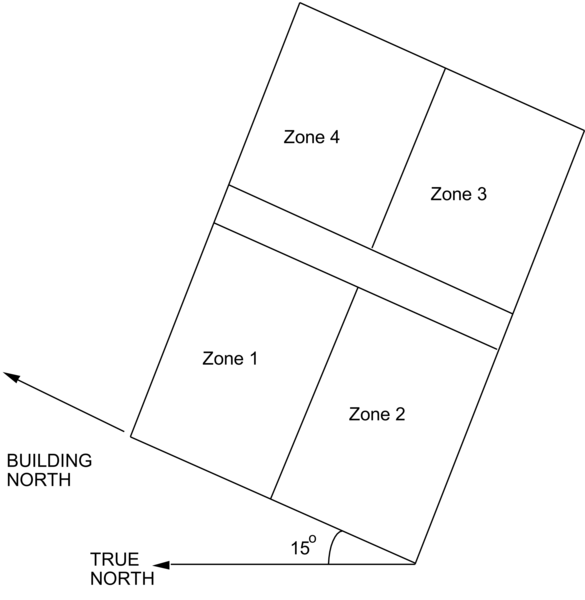
\includegraphics[width=0.9\textwidth, height=0.9\textheight, keepaspectratio=true]{media/image001.png}
\caption{Illustration of Building North Axis \protect \label{fig:illustration-of-building-north-axis}}
\end{figure}

\paragraph{Field: Terrain}\label{field-terrain}

The site's terrain affects how the wind hits the building -- as does the building height. In addition, the external conduction method usually has its own parameters for the calculation. Please see the Engineering Documentation, External Conduction section for particulars. The legal values for this field are shown in the following table.

% table 1
\begin{longtable}[c]{@{}ll@{}}
\caption{Values for ``Terrain'' \label{table:values-for-terrain}} \tabularnewline
\toprule
Terrain Type Value & Terrain Description \tabularnewline
\midrule
\endfirsthead

\caption[]{Values for ``Terrain''} \tabularnewline
\toprule
Terrain Type Value & Terrain Description \tabularnewline
\midrule
\endhead

Country & Flat, Open Country \tabularnewline
Suburbs & Rough, Wooded Country, Suburbs \tabularnewline
City & Towns, city outskirts, center of large cities \tabularnewline
Ocean & Ocean, Bayou flat country \tabularnewline
Urban & Urban, Industrial, Forest \tabularnewline
\bottomrule
\end{longtable}

\paragraph{Warmup Convergence}\label{warmup-convergence}

The following two fields along with the minimum and maximum number of warmup days (also in this object) define the user specified criteria for when EnergyPlus will ``converge'' at each environment (each sizing period or run period set as Yes in the \hyperref[simulationcontrol]{SimulationControl} object). EnergyPlus ``runs'' the first day of the environment (starting with a set of hard-coded initial conditions: temperatures are initialized to 23C and zone humidity ratios are initialized to the outdoor humidity ratio) until the loads/temperature convergence tolerance values are satisfied (next two fields) or until it reaches ``maximum number of warmup days''. Note that setting the convergence tolerance values too loose will cause the program to be satisfied too early and you may not get the results you expect from the actual simulation.

\paragraph{Field: Loads Convergence Tolerance Value}\label{field-loads-convergence-tolerance-value}

This value represents the number at which the loads values must agree before ``convergence'' is reached. Loads tolerance value is a fraction of the load.

\paragraph{Field: Temperature Convergence Tolerance Value}\label{field-temperature-convergence-tolerance-value}

This value represents the number at which the zone temperatures must agree (from previous iteration) before ``convergence'' is reached. (Units for this field is delta C).

Convergence of the simultaneous heat balance/HVAC solution is reached when either the loads or temperature criterion is satisfied.

All tolerances have units so the temperature tolerance is in degrees C (or degrees K) and the loads tolerance is in Watts. Both tolerances work the same way, just one looks at temperatures and one looks at heating and cooling loads. After the second warm-up day, the program compares the maximum temperature experienced in a space with the maximum temperature from the previous day. If those two temperatures are within the tolerance, then it has passed the first warm-up check.

It does a similar comparison with lowest temperatures experience within all the zones. If the current simulation day and the previous day values are within the tolerance, then it has passed the second warm-up check. Similar things are done with the loads tolerance and the maximum heating and cooling loads that are experienced within the spaces. Those are compared individually to the values for the previous day. If they are both in tolerance, then the simulation has passed the third and fourth warm-up check. The simulation stays in the warm-up period until ALL FOUR checks have been passed. See Engineering Reference and Output Details document for further explanation and outputs.

Please note--other ``convergence tolerance'' inputs are required for certain HVAC equipment (unit ventilator, unit heater, window AC, etc.). The purpose and units of these parameters are different from ``load convergence tolerance'' and ``temperature convergence tolerance'' in the BUILDING object.

\paragraph{Field: Solar Distribution}\label{field-solar-distribution}

Setting this value determines how EnergyPlus treats beam solar radiation and reflectances from exterior surfaces that strike the building and, ultimately, enter the zone. There are five choices: \textbf{MinimalShadowing}, \textbf{FullExterior} and \textbf{FullInteriorAndExterior, FullExteriorWithReflections, FullInteriorAndExteriorWithReflections}.

\textbf{MinimalShadowing}

In this case, there is no exterior shadowing except from window and door reveals. All beam solar radiation entering the zone is assumed to fall on the floor, where it is absorbed according to the floor's solar absorptance. Any reflected by the floor is added to the transmitted diffuse radiation, which is assumed to be uniformly distributed on all interior surfaces. If no floor is present in the zone, the incident beam solar radiation is absorbed on all interior surfaces according to their absorptances. The zone heat balance is then applied at each surface and on the zone's air with the absorbed radiation being treated as a flux on the surface.

\textbf{FullExterior, FullExteriorWithReflections}

In this case, shadow patterns on exterior surfaces caused by detached shading, wings, overhangs, and exterior surfaces of all zones are computed. As for MinimalShadowing, shadowing by window and door reveals is also calculated. Beam solar radiation entering the zone is treated as for MinimalShadowing -- All beam solar radiation entering the zone is assumed to fall on the floor, where it is absorbed according to the floor's solar absorptance. Any reflected by the floor is added to the transmitted diffuse radiation, which is assumed to be uniformly distributed on all interior surfaces. If no floor is present in the zone, the incident beam solar radiation is absorbed on all interior surfaces according to their absorptances. The zone heat balance is then applied at each surface and on the zone's air with the absorbed radiation being treated as a flux on the surface.

\textbf{FullInteriorAndExterior, FullInteriorAndExteriorWithReflections}

This is the same as FullExterior except that instead of assuming all transmitted beam solar falls on the floor the program calculates the amount of beam radiation falling on each surface in the zone, including floor, walls and windows, by projecting the sun's rays through the exterior windows, taking into account the effect of exterior shadowing surfaces and window shading devices.

If this option is used, you should be sure that the surfaces of the zone totally enclose a space. This can be determined by viewing the \textbf{eplusout.dxf} file with a program like AutoDesk's Volo View Express. You should also be sure that the zone is \textbf{convex}. Examples of convex and non-convex zones are shown in Figure~\ref{fig:illustration-of-convex-and-non-convex-zones}. The most common non-convex zone is an L-shaped zone. (A formal definition of convex is that any straight line passing through the zone intercepts at most two surfaces.) If the zone's surfaces do not enclose a space or if the zone is not convex you should use Solar Distribution = \textbf{FullExterior} instead of \textbf{FullInteriorAndExterior}.

If you use \textbf{FullInteriorAndExterior} the program will also calculate how much beam radiation falling on the inside of an exterior window (from other windows in the zone) is absorbed by the window, how much is reflected back into the zone, and how much is transmitted to the outside. In this calculation the effect of a shading device, if present, is accounted for.

\begin{figure}[hbtp] % fig 2
\centering
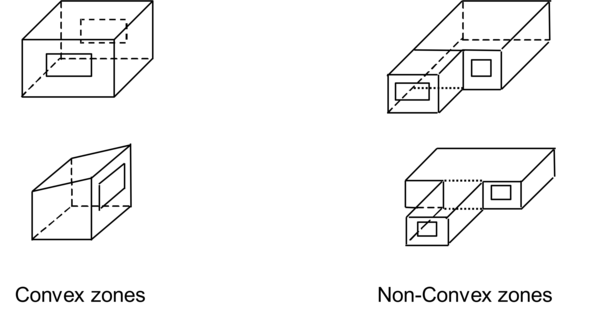
\includegraphics[width=0.9\textwidth, height=0.9\textheight, keepaspectratio=true]{media/image002.png}
\caption{Illustration of Convex and Non-convex Zones \protect \label{fig:illustration-of-convex-and-non-convex-zones}}
\end{figure}

\textbf{Reflection calculations}

Note: Using the reflection calculations can be very time-consuming. Even error-prone. As a possible alleviation, you can use the \hyperref[outputdiagnostics]{Output:Diagnostics},DoNotMirrorDetachedShading; in many cases to get past a fatal error.

If using reflections, the program calculates beam and sky solar radiation that is reflected from exterior surfaces and then strikes the building. These reflecting surfaces fall into three categories:

1) \textbf{Shadowing surfaces}. These are surfaces like overhangs or neighboring buildings entered with Shad\-ing:\-Site, Shad\-ing:\-Build\-ing, Shad\-ing:\-Site:\-Detailed, Shad\-ing:\-Build\-ing:\-Detailed, Shad\-ing:\-Over\-hang, Shad\-ing:\-Over\-hang:Pro\-jection, Shad\-ing:\-Fin, Shad\-ing:\-Fin:\-Pro\-jection or Shad\-ing:\-Zone:\-Detailed objects. See Figure~\ref{fig:solar-reflection-from-shadowing-surfaces.}.

These surfaces can have diffuse and/or specular (beam-to-beam) reflectance values that are specified with the Shad\-ing\-Property:\-Re\-flectance object which specifies those parameters. They have a default value of .2 for both visible and diffuse reflection.

2) \textbf{Exterior building surfaces}. In this case one section of the building reflects solar radiation onto another section (and vice-versa). See Figure~\ref{fig:solar-reflection-from-building-surfaces-onto}.

The building surfaces are assumed to be diffusely reflecting if they are opaque (walls, for example) and specularly reflecting if they are windows or glass doors. The reflectance values for opaque surfaces are calculated by the program from the Solar Absorptance and Visible Absorptance values of the outer material layer of the surface's construction (ref: Material object properties). The reflectance values for windows and glass doors are calculated by the program from the reflectance properties of the individual glass layers that make up surface's construction assuming no shading device is present and taking into account inter-reflections among the layers (ref: Window Properties).

3) \textbf{The ground surface}. Reflection from the ground is calculated even if reflections option is not used;l but then the ground plane is considered unobstructed, i.e., the shadowing of the ground by the building itself or by obstructions such as neighboring buildings is ignored. Shadowing by the building itself or neighboring buildings is taken into account when the ``with reflections'' option is used but then the ``view factor to ground'' is NOT used. This is shown in Figure~\ref{fig:shadowing-from-building-affects-beam-solar}.

\begin{figure}[hbtp] % fig 3
\centering
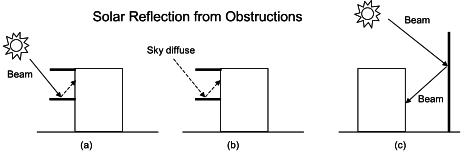
\includegraphics[width=0.9\textwidth, height=0.9\textheight, keepaspectratio=true]{media/image003.png}
\caption{  Solar reflection from shadowing surfaces. Solid arrows are beam solar radiation; dashed arrows are diffuse solar radiation. (a) Diffuse reflection of beam solar radiation from the top of an overhang. (b) Diffuse reflection of sky solar radiation from the top of an overhang. (c) Beam-to-beam (specular) reflection from the façade of an adjacent highly-glazed building represented by a vertical shadowing surface. \protect \label{fig:solar-reflection-from-shadowing-surfaces.}}
\end{figure}

\begin{figure}[hbtp] % fig 4
\centering
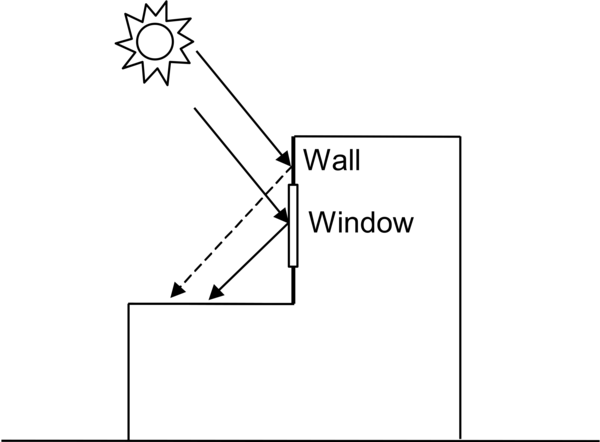
\includegraphics[width=0.9\textwidth, height=0.9\textheight, keepaspectratio=true]{media/image004.png}
\caption{  Solar reflection from building surfaces onto other building surfaces. In this example beam solar reflects from a vertical section of the building onto a roof section. The reflection from the window is specular. The reflection from the wall is diffuse. \protect \label{fig:solar-reflection-from-building-surfaces-onto}}
\end{figure}

\begin{figure}[hbtp] % fig 5
\centering
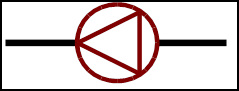
\includegraphics[width=0.9\textwidth, height=0.9\textheight, keepaspectratio=true]{media/image005.png}
\caption{Shadowing from building affects beam solar reflection from the ground. Beam-to-diffuse reflection from the ground onto the building occurs only for sunlit areas, A and C, not from shaded area, B. \protect \label{fig:shadowing-from-building-affects-beam-solar}}
\end{figure}

\paragraph{Field: Maximum Number of Warmup Days}\label{field-maximum-number-of-warmup-days}

This field specifies the number of ``warmup'' days that might be used in the simulation before ``convergence'' is achieved. The default number, 25, is usually more than sufficient for this task; however, some complex buildings (with complex constructions) may require more days. If you enter less than 25 as a maximum, that is the number of maximum warmup days that will be used. An error message will occur when the simulation ``runs'' out of days and has not converged:

\begin{lstlisting}
CheckWarmupConvergence: Loads Initialization, Zone = "MAIN ZONE" did not converge after 30 warmup days.
See Warmup Convergence Information in .eio file for details
..Environment(SizingPeriod) = "DENVER CENTENNIAL  GOLDEN   N ANN CLG 1% CONDNS DB = >MWB"
..Max Temp Comparison = 2.06E-002 vs Temperature Convergence Tolerance = 0.50 – Pass Convergence
..Min Temp Comparison = 5.95E-003 vs Temperature Convergence Tolerance = 0.50 – Pass Convergence
..Max Cool Load Comparison = 9.5082E-002 vs Loads Convergence Tolerance = 5.00E-002 – Fail Convergence
\end{lstlisting}

As noted in the message, there will be more information in the .eio file. (Refer to Output Details document as well for examples.)

You may be able to increase the Maximum Number of Warmup Days and get convergence, but some anomalous buildings may still not converge. Simulation proceeds for x warmup days until ``convergence'' is reached (see the discussion under the Temperature Convergence Tolerance Value field in this object, just above).

\paragraph{Field: Minimum Number of Warmup Days}\label{field-minimum-number-of-warmup-days}

This field specifies the minimum number of ``warmup'' days before EnergyPlus will check if it has achieved convergence and can thus start simulating the particular environment (design day, annual run) in question. Research into the minimum number of warmup days indicates that 6 warmup days is generally enough on the minimum end of the spectrum to avoid false predictions of convergence and thus to produce enough temperature and flux history to start EnergyPlus simulation. This was based on a study that used the benchmark reference buildings. It also was observed that convergence performance improved when the number of warmup days increased. As a result, the default value for the minimum warmup days has been set to 6. Users should decrease this number only if they have knowledge that a specific file converges more quickly than 6 days. Users may wish to increase the value in certain situations when, based on the output variables described in the Output Details document, it is determined that EnergyPlus has not converged. While this parameter should be less than the previous parameter, a value greater than the value entered in the field ``Maximum Number of Warmup Days'' above may be used when users wish to increase warmup days more than the previous field. In this particular case, the previous field will be automatically reset to the value entered in this field and EnergyPlus will run exactly the number of warmup days specified in this field.

An example from an IDF:

\begin{lstlisting}

Building,
    PSI HOUSE DORM AND OFFICES,  !- Name
    36.87000,               !- North Axis {deg}
    Suburbs,                !- Terrain
    0.04,                   !- Loads Convergence Tolerance Value
    0.4000000,              !- Temperature Convergence Tolerance Value {deltaC}
    FullInteriorAndExterior, !- Solar Distribution
    40,                     !- Maximum Number of Warmup Days
    6;                      !- Minimum Number of Warmup Days
\end{lstlisting}

\subsection{SurfaceConvectionAlgorithm:Inside}\label{surfaceconvectionalgorithminside}

This input object is used control the choice of models used for surface convection at the inside face of all the heat transfer surfaces in the model. This object sets the selection for convection correlations in a global way. The Zone Inside Convection Algorithm input field in the Zone object may be used to selectively override this value on a zone-by-zone basis. Further, individual surfaces can refine the choice by each surface or surface lists -- see object \hyperref[surfacepropertyconvectioncoefficients]{SurfaceProperty:ConvectionCoefficients} and object \hyperref[surfacepropertyconvectioncoefficientsmultiplesurface]{SurfaceProperty:ConvectionCoefficients:MultipleSurface}.

\subsubsection{Inputs}\label{inputs-4-031}

\paragraph{Field: Algorithm}\label{field-algorithm-000}

The model specified in this field is the default algorithm for the inside face all the surfaces.. The key choices are \textbf{Simple}, \textbf{TARP}, \textbf{CeilingDiffuser}, and \textbf{AdaptiveConvectionAlgorithm}.

The \textbf{Simple} model applies constant heat transfer coefficients depending on the surface orientation.

The \textbf{TARP} model correlates the heat transfer coefficient to the temperature difference for various orientations. This model is based on flat plate experiments.

The \textbf{CeilingDiffuser} model is a mixed and forced convection model for ceiling diffuser configurations. The model correlates the heat transfer coefficient to the air change rate for ceilings, walls and floors. These correlations are based on experiments performed in an isothermal room with a cold ceiling jet. To avoid discontinuities in surface heat transfer rate calculations, all of correlations have been extrapolated beyond the lower limit of the data set (3 ACH) to a natural convection limit that is applied during the hours when the system is off.

The \textbf{AdaptiveConvectionAlgorithm} model is an dynamic algorithm that organizes a large number of different convection models and automatically selects the one that best applies. The adaptive convection algorithm can also be customized using the \hyperref[surfaceconvectionalgorithminsideadaptivemodelselections]{SurfaceConvectionAlgorithm:Inside:AdaptiveModelSelections} input object. These models are explained in detail in the EnergyPlus Engineering Reference Document.

The default is \textbf{TARP}.

IDF Example:

\begin{lstlisting}

SurfaceConvectionAlgorithm:Inside,TARP;
\end{lstlisting}

\subsection{SurfaceConvectionAlgorithm:Outside}\label{surfaceconvectionalgorithmoutside}

Various exterior convection models may be selected for global use. The optional Zone Outside Convection Algorithm input field in the Zone object may be used to selectively override this value on a zone-by-zone basis. Further, individual surfaces can refine the choice by each surface or surface lists -- see object \hyperref[surfacepropertyconvectioncoefficients]{SurfaceProperty:ConvectionCoefficients} and object \hyperref[surfacepropertyconvectioncoefficientsmultiplesurface]{SurfaceProperty:ConvectionCoefficients:MultipleSurface}.

\subsubsection{Inputs}\label{inputs-5-028}

\paragraph{Field: Algorithm}\label{field-algorithm-1-000}

The available key choices are \textbf{SimpleCombined}, \textbf{TARP}, \textbf{MoWiTT}, \textbf{DOE-2}, and \textbf{AdaptiveConvectionAlgorithm}.

The \textbf{Simple} convection model applies heat transfer coefficients depending on the roughness and windspeed. This is a combined heat transfer coefficient that includes radiation to sky, ground, and air. The correlation is based on Figure~\ref{fig:schematic-of-the-energyplus-unitary-system}, Page 25.1 (Thermal and Water Vapor Transmission Data), 2001 ASHRAE Handbook of Fundamentals. Note that if \textbf{Simple} is chosen here or in the Zone field and a \hyperref[surfacepropertyconvectioncoefficients]{SurfaceProperty:ConvectionCoefficients} object attempts to override the calculation with a different choice, the action will still be one of combined calculation. To change this, you must select one of the other methods for the global default.

All other convection models apply heat transfer coefficients depending on the roughness, windspeed, and terrain of the building's location. These are \emph{convection only} heat transfer coefficients; radiation heat transfer coefficients are calculated automatically by the program.

The \textbf{TARP} algorithm was developed for the TARP software and combines natural and wind-driven convection correlations from laboratory measurements on flat plates.

The \textbf{DOE-2} and \textbf{MoWiTT} were derived from field measurements. DOE-2 uses a correlation from measurements by Klems and Yazdanian for rough surfaces. MoWitt uses a correlation from measurements by Klems and Yazdanian for smooth surfaces and, therefore, is most appropriate for windows (see \hyperref[surfacepropertyconvectioncoefficientsmultiplesurface]{SurfaceProperty:ConvectionCoefficients:MultipleSurface} for how to apply to only windows).

The \textbf{AdaptiveConvectionAlgorithm} model is an dynamic algorithm that organizes a large number of different convection models and automatically selects the one that best applies. The adaptive convection algorithm can also be customized using the \hyperref[surfaceconvectionalgorithmoutsideadaptivemodelselections]{SurfaceConvectionAlgorithm:Outside:AdaptiveModelSelections} input object. All algorithms are described more fully in the Engineering Reference.

The default is \textbf{DOE-2}.

Note that when the surface is wet (i.e. it is raining and the surface is exposed to wind) then the convection coefficient appears as a very large number (1000) and the surface is exposed to the Outdoor Wet-bulb Temperature rather than the Outdoor Dry-bulb Temperature.

IDF Example:

\begin{lstlisting}

SurfaceConvectionAlgorithm:Outside, AdaptiveConvectionAlgorithm;
\end{lstlisting}

\subsection{HeatBalanceAlgorithm}\label{heatbalancealgorithm}

The HeatBalanceAlgorithm object provides a way to select what type of heat and moisture transfer algorithm will be used for calculating the performance of the building's surface assemblies. This input controls the overall algorithm used for all the surfaces unless one or more of the SurfaceProperty:HeatTransferAlgorithm:* objects are used to alter the selection for particular surfaces.

\subsubsection{Inputs}\label{inputs-6-025}

\paragraph{Field: Algorithm}\label{field-algorithm-2-000}

Four values are allowed to select which solution will be used.

\begin{itemize}
\item
  The \textbf{ConductionTransferFunction} selection is a sensible heat only solution and does not take into account moisture storage or diffusion in the construction elements.
\item
  The \textbf{MoisturePenetrationDepthConductionTransferFunction} selection is a sensible heat diffusion and an inside surface moisture storage algorithm that also needs additional moisture material property information. Sometimes, this is referred to as the Effective Moisture Penetration Depth or EMPD. See the moisture material property object for additional information and description of outputs:
  \begin{itemize}
  \item
    \hyperref[materialpropertymoisturepenetrationdepthsettings]{MaterialProperty:MoisturePenetrationDepth:Settings}
  \end{itemize}
\item
  \textbf{Advanced/Research usage:}The \textbf{ConductionFiniteDifference} selection is a sensible heat only solution and does not take into account moisture storage or diffusion in the construction elements. This solution technique uses a 1-D finite difference solution in the construction elements. Outputs for the surfaces are described with the material property objects. The Conduction Finite Difference (aka CondFD) property objects are:
  \begin{itemize}
  \item
    \hyperref[materialpropertyphasechange]{MaterialProperty:PhaseChange}
  \item
    \hyperref[materialpropertyvariablethermalconductivity]{MaterialProperty:VariableThermalConductivity}
  \item
    \hyperref[materialpropertyphasechangehysteresis]{MaterialProperty:PhaseChangeHysteresis}
  \end{itemize}
\item
  \textbf{Advanced/Research usage:} The \textbf{CombinedHeatAndMoistureFiniteElement} is a coupled heat and moisture transfer and storage solution. The solution technique uses a one dimensional finite difference solution in the construction elements and requires further material properties described in the Heat and Moisture Transfer material properties objects. Outputs from the algorithm are described with these objects. The Heat and Moisture Transfer property objects are:
  \begin{itemize}
  \item
    \hyperref[materialpropertyheatandmoisturetransfersettings]{MaterialProperty:HeatAndMoistureTransfer:Settings}
  \item
    \hyperref[materialpropertyheatandmoisturetransfersorptionisotherm]{MaterialProperty:HeatAndMoistureTransfer:SorptionIsotherm}
  \item
    \hyperref[materialpropertyheatandmoisturetransfersuction]{MaterialProperty:HeatAndMoistureTransfer:Suction}
  \item
    \hyperref[materialpropertyheatandmoisturetransferredistribution]{MaterialProperty:HeatAndMoistureTransfer:Redistribution}
  \item
    \hyperref[materialpropertyheatandmoisturetransferdiffusion]{MaterialProperty:HeatAndMoistureTransfer:Diffusion}
  \item
    \hyperref[materialpropertyheatandmoisturetransferthermalconductivity]{MaterialProperty:HeatAndMoistureTransfer:ThermalConductivity}
  \end{itemize}
\end{itemize}

\paragraph{Field: Surface Temperature Upper Limit}\label{field-surface-temperature-upper-limit}

This field is a bit ``advanced''. It should only be used when the simulation fails AND you cannot determine a cause for the failure. That is, you receive an error similar to:

\begin{lstlisting}
   ** Severe  ** Temperature out of bounds (202.91) for surface = Wall1
   **   ~~~   ** in Zone = Zone01
   **   ~~~   **  Occurrence info = NEW YORK CITY NY SUMMER, 07/21 16:00 - 16:01
   **   ~~~   ** A temperature out of bounds problem can be caused by several things.  The user
   **   ~~~   ** should check the weather environment, the level of internal gains with respect
   **   ~~~   ** to the zone, and the thermal properties of their materials among other things.
   **   ~~~   ** A common cause is a building with no thermal mass -- all materials with
   **   ~~~   ** Regular-R definitions.
\end{lstlisting}

And, after careful perusal, you cannot find a solution as suggested in the error description. You may then want to enter a higher number than the default for this field.

\paragraph{Field: Minimum Surface Convection Heat Transfer Coefficient Value}\label{field-minimum-surface-convection-heat-transfer-coefficient-value}

This optional field is used to set an overall minimum for the value of the coefficient for surface convection heat transfer (Hc) in W/m2-K. A minimum is necessary for numerical robustness because some correlations for Hc can result in zero values and create numerical problems. This field can be used to support specialized validation testing to suppress convection heat transfer and to investigate the implications of different minimum Hc values. The default is 0.1.

\paragraph{Field: Maximum Surface Convection Heat Transfer Coefficient Value}\label{field-maximum-surface-convection-heat-transfer-coefficient-value}

This optional field is used to set an overall maximum for the value of the coefficient for surface convection heat transfer (Hc) in W/m2-K. High Hc values are used in EnergyPlus to approximate fixed surface temperature boundary conditions. This field can be used to alter the accepted range of user-defined Hc values.

And, a default IDF example

\begin{lstlisting}
HeatBalanceAlgorithm,ConductionTransferFunction; ! Solution Algorithm
\end{lstlisting}

\subsection{HeatBalanceSettings:ConductionFiniteDifference}\label{heatbalancesettingsconductionfinitedifference}

This object is used to control the behavior of the Conduction Finite Difference algorithm for surface heat transfer. The settings are global and affect how the model behaves for all the surfaces.

\subsubsection{Inputs}\label{inputs-7-025}

\paragraph{Field: Difference Scheme}\label{field-difference-scheme}

This field determines the solution scheme used by the Conduction Finite Difference model. There are two options CrankNicholsonSecondOrder and FullyImplicitFirstOrder. The CrankNicholsonSecondOrder scheme is second order in time and may be faster. But it can be unstable over time when boundary conditions change abruptly and severely. The FullyImplicitFirstOrder scheme is first order in time and is more stable over time. But it may be slower. The default is FullyImplicitFirstOrder when ConductionFiniteDifference is selected as the Heat Balance Algorithm.

\paragraph{Field: Space Discretization Constant}\label{field-space-discretization-constant}

This field controls how the model determines spatial discretization, or the count of nodes across each material layer in the construction. The model calculates the nominal distance associated with a node, \(\Delta x\), using

\begin{equation}
\Delta x = \sqrt {C\alpha \Delta t}
\end{equation}

Where

\(\alpha\) is the thermal diffusivity of the material layer, in m\(^{2}\)/s

\(\Delta t\) is the length of the timestep in seconds.

\emph{C} is a constant set by this field.

The default is 3. Typical values are from 1 to 3. Lower values for this constant lead to more nodes and finer-grained space discretization.

\paragraph{Field: Relaxation Factor}\label{field-relaxation-factor}

The finite difference solver includes under-relaxation for improved stability for interactions with the other surfaces. This input field can optionally be used to modify the starting value for the relaxation factor. Larger numbers may solve faster, while smaller numbers may be more stable. The default is 1.0. If the program detects numerical instability, it may reduce the value entered here to something lower and more stable.

\paragraph{Field: Inside Face Surface Temperature Convergence Criteria}\label{field-inside-face-surface-temperature-convergence-criteria}

The surface heat balance model at the inside face has a numerical solver that uses a convergence parameter for a maximum allowable differences in surface temperature. This field can optionally be used to modify this convergence criteria. The default value is 0.002 and was selected for stability. Lower values may further increase stability at the expense of longer runtimes, while higher values may decrease runtimes but lead to possible instabilities. The units are in degrees Celsius.

An example IDF object follows.

\begin{lstlisting}
HeatBalanceSettings:ConductionFiniteDifference,
  FullyImplicitFirstOrder, !- Difference Scheme
  3.0,                     !- Space Discretization Constant
  1.0,                     !- Relaxation Factor
  0.002;                   !- Inside Face Surface Temperature Convergence Criteria
\end{lstlisting}

\subsection{ZoneAirHeatBalanceAlgorithm}\label{zoneairheatbalancealgorithm}

The ZoneAir\hyperref[heatbalancealgorithm]{HeatBalanceAlgorithm} object provides a way to select what type of solution algorithm will be used to calculate zone air temperatures and humidity ratios. This object is an optional object. If the default algorithm is used, this object is not required in an input file.

\subsubsection{Inputs}\label{inputs-8-023}

\paragraph{Field: Algorithm}\label{field-algorithm-3-000}

Three choices are allowed to select which solution algorithm will be used. The \textbf{ThirdOrderBackwardDifference} selection is the default selection and uses the third order finite difference approximation to solve the zone air energy and moisture balance equations. The \textbf{AnalyticalSolution} selection uses the integration approach to solve the zone air energy and moisture balance equations. The \textbf{EulerMethod} selection uses the first order finite backward difference approximation to solve the zone air energy and moisture balance equations.

And, a default IDF example is shown below:

\begin{lstlisting}
ZoneAirHeatBalanceAlgorithm, ThirdOrderBackwardDifference; !- Algorithm
\end{lstlisting}

\subsection{ZoneAirContaminantBalance}\label{zoneaircontaminantbalance}

The ZoneAirContaminantBalance object provides a way to select which contaminant type will be simulated. Although carbon dioxide is not considered as an indoor contaminant but it is used as an indicator of indoor air quality in buildings. From modeling point of view EnergyPlus treats carbon dioxide as a type of contaminant. In addition to carbon dioxide, a generic contaminant type model was also added. This object is optional, only required in the input data file if the user wishes to model contaminant concentration levels as part of their simulation.

\subsubsection{Inputs}\label{inputs-9-021}

\paragraph{Field: Carbon Dioxide Concentration}\label{field-carbon-dioxide-concentration}

Input is Yes or No. The default is No. If Yes, simulation of carbon dioxide concentration levels will be performed. If No, simulation of carbon dioxide concentration levels will not be performed.

\paragraph{Field: Outdoor Carbon Dioxide Schedule Name}\label{field-outdoor-carbon-dioxide-schedule-name}

This field specifies the name of a schedule that contains outdoor air carbon dioxide level values in units of ppm. One source of monthly average CO\(_{2}\) levels in the atmosphere is available at \href{http://www.esrl.noaa.gov/gmd/ccgg/trends/}{NOAA's website} or via \href{ftp://aftp.cmdl.noaa.gov/products/trends/co2/co2_mm_mlo.txt}{ftp}.

\paragraph{Field: Generic Contaminant Concentration}\label{field-generic-contaminant-concentration}

Input is Yes or No. The default is No. If Yes, simulation of generic contaminant concentration levels will be performed. If No, simulation of generic contaminant concentration levels will not be performed.

\paragraph{Field: Outdoor Generic Contaminant Schedule Name}\label{field-outdoor-generic-contaminant-schedule-name}

This field specifies the name of a schedule that contains outdoor air generic contaminant level values in units of ppm.

An IDF example:

\begin{lstlisting}
ZoneAirContaminantBalance,
  Yes,                          !- Carbon Dioxide Concentration
  Outdoor CO2 Schedule,         !- Outdoor Carbon Dioxide Schedule Name
  Yes,                          !- Generic Contaminant Concentration
  Generic Contaminant Schedule; !- Outdoor Generic Contaminant Schedule Name
\end{lstlisting}

\subsubsection{Outputs}\label{outputs-033}

The following output variables are available when Carbon Dioxide Concentration = Yes.

\begin{lstlisting}
HVAC,Average,Zone Air CO2 Internal Gain Volume Flow Rate
HVAC,Average,Zone Air CO2 Concentration [ppm]
\end{lstlisting}

\paragraph{Zone Air CO2 Concentration {[}ppm{]}}\label{zone-air-co2-concentration-ppm}

This output variable represents the carbon dioxide concentration level in parts per million (ppm) for each zone. This is calculated and reported from the Correct step in the Zone Air Contaminant Predictor-Corrector module.

\paragraph{Zone Air CO2 Internal Gain Volume Flow Rate {[}m3/s{]}}\label{zone-air-co2-internal-gain-volume-flow-rate-m3s}

This is the rate of carbon dioxide added to a zone from all types of sources or sinks, in m\(^{3}\)/s.

\subsubsection{Outputs}\label{outputs-1-024}

The following output variable is available when Generic Contaminant Concentration = Yes.

HVAC,Average,Zone Generic Air Contaminant Generation Volume Flow Rate {[}m3/s{]}

HVAC,Average,Zone Air Generic Air Contaminant Concentration {[}ppm{]}

\paragraph{Zone Air Generic Air Contaminant Concentration {[}ppm{]}}\label{zone-air-generic-air-contaminant-concentration-ppm}

This output variable represents the generic contaminant concentration level in parts per million (ppm) for each zone. This is calculated and reported from the Correct step in the Zone Air Contaminant Predictor-Corrector module.

\paragraph{Zone Generic Air Contaminant Generation Volume Flow Rate {[}m3/s{]}}\label{zone-generic-air-contaminant-generation-volume-flow-rate-m3s}

This is the rate of generic air contaminant added (or subtracted) to a zone from all types of sources or sinks.

\subsection{ShadowCalculation}\label{shadowcalculation}

This object is used to control some details of EnergyPlus's solar, shadowing and daylighting models. There are two basic methods available for the calculations. In order to speed up the calculations, shadowing calculations (sun position, etc.) for the default method are performed over a period of days. Note that this value may be very important for determining the amount of sun entering your building and by inference the amount of cooling or heating load needed for maintaining the building. Though termed ``shadowing'' calculations, it in affect determines the sun position for a particular day in a weather file period simulation. (Each design day will use the date of the design day object). Even though weather file data contains the amount of solar radiation, the internal calculation of sun position will govern how that affects various parts of the building. By default, the calculations are done for every 20 days throughout a weather run period; an average solar position is chosen and the solar factors (such as sunlit areas of surfaces) remain the same for that number of days. When more integrated calculations are needed for controlling dynamic windows or shades, a second method is available where solar calculations are performed at each zone timestep.

This object also allows setting up global flags to import and export exterior shading calculations results. This enables importing pre-calculated results of the shading fractions for each exterior building surface from external simulation tools. This also enables reusing the shading results for parametric runs which usually do not change external shading.

The object also allows input to disable self-shading effect from exterior surfaces from all zones, or from a subset of zones. Two flags are defined to enable the maximal flexibility of various interpretation of self-shading: one to disable shading between zones of a same zone group, the other to disable shading between different zone groups. The shading by exterior surfaces of the specified zones groups will be bypassed.

\subsubsection{Inputs}\label{inputs-10-019}

\paragraph{Field: Calculation Method}\label{field-calculation-method-000}

This field is used to control how the solar, shading, and daylighting models are calculated with respect to the time of calculations during the simulation. The default and fastest method is selected using the keyword AverageOverDaysInFrequency. A more detailed and slower method can be selected using the keyword TimestepFrequency. The TimestepFrequency method must be used for modeling dynamic fenestration and shading surfaces.

\paragraph{Field: Calculation Frequency}\label{field-calculation-frequency}

This numeric field will cause the shadowing calculations to be done periodically using the number in the field as the number of days in each period. This field is only used if the default method AverageOverDaysInFrequency is used in the previous field. Using this field will allow you to synchronize the shadowing calculations with changes in shading devices. Using the default of 20 days in each period is the average number of days between significant changes in solar position angles. For these shadowing calculations, an ``average'' (over the time period) of solar angles, position, equation of time are also used.

\paragraph{Field: Maximum Figures in Shadow Overlap Calculations}\label{field-maximum-figures-in-shadow-overlap-calculations}

This numeric field will allow you to increase the number of figures in shadow overlaps. Due to the shadowing algorithm, the number of shadows in a figure may grow quite large even with fairly reasonable looking structures. Of course, the inclusion of more allowed figures will increase calculation time. Likewise, too few figures may not result in as accurate calculations as you desire.

\paragraph{Field: Polygon Clipping Algorithm}\label{field-polygon-clipping-algorithm}

This is an advanced feature. Prior to V7, the internal polygon clipping method was a special case of the Weiler-Atherton method. Now, two options are available: \textbf{SutherlandHodgman} (default) and \textbf{ConvexWeilerAtherton}. Theoretically, Sutherland-Hodgman is a simpler algorithm but it works well in cases where receiving surfaces (of shadows) are non-convex. The Weiler-Atherton implementation is only accurate where both casting and receiving surfaces are convex. Warnings/severe errors are displayed when necessary. More details on polygon clipping are contained in the Engineering Reference.

\paragraph{Field: Sky Diffuse Modeling Algorithm}\label{field-sky-diffuse-modeling-algorithm}

Two choices are available here: SimpleSkyDiffuseModeling and DetailedSkyDiffuseModeling. \textbf{SimpleSkyDiffuseModeling} (default) performs a one-time calculation for sky diffuse properties. This has implications if you have shadowing surfaces with changing transmittance (i.e. not all opaque or not all transparent) during the year. The program checks to see if this might be the case and automatically selects \textbf{DetailedSkyDiffuseModeling} if the shading transmittance varies. Even if the transmittance doesn't vary and the option for detailed modeling is used, that option is retained (though it will increase execution time) because you may be using EMS to vary the transmittance. When the detailed modeling is done, there will be a warning posted if the Calculation Frequency (above) is \textgreater{} 1.

In general (and you should also read the previous field description), if shadowing surfaces are used with the transmittance property, the user should be careful to synchronize this calculation with the scheduled occurrence of the transmittance (if any) (or use 1, which will be the most accurate but will cause more time in the calculations).

This field applies to the method called ``AverageOverDaysInFrequency.'' When the method called ``DetailedTimestepIntegration'' is used the diffuse sky modeling always uses DetailedSkyDiffuseModeling.

\paragraph{Field: External Shading Calculation Method}\label{field-external-shading-calculation-method}

The field has three options: \textbf{ScheduledShading}, \textbf{ImportedShading} and \textbf{InternalCalculation}. The field indicates whether the external shading is pre-calculated and imported as schedules, which overwrite the EnergyPlus calculated array of the surface sunlit fraction. If \textbf{ScheduledShading} or \textbf{ImportedShading} is chosen, all external shading calculation would be performed externally (EnergyPlus internal calculations of external shading will be turned off).

If \textbf{ScheduledShading} is chosen, the shading calculation results are imported during the initialization of an EnergyPlus run with the schedule object defined by the \textbf{\hyperref[surfacePropertylocalEnvironment]{SurfaceProperty:LocalEnvironment}} object of this surface. If some exterior surfaces do not have their \textbf{\hyperref[surfacePropertylocalEnvironment]{SurfaceProperty:LocalEnvironment}} objects, no shading is assigned on those exterior surfaces.

If \textbf{ImportedShading} is chosen, a \textbf{\hyperref[schedulefileshading]{Schedule:File:Shading}} object is required to define the external file that stores all shading calculation results. The results are imported altogether by reading the \textbf{\hyperref[schedulefileshading]{Schedule:File:Shading}} object during initialization. The file explicitly defines the mappings to the surfaces. If the data for a surface is not listed in the file, no shading is assigned on this surface.

The default choice is \textbf{InternalCalculation}, indicating EnergyPlus will do the external shading calculations and no external results will be used.

The sunlit fraction to overwrite accounts for the shading of both direct and sky diffuse solar radiation caused by all exterior shadowing surfaces. In this case, shadow patterns on exterior surfaces caused by detached shading, side-fins, overhangs, and exterior surfaces of all zones are overwritten. The interior shading devices, such as window shades and blinds, should be further calculated and applied after the importing.

\paragraph{Field: Output External Shading Calculation Results}\label{field-output-external-shading-calculation results}
This fields indicates whether or not (\textbf{Yes} or \textbf{No})to save internal shading calculation results to an external file, which can be imported back as needed. This file saves external sunlit fractions for all surfaces. If \textbf{Yes} is chosen, hourly shading fraction of all surfaces will be exported as a CSV file, naming as "output file prefix + shading" (the default name is "eplusshading.csv" if no output file prefix is defined). Each column of the CSV file lists the annually calculated shading fraction of each surface with time-step interval. It only writes data for each simulation day that shadows are calculated, e.g. once every 20 days by default. If the results are intended to be reused to be imported  back using \textbf{ImportedShading} in \textbf{Field: External Shading Calculation Method}, the Calculation Frequency should be set as one to write year-round hourly results. Design days are not included. The default choice is \textbf{No}.

\paragraph{Field: Disable Self-Shading Within Shading Zone Groups}\label{fieldself--disable-shading-within-a-zone-group}
This fields specifies during shading calculation, for all surfaces in a targeted Zone Group, whether or not (\textbf{Yes} or \textbf{No} ) the self-shading effect by exterior surfaces of all zones within the target Zone Group is disabled. If Yes, self-shading will be disabled from all exterior surfaces in a given Shading Zone Group to surfaces within the same Shading Zone Group. If both Disable Self-Shading Within Shading Zone Groups and Disable Self-Shading From Shading Zone Groups to Other Zones = Yes, then all self-shading from exterior surfaces will be disabled.If only one of these fields = Yes, then at least one Shading Zone Group must be specified, or this field will be ignored. Shading from Shading:* surfaces, overhangs, fins, and reveals will not be disabled.

\paragraph{Field: Disable Self-Shading From Shading Zone Groups to Other Zones}\label{field-self-disable-shading-between-zone-groups}
This fields specifies during shading calculation, for all surfaces in a targeted Zone Group, whether or not (\textbf{Yes} or \textbf{No} ) the self-shading effect from all exterior surfaces in the target Zone Group to other zones is disabled. If Yes, self-shading will be disabled from all exterior surfaces in a given Shading Zone Group to all other zones in the model. If both Disable Self-Shading Within Shading Zone Groups and Disable Self-Shading From Shading Zone Groups to Other Zones = Yes, then all self-shading from exterior surfaces will be disabled. If only one of these fields = Yes, then at least one Shading Zone Group must be specified, or this field will be ignored. Shading from Shading:* surfaces, overhangs, fins, and reveals will not be disabled.

\paragraph{Field: Shading Zone Group ZoneList Name}\label{field-shading-zone-group-zoneList-name}
The shading zones group specifies group of zones which are controlled by the Disable Self-Shading fields.
This field is extensible.

Examples of this object in IDF: (note this object must be unique in an IDF)

\begin{lstlisting}
ShadowCalculation,AverageOverDaysInFrequency,1;

ShadowCalculation, AverageOverDaysInFrequency, 1, , SutherlandHodgman, DetailedSkyDiffuseModeling;

ShadowCalculation, AverageOverDaysInFrequency, , , , , ScheduledShading, YES;

ShadowCalculation, AverageOverDaysInFrequency, , , , , , , , Yes, No, ShadingZoneGroup;
\end{lstlisting}

Note that the use of ``1'' in the examples is NOT the same as using DetailedTimestepIntegration -- ``1'' causes daily calculation of the sun position variables but does not change the shadowing calculations more frequently than daily.

\subsection{Output:Diagnostics}\label{outputdiagnostics}

Sometimes, messages only confuse users -- especially new users. Likewise, sometimes certain output variables exist for only a certain condition but some take them at face value/name. Some features may be very important but under certain instances cause problems. Thus, we have added the \textbf{diagnostic output} object to be able to turn on or off certain messages, variables, and features depending on conditions.

Both fields of the Output:Diagnostics command can accept all the applicable keys. More than one object may be entered.

\subsubsection{Inputs}\label{inputs-11-018}

\paragraph{Field: key1, key2}\label{field-key1-key2}

Allowable choices are:

\textbf{DisplayAllWarnings} -- use this to get all warnings (except the developer warnings ``DisplayZoneAirHeatBalanceOffBalance''). This key sets all other display warning values to on.

\textbf{DisplayExtraWarnings} -- use this to get all extra warnings. An example of an extra warning is when a user enters a ceiling height or volume with the Zone object and EnergyPlus calculates something significantly different based on the entered zone geometry.

\textbf{DisplayUnusedSchedules} -- use this to have the unused schedules (by name) listed at the end of the simulation.

\textbf{DisplayUnusedObjects} -- use this to have unused (orphan) objects (by name) listed at the end of the simulation.

\textbf{DisplayAdvancedReportVariables} -- use this to be able to use certain advanced output variables where the name may be misleading and you need to understand the concepts or reasons for use. If you put in this field, then you will be able to report on these features. They are noted in the descriptions of objects or output variables.

\textbf{DisplayZoneAirHeatBalanceOffBalance} -- this is a developer diagnostic which you can turn on, if you desire.

\textbf{DoNotMirrorDetachedShading} -- use this to turn off the automatic mirroring of detached shading surfaces. These surfaces are automatically mirrored so that the user does not need to worry about facing direction of the surface and the shading surface will shade the building as appropriate.

\textbf{DoNotMirrorAttachedShading} -- use this to turn off the automatic mirroring of attached shading surfaces. These surfaces are automatically mirrored so that the user does not need to worry about facing direction of the surface and the shading surface will shade the building as appropriate. Attached shading surfaces include \hyperref[shadingoverhang]{Shading:Overhang}, \hyperref[shadingoverhangprojection]{Shading:Overhang:Projection}, \hyperref[shadingfin]{Shading:Fin}, \hyperref[shadingfinprojection]{Shading:Fin:Projection}, and \hyperref[shadingzonedetailed-000]{Shading:Zone:Detailed}.

\textbf{DisplayWeatherMissingDataWarnings} -- use this to turn on the missing data warnings from the read of the weather file.

\textbf{ReportDuringWarmup} -- use this to allow reporting during warmup days. This can show you exactly how your facility is converging (or not) during the initial ``warmup'' days of the simulation. Generally, only developers or expert simulation users would need this kind of detail.

\textbf{ReportDetailedWarmupConvergence} -- use this to produce detailed reporting (essentially each warmup day for each zone) for warmup convergence.

\textbf{ReportDuringHVACSizingSimulation} -- use this to allow controlling reporting to SQLite database during sizing period simulations done for HVAC Sizing Simulation. The regular reporting is done in the usual way. This can show details of how advanced sizing adjustments were determined by documenting how the systems operated when doing the intermediate sizing periods. Depending on the number of iterations performed for HVAC Sizing Simulation, there will be a number of sets of results with each set containing all the Sizing Periods.

In IDF use:

\begin{lstlisting}
Output:Diagnostics,
  DisplayExtraWarnings;
\end{lstlisting}

\subsection{Output:DebuggingData}\label{outputdebuggingdata}

There may be times when a particular input file requires additional debugging. The Output:DebuggingData object may be used to report all available node data (e.g., temperature, mass flow rate, set point, pressure, etc.). The debug data is reported to the DBG text file. The debug file first reports the node number and name, and then all available node information for each zone time step (Ref. Timestep).

The 2 fields of the Output:DebuggingData object can accept either a 1 (turn on) or any other value (turn off). Only one object may be entered.

\subsubsection{Inputs}\label{inputs-12-017}

\paragraph{Field: Report Debugging Data}\label{field-report-debugging-data}

This field turns on debug reporting when a value of 1 is entered. Any other value (usually 0) disables debug reporting.

\paragraph{Field: Report During Warmup}\label{field-report-during-warmup}

This field allows the debug data to be reported during the warmup period. When a value of 1 is entered the data is reported at all times, even during warmup. Any other value (usually 0) disables ``reporting at all time'' and debug data is only reported for each environment (\hyperref[runperiod]{RunPeriod} or \hyperref[sizingperioddesignday]{SizingPeriod:DesignDay}).

In IDF use:

\begin{lstlisting}
Output:DebuggingData,
  1,1;
\end{lstlisting}

\subsection{Output:PreprocessorMessage}\label{outputpreprocessormessage}

The Output:PreprocessorMessage object can be used by preprocessor programs to EnergyPlus for passing certain conditions/errors that might not be detected by scripts executing the EnergyPlus system of programs. This allows EnergyPlus to intercept problems and terminate gracefully rather than the user having to track down the exact conditions.

There is no reason for a user to enter an Output:PreprocessorMessage object but you should encourage interface developers to use this feature. More than one Output:PreprocessorMessage objects may be entered. Of course, no preprocessor message objects are necessary if there is no error information to be passed.

\subsubsection{Inputs}\label{inputs-13-014}

\paragraph{Field: Preprocessor Name}\label{field-preprocessor-name}

The preprocessor name (e.g. EPMacro, ExpandObjects) is entered here. Case is retained so that messages from EnergyPlus look very similar to what a preprocessor would produce.

\paragraph{Field: Error Severity}\label{field-error-severity}

This is the error severity. If Fatal, EnergyPlus will terminate after showing all preprocessor messages.

\paragraph{Fields: Message Line 1 through Message Line 10}\label{fields-message-line-1-through-message-line-10}

Each line is limited to 100 characters and an appropriate message can be composed.

An IDF Example:

\begin{lstlisting}

Output:PreprocessorMessage,
     No Preprocessor Used,     !- preprocessor name
     Information,              !- error severity
     Illustrative Message,     !- message line 1
     No problems for processing;  !- message line 2
\end{lstlisting}

And would appear in output:

\begin{lstlisting}
Preprocessor = "No Preprocessor Used" has the following Information messages:
Illustrative Message
No problems for processing
\end{lstlisting}

\subsection{ZoneCapacitanceMultiplier:ResearchSpecial}\label{zonecapacitancemultiplierresearchspecial}

This object is an advanced feature that can be used to control the effective storage capacity of the zone. Capacitance multipliers of 1.0 indicate the capacitance is that of the (moist) air in the volume of the specified zone. This multiplier can be increased if the zone air capacitance needs to be increased for stability of the simulation or to allow modeling higher or lower levels of damping of behavior over time. The multipliers are applied to the base value corresponding to the total capacitance for the zone's volume of air at current zone (moist) conditions.

\subsubsection{Inputs}\label{inputs-14-014}

\paragraph{Field: Name}\label{field-name-hybrid-model}

The name of the ZoneCapacitanceMultiplier:ResearchSpecial object.

\paragraph{Field: Zone or ZoneList Name}\label{field-Zone-or-zonelist-name-hybrid-model}

This field is the name of the thermal zone (ref: Zone) and attaches a particular zone capacitance multiplier to a thermal zone or set of thermal zones in the building. When the \hyperref[zonelist]{ZoneList} option is used then capacity multiplier is applied to each of the zones in the zone list.

\paragraph{Field: Temperature Capacity Multiplier}\label{field-temperature-capacity-multiplier}

This field is used to alter the effective heat capacitance of the zone air volume. This affects the transient calculations of zone air temperature. Values greater than 1.0 have the effect of smoothing or damping the rate of change in the temperature of zone air from timestep to timestep. Note that sensible heat capacity can also be modeled using internal mass surfaces.

\paragraph{Field: Humidity Capacity Multiplier}\label{field-humidity-capacity-multiplier}

This field is used to alter the effective moisture capacitance of the zone air volume. This affects the transient calculations of zone air humidity ratio. Values greater than 1.0 have the effect of smoothing, or damping, the rate of change in the water content of zone air from timestep to timestep.

\paragraph{Field: Carbon Dioxide Capacity Multiplier}\label{field-carbon-dioxide-capacity-multiplier}

This field is used to alter the effective carbon dioxide capacitance of the zone air volume. This affects the transient calculations of zone air carbon dioxide concentration. Values greater than 1.0 have the effect of smoothing or damping the rate of change in the carbon dioxide level of zone air from timestep to timestep.

\paragraph{Field: Generic Contaminant Capacity Multiplier}\label{field-generic-contaminant-capacity-multiplier}

This field is used to alter the effective generic contaminant capacitance of the zone air volume. This affects the transient calculations of zone air generic contaminant concentration. Values greater than 1.0 have the effect of smoothing or damping the rate of change in the generic contaminant level of zone air from timestep to timestep.

\subsection{SimulationControl}\label{simulationcontrol}

The input for SimulationControl allows the user to specify what kind of calculations a given EnergyPlus simulation will perform. For instance the user may want to perform one or more of the sizing calculations but not proceed to an annual weather file simulation. Or the user might have all flow rates and equipment sizes already specified and desire an annual weather without any preceding sizing calculations. Sizing runs, even for large projects, are quickly run -- they do not add much to the overall simulation time. The SimulationControl input allows all permutations of run selection by means of 5 yes/no inputs.

\begin{callout}
Only one SimulationControl object is permitted for each EnergyPlus input file. While a SimulationControl is needed to trigger sizing calculations, it is optional for other runs (design days, run periods). The actions will still be shown in the eplusout.eio file (see Output Details and Examples Document).
\end{callout}

\subsubsection{Inputs}\label{inputs-15-014}

\paragraph{Field: Do Zone Sizing Calculation}\label{field-do-zone-sizing-calculation}

Input is Yes or No. The default is No. Zone Sizing (see \hyperref[sizingzone]{Sizing:Zone} object) performs a special calculation, using a theoretical ideal zonal system, and determines the zone design heating and cooling flow rates and loads, saving the results in the zone sizing arrays.

\paragraph{Field: Do System Sizing Calculation}\label{field-do-system-sizing-calculation}

Input is Yes or No. The default is No. System Sizing (see \hyperref[sizingsystem]{Sizing:System} object) also performs a special calculation that, to oversimplify, sums up the results of the zone sizing calculation and saves the results in the system sizing arrays for reporting on component size requirements. Thus, in order to perform the system sizing calculations, the zone sizing arrays need to be filled and hence the zone sizing calculations must be performed in the same run. (This requirement is enforced by the program).

\paragraph{Field: Do Plant Sizing Calculation}\label{field-do-plant-sizing-calculation}

Input is Yes or No. The default is No. Unlike Zone and System Sizing, Plant Sizing does not use the Zone or System sizing arrays. Plant Sizing uses the \hyperref[sizingplant]{Sizing:Plant} object fields and data on the maximum component flow rates. The data on component (such as coil) flow rates is saved and made available to the Plant code whether or not component autosizing is performed and whether or not zone sizing and/or system sizing is performed. Therefore, you can specify Plant Sizing without also specifying to do Zone Sizing or System Sizing calculations.

\paragraph{Field: Run Simulation for Sizing Periods}\label{field-run-simulation-for-sizing-periods}

Input is Yes or No. The default is Yes. Yes implies that the simulation will be run on all the included SizingPeriod objects (i.e., Sizing\-Period:\-Design\-Day, Sizing\-Period:\-Weather\-File\-Days, and Sizing\-Period:\-Weather\-File\-Condition\-Type). Note that each Sizing\-Period object constitutes an ``environment'' and warmup convergence (see earlier topic under the Building object) will occur for each.

\paragraph{Field: Run Simulation for Weather File Run Periods}\label{field-run-simulation-for-weather-file-run-periods}

Input is Yes or No. The default is Yes. Yes implies the simulation will be run on all the included \hyperref[runperiod]{RunPeriod} objects. Note that each \hyperref[runperiod]{RunPeriod} object constitutes an ``environment'' and warmup convergence (see earlier topic under the Building object) will occur for each.

\paragraph{Field: Do HVAC Sizing Simulation for Sizing Periods}\label{field-do-hvac-sizing-simulation-for-sizing-periods}

This field is optional. It can be used to enable certain advanced sizing calculations that rely on simulating the sizing periods to collect information. This is currently only applicable when sizing plant loops using the sizing option called Coincident.

\paragraph{Field: Maximum Number of HVAC Sizing Simulation Passes}\label{field-maximum-number-of-hvac-sizing-simulation-passes}

This field is optional and is only used if the previous field is set to Yes. The HVAC Sizing Simulation approach can use iteration to improve sizing calculations. Each iteration is a Sizing Pass. This field is used to manually place an upper limit the number of passes that the sizing algorithms can use.

An IDF example:

\begin{lstlisting}
SimulationControl,
  No,                      !- Do Zone Sizing Calculation
  No,                      !- Do System Sizing Calculation
  No,                      !- Do Plant Sizing Calculation
  Yes,                     !- Run Simulation for Sizing Periods
  Yes,                     !- Run Simulation for Weather File Run Periods
  No,                      !- Do HVAC Sizing Simulation for Sizing Periods
  2;                       !- Maximum Number of HVAC Sizing Simulation Passes
\end{lstlisting}

\subsection{HVACSystemRootFindingAlgorithm}\label{hvacystemrootfindingalgorithm}

The HVACSystemRootFindingAlgorithm object provides a way to select what type of solution
algorithm will be used to find a part load ratio or mass flow rate at given equipment/system load in HVAC system simulations. This object is an optional object. If the default algorithm is used, this object is not required in an input file.


\subsubsection{Inputs}\label{inputs-hvacystemrootfindingalgorithm}

\paragraph{Field: Algorithm}\label{field-algorithm-201710020807}

Five choices are allowed to select which solution algorithm will be used: RegulaFalsi, Bisection,  BisectionThenRegulaFalsi, RegulaFalsiThenBisection, and Alternation. The RegulaFalsi
selection is the default selection. Bisection selection will allow the program to use the bisection method to get a solution. The BisectionThenRegulaFalsi selection requires the program to apply the bisection method first. After the number of iteration is above the value defined in the next field, the RegulaFalsi algorithm will be applied. The RegulaFalsiThenBisection selection requires the program to apply the RegulaFalsi method first. After the number of iteration is above the value defined in the next field, the bisection algorithm will be applied. The Alternation selection forces number of iteration (defined in the next field) using RegulaFalsi first. Then Bisection and RegulaFalsi algorithm will be alternated after the number of iteration is above the value defined in the next field.


\paragraph{Field: Number of Iterations Before Algorithm Switch}\label{field-number-of-iteration-before-algorithm-switch}

This field is used when RegulaFalsiThenBisection or BisectionThenRegulaFalsi or Alternation is entered. When the iteration number is greater than the value, algorithm switches either from RegulaFalsi to Bisection or from Bisection to RegulaFalsi with choices of RegulaFalsiThenBisection or BisectionThenRegulaFalsi.

An IDF example:

\begin{lstlisting}
HVACSystemRootFindingAlgorithm,
  RegulaFalsiThenBisection, !- Algorithm
  20;                      !- Number of Iteration Before Algorithm Switch
\end{lstlisting}

\subsection{Meter:Custom}\label{metercustom}

A custom meter allows the user to group variables or meters onto a virtual meter that can be used just like a normal meter created by EnergyPlus. For consistency, the items being grouped must all be similar. A Meter:Custom cannot reference another Meter:Custom.

\subsubsection{Inputs}\label{inputs-17-008}

\paragraph{Field: Name}\label{field-name-043}

This is a user defined name for the custom meter. Names for custom meters cannot duplicate internal meter names.

\paragraph{Field: Fuel Type}\label{field-fuel-type-004}

A fuel type should be specified for the meter. All assignments to this meter will be checked to assure that the same fuel type is used. Additionally, this may be used in other objects (such as the Demand Limiting). Valid choices for this field are:

\begin{itemize}
\item
  Electricity
\item
  NaturalGas
\item
  PropaneGas
\item
  FuelOil\#1
\item
  FuelOil\#2
\item
  Coal
\item
  Diesel
\item
  Gasoline
\item
  Water
\item
  Generic
\item
  OtherFuel1
\item
  OtherFuel2
\end{itemize}

Fuel types are generally self-explanatory. Generic is included for convenience when a custom meter is defined that doesn't quite fit the ``fuel'' categories. See the examples below.

\paragraph{Field: group(s) Key Name-Output Variable/Meter Name}\label{field-groups-key-name-output-variablemeter-name}

The rest of the object is filled with parameters of the key name/output variable or meter names. When a meter name is used, the key name field is left blank.

\paragraph{Field: Key Name \#}\label{field-key-name}

A key name field is used when the following field specifies an output variable. If the field is left blank, then all the output variables in the following field are assigned to the meter.

\paragraph{Field: Output Variable or Meter Name \#}\label{field-output-variable-or-meter-name}

This field must be a valid output variable name or a valid meter name. If a Meter:Custom references another Meter:Custom it will generate a warning and not product any output.

\subsection{Meter:CustomDecrement}\label{metercustomdecrement}

The decrement custom meter is very similar to the custom meter specification but additionally allows a predefined meter to be used as the ``source'' meter and the remaining items subtract from that predefined meter.

\subsubsection{Inputs}\label{inputs-18-008}

\paragraph{Field: Name}\label{field-name-1-040}

This is a user defined name for the custom meter. Names for custom meters cannot duplicate internal meter names.

\paragraph{Field: Fuel Type}\label{field-fuel-type-1-003}

A fuel type should be specified for the meter. All assignments to this meter will be checked to assure that the same fuel type is used. Additionally, this may be used in other objects (such as the Demand Limiting). Valid choices for this field are:

\begin{itemize}
\item
  Electricity
\item
  NaturalGas
\item
  PropaneGas
\item
  FuelOil\#1
\item
  FuelOil\#2
\item
  Coal
\item
  Diesel
\item
  Gasoline
\item
  Water
\item
  Generic
\item
  OtherFuel1
\item
  OtherFuel2
\end{itemize}

\paragraph{Field: Source Meter Name}\label{field-source-meter-name}

This name specifies the meter that will be used as the main source for the decrement custom meter. The remainder of the fields are subtracted from the value of this meter to create the meter value named above. The Source Meter is not changed in any way by including this custom meter.

\paragraph{Field: group(s) Key Name-Output Variable/Meter Name}\label{field-groups-key-name-output-variablemeter-name-1}

The rest of the object is filled with parameters of the key name/output variable or meter names. When a meter name is used, the key name field is left blank.

\paragraph{Field: Key Name \#}\label{field-key-name-1}

A key name field is used when the following field specifies an output variable. If the field is left blank, then all the output variables in the following field are assigned to the meter.

\paragraph{Field: Output Variable or Meter Name \#}\label{field-output-variable-or-meter-name-1}

This field must be a valid output variable name or a valid meter name. Additionally, it must be contained on the Source Meter. Note that, if an error occurs, only the Variable in error will show -- confusing things if what was entered was a meter name.

\subsection{Custom Meter Examples}\label{custom-meter-examples}

Details of the \hyperref[metercustom]{Meter:Custom}/\hyperref[metercustomdecrement]{Meter:CustomDecrement} are shown on the Meter Details file.

In the following examples, the custom meters are set up to illustrate the capabilities of custom meters. Custom meter ``\textbf{MyGeneralLights}'' duplicates the InteriorLights:Electricity meter. Custom meter ``\textbf{MyBuildingElectric}'' duplicates the Electricity:Building meter (by specifying that meter). Custom Meter (Decrement) ``\textbf{MyBuildingOther}'' uses the Electricity:Building meter as the source meter and subtracts out the values for MyGeneralLights (aka InteriorLights:Electricity). The resultant value for the MyBuildingOther meter should be equal to the value for the meters Electricity:Building -- InteriorLights:Electricity.

\begin{lstlisting}
Meter:Custom,
  MyGeneralLights,         !- Name
  Electricity,             !- Fuel Type
  SPACE1-1,                !- Key Name 1
  Lights Electric Energy,  !- Output Variable or Meter Name 1
  SPACE2-1,                !- Key Name 2
  Lights Electric Energy,  !- Output Variable or Meter Name 2
  SPACE3-1,                !- Key Name 3
  Lights Electric Energy,  !- Output Variable or Meter Name 3
  SPACE4-1,                !- Key Name 4
  Lights Electric Energy,  !- Output Variable or Meter Name 4
  SPACE5-1,                !- Key Name 5
  Lights Electric Energy;  !- Output Variable or Meter Name 5

Meter:Custom,
  MyBuildingElectric,      !- Name
  Electricity,             !- Fuel Type
  ,                        !- Key Name #1
  Electricity:Building;    !- Output Variable or Meter Name #1

Meter:CustomDecrement,
  MyBuildingOther,         !- Name
  Electricity,             !- Fuel Type
  Electricity:Building,    !- Source Meter Name
  ,                        !- Key Name #1
  MyGeneralLights;         !- Output Variable or Meter Name #1
\end{lstlisting}

For an example of ``generic'' fuel type, one might put the Building Infiltration Heat Loss \& Heat Gain on a set of custom meters:

\begin{lstlisting}
Meter:Custom,
  Building Infiltration Heat Loss,          !- Name
  Generic,                                  !- Fuel Type
  *,                                        !- Key Name 1
  Zone Infiltration Total Heat Loss Energy; !- Output Variable Name 1

Meter:Custom,
  Building Infiltration Heat Gain,          !- Name
  Generic,                                  !- Fuel Type
  *,                                        !- Key Name 1
  Zone Infiltration Total Heat Gain Energy; !- Output Variable Name 1
\end{lstlisting}

One can then report these values the same way one reports other standard meters.

\subsection{Simulation Parameter Outputs}\label{simulation-parameter-outputs}

These appear in the \textbf{eplusout.eio} file. For details of the reporting, please see the Output Details and Examples document.

\section{Group -- Compliance Objects}\label{group-compliance-objects}

Not necessarily related directly to simulation, the Compliance Object group provides a repository for a group of objects that can be used directly or indirectly in reporting compliance (such as ASHRAE 90.1) to building standards.

\subsection{Compliance:Building}\label{compliancebuilding}

The Compliance:Building object describes parameters related to compliance to building standards, building codes, and beyond energy code programs.

\subsubsection{Inputs}\label{inputs-006}

\paragraph{Field: Building Rotation for Appendix G}\label{field-building-rotation-for-appendix-g}

Building Rotation for Appendix G allows for the building model to be rotated for use with compliance such as ASHRAE 90.1 Appendix G. Appendix G requires the building to be rotated 0, 90, 180 and 270 degrees and the values averaged to establish baseline energy use. This input works with relative or world coordinate systems.

An example from an IDF:

\begin{lstlisting}
Compliance:Building,
  90;       !- Building Rotation for Appendix G
\end{lstlisting}


\section{Group -- Location -- Climate -- Weather File Access}\label{group-location-climate-weather-file-access}

This group of objects describes the ambient conditions for the simulation.

\subsection{Site:Location}\label{sitelocation}

The location class describes the parameters for the building's location. Only one location is allowed. Weather data file location, if it exists, will override any location data in the IDF. Thus, for an annual simulation, a Location does not need to be entered.

\subsubsection{Inputs}\label{inputs-201709281625}

\paragraph{Field: Name}\label{field-name-201709281626}

This alpha field is used as an identifying field in output reports.

\paragraph{Field: Latitude}\label{field-latitude}

This field represents the latitude (in degrees) of the facility. By convention, North Latitude is represented as positive; South Latitude as negative. Minutes should be represented in decimal fractions of 60. (15' is 15/60 or .25)

\paragraph{Field: Longitude}\label{field-longitude}

This field represents the longitude (in degrees) of the facility. By convention, East Longitude is represented as positive; West Longitude as negative. Minutes should be represented in decimal fractions of 60. (15' is 15/60 or .25)

\paragraph{Field: Time Zone}\label{field-time-zone}

This field represents the time zone of the facility (relative to Greenwich Mean Time or the 0\(^{th}\) meridian). Time zones west of GMT (e.g. North America) are represented as negative; east of GMT as positive. Non-whole hours can be represented in decimal (e.g. 6:30 is 6.5).

\paragraph{Field: Elevation}\label{field-elevation}

This field represents the elevation of the facility in meters (relative to sea level).

Units with their abbreviations are shown in Appendix A. And, as shown in an IDF:

\begin{lstlisting}
Site:Location, DENVER COLORADO, ! Name
   39.75000,                    ! Latitude {N+ S-}
  -104.8700,                    ! Longitude {W- E+}
  -7.000000,                    ! TimeZoneNumber {GMT+/-}
  1610.26;                      ! Elevation {m}
\end{lstlisting}

Most examples in this document include the comment lines that illustrate each data field's value. However, this is not necessary (though it makes the IDF more readable). The previous example could also be:

\begin{lstlisting}
Site:Location, DENVER COLORADO,39.75,-104.87,-7,1610.26;
\end{lstlisting}


\subsection{Site:VariableLocation}\label{sitevariablelocation}

This variable location class describes the parameters for a moving and/or rotating building's location.
The applications for this include:

\begin{itemize}
 \item a vehicle driving along the road,
 \item a rotating building, such as for experimental testing at different orientations, or
 \item if combind with a ``\hyperref[surfacepropertyunderwater]{SurfaceProperty:Underwater}'' boundary condition, it could apply to ships and vessels.
\end{itemize}

The latitude, longitude, and orientation are all defined according to the same conventions as in the regular ``\hyperref[sitelocation]{Site:Location}'' object.

\subsubsection{Inputs}\label{inputs-026}

\paragraph{Field: Name}\label{field-name-025}

This alpha field is used as an identifying field in output reports.

\paragraph{Field: Building Location Latitude Schedule}\label{field-building-location-latitude-schedule}

This field represents the latitude (in degrees) of the facility. By convention, North Latitude is represented as positive; South Latitude as negative. Minutes should be represented in decimal fractions of 60. (15' is 15/60 or .25)

\paragraph{Field: Building Location Longitude Schedule}\label{field-building-location-longitude-schedule}

This field represents the longitude (in degrees) of the facility. By convention, East Longitude is represented as positive; West Longitude as negative. Minutes should be represented in decimal fractions of 60. (15' is 15/60 or .25)

\paragraph{Field: Building Location Orientation Schedule}\label{field-building-location-orientation-schedule}

This field represents the time zone of the facility (relative to Greenwich Mean Time or the 0\(^{th}\) meridian). Time zones west of GMT (e.g. North America) are represented as negative; east of GMT as positive. Non-whole hours can be represented in decimal (e.g. 6:30 is 6.5).

As shown in an IDF:

\begin{lstlisting}
Site:VariableLocation,
  MovingAndRotatingBuilding, !- Name
  LatitudeSchedule,          !- Building Location Latitude Schedule
  LongitudeSchedule,         !- Building Location Longitude Schedule
  OrientationSchedule;       !- Building Location Orientation Schedule

Schedule:File,
  LatitudeSchedule,          !- Name
  ,                          !- Schedule Type Limits Name
  TripLog.csv,               !- File Name
  2,                         !- Column Number
  1;                         !- Rows to Skip at Top

Schedule:File,
  LongitudeSchedule,          !- Name
  ,                          !- Schedule Type Limits Name
  TripLog.csv,               !- File Name
  3,                         !- Column Number
  1;                         !- Rows to Skip at Top

Schedule:File,
  OrientationSchedule,          !- Name
  ,                          !- Schedule Type Limits Name
  TripLog.csv,               !- File Name
  4,                         !- Column Number
  1;                         !- Rows to Skip at Top
\end{lstlisting}

\subsection{SizingPeriod:DesignDay}\label{sizingperioddesignday}

The design day input describes the parameters to effect a ``design day'' simulation, often used for load calculations or sizing equipment. Using the values in these fields, EnergyPlus ``creates'' a complete days' worth of weather data (air temperatures, solar radiation, etc.) Normal operation uses the default range multipliers as shown in Figure~\ref{fig:default-daily-range-multiplier-for-design} though users may choose to input their own multiplier schedule. Likewise, normal operation specifies one ``humidity indicating condition'' which is used to calculate the humidity ratio at maximum temperature -- this is used as the constant humidity ratio for the entire day. Again, this can be overridden by specifying a relative humidity schedule or requesting generation of an hourly wet-bulb temperature profile. Multiple design days may be specified.

We refer you to the ASHRAE Handbook of Fundamentals for philosophy of what parameters are important for use as ``design conditions'' in sizing equipment.

\begin{callout}
  In the install, the ``design day files'' are included for the weather file locations that are included (weatherdata folder). All the design day definitions from the ASHRAE design conditions (latest publication date) are included, grouped by WMO region, on the main web site with the weather data. \url{https://www.energyplus.net/weather} These files are in ``macro'' form but it is easy to cut and paste the appropriate definition segments. These files include the location information as well as some locations have \textbf{\hyperref[runperiodcontroldaylightsavingtime]{RunPeriodControl:DaylightSavingTime}} objects.
\end{callout}

\subsubsection{Inputs}\label{inputs-1-024}

\paragraph{Field: Name}\label{field-name-1-023}

This field, like the location name, is used simply for reporting and identification. This name must be unique among the SizingPeriod names entered.

\paragraph{Field: Month}\label{field-month}

This numeric field specifies the month. That, in conjunction with the day of the month and location information, determines the current solar position and solar radiation values for each hour of the day.

\paragraph{Field: Day of Month}\label{field-day-of-month}

This numeric field specifies the day of the month. That, in conjunction with the month and location information, determines the current solar position and solar radiation values for each hour of the day.

\paragraph{Field: Day Type}\label{field-day-type}

This alpha field specifies the day type for the design day. This value indicates which day profile to use in schedules. For further information, see the Schedule discussion later in this document. (ref: Schedule) Note that two of the possible day types are SummerDesignDay (for cooling) and WinterDesignDay (for heating) -- allowing the user to customize schedules for the design conditions. That is, for design days tagged with a SummerDesignDay type, you can set schedules to be worst or typical schedules for a cooling season.

\paragraph{Field: Maximum Dry-Bulb Temperature}\label{field-maximum-dry-bulb-temperature}

This numeric field should contain the day's maximum dry-bulb temperature in degrees Celsius. (Reference Appendix A of this document for EnergyPlus standard units and abbreviations). The MacroDataSets design day files show extreme temperature for locations as indicated in the ASHRAE HOF design condition tables.

\paragraph{Field: Daily Dry-bulb Temperature Range}\label{field-daily-dry-bulb-temperature-range}

A design day can have a ``high'' temperature and a ``low'' temperature (or can be a constant temperature for each hour of the day). If there is a difference between high and low temperatures, this field should contain the difference from the high to the low. EnergyPlus, by default, distributes this range over the 24 hours in the day as shown in the figure below:

\begin{figure}[hbtp] % fig 6
\centering
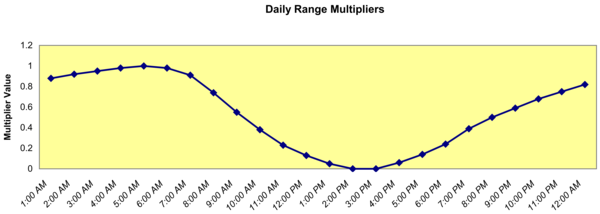
\includegraphics[width=0.9\textwidth, height=0.9\textheight, keepaspectratio=true]{media/image010.png}
\caption{Default Daily range Multiplier for Design Days \protect \label{fig:default-daily-range-multiplier-for-design}}
\end{figure}

The multipliers are taken from the ASHRAE 2009 HOF. More explicitly, EnergyPlus creates an air temperature for each timestep by using the entered maximum dry-bulb temperature in conjunction with the entered daily range and the above multiplier values. The actual equation used is shown below:

\begin{equation}
{T_{current}} = {T_{Max}} - {T_{range}}\cdot {T_{Multiplier}}
\end{equation}

where

T\(_{current}\) = Air temperature of current Hour of Day

T\(_{Max}\) = User supplied Max Dry-bulb Temperature

T\(_{range}\) = User supplied Daily Temperature Range

T\(_{Multiplier}\) = Range multiplier as shown on the above graph

The range multiplier values represent typical conditions of diurnal temperatures (i.e. the low temperature for the day occurring about 5:00 AM and the maximum temperature for the day occurring about 3:00 PM. Note that EnergyPlus does not shift the profile based on the time of solar noon as is optionally allowed in ASHRAE procedures.

ASHRAE research indicates that dry-bulb and wet-bulb temperatures typically follow the same profile, so EnergyPlus can use the default profile to generate humidity conditions (see Humidity Indicating Type = WetBulbProfileDefaultMultipliers below).

\paragraph{Field: Dry-Bulb Temperature Range Modifier Type}\label{field-dry-bulb-temperature-range-modifier-type}

If you are happy with lows at 5am and highs at 3pm, you can ignore this field. If you want to specify your own temperature range multipliers (see earlier discussion at the Temperature Range field description), you can specify a type here and create a day schedule which you reference in the next field.

If you specify \textbf{MultiplierSchedule} in this field, then you need to create a day schedule that specifies a multiplier applied to the temperature range field (above) to create the proper dry-bulb temperature range profile for your design day.

If you specify \textbf{DifferenceSchedule} in this field, then you need to create a day schedule that specifies a number to be \textbf{subtracted} from dry-bulb maximum temperature for each timestep in the day. Note that numbers in the delta schedules cannot be negative as that would result in a higher maximum than the maximum previously specified.

If you specify \textbf{TemperatureProfileSchedule} in this field, then you need to create a day schedule that specifies the actual dry-bulb temperatures throughout the day. You will not need to include a Maximum Dry-Bulb Temperature in that field.

If you leave this field blank or enter \textbf{DefaultMultipliers}, then the default multipliers will be used as shown in the ``temperature range'' field above.

\paragraph{Field: Dry-Bulb Temperature Range Modifier Day Schedule Name}\label{field-dry-bulb-temperature-range-modifier-day-schedule-name}

This field is the name of a \textbf{day schedule} (ref. \hyperref[scheduledayhourly]{Schedule:Day:Hourly}, \hyperref[scheduledayinterval]{Schedule:Day:Interval}, \hyperref[scheduledaylist]{Schedule:Day:List} objects) with the values as specified in the Dry-Bulb Temperature Range Modifier Type field above.

\paragraph{Field: Humidity Condition Type}\label{field-humidity-condition-type}

The values/schedules indicated here and in subsequent fields create the humidity values in the 24 hour design day conditions profile. Valid choices here are: \textbf{WetBulb}, \textbf{Dewpoint}, \textbf{WetBulbProfileDefaultMultipliers, WetBulbProfileDifferenceSchedule,} \textbf{WetBulbProfileMultiplierSchedule}, \textbf{HumidityRatio}, \textbf{Enthalpy}, and \textbf{Schedule.}

The Humidity Condition Type fields have interacting uses and units, summarized as follows:

% table 2
\begin{longtable}[c]{p{2.25in}p{1.75in}p{2.0in}}
\caption{Humidity Indicating Field Interactions - Design Day \label{table:humidity-indicating-field-interactions-design}} \tabularnewline
\toprule
Humidity Condition Type & Primary Humidity Indicating Field & Humidity Indicating Day Schedule \tabularnewline
\midrule
\endfirsthead

\caption[]{Humidity Indicating Field Interactions - Design Day} \tabularnewline
\toprule
Humidity Condition Type & Primary Humidity Indicating Field & Humidity Indicating Day Schedule \tabularnewline
\midrule
\endhead

WetBulb & Wetbulb or DewPoint at Maximum Dry-Bulb & N/A (unused) \tabularnewline
DewPoint & Wetbulb or DewPoint at Maximum Dry-Bulb & N/A (unused) \tabularnewline
HumidityRatio & Humidity Ratio at Maximum Dry-Bulb & N/A (unused) \tabularnewline
Enthalpy & Enthalpy at Maximum Dry-Bulb & N/A (unused) \tabularnewline
WetBulbProfile\-DefaultMultipliers & Wetbulb or DewPoint at Maximum Dry-Bulb & N/A (unused) \tabularnewline
WetBulbProfile\-MultiplierSchedule & Wetbulb or DewPoint at Maximum Dry-Bulb & Fractions of wet-bulb daily range (0 – 1) \tabularnewline
WetBulbProfile\-DifferenceSchedule & Wetbulb or DewPoint at Maximum Dry-Bulb & Difference between maximum and hour/timestep wet-bulb temperature, C \tabularnewline
RelativeHumidity\-Schedule & N/A & Relative humidity (\%, 0 – 100) \tabularnewline
\bottomrule
\end{longtable}

Humidity conditions over the day are derived as follows:

\textbf{WetBulb, DewPoint, HumidityRatio, or Enthalpy}:

These four methods assume constant absolute humidity over the day. Calculate W = humidity ratio at Maximum Dry-Bulb Temperature and Humidity Indicating Conditions. Derive hourly/timestep humidity conditions from W and hour/timestep dry-bulb temperature.

\textbf{WetBulbProfileDefaultMultipliers}

Generate the wet-bulb temperature profile using Default Daily Range Multiplier for Design Days (shown in Figure~\ref{fig:default-daily-range-multiplier-for-design} above) and Daily Wet-Bulb Temperature Range (below). This method is analogous to DefaultMultiplier generation of the dry-bulb temperature profile and is the procedure recommended in Chapter 14 of ASHRAE 2009 HOF.

\textbf{WetBulbProfileMultiplierSchedule}

Generate the wet-bulb profile using multipliers from the Humidity Indicating Day Schedule and Daily Wet-Bulb Temperature Range (below). Analogous to dry-bulb MultiplierSchedule.

\textbf{WetBulbProfileDifferenceSchedule}

Generate the wet-bulb profile by subtracting Humidity Indicating Day Schedule values from the daily maximum wet-bulb temperature (specified in Humidity Indicating Conditions at Maximum Dry-Bulb). Analogous to dry-bulb DifferenceSchedule.

\textbf{RelativeHumiditySchedule}

Hourly relative humidity is specified in Humidity Indicating Day Schedule.

In all cases, the humidity ratio is limited to saturation at the hour/timestep dry-bulb (that is, the dry-bulb temperature is used as specified, but the humidity ratio is modified as needed to be physically possible). Once a valid air state is determined, a complete set of consistent hour/timestep psychrometric values (dewpoint, wet-bulb, and enthalpy) is derived.

\paragraph{Field: Wetbulb or DewPoint at Maximum Dry-Bulb}\label{field-wetbulb-or-dewpoint-at-maximum-dry-bulb}

If you choose \textbf{Wetbulb} or \textbf{Dewpoint} in the Humidity Condition Type field, then this numeric field should contain that value. Note that this field is unnecessary when you put in a humidity indicating day schedule (described later in this section).

\paragraph{Field: Humidity Condition Day Schedule Name}\label{field-humidity-condition-day-schedule-name}

Allows specification a day schedule (ref. \hyperref[scheduledayhourly]{Schedule:Day:Hourly}, \hyperref[scheduledayinterval]{Schedule:Day:Interval}, \hyperref[scheduledaylist]{Schedule:Day:List} objects) of values for relative humidity or wet-bulb profile per Humidity Indicating Type field.

\paragraph{Field: Humidity Ratio at Maximum Dry-Bulb}\label{field-humidity-ratio-at-maximum-dry-bulb}

If \textbf{HumidityRatio} is chosen for the Humidity Condition Type field, then this numeric field should contain the desired humidity ratio at maximum dry-bulb temperature (units kg Water / kg Dry Air).

\paragraph{Field: Enthalpy at Maximum Dry-Bulb}\label{field-enthalpy-at-maximum-dry-bulb}

If \textbf{Enthalpy} is chosen for the Humidity Condition Type field, then this numeric field should contain the desired enthalpy at maximum dry-bulb temperature (units Joules /kg).

\paragraph{Field: Daily Wet-Bulb Temperature Range}\label{field-daily-wet-bulb-temperature-range}

The difference between the maximum and minimum wet-bulb temperatures on the design day (Celsius). Used for generating daily profiles of humidity conditions when Humidity Condition Type field (above) is \textbf{WetBulbProfileDefaultMultipliers} or \textbf{WetBulbProfileMultiplierSchedule}. Values for wet-bulb temperature range are tabulated by month for 5564 locations worldwide on the CD that accompanies the ASHRAE 2009 HOF.

\paragraph{Field: Barometric Pressure}\label{field-barometric-pressure}

This numeric field is the constant barometric pressure (Pascals) for the entire day.

\paragraph{Field: Wind Speed}\label{field-wind-speed}

This numeric field is the wind speed in meters/second (constant throughout the day) for the day. The MacroDataSets design day files includes wind speed values (99.6\% - heating, 1\% cooling) as indicated in ASHRAE HOF design condition tables. But, you should be aware that traditional values for these are 6.7056 m/s (15 mph) for heating and 3.3528 m/s (7 mph) for cooling. A reminder is shown in the comments for the wind speed values. The comments also note the extreme wind speeds from the ASHRAE tables.

\paragraph{Field: Wind Direction}\label{field-wind-direction}

This numeric field is the source wind direction in degrees. By convention, winds from the North would have a value of 0., from the East a value of 90.

\paragraph{Field: Rain Indicator}\label{field-rain-indicator}

This field indicates whether or not the building surfaces are wet. If the value is Yes, then it is assumed that the building surfaces are wet. Wet surfaces may change the conduction of heat through the surface.

\paragraph{Field: Snow Indicator}\label{field-snow-indicator}

This field indicates whether or not there is snow on the ground. If the value is Yes, then it is assumed there is snow on the ground. Snow on the ground changes the ground reflectance properties.

\paragraph{Field: Daylight Saving Time Indicator}\label{field-daylight-saving-time-indicator}

This field specifies whether to consider this day to be a Daylight Saving Day. Yes in the field indicates that daylight saving time is operational for this day. Yes essentially adds 1 hour to the scheduling times used in items with schedules.

\paragraph{Field: Solar Model Indicator}\label{field-solar-model-indicator}

This field allows the user to select \textbf{ASHRAE\-Clear\-Sky, ASHRAE\-Tau, ASHRAE\-Tau2017, Zhang\-Huang, or Sche\-dule} for solar modeling in the calculation of the solar radiation in the design day. ASHRAE\-Clear\-Sky and Zhang\-Huang use the Clearness value as part of their calculations. ASHRAE\-Tau invokes the revised model specified in Chapter 14 of the ASHRAE 2009 HOF and uses Taub and Taud values (below) and ASHRAE\-Tau2017 invokes the revised model specified in Chapter 14 of the ASHRAE 2017 HOF and uses Taub and Taud values (below). Technical details of the models are described in the Engineering Reference. The \textbf{Schedule} choice allows you to enter schedule values for the day's profile (use the next two fields for the names).

\paragraph{Field: Beam Solar Day Schedule Name}\label{field-beam-solar-day-schedule-name}

This field allows the option for you to put in your own day profile of beam solar values (wh/m2). These values will replace the calculated values during design day processing. Only day schedules (ref. \hyperref[scheduledayhourly]{Schedule:Day:Hourly}, \hyperref[scheduledayinterval]{Schedule:Day:Interval}, \hyperref[scheduledaylist]{Schedule:Day:List} objects) are used here.

\paragraph{Field: Diffuse Solar Day Schedule Name}\label{field-diffuse-solar-day-schedule-name}

This field allows the option for you to put in your own day profile of diffuse solar values (wh/m2). These values will replace the calculated values during design day processing. Only day schedules (ref. \hyperref[scheduledayhourly]{Schedule:Day:Hourly}, \hyperref[scheduledayinterval]{Schedule:Day:Interval}, \hyperref[scheduledaylist]{Schedule:Day:List} objects) are used here.

\paragraph{Field: ASHRAE Clear Sky Optical Depth for Beam Irradiance (taub)}\label{field-ashrae-clear-sky-optical-depth-for-beam-irradiance-taub}

Optical depth for beam radiation, used only when Solar Model Indicator is ASHRAETau or ASHRAETau2017. See next field.

\paragraph{Field: ASHRAE Clear Sky Optical Depth for Diffuse Irradiance (taud)}\label{field-ashrae-clear-sky-optical-depth-for-diffuse-irradiance-taud}

Optical depth for diffuse radiation, used only when Solar Model Indicator is ASHRAETau or ASHRAETau2017. Taub and Taud values are tabulated by month for 5564 locations worldwide on the CD that accompanies the ASHRAE HOF.
ASHRAETau model Taub and Taud values are used from the 2009 ASHRAE HOF and ASHRAETau2017 model Taub and Taud values are used from either 2013 or 2017 ASHRAE HOF as needed.

\paragraph{Field: Sky Clearness}\label{field-sky-clearness}

If the choice in the Solar Model Indicator field is ASHRAEClearSky or ZhangHuang, then this numeric field should be entered. This value represents the ``clearness'' value for the day. This value, along with the solar position as defined by the Location information and the date entered for the design day, help define the solar radiation values for each hour of the day. Clearness may range from 0.0 to 1.2, where 1.0 represents a clear sky at sea level. Values greater than 1.0 may be used for high altitude locations. Traditionally, one uses 0.0 clearness for Winter Design Days. Note that this ``sky clearness'' does not have the same meaning as output variable ``Site Daylighting Model Sky Clearness''.

\paragraph{Field: Maximum Number Warmup Days}\label{field-max-num-warm-days}

Optional integer number of days for an upper limit on the number of warmup days when running this sizing period.  This overrides the global maximum set in the Building object for this particular design day.

\paragraph{Field: Begin Environment Reset Mode}\label{field-beg-env-reset-mode}

Optional choice field to control if zone heat balance history terms should be reset when beginning to run this sizing period.  This can reduce the number of warmup days needed to reach zone convergence.  The options are \textbf{FullResetAtBeginEnvironment} or \textbf{SuppressThermalResetAtBeginEnvironment}.  \textbf{FullResetAtBeginEnvironment} means that at the beginning of the design day warmup the building model's surfaces are set to 23 degrees C, which is the usual starting point for each environment.  \textbf{SuppressThermalResetAtBeginEnvironment} means that at the beginning of the design day warmup the building model's surfaces are not reset and will just retain whatever thermal history results they had at the end of the previous design day.  The warmup days still proceed as usual but because the initial condition is closer it needs fewer warmup days to reach convergence.  This is available to reduce simulation run time when using many design days that are similiar to each other.


IDF Examples:

\begin{lstlisting}
! Phoenix Sky Harbor Intl Ap_AZ_USA Annual Cooling (WB = >MDB)
!   .4%, MDB = 35.8°C WB = 24.5°C
SizingPeriod:DesignDay,
  Phoenix Sky Harbor Intl Ap Ann Clg .4% Condns WB = >MDB, !- Name
          7,      !- Month
         21,      !- Day of Month
  SummerDesignDay,!- Day Type
       35.8,      !- Maximum Dry-Bulb Temperature {C}
         12,      !- Daily Dry-Bulb Temperature Range {C}
  DefaultMultipliers, !- Dry-Bulb Temperature Range Modifier Type
           ,      !- Dry-Bulb Temperature Range Modifier Schedule Name
    Wetbulb,      !- Humidity Condition Type
       24.5,      !- Wetbulb at Maximum Dry-Bulb {C}
           ,      !- Humidity Indicating Day Schedule Name
           ,      !- Humidity Ratio at Maximum Dry-Bulb {kgWater/kgDryAir}
           ,      !- Enthalpy at Maximum Dry-Bulb {J/kg}
           ,      !- Daily Wet-Bulb Temperature Range {deltaC}
     97342.,      !- Barometric Pressure {Pa}
        4.1,      ! Wind Speed {m/s}
        260,      !- Wind Direction {Degrees; N = 0, S = 180}
         No,      !- Rain {Yes/No}
         No,      !- Snow on ground {Yes/No}
         No,      !- Daylight Savings Time Indicator
       ASHRAETau, !- Solar Model Indicator
           ,      !- Beam Solar Day Schedule Name
           ,      !- Diffuse Solar Day Schedule Name
      0.588,     !- ASHRAE Clear Sky Optical Depth for Beam Irradiance (taub)
      1.653;  !- ASHRAE Clear Sky Optical Depth for Diffuse Irradiance (taud)

SizingPeriod:DesignDay,
  Denver Centennial Golden Ann Htg 99% Condns DB - sched solar,  !- Name
  1,                       !- Month
  13,                      !- Day of Month
  WinterDesignDay,         !- Day Type
  -16,                     !- Maximum Dry-Bulb Temperature {C}
  0.0,                     !- Daily Dry-Bulb Temperature Range {deltaC}
  ,                        !- Dry-Bulb Temperature Range Modifier Type
  ,                    !- Dry-Bulb Temperature Range Modifier Schedule Name
  Wetbulb,                 !- Humidity Condition Type
  -16,                     !- Wetbulb or DewPoint at Maximum Dry-Bulb {C}
  ,                        !- Humidity Indicating Day Schedule Name
  ,               !- Humidity Ratio at Maximum Dry-Bulb {kgWater/kgDryAir}
  ,                        !- Enthalpy at Maximum Dry-Bulb {J/kg}
  ,                        !- Daily Wet-Bulb Temperature Range {deltaC}
  83411.,                  !- Barometric Pressure {Pa}
  2.3,                     !- Wind Speed {m/s}
  180,                     !- Wind Direction {deg}
  No,                      !- Rain Indicator
  No,                      !- Snow Indicator
  No,                      !- Daylight Saving Time Indicator
  Schedule,                !- Solar Model Indicator
  Winter (1/13) Beam Solar,!- Beam Solar Day Schedule Name
  Winter (1/13) Diffuse Solar;  !- Diffuse Solar Day Schedule Name

Schedule:Day:Hourly,
  Winter (1/13) Beam Solar,
  Any Number,
  0,0,0,0,0,0,0,190,698,852,892,919,957,953,856,700,213,0,0,0,0,0,0,0;

Schedule:Day:Hourly,
  Winter (1/13) Diffuse Solar,
  Any Number,
  0,0,0,0,0,0,0,35,118,116,92,65,40,14,0,0,5,0,0,0,0,0,0,0;
\end{lstlisting}

Look at the example files 1Zone\-Un\-controll\-ed\_\-DD\-Changes.idf and 1Zone\-Un\-controlled\_\-DD\-2009 for several examples of specifying Design Day inputs.

\subsubsection{Outputs}\label{outputs-018}

For the schedule fields in the object, several output variables can be used:

\begin{itemize}
\item
  Zone,Average,Sizing Period Site Beam Solar Schedule Value {[}W/m2{]}
\item
  Zone,Average,Sizing Period Site Diffuse Solar Schedule Value {[}W/m2{]}
\item
  Zone,Average,Sizing Period Site Humidity Condition Schedule Value {[}\%{]}
\item
  Zone,Average,Sizing Period Site Humidity Condition Schedule Value {[]}
\item
  Zone,Average,Sizing Period Site Drybulb Temperature Range Modifier Schedule Value {[]}
\item
  Zone,Average,Sizing Period Site Drybulb Temperature Range Modifier Schedule Value {[}deltaC{]}
\item
  Zone,Average,Sizing Period Site Drybulb Temperature Range Modifier Schedule Value {[}C{]}
\item
  Zone,Average,Sizing Period Site Sky Temperature Schedule Value {[}deltaC{]}
\item
  Zone,Average,Sizing Period Site Sky Temperature Schedule Value {[}C{]}
\end{itemize}

\paragraph{Sizing Period Site Beam Solar Schedule Value {[}W/m2{]}}\label{sizing-period-site-beam-solar-schedule-value-wm2}

\paragraph{Sizing Period Site Diffuse Solar Schedule Value {[}W/m2{]}}\label{sizing-period-site-diffuse-solar-schedule-value-wm2}

This schedule value is active when any Design Day objects have / use the solar schedule option. For those objects that don't have this option, the value will be displayed as -999.

\paragraph{Sizing Period Site Humidity Condition Schedule Value {[}\%{]}}\label{sizing-period-site-humidity-condition-schedule-value}

\paragraph{Sizing Period Site Humidity Condition Schedule Value {[]}}\label{sizing-period-site-humidity-condition-schedule-value-1}

This schedule value is active when any Design Day objects have / use the humidity schedule option. For those objects that don't have this option, the value will be displayed as -999.

\paragraph{Sizing Period Site Drybulb Temperature Range Modifier Schedule Value {[]}}\label{sizing-period-site-drybulb-temperature-range-modifier-schedule-value}

\paragraph{Sizing Period Site Drybulb Temperature Range Modifier Schedule Value {[}deltaC{]}}\label{sizing-period-site-drybulb-temperature-range-modifier-schedule-value-deltac}

\paragraph{Sizing Period Site Drybulb Temperature Range Modifier Schedule Value {[}C{]}}\label{sizing-period-site-drybulb-temperature-range-modifier-schedule-value-c}

This schedule value is active when any Design Day objects have / use the drybulb temperature range modifier schedule option. For those objects that don't have this option, the value will be displayed as -999.

\paragraph{Sizing Period Site Sky Temperature Schedule Value {[}deltaC{]}}\label{sizing-period-site-sky-temperature-schedule-value-deltac}

\paragraph{Sizing Period Site Sky Temperature Schedule Value {[}C{]}}\label{sizing-period-site-sky-temperature-schedule-value-c}

This schedule value is active when any Design Day objects have / use the WeatherProperties:SkyTemperature schedule option. For those objects that don't have this option, the value will be displayed as -999.

\subsection{Longer Design Periods}\label{longer-design-periods}

Some features may benefit by using a longer design weather period for sizing or loads calculations. Longer design periods may be created by using the \textbf{Si\-zing\-Period:\-Weather\-File\-Days} or \textbf{Si\-zing\-Period:\-Weather\-File\-Con\-dition\-Type} objects. These two objects allow for selections from an attached weather file to be used in the sizing calculations.

\subsection{Sizing\-Period:\-Weather\-File\-Days}\label{sizingperiodweatherfiledays}

The Sizing\-Period:\-Weather\-File\-Days object describes using a selected period from the ``attached'' weather file to be used in load calculations or sizing equipment. The period selected can be as small as a single day or larger. Multiple periods may be input. While this object may be used for sizing calculations, you should also consider using design days that represent more long term extremes or conditions.

\subsubsection{Inputs}\label{inputs-2-022}

\paragraph{Field: Name}\label{field-name-2-021}

This field allows for an assigned name for this run period so it can be tracked easily in sizing and other outputs.

\paragraph{Field: Begin Month}\label{field-begin-month}

This numeric field should contain the starting month number (1 = January, 2 = February, etc.) for the annual run period desired.

\paragraph{Field: Begin Day of Month}\label{field-begin-day-of-month}

This numeric field should contain the starting day of the starting month (must be valid for month) for the annual run period desired.

\paragraph{Field: End Month}\label{field-end-month}

This numeric field should contain the ending month number (1 = January, 2 = February, etc.) for the annual run period desired.

\paragraph{Field: End Day of Month}\label{field-end-day-of-month}

This numeric field should contain the ending day of the ending month (must be valid for month) for the annual run period desired.

\paragraph{Field: Day of Week for Start Day}\label{field-day-of-week-for-start-day}

For flexibility, the day of week indicated on the weather file can be overridden by this field's value. Valid days of the week (Sunday, Monday, Tuesday, Wednesday, Thursday, Friday, Saturday) or special days (SummerDesignDay, WinterDesignDay, CustomDay1, CustomDay2) must be entered in this field. To clarify, this value will be used as the Start Day (type) for this sizing period. When weekdays are used, each subsequent day in the period will be incremented. When SummerDesignDay, WinterDesignDay, CustomDay1, CustomDay2 -- are used, the day type will be applied for the entire period.

\paragraph{Field: Use Weather File Daylight Saving Period}\label{field-use-weather-file-daylight-saving-period}

Weather files can contain indicators of Daylight Saving Period days. For flexibility, you may want to ignore these designations on the weather file. This field should contain the word \textbf{Yes} if you will accept daylight saving period days as contained on the weather file (note: not all weather files may actually have this period) or \textbf{No} if you wish to ignore Daylight Saving Period days that may be on the weather file.

Note that a blank or null field in this field will indicate \textbf{Yes}.

\paragraph{Field: Use Weather File Rain and Snow Indicators}\label{field-use-weather-file-rain-and-snow-indicators}

Weather files can contain ``rain'' and ``snow'' indicators. (EPW field ``Present Weather Codes'' -- described in the AuxiliaryPrograms document). In turn, rain indicates wet surfaces which changes the film convection coefficient for the surface. Other models may use rain as well (Ground Heat Exchangers). Snow indicators can change the ground reflectance if there is snow on the ground. Entering ``\textbf{Yes}'' in this field allows the weather file conditions to represent ``Rain'' and ``Snow''; entering ``\textbf{No}'' in the field ``turns off'' the rain/snow indicators for this period. You might use this to be able to compare two ``same location'' weather files of different years, origins, etc.

IDF Example:

\begin{lstlisting}
SizingPeriod:WeatherFileDays,
  Summer including Extreme Summer days, !- Name
  7,18,7,25,                            !- Begin/end Day/Month
  SummerDesignDay,                      !- Day type
  No,                                   !- Use Weather File Daylight Saving Period
  No;                                   !- Use Weather File Rain and Snow Indicators

SizingPeriod:WeatherFileDays,
  Winter including Extreme Winter days, !- Name
  1,25,2,1,                             !- Begin/end Day/Month
  WinterDesignDay,                      !- Day type
  No,                                   !- Use Weather File Daylight Saving Period
  No;                                   !- Use Weather File Rain and Snow Indicators
\end{lstlisting}

\subsection{Sizing\-Period:\-Weather\-File\-Con\-dition\-Type}\label{sizingperiodweatherfileconditiontype}

When the EPW files are created, a heuristic procedure identifies extreme and typical periods in the actual weather file. This object will allow one of those periods to be selected for sizing or load calculations (typically). Multiple objects may be input. While this object may be used for sizing calculations, you should also consider using design days that represent more long term extremes or conditions.

\subsubsection{Inputs}\label{inputs-3-020}

\paragraph{Field: Name}\label{field-name-3-018}

This field allows for an assigned name for this run period so it can be tracked easily in sizing and other outputs.

\paragraph{Field: Period Selection}\label{field-period-selection}

This field allows the generic period calculated from the weather file to be selected for this run period. It is not completely generic as there may be extreme cold periods in some weather files but extreme wet periods (tropical) in others. Not all weather files have all of the valid choices. The choices for this field are:

\begin{itemize}
\item
  SummerExtreme
\item
  SummerTypical
\item
  WinterExtreme
\item
  WinterTypical
\item
  AutumnTypical
\item
  SpringTypical
\item
  WetSeason
\item
  DrySeason
\item
  NoDrySeason
\item
  NoWetSeason
\item
  TropicalHot
\item
  TropicalCold
\end{itemize}

\paragraph{Field: Day of Week for Start Day}\label{field-day-of-week-for-start-day-1}

For flexibility, the day of week indicated on the weather file can be overridden by this field's value. Valid days of the week (Sunday, Monday, Tuesday, Wednesday, Thursday, Friday, Saturday) or special days (SummerDesignDay, WinterDesignDay, CustomDay1, CustomDay2) must be entered in this field. To clarify, this value will be used as the Start Day (type) for this sizing period. When weekdays are used, each subsequent day in the period will be incremented. When SummerDesignDay, WinterDesignDay, CustomDay1, CustomDay2 -- are used, the day type will be applied for the entire period.

\paragraph{Field: Use Weather File Daylight Saving Period}\label{field-use-weather-file-daylight-saving-period-1}

Weather files can contain indicators of Daylight Saving Period days. For flexibility, you may want to ignore these designations on the weather file. This field should contain the word \textbf{Yes} if you will accept daylight saving period days as contained on the weather file (note: not all weather files may actually have this period) or \textbf{No} if you wish to ignore Daylight Saving Period days that may be on the weather file.

Note that a blank or null field in this field will indicate \textbf{Yes}.

\paragraph{Field: Use Weather File Rain and Snow Indicators}\label{field-use-weather-file-rain-and-snow-indicators-1}

Weather files can contain ``rain'' and ``snow'' indicators. (EPW field ``Present Weather Codes'' -- described in the AuxiliaryPrograms document). In turn, rain indicates wet surfaces which changes the film convection coefficient for the surface. Other models may use rain as well (Ground Heat Exchangers). Snow indicators can change the ground reflectance if there is snow on the ground. Entering ``\textbf{Yes}'' in this field allows the weather file conditions to represent ``Rain'' and ``Snow''; entering ``\textbf{No}'' in the field ``turns off'' the rain/snow indicators for this period. You might use this to be able to compare two ``same location'' weather files of different years, origins, etc.

IDF Example:

\begin{lstlisting}
SizingPeriod:WeatherFileConditionType,
  Extreme Summer Weather Period for Design, !- Name
  SummerExtreme,                            !- Period Selection
  SummerDesignDay,                          !- Day Type
  No,                                       !- Use Weather File Daylight Saving Period
  No;                                       !- Use Weather File Rain and Snow Indicators

SizingPeriod:WeatherFileConditionType,
  Extreme Winter Weather Period for Design, !- Name
  WinterExtreme,                            !- Period Selection
  WinterDesignDay,                          !- Day Type
  No,                                       !- Use Weather File Daylight Saving Period
  No;                                       !- Use Weather File Rain and Snow Indicators
\end{lstlisting}

\subsection{RunPeriod}\label{runperiod}

The RunPeriod object describes the elements necessary to create a weather file simulation. Multiple run
periods may be input. EnergyPlus accepts weather files in the special EnergyPlus weather format
(described briefly below this document and in more detail in the Auxiliary Programs document). These files
can describe Daylight Saving Time periods as well as holidays within their definitions. Note that the weather
file also may contain design condition information, typical and extreme period information, ground
temperatures based on air temperature calculations. The RunPeriod object allows the user to override the use
of both the Daylight Saving Period (i.e. use or ignore) and holidays that are embedded within the weather
file. The object also describes the elements necessary to use a specially crafted (likely multiple year)
weather file in a simulation. These kinds of weather files and simulations might be useful for matching
utility periods or simulating several years of differing weather data. Leap days are required when using
actual weather (see ``Treat as Actual Weather'' below), but will be processed and used during leap years
when the days are present in the weather file and enabled in the weather file header. Note that when the
weather is treated as non-actual, the leap day will be skipped if it is not present, resulting in incorrect
day types for the remainder of the year. Further, the weather data interpolation for the first hour can also be specified to use Hour1 (natural) or Hour24 (considering warning up). 

\subsubsection{Inputs}\label{inputs-5-016}

\paragraph{Field: Name}\label{field-name-5-012}

This optional field allows the RunPeriod to be named for output reporting. When left blank, the weather file
location name is used. Note that the weather file location name will be appended to this name in
tabular/summary reports.

\paragraph{Field: Begin Month}\label{field-begin-month-2}

This numeric field should contain the starting month number (1 = January, 2 = February, etc.) for the annual
run period desired.

\paragraph{Field: Begin Day of Month}\label{field-begin-day-of-month-2}

This numeric field should contain the starting day of the starting month (must be valid for month) for the
annual run period desired.

\paragraph{Field: Begin Year}\label{field-begin-year}

This optional numeric field may contain the beginning year for the range. If this field is specified
along with the \textbf{Day of Week for Start Day}, the inputs are validated to make sure that the date is
valid. If this field is not specified, then a year will be selected based upon other inputs (which, in the
case of the day of the week, may be defaulted).

\paragraph{Field: End Month}\label{field-end-month-2}

This numeric field should contain the ending month number (1 = January, 2 = February, etc.) for the annual
run period desired.

\paragraph{Field: End Day of Month}\label{field-end-day-of-month-2}

This numeric field should contain the ending day of the ending month (must be valid for month) for the
annual run period desired.

\paragraph{Field: End Year}\label{field-end-year}

This optional numeric field should contain the end year for the range. It is only allowed to be specified
when the \textbf{Begin Year} is given and must be after the \textbf{Begin Year}. If it is not specified,
it will be set to be the first occurrence of \textbf{End Month/End Day of Month} after the start date. Note
that this could be several years after the start date (e.g. if the end date is specified as a leap day 2/29).

\paragraph{Field: Day of Week for Start Day}\label{field-day-of-week-for-start-day-3}

This field allows the start day of the week to be specified. Valid days of the week (Sunday, Monday, Tuesday,
Wednesday, Thursday, Friday, Saturday) may be entered in this field. To clarify, this value will be used as
the Start Day (type) for this run period and subsequent days will be implemented. If the field is blank,
then the starting day type defaults to Sunday.

\paragraph{Field: Use Weather File Holidays and Special Days}\label{field-use-weather-file-holidays-and-special-days-1}

Weather files can contain holiday designations or other kinds of special days. These day types cause a
corresponding day's schedule (see SCHEDULE definitions below) to be used during that day. This field
should contain the word \textbf{Yes} if holidays or other special days indicated directly on the weather
file should retain their ``day type'' or \textbf{No} if holidays or other special days on the weather file
should be ignored. Reference the \hyperref[runperiodcontrolspecialdays]{RunPeriodControl:SpecialDays} object below to enter your own special days
and holidays.

Note that a blank or null field in this field will indicate \textbf{Yes}.

\paragraph{Field: Use Weather File Daylight Saving Period}\label{field-use-weather-file-daylight-saving-period-3}

Weather files can contain indicators of Daylight Saving period days. For flexibility, you may want to ignore
these designations on the weather file. This field should contain the word \textbf{Yes} if you will accept
daylight saving period days as contained on the weather file (note: not all weather files may actually have
this period) or \textbf{No} if you wish to ignore Daylight Saving period days that may be on the weather file.

Note that a blank or null field in this field will indicate \textbf{Yes}.

\paragraph{Field: Apply Weekend Holiday Rule}\label{field-apply-weekend-holiday-rule-1}

In some countries (notably the US), when holidays fall on weekends, they are often observed on a weekday
close to the holiday day. (Usually if the specific day falls on a Saturday, the observed day is Friday;
if on a Sunday, the observed day is Monday). EnergyPlus will represent this custom using the value in
this field. If the field is \textbf{Yes}, then specific date holidays that have a duration of one day,
will be ``observed'' on the Monday after the day. (Specific day holidays are such as January 1 -- a
day-month combination). If the field is blank or \textbf{No}, then the holiday will be shown on the
day-month as entered. As this option is listed at the RunPeriod, all applicable special days for the run
will use the rule -- there is no override for individual special days.

Note that a blank or null field in this field will indicate \textbf{No}.

\begin{callout}
Note: EnergyPlus processed weather files available on the EnergyPlus web site: \url{https://www.energyplus.net/weather}
have neither special days specified nor daylight saving period. However, DDY (Design Day) files produced
from the ASHRAE Design Conditions that accompany the EPW files may include a DaylightSavingPeriod object
for certain locations.
\end{callout}

\paragraph{Field: Use Weather File Rain Indicators}\label{field-use-weather-file-rain-indicators-1}

Weather files can contain ``rain'' indicators. (EPW field ``Present Weather Codes'' -- described in the
AuxiliaryPrograms document). In turn, rain indicates wet surfaces which changes the film convection
coefficient for the surface. Other models may use rain as well (Ground Heat Exchangers). Entering
``\textbf{Yes}'' in this field allows the weather file conditions to represent ``Rain''; entering
``\textbf{No}'' in the field ``turns off'' the rain indicator for this period. You might use this
to be able to compare two ``same location'' weather files of different years, origins, etc.

\paragraph{Field: Use Weather File Snow Indicators}\label{field-use-weather-file-snow-indicators-1}

Weather files can contain ``snow'' indicators. (EPW field ``Snow Depth'' \textgreater{} 0 indicates
``Snow on the ground''). In turn, snow changes the reflectivity of the ground and cascades changes of this
reflectivity. Entering ``\textbf{Yes}'' in this field allows the weather file conditions to represent
``Snow''; entering ``\textbf{No}'' in the field ``turns off'' the snow indicator for this period. You might
use this to be able to compare two ``same location'' weather files of different years, origins, etc.

\paragraph{Field: Treat Weather as Actual}\label{field-treat-weather-as-actual}

This field determines how stringent date matching between this object and the weather file is. Though all
EnergyPlus (EPW) weather files contain a year field, this data is not typically used. Specifying
``\textbf{Yes}'' in this field causes the program to look specifically for the begin date (i.e. Begin Month,
Begin Day of Month, Begin Year) and for the end date (i.e. End Month, End Day of Month, End Year) and require
that leap days be present for leap years.

\paragraph{Field: First Hour Interpolation Starting Values}\label{field-first-hour-interpolation-starting-values}

This field allows the user to choose which hour of data should be used for the first day interpolation. In general, EnergyPlus uses a warm-up period to achieve a periodic initial condition for simulation. After the warming up period, EnergyPlus sets the first day's starting conditions the same as the end of that day. Therefore, Hour 24 is usually used for this type of annual simulations. However, there are other running scenarios where the user would like to examine the natural transition in the first hour, since the first day's beginning and end weather condition usually do not match in a weather file---sometimes or even often, with large differences, e.g. in temperature, humidity, or wind conditions. This input field allows a user to choose a more suitable option based on the user's specific simulation goals.

If the ``\textbf{Hour1}'' is selected for this field, the weather data interpolation during the first hour will be based on the weather data on Hour 1 of the simulation period. If the ``\textbf{Hour24}'' is selected, the interpolation during the first hour will be based on the Hour 1 and Hour 24 (now assumed this is the intended conditions from a successful warm-up cycling). The default value is ``\textbf{Hour24}''. Note that this option only affects the first hour of the first day in the entire run period; the succeeding days in a run period would not be affected.

And, as shown in an IDF:

\begin{lstlisting}
RunPeriod,  ! Winter Simulation
Winter Simulation,  !- Name
12,  !- Begin Month
1,   !- Begin Day of Month
,    !- Begin Year
3,   !- End Month
31,  !- End Day of Month
,    !- End Year
UseWeatherFile,  !- Day of Week for Start Day
Yes,  !- Use Weather File Holidays and Special Days
Yes,  !- Use Weather File Daylight Saving Period
No,   !- Apply Weekend Holiday Rule
Yes,  !- Use Weather File Rain Indicators
Yes,  !- Use Weather File Snow Indicators
No,   !- Treat Weather as Actual
Hour24;  !- First Hour Interpolation Starting Values

! Actual weather simulation example
RunPeriod,
Multiple Years,  !- Name
1,    !- Begin Month
1,    !- Begin Day of Month
2010, !- Begin Year
12,   !- End Month
31,   !- End Day of Month
,     !- End Year
UseWeatherFile,  !- Day of Week for Start Day
Yes,  !- Use Weather File Holidays and Special Days
Yes,  !- Use Weather File Daylight Saving Period
No,   !- Apply Weekend Holiday Rule
Yes,  !- Use Weather File Rain Indicators
Yes,  !- Use Weather File Snow Indicators
Yes,  !- Treat Weather as Actual
Hour1;  !- First Hour Interpolation Starting Values
\end{lstlisting}

\subsection{RunPeriodControl:SpecialDays}\label{runperiodcontrolspecialdays}

For weather file run periods, special day run periods can be described. These will always be in effect for the selected days in the run period. Depending on the Use Special Days value in the RunPeriod:* object(s), these can augment any special days included on the weather file.

\begin{callout}
Note: EnergyPlus processed weather files available on the EnergyPlus web site: \url{https://www.energyplus.net/weather} have neither special days specified nor daylight saving period. However, DDY (Design Day) files produced from the ASHRAE Design Conditions that accompany the EPW files may include a DaylightSavingPeriod object for certain locations.
\end{callout}

\subsubsection{Inputs}\label{inputs-6-013}

\paragraph{Field: Name}\label{field-name-6-010}

This alpha field is the title for the special day period. It must be unique among all the special day period objects entered.

\paragraph{Field: Start Date}\label{field-start-date}

This field is the starting date for the special day period. Dates in this field can be entered in several ways as shown in the accompanying table:

% table 3
\begin{longtable}[c]{@{}ll@{}}
\caption{Date Field Interpretation \label{table:date-field-interpretation}} \tabularnewline
\toprule
Field Contents & Interpretation \tabularnewline
\midrule
\endfirsthead

\caption[]{Date Field Interpretation} \tabularnewline
\toprule
Field Contents & Interpretation \tabularnewline
\midrule
\endhead

< number >  /  < number > & Month / Day \tabularnewline
< number >  Month & Day and Month \tabularnewline
Month  < number > & Day and Month \tabularnewline
< number >  Weekday in Month & Numbered weekday of month \tabularnewline
Last Weekday In Month & Last weekday of month \tabularnewline
\bottomrule
\end{longtable}

In the table, Month can be one of (January, February, March, April, May, June, July, August, September, October, November, December). Abbreviations of the first three characters are also valid.

In the table, Weekday can be one of (Sunday, Monday, Tuesday, Wednesday, Thursday, Friday, Saturday). Abbreviations of the first three characters are also valid.

\paragraph{Field: Duration}\label{field-duration}

This numeric field specifies how long (number of days) the special day period lasts.

\paragraph{Field: Special Day Type}\label{field-special-day-type}

This alpha field designates the ``day type'' for schedule use during the special period. It must be one of (Holiday, SummerDesignDay, WinterDesignDay, CustomDay1, CustomDay2).

An example in the IDF would be:

\begin{lstlisting}
RunPeriodControl:SpecialDays, President’s Day, 3rd Monday in February,1,Holiday;
RunPeriodControl:SpecialDays, Thanksgiving, 4th Thursday in November, 1,Holiday;
RunPeriodControl:SpecialDays, Halloween, 10/31, 1, Holiday;
RunPeriodControl:SpecialDays, Vacation, 5/1, 14, CustomDay1;
\end{lstlisting}

\subsection{RunPeriodControl:DaylightSavingTime}\label{runperiodcontroldaylightsavingtime}

Similar to a special day period, a daylight saving period may be entered to be applied to weather file run periods. These will always be in effect, regardless of the value entered on the \hyperref[runperiod]{RunPeriod} object. Note that this period will always override any daylight saving period specified in a weather file.

\begin{callout}
Note: EnergyPlus processed weather files available on the EnergyPlus web site: \url{https://www.energyplus.net/weather} have neither special days specified nor daylight saving period.

\warning{Note: For EnergyPlus \hyperref[outputvariable]{Output:Variable} and \hyperref[outputmeter-and-outputmetermeterfileonly]{Output:Meter} reporting, the time stamps are always in standard time. When daylight saving time is active, scheduled loads and controls will shift one hour relative to standard time.}
\end{callout}

\subsubsection{Inputs}\label{inputs-7-013}

\paragraph{Field: Start Date}\label{field-start-date-1}

This is the starting date of the daylight saving period. Note that it can be entered in several formats as shown in Table~\ref{table:date-field-interpretation}. Date Field Interpretation.

\paragraph{Field: End Date}\label{field-end-date}

This is the ending date of the daylight saving period. Note that it can be entered in several formats as shown in Table~\ref{table:date-field-interpretation}. Date Field Interpretation.

And in the IDF:

\begin{lstlisting}
! U.S. Standard for Daylight Saving
RunPeriodControl:DaylightSavingTime,2nd Sunday in March, 1st Sunday in November; !2007
! Brazil standard
RunPeriodControl:DaylightSavingTime,1st Sunday in October, Last Sunday in February;
! European Standard
RunPeriodControl:DaylightSavingTime, Last Sunday in March, Last Sunday in October;
! Syria Standard
RunPeriodControl:DaylightSavingTime, 4/1, 10/1;
\end{lstlisting}

Of course, these could not all appear in the same IDF as only one DaylightSavingPeriod object per input file is allowed. More information on Daylight Saving Periods can be seen on the web at: \url{http://www.webexhibits.org/daylightsaving/}. The ASHRAE Handbook of Fundamentals {[}ASHRAE 2005{]} also contains information about daylight saving periods and their climatic information now includes start and end dates for many locations.

\subsection{WeatherProperty:SkyTemperature}\label{weatherpropertyskytemperature}

Sky Temperature, or radiative sky temperature, is internally calculated by EnergyPlus with an empirical model using sky cloudiness factors and current clear sky emissivity. For flexibility, the following object can be entered to override the entire internal sky temperature calculation from schedule import.

In particular, during Weather File Run Periods, the sky temperature is derived by the horizontal infrared radiation if presented in the weather file input by default. For flexibility, the field \textbf{Use Weather File Horizontal IR} can be set to ``No'' to ignore horizontal IR values from the weather file and always use the specified sky model for horizontal infrared radiation and sky temperature calculations.

By default, EnergyPlus calculates clear sky emissivity using Clark-Allen model. The following object can also be entered to adopt alternative sky emissivity calculation methods. Alternative methods of sky emissivity calculation include the calibrated forms of Berdahl \& Martin, Brunt, and Idso model. Their algorithms are all described in the Engineering Reference document. Much of the literature describes the sky temperature as relative to water vapor pressure, drybulb or dewpoint temperature.

\subsubsection{Inputs}\label{inputs-8-011}

\paragraph{Field: Name}\label{field-name-7-009}

This name references an existing design period (i.e., \hyperref[sizingperioddesignday]{SizingPeriod:DesignDay}, \hyperref[sizingperiodweatherfiledays]{SizingPeriod:WeatherFileDays}, or \hyperref[sizingperiodweatherfileconditiontype]{SizingPeriod:WeatherFileConditionType}) or run period (by name or blank for all run periods).

\paragraph{Field: Calculation Type}\label{field-calculation-type}

Allowable entries here are: \textbf{ClarkAllen}, \textbf{Brunt}, \textbf{Idso}, \textbf{BerdahlMartin}, \textbf{ScheduleValue}, \textbf{DifferenceScheduleDryBulbValue}, or \textbf{DifferenceScheduleDewPointValue}.

In the case of \textbf{ScheduleValue}, \textbf{DifferenceScheduleDryBulbValue} and \textbf{DifferenceScheduleDewPointValue} the following field must specify a valid schedule name.

\textbf{ClarkAllen} -- the clear sky emissivity are calculated using Clark and Allen model. This is the default model to calculate clear sky emissivity.

\textbf{Brunt} -- the clear sky emissivity are calculated using Brunt model.

\textbf{Idso} -- the clear sky emissivity are calculated using Idso model.

\textbf{BerdahlMartin} -- the clear sky emissivity are calculated using Berdahl \& Martin model.

\textbf{ScheduleValue} -- the values in the schedule are used as the sky temperature.

\textbf{DifferenceScheduleDryBulbValue} -- the values in the schedule are \emph{subtracted} from the drybulb temperature value (+values would then be less than the drybulb temperature, -values would then be greater than the drybulb temperature) for the resulting sky temperature value.

\textbf{DifferenceScheduleDewPointValue} -- the values in the schedule are \emph{subtracted} from the dewpoint temperature value (+values would then be less than the dewpoint temperature, -values would then be greater than the dewpoint temperature) for the resulting sky temperature value.

\paragraph{Field: ScheduleName}\label{field-schedulename}

This field specifies a schedule name to accomplish the sky temperature calculation from the previous field. A Schedule:Day:* (i.e., \hyperref[scheduledayhourly]{Schedule:Day:Hourly}, \hyperref[scheduledayinterval]{Schedule:Day:Interval}, \hyperref[scheduledaylist]{Schedule:Day:List}) should be specified if the name in the name field matches a \hyperref[sizingperioddesignday]{SizingPeriod:DesignDay} object. If the name is one of the weather file period specifications (i.e. matches a \hyperref[sizingperiodweatherfiledays]{SizingPeriod:WeatherFileDays}, \hyperref[sizingperiodweatherfileconditiontype]{SizingPeriod:WeatherFileConditionType} or \hyperref[runperiod]{RunPeriod}), then the schedule name must match a full year schedule (i.e. \hyperref[scheduleyear]{Schedule:Year}, \hyperref[schedulecompact]{Schedule:Compact}, \hyperref[schedulefile]{Schedule:File}, or \hyperref[scheduleconstant]{Schedule:Constant}).

\paragraph{Field: Use Weather File Horizontal IR}\label{field-use-weather-file-hori-ir}

This field specifies whether or not to use the horizontal infrared radiation values from weather files if presented. The field is default to be true. If yes or blank, and the values are presented in weather file, EnergyPlus uses the values from weather file for weather calculations, otherwise it uses the specified sky model to calculate the values. If no, it always uses the specified sky model and ignores the horizontal IR values from the weather file. For \textbf{Calculation Type} = \textbf{ScheduleValue}, \textbf{ScheduleValue} or \textbf{DifferenceScheduleDewPointValue,} this field is ignored and the scheduled values are used. If this field is set to \textbf{No} but no specific sky model is declared in the field \textbf{Calculation Type}, the default sky model \textbf{ClarkAllen} is used.

An example of IDF usage (with DesignDay):

\begin{lstlisting}
SizingPeriod:DesignDay,
  DENVER_STAPLETON Ann Clg 1% Sky Temperature modifier,  !- Name
  32.6,              !- Maximum Dry-Bulb Temperature {C}
  15.2,              !- Daily Temperature Range {deltaC}
  15.5,              !- Humidity Indicating Conditions at Maximum Dry-Bulb
  83411.,            !- Barometric Pressure {Pa}
  4,                 !- Wind Speed {m/s}
  120,               !- Wind Direction {deg}
  1.00,              !- Sky Clearness
  0,                 !- Rain Indicator
  0,                 !- Snow Indicator
  25,                !- Day of Month
  7,                 !- Month
  SummerDesignDay,   !- Day Type
  0,                 !- Daylight Saving Time Indicator
  WetBulb,           !- Humidity Indicating Type
  ,                  !- Relative Humidity Day Schedule Name
  deltaschedule,     !- Dry-Bulb Temperature Range Modifier Type
  temp range deltas; !- Dry-Bulb Temperature Range Modifier Schedule Name

WeatherProperty:SkyTemperature,
  DENVER_STAPLETON Ann Clg 1% Sky Temperature modifier, !- Name
  ScheduleValue,     !- Calculation Type
  DaySchedule5;      !- Schedule Name

Schedule:Day:Interval,
  DaySchedule5,      !- Name
  Temperature,       !- Schedule Type Limits Name
  Yes,               !- Interpolate to Timestep
  until: 24:00,      !- Time 1
  5;                 !- Value Until Time 1
\end{lstlisting}

Another example of IDF usage:

\begin{lstlisting}
WeatherProperty:SkyTemperature,
  ,
  UseBerdahlMartinModel,     !- Calculation Type
  ,
  No;                        !- Use Weather File Horizontal IR
\end{lstlisting}


\subsection{Site:WeatherStation}\label{siteweatherstation}

The Site:WeatherStation object is used to specify the measurement conditions for the climatic data listed in the weather file. These conditions indicate the height above ground of the air temperature sensor, the height above ground of the wind speed sensor, as well as coefficients that describe the wind speed profile due to the terrain surrounding the weather station. There are necessary correlations between the entries for this object and some entries in the Building object, specifically the \textbf{Terrain} field.

Weather stations throughout the world (ref: WMO -- World Meteorological Organization) take their measurements at standard conditions:

\begin{itemize}
\item
  Air temperature is measured at approximately 1.5 m above ground
\item
  Wind speed is measured at 10 m above ground
\item
  Weather station is in a flat, open field with little protection from the wind.
\end{itemize}

When using weather data from standard sources (e.g., TMY2, IWEC, TMY, or ASHRAE design day data), it is not necessary to use the \textbf{Site:WeatherStation} object. However, if you are using custom weather data or real-time weather data, you may need to read and understand the concepts in the \textbf{Site:WeatherStation} object.

The measurement conditions at the weather station (i.e., the weather file) are used by EnergyPlus in conjunction with the \emph{Terrain} field of the \textbf{Building} object, or optionally with the \textbf{\hyperref[siteheightvariation]{Site:HeightVariation}} object (see below), to calculate the local variation in atmospheric properties as a function of height above ground. Outdoor air temperature decreases with height, while wind speed increases with height. The algorithms for this calculation are in the Engineering Reference.

The \textbf{Site:WeatherStation} object is useful when working with a custom weather file that includes data that were not measured at the WMO standard conditions. For example, the weather data could be measured on site, or on the roof top of a nearby building. The wind speed profile coefficients can be estimated from the table below or calculated beforehand using more sophisticated techniques such as CFD modeling of the weather station terrain.

% table 4
\begin{longtable}[c]{@{}lll@{}}
\caption{Wind Speed Profile Coefficients (ASHRAE Fundamentals 2005). \label{table:wind-speed-profile-coefficients-ashrae}} \tabularnewline
\toprule
Terrain Description & Exponent & Boundary Layer Thickness (m) \tabularnewline
\midrule
\endfirsthead

\caption[]{Wind Speed Profile Coefficients (ASHRAE Fundamentals 2005).} \tabularnewline
\toprule
Terrain Description & Exponent & Bounhary Layer Thickness (m) \tabularnewline
\midrule
\endhead

Flat, open country & 0.14 & 270 \tabularnewline
Rough, wooded country & 0.22 & 370 \tabularnewline
Towns and cities & 0.33 & 460 \tabularnewline
Ocean & 0.10 & 210 \tabularnewline
Urban, industrial, forest & 0.22 & 370 \tabularnewline
\bottomrule
\end{longtable}

If the \textbf{Site:WeatherStation} object is omitted from the input file, the WMO standard measurement conditions are assumed.

\subsubsection{Inputs}\label{inputs-9-010}

\paragraph{Field: Wind Sensor Height Above Ground}\label{field-wind-sensor-height-above-ground}

The height {[}m{]} above ground for the wind speed sensor.

\paragraph{Field: Wind Speed Profile Exponent}\label{field-wind-speed-profile-exponent}

The wind speed profile exponent for the terrain surrounding the weather station. The exponent can be estimated from the table above or calculated beforehand using more sophisticated techniques, such as CFD modeling of the weather station terrain.

\paragraph{Field: Wind Speed Profile Boundary Layer Thickness}\label{field-wind-speed-profile-boundary-layer-thickness}

The wind speed profile boundary layer thickness {[}m{]} for the terrain surrounding the weather station. The boundary layer can be estimated from the table above or calculated beforehand using more sophisticated techniques, such as CFD modeling of the weather station terrain.

\paragraph{Field: Air Temperature Sensor Height Above Ground}\label{field-air-temperature-sensor-height-above-ground}

The height {[}m{]} above ground for the air temperature sensor.

For example, if you are using weather data measured on the top of your building, you should set the \emph{Wind Sensor Height Above Ground} and the \emph{Air Temperature Sensor Height Above Ground} to equal the height of your building (say 30 m). The \emph{Wind Speed Profile Exponent} and \emph{Wind Speed Profile Boundary Layer Thickness} should be set to match the values associated with the \emph{Terrain} field of the \textbf{Building} object, or the equivalent fields of the \textbf{\hyperref[siteheightvariation]{Site:HeightVariation}} object.

Or, in IDF terms, with a building in a town or city:

\begin{lstlisting}
Site:WeatherStation,
  30,    !- Wind Sensor Height Above Ground {m}
  0.33,  !- Wind Speed Profile Exponent {}
  460,   !- Wind Speed Profile Boundary Layer Thickness {m}
  30;    !- Air Temperature Sensor Height Above Ground {m}
\end{lstlisting}

This would change if you had a different wind speed profile exponent or wind speed profile boundary layer thickness at your site.

\subsection{Site:HeightVariation}\label{siteheightvariation}

The Site:HeightVariation object is used to specify the local variation in atmospheric properties at the site and should be used only if you require advanced control over the height-dependent variations for wind speed and temperature. The coefficients set by this object are used by EnergyPlus, in conjunction with the \hyperref[siteweatherstation]{Site:WeatherStation} object (see above), to calculate the local variation in atmospheric properties as a function of height above ground. Outdoor air temperature decreases with height, while wind speed increases with height. The local outdoor air temperature and wind speed are calculated separately for all zones and surfaces, and optionally for outdoor air nodes for which a height has been specified (see \hyperref[outdoorairnode]{OutdoorAir:Node} object). With the default inputs, wind speed falls significantly at heights lower than the weather station measurement height, and temperature increases slightly. The algorithms for this calculation are in the Engineering Reference. There are necessary correlations between the entries for this object and some entries in the Building object, specifically the \textbf{Terrain} field.

% table 5
\begin{longtable}[c]{@{}lllll@{}}
\caption{Atmospheric Variables at Two Different Heights Above Ground Level. \label{table:atmospheric-variables-at-two-different}} \tabularnewline
\toprule
Variable & 1.5 m & 284 m & Absolute Diff & Percent Diff \tabularnewline
\midrule
\endfirsthead

\caption[]{Atmospheric Variables at Two Different Heights Above Ground Level.} \tabularnewline
\toprule
Variable & 1.5 m & 284 m & Absolute Diff & Percent Diff \tabularnewline
\midrule
\endhead

Air Temperature & 15°C & 13.15°C & 1.85°C & 12.3\% \tabularnewline
Barometric Pressure & 101,325 Pa & 97,960 Pa & 3,365 Pa & 3.3\% \tabularnewline
Wind Speed & 2.46 m/s & 7.75 m/s & 5.29 m/s & 215\% \tabularnewline
\bottomrule
\end{longtable}

Note that using this object overrides the wind speed profile coefficients implied by the \emph{Terrain} field of the \textbf{Building} object even if the wind speed profile fields are left blank. The wind speed profile coefficients can be estimated from the table above (see \textbf{\hyperref[siteweatherstation]{Site:WeatherStation}}) or calculated beforehand using more sophisticated techniques such as CFD modeling of the site terrain.

\subsubsection{Inputs}\label{inputs-10-009}

\paragraph{Field: Wind Speed Profile Exponent}\label{field-wind-speed-profile-exponent-1}

The wind speed profile exponent for the terrain surrounding the site. The exponent can be estimated from the table above (see \textbf{\hyperref[siteweatherstation]{Site:WeatherStation}}) or calculated beforehand using more sophisticated techniques, such as CFD modeling of the site terrain. Note that using this object overrides the wind speed profile coefficients implied by the \emph{Terrain} field of the \textbf{Building} object even if this field is left blank. This field can be set to zero to turn off all wind dependence on height.

\paragraph{Field: Wind Speed Profile Boundary Layer Thickness}\label{field-wind-speed-profile-boundary-layer-thickness-1}

The wind speed profile boundary layer thickness {[}m{]} for the terrain surrounding the site. The boundary layer can be estimated from the table above (see \textbf{\hyperref[siteweatherstation]{Site:WeatherStation}}) or calculated beforehand using more sophisticated techniques, such as CFD modeling of the site terrain. Note that using this object overrides the wind speed profile coefficients implied by the \emph{Terrain} field of the \textbf{Building} object even if this field is left blank.

\paragraph{Field: Air Temperature Gradient Coefficient}\label{field-air-temperature-gradient-coefficient}

The air temperature gradient coefficient {[}K/m{]} is a research option that allows the user to control the variation in outdoor air temperature as a function of height above ground. The real physical value is 0.0065 K/m. This field can be set to zero to turn off all temperature dependence on height. Note that the \emph{Air Temperature Sensor Height} in the \textbf{\hyperref[siteweatherstation]{Site:WeatherStation}} object should also be set to zero in order to force the local outdoor air temperatures to match the weather file outdoor air temperature. This change is required because the \textbf{\hyperref[siteweatherstation]{Site:WeatherStation}} object assumes an air temperature gradient of 0.0065 K/m. This field can be set to zero to turn off all temperature dependence on height.

\begin{lstlisting}
Site:HeightVariation,
  0.22,    !- Wind Speed Profile Exponent
  370,     !- Wind Speed Profile Boundary Layer Thickness {m}
  0.0065;  !- Air Temperature Gradient Coefficient {deltaC/m}
\end{lstlisting}

\subsection{Site:GroundTemperature:BuildingSurface}\label{sitegroundtemperaturebuildingsurface}

Ground temperatures are used for the ground heat transfer model. There can be only one ground temperature object included, and it is used as the outside surface temperature for all surfaces with Outside Boundary Condition = Ground. The object is options if you have no surfaces with ground contact. The outside surface temperature for individual surfaces can be specified using the OtherSideCoefficients (ref: \hyperref[surfacepropertyothersidecoefficients]{SurfaceProperty:OtherSideCoefficients}) object that allows Toutside to be set with a schedule. This permits using any number of different outside face temperatures in addition to the ground temperature.

\begin{callout}
Caution: The ``undisturbed'' ground temperatures calculated by the weather converter should not be used in building losses but are appropriate to be used in the \hyperref[sitegroundtemperatureshallow]{Site:GroundTemperature:Shallow} and \hyperref[sitegroundtemperaturedeep]{Site:GroundTemperature:Deep} objects. The reasoning (for building losses) is that these values are too extreme for the soil under a conditioned building. For best results, use the Slab or Basement program described in this document to calculate custom monthly average ground temperatures (see the Ground Heat Transfer section). This is especially important for residential applications and very small buildings. If one of these ground temperature preprocessors is not used, for typical commercial buildings in the USA, a reasonable default value is \SI{2}{\degreeCelsius} less than the average indoor space temperature.
\end{callout}

More information about determining appropriate ground temperatures is given in the Auxiliary Programs document.

\subsubsection{Inputs}\label{inputs-11-008}

\paragraph{Field: Month Temperature(s) -- 12 fields in all}\label{field-month-temperatures-12-fields-in-all}

Each numeric field is the monthly ground temperature (degrees Celsius) used for the indicated month (January = 1\(^{st}\) field, February = 2\(^{nd}\) field, etc.)

An IDF example:

\begin{lstlisting}
Site:GroundTemperature:BuildingSurface,19,20,20,20,20,20,20,20,20,20,20,20;
\end{lstlisting}

\subsection{Site:GroundTemperature:Shallow}\label{sitegroundtemperatureshallow}

Site:GroundTemperature:Shallow are used by the Surface Ground Heat Exchanger (i.e. object: \hyperref[groundheatexchangersurface]{GroundHeatExchanger:Surface}). Only one shallow ground temperature object can be included.

\begin{callout}
Note that the ground temperatures included in full year weather files may be suitable of being used for the values in these fields -- namely, the .5 m depth temperatures that are calculated for ``undisturbed'' soil of ``typical'' conditions. However, you may wish to use some other change effect -- based on the weather conditions of the building location.
\end{callout}

This object may be used for objects requiring ``undisturbed'' ground temperatures. In these instances, the ``name'' input field is not required.

\subsubsection{Inputs}\label{inputs-12-008}

\paragraph{Field: Month Temperature(s) -- 12 fields in all}\label{field-month-temperatures-12-fields-in-all-1}

Each numeric field is the monthly surface ground temperature (degrees Celsius) used for the indicated month (January = 1\(^{st}\) field, February = 2\(^{nd}\) field, etc.)

An IDF example:

\begin{lstlisting}
Site:GroundTemperature:Shallow,4,4,6,6,10,10,15,15,14,14,8,8;
\end{lstlisting}

\subsection{Site:GroundTemperature:Deep}\label{sitegroundtemperaturedeep}

Site:GroundTemperature:Deep are used by the Pond Ground Heat Exchanger object (i.e. object: \hyperref[groundheatexchangerpond]{GroundHeatExchanger:Pond}). Only one deep ground temperature object can be included.

\begin{callout}
Note that the ground temperatures included in full year weather files may be suitable of being used for the values in these fields -- namely, the 4 m depth temperatures that are calculated for ``undisturbed'' soil of ``typical'' conditions. However, you may wish to use some other change effect -- based on the weather conditions or special knowledge of the building location.
\end{callout}

This object may be used for objects requiring ``undisturbed'' ground temperatures. In these instances, the ``name'' input field is not required.

\subsubsection{Inputs}\label{inputs-13-007}

\paragraph{Field: Month Temperature(s) -- 12 fields in all}\label{field-month-temperatures-12-fields-in-all-2}

Each numeric field is the monthly deep ground temperature (degrees Celsius) used for the indicated month (January = 1\(^{st}\) field, February = 2\(^{nd}\) field, etc.)

An IDF example:

\begin{lstlisting}
Site:GroundTemperature:Deep,  16,16,16,16,16,16,16,16,16,16,16,16;
\end{lstlisting}

\subsection{Site:GroundTemperature:Undisturbed:FiniteDifference}\label{sitegroundtemperatureundisturbedfinitedifference}

Site:GroundTemperature:Undisturbed:FiniteDifference may be used by all objects requiring ``undisturbed'' ground temperatures. The object uses a 1D finite difference heat transfer model which uses the weather file to obtain surface boundary conditions. An annual simulation is run on the model during it's initialization until the annual ground temperature profile has reached steady periodic behavior. Once steady periodic behavior is reached, the ground temperatures are cached for retrieval during the rest of the simulation.

\subsubsection{Inputs}\label{inputs-14-007}

\paragraph{Field: Soil Thermal Conductivity}\label{field-soil-thermal-conductivity-000}

The thermal conductivity of the soil, in W/m-K.

\paragraph{Field: Soil Density}\label{field-soil-density-000}

The bulk density of the soil, in kg/m3.

\paragraph{Field: Soil Specific Heat}\label{field-soil-specific-heat-000}

The specific heat of dry soil, in J/kg-K.

\paragraph{Field: Soil Moisture Content Volume Fraction}\label{field-soil-moisture-content-volume-fraction}

A nominal value of soil moisture content to be used when evaluating soil thermal properties.

\paragraph{Field: Soil Moisture Content Volume Fraction at Saturation}\label{field-soil-moisture-content-volume-fraction-at-saturation}

A nominal value of soil moisture content when the soil is saturated, this is used in evaluating thermal properties of freezing soil.

\paragraph{Field: Evapotranspiration Ground Cover Parameter}\label{field-evapotranspiration-ground-cover-parameter}

Numeric field specifies the ground cover effects used in the evapotranspiration model at the ground surface heat balance. The values range from 0 (solid, non-permeable ground surface) to 1.5 (wild growth).

An IDF example:

\begin{lstlisting}
Site:GroundTemperature:Undisturbed:FiniteDifference,
  FDTemps,  !- Name of object
  1.08,     !- Soil Thermal Conductivity {W/m-K}
  962,      !- Soil Density {kg/m3}
  2576,     !- Soil Specific Heat {J/kg-K}
  30,       !- Soil Moisture Content Volume Fraction {percent}
  50,       !- Soil Moisture Content Volume Fraction at Saturation {percent}
  0.408;    !- Evapotranspiration Ground Cover Parameter
\end{lstlisting}

\subsection{Site:GroundTemperature:Undisturbed:KusudaAchenbach}\label{sitegroundtemperatureundisturbedkusudaachenbach}

Site:GroundTemperature:Undisturbed:KusudaAchenbach may be used by all objects requiring ``undisturbed'' ground temperatures. It provides an undisturbed ground temperature based on the correlation developed by Kusuda T. and P. Achenbach. 1965. The correlation uses three parameters for ground temperature at the surface to define a correlation for undisturbed ground temperatures as a function of depth and time. If one thinks of the ground temperature for a given depth as a sinusoid, the average ground temperature, amplitude (average difference between maximum ground temperature and minimum ground temperature), and the phase shift (day of minimum surface temperature) are all required to define the correlation.

If the parameters are left blank they can be autocalculated by including soil surface temperatures in the input using the \hyperref[sitegroundtemperatureshallow]{Site:GroundTemperature:Shallow} object. They can also be calculated by using the CalcSoilSurfTemp preprocessor.

Kusuda, T. and P.R. Achenbach. 1965. `Earth Temperatures and Thermal Diffusivity at Selected Stations in the United States.' \emph{ASHRAE Transactions}. 71(1): 61-74.

\subsubsection{Field: Soil Thermal Conductivity}\label{field-soil-thermal-conductivity-1}

The thermal conductivity of the soil, in W/m-K.

\subsubsection{Field: Soil Density}\label{field-soil-density-1}

The bulk density of the soil, in kg/m3.

\subsubsection{Field: Soil Specific Heat}\label{field-soil-specific-heat-1}

The specific heat of dry soil, in J/kg-K.

\subsubsection{Field: Average Annual Ground Surface Temperature}\label{field-average-annual-ground-surface-temperature}

This is the average ground surface temperature throughout the entire year, in \si{\degreeCelsius}.

\subsubsection{Field: Average Amplitude of Annual Ground Surface Temperature}\label{field-average-amplitude-of-annual-ground-surface-temperature}

This is the average amplitude of the ground surface temperature, in \si{\degreeCelsius}.

\subsubsection{Field: Phase Shift of Minimum Surface Temperature}\label{field-phase-shift-of-minimum-surface-temperature}

This is day of the year which has the lowest ground surface temperature.

An IDF example:

\begin{lstlisting}
Site:GroundTemperature:Undisturbed:KusudaAchenbach,
  KATemps,    !- Name of object
  1.08,       !- Soil Thermal Conductivity {W/m-K}
  962,        !- Soil Density {kg/m3}
  2576,       !- Soil Specific Heat {J/kg-K}
  15.5,       !- Average Soil Surface Temperature {C}
  12.0,       !- Average Amplitude of Surface Temperature {deltaC}
  21;         !- Phase Shift of Minimum Surface Temperature {days}
\end{lstlisting}

\subsection{Site:GroundTemperature:Undisturbed:Xing}\label{sitegroundtemperatureundisturbedxing}

Site:GroundTemperature:Undisturbed:Xing may be used by all objects requiring ``undisturbed'' ground temperatures. It provides an undisturbed ground temperature based on the correlation developed by Xing, 2014. The correlation is a 5 parameter, 2 harmonic model based on the work of Lord Kelvin (Thomson, 1862). The average soil surface temperature and two sets of surface temperature amplitude and phase shift must be provided. Parameters for 4000+ international locations can be found in Xing, 2014.

Thomson, W. 1862. `On the Reduction of Observations of Underground Temperature, with applications to Professor Forbes' Edinburgh Observations and the continued Calton Hill Series.' Proceedings of the Royal Society of Edinburgh. IV: 342-346.

Xing, L. 2014. Estimations of Undisturbed Ground Temperatures using Numerical and Analytical Modeling. Ph.D.~Diss. Oklahoma State University, Stillwater, OK.

\subsubsection{Inputs}\label{inputs-15-007}

\paragraph{Field: Soil Thermal Conductivity}\label{field-soil-thermal-conductivity-2}

The thermal conductivity of the soil, in W/m-K.

\paragraph{Field: Soil Density}\label{field-soil-density-2}

The bulk density of the soil, in kg/m3.

\paragraph{Field: Soil Specific Heat}\label{field-soil-specific-heat-2}

The specific heat of dry soil, in J/kg-K.

\paragraph{Field: Average Soil Surface Temperature}\label{field-average-soil-surface-temperature-000}

The average annual surface temperature of the soil, in deg C.

\paragraph{Field: Soil Surface Temperature Amplitude 1}\label{field-soil-surface-temperature-amplitude-1}

First soil surface temperature amplitude parameter, in deg C.

\paragraph{Field: Soil Surface Temperature Amplitude 2}\label{field-soil-surface-temperature-amplitude-2}

Second soil surface temperature amplitude parameter, in deg C.

\paragraph{Field: Phase Shift of Surface Temperature Amplitude 1}\label{field-phase-shift-of-surface-temperature-amplitude-1}

Phase shift of surface temperature amplitude 1, in days.

\paragraph{Field: Phase Shift of Surface Temperature Amplitude 2}\label{field-phase-shift-of-surface-temperature-amplitude-2}

Phase shift of surface temperature amplitude 2, in days.

An IDF example:

\begin{lstlisting}
Site:GroundTemperature:Undisturbed:Xing,
  Chicago-Ohare,!- Name of object
  1.08,         !- Soil Thermal Conductivity {W/m-K}
  962,          !- Soil Density {kg/m3}
  2576,         !- Soil Specific Heat {J/kg-K}
  11.1,         !- Average Soil Surface Tempeature {C}
  13.4,         !- Soil Surface Temperature Amplitude 1 {deltaC}
  0.7,          !- Soil Surface Temperature Amplitude 2 {deltaC}
  25,           !- Phase Shift of Temperature Amplitude 1 {days}
  30;           !- Phase Shift of Temperature Amplitude 2 {days}
\end{lstlisting}

\subsection{Site:GroundDomain:Slab}\label{sitegrounddomainslab}

This section documents the input object used to simulate ground coupled heat transfer with horizontal building surfaces within EnergyPlus. Horizontal ground surfaces within EnergyPlus interact with the Site:GroundDomain object by utilizing the \hyperref[surfacepropertyothersideconditionsmodel]{SurfaceProperty:OtherSideConditionsModel} object. By utilizing this object, multiple horizontal surfaces can be coupled to the same Site:GroundDomain object. Each horizontal surface may also have its unique ground domain, however, runtime will be adversely affected.

Generally, there are two scenarios which Site:GroundDomain is equipped to model: in-grade slabs and on-grade slabs.

\begin{figure}[htbp]
\centering
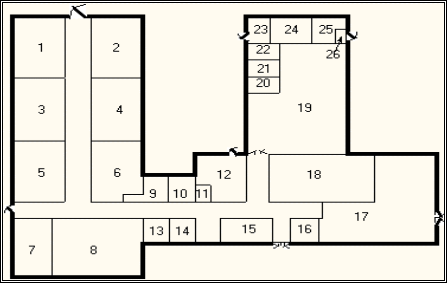
\includegraphics{media/image012.png}
\caption{In-grade configuration. \protect \label{fig:in-grade-configuration}}
\end{figure}

The in-grade slab option can be used to simulate situations when the upper slab surface is near the ground surface level. For this situation, slab's upper surface must interact with the zone via an OSCM boundary. Due to this, the FloorConstruction object for the zone floor must include a thin layer of the upper floor material. Horizontal and vertical insulation are modeled by the GroundDomain in this scenario. Horizontal insulation can be modeled as covering the full horizontal surface, or it can be limited to the perimeter regions only. In the latter case, the perimeter insulation width must be specified.

\begin{figure}[htbp]
\centering
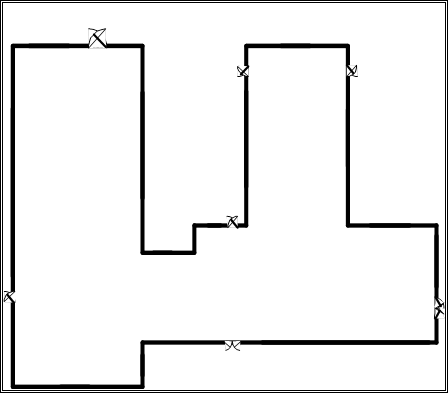
\includegraphics{media/image013.png}
\caption{On-grade configuration \protect \label{fig:on-grade-configuration}}
\end{figure}

The on-grade slab option can be used to simulate situations when the lower slab surface is near the ground surface level. In this situation, the entire floor must be included within the floor construction object. Vertical insulation is modeled by the GroundDomain in this scenario. Horizontal insulation can only be modeled as covering the full horizontal surface.

\subsubsection{Inputs}\label{inputs-16-006}

\paragraph{Field: Name}\label{field-name-8-009}

Alpha field used as a unique identifier for each ground domain.

\paragraph{Field: Ground Domain Depth}\label{field-ground-domain-depth}

Numeric field used to determine the depth of the simulation domain, in meters.

\paragraph{Field: Aspect Ratio}\label{field-aspect-ratio}

Numeric field, which is the ratio of slab length to width and is used to determine the aspect ratio of the slab. This field along with the total slab floor area, which is taken as the combination of all surfaces connected to the floor OtherSideConditionsModel, are used to determine the size and shape of the ground domain. Any given aspect ratio and its inverse should produce identical results. i.e. AR = 2 equals AR = 0.5. This field has units of meters/meters.

\paragraph{Field: Perimeter Offset}\label{field-perimeter-offset}

Numeric field used to determine the distance from the slab perimeter to the domain perimeter, in meters.

\paragraph{Field: Soil Thermal Conductivity}\label{field-soil-thermal-conductivity-3}

The thermal conductivity of the soil, in W/m-K.

\paragraph{Field: Soil Density}\label{field-soil-density-3}

The bulk density of the soil, in kg/m3.

\paragraph{Field: Soil Specific Heat}\label{field-soil-specific-heat-3}

The specific heat of dry soil, in J/kg-K. If moisture is defined in this object, moisture and freezing effects are accounted for by varying the specific heat value.

\paragraph{Field: Soil Moisture Content Volume Fraction}\label{field-soil-moisture-content-volume-fraction-1}

A nominal value of soil moisture content to be used when evaluating soil thermal properties.

\paragraph{Field: Soil Moisture Content Volume Fraction at Saturation}\label{field-soil-moisture-content-volume-fraction-at-saturation-1}

A nominal value of soil moisture content when the soil is saturated, this is used in evaluating thermal properties of freezing soil.

\paragraph{Field: Type of Undisturbed Ground Temperature Object}\label{field-type-of-undisturbed-ground-temperature-object-000}

This is the type of undisturbed ground temperature object that is used to determine the ground temperature.

\paragraph{Field: Name of Undisturbed Ground Temperature Object}\label{field-name-of-undisturbed-ground-temperature-object-000}

This is the name of the undisturbed ground temperature object that is used to determine the ground temperature.

\paragraph{Field: Evapotranspiration Ground Cover Parameter}\label{field-evapotranspiration-ground-cover-parameter-1}

Numeric field specifies the ground cover effects used in the evapotranspiration model at the ground surface heat balance. The values range from 0 (solid, non-permeable ground surface) to 1.5 (wild growth).

\paragraph{Field: Slab Boundary Condition Model Name}\label{field-slab-boundary-condition-model-name}

This is the name of the other side boundary condition model used.

\paragraph{Field: Slab Location}\label{field-slab-location}

Alpha field indicates whether the slab is in-grade (top surface level with ground surface) or on-grade (bottoms surface level with ground surface). Options include ``ONGRADE'' and ``INGRADE''.

\paragraph{Field: Slab Material Name}\label{field-slab-material-name}

Name of the material object representing the slab material. Only applicable to in-grade situations.

\paragraph{Field: Horizontal Insulation}\label{field-horizontal-insulation}

Alpha field indicates whether horizontal insulation is present. Options include ``YES'' and ``NO''. Only applicable to in-grade situations.

\paragraph{Field: Horizontal Insulation Material Name}\label{field-horizontal-insulation-material-name}

This alpha field is the name of a material object representing the horizontal slab insulation. It should be noted that the material listed here cannot be a "no mass" material (\hyperref[materialnomass]{Material:NoMass}) that is defined by R-Value only but should be defined as a regular material with an actual thickness. This optional argument is only required if horizontal insulation is present.

\paragraph{Field: Horizontal Insulation Extents}\label{field-horizontal-insulation-extents}

Alpha field indicates whether the horizontal slab insulation extends to cover the full horizontal area of the slab, or only covers the slab perimeter. Optional argument only required if horizontal insulation is present. Options include ``FULL'' and ``PERIMETER''.

\paragraph{Field: Perimeter Insulation Width}\label{field-perimeter-insulation-width}

Numeric field indicating the width of the perimeter insulation measured from the slab edge. Valid range from \textgreater{} 0 to \textless{} half of smallest slab width.

\paragraph{Field: Vertical Insulation}\label{field-vertical-insulation}

Alpha field indicates whether vertical insulation is present. Options include ``YES'' and ``NO''.

\paragraph{Field: Vertical Insulation Name}\label{field-vertical-insulation-name}

This alpha field is the name of a material object representing the vertical slab insulation. It should be noted that the material listed here cannot be a "no mass" material  (\hyperref[materialnomass]{Material:NoMass}) that is defined by R-Value only but should be defined as a regular material with an actual thickness. This optional argument is only required if vertical insulation is present.

\paragraph{Field: Vertical Insulation Depth}\label{field-vertical-insulation-depth}

Numeric field indicates the depth measured in meters from the ground surface to which the vertical perimeter insulation extends. Valid range from \textgreater{} Slab Thickness to \textless{} Domain Depth.

\paragraph{Field: Simulation Timestep}\label{field-simulation-timestep}

Alpha field indicating whether the domain will update temperatures at each zone timestep, or at hourly intervals. Options include ``timestep'' and ``hourly''.

\paragraph{Field: Geometric Mesh Coefficient}

This numeric field represents the compression of cell distribution A value in this field equal to 1 would result in a uniform distribution, while a value of 2 would provide a highly skewed distribution. Values for this field should be limited from 1.0 to 2.0. If this field is omitted, the default value is 1.6.

\paragraph{Field: Mesh Density Parameter}

This numeric integer field represents the number of cells to be placed between any two ``domain partitions'' during mesh development.~ A domain partition may be thought of as a slab edge or insulation edge. Once these components are laid out in the domain, this field number of cells are placed between the partitions. If this field is omitted, the default value is 6.

An IDF example of an in-grade slab.

\begin{lstlisting}
Site:GroundDomain:Slab,
  IngradeCoupledSlab, !- Name
  5,                  !- Ground Domain Depth
  1,                  !- Aspect Ratio
  5,                  !- Domain Perimeter Offset
  1.8,                !- Soil Thermal Conductivity
  3200,               !- Soil Density
  836,                !- Soil Specific Heat
  30,                 !- Soil Moisture Content Volume Fraction
  50,                 !- Soil Moisture Content Volume Fraction at Saturation
  Site:GroundTemperature:Undisturbed:KusudaAchenbach, !- Type of Undisturbed Ground Temperature Object
  KATemps,            !- Name of Undisturbed Ground Temperature Object
  1,                  !- Evapotranspiration Ground Cover Parameter
  GroundCoupledOSCM,  !- Name of Floor Boundary Condition Model
  InGrade,            !- Slab Location (InGrade/OnGrade)
  Slab Material-In-grade, !- Slab Material Name
  Yes,                !- Horizontal Insulation
  Slab Insulation,    !- Horizontal Insulation Material Name
  Perimeter,          !- Full Horizontal or Perimeter Only
  1,                  !- Perimeter insulation width
  Yes,                !- Vertical Insulation
  Slab Insulation,    !- Vertical Insulation Name
  2,                  !- Vertical perimeter insulation depth from surface
  Hourly;             !- Simulation timestep
\end{lstlisting}

And IDF example of an on-grade slab

\begin{lstlisting}
Site:GroundDomain:Slab,
  OngradeCoupledSlab, !- Name
  5,                  !- Ground Domain Depth {m}
  1,                  !- Aspect Ratio
  5,                  !- Domain Perimeter Offset {m}
  1.8,                !- Soil Thermal Conductivity {W/m-K}
  3200,               !- Soil Density {kg/m3}
  836,                !- Soil Specific Heat {J/kg-K}
  30,                 !- Soil Moisture Content Volume Fraction
  50,                 !- Soil Moisture Content Volume Fraction at Saturation
  Site:GroundTemperature:Undisturbed:KusudaAchenbach, !- Type of Undisturbed Ground Temperature Object
  KATemps;            !- Name of Undisturbed Ground Temperature Object
  1,                  !- Evapotranspiration Ground Cover Parameter
  GroundCoupledOSCM,  !- Name of Floor Boundary Condition Model
  OnGrade,            !- Slab Location (InGrade/OnGrade)
  ,                   !- Slab Material Name
  ,                   !- Horizontal Insulation (Yes/No)
  ,                   !- Horizontal Insulation Material Name
  ,                   !- Full Horizontal or Perimeter Only
  ,                   !- Perimeter insulation width (m)
  Yes,                !- Vertical Insulation (Yes/No)
  Slab Insulation,    !- Vertical Insulation Name
  2,                  !- Vertical perimeter insulation depth from surface
  Hourly;             !- Simulation timestep. (Timestep/Hourly)</td>
\end{lstlisting}

\subsubsection{Outputs}\label{outputs-1-015}

The following output variables are available.

\begin{itemize}
\tightlist
\item
  Zone, Average, Zone Coupled Surface Heat Flux {[}W/m2{]}
\item
  Zone, Average, Zone Coupled Surface Temperature {[}C{]}
\end{itemize}

\paragraph{Zone Coupled Surface Heat Flux {[}W/m2{]}}\label{zone-coupled-surface-heat-flux-wm2}

This is the value of the heat flux provided to the GroundDomain as a boundary condition. This is calculated by taking the average heat flux of all surfaces coupled to the domain's SurfaceProperty:OtherSideConditionsModel model.

\paragraph{Zone Coupled Surface Temperature {[}C{]}}\label{zone-coupled-surface-temperature-c}

This is the value of the SurfaceProperty:OtherSideConditionsModel surface temperature. This is the temperature provided to the ground coupled surfaces as an outside boundary condition.

\subsection{Site:GroundDomain:Basement}\label{sitegrounddomainbasement}

This section documents the input object used to simulate ground coupled heat transfer with underground zones within EnergyPlus. Zone surfaces within EnergyPlus interact with the Site:GroundDomain:Basement object by utilizing the \hyperref[surfacepropertyothersideconditionsmodel]{SurfaceProperty:OtherSideConditionsModel} object. Two separate OSCM are required for the basement vertical and horizontal surfaces. Vertical wall surfaces will interact with the first OSCM while the horizontal floor surface will interact with the second OSCM. Basement floor and wall surfaces are constructed normally by using the \hyperref[buildingsurfacedetailed]{BuildingSurface:Detailed} object, with the outside boundary condition being the OtherSideConditionsModel for the basement floor or wall. The outside surface of the wall being the interface between the ground domain and the EnergyPlus zone. Horizontal and vertical ground insulation are simulated by the ground domain, and therefore should not be included in the wall and floor construction objects.

\begin{figure}[htbp]
\centering

\includegraphics{media/image900.png}
\caption{Basement Configuration \protect \label{fig:basement-configuration}}
\end{figure}

\begin{lstlisting}
Site:GroundDomain:Basement,
  CoupledBasement,     !- Name
  10,                  !- Ground Domain Depth {m}
  1,                   !- Aspect ratio
  5,                   !- Perimeter offset {m}
  1.8,                 !- Soil Thermal Conductivity {W/m-K}
  3200,                !- Soil Density {kg/m3}
  836,                 !- Soil Specific Heat {J/kg-K}
  30,                  !- Soil Moisture Content Volume Fraction {percent}
  50,                  !- Soil Moisture Content Volume Fraction at Saturation {percent}
  Site:GroundTemperature:Undisturbed:KusudaAchenbach, !- Type of Undisturbed Ground Temperature Object
  KATemps,             !- Name of Undisturbed Ground Temperature Object
  1,                   !- Evapotranspiration Ground Cover Parameter
  BasementFloorOSCM,   !- Name of Basement Floor Boundary Condition Model
  Yes,                 !- Basement Horizontal Underfloor Insulation Present (Yes/No)
  Basement Insulation, !- Basement Horizontal Insulation Underfloor Material Name
  Full,                !- Full Horizontal or Perimeter Only (Full/Perimeter)
  ,                    !- Perimeter width (m)
  2.5,                 !- Depth of Basement Wall In Ground Domain {m}
  BasementWallOSCM,    !- Name of Basement Wall Boundary Condition Model
  Yes,                 !- Basement Wall Vertical Insulation Present(Yes/No)
  Basement Insulation, !- Basement Wall Vertical Insulation Material Name
  2.5,                 !- Vertical insulation depth from surface (m)
  Hourly;              !- Domain Update interval. (Timestep, Hourly)
  4;                   ! Mesh Density Parameter
\end{lstlisting}

\subsubsection{Inputs}\label{inputs-17-004}

\paragraph{Field: Name}\label{field-name-9-009}

Alpha field used as a unique identifier for each basement domain. Multiple basements domains can be simulated simultaneously, however, each domain must have a unique name. Additionally, despite the ability to simulate multiple domains simultaneously, these domains do not interact with each other and are treated as independent domains with boundary conditions given by the model parameters below.

\paragraph{Field: Ground Domain Depth}\label{field-ground-domain-depth-1}

Numeric field used to determine the depth of the simulation domain, in meters. A value of 10 meters is the default.

\paragraph{Field: Aspect Ratio}\label{field-aspect-ratio-1}

Numeric field, which is the ratio of basement length to width, used to determine the aspect ratio of the basement. This field along with the total basement floor area, which is taken as the combination of all surfaces connected to the floor OtherSideConditionsModel, are used to determine the size and shape of the basement domain. Aspect ratios and the inverse of aspect ratios should produce identical results. i.e. AR = 2 equals AR = 0.5. This field has units of meters/meters.

\paragraph{Field: Domain Perimeter Offset}\label{field-domain-perimeter-offset}

Numeric field used to determine the distance from the basement perimeter to the domain perimeter, in meters. A value of 5 is default.

\paragraph{Field: Soil Thermal Conductivity}\label{field-soil-thermal-conductivity-4}

The thermal conductivity of the soil, in W/m-K.

\paragraph{Field: Soil Density}\label{field-soil-density-4}

The bulk density of the soil, in kg/m3.

\paragraph{Field: Soil Specific Heat}\label{field-soil-specific-heat-4}

The specific heat of dry soil, in J/kg-K. If moisture is defined in this object, moisture and freezing effects are accounted for by varying the specific heat value.

\paragraph{Field: Soil Moisture Content Volume Fraction}\label{field-soil-moisture-content-volume-fraction-2}

A nominal value of soil moisture content to be used when evaluating soil thermal properties.

\paragraph{Field: Soil Moisture Content Volume Fraction at Saturation}\label{field-soil-moisture-content-volume-fraction-at-saturation-2}

A nominal value of soil moisture content when the soil is saturated, this is used in evaluating thermal properties of freezing soil.

\paragraph{Field: Type of Undisturbed Ground Temperature Object}\label{field-type-of-undisturbed-ground-temperature-object-1-000}

This is the type of undisturbed ground temperature object that is used to determine the ground temperature.

\paragraph{Field: Name of Undisturbed Ground Temperature Object}\label{field-name-of-undisturbed-ground-temperature-object-1-000}

This is the name of the undisturbed ground temperature object that is used to determine the ground temperature.

\paragraph{Field: Evapotranspiration Ground Cover Parameter}\label{field-evapotranspiration-ground-cover-parameter-2}

Numeric field specifies the ground cover effects used in the evapotranspiration model at the ground surface heat balance. The values range from 0 (solid, non-permeable ground surface) to 1.5 (wild growth). Model can be sensitive to variations in this parameter, especially in dry climates.

\paragraph{Field: Basement Floor Boundary Condition Model Name}\label{field-basement-floor-boundary-condition-model-name}

This is the name of the other side boundary condition model used for the basement floor surface.

\paragraph{Field: Horizontal Insulation}\label{field-horizontal-insulation-1}

Alpha field indicates whether horizontal insulation is present. Options include ``YES'' and ``NO''.

\paragraph{Field: Horizontal Insulation Name}\label{field-horizontal-insulation-name}

This alpha field is the name of a material object representing the horizontal underfloor basement insulation. It should be noted that the material listed here cannot be a "no mass" material (\hyperref[materialnomass]{Material:NoMass}) that is defined by R-Value only but should be defined as a regular material with an actual thickness. This optional argument is only required if horizontal insulation is present.

\paragraph{Field: Horizontal Insulation Extents}\label{field-horizontal-insulation-extents-1}

Alpha field indicates whether the horizontal underfloor insulation extends to cover the full horizontal area of the basement floor, or only covers the basement floor perimeter. Optional argument only required if horizontal insulation is present. Options include ``FULL'' and ``PERIMETER''.

\paragraph{Field: Perimeter Insulation Width}\label{field-perimeter-insulation-width-1}

Numeric field indicating the width of the perimeter insulation measured from the basement floor edge. Valid range from \textgreater{} 0 to \textless{} half of smallest basement floor width.

\paragraph{Field: Basement Depth}\label{field-basement-depth}

Depth of basement floor surface referenced from the ground surface, in meters. This domain should be the distance from the ground surface down to the basement floor surface. In cases where the ground surface is below the main above-ground building level, a separate wall surface should be employed between the basement walls and the main level walls.

\paragraph{Field: Basement Wall Boundary Condition Model Name}\label{field-basement-wall-boundary-condition-model-name}

Name of the other side condition boundary model used for the basement walls.

\paragraph{Field: Vertical Insulation}\label{field-vertical-insulation-1}

Alpha field indicates whether vertical insulation is present. Options include ``YES'' and ``NO''.

\paragraph{Field: Vertical Insulation Name}\label{field-vertical-insulation-name-1}

This alpha field is the name of a material object representing the vertical basement insulation. It should be noted that the material listed here cannot be a ``no mass'' material (\hyperref[materialnomass]{Material:NoMass}) that is defined by R-Value only but should be defined as a regular material with an actual thickness. This optional argument is only required if vertical insulation is present.

\paragraph{Field: Vertical Insulation Depth}\label{field-vertical-insulation-depth-1}

Numeric field indicates the depth measured in meters from the ground surface to which the vertical perimeter insulation extends. Valid range from \textgreater{} 0 to \textless{} Basement Depth.

\paragraph{Field: Simulation Timestep}\label{field-simulation-timestep-1}

Alpha field indicating whether the domain will update temperatures at each zone timestep, or at hourly intervals. Options include ``timestep'' and ``hourly''.

\paragraph{Mesh Density Parameter}\label{mesh-density-parameter}

Integer field indicating the density of the finite difference ground domain cells between the basement and the far field boundaries. Default value is 4. Total number of ground domain cells, insulation cells, and ground surface cells are indicated as outputs to the eio file.

\subsubsection{Outputs}\label{outputs-2-013}

The following output variables are available.

\begin{itemize}
\item
  Wall Interface Heat Flux
\item
  Wall Interface Temperature
\item
  Floor Interface Heat Flux
\item
  Floor Interface Temperature
\end{itemize}

\paragraph{Wall Interface Heat Flux {[}W/m2{]}}\label{wall-interface-heat-flux-wm2}

This is the value of the heat flux provided to ground domain as a boundary condition for the basement walls. Should be equal to the basement wall outside heat flux.

\paragraph{Wall Interface Temperature {[}C{]}}\label{wall-interface-temperature-c}

This is the value of the SurfaceProperty:OtherSideConditionsModel surface temperature. This is the temperature provided to the basement wall surfaces as an outside boundary condition.

\paragraph{Floor Interface Heat Flux {[}W/m2{]}}\label{floor-interface-heat-flux-wm2}

This is the value of the heat flux provided to ground domain as a boundary condition for the basement floor. Should be equal to the basement floor outside heat flux.

\paragraph{Floor Interface Temperature {[}C{]}}\label{floor-interface-temperature-c}

This is the value of the SurfaceProperty:OtherSideConditionsModel surface temperature. This is the temperature provided to the ground coupled floor surfaces as an outside boundary condition.

\subsection{Site:GroundTemperature:FCfactorMethod}\label{sitegroundtemperaturefcfactormethod}

Site:GroundTemperature:FCfactorMethod is used only by the underground walls or slabs-on-grade or underground floors defined with C-factor (\hyperref[constructioncfactorundergroundwall]{Construction:CfactorUndergroundWall}) and F-factor (\hyperref[constructionffactorgroundfloor]{Construction:FfactorGroundFloor}) method for code compliance calculations where detailed construction layers are unknown. Only one such ground temperature object can be included. The monthly ground temperatures for this object are close to the monthly outside air temperatures delayed by three months. If user does not input this object in the IDF file, it will be defaulted to the 0.5m set of monthly ground temperatures from the weather file if they are available. Entering these will also overwrite any ground temperatures from the weather file in the F and C factor usage. If neither is available, an error will result.

\subsubsection{Inputs}\label{inputs-18-004}

\paragraph{Field: Month Temperature(s) -- 12 fields in all}\label{field-month-temperatures-12-fields-in-all-3}

Each numeric field is the monthly ground temperature (degrees Celsius) used for the indicated month (January = 1\(^{st}\) field, February = 2\(^{nd}\) field, etc.)

And, the IDF example:

\begin{lstlisting}
Site:GroundTemperature:FCfactorMethod,  9.5, 3.5, -0.7, -1.7, -0.6, 3.6, 9.3, 14, 18.2, 22.7, 21.2, 16.8;
\end{lstlisting}

\subsection{Site:GroundReflectance}\label{sitegroundreflectance}

Ground reflectance values are used to calculate the ground reflected solar amount. This fractional amount (entered monthly) is used in this equation:

\begin{equation}
\rm{GroundReflectedSolar} = \left( \rm{BeamSolar} \cdot cos \left( \rm{SunZenithAngle} \right) + \rm{DiffuseSolar} \right) \cdot \rm{GroundReflectance}
\end{equation}

Of course, the Ground Reflected Solar is never allowed to be negative. The ground reflectance can be further modified when snow is on the ground by the Snow Ground Reflectance Modifier. To use no ground reflected solar in your simulation, enter 0.0 for each month.

\subsubsection{Inputs}\label{inputs-19-003}

\paragraph{Field: Month Average Ground Reflectance(s) -- 12 fields in all}\label{field-month-average-ground-reflectances-12-fields-in-all}

Each numeric field is the monthly average reflectivity of the ground used for the indicated month (January = 1\(^{st}\) field, February = 2\(^{nd}\) field, etc.)

And use in an IDF:

\begin{lstlisting}
Site:GroundReflectance,
  0.600,     !January Ground Reflectance
  0.600,     !February Ground Reflectance
  0.400,     !March Ground Reflectance
  0.300,     !April Ground Reflectance
  0.200,     !May Ground Reflectance
  0.200,     !June Ground Reflectance
  0.200,     !July Ground Reflectance
  0.200,     !August Ground Reflectance
  0.200,     !September Ground Reflectance
  0.200,     !October Ground Reflectance
  0.300,     !November Ground Reflectance
  0.400;     !December Ground Reflectance
\end{lstlisting}

\subsection{Site:GroundReflectance:SnowModifier}\label{sitegroundreflectancesnowmodifier}

It is generally accepted that snow resident on the ground increases the basic ground reflectance. EnergyPlus allows the user control over the snow ground reflectance for both ``normal ground reflected solar'' calculations (see above) and snow ground reflected solar modified for daylighting. These are entered under this object and both default to 1 (same as normal ground reflectance -- no special case for snow which is a conservative approach).

\subsubsection{Inputs}\label{inputs-20-003}

\paragraph{Field: Ground Reflected Solar Modifier}\label{field-ground-reflected-solar-modifier}

This field is a decimal number which is used to modified the basic monthly ground reflectance when snow is on the ground (from design day input or weather data values).

\begin{equation}
\rm{GroundReflectance}_{\rm{used}} = \rm{GroundReflectance} \cdot \rm{Modifier}_{\rm{Snow}}
\end{equation}

The actual Ground Reflectance is limited to {[}0.0,1.0{]}.

\paragraph{Field: Daylighting Ground Reflected Solar Modifier}\label{field-daylighting-ground-reflected-solar-modifier}

This field is a decimal number which is used to modified the basic monthly ground reflectance when snow is on the ground (from design day input or weather data values).

\begin{equation}
\rm{DaylightingGroundReflectance}_{\rm{used}} = \rm{GroundReflectance} \cdot \rm{Modifier}_{\rm{Snow}}
\end{equation}

The actual Ground Reflectance is limited to {[}0.0,1.0{]}.

An IDF example:

\begin{lstlisting}
Site:GroundReflectance:SnowModifier,
  1.0;       !- Ground Reflected Solar Modifier
\end{lstlisting}

Outputs will show both the inputs from the above object as well as monthly values for both Snow Ground Reflectance and Snow Ground Reflectance for Daylighting.

\subsection{Site:WaterMainsTemperature}\label{sitewatermainstemperature}

The Site:WaterMainsTemperature object is used to calculate water temperatures delivered by underground water main pipes. The mains temperatures are used as default, make-up water temperature inputs for several plant objects, including: \textbf{\hyperref[wateruseequipment]{WaterUse:Equipment}, \hyperref[wateruseconnections]{WaterUse:Connections}, \hyperref[waterheatermixed]{WaterHeater:Mixed}} and \textbf{\hyperref[waterheaterstratified]{WaterHeater:Stratified}}. The mains temperatures are also used in the water systems objects to model the temperature of cold water supplies.

Water mains temperatures are a function of outdoor climate conditions and vary with time of year. A correlation has been formulated to predict water mains temperatures based on two weather inputs:

\begin{itemize}
\item
  average annual outdoor air temperature (dry-bulb)
\item
  maximum difference in monthly average outdoor air temperatures
\end{itemize}

These values can be calculated from annual weather data using the auxillary program CalcSoilSurfTemp preprocessor. For more information on the water mains temperatures correlation, see the \emph{EnergyPlus Engineering Document}.

Alternatively, the Site:WaterMainsTemperature object can read values from a schedule. This is useful for measured data or when water comes from a source other than buried pipes, e.g., a river or lake.

If there is no Site:WaterMainsTemperature object in the input file, a default constant value of \SI{10}{\degreeCelsius} is assumed.

\subsubsection{Inputs}\label{inputs-21-003}

\paragraph{Field: Calculation Method}\label{field-calculation-method}

This field selects the calculation method and must have the keyword Schedule, Correlation or CorrelationFromWeatherFile. If calculation method is CorrelationFromWeatherFile, the two numeric input fields below are ignored. Instead, EnergyPlus calculates them from weather file.

\paragraph{Field: Schedule Name}\label{field-schedule-name-003}

If the calculation method is Schedule, the water mains temperatures are read from the schedule referenced by this field. If the calculation method is Correlation or CorrelationFromWeatherFile, this field is ignored.

\paragraph{Field: Annual Average Outdoor Air Temperature}\label{field-annual-average-outdoor-air-temperature}

If the calculation method is Correlation, this field is used in the calculation as the annual average outdoor air temperature (dry-bulb) {[}C{]}. If the calculation method is Schedule or CorrelationFromWeatherFile, this field is ignored.

\paragraph{Field: Maximum Difference In Monthly Average Outdoor Air Temperatures}\label{field-maximum-difference-in-monthly-average-outdoor-air-temperatures}

If the calculation method is Correlation, this field is used in the calculation as the maximum difference in monthly average outdoor air temperatures {[}\(\Delta\)C{]}. If the calculation method is Schedule or CorrelationFromWeatherFile, this field is ignored.

\begin{lstlisting}
Site:WaterMainsTemperature,
  Correlation,  !- Calculation Method {SCHEDULE | CORRELATION | CORRELATIONFROMWEATHERFILE}
  ,             !- Schedule Name
  9.69,         !- Annual Average Outdoor Air Temperature {C}
  28.1;         !- Maximum Difference In Monthly Average Outdoor Air Temperatures {deltaC}
\end{lstlisting}

\subsection{Site:Precipitation}\label{siteprecipitation}

The Site:Precipitation object is used to describe the amount of water precipitation at the building site over the course of the simulation run period. Precipitation includes both rain and the equivalent water content of snow. Precipitation is not yet described well enough in the many building weather data files. So this object can be used to provide the data using Schedule objects that define rates of precipitation in meters per hour.

A set of schedules for site precipitation have been developed for USA weather locations and are provided with EnergyPlus in the data set called PrecipitationSchedulesUSA.idf. The user can develop schedules however they want. The schedules in the data set were developed using EnergyPlus' weather file (EPW) observations and the average monthly precipitation for the closest weather site provided by NOAA. EPW files for the USA that were based on TMY or TMY2 include weather observations for Light/Moderate/Heavy rainfall, however most international locations do not include these observations. The values were modeled by taking the middle of the ranges quoted in the EPW data dictionary. The assumed piecewise function is shown below.

\begin{equation}
\rm{Amount} \, (m/hour) = \, \left\{
  \begin{array}{*{20}{c}}
    \rm{Light} = 0.0125 \\
    \rm{Moderate} = 0.052 \\
    \rm{Heavy} = 0.1
  \end{array}
\right.
\end{equation}

The values were inserted on hour by hour basis for the month based on the observations. Then each month was rescaled to meet the average precipitation for the month based on the 30-year average (1971-2000) provided by the NOAA/NCDC. Therefore, the flags in the EPW file match the precipitation schedules for the USA. Note that summing the average monthly precipitation values will not give you the average yearly precipitation. The resulting value may be lower or higher than the average yearly value.

Once the typical rainfall pattern and rates are scheduled, the Site:Precipitation object provides a method of shifting the total rainfall up or down for design purposes. Wetter or drier conditions can be modeled by changing the Design Annual Precipitation although the timing of precipitation throughout the year will not be changed.

\subsubsection{Inputs}\label{inputs-22-002}

\paragraph{Field: Precipitation Model Type}\label{field-precipitation-model-type}

Choose rainfall modeling options. Only available option is ScheduleAndDesignLevel.

\paragraph{Field: Design Level for Total Annual Precipitation}\label{field-design-level-for-total-annual-precipitation}

Magnitude of total precipitation for an annual period to be used in the model. Value selected by the user to correspond with the amount of precipitation expected or being assumed for design purposes. The units are in meters. This field works with the following two fields to allow easily shifting the amounts without having to generate new schedules.

\paragraph{Field: Precipitation Rate Schedule Name}\label{field-precipitation-rate-schedule-name}

Name of a schedule defined elsewhere that describes the rate of precipitation. The precipitation rate schedule is analogous to weather file data. However, weather files for building simulation do not currently contain adequate data for such calculations. Therefore, EnergyPlus schedules are used to enter the pattern of precipitation events. The values in this schedule are the average rate of precipitation in meters per hour. The integration of these values over an annual schedule should equal the nominal annual precipitation.

\paragraph{Field: Average Total Annual Precipitation}\label{field-average-total-annual-precipitation}

Magnitude of annual precipitation associated with the rate schedule. This value is used to normalize the precipitation.

IDF example:

\begin{lstlisting}
Site:Precipitation,
  ScheduledAndDesignLevel, !- Precipitation Model Type
  0.75,                    !- Design Level Total Annual Precipitation {m/yr}
  PrecipitationSchd,       !- Schedule Name for Precipitation Rates
  0.80771;                 !- Average Total Annual Precipitation {m/yr}
\end{lstlisting}

\subsection{RoofIrrigation}\label{roofirrigation}

The RoofIrrigation object is used to describe the amount of irrigation on the ecoroof surface over the course of the simulation runperiod. This object is used to provide irrigation data using Schedule objects that define rates of irrigation in meters per hour. These schedules can be one of two types: Schedule, or SmartSchedule.

\subsubsection{Inputs}\label{inputs-23-002}

\paragraph{Field: Irrigation Model Type}\label{field-irrigation-model-type}

Choose irrigation modeling options. Available options are \textbf{Schedule} and \textbf{SmartSchedule}. The \textbf{Schedule} type is used to force an irrigation schedule regardless of the current moisture state of the soil. The \textbf{SmartSchedule} type allows the precipitation schedule to be overridden if the current moisture state of the soil is greater than 40\% saturated.

\paragraph{Field: Irrigation Rate Schedule Name}\label{field-irrigation-rate-schedule-name}

Name of a schedule defined elsewhere that describes the rate of irrigation. The values in this schedule are the average rate of irrigation in meters per hour.

\paragraph{Field: Irrigation Maximum Saturation Threshold}\label{field-irrigation-maximum-saturation-threshold}

Used with the SmartSchedule option in the Irrigation Model Type field to override the default 40\% saturation limit for turning off the irrigation: values of 0 to 100 (percent) can be entered with 40\% being the default.

IDF example:

\begin{lstlisting}
RoofIrrigation,
  Schedule,       !- Irrigation Model Type
  IrrigationSchd; !- Schedule Name for Irrigation Rates
\end{lstlisting}

\subsection{Solar and Visible Spectrum Objects}\label{solar-and-visible-spectrum-objects}

The next two objects enable users to enter solar and visible spectrum which is used to calculate the thermal and visual performance of windows if their glazings are defined with full spectral data. EnergyPlus versions 8.0 and older hard-wired the solar and visible spectrum. The solar spectrum assumes air mass 1.5 terrestrial solar global spectral irradiance values (W/m2-micron) on a \ang{37} tilted surface, based on ISO 9845-1 and ASTM E 892; derived from Optics5 data file ISO-9845GlobalNorm.std, 10-14-99. The visible/photopic spectrum is based on CIE 1931 observer; ISO/CIE 10527, CIE Standard Calorimetric Observers; derived from Optics5 data file ``CIE 1931 Color Match from E308.txt'', which is the same as WINDOW4 file Cie31t.dat.

\subsection{Site:SolarAndVisibleSpectrum}\label{sitesolarandvisiblespectrum}

The SolarAndVisibleSpectrum object is used to specify the solar and visible spectrum data which is used as spectral weighting function to calculate the window performance (transmittance and absorptance) in EnergyPlus. This is a unique object, if it is missing from an IDF file, the default (same as EnergyPlus version 8.0) solar and visible spectrum data will be used.

\subsubsection{Inputs}\label{inputs-24-001}

\paragraph{Field: Name}\label{field-name-10-008}

This field specifies the name of the SolarAndVisibleSpectrum object.

\paragraph{Field: Spectrum Data Method}\label{field-spectrum-data-method}

This field specifies the method used to enter the spectrum data. Two choices are available: Default and UserDefined. The choice Default will continue to use the hard-wired spectrum data in EnergyPlus (for backward compatibility). The choice UserDefined allows users to specify custom solar and visible spectrum data. The default choice is Default.

\paragraph{Field: Solar Spectrum Data Name}\label{field-solar-spectrum-data-name}

This field is required if the Spectrum Data Method is set to UserDefined. This field references a spectrum dataset for solar.

\paragraph{Field: Visible Spectrum Data Name}\label{field-visible-spectrum-data-name}

This field is required if the Spectrum Data Method is set to UserDefined. This field references a spectrum dataset for visible.

IDF example:

\begin{lstlisting}
Site:SolarAndVisibleSpectrum,
  LocalSpectrum,            !- Name
  UserDefined,              !- Spectrum Data Method: Default, UserDefined
  SolarSpectrum,            !- Solar Spectrum Data Object Name
  VisibleSpectrum;          !- Visible Spectrum Data Object
\end{lstlisting}

\subsection{Site:SpectrumData}\label{sitespectrumdata}

The Site:SpectrumData object holds the user defined solar or visible spectrum data. For solar spectrum, up to 107 pairs of (wavelength, spectrum) can be entered. For visible spectrum, up to 81 pairs can be entered.

\subsubsection{Inputs}\label{inputs-25-001}

\paragraph{Field: Name}\label{field-name-11-007}

This field specifies the name of the SpectrumData object. The name must be unique across all SpectrumData objects.

\paragraph{Field: Spectrum Data Type}\label{field-spectrum-data-type}

This field specifies the type of spectrum data. Choices are Solar and Visible.

\paragraph{Field: Wavelength \textless{}n\textgreater{}}\label{field-wavelength-n}

This field specifies the n$^\textrm{th}$ wavelength in micron.

\paragraph{Field: Spectrum \textless{}n\textgreater{}}\label{field-spectrum-n}

This field specifies the n$^\textrm{th}$ spectrum corresponding to the nth wavelength.

IDF example:

\begin{lstlisting}
Site:SpectrumData,
  SolarSpectrum, !- Name
  Solar,         !- Spectrum Data Type
  0.3,0,         !- up to 107 pair of (wavelength, spectrum)
  0.305,3.4,
  0.31,15.6,
  0.315,41.1,
  0.32,71.2,
  0.325,100.2,
  0.33,152.4,
  0.335,155.6,
  0.34,179.4,
  0.345,186.7,
  0.35,212,
  0.36,240.5,
  0.37,324,
  0.38,362.4,
  ...;
\end{lstlisting}

\subsection{Climate Group Outputs}\label{outputs-3-011}

Climate related variables appear in two places for EnergyPlus outputs. Certain objects that are invariant throughout a simulation period have lines appear in the eplusout.eio file. For descriptions of this reporting, please see the Output Details and Examples document.

\subsection{Weather Data Related Outputs}\label{outputs-4-008}

Variables related to ambient environment data are available at timestep and higher resolutions. Below is a variable dictionary of these variables and subsequent definitions:

\begin{itemize}
\item
  Zone,Average,Site Outdoor Air Drybulb Temperature {[}C{]}
\item
  Zone,Average,Site Outdoor Air Dewpoint Temperature {[}C{]}
\item
  Zone,Average,Site Outdoor Air Wetbulb Temperature {[}C{]}
\item
  Zone,Average,Site Outdoor Air Humidity Ratio {[}kgWater/kgAir{]}
\item
  Zone,Average,Site Outdoor Air Relative Humidity {[}\%{]}
\item
  Zone,Average,Site Outdoor Air Barometric Pressure {[}Pa{]}
\item
  Zone,Average,Site Wind Speed {[}m/s{]}
\item
  Zone,Average,Site Wind Direction {[}deg{]}
\item
  Zone,Average,Site Sky Temperature {[}C{]}
\item
  Zone,Average,Site Horizontal Infrared Radiation Rate per Area {[}W/m2{]}
\item
  Zone,Average,Site Diffuse Solar Radiation Rate per Area {[}W/m2{]}
\item
  Zone,Average,Site Direct Solar Radiation Rate per Area {[}W/m2{]}
\item
  Zone,Average,Site Total Sky Cover []
\item
  Zone,Average,Site Opaque Sky Cover []
\item
  Zone,Sum,Site Precipitation Depth {[}m{]}
\item
  Zone,Average,Site Ground Reflected Solar Radiation Rate per Area {[}W/m2{]}
\item
  Zone,Average,Site Ground Temperature {[}C{]}
\item
  Zone,Average,Site Surface Ground Temperature {[}C{]}
\item
  Zone,Average,Site Deep Ground Temperature {[}C{]}
\item
  Zone,Average,Site Simple Factor Model Ground Temperature {[}C{]}
\item
  Zone,Average,Site Outdoor Air Enthalpy {[}J/kg{]}
\item
  Zone,Average,Site Outdoor Air Density {[}kg/m3{]}
\item
  Zone,Average,Site Solar Azimuth Angle {[}deg{]}
\item
  Zone,Average,Site Solar Altitude Angle {[}deg{]}
\item
  Zone,Average,Site Solar Hour Angle {[}deg{]}
\item
  Zone,Average,Site Rain Status {[]}
\item
  Zone,Average,Site Snow on Ground Status {[]}
\item
  Zone,Average,Site Exterior Horizontal Sky Illuminance {[}lux{]}
\item
  Zone,Average,Site Exterior Horizontal Beam Illuminance {[}lux{]}
\item
  Zone,Average,Site Exterior Beam Normal Illuminance {[}lux{]}
\item
  Zone,Average,Site Sky Diffuse Solar Radiation Luminous Efficacy {[}lum/W{]}
\item
  Zone,Average,Site Beam Solar Radiation Luminous Efficacy {[}lum/W{]}
\item
  Zone,Average,Site Daylighting Model Sky Clearness {[]}
\item
  Zone,Average,Sky Brightness for Daylighting Calculation {[]}
\item
  Zone,Average,Site Daylight Saving Time Status {[]}
\item
  Zone,Average,Site Day Type Index {[]}
\item
  Zone,Average,Site Mains Water Temperature {[}C{]}
\item
  HVAC,Average,Site Precipitation Rate {[}m/s{]}
\item
  HVAC,Sum,Site Precipitation Depth {[}m{]}
\item
  HVAC,Sum,Water System Roof Irrigation Scheduled Depth{[}m{]}
\item
  HVAC,Sum,Water System Roof Irrigation Actual Depth{[}m{]}
\end{itemize}

Note that these data values may be interpolated from ``hour'' points (ref: Weather Data Hourly Interpolation). Most of the data values represent the ``average'' over the reporting resolution period.

\subsubsection{Site Outdoor Air Drybulb Temperature {[}C{]}}\label{site-outdoor-air-drybulb-temperature-c}

This is the outdoor dry-bulb temperature in degrees C.

\subsubsection{Site Outdoor Air Dewpoint Temperature {[}C{]}}\label{site-outdoor-air-dewpoint-temperature-c}

This is the outdoor dewpoint temperature in degrees C.

\subsubsection{Site Outdoor Air Wetbulb Temperature {[}C{]}}\label{site-outdoor-air-wetbulb-temperature-c}

The outdoor wet-bulb temperature is derived (at the timestep) from the values for dry-bulb temperature, humidity ratio and barometric pressure.

\subsubsection{Site Outdoor Air Humidity Ratio {[}kgWater/kgAir{]}}\label{site-outdoor-air-humidity-ratio-kgwaterkgair}

The outdoor humidity ratio is derived (at the timestep) from the dry-bulb temperature, relative humidity and barometric pressure.

\subsubsection{Site Outdoor Air Relative Humidity {[}\%{]}}\label{site-outdoor-air-relative-humidity}

This is the outdoor relative humidity expressed in percent.

\subsubsection{Site Outdoor Air Barometric Pressure {[}Pa{]}}\label{site-outdoor-air-barometric-pressure-pa}

This is the atmospheric/barometric pressure in Pa.

\subsubsection{Site Wind Speed {[}m/s{]}}\label{site-wind-speed-ms}

This is the outdoor wind speed in m/s.

\subsubsection{Site Wind Direction {[}deg{]}}\label{site-wind-direction-deg}

This is the wind direction (N = 0, E = 90, S = 180, W = 270).

\subsubsection{Site Sky Temperature {[}C{]}}\label{site-sky-temperature-c}

The sky temperature is derived from horizontal infrared radiation intensity. It is expressed in degrees C. The default calculation is shown below but this value may be modified by the WeatherProperty:SkyTemperature object. Note that Sigma is the Stefan-Boltzmann constant in the following equation:

\begin{equation}
Sky\;Temperature = {\left( {\frac{{Horizontal\;IR}}{{Sigma}}} \right)^{\frac{1}{4}}} - {273.15_{Conversion\;from\;Kelvin\;to\;Centigrade}}
\end{equation}

\subsubsection{Site Horizontal Infrared Radiation Rate per Area {[}W/m2{]}}\label{site-horizontal-infrared-radiation-rate-per-area-wm2}

The horizontal infrared radiation intensity is expressed in \si{W/m^2} based, if missing from the weather file, on opaque sky cover, sky emissivity, temperature and other factors. The general calculation of Site Horizontal Infrared Radiation Rate per Area is discussed in both the Engineering Reference and the Auxiliary Programs document.

\subsubsection{Site Diffuse Solar Radiation Rate per Area {[}W/m2{]}}\label{site-diffuse-solar-radiation-rate-per-area-wm2}

Diffuse solar is the amount of solar radiation in \si{W/m^2} received from the sky (excluding the solar disk) on a horizontal surface.

\subsubsection{Site Direct Solar Radiation Rate per Area {[}W/m2{]}}\label{site-direct-solar-radiation-rate-per-area-wm2}

Site Direct Solar Radiation Rate per Area is amount of solar radiation in \si{W/m^2} received within a \ang{5.7} field of view centered on the sun. This is also known as Beam Solar.

\subsubsection{Site Total Sky Cover {[]}}\label{site-total-sky-cover}

This is the total sky cover in tenths of sky. The value ranges from 0 (clear) to 10 (full cover). 

\subsubsection{Site Opaque Sky Cover {[]}}\label{site-opaque-sky-cover}

This is the opaque sky cover in tenths of sky. The value ranges from 0 (clear) to 10 (full cover). 

\subsubsection{Site Precipitation Depth {[}m{]}}\label{site-precipitation-depth-m}

This is the amount of liquid precipitation (m). The source of this field may be the weather file or the Site:Precipitation object. The weather file values are in millimeters, but the report here is in meters. Two separate entities are displayed -- from the weather file the key value is ``Environment''; from the Site:Precipitation object the key value is Site:Precipitation.

If the weather file does not have a liquid precipitation field but does have the present weather fields, then a heuristic calculation is attempted for both flagging when it is raining and the amount of precipitation. If the weather file does have liquid precipitation fields, then the output (e.g. monthly) can be compared with the weather file stat file.

\subsubsection{Site Ground Reflected Solar Radiation Rate per Area {[}W/m2{]}}\label{site-ground-reflected-solar-radiation-rate-per-area-wm2}

The ground reflected solar amount (\si{W/m^2}) is derived from the Beam Solar, Diffuse Solar, User specified Ground Reflectance (for month) and Solar Altitude Angle:

\begin{multline}
  \rm{Groundreflectedsolar}
  \\
  = \left( \rm{Beamsolar} \cdot cos \left( \rm{SolarAltitudeAngle} \right) + \rm{Diffusesolar} \right) \cdot \rm{Groundreflectance}_{\rm{month}}
\end{multline}

where if the calculation returns a value \textless{} 0.0, then 0.0 will be reported.

\subsubsection{Site Ground Temperature {[}C{]}}\label{site-ground-temperature-c}

The ground temperature is reported in degrees C -- this is a user-specified input by month.

\subsubsection{Site Surface Ground Temperature {[}C{]}}\label{site-surface-ground-temperature-c}

The ground temperature is reported in degrees C -- this is a user-specified input (object: Site:GroundTemperature:Shallow) by month.

\subsubsection{Site Deep Ground Temperature {[}C{]}}\label{site-deep-ground-temperature-c}

The ground temperature is reported in degrees C -- this is a user-specified input (object: Site:GroundTemperature:Deep) by month.

\subsubsection{Site Simple Factor Model Ground Temperature {[}C{]}}\label{site-simple-factor-model-ground-temperature-c}

The Site Simple Factor Model Ground Temperature is reported in degrees C -- this is a user-specified input (object: Site:GroundTemperature:FCfactorMethod) by month or gleaned from the weather file as noted in the description of the object.

\subsubsection{Site Outdoor Air Enthalpy {[}J/kg{]}}\label{site-outdoor-air-enthalpy-jkg}

Outdoor enthalpy is derived at each timestep from the Site Outdoor Air Drybulb Temperature and the Site Outdoor Air Humidity Ratio. It is reported in J/kg.

\subsubsection{Site Outdoor Air Density {[}kg/m3{]}}\label{site-outdoor-air-density-kgm3}

Outdoor air density is derived at each timestep from the Site Outdoor Air Barometric Pressure, the Outdoor Dry-bulb temperature and the Outdoor Humidity Ratio. It is reported in units \si{kg/m^3}.

\subsubsection{Site Solar Azimuth Angle {[}deg{]}}\label{site-solar-azimuth-angle-deg}

The Solar Azimuth Angle (f) is measured from the North (clockwise) and is expressed in degrees. This is shown more clearly in the following figure.

\begin{figure}[hbtp] % fig 9
\centering
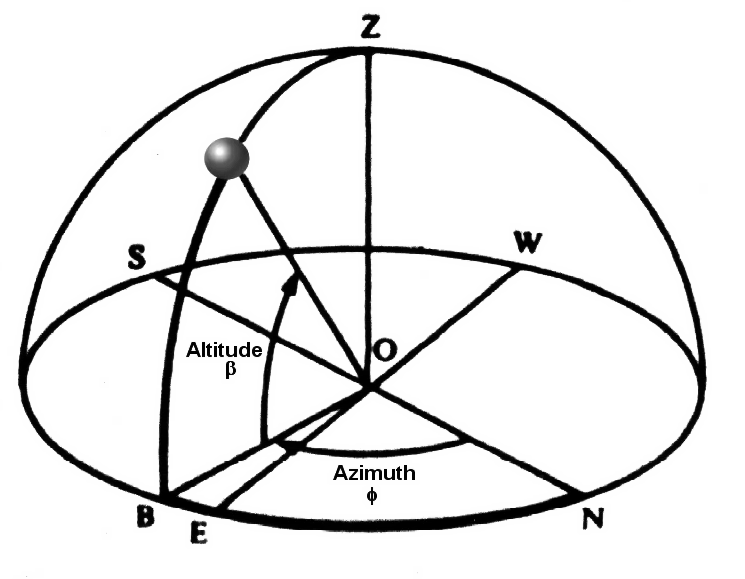
\includegraphics[width=0.9\textwidth, height=0.9\textheight, keepaspectratio=true]{media/image020.png}
\caption{Solar Position Illustration \protect \label{fig:solar-position-illustration}}
\end{figure}

\subsubsection{Site Solar Altitude Angle {[}deg{]}}\label{site-solar-altitude-angle-deg}

The Solar Altitude Angle (b) is the angle of the sun above the horizontal (degrees).

\subsubsection{Site Solar Hour Angle {[}deg{]}}\label{site-solar-hour-angle-deg}

The Solar Hour Angle (\emph{H}) gives the apparent solar time for the current time period (degrees). It is common astronomical practice to express the hour angle in hours, minutes and seconds of time rather than in degrees. You can convert the hour angle displayed from EnergyPlus to time by dividing by 15. (Note that 1 hour is equivalent to 15 degrees; \ang{360} of the Earth's rotation takes place every 24 hours.) The relationship of angles in degrees to time is shown in the following table:

% table 6
\begin{longtable}[c]{@{}ll@{}}
\caption{Relationship of Angles (degrees) to Time \label{table:relationship-of-angles-degrees-to-time}} \tabularnewline
\toprule
Unit of Angle & Equivalent time \tabularnewline
\midrule
\endfirsthead

\caption[]{Relationship of Angles (degrees) to Time} \tabularnewline
\toprule
Unit of Angle & Equivalent time \tabularnewline
\midrule
\endhead

1 radian & 3.819719 hours \tabularnewline
1 degree & 4 minutes \tabularnewline
1 arcmin & 4 seconds \tabularnewline
1 arcsec & 0.066667 seconds \tabularnewline
\bottomrule
\end{longtable}

\subsubsection{Site Rain Status {[]}}\label{site-rain-status}

This field shows whether or not (1 = yes, 0 = no) the weather shows ``raining''. For a Design Day, one can denote rain for the entire day but not timestep by timestep. Weather files may indicate rain for a single time interval. This is an ``averaged'' field -- thus a 1 shown for a time period (e.g. daily reporting) means that it was raining during each timestep of that period.

\subsubsection{Site Snow on Ground Status {[]}}\label{site-snow-on-ground-status}

This field shows whether or not (1 = yes, 0 = no) the weather shows ``snow on the ground''. For a Design Day, one can denote snow for the entire day but not timestep by timestep. Weather files may indicate snow (snow depth) for a single time interval. This is an ``averaged'' field -- thus a 1 shown for a time period (e.g. daily reporting) means that there was snow on the ground during each timestep of that period.

\subsubsection{Site Daylight Saving Time Status {[]}}\label{site-daylight-saving-time-status}

This field shows when daylight saving time (1 = yes, 0 = no) is in effect. Though shown as an average variable, this value is only set on a daily basis.

\subsubsection{Site Day Type Index {[]}}\label{site-day-type-index}

This field shows what ``day type'' the current day is. Day types are (1 = Sunday, 2 = Monday, etc.) with Holiday = 8, SummerDesignDay = 9, WinterDesignDay = 10, CustomDay1 = 11, CustomDay2 = 12. Though shown as an average variable, this value is only set on a daily basis.

\subsubsection{Site Mains Water Temperature {[}C{]}}\label{site-mains-water-temperature-c}

The value of the Water Mains Temperature is reported in C following the calculation shown in the Water Mains Temperature object.

\subsubsection{Site Precipitation Rate {[}m/s{]}}\label{site-precipitation-rate-ms}

\subsubsection{Site Precipitation Depth {[}m{]}}\label{site-precipitation-depth-m-1}

The rate and quantity of precipitation at the site. These outputs are only available if a Site Precipitation object is used. Precipitation is measured in meters.

\subsubsection{Water System Roof Irrigation Scheduled Depth{[}m{]}}\label{water-system-roof-irrigation-scheduled-depthm}

This is the scheduled amount of irrigation for the green roof (ecoroof) based on the user input. Amount is measured in meters.

\subsubsection{Water System Roof Irrigation Actual Depth{[}m{]}}\label{water-system-roof-irrigation-actual-depthm}

This is the actual amount of irrigation for the green roof (ecoroof) based on the scheduled user input and moisture state/saturation of the soil. Amount is measured in meters.

\subsection{Outputs for local temperature/wind speed calculations}\label{outputs-for-local-temperaturewind-speed-calculations}

Local atmospheric properties for outdoor air temperature and wind speed are separately calculated and reported for all zones, surfaces, and outdoor air nodes. The output variables are associated with their respective objects:

\begin{itemize}
\item
  Zone,Average,Zone Outdoor Air Drybulb Temperature {[}C{]}
\item
  Zone,Average,Zone Outdoor Air Wetbulb Temperature {[}C{]}
\item
  Zone,Average,Zone Outdoor Air Wind Speed {[}m/s{]}
\item
  Zone,Average,Surface Ext Outdoor Dry Bulb {[}C{]}
\item
  Zone,Average,Surface Ext Outdoor Wet Bulb {[}C{]}
\item
  Zone,Average,Surface Ext Wind Speed {[}m/s{]}
\item
  HVAC,Average,System Node Temperature {[}C{]}~~~~~~~ (for OUTDOOR AIR NODE object)
\end{itemize}

\subsubsection{Zone Outdoor Air Drybulb Temperature {[}C{]}}\label{zone-outdoor-air-drybulb-temperature-c}

The outdoor air dry-bulb temperature calculated at the height above ground of the zone centroid.

\subsubsection{Zone Outdoor Air Wetbulb Temperature {[}C{]}}\label{zone-outdoor-air-wetbulb-temperature-c}

The outdoor air wet-bulb temperature calculated at the height above ground of the zone centroid.

\subsubsection{Zone Outdoor Air Wind Speed {[}m/s{]}}\label{zone-outdoor-air-wind-speed-ms}

The outdoor wind speed calculated at the height above ground of the zone centroid.

\subsubsection{Surface Ext Outdoor Dry Bulb {[}C{]}}\label{surface-ext-outdoor-dry-bulb-c}

The outdoor air dry-bulb temperature calculated at the height above ground of the surface centroid.

\subsubsection{Surface Ext Outdoor Wet Bulb {[}C{]}}\label{surface-ext-outdoor-wet-bulb-c}

The outdoor air wet-bulb temperature calculated at the height above ground of the surface centroid.

\subsubsection{Surface Ext Wind Speed {[}m/s{]}}\label{surface-ext-wind-speed-ms}

The outdoor wind speed calculated at the height above ground of the surface centroid.

\subsubsection{System Node Temperature {[}C{]}}\label{system-node-temperature-c}

When reporting for the \textbf{\hyperref[outdoorairnode]{OutdoorAir:Node}} object, this is the outdoor air dry-bulb temperature calculated at the height above ground of the node, if height is specified in the input.


\section{Group -- Schedules}\label{group-schedules}

This group of objects allows the user to influence scheduling of many items (such as occupancy density, lighting, thermostatic controls, occupancy activity). In addition, schedules are used to control shading element density on the building.

EnergyPlus schedules consist of three pieces: a day description, a week description, and an annual description. An optional element is the schedule type. Each description level builds off the previous sub-level. The day description is simply a name and the values that span the 24 hours in a day to be associated with that name. The week description also has an identifier (name) and twelve additional names corresponding to previously defined day descriptions. There are names for each individual day of the week plus holiday, summer design day, winter design day and two more custom day designations. Finally, the annual schedule contains an identifier and the names and FROM-THROUGH dates of the week schedules associate with this annual schedule. The annual schedule can have several FROM-THROUGH date pairs. One type of schedule reads the values from an external file to facilitate the incorporation of monitored data or factors that change throughout the year.

Schedules are processed by the EnergyPlus Schedule Manager, stored within the Schedule Manager and are accessed through module routines to get the basic values (timestep, hourly, etc). Values are resolved at the Zone Timestep frequency and carry through any HVAC timesteps.

\subsection{Day Type}\label{day-type}

A brief description of ``Day Type'' which is used in the SizingPeriod objects, RunPeriodControl:SpecialDays object, the Sizing objects and also used by reference in the Schedule:Week:Daily object (discussed later in this section).

Schedules work on days of the week as well as certain specially designated days. Days of the week are the normal -- Sunday, Monday, Tuesday, Wednesday, Thursday, Friday and Saturday. Special day types that can be designated are: Holiday, SummerDesignDay, WinterDesignDay, CustomDay1, CustomDay2. These day types can be used at the user's convenience to designate special scheduling (e.g.~lights, electric equipment, set point temperatures) using these days as reference.

For example, a normal office building may have normal ``occupancy'' rules during the weekdays but significantly different use on weekend. For this, you would set up rules/schedules based on the weekdays (Monday through Friday, in the US) and different rules/schedules for the weekend (Saturday and Sunday, in the US). However, you could also specially designate SummerDesignDay and WinterDesignDay schedules for sizing calculations. These schedules can be activated by setting the Day Type field in the Design Day object to the appropriate season (\textbf{SummerDesignDay} for cooling design calculations; \textbf{WinterDesignDay} for heating design calculations).

In a different building, such as a theater/playhouse, the building may only have occupancy during certain weeks of the year and/or certain hours of certain days. If it was every week, you could designate the appropriate values during the ``regular'' days (Sunday through Saturday). But this would also be an ideal application for the ``CustomDay1'' and/or ``CustomDay2''. Here you would set the significant occupancy, lighting, and other schedules for the custom days and use unoccupied values for the normal weekdays. Then, using a weather file and setting special day periods as appropriate, you will get the ``picture'' of the building usage during the appropriate periods.

\subsection{ScheduleTypeLimits}\label{scheduletypelimits}

Schedule types can be used to validate portions of the other schedules. Hourly day schedules, for example, are validated by range -- minimum/maximum (if entered) -- as well as numeric type (continuous or discrete). Annual schedules, on the other hand, are only validated for range -- as the numeric type validation has already been done.

\subsubsection{Inputs}\label{inputs-042}

\paragraph{Field: Name}\label{field-name-041}

This alpha field should contain a unique (within the schedule types) designator. It is referenced wherever Schedule Type Limits Names can be referenced.

\paragraph{Field: Lower Limit Value}\label{field-lower-limit-value}

In this field, the lower (minimum) limit value for the schedule type should be entered. If this field is left blank, then the schedule type is not limited to a minimum/maximum value range.

\paragraph{Field: Upper Limit Value}\label{field-upper-limit-value}

In this field, the upper (maximum) limit value for the schedule type should be entered. If this field is left blank, then the schedule type is not limited to a minimum/maximum value range.

\paragraph{Field: Numeric Type}\label{field-numeric-type}

This field designates how the range values are validated. Using \textbf{Continuous} in this field allows for all numbers, including fractional amounts, within the range to be valid. Using \textbf{Discrete} in this field allows only integer values between the minimum and maximum range values to be valid.

\paragraph{Field: Unit Type}\label{field-unit-type}

This field is used to indicate the kind of units that may be associated with the schedule that references the ScheduleTypeLimits object. It is used by IDF Editor to display the appropriate SI and IP units. This field is not used by EnergyPlus. The available options are shown below. If none of these options are appropriate, select \textbf{Dimensionless.}

\begin{itemize}
\item
  Dimensionless
\item
  Temperature
\item
  DeltaTemperature
\item
  PrecipitationRate
\item
  Angle
\item
  Convection Coefficient
\item
  Activity Level
\item
  Velocity
\item
  Capacity
\item
  Power
\item
  Availability
\item
  Percent
\item
  Control
\item
  Mode
\end{itemize}

Several IDF Examples will illustrate the use:

\begin{lstlisting}
ScheduleTypeLimits,Any Number;  ! Not limited
ScheduleTypeLimits,Fraction, 0.0 , 1.0 ,CONTINUOUS;
ScheduleTypeLimits,Temperature,-60,200,CONTINUOUS;
ScheduleTypeLimits,Control Type,0,4,DISCRETE;
ScheduleTypeLimits,On/Off,0,1,DISCRETE;
\end{lstlisting}

\subsection{Day Schedules}\label{day-schedules}

The day schedules perform the assignment of pieces of information across a 24 hour day. This can occur in various fashions including a 1-per hour assignment, a user specified interval scheme or a list of values that represent an hour or portion of an hour.

\subsection{Schedule:Day:Hourly}\label{scheduledayhourly}

The Schedule:Day:Hourly contains an hour-by-hour profile for a single simulation day.

\subsubsection{Inputs}\label{inputs-1-039}

\paragraph{Field: Name}\label{field-name-1-038}

This field should contain a unique (within all DaySchedules) designation for this schedule. It is referenced by WeekSchedules to define the appropriate schedule values.

\paragraph{Field: Schedule Type Limits Name}\label{field-schedule-type-limits-name-000}

This field contains a reference to the Schedule Type Limits object. If found in a list of Schedule Type Limits (see ScheduleTypeLimits object above), then the restrictions from the referenced object will be used to validate the hourly field values (below).

\paragraph{Field: Hour Values (1-24)}\label{field-hour-values-1-24}

These fields contain the hourly values for each of the 24 hours in a day. (Hour field 1 represents clock time 00:00:01 AM to 1:00:00 AM, hour field 2 is 1:00:01 AM to 2:00:00 AM, etc.) The values in these fields will be passed to the simulation as indicated for ``scheduled'' items.

An IDF example:

\begin{lstlisting}
Schedule:Day:Hourly, Day On Peak, Fraction,
  0.,0.,0.,0.,0.,0.,0.,0.,0.,1.,1.,1.,1.,1.,1.,1.,1.,1.,0.,0.,0.,0.,0.,0.;
\end{lstlisting}

\subsection{Schedule:Day:Interval}\label{scheduledayinterval}

The Schedule:Day:Interval introduces a slightly different way of entering the schedule values for a day. Using the intervals, you can shorten the ``hourly'' input of the ``Schedule:Day:Hourly'' object to 2 fields. And, more importantly, you can enter an interval that represents only a portion of an hour. Schedule values are ``given'' to the simulation at the zone timestep, so there is also a possibility of ``interpolation'' from the entries used in this object to the value used in the simulation.

\subsubsection{Inputs}\label{inputs-2-036}

\paragraph{Field: Name}\label{field-name-2-034}

This field should contain a unique (within all DaySchedules) designation for this schedule. It is referenced by WeekSchedules to define the appropriate schedule values.

\paragraph{Field: Schedule Type Limits Name}\label{field-schedule-type-limits-name-1-000}

This field contains a reference to the Schedule Type Limits object. If found in a list of Schedule Type Limits (see ScheduleTypeLimits object above), then the restrictions from the referenced object will be used to validate the hourly field values (below).

\paragraph{Field: Interpolate to Timestep}\label{field-interpolate-to-timestep}

Three possible inputs are available for this field: Average, Linear, and No. The default value is No.

If ``Average'' is entered, it is used to apply values that aren't coincident with the given timestep (ref: Timestep) intervals. If ``Average'' is entered, then any intervals entered here will be interpolated/averaged and that value will be used at the appropriate minute in the hour. For example, if ``Average'' is entered and the interval is every 15 minutes (say a value of 0 for the first 15 minutes, then .5 for the second 15 minutes) AND there is a 10 minute timestep for the simulation: the value at 10 minutes will be 0 and the value at 20 minutes will be .25. In earlier versions of EnergyPlus, this was the Yes option for the field.

If ``No'' is entered, then the value that occurs on the appropriate minute in the hour will be used as the schedule value. For the same input entries but ``no'' for this field, the value at 10 minutes will be 0 and the value at 20 minutes will be .5. No is the default for this field.

If ``Linear'' is entered, then the value that is used is based on the linear interpolation between successive values. With linear, if the value at 1:00 is 0.0 and the value at 2:00 is 10.0, with fifteen minute timesteps, the value at 1:15 would be 2.5, the value at 1:30 would be 5.0 and the value at 1:45 would be 7.5. 

\paragraph{Field-Set: Time and Value (extensible object)}\label{field-set-time-and-value-extensible-object}

To specify each interval, both an ``until'' time (which includes the designated time) and the value must be given.

\paragraph{Field: Time}\label{field-time}

The value of each field should represent clock time (standard) in the format ``Until: HH:MM''. 24 hour clock format (i.e.~1PM is 13:00) is used. Note that Until: 7:00 includes all times up through 07:00 or 7am.

\paragraph{Field: Value}\label{field-value}

This represents the actual value to be passed to the simulation at the appropriate timestep. (Using interpolation value as shown above). Limits on the values are indicated by the Schedule Type Limits Name field of this object.

And an example of use:

\begin{lstlisting}
Schedule:Day:Interval,
  dd winter rel humidity, !- Name
  Percent,                !- Schedule Type Limits Name
  No,                     !- Interpolate to Timestep
  until: 24:00,           !- Time 1
  74;                     !- Value Until Time 1
\end{lstlisting}

\subsection{Schedule:Day:List}\label{scheduledaylist}

To facilitate possible matches to externally generated data intervals, this object has been included. In similar fashion to the Schedule:Day:Interval object, this object can also include ``sub-hourly'' values but must represent a complete day in its list of values.

\subsubsection{Inputs}\label{inputs-3-032}

\paragraph{Field: Name}\label{field-name-3-028}

This field should contain a unique (within all day schedules) designation for this schedule. It is referenced by week schedules to define the appropriate schedule values.

\paragraph{Field: Schedule Type Limits Name}\label{field-schedule-type-limits-name-2-000}

This field contains a reference to the Schedule Type Limits object. If found in a list of Schedule Type Limits (see ScheduleTypeLimits object above), then the restrictions from the referenced object will be used to validate the hourly field values (below).

\paragraph{Field: Interpolate to Timestep}\label{field-interpolate-to-timestep-1}

Three possible inputs are available for this field: Average, Linear, and No. The default value is No.

If ``Average'' is entered, it is used to apply values that aren't coincident with the given timestep (ref: Timestep) intervals. If ``Average'' is entered, then any intervals entered here will be interpolated/averaged and that value will be used at the appropriate minute in the hour. For example, if ``Average'' is entered and the interval is every 15 minutes (say a value of 0 for the first 15 minutes, then .5 for the second 15 minutes) AND there is a 10 minute timestep for the simulation: the value at 10 minutes will be 0 and the value at 20 minutes will be .25. In earlier versions of EnergyPlus, this was the Yes option for the field.

If ``No'' is entered, then the value that occurs on the appropriate minute in the hour will be used as the schedule value. For the same input entries but ``no'' for this field, the value at 10 minutes will be 0 and the value at 20 minutes will be .5. No is the default for this field.

If ``Linear'' is entered, then the value that is used is based on the linear interpolation between successive values. With linear, if the value at 1:00 is 0.0 and the value at 2:00 is 10.0, with fifteen minute timesteps, the value at 1:15 would be 2.5, the value at 1:30 would be 5.0 and the value at 1:45 would be 7.5. 


\paragraph{Field: Minutes Per Item}\label{field-minutes-per-item}

This field allows the ``list'' interval to be specified in the number of minutes for each item. The value here must be \textless{} = 60 and evenly divisible into 60 (same as the timestep limits).

\paragraph{Field Value 1 (same definition for each value -- up to 1440 (24*60) allowed)}\label{field-value-1-same-definition-for-each-value-up-to-1440-2460-allowed}

This is the value to be used for the specified number of minutes.

For example:

\begin{lstlisting}
Schedule:Day:List,
  Myschedule, ! name
  Fraction,   ! Schedule type
  No,         ! Interpolate value
  30,         ! Minutes per item
  0.0,        ! from 00:01 to 00:30
  0.5,        ! from 00:31 to 01:00
  <snipped>
\end{lstlisting}

\subsection{Week Schedule(s)}\label{week-schedules}

The week schedule object(s) perform the task of assigning the day schedule to day types in the simulation. The basic week schedule is shown next.

\subsection{Schedule:Week:Daily}\label{scheduleweekdaily}

\subsubsection{Inputs}\label{inputs-4-029}

\paragraph{Field: Name}\label{field-name-4-025}

This field should contain a unique (within all WeekSchedules) designation for this schedule. It is referenced by Schedules to define the appropriate schedule values.

\paragraph{Field: Schedule Day Name Fields (12 day types -- Sunday, Monday, \ldots{} )}\label{field-schedule-day-name-fields-12-day-types-sunday-monday}

These fields contain day schedule names for the appropriate day types. Days of the week (or special days as described earlier) will then use the indicated hourly profile as the actual schedule value.

An IDF example:

\begin{lstlisting}
Schedule:Week:Daily, Week on Peak,
  Day On Peak,Day On Peak,Day On Peak,
  Day On Peak,Day On Peak,Day On Peak,
  Day On Peak,Day On Peak,Day On Peak,
  Day On Peak,Day On Peak,Day On Peak;
\end{lstlisting}

\subsection{Schedule:Week:Compact}\label{scheduleweekcompact}

Further flexibility can be realized by using the Schedule:Week:Compact object. In this the fields, after the name is given, a ``for'' field is given for the days to be assigned and then a dayschedule name is used.

\subsubsection{Inputs}\label{inputs-5-026}

\paragraph{Field:Name}\label{fieldname}

This field should contain a unique (within all WeekSchedules) designation for this schedule. It is referenced by Schedules to define the appropriate schedule values.

\paragraph{Field-Set -- DayType List\#, Schedule:Day Name \#}\label{field-set-daytype-list-scheduleday-name}

Each assignment is made in a pair-wise fashion. First the ``days'' assignment and then the dayschedule name to be assigned. The entire set of day types must be assigned or an error will result.

\paragraph{Field: DayType List \#}\label{field-daytype-list}

This field can optionally contain the prefix ``For'' for clarity. Multiple choices may then be combined on the line. Choices are: Weekdays, Weekends, Holidays, Alldays, SummerDesignDay, WinterDesignDay, Sunday, Monday, Tuesday, Wednesday, Thursday, Friday, Saturday, CustomDay1, CustomDay2. In fields after the first ``for'', AllOtherDays may also be used. Note that the colon (:) after the For is optional but is suggested for readability.

\paragraph{Field: Schedule:Day Name \#}\label{field-scheduleday-name}

This field contains the name of the day schedule (any of the Schedule:Day object names) that is to be applied for the days referenced in the prior field.

Some IDF examples:

\begin{lstlisting}
Schedule:Week:Compact, Week on Peak,
  For: AllDays,
  Day On Peak;

Schedule:Week:Compact, WeekDays on Peak,
  WeekDays,
  Day On Peak,
  AllOtherDays
  Day Off Peak;
\end{lstlisting}

\subsection{Schedule:Year}\label{scheduleyear}

The yearly schedule is used to cover the entire year using references to week schedules (which in turn reference day schedules). If the entered schedule does not cover the entire year, a fatal error will result.

\subsubsection{Inputs}\label{inputs-6-023}

\paragraph{Field: Name}\label{field-name-5-021}

This field should contain a unique (between Schedule:Year, Schedule:Compact, and Schedule:File) designation for the schedule. It is referenced by various ``scheduled'' items (e.g.~Lights, People, Infiltration) to define the appropriate schedule values.

\paragraph{Field: Schedule Type Limits Name}\label{field-schedule-type-limits-name-3}

This field contains a reference to the Schedule Type Limits object. If found in a list of Schedule Type Limits (see ScheduleTypeLimits object above), then the restrictions from the referenced object will be used to validate the hourly field values (below).

\paragraph{Field Set (WeekSchedule, Start Month and Day, End Month and Day)}\label{field-set-weekschedule-start-month-and-day-end-month-and-day}

Each of the designated fields is used to fully define the schedule values for the indicated time period). Up to 53 sets can be used. An error will be noted and EnergyPlus will be terminated if an incomplete set is entered. Missing time periods will also be noted as warning errors; for these time periods a zero (0.0) value will be returned when a schedule value is requested. Each of the sets has the following 5 fields:

\paragraph{Field: Schedule Week Name \#}\label{field-schedule-week-name}

This field contains the appropriate WeekSchedule name for the designated time period.

\paragraph{Field: Start Month \#}\label{field-start-month}

This numeric field is the starting month for the schedule time period.

\paragraph{Field: Start Day \#}\label{field-start-day}

This numeric field is the starting day for the schedule time period.

\paragraph{Field: End Month \#}\label{field-end-month-000}

This numeric field is the ending month for the schedule time period.

\paragraph{Field: End Day \#}\label{field-end-day}

This numeric field is the ending day for the schedule time period.

Note that there are many possible periods to be described. An IDF example with a single period:

\begin{lstlisting}
Schedule:Year, On Peak, Fraction,
  Week On Peak, 1,1, 12,31;
\end{lstlisting}

And a multiple period illustration:

\begin{lstlisting}
Schedule:Year,CoolingCoilAvailSched,Fraction,
  FanAndCoilAllOffWeekSched, 1,1, 3,31,
  FanAndCoilSummerWeekSched, 4,1, 9,30,
  FanAndCoilAllOffWeekSched, 10,1, 12,31;
\end{lstlisting}

The following definition will generate an error (if any scheduled items are used in the simulation):

\begin{lstlisting}
Schedule:Year,MySchedule,Fraction,4,1,9,30;
\end{lstlisting}

\subsection{Schedule:Compact}\label{schedulecompact}

For flexibility, a schedule can be entered in ``one fell swoop''. Using the Schedule:Compact object, all the features of the schedule components are accessed in a single command. Like the ``regular'' schedule object, each schedule:compact entry must cover all the days for a year. Additionally, the validations for DaySchedule (i.e.~must have values for all 24 hours) and WeekSchedule (i.e.~must have values for all day types) will apply. Schedule values are ``given'' to the simulation at the zone timestep, so there is also a possibility of ``interpolation'' from the entries used in this object to the value used in the simulation.

This object is an unusual object for description. For the data the number of fields and position are not set, they cannot really be described in the usual Field \# manner. Thus, the following description will list the fields and order in which they must be used in the object. The name and schedule type are the exceptions:

\subsubsection{Inputs}\label{inputs-7-023}

\paragraph{Field: Name}\label{field-name-6-019}

This field should contain a unique (between Schedule:Year, Schedule:Compact, and Schedule:File) designation for the schedule. It is referenced by various ``scheduled'' items (e.g.~Lights, People, Infiltration) to define the appropriate schedule values.

\paragraph{Field: Schedule Type Limits Name}\label{field-schedule-type-limits-name-4}

This field contains a reference to the Schedule Type Limits object. If found in a list of Schedule Type Limits (see ScheduleTypeLimits object above), then the restrictions from the referenced object will be used to validate the hourly field values (below).

\paragraph{Field-Set (Through, For, Interpolate, Until, Value)}\label{field-set-through-for-interpolate-until-value}

Each compact schedule must contain the elements Through (date), For (days), Interpolate (optional), Until (time of day) and Value. In general, each of the ``titled'' fields must include the ``title''. Note that the colon (:) after these elements (Through, For, Until) is optional but is suggested for readability.

\paragraph{Field: Through}\label{field-through}

This field starts with ``Through:'' and contains the ending date for the schedule period (may be more than one). Refer to Table~\ref{table:date-field-interpretation}. Date Field Interpretation for information on date entry -- note that only Month-Day combinations are allowed for this field. Each ``through'' field generates a new WeekSchedule named ``Schedule Name''\_wk\_\# where \# is the sequential number for this compact schedule.

\paragraph{Field: For}\label{field-for}

This field starts with ``For:'' and contains the applicable days (reference the compact week schedule object above for complete description) for the 24 hour period that must be described. Each ``for'' field generates a new DaySchedule named ``Schedule Name''\_dy\_\# where \# is the sequential number for this compact schedule.

\paragraph{Field: Interpolate (optional)}\label{field-interpolate-optional}

This field, if used, starts with ``Interpolate:'' and contains the word ``Average'', ``Linear'' or ``No''. If this field is not used, it should not be blank -- rather just have the following field appear in this slot. 

If ``Average'' is entered, it is used to apply values that aren't coincident with the given timestep (ref: Timestep) intervals. If ``Average'' is entered, then any intervals entered here will be interpolated/averaged and that value will be used at the appropriate minute in the hour. For example, if ``Average'' is entered and the interval is every 15 minutes (say a value of 0 for the first 15 minutes, then .5 for the second 15 minutes) AND there is a 10 minute timestep for the simulation: the value at 10 minutes will be 0 and the value at 20 minutes will be .25. In earlier versions of EnergyPlus, this was the Yes option for the field.

If ``No'' is entered, then the value that occurs on the appropriate minute in the hour will be used as the schedule value. For the same input entries but ``no'' for this field, the value at 10 minutes will be 0 and the value at 20 minutes will be .5. No is the default for this field.

If ``Linear'' is entered, then the value that is used is based on the linear interpolation between successive values. With linear, if the value at 1:00 is 0.0 and the value at 2:00 is 10.0, with fifteen minute timesteps, the value at 1:15 would be 2.5, the value at 1:30 would be 5.0 and the value at 1:45 would be 7.5. 



\paragraph{Field: Until}\label{field-until}

This field contains the ending time (again, reference the interval day schedule discussion above) for the current days and day schedule being defined.

\paragraph{Field: Value}\label{field-value-1}

Finally, the value field is the schedule value for the specified time interval.

And, some IDF examples:

\begin{lstlisting}
Schedule:Compact,
  POFF,       !- Name
  Fraction,   !- Schedule Type Limits Name
  Through: 4/30,
  For: AllDays,
  Until: 24:00, 1.0,
  Through: 12/31,
  For: Weekdays,
    Until: 7:00,   .1,
    Until: 17:00, 1.0,
    Until: 24:00,  .1,
  For: Weekends Holidays,
    Until: 24:00,  .1,
  For: AllOtherDays,
    Until: 24:00,  .1;

! Schedule Continuous
Schedule:Compact,
  Continuous,
  on/off,
  Through: 12/31,
  For: AllDays,
    Until: 24:00, 1.0;

! Schedule Daytime Ventilation
Schedule:Compact,
  Daytime Ventilation,
  Fraction,
  Through: 12/31,
  For: Weekdays SummerDesignDay,
    Until: 08:00, 0.0,
    Until: 18:00, 1.0,
    Until: 24:00, 0.0,
  For: Weekends WinterDesignDay,
    Until: 10:00, 0.0,
    Until: 16:00, 1.0,
    Until: 24:00, 0.0,
  For: Holidays AllOtherDays,
    Until: 24:00, 0.0;
\end{lstlisting}

\subsection{Schedule:Constant}\label{scheduleconstant}

The constant schedule is used to assign a constant hourly value. This schedule is created when a fixed hourly value is desired to represent a period of interest (e.g., always on operation mode for supply air fan).

\subsubsection{Inputs}\label{inputs-8-021}

\paragraph{Field: Name}\label{field-name-7-018}

This field should contain a unique name designation for this schedule. It is referenced by Schedules to define the appropriate schedule value.

\paragraph{Field: Schedule Type Limits Name}\label{field-schedule-type-limits-name-5}

This field contains a reference to the Schedule Type Limits object. If found in a list of Schedule Type Limits (see ScheduleTypeLimits object above), then the restrictions from the referenced object will be used to validate the hourly field values (below).

\paragraph{Field: Hourly Value}\label{field-hourly-value}

This field contains a constant real value. A fixed value is assigned as an hourly value.

An IDF example:

\begin{lstlisting}
Schedule:Constant,
  AlwaysOn,     !- Name
  On/Off,       !- Schedule Type Limits Name
  1.0;          !- Hourly Value

ScheduleTypeLimits,
  On/Off,       !- Name
  0,            !- Lower Limit Value
  1,            !- Upper Limit Value
  DISCRETE,     !- Numeric Type
  Availability; !- Unit Type
\end{lstlisting}

\subsection{Schedule:File}\label{schedulefile}

At times, data is available from a building being monitored or for factors that change throughout the year. The Schedule:File object allows this type of data to be used in EnergyPlus as a schedule. Schedule:File can also be used to read in hourly or sub-hourly schedules computed by other software or developed in a spreadsheet or other utility.

The format for the data file referenced is a text file with values separated by commas (or other optional delimiters) with one line per hour. The file may contain header lines that are skipped. The file should contain values for an entire year (8760 or 8784 hours of data) or a warning message will be issued. Multiple schedules may be created using a single external data file or multiple external data files may be used. The first row of data must be for January 1, hour 1 (or timestep 1 for subhourly files).

Schedule:File may be used along with the FuelFactors object and TDV files in the DataSets directory to compute Time Dependent Valuation based source energy as used by the California Energy Commission's Title 24 Energy Code. See Fuel Factor for more discussion on Time Dependent Valuation.

Two optional fields: \textbf{Interpolate to Timestep} and \textbf{Minutes per Item} allow for the input of sub-hourly schedules (similar to the Schedule:Day:List object).

\subsubsection{Inputs}\label{inputs-9-019}

\paragraph{Field: Name}\label{field-name-8-018}

This field should contain a unique (between Schedule:Year, Schedule:Compact, and Schedule:File) designation for the schedule. It is referenced by various ``scheduled'' items (e.g.~Lights, People, Infiltration, FuelFactors) to define the appropriate schedule values.

\paragraph{Field: Schedule Type Limits Name}\label{field-schedule-type-limits-name-6}

This field contains a reference to the Schedule Type Limits object. If found in a list of Schedule Type Limits (see ScheduleTypeLimits object above), then the restrictions from the referenced object will be used to validate the hourly field values (below).

\paragraph{Field: File Name}\label{field-file-name}

This field contains the name of the file that contains the data for the schedule. The field should include a full path with file name, for best results. The field must be \(\le\) 100 characters. The file name must not include commas or an exclamation point. A relative path or a simple file name should work with version 7.0 or later when using EP-Launch even though EP-Launch uses temporary directories as part of the execution of EnergyPlus. If using RunEPlus.bat to run EnergyPlus from the command line, a relative path or a simple file name may work if RunEPlus.bat is run from the folder that contains EnergyPlus.exe.

\paragraph{Field: Column Number}\label{field-column-number}

The column that contains the value to be used in the schedule. The first column is column one. If no data for a row appears for a referenced column the value of zero is used for the schedule value for that hour.

\paragraph{Field: Rows to Skip at Top}\label{field-rows-to-skip-at-top}

Many times the data in a file contains rows (lines) that are describing the files or contain the names of each column. These rows need to be skipped and the number of skipped rows should be entered for this field. The next row after the skipped rows must contain data for January 1, hour 1.

\paragraph{Field: Number of Hours of Data}\label{field-number-of-hours-of-data}

The value entered in this field should be either 8760 or 8784 as the number of hours of data. 8760 does not include the extra 24 hours for a leap year (if needed). 8784 will include the possibility of leap year data which can be processed according to leap year indicators in the weather file or specified elsewhere. Note if the simulation does not have a leap year specified but the schedule file contains 8784 hours of data, the first 8760 hours of data will be used. The schedule manager will not know to skip the 24 hours representing February 29.

\paragraph{Field: Column Separator}\label{field-column-separator-001}

This field specifies the character used to separate columns of data if the file has more than one column. The choices are: Comma, Tab, Fixed (spaces fill each column to a fixed width), or Semicolon. The default is Comma.

\paragraph{Field: Interpolate to Timestep}\label{field-interpolate-to-timestep-2}

The value contained in this field directs how to apply values that aren't coincident with the given timestep (ref: TimeStep object) intervals. If ``Yes'' is entered, then any intervals entered here will be interpolated/averaged and that value will be used at the appropriate minute in the hour. If ``No'' is entered, then the value that occurs on the appropriate minute in the hour will be used as the schedule value.

For example, if ``yes'' is entered and the minutes per item is 15 minutes (say a value of 0 for the first 15 minutes, then .5 for the second 15 minutes) AND there is a 10 minute timestep for the simulation: the value at 10 minutes will be 0 and the value at 20 minutes will be .25. For the same input entries but ``no'' for this field, the value at 10 minutes will be 0 and the value at 20 minutes will be .5.

\paragraph{Field: Minutes Per Item}\label{field-minutes-per-item-1}

This field represents the number of minutes for each item -- in this case each line of the file. The value here must be \(\le\) 60 and evenly divisible into 60 (same as the timestep limits).

Here is an IDF example:

\begin{lstlisting}
Schedule:File,
  elecTDVfromCZ01res, !- Name
  Any Number,         !- ScheduleType
  TDV_kBtu_CTZ01.csv, !- Name of File
  2,                  !- Column Number
  4,                  !- Rows to Skip at Top
  8760,               !- Number of Hours of Data
  Comma;              !- Column Separator
\end{lstlisting}

or with a relational path:

\begin{lstlisting}
Schedule:File,
  elecTDVfromCZ01res, !- Name
  Any Number,         !- ScheduleType
  DataSets\TDV\TDV_kBtu_CTZ01.csv,  !- Name of File
  2,                  !- Column Number
  4;                  !- Rows to Skip at Top
\end{lstlisting}

A sub-hourly indication. Note that this is identical to an hourly file because there are 60 minutes per item -- the number of hours defaults to 8760 and the column separator defaults to a comma. If the number of minutes per item had been, say, 15, then the file would need to contain 8760*4 or 35,040 rows for this item.

\begin{lstlisting}
Schedule:File,
  elecTDVfromCZ06com, !- Name
  Any Number,         !- Schedule Type Limits Name
  DataSets\TDV\TDV_2008_kBtu_CTZ06.csv, !- File Name
  1,                  !- Column Number
  4,                  !- Rows to Skip at Top
  ,                   !- Number of Hours of Data
  ,                   !- Column Separator
  ,                   !- Interpolate to Timestep
  60;                 !- Minutes per Item
\end{lstlisting}

\subsubsection{Outputs}\label{outputs-031}

An optional report can be used to gain the values described in the previous Schedule objects. This is a condensed reporting that illustrates the full range of schedule values -- in the style of input: DaySchedule, WeekSchedule, Annual Schedule.

\begin{lstlisting}
! will give them on hourly increments (day schedule resolution)
Output:Reports, Schedules, Hourly;
! will give them at the timestep of the simulation
Output:Reports, Schedules, Timestep;
\end{lstlisting}

This report is placed on the eplusout.eio file. Details of this reporting are shown in the Output Details and Examples document.

\paragraph{Schedule Value Output}\label{schedule-value-output}

\begin{lstlisting}
Zone,Average,Schedule Value {[]}
\end{lstlisting}

\paragraph{Schedule Value}\label{schedule-value}

This is the schedule value (as given to whatever entity that uses it). It has no units in this context because values may be many different units (i.e.~temperatures, fractions, watts). For best results, you may want to apply the schedule name when you use this output variable to avoid output proliferation. For example, the following reporting should yield the values shown above, depending on day of week and day type:

\begin{lstlisting}
Output:Variable,People_Shopping_Sch,Schedule Value,hourly;
Output:Variable,Activity_Shopping_Sch,Schedule Value,hourly;
\end{lstlisting}

\subsection{Schedule:File:Shading}\label{schedulefileshading}

The Schedule:File:Shading object allows shading schedules to be imported altogether from a file. The object can also be used to read in hourly schedules of the sunlit fraction of all exterior surfaces computed by other software or developed in a spreadsheet or other utility.

The format for the data file is Comma-separated values (CSV). The CSV file referenced is a text file with values separated by commas (or other optional delimiters) with one line per hour. Each column stores the annual shading sunlit fraction schedule data of an exterior surface. To map to the surface, each column should name its column header exactly the same with the surface name defined in the Surface:Detailed object. The file should contain values for an entire year (8760 or 8784 hours of data) or a warning message will be issued.

With a Schedule:File:Shading object defined, the shading schedules for all exterior surfaces (if defined) can be imported altogether without repeatedly defining Schedule:File objects.

\subsubsection{Inputs}\label{inputs-schedule-file-shading}

\paragraph{Field: File Name}\label{field-file-name}

This field contains the name of the file that contains the data for the shading schedules. The field should include a full path with file name, for best results. The field must be \(\le\) 100 characters. The file name must not include commas or an exclamation point. A relative path or a simple file name should work with version 7.0 or later when using EP-Launch even though EP-Launch uses temporary directories as part of the execution of EnergyPlus. If using RunEPlus.bat to run EnergyPlus from the command line, a relative path or a simple file name may work if RunEPlus.bat is run from the folder that contains EnergyPlus.exe.

Here is an IDF example:

\begin{lstlisting}
Schedule:File,
  eplusshading.csv;   !- Name of File
\end{lstlisting}

\section{Group -- Surface Construction Elements}\label{group-surface-construction-elements}

This group of objects describes the physical properties and configuration for the building envelope and interior elements. That is, the walls, roofs, floors, windows, doors for the building.

\subsection{Specifying the Building Envelope}\label{specifying-the-building-envelope}

Building element constructions in EnergyPlus are built from the basic thermal and other material property parameters in physical constructions. Materials are specified by types~ and named. Constructions are defined by the composition of materials. Finally, surfaces are specified for the building with geometric coordinates as well as referenced constructions.

\subsection{Material and Material Properties}\label{material-and-material-properties}

There are several material ``types'' which may be used to describe layers within opaque construction elements. The choice of which of these types to use is left up to the user. However, some guidance as to which material type to use is appropriate before describing each in detail. The opaque types are:

\begin{itemize}
\item
  Material
\item
  \hyperref[materialnomass]{Material:NoMass}
\item
  \hyperref[materialairgap]{Material:AirGap}
\item
  \hyperref[materialroofvegetation]{Material:RoofVegetation}
\item
  \hyperref[materialinfraredtransparent]{Material:InfraredTransparent}
\end{itemize}

\hyperref[material]{Material} is the ``preferred'' type of material. This requires knowledge of many of the thermal properties of the material, but it allows EnergyPlus to take into account the thermal mass of the material and thus allows the evaluation of transient conduction effects. \hyperref[materialnomass]{Material:NoMass} is similar in nature but only requires the thermal resistance (R-value) rather than the thickness, thermal conductivity, density, and specific heat. Note that using a simple R-value only material forces EnergyPlus to assume steady state heat conduction through this material layer. Finally, \hyperref[materialairgap]{Material:AirGap} should only be used for an air gap between other layers in a construction. This type assumes that air is sufficiently lightweight to require only an R-value. In addition, since it is not exposed to any external environment, surface properties such as absorptance are not necessary. \hyperref[materialroofvegetation]{Material:RoofVegetation} is used to help model ``green roofs''. \hyperref[materialinfraredtransparent]{Material:InfraredTransparent} is used similarly to the NoMass materials. Each of these materials is described in more detail below.

There are several material additions that can be made to the basic material properties. These additional material types are:

\begin{itemize}
\item
  \hyperref[materialpropertymoisturepenetrationdepthsettings]{MaterialProperty:MoisturePenetrationDepth:Settings}
\item
  \hyperref[materialpropertyheatandmoisturetransfersorptionisotherm]{MaterialProperty:HeatAndMoistureTransfer:SorptionIsotherm}
\item
  \hyperref[materialpropertyheatandmoisturetransferdiffusion]{MaterialProperty:HeatAndMoistureTransfer:Diffusion}
\item
  \hyperref[materialpropertyheatandmoisturetransfersettings]{MaterialProperty:HeatAndMoistureTransfer:Settings}
\item
  \hyperref[materialpropertyheatandmoisturetransferredistribution]{MaterialProperty:HeatAndMoistureTransfer:Redistribution}
\item
  \hyperref[materialpropertyheatandmoisturetransfersuction]{MaterialProperty:HeatAndMoistureTransfer:Suction}
\item
  \hyperref[materialpropertyheatandmoisturetransferthermalconductivity]{MaterialProperty:HeatAndMoistureTransfer:ThermalConductivity}
\item
  \hyperref[materialpropertyphasechange]{MaterialProperty:PhaseChange}
\item
  \hyperref[materialpropertyphasechangehysteresis]{MaterialProperty:PhaseChangeHysteresis}
\end{itemize}

These material property objects are used in conjunction with the basic material specification and reference back to the name of the basic material type. Without the basic material type specified the program, will give a severe error and terminate. For example, specifying the moisture materials and changing the \hyperref[heatbalancealgorithm]{HeatBalanceAlgorithm} to a moisture simulation will allow the moisture simulation to take place.

\subsection{Material}\label{material}

This definition should be used when the four main thermal properties (thickness, conductivity, density, and specific heat) of the material are known. This syntax is used to describe opaque construction elements only.

When a Material is used for the Construction of a building surface, care should be taken to not attempt to model assemblies that were not included in the intended scope of applicability for the underlying heat transfer models.~ The building surface models are for normal applications to building energy efficiency where the main focus is on assemblies with some thermal resistance. Extremely thin and/or highly conductive material layers should be neglected from the Construction rather than included because they will not contribute to the assembly's overall thermal resistance or heat capacity. For some cases, thin and/or highly conductive materials are a serious problem for the heat transfer modeling and the values for thickness, conductivity, density and specific heat are checked for appropriateness. This check calculates the Material's thermal diffusivity from the inputs for conductivity, density, and specific heat and compares it to a maximum threshold of 1.E-5 (m\(^{2}\)/s). If the diffusivity is above this threshold, then the program checks if the layer is sufficiently thick and may issue a warning if it is too thin and highly conductive.

The absorptance values in this object impart surface properties to the construction and should be applied to the thermally significant inner and outer layers in the overall assembly.~ Attempting to trick the program by modeling thin ``paint'' layers to apply surface properties is not a good idea; the models were not intended to support such strategies.

\subsubsection{Inputs}\label{inputs-046}

\paragraph{Field: Name}\label{field-name-045}

This field is a unique reference name that the user assigns to a particular material. This name can then be referred to by other input data (ref: Construction object).

\paragraph{Field: Roughness}\label{field-roughness-000}

This alpha field defines the relative roughness of a particular material layer. This parameter only influences the convection coefficients, more specifically the exterior convection coefficient. A special keyword is expected in this field with the options being ``VeryRough'', ``Rough'', ``MediumRough'', ``MediumSmooth'', ``Smooth'', and ``VerySmooth'' in order of roughest to smoothest options.

\paragraph{Field: Thickness}\label{field-thickness}

This field characterizes the thickness of the material layer in meters. This should be the dimension of the layer in the direction perpendicular to the main path of heat conduction. This value must be a positive. \textbf{Modeling layers thinner (less) than 0.003 m is not recommended; rather, add those properties to one of the adjacent layers.}

\paragraph{Field: Conductivity}\label{field-conductivity}

This field is used to enter the thermal conductivity of the material layer. Units for this parameter are W/(m-K). Thermal conductivity must be greater than zero. \textbf{Modeling layers with conductivity higher than 5.0 W/(m-K) is not recommended; however, this may be appropriate for non-surfaces such as pipes and TDDs (ref. \hyperref[daylightingdevicetubular]{DaylightingDevice:Tubular} object).}

\paragraph{Field: Density}\label{field-density}

This field is used to enter the density of the material layer in units of kg/m\(^{3}\). Density must be a positive quantity. \textbf{In some cases textbooks and references may use g/m\(^{3}\): be careful to not confuse units.}

\paragraph{Field: Specific Heat}\label{field-specific-heat}

This field represents the specific heat of the material layer in units of J/(kg-K). Note that these units are most likely different than those reported in textbooks and references which tend to use kJ/(kg-K) or J/(g-K). They were chosen for internal consistency within EnergyPlus. \textbf{Only values of specific heat of 100 or larger are allowed. Typical ranges are from 800 to 2000 J/(kg-K).}

\paragraph{Field: Thermal Absorptance}\label{field-thermal-absorptance}

The thermal absorptance field in the Material input syntax represents the fraction of incident long wavelength (>2.5 microns) radiation that is absorbed by the material. This parameter is used when calculating the long wavelength radiant exchange between various surfaces and affects the surface heat balances (both inside and outside as appropriate). For long wavelength radiant exchange, thermal emissivity and thermal emittance are equal to thermal absorptance. Values for this field must be between 0.0 and 1.0 (with 1.0 representing ``black body'' conditions). The default value for this field is 0.9.

\paragraph{Field: Solar Absorptance}\label{field-solar-absorptance}

The solar absorptance field in the Material input syntax represents the fraction of incident~ solar radiation that is absorbed by the material. Solar radiation (0.3 to 2.537 microns) includes the visible spectrum as well as infrared and ultraviolet wavelengths. This parameter is used when calculating the amount of incident solar radiation absorbed by various surfaces and affects the surface heat balances (both inside and outside as appropriate). If solar reflectance (or reflectivity) data is available, then absorptance is equal to 1.0 minus reflectance (for opaque materials). Values for this field must be between 0.0 and 1.0. The default value for this field is 0.7.

\paragraph{Field: Visible Absorptance}\label{field-visible-absorptance}

The visible absorptance field in the Material input syntax represents the fraction of incident visible wavelength radiation that is absorbed by the material. Visible wavelength radiation ( 0.37 to 0.78 microns weighted by photopic response) is slightly different than solar radiation in that the visible band of wavelengths is much more narrow while solar radiation includes the visible spectrum as well as infrared and ultraviolet wavelengths. This parameter is used when calculating the amount of incident visible radiation absorbed by various surfaces and affects the surface heat balances (both inside and outside as appropriate) as well as the daylighting calculations. If visible reflectance (or reflectivity) data is available, then absorptance is equal to 1.0 minus reflectance (for opaque materials). Values for this field must be between 0.0 and 1.0. The default value for this field is 0.7.

An IDF example:

\begin{lstlisting}

Material,A2 - 4 IN DENSE FACE BRICK,  ! Material Name
   Rough,  ! Roughness
    0.1014984    ,  ! Thickness {m}
     1.245296    ,   ! Conductivity {W/M*K}
     2082.400    ,   ! Density {Kg/M**3}
    920.4800    ,   ! Specific Heat {J/Kg*K}
    0.9000000    ,   ! Thermal Absorptance
    0.9300000    ,   ! Solar Absorptance
    0.9300000    ;   ! Visible Absorptance
\end{lstlisting}

\subsection{Material:NoMass}\label{materialnomass}

Use this definition when only the thermal resistance (R value) of the material is known. This object is used to describe opaque construction elements.

\subsubsection{Inputs}\label{inputs-1-043}

\paragraph{Field: Name}\label{field-name-1-042}

This field is a unique reference name that the user assigns to a particular material. This name can then be referred to by other input data (ref: Construction object).

\paragraph{Field: Roughness}\label{field-roughness-1}

This alpha field defines the relative roughness of a particular material layer. This parameter only influences the convection coefficients, more specifically the exterior convection coefficient. A~ keyword is expected in this field with the options being ``\textbf{VeryRough}'', ``\textbf{Rough}'', ``\textbf{MediumRough}'', ``\textbf{MediumSmooth}'', ``\textbf{Smooth}'', and ``\textbf{VerySmooth}'' in order of roughest to smoothest options.

\paragraph{Field: Thermal Resistance}\label{field-thermal-resistance}

This field is used to enter the thermal resistance (R-value) of the material layer. Units for this parameter are (m\(^{2}\)-K)/W. Thermal resistance must be greater than zero. Note that most R-values in the USA are calculated in Inch-Pound units and must be converted to the SI equivalent.

\paragraph{Field: Thermal Absorptance}\label{field-thermal-absorptance-1}

The thermal absorptance field in the Material input syntax represents the fraction of incident long wavelength (>2.5 microns) radiation that is absorbed by the material. This parameter is used when calculating the long wavelength radiant exchange between various surfaces and affects the surface heat balances (both inside and outside as appropriate). For long wavelength radiant exchange, thermal emissivity and thermal emittance are equal to thermal absorptance. Values for this field must be between 0.0 and 1.0 (with 1.0 representing ``black body'' conditions). The default value for this field is 0.9.

\paragraph{Field: Solar Absorptance}\label{field-solar-absorptance-1}

The solar absorptance field in the Material input syntax represents the fraction of incident~ solar radiation that is absorbed by the material. Solar radiation (0.3 to 2.537 microns) includes the visible spectrum as well as infrared and ultraviolet wavelengths. This parameter is used when calculating the amount of incident solar radiation absorbed by various surfaces and affects the surface heat balances (both inside and outside as appropriate). If solar reflectance (or reflectivity) data is available, then absorptance is equal to 1.0 minus reflectance (for opaque materials). Values for this field must be between 0.0 and 1.0. The default value for this field is 0.7.

\paragraph{Field: Visible Absorptance}\label{field-visible-absorptance-1}

The visible absorptance field in the Material input syntax represents the fraction of incident visible wavelength radiation that is absorbed by the material. Visible wavelength radiation ( 0.37 to 0.78 microns weighted by photopic response) is slightly different than solar radiation in that the visible band of wavelengths is much more narrow while solar radiation includes the visible spectrum as well as infrared and ultraviolet wavelengths. This parameter is used when calculating the amount of incident visible radiation absorbed by various surfaces and affects the surface heat balances (both inside and outside as appropriate) as well as the daylighting calculations. If visible reflectance (or reflectivity) data is available, then absorptance is equal to 1.0 minus reflectance (for opaque materials). Values for this field must be between 0.0 and 1.0. The default value for this field is 0.7.

An IDF example:

\begin{lstlisting}

Material:NoMass,R13LAYER,  ! Material Name
   Rough,  ! Roughness
     2.290965    ,  ! Resistance {M**2K/W}
    0.9000000    ,   ! Thermal Absorptance
    0.7500000    ,   ! Solar Absorptance
    0.7500000    ;   ! Visible Absorptance
\end{lstlisting}

\subsection{Material:InfraredTransparent}\label{materialinfraredtransparent}

A Infrared Transparent surface is similar to a resistance-only surface.~ The idd object for this type of surface is shown below.~ The surface will actually participate in the transfer of visible and solar radiation by doing a wavelength transformation and making all short wave length radiation that is incident on the surface into long wave length radiation and having it participate in the long wavelength radiant exchange.~ \textbf{Note the ConvectionCoefficient instructions that follow the Infrared Transparent construction object below}.

\subsubsection{Inputs}\label{inputs-2-040}

\paragraph{Field: Name}\label{field-name-2-037}

This field contains the unique name (across all Material objects) for the Infrared Transparent material.

A Infrared Transparent surface should not participate in a convective/conductive exchange between the zones it separates.~ In order to minimize this effect, the ConvectionCoefficients object must be used for the surfaces referencing the Infrared Transparent (IRT) construction.

An example idf object specification for use with the IRT surface is shown below. Note that surfaces are not described in this example

\begin{lstlisting}

Material:InfraredTransparent,
      IRTMaterial1;            !- Name


  Construction,
      IRTSurface,              !- Name
      IRTMaterial1;            !- Outside Layer


  SurfaceProperty:ConvectionCoefficients,
      Bottom:Top,              !- SurfaceName
      Outside,                 !- Convection Type 1
      value,                   !- Convection Value Type 1
      0.1,                     !- Convection value 1 {W/m2-K}
      ,                        !- Convection Schedule 1
      Inside,                  !- Convection Type 2
      value,                   !- Convection Value Type 2
      0.1;                     !- Convection value 2 {W/m2-K}


  SurfaceProperty:ConvectionCoefficients,
      SecondLevel:Bottom,      !- SurfaceName
      Outside,                 !- Convection Type 1
      value,                   !- Convection Value Type 1
      0.1,                     !- Convection value 1 {W/m2-K}
      ,                        !- Convection Schedule 1
      Inside,                  !- Convection Type 2
      value,                   !- Convection Value Type 2
      0.1;                     !- Convection value 2 {W/m2-K}


  SurfaceProperty:ConvectionCoefficients,
      SecondLevel:Top,         !- SurfaceName
      Outside,                 !- Convection Type 1
      value,                   !- Convection Value Type 1
      0.1,                     !- Convection value 1 {W/m2-K}
      ,                        !- Convection Schedule 1
      Inside,                  !- Convection Type 2
      value,                   !- Convection Value Type 2
      0.1;                     !- Convection value 2 {W/m2-K}


  SurfaceProperty:ConvectionCoefficients,
      ThirdLevel:Bottom,       !- SurfaceName
      Outside,                 !- Convection Type 1
      value,                   !- Convection Value Type 1
      0.1,                     !- Convection value 1 {W/m2-K}
      ,                        !- Convection Schedule 1
      Inside,                  !- Convection Type 2
      value,                   !- Convection Value Type 2
      0.1;                     !- Convection value 2 {W/m2-K}
\end{lstlisting}

\subsection{Material:AirGap}\label{materialairgap}

This material is used to describe the air gap in an opaque construction element. Glass elements use a different property (WindowGas) to describe the air between two glass layers.

\subsubsection{Inputs}\label{inputs-3-036}

\paragraph{Field: Name}\label{field-name-3-031}

This field is a unique reference name that the user assigns to a particular material. This name can then be referred to by other input data (ref: Construction object).

\paragraph{Field: Thermal Resistance}\label{field-thermal-resistance-1}

This field is used to enter the thermal resistance (R-value) of the material layer. Units for this parameter are (m\(^{2}\)-K)/W. Thermal resistance must be greater than zero. Note that most R-values in the USA are calculated in Inch-Pound units and must be converted to the SI equivalent.

An IDF example:

\begin{lstlisting}

Material:AirGap,B1 - AIRSPACE RESISTANCE,  ! Material Name
    0.1603675    ;  ! Resistance {M**2K/W}
\end{lstlisting}

\subsection{MaterialProperty:MoisturePenetrationDepth:Settings}\label{materialpropertymoisturepenetrationdepthsettings}

This material is used to describe the nine moisture material properties
that are used in the EMPD (Effective Moisture Penetration Depth) heat
balance solution algorithm. The EMPD algorithm is a simplified, lumped
moisture model that simulates moisture storage and release from interior
surfaces. The model uses convective mass transfer
coefficients that are determined by existing heat and mass transfer
relationships, e.g.~the Lewis relation. The EMPD model includes two
fictitious layers of material with uniform moisture content: a surface
layer, which accounts for short-term moisture buffering, and a deep
layer, which accounts for more slowly responding moisture buffering. The
model calculates the moisture transfer between the air and the surface
layer and between the surface layer and the deep layer. This moisture
transfer impacts the zone humidity, and also impacts the zone
temperature through latent-to-sensible conversion from the heat of
adsorption.

This moisture model is used when the appropriate EMPD moisture
materials are specified and the Solution Algorithm parameter is set to
MoisturePenetrationDepthConductionTransferFunction.

\subsubsection{Inputs}\label{empd-inputs}

\paragraph{Field: Name}\label{materialpropertymoisturepenetrationdepthsettings-field-name}

This field is a unique reference name that the user assigns to a
particular material. This name can then be referred to by other input
data (ref: Construction object).

\paragraph{Field: Water Vapor Diffusion Resistance
	Factor}\label{field-water-vapor-diffusion-resistance-factor}

The vapor diffusion resistance factor is the resistance to water vapor
diffusion \emph{relative} to the resistance to water vapor diffusion in
stagnant air. In other words, \(\mu\) equals 1 for air, and is generally
greater than 1 for building materials.

The equation for \(\mu\) is:

\[ \mu = \frac {\delta_{perm,air}} {\delta_{perm}} \]

where \(\delta_{perm,air}\) is the permeability of water vapor in air
{[}kg/m-s-Pa{]}, and \(\delta_{perm}\) is the permeability of water
vapor in the material. The permeability of water vapor in air can be
estimated as:

\[ \delta_{perm,air} = \frac {2 \times 10^{-7} \cdot T^{0.81}} {P_{ambient}} \]

where \(T\) is the temperature {[}C{]} and \(P_{ambient}\) the ambient
atmospheric pressure {[}Pa{]}.

\paragraph{Fields: Moisture equilibrium
	constants}\label{fields-moisture-equilibrium-constants}

The next four fields, coefficients \emph{a}, \emph{b}, \emph{c}, and \emph{d},
define the sorption isotherm curve used for building materials under
equilibrium conditions. They define the relationship between
the material's moisture content and the surface air relative humidity
(ref: Effective Moisture Penetration Depth (EMPD) Model in the
Engineering Reference):

\[ u = a \cdot \phi^b + c \cdot \phi^d \]

where

\(a,b,c,d\) = Coefficients to define the relationship between the
material's moisture content and the surface air relative humidity

\(u\) = Moisture content defined as the mass fraction of water contained
in a material, per mass of dry material {[}kg/kg{]}

\(\phi\) = Surface air relative humidity {[}0 to 1{]},

\paragraph{Field: Surface Layer Penetration
	Depth}\label{field-surface-layer-penetration-depth}

The Surface Layer Penetration Depth is the fictitious thickness of the
surface layer in meters, and is used to calculate the volume of material
that participates in short-term moisture transfer and storage. This
layer has a uniform moisture content, and can be considered a
\emph{lumped-capacitance}. The penetration depth is based on the amount
of material that interacts with the zone air when subject to a cyclic
relative humidity variation. It also impacts the mass transfer resistance
between the zone air and this layer, with thinner depths resulting in lower
mass transfer resistances (ref: Effective Moisture Penetration Depth (EMPD) Model
in the Engineering Reference). For this reason very small values can lead to
instabilities depending on the timestep.The surface penetration depth can be
estimated with the following equation:

\[ d_{EMPD,surf} = \sqrt{\frac{\delta_{perm} P_{sat} \tau_{surf}}{\rho_{material} \frac{du}{d\phi} \pi}} \]

where

\(\delta_{perm}\) = water vapor permeability in the material, kg/m-s-Pa
(see Vapor diffusion resistance factor above)

\(P_{sat}\) = saturated vapor pressure at some nominal temperature, Pa

\(\tau_{surf}\) = cycle period of typical RH variations, s. 24 hours
(87600 s) is often used.

\(\rho_{material}\) = dry density of material, kg/m\^{}3

\(\frac{du}{d\phi}\) = slope of moisture soprtion curve,
\(a b \phi^{b-1} + c d \phi^{d-1}\)

If this field is left blank or set to \texttt{autocalculate},
the above equation will be used to calculate the surface layer penetration depth
assuming a $\tau_{surf}$ of 24 hours.
To use a period different than 24 hours, the equation above can be used to calculate the penetration depth based on a different value of $\tau_{surf}$. The penetration depth can also be entered as an empirical value, as in \href{http://dx.doi.org/10.1016/j.enbuild.2016.02.008}{\emph{Woods and Winkler, 2016}}. If calculating $d_{EMPD,surf}$, the assumed value of $\tau_{surf}$ should not be less than 4x the simulation timestep to ensure an accurate and stable solution.

\paragraph{Field: Deep Layer Penetration
	Depth}\label{field-deep-layer-penetration-depth}

The Deep Layer Penetration Depth is the fictitious thickness of the deep
layer in meters, and is used to calculate the volume of material that
participates in long-term moisture transfer and storage. This layer has
a uniform moisture content, and can be considered a
\emph{lumped-capacitance}. The deep penetration depth is based on the
amount of material that interacts with the surface layer when subject to
cyclic relative humidity variation. The deep penetration depth can be
estimated with the following equation:

\[ d_{EMPD,deep} = \sqrt{\frac{\delta_{perm} P_{sat} \tau_{deep}} {\rho_{material} \frac{du}{d\phi} \pi}} \]

where each term is the same as the surface layer, except that the cycle
period is different. This is usually on the order of weeks for the deep
layer.

If this field is left blank or set to \texttt{autocalculate},
the above equation will be used to calculate the deep layer penetration depth
assuming a $\tau_{deep}$ of three weeks. To use a period different than 3 weeks, the equation above can be used to calculate the penetration depth based on a different value of $\tau_{deep}$. The penetration depth can also be entered as an empirical value, as in \href{http://dx.doi.org/10.1016/j.enbuild.2016.02.008}{\emph{Woods and Winkler, 2016}}.


\paragraph{Field: Coating Layer
	Thickness}\label{field-coating-layer-thickness}

The Coating Layer Thickness (in meters) adds an additional resistance
between the surface layer and the zone and represents a thin coating,
such as paint, plaster, or other wall coverings.

This input is optional, and an input of zero implies no coating.

\paragraph{Field: Coating Layer Water Vapor Diffusion Resistance
	Factor}\label{field-coating-layer-water-vapor-diffusion-resistance-factor}

The vapor diffusion resistance factor of the coating is the coating's
resistance to water vapor diffusion \emph{relative} to the resistance to
water vapor diffusion in stagnant air (see Vapor diffusion resistance
factor section above).

This input is optional, and an input of zero implies no coating.

Below are two IDF examples:

This set of inputs can be used for aerated concrete (assuming linear
sorption curve). Density, input elsewhere, is 650 kg/m\^{}3:

\begin{lstlisting}
MaterialProperty:MoisturePenetrationDepth:Settings,
Concrete,            !- Name
6.55,                !- Water Vapor Diffusion Resistance Factor {dimensionless}
0.066,               !- Moisture Equation Coefficient a {dimensionless}
1,                   !- Moisture Equation Coefficient b {dimensionless}
0,                   !- Moisture Equation Coefficient c {dimensionless}
1,                   !- Moisture Equation Coefficient d {dimensionless}
0.007,               !- Surface Layer Penetration Depth {m}
0.024,               !- Deep Layer Penetration Depth {m}
0,                   !- Coating Layer Thickness {m}
1;                   !- Coating Layer Water Vapor Diffusion Resistance Factor {dimensionless}
\end{lstlisting}

This set of inputs is for gypsum board with density 750 kg/m\^{}3. This
also assumes 2 coats of latex paint:

\begin{lstlisting}
MaterialProperty:MoisturePenetrationDepth:Settings,
Concrete,            !- Name
6.0,                 !- Water Vapor Diffusion Resistance Factor {dimensionless}
0.0065,              !- Moisture Equation Coefficient a {dimensionless}
0.65,                !- Moisture Equation Coefficient b {dimensionless}
0.022,               !- Moisture Equation Coefficient c {dimensionless}
10,                  !- Moisture Equation Coefficient d {dimensionless}
0.021,               !- Surface Layer Penetration Depth {m}
0.08,                !- Deep Layer Penetration Depth {m}
0.0003,              !- Coating Layer Thickness {m}
6000;                !- Coating Layer Water Vapor Diffusion Resistance Factor {dimensionless}
\end{lstlisting}

Finally, here are values representing the empirical whole-house inputs
from Woods et al., 2014 (see Engineering Reference). Density is 800
kg/m\^{}3:

\begin{lstlisting}
MaterialProperty:MoisturePenetrationDepth:Settings,
Concrete,            !- Name
8.0,                 !- Water Vapor Diffusion Resistance Factor {dimensionless}
0.012,               !- Moisture Equation Coefficient a {dimensionless}
1,                   !- Moisture Equation Coefficient b {dimensionless}
0,                   !- Moisture Equation Coefficient c {dimensionless}
1,                   !- Moisture Equation Coefficient d {dimensionless}
0.019,               !- Surface Layer Penetration Depth {m}
0.113,               !- Deep Layer Penetration Depth {m}
0,                   !- Coating Layer Thickness {m}
1;                   !- Coating Layer Water Vapor Diffusion Resistance Factor {dimensionless}
\end{lstlisting}

Other materials inputs can be estimated using the equations above and
material properties from a variety of sources, such as
\href{http://www.iea-ebc.org/fileadmin/user_upload/images/Pictures/EBC_Annex_24_Report_3.pdf}{\emph{Kumaran,
		1996}}, the \href{http://WUFI.de/en/}{\emph{WUFI}} simulation software,
or the \href{http://www.techstreet.com/products/1719052}{\emph{ASHRAE
		1018-RP}} report.

\subsubsection{Outputs}\label{moisture-penetration-depth-empd-outputs}

\paragraph{EMPD Surface Inside Face Water Vapor Density
	{[}kg/m3{]}}\label{empd-surface-inside-face-water-vapor-density-kgm3}

The vapor density at the inside face of the surface, where the EMPD
moisture balance solution algorithm is applied. This is the
\emph{actual} surface, separated from the zone air only by the
convective mass transfer coefficient.

Units are kg of water per cubic meter of air.

\paragraph{EMPD Surface Layer Moisture Content
	{[}kg/kg{]}}\label{empd-surface-layer-moisture-content-kgkg}

The moisture content, \emph{u}, of the fictitious surface layer. The
surface layer node is not at the actual surface, but is instead at the
center of surface layer, which has a uniform moisture content. This node
is separated from the inside face of the surface by a diffusive
resistance, as described in the Engineering Reference.

Units are kg of water per kg of solid material (e.g., gypsum).

\paragraph{EMPD Deep Layer Moisture Content
	{[}kg/kg{]}}\label{empd-deep-layer-moisture-content-kgkg}

The moisture content, \emph{u}, of the fictitious deep layer. The deep
layer node interacts only with the surface layer node through a
diffusive resistance.

Units are kg of water per kg of solid material.

\paragraph{EMPD Surface Layer Equivalent Relative Humidity
	{[}\%{]}}\label{empd-surface-layer-equivalent-relative-humidity}

The equivalent relative humidity of the surface layer, converted from
the surface-layer moisture content discussed above and the surface
temperature. The moisture content is related to the relative humidity
through the slope of the moisture curve, the surface penetration depth,
and the material density, as discussed in the engineering reference.

\paragraph{EMPD Deep Layer Equivalent Relative Humidity
	{[}\%{]}}\label{empd-deep-layer-equivalent-relative-humidity}

The equivalent relative humidity of the deep layer, converted from the
deep-layer moisture content discussed above and the surface temperature.

\paragraph{EMPD Surface Layer Equivalent Humidity Ratio
	{[}kgWater/kgDryAir{]}}\label{empd-surface-layer-equivalent-humidity-ratio-kgwaterkgdryair}

The equivalent humidity ratio of the surface layer. Units are kg of
water per kg of dry air.

\paragraph{EMPD Deep Layer Equivalent Humidity Ratio
	{[}kgWater/kgDryAir{]}}\label{empd-deep-layer-equivalent-humidity-ratio-kgwaterkgdryair}

The equivalent humidity ratio of the deep layer. Units are kg of water
per kg of dry air.

\paragraph{EMPD Surface Moisture Flux to Zone
	{[}kg/m2-s{]}}\label{empd-surface-moisture-flux-to-zone-kgm2-s}

The mass flux of water vapor from the surface layer of a specific
surface to the zone air. A positive mass flux is from the surface to the
zone.

\paragraph{EMPD Deep Layer Moisture Flux
	{[}kg/m2-s{]}}\label{empd-deep-layer-moisture-flux-kgm2-s}

The mass flux of water vapor from the deep layer of a specific surface
to the surface layer of that surface. A positive flux is from the
surface layer to the deep layer.

\subsection{MaterialProperty:PhaseChange}\label{materialpropertyphasechange}

\textbf{Advanced/Research Usage:} This material is used to describe the temperature dependent material properties that are used in the Conduction Finite Difference solution algorithm. This conduction model is done when the appropriate materials are specified and the Solution Algorithm parameter is set toConductionFiniteDifference. This permits simulating temperature dependent thermal conductivity and phase change materials (PCM) in EnergyPlus.

\subsubsection{Inputs}\label{inputs-5-030}

\paragraph{Field: Name}\label{field-name-5-024}

This field is a regular material name specifying the material with which this additional temperature dependent property information will be associated.

\paragraph{Field: Temperature Coefficient for Thermal Conductivity}\label{field-temperature-coefficient-for-thermal-conductivity}

This field is used to enter the temperature dependent coefficient for thermal conductivity of the material.~ Units for this parameter are (W/(m-K\(^{2}\)). This is the thermal conductivity change per unit temperature excursion from 20 C. The conductivity value at 20 C is the one specified with the basic material properties of the regular material specified in the name field. The thermal conductivity is obtained from:

\begin{equation}
k = {k_o} + {k_1}({T_i} - 20)
\end{equation}

where:

k\(_{o}\) is the 20C value of thermal conductivity(normal idf~ input)

k\(_{1}\) is the change in conductivity per degree temperature difference from 20C

\paragraph{Field Set: Temperature-Enthalpy}\label{field-set-temperature-enthalpy}

The temperature -- enthalpy set of inputs specify a two column tabular temperature-enthalpy function for the basic material. Sixteen pairs can be specified. Specify only the number of pairs necessary. The tabular function must cover the entire temperature range that will be seen by the material in the simulation. It is suggested that the function start at a low temperature, and extend to 100C. Note that the function has no negative slopes and the lowest slope that will occur is the base material specific heat. Temperature values should be strictly increasing. Enthalpy contributions of the phase change are always added to the enthalpy that would result from a constant specific heat base material. An example of a simple enthalpy temperature function is shown below.

\begin{figure}[htbp]
\centering
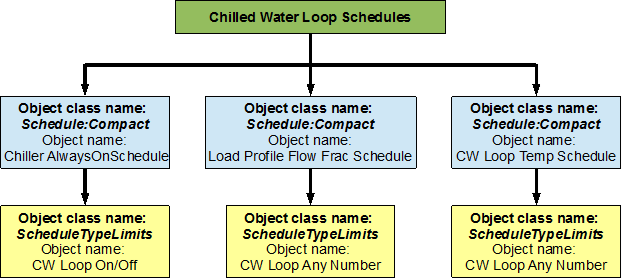
\includegraphics[width=0.9\textwidth, height=0.9\textheight, keepaspectratio=true]{media/image024.png}
\caption{Temp-Enth Example \protect \label{fig:temp-enth-example}}
\end{figure}

\paragraph{Field: Temperature x}\label{field-temperature-x}

This field is used to specify the temperature of the temperature-enthalpy function for the basic material. Units are C.

\paragraph{Field: Enthalpy x}\label{field-enthalpy-x}

This field specifies the enthalpy that corresponds to the previous temperature of the temperature-enthalpy function. Units are J/kg.

And, an IDF example showing how it is used in conjunction with the Material:

Note, the following Heat Balance Algorithm is necessary (only specified once). Also, when using ConductionFiniteDifference, it is more efficient to set the zone timestep shorter than those used for the ConductionTransferFunction solution algorithm. It should be set to 12 timesteps per hour or greater, and can range up to 60.

\begin{lstlisting}

HeatBalanceAlgorithm,
  ConductionFiniteDifference;


  Timestep,
  12;


  Material,
      E1 - 3 / 4 IN PLASTER OR GYP BOARD,  !- Name
      Smooth,                  !- Roughness
      1.9050000E-02,           !- Thickness {m}
      0.7264224,               !- Conductivity {W/m-K}
      1601.846,                !- Density {kg/m3}
      836.8000,                !- Specific Heat {J/kg-K}
      0.9000000,               !- Thermal Absorptance
      0.9200000,               !- Solar Absorptance
      0.9200000;               !- Visible Absorptance


  MaterialProperty:PhaseChange,
      E1 - 3 / 4 IN PLASTER OR GYP BOARD,  !- Name
      0.0,             !- Temperature coefficient,thermal conductivity(W/m K2)
      -20.,            !- Temperature 1, C
      0.01,            !- Enthalpy 1 at –20C, (J/kg)
      20.,             !- Temperature 2, C
      33400,           !- Enthalpy 2, (J/kg)
      20.5,            !- temperature 3, C
      70000,           !- Enthalpy 3, (J/kg)
      100.,            !- Temperature 4, C
      137000;          !- Enthalpy 4, (J/kg)
\end{lstlisting}

\subsection{MaterialProperty:PhaseChangeHysteresis}\label{materialpropertyphasechangehysteresis}

This object is used to describe an advanced level of physics belonging to phase change materials used in building envelopes.
The base phase change input object describes a single process curve whereby a material moves from a crystallized to liquid state and back.
This input object adds a hysteresis effect, allowing the melting/freezing process to follow different curves, representing an effect that is commonly seen in actual building envelope phase change material applications.
This object also allows users to enter characteristic properties of the processes instead of a detailed temperature/enthalpy curve, making it more amenable for studies in which the user does not have the detailed test data required to generate the temperature/enthalpy curve.

\subsubsection{Inputs}\label{materialpropertyphasechangehysteresis-inputs}

The \hyperref[materialpropertyphasechange]{MaterialProperty:PhaseChange}Hysteresis object includes the following inputs.  For the characteristic curve properties, see the engineering reference.

\paragraph{Field: Name}\label{materialpropertyphasechangehysteresis-name}

This input must match the name of a material defined elsewhere within EnergyPlus.  The thermal properies of that material are then overridden by the properties defind in this object.

\paragraph{Field: Latent Heat during the Entire Phase Change Process}\label{materialpropertyphasechangehysteresis-inputs-latent-heat-during-the-entire-phase-change-process}

This is the total amount of latent heat absorbed or discharged during the transition from solid to liquid or back, in Joules.
The shapes of the enthalpy curves differ based on direction, but the total amount of energy from one state to the other does not.

\paragraph{Field: Liquid State Thermal Conductivity}\label{materialpropertyphasechangehysteresis-inputs-liquidk}

This is the constant thermal conductivity used while the material is fully liquid, in W/m-K.

\paragraph{Field: Liquid State Density}\label{materialpropertyphasechangehysteresis-inputs-liquidrho}

This is the constant density while the material is fully liquid, in kg/m3.

\paragraph{Field: Liquid State Specific Heat}\label{materialpropertyphasechangehysteresis-inputs-liquid-state-specific-heat}

This is the constant specific heat while the material is fully liquid, in J/kg-K.

\paragraph{Field: High Temperature Difference of Melting Curve}\label{materialpropertyphasechangehysteresis-inputs-high-temperature-difference-of-melting-curve}

This is the width of the enthalpy/specific heat melting curve, on the high side of the peak melting temperature, in Kelvin (technically it is ``change in Kelvin'').

\paragraph{Field: Peak Melting Temperature}\label{materialpropertyphasechangehysteresis-inputs-peak-melting-temperature}

This is the center (peak) of the melting curve, in Kelvin.

\paragraph{Field: Low Temperature Difference of Melting Curve}\label{materialpropertyphasechangehysteresis-inputs-low-temperature-difference-of-melting-curve}

This is the width of the enthalpy/specific heat melting curve, on the low side of the peak melting temperature, in Kelvin (technically it is ``change in Kelvin'').

\paragraph{Field: Solid State Thermal Conductivity}\label{materialpropertyphasechangehysteresis-inputs-solidk}

This is the constant thermal conductivity used while the material is fully solid, in W/m-K.

\paragraph{Field: Solid State Density}\label{materialpropertyphasechangehysteresis-inputs-solidrho}

This is the constant density while the material is fully solid, in kg/m3.

\paragraph{Field: Solid State Specific Heat}\label{materialpropertyphasechangehysteresis-inputs-solid-state-specific-heat}

This is the constant specific heat while the material is fully crystallized, in J/kg-K.

\paragraph{Field: High Temperature Difference of Freezing Curve}\label{materialpropertyphasechangehysteresis-inputs-high-temperature-difference-of-freezing-curve}

This is the width of the enthalpy/specific heat freezing curve, on the high side of the peak freezing temperature, in Kelvin (technically it is ``change in Kelvin'').

\paragraph{Field: Peak Freezing Temperature}\label{materialpropertyphasechangehysteresis-inputs-peak-freezing-temperature}

This is the center (peak) of the freezing curve, in Kelvin.  This will be higher than the peak melting temperature based on empirical data.

\paragraph{Field: Low Temperature Difference of Freezing Curve}\label{materialpropertyphasechangehysteresis-inputs-low-temperature-difference-of-freezing-curve}

This is the width of the enthalpy/specific heat freezing curve, on the low side of the peak freezing temperature, in Kelvin (technically it is ``change in Kelvin'').

Next is an IDF example showing how it is used in conjunction with the Material:

Note, the following Heat Balance Algorithm is necessary (only specified once). Also, when using ConductionFiniteDifference, it is more efficient to set the zone timestep shorter than those used for the ConductionTransferFunction solution algorithm. It should be set to 12 timesteps per hour or greater, and can range up to 60.

\begin{lstlisting}

  HeatBalanceAlgorithm, ConductionFiniteDifference;

  Timestep, 12;

  Material,
    E1 - 3 / 4 IN PLASTER OR GYP BOARD,  !- Name
    Smooth,                  !- Roughness
    1.9050000E-02,           !- Thickness {m}
    0.7264224,               !- Conductivity {W/m-K}
    1601.846,                !- Density {kg/m3}
    836.8000,                !- Specific Heat {J/kg-K}
    0.9000000,               !- Thermal Absorptance
    0.9200000,               !- Solar Absorptance
    0.9200000;               !- Visible Absorptance

  MaterialProperty:PhaseChangeHysteresis,
    E1 - 3 / 4 IN PLASTER OR GYP BOARD,   !- Name
    10000,                   !- Latent Heat of Fusion {J/kg}
    0.5,                     !- Liquid State Thermal Conductivity {W/m-K}
    1500,                    !- Liquid State Density {kg/m3}
    2000,                    !- Liquid State Specific Heat {J/kg-K}
    1,                       !- High Temperature Difference of Melting Curve {deltaC}
    20,                      !- Peak Melting Temperature {C}
    1,                       !- Low Temperature Difference of Melting Curve {deltaC}
    0.5,                     !- Solid State Thermal Conductivity {W/m-K}
    1600,                    !- Solid State Density {kg/m3}
    2000,                    !- Solid State Specific Heat {J/kg-K}
    1,                       !- High Temperature Difference of Freezing Curve {deltaC}
    23,                      !- Peak Freezing Temperature {C}
    1;                       !- Low Temperature Difference of Freezing Curve {deltaC}

\end{lstlisting}

\subsection{MaterialProperty:VariableThermalConductivity}\label{materialpropertyvariablethermalconductivity}

This object is used to describe the temperature dependent material properties that are used in the CondFD (Conduction Finite Difference) solution algorithm. This conduction model is used when the appropriate CondFD materials are specified and the Solution Algorithm parameter is set to condFD.

\subsubsection{Inputs}\label{inputs-6-027}

\paragraph{Field: Name}\label{field-name-6-022}

This field is a regular material name specifying the material with which this additional temperature dependent property information will be associated.

\paragraph{Field Set: Temperature-Thermal Conductivity}\label{field-set-temperature-thermal-conductivity}

The temperature -- conductivity set of inputs specify a two column tabular temperature-thermal conductivity function for the basic material. Ten pairs can be specified. Specify only the number of pairs necessary. Temperature values should be strictly increasing.

\paragraph{Field: Temperature x}\label{field-temperature-x-1}

This field is used to specify the temperature of the temperature-conductivity function for the basic material. Units are C.

\paragraph{Field: Thermal Conductivity x}\label{field-thermal-conductivity-x}

This field specifies the conductivity that corresponds to the temperature (previous field) of the temperature-conductivity function. Units are W/m-K.

And, an IDF example showing how it is used in conjunction with the Materials:

Note, the following Heat Balance Algorithm is necessary (only specified once). Also, when using Conduction Finite Difference, it is more efficient to set the zone time step shorter than those used for the Conduction Transfer Function solution algorithm. It should be set to 12 time steps per hour or greater, and can range up to 60.

\begin{lstlisting}

HeatBalanceAlgorithm,
  ConductionFiniteDifference;


  Timestep,
  12;


  Material,
      PCMPlasterBoard ,      !- Name
      Smooth,                  !- Roughness
      1.9050000E-02,           !- Thickness {m}
      4.2,                     !- Conductivity {W/m-K}
      1601.846,                !- Density {kg/m3}
      836.8000,                !- Specific Heat {J/kg-K}
      0.9000000,               !- Thermal Absorptance
      0.9200000,               !- Solar Absorptance
      0.9200000;               !- Visible Absorptance


  MaterialProperty:VariableThermalConductivity,
      PCMPlasterBoard,         !- Name
      0,                       !- Temperature 1 {C}
      4.2,                     !- Thermal Conductivity 1 {W/m-K}
      22,                      !- Temperature 2 {C}
      4.2,                     !- Thermal Conductivity 2 {W/m-K}
      22.1,                    !- Temperature 3 {C}
      2.5,                     !- Thermal Conductivity 3 {W/m-K}
      100,                     !- Temperature 4 {C}
      2.5;                     !- Thermal Conductivity 4 {W/m-K}
\end{lstlisting}

\subsubsection{Outputs}\label{outputs-1-026}

The Conduction Finite Difference solution algorithm uses a finite difference solution technique, the surfaces are divided into a nodal arrangement. The only output specific to Conduction Finite Difference solution (that is not include in other surface outputs) is node temperatures.

The following output variables are applicable to all opaque heat transfer surfaces when using Solution Algorithms ConductionFiniteDifference:

\begin{itemize}
\item
  Zone,Sum,CondFD Inner Solver Loop Iteration Count {[]}
\item
  Zone,Average,CondFD Surface Temperature Node \textless{}1\textgreater{} {[}C{]}
\end{itemize}

\paragraph{CondFD Inner Solver Loop Iteration Count {[]}}\label{condfd-inner-solver-loop-iteration-count}

This outputs the count of iterations on the inner solver loop of CondFD for each surface.

\paragraph{CondFD Surface Temperature Node \textless{}X\textgreater{} {[}C{]}}\label{condfd-surface-temperature-node-x-c}

This will output temperatures for a node in the surfaces being simulated with ConductionFiniteDifference. The key values for this output variable are the surface name. The nodes are numbered from outside to inside of the surface. The full listing will appear in the RDD file

\paragraph{CondFD Surface Heat Flux Node \textless{}X\textgreater{} {[}W/m2{]}}\label{condfd-surface-heat-flux-node-x-wm2}

This will output heat flux at each node in surfaces being simulated with ConductionFiniteDifference. The key values for this output variable are the surface name. The nodes are numbered from outside to inside of the surface. The full listing will appear in the RDD file. A positive value indicates heat flowing towards the inside face of the surface. Note that this matches the sign convention for Surface Inside Face Conduction Heat Transfer Rate per Area and is opposite the sign of Surface Outside Face Conduction Heat Transfer Rate per Area.

\paragraph{CondFD Surface Heat Capacitance Outer Half Node \textless{}X\textgreater{} {[}W/m2-K{]}}\label{condfd-surface-heat-capacitance-outer-half-node-x-wm2-k}

\paragraph{CondFD Surface Heat Capacitance Inner Half Node \textless{}X\textgreater{} {[}W/m2-K{]}}\label{condfd-surface-heat-capacitance-inner-half-node-x-wm2-k}

These will output the half-node heat capacitance in surfaces being simulated with ConductionFiniteDifference. The key values for this output variable are the surface name. The nodes are numbered from outside to inside of the surface. The full listing will appear in the RDD file. For this output, the heat capacitance is defined as the product of specific heat, density, and node thickness. Zero is reported for R-layer half-nodes and for undefined half-nodes. There is no outer half-node for Node 1 which is the outside face of the surface, and there is no inner half-node for Node N which is the inside face of the surface. CondFD Surface Heat Capacitance is only available with Output:Diagnostics,DisplayAdvancedReportVariables.

\subsection{MaterialProperty:HeatAndMoistureTransfer:Settings}\label{materialpropertyheatandmoisturetransfersettings}

\textbf{Advanced/Research Usage:} This object is used to describe two of the seven additional material properties needed for the CombinedHeatAndMoistureFiniteElement heat balance solution algorithm. The settings object is used when the solutions algorithm is set to CombinedHeatAndMoistureFiniteElement and the appropriate material properties are assigned to each material. This permits the simulation of the moisture dependent thermal properties of the material as well as the transfer of moisture through, into and out of the material into the zone or exterior.

In addition to the Porosity and Initial Water content properties described here, five additional properties, described by tabulated relationships between variables, are required. These properties are;

\begin{itemize}
\item
  \hyperref[materialpropertyheatandmoisturetransfersorptionisotherm]{MaterialProperty:HeatAndMoistureTransfer:SorptionIsotherm}
\item
  \hyperref[materialpropertyheatandmoisturetransfersuction]{MaterialProperty:HeatAndMoistureTransfer:Suction}
\item
  \hyperref[materialpropertyheatandmoisturetransferredistribution]{MaterialProperty:HeatAndMoistureTransfer:Redistribution}
\item
  \hyperref[materialpropertyheatandmoisturetransferdiffusion]{MaterialProperty:HeatAndMoistureTransfer:Diffusion}
\item
  \hyperref[materialpropertyheatandmoisturetransferthermalconductivity]{MaterialProperty:HeatAndMoistureTransfer:ThermalConductivity}
\end{itemize}

All materials in a construction are required to have all material properties defined for HAMT to work.

Within the MaterialProperty:HeatAndMoistureTransfer:Settings object the following fields are defined.

\subsubsection{Inputs}\label{inputs-7-026}

\paragraph{Field: Material Name}\label{field-material-name-000}

This field is a unique reference name that the user assigns to a particular material. This name can then be referred to by other input data.

\paragraph{Field: Porosity}\label{field-porosity}

The porosity of a material is the maximum fraction, by volume, of a material that can be taken up with water. The units are {[}m3/m3{]}.

\paragraph{Field: Initial Water Content Ratio}\label{field-initial-water-content-ratio}

For this solution algorithm, the initial water content is assumed to be distributed evenly through the depth of the material. The units are {[}kg/kg{]}.

Below is an example input for the porosity and initial water content of a material.

\begin{lstlisting}

MaterialProperty:HeatAndMoistureTransfer:Settings,
        Concrete,     !- Name
        0.76,     !- Porosity
        0.2;     !- Initial (or typical) Water content
\end{lstlisting}

\subsection{MaterialProperty:HeatAndMoistureTransfer:SorptionIsotherm}\label{materialpropertyheatandmoisturetransfersorptionisotherm}

\textbf{Advanced/Research Usage:} This material property is used in conjunction with the CombinedHeatAndMoistureFiniteElement heat balance solution algorithm.

The Isotherm data relates the moisture, or water content {[}kg/m3{]} of a material with the relative humidity (RH). The water content is expected to increase as relative humidity increases, starting at zero content at 0.0relative humidity fraction and reaching a maximum, defined by the porosity, at 1.0 relative humidity fraction, which corresponds to 100\% relative humidity. Relative humidities are entered as fraction for this object ranging from 0.0 to 1.0. These two extremes (0.0 and 1.0) are automatically set by the HAMT solution. However, if they are entered they will be used as extra data points. Data should be provided with increasing RH and moisture content up to as high an RH as possible to provide a stable solution. One possible reason for the following error message may be that a material has a very rapid increase in water content for a small change in RH, which can happen if the last entered water content point is at a low RH and the material has a very high porosity.

\begin{lstlisting}
  ** Warning ** HeatAndMoistureTransfer: Large Latent Heat for Surface ROOF
\end{lstlisting}

Another potential reason for this error being generated is the use of inappropriate values for Vapor Transfer Coefficients. See the \hyperref[surfacepropertiesvaporcoefficients]{SurfaceProperties:VaporCoefficients} object in the Advanced Surface Concepts group.

\subsubsection{Inputs}\label{inputs-8-024}

\paragraph{Field: Material Name}\label{field-material-name-1}

This field is a unique reference name that the user assigns to a particular material. This name can then be referred to by other input data.

\paragraph{Field: Number of data ~Coordinates}\label{field-number-of-data-coordinates}

A maximum of 25 coordinates can be specified.

\paragraph{Field Set: Relative Humidity-Moisture Content}\label{field-set-relative-humidity-moisture-content}

\paragraph{Field: Relative Humidity Fraction x}\label{field-relative-humidity-fraction-x}

The relative humidity of the x\(^{th}\) coordinate. The relative humidity is entered as fraction, not in percent.

\paragraph{Field: Moisture Content x}\label{field-moisture-content-x}

The Moisture Content of the x\(^{th}\) coordinate. The units are {[}kg/m3{]}

Below is an example input for a material isotherm

\begin{lstlisting}

MaterialProperty:HeatAndMoistureTransfer:SorptionIsotherm,
        Concrete,     !- Name
        10,     !- Number of data Coordinates
        0.2205,    !- Relative Humidity fraction #1
        22.31,     !- Moisture content #1
        0.202,     !- Relative Humidity fraction #2
        19.665,    !- Moisture content #2
        0.449,     !- Relative Humidity fraction #3
        40.02,     !- Moisture content #3
        0.454,     !- Relative Humidity fraction #4
        36.915,    !- Moisture content #4
        0.6506,    !- Relative Humidity fraction #5
        56.005,    !- Moisture content #5
        0.655,     !- Relative Humidity fraction #6
        52.325,    !- Moisture content #6
        0.824,     !- Relative Humidity fraction #7
        72.565,    !- Moisture content #7
        0.8725,    !- Relative Humidity fraction #8
        85.1,      !- Moisture content #8
        0.924,     !- Relative Humidity fraction #9
        91.08,     !- Moisture content #9
        0.964,     !- Relative Humidity fraction #10
        100.28;    !- Moisture content #10
\end{lstlisting}

\subsection{MaterialProperty:HeatAndMoistureTransfer:Suction}\label{materialpropertyheatandmoisturetransfersuction}

\textbf{Advanced/Research Usage:}This material property is used in conjunction with the CombinedHeatAndMoistureFiniteElement heat balance solution algorithm.

The suction data relates the liquid transport coefficient, under suction, to the water content of a material. A data point at zero water content is required. The liquid transport coefficient at the highest entered water content value is used for all liquid transport coefficient values above this water content. These coefficients are used by HAMT when the rain flag is set in the weather file.

\subsubsection{Inputs}\label{inputs-9-022}

\paragraph{Field: Material Name}\label{field-material-name-2}

This field is a unique reference name that the user assigns to a particular material. This name can then be referred to by other input data.

\paragraph{Field: Number of Suction points}\label{field-number-of-suction-points}

A maximum of 25 points can be specified.

\paragraph{Field Set: Moisture Content-Liquid Transport Coefficient}\label{field-set-moisture-content-liquid-transport-coefficient}

\paragraph{Field: Moisture Content x}\label{field-moisture-content-x-1}

The moisture content of the x\(^{th}\) point. The units are {[}kg/m3{]}.

\paragraph{Field: Liquid Transport Coefficient x}\label{field-liquid-transport-coefficient-x}

The Liquid Transport Coefficient of the x\(^{th}\) point. The units are {[}m2/s{]}.

Below is an example input for a material liquid transport coefficient under suction.

\begin{lstlisting}

MaterialProperty:HeatAndMoistureTransfer:Suction,
        Concrete,     !- Name
        5,     !- Number of Suction points
        0,     !- Moisture content 1
        0,     !- Liquid Transport Coefficient 1
        72,     !- Moisture content 2
        0.0000000000741,     !- Liquid Transport Coefficient 2
        85,     !- Moisture content 3
        0.000000000253,     !- Liquid Transport Coefficient 3
        100,     !- Moisture content 4
        0.00000000101,     !- Liquid Transport Coefficient 4
        118,     !- Moisture content 5
        0.00000000128;     !- Liquid Transport Coefficient 5
\end{lstlisting}

\subsection{MaterialProperty:HeatAndMoistureTransfer:Redistribution}\label{materialpropertyheatandmoisturetransferredistribution}

\textbf{Advanced/Research Usage:}This material property is used in conjunction with the CombinedHeatAndMoistureFiniteElement heat balance solution algorithm.

The redistribution data relates the liquid transport coefficient to the water content of a material under normal conditions. A data point at zero water content is required. The liquid transport coefficient at the highest entered water content value is used for all liquid transport coefficient values above this water content. These coefficients are used by the Heat and Moisture Transfer algorithm when the rain flag is NOT set in the weather file.

\subsubsection{Inputs}\label{inputs-10-020}

\paragraph{Field: Material Name}\label{field-material-name-3}

This field is a unique reference name that the user assigns to a particular material. This name can then be referred to by other input data.

\paragraph{Field: Number of Redistribution points}\label{field-number-of-redistribution-points}

A maximum of 25 points can be specified.

\paragraph{Field Set: Moisture Content-- Liquid Transport Coefficient}\label{field-set-moisture-content-liquid-transport-coefficient-1}

\paragraph{Field: Moisture Content x}\label{field-moisture-content-x-2}

The moisture content of the x\(^{th}\) point. The units are {[}kg/m3{]}.

\paragraph{Field: Liquid Transport Coefficient x}\label{field-liquid-transport-coefficient-x-1}

The Liquid Transport Coefficient of the x\(^{th}\) point. The units are {[}m2/s{]}.

Below is an example input for the object.

\begin{lstlisting}

MaterialProperty:HeatAndMoistureTransfer:Redistribution,
        Concrete,     !- Name
        5,     !- Number of Redistribution points
        0,     !- Moisture content 1
        0,     !- Liquid Transport Coefficient 1
        72,     !- Moisture content 2
        0.00000000000741,     !- Liquid Transport Coefficient 2
        85,     !- Moisture content 3
        0.0000000000253,     !- Liquid Transport Coefficient 3
        100,     !- Moisture content 4
        0.000000000101,     !- Liquid Transport Coefficient 4
        118,     !- Moisture content 5
        0.000000000128;     !- Liquid Transport Coefficient 5
\end{lstlisting}

\subsection{MaterialProperty:HeatAndMoistureTransfer:Diffusion}\label{materialpropertyheatandmoisturetransferdiffusion}

\textbf{Advanced/Research Usage:}This material property is used in conjunction with the CombinedHeatAndMoistureFiniteElement heat balance solution algorithm.

The MU data relates the vapor diffusion resistance factor (dimensionless) to the relative humidity as fraction(RH). A data point at zero RH is required. The vapor diffusion resistance factor at the highest entered relative humidity (RH) value is used for all vapor diffusion resistance factor values above this RH.~ The relative humidity maximum value in fraction is 1.0.

\subsubsection{Inputs}\label{inputs-11-019}

\paragraph{Field: Material Name}\label{field-material-name-4}

This field is a unique reference name that the user assigns to a particular material. This name can then be referred to by other input data.

\paragraph{Field: Number of Data Pairs}\label{field-number-of-data-pairs}

A maximum of 25 pairs can be specified.

\paragraph{Field Set: Relative Humidity-Vapor Diffusion Resistance Factor}\label{field-set-relative-humidity-vapor-diffusion-resistance-factor}

\paragraph{Field: Relative Humidity Fraction \#x}\label{field-relative-humidity-fraction-x-1}

The moisture content of the x\(^{th}\) pair. The relative humidity is entered as fraction, not in percent.

\paragraph{Field: Vapor Diffusion Resistance Factor \#x}\label{field-vapor-diffusion-resistance-factor-x}

The Liquid Transport Coefficient of the x\(^{th}\) pair.

Below are some examples of the values for materials.

\begin{lstlisting}

MaterialProperty:HeatAndMoistureTransfer:Diffusion,
        Plywood,     !- Name
        3,     !- Number of data Points
        0,     !- Relative Humidity Fraction 1
        700,     !- Water Vapor Diffusion Resistance Factor 1
        0.5,     !- Relative Humidity Fraction 2
        200,     !- Water Vapor Diffusion Resistance Factor 2
        1,     !- Relative Humidity Fraction 3
        20;     !- Water Vapor Diffusion Resistance Factor 3

  MaterialProperty:HeatAndMoistureTransfer:Diffusion,
        Concrete,     !- Name
        1,     !- Number of Mu Points
        0,     !- Relative Humidity Fraction 1
        180;     !- Water Vapor Diffusion Resistance Factor 1
\end{lstlisting}

\subsection{MaterialProperty:HeatAndMoistureTransfer:ThermalConductivity}\label{materialpropertyheatandmoisturetransferthermalconductivity}

\textbf{Advanced/Research Usage:}This material property is used in conjunction with the CombinedHeatAndMoistureFiniteElement heat balance solution algorithm.

The thermal data relates the thermal conductivity {[}W/m-K{]} of a material to the moisture or water content {[}kg/m3{]}. A data point at zero water content is required. The thermal conductivity at the highest entered water content value is used for all thermal conductivity values above this water content. If this object is not defined for a material then the algorithm will use a constant value entered in the Material object for all water contents.

\subsubsection{Inputs}\label{inputs-12-018}

\paragraph{Field: Material Name}\label{field-material-name-5}

This field is a unique reference name that the user assigns to a particular material. This name can then be referred to by other input data.

\paragraph{Field: Number of Thermal Coordinates}\label{field-number-of-thermal-coordinates}

A maximum of 25 coordinates can be specified.

\paragraph{Field Set: Moisture Content- Thermal Conductivity}\label{field-set-moisture-content--thermal-conductivity}

\paragraph{Field: Moisture Content x}\label{field-moisture-content-x-3}

The moisture content of the x\(^{th}\) coordinate. The units are {[}kg/m3{]}

\paragraph{Field: Thermal Conductivity x}\label{field-thermal-conductivity-x-1}

The Thermal Conductivity of the x\(^{th}\) coordinate. The units are {[}W/m-K{]}

Below is an example of values for a material.

\begin{lstlisting}

MaterialProperty:HeatAndMoistureTransfer:ThermalConductivity
        Concrete,     !- Name
        2,     !- Number of Thermal Coordinates
        0,     !- Moisture content \#1
        1.6,     !- Thermal Conductivity \#1
        180,     !- Moisture content \#2
        2.602;     !- Thermal Conductivity \#2
\end{lstlisting}

\subsubsection{Surface Outputs}\label{surface-outputs}

\begin{itemize}
\item
  Zone,Average,HAMT Surface Average Water Content Ratio {[}kg/kg{]}
\item
  Zone,Average,HAMT Surface Inside Face Temperature {[}C{]}
\item
  Zone,Average,HAMT Surface Inside Face Relative Humidity {[}\%{]}
\item
  Zone,Average,HAMT Surface Inside Face Vapor Pressure {[}Pa{]}
\item
  Zone,Average,HAMT Surface Outside Face Temperature {[}C{]}
\item
  Zone,Average,HAMT Surface Outside Face Relative Humidity {[}\%{]}
\end{itemize}

\paragraph{HAMT Surface Average Water Content Ratio {[}kg/kg{]}}\label{hamt-surface-average-water-content-ratio-kgkg}

This output is the summed water content {[}kg/kg{]} of all cells in a surface expressed as a fraction of the mass of the water to the material mass.

\paragraph{HAMT Surface Inside Face Temperature {[}C{]}}\label{hamt-surface-inside-face-temperature-c}

This output is the temperature {[}C{]} on the internal ``surface'' of the surface.

\paragraph{HAMT Surface Inside Face Relative Humidity {[}\%{]}}\label{hamt-surface-inside-face-relative-humidity}

\paragraph{HAMT Surface Inside Face Relative Humidity {[}\%{]}}\label{hamt-surface-inside-face-relative-humidity-1}

This output is the relative humidity on the internal ``surface'' of the surface expressed as a percentage.

\paragraph{HAMT Surface Inside Face Vapor Pressure {[}Pa{]}}\label{hamt-surface-inside-face-vapor-pressure-pa}

This output is the vapor pressure {[}Pa{]} on the internal ``surface'' of the surface.

\paragraph{HAMT Surface Outside Face Temperature {[}C{]}}\label{hamt-surface-outside-face-temperature-c}

This output is the temperature on the external ``surface'' of the surface.

\paragraph{HAMT Surface Outside Face Relative Humidity {[}\%{]}}\label{hamt-surface-outside-face-relative-humidity}

This output is the relative humidity on the external ``surface'' of the surface.

\subsubsection{Internal Cell Outputs}\label{internal-cell-outputs}

Detailed profile data for the variables Temperature {[}C{]}, Relative Humidity {[}\%{]} and Water Content {[}kg/kg{]} within each surface can also be reported. To calculate the heat and moisture transfer through surfaces HAMT splits up surfaces into discrete cells. Each cell is composed of a single material and has a position within the surface. HAMT automatically assigns cells to construction objects so that there are more cells closer to boundaries between materials and also at the ``surfaces'' of the surface. It is not possible for users to define their own cells.

Each surface is made from a particular construction. The construction-surface relationship is output by HAMT to the eplusout.eio file with the following format. The output also contains the HAMT cell origins and cell number for each surface combination. The coordinate system origin is defined as the exterior surface of the construction.

\begin{lstlisting}
! <HAMT cells>, Surface Name, Construction Name, Cell Numbers
! <HAMT origins>, Surface Name, Construction Name, Cell origins (m)
HAMT cells, FLOOR,FLOOR,   1,   2,   3,   4,   5,   6,   7,   8,   9,  10,  11,  12,  13,  14,  15,  16,  17
HAMT origins,FLOOR,FLOOR, 0.0000000, 0.0122726, 0.0601616, 0.1512518, 0.2766268, 0.4240140, 0.5789860, 0.7263732, 0.8517482, 0.9428384, 0.9907274, 1.0035729, 1.0056459, 1.0090000, 1.0123541, 1.0144271, 1.0150000
\end{lstlisting}

Users can select any one of the Temperature, Relative Humidity or Water Content variables for any cell to be reported, using the following naming scheme for the output variable.

\begin{itemize}
\item
  Zone,Average,HAMT Surface Temperature Cell N {[}C{]}
\item
  Zone,Average,HAMT Surface Water Content Cell N {[}kg/kg{]}
\item
  Zone,Average,HAMT Surface Relative Humidity Cell N {[}\%{]}
\end{itemize}

\paragraph{HAMT Surface Relative Humidity Cell \textless{}N\textgreater{} {[}\%{]}}\label{hamt-surface-relative-humidity-cell-n}

This is the relative humidity of the cell in the surface.

\paragraph{HAMT Surface Temperature Cell \textless{}N\textgreater{} {[}C{]}}\label{hamt-surface-temperature-cell-n-c}

This is the temperature of the cell in the surface.

\paragraph{HAMT Surface Water Content Cell \textless{}N\textgreater{} {[}kg/kg{]}}\label{hamt-surface-water-content-cell-n-kgkg}

This is the relative water content of the cell in the surface.

\subsection{Materials for Glass Windows and Doors}\label{materials-for-glass-windows-and-doors}

All the materials for glass windows and doors have the prefix ``WindowMaterial''. The following~ WindowMaterial descriptions (Glazing, Glazing:RefractionExtinctionMethod, Gas, GasMixture, Shade, Screen and Blind) apply to glass windows and doors. The property definitions described herein for Glazing, Gas and GasMixture are supported by the National Fenestration Rating Council as standard.

``Front side'' is the side of the layer opposite the zone in which the window is defined. ``Back side'' is the side closest to the zone in which the window is defined. Therefore, for exterior windows, ``front side'' is the side closest to the outdoors. For interior windows, ``front side'' is the side closest to the zone adjacent to the zone in which the window is defined.

The solar radiation transmitted by the window layers enters the zone and is a component of the zone load. The solar radiation absorbed in each solid layer (glass, shade, screen or blind) participates in the window layer heat balance calculation. The visible transmittance and reflectance properties of the window are used in the daylighting calculation.

\subsection{WindowMaterial:Glazing}\label{windowmaterialglazing}

In the following, for exterior windows, ``front side'' is the side of the glass closest to the outside air and ``back side'' is the side closest to the zone the window is defined in. For interzone windows, ``front side'' is the side closest to the zone adjacent to the zone the window is defined in and ``back side'' is the side closest to the zone the window is defined in.

\subsubsection{Inputs}\label{inputs-13-015}

\paragraph{Field: Name}\label{field-name-7-020}

The name of the glass layer. It corresponds to a layer in a window construction.

\paragraph{Field: Optical Data Type}\label{field-optical-data-type}

Valid values for this field are SpectralAverage, Spectral, SpectralAndAngle, and BSDF.

If Optical Data Type = SpectralAverage, the values you enter for solar transmittance and reflectance are assumed to be averaged over the solar spectrum, and the values you enter for visible transmittance and reflectance are assumed to be averaged over the solar spectrum and weighted by the response of~ the human eye. There is an EnergyPlus Reference Data Set for WindowMaterial:Glazing that contains spectral average properties for many different types of glass.

If Optical Data Type = Spectral, then, in the following field, you must enter the name of a spectral data set defined with the WindowGlassSpectralData object. In this case, the values of~ solar and visible transmittance and reflectance in the fields below should be blank.

If Optical Data Type = SpectralAndAngle, then, in the last 3 fields, you must enter the name of a spectral and angle data set defined with the \hyperref[tabletwoindependentvariables]{Table:TwoIndependentVariables} object. In this case, the Window Glass Spectral Data Set Name should be blank, and the values of solar and visible transmittance and reflectance in the fields below should be blank.

If Optical Data Type = BSDF, the \hyperref[constructioncomplexfenestrationstate]{Construction:ComplexFenestrationState} object must be used to define the window construction layers. The \hyperref[constructioncomplexfenestrationstate]{Construction:ComplexFenestrationState} object contains references to the BSDF files which contain the optical properties of the Complex Fenestration layers. In this case,

\paragraph{Field: Window Glass Spectral Data Set Name}\label{field-window-glass-spectral-data-set-name}

If Optical Data Type = Spectral, this is the name of a spectral data set defined with a WindowGlassSpectralData object.

\paragraph{Field: Thickness}\label{field-thickness-1}

The surface-to-surface thickness of the glass (m).

\paragraph{Field: Solar Transmittance at Normal Incidence}\label{field-solar-transmittance-at-normal-incidence}

Transmittance at normal incidence averaged over the solar spectrum. Used only when Optical Data Type = SpectralAverage.

For uncoated glass, when alternative optical properties are available---such as thickness, solar index of refraction, and solar extinction coefficient---they can be converted to equivalent solar transmittance and reflectance values using the equations given in \textbf{``Glass Optical Properties Conversion.''}

\paragraph{Field: Front Side Solar Reflectance at Normal Incidence}\label{field-front-side-solar-reflectance-at-normal-incidence}

Front-side reflectance at normal incidence averaged over the solar spectrum. Used only when Optical Data Type = SpectralAverage.

\paragraph{Field: Back Side Solar Reflectance at Normal Incidence}\label{field-back-side-solar-reflectance-at-normal-incidence}

Back-side reflectance at normal incidence averaged over the solar spectrum. Used only when Optical Data Type = SpectralAverage.

\paragraph{Field: Visible Transmittance at Normal Incidence}\label{field-visible-transmittance-at-normal-incidence}

Transmittance at normal incidence averaged over the solar spectrum and weighted by the response of the human eye. Used only when Optical Data Type = SpectralAverage.

For uncoated glass, when alternative optical properties are available---such as thickness, visible index of refraction, and visible extinction coefficient---they can be converted to equivalent visible transmittance and reflectance values using the equations given in \textbf{``Glass Optical Properties Conversion.''}

\paragraph{Field: Front Side Visible Reflectance at Normal Incidence}\label{field-front-side-visible-reflectance-at-normal-incidence}

Front-side reflectance at normal incidence averaged over the solar spectrum and weighted by the response of the human eye. Used only when Optical Data Type = SpectralAverage.

\paragraph{Field: Back Side Visible Reflectance at Normal Incidence}\label{field-back-side-visible-reflectance-at-normal-incidence}

Back-side reflectance at normal incidence averaged over the solar spectrum and weighted by the response of the human eye. Used only when Optical Data Type = SpectralAverage.

\paragraph{Field: Infrared Transmittance at Normal Incidence}\label{field-infrared-transmittance-at-normal-incidence}

Long-wave transmittance at normal incidence.

\paragraph{Field: Front Side Infrared Hemispherical Emissivity}\label{field-front-side-infrared-hemispherical-emissivity}

Front-side long-wave emissivity.

\paragraph{Field: Back Side Infrared Hemispherical Emissivity}\label{field-back-side-infrared-hemispherical-emissivity}

Back-side long-wave emissivity.

\paragraph{Field: Conductivity}\label{field-conductivity-1}

Thermal conductivity (W/m-K).

\paragraph{Field: Dirt Correction Factor for Solar and Visible Transmittance}\label{field-dirt-correction-factor-for-solar-and-visible-transmittance}

This is a factor that corrects for the presence of dirt on the glass. The program multiplies the fields ``Solar Transmittance at Normal Incidence'' and ``Visible Transmittance at Normal Incidence'' by this factor if the material is used as the \underline{outer} glass layer of an \underline{exterior} window or glass door.\footnote{If Optical Data Type = Spectral, the program multiplies the solar and visible transmittance at each wavelength by the dirt correction factor.} If the material is used as an inner glass layer (in double glazing, for example), the dirt correction factor is not applied because inner glass layers are assumed to be clean. Using a material with dirt correction factor \textless{} 1.0 in the construction for an interior window will result in an error message.

Representative values of the dirt correction factor are shown in Table~\ref{table:dirt-correction-factors}.

\begin{longtable}[c]{@{}llll@{}}
\caption{Dirt Correction Factors \label{table:dirt-correction-factors}} \\
\toprule
Type of Location & \multicolumn{3}{c}{Angle of Glazing} \\ \cmidrule(r){2-4}
                 & Vertical & 45$^{o}$ & Horizontal \\ \midrule
\endfirsthead

\caption[]{Dirt Correction Factors} \\
\toprule
Type of Location & \multicolumn{3}{c}{Angle of Glazing} \\ \cmidrule(r){2-4}
                 & Vertical & 45$^{o}$ & Horizontal \\ \midrule
\endhead

Non-industrial & 0.9 & 0.8 & 0.7 \\
Industrial & 0.7 & 0.6 & 0.5 \\
Very Dirty & 0.6 & 0.5 & 0.4 \\
\bottomrule
{\tiny From Appendix A, ``Daylighting in Sports Halls, Report 2,'' SportScotland, Nov. 2002 (www.sportscotland.org.uk)}
\end{longtable}

The default value of the dirt correction factor is 1.0, which means the glass is clean.

It is assumed that dirt, if present, has no effect on the IR properties of the glass.

\paragraph{Field: Solar Diffusing}\label{field-solar-diffusing}

Takes values No (the default) and Yes. If No, the glass is \underline{transparent} and beam solar radiation incident on the glass is transmitted as beam radiation with no diffuse component. If Yes, the glass is \underline{translucent} and beam solar radiation incident on the glass is transmitted as hemispherically diffuse radiation with no beam component.\footnote{EnergyPlus does not model the ``partially translucent'' case in which beam solar radiation incident on the glass is transmitted as a combination of beam and diffuse.} See Figure~\ref{fig:comparison-between-transmittance-properties}. Solar Diffusing = Yes should only be used on the \emph{innermost} pane of glass in an exterior window; it does not apply to interior windows.

For both Solar Diffusing = No and Yes, beam is reflected as beam with no diffuse component (see Figure~\ref{fig:comparison-between-transmittance-properties}). Solar Diffusing cannot be used with Window Shading Control devices (except Switchable Glazing). When attempted, the window property will be set to No for Solar Diffusing. The Surface Details report will reflect the override.

If, in the Building object, Solar Distribution = FullInteriorAndExterior, use of Solar Diffusing = Yes for glass in an exterior window will change the distribution of interior solar radiation from the window. The result is that beam solar radiation that would be transmitted by a transparent window and get absorbed by particular interior surfaces will be diffused by a translucent window and be spread over more interior surfaces. This can change the time dependence of heating and cooling loads in the zone.

In a zone with Daylighting:Detailed, translucent glazing---which is often used in skylights---will provide a more uniform daylight illuminance over the zone and will avoid patches of sunlight on the floor.

\begin{figure}[hbtp] % fig 10
\centering
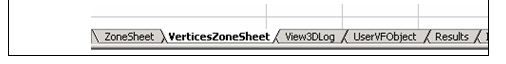
\includegraphics[width=0.9\textwidth, height=0.9\textheight, keepaspectratio=true]{media/image025.png}
\caption{Comparison between transmittance properties of transparent glass (Solar Diffusing = No) and translucent glass (Solar Diffusing = Yes). \protect \label{fig:comparison-between-transmittance-properties}}
\end{figure}

\paragraph{Field: Young's modulus}\label{field-youngs-modulus}

A measure of the stiffness of an elastic material.~ It is defined as the ratio of the uniaxial stress over the uniaxial strain in the range of stress in which Hooke's Law holds. It is used only with complex fenestration systems defined through the \hyperref[constructioncomplexfenestrationstate]{Construction:ComplexFenestrationState} object. The default value for glass is 7.2e10 Pa.

\paragraph{Field: Poisson's ratio}\label{field-poissons-ratio}

The ratio, when a sample object is stretched, of the contraction or transverse strain (perpendicular to the applied load), to the extension or axial strain (in the direction of the applied load). This value is used only with complex fenestration systems defined through the \hyperref[constructioncomplexfenestrationstate]{Construction:ComplexFenestrationState} object. The default value for glass is 0.22.

\paragraph{Field: Window Glass Spectral and Incident Angle Transmittance Data Set Table Name}\label{field-window-glass-spectral-and-incident-angle-transmittance-data}

If Optical Data Type = SpectralAndAngle, this is the name of a spectral and angle data set of transmittance defined with a \hyperref[tabletwoindependentvariables]{Table:TwoIndependentVariables} object. The first and second independent variables must be Angle, and Wavelength, respectively. The restriction is based on internal dataset use. Each dataset is divided into subsets for each incident angle internally.

\paragraph{Field: Window Glass Spectral and Incident Angle Front Reflectance Data Set Table Name}\label{field-window-glass-spectral-and-incident-angle-front-reflectance-data}

If Optical Data Type = SpectralAndAngle, this is the name of a spectral and angle data set of front reflectance defined with a \hyperref[tabletwoindependentvariables]{Table:TwoIndependentVariables} object. The first and second independent variables must be Angle, and Wavelength, respectively. The restriction is based on internal dataset use. Each dataset is divided into subsets for each incident angle internally.

\paragraph{Field: Window Glass Spectral and Incident Angle Back Reflectance Data Set Table Name}\label{field-window-glass-spectral-and-incident-angle-back-reflectance-data}

If Optical Data Type = SpectralAndAngle, this is the name of a spectral and angle data set of back reflectance defined with a \hyperref[tabletwoindependentvariables]{Table:TwoIndependentVariables} object. The first and second independent variables must be Angle, and Wavelength, respectively. The restriction is based on internal dataset use. Each dataset is divided into subsets for each incident angle internally.

It should be pointed out that when Optical Data Type = SpectralAndAngle for a glass layer in a construction, the table input data are converted into polynomial curve fits with 6 coefficients, so that all outputs of optical properties for the same construction will be curve values for a given incident angle. Therefore, the values may be slightly different from input values.

IDF examples of Spectral average and using a Spectral data set:

\begin{lstlisting}

MATERIAL:WINDOWGLASS, GLASS - CLEAR SHEET 1 / 8 IN,
    SpectralAverage, ! Optical data type
    0.003, ! Thickness {m} 1/8"
    0.850, ! Solar transmittance at normal incidence
    0.075, ! Solar reflectance at normal incidence: front side
    0.075, ! Solar reflectance at normal incidence: back side
    0.901, ! Visible transmittance at normal incidence
    0.081, ! Visible reflectance at normal incidence: front side
    0.081, ! Visible reflectance at normal incidence: back side
    0.0,   ! IR transmittance at normal incidence
    0.84,  ! IR hemispherical emissivity: front side
    0.84,  ! IR hemispherical emissivity: back side
    0.9;   ! Conductivity {W/m-K}


  WindowMaterial:Glazing ,SPECTRAL GLASS INNER PANE, ! Material name
      Spectral, ! Optical data type {SpectralAverage or Spectral}
      TestSpectralDataSet, ! Name of spectral data set
      0.0099, ! Thickness {m}
      ,  ! Solar transmittance at normal incidence
      ,  ! Solar reflectance at normal incidence: front side
      ,  ! Solar reflectance at normal incidence: back side
      ,  ! Visible transmittance at normal incidence
      ,  ! Visible reflectance at normal incidence: front side
      ,  ! Visible reflectance at normal incidence: back side
      0.0,   ! IR transmittance at normal incidence
      0.84,  ! IR emissivity: front side
      0.84,  ! IR emissivity: back side
      0.798; ! Conductivity {W/m-K}

\end{lstlisting}

IDF example using a SpectralAndAngle data set:

\begin{lstlisting}

  WindowMaterial:Glazing ,SPECTRAL AND ANGLE GLASS INNER PANE, ! Material name
    SpectralAndAngle, ! Optical data type {SpectralAverage or Spectral}
    , !- Name of spectral data set

    0.0099, ! Thickness {m}
    ,  !- Solar transmittance at normal incidence
    ,  !- Solar reflectance at normal incidence: front side
    ,  !- Solar reflectance at normal incidence: back side
    ,  !- Visible transmittance at normal incidence
    ,  !- Visible reflectance at normal incidence: front side
    ,  !- Visible reflectance at normal incidence: back side
    0.0,   !- IR transmittance at normal incidence
    0.84,  !- IR emissivity: front side
    0.84,  !- IR emissivity: back side
    0.798, !- Conductivity {W/m-K}
    ,      !- Dirt Correction Factor for Solar and Visible Transmittance
    ,      !- Solar Diffusing
    ,      !- Young's modulus
    ,      !- Poisson's ratio
    TranmittanceDataSet,  !- Window Glass Spectral and Incident Angle Transmittance Data Set Table Name
    FrontReflectanceDataSet,      !- Window Glass Spectral and Incident Angle Front Reflectance Data Set Table Name
    BackReflectanceDataSet;      !- Window Glass Spectral and Incident Angle Back Reflectance Data Set Table Name

\end{lstlisting}

IDF example of Spectral Data Type = BSDF

\begin{lstlisting}

WindowMaterial:Glazing,
    Glass_5012_Layer,        !- Layer name : CLEAR_6.PPG
    BSDF,                    !- Optical Data Type
    ,                        !- Spectral Data name
    0.005664,                !- Thickness
    ,                        !- Solar Transmittance
    ,                        !- Solar Front Reflectance
    ,                        !- Solar Back Reflectance
    ,                        !- Visible Transmittance
    ,                        !- Visible Front Reflectance
    ,                        !- Visible Back reflectance
    0.000000,                !- IR Transmittance
    0.840000,                !-Front Emissivity
    0.840000,                !-Back Emissivity
    1.000000,                !-Conductivity
    ,                        !-Dirt Correction Factor for Sol/Vis Transmittance
    ,                        !-Solar Diffusing
    7.2e10,                  !-Young’s modulus
    0.22;                    !-Poisson’s ratio
\end{lstlisting}

\subsection{WindowMaterial:Glazing:RefractionExtinctionMethod}\label{windowmaterialglazingrefractionextinctionmethod}

This is an alternative way of specifying glass properties. Index of refraction and extinction coefficient are given instead of the transmittance and reflectance values used in \hyperref[windowmaterialglazing]{WindowMaterial:Glazing}. However, unlike \hyperref[windowmaterialglazing]{WindowMaterial:Glazing}, WindowMaterial:Glazing:RefractionExtinctionMethod is restricted to cases where the front and back optical properties of the glass are the same. This means it cannot be used for glass with a coating on one side. In that case \hyperref[windowmaterialglazing]{WindowMaterial:Glazing} should be used. Also, unlike \hyperref[windowmaterialglazing]{WindowMaterial:Glazing}, WindowMaterial:Glazing:RefractionExtinctionMethod does not allow input of glass wavelength-by-wavelength (spectral) properties.

\subsubsection{Inputs}\label{inputs-14-015}

\paragraph{Field: Name}\label{field-name-8-020}

The name of the glass layer. It corresponds to a layer in a window construction.

\paragraph{Field: Thickness}\label{field-thickness-2}

The surface-to-surface thickness of the glass (m).

\paragraph{Field: Solar Index of Refraction}\label{field-solar-index-of-refraction}

Index of refraction averaged over the solar spectrum.

\paragraph{Field: Solar Extinction Coefficient}\label{field-solar-extinction-coefficient}

Extinction coefficient averaged over the solar spectrum (m\(^{-1}\)).

\paragraph{Field: Visible Index of Refraction}\label{field-visible-index-of-refraction}

Index of refraction averaged over the solar spectrum and weighted by the response of the human eye.

\paragraph{Field: Visible Extinction Coefficient}\label{field-visible-extinction-coefficient}

Extinction coefficient averaged over the solar spectrum and weighted by the response of the human eye (m\(^{-1}\)).

\paragraph{Field: Infrared Transmittance at Normal Incidence}\label{field-infrared-transmittance-at-normal-incidence-1}

Long-wave transmittance at normal incidence.

\paragraph{Field: Infrared Hemispherical Emissivity}\label{field-infrared-hemispherical-emissivity}

Long-wave hemispherical emissivity, assumed the same on both sides of the glass.

\paragraph{Field: Conductivity}\label{field-conductivity-2}

Thermal conductivity (W/m-K).

\paragraph{Field: Dirt Correction Factor for Solar and Visible Transmittance}\label{field-dirt-correction-factor-for-solar-and-visible-transmittance-1}

This is a factor that corrects for the presence of dirt on the glass. It multiplies the solar and visible transmittance at normal Incidence (which the program calculates from the input values of thickness, solar index of refraction, solar extinction coefficient, etc.) if the material is used as the \underline{outer} glass layer of an \underline{exterior} window or glass door. If the material is used as an inner glass layer (in double glazing, for example), the dirt correction factor is not applied because inner glass layers are assumed to be clean. Using a material with dirt correction factor \textless{} 1.0 in the construction for an interior window will result in an error message.

Representative values of the direct correction factor are shown in Table~\ref{table:dirt-correction-factors}.

The default value of the dirt correction factor is 1.0, which means the glass is clean. It is assumed that dirt, if present, has no effect on the IR properties of the glass.

\paragraph{Field: Solar Diffusing}\label{field-solar-diffusing-1}

Takes values No (the default) and Yes. If No, the glass is transparent. If Yes, the glass is translucent and beam solar radiation incident on the glass is transmitted as hemispherically diffuse radiation with no beam component. (EnergyPlus does not model the ``partially translucent'' case in which beam solar radiation incident on the glass is transmitted as a combination of beam and diffuse.) Solar Diffusing = Yes should only be used on the innermost pane of glass in an exterior window; it does not apply to interior windows.

If, in the Building object, Solar Distribution = FullInteriorAndExterior, use of Solar Diffusing = Yes for glass in an exterior window will change the distribution of interior solar radiation from the window. The result is that beam solar radiation that would be transmitted by a transparent window and get absorbed by particular interior surfaces will be diffused by a translucent window and be spread over more interior surfaces. This can change the time dependence of heating and cooling loads in the zone.

In a zone with Daylighting:Detailed, translucent glazing, which is often used in skylights, will provide a more uniform daylight illuminance over the zone and will avoid patches of sunlight on the floor.

An IDF example:

\begin{lstlisting}
WindowMaterial:Glazing:RefractionExtinctionMethod,
  4MM CLEAR GLASS,  !- Material name
  0.004,            !- Thickness {m}
  1.526,            !- Solar index of refraction
  30.0 ,            !- Solar extinction coefficient (1/m)
  1.526,            !- Visible index of refraction
  30.0 ,            !- Visible extinction coefficient (1/m)
  0.0,              !- IR transmittance at normal incidence
  0.84,             !- IR emissivity
  0.9;              !- Conductivity {W/m-K}
\end{lstlisting}

\subsection{Glass Optical Properties Conversion}\label{glass-optical-properties-conversion}

\subsubsection{Conversion from Glass Optical Properties Specified as Index of Refraction and Transmittance at Normal Incidence}\label{conversion-from-glass-optical-properties-specified-as-index-of-refraction-and-transmittance-at-normal-incidence}

The optical properties of uncoated glass are sometimes specified by index of refraction, n, and transmittance at normal incidence, T.

The following equations show how to convert from this set of values to the transmittance and reflectance values required by \hyperref[windowmaterialglazing]{WindowMaterial:Glazing}. These equations apply only to \underline{uncoated} glass, and can be used to convert either spectral-average solar properties or spectral-average visible properties (in general, \(n\) and \(T\) are different for the solar and visible). Note that since the glass is uncoated, the front and back reflectances are the same and equal to the \(R\) that is solved for in the following equations.

Given \(n\) and \(T\), find \(R\):

\begin{equation*}
r = \left( \frac{n - 1}{n + 1} \right)^2
\end{equation*}

\begin{equation*}
\tau = \frac{ \left[ (1 - r)^4 + 4 r^2 T^2 \right]^{1/2} - (1 - r)^2}{2 r^2 T}
\end{equation*}

\begin{equation*}
R = r + \frac{(1 - r)^2 r \tau ^2}{1 - r^2 \tau ^2}
\end{equation*}

\textbf{Example:}

\begin{equation*}
T = 0.86156
\end{equation*}

\begin{equation*}
n = 1.526
\end{equation*}

\begin{equation*}
r = \left( \frac{1.526 - 1}{1.526 + 1} \right)^2
\end{equation*}

\begin{equation*}
\tau = 0.93974
\end{equation*}

\begin{equation*}
R = 0.07846
\end{equation*}

\subsection{WindowMaterial:GlazingGroup:Thermochromic}\label{windowmaterialglazinggroupthermochromic}

Thermochromic (TC) materials have active, reversible optical properties that vary with temperature. Thermochromic windows are adaptive window systems for incorporation into building envelopes. Thermochromic windows respond by absorbing sunlight and turning the sunlight energy into heat. As the thermochromic film warms it changes its light transmission level from less absorbing to more absorbing. The more sunlight it absorbs the lower the light level going through it. By using the suns own energy the window adapts based solely on the directness and amount of sunlight. Thermochromic materials will normally reduce optical transparency by absorption and/or reflection, and are specular (maintaining vision).

A thermochromic window is defined with a Construction object which references a special layer defined with a \hyperref[windowmaterialglazing]{WindowMaterial:Glazing}Group:Thermochromic object. The \hyperref[windowmaterialglazing]{WindowMaterial:Glazing}Group:Thermochromic object further references a series of \hyperref[windowmaterialglazing]{WindowMaterial:Glazing} objects corresponding to each specification temperature of the TC layer.

This object specifies a layer of thermochromic glass, part of a thermochromic window. An example file ThermochromicWindow.idf is included in the EnergyPlus installation.

\subsubsection{Inputs}\label{inputs-15-015}

\paragraph{Field: Name}\label{field-name-9-017}

A unique user assigned name for a particular thermochromic glass material.

\paragraph{Field Set (Optical Data Temperature, Window Material Glazing Name) is extensible.}\label{field-set-optical-data-temperature-window-material-glazing-name-is-extensible.}

\paragraph{Field:Optical Data Temperature \textless{}N\textgreater{}}\label{fieldoptical-data-temperature-n}

The temperature of the TC glass layer corresponding to the optical data of the TC layer. Unit is °C.

\paragraph{Field: Window Material Glazing Name \textless{}N\textgreater{}}\label{field-window-material-glazing-name-n}

The window glazing (defined with \hyperref[windowmaterialglazing]{WindowMaterial:Glazing}) name that provides the TC glass layer performance at the above specified temperature.

IDF Examples

\begin{lstlisting}
Construction,
  window_const,     !- Name
  Usual Glass,      !- Layer 1
  AIR 6MM,          !- Layer 2
  TCGlazings,       !- Layer 3
  AIR 6MM,          !- Layer 4
  Usual Glass;      !- Layer 5

WindowMaterial:Gas,
  AIR 6MM,          !- Name
  Air,              !- Gas Type
  0.0063;           !- Thickness {m}

! Added for thermochromic glazings
WindowMaterial:GlazingGroup:Thermochromic,
  TCGlazings,
  0 ,  TCGlazing0,
  20,  TCGlazing20,
  25,  TCGlazing25,
  30,  TCGlazing30,
  35,  TCGlazing35,
  40,  TCGlazing40,
  45,  TCGlazing45,
  50,  TCGlazing50,
  55,  TCGlazing55,
  60,  TCGlazing60,
  65,  TCGlazing65,
  75,  TCGlazing75,
  85,  TCGlazing85;

WindowMaterial:Glazing,
  TCGlazing0,       !- Name
  SpectralAverage,  !- Optical Data Type
  ,                 !- Window Glass Spectral Data Set Name
  0.0030,           !- Thickness
  0.2442,           !- Solar Transmittance at Normal Incidence
  0.7058,           !- Front Side Solar Reflectance at Normal Incidence
  0.7058,           !- Back Side Solar Reflectance at Normal Incidence
  0.3192,           !- Visible Transmittance at Normal Incidence
  0.6308,           !- Front Side Visible Reflectance at Normal Incidence
  0.6308,           !- Back Side Visible Reflectance at Normal Incidence
  0.0000,           !- Infrared Transmittance at Normal Incidence
  0.9000,           !- Front Side Infrared Hemispherical Emissivity
  0.9000,           !- Back Side Infrared Hemispherical Emissivity
  0.0199,           !- Conductivity
  1.0000,           !- Dirt Correction Factor for Solar and Visible Transmittance
  No;               !- Solar Diffusing

WindowMaterial:Glazing,
  TCGlazing20,      !- Name
  SpectralAverage,  !- Optical Data Type
  ,                 !- Window Glass Spectral Data Set Name
  0.0030,           !- Thickness
  0.2442,           !- Solar Transmittance at Normal Incidence
  0.7058,           !- Front Side Solar Reflectance at Normal Incidence
  0.7058,           !- Back Side Solar Reflectance at Normal Incidence
  0.3192,           !- Visible Transmittance at Normal Incidence
  0.6308,           !- Front Side Visible Reflectance at Normal Incidence
  0.6308,           !- Back Side Visible Reflectance at Normal Incidence
  0.0000,           !- Infrared Transmittance at Normal Incidence
  0.9000,           !- Front Side Infrared Hemispherical Emissivity
  0.9000,           !- Back Side Infrared Hemispherical Emissivity
  0.0199,           !- Conductivity
  1.0000,           !- Dirt Correction Factor for Solar and Visible Transmittance
  No;               !- Solar Diffusing

WindowMaterial:Glazing,
  TCGlazing25,      !- Name
  SpectralAverage,  !- Optical Data Type
  ,                 !- Window Glass Spectral Data Set Name
  0.0030,           !- Thickness
  0.2442,           !- Solar Transmittance at Normal Incidence
  0.7058,           !- Front Side Solar Reflectance at Normal Incidence
  0.7058,           !- Back Side Solar Reflectance at Normal Incidence
  0.3192,           !- Visible Transmittance at Normal Incidence
  0.6308,           !- Front Side Visible Reflectance at Normal Incidence
  0.6308,           !- Back Side Visible Reflectance at Normal Incidence
  0.0000,           !- Infrared Transmittance at Normal Incidence
  0.9000,           !- Front Side Infrared Hemispherical Emissivity
  0.9000,           !- Back Side Infrared Hemispherical Emissivity
  0.0199,           !- Conductivity
  1.0000,           !- Dirt Correction Factor for Solar and Visible Transmittance
  No;               !- Solar Diffusing

WindowMaterial:Glazing,
  TCGlazing30,      !- Name
  SpectralAverage,  !- Optical Data Type
  ,                 !- Window Glass Spectral Data Set Name
  0.0030,           !- Thickness
  0.2442,           !- Solar Transmittance at Normal Incidence
  0.7058,           !- Front Side Solar Reflectance at Normal Incidence
  0.7058,           !- Back Side Solar Reflectance at Normal Incidence
  0.3192,           !- Visible Transmittance at Normal Incidence
  0.6308,           !- Front Side Visible Reflectance at Normal Incidence
  0.6308,           !- Back Side Visible Reflectance at Normal Incidence
  0.0000,           !- Infrared Transmittance at Normal Incidence
  0.9000,           !- Front Side Infrared Hemispherical Emissivity
  0.9000,           !- Back Side Infrared Hemispherical Emissivity
  0.0199,           !- Conductivity
  1.0000,           !- Dirt Correction Factor for Solar and Visible Transmittance
  No;               !- Solar Diffusing

WindowMaterial:Glazing,
  TCGlazing35,      !- Name
  SpectralAverage,  !- Optical Data Type
  ,                 !- Window Glass Spectral Data Set Name
  0.0030,           !- Thickness
  0.2442,           !- Solar Transmittance at Normal Incidence
  0.7058,           !- Front Side Solar Reflectance at Normal Incidence
  0.7058,           !- Back Side Solar Reflectance at Normal Incidence
  0.3192,           !- Visible Transmittance at Normal Incidence
  0.6308,           !- Front Side Visible Reflectance at Normal Incidence
  0.6308,           !- Back Side Visible Reflectance at Normal Incidence
  0.0000,           !- Infrared Transmittance at Normal Incidence
  0.9000,           !- Front Side Infrared Hemispherical Emissivity
  0.9000,           !- Back Side Infrared Hemispherical Emissivity
  0.0199,           !- Conductivity
  1.0000,           !- Dirt Correction Factor for Solar and Visible Transmittance
  No;               !- Solar Diffusing

WindowMaterial:Glazing,
  TCGlazing40,      !- Name
  SpectralAverage,  !- Optical Data Type
  ,                 !- Window Glass Spectral Data Set Name
  0.0030,           !- Thickness
  0.2442,           !- Solar Transmittance at Normal Incidence
  0.7058,           !- Front Side Solar Reflectance at Normal Incidence
  0.7058,           !- Back Side Solar Reflectance at Normal Incidence
  0.3192,           !- Visible Transmittance at Normal Incidence
  0.6308,           !- Front Side Visible Reflectance at Normal Incidence
  0.6308,           !- Back Side Visible Reflectance at Normal Incidence
  0.0000,           !- Infrared Transmittance at Normal Incidence
  0.9000,           !- Front Side Infrared Hemispherical Emissivity
  0.9000,           !- Back Side Infrared Hemispherical Emissivity
  0.0199,           !- Conductivity
  1.0000,           !- Dirt Correction Factor for Solar and Visible Transmittance
  No;               !- Solar Diffusing

WindowMaterial:Glazing,
  TCGlazing45,      !- Name
  SpectralAverage,  !- Optical Data Type
  ,                 !- Window Glass Spectral Data Set Name
  0.0030,           !- Thickness
  0.2442,           !- Solar Transmittance at Normal Incidence
  0.7058,           !- Front Side Solar Reflectance at Normal Incidence
  0.7058,           !- Back Side Solar Reflectance at Normal Incidence
  0.3192,           !- Visible Transmittance at Normal Incidence
  0.6308,           !- Front Side Visible Reflectance at Normal Incidence
  0.6308,           !- Back Side Visible Reflectance at Normal Incidence
  0.0000,           !- Infrared Transmittance at Normal Incidence
  0.9000,           !- Front Side Infrared Hemispherical Emissivity
  0.9000,           !- Back Side Infrared Hemispherical Emissivity
  0.0199,           !- Conductivity
  1.0000,           !- Dirt Correction Factor for Solar and Visible Transmittance
  No;               !- Solar Diffusing

WindowMaterial:Glazing,
  TCGlazing50,      !- Name
  SpectralAverage,  !- Optical Data Type
  ,                 !- Window Glass Spectral Data Set Name
  0.0030,           !- Thickness
  0.2442,           !- Solar Transmittance at Normal Incidence
  0.7058,           !- Front Side Solar Reflectance at Normal Incidence
  0.7058,           !- Back Side Solar Reflectance at Normal Incidence
  0.3192,           !- Visible Transmittance at Normal Incidence
  0.6308,           !- Front Side Visible Reflectance at Normal Incidence
  0.6308,           !- Back Side Visible Reflectance at Normal Incidence
  0.0000,           !- Infrared Transmittance at Normal Incidence
  0.9000,           !- Front Side Infrared Hemispherical Emissivity
  0.9000,           !- Back Side Infrared Hemispherical Emissivity
  0.0199,           !- Conductivity
  1.0000,           !- Dirt Correction Factor for Solar and Visible Transmittance
  No;               !- Solar Diffusing

WindowMaterial:Glazing,
  TCGlazing55,      !- Name
  SpectralAverage,  !- Optical Data Type
  ,                 !- Window Glass Spectral Data Set Name
  0.0030,           !- Thickness
  0.2442,           !- Solar Transmittance at Normal Incidence
  0.7058,           !- Front Side Solar Reflectance at Normal Incidence
  0.7058,           !- Back Side Solar Reflectance at Normal Incidence
  0.3192,           !- Visible Transmittance at Normal Incidence
  0.6308,           !- Front Side Visible Reflectance at Normal Incidence
  0.6308,           !- Back Side Visible Reflectance at Normal Incidence
  0.0000,           !- Infrared Transmittance at Normal Incidence
  0.9000,           !- Front Side Infrared Hemispherical Emissivity
  0.9000,           !- Back Side Infrared Hemispherical Emissivity
  0.0199,           !- Conductivity
  1.0000,           !- Dirt Correction Factor for Solar and Visible Transmittance
  No;               !- Solar Diffusing

WindowMaterial:Glazing,
  TCGlazing60,      !- Name
  SpectralAverage,  !- Optical Data Type
  ,                 !- Window Glass Spectral Data Set Name
  0.0030,           !- Thickness
  0.2442,           !- Solar Transmittance at Normal Incidence
  0.7058,           !- Front Side Solar Reflectance at Normal Incidence
  0.7058,           !- Back Side Solar Reflectance at Normal Incidence
  0.3192,           !- Visible Transmittance at Normal Incidence
  0.6308,           !- Front Side Visible Reflectance at Normal Incidence
  0.6308,           !- Back Side Visible Reflectance at Normal Incidence
  0.0000,           !- Infrared Transmittance at Normal Incidence
  0.9000,           !- Front Side Infrared Hemispherical Emissivity
  0.9000,           !- Back Side Infrared Hemispherical Emissivity
  0.0199,           !- Conductivity
  1.0000,           !- Dirt Correction Factor for Solar and Visible Transmittance
  No;               !- Solar Diffusing

WindowMaterial:Glazing,
  TCGlazing65,      !- Name
  SpectralAverage,  !- Optical Data Type
  ,                 !- Window Glass Spectral Data Set Name
  0.0030,           !- Thickness
  0.2442,           !- Solar Transmittance at Normal Incidence
  0.7058,           !- Front Side Solar Reflectance at Normal Incidence
  0.7058,           !- Back Side Solar Reflectance at Normal Incidence
  0.3192,           !- Visible Transmittance at Normal Incidence
  0.6308,           !- Front Side Visible Reflectance at Normal Incidence
  0.6308,           !- Back Side Visible Reflectance at Normal Incidence
  0.0000,           !- Infrared Transmittance at Normal Incidence
  0.9000,           !- Front Side Infrared Hemispherical Emissivity
  0.9000,           !- Back Side Infrared Hemispherical Emissivity
  0.0199,           !- Conductivity
  1.0000,           !- Dirt Correction Factor for Solar and Visible Transmittance
  No;               !- Solar Diffusing

WindowMaterial:Glazing,
  TCGlazing75,      !- Name
  SpectralAverage,  !- Optical Data Type
  ,                 !- Window Glass Spectral Data Set Name
  0.0030,           !- Thickness
  0.2442,           !- Solar Transmittance at Normal Incidence
  0.7058,           !- Front Side Solar Reflectance at Normal Incidence
  0.7058,           !- Back Side Solar Reflectance at Normal Incidence
  0.3192,           !- Visible Transmittance at Normal Incidence
  0.6308,           !- Front Side Visible Reflectance at Normal Incidence
  0.6308,           !- Back Side Visible Reflectance at Normal Incidence
  0.0000,           !- Infrared Transmittance at Normal Incidence
  0.9000,           !- Front Side Infrared Hemispherical Emissivity
  0.9000,           !- Back Side Infrared Hemispherical Emissivity
  0.0199,           !- Conductivity
  1.0000,           !- Dirt Correction Factor for Solar and Visible Transmittance
  No;               !- Solar Diffusing

WindowMaterial:Glazing,
  TCGlazing85,      !- Name
  SpectralAverage,  !- Optical Data Type
  ,                 !- Window Glass Spectral Data Set Name
  0.0030,           !- Thickness
  0.2442,           !- Solar Transmittance at Normal Incidence
  0.7058,           !- Front Side Solar Reflectance at Normal Incidence
  0.7058,           !- Back Side Solar Reflectance at Normal Incidence
  0.3192,           !- Visible Transmittance at Normal Incidence
  0.6308,           !- Front Side Visible Reflectance at Normal Incidence
  0.6308,           !- Back Side Visible Reflectance at Normal Incidence
  0.0000,           !- Infrared Transmittance at Normal Incidence
  0.9000,           !- Front Side Infrared Hemispherical Emissivity
  0.9000,           !- Back Side Infrared Hemispherical Emissivity
  0.0199,           !- Conductivity
  1.0000,           !- Dirt Correction Factor for Solar and Visible Transmittance
  No;               !- Solar Diffusing
\end{lstlisting}

\subsubsection{Outputs}\label{outputs-3-019}

\paragraph{Surface Window Thermochromic Layer Temperature {[}C{]}}\label{surface-window-thermochromic-layer-temperature-c}

The temperature of the TC glass layer of a TC window at each time step.

\paragraph{Surface Window Thermochromic Layer Property Specification Temperature {[}C{]}}\label{surface-window-thermochromic-layer-property-specification-temperature-c}

The temperature under which the optical data of the TC glass layer are specified.

The overall properties (U-factor/SHGC/VT) of the thermochromic windows at different specification temperatures are reported in the EIO file. These window constructions are created by EnergyPlus during run time. They have similar names with suffix ``\_TC\_XX'' where XX represents a specification temperature.

\subsection{WindowMaterial:Gas}\label{windowmaterialgas}

This object specifies the properties of the gas between the panes of a multi-pane window. Gas Type = Custom allows you to specify the properties of gases other than air, Argon, Krypton or Xenon. There is an EnergyPlus Reference Data Set for Material:WindowGas that contains several types of gas of different thicknesses. See Material:WindowGasMixture for the case that the gas fill is a mixture of different gases.

\subsubsection{Inputs}\label{inputs-16-011}

\paragraph{Field: Name}\label{field-name-10-016}

The name of the gas fill. It refers to a layer in a window construction.

\paragraph{Field: Gas Type}\label{field-gas-type}

The type of gas. The choices are Air, Argon, Krypton, or Xenon. If Gas Type = Custom you can use Conductivity Coefficient A, etc. to specify the properties of a different type of gas.

\paragraph{Field: Thickness}\label{field-thickness-3}

The thickness (m) of the gas layer.

\paragraph{Properties for Custom Gas Types}\label{properties-for-custom-gas-types}

The following entries are used only if Gas Type = Custom. The A and B coefficients are those in the following expression that gives a property value as a function of temperature in degrees K:

\begin{equation}
Property = Coefficien{t_A} + Coefficien{t_B}*Temperatur{e_K}
\end{equation}

\paragraph{Field: Conductivity Coefficient A}\label{field-conductivity-coefficient-a}

The A coefficient for gas conductivity (W/m-K). Used only if Gas Type = Custom.

\paragraph{Field: Conductivity Coefficient B}\label{field-conductivity-coefficient-b}

The B coefficient for gas conductivity (W/m-K\(^{2}\)). Used only if Gas Type = Custom.

\paragraph{Field: Conductivity Coefficient C}\label{field-conductivity-coefficient-c}

The C coefficient for gas conductivity (W/m-K\(^{3}\)).~ Used only if Gas Type = Custom.

\paragraph{Field: Viscosity Coefficient A}\label{field-viscosity-coefficient-a}

The A coefficient for gas viscosity (kg/m-s). Used only if Gas Type = Custom.

\paragraph{Field: Viscosity Coefficient B}\label{field-viscosity-coefficient-b}

The B coefficient for gas viscosity (kg/m-s-K). Used only if Gas Type = Custom.

\paragraph{Field: Viscosity Coefficient C}\label{field-viscosity-coefficient-c}

The C coefficient for gas viscosity (kg/m-s-K\(^{2}\)).~ Used only if Gas Type = Custom.

\paragraph{Field: Specific Heat Coefficient A}\label{field-specific-heat-coefficient-a}

The A coefficient for gas specific heat (J/kg-K). Used only if Gas Type = Custom.

\paragraph{Field: Specific Heat Coefficient B}\label{field-specific-heat-coefficient-b}

The B coefficient for gas specific heat (J/kg-K\(^{2}\)). Used only if Gas Type = Custom.

\paragraph{Field: Specific Heat Coefficient C}\label{field-specific-heat-coefficient-c}

The C coefficient for gas specific heat (J/kg-K\(^{3}\)).~ Used only if Gas Type = Custom.

\paragraph{Field: Specific Heat Ratio}\label{field-specific-heat-ratio}

The specific heat ratio for gas.~ Used only if Gas Type = Custom.

\paragraph{Field: Molecular Weight}\label{field-molecular-weight}

The molecular weight for gas.~ The molecular weight is the mass of 1 mol of the substance.~ This has a numerical value which is the average molecular mass of the molecules in the substance multiplied by Avogadro's constant. (kg/kmol) (Shown in the IDD as g/mol for consistency)

\paragraph{Field: Specific Heat Ratio}\label{field-specific-heat-ratio-1}

The specific heat ratio for gas.~ The specific heat ratio of a gas is the ratio of the specific heat at contant pressure, to the specific heat at constant volume.~ Used only if Gas Type = Custom.

An IDF example:

\begin{lstlisting}

WindowMaterial:Gas,AIRGAP,
    AIR,      ! Gas type (Air - Argon - Krypton - Xenon - Custom)]
    0.0125;   ! Thickness {m} 1/2 inch
\end{lstlisting}

An IDF example to be used with a \hyperref[windowmaterialgap]{WindowMaterial:Gap} definition (see below)

\begin{lstlisting}

WindowMaterial:Gas,
  Gas_1_W_0_0100,                                     !- gap name - Air
  Air,                                                !- type
  0.0100;                                             !- thickness
\end{lstlisting}

An IDF example for a Custom Gas

\begin{lstlisting}

WindowMaterial:Gas,
  Gas_16_W_0_0003,                   !- gap name
  Custom,                            !- type
  0.0003,                            !- thickness
  2.873000e-003,                     !- Conductivity Coefficient A
  7.760000e-005,                     !- Conductivity Coefficient B
  0.000000e+000,                     !- Conductivity Coefficient C
  3.723000e-006,                     !- Conductivity Viscosity A
  4.940000e-008,                     !- Conductivity Viscosity B
  0.000000e+000,                     !- Conductivity Viscosity C
  1002.737000,                       !- Specific Heat Coefficient A
  0.012324,                          !- Specific Heat Coefficient B
  0.000000,                          !- Specific Heat Coefficient C
  28.969999,                         !- Molecular Weight
  1.400000;                          !- Specific Heat Ratio
\end{lstlisting}

\subsection{WindowMaterial:GasMixture}\label{windowmaterialgasmixture}

This object allows you to specify the fill between the panes of a multi-pane window to be a mixture of two, three or four different gases chosen from air, argon, krypton and xenon. It can also be used if only one type of gas in the fill. In this case you can also use \hyperref[windowmaterialgas]{WindowMaterial:Gas}. Note that the fractions of gas types in the mixture should add up to 1.0.

\subsubsection{Inputs}\label{inputs-17-009}

\paragraph{Field: Name}\label{field-name-11-014}

The name of the gas mixture. It refers to a layer in a window construction.

\paragraph{Field: Thickness}\label{field-thickness-4}

The thickness (m) of the gas mixture layer.

\paragraph{Field: Number of Gases in Mixture}\label{field-number-of-gases-in-mixture}

The number of different types of gas in the mixture ( a value from 1 to 4)

\paragraph{Set: Gas Type-Fraction (up to 4)}\label{set-gas-type-fraction-up-to-4}

\paragraph{Field: Gas 1 Type}\label{field-gas-1-type}

The type of~ the first gas in the mixture. Choices are Air, Argon, Krypton and Xenon.

\paragraph{Field: Gas 1 Fraction}\label{field-gas-1-fraction}

The fraction of the first gas in the mixture.

An IDF example:

\begin{lstlisting}

WindowMaterial:GasMixture,ArgonKryptonMix,
  0.0125,   ! Thickness {m} 1/2 inch
  2,        ! Number of Gases in Mixture
  Argon,    ! Gas 1 Type
  0.6,      ! Gas 1 Fraction
  Krypton,  ! Gas 2 Type
  0.4;      ! Gas 2 Fraction
\end{lstlisting}

\subsection{WindowMaterial:Gap}\label{windowmaterialgap}

This input object is used to define the gap between two layers in a complex fenestration system, where the \hyperref[constructioncomplexfenestrationstate]{Construction:ComplexFenestrationState} object is used. It references the gas or gas mixtures defined in the \hyperref[windowmaterialgas]{WindowMaterial:Gas} and \hyperref[windowmaterialgasmixture]{WindowMaterial:GasMixture} objects. It is referenced as a layer in the \hyperref[constructioncomplexfenestrationstate]{Construction:ComplexFenestrationState} object ;it cannot be referenced as a layer from the Construction object.

\subsubsection{Inputs}\label{inputs-18-009}

\paragraph{Field: Name}\label{field-name-12-011}

Unique name of the gap.

\paragraph{Field: Thickness}\label{field-thickness-5}

The thickness (m) of the gap layer.

\paragraph{Field: Pressure}\label{field-pressure-000}

The pressure (Pa) of the gas in the gap layer, used to calculate the gas properties of the glazing system gap. Default is atmospheric pressure, 101325 Pa.When modeling vacuum glazing, this value should represent the pressure in the evacuated glazing system. If this pressure is less that the ThermalModelParams:PressureLimit value, the the glazing system will be modeled as a vacuum glazing.

\paragraph{Field: Deflection State}\label{field-deflection-state}

This field is used when modeling the deflection of the glass layers in a window if the \hyperref[windowthermalmodelparams]{WindowThermalModel:Params} value for ``deflection model'' is ``MeasuredDeflection''.

\paragraph{Field: Support Pillar}\label{field-support-pillar}

References the support pillar of the gap layer if vacuum glazing is being modeled.~ If left empty, then it is considered that gap layer does not have support pillars.

\paragraph{Field: Gas (or GasMixture)}\label{field-gas-or-gasmixture}

References gas (\hyperref[windowmaterialgas]{WindowMaterial:Gas}) or gas mixture (\hyperref[windowmaterialgasmixture]{WindowMaterial:GasMixture}) of the gap layer.

An IDF example for simple glazing:

\begin{lstlisting}

WindowMaterial:Gas,
  Gas_1_W_0_0120,                                !- gap name - Air
  Air,                                           !- type
  0.0120;                                        !- thickness


  WindowMaterial:Gap,
  Gap_1_Layer,                                   !- gap name: Air
  0.0120,                                        !- thickness
  Gas_1_W_0_0120,                                !- Gas (or Gas Mixture) name
  101325.0000;                                   !- pressure
\end{lstlisting}

An IDF example for vacuum glazing:

\begin{lstlisting}

WindowMaterial:Gap,
  Gap_16_Layer,                     !- gap name: Vacuum_0.001_pr-0.5_ps-50.8
  0.0003,                                             !- thicknessGas_16_W_0_0003,                                    !- Gas (or Gas Mixture) name
  0.1333,                                             !- pressure
  ,                                                   !- deflection state
  SupportPillar_16_Gap_1;                             !- SupportPillar


  WindowGap:SupportPillar,
  SupportPillar_16_Gap_1,                             !- Name
  0.0508,                                             !- spacing
  0.0005;                                             !- radius
\end{lstlisting}

\subsection{WindowGap:DeflectionState}\label{windowgapdeflectionstate}

This input object is used to enter data describing deflection state of the gap.~ It is referenced from \hyperref[windowmaterialgap]{WindowMaterial:Gap} object only and it is used only when deflection model is set to MeasuredDeflection (see \hyperref[windowthermalmodelparams]{WindowThermalModel:Params}), otherwise it is ignored.

\subsubsection{Inputs}\label{inputs-19-006}

\paragraph{Field: Name}\label{field-name-13-010}

Unique name of the deflection state.

\paragraph{Field: Deflected Thickness}\label{field-deflected-thickness}

The thickness (m) of the gap in deflected state.~ It represents value of deflection at point of maximum which is usually at the center poing of glazing system.~ It is used only with tarcog algorithm set to Measured Deflection (\hyperref[windowthermalmodelparams]{WindowThermalModel:Params}), otherwise this field will be ignored.

An IDF example where \hyperref[windowthermalmodelparams]{WindowThermalModel:Params} Deflection Model = MeasuredDeflection:

\begin{lstlisting}

WindowMaterial:Gap,
  Gap_1_Layer,                                  !- gap name: Air
  0.0120,                                       !- thickness
  Gas_1_W_0_0120,                               !- Gas (or Gas Mixture) name
  101325.0000,                                  !- pressure
  Gap_1_Deflection;                              !- deflection state


  WindowGap:DeflectionState,       !- deflection state of gap
    Gap_1_Deflection,              !- name
    0.011;                         !- gap thickness in deflected state
\end{lstlisting}

\subsection{WindowGap:SupportPillar}\label{windowgapsupportpillar}

This input object is used to enter data describing support pillar of the gap.~ Support pillars are used in vacuum glazing in order to prevent deflection of glass layers.

\begin{figure}[hbtp] % fig 11
\centering
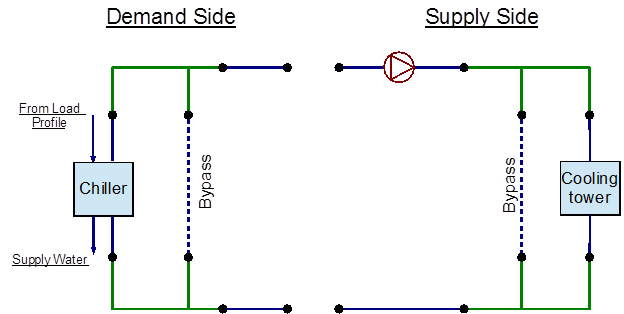
\includegraphics[width=0.9\textwidth, height=0.9\textheight, keepaspectratio=true]{media/image029.png}
\caption{Support Pillar \protect \label{fig:support-pillar}}
\end{figure}

\subsubsection{Inputs}\label{inputs-20-006}

\paragraph{Field: Name}\label{field-name-14-009}

Unique name of the support pillar.

\paragraph{Field: Spacing}\label{field-spacing}

Distance (m) between support pillar centers (see the Engineering reference document for more information).

\paragraph{Field: Radius}\label{field-radius}

The radius (m) of the support pillar (see Engineering reference document for more information).

An IDF example for vacuum glazing (see Vacuum Glazing example in \hyperref[windowmaterialgap]{WindowMaterial:Gap} above)

\begin{lstlisting}

WindowGap:SupportPillar,       !- gap support pillar
    SupportPillar_16_Gap_1,      !- basis matrix name
    0.05,                        !- pillar spacing
    0.005;                       !- pillar radius
\end{lstlisting}

\subsection{WindowMaterial:SimpleGlazingSystem}\label{windowmaterialsimpleglazingsystem}

\warning{This model should be used with caution. There may be significant differences in performance between the simple window system and the usual more detailed model.}

This input object differs from the other WindowMaterial objects in that it describes an entire glazing system rather than individual layers. This object is used when only very limited information is available on the glazing layers or when specific performance levels are being targeted. The layer by layer description offers superior method of modeling windows that should be used instead of this object when sufficient data are available. This object accesses a model that turns simple performance indices into a fuller model of the glazing system.

The performance indices are U-factor and Solar Heat Gain Coefficient, and optionally Visible Transmittance. The values for these performance indices can be selected by the user to represent either glazing-only windows (with no frame) or an average window performance that includes the frame. Inside the program the model produces an equivalent window glazing layer with no frame. The properties of the modeled glazing layer are reported to the EIO file using the IDF input object syntax for the \hyperref[windowmaterialglazing]{WindowMaterial:Glazing} input object. This equivalent layer could be reused in subsequent models if desired, however there will be important differences in the modeled window performance because the simple glazing system model includes its own special model for angular dependence when incident beam solar is not normal to the plane of the window.

When this object is referenced in a Construction object, it cannot be used with other glazing or gas material layers. Shades or blinds cannot be located between the glass, but these can be used on the inside or the outside of the glazing system.~~ If the glazing system does have between-the-glass shades or blinds, then the U and SHGC values entered in this object should include the impacts of those layers. Adding window treatment layers such as shades or screens will alter the overall performance to be different than the performance levels prescribed in this object.

\subsubsection{Inputs}\label{inputs-21-006}

\paragraph{Field: Name}\label{field-name-15-009}

The name of the glazing system.~ This value is unique across all constructions.

\paragraph{Field: U-Factor}\label{field-u-factor}

This field describes the value for window system U-Factor, or overall heat transfer coefficient. Units are in W/m\(^{2}\)·K. This is the rated (NFRC) value for U-factor under winter heating conditions. The U-factor is assumed to be for vertically mounted products. Although the maximum allowable input is U-7.0 W/m\(^{2}\)·K, the effective upper limit of the glazings generated by the underlying model is around U-5.8 W/m\(^{2}\)·K.

\paragraph{Field: Solar Heat Gain Coefficient}\label{field-solar-heat-gain-coefficient}

This field describes the value for SHGC, or solar heat gain coefficient. There are no units. This is the rated (NFRC) value for SHGC under summer cooling conditions and represents SHGC for normal incidence and vertical orientation.

\paragraph{Field: Visible Transmittance}\label{field-visible-transmittance}

This field is optional. If it is omitted, then the visible transmittance properties are taken from the solar properties. If it is included then the model includes it when developing properties for the glazing system. This is the rated (NFRC) value for visible transmittance at normal incidence.

An example of this object.

\begin{lstlisting}

WindowMaterial:SimpleGlazingSystem,
      SimpleWindow:DOUBLE PANE WINDOW , !- Name
      2.716 , !-  U-Factor
      0.763 , !-  Solar Heat Gain Coefficient
      0.812 ; !-  Visible Transmittance
\end{lstlisting}

\subsection{WindowMaterial:Shade}\label{windowmaterialshade}

This object specifies the properties of window shade materials. Reflectance and emissivity properties are assumed to be the same on both sides of the shade. Shades are considered to be perfect diffusers (all transmitted and reflected radiation is hemispherically-diffuse) with transmittance and reflectance independent of angle of incidence. There is an EnergyPlus Reference Data Set for WindowMaterial:Shade that contains properties of generic window shades.

Window shades can be on the inside of the window (``interior shades''), on the outside of the window (``exterior shades''), or between glass layers (``between-glass shades''). When in place, the shade is assumed to cover all of the glazed part of the window, including dividers; it does not cover any of the window frame, if present. The plane of the shade is assumed to be parallel to the glazing.

WindowMaterial:Shade can be used for diffusing materials such as drapery and translucent roller shades. For slat-type shading devices, like Venetian blinds, that have a strong angular dependence of transmission, absorption and reflection, it is better to use \hyperref[windowmaterialblind]{WindowMaterial:Blind}. \hyperref[windowmaterialscreen]{WindowMaterial:Screen} should be used to model wire mesh insect screens where the solar and visible transmission and reflection properties vary with the angle of incidence of solar radiation.

Transmittance and reflectance values for drapery material with different color and openness of weave can be obtained from manufacturers or determined from 2001 ASHRAE Fundamentals, Chapter 30, Fig. 31.

There are two methods of assigning a shade to a window:

\subsubsection{Inputs}\label{inputs-22-005}

\paragraph{Method 1:}\label{method-1}

1)~~~Define the construction of the window without the shade, the so-called ``bare'' construction.

2)~~~Reference the bare construction in the \hyperref[fenestrationsurfacedetailed]{FenestrationSurface:Detailed} for the window.

3)~~~Define the WindowMaterial:Shade.

4)~~~Define a \hyperref[windowpropertyshadingcontrol]{WindowShadingControl} for the window in which you (a) specify that this WindowMaterial:Shade is the window's shading device and (b) specify how the shade is controlled.

\paragraph{Method 2:}\label{method-2}

1)~~~Define the Construction of the window without the shade, the so-called ``bare'' construction.

2)~~~Reference the bare construction in the \hyperref[fenestrationsurfacedetailed]{FenestrationSurface:Detailed} for the window.

3)~~~Define the WindowMaterial:Shade.

4)~~~Define another Construction, called the ``shaded construction,'' that includes the WindowMaterial:Shade.

5)~~~Define a \hyperref[windowpropertyshadingcontrol]{WindowShadingControl} for the window in which you (a) reference the shaded construction and (b) specify how the shade is controlled.

Note that \hyperref[windowpropertyshadingcontrol]{WindowShadingControl} has to be used with either method, even if the shade is in place at all times. You will get an error message if you try to reference a shaded construction directly from \hyperref[fenestrationsurfacedetailed]{FenestrationSurface:Detailed}.

\paragraph{Field: Name}\label{field-name-16-009}

Name of the shade. It is referenced as an inside or outside layer in a window construction.

\paragraph{Field: Solar Transmittance}\label{field-solar-transmittance}

Transmittance averaged over the solar spectrum. Assumed independent of incidence angle.

\paragraph{Field: Solar Reflectance}\label{field-solar-reflectance}

Reflectance averaged over the solar spectrum. Assumed same on both sides of shade and independent of incidence angle.

\paragraph{Field: Visible Transmittance}\label{field-visible-transmittance-1}

Transmittance averaged over the solar spectrum and weighted by the response of the human eye. Assumed independent of incidence angle.

\paragraph{Field: Visible Reflectance}\label{field-visible-reflectance}

Reflectance averaged over the solar spectrum and weighted by the response of the human eye. Assumed same on both side of shade and independent of incidence angle.

\paragraph{Field: Infrared Hemispherical Emissivity}\label{field-infrared-hemispherical-emissivity-201710020805}

Effective long-wave emissivity. Assumed same on both sides of shade. We can approximate this~ effective emissivity, \(\varepsilon_{eff}\), as follows. Let \(\eta\) be the ``openness'' the shade, i.e.,~ the ratio of the area of openings in the shade to the overall shade area (see Field: Air-Flow Permeability, below). Let the emissivity of the shade material be \(\varepsilon\). Then

\begin{equation}
{\varepsilon_{{\rm{eff}}}} \approx \varepsilon \left( {1 - \eta } \right)
\end{equation}

For most non-metallic materials \(\varepsilon\) is about 0.9.

\paragraph{Field: Infrared Transmittance}\label{field-infrared-transmittance}

Effective long-wave transmittance. Assumed independent of incidence angle. We can approximate this effective long-wave transmittance, \(T_{\rm{eff}}\) as follows. Let \(\eta\) be the ``openness'' of the shade, i.e., the ratio of the area of openings in the shade to the overall shade area. Let the long-wave transmittance of the shade material be \(T\). Then

\begin{equation}
T_{\rm{eff}} \approx \eta + T \left( 1 - \eta \right)
\end{equation}

For most materials \(T\) is very close to zero, which gives

\begin{equation}
T_{\rm{eff}} \approx \eta
\end{equation}

\paragraph{Field: Thickness}\label{field-thickness-6}

Thickness of the shade material (m). If the shade is not flat, such as for pleated pull-down shades or folded drapery, the average thickness normal to the plane of the shade should be used.

\paragraph{Field: Conductivity}\label{field-conductivity-3}

Shade material conductivity (W/m-K).

\paragraph{Field: Shade to Glass Distance}\label{field-shade-to-glass-distance}

Distance from shade to adjacent glass (m). This is denoted by \emph{s} in Figure~\ref{fig:vertical-section-a-and-perspective-view-b-of} and Figure~\ref{fig:examples-of-air-flow-openings-for-an-interior}, below. If the shade is not flat, such as for pleated pull-down shades or folded drapery, the average shade-to-glass distance should be used. (The shade-to-glass distance is used in calculating the natural convective air flow between glass and shade produced by buoyancy effects.). Note used for between-glass shades.

In the following, \emph{H} is the glazing height and \emph{W} is the glazing width.

\paragraph{Field: Top Opening Multiplier}\label{field-top-opening-multiplier}

Effective area for air flow at the top of the shade divided by \emph{sW}, the horizontal area between glass and shade (see Figures below).

\paragraph{Field: Bottom Opening Multiplier}\label{field-bottom-opening-multiplier}

Effective area for air flow at the bottom of the shade divided by \emph{sW}, the horizontal area between glass and shade (see Figures below).

\paragraph{Field: Left-Side Opening Multiplier}\label{field-left-side-opening-multiplier}

Effective area for air flow at the left side of the shade divided by \emph{sH}, the vertical area between glass and shade (see Figures below).

\paragraph{Field: Right-Side Opening Multiplier}\label{field-right-side-opening-multiplier}

Effective area for air flow at the right side of the shade divided by \emph{sH}, the vertical area between glass and shade (see Figures below).

\paragraph{Field: Field: Air-Flow Permeability}\label{field-field-air-flow-permeability}

The fraction of the shade surface that is open to air flow, i.e., the total area of openings (``holes'') in the shade surface divided by the shade area, \emph{HW}. If air cannot pass through the shade material, Air-Flow Permeability = 0. For drapery fabric and screens the Air-Flow Permeability can be taken as the ``openness'' of the fabric (see 2001 ASHRAE Fundamentals, Chapter 30, Fig. 31), which is 0.0 to 0.07 for closed weave, 0.07 to 0.25 for semi-open weave, and 0.25 and higher for open weave.

\begin{figure}[hbtp] % fig 12
\centering
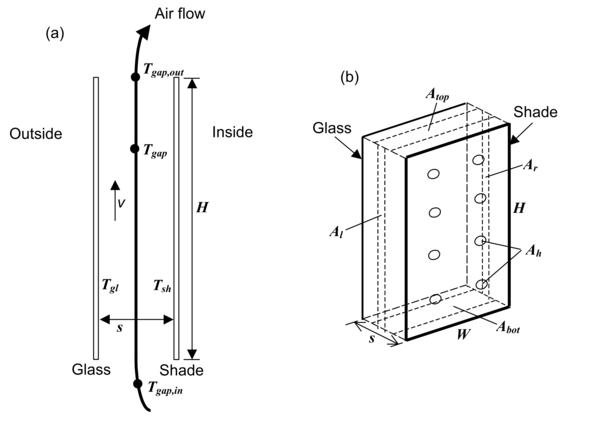
\includegraphics[width=0.9\textwidth, height=0.9\textheight, keepaspectratio=true]{media/image033.png}
\caption{Vertical section (a) and perspective view (b) of glass  and interior shade layers  showing variables used in the gap air flow analysis. In (b), the air-flow opening areas \(A_{\rm{bot}}\), \(A_{\rm{top}}\), \(A_{l}\), \(A_{r}\) and \(A_{h}\) are shown schematically. See \emph{Engineering Manual} for definition of thermal variables. \protect \label{fig:vertical-section-a-and-perspective-view-b-of}}
\end{figure}

\begin{figure}[hbtp] % fig 13
\centering
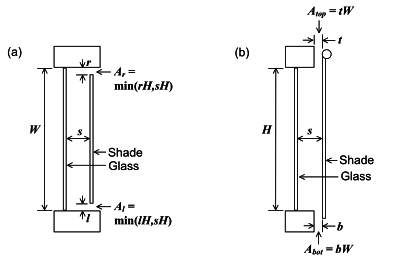
\includegraphics[width=0.9\textwidth, height=0.9\textheight, keepaspectratio=true]{media/image034.png}
\caption{Examples of air-flow openings for an interior shade covering glass of height \(H\) and width \(W\). Not to scale. (a) Horizontal section through shade with openings on the left and right sides (top view). (b) Vertical section through shade with openings at the top and bottom (side view). In (a) Left-Side Opening Multiplier = \(A_{l}/sH = min(l/s, 1)\) and Right-Side Opening Multiplier = \(A_{r}/sH = min(r/s, 1)\). In (b) Top Opening Multiplier = \(A_{\rm{top}}/sW = t/s\) and Bottom Opening Multiplier = \(A_{\rm{bot}}/sW = b/s\). \protect \label{fig:examples-of-air-flow-openings-for-an-interior}}
\end{figure}

An IDF example:

\begin{lstlisting}
WindowMaterial:Shade,
  DRAPES - CLOSE WEAVE MEDIUM,  !- Name
  0.05,                         !- Solar transmittance
  0.3000000,                    !- Solar Reflectance
  .05,                          !- Visible transmittance
  0.3000000,                    !- Visible reflectance
  0.9000000,                    !- Infrared Hemispherical Emissivity
  0.0,                          !- Infrared Transmittance
  0.003,                        !- Thickness {m}
  0.1,                          !- Conductivity {W/m-K}
  0.050,                        !- Shade to glass distance {m}
  1.0,                          !- Top opening multiplier
  1.0,                          !- Bottom opening multiplier
  0.0,                          !- Left-side opening multiplier
  0.0,                          !- Right-side opening multiplier
  0.0;                          !- Air flow permeability
\end{lstlisting}

\subsection{WindowMaterial:Blind}\label{windowmaterialblind}

This object specifies the properties of a window blind consisting of flat, equally-spaced slats. Unlike window shades, which are modeled as perfect diffusers, window blinds have solar and visible transmission and reflection properties that strongly depend on slat angle and angle of incidence of solar radiation. There is an EnergyPlus Reference Data Set for WindowMaterial:Blind that contains properties of generic window blinds.

Blinds can be located on the inside of the window (``interior blinds''), on the outside of the window (``exterior blinds''), or between two layers of glass (``between-glass blinds''). When in place, the blind is assumed to cover all of the glazed part of the window, including dividers; it does not cover any of the window frame, if present. The plane of the blind is assumed to be parallel to the glazing. When the blind is retracted it is assumed to cover none of the window. The solar and thermal effects of the blind's support strings, tapes or rods are ignored. Slat curvature, if present, is ignored.

There are two methods of assigning a blind to a window:

\subsubsection{Inputs}\label{inputs-23-005}

\paragraph{Method 1:}\label{method-1-1}

1)~~~Define the construction of the window without the blind, the so-called ``bare'' construction.

2)~~~Reference the bare construction in the \hyperref[fenestrationsurfacedetailed]{FenestrationSurface:Detailed} for the window.

3)~~~Define the WindowMaterial:Blind.

4)~~~Define a \hyperref[windowpropertyshadingcontrol]{WindowShadingControl} for the window in which you (a) specify that this WindowMaterial:Blind is the window's shading device and (b) specify how the blind is controlled.

\paragraph{Method 2:}\label{method-2-1}

1)~~~Define the Construction of the window without the blind, the so-called ``bare'' construction.

2)~~~Reference the bare construction in the \hyperref[fenestrationsurfacedetailed]{FenestrationSurface:Detailed} for the window.

3)~~~Define the WindowMaterial:Blind.

4)~~~Define another Construction, called the ``shaded construction,'' that includes the WindowMaterial:Blind.

5)~~~Define a \hyperref[windowpropertyshadingcontrol]{WindowShadingControl} for the window in which you (a) reference the shaded construction and (b) specify how the blind is controlled.

Note that \hyperref[windowpropertyshadingcontrol]{WindowShadingControl} has to be used with either method, even if the blind is in place at all times. You will get an error message if you try to reference a construction with a blind directly from Window objects (\hyperref[fenestrationsurfacedetailed]{FenestrationSurface:Detailed} or Window).

Note also that \hyperref[windowpropertyshadingcontrol]{WindowShadingControl} is used to determine not only when the blind is in place, but how its slat angle is controlled.

\paragraph{Field: Name}\label{field-name-17-007}

Name of the blind. It is referenced as a layer in a window construction (ref: Construction object) or as a ``Material Name of Shading Device'' in a \hyperref[windowpropertyshadingcontrol]{WindowShadingControl} object.

\paragraph{Field: Slat Orientation}\label{field-slat-orientation}

The choices are Horizontal and Vertical. ``Horizontal'' means the slats are parallel to the bottom of the window; this is the same as saying that the slats are parallel to the X-axis of the window. ``Vertical'' means the slats are parallel to Y-axis of the window.

\paragraph{Field: Slat Width}\label{field-slat-width}

The width of the slat measured from edge to edge (m). See Figure~\ref{fig:a-side-view-of-a-window-blind-with-horizontal}.

\paragraph{Field: Slat Separation}\label{field-slat-separation}

The distance between the front of a slat and the back of the adjacent slat (m). See Figure~\ref{fig:a-side-view-of-a-window-blind-with-horizontal}.

\paragraph{Field: Slat Thickness}\label{field-slat-thickness}

The distance between the faces of a slat (m). See Figure~\ref{fig:a-side-view-of-a-window-blind-with-horizontal}.

\paragraph{Field: Slat Angle}\label{field-slat-angle}

The angle (degrees) between the glazing outward normal and the slat outward normal, where the outward normal points away from the front face of the slat (degrees). See Figure~\ref{fig:a-side-view-of-a-window-blind-with-horizontal}.

If the \hyperref[windowpropertyshadingcontrol]{WindowShadingControl} for the blind has Type of Slat Angle Control for Blinds = FixedSlatAngle, the slat angle is fixed at ``Slat Angle.''

If Type of Slat Angle Control for Blinds = BlockBeamSolar, the program automatically adjusts the slat angle so as just block beam solar radiation. In this case the value of ``Slat Angle'' is used only when the blind is in place and there is no beam solar radiation incident on the blind.

If Type of Slat Angle Control for Blinds = ScheduledSlatAngle, the slat angle is variable. In this case ``Slat Angle'' is not applicable and the field should be blank.

If Type of Slat Angle Control for Blinds = FixedSlatAngle and ``Slat Angle'' is less than the minimum or greater than the maximum allowed by Slat Width, Slat Separation and Slat Thickness, the slat angle will be reset to the corresponding minimum or maximum and a warning will be issued.

\paragraph{Field: Slat Conductivity}\label{field-slat-conductivity}

The thermal conductivity of the slat (W/m-K).

\paragraph{Field: Slat Beam Solar Transmittance}\label{field-slat-beam-solar-transmittance}

The beam solar transmittance of the slat, assumed to be independent of angle of incidence on the slat. Any transmitted beam radiation is assumed to be 100\% diffuse (i.e., slats are translucent).

\paragraph{Field: Front Side Slat Beam Solar Reflectance}\label{field-front-side-slat-beam-solar-reflectance}

The beam solar reflectance of the front side of the slat, assumed to be independent of angle of incidence (matte finish). This means that slats with a large specularly-reflective component (shiny slats) are not well modeled.

\paragraph{Field: Back Side Slat Beam Solar Reflectance}\label{field-back-side-slat-beam-solar-reflectance}

The beam solar reflectance of the back side of the slat, assumed to be independent of angle of incidence (matte finish). This means that slats with a large specularly-reflective component (shiny slats) are not well modeled.

\paragraph{Field: Slat Diffuse Solar Transmittance}\label{field-slat-diffuse-solar-transmittance}

The slat transmittance for hemispherically diffuse solar radiation. This value should equal ``Slat Beam Solar Transmittance.''

\paragraph{Field: Front Side Slat Diffuse Solar Reflectance}\label{field-front-side-slat-diffuse-solar-reflectance}

The front-side slat reflectance for hemispherically diffuse solar radiation. This value should equal ``Front Side Slat Beam Solar Reflectance.''

\paragraph{Field: Back Side Slat Diffuse Solar Reflectance}\label{field-back-side-slat-diffuse-solar-reflectance}

The back-side slat reflectance for hemispherically diffuse solar radiation. This value should equal ``Back Side Slat Beam Solar Reflectance.''

\paragraph{Field: Slat Beam Visible Transmittance}\label{field-slat-beam-visible-transmittance}

The beam visible transmittance of the slat, assumed to be independent of angle of incidence on the slat. Any transmitted visible radiation is assumed to be 100\% diffuse (i.e., slats are translucent).

\paragraph{Field: Front Side Slat Beam Visible Reflectance}\label{field-front-side-slat-beam-visible-reflectance}

The beam visible reflectance on the front side of the slat, assumed to be independent of angle of incidence (matte finish). This means that slats with a large specularly-reflective component (shiny slats) are not well modeled.

\paragraph{Field: Back Side Slat Beam Visible Reflectance}\label{field-back-side-slat-beam-visible-reflectance}

The beam visible reflectance on the front side of the slat, assumed to be independent of angle of incidence (matte finish). This means that slats with a large specularly-reflective component (shiny slats) are not well modeled.

\paragraph{Field: Slat Diffuse Visible Transmittance}\label{field-slat-diffuse-visible-transmittance}

The slat transmittance for hemispherically diffuse visible radiation. This value should equal ``Slat Beam Visible Transmittance.''

\paragraph{Field: Front Side Slat Diffuse Visible Reflectance}\label{field-front-side-slat-diffuse-visible-reflectance}

The front-side slat reflectance for hemispherically diffuse visible radiation. This value should equal ``Front Side Slat Beam Visible Reflectance.''

\paragraph{Field: Back Side Slat Diffuse Visible Reflectance}\label{field-back-side-slat-diffuse-visible-reflectance}

The back-side slat reflectance for hemispherically diffuse visible radiation. This value should equal ``Back Side Slat Beam Visible Reflectance..''

\paragraph{Field: Slat Infrared Hemispherical Transmittance}\label{field-slat-infrared-hemispherical-transmittance}

The slat Infrared transmittance. It is zero for solid metallic, wooden or glass slats, but may be non-zero in some cases (e.g., thin plastic slats).

\paragraph{Field: Front Side Slat Infrared Hemispherical Emissivity}\label{field-front-side-slat-infrared-hemispherical-emissivity}

Front-side hemispherical emissivity of the slat. Approximately 0.9 for most materials. The most common exception is bare (unpainted) metal slats or slats finished with a metallic paint.

\paragraph{Field: Back Side Slat Infrared Hemispherical Emissivity}\label{field-back-side-slat-infrared-hemispherical-emissivity}

Back-side hemispherical emissivity of the slat. Approximately 0.9 for most materials. The most common exception is bare (unpainted) metal slats or slats finished with a metallic paint.

\paragraph{Field: Blind to Glass Distance}\label{field-blind-to-glass-distance}

For interior and exterior blinds, the distance from the mid-plane of the blind to the adjacent glass (m). See Figure~\ref{fig:a-side-view-of-a-window-blind-with-horizontal}. Not used for between-glass blinds. As for window shades (ref: \hyperref[windowmaterialshade]{WindowMaterial:Shade}) this distance is used in calculating the natural convective air flow between glass and blind that is produced by buoyancy effects.

\paragraph{Opening Multipliers}\label{opening-multipliers}

The following opening multipliers are defined in the same way as for window shades (see \hyperref[windowmaterialshade]{WindowMaterial:Shade}, Figure~\ref{fig:vertical-section-a-and-perspective-view-b-of} and Figure~\ref{fig:examples-of-air-flow-openings-for-an-interior}). Note that, unlike window shades, there is no input for Air-Flow Permeability; this is automatically calculated by the program from slat angle, width and separation.

\paragraph{Field: Blind Top Opening Multiplier}\label{field-blind-top-opening-multiplier}

Defined as for Material:WindowShade.

\paragraph{Field: Blind Bottom Opening Multiplier}\label{field-blind-bottom-opening-multiplier}

Defined as for Material:WindowShade.

\paragraph{Field: Blind Left-Side Opening Multiplier}\label{field-blind-left-side-opening-multiplier}

Defined as for Material:WindowShade.

\paragraph{Field: Blind Right-Side Opening Multiplier}\label{field-blind-right-side-opening-multiplier}

Defined as for Material:WindowShade.

\paragraph{Field: Minimum Slat Angle}\label{field-minimum-slat-angle}

The minimum allowed slat angle (degrees). Used only if \hyperref[windowpropertyshadingcontrol]{WindowShadingControl} (for the window that incorporates this blind) varies the slat angle (i.e., the \hyperref[windowpropertyshadingcontrol]{WindowShadingControl} has Type of Slat Angle Control for Blinds = ScheduledSlatAngle or BlockBeamSolar). In this case, if the program tries to select a slat angle less than Minimum Slat Angle it will be reset to Minimum Slat Angle. (Note that if the Minimum Slat Angle itself is less than the minimum allowed by Slat Width, Slat Separation and Slat Thickness, it will be reset to that minimum.)

\paragraph{Field: Maximum Slat Angle}\label{field-maximum-slat-angle}

The maximum allowed slat angle (degrees). Used only if \hyperref[windowpropertyshadingcontrol]{WindowShadingControl} (for the window that incorporates this blind) varies the slat angle (i.e., the \hyperref[windowpropertyshadingcontrol]{WindowShadingControl} has Type of Slat Angle Control for Blinds = ScheduledSlatAngle or BlockBeamSolar). In this case, if the program tries to select a slat angle greater than Maximum Slat Angle the slat angle will be reset to Maximum Slat Angle. (Note that if the Maximum Slat Angle itself is greater than the maximum allowed by Slat Width, Slat Separation and Slat Thickness, it will be reset to that maximum.)

An IDF example:

\begin{lstlisting}

WindowMaterial:Blind,
   White Painted Metal Blind,   !- Name
   HORIZONTAL, !- Slat orientation
   0.025   , !- Slat width (m)
   0.01875 , !- Slat separation (m)
   0.001   , !- Slat thickness (m)
   45.0    , !- Slat angle (deg)
   44.9    , !- Slat conductivity (W/m-K)
   0.0     , !- Slat beam solar transmittance
   0.8     , !- Front Side Slat beam solar reflectance
   0.8     , !- Back Side Slat beam solar reflectance
   0.0     , !- Slat diffuse solar transmittance
   0.8     , !- Front Side Slat diffuse solar reflectance
   0.8     , !- Back Side Slat diffuse solar reflectance
   0.0     , !- Slat beam visible transmittance
   0.7     , !- Front Side Slat beam visible reflectance
   0.7     , !- Back Side Slat beam visible reflectance
   0.0     , !- Slat diffuse visible transmittance
   0.7     , !- Front Side Slat diffuse visible reflectance
   0.7     , !- Back Side Slat diffuse visible reflectance
   0.0     , !- Slat Infrared hemispherical transmittance
   0.9     , !- Front Side Slat Infrared hemispherical emissivity
   0.9     , !- Back Side Slat Infrared hemispherical emissivity
   0.050   , !- Blind-to-glass distance
   0.0     , !- Blind top opening multiplier
   0.0     , !- Blind bottom opening multiplier
   0.5     , !- Blind left-side opening multiplier
   0.5     , !- Blind right-side opening multiplier
   ,         !- Minimum slat angle (deg)
   ;         !- Maximum slat angle (deg)
\end{lstlisting}

\begin{figure}[hbtp] % fig 14
\centering
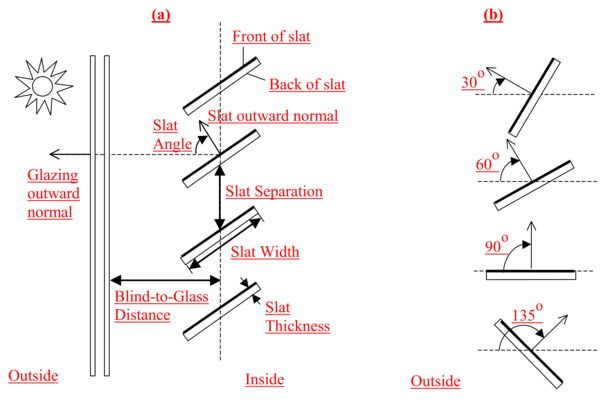
\includegraphics[width=0.9\textwidth, height=0.9\textheight, keepaspectratio=true]{media/image035.png}
\caption{(a) Side view of a window blind with horizontal slats (or top view of blind with vertical slats) showing slat geometry. The front face of a slat is shown by a heavy line. The slat angle is defined as the angle between the glazing outward normal and the slat outward normal, where the outward normal points away from the front face of the slat. (b) Slat orientations for representative slat angles. The slat angle varies from 0\(^{o}\), when the front of the slat is parallel to the glazing and faces toward the outdoors,  to 90\(^{o}\), when the slat is perpendicular to the glazing, to 180\(^{o}\), when the front of the slat is parallel to the glazing and faces toward the indoors. The minimum and maximum slat angles are determined by the slat thickness, width and separation. \protect \label{fig:a-side-view-of-a-window-blind-with-horizontal}}
\end{figure}

\subsection{WindowMaterial:ComplexShade}\label{windowmaterialcomplexshade}

This input object is used to define shade layers used in the \hyperref[constructioncomplexfenestrationstate]{Construction:ComplexFenestrationState} object.

\subsubsection{Inputs}\label{inputs-24-003}

\paragraph{Field: Name}\label{field-name-18-007}

Unique name of the shading layer.

\paragraph{Field: Shading Layer Type}\label{field-shading-layer-type}

The type of shading layer. The options are:

\begin{itemize}
\item
  VenetianHorizontal -- for modeling horizontal venetian blinds
\item
  VenetianVertical -- for modeling vertical venetian blinds
\item
  Woven -- for modeling shading systems with a regular weave
\item
  Perforated -- for modeling perforated screens
\item
  BSDF -- for modeling shades whose properties are represented by a BSDF file
\item
  OtherShadingType -- for modeling shading systems which do not belong to the any of the previous group
\end{itemize}

\paragraph{Field: Thickness}\label{field-thickness-7}

The thickness (m) of the shading layer. This value is ignored for ShadingLayerType = Venetian*, because the program will calculate the thickness based on the slat angle. This value is needed for ShadingLayerType = Woven and Perforated

\paragraph{Field: Conductivity}\label{field-conductivity-4}

The conductivity (W/mK) of the shading layer material. Default: 1.0

\begin{itemize}
\item
  Venetian* -- the conductivity of the venetian blind slat material
\item
  Woven -- the conductivity of the woven shade material (such as the thread for a fabric shade)
\item
  Perforated -- for modeling perforated screens
\item
  BSDF -- for modeling shades whose properties are represented by a BSDF file
\item
  OtherShadingType -- for modeling shading systems which do not belong to the any of the previous group
\end{itemize}

\paragraph{Field: IR Transmittance}\label{field-ir-transmittance}

The IR transmittance of the shading layer. Minimum value: 0. Maximum value: 1. Default: 0.

\paragraph{Field: Front Emissivity}\label{field-front-emissivity}

The front emissivity of the shading layer. Minimum value: 0. Maximum value: 1. Default: 0.90.

\paragraph{Field: Back Emissivity}\label{field-back-emissivity}

The back emissivity of the shading layer. Minimum value: 0. Maximum value: 1. Default: 0.90.

\paragraph{Field: Top Opening Multiplier}\label{field-top-opening-multiplier-1}

The top opening multiplier value will depend on the location of the shading device within the glazing system. There are several possible scenarios which can occur and they can be divided into two groups:

\textbf{Shading device on the indoor/outdoor side of the window}

In this case the opening multiplier is calculated as the smallest distance between the shading device and the frame (d\(_{top}\)), divided by the gap width (S). There are three possible cases for the position of a shading device the on indoor/outdoor side (see Figure~\ref{fig:three-cases-for-the-dp-calculation-for-an-indoor-outdoor-shade}).

\begin{figure}[htbp]
\centering
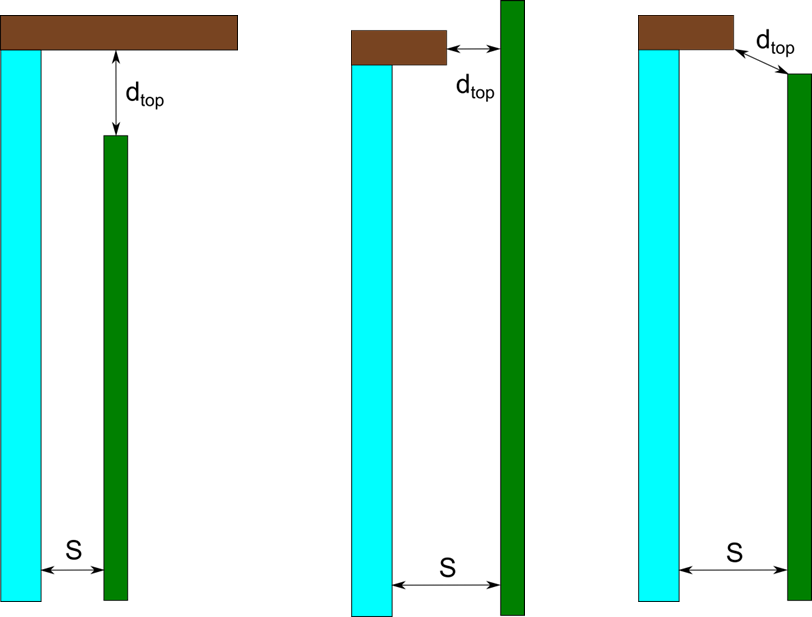
\includegraphics[width=0.9\textwidth, height=0.9\textheight, keepaspectratio=true]{media/three-cases-for-the-dtop-calculation-for-an-indoor-outdoor-shade-collage.png}
\caption{Three cases for the D\(_{top}\) calculation for an indoor/outdoor shade: Case a) A shading device between the frame; Case b) A shading device outside the frame, covering the frame; Case c) a shading device outside the frame, not covering the frame. \protect \label{fig:three-cases-for-the-dp-calculation-for-an-indoor-outdoor-shade}}
\end{figure}

In the case where the distance between the frame and the shading device is bigger than the gap width, the d\(_{top}\) multiplier is equal to one. Therefore, the calculation of the D\(_{top}\) opening multiplier is:

\begin{equation*}
A_{top} = min(d_{top}/S, 1)
\end{equation*}

\textbf{Shading device between glass layers}

In this case the opening multiplier is calculated as the smallest distance between the shading device and the frame or spacer (d\(_{top}\)), divided by the smaller gap width (the minimum of (S\(_{1}\) andS\(_{2}\))).

\begin{figure}[htbp]
\centering
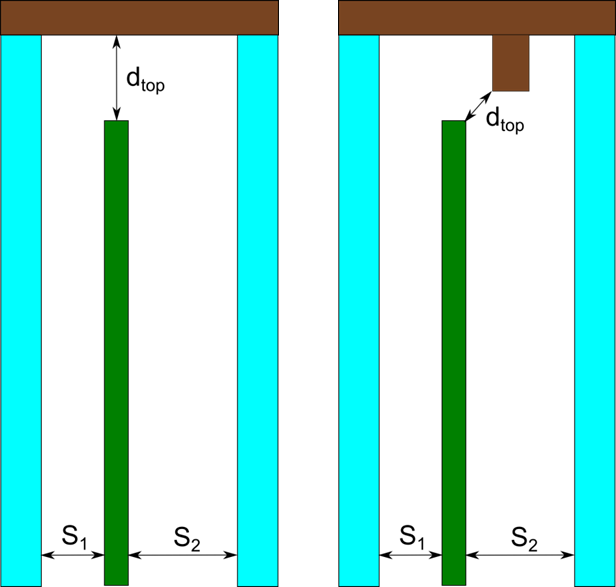
\includegraphics[width=0.9\textwidth, height=0.9\textheight, keepaspectratio=true]{media/calculation-of-dtop-for-a-shading-device-collage.png}
\caption{Calculation of Dtop for a shading device between glass layers \protect \label{fig:calculation-of-dtop-for-a-shading-device-between-glass-layers}}
\end{figure}

The D\(_{top}\) opening multiplier for a between glass shade is calculated as:

\begin{equation*}
A_{top} = min(d_{top}/S_{min}, 1)
\end{equation*}

Where

\begin{equation*}
S_{min} = min(S_1, S_2)
\end{equation*}

\paragraph{Field: Bottom Opening Multiplier}\label{field-bottom-opening-multiplier-1}

The bottom opening multiplier (d\(_{bot}\)) is calculated in the same way as the top opening multiplier, with the rules applied to the bottom of the shading device.

\paragraph{Field: Left Side Opening Multiplier}\label{field-left-side-opening-multiplier-1}

The left side opening multiplier (d\(_{left}\)) is calculated in the same way as the top opening multiplier, with the rules applied to the left side of the shading device.

\paragraph{Field: Right Side Opening Multiplier}\label{field-right-side-opening-multiplier-1}

The right side opening multiplier (d\(_{right}\)) is calculated in the same way as the top opening multiplier, with the rules applied to the right side of the shading device.

\paragraph{Field: Front Opening Multiplier}\label{field-front-opening-multiplier}

The fraction of glazing system area that is open on the front of the shading layer (see Figure~\ref{fig:front-view-of-shading-layer-openings.}). This fraction is calculated as follows: Afront / (W * H), where Afront = Area of the front of the glazing system that is not covered by the shading system, W = the width of the glazing system (IGU) and H is height of the glazing system (IGU).

\begin{figure}[hbtp] % fig 17
\centering
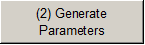
\includegraphics[width=0.9\textwidth, height=0.9\textheight, keepaspectratio=true]{media/image041.png}
\caption{Front view of shading layer openings. \protect \label{fig:front-view-of-shading-layer-openings.}}
\end{figure}

\paragraph{Field: Slat Width}\label{field-slat-width-1}

The width (m) of the venetian slats.~ Used only for ShadingLayerType = Venetian.

\paragraph{Field: Slat Spacing}\label{field-slat-spacing}

The distance (m) between front sides of the venetian slats.~ Used only for ShadingLayerType = Venetian.

\paragraph{Field: Slat Thickness}\label{field-slat-thickness-1}

The thickness (m) of the venetian slats.~ Used only for ShadingLayerType = Venetian.

\paragraph{Field: Slat Angle}\label{field-slat-angle-1}

The slat tilt angle (degrees) of the venetian slats.~ Used only for ShadingLayerType = Venetian.~ Range of slat angle is from -90 to 90 degrees.

\paragraph{Field: Slat Conductivity}\label{field-slat-conductivity-1}

The conductivity (W/mK) of the venetian slats.~ Used only for ShadingLayerType = Venetian.

\paragraph{Field: Slat Curve}\label{field-slat-curve}

The curvature radius (m) of the venetian slats.~ Setting this value to zero means there is no curvature in the slat (it is flat), while a non-zero value is the radius of the slat curve.~ This value cannot be smaller than Slat Width / 2.~ Used only for ShadingLayerType = Venetian.

\begin{figure}[hbtp] % fig 18
\centering
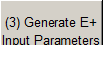
\includegraphics[width=0.9\textwidth, height=0.9\textheight, keepaspectratio=true]{media/image042.png}
\caption{Side view of horizontal venetian blind slats or top view of blinds with vertical slats.  Front face of slats is marked with red line. \protect \label{fig:side-view-of-horizontal-venetian-blind-slats}}
\end{figure}

An IDF example for ShadingLayerType = Venetian

\begin{lstlisting}

WindowMaterial:ComplexShade,       !- venetian blind layer
    Shade_30001_Layer,               !- name
    Venetian,                        !- shading layer type
    0.005,                           !- thickness
    160,                             !- layer conductivity
    0.0,                             !- IR transmittance
    0.9,                             !- front emissivity
    0.9,                             !- back emissivity
    0.0,                             !- top opening multiplier
    0.0,                             !- bottom opening multiplier
    0.0,                             !- left side opening multiplier
    0.0,                             !- right side opening multiplier
    0.05,                            !- front opening multiplier
    0.016,                           !- venetian slat width
    0.012,                           !- venetian slat spacing
    0.0006,                          !- venetian slat thickness
    -45.00,                          !- venetian slat angle
    160.00,                          !- venetian slat conductivity
    0.0000;                          !- venetian slat curve
\end{lstlisting}

An IDF example for ShadingLayerType = Woven

(Note that it is not necessary to include ``blank'' lines for the venetian blind input for a Woven shade definition).

\begin{lstlisting}

WindowMaterial:ComplexShade,       !- woven shade layer
    Shade_30002_Layer,               !- name
    Woven,                           !- shading layer type
    0.011,                           !- thickness
    1,                               !- layer conductivity
    0.0,                             !- IR transmittance
    0.9,                             !- front emissivity
    0.9,                             !- back emissivity
    0.0,                             !- top opening multiplier
    0.0,                             !- bottom opening multiplier
    0.0,                             !- left side opening multiplier
    0.0,                             !- right side opening multiplier
    0.17;                            !- front opening multiplier
\end{lstlisting}

\subsection{WindowMaterial:Screen}\label{windowmaterialscreen}

This object specifies the properties of exterior window screen materials. The window screen model assumes the screen is made up of intersecting orthogonally-crossed cylinders. The surface of the cylinders is assumed to be diffusely reflecting, having the optical properties of a Lambertian surface.

The beam solar radiation transmitted through a window screen varies with sun angle and is made up of two distinct elements: a direct beam component and a reflected beam component. The direct beam transmittance component is modeled using the geometry of the screen material and the incident angle of the sun to account for shadowing of the window by the screen material. The reflected beam component is an empirical model that accounts for the inward reflection of solar beam off the screen material surface. This component is both highly directional and small in magnitude compared to the direct beam transmittance component (except at higher incident angles, for which case the magnitude of the direct beam component is small or zero and the reflected beam component, though small in absolute terms can be many times larger than the direct beam component). For this reason, the reflected beam transmittance component calculated by the model can be a. disregarded, b. treated as an additive component to direct beam transmittance (and in the same direction), or c. treated as hemispherically-diffuse transmittance based on a user input to the model.

\begin{figure}[hbtp] % fig 19
\centering
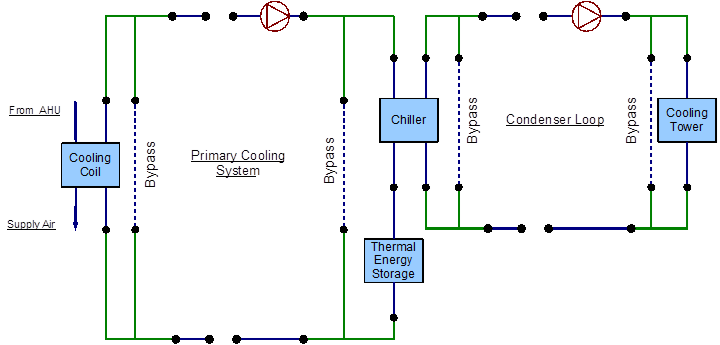
\includegraphics[width=0.9\textwidth, height=0.9\textheight, keepaspectratio=true]{media/image043.png}
\caption{Direct beam and reflected beam transmittance components \protect \label{fig:direct-beam-and-reflected-beam-transmittance}}
\end{figure}

The window screen ``assembly'' properties of overall beam solar reflectance and absorptance (including the screen material `cylinders' and open area) also change with sun angle and are calculated based on the values of the beam solar transmittance components (direct and reflected components described above) and the physical properties of the screen material (i.e., screen material diameter, spacing, and reflectance).

Transmittance, reflectance, and absorptance of diffuse solar radiation are considered constant values and apply to both the front and back surfaces of the screen. These properties are calculated by the model as an average value by integrating the screen's beam solar properties over a quarter hemisphere of incident radiation. Long-wave emissivity is also assumed to be the same for both sides of the screen.

There is an EnergyPlus Reference Data Set for WindowMaterial:Screen that contains properties for generic window screens. Window screens of this type can only be used on the outside surface of the window (``exterior screens''). When in place, the screen is assumed to cover all of the glazed part of the window, including dividers; it does not cover any of the window frame, if present. The plane of the screen is assumed to be parallel to the glazing.

WindowMaterial:Screen can be used to model wire mesh insect screens where the solar and visible transmission and reflection properties vary with the angle of incidence of solar radiation. For diffusing materials such as drapery and translucent roller shades it is better to use the \hyperref[windowmaterialshade]{WindowMaterial:Shade} object. For slat-type shading devices like Venetian blinds, which have solar and visible transmission and reflection properties that strongly depend on slat angle and angle of incidence of solar radiation, it is better to use \hyperref[windowmaterialblind]{WindowMaterial:Blind}.

There are two methods of assigning a screen to a window:

\subsubsection{Inputs}\label{inputs-25-003}

\paragraph{Method 1:}\label{method-1-2}

1)~~~Define the construction of the window without the screen, the so-called ``bare'' construction.

2)~~~Reference the bare construction in the \hyperref[fenestrationsurfacedetailed]{FenestrationSurface:Detailed} for the window.

3)~~~Define the WindowMaterial:Screen object.

4)~~~Define a \hyperref[windowpropertyshadingcontrol]{WindowShadingControl} for the window in which you (a) specify that this Material:WindowScreen is the window's shading device, and (b) specify how the screen is controlled.

\paragraph{Method 2:}\label{method-2-2}

1)~~~Define the Construction of the window without the screen, the so-called ``bare'' construction.

2)~~~Reference the bare construction in the \hyperref[fenestrationsurfacedetailed]{FenestrationSurface:Detailed} for the window.

3)~~~Define the WindowMaterial:Screen object.

4)~~~Define another Construction, called the ``shaded construction,'' that includes the WindowMaterial:Screen.

5)~~~Define a \hyperref[windowpropertyshadingcontrol]{WindowShadingControl} for the window in which you (a) reference the shaded construction, and (b) specify how the screen is controlled.

Note that \hyperref[windowpropertyshadingcontrol]{WindowShadingControl} has to be used with either method, even if the screen is in place at all times. You will get an error message if you try to reference a shaded construction directly from a \hyperref[fenestrationsurfacedetailed]{FenestrationSurface:Detailed} object.

\paragraph{Field: Name}\label{field-name-19-004}

Enter a unique name for the screen. This name is referenced as an outside layer in a window construction.

\paragraph{Field: Reflected Beam Transmittance Accounting Method}\label{field-reflected-beam-transmittance-accounting-method}

This input specifies the method used to account for screen-reflected beam solar radiation that is transmitted through the window screen (as opposed to being reflected back outside the building). Since this inward reflecting beam solar is highly directional and is not modeled in the direction of the actual reflection, the user is given the option of how to account for the directionality of this component of beam solar transmittance. Valid choices are DoNotModel, ModelAsDirectBeam (i.e., model as an additive component to direct solar beam and in the same direction), or ModelAsDiffuse (i.e., model as hemispherically-diffuse radiation). The default value is ModelAsDiffuse.

\paragraph{Field: Diffuse Solar Reflectance}\label{field-diffuse-solar-reflectance}

This input specifies the solar reflectance (beam-to-diffuse) of the screen material itself (not the effective value for the overall screen ``assembly'' including open spaces between the screen material). The outgoing diffuse radiation is assumed to be Lambertian (distributed angularly according to Lambert's cosine law). The solar reflectance is assumed to be the same for both sides of the screen. This value must be from 0 to less than 1.0. In the absence of better information, the input value for diffuse solar reflectance should match the input value for diffuse visible reflectance.

\paragraph{Field: Diffuse Visible Reflectance}\label{field-diffuse-visible-reflectance}

This input specifies the visible reflectance (beam-to-diffuse) of the screen material itself (not the effective value for the overall screen ``assembly'' including open spaces between the screen material) averaged over the solar spectrum and weighted by the response of the human eye. The outgoing diffuse radiation is assumed to be Lambertian (distributed angularly according to Lambert's cosine law). The visible reflectance is assumed to be the same for both sides of the screen. This value must be from 0 to less than 1.0.

If diffuse visible reflectance for the screen material is not available, then the following guidelines can be used to estimate this value:

\begin{itemize}
\item
  Dark-colored screen (e.g., charcoal):~~~~~~~~~~~~~~~~~ 0.08 -- 0.10
\item
  Medium-colored screen (e.g., gray):~~~~~~~~~~~~~~~~~~ 0.20 -- 0.25
\item
  Light-colored screen (e.g., bright aluminum):~~~~~~ 0.60 -- 0.65
\end{itemize}

Commercially-available gray scale or grayscale reflecting chart references can be purchased for improved accuracy in estimating visible reflectance (by visual comparison of screen reflected brightness with that of various known-reflectance portions of the grayscale).

\paragraph{Field: Thermal Hemispherical Emissivity}\label{field-thermal-hemispherical-emissivity-1}

Long-wave emissivity \(\varepsilon\) of the screen material itself (not the effective value for the overall screen ``assembly'' including open spaces between the screen material). The emissivity is assumed to be the same for both sides of the screen.

For most non-metallic materials, \(\varepsilon\) is about 0.9. For metallic materials, \(\varepsilon\) is dependent on material, its surface condition, and temperature. Typical values for metallic materials range from 0.05 -- 0.1 with lower values representing a more finished surface (e.g.~low oxidation, polished surface). Material emissivities may be found in Table~\ref{table:atmospheric-variables-at-two-different} from the 2005 ASHRAE Handbook of Fundamentals, page 3.9. The value for this input field must be between 0 and 1, with a default value of 0.9 if this field is left blank.

\paragraph{Field: Conductivity}\label{field-conductivity-5}

Screen material conductivity (W/m-K). This input value must be greater than 0. The default value is 221 W/m-K (aluminum).

\paragraph{Field: Screen Material Spacing}\label{field-screen-material-spacing}

The spacing, S, of the screen material (m) is the distance from the center of one strand of screen to the center of the adjacent one. The spacing of the screen material is assumed to be the same in both directions (e.g., vertical and horizontal). This input value must be greater than the non-zero screen material diameter. If the spacing is different in the two directions, use the average of the two values.

\begin{figure}[hbtp] % fig 20
\centering
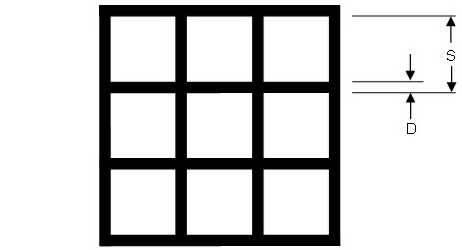
\includegraphics[width=0.9\textwidth, height=0.9\textheight, keepaspectratio=true]{media/image044.png}
\caption{Screen Material Spacing and Diameter \protect \label{fig:screen-material-spacing-and-diameter}}
\end{figure}

\paragraph{Field: Screen Material Diameter}\label{field-screen-material-diameter}

The diameter, D, of individual strands or wires of the screen material (m). The screen material diameter is assumed to be the same in both directions (e.g., vertical and horizontal). This input value must be greater than 0 and less than the screen material spacing. If the diameter is different in the two directions, use the average of the two values.

\paragraph{Field: Screen to Glass Distance}\label{field-screen-to-glass-distance}

Distance from the window screen to the adjacent glass surface (m). If the screen is not flat, the average screen to glass distance should be used. The screen-to-glass distance is used in calculating the natural convective air flow between the glass and the screen produced by buoyancy effects. This input value must be from 0.001 m to 1 m, with a default value of 0.025 m if this field is left blank.

\paragraph{Field: Top Opening Multiplier}\label{field-top-opening-multiplier-2}

Effective area for air flow at the top of the screen divided by the horizontal area between the glass and screen (see the same field for the Material:WindowShade object for additional description). The opening multiplier fields can be used to simulate a shading material that is offset from the window frame. Since window screens are typically installed against the window frame, the default value is equal to 0.This input value can range from 0 to 1.

\paragraph{Field: Bottom Opening Multiplier}\label{field-bottom-opening-multiplier-2}

Effective area for air flow at the bottom of the screen divided the horizontal area between the glass and screen (see the same field for the Material:WindowShade object for additional description). The opening multiplier fields can be used to simulate a shading material that is offset from the window frame. Since window screens are typically installed against the window frame, the default value is equal to 0. This input value can range from 0 to 1.

\paragraph{Field: Left-Side Opening Multiplier}\label{field-left-side-opening-multiplier-2}

Effective area for air flow at the left side of the screen divided the vertical area between the glass and screen (see the same field for the Material:WindowShade object for additional description). The opening multiplier fields can be used to simulate a shading material that is offset from the window frame. Since window screens are typically installed against the window frame, the default value is equal to 0. This input value can range from 0 to 1.

\paragraph{Field: Right-Side Opening Multiplier}\label{field-right-side-opening-multiplier-2}

Effective area for air flow at the right side of the screen divided the vertical area between the glass and screen (see the same field for the Material:WindowShade object for additional description). The opening multiplier fields can be used to simulate a shading material that is offset from the window frame. Since window screens are typically installed against the window frame, the default value is equal to 0. This input value can range from 0 to 1.

\paragraph{Field: Angle of Resolution for Screen Transmittance Output Map}\label{field-angle-of-resolution-for-screen-transmittance-output-map}

Angle of resolution, in degrees, for the overall screen beam transmittance (direct and reflected) output map. The comma-separated variable file eplusscreen.csv (Ref. OutputDetailsandExamples.pdf) will contain the direct beam and reflected beam solar radiation that is transmitted through the window screen as a function of incident sun angle (0 to 90 degrees relative solar azimuth and 0 to 90 degrees relative solar altitude) in sun angle increments specified by this input field. The default value is 0, which means no transmittance map is generated. Other valid choice inputs are 1, 2, 3 and 5 degrees.

An IDF example for this object, along with Construction and \hyperref[windowpropertyshadingcontrol]{WindowShadingControl} objects, is shown below:

\begin{lstlisting}

WindowMaterial:Screen,
      EXTERIOR SCREEN,         !- Name
      ModelAsDiffuse,        !- Reflected Beam Transmittance Accounting Method
      0.6,                     !- Diffuse Solar Reflectance
      0.6,                     !- Diffuse Visible Reflectance
      0.9,                     !- Thermal Hemispherical Emissivity
      221.0,                   !- Conductivity {W/m-K}
      0.00154,                 !- Screen Material Spacing (m)
      0.000254,                !- Screen Material Diameter (m)
      0.025,                   !- Screen-to-Glass Distance {m}
      0.0,                     !- Top Opening Multiplier
      0.0,                     !- Bottom Opening Multiplier
      0.0,                     !- Left-Side Opening Multiplier
      0.0,                     !- Right-Side Opening Multiplier
      0;                   !- Angle of Resolution for Output Map {deg}

  Construction,
      DOUBLE PANE WITHOUT SCREEN,     !- Name
      GLASS - CLEAR SHEET 1 / 8 IN,   !- Outside Layer
      WinAirB1 - AIRSPACE RESISTANCE, !- Layer \#2
      GLASS - CLEAR SHEET 1 / 8 IN;   !- Layer \#3

  WindowShadingControl,
      DOUBLE PANE WITH SCREEN, !- Name
      West Zone,               !- Zone Name
      1,                       !- Shading Control Sequence Number
      ExteriorScreen,          !- Shading Type
      ,                        !- Name of construction with shading
      AlwaysOn,                !- Shading Control Type
      ScreenSchedule,          !- Schedule Name
      20.0,                    !- SetPoint {W/m2, W or deg C}
      YES,                     !- Shading Control Is Scheduled
      NO,                      !- Glare Control Is Active
      EXTERIOR SCREEN,         !- Material Name of Shading Device
      ,                        !- Type of Slat Angle Control for Blinds
      ,                        !- Slat Angle Schedule Name
      ,                        !- Setpoint 2 {W/m2 or deg C}
      ,                        !- Daylighting Control Object Name
      Sequential,              !- Multiple Surface Control Type
      Zn001:Wall001:Win001;    !- Fenestration Surface 1 Name
\end{lstlisting}

\subsection{WindowMaterial:Shade:EquivalentLayer}\label{windowmaterialshadeequivalentlayer}

This object specifies the properties of Equivalent Layer window shade (roller blind) materials. Shades are considered to be thin, flat and perfect diffusers (all transmitted and reflected radiation is hemispherically-diffuse). However, shades can have beam-beam transmittance by virtue of their material openness.~ The beam-beam transmittence is assumed to be the same for both sides of the shade and is the same as the openness area fraction. Beam-diffuse transmittance and reflectance, and emissivity properties can be different for front and back side of the shade.Window shades can be placed on the inside of the window, on the outside of the window, or between glass layers. WindowMaterial:Shade:EquivalentLayer is used for roller blinds. The off-normal solar property calculation of shades (roller blind) is based on a set of correlations developed from measurement of samples of commercially produced roller blind material with openness fraction less than 0.14. The model is not intended for materials with unusually high values of openness and should be limited to a maximum openness fraction of 0.20. The visible spectrum solar properties input fields are not used currently hence can be left blank. The equivalent layer window shade model does not support \hyperref[windowpropertyshadingcontrol]{WindowShadingControl}.

\subsubsection{Inputs}\label{inputs-26-002}

\paragraph{Field: Name}\label{field-name-20-003}

Name of the shade. It is referenced as an inside, inbetween or outside layer in an equivalent layer~ window construction.

\paragraph{Field: Shade Beam-Beam Solar Transmittance}\label{field-shade-beam-beam-solar-transmittance}

This value is the beam-beam transmittance of the shade at normal incidence and it is the same as the openness area fraction of the shade material. Assumed to be the same for front and back sides of the roller blinds.~ The minimum value is 0.0 and maximum value is less than 1.0.~ The default value is 0.0. For most common shade materials (e.g.~Roller Blinds) the material oppeness fraction doesn't exceed 0.20.

\paragraph{Field: Front Side Shade Beam-Diffuse Solar Transmittance}\label{field-front-side-shade-beam-diffuse-solar-transmittance}

This value is the front side beam-diffuse transmittance of the shade material at normal incidence averaged over the entire spectrum of solar radiation. The minimum value is 0.0 and maximum value is less than 1.0.~ The default value is 0.0.

\paragraph{Field: Back Side Shade Beam-Diffuse Solar Transmittance}\label{field-back-side-shade-beam-diffuse-solar-transmittance}

This value is the back side beam-diffuse transmittance of the shade material at normal incidence averaged over the entire spectrum of solar radiation. The minimum value is 0.0 and maximum value is less than 1.0.~ The default value is 0.0.

\paragraph{Field: Front Side Shade Beam-Diffuse Solar Reflectance}\label{field-front-side-shade-beam-diffuse-solar-reflectance}

This value is the front side beam-diffuse reflectance of the shade material at normal incidence averaged over the entire spectrum of solar radiation. The minimum value is 0.0 and maximum value is less than 1.0.

\paragraph{Field: Back Side Shade Beam-Diffuse Solar Reflectance}\label{field-back-side-shade-beam-diffuse-solar-reflectance}

This value is the back side beam-diffuse reflectance of the shade material at normal incidence averaged over the entire spectrum of solar radiation. The minimum value is 0.0 and maximum value is less than 1.0.

\paragraph{Field: Shade Beam-Beam Visible Transmittance}\label{field-shade-beam-beam-visible-transmittance}

This value is the beam-beam transmittance at normal incidence averaged over the visible spectrum of solar radiation. Assumed to be the same for front and back sides. The minimum value is 0.0 and maximum value is less than 1.0.~ Currently this input field is not used.

\paragraph{Field: Shade Beam-Diffuse Visible Transmittance}\label{field-shade-beam-diffuse-visible-transmittance}

This value is the beam-diffuse transmittance at normal incidence averaged over the visible spectrum of solar radiation. Assumed to be the same for front and back sides. The minimum value is 0.0 and maximum value is less than 1.0.~ Currently this input field is not used.

\paragraph{Field: Shade Beam-Diffuse Visible Reflectance}\label{field-shade-beam-diffuse-visible-reflectance}

This value is the beam-diffuse reflectance at normal incidence averaged over the visible spectrum of solar radiation. Assumed to be the same for front and back sides. The minimum value is 0.0 and maximum value is less than 1.0.~ Currently this input field is not used.

\paragraph{Field: Shade Material Infrared Transmittance}\label{field-shade-material-infrared-transmittance}

This value is the long-wave transmittance of the shade material and assumed to be the same for front and back sides of the shade. The minimum value is 0.0 and maximum value is less than 1.0. Default value is 0.05.

\paragraph{Field: Front Side Shade Material Infrared Emissivity}\label{field-front-side-shade-material-infrared-emissivity}

This value is the front side long-wave hemispherical emissivity of shade material. The minimum value is 0.0 and maximum value is less than 1.0. Default value is 0.91. The front side effective emissivity of the shade layer is calculated using this value and the material openness specified above.

\paragraph{Field: Back Side Shade Material Infrared Emissivity}\label{field-back-side-shade-material-infrared-emissivity}

This value is the back side long-wave hemispherical emissivity of shade material. The minimum value is 0.0 and maximum value is less than 1.0. Default value is 0.91. The back side effective emissivity of the shade is calculated using this value and the material openness specified above.

An IDF example for this object is shown below:

\begin{lstlisting}

WindowMaterial:Shade:EquivalentLayer,
    Shade1,        !- Name
    0.190,         !- Shade Beam-Beam Solar Transmittance
    0.206,         !- Front Side Shade Beam-Diffuse Solar Transmittance
    0.206,         !- Back Side Shade Beam-Diffuse Solar Transmittance
    0.499,         !- Front Side Shade Beam-Diffuse Solar Reflectance
    0.499,         !- Back Side Shade Beam-Diffuse Solar Reflectance
    0.0,           !- Shade Beam-Beam Visible Transmittance
    0.0,           !- Shade Beam-Diffuse Visible Transmittance
    0.0,           !- Shade Visible Reflectance
    0.0,           !- Shade Material Infrared Transmittance
    0.84,          !- Front Side Shade Material Infrared Emissivity
    0.84;          !- Back Side Shade Material Infrared Emissivity
\end{lstlisting}

\subsection{WindowMaterial:Drape:EquivalentLayer}\label{windowmaterialdrapeequivalentlayer}

Specifies the optical and thermal properties of equivalent layer window drape fabric materials.

Drapery fabric shades are commonly placed on the the inside of the window. The long-wave (Thermal) properties for commonly used drapery fabrics are assumed to be the same on both sides but different values can be specified when required. Drape fabric shade layers are considered to be perfect diffusers (reflected radiation is hemispherically-diffuse independent of angle of incidence). Unpleated drape fabric is treated as thin and flat layer.The off-normal optical properties of drapery fabric is determined from user specified optical properties at normal incidence using empirical correlations. Pleated drape fabric requires entering the pleated section average width and length as shown in Figure~\ref{fig:geometry-used-for-pleated-drape-analysis}. For pleated drapes the effective beam-beam and beam-diffuse solar properties are determined by tracking both radiation components, for a given incident angle solar radiation, through various interactions with a fabric pleated in a rectangular geometry shown in Figure~\ref{fig:geometry-used-for-pleated-drape-analysis}.~ The solar properties of the two different pleat facets are evaluated on the basis of the local solar incidence angle.~ Therefore, the effective layer properties are influenced not just by horizontal solar profile angle, but also by incidence angle. The correlations used for drape fabrics optical property calculations reqiure that the solar absorptance of the fabric, at normal incidence, is not less than 1\%. The equivalent layer window drapery fabric shade model does not support \hyperref[windowpropertyshadingcontrol]{WindowShadingControl}.

\begin{figure}[hbtp] % fig 21
\centering
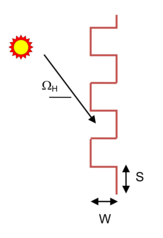
\includegraphics[width=0.9\textwidth, height=0.9\textheight, keepaspectratio=true]{media/image045.png}
\caption{Geometry used for Pleated Drape Analysis \protect \label{fig:geometry-used-for-pleated-drape-analysis}}
\end{figure}

\subsubsection{Inputs}\label{inputs-27-002}

\paragraph{Field: Name}\label{field-name-21-003}

Name of the drape fabric shade layer. It is referenced as an inside, in between or outside layer in an equivalent layer window construction.

\paragraph{Field: Drape Beam-Beam Solar Transmittance}\label{field-drape-beam-beam-solar-transmittance}

This value is the drape fabric beam-beam transmittance at normal incidence, and it is the same as the drape fabric openness area fraction.~ Assumed to be the same for front and back sides of the drape fabric layer.~ The minimum value is 0.0 and maximum value is less than 1.0. For most drape fabric materials the maximum fabric openness fraction do not exceed 0.2.~ The default value is 0.0.

\paragraph{Field: Front Side Drape Beam-Diffuse Solar Transmittance}\label{field-front-side-drape-beam-diffuse-solar-transmittance}

This value is the front side beam-diffuse solar transmittance of the drape fabric material at normal incidence averaged over the entire spectrum of solar radiation. The minimum value is 0.0 and maximum value is less than 1.0.

\paragraph{Field: Back Side Drape Beam-Diffuse Solar Transmittance}\label{field-back-side-drape-beam-diffuse-solar-transmittance}

This value is the back side beam-diffuse solar transmittance of the drape fabric material at normal incidence averaged over the entire spectrum of solar radiation. The minimum value is 0.0 and maximum value is less than 1.0.

\paragraph{Field: Front Side Drape Beam-Diffuse Solar Reflectance}\label{field-front-side-drape-beam-diffuse-solar-reflectance}

This value is the front side beam-diffuse solar reflectance of the drape fabric material at normal incidence averaged over the entire spectrum of solar radiation. The minimum value is 0.0 and maximum value is less than 1.0.

\paragraph{Field: Back Side Drape Beam-Diffuse Solar Reflectance}\label{field-back-side-drape-beam-diffuse-solar-reflectance}

This value is the back side beam-diffuse solar reflectance of the drape fabric material at normal incidence averaged over the entire spectrum of solar radiation. The minimum value is 0.0 and maximum value is less than 1.0.

\paragraph{Field: Drape Beam-Beam Visible Transmittance}\label{field-drape-beam-beam-visible-transmittance}

This value is the drape fabric beam-beam visible transmittance at normal incidence averaged over the visible spectrum range of solar radiation.~ Assumed to be the same for front and back sides of the drape fabric layer.~ The minimum value is 0.0 and maximum value is less than 1.0.~ The default value is 0.0.~ This input field is not used currently.

\paragraph{Field: Front Side Drape Beam-Diffuse Visible Reflectance}\label{field-front-side-drape-beam-diffuse-visible-reflectance}

This value is the front side drape fabric beam-diffuse visible reflectance at normal incidence averaged over the visible spectrum range of solar radiation.~ Assumed to be the same for front and back sides of the drape.~ The minimum value is 0.0 and maximum value is less than 1.0.~ The default value is 0.0.~ This input field is not used currently.

\paragraph{Field: Back Side Drape Diffuse-Diffuse Visible Reflectance}\label{field-back-side-drape-diffuse-diffuse-visible-reflectance}

This value is the back side drape fabric diffuse-diffuse visible reflectance at normal incidence averaged over the visible spectrum range of solar radiation.~ Assumed to be the same for front and back sides of the drape.~ The minimum value is 0.0 and maximum value is less than 1.0.~ The default value is 0.0.~ This input field is not used currently.

\paragraph{Field: Drape Material Infrared Transmittance}\label{field-drape-material-infrared-transmittance}

This value is the long-wave hemispherical transmittance of the fabric material at zero fabric openness fraction.~ Assumed to be the same for front and back sides of the drape fabric material layer. The minimum value is 0.0 and maximum value is less than 1.0.~ The default value is 0.05.

\paragraph{Field: Front Side Drape Material Infrared Emissivity}\label{field-front-side-drape-material-infrared-emissivity}

This value is the front side long-wave hemispherical emissivity of fabric material at zero shade openness. The minimum value is 0.0 and maximum value is less than 1.0. the default value is 0.87. The front side effective emissivity of the drape fabric layer is calculated using this value and the fabric openness area fraction specified above.

\paragraph{Field: Back Side Drape Material Infrared Emissivity}\label{field-back-side-drape-material-infrared-emissivity}

This value is the back side long-wave hemispherical emissivity of fabric material at zero fabric openness fraction. The minimum value is 0.0 and maximum value is less than 1.0. The default value is 0.87. The back side effective emissivity of the drape fabric layer is calculated using this value and the fabric openness area fraction specified above.

\paragraph{Field: Width of Pleated Fabric}\label{field-width-of-pleated-fabric}

This value is the width of the pleated section of the draped fabric, w(m). If the drape fabric is flat (unpleated), then the pleated section width is set to zero. The default value is 0.0, i.e., assumes flat drape fabric.

\paragraph{Field: Length of Pleated Fabric}\label{field-length-of-pleated-fabric}

This value is the length of the pleated section of the draped fabric, s(m). If the drape fabric is flat (unpleated), then the pleated section length is set to zero.~ The default value is 0.0, i.e., assumes flat drape fabric.

An IDF example for this object is shown below:

\begin{lstlisting}
WindowMaterial:Drape:EquivalentLayer,
  Drape02,            !- Name
  0.14,               !- Shade Beam-Beam Solar Transmittance
  0.10,               !- Front Side Shade Beam-Diffuse Solar Transmittance
  0.10,               !- Back Side Shade Beam-Diffuse Solar Transmittance
  0.40,               !- Front Side Shade Beam-Diffuse Solar Reflectance
  0.50,               !- Back Side Shade Beam-Diffuse Solar Reflectance
  0.0,                !- Shade Beam-Beam Visible Transmittance
  0.0,                !- Shade Beam-Diffuse Visible Transmittance
  0.0,                !- Shade Beam-Diffuse Visible Reflectance
  0.10,               !- Shade Material Infrared Transmittance
  0.90,               !- Front Side Shade Material Infrared Emissivity
  0.80,               !- Back Side Shade Material Infrared Emissivity
  0.01,               !- Width of Pleated Fabric
  0.025;              !- Length of Pleated Fabric
\end{lstlisting}

\subsection{WindowMaterial:Blind:EquivalentLayer}\label{windowmaterialblindequivalentlayer}

This object specifies the properties of an Equivalent Layer window blind consisting of thin and equally-spaced slats. The the model assumes that slats are flat and thin, and applies correction for the slat curvature effect based on the user specified slat crwon. Slats are assumed to transmit and reflect diffusely. The effective shortwave optical and longwave optical properties of venetian blind layer is estimated analytically. The Equivalent Layer blind model requires optical properties and geometry of the slats shown in Figure~\ref{fig:geometry-and-properties-used-for-venetian}. Likewise, effective longwave properties are obtained for the layer knowing longwave properties of the slats.

\begin{figure}[hbtp] % fig 22
\centering
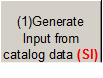
\includegraphics[width=0.9\textwidth, height=0.9\textheight, keepaspectratio=true]{media/image047.png}
\caption{Geometry and Properties used for venetian blind analysis \protect \label{fig:geometry-and-properties-used-for-venetian}}
\end{figure}

The input data required to characterize a venetian blind are: front and back side reflectance and transmittance of the slat, geometry (Slat width, w, slat spacing, s, slat crown, c, and slat angle, $\phi$, and long wave emittance and transmittance of the slat. Blinds can be located on the inside of the window, on the outside of the window, or between two layers of glass. The blind is assumed to cover all of the glazed part of the window.
The equivalent layer window blind model allows three slat angle control types (see \textit{Slat Angle Control} input field) but does not support \hyperref[windowpropertyshadingcontrol]{WindowShadingControl}.

\subsubsection{Inputs}\label{inputs-28-001}

\paragraph{Field: Name}\label{field-name-22-003}

Name of the venetian blind. It is referenced as an inside, outside or in between layers in an equivalent layer window construction.

\paragraph{Field: Slat Orientation}\label{field-slat-orientation-1}

The choices are Horizontal and Vertical. ``Horizontal'' means the slats are parallel to the bottom of the window; this is the same as saying that the slats are parallel to the X-axis of the window. ``Vertical'' means the slats are parallel to Y-axis of the window. The default is ``Horizontal''.

\paragraph{Field: Slat Width}\label{field-slat-width-2}

This value is the width of the slat measured from edge to edge (m). The default value is 0.0254.

\paragraph{Field: Slat Separation}\label{field-slat-separation-1}

The distance between the front of a slat and the back of the adjacent slat (m). The default value is 0.025. The slat separation should not be greater than the slat width.

\paragraph{Field: Slat Crown}\label{field-slat-crown}

The perpendicular length between the slat cord ~and the curve (m). Crown = 0.0625x``Slat width''. Slat is assumed to be rectangular in cross section and flat. The crown accounts for curvature of the slat.~ The minimum value is 0.0, and the default value is 0.0015m.

\paragraph{Field: Slat Angle}\label{field-slat-angle-2}

The angle (degrees) between the glazing outward normal and the slat outward normal, where the outward normal points away from the front face of the slat (degrees). The slat angle is +ve if the tip of the slat front face is tilted upward, or else the slat angle is -ve if the tip of the slat front face is tilted downward. The slat angle varies between -90 to +90.~ If the \textit{`Slat Angle Control} input field below specified is ``FixedSlatAngle'', then the slat angle is fixed at ``Slat Angle'' value entered.~ Minimum value allowed is -90.0, and the maximum value allowed is 90.0 degrees.~ The default value is 45 degrees.

\paragraph{Field: Front Side Slat Beam-Diffuse Solar Transmittance}\label{field-front-side-slat-beam-diffuse-solar-transmittance}

This value is the slat front side beam-diffuse solar transmittance at normal incidence averaged over the entire spectrum of solar radiation. Any transmitted beam radiation is assumed to be 100\% diffuse (i.e., slats are translucent). Minimum value is 0.0, and the maximum value is less than 1.0. The default value is 0.0.

\paragraph{Field: Back Side Slat Beam-Diffuse Solar Transmittance}\label{field-back-side-slat-beam-diffuse-solar-transmittance}

This value is the slat back side beam-diffuse solar transmittance at normal incidence averaged over the entire spectrum of solar radiation. Any transmitted beam radiation is assumed to be 100\% diffuse (i.e., slats are translucent). Minimum value is 0.0,~ and the maximum value is less than 1.0. The default value is 0.0.

\paragraph{Field: Front Side Slat Beam-Diffuse Solar Reflectance}\label{field-front-side-slat-beam-diffuse-solar-reflectance}

This value is slat front side beam-diffuse solar reflectance at normal incidence averaged over the entire spectrum of solar radiation. All the reflected component is assumed to be diffuse. Minimum value is 0.0, and the maximum value is less than 1.0.

\paragraph{Field: Back Side Slat Beam-Diffuse Solar Reflectance}\label{field-back-side-slat-beam-diffuse-solar-reflectance}

This value is the slat back side beam-diffuse solar reflectance at normal incidence averaged over the entire spectrum of solar radiation. All the reflected component is assumed to be diffuse. Minimum value is 0.0, and the maximum value is less than 1.0.

\paragraph{Field: Front Side Slat Beam-Diffuse Visible Solar Transmittance}\label{field-front-side-slat-beam-diffuse-visible-solar-transmittance}

This value is the slat front side beam-diffuse visible transmittance at normal incidence averaged over the visible spectrum range of solar radiation. Any transmitted beam radiation is assumed to be 100\% diffuse (i.e., slats are translucent). Minimum value is 0.0, and the maximum value is less than 1.0. The default value is 0.0.

\paragraph{Field: Back Side Slat Beam-Diffuse Visible Solar Transmittance}\label{field-back-side-slat-beam-diffuse-visible-solar-transmittance}

This value is the slat back side beam-diffuse visible transmittance at normal incidence averaged the visible spectrum range of solar radiation. Any transmitted beam radiation is assumed to be 100\% diffuse (i.e., slats are translucent). Minimum value is 0.0, and the maximum value is less than 1.0. The default value is 0.0.

\paragraph{Field: Front Side Slat Beam-Diffuse Visible Solar Reflectance}\label{field-front-side-slat-beam-diffuse-visible-solar-reflectance}

This value is the slat front side beam-diffuse visible reflectance at normal incidence averaged over the visible spectrum range of solar radiation. All the reflected component is assumed to be diffuse. Minimum value is 0.0, and the maximum value is less than 1.0

\paragraph{Field: Back Side Slat Beam-Diffuse Visible Solar Reflectance}\label{field-back-side-slat-beam-diffuse-visible-solar-reflectance}

This value is the slat back side beam-diffuse visible reflectance at normal incidence averaged over the visible spectrum range of solar radiation. All the reflected component is assumed to be diffuse. Minimum value is 0.0,~ and the maximum value is less than 1.0

\paragraph{Field: Slat Diffuse-Diffuse Solar Transmittance}\label{field-slat-diffuse-diffuse-solar-transmittance}

This value is the slat diffuse-diffuse solar transmittance for hemispherically diffuse solar radiation. This value is the same for front and back side of the slat.~ Minimum value is 0.0,~ and the maximum value is less than 1.0.

\paragraph{Field: Front Side Slat Diffuse-Diffuse Solar Reflectance}\label{field-front-side-slat-diffuse-diffuse-solar-reflectance}

This value is the slat front side diffuse-diffuse solar reflectance for hemispherically diffuse solar radiation. Minimum value is 0.0,~ and the maximum value is less than 1.0.

\paragraph{Field: Back Side Slat Diffuse-Diffuse Solar Reflectance}\label{field-back-side-slat-diffuse-diffuse-solar-reflectance}

This value is the slat back side diffuse-diffuse solar reflectance for hemispherically diffuse solar radiation. Minimum value is 0.0,~ and the maximum value is less than 1.0.

\paragraph{Field: Slat Diffuse-Diffuse Visible Transmittance}\label{field-slat-diffuse-diffuse-visible-transmittance}

This value is the slat diffuse-diffuse visible transmittance for hemispherically diffuse visible spectrum range of solar radiation. This value is the same for front and back side of the slat.~ Minimum value is 0.0,~ and the maximum value is less than 1.0. This input field is not used currently.

\paragraph{Field: Front Side Slat Diffuse-Diffuse Visible Reflectance}\label{field-front-side-slat-diffuse-diffuse-visible-reflectance}

This value is the slat front side diffuse-diffuse visible reflectance for hemispherically diffuse visible spectrum range of solar radiation. Minimum value is 0.0, and the maximum value is less than 1.0.~ This input field is not used currently.

\paragraph{Field: Back Side Slat Diffuse-Diffuse Visible Reflectance}\label{field-back-side-slat-diffuse-diffuse-visible-reflectance}

This value is the slat back side diffuse-diffuse visible reflectance for hemispherically diffuse visible spectrum range of solar radiation. Minimum value is 0.0, and the maximum value is less than 1.0.~ This input field is not used currently.

\paragraph{Field: Slat Infrared Transmittance}\label{field-slat-Infrared-transmittance}

This value is the long-wave hemispherical transmittance of the slat material. Assumed to be the same for both sides of the slat. The minimum value is 0.0, the maximum value is less than 1.0.~ The default value is 0.0.

\paragraph{Field: Front Side Slat Infrared Emissivity}\label{field-front-side-slat-infrared-emissivity}

This value is the front side long-wave hemispherical emissivity of the slat material. The minimum value is 0.0, the maximum value is less than 1.0. The default value is 0.9.

\paragraph{Field: Back Side Slat Infrared Emissivity}\label{field-back-side-slat-infrared-emissivity}

This value is the back side long-wave hemispherical emissivity of the slat material. The minimum value is 0.0, the maximum value is less than 1.0.~ The default value is 0.9.

\paragraph{Field: Slat Angle Control}\label{field-slat-angle-control}

This input field is used only if slat angle control is desired.~ The three key choice inputs allowed are ``FixedSlatAngle'', ``MaximizeSolar'', and ``BlockBeamSolar''.~ The default value is ``FixedSlatAngle''.If Type of Slat Angle Control for Blinds = MaximizeSolar the slat angle is adjusted to maximize solar gain.~If Type of Slat Angle Control for Blinds = BlockBeamSolar, the slat angle is adjusted to maximize visibiity while eliminating beam solar radiation.~If Type of Slat Angle Control for Blinds = FixedSlatAngle, then the model uses a fixed slat angle specified above.

An IDF example for this object, is shown below:

\begin{lstlisting}

WindowMaterial:Blind:EquivalentLayer,
    VBU8D6+45SW1,      ! - Name
    Horizontal,        ! - Slat Orientation
    0.025,             ! - Slat Width
    0.025,             ! - Slat Separation
    0.0,               ! - Slat Crown
    45.0,              ! - Slat Angle
    0.0,               ! - Front Side Slat Beam-Diffuse Solar Transmittance
    0.0,               ! - Back Side Slat Beam-Diffuse Solar Transmittance
    0.0,               ! - Front Side Slat Beam-Diffuse Solar Reflectance
    0.0,               ! - Back Side Slat Beam-Diffuse Solar Reflectance
    0.0,               ! - Front Side Slat Beam-Diffuse Visible Transmittance
    0.0,               ! - Back Side Slat Beam-Diffuse Visible Transmittance
    0.0,               ! - Front Side Slat Beam-Diffuse Visible Reflectance
    0.0,               ! - Back Side Slat Beam-Diffuse Visible  Reflectance
    0.0,               ! - Slat Diffuse-Diffuse Solar Transmittance
    0.80,              ! - Front Side Slat Diffuse-Diffuse Solar Reflectance
    0.60,              ! - Back Side Slat Diffuse-Diffuse Solar Reflectance
    0.0,               ! - Slat Diffuse-Diffuse Visible Transmittance
    0.0,               ! - Front Side Slat Diffuse-Diffuse Visible Reflectance
    0.0,               ! - Back Side Slat Diffuse-Diffuse Visible Reflectance
    0.0,               ! - Slat Infrared Transmittance
    0.90,              ! - Front Side Slat Infrared Emissivity
    0.90,              ! - Back Side Slat Infrared Emissivity
    FixedSlatAngle;    ! - Slat Angle Control
\end{lstlisting}

\subsection{WindowMaterial:Screen:EquivalentLayer}\label{windowmaterialscreenequivalentlayer}

This object specifies the optical and thermal properties of exterior screen materials for Equivalent Layer Window. Can only be placed on the exterior side of window construction. The window screen model assumes the screen is made up of intersecting orthogonally-crossed cylinders. The surface of the cylinders is assumed to be diffusely reflecting. The beam solar radiation transmitted through an equivalent Layer window screen varies with sun angle and is made up of two distinct elements: a beam-beam component and a beam-diffuse component. The beam-beam transmittance component is calculated using screen openness area fraction determined from the geometry of the screen and the incident angle of the sun. Empirical correlations are used to obtain the effective off-normal solar and longwave properties of insect screens.~ Insect screen geometry is shown in Figure~\ref{fig:geometry-used-for-insect-screen-analysis}.~ The calculation of effective solar properties requires a set of properties measured at normal incidence. The equivalent layer window screen shade model does not support \hyperref[windowpropertyshadingcontrol]{WindowShadingControl}.

\begin{figure}[hbtp] % fig 23
\centering
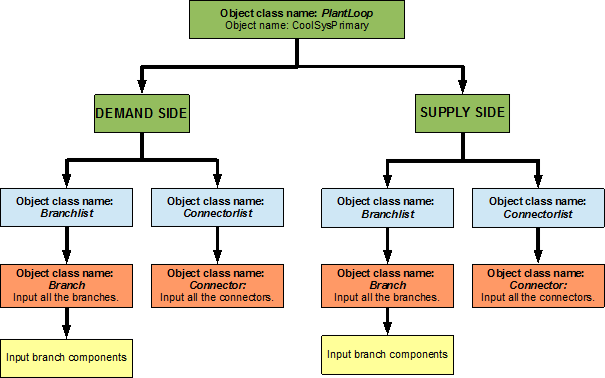
\includegraphics[width=0.9\textwidth, height=0.9\textheight, keepaspectratio=true]{media/image048.png}
\caption{Geometry used for insect screen analysis \protect \label{fig:geometry-used-for-insect-screen-analysis}}
\end{figure}

The formulation of the model, assumption and correlations used to calculate effective solar and longwave properties of insect screens are described in the Engineering Reference.

\subsubsection{Inputs}\label{inputs-29-001}

\paragraph{Field: Name}\label{field-name-23-003}

Name of the insect screen. It is referenced as an outside layer in an equivalent layer window construction.

\paragraph{Field: Screen Beam-Beam Solar Transmittance}\label{field-screen-beam-beam-solar-transmittance}

This value is the beam-beam transmittance of the screen material at normal incidence. This value is the same as the screen openness area fraction.~ This value can be autocalculated from the wire spacing and wire diameter. It is the same for both sides of the screen. The minimum value is 0.0, and maximum value is less than 1.0.

\paragraph{Field: Screen Beam-Diffuse Solar Transmittance}\label{field-screen-beam-diffuse-solar-transmittance}

This value is the beam-diffuse solar transmittance of the screen material at normal incidence averaged over the entire spectrum of solar radiation. Assumed to be the same for both sides of the screen. The minimum value is 0.0, and the maximum value is less than 1.0.

\paragraph{Field: Screen Beam-Diffuse Solar Reflectance}\label{field-screen-beam-diffuse-solar-reflectance}

This value is the beam-diffuse solar reflectance of the screen material at normal incidence averaged over the entire spectrum of solar radiation. Assumed to be the same for both sides of the screen. The minimum value is 0.0, and the maximum value is less than 1.0.

\paragraph{Field: Screen Beam-Beam Visible Transmittance}\label{field-screen-beam-beam-visible-transmittance}

This value is the beam-beam visible transmittance of the screen material at normal incidence averaged over the visible spectrum range of solar radiation.~ Assumed to be the same for both sides of the screen. The minimum value is 0.0, and maximum value is less than 1.0. This input input field is not used currently.

\paragraph{Field: Screen Beam-Diffuse Visible Transmittance}\label{field-screen-beam-diffuse-visible-transmittance}

This value is the beam-diffuse visible reflectance of the screen material at normal incidence averaged over the visible spectrum range of solar radiation. Assumed to be the same for both sides of the screen. The minimum value is 0.0, and the maximum value is less than 1.0. This input input field is not used currently.

\paragraph{Field: Screen Beam-Diffuse Visible Reflectance}\label{field-screen-beam-diffuse-visible-reflectance}

This value is the beam-diffuse visible reflectance of the screen material at normal incidence averaged over the visible spectrum range of solar radiation. Assumed to be the same for both sides of the screen. The minimum value is 0.0, and the maximum value is less than 1.0. This input input field is not used currently.

\paragraph{Field: Screen Infrared Transmittance}\label{field-screen-infrared-transmittance}

This value is the long-wave hemispherical transmittance of the the screen material. Assumed to be the same for both sides of the screen material. The minimum value is 0.0, the maximum value is less than 1.0.~ The default value is 0.02

\paragraph{Field: Screen Infrared Emissivity}\label{field-screen-infrared-emissivity}

This value is the long-wave hemispherical emissivity of the screen material. Assumed to be the same for both sides of the screen material. The minimum value is 0.0, the maximum value is less than 1.0. The default value is 0.93.

\paragraph{Field: Screen Wire Spacing}\label{field-screen-wire-spacing}

The spacing, S (m), of the screen material is the distance from the center of one strand of screen to the center of the adjacent one. The spacing of the screen material is assumed to be the same in both directions (e.g., vertical and horizontal). This input value must be greater than the non-zero screen material diameter. If the spacing is different in the two directions, use the average of the two values. Default value is 0.0025m.

\paragraph{Field: Screen Wire Diameter}\label{field-screen-wire-diameter}

The diameter, D (m), of individual strands or wires of the screen material. The screen material diameter is assumed to be the same in both directions (e.g., vertical and horizontal). This input value must be greater than 0 and less than the screen wire spacing. If the diameter is different in the two directions, use the average of the two values. Default value is 0.005m.

An IDF example for this object, is shown below:

\begin{lstlisting}

WindowMaterial:Screen:EquivalentLayer,
    INSCRN,                !- Name
    0.763,                 !- Screen Beam-Beam Solar Transmittance
    0.052,                 !- Screen Beam-Diffuse Solar Transmittance
    0.076,                 !- Screen Beam-Diffuse Solar Reflectance
    0.0,                   !- Screen Beam-Beam Visible Transmittance
    0.0,                   !- Screen Beam-Diffuse Visible Transmittance
    0.0,                   !- Screen Beam-Diffuse Visible Reflectance
    0.0,                   !- Screen Infrared Transmittance
    0.84,                  !- Screen Infrared Emissivity
    0.025,                 !- Screen Wire Spacing
    0.005;                 !- Screen Wire Diameter
\end{lstlisting}

\subsection{WindowMaterial:Glazing:EquivalentLayer}\label{windowmaterialglazingequivalentlayer}

Glass material properties for equivalent layer window model.~ Uses transmittance/reflectance input method.~ For exterior windows, ``front side'' is the side of the glass closest to the outside air and ``back side'' is the side closest to the zone the window is defined in. For interzone windows, ``front side'' is the side closest to the zone adjacent to the zone the window is defined in and ``back side'' is the side closest to the zone the window is defined in. The equivalent layer window glazing model does not support \hyperref[windowpropertyshadingcontrol]{WindowShadingControl}.

\subsubsection{Inputs}\label{inputs-30-001}

\paragraph{Field: Name}\label{field-name-24-002}

The name of the glass layer. It corresponds to a layer in an equivalent layer window construction.

\paragraph{Field: Optical Data Type}\label{field-optical-data-type-1}

Valid values for this field are SpectralAverage, or Spectral. If Optical Data Type = SpectralAverage, the values you enter for solar transmittance and reflectance are assumed to be averaged over the solar spectrum, and the values you enter for visible transmittance and reflectance are assumed to be averaged over the solar spectrum and weighted by the response of~ the human eye. The spectral data input is not supported now.

\paragraph{Field: Window Glass Spectral Data Set Name}\label{field-window-glass-spectral-data-set-name-0}

This input field is not used currently.

\paragraph{Field: Front Side Beam-Beam Solar Transmittance}\label{field-front-side-beam-beam-solar-transmittance}

This value is the front side beam-beam solar transmittance of the glazing at normal incidence averaged over the entire spectrum of solar radiation.~ Used only when Optical Data Type = SpectralAverage.~ The minimum value is 0.0, and the maximum value is less than 1.0.

\paragraph{Field: Back Side Beam-Beam Solar Transmittance}\label{field-back-side-beam-beam-solar-transmittance}

This value is the back side beam-beam solar transmittance of the glazing at normal incidence averaged over the entire spectrum of solar radiation.~ Used only when Optical Data Type = SpectralAverage.~ The minimum value is 0.0, and the maximum value is less than 1.0.

\paragraph{Field: Front Side Beam-Beam Solar Reflectance}\label{field-front-side-beam-beam-solar-reflectance}

This value is the front side beam-beam solar reflectance of the glazing at normal incidence averaged over the entire spectrum of solar radiation.~ Used only when Optical Data Type = SpectralAverage.~ The minimum value is 0.0, and the maximum value is less than 1.0.

\paragraph{Field: Back Side Beam-Beam Solar Reflectance}\label{field-back-side-beam-beam-solar-reflectance}

This value is the back side beam-beam solar reflectance of the glazing at normal incidence averaged over the entire spectrum of solar radiation.~ Used only when Optical Data Type = SpectralAverage.~ The minimum value is 0.0, and the maximum value is less than 1.0.

\paragraph{Field: Front Side Beam-Beam Visible Transmittance}\label{field-front-side-beam-beam-visible-transmittance}

This value is the front side beam-beam visible transmittance of the glazing at normal incidence averaged over the visible spectrum range of solar radiation.~ Used only when Optical Data Type = SpectralAverage.~ The minimum value is 0.0, and the maximum value is less than 1.0.

\paragraph{Field: Back Side Beam-Beam Visible Transmittance}\label{field-back-side-beam-beam-visible-transmittance}

This value is the back side beam-beam visible transmittance of the glazing at normal incidence averaged over the visible spectrum range of solar radiation.~ Used only when Optical Data Type = SpectralAverage.~ The minimum value is 0.0, and the maximum value is less than 1.0.

\paragraph{Field: Front Side Beam-Beam Visible Reflectance}\label{field-front-side-beam-beam-visible-reflectance}

This value is the front side beam-beam visible reflectance of the glazing at normal incidence averaged over the visible spectrum range of solar radiation.~ Used only when Optical Data Type = SpectralAverage.~ The minimum value is 0.0, and the maximum value is less than 1.0.

\paragraph{Field: Back Side Beam-Beam Visible Reflectance}\label{field-back-side-beam-beam-visible-reflectance}

This value is the back side beam-beam visible reflectance of the glazing at normal incidence averaged over the visible spectrum range of solar radiation.~ Used only when Optical Data Type = SpectralAverage.~ The minimum value is 0.0, and the maximum value is less than 1.0.

\paragraph{Field: Front Side Beam-Diffuse Solar Transmittance}\label{field-front-side-beam-diffuse-solar-transmittance}

This value is the front side beam-diffuse solar transmittance of the glazing at normal incidence averaged over the entire spectrum of solar radiation.~ Used only when Optical Data Type = SpectralAverage.~ For clear glazing the beam-diffuse transmittance is zero. The minimum value is 0.0, and the maximum value is less than 1.0. Default value is 0.0.

\paragraph{Field: Back Side Beam-Diffuse Solar Transmittance}\label{field-back-side-beam-diffuse-solar-transmittance}

This value is the back side beam-diffuse solar transmittance of the glazing at normal incidence averaged over the entire spectrum of solar radiation.~ Used only when Optical Data Type = SpectralAverage.~ For clear glazing the beam-diffuse solar transmittance is zero. The minimum value is 0.0, and the maximum value is less than 1.0. Default value is 0.0.

\paragraph{Field: Front Side Beam-Diffuse Solar Reflectance}\label{field-front-side-beam-diffuse-solar-reflectance}

This value is the front side beam-diffuse solar reflectance of the glazing at normal incidence averaged over the entire spectrum of solar radiation.~ Used only when Optical Data Type = SpectralAverage.~ The minimum value is 0.0, and the maximum value is less than 1.0. Default value is 0.0.

\paragraph{Field: Back Side Beam-Diffuse Solar Reflectance}\label{field-back-side-beam-diffuse-solar-reflectance}

This value is the back side beam-diffuse solar reflectance of the glazing at normal incidence averaged over the entire spectrum of solar radiation.~ Used only when Optical Data Type = SpectralAverage.~ The minimum value is 0.0, and the maximum value is less than 1.0. Default value is 0.0.

\paragraph{Field: Front Side Beam-Diffuse Visible Transmittance}\label{field-front-side-beam-diffuse-visible-transmittance}

This value is the front side beam-diffuse visible transmittance of the glazing at normal incidence averaged over the visible spectrum range of solar radiation.~ Used only when Optical Data Type = SpectralAverage.~ For clear glazing the beam-diffuse visible transmittance is zero. The minimum value is 0.0, and the maximum value is less than 1.0. Default value is 0.0.~ This input field is not used currently.

\paragraph{Field: Back Side Beam-Diffuse Visible Transmittance}\label{field-back-side-beam-diffuse-visible-transmittance}

This value is the back side beam-diffuse visible transmittance of the glazing at normal incidence averaged over the visible spectrum range of solar radiation.~ Used only when Optical Data Type = SpectralAverage.~ For clear glazing the beam-diffuse visible transmittance is zero. The minimum value is 0.0, and the maximum value is less than 1.0. Default value is 0.0.~ This input field is not used currently.

\paragraph{Field: Front Side Beam-Diffuse Visible Reflectance}\label{field-front-side-beam-diffuse-visible-reflectance}

This value is the front side beam-diffuse visible reflectance of the glazing at normal incidence averaged over the visible spectrum range of solar radiation.~ Used only when Optical Data Type = SpectralAverage.~ The minimum value is 0.0, and the maximum value is less than 1.0. Default value is 0.0. This input field is not used currently.

\paragraph{Field: Back Side Beam-Diffuse Visible Reflectance}\label{field-back-side-beam-diffuse-visible-reflectance}

This value is the back side beam-diffuse visible reflectance of the glazing at normal incidence averaged over the visible spectrum range of solar radiation.~ Used only when Optical Data Type = SpectralAverage.~ The minimum value is 0.0, and the maximum value is less than 1.0. Default value is 0.0. This input field is not used currently.

\paragraph{Field: Diffuse-Diffuse Solar Transmittance}\label{field-diffuse-diffuse-solar-transmittance}

This value is the diffuse-diffuse solar transmittance of the glazing averaged over the entire spectrum of solar radiation.~ Used only when Optical Data Type = SpectralAverage. The diffuse-diffuse transmittance is assumed to be the same for both sides of the glazing.~ EnergyPlus automatically estimates the diffuse-diffuse solar transmittance from other inputs. If this input field is specified as ``Autocalculate'', then the calculated transmittance will be used. The minimum value is 0.0, and the maximum value is less than 1.0.

\paragraph{Field: Front Side Diffuse-Diffuse Solar Reflectance}\label{field-front-side-diffuse-diffuse-solar-reflectance}

This value is the front side diffuse-diffuse solar reflectance of the glazing averaged over the entire spectrum of solar radiation.~ Used only when Optical Data Type = SpectralAverage. EnergyPlus automatically estimates the diffuse-diffuse reflectance from other inputs. If this input field is specified as ``Autocalculate'', then the calculated reflectance will be used. The minimum value is 0.0, and the maximum value is less than 1.0.

\paragraph{Field: Back Side Diffuse-Diffuse Solar Reflectance}\label{field-back-side-diffuse-diffuse-solar-reflectance}

This value is the back side diffuse-diffuse solar reflectance of the glazing averaged over the entire spectrum of solar radiation.~ Used only when Optical Data Type = SpectralAverage. EnergyPlus automatically estimates the diffuse-diffuse reflectance from other inputs. If this input field is specified as ``Autocalculate'', then the calculated reflectance will be used. The minimum value is 0.0, and the maximum value is less than 1.0.

\paragraph{Field: Diffuse-Diffuse Visible Solar Transmittance}\label{field-diffuse-diffuse-visible-solar-transmittance}

This value is the diffuse-diffuse visible transmittance of the glazing averaged over the visible spectrum range of solar radiation.~ Used only when Optical Data Type = SpectralAverage. The diffuse-diffuse visible transmittance is assumed to be the same for both sides of the glazing.~ If this input field is specified as ``Autocalculate'', then the calculated transmittance will be used. The minimum value is 0.0, and the maximum value is less than 1.0. This input field is not used currently.

\paragraph{Field: Front Side Diffuse-Diffuse Visible Reflectance}\label{field-front-side-diffuse-diffuse-visible-reflectance}

This value is the front side diffuse-diffuse visible reflectance of the glazing averaged over the visible spectrum range of solar radiation.~ Used only when Optical Data Type = SpectralAverage. EnergyPlus automatically estimates the front side diffuse-diffuse visible reflectance from front side beam-beam visible reflectance at normal incidence specified above. If this input field is specified as ``Autocalculate'', then the calculated reflectance will be used. The minimum value is 0.0, and the maximum value is less than 1.0. This input field is not used currently.

\paragraph{Field: Back Side Diffuse-Diffuse Visible Reflectance}\label{field-back-side-diffuse-diffuse-visible-reflectance}

This value is the back side diffuse-diffuse visible reflectance of the glazing averaged over the visible spectrum range of solar radiation.~ Used only when Optical Data Type = SpectralAverage. EnergyPlus automatically estimates the back side diffuse-diffuse visible reflectance from back side beam-beam visible reflectance at normal incidence specified above. If this input field is specified as ``Autocalculate'', then the calculated reflectance will be used. The minimum value is 0.0, and the maximum value is less than 1.0. This input field is not used currently.

\paragraph{Field: Infrared Transmittance (applies to front and back)}\label{field-infrared-transmittance-applies-to-front-and-back}

This value is the long-wave hemispherical transmittance of the glazing. Assumed to be the same for both sides of the glazing. The minimum value is 0.0, the maximum value is less than 1.0.~ The default value is 0.0.

\paragraph{Field: Front Side Infrared Emissivity}\label{field-front-side-infrared-emissivity}

This value is the front side long-wave hemispherical emissivity of the glazing. The minimum value is 0.0, the maximum value is less than 1.0.~ The default value is 0.84.

\paragraph{Field: Back Side Infrared Emissivity}\label{field-back-side-infrared-emissivity}

This value is the back side long-wave hemispherical emissivity of the glazing. The minimum value is 0.0, the maximum value is less than 1.0.~ The default value is 0.84.

An IDF example for this object, is shown below:

\begin{lstlisting}

WindowMaterial:Glazing:EquivalentLayer,
    GLZCLR,                  !- Name
    SpectralAverage,         !- Optical Data Type
    ,                        !- Window Glass Spectral Data Set Name
    0.83,                    !- Front Side Beam-Beam Solar Transmittance
    0.83,                    !- Back Side Beam-Beam Solar Transmittance
    0.08,                    !- Front Side Beam-Beam Solar Reflectance
    0.08,                    !- Back Side Beam-Beam Solar Reflectance
    0.0,                     !- Front Side Beam-Beam Visible Transmittance
    0.0,                     !- Back Side Beam-Beam Visible Transmittance
    0.0,                     !- Front Side Beam-Beam Visible Reflectance
    0.0,                     !- Back Side Beam-Beam Visible Reflectance
    0.0,                     !- Front Side Beam-Diffuse Solar Transmittance
    0.0,                     !- Back Side Beam-Diffuse Solar Transmittance
    0.0,                     !- Front Side Beam-Diffuse Solar Reflectance
    0.0,                     !- Back Side Beam-Diffuse Solar Reflectance
    0.0,                     !- Front Side Beam-Diffuse Visible Transmittance
    0.0,                     !- Back Side Beam-Diffuse Visible Transmittance
    0.0,                     !- Front Side Beam-Diffuse Visible Reflectance
    0.0,                     !- Back Side Beam-Diffuse Visible Reflectance
    0.76,                    !- Diffuse-Diffuse Solar Transmittance
    0.14,                    !- Front Side Diffuse-Diffuse Solar Reflectance
    0.14,                    !- Back Side Diffuse-Diffuse Solar Reflectance
    0.0,                     !- Diffuse-Diffuse Visible Transmittance
    0.0,                     !- Front Side Diffuse-Diffuse Visible Reflectance
    0.0,                     !- Back Side Diffuse-Diffuse Visible Reflectance
    0.0,                     !- Infrared Transmittance
    0.84,                    !- Front Side Infrared Emissivity
    0.84;                    !- Back Side Infrared Emissivity
\end{lstlisting}

\subsection{WindowMaterial:Gap:EquivalentLayer}\label{windowmaterialgapequivalentlayer}

This object is used in windows equivalent layer construction object and specifies the properties of the gap between the layers in multi-layer equivalent layer window object. There is an EnergyPlus Reference Data Set for Material:WindowGas that contains several types of gas. This object uses the gas types: Air, Argon, Xenon, Crypton, and Custom.~ For Custom gas type users are required to entering the thermophicial properties.

\subsubsection{Inputs}\label{inputs-31-001}

\paragraph{Field: Name}\label{field-name-25-002}

The name of the gap. It refers to a layer in a window construction equivalent layer.

\paragraph{Field: Gas Type}\label{field-gas-type-1}

The type of gas. The choices allowed are AIR, ARGON, XENON, KRYPTON, or CUSTOM.

\paragraph{Field: Thickness}\label{field-thickness-8}

The thickness (m) of the gap layer.

\paragraph{Field: Gap Vent Type}\label{field-gap-vent-type}

This input field contains the valid key choice for gap vent type.~ The valid vent types are: Sealed, VentedIndoor, and VentedOutdoor.~ Sealed means the gap is enclosed and gas tight, i.e., no venting to indoor or outdoor environment. The gap types ``VentedIndoor'' and ``VentedOutdoor'' are used with gas type ``Air'' only. VentedIndoor means the air in the gap is naturally vented to indoor environment, and~ VentedOutdoor means the air in the gap is naturally vented to the outdoor environment.

\paragraph{Properties for Custom Gas Types}\label{properties-for-custom-gas-types-1}

The following entries are used only if Gas Type = Custom. The A, B and C coefficients are those in the following expression that gives a property value as a function of temperature in degrees K:

\begin{equation}
Property = Coef{f_A} + Coef{f_B} \times Temperatur{e_K} + Coef{f_C} \times Temperature_K^2
\end{equation}

\paragraph{Field: Conductivity Coefficient A}\label{field-conductivity-coefficient-a-1}

The A coefficient for gas conductivity (W/m-K). Used only if Gas Type = Custom.

\paragraph{Field: Conductivity Coefficient B}\label{field-conductivity-coefficient-b-1}

The B coefficient for gas conductivity (W/m-K\(^{2}\)). Used only if Gas Type = Custom.

\paragraph{Field: Conductivity Coefficient C}\label{field-conductivity-coefficient-c-1}

The C coefficient for gas conductivity (W/m-K\(^{3}\)).~ Used only if Gas Type = Custom.

\paragraph{Field: Viscosity Coefficient A}\label{field-viscosity-coefficient-a-1}

The A coefficient for gas viscosity (kg/m-s). Used only if Gas Type = Custom.

\paragraph{Field: Viscosity Coefficient B}\label{field-viscosity-coefficient-b-1}

The B coefficient for gas viscosity (kg/m-s-K). Used only if Gas Type = Custom.

\paragraph{Field: Viscosity Coefficient C}\label{field-viscosity-coefficient-c-1}

The C coefficient for gas viscosity (kg/m-s-K\(^{2}\)).~ Used only if Gas Type = Custom.

\paragraph{Field: Specific Heat Coefficient A}\label{field-specific-heat-coefficient-a-1}

The A coefficient for gas specific heat (J/kg-K). Used only if Gas Type = Custom.

\paragraph{Field: Specific Heat Coefficient B}\label{field-specific-heat-coefficient-b-1}

The B coefficient for gas specific heat (J/kg-K\(^{2}\)). Used only if Gas Type = Custom.

\paragraph{Field: Specific Heat Coefficient C}\label{field-specific-heat-coefficient-c-1}

The C coefficient for gas specific heat (J/kg-K\(^{2}\)).~ Used only if Gas Type = Custom.

\paragraph{Field: Specific Heat Ratio}\label{field-specific-heat-ratio-2}

The specific heat ratio for gas.~ Used only if Gas Type = Custom.

\paragraph{Field: Molecular Weight}\label{field-molecular-weight-1}

The molecular weight for gas.~ The molecular weight is the mass of 1 mol of the substance.~ This has a numerical value which is the average molecular mass of the molecules in the substance multiplied by Avogadro's constant. (kg/kmol) (Shown in the IDD as g/mol for consistency)

\paragraph{Field: Specific Heat Ratio}\label{field-specific-heat-ratio-3}

The specific heat ratio for gas.~ The specific heat ratio of a gas is the ratio of the specific heat at contant pressure, to the specific heat at constant volume.~ Used only if Gas Type = Custom.

An IDF example for this object, is shown below:

\begin{lstlisting}

WindowMaterial:Gap:EquivalentLayer,
    Custom CO2 Sealed 12mm,    !- Name
    CUSTOM,                    !- Gas Type
    0.0120,                    !- Thickness {m}
    Sealed,                    !- Gap Vent Type
   -5.8181E-3,                 !- Conductivity Coefficient A {W/m-K}
    7.4714E-5,                 !- Conductivity Coefficient B {W/m-K2}
    0.0,                       !- Conductivity Coefficient C {W/m-K3}
    8.5571E-7,                 !- Viscosity Coefficient A {kg/m-s}
    4.7143E-8,                 !- Viscosity Coefficient B {kg/m-s-K}
    0.0,                       !- Viscosity Coefficient C {kg/m-s-K2}
    5.76903E2,                 !- Specific Heat Coefficient A {J/kg-K}
    9.18088E-2,                !- Specific Heat Coefficient B {J/kg-K2}
    0.0,                       !- Specific Heat Coefficient C {J/kg-K3}
    44.01;                     !- Molecular Weight {g/mol}
\end{lstlisting}

\subsection{Material:RoofVegetation}\label{materialroofvegetation}

This definition must be used in order to simulate the green roof (ecoroof) model. The material becomes the outside layer in a green roof construction (see example below). In the initial release of the green roof model, only one material may be used as a green roof layer though, of course, several constructions using that material may be used. In addition, the model works only with the ConductionTransferFunction heat balance solution algorithm. This model was developed for low-sloped exterior surfaces (roofs). It is not recommended for high-sloped exterior surfaces (e.g., walls).

\subsubsection{Inputs}\label{inputs-32-000}

\paragraph{Field: Name}\label{field-name-26-002}

This field is a unique reference name that the user assigns to a particular ecoroof material. This name can then be referred to by other input data.

\paragraph{Field: Height of Plants}\label{field-height-of-plants}

This field defines the height of plants in units of meters. This field is limited to values in the range 0.005 \textless{} Height \textless{} 1.00 m. Default is .2 m.

\paragraph{Field: Leaf Area Index}\label{field-leaf-area-index}

This is the projected leaf area per unit area of soil surface. This field is dimensionless and is limited to values in the range of 0.001 \textless{} LAI \textless{} 5.0. Default is 1.0. At the present time the fraction vegetation cover is calculated directly from LAI (Leaf Area Index) using an empirical relation. The user may find it necessary to increase the specified value of LAI in order to represent high fractional coverage of the surface by vegetation.

\paragraph{Field: Leaf Reflectivity}\label{field-leaf-reflectivity}

This field represents the fraction of incident solar radiation that is reflected by the individual leaf surfaces (albedo). Solar radiation includes the visible spectrum as well as infrared and ultraviolet wavelengths. Values for this field must be between 0.05 and 0.5. Default is .22. Typical values are .18 to .25.

\paragraph{Field: Leaf Emissivity}\label{field-leaf-emissivity}

This field is the ratio of thermal radiation emitted from leaf surfaces to that emitted by an ideal black body at the same temperature. This parameter is used when calculating the long wavelength radiant exchange at the leaf surfaces. Values for this field must be between 0.8 and 1.0 (with 1.0 representing ``black body'' conditions). Default is .95.

\paragraph{Field: Minimum Stomatal Resistance}\label{field-minimum-stomatal-resistance}

This field represents the resistance of the plants to moisture transport. It has units of s/m. Plants with low values of stomatal resistance will result in higher evapotranspiration rates than plants with high resistance. Values for this field must be in the range of 50.0 to 300.0. Default is 180.

\paragraph{Field: Soil Layer Name}\label{field-soil-layer-name}

This field is a unique reference name that the user assigns to the soil layer for a particular ecoroof. This name can then be referred to by other input data. Default is \textbf{Green Roof Soil}.

\paragraph{Field: Roughness}\label{field-roughness-2}

This alpha field defines the relative roughness of a particular material layer. This parameter only influences the convection coefficients, more specifically the exterior convection coefficient. A keyword is expected in this field with the options being ``VeryRough'', ``Rough'', ``MediumRough'', ``MediumSmooth'', ``Smooth'', and ``VerySmooth'' in order of roughest to smoothest options. Default is MediumRough.

\paragraph{Field: Thickness}\label{field-thickness-9}

This field characterizes the thickness of the material layer in meters. This should be the dimension of the layer in the direction perpendicular to the main path of heat conduction. This value must be a positive number. Depths of .10m (4 inches) and .15m (6 inches) are common. Default if this field is left blank is .1. Maximum is .7m. Must be greater than .05 m.

\paragraph{Field: Conductivity of Dry Soil}\label{field-conductivity-of-dry-soil}

This field is used to enter the thermal conductivity of the material layer. Units for this parameter are W/(m-K). Thermal conductivity must be greater than zero. Typical soils have values from .3 to .5. Minimum is .2 (specified in IDD). Default is .35 and maximum (in IDD) is 1.5.

\paragraph{Field: Density of Dry Soil}\label{field-density-of-dry-soil}

This field is used to enter the density of the material layer in units of kg/m\(^{3}\). Density must be a positive quantity. Typical soils range from 400 to 1000 (dry to wet). Minimum is 300, maximum is 2000 and default if field is left blank is 1100.

\paragraph{Field: Specific Heat of Dry Soil}\label{field-specific-heat-of-dry-soil}

This field represents the specific heat of the material layer in units of J/(kg-K). Note that these units are most likely different than those reported in textbooks and references which tend to use kJ/(kg-K) or J/(g-K). They were chosen for internal consistency within EnergyPlus. Only positive values of specific heat are allowed.

\paragraph{Field: Thermal Absorptance}\label{field-thermal-absorptance-2}

The thermal absorptance field in the Material input syntax represents the fraction of incident long wavelength (>2.5 microns) radiation that is absorbed by the material. This parameter is used when calculating the long wavelength radiant exchange between various surfaces and affects the surface heat balances (both inside and outside as appropriate). For long wavelength radiant exchange, thermal emissivity and thermal emittance are equal to thermal absorptance. Values for this field must be between 0.0 and 1.0 (with 1.0 representing ``black body'' conditions). Typical values are from .9 to .98. The default value for this field is 0.9.

\paragraph{Field: Solar Absorptance}\label{field-solar-absorptance-2}

The solar absorptance field in the Material input syntax represents the fraction of incident~ solar radiation that is absorbed by the material. Solar radiation (0.3 to 2.537 microns) includes the visible spectrum as well as infrared and ultraviolet wavelengths. This parameter is used when calculating the amount of incident solar radiation absorbed by various surfaces and affects the surface heat balances (both inside and outside as appropriate). If solar reflectance (or reflectivity) data is available, then absorptance is equal to 1.0 minus reflectance (for opaque materials). Values for this field must be between 0.0 and 1.0. Typical values are from .6 to .85. The default value for this field is 0.7.

\paragraph{Field: Visible Absorptance}\label{field-visible-absorptance-2}

The visible absorptance field in the Material input syntax represents the fraction of incident visible wavelength radiation that is absorbed by the material. Visible wavelength radiation ( 0.37 to 0.78 microns weighted by photopic response) is slightly different than solar radiation in that the visible band of wavelengths is much more narrow while solar radiation includes the visible spectrum as well as infrared and ultraviolet wavelengths. This parameter is used when calculating the amount of incident visible radiation absorbed by various surfaces and affects the surface heat balances (both inside and outside as appropriate) as well as the daylighting calculations. If visible reflectance (or reflectivity) data is available, then absorptance is equal to 1.0 minus reflectance (for opaque materials). Values for this field must be between 0.5 and 1.0. The default value for this field is 0.75.

\paragraph{Field: Saturation Volumetric Moisture Content of the Soil Layer}\label{field-saturation-volumetric-moisture-content-of-the-soil-layer}

The field allows for user input of the saturation moisture content of the soil layer. Maximum moisture content is typically less than .5. Range is {[}.1,.5{]} with the default being .3.

\paragraph{Field: Residual Volumetric Moisture Content of the Soil Layer}\label{field-residual-volumetric-moisture-content-of-the-soil-layer}

The field allows for user input of the residual moisture content of the soil layer. Default is .01, range is {[}.01,.1{]}.

\paragraph{Field: Initial Volumetric Moisture Content of the Soil Layer}\label{field-initial-volumetric-moisture-content-of-the-soil-layer}

The field allows for user input of the initial moisture content of the soil layer. Range is (.05, .5{]} with the default being .1.

\paragraph{Field: Moisture Diffusion Calculation Method}\label{field-moisture-diffusion-calculation-method}

The field allows for two models to be selected: \textbf{Simple} or \textbf{Advanced}. EnergyPlus Currently supports only the \textbf{Simple} \textit{Moisture Diffusion Calculation Method}.

\textbf{Simple} is the original Ecoroof model - based on a constant diffusion of moisture through the soil.~ This model starts with the soil in two layers.~ Every time the soil properties update is called, it will look at the two soils moisture layers and asses which layer has more moisture in it. It then takes moisture from the higher moisture layer and redistributes it to the lower moisture layer at a constant rate.

\textbf{Advanced} is the later Ecoroof model. The model requires higher number of timesteps in hour for the simulation with a recommended value of 20. This moisture transport model is based on a project which looked at the way moisture transports through soil.~ It uses a finite difference method to divide the soil into layers (nodes). It redistributes the soil moisture according the model described in:

Marcel G Schaap and Martinus Th. van Genuchten, 2006, `A modified Maulem-van Genuchten Formulation for Improved Description of the Hydraulic Conductivity Near Saturation', Vadose Zone Journal 5 (1), p 27-34. However, currently \textbf{Advanced} \textit{Moisture Diffusion Calculation Method} is not supported in EnergyPlus.

An IDF example:

\begin{lstlisting}

Material:RoofVegetation,
      BaseEco,                 !- Name
      0.5,                     !- Height of Plants {m}
      5,                       !- Leaf Area Index {dimensionless}
      0.2,                     !- Leaf Reflectivity {dimensionless}
      0.95,                    !- Leaf Emissivity
      180,                     !- Minimum Stomatal Resistance {s/m}
      EcoRoofSoil,             !- Soil Layer Name
      MediumSmooth,            !- Roughness
      0.18,                    !- Thickness {m}
      0.4,                     !- Conductivity of Dry Soil {W/m-K}
      641,                     !- Density of Dry Soil {kg/m3}
      1100,                    !- Specific Heat of Dry Soil {J/kg-K}
      0.95,                    !- Thermal Absorptance
      0.8,                     !- Solar Absorptance
      0.7,                     !- Visible Absorptance
      0.4,                     !- Saturation Volumetric Moisture Content of the Soil Layer
      0.01,                    !- Residual Volumetric Moisture Content of the Soil Layer
      0.2,                     !- Initial Volumetric Moisture Content of the Soil Layer
      Simple;                  !- Moisture Diffusion Calculation Method


    Material:RoofVegetation,
      LowLAI,                  !- Name
      0.5,                     !- Height of Plants {m}
      0.5,                     !- Leaf Area Index {dimensionless}
      0.2,                     !- Leaf Reflectivity {dimensionless}
      0.95,                    !- Leaf Emissivity
      180,                     !- Minimum Stomatal Resistance {s/m}
      EcoRoofSoil,             !- Soil Layer Name
      MediumSmooth,            !- Roughness
      0.18,                    !- Thickness {m}
      0.4,                     !- Conductivity of Dry Soil {W/m-K}
      641,                     !- Density of Dry Soil {kg/m3}
      1100,                    !- Specific Heat of Dry Soil {J/kg-K}
      0.95,                    !- Thermal Absorptance
      0.8,                     !- Solar Absorptance
      0.7,                     !- Visible Absorptance
      0.4,                     !- Saturation Volumetric Moisture Content of the Soil Layer
      0.01,                    !- Residual Volumetric Moisture Content of the Soil Layer
      0.2,                     !- Initial Volumetric Moisture Content of the Soil Layer
      Simple;                 !- Moisture Diffusion Calculation Method
\end{lstlisting}

And construction using the ecoroof material:

\begin{lstlisting}

Construction,
      ASHRAE 90.1-2004_Sec 5.5-2_Roof,  !- Name
      BaseEco,                 !- Outside Layer
      ASHRAE 90.1-2004_Sec 5.5-2_Roof Insulation_1,  !- Layer \#2
      ASHRAE 90.1-2004_Sec 5.5-2_MAT-METAL;  !- Layer \#3
\end{lstlisting}

\subsection{Ecoroof / RoofVegetation outputs}\label{ecoroof-roofvegetation-outputs}

The following outputs are available for the Roof Vegetation surface.

\begin{itemize}
\item
  Zone,Average,Green Roof Soil Temperature {[}C{]}
\item
  Zone,Average,Green Roof Vegetation Temperature {[}C{]}
\item
  Zone,Average,Green Roof Soil Root Moisture Ratio {[]}
\item
  Zone,Average,Green Roof Soil Near Surface Moisture Ratio {[]}
\item
  Zone,Average,Green Roof Soil Sensible Heat Transfer Rate per Area {[}W/m2{]}
\item
  Zone,Average,Green Roof Vegetation Sensible Heat Transfer Rate per Area {[}W/m2{]}
\item
  Zone,Average,Green Roof Vegetation Moisture Transfer Rate {[}m/s{]}
\item
  Zone,Average,Green Roof Soil Moisture Transfer Rate {[}m/s{]}
\item
  Zone,Average,Green Roof Vegetation Latent Heat Transfer Rate per Area {[}W/m2{]}
\item
  Zone,Average,Green Roof Soil Latent Heat Transfer Rate per Area {[}W/m2{]}
\item
  Zone,Sum,Green Roof Cumulative Precipitation Depth {[}m{]}
\item
  Zone,Sum,Green Roof Cumulative Irrigation Depth {[}m{]}
\item
  Zone,Sum,Green Roof Cumulative Runoff Depth {[}m{]}
\item
  Zone,Sum,Green Roof Cumulative Evapotranspiration Depth {[}m{]}
\item
  Zone,Sum,Green Roof Current Precipitation Depth {[}m{]}
\item
  Zone,Sum,Green Roof Current Irrigation Depth {[}m{]}
\item
  Zone,Sum,Green Roof Current Runoff Depth {[}m{]}
\item
  Zone,Sum,Green Roof Current Evapotranspiration Depth {[}m{]}
\end{itemize}

\subsubsection{Green Roof Soil Temperature {[}C{]}}\label{green-roof-soil-temperature-c}

Temperature of the Soil layer temperature in C.

\subsubsection{Green Roof Vegetation Temperature {[}C{]}}\label{green-roof-vegetation-temperature-c}

Temperature of the Vegetation layer temperature in C.

\subsubsection{Green Roof Soil Root Moisture Ratio {[]}}\label{green-roof-soil-root-moisture-ratio}

Mean value of root moisture (m\(^{3}\)/m\(^{3}\))

\subsubsection{Green Roof Soil Near Surface Moisture Ratio {[]}}\label{green-roof-soil-near-surface-moisture-ratio}

The moisture content in the soil near the surface (m\(^{3}\)/m\(^{3}\))

\subsubsection{Green Roof Soil Sensible Heat Transfer Rate per Area {[}W/m2{]}}\label{green-roof-soil-sensible-heat-transfer-rate-per-area-wm2}

Sensible heat flux to ground (W/m\(^{2}\))

\subsubsection{Green Roof Vegetation Sensible Heat Transfer Rate per Area {[}W/m2{]}}\label{green-roof-vegetation-sensible-heat-transfer-rate-per-area-wm2}

Sensible heat transfer to foliage (W/m\(^{2}\))

\subsubsection{Green Roof Vegetation Moisture Transfer Rate {[}m/s{]}}\label{green-roof-vegetation-moisture-transfer-rate-ms}

Water evapotranspiration rate associated with latent heat from vegetation (m/s)

\subsubsection{Green Roof Soil Moisture Transfer Rate {[}m/s{]}}\label{green-roof-soil-moisture-transfer-rate-ms}

Water evapotranspiration rate associated with latent heat from ground surface (m/s)

\subsubsection{Green Roof Vegetation Latent Heat Transfer Rate per Area {[}W/m2{]}}\label{green-roof-vegetation-latent-heat-transfer-rate-per-area-wm2}

Latent heat flux from vegetation (W/m\(^{2}\))

\subsubsection{Green Roof Soil Latent Heat Transfer Rate per Area {[}W/m2{]}}\label{green-roof-soil-latent-heat-transfer-rate-per-area-wm2}

Latent heat flux from ground surface (W/m\(^{2}\))

\subsubsection{Green Roof Cumulative Precipitation Depth {[}m{]}}\label{green-roof-cumulative-precipitation-depth-m}

\subsubsection{Green Roof Current Precipitation Depth {[}m{]}}\label{green-roof-current-precipitation-depth-m}

Cumulative or current precipitation (m)

\subsubsection{Green Roof Cumulative Irrigation Depth {[}m{]}}\label{green-roof-cumulative-irrigation-depth-m}

\subsubsection{Green Roof Current Irrigation Depth {[}m{]}}\label{green-roof-current-irrigation-depth-m}

Cumulative or current irrigation (m)

\subsubsection{Green Roof Cumulative Runoff Depth {[}m{]}}\label{green-roof-cumulative-runoff-depth-m}

\subsubsection{Green Roof Current Runoff Depth {[}m{]}}\label{green-roof-current-runoff-depth-m}

Cumulative or current runoff (m). Multiply by roof area to get volume.

\subsubsection{Green Roof Cumulative Evapotranspiration Depth {[}m{]}}\label{green-roof-cumulative-evapotranspiration-depth-m}

\subsubsection{Green Roof Current Evapotranspiration Depth {[}m{]}}\label{green-roof-current-evapotranspiration-depth-m}

Cumulative or current evapotranspiration from soil and plants (m).

\subsection{MaterialProperty:GlazingSpectralData}\label{materialpropertyglazingspectraldata}

With the MaterialProperty:GlazingSpectralData object, you can specify the wavelength-by-wavelength transmittance and reflectance properties of a glass material. To determine the~ overall optical properties of a glazing system (solar and visible transmittance and solar absorptance vs.~angle of incidence) EnergyPlus first calculates transmittance and absorptance vs.~angle of incidence for each wavelength. This is then weighted by a standard solar spectrum to get the solar transmittance and absorptance vs.~angle of incidence (for use in the solar heat gain calculations), and further weighted by the response of the human eye to get the visible transmittance vs.~angle of incidence (for use in the daylighting calculation).

MaterialProperty:GlazingSpectralData should be used for multi-pane windows when one or more of the glass layers is \emph{spectrally selective}, i.e., the transmittance depends strongly on wavelength. An example is glass with a coating that gives high transmittance in the daylight part of the solar spectrum (roughly 0.4 to 0.7 microns) and low transmittance at longer wavelengths, thus providing better solar heat gain control than uncoated glass. If spectral data is not used in case, the overall optical properties of the glazing system that EnergyPlus calculates will not be correct.

You can input up to 450 sets of values for wavelengths covering the solar spectrum. Each set consists of~ \{wavelength (microns), transmittance, front reflectance, back reflectance\}

Spectral data of this kind are routinely measured by glass manufacturers. Data sets for over 800 commercially available products are contained in an Optical Data Library maintained by the Windows Group at Lawrence Berkeley National Laboratory. This library can be downloaded from \url{http://windows.lbl.gov/}. You will have to edit entries from this library to put them in the format required by the EnergyPlus WindowGlassSpectralData object.

An alternative to using the MaterialProperty:GlazingSpectralData object is to run the WINDOW window analysis program. This program has built-in access to the Optical Data Library and let's you easily create customized, multi-layer glazing systems that can be exported for use in EnergyPlus. For more details, see ``StormWindow''.

\subsubsection{Inputs}\label{inputs-33-000}

\paragraph{Field: Name}\label{field-name-27-002}

The name of the spectral data set. It is referenced by \hyperref[windowmaterialglazing]{WindowMaterial:Glazing} when Optical Data Type = Spectral.

\paragraph{Fields 1-4 (repeated up to 450 times)}\label{fields-1-4-repeated-up-to-450-times}

Sets of values for wavelengths covering the solar spectrum (from about 0.25 to 2.5 microns {[}10\(^{-6}\) m{]}). Each set consists of

\textbf{\{wavelength (microns), transmittance, front reflectance, back reflectance\}}

The wavelength values must be in ascending order. The transmittance and reflectance values are at normal incidence. ``Front reflectance'' is the reflectance for radiation striking the glass from the outside, i.e., from the side opposite the zone in which the window is defined. ``Back reflectance'' is the reflectance for radiation striking the glass from the inside, i.e., from the zone in which the window is defined. Therefore, for exterior windows, ``front'' is the side closest to the outdoors and ``back'' is the side closest to the zone in which the window is defined. For interior windows, ``front'' is the side closest to the adjacent zone and ``back'' is the side closest to the zone in which the window is defined.

An IDF example:

\begin{lstlisting}

MaterialProperty:GlazingSpectralData,
        TestSpectralDataSet,
         ! { from WINDOW 4 library }
         ! { actual 9.91mm clear laminate: 15_mil PVB, ID:37966/50032-39-9 } 10.38
         ! { conductivity PVB adjusted, W/M/K  } 0.798
         ! { thermal IR transmittance, assumed } tir = 0.00
         ! { thermal IR hemispherical emittance, assumed } emis = 0.84 0.84


         ! WL   T     Rfront Rback
         .300, 0.000, 0.045, 0.045,
         .310, 0.000, 0.044, 0.044,
         .320, 0.000, 0.044, 0.044,
         .330, 0.000, 0.042, 0.042,
         .340, 0.000, 0.041, 0.041,
         .350, 0.000, 0.040, 0.040,
  <snip>
        2.450, 0.200, 0.040, 0.040,
        2.500, 0.214, 0.039, 0.039;
\end{lstlisting}

\subsection{Construction}\label{construction-000}

For walls, roofs, floors, windows, and doors, constructions are ``built'' from the included materials. Each layer of the construction is a material name listed in order from ``outside'' to ``inside''. Up to ten layers (eight for windows) may be specified (one of the few limitations in EnergyPlus!). ``Outside'' is the layer furthest away from the Zone air (not necessarily the outside environment). ``Inside'' is the layer next to the Zone air. In the example floor below, for example, the outside layer is the acoustic tile below the floor, the next layer is the air space above the tile, and the inside layer is the concrete floor deck.

\begin{figure}[hbtp] % fig 24
\centering
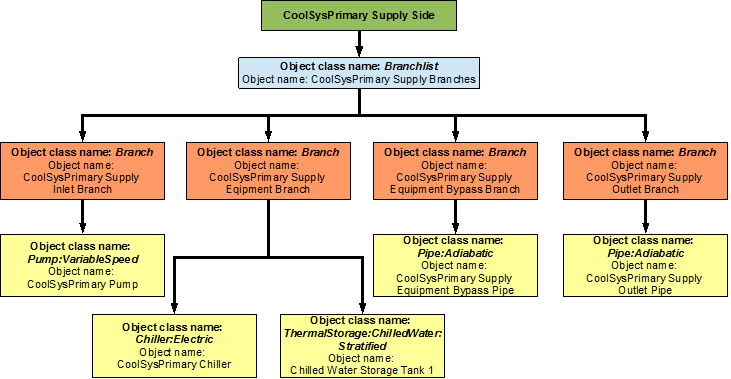
\includegraphics[width=0.9\textwidth, height=0.9\textheight, keepaspectratio=true]{media/image050.png}
\caption{Example Floor Construction illustration. \protect \label{fig:example-floor-construction-illustration.}}
\end{figure}

Window constructions are similarly built up from items in the Window Materials set using similar layers.. See Figure~\ref{fig:illustration-for-material-ordering-in}. Illustration for material ordering in windows, which shows the case where an interior shading layer such as a blind is present. The gap between the inside glass layer (layer \#3) and the interior shading layer is not entered. Similarly, for an exterior shading layer, the gap between the outside glass layer and the shading layer is not entered.

\begin{figure}[hbtp] % fig 25
\centering
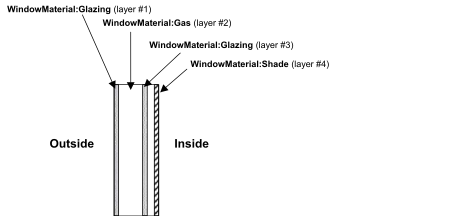
\includegraphics[width=0.9\textwidth, height=0.9\textheight, keepaspectratio=true]{media/image051.png}
\caption{Illustration for material ordering in windows. \protect \label{fig:illustration-for-material-ordering-in}}
\end{figure}

However, for a between-glass shading device the gaps on either side of the shading layer must be entered and they must have the same gas type. In addition, the gap widths with and without the between-glass shading layer must be consistent (see Figure~\ref{fig:window-construction-with-and-without-a}).

A maximum of four glass layers and one shading layer is allowed. A gas layer must always separate adjacent glass layers in a multi-pane glazing without a between-glass shading layer.

\begin{figure}[hbtp] % fig 26
\centering

\includegraphics[width=0.9\textwidth, height=0.9\textheight, keepaspectratio=true]{media/image052.png}
  \caption{Window construction with and without a between-glass shading layer. Shown are gap widths \(g\), \(g_1\) and \(g_2\), and shading layer width, \(w\). An error will result if \(g_1 + g_2 +w\) is not equal to \(g\), where \(w\) is zero for a blind and greater than zero for a shade. \protect \label{fig:window-construction-with-and-without-a}}
\end{figure}

Outside and inside air film resistances are never given as part of a construction definitions since they are calculated during the EnergyPlus simulation. Note also that constructions are assumed to be one-dimensional in a direction perpendicular to the surface.

\subsubsection{Inputs}\label{inputs-34-000}

\paragraph{Field: Name}\label{field-name-28-001}

This field is a user specified name that will be used as a reference by other input syntax. For example, a heat transfer surface (ref: Building Surfaces) requires a construction name to define what the make-up of the wall is. This name must be identical to one of the Construction definitions in the input data file.

\paragraph{Field: Outside Layer}\label{field-outside-layer}

Each construction must have at least one layer. This field defines the material name associated with the layer on the outside of the construction---outside referring to the side that is not exposed to the zone but rather the opposite side environment, whether this is the outdoor environment or another zone. Material layers are defined based on their thermal properties elsewhere in the input file (ref: Material and Material Properties and Materials for Glass Windows and Doors). As noted above, the outside layer should NOT be a film coefficient since EnergyPlus will calculate outside convection and radiation heat transfer more precisely.

\paragraph{Field(s) 2-10: Layers}\label{fields-2-10-layers}

The next fields are optional and the number of them showing up in a particular Construction definition depends solely on the number of material layers present in that construction. The data expected is identical to the outside layer field (see previous field description). The order of the remaining layers is important and should be listed in order of occurrence from the one just inside the outside layer until the inside layer is reached. As noted above, the inside layer should NOT be a film coefficient since EnergyPlus will calculate inside convection and radiation heat transfer more precisely.

IDF Example (floor construction):

\begin{lstlisting}

Construction, FLOOR38,  ! Material layer names follow:
        E5 - ACOUSTIC TILE,
        E4 - CEILING AIRSPACE,
        C12 - 2 IN HW CONCRETE;
\end{lstlisting}

IDF Example (window construction, no shade):

\begin{lstlisting}

Construction, DOUBLE PANE WINDOW,  !- Material layer names follow:
        GLASS - CLEAR SHEET 1 / 8 IN,
        WinAirB1 - AIRSPACE RESISTANCE,
        GLASS - CLEAR SHEET 1 / 8 IN;
\end{lstlisting}

IDF Example (window construction, with interior shade):

\begin{lstlisting}

Construction, DOUBLE PANE WITH ROLL SHADE,  !- Material layer names follow:
        GLASS - CLEAR SHEET 1 / 8 IN,
        WinAirB1 - AIRSPACE RESISTANCE,
        GLASS - CLEAR SHEET 1 / 8 IN,
        ROLL SHADE - LIGHT
\end{lstlisting}

\subsection{Site:GroundTemperature:FCfactorMethod}\label{sitegroundtemperaturefcfactormethod-000}

Site:GroundTemperature:FCfactorMethod is used only by the underground walls or slabs-on-grade or underground floors defined with C-factor (\hyperref[constructioncfactorundergroundwall]{Construction:CfactorUndergroundWall}) and F-factor (\hyperref[constructionffactorgroundfloor]{Construction:FfactorGroundFloor}) method for code compliance calculations where detailed construction layers are unknown. Only one such ground temperature object can be included. The monthly ground temperatures for this object are close to the monthly outside air temperatures delayed by three months. If user does not input this object in the IDF file, it will be defaulted to the 0.5m set of monthly ground temperatures from the weather file if they are available.

\subsubsection{Inputs}\label{inputs-35-000}

\paragraph{Field: Month Temperature(s) -- 12 fields in all}\label{field-month-temperatures-12-fields-in-all-000}

Each numeric field is the monthly ground temperature (degrees Celsius) used for the indicated month (January = 1\(^{st}\) field, February = 2\(^{nd}\) field, etc.)

And, the IDF example:

\begin{lstlisting}
Site:GroundTemperature:FCfactorMethod,  9.5,3.5,-0.7,-1.7,-0.6,3.6,9.3,14,18.2,22.7,21.2,16.8;
\end{lstlisting}

\subsection{Constructions - Modeling Underground Walls and Ground Floors Defined with C and F Factors for Building Energy Code Compliance}\label{constructions---modeling-underground-walls-and-ground-floors-defined-with-c-and-f-factors-for-building-energy-code-compliance}

Building energy code and standards like ASHRAE 90.1, 90.2 and California Title 24 require the underground wall constructions and slabs-on-grade or underground floors not to exceed certain maximum values of C-factor and F-factor, which do not specify detailed layer-by-layer materials for the constructions.

A simplified approach is introduced to create equivalent constructions and model the ground heat transfer through underground walls and ground floors for the building energy code compliance calculations. The approach is to create constructions based on the user defined C or F factor with two layers: one concrete layer (0.15 m thick) with thermal mass, and one fictitious insulation layer with no thermal mass. Three new objects were created for such purpose: \textbf{\hyperref[constructioncfactorundergroundwall]{Construction:CfactorUndergroundWall}}, \textbf{\hyperref[constructionffactorgroundfloor]{Construction:FfactorGroundFloor}}, and \textbf{\hyperref[sitegroundtemperaturefcfactormethod]{Site:GroundTemperature:FCfactorMethod}}. Details of the approach are described in the Engineering Reference document. The wall and floor construction objects are described in this section; the ground temperature object is described with the other ground temperature objects.

When a underground wall or ground floor surface (\hyperref[buildingsurfacedetailed]{BuildingSurface:Detailed}, \hyperref[floordetailed]{Floor:Detailed}, and \hyperref[walldetailed]{Wall:Detailed}) references one of the two construction objects, its field `Outside Boundary Condition' needs to be set to GroundFCfactorMethod. For simple (rectangular) wall and floor objects, the outside boundary condition is inferred from the construction type.

The \hyperref[sitegroundtemperaturefcfactormethod]{Site:GroundTemperature:FCfactorMethod} is described in the section for ground temperatures, the following section describes the two new construction objects.

\subsection{Construction:CfactorUndergroundWall}\label{constructioncfactorundergroundwall}

This input object differs from the usual wall construction object in that it describes an entire construction rather than individual layers. This object is used when only the wall height (depth to the ground) and the C-factor are available.~ This object accesses a model that creates an equivalent layer-by-layer construction for the underground wall to approximate the heat transfer through the wall considering the thermal mass of the earth soil.

This object is referenced by underground wall surfaces with their fields `Outside Boundary Condition' set to GroundFCfactorMethod.

\subsubsection{Inputs}\label{inputs-36}

\paragraph{Field: Name}\label{field-name-29-000}

The name of the underground wall construction.

\paragraph{Field: C-Factor}\label{field-c-factor}

C-Factor is the time rate of steady-state heat flow through unit area of the construction, induced by a unit temperature difference between the body surfaces. The C-Factor unit is W/m\(^{2}\)·K. The C-factor does not include soil or air films. ASHRAE Standard 90.1 and California Title 24 specify maximum C-factors for underground walls depending on space types and climate zones.

\paragraph{Field: Height}\label{field-height}

This field describes the height of the underground wall, i.e.~the depth to the ground surface. The unit is meters.

IDF Example:

\begin{lstlisting}

Construction:CfactorUndergroundWall,
      CfactorUGWall,
      0.436,           ! C-factor (W/m2K), does not include soil or air films
      4.57;            ! Height (m)


    BuildingSurface:Detailed,
      Zn001:Wall001,           !- Name
      Wall,                    !- Surface Type
      CfactorUGWall,           !- Construction Name
      ZONE ONE,                !- Zone Name
      GroundFCfactorMethod,    !- Outside Boundary Condition
      ,                        !- Outside Boundary Condition Object
      NoSun,                   !- Sun Exposure
      NoWind,                  !- Wind Exposure
      0.0,                     !- View Factor to Ground
      4,                       !- Number of Vertices
      0.0,0.0,4.572,           !- X,Y,Z = = > Vertex 1
      0.0,0.0,0.0,             !- X,Y,Z = = > Vertex 2
      15.24,0.0,0.0,           !- X,Y,Z = = > Vertex 3
      15.24,0.0,4.572;         !- X,Y,Z = = > Vertex 4
\end{lstlisting}

\subsection{Construction:FfactorGroundFloor}\label{constructionffactorgroundfloor}

This input object differs from the usual ground floor construction object in that it describes an entire construction rather than individual layers. This object is used when only the floor area, exposed perimeter, and the F-factor are available.~ This object accesses a model that creates an equivalent layer-by-layer construction for the slab-on-grade or underground floor to approximate the heat transfer through the floor considering the thermal mass of the earth soil.

This object is referenced by slab-on-grade or underground floor surfaces with their fields `Outside Boundary Condition' set to GroundFCfactorMethod.

\subsubsection{Inputs}\label{inputs-37}

\paragraph{Field: Name}\label{field-name-30-000}

The name of the ground floor construction.

\paragraph{Field: F-Factor}\label{field-f-factor}

F-Factor represents the heat transfer through the floor, induced by a unit temperature difference between the outside and inside air temperature, on the per linear length of the exposed perimeter of the floor. The unit for this input is W/m·K. ASHRAE Standard 90.1 and California Title 24 specify maximum F-factors for slab-on-grade or underground floors depending on space types and climate zones.

\paragraph{Field: Area}\label{field-area}

This field describes the area (in square meters) of the slab-on-grade or underground floor.

\paragraph{Field: PerimeterExposed}\label{field-perimeterexposed}

This field describes the exposed (direct contact with ambient air) perimeter (in meters) of the slab-on-grade or underground floor.

IDF Example:

\begin{lstlisting}

Construction:FfactorGroundFloor,
      slabconst,
      0.12,     !F-factor in W/m-K
      232.26,   !Area in m2
      61.0;     !Exposed perimeter in m


    BuildingSurface:Detailed,
      Zn001:Flr001,            !- Name
      Floor,                   !- Surface Type
      slabconst,               !- Construction Name, FLOOR
      ZONE ONE,                !- Zone Name
      GroundFCfactorMethod,    !- Outside Boundary Condition, Surface
      ,                        !- Outside Boundary Condition Object, Zn001:Flr001
      NoSun,                   !- Sun Exposure
      NoWind,                  !- Wind Exposure
      0,                       !- View Factor to Ground
      4,                       !- Number of Vertices
      15.24,0.0,0.0,           !- X,Y,Z = = > Vertex 1
      0.0,0.0,0.0,             !- X,Y,Z = = > Vertex 2
      0.0,15.240,0.0,          !- X,Y,Z = = > Vertex 3
      15.24,15.24,0.0;         !- X,Y,Z = = > Vertex 4
\end{lstlisting}

\subsection{Construction:InternalSource}\label{constructioninternalsource}

In some cases such as radiant systems, a construction will actually have resistance wires or hydronic tubing embedded within the construction. Heat is then either added or removed from this building element to provide heating or cooling to the zone in question. In the case of building-integrated photovoltaics, the energy removed in the form of electricity will form a sink. It is possible to enter such constructions into EnergyPlus with the syntax described below. The definition is similar to the Construction definition with a few additions related to radiant or other systems that will lead to source/sink terms. The internal source capability is available with both the \textbf{ConductionTransferFunction} and \textbf{ConductionFiniteDifference} solution algorithms.~ The only difference is that the two dimensional pipe arrangements are not available to ConductionFiniteDifference. Those fields are ignored in that implementation.

\subsubsection{Inputs}\label{inputs-38}

\paragraph{Field: Name}\label{field-name-31-000}

This field is a user specified name that will be used as a reference by other input syntax. For example, a heat transfer surface (ref: Building Surfaces) requires a construction name to define what the make-up of the wall is.

\paragraph{Field: Source Present After Layer Number}\label{field-source-present-after-layer-number}

This field is an integer that relates the location of the heat source or sink. The integer refers to the list of material layers that follow later in the syntax and determines the layer after which the source is present. If a source is embedded within a single homogenous layer (such as concrete), that layer should be split into two layers and the source added between them. For example, a value of ``2'' in this field tells EnergyPlus that the source is located between the second and third material layers listed later in the construction description (see layer fields below).

\paragraph{Field: Temperature Calculation Requested After Layer Number}\label{field-temperature-calculation-requested-after-layer-number}

The nature of this field is similar to the source interface parameter (see previous field) in that it is an integer, refers to the list of material layers that follow, and defines a location after the layer number identified by the user-defined number. In this case, the user is specifying the location for a separate temperature calculation rather than the location of the heat source/sink. This feature is intended to allow users to calculate a temperature within the construction. This might be important in a radiant cooling system where condensation could be a problem. This temperature calculation can assist users in making that determination in absence of a full heat and mass balance calculation.

\paragraph{Field: Dimensions for the CTF Calculation}\label{field-dimensions-for-the-ctf-calculation}

This field is also an integer and refers to the detail level of the calculation. A value of ``1'' states that the user is only interested in a one-dimensional calculation. This is appropriate for electric resistance heating and for hydronic heating (when boiler/hot water heater performance is not affected by return and supply water temperatures). A value of ``2'' will trigger a two-dimensional solution for this surface only. This may be necessary for hydronic radiant cooling situations since chiller performance is affected by the water temperatures provided.

A few things should be noted about requesting two-dimensional solutions. First, the calculation of the conduction transfer functions (CTF) is fairly intensive and will require a significant amount of computing time. Second, the solution regime is two-dimensional internally but it has a one-dimensional boundary condition imposed at the inside and outside surface (i.e., surface temperatures are still isothermal is if the surface was one-dimensional).

\paragraph{Field: Tube Spacing}\label{field-tube-spacing}

This field defines how far apart in meters the hydronic tubing or electrical resistance wires are spaced in the direction perpendicular to the main direction of heat transfer. Note that this parameter is only used for two-dimensional solutions (see previous field).

\paragraph{Field: Outside Layer}\label{field-outside-layer-1}

Each construction must have at least one layer. This field defines the material name associated with the layer on the outside of this construction---outside referring to the side that is not exposed to the zone but rather the opposite side environment, whether this is the outdoor environment or another zone. Material layers are defined based on their thermal properties elsewhere in the input file (ref: Material and Material Properties and Materials for Glass Windows and Doors). As noted above, the outside layer should NOT be a film coefficient since EnergyPlus will calculate convection and radiation heat transfer more precisely.

\paragraph{Field(s) 2-10: Layers}\label{fields-2-10-layers-1}

The next fields are optional and the number of them showing up in a particular Construction definition depends solely on the number of material layers present in that particular construction. The data expected is identical to the outside layer field (see previous field description). The order of the remaining layers is important and should be listed in order of occurrence from the one just inside the outside layer until the inside layer is reached. As noted above, the inside layer should NOT be a film coefficient since EnergyPlus will calculate convection and radiation heat transfer more precisely.

\subsubsection{Outputs}\label{outputs-36-1}

\begin{itemize}
\item  Zone,Average,Surface Internal Source Location Temperature [C]
\item  Zone,Average,Surface Internal User Specified Location Temperature [C]
\end{itemize}

\paragraph{Surface Internal Source Location Temperature {[}C{]}}\label{surface-internal-source-location-temperature-c}

This output is the temperature within the surface at the location of the source/sink.

\paragraph{Surface Internal User Specified Location Temperature {[}C{]}}\label{surface-internal-user—specified-location-temperature-c}

This output is the temperature within the surface at the location requested by the user.


\subsection{Composite Wall Constructions}\label{composite-wall-constructions}

Standard constructions in EnergyPlus are built with the materials and layers described earlier. However, some configurations will not be adequately represented by using this approach. The Reference Data Set CompositeWallConstructions.idf contains constructions and associated materials for a set of \textbf{composite} walls. These are walls---such as stud walls---that have complicated heat-flow paths so that the conduction is two- or three-dimensional. Thermal bridges are one of the common terms for these complicated heat-flow paths; this dataset will help you represent these in EnergyPlus.

The materials here are \textbf{not} real materials but are ``equivalent'' materials obtained from finite-difference modeling. (The thickness, conductivity, density and specific heat values of the material layers for the different constructions have been taken from the ASHRAE report ``Modeling Two- and Three-Dimensional Heat Transfer through Composite Wall and Roof Assemblies in Hourly Energy Simulation Programs (1145-TRP),'' by Enermodal Engineering Limited, Oak Ridge National Laboratory, and the Polish Academy of Sciences, January 2001.). EnergyPlus will calculate conduction transfer functions using these materials. The heat transfer based on these conduction transfer functions will then be very close to what would be calculated with a two- or three-dimensional heat transfer calculation.

For stud walls, using these composite constructions will give more accurate heat flow than you would get by manually dividing the wall into a stud section and a non-stud section.

If your wall's exterior or interior roughness or thermal, solar or visible absorptances are different from those in the data set, you can make the appropriate changes to the first material (the outside layer) or the third material (the inside layer). \textbf{None of the other values should be changed.}

\begin{callout}
Complete description of the CompositeWallConstructions data set are found in the OutputDetailsAndExamples document.
\end{callout}

\subsection{Construction:ComplexFenestrationState}\label{constructioncomplexfenestrationstate}

This input object is used to describe the properties of a single state for complex fenestration.~ There are two parts to the input, 1) layer-by-layer physical description of fenestration system and 2) a set of matrices that describe overall system optical performance.~ Each layer also has associated with it two matrices that give the layer absorptance (for front and back incidence on the system.

The optical properties are given as a two-dimensional matrix describing the basis and four two-dimensional matrices of system bidirectional optical properties.

These input objects will generally be exported directly from the WINDOW program and it is expected that users usually will not develop the input themselves. However, this is an option for users who prefer to use a different method (e.g., Monte-Carlo ray-trace or measurement) of determining optical properties.

Multiple instances of this object are used to define the separate operating states of complex fenestration.~ For example, blinds could be deployed or redirected to create a new state, or electrochromic glazings could change transmittance.~ Each separate state defines the materials present and the overall optical performance.~ If the glazing system has only one state, then only one of these objects is needed.

If there is more than one complex fenestration state, it will be controlled using the EMS actuator called ``Surface'' with the control type ``Construction State'' and the EMS input object called \hyperref[energymanagementsystemconstructionindexvariable]{EnergyManagementSystem:ConstructionIndexVariable}.

\subsubsection{Inputs}\label{inputs-39}

\paragraph{Field: Name}\label{field-name-32-000}

Unique name of this construction.~ Used to identify type of window in surface objects.

\paragraph{Field: Basis Type keyword}\label{field-basis-type-keyword}

Only value currently implemented is ``LBNLWINDOW''. More options may be added in the future.

\paragraph{Field: Basis Symmetry, keyword}\label{field-basis-symmetry-keyword}

Only value currently implemented is ``None''. More options will be added in the future.

\paragraph{Field: Thermal Parameters}\label{field-thermal-parameters}

This field gives the name of \hyperref[windowthermalmodelparams]{WindowThermalModel:Params} object used to keep common data necessary for thermal simulation.

\paragraph{Field: Basis Matrix Name}\label{field-basis-matrix-name}

This field gives the name of an 2 x N matrix object that defines the basis~ For a fenestration basis, N would be the number of theta (polar angle) values, the first of the two elements for each of the i = 1,..,N would be the theta value, and the second would be the number of phi (azimuthal angle) values that 360º is divided into for that theta.

\paragraph{Field: Solar Optical Complex Front Transmittance Matrix Name}\label{field-solar-optical-complex-front-transmittance-matrix-name}

This field contains the name of matrix object that describes the solar transmittance at different incident angles.~ This is from the outside toward the inside.

\paragraph{Field: Solar Optical Complex Back Reflectance Matrix Name}\label{field-solar-optical-complex-back-reflectance-matrix-name}

This field contains the name of matrix object that describes the solar back reflectance at different incident angles.~ This is from the inside toward the outside.

\paragraph{Field: Visible Optical Complex Front Transmittance Matrix Name}\label{field-visible-optical-complex-front-transmittance-matrix-name}

This field contains the name of matrix object that describes the visible transmittance at different incident angles.~ This is from the outside toward the inside.

\paragraph{Field: Visible Optical Complex Back Reflectance Matrix Name}\label{field-visible-optical-complex-back-reflectance-matrix-name}

This field contains the name of vector object that describes the visible back reflectance at different incident angles.~ This is from the inside toward the outside.

\paragraph{Field: Outside Layer \textless{}x = 1\textgreater{}}\label{field-outside-layer-x-1}

Each construction must have at least one layer. The layer order is from outside to inside, with the first layer being either \hyperref[windowmaterialglazing]{WindowMaterial:Glazing} or \hyperref[windowmaterialcomplexshade]{WindowMaterial:ComplexShade}. The next layer is a \hyperref[windowmaterialgap]{WindowMaterial:Gap} layer, and the following layers then alternate between \hyperref[windowmaterialglazing]{WindowMaterial:Glazing} or \hyperref[windowmaterialcomplexshade]{WindowMaterial:ComplexShade} and \hyperref[windowmaterialgap]{WindowMaterial:Gap}. The last layer cannot be \hyperref[windowmaterialgap]{WindowMaterial:Gap}.

\paragraph{Field: Outside Layer Directional Front Absorptance Matrix Name}\label{field-outside-layer-directional-front-absorptance-matrix-name}

Points to an Nbasis x 1 matrix object.

\paragraph{Field: Outside Layer Directional Back Absorptance Matrix Name}\label{field-outside-layer-directional-back-absorptance-matrix-name}

Points to an Nbasis x 1 matrix object.

\paragraph{Above 3 fields are optionally repeated for layers 2-10}\label{above-3-fields-are-optionally-repeated-for-layers-2-10}

These layers include gaps, which do not need to have matrix data specified.

An IDF example of complex fenestration with single layer:

\begin{lstlisting}

Construction:ComplexFenestrationState,       !- single layer example
    CFS_Glz_1,                 !- name
    LBNLWindow,                !- basis type
    None,                      !- basis symmetry type
    ThermParam_1,              !- window thermal model
    CFS_Glz_1_Basis,           !- basis matrix name
    CFS_Glz_1_TfSol,           !- Tfsol
    CFS_Glz_1_RbSol,           !- Rbsol
    CFS_Glz_1_Tfvis,           !- Tfvis
    CFS_Glz_1_Tbvis,           !- Tbvis
    Glass_102_Layer,           !- layer 1 name
    CFS_Glz_1_Layer_1_fAbs,    !- fAbs
    CFS_Glz_1_Layer_1_bAbs;    !- bAbs
\end{lstlisting}

An complex fenestration IDF example with double layer (first layer is shading device):

\begin{lstlisting}

Construction:ComplexFenestrationState,       !- double layer example
    CFS_Glz_59,                    !- name
    LBNLWindow,                    !- basis type
    None,                          !- basis symmetry type
    ThermParam_59,                 !- window thermal model
    CFS_Glz_59_Basis,              !- basis matrix name
    CFS_Glz_59_TfSol,              !- Tfsol
    CFS_Glz_59_RbSol,              !- Rbsol
    CFS_Glz_59_Tfvis,              !- Tfvis
    CFS_Glz_59_Tbvis,              !- Tbvis
    Shade_30001_Layer,             !- layer 1 name (shading device)
    CFS_Glz_59_Layer_1_fAbs,       !- fAbs
    CFS_Glz_59_Layer_1_bAbs,       !- bAbs
    Gap_1_Layer,                   !- layer 1 name
    ,                 !- absorptance matrices for gaps should be empty for now
    ,                              !- it is for future use
    Glass_3110_Layer,              !- layer 2 name
    CFS_Glz_59_Layer_3110_fAbs,    !- fAbs
    CFS_Glz_59_Layer_3110_bAbs;    !- bAbs
\end{lstlisting}

\subsection{WindowThermalModel:Params}\label{windowthermalmodelparams}

This input object is used with the \hyperref[constructioncomplexfenestrationstate]{Construction:ComplexFenestrationState}

\subsubsection{Inputs}\label{inputs-40}

\paragraph{Field: Name}\label{field-name-33-000}

Unique name of the window thermal model parameters.

\paragraph{Field: Calculation Standard}\label{field-calculation-standard}

The type of the calculation standard.~ The choices are:

\begin{itemize}
\item
  ISO15099
\item
  EN673Declared
\item
  EN673Design
\end{itemize}

The default is ISO15099.

\paragraph{Field: Thermal Model}\label{field-thermal-model}

The type of thermal model.~ The choices are:

\begin{itemize}
\item
  ISO15099
\item
  ScaledCavityWidth
\item
  ConvectiveScalarModel\_NoSDThickness
\item
  ConvectiveScalarModel\_withSDThickness
\end{itemize}

The default is ISO15099.

\paragraph{Field: SD Scalar}\label{field-sd-scalar}

Shading Device Scalar Factor. Only used for~ Thermal Model = Convective Scalar Model.~ Factor of venetian shading device layer contribution to convection. Real value between 0 (where the shading device contribution to convection is neglected) and 1 (where the shading device treated as ``closed'' -- as if it is a glass layer with thermal properties of SD slat material). Default: 1.0

\paragraph{Field: Deflection Model}\label{field-deflection-model}

The type of deflection model used to model deflection in windows and glass.~ The choices are:

\begin{itemize}
\item
  NoDeflection
\item
  TemperatureAndPressureInput
\item
  MeasuredDeflection
\end{itemize}

The default is NoDeflection.

\paragraph{Field: Vacuum Pressure Limit}\label{field-vacuum-pressure-limit}

The pressure (Pa) which will be considered to be the limit for vacuum glazing pressure.~ All pressures less than or equal to this pressure will be considered to be vacuum. Default: 13.238 Pa.

\paragraph{Field: Initial Temperature}\label{field-initial-temperature}

The temperature (\(^{o}\)C) of the gap in the time of fabrication.~ It is used only when WindowThermalModel:Params DeflectionModel = TemperatureAndPressureInput

\paragraph{Field: Initial Pressure}\label{field-initial-pressure}

The pressure (Pa) of the gap at the time of fabrication of the sealed glazing system unitIt is used only when WindowThermalModel:Params DeflectionModel = TemperatureAndPressureInput.

An IDF example for WindowThermalModel:Params (without deflection):

\begin{lstlisting}

WindowThermalModel:Params,
    ThermParam_59,                   !- name
    ISO15099,                        !- standard
    ISO15099,                        !- thermal model standard
    1.00,                            !- SD scalar
    NoDeflection;                    !- deflection model
\end{lstlisting}

An IDF example for thermal parameters (with deflection):

\begin{lstlisting}

WindowThermalModel:Params,
    ThermParam_59,                   !- name
    ISO15099,                        !- standard
    ISO15099,                        !- thermal model standard
    1.00,                            !- SD scalar
    TemperatureAndPressureInput,     !- deflection model
    ,                                !- vacuum pressure limit
    21.00,                           !- temperature at time of fabrication
    10000.00;                        !- pressure at time of fabrication
\end{lstlisting}

An IDF example for WindowThermalModel:Params for modeling vacuum glazing

\begin{lstlisting}

WindowThermalModel:Params,
  ThermParam_1006,                                    !- name
  ISO15099,                                           !- standard
  ISO15099,                                           !- thermal model
  1.0000,                                             !- SDScalar
  NoDeflection,                                       !- deflection model
  13.238;                                             !- vacuum pressure limit
\end{lstlisting}

\subsection{Matrix:TwoDimension}\label{matrixtwodimension}

This is input object is only used with \hyperref[constructioncomplexfenestrationstate]{Construction:ComplexFenestrationState} object to enter a two-dimensional matrix of values.

It is used to define the Basis Matrix for BSDF input data, and is also used to define the actual BSDF matrices data for the complete fenestration definition as well as the individual layers of the system.

The data are entered in row-major order: all the elements of row 1, followed by all the elements of row 2, etc.~ The number of values to be entered depends on the number of rows and the number of columns.~ Blank fields are treated as having been set to zero.

See example IDF file ``SmOff\_ CmplxGlz\_IntExtShading.idf'' for the definition of two complex shading layers with matrix data defined.

\subsubsection{Field: Name}\label{field-name-34-000}

Unique name of matrix input object.

\subsubsection{Field: Number of Rows}\label{field-number-of-rows}

This field is the number of rows in the matrix.

\subsubsection{Field: Number of Columns}\label{field-number-of-columns}

This field is the number of columns in the matrix

\subsubsection{\textless{} Field Set: Value \# N \textgreater{}}\label{field-set-value-n}

Repeat entering value exactly the same number of times as the number of rows times the number of columns.

\subsubsection{Field: Value \# 1}\label{field-value-1-000}

This is the value of the matrix at the first row and first column.

\subsubsection{Field: Value \#2}\label{field-value-2}

This is the value of the matrix at the first row and the second column.

An IDF example of matrix for defining BSDF basis:

\begin{lstlisting}

Matrix:TwoDimension,       !- matrix for basis definition
    CFS_Glz_1_Basis,         !- basis matrix name
    9,                       !- number of rows
    2,                       !- number of columns
    0.00000, 1.00000,
    10.00000, 8.00000,
    20.00000, 16.00000,
    30.00000, 20.00000,
    40.00000, 24.00000,
    50.00000, 24.00000,
    60.00000, 24.00000,
    70.00000, 16.00000,
    82.50000, 12.00000;
\end{lstlisting}

\subsection{Construction:WindowEquivalentLayer}\label{constructionwindowequivalentlayer}

This object defines the construction for equivalent layer window (ASHWAT) model. This window can model various mix of glazing and shading layers combination. Shadings are defined as an integral part of the construction. The construction is defined by listing the layers name starting with outside layer and work your way to the inside Layer. Up to six solid layers (glazing and shade) and up to five gaps, i.e., a total of up to 11 layers maximum are allowed in equivalent layer window object. The solid layer types allowed are: Glazing, Insect Screen, Roller Blinds, Venetian Blind, and Drape Fabrics. This window model requires optical data of the individual glazing and shading layers to calculate the effective optical properties of the composite fenestration construction. Venetian blinds in equivalent layer window model can be in a fixed slat angle or has the option to control the slat angle in order to maximize visibility, or maximize solar gains. An equivalent-layer concept can simulate wide range of multiple glazing and shading layers combination and provides unlimited flexibility to combine different types of shading layers in a fenestration. The equivalent-layer window model does not support daylighting control. For the gap layer object any one of the five different Gas types can be specified: AIR, ARGON, XENON, KRYPTON, or CUSTOM. This window object is referenced by fenestration surfaces. For details of the model description refer to Equivalent Layer Fenestration Model section in Engineering Reference. The various layer objects that can be referenced in Equivalent Layer window model are:

\begin{lstlisting}
WindowMaterial:Glass:EquivalentLayer
WindowMaterial:Shade:EquivalentLayer
WindowMaterial:Drape:EquivalentLayer
WindowMaterial:Blind:EquivalentLayer
WindowMaterial:Screen:EquivalentLayer
WindowMaterial:Gap:EquivalentLayer
\end{lstlisting}

\subsubsection{Inputs}\label{inputs-41}

\paragraph{Field: Name}\label{field-name-35}

This field is a user specified name that will be used as a reference by other input syntax. For example, a heat transfer surface (ref: Fenestration) requires a construction name to define what the make-up of the fenestration is. This name must be identical to one of the Window Construction Equivalent Layer definitions in the input data file.

\paragraph{Field: Outside Layer}\label{field-outside-layer-2}

Each equivalent layer window construction must have at least one layer. This field defines the material name associated with the layer on the outside of the construction---outside referring to the side that is exposed to the outdoor environment or another zone. Material layers for equivalent layer window model are defined based on their thermal properties elsewhere in the input file (ref: WindowEquivalentLayerMaterialNames)

\paragraph{Field: Layer 2 - Layer11}\label{field-layer-2---layer11}

The next fields are optional and the number of them showing up in a particular equivalent layer window construction definition depends solely on the number of material layers present in that construction. The data expected is identical to the outside layer field (see previous field description). The order of the remaining layers is important and should be listed in order of occurrence from the one just inside the outside layer until the inside layer is reached. As noted above, the inside layer should NOT be a film coefficient since EnergyPlus will calculate inside convection and radiation heat transfer more precisely.

An IDF example for this object, is shown below:

\begin{lstlisting}

Construction:WindowEquivalentLayer,
    Six Solid Layers Window,   !- Name
    INSCRN,                    !- Outside Layer
    Air GAP Outdoor 12.7mm,    !- Layer 2
    GLZGRY,                    !- Layer 3
    Argon GAP Sealed 12.7mm,   !- Layer 4
    FEP,                       !- Layer 5
    Xenon GAP Sealed 12.7mm,   !- Layer 6
    LOF1436,                   !- Layer 7
    Krypton GAP Sealed 12.7mm, !- Layer 8
    GLZCLR,                    !- Layer 9
    Air GAP Indoor 12.7mm,     !- Layer 10
    ShadeTrns;                 !- Layer 11
\end{lstlisting}

\subsection{Construction:WindowDataFile}\label{constructionwindowdatafile}

The WINDOW program, which does a thermal and optical analysis of a window under different design conditions, writes a data file (``Window data file'') containing a description of the window that was analyzed. The Construction:WindowDataFile object allows a window to be read in from the WINDOW data file---see ``Importing Windows from WINDOW.'' For information on adding a shading device to the window see ``\hyperref[windowpropertyshadingcontrol]{WindowShadingControl}.''

\subsubsection{Inputs}\label{inputs-42}

\paragraph{Field: Name}\label{field-name-36}

This is the name of a window on the Window data file. An error will result if EnergyPlus cannot find a window of this name on the file, or if the file, shown in the next field, is not present. The location of the data file should be specified in the File Name field. For details on what is done with the data if a matching window is found on the file see ``Importing Windows from WINDOW.''

\paragraph{Field: File Name}\label{field-file-name-000}

This is the file name of the Window data file that contains the Window referenced in the previous field. The field may include a full path with file name, for precise results. The field must be \textless{} = 100 characters. The file name must not include commas or an exclamation point. A relative path or a simple file name should work with version 7.0 or later when using EP-Launch even though EP-Launch uses temporary directories as part of the execution of EnergyPlus. If using RunEPlus.bat to run EnergyPlus from the command line, a relative path or a simple file name may work if RunEPlus.bat is run from the folder that contains EnergyPlus.exe.

If this field is left blank, the file name is defaulted to Window5DataFile.dat.

Input Example

\begin{lstlisting}
Construction:WindowDataFile,
  DoubleClear;            !- Name of a Window on the Window Data File
  ! Note -- Window5DataFile.dat is presumed to be in the "run" folder where EnergyPlus.exe is

FenestrationSurface:Detailed,
  Zn001:Wall001:Win001, !- Name
  Window,               !- Class
  DoubleClear,          !- Construction Name
  Zn001:Wall001,        !- Base Surface Name, and Target (if applicable)
  0.5,                  !- View Factor to Ground
  ,                     !- Frame/Divider name
   1.0,                 !- Multiplier
  4,                    !- Number of vertices
  0.548, 0.0, 2.5000,   !- X,Y,Z of Vertices
  0.548, 0.0, 0.5000,
  5.548, 0.0, 0.5000,
  5.548, 0.0, 2.5000;
\end{lstlisting}

An example showing use of specific data file name and complete path location follows:

\begin{lstlisting}
Construction:WindowDataFile,
  DoubleClear,          !- Name of a Window on the Window Data File
  C:\EnergyPlusData\DataSets\MyWindow.dat;
\end{lstlisting}

\subsubsection{Outputs}\label{outputs-4-016}

An optional report (contained in \textbf{eplusout.eio}) gives calculational elements for the materials and constructions used in the input. These reports are explained fully in the Output Details and Examples document.


\section{Group -- Thermal Zone Description/Geometry}\label{group-thermal-zone-descriptiongeometry}

Without spaces, thermal zones, and surfaces, the building can't be simulated. This group of objects (Space, Zone, BuildingSurface) describes the thermal zone characteristics as well as the details of each surface to be modeled. Included here are shading surfaces.

\subsection{Space}\label{space}

This object defines a space (or room) in the building. All Spaces are part of a \hyperref[zone]{Zone}.
Every Zone contains one or more spaces.

Space is an optional input. If a Zone has no Space(s) specified in the input then a default Space named \textless{}Zone Name\textgreater{} will be created.
If some surfaces in a Zone are assigned to a Space and some are not, then a default Space
named \textless{}Zone Name\textgreater{}-Remainder will be created. 
Input references to Space Names must have a matching Space object. 
Default space names may not be referenced in the input except for \hyperref[outputvariable]{Output:Variable} keys).

Space geometry is specified by attaching surfaces to a space using the ``Space Name'' field. If a Space has only floor surface(s) and internal mass assigned to it, the Space is assumed to share the same enclosure with other such Spaces in the same Zone (and with any surfaces that are not explicitly assigned to a space). If a Space also has other types of surfaces (e.g. wall, ceiling, or roof) then the Space forms its own enclosure unless it is connected to other spaces with air boundaries (see \hyperref[constructionairboundary]{Construction:AirBoundary}).

\subsubsection{Inputs}\label{space-inputs-048}

\paragraph{Field: Name}\label{space-object-name}

The name of the Space object. This name must be unique across Zone, Space, ZoneList, and SpaceList names.

\paragraph{Field: Zone Name}\label{space-zone-name}

The name of the \hyperref[zone]{Zone} this Space is a part of. This field is required.

\paragraph{Field: Ceiling Height}\label{field-space-ceiling-height}

Space ceiling height is used in several areas within EnergyPlus (such as various room models, some convection coefficient calculations and, primarily, in calculating the space volume in the absence of other parameters). Energyplus automatically calculates the space ceiling height (m) from the average height of the space. If this field is 0.0, negative or \textbf{autocalculate}, then the calculated space ceiling height will be used in subsequent calculations. If this field is positive, then the calculated space ceiling height will not be used -- the number entered here will be used as the space ceiling height. If this number differs significantly from the calculated ceiling height, then a warning message will be issued. If a space ceiling height and floor area are entered, but no volume is entered, then the volume will be the ceiling height times floor area.

Note that the Ceiling Height is the distance from the Floor to the Ceiling in the Space, not an absolute height from the ground.

NOTE: At the moment, the autocalculated Space ceiling height is set to the Zone ceiling height.

\paragraph{Field: Volume}\label{field-space-volume}

Space volume is used in several areas within EnergyPlus (such as calculating air change rates for reporting or flow when air change rates are chosen as input, daylighting calculations, some convection coefficient calculations). EnergyPlus automatically calculates the space volume (\SI{}{\volume}) from the space geometry given by the surfaces that belong to the space. If this field is 0.0, negative or \textbf{autocalculate}, then the calculated space volume will be used in subsequent calculations. If this field is positive, then it will be used as the space volume. If this number differs significantly from the calculated space volume a warning message will be issued. For autocalculate to work properly, the space must be enclosed by the entered walls. Note that indicating the volume to be calculated but entering a positive ceiling height in the previous field will cause the volume to be calculated as the floor area (if \textgreater{} 0) times the entered ceiling height; else the volume will be calculated from the described surfaces. If this field is positive, any ceiling height positive value will not be used in volume calculations.

NOTE: At the moment, the autocalculated Space volume is the Zone volume apportioned by floor area.

\paragraph{Field: Floor Area}\label{space-field-floor-area}

Space floor area is used in many places within EnergyPlus. EnergyPlus automatically calculates the space floor area (\SI{}{\area}) as the total area of surfaces with Surface Type = Floor. If this field is 0.0, negative or \textbf{autocalculate} (the default), then the calculated space floor area will be used in subsequent calculations. If this field is positive, then it will be used as the space floor area. If the calculated floor area differs from the user input floor area by more than 5\%, a warning message will be issued.

For each Zone, the calculated floor area is the sum of the space floor areas belonging to the zone. If the input for \hyperref[field-floor-area]{Zone Floor Area} does not equal the calculated floor area, the input zone floor area will take precedence, and the space floor areas will be adjusted proportionately.  If the calculated floor area differs from the user input floor area by more than 5\%, a warning message will be issued.

\paragraph{Field: Space Type}\label{space-type}

Space type is used to categorize spaces by activity type, such as office, classroom, storage, etc. There is no predefined list of space types; 
any valid input string may be used. Several table outputs include a subtable by Space Type. There are also SpaceType \hyperref[outputmeter-and-outputmetermeterfileonly]{Output:Meters}. See the meter details (mtd) output file for a list of all available meters for a given simulation.
If left blank, this field defaults to ``General'''.
 
\paragraph{Field: Tag \textless{}\#\textgreater{}}\label{field-space-tag}

Tags are used to group spaces by additional characteristics that may be more or less detailed than Space Type. For example, codes and standards designations for ventilation or occupancy may use specific terms that are different from one standard to the next. There is no predefined list of tags; 
any valid input string may be used. Several table outputs include a subtable by Space Tag.


\subsection{SpaceList}\label{spacelist}

The SpaceList object defines a list of Space objects. It is primarily used with \hyperref[group-internal-gains-people-lights-other-internal-zone-equipment]{Internal Gains} objects (People, Lights, etc.) to apply the same gain across a group of Spaces.

Space lists are not exclusive. A Space can be referenced by more than one SpaceList object.

\subsubsection{Inputs}\label{inputs-1-045space}

\paragraph{Field: Name}\label{field-space-list-name-000}

The name of the SpaceList object. This name must be unique across Zone, Space, ZoneList, and SpaceList names.

\paragraph{Field: Space \textless{}\#\textgreater{} Name}\label{field-space-name}

Reference to a Space object.

\begin{lstlisting}

SpaceList,
  Mid Floor List,   !- Name
  Mid West Space,   !- Space 1 Name
  Mid Center Space, !- Space 2 Name
  Mid East Space;   !- Space 3 Name
\end{lstlisting}


\subsection{Zone}\label{zone}

This element sets up the parameters to simulate each thermal zone of the building.
This object defines a thermal zone of the building. Every Zone contains one or more \hyperref[space]{Spaces}.

Space is an optional input. If a Zone has no Space(s) specified in the input then a default Space named \textless{}Zone Name\textgreater{} will be created.
If some surfaces in a Zone are assigned to a Space and some are not, then a default Space
named \textless{}Zone Name\textgreater{}-Remainder will be created. 
Input references to Space Names must have a matching Space object. 
Default space names may not be referenced in the input except for \hyperref[outputvariable]{Output:Variable} keys).

\subsubsection{Inputs}\label{inputs-048}

\paragraph{Field: Name}\label{zone-object-name}

The name of the Zone object. This name must be unique across Zone, Space, ZoneList, and SpaceList names.

\paragraph{Field: Direction of Relative North}\label{field-direction-of-relative-north}

The Zone North Axis is specified \textbf{relative to the Building North Axis}. This value is specified in degrees (clockwise is positive). For more information, see the figure below as well as the description under ``\hyperref[globalgeometryrules]{GlobalGeometryRules}''.

\paragraph{Field(s): (X,Y,Z) Origin}\label{fields-xyz-origin}

The X,Y,Z coordinates of a zone origin can be specified, for convenience in vertices entry. Depending on the values in ``\hyperref[globalgeometryrules]{GlobalGeometryRules}'' (see description later in this section), these will be used to completely specify the building coordinates in ``world coordinate'' or not. Zone Origin coordinates are specified \textbf{relative to the Building Origin (which always 0,0,0)}. The following figure illustrates the use of Zone North Axis as well as Zone Origin values.

\begin{figure}[hbtp] % fig 27
\centering
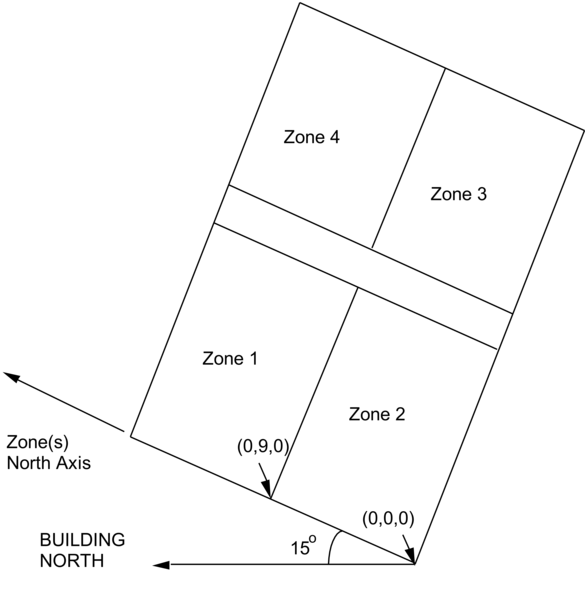
\includegraphics[width=0.9\textwidth, height=0.9\textheight, keepaspectratio=true]{media/image053.png}
\caption{Illustration of Zone North Axis and Origins \protect \label{fig:illustration-of-zone-north-axis-and-origins}}
\end{figure}

\paragraph{Field: Type}\label{field-type-000}

Zone type is currently unused.

\paragraph{Field: Multiplier}\label{field-multiplier}

Zone Multiplier is designed as a ``multiplier'' for floor area, zone loads, and energy consumed by internal gains. It takes the calculated load for the zone and multiplies it, sending the multiplied load to the attached HVAC system. The HVAC system size is specified to meet the entire multiplied zone load and will report the amount of the load met in the Zone Air System Sensible Heating or Cooling Energy/Rate output variable. Autosizing automatically accounts for multipliers. Metered energy consumption by internal gains objects such as Lights or Electric Equipment will be multiplied. The default is 1.

\paragraph{Field: Ceiling Height}\label{field-ceiling-height}

Zone ceiling height is used in several areas within EnergyPlus (such as various room models, some convection coefficient calculations and, primarily, in calculating zone volume in the absence of other parameters). Energyplus automatically calculates the zone ceiling height (m) from the average height of the zone. If this field is 0.0, negative or \textbf{autocalculate}, then the calculated zone ceiling height will be used in subsequent calculations. If this field is positive, then the calculated zone ceiling height will not be used -- the number entered here will be used as the zone ceiling height. If this number differs significantly from the calculated ceiling height, then a warning message will be issued. If a zone ceiling height is entered, but no Volume is entered, then the floor area (if there is one) times the zone ceiling height will be used as the volume.

Note that the Zone Ceiling Height is the distance from the Floor to the Ceiling in the Zone, not an absolute height from the ground.

\paragraph{Field: Volume}\label{field-volume}

Zone volume is used in several areas within EnergyPlus (such as calculating air change rates for reporting or flow when air change rates are chosen as input, daylighting calculations, some convection coefficient calculations). EnergyPlus automatically calculates the zone volume (\SI{}{\volume}) from the zone geometry given by the surfaces that belong to the zone. If this field is 0.0, negative or \textbf{autocalculate}, then the calculated zone volume will be used in subsequent calculations. If this field is positive, then it will be used as the zone volume. If this number differs significantly from the calculated zone volume a warning message will be issued. For autocalculate to work properly, the zone must be enclosed by the entered walls. Note that indicating the volume to be calculated but entering a positive ceiling height in the previous field will cause the volume to be calculated as the floor area (if \textgreater{} 0) times the entered ceiling height; else the volume will be calculated from the described surfaces. If this field is positive, any ceiling height positive value will not be used in volume calculations.

\paragraph{Field: Floor Area}\label{field-floor-area}

Zone floor area is used in many places within EnergyPlus. EnergyPlus automatically calculates the zone floor area (\SI{}{\area}) as the sum of the floor areas for the \hyperref[space]{Spaces} attached to this Zone. If this field is 0.0, negative or \textbf{autocalculate}, then the calculated zone floor area will be used in subsequent calculations. If this field is positive, then it will be used as the zone floor area. If the input zone floor area does not equal the calculated floor area, the input zone floor area will take precedence, and the space floor areas will be adjusted proportionately. If the calculated floor area differs from the user input floor area by more than 5\%, a warning message will be issued.

\paragraph{Field: Zone Inside Convection Algorithm}\label{field-zone-inside-convection-algorithm}

The Zone Inside Convection Algorithm field is optional. This field specifies the convection model to be used for the inside face of heat transfer surfaces associated with this zone. The choices are: \textbf{Simple} (constant natural convection - ASHRAE), \textbf{TARP} (combines natural and wind-driven convection correlations from laboratory measurements on flat plates), \textbf{CeilingDiffuser} (ACH based forced and mixed convection correlations for ceiling diffuser configuration with simple natural convection limit), \textbf{AdaptiveConvectionAlgorithm} (complex arrangement of various models that adapt to various zone conditions and can be customized), \textbf{TrombeWall} (variable natural convection in an enclosed rectangular cavity), and \textbf{ASTMC1340} (mixed convection coefficients specified for attic zone). See the Inside Convection Algorithm object for further descriptions of the available models.

If omitted or blank, the algorithm specified in the \hyperref[surfaceconvectionalgorithminside]{SurfaceConvectionAlgorithm:Inside} object is the default.

\paragraph{Field: Zone Outside Convection Algorithm}\label{field-zone-outside-convection-algorithm}

The Zone Outside Convection Algorithm field is optional. This field specifies the convection model to be used for the outside face of heat transfer surfaces associated with this zone. The choices are: \textbf{SimpleCombined}, \textbf{TARP}, \textbf{DOE-2}, \textbf{MoWiTT, and AdaptiveConvectionAlgorithm}. The simple convection model applies heat transfer coefficients depending on the roughness and windspeed. This is a combined heat transfer coefficient that includes radiation to sky, ground, and air. The correlation is based on Figure~\ref{fig:schematic-of-the-energyplus-unitary-system}, Page 25.1 (Thermal and Water Vapor Transmission Data), 2001 ASHRAE Handbook of Fundamentals.

The other convection models apply heat transfer coefficients depending on the roughness, windspeed, and terrain of the building's location. These are \emph{convection only} heat transfer coefficients; radiation heat transfer coefficients are calculated automatically by the program. The TARP algorithm was developed for the TARP software and combines natural and wind-driven convection correlations from laboratory measurements on flat plates. The DOE-2 and MoWiTT were derived from field measurements. The AdaptiveConvectionAlgorithm model is an dynamic algorithm that organizes a large number of different convection models and automatically selects the one that best applies. The adaptive convection algorithm can also be customized using the \hyperref[surfaceconvectionalgorithmoutsideadaptivemodelselections]{SurfaceConvectionAlgorithm:Outside:AdaptiveModelSelections} input object. All algorithms are described more fully in the Engineering Reference.

If omitted or blank, the algorithm specified in the \hyperref[surfaceconvectionalgorithmoutside]{SurfaceConvectionAlgorithm:Outside} object is the default.

\paragraph{Field: Part of Total Floor Area}\label{field-part-of-total-floor-area}

This optional field defaults to Yes if not specified. The field is used to show when a zone is not part of the Total Floor Area as shown in the Annual Building Utility Performance Summary tables. Specifically, when No is specified, the area is excluded from both the conditioned floor area and the total floor area in the Building Area sub table and the Normalized Metrics sub tables.

And, an IDF example:

\begin{lstlisting}

  Zone,
      DORM ROOMS AND COMMON AREAS,  !- Name
      0.0000000E+00,           !- Direction of Relative North {deg}
      0.0000000E+00,           !- X Origin {m}
      6.096000,                !- Y Origin {m}
      0.0000000E+00,           !- Z Origin {m}
      1,                       !- Type
      1,                       !- Multiplier
      autocalculate,           !-Ceiling Height {m}
      autocalculate;           !- Volume {m3}
\end{lstlisting}

\subsubsection{Zone Outputs}\label{outputs-037}

\begin{itemize}
\item
  Zone,Average,Zone Outdoor Air Drybulb Temperature {[}C{]}
\item
  Zone,Average,Zone Outdoor Air Wetbulb Temperature {[}C{]}
\item
  Zone,Average,Zone Outdoor Air Wind Speed {[}m/s{]}
\end{itemize}

\paragraph{Zone Outdoor Air Drybulb Temperature {[}C{]}}\label{zone-outdoor-air-drybulb-temperature-c-000}

The outdoor air dry-bulb temperature calculated at the height above ground of the zone centroid.

\paragraph{Zone Outdoor Air Wetbulb Temperature {[}C{]}}\label{zone-outdoor-air-wetbulb-temperature-c-000}

The outdoor air wet-bulb temperature calculated at the height above ground of the zone centroid.

\paragraph{Zone Outdoor Air Wind Speed {[}m/s{]}}\label{zone-outdoor-air-wind-speed-ms-000}

The outdoor wind speed calculated at the height above ground of the zone centroid.

\subsection{Space and Zone Thermal Output(s)}\label{Space-thermal-outputs}

\subsubsection{Space Thermal Outputs Overview}

\begin{itemize}
\item
  Zone,Sum,Space Total Internal Radiant Heating Energy {[}J{]}
\item
  Zone,Average,Space Total Internal Radiant Heating Rate {[}W{]}
\item
  Zone,Sum,Space Total Internal Visible Radiation Heating Energy {[}J{]}
\item
  Zone,Average,Space Total Internal Visible Radiation Heating Rate {[}W{]}
\item
  Zone,Sum,Space Total Internal Convective Heating Energy {[}J{]}
\item
  Zone,Average,Space Total Internal Convective Heating Rate {[}W{]}
\item
  Zone,Sum,Space Total Internal Latent Gain Energy {[}J{]}
\item
  Zone,Average,Space Total Internal Latent Gain Rate {[}W{]}
\item
  Zone,Sum,Space Total Internal Total Heating Energy {[}J{]}
\item
  Zone,Average,Space Total Internal Total Heating Rate {[}W{]}
\item
  HVAC,Average,Space Air Temperature {[}C{]}
\item
  Zone,Average,Space Mean Air Dewpoint Temperature {[}C{]}
\item
  Zone,Average,Space Mean Radiant Temperature {[}C{]}
\item
  Zone,Average,Space Operative Temperature {[}C{]}
\item
  HVAC,Average,Space Air Heat Balance Internal Convective Heat Gain Rate {[}W{]}
\item
  HVAC,Average,Space Air Heat Balance Surface Convection Rate {[}W{]}
\item
  HVAC,Average,Space Air Heat Balance InterSpace Air Transfer Rate {[}W{]}
\item
  HVAC,Average,Space Air Heat Balance Outdoor Air Transfer Rate {[}W{]}
\item
  HVAC,Average,Space Air Heat Balance System Air Transfer Rate {[}W{]}
\item
  HVAC,Average,Space Air Heat Balance System Convective Heat Gain Rate {[}W{]}
\item
  HVAC,Average,Space Air Heat Balance Air Energy Storage Rate {[}W{]}
\item
  HVAC,Average,Space Air Heat Balance Deviation Rate {[}W{]}
\item
  HVAC,Sum,Space Air System Sensible Heating Energy {[}J{]}
\item
  HVAC,Sum,Space Air System Sensible Cooling Energy {[}J{]}
\item
  HVAC,Average,Space Air System Sensible Heating Rate {[}W{]}
\item
  HVAC,Average,Space Air System Sensible Cooling Rate {[}W{]}
\item
  HVAC,Average,Space Air Humidity Ratio{[}kgWater/kgDryAir{]}
\item
  HVAC,Average,Space Air Relative Humidity{[}\%{]}
\item
  HVAC,Sum,Space Air System Latent Heating Energy {[}J{]}
\item
  HVAC,Sum,Space Air System Latent Cooling Energy {[}J{]}
\item
  HVAC,Average,Space Air System Latent Heating Rate {[}W{]}
\item
  HVAC,Average,Space Air System Latent Cooling Rate {[}W{]}
\item
  HVAC,Average,Space Air System Sensible Heat Ratio {[}{]}
\item
  HVAC,Average,Space Air Vapor Pressure Difference {[}Pa{]}
\end{itemize}

\subsubsection{Zone Thermal Outputs Overview}\label{zone-thermal-outputs}

In addition to the canned Surface reports (view the Reports section later in this document) and surface variables (above), the following variables are available for all zones:

\begin{itemize}
\item
  Zone,Sum,Zone Total Internal Radiant Heating Energy {[}J{]}
\item
  Zone,Average,Zone Total Internal Radiant Heating Rate {[}W{]}
\item
  Zone,Sum,Zone Total Internal Visible Radiation Heating Energy {[}J{]}
\item
  Zone,Average,Zone Total Internal Visible Radiation Heating Rate {[}W{]}
\item
  Zone,Sum,Zone Total Internal Convective Heating Energy {[}J{]}
\item
  Zone,Average,Zone Total Internal Convective Heating Rate {[}W{]}
\item
  Zone,Sum,Zone Total Internal Latent Gain Energy {[}J{]}
\item
  Zone,Average,Zone Total Internal Latent Gain Rate {[}W{]}
\item
  Zone,Sum,Zone Total Internal Total Heating Energy {[}J{]}
\item
  Zone,Average,Zone Total Internal Total Heating Rate {[}W{]}
\item
  HVAC,Average,Zone Exfiltration Heat Transfer Rate {[}W{]}
\item
  HVAC,Average,Zone Exfiltration Sensible Heat Transfer Rate {[}W{]}
\item
  HVAC,Average,Zone Exfiltration Latent Heat Transfer Rate {[}W{]}
\item
  HVAC,Average,Zone Exhaust Air Heat Transfer Rate {[}W{]}
\item
  HVAC,Average,Zone Exhaust Air Sensible Heat Transfer Rate {[}W{]}
\item
  HVAC,Average,Zone Exhaust Air Latent Heat Transfer Rate {[}W{]}
\item
  HVAC,Average,Zone Air Temperature {[}C{]}
\item
  Zone,Average,Zone Mean Air Dewpoint Temperature {[}C{]}
\item
  Zone,Average,Zone Mean Radiant Temperature {[}C{]}
\item
  Zone,Average,Zone Operative Temperature {[}C{]}
\item
  HVAC,Average,Zone Air Heat Balance Internal Convective Heat Gain Rate {[}W{]}
\item
  HVAC,Average,Zone Air Heat Balance Surface Convection Rate {[}W{]}
\item
  HVAC,Average,Zone Air Heat Balance Interzone Air Transfer Rate {[}W{]}
\item
  HVAC,Average,Zone Air Heat Balance Outdoor Air Transfer Rate {[}W{]}
\item
  HVAC,Average,Zone Air Heat Balance System Air Transfer Rate {[}W{]}
\item
  HVAC,Average,Zone Air Heat Balance System Convective Heat Gain Rate {[}W{]}
\item
  HVAC,Average,Zone Air Heat Balance Air Energy Storage Rate {[}W{]}
\item
  HVAC,Average,Zone Air Heat Balance Deviation Rate {[}W{]}
\item
  HVAC,Sum,Zone Air System Sensible Heating Energy {[}J{]}
\item
  HVAC,Sum,Zone Air System Sensible Cooling Energy {[}J{]}
\item
  HVAC,Average,Zone Air System Sensible Heating Rate {[}W{]}
\item
  HVAC,Average,Zone Air System Sensible Cooling Rate {[}W{]}
\item
  HVAC,Average,Zone Air Humidity Ratio{[}kgWater/kgDryAir{]}
\item
  HVAC,Average,Zone Air Relative Humidity{[}\%{]}
\item
  HVAC,Sum,Zone Air System Latent Heating Energy {[}J{]}
\item
  HVAC,Sum,Zone Air System Latent Cooling Energy {[}J{]}
\item
  HVAC,Average,Zone Air System Latent Heating Rate {[}W{]}
\item
  HVAC,Average,Zone Air System Latent Cooling Rate {[}W{]}
\item
  HVAC,Average,Zone Air System Sensible Heat Ratio {[}{]}
\item
  HVAC,Average,Zone Air Vapor Pressure Difference {[}Pa{]}

\end{itemize}

Two of these are of particular interest:

\begin{lstlisting}
Zone,Average,Zone Mean Air Temperature [C]
HVAC,Average,Zone Air Temperature [C]
\end{lstlisting}

These two variable outputs are/should be identical. However, note that they can be reported at different time intervals. ``Zone Mean Air Temperature'' is only available on the Zone/HB timestep (Number of Timesteps per Hour) whereas ``Zone Air Temperature'' can be reported at the HVAC timestep (which can vary).

\subsubsection{Space and Zone Thermal Outputs Details}

\paragraph{Zone Mean Air Temperature {[}C{]}}\label{zone-mean-air-temperature-c}

From the code definition, the zone mean air temperature is the average temperature of the air temperatures at the system timestep. Remember that the zone heat balance represents a ``well stirred'' model for a zone, therefore there is only one mean air temperature to represent the air temperature for the zone unless a non-mixing RoomAirModel is specified.

\paragraph{Zone Air Temperature {[}C{]}}\label{zone-air-temperature-c}

This is very similar to the mean air temperature in the last field. The ``well stirred'' model for the zone is the basis, but this temperature is also available at the ``detailed'' system timestep.

\paragraph{Zone Mean Air Dewpoint Temperature {[}C{]}}\label{zone-mean-air-dewpoint-temperature-c}

This is the dewpoint temperature of the zone calculated from the Zone Mean Air Temperature (above), the Zone Air Humidity Ratio (below) and the outdoor barometric pressure.

\paragraph{Zone Thermostat Air Temperature {[}C{]}}\label{zone-thermostat-air-temperature-c}

This is the zone air node temperature for the well-mixed room air model, which is the default room air model type (\hyperref[roomairmodeltype]{RoomAirModelType} = Mixing). But for other types of Room Air Model (the RoomAir:TemperaturePattern:* and RoomAirSettings:* objects) the zone thermostat air temperature may depend on the Thermostat Height and Thermostat Offset.

\paragraph{Zone Mean Radiant Temperature {[}C{]}}\label{zone-mean-radiant-temperature-c}

The Mean Radiant Temperature (MRT) in degrees Celsius of a space is a measure of the combined effects of temperatures of surfaces within that space. Specifically it is the surface area $\times$ emissivity weighted average of the zone inside surface temperatures (ref. Surface Inside Temperature), where emissivity is the Thermal Absorptance of the inside material layer of each surface.

\paragraph{Zone Operative Temperature {[}C{]}}\label{zone-operative-temperature-c}

Zone Operative Temperature (OT) is the average of the Zone Mean Air Temperature (MAT) and Zone Mean Radiant Temperature (MRT), OT = 0.5$\cdot$MAT + 0.5$\cdot$MRT. This output variable is not affected by the type of thermostat controls in the zone, and does not include the direct effect of high temperature radiant systems. See also Zone Thermostat Operative Temperature.

\paragraph{Zone Air Heat Balance Internal Convective Heat Gain Rate {[}W{]}}\label{zone-air-heat-balance-internal-convective-heat-gain-rate-w}

The Zone Air Heat Balance Internal Convective Heat Gain Rate is the sum, in watts, of heat transferred to the zone air from all types of internal gains from energyplus objects (e.g., people, lights, devices, appliances, equipment) listed in Tables \ref{table:space-or-zone-air-heat-balance-internal-convective-heat-gain-constituents} and \ref{table:space-or-zone-air-heat-balance-internal-convective-heat-gain-from-fenestration}. In addition to the convective heat gains listed in these tables, if a zone or a space is served by a zone HVAC equipment, i.e., the zone has no return air node, or served by an AirloopHVAC system that has cycling fan operating mode, then the convective heat gain specified to the return air is re-directed to the space or the zone air heat balance as convective internal heat gain. This and the following provide results on the load components of the zone air heat balance. This field is not multiplied by zone or group multipliers.

\begin{longtable}[c]{@{}lc@{}}
	\caption{Space or Zone Zone Air Heat Balance Internal Convective Heat Gain Constituents} \label{table:space-or-zone-air-heat-balance-internal-convective-heat-gain-constituents} \tabularnewline
	\toprule
	EnergyPlus Object &  Convective Heat Gain Type \tabularnewline
	\midrule
	\endfirsthead
	
	\caption[]{Space or Zone Zone Air Heat Balance Internal Convective Heat Gain Constituents} \tabularnewline
	\toprule
	EnergyPlus Object &  Convective Heat Gain Type \tabularnewline
	\midrule
	\endhead
	
	People     &     People    \tabularnewline
	Lights     &     Lights    \tabularnewline
	ElectricEquipment     &     ElectricEquipment    \tabularnewline
	ElectricEquipment:ITE:AirCooled     &     ElectricEquipmentITEAirCooled    \tabularnewline
	GasEquipment     &     GasEquipment    \tabularnewline
	HotWaterEquipment     &     HotWaterEquipment    \tabularnewline
	SteamEquipment     &     SteamEquipment    \tabularnewline
	OtherEquipment     &     OtherEquipment    \tabularnewline
	Refrigeration:Case     &     RefrigerationCase    \tabularnewline
	Refrigeration:CompressorRack     &     RefrigerationCompressorRack    \tabularnewline
	Refrigeration:System:Condenser:AirCooled     &     RefrigerationSystemAirCooledCondenser    \tabularnewline
	Refrigeration:System:SuctionPipe     &     RefrigerationSystemSuctionPipe    \tabularnewline
	Refrigeration:SecondarySystem:Receiver     &     RefrigerationSecondaryReceiver    \tabularnewline
	Refrigeration:SecondarySystem:Pipe     &     RefrigerationSecondaryPipe    \tabularnewline
	Refrigeration:WalkIn     &     RefrigerationWalkIn    \tabularnewline
	Refrigeration:TranscriticalSystem:GasCooler:AirCooled     &     RefrigerationTransSysAirCooledGasCooler    \tabularnewline
	Refrigeration:TranscriticalSystem:SuctionPipeMT     &     RefrigerationTransSysSuctionPipeMT    \tabularnewline
	Refrigeration:TranscriticalSystem:SuctionPipeLT     &     RefrigerationTransSysSuctionPipeLT    \tabularnewline
	WaterUse:Equipment     &     WaterUseEquipment    \tabularnewline
	WaterHeater:Mixed     &     WaterHeaterMixed    \tabularnewline
	WaterHeater:Stratified     &     WaterHeaterStratified    \tabularnewline
	ZoneBaseboard:OutdoorTemperatureControlled     &     ZoneBaseboardOutdoorTemperatureControlled    \tabularnewline
	ThermalStorage:ChilledWater:Mixed     &     ThermalStorageChilledWaterMixed    \tabularnewline
	ThermalStorage:ChilledWater:Stratified     &     ThermalStorageChilledWaterStratified    \tabularnewline
	Pipe:Indoor     &     PipeIndoor    \tabularnewline
	Pump:VariableSpeed     &     Pump\textunderscore VarSpeed    \tabularnewline
	Pump:ConstantSpeed     &     Pump\textunderscore ConSpeed    \tabularnewline
	Pump:VariableSpeed:Condensate     &     Pump\textunderscore Cond    \tabularnewline
	HeaderedPumps:VariableSpeed     &     PumpBank\textunderscore VarSpeed    \tabularnewline
	HeaderedPumps:ConstantSpeed     &     PumpBank\textunderscore ConSpeed    \tabularnewline
	PlantComponent:UserDefined     &     PlantComponentUserDefined    \tabularnewline
	Coil:UserDefined     &     CoilUserDefined    \tabularnewline
	ZoneHVAC:ForcedAir:UserDefined     &     ZoneHVACForcedAirUserDefined    \tabularnewline
	AirTerminal:SingleDuct:UserDefined     &     AirTerminalUserDefined    \tabularnewline
	Coil:Cooling:DX:SingleSpeed:ThermalStorage     &     PackagedTESCoilTank    \tabularnewline
	Fan:SystemModel     &     FanSystemModel    \tabularnewline
	Coil:Cooling:DX:SingleSpeed     &     SecCoolingDXCoilSingleSpeed    \tabularnewline
	Coil:Heating:DX:SingleSpeed     &     SecHeatingDXCoilSingleSpeed    \tabularnewline
	Coil:Cooling:DX:TwoSpeed     &     SecCoolingDXCoilTwoSpeed    \tabularnewline
	Coil:Cooling:DX:MultiSpeed     &     SecCoolingDXCoilMultiSpeed    \tabularnewline
	Coil:Heating:DX:MultiSpeed     &     SecHeatingDXCoilMultiSpeed    \tabularnewline
	Generator:FuelCell     &     GeneratorFuelCell    \tabularnewline
	Generator:MicroCHP     &     GeneratorMicroCHP    \tabularnewline
	ElectricLoadCenter:Transformer     &     ElectricLoadCenterTransformer    \tabularnewline
	ElectricLoadCenter:Inverter:Simple     &     ElectricLoadCenterInverterSimple    \tabularnewline
	ElectricLoadCenter:Inverter:FunctionOfPower     &     ElectricLoadCenterInverterFunctionOfPower    \tabularnewline
	ElectricLoadCenter:Inverter:LookUpTable     &     ElectricLoadCenterInverterLookUpTable    \tabularnewline
	ElectricLoadCenter:Storage:LiIonNMCBattery     &     ElectricLoadCenterStorageLiIonNmcBattery    \tabularnewline
	ElectricLoadCenter:Storage:Battery     &     ElectricLoadCenterStorageBattery    \tabularnewline
	ElectricLoadCenter:Storage:Simple     &     ElectricLoadCenterStorageSimple    \tabularnewline
	ElectricLoadCenter:Storage:Converter     &     ElectricLoadCenterConverter    \tabularnewline

	\bottomrule

\end{longtable}



\begin{longtable}[c]{@{}lcc@{}}
	\caption{Space or Zone Zone Air Heat Balance Internal Convective Heat Gain from fenestration} \label{table:space-or-zone-air-heat-balance-internal-convective-heat-gain-from-fenestration} \tabularnewline
	\toprule
	FenestrationSurface:Detailed Components &  Internal Convective Heat Gain Sources \tabularnewline
	\midrule
	\endfirsthead
	
	\caption[]{Space or Zone Zone Air Heat Balance Internal Convective Heat Gain Constituents} \tabularnewline
	\toprule
	FenestrationSurface:Detailed Components &  Internal Convective Heat Gain Sources \tabularnewline
	\midrule
	\endhead
	
	WindowProperty:FrameAndDivider &  Convective heat gain from window frame and divider  \tabularnewline
	Construction:WindowEquivalentLayer  &  Other convective heat gain from equivalent layer window model \tabularnewline
	Construction &  Natural convection heat gain from a gap \tabularnewline
	  &             between glass and interior shade or blind \tabularnewline
	Construction:ComplexFenestrationState &  Convective heat gain from air flow \tabularnewline
	  &             through a gap between glass and interior shade or blind \tabularnewline


	\bottomrule

\end{longtable}


\paragraph{Zone Air Heat Balance Surface Convection Rate {[}W{]}}\label{zone-air-heat-balance-surface-convection-rate-w}

The Zone Air Heat Balance Surface Convection Rate is the sum, in watts, of heat transferred to the zone air from all the surfaces. This field is not multiplied by zone or group multipliers.

\paragraph{Zone Air Heat Balance Interzone Air Transfer Rate {[}W{]}}\label{zone-air-heat-balance-interzone-air-transfer-rate-w}

The Zone Air Heat Balance Interzone Air Transfer Rate is the sum, in watts, of heat transferred to the zone air from all the transfers of air from other thermal zones. This field is not multiplied by zone or group multipliers.

\paragraph{Zone Air Heat Balance Outdoor Air Transfer Rate {[}W{]}}\label{zone-air-heat-balance-outdoor-air-transfer-rate-w}

The Zone Air Heat Balance Outdoor Air Transfer Rate is the sum, in watts, of heat transferred to the zone air from all the transfers of air from the out side, such as infiltration. This field is not multiplied by zone or group multipliers.

\paragraph{Zone Air Heat Balance System Air Transfer Rate {[}W{]}}\label{zone-air-heat-balance-system-air-transfer-rate-w}

The Zone Air Heat Balance System Air Transfer Rate is the sum, in watts, of heat transferred to the zone air by HVAC forced-air systems and air terminal units. Such HVAC systems are connected to the zone by an inlet node (see \hyperref[zonehvacequipmentconnections]{ZoneHVAC:EquipmentConnections} input field called Zone Air Inlet Node or Node List Name) This field is not multiplied by zone or group multipliers. The Zone Air Heat Balance System Air Transfer Rate may not agree exactly with the equipment-level delivered energy transfer rate when the zone temperature is changing significantly over a timestep (e.g. during thermostat setback and setup), but the energy will balance out over time.

\paragraph{Zone Air Heat Balance System Convective Heat Gain Rate {[}W{]}}\label{zone-air-heat-balance-system-convective-heat-gain-rate-w}

The Zone Air Heat Balance System Convective Heat Gain Rate is the sum, in watts, of heat transferred directly to the zone air by ``non-air'' HVAC systems. Such HVAC systems are not connected to the zone by an inlet node but rather add or subtract heat directly to the zone air in a manner similar to internal gains. These include the convective fraction of zone HVAC baseboards and high temperature radiant systems, zone HVAC refrigeration chiller set, and the extra convective cooling provided by the cooled beam air terminal unit. This field is not multiplied by zone or group multipliers.

\paragraph{Zone Air Heat Balance Air Energy Storage Rate {[}W{]}}\label{zone-air-heat-balance-air-energy-storage-rate-w}

The Zone Air Heat Balance Air Energy Storage Rate is the heat stored, in watts, in the zone air as result of zone air temperature changing from one timestep to the next. This field is not multiplied by zone or group multipliers.

\paragraph{Zone Air Heat Balance Deviation Rate {[}W{]}}\label{zone-air-heat-balance-deviation-rate-w}

The Zone Air Heat Balance Deviation Rate is the imbalance, in watts, in the energy balance for zone air. The value should be near zero but will become non-zero if zone conditions are changing rapidly or erratically. This field is not multiplied by zone or group multipliers. (This output variable is only generated if the user has set a computer system environment variable DisplayAdvancedReportVariables equal to ``yes''.)

\paragraph{Zone Air System Sensible Heating Energy {[}J{]}}\label{zone-air-system-sensible-heating-energy-j}

This output variable represents the sensible heating energy in Joules that is actually supplied by the system to that zone for the timestep reported. This is the sensible heating rate multiplied by the simulation timestep. This is calculated and reported from the Correct step in the Zone Predictor-Corrector module. This field is not multiplied by zone or group multipliers.

\begin{callout}
Zone Air System Sensible Heating (and Cooling) Energy (and Rate) all report the heating or cooling delivered by the HVAC system to a zone. These values are calculated by multiplying the supply air mass flow rate by the difference between the supply air temperature and the zone air temperature. This does not always indicate the operation of heating or cooling coils. For example, cooling will be reported if the supply air is cooled due to the introduction of outside air, even if all coils are off.

In addition, certain ``non-air'' zone-based systems will also add their heating or cooling contribution to this output variable.  For example, the following zone equipment will also add their output to the appropriate heating or cooling energy/rate output variable:

\begin{itemize}
\item
ZoneHVAC:Baseboard:RadiantConvective:Water
\item
ZoneHVAC:Baseboard:RadiantConvective:Steam
\item
ZoneHVAC:Baseboard:RadiantConvective:Electric
\item
ZoneHVAC:Baseboard:Convective:Water
\item
ZoneHVAC:Baseboard:Convective:Electric
\item
ZoneHVAC:CoolingPanel:RadiantConvective:Water
\item
ZoneHVAC:RefrigerationChillerSet
\end{itemize}

This means that system output from equipment such as high and low temperature radiant systems are NOT included in this output variable as the control of these radiant systems are handled separately with their own unique controls.

Finally, note that these variables are calculated at the system timestep. When reported at the ``detailed'' reporting frequency, these variables will never show heating and cooling both in the same system timestep. If reported at a frequency less than ``Detailed'' (for example, Hourly) values may appear in both the heating and cooling variable for the same hour if the system cooled the zone for part of the reporting period and heated the zone for another part of the reporting period.
\end{callout}

\paragraph{Zone Air System Sensible Cooling Energy {[}J{]}}\label{zone-air-system-sensible-cooling-energy-j}

This output variable represents the sensible cooling energy in Joules that is actually supplied by the system to that zone for the timestep reported. This is the sensible cooling rate multiplied by the simulation timestep. This is calculated and reported from the Correct step in the Zone Predictor-Corrector module. This field is not multiplied by zone or group multipliers. For additional information on this output variable, see the note that accompanies the Zone Air System Sensible Heating Energy output variable above.

\paragraph{Zone Air System Sensible Heating Rate {[}W{]}}\label{zone-air-system-sensible-heating-rate-w}

This output variable represents the sensible heating rate in Watts that is actually supplied by the system to that zone for the timestep reported. This is calculated and reported from the Correct step in the Zone Predictor-Corrector module. This field is not multiplied by zone or group multipliers. For additional information on this output variable, see the note that accompanies the Zone Air System Sensible Heating Energy output variable above.

\paragraph{Zone Air System Sensible Cooling Rate {[}W{]}}\label{zone-air-system-sensible-cooling-rate-w}

This output variable represents the sensible cooling rate in Watts that is actually supplied by the system to that zone for the timestep reported. This is calculated and reported from the Correct step in the Zone Predictor-Corrector module. This field is not multiplied by zone or group multipliers. For additional information on this output variable, see the note that accompanies the Zone Air System Sensible Heating Energy output variable above.

\paragraph{Zone Air Humidity Ratio {[}kgWater/kgDryAir{]}}\label{zone-air-humidity-ratio-kgwaterkgdryair}

This output variable represents the air humidity ratio after the correct step for each zone. The humidity ratio is the mass of water vapor to the mass of dry air contained in the zone in (kg water/kg air) and is unitless.

\paragraph{Zone Air Relative Humidity {[}\%{]}}\label{zone-air-relative-humidity}

This output variable represents the air relative humidity after the correct step for each zone. The relative humidity is in percent and uses the Zone Air Temperature, the Zone Air Humidity Ratio and the Outside Barometric Pressure for calculation.

\paragraph{Zone Air System Latent Heating Energy {[}J{]}}\label{zone-air-system-latent-heating-energy-j}

\paragraph{Zone Air System Latent Cooling Energy {[}J{]}}\label{zone-air-system-latent-cooling-energy-j}

These output variables represent the latent heating/cooling energy in Joules that is actually supplied by the system to that zone for the timestep reported. This is the sensible heating/cooling rate multiplied by the simulation timestep. This is calculated and reported from the Correct step in the Zone Predictor-Corrector module. This field is not multiplied by zone or group multipliers.

\paragraph{Zone Air System Latent Heating Rate {[}W{]}}\label{zone-air-system-latent-heating-rate-w}

This output variable represents the sensible heating rate in Watts that is actually supplied by the system to that zone for the timestep reported. This is calculated and reported from the Correct step in the Zone Predictor-Corrector module. This field is not multiplied by zone or group multipliers. For additional information on this output variable, see the note that accompanies the Zone Air System Sensible Heating Energy output variable above.

\paragraph{Zone Air System Latent Cooling Rate {[}W{]}}\label{zone-air-system-latent-cooling-rate-w}

This output variable represents the sensible cooling rate in Watts that is actually supplied by the system to that zone for the timestep reported. This is calculated and reported from the Correct step in the Zone Predictor-Corrector module. This field is not multiplied by zone or group multipliers. For additional information on this output variable, see the note that accompanies the Zone Air System Sensible Heating Energy output variable above.

\paragraph{Zone Air System Sensible Heat Ratio {[}{]}}\label{zone-air-system-sensible-heat-ratio}

This output variable represents the zone sensible heat transfer divided by the total heat transfer for the timestep reported. This is calculated and reported from the Correct step in the Zone Predictor-Corrector module.

\paragraph{Zone Air Vapor Pressure Difference {[}Pa{]}}\label{zone-air-vapor-pressure-difference-pa}

This output variable represents the zone vapor pressure difference, or depression, in pascals for the timestep reported. This is calculated and reported from the Correct step in the Zone Predictor-Corrector module. This value represents the saturated air vapor pressure minus the actual zone air vapor pressure and is indicative of the dryness of the zone air when latent loads are of interest.

\paragraph{Space or Zone Total Internal Radiant Heating Rate {[}W{]}}\label{zone-total-internal-radiant-heating-rate-w}

\paragraph{Space or Zone Total Internal Radiant Heating Energy {[}J{]}}\label{zone-total-internal-radiant-heating-energy-j}

These output variables represent the sum of radiant gains from specific internal sources (e.g.~equipment) throughout the space or zone in Watts (for rate) or joules. This includes radiant gain from \hyperref[people]{People}, Lights, Electric Equipment, Gas Equipment, Other Equipment, Hot Water Equipment, and Steam Equipment.

\paragraph{Space or Zone Total Internal Visible Radiation Heating Rate {[}W{]}}\label{zone-total-internal-visible-radiation-heating-rate-w}

\paragraph{Space or Zone Total Internal Visible Radiation Heating Energy {[}J{]}}\label{zone-total-internal-visible-radiation-heating-energy-j}

These output variables express the sum of heat gain in Watts (for rate) or joules that is the calculated short wavelength radiation gain from lights in the space or zones. This calculation uses the total energy from lights and the fraction visible to realize this value, summed over the space or zones in the simulation.

\paragraph{Space or Zone Total Internal Convective Heating Rate {[}W{]}}\label{zone-total-internal-convective-heating-rate-w}

\paragraph{Space or Zone Total Internal Convective Heating Energy {[}J{]}}\label{zone-total-internal-convective-heating-energy-j}

These output variables represent the sum of convective gains from specific sources (e.g.~equipment) throughout the space or zone in Watts (for rate) or joules. This includes convective gain from Energyplus objects that are listed in Table \ref{table:space-or-zone-total-internal-heat-gain-constituents}: 

\begin{longtable}[c]{@{}lcc@{}}
	\caption{Space or Zone Total Internal Heat Gain Constituents} \label{table:space-or-zone-total-internal-heat-gain-constituents} \tabularnewline
	\toprule
	EnergyPlus Object &  Internal Heat Gain Type \tabularnewline
	\midrule
	\endfirsthead
	
	\caption[]{Space or Zone Total Internal Heat Gain Constituents} \tabularnewline
	\toprule
	EnergyPlus Object &  Internal Heat Gain Type \tabularnewline
	\midrule
	\endhead
	
	People   &  People \tabularnewline
	Lights   &  Lights \tabularnewline
	ElectricEquipment   &  ElectricEquipment \tabularnewline
	ElectricEquipment:ITE:AirCooled   &  ElectricEquipmentITEAirCooled \tabularnewline
	GasEquipment   &  GasEquipment \tabularnewline
	HotWaterEquipment   &  HotWaterEquipment \tabularnewline
	SteamEquipment   &  SteamEquipment \tabularnewline
	OtherEquipment   &  OtherEquipment \tabularnewline
	
	\bottomrule

\end{longtable}

\paragraph{Space or Zone Total Internal Latent Gain Rate {[}W{]}}\label{zone-total-internal-latent-gain-rate-w}

\paragraph{Space or Zone Total Internal Latent Gain Energy {[}J{]}}\label{zone-total-internal-latent-gain-energy-j}

These output variables represent the sum of latent gains from specific internal sources (e.g.~equipment) throughout the space or zone in Watts (for rate) or joules. This includes latent gain from Energyplus objects that are listed in Table \ref{table:space-or-zone-total-internal-heat-gain-constituents}.

\paragraph{Space or Zone Total Internal Total Heating Rate {[}W{]}}\label{zone-total-internal-total-heating-rate-w}

\paragraph{Space or Zone Total Internal Total Heating Energy {[}J{]}}\label{zone-total-internal-total-heating-energy-j}

These output variables represent the sum of all heat gains throughout the space or zone in Watts (for rate) or joules. This includes all heat gains from Energyplus objects that are listed in Table \ref{table:space-or-zone-total-internal-heat-gain-constituents}.

\paragraph{Zone Exfiltration Heat Transfer Rate {[}W{]}}\label{zone-exfiltration-heat-transfer-rate-w}

\paragraph{Zone Exfiltration Sensible Heat Transfer Rate {[}W{]}}\label{zone-exfiltration-sensible-heat-transfer-rate-w}

\paragraph{Zone Exfiltration Latent Heat Transfer Rate {[}W{]}}\label{zone-exfiltration-latent-heat-transfer-rate-w}

These output variables represent the heat emitted to ambient from exfiltration in Watts. The exfiltration rate is calculated by solving a mass flow balance on the zone including infiltration, ventilation, outdoor air mixing, zone-to-zone mixing, and all of the zone inlet, exhaust, and return nodes. The latent parts are determined by taking the difference between the total and the sensible rate. Positive values indicate the zone injects heat to the environment, while negative values indicate the building extracts heat from the environment. 

\paragraph{Zone Exhaust Air Heat Transfer Rate {[}W{]}}\label{zone-exhaust-heat-transfer-rate-w}

\paragraph{Zone Exhaust Air Sensible Heat Transfer Rate {[}W{]}}\label{zone-exhaust-sensible-heat-transfer-rate-w}

\paragraph{Zone Exhaust Air Latent Heat Transfer Rate {[}W{]}}\label{zone-exhaust-latent-heat-transfer-rate-w}

These output variables represent the heat emitted to ambient from exhaust air in Watts. The zone exhaust air flow rate is aggregated from the zone exhaust nodes. Positive values indicate the building injects heat to the environment, while negative values indicate the building extracts heat from the environment. 

\paragraph{Site Total Zone Exfiltration Heat Loss {[}W{]}}\label{site-total-exfiltration-heat-transfer-rate-w}

These output variables represent the total amount of heat emitted to ambient from all zones by exfiltration in Watts. Positive values indicate the building injects heat to the environment, while negative values indicate the building extracts heat from the environment. This includes both sensible and latent heat loss from zone exfiltration.

\paragraph{Site Total Zone Exhaust Air Heat Loss {[}W{]}}\label{site-total-exhaust-heat-transfer-rate-w}

These output variables represent the total amount of heat emitted to ambient from all zones by exhaust air in Watts. Positive values indicate the building injects heat to the environment, while negative values indicate the building extracts heat from the environment. This includes both sensible and latent heat loss from zone exhaust air.

\subsection{ZoneList}\label{zonelist}

The ZoneList object defines a list of Zone objects. It is primarily used with the \hyperref[zonegroup]{ZoneGroup} object to provide a generalized way for doing ``Floor Multipliers''. (See the \hyperref[zonegroup]{ZoneGroup} description below.) The associated ZoneList output variables also provide a way to aggregate and organize zone loads.

Zone lists are not exclusive. A zone can be referenced be more than one ZoneList object.

\subsubsection{Inputs}\label{inputs-1-045}

\paragraph{Field: Name}\label{field-zone-list-name-000}

The name of the ZoneList object. This name must be unique across Zone, Space, ZoneList, and SpaceList names.

\paragraph{Field: Zone \textless{}\#\textgreater{} Name}\label{field-zone-1---zone-20-name}

Reference to a Zone object. This object is extensible, so additional fields of this type can be added to the end of this object.

\begin{lstlisting}

ZoneList,
  Mid Floor List,  !- Name
  Mid West Zone,   !- Zone 1 Name
  Mid Center Zone, !- Zone 2 Name
  Mid East Zone;   !- Zone 3 Name
\end{lstlisting}

\subsubsection{Outputs}\label{outputs-1-028}

The following output variables are reported by the ZoneList object:

\begin{itemize}
\item
  HVAC,Average,Zone List Sensible Heating Rate {[}W{]}
\item
  HVAC,Average,Zone List Sensible Cooling Rate {[}W{]}
\item
  HVAC,Sum,Zone List Sensible Heating Energy {[}J{]}
\item
  HVAC,Sum,Zone List Sensible Cooling Energy {[}J{]}
\end{itemize}

All ZoneList variables are the sum of the corresponding Zone variables. \emph{Zone Multiplier} fields in the Zone objects are also taken into account.

\subsection{ZoneGroup}\label{zonegroup}

The ZoneGroup object adds a multiplier to a \hyperref[zonelist]{ZoneList}. This can be used to reduce the amount of input necessary for simulating repetitive structures, such as the identical floors of a multi-story building. To create a ``Floor Multiplier'', use the \hyperref[zonelist]{ZoneList} object to organize several zones into a typical floor. Then use the \emph{Zone List Multiplier} field in the ZoneGroup object to multiply the system load for the zones in the list will also be multiplied. Zones with a \emph{Multiplier} field greater than one in the Zone object are effectively double-multiplied.

\begin{callout}
NOTE: Although \hyperref[zonelist]{ZoneList}s are not exclusive by themselves, \hyperref[zonelist]{ZoneList}s used to form a ZoneGroup are exclusive; the \hyperref[zonelist]{ZoneList}s used with a ZoneGroup must not have any zones in common.
\end{callout}

\subsubsection{Inputs}\label{inputs-2-042}

\paragraph{Tips for Multi-Story Simulations:}\label{tips-for-multi-story-simulations}

\begin{itemize}
\item
  For floors that are multiplied, connect exterior boundary conditions of the floor to the ceiling and vice versa.
\item
  Since exterior convection coefficients vary with elevation, locate the typical middle floor zones mid-height between the lowest and highest middle floors to be modeled.
\item
  Shading must be identical for all multiplied floors or less accurate results may be obtained by using the zone list multiplier.
\end{itemize}

ZoneGroup and \hyperref[zonelist]{ZoneList} can also be used to simulate other repetitive cases, such as clusters of zones on the ground.

\paragraph{Field: Zone Group Name}\label{field-zone-group-name}

The name of the ZoneGroup object. This must be unique across ZoneGroups.

\paragraph{Field: Zone List Name}\label{field-zone-list-name-1}

Reference to a \hyperref[zonelist]{ZoneList} object. The zones in the list constitute the zones in the group.

\paragraph{Field: Zone List Multiplier}\label{field-zone-list-multiplier}

An integer multiplier. Zone List Multiplier is designed as a ``multiplier'' for floor area, zone loads, and energy consumed by internal gains. It takes the calculated load for the zone and multiplies it, sending the multiplied load to the attached HVAC system. The HVAC system size is specified to meet the entire multiplied zone load and will report the amount of the load met in the Zone Air System Sensible Heating or Cooling Energy/Rate output variable. Autosizing automatically accounts for multipliers. Metered energy consumption by internal gains objects such as Lights or Electric Equipment will be multiplied. The default is 1.

\begin{lstlisting}

ZONE GROUP,
    Mid Floor,  !- Zone Group Name
    Mid Floor List,  !- Zone List Name
    8;  !- Zone List Multiplier
\end{lstlisting}

\subsubsection{Outputs}\label{outputs-2-023}

The following output variables are reported by the ZoneGroup object:

\begin{itemize}
\item
  HVAC,Average,Zone Group Sensible Heating Rate {[}W{]}
\item
  HVAC,Average,Zone Group Sensible Cooling Rate {[}W{]}
\item
  HVAC,Sum,Zone Group Sensible Heating Energy {[}J{]}
\item
  HVAC,Sum,Zone Group Sensible Cooling Energy {[}J{]}
\end{itemize}

All ZoneGroup variables report the associated ZoneList value multiplied by the \emph{Zone List Multiplier}.

\subsection{Surface(s)}\label{surfaces}

What's a building without surfaces?

EnergyPlus allows for several surface types:

\begin{itemize}
\item
  \textbf{\hyperref[buildingsurfacedetailed]{BuildingSurface:Detailed}}
\item
  \textbf{\hyperref[fenestrationsurfacedetailed]{FenestrationSurface:Detailed}}
\item
  \textbf{\hyperref[shadingsitedetailed-shadingbuildingdetailed]{Shading:Site:Detailed}}
\item
  \textbf{\hyperref[shadingsitedetailed-shadingbuildingdetailed]{Shading:Building:Detailed}}
\item
  \textbf{\hyperref[shadingzonedetailed-000]{Shading:Zone:Detailed}}
\end{itemize}

Each of the preceding surfaces has ``correct'' geometry specifications. BuildingSurface and Fenestration surfaces (heat transfer surfaces) are used to describe the important elements of the building (walls, roofs, floors, windows, doors) that will determine the interactions of the building surfaces with the outside environment parameters and the internal space requirements. These surfaces are also used to represent ``interzone'' heat transfer. All surfaces are modeled as a thin plane (with no thickness) except that material thicknesses are taken into account for heat transfer calculations.

During specification of surfaces, several ``outside'' environments may be chosen:

\begin{itemize}
\item
  \textbf{Ground} -- when the surface is in touch with the ground (e.g.~slab floors)
\item
  \textbf{Outdoors} -- when the surface is an external surface (e.g.~walls, roofs, windows directly exposed to the outdoor conditions)
\item
  \textbf{Surface} -- when the surface is
  \begin{itemize}
    \item
      An adiabatic internal zone surface
    \item
      A interzone surface
  \end{itemize}
\item
  \textbf{Zone --} when the surface is
  \begin{itemize}
    \item
      A interzone surface in which the other surface is not put in the input file.
  \end{itemize}
\item
  \textbf{OtherSideCoefficients} -- when using a custom profile to describe the external conditions of the surface (advanced concept -- covered in subject: \hyperref[surfacepropertyothersidecoefficients]{SurfaceProperty:OtherSideCoefficients})
\item
  \textbf{OtherSideConditionsModel} -- when using specially modeled components, such as active solar systems, that cover the outside surface and modify the conditions it experiences.
\end{itemize}

\textbf{Surface} items must also specify an ``outside face object''. This is

\begin{itemize}
\tightlist
\item
  Current surface name -- for adiabatic internal surfaces.
\item
  A surface name in another zone -- for interzone heat transfer.
\item
  An ``opposing'' surface name (in the current zone) -- for representing ``middle'' zones.
\end{itemize}

\textbf{Zone} items must also specify an ``outside face object''. This is

\begin{itemize}
\tightlist
\item
  The zone that contains the other surface that is adjacent to this surface but is not entered in input.
\end{itemize}

\begin{callout}
Note that heat transfer surfaces are fully represented with each description. As stated earlier in the Construction description, materials in the construction (outside to inside) are included but film coefficients neither inside nor outside are used in the description -- these are automatically calculated during the EnergyPlus run. Interzone surfaces which do not have a symmetrical construction (such as a ceiling/floor) require two Construction objects with the layers in reverse order. For example, CEILING with carpet, concrete, ceiling tile and FLOOR with ceiling tile, concrete, carpet. If interzone surfaces have a symmetrical construction, the specification for the two surfaces can reference the same Construction. When a surface is connected as the outside boundary condition for another surface, the two surfaces may be in the same plane, or they may be separated to imply thickness.
\end{callout}

\begin{callout}
Note also that if interzone constructions include either \hyperref[windowmaterialglazing]{WindowMaterial:Glazing} or \hyperref[windowmaterialglazingequivalentlayer]{WindowMaterial:Glazing:EquivalentLayer} then the materials properties of layers consisting of those material types will have front and back side values that may differ from one another.  So, if using such materials in the definition of an interzone construction, reversed materials must also have their front and back properties inverted so as to match in reverse order.  For example, if there is a single layer of glass of type \hyperref[windowmaterialglazing]{WindowMaterial:Glazing} defined for an interzone construction and the front and back properties differ, the user must define two materials with equivalent properties except that the front and back values must be reversed.  This means that one material used for the definition on one side might have a front side solar reflectance at normal incidence of 0.35 and a back side solar reflectance at normal incidence of 0.25.  The material used for the other side of the interzone construction must then have a front side solar reflectance at normal incidence of 0.25 and a back side solar reflectance at normal incidence of 0.35 to match properly in reverse.  EnergyPlus checks for all of the user input properties for single and multiple layer interzone constructions that use these two material types to confirm that this has been done correctly so that the simulation accurately reflects the properties of the materials on each side.
\end{callout}

\textbf{Shading} surfaces are used to describe aspects of the site which do not directly impact the physical interactions of the environmental parameters but may significantly shade the building during specific hours of the day or time so the year (e.g.~trees, bushes, mountains, nearby buildings which aren't being simulated as part of this facility, etc.)

\begin{callout}
Note that surfaces which are part of the simulated building automatically shade other parts of the building as geometry and time of day dictate -- there is no need on the user's part to include surfaces that might be in other zones for shading.
\end{callout}

Another surface type:

\begin{itemize}
\tightlist
\item
  \textbf{\hyperref[internalmass]{InternalMass}}
\end{itemize}

is used to specify the construction/material parameters and area of items within the space that are important to heat transfer calculations but not necessarily important geometrically. (For example, furniture within the space -- particularly for large spaces). Internal mass can also be used for internal walls that are not needed (when FullInteriorAndExterior Solar Distribution is in effect) for solar distribution or to represent many, if not all, interior walls when solar is distributed to the floors only.

\subsection{Interzone Surfaces}\label{interzone-surfaces}

EnergyPlus can quite accurately simulate the surface heat exchange between two zones. However, this accuracy is not always required and using interzonal heat transfer does add to the complexity of the calculations -- thus requiring more CPU time to simulate. More information about interzonal heat transfer calculations is contained in the Engineering Reference. Some simple guidelines are presented here -- for three cases: adiabatic surfaces, surfaces in ``middle'' zones, and surfaces where heat transfer is ``expected'' (e.g.~between a residence and an unheated, attached garage).

\begin{itemize}
\item
  Adiabatic Surfaces -- These surfaces would be represented as common surfaces (between two zones) where both zones are typically the same temperature. Thus, no transfer is expected in the surface from one zone to the next. These surfaces should be described as simply internal surfaces for the zone referencing as their Outside Boundary Condition Object (see later description in individual surface objects) their own surface names.
\item
  Surfaces in Middle Zones -- Middle zones in a building can be simulated using a judicious use of surfaces and zone multipliers to effect the correct ``loads'' for the building. Thus, middle zone behavior can be simulated without modeling the adjacent zones. This is done by specifying a surface within the zone. For example, a middle floor zone can be modeled by making the floor the Outside Boundary Condition Object for the ceiling, and the ceiling the Outside Boundary Condition Object for the floor.
\item
  Surfaces between Zones with differing temperatures -- These zones represent the true use of interzone surfaces. In a residence that has an attached garage, the garage may be unheated/uncooled or at least not conditioned to the same degree as the residence interior. In this case, EnergyPlus can be used to accurately calculate the effects of the differently conditioned space to the other spaces.
\end{itemize}

\subsection{Surface View Factors}\label{surface-view-factors}

EnergyPlus uses an area weighted approximation to calculate ``view factors'' between surfaces within a thermal zone. Each surface uses the total area that it can ``see'' among the other surfaces. The approximate view factor from this surface to each other surface is then the area of the receiving surface over the sum of areas that is visible to the sending surface.

In order to account in some limited way for the fact that certain surfaces will not see each other, several assumptions have been built into this simple view factor approximation. First, a surface cannot see itself. Second, surfaces with approximately the same azimuth (facing direction) and tilt (``same'' being within a built in limit) will not see each other. This means that a window will not see the wall that it is placed on, for example. Third, floors cannot see each other. Fourth, if the surface is a floor, ceiling, roof, or internal mass, the rule for the same azimuth and tilt eliminating radiant exchange between surface is waived when the receiving surface is floor, roof, ceiling, or internal mass as long as both surfaces are not floors.

Note that this does not take into account that surfaces may be ``around the corner'' from each other and in reality not see each other at all. Rooms are assumed to be convex rather than concave in this method.

To summarize, using the Surface ``Class'', the approximate view factors have:

\begin{enumerate}
\item
  No surface sees itself.
\item
  No Floor sees another floor.
\item
  All other surface types see Internal Mass.
\item
  All other surface types see floors.
\item
  Floors always see ceilings.
\item
  Floors always see roofs.
\item
  All other surfaces whose tilt or facing angle differences are greater than 10 degrees see each other.
\end{enumerate}

If geometry is correct, conditions 1, 3, and 7 should take care of all surfaces, but the other conditions supply common sense when the geometry is incorrect. More information about the EnergyPlus view factor calculation is contained in the Engineering Reference document.

\subsection{GlobalGeometryRules}\label{globalgeometryrules}

Before the surface objects are explained in detail, a description of geometric parameters used in EnergyPlus will be given. Since the input of surface vertices is common to most of the surface types, it will also be given a separate discussion.

Some flexibility is allowed in specifying surface vertices. This flexibility is embodied in the GlobalGeometryRules class/object in the input file. Note that the parameters specified in this statement are used for all surface vertices inputs---there is no further ``flexibility'' allowed.

In order to perform shadowing calculations, the building surfaces must be specified. EnergyPlus uses a three dimensional (3D) Cartesian coordinate system for surface vertex specification. This Right Hand coordinate system has the X-axis pointing east, the Y-axis pointing north, and the Z-axis pointing up. See figure below.

\begin{figure}[hbtp] % fig 28
\centering
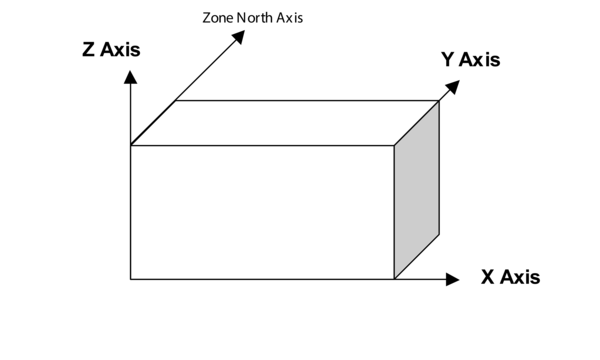
\includegraphics[width=0.9\textwidth, height=0.9\textheight, keepaspectratio=true]{media/image054.png}
\caption{EnergyPlus Coordinate System \protect \label{fig:energyplus-coordinate-system}}
\end{figure}

\subsubsection{Inputs}\label{inputs-3-038}

\paragraph{Field: Starting Vertex Position}\label{field-starting-vertex-position}

The shadowing algorithms in EnergyPlus rely on surfaces having vertices in a certain order and positional structure. Thus, the surface translator needs to know the starting point for each surface entry. The choices are: UpperLeftCorner, LowerLeftCorner , UpperRightCorner, or LowerRightCorner. Since most surfaces will be 4 sided, the convention will specify this position as though each surface were 4 sided. Extrapolate 3 sided figures to this convention. For 5 and more sided figures, again, try to extrapolate the best ``corner'' starting position.

\paragraph{Field: Vertex Entry Direction}\label{field-vertex-entry-direction}

Surfaces are always specified as being viewed from the outside of the zone to which they belong. (Shading surfaces are specified slightly differently and are discussed under the particular types). EnergyPlus needs to know whether the surfaces are being specified in counterclockwise or clockwise order (from the Starting Vertex Position). EnergyPlus uses this to determine the outward facing normal for the surface (which is the \emph{facing angle} of the surface -- very important in shading and shadowing calculations.

\paragraph{Field: Coordinate System}\label{field-coordinate-system}

Vertices can be specified in two ways: using \textbf{World} coordinates, or a \textbf{Relative} coordinate specification. Relative coordinates allow flexibility of rapid change to observe changes in building results due to orientation and position. \textbf{World} coordinates will facilitate use within a CADD system structure.

\textbf{Relative} coordinates make use of both Building and Zone North Axis values as well as Zone Origin values to locate the surface in 3D coordinate space. \textbf{World} coordinates do not use these values.

Typically, all zone origin values for ``World'' coordinates will be (0,0,0) but Building and Zone North Axis values may be used in certain instances (namely the Daylighting Coordinate Location entries).

\paragraph{Field: Daylighting Reference Point Coordinate System}\label{field-daylighting-reference-point-coordinate-system}

Daylighting reference points need to be specified as well. Again, there can be two flavors; \textbf{Relative} and \textbf{World}. Daylighting reference points must fit within the zone boundaries.

\textbf{Relative} coordinates make use of both Building and Zone North Axis values as well as Zone Origin values to locate the reference point in 3D coordinate space. \textbf{World} coordinates do not use these values.

\paragraph{Field: Rectangular Surface Coordinate System}\label{field-rectangular-surface-coordinate-system}

Simple, rectangular surfaces (\hyperref[wallexterior]{Wall:Exterior}, \hyperref[walladiabatic]{Wall:Adiabatic}, \hyperref[wallunderground]{Wall:Underground}, \hyperref[wallinterzone]{Wall:Interzone}, Roof, \hyperref[ceilingadiabatic]{Ceiling:Adiabatic}, \hyperref[ceilinginterzone]{Ceiling:Interzone}, \hyperref[floorgroundcontact]{Floor:GroundContact}, \hyperref[flooradiabatic]{Floor:Adiabatic}, \hyperref[floorinterzone]{Floor:Interzone}) can be specified with their Lower Left Corner as \textbf{relative} or \textbf{world}.

\textbf{Relative} (default) corners are specified relative to the Zone Origin for each surface. \textbf{World} corners would specify the absolute/world coordinate for this corner.

\subsection{Surfaces}\label{surfaces-1}

Surfaces make up the buildings and the elements that shade buildings. There are several methods to inputting surfaces, ranging from simple rectangular surfaces to detailed descriptions that describe each vertex in the order specified in the \hyperref[globalgeometryrules]{GlobalGeometryRules} object. The simple, rectangular surface objects are described first with the more detailed descriptions following.

\subsection{Walls}\label{walls}

Walls are usually vertical (tilt = 90 degrees). These objects are used to describe exterior walls, interior walls (adiabatic), underground walls, and walls adjacent to other zones.

\subsection{Wall:Exterior}\label{wallexterior}

The Wall:Exterior object is used to describe walls that are exposed to the external environment. They receive sun, wind -- all the characteristics of the external world.

\subsubsection{Inputs}\label{inputs-4-035}

\paragraph{Field: Name}\label{field-name-047}

This is a unique name associated with the exterior wall. It is used in several other places as a reference (e.g.~as the base surface name for a Window or Door).

\paragraph{Field: Construction Name}\label{field-construction-name-003}

This is the name of the construction (ref: Construction object) used in the surface. Regardless of location in the building, the ``full'' construction (all layers) is used. For example, for an interior wall separating two zones, zone x would have the outside layer (e.g.~drywall) as the material that shows in zone y and then the layers to the inside layer -- the material that shows in zone x. For symmetric constructions, the same construction can be used in the surfaces described in both zones.

\paragraph{Field: Zone Name}\label{field-zone-name-012}

This is the zone name to which the surface belongs. This field is required.

\paragraph{Field: Space Name}\label{field-space-name-012}

This is the space name to which the surface belongs. If this field is left blank, it will be automatically assigned to a space named <Zone Name> or <Zone Name>-Remainder. See \hyperref[space]{Space} for more details.

\paragraph{Field: Azimuth Angle}

The Azimuth Angle indicates the direction that the wall faces (outward normal). The angle is specified in degrees where East = 90, South = 180, West = 270, North = 0.

\paragraph{Field: Tilt Angle}

The tilt angle is the angle (in degrees) that the wall is tilted from horizontal (or the ground). Normally, walls are tilted 90 degrees and that is the default for this field.

\begin{callout}
\textbf{Starting Corner for the surface}

The rectangular surfaces specify the lower left corner of the surface for their starting coordinate. This is specified with (x,y,z) and can be relative to the zone origin or in world coordinates, depending on the value for rectangular surfaces specified in the \hyperref[globalgeometryrules]{GlobalGeometryRules} object.
\end{callout}

\paragraph{Field: Starting X Coordinate}\label{field-starting-x-coordinate}

This field is the X coordinate (in meters).

\paragraph{Field: Starting Y Coordinate}\label{field-starting-y-coordinate}

This field is the Y coordinate (in meters).

\paragraph{Field: Starting Z Coordinate}\label{field-starting-z-coordinate}

This field is the Z coordinate (in meters).

\paragraph{Field: Length}\label{field-length-000}

This field is the length of the wall in meters.

\paragraph{Field: Height}\label{field-height-000}

This field is the height of the wall in meters.

\subsection{Wall:Adiabatic}\label{walladiabatic}

The Wall:Adiabatic object is used to describe interior walls and partitions. Adiabatic walls are used to describe walls next to zones that have the same thermal conditions (thus, no heat transfer).

\subsubsection{Inputs}\label{inputs-5-032}

\paragraph{Field: Name}\label{field-name-1-044}

This is a unique name associated with the interior wall. It is used in several other places as a reference (e.g.~as the base surface name for a Window or Door).

\paragraph{Field: Construction Name}\label{field-construction-name-1-001}

This is the name of the construction (ref: Construction object) used in the surface. Regardless of location in the building, the ``full'' construction (all layers) is used. For example, for an interior wall separating two zones, zone x would have the outside layer (e.g.~drywall) as the material that shows in zone y and then the layers to the inside layer -- the material that shows in zone x. For symmetric constructions, the same construction can be used in the surfaces described in both zones.

\paragraph{Field: Zone Name}\label{field-zone-name-1-009}

This is the zone name to which the surface belongs. This field is required.

\paragraph{Field: Space Name}\label{field-space-name-1-009}

This is the space name to which the surface belongs. If this field is left blank, it will be automatically assigned to a space named <Zone Name> or <Zone Name>-Remainder. See \hyperref[space]{Space} for more details.

\paragraph{Field: Azimuth Angle}\label{field-azimuth-angle-1}

The Azimuth Angle indicates the direction that the wall faces (outward normal). The angle is specified in degrees where East = 90, South = 180, West = 270, North = 0.

\paragraph{Field: Tilt Angle}\label{field-tilt-angle-1}

The tilt angle is the angle (in degrees) that the wall is tilted from horizontal (or the ground). Normally, walls are tilted 90 degrees and that is the default for this field.

\begin{callout}
\textbf{Starting Corner for the surface}

The rectangular surfaces specify the lower left corner of the surface for their starting coordinate. This is specified with (x,y,z) and can be relative to the zone origin or in world coordinates, depending on the value for rectangular surfaces specified in the \hyperref[globalgeometryrules]{GlobalGeometryRules} object.
\end{callout}

\paragraph{Field: Starting X Coordinate}\label{field-starting-x-coordinate-1}

This field is the X coordinate (in meters).

\paragraph{Field: Starting Y Coordinate}\label{field-starting-y-coordinate-1}

This field is the Y coordinate (in meters).

\paragraph{Field: Starting Z Coordinate}\label{field-starting-z-coordinate-1}

This field is the Z coordinate (in meters).

\paragraph{Field: Length}\label{field-length-1}

This field is the length of the wall in meters.

\paragraph{Field: Height}\label{field-height-1}

This field is the height of the wall in meters.

\subsection{Wall:Underground}\label{wallunderground}

The Wall:Underground object is used to describe walls with ground contact. The temperature at the outside of the wall is the temperature in the GroundTemperature:BuildingSurface object.

\subsubsection{Inputs}\label{inputs-6-029}

\paragraph{Field: Name}\label{field-name-2-039}

This is a unique name associated with the underground wall. It is used in several other places as a reference (e.g.~as the base surface name for a Window or Door).

\paragraph{Field: Construction Name}\label{field-construction-name-2-001}

This is the name of the construction (ref: Construction object) used in the surface. Regardless of location in the building, the ``full'' construction (all layers) is used. For example, for an interior wall separating two zones, zone x would have the outside layer (e.g.~drywall) as the material that shows in zone y and then the layers to the inside layer -- the material that shows in zone x. For symmetric constructions, the same construction can be used in the surfaces described in both zones. Note that if the construction is \textbf{\hyperref[constructioncfactorundergroundwall]{Construction:CfactorUndergroundWall}} then the GroundFCfactoreMethod will be used for this wall.

\paragraph{Field: Zone Name}\label{field-zone-name-2-007}

This is the zone name to which the surface belongs. This field is required.

\paragraph{Field: Space Name}\label{field-space-name-2-007}

This is the space name to which the surface belongs. If this field is left blank, it will be automatically assigned to a space named <Zone Name> or <Zone Name>-Remainder. See \hyperref[space]{Space} for more details.

\paragraph{Field: Azimuth Angle}\label{field-azimuth-angle-2}

The Azimuth Angle indicates the direction that the wall faces (outward normal). The angle is specified in degrees where East = 90, South = 180, West = 270, North = 0.

\paragraph{Field: Tilt Angle}\label{field-tilt-angle-2}

The tilt angle is the angle (in degrees) that the wall is tilted from horizontal (or the ground). Normally, walls are tilted 90 degrees and that is the default for this field.

\paragraph{Starting Corner for the surface}\label{starting-corner-for-the-surface-2}

The rectangular surfaces specify the lower left corner of the surface for their starting coordinate. This is specified with (x,y,z) and can be relative to the zone origin or in world coordinates, depending on the value for rectangular surfaces specified in the \hyperref[globalgeometryrules]{GlobalGeometryRules} object.

\paragraph{Field: Starting X Coordinate}\label{field-starting-x-coordinate-2}

This field is the X coordinate (in meters).

\paragraph{Field: Starting Y Coordinate}\label{field-starting-y-coordinate-2}

This field is the Y coordinate (in meters).

\paragraph{Field: Starting Z Coordinate}\label{field-starting-z-coordinate-2}

This field is the Z coordinate (in meters).

\paragraph{Field: Length}\label{field-length-2}

This field is the length of the wall in meters.

\paragraph{Field: Height}\label{field-height-2}

This field is the height of the wall in meters.

\subsection{Wall:Interzone}\label{wallinterzone}

The Wall:Interzone object is used to describe walls adjacent to zones that are significantly different conditions than the zone with this wall.

\subsubsection{Inputs}\label{inputs-7-028}

\paragraph{Field: Name}\label{field-name-3-033}

This is a unique name associated with the interzone wall. It is used in several other places as a reference (e.g.~as the base surface name for a Window or Door).

\paragraph{Field: Construction Name}\label{field-construction-name-3}

This is the name of the construction (ref: Construction object) used in the surface. Regardless of location in the building, the ``full'' construction (all layers) is used. For example, for an interior wall separating two zones, zone x would have the outside layer (e.g.~drywall) as the material that shows in zone y and then the layers to the inside layer -- the material that shows in zone x. For symmetric constructions, the same construction can be used in the surfaces described in both zones.

\paragraph{Field: Zone Name}\label{field-zone-name-3-006}

This is the zone name to which the surface belongs. This field is required.

\paragraph{Field: Space Name}\label{field-space-name-3-006}

This is the space name to which the surface belongs. If this field is left blank, it will be automatically assigned to a space named <Zone Name> or <Zone Name>-Remainder. See \hyperref[space]{Space} for more details.

\paragraph{Field: Outside Boundary Condition Object}\label{field-outside-boundary-condition-object}

The Outside Boundary Condition Object field is the name of a wall in an adjacent zone or the name of the adjacent zone. If the adjacent zone option is used, the adjacent wall is automatically generated in the adjacent zone. If the surface name is used, it must be in the adjacent zone.

\paragraph{Field: Azimuth Angle}\label{field-azimuth-angle-3}

The Azimuth Angle indicates the direction that the wall faces (outward normal). The angle is specified in degrees where East = 90, South = 180, West = 270, North = 0.

\paragraph{Field: Tilt Angle}\label{field-tilt-angle-3}

The tilt angle is the angle (in degrees) that the wall is tilted from horizontal (or the ground). Normally, walls are tilted 90 degrees and that is the default for this field.

\paragraph{Starting Corner for the surface}\label{starting-corner-for-the-surface-3}

The rectangular surfaces specify the lower left corner of the surface for their starting coordinate. This is specified with (x,y,z) and can be relative to the zone origin or in world coordinates, depending on the value for rectangular surfaces specified in the \hyperref[globalgeometryrules]{GlobalGeometryRules} object.

\paragraph{Field: Starting X Coordinate}\label{field-starting-x-coordinate-3}

This field is the X coordinate (in meters).

\paragraph{Field: Starting Y Coordinate}\label{field-starting-y-coordinate-3}

This field is the Y coordinate (in meters).

\paragraph{Field: Starting Z Coordinate}\label{field-starting-z-coordinate-3}

This field is the Z coordinate (in meters).

\paragraph{Field: Length}\label{field-length-3}

This field is the length of the wall in meters.

\paragraph{Field: Height}\label{field-height-3}

This field is the height of the wall in meters.

\subsection{Roofs/Ceilings}\label{roofsceilings}

Roofs and ceilings are, by default, flat (tilt = 0 degrees). These objects are used to describe roofs, interior ceilings (adiabatic) and ceilings adjacent to other zones.

\subsection{Roof}\label{roof}

The Roof object is used to describe roofs that are exposed to the external environment.

\subsubsection{Inputs}\label{inputs-8-026}

\paragraph{Field: Name}\label{field-name-4-030}

This is a unique name associated with the roof. It is used in several other places as a reference (e.g.~as the base surface name for a Window or Door).

\paragraph{Field: Construction Name}\label{field-construction-name-4}

This is the name of the construction (ref: Construction object) used in the surface. Regardless of location in the building, the ``full'' construction (all layers) is used. For example, for an interior wall separating two zones, zone x would have the outside layer (e.g.~drywall) as the material that shows in zone y and then the layers to the inside layer -- the material that shows in zone x. For symmetric constructions, the same construction can be used in the surfaces described in both zones.

\paragraph{Field: Zone Name}\label{field-zone-name-4-006}

This is the zone name to which the surface belongs. This field is required.

\paragraph{Field: Space Name}\label{field-space-name-4-006}

This is the space name to which the surface belongs. If this field is left blank, it will be automatically assigned to a space named <Zone Name> or <Zone Name>-Remainder. See \hyperref[space]{Space} for more details.
\paragraph{Field: Azimuth Angle}\label{field-azimuth-angle-4}

The Azimuth Angle indicates the direction of the outward normal for the roof. The angle is specified in degrees where East = 90, South = 180, West = 270, North = 0.

\paragraph{Field: Tilt Angle}\label{field-tilt-angle-4}

The tilt angle is the angle (in degrees) that the wall is tilted from horizontal (or the ground). Flat roofs are tilted 0 degrees and that is the default for this field.

\paragraph{Starting Corner for the surface}\label{starting-corner-for-the-surface-4}

The rectangular surfaces specify the lower left corner of the surface for their starting coordinate. This is specified with (x,y,z) and can be relative to the zone origin or in world coordinates, depending on the value for rectangular surfaces specified in the \hyperref[globalgeometryrules]{GlobalGeometryRules} object.

\paragraph{Field: Starting X Coordinate}\label{field-starting-x-coordinate-4}

This field is the X coordinate (in meters).

\paragraph{Field: Starting Y Coordinate}\label{field-starting-y-coordinate-4}

This field is the Y coordinate (in meters).

\paragraph{Field: Starting Z Coordinate}\label{field-starting-z-coordinate-4}

This field is the Z coordinate (in meters).

\paragraph{Field: Length}\label{field-length-4}

This field is the length of the roof in meters.

\paragraph{Field: Width}\label{field-width}

This field is the width of the roof in meters.

\subsection{Ceiling:Adiabatic}\label{ceilingadiabatic}

The Ceiling:Adiabatic object is used to describe interior ceilings that separate zones of like conditions.

\subsubsection{Inputs}\label{inputs-9-024}

\paragraph{Field: Name}\label{field-name-5-026}

This is a unique name associated with the ceiling. It is used in several other places as a reference (e.g.~as the base surface name for a Window or Door).

\paragraph{Field: Construction Name}\label{field-construction-name-5}

This is the name of the construction (ref: Construction object) used in the surface. Regardless of location in the building, the ``full'' construction (all layers) is used. For example, for an interior wall separating two zones, zone x would have the outside layer (e.g.~drywall) as the material that shows in zone y and then the layers to the inside layer -- the material that shows in zone x. For symmetric constructions, the same construction can be used in the surfaces described in both zones.

\paragraph{Field: Zone Name}\label{field-zone-name-5-005}

This is the zone name to which the surface belongs. This field is required.

\paragraph{Field: Space Name}\label{field-space-name-5-005}

This is the space name to which the surface belongs. If this field is left blank, it will be automatically assigned to a space named <Zone Name> or <Zone Name>-Remainder. See \hyperref[space]{Space} for more details.
\paragraph{Field: Azimuth Angle}\label{field-azimuth-angle-5}

The Azimuth Angle indicates the direction of the outward normal for the roof. The angle is specified in degrees where East = 90, South = 180, West = 270, North = 0.

\paragraph{Field: Tilt Angle}\label{field-tilt-angle-5}

The tilt angle is the angle (in degrees) that the wall is tilted from horizontal (or the ground). Flat ceilings are tilted 0 degrees and that is the default for this field.

\paragraph{Starting Corner for the surface}\label{starting-corner-for-the-surface-5}

The rectangular surfaces specify the lower left corner of the surface for their starting coordinate. This is specified with (x,y,z) and can be relative to the zone origin or in world coordinates, depending on the value for rectangular surfaces specified in the \hyperref[globalgeometryrules]{GlobalGeometryRules} object.

\paragraph{Field: Starting X Coordinate}\label{field-starting-x-coordinate-5}

This field is the X coordinate (in meters).

\paragraph{Field: Starting Y Coordinate}\label{field-starting-y-coordinate-5}

This field is the Y coordinate (in meters).

\paragraph{Field: Starting Z Coordinate}\label{field-starting-z-coordinate-5}

This field is the Z coordinate (in meters).

\paragraph{Field: Length}\label{field-length-5}

This field is the length of the ceiling in meters.

\paragraph{Field: Width}\label{field-width-1}

This field is the width of the ceiling in meters.

\subsection{Ceiling:Interzone}\label{ceilinginterzone}

The Ceiling:Interzone object is used to describe interior ceilings that separate zones of differing conditions (and expect heat transfer through the ceiling from the adjacent zone).

\subsubsection{Inputs}\label{inputs-10-022}

\paragraph{Field: Name}\label{field-name-6-024}

This is a unique name associated with the interzone ceiling. It is used in several other places as a reference (e.g.~as the base surface name for a Window or Door).

\paragraph{Field: Construction Name}\label{field-construction-name-6}

This is the name of the construction (ref: Construction object) used in the surface. Regardless of location in the building, the ``full'' construction (all layers) is used. For example, for an interior wall separating two zones, zone x would have the outside layer (e.g.~drywall) as the material that shows in zone y and then the layers to the inside layer -- the material that shows in zone x. For symmetric constructions, the same construction can be used in the surfaces described in both zones.

\paragraph{Field: Zone Name}\label{field-zone-name-6-004}

This is the zone name to which the surface belongs. This field is required.

\paragraph{Field: Space Name}\label{field-space-name-6-004}

This is the space name to which the surface belongs. If this field is left blank, it will be automatically assigned to a space named <Zone Name> or <Zone Name>-Remainder. See \hyperref[space]{Space} for more details.

\paragraph{Field: Outside Boundary Condition Object}\label{field-outside-boundary-condition-object-1}

The Outside Boundary Condition Object field is the name of a floor in an adjacent zone or the name of the adjacent zone. If the adjacent zone option is used, the adjacent floor is automatically generated in the adjacent zone. If the surface name is used, it must be in the adjacent zone.

\paragraph{Field: Azimuth Angle}\label{field-azimuth-angle-6}

The Azimuth Angle indicates the direction of the outward normal for the roof. The angle is specified in degrees where East = 90, South = 180, West = 270, North = 0.

\paragraph{Field: Tilt Angle}\label{field-tilt-angle-6}

The tilt angle is the angle (in degrees) that the wall is tilted from horizontal (or the ground). Flat ceilings are tilted 0 degrees and that is the default for this field.

\paragraph{Starting Corner for the surface}\label{starting-corner-for-the-surface-6}

The rectangular surfaces specify the lower left corner of the surface for their starting coordinate. This is specified with (x,y,z) and can be relative to the zone origin or in world coordinates, depending on the value for rectangular surfaces specified in the \hyperref[globalgeometryrules]{GlobalGeometryRules} object.

\paragraph{Field: Starting X Coordinate}\label{field-starting-x-coordinate-6}

This field is the X coordinate (in meters).

\paragraph{Field: Starting Y Coordinate}\label{field-starting-y-coordinate-6}

This field is the Y coordinate (in meters).

\paragraph{Field: Starting Z Coordinate}\label{field-starting-z-coordinate-6}

This field is the Z coordinate (in meters).

\paragraph{Field: Length}\label{field-length-6}

This field is the length of the ceiling in meters.

\paragraph{Field: Width}\label{field-width-2}

This field is the width of the ceiling in meters.

\subsection{Floors}\label{floors}

Floors are, by default, flat (tilt = 180 degrees). These objects are used to describe floors on the ground, interior floors (adiabatic) and floors adjacent to other zones.

\subsection{Floor:GroundContact}\label{floorgroundcontact}

The Floor:GroundContact object is used to describe floors that have ground contact (usually called slabs). The temperature at the outside of the floor is the temperature in the GroundTemperature:BuildingSurface object.

\subsubsection{Inputs}\label{inputs-11-021}

\paragraph{Field: Name}\label{field-name-7-022}

This is a unique name associated with the floor.

\paragraph{Field: Construction Name}\label{field-construction-name-7}

This is the name of the construction (ref: Construction object) used in the surface. Regardless of location in the building, the ``full'' construction (all layers) is used. For example, for an interior wall separating two zones, zone x would have the outside layer (e.g.~drywall) as the material that shows in zone y and then the layers to the inside layer -- the material that shows in zone x. For symmetric constructions, the same construction can be used in the surfaces described in both zones. Note that if the construction is \textbf{\hyperref[constructionffactorgroundfloor]{Construction:FfactorGroundFloor},} then the GroundFCfactorMethod will be used with this floor.

\paragraph{Field: Zone Name}\label{field-zone-name-7-004}

This is the zone name to which the surface belongs. This field is required.

\paragraph{Field: Space Name}\label{field-space-name-7-004}

This is the space name to which the surface belongs. If this field is left blank, it will be automatically assigned to a space named <Zone Name> or <Zone Name>-Remainder. See \hyperref[space]{Space} for more details.

\paragraph{Field: Azimuth Angle}\label{field-azimuth-angle-7}

The Azimuth Angle indicates the direction of the outward normal for the roof. The angle is specified in degrees where East = 90, South = 180, West = 270, North = 0.

\paragraph{Field: Tilt Angle}\label{field-tilt-angle-7}

The tilt angle is the angle (in degrees) that the wall is tilted from horizontal (or the ground). Flat floors are tilted 180 degrees and that is the default for this field.

\paragraph{Starting Corner for the surface}\label{starting-corner-for-the-surface-7}

The rectangular surfaces specify the lower left corner of the surface for their starting coordinate. This is specified with (x,y,z) and can be relative to the zone origin or in world coordinates, depending on the value for rectangular surfaces specified in the \hyperref[globalgeometryrules]{GlobalGeometryRules} object.

\paragraph{Field: Starting X Coordinate}\label{field-starting-x-coordinate-7}

This field is the X coordinate (in meters).

\paragraph{Field: Starting Y Coordinate}\label{field-starting-y-coordinate-7}

This field is the Y coordinate (in meters).

\paragraph{Field: Starting Z Coordinate}\label{field-starting-z-coordinate-7}

This field is the Z coordinate (in meters).

\paragraph{Field: Length}\label{field-length-7}

This field is the length of the floor in meters.

\paragraph{Field: Width}\label{field-width-3}

This field is the width of the floor in meters.

\subsection{Floor:Adiabatic}\label{flooradiabatic}

The Floor:Adiabatic object is used to describe interior floors or floors that you wish to model with no heat transfer from the exterior to the floor.

\subsubsection{Inputs}\label{inputs-12-019}

\paragraph{Field: Name}\label{field-name-8-022}

This is a unique name associated with the floor.

\paragraph{Field: Construction Name}\label{field-construction-name-8}

This is the name of the construction (ref: Construction object) used in the surface. Regardless of location in the building, the ``full'' construction (all layers) is used. For example, for an interior wall separating two zones, zone x would have the outside layer (e.g.~drywall) as the material that shows in zone y and then the layers to the inside layer -- the material that shows in zone x. For symmetric constructions, the same construction can be used in the surfaces described in both zones.

\paragraph{Field: Zone Name}\label{field-zone-name-8-003}

This is the zone name to which the surface belongs. This field is required.

\paragraph{Field: Space Name}\label{field-space-name-8-003}

This is the space name to which the surface belongs. If this field is left blank, it will be automatically assigned to a space named <Zone Name> or <Zone Name>-Remainder. See \hyperref[space]{Space} for more details.

\paragraph{Field: Azimuth Angle}\label{field-azimuth-angle-8}

The Azimuth Angle indicates the direction of the outward normal for the roof. The angle is specified in degrees where East = 90, South = 180, West = 270, North = 0.

\paragraph{Field: Tilt Angle}\label{field-tilt-angle-8}

The tilt angle is the angle (in degrees) that the wall is tilted from horizontal (or the ground). Flat floors are tilted 180 degrees and that is the default for this field.

\paragraph{Starting Corner for the surface}\label{starting-corner-for-the-surface-8}

The rectangular surfaces specify the lower left corner of the surface for their starting coordinate. This is specified with (x,y,z) and can be relative to the zone origin or in world coordinates, depending on the value for rectangular surfaces specified in the \hyperref[globalgeometryrules]{GlobalGeometryRules} object.

\paragraph{Field: Starting X Coordinate}\label{field-starting-x-coordinate-8}

This field is the X coordinate (in meters).

\paragraph{Field: Starting Y Coordinate}\label{field-starting-y-coordinate-8}

This field is the Y coordinate (in meters).

\paragraph{Field: Starting Z Coordinate}\label{field-starting-z-coordinate-8}

This field is the Z coordinate (in meters).

\paragraph{Field: Length}\label{field-length-8}

This field is the length of the floor in meters.

\paragraph{Field: Width}\label{field-width-4}

This field is the width of the floor in meters.

\subsection{Floor:Interzone}\label{floorinterzone}

The Floor:Interzone object is used to describe floors that are adjacent to other zones that have differing conditions and you wish to model the heat transfer through the floor.

\subsubsection{Inputs}\label{inputs-13-016}

\paragraph{Field: Name}\label{field-name-9-019}

This is a unique name associated with the floor.

\paragraph{Field: Construction Name}\label{field-construction-name-9}

This is the name of the construction (ref: Construction object) used in the surface. Regardless of location in the building, the ``full'' construction (all layers) is used. For example, for an interior wall separating two zones, zone x would have the outside layer (e.g.~drywall) as the material that shows in zone y and then the layers to the inside layer -- the material that shows in zone x. For symmetric constructions, the same construction can be used in the surfaces described in both zones.

\paragraph{Field: Zone Name}\label{field-zone-name-9-001}

This is the zone name to which the surface belongs. This field is required.

\paragraph{Field: Space Name}\label{field-space-name-9-001}

This is the space name to which the surface belongs. If this field is left blank, it will be automatically assigned to a space named <Zone Name> or <Zone Name>-Remainder. See \hyperref[space]{Space} for more details.

\paragraph{Field: Outside Boundary Condition Object}\label{field-outside-boundary-condition-object-2}

The Outside Boundary Condition Object field is the name of a ceiling in an adjacent zone or the name of the adjacent zone. If the adjacent zone option is used, the adjacent ceiling is automatically generated in the adjacent zone. If the surface name is used, it must be in the adjacent zone.

\paragraph{Field: Azimuth Angle}\label{field-azimuth-angle-9}

The Azimuth Angle indicates the direction of the outward normal for the roof. The angle is specified in degrees where East = 90, South = 180, West = 270, North = 0.

\paragraph{Field: Tilt Angle}\label{field-tilt-angle-9}

The tilt angle is the angle (in degrees) that the wall is tilted from horizontal (or the ground). Flat floors are tilted 180 degrees and that is the default for this field.

\paragraph{Starting Corner for the surface}\label{starting-corner-for-the-surface-9}

The rectangular surfaces specify the lower left corner of the surface for their starting coordinate. This is specified with (x,y,z) and can be relative to the zone origin or in world coordinates, depending on the value for rectangular surfaces specified in the \hyperref[globalgeometryrules]{GlobalGeometryRules} object.

\paragraph{Field: Starting X Coordinate}\label{field-starting-x-coordinate-9}

This field is the X coordinate (in meters).

\paragraph{Field: Starting Y Coordinate}\label{field-starting-y-coordinate-9}

This field is the Y coordinate (in meters).

\paragraph{Field: Starting Z Coordinate}\label{field-starting-z-coordinate-9}

This field is the Z coordinate (in meters).

\paragraph{Field: Length}\label{field-length-9}

This field is the length of the floor in meters.

\paragraph{Field: Width}\label{field-width-5}

This field is the width of the floor in meters.

\subsection{Windows/Doors}\label{windowsdoors}

The following window and door objects can be used to specify simple, rectangular doors and windows. In each case, the lower left corner (locator coordinate) of the window or door is specified \textbf{relative} to the surface it is on. Viewing the base surface as a planar surface, base the relative location from the lower left corner of the base surface. Vertex entry description as well as provisions for a few other surface types can be entered with the \hyperref[fenestrationsurfacedetailed]{FenestrationSurface:Detailed} object.

\subsection{Window}\label{window}

The Window object is used to place windows on surfaces that can have windows, including exterior walls, interior walls, interzone walls, roofs, floors that are exposed to outdoor conditions, interzone ceiling/floors. These, of course, can be entered using the simple rectangular objects or the more detailed vertex entry objects. Shades and screens may be applied by referencing this subsurface in a window shading control (ref: \hyperref[windowpropertyshadingcontrol]{WindowShadingControl} object). To assign a shade to a window or glass door, see WindowMaterial: Shade. To assign a screen, see \hyperref[windowmaterialscreen]{WindowMaterial:Screen}. To assign a blind, see \hyperref[windowmaterialblind]{WindowMaterial:Blind}. To assign switchable glazing, such as electrochromic glazing, see \hyperref[windowpropertyshadingcontrol]{WindowShadingControl}.


\subsubsection{Inputs}\label{inputs-14-016}

\paragraph{Field: Name}\label{field-name-10-018}

This is a unique name associated with the window.

\paragraph{Field: Construction Name}\label{field-construction-name-10}

This is the name of the subsurface's construction (ref: objects: Construction, \hyperref[constructionwindowdatafile]{Construction:WindowDataFile}, \hyperref[constructioncomplexfenestrationstate]{Construction:ComplexFenestrationState}).

For windows, if Construction Name is not found among the constructions on the input (.idf) file, the Window Data File (ref. \hyperref[constructionwindowdatafile]{Construction:WindowDataFile} object) will be searched for that Construction Name (see ``Importing Windows from WINDOW''). If that file is not present or if the Construction Name does not match the name of an entry on the file, an error will result. If there is a match, a window construction and its corresponding glass and gas materials will be created from the information read from the file.

\paragraph{Field: Building Surface Name}\label{field-building-surface-name-000}

This is the name of a surface that contains this subsurface. Certain kinds of surfaces may not be allowed to have subsurfaces. For example, a surface in contact with the ground (e.g., Outside Boundary Condition = Ground) cannot contain a window. The window assumes the outward facing angle as well as the tilt angle of the base surface.

\paragraph{Field: Frame and Divider Name}\label{field-frame-and-divider-name}

This field, if not blank, can be used to specify window frame, divider and reveal-surface data (ref: \hyperref[windowpropertyframeanddivider]{WindowProperty:FrameAndDivider} object). It is used only for exterior GlassDoors and rectangular exterior Windows, i.e., those with OutsideFaceEnvironment = Outdoors.

This field should be blank for triangular windows.

\paragraph{Field: Multiplier}\label{field-multiplier-1}

This field is the number of identical items on the base surface. Using Multiplier can save input effort and calculation time. In the calculation the area (and area of frame and divider, if present and surface type is a window) is multiplied by Multiplier. The calculation of shadowing on the subsurfaces (and the calculation of the interior distribution of beam solar radiation transmitted by windows and glass doors) are done for the specified subsurface position and dimensions.

Multiplier should be used with caution. Multiplier \textgreater{} 1 can give inaccurate or nonsensical results in situations where the results are sensitive to window or glass door position. This includes shadowing on the window/glass door, daylighting from the window/glass door, and interior distribution of solar radiation from the window/glass door. In these cases, the results for the single input window/glass door, after multiplication, may not be representative of the results you would get if you entered each of the multiple subsurfaces separately.

If Multiplier \textgreater{} 1, you will get

--a \emph{warning} if Solar Distribution = FullExterior or FullInteriorAndExterior (ref: Building - Field: Solar Distribution), indicating that the shadowing on the input window or the interior solar radiation distribution from the input window may not be representative of the actual group of windows. No warning is issued if Solar Distribution = MinimalShadowing.

--an \emph{error} if the window is an exterior window/glass door in a zone that has a detailed daylighting calculation (Daylighting:Detailed specified for the zone). Since a single window with a multiplier can never give the same daylight illuminance as the actual set of windows, you are not allowed to use Multiplier in this situation.

\paragraph{Starting Corner for the surface}\label{starting-corner-for-the-surface-10}

The rectangular subsurfaces specify the lower left corner of the surface for their starting coordinate. This corner is specified relative to the lower left corner of the base surface by specifying the X and Z values from that corner.

\paragraph{Field: Starting X Coordinate}\label{field-starting-x-coordinate-10}

This field is the X coordinate (in meters).

\paragraph{Field: Starting Z Coordinate}\label{field-starting-z-coordinate-10}

This field is the Z coordinate (in meters).

\paragraph{Field: Length}\label{field-length-10}

This field is the length of the window in meters.

\paragraph{Field: Height}\label{field-height-4}

This field is the height of the window in meters.

\subsection{Door}\label{door}

The Door object is used to place opaque doors on surfaces that can have doors, including exterior walls, interior walls, interzone walls, roofs, floors that are exposed to outdoor conditions, interzone ceiling/floors. These, of course, can be entered using the simple rectangular objects or the more detailed vertex entry objects.

\subsubsection{Inputs}\label{inputs-15-016}

\paragraph{Field: Name}\label{field-name-11-015}

This is a unique name associated with the door.

\paragraph{Field: Construction Name}\label{field-construction-name-11}

This is the name of the subsurface's construction (ref: Construction object)

\paragraph{Field: Building Surface Name}\label{field-building-surface-name-1}

This is the name of a surface that contains this subsurface. Certain kinds of surfaces may not be allowed to have subsurfaces. The door assumes the outward facing angle as well as the tilt angle of the base surface.

\paragraph{Field: Multiplier}\label{field-multiplier-2}

This field is the number of identical items on the base surface. Using Multiplier can save input effort and calculation time. In the calculation the area (and area of frame and divider, if present and surface type is a window) is multiplied by Multiplier. The calculation of shadowing on the subsurfaces (and the calculation of the interior distribution of beam solar radiation transmitted by windows and glass doors) are done for the specified subsurface position and dimensions.

Multiplier should be used with caution. Multiplier \textgreater{} 1 can give inaccurate or nonsensical results in situations where the results are sensitive to window or glass door position. This includes shadowing on the window/glass door, daylighting from the window/glass door, and interior distribution of solar radiation from the window/glass door. In these cases, the results for the single input window/glass door, after multiplication, may not be representative of the results you would get if you entered each of the multiple subsurfaces separately.

If Multiplier \textgreater{} 1, you will get

--a \emph{warning} if Solar Distribution = FullExterior or FullInteriorAndExterior (ref: Building - Field: Solar Distribution), indicating that the shadowing on the input window or the interior solar radiation distribution from the input window may not be representative of the actual group of windows. No warning is issued if Solar Distribution = MinimalShadowing.

--an \emph{error} if the window is an exterior window/glass door in a zone that has a detailed daylighting calculation (Daylighting:Detailed specified for the zone). Since a single window with a multiplier can never give the same daylight illuminance as the actual set of windows, you are not allowed to use Multiplier in this situation.

\paragraph{Starting Corner for the surface}\label{starting-corner-for-the-surface-11}

The rectangular subsurfaces specify the lower left corner of the surface for their starting coordinate. This corner is specified relative to the lower left corner of the base surface by specifying the X and Z values from that corner.

\paragraph{Field: Starting X Coordinate}\label{field-starting-x-coordinate-11}

This field is the X coordinate (in meters).

\paragraph{Field: Starting Z Coordinate}\label{field-starting-z-coordinate-11}

This field is the Z coordinate (in meters).

\paragraph{Field: Length}\label{field-length-11}

This field is the length of the door in meters.

\paragraph{Field: Height}\label{field-height-5}

This field is the height of the door in meters.

\subsection{GlazedDoor}\label{glazeddoor}

The GlazedDoor object is used to place doors on surfaces that can have doors, including exterior walls, interior walls, interzone walls, roofs, floors that are exposed to outdoor conditions, interzone ceiling/floors. These, of course, can be entered using the simple rectangular objects or the more detailed vertex entry objects. Shades and screens may be applied by referencing this subsurface in a window shading control (ref: \hyperref[windowpropertyshadingcontrol]{WindowShadingControl} object). To assign a shade to a window or glass door, see WindowMaterial: Shade. To assign a screen, see \hyperref[windowmaterialscreen]{WindowMaterial:Screen}. To assign a blind, see \hyperref[windowmaterialblind]{WindowMaterial:Blind}. To assign switchable glazing, such as electrochromic glazing, see \hyperref[windowpropertyshadingcontrol]{WindowShadingControl}.

\subsubsection{Inputs}\label{inputs-16-012}

\paragraph{Field: Name}\label{field-name-12-012}

This is a unique name associated with the glass door.

\paragraph{Field: Construction Name}\label{field-construction-name-12}

This is the name of the subsurface's construction (ref: objects: Construction, \hyperref[constructionwindowdatafile]{Construction:WindowDataFile}, \hyperref[constructioncomplexfenestrationstate]{Construction:ComplexFenestrationState}).

For windows, if Construction Name is not found among the constructions on the input (.idf) file, the Window Data File (ref. \hyperref[constructionwindowdatafile]{Construction:WindowDataFile} object) will be searched for that Construction Name (see ``Importing Windows from WINDOW''). If that file is not present or if the Construction Name does not match the name of an entry on the file, an error will result. If there is a match, a window construction and its corresponding glass and gas materials will be created from the information read from the file.

\paragraph{Field: Building Surface Name}\label{field-building-surface-name-2}

This is the name of a surface that contains this subsurface. Certain kinds of surfaces may not be allowed to have subsurfaces. For example, a surface in contact with the ground (Outside Boundary Condition = Ground) cannot contain a window. The door assumes the outward facing angle as well as the tilt angle of the base surface.

\paragraph{Field: Frame and Divider Name}\label{field-frame-and-divider-name-1}

This field, if not blank, can be used to specify window frame, divider and reveal-surface data (ref: \hyperref[windowpropertyframeanddivider]{WindowProperty:FrameAndDivider} object). It is used only for exterior GlassDoors and rectangular exterior Windows, i.e., those with OutsideFaceEnvironment = Outdoors.

This field should be blank for triangular windows.

\paragraph{Field: Multiplier}\label{field-multiplier-3}

This field is the number of identical items on the base surface. Using Multiplier can save input effort and calculation time. In the calculation the area (and area of frame and divider, if present and surface type is a window) is multiplied by Multiplier. The calculation of shadowing on the subsurfaces (and the calculation of the interior distribution of beam solar radiation transmitted by windows and glass doors) are done for the specified subsurface position and dimensions.

Multiplier should be used with caution. Multiplier \textgreater{} 1 can give inaccurate or nonsensical results in situations where the results are sensitive to window or glass door position. This includes shadowing on the window/glass door, daylighting from the window/glass door, and interior distribution of solar radiation from the window/glass door. In these cases, the results for the single input window/glass door, after multiplication, may not be representative of the results you would get if you entered each of the multiple subsurfaces separately.

If Multiplier \textgreater{} 1, you will get

--a \emph{warning} if Solar Distribution = FullExterior or FullInteriorAndExterior (ref: Building - Field: Solar Distribution), indicating that the shadowing on the input window or the interior solar radiation distribution from the input window may not be representative of the actual group of windows. No warning is issued if Solar Distribution = MinimalShadowing.

--an \emph{error} if the window is an exterior window/glass door in a zone that has a detailed daylighting calculation (Daylighting:Detailed specified for the zone). Since a single window with a multiplier can never give the same daylight illuminance as the actual set of windows, you are not allowed to use Multiplier in this situation.

\paragraph{Starting Corner for the surface}\label{starting-corner-for-the-surface-12}

The rectangular subsurfaces specify the lower left corner of the surface for their starting coordinate. This corner is specified relative to the lower left corner of the base surface by specifying the X and Z values from that corner.

\paragraph{Field: Starting X Coordinate}\label{field-starting-x-coordinate-12}

This field is the X coordinate (in meters).

\paragraph{Field: Starting Z Coordinate}\label{field-starting-z-coordinate-12}

This field is the Z coordinate (in meters).

\paragraph{Field: Length}\label{field-length-12}

This field is the length of the door in meters.

\paragraph{Field: Height}\label{field-height-6}

This field is the height of the door in meters.

\subsection{Window:Interzone}\label{windowinterzone}

The Window:Interzone object is used to place windows on surfaces that can have windows, including interzone walls, interzone ceiling/floors. These, of course, can be entered using the simple rectangular objects or the more detailed vertex entry objects.

\subsubsection{Inputs}\label{inputs-17-010}

\paragraph{Field: Name}\label{field-name-13-011}

This is a unique name associated with the window.

\paragraph{Field: Construction Name}\label{field-construction-name-13}

This is the name of the subsurface's construction (ref: objects: Construction, \hyperref[constructionwindowdatafile]{Construction:WindowDataFile}, \hyperref[constructioncomplexfenestrationstate]{Construction:ComplexFenestrationState}).

For windows, if Construction Name is not found among the constructions on the input (.idf) file, the Window Data File (ref. \hyperref[constructionwindowdatafile]{Construction:WindowDataFile} object) will be searched for that Construction Name (see ``Importing Windows from WINDOW''). If that file is not present or if the Construction Name does not match the name of an entry on the file, an error will result. If there is a match, a window construction and its corresponding glass and gas materials will be created from the information read from the file.

\paragraph{Field: Building Surface Name}\label{field-building-surface-name-3}

This is the name of a surface that contains this subsurface. Certain kinds of surfaces may not be allowed to have subsurfaces. For example, a surface in contact with the ground (Outside Boundary Condition = Ground) cannot contain a window. The window assumes the outward facing angle as well as the tilt angle of the base surface.

\paragraph{Field: Outside Boundary Condition Object}\label{field-outside-boundary-condition-object-3}

The Outside Boundary Condition Object field is the name of a window in an adjacent zone or the name of the adjacent zone. If the adjacent zone option is used, the adjacent ceiling is automatically generated in the adjacent zone. If the surface name is used, it must be in the adjacent zone.

\paragraph{Field: Multiplier}\label{field-multiplier-4}

This field is the number of identical items on the base surface. Using Multiplier can save input effort and calculation time. In the calculation the area (and area of frame and divider, if present and surface type is a window) is multiplied by Multiplier. The calculation of shadowing on the subsurfaces (and the calculation of the interior distribution of beam solar radiation transmitted by windows and glass doors) are done for the specified subsurface position and dimensions.

Multiplier should be used with caution. Multiplier \textgreater{} 1 can give inaccurate or nonsensical results in situations where the results are sensitive to window or glass door position. This includes shadowing on the window/glass door, daylighting from the window/glass door, and interior distribution of solar radiation from the window/glass door. In these cases, the results for the single input window/glass door, after multiplication, may not be representative of the results you would get if you entered each of the multiple subsurfaces separately.

If Multiplier \textgreater{} 1, you will get

--a \emph{warning} if Solar Distribution = FullExterior or FullInteriorAndExterior (ref: Building - Field: Solar Distribution), indicating that the shadowing on the input window or the interior solar radiation distribution from the input window may not be representative of the actual group of windows. No warning is issued if Solar Distribution = MinimalShadowing.

--an \emph{error} if the window is an exterior window/glass door in a zone that has a detailed daylighting calculation (Daylighting:Detailed specified for the zone). Since a single window with a multiplier can never give the same daylight illuminance as the actual set of windows, you are not allowed to use Multiplier in this situation.

\paragraph{Starting Corner for the surface}\label{starting-corner-for-the-surface-13}

The rectangular subsurfaces specify the lower left corner of the surface for their starting coordinate. This corner is specified relative to the lower left corner of the base surface by specifying the X and Z values from that corner.

\paragraph{Field: Starting X Coordinate}\label{field-starting-x-coordinate-13}

This field is the X coordinate (in meters).

\paragraph{Field: Starting Z Coordinate}\label{field-starting-z-coordinate-13}

This field is the Z coordinate (in meters).

\paragraph{Field: Length}\label{field-length-13}

This field is the length of the window in meters.

\paragraph{Field: Height}\label{field-height-7}

This field is the height of the window in meters.

\subsection{Door:Interzone}\label{doorinterzone}

The Door:Interzone object is used to place opaque doors on surfaces that can have doors, including interzone walls, interzone ceiling/floors. These, of course, can be entered using the simple rectangular objects or the more detailed vertex entry objects.

\subsubsection{Inputs}\label{inputs-18-010}

\paragraph{Field: Name}\label{field-name-14-010}

This is a unique name associated with the door.

\paragraph{Field: Construction Name}\label{field-construction-name-14}

This is the name of the subsurface's construction (ref: Construction object).

\paragraph{Field: Building Surface Name}\label{field-building-surface-name-4}

This is the name of a surface that contains this subsurface. Certain kinds of surfaces may not be allowed to have subsurfaces. The door assumes the outward facing angle as well as the tilt angle of the base surface.

\paragraph{Field: Outside Boundary Condition Object}\label{field-outside-boundary-condition-object-4}

The Outside Boundary Condition Object field is the name of a door in an adjacent zone or the name of the adjacent zone. If the adjacent zone option is used, the adjacent ceiling is automatically generated in the adjacent zone. If the surface name is used, it must be in the adjacent zone.

\paragraph{Field: Multiplier}\label{field-multiplier-5}

This field is the number of identical items on the base surface. Using Multiplier can save input effort and calculation time. In the calculation the area (and area of frame and divider, if present and surface type is a window) is multiplied by Multiplier. The calculation of shadowing on the subsurfaces (and the calculation of the interior distribution of beam solar radiation transmitted by windows and glass doors) are done for the specified subsurface position and dimensions.

Multiplier should be used with caution. Multiplier \textgreater{} 1 can give inaccurate or nonsensical results in situations where the results are sensitive to window or glass door position. This includes shadowing on the window/glass door, daylighting from the window/glass door, and interior distribution of solar radiation from the window/glass door. In these cases, the results for the single input window/glass door, after multiplication, may not be representative of the results you would get if you entered each of the multiple subsurfaces separately.

If Multiplier \textgreater{} 1, you will get

--a \emph{warning} if Solar Distribution = FullExterior or FullInteriorAndExterior (ref: Building - Field: Solar Distribution), indicating that the shadowing on the input window or the interior solar radiation distribution from the input window may not be representative of the actual group of windows. No warning is issued if Solar Distribution = MinimalShadowing.

--an \emph{error} if the window is an exterior window/glass door in a zone that has a detailed daylighting calculation (Daylighting:Detailed specified for the zone). Since a single window with a multiplier can never give the same daylight illuminance as the actual set of windows, you are not allowed to use Multiplier in this situation.

\paragraph{Starting Corner for the surface}\label{starting-corner-for-the-surface-14}

The rectangular subsurfaces specify the lower left corner of the surface for their starting coordinate. This corner is specified relative to the lower left corner of the base surface by specifying the X and Z values from that corner.

\paragraph{Field: Starting X Coordinate}\label{field-starting-x-coordinate-14}

This field is the X coordinate (in meters).

\paragraph{Field: Starting Z Coordinate}\label{field-starting-z-coordinate-14}

This field is the Z coordinate (in meters).

\paragraph{Field: Length}\label{field-length-14}

This field is the length of the door in meters.

\paragraph{Field: Height}\label{field-height-8}

This field is the height of the door in meters.

\subsection{GlazedDoor:Interzone}\label{glazeddoorinterzone}

The Glazed\hyperref[doorinterzone]{Door:Interzone} object is used to place doors on surfaces that can have doors, including interzone walls, interzone ceiling/floors. These, of course, can be entered using the simple rectangular objects or the more detailed vertex entry objects.

\subsubsection{Inputs}\label{inputs-19-007}

\paragraph{Field: Name}\label{field-name-15-010}

This is a unique name associated with the glass door.

\paragraph{Field: Construction Name}\label{field-construction-name-15}

This is the name of the subsurface's construction (ref: objects: Construction, \hyperref[constructionwindowdatafile]{Construction:WindowDataFile}, \hyperref[constructioncomplexfenestrationstate]{Construction:ComplexFenestrationState}).

For windows, if Construction Name is not found among the constructions on the input (.idf) file, the Window Data File (ref. \hyperref[constructionwindowdatafile]{Construction:WindowDataFile} object) will be searched for that Construction Name (see ``Importing Windows from WINDOW''). If that file is not present or if the Construction Name does not match the name of an entry on the file, an error will result. If there is a match, a window construction and its corresponding glass and gas materials will be created from the information read from the file.

\paragraph{Field: Building Surface Name}\label{field-building-surface-name-5}

This is the name of a surface that contains this subsurface. Certain kinds of surfaces may not be allowed to have subsurfaces. For example, a surface in contact with the ground (Outside Boundary Condition = Ground) cannot contain a window. The door assumes the outward facing angle as well as the tilt angle of the base surface.

\paragraph{Field: Outside Boundary Condition Object}\label{field-outside-boundary-condition-object-5}

The Outside Boundary Condition Object field is the name of a glazed (glass) door in an adjacent zone or the name of the adjacent zone. If the adjacent zone option is used, the adjacent ceiling is automatically generated in the adjacent zone. If the surface name is used, it must be in the adjacent zone.

\paragraph{Field: Multiplier}\label{field-multiplier-6}

This field is the number of identical items on the base surface. Using Multiplier can save input effort and calculation time. In the calculation the area (and area of frame and divider, if present and surface type is a window) is multiplied by Multiplier. The calculation of shadowing on the subsurfaces (and the calculation of the interior distribution of beam solar radiation transmitted by windows and glass doors) are done for the specified subsurface position and dimensions.

Multiplier should be used with caution. Multiplier \textgreater{} 1 can give inaccurate or nonsensical results in situations where the results are sensitive to window or glass door position. This includes shadowing on the window/glass door, daylighting from the window/glass door, and interior distribution of solar radiation from the window/glass door. In these cases, the results for the single input window/glass door, after multiplication, may not be representative of the results you would get if you entered each of the multiple subsurfaces separately.

If Multiplier \textgreater{} 1, you will get

--a \emph{warning} if Solar Distribution = FullExterior or FullInteriorAndExterior (ref: Building - Field: Solar Distribution), indicating that the shadowing on the input window or the interior solar radiation distribution from the input window may not be representative of the actual group of windows. No warning is issued if Solar Distribution = MinimalShadowing.

--an \emph{error} if the window is an exterior window/glass door in a zone that has a detailed daylighting calculation (Daylighting:Detailed specified for the zone). Since a single window with a multiplier can never give the same daylight illuminance as the actual set of windows, you are not allowed to use Multiplier in this situation.

\paragraph{Starting Corner for the surface}\label{starting-corner-for-the-surface-15}

The rectangular subsurfaces specify the lower left corner of the surface for their starting coordinate. This corner is specified relative to the lower left corner of the base surface by specifying the X and Z values from that corner.

\paragraph{Field: Starting X Coordinate}\label{field-starting-x-coordinate-15}

This field is the X coordinate (in meters).

\paragraph{Field: Starting Z Coordinate}\label{field-starting-z-coordinate-15}

This field is the Z coordinate (in meters).

\paragraph{Field: Length}\label{field-length-15}

This field is the length of the door in meters.

\paragraph{Field: Height}\label{field-height-9}

This field is the height of the door in meters.

Examples of the rectangular surfaces are found in the example files 4ZoneWithShading\_Simple\_1.idf and 4ZoneWithShading\_Simple\_2. Some examples:

\begin{lstlisting}

  Wall:Exterior,
      Zn001:Wall001,           !- Name
      EXTERIOR,                !- Construction Name
      ZONE 1,                  !- Zone Name
      180,                     !- Azimuth Angle {deg}
      90,                      !- Tilt Angle {deg}
      0,                       !- Starting X Coordinate {m}
      0,                       !- Starting Y Coordinate {m}
      0,                       !- Starting Z Coordinate {m}
      20,                      !- Length {m}
      10;                      !- Height {m}

    Window,
      Zn001:Wall001:Win001,    !- Name
      SINGLE PANE HW WINDOW,   !- Construction Name
      Zn001:Wall001,           !- Building Surface Name
      ,                        !- Frame and Divider Name
      1,                       !- Multiplier
      4,                       !- Starting X Coordinate {m}
      3,                       !- Starting Z Coordinate {m}
      3,                       !- Length {m}
      5;                       !- Height {m}

    Door,
      Zn001:Wall001:Door001,   !- Name
      HOLLOW WOOD DOOR,        !- Construction Name
      Zn001:Wall001,           !- Building Surface Name
      1,                       !- Multiplier
      14,                      !- Starting X Coordinate {m}
      0,                       !- Starting Z Coordinate {m}
      3,                       !- Length {m}
      5;                       !- Height {m}

    Wall:Adiabatic,
      Zn001:Wall004,           !- Name
      INTERIOR,                !- Construction Name
      ZONE 1,                  !- Zone Name
      90,                      !- Azimuth Angle {deg}
      90,                      !- Tilt Angle {deg}
      20,                      !- Starting X Coordinate {m}
      0,                       !- Starting Y Coordinate {m}
      0,                       !- Starting Z Coordinate {m}
      20,                      !- Length {m}
      10;                      !- Height {m}

    Floor:Adiabatic,
      Zn001:Flr001,            !- Name
      FLOOR,                   !- Construction Name
      ZONE 1,                  !- Zone Name
      90,                      !- Azimuth Angle {deg}
      180,                     !- Tilt Angle {deg}
      0,                       !- Starting X Coordinate {m}
      0,                       !- Starting Y Coordinate {m}
      0,                       !- Starting Z Coordinate {m}
      20,                      !- Length {m}
      20;                      !- Width {m}

    Ceiling:Interzone,
      Zn001:Roof001,           !- Name
      CEILING34,               !- Construction Name
      ZONE 1,                  !- Zone Name
      Zn003:Flr001,            !- Outside Boundary Condition Object
      180,                     !- Azimuth Angle {deg}
      0,                       !- Tilt Angle {deg}
      0,                       !- Starting X Coordinate {m}
      0,                       !- Starting Y Coordinate {m}
      10,                      !- Starting Z Coordinate {m}
      20,                      !- Length {m}
      20;                      !- Width {m}

    Window,
      Zn002:Wall001:Win001,    !- Name
      SINGLE PANE HW WINDOW,   !- Construction Name
      Zn002:Wall001,           !- Building Surface Name
      ,                        !- Frame and Divider Name
      1,                       !- Multiplier
      4,                       !- Starting X Coordinate {m}
      3,                       !- Starting Z Coordinate {m}
      3,                       !- Length {m}
      5;                       !- Height {m}
\end{lstlisting}

\subsection{Surface Vertices}\label{surface-vertices}

Each of the following surfaces:

\begin{itemize}
\item
  \hyperref[buildingsurfacedetailed]{BuildingSurface:Detailed}
\item
  \hyperref[walldetailed]{Wall:Detailed}
\item
  \hyperref[roofceilingdetailed]{RoofCeiling:Detailed}
\item
  \hyperref[floordetailed]{Floor:Detailed}
\item
  \hyperref[fenestrationsurfacedetailed]{FenestrationSurface:Detailed}
\item
  \hyperref[shadingsitedetailed-shadingbuildingdetailed]{Shading:Site:Detailed}
\item
  \hyperref[shadingsitedetailed-shadingbuildingdetailed]{Shading:Building:Detailed}
\item
  \hyperref[shadingzonedetailed-000]{Shading:Zone:Detailed}
\end{itemize}

use the same vertex input. The numeric parameters indicated below are taken from the \hyperref[buildingsurfacedetailed]{BuildingSurface:Detailed} definition; the others may not be exactly the same but are identical in configuration. They are also ``extensible'' -- so, to define more vertices for these surfaces, simply add the required number of vertices (X, Y, and Z coordinates for each vertex) to the input file. Note that \hyperref[fenestrationsurfacedetailed]{FenestrationSurface:Detailed} is not extensible and is limited to 4 (max) vertices. If the Number of Surface Vertex groups is left blank or entered as \textbf{autocalculate}, EnergyPlus looks at the number of groups entered and figures out how many coordinate groups are entered.

\begin{callout}
\warning{Note that the resolution on the surface vertex input is 1 millimeter (.001 meter). Therefore, using vertices that are very close together (\textless{} 1 mm) may result in invalid dot product and fatal errors during shading calculations.}
\end{callout}

\begin{figure}[hbtp] % fig 29
\centering
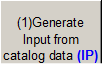
\includegraphics[width=0.9\textwidth, height=0.9\textheight, keepaspectratio=true]{media/image055.png}
\caption{Illustration for Surface Vertices \protect \label{fig:illustration-for-surface-vertices}}
\end{figure}

The figure above will help illustrate Surface Vertex entry. The convention used in ``\hyperref[globalgeometryrules]{GlobalGeometryRules}'' dictates the order of the vertices (ref: \hyperref[globalgeometryrules]{GlobalGeometryRules}). In this example, the conventions used are Starting Vertex Position = UpperLeftCorner and Vertex Entry Direction = CounterClockwise. The surfaces for this single zone are:

\begin{lstlisting}
4,0,0,H, 0,0,0, A,0,0, A,0,H; ! (4 vertices, South Wall)
4,A,0,H,A,0,0,A,B,0,A,B,H; ! (4 vertices, East Wall)
     ignore other walls that are not shown in this figure
4,C,0,J,A,0,H,A,B,H,C,B,J; ! (4 vertices, roof)
3,C,0,J,0,0,H,A,0,H; ! (3 vertices, gable end)
4,0,0,H, 0,0,0, A,0,0, A,0,H; ! (4 vertices, South Wall)
\end{lstlisting}

Note that in this example, point 1 of the entry is the Upper Left Corner of the rectangular surfaces and the point of the triangle for the 3 sided surface. The east wall shows the order of vertex entry. For horizontal surfaces, any vertex may be chosen as the starting position, but the Vertex Entry Direction convention must be followed. The surface details report (Output: Surfaces:List, Details;) is very useful for reviewing the accuracy of surface geometry inputs (ref: Surface Output Variables/Reports and Variable Dictionary Reports).

From the detailed vertices, EnergyPlus tries to determine the ``height'' and ``width'' of the surface. Obviously, this doesn't work well for \textgreater{}4 sided surfaces; for these, if the calculated height and width are not close to the gross area for the surface, the height and width shown will be the square root of the area (and thus a square).

\subsection{Building Surfaces - Detailed}\label{building-surfaces---detailed}

A building surface is necessary for all calculations. There must be at least one building surface per zone. You can use the detailed descriptions as shown below or the simpler, rectangular surface descriptions shown earlier.

\subsection{Wall:Detailed}\label{walldetailed}

The Wall:Detailed object is used to describe walls.

\subsubsection{Inputs}\label{inputs-20-007}

\paragraph{Field: Name}\label{field-name-16-010}

This is a unique name associated with each building surface. It is used in several other places as a reference (e.g.~as the base surface name for a Window or Door).

\paragraph{Field: Construction Name}\label{field-construction-name-16}

This is the name of the construction (ref: Construction object) used in the surface. Regardless of location in the building, the ``full'' construction (all layers) is used. For example, for an interior wall separating two zones, zone x would have the outside layer (e.g.~drywall) as the material that shows in zone y and then the layers to the inside layer -- the material that shows in zone x. For symmetric constructions, the same construction can be used in the surfaces described in both zones.

\paragraph{Field: Zone Name}\label{field-zone-name-10-000}

This is the zone name to which the surface belongs. This field is required.

\paragraph{Field: Space Name}\label{field-space-name-10-000}

This is the space name to which the surface belongs. If this field is left blank, it will be automatically assigned to a space named <Zone Name> or <Zone Name>-Remainder. See \hyperref[space]{Space} for more details.

\paragraph{Field: Outside Boundary Condition}\label{field-outside-boundary-condition}

This value can be one of several things depending on the actual kind of surface.

\begin{enumerate}
  \item
    \textbf{Surface} -- if this surface is an internal surface, then this is the choice. The value will either be a surface in the base zone or a surface in another zone. The heat balance between two zones can be accurately simulated by specifying a surface in an adjacent zone. EnergyPlus will simulate a group of zones simultaneously and will include the heat transfer between zones. However, as this increases the complexity of the calculations, it is not necessary to specify the other zone unless the two zones will have a significant temperature difference. If the two zones will not be very different (temperature wise), then the surface should use itself as the outside environment or specify this field as \textbf{Adiabatic}. The surface name on the ``outside'' of this surface (adjacent to) is placed in the next field.
  \item
    \textbf{Adiabatic} -- an internal surface in the same Zone. This surface will not transfer heat out of the zone, but will still store heat in thermal mass. Only the inside face of the surface will exchange heat with the zone (i.e.~two adiabatic surfaces are required to model internal partitions where both sides of the surface are exchanging heat with the zone). The Outside Boundary Condition Object can be left blank.
  \item
    \textbf{Zone} -- this is similar to Surface but EnergyPlus will automatically create the required surface in the adjacent zone when this is entered for the surface. If there are windows or doors on the surface, EnergyPlus automatically creates appropriate sub-surfaces as well.
  \item
    \textbf{Outdoors} -- if this surface is exposed to outside temperature conditions, then this is the choice. See Sun Exposure and Wind Exposure below for further specifications on this kind of surface.
  \item
    \textbf{Foundation} - uses an alternative model (currently only the Kiva\textsuperscript{TM} model) to account for the multi-dimensional heat transfer of foundation surfaces. The Outside Boundary Condition Object will refer to the name of a \hyperref[foundationkiva]{Foundation:Kiva} object (or be left blank to use the default foundation without extra insulation).
  \item
    \textbf{Ground} - The temperature on the outside of this surface will be the Site:GroundTemperature:Surface value for the month.
  \item
    \textbf{GroundFCfactorMethod} -- if this surface is exposed to the ground and using the \textbf{\hyperref[constructioncfactorundergroundwall]{Construction:CfactorUndergroundWall}}, then this is the choice. The temperature on the outside of this surface will be the Site:GroundTemperature:FcfactorMethod value for the month.
  \item
    \textbf{OtherSideCoefficients} -- if this surface has a custom, user specified temperature or other parameters (See \hyperref[surfacepropertyothersidecoefficients]{SurfaceProperty:OtherSideCoefficients} specification), then this is the choice. The outside boundary condition will be the name of the \hyperref[surfacepropertyothersidecoefficients]{SurfaceProperty:OtherSideCoefficients} specification.
  \item
    \textbf{OtherSideConditionsModel} -- if this surface has a specially-modeled multi-skin component, such as a transpired collector or vented photovoltaic panel, attached to the outside (See \hyperref[surfacepropertyothersideconditionsmodel]{SurfaceProperty:OtherSideConditionsModel} specification), then this the choice. The outside face environment will be the name of the \hyperref[surfacepropertyothersideconditionsmodel]{SurfaceProperty:OtherSideConditionsModel} specification.
  \item
    \textbf{GroundSlabPreprocessorAverage} -- uses the average results from the Slab preprocessor calculations.
  \item
    \textbf{GroundSlabPreprocessorCore} -- uses the core results from the Slab preprocessor calculations.
  \item
    \textbf{GroundSlabPreprocessorPerimeter} -- uses the perimeter results from the Slab preprocessor calculations.
  \item
    \textbf{GroundBasementPreprocessorAverageWall} -- uses the average wall results from the Basement preprocessor calculations.
  \item
    \textbf{GroundBasementPreprocessorAverageFloor} -- uses the average floor results from the Basement preprocessor calculations.
  \item
    \textbf{GroundBasementPreprocessorUpperWall} -- uses the upper wall results from the Basement preprocessor calculations.
  \item
    \textbf{GroundBasementPreprocessorLowerWall} -- uses the lower wall results from the Basement preprocessor calculations.
\end{enumerate}

\paragraph{Field: Outside Boundary Condition Object}\label{field-outside-boundary-condition-object-6}

If neither Surface, Zone, Foundation, OtherSideCoefficients, or OtherSideConditionsModel are specified for the Outside Boundary Condition (previous field), then this field should be left blank.

As stated above, if the Outside Boundary Condition is ``Surface'', then this field's value must be the surface name whose inside face temperature will be forced on the outside face of the base surface. This permits heat exchange between adjacent zones (interzone heat transfer) when multiple zones are simulated, but can also be used to simulate middle zone behavior without modeling the adjacent zones. This is done by specifying a surface within the zone. For example, a middle floor zone can be modeled by making the floor the Outside Boundary Condition Object for the ceiling, and the ceiling the Outside Boundary Condition Object for the floor.

If the Outside Boundary Condition is Zone, then this field should contain the zone name of the adjacent zone for the surface.

\begin{callout}
Note: Zones with interzone heat transfer are not adiabatic and the internal surfaces contribute to gains or losses. Adiabatic surfaces are modeled by specifying the base surface itself in this field. Also, for interzone heat transfer, both surfaces must be represented -- for example, if you want interzone heat transfer to an attic space, the ceiling in the lower zone must have a surface object with the outside face environment as the floor in the attic and, likewise, there must be a floor surface object in the attic that references the ceiling surface name in the lower zone.
\end{callout}

Equally, if the Outside Boundary Condition is ``OtherSideCoefficients'', then this field's value must be the \hyperref[surfacepropertyothersidecoefficients]{SurfaceProperty:OtherSideCoefficients} name. Or if the Outside Boundary Condition is ``OtherSideConditionsModel'' then this field's value must be the \hyperref[surfacepropertyothersideconditionsmodel]{SurfaceProperty:OtherSideConditionsModel} name.

\paragraph{Field: Sun Exposure}\label{field-sun-exposure-000}

If the surface is exposed to the sun, then ``SunExposed'' should be entered in this field. Otherwise, ``NoSun'' should be entered.

Note, a cantilevered floor could have ``Outdoors'' but ``NoSun'' exposure.

\paragraph{Field: Wind Exposure}\label{field-wind-exposure}

If the surface is exposed to the Wind, then ``WindExposed'' should be entered in this field. Otherwise, ``NoWind'' should be entered.

\begin{callout}
Note: When a surface is specified with ``NoWind'', this has several implications. Within the heat balance code, this surface will default to using the simple ASHRAE exterior convection coefficient correlation with a zero wind speed. In addition, since the ASHRAE simple method does not have a separate value for equivalent long wavelength radiation to the sky and ground, using ``NoWind'' also eliminates long wavelength radiant exchange from the exterior of the surface to both the sky and the ground. Thus, only simple convection takes place at the exterior face of a surface specified with ``NoWind''.
\end{callout}

\paragraph{Field: View Factor to Ground}\label{field-view-factor-to-ground}

The fraction of the ground plane (assumed horizontal) that is visible from a heat-transfer surface. It is used to calculate the diffuse solar radiation from the ground that is incident on the surface.

For example, if there are no obstructions, a vertical surface sees half of the ground plane and so View Factor to Ground = 0.5. A horizontal downward-facing surface sees the entire ground plane, so View Factor to Ground = 1.0. A horizontal upward-facing surface (horizontal roof) does not see the ground at all, so View Factor to Ground = 0.0.

Unused if reflections option in Solar Distribution field in Building object input unless a \hyperref[daylightingdeviceshelf]{DaylightingDevice:Shelf} or \hyperref[daylightingdevicetubular]{DaylightingDevice:Tubular} has been specified.

If you do not use the reflections option in the Solar Distribution field in your Building object input, you are responsible for entering the View Factor to Ground for each heat-transfer surface. Typical values for a surface that is not shadowed are obtained by the simple equation:

View Factor to Ground = (1-cos(SurfTilt))/2

For example, this gives 0.5 for a wall of tilt 90°. If the tilt of the wall changes, then the View Factor to Ground must also change.

If you enter \textbf{autocalculate} in this field, EnergyPlus will automatically calculate the view factor to ground based on the tilt of the surface.

If \textbf{you do use the reflections option in the Solar Distribution field} in your Building object input, you do \textbf{not} have to enter View Factor to Ground values. In this case the program will automatically calculate the value to use for each exterior surface taking into account solar shadowing (including shadowing of the ground by the building) and reflections from obstructions (ref: Building, Field: Solar Distribution).

However, if you do use the reflections option AND you are modeling a \hyperref[daylightingdeviceshelf]{DaylightingDevice:Shelf} or \hyperref[daylightingdevicetubular]{DaylightingDevice:Tubular}, then you still need to enter some values of View Factor to Ground. For \hyperref[daylightingdeviceshelf]{DaylightingDevice:Shelf} you need to enter View Factor to Ground for the window associated with the shelf. And for \hyperref[daylightingdevicetubular]{DaylightingDevice:Tubular} you need to enter the View Factor to Ground for the \hyperref[fenestrationsurfacedetailed]{FenestrationSurface:Detailed} corresponding to the dome of the tubular device.

Note 1: The corresponding view factor to the sky for diffuse solar radiation is not a user input; it is calculated within EnergyPlus based on surface orientation, sky solar radiance distribution, and shadowing surfaces.

Note 2: The view factors to the sky and ground for thermal infrared (long-wave) radiation are not user inputs; they are calculated within EnergyPlus based on surface tilt and shadowing surfaces. Shadowing surfaces are considered to have the same emissivity and temperature as the ground, so they are lumped together with the ground in calculating the ground IR view factor.

\paragraph{Field: Number of Vertices}\label{field-number-of-vertices}

This field specifies the number of sides in the surface (number of X,Y,Z vertex groups). For further information, see the discussion on ``Surface Vertices'' above.

\subsection{RoofCeiling:Detailed}\label{roofceilingdetailed}

The RoofCeiling:Detailed object is used to describe a roof or ceiling.

\subsubsection{Inputs}\label{inputs-21-007}

\paragraph{Field: Name}\label{field-name-17-008}

This is a unique name associated with each building surface. It is used in several other places as a reference (e.g.~as the base surface name for a Window or Door).

\paragraph{Field: Construction Name}\label{field-construction-name-17}

This is the name of the construction (ref: Construction object) used in the surface. Regardless of location in the building, the ``full'' construction (all layers) is used. For example, for an interior wall separating two zones, zone x would have the outside layer (e.g.~drywall) as the material that shows in zone y and then the layers to the inside layer -- the material that shows in zone x. For symmetric constructions, the same construction can be used in the surfaces described in both zones.

\paragraph{Field: Zone Name}\label{field-zone-name-11-000}

This is the zone name to which the surface belongs. This field is required.

\paragraph{Field: Space Name}\label{field-space-name-11-000}

This is the space name to which the surface belongs. If this field is left blank, it will be automatically assigned to a space named <Zone Name> or <Zone Name>-Remainder. See \hyperref[space]{Space} for more details.

\paragraph{Field: Outside Boundary Condition}\label{field-outside-boundary-condition-1}

This value can be one of several things depending on the actual kind of surface.

\begin{enumerate}
  \item
    \textbf{Surface} -- if this surface is an internal surface, then this is the choice. The value will either be a surface in the base zone or a surface in another zone. The heat balance between two zones can be accurately simulated by specifying a surface in an adjacent zone. EnergyPlus will simulate a group of zones simultaneously and will include the heat transfer between zones. However, as this increases the complexity of the calculations, it is not necessary to specify the other zone unless the two zones will have a significant temperature difference. If the two zones will not be very different (temperature wise), then the surface should use itself as the outside environment or specify this field as \textbf{Adiabatic}. The surface name on the ``outside'' of this surface (adjacent to) is placed in the next field.
  \item
    \textbf{Adiabatic} -- an internal surface in the same Zone. This surface will not transfer heat out of the zone, but will still store heat in thermal mass. Only the inside face of the surface will exchange heat with the zone (i.e.~two adiabatic surfaces are required to model internal partitions where both sides of the surface are exchanging heat with the zone). The Outside Boundary Condition Object can be left blank.
  \item
    \textbf{Zone} -- this is similar to Surface but EnergyPlus will automatically create the required surface in the adjacent zone when this is entered for the surface. If there are windows or doors on the surface, EnergyPlus automatically creates appropriate sub-surfaces as well.
  \item
    \textbf{Outdoors} -- if this surface is exposed to outside temperature conditions, then this is the choice. See Sun Exposure and Wind Exposure below for further specifications on this kind of surface.
  \item
    \textbf{Ground} -- The temperature on the outside of this surface will be the Ground Temperature.
  \item
    \textbf{OtherSideCoefficients} -- if this surface has a custom, user specified temperature or other parameters (See \hyperref[surfacepropertyothersidecoefficients]{SurfaceProperty:OtherSideCoefficients} specification), then this is the choice. The outside boundary condition will be the name of the \hyperref[surfacepropertyothersidecoefficients]{SurfaceProperty:OtherSideCoefficients} specification.
  \item
    \textbf{OtherSideConditionsModel} -- if this surface has a specially-modeled multi-skin component, such as a transpired collector or vented photovoltaic panel, attached to the outside (See \hyperref[surfacepropertyothersideconditionsmodel]{SurfaceProperty:OtherSideConditionsModel} specification), then this the choice. The outside face environment will be the name of the \hyperref[surfacepropertyothersideconditionsmodel]{SurfaceProperty:OtherSideConditionsModel} specification.
  \item
    \textbf{GroundSlabPreprocessorAverage} -- uses the average results from the Slab preprocessor calculations.
  \item
    \textbf{GroundSlabPreprocessorCore} -- uses the core results from the Slab preprocessor calculations.
  \item
    \textbf{GroundSlabPreprocessorPerimeter} -- uses the perimeter results from the Slab preprocessor calculations.
  \item
    \textbf{GroundBasementPreprocessorAverageWall} -- uses the average wall results from the Basement preprocessor calculations.
  \item
    \textbf{GroundBasementPreprocessorAverageFloor} -- uses the average floor results from the Basement preprocessor calculations.
  \item
    \textbf{GroundBasementPreprocessorUpperWall} -- uses the upper wall results from the Basement preprocessor calculations.
  \item
    \textbf{GroundBasementPreprocessorLowerWall} -- uses the lower wall results from the Basement preprocessor calculations.
\end{enumerate}

\paragraph{Field: Outside Boundary Condition Object}\label{field-outside-boundary-condition-object-7}

If neither Surface, Zone, Foundation, OtherSideCoefficients, or OtherSideConditionsModel are specified for the Outside Boundary Condition (previous field), then this field should be left blank.

As stated above, if the Outside Boundary Condition is ``Surface'', then this field's value must be the surface name whose inside face temperature will be forced on the outside face of the base surface. This permits heat exchange between adjacent zones (interzone heat transfer) when multiple zones are simulated, but can also be used to simulate middle zone behavior without modeling the adjacent zones. This is done by specifying a surface within the zone. For example, a middle floor zone can be modeled by making the floor the Outside Boundary Condition Object for the ceiling, and the ceiling the Outside Boundary Condition Object for the floor.

If the Outside Boundary Condition is Zone, then this field should contain the zone name of the adjacent zone for the surface.

\begin{callout}
Note: Zones with interzone heat transfer are not adiabatic and the internal surfaces contribute to gains or losses. Adiabatic surfaces are modeled by specifying the base surface itself in this field. Also, for interzone heat transfer, both surfaces must be represented -- for example, if you want interzone heat transfer to an attic space, the ceiling in the lower zone must have a surface object with the outside face environment as the floor in the attic and, likewise, there must be a floor surface object in the attic that references the ceiling surface name in the lower zone.
\end{callout}

Equally, if the Outside Boundary Condition is ``OtherSideCoefficients'', then this field's value must be the \hyperref[surfacepropertyothersidecoefficients]{SurfaceProperty:OtherSideCoefficients} name. Or if the Outside Boundary Condition is ``OtherSideConditionsModel'' then this field's value must be the \hyperref[surfacepropertyothersideconditionsmodel]{SurfaceProperty:OtherSideConditionsModel} name.

\paragraph{Field: Sun Exposure}\label{field-sun-exposure-1}

If the surface is exposed to the sun, then ``SunExposed'' should be entered in this field. Otherwise, ``NoSun'' should be entered.

Note, a cantilevered floor could have ``Outdoors'' but ``NoSun'' exposure.

\paragraph{Field: Wind Exposure}\label{field-wind-exposure-1}

If the surface is exposed to the Wind, then ``WindExposed'' should be entered in this field. Otherwise, ``NoWind'' should be entered.

\begin{callout}
Note: When a surface is specified with ``NoWind'', this has several implications. Within the heat balance code, this surface will default to using the simple ASHRAE exterior convection coefficient correlation with a zero wind speed. In addition, since the ASHRAE simple method does not have a separate value for equivalent long wavelength radiation to the sky and ground, using ``NoWind'' also eliminates long wavelength radiant exchange from the exterior of the surface to both the sky and the ground. Thus, only simple convection takes place at the exterior face of a surface specified with ``NoWind''.
\end{callout}

\paragraph{Field: View Factor to Ground}\label{field-view-factor-to-ground-1}

The fraction of the ground plane (assumed horizontal) that is visible from a heat-transfer surface. It is used to calculate the diffuse solar radiation from the ground that is incident on the surface.

For example, if there are no obstructions, a vertical surface sees half of the ground plane and so View Factor to Ground = 0.5. A horizontal downward-facing surface sees the entire ground plane, so View Factor to Ground = 1.0. A horizontal upward-facing surface (horizontal roof) does not see the ground at all, so View Factor to Ground = 0.0.

Unused if reflections option in Solar Distribution field in Building object input unless a \hyperref[daylightingdeviceshelf]{DaylightingDevice:Shelf} or \hyperref[daylightingdevicetubular]{DaylightingDevice:Tubular} has been specified.

If you do not use the reflections option in the Solar Distribution field in your Building object input, you are responsible for entering the View Factor to Ground for each heat-transfer surface. Typical values for a surface that is not shadowed are obtained by the simple equation:

View Factor to Ground = (1-cos(SurfTilt))/2

For example, this gives 0.5 for a wall of tilt 90°. If the tilt of the wall changes, then the View Factor to Ground must also change.

If you enter \textbf{autocalculate} in this field, EnergyPlus will automatically calculate the view factor to ground based on the tilt of the surface.

If \textbf{you do use the reflections option in the Solar Distribution field} in your Building object input, you do \textbf{not} have to enter View Factor to Ground values. In this case the program will automatically calculate the value to use for each exterior surface taking into account solar shadowing (including shadowing of the ground by the building) and reflections from obstructions (ref: Building, Field: Solar Distribution).

However, if you do use the reflections option AND you are modeling a \hyperref[daylightingdeviceshelf]{DaylightingDevice:Shelf} or \hyperref[daylightingdevicetubular]{DaylightingDevice:Tubular}, then you still need to enter some values of View Factor to Ground. For \hyperref[daylightingdeviceshelf]{DaylightingDevice:Shelf} you need to enter View Factor to Ground for the window associated with the shelf. And for \hyperref[daylightingdevicetubular]{DaylightingDevice:Tubular} you need to enter the View Factor to Ground for the \hyperref[fenestrationsurfacedetailed]{FenestrationSurface:Detailed} corresponding to the dome of the tubular device.

Note 1: The corresponding view factor to the sky for diffuse solar radiation is not a user input; it is calculated within EnergyPlus based on surface orientation, sky solar radiance distribution, and shadowing surfaces.

Note 2: The view factors to the sky and ground for thermal infrared (long-wave) radiation are not user inputs; they are calculated within EnergyPlus based on surface tilt and shadowing surfaces. Shadowing surfaces are considered to have the same emissivity and temperature as the ground, so they are lumped together with the ground in calculating the ground IR view factor.

\paragraph{Field: Number of Vertices}\label{field-number-of-vertices-1}

This field specifies the number of sides in the surface (number of X,Y,Z vertex groups). For further information, see the discussion on ``Surface Vertices'' above.

\subsection{Floor:Detailed}\label{floordetailed}

The Floor:Detailed object is used to describe floors.

\subsubsection{Inputs}\label{inputs-22-006}

\paragraph{Field: Name}\label{field-name-18-008}

This is a unique name associated with each building surface. It is used in several other places as a reference (e.g.~as the base surface name for a Window or Door).

\paragraph{Field: Construction Name}\label{field-construction-name-18}

This is the name of the construction (ref: Construction object) used in the surface. Regardless of location in the building, the ``full'' construction (all layers) is used. For example, for an interior wall separating two zones, zone x would have the outside layer (e.g.~drywall) as the material that shows in zone y and then the layers to the inside layer -- the material that shows in zone x. For symmetric constructions, the same construction can be used in the surfaces described in both zones.

\paragraph{Field: Zone Name}\label{field-zone-name-12-000}

This is the zone name to which the surface belongs. This field is required.

\paragraph{Field: Space Name}\label{field-space-name-12-000}

This is the space name to which the surface belongs. If this field is left blank, it will be automatically assigned to a space named <Zone Name> or <Zone Name>-Remainder. See \hyperref[space]{Space} for more details.

\paragraph{Field: Outside Boundary Condition}\label{field-outside-boundary-condition-2}

This value can be one of several things depending on the actual kind of surface.

\begin{enumerate}
  \item
    \textbf{Surface} -- if this surface is an internal surface, then this is the choice. The value will either be a surface in the base zone or a surface in another zone. The heat balance between two zones can be accurately simulated by specifying a surface in an adjacent zone. EnergyPlus will simulate a group of zones simultaneously and will include the heat transfer between zones. However, as this increases the complexity of the calculations, it is not necessary to specify the other zone unless the two zones will have a significant temperature difference. If the two zones will not be very different (temperature wise), then the surface should use itself as the outside environment or specify this field as \textbf{Adiabatic}. The surface name on the ``outside'' of this surface (adjacent to) is placed in the next field.
  \item
    \textbf{Adiabatic} -- an internal surface in the same Zone. This surface will not transfer heat out of the zone, but will still store heat in thermal mass. Only the inside face of the surface will exchange heat with the zone (i.e.~two adiabatic surfaces are required to model internal partitions where both sides of the surface are exchanging heat with the zone). The Outside Boundary Condition Object can be left blank.
  \item
    \textbf{Zone} -- this is similar to Surface but EnergyPlus will automatically create the required surface in the adjacent zone when this is entered for the surface. If there are windows or doors on the surface, EnergyPlus automatically creates appropriate sub-surfaces as well.
  \item
    \textbf{Outdoors} -- if this surface is exposed to outside temperature conditions, then this is the choice. See Sun Exposure and Wind Exposure below for further specifications on this kind of surface.
  \item
    \textbf{Foundation} - uses an alternative model (currently only the Kiva\textsuperscript{TM} model) to account for the multi-dimensional heat transfer of foundation surfaces. The Outside Boundary Condition Object will refer to the name of a \hyperref[foundationkiva]{Foundation:Kiva} object (or be left blank to use the default foundation without extra insulation).
  \item
    \textbf{Ground} - The temperature on the outside of this surface will be the Site:GroundTemperature:Surface value for the month..
  \item
    \textbf{GroundFCfactorMethod} -- if this surface is exposed to the ground and using the \textbf{\hyperref[constructioncfactorundergroundwall]{Construction:CfactorUndergroundWall}}, then this is the choice. The temperature on the outside of this surface will be the Site:GroundTemperature:FcfactorMethod value for the month.
  \item
    \textbf{OtherSideCoefficients} -- if this surface has a custom, user specified temperature or other parameters (See \hyperref[surfacepropertyothersidecoefficients]{SurfaceProperty:OtherSideCoefficients} specification), then this is the choice. The outside boundary condition will be the name of the \hyperref[surfacepropertyothersidecoefficients]{SurfaceProperty:OtherSideCoefficients} specification.
  \item
    \textbf{OtherSideConditionsModel} -- if this surface has a specially-modeled multi-skin component, such as a transpired collector or vented photovoltaic panel, attached to the outside (See \hyperref[surfacepropertyothersideconditionsmodel]{SurfaceProperty:OtherSideConditionsModel} specification), then this the choice. The outside face environment will be the name of the \hyperref[surfacepropertyothersideconditionsmodel]{SurfaceProperty:OtherSideConditionsModel} specification.
  \item
    \textbf{GroundSlabPreprocessorAverage} -- uses the average results from the Slab preprocessor calculations.
  \item
    \textbf{GroundSlabPreprocessorCore} -- uses the core results from the Slab preprocessor calculations.
  \item
    \textbf{GroundSlabPreprocessorPerimeter} -- uses the perimeter results from the Slab preprocessor calculations.
  \item
    \textbf{GroundBasementPreprocessorAverageWall} -- uses the average wall results from the Basement preprocessor calculations.
  \item
    \textbf{GroundBasementPreprocessorAverageFloor} -- uses the average floor results from the Basement preprocessor calculations.
  \item
    \textbf{GroundBasementPreprocessorUpperWall} -- uses the upper wall results from the Basement preprocessor calculations.
  \item
    \textbf{GroundBasementPreprocessorLowerWall} -- uses the lower wall results from the Basement preprocessor calculations.
\end{enumerate}

\paragraph{Field: Outside Boundary Condition Object}\label{field-outside-boundary-condition-object-8}

If neither Surface, Zone, Foundation, OtherSideCoefficients, or OtherSideConditionsModel are specified for the Outside Boundary Condition (previous field), then this field should be left blank.

As stated above, if the Outside Boundary Condition is ``Surface'', then this field's value must be the surface name whose inside face temperature will be forced on the outside face of the base surface. This permits heat exchange between adjacent zones (interzone heat transfer) when multiple zones are simulated, but can also be used to simulate middle zone behavior without modeling the adjacent zones. This is done by specifying a surface within the zone. For example, a middle floor zone can be modeled by making the floor the Outside Boundary Condition Object for the ceiling, and the ceiling the Outside Boundary Condition Object for the floor.

If the Outside Boundary Condition is Zone, then this field should contain the zone name of the adjacent zone for the surface.

\begin{callout}
Note: Zones with interzone heat transfer are not adiabatic and the internal surfaces contribute to gains or losses. Adiabatic surfaces are modeled by specifying the base surface itself in this field. Also, for interzone heat transfer, both surfaces must be represented -- for example, if you want interzone heat transfer to an attic space, the ceiling in the lower zone must have a surface object with the outside face environment as the floor in the attic and, likewise, there must be a floor surface object in the attic that references the ceiling surface name in the lower zone.
\end{callout}

Equally, if the Outside Boundary Condition is ``OtherSideCoefficients'', then this field's value must be the \hyperref[surfacepropertyothersidecoefficients]{SurfaceProperty:OtherSideCoefficients} name. Or if the Outside Boundary Condition is ``OtherSideConditionsModel'' then this field's value must be the \hyperref[surfacepropertyothersideconditionsmodel]{SurfaceProperty:OtherSideConditionsModel} name.

\paragraph{Field: Sun Exposure}\label{field-sun-exposure-2}

If the surface is exposed to the sun, then ``SunExposed'' should be entered in this field. Otherwise, ``NoSun'' should be entered.

Note, a cantilevered floor could have ``Outdoors'' but ``NoSun'' exposure.

\paragraph{Field: Wind Exposure}\label{field-wind-exposure-2}

If the surface is exposed to the Wind, then ``WindExposed'' should be entered in this field. Otherwise, ``NoWind'' should be entered.

\begin{callout}
Note: When a surface is specified with ``NoWind'', this has several implications. Within the heat balance code, this surface will default to using the simple ASHRAE exterior convection coefficient correlation with a zero wind speed. In addition, since the ASHRAE simple method does not have a separate value for equivalent long wavelength radiation to the sky and ground, using ``NoWind'' also eliminates long wavelength radiant exchange from the exterior of the surface to both the sky and the ground. Thus, only simple convection takes place at the exterior face of a surface specified with ``NoWind''.
\end{callout}

\paragraph{Field: View Factor to Ground}\label{field-view-factor-to-ground-2}

The fraction of the ground plane (assumed horizontal) that is visible from a heat-transfer surface. It is used to calculate the diffuse solar radiation from the ground that is incident on the surface.

For example, if there are no obstructions, a vertical surface sees half of the ground plane and so View Factor to Ground = 0.5. A horizontal downward-facing surface sees the entire ground plane, so View Factor to Ground = 1.0. A horizontal upward-facing surface (horizontal roof) does not see the ground at all, so View Factor to Ground = 0.0.

Unused if reflections option in Solar Distribution field in Building object input unless a \hyperref[daylightingdeviceshelf]{DaylightingDevice:Shelf} or \hyperref[daylightingdevicetubular]{DaylightingDevice:Tubular} has been specified.

If you do not use the reflections option in the Solar Distribution field in your Building object input, you are responsible for entering the View Factor to Ground for each heat-transfer surface. Typical values for a surface that is not shadowed are obtained by the simple equation:

View Factor to Ground = (1-cos(SurfTilt))/2

For example, this gives 0.5 for a wall of tilt 90°. If the tilt of the wall changes, then the View Factor to Ground must also change.

If you enter \textbf{autocalculate} in this field, EnergyPlus will automatically calculate the view factor to ground based on the tilt of the surface.

If \textbf{you do use the reflections option in the Solar Distribution field} in your Building object input, you do \textbf{not} have to enter View Factor to Ground values. In this case the program will automatically calculate the value to use for each exterior surface taking into account solar shadowing (including shadowing of the ground by the building) and reflections from obstructions (ref: Building, Field: Solar Distribution).

However, if you do use the reflections option AND you are modeling a \hyperref[daylightingdeviceshelf]{DaylightingDevice:Shelf} or \hyperref[daylightingdevicetubular]{DaylightingDevice:Tubular}, then you still need to enter some values of View Factor to Ground. For \hyperref[daylightingdeviceshelf]{DaylightingDevice:Shelf} you need to enter View Factor to Ground for the window associated with the shelf. And for \hyperref[daylightingdevicetubular]{DaylightingDevice:Tubular} you need to enter the View Factor to Ground for the \hyperref[fenestrationsurfacedetailed]{FenestrationSurface:Detailed} corresponding to the dome of the tubular device.

Note 1: The corresponding view factor to the sky for diffuse solar radiation is not a user input; it is calculated within EnergyPlus based on surface orientation, sky solar radiance distribution, and shadowing surfaces.

Note 2: The view factors to the sky and ground for thermal infrared (long-wave) radiation are not user inputs; they are calculated within EnergyPlus based on surface tilt and shadowing surfaces. Shadowing surfaces are considered to have the same emissivity and temperature as the ground, so they are lumped together with the ground in calculating the ground IR view factor.

\paragraph{Field: Number of Vertices}\label{field-number-of-vertices-2}

This field specifies the number of sides in the surface (number of X,Y,Z vertex groups). For further information, see the discussion on ``Surface Vertices'' above.

Some examples of using these objects:

\begin{lstlisting}

Floor:Detailed,
      Floor_NorthZone_1stFloor,!- Name
      FLOOR-SLAB-ASSEMBLY,     !- Construction Name
      NorthZone_1stFloor,      !- Zone Name
      Ground,                  !- Outside Boundary Condition
      ,                        !- Outside Boundary Condition Object
      NoSun,                   !- Sun Exposure
      NoWind,                  !- Wind Exposure
      0.0,                     !- View Factor to Ground
      4,                       !- Number of Vertices
      0, 11, 0,                           !- X,Y,Z  1 {m}
      25, 11, 0,                          !- X,Y,Z  2 {m}
      25, 5.5, 0,                         !- X,Y,Z  3 {m}
     0, 5.5, 0;                          !- X,Y,Z  4 {m}

  RoofCeiling:Detailed,
      Ceiling_SouthZone_1stFloor,  !- Name
      CEILING-FLOOR-ASSEMBLY,  !- Construction Name
      SouthZone_1stFloor,      !- Zone Name
      Surface,                 !- Outside Boundary Condition
      Floor_SouthZone_2ndFloor,!- Outside Boundary Condition Object
      NoSun,                   !- Sun Exposure
      NoWind,                  !- Wind Exposure
      0.0,                     !- View Factor to Ground
      4,                       !- Number of Vertices
      0, 0, 3.4,                          !- X,Y,Z  1 {m}
      25, 0, 3.4,                         !- X,Y,Z  2 {m}
      25, 5.5, 3.4,                       !- X,Y,Z  3 {m}
     0, 5.5, 3.4;                        !- X,Y,Z  4 {m}

  Wall:Detailed,
      InteriorWall_SouthZone_1stFloor,  !- Name
      INTERIOR-WALL-ASSEMBLY,  !- Construction Name
      SouthZone_1stFloor,      !- Zone Name
      Surface,                 !- Outside Boundary Condition
      InteriorWall_NorthZone_1stFloor,  !- Outside Boundary Condition Object
      NoSun,                   !- Sun Exposure
      NoWind,                  !- Wind Exposure
      0,                       !- View Factor to Ground
      4,                       !- Number of Vertices
      25, 5.5, 3.7,                       !- X,Y,Z  1 {m}
      25, 5.5, 0,                         !- X,Y,Z  2 {m}
      0, 5.5, 0,                          !- X,Y,Z  3 {m}
     0, 5.5, 3.7;                        !- X,Y,Z  4 {m}
\end{lstlisting}

\subsection{BuildingSurface:Detailed}\label{buildingsurfacedetailed}

The BuildingSurface:Detailed object can more generally describe each of the surfaces.

\subsubsection{Inputs}\label{inputs-23-006}

\paragraph{Field: Name}\label{field-name-19-005}

This is a unique name associated with each building surface. It is used in several other places as a reference (e.g.~as the base surface name for a Window or Door).

\paragraph{Field: Surface Type}\label{field-surface-type-000}

Used primarily for convenience, the surface type can be one of the choices illustrated above -- Wall, Floor, Ceiling, Roof. Azimuth (facing) and Tilt are determined from the vertex coordinates. Note that ``normal'' floors will be tilted 180° whereas flat roofs/ceilings will be tilted 0°. EnergyPlus uses this field's designation, along with the calculated tilt of the surface, to issue warning messages when tilts are ``out of range''. Calculations in EnergyPlus use the actual calculated tilt values for the actual heat balance calculations. Note, however, that a floor tilted 0° is really facing ``into'' the zone and is not what you will desire for the calculations even though the coordinate may appear correct in the viewed DXF display.

``Normal'' tilt for walls is 90° -- here you may use the calculated Azimuth to make sure your walls are facing away from the zone's interior.

\paragraph{Field: Construction Name}\label{field-construction-name-19}

This is the name of the construction (ref: Construction object) used in the surface. Regardless of location in the building, the ``full'' construction (all layers) is used. For example, for an interior wall separating two zones, zone x would have the outside layer (e.g.~drywall) as the material that shows in zone y and then the layers to the inside layer -- the material that shows in zone x. For symmetric constructions, the same construction can be used in the surfaces described in both zones.

\paragraph{Field: Zone Name}\label{field-zone-name-13}

This is the zone name to which the surface belongs. This field is required.

\paragraph{Field: Space Name}\label{field-space-name-13}

This is the space name to which the surface belongs. If this field is left blank, it will be automatically assigned to a space name <Zone Name> or <Zone Name>-Remainder. See \hyperref[space]{Space} for more details.

\paragraph{Field: Outside Boundary Condition}\label{field-outside-boundary-condition-3}

This value can be one of several things depending on the actual kind of surface.

\begin{enumerate}
  \item
    \textbf{Surface} -- if this surface is an internal surface, then this is the choice. The value will either be a surface in the base zone or a surface in another zone. The heat balance between two zones can be accurately simulated by specifying a surface in an adjacent zone. EnergyPlus will simulate a group of zones simultaneously and will include the heat transfer between zones. However, as this increases the complexity of the calculations, it is not necessary to specify the other zone unless the two zones will have a significant temperature difference. If the two zones will not be very different (temperature wise), then the surface should use itself as the outside environment or specify this field as \textbf{Adiabatic}. The surface name on the ``outside'' of this surface (adjacent to) is placed in the next field.
  \item
    \textbf{Adiabatic} -- an internal surface in the same Zone. This surface will not transfer heat out of the zone, but will still store heat in thermal mass. Only the inside face of the surface will exchange heat with the zone (i.e.~two adiabatic surfaces are required to model internal partitions where both sides of the surface are exchanging heat with the zone). The Outside Boundary Condition Object can be left blank.
  \item
    \textbf{Zone} -- this is similar to Surface but EnergyPlus will automatically create the required surface in the adjacent zone when this is entered for the surface. If there are windows or doors on the surface, EnergyPlus automatically creates appropriate sub-surfaces as well.
  \item
    \textbf{Outdoors} -- if this surface is exposed to outside temperature conditions, then this is the choice. See Sun Exposure and Wind Exposure below for further specifications on this kind of surface.
  \item
    \textbf{Foundation} - uses an alternative model (currently only the Kiva\textsuperscript{TM} model) to account for the multi-dimensional heat transfer of foundation surfaces. The Outside Boundary Condition Object will refer to the name of a \hyperref[foundationkiva]{Foundation:Kiva} object (or be left blank to use the default foundation without extra insulation).
  \item
    \textbf{Ground} - The temperature on the outside of this surface will be the Site:GroundTemperature:Surface value for the month.
  \item
    \textbf{GroundFCfactorMethod} -- if this surface is exposed to the ground and using the \textbf{\hyperref[constructioncfactorundergroundwall]{Construction:CfactorUndergroundWall}}, then this is the choice. The temperature on the outside of this surface will be the Site:GroundTemperature:FcfactorMethod value for the month.
  \item
    \textbf{OtherSideCoefficients} -- if this surface has a custom, user specified temperature or other parameters (See \hyperref[surfacepropertyothersidecoefficients]{SurfaceProperty:OtherSideCoefficients} specification), then this is the choice. The outside boundary condition will be the name of the \hyperref[surfacepropertyothersidecoefficients]{SurfaceProperty:OtherSideCoefficients} specification.
  \item
    \textbf{OtherSideConditionsModel} -- if this surface has a specially-modeled multi-skin component, such as a transpired collector or vented photovoltaic panel, attached to the outside (See \hyperref[surfacepropertyothersideconditionsmodel]{SurfaceProperty:OtherSideConditionsModel} specification), then this the choice. The outside face environment will be the name of the \hyperref[surfacepropertyothersideconditionsmodel]{SurfaceProperty:OtherSideConditionsModel} specification.
  \item
    \textbf{GroundSlabPreprocessorAverage} -- uses the average results from the Slab preprocessor calculations.
  \item
    \textbf{GroundSlabPreprocessorCore} -- uses the core results from the Slab preprocessor calculations.
  \item
    \textbf{GroundSlabPreprocessorPerimeter} -- uses the perimeter results from the Slab preprocessor calculations.
  \item
    \textbf{GroundBasementPreprocessorAverageWall} -- uses the average wall results from the Basement preprocessor calculations.
  \item
    \textbf{GroundBasementPreprocessorAverageFloor} -- uses the average floor results from the Basement preprocessor calculations.
  \item
    \textbf{GroundBasementPreprocessorUpperWall} -- uses the upper wall results from the Basement preprocessor calculations.
  \item
    \textbf{GroundBasementPreprocessorLowerWall} -- uses the lower wall results from the Basement preprocessor calculations.
\end{enumerate}

\paragraph{Field: Outside Boundary Condition Object}\label{field-outside-boundary-condition-object-9}

If neither Surface, Zone, Foundation, OtherSideCoefficients, or OtherSideConditionsModel are specified for the Outside Boundary Condition (previous field), then this field should be left blank.

As stated above, if the Outside Boundary Condition is ``Surface'', then this field's value must be the surface name whose inside face temperature will be forced on the outside face of the base surface. This permits heat exchange between adjacent zones (interzone heat transfer) when multiple zones are simulated, but can also be used to simulate middle zone behavior without modeling the adjacent zones. This is done by specifying a surface within the zone. For example, a middle floor zone can be modeled by making the floor the Outside Boundary Condition Object for the ceiling, and the ceiling the Outside Boundary Condition Object for the floor.

If the Outside Boundary Condition is Zone, then this field should contain the zone name of the adjacent zone for the surface.

\begin{callout}
Note: Zones with interzone heat transfer are not adiabatic and the internal surfaces contribute to gains or losses. Adiabatic surfaces are modeled by specifying the base surface itself in this field. Also, for interzone heat transfer, both surfaces must be represented -- for example, if you want interzone heat transfer to an attic space, the ceiling in the lower zone must have a surface object with the outside face environment as the floor in the attic and, likewise, there must be a floor surface object in the attic that references the ceiling surface name in the lower zone.
\end{callout}

Equally, if the Outside Boundary Condition is ``OtherSideCoefficients'', then this field's value must be the \hyperref[surfacepropertyothersidecoefficients]{SurfaceProperty:OtherSideCoefficients} name. Or if the Outside Boundary Condition is ``OtherSideConditionsModel'' then this field's value must be the \hyperref[surfacepropertyothersideconditionsmodel]{SurfaceProperty:OtherSideConditionsModel} name.

\paragraph{Field: Sun Exposure}\label{field-sun-exposure-3}

If the surface is exposed to the sun, then ``SunExposed'' should be entered in this field. Otherwise, ``NoSun'' should be entered.

Note, a cantilevered floor could have ``Outdoors'' but ``NoSun'' exposure.

\paragraph{Field: Wind Exposure}\label{field-wind-exposure-3}

If the surface is exposed to the Wind, then ``WindExposed'' should be entered in this field. Otherwise, ``NoWind'' should be entered.

\begin{callout}
Note: When a surface is specified with ``NoWind'', this has several implications. Within the heat balance code, this surface will default to using the simple ASHRAE exterior convection coefficient correlation with a zero wind speed. In addition, since the ASHRAE simple method does not have a separate value for equivalent long wavelength radiation to the sky and ground, using ``NoWind'' also eliminates long wavelength radiant exchange from the exterior of the surface to both the sky and the ground. Thus, only simple convection takes place at the exterior face of a surface specified with ``NoWind''.
\end{callout}

\paragraph{Field: View Factor to Ground}\label{field-view-factor-to-ground-3}

The fraction of the ground plane (assumed horizontal) that is visible from a heat-transfer surface. It is used to calculate the diffuse solar radiation from the ground that is incident on the surface.

For example, if there are no obstructions, a vertical surface sees half of the ground plane and so View Factor to Ground = 0.5. A horizontal downward-facing surface sees the entire ground plane, so View Factor to Ground = 1.0. A horizontal upward-facing surface (horizontal roof) does not see the ground at all, so View Factor to Ground = 0.0.

Unused if reflections option in Solar Distribution field in Building object input unless a \hyperref[daylightingdeviceshelf]{DaylightingDevice:Shelf} or \hyperref[daylightingdevicetubular]{DaylightingDevice:Tubular} has been specified.

If you do not use the reflections option in the Solar Distribution field in your Building object input, you are responsible for entering the View Factor to Ground for each heat-transfer surface. Typical values for a surface that is not shadowed are obtained by the simple equation:

View Factor to Ground = (1-cos(SurfTilt))/2

For example, this gives 0.5 for a wall of tilt 90°. If the tilt of the wall changes, then the View Factor to Ground must also change.

If you enter \textbf{autocalculate} in this field, EnergyPlus will automatically calculate the view factor to ground based on the tilt of the surface.

If \textbf{you do use the reflections option in the Solar Distribution field} in your Building object input, you do \textbf{not} have to enter View Factor to Ground values. In this case the program will automatically calculate the value to use for each exterior surface taking into account solar shadowing (including shadowing of the ground by the building) and reflections from obstructions (ref: Building, Field: Solar Distribution).

However, if you do use the reflections option AND you are modeling a \hyperref[daylightingdeviceshelf]{DaylightingDevice:Shelf} or \hyperref[daylightingdevicetubular]{DaylightingDevice:Tubular}, then you still need to enter some values of View Factor to Ground. For \hyperref[daylightingdeviceshelf]{DaylightingDevice:Shelf} you need to enter View Factor to Ground for the window associated with the shelf. And for \hyperref[daylightingdevicetubular]{DaylightingDevice:Tubular} you need to enter the View Factor to Ground for the \hyperref[fenestrationsurfacedetailed]{FenestrationSurface:Detailed} corresponding to the dome of the tubular device.

Note 1: The corresponding view factor to the sky for diffuse solar radiation is not a user input; it is calculated within EnergyPlus based on surface orientation, sky solar radiance distribution, and shadowing surfaces.

Note 2: The view factors to the sky and ground for thermal infrared (long-wave) radiation are not user inputs; they are calculated within EnergyPlus based on surface tilt and shadowing surfaces. Shadowing surfaces are considered to have the same emissivity and temperature as the ground, so they are lumped together with the ground in calculating the ground IR view factor.

\paragraph{Field: Number of Vertices}\label{field-number-of-vertices-3}

This field specifies the number of sides in the surface (number of X,Y,Z vertex groups). For further information, see the discussion on ``Surface Vertices'' above.

IDF example of three walls (first is an exterior wall, second and third are interzone partitions):

\begin{lstlisting}

BuildingSurface:Detailed,Zn001:Wall001,  !- Base Surface Name
    Wall,EXTERIOR,  !- Class and Construction Name
    ZONE 1 @ 200 601 0 T,  !- Zone
    Outdoors,,  !- Outside Boundary Condition  and Target (if applicable)
     SunExposed,  !- Solar Exposure
     WindExposed,  !- Wind Exposure
    0.5000000    ,  !- VF to Ground
             4, !-Rectangle
    0.0000000E+00,  0.0000000E+00,   3.048000    ,
    0.0000000E+00,  0.0000000E+00,  0.0000000E+00,
     6.096000    ,  0.0000000E+00,  0.0000000E+00,
     6.096000    ,  0.0000000E+00,   3.048000    ;

  BuildingSurface:Detailed,Zn001:Wall006,  !-Base Surface Name
    Wall,INTERIOR,  !- Class and Construction Name
    HEARTLAND AREA,  !- Zone
    Surface,Zn004:Wall005,  !- Outside Boundary Conditions and Target (if applicable)
     NoSun,  !- Solar Exposure
     NoWind,  !- Wind Exposure
    0.5000000    ,  !- VF to Ground
             4, !-Rectangle
     38.01000    ,   28.25000    ,   10.00000    ,
     38.01000    ,   28.25000    ,  0.0000000E+00,
     38.01000    ,   18.25000    ,  0.0000000E+00,
     38.01000    ,   18.25000    ,   10.00000    ;

  BuildingSurface:Detailed,Zn001:Wall007,  !- Base Surface Name
    Wall,INTERIOR,  !- Class and Construction Name
    HEARTLAND AREA,  !- Zone
    Surface,Zn003:Wall006,  !- Outside Boundary Conditions and Target (if applicable)
     NoSun,  !- Solar Exposure
     NoWind,  !- Wind Exposure
    0.5000000    ,  !- VF to Ground
             4, !-Rectangle
     58.01000    ,   18.25000    ,   10.00000    ,
     58.01000    ,   18.25000    ,  0.0000000E+00,
     58.01000    ,   28.25000    ,  0.0000000E+00,
     58.01000    ,   28.25000    ,   10.00000    ;
\end{lstlisting}

\subsection{FenestrationSurface:Detailed}\label{fenestrationsurfacedetailed}

This surface class is used for subsurfaces, which can be of five different types: Windows, Doors, GlassDoors, TubularDaylightDomes, and TubularDaylightDiffusers. A subsurface (such as a window) of a base surface (such as a wall) inherits several of the properties (such as Outside Boundary Condition, Sun Exposure, etc.) of the base surface. Windows, GlassDoors, TubularDaylightDomes, and TubularDaylightDiffusers are considered to have one or more glass layers and so transmit solar radiation. Doors are considered to be opaque. For Surface Type = Window and GlassDoor, shades and screens may be applied by referencing this subsurface in a window shading control (ref: \hyperref[windowpropertyshadingcontrol]{WindowShadingControl} object). To assign a shade to a window or glass door, see WindowMaterial: Shade. To assign a screen, see \hyperref[windowmaterialscreen]{WindowMaterial:Screen}. To assign a blind, see \hyperref[windowmaterialblind]{WindowMaterial:Blind}. To assign switchable glazing, such as electrochromic glazing, see \hyperref[windowpropertyshadingcontrol]{WindowShadingControl}.

The surface can be of 3 sides or 4 sides. A 4-sided but non-rectangular fenestration surface is allowed and will be transferred to an equivalent rectangular surface with the same area and aspect ratio for the convection calculations at window air gaps.

\subsubsection{Inputs}\label{inputs-24-004}

\paragraph{Field: Name}\label{field-name-20-004}

This is a unique name associated with the heat transfer subsurface. It may be used in other places as a reference (e.g.~as the opposing subsurface of an interzone window or door).

\paragraph{Field: Surface Type}\label{field-surface-type-2016-06-16}

The choices for Surface Type are Window, Door, GlassDoor, TubularDaylightDome, and TubularDaylightDiffuser. Doors are assumed to be opaque (do not transmit solar radiation) whereas the other surface types do transmit solar radiation. Windows and Glass Doors are treated identically in the calculation of conduction heat transfer, solar gain, daylighting, etc. A Window or GlassDoor, but not a Door, can have a movable interior, exterior or between-glass shading device, such as blinds (ref: \hyperref[windowmaterialblind]{WindowMaterial:Blind} object), and can have a frame and/or a divider (ref: \hyperref[windowpropertyframeanddivider]{WindowProperty:FrameAndDivider} object). TubularDaylightDomes and TubularDaylightDomes are specialized subsurfaces for use with the \hyperref[daylightingdevicetubular]{DaylightingDevice:Tubular} object to simulate Tubular Daylighting Devices (TDDs). TubularDaylightDomes and TubularDaylightDomes cannot have shades, screens or blinds. In the following, the term ``window'' applies to Window, GlassDoor, TubularDaylightDome, and TubularDaylightDome, if not otherwise explicitly mentioned.

As noted in the description of the \hyperref[buildingsurfacedetailed]{BuildingSurface:Detailed}, Azimuth (facing angle) and Tilt are calculated from the entered vertices. Tilts of subsurfaces will normally be the same as their base surface. If these are significantly beyond the ``normals'' for the base surface, warning messages may be issued. If the facing angles are not correct, you may have a window pointing ``into'' the zone rather than out of it -- this would cause problems in the calculations. Note, too, that a ``reveal'' (inset or outset) may occur if the plane of the subsurface is not coincident with the base surface; the reveal has an effect on shading of the subsurface.

\paragraph{Field: Construction Name}\label{field-construction-name-20}

This is the name of the subsurface's construction (ref: Construction object {[}for Door{]} and Construction, \hyperref[constructioncomplexfenestrationstate]{Construction:ComplexFenestrationState}, \hyperref[constructionwindowdatafile]{Construction:WindowDataFile} objects {[}for Window and GlassDoor{]}).

For windows, if Construction Name is not found among the constructions on the input (.idf) file, the Window Data File (ref. \hyperref[constructionwindowdatafile]{Construction:WindowDataFile} object) will be searched for that Construction Name (see ``Importing Windows from WINDOW''). If that file is not present or if the Construction Name does not match the name of an entry on the file, an error will result. If there is a match, a window construction and its corresponding glass and gas materials will be created from the information read from the file.

\paragraph{Field: Building Surface Name}\label{field-building-surface-name-6}

This is the name of a surface that contains this subsurface. Certain kinds of surfaces may not be allowed to have subsurfaces. For example, a surface in contact with the ground (Outside Boundary Condition = Ground) cannot contain a window.

\paragraph{Field: Outside Boundary Condition Object}\label{field-outside-boundary-condition-object-10}

If the base surface has Outside Boundary Condition = Surface or OtherSideCoefficients, then this field must also be specified for the subsurface. Otherwise, it can be left blank.

If the base surface has Outside Boundary Condition = Zone, then this surface retains that characteristic and uses the same zone of the base surface. It can be entered here for clarity or it can be left blank.

If Outside Boundary Condition for the base surface is Surface, this field should specify the subsurface in the opposing zone that is the counterpart to this subsurface. The constructions of the subsurface and opposing subsurface must match, except that, for multi-layer constructions, the layer order of the opposing subsurface's construction must be the reverse of that of the subsurface.

If Outside Boundary Condition for the base surface is OtherSideCoefficients, this field could specify the set of \hyperref[surfacepropertyothersidecoefficients]{SurfaceProperty:OtherSideCoefficients} for this subsurface. If this is left blank, then the Other Side Coefficients of the base surface will be used for this subsurface. \emph{Windows and GlassDoors are not allowed to have Other Side Coefficients.}

\paragraph{Field: View Factor to Ground}\label{field-view-factor-to-ground-4}

The fraction of the ground plane (assumed horizontal) that is visible from a heat-transfer surface. It is used to calculate the diffuse solar radiation from the ground that is incident on the surface.

For example, if there are no obstructions, a vertical surface sees half of the ground plane and so View Factor to Ground = 0.5. A horizontal downward-facing surface sees the entire ground plane, so View Factor to Ground = 1.0. A horizontal upward-facing surface (horizontal roof) does not see the ground at all, so View Factor to Ground = 0.0.

Unused if reflections option in Solar Distribution field in Building object input unless a Daylighting Device:Shelf or Daylighting Device:Tubular has been specified.

If you do not use the reflections option in the Solar Distribution field in your Building object input, you are responsible for entering the View Factor to Ground for each heat-transfer surface. Typical values for a surface that is not shadowed are obtained by the simple equation:

View Factor to Ground = (1-cos(SurfTilt))/2

For example, this gives 0.5 for a wall of tilt 90°. If the tilt of the wall changes, then the View Factor to Ground must also change.

If you enter \textbf{autocalculate} in this field, EnergyPlus will automatically calculate the view factor to ground based on the tilt of the surface.

If \textbf{you do use the reflections option in the Solar Distribution field} in your BUILDING object input, you do \textbf{not} have to enter View Factor to Ground values. In this case the program will automatically calculate the value to use for each exterior surface taking into account solar shadowing (including shadowing of the ground by the building) and reflections from obstructions (ref: Building, Field: Solar Distribution).

However, if you do use the reflections option AND you are modeling a \hyperref[daylightingdeviceshelf]{DaylightingDevice:Shelf} or \hyperref[daylightingdevicetubular]{DaylightingDevice:Tubular}, then you should enter some values of View Factor to Ground. For \hyperref[daylightingdeviceshelf]{DaylightingDevice:Shelf} you need to enter View Factor to Ground for the window associated with the shelf. And for \hyperref[daylightingdevicetubular]{DaylightingDevice:Tubular} you need to enter the View Factor to Ground for the FenestrationSurface:Detailed corresponding to the dome of the tubular device (ref: \hyperref[daylightingdevicetubular]{DaylightingDevice:Tubular}).

Note 1: The corresponding view factor to the sky for diffuse solar radiation is not a user input; it is calculated within EnergyPlus based on surface orientation, sky solar radiance distribution, and shadowing surfaces.

Note 2: The view factors to the sky and ground for thermal infrared (long-wave) radiation are not user inputs; they are calculated within EnergyPlus based on surface tilt and shadowing surfaces. Shadowing surfaces are considered to have the same emissivity and temperature as the ground, so they are lumped together with the ground in calculating the ground infrared view factor.

Note 3: If the view factor to the ground is autosized and a \hyperref[daylightingdeviceshelf]{DaylightingDevice:Shelf} is present, EnergyPlus will adjust both the view factor to the ground first and then the sky so that the sum of all three view factors (to the ground, to the sky, and to the shelf) does not exceed 1.0.

\paragraph{Field: Frame and Divider Name}\label{field-frame-and-divider-name-2}

This field, if not blank, can be used to specify window frame, divider and reveal-surface data (ref: \hyperref[windowpropertyframeanddivider]{WindowProperty:FrameAndDivider} object). It is used only for exterior GlassDoors and rectangular exterior Windows, i.e., those with OutsideFaceEnvironment = Outdoors.

This field should be blank for triangular windows.

\paragraph{Field: Multiplier}\label{field-multiplier-7}

Used only for Surface Type = Window, Door or Glass Door. It is the number of identical items on the base surface. Using Multiplier can save input effort and calculation time. In the calculation the area (and area of frame and divider, if present and surface type is a window) is multiplied by Multiplier. The calculation of shadowing on the subsurfaces (and the calculation of the interior distribution of beam solar radiation transmitted by windows and glass doors) are done for the specified subsurface position and dimensions.

Multiplier should be used with caution. Multiplier \textgreater{} 1 can give inaccurate or nonsensical results in situations where the results are sensitive to window or glass door position. This includes shadowing on the window/glass door, daylighting from the window/glass door, and interior distribution of solar radiation from the window/glass door. In these cases, the results for the single input window/glass door, after multiplication, may not be representative of the results you would get if you entered each of the multiple subsurfaces separately.

If Multiplier \textgreater{} 1, you will get

--a \emph{warning} if Solar Distribution = FullExterior or FullInteriorAndExterior (ref: Building - Field: Solar Distribution), indicating that the shadowing on the input window or the interior solar radiation distribution from the input window may not be representative of the actual group of windows. No warning is issued if Solar Distribution = MinimalShadowing.

--an \emph{error} if the window is an exterior window/glass door in a zone that has a detailed daylighting calculation (Daylighting:Detailed specified for the zone). Since a single window with a multiplier can never give the same daylight illuminance as the actual set of windows, you are not allowed to use Multiplier in this situation.

\paragraph{Field: Number of Vertices}\label{field-number-of-vertices-4}

The number of sides the surface has (number of X,Y,Z vertex groups). For further information, see the discussion on ``Surface Vertices'' above. Door and GlassDoor subsurfaces are rectangular and therefore have four vertices. Window subsurfaces can be rectangular or triangular and therefore have four or three vertices, respectively.

\paragraph{Fields: Vertex Coordinates}\label{fields-vertex-coordinates}

This is a total of twelve fields giving the x,y,z coordinate values of the four vertices of rectangular subsurfaces {[}m{]}, or a total of nine fields giving the x,y,z coordinate values of the three vertices of triangular windows.

For triangular windows the first vertex listed can be any of the three vertices, but the order of the vertices should be counter-clockwise if VertexEntry is CounterClockWise and clockwise if VertexEntry is ClockWise (ref: \hyperref[globalgeometryrules]{GlobalGeometryRules}).

An IDF example of a rectangular subsurface (Window):

\begin{lstlisting}

FenestrationSurface:Detailed,
   Zn001:Wall001:Win001,  !- SubSurface Name
    Window,SINGLE PANE HW WINDOW,  !- Class and Construction Name
    Zn001:Wall001,,         !- Base Surface Name and Target (if applicable)
    0.5000000    ,          !- VF to Ground
    WINDOW-CONTROL-DRAPES,  !- Window Shading Control
    TestFrameAndDivider,    !- Frame/Divider name
    5,                      !- Multiplier
    4,                      !- Rectangle (number of sides)
     1.524000    ,  0.1520000    ,   2.743000    ,
     1.524000    ,  0.1520000    ,  0.3050000    ,
     4.572000    ,  0.1520000    ,  0.3050000    ,
     4.572000    ,  0.1520000    ,   2.743000    ;
\end{lstlisting}

\subsection{Window Modeling Options}\label{window-modeling-options}

The following table shows what input objects/fields to use to model different window options. It also gives the name of an example input, if available, that demonstrates the option.

% table 8
\begin{longtable}[c]{p{2.0in}p{2.0in}p{2.0in}}
\caption{Window Modeling Options \label{table:window-modeling-options}} \tabularnewline
\toprule
Option & Object/Field or Output Variable & Input File (distributed with install) \tabularnewline
\midrule
\endfirsthead

\caption[]{Window Modeling Options} \tabularnewline
\toprule
Option & Object/Field or Output Variable & Input File (distributed with install) \tabularnewline
\midrule
\endhead

Build up a window from \textbf{layers} & Window\-Material:\-Glazing, Window\-Material:-Gas, Window\-Material:\-Shade, Window\-Material:\-Screen, Window\-Material:\-Blind, Construction & Window\-Tests.idf \tabularnewline
Add an \textbf{overhang} & Shading:\-Zone:\-Detailed & 5Zone\-Air\-Cooled.idf \tabularnewline
Add a \textbf{shading device} & Window\-Material:\-Shade, Window\-Material:\-Screen or Window\-Material:\-Blind; Window\-Shading\-Control & Window\-Tests.idf, Purch\-Air\-Window\-Blind.idf \tabularnewline
\textbf{Control} a shading device & Window:\-Shading\-Control & Purch\-Air\-WindowBlind.idf \tabularnewline
Determine when a shading device is on in a particular timestep & Print the variable ``Surface Shading Device Is On Time Fraction'' & Purch\-Air\-Window\-Blind.idf \tabularnewline
Control the \textbf{slat angle} of a blind & Window\-Shading\-Control & Purch\-Air\-Window\-Blind.idf \tabularnewline
Add a \textbf{frame} & Window\-Property:\-FrameAndDivider & Purch\-Air\-With\-Day\-lighting.idf \tabularnewline
Add a \textbf{divider} & Window\-Property:\-Frame\-And\-Divider & Purch\-Air\-With\-Day\-lighting.idf \tabularnewline
Allow window to \textbf{daylight} a zone & Day\-lighting:Controls & Purch\-Air\-With\-Day\-lighting.idf, DElight-\-Detailed-\-Comparison.idf \tabularnewline
Find \textbf{solar reflected} onto window from neighboring buildings & Building/\-Solar\-Distribution field – uses ``WithReflections'' & Reflective\-Adjacent\-Building.idf \tabularnewline
Model \textbf{switchable glazing} (e.g., electrochromic glass) & Window\-Shading\-Control & Purch\-Air\-With\-Day\-lighting.idf \tabularnewline
Add an \textbf{interior window} & Define two Fenestration\-Surface:\-Detailed's, one for each associated interior wall & Purch\-Air\-With\-Double\-Facade\-Day\-lighting.idf \tabularnewline
\textbf{Track} how beam solar falls on interior surfaces & Building/\-Solar Distribution = Full\-Interior\-And\-Exterior & Purch\-Air\-With\-Double\-Facade\-Day\-lighting.idf \tabularnewline
\textbf{Track} beam solar transmitted through interior windows & Building/Solar Distribution = Full\-Interior\-And\-Exterior & Purch\-Air\-With\-Double\-Facade\-Day\-lighting.idf \tabularnewline
Add a \textbf{shading device on an interior window} & Not allowed & \tabularnewline
Model an \textbf{airflow window} (aka, heat extract window) & Window\-Property:\-Air\-flow\-Control & Air\-flow\-Windows\-And\-Between\-Glass\-Blinds.idf \tabularnewline
Add a \textbf{storm window} glass layer & Window\-Property:\-Storm\-Window & Storm\-Window.idf \tabularnewline
Add \textbf{natural ventilation} through an open window & Ventilation or Airflow\-Network objects (Airflow\-Network:\-Multizone:\-Surface, Airflow\-Network:\-Multi\-Zone:\-Component:\-Detailed\-Opening, etc.) & Airflow\-Network\-3zvent.idf \tabularnewline
Add \textbf{diffusing glass} & Window\-Material:\-Glazing/\-Solar Diffusing = Yes & \tabularnewline
Add \textbf{dirt on window} & Window\-Material:\-Glazing/\-Dirt Correction Factor for Solar and Visible Transmittance & \tabularnewline
Import window (and frame/divider if present) from \textbf{WINDOW} program & See ``Importing Windows from WINDOW program'' & \tabularnewline
Find \textbf{daylighting through interior windows} & See ``Double Facades: Daylighting through Interior Windows'' & Purch\-Air\-With\-Double\-Facade\-Daylighting.idf \tabularnewline
Determine when \textbf{condensation} occurs & Print the variables ``Surface Window Inside Face Glazing Condensation Status,'' ``Surface Window Inside Face Frame Condensation Status,'' ``Surface Window Inside Face Divider Condensation Status'' & \tabularnewline
\bottomrule
\end{longtable}

\subsection{InternalMass}\label{internalmass}

Any surface that would logically be described as an interior wall, floor or ceiling can just as easily be described as Internal Mass. Internal Mass surface types only exchange energy with the zone in which they are described; they do not see any other zones. There are two approaches to using internal mass. The first approach is to have several pieces of internal mass with each piece having a different construction type. The other approach is to choose an average construction type and combine all of the interior surfaces into a single internal mass. Similar to internal surfaces with an adiabatic boundary condition, the zone will only exchange energy with the inside of the Internal Mass construction. If both sides of the surface exchange energy with the zone then the user should input twice the area when defining the Internal Mass object. Note that furniture and other large objects within a zone can be described using internal mass. However, simplifying calculations using internal mass must be used with caution when the ``FullInteriorAndExterior'' or ``FullInteriorAndExteriorWithReflections'' Solar Distribution model (see Building parameters) is chosen. A single Internal Mass object can be applied to a set of zones or spaces by specifying a \hyperref[zonelist]{ZoneList} or \hyperref[spacelist]{SpaceList} name.

\subsubsection{Inputs}\label{inputs-25-004}

\textbf{Example}

When zoning an office building, five west-facing offices have been combined into one zone. All of the offices have interior walls made of the same materials. As shown in the figure below, this zone may be described with 5 exterior walls and 11 internal walls or 1 exterior wall and 1 internal mass. Note that fewer surfaces will speed up the EnergyPlus calculations.

\begin{figure}[hbtp] % fig 30
\centering
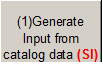
\includegraphics[width=0.9\textwidth, height=0.9\textheight, keepaspectratio=true]{media/image056.png}
\caption{Representing 11 internal walls as internal mass \protect \label{fig:representing-11-internal-walls-as-internal}}
\end{figure}

\textbf{Example}

A five-story building has the same ceiling/floor construction separating each of the levels. Zones that are on floors 2 through 4 may be described using a single piece of internal mass to represent both the floor and ceiling. The construction for this internal mass would be identical to the ceiling/floor construction that would be used to describe separate surfaces and the area of the internal mass surface would be the total surface area of the combined ceilings/floors (i.e.~twice the total floor area).

\paragraph{Field: Name}\label{field-name-21-004}

This is a unique character string associated with the internal mass surface. Though it must be unique from other surface names, it is used primarily for convenience with internal mass surfaces.

\paragraph{Field: Construction Name}\label{field-construction-name-21}

This is the name of the construction (ref: Construction object) used in the surface.

\paragraph{Field: Zone or ZoneList Name}\label{field-zone-or-zonelist-name-14}

This field is the name of the \hyperref[zone]{Zone} or \hyperref[zonelist]{ZoneList} in which the internal mass will be added. When the ZoneList option is used then this internal mass object is applied to each of zone in the list. The name of the actual internal mass object in each zone becomes <Zone Name> <InternalMass Object Name> and should be less than the standard length (100 characters) for a name field. If it is greater than this standard length, it may be difficult to specify in output reporting as it will be truncated. A warning will be shown if the generated name is greater than 100 characters. If it duplicates another such concatenated name, there will be a severe error and terminate the run.

\paragraph{Field: Space or SpaceList Name}\label{field-space-or-spacelist-name-14}

This field is the name of the \hyperref[space]{Space} or \hyperref[spacelist]{SpaceList} in which the internal mass will be added. When the SpaceList option is used then this internal mass object is applied to each space in the list. The name of the actual internal mass object in each space becomes <Space Name> <InternalMass Object Name> and should be less than the standard length (100 characters) for a name field. If it is greater than this standard length, it may be difficult to specify in output reporting as it will be truncated. A warning will be shown if the generated name is greater than 100 characters. If it duplicates another such concatenated name, there will be a severe error and terminate the run. This field is ignored when a ZoneList Name is specified for Zone or ZoneList Name. If a Space Name is used, then the Space must be part of Zone Name. If a SpaceList Name is used, then the Zone Name is ignored (even though it is a required field), and the surface is assigned to the corresponding Zone(s) for each Space in the SpaceList.

\paragraph{Field: Surface Area}\label{field-surface-area}

This field is the surface area of the internal mass. The area that is specified must be the entire surface area that is exposed to the zone. If both sides of a wall are completely within the same zone, then the area of both sides must be included when describing that internal wall.

IDF examples of Internal Mass surfaces:

\begin{lstlisting}
InternalMass,
  Zn002:IntM001,                !- Surface Name
  INTERIOR,                     !- Construction Name
  DORM ROOMS AND COMMON AREAS,  !- Zone or ZoneList Name
  408.7734;                     !- Total area exposed to Zone {m2}

InternalMass,
  Zn002:IntM002,                !- Surface Name
  PARTITION02,                  !- Construction Name
  DORM ROOMS AND COMMON AREAS,  !- Zone or ZoneList Name
  371.6122;                     !- Total area exposed to Zone {m2}
\end{lstlisting}

\subsection{Surface Output Variables/Reports}\label{surface-output-variablesreports}

Note that Surface Outputs from specialized algorithms (such as Effective Moisture Penetration Depth (EMPD), Combined Heat and Moisture Transport (HAMT) and Conduction Finite Difference (CondFD) are discussed under the objects that describe the specialized inputs for these algorithms). You can access them via these links:

\begin{itemize}
\tightlist
\item
  Moisture Penetration Depth (EMPD) Outputs
\item
  Conduction Finite Difference (CondFD) Outputs
\item
  Heat and Moisture (HAMT) Outputs
\end{itemize}

Additionally, the output variables applicable to all heat transfer surfaces:

\begin{lstlisting}
Zone,Sum,Surface Inside Face Heat Balance Calculation Iteration Count []
Zone,Average,Surface Inside Face Temperature [C]
Zone,Average,Surface Inside Face Interior Movable Insulation Temperature [C]
Zone,Average,Surface Outside Face Temperature [C]
Zone,Average,Surface Inside Face Adjacent Air Temperature [C]
Zone,Average,Surface Inside Face Convection Heat Transfer Coefficient [W/m2-K]
Zone,Average,Surface Inside Face Convection Heat Gain Rate [W]
Zone,Average,Surface Inside Face Convection Heat Gain Rate per Area [W/m2]
Zone,Sum,Surface Inside Face Convection Heat Gain Energy [J]
Zone,Average,Surface Inside Face Net Surface Thermal Radiation Heat Gain Rate [W]
Zone,Average,Surface Inside Face Net Surface Thermal Radiation Heat Gain Rate per Area [W/m2]
Zone,Sum,Surface Inside Face Net Surface Thermal Radiation Heat Gain Energy [J]
Zone,Average,Surface Inside Face Solar Radiation Heat Gain Rate [W]
Zone,Average,Surface Inside Face Solar Radiation Heat Gain Rate per Area [W/m2]
Zone,Sum,Surface Inside Face Solar Radiation Heat Gain Energy [J]
Zone,Average,Surface Inside Face Lights Radiation Heat Gain Rate [W]
Zone,Average,Surface Inside Face Lights Radiation Heat Gain Rate per Area [W/m2]
Zone,Sum,Surface Inside Face Lights Radiation Heat Gain Energy [J]
Zone,Average,Surface Inside Face Internal Gains Radiation Heat Gain Rate [W]
Zone,Average,Surface Inside Face Internal Gains Radiation Heat Gain Rate per Area [W/m2]
Zone,Sum,Surface Inside Face Internal Gains Radiation Heat Gain Energy [J]
Zone,Average,Surface Inside Face System Radiation Heat Gain Rate [W]
Zone,Average,Surface Inside Face System Radiation Heat Gain Rate per Area [W/m2]
Zone,Sum,Surface Inside Face System Radiation Heat Gain Energy [J]
Zone,Average,Surface Outside Face Convection Heat Transfer Coefficient [W/m2-K]
Zone,Average,Surface Outside Face Convection Heat Gain Rate [W]
Zone,Average,Surface Outside Face Convection Heat Gain Rate per Area [W/m2]
Zone,Sum,Surface Outside Face Convection Heat Gain Energy [J]
Zone,Average,Surface Outside Face Net Thermal Radiation Heat Gain Rate [W]
Zone,Average,Surface Outside Face Net Thermal Radiation Heat Gain Rate per Area [W/m2]
Zone,Sum,Surface Outside Face Net Thermal Radiation Heat Gain Energy [J]
Zone,Average,Surface Outside Face Thermal Radiation to Air Heat Transfer Coefficient [W/m2-K]
Zone,Average,Surface Outside Face Thermal Radiation to Sky Heat Transfer Coefficient [W/m2-K]
Zone,Average,Surface Outside Face Thermal Radiation to Ground Heat Transfer Coefficient [W/m2-K]
Zone,Average,Surface Outside Face Thermal Radiation to Surrounding Surfaces Heat Transfer Coefficient [W/m2-K]
Zone,Average,Surface Outside Face Surrounding Surfaces Average Temperature [C]
Zone,Average,Surface Inside Face Exterior Windows Incident Beam Solar Radiation Rate [W]
Zone,Sum,Surface Inside Face Exterior Windows Incident Beam Solar Radiation Energy [J]
Zone,Average,Surface Inside Face Exterior Windows Incident Beam Solar Radiation Rate per Area[W/m2]
Zone,Average,Surface Inside Face Interior Windows Incident Beam Solar Radiation Rate [W]
Zone,Average,Surface Inside Face Interior Windows Incident Beam Solar Radiation Rate per Area[W/m2]
Zone,Sum,Surface Inside Face Interior Windows Incident Beam Solar Radiation Energy [J]
Zone,Average,Surface Inside Face Initial Transmitted Diffuse Absorbed Solar Radiation Rate [W]
Zone,Average,Surface Inside Face Initial Transmitted Diffuse Transmitted Out Window Solar Radiation Rate [W]
Zone,Average,Surface Inside Face Absorbed Shortwave Radiation Rate [W]
Zone,Average,Surface Construction Index []
\end{lstlisting}

Output variables applicable to all exterior heat transfer surfaces:

\begin{lstlisting}
Zone,Average,Surface Outside Face Outdoor Air Drybulb Temperature [C]
Zone,Average,Surface Outside Face Outdoor Air Wetbulb Temperature [C]
Zone,Average,Surface Outside Face Outdoor Air Wind Speed [m/s]
Zone,Average,Surface Outside Face Outdoor Air Wind Direction [deg]
Zone,Average,Surface Outside Face Sunlit Area [m2]
Zone,Average,Surface Outside Face Sunlit Fraction \protect\hyperlinksection-1
Zone,Average,Surface Outside Face Incident Solar Radiation Rate per Area[W/m2]
Zone,Average,Surface Outside Face Solar Radiation Heat Gain Rate [W]
Zone,Average,Surface Outside Face Solar Radiation Heat Gain Rate per Area [W/m2]
Zone,Sum,Surface Outside Face Solar Radiation Heat Gain Energy [J]
Zone,Average,Surface Outside Face Incident Beam Solar Radiation Rate per Area[W/m2]
Zone,Average,Surface Outside Face Incident Sky Diffuse Solar Radiation Rate per Area[W/m2]
Zone,Average,Surface Outside Face Incident Ground Diffuse Solar Radiation Rate per Area[W/m2]
Zone,Average,Surface Ext Diff Sol From Bm-To-Diff Refl From Ground[W/m2]
Zone,Average,Surface Outside Face Incident Sky Diffuse Ground Reflected Solar Radiation Rate per Area[W/m2]
Zone,Average,Surface Outside Face Incident Sky Diffuse Surface Reflected Solar Radiation Rate per Area[W/m2]
Zone,Average,Surface Outside Face Incident Beam To Beam Surface Reflected Solar Radiation Rate per Area[W/m2]
Zone,Average,Surface Outside Face Incident Beam To Diffuse Surface Reflected Solar Radiation Rate per Area[W/m2]
Zone,Average,Surface Outside Face Beam Solar Incident Angle Cosine Value[]
Zone,Average,Surface Anisotropic Sky Multiplier []
Zone,Average,Surface Window BSDF Beam Direction Number []
Zone,Average,Surface Window BSDF Beam Theta Angle [rad]
Zone,Average,Surface Window BSDF Beam Phi Angle [rad]
Zone,Average,Surface Outside Face Thermal Radiation to Air Heat Transfer Rate [W]
Zone,Average,Surface Outside Face Heat Emission to Air Rate [W]
\end{lstlisting}

Output variables applicable to opaque heat transfer surfaces (FLOOR, WALL, ROOF, DOOR). \textbf{Note -- these are advanced variables -- you must read the descriptions and understand before use -- then you must use the Diagnostics object to allow reporting.}

\begin{lstlisting}
Zone,Average,Surface Inside Face Solar Radiation Heat Gain Rate [W]
Zone,Average,Surface Inside Face Solar Radiation Heat Gain Rate per Area [W/m2]
Zone,Sum,Surface Inside Face Solar Radiation Heat Gain Energy [J]
Zone,Average,Surface Inside Face Lights Radiation Heat Gain Rate [W]
Zone,Average,Surface Inside Face Lights Radiation Heat Gain Rate per Area [W/m2]
Zone,Sum,Surface Inside Face Lights Radiation Heat Gain Energy [J]
Zone,Average,Surface Inside Face Conduction Heat Transfer Rate [W]
Zone,Average,Surface Inside Face Conduction Heat Gain Rate [W]
Zone,Average,Surface Inside Face Conduction Heat Loss Rate [W]
Zone,Average,Surface Inside Face Conduction Heat Transfer Rate per Area [W/m2]
Zone,Sum,Surface Inside Face Conduction Heat Transfer Energy [J]
Zone,Average,Surface Outside Face Conduction Heat Transfer Rate [W]
Zone,Average,Surface Outside Face Conduction Heat Gain Rate [W]
Zone,Average,Surface Outside Face Conduction Heat Loss Rate [W]
Zone,Average,Surface Outside Face Conduction Heat Transfer Rate per Area [W/m2]
Zone,Sum,Surface Outside Face Conduction Heat Transfer Energy [J]
Zone,Average,Surface Average Face Conduction Heat Transfer Rate [W]
Zone,Average,Surface Average Face Conduction Heat Gain Rate [W]
Zone,Average,Surface Average Face Conduction Heat Loss Rate [W]
Zone,Average,Surface Average Face Conduction Heat Transfer Rate per Area [W/m2]
Zone,Sum,Surface Average Face Conduction Heat Transfer Energy [J]
Zone,Average,Surface Heat Storage Rate [W]
Zone,Average,Surface Heat Storage Gain Rate [W]
Zone,Average,Surface Heat Storage Loss Rate [W]
Zone,Average,Surface Heat Storage Rate per Area [W/m2]
Zone,Sum,Surface Heat Storage Energy [J]
Zone,Average,Zone Opaque Surface Inside Face Conduction [W]
Zone,Average,Zone Opaque Surface Inside Faces Total Conduction Heat Gain Rate [W]
Zone,Average,Zone Opaque Surface Inside Faces Total Conduction Heat Loss Rate [W]
Zone,Sum,Zone Opaque Surface Inside Faces Total Conduction Heat Gain Energy [J]
Zone,Sum,Zone Opaque Surface Inside Faces Total Conduction Heat Loss Energy [J]
Zone,Average,Zone Opaque Surface Outside Face Conduction [W]
Zone,Average,Zone Opaque Surface Outside Face Conduction Gain[W]
Zone,Average,Zone Opaque Surface Outside Face Conduction Loss[W]
Zone,Average, Surface Inside Face Beam Solar Radiation Heat Gain Rate [W]
\end{lstlisting}

\subsection{Window Output Variables}\label{window-output-variables}

Output variables applicable to exterior windows and glass doors:

\begin{lstlisting}
Zone,Average,Zone Windows Total Transmitted Solar Radiation Rate [W]
Zone,Sum,Zone Transmitted Solar Energy [J]
Zone,Average,Zone Windows Total Heat Gain Rate [W]
Zone,Sum,Zone Windows Total Heat Gain Energy [J]
Zone,Average,Zone Windows Total Heat Loss Rate [W]
Zone,Sum,Zone Windows Total Heat Loss Energy [J]
Zone,Average,Zone Exterior Windows Total Transmitted Beam Solar Radiation Rate [W]
Zone,Sum,Zone Exterior Windows Total Transmitted Beam Solar Radiation Energy [J]
Zone,Average,Zone Interior Windows Total Transmitted Beam Solar Radiation Rate [W]
Zone,Sum,Zone Interior Windows Total Transmitted Beam Solar Radiation Energy [J]
Zone,Average,Zone Exterior Windows Total Transmitted Diffuse Solar Radiation Rate [W]
Zone,Sum,Zone Exterior Windows Total Transmitted Diffuse Solar Radiation Energy [J]
Zone,Average,Zone Interior Windows Total Transmitted Diffuse Solar Radiation Rate [W]
Zone,Average,Surface Window Total Glazing Layers Absorbed Solar Radiation Rate [W]
Zone,Average,Surface Window Total Glazing Layers Absorbed Shortwave Radiation Rate [W]
Zone,Sum,Surface Window Total Glazing Layers Absorbed Solar Radiation Energy [J]
Zone,Average,Surface Window Shading Device Absorbed Solar Radiation Rate [W]
Zone,Sum,Surface Window Shading Device Absorbed Solar Radiation Energy [J]
Zone,Average, Surface Window Transmitted Solar Radiation Rate [W]
Zone,Sum,Surface Window Transmitted Solar Radiation Energy [J]
Zone,Average,Surface Window Transmitted Beam Solar Radiation Rate [W]
Zone,Average,Surface Window Transmitted Beam To Beam Solar Radiation Rate [W]
Zone,Average,Surface Window Transmitted Beam To Diffuse Solar Radiation Rate [W]
Zone,Sum,Surface Window Transmitted Beam Solar Radiation Energy [J]
Zone,Sum,Surface Window Transmitted Beam To Beam Solar Radiation Energy [J]
Zone,Sum,Surface Window Transmitted Beam To Diffuse Solar Radiation Energy [J]
Zone,Average,Surface Window Transmitted Diffuse Solar Radiation Rate [W]
Zone,Sum,Surface Window Transmitted Diffuse Solar Radiation Energy [J]
Zone,Average,Surface Window System Solar Transmittance []
Zone,Average,Surface Window System Solar Absorptance []
Zone,Average,Surface Window System Solar Reflectance []
Zone,Average,Surface Window Gap Convective Heat Transfer Rate [W]
Zone,Sum,Surface Window Gap Convective Heat Transfer Energy [J]
Zone,Average,Surface Window Heat Gain Rate [W]
Zone,Sum,Surface Window Heat Gain Energy [J]
Zone,Average,Surface Window Heat Loss Rate [W]
Zone,Sum,Surface Window Heat Loss Energy [J]
Zone,Average,Surface Window Net Heat Transfer Rate [W]
Zone,Sum,Surface Window Net Heat Transfer Energy [J]
Zone,Average,Surface Window Glazing Beam to Beam Solar Transmittance[]
Zone,Average,Surface Window Glazing Beam to Diffuse Solar Transmittance []
Zone,Average,Surface Window Glazing Diffuse to Diffuse Solar Transmittance[]
Zone,Average,Surface Window Model Solver Iteration Count []
Zone,Average,Surface Window Solar Horizontal Profile Angle[deg]
Zone,Average,Surface Window Solar Vertical Profile Angle[deg]
Zone,Average,Surface Window Outside Reveal Reflected Beam Solar Radiation Rate [W]
Zone,Sum,Surface Window Outside Reveal Reflected Beam Solar Radiation Energy
Zone,Average,Surface Window Inside Reveal Reflected Beam Solar Radiation Rate [W]
Zone,Sum,Surface Window Inside Reveal Reflected Beam Solar Radiation Energy [J]
Zone,Average,Surface Window Inside Reveal Absorbed Beam Solar Radiation Rate [W]
Zone,Average,Surface Window Inside Face Glazing Condensation Status []
Zone,Average,Surface Window Inside Face Frame Condensation Status []
Zone,Average,Surface Window Inside Face Divider Condensation Status []
Zone,Average,Surface Shading Device Is On Time Fraction[]
Zone,Average,Surface Window Blind Slat Angle [deg]
Zone,Average,Surface Window Blind Beam to Beam Solar Transmittance[]
Zone,Average,Surface Window Blind Beam to Diffuse Solar Transmittance[]
Zone,Average,Surface Window Blind Diffuse to Diffuse Solar Transmittance[]
Zone,Average,Surface Window Blind and Glazing System Beam Solar Transmittance[]
Zone,Average,Surface Window Blind and Glazing System Diffuse Solar Transmittance[]
Zone,Average,Surface Window Screen Beam to Beam Solar Transmittance []
Zone,Average,Surface Window Screen Beam to Diffuse Solar Transmittance []
Zone,Average,Surface Window Screen Diffuse to Diffuse Solar Transmittance []
Zone,Average,Surface Window Screen and Glazing System Beam Solar Transmittance []
Zone,Average,Surface Window Screen and Glazing System Diffuse Solar Transmittance []
Zone,State,Surface Storm Window On Off Status []
Zone,Average,Surface Window Inside Face Frame and Divider Zone Heat Gain Rate [W]
Zone,Average,Surface Window Frame Heat Gain Rate [W]
Zone,Average,Surface Window Frame Heat Loss Rate [W]
Zone,Average,Surface Window Divider Heat Gain Rate [W]
Zone,Average,Surface Window Divider Heat Loss Rate [W]
Zone,Average,Surface Window Frame Inside Temperature [C]
Zone,Average,Surface Window Frame Outside Temperature [C]
Zone,Average,Surface Window Divider Inside Temperature [C]
Zone,Average,Surface Window Divider Outside Temperature [C]
\end{lstlisting}

If the user requests to display advanced report/output variables (e.g.~see \hyperref[outputdiagnostics]{Output:Diagnostics} keyword DisplayAdvancedReportVariables) the the following additional output variables are available for exterior windows and glass doors

\begin{lstlisting}
Zone,Average,Surface Window Inside Face Glazing Zone Convection Heat Gain Rate [W]
Zone,Average,Surface Window Inside Face Glazing Net Infrared Heat Transfer Rate [W]
Zone,Average,Surface Window Shortwave from Zone Back Out Window Heat Transfer Rate [W]
Zone,Average,Surface Window Inside Face Frame and Divider Zone Heat Gain Rate [W]
Zone,Average,Surface Window Inside Face Gap between Shade and Glazing Zone Convection Heat Gain Rate [W]
Zone,Average,Surface Window Inside Face Shade Zone Convection Heat Gain Rate [W]
Zone,Average,Surface Window Inside Face Shade Net Infrared Heat Transfer Rate [W]
\end{lstlisting}

Output variables applicable to interior windows and glass doors:

\begin{lstlisting}
Zone,Average,Surface Window Transmitted Solar Radiation Rate [W]
Zone,Sum,Surface Window Transmitted Solar Radiation Energy [J]
Zone,Average,Surface Window Transmitted Beam Solar Radiation Rate [W]
Zone,Sum,Surface Window Transmitted Beam Solar Radiation Energy [J]
Zone,Average,Surface Window Transmitted Beam to Beam Solar Radiation Rate [W]
Zone,Sum,Surface Window Transmitted Beam to Beam Solar Radiation Energy [J]
Zone,Average,Surface Window Transmitted Diffuse Solar Radiation Rate [W]
Zone,Sum,Surface Window Transmitted Diffuse Solar Radiation Energy [J]
Zone,Average,Surface Window Heat Gain Rate [W]
Zone,Sum,Surface Window Heat Gain Energy [J]
Zone,Average,Surface Window Heat Loss Rate [W]
Zone,Sum,Surface Window Heat Loss Energy [J]
\end{lstlisting}

If the user requests to display advanced report/output variables (e.g.~see \hyperref[outputdiagnostics]{Output:Diagnostics} keyword DisplayAdvancedReportVariables) the the following additional output variable is available for Equivalent Layer Window;

\begin{lstlisting}
Zone,Average, Surface Window Inside Face Other Convection Heat Gain Rate [W]
\end{lstlisting}

Output variables applicable to interior and exterior windows and doors under certain conditions (see next three subsections for more information) are:

\begin{lstlisting}
Zone,Average,Surface Window Total Absorbed Shortwave Radiation Rate Layer <x> [W]
Zone,Average,Surface Window Front Face Temperature Layer <x> [C]
Zone,Average,Surface Window Back Face Temperature Layer <x> [C]
\end{lstlisting}

\subsubsection{Surface Window Total Absorbed Shortwave Radiation Rate Layer \textless{}x\textgreater{} {[}W{]}}\label{surface-window-total-absorbed-shortwave-radiation-rate-layer-x-w}

This will output shortwave radiation absorbed in a window layer. The key values for this output variable are the surface name. Layers are numbered from the outside to the inside of the surface. The full listing will appear in the RDD file. Note that this variable is only defined for constructions defined by a \hyperref[constructioncomplexfenestrationstate]{Construction:ComplexFenestrationState}.

\subsubsection{Surface Window Front Face Temperature Layer \textless{}x\textgreater{} {[}C{]}}\label{surface-window-front-face-temperature-layer-x-c}

This will output a temperature for the front face of the layer. The layer front face is considered to be the face closest to the outside environment. The full listing will appear in the RDD file. Note that this variable is only defined for constructions defined by a \hyperref[constructioncomplexfenestrationstate]{Construction:ComplexFenestrationState}.  For other window constructions, this variable is also defined for the outer layer (Layer 1) only. The value will be identical to the \hyperref[surface-outside-face-temperature-c]{Surface Outside Face Temperature}.


\subsubsection{Surface Window Back Face Temperature Layer \textless{}x\textgreater{} {[}C{]}}\label{surface-window-back-face-temperature-layer-x-c}

This will output a temperature for the back face of the layer. The layer back face is considered to be the face closest to the inside environment. The full listing will appear in the RDD file. Note that this variable is only defined for constructions defined by a \hyperref[constructioncomplexfenestrationstate]{Construction:ComplexFenestrationState}.  For other window constructions, this variable is also defined for the inner layer only. The value will be identical to the \hyperref[surface-inside-face-temperature-c]{Surface Inside Face Temperature}.

\subsection{Surface Output Variables (all heat transfer surfaces)}\label{surface-output-variables-all-heat-transfer-surfaces}

The various output variables related to surface heat transfer are organized around the inside and outside face of each surface. The zone heat balance model draws energy balances at each side, or face, of a surface and so each surface essentially has two sets of results. The inside face is the side of a heat transfer surface that faces toward the thermal zone. The outside face is the side of a heat transfer surface that faces away from the thermal zone, typically facing outdoors. The Key Value for these is generally the user-defined name of the surface.

\subsubsection{Surface Inside Face Heat Balance Calculation Iteration Count {[]}}\label{surface-inside-face-heat-balance-calculation-iteration-count}

This output is the number of iterations used in a part of the solution for surface heat transfer that accounts for thermal radiation heat transfer between zone surfaces. This is simply a counter on the iteration loop for inside face surface modeling. There is only one instance of this output in a given run and the Key Value is ``Simulation.''

\subsubsection{Surface Inside Face Temperature {[}C{]}}\label{surface-inside-face-temperature-c}

This is the temperature of the surface's inside face, in degrees Celsius. Former Name: Prior to version 7.1 this output was called Surface Inside Temperature.

\subsubsection{Surface Inside Face Interior Movable Insulation Temperature {[}C{]}}\label{surface-inside-face-interior-movable-insulation-temperature-c}

This is the temperature of movable insulation installed on the inside of the construction at the movable insulation's inside face (the one facing the zone), in degrees Celsius. This variable is only valid when the surface has movable insulation and the movable insulation is actually scheduled to be present.  For surfaces that have no movable insulation or the movable insulation is not scheduled to be present, the value of this variable is set to the Surface Inside Face Temperature.  It should be noted that users can limit how often this output variable is generating by using a schedule to control when this output is produced.  For example, this user could add the following syntax to an input file that includes movable insulation:

\begin{lstlisting}
  Output:Variable,Zone1:WestWall,Surface Inside Face Interior Movable Insulation Temperature,timestep,MovableInsulationSchedule;
\end{lstlisting}

In this example, interior movable insulation is used on the west wall of zone 1 and is only present when the schedule (MovableInsulationSchedule) is greater than zero.  Adding this output variable syntax to the input file reports the temperature at the inside face of the interior movable insulation only when the movable insulation is present.  The use of the movable insulation schedule in the output variable designation limits when this value shows up in the EnergyPlus output file to when it is actually scheduled to be present.  At other times, no value will be reported.  The limiting of when the output is generated allows the user to generate useful statistics instead of having those statistics influenced by values for when the movable insulation is not present.  If the user does not use the output variable schedule feature, the output for this variable will equal the surface inside face temperature when the movable insulation is not present.

\subsubsection{Surface Outside Face Temperature {[}C{]}}\label{surface-outside-face-temperature-c}

This is the temperature of the surface's outside face, in degrees Celsius. Former Name: Prior to version 7.1, this output was called Surface Outside Temperature.

\subsubsection{Surface Inside Face Adjacent Air Temperature {[}C{]}}\label{surface-inside-face-adjacent-air-temperature-c}

This is the effective bulk air temperature used for modeling the inside surface convection heat transfer. This is the same as the zone mean air temperature when using the mixing model for roomair. However, if more advanced roomair models are used, this variable will report the air temperature predicted by the roomair model as it was used in the surface heat balance model calculations. Former Name: Prior to version 7.1, this output was called Surface Int Adjacent Air Temperature.

\subsubsection{Surface Inside Face Convection Heat Gain Rate {[}W{]}}\label{surface-inside-face-convection-heat-gain-rate-w}

\subsubsection{Surface Inside Face Convection Heat Gain Rate per Area {[}W/m2{]}}\label{surface-inside-face-convection-heat-gain-rate-per-area-wm2}

\subsubsection{Surface Inside Face Convection Heat Gain Energy {[}J{]}}\label{surface-inside-face-convection-heat-gain-energy-j}

These ``inside face convection heat gain'' output variables describe the heat transferred by convection between the inside face and the zone air. The values can be positive or negative with positive indicating heat is being added to the surface's face by convection. Different versions of the report are available including the basic heat gain rate (W), and a per unit area flux (W/m2), and an energy version (J).

Former Name: Prior to version 7.1, these outputs were called ``Surface Int Convection Heat *'' and had used the opposite sign convention.

\subsubsection{Surface Inside Face Convection Heat Transfer Coefficient {[}W/m2-K{]}}\label{surface-inside-face-convection-heat-transfer-coefficient-wm2-k}

This is the coefficient that describes the convection heat transfer. It is the value of ``Hc'' in the classic convection model Q = Hc* A* (T -- T). This is the result of the surface convection algorithm used for the inside face. Former Name: Prior to version 7.1, this output was called ``Surface Int Convection Coeff.''

\subsubsection{Surface Inside Face Net Surface Thermal Radiation Heat Gain Rate {[}W{]}}\label{surface-inside-face-net-surface-thermal-radiation-heat-gain-rate-w}

\subsubsection{Surface Inside Face Net Surface Thermal Radiation Heat Gain Rate per Area {[}W/m2{]}}\label{surface-inside-face-net-surface-thermal-radiation-heat-gain-rate-per-area-wm2}

\subsubsection{Surface Inside Face Net Surface Thermal Radiation Heat Gain Energy {[}J{]}}\label{surface-inside-face-net-surface-thermal-radiation-heat-gain-energy-j}

These ``inside face net surface thermal radiation heat gain'' output variables describe the heat transferred by longwave infrared thermal radiation exchanges between the inside faces of other surfaces in the zone. The values can be positive or negative with positive indicating heat is being added to the surface's face by thermal radiation. Different versions of the report are available including the basic heat gain rate (W), and a per unit area flux (W/m2), and an energy version (J).

\subsubsection{Surface Inside Face Solar Radiation Heat Gain Rate {[}W{]}}\label{surface-inside-face-solar-radiation-heat-gain-rate-w}

\subsubsection{Surface Inside Face Solar Radiation Heat Gain Rate per Area {[}W/m2{]}}\label{surface-inside-face-solar-radiation-heat-gain-rate-per-area-wm2}

\subsubsection{Surface Inside Face Solar Radiation Heat Gain Energy {[}J{]}}\label{surface-inside-face-solar-radiation-heat-gain-energy-j}

These ``inside face solar radiation heat gain'' output variables describe the heat transferred by solar radiation onto the inside face. The values are always positive and indicate heat is being added to the surface's face by solar radiation. This is sunlight that has entered the zone through a window and been absorbed on the inside face of the surface. Different versions of the report are available including the basic heat gain rate (W), and a per unit area flux (W/m2), and an energy version (J).

\subsubsection{Surface Inside Face Lights Radiation Heat Gain Rate {[}W{]}}\label{surface-inside-face-lights-radiation-heat-gain-rate-w}

\subsubsection{Surface Inside Face Lights Radiation Heat Gain Rate per Area {[}W/m2{]}}\label{surface-inside-face-lights-radiation-heat-gain-rate-per-area-wm2}

\subsubsection{Surface Inside Face Lights Radiation Heat Gain Energy {[}J{]}}\label{surface-inside-face-lights-radiation-heat-gain-energy-j}

These ``inside face lights radiation heat gain'' output variables describe the heat transferred by shortwave radiation onto the inside face. The values are always positive and indicate heat is being added to the surface's face by shortwave radiation that emanated from electric lighting equipment and was absorbed by the surface. Note that this includes light from other zones that are transmitted through interzone windows. Different versions of the report are available including the basic heat gain rate (W), and a per unit area flux (W/m2), and an energy version (J).

\subsubsection{Surface Inside Face Internal Gains Radiation Heat Gain Rate {[}W{]}}\label{surface-inside-face-internal-gains-radiation-heat-gain-rate-w}

\subsubsection{Surface Inside Face Internal Gains Radiation Heat Gain Rate per Area {[}W/m2{]}}\label{surface-inside-face-internal-gains-radiation-heat-gain-rate-per-area-wm2}

\subsubsection{Surface Inside Face Internal Gains Radiation Heat Gain Energy {[}J{]}}\label{surface-inside-face-internal-gains-radiation-heat-gain-energy-j}

These ``inside face internal gains radiation heat gain'' output variables describe the heat transferred by longwave infrared thermal radiation onto the inside face that emanated from internal gains such as lights, electric equipment, and people. The values are always positive and indicate heat is being added to the surface's face by the absorption of longwave thermal radiation. Different versions of the report are available including the basic heat gain rate (W), and a per unit area flux (W/m2), and an energy version (J).

\subsubsection{Surface Inside Face System Radiation Heat Gain Rate {[}W{]}}\label{surface-inside-face-system-radiation-heat-gain-rate-w}

\subsubsection{Surface Inside Face System Radiation Heat Gain Rate per Area {[}W/m2{]}}\label{surface-inside-face-system-radiation-heat-gain-rate-per-area-wm2}

\subsubsection{Surface Inside Face System Radiation Heat Gain Energy {[}J{]}}\label{surface-inside-face-system-radiation-heat-gain-energy-j}

These ``inside face system radiation heat gain'' output variables describe the heat transferred by infrared thermal radiation onto the inside face that emanated from HVAC equipment such as baseboard heaters or high-temperature radiant heating panels. The values are always positive and indicate heat is being added to the surface's face by the absorption of thermal radiation. Different versions of the report are available including the basic heat gain rate (W), and a per unit area flux (W/m2), and an energy version (J).

\subsubsection{Surface Outside Face Convection Heat Gain Rate {[}W{]}}\label{surface-outside-face-convection-heat-gain-rate-w}

\subsubsection{Surface Outside Face Convection Heat Gain Rate per Area {[}W/m2{]}}\label{surface-outside-face-convection-heat-gain-rate-per-area-wm2}

\subsubsection{Surface Outside Face Convection Heat Gain Energy {[}J{]}}\label{surface-outside-face-convection-heat-gain-energy-j}

These ``outside face convection'' output variables describe heat transferred by convection between the outside face and the surrounding air. The values can be positive or negative with positive values indicating heat is added to the surface face by convection heat transfer. Different versions of the report are available including the basic heat gain rate (W), and a per unit area flux (W/m\(^{2}\)), and an energy version (J).

Former Name: Prior to version 7.1, these outputs were called ``Surface Ext Convection Heat *'' and used the opposite sign convention.

\subsubsection{Surface Outside Face Convection Heat Transfer Coefficient {[}W/m2-K{]}}\label{surface-outside-face-convection-heat-transfer-coefficient-wm2-k}

This is the coefficient that describes the convection heat transfer. It is the value of ``Hc'' in the classic convection model Q = Hc* A* (T -- T). This is the result of the surface convection algorithm used for the outside face. Former Name: Prior to Version 7.1, this output was called ``Surface Ext Convection Coeff.''

\subsubsection{Surface Outside Face Net Thermal Radiation Heat Gain Rate {[}W{]}}\label{surface-outside-face-net-thermal-radiation-heat-gain-rate-w}

\subsubsection{Surface Outside Face Net Thermal Radiation Heat Gain Rate per Area {[}W/m2{]}}\label{surface-outside-face-net-thermal-radiation-heat-gain-rate-per-area-wm2}

\subsubsection{Surface Outside Face Net Thermal Radiation Heat Gain Energy {[}J{]}}\label{surface-outside-face-net-thermal-radiation-heat-gain-energy-j}

These ``outside face net thermal radiation'' output variables describe the heat transferred by longwave infrared thermal radiation exchanges between the surface and the surroundings of the outside face. This is the net of all forms of longwave thermal infrared radiation heat transfer. The values can be positive or negative with positive indicating the net addition of heat to the outside face. Different versions of the report are available including the basic heat gain rate (W), and a per unit area flux (W/m2), and an energy version (J).

Former Name: Prior to version 7.1, these outputs were called ``Surface Ext Thermal Radiation Heat *'' and used the opposite sign convention.

\subsubsection{Surface Inside Face Exterior Windows Incident Beam Solar Radiation Rate {[}W{]}}\label{surface-inside-face-exterior-windows-incident-beam-solar-radiation-rate-w}

\subsubsection{Surface Inside Face Exterior Windows Incident Beam Solar Radiation Rate per Area {[}W/m2{]}}\label{surface-inside-face-exterior-windows-incident-beam-solar-radiation-rate-per-area-wm2}

\subsubsection{Surface Inside Face Exterior Windows Incident Beam Solar Radiation Energy {[}J{]}}\label{surface-inside-face-exterior-windows-incident-beam-solar-radiation-energy-j}

Beam solar radiation from the exterior windows in a zone incident on the inside face of a surface in the zone. If Solar Distribution in the BUILDING object is equal to MinimalShadowing or FullExterior, it is assumed that all beam solar from exterior windows falls on the floor. In this case the value of this output variable can be greater than zero only for floor surfaces. If Solar Distribution equals FullInteriorExterior the program tracks where beam solar from exterior windows falls inside the zone, in which case the value of this variable can be greater than zero for floor as well as wall surfaces. Different versions of the report are available including the basic incident rate (W), a per unit area flux (W/m2), and an energy version (J).

\subsubsection{Surface Inside Face Interior Windows Incident Beam Solar Radiation Rate {[}W{]}}\label{surface-inside-face-interior-windows-incident-beam-solar-radiation-rate-w}

\subsubsection{Surface Inside Face Interior Windows Incident Beam Solar Radiation Rate per Area {[}W/m2{]}}\label{surface-inside-face-interior-windows-incident-beam-solar-radiation-rate-per-area-wm2}

\subsubsection{Surface Inside Face Interior Windows Incident Beam Solar Radiation Energy {[}J{]}}\label{surface-inside-face-interior-windows-incident-beam-solar-radiation-energy-j}

Beam solar radiation from the interior (i.e., interzone) windows in a zone incident on the inside face of a surface in the zone. This value is calculated only if Solar Distribution in the BUILDING object is equal to FullInteriorExterior. However, the program does not track where this radiation falls. Instead, it is treated by the program as though it were diffuse radiation uniformly distributed over all of the zone surfaces. See \textbf{Figure~\ref{fig:beam-solar-radiation-entering-a-zone-through}}. Different versions of the report are available including the basic incident rate (W), a per unit area flux (W/m2), and an energy version (J).

\begin{figure}[hbtp] % fig 31
\centering
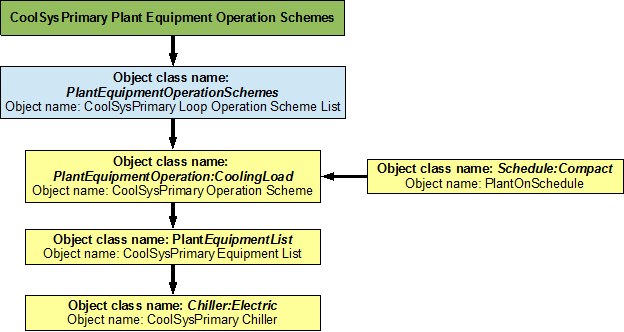
\includegraphics[width=0.9\textwidth, height=0.9\textheight, keepaspectratio=true]{media/image057.png}
\caption{Beam solar radiation entering a zone through an interior window is distributed inside the zone as though it were diffuse radiation. \protect \label{fig:beam-solar-radiation-entering-a-zone-through}}
\end{figure}

\subsubsection{Surface Inside Face Initial Transmitted Diffuse Absorbed Solar Radiation Rate {[}W{]}}\label{surface-inside-face-initial-transmitted-diffuse-absorbed-solar-radiation-rate-w}

As of Version 2.1, diffuse solar transmitted through exterior and interior windows is no longer uniformly distributed. Instead, it is distributed according to the approximate view factors between the transmitting window and all other heat transfer surfaces in the zone. This variable is the amount of transmitted diffuse solar that is initially absorbed on the inside of each heat transfer surface. The portion of this diffuse solar that is reflected by all surfaces in the zone is subsequently redistributed uniformly to all heat transfer surfaces in the zone, along with interior reflected beam solar and shortwave radiation from lights. The total absorbed shortwave radiation is given by the next variable.

\subsubsection{Surface Inside Face Absorbed Shortwave Radiation Rate {[}W{]}}\label{surface-inside-face-absorbed-shortwave-radiation-rate-w}

As of Version 2.1, the previous variable plus absorbed shortwave radiation from uniformly distributed initially-reflected diffuse solar, reflected beam solar, and shortwave radiation from lights. This sum is the power of all sources of solar and visible radiation absorbed by the surface at the inside face.

\subsubsection{Surface Construction Index {[]}}\label{surface-construction-index}

The variable reports an index that points to specific Construction. The variable is an additional output variable when \hyperref[outputdiagnostics]{Output:Diagnostics}, DisplayAdvancedReportVariables; is given in an input file.

In order to find a corresponding construction using the index, following steps are suggested:

1. Find a surface name from Surface Construction Index in the .csv file

2. Search the surface name in lines starting with HeatTransfer Surface in the .eio file

3. The seventh item is the construction name with matched surface name.

\subsection{Surface Output Variables (exterior heat transfer surfaces)}\label{surface-output-variables-exterior-heat-transfer-surfaces}

\subsubsection{Surface Outside Face Outdoor Air Drybulb Temperature {[}C{]}}\label{surface-outside-face-outdoor-air-drybulb-temperature-c}

The outdoor air dry-bulb temperature calculated at the height above ground of the surface centroid. Former Name: Prior to version 7.1, this output was called ``Surface Ext Outdoor Dry Bulb.''

\subsubsection{Surface Outside Face Outdoor Air Wetbulb Temperature {[}C{]}}\label{surface-outside-face-outdoor-air-wetbulb-temperature-c}

The outdoor air wet-bulb temperature calculated at the height above ground of the surface centroid. Former Name: Prior to version 7.1, this output was called ``Surface Ext Outdoor Wet Bulb.''

\subsubsection{Surface Outside Face Outdoor Air Wind Speed {[}m/s{]}}\label{surface-outside-face-outdoor-air-wind-speed-ms}

The outdoor wind speed calculated at the height above ground of the surface centroid. This value may differ from site wind speed depending on the height of the surface (ref. \hyperref[siteheightvariation]{Site:HeightVariation}). In addition, the value may be different from the site wind speed when using \hyperref[outdoorairnode]{OutdoorAir:Node} with  \hyperref[surfacePropertylocalEnvironment]{SurfaceProperty:LocalEnvironment} or \hyperref[ZonePropertylocalEnvironment]{ZoneProperty:LocalEnvironment}. It can also be modified using EMS. Former Name: Prior to version 7.1, this output was called ``Surface Ext Wind Speed.''

\subsubsection{Surface Outside Face Outdoor Air Wind Direction {[}deg{]}}\label{surface-outside-face-outdoor-air-wind-direction-def}

This output reports the actual wind direction at the outside face of a surface.  As with the wind speed variable above, this value may be different from the site wind direction when using \hyperref[outdoorairnode]{OutdoorAir:Node} with \hyperref[surfacePropertylocalEnvironment]{SurfaceProperty:LocalEnvironment} or \hyperref[ZonePropertylocalEnvironment]{ZoneProperty:LocalEnvironment}. It can also be modified using EMS.

\subsubsection{Surface Outside Face Sunlit Area {[}m2{]}}\label{surface-outside-face-sunlit-area-m2}

The outside area of an exterior surface that is illuminated by (unreflected) beam solar radiation.

\subsubsection{Surface Outside Face Sunlit Fraction {[]}}\label{surface-outside-face-sunlit-fraction}

The fraction of the outside area of an exterior surface that is illuminated by (unreflected) beam solar radiation. Equals Surface Outside Face Sunlit Area divided by total surface area.

\subsubsection{Surface Outside Face Thermal Radiation to Air Heat Transfer Coefficient {[}W/m2-K{]}}\label{surface-outside-face-thermal-radiation-to-air-heat-transfer-coefficient-wm2-k}

This is the coefficient that describes thermal radiation heat transfer between the outside face and the air mass surrounding the surface. It is the value of ``Hr'' in the classic linearized model for thermal radiation Q = Hr * A * (T\_surf -- T\_surfodb) when applied to the ambient air. Where T\_surf = Surface Outside Face Temperature, and T\_surfodb = Surface Outside Face Outdoor Air Drybulb Temperature. Former Name: Prior to version 7.1, this output was called ``Surface Ext Rad to Air Coeff.''

\subsubsection{Surface Outside Face Thermal Radiation to Sky Heat Transfer Coefficient {[}W/m2-K{]}}\label{surface-outside-face-thermal-radiation-to-sky-heat-transfer-coefficient-wm2-k}

This is the coefficient that describes thermal radiation heat transfer between the outside face and the sky surrounding the surface. It is the value of ``Hr'' in the classic linearized model for thermal radiation Q = Hr * A * (T\_surf -- T\_sky) when applied to the sky. Where T\_surf = Surface Outside Face Temperature, and T\_sky = Site Sky Temperature. Former Name: Prior to version 7.1, this output was called ``Surface Ext Rad to Sky Coeff.''

\subsubsection{Surface Outside Face Thermal Radiation to Ground Heat Transfer Coefficient {[}W/m2-K{]}}\label{surface-outside-face-thermal-radiation-to-ground-heat-transfer-coefficient-wm2-k}

This is the coefficient that describes thermal radiation heat transfer between the outside face and the ground surrounding the surface. It is the value of ``Hr'' in the classic linearized model for thermal radiation Q = Hr * A * (T\_surf -- T\_odb) when applied to the ground. Where T\_surf = Surface Outside Face Temperature, and T\_odb = Site Outdoor Air Drybulb Temperature (used as an approximation for the ground surface temperature). Former Name: Prior to version 7.1, this output was called ``Surface Ext Rad to Ground Coeff.''

\subsubsection{Surface Outside Face Thermal Radiation to Air Heat Transfer Rate {[}W{]}}\label{surface-outside-face-thermal-radiation-to-air-heat-transfer-rate-w}

This is thermal radiation heat transfer rate between the outside face and the air mass surrounding the surface.

\subsubsection{Surface Outside Face Heat Emission to Air Rate {[}W{]}}\label{surface-outside-face-heat-emission-to-air-heat-transfer-rate-w}

This is total heat transfer rate between the outside face and the air mass surrounding the surface by convection and thermal radiation.

\subsubsection{Surface Outside Face Thermal Radiation to Surrounding Surfaces Heat Transfer Coefficient {[}W/m2-K{]}}\label{surface-outside-face-thermal-radiation-to-surrounding-surfaces-heat-transfer-coefficient-wm2-k}

This is the coefficient that describes thermal radiation heat transfer between the outside face of an exterior surface and the surrounding surfaces it views. It is the value of ``Hr'' in the classic linearized model for thermal radiation exchange Q = Hr * A * (T\_surf -- T\_srdsurfs) when applied to the surrounding surfaces. Where T\_surf = Surface Outside Face Temperature, and T\_srdsurf = Average temperature of the surrounding surfaces viewed by an exterior surface.

\subsubsection{Surface Outside Face Surrounding Surfaces Average Temperature {[}C{]}}\label{surface-outside-face-surrounding-surfaces-average-temperature-C}

This is the average surface temperature of the surrounding surfaces viewed by an exterior surface, in degrees Celsius. The surrounding surfaces average temperature is a view factor weighed surface temperature of multiple surrounding surfaces seen by an exterior surface. If an exterior surface views a single surrounding surface then the average temperature is the same as the user specified surrounding surface temperature.

\subsubsection{Surface Outside Face Solar Radiation Heat Gain Rate {[}W{]}}\label{surface-outside-face-solar-radiation-heat-gain-rate-w}

\subsubsection{Surface Outside Face Solar Radiation Heat Gain Rate per Area {[}W/m2{]}}\label{surface-outside-face-solar-radiation-heat-gain-rate-per-area-wm2}

\subsubsection{Surface Outside Face Solar Radiation Heat Gain Energy {[}J{]}}\label{surface-outside-face-solar-radiation-heat-gain-energy-j}

These ``outside face solar radiation'' output variables describe the heat transferred by the absorption of solar radiation at the outside face. This is the result of incident solar radiation being absorbed at the surface face. The values are always positive.

\subsubsection{Surface Outside Face Incident Solar Radiation Rate per Area {[}W/m2{]}}\label{surface-outside-face-incident-solar-radiation-rate-per-area-wm2}

The total solar radiation incident on the outside of an exterior surface. It is the sum of:

\begin{itemize}
\item
  Surface Outside Face Incident Beam Solar Radiation Rate per Area
\item
  Surface Outside Face Incident Sky Diffuse Solar Radiation Rate per Area
\item
  Surface Outside Face Incident Ground Diffuse Solar Radiation Rate per Area
\item
  Surface Outside Face Incident Sky Diffuse Surface Reflected Solar Radiation Rate per Area
\item
  Surface Outside Face Incident Beam To Beam Surface Reflected Solar Radiation Rate per Area
\item
  Surface Outside Face Incident Sky Diffuse Surface Reflected Solar Radiation Rate per Area
\end{itemize}

\subsubsection{Surface Outside Face Incident Beam Solar Radiation Rate per Area {[}W/m2{]}}\label{surface-outside-face-incident-beam-solar-radiation-rate-per-area-wm2}

The solar beam radiation incident on the outside of an exterior surface, including the effects of shadowing, if present. The beam here is that directly from the sun; it excludes beam specularly reflected from obstructions.

\subsubsection{Surface Outside Face Incident Sky Diffuse Solar Radiation Rate per Area {[}W/m2{]}}\label{surface-outside-face-incident-sky-diffuse-solar-radiation-rate-per-area-wm2}

The solar diffuse radiation from the sky incident on the outside of an exterior surface, including the effects of shadowing, if present.

\subsubsection{Surface Outside Face Incident Ground Diffuse Solar Radiation Rate per Area {[}W/m2{]}}\label{surface-outside-face-incident-ground-diffuse-solar-radiation-rate-per-area-wm2}

The solar diffuse radiation incident on the outside of an exterior surface that arises from reflection of beam solar and sky diffuse solar from the ground. This is the sum of the next two output variables, ``Surface Outside Face Incident Beam To Diffuse Ground Reflected Solar Radiation Rate per Area'' and ``Surface Outside Face Incident Sky Diffuse Ground Reflected Solar Radiation Rate per Area.'' The reflected solar radiation from the ground is assumed to be diffuse and isotropic (there is no specular component).

If ``Reflections'' option is not chosen in the Solar Distribution Field in the BUILDING object, the effects of shadowing are accounted for by the user-specified value of View Factor to Ground for the surface. If ``Reflections'' option is chosen, the program determines the effects of shadowing, including time-varying shadowing of the ground plane by the building itself.

\subsubsection{Surface Outside Face Incident Beam To Diffuse Ground Reflected Solar Radiation Rate per Area {[}W/m2{]}}\label{surface-outside-face-incident-beam-to-diffuse-ground-reflected-solar-radiation-rate-per-area-wm2}

The solar diffuse radiation incident on the outside of an exterior surface that arises from beam-to-diffuse reflection from the ground. It is assumed that there is no beam-to-beam (specular) component. The beam here is that directly from the sun; it excludes beam specularly reflected from obstructions.

\subsubsection{Surface Outside Face Incident Sky Diffuse Ground Reflected Solar Radiation Rate per Area {[}W/m2{]}}\label{surface-outside-face-incident-sky-diffuse-ground-reflected-solar-radiation-rate-per-area-wm2}

The solar diffuse radiation incident on the outside of an exterior surface that arises from sky diffuse solar reflection from the ground. The sky diffuse here is that directly from the sky; it excludes reflection of sky diffuse from obstructions.

\subsubsection{Surface Outside Face Incident Sky Diffuse Surface Reflected Solar Radiation Rate per Area {[}W/m2{]}}\label{surface-outside-face-incident-sky-diffuse-surface-reflected-solar-radiation-rate-per-area-wm2}

The solar diffuse radiation incident on the outside of an exterior surface that arises from sky diffuse reflection from one or more obstructions. This value will be non-zero only if ``Reflections'' option is chosen in the BUILDING object.

\subsubsection{Surface Outside Face Incident Beam To Beam Surface Reflected Solar Radiation Rate per Area {[}W/m2{]}}\label{surface-outside-face-incident-beam-to-beam-surface-reflected-solar-radiation-rate-per-area-wm2}

The solar beam radiation incident on the outside of an exterior surface that arises from beam-to-beam (specular) reflection from one or more obstructions. This value will be non-zero only if ``Reflections'' option is chosen in the BUILDING object. For windows, the program treats this beam radiation as diffuse radiation in calculating its transmission and absorption.

\subsubsection{Surface Outside Face Incident Beam To Diffuse Surface Reflected Solar Radiation Rate per Area {[}W/m2{]}}\label{surface-outside-face-incident-beam-to-diffuse-surface-reflected-solar-radiation-rate-per-area-wm2}

The solar diffuse radiation incident on the outside of an exterior surface that arises from beam-to-diffuse reflection from building shades or building surfaces. This value will be non-zero only if ``Reflections'' option is chosen in the BUILDING object.

\subsubsection{Surface Outside Face Beam Solar Incident Angle Cosine Value {[]}}\label{surface-outside-face-beam-solar-incident-angle-cosine-value}

The cosine of the angle of incidence of (unreflected) beam solar radiation on the outside of an exterior surface. The value varies from 0.0 for beam parallel to the surface (incidence angle = 90\(^{O}\)) to 1.0 for beam perpendicular to the surface (incidence angle = 0\(^{O}\)). Negative values indicate the sun is behind the surface, i.e the surface does not see the sun.

\subsubsection{Surface Anisotropic Sky Multiplier {[]}}\label{surface-anisotropic-sky-multiplier}

This is the view factor multiplier for diffuse sky irradiance on exterior surfaces taking into account the anisotropic radiance of the sky. The diffuse sky irradiance on a surface is given by Anisotropic Sky Multiplier * Diffuse Solar Irradiance.

\subsubsection{Surface Window BSDF Beam Direction Number {[]}}\label{surface-window-bsdf-beam-direction-number}

\subsubsection{Surface Window BSDF Beam Phi Angle {[}rad{]}}\label{surface-window-bsdf-beam-phi-angle-rad}

\subsubsection{Surface Window BSDF Beam Theta Angle {[}rad{]}}\label{surface-window-bsdf-beam-theta-angle-rad}

\subsection{Opaque Surface Output Variables}\label{opaque-surface-output-variables}

The following variables apply only to opaque surfaces, where an opaque surface is considered here to be an exterior or interzone heat transfer surface of class FLOOR, WALL, ROOF or DOOR. \textbf{Note -- these are advanced variables -- you must read the descriptions and understand before use -- then you must use the} \textbf{\hyperref[outputdiagnostics]{Output:Diagnostics}} \textbf{object to allow reporting.}

\subsubsection{Surface Inside Face Conduction Heat Transfer Rate {[}W{]}}\label{surface-inside-face-conduction-heat-transfer-rate-w}

\subsubsection{Surface Inside Face Conduction Heat Transfer Rate per Area {[}W/m2{]}}\label{surface-inside-face-conduction-heat-transfer-rate-per-area-wm2}

\subsubsection{Surface Inside Face Conduction Heat Gain Rate {[}W{]}}\label{surface-inside-face-conduction-heat-gain-rate-w}

\subsubsection{Surface Inside Face Conduction Heat Loss Rate {[}W{]}}\label{surface-inside-face-conduction-heat-loss-rate-w}

These ``inside face conduction'' output variables describe heat flow by conduction right at the inside face of an opaque heat transfer surface. A positive value means that the conduction is from just inside the inside face toward the inside face. A negative value means that the conduction is from the inside face into the core of the heat transfer surface.

Note that Inside Face Conduction, when positive, does \textbf{not} necessarily indicate the heat flow from the surface to the zone air, which is governed by the inside face convection coefficient, the difference in temperature between the inside face and the zone air, and various radiation terms due to solar, internal gains, and radiant exchange with other surfaces in the zone.

Different versions of the reports are available. The basic heat gain rate (W) and a per unit area flux (W/m\(^{2}\)) can have positive or negative values with the sign convention that positive indicates heat flowing toward the face itself. There are also directed ``gain'' and ``loss'' versions that have only positive values or zero when the heat flow direction opposes.

Former Name: Prior to version 7.1, these outputs were called ``Opaque Surface Inside Face Conduction *.''

Former Name: For Conduction Finite Difference simulations (CondFD), CondFD Inside Surface Heat Flux is replaced with Surface Inside Face Conduction Heat Transfer Rate Per Area. Likewise for CondFD Inside Heat Flux to Surface.

\subsubsection{Surface Outside Face Conduction Heat Transfer Rate {[}W{]}}\label{surface-outside-face-conduction-heat-transfer-rate-w}

\subsubsection{Surface Outside Face Conduction Heat Transfer Rate per Area {[}W/m2{]}}\label{surface-outside-face-conduction-heat-transfer-rate-per-area-wm2}

\subsubsection{Surface Outside Face Conduction Heat Gain Rate {[}W{]}}\label{surface-outside-face-conduction-heat-gain-rate-w}

\subsubsection{Surface Outside Face Conduction Heat Loss Rate {[}W{]}}\label{surface-outside-face-conduction-heat-loss-rate-w}

These ``outside face conduction'' output variables describe heat flow by conduction right at the outside face of an opaque heat transfer surface. A positive value means that the conduction is from just inside the outside face toward the outside face. A negative value means that the conduction is from the outside face into the core of the heat transfer surface.

Note that outside face conduction, when positive, does \textbf{not} necessarily indicate the heat flow from the surface to the surrounding air, due to the fact that there could be various terms such as convection and/or radiation terms based on whatever is the ''outside'' environment for this surface.

When the surface in question is a partition, the output for this variable is set to zero because there is no outside face because the surface is fully exposed to the zone.  When the surface is an interzone partition, the value will be non-zero because there will potentially be conduction into or out of the zone on the other side at this surface.

Different versions of the reports are available. The basic heat transfer rate (W) and a per unit area flux (W/m\(^{2}\)) can have positive or negative values with the sign convention that positive indicates heat flowing toward the face itself. There are also directed ``gain'' and ``loss'' versions that have only positive values or zero when the heat flow direction opposes.

Former Name: For Conduction Finite Difference simulations (CondFD), CondFD Outside Surface Heat Flux is replaced with Surface Outside Face Conduction Heat Transfer Rate Per Area. Likewise for CondFD Outside Heat Flux to Surface.

\subsubsection{Surface Average Face Conduction Heat Transfer Rate {[}W{]}}\label{surface-average-face-conduction-heat-transfer-rate-w}

\subsubsection{Surface Average Face Conduction Heat Transfer Rate per Area {[}W/m2{]}}\label{surface-average-face-conduction-heat-transfer-rate-per-area-wm2}

\subsubsection{Surface Average Face Conduction Heat Gain Rate {[}W{]}}\label{surface-average-face-conduction-heat-gain-rate-w}

\subsubsection{Surface Average Face Conduction Heat Loss Rate {[}W{]}}\label{surface-average-face-conduction-heat-loss-rate-w}

\subsubsection{Surface Average Face Conduction Heat Transfer Energy {[}J{]}}\label{surface-average-face-conduction-heat-transfer-energy-j}

These ``average face conduction'' output variables combine the inside face conduction and outside face conduction reports together to describe the conduction situation in a heat transfer surface in a nominal way. This is simply the average of the inside and outside face conduction rates, but with the sign convention for the outside face switched to match the inside face so that positive values here indicate heat flowing into the thermal zone.

Different versions of the reports are available. The basic heat conduction rate (W) and a per unit area flux (W/m\(^{2}\)) can have positive or negative values with the sign convention that positive indicates heat flowing toward the thermal zone. There are also directed ``gain'' and ``loss'' versions that have only positive values or zero when the heat flow direction opposes (W). Finally there is a version for total energy transfer (J).

\subsubsection{Surface Heat Storage Rate {[}W{]}}\label{surface-heat-storage-rate-w}

\subsubsection{Surface Heat Storage Rate per Area {[}W/m2{]}}\label{surface-heat-storage-rate-per-area-wm2}

\subsubsection{Surface Heat Storage Gain Rate {[}W{]}}\label{surface-heat-storage-gain-rate-w}

\subsubsection{Surface Heat Storage Loss Rate {[}W{]}}\label{surface-heat-storage-loss-rate-w}

\subsubsection{Surface Heat Storage Energy {[}J{]}}\label{surface-heat-storage-energy-j}

These ``heat storage'' output variables combine the inside face conduction and outside face conduction reports together to describe the thermal storage situation in a heat transfer surface in a nominal way. This is simply the difference between the inside and outside face conduction, but with the sign convention arranged so that positive values indicate heat being added to the core of the surface.

Different versions of the reports are available. The basic heat storage rate (W) and a per unit area flux (W/m\(^{2}\)) can have positive or negative values with the sign convention that positive indicates heat being added to the surface's mass. There are also directed ``gain'' and ``loss'' versions that have only positive values or zero when the heat storage direction opposes (W). Finally there is a version for total energy stored (J).

\subsubsection{Zone Opaque Surface Inside Face Conduction {[}W{]}}\label{zone-opaque-surface-inside-face-conduction-w}

The sum of the Opaque Surface Inside Face Conduction values for all opaque surfaces in a zone for both positive and negative sums. For example, assume a zone has six opaque surfaces with Opaque Surface Inside Face Conduction values of 100, -200, 400, 50, 150 and --300 W. Then Zone Opaque Surface Inside Face Conduction = 700 - 500 = 200 W. Or if a zone has six opaque surfaces with Opaque Surface Inside Face Conduction values of -100, -200, 400, -50, 150 and --300W. Then Zone Opaque Surface Inside Face Conduction = 550 -- 650 = -100 W.

\subsubsection{Zone Opaque Surface Inside Faces Total Conduction Heat Gain Rate {[}W{]}}\label{zone-opaque-surface-inside-faces-total-conduction-heat-gain-rate-w}

\subsubsection{Zone Opaque Surface Inside Faces Total Conduction Heat Gain Energy {[}J{]}}\label{zone-opaque-surface-inside-faces-total-conduction-heat-gain-energy-j}

These are the power and energy sums for the Opaque Surface Inside Face Conduction values for all opaque surfaces in a zone when that sum is positive. For example, assume a zone has six opaque surfaces with Opaque Surface Inside Face Conduction values of 100, -200, 400, 50, 150 and --300 W. Then Zone Opaque Surface Inside Faces Total Conduction Heat Gain Rate = 700 - 500 = 200 W.

\subsubsection{Zone Opaque Surface Inside Faces Total Conduction Heat Loss Rate {[}W{]}}\label{zone-opaque-surface-inside-faces-total-conduction-heat-loss-rate-w}

\subsubsection{Zone Opaque Surface Inside Faces Total Conduction Heat Loss Energy {[}J{]}}\label{zone-opaque-surface-inside-faces-total-conduction-heat-loss-energy-j}

These are the power and energy absolute value for the sums of the Opaque Surface Inside Face Conduction values for all opaque surfaces in a zone when that sum is negative. For example, assume a zone has six opaque surfaces with Opaque Surface Inside Face Conduction values of -100, -200, 400, -50, 150 and --300W. Then Zone Opaque Surface Inside Faces Total Conduction Heat Loss Rate = \textbar{}550 -- 650\textbar{} = \textbar{}-100\textbar{} = 100 W.

\subsubsection{Zone Opaque Surface Outside Face Conduction {[}W{]}}\label{zone-opaque-surface-outside-face-conduction-w}

The sum of the Opaque Surface Outside Face Conduction values for all opaque surfaces in a zone for both positive and negative sums. For example, assume a zone has six opaque surfaces with Opaque Surface Outside Face Conduction values of 100, -200, 400, 50, 150 and --300 W. Then Zone Opaque Surface Outside Face Conduction = 700 - 500 = 200 W. Or if a zone has six opaque surfaces with Opaque Surface Outside Face Conduction values of -100, -200, 400, -50, 150 and --300W. Then Zone Opaque Surface Outside Face Conduction = 550 -- 650 = -100 W.

\subsubsection{Zone Opaque Surface Outside Face Conduction Gain {[}W{]}}\label{zone-opaque-surface-outside-face-conduction-gain-w}

\subsubsection{Zone Opaque Surface Outside Face Conduction Gain Energy {[}J{]}}\label{zone-opaque-surface-outside-face-conduction-gain-energy-j}

These are the power and energy sums for the Opaque Surface Outside Face Conduction values for all opaque surfaces in a zone when that sum is positive. For example, assume a zone has six opaque surfaces with Opaque Surface Outside Face Conduction values of 100, -200, 400, 50, 150 and --300 W. Then Zone Opaque Surface Outside Face Conduction Gain = 700 - 500 = 200 W.

\subsubsection{Zone Opaque Surface Outside Face Conduction Loss {[}W{]}}\label{zone-opaque-surface-outside-face-conduction-loss-w}

\subsubsection{Zone Opaque Surface Outside Face Conduction Loss Energy {[}J{]}}\label{zone-opaque-surface-outside-face-conduction-loss-energy-j}

These are the power and energy absolute value for the sums of the Opaque Surface Outside Face Conduction values for all opaque surfaces in a zone when that sum is negative. For example, assume a zone has six opaque surfaces with Opaque Surface Outside Face Conduction values of -100, -200, 400, -50, 150 and -300W. Then Zone Opaque Surface Outside Face Conduction Loss = \textbar{}550 -- 650\textbar{} = \textbar{}-100\textbar{} = 100 W.

\subsubsection{Surface Inside Face Beam Solar Radiation Heat Gain Rate {[}W{]}}\label{surface-inside-face-beam-solar-radiation-heat-gain-rate-w}

Beam solar radiation from exterior windows absorbed on the inside face of an opaque heat transfer surface. For Solar Distribution = FullInteriorAndExterior, this quantity can be non-zero for both floor and wall surfaces. Otherwise, for Solar Distribution = FullExterior or MinimalShadowing, it can be non-zero only for floor surfaces since in this case all entering beam solar is assumed to fall on the floor. Note that this variable will not be operational (have a real value) unless there are exterior windows in the zone.

\subsection{Window Output Variables}\label{window-output-variables-1}

The following output variables apply to subsurfaces that are windows or glass doors. These two subsurface types are called ``window'' here. ``Exterior window'' means that the base surface of the window is an exterior wall, floor, roof or ceiling (i.e., the base surface is a \hyperref[buildingsurfacedetailed]{BuildingSurface:Detailed} with OutsideFaceEnvironment = ExteriorEnvironment). ``Interior window'' means that the base surface of the window is an inter-zone wall, floor or ceiling. ``Glass'' means a transparent solid layer, usually glass, but possibly plastic or other transparent material. ``Shading device'' means an interior, exterior or between-glass shade or blind, or an exterior screen (only exterior windows can have a shading device).

\subsubsection{Zone Windows Total Transmitted Solar Radiation Rate {[}W{]}}\label{zone-windows-total-transmitted-solar-radiation-rate-w}

\subsubsection{Zone Windows Total Transmitted Solar Radiation Energy {[}J{]}}\label{zone-windows-total-transmitted-solar-radiation-energy-j}

The total Surface Window Transmitted Solar Radiation Rate of all the exterior windows in a zone.

\subsubsection{Zone Windows Total Heat Gain Rate {[}W{]}}\label{zone-windows-total-heat-gain-rate-w}

\subsubsection{Zone Windows Total Heat Gain Energy {[}J{]}}\label{zone-windows-total-heat-gain-energy-j}

The sum of the heat flow from all of the exterior windows in a zone when that sum is positive. (See definition of ``heat flow'' under ``Window Heat Gain,'' below.)

\subsubsection{Zone Windows Total Heat Loss Rate {[}W{]}}\label{zone-windows-total-heat-loss-rate-w}

\subsubsection{Zone Windows Total Heat Loss Energy {[}J{]}}\label{zone-windows-total-heat-loss-energy-j}

The absolute value of the sum of the heat flow from all of the exterior windows in a zone when that sum is negative.

\subsubsection{Surface Window Total Glazing Layers Absorbed Shortwave Radiation Rate {[}W{]}}\label{surface-window-total-glazing-layers-absorbed-shortwave-radiation-rate-w}

\subsubsection{Surface Window Total Glazing Layers Absorbed Solar Radiation Rate {[}W{]}}\label{surface-window-total-glazing-layers-absorbed-solar-radiation-rate-w}

\subsubsection{Surface Window Total Glazing Layers Absorbed Solar Radiation Energy {[}J{]}}\label{surface-window-total-glazing-layers-absorbed-solar-radiation-energy-j}

The total exterior beam and diffuse solar radiation absorbed in all of the glass layers of an exterior window.

\subsubsection{Surface Window Shading Device Absorbed Solar Radiation Rate {[}W{]}}\label{surface-window-shading-device-absorbed-solar-radiation-rate-w}

Surface Window Shading Device Absorbed Solar Radiation Energy {[}J{]}

The exterior beam and diffuse solar radiation absorbed in the shading device, if present, of an exterior window.

\subsubsection{Surface Window Transmitted Solar Radiation Rate {[}W{]}}\label{surface-window-transmitted-solar-radiation-rate-w}

\subsubsection{Surface Window Transmitted Solar Radiation Energy {[}J{]}}\label{surface-window-transmitted-solar-radiation-energy-j}

The amount of beam and diffuse solar radiation entering a zone through an exterior window. It is the sum of the following two variables, ``Surface Window Transmitted Beam Solar Radiation Rate'' and ``Surface Window Transmitted Diffuse Solar Radiation Rate.''

\subsubsection{Surface Window Transmitted Beam Solar Radiation Rate {[}W{]}}\label{surface-window-transmitted-beam-solar-radiation-rate-w}

\subsubsection{Surface Window Transmitted Beam Solar Radiation Energy {[}J{]}}\label{surface-window-transmitted-beam-solar-radiation-energy-j}

The solar radiation transmitted by an exterior window whose source is beam solar incident on the outside of the window. For a bare window, this transmitted radiation consists of beam radiation passing through the glass (assumed transparent) and diffuse radiation from beam reflected from the outside window reveal, if present. For a window with a shade, this transmitted radiation is totally diffuse (shades are assumed to be perfect diffusers). For a window with a blind, this transmitted radiation consists of beam radiation that passes between the slats and diffuse radiation from beam-to-diffuse reflection from the slats. For a window with a screen, this value consists of direct beam radiation that is transmitted through the screen (gaps between the screen material) and diffuse radiation from beam-to-diffuse reflection from the screen material.

For each zone time step,

Surface Window Transmitted Beam Solar Radiation Rate = Surface Window Transmitted Beam To Beam Solar Radiation Rate + Surface Window Transmitted Beam To Diffuse Solar Radiation Rate

Surface Window Transmitted Beam Solar Radiation Energy = Surface Window Transmitted Beam To Beam Solar Radiation Energy + Surface Window Transmitted Beam To Diffuse Solar Radiation Energy

\subsubsection{Surface Window Transmitted Beam To Beam Solar Radiation Rate {[}W{]}}\label{surface-window-transmitted-beam-to-beam-solar-radiation-rate-w}

\subsubsection{Surface Window Transmitted Beam To Beam Solar Radiation Energy {[}J{]}}\label{surface-window-transmitted-beam-to-beam-solar-radiation-energy-j}

For a window with a blind, this transmitted radiation consists of beam radiation that passes between the slats. For a window with a screen, this value consists of direct beam radiation that is transmitted through the screen (gaps between the screen material).

\subsubsection{Surface Window Transmitted Beam To Diffuse Solar Radiation Rate {[}W{]}}\label{surface-window-transmitted-beam-to-diffuse-solar-radiation-rate-w}

\subsubsection{Surface Window Transmitted Beam To Diffuse Solar Radiation Energy {[}J{]}}\label{surface-window-transmitted-beam-to-diffuse-solar-radiation-energy-j}

For a window with a blind, this transmitted radiation consists of diffuse radiation reflected from beam by the slats. For a window with a screen, this value consists of diffuse radiation reflected by the screen material.

\subsubsection{Zone Exterior Windows Total Transmitted Beam Solar Radiation Rate {[}W{]}}\label{zone-exterior-windows-total-transmitted-beam-solar-radiation-rate-w}

\subsubsection{Zone Exterior Windows Total Transmitted Beam Solar Radiation Energy {[}J{]}}\label{zone-exterior-windows-total-transmitted-beam-solar-radiation-energy-j}

The sum of the Surface Window Transmitted Beam Solar Radiation Rate (see definition above) from all exterior windows in a zone.

\subsubsection{Zone Interior Windows Total Transmitted Beam Solar Radiation Rate {[}W{]}}\label{zone-interior-windows-total-transmitted-beam-solar-radiation-rate-w}

\subsubsection{Zone Interior Windows Total Transmitted Beam Solar Radiation Energy {[}J{]}}\label{zone-interior-windows-total-transmitted-beam-solar-radiation-energy-j}

The sum of the Surface Window Transmitted Beam Solar Radiation Rate (see definition above) from all interior windows in a zone.

\subsubsection{Surface Window Transmitted Diffuse Solar Radiation Rate {[}W{]}}\label{surface-window-transmitted-diffuse-solar-radiation-rate-w}

\subsubsection{Surface Window Transmitted Diffuse Solar Radiation Energy {[}J{]}}\label{surface-window-transmitted-diffuse-solar-radiation-energy-j}

The solar radiation transmitted by an exterior window whose source is diffuse solar incident on the outside of the window. For a bare window, this transmitted radiation consists of diffuse radiation passing through the glass. For a window with a shade, this transmitted radiation is totally diffuse (shades are assumed to be perfect diffusers). For a window with a blind, this transmitted radiation consists of diffuse radiation that passes between the slats and diffuse radiation from diffuse-to-diffuse reflection from the slats. For a window with a screen, this value consists of diffuse radiation transmitted through the screen (gaps between the screen material) and diffuse radiation from diffuse-to-diffuse reflection from the screen material.

\subsubsection{Zone Exterior Windows Total Transmitted Diffuse Solar Radiation Rate {[}W{]}}\label{zone-exterior-windows-total-transmitted-diffuse-solar-radiation-rate-w}

\subsubsection{Zone Exterior Windows Total Transmitted Diffuse Solar Radiation Energy {[}J{]}}\label{zone-exterior-windows-total-transmitted-diffuse-solar-radiation-energy-j}

The combined beam and diffuse solar that first entered adjacent zones through exterior windows in the adjacent zones, was subsequently reflected from interior surfaces in those zones (becoming diffuse through that reflection), and was then transmitted through interior windows into the current zone.

\subsubsection{Zone Interior Windows Total Transmitted Diffuse Solar Radiation Rate {[}W{]}}\label{zone-interior-windows-total-transmitted-diffuse-solar-radiation-rate-w}

\subsubsection{Zone Interior Windows Total Transmitted Diffuse Solar Radiation Energy {[}J{]}}\label{zone-interior-windows-total-transmitted-diffuse-solar-radiation-energy-j}

The sum of the Surface Window Transmitted Diffuse Solar Radiation Rate (see definition above) from all interior windows in a zone.

\subsubsection{Surface Window System Solar Transmittance {[]}}\label{surface-window-system-solar-transmittance}

Effective solar transmittance of an exterior window, including effect of shading device, if present. Equal to ``Surface Window Transmitted Solar Radiation Rate'' divided by total exterior beam plus diffuse solar radiation incident on the window (excluding frame, if present).

\subsubsection{Surface Window System Solar Absorptance {[]}}\label{surface-window-system-solar-absorptance}

Effective solar absorptance of an exterior window, including effect of shading device, if present. Equal to ``Window Solar Absorbed: All Glass Layers'' plus ``Window Solar Absorbed: Shading Device'' divided by total exterior beam plus diffuse solar radiation incident on window (excluding frame, if present)

\subsubsection{Surface Window System Solar Reflectance {[]}}\label{surface-window-system-solar-reflectance}

Effective solar reflectance of an exterior window, including effect of shading device, if present. Equal to: {[}1.0 -- ``Surface Window System Solar Transmittance'' -- ``Surface Window System Solar Absorptance''{]}.

\subsubsection{Surface Window Gap Convective Heat Transfer Rate {[}W{]}}\label{surface-window-gap-convective-heat-transfer-rate-w}

\subsubsection{Surface Window Gap Convective Heat Transfer Energy {[}J{]}}\label{surface-window-gap-convective-heat-transfer-energy-j}

For an airflow window, the forced convective heat flow from the gap through which airflow occurs. This is the heat gained (or lost) by the air from the glass surfaces (and between-glass shading device surfaces, if present) that the air comes in contact with as it flows through the gap. If the gap airflow goes to the zone indoor air, the gap convective heat flow is added to the zone load. Applicable to exterior windows only.

\subsubsection{Surface Window Heat Gain Rate {[}W{]}}\label{surface-window-heat-gain-rate-w}

\subsubsection{Surface Window Heat Gain Energy {[}J{]}}\label{surface-window-heat-gain-energy-j}

The total heat flow \emph{to the zone} from the glazing, frame and divider of an exterior window when the total heat flow is positive.

For a window \emph{without an interior shading device}, this heat flow is equal to:

\begin{itemize}
\item
  {[}Surface Window Transmitted Solar Radiation Rate (see definition, above){]}
\item
  {[}Convective heat flow to the zone from the zone side of the glazing{]}
\item
  {[}Net IR heat flow to the zone from zone side of the glazing{]}
\item
  {[}Short-wave radiation from zone transmitted back out the window{]}
\item
  {[}Convection to zone from window frame and divider, if present{]}
\end{itemize}

Here, short-wave radiation is that from lights and diffuse interior solar radiation.

For a window \emph{with an interior shading device}, this heat flow is equal to:


\begin{itemize}
\item
  {[}Surface Window Transmitted Solar Radiation Rate{]}
\item
  {[}Convective heat flow to the zone from the air flowing through the gap between glazing and shading device{]}
\item
  {[}Convective heat flow to the zone from the zone side of the shading device{]}
\item
  {[}Net IR heat flow to the zone from the zone side of the glazing{]}
\item
  {[}Net IR heat flow to the zone from the zone side of the shading device{]}
\item
  {[}Short-wave radiation from zone transmitted back out the window{]}
\item
  {[}Convection to zone from window frame and divider, if present{]}
\end{itemize}

The total window heat flow can also be thought of as the sum of the solar and conductive gain \emph{to the zone} from the window.

\subsubsection{Surface Window Heat Loss Rate {[}W{]}}\label{surface-window-heat-loss-rate-w}

\subsubsection{Surface Window Heat Loss Energy {[}J{]}}\label{surface-window-heat-loss-energy-j}

The absolute value of the total heat flow through an exterior window when the total heat flow is negative. (See definition of ``total heat flow'' under ``Surface Window Heat Gain Rate,'' above.)

\subsubsection{Surface Window Net Heat Transfer Rate {[}W{]}}\label{surface-window-net-heat-transfer-rate-w}

\subsubsection{Surface Window Net Heat Transfer Energy {[}J{]}}\label{surface-window-net-heat-transfer-rate-j}

The total heat flow through the glazing, frame and divider of an exterior window. Negative values imply heat flow to the exterior.

The important distinction between this output variable and those for ``Surface Window Heat Gain/Loss'' is that this represents the net heat flow through the window and not the heat flow \emph{to the zone}. The only difference is the heat flow \emph{to the zone} does not account for radiation from the opaque frame and divider components. This is because these components, as a simplification, do not participate in the overall radiative exchange with other surfaces in the zone.

For a window \emph{without an interior shading device}, this heat flow is equal to:

\begin{itemize}
\item
  {[}Surface Window Transmitted Solar Radiation Rate (see definition, above){]}
\item
  {[}Convective heat flow from the zone side of the glazing{]}
\item
  {[}Net IR heat flow from the zone side of the glazing{]}
\item
  {[}Short-wave radiation from zone transmitted back out the window{]}
\item
  {[}Conduction through window frame and divider, if present{]}
\end{itemize}

Here, short-wave radiation is that from lights and diffuse interior solar radiation.

For a window \emph{with an interior shading device}, this heat flow is equal to:


\begin{itemize}
\item
  {[}Surface Window Transmitted Solar Radiation Rate{]}
\item
  {[}Convective heat flow from the air flowing through the gap between glazing and shading device{]}
\item
  {[}Convective heat flow from the zone side of the shading device{]}
\item
  {[}Net IR heat flow from the zone side of the glazing{]}
\item
  {[}Net IR heat flow from the zone side of the shading device{]}
\item
  {[}Short-wave radiation from zone transmitted back out the window{]}
\item
  {[}Conduction through the window frame and divider, if present{]}
\end{itemize}

\subsubsection{Surface Window Glazing Beam to Beam Solar Transmittance {[]}}\label{surface-window-glazing-beam-to-beam-solar-transmittance}

The fraction of exterior beam solar radiation incident on the glass of an exterior window that is transmitted through the glazing as beam radiation. This is for the base window without shading. Takes into account the angle of incidence of beam solar radiation on the glass.

\subsubsection{Surface Window Glazing Beam to Diffuse Solar Transmittance {[]}}\label{surface-window-glazing-beam-to-diffuse-solar-transmittance}

The fraction of exterior beam solar radiation incident on the glazing of an exterior window that is transmitted through the glazing as diffuse radiation.

\subsubsection{Surface Window Glazing Diffuse to Diffuse Solar Transmittance {[]}}\label{surface-window-glazing-diffuse-to-diffuse-solar-transmittance}

The fraction of exterior diffuse solar radiation incident on the glass of an exterior window that is transmitted through the glass assuming that the window has no shading device. It is assumed that incident diffuse solar is transmitted only as diffuse with no beam component.

\subsubsection{Surface Window Model Solver Iteration Count {[]}}\label{surface-window-model-solver-iteration-count}

The number of iterations needed by the window-layer heat balance solution to converge.

\subsubsection{Surface Window Solar Horizontal Profile Angle {[}deg{]}}\label{surface-window-solar-horizontal-profile-angle-deg}

For a vertical exterior window, this is an angle appropriate for calculating beam solar quantities appropriate to horizontal window elements such as horizontal reveal surfaces, horizontal frame and divider elements and horizontal slats of window blinds. It is defined as the angle between the window outward normal and the projection of the sun's ray on the vertical plane containing the outward normal. See Figure~\ref{fig:vertical-exterior-window-showing-solar}.

For an exterior window of arbitrary tilt, it is defined as the angle between the window outward normal the projection of the sun's ray on the plane that contains the outward normal and is perpendicular to the ground.

If the sun is behind the window, the horizontal profile angle is not defined and is reported as 0.0.

Note that in most texts and in window equivalent layer model what we call ``horizontal profile angle'' is called ``vertical profile angle.''

\subsubsection{Surface Window Solar Vertical Profile Angle {[}deg{]}}\label{surface-window-solar-vertical-profile-angle-deg}

For a vertical exterior window, this is an angle appropriate for calculating beam solar quantities appropriate to vertical window elements such as vertical reveal surfaces, vertical frame and divider elements and vertical slats of window blinds. It is defined as the angle between the window outward normal and the projection of the sun's ray on the horizontal plane containing the outward normal. See \textbf{Figure~\ref{fig:vertical-exterior-window-showing-solar}.}

For an exterior window of arbitrary tilt, it is defined as the angle between the window outward normal the projection of the sun's ray on the plane that contains the outward normal and is perpendicular to the plane defined above for Surface Window Solar Horizontal Profile Angle for a window of arbitrary tilt.

If the sun is behind the window, the vertical profile angle is not defined and is reported as 0.0.

Note that in most texts and in window equivalent layer model what we call ``vertical profile angle'' is called ``horizontal profile angle.''

\begin{figure}[hbtp] % fig 32
\centering
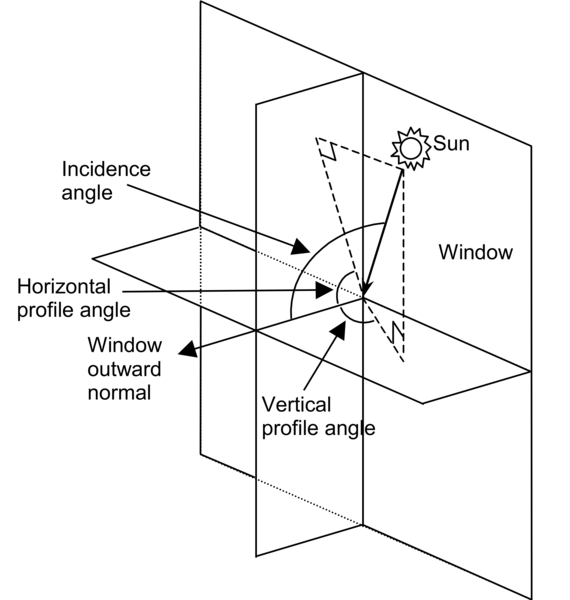
\includegraphics[width=0.9\textwidth, height=0.9\textheight, keepaspectratio=true]{media/image058.png}
\caption{Vertical exterior window showing solar horizontal profile angle, solar vertical profile angle and solar incidence angle. \protect \label{fig:vertical-exterior-window-showing-solar}}
\end{figure}

\subsubsection{Surface Window Outside Reveal Reflected Beam Solar Radiation Rate {[}W{]}}\label{surface-window-outside-reveal-reflected-beam-solar-radiation-rate-w}

\subsubsection{Surface Window Outside Reveal Reflected Beam Solar Radiation Energy {[}J{]}}\label{surface-window-outside-reveal-reflected-beam-solar-radiation-energy-j}

Beam solar radiation reflected from the outside reveal surfaces of a window (ref: Reveal Surfaces under \hyperref[windowpropertyframeanddivider]{WindowProperty:FrameAndDivider} object). There are both rate and energy versions.

\subsubsection{Surface Window Inside Reveal Reflected Beam Solar Radiation Rate {[}W{]}}\label{surface-window-inside-reveal-reflected-beam-solar-radiation-rate-w}

\subsubsection{Surface Window Inside Reveal Reflected Beam Solar Radiation Energy {[}J{]}}\label{surface-window-inside-reveal-reflected-beam-solar-radiation-energy-j}

Beam solar radiation reflected from the inside reveal surfaces of a window (ref: Reveal Surfaces under \hyperref[windowpropertyframeanddivider]{WindowProperty:FrameAndDivider} object). There are both rate and energy versions.

\subsubsection{Surface Window Inside Reveal Absorbed Beam Solar Radiation Rate {[}W{]}}\label{surface-window-inside-reveal-absorbed-beam-solar-radiation-rate-w}

Beam solar radiation absorbed at the inside reveal surfaces of a window, in Watts.

\subsubsection{Surface Window Inside Reveal Reflected Diffuse Zone Solar Radiation Rate {[}W{]}}\label{surface-window-inside-reveal-reflected-diffuse-zone-solar-radiation-rate-w}

Diffuse solar radiation reflected from inside reveal surfaces of a window into the zone, in Watts.

\subsubsection{Surface Window Inside Reveal Reflected Diffuse Frame Solar Radiation Rate {[}W{]}}\label{surface-window-inside-reveal-reflected-diffuse-frame-solar-radiation-rate-w}

Diffuse solar radiation reflected from inside reveal surfaces onto the frame surfaces of a window, in Watts.

\subsubsection{Surface Window Inside Reveal Reflected Diffuse Glazing Solar Radiation Rate {[}W{]}}\label{surface-window-inside-reveal-reflected-diffuse-glazing-solar-radiation-rate-w}

Diffuse solar radiation reflected from inside reveal surfaces onto the glazing surfaces of a window, in Watts.

\subsubsection{Surface Window Inside Face Glazing Condensation Status {[]}}\label{surface-window-inside-face-glazing-condensation-status}

A value of 1 means that moisture condensation will occur on the innermost glass face of an exterior window (i.e., on the glass face in contact with the zone air). Otherwise the value is 0. The condition for condensation is glass inside face temperature \textless{} zone air dewpoint temperature.

For airflow exterior windows, in which forced air passes between adjacent glass faces in double- and triple-pane windows, a value of 1 means that condensation will occur on one or both of the glass faces in contact with the airflow. In this case the condition for condensation is:

\begin{itemize}
\item
  \emph{For airflow source = indoorair}, temperature of either face in contact with airflow \textless{} zone air dewpoint temperature.
\item
  \emph{For airflow source = outdoorair}, temperature of either face in contact with airflow \textless{} outside air dewpoint temperature.
\end{itemize}

As for regular windows, the value will also be 1 if condensation occurs on the innermost glass face.

\subsubsection{Surface Window Inside Face Frame Condensation Status {[]}}\label{surface-window-inside-face-frame-condensation-status}

If an exterior window has a frame and the value of this flag is 1, condensation will occur on the inside surface of the frame. The condition for condensation is frame inside surface temperature \textless{} zone air dewpoint temperature.

\subsubsection{Surface Window Inside Face Divider Condensation Status {[]}}\label{surface-window-inside-face-divider-condensation-status}

If an exterior window has a divider and the value of this flag is 1, condensation will occur on the inside surface of the divider. The condition for condensation is divider inside surface temperature \textless{} zone air dewpoint temperature.

\subsubsection{Surface Shading Device Is On Time Fraction {[]}}\label{surface-shading-device-is-on-time-fraction}

The fraction of time that a shading device is on an exterior window. For a particular simulation timestep, the value is 0.0 if the shading device is off (or there is no shading device) and the value is 1.0 if the shading device is on. (It is assumed that the shading device, if present, is either on or off for the entire timestep.) If the shading device is switchable glazing, a value of 0.0 means that the glazing is in the unswitched (light colored) state, and a value of 1.0 means that the glazing is in the switched (dark colored) state.

For a time interval longer a timestep, this is the fraction of the time interval that the shading device is on. For example, take the case where the time interval is one hour and the timestep is 10 minutes. Then if the shading device is on for two timesteps in the hour and off for the other four timesteps, then the fraction of time that the shading device is on = 2/6 = 0.3333.

\subsubsection{Surface Window Blind Slat Angle {[}deg{]}}\label{surface-window-blind-slat-angle-deg}

For an exterior window with a blind, this is the angle in degrees between the glazing outward normal and the blind slat angle outward normal, where the outward normal points away from the front face of the slat. The slat angle varies from 0 to 180 deg. If the slat angle is 0 deg or 180 deg, the slats are parallel to the glazing and the slats are said to be ``closed''. If the slat angle is 90 deg, the slats are perpendicular to the glazing and the slats are said to be ``fully open''. See illustrations under \hyperref[windowmaterialblind]{WindowMaterial:Blind}. For blinds with a fixed slat angle, the value reported here will be constant.

For \hyperref[windowmaterialblindequivalentlayer]{WindowMaterial:Blind:EquivalentLayer} blinds the slat angle varies from -90 to 90 deg. If the slat angle is -90 deg or 90 deg, the slats are parallel to the glazing and the slats are said to be ``closed''. If the slat angle is 0 deg, the slats are perpendicular to the glazing and the slats are said to be ``fully open''. For blinds with a fixed slat angle, the value reported here will be constant.


\subsubsection{Surface Window Blind Beam to Beam Solar Transmittance {[]}}\label{surface-window-blind-beam-to-beam-solar-transmittance}

For an exterior window with a blind, this is the fraction of exterior beam solar radiation incident on the blind that is transmitted through the blind as beam solar radiation when the blind is isolated (i.e., as though the window glass were not present). Depends on various factors, including slat angle, width, separation, and thickness, and horizontal solar profile angle (for blinds with horizontal slats) or vertical solar profile angle (for blinds with vertical slats). The transmittance value reported here will be non-zero only when some beam solar can pass through the blind without hitting the slats.

\subsubsection{Surface Window Blind Beam to Diffuse Solar Transmittance {[]}}\label{surface-window-blind-beam-to-diffuse-solar-transmittance}

For an exterior window with a blind, the fraction of exterior beam solar radiation incident on the blind that is transmitted through the blind as diffuse solar radiation when the blind is isolated (i.e., as though the window glass were not present). Depends on various factors, including slat angle, width, separation, thickness and reflectance, and horizontal solar profile angle (for blinds with horizontal slats) or vertical solar profile angle (for blinds with vertical slats).

\subsubsection{Surface Window Blind Diffuse to Diffuse Solar Transmittance {[]}}\label{surface-window-blind-diffuse-to-diffuse-solar-transmittance}

For an exterior window with a blind, the fraction of exterior diffuse solar radiation incident on the blind that is transmitted through the blind as diffuse solar radiation when the blind is isolated (i.e., as though the window glass were not present). Depends on various factors, including slat angle, width, separation, thickness and reflectance. For blinds with a fixed slat angle the transmittance value reported here will be constant.

\subsubsection{Surface Window Blind and Glazing System Beam Solar Transmittance {[]}}\label{surface-window-blind-and-glazing-system-beam-solar-transmittance}

The fraction of exterior beam solar radiation incident on an exterior window with a blind (excluding window frame, if present) that is transmitted through the blind/glass system as beam solar radiation. Depends on various factors, including type of glass; solar incidence angle; slat angle, width, separation, and thickness; and horizontal solar profile angle (for blinds with horizontal slats) or vertical solar profile angle (for blinds with vertical slats).

\subsubsection{Surface Window Blind and Glazing System Diffuse Solar Transmittance {[]}}\label{surface-window-blind-and-glazing-system-diffuse-solar-transmittance}

The fraction of exterior diffuse solar radiation incident on an exterior window with a blind (excluding window frame, if present) that is transmitted through the blind/glass system as diffuse solar radiation. Depends on various factors, including type of glass and slat angle, width, separation, thickness and reflectance. For blinds with a fixed slat angle the transmittance value reported here will be constant.

\subsubsection{Surface Window Screen Beam to Beam Solar Transmittance {[]}}\label{surface-window-screen-beam-to-beam-solar-transmittance}

For an exterior window with a screen, this is the fraction of exterior beam solar radiation incident on the screen that is transmitted through the screen as beam solar radiation when the screen is isolated (i.e., as though the window glass were not present). Depends on various factors, including the screen reflectance and the relative angle of the incident beam with respect to the screen. This value will include the amount of inward reflection of solar beam off the screen material surface if the user specifies this modeling option (i.e., Material: WindowScreen, field Reflected Beam Transmittance Accounting Method = Model as Direct Beam).

\subsubsection{Surface Window Screen Beam to Diffuse Solar Transmittance{[]}}\label{surface-window-screen-beam-to-diffuse-solar-transmittance}

For an exterior window with a screen, the fraction of exterior beam solar radiation incident on the screen that is transmitted through the screen as diffuse solar radiation when the screen is isolated (i.e., as though the window glass were not present). Depends on various factors, including the screen reflectance and the relative angle of the incident beam with respect to the screen. This value is the amount of inward reflection of solar beam off the screen material surface if the user specifies this modeling option (i.e., Material: WindowScreen, field Reflected Beam Transmittance Accounting Method = Model as Diffuse); otherwise, this value will be zero.

\subsubsection{Surface Window Screen Diffuse to Diffuse Solar Transmittance{[]}}\label{surface-window-screen-diffuse-to-diffuse-solar-transmittance}

For an exterior window with a screen, the fraction of exterior diffuse solar radiation incident on the screen that is transmitted through the screen as diffuse solar radiation when the screen is isolated (i.e., as though the window glass were not present). Depends on various factors including screen material geometry and reflectance. This value is calculated as an average, constant For a window with a screen, this value consists of diffuse radiation transmitted through the screen (gaps between the screen material) and diffuse radiation from diffuse-to-diffuse reflection from the screen material. For a window with a screen, this value consists of diffuse radiation transmitted through the screen (gaps between the screen material) and diffuse radiation from diffuse-to-diffuse reflection from the screen material.

\subsubsection{Surface Window Screen and Glazing System Beam Solar Transmittance{[]}}\label{surface-window-screen-and-glazing-system-beam-solar-transmittance}

The fraction of exterior beam solar radiation incident on an exterior window with a screen (excluding window frame, if present) that is transmitted through the screen/glass system as beam solar radiation. Depends on various factors, including the screen reflectance and the relative angle of the incident beam with respect to the screen. This value will include the amount of inward reflection of solar beam off the screen material surface if the user specifies this modeling option (i.e., Material: WindowScreen, field Reflected Beam Transmittance Accounting Method = Model as Direct Beam).

\subsubsection{Surface Window Screen and Glazing System Diffuse Solar Transmittance {[]}}\label{surface-window-screen-and-glazing-system-diffuse-solar-transmittance}

The fraction of exterior diffuse solar radiation incident on an exterior window with a screen (excluding window frame, if present) that is transmitted through the screen/glass system as diffuse solar radiation. Depends on various factors including screen material geometry and reflectance.

\subsubsection{Surface Window Transmitted Beam Solar Radiation Rate {[}W{]}}\label{surface-window-transmitted-beam-solar-radiation-rate-w-1}

\subsubsection{Surface Window Transmitted Beam Solar Radiation Energy {[}J{]}}\label{surface-window-transmitted-beam-solar-radiation-energy-j-1}

The beam solar radiation transmitted through an interior window. Calculated only if Solar Distribution = FullInteriorAndExterior in your Building input. The origin of this radiation is beam solar that enters through an exterior window in a zone and then passes through an interior window into the adjacent zone. The amount of this radiation depends on several factors, including sun position, intensity of beam solar incident on the exterior window (including effects of shadowing, if present), relative position of the exterior and interior window, and the size and transmittance of the windows. Note that if there are two or more exterior windows in a zone, then beam solar from one or more of them may pass through the same interior window. Likewise, if there are more than two or more interior windows in a zone then beam solar from a single exterior window may pass through one or more of the interior windows. There are both rate and energy versions of the output.

\subsubsection{Surface Storm Window On Off Status {[]}}\label{surface-storm-window-on-off-status}

Indicates whether a storm window glass layer is present (ref: StormWindow object). The value is \textbf{0} if the storm window glass layer is off, \textbf{1} if it is on, and \textbf{--1} if the window does not have an associated storm window. Applicable only to exterior windows and glass doors.

\subsubsection{Surface Inside Face Initial Transmitted Diffuse Transmitted Out Window Solar Radiation Rate {[}W{]}}\label{surface-inside-face-initial-transmitted-diffuse-transmitted-out-window-solar-radiation-rate-w}

As of Version 2.1, the diffuse solar transmitted through exterior windows that is initially distributed to another window in the zone and transmitted out of the zone through that window. For exterior windows, this transmitted diffuse solar is ``lost'' to the exterior environment For interior windows, this transmitted diffuse solar is distributed to heat transfer surfaces in the adjacent zone, and is part of the Surface Inside Face Initial Transmitted Diffuse Absorbed Solar Radiation Rate for these adjacent zone surfaces.

\subsubsection{Additional Window Outputs (Advanced)}\label{additional-window-outputs-advanced}

The following output variables for windows or glass doors are available when the user requests to display advanced output variables. These seven reports show the individual components that are combined to determine overall Surface Window Heat Gain Rate and/or Surface Window Heat Loss Rate (described above).

\subsubsection{Surface Window Inside Face Glazing Zone Convection Heat Gain Rate {[}W{]}}\label{surface-window-inside-face-glazing-zone-convection-heat-gain-rate-w}

The surface convection heat transfer from the glazing to the zone in watts. This output variable is the term called ``{[}Convective heat flow to the zone from the zone side of the glazing{]}'' under the description above for Surface Window Heat Gain Rate output variable. If the window has an interior shade or blind, then this is zero and the glazing's convection is included in the report called ``Surface Window Inside Face Gap between Shade and Glazing Zone Convection Heat Gain Rate''.

\subsubsection{Surface Window Inside Face Glazing Net Infrared Heat Transfer Rate {[}W{]}}\label{surface-window-inside-face-glazing-net-infrared-heat-transfer-rate-w}

The net exchange of infrared radiation heat transfer from the glazing to the zone in watts. This output variable is the term called ``{[}Net IR heat flow to the zone from zone side of the glazing{]}'' under the description above for Surface Window Heat Gain Rate output variable.

\subsubsection{Surface Window Shortwave from Zone Back Out Window Heat Transfer Rate {[}W{]}}\label{surface-window-shortwave-from-zone-back-out-window-heat-transfer-rate-w}

This is the short-wave radiation heat transfer from the zone back out the window in watts. This is a measure of the diffuse short-wave light (from reflected solar and electric lighting) that leave the zone through the window. This output variable is the term called ``{[}Short-wave radiation from zone transmitted back out the window{]}'' under the description above for Surface Window Heat Gain Rate output variable.

\subsubsection{Surface Window Inside Face Frame and Divider Zone Heat Gain Rate {[}W{]}}\label{surface-window-inside-face-frame-and-divider-zone-heat-gain-rate-w}

This is the heat transfer from any frames and/or dividers to the zone in watts. This output variable is the term called ``{[}Conduction to zone from window frame and divider, if present{]}'' under the description above for Surface Window Heat Gain Rate output variable. (The word ``conduction'' here is used because the models is simplified compared to the complexities of surface convection and radiation.)

\subsubsection{Surface Window Frame Heat Gain Rate {[}W{]}}\label{surface-window-frame-heat-gain-rate-w}

This is the positive heat flow from window frames to the zone in watts. This is part of the Surface Window Inside Face Frame and Divider Zone Heat Gain Rate.

\subsubsection{Surface Window Frame Heat Loss Rate {[}W{]}}\label{surface-window-frame-heat-loss-rate-w}

This is the negative heat flow from window frames to the zone in watts. This is part of the Surface Window Inside Face Frame and Divider Zone Heat Gain Rate.

\subsubsection{Surface Window Frame Inside Temperature {[}C{]}}\label{surface-window-frame-inside-temperature-c}

This is the temperature of the inside surface of the window frames.

\subsubsection{Surface Window Frame Outside Temperature {[}C{]}}\label{surface-window-frame-outside-temperature-c}

This is the temperature of the outside surface of the window frames.

\subsubsection{Surface Window Divider Heat Gain Rate {[}W{]}}\label{surface-window-divider-heat-gain-rate-w}

This is the positive heat flow from window dividers to the zone in watts. This is part of the Surface Window Inside Face Frame and Divider Zone Heat Gain Rate.

\subsubsection{Surface Window Divider Heat Loss Rate {[}W{]}}\label{surface-window-divider-heat-loss-rate-w}

This is the negative heat flow from window dividers to the zone in watts. This is part of the Surface Window Inside Face Frame and Divider Zone Heat Gain Rate.

\subsubsection{Surface Window Divider Inside Temperature {[}C{]}}\label{surface-window-divider-inside-temperature-c}

This is the temperature of the inside surface of the window dividers.

\subsubsection{Surface Window Divider Outside Temperature {[}C{]}}\label{surface-window-divider-outside-temperature-c}

This is the temperature of the outside surface of the window dividers.

\subsubsection{Surface Window Inside Face Gap between Shade and Glazing Zone Convection Heat Gain Rate {[}W{]}}\label{surface-window-inside-face-gap-between-shade-and-glazing-zone-convection-heat-gain-rate-w}

This is the convection surface heat transfer from the both the glazing and the shade's back face to the zone in Watts. This output variable is the term called ``{[}Convective heat flow to the zone from the air flowing through the gap between glazing and shading device{]}'' under the description above for Surface Window Heat Gain Rate output variable. For Equivalent Layer window this output variable is the convection heat gain from vented interior air gap to the zone in Watts.

\subsubsection{Surface Window Inside Face Shade Zone Convection Heat Gain Rate {[}W{]}}\label{surface-window-inside-face-shade-zone-convection-heat-gain-rate-w}

This is the convection surface heat transfer from the front side of any interior shade or blind to the zone in Watts. This output variable is the term called ``{[}Convective heat flow to the zone from the zone side of the shading device{]}'' under the description above for Surface Window Heat Gain Rate output variable. For equivalent Layer window this output variable is the convection heat gain rate from the inside face of a glazing or a shade to the zone in Watts.

\subsubsection{Surface Window Inside Face Shade Net Infrared Heat Transfer Rate {[}W{]}}\label{surface-window-inside-face-shade-net-infrared-heat-transfer-rate-w}

The net exchange of infrared radiation heat transfer from the shade or blind to the zone in watts. This output variable is the term called ``{[}Net IR heat flow to the zone from the zone side of the shading device{]}'' under the description above for Surface Window Heat Gain Rate output variable.

\subsubsection{Surface Window Inside Face Other Convection Heat Gain Rate {[}W{]}}\label{surface-window-inside-face-other-convection-heat-gain-rate-w}

The other (extra) convection heat transfer rate from the inside face of a an equivalent layer window. This output is computed from the difference in convection flux when using equivalent inside surface temperature of a window instead of the inside surface temperature from the standard surface heat balance calculation.

\subsection{Thermochromic Window Outputs}\label{thermochomic-window-outputs}

\subsubsection{Window Thermochromic Layer Temperature {[}C{]}}\label{window-thermochromic-layer-temperature-c}

The temperature of the TC glass layer of a TC window at each time step.

\subsubsection{Surface Window Thermochromic Layer Property Specification Temperature {[}C{]}}\label{surface-window-thermochromic-layer-property-specification-temperature-c-000}

The temperature under which the optical data of the TC glass layer are specified.

The overall properties (U-factor/SHGC/VT) of the thermochromic windows at different specification temperatures are reported in the \textbf{.eio} file. These window constructions are created by EnergyPlus during run time. They have similar names with suffix ``\_TC\_XX'' where XX represents a specification temperature.

\subsubsection{Switchable Window Outputs}\label{switchable-window-outputs}

\subsubsection{Surface Window Switchable Glazing Switching Factor{[]}}\label{surface-window-switchable-glazing-switching-factor}

The switching factor (tint level) of the switchable window: 0 means no switching -- clear state; 1 means fully switched -- dark state.

\subsubsection{Surface Window Switchable Glazing Visible Transmittance{[]}}\label{surface-window-switchable-glazing-visible-transmittance}

The visible transmittance of the switchable window.

\subsection{Other Surface Outputs/Reports}\label{other-surface-outputsreports}

Several reports can be selected for Surfaces. (See Group -- Report for details on how to specify). Examples are:

\subsubsection{DXF}\label{dxf}

This report produces a special file (\textbf{eplusout.dxf}) in the industry standard DXF (Drawing Interchange Format) for drawings. It is produced and accepted by many popular, commercial CAD programs. Detailed reference can be found on the AutoCAD\textsuperscript{TM} website at: \url{http://www.autodesk.com/techpubs/autocad/acadr14/dxf/index.htm}.

EnergyPlus produces this file from the Report command:

\begin{lstlisting}

Output:Reports, Surfaces, DXF;
\end{lstlisting}

\subsubsection{Details, Vertices, DetailsWithVertices}\label{details-vertices-detailswithvertices}

This version of the report creates lines in the eplusout.eio file for each surface (except internal mass surfaces). Details of this reporting is shown in the Output Details and Examples document.

\subsection{Shading Surfaces}\label{shading-surfaces}

Shading surfaces are entities outside of the building that may cast shadows on the building's heat transfer surfaces. These entities do not typically have enough thermal mass to be described as part of the building's thermal makeup.

The most important effect of shading surfaces is to reduce solar gain in windows that are shadowed. (However, in some cases, shading surfaces can reflect solar onto a wall or window and increase solar gain.)

There are two kinds of shading surfaces in EnergyPlus: \textbf{detached} and \textbf{attached}. A \textbf{detached} shading surface, such as a tree or neighboring building, is not connected to the building. An \textbf{attached} shading surface is typically an overhang or fin that is attached to a particular base surface of the building, usually a wall; attached shading surfaces are usually designed to shade specific windows.

Objects for detached shading surfaces:

\begin{itemize}
\item
  \hyperref[shadingsite-shadingbuilding]{Shading:Site}
\item
  \hyperref[shadingsite-shadingbuilding]{Shading:Building}
\item
  \hyperref[shadingsitedetailed-shadingbuildingdetailed]{Shading:Site:Detailed}
\item
  \hyperref[shadingsitedetailed-shadingbuildingdetailed]{Shading:Building:Detailed}
\end{itemize}

Similarly to the surfaces, the detailed objects use vertex entry whereas the other objects are limited to rectangular representation.

Objects for attached shading surfaces:

\begin{itemize}
\item
  \hyperref[shadingoverhang]{Shading:Overhang}
\item
  \hyperref[shadingoverhangprojection]{Shading:Overhang:Projection}
\item
  \hyperref[shadingfin]{Shading:Fin}
\item
  \hyperref[shadingfinprojection]{Shading:Fin:Projection}
\item
  \hyperref[shadingzonedetailed-000]{Shading:Zone:Detailed}
\end{itemize}

EnergyPlus creates ``bi-directional'' shades from each shading surface entered. This means that the shade you input will cast a shadow no matter which side of the shade the sun is on. For example, a vertical fin will cast a shadow whether the sun is on the left side or right side of the fin. Prior to V1.0.2, a shading surface cast a shadow only in the hemisphere toward which the surface faced. This hemisphere is the one pointed to by the shading surface's outward normal vector, which is the cross product V23 x V21, where V23 is the vector from vertex 2 to vertex 3 of the shading surface and V21 is the vector from vertex 2 to vertex 1. Beginning with V1.0.2, the shades in EnergyPlus are ``bi-directional'' so that they can cast shadows in both hemispheres depending on the time-varying position of the sun relative to the shading surface.

It is important to note that EnergyPlus will automatically account for ``self-shading'' effects---such as in L-shaped buildings---in which some of the building's wall and roof surfaces shade other parts of the building, especially windows. This means that you only need to describe shading elements that aren't building heat-transfer surfaces.

Shading surfaces can also \textbf{reflect} solar radiation onto the building. This feature is simulated if you choose FullExteriorWithReflections or FullInteriorAndExteriorWithReflections in the Building object (ref: Building - Field: Solar Distribution). In this case, you may specify the reflectance properties of a shading surface with the \hyperref[shadingpropertyreflectance]{ShadingProperty:Reflectance} object. Note: If no \hyperref[shadingpropertyreflectance]{ShadingProperty:Reflectance} object is defined, then the shading surface reflectance values are assumed to be 0.2 and the fraction of shading surface that is glazed is assumed to be 0.0.

Shading surfaces also automatically shade diffuse solar radiation (and long-wave radiation) from the sky. And they will automatically shade diffuse solar radiation from the ground if Solar Distribution Field = FullExteriorWithReflections or FullInteriorAndExteriorWithReflections in the Building object. (If the reflections option for Solar Distribution is used, the program also takes into account the reduction of solar radiation reflected from the ground due to shading of the ground by shading surfaces and by the building itself.) Otherwise, shading surfaces will not shade diffuse radiation from the ground unless you enter a reduced value for View Factor to Ground for those building surfaces that are shaded (ref: \hyperref[buildingsurfacedetailed]{BuildingSurface:Detailed} - Field: View Factor to Ground and \hyperref[fenestrationsurfacedetailed]{FenestrationSurface:Detailed} - Field: View Factor to Ground).

\subsection{Detached Shading Surfaces}\label{detached-shading-surfaces}

\subsection{Shading:Site, Shading:Building}\label{shadingsite-shadingbuilding}

These objects are used to describe rectangular shading elements that are external to the building. Examples are trees, high fences, near-by hills, and neighboring buildings.

If relative coordinates are used (ref: Field: Coordinate System in \hyperref[globalgeometryrules]{GlobalGeometryRules}), shading surfaces entered with \hyperref[shadingsite-shadingbuilding]{Shading:Site} remain stationary if the building is rotated, whereas those entered with \hyperref[shadingsite-shadingbuilding]{Shading:Building} rotate with the building. If world coordinates are used \hyperref[shadingsite-shadingbuilding]{Shading:Site} and \hyperref[shadingsite-shadingbuilding]{Shading:Building} are equivalent.

These shading elements are always opaque.

\subsubsection{Field: Name}\label{field-name-22-004}

This is a unique character string associated with the detached shading surface. Though it must be unique from other surface names, it is used primarily for convenience with detached shading surfaces.

\subsubsection{Field: Azimuth Angle}\label{field-azimuth-angle-10}

Theoretically, this should face to the surface it is shading (i.e.~if a south wall, this should be a north facing shade) but since EnergyPlus automatically generates the mirror image, the facing angle per se' is not so important.

\subsubsection{Field: Tilt Angle}\label{field-tilt-angle-10}

The tilt angle is the angle (in degrees) that the shade is tilted from horizontal (or the ground). Default for this field is 90 degrees.

\subsubsection{Starting Corner for the surface}\label{starting-corner-for-the-surface-16}

The rectangular surfaces specify the lower left corner of the surface for their starting coordinate. See the introductory paragraph for rules on this entry.

\subsubsection{Field: Starting X Coordinate}\label{field-starting-x-coordinate-16}

This field is the X coordinate (in meters).

\subsubsection{Field: Starting Y Coordinate}\label{field-starting-y-coordinate-10}

This field is the Y coordinate (in meters).

\subsubsection{Field: Starting Z Coordinate}\label{field-starting-z-coordinate-16}

This field is the Z coordinate (in meters).

\subsubsection{Field: Length}\label{field-length-16}

This field is the length of the shade in meters.

\subsubsection{Field: Height}\label{field-height-10}

This field is the width of the shade in meters.

Examples of these (can be found in example files 4ZoneWithShading\_Simple\_1.idf and 4ZoneWithShading\_Simple\_2.idf)

\begin{lstlisting}

  Shading:Building,
      Bushes-East,             !- Name
      90,                      !- Azimuth Angle {deg}
      90,                      !- Tilt Angle {deg}
      45,                      !- Starting X Coordinate {m}
      0,                       !- Starting Y Coordinate {m}
      0,                       !- Starting Z Coordinate {m}
      50,                      !- Length {m}
      1;                       !- Height {m}

    Shading:Site,
      Bushes-North,            !- Name
      0,                       !- Azimuth Angle {deg}
      90,                      !- Tilt Angle {deg}
      45,                      !- Starting X Coordinate {m}
      50,                      !- Starting Y Coordinate {m}
      0,                       !- Starting Z Coordinate {m}
      50,                      !- Length {m}
      1;                       !- Height {m}
\end{lstlisting}

\subsection{Shading:Site:Detailed, Shading:Building:Detailed}\label{shadingsitedetailed-shadingbuildingdetailed}

These objects are used to describe shading elements that are external to the building. Examples are trees, high fences, near-by hills, and neighboring buildings.

If relative coordinates are used (ref: Field: Coordinate System in \hyperref[globalgeometryrules]{GlobalGeometryRules}), shading surfaces entered with \hyperref[shadingsitedetailed-shadingbuildingdetailed]{Shading:Site:Detailed} remain stationary if the building is rotated, whereas those entered with \hyperref[shadingsitedetailed-shadingbuildingdetailed]{Shading:Building:Detailed} rotate with the building. If world coordinates are used \hyperref[shadingsitedetailed-shadingbuildingdetailed]{Shading:Site:Detailed} and \hyperref[shadingsitedetailed-shadingbuildingdetailed]{Shading:Building:Detailed} are equivalent.

While ``detached'' implies that shading surfaces are not part of the building, the detached shading sequence can be used to describe attached shading surfaces that may shade heat transfer surfaces in more than one zone. For example, wing A of a building might shade several zones of wing B but wing A (for whatever reason) is not described in the geometry for the simulation so it is represented by a detached shade to get its shadowing effect.

\subsubsection{Field: Name}\label{field-name-23-004}

This is a unique character string associated with the detached shading surface. Though it must be unique from other surface names, it is used primarily for convenience with detached shading surfaces.

\subsubsection{Field: Transmittance Schedule Name}\label{field-transmittance-schedule-name}

The name of a schedule of solar transmittance values from 0.0 to 1.0 for the shading surface. If a blank is entered in this field, the transmittance value defaults to 0.0, i.e., the shading surface is opaque at all times. This scheduling can be used to allow for seasonal transmittance change, such as for deciduous trees that have a higher transmittance in winter than in summer. Transmittance based on time of day can also be used---a movable awning, for example, where the transmittance is some value less than 1.0 when the awning is in place and is 1.0 when the awning is retracted.

The following assumptions are made in the shading surface transmittance calculation:

\begin{itemize}
\item
  Both sides of the shading surface have the same transmittance properties.
\item
  The transmittance is the same for both beam and diffuse solar radiation.
\item
  Beam solar transmittance is independent of angle of incidence on the shading surface.
\item
  Beam radiation incident on a shading surface is transmitted as beam radiation with no change in direction, i.e., there is no beam-to-diffuse component.
\item
  If two shading surfaces with non-zero transmittance overlap, the net transmittance is the product of the individual transmittances. Inter-reflection between the shading surfaces (and between the shading surfaces and the building) is ignored.
\item
  For the daylighting calculation (ref: Group -- Daylighting) the shading surface's visible transmittance is assumed to be the same as its solar transmittance.
\item
  Shading devices are assumed to be opaque to long-wave radiation no matter what the solar transmittance value is.
\end{itemize}

Note that shading devices only shade solar radiation when the sun is up, which is automatically determined by EnergyPlus from latitude, time of year, etc. The user need only account for the time-varying transmittance of the shading device in the transmittance schedule, not whether the sun is up or not.

\subsubsection{Field: Number Vertices}\label{field-number-vertices}

The number of sides in the surface (number of X,Y,Z vertex groups). For further information, see the discussion on ``Surface Vertices'' above.

IDF example of Detached Shading Surfaces:

\begin{lstlisting}

Shading:Building:Detailed,
     EAST SIDE TREE,  !- Detached Shading
     ShadingTransmittance:0002,  !- Shadowing Transmittance & Schedule
     3, !-Triangle
     33.52800    ,   10.66800    ,   10.05800    ,
     33.52800    ,   13.71600    ,  0.9140000    ,
     33.52800    ,   4.572000    ,  0.9140000    ;

  Shading:Building:Detailed,
     WEST SIDE TREE,  !- Detached Shading
     ShadingTransmittance:0002,  !- Shadowing Transmittance & Schedule
     3, !-Triangle
    -3.048000    ,   7.620000    ,   10.05800    ,
    -3.048000    ,   4.572000    ,  0.9140000    ,
    -3.048000    ,   13.71600    ,  0.9140000    ;
\end{lstlisting}

\subsection{Attached Shading Surfaces}\label{attached-shading-surfaces}

Overhangs are usually horizontal devices that are used to shade windows. Fins are usually vertical devices that similarly shade windows.

\subsection{Shading:Overhang}\label{shadingoverhang}

An overhang typically is used to shade a window in a building.

\subsubsection{Inputs}\label{inputs-26-003}

\paragraph{Field: Name}\label{field-name-24-003}

This is the name of the overhang. It must be different from other surface names.

\paragraph{Field: Window or Door Name}\label{field-window-or-door-name}

The name of a window or door that this overhang shades.

\paragraph{Field: Height above Window or Door}\label{field-height-above-window-or-door}

This field is the height (meters) above the top of the door for the overhang.

\paragraph{Field Tilt Angle from Window/Door}\label{field-tilt-angle-from-windowdoor}

This field is the tilt angle from the Window/Door. For a flat overhang, this would be 90 (degrees).

\paragraph{Field: Left Extension from Window/Door Width}\label{field-left-extension-from-windowdoor-width}

This field is the width from the left edge of the window/door to the start of the overhang (meters).

\paragraph{Field: Right Extension from Window/Door Width}\label{field-right-extension-from-windowdoor-width}

This field is the width from the right edge of the window/door to the start of the overhang (meters).

\paragraph{Field: Depth}\label{field-depth}

This field is the depth of the overhang (meters) projecting out from the wall.

\subsection{Shading:Overhang:Projection}\label{shadingoverhangprojection}

An overhang typically is used to shade a window in a building. This object allows for specifying the depth of the overhang as a fraction of the window or door's height.

\subsubsection{Inputs}\label{inputs-27-003}

\paragraph{Field: Name}\label{field-name-25-003}

This is the name of the overhang. It must be different from other surface names.

\paragraph{Field: Window or Door Name}\label{field-window-or-door-name-1}

The name of a window or door that this overhang shades.

\paragraph{Field: Height above Window or Door}\label{field-height-above-window-or-door-1}

This field is the height (meters) above the top of the door for the overhang.

\paragraph{Field Tilt Angle from Window/Door}\label{field-tilt-angle-from-windowdoor-1}

This field is the tilt angle from the Window/Door. For a flat overhang, this would be 90 (degrees).

\paragraph{Field: Left Extension from Window/Door Width}\label{field-left-extension-from-windowdoor-width-1}

This field is the width from the left edge of the window/door to the start of the overhang (meters).

\paragraph{Field: Right Extension from Window/Door Width}\label{field-right-extension-from-windowdoor-width-1}

This field is the width from the right edge of the window/door to the start of the overhang (meters).

\paragraph{Field: Depth as Fraction of Window/Door Height}\label{field-depth-as-fraction-of-windowdoor-height}

This field is the fraction of the window/door height to specify as the depth of the overhang (meters) projecting out from the wall.

\subsection{Shading:Fin}\label{shadingfin}

Fins shade either side of windows/doors in a building. This object allows for specification of both fins for the window. Fin placement is relative to the edge of the glass and user must include the frame width when a frame is present.

\subsubsection{Inputs}\label{inputs-28-002}

\paragraph{Field: Name}\label{field-name-26-003}

This is the name of the fin. It must be different from other surface names.

\paragraph{Field: Window or Door Name}\label{field-window-or-door-name-2}

The name of a window or door that this fin shades.

\paragraph{Field: Left Fin Extension from Window/Door}\label{field-left-fin-extension-from-windowdoor}

This field is the width from the left edge of the window/door to the plane of the left fin (meters). The extension width is relative to the edge of the glass and includes the frame width when a frame is present.

\paragraph{Field: Left Fin Distance Above Top of Window}\label{field-left-fin-distance-above-top-of-window}

This field is the distance from the top of the window to the top of the left fin (meters) and is relative to the edge of the glass and includes the frame width when a frame is present.

\paragraph{Field: Left Fin Distance Below Bottom of Window}\label{field-left-fin-distance-below-bottom-of-window}

This field is the distance from the bottom of the window to the bottom of the left fin (meters) and is relative to the edge of the glass and includes the frame width when a frame is present.

\paragraph{Field: Left Fin Tilt Angle from Window/Door}\label{field-left-fin-tilt-angle-from-windowdoor}

This field is the tilt angle from the window / door for the left fin. Typically, a fin is 90 degrees (default) from its associated window/door.

\paragraph{Field: Left Fin Depth}\label{field-left-fin-depth}

This field is the depth (meters) of the left fin (projecting out from the wall).

\paragraph{Field: Right Fin Extension from Window/Door}\label{field-right-fin-extension-from-windowdoor}

This field is the width from the right edge of the window/door to the plane of the right fin (meters). The extension width is relative to the edge of the glass and includes the frame width when a frame is present.

\paragraph{Field: Right Fin Distance Above Top of Window}\label{field-right-fin-distance-above-top-of-window}

This field is the distance from the top of the window to the top of the right fin (meters) and is relative to the edge of the glass and includes the frame width when a frame is present.

\paragraph{Field: Right Fin Distance Below Bottom of Window}\label{field-right-fin-distance-below-bottom-of-window}

This field is the distance from the bottom of the window to the bottom of the right fin (meters) and is relative to the edge of the glass and includes the frame width.

\paragraph{Field: Right Fin Tilt Angle from Window/Door}\label{field-right-fin-tilt-angle-from-windowdoor}

This field is the tilt angle from the window / door for the right fin. Typically, a fin is 90 degrees (default) from its associated window/door.

\paragraph{Field: Right Fin Depth}\label{field-right-fin-depth}

This field is the depth (meters) of the right fin (projecting out from the wall).

\subsection{Shading:Fin:Projection}\label{shadingfinprojection}

Fins shade either side of windows/doors in a building. This object allows for specification of both fins for the window. This object allows for specifying the depth of the fin as a fraction of the window or door's width. Fin placement is relative to the edge of the glass and user must include the frame width when a frame is present.

\subsubsection{Inputs}\label{inputs-29-002}

\paragraph{Field: Name}\label{field-name-27-003}

This is the name of the fin. It must be different from other surface names.

\paragraph{Field: Window or Door Name}\label{field-window-or-door-name-3}

The name of a window or door that this fin shades.

\paragraph{Field: Left Fin Extension from Window/Door}\label{field-left-fin-extension-from-windowdoor-1}

This field is the width from the left edge of the window/door to the plane of the left fin (meters). The extension width is relative to the edge of the glass and includes the frame width when a frame is present.

\paragraph{Field: Left Fin Distance Above Top of Window}\label{field-left-fin-distance-above-top-of-window-1}

This field is the distance from the top of the window to the top of the left fin (meters) and is relative to the edge of the glass and includes the frame width when a frame is present.

\paragraph{Field: Left Fin Distance Below Bottom of Window}\label{field-left-fin-distance-below-bottom-of-window-1}

This field is the distance from the bottom of the window to the bottom of the left fin (meters) and is relative to the edge of the glass and includes the frame width when a frame is present.

\paragraph{Field: Left Fin Tilt Angle from Window/Door}\label{field-left-fin-tilt-angle-from-windowdoor-1}

This field is the tilt angle from the window / door for the left fin. Typically, a fin is 90 degrees (default) from its associated window/door.

\paragraph{Field: Left Fin Depth as Fraction of Window/Door Width}\label{field-left-fin-depth-as-fraction-of-windowdoor-width}

This field is the fraction of the window/door width to specify as the depth of the left fin (meters) projecting out from the wall.

\paragraph{Field: Right Fin Extension from Window/Door}\label{field-right-fin-extension-from-windowdoor-1}

This field is the width from the right edge of the window/door to the plane of the right fin (meters).. The extension width is relative to the edge of the glass and includes the frame width when a frame is present.

\paragraph{Field: Right Fin Distance Above Top of Window}\label{field-right-fin-distance-above-top-of-window-1}

This field is the distance from the top of the window to the top of the right fin (meters) and is relative to the edge of the glass and includes the frame width when a frame is present.

\paragraph{Field: Right Fin Distance Below Bottom of Window}\label{field-right-fin-distance-below-bottom-of-window-1}

This field is the distance from the bottom of the window to the bottom of the right fin (meters) and is relative to the edge of the glass and includes the frame width when a frame is present.

\paragraph{Field: Right Fin Tilt Angle from Window/Door}\label{field-right-fin-tilt-angle-from-windowdoor-1}

This field is the tilt angle from the window / door for the right fin. Typically, a fin is 90 degrees (default) from its associated window/door.

\paragraph{Field: Right Fin Depth as Fraction of Window/Door Width}\label{field-right-fin-depth-as-fraction-of-windowdoor-width}

This field is the fraction of the window/door width to specify as the depth of the right fin (meters) projecting out from the wall.

Examples of these (can be found in example files 4ZoneWithShading\_Simple\_1.idf and 4ZoneWithShading\_Simple\_2.idf)

\begin{lstlisting}

  Shading:Overhang:Projection,
      Zn001:Wall001:Win001:Shade001,  !- Name
      Zn001:Wall001:Win001,    !- Window or Door Name
      .7,                      !- Height above Window or Door {m}
      90,                      !- Tilt Angle from Window/Door {deg}
      .2,                      !- Left extension from Window/Door Width {m}
      .2,                      !- Right extension from Window/Door Width {m}
      .6;                      !- Depth as Fraction of Window/Door Height {m}

    Shading:Overhang,
      Zn001:Wall001:Door001:Shade001,  !- Name
      Zn001:Wall001:Door001,   !- Window or Door Name
      .6,                      !- Height above Window or Door {m}
      90,                      !- Tilt Angle from Window/Door {deg}
      0,                       !- Left extension from Window/Door Width {m}
      0,                       !- Right extension from Window/Door Width {m}
      3;                       !- Depth {m}

    Shading:Fin:Projection,
      Zn001:Wall001:Shade003,  !- Name
      Zn001:Wall001:Win001,    !- Window or Door Name
      .1,                      !- Left Extension from Window/Door {m}
      .1,                   !- Left Distance Above Top of Window {m}
      .1,                   !- Left Distance Below Bottom of Window {m}
      90,                   !- Left Tilt Angle from Window/Door {deg}
      .6,                   !- Left Depth as Fraction of Window/Door Width {m}
      .1,                   !- Right Extension from Window/Door {m}
      .1,                   !- Right Distance Above Top of Window {m}
      .1,                   !- Right Distance Below Bottom of Window {m}
      90,                   !- Right Tilt Angle from Window/Door {deg}
      .6;                   !- Right Depth as Fraction of Window/Door Width {m}
\end{lstlisting}

\subsection{Shading:Zone:Detailed}\label{shadingzonedetailed-000}

This object is used to describe attached ``subsurfaces'' such as overhangs, wings or fins that project outward from a base surface. This classification is used for convenience; actually, a device of this type can cast shadows on the surface to which it is attached as well as on adjacent surfaces. For example, a fin may shade its parent wall as well as adjacent walls.

Note that a zone surface can cast shadows on other zone surfaces. However, you don't have to worry about such effects---for example, one wall of an L-shaped building shading another wall--because EnergyPlus will automatically check for this kind of ``self shadowing'' and do the proper calculations.

Unlike attached (or detached) shading surfaces, building surfaces can only cast shadows in the hemisphere towards which they face. This means, for example, that a roof that faces \emph{upward} will not cast a shadow \emph{downward}. (Thus, specifying an oversized roof in an attempt to account for the shading effects of overhangs will \emph{not} work). Interior surfaces do not cast shadows of any kind.

\subsubsection{Inputs}\label{inputs-30-002}

\paragraph{Field: Name}\label{field-name-28-002}

This is the name of the attached shading surface. It must be different from other surface names.

\paragraph{Field: Base Surface Name}\label{field-base-surface-name}

This is the name of the surface to which this shading device is attached. This surface can be a wall (or roof) but not a window or door.

\paragraph{Field: Transmittance Schedule Name}\label{field-transmittance-schedule-name-1}

The name of a schedule of solar transmittance values from 0.0 to 1.0 for the shading surface. If a blank is entered in this field, the transmittance value defaults to 0.0, i.e., the shading surface is opaque at all times. This scheduling can be used to allow for seasonal transmittance change, such as for deciduous trees that have a higher transmittance in winter than in summer. Transmittance based on time of day can also be used---a movable awning, for example, where the transmittance is some value less than 1.0 when the awning is in place and is 1.0 when the awning is retracted.

The following assumptions are made in the shading surface transmittance calculation:

\begin{itemize}
\item
  Both sides of the shading surface have the same transmittance properties.
\item
  The transmittance is the same for both beam and diffuse solar radiation.
\item
  Beam solar transmittance is independent of angle of incidence on the shading surface.
\item
  Beam radiation incident on a shading surface is transmitted as beam radiation with no change in direction, i.e., there is no beam-to-diffuse component.
\item
  If two shading surfaces with non-zero transmittance overlap, the net transmittance is the product of the individual transmittances. Inter-reflection between the shading surfaces (and between the shading surfaces and the building) is ignored.
\item
  For the daylighting calculation (ref: Group -- Daylighting) the shading surface's visible transmittance is assumed to be the same as its solar transmittance.
\item
  Shading devices are assumed to be opaque to long-wave radiation no matter what the solar transmittance value is.
\end{itemize}

Note that shading devices only shade solar radiation when the sun is up, which is automatically determined by EnergyPlus from latitude, time of year, etc. The user need only account for the time-varying transmittance of the shading device in the transmittance schedule, not whether the sun is up or not.

\paragraph{Field: Number Vertices}\label{field-number-vertices-1}

The number of sides in the surface (number of X,Y,Z vertex groups). For further information, see the discussion on ``Surface Vertices'' above. The example below shows the correct input for an overhang (to shade the appropriate portion of the base wall and window).

\begin{figure}[hbtp] % fig 33
\centering
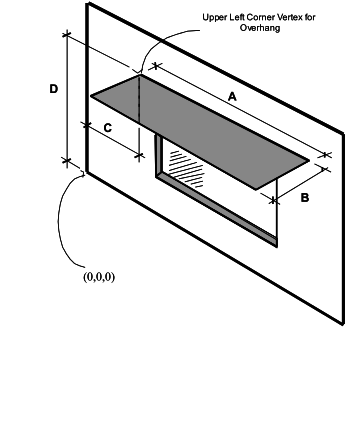
\includegraphics[width=0.9\textwidth, height=0.9\textheight, keepaspectratio=true]{media/image059.png}
\caption{Illustration for Attached Shading Surface \protect \label{fig:illustration-for-attached-shading-surface}}
\end{figure}

Proper specification for this overhang (facing up) is:

4,(C,0,D),(C,-B,D),(C+A,-B,D),(C+A,0,D); () used to illustrate each vertex.

\begin{callout}
Note that for horizontal surfaces, any corner may be chosen as the starting corner. The order of vertices determines whether the surface is facing up or down. Shading surfaces are mirrored automatically unless the user specifies ``DoNotMirrorDetachedShading'', so each shading surface need only be described once.
\end{callout}

Thus, another shading surface will be created (facing down):

4,(C+A,-B,D),(C+A,0,D),(C,0,D),(C,-B,D);

IDF example of attached shading surfaces (overhang, fin):

\begin{lstlisting}
Shading:Zone:Detailed,
  Zn001:Wall001:Shade001,       !- Surface Name
  Zn001:Wall001,                !- Base Surface Name
  ShadingTransmittance:0001,    !- Shadowing Transmittance Schedule
  4,                            !-RectangularOverhang
  1.524000 , -0.3050000    , 2.865000,
  1.524000 ,  0.0000000E+00, 2.865000,
  4.572000 ,  0.0000000E+00, 2.865000,
  4.572000 , -0.3050000    , 2.865000;

Shading:Zone:Detailed,
  Zn003:Wall001:Shade001,       !- Surface Name
  Zn003:Wall001,                !- Base Surface Name
  ShadingTransmittance:0001,    !- Shadowing Transmittance Schedule
  4,                            !-RectangularLeftFin
  57.97000 ,   8.450000    ,10.00000      ,
  57.97000 ,   8.450000    , 0.0000000E+00,
  57.97000 ,   6.450000    , 0.0000000E+00,
  57.97000 ,   6.450000    ,10.00000      ;

Shading:Zone:Detailed,
  Zn003:Wall001:Shade002,       !- Surface Name
  Zn003:Wall001,                !- Base Surface Name
  ShadingTransmittance:0003,    !- Shadowing Transmittance Schedule
  4,                            !-RectangularRightFin
  77.97000 ,   6.450000    ,10.00000      ,
  77.97000 ,   6.450000    , 0.0000000E+00,
  77.97000 ,   8.450000    , 0.0000000E+00,
  77.97000 ,   8.450000    ,10.00000      ;
\end{lstlisting}

\subsection{ShadingProperty:Reflectance}\label{shadingpropertyreflectance}

Specifies the reflectance properties of a shading surface when the solar reflection calculation has requested, i.e., when if ``WithReflections'' option is chosen in the Building object (ref: Building - Field: Solar Distribution). It is assumed that shading surfaces are divided into an unglazed, diffusely reflecting portion and a glazed, specularly-reflecting portion, either of which may be zero. The reflectance properties are assumed to be the same on both sides of the shading surface.

Note that a shadowing transmittance schedule (ref: Shading Surfaces, Field: Transmittance Schedule Name) can be used with a reflective shading surface. However, EnergyPlus assumes that the reflectance properties of the shading surface are constant even if the transmittance varies.

If no ShadingProperty:Reflectance objects are entered, the default values shown here will be used for shading surfaces. Other surfaces have their reflectance properties defined by the materials in the outer layers of the constructions.

\subsubsection{Inputs}\label{inputs-31-002}

\paragraph{Field: Shading Surface Name}\label{field-shading-surface-name}

The name of the \hyperref[shadingsite-shadingbuilding]{Shading:Site}, \hyperref[shadingsite-shadingbuilding]{Shading:Building}, \hyperref[shadingsitedetailed-shadingbuildingdetailed]{Shading:Site:Detailed}, \hyperref[shadingsitedetailed-shadingbuildingdetailed]{Shading:Building:Detailed}, \hyperref[shadingoverhang]{Shading:Overhang}, \hyperref[shadingoverhangprojection]{Shading:Overhang:Projection}, \hyperref[shadingfin]{Shading:Fin}, \hyperref[shadingfinprojection]{Shading:Fin:Projection} or \hyperref[shadingzonedetailed-000]{Shading:Zone:Detailed} object to which the following fields apply.

If this ShadingProperty:Reflectance object is not defined for a shading surface the default values listed in each of the following fields will be used in the solar reflection calculation.

\paragraph{Field: Diffuse Solar Reflectance of Unglazed Part of Shading Surface}\label{field-diffuse-solar-reflectance-of-unglazed-part-of-shading-surface}

The diffuse solar reflectance of the unglazed part of the shading surface (default = 0.2). This reflectance is assumed to be the same for beam-to-diffuse and diffuse-to-diffuse reflection. Beam-to-diffuse reflection is assumed to be independent of angle of incidence of beam radiation. Diffuse-to-diffuse reflection is assumed to be independent of angular distribution of the incident of diffuse radiation. The outgoing diffuse radiation is assumed to be isotropic (hemispherically uniform).

The sum of this reflectance and the shading surface transmittance should be less than or equal to 1.0.

\paragraph{Field: Diffuse Visible Reflectance of Unglazed Part of Shading Surface}\label{field-diffuse-visible-reflectance-of-unglazed-part-of-shading-surface}

The diffuse visible reflectance of the unglazed part of the shading surface (default = 0.2). This reflectance is assumed to be the same for beam-to-diffuse and diffuse-to-diffuse reflection. Beam-to-diffuse reflection is assumed to be independent of angle of incidence of beam radiation. Diffuse-to-diffuse reflection is assumed to be independent of angular distribution of the incident of diffuse radiation. The outgoing diffuse radiation is assumed to be isotropic (hemispherically uniform).

This value if used only for the daylighting calculation (ref: \hyperref[daylightingcontrols-000]{Daylighting:Controls}). The sum of this reflectance and the shading surface transmittance should be less than or equal to 1.0.

\paragraph{Field: Fraction of Shading Surface That Is Glazed}\label{field-fraction-of-shading-surface-that-is-glazed}

The fraction of the area of the shading surface that consists of windows (default = 0.0). It is assumed that the windows are evenly distributed over the surface and have the same glazing construction (see following ``Name of Glazing Construction''). This might be the case, for example, for reflection from the façade of a neighboring, highly-glazed building. For the reflection calculation the possible presence of shades, screens or blinds on the windows of the shading surface is ignored. Beam-to-beam (specular) reflection is assumed to occur only from the glazed portion of the shading surface. This reflection depends on angle of incidence as determined by the program from the glazing construction. Beam-to-diffuse reflection from the glazed portion is assumed to be zero. The diffuse-to-diffuse reflectance of the glazed portion is determined by the program from the glazing construction.

\paragraph{Field: Glazing Construction Name}\label{field-glazing-construction-name}

The name of the construction of the windows on the shading surface. Required if Fraction of Shading Surface That Is Glazed is greater than 0.0.

IDF example of Shading Surface Reflectance for shading surface with specular reflection

\begin{lstlisting}

Shading:Site:Detailed,
  Adjacent Glazed Facade,  !- User Supplied Surface Name
  ,   !- Shadowing Transmittance Schedule
  4,  !- Number of Surface Vertex Groups -- Number of (X,Y,Z) groups
  0,-24,30, !- Vertex 1 X,Y,Z coordinates
  0,-24,0,  !- Vertex 2 X,Y,Z coordinates
  0,0,0,    !- Vertex 3 X,Y,Z coordinates
  0,0,30;   !-Vertex 3 X,Y,Z coordinates


  ShadingProperty:Reflectance,
  Adjacent Glazed Facade, !- Name of Surface:Shading Object
  0.3,  !- Diffuse Solar Reflectance of Unglazed Part of Shading Surface
  0.3,  !- Diffuse Visible Reflectance of Unglazed Part of Shading Surface
  0.7,  !- Fraction of Shading Surface That Is Glazed
  GlassCon-1; !- Name of Glazing Construction
\end{lstlisting}

IDF example of Shading Surface Reflectance for shading surface without specular reflection

\begin{lstlisting}

Shading:Site:Detailed,
  Adjacent Blank Facade,  !- User Supplied Surface Name
  ,   !- Shadowing Transmittance Schedule
  4,  !- Number of Surface Vertex Groups -- Number of (X,Y,Z) groups
  0,-24,30,
  0,-24,0,
  0,0,0,
  0,0,30;


  ShadingProperty:Reflectance,
  Adjacent Blank Facade, !- Name of Surface:Shading Object
  0.4,  !- Diffuse Solar Reflectance of Unglazed Part of Shading Surface
  0.4,  !- Diffuse Visible Reflectance of Unglazed Part of Shading Surface
  0.0,  !- Fraction of Shading Surface That Is Glazed
  ;     !- Name of glazing construction
\end{lstlisting}

\subsection{WindowShadingControl}\label{windowpropertyshadingcontrol}

Window shading with coverings like drapes, blinds, screens or pull-down shades can be used to reduce the amount of solar radiation entering the window or reduce daylighting glare. It can also be used to reduce heat loss through the window (movable insulation). Leaving the window covering open in the winter can maximize solar heat gain and thereby reduce heating loads.

With WindowShadingControl you specify the type,  location, and timing of the shading device, what variable or combination of variables controls deployment of the shading device, and what the control setpoint is. If the shading device is a blind, you also specify how the slat angle is controlled. Each WindowShadingControl object is associated with a zone and has a list of one or more windows and glass doors to which the shading control is applied (ref: \hyperref[fenestrationsurfacedetailed]{FenestrationSurface:Detailed} with Type = Window or GlassDoor, Window, and \hyperref[glazeddoor]{GlazedDoor}).

NOTE: WindowShadingControl does not work with complex fenestration systems. Controlled complex fenestration systems can be made only with Energy Management Systems objects. Referencing a \hyperref[fenestrationsurfacedetailed]{FenestrationSurface:Detailed} in a WindowShadingControl while using complex fenestration systems will be ignored by program.

As shown in Figure~\ref{fig:allowed-locations-of-a-window-shading-device.}, a shading device can be inside the window (Shading Type = InteriorShade or InteriorBlind), outside the window (Shading Type = ExteriorShade or ExteriorBlind), or between panes of glass (Shading Type = BetweenGlassShade or BetweenGlassBlind). The exception is window screens which can only be outside the window (Shading Type = ExteriorScreen).

\begin{figure}[hbtp] % fig 34
\centering
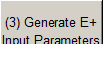
\includegraphics[width=0.9\textwidth, height=0.9\textheight, keepaspectratio=true]{media/image060.png}
\caption{Allowed locations of a window shading device. \protect \label{fig:allowed-locations-of-a-window-shading-device.}}
\end{figure}

When a shading device is present it is either retracted or activated. When it is retracted it covers none of the window. When it is activated it covers the entire glazed part of the window (but not the frame). Whether the shading device is retracted or activated in a particular timestep depends on the control mechanism: see ``Shading Control Type,'' below. To model a case in which the shading device, when activated, covers only \textbf{part} of the window you will have to divide the window into two separate windows, one with the shading device and one without the shading device.

A shading device can also be of a kind in which the optical properties of the glazing switch from one set of values to another in order to increase or decrease solar or visible transmittance (Shading Type = SwitchableGlazing).

There are two ways of specifying the actual shading device:

\begin{itemize}
  \item
\textbf{Specify ``Name of Construction with Shading''}

This is the name of a window Construction that has the shading device as one of its layers. The thermal and solar-optical properties of the shading device are given by the shading material referenced in that Construction (ref: Construction, \hyperref[windowmaterialshade]{WindowMaterial:Shade}, \hyperref[windowmaterialscreen]{WindowMaterial:Screen} and \hyperref[windowmaterialblind]{WindowMaterial:Blind}). To use this method you have to define two Constructions for the window, one without the shading device and one with it. See Example 1, below.

The Construction without the shading device is referenced in the \hyperref[fenestrationsurfacedetailed]{FenestrationSurface:Detailed} input for the window (see IDF example, below). The Construction with the shading device is referenced by the window's WindowShadingControl.

For Shading Type = InteriorShade, InteriorBlind, ExteriorShade, ExteriorScreen and ExteriorBlind these two Constructions must be identical expect for the presence of the shading layer in the shaded Construction, otherwise you will get an error message. You will also get an error message if the Construction referenced by the window has a shading layer.

  \item
\textbf{Specify the ``Material Name of the Shading Device''}

This is the name of a \hyperref[windowmaterialshade]{WindowMaterial:Shade}, \hyperref[windowmaterialscreen]{WindowMaterial:Screen} or \hyperref[windowmaterialblind]{WindowMaterial:Blind}. This method can be used with Shading Type = InteriorShade, InteriorBlind, ExteriorShade and ExteriorBlind. It cannot be used with Shading Type = BetweenGlassShade, BetweenGlassBlind, or SwitchableGlazing. If Shading Type = InteriorShade or ExteriorShade, then you specify the name of a \hyperref[windowmaterialshade]{WindowMaterial:Shade}. If Shading Type = InteriorBlind or ExteriorBlind, then you specify the name of a \hyperref[windowmaterialblind]{WindowMaterial:Blind}. If Shading Type = ExteriorScreen, then you specify the name of a \hyperref[windowmaterialscreen]{WindowMaterial:Screen}. See Example 2, below. This method is simpler to use since you don't have to specify two Constructions that differ only by the shading layer.

When this method is used, the program will automatically create a shaded window construction by adding a shading layer to the outside or inside of the construction corresponding to the windows referenced by the WindowShadingControl. The name, created by the program, of this shaded construction is composed as follows: if the name of the window construction is CCC and the material name of the shading device is DDD, then the shaded construction name is CCC:DDD:INT for an interior shading device and CCC:DDD:EXT for an exterior shading device.

This method is the required if you want to add a shading device to a construction brought in from a WINDOW Data File (ref:\hyperref[constructionwindowdatafile]{Construction:WindowDataFile}).

Note that if both ``Name of Construction with Shading'' and ``Material Name of Shading Device'' are specified, the former takes precedence.
\end{itemize}

Most Shading Control Types allow you to specify a schedule that determines when the control is active. One example is a control that is active seasonally. For example, to deploy shading only in the summer when the incident solar is high enough, use Shading Control Type = OnIfHighSolarOnWindow with a schedule that is 1 during the summer months and 0 otherwise and specify Shading Control Is Scheduled = YES. 

To deploy one shading device during one time period and another during another time period for the same window, specify two different WindowShadingControl objects that both reference the same fenestration.  Each of the WindowShadingControl input objects would include the same window on their lists of fenestration objects, but would reference different schedule input objects. The referenced schedule input objects should have non-zero values specified at different times for each WindowShadingControl. This approach can be used to add shading that is different for different seasons. When more than one WindowShadingControl is used for the same window based on schedule, the type of shading, control type, setpoints, and several other parameters must be the same in the different WindowShadingControl objects, but the shading device and construction can be different.

In addition, most Shading Control Types also allow you to specify that glare control is active in addition to the specified Control Type. For example, you might want to deploy shading when the solar incident on a window is too high OR the glare from the window is too high. This type of joint control requires that the window be in a daylit zone, that the maximum allowed glare be specified in the Daylighting object for the zone, and that Glare Control Is Active = YES in WindowShadingControl.

If Shading Type = InteriorBlind, ExteriorBlind or BetweenGlassBlind you can use WindowShadingControl to specify how the slat angle of the blind is controlled when the blind is in place.

A special type of WindowShadingControl is SwitchableGlazing. An example is electrochromic glazing in which the transmittance and reflectance of the glass is controlled electronically. For example, you could have electrochromic glazing switch from clear (high transmittance) to dark (low transmittance) to control solar gain. If you choose the Shading Type = SwitchableGlazing option for WindowShadingControl, the unswitched (clear) state is specified by the Construction referenced by the window and the switched (dark) state is specified by the Construction referenced by WindowShadingControl for that window. For example, if you specify Shading Type = SwitchableGlazing and Shading Control Type = OnIfHighSolarOnWindow, then the glazing will switch to the dark state whenever the solar radiation striking the window exceeds the Setpoint value.

For Shading Type = SwitchableGlazing the state of the window is either clear (unswitched) or dark (fully switched) for all Shading Control Types except MeetDaylightIlluminanceSetpoint. In this case, the transmittance of the glazing is adjusted to just meet the daylight illuminance set point at the first daylighting reference point (see Daylighting). This type of control assures that there is just enough solar gain to meet the daylighting requirements in a zone, and no more, thus reducing the cooling load.

To specify the order of when shades are deployed, the two different approaches can be used:

- If shades for each window are independently controlled, than a single WindowShadingControl object should be used and the Multiple Surface Control Type field should be set to Sequential. The windows should be specified in the Fenestration Surface N Name fields in the order that they should be deployed. The Shading Control Sequence Number field is not used being used since only one WindowShadingControl is used so it can be set to any value or left blank.

- If shades for a group of windows are deployed together and shades for another group of windows are deployed after that, than multiple WindowShadingControl objects should be used. Each WindowShadingControl should have Multiple Surface Control Type field should be set to Group and the names of each window in the group should be specified in the Fenestration Surface N Name fields. The Shading Control Sequence Number in the  WindowShadingControl object that controls the first group of shades should be set to 1. The Shading Control Sequence Number in the  WindowShadingControl object that controls the second group of shades should be set to 2. Any number of additional groups of shades can be added and Shading Control Sequence Number can be incremented by one for each group.

It is possible to mix these two approaches. For example, if first a group of shades is controlled together followed by a sequence of individual windows than these approaches can be combined with the Multiple Surface Control Type field should be set to Sequential in the second WindowShadingControl object.

\subsubsection{Inputs}\label{inputs-32-001}

\paragraph{Field: Name}\label{field-name-29-001}

Name of the window shading control.

\paragraph{Field: Zone Name}\label{field-zone-name-29-001}

Name of the zone where this shading control is used.

\paragraph{Field: Shading Control Sequence Number}\label{shading-control-sequence-number}

If multiple WindowShadingControl objects are used in the same zone, then the order that they deploy the window shades can be set with this field. The first WindowShadingControl should be 1 and subsequent WindowShadingControl should 2, 3, etc. This is usually used when the Multiple Surface Control Type field is set to Group to control groups of windows in a certain order.

\paragraph{Field: Shading Type}\label{field-shading-type}

The type of shading device. The choices are:

\emph{InteriorShade}: A diffusing shade is on the inside of the window. (In the shaded Construction the shading layer must be a \hyperref[windowmaterialshade]{WindowMaterial:Shade}.)

\emph{ExteriorShade}: A diffusing shade is on the outside of the window. (In the shaded Construction the shading layer must be a \hyperref[windowmaterialshade]{WindowMaterial:Shade}.)

\emph{BetweenGlassShade}: A diffusing shade is between two glass layers. (In the shaded Construction the shading layer must be a \hyperref[windowmaterialshade]{WindowMaterial:Shade}.) This shading type is allowed only for double- and triple-glazing. For triple-glazing the shade must be between the two inner glass layers.

\emph{ExteriorScreen}: An insect screen is on the outside of the window. (In the shaded Construction the shading layer must be a \hyperref[windowmaterialscreen]{WindowMaterial:Screen}.)

\emph{InteriorBlind}: A slat-type shading device, such as a Venetian blind, is on the inside of the window. (In the shaded Construction the shading layer must be a \hyperref[windowmaterialblind]{WindowMaterial:Blind}.)

\emph{ExteriorBlind}: A slat-type shading device is on the outside of the window. (In the shaded Construction the shading layer must be a \hyperref[windowmaterialblind]{WindowMaterial:Blind}.)

\emph{BetweenGlassBlind}: A slat-type shading device is between two glass layers. (In the shaded Construction the shading layer must be a \hyperref[windowmaterialblind]{WindowMaterial:Blind}.) This shading type is allowed only for double- and triple-glazing. For triple-glazing the blind must be between the two inner glass layers.

\emph{SwitchableGlazing}: Shading is achieved by changing the characteristics of the window glass, such as by darkening it.

\paragraph{Field: Construction with Shading Name}\label{field-construction-with-shading-name}

Name of the window Construction that has the shading in place. The properties of the shading device are given by the shading material referenced in that Construction (ref: Construction, \hyperref[windowmaterialshade]{WindowMaterial:Shade}, \hyperref[windowmaterialscreen]{WindowMaterial:Screen} and \hyperref[windowmaterialblind]{WindowMaterial:Blind}). For Shading Type = SwitchableGlazing, this is the name of the Construction that corresponds to the window in its fully-switched (darkest) state.

Specifying ``Name of Construction with Shading'' is required if Shading Type = BetweenGlassShade, BetweenGlassBlind, or SwitchableGlazing. For other Shading Types, you may alternatively specify ``Material Name of Shading Device'' (see below).

\paragraph{Field: Shading Control Type}\label{field-shading-control-type}

Specifies how the shading device is controlled, i.e., it determines whether the shading device is ``on'' or ``off.'' For blinds, screens and shades, when the device is ``on'' it is assumed to cover all of the window except its frame; when the device is ``off'' it is assumed to cover none of the window (whether ``on'' or ``off'' the shading device is assumed to cover none of the wall that the window is on).

For switchable glazing, ``on'' means that the glazing is in the fully-switched state and ``off'' means that it is in the unswitched state; for example, for electrochromic glazing, ``on'' means the glazing is in its darkest state and ``off'' means it is in its lightest state.

The choices for Shading Control Type are the following. If SetPoint is applicable its units are shown in parentheses.

\emph{AlwaysOn}: Shading is always on.

\emph{AlwaysOff}: Shading is always off.

The following six control types are used primarily to reduce zone cooling load due to window solar gain.

\emph{OnIfScheduleAllows}: Shading is on if schedule value is non-zero. Requires that Schedule Name be specified and Shading Control Is Scheduled = Yes.

Note: For exterior window screens \emph{AlwaysOn, AlwaysOff, and OnIfScheduleAllows} are the only valid shading control types.

\emph{OnIfHighSolarOnWindow}: Shading is on if beam plus diffuse solar radiation incident on the window exceeds SetPoint (W/m\(^{2}\)) and schedule, if specified, allows shading.

\emph{OnIfHighHorizontalSolar}: Shading is on if total (beam plus diffuse) horizontal solar irradiance exceeds SetPoint (W/m\(^{2}\)) and schedule, if specified, allows shading.

\emph{OnIfHighOutdoorAirTemperature}: Shading is on if outside air temperature exceeds SetPoint (C) and schedule, if specified, allows shading.

\emph{OnIfHighZoneAirTemperature}: Shading is on if zone air temperature in the previous timestep exceeds SetPoint (C) and schedule, if specified, allows shading.

\emph{OnIfHighZoneCooling}: Shading is on if zone cooling rate in the previous timestep exceeds SetPoint (W) and schedule, if specified, allows shading.

\emph{OnIfHighGlare}: Shading is on if the total daylight glare index at the zone's first daylighting reference point from all of the exterior windows in the zone exceeds the maximum glare index specified in the daylighting input for zone (ref: Group -- Daylighting). Applicable only to windows in zones with daylighting.

Note: Unlike other Shading Control Types, glare control is active whether or not a schedule is specified.

\emph{MeetDaylightIlluminanceSetpoint}: Used only with ShadingType = SwitchableGlazing in zones with daylighting controls. In this case the transmittance of the glazing is adjusted to just meet the daylight illuminance set point at the first daylighting reference point. Note that the daylight illuminance set point is specified in the \hyperref[daylightingcontrols-000]{Daylighting:Controls} object for the Zone; it is not specified as a WindowShadingControl SetPoint. When the glare control is active, if meeting the daylight illuminance set point at the first daylighting reference point results in higher discomfort glare index (DGI) than the specified zone's maximum allowable DGI for either of the daylight reference points, the glazing will be further dimmed until the DGI equals the specified maximum allowable value.

The following three control types can be used to reduce zone heating load during the winter by reducing window conductive heat loss at night and leaving the window unshaded during the day to maximize solar gain. They are applicable to any Shading Type except ExteriorScreen but are most appropriate for interior or exterior shades with high insulating value (``movable insulation''). ``Night'' means the sun is down and ``day'' means the sun is up.

\emph{OnNightIfLowOutdoorTempAndOffDay}: Shading is on at night if the outside air temperature is less than SetPoint (C) and schedule, if specified, allows shading. Shading is off during the day.

\emph{OnNightIfLowInsideTempAndOffDay}: Shading is on at night if the zone air temperature in the previous timestep is less than SetPoint (C) and schedule, if specified, allows shading. Shading is off during the day.

\emph{OnNightIfHeatingAndOffDay}: Shading is on at night if the zone heating rate in the previous timestep exceeds SetPoint (W) and schedule, if specified, allows shading. Shading is off during the day.

The following two control types can be used to reduce zone heating and cooling load. They are applicable to any Shading Type except ExteriorScreen but are most appropriate for translucent interior or exterior shades with high insulating value (``translucent movable insulation'').

\emph{OnNightIfLowOutdoorTempAndOnDayIfCooling}: Shading is on at night if the outside air temperature is less than SetPoint (C). Shading is on during the day if the zone cooling rate in the previous timestep is non-zero. Night and day shading is subject to schedule, if specified.

\emph{OnNightIfHeatingAndOnDayIfCooling}: Shading is on at night if the zone heating rate in the previous timestep exceeds SetPoint (W). Shading is on during the day if the zone cooling rate in the previous timestep is non-zero. Night and day shading is subject to schedule, if specified.

The following control types can be used to reduce zone cooling load. They are applicable to any Shading Type except ExteriorScreen but are most appropriate for interior or exterior blinds, interior or exterior shades with low insulating value, or switchable glazing.

\emph{OffNightAndOnDayIfCoolingAndHighSolarOnWindow}: Shading is off at night. Shading is on during the day if the solar radiation incident on the window exceeds SetPoint (W/m\(^{2}\)) and if the zone cooling rate in the previous timestep is non-zero. Daytime shading is subject to schedule, if specified.

\emph{OnNightAndOnDayIfCoolingAndHighSolarOnWindow}: Shading is on at night. Shading is on during the day if the solar radiation incident on the window exceeds SetPoint (W/m\(^{2}\)) and if the zone cooling rate in the previous timestep is non-zero. Day and night shading is subject to schedule, if specified. (This Shading Control Type is the same as the previous one, except the shading is on at night rather than off.)

\emph{OnIfHighOutdoorAirTempAndHighSolarOnWindow:} Shading is on if the outside air temperature exceeds the Setpoint (C) and if the solar radiation incident on the window exceeds SetPoint 2 (W/m\(^{2}\)).

\emph{OnIfHighOutdoorAirTempAndHighHorizontalSolar:} Shading is on if the outside air temperature exceeds the Setpoint (C) and if the horizontal solar radiation exceeds SetPoint 2 (W/m\(^{2}\)).

\emph{OnIfHighZoneAirTempAndHighSolarOnWindow:} Shading is on if the zone air temperature exceeds the Setpoint (C) and if the solar radiation incident on the window exceeds SetPoint 2 (W/m\(^{2}\)).

\emph{OnIfHighZoneAirTempAndHighHorizontalSolar:} Shading is on if the zone air temperature exceeds the Setpoint (C) and if the horizontal solar radiation exceeds SetPoint 2 (W/m\(^{2}\)).

The following three control types can be used to model human behavior of turning on shading during the day to reduce view luminance or solar gain and leaving shading on until a certain time point. They can only be used in zones with daylighting controls. Window view luminance at the first daylighting reference point is used to compare with luminance setpoint. They are applicable to any Shading Type except ExteriorScreen.

\emph{OnIfHighSolarOrHighLuminanceTillMidnight:} Shading is on if the solar radiation incident on the window exceeds SetPoint (W/m\(^{2}\)) or the luminance from the window exceeds SetPoint 2 (cd/m\(^{2}\)). When shading is on, it remains on till midnight.

\emph{OnIfHighSolarOrHighLuminanceTillSunset:} Shading is on if the solar radiation incident on the window exceeds SetPoint (W/m\(^{2}\)) or the luminance from the window exceeds SetPoint 2 (cd/m\(^{2}\)). When shading is on, it remains on till sunset.

\emph{OnIfHighSolarOrHighLuminanceTillNextMorning:} Shading is on if the solar radiation incident on the window exceeds SetPoint (W/m\(^{2}\)) or the luminance from the window exceeds SetPoint 2 (cd/m\(^{2}\)). When shading is on, it remains on till sunrise next day.


\paragraph{Field: Schedule Name}\label{field-schedule-name-007}

Required if Shading Control Is Scheduled = Yes. If schedule value \textgreater{} 0 , shading control is active, i.e., shading can be on only if the shading control test passes. If schedule value = 0, shading is off whether or not the control test passes. If Schedule Name is not specified, shading control is assumed to be active at all times.

\paragraph{Field: Setpoint}\label{field-setpoint}

The setpoint for activating window shading. The units depend on the type of trigger:

\begin{itemize}
\item
  W/m\(^{2}\) for solar-based controls
\item
  W for cooling- or heating-based controls
\item
  Degrees C for temperature-based controls
\end{itemize}

SetPoint is unused for Shading Control Type = OnIfScheduleAllows, OnIfHighGlare and DaylightIlluminance.

\paragraph{Field: Shading Control Is Scheduled}\label{field-shading-control-is-scheduled}

Accepts values YES and NO. The default is NO. Not applicable for Shading Control Type = OnIfHighGlare and should be blank in that case.

If YES, Schedule Name is required and that schedule determines whether the shading control specified by Shading Control Type is active or inactive (see Schedule Name, above).

If NO, Schedule Name is not applicable (should be blank) and the shading control is unscheduled.

Shading Control Is Scheduled = YES is required if Shading Control Type = OnIfScheduleAllows.

\paragraph{Field: Glare Control Is Active}\label{field-glare-control-is-active}

Accepts values YES and NO. The default is NO.

If YES and the window is in a daylit zone, shading is on if the zone's discomfort glare index exceeds the maximum discomfort glare index specified in the Daylighting object referenced by the zone. For switchable windows with \emph{MeetDaylightIlluminanceSetpoint} shading control, if Glare Control is active, the windows are always continuously dimmed as necessary to meet the zone's maximum allowable DGI while providing appropriate amount of daylight for the zone.

The glare test is OR'ed with the test specified by Shading Control Type. For example, if Glare Control Is Active = YES and Shading Control Type = OnIfHighZoneAirTemp, then shading is on if glare is too high OR if the zone air temperature is too high.

Glare Control Is Active = YES is required if Shading Control Type = OnIfHighGlare.

\paragraph{Field: Shading Device Material Name}\label{field-shading-device-material-name}

The name of a \hyperref[windowmaterialshade]{WindowMaterial:Shade}, \hyperref[windowmaterialscreen]{WindowMaterial:Screen} or \hyperref[windowmaterialblind]{WindowMaterial:Blind}. Required if ``Name of Construction with Shading'' is not specified. Not applicable if Shading Type = BetweenGlassShade, BetweenGlassBlind or SwitchableGlazing and should be blank in this case. If both ``Name of Construction with Shading'' and ``Material Name of Shading Device'' are entered the former takes precedence.

\paragraph{Field: Type of Slat Angle Control for Blinds}\label{field-type-of-slat-angle-control-for-blinds}

Applies only to Shading Type = InteriorBlind, ExteriorBlind or BetweenGlassBlind. Specifies how the slat angle is controlled. The choices are FixedSlatAngle, ScheduledSlatAngle and BlockBeamSolar.

If FixedSlatAngle (the default), the angle of the slat is fixed at the value input for the \hyperref[windowmaterialblind]{WindowMaterial:Blind} that is contained in the construction specified by Name of Construction with Shading or is specified by Material Name of Shading Device.

If ScheduledSlatAngle, the slat angle varies according to the schedule specified by Slat Angle Schedule Name, below.

If BlockBeamSolar, the slat angle is set each timestep to just block beam solar radiation. If there is no beam solar on the window the slat angle is set to the value input for the \hyperref[windowmaterialblind]{WindowMaterial:Blind} that is contained in the construction specified by Name of Construction with Shading or is specified by Material Name of Shading Device. The BlockBeamSolar option prevents beam solar from entering the window and causing possible unwanted glare if the beam falls on work surfaces while at the same time allowing near-optimal indirect radiation for daylighting.

\paragraph{Field: Slat Angle Schedule Name}\label{field-slat-angle-schedule-name}

This is the name of a schedule of slat angles that is used when Type of Slat Angle Control for Blinds = ScheduledSlatAngle. You should be sure that the schedule values fall within the range given by the Minimum Slat Angle and Maximum Slat Angle values entered in the corresponding \hyperref[windowmaterialblind]{WindowMaterial:Blind}. If not, the program will force them into this range.

\paragraph{Field: Setpoint 2}\label{field-setpoint-2}

Used only as the second setpoint for the following setpoint control types: OnIfHighOutdoorAirTempAndHighSolarOnWindow, OnIfHighOutdoorAirTempAndHighHorizontalSolar, OnIfHighZoneAirTempAndHighSolarOnWindow, OnIfHighZoneAirTempAndHighHorizontalSolar, OnIfHighSolarOrHighLuminanceTillMidnight, OnIfHighSolarOrHighLuminanceTillSunset, and OnIfHighSolarOrHighLuminanceTillNextMorning.

\paragraph{Field: Daylighting Controls Object Name}\label{field-daylighting-controls-object-name}

Name of the \hyperref[daylightingcontrols-000]{Daylighting:Controls} object that provides the glare and illuminance control to the zone.

\paragraph{Field: Multiple Surface Control Type}\label{field-multiple-surface-control-type}

The field can have one of two options:

\emph{Sequential}: The following list of fenestration surfaces are controlled individually in the order specified.

\emph{Group}: The entire list of fenestration surfaces is controlled simultaneously, and if glare control is needed, the entire group of window shades are deployed together a the same time.

\paragraph{Field: Fenestration Surface <n> Name}\label{field-fenestration-surface1-name}

The name of a \hyperref[fenestrationsurfacedetailed]{FenestrationSurface:Detailed}, Window, or \hyperref[glazeddoor]{GlazedDoor} object controlled by this WindowShadingControl. This field can be repeated to apply the same shading control to more than one fenestration surface. When Multiple Surface Control Type is set to Sequential, the order of the Fenestration Surface Names is the order that the shades will be deployed. The object is extensible so additional fields of fenestration surface names can be added to the object. All of the fenestration surfaces must be either in the zone specified in the Zone Name field or in an adjacent zone connected by an interior window.

An IDF example: window with interior roll shade that is deployed when solar incident on the window exceeds 50 W/m\(^{2}\).

\begin{lstlisting}
! Example 1: Interior movable shade specified by giving name of shaded construction
! in WindowShadingControl

WindowMaterial:Glazing, GLASS - CLEAR SHEET 1 / 8 IN,  !- Material Name
       SpectralAverage,! Optical data type {SpectralAverage or Spectral}
       ,               ! Name of spectral data set when Optical Data Type = Spectral
       0.003        ,  !- Thickness {m}
       0.837        ,  !- Solar Transmittance at Normal Incidence
       0.075        ,  !- Solar Reflectance at Normal Incidence: Front Side
       0.075        ,  !- Solar Reflectance at Normal Incidence: Back Side
       0.898        ,  !- Visible Transmittance at Normal Incidence
       0.081        ,  !- Visible Reflectance at Normal Incidence: Front Side
       0.081        ,  !- Visible Reflectance at Normal Incidence: Back Side
       0.0          ,  !- IR Transmittance
       0.8400000    ,  !- IR Emissivity: Front Side
       0.8400000    ,  !- IR Emissivity: Back Side
       0.9000000    ;  !- Conductivity {W/m-K}

WindowMaterial:Shade, ROLL SHADE,  !- Material Name
       0.3          ,   !- Solar Transmittance at normal incidence
       0.5000000    ,   !- Solar Reflectance (same for front and back side)
       0.3          ,   !- Visible Transmittance at normal incidence
       0.5000000    ,   !- Visible reflectance (same for front and back side)
       0.9000000    ,   !- IR Emissivity (same for front and back side)
       0.05         ,   !- IR Transmittance
       0.003        ,   !- Thickness
       0.1          ,   !- Conductivity {W/m-K}
       0.0          ,   !- Top Opening Multiplier
       0.0          ,   !- Bottom Opening Multiplier
       0.5          ,   !- Left-Side Opening Multiplier
       0.5          ,   !- Right-Side Opening Multiplier
       0.0          ;   !- Air-Flow Permeability

Construction, SINGLE PANE WITH NO SHADE,  ! Name of construction without shade
       GLASS - CLEAR SHEET 1 / 8 IN;  !- First material layer

Construction, SINGLE PANE WITH INT SHADE, ! Name of construction with shade
       GLASS - CLEAR SHEET 1 / 8 IN,  !- First material layer
       ROLL SHADE                  ;  !- Second material layer

WindowShadingControl,
       CONTROL ON INCIDENT SOLAR,    !- Name
       West Zone,                    !- Zone Name
       1,                            !- Shading Control Sequence Number
       InteriorShade,                !- Shading Type
       SINGLE PANE WITH INT SHADE,   !- Name of construction with shading device
       OnIfHighSolarOnWindow,        !- Shading Control Type
       ,                             !- Schedule name
       50.0,                         !- Setpoint {W/m2}
       NO,                           !- Shading Control Is Scheduled
       NO,                           !- Glare Control Is Active
       ,                             !- Material Name of Shading Device
       ,                             !- Type of Slat Angle Control for Blinds
       ,                             !- Slat Angle Schedule Name
       ,                             !- Setpoint 2 {W/m2, deg C or cd/m2}
       West Zone_DaylCtrl,           !- Daylighting Control Object Name
       Sequential,                   !- Multiple Surface Control Type
       Zn001:Wall001:Win001;         !- Fenestration Surface 1 Name

FenestrationSurface:Detailed,
       Zn001:Wall001:Win001,         !- SubSurface Name
       Window                   ,    !- Class
       SINGLE PANE WITH NO SHADE,    !- Name of construction without shading device
       Zn001:Wall001            ,    !- Base Surface Name
       ,                             !- Target
       0.5000000                ,    !- VF to Ground
       ,                             !- Frame/Divider name
       1.0                      ,    !- Multiplier
       4                        ,    !- Number of vertices (assumed rectangular)
       0.548 ,  0.0 ,   2.5     ,    !- x,y,z of vertices {m}
       0.548 ,  0.0 ,   0.5     ,
       5.548 ,  0.0 ,   0.5     ,
       5.548 ,  0.0 ,   2.5     ;
\end{lstlisting}

\begin{lstlisting}
! Example 2: Interior movable shade specified by giving name of shading device in WindowShadingControl

WindowMaterial:Glazing, GLASS - CLEAR SHEET 1 / 8 IN,  !- Material Name
       SpectralAverage,! Optical data type {SpectralAverage or Spectral}
       ,               ! Name of spectral data set when Optical Data Type = Spectral
       0.003        ,  !- Thickness {m}
       0.837        ,  !- Solar Transmittance at Normal Incidence
       0.075        ,  !- Solar Reflectance at Normal Incidence: Front Side
       0.075        ,  !- Solar Reflectance at Normal Incidence: Back Side
       0.898        ,  !- Visible Transmittance at Normal Incidence
       0.081        ,  !- Visible Reflectance at Normal Incidence: Front Side
       0.081        ,  !- Visible Reflectance at Normal Incidence: Back Side
       0.0          ,  !- IR Transmittance
       0.8400000    ,  !- IR Emissivity: Front Side
       0.8400000    ,  !- IR Emissivity: Back Side
       0.9000000    ;  !- Conductivity {W/m-K}

WindowMaterial:Shade, ROLL SHADE,  !- Material Name
       0.3          ,   !- Solar Transmittance at normal incidence
       0.5000000    ,   !- Solar Reflectance (same for front and back side)
       0.3          ,   !- Visible Transmittance at normal incidence
       0.5000000    ,   !- Visible reflectance (same for front and back side)
       0.9000000    ,   !- IR Emissivity (same for front and back side)
       0.05         ,   !- IR Transmittance
       0.003        ,   !- Thickness
       0.1          ,   !- Conductivity {W/m-K}
       0.0          ,   !- Top Opening Multiplier
       0.0          ,   !- Bottom Opening Multiplier
       0.5          ,   !- Left-Side Opening Multiplier
       0.5          ,   !- Right-Side Opening Multiplier
       0.0          ;   !- Air-Flow Permeability

Construction, SINGLE PANE WITH NO SHADE,  ! Name of construction without shade
       GLASS - CLEAR SHEET 1 / 8 IN;  !- First material layer

WindowShadingControl,
       CONTROL ON INCIDENT SOLAR,    !- Name
       West Zone,                    !- Zone Name
       1,                            !- Shading Control Sequence Number
       InteriorShade,                !- Shading Type
       ,                             !- Name of shaded construction
       OnIfHighSolarOnWindow,        !- Shading Control Type
       ,                             !- Schedule name
       50.0,                         !- Setpoint {W/m2}
       NO,                           !- Shading Control Is Scheduled
       NO,                           !- Glare Control Is Active
       ROLL SHADE,                   !- Material Name of Shading Device
       ,                             !- Type of Slat Angle Control for Blinds
       ,                             !- Slat Angle Schedule Name
       ,                             !- Setpoint 2 {W/m2, deg C or cd/m2}
       West Zone_DaylCtrl,           !- Daylighting Control Object Name
       Sequential,                   !- Multiple Surface Control Type
       Zn001:Wall001:Win001;         !- Fenestration Surface 1 Name

FenestrationSurface:Detailed,
       Zn001:Wall001:Win001,         !- SubSurface Name
       Window                   ,    !- Class
       SINGLE PANE WITH NO SHADE,    !- Name of construction without shade
       Zn001:Wall001            ,    !- Base Surface Name
       ,                             !- Target
       0.5000000                ,    !- VF to Ground
       ,                             !- Frame/Divider name
       1.0                      ,    !- Multiplier
       4                        ,    !- Number of vertices (assumed rectangular)
       0.548 ,  0.0 ,   2.5     ,    !- x,y,z of vertices {m}
       0.548 ,  0.0 ,   0.5     ,
       5.548 ,  0.0 ,   0.5     ,
       5.548 ,  0.0 ,   2.5     ;
\end{lstlisting}

\subsection{WindowProperty:FrameAndDivider}\label{windowpropertyframeanddivider}

The WindowProperty:FrameAndDivider object is referenced by exterior windows that have

\begin{itemize}
\item
  a frame, and/or
\item
  a divider, and/or
\item
  reveal surfaces that reflect beam solar radiation.
\end{itemize}

A \textbf{\emph{frame}} surrounds the glazing in a window (see Figure~\ref{fig:a-window-with-a-frame-and-divider.} and Figure~\ref{fig:illustration-showing-frame-and-divider}). It is assumed that all frame characteristics---such as width, conductance and solar absorptance---are the same for the top, bottom and side elements of the frame. If the frame elements are not the same then you should enter area-weighted average values for the frame characteristics.

The window vertices that you specify in the \hyperref[fenestrationsurfacedetailed]{FenestrationSurface:Detailed} object are those of the glazed part of the window, not the frame. EnergyPlus automatically subtracts the area of the frame---determined from the glazing dimensions and the frame width---from the area of the wall containing the window.

A \textbf{\emph{divider}}, as shown in Figure~\ref{fig:a-window-with-a-frame-and-divider.}, Figure~\ref{fig:illustration-showing-frame-and-divider} and Figure~\ref{fig:illustration-showing-divider-types.}, divides the glazing up into separate lites. It is assumed that all divider elements have the same characteristics. If not, area-weighted average values should be used. EnergyPlus automatically subtracts the divider area from the glazed area of the window.

\textbf{\emph{Reveal surfaces}}, as shown in Figure~\ref{fig:a-vertical-section-through-a-window-with}, are associated with the setback of the glazing from the outside and/or inside surface of the parent wall. If the depth and solar absorptance of these surfaces are specified, the program will calculate the reflection of beam solar radiation from these surfaces. The program also calculates the shadowing (onto the window) of beam and diffuse solar radiation by outside reveal surfaces.

In EnergyPlus, a window can have any combination of frame, divider and reveal surfaces, or none of these.

The best source of frame and divider characteristics is the WINDOW program, which will calculate the values required by EnergyPlus for different frame and divider types. In particular, the THERM program within the WINDOW program will calculate the effective conductance of frames and dividers; this is the conductance taking 2-D heat transfer effects into account.

Note that a window's frame and divider characteristics, along with other window information, can be read in from the Window Data File (see ``Importing Windows from the WINDOW program'' and ``\hyperref[constructionwindowdatafile]{Construction:WindowDataFile} object''). In this case the WindowProperty:FrameAndDivider referenced by the window is not applicable and should be blank unless you want to specify reveal surfaces for beam solar reflection.

\begin{figure}[hbtp] % fig 35
\centering
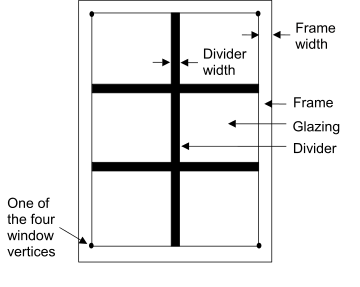
\includegraphics[width=0.9\textwidth, height=0.9\textheight, keepaspectratio=true]{media/image061.png}
\caption{A window with a frame and divider. \protect \label{fig:a-window-with-a-frame-and-divider.}}
\end{figure}

In the illustration above, the divider has two horizontal elements and one vertical element.

\subsubsection{Inputs}\label{inputs-33-001}

\paragraph{Field: Name}\label{field-name-30-001}

The name of the frame/divider object. It is referenced by WindowProperty:FrameAndDivider Name in \hyperref[fenestrationsurfacedetailed]{FenestrationSurface:Detailed}.

\textbf{\emph{Frame Fields}}

\paragraph{Field: Frame Width}\label{field-frame-width}

The width of the frame elements when projected onto the plane of the window. It is assumed that the top, bottom and side elements of the frame have the same width. If not, an average frame width should be entered such that the projected frame area calculated using the average value equals the sum of the areas of the frame elements.

\paragraph{Field: Frame Outside Projection}\label{field-frame-outside-projection}

The amount by which the frame projects outward from the outside surface of the window glazing. If the outer surface of the frame is flush with the glazing, Frame Outside Projection = 0.0. Used to calculate shadowing of frame onto glass, solar absorbed by frame, IR emitted and absorbed by frame, and convection from frame.

\paragraph{Field: Frame Inside Projection}\label{field-frame-inside-projection}

The amount by which the frame projects inward from the inside surface of the window glazing. If the inner surface of the frame is flush with the glazing, Frame Inside Projection = 0.0. Used to calculate solar absorbed by frame, IR emitted and absorbed by frame, and convection from frame.

\begin{figure}[hbtp] % fig 36
\centering
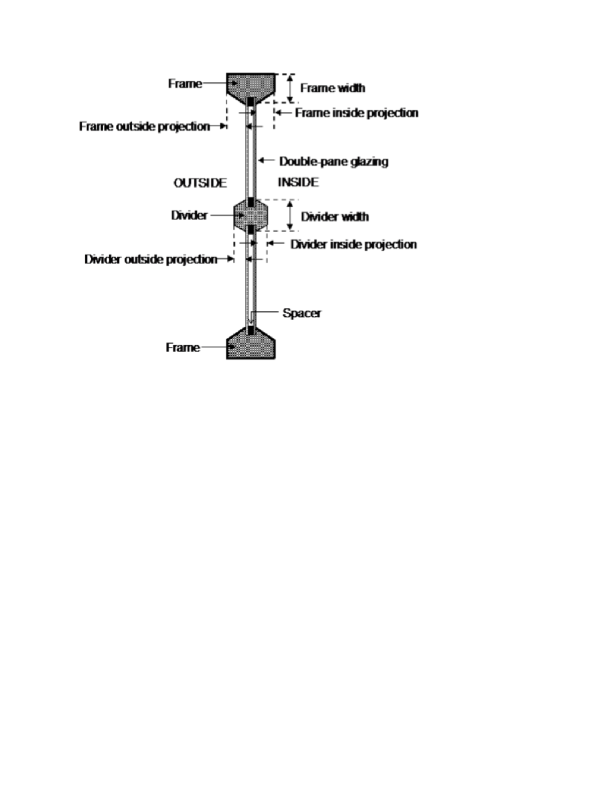
\includegraphics[width=0.9\textwidth, height=0.9\textheight, keepaspectratio=true]{media/image062.png}
\caption{Illustration showing frame and divider dimensioning. \protect \label{fig:illustration-showing-frame-and-divider}}
\end{figure}

\paragraph{Field: Frame Conductance}\label{field-frame-conductance}

The effective thermal conductance of the frame measured from inside to outside frame surface (no air films) and taking 2-D conduction effects into account. Obtained from the WINDOW program or other 2-D calculation.

\paragraph{Field: Ratio of Frame-Edge Glass Conductance to Center-Of-Glass Conductance}\label{field-ratio-of-frame-edge-glass-conductance-to-center-of-glass-conductance}

The glass conductance near the frame (excluding air films) divided by the glass conductance at the center of the glazing (excluding air films). Used only for multi-pane glazing constructions. This ratio is greater than 1.0 because of thermal bridging from the glazing across the frame and across the spacer that separates the glass panes. Values can be obtained from the WINDOW program the user-selected glazing construction and frame characteristics.

\paragraph{Field: Frame Solar Absorptance}\label{field-frame-solar-absorptance}

The solar absorptance of the frame. The value is assumed to be the same on the inside and outside of the frame and to be independent of angle of incidence of solar radiation. If solar reflectance (or reflectivity) data is available, then absorptance is equal to 1.0 minus reflectance (for opaque materials).

\paragraph{Field: Frame Visible Absorptance}\label{field-frame-visible-absorptance}

The visible absorptance of the frame. The value is assumed to be the same on the inside and outside of the frame and to be independent of angle of incidence of solar radiation. If visible reflectance (or reflectivity) data is available, then absorptance is equal to 1.0 minus reflectance (for opaque materials).

\paragraph{Field: Frame Thermal Hemispherical Emissivity}\label{field-frame-thermal-hemispherical-emissivity}

The thermal emissivity of the frame, assumed the same on the inside and outside.

\textbf{\emph{Divider Fields}}

\paragraph{Field: Divider Type}\label{field-divider-type}

The type of divider (see figure below). Divider Type = Suspended is applicable only to multi-pane glazing. It means that the divider is suspended between the panes. (If there are more than two glass layers, the divider is assumed to be placed between the two outermost layers.)

Divider Type = DividedLite means that the divider elements project out from the outside and inside surfaces of the glazing and divide the glazing into individual lites. For multi-pane glazing, this type of divider also has between-glass elements that separate the panes.

\begin{figure}[hbtp] % fig 37
\centering
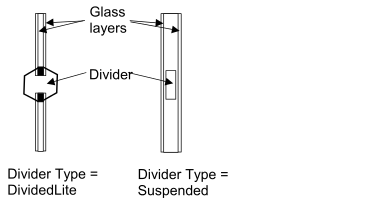
\includegraphics[width=0.9\textwidth, height=0.9\textheight, keepaspectratio=true]{media/image063.png}
\caption{Illustration showing divider types. \protect \label{fig:illustration-showing-divider-types.}}
\end{figure}

\paragraph{Field: Divider Width}\label{field-divider-width}

The width of the divider elements when projected onto the plane of the window. It is assumed that the horizontal and vertical divider elements have the same width. If not, an average divider width should be entered such that the projected divider area calculated using the average value equals the sum of the areas of the divider elements.

\paragraph{Field: Number of Horizontal Dividers}\label{field-number-of-horizontal-dividers}

The number of divider elements parallel to the top and bottom of the window.

\paragraph{Field: Number of Vertical Dividers}\label{field-number-of-vertical-dividers}

The number of divider elements parallel to the sides of the window.

\paragraph{Field: Divider Outside Projection}\label{field-divider-outside-projection}

The amount by which the divider projects out from the outside surface of the window glazing. For Divider Type = Suspended, Divider Projection = 0.0. Used to calculate shadowing of divider onto glass, solar absorbed by divider, IR emitted and absorbed by divider, and convection from divider.

\paragraph{Field: Divider Inside Projection}\label{field-divider-inside-projection}

The amount by which the divider projects inward from the inside surface of the window glazing. If the inner surface of the divider is flush with the glazing, Divider Inside Projection = 0.0. Used to calculate solar absorbed by divider, IR emitted and absorbed by divider, and convection from divider.

\paragraph{Field: Divider Conductance}\label{field-divider-conductance}

The effective thermal conductance of the divider measured from inside to outside divider surface (no air films) and taking 2-D conduction effects into account. Obtained from the WINDOW program or other 2-D calculation.

\paragraph{Field: Ratio of Divider-Edge Glass Conductance to Center-Of-Glass Conductance}\label{field-ratio-of-divider-edge-glass-conductance-to-center-of-glass-conductance}

The glass conductance near the divider (excluding air films) divided by the glass conductance at the center of the glazing (excluding air films). Used only for multi-pane glazing constructions. This ratio is greater than 1.0 because of thermal bridging from the glazing across the divider and across the spacer that separates the glass panes. Values can be obtained from the WINDOW program for the user-selected glazing construction and divider characteristics.

\paragraph{Field: Divider Solar Absorptance}\label{field-divider-solar-absorptance}

The solar absorptance of the divider. The value is assumed to be the same on the inside and outside of the divider and to be independent of angle of incidence of solar radiation. If solar reflectance (or reflectivity) data is available, then absorptance is equal to 1.0 minus reflectance (for opaque materials).

\paragraph{Field: Divider Visible Absorptance}\label{field-divider-visible-absorptance}

The visible absorptance of the divider. The value is assumed to be the same on the inside and outside of the divider and to be independent of angle of incidence of solar radiation. If visible reflectance (or reflectivity) data is available, then absorptance is equal to 1.0 minus reflectance (for opaque materials).

\paragraph{Field: Divider Thermal Hemispherical Emissivity}\label{field-divider-thermal-hemispherical-emissivity}

The thermal emissivity of the divider, assumed the same on the inside and outside.

\textbf{\emph{Reveal Surface Fields}}

The following fields specify the properties of the window reveal surfaces (reveals occur when the window is not in the same plane as the base surface). From this information and from the geometry of the window and the sun position, the program calculates beam solar radiation absorbed and reflected by the top, bottom, right and left sides of outside and inside window reveal surfaces. In doing this calculation, the shadowing on a reveal surface by other reveal surfaces is determined using the orientation of the reveal surfaces and the sun position.

It is assumed that:

\begin{itemize}
\item
  The window is an exterior window.
\item
  The reveal surfaces are perpendicular to the window plane.
\item
  If an exterior shade, screen or blind is in place it shades exterior and interior reveal surfaces so that in this case there is no beam solar on these surfaces.
\item
  If an interior shade or blind is in place it shades the interior reveal surfaces so that in this case there is no beam solar on these surfaces.
\item
  The possible shadowing on inside reveal surfaces by a window divider is ignored.
\item
  The outside reveal surfaces (top, bottom, left, right) have the same solar absorptance and depth. This depth is not input here but is automatically determined by the program---from window and wall vertices--as the distance between the plane of the outside face of the glazing and plane of the outside face of the parent wall.
\item
  The inside reveal surfaces are divided into two categories: (1) the bottom reveal surface, called here the ``inside sill;'' and (2) the other reveal surfaces (left, right and top).
\item
  The left, right and top inside reveal surfaces have the same depth and solar absorptance. The inside sill is allowed to have depth and solar absorptance values that are different from the corresponding values for the other inside reveal surfaces.
\item
  The inside sill depth is required to be greater than or equal to the depth of the other inside reveal surfaces. If the inside sill depth is greater than zero the depth of the other inside reveal surfaces is required to be greater than zero.
\item
  The reflection of beam solar radiation from all reveal surfaces is assumed to be isotropic diffuse; there is no specular component.
\item
  Half of the beam solar reflected from outside reveal surfaces is goes towards the window; the other half goes back to the exterior environment (i.e., reflection of this outward-going component from other outside reveal surfaces is not considered).
\item
  The half that goes towards the window is added to the other solar radiation incident on the window. Correspondingly, half of the beam solar reflected from inside reveal surfaces goes towards the window, with the other half going into the zone. The portion going towards the window that is not reflected is absorbed in the glazing or is transmitted back out into the exterior environment.
\item
  The beam solar that is absorbed by outside reveal surfaces is added to the solar absorbed by the outside surface of the window's parent wall; similarly, the beam solar absorbed by the inside reveal surfaces is added to the solar absorbed by the inside surface of the parent wall.
\end{itemize}

The net effect of beam solar reflected from outside reveal surfaces is to increase the heat gain to the zone, whereas the effect of beam solar reflected from inside reveal surfaces is to decrease the heat gain to the zone since part of this reflected solar is transmitted back out the window.

~If the window has a frame, the absorption of reflected beam solar by the inside and outside surfaces of the frame is considered. The shadowing of the frame onto interior reveal surfaces is also considered.

\paragraph{Field: Outside Reveal Solar Absorptance}\label{field-outside-reveal-solar-absorptance}

The solar absorptance of outside reveal surfaces.

\paragraph{Field: Inside Sill Depth}\label{field-inside-sill-depth}

The depth of the inside sill, measured from the inside surface of the glazing to the edge of the sill (see Figure~\ref{fig:a-vertical-section-through-a-window-with}).

\paragraph{Field: Inside Sill Solar Absorptance}\label{field-inside-sill-solar-absorptance}

The solar absorptance of the inside sill.

\textbf{\emph{Field: Inside Reveal Depth}}

The depth of the inside reveal surfaces other than the sill, measured from the inside surface of the glazing to the edge of the reveal surface (see Figure~\ref{fig:a-vertical-section-through-a-window-with}).

\paragraph{Field: Inside Reveal Solar Absorptance}\label{field-inside-reveal-solar-absorptance}

The solar absorptance of the inside reveal surfaces other than the sill.

\paragraph{Field: NFRC Product Type for Assembly Calculations}\label{field-nfrc-product-type-for-assembly-calculations}

The selection made for this field corresponds to NFRC 100 ``Procedure for Determining Fenestration Product U-factors'' product types which are used when computing the overall u-factor, SHGC, and visual transmittance. The default is CurtainWall. The options are: CasementDouble, CasementSingle, DualAction, Fixed, Garage, Greenhouse, HingedEscape, HorizontalSlider, Jal, Pivoted, Projecting, DoorSidelite, Skylight, SlidingPatioDoor, CurtainWall, SpandrelPanel, SideHingedDoor, DoorTransom, TropicalAwning, TubularDaylightingDevice, and VerticalSlider. The sizes used in the calculation of the overall u-factor, overall SHGC, and overall VT are based on NFRC 100 Table 4-3 (see Figure~\ref{fig:nfrc100-product-types} ). 


\begin{figure}[hbtp] % fig 38
\centering
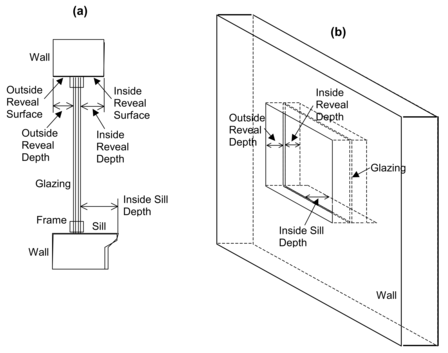
\includegraphics[width=0.9\textwidth, height=0.9\textheight, keepaspectratio=true]{media/image064.png}
\caption{(a) Vertical section through a window (with frame) showing outside and inside reveal surfaces and inside sill. (b) Perspective view looking from the outside of a window (without frame) showing reveal surfaces. Note that “Outside Reveal Depth” is not a user input; it is calculated by the program from the window and wall vertices. \protect \label{fig:a-vertical-section-through-a-window-with}}
\end{figure}

\begin{figure}[hbtp] % fig 41
\centering
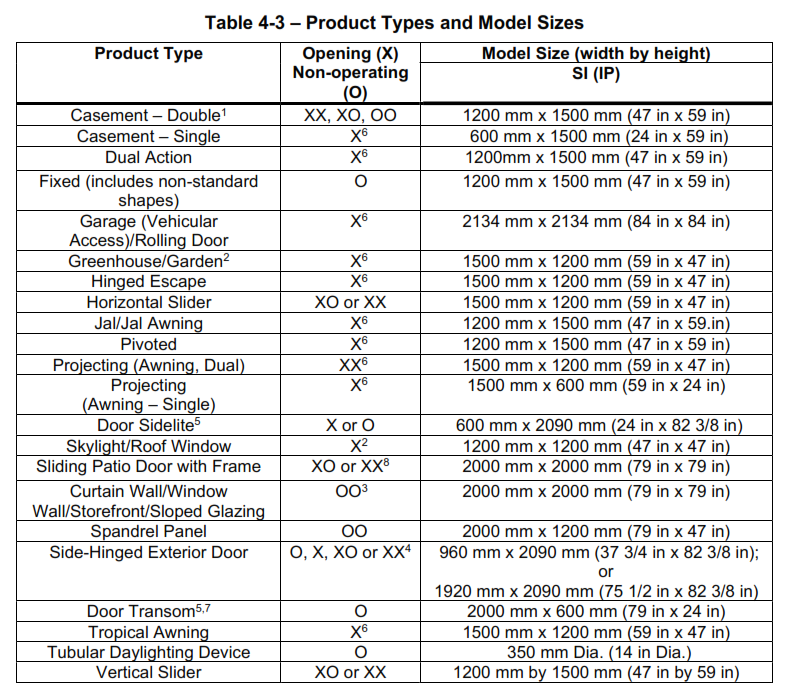
\includegraphics[width=0.9\textwidth, height=0.9\textheight, keepaspectratio=true]{media/NFRC100-Table4-3.PNG}
\caption{NFRC 100 Product Types and Model Sizes. \protect \label{fig:nfrc100-product-types}}
\end{figure}

An IDF example:

\begin{lstlisting}

  WindowProperty:FrameAndDivider,
        TestFrameAndDivider, ! Frame/Divider Name
        0.05, ! Frame Width
        0.04, ! Frame Outside Projection
        0.03, ! Frame Inside Projection
        5.0,  ! Frame Conductance
        1.3,  ! Ratio of Frame-Edge Glass Conductance to Center-Of-Glass Conductance
        0.8,  ! Frame Solar Absorptance
        0.8,  ! Frame Visible Absorptance
        0.9,  ! Frame Thermal Emissivity
        DividedLite, ! Divider Type
        0.03, ! Divider Width
        2,    ! Number of Horizontal Dividers
        2,    ! Number of Vertical Dividers
        0.03, ! Divider Outside Projection
        0.03, ! Divider Inside Projection
        5.0,  ! Divider Conductance
        1.3,  ! Ratio of Divider-Edge Glass Conductance to Center-Of-Glass Conductance
        0.8,  ! Divider Solar Absorptance
        0.8,  ! Divider Visible Absorptance
        0.9,  ! Divider Thermal Emissivity
        0.7,  ! Outside Reveal Solar Absorptance
        0.25, ! Inside Sill Depth (m)
        0.6,  ! Inside Sill Solar Absorptance
        0.2,  ! Inside Reveal Depth (m)
        0.5,  ! Inside Reveal Solar Absorptance
        ProjectingSingle; ! NFRC Product Type for Assembly Calculations
\end{lstlisting}

\subsection{WindowProperty:AirflowControl}\label{windowpropertyairflowcontrol}

This object is used to specify the control mechanism for windows in which forced air flows in the gap between adjacent layers of glass. Such windows are called ``airflow windows.'' They are also known as ``heat-extract windows'' or ``climate windows.''

A common application is to reduce the zone load by exhausting indoor air through the window. In the cooling season this picks up and expels some of the solar heat absorbed by the window glass (and by the between-glass shade or blind, if present). In the heating season this warms the window, reducing the heat loss from the window. A side benefit is increased thermal comfort. This is because the inside surface of the window will generally be cooler in summer and warmer in winter.

The surface output variable ``Surface Window Gap Convective Heat Transfer Rate'' gives the heat picked up (or lost) by the gap airflow.

\subsubsection{Inputs}\label{inputs-34-001}

\paragraph{Field: Name}\label{field-name-31-001}

Name of the window that this WindowProperty:AirflowControl refers to. It must be a window with two or three glass layers, i.e., double- or triple-glazing. For triple-glazing the airflow is assumed to be between the two inner glass layers.

An error will result if the gas in the airflow gap is other than air. If an airflow window has a between-glass shade or blind, the gas in the gap on either side of the shade or blind must be air.

\paragraph{Field: Airflow Source}\label{field-airflow-source}

The source of the gap airflow. The choices are:

\emph{IndoorAir}: Indoor air from the window's zone is passed through the window.

\emph{OutdoorAir}: Outdoor air is passed through the window.

\paragraph{Field: Airflow Destination}\label{field-airflow-destination}

This is where the gap air goes after passing through the window. The choices are:

\emph{IndoorAir}: The gap air goes to the indoor air of the window's zone.

\emph{OutdoorAir}: The gap air goes to the outside air.

\emph{ReturnAir}. The gap air goes to the return air for the window's zone. This choice is allowed only if Airflow Source = InsideAir. If the return air flow is zero, the gap air goes to the indoor air of the window's zone. If the sum of the gap airflow for all of the windows in a zone with Airflow Destination = ReturnAir exceeds the return airflow, then the difference between this sum and the return airflow goes to the indoor air. The name of the Return Air Node may be specified below.

Figure~\ref{fig:gap-airflow-configurations-for-airflow} shows the allowed combinations of Airflow Source and Airflow Destination. The allowed combinations of Airflow Source and Airflow Destination are:

IndoorAir -\textgreater{} OutdoorAir

IndoorAir -\textgreater{} IndoorAir

IndoorAir -\textgreater{} ReturnAir

OutdoorAir -\textgreater{} IndoorAir

OutdoorAir -\textgreater{} OutdoorAir

\paragraph{Field: Maximum Flow Rate}\label{field-maximum-flow-rate-003}

The maximum value of the airflow, in m\(^{3}\)/s per m of glazing width. The value is typically 0.006 to 0.009 m\(^{3}\)/s-m (4 to 6 cfm/ft).

The airflow can be modulated by specifying Airflow Has Multiplier Schedule = Yes and giving the name of the Airflow Multiplier Schedule (see below).

The fan energy used to move the air through the gap is generally very small and so is ignored.

\paragraph{Field: Airflow Control Type}\label{field-airflow-control-type}

Specifies how the airflow is controlled. The choices are:

\emph{AlwaysOnAtMaximumFlow}. The airflow is always equal to Maximum Airflow.

\emph{AlwaysOff}. The airflow is always zero.

\emph{ScheduledOnly}. The airflow in a particular timestep equals Maximum Airflow times the value of the Airflow Multiplier Schedule for that timestep.

\paragraph{Field: Airflow Is Scheduled}\label{field-airflow-is-scheduled}

Specifies if the airflow is scheduled. The choices are:

\emph{Yes}. The airflow is scheduled.

\emph{No}. The airflow is not scheduled.

If Yes, Airflow Multiplier Schedule Name is required.

\paragraph{Field: Airflow Multiplier Schedule Name}\label{field-airflow-multiplier-schedule-name}

The name of a schedule with values between 0.0 and 1.0. The timestep value of the airflow is Maximum Airflow times the schedule value. Required if Airflow Is Scheduled = Yes. Unused if Airflow Is Scheduled = No. This schedule should have a ScheduleType with Numeric Type = Continuous and Range = 0.0 : 1.0.

\paragraph{Field: Airflow Return Air Node Name}\label{field-airflow-return-air-node-name}

The name of the return air node for this airflow window if the Airflow Destination is ReturnAir. If left blank, this defaults to the first return air node for the zone containing the window surface.

\begin{figure}[hbtp] % fig 39
\centering
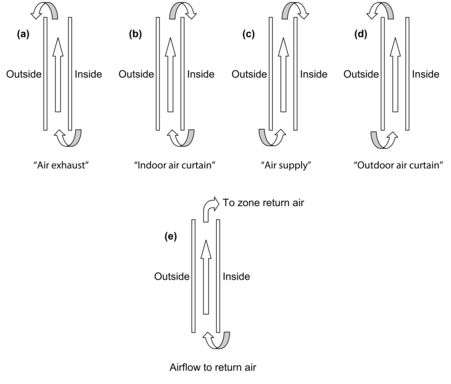
\includegraphics[width=0.9\textwidth, height=0.9\textheight, keepaspectratio=true]{media/image065.png}
  \caption{Gap airflow configurations for airflow windows. (a) \textbf{Air exhaust window}: Airflow Source = InsideAir, Airflow Destination = OutsideAir; (b) \textbf{Indoor air curtain window}: Airflow Source = InsideAir, Airflow Destination = InsideAir; (c) \textbf{Air supply window}: Airflow Source = OutsideAir, Airflow Destination = InsideAir; (d) \textbf{Outdoor air curtain window}: Airflow Source = OutsideAir, Airflow Destination = OutsideAir; (e) \textbf{Airflow to Return Air}: Airflow Source = InsideAir, Airflow Destination = ReturnAir. Based on ``Active facades,'' Version no. 1, Belgian Building Research Institute, June 2002. \protect \label{fig:gap-airflow-configurations-for-airflow}}
\end{figure}

An IDF example: window with a constant airflow from inside to outside at 0.008 m\(^{3}\)/s-m.

\begin{lstlisting}
WindowProperty:AirflowControl,
      Zn001:Wall001:Win002,   !- Name
      InsideAir,              !- Airflow Source
      OutsideAir,             !- Airflow Destination
      0.008,                  !- Maximum Flow Rate {m3/s-m}
      AlwaysOnAtMaxFlow,      !- Airflow Control Type
      No,                     !- Airflow Is Scheduled
      ;                       !- Airflow Multiplier Schedule Name
      ,                       !- Airflow Return Air Node Name
\end{lstlisting}

\subsection{WindowProperty:StormWindow}\label{windowpropertystormwindow}

This object allows you to assign a movable exterior glass layer (``storm window'' or ``storm glass'') that is usually applied to a window in the winter to reduce heat loss and removed in the summer. A WindowProperty:StormWindow object is required for each window that has an associated storm window. It is assumed that:

\begin{itemize}
\item
  When the storm glass is in place it is the outermost layer of the window, it covers only the glazed part of the window and not the frame, and it forms a tight seal. See Figure~\ref{fig:section-through-a-single-glazed-window}.
\item
  When the storm glass is not in place it is completely removed and has no effect on window heat transfer.
\item
  The gap between the storm glass and rest of the glazing is filled with air.
\end{itemize}

\begin{figure}[hbtp] % fig 40
\centering
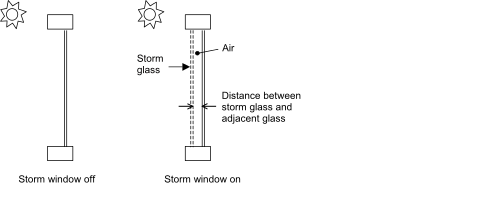
\includegraphics[width=0.9\textwidth, height=0.9\textheight, keepaspectratio=true]{media/image066.png}
\caption{Section through a single-glazed window without (left) and with (right) a storm glass layer. Not to scale. \protect \label{fig:section-through-a-single-glazed-window}}
\end{figure}

With the addition of a storm window, single glazing effectively becomes double glazing, double glazing becomes triple glazing, etc.

The presence of a storm window is indicated by the output variable ``Surface Storm Window On Off Status'' (see ``Window Output Variables''). This flag is \textbf{0} if the storm window is off, \textbf{1} if it is on, and \textbf{--1} if the window does not have an associated storm window.

The program automatically creates a window construction (ref: Construction) that consists of the storm window glass layer and its adjacent air layer added to the original (unshaded, or ``bare'') window construction. In the eplusout.eio file this construction is called BARECONSTRUCTIONWITHSTORMWIN:\emph{n}, where \emph{n} is the number of the associated StormWin object. If the window has a shaded construction, the program creates a construction called SHADEDCONSTRUCTIONWITHSTORMWIN:\emph{n} that consists of the storm window glass layer and its adjacent air layer added to the original shaded window construction.

The program also creates a \hyperref[windowmaterialgas]{WindowMaterial:Gas} layer corresponding to the air layer adjacent to the storm glass. In the eplusout.eio file this layer is called AIR:STORMWIN:\emph{k}MM, where \emph{k} is the thickness of the air layer expressed as an integer number of millimeters.

\subsubsection{Inputs}\label{inputs-35-001}

\paragraph{Field: Window Name}\label{field-window-name-000}

This is the name of a window (or glass door) to which the storm glass is applied. Not all windows can accept WindowProperty:StormWindow. The rules are:

\begin{itemize}
\item
  The window must be an exterior window. WindowProperty:StormWindow is not applicable to interior (interzone) windows.
\item
  The window construction (without the storm glass layer) can have up to three glass layers.
\item
  If the window has an associated shaded construction (ref: \hyperref[windowpropertyshadingcontrol]{WindowShadingControl}), that construction can have an interior shade or blind and up to three glass layers, or a between-glass shade or blind and two glass layers. The shaded construction cannot have an exterior shade or blind, cannot have a between-glass shade or blind and three glass layers, and cannot be switchable glazing.
\item
  The window cannot be an airflow window, i.e., a window that has an associated \hyperref[windowpropertyairflowcontrol]{WindowProperty:AirflowControl}.
\end{itemize}

\paragraph{Field: Storm Glass Layer Name}\label{field-storm-glass-layer-name}

This is the name of a window glass material. Storm windows are assumed to consist of a single layer of glass. A storm window frame, if present, is ignored.

\paragraph{Field: Distance Between Storm Glass Layer and Adjacent Glass}\label{field-distance-between-storm-glass-layer-and-adjacent-glass}

The separation between the storm glass and the rest of the window (Figure~\ref{fig:section-through-a-single-glazed-window}). It is measured from the inside of the storm glass layer to the outside of the adjacent glass layer.

\paragraph{Field: Month that Storm Glass Layer Is Put On}\label{field-month-that-storm-glass-layer-is-put-on}

The number of the month (January = 1, February = 2, etc.) during which the storm window is put in place.

\paragraph{Field: Day of Month that Storm Glass Layer Is Put On}\label{field-day-of-month-that-storm-glass-layer-is-put-on}

The day of the month that the storm window is put in place. It is assumed that the storm window is put in place at the beginning of this day, i.e., during the first simulation timestep of the day, and remains in place until that month and day given by the following two fields.

\paragraph{Field: Month that Storm Glass Layer Is Taken Off}\label{field-month-that-storm-glass-layer-is-taken-off}

The number of the month (January = 1, February = 2, etc.) during which the storm window is removed.

\paragraph{Field: Day of Month that Storm Glass Layer Is Taken Off}\label{field-day-of-month-that-storm-glass-layer-is-taken-off}

The day of the month that the storm window is removed. It is assumed that the storm window is removed at the beginning of this day, i.e., during the first simulation timestep of the day, and stays off until the month and day given by Month that Storm Glass Layer Is Put On, Day of Month that Storm Glass Layer Is Put On.

In the northern hemisphere, the month the storm window is put on is generally greater than the month it is taken off (for example put on in month 10, when it starts to get cold, and taken off in month 5, when it starts to warm up). In the southern hemisphere this is reversed: month on is less than month off.

An IDF example of WindowProperty:StormWindow. The storm window is put in place on October 15 and removed on May 1.

\begin{lstlisting}
WindowProperty:StormWindow,
   Window1, !- Name of Window to Which Storm Window Glass Layer is Applied
   GlassA,  !- Name of Material:WindowGlass or MATERIAL:WindowGlass:AltInput that is the storm window layer
   0.060,   !- Distance from storm window to adjacent glass (m)
   10,      !- Month that Storm Window Is Put On
   15,      !- Day of Month that Storm Window Is Put On
   5,       !- Month that Storm Window Is Taken Off
   1;       !- Day of Month that Storm Window Is Taken Off
\end{lstlisting}

\subsection{Importing Windows from WINDOW program}\label{importing-windows-from-window-program}

\begin{callout}
WINDOW v6.3 and later is capable of writing IDF excerpts for Window data. This is the preferred method as no external file is necessary. See the Tips document for details on obtaining the IDF excerpt.
\end{callout}

The WINDOW program calculates the U-value, Solar Heat Gain Coefficient, solar transmission/absorption characteristics, visible transmission characteristics and other properties of a window under standard indoor and outdoor conditions. WINDOW treats the whole window system---glazing, frame and divider. A sub-program of WINDOW called THERM uses a 2-D finite element calculation to determine the effective conductance of frame, divider and edge-of-glass elements. Another sub-program, OPTICS, determines the solar-optical properties of glazing, including laminates and coated glass.

WINDOW can write a data file containing a description of the window that was analyzed. An example of this file (which is no longer the preferred method) is shown in the Tips document under WINDOW generated files. is shown below. This file, which can be named by the user, can be read by EnergyPlus. For more complete description and examples, see the object description -- \hyperref[constructionwindowdatafile]{Construction:WindowDataFile}.

In this way, the same window that was created in WINDOW can be imported into EnergyPlus for annual energy analysis without having to re-input the window data. To obtain WINDOW, THERM, or OPTICS go to \url{http://windows.lbl.gov} and choose the software link. A major advantage of using WINDOW to create window input for EnergyPlus is that you will have direct access to WINDOW's expanding database of over 1000 different glass types; and you will be able to browse through this database according to different criteria (color, transmittance, solar heat gain coefficient, etc.) to help you select the best glass type for your application.

Although WINDOW writes only one window entry on the WINDOW data file, EnergyPlus users can combine two or more of these files to end up with a single data file with multiple window entries of different types. In this way a library of windows from WINDOW can be built up if so desired. If you combine files like this you should be sure not to leave out or change any of lines from the original files.

There are four methods for inputting window constructions in EnergyPlus:

\begin{enumerate}
\tightlist
\item
  input full spectral data for each layer in the IDF,
\item
  input spectral average data for each layer in the IDF,
\item
  items 1 and 2 can be accomplished by reporting the IDF excerpt method from WINDOW
\item
  import WINDOW report containing layer-by-layer calculated values and overall glazing system angular values.
\end{enumerate}

\begin{callout}
  \warning{Note: When using method 4, the overall glazing system angular dependent properties, including Tsol, Abs, Rfsol, Rbsol, Tvis, Rfvis, and Rbvis, are not used by EnergyPlus. Therefore, methods 1 and 2 and preferably 3 are recommended.}
\end{callout}

\begin{itemize}
\item
  The SHGC calculations in EnergyPlus for window layers input using full spectral data use a spectral weighting data set (derived from Optics5 data file ISO-9845GlobalNorm.std) that is different from the WINDOW default spectral weighting data set (W5\_NFRC\_2003.std). This difference accounts for most of the variation in SHGC values reported by EnergyPlus and WINDOW for full spectral data window layer input. This variation is more pronounced for window constructions of three glass layers or more.
\item
  Users intending to select a window construction based on SHGC value for energy code compliance should base their selection on the value reported by WINDOW since this is the officially recognized value.
\end{itemize}

In EnergyPlus, the Window data file is searched for each ``\hyperref[constructionwindowdatafile]{Construction:WindowDataFile}'' object in the EnergyPlus input. This object has a very simple form:

\begin{lstlisting}
Construction:WindowDataFile,
  ConstructionName,
  FileName; ! Default is Window5DataFile.dat in the ``run'' folder.
\end{lstlisting}

If there is a window called ConstructionName on the Window data file, the data for that window is read from the file and the following EnergyPlus objects and their names are created. The ``W5'' prefixed to these names indicates that the object originated in the Window data file.

\subsection{Using LBNLs Windows Calculation Engine}\label{windowscalculationengine}
This is new windows simulation engine that will be used in both EnergyPlus and Berkeley Lab WINDOW. The intent is for this engine to replace all other window calculation modules in EnergyPlus. For the time being, other modules will still be available. To use the new Window Calculation Engine, insert the following into IDF:

\begin{lstlisting}
WindowsCalculationEngine,
ExternalWindowsModel;
\end{lstlisting}


\section{Group -- Advanced Surface Concepts}\label{group-advanced-surface-concepts}

This group of objects describe concepts applied to heat transfer surfaces that are of an advanced nature. Careful consideration must be given before using these.

\subsection{SurfaceProperty:HeatTransferAlgorithm}\label{surfacepropertyheattransferalgorithm}

This object, and three other related objects, can be used to control which surface heat transfer model is used on specific surfaces. The separate object called HeatBalanceAlgorithm is used to control the heat transfer model in an overall way while this object can be used to revise the algorithm selections for specific surfaces. This object allows selectively overriding the global setting in HeatBalanceAlgorithm to choose one of the following models for a particular surface:

\begin{itemize}
\item
  CTF (Conduction Transfer Functions),
\item
  EMPD (Effective Moisture Penetration Depth with Conduction Transfer Functions).
\item
  CondFD (Conduction Finite Difference)
\item
  HAMT (Combined Heat And Moisture Finite Element)
\end{itemize}

\subsubsection{Inputs}\label{inputs-000}

\paragraph{Field: Surface Name}\label{field-surface-name}

This is the name of the surface that will be assigned to use the heat transfer algorithm selected in the next field. This should be a name of a surface defined elsewhere.

\paragraph{Field: Algorithm}\label{field-algorithm}

This field is used to determine the heat transfer algorithm that is to be applied to the surface named in the previous field. The allowable choices are:

\begin{itemize}
\item
  ConductionTransferFunction
\item
  MoisturePenetrationDepthConductionTransferFunction
\item
  ConductionFiniteDifference
\item
  CombinedHeatAndMoistureFiniteElement
\end{itemize}

\subsection{SurfaceProperty:HeatTransferAlgorithm:MultipleSurface}\label{surfacepropertyheattransferalgorithmmultiplesurface}

This object can be used to control the surface heat transfer model used for specific types of surfaces. The separate object called HeatBalanceAlgorithm is used to control the heat transfer model in an overall way while this object can be used to revise the algorithm selections for specific types of surfaces. This object allows selectively overriding the global setting in HeatBalanceAlgorithm to choose one of the following models for all surfaces of a particular type:

\begin{itemize}
\item
  CTF (Conduction Transfer Functions),
\item
  EMPD (Effective Moisture Penetration Depth with Conduction Transfer Functions).
\item
  CondFD (Conduction Finite Difference)
\item
  HAMT (Combined Heat And Moisture Finite Element)
\end{itemize}

\subsubsection{Inputs}\label{inputs-1-000}

\paragraph{Field: Name}\label{field-name-000}

This is a unique, user-defined name for the object.

\paragraph{Field: Surface Type}\label{field-surface-type}

This field is selects the type of surfaces that are all assigned to use the heat transfer algorithm selected in the next field. This field is used with one of the following allowable keywords:

\begin{itemize}
\item
  AllExteriorSurfaces---all surfaces that have ``Outdoors'' outside boundary condition
\item
  AllExteriorWalls---all walls that have ``Outdoors'' outside boundary condition
\item
  AllExteriorRoofs---all roofs that have ``Outdoors'' outside boundary condition
\item
  AllExteriorFloors---all floors that have ``Outdoors'' outside boundary condition
\item
  AllGroundContactSurfaces---all surfaces that have ``Ground'' outside boundary condition
\item
  AllInteriorSurfaces---all surfaces that are internal partition-type surfaces
\item
  AllInteriorWalls---all walls that are internal surfaces
\item
  AllInteriorCeilings---all ceilings that are internal surfaces
\item
  AllInteriorFloors---all floors that are are internal surfaces
\end{itemize}

\paragraph{Field: Algorithm}\label{field-algorithm-1}

This field is used to determine the heat transfer algorithm that is to be applied to the surface types in the previous field. The allowable choices are:

\begin{itemize}
\item
  ConductionTransferFunction
\item
  MoisturePenetrationDepthConductionTransferFunction
\item
  ConductionFiniteDifference
\item
  CombinedHeatAndMoistureFiniteElement
\end{itemize}

\begin{lstlisting}
SurfaceProperty:HeatTransferAlgorithm:MultipleSurface,
      my exterior wall override,
      AllExteriorWalls,
      ConductionFiniteDifference;
\end{lstlisting}

\subsection{SurfaceProperty:HeatTransferAlgorithm:SurfaceList}\label{surfacepropertyheattransferalgorithmsurfacelist}

This object can be used to control the surface heat transfer model used for a list of surfaces. The separate object called HeatBalanceAlgorithm is used to control the heat transfer model in an overall way while this object can be used to revise the algorithm selections for a list of specific surfaces. This object allows selectively overriding the global setting in HeatBalanceAlgorithm to choose one of the following models for listed:

\begin{itemize}
\item
  CTF (Conduction Transfer Functions),
\item
  EMPD (Effective Moisture Penetration Depth with Conduction Transfer Functions).
\item
  CondFD (Conduction Finite Difference)
\item
  HAMT (Combined Heat And Moisture Finite Element)
\end{itemize}

\subsubsection{Inputs}\label{inputs-2-000}

\paragraph{Field: Name}\label{field-name-1}

This is a unique, user-defined name for the object.

\paragraph{Field: Algorithm}\label{field-algorithm-2}

This field is used to determine the heat transfer algorithm that is to be applied to the surface listed in the remaining fields. The allowable choices are:

\begin{itemize}
\item
  ConductionTransferFunction
\item
  MoisturePenetrationDepthConductionTransferFunction
\item
  ConductionFiniteDifference
\item
  CombinedHeatAndMoistureFiniteElement
\end{itemize}

\paragraph{Field: Surface Name N}\label{field-surface-name-n}

This is the name of the ``Nth'' surface that will be assigned to use the heat transfer algorithm selected in this object. These should be the names of surfaces defined elsewhere. This object is extensible. Additional surfaces can be added to extend the object.

An example IDF object follows.

\begin{lstlisting}

SurfaceProperty:HeatTransferAlgorithm:SurfaceList,
      my wall construct override,   !- Name
      ConductionFiniteDifference,   !- Algorithm
      Zn001:Wall001,                !- Surface Name 1
      Zn001:Wall002,                !- Surface Name 2
      Zn001:Wall003,                !- Surface Name 3
      Zn001:Wall004;                !- Surface Name 4
\end{lstlisting}

\subsection{SurfaceProperty:HeatTransferAlgorithm:Construction}\label{surfacepropertyheattransferalgorithmconstruction}

This object can be used to control the surface heat transfer model used for surfaces that have a specific type of construction. The separate object called HeatBalanceAlgorithm is used to control the heat transfer model in an overall way while this object can be used to revise the algorithm selections for specific constructions. This object allows selectively overriding the global setting in HeatBalanceAlgorithm to choose one of the following models for all surfaces with particular type of construction:

\begin{itemize}
\item
  CTF (Conduction Transfer Functions),
\item
  EMPD (Effective Moisture Penetration Depth with Conduction Transfer Functions).
\item
  CondFD (Conduction Finite Difference)
\item
  HAMT (Combined Heat And Moisture Finite Element)
\end{itemize}

\subsubsection{Inputs}\label{inputs-3}

\paragraph{Field: Name}\label{field-name-2}

This is a unique, user-defined name for the object.

\paragraph{Field: Algorithm}\label{field-algorithm-3}

This field is used to determine the heat transfer algorithm that is to be applied to the surfaces with the type of of construction listed in the next field. The allowable choices are:

\begin{itemize}
\item
  ConductionTransferFunction
\item
  MoisturePenetrationDepthConductionTransferFunction
\item
  ConductionFiniteDifference
\item
  CombinedHeatAndMoistureFiniteElement
\end{itemize}

\paragraph{Field: Construction Name}\label{field-construction-name}

This field is the name of a Construction object defined elsewhere. All the surfaces in the model that are assigned this type of construction will be assigned to use the heat transfer algorithm selected in the previous field.

An example IDF object follows.

\begin{lstlisting}

SurfaceProperty:HeatTransferAlgorithm:Construction,
      my wall construct override,  !- Name
      ConductionFiniteDifference,  !- Algorithm
      R13WALL;                     !- Construction Name
\end{lstlisting}

\subsection{SurfaceControl:MovableInsulation}\label{surfacecontrolmovableinsulation}

Movable insulation can be used/scheduled on any surface regular surface (such as a wall, floor, roof, etc.) but not on a subsurface (such as a window, use WindowProperty:ShadingControl instead). With movable insulation, no reference is made in the surface that is using the insulation -- rather the movable insulation statement references the surface to which it is applied.

Exterior and interior movable insulation have undergone some testing and appears to producing expected results. The underlying principle has been implemented in EnergyPlus for both interior and exterior movable insulation with the possibility for exterior movable insulation to be transparent (transparent insulation material or TIM).

TIM exterior layers can be used with the ConductionFiniteDifference (CondFD) solution algorithm. With this addition, TIM layers can be used in conjunction with wall layers that have phase change materials (PCM) included, or any other advanced capability of the CondFD algorithm such as variable conductivity. The input requirements are exactly the same as when used with the CTF algorithm. The Solution Algorithm needs to be changed to CondFD, and as with CTF, the ``SurfaceControl:MovableInsulation'' object must be completed to specify the insulated surface and the ``WindowMaterial:Glazing'' object is needed to provide the TIM layer properties.

Basically, the addition of movable insulation allows the user to schedule an extra amount of insulation on either the inside or outside surface of a wall (or both). The insulation must be a simple, homogenous material layer (linked to a material definition within the input data file). Note that EnergyPlus allows the exterior movable insulation layer to be transparent to short wavelength radiation (solar). In this case, incident solar is split between the plane between the movable insulation and the surface and the plane between the movable insulation and the surrounding air. This calculation is fairly basic and based on the solar transmittance of the insulation layer (material properties). Using transparent layers for exterior movable insulation allows solar energy to penetrate deeper into a construction where it can be stored for later use in the building (similar in concept to a Trombe Wall).

\subsubsection{Field: Insulation Type}\label{field-insulation-type}

This field determines whether the movable insulation is applied to the inside or the outside of the surface by entering either ``Inside'' or ``Outside'', respectively.

\subsubsection{Field: Surface Name}\label{field-surface-name-1}

This field refers the movable insulation back to a particular surface (ref: Building Surfaces) via its user assigned name so that EnergyPlus knows where to apply this extra layer of insulation. This will affect either the inside or outside surface heat balance of this surface depending on the value in the insulation type field (see previous field).

\subsubsection{Field: Material Name}\label{field-material-name}

This field refers to a material layer (e.g., Material, Material:NoMass, or WindowMaterial:Glazing; transparent layers are only valid for outside movable insulation) via its user assigned name. This provides the program with a full complement of material properties so that the effect of the insulation (R-value and solar transmittance) can be correctly taken into account by EnergyPlus.  Note that for non-glazing materials the solar absorptivity of the layer will be used directly in the calculations.  For glazing material layers, the solar absorptivity will be calculated by subtracting both the transmissivity and the front side reflectivity from unity for the material.

\subsubsection{Field: Schedule Name}\label{field-schedule-name}

This field is a schedule that theoretically can be any positive real number but was originally intended to be a parameter between 0.0 and 1.0. Its purpose is to act as a fractional modifier on the resistance of the material layer. The actual thermal resistance of the movable insulation is equal to the resistance of the material layer times the current value in the movable insulation schedule. A value of 0.0 simply means that the movable insulation is not present.

An example of this syntax implemented in an input file is:

\begin{lstlisting}

SurfaceControl:MoveableInsulation,
    Exterior,                      ! Insulation Type
    Zone001:Wall001,               ! Surface Name
    TransparentInsulationMaterial, ! Material Name
    PresentInWinterSchedule;       ! Schedule Name
\end{lstlisting}

\subsection{SurfaceProperty:OtherSideCoefficients}\label{surfacepropertyothersidecoefficients}

By referencing the Other Side Coefficients statement in the surface statements (i.e.~Outside Boundary Condition), the temperature of the outer plane of a surface (see Figure~\ref{fig:illustration-for-other-side-coefficients}) can be directly controlled. Other side coefficients can also be used to control the exterior convective heat transfer coefficient of a surface and the corresponding exterior air temperature. It should be noted that solar effects are not accounted for when other side coefficients are used. In addition, if other side coefficients are specified for a surface, they also hold for subsurfaces of that surface (though subsurfaces can have their own coefficient set).

other side coefficients have the same effect on all types of heat transfer surfaces. In other words, an interior surface with other side coefficients specified and an exterior wall with identical other side coefficients specified are simulated exactly the same. A surface that uses other side coefficients should be thought of as a new or separate type of surface. All heat transfer surfaces are simulated in the same manner through conduction transfer functions. The only difference between the various types of heat transfer surfaces is the environment on the other side of the surface. For example, the other side environment of an exterior surface is the outdoor environment. For an interior surface, the temperature of the outer plane of the surface is set equal to the temperature of the inner plane of the surface. Similarly, a surface with other side coefficients specified will allow the user to control the other side environment.

Heat transfer through a surface is an extremely important component in the calculation of zone loads. The information to calculate this heat transfer is readily available if the surface is exposed to the outdoor environment or to another zone that is being simulated. Occasionally, a user will want to model the heat transfer through a surface that is adjacent to an area that is not included in the EnergyPlus model. For example, an office area is attached to a warehouse and the user is only interested in simulating the office area. An interior surface with other side coefficients specified could be used to control the environment on the other side of the surface, thereby accounting for the heat transfer through the adjoining surface.

Other Side Coefficients affects the ``other side'' of a surface as described below. Each coefficient has a special meaning. You may enter a 0 or blank if you are not using a particular coefficient. Note that there are two potential ways to use other side coefficients. Either they are used to set the temperature of the exterior side surface directly (if the combined convective/radiative coefficient below is less than or equal to zero) or to set both the film coefficient (positive value for the combined convective/radiative coefficient below) and the outside air temperature.

\subsubsection{Inputs}\label{inputs-4}

\paragraph{Field: Name}\label{field-name-3}

This, of course, is the string referenced in the Surface statement that is using OtherSideCoefficients as the Outside Boundary Condition.

\paragraph{Field: Combined Convective/Radiative Film Coefficient}\label{field-combined-convectiveradiative-film-coefficient}

This is a trigger value. If the value is greater than zero, then it is taken to be the combined convective/radiative film coefficient. In this case (value \textgreater{} 0), the remaining fields are used first to calculate the outside air temperature for the surface and then to calculate the outside surface temperature based on the outside air temperature and the film coefficient. If this field is less than or equal to zero, then the remaining fields are used to calculate the surface temperature (not the outside air temperature). The units for this field are the same as for a convective heat transfer coefficient: W/(m\(^{2}\)*K). This is referred to as ``C1'' in the reference below.

\paragraph{Field: Constant Temperature}\label{field-constant-temperature}

This field defines a temperature term that is a constant part of the calculation either of the surface or outside air temperature. This parameter is shown as ``C2'' in the equation below. The units for this parameter are degrees C. If a schedule name is included as the second parameter, the value of this parameter will be overridden by the value from the schedule. The default for this field is 0.0.

\paragraph{Field: Constant Temperature Coefficient}\label{field-constant-temperature-coefficient}

This field defines a constant coefficient that is applied to the constant temperature (see previous field). This parameter is shown as ``C3'' in the equation below. This parameter is dimensionless. The value of this parameter is usually 1.0 if a schedule is used to set C2. This field is ignored if \emph{Sinusoidal Variation of Constant Temperature Coefficient} = Yes. The default for this field is 1.0.

\paragraph{Field: External Dry-Bulb Temperature Coefficient}\label{field-external-dry-bulb-temperature-coefficient}

This field defines a constant coefficient that is applied to the outside air dry-bulb temperature. This parameter is shown as ``C4'' in the equation below. This parameter is dimensionless. The default for this field is 0.0.

\paragraph{Field: Ground Temperature Coefficient}\label{field-ground-temperature-coefficient}

This field defines a constant coefficient that is applied to the ground temperature (ref. Site:GroundTemperature:BuildingSurface). This parameter is shown as ``C5'' in the equation below. This parameter is dimensionless.

\paragraph{Field: Wind Speed Coefficient}\label{field-wind-speed-coefficient}

This field defines a constant coefficient that is applied to the product of the outside air dry-bulb temperature and the wind speed. This parameter is shown as ``C6'' in the equation below. This parameter has dimensions of inverse velocity or s/m. The default for this field is 0.0.

\paragraph{Field: Zone Air Temperature Coefficient}\label{field-zone-air-temperature-coefficient}

This field defines a constant coefficient that is applied to the temperature of the zone to which this surface belongs. This parameter is shown as ``C7'' in the equation below. This parameter is dimensionless. The default for this field is 0.0.

\paragraph{Field: Constant Temperature Schedule Name}\label{field-constant-temperature-schedule-name}

This field is used to supply a schedule name. That schedule will supply the ``constant'' temperature value C2. Note that the value of the C3 field should normally be 1.0 if a schedule is used for C2. If not blank, this field must be a valid schedule name.

\paragraph{Field: Sinusoidal Variation of Constant Temperature Coefficient}\label{field-sinusoidal-variation-of-constant-temperature-coefficient}

This field is optional and can be used to define an alternate method of prescribing the coefficient that is applied to the constant temperature (see the fields Constant Temperature and Constant Temperature Coefficient). This parameter is shown as ``C2'' in the equation below. If this field is omitted, left blank, or set to ``No,'' then C2 is a constant (defined in the field Constant Temperature Coefficient). However if this is set to ``Yes,'' then the value of C2 varies with a unitary sine wave in the following way:

\begin{equation}
C2 = Sin\left( {2\pi \frac{{\left( {time\,of\,day} \right)}}{{\left( {period} \right)}}} \right)
\end{equation}

The value for ``period'' is controlled in the following field. The value for ``time of day'' is based on the zone timestep and is in units of hours. The sine function here uses input as radians. When using this option, the value for C2 will vary between -1.0 and 1.0 and the value put in the field Constant Temperature Coefficient is not used. This option cannot be used at the same time as scheduling a constant temperature with the previous field.

\paragraph{Field: Period of Sinusoidal Variation}\label{field-period-of-sinusoidal-variation}

This field is used to define the period of the sine wave when using the Sinusodial Variation of Constant Temperature Coefficient capability selected in the previous field. This field is the time period of the sine wave in units of hours. The default is 24 hours and provides a diurnal sine wave. The value entered here is ``period'' in the equation in the previous field.

\paragraph{Field: Previous Other Side Temperature Coefficient}\label{field-previous-other-side-temperature-coefficient}

This field defines a constant coefficient that is applied to the other side temperature computed by this object from the previous zone time step. This parameter is shown as ``C8'' in the equation below. This parameter is dimensionless. The default for this field is 0.0.

\paragraph{Field: Minimum Other Side Temperature Limit}\label{field-minimum-other-side-temperature-limit}

This field specifies a lower limit for the other side temperature result in degrees C. If blank, there is no lower limit.

\paragraph{Field: Maximum Other Side Temperature Limit}\label{field-maximum-other-side-temperature-limit}

This field specifies an upper limit for the other side temperature result in degrees C. If blank, there is no upper limit.

The coefficients listed above are used in the following equation:

\begin{equation}
T = C2*C3 + C4*Toadb + C5*Tgrnd + C6*Wspd*Toadb + C7*Tzone + C8*Tpast
\end{equation}

where:

T = Outside Air Temperature when C1 (Combined convective/radiative film Coeff) \textgreater{} 0

T = Exterior Surface Temperature when C1 (Combined convective/radiative film Coeff) \textless{} = 0

Tzone = Temperature of the zone being simulated (°C)

Toadb = Dry-bulb temperature of the outdoor air (°C)

Tgrnd = Temperature of the ground (°C) from Site:GroundTemperature:BuildingSurface

Wspd = Outdoor wind speed (m/sec)

Tpast = Other side temperature from previous zone timestep (°C)

\begin{figure}[hbtp] % fig 41
\centering
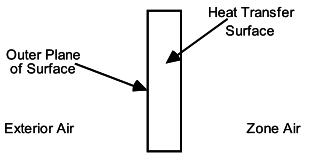
\includegraphics[width=0.9\textwidth, height=0.9\textheight, keepaspectratio=true]{media/image069.png}
\caption{Illustration for Other Side Coefficients \protect \label{fig:illustration-for-other-side-coefficients}}
\end{figure}

\begin{lstlisting}
!  Example input using temperature schedule
SurfaceProperty:OtherSideCoefficients,
      OSCCoef:Zn005:Wall003,   !- Name
      0,                       !- Combined Convective/Radiative Film Coefficient {W/m2-K}
      0.000000,                !- Constant Temperature {C}
      1.000000,                !- Constant Temperature Coefficient
      0.000000,                !- External Dry-Bulb Temperature Coefficient
      0.000000,                !- Ground Temperature Coefficient
      0.000000,                !- Wind Speed Coefficient
      0.000000,                !- Zone Air Temperature Coefficient
      Zn005Wall003OtherSideTempSched;  !- Constant Temperature Schedule Name
\end{lstlisting}

\begin{lstlisting}
!  Example input for outside heat transfer coefficient of 1.23, using Toadb
SurfaceProperty:OtherSideCoefficients,
      OSCCoef:Zn005:Wall004,   !- Name
      1.230000,                !- Combined Convective/Radiative Film Coefficient {W/m2-K}
      0.000000,                !- Constant Temperature {C}
      0.000000,                !- Constant Temperature Coefficient
      1.000000,                !- External Dry-Bulb Temperature Coefficient
      0.000000,                !- Ground Temperature Coefficient
      0.000000,                !- Wind Speed Coefficient
      0.000000,                !- Zone Air Temperature Coefficient
      ,                        !- Constant Temperature Schedule Name
      No,                      !- Sinusoidal Variation of Constant Temperature Coefficient
      24,                      !- Period of Sinusoidal Variation {hr}
      0.,                      !- Previous Other Side Temperature Coefficient
      ,                        !- Minimum Other Side Temperature Limit {C}
      ;                        !- Maximum Other Side Temperature Limit {C}
\end{lstlisting}

\subsubsection{Outputs}\label{outputs}

\begin{lstlisting}
Zone,Average,Surface Other Side Coefficients Exterior Air Drybulb Temperature
\end{lstlisting}

\paragraph{Surface Other Side Coefficients Exterior Air Drybulb Temperature {[}C{]}}\label{surface-other-side-coefficients-exterior-air-drybulb-temperature-c}

This is the air temperature applied to the other side of the surface.

\subsection{SurfaceProperty:OtherSideConditionsModel}\label{surfacepropertyothersideconditionsmodel}

By referencing the Other Side Conditions Model statement in the surface statements (i.e.~Outside Boundary Condition), the boundary conditions for the outer plane of the mass wall can be connected to the appropriate model for various multi-skin components. The types of multi-skin components that use this object include systems that are mounted to the outside surface using standoffs that create a small air gap -- see Figure~\ref{fig:illustration-for-other-side-conditions-model}. This type of modeling allows using the usual heat transfer calculations for the underlying surface with other types of multi-skin component models that are available including: unglazed transpired solar collectors, ventilated photovoltaic panels, and naturally ventilated facades.

The boundary condition values are determined dynamically by the program using internal component models. If you want to define other side surface temperatures or convection conditions, then use SurfaceProperty:OtherSideCoefficients instead of this object.

It should be noted that when other side conditions models are used, solar effects are removed from the surface's outside face heat balance, but are used in modeling the component adjacent to that surface.

The other side conditions model also includes underground piping system interaction. The PipingSystem:Underground:Domain object represents a mass of ground which may include interaction with, for example, basement surfaces. In this case, the ground model will internally use the other side condition model hook to update boundary conditions for those surfaces which use that other side condition model name reference.

The other side conditions model also includes an underwater boundary condition connection.  By specifying ``ConvectiveUnderwater'' as the boundary type, and including any number of ``SurfaceProperty:Underwater'' objects in the input, the user can connect sufaces to water such as for a moving vessel.

\subsubsection{Inputs}\label{inputs-5}

\paragraph{Field: Name}\label{field-name-4}

This is the string referenced in the Surface statement that is using OtherSideModel as the Exterior Environment.

\paragraph{Field: Type of Modeling}\label{field-type-of-modeling}

This is a string key selection used to identify the type of model that will be used to determine boundary conditions. The only available choices are ''GapConvectionRadiation,'' ``UndergroundPipingSystemSurface,'' ``GroundCoupledSurface,'' and ``ConvectiveUnderwater.''

\begin{figure}[hbtp] % fig 42
\centering
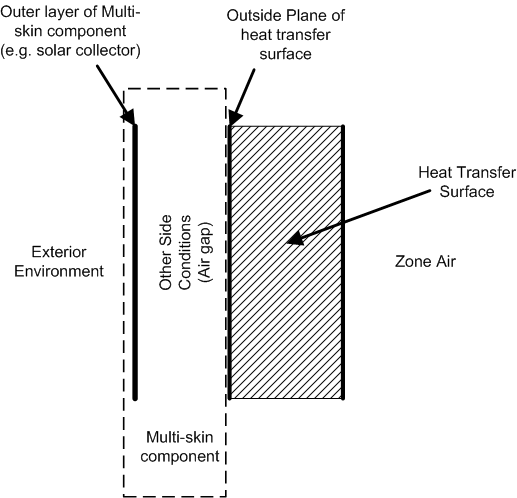
\includegraphics[width=0.9\textwidth, height=0.9\textheight, keepaspectratio=true]{media/image070.png}
\caption{Illustration for Other Side Conditions Model \protect \label{fig:illustration-for-other-side-conditions-model}}
\end{figure}

An example specification is:

\begin{lstlisting}

SurfaceProperty:OtherSideConditionsModel,
      UTSC OSCM ZN11,          ! OtherSideConditionsModel Name
      GapConvectionRadiation; ! Type of Modeling used to determine Boundary Conditions
\end{lstlisting}

\subsubsection{Outputs}\label{outputs-1}

\begin{itemize}
\item
  Zone,Average,Surface Other Side Conditions Modeled Convection Air Temperature {[}C{]}
\item
  Zone,Average,Surface Other Side Conditions Modeled Convection Heat Transfer Coefficient {[}W/m2-K{]}
\item
  Zone,Average,Surface Other Side Conditions Modeled Radiation Temperature {[}C{]}
\item
  Zone,Average,Surface Other Side Conditions Modeled Radiation Heat Transfer Coefficient {[}W/m2-K{]}
\end{itemize}

\paragraph{Surface Other Side Conditions Modeled Convection Air Temperature {[}C{]}}\label{surface-other-side-conditions-modeled-convection-air-temperature-c}

This is the air temperature exposed to the other side of the surface by the model and used in convection heat transfer calculations.

\paragraph{Surface Other Side Conditions Modeled Convection Heat Transfer Coefficient {[}W/m2-K{]}}\label{surface-other-side-conditions-modeled-convection-heat-transfer-coefficient-wm2-k}

This is the surface convection heat transfer coefficient applied to the other side of the surface by the model.

\paragraph{Surface Other Side Conditions Modeled Radiation Temperature {[}C{]}}\label{surface-other-side-conditions-modeled-radiation-temperature-c}

This is the effective temperature exposed to the other side of the surface for thermal radiation heat transfer calculations.

\paragraph{Surface Other Side Conditions Modeled Radiation Heat Transfer Coefficient {[}W/m2-K{]}}\label{surface-other-side-conditions-modeled-radiation-heat-transfer-coefficient-wm2-k}

This is the effective (Linearized) radiation heat transfer coefficient applied to the other side of the surface by the model.

\subsection{SurfaceProperty:Underwater}\label{surfacepropertyunderwater}

This object captures the inputs required to model a water-connected boundary condition for a surface.
This model is useful for either statically positioned buildings with natural convection to the water boundary condition, or a moving building (vessel).

\subsubsection{Inputs}\label{surfacepropertyunderwater-inputs}

\paragraph{Field: Name}\label{surfacepropertyunderwater-inputs-name}

This is the string referenced in the Surface statement that is using this OtherSideModel as the Exterior Environment.

\paragraph{Field: Distance from Surface Centroid to Leading Edge of Boundary Layer}\label{surfacepropertyunderwater-inputs-boundarylayerdistance}

This distance represents the distance from the centroid of this particular surface to leading edge of the boundary layer.
For a surface with zero velocity, this field will be irrelevant, because there is no forced boundary layer, and convection will be buoyantly driven.
For a moving vessel, this distance should be the nominal distance from the leading edge of the vessel, assuming a nearly flat surface along that path.

\paragraph{Field: Free Stream Water Temperature Schedule}\label{surfacepropertyunderwater-inputs-temperatureschedule}

This schedule defines the temperature of the free stream water used in the convection calculations.

\paragraph{Field: Free Stream Water Velocity Schedule}\label{surfacepropertyunderwater-inputs-velocityschedule}

This schedule defines the average velocity of the free stream water used in the convection calculations.
This schedule could be the water velocity as it moves past stationary surface, the surface velocity as it moves past stationary water, or an effective velocity as a result of the combination.

An example specification is:

\begin{lstlisting}
  SurfaceProperty:Underwater,
    Underwater,              !- Name
    140,                     !- Distance from Surface Centroid to Leading Edge of Boundary Layer
    WaterTempSchedule,       !- Free Stream Water Temperature Schedule
    VelocitySchedule;        !- Free Stream Water Velocity Schedule

  Schedule:Constant,
    WaterTempSchedule,
    Any Number,
    23;

  Schedule:Constant,
    VelocitySchedule,
    Any Number,
    10.2;
\end{lstlisting}

\subsection{Foundation:Kiva}\label{foundationkiva}

Foundation:Kiva objects describe boundary conditions for ground-coupled
foundation surfaces. Surfaces with the ``Outside Boundary Condition''
defined as ``Foundation'', may also refer to a Foundation:Kiva object in
the ``Outside Boundary Condition Object'' field (if unspecified, a
default Foundation:Kiva object will be created and applied).

Limitations when using Foundation:Kiva objects include:

\begin{itemize}
\tightlist
\item
  Only floors and walls may use Foundation:Kiva objects as Outside
  Boundary Conditions.
\item
  Exactly one floor surface must reference each Foundation:Kiva object.
  However, multiple floors may exist in the same thermal zone so long as
  they reference separate Foundation:Kiva objects.
\item
  All foundation wall surfaces must be quadrilateral.
\end{itemize}

For each floor surface with ``Foundation'' set as the ``Outside Boundary Condition''
there must also be a corresponding ``SurfaceProperty:ExposedFoundationPerimeter''
object to define how much of the floor perimeter is below exterior walls.

The inputs from Foundation:Kiva objects are translated into Kiva's
foundation heat transfer model. Kiva\textsuperscript{TM} generates a
two-dimensional heat transfer calculation to represent heat flow between
a zone and the adjacent ground. Foundation:Kiva surfaces do not use the
same HeatBalanceAlgorithm (e.g., Conduction Transfer Functions) as the
rest of the model.

Foundation:Kiva objects are used to describe the two-dimensional
features that cannot be captured by the typical one-dimensional
constructions used in EnergyPlus. Figure \ref{fig:context} illustrates
Kiva's two-dimensional context for a basement where the basement slab
and wall both refer to ``Foundation'' as the Outside Boundary Condition,
the ceiling of the basement and the exterior wall of the zone above the
basement refer to ``Surface'' (or ``Zone'') and ``Outdoors'',
respectively. Note: Not all of the foundation wall surface needs to be
below grade (see the ``Wall Height Above Grade'' field for this object).
Any part of the foundation wall above grade is modeled in Kiva's
two-dimensional heat transfer calculations. The non-foundation surfaces
are shown in Figure \ref{fig:context} for context, but are not part of the
Kiva model.

\begin{figure}
\centering
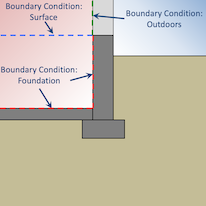
\includegraphics{media/kiva-2d-otherside.png}
\caption{Outside Boundary Conditions for surfaces within Kiva's
Two-dimensional context. Only surfaces referencing ``Foundation'' are
simulated in Kiva\label{fig:context}}
\end{figure}

This context allows for a finer description of the structural and
insulation components of a foundation that impact heat transfer (Figure
\ref{fig:el}).

\begin{figure}
\centering
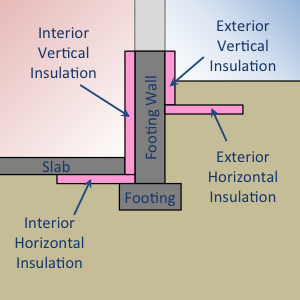
\includegraphics{media/kiva-2d-elements.png}
\caption{Structural and insulation components of Foundation:Kiva
objects\label{fig:el}}
\end{figure}

Foundation:Kiva objects define only the aspects of the foundation that
are not already defined by the one-dimensional constructions of the
respective surfaces. That is, the footing wall and slab constructions
and their relative dimensions are inferred from the respective Surface
objects (see Figure \ref{fig:surf}).

\begin{figure}
\centering
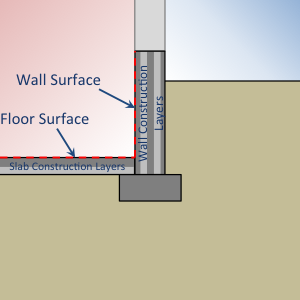
\includegraphics{media/kiva-2d-surfaces.png}
\caption{Two-dimensional interpretation of foundation surface
data\label{fig:surf}}
\end{figure}

The depth of the foundation is defined by the hight of the wall surfaces
that reference the Foundation:Kiva boundary condition object. For
slab-on-grade foundations, a depth of zero is implied by having no
associated wall surfaces. Figure \ref{fig:ws} shows a slab-on-grade
foundation with whole slab insulation. Notice there are no walls
referencing the ``Foundation'' Outside Boundary Condition. In this case,
the under-slab insulation is modeled as part of the slab construction,
while the edge/gap insulation is modeled using the interior vertical
insulation fields of a Foundation:Kiva object. Note: Since there are no
wall surfaces for slab foundations, the footing wall construction is
defined within the Foundation:Kiva object (or defaulted to a 0.3m wide
cast concrete wall).

\begin{figure}
\centering
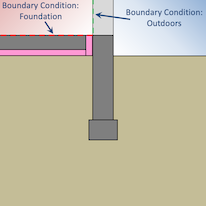
\includegraphics{media/kiva-2d-whole-slab.png}
\caption{Two-dimensional interpretation of foundation surface
data\label{fig:ws}}
\end{figure}

A walkout basement (with a variable grade along the sides; see Figure
\ref{fig:wo-r}) must be modeled using discrete quadrilateral surfaces of
stepped height for the walls as shown in Figure \ref{fig:wo-s}.

\begin{figure}
\centering
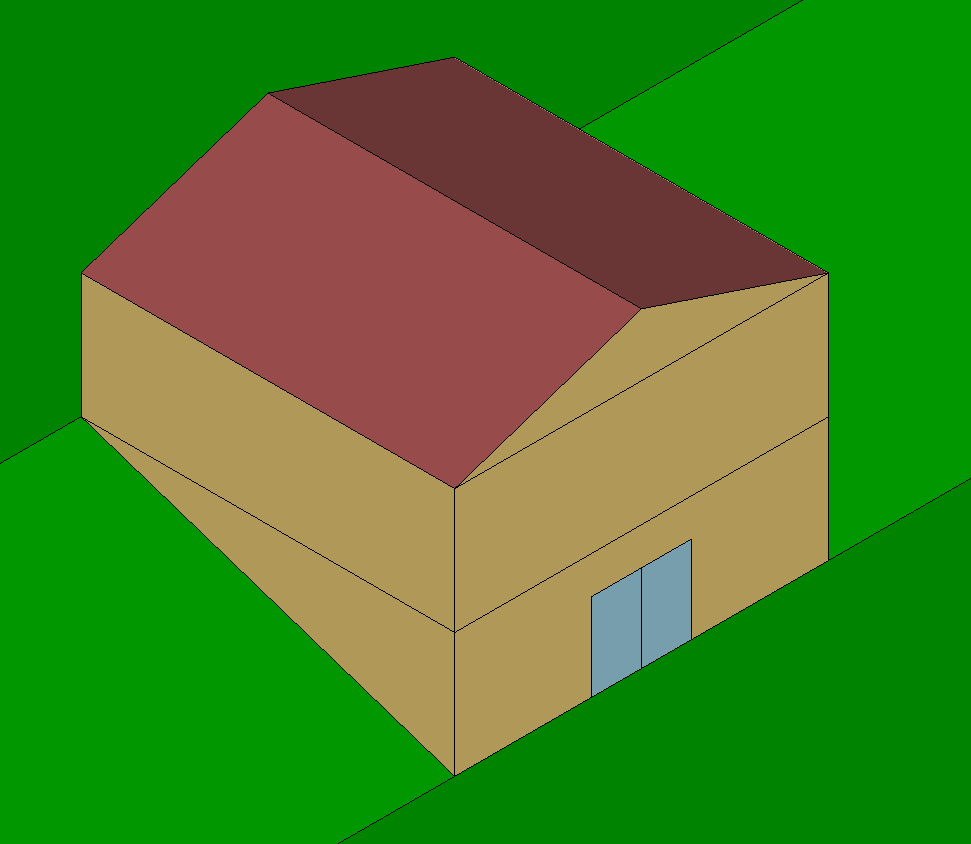
\includegraphics{media/kiva-walkout-real.png}
\caption{Example walkout basement\label{fig:wo-r}}
\end{figure}

\begin{figure}
\centering
\includegraphics{media/kiva-walkout-segs.png}
\caption{Walkout basement wall and floor surfaces (in gray) all
reference the same Foundation:Kiva object\label{fig:wo-s}}
\end{figure}

The width of the floor surface in the two-dimensional context is defined
by the area and the exposed perimeter (see
SurfaceProperty:ExposedFoundationPerimeter) of the floor surface object.
Details on this calculation can be found in the Engineering Reference
document.

Other components of the two-dimensional context are defined by the
Foundation:Kiva:Settings object and applied uniformly for all instances
of Foundation:Kiva objects. These components include:

\begin{itemize}
\tightlist
\item
  Far-Field width
\item
  Deep Ground depth (and boundary type)
\item
  Soil and ground surface thermal properties
\end{itemize}

\subsubsection{Example IDF}\label{example-idf}

\begin{verbatim}
BuildingSurface:Detailed,
  Slab Floor,         !- Name
  Floor,              !- Surface Type
  Slab Construction,  !- Construction Name
  Living Room,        !- Zone Name
  Foundation,         !- Outside Boundary Condition
  Slab Details,       !- Outside Boundary Condition Object
  No,                 !- Sun Exposure
  No,                 !- Wind Exposure
  0.0,                !- View Factor to Ground
  4,                  !- Number of Vertices
  0.0, 0.0, 0.0,      !- Vertex 1
  0.0, 20.0, 0.0,     !- Vertex 2
  20.0, 20.0, 0.0,    !- Vertex 3
  20.0, 0.0, 0.0;     !- Vertex 4

Foundation:Kiva,
  Slab Details,              !- Name
  XPS,                       !- Interior Horizontal Insulation Material Name
  0.2,                       !- Interior Horizontal Insulation Depth
  0.6,                       !- Interior Horizontal Insulation Width
  XPS,                       !- Interior Vertical Insulation Material Name
  0.2,                       !- Interior Vertical Insulation Depth
  ,                          !- Exterior Horizontal Insulation Material Name
  ,                          !- Exterior Horizontal Insulation Depth
  ,                          !- Exterior Horizontal Insulation Width
  ,                          !- Exterior Vertical Insulation Material Name
  ,                          !- Exterior Vertical Insulation Depth
  0.2,                       !- Wall Height Above Grade
  0.3,                       !- Wall Depth Below Slab
  Slab Footing Construction; !- Footing Wall Construction Name

Material,
  XPS,    !- Name
  Rough,  !- Roughness
  0.05,   !- Thickness
  0.029,  !- Conductivity
  28,     !- Density
  1450,   !- Specific Heat
  0.9,    !- Thermal Absorptance
  0.7,    !- Solar Absorptance
  0.7;    !- Visible Absorptance

Material,
  Concrete,  !- Name
  Rough,     !- Roughness
  0.3,       !- Thickness
  1.95,      !- Conductivity
  2400,      !- Density
  900,       !- Specific Heat
  0.9,       !- Thermal Absorptance
  0.7,       !- Solar Absorptance
  0.7;       !- Visible Absorptance

Construction,
  Slab Footing Construction, !- Name
  Concrete;                  !- Outside Layer Name
\end{verbatim}

\subsubsection{Input Description}\label{input-description}

\paragraph{Field: Name}\label{field-name}

The unique identifier of the Foundation:Kiva object. Referenced by a the
``Outside Boundary Condition Object'' field in a surface object.

\paragraph{Field: Interior Horizontal Insulation Material
Name}\label{field-interior-horizontal-insulation-material-name}

A reference to a material object associated with the interior horizontal
insulation. If left blank, no interior horizontal insulation will be
used. Default: blank.

The following two fields define the placement of this material within
Kiva's two-dimensional context and are illustrated in Figure
\ref{fig:ihi}.

\begin{figure}
\centering
\includegraphics{media/kiva-2d-ihi.png}
\caption{Placement of interior horizontal insulation\label{fig:ihi}}
\end{figure}

\paragraph{Field: Interior Horizontal Insulation
Depth}\label{field-interior-horizontal-insulation-depth}

Distance from the wall top to the top of interior horizontal insulation,
in m. Required if Interior Horizontal Insulation Material Name is
defined.

\paragraph{Field: Interior Horizontal Insulation
Width}\label{field-interior-horizontal-insulation-width}

Extent of insulation as measured from the wall interior to the edge of
interior horizontal insulation, in m. Required if Interior Horizontal
Insulation Material Name is defined.

\paragraph{Field: Interior Vertical Insulation Material
Name}\label{field-interior-vertical-insulation-material-name}

A reference to a material object associated with the interior vertical
insulation. If left blank, no interior vertical insulation will be used.
Default: blank.

The following field defines the placement of this material within Kiva's
two-dimensional context and are illustrated in Figure \ref{fig:ivi}.

\begin{figure}
\centering
\includegraphics{media/kiva-2d-ivi.png}
\caption{Placement of interior vertical insulation\label{fig:ivi}}
\end{figure}

\paragraph{Field: Interior Vertical Insulation
Depth}\label{field-interior-vertical-insulation-depth}

Extent of insulation as measured from the wall top to the bottom edge of
the interior vertical insulation, in m. Required if Interior Vertical
Insulation Material Name is defined.

\paragraph{Field: Exterior Horizontal Insulation Material
Name}\label{field-exterior-horizontal-insulation-material-name}

A reference to a material object associated with the exterior horizontal
insulation. If left blank, no exterior horizontal insulation will be
used. Default: blank.

The following two fields define the placement of this material within
Kiva's two-dimensional context and are illustrated in Figure
\ref{fig:ehi}.

\begin{figure}
\centering
\includegraphics{media/kiva-2d-ehi.png}
\caption{Placement of exterior horizontal insulation\label{fig:ehi}}
\end{figure}

\paragraph{Field: Exterior Horizontal Insulation
Depth}\label{field-exterior-horizontal-insulation-depth}

Distance from the wall top to the top of exterior horizontal insulation,
in m. Required if Exterior Horizontal Insulation Material Name is
defined.

\paragraph{Field: Exterior Horizontal Insulation
Width}\label{field-exterior-horizontal-insulation-width}

Extent of insulation as measured from the wall exterior to the edge of
exterior horizontal insulation, in m. Required if Exterior Horizontal
Insulation Material Name is defined.

\paragraph{Field: Exterior Vertical Insulation Material
Name}\label{field-exterior-vertical-insulation-material-name}

A reference to a material object associated with the exterior vertical
insulation. If left blank, no exterior vertical insulation will be used.
Default: blank

The following field defines the placement of this material within Kiva's
two-dimensional context and are illustrated in Figure \ref{fig:evi}.

\begin{figure}
\centering
\includegraphics{media/kiva-2d-evi.png}
\caption{Placement of exterior vertical insulation\label{fig:evi}}
\end{figure}

\paragraph{Field: Exterior Vertical Insulation
Depth}\label{field-exterior-vertical-insulation-depth}

Extent of insulation as measured from the wall top to the bottom edge of
the exterior vertical insulation, in m. Required if Exterior Vertical
Insulation Material Name is defined.

\paragraph{Field: Wall Height Above
Grade}\label{field-wall-height-above-grade}

Distance from the exterior grade to the wall top, in m. Default: 0.2 m

Figures \ref{fig:2d-w} and \ref{fig:2d-w-slab} illustrate the definition of both the ``Wall
Height Above Grade'' and the following field, ``Wall Depth Below Slab''.

\begin{figure}
\centering
\includegraphics{media/kiva-2d-wall.png}
\caption{Definition of exterior grade and footing wall depth relative to
the wall surface (for a basement foundation context)\label{fig:2d-w}}
\end{figure}

\begin{figure}
\centering
\includegraphics{media/kiva-2d-wall-slab.png}
\caption{Definition of exterior grade and footing wall depth relative to
the wall surface (for a slab foundation context)\label{fig:2d-w-slab}}
\end{figure}

\paragraph{Field: Wall Depth Below
Slab}\label{field-wall-depth-below-slab}

Distance from the slab bottom to the bottom of the foundation wall, in
m. Default: 0.0 m

Extending the wall below the slab provides a coarse approximation of the
foundation footing. Alternatively, one may use the the fields ``Footing
Material Name'' and ``Footing Depth'' to explicitly model the footing.
Note, that explicit modeling of the footing requires a higher spatial
discretization and, therefore, longer computation times.

\paragraph{Field: Footing Wall Construction
Name}\label{field-footing-wall-construction-name}

Defines the construction of the foundation footing wall for slab foundations where the foundation wall is not exposed
to the zone (and has no zone surface to explicitly assign a
construction).

By default, this is the same construction as any associated below-grade
wall surfaces, or a 0.3 m wide poured concrete wall (conductivity = 1.95
W/m-K, density = 2240 kg/m3, specific heat = 900 J/kg-K).

\paragraph{Field: Footing Material
Name}\label{field-footing-material-name}

A reference to a material object associated with the foundation footing
(typically some form of concrete). The thickness of this material is
used to determine the width of the footing. If left blank, no footing
will be used. Default: blank

The following field defines the placement of this material within Kiva's
two-dimensional context and are illustrated in Figure \ref{fig:foot}.

\begin{figure}
\centering
\includegraphics{media/kiva-2d-footing.png}
\caption{Placement of footing\label{fig:foot}}
\end{figure}

\paragraph{Field: Footing Depth}\label{field-footing-depth}

Top-to-bottom dimension of the footing (not to be confused with its
depth in the ground). The width of the footing is defined by the
material's thickness. Default: 0.3 m.

\paragraph{Field: Custom Block \textless{}x\textgreater{} Material
Name}\label{field-custom-block-x-material-name}

A reference to a material object associated with a custom block in the
two-dimensional foundation context. The thickness of this material
determines the width of the block.

Custom blocks can be used to represent solid materials in the
two-dimensional context that are not otherwise covered by the fields
above. Examples of this might include interior finishings and insulation
(Figure \ref{fig:cw}) or backfill soil with different thermal properties
(Figure \ref{fig:cf}).

\begin{figure}
\centering
\includegraphics{media/kiva-2d-custom-ex-wall.png}
\caption{Custom blocks representing interior batt insulation and dry
wall\label{fig:cw}}
\end{figure}

\begin{figure}
\centering
\includegraphics{media/kiva-2d-custom-ex-fill.png}
\caption{Custom block representing exterior backfill\label{fig:cf}}
\end{figure}

If two or more custom blocks overlap, the final properties are
determined by the higher block number (e.g., Custom Block 4 in the input
object supersedes properties defined by Custom Block 2). All custom
blocks properties are superseded by the elements shown in Figure
\ref{fig:el}.

The following fields defines the placement of this material within
Kiva's two-dimensional context and are illustrated in Figure
\ref{fig:custom}.

\begin{figure}
\centering
\includegraphics{media/kiva-2d-custom.png}
\caption{Placement of a custom block\label{fig:custom}}
\end{figure}

\paragraph{Field: Custom Block \textless{}x\textgreater{}
Depth}\label{field-custom-block-x-depth}

Top-to-bottom dimension of the block downward. The default is the depth
from the wall top to the top of the slab to facilitate interior
constructions. Default: Slab depth

\paragraph{Field: Custom Block \textless{}x\textgreater{} X
Position}\label{field-custom-block-x-x-position}

Position outward (+) or inward (-) relative to the foundation wall.

\paragraph{Field: Custom Block \textless{}x\textgreater{} Z
Position}\label{field-custom-block-x-z-position}

Position downward (+) relative to the foundation wall top. Default: Wall
top

\subsubsection{Output Description}\label{output-description}

Output for surfaces with a Foundation boundary condition type will
include all opaque surface output variables except:

\begin{itemize}
\tightlist
\item
  Surface Outside Face variables (since there is no ``Outside Face'')
\item
  Surface Heat Storage variables (since this definition depends on an
  ``Outside Face'')
\item
  Surface Internal Source Location Temperature (Kiva doesn't handle
  internal sources yet, but this is a possible future enhancement)
\end{itemize}

\subsection{Foundation:Kiva:Settings}\label{foundationkivasettings}

This object defines settings applied across all Kiva foundation
calculations. This object is not required. If it is not defined, all
defaults will be applied.

\subsubsection{Input Description}\label{input-description-1}

\paragraph{Field: Soil Conductivity}\label{field-soil-conductivity}

The thermal conductivity of the soil, in W/m-K. Default: 1.73 W/m-K.

\paragraph{Field: Soil Density}\label{field-soil-density}

The bulk density of the soil, in kg/m3. Default: 1842 kg/m3.

\paragraph{Field: Soil Specific Heat}\label{field-soil-specific-heat}

The specific heat of the soil, in J/kg-K. Default: 419 J/kg-K

\paragraph{Field: Ground Solar
Absorptivity}\label{field-ground-solar-absorptivity}

Solar absorptivity of the exterior grade surface. Default: 0.9.

\paragraph{Field: Ground Thermal
Absorptivity}\label{field-ground-thermal-absorptivity}

Long-wave absorptivity (emissivity) of the exterior grade surface.
Default: 0.9.

\paragraph{Field: Ground Surface
Roughness}\label{field-ground-surface-roughness}

The relief roughness of the exterior ground surface in m. Default: 0.03
m.

Estimates of surface roughnesses in m are shown below:

\begin{longtable}[]{@{}lc@{}}
\toprule
Example Surface & Roughness {[}m{]}\tabularnewline
\midrule
\endhead
Concrete & 0.002\tabularnewline
Brick & 0.003\tabularnewline
Soil & 0.005\tabularnewline
Gravel & 0.012\tabularnewline
Grass & 0.030\tabularnewline
\bottomrule
\end{longtable}

\paragraph{Field: Far-Field Width}\label{field-far-field-width}

The distance from the wall interior to the zero horizontal heat flux
(i.e., adiabatic) far-field boundary, in m. This distance represents
either the distance halfway between this foundation and a similar
foundation of a neighboring building, or a distance adequately far from
the foundation such that it is isolated from the effects of the boundary
(typically \textgreater{}= 40 m). Default: 40 m.

\paragraph{Field: Deep-Ground Boundary
Condition}\label{field-deep-ground-boundary-condition}

Defines the type of boundary condition to apply at the Deep-Ground
Depth. Options are:

\begin{itemize}
\tightlist
\item
  ZeroFlux
\item
  GroundWater
\item
  Autoselect
\end{itemize}

ZeroFlux applies a zero vertical heat flux (i.e.~adiabatic) boundary
condition. GroundWater applies a constant temperature boundary
condition, with a temperature equal to the average outdoor air dry-bulb
temperature from the environment(s). Autoselect applies either boundary
condition depending on the elevation of the building site (Williams and
Williamson, 1989):

\[d_{wt}=0.1022\cdot d_{elev}\]

If \(d_{wt} \le\) 40 m., the GroundWater boundary is applied, otherwise
a ZeroFlux boundary is applied at 40 m. If the calculated ground water depth is
shallower than any element of the foundation construction, then the GroundWater
is applied at 1 m below the lowest element.

Default: Autoselect.

\paragraph{Field: Deep-Ground Depth}\label{field-deep-ground-depth}

The distance from the exterior grade to the deep ground boundary, in m.
This distance represents either the distance to the ground water level,
or a distance adequately far from the foundation such that it is
isolated from the effects of the boundary (typically \textgreater{}= 40
m). Default 40 m, or the distance determined by the ``Auto'' Deep-Ground
Boundary Condition.

\paragraph{Field: Minimum Cell
Dimension}\label{field-minimum-cell-dimension}

The minimum cell dimension, in m, used in the Kiva discretization.
Default: 0.02 m.

\paragraph{Field: Maximum Cell Growth
Coefficient}\label{field-maximum-cell-growth-coefficient}

The maximum ratio of growth between neighboring cells in the direction
away from the near-field area of interest. Default: 1.50.

\paragraph{Field: Simulation Timestep}\label{field-simulation-timestep}

This field allows the user to choose whether to calculate foundation
loads on the zone timestep or at hourly intervals. Hourly intervals will
allow for less overall computation time, but with less accuracy. Choices
are ``Hourly'' and ``Timestep''. Default: Hourly

\subsection{ExposedFoundationPerimeter}\label{surfacepropertyexposedfoundationperimeter}

This object (currently only used in conjunction with Foundation:Kiva
boundary conditions) defines the perimeter of a foundation floor that is
exposed to the exterior environment through the floor. The user may
either define the total exposed perimeter, the fraction of the total
perimeter that is exposed, or individually define which segments of the
floor surface perimeter are exposed. This object is required for any floor surface with a Foundation:Kiva boundary condition.

Figure \ref{fig:ex} illustrates how the exposed perimeter is determined
from a floor plan of the foundation level.

Some buildings may have neighboring zones with different foundation
types. For example, a crawlspace next to a garage with a slab (Figure
\ref{fig:ifw}). The foundation wall in this case is NOT considered part
of either floor's exposed perimeter, and should not reference a
Foundation boundary condition. Kiva does not calculate heat flow between
two zones through ground. In this case, it is best to approximate
interior foundation wall using an Adiabatic Outside Boundary Condition.

\begin{figure}
\centering
\includegraphics{media/kiva-exposed-perim.png}
\caption{Exposed foundation perimeter\label{fig:ex}}
\end{figure}

\begin{figure}
\centering
\includegraphics{media/kiva-interior-fnd-wall.png}
\caption{Interior foundation wall\label{fig:ifw}}
\end{figure}

\subsubsection{Input Description}\label{input-description-2}

\paragraph{Field: Surface Name}\label{field-surface-name}

Name of foundation floor surface.

\paragraph{Field: Exposed Perimeter Calculation Method}\label{field-exposed-perimeter-calculation-method}

Required key/choice field that tells which method to use to calculate the exposed foundation perimeter. Choices are:

\begin{itemize}
\item TotalExposedPerimeter: Exposed perimeter is defined as an absolute distance in m. (The Total Exposed Perimeter field should be filled.)

\item ExposedPerimeterFraction: Exposed perimeter is defined as a fraction of the total floor perimeter. (The Exposed Perimeter Fraction field should be filled.)

\item BySegment: Each segment of the floor polygon (corresponding to distance between each set of vertices) is defined as exposed (``Yes'') or not exposed (``No'') in an extensible list corresponding to the number of vertices in the floor polygon. Exposed perimeter is defined as the sum of all exposed segement lengths. (The Surface Segment \textless{}x\textgreater{}
Exposed fields should be filled.)
\end{itemize}

\paragraph{Field: Total Exposed
Perimeter}\label{field-total-exposed-perimeter}

Total perimeter that is is exposed in m.

\paragraph{Field: Exposed Perimeter
Fraction}\label{field-exposed-perimeter-fraction}

Fraction of the total perimeter that is exposed. Default 1.0

\paragraph{Field: Surface Segment \textless{}x\textgreater{}
Exposed}\label{field-surface-segment-x-exposed}

Surface Segment \textless{}x\textgreater{} is the perimeter between the
\textless{}x\textgreater{}th and (\textless{}x\textgreater{}+1)th
vertices.

\subsection{SurfaceConvectionAlgorithm:Inside:AdaptiveModelSelections}\label{surfaceconvectionalgorithminsideadaptivemodelselections}

This object provides options to change the individual convection model equations for dynamic selection when using AdaptiveConvectionAlgorithm. This object is only needed to make changes to the default model selections for any or all of the surface categories. This object is for the inside face, the side of the surface facing a thermal zone.

\subsubsection{Inputs}\label{inputs-6}

\paragraph{Field: Name}\label{field-name-5}

A unique name for the object.

\paragraph{Field: Simple Buoyancy Vertical Wall Equation Source}\label{field-simple-buoyancy-vertical-wall-equation-source}

Applies to zone with no HVAC or when HVAC is off. This is for vertical walls. The key choice options include: FohannoPolidoriVerticalWall, ASHRAEVerticalWall, AlamdariHammondVerticalWall, KhalifaEq3WallAwayFromHeat, KhalifaEq6NonHeatedWalls FohannoPolidoriVerticalWall, ISO15099Windows, or UserCurve

\paragraph{Field: Simple Buoyancy Vertical Wall User Curve Name}\label{field-simple-buoyancy-vertical-wall-user-curve-name}

The SurfaceConvectionAlgorithm:UserCurve named in this field is used when the previous field is set to UserCurve

\paragraph{Field: Simple Buoyancy Stable Horizontal Equation Source}\label{field-simple-buoyancy-stable-horizontal-equation-source}

Applies to zone with no HVAC or when HVAC is off. This is for horizontal surfaces with heat flow directed for stable thermal stratification. The key choice options include: WaltonStableHorizontalOrTilt, AlamdariHammondStableHorizontal, or UserCurve

\paragraph{Field: Simple Buoyancy Stable Horizontal Equation User Curve Name}\label{field-simple-buoyancy-stable-horizontal-equation-user-curve-name}

The SurfaceConvectionAlgorithm:UserCurve named in this field is used when the previous field is set to UserCurve

\paragraph{Field: Simple Buoyancy Unstable Horizontal Equation Source}\label{field-simple-buoyancy-unstable-horizontal-equation-source}

Applies to zone with no HVAC or when HVAC is off. This is for passive horizontal surfaces with heat flow for unstable thermal stratification. The key choice options include: WaltonUnstableHorizontalOrTilt, AlamdariHammondUnstableHorizontal, or UserCurve.

\paragraph{Field: Simple Buoyancy Unstable Horizontal Equation User Curve Name}\label{field-simple-buoyancy-unstable-horizontal-equation-user-curve-name}

The SurfaceConvectionAlgorithm:UserCurve named in this field is used when the previous field is set to UserCurve.

\paragraph{Field: Simple Buoyancy Stable Tilted Equation Source}\label{field-simple-buoyancy-stable-tilted-equation-source}

Applies to zone with no HVAC or when HVAC is off. This is for tilted surfaces with heat flow for stable thermal stratification. The key choice options include: WaltonStableHorizontalOrTilt, AlamdariHammondStableHorizontal, or UserCurve

\paragraph{Field: Simple Buoyancy Stable Tilted Equation User Curve Name}\label{field-simple-buoyancy-stable-tilted-equation-user-curve-name}

The SurfaceConvectionAlgorithm:UserCurve named in this field is used when the previous field is set to UserCurve.

\paragraph{Field: Simple Buoyancy Unstable Tilted Equation Source}\label{field-simple-buoyancy-unstable-tilted-equation-source}

Applies to zone with no HVAC or when HVAC is off. This is for tilted surfaces with heat flow for unstable thermal stratification. The key choices include: WaltonUnstableHorizontalOrTilt, AlamdariHammondUnstableHorizontal, or UserCurve.

\paragraph{Field: Simple Buoyancy Unstable Tilted Equation User Curve Name}\label{field-simple-buoyancy-unstable-tilted-equation-user-curve-name}

The SurfaceConvectionAlgorithm:UserCurve named in this field is used when the previous field is set to UserCurve.

\paragraph{Field: Simple Buoyancy Windows Equation Source}\label{field-simple-buoyancy-windows-equation-source}

Applies to zone with no HVAC or when HVAC is off. This is for all window surfaces. The key choice options include: ASHRAEVerticalWall, AlamdariHammondVerticalWall, FohannoPolidoriVerticalWall, KaradagChilledCeiling, ISO15099Windows, or UserCurve.

\paragraph{Field: Simple Buoyancy Windows Equation User Curve Name}\label{field-simple-buoyancy-windows-equation-user-curve-name}

The SurfaceConvectionAlgorithm:UserCurve named in this field is used when the previous field is set to UserCurve.

\paragraph{Field: Floor Heat Ceiling Cool Vertical Wall Equation Source}\label{field-floor-heat-ceiling-cool-vertical-wall-equation-source}

Applies to zone with in-floor heating and/or in-ceiling cooling. This is for vertical walls. The key choice options include: ASHRAEVerticalWall, AlamdariHammondVerticalWall, KhalifaEq3WallAwayFromHeat, FohannoPolidoriVerticalWall, ISO15099Windows, or UserCurve.

\paragraph{Field: Floor Heat Ceiling Cool Vertical Wall Equation User Curve Name}\label{field-floor-heat-ceiling-cool-vertical-wall-equation-user-curve-name}

The SurfaceConvectionAlgorithm:UserCurve named in this field is used when the previous field is set to UserCurve.

\paragraph{Field: Floor Heat Ceiling Cool Stable Horizontal Equation Source}\label{field-floor-heat-ceiling-cool-stable-horizontal-equation-source}

Applies to zone with in-floor heating and/or in-ceiling cooling. This is for passive horizontal surfaces with heat flow for stable thermal stratification. The key choice options include: WaltonStableHorizontalOrTilt, AlamdariHammondStableHorizontal, or UserCurve.

\paragraph{Field: Floor Heat Ceiling Cool Stable Horizontal Equation User Curve Name}\label{field-floor-heat-ceiling-cool-stable-horizontal-equation-user-curve-name}

The SurfaceConvectionAlgorithm:UserCurve named in this field is used when the previous field is set to UserCurve.

\paragraph{Field: Floor Heat Ceiling Cool Unstable Horizontal Equation Source}\label{field-floor-heat-ceiling-cool-unstable-horizontal-equation-source}

Applies to zone with in-floor heating and/or in-ceiling cooling. This is for passive horizontal surfaces with heat flow for unstable thermal stratification. The key choice options include: WaltonUnstableHorizontalOrTilt, AlamdariHammondUnstableHorizontal, KhalifaEq4CeilingAwayFromHeat, or UserCurve.

\paragraph{Field: Floor Heat Ceiling Cool Unstable Horizontal Equation User Curve Name}\label{field-floor-heat-ceiling-cool-unstable-horizontal-equation-user-curve-name}

The SurfaceConvectionAlgorithm:UserCurve named in this field is used when the previous field is set to UserCurve.

\paragraph{Field: Floor Heat Ceiling Cool Heated Floor Equation Source}\label{field-floor-heat-ceiling-cool-heated-floor-equation-source}

Applies to zone with in-floor heating and/or in-ceiling cooling. This is for a floor with active heating elements. The key choice options include: WaltonUnstableHorizontalOrTilt, AlamdariHammondUnstableHorizontal, AwbiHattonHeatedFloor, or UserCurve

\paragraph{Field: Floor Heat Ceiling Cool Heated Floor Equation User Curve Name}\label{field-floor-heat-ceiling-cool-heated-floor-equation-user-curve-name}

The SurfaceConvectionAlgorithm:UserCurve named in this field is used when the previous field is set to UserCurve.

\paragraph{Field: Floor Heat Ceiling Cool Chilled Ceiling Equation Source}\label{field-floor-heat-ceiling-cool-chilled-ceiling-equation-source}

Applies to zone with in-floor heating and/or in-ceiling cooling. This is for a ceiling with active cooling elements. The key choice options include: WaltonUnstableHorizontalOrTilt, AlamdariHammondUnstableHorizontal, KaradagChilledCeiling, or UserCurve.

\paragraph{Field: Floor Heat Ceiling Cool Chilled Ceiling Equation User Curve Name}\label{field-floor-heat-ceiling-cool-chilled-ceiling-equation-user-curve-name}

The SurfaceConvectionAlgorithm:UserCurve named in this field is used when the previous field is set to UserCurve

\paragraph{Field: Floor Heat Ceiling Cool Stable Tilted Equation Source}\label{field-floor-heat-ceiling-cool-stable-tilted-equation-source}

Applies to zone with in-floor heating and/or in-ceiling cooling. This is for tilted surfaces with heat flow for stable thermal stratification. The key choice options include: WaltonStableHorizontalOrTilt, AlamdariHammondStableHorizontal, ISO15099Windows, or UserCurve.

\paragraph{Field: Floor Heat Ceiling Cool Stable Tilted Equation User Curve Name}\label{field-floor-heat-ceiling-cool-stable-tilted-equation-user-curve-name}

The SurfaceConvectionAlgorithm:UserCurve named in this field is used when the previous field is set to UserCurve.

\paragraph{Field: Floor Heat Ceiling Cool Unstable Tilted Equation Source}\label{field-floor-heat-ceiling-cool-unstable-tilted-equation-source}

Applies to zone with in-floor heating and/or in-ceiling cooling. This is for tilted surfaces with heat flow for unstable thermal stratification. The key choice options include: WaltonUnstableHorizontalOrTilt, AlamdariHammondUnstableHorizontal, ISO15099Windows, or UserCurve.

\paragraph{Field: Floor Heat Ceiling Cool Unstable Tilted Equation User Curve Name}\label{field-floor-heat-ceiling-cool-unstable-tilted-equation-user-curve-name}

The SurfaceConvectionAlgorithm:UserCurve named in this field is used when the previous field is set to UserCurve.

\paragraph{Field: Floor Heat Ceiling Cool Window Equation Source}\label{field-floor-heat-ceiling-cool-window-equation-source}

Applies to zone with in-floor heating and/or in-ceiling cooling. This is for all window surfaces. The key choice options include: ASHRAEVerticalWall, AlamdariHammondVerticalWall, ISO15099Windows, or UserCurve.

\paragraph{Field: Floor Heat Ceiling Cool Window Equation User Curve Name}\label{field-floor-heat-ceiling-cool-window-equation-user-curve-name}

The SurfaceConvectionAlgorithm:UserCurve named in this field is used when the previous field is set to UserCurve.

\paragraph{Field: Wall Panel Heating Vertical Wall Equation Source}\label{field-wall-panel-heating-vertical-wall-equation-source}

Applies to zone with in-wall panel heating. This is for vertical walls that are not actively heated. The key choice options include: ASHRAEVerticalWall, AlamdariHammondVerticalWall, KhalifaEq6NonHeatedWalls, FohannoPolidoriVerticalWall, AlamdariHammondVerticalWall, ISO15099Windows, or UserCurve.

\paragraph{Field: Wall Panel Heating Vertical Wall Equation User Curve Name}\label{field-wall-panel-heating-vertical-wall-equation-user-curve-name}

The SurfaceConvectionAlgorithm:UserCurve named in this field is used when the previous field is set to UserCurve.

\paragraph{Field: Wall Panel Heating Heated Wall Equation Source}\label{field-wall-panel-heating-heated-wall-equation-source}

Applies to zone with in-wall panel heating. This is for vertical walls that are being actively heated. The key choice options include: ASHRAEVerticalWall, AlamdariHammondVerticalWall, KhalifaEq5WallNearHeat, AwbiHattonHeatedWall, FohannoPolidoriVerticalWall, AlamdariHammondVerticalWall, or UserCurve.

\paragraph{Field: Wall Panel Heating Heated Wall Equation User Curve Name}\label{field-wall-panel-heating-heated-wall-equation-user-curve-name}

The SurfaceConvectionAlgorithm:UserCurve named in this field is used when the previous field is set to UserCurve.

\paragraph{Field: Wall Panel Heating Stable Horizontal Equation Source}\label{field-wall-panel-heating-stable-horizontal-equation-source}

Applies to zone with in-wall panel heating. This is for horizontal surfaces with heat flow directed for stable thermal stratification. The key choice options include: WaltonStableHorizontalOrTilt, AlamdariHammondStableHorizontal, or UserCurve.

\paragraph{Field: Wall Panel Heating Stable Horizontal Equation User Curve Name}\label{field-wall-panel-heating-stable-horizontal-equation-user-curve-name}

The SurfaceConvectionAlgorithm:UserCurve named in this field is used when the previous field is set to UserCurve.

\paragraph{Field: Wall Panel Heating Unstable Horizontal Equation Source}\label{field-wall-panel-heating-unstable-horizontal-equation-source}

Applies to zone with in-wall panel heating. This is for horizontal surfaces with heat flow directed for unstable thermal stratification. The key choice options include: ASHRAEVerticalWall, WaltonUnstableHorizontalOrTilt, AlamdariHammondUnstableHorizontal, KhalifaEq7Ceiling, or UserCurve

\paragraph{Field: Wall Panel Heating Unstable Horizontal Equation User Curve Name}\label{field-wall-panel-heating-unstable-horizontal-equation-user-curve-name}

The SurfaceConvectionAlgorithm:UserCurve named in this field is used when the previous field is set to UserCurve.

\paragraph{Field: Wall Panel Heating Stable Tilted Equation Source}\label{field-wall-panel-heating-stable-tilted-equation-source}

Applies to zone with in-wall panel heating. This is for tilted surfaces with heat flow for stable thermal stratification. The key choice options include: WaltonStableHorizontalOrTilt, AlamdariHammondStableHorizontal, ISO15099Windows, or UserCurve.

\paragraph{Field: Wall Panel Heating Stable Tilted Equation User Curve Name}\label{field-wall-panel-heating-stable-tilted-equation-user-curve-name}

The SurfaceConvectionAlgorithm:UserCurve named in this field is used when the previous field is set to UserCurve

\paragraph{Field: Wall Panel Heating Unstable Tilted Equation Source}\label{field-wall-panel-heating-unstable-tilted-equation-source}

Applies to zone with in-wall panel heating. This is for tilted surfaces with heat flow for unstable thermal stratification. The key choice options include: WaltonUnstableHorizontalOrTilt, AlamdariHammondUnstableHorizontal, ISO15099Windows, or UserCurve.

\paragraph{Field: Wall Panel Heating Unstable Tilted Equation User Curve Name}\label{field-wall-panel-heating-unstable-tilted-equation-user-curve-name}

The SurfaceConvectionAlgorithm:UserCurve named in this field is used when the previous field is set to UserCurve.

\paragraph{Field: Wall Panel Heating Window Equation Source}\label{field-wall-panel-heating-window-equation-source}

Applies to zone with in-wall panel heating. This is for all window surfaces. The key choice options include: ASHRAEVerticalWall, AlamdariHammondVerticalWall, FohannoPolidoriVerticalWall, ISO15099Windows, or UserCurve.

\paragraph{Field: Wall Panel Heating Window Equation User Curve Name}\label{field-wall-panel-heating-window-equation-user-curve-name}

The SurfaceConvectionAlgorithm:UserCurve named in this field is used when the previous field is set to UserCurve.

\paragraph{Field: Convective Zone Heater Vertical Wall Equation Source}\label{field-convective-zone-heater-vertical-wall-equation-source}

Applies to zone with convective heater. This is for vertical walls not directly affected by heater. The key choice options include: ASHRAEVerticalWall, AlamdariHammondVerticalWall, KhalifaEq3WallAwayFromHeat, KhalifaEq6NonHeatedWalls, FohannoPolidoriVerticalWall, ISO15099Windows, or UserCurve

\paragraph{Field: Convective Zone Heater Vertical Wall Equation User Curve Name}\label{field-convective-zone-heater-vertical-wall-equation-user-curve-name}

The SurfaceConvectionAlgorithm:UserCurve named in this field is used when the previous field is set to UserCurve.

\paragraph{Field: Convective Zone Heater Vertical Walls Near Heater Equation Source}\label{field-convective-zone-heater-vertical-walls-near-heater-equation-source}

Applies to zone with convective heater. This is for vertical walls that are directly affected by heater. Walls are considered ``near'' when listed in field set for Fraction of Radiant Energy to Surface. The key choice options include: ASHRAEVerticalWall, AlamdariHammondVerticalWall, KhalifaEq5WallNearHeat, AwbiHattonHeatedWall, FohannoPolidoriVerticalWall, ISO15099Windows, or UserCurve.

\paragraph{Field: Convective Zone Heater Vertical Walls Near Heater Equation User Curve Name}\label{field-convective-zone-heater-vertical-walls-near-heater-equation-user-curve-name}

The SurfaceConvectionAlgorithm:UserCurve named in this field is used when the previous field is set to UserCurve.

\paragraph{Field: Convective Zone Heater Stable Horizontal Equation Source}\label{field-convective-zone-heater-stable-horizontal-equation-source}

Applies to zone with convective heater. This is for horizontal surfaces with heat flow directed for stable thermal stratification. The key choice options include: WaltonStableHorizontalOrTilt, AlamdariHammondStableHorizontal, or UserCurve.

\paragraph{Field: Convective Zone Heater Stable Horizontal Equation User Curve Name}\label{field-convective-zone-heater-stable-horizontal-equation-user-curve-name}

The SurfaceConvectionAlgorithm:UserCurve named in this field is used when the previous field is set to UserCurve

\paragraph{Field: Convective Zone Heater Unstable Horizontal Equation Source}\label{field-convective-zone-heater-unstable-horizontal-equation-source}

Applies to zone with convective heater. This is for horizontal surfaces with heat flow directed for unstable thermal stratification. The key choice options include: WaltonUnstableHorizontalOrTilt, AlamdariHammondUnstableHorizontal, KhalifaEq4CeilingAwayFromHeat, KhalifaEq7Ceiling, or UserCurve.

\paragraph{Field: Convective Zone Heater Unstable Horizontal Equation User Curve Name}\label{field-convective-zone-heater-unstable-horizontal-equation-user-curve-name}

The SurfaceConvectionAlgorithm:UserCurve named in this field is used when the previous field is set to UserCurve.

\paragraph{Field: Convective Zone Heater Stable Tilted Equation Source}\label{field-convective-zone-heater-stable-tilted-equation-source}

Applies to zone with convective heater. This is for tilted surfaces with heat flow for stable thermal stratification. The key choice options include: WaltonStableHorizontalOrTilt, AlamdariHammondStableHorizontal, or UserCurve.

\paragraph{Field: Convective Zone Heater Stable Tilted Equation User Curve Name}\label{field-convective-zone-heater-stable-tilted-equation-user-curve-name}

The SurfaceConvectionAlgorithm:UserCurve named in this field is used when the previous field is set to UserCurve.

\paragraph{Field: Convective Zone Heater Unstable Tilted Equation Source}\label{field-convective-zone-heater-unstable-tilted-equation-source}

Applies to zone with convective heater. This is for tilted surfaces with heat flow for unstable thermal stratification. The key choice options include: WaltonUnstableHorizontalOrTilt, AlamdariHammondUnstableHorizontal, or UserCurve.

\paragraph{Field: Convective Zone Heater Unstable Tilted Equation User Curve Name}\label{field-convective-zone-heater-unstable-tilted-equation-user-curve-name}

The SurfaceConvectionAlgorithm:UserCurve named in this field is used when the previous field is set to UserCurve.

\paragraph{Field: Convective Zone Heater Windows Equation Source}\label{field-convective-zone-heater-windows-equation-source}

Applies to zone with convective heater. This is for all window surfaces. The key choice options include: ASHRAEVerticalWall, AlamdariHammondVerticalWall, KhalifaEq3WallAwayFromHeat, FohannoPolidoriVerticalWall, ISO15099Windows, or UserCurve.

\paragraph{Field: Convective Zone Heater Windows Equation User Curve Name}\label{field-convective-zone-heater-windows-equation-user-curve-name}

The SurfaceConvectionAlgorithm:UserCurve named in this field is used when the previous field is set to UserCurve.

\paragraph{Field: Central Air Diffuser Wall Equation Source}\label{field-central-air-diffuser-wall-equation-source}

Applies to zone with mechanical forced central air with diffusers. This is for all wall surfaces. The key choice options include: ASHRAEVerticalWall, FisherPedersenCeilingDiffuserWalls, AlamdariHammondVerticalWall, BeausoleilMorrisonMixedAssistedWall, BeausoleilMorrisonMixedOpposingWall, FohannoPolidoriVerticalWall, ISO15099Windows, GoldsteinNovoselacCeilingDiffuserWalls, or UserCurve

\paragraph{Field: Central Air Diffuser Wall Equation User Curve Name}\label{field-central-air-diffuser-wall-equation-user-curve-name}

The SurfaceConvectionAlgorithm:UserCurve named in this field is used when the previous field is set to UserCurve.

\paragraph{Field: Central Air Diffuser Ceiling Equation Source}\label{field-central-air-diffuser-ceiling-equation-source}

Applies to zone with mechanical forced central air with diffusers. This is for all ceiling surfaces. The key choice options include: FisherPedersenCeilingDiffuserCeiling, BeausoleilMorrisonMixedStableCeiling, BeausoleilMorrisonMixedUnstableCeiling, or UserCurve.

\paragraph{Field: Central Air Diffuser Ceiling Equation User Curve Name}\label{field-central-air-diffuser-ceiling-equation-user-curve-name}

The SurfaceConvectionAlgorithm:UserCurve named in this field is used when the previous field is set to UserCurve.

\paragraph{Field: Central Air Diffuser Floor Equation Source}\label{field-central-air-diffuser-floor-equation-source}

Applies to zone with mechanical forced central air with diffusers. This is for all floor surfaces. The key choice options include: FisherPedersenCeilingDiffuserFloor, BeausoleilMorrisonMixedStableFloor, BeausoleilMorrisonMixedUnstableFloor, GoldsteinNovoselacCeilingDiffuserFloor, or UserCurve.

\paragraph{Field: Central Air Diffuser Floor Equation User Curve Name}\label{field-central-air-diffuser-floor-equation-user-curve-name}

The SurfaceConvectionAlgorithm:UserCurve named in this field is used when the previous field is set to UserCurve.

\paragraph{Field: Central Air Diffuser Window Equation Source}\label{field-central-air-diffuser-window-equation-source}

Applies to zone with mechanical forced central air with diffusers. This is for all window surfaces. The key choice options include: ASHRAEVerticalWall, FisherPedersenCeilingDiffuserWalls, BeausoleilMorrisonMixedAssistedWall, BeausoleilMorrisonMixedOpposingWall, FohannoPolidoriVerticalWall, AlamdariHammondVerticalWall, ISO15099Windows, GoldsteinNovoselacCeilingDiffuserWindow, or UserCurve.

\paragraph{Field: Central Air Diffuser Window Equation User Curve Name}\label{field-central-air-diffuser-window-equation-user-curve-name}

The SurfaceConvectionAlgorithm:UserCurve named in this field is used when the previous field is set to UserCurve

\paragraph{Field: Mechanical Zone Fan Circulation Vertical Wall Equation Source}\label{field-mechanical-zone-fan-circulation-vertical-wall-equation-source}

The key choice options include: KhalifaEq3WallAwayFromHeat, ASHRAEVerticalWall, FisherPedersenCeilingDiffuserWalls, AlamdariHammondVerticalWall, BeausoleilMorrisonMixedAssistedWall, BeausoleilMorrisonMixedOpposingWall, FohannoPolidoriVerticalWall, ISO15099Windows, GoldsteinNovoselacCeilingDiffuserWalls, or UserCurve.

\paragraph{Field: Mechanical Zone Fan Circulation Vertical Wall Equation User Curve Name}\label{field-mechanical-zone-fan-circulation-vertical-wall-equation-user-curve-name}

The SurfaceConvectionAlgorithm:UserCurve named in this field is used when the previous field is set to UserCurve

\paragraph{Field: Mechanical Zone Fan Circulation Stable Horizontal Equation Source}\label{field-mechanical-zone-fan-circulation-stable-horizontal-equation-source}

The key choice options include: WaltonStableHorizontalOrTilt, AlamdariHammondStableHorizontal, or UserCurve.

\paragraph{Field: Mechanical Zone Fan Circulation Stable Horizontal Equation User Curve Name}\label{field-mechanical-zone-fan-circulation-stable-horizontal-equation-user-curve-name}

The SurfaceConvectionAlgorithm:UserCurve named in this field is used when the previous field is set to UserCurve.

\paragraph{Field: Mechanical Zone Fan Circulation Unstable Horizontal Equation Source}\label{field-mechanical-zone-fan-circulation-unstable-horizontal-equation-source}

The key choice options include: KhalifaEq4CeilingAwayFromHeat, WaltonUnstableHorizontalOrTilt, AlamdariHammondUnstableHorizontal, or UserCurve.

\paragraph{Field: Mechanical Zone Fan Circulation Unstable Horizontal Equation User Curve Name}\label{field-mechanical-zone-fan-circulation-unstable-horizontal-equation-user-curve-name}

The SurfaceConvectionAlgorithm:UserCurve named in this field is used when the previous field is set to UserCurve.

\paragraph{Field: Mechanical Zone Fan Circulation Stable Tilted Equation Source}\label{field-mechanical-zone-fan-circulation-stable-tilted-equation-source}

The key choice options include: WaltonStableHorizontalOrTilt or UserCurve

\paragraph{Field Mechanical Zone Fan Circulation Stable Tilted Equation User Curve Name}\label{field-mechanical-zone-fan-circulation-stable-tilted-equation-user-curve-name}

The SurfaceConvectionAlgorithm:UserCurve named in this field is used when the previous field is set to UserCurve.

\paragraph{Field: Mechanical Zone Fan Circulation Unstable Tilted Equation Source}\label{field-mechanical-zone-fan-circulation-unstable-tilted-equation-source}

The key choice options include: WaltonUnstableHorizontalOrTilt, AlamdariHammondUnstableHorizontal, or UserCurve.

\paragraph{Field: Mechanical Zone Fan Circulation Unstable Tilted Equation User Curve Name}\label{field-mechanical-zone-fan-circulation-unstable-tilted-equation-user-curve-name}

The SurfaceConvectionAlgorithm:UserCurve named in this field is used when the previous field is set to UserCurve.

\paragraph{Field: Mechanical Zone Fan Circulation Window Equation Source}\label{field-mechanical-zone-fan-circulation-window-equation-source}

The key choice options include: ASHRAEVerticalWall, AlamdariHammondVerticalWall, FohannoPolidoriVerticalWall, ISO15099Windows, GoldsteinNovoselacCeilingDiffuserWindow, or UserCurve.

\paragraph{Field: Mechanical Zone Fan Circulation Unstable Tilted Equation User Curve Name}\label{field-mechanical-zone-fan-circulation-unstable-tilted-equation-user-curve-name-1}

The SurfaceConvectionAlgorithm:UserCurve named in this field is used when the previous field is set to UserCurve

\paragraph{Field: Mixed Regime Buoyancy Assisting Flow on Walls Equation Source}\label{field-mixed-regime-buoyancy-assisting-flow-on-walls-equation-source}

The key choice options include: BeausoleilMorrisonMixedAssistedWall, AlamdariHammondVerticalWall, FohannoPolidoriVerticalWall, ASHRAEVerticalWall, FisherPedersenCeilingDiffuserWalls, GoldsteinNovoselacCeilingDiffuserWalls, or UserCurve.

\paragraph{Field: Mixed Regime Buoyancy Assisting Flow on Walls Equation User Curve Name}\label{field-mixed-regime-buoyancy-assisting-flow-on-walls-equation-user-curve-name}

The SurfaceConvectionAlgorithm:UserCurve named in this field is used when the previous field is set to UserCurve.

\paragraph{Field: Mixed Regime Buoyancy Opposing Flow on Walls Equation Source}\label{field-mixed-regime-buoyancy-oppossing-flow-on-walls-equation-source}

The key choice options include: BeausoleilMorrisonMixedOpposingWall, AlamdariHammondVerticalWall, FohannoPolidoriVerticalWall, ASHRAEVerticalWall, FisherPedersenCeilingDiffuserWalls, GoldsteinNovoselacCeilingDiffuserWalls, or UserCurve

\paragraph{Field: Mixed Regime Buoyancy Opposing Flow on Walls Equation User Curve Name}\label{field-mixed-regime-buoyancy-oppossing-flow-on-walls-equation-user-curve-name}

The SurfaceConvectionAlgorithm:UserCurve named in this field is used when the previous field is set to UserCurve

\paragraph{Field: Mixed Regime Stable Floor Equation Source}\label{field-mixed-regime-stable-floor-equation-source}

The key choice options include: BeausoleilMorrisonMixedStableFloor, WaltonStableHorizontalOrTilt, AlamdariHammondStableHorizontal, or UserCurve

\paragraph{Field: Mixed Regime Stable Floor Equation User Curve Name}\label{field-mixed-regime-stable-floor-equation-user-curve-name}

The SurfaceConvectionAlgorithm:UserCurve named in this field is used when the previous field is set to UserCurve.

\paragraph{Field: Mixed Regime Unstable Floor Equation Source}\label{field-mixed-regime-unstable-floor-equation-source}

The key choice options include: BeausoleilMorrisonMixedUnstableFloor, WaltonUnstableHorizontalOrTilt, AlamdariHammondUnstableHorizontal, or UserCurve.

\paragraph{Field: Mixed Regime Unstable Floor Equation User Curve Name}\label{field-mixed-regime-unstable-floor-equation-user-curve-name}

The SurfaceConvectionAlgorithm:UserCurve named in this field is used when the previous field is set to UserCurve.

\paragraph{Field: Mixed Regime Stable Ceiling Equation Source}\label{field-mixed-regime-stable-ceiling-equation-source}

The key choice options include: BeausoleilMorrisonMixedStableCeiling, WaltonStableHorizontalOrTilt, AlamdariHammondStableHorizontal, or UserCurve.

\paragraph{Field: Mixed Regime Stable Ceiling Equation User Curve Name}\label{field-mixed-regime-stable-ceiling-equation-user-curve-name}

The SurfaceConvectionAlgorithm:UserCurve named in this field is used when the previous field is set to UserCurve.

\paragraph{Field: Mixed Regime Unstable Ceiling Equation Source}\label{field-mixed-regime-unstable-ceiling-equation-source}

The key choice options include: BeausoleilMorrisonMixedUnstableCeiling, WaltonUnstableHorizontalOrTilt, AlamdariHammondUnstableHorizontal, or UserCurve.

\paragraph{Field: Mixed Regime Unstable Ceiling Equation User Curve Name}\label{field-mixed-regime-unstable-ceiling-equation-user-curve-name}

The SurfaceConvectionAlgorithm:UserCurve named in this field is used when the previous field is set to UserCurve.

\paragraph{Field: Mixed Regime Window Equation Source}\label{field-mixed-regime-window-equation-source}

The key choice options include: GoldsteinNovoselacCeilingDiffuserWindow, ISO15099Windows, or UserCurve.

\paragraph{Field: Mixed Regime Window Equation User Curve Name}\label{field-mixed-regime-window-equation-user-curve-name}

The SurfaceConvectionAlgorithm:UserCurve named in this field is used when the previous field is set to UserCurve.

\subsection{SurfaceConvectionAlgorithm:Outside:AdaptiveModelSelections}\label{surfaceconvectionalgorithmoutsideadaptivemodelselections}

Options to change the individual convection model equations for dynamic selection when using AdaptiveConvectionAlgorithm. This object is only needed to make changes to the default model selections for any or all of the surface categories. This object is for the outside face, the side of the surface facing away from the thermal zone.

\subsubsection{Inputs}\label{inputs-7}

\paragraph{Field: Name}\label{field-name-6}

A unique name for the object

\paragraph{Field: Wind Convection Windward Vertical Wall Equation Source}\label{field-wind-convection-windward-vertical-wall-equation-source}

This is for just the wind-driven component of the total convection coefficient. The key choice options include: SimpleCombined, TARPWindward, MoWiTTWindward, DOE2Windward, NusseltJurges, McAdams, Mitchell, Blocken, Emmel, or UserCurve.

\paragraph{Field: Wind Convection Windward Equation Vertical Wall User Curve Name}\label{field-wind-convection-windward-equation-vertical-wall-user-curve-name}

The SurfaceConvectionAlgorithm:UserCurve named in this field is used when the previous field is set to UserCurve.

\paragraph{Field: Wind Convection Leeward Vertical Wall Equation Source}\label{field-wind-convection-leeward-vertical-wall-equation-source}

This is for just the wind-driven component of the total convection coefficient. The key choice options include: SimpleCombined, TARPLeeward, MoWiTTLeeward, DOE2Leeward, Emmel, NusseltJurges, McAdams, Mitchell, or UserCurve.

\paragraph{Field: Wind Convection Leeward Vertical Wall Equation User Curve Name}\label{field-wind-convection-leeward-vertical-wall-equation-user-curve-name}

The SurfaceConvectionAlgorithm:UserCurve named in this field is used when the previous field is set to UserCurve.

\paragraph{Field: Wind Convection Horizontal Roof Equation Source}\label{field-wind-convection-horizontal-roof-equation-source}

This is for just the wind-driven component of the total convection coefficient. The key choice options include: SimpleCombined, TARPWindward, MoWiTTWindward, DOE2Windward, NusseltJurges, McAdams, Mitchell, Blocken, Emmel, ClearRoof, or UserCurve.

\paragraph{Field: Wind Convection Horizontal Roof User Curve Name}\label{field-wind-convection-horizontal-roof-user-curve-name}

The SurfaceConvectionAlgorithm:UserCurve named in this field is used when the previous field is set to UserCurve.

\paragraph{Field: Natural Convection Vertical Wall Equation Source}\label{field-natural-convection-vertical-wall-equation-source}

This is for just the natural convection portion of the total film coefficient. This is for vertical walls. The key choice options include: ASHRAEVerticalWall, AlamdariHammondVerticalWall, FohannoPolidoriVerticalWall, ISO15099Windows, UserCurve, or None.

\paragraph{Field: Natural Convection Vertical Wall Equation User Curve Name}\label{field-natural-convection-vertical-wall-equation-user-curve-name}

The SurfaceConvectionAlgorithm:UserCurve named in this field is used when the previous field is set to UserCurve.

\paragraph{Field: Natural Convection Stable Horizontal Equation Source}\label{field-natural-convection-stable-horizontal-equation-source}

This is for just the natural convection portion of the total film coefficient. This is for horizontal surfaces with heat flow directed for stable thermal stratification. The key choice options include: WaltonStableHorizontalOrTilt, AlamdariHammondStableHorizontal, UserCurve, or None.

\paragraph{Field: Natural Convection Stable Horizontal Equation User Curve Name}\label{field-natural-convection-stable-horizontal-equation-user-curve-name}

The SurfaceConvectionAlgorithm:UserCurve named in this field is used when the previous field is set to UserCurve.

\paragraph{Field: Natural Convection Unstable Horizontal Equation Source}\label{field-natural-convection-unstable-horizontal-equation-source}

This is for just the natural convection portion of the total film coefficient. This is for horizontal surfaces with heat flow directed for unstable thermal stratification. The key choice options include: WaltonUnstableHorizontalOrTilt, AlamdariHammondUnstableHorizontal, UserCurve, or None

\paragraph{Field: Natural Convection Unstable Horizontal Equation User Curve Name}\label{field-natural-convection-unstable-horizontal-equation-user-curve-name}

The SurfaceConvectionAlgorithm:UserCurve named in this field is used when the previous field is set to UserCurve.

\subsection{SurfaceConvectionAlgorithm:Inside:UserCurve}\label{surfaceconvectionalgorithminsideusercurve}

This object is used to describe a custom model equation for surface convection heat transfer coefficients. If more than one curve is referenced, or non-blank, then they are all used and the result is the simple addition of all the curve results.

\subsubsection{Inputs}\label{inputs-8}

\paragraph{Field: Name}\label{field-name-7}

Unique name of input object.

\paragraph{Field: Reference Temperature for Convection Heat Transfer}\label{field-reference-temperature-for-convection-heat-transfer}

This field controls the nature of the reference temperature used with convection coefficient when calculating the heat flow at the surface. Select one of the three choices: MeanAirTemperature, AdjacentAirTemperature, SupplyAirTemperature. MeanAirTemperature is the typical application for the classic convection model used with the complete mixing of room air. AdjacentAirTemperature applies when used with Roomair models that account for temperature variations within the zone air and directs the model to use the temperature near the surface rather than the average for the entire zone. SupplyAirTemperature directs the model to use the supply air conditions for the heat transfer conditions.

\paragraph{Field: Hc Function of Temperature Difference Curve Name}\label{field-hc-function-of-temperature-difference-curve-name}

This field contains the name of separate performance curve or table object that describes \emph{h\(_{c}\)}, the convection coefficient, as a function of temperature difference. The curve's ``x'' is absolute value of delta-T (Surface temperature minus air temperature, (C))

\paragraph{Field: Hc Function of Temperature Difference Divided by Height Curve Name}\label{field-hc-function-of-temperature-difference-divided-by-height-curve-name}

This field contains the name of separate performance curve or table object that describes \emph{h\(_{c}\)}, the convection coefficient, as a function of temperature difference divided by height. The curve's ``x'' is absolute value of delta-T/Height (Surface temp minus Air temp)/(vertical length scale), (C/m). For an inside face, the vertical length scale is the zone's interior height.

\paragraph{Field: Hc Function of Air Change Rate Curve Name}\label{field-hc-function-of-air-change-rate-curve-name}

This field contains the name of separate performance curve or table object that describes \emph{h\(_{c}\)}, the convection coefficient, as a function of air change rate. The curve's ``x'' is mechanical ACH (Air Changes per hour from mechanical air system), (1/hr)

\paragraph{Field: Hc Function of Air System Volume Flow Rate Divided by Zone Perimeter Length Curve Name}\label{field-hc-function-of-air-system-volume-flow-rate-divided-by-zone-perimeter-length-curve-name}

This field contains the name of separate performance curve or table object that describes \emph{h\(_{c}\)}, the convection coefficient, as a function of air change rate divided perimeter scale. Curve's ``x'' is mechanical system air flow rate (m\(^{3}\)/s) divided by zone's length along exterior walls (m).

\subsection{SurfaceConvectionAlgorithm:Outside:UserCurve}\label{surfaceconvectionalgorithmoutsideusercurve}

This object is used to describe a custom model equation for surface convection heat transfer coefficients. If more than one curve is referenced, or non-blank, then they are all used and the result is the simple addition of all the curve results.

\subsubsection{Inputs}\label{inputs-9}

\paragraph{Field: Name}\label{field-name-8}

Unique name of input object.

\paragraph{Field: Wind Speed Type for Curve}\label{field-wind-speed-type-for-curve}

This field specifies what sort of wind velocity data should be used in when evaluating the curve in the following field. There are for key choice options. ``WeatherFile'' directs using the unmodified value from the epw file or design weather data. ``HeightAdjust'' uses the value from the epw file modified for height above ground, as determined by the z coordinate, using the site terrain and weather station information. ``ParallelComponent'' uses the value from the epw file modified to take just the velocity component that is parallel to the surface. ``ParallelComponentHeightAdjust'' uses the height adjusted wind velocity and then computes the parallel component.

\paragraph{Field: Hf Function of Wind Speed Curve Name}\label{field-hf-function-of-wind-speed-curve-name}

This field contains the name of separate performance curve or table object that describes \emph{h\(_{f}\)}, the forced convection coefficient, as a function of wind speed. The curve's ``x'' is wind speed as defined by the method chosen in the previous field.

\paragraph{Field: Hn Function of Temperature Difference Curve Name}\label{field-hn-function-of-temperature-difference-curve-name}

This field contains the name of separate performance curve or table object that describes \emph{h\(_{n}\)}, the natural convection coefficient, as a function of temperature difference. Curve's ``x'' is absolute value of delta-T (Surface temperature minus air temperature, (C))

\paragraph{Field: Hc Function of Temperature Difference Divided by Height Curve Name}\label{field-hc-function-of-temperature-difference-divided-by-height-curve-name-1}

This field contains the name of separate performance curve or table object that describes \emph{h\(_{n}\)}, the natural convection coefficient, as a function of temperature difference divided by height. Curve's ``x'' is absolute value of delta-T/Height (Surface temp minus Air temp)/(vertical length scale), (C/m). For an outside face the vertical length scale is the exterior facade's overall height.

\subsection{SurfaceProperty:ConvectionCoefficients}\label{surfacepropertyconvectioncoefficients}

The convection coefficients of each surface, both exterior and interior, are automatically calculated during EnergyPlus execution. These calculations are ``governed'' by other objects such as the SurfaceConvectionAlgorithm:Inside (overall default), the Zone object's field called Zone Inside Convection Algorithm (Zone Default), the and the SurfaceConvectionAlgorithm:Outside (overall default), and/or the Zone object's field called Zone Outside Convection Algorithm (Zone Default). Usually, that will be enough flexibility for most users. However, if you need to match pre-existing convection coefficients (from another program) or are trying to match a test suite of results, you may wish to use the ``override'' convection coefficients in the following object. This object allows for a single surface to be given specific convection coefficients.

Note that using these in conjunction, in particular, the ``Simple'' option on either the Outside Convection Algorithm or the Zone Outside Convection Algorithm field will result in a combined coefficient regardless of choice chosen here.

\begin{callout}
Note that surfaces with ``SurfaceProperty:OtherSideCoefficients'' cannot use this object with the ``outside'' coefficient -- attempting to do so will cause a severe error; SurfaceProperty:OtherSideCoefficients surfaces can apply an ``inside'' coefficient. And, surfaces with ``Ground'' exposure do not use the ``outside'' coefficient that might be supplied here. Note, too, that some lower boundaries are used regardless by certain surface types (i.e.~Window) or certain algorithm types.
\end{callout}

\subsubsection{Inputs}\label{inputs-10}

\paragraph{Field: Surface Name}\label{field-surface-name-2}

This field is the applicable surface name for the user supplied convection coefficient.

\paragraph{Fields (Convection Location, Type, Coefficient \& Schedule Name)}\label{fields-convection-location-type-coefficient-schedule-name}

For simplicity, the descriptions of these field occur together -- however, the fields are used sequentially when put into the IDF file (reference the IDF examples following the descriptions).

\paragraph{Field: Convection Coefficient 1 Location}\label{field-convection-coefficient-1-location}

\paragraph{Field: Convection Coefficient 2 Location}\label{field-convection-coefficient-2-location}

This field contains the word ``Outside'' or ``Inside'' depending on which location is being described.

\paragraph{Field: Convection Coefficient 1 Type}\label{field-convection-coefficient-1-type}

\paragraph{Field: Convection Coefficient 2 Type}\label{field-convection-coefficient-2-type}

The entries can be of several types: Value (simple numeric value), Schedule (name of schedule with the values), the usual key choices for overall models for Outside or Inside (Simple, SimpleCombined, TARP, AdaptiveConvectionAlgorithm etc.), the key choices for individual convection equations used for customizing the adaptive algorithm, or a custom user defined correlation. The field should contain one of the keys listed in the table below along with face they can be applied. The definitions of the models and key choices are discussed under SurfaceConvectionAlgorithm:Inside, SurfaceConvectionAlgorithm:Outside, SurfaceConvectionAlgorithm:Inside:AdaptiveModelSelections, and SurfaceConvectionAlgorithm:Outside:AdaptiveModelSelections.

\begin{longtable}[c]{p{3.49in}p{2.5in}}
\toprule
Key choice & Applies to Inside or Outside \tabularnewline
\midrule
\endfirsthead

\toprule
Key choice & Applies to Inside or Outside \tabularnewline
\midrule
\endhead

Value & Both \tabularnewline
Schedule & Both \tabularnewline
Simple & Inside \tabularnewline
SimpleCombined & Outside \tabularnewline
TARP & Both \tabularnewline
DOE-2 & Outside \tabularnewline
MoWitt & Outside \tabularnewline
AdaptiveConvectionAlgorithm & Both \tabularnewline
ASHRAEVerticalWall~~~ & Both \tabularnewline
WaltonUnstableHorizontalOrTilt & Both \tabularnewline
WaltonStableHorizontalOrTilt & Both \tabularnewline
FisherPedersenCeilingDiffuserWalls & Inside \tabularnewline
FisherPedersenCeilingDiffuserCeiling & Inside \tabularnewline
FisherPedersenCeilingDiffuserFloor & Inside \tabularnewline
AlamdariHammondStableHorizontal & Both \tabularnewline
AlamdariHammondUnstableHorizontal & Both \tabularnewline
AlamdariHammondVerticalWall & Both \tabularnewline
KhalifaEq3WallAwayFromHeat & Inside \tabularnewline
KhalifaEq4CeilingAwayFromHeat & Inside \tabularnewline
KhalifaEq5WallNearHeat & Inside \tabularnewline
KhalifaEq6NonHeatedWalls & Inside \tabularnewline
KhalifaEq7Ceiling & Inside \tabularnewline
AwbiHattonHeatedFloor & Inside \tabularnewline
AwbiHattonHeatedWall & Inside \tabularnewline
BeausoleilMorrisonMixedAssistedWall & Inside \tabularnewline
BeausoleilMorrisonMixedOpposingWall & Inside \tabularnewline
BeausoleilMorrisonMixedStableFloor & Inside \tabularnewline
BeausoleilMorrisonMixedUnstableFloor & Inside \tabularnewline
BeausoleilMorrisonMixedStableCeiling & Inside \tabularnewline
BeausoleilMorrisonMixedUnstableCeiling & Inside \tabularnewline
FohannoPolidoriVerticalWall~~~~~~ & Both \tabularnewline
KaradagChilledCeiling & Inside \tabularnewline
ISO15099Windows & Inside \tabularnewline
GoldsteinNovoselacCeilingDiffuserWindow & Inside \tabularnewline
GoldsteinNovoselacCeilingDiffuserWalls & Inside \tabularnewline
GoldsteinNovoselacCeilingDiffuserFloor & Inside \tabularnewline
SimpleCombined~~~~~ & Outside \tabularnewline
NusseltJurges & Outside \tabularnewline
McAdams & Outside \tabularnewline
Mitchell & Outside \tabularnewline
BlockenWindard & Outside \tabularnewline
Emmel & Outside \tabularnewline
ClearRoof & Outside \tabularnewline
UserCurve & Both \tabularnewline
\bottomrule
\end{longtable}

\paragraph{Field: Convection Coefficient 1}\label{field-convection-coefficient-1}

\paragraph{Field: Convection Coefficient 2}\label{field-convection-coefficient-2}

If the Convection type was ``Value'', then this field is filled and contains the simple value to be used. Otherwise, this can be blank.

\paragraph{Field: Convection Coefficient 1 Schedule Name}\label{field-convection-coefficient-1-schedule-name}

\paragraph{Field: Convection Coefficient 2 Schedule Name}\label{field-convection-coefficient-2-schedule-name}

If the Convection type was ``Schedule'', then this field contains the name of a schedule describing the value to be used during the time intervals for the schedule.

The complete IDD definition for the ConvectionCoefficients object follows:

\paragraph{Field: Convection Coefficient 1 User Curve Name}\label{field-convection-coefficient-1-user-curve-name}

\paragraph{Field: Convection Coefficient 2 User Curve Name}\label{field-convection-coefficient-2-user-curve-name}

If the Convection type was ``UserCurve'', then this field contains the name of a SurfaceConvectionAlgorithm:UserCurve input object describing the model equations to be used during the time intervals for the schedule.

In IDF usage:

\begin{lstlisting}

SurfaceProperty:ConvectionCoefficients,
  Zn001:Wall001,  ! Surface Name
  Outside,        ! Convection Coefficient 1 Location
  Value,          ! Convection Coefficient 1 Type
  9.8,            ! Convection Coefficient 1
  ,               ! Convection Coefficient 1 Schedule Name
  ,               ! Convection Coefficient 1 User Curve Name
  Inside,         ! Convection Coefficient 2 Location
  Schedule,       ! Convection Coefficient 2 Type
  ,               ! Convection Coefficient 2 {blank because using schedule}
  MyInteriorCC,   ! Convection Coefficient 2 Schedule Name
  ;               ! Convection Coefficient 2 User Curve Name

  SurfaceProperty:ConvectionCoefficients,
  Zn001:Wall002,  ! Surface Name
  Inside,         ! Convection Coefficient 1 Location
  Value,          ! Convection Coefficient 1 Type
  .8,             ! Convection Coefficient 1
  ,               ! Convection Coefficient 1 Schedule Name
  ,               ! Convection Coefficient 1 User Curve Name
  Outside,        ! Convection Coefficient 2 Location
  Value,          ! Convection Coefficient 2 Type
  5.5,            ! Convection Coefficient 2
  ;               ! Convection Coefficient 2 User Curve Name

  SurfaceProperty:ConvectionCoefficients,
  Zn001:Wall003,  ! Surface Name
  Outside,        ! Convection Coefficient 1 Location
  Value,          ! Convection Coefficient 1 Type
  9.8;            ! Convection Coefficient 1
\end{lstlisting}

\subsection{SurfaceProperty:ConvectionCoefficients:MultipleSurface}\label{surfacepropertyconvectioncoefficientsmultiplesurface}

The convection coefficients of each surface, both outside and inside, are automatically calculated during EnergyPlus execution. These calculations are ``governed'' by other objects such as the Inside Convection Algorithm (overall default) and the Zone Inside Convection Algorithm (Zone Default) and the Outside Convection Algorithm (overall default) and/or the Zone Outside Convection Algorithm (Zone Default). Usually, that will be enough flexibility for most users. However, if you need to match pre-existing convection coefficients (from another program) or are trying to match a test suite of results, you may wish to use the ``override'' convection coefficients in the following object. This object is similar to the preceding ``ConvectionCoefficients'' object but allows multiple surfaces to be assigned a type with one object entry.

Note that using these in conjunction, in particular, the ``Simple'' option on either the Outside Convection Algorithm or the Zone Outside Convection Algorithm field will result in a combined coefficient regardless of choice chosen here.

Note that surfaces with ``SurfaceProperty:OtherSideCoefficients'' cannot use this object with the ``outside'' coefficient -- attempting to do so will ignore OSC surfaces during a multiple surface ``apply''; SurfaceProperty:OtherSideCoefficients surfaces can apply an ``inside'' coefficient. And, surfaces with ``Ground'' exposure do not use the ``outside'' coefficient that might be supplied here. Note, too, that some lower boundaries are used regardless by certain surface types (i.e.~Window) or certain algorithm types.

\subsubsection{Inputs}\label{inputs-11}

\paragraph{Field: Surface Type}\label{field-surface-type-1}

This field is the applicable surface name for the user supplied convection coefficient. The allowable surface types are:

\begin{itemize}
\item
  AllExteriorSurfaces~ (all surfaces that are ``external environment'' surfaces)
\item
  AllExteriorWindows (all windows that are ``external environment'' surfaces)
\item
  AllExteriorWalls
\item
  AllExteriorRoofs
\item
  AllExteriorFloors
\item
  AllInteriorSurface (all surfaces that are ``internal'' surfaces)
\item
  AllInteriorWindows
\item
  AllInteriorCeilings
\item
  AllInteriorFloors
\end{itemize}

\paragraph{Fields (Convection Location, Type, Coefficient \& Schedule Name)}\label{fields-convection-location-type-coefficient-schedule-name-1}

For simplicity, the descriptions of these field occur together -- however, the fields are used sequentially when put into the IDF file (reference the IDF examples following the descriptions).

\paragraph{Field: Convection Coefficient 1 Location}\label{field-convection-coefficient-1-location-1}

\paragraph{Field: Convection Coefficient 2 Location}\label{field-convection-coefficient-2-location-1}

This field contains the word ``Outside'' or ``Inside'' depending on which location is being described.

\paragraph{Field: Convection Coefficient 1 Type}\label{field-convection-coefficient-1-type-1}

\paragraph{Field: Convection Coefficient 2 Type}\label{field-convection-coefficient-2-type-1}

The entries can be of several types: Value (simple numeric value), Schedule (name of schedule with the values), the usual key choices for overall models for Outside or Inside (Simple, SimpleCombined, TARP, AdaptiveConvectionAlgorithm etc.), the key choices for individual convection equations used for customizing the adaptive algorithm, or a custom user defined correlation. The field should contain one of the keys listed in the table below along with face they can be applied.~ The definitions of the models and key choices are discussed under SurfaceConvectionAlgorithm:Inside , SurfaceConvectionAlgorithm:Outside, SurfaceConvectionAlgorithm:Inside:AdaptiveModelSelections, and SurfaceConvectionAlgorithm:Outside:AdaptiveModelSelections.

\begin{longtable}[c]{p{3.49in}p{2.5in}}
\toprule
Key choice & Applies to Inside or Outside \tabularnewline
\midrule
\endfirsthead

\toprule
Key choice & Applies to Inside or Outside \tabularnewline
\midrule
\endhead

Value & Both \tabularnewline
Schedule & Both \tabularnewline
Simple & Inside \tabularnewline
SimpleCombined & Outside \tabularnewline
TARP & Both \tabularnewline
DOE-2 & Outside \tabularnewline
MoWitt & Outside \tabularnewline
AdaptiveConvectionAlgorithm & Both \tabularnewline
ASHRAEVerticalWall~~~ & Both \tabularnewline
WaltonUnstableHorizontalOrTilt & Both \tabularnewline
WaltonStableHorizontalOrTilt & Both \tabularnewline
FisherPedersenCeilingDiffuserWalls & Inside \tabularnewline
FisherPedersenCeilingDiffuserCeiling & Inside \tabularnewline
FisherPedersenCeilingDiffuserFloor & Inside \tabularnewline
AlamdariHammondStableHorizontal & Both \tabularnewline
AlamdariHammondUnstableHorizontal & Both \tabularnewline
AlamdariHammondVerticalWall & Both \tabularnewline
KhalifaEq3WallAwayFromHeat & Inside \tabularnewline
KhalifaEq4CeilingAwayFromHeat & Inside \tabularnewline
KhalifaEq5WallNearHeat & Inside \tabularnewline
KhalifaEq6NonHeatedWalls & Inside \tabularnewline
KhalifaEq7Ceiling & Inside \tabularnewline
AwbiHattonHeatedFloor & Inside \tabularnewline
AwbiHattonHeatedWall & Inside \tabularnewline
BeausoleilMorrisonMixedAssistedWall & Inside \tabularnewline
BeausoleilMorrisonMixedOpposingWall & Inside \tabularnewline
BeausoleilMorrisonMixedStableFloor & Inside \tabularnewline
BeausoleilMorrisonMixedUnstableFloor & Inside \tabularnewline
BeausoleilMorrisonMixedStableCeiling & Inside \tabularnewline
BeausoleilMorrisonMixedUnstableCeiling & Inside \tabularnewline
FohannoPolidoriVerticalWall~~~~~~ & Both \tabularnewline
KaradagChilledCeiling & Inside \tabularnewline
ISO15099Windows & Inside \tabularnewline
GoldsteinNovoselacCeilingDiffuserWindow & Inside \tabularnewline
GoldsteinNovoselacCeilingDiffuserWalls & Inside \tabularnewline
GoldsteinNovoselacCeilingDiffuserFloor & Inside \tabularnewline
SimpleCombined~~~~~ & Outside \tabularnewline
NusseltJurges & Outside \tabularnewline
McAdams & Outside \tabularnewline
Mitchell & Outside \tabularnewline
BlockenWindard & Outside \tabularnewline
Emmel & Outside \tabularnewline
ClearRoof & Outside \tabularnewline
UserCurve & Both \tabularnewline
\bottomrule
\end{longtable}

\paragraph{Field: Convection Coefficient 1}\label{field-convection-coefficient-1-1}

\paragraph{Field: Convection Coefficient 2}\label{field-convection-coefficient-2-1}

If the Convection type was ``Value'', then this field is filled and contains the simple value to be used. Otherwise, this can be blank.

\paragraph{Field: Convection Coefficient 1 Schedule Name}\label{field-convection-coefficient-1-schedule-name-1}

\paragraph{Field: Convection Coefficient 2 Schedule Name}\label{field-convection-coefficient-2-schedule-name-1}

If the Convection type was ``Schedule'', then this field contains the name of a schedule describing the value to be used during the time intervals for the schedule.

\paragraph{Field: Convection Coefficient 1 User Curve Name}\label{field-convection-coefficient-1-user-curve-name-1}

\paragraph{Field: Convection Coefficient 2 User Curve Name}\label{field-convection-coefficient-2-user-curve-name-1}

If the Convection type was ``UserCurve'', then this field contains the name of a SurfaceConvectionAlgorithm:UserCurve input object describing the model equations to be used during the time intervals for the schedule.

In IDF usage:

\begin{lstlisting}

SurfaceProperty:ConvectionCoefficients:MultipleSurface,
  AllExteriorWindows,  ! Surface Types
  Outside,             ! Convection Coefficient 1 Location
  MoWitt;              ! Convection Coefficient 1 Type
\end{lstlisting}

\subsection{Convection Coefficient Application Hierarchy}\label{convection-coefficient-application-hierarchy}

Ultimate flexibility and possibly ultimate user confusion can result from the convection coefficient possibilities in EnergyPlus. The objects that control how convection models are assigned to individual surfaces~ are:

\begin{itemize}
\item
  SurfaceConvectionAlgorithm:Inside
\item
  SurfaceConvectionAlgorithm:Outside
\item
  Zone, Field: Zone Inside Convection Algorithm
\item
  Zone, Field: Zone Outside Convection Algorithm
\item
  SurfaceProperty:ConvectionCoefficients
\item
  SurfaceProperty:ConvectionCoefficients:MultipleSurface
\end{itemize}

General to Specific, they are assigned in this order:

% table 9
\begin{longtable}[c]{p{2.96in}p{3.03in}}
\caption{Convection Coefficient Assignment Hierarchy \label{table:convection-coefficient-assignment-hierarchy}} \tabularnewline
\toprule
Objects/Description & Action \tabularnewline
\midrule
\endfirsthead

\caption[]{Convection Coefficient Assignment Hierarchy} \tabularnewline
\toprule
Objects/Description & Action \tabularnewline
\midrule
\endhead

SurfaceConvectionAlgorithm:* & Assigns for all surfaces in the run. \tabularnewline
Zone, Fields: Zone * Convection Algorithm & Trumps global assignment and assigns for all surfaces in Zone. \tabularnewline
SurfaceProperty:...:MultipleSurfaces & Trumps above and assigns for specific types of surfaces. \tabularnewline
Two Multiple Surface Assignments overlapping (such as AllExteriorSurfaces vs AllExteriorWalls) & Order in IDF is now important. Whichever is first gets the cookie and the second gets a warning. \tabularnewline
Specific Surface Assignment & Trumps all Above. \tabularnewline
\bottomrule
\end{longtable}

There are additional objects that provide fine control over the models that get assigned.

\begin{itemize}
\item
  SurfaceConvectionAlgorithm:Inside:AdaptiveModelSelections
\item
  SurfaceConvectionAlgorithm:Outside:AdaptiveModelSelections
\item
  SurfaceConvectionAlgorithm:Inside:UserCurve
\item
  SurfaceConvectionAlgorithm:Outside:UserCurve
\end{itemize}

\subsection{Convection Coefficients Outputs}\label{convection-coefficients-outputs}

Outputs for the User Supplied Convection Coefficients appear as values in the Surface Output Variables (\emph{Surface Inside Face Convection Heat Transfer Coefficient} and \emph{Surface Outside Face Convection Heat Transfer Coefficient}). What the program expects to use is shown in the Surface Details report (\emph{Output:Surfaces:List, Details;})

When EnergyPlus is set to Display Advanced Variables (Output:Diagnostics, DisplayAdvancedVariables;), then additional output variables are available that indicate the status of convection modeling by identifying which models are in effect at a given time.~ The adaptive convection algorithms may switch between models over time and the following output variables provide a way to monitor this behavior.~ These outputs are integer codes and the integer values are explained in tables.

\subsubsection{Surface Inside Face Convection Classification Index}\label{surface-inside-face-convection-classification-index}

This variable reports how the surface was classified as part of the adaptive convection algorithm for the inside face.~ The algorithm examines probable flow regimes, heat flow directions, orientations, HVAC equipment connections, and current operating status to assign each surface a category.~ The numbers in this report are integer codes that correspond to surface categories as described in the following table.

\begin{longtable}[c]{p{1.5in}p{1.5in}p{1.5in}p{1.5in}}
\toprule
Code & Zone Airflow Regime & Type of surface & Heat Flow \tabularnewline
\midrule
\endfirsthead

\toprule
Code & Zone Airflow Regime & Type of surface & Heat Flow \tabularnewline
\midrule
\endhead

1 & A1 Radiant Heated Floor or Chilled Ceiling & Vertical Wall & Any \tabularnewline
2 & A1 Radiant Heated Floor or Chilled Ceiling & Horizontal & Stable \tabularnewline
3 & A1 Radiant Heated Floor or Chilled Ceiling & Horizontal & Unstable \tabularnewline
4 & A1 Radiant Heated Floor or Chilled Ceiling & Heated Floor & Unstable \tabularnewline
5 & A1 Radiant Heated Floor or Chilled Ceiling & Chilled Ceiling & Unstable \tabularnewline
6 & A1 Radiant Heated Floor or Chilled Ceiling & Tilted & Stable \tabularnewline
7 & A1 Radiant Heated Floor or Chilled Ceiling & Tilted & Unstable \tabularnewline
8 & A1 Radiant Heated Floor or Chilled Ceiling & Window & Any \tabularnewline
9 & A2 Radiant Wall Heat & Non-heated Vertical Wall & Any \tabularnewline
10 & A2 Radiant Wall Heat & Heated wall & Any \tabularnewline
11 & A2 Radiant Wall Heat & Horizontal & Stable \tabularnewline
12 & A2 Radiant Wall Heat & Horizontal & Unstable \tabularnewline
13 & A2 Radiant Wall Heat & Tilted & Stable \tabularnewline
14 & A2 Radiant Wall Heat & Tilted & Unstable \tabularnewline
15 & A2 Radiant Wall Heat & Windows & Any \tabularnewline
16 & A3 Simple Buoyancy & Vertical Walls & Any \tabularnewline
17 & A3 Simple Buoyancy & Horizontal & Stable \tabularnewline
18 & A3 Simple Buoyancy & Horizontal & Unstable \tabularnewline
19 & A3 Simple Buoyancy & Tilted & Stable \tabularnewline
20 & A3 Simple Buoyancy & Tilted & Unstable \tabularnewline
21 & A3 Simple Buoyancy & Windows & Any \tabularnewline
22 & B Convective Zone Heat & Vertical Walls & Any \tabularnewline
23 & B Convective Zone Heat & Vertical Walls near heater & Any \tabularnewline
24 & B Convective Zone Heat & Horizontal & Stable \tabularnewline
25 & B Convective Zone Heat & Horizontal & Unstable \tabularnewline
26 & B Convective Zone Heat & Tilted & Stable \tabularnewline
27 & B Convective Zone Heat & Tilted & Unstable \tabularnewline
28 & B Convective Zone Heat & Windows & Any \tabularnewline
29 & C Central Air Diffuser & Walls & Any \tabularnewline
30 & C Central Air Diffuser & Ceiling & Any \tabularnewline
31 & C Central Air Diffuser & Floor & Any \tabularnewline
32 & C Central Air Diffuser & Windows & Any \tabularnewline
33 & D Zone Fan Unit & Walls & Any \tabularnewline
34 & D Zone Fan Unit & Horizontal & Stable \tabularnewline
35 & D Zone Fan Unit & Horizontal & Unstable \tabularnewline
36 & D Zone Fan Unit & Tilted & Stable \tabularnewline
37 & D Zone Fan Unit & Tilted & Unstable \tabularnewline
38 & D Zone Fan Unit & Windows & Any \tabularnewline
39 & E Mixed Forced and Buoyancy & Walls & Assisting \tabularnewline
40 & E Mixed Forced and Buoyancy & Walls & Opposing \tabularnewline
41 & E Mixed Forced and Buoyancy & Floor & Stable \tabularnewline
42 & E Mixed Forced and Buoyancy & Floor & Unstable \tabularnewline
43 & E Mixed Forced and Buoyancy & Ceiling & Stable \tabularnewline
44 & E Mixed Forced and Buoyancy & Ceiling & Unstable \tabularnewline
45 & E Mixed Forced and Buoyancy & Windows & Any \tabularnewline
\bottomrule
\end{longtable}

\subsubsection{Surface Inside Face Convection Model Equation Index}\label{surface-inside-face-convection-model-equation-index}

This variable reports the specific model equation used to calculate the inside face convection coefficient.~ This can vary when using the adaptive convection algorithm and so the result of that selection algorithm is reported here.~ The following table lists the models associated with specific interger codes reported here.~ The models correspond to key words used in input objects.

\begin{longtable}[c]{@{}ll@{}}
\toprule
Report Code & Related key and model \tabularnewline
\midrule
\endfirsthead

\toprule
Report Code & Related key and model \tabularnewline
\midrule
\endhead

200 & UserValue~~~~ \tabularnewline
201 & UserSchedule \tabularnewline
202 & UserCurve~ \tabularnewline
203 & ASHRAEVerticalWall~ \tabularnewline
204 & WaltonUnstableHorizontalOrTilt \tabularnewline
205 & WaltonStableHorizontalOrTilt~~ \tabularnewline
206 & FisherPedersenCeilDiffuserFloor \tabularnewline
207 & FisherPedersenCeilDiffuserCeiling \tabularnewline
208 & FisherPedersenCeilDiffuserWalls~~~~~~~~ \tabularnewline
209 & AlamdariHammondStableHorizontal~~~~~~~~ \tabularnewline
210 & AlamdariHammondVerticalWall~~~~~~~~~~~~ \tabularnewline
211 & AlamdariHammondUnstableHorizontal~~~~~~ \tabularnewline
212 & KhalifaEq3WallAwayFromHeat~~~~~~~~~~~~~ \tabularnewline
213 & KhalifaEq4CeilingAwayFromHeat~~~~~~~~~~ \tabularnewline
214 & KhalifaEq5WallNearHeat~~~~~~~~~~~~~~~~~ \tabularnewline
215 & KhalifaEq6NonHeatedWalls~ \tabularnewline
216 & KhalifaEq7Ceiling~ \tabularnewline
217 & AwbiHattonHeatedFloor~~~~~~~~~~~~~~~~~~ \tabularnewline
218 & AwbiHattonHeatedWall~~~~~~~~~~~~~~~~~~~ \tabularnewline
219 & BeausoleilMorrisonMixedAssistingWall~~~ \tabularnewline
220 & BeausoleilMorrisonMixedOppossingWall~~~ \tabularnewline
221 & BeausoleilMorrisonMixedStableCeiling~~~ \tabularnewline
222 & BeausoleilMorrisonMixedUnstableCeiling~ \tabularnewline
223 & BeausoleilMorrisonMixedStableFloor~~~~~ \tabularnewline
224 & BeausoleilMorrisonMixedUnstableFloor~~~ \tabularnewline
225 & FohannoPolidoriVerticalWall~~~~~~~~~~~~ \tabularnewline
226 & KaradagChilledCeiling~~~~~~~~~~~~~~~~~~ \tabularnewline
227 & ISO15099Windows~~~~~~~~~~~~~~~~~~~~~~~~ \tabularnewline
228 & GoldsteinNovoselacCeilingDiffuserWindow \tabularnewline
229 & GoldsteinNovoselacCeilingDiffuserWalls~ \tabularnewline
230 & GoldsteinNovoselacCeilingDiffuserFloor \tabularnewline
\bottomrule
\end{longtable}

\subsubsection{Surface Inside Face Convection Reference Air Index}\label{surface-inside-face-convection-reference-air-index}

The inside face convection heat transfer calculations can be based on different reference air temperatures.~ This reference air temperature can vary during the simulation when the adaptive algorithm selects models that use different references.~ The following table lists the meaning of the integer codes.

\begin{longtable}[c]{@{}ll@{}}
\toprule
Report Code & Reference Air Temperature Method \tabularnewline
\midrule
\endfirsthead

\toprule
Report Code & Reference Air Temperature Method \tabularnewline
\midrule
\endhead

1 & Zone mean air temperature \tabularnewline
2 & Surface adjacent air temperature \tabularnewline
3 & Supply air temperature \tabularnewline
\bottomrule
\end{longtable}

\subsubsection{Surface Outside Face Convection Classification Index}\label{surface-outside-face-convection-classification-index}

This variable reports how the surface was classified as part of the adaptive convection algorithm for the outside face.~ The algorithm examines the wind direction, heat flow directions and orientations to assign each surface a category.~ The numbers in this report are integer codes that correspond to surface categories as described in the following table.

\begin{longtable}[c]{@{}ll@{}}
\toprule
Report Code & Surface Classification \tabularnewline
\midrule
\endfirsthead

\toprule
Report Code & Surface Classification \tabularnewline
\midrule
\endhead

101 & Vertical Wall, Windward \tabularnewline
102 & Vertical Wall, Leeward \tabularnewline
103 & Roof, stable heat flow direction \tabularnewline
104 & Roof, unstable heat flow direction \tabularnewline
\bottomrule
\end{longtable}

\subsubsection{Surface Outside Face Forced Convection Model Equation Index}\label{surface-outside-face-forced-convection-model-equation-index}

\subsubsection{Surface Outside Face Natural Convection Model Equation Index}\label{surface-outside-face-natural-convection-model-equation-index}

These variables report the specific model equation used to calculate the outside face's convection coefficient.~ They can vary when using the adaptive convection algorithm and so the results of that selection algorithm are reported in these variables.~ The following table lists the models associated with specific integer codes that might be reported here.~ The models correspond to key words used in input objects.

\begin{longtable}[c]{@{}ll@{}}
\toprule
Report Code & Related key and model \tabularnewline
\midrule
\endfirsthead

\toprule
Report Code & Related key and model \tabularnewline
\midrule
\endhead

300 & None~ \tabularnewline
301 & UserValue \tabularnewline
302 & UserSchedule \tabularnewline
303 & UserCurve~~~~~~~~~~~~~~~~~~~~~~~~~~~~~~ \tabularnewline
304 & ASHRAESimpleCombined~~~~~~~~~~~~~~~~~~~ \tabularnewline
305 & NaturalASHRAEVerticalWall~~~~~~~~~~~~~~ \tabularnewline
306 & NaturalWaltonUnstableHorizontalOrTilt~~ \tabularnewline
307 & NaturalWaltonStableHorizontalOrTilt~~~~ \tabularnewline
308 & SparrowWindward~~~~~~~~~~~~~~~~~~~~~~~~ \tabularnewline
309 & SparrowLeeward~~~~~~~~~~~~~~~~~~~~~~~~~ \tabularnewline
310 & MoWiTTWindward~~~~~~~~~~~~~~~~~~~~~~~~~ \tabularnewline
311 & MoWiTTLeeward~~~~~~~~~~~~~~~~~~~~~~~~~~ \tabularnewline
312 & DOE2Windward~~~~~~~~~~~~~~~~~~~~~~~~~~~ \tabularnewline
313 & DOE2Leeward~~~~~~~~~~~~~~~~~~~~~~~~~~~~ \tabularnewline
314 & NusseltJurges~~~~~~~~~~~~~~~~~~~~~~~~~~ \tabularnewline
315 & McAdams~~~~~~~~~~~~~~~~~~~~~~~~~~~~~~~~ \tabularnewline
316 & Mitchell~~~~~~~~~~~~~~~~~~~~~~~~~~~~~~~ \tabularnewline
317 & ClearRoof~~~~~~~~~~~~~~~~~~~~~~~~~~~~~~ \tabularnewline
318 & BlockenWindward~~~~~~~~~~~~~~~~~~~~~~~~ \tabularnewline
319 & EmmelVertical~~~~~~~~~~~~ ~~~~~~~~~~~~~~ \tabularnewline
320 & EmmelRoof~~~~~~~~~~~~~~~~~~~~~~~~~~~~~~ \tabularnewline
321 & AlamdariHammondVerticalWall~~~~~~~~~~~~ \tabularnewline
322 & FohannoPolidoriVerticalWall~~~~~~~~~~~~ \tabularnewline
323 & ISO15099Windows~~~~~~~~~~~~~~~~~~~~~~~~ \tabularnewline
324 & AlamdariHammondStableHorizontal~~~~~~~~ \tabularnewline
325 & AlamdariHammondUnstableHorizontal~~~~~~ \tabularnewline
\bottomrule
\end{longtable}

\subsection{SurfaceProperties:VaporCoefficients}\label{surfacepropertiesvaporcoefficients}

Advanced/Research Usage: The internal and external vapor transfer coefficients that are used by the CombinedHeatAndMoistureFiniteElement model are automatically calculated during EnergyPlus execution using information on the convection coefficients. However it is sometimes useful to be able to ``override'' the calculation and set fixed values of vapor transfer coefficient for a single surface. These coefficients are only used by the CombinedHeatAndMoistureFiniteElement model and will be ignored by other solution algorithms.

\subsubsection{Inputs}\label{inputs-12}

\paragraph{Field: Surface Name}\label{field-surface-name-3}

This field is the applicable surface name for the user supplied vapor transfer coefficient.

\paragraph{Field: Constant External Vapor Transfer Coefficient}\label{field-constant-external-vapor-transfer-coefficient}

Select `yes' to use the value supplied as the external vapor transfer coefficient

\paragraph{Field: External Vapor Coefficient Value}\label{field-external-vapor-coefficient-value}

HAMT will use this value to calculate the vapor transfer into and out off the external surface of this surface. Units are kg/Pa.s.m2.

\paragraph{Field: Constant Internal vapor Transfer Coefficient}\label{field-constant-internal-vapor-transfer-coefficient}

Select `yes' to use the value supplied as the internal vapor transfer coefficient

\paragraph{Field: Internal Vapor Coefficient Value}\label{field-internal-vapor-coefficient-value}

The CombinedHeatAndMoistureFiniteElement algorithm will use this value to calculate the vapor transfer into and out of the internal surface of this surface. Units are kg/Pa.s.m2.

Below is an example input of vapor transfer coefficients for a surface.

\begin{lstlisting}

SurfaceProperties:VaporCoefficients,
        South wall,     !- Surface Name
        Yes,     !- Constant External Vapor Transfer Coefficient
        0.0000000625,     !- External Vapor Coefficient Value
        Yes,     !- Constant Internal vapor Transfer Coefficient
        0.00000002;     !- Internal Vapor Coefficient Value
\end{lstlisting}

\subsection{SurfaceProperty:ExteriorNaturalVentedCavity}\label{surfacepropertyexteriornaturalventedcavity}

This object is used to model a multi-skin exterior heat transfer surface. This is a special case where the outside face is a slightly detached layer forming a naturally ventilated cavity. The actual outer surface is referred to as the baffle. The modeling here assumes that the heat capacity in the outer baffle can be neglected since it is much lower than the underlying mass surface. This object is used with the BuildingSurface:Detailed object where the Heat Transfer surfaces are referred to as the underlying surfaces. The constructions and materials for the BuildingSurface:Detailed object should reflect the construction of just the underlying surface. The SurfaceProperty:ExteriorNaturalVentedCavity object is used to describe the decoupled layer, or baffle, and the characteristics of the cavity and openings for natural ventilation. This object is also used in conjunction with the OtherSideConditionsModel.

The area and orientation are obtained from \textbf{BuildingSurface:Detailed} objects, which are referenced by name. This object can be used to model certain types of photovoltaic mounting configurations such as interlocking roof pavers. If the baffle covers only part of a surface, then that surface should be split into separate \textbf{BuildingSurface:Detailed} objects where one matches the size of the baffle. A single baffle can be associated with as many \textbf{BuildingSurface:Detailed} objects as desired (although if you need to use more than 10 surfaces, then the IDD will need to be extended). The base heat transfer surfaces need not be contiguous nor have the same orientation, but the program will issue warnings if surfaces have widely ranging tilts and azimuths.

Note that the model involves predicting the rates that ambient air moves in and out of the cavity. Accurate modeling of these air flows would be extremely challenging and so the models provided through this object are simplistic engineering models based on discharge coefficients that are sensitive to wind and buoyancy effects. The accuracy depends on the values for, and applicability of, the discharge coefficients and unfortunately little research is available to help characterize these. The models should be considered rudimentary and the user is encouraged to explore different values for the coefficients in attempts to bound the importance of natural ventilation for the cavities. See the Engineering Reference for more details.

\subsubsection{Inputs}\label{inputs-13}

\paragraph{Field: Name}\label{field-name-9}

This field contains a unique name for the ventilated cavity.

\paragraph{Field: Boundary Conditions Model Name}\label{field-boundary-conditions-model-name}

This field contains the name of an SurfaceProperty:OtherSideConditionsModel object declared elsewhere in the input file. This will connect the baffle and ventilated cavity to the exterior boundary conditions for the underlying heat transfer surface.

\paragraph{Field: Area Fraction of Openings}\label{field-area-fraction-of-openings}

This field is used to enter an area fraction for what part of the baffle consists of openings. The area of the openings will set to the product of this field and the sum of the area of the underlying surfaces.

\paragraph{Field: Thermal Emissivity of Exterior Baffle Material}\label{field-thermal-emissivity-of-exterior-baffle-material}

This field is used to enter the thermal emissivity of the baffler. This surface property is for longwave infrared radiation. The property is used for both sides of collector. Most painted materials have an emissivity of 0.9.

\paragraph{Field: Solar Absorptivity of Exterior Baffle}\label{field-solar-absorptivity-of-exterior-baffle}

This field is used to enter the solar absorptivity of the baffle. This surface property is for shortwave, solar radiation. The property is used for the front side of the baffle that faces the environment. Darker colors have a higher absorptivity. While black is the highest performance, other colors might be used to match the color scheme of the rest of the façade.

\paragraph{Field: Height Scale for Buoyancy-Driven Ventilation}\label{field-height-scale-for-buoyancy-driven-ventilation}

This field is used to enter a nominal height scale (m) for prediction of ventilation induced by buoyancy. This value (\(\Delta {H_{NPL}}\) ) is defined as the height from the midpoint of the lower opening to the neutral pressure level. Increasing the value will increase the ventilation rate due to buoyancy.

\paragraph{Field: Effective Thickness of Cavity Behind Exterior Baffle}\label{field-effective-thickness-of-cavity-behind-exterior-baffle}

This field is used to enter a nominal gap thickness (m) for the collector. If the baffle is corrugated, use the average depth. This distance value is only used when the collector is near horizontal to determine a length scale in the vertical direction for buoyancy calculations. For example, if the collector is mounted on a flat roof, its tilt-adjusted height is zero and the program will use this gap thickness as a length scale rather than the height from the previous field.

\paragraph{Field: Ratio of Actual Surface Area to Projected Surface Area}\label{field-ratio-of-actual-surface-area-to-projected-surface-area}

This field is used to enter a factor that accounts for the extra surface area resulting from and uneven baffle surface. Corrugations may be present to help stiffen the baffle or ventilated roofing tiles may have more surface are for convection heat transfer than the underlying surface. The projected surface area is obtained by the program from the (flat) underlying surfaces. If the baffle is flat then this ratio is 1.0. If the baffle is corrugated, then this ratio will be greater than one with a typical value might be 1.165.

\paragraph{Field: Roughness of Exterior Surface}\label{field-roughness-of-exterior-surface}

This field is used to describe the relative roughness of the baffle material. This field is similar to one in the \textbf{Material} object. This parameter only influences the convection coefficients, more specifically the exterior convection coefficient. A special keyword is expected in this field with the options being ``VeryRough'', ``Rough'', ``MediumRough'', ``MediumSmooth'', ``Smooth'', and ``VerySmooth'' in order of roughest to smoothest options.

\paragraph{Field: Effectiveness for Perforations with Respect to Wind}\label{field-effectiveness-for-perforations-with-respect-to-wind}

This field is used to enter a value for the coefficient used to determine natural air exchanges from wind. Wind will cause exterior air to move in and out of the cavity. Cv is an arbitrary coefficient used to model the effectiveness of openings and depends on opening geometry and the orientation with respect to the wind. Cv should probably be in the range 0.05 to 0.65. Increasing Cv will increase the amount of natural ventilation. The following equation shows how Cv is used in the program to predict the volumetric flow rate due to wind:

\begin{equation}
  \dot{V}_{\rm{wind}} = C_v A_{\rm{in}} U_{\infty}
\end{equation}

\paragraph{Field: Discharge Coefficient for Openings with Respect to Buoyancy Driven Flow}\label{field-discharge-coefficient-for-openings-with-respect-to-buoyancy-driven-flow}

This field is used to enter a value for the coefficient used to determine natural air exchanges from buoyancy. Stack or buoyancy effects will cause exterior air to move in and out of the cavity. Cd is an arbitrary discharge coefficient that depends on the geometry of the opening. Cd should probably be in the range 0.1 to 1.0. Increasing Cd will increase the amount of natural ventilation. The following equations show how Cd is used in the program to predict the volume flow rate due to buoyancy:

\(\dot{V}_{thermal} = C_D A_{in} \sqrt 2 g \Delta H_{NPL} \left( T_{a,cav} - T_{amb} \right) / T_{a,cav}\) (if \(T_{a,cav} > T_{amb}\) )

\(\dot{V}_{\text{thermal}} = C_D A_{in} \sqrt 2 g \Delta H_{NPL} \left( T_{amb} - T_{a,cav} \right) / T_{amb}\) (if \(T_{amb} > T_{a,cav}\) and baffle is vertical)

where \(\Delta {H_{NPL}}\) is the value input into the field above for the height scale for buoyancy-driven ventilation.

\paragraph{Field(s): Surface \textless{}1 thru x\textgreater{} Name}\label{fields-surface-1-thru-x-name}

The remaining fields are used to name the \textbf{BuildingSurface:Detailed} objects that are associated with the exterior naturally vented cavity. These are the underlying heat transfer surfaces and are defined elsewhere in the input file. These surfaces should all specify OtherSideConditionsModel as their exterior environment. The input object can currently accommodate up to ten surfaces, but it is extensible by modifying the Energy+.idd entry.

An example IDF entry is

\begin{lstlisting}
SurfaceProperty:ExteriorNaturalVentedCavity,
  PVRoofPaverExtVentCav1 ,   ! Name
  PVRoofPaverSystem1,        ! OtherSideConditionsModel Object Name
  0.02,    ! Area Fraction of Openings
  0.9,     ! Thermal Emissivity of Exterior Baffle Material
  0.92,    ! Solar Absorbtivity of Exterior Baffle
  0.05,    ! Height scale for buoyancy-driven ventilation
  0.05,    ! Effective Thickness of Cavity Behind Exterior Baffle
  0.97,    ! Ratio of Actual surface area to projected surface area
  Smooth , ! Roughness of collector
  0.1 ,    ! Cv, Effectiveness for perforations with respect to Wind
  0.5 ,    ! Cd, Discharge Coefficient for Openings with respect to buoyancy-driven flow
  Zn001:Roof001 ;    ! Surface Name
\end{lstlisting}

\subsubsection{Outputs}\label{outputs-2}

In addition to related output that can be obtained for all surfaces, these outputs are available for exterior naturally vented cavity configurations:

\begin{itemize}
\item
  HVAC,Average, Surface Exterior Cavity Air Drybulb Temperature {[}C{]}
\item
  HVAC,Average, Surface Exterior Cavity Baffle Surface Temperature {[}C{]}
\item
  HVAC,Average, Surface Exterior Cavity Total Natural Ventilation Air Change Rate {[}ACH{]}
\item
  HVAC,Average, Surface Exterior Cavity Total Natural Ventilation Mass Flow Rate {[}kg/s{]}
\item
  HVAC,Average, Surface Exterior Cavity Natural Ventilation from Wind Mass Flow Rate {[}kg/s{]}
\item
  HVAC,Average, Surface Exterior Cavity Natural Ventilation from Buoyancy Mass Flow Rate {[}kg/s{]}
\end{itemize}

\paragraph{Surface Exterior Cavity Air Drybulb Temperature {[}C{]}}\label{surface-exterior-cavity-air-drybulb-temperature-c}

The temperature of air inside the cavity behind the baffle.

\paragraph{Surface Exterior Cavity Baffle Surface Temperature {[}C{]}}\label{surface-exterior-cavity-baffle-surface-temperature-c}

The surface temperature of the exterior baffle material itself.

\paragraph{Surface Exterior Cavity Total Natural Ventilation Air Change Rate {[}ACH{]}}\label{surface-exterior-cavity-total-natural-ventilation-air-change-rate-ach}

The rate of natural ventilation air exchange between the plenum and ambient when the collector is inactive in Air Changes per Hour.

\paragraph{Surface Exterior Cavity Total Natural Ventilation Mass Flow Rate {[}kg/s{]}}\label{surface-exterior-cavity-total-natural-ventilation-mass-flow-rate-kgs}

The mass flow rate of natural ventilation air exchange between the plenum and ambient when the collector is inactive.

\paragraph{Surface Exterior Cavity Natural Ventilation from Wind Mass Flow Rate {[}kg/s{]}}\label{surface-exterior-cavity-natural-ventilation-from-wind-mass-flow-rate-kgs}

The part of mass flow rate of natural ventilation air exchange between the plenum and ambient when the collector is inactive due to wind-driven forces.

\paragraph{Surface Exterior Cavity Natural Ventilation from Buoyancy Mass Flow Rate {[}kg/s{]}}\label{surface-exterior-cavity-natural-ventilation-from-buoyancy-mass-flow-rate-kgs}

The part of mass flow rate of natural ventilation air exchange between the plenum and ambient when the collector is inactive due to buoyancy-driven forces.

\subsection{SurfaceProperty:SolarIncidentInside}\label{surfacepropertysolarincidentinside}

This object can be used as an alternative to the standard (automatic) EnergyPlus calculation of the solar radiation incident on interior surfaces of the building. Using this method, the normal EnergyPlus calculation is replaced with a schedule of solar incidence values that are calculated outside the program.

\subsubsection{Inputs}\label{inputs-14}

\paragraph{Field: Name}\label{field-name-10}

The name of the SurfaceProperty:SolarIncidentInside object Must be unique between all SurfaceProperty:SolarIncidentInside objects.

\paragraph{Field: Surface Name}\label{field-surface-name-4}

The building surface associated with this object (ref BuildingSurface:Detailed). Solar absorptance values in the schedule file will be applied to the inside of this surface.

\paragraph{Field: Construction Name}\label{field-construction-name-1}

The building construction associated with this object (ref Construction). It is possible that the Energy Management System will change the construction associated with the surface; if the construction is changed, a new set of data may need to be applied to the current surface.

\paragraph{Field: Inside Surface Incident Sun Solar Radiation Schedule Name}\label{field-inside-surface-incident-sun-solar-radiation-schedule-name}

This field specifies the name of a schedule that contains the values for incident solar radiation. Values from the schedule data will be used to replace the absorbed solar radiation that would normally be calculated by EnergyPlus. Units in the external schedule file must be W/m\(^{2}\).

Example for SurfaceProperty:SolarIncidentInside using a compact schedule:

\begin{lstlisting}

  Schedule:Compact,
      North Wall SSG,          !- Name
      Positive Number,         !- Schedule Type Limits Name
      Through: 12/31,          !- Field 1
      For: AllDays,            !- Field 2
      Until: 07:00,10,         !- Field 3
      Until: 17:00,20,         !- Field 5
      Until: 24:00,15;         !- Field 7


    SurfaceProperty:SolarIncidentInside,
      North Wall Solar Incident,  !- Name
      Room102 North Wall,         !- Surface Name
      Room Wall - North,          !- Construction Name
      North Wall SSG;             !- Schedule Name
\end{lstlisting}

\subsection{ComplexFenestrationProperty:SolarAbsorbedLayers}\label{complexfenestrationpropertysolarabsorbedlayers}

This object can be used as an alternative to the standard (automatic) EnergyPlus calculation of the solar radiation absorbed by fenestration systems in the building. Using this method, the normal EnergyPlus calculation is replaced with a schedule of solar absorptance values that are calculated outside the program.

\subsubsection{Inputs}\label{inputs-15}

\paragraph{Field: Name}\label{field-name-11}

The name of the ComplexFenestrationProperty:SolarAbsorbedLayers object Must be unique between all ComplexFenestrationProperty:SolarAbsorbedLayers objects.

\paragraph{Field: Fenestration Surface}\label{field-fenestration-surface}

The fenestration surface associated with this object (ref FenestrationSurface:Detailed). Values from the schedule data will be used to replace the absorbed solar radiation in the fenestration layers that would normally be calculated by EnergyPlus. Value units in the schedule must be W/m\(^{2}\).

\paragraph{Field: Construction Name}\label{field-construction-name-2}

The building construction associated with this object (ref Construction). It is possible that the Energy Management System will change the construction associated with the surface; if the construction is changed, a new set of data may need to be applied to the current surface.

\paragraph{Field: Layer 1 Solar Radiation Absorbed Schedule Name}\label{field-layer-1-solar-radiation-absorbed-schedule-name}

Specifies the name of a schedule that contains the absorbed solar radiation values in units of W/m\(^{2}\). Values from the schedule are used for the absorbed solar radiation of the first (outside) layer .

\paragraph{Field: Layer 2 Solar Radiation Absorbed Schedule Name}\label{field-layer-2-solar-radiation-absorbed-schedule-name}

Specifies the name of a schedule that contains absorbed solar radiation values in units of W/m\(^{2}\). Values from the schedule are used for the absorbed solar radiation of the second layer .

\paragraph{Field: Layer 3 Solar Radiation Absorbed Schedule Name}\label{field-layer-3-solar-radiation-absorbed-schedule-name}

Specifies the name of a schedule that contains absorbed solar radiation values in units of W/m\(^{2}\). Values from the schedule are used for the absorbed solar radiation for the third layer .

\paragraph{Field: Layer 4 Solar Radiation Absorbed Schedule Name}\label{field-layer-4-solar-radiation-absorbed-schedule-name}

Specifies the name of a schedule that contains absorbed solar radiation values in units of W/m\(^{2}\). Values from the schedule are used for the absorbed solar radiation of the fourth layer.

\paragraph{Field: Layer 5 Solar Radiation Absorbed Schedule Name}\label{field-layer-5-solar-radiation-absorbed-schedule-name}

Specifies the name of a schedule that contains absorbed solar radiation values in units of W/m\(^{2}\). Values from the schedule are used for the absorbed solar radiation of the fifth layer .

Example for ComplexFenestrationProperty:SolarAbsorbedLayers with compact schedules:

\begin{lstlisting}

  Schedule:Compact,
      Layer 1,                 !- Name
      Positive Number,         !- Schedule Type Limits Name
      Through: 12/31,          !- Field 1
      For: AllDays,            !- Field 2
      Until: 07:00,1,         !- Field 3
      Until: 17:00,2,         !- Field 5
      Until: 24:00,1.5;         !- Field 7


    Schedule:Compact,
      Layer 2,                 !- Name
      Positive Number,         !- Schedule Type Limits Name
      Through: 12/31,          !- Field 1
      For: AllDays,            !- Field 2
      Until: 07:00,0.8,        !- Field 3
      Until: 17:00,1.2,        !- Field 5
      Until: 24:00,1.0;        !- Field 7


    Schedule:Compact,
      Layer 3,                 !- Name
      Positive Number,         !- Schedule Type Limits Name
      Through: 12/31,          !- Field 1
      For: AllDays,            !- Field 2
      Until: 07:00,1,          !- Field 3
      Until: 17:00,2.1,        !- Field 5
      Until: 24:00,1.7;        !- Field 7


    ComplexFenestrationProperty:SolarAbsorbedLayers,
      South Window Solar Absorbed Layers, !- Name
      Room 102 South Window,              !- Fenestration surface name
      CFS_Glz_2,                          !- Construction Surface name
      Layer 1,                            !- Absorbed solar energy in layer 1
      Layer 2,                            !- Absorbed solar energy in layer 2
      Layer 3;                            !- Absorbed solar energy in layer 3
\end{lstlisting}

\subsection{GeometryTransform}\label{geometrytransform}

This object provides a simple method of altering the footprint geometry of a model. The intent is to provide a single parameter that can be used to reshape the building description contained in the rest of the input file. This object was implemented for use in parametric massing studies and with the optimization program GenOpt. Although building footprint is often constrained in practice, analysts may find this object useful for investigating how building form impacts daylighting and solar gains on the east and west facades with out having to change all of the surface geometry input.

Aspect Ratio is defined as the overall length in the East-West direction divided by the overall length in the North-South direction.

This object should be used with considerable care since it will completely alter the geometry modeled by EnergyPlus and may have unintended side effects. The surface areas of all horizontal surfaces may change radically with corresponding changes in Zone floor areas. The total floor area will not change but individual horizontal surfaces will gain and loose area. Vertical surfaces will have the same height but will gain and lose length. Lighting and electrical equipment design levels for individual zones will likely have a different energy per unit area in the transformed geometry.

The surface geometry must be set to \textbf{Relative}, see \textbf{GlobalGeometryRules}. Of course, the coordinates must be entered in relative coordinates as well.

Since windows in EnergyPlus need to be rectangular, it is possible to define a horizontal window (skylight) that once transformed is no longer rectangular and will cause EnergyPlus to halt. To avoid this problem, horizontal windows should be defined orthogonal to the Cardinal directions and building rotation (see \textbf{Building}) used to orient the final form with respect to North.

The object doesn't create any specific output, but the results of using it can be understood by viewing DXF output files. Figure~\ref{fig:example-of-geometry-transform-aspect-ratio} shows an example of a building that has been morphed using the Aspect Ratio Transform object. Using this object allowed the same geometry input to generate both of the models represented in by their DXF output files.

\begin{figure}[hbtp] % fig 43
\centering
\includegraphics[width=0.9\textwidth, height=0.9\textheight, keepaspectratio=true]{media/image078.png}
\caption{Example of Geometry Transform -- Aspect Ratio \protect \label{fig:example-of-geometry-transform-aspect-ratio}}
\end{figure}

\subsubsection{Inputs}\label{inputs-16}

\paragraph{Field: Plane of Transform}\label{field-plane-of-transform}

This field specifies the plane that the geometry transform should act on. It is currently restricted to altering the horizontal footprint of a building and must be set to ``XY.''

\paragraph{Field: Current Aspect Ratio}\label{field-current-aspect-ratio}

This field specifies the aspect ratio of the building geometry described in the rest of the input file. It is used to scale the new aspect ratio. If this field is set to 1.0, then the altered building will not necessarily have the new aspect ratio defined in the next field.

\paragraph{Field: New Aspect Ratio}\label{field-new-aspect-ratio}

This field specifies the aspect ratio that the building described in the rest of the input file will be changed to.

\subsection{SurfaceProperty:SurroundingSurfaces}\label{surfacePropertysurroundingSurfaces}

The object is used to calculate long wave radiation to an external surface from its surrounding surfaces, defining the properties of the surrounding surfaces. The property object declares a list of single surrounding surfaces which has a name, a field of view factor, and another field Temperature Schedule Name referencing a schedule containing the temperature of the surrounding surface, which can be overwritten at each time step in EnergyPlus run time through co-simulation. View factors are assumed to be constant values. At least one surrounding surface should be defined in this object.

The object also defines the sky and ground temperature and view factors to the external surface. The sum of all defined view factors should not exceed 1.0. If only sky view is defined in this object, the ground view factor to this surface will be 1.0 subtracted with the ground view factor and all other defined surface view factors. If only ground view is defined in this object, the sky view factor to this surface will be 1.0 subtracted with the sky view factor and all other defined surface view factors. If neither of the sky and ground view factors are explicitly declared here, the sum of the sky and ground view factor would be 1.0 subtracted with all other defined surface view factors and the proportion will be set as the same with the global setting. 

\subsubsection{Field: Name}\label{field-srd-surfs-name}

This is the unique name of the surface property.

\subsubsection{Field: Sky View Factor}\label{field-sky-view-factor}

This field defines the constant sky view factor to an external surface. The sky view factor used in solar radiation calculation of the surface would be overwritten with the value of the fraction if defined here. If the field is left blank, the sky view factor of this surface will be calculated with the rules demonstrated above.

\subsubsection{Field: Sky Temperature Schedule Name}\label{field-sky-temperature-schedule-name}

This field is used to supply a schedule name of the sky temperature. The sky temperature used in solar radiation calculation of the surface would be overwritten with the value of the scheduled temperature if defined here. If the field is left blank, the global sky temperature would be used.

\subsubsection{Field: Ground View Factor}\label{field-ground-view-factor}

This field defines the constant ground view factor to an external surface. The ground view factor used in solar radiation calculation of the surface would be overwritten with the value of the fraction if defined here. If the field is left blank, the ground view factor of this surface will be calculated with the rules demonstrated above.

\subsubsection{Field: Ground Temperature Schedule Name}\label{field-ground-temperature-schedule-name}

This field is used to supply a schedule name of the ground temperature. The ground temperature used in solar radiation calculation of the surface would be overwritten with the value of the scheduled temperature if defined here. If the field is left blank, the global ground temperature would be used.

\subsubsection{Field: Surrounding Surface 1 Name}\label{field-surrounding-surface-1-name}

This field defines the name of a surrounding surface to the external surface. 

\subsubsection{Field: Surrounding Surface 1 View Factor}\label{field-surrounding-surface-1-view-factor}

This field defines the constant view factor of a surrounding surface to an external surface. 

\subsubsection{Field: Surrounding Surface 1 Temperature Schedule Name}\label{field-surrounding-surface-1-temp-schedule-name}

This field is used to supply a schedule name of the of a surrounding surface temperature. 

The last three fields are extensible to define multiple surrounding surface name, temperature and view factor sets.

An example IDF object follows.

\begin{lstlisting}
SurfaceProperty:SurroundingSurfaces,
  SrdSurfs:Window,             !- Name
  0.3,                         !- Sky View Factor
  ,                            !- Sky Temperature Schedule Name
  0.1,                         !- Ground View Factor
  ,                            !- Ground Temperature Schedule Name
  SurroundingSurface1,         !- Surrounding Surface 1 Name
  0.6,                         !- Surrounding Surface 1 View Factor
  Surrounding Temp Sch 1;      !- Surrounding Surface 1 Temperature Schedule Name
  
Schedule:Compact,
  Surrounding Temp Sch 1,       !- Name
  Any Number,                   !- Schedule Type Limits Name
  Through: 12/31,               !- Field 1
  For: AllDays,                 !- Field 2
  Until: 24:00, 15.0;           !- Field 3  
\end{lstlisting}

\subsection{SurfaceProperty:LocalEnvironment}\label{surfacePropertylocalEnvironment}

The object links to a surface object \textbf{Surface:Detailed} and is used when there is a need to calculate surface level environmental data externally and import them into the simulation to override existing environmental data, including external solar shading fractions, local air velocity, temperature and humidity, and surrounding surface temperatures and view factors. The object links to three optional objects including a schedule object declared by \textbf{Field: External Shading Fraction Schedule Name}, a \textbf{SurfaceProperty:SurroundingSurfaces} object declared by \textbf{Field: Surrounding Surfaces Object Name}, and an \textbf{OutdoorAir:Node} object declared by \textbf{Field: Outdoor Air Node Name}. The object provides inputs to calculate shading, solar radiation, zone air balance and surface exterior heat balance. 

\subsubsection{Field: Name}\label{field-surf-localenv-name}

This is the unique name of the surface property.

\subsubsection{Field: Surface Name}\label{field-surface-name}

This is the name of the surface that will be assigned to use the local environmental data defined in the next three fields.  This should be a name of a surface defined elsewhere.

\subsubsection{Field: External Shading Fraction Schedule Name}\label{field-external-shading-fraction-schedule-name}

This field is used to import external shading fraction data from external calculation. This should be a name of a schedule object with fraction input.

\subsubsection{Field: Surrounding Surfaces Object Name}\label{field-surrounding-surfaces-object-name}

This field is used to import surrounding surfaces properties (temperature and view factors to the external surface) from external calculation. This should be a name of a \textbf{SurfaceProperty:SurroundingSurfaces} object.

\subsubsection{Field: Outdoor Air Node Name}\label{field-outdoor-air-node-name}

This field is used to import local environmental data from local outdoor air nodes, including dry and wet bulb temperature, wind speed and wind direction. This should be a name of a \textbf{OutdoorAir:Node} object.

An example IDF object follows.

\begin{lstlisting}
SurfaceProperty:LocalEnvironment,
    LocEnv:Zn001:Wall001,         !- Name
    Zn001:Wall001,                !- Exterior Surface Name
    ExtShadingSch:Zn001:Wall001,  !- External Shading Fraction Schedule Name
    SrdSurf:Zn001:Wall001,        !- Surrounding Surfaces Object Name
    OutdoorAirNode:0001;          !- Outdoor Air Node Name    
\end{lstlisting}

\subsection{ZoneProperty:LocalEnvironment}\label{ZonePropertylocalEnvironment}

The object links to a \textbf{Zone} object and is used when there is a need to calculate zone level environmental data externally and import them into the simulation to override existing environmental data, including local air temperature and humidity, wind velocity and direction. links to an \textbf{OutdoorAir:Node} object declared by \textbf{Field: Outdoor Air Node Name}. The reference local outdoor air node provides ambient conditions for the calculation of infiltration and ventilation at the zone level.

\subsubsection{Field: Name}\label{field-zone-localenv-name}

This is the unique name of the zone property.

\subsubsection{Field: Zone Name}\label{field-zone-name}

This is the name of the zone that will be assigned to use the local environmental data defined in the next field. This should be a name of a surface defined elsewhere.

\subsubsection{Field: Outdoor Air Node Name}\label{field-zone-outdoor-air-node-name}

This field is used to import local environmental data from local outdoor air nodes, including dry and wet bulb temperature, wind speed and wind direction. This should be a name of a \textbf{OutdoorAir:Node} object.

An example IDF object follows.

\begin{lstlisting}
ZoneProperty:LocalEnvironment,
    LocEnv:Zn001,                 !- Name
    Zn001,                        !- Exterior Surface Name
    OutdoorAirNode:0001;          !- Outdoor Air Node Name    
\end{lstlisting}

\subsection{Zone Property View Factors}\label{zone-property-view-factors}

EnergyPlus has two options for specifying the thermal radiation exchange view factors between surfaces in a zone: the approximate option and the user input option. Because the actual geometric arrangement within a zone is very complex, the approximate method of including thermal mass and other forced exchanges is more realistic than trying to come up with ``exact'' view factors. However, in some research situations it might be desirable to have control of the view factors used. For this reason, a user input mode has been included in EnergyPlus. The two modes are described in the next sections.

\subsubsection{Approximate Option}\label{approximate-option}

The first option produces approximate results and uses an area weighted scheme to calculate ``view factors'' between surfaces within a thermal zone. Each surface uses the total area that it can ``see'' among the other surfaces. The approximate view factor from this surface to each other surface is then the area of the receiving surface over the sum of areas that are visible to the sending surface.

In order to account in some limited way for the fact that certain surfaces will not see each other, several assumptions have been built into this view factor approximation. First, a surface cannot see itself. Second, surfaces with approximately the same azimuth (facing direction) and tilt (``same'' being within a built in limit) will not see each other. This means that a window will not see the wall that it is placed on, for example. Third, floors cannot see each other. Fourth, if the surface is a floor, ceiling, roof, or internal mass, the rule for the same azimuth and tilt eliminating radiant exchange between surfaces is waived when the receiving surface is floor, roof, ceiling, or internal mass as long as both surfaces are not floors.

Note that this does not take into account that surfaces may be ``around the corner'' from each other and in reality not see each other at all. Rooms are assumed to be convex rather than concave in this method.

To summarize, using the Surface ``Class'', the approximate view factors have:

\begin{enumerate}
  \item
    No surface sees itself.
  \item
    No Floor sees another floor.
  \item
    All other surface types see Internal Mass.
  \item
    All other surface types see floors.
  \item
    Floors always see ceilings.
  \item
    Floors always see roofs.
  \item
    All other surfaces whose tilt or facing angle differences are greater than 10 degrees see each other.
\end{enumerate}

If geometry is correct, conditions 1, 3, and 7 should take care of all surfaces, but the other conditions supply common sense when the geometry is incorrect. More information about the EnergyPlus view factor calculation is contained in the Engineering Reference document.

\subsubsection{User Input View Factors}\label{user-input-view-factors}

The second option for specifying view factors requires user input values. These should be used with care in research or special situations. The object available for this is ZoneProperty:UserViewFactors:bySurfaceName.

\subsection{ZoneProperty:UserViewFactors:bySurfaceName}\label{zonepropertyuserviewfactorsbysurfacename}

The method of entering user view factors is to entere each surface name and its view factor value to other surfaces in the zone

\subsubsection{Inputs}\label{inputs-17}

\paragraph{Field: Zone Name}\label{field-zone-name}

This field is the zone name for the view factors.

\paragraph{Field: From Surface 1}\label{field-from-surface-1}

This field specifies the name of the ``from surface''.

\paragraph{Field: To Surface 1}\label{field-to-surface-1}

This field specifies the name of the ``to surface''.

\paragraph{Field: Factor 1}\label{field-factor-1}

This value is the view factor for ``from Surface'' to ``to Surface''.

An IDF Example:

\begin{lstlisting}
ZoneProperty:UserViewFactors:bySurfaceName,Lshaped Zone,
    Lshaped Zone:South Wall,Lshaped Zone:South Wall,0.000000,
    Lshaped Zone:South Wall,Lshaped Zone:East Wall,0.101310,
  <snip>
\end{lstlisting}


\section{Group -- Detailed Ground Heat Transfer}\label{group-detailed-ground-heat-transfer}

\subsection{Detailed Ground Heat Transfer}\label{detailed-ground-heat-transfer}

The following objects may be included in an EnergyPlus input IDF file but are handled by the Slab preprocessor:

\begin{itemize}
\tightlist
\item
  \hyperref[group-detailed-ground-heat-transfer]{GroundHeatTransfer:Slab:Materials}
\item
  \hyperref[group-detailed-ground-heat-transfer]{GroundHeatTransfer:Slab:MatlProps}
\item
  \hyperref[group-detailed-ground-heat-transfer]{GroundHeatTransfer:Slab:BoundConds}
\item
  \hyperref[group-detailed-ground-heat-transfer]{GroundHeatTransfer:Slab:BldgProps}
\item
  \hyperref[group-detailed-ground-heat-transfer]{GroundHeatTransfer:Slab:Insulation}
\item
  \hyperref[group-detailed-ground-heat-transfer]{GroundHeatTransfer:Slab:EquivalentSlab}
\item
  \hyperref[group-detailed-ground-heat-transfer]{GroundHeatTransfer:Slab:AutoGrid}
\item
  \hyperref[group-detailed-ground-heat-transfer]{GroundHeatTransfer:Slab:ManualGrid}
\item
  \hyperref[group-detailed-ground-heat-transfer]{GroundHeatTransfer:Slab:XFACE}
\item
  \hyperref[group-detailed-ground-heat-transfer]{GroundHeatTransfer:Slab:YFACE}
\item
  \hyperref[group-detailed-ground-heat-transfer]{GroundHeatTransfer:Slab:ZFACE}
\end{itemize}

The following objects may be included in an EnergyPlus input IDF file but are handled by the Basement preprocessor:

\begin{itemize}
\tightlist
\item
  \hyperref[group-detailed-ground-heat-transfer]{GroundHeatTransfer:Basement:SimParameters}
\item
  \hyperref[group-detailed-ground-heat-transfer]{GroundHeatTransfer:Basement:MatlProps}
\item
  \hyperref[group-detailed-ground-heat-transfer]{GroundHeatTransfer:Basement:Insulation}
\item
  \hyperref[group-detailed-ground-heat-transfer]{GroundHeatTransfer:Basement:SurfaceProps}
\item
  \hyperref[group-detailed-ground-heat-transfer]{GroundHeatTransfer:Basement:BldgData}
\item
  \hyperref[group-detailed-ground-heat-transfer]{GroundHeatTransfer:Basement:Interior}
\item
  \hyperref[group-detailed-ground-heat-transfer]{GroundHeatTransfer:Basement:ComBldg}
\item
  \hyperref[group-detailed-ground-heat-transfer]{GroundHeatTransfer:Basement:EquivSlab}
\item
  \hyperref[group-detailed-ground-heat-transfer]{GroundHeatTransfer:Basement:EquivAutoGrid}
\item
  \hyperref[group-detailed-ground-heat-transfer]{GroundHeatTransfer:Basement:AutoGrid}
\item
  \hyperref[group-detailed-ground-heat-transfer]{GroundHeatTransfer:Basement:ManualGrid}
\item
  \hyperref[group-detailed-ground-heat-transfer]{GroundHeatTransfer:Basement:XFACE}
\item
  \hyperref[group-detailed-ground-heat-transfer]{GroundHeatTransfer:Basement:YFACE}
\item
  \hyperref[group-detailed-ground-heat-transfer]{GroundHeatTransfer:Basement:ZFACE}
\end{itemize}

The documentation both the Slab and Basement objects appear in the AuxiliaryPrograms document under the ``Ground Heat Transfer in EnergyPlus'' heading.

The only object described in this section is the control object which activates the use of the preprocessor.

\subsection{GroundHeatTransfer:Control}\label{groundheattransfercontrol}

The GroundHeatTransfer:Control object determines if the Slab and Basement preprocessors are going to be executed. When a Slab or Basement run is performed the results are saved in files with extensions .SLAB or .BSMT so that they do not need to be rerun if no input changes are made to the GroundHeatTransfer:Slab or GroundHeatTransfer:Basement objects.

\subsubsection{Inputs}\label{inputs-013}

\paragraph{Field: Name}\label{field-name-012}

This alpha field is the name of the GroundHeatTransfer:Control object. It is used as an identifier.

\paragraph{Field: Run Basement Preprocessor}\label{field-run-basement-preprocessor}

The field can either be Yes or No and defaults to No. It is used to control whether the Basement preprocessor program is executed. If it has been previously executed the results are stored in the .BSMT file and do not necessary need to be run again unless the GroundHeatTransfer:Basement objects have changed.

\paragraph{Field: Run Slab Preprocessor}\label{field-run-slab-preprocessor}

The field can either be Yes or No and defaults to No. It is used to control whether the Slab preprocessor program is executed. If it has been previously executed the results are stored in the .SLAB file and do not necessary need to be run again unless the GroundHeatTransfer:Slab objects have changed.

\section{Group -- Room Air Models}\label{group-room-air-models}

\subsection{Room Air Models}\label{room-air-models}

The group of input objects described in this section is used to account for non-uniform room air temperatures that may occur within the interior air volume of a zone. Room air modeling was added to EnergyPlus starting with Version 1.2. Although there are many types of analyses (comfort, indoor air quality, etc) that might benefit from localized modeling of how room air varies across space, only the \emph{temperature} distribution of room air within the zone is currently addressed in EnergyPlus. This allows surface heat transfer and air system heat balance calculations to be made taking into account natural thermal stratification of air and different types of intentional air distribution designs such as under-floor and side-wall displacement ventilation that purport to extract room air at higher-than-mean temperatures. Note that EnergyPlus does \textbf{not} have completely general methods of modeling room air that are applicable to every conceivable type of airflow that might occur in a zone. Such models (e.g.~RANS-CFD) are too computationally expensive to use with EnergyPlus for the foreseeable future. The models that are available in EnergyPlus offer only limited modeling capabilities for select room airflow configurations. Also note that because the complete mixing model for room air has long been the standard in building energy simulation, there is not currently a consensus on how to best model non-uniform air temperatures in buildings. Therefore, it is up to the user to have a good understanding of when, where, and how to apply the room air models available in EnergyPlus. The rest of this section provides some guidance in the way of examples and further discussion of the models available in EnergyPlus.

EnergyPlus offers the different types of air models listed in the table below along with the input objects associated with the use of that model.

% table 10
{\scriptsize
\begin{longtable}[c]{p{1.5in}p{1.5in}p{1.5in}p{1.5in}}
\caption{Summary of Room Air Models \label{table:summary-of-room-air-models}} \tabularnewline
\toprule
Air Model Key & Air model Algorithm & Applicability & Input Objects Required \tabularnewline
\midrule
\endfirsthead

\caption[]{Summary of Room Air Models} \tabularnewline
\toprule
Air Model Key & Air model Algorithm & Applicability & Input Objects Required \tabularnewline
\midrule
\endhead

Mixing & Well-Mixed & All zones & None, default \tabularnewline
UserDefined & User Defined & All zones & `Room\-Air\-Model\-Type', `Room\-Air:\-Temperature\-Pattern:\-User\-Defined', `Room\-Air:\-Temperature\-Pattern:***' \tabularnewline
One\-Node\-Displacement\-Ventilation & Mundt & displacement ventilation & `Room\-Air\-Model\-Type', `Room\-Air\-Settings:\-One\-Node\-Displacement\-Ventilation', `Room\-Air:Node' \tabularnewline
Three\-Node\-Displacement\-Ventilation & UCSD Displacement Ventilation & displacement ventilation & `Room\-Air\-Model\-Type', `Room\-Air\-Settings:\-Three\-Node\-Displacement\-Ventilation' \tabularnewline
Under\-Floor\-Air\-Distribution\-Interior & UCSD UFAD Interior Model & Interior zones served by a UFAD system & `Room\-Air\-Model\-Type', `Room\-Air\-Settings:\-Under\-Floor\-Air\-Distribution\-Interior' \tabularnewline
Under\-Floor\-Air\-Distribution\-Exterior & UCSD UFAD Exterior Model & Exterior zones served by a UFAD system & `Room\-Air\-Model\-Type', `Room\-Air\-Settings:\-Under\-Floor\-Air\-Distribution\-Exterior' \tabularnewline
Cross\-Ventilation & UCSD Cross Ventilation & cross ventilation & `Room\-Air\-Model\-Type', `Room\-Air\-Settings:\-Cross\-Ventilation' \tabularnewline
\bottomrule
\end{longtable}
}

\subsection{RoomAirModelType}\label{roomairmodeltype}

EnergyPlus uses the Room\-Air\-Model\-Type object to determine which air model is available for use in a given zone during the simulation. If no Room\-Air\-Model\-Type object is specified (for each zone or the whole building), then EnergyPlus will run with the conventional, completely mixing air model (for each zone or the whole building). Include a Room\-Air\-Model\-Type for each zone that the user wants modeled using a more detailed method. Currently only a single Room\-Air\-Model\-Type object can be specified for each zone; you cannot switch between models during a simulation. However, the UCSD Displacement, Cross Ventilation and UFAD models switch from displacement to mixing ventilation when the operating conditions do not give rise to unmixed flow. The following parameters are fields required by the Room\-Air\-Model\-Type object.

\subsubsection{Inputs}\label{inputs-041}

\paragraph{Field: Name}\label{field-name-040}

This alpha field is the air model name selected by user. It is used as an identifier

\paragraph{Field: Zone Name}\label{field-zone-name-011}

This alpha field indicates the unique name of a Zone object defined elsewhere in the input file. The type of room air model selected will be applied to this zone.

\paragraph{Field: Room-Air Modeling Type}\label{field-room-air-modeling-type}

This alpha field indicates the room-air model used for the specified zone. Currently, there are three options for different air models. Entering the keyword `Mixing' specifies the conventional complete-mixing air model. Note that Mixing is the default and no Room\-Air\-Model\-Type object would be needed to use the complete-mixing model. Entering the keyword `UserDefined `specifies the User Defined Room Air Temperature Patterns. Entering the keyword `OneNodeDisplacementVentilation `specifies the Mundt one node displacement ventilation air model for displacement ventilation. Entering the keyword `ThreeNodeDisplacementVentilation` specifies the three-node displacement ventilation model developed by the University of California, San Diego (UCSD DV). Entering the keyword `CrossVentilation' specifies the two-zone cross ventilation model developed by the University of California, San Diego (UCSD CV). Entering the keyword `UnderFloorAirDistributionInterior` specifies the two-node interior zone under floor air distribution model developed by the University of California, San Diego (UCSD UFI). Entering the keyword `UnderFloorAirDistributionExterior` specifies the two-node exterior zone under floor air distribution model developed by the University of California, San Diego (UCSD UFE).

\paragraph{Field: Air Temperature Coupling Strategy}\label{field-air-temperature-coupling-strategy}

This alpha field indicates how air temperatures predicted by the air models are used by the surface heat balance calculation. Two different coupling schemes are available: Direct (also known as \emph{T-couple}) or Indirect (\emph{DT-couple}). In general, indirect coupling is more suited to situations where room air is well controlled and/or the room air model is less robust. Direct coupling is more suited for floating zone air temperatures and/or accurate room air models.

The Mundt model can use either coupling scheme; the UCSD DV, UCSD CV, UCSD UFI, and UCSD UFE models ignore this field and use direct coupling.

Input either \emph{Direct} or \emph{Indirect}

An example idf entry follows

\begin{lstlisting}
RoomAirModelType,
  MOD1,                             !- Room-Air Model Name
  ZONE ONE,                         !- Zone Name
  ThreeNodeDisplacementVentilation, !- Room-Air Modeling Type
  Direct;                           !- Air Temperature Coupling Strategy
\end{lstlisting}

\subsection{RoomAir:TemperaturePattern:UserDefined}\label{roomairtemperaturepatternuserdefined}

This object is used to explicitly define temperature patterns that are to be applied to the mean air temperature within a thermal zone. This Room Air modeling option is made available for a number of reasons. It allows modeling the consequences of air temperature variations during the design phase when little information is available about the specifics of the air distribution system or positioning of various loads. This option can be used to evaluate the energy implications of different design targets for the temperature patterns. It also provides a method of modeling the annual energy use implications for air temperature distributions determined using separate analyses or measurements. For example, this option could be used to understand the annual energy implications of an air distribution system that has been previously analyzed using Computational Fluid Dynamics.

This approach differs from the other Room Air modeling in that the static temperature pattern is not really \emph{modeled} so that it will respond to conditions that develop during the simulation. More sophisticated dynamic Room Air models will adjust the temperature pattern based on various factors, such as air system flow rate, floor temperature, or rates of internal heat gains. The user-defined temperature distribution patterns are fixed at the beginning and EnergyPlus simply provides results that include the implications of those patterns. This user-defined distribution option may also be useful for checking dynamic Room Air models by using ``bounding'' analysis.

Note that using this object carries a certain degree of responsibility. It would be very easy to define a pattern that is non-physical and will lead to erroneous results. The user-defined temperature distributions should (probably) be balanced about the mean so that basic conservation of energy laws are not violated.

\subsubsection{Inputs}\label{inputs-1-038}

\paragraph{Field: Name}\label{field-name-1-037}

This field provides a unique name for this object.

\paragraph{Field: Zone Name}\label{field-zone-name-1-008}

This field provides the unique name of a zone described elsewhere in the file.

\paragraph{Field: Availability Schedule Name}\label{field-availability-schedule-name-015}

This field provides the name of a schedule that will determine if this model is available. When not available the room air is modeled as completely mixed. When it is available, then a user-defined temperature distribution will be applied. This schedule should be set to ``1.0'' when model is available and ``0.0'' when the model is not to be used. If this field is blank, the schedule has values of 1 for all time periods.

\paragraph{Field: Pattern Control Schedule Name}\label{field-pattern-control-schedule-name}

This field provides the name of schedule that will be used to control which user-defined RoomAir temperature pattern will be applied at any given time. This schedule needs to have integer values that are closely coordinated with those defined as the second field in one of the RoomAir:TemperaturePattern:* objects described below. These schedule values provide the link to the actual patterns to be used throughout the day. This allows controlling which user-defined pattern is used at different times during the simulation. For example, one could use one pattern when the air system is scheduled to be on, and a different pattern when the air system is schedule to be off. Or if the user has knowledge of how the air temperature pattern changes over the course of day in response to changing thermal loads, then this schedule can be used to control when individual patterns are used. For example, a control schedule could use a pattern designated as number 100 from 18:00 to 6:00, pattern number 200 from 6:00 to 12:00, and pattern number 300 from 12:00 to 18:00.

An example of this object is

\begin{lstlisting}
RoomAir:TemperaturePattern:UserDefined,
  Ground Floor South Air Temp Controls,  ! Name
  ZN2_S_1,                              ! Zone Name
  Always_on,                            ! Availability Schedule Name
  Roomair Pattern 1;                    ! Pattern Control Schedule Name
\end{lstlisting}

\subsection{RoomAir:TemperaturePattern:ConstantGradient}\label{roomairtemperaturepatternconstantgradient}

This object is used to model room air with a fixed temperature gradient in the vertical direction. This fixed-slope method is about the simplest distribution pattern.

In addition to the vertical temperature gradient, there are three other parameters included in the pattern that are important. The first two might affect how the air system conditioning the room is operated. The first describes the temperature difference between the mean air temperature and the point where the sensor of a drybulb thermostat is situated. The second describes the temperature difference between the mean and the point where system air is being extracted from the zone. This is considered important because the changes in temperature difference between supply and return can affect how an air system is controlled to meet the loads. The third parameter can affect the zone air heat balance by altering the temperature of the air leaving the zone through exhaust fans.

One example of a source of input data for the vertical temperature gradient is ANSI/ASHRAE Standard 55-2004 Thermal Environmental Conditions for Human Occupancy. Table 5.2.4.3 in this Standard specifies an allowable vertical temperature difference between head level and ankle level of 3ºC (5ºF). If we assume a head to ankle length scale of 1.5 m (5 ft), this leads to a temperature gradient of 3ºC/1.5m, or 2.0 ºC/m.

\subsubsection{Inputs}\label{inputs-2-035}

\paragraph{Field: Name}\label{field-name-2-033}

This field provides a unique name for this object.

\paragraph{Field: Control Integer for Pattern Control Schedule Name}\label{field-control-integer-for-pattern-control-schedule-name}

This field should contain an integer value that is unique among all other RoomAir:TemperaturePattern:* objects. The value used here needs to be in the Pattern Control Schedule for those times when this pattern is to be used for the Room Air Temperature Distribution.

\paragraph{Field: Thermostat Offset}\label{field-thermostat-offset}

This field specifies the temperature difference between where the thermostat is situated and the mean air temperature.

\paragraph{Field: Return Air Offset}\label{field-return-air-offset}

This field specifies the temperature difference between the air leaving the zone and returning to the air system and the mean air temperature.

\paragraph{Field: Exhaust Air Offset}\label{field-exhaust-air-offset}

This field specifies the temperature difference between the air leaving the zone and being exhausted out of the building and the mean air temperature.

\paragraph{Field: Temperature Gradient}\label{field-temperature-gradient}

This field specifies the gradient, or slope, of temperature changes in the vertical direction in ºK/m.

An example of this object is:

\begin{lstlisting}
RoomAir:TemperaturePattern:ConstantGradient,
  half C per Meter,     ! Name
  10005,                ! Control Integer for Pattern Control Schedule Name
  0.0,                  ! Thermostat Offset (Temp at thermostat- Mean Air Temp) [C]
  1.0,                  ! Return Air Offset (Tleaving - Mean Air Temp )  [C]
  1.0,                  ! Exhaust Air Offset (Texhaust - Mean Air Temp)  [C]
  0.5;                  ! Temperature Gradient [K/m]
\end{lstlisting}

\subsection{RoomAir:TemperaturePattern:TwoGradient}\label{roomairtemperaturepatterntwogradient}

This object provides various controls over the value of the gradient used for determining the pattern of room air temperatures. It is similar to previous object \hyperref[roomairtemperaturepatternconstantgradient]{RoomAir:TemperaturePattern:ConstantGradient} object but simplifies the potentially arduous task of preparing and scheduling a large number of those objects. With this object, two different gradients are entered and user is given several options for controlling how the program will interpolate between the two bounds. The user inputs the height of the location of thermostat, return air, and exhaust air in meters rather than the temperature offset.

\subsubsection{Inputs}\label{inputs-3-031}

\paragraph{Field: Name}\label{field-name-3-027}

This field provides a unique name for this object.

\paragraph{Field: Control Integer for Pattern Control Schedule Name}\label{field-control-integer-for-pattern-control-schedule-name-1}

This field should contain an integer value that is unique among all other RoomAir:TemperaturePattern:* objects. The value used here needs to be in the Pattern Control Schedule for those times when this pattern is to be used for the Room Air Temperature Distribution.

\paragraph{Field: Thermostat Height}\label{field-thermostat-height}

This field specifies the distance above the floor where the thermostat is situated. This height is used by the model to determine the thermostat temperature relative to the mean air temperature by applying the gradient.

\paragraph{Field: Return Air Height}\label{field-return-air-height}

This field specifies the distance above the floor where the air leaves the zone and returns to the air system. and the mean air temperature. This height is used by the model to determine the return air temperature relative to the mean air temperature by applying the gradient.

\paragraph{Field: Exhaust Air Height}\label{field-exhaust-air-height}

This field specifies the distance above the floor where the air leaves the zone and enters and exhaust device such as an exhaust fan. This height is used by the model to determine the exhaust air temperature relative to the mean air temperature by applying the gradient.

\paragraph{Field: Temperature Gradient Lower Bound}\label{field-temperature-gradient-lower-bound}

This field specifies the gradient, or slope, of temperature changes in the vertical direction in ºC/m.

\paragraph{Field: Temperature Gradient Upper Bound}\label{field-temperature-gradient-upper-bound}

This field specifies the gradient, or slope, of temperature changes in the vertical direction in ºC/m.

\paragraph{Field: Gradient Interpolation Mode}\label{field-gradient-interpolation-mode}

This field specifics how the program will vary between the two gradients. Select one of the following keywords to choose the simulation data used to scale: `Outdoor Environment Drybulb Temperature', `Zone Drybulb Temperature', `Delta Outdoor and Zone Temperature', `Sensible Cooling Load', and `Sensible Heating Load'. These are explained in detail below. All of these options have several things in common. They are essentially hard-coded. There is no support for a general method. The interpolation scheme is based on some variable that might reasonably be expected to correlate with gradient changes. This variable's current value is used to continually adjust the value of the vertical gradient for room air temperature.

\textbf{OutdoorDryBulbTemperature:} This key directs the program to interpolate between upper and lower values of the vertical gradient based on the outdoor air temperature. If the outdoor temperature exceeds the upper limit set in the next field, then the gradient entered in the `Temperature Gradient Upper Bound' field is used. Similarly if the outdoor air temperature is below the value set in the `Lower Temperature' field, then the gradient entered in the `Temperature Gradient Lower Bound' is used. For outdoor temperatures that lie between the upper and lower bounds, the gradient is determined by linear interpolation between the two.

\textbf{ZoneDryBulbTemperature}: This key directs the program to interpolate between upper and lower values of the vertical gradient based on the mean zone air temperature. If the mean zone air temperature exceeds the upper limit set in the next field, then the gradient entered in the `Temperature Gradient Upper Bound' field is used. Similarly if the mean zone air temperature is below the value set in the `Lower Temperature' field, then the gradient entered in the `Temperature Gradient Lower Bound' is used. For mean zone air temperatures that lie between the upper and lower bounds, the gradient is determined by linear interpolation between the two.

\textbf{ZoneAndOutdoorTemperatureDifference}: This key directs the program to interpolate between upper and lower values of the vertical gradient based on the difference between the outdoor environment and the mean zone air temperature. If the temperature difference exceeds the upper limit set in the next field, then the gradient entered in the `Temperature Gradient Upper Bound' field is used. Similarly if the temperature difference is below the value set in the `Lower Temperature' field, then the gradient entered in the `Temperature Gradient Lower Bound' is used. For temperature differences that lie between the upper and lower bounds, the gradient is determined by linear interpolation between the two.

\textbf{SensibleCoolingLoad}: This key directs the program to interpolate between upper and lower values of the vertical gradient based on the sensible cooling load. If the cooling load exceeds the upper limit set in the next field, then the gradient entered in the `Temperature Gradient Upper Bound' field is used. Similarly if the cooling load is below the value set in the `Lower Temperature' field, then the gradient entered in the `Temperature Gradient Lower Bound' is used. For cooling loads that lie between the upper and lower bounds, the gradient is determined by linear interpolation between the two.

\textbf{SensibleHeatingLoad}: This key directs the program to interpolate between upper and lower values of the vertical gradient based on the sensible heating load. If the heating load exceeds the upper limit set in the next field, then the gradient entered in the `Temperature Gradient Upper Bound' field is used. Similarly if the heating load is below the value set in the `Lower Temperature' field, then the gradient entered in the `Temperature Gradient Lower Bound' is used. For heating loads that lie between the upper and lower bounds, the gradient is determined by linear interpolation between the two.

\paragraph{Field: Upper Temperature Bound}\label{field-upper-temperature-bound}

This field is used to enter the upper bound on temperature values in Celsius. It is required for the interpolation modes based on temperature.

\paragraph{Field: Lower Temperature Bound}\label{field-lower-temperature-bound}

This field is used to enter the lower bound on temperature values in Celsius. It is required for the interpolation modes based on temperature.

\paragraph{Field: Upper Heat Rate Bound}\label{field-upper-heat-rate-bound}

This field is used to enter the upper bound on heat rate values. It is required for the interpolation modes based on load. Both heating and cooling loads are entered as positive numbers (in watts).

\paragraph{Field: Lower Heat Rate Bound}\label{field-lower-heat-rate-bound}

This field is used to enter the lower bound on heat rate values. It is required for the interpolation modes based on load. Both heating and cooling loads are entered as positive numbers (in watts).

An example of this object follows. This pattern will apply no gradient (effectively the mixing model) if zone air temperatures are 22.5 C or lower. It will apply a gradient of 1 K/m if zone temperatures are 26.0 C or higher. For zone air temperatures between 22.5 and 26.0 it will determine the gradient by linear interpolation and use a gradient between 0.0 and 1.0 K/m depending on where the zone air temperature is in the range.

\begin{lstlisting}
RoomAir:TemperaturePattern:TwoGradient,
  Mixed to one C per M by Zone DB, ! Name
  2002,                   ! Control Integer for Pattern Control Schedule
  1.1,                    ! Thermostat Height meters
  4.5,                    ! Return Air Height
  3.5,                    ! Exhaust Air Height
  0.0,                    ! Temperature Gradient Lower Bound K/m
  1.0,                    ! Temperature Gradient Upper  Bound K/m
  ZoneDrybulbTemperature, ! Gradient Interpolation Mode
  26.0,                   ! Upper Temperature [C]
  22.5,                   ! Lower Temperature [C]
  ,                       ! Upper Heat Rate [W]
  ;                       ! Lower Heat Rate [W]
\end{lstlisting}

\subsubsection{Outputs}\label{roomairtemperaturepatterntwogradient-outputs}

The user-defined air temperature pattern that interpolates between two gradients produces the following output variable.

\begin{lstlisting}
HVAC,Average,Room Air Zone Vertical Temperature Gradient [K/m]
\end{lstlisting}

\paragraph{Room Air Zone Vertical Temperature Gradient {[}K/m{]}}\label{room-air-zone-vertical-temperature-gradient-km}

This output variable is the result of the interpolation performed by the user-defined roomair model using RoomAir:TemperaturePattern:TwoGradient. This is the temperature gradient in the vertical direction. The units are degrees Kelvin per meter.

\subsection{RoomAir:TemperaturePattern:NondimensionalHeight}\label{roomairtemperaturepatternnondimensionalheight}

This object defines a distribution pattern for air temperatures relative to the current mean air temperature as a function of height. The height, referred to as Zeta, is non-dimensional by normalizing with the zone ceiling height. (The actual zone ceiling height can be explicitly entered in the `Zone' object but if not it is calculated by EnergyPlus from the surfaces attached to the zone.) The temperature differences are not non-dimensional and remain in units of degrees Celsius.

An example of a vertical temperature pattern is shown in the figure below. The pattern itself is treated as a piecewise, linear model of air temperature as a function of height. This Zeta-DeltaTai curve, or lookup table, is then mapped to surfaces defined elsewhere in the file. The centroid of each surface and zone ceiling height are used to automatically assign Zeta values within the program. The zone named in the referencing \hyperref[roomairtemperaturepatternuserdefined]{RoomAir:TemperaturePattern:UserDefined} object is used to determine which surfaces will be associated with the pattern when it is applied. A single pattern object can be reused for multiple zones and times.

In addition to the vertical temperature pattern there are three other parameters included in the pattern that are important. The first two might affect how the air system conditioning the room is operated. The first describes the temperature difference between the mean air temperature and the point where the sensor of a drybulb thermostat is situated. The second describes the temperature difference between the mean and the point where system air is being extracted from the zone. This is considered important because the changes in temperature difference between supply and return can affect how an air system is controlled to meet the loads. The third parameter can affect the zone air heat balance by altering the temperature of the air leaving the zone through exhaust fans.

\begin{figure}[hbtp] % fig 44
\centering
\includegraphics[width=0.9\textwidth, height=0.9\textheight, keepaspectratio=true]{media/image079.png}
\caption{Example of a Vertical Air Temperature Pattern \protect \label{fig:example-of-a-vertical-air-temperature-pattern}}
\end{figure}

\subsubsection{Inputs}\label{inputs-4-028}

\paragraph{Field: Name}\label{field-name-4-024}

This field provides a unique name for this object.

\paragraph{Field: Control Integer for Pattern Control Schedule Name}\label{field-control-integer-for-pattern-control-schedule-name-2}

This field should contain an integer value that is unique among all other RoomAir Temperature Pattern objects. The value used here needs to be in the Pattern Control Schedule for those times when this pattern is to be used for the Room Air Temperature Distribution.

\paragraph{Field: Thermostat Offset}\label{field-thermostat-offset-1}

This field specifies the temperature difference between where the thermostat is situated and the mean air temperature.

\paragraph{Field: Return Air Offset}\label{field-return-air-offset-1}

This field specifies the temperature difference between the air leaving the zone and returning to the air system and the mean air temperature.

\paragraph{Field: Exhaust Air Offset}\label{field-exhaust-air-offset-1}

This field specifies the temperature difference between the air leaving the zone and being exhausted out of the building and the mean air temperature.

\paragraph{Field Set Zeta and Temperature Difference}\label{field-set-zeta-and-temperature-difference}

The remaining fields contain pairs of values that define a lookup table for the temperature pattern in the vertical direction. The first value is Zeta and the second value is DeltaTai.

\paragraph{Field: Pair \textless{}\#\textgreater{} Zeta non-dimensional Height}\label{field-pair-zeta-non-dimensional-height}

Zeta is the normalized height and should be a fractional value from 0.0 to 1.0. A value of 0.0 corresponds to the floor and a value of 1.0 corresponds to the ceiling. The Zeta values need to be in increasing value.

\paragraph{Field: Pair \textless{}\#\textgreater{} Delta Adjacent Air Temperature}\label{field-pair-delta-adjacent-air-temperature}

DeltaT\(_{ai}\) is the temperature difference between the air temperature at the associated Zeta (T\(_{ai}\)) and the mean air temperature and is given in degrees Celsius.

This object is extensible, so additional pairs of these last two fields of this type can be added to the end of this object. An example of this object corresponding to the figure above is:

\begin{lstlisting}
RoomAir:TemperaturePattern:NondimensionalHeight,
  Rough UFAD Approx,    ! Name
  3001,                 ! Control Integer for Pattern Control Schedule
                        ! note reference this entry in Schedule
  -1.0 ,                ! Thermostat Offset
  1.5 ,                 ! Return Air Offset (Tleaving - Mean Air Temp ) deg C
  1.75,                 ! Exhaust Air Offset (Texhaust - Mean Air Temp) deg C
  0.05,  -1.8,          ! pair 1 (Zeta , DeltaTai)
  0.1,   -1.7,          ! pair 2 (Zeta , DeltaTai)
  0.2,   -0.8,          ! pair 3 (Zeta , DeltaTai)
  0.3,   -0.2,          ! pair 4 (Zeta , DeltaTai)
  0.4,    0.5,          ! pair 5 (Zeta , DeltaTai)
  0.5,    0.8,          ! pair 6 (Zeta , DeltaTai)
  0.6,    1.2,          ! pair 7 (Zeta , DeltaTai)
  0.7,    1.4,          ! pair 8 (Zeta , DeltaTai)
  0.8,    1.4,          ! pair 9 (Zeta , DeltaTai)
  0.9,   1.42,          ! pair 10 (Zeta , DeltaTai)
  0.95,  1.44;          ! pair 11 (Zeta , DeltaTai)
\end{lstlisting}

\subsection{RoomAir:TemperaturePattern:SurfaceMapping}\label{roomairtemperaturepatternsurfacemapping}

This object defines a distribution pattern for the air temperatures adjacent to individual surfaces. This object uses the specific names of individual surfaces defined elsewhere in the model. This pattern allows controlling the adjacent air temperature on a surface-by-surface basis rather than by height. This allows modeling different adjacent air temperatures on the opposite sides of the zone.

In addition to the surface mappings there are three other parameters included in the pattern that are important. The first two might affect how the air system conditioning the room is operated. The first describes the temperature difference between the mean air temperature and the point where the sensor of a drybulb thermostat is situated. The second describes the temperature difference between the mean and the point where system air is being extracted from the zone. This is considered important because the changes in temperature difference between supply and return can affect how an air system is controlled to meet the loads. The third parameter can affect the zone air heat balance by altering the temperature of the air leaving the zone through exhaust fans.

\subsubsection{Inputs}\label{inputs-5-025}

\paragraph{Field: Name}\label{field-name-5-020}

This field provides a unique name for this object.

\paragraph{Field: Control Integer for Pattern Control Schedule Name}\label{field-control-integer-for-pattern-control-schedule-name-3}

This field should contain an integer value that is unique among all other RoomAir Temperature Pattern objects. The value used here needs to be in the Pattern Control Schedule for those times when this pattern is to be used for the RoomAir Temperature Distribution.

\paragraph{Field: Thermostat Offset}\label{field-thermostat-offset-2}

This field specifies the temperature difference between where the thermostat is situated and the mean air temperature.

\paragraph{Field: Return Air Offset}\label{field-return-air-offset-2}

This field specifies the temperature difference between the air leaving the zone and returning to the air system and the mean air temperature.

\paragraph{Field: Exhaust Air Offset}\label{field-exhaust-air-offset-2}

This field specifies the temperature difference between the air leaving the zone and being exhausted out of the building and the mean air temperature.

\paragraph{Field Set: Surface Name, Temperature Difference}\label{field-set-surface-name-temperature-difference}

\paragraph{Fields (6 and on): Pairs of Surface Names and Temperature Differences}\label{fields-6-and-on-pairs-of-surface-names-and-temperature-differences}

The remaining fields contain pairs that define a lookup table for the temperature pattern on a surface-by-surface basis.

\paragraph{Field: Surface Name Pair \textless{}\#\textgreater{}}\label{field-surface-name-pair}

The name of a surface defined elsewhere in the input file.

\paragraph{Field: Delta Adjacent Air Temperature Pair \textless{}\#\textgreater{}}\label{field-delta-adjacent-air-temperature-pair}

DeltaT\(_{ai}\) is the temperature difference between the air temperature adjacent to the associated surface (T\(_{ai}\)) and the mean air temperature and is given in degrees Celsius.

This object is extensible, so additional pairs of fields of these types can be added to the end of this object.  An example of this object, which might be used to elevate temperatures near west windows in the afternoon, is:

\begin{lstlisting}

RoomAir:TemperaturePattern:SurfaceMapping,
    GroundFloor SW Corner Hot Near West Wall, ! Name
    4001, ! Control Integer for Pattern Control Schedule Name
    0.0, ! Thermostat Offset(Temp at thermostat- Mean Air Temp)
    0.0, ! Return Air Offset  deg C
    0.0, ! Exhaust Air Offset
    ZN1_SW_1:W_ExtWall:1 ,  0.8,  ! pair 1 (Surface Name , DeltaTai)
    ZN1_SW_1:W_ExtWall:2 ,  0.9,  ! pair 2 (Surface Name , DeltaTai)
    ZN1_SW_1:W_ExtWall:3 ,  1.0,  ! pair 3 (Surface Name , DeltaTai)
    ZN1_SW_1:W_ExtWall:4,   1.1,  ! pair 4 (Surface Name , DeltaTai)
    ZN1_SW_1:W_ExtWall:5,   1.3,  ! pair 5 (Surface Name , DeltaTai)
    ZN1_SW_1:W_ExtWall:6,   1.5,  ! pair 6 (Surface Name , DeltaTai)
    ZN1_SW_1:W_ExtWall:7,   1.7,  ! pair 7 (Surface Name , DeltaTai)
    ZN1_SW_1:W_ExtWall:8,   2.1,  ! pair 8 (Surface Name , DeltaTai)
    ZN1_SW_1:W_ExtWall:9,   2.4 ; ! pair 8 (Surface Name , DeltaTai)
\end{lstlisting}

\subsection{RoomAir:Node}\label{roomairnode}

The RoomAir:Node object is used to define air nodes for a nodal air model. The number of air node objects that need to be specified depends on the nodal air model selected. (However, currently only the Mundt model uses this object). In order to use the Mundt model, the user must specify six or more RoomAir:Node objects of different types for each zone. The exact number of RoomAir:Node in the model will vary based on the resolution of walls. If walls (heat transfer surfaces) are split into separate segments in the vertical direction, then more air nodes of type `MundtRoom' will be useful. At a minimum, for the Mundt model RoomAir Nodes of the following type are required: `Inlet, `Floor, `Control, `Ceiling, `MundtRoom, and `Return.'

\subsubsection{Inputs}\label{inputs-6-022}

\paragraph{Field: Name}\label{field-name-6-018}

This alpha field is a name for the air node. It should be unique and is used as an identifier

\paragraph{Field: Node Type}\label{field-node-type}

This alpha field indicates the type of this air node. The following explains options available for use with the Mundt nodal air model.

\textbf{Inlet} is specified for the air node located where the system air enters the zone.

\textbf{Floor} is specified for the air node located near the floor.

\textbf{Control} is specified for the air node located near the thermostat.

\textbf{Ceiling} is specified for the air node located near the ceiling.

\textbf{MundtRoom} is specified for the air node located adjacent to the wall(s).

\textbf{Return} is specified for the air node located where the system air leaves the zone.

\paragraph{Field: Zone Name}\label{field-zone-name-2-006}

This field indicates the name of the zone (Ref: Zone) that this air node belongs to. This should be the unique name of a zone object defined elsewhere in the input file.

\paragraph{Field: Height of Nodal Control Volume Center}\label{field-height-of-nodal-control-volume-center}

This numeric field indicates the height of the air node center. Air models such as the Mundt model compute the air temperature as a function of height and the value entered here will be used to determine a result for this node. The value should be specified in meters and relative to the floor of the zone.

\paragraph{Field: Surface \textless{}\#\textgreater{} Name}\label{field-surface-name-004}

These remaining alpha fields indicate the names of the surfaces (Ref: Surface) that are interacting convectively with this air node. This field is optional and related to the previous field. Currently, at most 20 surfaces are allowed to interact with a single air node. Only those nodes that interact with the inside faces of surfaces need to specify surface names. Each surface should couple to no more than 1 node.

An IDF example:

\begin{lstlisting}

RoomAir:Node,
      WESTZN:FLOORAIR,    !- Node Name
      Floor,      !- Node Type
      WEST ZONE,  !- Name of Zone to Which the Air Node Belongs
      0.1,        !- Height of Nodal Control Volume Center {m}
      WESTZN:FLOOR:LEFF,  !- surface name
      WESTZN:FLOOR:RIGHT; !- surface name
\end{lstlisting}

\subsection{RoomAirSettings:OneNodeDisplacementVentilation}\label{roomairsettingsonenodedisplacementventilation}

The RoomAirSettings:OneNodeDisplacementVentilation object is used to specify additional input parameters required by the Mundt model that are not available in other input objects in EnergyPlus. A single object will be used for the zone.

\subsubsection{Inputs}\label{inputs-7-022}

\paragraph{Field: Zone Name}\label{field-zone-name-3-005}

This alpha field indicates the name of the zone (Ref: Zone) for the required input parameters as specified in the following fields.

\paragraph{Field: Fraction of Convective Internal Loads Added to Floor Air}\label{field-fraction-of-convective-internal-loads-added-to-floor-air}

This numeric field indicates what fraction of the convective part of the internal gains is added to the air near the floor in the zone specified.

\paragraph{Field: Fraction of Infiltration Internal Loads Added to Floor Air}\label{field-fraction-of-infiltration-internal-loads-added-to-floor-air}

This numeric field indicates what fraction of the infiltration air enters near the floor in the zone specified.

An IDF example:

\begin{lstlisting}
RoomAirSettings:OneNodeDisplacementVentilation,
      WEST ZONE,  !- Zone Name
      0.1,  !- Fraction of internal loads from the convective Floor Air
      0.1;  !- Fraction of internal loads from the Infiltration Air
\end{lstlisting}

\subsubsection{Outputs}\label{roomairsettingsonenodedisplacementventilation-outputs}

The following output is available for the Mundt model.

\begin{lstlisting}
Room Air Node Air Temperature {[}C{]}
\end{lstlisting}

\paragraph{Room Air Node Air Temperature {[}C{]}}\label{room-air-node-air-temperature-c}

This output variable provides the drybulb air temperature used in, or calculated by, the Mundt model. The selection key is the name of an air node defined in a ROOMAIR Node object.

\subsection{RoomAirSettings:ThreeNodeDisplacementVentilation}\label{roomairsettingsthreenodedisplacementventilation}

This model is applicable to spaces that are served by a low velocity floor-level displacement ventilation air distribution system. Furthermore, the dominant sources of heat gain should be from people and other localized sources located in the occupied part of the room. The model should be used with caution in zones which have large heat gains or losses through exterior walls or windows or which have considerable direct solar gain. The model predicts three temperatures in the room:

\begin{itemize}
\item
  A foot level temperature (T\(_{\rm{FLOOR}}\)). The floor region is 0.2 meters deep and T\(_{\rm{FLOOR}}\) represents the temperature at the mid-point of the region.
\item
  An occupied subzone temperature (T\(_{\rm{OC}}\)), representing the temperature in the region between the floor layer and the upper, mixed layer.
\item
  An upper node representing the mixed-layer/outflow temperature (T\(_{\rm{MX}}\)) essential for overall energy budget calculations and for modeling comfort effects of the upper layer temperature.
\end{itemize}

\begin{figure}[hbtp] % fig 45
\centering
\includegraphics[width=0.9\textwidth, height=0.9\textheight, keepaspectratio=true]{media/image080.png}
\caption{Schematic representation of the three temperature points and temperature gradients \protect \label{fig:schematic-representation-of-the-three}}
\end{figure}

The following fields are used to define an instance of the `UCSD Displacement Ventilation Model Controls' object.

\subsubsection{Inputs}\label{inputs-8-020}

\paragraph{Field: Zone Name}\label{field-zone-name-4-005}

This field provides the unique name of a zone described elsewhere in the file. A single instance of the `UCSD Displacement Ventilation Model Controls' object is needed for each zone that is to be modeled using this method.

\paragraph{Field: Gain Distribution Schedule Name}\label{field-gain-distribution-schedule-name}

This field specifies the unique name of schedule defined elsewhere in the input file. The schedule values are the fractions of the convective portion of the internal gains in the occupied subzone that remain in the occupied subzone. The remainder of the convective portion of the internal gains in the occupied subzone enters the plumes and is carried to the upper subzone. The types of internal gains that are assumed to be located in the occupied subzone are:

\begin{itemize}
\item
  people
\item
  task lights
\item
  electric equipment
\item
  gas equipment
\item
  hot water equipment
\item
  steam equipment
\item
  other equipment
\item
  baseboard heat
\end{itemize}

Types of internal gains that are assumed to be in the upper subzone are:

\begin{itemize}
\item
  general lights
\item
  tubular daylighting devices
\item
  high temperature radiant heaters
\end{itemize}

The schedule values should be between 0 and 1. A value of 1 means that all the convection gains from equipment, task lights and people are dispersed in the lower occupied subzone. Conversely a value of 0 puts all the lower subzone convective gains into the plumes rising into the upper well-mixed subzone.

\paragraph{Field: Number of Plumes per Occupant}\label{field-number-of-plumes-per-occupant}

This field specifies number of plumes per occupant. Plumes are associated with localized sources of convective heat gain from people and equipment. For example, a value of 2.0 would be used if each occupant has a computer that generates a separate plume that does not merge with the plume from the occupant in the lower, occupied, subzone.

\paragraph{Field: Thermostat Height}\label{field-thermostat-height-1}

This field is the height in meters of the thermostat/temperature control sensor above the floor.

\paragraph{Field: Comfort Height}\label{field-comfort-height}

The height in meters above the floor at which air temperature is calculated for comfort purposes. The air temperature at this height is used in calculating the available measures of comfort: Fanger, Pierce, KSU, CoolingEffectASH55 or AnkleDraftASH55. The default is 1.1 meters.

\paragraph{Field: Temperature Difference Threshold for Reporting}\label{field-temperature-difference-threshold-for-reporting}

This field specifies a minimum temperature difference between the upper mixed subzone and the occupied subzone that will be used to trigger whether or not the displacement ventilation auxiliary outputs will be calculated. These outputs are \emph{Room Air Zone Transition Height}, \emph{Room Air Zone Recommended Minimum Flow Fraction}, \emph{Room Air Zone Average Temperature Gradient} and \emph{Room Air Zone Maximum Temperature Gradient}. They are set to negative values when the temperature difference is less than the threshold and the output \emph{Room Air Zone Is Mixed Status} is set to 1.

The value should be greater than or equal to zero and is in units of degrees Centigrade. The default value is 0.4 degrees C.

An example input:

\begin{lstlisting}

RoomAirSettings:ThreeNodeDisplacementVentilation,
      ZONE ONE,  !- Zone Name
      Constant - .2,  !- Gain Distribution Schedule Name
       1,  !- Number of Plumes per Occupant
        ,  !- Thermostat Height
        ,  !- Comfort Height
      .3;  !- Temp. Difference Threshold for Displacement Ventilation
\end{lstlisting}

\subsubsection{Outputs}\label{roomairsettingsthreenodedisplacementventilation-outputs}

\begin{itemize}
\item
  HVAC,Average,Room Air Zone Mixed Subzone Temperature {[}C{]}
\item
  HVAC,Average,Room Air Zone Occupied Subzone Temperature {[}C{]}
\item
  HVAC,Average,Room Air Zone Floor Subzone Temperature {[}C{]}
\item
  HVAC,Average,Room Air Zone Transition Height {[}m{]}
\item
  HVAC,Average,Room Air Zone Recommended Minimum Flow Fraction
\item
  HVAC,Average,Room Air Zone Is Mixed Status
\item
  HVAC,Average,Room Air Zone Average Temperature Gradient {[}K/m{]}
\item
  HVAC,Average,Room Air Zone Maximum Temperature Gradient {[}K/m{]}
\item
  HVAC,Average,Room Air Zone Thermal Comfort Effective Air Temperature {[}C{]}
\item
  HVAC,Average,Room Air Zone Thermostat Temperature {[}C{]}
\end{itemize}

\paragraph{Room Air Zone Mixed Subzone Temperature {[}C{]}}\label{room-air-zone-mixed-subzone-temperature-c}

The temperature of the upper well-mixed subzone in degrees C.

\paragraph{Room Air Zone Occupied Subzone Temperature {[}C{]}}\label{room-air-zone-occupied-subzone-temperature-c}

The average temperature of the lower, stratified, occupied subzone in degrees C.

\paragraph{Room Air Zone Floor Subzone Temperature {[}C{]}}\label{room-air-zone-floor-subzone-temperature-c}

The temperature of the region near the floor in degrees C.

\paragraph{Room Air Zone Transition Height {[}m{]}}\label{room-air-zone-transition-height-m}

The height above the floor, in meters, of the boundary between the lower occupied subzone and the upper well-mixed subzone.

\paragraph{Room Air Zone Recommended Minimum Flow Fraction {[]}}\label{room-air-zone-recommended-minimum-flow-fraction}

The ratio of the minimum recommended flow rate to the actual flow rate. Here flow rate means the sum of infiltration, ventilation, mixing and system air flow rates. The minimum flow is the flow needed to establish the boundary between the occupied and mixed subzones at 1.5 meters.

\paragraph{Room Air Zone Is Mixed Status {[]}}\label{room-air-zone-is-mixed-status}

An integer flag that indicates whether the zone is mixed (single node well-mixed zone model used) or stratified (UCSD DV model used). The value 1 means well-mixed; 0 means stratified.

\paragraph{Room Air Zone Average Temperature Gradient {[}K/m{]}}\label{room-air-zone-average-temperature-gradient-km}

The temperature gradient between the middle of the floor region and the middle of the well-mixed upper subzone in degrees Kelvin per meter.

\paragraph{Room Air Zone Maximum Temperature Gradient {[}K/m{]}}\label{room-air-zone-maximum-temperature-gradient-km}

The maximum of the temperature gradient between the middle of the floor region and the middle of the occupied subzone and the temperature gradient between the middle of the occupied subzone and the middle of the well-mixed subzone. The gradient is in degrees Kelvin per meter.

\paragraph{Room Air Zone Thermal Comfort Effective Air Temperature {[}C{]}}\label{room-air-zone-thermal-comfort-effective-air-temperature-c}

The temperature at the user specified comfort height in degrees C.

\paragraph{Room Air Zone Thermostat Temperature {[}C{]}}\label{room-air-zone-thermostat-temperature-c}

The temperature at the height of the thermostat (specified by user input) in degrees C.

\subsection{RoomAirSettings:CrossVentilation}\label{roomairsettingscrossventilation}

The UCSD Cross Ventilation Room Air Model provides a simple model for heat transfer and temperature prediction in cross ventilated rooms. Cross Ventilation (CV) is common in many naturally ventilated buildings, with air flowing through windows, open doorways and large internal apertures across rooms and corridors in the building.

The CV model is used in EnergyPlus in the context of natural ventilation simulations using the AirflowNetwork airflow prediction model. Typical CV room flows are characterized by two clearly distinguishable flow regions that have different airflow velocities and temperature:

\begin{itemize}
\item
  Jet regions in front of the inflow windows
\item
  Recirculation regions in the portions of the room that are not directly in front of the windows.
\end{itemize}

Each inflow aperture has one jet region while the recirculation regions are treated as a whole, with a single temperature and characteristic velocity. The default EnergyPlus perfectly mixed single temperature node room air approach is not suitable for these partially mixed flows. The proposed CV model uses multiple nodes with distinct air temperature and airflow velocity (one node for the recirculations plus one additional node for each inflow aperture).

\begin{figure}[hbtp] % fig 46
\centering
\includegraphics[width=0.9\textwidth, height=0.9\textheight, keepaspectratio=true]{media/image081.png}
\caption{Schematic representation of room air geometry a) schematic representation of a room geometry that generates cross ventilation airflow. b) the proposed model distinguishes two regions in the flow: jet and recirculation (shown here in a CFD simulation of one half of a symmetrical room). \protect \label{fig:schematic-representation-of-room-air-geometry}}
\end{figure}

\begin{figure}[hbtp] % fig 47
\centering
\includegraphics[width=0.9\textwidth, height=0.9\textheight, keepaspectratio=true]{media/image082.png}
\caption{Schematic top view --- possible airflow patterns in cross-ventilation. \protect \label{fig:schematic-top-view-possible-airflow-patterns}}
\end{figure}

The following fields are used to define an instance of the `UCSD Cross Ventilation Model Controls' object.

\subsubsection{Inputs}\label{inputs-9-018}

\paragraph{Field: Zone Name}\label{field-zone-name-5-004}

This field provides the name of the zone to which this object applies. A single instance of the `UCSD Cross Ventilation Model Controls' object is needed for each zone modeled using this method.

\paragraph{Field: Gain Distribution Schedule Name}\label{field-gain-distribution-schedule-name-1}

This field specifies the unique name of schedule defined elsewhere in the input file. The schedule values define the fractions of the convective portion of the internal gains in the jet and recirculation regions.

The schedule values should be between 0 and 1. A value of 1 means that all the convective gains are dispersed in the jet region. Conversely a value of 0 puts all the convective gains into the recirculation region.

\paragraph{Field: Airflow Region Used for Thermal Comfort Evaluation}\label{field-airflow-region-used-for-thermal-comfort-evaluation}

Required field whenever thermal comfort is predicted. Defines air temperature and mean airflow velocity that will be used in the Fanger model. Conditions must refer to one of the two regions defined in the model: jet or recirculation.

Possible choices: Jet or Recirculation.

\subsubsection{Outputs}

\begin{itemize}
\item
  Zone,Average,Room Air Zone Jet Region Temperature {[}C{]}
\item
  Zone,Average,Room Air Zone Recirculation Region Temperature {[}C{]}
\item
  Zone,Average,Room Air Zone Jet Region Average Air Velocity {[}m/s{]}
\item
  Zone,Average,Room Air Zone Recirculation Region Average Air Velocity {[}m/s{]}
\item
  Zone,Average,Room Air Window Jet Region Average Air Velocity {[}m/s{]}
\item
  Zone,Average,Room Air Zone Recirculation and Inflow Rate Ratio
\item
  Zone,Average,Room Air Zone Inflow Opening Area {[}m2{]}
\item
  Zone,Average,Room Air Zone Room Length {[}m{]}
\item
  Zone,Average,Room Air Zone Is Mixing Status
\item
  Zone,Average,Room Air Zone Is Recirculating Status
\end{itemize}

\paragraph{Room Air Zone Jet Region Temperature {[}C{]}}\label{room-air-zone-jet-region-temperature-c}

Average air temperature in the jet region of the flow in degrees C. If there is more than one inflow window this output will be the inflow-area-weighted average of the jet region temperature.

\paragraph{Room Air Zone Recirculation Region Temperature {[}C{]}}\label{room-air-zone-recirculation-region-temperature-c}

Average air temperature in the recirculation region of the flow in degrees C.

\paragraph{Room Air Zone Jet Region Average Air Velocity {[}m/s{]}}\label{room-air-zone-jet-region-average-air-velocity-ms}

Average airflow velocity in the jet region of the flow in meters per second. If there is more than one inflow window this output will be the inflow area weighted area of the jet inflow velocities.

\paragraph{Room Air Window Jet Region Average Air Velocity {[}m/s{]}}\label{room-air-window-jet-region-average-air-velocity-ms}

Average airflow velocity in the jet region in front of the window, in meters per second.

\paragraph{Room Air Zone Recirculation Region Average Air Velocity {[}m/s{]}}\label{room-air-zone-recirculation-region-average-air-velocity-ms}

Average airflow velocity in the recirculation region of the flow in meters per second.

\paragraph{Room Air Zone Recirculation and Inflow Rate Ratio {[]}}\label{room-air-zone-recirculation-and-inflow-rate-ratio}

Ratio between airflow rate in the recirculation regions and the total inflow rate, non-dimensional.

\paragraph{Room Air Zone Inflow Opening Area {[}m2{]}}\label{room-air-zone-inflow-opening-area-m2}

Area of the inflow aperture in square meters. This area can change due to variation in wind direction (as inflow aperture changes) or variations in the opening schedule.

\paragraph{Room Air Zone Room Length {[}m{]}}\label{room-air-zone-room-length-m}

Length of the room along the cross ventilation direction, in meters.

\paragraph{Room Air Zone Is Mixing Status {[]}}\label{room-air-zone-is-mixing-status}

An integer flag that indicates whether the zone is mixed (single node well-mixed zone model used) or significant momentum conservation is occurring (UCSD CV model used). The value 1 means well-mixed; 0 means cross ventilation is present. Transition to mixed flow can occur due to three mechanism: reduction in inflow velocity, reduction in inflow aperture area and dominance of buoyancy effects. A value of 1 is yes, a value of 0 is no.

\paragraph{Room Air Zone Is Recirculating Status {[]}}\label{room-air-zone-is-recirculating-status}

An integer flag that indicates whether recirculations are present in the flow. A cross ventilation flow does not have recirculations whenever the inflow area is similar to the room cross section area (such as airflow in a typical corridor). A value of 1 is yes, a value of 0 is no.

\subsection{RoomAirSettings:UnderFloorAirDistributionInterior}\label{roomairsettingsunderfloorairdistributioninterior}

This model is applicable to interior spaces that are served by an underfloor air distribution system. The dominant sources of heat gain should be from people, equipment, and other localized sources located in the occupied part of the room. The model should be used with caution in zones which have large heat gains or losses through exterior walls or windows or which have considerable direct solar gain. The model predicts two temperatures in the room:

\begin{itemize}
\item
  An occupied subzone temperature (T\(_{\rm{OC}}\)), representing the temperature in the region between the floor and the boundary of the upper subzone.
\item
  An upper subzone temperature (T\(_{\rm{MX}}\)) essential for overall energy budget calculations and for modeling comfort effects of the upper layer temperature.
\end{itemize}

The following fields are used to define an instance of the `UCSD UFAD Interior Model Controls' object.

\subsubsection{Inputs}\label{inputs-2016-06-17-0938}

\paragraph{Field: Zone Name}\label{field-zone-name-6-003}

This field provides the unique name of a zone described elsewhere in the file. A single instance of the `RoomAirSettings:UnderFloorAirDistributionInterior' object is needed for each zone that is to be modeled using this method.

\paragraph{Field: Number of Diffusers}\label{field-number-of-diffusers}

The total number of diffusers in this zone. This field can allowed to Autocalculate (in which case it is set to the design occupancy level; i.e., number of people). If the design occupancy is low or zero but there are still heat sources that could generate buoyancy driven plumes, the user should input a value based on the design supply air flow rate of the zone and the design flow rate of an individual diffuser. In the absence of any other information, divide the zone area by 100 ft\(^{2}\). The default for this field is Autocalculate.

\paragraph{Field: Power per Plume}\label{field-power-per-plume}

The power in watts incorporated in a buoyancy driven thermal plume. Normally we assume all the loads of a workstation create a single plume so that this represents the convective heat gain from a workstation -- 1 person, 1 computer terminal, plus any task lighting. A typical value would be 220 watts. However, the model assumes an ``equivalent'' plume derived from the zone extraction rate normalized to the number of workstations/occupants. This field should be allowed to default -- the program will calculate a value based upon the occupancy and the extraction rate. The default is Autocalculate.

\paragraph{Field: Design Effective Area of Diffuser}\label{field-design-effective-area-of-diffuser}

This is the design air flow opening area in square meters of a single diffuser. The default value depends on the diffuser type. For swirl diffusers it is 0075 m\(^{2}\), for variable area diffusers 0.035 m\(^{2}\), for horizontal swirl diffusers 0.006 m\(^{2}\), and for linear bar grilles 0.03 m\(^{2}\). The default is \emph{Autocalculate}..

\paragraph{Field: Diffuser Slot Angle from Vertical}\label{field-diffuser-slot-angle-from-vertical}

This input describes the angle at which air emerges from the diffusers. It should be the angle in degrees between the vertical and the diffuser slots. The defaults depend on the diffuser type: for swirl diffusers it is 28 degrees, for variable area diffusers 45 degrees, for DV diffusers 73 degrees, and for linear bar grilles 15 degrees.

\paragraph{Field: Thermostat Height}\label{field-thermostat-height-2}

This field is the height in meters of the thermostat/temperature control sensor above the floor. The default is 1.2 meters.

\paragraph{Field: Comfort Height}\label{field-comfort-height-1}

The height in meters above the floor at which air temperature is calculated for comfort purposes. The air temperature at this height is used in calculating the available measures of comfort: Fanger, Pierce, KSU, CoolingEffectASH55 or AnkleDraftASH55. The default is 1.1 meters.

\paragraph{Field: Temperature Difference Threshold for Reporting}\label{field-temperature-difference-threshold-for-reporting-1}

This field specifies a minimum temperature difference between the upper subzone and the occupied subzone that will be used to trigger whether or not the UFAD auxiliary outputs will be calculated. These outputs are \emph{Room Air Zone Transition Height} and \emph{Room Air Zone Average Temperature Gradient}. They are set to zero when the temperature difference is less than the threshold and the output \emph{Room Air Zone Is Mixed Status} is set to 1.

The value should be greater than or equal to zero and is in units of degrees Centigrade. The default value is 0.4 degrees C.

\paragraph{Field: Diffuser Type}\label{field-diffuser-type}

The choices for this alpha field are \textbf{Swirl} \textbar{} \textbf{VariableArea} \textbar{} \textbf{HorizontalSwirl \textbar{} LinearBarGrille \textbar{} Custom.} The swirl and displacement diffusers are fixed area diffusers. The variable area diffusers maintain an approximately constant exit velocity. Linear bar grilles are normally used in exterior zonesand are fixed area diffusers. Custom is used to signify that the user intends to input the coefficients A -- E (see below) rather than let the program set the coefficients based on diffuser type. The default is \emph{Swirl}.

\paragraph{Field: Transition Height}\label{field-transition-height}

An optional field to allow the user to specify the transition height (meters above floor) rather than have the program calculate it. The default is 1.7 meters.

\paragraph{Field: Coefficient A}\label{field-coefficient-a}

The coefficient A in the formula: Kc = A*Gamma**B + C + D*Gamma + E*Gamma**2. Gamma is a variable that characterizes the amount of stratification in a UFAD zone. Kc is the fraction of the total internal convective heat gain that is assigned to the lower (occupied) subzone. The coefficients in the formula are defaulted based upon diffuser type. A user would normally allow this field to default. The default is \emph{autocalculate}.

\paragraph{Field: Coefficient B}\label{field-coefficient-b}

The coefficient B in the formula: Kc = A*Gamma**B + C + D*Gamma + E*Gamma**2. Gamma is a variable that characterizes the amount of stratification in a UFAD zone. Kc is the fraction of the total internal convective heat gain that is assigned to the lower (occupied) subzone. The coefficients in the formula are defaulted based upon diffuser type. A user would normally allow this field to default. The default is \emph{autocalculate}.

\paragraph{Field: Coefficient C}\label{field-coefficient-c}

The coefficient C in the formula: Kc = A*Gamma**B + C + D*Gamma + E*Gamma**2. Gamma is a variable that characterizes the amount of stratification in a UFAD zone. Kc is the fraction of the total internal convective heat gain that is assigned to the lower (occupied) subzone. The coefficients in the formula are defaulted based upon diffuser type. A user would normally allow this field to default. The default is \emph{autocalculate}.

\paragraph{Field: Coefficient D}\label{field-coefficient-d}

The coefficient D in the formula: Kc = A*Gamma**B + C + D*Gamma + E*Gamma**2. Gamma is a variable that characterizes the amount of stratification in a UFAD zone. Kc is the fraction of the total internal convective heat gain that is assigned to the lower (occupied) subzone. The coefficients in the formula are defaulted based upon diffuser type. A user would normally allow this field to default. The default is \emph{autocalculate}.

\paragraph{Field: Coefficient E}\label{field-coefficient-e}

The coefficient E in the formula: Kc = A*Gamma**B + C + D*Gamma + E*Gamma**2. Gamma is a variable that characterizes the amount of stratification in a UFAD zone. Kc is the fraction of the total internal convective heat gain that is assigned to the lower (occupied) subzone. The coefficients in the formula are defaulted based upon diffuser type. A user would normally allow this field to default. The default is \emph{autocalculate}.

An example input is:

\begin{lstlisting}

  RoomAirModelType,
      SPACE5-1 RoomAir Model,  !- Name
      SPACE5-1,                !- Zone Name
      UnderFloorAirDistributionInterior,  !- Room-Air Modeling Type
      DIRECT;                  !- Air Temperature Coupling Strategy

  RoomAirSettings:UnderFloorAirDistributionInterior,
      SPACE5-1,                !- Zone Name
      Autocalculate,           !- Number of Diffusers
      Autocalculate,           !- Power per Plume
      Autocalculate,           !- Design Effective Area of Diffuser {m2}
      Autocalculate,           !- Diffuser Slot Angle from Vertical {deg}
      ,                        !- Thermostat Height {m}
      ,                        !- Comfort Height {m}
      0.001,         !- Temperature Difference Threshold for Reporting {deltaC}
      Swirl,                   !- Diffuser Type
      1.7,                     !- Transition Height {m}
      Autocalculate,           !- Coefficient A
      Autocalculate,           !- Coefficient B
      Autocalculate,           !- Coefficient C
      Autocalculate,           !- Coefficient D
     Autocalculate;           !- Coefficient E
\end{lstlisting}

\subsubsection{Outputs}\label{roomairsettingsunderfloorairdistributioninterior-outputs}

\begin{itemize}
\item
  HVAC,Average,Room Air Zone Mixed Subzone Temperature {[}C{]}
\item
  HVAC,Average,Room Air Zone Occupied Subzone Temperature {[}C{]}
\item
  HVAC,Average,Room Air Zone Transition Height {[}m{]}
\item
  HVAC,Average,Room Air Zone Is Mixed Status {[]}
\item
  HVAC,Average,Room Air Zone Average Temperature Gradient {[}K/m{]}
\item
  HVAC,Average,Room Air Zone Effective Comfort Air Temperature {[}C{]}
\item
  HVAC,Average,Room Air Zone Thermostat Temperature {[}C{]}
\item
  HVAC,Average,Room Air Zone Transition Height Gamma Value {[]}
\item
  HVAC,Average,Room Air Zone Plume Heat Transfer Rate {[}W{]}
\item
  HVAC,Average,Room Air Zone Temperature Stratification Fraction {[]}
\end{itemize}

\paragraph{Room Air Zone Mixed Subzone Temperature {[}C{]}}\label{room-air-zone-mixed-subzone-temperature-c-1}

The temperature of the upper subzone in degrees C.

\paragraph{Room Air Zone Occupied Subzone Temperature {[}C{]}}\label{room-air-zone-occupied-subzone-temperature-c-1}

The temperature of the lower, occupied subzone in degrees C.

\paragraph{Room Air Zone Transition Height {[}m{]}}\label{room-air-zone-transition-height-m-1}

The height above the floor, in meters, of the boundary between the lower occupied subzone and the upper subzone..

\paragraph{Room Air Zone Is Mixed Status {[]}}\label{room-air-zone-is-mixed-status-1}

An integer flag that indicates whether the zone is mixed (single node well-mixed zone model used) or stratified (UCSD UFI model used). The value 1 means well-mixed; 0 means stratified.

\paragraph{Room Air Zone Average Temperature Gradient {[}K/m{]}}\label{room-air-zone-average-temperature-gradient-km-1}

The temperature gradient between the middle of the occupied subzone and the middle of the upper subzone in degrees Kelvin per meter.

\paragraph{Room Air Zone Effective Comfort Air Temperature {[}C{]}}\label{room-air-zone-effective-comfort-air-temperature-c}

The temperature at the user specified comfort height in degrees C.

\paragraph{Room Air Zone Thermostat Temperature {[}C{]}}\label{room-air-zone-thermostat-temperature-c-1}

The temperature at the height of the thermostat (specified by user input) in degrees C.

\paragraph{Room Air Zone Transition Height Gamma Value {[]}}\label{room-air-zone-transition-height-gamma-value}

Value of gamma -- a dimensionless ``height'' used in calculating the transition height. Lower values of gamma indicate increased stratification, higher values less. Generally the values should be between 2 and 30.

\paragraph{Room Air Zone Plume Heat Transfer Rate {[}W{]}}\label{room-air-zone-plume-heat-transfer-rate-w}

The heat in watts driving the plumes in the occupied subzone.

\paragraph{Room Air Zone Temperature Stratification Fraction {[]}}\label{room-air-zone-temperature-stratification-fraction}

This output, (Phi) is a measure of temperature stratification in the space. It is the difference between the occupied subzone temperature and the supply temperature divided by difference between the return temperature and the supply temperature. Technically it is equal to Kc. As phi approaches 1, the space is fully mixed. As phi approaches 0, the space becomes fully stratified. Expressed as an equation:

\begin{equation}
  \frac{T_{occ} - T_{sup}}{T_{ret} - T_{sup}}
\end{equation}

\subsection{RoomAirSettings:UnderFloorAirDistributionExterior}\label{roomairsettingsunderfloorairdistributionexterior}

This model is applicable to exterior spaces that are served by an underfloor air distribution system. The dominant sources of heat gain should be from people, equipment, and other localized sources located in the occupied part of the room, as well as convective gain coming from a warm window. The model predicts two temperatures in the room:

\begin{itemize}
\item
  An occupied subzone temperature (T\(_{\rm{OC}}\)), representing the temperature in the region between the floor and the boundary of the upper subzone..
\item
  An upper subzone temperature (T\(_{\rm{MX}}\)) essential for overall energy budget calculations and for modeling comfort effects of the upper layer temperature.
\end{itemize}

The following fields are used to define an instance of the `UCSD UFAD Exterior Model Controls' object.

\subsubsection{Inputs}\label{inputs-11-016}

\paragraph{Field: Zone Name}\label{field-zone-name-7-003}

This field provides the unique name of a zone described elsewhere in the file. A single instance of the `RoomAirSettings:UnderFloorAirDistributionExterior' object is needed for each zone that is to be modeled using this method.

\paragraph{Field: Number of Diffusers}\label{field-number-of-diffusers-1}

The total number of diffusers in this zone. This field can allowed to Autocalculate (in which case it is set to the design occupancy level; i.e., number of people). If the design occupancy is low or zero but there are still heat sources that could generate buoyancy driven plumes, the user should input a value based on the design supply air flow rate of the zone and the design flow rate of an individual diffuser. In the absence of any other information, divide the zone area by 100 ft\(^{2}\). The default for this field is Autocalculate.

\paragraph{Field: Power per Plume}\label{field-power-per-plume-1}

The power in watts incorporated in a buoyancy driven thermal plume. Normally we assume all the loads of a workstation create a single plume so that this represents the convective heat gain from a workstation -- 1 person, 1 computer terminal, plus any task lighting. A typical value would be 220 watts. However, the model assumes an ``equivalent'' plume derived from the zone extraction rate normalized to the number of workstations/occupants. This field should be allowed to default -- the program will calculate a value based upon the occupancy and the extraction rate. The default is Autocalculate.

\paragraph{Field: Design Effective Area of Diffuser}\label{field-design-effective-area-of-diffuser-1}

This is the design air flow opening area in square meters of a single diffuser. The default value depends on the diffuser type. For swirl diffusers it is 0075 m\(^{2}\), for variable area diffusers 0.035 m\(^{2}\), for horizontal swirl diffusers 0.006 m\(^{2}\), and for linear bar grilles 0.03 m\(^{2}\). The default is \emph{Autocalculate}..

\paragraph{Field: Diffuser Slot Angle from Vertical}\label{field-diffuser-slot-angle-from-vertical-1}

This input describes the angle at which air emerges from the diffusers. It should be the angle in degrees between the vertical and the diffuser slots. The defaults depend on the diffuser type: for swirl diffusers it is 28 degrees, for variable area diffusers 45 degrees, for DV diffusers 73 degrees, and for linear bar grilles 15 degrees.

\paragraph{Field: Thermostat Height}\label{field-thermostat-height-3}

This field is the height in meters of the thermostat/temperature control sensor above the floor. The default is 1.2 meters.

\paragraph{Field: Comfort Height}\label{field-comfort-height-2}

The height in meters above the floor at which air temperature is calculated for comfort purposes. The air temperature at this height is used in calculating the available measures of comfort: Fanger, Pierce, KSU, CoolingEffectASH55 or AnkleDraftASH55. The default is 1.1 meters.

\paragraph{Field: Temperature Difference Threshold for Reporting}\label{field-temperature-difference-threshold-for-reporting-2}

This field specifies a minimum temperature difference between the upper subzone and the occupied subzone that will be used to trigger whether or not the UFAD auxiliary outputs will be calculated. These outputs are \emph{Room Air Zone Transition Height} and \emph{Room Air Zone Average Temperature Gradient}. They are set to zero when the temperature difference is less than the threshold and the output \emph{Room Air Zone Is Mixed Status} is set to 1.

The value should be greater than or equal to zero and is in units of degrees Centigrade. The default value is 0.4 degrees C.

The value should be greater than or equal to zero and is in units of degrees Centigrade. The default value is 0.4 degrees C.

\paragraph{Field: Diffuser Type}\label{field-diffuser-type-1}

The choices for this alpha field are \textbf{Swirl} \textbar{} \textbf{VariableArea} \textbar{} \textbf{HorizontalSwirl \textbar{} LinearBarGrille \textbar{} Custom.} The swirl and displacement diffusers are fixed area diffusers. The variable area diffusers maintain an approximately constant exit velocity. Linear bar grilles are normally used in exterior zonesand are fixed area diffusers. Custom is used to signify that the user intends to input the coefficients A -- E (see below) rather than let the program set the coefficients based on diffuser type. The default is \emph{Swirl}.

\paragraph{Field: Transition Height}\label{field-transition-height-1}

An optional field to allow the user to specify the transition height (meters above floor) rather than have the program calculate it. The default is 1.7 meters.

\paragraph{Field: Coefficient A}\label{field-coefficient-a-1}

The coefficient A in the formula: Kc = A*Gamma**B + C + D*Gamma + E*Gamma**2. Gamma is a variable that characterizes the amount of stratification in a UFAD zone. Kc is the fraction of the total internal convective heat gain that is assigned to the lower (occupied) subzone. The coefficients in the formula are defaulted based upon diffuser type. A user would normally allow this field to default. The default is \emph{autocalculate}.

\paragraph{Field: Coefficient B}\label{field-coefficient-b-1}

The coefficient B in the formula: Kc = A*Gamma**B + C + D*Gamma + E*Gamma**2. Gamma is a variable that characterizes the amount of stratification in a UFAD zone. Kc is the fraction of the total internal convective heat gain that is assigned to the lower (occupied) subzone. The coefficients in the formula are defaulted based upon diffuser type. A user would normally allow this field to default. The default is \emph{autocalculate}.

\paragraph{Field: Coefficient C}\label{field-coefficient-c-1}

The coefficient C in the formula: Kc = A*Gamma**B + C + D*Gamma + E*Gamma**2. Gamma is a variable that characterizes the amount of stratification in a UFAD zone. Kc is the fraction of the total internal convective heat gain that is assigned to the lower (occupied) subzone. The coefficients in the formula are defaulted based upon diffuser type. A user would normally allow this field to default. The default is \emph{autocalculate}.

\paragraph{Field: Coefficient D}\label{field-coefficient-d-1}

The coefficient D in the formula: Kc = A*Gamma**B + C + D*Gamma + E*Gamma**2. Gamma is a variable that characterizes the amount of stratification in a UFAD zone. Kc is the fraction of the total internal convective heat gain that is assigned to the lower (occupied) subzone. The coefficients in the formula are defaulted based upon diffuser type. A user would normally allow this field to default. The default is \emph{autocalculate}.

\paragraph{Field: Coefficient E}\label{field-coefficient-e-1}

The coefficient E in the formula: Kc = A*Gamma**B + C + D*Gamma + E*Gamma**2. Gamma is a variable that characterizes the amount of stratification in a UFAD zone. Kc is the fraction of the total internal convective heat gain that is assigned to the lower (occupied) subzone. The coefficients in the formula are defaulted based upon diffuser type. A user would normally allow this field to default. The default is \emph{autocalculate}.

An example input is:

\begin{lstlisting}
RoomAirSettings:UnderFloorAirDistributionExterior,
      SPACE1-1,                !- Zone Name
      Autocalculate,           !- Number of Diffusers per Zone
      Autocalculate,           !- Power per Plume
      Autocalculate,           !- Design Effective Area of Diffuser {m2}
      Autocalculate,           !- Diffuser Slot Angle from Vertical {deg}
      ,                        !- Thermostat Height {m}
      ,                        !- Comfort Height {m}
      0.001,                   !- Temperature Difference Threshold for Reporting {deltaC}
      LinearBarGrille,         !- Diffuser Type
      1.7,                     !- Transition Height {m}
      Autocalculate,           !- Coefficient A
      Autocalculate,           !- Coefficient B
      Autocalculate,           !- Coefficient C
      Autocalculate,           !- Coefficient D
      Autocalculate;           !- Coefficient E
\end{lstlisting}

\subsubsection{Outputs}\label{roomairsettingsunderfloorairdistributionexterior-outputs}

\begin{itemize}
\item
  HVAC,Average,Room Air Zone Mixed Subzone Temperature {[}C{]}
\item
  HVAC,Average,Room Air Zone Occupied Subzone Temperature {[}C{]}
\item
  HVAC,Average,Room Air Zone Transition Height {[}m{]}
\item
  HVAC,Average,Room Air Zone Is Mixed Status {[]}
\item
  HVAC,Average,Room Air Zone Average Temperature Gradient {[}K/m{]}
\item
  HVAC,Average,Room Air Zone Effective Comfort Air Temperature {[}C{]}
\item
  HVAC,Average,Room Air Zone Thermostat Temperature {[}C{]}
\item
  HVAC,Average,Room Air Zone Transition Height Gamma Value {[]}
\item
  HVAC,Average,Room Air Zone Plume Heat Transfer Rate {[}W{]}
\item
  HVAC,Average,Room Air Zone Window Plume Heat Transfer Rate {[}W{]}
\item
  HVAC,Average,Room Air Zone Temperature Stratification Fraction {[]}
\end{itemize}

\paragraph{Room Air Zone Mixed Subzone Temperature {[}C{]}}\label{room-air-zone-mixed-subzone-temperature-c-1-2}

The temperature of the upper subzone in degrees C.

\paragraph{Room Air Zone Occupied Subzone Temperature {[}C{]}}\label{room-air-zone-occupied-subzone-temperature-c-1-2}

The temperature of the lower, occupied subzone in degrees C.

\paragraph{Room Air Zone Transition Height {[}m{]}}\label{room-air-zone-transition-height-m-1-2}

The height above the floor, in meters, of the boundary between the lower occupied subzone and the upper subzone..

\paragraph{Room Air Zone Is Mixed Status {[]}}\label{room-air-zone-is-mixed-status-1-2}

An integer flag that indicates whether the zone is mixed (single node well-mixed zone model used) or stratified (UCSD UFE model used). The value 1 means well-mixed; 0 means stratified.

\paragraph{Room Air Zone Average Temperature Gradient {[}K/m{]}}\label{room-air-zone-average-temperature-gradient-km-1-2}

The temperature gradient between the middle of the occupied subzone and the middle of the upper subzone in degrees Kelvin per meter.

\paragraph{Room Air Zone Effective Comfort Air Temperature {[}C{]}}\label{room-air-zone-effective-comfort-air-temperature-c-2}

The temperature at the user specified comfort height in degrees C.

\paragraph{Room Air Zone Thermostat Temperature {[}C{]}}\label{room-air-zone-thermostat-temperature-c-1-2}

The temperature at the height of the thermostat (specified by user input) in degrees C.

\paragraph{Room Air Zone Transition Height Gamma Value {[]}}\label{room-air-zone-transition-height-gamma-value-2}

Value of gamma -- a dimensionless ``height'' used in calculating the transition height. Lower values of gamma indicate increased stratification, higher values less. Generally the values should be between 2 and 30.

\paragraph{Room Air Zone Plume Heat Transfer Rate {[}W{]}}\label{room-air-zone-plume-heat-transfer-rate-w-2}

The heat in watts driving the plumes in the occupied subzone.

\paragraph{Room Air Zone Window Plume Heat Transfer Rate {[}W{]}}\label{room-air-zone-window-plume-heat-transfer-rate-w}

The convective heat gain from windows in an UnderFloorAirDistributionExterior zone.

\paragraph{Room Air Zone Temperature Stratification Fraction {[]}}\label{room-air-zone-temperature-stratification-fraction-2}

This output, (Phi) is a measure of temperature stratification in the space. It is the difference between the occupied subzone temperature and the supply temperature divided by difference between the return temperature and the supply temperature. Technically it is equal to Kc. As phi approaches 1, the space is fully mixed. As phi approaches 0, the space becomes fully stratified. Expressed as an equation:

\begin{equation}
  \frac{T_{occ} - T_{sup}}{T_{ret} - T_{sup}}
\end{equation}

\subsection{RoomAirflowNetwork Model}\label{roomairflownetwork-model}

This model simulates a thermal zone using a network approach by assuming intra-zone nodes connected by user-defined patterns of airflows. The new model also allows users to specify a node to be connected to surfaces to have convective heat transfer between surfaces and the node, portion of internal gains and supply air and return air fractions from zone equipment. The model requires following objects to work together:

\begin{itemize}
  \item
    \hyperref[roomairsettingsairflownetwork]{RoomAirSettings:AirflowNetwork}
  \item
    \hyperref[roomairnodeairflownetwork]{RoomAir:Node:AirflowNetwork}
  \item
    Room\-Air\-:Node:\-Air\-flow\-Net\-work:\-Ad\-jacent\-Sur\-face\-List
  \item
    RoomAir:Node:Air\-flow\-Net\-work:\-Internal\-Gains
  \item
    RoomAir:Node:Air\-flow\-Net\-work:\-HVAC\-Equipment
  \item
    AirflowNetwork:Intrazone:Node
  \item
    Airflow\-Net\-work:\-Intra\-zone:\-Link\-age
\end{itemize}

The first five objects are described below. The last two objects are described in the Airflow Network Model section. This model also requires additional AirflowNetwork:* objects to form a complete network.

\subsection{RoomAirSettings:AirflowNetwork}\label{roomairsettingsairflownetwork}

This object provides inputs in a thermal zone needed for the RoomAirflowNetwork model. The inputs specify a thermal zone and a list of RoomAir nodes. The object gives a summary of the model configuration in a zone.

\subsubsection{Inputs}\label{inputs-12-015}

\paragraph{Field: Name}\label{field-name-7-017}

This is a unique character string associated with this instance of the Room\-Air\-Settings:\-Air\-flow\-Net\-work object.

\paragraph{Field: Zone Name}\label{field-zone-name-8-002}

The name of the EnergyPlus thermal zone corresponding to the RoomAir model zone.

\paragraph{Field: Control Point RoomAir:Node Name}\label{field-control-point-roomairnode-name}

This is the name of a \hyperref[roomairnodeairflownetwork]{RoomAir:Node:AirflowNetwork} object that contains the sensor for zone HVAC controls. The conditions at this node will be used for thermostatic, humidistatic, or comfort based control decisions. The zone node defined in a Zone object is required.

\paragraph{Field: RoomAir:Node:AirflowNetwork x Name}\label{field-roomairnodeairflownetwork-x-name}

The name of a \hyperref[roomairnodeairflownetwork]{RoomAir:Node:AirflowNetwork} object defined elsewhere. This node will receive the fraction of internal gains, and HVAC equipment, and a list of surface names exposed to this node with convective heat transfer.

An IDF example input is:

\begin{lstlisting}

RoomAirSettings:AirflowNetwork,
  NORTH_ZONE,     !- Name
  NORTH_ZONE,              !- Zone Name
  RoomAir Schedule,        !- Availability Schedule Name
  NORTH_ZONE,              !- Control Point RoomAir:Node Name
  LeftUpper,               !- RoomAir:Node:AirflowNetwork 1 Name
  CentralUpper,            !- RoomAir:Node:AirflowNetwork 2 Name
  NORTH_ZONE,              !- RoomAir:Node:AirflowNetwork 3 Name
  LeftMiddle,              !- RoomAir:Node:AirflowNetwork 4 Name
  LeftLower,               !- RoomAir:Node:AirflowNetwork 5 Name
  CentralLower;            !- RoomAir:Node:AirflowNetwork 6 Name
\end{lstlisting}

\subsection{RoomAir:Node:AirflowNetwork}\label{roomairnodeairflownetwork}

This object is used to define a node in a thermal zone. The input specifies the fraction of zone volume and provides a list of names to define fraction of internal gains, surface connection and HVAC equipment.

\subsubsection{Inputs}\label{inputs-13-012}

\paragraph{Field: Name}\label{field-name-8-017}

This is a unique character string associated with this instance of the Room\-Air\-Settings:\-Air\-flow\-Net\-work object.

\paragraph{Field: Zone Name}\label{field-zone-name-9-000}

The name of the EnergyPlus thermal zone and is defined in an Room\-Air\-Settings:\-Air\-flow\-Net\-work object.

\paragraph{Field: Fraction of Zone Air Volume}\label{field-fraction-of-zone-air-volume}

The field specifies a fraction of the overall zone air volume that is assigned to this RoomAir:Node:AirflowNetwork object. The fraction will be used to calculate zone air storage term. See corresponding sections in Engineering Reference for its use in the node energy and moisture balance equations.

\paragraph{Field: RoomAir:Node:AirflowNetwork:AdjacentSurfaceList Name}\label{field-roomairnodeairflownetworkadjacentsurfacelist-name}

The field specifies a name to provide a list of connected adjacent surfaces with convective heat transfer between surfaces and this particular node. When a moisture mode is assigned to surfaces, convective moisture transfer will be calculated. See corresponding sections in Engineering Reference for its use in the node energy and moisture balance equations.

\paragraph{Field: RoomAir:Node:AirflowNetwork:InternalGains Name}\label{field-roomairnodeairflownetworkinternalgains-name}

The field specifies a name to provide a list of internal gain objects and associated fractions assigned to this particular node. See corresponding sections in Engineering Reference for its use in the node energy and moisture balance equations.

\paragraph{Field: RoomAir:Node:AirflowNetwork:HVACEquipment Name}\label{field-roomairnodeairflownetworkhvacequipment-name}

The field specifies a name to provide a list of HVAC equipment, including AirLoop terminals and zone equipment. See corresponding sections in Engineering Reference for its use in the node energy and moisture balance equations.

\begin{lstlisting}
RoomAir:Node:AirflowNetwork,
  LeftUpper,         !- Name
  NORTH_ZONE,        !- Zone Name
  0.15,              !- Fraction of Zone Air Volume
  Surface_18_T_List, !- RoomAir:Node:AirflowNetwork:AdjacentSurfaceList Name
  LeftUpper_Gain,    !- RoomAir:Node:AirflowNetwork:InternalGains Name
  LeftUpper_HVAC;    !- RoomAir:Node:AirflowNetwork:HVACEquipment Name
\end{lstlisting}

\subsection{RoomAir:Node:AirflowNetwork:AdjacentSurfaceList}\label{roomairnodeairflownetworkadjacentsurfacelist}

This object is used to provide a list of connected adjacent surfaces with convective heat transfer between surfaces and this particular node. When a moisture mode is assigned to surfaces, convective moisture transfer will be calculated. It should be pointed out that a fraction of a surface exposed to this particular node is not allowed.

\paragraph{Field: Name}\label{field-name-9-015}

This is a unique character string associated with this instance of the Room\-Air\-:Node:\-Airflow\-Network:\-Adjacent\-Surface\-List object.

\paragraph{Field: Surface \textless{}\#\textgreater{} Name}\label{field-surface-x-name-000}

The field specifies a surface name. This object is extensible, so additional fields of this type can be added to the end of this object.

\begin{lstlisting}

RoomAir:Node:AirflowNetwork:AdjacentSurfaceList,
  Surface_18_T_List, !- Name
  Surface_18_T;      !- Surface 1 Name
\end{lstlisting}

\subsection{RoomAir:Node:AirflowNetwork:InternalGains}\label{roomairnodeairflownetworkinternalgains}

This object is used to define a list of internal gains in the same zone and associated fraction assigned to this particular node.

\subsubsection{Inputs}\label{inputs-14-012}

\paragraph{Field: Name}\label{field-name-10-014}

This is a unique character string associated with this instance of the Room\-Air:\-Node:\-Air\-flow\-Net\-work:\-Internal\-Gains object.

\paragraph{Field: Internal Gain Object \textless{}\#\textgreater{} Type}\label{field-internal-gain-object-x-type}

The field specifies an internal gain object type based on the list in EnergyPlus.

\paragraph{Field: Internal Gain Object \textless{}\#\textgreater{} Name}\label{field-internal-gain-object-x-name}

The field specifies an internal gain object name based on the list in EnergyPlus.

\paragraph{Field: Fraction of Gains to Node \textless{}\#\textgreater{}}\label{field-fraction-of-gains-to-node-x}

The field specifies a fraction of the particular internal gain object assigned to this node.

This object is extensible, so additional groups of these last three fields can be added to the end of this object.

\begin{lstlisting}
RoomAir:Node:AirflowNetwork:InternalGains,
  CentralUpper_Gain,    !- Name
  People,               !- Internal Gain Object 1 Type
  NORTH_ZONE People,    !- Internal Gain Object 1 Name
  0.15,                 !- Fraction of Gains to Node 1
  Lights,               !- Internal Gain Object 2 Type
  NORTH_ZONE Lights,    !- Internal Gain Object 2 Name
  0.15,                 !- Fraction of Gains to Node 2
  ElectricEquipment,    !- Internal Gain Object 3 Type
  NORTH_ZONE Equip,     !- Internal Gain Object 3 Name
  0.15;                 !- Fraction of Gains to Node 3
\end{lstlisting}

\subsection{RoomAir:Node:AirflowNetwork:HVACEquipment}\label{roomairnodeairflownetworkhvacequipment}

This object is used to define a list of HVAC equipment objects in the same zone and associated fractions assigned to this particular node.

\subsubsection{Inputs}\label{inputs-15-012}

\paragraph{Field: Name}\label{field-name-11-012}

This is a unique character string associated with this instance of the Room\-Air:\-Node:\-Air\-flow\-Net\-work:\-HVAC\-Equipment object.

\paragraph{Field: ZoneHVAC or Air Terminal Equipment Object Type \textless{}\#\textgreater{}}\label{field-zonehvac-or-air-terminal-equipment-object-type-x}

The field specifies an object type of ZoneHVAC equipment or terminal type based on the list in the Energy+.idd.

\paragraph{Field: ZoneHVAC or Air Terminal Equipment Object Name \textless{}\#\textgreater{}}\label{field-zonehvac-or-air-terminal-equipment-object-name-x}

The field specifies the object name based on the object type defined in the previous field.

\paragraph{Field: Fraction of Output or Supply Air from HVAC Equipment \textless{}\#\textgreater{}}\label{field-fraction-of-output-or-supply-air-from-hvac-equipment-x}

The field specifies a fraction of supply air from the particular equipment to this node.

\paragraph{Field: Fraction of Input or Return Air from HVAC Equipment \textless{}\#\textgreater{}}\label{field-fraction-of-input-or-return-air-from-hvac-equipment-x}

The field specifies a fraction of return air from the particular equipment to this node.

This object is extensible, so additional groups fields of these last four fields can be added to the end of this object.

\begin{lstlisting}

RoomAir:Node:AirflowNetwork:HVACEquipment,
  CentralUpper_HVAC,        !- Name
  ZoneHVAC:PackagedTerminalAirConditioner, !- ZoneHVAC or Air Terminal Equipment Object Type 1
  NORTH_ZONE PTAC,       !- ZoneHVAC or Air Terminal Equipment Object Name 1
  0.14,                   !- Fraction of Output or Supply Air from HVAC Equipment 1
  0.14;                   !- Fraction of Input or Return Air to HVAC Equipment 1
\end{lstlisting}

\subsubsection{Outputs}\label{outputs-1-023}

Each room air model sets up outputs specific to that model. The effect of room air modeling is usually to adjust the adjacent air temperature along the inside surface of heat transfer surfaces. The output report ``Surface Int Adjacent Air Temperature {[}C{]}'' is provided for this and described under Surface Outputs.

\paragraph{Zone Predicted Sensible Load Room Air Correction Factor}\label{zone-predicted-sensible-load-room-air-correction-factor}

This output variable provides the value of the correction factor applied to the predicted zone loads. Predicted zone load to setpoint is (usually) used to control HVAC air systems and the presence of a room air model has an impact on the loads. The predicted loads are multiplied by the factor in this output variable. The value is always 1.0 when there is no Room Air model. When there is a Room Air model, this output shows how that model is increasing or decreasing overall zone loads experienced by the air system.

\subsubsection{Outputs}\label{outputs-7-009}

\begin{itemize}
\item
  HVAC,Average,RoomAirflowNetwork Node Temperature {[}C{]}
\item
  HVAC,Average,RoomAirflowNetwork Node Humidity Ratio {[}kgWater/kgDryAir{]}
\item
  HVAC,Average,RoomAirflowNetwork Node Relative Humidity {[}\%{]}
\item
  HVAC,Average,RoomAirflowNetwork Node SumIntSensibleGain {[}W{]}
\item
  HVAC,Average,RoomAirflowNetwork Node SumIntLatentGain {[}W{]}
\item
  HVAC,Average,RoomAirflowNetwork Node NonAirSystemResponse {[}W{]}
\item
  HVAC,Average,RoomAirflowNetwork Node SysDepZoneLoadsLagged {[}W{]}
\item
  HVAC,Average,RoomAirflowNetwork Node HVAC Supply Fraction {[]}
\item
  HVAC,Average,RoomAirflowNetwork Node HVAC Return Fraction {[]}
\end{itemize}

\paragraph{RoomAirflowNetwork Node Temperature {[}C{]}}\label{roomairflownetwork-node-temperature-c-000}

The temperature at a Room Air Node in a zone in degrees C.

\paragraph{HVAC,Average,RoomAirflowNetwork Node Humidity Ratio {[}kgWater/kgDryAir{]}}\label{hvacaverageroomairflownetwork-node-humidity-ratio-kgwaterkgdryair}

The humidity ratio at a Room Air Node in a zone in kgWater/kgDryAir.

\paragraph{RoomAirflowNetwork Node Relative Humidity {[}\%{]}}\label{roomairflownetwork-node-relative-humidity}

The relative humidity ratio at a Room Air Node in a zone in percent.

\paragraph{HVAC,Average,RoomAirflowNetwork Node SumIntSensibleGain {[}W{]}}\label{hvacaverageroomairflownetwork-node-sumintsensiblegain-w}

A sum of internal sensible gains assigned to a Room Air node in a zone.

\paragraph{HVAC,Average,RoomAirflowNetwork Node SumIntLatentGain {[}W{]}}\label{hvacaverageroomairflownetwork-node-sumintlatentgain-w}

A sum of internal latent gains assigned to a Room Air node in a zone.

\paragraph{HVAC,Average,RoomAirflowNetwork Node NonAirSystemResponse {[}W{]}}\label{hvacaverageroomairflownetwork-node-nonairsystemresponse-w}

A sum of system convective gains, collected via NonAirSystemResponse, and assigned to a Room Air node in a zone.

\paragraph{HVAC,Average,RoomAirflowNetwork Node SysDepZoneLoadsLagged {[}W{]}}\label{hvacaverageroomairflownetwork-node-sysdepzoneloadslagged-w}

A sum of SysDepZoneLoads saved to be added to zone heat balance at the next HVAC time step. A typical system is a zone dehumidifier.


\section[Group -- Internal Gains]{Group -- Internal Gains (People, Lights, Other internal zone equipment)\sectionmark{Group -- Internal Gains}}\label{group-internal-gains-people-lights-other-internal-zone-equipment}
\sectionmark{Group -- Internal Gains}

Not all the influence for energy consumption in the building is due to envelope and ambient conditions. This group of objects describes other internal gains that may come into play (\hyperref[people]{People}, \hyperref[lights-000]{Lights}, Various Equipment Types).

\subsection{People}\label{people}

The people statement is used to model the occupant's effect on the space conditions. The following definition addresses the basic affects as well as providing information that can be used to report the thermal comfort of a group of occupants. The Fanger, Pierce Two-Node, and Kansas State University Two-Node thermal comfort models are available in EnergyPlus. A user may select any of these models for each People statement by simply adding the appropriate choice keyword after the air velocity schedule name. Thermal comfort calculations will only be made for people statements that include specific requests for these thermal comfort models. . This object also requires input of carbon dioxide generation rate based on people activity level for zone carbon dioxide simulations.

\subsubsection{Inputs}\label{inputs-025}

\paragraph{Field: Name}\label{field-name-024}

The name of the People object. Must be unique across all People objects.

\paragraph{Field: Zone or ZoneList Name}\label{field-zone-or-zonelist-name-000}

This field is the name of the zone (ref: Zone) or \hyperref[zonelist]{ZoneList} (ref: \hyperref[zonelist]{ZoneList}) and links a particular people statement to a thermal zone or set of thermal zones in the building. When the \hyperref[zonelist]{ZoneList} option is used then this people definition is applied to each of the zones in the zone list effecting a global definition for the number of people in the zone. The Zonelist option can be used effectively with the people/area and area/person options of the Number of People Calculation Method.

The name of the actual people object becomes \textless{}Zone Name\textgreater{} \textless{}People Object Name\textgreater{} and should be less than the standard length (100 characters) for a name field. If it is greater than this standard length, it may be difficult to specify in output reporting as it will be truncated. A warning will be shown if the generated name is greater than 100 characters. If it duplicates another such concatenated name, there will be a severe error and terminate the run.

\paragraph{Field: Number of People Schedule Name}\label{field-number-of-people-schedule-name}

This field is the name of the schedule (ref: Schedules) that modifies the number of people parameter (see Number of People Calculation Method and related fields). The schedule values can be any positive number. The actual number of people in a zone as defined by this statement is the product of the number of people field and the value of the schedule specified by name in this field.

\paragraph{Field: Number of People Calculation Method}\label{field-number-of-people-calculation-method}

This field is a key/choice field that tells which of the next three fields are filled and is descriptive of the method for calculating the nominal number of occupants (people) in the Zone. The key/choices are:

\begin{itemize}
\tightlist
\item
  People
\end{itemize}

With this choice, the method used will be a straight insertion of the number of occupants (people).~ (The Number of People field should be filled.)

\begin{itemize}
\tightlist
\item
  People/Area
\end{itemize}

With this choice, the method used will be a factor per floor area of the zone. (The People per Zone Floor Area field should be filled).

\begin{itemize}
\tightlist
\item
  Area/Person
\end{itemize}

With this choice, the method used will be a factor of floor area per person. (The Zone Floor Area per Person field should be filled).

\paragraph{Field: Number of People}\label{field-number-of-people}

This field is used to represent the maximum number of people in a zone that is then multiplied by a schedule fraction (see schedule field). In EnergyPlus, this is slightly more flexible in that the number of people could be a ``diversity factor'' applied to a schedule of real numbers. Note that while the schedule value can vary from hour to hour, the number of people field is constant for all simulation environments.

\paragraph{Field: People per Zone Floor Area}\label{field-people-per-zone-floor-area}

This factor (person/m\(^{2}\)) is used, along with the Zone Floor Area to determine the maximum number of people as described in the Number of People field. The choice from the method field should be ``people/area''.

\paragraph{Field: Zone Floor Area per Person}\label{field-zone-floor-area-per-person}

This factor (m\(^{2}\)/person) is used, along with the Zone Floor Area to determine the maximum number of people as described in the Number of People field. The choice from the method field should be ``area/person''.

\paragraph{Field: Fraction Radiant}\label{field-fraction-radiant}

This field is a decimal number between 0.0 and 1.0 and is used to characterize the type of heat being given off by people in a zone. The number specified in this field will be multiplied by the total sensible energy emitted by people to give the amount of long wavelength radiation gain from human beings in a zone. The remainder of the sensible load is assumed to be convective heat gain. Note that latent gains from people are not included in either the radiant or convective heat gains. See the Engineering Reference document for more details. Default value is 0.30.

\paragraph{Field: Sensible Heat Fraction}\label{field-sensible-heat-fraction}

The user can use this field to specify a fixed sensible fraction for the heat gain due to this PEOPLE object. Normally the program calculates the sensible/latent split; this field gives the user control over this split. This field is autocalculated: if the field is blank or \textbf{autocalculate}, the program will calculate the sensible/latent split; if a value is entered, it will be used as the sensible fraction of the current total heat gain.

\paragraph{Field: Activity Level Schedule Name}\label{field-activity-level-schedule-name}

This field is the name of the schedule that determines the amount of heat gain per person in the zone under design conditions. This heat gain impacts the basic zone heat balance as well as the modeling of thermal comfort. This value is modified somewhat based on a correlation to account for variations in space temperature. The schedule values may be any positive number and the units for this parameter is Watts per person. This schedule represents the total heat gain per person including convective, radiant, and latent. An internal algorithm is used to determine what fraction of the total is sensible and what fraction is latent. Then, the sensible portion is divided into radiant and convective portions using the value specified for Fraction Radiant (above). See the Engineering Reference document for more details.

Values for activity level can range anywhere from approximately 100-150 Watts per person for most office activities up to over 900 Watts per person for strenuous physical activities such as competitive wrestling. The following table (Table~\ref{table:metabolic-rates-for-various-activities}) is based on Table~\ref{table:wind-speed-profile-coefficients-ashrae} from the 2005 ASHRAE Handbook of Fundamentals, page 8.6. In addition to the information from the ASHRAE HOF, there is an added column of values in W/Person such as necessary for the activity level schedule values. This column uses the standard adult body surface area of 1.8 m\(^{2}\) to multiply the activity levels in W/m\(^{2}\) that are used in the table. Warnings are produced when the activity level schedule values fall outside normal ranges. Having too low or too high values can also skew thermal comfort reporting values.

\paragraph{Field: Carbon Dioxide Generation Rate}\label{field-carbon-dioxide-generation-rate}

This numeric input field specifies carbon dioxide generation rate per person with units of m3/s-W. The total carbon dioxide generation rate from this object is:

Number of People * People Schedule * People Activity * Carbon Dioxide Generation Rate. The default value is 3.82E-8 m3/s-W (obtained from ASHRAE Standard 62.1-2007 value at 0.0084 cfm/met/person over the general adult population). The maximum value can be 10 times the default value.

\paragraph{Field: Enable ASHRAE 55 comfort warnings}\label{field-enable-ashrae-55-comfort-warnings}

This field accepts either ``Yes'' or ``No'' as values. When ``Yes'' is specified, warnings are generated when the space conditions are outside of the ASHRAE 55 comfort range as discussed in the sections that follow titled ``Simplified ASHRAE 55-2004 Graph Related Outputs'' and ``Simplified ASHRAE 55 Warnings.'' The default is not to provide these warnings so if you want to know if your space is outside this comfort range you must set this field to Yes.

% table 11
\begin{longtable}[c]{p{2.0in}p{1.34in}p{1.33in}p{1.33in}}
\caption{Metabolic Rates for Various Activities \label{table:metabolic-rates-for-various-activities}} \tabularnewline
\toprule
Activity & Activity Level w/ Person EnergyPlus Schedule Value & Activity Level W/m\(^2\) & met* \tabularnewline
\midrule
\endfirsthead

\caption[]{Metabolic Rates for Various Activities} \tabularnewline
\toprule
Activity & Activity Level w/Person EnergyPlus Schedule Value & Activity Level W/m2 & met* \tabularnewline
\midrule
\endhead

\emph{Resting} \tabularnewline \midrule
Sleeping & 72 & 40 & 0.7 \tabularnewline
Reclining & 81 & 45 & 0.8 \tabularnewline
Seated, quiet & 108 & 60 & 1 \tabularnewline
Standing, relaxed & 126 & 70 & 1.2 \tabularnewline
\emph{Walking (on level surface)} \tabularnewline \midrule
3.2 km/h (0.9 m/s) & 207 & 115 & 2 \tabularnewline
4.3 km/h (1.2 m/s) & 270 & 150 & 2.6 \tabularnewline
6.4 km/h (1.8 m/s) & 396 & 220 & 3.8 \tabularnewline
\emph{Office Activities} \tabularnewline \midrule
Reading, seated & 99 & 55 & 1 \tabularnewline
Writing & 108 & 60 & 1 \tabularnewline
Typing & 117 & 65 & 1.1 \tabularnewline
Filing, seated & 126 & 70 & 1.2 \tabularnewline
Filing, standing & 144 & 80 & 1.4 \tabularnewline
Walking about & 180 & 100 & 1.7 \tabularnewline
Lifting/packing & 216 & 120 & 2.1 \tabularnewline
\emph{Miscellaneous Occupational Activities} \tabularnewline \midrule
Cooking & 171 to 207 & 95 to 115 & 1.6 to 2.0 \tabularnewline
Housecleaning & 207 to 360 & 115 to 200 & 2.0 to 3.4 \tabularnewline
Seated, heavy limb movement & 234 & 130 & 2.2 \tabularnewline
Machine work & 189 & 105 & 1.8 \tabularnewline
sawing (table saw) & 207 to 252 & 115 to 140 & 2.0 to 2.4 \tabularnewline
light (electrical industry) & 423 & 235 & 4 \tabularnewline
Handling 50 kg bags & 423 & 235 & 4 \tabularnewline
Pick and shovel work & 423 to 504 & 235 to 280 & 4.0 to 4.8 \tabularnewline
\emph{Miscellaneous Leisure Activities} \tabularnewline \midrule
Dancing, social & 252 to 459 & 140 to 255 & 2.4 to 4.4 \tabularnewline
Calisthenics/exercise & 315 to 423 & 175 to 235 & 3.0 to 4.0 \tabularnewline
Tennis, singles & 378 to 486 & 210 to 270 & 3.6 to 4.0 \tabularnewline
Basketball, competitive & 522 to 792 & 290 to 440 & 5.0 to 7.6 \tabularnewline
Wrestling, competitive & 738 to 909 & 410 to 505 & 7.0 to 8.7 \tabularnewline
\bottomrule
\scriptsize
\textbf{*Note that one met = 58.1 W/m\(^{2}\)}
\end{longtable}

\paragraph{Field: Mean Radiant Temperature Calculation Type}\label{field-mean-radiant-temperature-calculation-type}

This field specifies the type of Mean Radiant Temperature (MRT) calculation the user wishes to use for the thermal comfort model. At the present time, there are three options for MRT calculation type: zone averaged, surface weighted, and a list of angle factors. The default calculation is ``ZoneAveraged'' and is used if field is left blank. In the zone averaged MRT calculation, the MRT used for the thermal comfort calculations is for an ``average'' point in the zone. MRT is calculated based on an area-emissivity weighted average of all of the surfaces in the zone. In cases where the emissivity of all of the surfaces are sufficiently small (near zero), the mean radiant temperature will be set to the mean air temperature of the space to avoid divide by zero errors. The other MRT calculation type is ``SurfaceWeighted''. The goal of this calculation type is to estimate a person in the space close to a particular surface without having to define exact view factors for all of the surfaces and the location of the person in the space. The MRT used in the thermal comfort calculations when the ``surface weighted'' calculation type is selected is actually the average of the temperature of the surface to which the person is closest (defined by the next field ``Surface Name'') and the zone averaged MRT (defined above). The surface temperature alone is not used because in theory the maximum view factor from a person to any flat surface is roughly 0.5. In the ``surfaceweighted'' calculation, the surface in question actually gets slightly more weighting than 50\% since the surface selected is still a part of the zone average MRT calculation. Again, this simplification was made to avoid the specification of view factors and the exact location of the person.

A third option is to use ``AngleFactor''. This option allows for more explicit positioning of the person within the space by defining the angle factors from the person to the various surfaces in the zone. This option requires the user to list the surfaces that the person can see from a radiation standpoint and also define the angle (or view) factor for each surface. The \hyperref[comfortviewfactorangles]{ComfortViewFactorAngles} object (see next object description) is intended to give the user this opportunity.

\paragraph{Field: Surface Name/Angle Factor List Name}\label{field-surface-nameangle-factor-list-name}

This field is only valid when the user selects ``SurfaceWeighted'' or ``AngleFactor'' for the MRT calculation type (see the previous input field description). In the case of ``SurfaceWeighted'', the field is the name of a surface within the zone the people are residing. This surface will be used in the MRT calculation as defined above to come up with a more representative MRT for a person near a particular surface. The MRT used for thermal comfort calculations using the ``SurfaceWeighted'' MRT calculation method is the average of the temperature of the surface specified in this field and the ``zone averaged'' MRT (see the Mean Radiant Temperature calculation type field above). In the case of ``AngleFactor'', the field is the name of a \hyperref[comfortviewfactorangles]{ComfortViewFactorAngles} input object defined elsewhere. This field is required when the previous field is set to ``SurfaceWeighted'' or ``AngleFactor'' and is set to run one of the following thermal comfort models: Fanger, Pierce, or KSU.

\paragraph{Field: Work Efficiency Schedule Name}\label{field-work-efficiency-schedule-name}

This field is the name of the schedule that determines the efficiency of energy usage within the human body that will be used for thermal comfort calculations. Note that all energy produced by the body is assumed to be converted to heat for the zone heat balance calculation. A value of zero corresponds to all of the energy produced in the body being converted to heat. A value of unity corresponds to all of the energy produced in the body being converted to mechanical energy. The values for this parameter defined in the schedule must be between 0.0 and 1.0. Any value greater than zero will result in a reduction of heat that impacts the thermal comfort energy balance of a person within the space, resulting in PMV results appearing lower than expected.~ Ensure that if this value is non-zero, the base activity level is chosen to ensure that the net activity converted to heat and zone conditions are sufficient to maintain thermal comfort. This field is required to run one of the following thermal comfort models: Fanger, Pierce, or KSU. If a schedule is listed here but no thermal comfort model is selected, then a warning message will be produced and this schedule will be listed as "unused" in the error file.

\paragraph{Field: Clothing Insulation Calculation Method}\label{field-clothing-insulation-calculation-method}

This field is a key/choice field that tells which of the next two fields are filled and is descriptive of the method for calculating the clothing insulation value of occupants (people) in the Zone. The key/choices are:

\begin{itemize}
\tightlist
\item
  ClothingInsulationSchedule
\end{itemize}

With this choice, the method used will be a straight insertion of the scheduled clothing insulation values of occupants (people).~ (The Clothing Insulation Schedule Name field should be filled.)

\begin{itemize}
\tightlist
\item
  DynamicClothingModelASHRAE55
\end{itemize}

With this choice, the method used will be the dynamic predictive clothing insulation model developed by Schiavon and Lee (2013) based on 6,333 selected observations taken from ASHRAE RP-884 and RP-921 databases. It varies the clothing insulation as a function of outdoor air temperature measured at 6am as illustrated below.

\begin{itemize}
\tightlist
\item
  CalculationMethodSchedule
\end{itemize}

With this choice, the method used can be either the ClothingInsulationSchedule or the DynamicClothingModelASHRAE55, depending on a schedule (to be entered as the next field) that determines which method to use in different time of a day. When this option is chosen, the next field ``Clothing Insulation Calculation Method Schedule Name'' is a required input.

\begin{figure}[hbtp] % fig 48
\centering
\includegraphics[width=0.9\textwidth, height=0.9\textheight, keepaspectratio=true]{media/image083.png}
\caption{Graphical representation fo the dynamic predictive clothing insulation model \protect \label{fig:graphical-representation-fo-the-dynamic}}
\end{figure}

\paragraph{Field: Clothing Insulation Calculation Method Schedule Name}\label{field-clothing-insulation-calculation-method-schedule-name}

This field specifies which clothing insulation method (ClothingInsulationSchedule or DynamicClothingModelASHRAE55) to use at a particular time of the day. A schedule value of 1 means the ClothingInsulationSchedule method, and 2 means the DynamicClothingModelASHRAE55 method. This field is only required when the ``Clothing Insulation Calculation Method'' field is set to \textbf{CalculationMethodSchedule}. If this field is left blank, the specified clothing insulation calculation method will be used and not changed during the simulation.

\paragraph{Field: Clothing Insulation Schedule Name}\label{field-clothing-insulation-schedule-name}

This field is the name of the schedule that defines the amount of clothing being worn by a typical zone occupant during various times in the simulation period. The choice from the Clothing Insulation Calculation Method field should be ``\textbf{ClothingInsulationSchedule}''. This parameter must be a positive real number and has units of Clo. Typical values for Clo can be seen in the ASHRAE 2009 HOF Table 7, page 9.8 (for clothing ensembles) and Table~\ref{table:window-modeling-options}, page 9.9 (for garment values) ) or www.cbe.berkeley.edu/comforttool/. This field is required to run one of the following thermal comfort models: Fanger, Pierce, or KSU. If a schedule is listed here but no thermal comfort model is selected, then a warning message will be produced and this schedule will be listed as "unused" in the error file.

\paragraph{Field: Air Velocity Schedule Name}\label{field-air-velocity-schedule-name}

This field is the name of the schedule that approximates the amount of air movement in the space as a function of time throughout the simulation period. The user has control over this parameter through the schedule that requires the individual numbers in the schedule to be positive real numbers having units of meters per second. This field is required to run one of the following thermal comfort models: Fanger, Pierce, or KSU. If a schedule is listed here but no thermal comfort model is selected, then a warning message will be produced and this schedule will be listed as "unused" in the error file.

\paragraph{Field: Thermal Comfort Model Type (up to 5 allowed)}\label{field-thermal-comfort-model-type-up-to-5-allowed}

The final one to five fields are optional and are intended to trigger various thermal comfort models within EnergyPlus. By entering the keywords Fanger, Pierce, KSU, AdaptiveASH55,, and AdaptiveCEN15251, the user can request the Fanger, Pierce Two-Node, Kansas State UniversityTwo-Node, and the adaptive comfort models of the ASHRAE Standard 55 and CEN Standard 15251 results for this particular people statement. AdaptiveASH55 is only applicable when the running average outdoor air temperature for the past 7 days is between 10.0 and 33.5C. AdaptiveCEN15251 is only applicable when the running average outdoor air temperature for the past 30 days is between 10.0 and 30.0C. Note that since up to five models may be specified, the user may opt to have EnergyPlus calculate the thermal comfort for people identified with this people statement using all five models if desired. Note that the KSU model is computationally intensive and may noticeably increase the execution time of the simulation. For descriptions of the thermal comfort calculations, see the Engineering Reference document.

The following IDF example allows for a maximum of 31 people with scheduled occupancy of ``Office Occupancy'', 60\% radiant using an Activity Schedule of ``Activity Sch''. The example allows for thermal comfort reporting.

\begin{lstlisting}

People,
  Kitchen_ZN_1_FLR_1,   !- Name
  Kitchen_ZN_1_FLR_1,   !- Zone or ZoneList Name
  BLDG_OCC_SCH,         !- Number of People Schedule Name
  People,               !- Number of People Calculation Method
  25.2000,,,            !- Number of People, People per Zone Floor Area, Zone Floor Area per Person
  0.3000,               !- Fraction Radiant
  AUTOCALCULATE,        !- Sensible Heat Fraction
  ACTIVITY_SCH,         !- Activity Level Schedule Name
  3.82E-8,              !- Carbon Dioxide Generation Rate {m3/s-W}
  No,                   !- Enable ASHRAE 55 Comfort Warnings
  ZoneAveraged,         !- Mean Radiant Temperature Calculation Type
  ,                     !- Surface Name/Angle Factor List Name
  WORK_EFF_SCH,         !- Work Efficiency Schedule Name
  ClothingInsulationSchedule, !- Clothing Insulation Calculation Method
  ,                     !- Clothing Insulation Calculation Method Schedule Name
  CLOTHING_SCH,         !- Clothing Insulation Schedule Name
  AIR_VELO_SCH,         !- Air Velocity Schedule Name
  Fanger;               !- Thermal Comfort Model 1 Type
\end{lstlisting}

A simpler example, without using the thermal comfort reporting option:

\begin{lstlisting}
People,
  RIGHT FORK,     !- Name
  RIGHT FORK,     !- Zone or ZoneListName
  Dorm Occupancy, !- Number of People Schedule Name
  people,         !- Number of People Calculation Method
  8.00000,        !- Number of People,
  ,               !- People per Zone Floor Area
  ,               !- Zone Floor Area per Person
  0.6000000,      !- Fraction Radiant
  Autocalculate,  !- Sensible Heat Fraction
  Activity Sch,   !- Activity level Schedule Name
\end{lstlisting}

And with the sensible fraction specified:

\begin{lstlisting}
People,
  SPACE1-1 People 1,    !- Name
  SPACE1-1,             !- Zone or ZoneListName
  OCCUPY-1,             !- Number of People Schedule Name
  people,               !- Number of People Calculation Method
  11,                   !- Number of People
  ,                     !- People per Zone Floor Area
  ,                     !- Zone Floor Area per Person
  0.3,                  !- Fraction Radiant
  0.55,                 !- Sensible Heat Fraction
  ActSchd;              !- Activity level Schedule Name
\end{lstlisting}

Global People Object:

\begin{lstlisting}
ZoneList,AllOccupiedZones,SPACE1-1,SPACE2-1,SPACE3-1,SPACE4-1,SPACE5-1;

People,
  AllZones with People, !- Name
  AllOccupiedZones,     !- Zone or ZoneList Name
  OCCUPY-1,             !- Number of People Schedule Name
  People/Area,          !- Number of People Calculation Method
  ,                     !- Number of People
  .11,                  !- People per Zone Floor Area {person/m2}
  ,                     !- Zone Floor Area per Person {m2/person}
  0.3,                  !- Fraction Radiant
  ,                     !- Sensible Heat Fraction
  ActSchd;              !- Activity Level Schedule Name
\end{lstlisting}

\subsubsection{Outputs}\label{outputs-017}

People objects have output variables for individual objects and for zone totals.

People specific outputs include:

\begin{itemize}
\item
  Zone,Average,People Occupant Count {[]}
\item
  Zone,Sum,People Radiant Heating Energy {[}J{]}
\item
  Zone,Average,People Radiant Heating Rate {[}W{]}
\item
  Zone,Sum,People Convective Heating Energy {[}J{]}
\item
  Zone,Average,People Convective Heating Rate {[}W{]}
\item
  Zone,Sum,People Sensible Heating Energy {[}J{]}
\item
  Zone,Average,People Sensible Heating Rate {[}W{]}
\item
  Zone,Sum,People Latent Gain Energy {[}J{]}
\item
  Zone,Average,People Latent Gain Rate {[}W{]}
\item
  Zone,Sum,People Total Heating Energy {[}J{]}
\item
  Zone,Average,People Total Heating Rate {[}W{]}
\item
  Zone,Average,Zone People Occupant Count {[]}
\item
  Zone,Sum,Zone People Radiant Heating Energy {[}J{]}
\item
  Zone,Average,Zone People Radiant Heating Rate {[}W{]}
\item
  Zone,Sum,Zone People Convective Heating Energy {[}J{]}
\item
  Zone,Average,Zone People Convective Heating Rate {[}W{]}
\item
  Zone,Sum,Zone People Sensible Heating Energy {[}J{]}
\item
  Zone,Average,Zone People Sensible Heating Rate {[}W{]}
\item
  Zone,Sum,Zone People Latent Gain Energy {[}J{]}
\item
  Zone,Average,Zone People Latent Gain Rate {[}W{]}
\item
  Zone,Sum,Zone People Total Heating Energy {[}J{]}
\item
  Zone,Average,People Air Temperature {[}C{]}
\item
  Zone,Average,People Air Relative Humidity {[}\%{]}
\item
  Zone,Average,Zone People Total Heating Rate {[}W{]}
\item
  Zone,Average,Zone Thermal Comfort Mean Radiant Temperature {[}C{]}
\item
  Zone,Average,Zone Thermal Comfort Operative Temperature {[}C{]}
\item
  Zone,Average,Zone Thermal Comfort Fanger Model PMV {[]}
\item
  Zone,Average,Zone Thermal Comfort Fanger Model PPD {[}\%{]}
\item
  Zone,Average,Zone Thermal Comfort Clothing Surface Temperature {[}C{]}
\item
  Zone,Average,Zone Thermal Comfort Pierce Model Effective Temperature PMV {[]}
\item
  Zone,Average,Zone Thermal Comfort Pierce Model Standard Effective Temperature PMV {[]}
\item
  Zone,Average,Zone Thermal Comfort Pierce Model Discomfort Index {[]}
\item
  Zone,Average,Zone Thermal Comfort Pierce Model Thermal Sensation Index {[]}
\item
  Zone,Average,Zone Thermal Comfort KSU Model Thermal Sensation Index {[]}
\item
  Zone,Average,Zone Thermal Comfort ASHRAE 55 Adaptive Model 80\% Acceptability Status {[]}
\item
  Zone,Average,Zone Thermal Comfort ASHRAE 55 Adaptive Model 90\% Acceptability Status {[]}
\item
  Zone,Average,Zone Thermal Comfort ASHRAE 55 Adaptive Model Running Average Outdoor Air Temperature {[}C{]}
\item
  Zone,Average,Zone Thermal Comfort ASHRAE 55 Adaptive Model Temperature {[}C{]}
\item
  Zone,Average,Zone Thermal Comfort CEN 15251 Adaptive Model Category I Status {[]}
\item
  Zone,Average,Zone Thermal Comfort CEN 15251 Adaptive Model Category II Status {[]}
\item
  Zone,Average,Zone Thermal Comfort CEN 15251 Adaptive Model Category III Status
\item
  Zone,Average,Zone Thermal Comfort CEN 15251 Adaptive Model Running Average Outdoor Air Temperature {[}C{]}
\item
  Zone,Average,Zone Thermal Comfort CEN 15251 Adaptive Model Temperature {[}C{]}
\end{itemize}

\paragraph{People Occupant Count {[]}}\label{people-occupant-count}

This field is the number of people for this PEOPLE object during the timestep in question.

\paragraph{People Radiant Heating Rate {[}W{]}}\label{people-radiant-heating-rate-w}

\paragraph{People Radiant Heating Energy {[}J{]}}\label{people-radiant-heating-energy-j}

These output variables are the amount of radiant heat gain for this People object in Watts (for rate) or Joules. This is determined by the current sensible heat gain from people to the zone and the ``Fraction Radiant'' specified in the input. The radiant gains from people are distributed to the surfaces using an area weighting scheme.

\paragraph{People Convective Heating Rate {[}W{]}}\label{people-convective-heating-rate-w}

\paragraph{People Convective Heating Energy {[}J{]}}\label{people-convective-heating-energy-j}

These output variables are the amount of convective heat gain for this People object in Watts (for rate) or Joules. This is determined by the current sensible heat gain from people to the zone and the ``Fraction Radiant'' specified in input. Note that the radiant and convective gains should add up to the sensible heat gain from people. The convective heat gain from people is added to the zone air heat balance directly.

\paragraph{People Latent Gain Rate {[}W{]}}\label{people-latent-gain-rate-w}

\paragraph{People Latent Gain Energy {[}J{]}}\label{people-latent-gain-energy-j}

These output variables are the amount of latent heat gain for this People object in Watts (for rate) or Joules. This amount is based on the number of people in the space as well as the total amount of energy produced by a typical person defined by the activity schedule in the input. An internal algorithm is used to determine what fraction of the total is sensible and what fraction is latent. Details about this split are included in the Engineering Reference document.

\paragraph{People Sensible Heating Rate {[}W{]}}\label{people-sensible-heating-rate-w}

\paragraph{People Sensible Heating Energy {[}J{]}}\label{people-sensible-heating-energy-j}

These output variables are the amount of sensible heat gain for this People object in Watts (for rate) or Joules. This amount is based on the number of people in the space as well as the total amount of energy produced by a typical person defined by the activity schedule in the input. An internal algorithm (described in the Engineering Reference document) is used to determine what fraction of the total is sensible and what fraction is latent. The sensible plus the latent heat gain from people equals the total gain specified in the input.

\paragraph{People Total Heating Rate {[}W{]}}\label{people-total-heating-rate-w}

\paragraph{People Total Heating Energy {[}J{]}}\label{people-total-heating-energy-j}

These output variables are the total amount of heat gain for this People object in Watts (for rate) or Joules. This is derived from the activity level times the number of occupants.

\paragraph{People Air Temperature {[}C{]}}\label{people-air-temperature-c}

This output variable represents the zone air temperature based on the Fanger thermal comfort model.~ If there is a ZoneControl:Thermostat:ThermalComfort object specified and the thermal zone is occupied, then the value of ``People Air Temperature'' is determined based on the thermal comfort hat satisfies the thermal comfort setpoint PMV value specified; otherwise, it is set to average zone air temperature.

\paragraph{People Air Relative Humidity {[}\%{]}}\label{people-air-relative-humidity}

This output variable represents the zone air relative humidity based on the Fanger thermal comfort model.~ If there is a ZoneControl:Thermostat:ThermalComfort object specified and the thermal zone is occupied, then the value of ``People Air Relative Humidity'' is determined from the mean zone air temperature and zone air humidity ratio that satisfies the thermal comfort setpoint PMV value specified; otherwise, it is calculated from the zone air temperature and humidity ratio averaged over the time step.

\paragraph{Zone People Occupant Count {[]}}\label{zone-people-occupant-count}

This field is the total number of people within the zone during the timestep in question.

\paragraph{Zone People Radiant Heating Rate {[}W{]}}\label{zone-people-radiant-heating-rate-w}

\paragraph{Zone People Radiant Heating Energy {[}J{]}}\label{zone-people-radiant-heating-energy-j}

These output variables are the amount of radiant heat gain from people within the zone in Watts (for rate) or Joules. This is determined by the current sensible heat gain from people to the zone and the ``Fraction Radiant'' specified in the input. The radiant gains from people are distributed to the surfaces using an area weighting scheme.

\paragraph{Zone People Convective Heating Rate {[}W{]}}\label{zone-people-convective-heating-rate-w}

\paragraph{Zone People Convective Heating Energy {[}J{]}}\label{zone-people-convective-heating-energy-j}

These output variables are the amount of convective heat gain from people within the zone in Watts (for rate) or Joules. This is determined by the current sensible heat gain from people to the zone and the ``Fraction Radiant'' specified in input. Note that the radiant and convective gains should add up to the sensible heat gain from people. The convective heat gain from people is added to the zone air heat balance directly.

\paragraph{Zone People Latent Gain Rate {[}W{]}}\label{zone-people-latent-gain-rate-w}

\paragraph{Zone People Latent Gain Energy {[}J{]}}\label{zone-people-latent-gain-energy-j}

These output variables are the amount of latent heat gain from people within the zone in Watts (for rate) or Joules. This amount is based on the number of people in the space as well as the total amount of energy produced by a typical person defined by the activity schedule in the input. An internal algorithm is used to determine what fraction of the total is sensible and what fraction is latent. Details about this split are included in the Engineering Reference document.

\paragraph{Zone People Sensible Heating Rate {[}W{]}}\label{zone-people-sensible-heating-rate-w}

\paragraph{Zone People Sensible Heating Energy {[}J{]}}\label{zone-people-sensible-heating-energy-j}

These output variables are the amount of sensible heat gain from people within the zone in Watts (for rate) or Joules. This amount is based on the number of people in the space as well as the total amount of energy produced by a typical person defined by the activity schedule in the input. An internal algorithm (described in the Engineering Reference document) is used to determine what fraction of the total is sensible and what fraction is latent. The sensible plus the latent heat gain from people equals the total gain specified in the input.

\paragraph{Zone People Total Heating Rate {[}W{]}}\label{zone-people-total-heating-rate-w}

\paragraph{Zone People Total Heating Energy {[}J{]}}\label{zone-people-total-heating-energy-j}

These output variables are the total amount of heat gain from people within the zone in Watts (for rate) or Joules. Derived from the activity level times the number of occupants, this is summed for each people object within a zone.

\paragraph{Zone Thermal Comfort Mean Radiant Temperature {[}C{]}}\label{zone-thermal-comfort-mean-radiant-temperature-c}

This output variable is the mean radiant temperature used in the thermal comfort calculations.~ This value is computed according to the ``MRT Calculation Type'' specified in the PEOPLE object.~ If a high temperature radiant system is present in the zone, this value will be adjusted according to the current heater operation and the ``Fraction of radiant energy incident on people'' specified in the HIGH TEMP RADIANT SYSTEM object.

\paragraph{Zone Thermal Comfort Operative Temperature {[}C{]}}\label{zone-thermal-comfort-operative-temperature-c}

This output variable is the operative temperature as defined by the thermal comfort operations. Specifically, it is the average of the thermal comfort mean radiant temperature and the zone air temperature.

Note for all Thermal Comfort reporting:~ Though the published values for thermal comfort ``vote'' have a discrete scale (e.g. --3 to +3 or --4 to +4), the calculations in EnergyPlus are carried out on a continuous scale and, thus, reporting may be ``off the scale'' with specific conditions encountered in the space. This is not necessarily an error in EnergyPlus -- rather a different approach that does not take the ``limits'' of the discrete scale values into account.

\paragraph{Zone Thermal Comfort Fanger Model PMV {[]}}\label{zone-thermal-comfort-fanger-model-pmv}

This field is the ``predicted mean vote'' (PMV) calculated using the Fanger thermal comfort model.

\paragraph{Zone Thermal Comfort Fanger Model PPD {[}\%{]}}\label{zone-thermal-comfort-fanger-model-ppd}

This field is the ``predicted percentage of dissatisfied'' (PPD) calculated using the Fanger thermal comfort model.

\paragraph{Zone Thermal Comfort Clothing Surface Temperature {[}C{]}}\label{zone-thermal-comfort-clothing-surface-temperature-c}

This output variable is the calculation of the clothing surface temperature using the Fanger thermal comfort model.

\paragraph{Zone Thermal Comfort Pierce Model Effective Temperature PMV {[]}}\label{zone-thermal-comfort-pierce-model-effective-temperature-pmv}

This field is the ``predicted mean vote'' (PMV) calculated using the effective temperature and the Pierce two-node thermal comfort model.

\paragraph{Zone Thermal Comfort Pierce Model Standard Effective Temperature PMV {[]}}\label{zone-thermal-comfort-pierce-model-standard-effective-temperature-pmv}

This field is the ``predicted mean vote'' (PMV) calculated using the ``standard'' effective temperature and the Pierce two-node thermal comfort model.

\paragraph{Zone Thermal Comfort Pierce Model Discomfort Index {[]}}\label{zone-thermal-comfort-pierce-model-discomfort-index}

This field is the ``discomfort index'' calculated using the the Pierce two-node thermal comfort model.

\paragraph{Zone Thermal Comfort Pierce Model Thermal Sensation Index {[]}}\label{zone-thermal-comfort-pierce-model-thermal-sensation-index}

This field is the ``thermal sensation index'' (PMV) calculated using the Pierce two-node thermal comfort model.

\paragraph{Zone Thermal Comfort KSU Model Thermal Sensation Vote {[]}}\label{zone-thermal-comfort-ksu-model-thermal-sensation-vote}

This field is the ``thermal sensation vote'' (TSV) calculated using the KSU two-node thermal comfort model.

\paragraph{Zone Thermal Comfort ASHRAE 55 Adaptive Model 90\% Acceptability Status {[]}}\label{zone-thermal-comfort-ashrae-55-adaptive-model-90-acceptability-status}

This field is to report whether the operative temperature falls into the 90\% acceptability limits of the adaptive comfort in ASHRAE 55-2010. A value of 1 means within (inclusive) the limits, a value of 0 means outside the limits, and a value of -1 means not applicable (when unoccupied or running average outdoor temp is outside the range of 10.0 to 33.5C).

\paragraph{Zone Thermal Comfort ASHRAE 55 Adaptive Model 80\% Acceptability Status {[]}}\label{zone-thermal-comfort-ashrae-55-adaptive-model-80-acceptability-status}

This field is to report whether the operative temperature falls into the 80\% acceptability limits of the adaptive comfort in ASHRAE 55-2010. A value of 1 means within (inclusive) the limits, a value of 0 means outside the limits, and a value of -1 means not applicable (when unoccupied or running average outdoor temp is outside the range of 10.0 to 33.5C).

\paragraph{Zone Thermal Comfort ASHRAE 55 Adaptive Model Running Average Outdoor Air Temperature {[}C{]}}\label{zone-thermal-comfort-ashrae-55-adaptive-model-running-average-outdoor-air-temperature-c}

This field reports the mean monthly outdoor air temperature, an input parameter for the ASHRAE-55 adaptive comfort model. This can be computed in two ways. If the .stat file is provided for the simulation, this field will reflect the monthly daily average temperature.

If the .epw file is used, the field reports the simple running average of the daily average outdoor dry-bulb temperatures of the previous 30 days.

\paragraph{Zone Thermal Comfort ASHRAE 55 Adaptive Model Temperature {[}C{]}}\label{zone-thermal-comfort-ashrae-55-adaptive-model-temperature-c}

This field reports the ideal indoor operative temperature, or comfort temperature, as determined by the ASHRAE-55 adaptive comfort model. The 80\% acceptability limits for indoor operative temperature are defined as no greater than 3.5 degrees C from the adaptive comfort temperature. The 90\% acceptability limits are defined as no greater than 2.5 degrees C from the adaptive comfort temperature. A value of -1 means not applicable (when running average outdoor temp is outside the range of 10.0 to 33.5C).

\paragraph{Zone Thermal Comfort CEN 15251 Adaptive Model Category I Status}\label{zone-thermal-comfort-cen-15251-adaptive-model-category-i-status}

This field is to report whether the operative temperature falls into the Category I (90\% acceptability) limits of the adaptive comfort in the European Standard EN15251-2007. A value of 1 means within (inclusive) the limits, a value of 0 means outside the limits, and a value of -1 means not applicable (when unoccupied or running average outdoor temp is outside the range of 10.0 to 30.0C).

\paragraph{Zone Thermal Comfort CEN 15251 Adaptive Model Category II Status}\label{zone-thermal-comfort-cen-15251-adaptive-model-category-ii-status}

This field is to report whether the operative temperature falls into the Category II (80\% acceptability) limits of the adaptive comfort in the European Standard EN15251-2007. A value of 1 means within (inclusive) the limits, a value of 0 means outside the limits, and a value of -1 means not applicable (when unoccupied or running average outdoor temp is outside the range of 10.0 to 30.0C).

\paragraph{Zone Thermal Comfort CEN 15251 Adaptive Model Category III Status}\label{zone-thermal-comfort-cen-15251-adaptive-model-category-iii-status}

This field is to report whether the operative temperature falls into the Category III (65\% acceptability) limits of the adaptive comfort in the European Standard EN15251-2007. A value of 1 means within (inclusive) the limits, a value of 0 means outside the limits, and a value of -1 means not applicable (when unoccupied or running average outdoor temp is outside the range of 10.0 to 30.0C).

\paragraph{Zone Thermal Comfort CEN 15251 Adaptive Model Running Average Outdoor Air Temperature}\label{zone-thermal-comfort-cen-15251-adaptive-model-running-average-outdoor-air-temperature}

This field reports the weighted average of the outdoor air temperature of the previous seven days, an input parameter for the CEN-15251 adaptive comfort model.

\paragraph{Zone Thermal Comfort CEN 15251 Adaptive Model Temperature}\label{zone-thermal-comfort-cen-15251-adaptive-model-temperature}

This field reports the ideal indoor operative temperature, or comfort temperature, as determined by the CEN-15251 adaptive comfort model. Category I, II, and II limits for indoor operative temperature are defined as no greater than 2, 3, and 4 degrees C from this value respectively. A value of -1 means not applicable (when running average outdoor temp is outside the range of 10.0 to 30.0C).

\subsubsection{Outputs}\label{outputs-1-014}

The following output variables are all based on whether the humidity ratio and the operative temperature is within the region shown in ASHRAE Standard 55-2004 in Figure 5.2.1.1. For these outputs the operative temperature is simplified to be the average of the air temperature and the mean radiant temperature. For summer, the 0.5 Clo level is used and, for winter, the 1.0 Clo level is used. The graphs below are based on the following tables which extend the ASHRAE values to zero humidity ratio.

% table 12
\begin{longtable}[c]{@{}ll@{}}
\caption{Winter Clothes (1.0 Clo) \label{table:winter-clothes-1.0-clo}} \tabularnewline
\toprule
Operative Temperature (C) & Humidity Ratio (kgWater/kgDryAir) \tabularnewline
\midrule
\endfirsthead

\caption[]{Winter Clothes (1.0 Clo)} \tabularnewline
\toprule
Operative Temperature (C) & Humidity Ratio (kgWater/kgDryAir) \tabularnewline
\midrule
\endhead

19.6 & 0.012 \tabularnewline
23.9 & 0.012 \tabularnewline
26.3 & 0.000 \tabularnewline
21.7 & 0.000 \tabularnewline
\bottomrule
\end{longtable}

\begin{figure}[hbtp] % fig 49
\centering
\includegraphics[width=0.9\textwidth, height=0.9\textheight, keepaspectratio=true]{media/image084.png}
\caption{Winter Comfort Range \protect \label{fig:winter-comfort-range}}
\end{figure}

% table 13
\begin{longtable}[c]{@{}ll@{}}
\caption{Summer Clothes (0.5 Clo) \label{table:summer-clothes-0.5-clo}} \tabularnewline
\toprule
Operative Temperature (C) & Humidity Ratio (kgWater/kgDryAir) \tabularnewline
\midrule
\endfirsthead

\caption[]{Summer Clothes (0.5 Clo)} \tabularnewline
\toprule
Operative Temperature (C) & Humidity Ratio (kgWater/kgDryAir) \tabularnewline
\midrule
\endhead

23.6 & 0.012 \tabularnewline
26.8 & 0.012 \tabularnewline
28.3 & 0.000 \tabularnewline
25.1 & 0.000 \tabularnewline
\bottomrule
\end{longtable}

\begin{figure}[hbtp] % fig 50
\centering
\includegraphics[width=0.9\textwidth, height=0.9\textheight, keepaspectratio=true]{media/image085.png}
\caption{Summer Comfort Range \protect \label{fig:summer-comfort-range}}
\end{figure}

\paragraph{Zone Thermal Comfort ASHRAE 55 Simple Model Summer Clothes Not Comfortable Time{[}hr{]}}\label{zone-thermal-comfort-ashrae-55-simple-model-summer-clothes-not-comfortable-timehr}

The time when the zone is occupied that the combination of humidity ratio and operative temperature is not in the ASHRAE 55-2004 summer clothes region (see above)

\paragraph{Zone Thermal Comfort ASHRAE 55 Simple Model Winter Clothes Not Comfortable Time{[}hr{]}}\label{zone-thermal-comfort-ashrae-55-simple-model-winter-clothes-not-comfortable-timehr}

The time when the zone is occupied that the combination of humidity ratio and operative temperature is not in the ASHRAE 55-2004 winter clothes region (see above)

\paragraph{Zone Thermal Comfort ASHRAE 55 Simple Model Summer or Winter Clothes Not Comfortable Time{[}hr{]}}\label{zone-thermal-comfort-ashrae-55-simple-model-summer-or-winter-clothes-not-comfortable-timehr}

The time when the zone is occupied that the combination of humidity ratio and operative temperature is not in the ASHRAE 55-2004 summer or winter clothes region (see above)

\paragraph{Facility Thermal Comfort ASHRAE 55 Simple Model Summer Clothes Not Comfortable Time{[}hr{]}}\label{facility-thermal-comfort-ashrae-55-simple-model-summer-clothes-not-comfortable-timehr}

The time when any zone is occupied that the combination of humidity ratio and operative temperature is not in the ASHRAE 55-2004 summer clothes region (see above)

\paragraph{Facility Thermal Comfort ASHRAE 55 Simple Model Winter Clothes Not Comfortable Time {[}hr{]}}\label{facility-thermal-comfort-ashrae-55-simple-model-winter-clothes-not-comfortable-time-hr}

The time when any zone is occupied that the combination of humidity ratio and operative temperature is not in the ASHRAE 55-2004 winter clothes region (see above)

\paragraph{Facility Thermal Comfort ASHRAE 55 Simple Model Summer or Winter Clothes Not Comfortable Time {[}hr{]}}\label{facility-thermal-comfort-ashrae-55-simple-model-summer-or-winter-clothes-not-comfortable-time-hr}

The time when any zone is occupied that the combination of humidity ratio and operative temperature is not in the ASHRAE 55-2004 summer or winter clothes region (see above)

\subsection{Simplified ASHRAE 55 Warnings}\label{simplified-ashrae-55-warnings}

The simplified ASHRAE 55 calculations may be computed for occupied zones and, possibly, warnings are shown on the .err file at the end of each simulated environment. To enable this option set the ``Enable ASHRAE 55 comfort warnings'' field of the \hyperref[people]{People} object to Yes. These warnings will not be generated by default.

If you enable the warnings, the simplified ASHRAE 55 calculations are done for occupied zones and, possibly, warnings are shown on the .err file at the end of each simulated environment.

\begin{lstlisting}
** Warning ** More than 4% of time (350.4 hours) uncomfortable in zone ZSF1
** ~~~ ** 553.0 hours were uncomfortable based on ASHRAE 55-2004 graph (Section 5.2.1.1)
** ~~~ ** During Environment [10/01 - 09/30]: CHICAGO IL USA TMY2-94846 WMO\# = 725300
** Warning ** More than 4% of time (350.4 hours) uncomfortable in zone ZNF1
** ~~~ ** 827.8 hours were uncomfortable based on ASHRAE 55-2004 graph (Section 5.2.1.1)
** ~~~ ** During Environment [10/01 - 09/30]: CHICAGO IL USA TMY2-94846 WMO\# = 725300
** Warning ** More than 4% of time (350.4 hours) uncomfortable in zone ZSF2
** ~~~ ** 593.5 hours were uncomfortable based on ASHRAE 55-2004 graph (Section 5.2.1.1)
** ~~~ ** During Environment [10/01 - 09/30]: CHICAGO IL USA TMY2-94846 WMO\# = 725300
** Warning ** More than 4% of time (350.4 hours) uncomfortable in zone ZNF2
** ~~~ ** 875.8 hours were uncomfortable based on ASHRAE 55-2004 graph (Section 5.2.1.1)
** ~~~ ** During Environment [10/01 - 09/30]: CHICAGO IL USA TMY2-94846 WMO\# = 725300
\end{lstlisting}

You may decide if you need to change parameters to reduce these ``uncomfortable'' hours. The individual output variables shown previously may help you get more details on when these are occurring.

Following are some suggestions that might be applicable:

\begin{itemize}
\item
  Eliminate occupancy when conditioning equipment is off.
\item
  Note that the ASHRAE graph lower limit is (19.6C to 21.7C) -- heating setpoints may need to be nearer 22.2C (72F) than 21.1C (70F).
\item
  Unoccupied heating setpoint should be nearer 16.7C (62F) rather than 12.8C (55F) to reduce the start up recovery.
\item
  Start the occupied setpoint schedule, fan availability schedule, cooling pump availability schedule, reheat coil availability, one hour before occupancy. Seasonal turn on and off of equipment may cause more warnings (but potentially more energy consumption).
\item
  Unoccupied cooling setpoint should be nearer 29.4C (85F) rather than 40.0 (104F) to reduce the start up recovery.
\end{itemize}

\subsection{ComfortViewFactorAngles}\label{comfortviewfactorangles}

When requesting EnergyPlus to do a thermal comfort calculation, the program user has three options for defining how the mean radiant temperature will be calculated. The user may select ``zoneaveraged'' which results in a mean radiant temperature that is characteristic of an ``average'' location near the center of the zone. The user may also elect to place the person near a particular surface by selecting ``surfaceweighted'' in the \hyperref[people]{People} statement. This takes the average of the zone mean radiant temperature and the temperature of the surface that the person is near and uses this value as the mean radiant temperature when calculating thermal comfort.

The third option is for the user to more explicitly position the person within the space by defining the angle factors from the person to the various surfaces in the zone. This option requires the user to list the surfaces that the person can see from a radiation standpoint and also define the angle (or view) factor for each surface. The AngleFactorList input line is intended to give the user this opportunity.

\subsubsection{Inputs}\label{inputs-1-023}

\paragraph{Field: Name}\label{field-name-1-022}

This field is an unique user assigned name for the list of surfaces that can be seen radiantly by the person for whom thermal comfort is to be evaluated. Any reference to this list by a \hyperref[people]{People} statement will use this name.

\paragraph{Field: Zone Name}\label{field-zone-name-007}

Zone Name for this surface list. Each of the surfaces listed must be in this zone.

\paragraph{Field: Surface \textless{}\#\textgreater{} Name}\label{field-surface-name-002}

This field is the name of a surface in the zone seen by the person.

\paragraph{Field: Angle Factor \textless{}\#\textgreater{}}\label{field-angle-factor}

This field is the fraction that this surface contributes to the total mean radiant temperature. This can be thought of as a weighting factor for this surface and the actual mean radiant temperature used in the thermal comfort model is simply the sum of all angle factors multiplied by the corresponding inside surface temperature. Note that the Surface Name/Angle Factor pair can be repeated up to 20 times. The sum of all angle factors within any angle factor list must equal unity, otherwise the program will not accept the input as valid.

An example IDF with an electric low temperature radiant system is shown below.

\begin{lstlisting}
ComfortViewFactorAngles,
  South Zone Angle Factors, !- name of angle factor list
  South Zone,           !- Zone Name
  Zn001:Flr001,         !- Surface name 1
  0.75,                 !- Angle factor for surface 1
  Zn001:Wall001,        !- Surface name 2
  0.15,                 !- Angle factor for surface 2
  Zn001:Roof001,        !- Surface name 3
  0.10;                 !- Angle factor for surface 3
\end{lstlisting}

\subsection{Lights}\label{lights-000}

The Lights statement allows you to specify information about a zone's electric lighting system, including design power level and operation schedule, and how the heat from lights is distributed thermally.

A zone may have multiple Lights statements. For example, one statement may describe the general lighting in the zone and another the task lighting. Or you can use multiple Lights statements for a zone that has two or more general lighting systems that differ in design level, schedule, etc.

\subsubsection{Inputs}\label{inputs-2-021}

\paragraph{Field: Name}\label{field-name-2-020}

The name of the Lights object.

\paragraph{Field: Zone or ZoneList Name}\label{field-zone-or-zonelist-name-1-000}

The field is the name of the thermal zone (ref: Zone) or \hyperref[zonelist]{ZoneList} (ref: ZoneLIst) and links this Lights statement to a thermal zone or set of thermal zones in the buidling. When the \hyperref[zonelist]{ZoneList} option is used then this lights definition is applied to each of the zones in the zone list effecting a global definition for the amount of light wattage in the zone. The Zonelist option can be used effectively with the watts/area and watts/person options of the Design Level Calculation Method.

The name of the actual lights object becomes \textless{}Zone Name\textgreater{} \textless{}Lights Object Name\textgreater{} and should be less than the standard length (100 characters) for a name field. If it is greater than this standard length, it may be difficult to specify in output reporting as it will be truncated. A warning will be shown if the generated name is greater than 100 characters. If it duplicates another such concatenated name, there will be a severe error and terminate the run.

\paragraph{Field: Schedule Name}\label{field-schedule-name-002}

The name of the schedule that modifies the lighting power design level (see Design Level Calculation Method field and related subsequent fields). The schedule values can be any positive number. The electrical input for lighting in a particular timestep is the product of the design level and the value of this schedule in that timestep. If the design level is the maximum lighting power input the schedule should contain values between 0.0 and 1.0.

\paragraph{Field: Design Level Calculation Method}\label{field-design-level-calculation-method}

This field is a key/choice field that tells which of the next three fields are filled and is descriptive of the method for calculating the nominal lighting level in the Zone. The key/choices are:

\begin{itemize}
\tightlist
\item
  LightingLevel
\end{itemize}

With this choice, the method used will be a straight insertion of the lighting level (Watts) for the Zone.~ (The Lighting Level field should be filled.)

\begin{itemize}
\tightlist
\item
  Watts/Area
\end{itemize}

With this choice, the method used will be a factor per floor area of the zone. (The Watts per Zone Floor Area field should be filled).

\begin{itemize}
\tightlist
\item
  Watts/Person
\end{itemize}

With this choice, the method used will be a factor of lighting level (watts) per person. (The Watts per person field should be filled).

\paragraph{Field: Lighting Level}\label{field-lighting-level}

This is typically the maximum electrical power input (in Watts) to lighting in a zone, including ballasts, if present. This value is multiplied by a schedule fraction (see previous field) to get the lighting power in a particular timestep. In EnergyPlus, this is slightly more flexible in that the lighting design level could be a ``diversity factor'' applied to a schedule of real numbers.

\paragraph{Field: Watts per Zone Floor Area}\label{field-watts-per-zone-floor-area}

This factor (watts/m\(^{2}\)) is used, along with the Zone Floor Area to determine the maximum lighting level as described in the Lighting Level field. The choice from the method field should be ``watts/area''.

\paragraph{Field: Watts per Person}\label{field-watts-per-person}

This factor (watts/person) is used, along with the number of occupants (people) to determine the maximum lighting level as described in the Lighting Level field. The choice from the method field should be ``watts/person''.

\paragraph{Heat Gains from Lights:}\label{heat-gains-from-lights}

The electrical input to lighting ultimately appears as heat that contributes to zone loads or to return air heat gains. In EnergyPlus this heat is divided into four different fractions. Three of these are given by the input fields Return Air Fraction, Fraction Radiant and Fraction Visible. A fourth, defined as the fraction of the heat from lights convected to the zone air, is calculated by the program as:

f\(_{convected}\) = 1.0 -- (Return Air Fraction + Fraction Radiant + Fraction Visible)

You will get an error message if Return Air Fraction + Fraction Radiant + Fraction Visible exceeds 1.0.

These fractions depend on the type of lamp and luminaire, whether the luminaire is vented to the return air, etc.

\paragraph{Field: Return Air Fraction}\label{field-return-air-fraction}

The fraction of the heat from lights that goes into the zone return air (i.e., into the zone outlet node). If the return air flow is zero or the zone has no return air system, the program will put this fraction into the zone air. Return Air Fraction should be non-zero only for luminaires that are return-air ducted~ (see Table~\ref{table:approximate-values-of-return-air-fraction} and Figure 51). (However, see the field ``Return Air Fraction Is Calculated from Plenum Temperature,'' below, for an approach to modeling the case where Return Air Fraction is caused by \emph{conduction} between a luminaire that is in contact with a return-air plenum.)

\paragraph{Field: Fraction Radiant}\label{field-fraction-radiant-1}

The fraction of heat from lights that goes into the zone as long-wave (thermal) radiation. The program calculates how much of this radiation is absorbed by the inside surfaces of the zone according the area times thermal absorptance product of these surfaces.

\paragraph{Field: Fraction Visible}\label{field-fraction-visible}

The fraction of heat from lights that goes into the zone as visible (short-wave) radiation. The program calculates how much of this radiation is absorbed by the inside surfaces of the zone according the area times solar absorptance product of these surfaces.

Approximate values of Return Air Fraction, Fraction Radiant and Fraction Visible are given in Table~\ref{table:approximate-values-of-return-air-fraction} for overhead fluorescent lighting for a variety of luminaire configurations. The data is based on ASHRAE 1282-RP ``Lighting Heat Gain Distribution in Buildings'' by Daniel E. Fisher and Chanvit Chantrasrisalai.

% table 14
\begin{longtable}[c]{p{0.8in}>{\raggedright}p{1.6in}>{\raggedright}p{0.9in}>{\raggedright}p{0.9in}>{\raggedright}p{0.9in}>{\raggedright}p{0.9in}}
\caption{Approximate values of Return Air Fraction, Fraction Radiant and Fraction Visible for overhead fluorescent lighting for different luminaire configurations. \label{table:approximate-values-of-return-air-fraction}} \tabularnewline
\toprule
Fixture No. & Luminaire Feature & Return Air Fraction & Fraction Radiant & Fraction Visible & fconvected \tabularnewline
\midrule
\endfirsthead

\caption[]{Approximate values of Return Air Fraction, Fraction Radiant and Fraction Visible for overhead fluorescent lighting for different luminaire configurations.} \tabularnewline
\toprule
Fixture No. & Luminaire Feature & Return Air Fraction & Fraction Radiant & Fraction Visible & \(f_{\rm{convected}}\) \tabularnewline
\midrule
\endhead

1 & Recessed, Parabolic Louver, Non-Vented, T8 & 0.31 & 0.22 & 0.20 & 0.27 \tabularnewline
2 & Recessed, Acrylic Lens, Non-Vented, T8 & 0.56 & 0.12 & 0.20 & 0.12 \tabularnewline
3 & Recessed, Parabolic Louver, Vented, T8 & 0.28 & 0.19 & 0.20 & 0.33 \tabularnewline
4 & Recessed, Acrylic Lens, Vented, T8 & 0.54 & 0.10 & 0.18 & 0.18 \tabularnewline
5 & Recessed, Direct/Indirect, T8 & 0.34 & 0.17 & 0.16 & 0.33 \tabularnewline
6 & Recessed, Volumetric, T5 & 0.54 & 0.13 & 0.20 & 0.13 \tabularnewline
7 & Downlights, Compact Fluorescent, DTT & 0.86 & 0.04 & 0.10 & 0.00 \tabularnewline
8 & Downlights, Compact Fluorescent, TRT & 0.78 & 0.09 & 0.13 & 0.00 \tabularnewline
9a & Downlights, Incandescent, A21 & 0.29 & 0.10 & 0.6 & 0.01 \tabularnewline
9b & Downlights, Incandescent, BR40 & 0.21 & 0.08 & 0.71 & 0.00 \tabularnewline
10 & Surface Mounted, T5HO & 0.00 & 0.27 & 0.23 & 0.50 \tabularnewline
11 & Pendant, Direct/Indirect, T8 & 0.00 & 0.32 & 0.23 & 0.45 \tabularnewline
12 & Pendant, Indirect, T5HO & 0.00 & 0.32 & 0.25 & 0.43 \tabularnewline
 &  &  &  &  &  \tabularnewline \midrule
1 & Recessed, Parabolic Louver, Non-Vented, T8 - Ducted & 0.27 & 0.27 & 0.21 & 0.25 \tabularnewline
5 & Recessed, Direct/Indirect, T8 - Ducted & 0.27 & 0.22 & 0.17 & 0.34 \tabularnewline
 &  &  &  &  &  \tabularnewline \midrule
1 & Recessed, Parabolic Louver, Non-Vented, T8 - Half Typical Supply Airflow Rate & 0.45 & 0.30 & 0.22 & 0.03 \tabularnewline
3 & Recessed, Parabolic Louver, Vented, T8 - Half Typical Supply Airflow Rate & 0.43 & 0.25 & 0.21 & 0.11 \tabularnewline
5 & Recessed, Direct/Indirect, T8 - Half Typical Supply Airflow Rate & 0.43 & 0.27 & 0.18 & 0.12 \tabularnewline
 &  &  &  &  &  \tabularnewline \midrule
1 & Recessed, Parabolic Louver, Non-Vented, T8 - Half Typical Supply Airflow Rate & 0.10 & 0.16 & 0.20 & 0.54 \tabularnewline
3 & Recessed, Parabolic Louver, Vented, T8 - Half Typical Supply Airflow Rate & 0.11 & 0.15 & 0.19 & 0.55 \tabularnewline
5 & Recessed, Direct/Indirect, T8 - Half Typical Supply Airflow Rate & 0.04 & 0.13 & 0.16 & 0.67 \tabularnewline
\bottomrule
\end{longtable}

\paragraph{Field: Fraction Replaceable}\label{field-fraction-replaceable}

This field defines the daylighting control for the LIGHTS object.

If \textbf{\hyperref[daylightingcontrols-000]{Daylighting:Controls}} is specified for the zone, this field is used as an on/off flag for dimming controls. If set to 0.0, the lights are not dimmed by the daylighting controls. If set to 1.0, the lights are allowed to be dimmed by the daylighting controls.

\paragraph{Field: End-Use Subcategory}\label{field-end-use-subcategory-002}

Allows you to specify a user-defined end-use subcategory, e.g., ``Task Lights'', ``Hall Lights'', etc. A new meter for reporting is created for each unique subcategory~ (ref: \hyperref[outputmeter-and-outputmetermeterfileonly]{Output:Meter} objects). Subcategories are also reported in the ABUPS table. If this field is omitted or blank, the lights will be assigned to the ``General'' end-use subcategory. Any text may be used here to categorize the end-uses in the ABUPS End Uses by Subcategory table and the LEED EAp2-4/5. Performance Rating Method Compliance table.

\paragraph{Field: Return Air Fraction Calculated from Plenum Temperature}\label{field-return-air-fraction-calculated-from-plenum-temperature}

Accepts values Yes or No (the default). Yes is for advanced used only. In this case the program will calculate the return air fraction by assuming that it is due to conduction of some of the light heat into the zone's return air plenum and that the amount of the conduction depends on the plenum air temperature. A Yes value should only be used for luminaires that are recessed and non-vented, as shown in Figure~\ref{fig:vertical-section-through-a-zone-and-its}.

The value you enter for the Return Air Fraction field will be ignored and you can enter, for fluorescent lighting, Fraction Radiant = 0.37 and Fraction Visible = 0.18, as indicated in Table~\ref{table:approximate-values-of-return-air-fraction}.

This feature requires that the coefficients described below be determined from measurements or detailed calculations since they are very sensitive to the luminaire type, lamp type, thermal resistance between fixture and plenum, etc.

If ``Return Air Fraction Is Calculated from Plenum Temperature'' = Yes, the return air fraction is calculated \emph{each timestep} from the following empirical correlation:

\begin{equation}
  (\rm{Return Air Fraction})_{\rm{calculated}} = C_{1} - C_{2} \times T_{\rm{plenum}}
\end{equation}

where T\(_{\rm{plenum}}\) is the previous-time-step value of the return plenum air temperature (C),

and C\(_{1}\) and C\(_{2}\) are the values of the coefficients entered in the next two fields.

To compensate for the change in the return air fraction relative to its input value, the program modifies Fraction Radiant and \(f_{\rm{convected}}\) by a scale factor such that

\begin{equation}
  (\rm{Return Air Fraction})_{\rm{calculated}} + (\rm{Fraction Radiant})_{\rm{modified}} + (f_{\rm{convected}})_{\rm{modified}} + (\rm{Fraction Visible})_{\rm{input}} = 1.0
\end{equation}

It is assumed that Fraction Visible is a constant equal to its input value.

\paragraph{Field: Return Air Fraction Function of Plenum Temperature Coefficient 1}\label{field-return-air-fraction-function-of-plenum-temperature-coefficient-1}

The coefficient C\(_{1}\) in the equation for (Return Air Fraction)\(_{calculated}\).

\paragraph{Field: Return Air Fraction Function of Plenum Temperature Coefficient 2}\label{field-return-air-fraction-function-of-plenum-temperature-coefficient-2}

The coefficient C\(_{2}\) in the equation for (Return Air Fraction)\(_{calculated}\). Its units are 1/\(^{O}\)C.

\paragraph{Field: Return Air Heat Gain Node Name}\label{field-return-air-heat-gain-node-name}

Name of the return air node for this heat gain. If left blank, it defaults to the first return air node for the zone containing this Lights object. Leave blank when using a \hyperref[zonelist]{ZoneList} name.

\begin{figure}[hbtp] % fig 52
\centering
\includegraphics[width=0.9\textwidth, height=0.9\textheight, keepaspectratio=true]{media/image087.png}
\caption{Vertical section through a zone and its return air plenum showing recessed lighting (not to scale). The heat from lights is divided into four fractions, three of which --- ReturnAirFraction, FractionRadiant and FractionConvected --- depend on plenum air temperature. \protect \label{fig:vertical-section-through-a-zone-and-its}}
\end{figure}

An IDF example:

\begin{lstlisting}
Lights,
  RIGHT FORK Lights 1,  !- Name
  RIGHT FORK,           !- Zone Name
  Office Lighting,      !- SCHEDULE Name
  LightingLevel,        !- Design Level calculation method
  1039.706,             !- Lighting Level {W}
  0.0000000E+00,        !- Return Air Fraction
  0.4000000,            !- Fraction Radiant
  0.2000000,            !- Fraction Visible
  1.0,                  !- Fraction Replaceable
  GeneralLights;        !- End-Use Subcategory
\end{lstlisting}

Global Lights Object:

\begin{lstlisting}
ZoneList,AllOccupiedZones,SPACE1-1,SPACE2-1,SPACE3-1,SPACE4-1,SPACE5-1;

Lights,
  AllZones with Lights, !- Name
  AllOccupiedZones,     !- Zone or ZoneList Name
  LIGHTS-1,             !- Schedule Name
  Watts/Area,           !- Design Level Calculation Method
  ,                     !- Lighting Level {W}
  16,                   !- Watts per Zone Floor Area {W/m2}
  ,                     !- Watts per Person {W/person}
  0.2,                  !- Return Air Fraction
  0.59,                 !- Fraction Radiant
  0.2,                  !- Fraction Visible
  0,                    !- Fraction Replaceable
  GeneralLights;        !- End-Use Subcategory
\end{lstlisting}

\subsubsection{Outputs}\label{outputs-2-012}

If daylighting controls are operating in the zone, all of the Lights objects with a Fraction Replaceable greater than zero will be reduced by a multiplicative factor that accounts for how much the electric lighting is lowered due to daylighting.

Lights objects have output variables for individual objects and for zone totals.

\begin{itemize}
\item
  Zone,Average,Lights Electric Power {[}W{]}
\item
  Zone,Sum,Lights Radiant Heat Gain {[}J{]}
\item
  Zone,Average,Lights Radiant Heating Rate {[}W{]}
\item
  Zone,Sum,Lights Visible Radiation Heating Energy {[}J{]}
\item
  Zone,Average,Lights Visible Radiation Heating Rate {[}W{]}
\item
  Zone,Sum,Lights Convective Heating Energy {[}J{]}
\item
  Zone,Average,Lights Convective Heating Rate {[}W{]}
\item
  Zone,Sum,Lights Return Air Heating Energy {[}J{]}
\item
  Zone,Average,Lights Return Air Heating Rate {[}W{]}
\item
  Zone,Sum,Lights Total Heating Energy {[}J{]}
\item
  Zone,Average,Lights Total Heating Rate {[}W{]}
\item
  Zone,Sum,Lights Electric Energy {[}J{]}
\item
  Zone,Average,Zone Lights Electric Power {[}W{]}
\item
  Zone,Sum,Zone Lights Radiant Heating Energy {[}J{]}
\item
  Zone,Average,Zone Lights Radiant Heating Rate {[}W{]}
\item
  Zone,Sum,Zone Lights Visible Radiation Heating Energy {[}J{]}
\item
  Zone,Average,Zone Lights Visible Radiation Heating Rate {[}W{]}
\item
  Zone,Sum,Zone Lights Convective Heating Energy {[}J{]}
\item
  Zone,Average,Zone Lights Convective Heating Rate {[}W{]}
\item
  Zone,Sum,Zone Lights Return Air Heating Energy {[}J{]}
\item
  Zone,Average,Zone Lights Return Air Heating Rate {[}W{]}
\item
  Zone,Sum,Zone Lights Total Heating Energy {[}J{]}
\item
  Zone,Average,Zone Lights Total Heating Rate {[}W{]}
\item
  Zone,Sum,Zone Lights Electric Energy {[}J{]}
\end{itemize}

\paragraph{Lights Electric Power {[}W{]}}\label{lights-electric-power-w}

The electric power input for the lights.

\paragraph{Lights Radiant Heating Rate {[}W{]}}\label{lights-radiant-heating-rate-w}

\paragraph{Lights Radiant Heating Energy {[}J{]}}\label{lights-radiant-heating-energy-j}

The amount of heat gain from lights that is in the form of long-wave (thermal) radiation entering the zone. This heat is absorbed by the inside surfaces of the zone according to an area times long-wave absorptance weighting scheme.

\paragraph{Lights Visible Radiation Heating Rate {[}W{]}}\label{lights-visible-radiation-heating-rate-w}

\paragraph{Lights Visible Radiation Heating Energy {[}J{]}}\label{lights-visible-radiation-heating-energy-j}

The amount of heat gain from lights that is in the form of visible (short-wave) radiation entering the zone. This heat is absorbed by the inside surfaces of the zone according~ to an area times short-wave absorptance weighting scheme.

\paragraph{Lights Convective Heating Rate {[}W{]}}\label{lights-convective-heating-rate-w}

\paragraph{Lights Convective Heating Energy {[}J{]}}\label{lights-convective-heating-energy-j}

The amount of heat gain from lights that is convected to the zone air.

\paragraph{Lights Return Air Heating Rate {[}W{]}}\label{lights-return-air-heating-rate-w}

\paragraph{Lights Return Air Heating Energy {[}J{]}}\label{lights-return-air-heating-energy-j}

The amount of heat gain from lights that goes into the zone's return air (and, therefore, does not directly contribute to the zone load). If the zone has no return air system or the zone's air system is off, this heat will be added to the zone air.

\paragraph{Lights Total Heating Rate {[}W{]}}\label{lights-total-heating-rate-w}

\paragraph{Lights Total Heating Energy {[}J{]}}\label{lights-total-heating-energy-j}

The total heat gain from lights. It is the sum of the following four outputs, i.e., Total Heat Gain = Return Air Heat Gain + Radiant Heat Gain + Visible Heat Gain + Convective Heat Gain. It is also equal to the electrical input to the lights.

\paragraph{Lights Electric Energy {[}J{]}}\label{lights-electric-energy-j}

The lighting electrical consumption including ballasts, if present. These will have the same value as Lights Total Heating Energy (above).

\paragraph{Zone Lights Electric Power {[}W{]}}\label{zone-lights-electric-power-w}

The electric power input for all lights in the zone.

\paragraph{Zone Lights Radiant Heating Rate {[}W{]}}\label{zone-lights-radiant-heating-rate-w}

\paragraph{Zone Lights Radiant Heating Energy {[}J{]}}\label{zone-lights-radiant-heating-energy-j}

The amount of heat gain from all lights in the zone that is in the form of long-wave (thermal) radiation entering the zone. This heat is absorbed by the inside surfaces of the zone according to an area times long-wave absorptance weighting scheme.

\paragraph{Zone Lights Visible Radiation Heating Rate {[}W{]}}\label{zone-lights-visible-radiation-heating-rate-w}

\paragraph{Zone Lights Visible Radiation Heating Energy {[}J{]}}\label{zone-lights-visible-radiation-heating-energy-j}

The amount of heat gain from all lights in the zone that is in the form of visible (short-wave) radiation entering the zone. This heat is absorbed by the inside surfaces of the zone according~ to an area times short-wave absorptance weighting scheme.

\paragraph{Zone Lights Convective Heating Rate {[}W{]}}\label{zone-lights-convective-heating-rate-w}

\paragraph{Zone Lights Convective Heating Energy {[}J{]}}\label{zone-lights-convective-heating-energy-j}

The amount of heat gain from all lights in the zone that is convected to the zone air.

\paragraph{Zone Lights Return Air Heating Rate {[}W{]}}\label{zone-lights-return-air-heating-rate-w}

\paragraph{Zone Lights Return Air Heating Energy {[}J{]}}\label{zone-lights-return-air-heating-energy-j}

The amount of heat gain from all lights in the zone that goes into the zone's return air (and, therefore, does not directly contribute to the zone load). If the zone has no return air system or the zone's air system is off, this heat will be added to the zone air.

\paragraph{Zone Lights Total Heating Rate {[}W{]}}\label{zone-lights-total-heating-rate-w}

\paragraph{Zone Lights Total Heating Energy {[}J{]}}\label{zone-lights-total-heating-energy-j}

The total heat gain from all lights in the zone. It is the sum of the following four outputs, i.e., Total Heat Gain = Return Air Heat Gain + Radiant Heat Gain + Visible Heat Gain + Convective Heat Gain. It is also equal to the electrical input to the lights.

\paragraph{Zone Lights Electric Energy {[}J{]}}\label{zone-lights-electric-energy-j}

The lighting electrical consumption for all lights in the zone including ballasts, if present. This will have the same value as Zone Lights Total Heating Energy (above). However, this amount is also shown in the Electricity meters that are associated with the zone:

Electricity:Facility,

Electricity:Building,

Electricity:Zone:\textless{}Zone Name\textgreater{}.

In addition, depending on use, it will be shown in:

InteriorLights: Electricity and

InteriorLights:Electricity:Zone :\textless{}Zone Name\textgreater{}.

\subsubsection{Outputs}\label{outputs-3-010}

As described in the Lights Outputs, values for lights will show up on the following meters:

% table 15
\begin{longtable}[c]{>{\raggedright}p{3.0in}p{1.5in}p{1.5in}}
\caption{Distribution of Lights to Meters \label{table:distribution-of-lights-to-meters}} \tabularnewline
\toprule
Meter Name & Scope & Lights Specifics \tabularnewline
\midrule
\endfirsthead

\caption[]{Distribution of Lights to Meters} \tabularnewline
\toprule
Meter Name & Scope & Lights Specfics \tabularnewline
\midrule
\endhead

Electricity:Facility & Entire Facility & All \tabularnewline
Electricity:Building & All Zones & All \tabularnewline
Electricity:Zone: <Zone Name> & Specific Zone & All \tabularnewline
InteriorLights:Electricity & All Zones & Lights Use \tabularnewline
InteriorLights:Electricity:Zone: <Zone Name> & Specific Zone & Lights Use \tabularnewline
<End-Use Subcategory> :InteriorLights:Electricity & Specific Subcategory & Lights Use \tabularnewline
\bottomrule
\end{longtable}

\subsection{ElectricEquipment}\label{electricequipment}

The object models equipment in the zone which consumes electricity, such as computers, televisions, and cooking equipment, also known as ``plug loads.'' All of the energy consumed by the equipment becomes a heat gain in the zone or is lost (exhausted) as specified below.

\subsubsection{Inputs}\label{inputs-3-019}

\paragraph{Field: Name}\label{field-name-3-017}

The name of the ElectricEquipment object.

\paragraph{Field: Zone or ZoneList Name}\label{field-zone-or-zonelist-name-2}

This field is the name of the zone (ref: Zone) or \hyperref[zonelist]{ZoneList} (ref: \hyperref[zonelist]{ZoneList}) and attaches a particular electric equipment statement to a thermal zone or set of thermal zones in the building. When the \hyperref[zonelist]{ZoneList} option is used then this electric equipment definition is applied to each of the zones in the zone list effecting a global definition for the amount of electric wattage in the zone. The Zonelist option can be used effectively with the watts/area and watts/person options of the Design Level Calculation Method.

The name of the actual electric equipment object becomes \textless{}Zone Name\textgreater{} \textless{}ElectricEquipment Object Name\textgreater{} and should be less than the standard length (100 characters) for a name field. If it is greater than this standard length, it may be difficult to specify in output reporting as it will be truncated. A warning will be shown if the generated name is greater than 100 characters. If it duplicates another such concatenated name, there will be a severe error and terminate the run.

\paragraph{Field: Schedule Name}\label{field-schedule-name-1-001}

This field is the name of the schedule that modifies the design level parameter for electric equipment (see Design Level Calculation Method field and related subsequent fields). The schedule values can be any positive number. The actual electrical input for equipment in a zone as defined by this statement is the product of the design level field and the value of the schedule specified by name in this field.

\paragraph{Field: Design Level Calculation Method}\label{field-design-level-calculation-method-1}

This field is a key/choice field that tells which of the next three fields are filled and is descriptive of the method for calculating the nominal electric equipment level in the Zone. The key/choices are:

\begin{itemize}
\tightlist
\item
  EquipmentLevel
\end{itemize}

With this choice, the method used will be a straight insertion of the electric equipment level (Watts) for the Zone.~ (The Design Level field should be filled.)

\begin{itemize}
\tightlist
\item
  Watts/Area
\end{itemize}

With this choice, the method used will be a factor per floor area of the zone. (The Watts per Zone Floor Area field should be filled).

\begin{itemize}
\tightlist
\item
  Watts/Person
\end{itemize}

With this choice, the method used will be a factor of equipment level (watts) per person. (The Watts per Person field should be filled).

\paragraph{Field: Design Level}\label{field-design-level-000}

This field (in Watts) is typically used to represent the maximum electrical input to equipment in a zone that is then multiplied by a schedule fraction (see previous field). In EnergyPlus, this is slightly more flexible in that the electric equipment design level could be a ``diversity factor'' applied to a schedule of real numbers. Note that while the schedule value can vary from hour to hour, the design level field is constant for all simulation environments.

\paragraph{Field: Watts per Zone Floor Area}\label{field-watts-per-zone-floor-area-1}

This factor (watts/m\(^{2}\)) is used, along with the Zone Area to determine the maximum equipment level as described in the Design Level field. The choice from the method field should be ``Watts/Area''.

\paragraph{Field: Watts per Person}\label{field-watts-per-person-1}

This factor (watts/person) is used, along with the number of occupants (people) to determine the maximum equipment level as described in the Design Level field. The choice from the method field should be ``Watts/Person''.

\paragraph{Heat Gains from Electric Equipment:}\label{heat-gains-from-electric-equipment}

The electrical input to the equipment ultimately appears as heat that contributes to zone loads. In EnergyPlus this heat is divided into four different fractions. Three of these are given by the input fields Fraction Latent, Fraction Radiant and Fraction Lost. A fourth, defined as the fraction of the heat from electric equipment convected to the zone air, is calculated by the program as:

\begin{equation}
  f_{\rm{convected}} = 1.0 - (\rm{Fraction Latent} + \rm{Fraction Radiant} + \rm{Fraction Lost})
\end{equation}

You will get an error message if Fraction Latent + Fraction Radiant + Fraction Lost exceeds 1.0.

\paragraph{Field: Fraction Latent}\label{field-fraction-latent}

This field is a decimal number between 0.0 and 1.0 and is used to characterize the amount of latent heat given off by electric equipment in a zone. The number specified in this field will be multiplied by the total energy consumed by electric equipment to give the amount of latent energy produced by the electric equipment. This energy affects the moisture balance within the zone.

\paragraph{Field: Fraction Radiant}\label{field-fraction-radiant-2}

This field is a decimal number between 0.0 and 1.0 and is used to characterize the amount of long-wave radiant heat being given off by electric equipment in a zone. The number specified in this field will be multiplied by the total energy consumed by electric equipment to give the amount of long wavelength radiation gain from electric equipment in a zone.

\paragraph{Field: Fraction Lost}\label{field-fraction-lost}

This field is a decimal number between 0.0 and 1.0 and is used to characterize the amount of ``lost'' heat being given off by electric equipment in a zone. The number specified in this field will be multiplied by the total energy consumed by electric equipment to give the amount of heat which is ``lost'' and does not impact the zone energy balances. This might correspond to electrical energy converted to mechanical work or heat that is vented to the atmosphere.

\paragraph{Field: End-Use Subcategory}\label{field-end-use-subcategory-1-001}

Allows you to specify a user-defined end-use subcategory, e.g., ``Computers'', ``Copy Machines'', etc. A new meter for reporting is created for each unique subcategory~ (ref: \hyperref[outputmeter-and-outputmetermeterfileonly]{Output:Meter} objects). Subcategories are also reported in the ABUPS table. If this field is omitted or blank, the equipment will be assigned to the ``General'' end-use subcategory. Any text may be used here to categorize the end-uses in the ABUPS End Uses by Subcategory table and the LEED Summary table EAp2-4/5. Performance Rating Method Compliance.


An IDF example:

\begin{lstlisting}
ElectricEquipment,
  DORM ROOMS AND COMMON AREAS ElecEq 1, !- Name
  DORM ROOMS AND COMMON AREAS,          !- Zone Name
  Residence Equipment,                  !- SCHEDULE Name
  EquipmentLevel,                       !- Design Level calculation method
  9210.921,                             !- Design Level {W}
  ,                                     !- Watts per Zone Floor Area {watts/m2}
  ,                                     !- Watts per Person {watts/person}
  0.0000000E+00,                        !- Fraction Latent
  0.3000000,                            !- Fraction Radiant
  0.0000000E+00,                        !- Fraction Lost
  Computers;                            !- End-use Subcategory
\end{lstlisting}

Global ElectricEquipment example:

\begin{lstlisting}
ZoneList,AllOccupiedZones,SPACE1-1,SPACE2-1,SPACE3-1,SPACE4-1,SPACE5-1;

ElectricEquipment,
  AllZones with Electric Equipment,     !- Name
  AllOccupiedZones,                     !- Zone or ZoneList Name
  EQUIP-1,                              !- Schedule Name
  Watts/Person,                         !- Design Level Calculation Method
  ,                                     !- Design Level {W}
  ,                                     !- Watts per Zone Floor Area {W/m2}
  96,                                   !- Watts per Person {W/person}
  0,                                    !- Fraction Latent
  0.3,                                  !- Fraction Radiant
  0;                                    !- Fraction Lost
\end{lstlisting}

\subsection{GasEquipment}\label{gasequipment}

The object models equipment in the zone which consumes natural gas, such as cooking equipment or a gas fireplace. All of the energy consumed by the equipment becomes a heat gain in the zone or is lost (exhausted) as specified below.

\subsubsection{Inputs}\label{inputs-4-017}

\paragraph{Field: Name}\label{field-name-4-014}

The name of the GasEquipment object.

\paragraph{Field: Zone or ZoneList Name}\label{field-zone-or-zonelist-name-3}

This field is the name of the thermal zone (ref: Zone) or \hyperref[zonelist]{ZoneList} (ref: \hyperref[zonelist]{ZoneList}) and attaches a particular gas equipment statement to a thermal zone or set of thermal zones in the building. When the \hyperref[zonelist]{ZoneList} option is used then this gas equipment definition is applied to each of the zones in the zone list effecting a global definition for the amount of gas in the zone. The Zonelist option can be used effectively with the watts/area and watts/person options of the Design Level Calculation Method.

The name of the actual gas equipment object becomes \textless{}Zone Name\textgreater{} \textless{}GasEquipment Object Name\textgreater{} and should be less than the standard length (100 characters) for a name field. If it is greater than this standard length, it may be difficult to specify in output reporting as it will be truncated. A warning will be shown if the generated name is greater than 100 characters. If it duplicates another such concatenated name, there will be a severe error and terminate the run.

\paragraph{Field: Schedule Name}\label{field-schedule-name-2-001}

This field is the name of the schedule that modifies the design level parameter for gas equipment (see Design Level Calculation Method field and related subsequent fields). The schedule values can be any positive number. The actual energy input for gas equipment in a zone as defined by this statement is the product of the design level field and the value of the schedule specified by name in this field.

\paragraph{Field: Design Level Calculation Method}\label{field-design-level-calculation-method-2}

This field is a key/choice field that tells which of the next three fields are filled and is descriptive of the method for calculating the nominal gas equipment level in the Zone. The key/choices are:

\begin{itemize}
\tightlist
\item
  EquipmentLevel
\end{itemize}

With this choice, the method used will be a straight insertion of the gas equipment level (Watts) for the Zone.~ (The Design Level field should be filled.)

\begin{itemize}
\tightlist
\item
  Watts/Area or Power/Area
\end{itemize}

With this choice, the method used will be a factor per floor area of the zone. (The Power per Zone Floor Area field should be filled).

\begin{itemize}
\tightlist
\item
  Watts/Person or Power/Person
\end{itemize}

With this choice, the method used will be a factor of equipment level (watts) per person. (The Power per Person field should be filled).

\paragraph{Field: Design Level}\label{field-design-level-1-000}

This field (in Watts) is typically used to represent the maximum energy input to gas equipment in a zone that is then multiplied by a schedule fraction (see previous field). In EnergyPlus, this is slightly more flexible in that the gas equipment design level could be a ``diversity factor'' applied to a schedule of real numbers. Note that while the schedule value can vary from hour to hour, the design level field is constant for all simulation environments.

\paragraph{Field: Power per Zone Floor Area}\label{field-power-per-zone-floor-area}

This factor (watts/m\(^{2}\)) is used, along with the Zone Area to determine the maximum equipment level as described in the Design Level field. The choice from the method field should be ``\textbf{Watts/Area}'' or ``\textbf{Power/Area}''.

\paragraph{Field: Power per Person}\label{field-power-per-person}

This factor (watts/person) is used, along with the number of occupants (people) to determine the maximum equipment level as described in the Design Level field. The choice from the method field should be ``\textbf{Watts/Person}'' or ``\textbf{Power/Person}''.

\paragraph{Heat Gains from Gas Equipment:}\label{heat-gains-from-gas-equipment}

The fuel input to the equipment ultimately appears as heat that contributes to zone loads. In EnergyPlus this heat is divided into four different fractions. Three of these are given by the input fields Fraction Latent, Fraction Radiant and Fraction Lost. A fourth, defined as the fraction of the heat from gas equipment convected to the zone air, is calculated by the program as:

\begin{equation}
  f_{convected} = 1.0 - (\rm{Fraction Latent} + \rm{Fraction Radiant} + \rm{Fraction Lost})
\end{equation}

You will get an error message if Fraction Latent + Fraction Radiant + Fraction Lost exceeds 1.0.

\paragraph{Field: Fraction Latent}\label{field-fraction-latent-1}

This field is a decimal number between 0.0 and 1.0 and is used to characterize the amount of latent heat given off by gas equipment in a zone. The number specified in this field will be multiplied by the total energy consumed by gas equipment to give the amount of latent energy produced by the gas equipment. This energy affects the moisture balance within the zone.

\paragraph{Field: Fraction Radiant}\label{field-fraction-radiant-3}

This field is a decimal number between 0.0 and 1.0 and is used to characterize the amount of long-wave radiant heat being given off by gas equipment in a zone. The number specified in this field will be multiplied by the total energy consumed by gas equipment to give the amount of long wavelength radiation gain from gas equipment in a zone.

\paragraph{Field: Fraction Lost}\label{field-fraction-lost-1}

This field is a decimal number between 0.0 and 1.0 and is used to characterize the amount of ``lost'' heat being given off by gas equipment in a zone. The number specified in this field will be multiplied by the total energy consumed by gas equipment to give the amount of heat which is ``lost'' and does not impact the zone energy balances. This might correspond to input energy converted to mechanical work or heat that is vented to the atmosphere.

\paragraph{Field: Carbon Dioxide Generation Rate}\label{field-carbon-dioxide-generation-rate-1}

This numeric input field specifies carbon dioxide generation rate with units of m3/s-W. The default value of 0.0 assumes the equipment is fully vented to outdoors. In the absence of better information, the user might consider using a value of 3.45E-8 m3/s-W which assumes the equipment is not vented to outdoors. This value is converted from natural gas CO\(_{2}\) emission rate at 11.7 lbs CO\(_{2}\) per therm. The CO\(_{2}\) emission rate is provided by U.S. Energy Information Administration, ``Frequently Asked Questions - Environment, Questions About Environmental Emissions'', \url{http://tonto.eia.doe.gov/ask/environment_faqs.asp#CO2_quantity}, January 2010. The maximum value for this input field is 3.45E-7 m3/s-W.

\paragraph{Field: End-Use Subcategory}\label{field-end-use-subcategory-2-001}

Allows you to specify a user-defined end-use subcategory, e.g., ``Cooking'', ``Clothes Drying'', etc. A new meter for reporting is created for each unique subcategory~ (ref: \hyperref[outputmeter-and-outputmetermeterfileonly]{Output:Meter} objects). Subcategories are also reported in the ABUPS table. If this field is omitted or blank, the equipment will be assigned to the ``General'' end-use subcategory. Any text may be used here to categorize the end-uses in the ABUPS End Uses by Subcategory table and the LEED Summary table EAp2-4/5 Performance Rating Method Compliance.

An IDF example:

\begin{lstlisting}
GasEquipment,
  DORM ROOMS AND COMMON AREAS GasEq 1,  !- Name
  DORM ROOMS AND COMMON AREAS,          !- Zone Name
  Gas Eq Sch,                           !-Schedule Name
  EquipmentLevel,                       !- Design Level Calculation Method
  29287.51,                             !- Design Level {W}
  ,                                     !- Power per Zone Floor Area {W/m2}
  ,                                     !- Power per Person {W/Person}
  0,                                    !- Fraction Latent
  0.3,                                  !- Fraction Radiant
  0,                                    !- Fraction Lost
  0,                                    !- Carbon Dioxide Generation Rate {m3/s-W}
  Cooking;                              !- End-Use Subcategory
\end{lstlisting}

Global Gas Equipment example:

\begin{lstlisting}
ZoneList,OfficeZones,Left Fork, Middle Fork, Right Fork;

GasEquipment,
  Office Zones with Gas,                !- Name
  OfficeZones,                          !- Zone Name
  Gas Eq Sch,                           !- Schedule Name
  Watts/Area,                           !- Design Level Calculation Method
  ,                                     !- Design Level {W}
  197,                                  !- Power per Zone Floor Area {W/m2}
  ,                                     !- Power per Person {W/Person}
  0.0000000E+00,                        !- Fraction Latent
  0.3000000,                            !- Fraction Radiant
  0.0000000E+00;                        !- Fraction Lost
\end{lstlisting}

\subsection{HotWaterEquipment}\label{hotwaterequipment}

The object models hot water equipment in the zone which consumes district heating, such as cooking equipment or process loads. All of the energy consumed by the equipment becomes a heat gain in the zone or is lost (exhausted) as specified below. This object consumes district heating energy directly and does not cause a load on a hot water plant loop or water heater. For domestic hot water uses, such as sinks and showers, see \hyperref[wateruseequipment]{WaterUse:Equipment}.

\subsubsection{Inputs}\label{inputs-5-015}

\paragraph{Field: Name}\label{field-name-5-011}

The name of the HotWaterEquipment object.

\paragraph{Field: Zone or ZoneList Name}\label{field-zone-or-zonelist-name-4}

This field is the name of the thermal zone (ref: Zone) or \hyperref[zonelist]{ZoneList} (ref: \hyperref[zonelist]{ZoneList}) and attaches a particular hot water equipment statement to a thermal zone or set of thermal zones in the building. When the \hyperref[zonelist]{ZoneList} option is used then this hot water equipment definition is applied to each of the zones in the zone list effecting a global definition for the amount of hot water in the zone. The Zonelist option can be used effectively with the watts/area and watts/person options of the Design Level Calculation Method.

The name of the actual hot water equipment object becomes \textless{}Zone Name\textgreater{} \textless{}HotWaterEquipment Object Name\textgreater{} and should be less than the standard length (100 characters) for a name field. If it is greater than this standard length, it may be difficult to specify in output reporting as it will be truncated. A warning will be shown if the generated name is greater than 100 characters. If it duplicates another such concatenated name, there will be a severe error and terminate the run.

\paragraph{Field: Schedule Name}\label{field-schedule-name-3-000}

This field is the name of the schedule that modifies the design level parameter for hot water equipment (see Design Level Calculation Method field and related subsequent fields). The schedule values can be any positive number. The actual energy input for hot water equipment in a zone as defined by this statement is the product of the design level field and the value of the schedule specified by name in this field.

\paragraph{Field: Design Level Calculation Method}\label{field-design-level-calculation-method-3}

This field is a key/choice field that tells which of the next three fields are filled and is descriptive of the method for calculating the nominal hot water equipment level in the Zone. The key/choices are:

\begin{itemize}
\tightlist
\item
  EquipmentLevel
\end{itemize}

With this choice, the method used will be a straight insertion of the hot water equipment level (Watts) for the Zone.~ (The Design Level field should be filled.)

\begin{itemize}
\tightlist
\item
  Watts/Area or Power/Area
\end{itemize}

With this choice, the method used will be a factor per floor area of the zone. (The Power per Zone Floor Area field should be filled).

\begin{itemize}
\tightlist
\item
  Watts/Person or Power/Person
\end{itemize}

With this choice, the method used will be a factor of equipment level (watts) per person. (The Power per Person field should be filled).

\paragraph{Field: Design Level}\label{field-design-level-2-000}

This field (in Watts) is typically used to represent the maximum energy input to hot water equipment in a zone that is then multiplied by a schedule fraction (see previous field). In EnergyPlus, this is slightly more flexible in that the hot water equipment design level could be a ``diversity factor'' applied to a schedule of real numbers. Note that while the schedule value can vary from hour to hour, the design level field is constant for all simulation environments.

\paragraph{Field: Power per Zone Floor Area}\label{field-power-per-zone-floor-area-1}

This factor (watts/m\(^{2}\)) is used, along with the Zone Area to determine the maximum equipment level as described in the Design Level field. The choice from the method field should be ``\textbf{Watts/Area}'' or ``\textbf{Power/Area}''.

\paragraph{Field: Power per Person}\label{field-power-per-person-1}

This factor (watts/person) is used, along with the number of occupants (people) to determine the maximum equipment level as described in the Design Level field. The choice from the method field should be ``\textbf{Watts/Person}'' or ``\textbf{Power/Person}''.

\paragraph{Heat Gains from Hot Water Equipment:}\label{heat-gains-from-hot-water-equipment}

The fuel input to the equipment ultimately appears as heat that contributes to zone loads. In EnergyPlus this heat is divided into four different fractions. Three of these are given by the input fields Fraction Latent, Fraction Radiant and Fraction Lost. A fourth, defined as the fraction of the heat from hot water equipment convected to the zone air, is calculated by the program as:

\begin{equation}
  f_{\rm{convected}} = 1.0 - (\rm{Fraction Latent} + \rm{Fraction Radiant} + \rm{Fraction Lost})
\end{equation}

You will get an error message if Fraction Latent + Fraction Radiant + Fraction Lost exceeds 1.0.

\paragraph{Field: Fraction Latent}\label{field-fraction-latent-2}

This field is a decimal number between 0.0 and 1.0 and is used to characterize the amount of latent heat given off by hot water equipment in a zone. The number specified in this field will be multiplied by the total energy consumed by hot water equipment to give the amount of latent energy produced by the hot water equipment. This energy affects the moisture balance within the zone.

\paragraph{Field: Fraction Radiant}\label{field-fraction-radiant-4}

This field is a decimal number between 0.0 and 1.0 and is used to characterize the amount of long-wave radiant heat being given off by hot water equipment in a zone. The number specified in this field will be multiplied by the total energy consumed by hot water equipment to give the amount of long wavelength radiation gain from hot water equipment in a zone.

\paragraph{Field: Fraction Lost}\label{field-fraction-lost-2}

This field is a decimal number between 0.0 and 1.0 and is used to characterize the amount of ``lost'' heat being given off by hot water equipment in a zone. The number specified in this field will be multiplied by the total energy consumed by hot water equipment to give the amount of heat which is ``lost'' and does not impact the zone energy balances. This might correspond to input energy converted to mechanical work or heat that is vented to the atmosphere.

\paragraph{Field: End-Use Subcategory}\label{field-end-use-subcategory-3-000}

Allows you to specify a user-defined end-use subcategory, e.g., ``Cooking'', ``Clothes Drying'', etc. A new meter for reporting is created for each unique subcategory~ (ref: \hyperref[outputmeter-and-outputmetermeterfileonly]{Output:Meter} obejct). Subcategories are also reported in the ABUPS table. If this field is omitted or blank, the equipment will be assigned to the ``General'' end-use subcategory. Any text may be used here to categorize the end-uses in the ABUPS End Uses by Subcategory table and the LEED Summary table EAp2-4/5 Performance Rating Method Compliance.

IDF Examples:

\begin{lstlisting}
HotWaterEquipment,
  SPACE2-1 HWEq 1,    !- Name
  SPACE2-1,           !- Zone Name
  EQUIP-1,            !- SCHEDULE Name
  EquipmentLevel,     !- Design Level calculation method
  300,                !- Design Level {W}
  ,                   !- Power per Zone Floor Area {watts/m2}
  ,                   !- Power per Person {watts/person}
  0.2,                !- Fraction Latent
  0.1,                !- Fraction Radiant
  0.5,                !- Fraction Lost
  Dishwashing;        !- End-Use Subcategory
\end{lstlisting}

Global Hot Water Equipment example:

\begin{lstlisting}
ZoneList,OfficeZones,Left Fork, Middle Fork, Right Fork;

HotWaterEquipment,
  Office Zones with HoWater Equipment,!- Name
  OfficeZones,                        !- Zone Name
  HotWater Eq Sch,                    !- Schedule Name
  Watts/Area,                         !- Design Level Calculation Method
  ,                                   !- Design Level {W}
  50,                                 !- Power per Zone Floor Area {W/m2}
  ,                                   !- Power per Person {W/Person}
  0.0000000E+00,                      !- Fraction Latent
  0.3000000,                          !- Fraction Radiant
  0.0000000E+00;                      !- Fraction Lost
\end{lstlisting}

\subsection{SteamEquipment}\label{steamequipment}

The object models steam equipment in the zone which consumes district heating, such as cooking equipment or process loads. All of the energy consumed by the equipment becomes a heat gain in the zone or is lost (exhausted) as specified below. This object consumes district heating energy directly and does not cause a load on a steam plant loop.

\subsubsection{Inputs}\label{inputs-6-012}

\paragraph{Field: Name}\label{field-name-6-009}

The name of the SteamEquipment object.

\paragraph{Field: Zone or ZoneList Name}\label{field-zone-or-zonelist-name-5}

This field is the name of the thermal zone (ref: Zone) and attaches a particular steam equipment statement to a thermal zone or set of thermal zones in the building. When the \hyperref[zonelist]{ZoneList} option is used then this steam equipment definition is applied to each of the zones in the zone list effecting a global definition for the amount of steam in the zone. This option can be used effectively with the watts/area and watts/person options of the Design Level Calculation Method.

\paragraph{Field: Schedule Name}\label{field-schedule-name-4-000}

This field is the name of the schedule that modifies the design level parameter for steam equipment (see Design Level Calculation Method field and related subsequent fields). The schedule values can be any positive number. The actual energy input for steam equipment in a zone as defined by this statement is the product of the design level field and the value of the schedule specified by name in this field.

\paragraph{Field: Design Level Calculation Method}\label{field-design-level-calculation-method-4}

This field is a key/choice field that tells which of the next three fields are filled and is descriptive of the method for calculating the nominal steam equipment level in the Zone. The key/choices are:

\begin{itemize}
\tightlist
\item
  EquipmentLevel
\end{itemize}

With this choice, the method used will be a straight insertion of the steam equipment level (Watts) for the Zone.~ (The Design Level field should be filled.)

\begin{itemize}
\tightlist
\item
  Watts/Area or Power/Area
\end{itemize}

With this choice, the method used will be a factor per floor area of the zone. (The Power per Zone Floor Area field should be filled).

\begin{itemize}
\tightlist
\item
  Watts/Person or Power/Person
\end{itemize}

With this choice, the method used will be a factor of equipment level (watts) per person. (The Power per Person field should be filled).

\paragraph{Field: Design Level}\label{field-design-level-3}

This field (in Watts) is typically used to represent the maximum energy input to steam equipment in a zone that is then multiplied by a schedule fraction (see previous field). In EnergyPlus, this is slightly more flexible in that the steam equipment design level could be a ``diversity factor'' applied to a schedule of real numbers. Note that while the schedule value can vary from hour to hour, the design level field is constant for all simulation environments.

\paragraph{Field: Power per Zone Floor Area}\label{field-power-per-zone-floor-area-2}

This factor (watts/m\(^{2}\)) is used, along with the Zone Area to determine the maximum equipment level as described in the Design Level field. The choice from the method field should be ``\textbf{Watts/Area}'' or ``\textbf{Power/Area}''.

\paragraph{Field: Power per Person}\label{field-power-per-person-2}

This factor (watts/person) is used, along with the number of occupants (people) to determine the maximum equipment level as described in the Design Level field. The choice from the method field should be ``\textbf{Watts/Person}'' or ``\textbf{Power/Person}''.

\paragraph{Heat Gains from Steam Equipment:}\label{heat-gains-from-steam-equipment}

The fuel input to the equipment ultimately appears as heat that contributes to zone loads. In EnergyPlus this heat is divided into four different fractions. Three of these are given by the input fields Fraction Latent, Fraction Radiant and Fraction Lost. A fourth, defined as the fraction of the heat from steam equipment convected to the zone air, is calculated by the program as:

\begin{equation}
  f_{\rm{convected}} = 1.0 - (\rm{Fraction Latent} + \rm{Fraction Radiant} + \rm{Fraction Lost})
\end{equation}

You will get an error message if Fraction Latent + Fraction Radiant + Fraction Lost exceeds 1.0.

\paragraph{Field: Fraction Latent}\label{field-fraction-latent-3}

This field is a decimal number between 0.0 and 1.0 and is used to characterize the amount of latent heat given off by steam equipment in a zone. The number specified in this field will be multiplied by the total energy consumed by steam equipment to give the amount of latent energy produced by the steam equipment. This energy affects the moisture balance within the zone.

\paragraph{Field: Fraction Radiant}\label{field-fraction-radiant-5}

This field is a decimal number between 0.0 and 1.0 and is used to characterize the amount of long-wave radiant heat being given off by steam equipment in a zone. The number specified in this field will be multiplied by the total energy consumed by steam equipment to give the amount of long wavelength radiation gain from steam equipment in a zone.

\paragraph{Field: Fraction Lost}\label{field-fraction-lost-3}

This field is a decimal number between 0.0 and 1.0 and is used to characterize the amount of ``lost'' heat being given off by steam equipment in a zone. The number specified in this field will be multiplied by the total energy consumed by steam equipment to give the amount of heat which is ``lost'' and does not impact the zone energy balances. This might correspond to input energy converted to mechanical work or heat that is vented to the atmosphere.

\paragraph{Field: End-Use Subcategory}\label{field-end-use-subcategory-4-000}

Allows you to specify a user-defined end-use subcategory, e.g., ``Cooking'', ``Clothes Drying'', etc. A new meter for reporting is created for each unique subcategory~ (ref: \hyperref[outputmeter-and-outputmetermeterfileonly]{Output:Meter} objects). Subcategories are also reported in the ABUPS table. If this field is omitted or blank, the equipment will be assigned to the ``General'' end-use subcategory. Any text may be used here to categorize the end-uses in the ABUPS End Uses by Subcategory table and the LEED Summary table EAp2-4/5 Performance Rating Method Compliance.

IDF Examples:

\begin{lstlisting}

SteamEquipment,
  SPACE4-1 ElecEq 1, !- Name
  SPACE4-1,          !- Zone Name
  EQUIP-1,           !- SCHEDULE Name
  EquipmentLevel,    !- Design Level calculation method
  1050,              !- Design Level {W}
  ,                  !- Power per Zone Floor Area {watts/m2}
  ,                  !- Power per Person {watts/person}
  0.5,               !- Fraction Latent
  0.3,               !- Fraction Radiant
  0,                 !- Fraction Lost
  Laundry;           !- End-Use Subcategory
\end{lstlisting}

\subsection{SwimmingPool:Indoor}\label{swimmingpoolindoor}

The Indoor Swimming Pool object is used to describe the indoor swimming pools that are exposed to the internal environment. There are several rules that should be noted regarding the specification of an indoor pool in EnergyPlus. First, the pool is linked to a surface that must be a floor. The pool is assumed to cover the entire floor to which it is linked. If the pool only covers part of the floor in the actual building, then the user must break the floor up into multiple sections.

As pools attempt to achieve a particular water temperature and have a variety of heat losses, heating equipment is necessary to maintain the proper setpoint temperature. In EnergyPlus, the pool itself becomes part of the demand side of a plant loop with heating equipment on the supply side providing whatever heating is needed to maintain the desired temperature. This heating equipment as well as the loop connections must be entered separately and the input shown in this section only details what is needed to specify the pool itself.

The following information is useful for defining and modeling an indoor pool in EnergyPlus. For more information on the algorithm used for this model or details on some of the input parameters, please reference the indoor pool section of the EnergyPlus Engineering Reference document.

\subsubsection{Inputs}\label{inputs-7-012}

\paragraph{Field: Name}\label{field-name-7-008}

This is a unique name associated with the indoor swimming pool.

\paragraph{Field: Surface Name}\label{field-surface-name-1-000}

This is the name of the surface (floor) where the pool is located. Pools are not allowed on any surfaces other than a floor.

\paragraph{Field: Average Depth}\label{field-average-depth}

This field is the average depth of the pool in meters. If the pool has variable depth, the average depth should be specified to achieve the proper volume of water in the pool.

\paragraph{Field: Activity Factor Schedule Name}\label{field-activity-factor-schedule-name}

This field references a schedule that contains values for pool activity. This parameter can be varied using the schedule named here, and it has an impact on the amount of evaporation that will take place from the pool to the surrounding zone air. For example values of the activity factor and what impact it will have on the evaporation of water from the pool, please refer to the Indoor Swimming Pool section of the EnergyPlus Engineering Reference document. If left blank, the activity factor will be assumed to be unity. Note that the activity factor should not be set equal to an occupancy schedule since an activity factor of zero means that no evaporation will take place from the pool.

\paragraph{Field: Make-up Water Supply Schedule Name}\label{field-make-up-water-supply-schedule-name}

The scheduled named by this field establishes a cold water temperature {[}C{]} for the water that replaces the water which is lost from the pool due to evaporation. If blank, water temperatures are calculated by the \hyperref[sitewatermainstemperature]{Site:WaterMainsTemperature} object. This field (even if blank) overrides the Cold Water Supply Temperature Schedule in all of the listed \hyperref[wateruseequipment]{WaterUse:Equipment} objects.

\paragraph{Field: Cover Schedule Name}\label{field-cover-schedule-name}

This schedule defines when the pool water cover is available and affects the evaporation, convection, and radiation rate calculations. A schedule value of 0.0 means that the pool is not covered. A schedule value of 1.0 means the pool is 100\% covered. The pool may be fully covered, fully open (uncovered), or partially covered (a value between 0.0 and 1.0). The user also has the option to control the evaporation, convection, short-wavelength radiation, and long-wavelength radiation factors when the pool is covered. These terms are discussed in the next four fields.

\paragraph{Field: Cover Evaporation Factor}\label{field-cover-evaporation-factor}

This input field can optionally be used to modify the pool evaporation rate and is used in conjunction with the pool cover factor defined by the Pool Cover Schedule field (see above). The value for this parameter can normally range from 0.0 to 1.0, where 1 means that the pool cover completely eliminates evaporation from the pool surface, 0 means the pool cover has no effect on evaporation, and fractions in between 0 and 1 result in a fractional reduction in evaporation by the pool cover. So, if this parameter is 0.5 and the pool is 50\% covered, the overall reduction in evaporation from a fully uncovered pool is 25\% or 0.25.

\paragraph{Field: Cover Convection Factor}\label{field-cover-convection-factor}

This input field can optionally be used to modify the pool convection rate and is used in conjunction with the pool cover factor defined by the Pool Cover Schedule field (see above). The value for this parameter can normally range from 0.0 to 1.0, where 1 means that the pool cover completely eliminates convection from the pool surface, 0 means the pool cover has no effect on convection, and fractions in between 0 and 1 result in a fractional reduction in convection by the pool cover. So, if this parameter is 0.5 and the pool is 50\% covered, the overall reduction in convection from a fully uncovered pool is 25\% or 0.25.

\paragraph{Field: Cover Short-Wavelength Radiation Factor}\label{field-cover-short-wavelength-radiation-factor}

This input field can optionally be used to modify the pool short-wavelength radiation rate and is used in conjunction with the pool cover factor defined by the Pool Cover Schedule field (see above). The value for this parameter can normally range from 0.0 to 1.0, where 1 means that the pool cover completely eliminates short-wavelength radiation from the pool surface, 0 means the pool cover has no effect on short-wavelength radiation, and fractions in between 0 and 1 result in a fractional reduction in short-wavelength radiation by the pool cover. So, if this parameter is 0.5 and the pool is 50\% covered, the overall reduction in short-wavelength radiation from a fully uncovered pool is 25\% or 0.25. Note that with radiation terms that whatever portion of the short-wavelength radiation is blocked by the cover is transferred via convection to the surrounding zone air.

\paragraph{Field: Cover Long-Wavelength Radiation Factor}\label{field-cover-long-wavelength-radiation-factor}

This input field can optionally be used to modify the pool long-wavelength radiation rate and is used in conjunction with the pool cover factor defined by the Pool Cover Schedule field (see above). The value for this parameter can normally range from 0.0 to 1.0, where 1 means that the pool cover completely eliminates long-wavelength radiation from the pool surface, 0 means the pool cover has no effect on long-wavelength radiation, and fractions in between 0 and 1 result in a fractional reduction in long-wavelength radiation by the pool cover. So, if this parameter is 0.5 and the pool is 50\% covered, the overall reduction in long-wavelength radiation from a fully uncovered pool is 25\% or 0.25. Note that with radiation terms that whatever portion of the long-wavelength radiation is blocked by the cover is transferred via convection to the surrounding zone air.

\paragraph{Field: Pool Water Inlet Node}\label{field-pool-water-inlet-node}

This input is the name of the node on the demand side of a plant loop that leads into the pool. From the standpoint of an EnergyPlus input file, the pool sits on a plant demand loop, and the pump and heater reside on the plant supply loop. The pool heater and pump must be defined by other existing EnergyPlus input.

\paragraph{Field: Pool Water Outlet Node}\label{field-pool-water-outlet-node}

This input is the name of the node on the demand side of a plant loop that leads out of the pool. From the standpoint of an EnergyPlus input file, the pool sits on a plant demand loop, and the pump and heater reside on the plant supply loop. The pool heater and pump must be defined by other existing EnergyPlus input.

\paragraph{Field: Pool Water Maximum Flow Rate}\label{field-pool-water-maximum-flow-rate}

This input is the maximum water volumetric flow rate in m3/s going between the pool and the water heating equipment. This along with the pool setpoint temperature and the heating plant equipment outlet temperature will establish the maximum heat addition to the pool. This flow rate to the pool will be varied in an attempt to reach the desired pool water setpoint temperature (see Setpoint Temperature Schedule below).

\paragraph{Field: Pool Miscellaneous Equipment Power}\label{field-pool-miscellaneous-equipment-power}

This input defines the power consumption rate of miscellaneous equipment such as the filtering and chlorination technology associated with the pool. The units for this input are in power consumption per flow rate of water through the pool from the heater or W/(m3/s). This field will be multiplied by the flow rate of water through the pool to determine the power consumption of this equipment. Any heat generated by this equipment is assumed to have no effect on the pool water itself.

\paragraph{Field: Setpoint Temperature Schedule}\label{field-setpoint-temperature-schedule}

Pools attempt to maintain a particular water temperature. In EnergyPlus, this field defines the setpoint temperature for the desired pool water temperature. It is input as a schedule to allow the user to vary the pool setpoint temperature as desired. The equipment defined to provide heating for the pool will deliver the necessary hot water to the pool, up to the capacity of that equipment defined by other input by the user.

\paragraph{Field: Maximum Number of People}\label{field-maximum-number-of-people}

This field defines the maximum occupancy of people actually in the pool and thus will be used with the next two inputs to determine how much heat people contribute to the pool heat balance. \hyperref[people]{People} who are not in the pool should be modeled separately using the standard \hyperref[people]{People} description for zones.

\paragraph{Field: People Schedule}\label{field-people-schedule}

This field defines a schedule that establishes how many people are in the pool at any given time. The current value of this schedule is multiplied by the maximum number of people in the previous field determines how many people are currently in the pool.

\paragraph{Field: People Heat Gain Schedule}\label{field-people-heat-gain-schedule}

This field defines the amount of heat given off by an average person in the pool in Watts. This field is a schedule so that this heat gain can be allowed to vary as the type of activity in a pool can vary greatly and thus the amount of heat gain per person also varies. This parameter times the number of people in the pool determines how much heat is added to the pool. All heat given off by people is added to the heat balance of the pool water.

An example of an indoor swimming pool definition is:

\begin{lstlisting}

SwimmingPool:Indoor,
  Test Pool,             !- Name
  F1-1,                  !- Surface Name
  1.5,                   !- Average Depth {m}
  PoolActivitySched,     !- Pool Activity Schedule
  MakeUpWaterSched,      !- MakeUp Water Temperature Schedule
  PoolCoverSched,        !- Pool Cover Schedule
  0.0,                   !- Cover Evaporation Factor
  0.2,                   !- Cover Convection Factor
  0.9,                   !- Cover Short-Wavelength Radiation Factor
  0.5,                   !- Cover Long-Wavelength Radiation Factor
  Pool Water Inlet Node,    !- Water Inlet Node (Plant/Heater)
  Pool Water Outlet Node,   !- Water Outlet Node (Plant/Heater)
  0.1,                   !- Maximum flow rate from water heating system {m3/s}
  0.6,                   !- Miscellaneous Equipment Power Factor {W/(m3/s)}
  PoolSetpointTempSched, !- Pool Water Setpoint Temperature Schedule
  15,                    !- Maximum Number of People in Pool
  PoolOccupancySched,    !- Pool People Schedule
  PoolOccHeatGainSched;  !- Pool People Heat Gain Schedule
\end{lstlisting}

\subsubsection{Outputs}\label{outputs-4-007}

\begin{itemize}
\tightlist
\item
  HVAC, Average, Indoor Pool Makeup Water Rate {[}m3/s{]}
\item
  HVAC, Sum, Indoor Pool Makeup Water Volume {[}m3{]}
\item
  HVAC, Average, Indoor Pool Makeup Water Temperature {[}C{]}
\item
  HVAC, Average, Indoor Pool Water Temperature {[}C{]}
\item
  HVAC, Average, Indoor Pool Inlet Water Temperature {[}C{]}
\item
  HVAC, Average, Indoor Pool Inlet Water Mass Flow Rate {[}kg/s{]}
\item
  HVAC, Average, Indoor Pool Miscellaneous Equipment Power {[}W{]}
\item
  HVAC, Sum, Indoor Pool Miscellaneous Equipment Energy {[}J{]}
\item
  HVAC, Average, Indoor Pool Heating Rate {[}W{]}
\item
  HVAC, Sum, Indoor Pool Heating Energy {[}J{]}
\item
  HVAC, Average, Indoor Pool Radiant to Convection by Cover {[}W{]}
\item
  HVAC, Average, Indoor Pool People Heat Gain {[}W{]}
\item
  HVAC, Average, Indoor Pool Current Activity Factor {[]}
\item
  HVAC, Average, Indoor Pool Current Cover Factor {[]}
\item
  HVAC, Average, Indoor Pool Evaporative Heat Loss Rate {[}W{]}
\item
  HVAC, Sum, Indoor Pool Evaporative Heat Loss Energy {[}J{]}
\item
  HVAC, Average, Indoor Pool Saturation Pressure at Pool Temperature {[}Pa{]}
\item
  HVAC, Average, Indoor Pool Partial Pressure of Water Vapor in Air {[}Pa{]}
\item
  HVAC, Average, Indoor Pool Current Cover Evaporation Factor {[]}
\item
  HVAC, Average, Indoor Pool Current Cover Convective Factor {[]}
\item
  HVAC, Average, Indoor Pool Current Cover SW Radiation Factor {[]}
\item
  HVAC, Average, Indoor Pool Current Cover LW Radiation Factor {[]}
\end{itemize}

\paragraph{Indoor Pool Makeup Water Rate {[}m3/s{]}}\label{indoor-pool-makeup-water-rate-m3s}

The water consumption rate for the makeup water of indoor swimming pool.

\paragraph{Indoor Pool Makeup Water Volume {[}m3{]}}\label{indoor-pool-makeup-water-volume-m3}

The water consumption for the makeup water of indoor swimming pool.

\paragraph{Indoor Pool Makeup Water Temperature {[}C{]}}\label{indoor-pool-makeup-water-temperature-c}

The temperature of the makeup water of indoor swimming pool.

\paragraph{Indoor Pool Water Temperature {[}C{]}}\label{indoor-pool-water-temperature-c}

The average calculated pool water temperature during the simulation at the time frequency requested.

\paragraph{Indoor Pool Inlet Water Temperature {[}C{]}}\label{indoor-pool-inlet-water-temperature-c}

The temperature of the water being sent to the pool from the plant heating equipment.

\paragraph{Indoor Pool Inlet Water Mass Flow Rate {[}kg/s{]}}\label{indoor-pool-inlet-water-mass-flow-rate-kgs}

The mass flow rate of water being sent to the pool from the plant heating equipment. Typically this water is being passed through a heater and miscellaneous equipment.

\paragraph{Indoor Pool Miscellaneous Equipment Power {[}W{]}}\label{indoor-pool-miscellaneous-equipment-power-w}

The miscellaneous equipment power includes the power consumption of pool filter and chlorinator in Watts.

\paragraph{Indoor Pool Miscellaneous Equipment Energy {[}J{]}}\label{indoor-pool-miscellaneous-equipment-energy-j}

The miscellaneous equipment power consumption includes the energy consumption of pool filter and chlorinator in Joules.

\paragraph{Indoor Pool Heating Rate {[}W{]}}\label{indoor-pool-heating-rate-w}

This is the rate of heating provided by the plant loop to the pool in Watts.

\paragraph{Indoor Pool Heating Energy {[}J{]}}\label{indoor-pool-heating-energy-j}

This is the amount of heating provided by the plant loop to the pool in Joules over the time step requested.

\paragraph{Indoor Pool Radiant to Convection by Cover {[}W{]}}\label{indoor-pool-radiant-to-convection-by-cover-w}

The pool cover may block some or all of short- and long-wavelength radiation incident on the pool. To account for this and to not have the cover result in energy that is not accounted for by the model, the radiation that is blocked by the cover is converted to a convective gain (or loss) to/from the zone air. This output field reports this value.

\paragraph{Indoor Pool Current Activity Factor {[]}}\label{indoor-pool-current-activity-factor}

This is the current activity factor as defined by the user input schedule.

\paragraph{Indoor Pool Current Cover Factor {[]}}\label{indoor-pool-current-cover-factor}

This is the current cover factor as defined by the user input schedule.

\paragraph{Indoor Pool Evaporative Heat Loss Rate {[}W{]}}\label{indoor-pool-evaporative-heat-loss-rate-w}

This is the rate of evaporative heat loss (latent) to the zone from the pool in Watts.

\paragraph{Indoor Pool Evaporative Heat Loss Energy {[}J{]}}\label{indoor-pool-evaporative-heat-loss-energy-j}

This is the amount of evaporative heat loss (latent) to the zone from the pool in in Joules over the time step requested.

\paragraph{Indoor Pool Saturation Pressure at Pool Temperature {[}Pa{]}}\label{indoor-pool-saturation-pressure-at-pool-temperature-pa}

This is the saturation pressure of water vapor in air at the pool water temperature.

\paragraph{Indoor Pool Partial Pressure of Water Vapor in Air {[}Pa{]}}\label{indoor-pool-partia-pressure-of-water-vapor-in-air-pa}

This is the partial pressure of water vapor in air at the current zone air conditions for dry bulb temperature and humidity ratio.

\paragraph{Indoor Pool Current Cover Evaporation Factor {[]}}\label{indoor-pool-current-cover-evaporation-factor}

This is the current value of the cover evaporation factor that is used as a modifier for the actual evaporation.  A value of zero means no evaporation will take place while a value of unity means the maximum allowed evaporation will take place.  This value is based on the current cover condition as well as the user input for the cover evaporation factor.

\paragraph{Indoor Pool Current Cover Convective Factor {[]}}\label{indoor-pool-current-cover-convective-factor}

This is the current value of the cover convective factor that is used as a modifier for the actual convection.  A value of zero means the cover will block all convection while a value of unity means that the cover will not affect convection from the water surface at all.  This value is based on the current cover condition as well as the user input for the cover convective factor.

\paragraph{Indoor Pool Current Cover SW Radiation Factor {[]}}\label{indoor-pool-current-cover-sw-radiation-factor}

This is the current value of the cover short wavelength radiation factor that is used as a modifier for the actual short wavelength radiation.  A value of zero means the cover will block all short wavelength radiation while a value of unity means that the cover will not affect short wavelength radiation from the water surface at all.  This value is based on the current cover condition as well as the user input for the cover short wavelength radiation factor.

\paragraph{Indoor Pool Current Cover LW Radiation Factor {[]}}\label{indoor-pool-current-cover-lw-radiation-factor}

This is the current value of the cover long wavelength radiation factor that is used as a modifier for the actual long wavelength radiation.  A value of zero means the cover will block all long wavelength radiation while a value of unity means that the cover will not affect long wavelength radiation from the water surface at all.  This value is based on the current cover condition as well as the user input for the cover long wavelength radiation factor.

\subsection{OtherEquipment}\label{otherequipment}

Other Equipment object is provided as an additional source for heat gains or losses directly to the zone with a fuel type that is configurable. If a fuel type is specified, the energy is attributed to the appropriate end use. Otherwise, a loss can be entered by putting a negative value into the Design Level field and this object will not have an end-use component -- gains or losses do not show up in the bottom energy lines (except as influencing overall zone gains or losses).

\subsubsection{Inputs}\label{inputs-8-010}

\paragraph{Field: Name}\label{field-name-8-008}

The name of the OtherEquipment object.

\paragraph{Field: Fuel Type}\label{field-fuel-use-type}

This field designates the appropriate meter for the equipment. Valid fuel types are: None, Electricity, NaturalGas, PropaneGas, FuelOil\#1, FuelOil\#2, Diesel, Gasoline, Coal, Steam, \hyperref[districtheating]{DistrictHeating}, \hyperref[districtcooling]{DistrictCooling}, OtherFuel1 and OtherFuel2. The fuel type triggers the application of consumption amounts to the appropriate energy meters. If the None fuel type is selected (the default if left blank), no end uses will be associated with the object, only the zone gains.

\paragraph{Field: Zone or ZoneList Name}\label{field-zone-or-zonelist-name-6}

This field is the name of the thermal zone (ref: Zone) and attaches a particular other equipment statement to a thermal zone or set of thermal zones in the building. When the \hyperref[zonelist]{ZoneList} option is used then this other equipment definition is applied to each of the zones in the zone list effecting a global definition for the amount of other in the zone. This option can be used effectively with the watts/area and watts/person options of the Design Level Calculation Method.

\paragraph{Field: Schedule Name}\label{field-schedule-name-5-000}

This field is the name of the schedule that modifies the design level parameter for other equipment (see Design Level Calculation Method field and related subsequent fields). The schedule values can be any positive number. The actual energy input for other equipment in a zone as defined by this statement is the product of the design level field and the value of the schedule specified by name in this field.

\paragraph{Field: Design Level Calculation Method}\label{field-design-level-calculation-method-5}

This field is a key/choice field that tells which of the next three fields are filled and is descriptive of the method for calculating the nominal other equipment level in the Zone. The key/choices are:

\begin{itemize}
\tightlist
\item
  EquipmentLevel
\end{itemize}

With this choice, the method used will be a straight insertion of the other equipment level (Watts) for the Zone.~ (The Design Level field should be filled.)

\begin{itemize}
\tightlist
\item
  Watts/Area or Power/Area
\end{itemize}

With this choice, the method used will be a factor per floor area of the zone. (The Power per Zone Floor Area field should be filled).

\begin{itemize}
\tightlist
\item
  Watts/Person or Power/Person
\end{itemize}

With this choice, the method used will be a factor of equipment level (watts) per person. (The Power per Person field should be filled).

\paragraph{Field: Design Level}\label{field-design-level-4}

This field (in Watts) is typically used to represent the maximum energy input to other equipment in a zone that is then multiplied by a schedule fraction (see previous field). In EnergyPlus, this is slightly more flexible in that the other equipment design level could be a ``diversity factor'' applied to a schedule of real numbers. This value can be negative to denote a loss if the None fuel type is selected, otherwise this must be positive. Note that while the schedule value can vary from hour to hour, the design level field is constant for all simulation environments.

\paragraph{Field: Power per Zone Floor Area}\label{field-power-per-zone-floor-area-3}

This factor (watts/m\(^{2}\)) is used, along with the Zone Area to determine the maximum equipment level as described in the Design Level field. This value can be negative to denote a loss if the None fuel type is selected, otherwise this must be positive. The choice from the method field should be ``\textbf{Watts/Area}'' or ``\textbf{Power/Area}''.

\paragraph{Field: Power per Person}\label{field-power-per-person-3}

This factor (watts/person) is used, along with the number of occupants (people) to determine the maximum equipment level as described in the Design Level field. This value can be negative to denote a loss if the None fuel type is selected, otherwise this must be positive. The choice from the method field should be ``\textbf{Watts/Person}'' or ``\textbf{Power/Person}''.

\paragraph{Heat Gains/Losses from Other Equipment:}\label{heat-gainslosses-from-other-equipment}

The fuel input to the equipment ultimately appears as heat that contributes to zone loads. In EnergyPlus this heat is divided into four different fractions. Three of these are given by the input fields Fraction Latent, Fraction Radiant and Fraction Lost. A fourth, defined as the fraction of the heat from other equipment convected to the zone air, is calculated by the program as:

\begin{equation}
  f_{\rm{convected}} = 1.0 - (\rm{Fraction Latent} + \rm{Fraction Radiant} + \rm{Fraction Lost})
\end{equation}

You will get an error message if \(\rm{Fraction Latent} + \rm{Fraction Radiant} + \rm{Fraction Lost}\) exceeds 1.0.

\paragraph{Field: Fraction Latent}\label{field-fraction-latent-4}

This field is a decimal number between 0.0 and 1.0 and is used to characterize the amount of latent heat given off by other equipment in a zone. The number specified in this field will be multiplied by the total energy consumed by other equipment to give the amount of latent energy produced by the other equipment. This energy affects the moisture balance within the zone.

\paragraph{Field: Fraction Radiant}\label{field-fraction-radiant-6}

This field is a decimal number between 0.0 and 1.0 and is used to characterize the amount of long-wave radiant heat being given off by other equipment in a zone. The number specified in this field will be multiplied by the total energy consumed by other equipment to give the amount of long wavelength radiation gain from other equipment in a zone.

\paragraph{Field: Fraction Lost}\label{field-fraction-lost-4}

This field is a decimal number between 0.0 and 1.0 and is used to characterize the amount of ``lost'' heat being given off by other equipment in a zone. The number specified in this field will be multiplied by the total energy consumed by other equipment to give the amount of heat which is ``lost'' and does not impact the zone energy balances. This might correspond to input energy converted to mechanical work or heat that is vented to the atmosphere.

\paragraph{Field: Carbon Dioxide Generation Rate}\label{field-carbon-dioxide-generation-rate-otherequip}

This numeric input field specifies carbon dioxide generation rate with units of m3/s-W. The default value of 0.0 assumes the equipment is fully vented to outdoors. The maximum value for this input field is 3.45E-7 m3/s-W.

\paragraph{Field: End-Use Subcategory}\label{field-end-use-subcategory-otherequip}

Allows you to specify a user-defined end-use subcategory, e.g., ``Cooking'', ``Clothes Drying'', etc. A new meter for reporting is created for each unique subcategory~ (ref: \hyperref[outputmeter-and-outputmetermeterfileonly]{Output:Meter} objects). Subcategories are also reported in the ABUPS table. If this field is omitted or blank, the equipment will be assigned to the ``General'' end-use subcategory. Any text may be used here to categorize the end-uses in the ABUPS End Uses by Subcategory table and in the LEED Summary table EAp2-4/5 Performance Rating Method Compliance.


IDF Examples

\begin{lstlisting}
OtherEquipment,
	BASE-1 OthEq 1, !- Name
	PropaneGas,  !- Fuel Use Type
	BASE-1, !- Zone Name
	ALWAYSON, !- SCHEDULE Name
	EquipmentLevel, !- Design Level calculation method
	6766., !- Design Level {W}
	, !- Power per Zone Floor Area {watts/m2}
	, !- Power per Person {watts/person}
	0, !- Fraction Latent
	0.3, !- Fraction Radiant
	0, !- Fraction Lost
	1.2E-7, !- Carbon Dioxide Generation Rate
	SubCategory1; !- End-Use Subcategory
\end{lstlisting}

\subsubsection{Outputs}\label{outputs-5-004}

Each type of equipment object has output variables for individual objects and for zone totals.

\textbf{Electric Equipment}

\begin{itemize}
\item
  Zone,Average,Electric Equipment Electric Power {[}W{]}
\item
  Zone,Sum,Electric Equipment Electric Energy {[}J{]}
\item
  Zone,Sum,Electric Equipment Radiant Heating Energy {[}J{]}
\item
  Zone,Average,Electric Equipment Radiant Heating Rate {[}W{]}
\item
  Zone,Sum,Electric Equipment Convective Heating Energy {[}J{]}
\item
  Zone,Average,Electric Equipment Convective Heating Rate {[}W{]}
\item
  Zone,Sum,Electric Equipment Latent Gain Energy {[}J{]}
\item
  Zone,Average,Electric Equipment Latent Gain Rate {[}W{]}
\item
  Zone,Sum,Electric Equipment Lost Heat Energy {[}J{]}
\item
  Zone,Average,Electric Equipment Lost Heat Rate {[}W{]}
\item
  Zone,Sum,Electric Equipment Total Heating Energy {[}J{]}
\item
  Zone,Average,Electric Equipment Total Heating Rate {[}W{]}
\item
  Zone,Average,Zone Electric Equipment Electric Power {[}W{]}
\item
  Zone,Sum,Zone Electric Equipment Electric Energy {[}J{]}
\item
  Zone,Sum,Zone Electric Equipment Radiant Heating Energy {[}J{]}
\item
  Zone,Average,Zone Electric Equipment Radiant Heating Rate {[}W{]}
\item
  Zone,Sum,Zone Electric Equipment Convective Heating Energy {[}J{]}
\item
  Zone,Average,Zone Electric Equipment Convective Heating Rate {[}W{]}
\item
  Zone,Sum,Zone Electric Equipment Latent Gain Energy {[}J{]}
\item
  Zone,Average,Zone Electric Equipment Latent Gain Rate {[}W{]}
\item
  Zone,Sum,Zone Electric Equipment Lost Heat Energy {[}J{]}
\item
  Zone,Average,Zone Electric Equipment Lost Heat Rate {[}W{]}
\item
  Zone,Sum,Zone Electric Equipment Total Heating Energy {[}J{]}
\item
  Zone,Average,Zone Electric Equipment Total Heating Rate {[}W{]}
\end{itemize}

\textbf{Gas Equipment}

\begin{itemize}
\item
  Zone,Average,Gas Equipment Gas Rate {[}W{]}
\item
  Zone,Sum,Gas Equipment Gas Energy {[}J{]}
\item
  Zone,Sum,Gas Equipment Radiant Heating Energy {[}J{]}
\item
  Zone,Sum,Gas Equipment Convective Heating Energy {[}J{]}
\item
  Zone,Sum,Gas Equipment Latent Gain Energy {[}J{]}
\item
  Zone,Sum,Gas Equipment Lost Heat Energy {[}J{]}
\item
  Zone,Sum,Gas Equipment Total Heating Energy {[}J{]}
\item
  Zone,Average,Gas Equipment Radiant Heating Rate {[}W{]}
\item
  Zone,Average,Gas Equipment Convective Heating Rate {[}W{]}
\item
  Zone,Average,Gas Equipment Latent Gain Rate {[}W{]}
\item
  Zone,Average,Gas Equipment Lost Heat Rate {[}W{]}
\item
  Zone,Average,Gas Equipment Total Heating Rate {[}W{]}
\item
  Zone,Average,Zone Gas Equipment Gas Rate {[}W{]}
\item
  Zone,Sum,Zone Gas Equipment Gas Energy {[}J{]}
\item
  Zone,Sum,Zone Gas Equipment Radiant Heating Energy {[}J{]}
\item
  Zone,Average,Zone Gas Equipment Radiant Heating Rate {[}W{]}
\item
  Zone,Sum,Zone Gas Equipment Convective Heating Energy {[}J{]}
\item
  Zone,Average,Zone Gas Equipment Convective Heating Rate {[}W{]}
\item
  Zone,Sum,Zone Gas Equipment Latent Gain Energy {[}J{]}
\item
  Zone,Average,Zone Gas Equipment Latent Gain Rate {[}W{]}
\item
  Zone,Sum,Zone Gas Equipment Lost Heat Energy {[}J{]}
\item
  Zone,Average,Zone Gas Equipment Lost Heat Rate {[}W{]}
\item
  Zone,Sum,Zone Gas Equipment Total Heating Energy {[}J{]}
\item
  Zone,Average,Zone Gas Equipment Total Heating Rate {[}W{]}
\end{itemize}

\textbf{HotWater Equipment}

\begin{itemize}
\item
  Zone,Average,Hot Water Equipment District Heating Rate {[}W{]}
\item
  Zone,Sum,Hot Water Equipment District Heating Energy {[}J{]}
\item
  Zone,Sum,Hot Water Equipment Radiant Heating Energy {[}J{]}
\item
  Zone,Average,Hot Water Equipment Radiant Heating Rate {[}W{]}
\item
  Zone,Sum,Hot Water Equipment Convective Heating Energy {[}J{]}
\item
  Zone,Average,Hot Water Equipment Convective Heating Rate {[}W{]}
\item
  Zone,Sum,Hot Water Equipment Latent Gain Energy {[}J{]}
\item
  Zone,Average,Hot Water Equipment Latent Gain Rate {[}W{]}
\item
  Zone,Sum,Hot Water Equipment Lost Heat Energy {[}J{]}
\item
  Zone,Average,Hot Water Equipment Lost Heat Rate {[}W{]}
\item
  Zone,Sum,Hot Water Equipment Total Heating Energy {[}J{]}
\item
  Zone,Average,Hot Water Equipment Total Heating Rate {[}W{]}
\item
  Zone,Average,Zone Hot Water Equipment District Heating Rate {[}W{]}
\item
  Zone,Sum,Zone Hot Water Equipment District Heating Energy {[}J{]}
\item
  Zone,Sum,Zone Hot Water Equipment Radiant Heating Energy {[}J{]}
\item
  Zone,Average,Zone Hot Water Equipment Radiant Heating Rate {[}W{]}
\item
  Zone,Sum,Zone Hot Water Equipment Convective Heating Energy {[}J{]}
\item
  Zone,Average,Zone Hot Water Equipment Convective Heating Rate {[}W{]}
\item
  Zone,Sum,Zone Hot Water Equipment Latent Gain Energy {[}J{]}
\item
  Zone,Average,Zone Hot Water Equipment Latent Gain Rate {[}W{]}
\item
  Zone,Sum,Zone Hot Water Equipment Lost Heat Energy {[}J{]}
\item
  Zone,Average,Zone Hot Water Equipment Lost Heat Rate {[}W{]}
\item
  Zone,Sum,Zone Hot Water Equipment Total Heating Energy {[}J{]}
\item
  Zone,Average,Zone Hot Water Equipment Total Heating Rate {[}W{]}
\end{itemize}

\textbf{Steam Equipment}

\begin{itemize}
\item
  Zone,Average,Steam Equipment District Heating Rate {[}W{]}
\item
  Zone,Sum,Steam Equipment District Heating Energy {[}J{]}
\item
  Zone,Sum,Steam Equipment Radiant Heating Energy {[}J{]}
\item
  Zone,Average,Steam Equipment Radiant Heating Rate {[}W{]}
\item
  Zone,Sum,Steam Equipment Convective Heating Energy {[}J{]}
\item
  Zone,Average,Steam Equipment Convective Heating Rate {[}W{]}
\item
  Zone,Sum,Steam Equipment Latent Gain Energy {[}J{]}
\item
  Zone,Average,Steam Equipment Latent Gain Rate {[}W{]}
\item
  Zone,Sum,Steam Equipment Lost Heat Energy {[}J{]}
\item
  Zone,Average,Steam Equipment Lost Heat Rate {[}W{]}
\item
  Zone,Sum,Steam Equipment Total Heating Energy {[}J{]}
\item
  Zone,Average,Steam Equipment Total Heating Rate {[}W{]}
\item
  Zone,Average,Zone Steam Equipment District Heating Rate {[}W{]}
\item
  Zone,Sum,Zone Steam Equipment District Heating Energy {[}J{]}
\item
  Zone,Sum,Zone Steam Equipment Radiant Heating Energy {[}J{]}
\item
  Zone,Average,Zone Steam Equipment Radiant Heating Rate {[}W{]}
\item
  Zone,Sum,Zone Steam Equipment Convective Heating Energy {[}J{]}
\item
  Zone,Average,Zone Steam Equipment Convective Heating Rate {[}W{]}
\item
  Zone,Sum,Zone Steam Equipment Latent Gain Energy {[}J{]}
\item
  Zone,Average,Zone Steam Equipment Latent Gain Rate {[}W{]}
\item
  Zone,Sum,Zone Steam Equipment Lost Heat Energy {[}J{]}
\item
  Zone,Average,Zone Steam Equipment Lost Heat Rate {[}W{]}
\item
  Zone,Sum,Zone Steam Equipment Total Heating Energy {[}J{]}
\item
  Zone,Average,Zone Steam Equipment Total Heating Rate {[}W{]}
\end{itemize}

\textbf{Other Equipment}

\begin{itemize}
\item
  Zone,Average,Other Equipment Fuel Rate {[}W{]}
\item
  Zone,Sum,Other Equipment Fuel Energy {[}J{]}
\item
  Zone,Sum,Other Equipment Radiant Heating Energy {[}J{]}
\item
  Zone,Average,Other Equipment Radiant Heating Rate {[}W{]}
\item
  Zone,Sum,Other Equipment Convective Heating Energy {[}J{]}
\item
  Zone,Average,Other Equipment Convective Heating Rate {[}W{]}
\item
  Zone,Sum,Other Equipment Latent Gain Energy {[}J{]}
\item
  Zone,Average,Other Equipment Latent Gain Rate {[}W{]}
\item
  Zone,Sum,Other Equipment Lost Heat Energy {[}J{]}
\item
  Zone,Average,Other Equipment Lost Heat Rate {[}W{]}
\item
  Zone,Sum,Other Equipment Total Heating Energy {[}J{]}
\item
  Zone,Average,Other Equipment Total Heating Rate {[}W{]}
\item
  Zone,Sum,Zone Other Equipment Radiant Heating Energy {[}J{]}
\item
  Zone,Average,Zone Other Equipment Radiant Heating Rate {[}W{]}
\item
  Zone,Sum,Zone Other Equipment Convective Heating Energy {[}J{]}
\item
  Zone,Average,Zone Other Equipment Convective Heating Rate {[}W{]}
\item
  Zone,Sum,Zone Other Equipment Latent Gain Energy {[}J{]}
\item
  Zone,Average,Zone Other Equipment Latent Gain Rate {[}W{]}
\item
  Zone,Sum,Zone Other Equipment Lost Heat Energy {[}J{]}
\item
  Zone,Average,Zone Other Equipment Lost Heat Rate {[}W{]}
\item
  Zone,Sum,Zone Other Equipment Total Heating Energy {[}J{]}
\item
  Zone,Average,Zone Other Equipment Total Heating Rate {[}W{]}
\end{itemize}

\paragraph{Electric Equipment Electric Power {[}W{]}}\label{electric-equipment-electric-power-w}

\paragraph{Electric Equipment Electric Energy {[}J{]}}\label{electric-equipment-electric-energy-j}

The electric equipment electric power consumption in Watts (for power) or Joules (for energy). It is the sum of the radiant, convective, latent and lost components. This energy use is added to the electricity meters that are associated with the zone -- Electricity:Facility, Electricity:Buidling, Electricity:Zone:\textless{}Zone Name\textgreater{}, InteriorEquipment:Electricity: :Zone:\textless{}Zone Name\textgreater{}, and \textless{}End-Use Subcategory\textgreater{}:InteriorEquipment:Electricity.

\paragraph{Gas Equipment Gas Rate {[}W{]}}\label{gas-equipment-gas-rate-w}

\paragraph{Gas Equipment Gas Energy {[}J{]}}\label{gas-equipment-gas-energy-j}

The gas equipment natural gas consumption in Watts (for power) or Joules (for energy). It is the sum of the radiant, convective, latent and lost components. This energy use is added to the gas meters that are associated with the zone -- Gas:Facility, Gas:Buidling, Gas:Zone:\textless{}Zone Name\textgreater{}, InteriorEquipment:Gas: :Zone:\textless{}Zone Name\textgreater{}, and \textless{}End-Use Subcategory\textgreater{}:InteriorEquipment:Gas.

\paragraph{Hot Water Equipment District Heating Rate {[}W{]}}\label{hot-water-equipment-district-heating-rate-w}

\paragraph{Hot Water Equipment District Heating Energy {[}J{]}}\label{hot-water-equipment-district-heating-energy-j}

The hot water equipment district heating consumption in Watts (for power) or Joules (for energy). It is the sum of the radiant, convective, latent and lost components. This energy use is added to the district heating meters that are associated with the zone -- DistrictHeating:Facility, DistrictHeating:Buidling, DistrictHeating:Zone:\textless{}Zone Name\textgreater{}, InteriorEquipment: DistrictHeating: :Zone:\textless{}Zone Name\textgreater{}, and \textless{}End-Use Subcategory\textgreater{}:InteriorEquipment: DistrictHeating.

\paragraph{Steam Equipment District Heating Rate {[}W{]}}\label{steam-equipment-district-heating-rate-w}

\paragraph{Steam Equipment District Heating Energy {[}J{]}}\label{steam-equipment-district-heating-energy-j}

The steam equipment district heating consumption in Watts (for power) or Joules (for energy). It is the sum of the radiant, convective, latent and lost components. This energy use is added to the district heating meters that are associated with the zone -- DistrictHeating:Facility, DistrictHeating:Buidling, DistrictHeating:Zone:\textless{}Zone Name\textgreater{}, InteriorEquipment: DistrictHeating: :Zone:\textless{}Zone Name\textgreater{}, and \textless{}End-Use Subcategory\textgreater{}:InteriorEquipment: DistrictHeating.

\paragraph{Other Equipment Fuel Rate {[}W{]}}\label{otherequip-fuel-rate}

\paragraph{Other Equipment Fuel Energy {[}J{]}}\label{otherequip-fuel-energy}

The other equipment fuel consumption in Watts (for power) or Joules (for energy). It is the sum of the radiant, convective, latent and lost components. This energy use is added to the appropriate fuel meters that are associated with the zone -- \textless{}Fuel Type\textgreater{}:Facility, \textless{}Fuel Type\textgreater{}:Buidling, \textless{}Fuel Type\textgreater{}:Zone:\textless{}Zone Name\textgreater{}, InteriorEquipment:\textless{}Fuel Type\textgreater{}: :Zone:\textless{}Zone Name\textgreater{}, and \textless{}End-Use Subcategory\textgreater{}:InteriorEquipment:\textless{}Fuel Type\textgreater{}.

\subsection{ElectricEquipment:ITE:AirCooled}\label{electricequipmentiteaircooled}

This object describes air-cooled electric information technology equipment (ITE) which has variable power consumption as a function of loading and temperature.

\subsubsection{Inputs}\label{inputs-9-009}

\paragraph{Field: Name}\label{field-name-9-008}

The name of this object.

\paragraph{Field: Zone Name}\label{field-zone-name-1-005}

This field is the name of the thermal zone (ref: Zone) which contains this ElectricEquipment:ITE:AirCooled object.

\paragraph{Field: Air Flow Calculation Method}\label{field-air-flow-calculation-method}

This field specifies the method used to calculate the IT inlet temperature and zone return air temperature.

If \textbf{FlowFromSystem} is chosen, the zone is assumed to be well-mixed.

If \textbf{FlowControlWithApproachTemperatures} is chosen, Supply and Return approach temperature should be defined to indicate the temperature difference due to the air distribution.The inputs of \textit{Air Inlet Connection Type}, \textit{Design Recirculation Fraction} and \textit{Recirculation Function of Loading and Supply Temperature Curve Name} are ignored. For multiple ITE objects defined for one zone, the same calculation method should apply. The \textbf{FlowControlWithApproachTemperatures} only applies to ITE zones with single duct VAV terminal unit. Other return air heat gains from window or lights are not allowed when \textbf{FlowControlWithApproachTemperatures} is chosen.

The default method is FlowFromSystem.

\paragraph{Field: Design Power Input Calculation Method}\label{field-design-power-input-calculation-method}

This field is a key/choice field that tells which of the next two fields are filled and is descriptive of the method for calculating the nominal electric power input to the ITE. The key/choices are:

Watts/Unit

With this choice, the design power input will be the product of Design Level per Unit and Number of Units. (Both of these fields should be filled.) This is the default.

Watts/Area

With this choice, the design power input will be a factor per floor area of the zone. (The Watts per Zone Floor Area field should be filled).

\paragraph{Field: Watts per Unit}\label{field-watts-per-unit}

This field (in Watts) is typically used to represent the design electrical power input to the ITE when fully loaded and the entering air temperatures is at the specified design value. This field is used if the choice from the method field is ``EquipmentLevel''.

\paragraph{Field: Number of Units}\label{field-number-of-units}

This field is multiplied times the Design Level per Unit to determine the design electrical power input to this ITE object when fully loaded and the entering air temperature is at the specified design value. This field is used if the choice from the method field is ``EquipmentLevel''. The default is 1.

\paragraph{Field: Watts per Zone Floor Area}\label{field-watts-per-zone-floor-area-2}

This factor (Watts/m2) is used, along with the Zone Area to determine the design electrical power input as described in the Design Level field above. This field is used if the choice from the method field is ``Watts/Area''.

\paragraph{Field: Design Power Input Schedule Name}\label{field-design-power-input-schedule-name}

This field is the name of the operating schedule that modifies the design level power input for this equipment This schedule specifies the fraction (typically 0.0 to 1.0) of this equipment which is available (powered up), regardless of CPU utilization. If this field is blank, the schedule is assumed to always be 1.0.

\paragraph{Field: CPU Loading Schedule Name}\label{field-cpu-loading-schedule-name}

This field is the name of the schedule that specifies the CPU loading for this equipment as a fraction from 0.0 (idle) to 1.0 (full load). If this field is blank, the schedule is assumed to always be 1.0.

\paragraph{Field: CPU Power Input Function of Loading and Air Temperature Curve Name}\label{field-cpu-power-input-function-of-loading-and-air-temperature-curve-name}

The name of a two-variable curve or table lookup object which modifies the CPU power input as a function of CPU loading (x) and air inlet node temperature (y). This curve (table) should equal 1.0 at design conditions (CPU loading = 1.0 and Design Entering Air Temperature).

\paragraph{Field: Design Fan Power Input Fraction}\label{field-design-fan-power-input-fraction}

This field is a decimal number between 0.0 and 1.0 and is used to specify the fraction of the total power input at design conditions which is for the cooling fan(s). If fan power data is not available, set this fraction to 0.0. The default is 0.0.

\paragraph{Field: Design Fan Air Flow Rate per Power Input}\label{field-design-fan-air-flow-rate-per-power-input}

Specifies the cooling fan air flow rate in m3/s per Watt of total electric power input at design conditions (CPU loading = 1.0 and Design Entering Air Temperature).

This is normalized by power input to allow the design power input to be changed without needing to change this value.

\paragraph{Field: Air Flow Function of Loading and Air Temperature Curve Name}\label{field-air-flow-function-of-loading-and-air-temperature-curve-name}

The name of a two-variable curve or table lookup object which modifies the cooling air flow rate as a function of CPU loading (x) and air inlet node temperature (y). This curve (table) should equal 1.0 at design conditions (CPU loading = 1.0 and Design Entering Air Temperature).

\paragraph{Field: Fan Power Input Function of Flow Curve Name}\label{field-fan-power-input-function-of-flow-curve-name}

The name of a single-variable curve or table lookup object which modifies the fan power input as a function of airflow fraction (x). This curve (table) should equal 1.0 at the design air flow rate (flow fraction = 1.0).

\paragraph{Field: Design Entering Air Temperature}\label{field-design-entering-air-temperature}

Specifies the entering air temperature in deg. C at design conditions. The default is 15C.

\paragraph{Field: Environmental Class}\label{field-environmental-class}

Specifies the allowable operating conditions for the air inlet conditions. The available inputs are A1, A2, A3, A4, B, C, or None. This is used to report the ``ITE Air Inlet Operating Range Exceeded Time'' If None is specified (the default), then no reporting of time outside allowable conditions will be done.

\paragraph{Field: Air Inlet Connection Type}\label{field-air-inlet-connection-type}

Specifies the type of connection between the zone and the ITE air inlet node. The choices are:

AdjustedSupply = This option is used to apply a recirculation adjustment to the ITE inlet conditions. If this option is specified, then the Supply Air Node Name is required and the air inlet temperature to the ITE will be the current supply air node temperature adjusted by the current recirculation fraction. All heat output is added to the zone air heat balance as a convective gain. AdjustedSupply is the default.

ZoneAirNode = This option is used if there is no containment and the ITE air inlet node is at the average zone condition. All heat output is added to the zone air heat balance as a convective gain.

RoomAirModel = This option connects the ITE air inlet and outlet nodes to a room air model (Ref. \hyperref[roomairmodeltype]{RoomAirModelType} and \hyperref[roomairnode]{RoomAir:Node}).

This field is only used when Air Flow Calculation Method is \textbf{FlowFromSystem}.

\paragraph{Field: Air Inlet Room Air Model Node Name}\label{field-air-inlet-room-air-model-node-name}

Specifies the name of a room air model node (ref. \hyperref[roomairnode]{RoomAir:Node}) which is the air inlet to this equipment. This field is required if the Air Node Connection Type = RoomAirModel.

\paragraph{Field: Air Outlet Room Air Model Node Name}\label{field-air-outlet-room-air-model-node-name}

Specifies the node name of a room air model node (ref. \hyperref[roomairnode]{RoomAir:Node}) which is the air outlet from this equipment. This field is required if the Air Node Connection Type = RoomAirModel.

\paragraph{Field: Supply Air Node Name}\label{field-supply-air-node-name}

Specifies the node name of the supply air inlet node service this ITE. If the Air Node Connection Type = AdjustedSupply ,then this field is required, and the conditions at this node will be used to determine the ITE air inlet conditions. This field is also required if reporting of the Supply Heat Index is desired. Also required if Calculation Method = \textbf{FlowControlWithApproachTemperatures}.

\paragraph{Field: Design Recirculation Fraction}\label{field-design-recirculation-fraction}

Specifies the recirculation fraction for this equipment at design conditions. This field is used only if the Air Node Connection Type = AdjustedSupply. The recirculation fraction is defined as the ratio of recirculated air flow to total air flow entering the ITE. Recirculation is dependent upon many factors including rack and containment configuration. The default is 0.0 (no recirculation). This field is only used when Air Flow Calculation Method = \textbf{FlowFromSystem}.

\paragraph{Field: Recirculation Function of Loading and Supply Temperature Curve Name}\label{field-recirculation-function-of-loading-and-supply-temperature-curve-name}

The name of a two-variable curve or table lookup object which modifies the Design Recirculation Fraction as a function of CPU loading (x) and supply air node temperature (y). This curve (table) should equal 1.0 at design conditions (CPU loading = 1.0 and Design Entering Air Temperature). This field is used only if the Air Node Connection Type = AdjustedSupply. If this curve is left blank, then the curve is assumed to always equal 1.0. This field is only used when Air Flow Calculation Method = \textbf{FlowFromSystem}.

\paragraph{Field: Design Electric Power Supply Efficiency}\label{field-design-electric-power-supply-efficiency}

This field is a decimal number used to specify the efficiency of the power supply system serving this ITE. The default is 1.0.

\paragraph{Field: Electric Power Supply Efficiency Function of Part Load Ratio Curve Name}\label{field-electric-power-supply-efficiency-function-of-part-load-ratio-curve-name}

The name of a single-variable curve or table lookup object which modifies the electric power supply efficiency as a function of part load ratio (x). This curve (table) should equal 1.0 at the design power consumption (part load ratio = 1.0). If this curve is left blank, then the curve is assumed to always equal 1.0.

\paragraph{Field: Fraction of Electric Power Supply Losses to Zone}\label{field-fraction-of-electric-power-supply-losses-to-zone}

This field is a decimal number between 0.0 and 1.0 and is used to specify the fraction of the electric power supply losses which are a heat gain to the zone containing the ITE. If this value is less than 1.0, the remainder of the losses are assumed to be lost to the outdoors. The default is 1.0.

\paragraph{Field: CPU End-Use Subcategory}\label{field-cpu-end-use-subcategory}

This equipment is metered on the Interior Equipment end-use category for Electricity. This field allows you to specify a user-defined end-use subcategory for the CPU power consumption. A new meter for reporting is created for each unique subcategory (ref: \hyperref[outputmeter-and-outputmetermeterfileonly]{Output:Meter} object). Any text may be used here to categorize the end-uses in the ABUPS End Uses by Subcategory table and in the LEED Summary table EAp2-4/5 Performance Rating Method Compliance. The default is ITE-CPU.

\paragraph{Field: Fan End-Use Subcategory}\label{field-fan-end-use-subcategory}

This equipment is metered on the Interior Equipment end-use category for Electricity. This field allows you to specify a user-defined end-use subcategory for the fan power consumption. A new meter for reporting is created for each unique subcategory (ref: \hyperref[outputmeter-and-outputmetermeterfileonly]{Output:Meter} object). Any text may be used here to categorize the end-uses in the ABUPS End Uses by Subcategory table and in the LEED Summary table EAp2-4/5 Performance Rating Method Compliance. The default is ITE-Fans

\paragraph{Field: Electric Power Supply End-Use Subcategory}\label{field-electric-power-supply-end-use-subcategory}

This equipment is metered on the Interior Equipment end-use category for Electricity. This field allows you to specify a user-defined end-use subcategory for the electric power supply power consumption. A new meter for reporting is created for each unique subcategory (ref: \hyperref[outputmeter-and-outputmetermeterfileonly]{Output:Meter} object). Any text may be used here to categorize the end-uses in the ABUPS End Uses by Subcategory table and in the LEED Summary table EAp2-4/5 Performance Rating Method Compliance. The default is ITE-UPS

\paragraph{Field: Supply Temperature Difference}\label{field-supply-temperature-difference}

The difference of the IT inlet temperature from the AHU supply air temperature. Either Supply Temperature Difference or Supply Temperature Difference Schedule is required if Air Flow Calculation Method is set to \textbf{FlowControlWithApproachTemperatures}. This field is ignored when Air Flow Calculation Method is \textbf{FlowFromSystem}.

\paragraph{Field: Supply Temperature Difference Schedule}\label{field-supply-temperature-difference-schedule}

The difference schedule of the IT inlet temperature from the AHU supply air temperature. Either Supply Temperature Difference or Supply Temperature Difference Schedule is required if Air Flow Calculation Method is set to \textbf{FlowControlWithApproachTemperatures}. This field is ignored when Air Flow Calculation Method is \textbf{FlowFromSystem}.

\paragraph{Field: Return Temperature Difference}\label{field-return-temperature-difference}

The difference of the actual AHU return air temperature to the IT equipment outlet temperature. Either Return Temperature Difference or Return Temperature Difference Schedule is required if Air Flow Calculation Method is set to \textbf{FlowControlWithApproachTemperatures}. This field is ignored when Air Flow Calculation Method is \textbf{FlowFromSystem}.

\paragraph{Field: Return Temperature Difference Schedule}\label{field-return-temperature-difference-schedule}

The difference schedule of the actual AHU return air temperature to the IT equipment outlet temperature. Either Return Temperature Difference or Return Temperature Difference Schedule is required if Air Flow Calculation Method is set to \textbf{FlowControlWithApproachTemperatures}. This field is ignored when Air Flow Calculation Method is \textbf{FlowFromSystem}.

An IDF example:

\begin{lstlisting}

ElectricEquipment:ITE:AirCooled,
  Data Center Servers,     !- Name
  Main Zone,               !- Zone Name
  FlowFromSystem,      !- Air Flow Calculation Method
  Watts/Unit,              !- Design Power Input Calculation Method
  500,                     !- Watts per Unit {W}
  200,                     !- Number of Units
  ,                        !- Watts per Zone Floor Area {W/m2}
  Data Center Operation Schedule,  !- Design Power Input Schedule Name
  Data Center CPU Loading Schedule,  !- CPU Loading  Schedule Name
  Model 5250 Power fLoadTemp,  !- CPU Power Input Function of Loading and Air Temperature Curve Name
  0.4,                     !- Design Fan Power Input Fraction
  0.0001,                  !- Design Fan Air Flow Rate per Power Input {m3/s-W}
  Model 5250 AifFlow fLoadTemp,  !- Air Flow Function of Loading and Air Temperature Curve Name
  ECM FanPower fFlow,      !- Fan Power Input Function of Flow Curve Name
  15,                      !- Design Entering Air Temperature {C}
  A3,                      !- Environmental Class
  AdjustedSupply,          !- Air Inlet Connection Type
  ,                        !- Air Inlet Room Air Model Node Name
  ,                        !- Air Outlet Room Air Model Node Name
  Main Zone Inlet Node,    !- Supply Air Node Name
  0.1,                     !- Design Recirculation Fraction
  Data Center Recirculation fLoadTemp,  !- Recirculation Function of Loading and Supply Temperature Curve Name
  0.9,                     !- Design Electric Power Supply Efficiency
  UPS Efficiency fPLR,     !- Electric Power Supply Efficiency Function of Part Load Ratio Curve Name
  1,                       !- Fraction of Electric Power Supply Losses to Zone
  ITE-CPU,                 !- CPU End-Use Subcategory
  ITE-Fans,                !- Fan End-Use Subcategory
  ITE-UPS;                 !- Electric Power Supply End-Use Subcategory
\end{lstlisting}

Another IDF example when Air Flow Calculation Method = FlowControlWithApproachTemperatures:

\begin{lstlisting}
  ElectricEquipment:ITE:AirCooled,
    SmallDataCenter ComputerRoom Elec Equip,     !- Name
    ComputerRoom ZN,                             !- Zone Name
    FlowControlWithApproachTemperatures,         !- Air Flow Calculation Method
    Watts/Area,                      !- Design Power Input Calculation Method
    ,                                !- Watts per Unit {W}
    ,                                !- Number of Units
    430.556416668389,                !- Watts per Zone Floor Area {W/m2}
    Data Center Operation Schedule,  !- Design Power Input Schedule Name
    DataCenter Equipment_SCH,  !- CPU Loading  Schedule Name
    Data Center Servers Power fLoadTemp,  !- CPU Power Input Function of Loading and Air Temperature Curve Name
    0.4,                     !- Design Fan Power Input Fraction
    0.0001,                  !- Design Fan Air Flow Rate per Power Input {m3/s-W}
    Data Center Servers Airflow fLoadTemp,  !- Air Flow Function of Loading and Air Temperature Curve Name
    ECM FanPower fFlow,      !- Fan Power Input Function of Flow Curve Name
    15,                      !- Design Entering Air Temperature {C}
    A3,                      !- Environmental Class
    AdjustedSupply,          !- Air Inlet Connection Type
    ,                        !- Air Inlet Room Air Model Node Name
    ,                        !- Air Outlet Room Air Model Node Name
    Node 6, 			     !- Supply Air Node Name
    0,                     !- Design Recirculation Fraction
    Data Center Recirculation fLoadTemp,  !- Recirculation Function of Loading and Supply Temperature Curve Name
    0.9,                     !- Design Electric Power Supply Efficiency
    UPS Efficiency fPLR,     !- Electric Power Supply Efficiency Function of Part Load Ratio Curve Name
    1,                       !- Fraction of Electric Power Supply Losses to Zone
    ITE-CPU,                 !- CPU End-Use Subcategory
    ITE-Fans,                !- Fan End-Use Subcategory
    ITE-UPS,                 !- Electric Power Supply End-Use Subcategory
    3,                       !- field Supply Approach Temperature
    ,                        !- field Supply Approach Temperature Schedule
    -3,                      !- field Return Approach Temperature
    ;                        !- field Return Approach Temperature Schedule
\end{lstlisting}

ElectricEquipment:ITE:AirCooled Outputs

\begin{itemize}
\tightlist
\item
  Zone,Average,ITE CPU Electric Power {[}W{]}
\item
  Zone,Average,ITE Fan Electric Power {[}W{]}
\item
  Zone,Average,ITE UPS Electric Power {[}W{]}
\item
  Zone,Average,ITE CPU Electric Power at Design Inlet Conditions {[}W{]}
\item
  Zone,Average,ITE Fan Electric Power at Design Inlet Conditions {[}W{]}
\item
  Zone,Average,ITE UPS Heat Gain to Zone Rate {[}W{]}
\item
  Zone,Average,ITE Total Heat Gain to Zone Rate {[}W{]}
\item
  Zone,Sum,ITE CPU Electric Energy {[}J{]}
\item
  Zone,Sum,ITE Fan Electric Energy {[}J{]}
\item
  Zone,Sum,ITE UPS Electric Energy {[}J{]}
\item
  Zone,Sum,ITE CPU Electric Energy at Design Inlet Conditions {[}J{]}
\item
  Zone,Sum,ITE Fan Electric Energy at Design Inlet Conditions {[}J{]}
\item
  Zone,Sum,ITE UPS Heat Gain to Zone Energy {[}J{]}
\item
  Zone,Sum,ITE Total Heat Gain to Zone Energy {[}J{]}
\item
  Zone,Average,ITE Standard Density Air Volume Flow Rate {[}m3/s{]}
\item
  Zone,Average,ITE Current Density Air Volume Flow Rate {[}m3/s{]}
\item
  Zone,Average,ITE Air Mass Flow Rate {[}kg/s{]}
\item
  Zone,Average,ITE Air Inlet Dry-Bulb Temperature {[}C{]}
\item
  Zone,Average,ITE Air Inlet Dewpoint Temperature {[}C{]}
\item
  Zone,Average,ITE Air Inlet Relative Humidity {[}\%{]}
\item
  Zone,Average,ITE Air Outlet Dry-Bulb Temperature {[}C{]}
\item
  Zone,Average,ITE Supply Heat Index {[]}
\item
  Zone,Sum,ITE Air Inlet Operating Range Exceeded Time {[}hr{]}
\item
  Zone,Sum,ITE Air Inlet Dry-Bulb Temperature Above Operating Range Time {[}hr{]}
\item
  Zone,Sum,ITE Air Inlet Dry-Bulb Temperature Below Operating Range Time {[}hr{]}
\item
  Zone,Sum,ITE Air Inlet Dewpoint Temperature Above Operating Range Time {[}hr{]}
\item
  Zone,Sum,ITE Air Inlet Dewpoint Temperature Below Operating Range Time {[}hr{]}
\item
  Zone,Sum,ITE Air Inlet Relative Humidity Above Operating Range Time {[}hr{]}
\item
  Zone,Sum,ITE Air Inlet Relative Humidity Below Operating Range Time {[}hr{]}
\item
  Zone,Average,ITE Air Inlet Dry-Bulb Temperature Difference Above Operating Range {[}deltaC{]}
\item
  Zone,Average,ITE Air Inlet Dry-Bulb Temperature Difference Below Operating Range {[}deltaC{]}
\item
  Zone,Average,ITE Air Inlet Dewpoint Temperature Difference Above Operating Range {[}deltaC{]}
\item
  Zone,Average,ITE Air Inlet Dewpoint Temperature Difference Below Operating Range {[}deltaC{]}
\item
  Zone,Average,ITE Air Inlet Relative Humidity Difference Above Operating Range {[}\%{]}
\item
  Zone,Average,ITE Air Inlet Relative Humidity Difference Below Operating Range {[}\%{]}
\item
  Zone,Average,Zone ITE Adjusted Return Air Temperature {[}C{]}
\item
  Zone,Average,Zone ITE CPU Electric Power {[}W{]}
\item
  Zone,Average,Zone ITE Fan Electric Power {[}W{]}
\item
  Zone,Average,Zone ITE UPS Electric Power {[}W{]}
\item
  Zone,Average,Zone ITE CPU Electric Power at Design Inlet Conditions {[}W{]}
\item
  Zone,Average,Zone ITE Fan Electric Power at Design Inlet Conditions {[}W{]}
\item
  Zone,Average,Zone ITE UPS Heat Gain to Zone Rate {[}W{]}
\item
  Zone,Average,Zone ITE Total Heat Gain to Zone Rate {[}W{]}
\item
  Zone,Sum,Zone ITE CPU Electric Energy {[}J{]}
\item
  Zone,Sum,Zone ITE Fan Electric Energy {[}J{]}
\item
  Zone,Sum,Zone ITE UPS Electric Energy {[}J{]}
\item
  Zone,Sum,Zone ITE CPU Electric Energy at Design Inlet Conditions {[}J{]}
\item
  Zone,Sum,Zone ITE Fan Electric Energy at Design Inlet Conditions {[}J{]}
\item
  Zone,Sum,Zone ITE UPS Heat Gain to Zone Energy {[}J{]}
\item
  Zone,Sum,Zone ITE Total Heat Gain to Zone Energy {[}J{]}
\item
  Zone,Average,Zone ITE Standard Density Air Volume Flow Rate {[}m3/s{]}
\item
  Zone,Average,Zone ITE Air Mass Flow Rate {[}kg/s{]}
\item
  Zone,Average,Zone ITE Average Supply Heat Index {[]}
\item
  Zone,Sum,Zone ITE Any Air Inlet Operating Range Exceeded Time {[}hr{]}
\item
  Zone,Sum,Zone ITE Any Air Inlet Dry-Bulb Temperature Above Operating Range Time {[}hr{]}
\item
  Zone,Sum,Zone ITE Any Air Inlet Dry-Bulb Temperature Below Operating Range Time {[}hr{]}
\item
  Zone,Sum,Zone ITE Any Air Inlet Dewpoint Temperature Above Operating Range Time {[}hr{]}
\item
  Zone,Sum,Zone ITE Any Air Inlet Dewpoint Temperature Below Operating Range Time {[}hr{]}
\item
  Zone,Sum,Zone ITE Any Air Inlet Relative Humidity Above Operating Range Time {[}hr{]}
\item
  Zone,Sum,Zone ITE Any Air Inlet Relative Humidity Below Operating Range Time {[}hr{]}
\end{itemize}

\paragraph{Zone ITE CPU Electric Power {[}W{]}}\label{zone-ite-cpu-electric-power-w}

ITE CPU Electric Power {[}W{]}

\paragraph{Zone ITE CPU Electric Energy {[}J{]}}\label{zone-ite-cpu-electric-energy-j}

\paragraph{ITE CPU Electric Energy {[}J{]}}\label{ite-cpu-electric-energy-j}

The electric power (or energy) input to the ITE equipment CPU (total power input less cooling fan power). The ITE CPU Electric Energy output is also added to a meter object with Resource Type = Electricity, End Use Key = InteriorEquipment, Group Key = Building (Ref. \hyperref[outputmeter-and-outputmetermeterfileonly]{Output:Meter} object).

\paragraph{Zone ITE CPU Electric Power at Design Inlet Conditions {[}W{]}}\label{zone-ite-cpu-electric-power-at-design-inlet-conditions-w}

\paragraph{ITE CPU Electric Power at Design Inlet Conditions {[}W{]}}\label{ite-cpu-electric-power-at-design-inlet-conditions-w}

\paragraph{Zone ITE CPU Electric Energy at Design Inlet Conditions {[}J{]}}\label{zone-ite-cpu-electric-energy-at-design-inlet-conditions-j}

\paragraph{ITE CPU Electric Energy at Design Inlet Conditions {[}J{]}}\label{ite-cpu-electric-energy-at-design-inlet-conditions-j}

The electric power (or energy) input to the ITE equipment CPU (total power input less cooling fan power) if the air inlet temperature were held at the design condition. May be used to calculate ``IT efficiency'', the ratio of (IT energy consumed in the facility) / (IT energy that would have been consumed in the facility if the ITE were held at the reference temperature).

\paragraph{Zone ITE Fan Electric Power {[}W{]}}\label{zone-ite-fan-electric-power-w}

\paragraph{ITE Fan Electric Power {[}W{]}}\label{ite-fan-electric-power-w}

\paragraph{Zone ITE Fan Electric Energy {[}J{]}}\label{zone-ite-fan-electric-energy-j}

\paragraph{ITE Fan Electric Energy {[}J{]}}\label{ite-fan-electric-energy-j}

The electric power (or energy) input to the ITE cooling fan. The ITE Fan Electric Energy output is also added to a meter object with Resource Type = Electricity, End Use Key = InteriorEquipment, Group Key = Building (Ref. \hyperref[outputmeter-and-outputmetermeterfileonly]{Output:Meter} object).

\paragraph{Zone ITE Fan Electric Power at Design Inlet Conditions {[}W{]}}\label{zone-ite-fan-electric-power-at-design-inlet-conditions-w}

\paragraph{ITE Fan Electric Power at Design Inlet Conditions {[}W{]}}\label{ite-fan-electric-power-at-design-inlet-conditions-w}

\paragraph{Zone ITE Fan Electric Energy at Design Inlet Conditions {[}J{]}}\label{zone-ite-fan-electric-energy-at-design-inlet-conditions-j}

\paragraph{ITE Fan Electric Energy at Design Inlet Conditions {[}J{]}}\label{ite-fan-electric-energy-at-design-inlet-conditions-j}

The electric power (or energy) input to the ITE cooling fan if the air inlet temperature were held at the design condition. May be used to calculate ``IT efficiency'', the ratio of (IT energy consumed in the facility) / (IT energy that would have been consumed in the facility if the ITE were held at the reference temperature).

\paragraph{Zone ITE UPS Electric Power {[}W{]}}\label{zone-ite-ups-electric-power-w}

\paragraph{ITE UPS Electric Power {[}W{]}}\label{ite-ups-electric-power-w}

\paragraph{Zone ITE UPS Electric Energy {[}J{]}}\label{zone-ite-ups-electric-energy-j}

\paragraph{ITE UPS Electric Energy {[}J{]}}\label{ite-ups-electric-energy-j}

The net electric power (or energy) input to the ITE equipment UPS (total power input less power delivered to ITE). The ITE UPS Electric Energy output is also added to a meter object with Resource Type = Electricity, End Use Key = InteriorEquipment, Group Key = Building (Ref. \hyperref[outputmeter-and-outputmetermeterfileonly]{Output:Meter} object).

\paragraph{Zone ITE UPS Heat Gain to Zone Rate {[}W{]}}\label{zone-ite-ups-heat-gain-to-zone-rate-w}

\paragraph{ITE UPS Heat Gain to Zone Rate {[}W{]}}\label{ite-ups-heat-gain-to-zone-rate-w}

\paragraph{Zone ITE UPS Heat Gain to Zone Energy {[}J{]}}\label{zone-ite-ups-heat-gain-to-zone-energy-j}

\paragraph{ITE UPS Heat Gain to Zone Energy {[}J{]}}\label{ite-ups-heat-gain-to-zone-energy-j}

The heat gain rate (or energy) to the zone from the UPS.

\paragraph{Zone ITE Total Heat Gain to Zone Rate {[}W{]}}\label{zone-ite-total-heat-gain-to-zone-rate-w}

\paragraph{ITE Total Heat Gain to Zone Rate {[}W{]}}\label{ite-total-heat-gain-to-zone-rate-w}

\paragraph{Zone ITE Total Heat Gain to Zone Energy {[}J{]}}\label{zone-ite-total-heat-gain-to-zone-energy-j}

\paragraph{ITE Total Heat Gain to Zone Energy {[}J{]}}\label{ite-total-heat-gain-to-zone-energy-j}

The heat gain rate (or energy) to the zone from the UPS and from the CPU and fans if the ITE. Air Inlet Connection Type is AdjustedSupply or ZoneAirNode. If RoomAirModel is selected, then only the heat gain from the UPS is added directly to the zone air heat balance, the heat gain from the CPU and fans will be added to the ITE air Outlet Room Air Model Node

\paragraph{Zone ITE Standard Density Air Volume Flow Rate {[}m3/s{]}}\label{zone-ite-standard-density-air-volume-flow-rate-m3s}

\paragraph{ITE Standard Density Air Volume Flow Rate {[}m3/s{]}}\label{ite-standard-density-air-volume-flow-rate-m3s}

Reports the average air volume flow rate through the ITE over the reporting interval. Standard density in EnergyPlus corresponds to 20ºC dry bulb, dry air, and nominally adjusted for elevation.

\paragraph{Zone ITE Current Density Air Volume Flow Rate {[}m3/s{]}}\label{zone-ite-current-density-air-volume-flow-rate-m3s}

\paragraph{ITE Current Density Air Volume Flow Rate {[}m3/s{]}}\label{ite-current-density-air-volume-flow-rate-m3s}

Reports the average air volume flow rate through the ITE over the reporting interval, calculated using the current density at the air inlet node.

\paragraph{Zone ITE Air Mass Flow Rate {[}kg/s{]}}\label{zone-ite-air-mass-flow-rate-kgs}

\paragraph{ITE Air Mass Flow Rate {[}kg/s{]}}\label{ite-air-mass-flow-rate-kgs}

Reports the average air mass flow rate through the ITE over the reporting interval, calculated using the current density at the air inlet node.

\paragraph{ITE Air Inlet Dry-Bulb Temperature {[}C{]}}\label{ite-air-inlet-dry-bulb-temperature-c}

The dry-bulb temperature of the air entering the ITE.

\paragraph{ITE Air Inlet Dewpoint Temperature {[}C{]}}\label{ite-air-inlet-dewpoint-temperature-c}

The dewpoint temperature of the air entering the ITE.

\paragraph{ITE Air Inlet Relative Humidity {[}\%{]}}\label{ite-air-inlet-relative-humidity}

The dewpoint temperature of the air entering the ITE.

\paragraph{ITE Air Outlet Dry-Bulb Temperature {[}C{]}}\label{ite-air-outlet-dry-bulb-temperature-c}

The dry-bulb temperature of the air leaving the ITE.

\paragraph{Zone ITE Average Supply Heat Index {[]}}\label{zone-ite-average-supply-heat-index}

\paragraph{ITE Supply Heat Index {[]}}\label{ite-supply-heat-index}

The supply heat index (SHI) for this equipment. SHI is a dimensionless measure of recirculation of hot air into the cold air intake of the ITE. SHI = (Tin -- Tsupply)/(Tout-Tsupply) where Tin is the dry-bulb temperature of the air entering the ITE, Tout is the dry-bulb temperature of the air leaving the ITE, and Tsupply is the dry-bulb temperature at the Supply Air Node. If a Supply Air Node Name is not specified for this object, then this output will not be reported.

\paragraph{Zone ITE Any Air Inlet Operating Range Exceeded Time {[}hr{]}}\label{zone-ite-any-air-inlet-operating-range-exceeded-time-hr}

\paragraph{ITE Air Inlet Operating Range Exceeded Time {[}hr{]}}\label{ite-air-inlet-operating-range-exceeded-time-hr}

Hours when the dry-bulb and/or dewpoint temperature of the air entering the ITE is outside the range specified by the ITE Environmental Class.

\paragraph{Zone ITE Any Air Inlet Dry-Bulb Temperature Above Operating Range Time {[}hr{]}}\label{zone-ite-any-air-inlet-dry-bulb-temperature-above-operating-range-time-hr}

\paragraph{ITE Air Inlet Dry-Bulb Temperature Above Operating Range Time {[}hr{]}}\label{ite-air-inlet-dry-bulb-temperature-above-operating-range-time-hr}

Hours when the dry-bulb temperature of the air entering the ITE is above the range specified by the ITE Environmental Class.

\paragraph{ITE Air Inlet Dry-Bulb Temperature Difference Above Operating Range {[}deltaC{]}}\label{ite-air-inlet-dry-bulb-temperature-difference-above-operating-range-deltac}

The temperature difference (in degrees DeltaC) between the air inlet dry-bulb temperature and the maximum allowable dry-bulb temperature specified by the ITE Environmental Class. Only positive values are reported. When the dry-bulb temperature of the air entering the ITE is below the maximum specified by the ITE Environmental Class, this output will be zero.

\paragraph{Zone ITE Any Air Inlet Dry-Bulb Temperature Below Operating Range Time {[}hr{]}}\label{zone-ite-any-air-inlet-dry-bulb-temperature-below-operating-range-time-hr}

\paragraph{ITE Air Inlet Dry-Bulb Temperature Below Operating Range Time {[}hr{]}}\label{ite-air-inlet-dry-bulb-temperature-below-operating-range-time-hr}

Hours when the dry-bulb temperature of the air entering the ITE is above the range specified by the ITE Environmental Class.

\paragraph{ITE Air Inlet Dry-Bulb Temperature Difference Below Operating Range {[}deltaC{]}}\label{ite-air-inlet-dry-bulb-temperature-difference-below-operating-range-deltac}

The temperature difference (in degrees DeltaC) between the air inlet dry-bulb temperature and the minimum allowable dry-bulb temperature specified by the ITE Environmental Class. Only negative values are reported. When the dry-bulb temperature of the air entering the ITE is above the minimum specified by the ITE Environmental Class, this output will be zero.

\paragraph{Zone ITE Any Air Inlet Dewpoint Temperature Above Operating Range Time {[}hr{]}}\label{zone-ite-any-air-inlet-dewpoint-temperature-above-operating-range-time-hr}

\paragraph{ITE Air Inlet Dewpoint Temperature Above Operating Range Time {[}hr{]}}\label{ite-air-inlet-dewpoint-temperature-above-operating-range-time-hr}

Hours when the dewpoint temperature of the air entering the ITE is above the range specified by the ITE Environmental Class.

\paragraph{ITE Air Inlet Dewpoint Temperature Difference Above Operating Range {[}deltaC{]}}\label{ite-air-inlet-dewpoint-temperature-difference-above-operating-range-deltac}

The temperature difference (in degrees DeltaC) between the air inlet dewpoint temperature and the maximum allowable dewpoint temperature specified by the ITE Environmental Class. Only positive values are reported. When the dewpoint temperature of the air entering the ITE is below the maximum specified by the ITE Environmental Class, this output will be zero.

\paragraph{Zone ITE Any Air Inlet Dewpoint Temperature Below Operating Range Time {[}hr{]}}\label{zone-ite-any-air-inlet-dewpoint-temperature-below-operating-range-time-hr}

\paragraph{ITE Air Inlet Dewpoint Temperature Below Operating Range Time {[}hr{]}}\label{ite-air-inlet-dewpoint-temperature-below-operating-range-time-hr}

Hours when the dewpoint temperature of the air entering the ITE is above the range specified by the ITE Environmental Class.

\paragraph{ITE Air Inlet Dewpoint Temperature Difference Below Operating Range {[}deltaC{]}}\label{ite-air-inlet-dewpoint-temperature-difference-below-operating-range-deltac}

The temperature difference (in degrees DeltaC) between the air inlet dewpoint temperature and the minimum allowable dewpoint temperature specified by the ITE Environmental Class. Only negative values are reported. When the dewpoint temperature of the air entering the ITE is above the minimum specified by the ITE Environmental Class, this output will be zero.

\paragraph{Zone ITE Any Air Inlet Relative Humidity Above Operating Range Time {[}hr{]}}\label{zone-ite-any-air-inlet-relative-humidity-above-operating-range-time-hr}

\paragraph{ITE Air Inlet Relative Humidity Above Operating Range Time {[}hr{]}}\label{ite-air-inlet-relative-humidity-above-operating-range-time-hr}

Hours when the relative humidity of the air entering the ITE is above the range specified by the ITE Environmental Class.

\paragraph{ITE Air Inlet Relative Humidity Difference Above Operating Range {[}\%{]}}\label{ite-air-inlet-relative-humidity-difference-above-operating-range}

The temperature difference (in degrees DeltaC) between the air inlet relative humidity and the maximum allowable relative humidity specified by the ITE Environmental Class. Only positive values are reported. When the relative humidity of the air entering the ITE is below the maximum specified by the ITE Environmental Class, this output will be zero.

\paragraph{Zone ITE Any Air Inlet Relative Humidity Below Operating Range Time {[}hr{]}}\label{zone-ite-any-air-inlet-relative-humidity-below-operating-range-time-hr}

\paragraph{ITE Air Inlet Relative Humidity Below Operating Range Time {[}hr{]}}\label{ite-air-inlet-relative-humidity-below-operating-range-time-hr}

Hours when the relative humidity of the air entering the ITE is above the range specified by the ITE Environmental Class.

\paragraph{ITE Air Inlet Relative Humidity Difference Below Operating Range {[}\%{]}}\label{ite-air-inlet-relative-humidity-difference-below-operating-range}

The temperature difference (in degrees DeltaC) between the air inlet relative humidity and the minimum allowable relative humidity specified by the ITE Environmental Class. Only negative values are reported. When the relative humidity of the air entering the ITE is above the minimum specified by the ITE Environmental Class, this output will be zero.

\paragraph{Zone ITE Adjusted Return Air Temperature [C]}

Return air temperature after adjustment by ITE objects.

\subsection{ZoneContaminantSourceAndSink:CarbonDioxide}\label{zonecontaminantsourceandsinkcarbondioxide}

The ZoneContaminantSourceAndSink:CarbonDioxide object allows users to input carbon dioxide sources or sinks in a zone. Note that carbon dioxide generation within a zone can also be specified using \hyperref[people]{People} and \hyperref[gasequipment]{GasEquipment} objects. Multiple ZoneContaminantSourceAndSink:CarbonDioxide~ objects can be specified for the same zone.

\subsubsection{Inputs}\label{inputs-10-008}

\paragraph{Field: Name}\label{field-name-10-007}

The name of the ZoneContaminantSourceAndSink:CarbonDioxide object. The name for each ZoneContaminantSourceAndSink:CarbonDioxide object must be unique.

\paragraph{Field: Zone Name}\label{field-zone-name-2-003}

This field is the name of the zone (ref: \textbf{Zone}) and links a particular ZoneContaminantSourceAndSink:CarbonDioxide object to a thermal zone in the building.

\paragraph{Field: Design Generation Rate}\label{field-design-generation-rate}

This field denotes the design carbon dioxide generation rate (m\(^{3}\)/s). The design value is modified by the schedule fraction (see Field: Schedule Name). The resulting volumetric generation rate is converted to mass generation rate using the current zone indoor air density at each time step. The rate can be either positive or negative. A positive value represents a source rate (CO\(_{2}\) addition to the zone air) and a negative value represents a sink rate (CO\(_{2}\) removal from the zone air).

When the mass design generation rate is available, a conversion is required to meet input requirement with volumetric flow rate. This can be accomplished by the mass flow rate divided by the density of carbon dioxide.

\paragraph{Field: Schedule Name}\label{field-schedule-name-6-000}

This field is the name of the schedule (ref: Schedules) that modifies the design carbon dioxide generation rate (see previous field). The schedule values can be any positive number between 0.0 and 1.0. For each simulation time step, the actual CO\(_{2}\) generation rate in a zone is the product of the Design Generation Rate field (above) and the value specified by this schedule.

An IDF example is provided below:

\begin{lstlisting}

ZoneContaminantSourceAndSink:CarbonDioxide,
  NORTH_ZONE CO2,       !- Name
  NORTH_ZONE,           !- Zone Name
  1.e-6,                !- Design Generation Rate {m3/s}
  CO2 Source Schedule;  !- Schedule Name
\end{lstlisting}

\subsubsection{Outputs}\label{outputs-6-004}

HVAC,Average, Contaminant Source or Sink CO2 Gain Volume Flow Rate {[}m3/s{]}

HVAC,Average, Zone Contaminant Source or Sink CO2 Gain Volume Flow Rate {[}m3/s{]}

\paragraph{Contaminant Source or Sink CO2 Gain Volume Flow Rate {[}m3/s{]}}\label{contaminant-source-or-sink-co2-gain-volume-flow-rate-m3s}

This output is the net carbon dioxide internal gain/loss in m3/s for an individual ZoneContaminantSourceAndSink:CarbonDioxide object.

\paragraph{Zone Contaminant Source or Sink CO2 Gain Volume Flow Rate {[}m3/s{]}}\label{zone-contaminant-source-or-sink-co2-gain-volume-flow-rate-m3s}

This output variable reports the total (net) carbon dioxide internal gains/losses in cubic meters per second for a zone, including impacts from three objects: ZoneContaminantSourceAndSink:CarbonDioxide, People, and GasEquipment. Positive values denote carbon dioxide generation (gain or source), while negative values denote carbon dioxide removal (loss or sink).

\subsection{ZoneContaminantSourceAndSink:Generic:Constant}\label{zonecontaminantsourceandsinkgenericconstant}

The ZoneContaminantSourceAndSink:Generic:Constant object specifies the generic contaminant generation rate and removal rate coefficient in a zone. The associated fraction schedules are required for allowing users to change the magnitude of sources and sinks. The object is equivalent to the combination of the constant coefficient model and the burst source model defined in the sources and sinks element types of CONTAM 3.0. The basic equation used to calculate generic contaminant source and sink for the constant model is given below:

\begin{equation}
{S_f}(t) = {G_f}(t)*{F_G} - {R_f}(t){C_f}(t)*1.0E - 6*{F_R}
\end{equation}

where

\emph{S\(_{f}\)} = Contaminant generic contaminant source strength {[}m\(^{3}\)/s{]}

\emph{G\(_{f}\)} = Generic contaminant generation rate {[}m\(^{3}\)/s{]}

\emph{F\(_{G}\)} = Fraction value from the source fraction schedule at a given time {[}dimensionless{]}

\emph{R\(_{f}\)} = Generic contaminant effective removal rate {[}m\(^{3}\)/s{]}

\emph{F\(_{R}\)} = Fraction value from the sink fraction schedule at a given time {[}dimensionless{]}

\emph{C\(_{f}\)} = Generic contaminant concentration value at a given previous time step {[}ppm{]}

\subsubsection{Inputs}\label{inputs-11-007}

\paragraph{Field: Name}\label{field-name-11-006}

This field represents a unique identifying name.

\paragraph{Field: Zone Name}\label{field-zone-name-3-002}

This field signifies the Name of the zone with constant generic contaminant source and sink.

\paragraph{Field: Design Generation Rate}\label{field-design-generation-rate-1}

This field denotes the full generic contaminant design generation rate (m\(^{3}\)/s). The design generation rate is the maximum amount of generic contaminant expected at design conditions. The design value is modified by the schedule fraction (see Field:Generation Schedule Name).

When the mass generation rate is available, the rate must be converted to a volume flow rate. Use the mass flow rate divided by the vapor density of the generic contaminant.

\paragraph{Field: Generation Schedule Name}\label{field-generation-schedule-name}

This field is the name of the schedule (ref: Schedule) that modifies the maximum design generation rate (G\(_{f}\)). This fraction between 0.0 and 1.0 is noted as F\(_{G}\) in the above equation.

\paragraph{Field: Design Removal Coefficient}\label{field-design-removal-coefficient}

This field denotes the full generic contaminant design removal coefficient (m\(^{3}\)/s). The design removal rate is the maximum amount of generic contaminant expected at design conditions times the generic contaminant concentration in the same zone. The design value is modified by the schedule fraction (see Field:Removal Schedule Name).

\paragraph{Field: Removal Schedule Name}\label{field-removal-schedule-name}

This field is the name of the schedule (ref: Schedule) that modifies the maximum design generation rate (R\(_{f}\)). This fraction between 0.0 and 1.0 is noted as F\(_{R}\) in the above equation.

An IDF example is provided below:

\begin{lstlisting}
ZoneContaminantSourceAndSink:Generic:Constant,
  NORTH ZONE GC,        !- Name
  NORTH ZONE,           !- Zone Name
  1.0E-6,               !- Design Generation Rate {m3/s}
  GC Source Schedule,   !- Generation Schedule Name
  1.0E-7,               !- Design Removal Coefficient {m3/s}
  GC Removal Schedule;  !- Removal Schedule Name
\end{lstlisting}

\subsubsection{Outputs}\label{outputs-7-004}

When a ZoneContaminantSourceAndSink:Generic:Constant object is specified, the following output variables are available:

ZONE,Average, Generic Air Contaminant Constant Source Generation Volume Flow Rate {[}m3/s{]}

\paragraph{Generic Air Contaminant Constant Source Generation Volume Flow Rate {[}m3/s{]}}\label{generic-air-contaminant-constant-source-generation-volume-flow-rate-m3s}

This output is the average generic contaminant generation rate from each ZoneContaminantSourceAndSink:Generic:Constant object. The generation rate is a sum of generation and removal rates. The zone air generic contaminant level at the previous zone time step is used in the removal rate calculation.

\subsection{Surface\-Contaminant\-Source\-And\-Sink:\-Generic:\-Pressure\-Driven}\label{surfacecontaminantsourceandsinkgenericpressuredriven}

The Surface\-Contaminant\-Source\-And\-Sink:\-Generic:\-Pressure\-Driven object specifies the generic contaminant generation rate coefficient, which is used to calculate the generation rate due to the pressure difference across the surface. The object is equivalent to the pressure driven model defined in the sources and sinks element types of CONTAM 3.0. This object assumes to work with the AirflowNetwork model. The surface has to be defined in the AirflowNetwork:Multizone:Surface. Although the model is designed to be applied to radon and soil gas entry, it is expanded to be applied to all contaminant transport, including generic contaminant. However, it should be used in caution. The basic equation used to calculate generic contaminant source for the pressure driven constant model is provided below:

\begin{equation}
{S_f}(t) = {H_f}(t)*{F_G}*{\left( {{P_j} - {P_i}} \right)^n}
\end{equation}

where

\emph{S\(_{f}\)} = Generic contaminant source strength {[}m\(^{3}\)/s{]}

\emph{H\(_{f}\)} = Generic contaminant generation rate coefficient {[}m\(^{3}\)/s{]}

\emph{F\(_{G}\)} = Fraction value from the source fraction schedule at a given time {[}dimensionless{]}

\emph{n} = Flow power exponent

P\emph{\(_{i}\)} = Zone pressure {[}Pa{]}

P\emph{\(_{j}\)} = Pressure in an adjacent zone for a interior surface or outdoor for an exterior surface {[}Pa{]}

\subsubsection{Inputs}\label{inputs-12-007}

\paragraph{Field: Name}\label{field-name-12-005}

The field signifies the unique identifying name.

\paragraph{Field: Surface Name}\label{field-surface-name-2-000}

This field represents the name of the surface as a generic contaminant source using the pressure driven model.

\paragraph{Field: Design Generation Rate Coefficient}\label{field-design-generation-rate-coefficient}

This field denotes the generic contaminant design generation coefficient (m\(^{3}\)/s). The design generation rate is the maximum amount of generic contaminant expected at design conditions times the pressure difference with a power exponent across a surface. The design value is modified by the schedule fraction (see Field:Generation Schedule Name).

\paragraph{Field: Generation Exponent}\label{field-generation-exponent}

This field denotes the flow power exponent,* n*, in the contaminant source equation. The valid range is 0.0 to 1.0,

An IDF example is provided below:

\begin{lstlisting}
SurfaceContaminantSourceAndSink:Generic:PressureDriven,
  WEST ZONE GC BLD,     !- Name
  Zn001:Wall001,        !- Surface Name
  1.0E-6,               !- Design Generation Rate Coefficient {m3/s}
  GC Source Schedule,   !- Generation Schedule Name
  0.5;                  !- Generation Exponent
\end{lstlisting}

\subsubsection{Outputs}\label{outputs-8-003}

When a Surface\-Contaminant\-Source\-And\-Sink:\-Generic:\-Pressure\-Driven object is specified, the following output variables are available:

\begin{itemize}
  \tightlist
  \item
    ZONE,Average,Generic Air Contaminant Pressure Driven Generation Volume Flow Rate {[}m3/s{]}
\end{itemize}

\paragraph{Generic Air Contaminant Pressure Driven Generation Volume Flow Rate {[}m3/s{]}}\label{generic-air-contaminant-pressure-driven-generation-volume-flow-rate-m3s}

This output is the average generic contaminant generation rate from each Surface\-Contaminant\-Source\-And\-Sink:\-Generic:\-Pressure\-Driven object.

\subsection{ZoneContaminantSourceAndSink:Generic:CutoffModel}\label{zonecontaminantsourceandsinkgenericcutoffmodel}

The Zone\-Contaminant\-Source\-And\-Sink:\-Generic contaminant:CutoffModel object specifies the generic contaminant generation rate based on the cutoff concentration model. The basic equation used to calculate generic contaminant source for the pressure driven constant model is given below:

\begin{equation}
{S_f}(t) = \left\{ \begin{array}{l}{G_f}(t)*{F_G}*\left( {1 - \frac{{{C_f}(t)}}{{{C_{cutoff}}}}} \right)\;\;\;\;\;{C_f} < {C_{cutoff}}\\0\;\;\;\;\;\;\;\;\;\;\;\;\;\;\;\;\;\;\;\;\;\;\;\;\;\;\;\;\;\;\;\;\;\;\;\;\;{C_f} \ge {C_{cutoff}}\end{array} \right\}
\end{equation}

where

\(S_{f}\) = Generic contaminant source strength {[}m\(^{3}\)/s{]}

\(G_{f}\) = Generic contaminant generation rate {[}m\(^{3}\)/s{]}

\(F_{G}\) = Fraction value from the source fraction schedule at a given time {[}dimensionless{]}

\(C_{\rm{cutoff}}\) = Cutoff concentration at which emission ceases {[}ppm{]}

\(C_{f}\) = Generic contaminant concentration value at a given previous time step {[}ppm{]}

\subsubsection{Inputs}\label{inputs-13-006}

\paragraph{Field: Name}\label{field-name-13-005}

The field signifies the unique identifying name.

\paragraph{Field: Zone Name}\label{field-zone-name-4-002}

This field represents the name of the zone with generic contaminant source and sink using the cutoff model.

\paragraph{Field: Design Generation Rate Coefficient}\label{field-design-generation-rate-coefficient-1}

This field denotes the full generic contaminant design generation rate (m\(^{3}\)/s). The design generation rate is the maximum amount of generic contaminant expected at design conditions. The design value is modified by the schedule fraction (see Field:Generation Schedule Name).

When the mass generation rate is available, the rate must be converted to a volume flow rate. Use the mass flow rate divided by the vapor density of the generic contaminant.

\paragraph{Field: Generation Schedule Name}\label{field-generation-schedule-name-1}

This field is the name of the schedule (ref: Schedule) that modifies the maximum design generation rate (G\(_{f}\)). This fraction between 0.0 and 1.0 is noted as F\(_{G}\) in the above equation.

\paragraph{Field: Cutoff Generic Contaminant at which Emission Ceases}\label{field-cutoff-generic-contaminant-at-which-emission-ceases}

This field is the generic contaminant cutoff concentration level where the source ceases its emission.

An IDF example is provided below:

\begin{lstlisting}
ZoneContaminantSourceAndSink:Generic:CutoffModel,
  NORTH ZONE GC CutoffModel,            !- Name
  NORTH ZONE,                           !- Zone Name
  1.0E-5,                               !- Design Generation Rate Coefficient {m3/s}
  GC Source Schedule,                   !- Schedule Name
  100000;                               !- Cutoff Generic Contaminant at which Emission Ceases {ppm}
\end{lstlisting}

\subsubsection{Outputs}\label{outputs-9-003}

When a ZoneContaminantSourceAndSink:Generic:CutoffModel object is specified, the following output variables are available:

ZONE,Average, Generic Air Contaminant Cutoff Model Generation Volume Flow Rate {[}m3/s{]}

\paragraph{Generic Air Contaminant Cutoff Model Generation Volume Flow Rate {[}m3/s{]}}\label{generic-air-contaminant-cutoff-model-generation-volume-flow-rate-m3s}

This output is the average generic contaminant generation rate from each Surface\-Contaminant\-Source\-And\-Sink:\-Generic:\-Cutoff\-Model object.

\subsection{ZoneContaminantSourceAndSink:Generic:DecaySource}\label{zonecontaminantsourceandsinkgenericdecaysource}

The ZoneContaminantSourceAndSink:Generic:DecaySource object specifies the generic contaminant generation rate based on the decay source model. The basic equation used to calculate generic contaminant source for the decay source model is given below:

\begin{equation}
{S_f}(t) = {G_f}(t){F_G}\exp ( - t/{t_c})
\end{equation}

where

\emph{S\(_{f}\)} = Generic contaminant source strength {[}m\(^{3}\)/s{]}

\emph{G\(_{f}\)} = Initial generic contaminant generation rate {[}m\(^{3}\)/s{]}

\emph{F\(_{G}\)} = Fraction value from the source fraction schedule at a given time {[}dimensionless{]}

\(t\) = Time since the start of emission {[}second{]}

\emph{t\(_{c}\)} = Decay time constant {[}second{]}

\subsubsection{Inputs}\label{inputs-14-006}

\paragraph{Field: Name}\label{field-name-14-004}

This field is the unique identifying name.

\paragraph{Field: Zone Name}\label{field-zone-name-5-002}

This field represents the name of the zone with a generic contaminant decaying source.

\paragraph{Field: Initial Emission Rate}\label{field-initial-emission-rate}

This field denotes the initial generic contaminant design emission rate (m\(^{3}\)/s). The generation is controlled by a schedule, as defined in the next field. Generic contaminant emission begins when the schedule changes from a zero to a non-zero value (between zero and one). The initial emission rate is equal to the schedule value times the initial generation rate. A single schedule may be used to initiate several emissions at different times.(see Field:Generation Schedule Name).

\paragraph{Field: Schedule Name}\label{field-schedule-name-7}

This field is the name of the schedule (ref: Schedule) that modifies the maximum design emission rate (G\(_{f}\)). This fraction between 0.0 and 1.0 is noted as F\(_{G}\) in the above equation. When the value is equal to 1, the generation rate is used and time is reset to zero. When the value is equal to zero, the schedule value is ignored in the equation.

\paragraph{Field: Decay Time Constant}\label{field-decay-time-constant}

This field is the time at which the generation rate reaches 0.37 of the original rate.

\begin{callout}
  Note: The variable \(t\), time since the start of emission, will be reset to zero, when a new run period starts, or the generation schedule value is equal to zero.
\end{callout}

An IDF example is provided below:

\begin{lstlisting}
ZoneContaminantSourceAndSink:Generic:DecaySource,
  WEST ZONE GC DecaySource, !- Name
  WEST ZONE,              !- Zone Name
  1.0E-5,                 !- Initial Emission Rate {m3/s}
  GC Source Schedule,     !- Schedule Name
  100000;                 !- Delay Time Constant {s}
\end{lstlisting}

\subsubsection{Outputs}\label{outputs-10-003}

When a ZoneContaminantSourceAndSink:Generic:DecaySource object is specified, the following output variables are available:

\begin{itemize}
    \tightlist
  \item
    Zone,Average,Generic Air Contaminant Decay Model Generation Volume Flow Rate {[}m3/s{]}
  \item
    Zone,Average,Generic Air Contaminant Decay Model Generation Emission Start Elapsed Time {[}s{]}
\end{itemize}

\paragraph{Generic Air Contaminant Decay Model Generation Volume Flow Rate {[}m3/s{]}}\label{generic-air-contaminant-decay-model-generation-volume-flow-rate-m3s}

This output is the average generic contaminant decay rate from each Surface\-Contaminant\-Source\-And\-Sink:\-Generic:\-Decay\-Source object.

\paragraph{Generic Air Contaminant Decay Model Generation Emission Start Elapsed Time {[}s{]}}\label{generic-air-contaminant-decay-model-generation-emission-start-elapsed-time-s}

This output is the decay time since the start of emission. The start time is either at the beginning of each run period, including design day simulations, or the time when the egenration schedule value is zero.

\subsection{Surface\-Contaminant\-Source\-And\-Sink:\-Generic:\-Boundary\-Layer\-Diffusion}\label{surfacecontaminantsourceandsinkgenericboundarylayerdiffusion}

The Surface\-Contaminant\-Source\-And\-Sink:\-Generic:\-Boundary\-Layer\-Diffusion object specifies the generic contaminant generation rate from surface diffusion. The object is equivalent to the boundary layer diffusion model driven model defined in the sources and sinks element types of CONTAM 3.0.

The boundary layer diffusion controlled reversible sink/source model with a linear sorption isotherm follows the descriptions presented in {[}Axley 1991{]}. The boundary layer refers to the region above the surface of a material through which a concentration gradient exists between the near-surface concentration and the air-phase concentration. The rate at which a contaminant is transferred onto a surface (sink) is defined as:

\begin{equation}
{S_f} = h*\rho *A\left( {{C_f} - \frac{{{C_s}}}{k}} \right)*1.0E - 6
\end{equation}

where

\emph{h} = Average film mass transfer coefficient over the sink {[}m/s{]}

\(\rho\) = Film density of air {[}kg/m\(^{3}\){]}

\emph{A} = Surface area of the adsorbent {[}m\(^{2}\){]}

\emph{C\(_{f}\)} = Concentration in the air at the previous time step {[}ppm{]}

\emph{C\(_{s}\)} = Concentration in the adsorbent {[}ppm{]}

\emph{k} = Henry adsorption constant or partition coefficient {[}dimensionless{]}

\subsubsection{Inputs}\label{inputs-15-006}

\paragraph{Field: Name}\label{field-name-15-004}

This field signifies a unique identifying name.

\paragraph{Field: Surface Name}\label{field-surface-name-3-000}

This field denotes the name of the surface as a generic contaminant reversible source or sink using the boundary layer diffusion model.

\paragraph{Field: Mass Transfer Coefficient}\label{field-mass-transfer-coefficient}

This field specifies the average mass transfer coefficient of the contaminant generic contaminant within the boundary layer (or film) above the surface of the adsorbent.

\paragraph{Field: Schedule Name}\label{field-schedule-name-8}

This field is the name of the schedule (ref: Schedule) that modifies the mass transfer coefficient with the value between 0.0 and 1.0.

\paragraph{Field: Henry Adsorption Constant or Partition Coefficient}\label{field-henry-adsorption-constant-or-partition-coefficient}

This field denotes the generic contaminant Henry partition coefficient in the units of dimensionless. The coefficient relates the concentration of the contaminant generic contaminant in the bulk-air to that at the surface of the adsorption material.

An IDF example is provided below:

\begin{lstlisting}
SurfaceContaminantSourceAndSink:Generic:BoundaryLayerDiffusion,
  WEST ZONE GC BLD,     !- Name
  Zn001:Wall001,        !- Surface Name
  1.0E-2,               !- Mass Transfer Coefficient {m/s}
  GC Source Schedule,   !- Schedule Name
  2.0;                  !- Henry adsorption constant or partition coefficient
\end{lstlisting}

\subsubsection{Outputs}\label{outputs-11-003}

When a Sur\-face\-Con\-taminant\-Source\-And\-Sink:\-Generic:\-Boundary\-Layer\-Diffusion object is specified, the following output variables are available:

\begin{itemize}
  \tightlist
  \item
    ZONE,Average, Generic Air Contaminant Boundary Layer Diffusion Generation Volume Flow Rate {[}m3/s{]}
  \item
    ZONE,Average, Generic Air Contaminant Boundary Layer Diffusion Inside Face Concentration {[}ppm{]}
\end{itemize}

\paragraph{Generic Air Contaminant Boundary Layer Diffusion Generation Volume Flow Rate {[}m3/s{]}}\label{generic-air-contaminant-boundary-layer-diffusion-generation-volume-flow-rate-m3s}

This output is the average generic contaminant generation rate from each Sur\-face\-Contaminant\-Source\-And\-Sink:\-Generic:\-Boundary\-Layer\-Diffusion object.

\paragraph{Generic Air Contaminant Boundary Layer Diffusion Inside Face Concentration {[}ppm{]}}\label{generic-air-contaminant-boundary-layer-diffusion-inside-face-concentration-ppm}

This output is the average generic contaminant level at the interior surface.

\subsection{Sur\-face\-Contaminant\-Source\-And\-Sink:\-Generic:\-Deposition\-Velocity\-Sink}\label{surfacecontaminantsourceandsinkgenericdepositionvelocitysink}

The Sur\-face\-Contaminant\-Source\-And\-Sink:\-Generic:\-Deposition\-Velocity\-Sink object specifies the generic contaminant removal rate from a surface. The object is equivalent to the deposition velocity sink model defined in CONTAM 3.0 sources and sinks element types.

The deposition velocity model provides for the input of a sink's characteristic in the familiar term of deposition velocity. The removal stops when the sink concentration level is higher than the zone air concentration level. The deposition velocity model equation is:

\begin{equation}
{S_f}(t) = {\nu_d}{A_s}m*{C_f}(t)*1.0E - 6*F{}_R
\end{equation}

where

\(S_f (t)\) = Removal rate at time t {[}m\(^{3}\)/s{]}

\(\nu_d\) = Deposition velocity {[}m/s{]}

\(A_s\) = Deposition surface area {[}m\(^{2}\){]}

\(m\) = Element multiplier {[}dimensionless{]}

\(C_f (t)\) = Concentration of contaminant generic contaminant at the previous time step {[}ppm{]}

\(\rm{F}_{R}\) = Schedule or control signal value at time \(t\) {[}-{]}

\subsubsection{Inputs}\label{inputs-16-005}

\paragraph{Field: Name}\label{field-name-16-004}

This field denotes a unique identifying name.

\paragraph{Field: Surface Name}\label{field-surface-name-4-000}

This field represents the name of the surface as a generic contaminant sink using the deposition velocity sink model.

\paragraph{Field: Deposition Velocity}\label{field-deposition-velocity}

This field specifies the deposition velocity to the surface of the adsorbent in the units of m/s.

\paragraph{Field: Schedule Name}\label{field-schedule-name-9}

This field is the name of the schedule (ref: Schedule) that modifies the maximum design removal rate (S\(_{f}\)). This fraction between 0.0 and 1.0 is noted as F\(_{R}\) in the above equation.

An IDF example is provided below:

\begin{lstlisting}
SurfaceContaminantSourceAndSink:Generic:DepositionVelocitySink,
  EAST ZONE GC DVS,     !- Name
  Zn002:Wall001,        !- Surface Name
  1.0E-3,               !- Deposition Velocity {m/s}
  GC Source Schedule;   !- Schedule Name
\end{lstlisting}

\subsubsection{Outputs}\label{outputs-12-003}

The following output variables are available when the Surface\-Contaminant\-Source\-And\-Sink:\-Generic:\-Deposition\-Velocity\-Sink object is specified.

\begin{itemize}
    \tightlist
  \item
    ZONE,Average, Generic Air Contaminant Deposition Velocity Removal Volume Flow Rate {[}m3/s{]}
\end{itemize}

\paragraph{Generic Air Contaminant Deposition Velocity Removal Volume Flow Rate {[}m3/s{]}}\label{generic-air-contaminant-deposition-velocity-removal-volume-flow-rate-m3s}

This output is the average generic contaminant generation rate from each Surface\-Contaminant\-Source\-And\-Sink:\-Generic:\-Deposition\-Velocity\-Sink object.

\subsection{Zone\-Con\-taminant\-Source\-And\-Sink:\-Generic:\-Deposition\-Rate\-Sink}\label{zonecontaminantsourceandsinkgenericdepositionratesink}

The Zone\-Contaminant\-Source\-And\-Sink:\-Generic:\-Deposition\-Rate\-Sink object specifies the generic contaminant removal rate from a zone. The object is equivalent to the deposition rate sink model defined in CONTAM 3.0 sources and sinks element types.

The deposition rate model provides for the input of a sink's characteristic in the familiar term of deposition rate in a zone. The removal stops when the sink concentration level is higher than the zone air concentration level. The deposition rate model equation is:

\begin{equation}
{S_f}(t) = {k_d}{V_z}*{C_f}(t)*1.0E - 6*{F_R}m
\end{equation}

Where

S\(_{f}\)(\emph{t}) = Removal rate at time t {[}m\(^{3}\)/s{]}

\emph{k\(_{d}\)} = Deposition rate {[}1/T{]}

\emph{V\(_{z}\)} = Zone volume {[}m\(^{3}\){]}

\emph{m} = Element multiplier {[}dimensionless{]}

\emph{C}\(_{f}\)(\emph{t}) = Concentration of generic contaminant at the previous time \emph{step} {[}ppm{]}

F\(_{R}\) = Schedule or control signal value at time \emph{t} {[}dimensionless{]}

\subsubsection{Inputs}\label{inputs-17-003}

\paragraph{Field: Name}\label{field-name-17-003}

This field denotes a unique identifying name.

\paragraph{Field: Zone Name}\label{field-zone-name-6-002}

This field represents the name of the zone as a generic contaminant sink using the deposition rate sink model.

\paragraph{Field: Deposition Rate}\label{field-deposition-rate}

This field specifies the deposition rate to the zone in the units of 1/s.

\paragraph{Field: Schedule Name}\label{field-schedule-name-10}

This field is the name of the schedule (ref: Schedule) that modifies the maximum design removal rate (S\(_{f}\)). This fraction between 0.0 and 1.0 is noted as F\(_{R}\) in the above equation.

An IDF example is provided below:

\begin{lstlisting}
ZoneContaminantSourceAndSink:Generic:DepositionRateSink,
  NORTH ZONE GC DRS,  !- Name
  NORTH ZONE,         !- Zone Name
  1.0E-5,             !- Deposition Rate {m3/s}
  GC Source Schedule; !- Schedule Name
\end{lstlisting}

\subsubsection{Outputs}\label{outputs-13-002}

When the ZoneContaminantSourceAndSink:Generic:DepositionRateSink object is specified, the following output variables are available:

\begin{itemize}
    \tightlist
  \item
    ZONE,Average, Generic Air Contaminant Deposition Rate Removal Volume Flow Rate {[}m3/s{]}
\end{itemize}

\paragraph{Generic Air Contaminant Deposition Rate Removal Volume Flow Rate {[}m3/s{]}}\label{generic-air-contaminant-deposition-rate-removal-volume-flow-rate-m3s}

This output is the average generic contaminant generation rate from each Zone\-Contaminant\-Source\-And\-Sink:\-Generic:\-Deposition\-Rate\-Sink object.

\subsection{ZoneBaseboard:OutdoorTemperatureControlled}\label{zonebaseboardoutdoortemperaturecontrolled}

This object specifies outside temperature-controlled (OTC) baseboard heating. The capacities (high and low) are specified in W at the temperatures specified. The schedule allows both capacities to change hourly on a proportional basis. This baseboard heater does not operate if the outdoor dry-bulb is above the high temperature limit. Between the high temperature and the low temperature, the capacity is interpolated (linear) between the high and the low capacity values. Below the low temperature, the capacity is set at the low capacity value. This allows the user to add baseboard heat to a perimeter zone starting at a prescribed temperature and then slowly increases this capacity to a max value.

\textbf{Example:}

\begin{center}
  \begin{tabular}{@{}ll@{}}
    Temperature High = 10 C & Capacity High = 100,000 W \\
    Temperature Low = 0 C & Capacity Low = 500,000 W
  \end{tabular}
\end{center}

% table 16
\begin{longtable}[c]{@{}ll@{}}
\caption{Outdoor Temperature Controlled Baseboard Heat Temperature vs. Capacity \label{table:outdoor-temperature-controlled-baseboard-heat}} \tabularnewline
\toprule
Outdoor Dry-bulb(C) & Baseboard Output \tabularnewline
\midrule
\endfirsthead

\caption[]{Outdoor Temperature Controlled Baseboard Heat Temperature vs. Capacity} \tabularnewline
\toprule
Outdoor Dry-bulb(C) & Baseboard Output \tabularnewline
\midrule
\endhead

> 10 & 0 \tabularnewline
10 & 100,000 \tabularnewline
8 & 180,000 \tabularnewline
6 & 260,000 \tabularnewline
4 & 340,000 \tabularnewline
2 & 420,000 \tabularnewline
0 & 500,000 \tabularnewline
< 0 & 500,000 \tabularnewline
\bottomrule
\end{longtable}

\subsubsection{Inputs}\label{inputs-18-003}

\paragraph{Field: Name}\label{field-name-18-003}

The name of the ZoneBaseboard:OutdoorTemperatureControlled object.

\paragraph{Field: Zone Name}\label{field-zone-name-7-002}

This field is the name of the zone and attaches the baseboard heat equipment statement to a thermal zone in the building.

\paragraph{Field: Schedule Name}\label{field-schedule-name-11}

This field is the name of the schedule that modifies the capacities (high and low) for baseboard heat equipment (see next four fields). The schedule values can be any positive number. The actual energy input for the baseboard equipment in a zone as defined by this statement depends on the actual outdoor temperature and where that temperature is in the range of Low Temperature to High Temperature..

\paragraph{Field: Capacity at Low Temperature}\label{field-capacity-at-low-temperature}

This is the baseboard equipment capacity (Watts) at the low temperature limit. This is the maximum capacity of the baseboard equipment in full load operation. This field is autosizable.

\paragraph{Field: Low Temperature}\label{field-low-temperature}

If the outdoor dry-bulb temperature (degrees Celsius) is at or below the low temperature the baseboard heater operates at the low temperature capacity. This field is autosizable. The lowest design outdoor dry bulb temperature is chosen, if autosized.

\paragraph{Field: Capacity at High Temperature}\label{field-capacity-at-high-temperature}

This is the baseboard equipment capacity (Watts) at the high temperature limit. This field is autosizable. The capacity at low temperature is prorated against the reference low and high temperature fields, if autosized.

\paragraph{Field: High Temperature}\label{field-high-temperature}

If the outdoor dry-bulb temperature (degrees Celsius) is greater than the high temperature the baseboard heater will not operate. This field is autosizable. If autosized, this is equal to the design zone heating setpoint temperature described below, so that the capacity at high temperature is zero.

\paragraph{Field: Fraction Radiant}\label{field-fraction-radiant-7}

This field is a decimal number between 0.0 and 1.0 and is used to characterize the type of heat being given off by baseboard heat equipment in a zone.~ The number specified in this field will be multiplied by the total energy consumed by the baseboard heat equipment to give the amount of long wavelength radiation gain to the zone.

\paragraph{Field: End-Use Subcategory}\label{field-end-use-subcategory-5}

Allows you to specify a user-defined end-use subcategory, e.g., ``Perimeter Baseboards'', etc. A new meter for reporting is created for each unique subcategory~ (ref: \hyperref[outputmeter-and-outputmetermeterfileonly]{Output:Meter} objects). Any text may be used here to categorize the end-uses in the ABUPS End Uses by Subcategory table and in the LEED Summary table EAp2-4/5 Performance Rating Method Compliance. If this field is omitted or blank, the baseboard equipment will be assigned to the ``General'' end-use subcategory.

\paragraph{Field: Design Zone Heating Setpoint}\label{field-design-zone-heating-setpoint}

This is heating setpoint temperature in the zone where the unit serves. This is used to autosize high temperature and capacity at high temperature fields. The default value is 20°C.

An IDF example:

\begin{lstlisting}
ZoneBaseboard:OutdoorTemperatureControlled,
  SPACE4-1 BBHeat 1,  !- Name
  SPACE4-1,           !- Zone Name
  EQUIP-1,            !- SCHEDULE Name
  1500,               !- Capacity at low temperature {W}
  0,                  !- Low Temperature {C}
  500,                !- Capacity at high temperature {W}
  10,                 !- High Temperature {C}
  0.5,                !- Fraction Radiant
  Baseboard Heat,     !- End-Use Subcategory
  20;                 !- Design Zone Heating Setpoint {C}
\end{lstlisting}

\subsubsection{Outputs}\label{outputs-14-002}

ZoneBaseboard:OutdoorTemperatureControlled objects have output variables for individual objects and for zone totals. The following outputs are available:

\begin{itemize}
\tightlist
\item
  Zone,Average,Baseboard Electric Power {[}W{]}
\item
  Zone,Sum,Baseboard Electric Energy {[}J{]}
\item
  Zone,Sum,Baseboard Radiant Heating Energy {[}J{]}
\item
  Zone,Average,Baseboard Radiant Heating Rate {[}W{]}
\item
  Zone,Sum,Baseboard Convective Heating Energy {[}J{]}
\item
  Zone,Average,Baseboard Convective Heating Rate {[}W{]}
\item
  Zone,Sum,Baseboard Total Heating Energy {[}J{]}
\item
  Zone,Average,Baseboard Total Heating Rate {[}W{]}
\item
  Zone,Average,Zone Baseboard Electric Power {[}W{]}
\item
  Zone,Sum,Zone Baseboard Electric Energy {[}J{]}
\item
  Zone,Sum,Zone Baseboard Radiant Heating Energy {[}J{]}
\item
  Zone,Average,Zone Baseboard Radiant Heating Rate {[}W{]}
\item
  Zone,Sum,Zone Baseboard Convective Heating Energy {[}J{]}
\item
  Zone,Average,Zone Baseboard Convective Heating Rate {[}W{]}
\item
  Zone,Sum,Zone Baseboard Total Heating Energy {[}J{]}
\item
  Zone,Average,Zone Baseboard Total Heating Rate {[}W{]}
\end{itemize}

\paragraph{Baseboard Electric Power {[}W{]}}\label{baseboard-electric-power-w}

This field is the electric power for the ZoneBaseboard:OutdoorTemperatureControlled object in Watts.

\paragraph{Baseboard Electric Energy {[}J{]}}\label{baseboard-electric-energy-j}

The outdoor temperature controlled baseboard heat option is assumed to be fueled by electricity. This field is the same as the Baseboard Total Heating Energy (above) in joules.

\paragraph{Baseboard Radiant Heating Rate {[}W{]}}\label{baseboard-radiant-heating-rate-w}

\paragraph{Baseboard Radiant Heating Energy {[}J{]}}\label{baseboard-radiant-heating-energy-j}

These output variables are the amount of radiant heat gain for the Zone\-Baseboard:\-Outdoor\-Temperature\-Controlled object in Watts (for rate) or Joules. This is determined by the current heat gain from the heater to the zone and the ``Fraction Radiant'' specified in the input. The radiant gains (long wavelength) are distributed to the surfaces using an area weighting scheme.

\paragraph{Baseboard Convective Heating Rate {[}W{]}}\label{baseboard-convective-heating-rate-w}

\paragraph{Baseboard Convective Heating Energy {[}J{]}}\label{baseboard-convective-heating-energy-j}

These output variables are the amount of convective heat gain for the Zone\-Baseboard:\-Outdoor\-Temperature\-Controlled object in Watts (for rate) or Joules. This is determined by the current heat gain from the heater to the zone and the ``Fraction Radiant'' specified in input (1-FractionRadiant = FractionConvected). The convective heat gain is added to the zone air heat balance directly.

\paragraph{Baseboard Total Heating Rate {[}W{]}}\label{baseboard-total-heating-rate-w}

\paragraph{Baseboard Total Heating Energy {[}J{]}}\label{baseboard-total-heating-energy-j}

These output variables are the amount of heat gain for the Zone\-Baseboard:\-Outdoor\-Temperature\-Controlled object in Watts (for rate) or Joules. This is determined by the sum of the radiant and convective heat gains from the baseboard heat.

\paragraph{Zone Baseboard Electric Power {[}W{]}}\label{zone-baseboard-electric-power-w}

This field is the electric power for all Zone\-Baseboard:\-Outdoor\-Temperature\-Controlled objects within the zone in Watts.

\paragraph{Zone Baseboard Electric Energy {[}J{]}}\label{zone-baseboard-electric-energy-j}

The outdoor temperature controlled baseboard heat option is assumed to be fueled by electricity. This field is the same as the Baseboard Total Heating Energy (above) in joules. However, this amount is also shown in the Electricity meters that are associated with the zone -- Electricity:\-Facility, Electricity:\-Buidling, Electricity:\-Zone:\-\textless{}Zone Name\textgreater{}, and Interior\-Equipment:\-Electricity.

\paragraph{Zone Baseboard Radiant Heating Rate {[}W{]}}\label{zone-baseboard-radiant-heating-rate-w}

\paragraph{Zone Baseboard Radiant Heating Energy {[}J{]}}\label{zone-baseboard-radiant-heating-energy-j}

These output variables are the amount of radiant heat gain for all Zone\-Baseboard:\-Outdoor\-Temperature\-Controlled objects within the zone in Watts (for rate) or Joules. This is determined by the current heat gain from the heater to the zone and the ``Fraction Radiant'' specified in the input. The radiant gains (long wavelength) are distributed to the surfaces using an area weighting scheme.

\paragraph{Zone Baseboard Convective Heating Rate {[}W{]}}\label{zone-baseboard-convective-heating-rate-w}

\paragraph{Zone Baseboard Convective Heating Energy {[}J{]}}\label{zone-baseboard-convective-heating-energy-j}

These output variables are the amount of convective heat gain for all Zone\-Baseboard:\-Outdoor\-Temperature\-Controlled objects within the zone in Watts (for rate) or Joules. This is determined by the current heat gain from the heater to the zone and the ``Fraction Radiant'' specified in input (1-FractionRadiant = FractionConvected). The convective heat gain is added to the zone air heat balance directly.

\paragraph{Zone Baseboard Total Heating Rate {[}W{]}}\label{zone-baseboard-total-heating-rate-w}

\paragraph{Zone Baseboard Total Heating Energy {[}J{]}}\label{zone-baseboard-total-heating-energy-j}

These output variables are the amount of heat gain for all Zone\-Baseboard:\-Outdoor\-Temperature\-Controlled objects within the zone in Watts (for rate) or Joules. This is determined by the sum of the radiant and convective heat gains from the baseboard heat.

\subsubsection{Outputs}\label{outputs-15-001}

As described in each of the equipment sections, values for specific equipments will show up on the following meters:

% table 17
\begin{longtable}[c]{>{\raggedright}p{2.8in}>{\raggedright}p{1.2in}>{\raggedright}p{2.0in}}
\caption{Distribution of Equipment to Meters \label{table:distribution-of-equipment-to-meters}} \tabularnewline
\toprule
Meter Name & Scope & Equipment Specfics \tabularnewline
\midrule
\endfirsthead

\caption[]{Distribution of Equipment to Meters} \tabularnewline
\toprule
Meter Name & Scope & Equipment Specfics \tabularnewline
\midrule
\endhead

Electricity:\-Facility & Entire Facility & Electric Equipment, OTC Baseboard Heat \tabularnewline
Electricity:\-Building & All Zones & Electric Equipment, OTC Baseboard Heat \tabularnewline
Electricity:\-Zone: <Zone Name> & Specific Zone & Electric Equipment, OTC Baseboard Heat \tabularnewline
Interior\-Equipment:\-Electricity & AllZones & Electric Equipment, OTC Baseboard Heat \tabularnewline
<End-Use Subcategory> :\-Interior\-Equipment:\-Electricity & Specific Subcategory & Electric Equipment, OTC Baseboard Heat \tabularnewline
Gas:\-Facility & Entire Facility & Gas Equipment \tabularnewline
Gas:\-Building & All Zones & Gas Equipment \tabularnewline
Gas:\-Zone: <Zone Name> & Specific Zone & Gas Equipment \tabularnewline
Interior\-Equipment:\-Gas & AllZones & Gas Equipment \tabularnewline
<End-Use Subcategory> :Interior\-Equipment:\-Gas & Specific Subcategory & Gas Equipment \tabularnewline
\bottomrule
\end{longtable}

\section{Group -- Daylighting}\label{group-daylighting}

Daylighting can be invoked in EnergyPlus primarily by the use of the objects: \textbf{\hyperref[daylightingcontrols-000]{Daylighting:Controls}} and \textbf{\hyperref[daylightingreferencepoint-000]{Daylighting:ReferencePoint}}. Other objects related to daylighting are \textbf{Daylighting:DElight:ComplexFenestration}, \textbf{\hyperref[outputilluminancemap]{Output:IlluminanceMap}}, and \textbf{\hyperref[outputcontrolilluminancemapstyle]{OutputControl:IlluminanceMap:Style}}.  These are described in the following object descriptions.

\begin{callout}
  Note that two different methodologies are used in the \hyperref[daylightingcontrols-000]{Daylighting:Controls} object (SplitFlux and DElight) and may be intermixed in a single IDF but may not be used in the same zone.
\end{callout}

\subsection{Daylighting:Controls}\label{daylightingcontrols-000}

When this object is used, daylighting illuminance levels are calculated and then used to determine how much the electric lighting can be reduced. The daylight illuminance level in a zone depends on many factors, including sky condition; sun position; calculation point; location, size, and glass transmittance of windows; window shading devices; and reflectance of interior surfaces. Reduction of electric lighting depends on daylight illuminance level, illuminance set point, fraction of zone controlled and type of lighting control. Two different methods of computing the daylighting illuminance and subsequent lighting reduction called SplitFlux and DElight. After the object description below is are sections that describe the two methodologies in more detail.

\subsubsection{Inputs}\label{inputs-009}

\paragraph{Field: Name}\label{field-name-001}

The name of the Daylighting:Controls object.

\paragraph{Field: Zone or Space Name}\label{daylightingcontrols-field-zone-name}

The name of the \hyperref[zone]{Zone} or \hyperref[space]{Space} to which the following daylighting-related input applies. If a zone name is specified, the zone must lie completely within a single solar enclosure.

\paragraph{Field: Daylighting Method}\label{field-daylighting-method}

The Daylighting Method field can be set to either of the following: SplitFlux or DElight. Different Zones can have different settings in the same file but in a single zone only one method should be used at a time. Guidelines for using the SplitFlux method and additional details on the DElight method are shown in following sections.

\paragraph{Field: Availability Schedule Name}\label{field-availability-schedule-name-002}

This alpha field is optional and may be used to define the name of a schedule that denotes whether or not the control is available to operate during a given time period. If the schedule value is greater than zero, then the controls will be available to operate for that time period.~ If the schedule value is zero or less, then the controls will not be available. If this field is left blank, the controls will be always available. For example, this can be useful for scheduling the daylighting controls off during design days so that the daylighting controls do not affect lighting power during sizing.

\paragraph{Field: Lighting Control Type}\label{field-lighting-control-type}

The type of overhead electric lighting control. All reference points specified are assumed to have this type of control.

For Lighting Control Type set to Continuous, the overhead lights dim continuously and linearly from (maximum electric power, maximum light output) to (minimum electric power, minimum light output) as the daylight illuminance increases. The lights stay on at the minimum point with further increase in the daylight illuminance.

For Lighting Control Type set to Stepped, the electric power input and light output vary in discrete, equally spaced steps. The number of steps is given by Number of Steps (Excluding Off) of Stepped Control. For example, if Number of Steps = 3 and Illuminance Setpoint = 600, then the following table shows the fraction of the lights that are on vs. daylight illuminance.

% table 18
\begin{longtable}[c]{@{}ll@{}}
\caption{Example of a Stepped Lighting Control System with Three Steps \label{table:stepped-lighting-control-example}} \tabularnewline
\toprule
Daylight illuminance & Fraction of lights that are on \tabularnewline
\midrule
\endfirsthead

\caption[]{Example of a Stepped Lighting Control System with Three Steps} \tabularnewline
\toprule
Daylight illuminance & Fraction of lights that are on \tabularnewline
\midrule
\endhead

0-200 & 1.0 \tabularnewline
200-400 & 2/3 \tabularnewline
400-600 & 1/3 \tabularnewline
600 and above & 0.0 \tabularnewline
\bottomrule
\end{longtable}

Lighting Control Type set to ContinuousOff is the same similar to Lighting Control Type set to Continuous except that the lights switch off completely when the minimum dimming point is reached.

\paragraph{Field: Minimum Input Power Fraction for Continuous Dimming Control}\label{field-minimum-input-power-fraction-for-continuous-dimming-control}

For Lighting Control Type set to Continuous, the lowest power the lighting system can dim down to, expressed as a fraction of maximum input power (see figure, below). For Lighting Control Type set to ContinuousOff, this is the power fraction reached just before the lights switch off completely.

\begin{figure}[hbtp] % fig 54
\centering
\includegraphics[width=0.9\textwidth, height=0.9\textheight, keepaspectratio=true]{media/image096.png}
\caption{Illustration of continuous dimming relationship \protect \label{fig:illustration-of-continuous-dimming}}
\end{figure}

The figure shows the relationship between electric light output and electrical input.

\paragraph{Field: Minimum Light Output Fraction for Continuous Dimming Control}\label{field-minimum-light-output-fraction-for-continuous-dimming-control}

For Lighting Control Type set to Continuous, the lowest lighting output the lighting system can dim down to, expressed as a fraction of maximum light output (see figure). This is the fractional light output that the system produces at minimum input power. For Lighting Control Type set to ContinuousOff, this is the light output fraction reached just before the lights switch off completely.

\paragraph{Field: Number of Stepped Control Steps}\label{field-number-of-stepped-control-steps}

The number of steps, excluding off, in a stepped lighting control system (see figure, below). Required and must be \textgreater{}0 if Lighting Control Type is set to Stepped. The steps are assumed to be equally spaced.

\begin{figure}[hbtp] % fig 55
\centering
\includegraphics[width=0.9\textwidth, height=0.9\textheight, keepaspectratio=true]{media/image097.png}
\caption{Stepped lighting control with Number of Steps = 3. \protect \label{fig:stepped-lighting-control-with-number-of-steps}}
\end{figure}

\paragraph{Field: Probability Lighting will be Reset When Needed in Manual Stepped Control}\label{field-probability-lighting-will-be-reset-when-needed-in-manual-stepped-control}

May be specified if a stepped lighting control system (Lighting Control Type set to Stepped) is manually operated, such as in a simple, one-step (on-off) system. Gives the probability the occupants of a daylit zone will set the electric lights to the correct level to obtain the required illuminance. The rest of the time the lights are assumed to be set one step too high. For example, consider an on-off lighting system (Number of Steps = 1) with a set point of 600 lux and 0.7 reset probability. Then, when daylighting exceeds 600 lux, the electric lights will be off 70\% of the time and on 30\% of the time.

\paragraph{Field: Glare Calculation Daylighting Reference Point Name}\label{field-glare-calculation-daylighting-reference-point-name}

The \hyperref[daylightingreferencepoint-000]{Daylighting:ReferencePoint} name should be specified that is used for determining the glare. Only one reference point is used to calculate the glare. This input is only used in when the Daylighting Method is set to SplitFlux. This input is ignored when Daylighting Method is set to DElight.

\paragraph{Field: Glare Calculation Azimuth Angle of View Direction Clockwise from Zone y-Axis}\label{field-glare-calculation-azimuth-angle-of-view-direction-clockwise-from-zone-y-axis}

Daylight glare from a window depends on occupant view direction. It is highest when you look directly at a window and decreases as you look away from a window. This field specifies the view direction for calculating glare. It is the angle, measured clockwise in the horizontal plane, between the zone y-axis and the occupant view direction. This input is only used in when the Daylighting Method is set to SplitFlux. This input is ignored when Daylighting Method is set to DElight.

\paragraph{Field: Maximum Allowable Discomfort Glare Index}\label{field-maximum-allowable-discomfort-glare-index}

If a daylit zone has windows with shading devices (except exterior screens), the shades will be deployed if the daylight glare at \hyperref[daylightingreferencepoint-000]{Daylighting:ReferencePoint} specified in the Glare Calculation Daylighting Reference Point Name field exceeds the value of this field. To get this type of glare control you have to specify Trigger = Glare, GlareOrSolarOnWindow, GlareOrHorizontalSolar, GlareOrOutsideAirTemp, GlareOrZoneAirTemp or GlareOrZoneLoad in \hyperref[windowpropertyshadingcontrol]{WindowShadingControl} for one or more windows in the zone (see \hyperref[windowpropertyshadingcontrol]{WindowShadingControl}). This input is only used in when the Daylighting Method is set to SplitFlux. This input is ignored when Daylighting Method is set to DElight.

If a zone has two or more windows with glare control, the shading devices will be deployed one by one in the order in which the windows are input until the glare level at each reference point falls below Maximum Allowable Discomfort Glare Index or is as close as possible to it.

The following table gives recommended values of Maximum Allowable Discomfort Glare Index.

% table 19
\begin{longtable}[c]{@{}ll@{}}
\caption{Recommended Values of Maximum Allowable Discomfort Glare Index (DGI) \label{table:recommended-values-discomfort-glare-index}} \tabularnewline
\toprule
Activity or Zone Type & Maximum Allowable DGI \tabularnewline
\midrule
\endfirsthead

\caption[]{Recommended Values of Maximum Allowable Discomfort Glare Index (DGI)} \tabularnewline
\toprule
Activity or Zone Type & Maximum Allowable DGI \tabularnewline
\midrule
\endhead

Art Galleries & 16 \tabularnewline
Factories: Rough work & 28 \tabularnewline
Factories: Engine assembly & 26 \tabularnewline
Factories: Fine assembly & 24 \tabularnewline
Factories: Instrument assembly & 22 \tabularnewline
Hospital wards & 18 \tabularnewline
Laboratories & 22 \tabularnewline
Museums & 20 \tabularnewline
Offices & 22 \tabularnewline
School classrooms & 20 \tabularnewline
\bottomrule
\end{longtable}

\paragraph{Field: DElight Gridding Resolution}\label{field-gridding-resolution}

The maximum surface area for nodes in gridding (subdividing) all surfaces in the zone when Daylighting Method is set to DElight. All reflective and transmitting surfaces will be subdivided into approximately square nodes that do not exceed this maximum. Higher resolution subdivisions require greater calculation times, but generally produce more accurate results. This same gridding resolution is also used to subdivide any Complex Fenestration System surfaces. It is advisable to perform at least one simulation of new input using a small gridding resolution such as 0.1m2 to compare these results against simulation runs at lower resolution (i.e., higher maximum area nodal grids) to get a sense of possible levels of error. This input is only used in when the Daylighting Method is set to DElight. This input is ignored when Daylighting Method is set to SplitFlux.

\paragraph{Field Set (reference point name, fraction controlled, illuminance setpoint)}\label{field-set-daylightingcontrols}

This set of fields is used together and can be repeated an unlimited number of times to specify some of the name of the reference point, the fraction of the zone lighting controlled by that reference point and the illuminance setpoint that should be applied for daylighting control at that reference point.

\paragraph{Field: Daylighting Reference Point Name <x>}\label{field-daylighting-reference-point-name-x}

The \hyperref[daylightingreferencepoint-000]{Daylighting:ReferencePoint} name should be specified that is used for determining the daylighting control sensor location.

\paragraph{Field: Fraction of Lights Controlled by Reference Point <x>}\label{field-fraction-of-lights-controlled-by-reference-point-x}

The fraction of the zone or space's electric lighting is controlled by the daylight illuminance at the named \hyperref[daylightingreferencepoint-000]{Daylighting:ReferencePoint}. If the sum of the fractions are less than 1.0, the remaining portion is assumed to have no lighting control.

\paragraph{Field: Illuminance Setpoint at Reference Point <x>}\label{field-illuminance-setpoint-at-reference-point-x}

The desired lighting level (in lux) at the named \hyperref[daylightingreferencepoint-000]{Daylighting:ReferencePoint}. This is the lighting level that would be produced at this reference point at night if the overhead electric lighting were operating at full input power. Recommended values depend on type of activity; they may be found, for example, in the Lighting Handbook of the Illuminating Engineering Society of North America. A typical value for general office work (excluding computer terminals) is 500 lux.

\subsection{Daylighting:ReferencePoint}\label{daylightingreferencepoint-000}

This object is referenced by \hyperref[daylightingcontrols-000]{Daylighting:Controls} to identify the reference point coordinates for each sensor. The reference points in the zone are where horizontal daylighting illuminance will be calculated. It is assumed that the photocells that control the overhead electric lighting respond to the light levels at the specified coordinates. Reference points are given in coordinates specified in the \hyperref[globalgeometryrules]{GlobalGeometryRules} object Daylighting Reference Point CoordinateSystem field.

When the DElight Daylighting Method is used, there may be up to a maximum of 100 reference points for each zone. Each Reference Point that is input does NOT need to be included in the control of the electric lighting system within the zone. This is determined by the fraction of the zone controlled by each Reference Point, which can be input as 0. Note when the DElight Daylighting Method is used, that the sum of all Reference Point control fractions must equal 1 to obtain correct overall results.

\subsubsection{Inputs}\label{inputs-010}

\paragraph{Field: Name}\label{field-name-002}

The name of the Daylighting:ReferencePoint object.

\paragraph{Field: Zone or Space Name}\label{daylightingreferencepoint-field-zone-name}

The name of the \hyperref[zone]{Zone} or \hyperref[space]{Space} in which the reference point is located.

\paragraph{Fields: (X,Y,Z) Coordinate of Reference Point}\label{fields-xyz-of-reference-point}

These three fields are the X, Y and Z values of the reference point in the coordinate system you specified for daylighting reference points in the \hyperref[globalgeometryrules]{GlobalGeometryRules} object. Figure~\ref{fig:example-showing-location-of-daylighting} shows an example using the relative coordinate (to zone) system. Z is typically at desk height (0.8 m).

\begin{figure}[hbtp] % fig 53
\centering
\includegraphics[width=0.9\textwidth, height=0.9\textheight, keepaspectratio=true]{media/image095.png}
\caption{Example showing location of daylighting reference points in the zone coordinate system (relative) of a rectangular zone with three windows. (a) Perspective view, (b) plan view, (c) elevation view. All dimensions are in meters. \protect \label{fig:example-showing-location-of-daylighting}}
\end{figure}




An IDF example:

\begin{lstlisting}

  Daylighting:Controls,
    West Zone_DaylCtrl,      !- Name
    West Zone,               !- Zone or Space Name
    SplitFlux,               !- Daylighting Method
    ,                        !- Availability Schedule Name
    Continuous,              !- Lighting Control Type
    0.3,                     !- Minimum Input Power Fraction for Continuous or ContinuousOff Dimming Control
    0.2,                     !- Minimum Light Output Fraction for Continuous or ContinuousOff Dimming Control
    ,                        !- Number of Stepped Control Steps
    1.0,                     !- Probability Lighting will be Reset When Needed in Manual Stepped Control
    West Zone_DaylRefPt1,    !- Glare Calculation Daylighting Reference Point Name
    180.0,                   !- Glare Calculation Azimuth Angle of View Direction Clockwise from Zone y-Axis {deg}
    20.0,                    !- Maximum Allowable Discomfort Glare Index
    ,                        !- DElight Gridding Resolution {m2}
    West Zone_DaylRefPt1,    !- Daylighting Reference Point 1 Name
    1.0,                     !- Fraction of Lights Controlled by Reference Point 1
    500.;                    !- Illuminance Setpoint at Reference Point 1 {lux}

  Daylighting:ReferencePoint,
    West Zone_DaylRefPt1,    !- Name
    West Zone,               !- Zone or Space Name
    3.048,                   !- X-Coordinate of Reference Point {m}
    3.048,                   !- Y-Coordinate of Reference Point {m}
    0.9;                     !- Z-Coordinate of Reference Point {m}

\end{lstlisting}

\subsection{Guidelines for Daylighting Modeling Using the SplitFlux Method)}\label{guidelines-for-daylighting-modeling-splitflux-method}

Following are some guidelines for preparing EnergyPlus input to model the effects of daylighting when using the SplitFlux method. Before studying these guidelines, however, you should read the description of each input field under \hyperref[daylightingcontrols-000]{Daylighting:Controls}, \hyperref[daylightingreferencepoint-000]{Daylighting:ReferencePoint}, and review the IDF example, above, and the sample daylighting input, PurchAirWithDaylighting.idf.

\subsubsection{Use of Window Multipliers}\label{use-of-window-multipliers}

If an exterior wall in a daylit enclosure has a number of identical windows, the windows should be entered separately rather than using a window multiplier (ref: \hyperref[fenestrationsurfacedetailed]{FenestrationSurface:Detailed}). Using a multiplier would give an incorrect illuminance calculation since individual windows would not be positioned correctly on the wall.

\subsubsection{Use of Zone Multipliers}\label{use-of-zone-multipliers}

A zone multiplier should not be used on a daylit zone if the windows in the zone are shadowed by exterior obstructions like trees or neighboring buildings, or by obstructions caused by other parts of building. The reason for this is that the shadowing on the windows of the multiplied zone may be different from zone to zone depending on exactly how the shadows fall on the zones. However, a zone multiplier may be used on a daylit zone if the shadowing is by overhangs, fins and/or window setback.

\subsubsection{Thermal Zoning for Daylighting}\label{thermal-zoning-for-daylighting}

To correctly calculate both direct and inter-reflected daylight illuminance you should try to model a thermal zone consisting of several similar rooms separated by interior walls as a representative room with a zone multiplier (ref: Zone). An example of this is shown in Figure~\ref{fig:for-daylighting-purposes-the-thermal-zone}. Room-1 is the representative room, with a zone multiplier = 4.

Interior walls IW-1, IW-2 and IW-3 should be treated as adiabatic, i.e., they should have Outside Boundary Condition = Surface and Outside Boundary Condition Object = IW-1, IW-2, or IW-3, respectively (ref: \hyperref[buildingsurfacedetailed]{BuildingSurface:Detailed}). Similarly, if the ceiling and floor of Room-1 are interior surfaces, they should be treated as adiabatic.

\begin{figure}[hbtp] % fig 56
\centering
\includegraphics[width=0.9\textwidth, height=0.9\textheight, keepaspectratio=true]{media/image098.png}
\caption{For daylighting purposes the thermal zone enclosed by the dashed boundary line should be modeled as a typical zone (Room-1) with a zone multiplier of 4. \protect \label{fig:for-daylighting-purposes-the-thermal-zone}}
\end{figure}

Sometimes a representative room cannot be found. Figure~\ref{fig:rooms-a-b-c-and-d-have-different-daylighting} shows a section of a building with four rooms having different daylighting characteristics because of different floor area, orientation and/or window size. In this case lumping the rooms into a single thermal zone would give nonsensical daylighting illuminance values because of the presence of the interior walls, which EnergyPlus ignores when calculating illuminance reaching a reference point directly from a window (i.e., without reflection). The solution in this case is to describe each room as a separate thermal zone with its own daylighting reference points, and input the interior walls because these will participate in the calculation of inter-reflected illuminance.

\begin{figure}[hbtp] % fig 57
\centering
\includegraphics[width=0.9\textwidth, height=0.9\textheight, keepaspectratio=true]{media/image099.png}
\caption{Rooms A, B, C and D have different daylighting characteristics. If lumped into a single thermal zone the daylighting calculation will be less accurate because the blockage of direct light by the interior walls between these rooms is modeled with some simplifications (see Interior Obstructions below). To get a good daylighting calculation each room should be input as a separate thermal zone. \protect \label{fig:rooms-a-b-c-and-d-have-different-daylighting}}
\end{figure}

\subsubsection{Multiple Lighting Zones}\label{multiple-lighting-zones}

The daylighting control calculation allows a thermal zone or space to be divided into multiple independently-controlled lighting zones. (See the fields: Daylighting Reference Point Name, Fraction of Lights Controlled by Reference Point, and Illuminance Setpoint at Reference Point.) An example is shown in Figure~\ref{fig:two-independently-controlled-lighting-zones}, where a relatively deep thermal zone has two lighting zones of equal area.

\begin{figure}[hbtp] % fig 58
\centering
\includegraphics[width=0.9\textwidth, height=0.9\textheight, keepaspectratio=true]{media/image100.png}
\caption{Two independently-controlled lighting zones, each with 50\% of the area of the thermal zone. \protect \label{fig:two-independently-controlled-lighting-zones}}
\end{figure}

\subsubsection{Fins, Overhangs and Other Exterior Obstructions}\label{fins-overhangs-and-other-exterior-obstructions}

The daylighting calculation accounts for the presence of exterior obstructions in determining the amount of light that strikes the windows. For daylighting purposes exterior obstructions fall into three categories:

\begin{itemize}
  \item
    Fins, overhangs, trees, neighboring buildings, etc., entered with the objects \hyperref[shadingzonedetailed-000]{Shading:Zone:Detailed}, \hyperref[shadingsitedetailed-shadingbuildingdetailed]{Shading:Site:Detailed}, or \hyperref[shadingsitedetailed-shadingbuildingdetailed]{Shading:Building:Detailed}.
  \item
    Building surfaces like walls and roofs (in an L-shaped building, for example).
  \item
    Surfaces associated with window setback.
\end{itemize}

Category (1) obstructions can have an associated solar transmittance schedule (see description of the field Transmittance Schedule Name for these shading surfaces). If this schedule is not specified, the surface is opaque (has zero transmittance).

The daylighting calculation takes the transmittance into account in determining, for example, how much light enters a window through a translucent awning. It is assumed that the solar and visible transmittance is the same and that the surfaces are non-diffusing, i.e., they do not change the direction of transmitted light. Ref:\hyperref[daylightingcontrols-000]{Daylighting:Controls}.

Category (2) and (3) surfaces are assumed to be opaque.

Surfaces in all three categories are assumed to be black, i.e., they do not reflect light, unless you set if ``Reflections'' option is chosen~ in the Building object. Then obstructions can reflect light, such as the top of an overhang reflecting light onto the window above. Ref: Building, Field: Solar Distribution (with reflections options).

\subsubsection{Interior Obstructions}\label{interior-obstructions}

The daylighting calculation accounts for the presence of interior obstructions that lie between a window and a reference point. Unlike exterior obstructions, which can be light transmitting, interior obstructions are assumed to be opaque. Interior obstructions can reduce or eliminate the light directly reaching the reference point through a window.

However, interior obstructions that are walls, ceilings or floors are reflecting so they~ contribute to the inter-reflected component of daylight illuminance as do the non-obstructing zone surfaces.

Interior obstructions can belong to the Shading object series. This type of obstruction is assumed to be non-reflecting so does not contribute to the inter-reflected component of daylight illuminance.

An example of an interior obstruction that is a wall in an L-shaped room is shown in Figure~\ref{fig:wall-a-or-wall-b-is-an-interior-obstruction}. Here, wall A (or, equivalently, Wall B) prevents light from directly getting to the Reference Point from the window.

\begin{figure}[hbtp] % fig 59
\centering
\includegraphics[width=0.9\textwidth, height=0.9\textheight, keepaspectratio=true]{media/image101.png}
\caption{Wall A (or Wall B) is an interior obstruction that prevents light from directly reaching the daylighting reference point from the window. \protect \label{fig:wall-a-or-wall-b-is-an-interior-obstruction}}
\end{figure}

\subsubsection{Double Façades: Daylighting through Interior Windows}\label{double-fauxe7ades-daylighting-through-interior-windows}

The \hyperref[daylightingcontrols-000]{Daylighting:Controls} method, with no additional user input,~ calculates the contribution of daylight that passes into a target zone through interior windows.\protect\hyperlink{ux5fftn1}{{[}1{]}} The origin of this daylight is exterior windows in adjacent zones that share interior windows with the target zone. This capability is aimed at daylighting through a \textbf{double façade} (also called ``double envelope'' or ``double skin.'')

This is illustrated in Figure~\ref{fig:vertical-section-through-a-double-faade}, which shows a double-façade buffer zone, Z0, with exterior windows EW1 and EW2. Z0 shares interior windows IW1, IW2 and IW3 with daylit occupied zones ZD1, ZD2 and ZD3, respectively (``daylit'' here means the zone has an associated \hyperref[daylightingcontrols-000]{Daylighting:Controls} object). The daylight illuminance at reference points RP1, RP2 and RP3 comes from the interior windows and has two main sources:

\begin{itemize}
  \item
    Daylight that passes through both an exterior window and an interior window in Z0 and reaches a reference point without reflection. This is called ``direct illuminance.''
  \item
    Daylight from Z0 that passes through an interior window and reaches a reference point by inter-reflection in the daylit zone. Because the program calculates this source from the interior solar distribution in Z0 it is recommended that the most accurate calculation of this distribution be made, which occurs if Solar Distribution = FullInteriorAndExterior in the Building object.
\end{itemize}

A third possible source is neglected because it is generally small in double-façade cases. This is daylight that is reflected from the surfaces of Z0, passes through an interior window and then reaches a reference point without inter-reflection in the daylit zone.

PurchAirWithDoubleFacadeDaylighting.idf is an input example of daylighting through an interior window.

\begin{figure}[hbtp] % fig 60
\centering
\includegraphics[width=0.9\textwidth, height=0.9\textheight, keepaspectratio=true]{media/image102.png}
\caption{Vertical section through a double-façade building showing daylighting through interior windows. The dashed lines show that (1) reference point RP1 receives direct light from exterior window EW1 via interior window IW1; (2) RP2 receives direct light from EW1 and EW2 via IW2; and (3) RP3 receives direct light from EW2 via IW3. \protect \label{fig:vertical-section-through-a-double-faade}}
\end{figure}

\subsubsection{Interior Window Daylighting Configurations that EnergyPlus Can Calculate}\label{interior-window-daylighting-configurations-that-energyplus-can-calculate}

Figure~\ref{fig:general-configuration-of-daylighting-through} shows schematically the general configuration of daylighting through interior windows that can be calculated with EnergyPlus. Here, daylit zone ZD has one or more interior windows that are adjacent to other zones, each of which has one or more exterior windows. ZD itself may or may not have exterior windows. If it does, than the daylight illuminance from its exterior and interior windows will be additive. The zones adjacent to ZD may or may not be daylit and may or may not have other interior windows that are not adjacent to ZD. (The program does not consider the illuminance in ZD from electric lighting in adjacent zones.)

\begin{figure}[hbtp] % fig 61
\centering
\includegraphics[width=0.9\textwidth, height=0.9\textheight, keepaspectratio=true]{media/image103.png}
\caption{General configuration of daylighting through interior windows that can be calculated with EnergyPlus. IW = interior window, EW = exterior window. \protect \label{fig:general-configuration-of-daylighting-through}}
\end{figure}

\subsubsection{Interior Window Daylighting Configurations that EnergyPlus Cannot Calculate}\label{interior-window-daylighting-configurations-that-energyplus-cannot-calculate}

Figure~\ref{fig:configuration-in-which-daylighting-of-zone-z} shows schematically a configuration of daylighting through interior windows that cannot be calculated with EnergyPlus. Here, zone Z has an interior window that is adjacent to zone Z1 which in turn has an interior window adjacent to zone Z2. However, the daylight from the exterior window in Z2 that enters Z after passing through Z1 is not calculated because Z2 is not adjacent to Z.

\begin{figure}[hbtp] % fig 62
\centering
\includegraphics[width=0.9\textwidth, height=0.9\textheight, keepaspectratio=true]{media/image104.png}
\caption{Configuration in which daylighting of zone Z through its interior window  cannot be calculated with EnergyPlus. IW = interior window, EW = exterior window. \protect \label{fig:configuration-in-which-daylighting-of-zone-z}}
\end{figure}

\subsubsection{Restrictions on Shading Devices}\label{restrictions-on-shading-devices}

There are two restrictions on the use of exterior-window shading devices when a daylit zone has interior windows:

1)~~~If two daylit zones share an interior window, neither zone can have an exterior window whose shading device does glare control (i.e., the \hyperref[windowpropertyshadingcontrol]{WindowShadingControl} for the exterior window has Glare Control Is Active = Yes).

2)~~~If two daylit zones share an interior window, neither zone can have an exterior window with a \hyperref[windowpropertyshadingcontrol]{WindowShadingControl} that has Shading Control Type = MeetDaylightIlluminanceSetpoint.

\subsection{DElight Daylighting Method}\label{delight-daylighting-method}

The DElight method of analyzing daylighting in buildings is very similar to that used in the SplitFlux method and uses the same \hyperref[daylightingcontrols-000]{Daylighting:Controls} and \hyperref[daylightingreferencepoint-000]{Daylighting:ReferencePoint} objects but the Daylighting Method should be set to DElight. For each point in time, DElight calculates the interior daylighting illuminance at specified reference points and then determines how much the electric lighting can be reduced while still achieving a combined daylighting and electric lighting illuminance target. The daylight illuminance level in a zone depends on many factors, including exterior light sources; location, size, and visible light transmittance of simple and complex fenestration systems; reflectance of interior surfaces; and location of calculation reference points. The subsequent reduction of electric lighting depends on daylight illuminance level, illuminance set point, fraction of zone controlled, and type of lighting control.

There are two primary differences between the SplitFlux and DElight methods of calculating interior illuminance levels. The first is that DElight includes the capability of analyzing complex fenestration systems that include geometrically complicated shading systems (e.g., roof monitors) and/or optically complicated glazings (e.g., prismatic or holographic glass). The second key difference is that DElight uses a radiosity method to calculate the effects of light reflection inside a zone. These methods are discussed in more detail in the engineering documentation.

There are other important differences between the two methods. One is the inability of DElight to perform the type of dynamic shading controls possible using the SplitFlux method at each point in time during the thermal simulation (e.g., changes in electrochromic glazing transmittances and blind slat angles).  A second is the current lack of visual quality (e.g., glare) calculations performed by DElight. Third, the modeling of interior obstructions is different in the two methods. In the DElight method interior obstructions block interreflections but do not block the initial direct illuminance. In the SplitFlux method, interior obstructions block the initial direct illuminance but do not block interreflections. See the engineering documentation for more details. Fourth, when using DElight daylighting the presence of exterior shading surfaces such as overhangs is ignored.

Input for invoking the DElight method involves three object types: \textbf{\hyperref[daylightingcontrols-000]{Daylighting:Controls}}, \textbf{\hyperref[daylightingreferencepoint-000]{Daylighting:ReferencePoint}}, and \textbf{\hyperref[daylightingdelightcomplexfenestration]{Daylighting:DELight:ComplexFenestration}}.


\subsection{Daylighting:DELight:ComplexFenestration}\label{daylightingdelightcomplexfenestration}

Another input object that can only be used when the DElight Daylighting Method is used is  the Daylighting:DElight:ComplexFenestration object. The DElight daylighting analysis method can be applied to daylighting zones that contain only simple fenestration systems such as windows and skylights that are standard EnergyPlus sub-surfaces. In this situation, no Daylighting:DElight:ComplexFenestration object would be input.

In addition to analyzing simple fenestration systems, DElight includes the capability of analyzing complex fenestration systems such as geometrically complicated static shading systems (e.g., roof monitors) and/or optically complicated glazings (e.g., prismatic or holographic glass). This capability is based on characterizing these complex fenestration systems (CFS) using bi-directional transmittance distribution functions (BTDF). In general, BTDF data for a specific CFS must be either measured or simulated (e.g., using ray-tracing techniques) prior to employing DElight to analyze it within EnergyPlus. The current implementation of DElight CFS calculations within EnergyPlus supports two approaches to the input of BTDF, an analytical approach and a file-based approach. The details of inputting these two approaches are described below under the User Complex Fenestration Type field.

Two analytical CFS BTDF types are currently supported, window and light shelf. The file-based approach requires that a user has access to a data file containing raw BTDF data that DElight reads as additional input during its analysis calculations. BTDF data files are described separately since it is anticipated that individual EnergyPlus users will not create these data files themselves.

The methods related to characterizing and analyzing CFS using BTDF are still evolving. DElight is an early implementation of CFS analysis methods. These methods, and the input associated with them here, will likely change in the future.

\subsubsection{Inputs}\label{inputs-3-007}

\paragraph{Field: User Name}\label{field-user-name}

User name of the DElight daylighting Complex Fenestration to which the following input applies.

\paragraph{Field: Complex Fenestration Type}\label{field-complex-fenestration-type}

Type name of the DElight daylighting Complex Fenestration system to be analyzed. This type name must take one of the following two forms.


\begin{lstlisting}

BTDF^GEN^Analytical Type^Normal Visible Transmittance^Dispersion Angle

BTDF^FILE^Filename

\end{lstlisting}

The first form above is for supported analytical CFS types which currently include WINDOW and LIGHTSHELF. While these analytical types are relatively simple, they represent flexible ways to explore diffusing CFS systems and the impact of light shelves in redirecting light through an aperture. Each of these types also requires the visible transmittance of the CFS at normal incidence angle, and a dispersion angle (in degrees) that represents the ``spread'' of transmitted light. A small dispersion angle of 10 corresponds to clear glazing while a large angle of 90 corresponds to perfectly diffusing glazing. The ``\^{}'' symbol must be used as a delimiter between sub-fields within this Complex Fenestration type name string as shown in the IDF example for WINDOW below, and in the DElight sample input data files.

The second form above is for CFS types for which there is pre-measured or pre-simulated BTDF data. In this case the Filename sub-field must be a valid data file name that is associated with an existing BTDF dataset that DElight can use in its calculations.

\paragraph{Field: Building Surface Name}\label{field-building-surface-name}

The name of the heat transfer surface object instance hosting this Complex Fenestration, analogous to the Building Surface Name field for subsurfaces such as Windows. This must be a valid name that has been associated with a heat transfer surface contained in the same EnergyPlus input data file.

\paragraph{Field: Window Name}\label{field-window-name}

The name of the Window (ref: \hyperref[fenestrationsurfacedetailed]{FenestrationSurface:Detailed} object) instance that will be used to account for the geometry, and the solar/thermal gains/losses, of the Complex Fenestration system surface. This must be a valid name that has been associated with a Window contained in the same EnergyPlus input data file. The geometry for the Complex Fenestration is taken from the geometry input for this standard EnergyPlus subsurface, hence the term ``Doppelganger.''

Note that DElight only deals with the visible spectrum of light transmitted through a Complex Fenestration. To account for the solar/thermal influences of a Complex Fenestration, a geometrically coincident subsurface that will be accounted for by methods already within EnergyPlus must be defined in the input data file. This is an interim solution to the issue of accounting for solar/thermal influences that will likely change as techniques analogous to the daylighting analysis of BTDF are developed.

\paragraph{Field: Fenestration Rotation}\label{field-fenestration-rotation}

The in-plane counter-clockwise rotation angle between the Complex Fenestration optical reference direction and the base edge of the Doppelganger Surface geometry. The Complex Fenestration optical reference direction is the direction of the zero azimuth angle for the BDTF dataset. This Rotation angle will typically be zero when the Doppelganger surface is rectangular and its width edge is aligned with the Complex Fenestration optical reference direction.

An IDF example for an analytical WINDOW type CFS:

\begin{lstlisting}

Daylighting:DELight:ComplexFenestration,
      Window CFS,       !- DElight Complex Fenestration User Name
      BTDF^GEN^WINDOW^1.0^20.0,     !- Complex Fenestration Type
      ZN003:WALL001,  !- Complex Fenestration Host Surface
      Zn003:Wall001:Doppel001, !- Doppelganger Surface Name
      0.0;            !- Fenestration Rotation {deg}
\end{lstlisting}

\subsubsection{Outputs}\label{outputs-1-004}

The following daylighting-specific outputs are available for Daylighting:Controls:

\begin{itemize}
\item
  Zone,Average,Site Exterior Beam Normal Illuminance {[}lux{]}
\item
  Zone,Average,Site Exterior Horizontal Beam Illuminance {[}lux{]}
\item
  Zone,Average,Site Exterior Horizontal Sky Illuminance {[}lux{]}
\item
  Zone,Average,Site Beam Solar Radiation Luminous Efficacy {[}lum/W{]}
\item
  Zone,Average,Site Sky Diffuse Solar Radiation Luminous Efficacy {[}lum/W{]}
\item
  Zone,Average,Site Daylighting Model Sky Clearness {[]}
\item
  Zone,Average,Site Daylighting Model Sky Brightness {[]}
\item
  Surface,Average,Daylighting Window Reference Point <x> View Luminance {[}cd/m2{]}
\item
  Surface,Average,Daylighting Window Reference Point <x> Illuminance {[}lux{]}
\item
  Zone,Average,Daylighting Reference Point <x> Illuminance {[}lux{]}
\item
  Zone,Average,Daylighting Reference Point <x> Glare Index {[]}
\item
  Zone,Sum,Daylighting Reference Point <x> Glare Index Setpoint Exceeded Time {[}hr{]}
\item
  Zone,Sum,Daylighting Reference Point <x> Daylight Illuminance Setpoint Exceeded Time {[}hr{]}
\item
  Zone,Average,Daylighting Lighting Power Multiplier {[]}
\end{itemize}

\paragraph{Site Exterior Beam Normal Illuminance {[}lux{]}}\label{site-exterior-beam-normal-illuminance-lux}

Beam normal illuminance of the sun at the earth's surface, measured in lux (lumens/m\(^{2}\))

\paragraph{Site Exterior Horizontal Beam Illuminance {[}lux{]}}\label{site-exterior-horizontal-beam-illuminance-lux}

Beam illuminance on an unobstructed horizontal plane at the earth's surface. Equals ``Site Exterior Beam Normal Illuminance'' times sine of solar altitude.

\paragraph{Site Exterior Horizontal Sky Illuminance {[}lux{]}}\label{site-exterior-horizontal-sky-illuminance-lux}

Illuminance from sky solar radiation on an unobstructed horizontal plane at the earth's surface. The total exterior horizontal illuminance is the sum of ``Site Exterior Horizontal Beam Illuminance'' and ``Site Exterior Horizontal Sky Illuminance.''

\paragraph{Site Beam Solar Radiation Luminous Efficacy {[}lum/W{]}}\label{site-beam-solar-radiation-luminous-efficacy-lumw}

A measure of the visible light content of beam solar radiation; equal to the number of lumens per watt of beam solar radiation. Depends on atmospheric conditions (moisture, turbidity, cloudiness) and solar altitude.

\paragraph{Site Sky Diffuse Solar Radiation Luminous Efficacy {[}lum/W{]}}\label{site-sky-diffuse-solar-radiation-luminous-efficacy-lumw}

A measure of the visible light content of sky diffuse solar radiation; equal to the number of lumens per watt of sky diffuse solar radiation. Depends on atmospheric conditions (moisture, turbidity, cloudiness) and solar altitude.

\paragraph{Site Daylighting Model Sky Clearness {[]}}\label{site-daylighting-model-sky-clearness}

Clearness of sky. One of the factors used to determine sky type and luminous efficacy of solar radiation (see \emph{EnergyPlus Engineering Document}). Sky Clearness close to 1.0 corresponds to an overcast sky. Sky Clearness \textgreater{} 6 is a clear sky.

\paragraph{Site Daylighting Model Sky Brightness {[]}}\label{site-daylighting-model-sky-brightness}

Brightness of sky. One of the factors used to determine sky type and luminous efficacy of solar radiation (see \emph{EnergyPlus Engineering Document}).

\paragraph{Daylighting Window Reference Point <x> View Luminance {[}cd/m2{]}}\label{daylighting-window-reference-point-1-view-luminance-cdm2}

The area-averaged luminance of an exterior window as viewed from the first reference point in the daylit zone containing the window. In general, higher window luminance values are associated with higher daylight glare values. (Printed only for exterior windows in daylit zones without interior windows.)

\paragraph{Daylighting Window Reference Point <x> Illuminance {[}lux{]}}\label{daylighting-window-reference-point-1-illuminance-lux}

The contribution from a particular exterior window to the daylight illuminance at the first reference point in the daylit zone containing the window. (Not printed for exterior windows in daylit zones with interior windows.)

\paragraph{Daylighting Reference Point <x> Illuminance {[}lux{]}}\label{daylighting-reference-point-1-illuminance-lux}

The total daylight illuminance at the first reference point from all of the windows in a daylit zone.

\paragraph{Daylighting Reference Point <x> Glare Index {[]}}\label{daylighting-reference-point-1-glare-index}

The daylight glare index at the first reference point in a daylit zone.

\paragraph{Daylighting Reference Point <x> Glare Index Setpoint Exceeded Time {[}hr{]}}\label{daylighting-reference-point-1-glare-index-setpoint-exceeded-time-hr}

The number of hours when the calculated daylight glare index at the first reference point exceeds the glare index setpoint.

\paragraph{Daylighting Reference Point <x> Daylight Illuminance Setpoint Exceeded Time {[}hr{]}}\label{daylighting-reference-point-1-daylight-illuminance-setpoint-exceeded-time-hr}

The number of hours when the calculated daylight illuminance at the first reference point exceeds the daylight illuminance setpoint.

\paragraph{Daylighting Lighting Power Multiplier {[]}}\label{daylighting-lighting-power-multiplier-1}

The amount by which the overhead electric lighting power in a space or zone is multiplied due to usage of daylighting to dim or switch electric lights. For example, if the multiplier is M and the electric power without dimming is P, then the electric power with dimming is M*P. The multiplier varies from 0.0, which corresponds to maximum dimming (zero electric lighting), to 1.0, which corresponds to no dimming.

\subsection{Output:IlluminanceMap}\label{outputilluminancemap}

The Output:IlluminanceMap object expands on the reporting capabilities of the daylighting simulation. For any space or zone simulated with \hyperref[daylightingcontrols-000]{Daylighting:Controls}, the illuminance map can generate up to 2,500 points of additional daylighting illuminance values. The resulting map is output as a comma delimited text file that can be imported into a spreadsheet program for rapid visualization of the daylighting illuminance patterns in a space or zone. The values are produced on an hourly basis. The Z height of the map is constant (parallel to a flat floor). More than one illuminance map can be created for a space or zone. IlluminanceMap output is available only when SplitFlux daylighting method is selected in \hyperref[daylightingcontrols-000]{Daylighting:Controls} object.

\subsubsection{Inputs}\label{inputs-4-006}

\paragraph{Field: Name}\label{field-name-2-007}

The name of the map object.

\paragraph{Field: Zone or Space Name}\label{field-zone-name-2-000}

Reference to a zone or space with \hyperref[daylightingcontrols-000]{Daylighting:Controls}. If a zone name is specified, all spaces in the zone must be within the same solar enclosure.

\paragraph{Field: Z Height}\label{field-z-height}

The height or elevation of the grid of daylighting points.  Coordinates may be world or relative as specified in the \hyperref[globalgeometryrules]{GlobalGeometryRules} object Daylighting Reference Point CoordinateSystem field. If a space name is specifice for this map, relative coodinates are relative to the origin of the zone that contains the space  (spaces do not have a separate origin).

\paragraph{Field: X Minimum Coordinate}\label{field-x-minimum-coordinate}

The minimum X coordinate boundary for the map.

\paragraph{Field: X Maximum Coordinate}\label{field-x-maximum-coordinate}

The maximum X coordinate boundary for the map.

\paragraph{Field: Number of X Grid Points}\label{field-number-of-x-grid-points}

The number of daylighting reference points in the X direction from the minimum to the maximum boundaries. The maximum number of points that can be generated is 2500 (Number of X Grid Points X Number of Y Grid Points).

\paragraph{Field: Y Minimum Coordinate}\label{field-y-minimum-coordinate}

The minimum Y coordinate boundary for the map.

\paragraph{Field: Y Maximum Coordinate}\label{field-y-maximum-coordinate}

The maximum Y coordinate boundary for the map.

\paragraph{Field: Number of Y Grid Points}\label{field-number-of-y-grid-points}

The number of daylighting reference points in the Y direction from the minimum to the maximum boundaries. The maximum number of points that can be generated is 2500 (Number of X Grid Points X Number of Y Grid Points).

Note:~ Daylighting factors cannot be accurately calculated for reference points that are very close to a wall or window (less than 0.15 m or 6 inches). An error is reported for a reference point that is too close to a window, but no error is reported for a point that is too close to a wall.

\begin{lstlisting}

Output:IlluminanceMap,
    Daylit Map,      ! Map Name
    Daylit Zone,     ! Zone or Space Name
    0,               ! Z Height [m]
    0.1,             ! X Minimum Coordinate [m]
    4.9,             ! X Maximum Coordinate [m]
    10,              ! Number of X Grid Points
    0.1,             ! Y Minimum Coordinate [m]
    9.9,             ! Y Maximum Coordinate [m]
    10;              ! Number of Y grid Points
\end{lstlisting}

Since not all zones are rectangular, it is possible to have map points that are outside the zone. Any illuminance registered at these points is inaccurate and, additionally, a ``*'' marks these values for easy observance.

\subsection{OutputControl:IlluminanceMap:Style}\label{outputcontrolilluminancemapstyle}

This object specifies the ``style'' for the illuminance map output (described in the Output Details and Examples document). As described early in the document (see: EnergyPlus Output Processing), the user may select the ``style'' for the daylighting illuminance map output file (eplusmap.\textless{}ext\textgreater{}).

\subsubsection{Inputs}\label{inputs-5-006}

\paragraph{Field: Column Separator}\label{field-column-separator}

For this field, the desired separator for columns is entered. ``Comma'' creates comma separated fields/columns in the outputs (eplusmap.csv file is created). ``Tab'' creates tab separated fields/columns in the outputs (eplusmap.tab file is created). ``Fixed'' creates space separated fields/columns in the outputs (eplusmap.txt file is created) but these are not necessarily lined up for easy printing.

Note that both tab and comma separated files easily import into Excel\textsuperscript{TM} or other spreadsheet programs. The tab delimited files can also be viewed by text editors, word processing programs and easily converted to ``tables'' within those programs.

\subsection{Daylighting Devices}\label{daylighting-devices}

Daylighting devices work in conjunction with the \hyperref[daylightingcontrols-000]{Daylighting:Controls} object to simulate components that can improve daylighting in a zone.

Daylighting devices are also tightly integrated into the zone heat balance. The thermal effects of these devices are simulated with or without the use of a \hyperref[daylightingcontrols-000]{Daylighting:Controls} object.

There are two types of daylighting device in EnergyPlus:~ tubular daylighting devices and daylighting shelves.

\subsection{DaylightingDevice:Tubular}\label{daylightingdevicetubular}

Tubular daylighting devices (TDDs), also known as tubular skylights or light pipes, are used to bring natural exterior daylight into the hard-to-reach, interior spaces of a building.

TDDs consist of three components: a dome, a pipe, and a diffuser.

\begin{figure}[hbtp] % fig 66
\centering
\includegraphics[width=0.9\textwidth, height=0.9\textheight, keepaspectratio=true]{media/image108.png}
\caption{Tubular daylighting device diagram. \protect \label{fig:tubular-daylighting-device-diagram.}}
\end{figure}

In EnergyPlus each of these components corresponds to an object in the input file.

The dome and diffuser are defined in the same way as windows using the \hyperref[fenestrationsurfacedetailed]{FenestrationSurface:Detailed} object. The \emph{Surface Type} field must be specified as TubularDaylightDome or TubularDaylightDiffuser accordingly.

The location and orientation of the dome surface affect the total amount of daylight collected.

The \emph{Base Surface} of the diffuser object determines to which zone the daylighting is delivered. The location and orientation of the diffuser surface affect the amount of daylight received at the \hyperref[daylightingcontrols-000]{Daylighting:Controls} reference points.

Although the object definition is the same as for a window, there are several restrictions on TubularDaylightDome and TubularDaylightDiffuser objects:

\begin{itemize}
\item
  Shading control devices are not allowed.
\item
  Frames and dividers are not allowed.
\item
  Multipliers must be 1.0.
\item
  Dome, diffuser, and pipe areas (as given by diameter) must be approximately equal.
\item
  Outside face environment objects are not allowed.
\item
  Dome and diffuser constructions cannot be more than one layer.
\end{itemize}

Since commercial TDDs are assumed to be cylindrical in shape, it is recommended that the circular areas of the actual dome and diffuser be approximated with a square of equivalent area for the TubularDaylightDome and TubularDaylightDiffuser objects. Although it is possible to use a triangular surface instead, a square is a much better geometric approximation of a circle.

Note that the TubularDaylightDome surface is allowed to have a different position and tilt from the roof base surface. If the actual TDD projects some height above the roof surface, the TubularDaylightDome coordinates should be located accordingly.

\begin{figure}[hbtp] % fig 67
\centering
\includegraphics[width=0.9\textwidth, height=0.9\textheight, keepaspectratio=true]{media/image109.png}
\caption{Tubular daylighting device DXF output. \protect \label{fig:tubular-daylighting-device-dxf-output.}}
\end{figure}

The TubularDaylightDome surface automatically casts a shadow on the roof base surface. However, since the pipe is not represented by a surface, it will not cast a shadow. If this effect must be simulated, one or more SURFACE:SHADING objects can be used.

The dome and diffuser objects are connected by the DAYLIGHTING DEVICE:TUBULAR object:

\subsubsection{Inputs}\label{inputs-6-005}

\paragraph{Field: Name}\label{field-name-3-007}

The name of the TDD object.

\paragraph{Field: Dome Name}\label{field-dome-name}

Reference to a \hyperref[fenestrationsurfacedetailed]{FenestrationSurface:Detailed} object with \emph{Surface Type} TubularDaylightDome.

\paragraph{Field: Diffuser Name}\label{field-diffuser-name}

Reference to a \hyperref[fenestrationsurfacedetailed]{FenestrationSurface:Detailed} object with \emph{Surface Type} TubularDaylightDiffuser.

\paragraph{Field: Construction Name}\label{field-construction-name-001}

The construction of the TDD pipe. The visible and solar absorptance of the inside material layer determines the reflectivity of the inner mirrored surface of the TDD. This is very important for the overall transmittance of the TDD.

\paragraph{Field: Diameter}\label{field-diameter}

The diameter {[}m{]} of the TDD pipe. The area of the pipe must match the areas of the dome and diffuser.

\paragraph{Field: Total Length}\label{field-total-length}

The total length {[}m{]} of the TDD pipe between the dome and the diffuser, including the exterior part above the roof. The exterior length is determined internally by subtracting the transition zone lengths from the total length.

\paragraph{Field: Effective Thermal Resistance}\label{field-effective-thermal-resistance}

The effective thermal resistance {[}m\(^{2}\)-K/W{]}, i.e. R-value, of the TDD between the exterior dome surface and the interior diffuser surface.

\paragraph{Field: Transition Zone\textless{}\#\textgreater{}~ Name}\label{field-transition-zone-name}

Name of zone that the TDD pipe passes through before reaching the delivery zone.

\paragraph{Field: Transition Zone \textless{}\#\textgreater{} Length}\label{field-transition-zone-length}

Length of pipe {[}m{]} in the transition zone. This is used for determining heat gains due to solar absorbed by the pipe in each transition zone. The distribution of absorbed solar gains can be customized by adjusting the length of pipe in each transition zone.~~ The transition zone gain is proportional to the length of pipe in the zone. If no transition zones are specified, all solar absorbed by the pipe is lost to the exterior environment.

The \emph{Transition Zone Name} and \emph{Transition Zone Length} fields can be repeated for additional transition zones.

\begin{lstlisting}
DaylightingDevice:Tubular,
  Pipe1,                    !- Object Name
  Dome1,                    !- Dome Name
  Diffuser1,                !- Diffuser Name
  Reflective Aluminum,      !- Construction Name
  0.3556,                   !- Diameter [m] (approximately 14", a standard size)
  1.4,                      !- Total Length [m] (subtract zone lengths to get outdoor exposed length)
  0.28,                     !- Effective Thermal Resistance [m2-K/W] between TubularDaylightDome and TubularDaylightDiffuser
  Attic Zone,               !- Transition Zone 1 Name
  1.1;                      !- Transition Zone 1 Length [m]

FenestrationSurface:Detailed,
  Dome1,  !- Subsurface Name
  TubularDaylightDome,  !- Surface Type
  Clear Acrylic Dome,  !- Construction Name (only 1 layer allowed in construction)
  Attic Roof,  !- Base Surface Name
  ,  !- Outside Face Environment (not allowed for TubularDaylightDome)
  0.0,  !- VF to Ground
  ,  !- Window Shading Control (not allowed for TubularDaylightDome)
  ,  !- Frame/Divider Name (not allowed for TubularDaylightDome)
  1.0,  !- Multiplier (must be 1.0 for TubularDaylightDome)
  4,  !- Number of Vertices
  2.3425,  3.1575,  3.9,
  2.3425,  2.8425,  3.9,
  2.6575,  2.8425,  3.9,
  2.6575,  3.1575,  3.9;

FenestrationSurface:Detailed,
  Diffuser1,  !- Subsurface Name
  TubularDaylightDiffuser,  !- Surface Type
  Frosted Acrylic Diffuser,  !- Construction Name (only 1 layer allowed in construction)
  Daylit Zone Ceiling,  !- Base Surface Name
  ,  !- Outside Face Environment (not allowed for TubularDaylightDiffuser)
  0.0,  !- VF to Ground
  ,  !- Window Shading Control (not allowed for TubularDaylightDiffuser)
  ,  !- Frame/Divider Name (not allowed for TubularDaylightDiffuser)
  1.0,  !- Multiplier (must be 1.0 for TubularDaylightDiffuser)
  4,  !- Number of Vertices
  2.3425,  3.1575,  2.5,
  2.3425,  2.8425,  2.5,
  2.6575,  2.8425,  2.5,
  2.6575,  3.1575,  2.5;
\end{lstlisting}

\subsubsection{Outputs}\label{outputs-2-004}

\begin{itemize}
\item
  Zone,Average,Tubular Daylighting Device Transmitted Solar Radiation Rate {[}W{]}
\item
  Zone,Average,Tubular Daylighting Device Pipe Absorbed Solar Radiation Rate {[}W{]}
\item
  Zone,Average,Tubular Daylighting Device Heat Gain Rate {[}W{]}
\item
  Zone,Average,Tubular Daylighting Device Heat Loss Rate {[}W{]}
\item
  Zone,Average,Tubular Daylighting Device Beam Solar Transmittance {[]}
\item
  Zone,Average,Tubular Daylighting Device Beam Visible Transmittance {[]}
\item
  Zone,Average,Tubular Daylighting Device Diffuse Solar Transmittance {[]}
\item
  Zone,Average,Tubular Daylighting Device Diffuse Visible Transmittance {[]}
\end{itemize}

\paragraph{Tubular Daylighting Device Beam Solar Transmittance {[]}}\label{tubular-daylighting-device-beam-solar-transmittance}

This is the transmittance of beam solar radiation through the TDD.

\paragraph{Tubular Daylighting Device Beam Visible Transmittance {[]}}\label{tubular-daylighting-device-beam-visible-transmittance}

This is the transmittance of beam visible radiation, or daylight, through the TDD.

\paragraph{Tubular Daylighting Device Diffuse Solar Transmittance {[]}}\label{tubular-daylighting-device-diffuse-solar-transmittance}

This is the transmittance of diffuse solar radiation through the TDD.

\paragraph{Tubular Daylighting Device Diffuse Visible Transmittance {[]}}\label{tubular-daylighting-device-diffuse-visible-transmittance}

This is the transmittance of diffuse visible radiation, or daylight, through the TDD.

\paragraph{Tubular Daylighting Device Heat Gain Rate {[}W{]}}\label{tubular-daylighting-device-heat-gain-rate-w}

This is the rate of heat gain to the zone by the TDD, in Watts.

\paragraph{Tubular Daylighting Device Heat Loss Rate {[}W{]}}\label{tubular-daylighting-device-heat-loss-rate-w}

This is the rate of heat loss from the zone by the TDD, in Watts.

\paragraph{Tubular Daylighting Device Pipe Absorbed Solar Radiation Rate {[}W{]}}\label{tubular-daylighting-device-pipe-absorbed-solar-radiation-rate-w}

This is the rate at which solar radiation is absorbed by the pipe in the TDD, in Watts.

\paragraph{Tubular Daylighting Device Transmitted Solar Radiation Rate {[}W{]}}\label{tubular-daylighting-device-transmitted-solar-radiation-rate-w}

This is the rate at which solar radiation is transmitted by the TDD, in Watts.

In addition, several surface and window variables are also reported for the TubularDaylightDome and TubularDaylightDiffuser objects. For the TubularDaylightDome:

\begin{itemize}
\item
  Zone,Average,Surface Outside Face Sunlit Area {[}m2{]}
\item
  Zone,Average,Surface Outside Face Sunlit Fraction {[]}
\item
  Zone,Average,Surface Outside Face Incident Solar Radiation Rate per Area{[}W/m2{]}
\item
  Zone,Average,Surface Outside Face Incident Beam Solar Radiation Rate per Area{[}W/m2{]}
\item
  Zone,Average,Surface Outside Face Incident Sky Diffuse Solar Radiation Rate per Area{[}W/m2{]}
\item
  Zone,Average,Surface Outside Face Incident Ground Diffuse Solar Radiation Rate per Area{[}W/m2{]}
\item
  Zone,Average,Surface Outside Face Beam Solar Incident Angle Cosine Value{[]}
\item
  Zone,Average,Surface Window Transmitted Solar Radiation Rate {[}W{]}
\item
  Zone,Average,Surface Window Total Glazing Layers Absorbed Solar Radiation Rate {[}W{]}
\end{itemize}

For the TubularDaylightDiffuser:

\begin{itemize}
\item
  Zone,Average,Surface Outside Face Incident Solar Radiation Rate per Area{[}W/m2{]} \emph{(incident inside of pipe)}
\item
  Zone,Average,Surface Window Transmitted Solar Radiation Rate {[}W{]} \emph{(same as Tubular Daylighting Device Transmitted Solar Radiation Rate)}
\item
  Zone,Average,Surface Window Total Glazing Layers Absorbed Solar Radiation Rate {[}W{]}
\end{itemize}

\subsection{DaylightingDevice:Shelf}\label{daylightingdeviceshelf}

Daylighting shelves, or simply light shelves, are another device for bringing more daylight into a building. Installed as an accessory to a window, daylighting shelves work by reflecting exterior light onto the ceiling of a room. Daylighting shelves can have an inside shelf, an outside shelf, or both.

\begin{figure}[hbtp] % fig 68
\centering
\includegraphics[width=0.9\textwidth, height=0.9\textheight, keepaspectratio=true]{media/image110.png}
\caption{Daylighting shelf diagram. \protect \label{fig:daylighting-shelf-diagram.}}
\end{figure}

The inside shelf redistributes light that would have entered the zone anyway. Instead of entering as a beam, all light is reflected onto the zone ceiling and is converted to diffuse shortwave radiation.

The outside shelf changes the amount of light entering the zone. If the shelf surface is more reflective than the ground, it can increase the amount of light incident on the upper part of the window. However, the shading effect of the outside shelf on the lower part of the window must also be considered as it can easily negate any gain achieved in the upper part of the window. All light reflected from the outside shelf that enters the upper window is assumed to strike the ceiling.

\begin{figure}[hbtp] % fig 69
\centering
\includegraphics[width=0.9\textwidth, height=0.9\textheight, keepaspectratio=true]{media/image111.png}
\caption{Daylighting shelf DXF output. \protect \label{fig:daylighting-shelf-dxf-output.}}
\end{figure}

In EnergyPlus a daylighting shelf is simulated using a DaylightingDevice:Shelf object in combination with up to three other objects: a window, a heat transfer surface, and an attached shading surface.

The window must be divided into two window surfaces: an upper window and a lower window. The upper window interacts directly with the daylighting shelf object and is not allowed to have any shading control devices or frames or dividers. The lower window does not interact with the daylighting shelf object, but does receive shading from the outside shelf. There are no restrictions on the lower window.

The inside shelf is defined as a regular heat transfer surface in the zone. However, the surface must have the \emph{Outside Boundary Condition} field set to Surface with itself as the other zone surface. Shading and thermal mass effects are taken into account.

The outside shelf is defined as a \hyperref[shadingzonedetailed-000]{Shading:Zone:Detailed} object. The visible and solar absorptance of the outside material layer determines the reflectivity of the shelf.

\begin{callout}
  NOTE: Unlike a regular \hyperref[shadingzonedetailed-000]{Shading:Zone:Detailed} object, the vertices of the outside shelf surface must be ordered so that the outward normal vector points \emph{upward}, i.e. toward the upper window. This is necessary in order for the outside shelf to properly receive sunlight and shading from other surfaces. A mirror shading surface with the outward normal vector pointing in the opposite direction is automatically created by the program to shade the lower window.
\end{callout}

The inside shelf and outside shelf are both optional. However, if neither shelf is specified, the daylighting shelf object has no effect on the simulation.

\subsubsection{Inputs}\label{inputs-7-005}

\paragraph{Field: Name}\label{field-name-4-006}

The name of the daylighting shelf object.

\paragraph{Field: Window Name}\label{field-window-name-1}

Reference to a \hyperref[fenestrationsurfacedetailed]{FenestrationSurface:Detailed} object with \emph{Surface Type} WINDOW.

\paragraph{Field: Inside Shelf Name}\label{field-inside-shelf-name}

Reference to a \hyperref[buildingsurfacedetailed]{BuildingSurface:Detailed} object. This field is optional. If used, this surface must have OTHERZONESURFACE specified for the \emph{Outside Face Environment} field and the referenced other zone surface must be itself. The number of vertices of this surface object must be 4.

\paragraph{Field: Outside Shelf Name}\label{field-outside-shelf-name}

Reference to a \hyperref[shadingzonedetailed-000]{Shading:Zone:Detailed} object. This field is optional. If used, the number of vertices of this surface object must be 4.

\paragraph{Field: Outside Shelf Construction Name}\label{field-outside-shelf-construction-name}

Reference to a CONSTRUCTION object. This field is required if an outside shelf is specified. The visible and solar absorptance of the outside material layer determines the shelf reflectivity.

\paragraph{Field: View Factor To Outside Shelf}\label{field-view-factor-to-outside-shelf}

User defined value for the view factor from the window to the outside shelf. This field is optional. If not specified, an exact view factor is calculated for two perpendicular rectangles of the same width having a shared edge. If the given surfaces do not meet these geometric requirements, it is necessary to specify a value here.

\begin{callout}
  NOTE: It is up to the user to adjust the view factor to ground of the upper window to account for the part of the view blocked by the outside shelf. The calculated \emph{View Factor To Outside Shelf} is reported in the eio file for this purpose. For the typical case where the shelf is parallel to the ground and the upper window is perpendicular to the ground, the view factor to ground is simply: 0.5 -- \emph{View Factor To Outside Shelf}.
\end{callout}

\begin{lstlisting}
DaylightingDevice:Shelf,
    Shelf,  !- Name
    Daylit Upper Window,  !- Window Name
    Inside Shelf,  !- Inside Shelf Name
    Outside Shelf,  !- Outside Shelf Name
    Shelf Construction;  !- Outside Shelf Construction Name (required if outside shelf specified)
    ! 0.29;  !- View Factor To Outside Shelf (optional)

FenestrationSurface:Detailed,
    Daylit Upper Window,  !- Subsurface Name
    Window,  !- Surface Type
    Standard Window,  !- Construction Name
    Daylit South Wall,  !- Base Surface Name
    ,  !- Outside Face Environment
    0.211,  !- VF to Ground (user must adjust to account for view factor to outside shelf)
    ,  !- Window Shading Control (not allowed)
    ,  !- Frame/Divider Name (not allowed)
    1.0,  !- Multiplier (must be 1.0)
    4,  !- Number of Vertices
    1.0,  0.0,  2.8,
    1.0,  0.0,  2.0,
    4.0,  0.0,  2.0,
    4.0,  0.0,  2.8;

BuildingSurface:Detailed,
    Inside Shelf,  !- Surface Name
    Wall,  !- Surface Type
    Shelf Construction,  !- Construction Name
    Daylit Zone,  !- Zone Name
    OtherZoneSurface,  !- Exterior Conditions (must be OtherZoneSurface)
    Inside Shelf,  !- Target (must be itself)
    NoSun,  !- Solar Exposure
    NoWind,  !- Wind Exposure
    0.0,  !- VF to Ground
    4,  !- Number of Vertices
    1.0,  0.0,  2.0,
    4.0,  0.0,  2.0,
    4.0,  1.0,  2.0,
    1.0,  1.0,  2.0;

Shading:Zone:Detailed,
    Outside Shelf,  !- Surface Name
    Daylit South Wall,  !- Base Surface Name
    ,  !- Shading Transmittance Schedule (default is always opaque)
    4,  !- Number of Vertices
    1.0,  0.0,  2.0,  !- Outward normal vector must point up toward the upper window
    1.0, -1.0,  2.0,
    4.0, -1.0,  2.0,
    4.0,  0.0,  2.0;
\end{lstlisting}

\subsubsection{Outputs}\label{outputs-3-002}

The view factor to outside shelf calculation shows up in the .eio file along with the associated window and window view factors to sky and ground:

! \textless{}Shelf Details\textgreater{},Name,View Factor to Outside Shelf,Window Name,Window View Factor to Sky,Window View Factor to Ground

SHELF,0.29,DAYLIT UPPER WINDOW,0.50,0.21

This variable reports the calculated \emph{View Factor To Outside Shelf} so that the user can correctly adjust the view factor to ground of the upper window.

The usual window and surface variables are relevant for the upper window:

\begin{itemize}
\item
  Zone,Average,Surface Outside Face Sunlit Area {[}m2{]}
\item
  Zone,Average,Surface Outside Face Sunlit Fraction {[]}
\item
  Zone,Average,Surface Outside Face Incident Solar Radiation Rate per Area{[}W/m2{]}
\item
  Zone,Average,Surface Outside Face Incident Beam Solar Radiation Rate per Area{[}W/m2{]}
\item
  Zone,Average,Surface Outside Face Incident Sky Diffuse Solar Radiation Rate per Area{[}W/m2{]}
\item
  Zone,Average,Surface Outside Face Incident Ground Diffuse Solar Radiation Rate per Area{[}W/m2{]}
\item
  Zone,Average,Surface Outside Face Beam Solar Incident Angle Cosine Value{[]}
\item
  Zone,Average,Surface Window Transmitted Solar Radiation Rate {[}W{]}
\item
  Zone,Average,Surface Window Total Glazing Layers Absorbed Solar Radiation Rate {[}W{]}
\item
  Zone,Average,Surface Window Heat Gain Rate {[}W{]}
\item
  Zone,Average,Surface Window Heat Loss Rate {[}W{]}
\end{itemize}

The following surface variables are reported for the outside shelf surface, if specified:

\begin{itemize}
\item
  Zone,Average,Surface Outside Face Sunlit Area {[}m2{]}
\item
  Zone,Average,Surface Outside Face Sunlit Fraction {[]}
\item
  Zone,Average,Surface Outside Face Incident Solar Radiation Rate per Area{[}W/m2{]}
\item
  Zone,Average,Surface Outside Face Incident Beam Solar Radiation Rate per Area{[}W/m2{]}
\item
  Zone,Average,Surface Outside Face Incident Sky Diffuse Solar Radiation Rate per Area{[}W/m2{]}
\item
  Zone,Average,Surface Outside Face Incident Ground Diffuse Solar Radiation Rate per Area{[}W/m2{]}
\item
  Zone,Average,Surface Outside Face Beam Solar Incident Angle Cosine Value{[]}
\end{itemize}

\subsection{DaylightingDevice:LightWell}\label{daylightingdevicelightwell}

This object is used to model the impacts on daylighting of a ``light well'' that might be associated with exterior windows such as skylights.~ The light well model attenuates the light transmitted by the skylight. The attenuation is characterized by the \textbf{well efficiency}, which is the ratio of the amount of light leaving the well to the amount of light entering the well. The well efficiency varies from close to 1.0~ to close to zero if there is high attenuation. The well efficiency is used only in the EnergyPlus detailed daylighting calculation, where it multiplies the beam and diffuse light transmitted by the skylight. (The well efficiency is not used in calculating the solar gain through the skylight.)

The input object describes the light well using basic characteristics of the geometry along with the visible reflectance of the well's side walls.~ The following figure diagrams how the geometry is characterized.

\begin{figure}[hbtp] % fig 70
\centering
\includegraphics[width=0.9\textwidth, height=0.9\textheight, keepaspectratio=true]{media/image112.png}
\caption{Skylight with light well: (a) perspective view, (b) vertical section. If the bottom of the light well is a rectangle of side lengths c and d, as shown in (a), then the perimeter of the bottom of the well = 2(c+d) and the area = cd (see description of field names for the Light Well object). \protect \label{fig:skylight-with-light-well-a-perspective-view-b}}
\end{figure}

\subsubsection{Inputs}\label{inputs-8-004}

\paragraph{Field: Exterior Window Name}\label{field-exterior-window-name}

The name of the exterior window that this Light Well is associated with. Generally this is a skylight in a roof. However, light wells can be applied to an exterior window of any slope. Light wells can be assigned to both rectangular and triangular exterior windows, but they should not be assigned to interior windows. Note that the sides of the light well can be sloped and the bottom of the light well can be any shape, not~ just rectangular.

\paragraph{Field: Height of Well}\label{field-height-of-well}

The distance from the bottom of the skylight to the bottom of the well. If the skylight and well bottom are not coplanar, this is the distance from the center of the bottom of the skylight to center of the bottom of the well. See Figure~\ref{fig:skylight-with-light-well-a-perspective-view-b}.

\paragraph{Field: Perimeter of Bottom of Well}\label{field-perimeter-of-bottom-of-well}

The perimeter of the bottom opening of the well. See Figure~\ref{fig:skylight-with-light-well-a-perspective-view-b}.

\paragraph{Field: Area of Bottom of Well}\label{field-area-of-bottom-of-well}

The area of the bottom opening of the well. A warning will be issued if this area is less that the area of the skylight, including frame if present. See Figure~\ref{fig:skylight-with-light-well-a-perspective-view-b}.

\paragraph{Field: Visible Reflectance of Well Walls}\label{field-visible-reflectance-of-well-walls}

The visible reflectance of the side walls of the well. If the walls do not all have the same reflectance, an area-weighted average value can be used.~ This is the well-wall reflectance expressed as a fraction.

An IDF example:

\begin{lstlisting}
DaylightingDevice:LightWell,  ! The well is 60% reflecting, is 1.2m high and has a 2.5m x 5.5m bottom opening.
   Skylight-1, !- Name of Exterior Window that this Light Well Applies To
   1.2,        !- Height of Well(m)
   16.0,       !- Perimeter of Bottom of Well (m)
   13.75,      !- Area of Bottom of Well (m2)
   0.60;       !- Visible Reflectance of Well Walls
\end{lstlisting}

\subsection{Daylighting Modeling Options}\label{daylighting-modeling-options}

The following table shows what input objects/fields to use to model different daylighting options. It also gives the name of an example input, if available, that demonstrates the option.

% table 21
{\scriptsize
\begin{longtable}[c]{>{\raggedright}p{1.5in}>{\raggedright}p{3.0in}>{\raggedright}p{1.5in}}
\caption{Daylighting Modeling Options \label{table:daylighting-modeling-options}} \tabularnewline
\toprule
Option & Object/Field or Output Variable & Input File \tabularnewline
\midrule
\endfirsthead

\caption[]{Daylighting Modeling Options} \tabularnewline
\toprule
Option & Object/Field or Output Variable & Input File \tabularnewline
\midrule
\endhead

Allow a thermal zone to be daylit & Daylighting:Controls, Daylighting:ReferencePoint & PurchAirWithDaylighting.idf, DElight-Detailed-Comparison.idf \tabularnewline
Specify visible transmittance of the glazing & WindowMaterial:Glazing & PurchAirWithDaylighting.idf \tabularnewline
Specify the visible transmittance of a shading device & WindowMaterial:Shade, WindowMaterial:Screen or WindowMaterial:Blind & PurchAirWindowBlind.idf \tabularnewline
Use a shading device to control glare & WindowMaterial:Shade or WindowMaterial:Blind; WindowShadingControl* & PurchAirWindowBlind.idf \tabularnewline
Use electrochromic glazing to control glare & WindowShadingControl/Shading Type = SwitchableGlazing, Shading Control Type = On If High Glare, Glare Control Is Active = Yes* & PurchAirWithDaylighting.idf \tabularnewline
Adjust electrochromic glazing to just meet daylighting illuminance setpoint & WindowShadingControl/Shading Type = SwitchableGlazing, Shading Control Type = MeetDaylightIlluminanceSetpoint* & ~ \tabularnewline
Print an illuminance map & Daylighting:Illuminance Map* & ~ \tabularnewline
Control electric lighting response to daylight illuminance level & Daylighting:Controls/Lighting Control Type = Continuous, Stepped or Continuous/Off, plus other fields; or …. & PurchAirWithDaylighting.idf; DElight-Detailed-Comparison.idf \tabularnewline
Add a light shelf (with Daylighting:Controls) & DaylightingDevice:Shelf * & DaylightingDeviceShelf.idf \tabularnewline
Add a light shelf (with Daylighting:Controls) & Daylighting:Controls using DElight & DElightCFSLightShelf.idf \tabularnewline
Add a light pipe & DaylightingDevice:Tubular * & DaylightingDeviceTubular.idf \tabularnewline
Model a skylight having a light well & DaylightingDevice:LightWell * & ~ \tabularnewline
Model daylighting through double facade & See “Double Facades: Daylighting through Interior Windows”* & PurchAirWithDoubleFacadeDaylighting.idf \tabularnewline
Add diffusing (translucent) glass & WindowMaterial:Glazing/Solar Diffusing = Yes* & ~ \tabularnewline
Model complex fenestration & Daylighting:Controls using DElight & DElightCFSWindow.idf \tabularnewline
Get a radiosity-based interior light inter-reflection calculation & Daylighting:Controls using DElight & DElight-Detailed-Comparison.idf \tabularnewline
Find effect on daylighting of solar reflected from overhangs, neighboring buildings, etc. & Building/SolarDistribution uses “withReflections” option & ~ \tabularnewline
Find visible transmittance effect of dirt on window & WindowMaterial:Glazing/Dirt Correction Factor for Solar and Visible Transmittance* & ~ \tabularnewline
\bottomrule
\end{longtable}}

*Used only with \hyperref[daylightingcontrols-000]{Daylighting:Controls} with the SplitFlux Daylighting Method.

\begin{center}\rule{0.5\linewidth}{0.4pt}\end{center}

\protect\hyperlink{ux5fftnref1}{{[}1{]}} Formerly, only the exterior windows in a zone could provide daylight to that zone.


\section{Group -- Exterior Energy Use Equipment}\label{group-exterior-energy-use-equipment}

To facilitate the reporting of exterior consumption (to the building's heat balance/loads considerations), several objects have been included. The consumption related to these items will appear on meters specific to the items.

\subsection{Exterior:Lights}\label{exteriorlights}

\subsubsection{Inputs}\label{inputs-017}

\paragraph{Field: Name}\label{field-name-016}

This descriptive name allows the values of exterior lights consumption to appear in the ``normal'' output variable list as well as the meters. It cannot be blank nor can it be duplicated by other Exterior:Lights statements.

\paragraph{Field: Schedule Name}\label{field-schedule-name-001}

A schedule will allow the exterior lights consumption to be operationally different, hour to hour as well as seasonally. Fractional values in the basic schedule will be applied to the design level field below.

\paragraph{Field: Design Level}\label{field-design-level}

This field (in Watts) is typically used to represent the maximum electrical input to exterior lighting fixtures that is then multiplied by a schedule fraction (see previous field). In EnergyPlus, this is slightly more flexible in that the lighting design level could be a ``diversity factor'' applied to a schedule of real numbers. Note that while the schedule value can vary from hour to hour and seasonally, the design level field is constant for all simulation environments.

\paragraph{Field: Control Option}\label{field-control-option}

This field is used to determine how the exterior lights are controlled. There are currently two options, `ScheduleNameOnly' and `AstronomicalClock.'~ If this field is omitted or left blank then the program will default to Schedule Name Only mode. The `ScheduleNameOnly' mode dictates that the exterior lights always follow the schedule named in the field above. The `AstronomicalClock' mode dictates that despite what the schedule indicates, the exterior lights will not run when the sun is up. Using the Astronomical Clock mode makes it simple to model exterior lights that are controlled by a photocell or other controller that ensures that outdoor lights will not run during the daytime. However, the Astronomical Clock control works off of the position of the sun and therefore does not operate exactly like a photocell. During the night, the schedule values are still applied in the usual way.

\paragraph{Field: End-Use Subcategory}\label{field-end-use-subcategory-000}

Allows you to specify a user-defined end-use subcategory, e.g., ``Grounds Lights'', ``Facade Lights'', etc. A new meter for reporting is created for each unique subcategory~ (ref: Output:Meter objects). Subcategories are also reported in the ABUPS table. If this field is omitted or blank, the lights will be assigned to the ``General'' end-use subcategory. Any text may be used here to categorize the end-uses in the ABUPS End Uses by Subcategory table. The following special tags will also place the end-use in specific rows in the LEED Summary table EAp2-4/5. Performance Rating Method Compliance:  Fans-Parking Garage, Interior Lighting-Process, Cooking, Industrial Process, Elevators and Escalators.

An IDF Example:

\begin{lstlisting}

Exterior:Lights,
    OutsideLights,       !- Name
    ON,                  !- SCHEDULE Name
    1000,                !- Design Level
    AstronomicalClock,  !- Control Option
    Grounds Lights;      !- End-Use Subcategory
\end{lstlisting}

\subsubsection{Outputs}\label{outputs-012}

Output for exterior lights appears in three possible places. It will appear on two meters (Electricity:Facility and ExteriorLights:Electricity) as well as in its own designated value in the standard output file.

Output for exterior lights appears in three possible places. It will appear on two meters (Electricity:Facility and ExteriorLights:Electricity) as well as in its own designated value in the standard output file.

\begin{itemize}
\item
  Zone,Average,Exterior Lights Electric Power {[}W{]}
\item
  Zone,Sum,Exterior Lights Electric Energy {[}J{]}
\end{itemize}

\paragraph{Exterior Lights Electric Power {[}W{]}}\label{exterior-lights-electric-power-w}

\paragraph{Exterior Lights Electric Energy {[}J{]}}\label{exterior-lights-electric-energy-j}

These are the electric power and energy consumed by the exterior lights.

\subsection{Exterior:FuelEquipment}\label{exteriorfuelequipment}

\subsubsection{Inputs}\label{inputs-1-015}

\paragraph{Field: Name}\label{field-name-1-014}

This descriptive name allows the values of exterior equipment consumption to appear in the ``normal'' output variable list as well as the meters. It cannot be blank nor can it be duplicated by other Exterior:FuelEquipment or Exterior:WaterEquipment statements.

\paragraph{Field: Fuel Use Type}\label{field-fuel-use-type}

This field designates the appropriate meter for the exterior fuel equipment. Valid fuel types are: Electricity, NaturalGas, PropaneGas, FuelOil\#1, FuelOil\#2, Diesel, Gasoline, Coal, Steam, DistrictHeating, DistrictCooling, OtherFuel1 and OtherFuel2. The fuel type triggers the application of consumption amounts to the appropriate energy meters.

\paragraph{Field: Schedule Name}\label{field-schedule-name-1-000}

A schedule will allow the exterior lights consumption to be operationally different, hour to hour as well as seasonally. Fractional values in the basic schedule will be applied to the design level field below.

\paragraph{Field: Design Level}\label{field-design-level-1}

This field (Watts) is typically used to represent the maximum input to exterior fixtures that is then multiplied by a schedule fraction (see previous field). In EnergyPlus, this is slightly more flexible in that the design level could be a ``diversity factor'' applied to a schedule of real numbers. Note that while the schedule value can vary from hour to hour and seasonally, the design level field is constant for all simulation environments.

\paragraph{Field: End-Use Subcategory}\label{field-end-use-subcategory-1}

Allows you to specify a user-defined end-use subcategory, e.g., ``Fountains'', etc. A new meter for reporting is created for each unique subcategory~ (ref: Output:Meter objects). Subcategories are also reported in the ABUPS table. If this field is omitted or blank, the equipment will be assigned to the ``General'' end-use subcategory. Any text may be used here to categorize the end-uses in the ABUPS End Uses by Subcategory table. The following special tags will also place the end-use in specific rows in the LEED Summary table EAp2-4/5. Performance Rating Method Compliance:  Fans-Parking Garage, Interior Lighting-Process, Cooking, Industrial Process, Elevators and Escalators.

IDF Examples:

\begin{lstlisting}

Exterior:FuelEquipment,OutsideGasEq,NaturalGas,ON,1000;
  Exterior:FuelEquipment,OutsideCoalEq,Coal,ON,1000;
  Exterior:FuelEquipment,OutsideFuelOil1Eq,FuelOil#1,ON,1000;
  Exterior:FuelEquipment,OutsideFuelOil2Eq,FuelOil#2,ON,1000;
  Exterior:FuelEquipment,OutsideLPGEq,PropaneGas,ON,1000;
\end{lstlisting}

\subsection{Exterior:WaterEquipment}\label{exteriorwaterequipment}

\subsubsection{Inputs}\label{inputs-2-014}

\paragraph{Field: Name}\label{field-name-2-013}

This descriptive name allows the values of exterior equipment consumption to appear in the ``normal'' output variable list as well as the meters. It cannot be blank nor can it be duplicated by other Exterior:FuelEquipment or Exterior:WaterEquipment statements.

\paragraph{Field: FuelUseType}\label{field-fuelusetype}

For Exterior:WaterEquipment, only ``Water'' is current allowed for this field.

\paragraph{Field: Schedule Name}\label{field-schedule-name-2-000}

A schedule will allow the exterior water consumption to be operationally different, hour to hour as well as seasonally. Fractional values in the basic schedule will be applied to the design level field below.

\paragraph{Field: Design Level}\label{field-design-level-2}

This field (in m3/s) is typically used to represent the maximum volumetric flow for water fixtures that is then multiplied by a schedule fraction (see previous field). In EnergyPlus, this is slightly more flexible in that the exterior water equipment design level could be a ``diversity factor'' applied to a schedule of real numbers. Note that while the schedule value can vary from hour to hour and seasonally, the design level field is constant for all simulation environments.

\paragraph{Field: End-Use Subcategory}\label{field-end-use-subcategory-2}

Allows you to specify a user-defined end-use subcategory, e.g., ``Landscaping'', etc. A new meter for reporting is created for each unique subcategory~ (ref: Output:Meter objects). Subcategories are also reported in the ABUPS table. If this field is omitted or blank, the equipment will be assigned to the ``General'' end-use subcategory. Any text may be used here to categorize the end-uses in the ABUPS End Uses by Subcategory table. The following special tags will also place the end-use in specific rows in the LEED Summary table EAp2-4/5. Performance Rating Method Compliance:  Fans-Parking Garage, Interior Lighting-Process, Cooking, Industrial Process, Elevators and Escalators.

IDF Example:

Exterior:WaterEquipment,OutsideWaterEq,Water,ON,10000;

\subsubsection{Outputs}\label{outputs-1-010}

Output for exterior equipment consumption appears in three possible places. It will appear on two meters (\textless{}Fuel Type\textgreater{}:Facility and ExteriorEquipment:\textless{}Fuel Type\textgreater{}) as well as in its own designated value in the standard output file, Exterior Equipment \textless{}Fuel Type\textgreater{} Energy. Consumption also appears on any user-defined end-use subcategory meters, i.e., \textless{}End-Use Subcategory\textgreater{}:ExteriorEquipment:\textless{}Fuel Type\textgreater{}. All outputs are in {[}J{]} except water consumption which is in {[}m3{]}. There are also rate versions

\begin{itemize}
\item
  Zone, Average, Exterior Equipment Fuel Rate {[}W{]}
\item
  Zone,Sum, Exterior Equipment Electric Energy {[}J{]}
\item
  Zone,Sum, Exterior Equipment Gas Energy {[}J{]}
\item
  Zone,Average, Exterior Equipment Water Volume Flow Rate {[}m3/s{]}
\item
  Zone,Sum, Exterior Equipment Water Volume {[}m3{]}
\item
  Zone,Sum, Exterior Equipment Mains Water Volume {[}m3{]}
\item
  Zone,Sum, Exterior Equipment Coal Energy {[}J{]}
\item
  Zone,Sum, Exterior Equipment FuelOil\#1 Energy {[}J{]}
\item
  Zone,Sum, Exterior Equipment FuelOil\#2 Energy {[}J{]}
\item
  Zone,Sum, Exterior Equipment Propane Energy {[}J{]}
\item
  Zone,Sum, Exterior Equipment Gasoline Energy {[}J{]}
\item
  Zone,Sum, Exterior Equipment Diesel Energy {[}J{]}
\item
  Zone,Sum, Exterior Equipment Steam Energy {[}J{]}
\item
  Zone,Sum, Exterior Equipment OtherFuel1 Energy {[}J{]}
\item
  Zone,Sum, Exterior Equipment OtherFuel2 Energy {[}J{]}
\item
  Zone,Sum, Exterior Equipment District Heating Energy {[}J{]}
\item
  Zone,Sum, Exterior Equipment District Cooling Energy {[}J{]}
\end{itemize}

\paragraph{Exterior Equipment Fuel Rate {[}W{]}}\label{exterior-equipment-fuel-rate-w}

\paragraph{Exterior Equipment \textless{}Fuel Type\textgreater{} Energy {[}J{]}}\label{exterior-equipment-fuel-type-energy-j}

These are the fuel consumption rate and energy for the exterior equipment.

\paragraph{Exterior Equipment Water Volume Flow Rate {[}m3/s{]}}\label{exterior-equipment-water-volume-flow-rate-m3s}

\paragraph{Exterior Equipment Water Volume {[}m3{]}}\label{exterior-equipment-water-volume-m3}

These are the water consumption rate and volume for the exterior equipment.

Exterior Equipment Mains Water Volume {[}m3{]}This is the water volume drawn for the mains water service to serve the exterior equipment.


\section{Group -- Airflow}\label{group-airflow}

An important characteristic of energy consumption in buildings is the airflow between zones and airflow due to natural ventilation (e.g., open windows) or mechanically-induced ventilation (e.g., exhaust air fans). This group of objects describes those elements.

The AirflowNetwork model can also be used to model infiltration and mixing (zone-to-zone air flow) with or without the HVAC air distribution system operating (see Group -- Airflow Network).

\subsection{ZoneInfiltration:DesignFlowRate}\label{zoneinfiltrationdesignflowrate}

Infiltration is the unintended flow of air from the outdoor environment directly into a thermal zone. Infiltration is generally caused by the opening and closing of exterior doors, cracks around windows, and even in very small amounts through building elements. The basic equation used to calculate infiltration with this object is:

\begin{equation}
  \rm{Infiltration} = \left( {{I_{design}}} \right)\left( {{F_{schedule}}} \right)\left[ {A + B\left| {\left( {{T_{zone}} - {T_{odb}}} \right)} \right| + C\left( {WindSpeed} \right) + D\left( {Windspee{d^2}} \right)} \right]
\end{equation}

More advanced infiltration calculations are possible using the EnergyPlus AirflowNetwork model for natural infiltration driven by wind and/or by forced air. Infiltration described by the equation shown above is entered into EnergyPlus using the following syntax. Exfiltration (the leakage of zone air to the outside) is generally handled better as zone exhaust air in the zone equipment description. The equation must always yield a non-negative results; negative values are set to 0.0.

The question of typical values for these coefficients is subject to debate. Ideally, one should do a detailed analysis of the infiltration situation and then determine a custom set of coefficients using methods such as those laid out in Chapter 26 of the ASHRAE Handbook of Fundamentals. The EnergyPlus defaults are 1,0,0,0 which give a constant volume flow of infiltration under all conditions.

BLAST (one of the EnergyPlus predecessors) used the following values as defaults: 0.606, 0.03636, 0.1177, 0. These coefficients produce a value of 1.0 at 0$^\circ$C deltaT and 3.35 m/s (7.5 mph) windspeed, which corresponds to a typical summer condition. At a winter condition of 40$^\circ$C deltaT and 6 m/s (13.4 mph) windspeed, these coefficients would increase the infiltration rate by a factor of 2.75.

In DOE-2 (the other EnergyPlus predecessor), the air change method defaults are (adjusted to SI units) 0, 0, 0.224 (windspeed), 0. With these coefficients, the summer conditions above would give a factor of 0.75, and the winter conditions would give 1.34. A windspeed of 4.47 m/s (10 mph) gives a factor of 1.0.

The source of the BLAST defaults is noted in the BLAST documentation as:

``Empirical equation and the coefficient default were determined from ASHRAE journal articles and other data on the effects of outdoor weather conditions.''

The source of the DOE-2 defaults is based on examining the infiltration relationships described in the ASHRAE Handbook of Fundamentals.

The EnergyPlus example files use all of the above, the BLAST defaults in some (e.g., GeometryTest), the DOE-2 defaults in some (e.g., 5ZoneAirCooled), and the EnergyPlus defaults in some (e.g., LgOffVAVDetCoil).

The local outdoor dry-bulb temperature used in the above basic equation (T\(_{odb}\)) is typically a function of the height of the zone centroid above ground. The corresponding zone name is given in the second field. The local outdoor dry-bulb temperature calculation procedure is given in the section of ``Local Outdoor Air Temperature Calculation'' in the Engineering Reference.

The local outdoor wind speed used in the above basic equation (WindSpeed) is also a function of the height of the zone centroid above ground. The corresponding zone name is given in the second filed. The local outdoor wind speed calculation procedure is given in the section of ``Local Wind Speed Calculation'' in the Engineering Reference.

\begin{callout}
  Note: When the value of the Wind Speed Profile Exponent field in the \hyperref[siteheightvariation]{Site:HeightVariation} is equal to 0.0. The local wind speed is always equal to the wind speed given in the weather data and will not be dependent on zone centroid height. Similarly, if the value of the Air Temperature Gradient Coefficient is set equal to 0 the local air dry-bulb temperature is also always equal to the air dry-bulb temperature given in the weather data and will not be dependent on zone centroid height.
\end{callout}

One or more infiltration objects can be defined for each zone, and the resulting infiltration rate for the zone will simply be the summation of the flow rates specified by the infiltration objects.

\subsubsection{Inputs}\label{inputs-005}

\paragraph{Field: Name}\label{field-name-005}

The name of the ZoneInfiltration:DesignFlowRate object. This needs to be unique across all different ZoneInfiltration objects.

\paragraph{Field: Zone or ZoneList or Space or SpaceList Name}\label{field-zone-or-zonelist-name}

This field applies this ZoneInfiltration:DesignFlowRate object to one or more thermal zones or spaces in the building. The Zone, Zonelist or SpaceList options can be used effectively with the watts/area and watts/person options of the Design Level Calculation Method to place a varying equipment load at the same density in each zone or space. The names of the actual ZoneInfiltration:DesignFlowRate objects may be concatenated as \textless{}Space Name\textgreater{} \textless{}ZoneInfiltration:DesignFlowRate Object Name\textgreater{}. See \hyperref[specifying-applicable-zones-or-spaces]{Specifying Applicable Zone(s) or Space(s)} for more details.

\paragraph{Field: Schedule Name}\label{field-schedule-name-000}

This field is the name of the schedule (ref: Schedule) that modifies the maximum design volume flow rate (I\(_{design}\)) (see Design Flow Rate Calculation Method field and related subsequent fields). This fraction between 0.0 and 1.0 is noted as F\(_{schedule}\) in the above equation. If left blank, the schedule defaults to always 1.0.

\paragraph{Field: Design Flow Rate Calculation Method}\label{field-design-flow-rate-calculation-method}

This field is a key/choice field that tells which of the next four fields are filled and is descriptive of the method for calculating the design volume flow rate. The key/choices are:

\begin{description}

\item[Flow/Zone] With this choice, the method used will be a straight insertion of the design volume flow rate.~ (The Design Flow Rate field should be filled.)

\item[Flow/Area] With this choice, the method used will be a factor per floor area of the zone. (The Flow Rate per Area field should be filled.)

\item[Flow/ExteriorArea] With this choice, the method used will be a factor per exterior surface area of the zone. (The Flow Rate per Exterior Surface Area field should be filled.)

\item[Flow/ExteriorWallArea] With this choice, the method used will be a factor per exterior wall surface area of the zone. (The Flow Rate per Exterior Surface Area field should be filled.)

\item[AirChanges/Hour] With this choice, the method used will be the number of air changes per hour for the infiltration amount. This factor, along with the Zone Volume, will be used to determine the Design Flow Rate. (The Air Changes per Hour field should be filled.)

\end{description}

\paragraph{Field: Design Flow Rate}\label{field-design-flow-rate}

This field denotes the full design volume flow rate (m\(^{3}\)/s). The previous field should choose ``flow/zone'' as the choice. The design volume flow rate (noted as I\(_{design}\) in the above equation) is the maximum amount of infiltration expected at design conditions. The design value is modified by the schedule fraction (see Field:Schedule Name) and user specified coefficients (see ``coefficient'' fields below). The resulting volume flow rate is converted to mass flow using the current outdoor air density at each time step.

\paragraph{Field: Flow Rate per Floor Area}\label{field-flow-per-zone-floor-area}

This factor (m\(^{3}\)/s-m\(^{2}\)) is used, along with the Zone or Space Floor Area to determine the maximum Design Flow Rate as described in the Design Flow Rate field. The choice from the method field should be ``Flow/Area''.

\paragraph{Field: Flow Rate per Exterior Surface Area}\label{field-flow-per-exterior-surface-area}

This factor (m\(^{3}\)/s-m\(^{2}\)) is used, along with the Exterior Surface Area in the Zone or Space to determine the maximum Design Flow Rate as described in the Design Flow Rate field. The choice from the method field should be ``Flow/ExteriorArea'' or ``Flow/ExteriorWallArea''.

\paragraph{Field: Air Changes per Hour}\label{field-air-changes-per-hour}

This factor is used, along with the Zone Volume to determine the maximum Design Flow Rate as described in the Design Flow Rate field. The choice from the method field should be ``AirChanges/Hour''.

\paragraph{Field: Constant Term Coefficient}\label{field-constant-term-coefficient}

This number is the ``A'' parameter in the above infiltration equation. It is part of the user specified modifying parameters that are a function of environmental factors. This parameter, however, is a constant under all conditions and is not modified by any environmental effect. As a result, it is dimensionless.

\paragraph{Field: Temperature Term Coefficient}\label{field-temperature-term-coefficient}

This number is the ``B'' parameter in the above infiltration equation. It is part of the user specified modifying parameters that are a function of environmental factors. This parameter is modified by the temperature difference between the outdoor and indoor air dry-bulb temperatures. The units for this parameter are inverse Celsius.

\paragraph{Field: Velocity Term Coefficient}\label{field-velocity-term-coefficient}

This number is the ``C'' parameter in the above infiltration equation. It is part of the user specified modifying parameters that are a function of environmental factors. This parameter is modified by the speed of wind being experienced outside the building. The units for this parameter are s/m.

\paragraph{Field: Velocity Squared Term Coefficient}\label{field-velocity-squared-term-coefficient}

This number is the ``D'' parameter in the above infiltration equation. It is part of the user specified modifying parameters that are a function of environmental factors. This parameter is modified by square of the speed of wind being experienced outside the building. The units for this parameter are s\(^{2}\)/m\(^{2}\).

An IDF example:

\begin{lstlisting}

ZoneInfiltration:DesignFlowRate,
    Infiltration 1,   !- Name
    DORM ROOMS AND COMMON AREAS, !- Zone Name
    Infiltration Sch, !- Schedule Name
    Flow/Zone,      !- Design Flow Rate Calculation Method
    2.831685,       !- Design Flow Rate {m3/s}
    ,               !- Flow Rate per Floor Area {m3/s/m2}
    ,               !- Flow Rate per Exterior Surface Area {m3/s/m2}
    ,               !- Air Changes per Hour
    0.6060000    ,  !- Constant Term Coefficient
    3.6359996E-02,  !- Temperature Term Coefficient
    0.1177165    ,  !- Velocity Term Coefficient
    0.0000000E+00;  !- Velocity Squared Term Coefficient
\end{lstlisting}

Global Infiltration example:

\begin{lstlisting}

  ZoneList,OfficeZones,Left Fork, Middle Fork, Right Fork;


    ZoneInfiltration:DesignFlowRate,
      OfficeZones Infiltration,       !- Name
      OfficeZones,             !- Zone or ZoneList Name
      Infiltration Sch,        !- Schedule Name
      AirChanges/Hour,         !- Design Flow Rate Calculation Method
      ,                        !- Design Flow Rate {m3/s}
      ,                        !- Flow Rate per Floor Area {m3/s-m2}
      ,                        !- Flow Rate per Exterior Surface Area {m3/s-m2}
      4.7,                     !- Air Changes per Hour
      0.6060000,               !- Constant Term Coefficient
      3.6359996E-02,           !- Temperature Term Coefficient
      0.1177165,               !- Velocity Term Coefficient
      0.0000000E+00;           !- Velocity Squared Term Coefficient
\end{lstlisting}

\subsection{ZoneInfiltration:EffectiveLeakageArea}\label{zoneinfiltrationeffectiveleakagearea}

ZoneInfiltration:EffectiveLeakageArea model is similar to the other infiltration objects but uses a different equation to model the unintended flow of air from the outdoor environment directly into a thermal zone.~ Infiltration is generally caused by the opening and closing of exterior doors, cracks around windows, and even in very small amounts through building elements.~ This model is based on work by Sherman and Grimsrud (1980) and is appropriate for smaller, residential-type buildings.~ The equation used to calculate infiltration in the effective leakage area model is:

\begin{equation}
Infiltration = \left( {{F_{Schedule}}} \right)\frac{{{A_L}}}{{1000}}\sqrt {{C_s}\Delta T + {C_w}{{\left( {WindSpeed} \right)}^2}}
\end{equation}

where \(\Delta T\) ~is the average difference between zone air temperature and the outdoor air temperature and the other coefficients are described below.

Note that the coefficients for the ``EffectiveLeakageArea'' model are not interchangeable with the similarly named coefficients in the ``FlowCoefficient'' model (see \hyperref[zoneinfiltrationflowcoefficient]{ZoneInfiltration:FlowCoefficient} object).

One or more infiltration objects of different types can be defined for each zone, and the resulting infiltration rate for the zone will simply be the summation of the flow rates specified by the infiltration objects.

\subsubsection{Inputs}\label{inputs-1-005}

\paragraph{Field: Name}\label{field-name-1-004}

The name of the ZoneInfiltration:EffectiveLeakageArea object.~ This needs to be unique across all different ZoneInfiltration objects.

\paragraph{Field: Zone or Space Name}\label{field-zone-name-002}

This field applies this ZoneInfiltration:EffectiveLeakageArea object to a thermal zone or space in the building. If a Zone Name is specified and the zone contains more than one Space, the names of the actual ZoneInfiltration:EffectiveLeakageArea objects will be concatenated as \textless{}Space Name\textgreater{} \textless{}ZoneInfiltration:EffectiveLeakageArea Object Name\textgreater{}. See \hyperref[specifying-applicable-zones-or-spaces]{Specifying Applicable Zone(s) or Space(s)} for more details.

\paragraph{Field: Schedule Name}\label{field-schedule-name-1}

This field is the name of a schedule (ref: Schedule) that modifies the volume flow rate calculated by the model. This fraction between 0.0 and 1.0 is noted as F\(_{schedule}\) in the above equation. If left blank, the schedule defaults to always 1.0.

\paragraph{Field: Effective Air Leakage Area}\label{field-effective-air-leakage-area}

This field is the effective air leakage area, in cm\(^{2}\), at 4 Pa. This is the value \({A_L}\) in the equation above. Effective leakage area data can be obtained from a whole-building pressure test (eg. blower door test). ASHRAE Handbook of Fundamentals also lists typical values component leakage areas for low-rise residential (e.g.~Table~\ref{table:values-for-terrain} in Chapter 26 of HoF 2001). The value should correspond to a pressure difference of 4 Pa.

\paragraph{Field: Stack Coefficient}\label{field-stack-coefficient}

This field is the value of the stack coefficient, \({C_s}\) in the equation above. The coefficient has units of (L/s)\(^{2}\)/(cm\(^{4}\)$\cdot$K). Values for the ``Basic Model Stack Coefficient'' listed in the ASHRAE Handbook of Fundamentals (2005 and 2001) are:

\begin{longtable}[c]{@{}lll@{}}
\toprule
One story house & Two story house & Three story house \tabularnewline
\midrule
\endfirsthead

\toprule
One story house & Two story house & Three story house \tabularnewline
\midrule
\endhead

0.000145 & 0.000290 & 0.000435 \tabularnewline
\bottomrule
\end{longtable}

\paragraph{Field: Wind Coefficient}\label{field-wind-coefficient}

This field is the value of the wind coefficient, \({C_w}\) in the equation above. The coefficient has units of (L/s)\(^{2}\)/(cm\(^{4}\)$\cdot$(m/s)\(^{2}\)). Values for the ``Basic Model Wind Coefficient'' listed in the ASHRAE Handbook of Fundamentals (2005 chapter 27; 2001, Chapter 26) depend on the type of shelter and are listed in the following tables.

\begin{longtable}[c]{@{}llll@{}}
\toprule
Shelter class & One story house & Two story house & Three story house \tabularnewline
\midrule
\endfirsthead

\toprule
Shelter class & One story house & Two story house & Three story house \tabularnewline
\midrule
\endhead

1 & 0.000319 & 0.000420 & 0.000494 \tabularnewline
2 & 0.000246 & 0.000325 & 0.000382 \tabularnewline
3 & 0.000174 & 0.000231 & 0.000271 \tabularnewline
4 & 0.000104 & 0.000137 & 0.000161 \tabularnewline
5 & 0.000032 & 0.000042 & 0.000049 \tabularnewline
\bottomrule
\end{longtable}

\begin{longtable}[c]{p{1.5in}p{4.5in}}
\toprule
Shelter class & Description \tabularnewline
\midrule
\endfirsthead

\toprule
Shelter class & Description \tabularnewline
\midrule
\endhead

1 & No obstructions or local shielding \tabularnewline
2 & Typical shelter for an isolated rural house \tabularnewline
3 & Typical shelter caused by other buildings across the street \tabularnewline
4 & Typical shelter for urban buildings on larger lots \tabularnewline
5 & Typical shelter produced by buildings that are immediately adjacent. \tabularnewline
\bottomrule
\end{longtable}

An example IDF object is

\begin{lstlisting}

ZoneInfiltration:EffectiveLeakageArea,
      LIVING ZONE Infil 1,     !- Name
      LIVING ZONE,             !- Zone Name
      INF-SCHED,               !- Schedule Name
      500.0,                   !- Effective Air Leakage Area
      0.000145,                !- Stack Coefficient
      0.000174 ;               !- Wind Coefficient
\end{lstlisting}

\subsection{ZoneInfiltration:FlowCoefficient}\label{zoneinfiltrationflowcoefficient}

ZoneInfiltration:FlowCoefficient model is similar to the other infiltration objects but uses a different equation to model the unintended flow of air from the outdoor environment directly into a thermal zone.~ Infiltration is generally caused by the opening and closing of exterior doors, cracks around windows, and even in very small amounts through building elements.~ This reformulated model is based on the AIM-2 model by Walker and Wilson (1998) and is appropriate for smaller, residential-type buildings.~ The equation used to calculate infiltration in the flow coefficient model is:

\begin{equation}
Infiltration = \left( {{F_{Schedule}}} \right)\sqrt {{{\left( {c\,{C_s}\Delta {T^n}} \right)}^2} + {{\left( {c\,{C_w}{{\left( {s * WindSpeed} \right)}^{2n}}} \right)}^2}}
\end{equation}

Where \(\Delta T\) ~is the average difference between zone air temperature and the outdoor air temperature and the other coefficients are described below.

Note that the coefficients for the ``Flow Coefficient'' model are not interchangeable with the similarly named coefficients in the ``Effective Leakage Area'' model (see \hyperref[zoneinfiltrationeffectiveleakagearea]{ZoneInfiltration:EffectiveLeakageArea} object).

One or more infiltration objects of different types can be defined for each zone, and the resulting infiltration rate for the zone will simply be the summation of the flow rates specified by the infiltration objects.

\subsubsection{Inputs}\label{inputs-2-005}

\paragraph{Field: Name}\label{field-name-2-004}

The name of the ZoneInfiltration:FlowCoefficient object. This needs to be unique across all different ZoneInfiltration objects.

\paragraph{Field: Zone or Space Name}\label{field-zone-name-1-001}

This field applies this ZoneInfiltration:FlowCoefficient object to a thermal zone or space in the building. If a Zone Name is specified and the zone contains more than one Space, the names of the actual ZoneInfiltration:FlowCoefficient objects will be concatenated as \textless{}Space Name\textgreater{} \textless{}ZoneInfiltration:FlowCoefficient Object Name\textgreater{}. See \hyperref[specifying-applicable-zones-or-spaces]{Specifying Applicable Zone(s) or Space(s)} for more details.

\paragraph{Field: Schedule Name}\label{field-schedule-name-2}

This field is the name of a schedule (ref: Schedule) that modifies the volume flow rate calculated by the model. This fraction between 0.0 and 1.0 is noted as F\(_{schedule}\) in the above equation. If left blank, the schedule defaults to always 1.0.

\paragraph{Field: Flow Coefficient}\label{field-flow-coefficient}

This field is the flow coefficient in m\(^{3}\)/(s·Pa\(^{n}\)).~ This is the value \(c\) ~in the equation above.~ The flow coefficient can be determined from the effective leakage area and whole-building pressure tests (eg. blower door test).

\paragraph{Field: Stack Coefficient}\label{field-stack-coefficient-1}

This field is the value of the stack coefficient, \({C_s}\) ~in the equation above.~ The coefficient has units of (Pa/K)\(^{n}\). Values for the ``Enhanced Model Stack Coefficient'' listed in the ASHRAE Handbook of Fundamentals (2005 and 2001) are:

\begin{longtable}[c]{@{}llll@{}}
\toprule
~ & One story house & Two story house & Three story house \tabularnewline
\midrule
\endfirsthead

\toprule
~ & One story house & Two story house & Three story house \tabularnewline
\midrule
\endhead

With Flue & 0.069 & 0.089 & 0.107 \tabularnewline
No Flue & 0.054 & 0.078 & 0.098 \tabularnewline
\bottomrule
\end{longtable}

\paragraph{Field: Pressure Exponent}\label{field-pressure-exponent}

This field is the value of the pressure exponent, $n$ in the equation above.~ The pressure exponent generally lies between 0.6 and 0.7 with a typical value of $n$ = 0.67 for the enhanced model.

\paragraph{Field: Wind Coefficient}\label{field-wind-coefficient-1}

This field is the value of the wind coefficient, \({C_w}\) ~in the equation above.~ The coefficient has units of (Pa$\cdot$s\(^{2}\)/m\(^{2}\))\(^{n}\).~ Values for the ``Enhanced Model Wind Coefficient'' listed in the ASHRAE Handbook of Fundamentals (2005 and 2001) are:

\begin{longtable}[c]{p{1.5in}p{1.5in}p{1.5in}p{1.5in}}
\toprule
~ & One story house & Two story house & Three story house \tabularnewline
\midrule
\endfirsthead

\toprule
~ & One story house & Two story house & Three story house \tabularnewline
\midrule
\endhead

Basement/slab; With Flue & 0.142 & 0.156 & 0.167 \tabularnewline
Basement/slab; No Flue & 0.156 & 0.170 & 0.170 \tabularnewline
Crawlspace; With Flue & 0.128 & 0.142 & 0.154 \tabularnewline
Crawlspace; No Flue & 0.128 & 0.142 & 0.151 \tabularnewline
\bottomrule
\end{longtable}

\paragraph{Field: Shelter Factor}\label{field-shelter-factor}

This field is the value of the wind coefficient, \(s\) ~in the equation above.~ The coefficient is dimensionless.~ Values for the ``Enhanced Model Shelter Factor'' listed in the ASHRAE Handbook of Fundamentals (2005 and 2001) are:

\begin{longtable}[c]{@{}lllll@{}}
\toprule
Shelter class & No Flue & One story house with flue & Two story house with flue & Three story house with flue \tabularnewline
\midrule
\endfirsthead

\toprule
Shelter class & No Flue & One story house with flue & Two story house with flue & Three story house with flue \tabularnewline
\midrule
\endhead

1 & 1.00 & 1.10 & 1.07 & 1.06 \tabularnewline
2 & 0.90 & 1.02 & 0.98 & 0.97 \tabularnewline
3 & 0.70 & 0.86 & 0.81 & 0.79 \tabularnewline
4 & 0.50 & 0.70 & 0.64 & 0.61 \tabularnewline
5 & 0.30 & 0.54 & 0.47 & 0.43 \tabularnewline
\bottomrule
\end{longtable}

\begin{longtable}[c]{p{1.5in}p{4.5in}}
\toprule
Shelter class & Description \tabularnewline
\midrule
\endfirsthead

\toprule
Shelter class & Description \tabularnewline
\midrule
\endhead

1 & No obstructions or local shielding \tabularnewline
2 & Typical shelter for an isolated rural house \tabularnewline
3 & Typical shelter caused by other buildings across the street \tabularnewline
4 & Typical shelter for urban buildings on larger lots \tabularnewline
5 & Typical shelter produced by buildings that are immediately adjacent. \tabularnewline
\bottomrule
\end{longtable}

An Example IDF object is:

\begin{lstlisting}
ZoneInfiltration:FlowCoefficient,
      LIVING ZONE Infil 1,     !- Name
      LIVING ZONE,             !- Zone Name
      INF-SCHED,               !- Schedule Name
      0.05,                    !- Flow Coefficient
      0.089,                   !- Stack Coefficient
       0.67  ,                 !- Pressure Exponent
      0.156 ,                  !- Wind Coefficient
      0.64;                    !- Shelter Factor
\end{lstlisting}

\subsubsection{Outputs}\label{outputs-003}

Zone Infiltration objects have output variables for individual objects and for zone totals.

Object level outputs include:

\begin{itemize}
\item
  HVAC,Sum,Infiltration Sensible Heat Loss Energy {[}J{]}
\item
  HVAC,Sum,Infiltration Sensible Heat Gain Energy {[}J{]}
\item
  HVAC,Sum,Infiltration Latent Heat Loss Energy {[}J{]}
\item
  HVAC,Sum,Infiltration Latent Heat Gain Energy {[}J{]}
\item
  HVAC,Sum,Infiltration Total Heat Loss Energy {[}J{]}
\item
  HVAC,Sum,Infiltration Total Heat Gain Energy {[}J{]}
\item
  HVAC,Average,Infiltration Current Density Volume Flow Rate {[}m3/s{]}
\item
  HVAC,Average,Infiltration Standard Density Volume Flow Rate {[}m3/s{]}
\item
  HVAC,Sum,Infiltration Current Density Volume {[}m3{]}
\item
  HVAC,Sum,Infiltration Standard Density Volume {[}m3{]}
\item
  HVAC,Sum,Infiltration Mass {[}kg{]}
\item
  HVAC,Average,Infiltration Mass Flow Rate {[}kg/s{]}
\item
  HVAC,Average,Infiltration Air Change Rate {[}ACH{]}
\end{itemize}

Zone level outputs include:

\begin{itemize}
\item
  HVAC,Sum,Zone Infiltration Sensible Heat Loss Energy {[}J{]}
\item
  HVAC,Sum,Zone Infiltration Sensible Heat Gain Energy {[}J{]}
\item
  HVAC,Sum,Zone Infiltration Latent Heat Loss Energy {[}J{]}
\item
  HVAC,Sum,Zone Infiltration Latent Heat Gain Energy {[}J{]}
\item
  HVAC,Sum,Zone Infiltration Total Heat Loss Energy {[}J{]}
\item
  HVAC,Sum,Zone Infiltration Total Heat Gain Energy {[}J{]}
\item
  HVAC,Average,Zone Infiltration Current Density Volume Flow Rate {[}m3/s{]}
\item
  HVAC,Average,Zone Infiltration Standard Density Volume Flow Rate {[}m3/s{]}
\item
  HVAC,Sum,Zone Infiltration Current Density Volume {[}m3{]}
\item
  HVAC,Sum,Zone Infiltration Standard Density Volume {[}m3{]}
\item
  HVAC,Sum,Zone Infiltration Mass {[}kg{]}
\item
  HVAC,Average,Zone Infiltration Mass Flow Rate {[}kg/s{]}
\item
  HVAC,Average,Zone Infiltration Air Change Rate {[}ACH{]}
\end{itemize}

Note: If ZoneInfiltration:* objects and ZoneAirBalance:OutdoorAir (with Air Balance Method = Quadrature) objects reference the same Zone Name, the above infiltration output variables will not be reported for that zone. Instead, output variables for zone outdoor air flow will be reported by the corresponding ZoneAirBalance:OutdoorAir object.

\paragraph{Zone Infiltration Sensible Heat Loss Energy {[}J{]}}\label{zone-infiltration-sensible-heat-loss-energy-j}

The sensible (temperature) heat loss that occurs when the infiltration air temperature (outdoor) \textless{} zone air temperature.

\paragraph{Zone Infiltration Sensible Heat Gain Energy {[}J{]}}\label{zone-infiltration-sensible-heat-gain-energy-j}

The sensible (temperature) heat gain that occurs when the infiltration air temperature (outdoor) \textgreater{}= zone air temperature.

\paragraph{Zone Infiltration Latent Heat Loss Energy {[}J{]}}\label{zone-infiltration-latent-heat-loss-energy-j}

The latent heat loss that occurs when the infiltration air humidity ratio (outdoor) \textless{} zone air humidity ratio.

\paragraph{Zone Infiltration Latent Heat Gain Energy {[}J{]}}\label{zone-infiltration-latent-heat-gain-energy-j}

The latent heat gain that occurs when the infiltration air humidity ratio (outdoor) \textgreater{} = zone air humidity ratio.

\paragraph{Zone Infiltration Total Heat Loss Energy {[}J{]}}\label{zone-infiltration-total-heat-loss-energy-j}

The total heat loss that occurs when the sum of Zone Infiltration Sensible Heat Gain Energy and Zone Infiltration Latent Heat Gain Energy \textless{} the sum of Zone Infiltration Sensible Heat Loss Energy and Zone Infiltration Latent Heat Loss Energy.

\paragraph{Zone Infiltration Total Heat Gain Energy {[}J{]}}\label{zone-infiltration-total-heat-gain-energy-j}

The total heat gain that occurs when the sum of Zone Infiltration Sensible Heat Gain Energy and Zone Infiltration Latent Heat Gain Energy \textgreater{} = the sum of Zone Infiltration Sensible Heat Loss Energy and Zone Infiltration Latent Heat Loss Energy.

\paragraph{Zone Infiltration Current Density Volume~ {[}m3{]}}\label{zone-infiltration-current-density-volume-m3}

\paragraph{Zone Infiltration Current Density Volume Flow Rate {[}m3/s{]}}\label{zone-infiltration-current-density-volume-flow-rate-m3s}

These outputs are the total volume and volume flow rate of infiltration air based on the current density of zone air.

\paragraph{Zone Infiltration Standard Density Volume {[}m3{]}}\label{zone-infiltration-standard-density-volume-m3}

\paragraph{Zone Infiltration Standard Density Volume Flow Rate {[}m3/s{]}}\label{zone-infiltration-standard-density-volume-flow-rate-m3s}

These outputs are the total volume and volume flow rate of infiltration air based on the standard density of air. Standard density in EnergyPlus corresponds to 20$^\circ$C drybulb, dry air, and nominally adjusted for elevation.

\paragraph{Zone Infiltration Mass {[}kg{]}}\label{zone-infiltration-mass-kg}

The mass flow of the Infiltration air.

\paragraph{Zone Infiltration Mass Flow Rate {[}kg/s{]}}\label{zone-infiltration-mass-flow-rate-kgs}

The mass flow rate of the Infiltration air.

\paragraph{Zone Infiltration Air Change Rate {[}ach{]}}\label{zone-infiltration-air-change-rate-ach}

The rate of infiltration in air changes per hour.

\subsection{ZoneVentilation:DesignFlowRate}\label{zoneventilationdesignflowrate}

Ventilation is the purposeful flow of air from the outdoor environment directly into a thermal zone in order to provide some amount of non-mechanical cooling. Ventilation, as specified by the input syntax for the ZoneVentilation:DesignFlowRate object, is intended to model ``simple'' ventilation as opposed to the more detailed ventilation investigations that can be performed with the AirflowNetwork model or with air systems that have outdoor air mixers. Zone ventilation, as specified via this input object, can be controlled by a schedule and through the specification of minimum, maximum and delta temperatures as described below. The temperatures can be either single constant values for the entire simulation or schedules which can vary over time. As with infiltration, the actual flow rate of ventilation air can be modified by the temperature difference between the inside and outside environment and the wind speed. The basic equation used to calculate ventilation with this model is:

\begin{equation}
Ventilation = \left( {{V_{design}}} \right)\left( {{F_{schedule}}} \right)\left[ {A + B\left| {{T_{zone}} - {T_{odb}}} \right| + C\left( {WindSpeed} \right) + D\left( {WindSpee{d^2}} \right)} \right]
\end{equation}

Similar to infiltration, the question of typical values for these coefficients is subject to debate. Ideally, one should do a detailed analysis of the ventilation situation and then determine a custom set of coefficients using methods such as those laid out in Chapter 26 of the ASHRAE Handbook of Fundamentals. The EnergyPlus defaults are 1,0,0,0 which give a constant volume flow of ventilation under all conditions. The following discussion is duplicated from the infiltration design flow rate object. The equation must always yield a non-negative results; negative values are set to 0.0.

BLAST (one of the EnergyPlus predecessors) used the following values as defaults:~ 0.606, 0.03636, 0.1177, 0. These coefficients produce a value of 1.0 at 0C deltaT and 3.35 m/s (7.5 mph) windspeed, which corresponds to a typical summer condition. At a winter condition of 40C deltaT and 6 m/s (13.4 mph) windspeed, these coefficients would increase the infiltration rate by a factor of 2.75.

In DOE-2 (the other EnergyPlus predecessor), the air change method defaults are (adjusted to SI units) 0, 0, 0.224 (windspeed), 0. With these coefficients, the summer conditions above would give a factor of 0.75, and the winter conditions would give 1.34. A windspeed of 4.47 m/s (10 mph) gives a factor of 1.0.

The source of the BLAST defaults is noted in the BLAST documentation as:

``Empirical equation and the coefficient default were determined from ASHRAE journal articles and other data on the effects of outdoor weather conditions.''

The source of the DOE-2 defaults is based on examining the \emph{infiltration} relationships described in the ASHRAE Handbook of Fundamentals.

The local outdoor dry-bulb temperature used in the above basic equation (T\(_{odb}\)) is typically a function of the height of the zone centroid above ground. The corresponding zone name is given in the second field. The local outdoor dry-bulb temperature calculation procedure is described in the ``Local Outdoor Air Temperature Calculation'' section of the Engineering Reference.

The local outdoor wind speed used in the above basic equation (WindSpeed) is also a function of the height of the zone centroid above ground. The corresponding zone name is given in the second field. The local outdoor wind speed calculation procedure is described in the ``Local Wind Speed Calculation'' section of the Engineering Reference.

Note: When the value of the Wind Speed Profile Exponent field in the \hyperref[siteheightvariation]{Site:HeightVariation} object is equal to 0.0, the local wind speed is always equal to the wind speed given in the weather data and will not be dependent on zone centroid height.~ Similarly, if the value of the Air Temperature Gradient Coefficient is set equal to 0, the local air dry-bulb temperature is also always equal to the air dry-bulb temperature given in the weather data and will not be dependent on zone centroid height.

One or more ventilation objects (i.e., ZoneVentilation:DesignFlowRate and/or \hyperref[zoneventilationwindandstackopenarea]{ZoneVentilation:WindandStackOpenArea}) can be defined for each zone, and the resulting ventilation rate for the zone will simply be the summation of the flow rates specified by the ventilation objects.

More advanced ventilation calculations are possible using the EnergyPlus AirflowNetwork model.

\subsubsection{Inputs}\label{inputs-2016-06-17-0936}

\paragraph{Field: Name}\label{field-name-2016-06-16}

The name of the ZoneVentilation:DesignFlowRate object.

\paragraph{Field: Zone or ZoneList or Space or SpaceList Name}\label{field-zone-or-zonelist-name-1}

This field applies this ZoneVentilation:DesignFlowRate object to one or more thermal zones or spaces in the building. The Zone, Zonelist or SpaceList options can be used effectively with the watts/area and watts/person options of the Design Level Calculation Method to place a varying equipment load at the same density in each zone or space. The names of the actual ZoneVentilation:DesignFlowRate objects may be concatenated as \textless{}Space Name\textgreater{} \textless{}ZoneVentilation:DesignFlowRate Object Name\textgreater{}. See \hyperref[specifying-applicable-zones-or-spaces]{Specifying Applicable Zone(s) or Space(s)} for more details.

The name of the actual ventilation object becomes \textless{}Zone Name\textgreater{} \textless{}ZoneVentilation:DesignFlowRate Object Name\textgreater{} and should be less than the standard length (100 characters) for a name field. If it is greater than this standard length, it may be difficult to specify in output reporting as it will be truncated. A warning will be shown if the generated name is greater than 100 characters. If it duplicates another such concatenated name, there will be a severe error and terminate the run.

\paragraph{Field: Schedule Name}\label{field-schedule-name-2016-06-16}

This field is the name of the schedule (ref: Schedule) that modifies the maximum design volume flow rate (V\(_{design}\)) (see Design Flow Rate Calculation Method field and related subsequent fields). This fraction between 0.0 and 1.0 is noted as F\(_{schedule}\) in the above equation. If left blank, the schedule defaults to always 1.0.

\paragraph{Field: Design Flow Rate Calculation Method}\label{field-design-flow-rate-calculation-method-1}

This field is a key/choice field that tells which of the next four fields are filled and is descriptive of the method for calculating the design volume flow rate. The key/choices are:

\begin{description}

\item[Flow/Zone] With this choice, the method used will be a straight insertion of the design volume flow rate.~ (The Design Flow Rate field should be filled.)

\item[Flow/Area] With this choice, the method used will be a factor per floor area of the zone or space. (The Flow Rate per Floor Area field should be filled.)

\item[Flow/Person] With this choice, the method used will be a factor per nominal number of people in the zone. (The Flow Rate per Person field should be filled.)

\item[AirChanges/Hour] With this choice, the method used will be the number of air changes per hour for the infiltration amount. This factor, along with the Zone Volume, will be used to determine the Design Flow Rate. (The Air Changes per Hour field should be filled.)

\end{description}

\paragraph{Field: Design Flow Rate}\label{field-design-flow-rate-1}

This field denotes the full design volume flow rate (m\(^{3}\)/s). The previous field should choose ``flow/zone'' as the choice. The design volume flow rate (noted as V\(_{design}\) in the above equation) is the maximum amount of ventilation expected at design conditions. The design value is modified by the schedule fraction (see Field: Schedule Name) and user specified coefficients (see four ``coefficient'' fields below).

\paragraph{Field: Flow Rate per Floor Area}\label{field-flow-rate-per-zone-floor-area}

This factor (m\(^{3}\)/s-m\(^{2}\)) is used, along with the Zone or Space Floor Area to determine the maximum Design Volume Flow Rate as described in the Design Volume Flow Rate field. The choice from the method field should be ``flow/area''.

\paragraph{Field: Flow Rate per Person}\label{field-flow-rate-per-person}

This factor (m\(^{3}\)/s-person) is used, along with the nominal (maximum) number of occupants (people) in the Zone or Space to determine the maximum Design Volume Flow Rate as described in the Design Volume Flow Rate field. The choice from the method field should be ``flow/person''.

\paragraph{Field: Air Changes per Hour}\label{field-air-changes-per-hour-1}

With this choice, the method used will be the number of air changes per hour for the ventilation amount. This factor, along with the Zone Volume, will be used to determine the Design Flow Rate. The choice from the method field should be ``AirChanges/Hour''.

\paragraph{Field: Ventilation Type}\label{field-ventilation-type}

This alpha character string defines the type of ventilation as one of the following options: Natural, Exhaust, Intake, or Balanced. Natural ventilation is assumed to be air movement/exchange as a result of openings in the building facade and will not consume any fan energy. Values for fan pressure and efficiency for natural ventilation are ignored. For either Exhaust or Intake, values for fan pressure and efficiency define the fan electric consumption. For Natural and Exhaust ventilation, the conditions of the air entering the space are assumed to be equivalent to outside air conditions. For Intake and Balanced ventilation, an appropriate amount of fan heat is added to the entering air stream. For Balanced ventilation, both an intake fan and an exhaust fan are assumed to co-exist, both having the same flow rate and power consumption (using the entered values for fan pressure rise and fan total efficiency). Thus, the fan electric consumption for Balanced ventilation is twice that for the Exhaust or Intake ventilation types which employ only a single fan.

\paragraph{Field: Fan Pressure Rise}\label{field-fan-pressure-rise}

This is the pressure rise experienced across the fan in Pascals (N/m\(^{2}\)). This is a function of the fan and plays a role in determining the amount of energy consumed by the fan.

\paragraph{Field: Fan Total Efficiency}\label{field-fan-total-efficiency}

This value is the overall efficiency of the fan, i.e., the ratio of the power delivered to the fluid to the electrical input power. It is the product of the motor efficiency and the impeller efficiency. The motor efficiency is the power delivered to the shaft divided by the electrical power input to the motor. The impeller efficiency is power delivered to the fluid (air) divided by the shaft power. The power delivered to the fluid is the mass flow rate of the air multiplied by the pressure rise divided by the air density. This input value must be between 0 and 1.

\paragraph{Field: Constant Term Coefficient}\label{field-constant-term-coefficient-1}

This number is the ``A'' parameter in the above ventilation equation. It is part of the user specified modifying parameters that are a function of environmental factors. This parameter, however, is a constant under all conditions and is not modified by any environmental effect. As a result, it is dimensionless.

\paragraph{Field: Temperature Term Coefficient}\label{field-temperature-term-coefficient-1}

This number is the ``B'' parameter in the above ventilation equation. It is part of the user specified modifying parameters that are a function of environmental factors. This parameter is modified by the temperature difference between the outdoor and indoor air dry-bulb temperatures. The units for this parameter are inverse Celsius.

\paragraph{Field: Velocity Term Coefficient}\label{field-velocity-term-coefficient-1}

This number is the ``C'' parameter in the above ventilation equation. It is part of the user specified modifying parameters that are a function of environmental factors. This parameter is modified by the speed of wind being experienced outside the building. The units for this parameter are s/m.

\paragraph{Field: Velocity Squared Term Coefficient}\label{field-velocity-squared-term-coefficient-1}

This number is the ``D'' parameter in the above ventilation equation. It is part of the user specified modifying parameters that are a function of environmental factors. This parameter is modified by square of the speed of wind being experienced outside the building. The units for this parameter are s\(^{2}\)/m\(^{2}\).

\paragraph{Field: Minimum Indoor Temperature}\label{field-minimum-indoor-temperature}

This is the indoor temperature (in Celsius) below which ventilation is shutoff. The minimum value for this field is -100.0$^\circ$C and the maximum value is 100.0$^\circ$C. The default value is -100.0$^\circ$C if the field is left blank. This lower temperature limit is intended to avoid overcooling a space and thus result in a heating load. For example, if the user specifies a minimum temperature of 20$^\circ$C, ventilation is assumed to be available if the zone air temperature is above 20$^\circ$C. If the zone air temperature drops below 20$^\circ$C, then ventilation is automatically turned off.

\paragraph{Field: Minimum Indoor Temperature Schedule Name}\label{field-minimum-indoor-temperature-schedule-name}

This alpha field defines the name of a schedule (ref. Schedule objects) which contains the minimum indoor temperature (in Celsius) below which ventilation is shutoff as a function of time. The minimum temperature value in the schedule can be -100$^\circ$C and the maximum value can be 100$^\circ$C. This field is an optional field and has the same functionality as the Minimum Indoor Temperature field. If the user enters a valid schedule name, the minimum temperature values specified in this schedule will override the constant value specified in the Minimum Indoor Temperature field.

\paragraph{Field: Maximum Indoor Temperature}\label{field-maximum-indoor-temperature}

This is the indoor temperature (in Celsius) above which ventilation is shutoff. The minimum value for this field is -100.0$^\circ$C and the maximum value is 100.0$^\circ$C. The default value is 100.0$^\circ$C if the field is left blank. This upper temperature limit is intended to avoid overheating a space and thus result in a cooling load. For example, if the user specifies a maximum temperature of 28$^\circ$C, ventilation is assumed to be available if the zone air temperature is below 28$^\circ$C. If the zone air temperature increases to 28$^\circ$C, then ventilation is automatically turned off.

\paragraph{Field: Maximum Indoor Temperature Schedule Name}\label{field-maximum-indoor-temperature-schedule-name}

This alpha field defines the name of a schedule (ref. Schedule objects) which contains the maximum indoor temperature (in Celsius) above which ventilation is shutoff as a function of time. The minimum temperature value in the schedule can be -100$^\circ$C and the maximum value can be 100$^\circ$C. This field is an optional field and has the same functionality as the Maximum Indoor Temperature field. If the user enters a valid schedule name, the maximum temperature values specified in this schedule will override the constant value specified in the Maximum Indoor Temperature field.

\paragraph{Field: Delta Temperature}\label{field-delta-temperature}

This is the temperature difference (in Celsius) between the indoor and outdoor air dry-bulb temperatures below which ventilation is shutoff. The minimum value for this field is -100.0$^\circ$C and the default value is also -100.0$^\circ$C if the field is left blank. This field allows ventilation to be stopped if the temperature outside is too warm and could potentially heat the space. For example, if the user specifies a delta temperature of 2$^\circ$C, ventilation is assumed to be available if the outside air temperature is at least 2$^\circ$C cooler than the zone air temperature. If the outside air dry-bulb temperature is less than 2$^\circ$C cooler than the indoor dry-bulb temperature, then ventilation is automatically turned off.

The values for this field can include negative numbers. This allows ventilation to occur even if the outdoor temperature is above the indoor temperature. The Delta Temperature is used in the code in the following way:

IF ((IndoorTemp - OutdoorTemp) \textless{} DeltaTemperature) Then ventilation is not allowed.

Thus, if a large negative number is input for DeltaTemperature, the ventilation can be kept on even if the outdoor temperature is greater than the indoor temperature. This is useful for uncontrolled natural ventilation (open windows) or as a way to estimate the effect of required ventilation air for load calculations.

\paragraph{Field: Delta Temperature Schedule Name}\label{field-delta-temperature-schedule-name}

This alpha field contains the name of a schedule (ref. Schedule objects) which contains the temperature difference (in Celsius) between the indoor and outdoor air dry-bulb temperatures below which ventilation is shutoff as a function of time. The minimum temperature difference value in the schedule can be -100$^\circ$C. This field is an optional field and has the same functionality as the Delta Temperature field. If the user enters a valid schedule name, the delta temperature values specified in this schedule will override the constant value specified in the Delta Temperature field.

\paragraph{Field: Minimum Outdoor Temperature}\label{field-minimum-outdoor-temperature}

This is the outdoor temperature (in Celsius) below which ventilation is shut off. The minimum value for this field is -100.0$^\circ$C and the maximum value is 100.0$^\circ$C. The default value is -100.0$^\circ$C if the field is left blank. This lower temperature limit is intended to avoid overcooling a space, which could result in a heating load.

\paragraph{Field: Minimum Outdoor Temperature Schedule Name}\label{field-minimum-outdoor-temperature-schedule-name}

This alpha field contains the name of a schedule (ref. Schedule objects) which contains the minimum outdoor temperature (in Celsius) below which ventilation is shutoff as a function of time. The minimum temperature value in the schedule can be -100$^\circ$C and the maximum value can be 100$^\circ$C. This field is an optional field and has the same functionality as the Minimum Outdoor Temperature field. If the user enters a valid schedule name, the temperature values in this schedule will override the constant value specified in the Minimum Outdoor Temperature field.

\paragraph{Field: Maximum Outdoor Temperature}\label{field-maximum-outdoor-temperature}

This is the outdoor temperature (in Celsius) above which ventilation is shut off. The minimum value for this field is -100.0$^\circ$C and the maximum value is 100.0$^\circ$C. The default value is 100.0$^\circ$C if the field is left blank. This upper temperature limit is intended to avoid overheating a space, which could result in a cooling load.

\paragraph{Field: Maximum Outdoor Temperature Schedule Name}\label{field-maximum-outdoor-temperature-schedule-name}

This alpha field contains the name of a schedule (ref. Schedule objects) which contains the minimum outdoor temperature (in Celsius) above which ventilation is shutoff as a function of time. The minimum temperature value in the schedule can be -100$^\circ$C and the maximum value can be 100$^\circ$C. This field is an optional field and has the same functionality as the Maximum Outdoor Temperature field. If the user enters a valid schedule name, the temperature values in this schedule will override the constant value specified in the Maximum Outdoor Temperature field.

\paragraph{Field: Maximum Wind Speed}\label{field-maximum-wind-speed}

This is the wind speed (m/s) above which ventilation is shut off. This can help simulate conditions where one would normally close windows to avoid chaos in a space (papers blowing around, etc.).

Two IDF examples are provided below:

\begin{lstlisting}

ZoneVentilation:DesignFlowRate,
    Ventilation 1,  !- Name
    ZONE 2,         !- Zone Name
    Simple Vent,    !- Schedule Name
    Flow/Zone,      !- Design Volume Flow Rate calculation method
    6.131944,       !- Design Volume Flow Rate {m3/s}
    ,               !- Flow Rate per Floor Area {m3/s-m2}
    ,               !- Flow Rate per Person {m3/s-person}
    ,               !- Air Changes per Hour
    INTAKE,         !- Ventilation Type
    400.0,          !- Fan Pressure Rise{Pa}
    0.9,            !- Fan Total Efficiency
    0.6060000    ,  !- Constant Term Coefficient
    2.0199999E-02,  !- Temperature Term Coefficient
    5.9800001E-04,  !- Velocity Term Coefficient
    0.0000000E+00!- Velocity Squared Term Coefficient
    18.0,           !- Minimum Indoor Temperature {C}
    ,               !- Minimum Indoor Temperature Schedule Name
    ,               !- Maximum Indoor Temperature {C}
    ,               !- Maximum Indoor Temperature Schedule Name
    1.0;            !- Delta temperature {C}

  ZoneVentilation:DesignFlowRate,
      SPACE1-1 Ventl 1,        !-Name
      SPACE1-1,                !- Zone Name
      NightVentSched,          !- SCHEDULE Name
      Flow/Zone,               !- Design Volume Flow Rate calculation method
      .05295,                  !- Design Volume Flow Rate {m3/s}
      ,                        !- Flow Rate per Floor Area {m3/s-m2}
      ,                        !- Flow Rate per Person {m3/s-person}
      ,                        !- Air Changes per Hour
      Intake,                  !- Ventilation Type
      67.,                     !- Fan Pressure Rise
      .7,                      !- Fan Total Efficiency
      1,                       !- Constant Term Coefficient
      0,                       !- Temperature Term Coefficient
      0,                       !- Velocity Term Coefficient
      0,                       !- Velocity Squared Term Coefficient
      ,                        !- Minimum Indoor Temperature {C}
      MinIndoorTemp,           !- Minimum Indoor Temperature Schedule Name
      ,                        !- Maximum Indoor Temperature {C}
      MaxIndoorTemp,           !- Maximum Indoor Temperature Schedule Name
      ,                        !- Delta Temperature {deltaC}
      DeltaTemp,               !- Delta Temperature Schedule Name
     ,                        !- Minimum Outdoor Temperature {C}
      MinOutdoorTemp,          !- Minimum Outdoor Temperature Schedule Name
      ,                        !- Maximum Outdoor Temperature {C}
      MaxOutdoorTemp,          !- Maximum Outdoor Temperature Schedule Name
      40;                      !- Maximum WindSpeed {m/s}
\end{lstlisting}

Global Ventilation example:

\begin{lstlisting}

  Zonelist, West-East Zones, West Zone, East Zone;


    ZoneVentilation:DesignFlowRate,
      West-East Zones Ventilation,         !- Name
      West-East Zones,         !- Zone or ZoneList Name
      VentSched,               !- Schedule Name
      AirChanges/Hour,         !- Design Flow Rate Calculation Method
      ,                        !- Design Flow Rate {m3/s}
      ,                        !- Flow Rate per Floor Area {m3/s-m2}
      ,                        !- Flow Rate per Person {m3/s-person}
      1.7,                     !- Air Changes per Hour
      Intake,                  !- Ventilation Type
      67.,                     !- Fan Pressure Rise {Pa}
      0.7,                     !- Fan Total Efficiency
      1,                       !- Constant Term Coefficient
      0,                       !- Temperature Term Coefficient
      0,                       !- Velocity Term Coefficient
      0,                       !- Velocity Squared Term Coefficient
      ,                        !- Minimum Indoor Temperature {C}
      MinIndoorTemp,           !- Minimum Indoor Temperature Schedule Name
      ,                        !- Maximum Indoor Temperature {C}
      MaxIndoorTemp,           !- Maximum Indoor Temperature Schedule Name
      ,                        !- Delta Temperature {deltaC}
      DeltaTemp,               !- Delta Temperature Schedule Name
      ,                        !- Minimum Outdoor Temperature {C}
      MinOutdoorTemp,          !- Minimum Outdoor Temperature Schedule Name
      ,                        !- Maximum Outdoor Temperature {C}
      MaxOutdoorTemp,          !- Maximum Outdoor Temperature Schedule Name
      40;                      !- Maximum Wind Speed {m/s}
\end{lstlisting}

\subsection{ZoneVentilation:WindandStackOpenArea}\label{zoneventilationwindandstackopenarea}

For this model, the ventilation air flow rate is a function of wind speed and thermal stack effect, along with the area of the opening being modeled. This object can be used alone or in combination with \hyperref[zoneventilationdesignflowrate]{ZoneVentilation:DesignFlowRate} objects. This model is intended for simplified ventilation calculations as opposed to the more detailed ventilation investigations that can be performed with the AirflowNetwork model. Using the ``Wind and Stack with Open Area'' model, the natural ventilation flow rate can be controlled by a multiplier fraction schedule applied to the user-defined opening area and through the specification of minimum, maximum and delta temperatures. The temperatures can be either single constant values for the entire simulation or schedules which can vary over time. The equation used to calculate the ventilation rate driven by wind is:

\begin{equation}
{Q_w} = {C_w}{A_{opening}}{F_{schedule}}V
\end{equation}

where

$Q_{w}$ = Volumetric air flow rate driven by wind {[}m\(^{3}\)/s{]};

$C_{w}$ = Opening effectiveness {[}dimensionless{]};

$A_{opening}$ = Opening area {[}m\(^{2}\){]};

$F_{schedule}$ = Open area fraction {[}user-defined schedule value, dimensionless{]};

and $V$ = Local wind speed {[}m/s{]}.

The equation used to calculate the ventilation rate due to stack effect is:

\begin{equation}
{Q_s} = {C_D}{A_{opening}}{F_{schedule}}\sqrt {2g\Delta {H_{NPL}}(|{T_{zone}} - {T_{odb}}|/{T_{zone}})}
\end{equation}

where

$Q_{s}$ = Volumetric air flow rate due to stack effect {[}m\(^{3}\)/s{]};

$C_{D}$ = Discharge coefficient for opening {[}dimensionless{]};

$A_{opening}$ = Opening area {[}m\(^{2}\){]};

$F_{schedule}$ = Open area fraction {[}user-defined schedule value, dimensionless{]};

$\Delta{}H_{NPL}$ = Height from midpoint of lower opening to the neutral pressure level {[}m{]}; (Estimation of this value is difficult; refer to Chapter 16 of the 2009 ASHRAE Handbook of Fundamentals for guidance.)

$T_{zone}$ = Zone air dry-bulb temperature {[}K{]};

and $T_{odb}$ = Local outdoor air dry-bulb temperature {[}K{]}.

The total ventilation rate calculated by this model is the quadrature sum of the wind and stack air flow components:

\begin{equation}
Ventilatio{n_{WindAndStack}} = \sqrt {{Q_s}^2 + {Q_w}^2}
\end{equation}

The local outdoor air dry-bulb temperature ($T_{odb}$) used in the stack effect equation is typically a function of the height of the zone centroid above ground. The corresponding zone name is given in the second field. The local outdoor air dry-bulb temperature calculation procedure is described in the ``Local Outdoor Air Temperature Calculation'' section of the Engineering Reference.

The local outdoor wind speed used in the above wind-driven equation (V) is also a function of the height of the zone centroid above ground. The corresponding zone name is given in the second field. The local outdoor wind speed calculation procedure is described in the ``Local Wind Speed Calculation'' section of the Engineering Reference.

Note: When the value of the Wind Speed Profile Exponent field in the \hyperref[siteheightvariation]{Site:HeightVariation} object is equal to 0.0, the local wind speed is always equal to the wind speed given in the weather data and will not be dependent on zone centroid height.~ Similarly, if the value of the Air Temperature Gradient Coefficient is set equal to 0, the local air dry-bulb temperature is also always equal to the air dry-bulb temperature given in the weather data and will not be dependent on zone centroid height.

One or more ventilation objects (i.e., \hyperref[zoneventilationdesignflowrate]{ZoneVentilation:DesignFlowRate} and/or ZoneVentilation:WindandStackOpenArea) can be defined for each zone, and the resulting ventilation rate for the zone will simply be the summation of the flow rates specified by the ventilation objects.

More advanced ventilation calculations are possible using the EnergyPlus AirflowNetwork model.

\subsubsection{Inputs}\label{inputs-3-004}

\paragraph{Field: Name}\label{field-name-3-004}

The name of the ZoneVentilation:WindandStackOpenArea object.

\paragraph{Field: Zone or Space Name}\label{field-zone-name-2016-06-16}

This field applies this ZoneVentilation:WindandStackOpenArea object to a thermal zone or space in the building. If a Zone Name is specified and the zone contains more than one Space, the names of the actual ZoneVentilation:WindandStackOpenArea objects will be concatenated as \textless{}Space Name\textgreater{} \textless{}ZoneVentilation:WindandStackOpenArea Object Name\textgreater{}. See \hyperref[specifying-applicable-zones-or-spaces]{Specifying Applicable Zone(s) or Space(s)} for more details.

\paragraph{Field: Opening Area}\label{field-opening-area}

This is the opening area exposed to outdoors (m\(^{2}\)) in a zone or space.

\paragraph{Field: Opening Area Fraction Schedule Name}\label{field-opening-area-fraction-schedule-name}

This field is the name of the schedule (ref: Schedule) which modifies the Opening Area value (see previous field). The schedule values must be any positive number between 0 and 1 as a fraction. The actual opening area in a zone or space for a particular simulation time step is defined as the product of the Opening Area input field and the value specified by the schedule named in this input field. If left blank, the schedule defaults to always 1.0.

\paragraph{Field: Opening Effectiveness}\label{field-opening-effectiveness}

This field is the opening effectiveness (C\(_{w}\)). The value must be between 0.0 and 1.0 or the value can be autocalculated. If a real value is input, that constant value will be used in the calculations. Otherwise, this field can be left blank (default = Autocalculate) or the user can input \textbf{Autocalculate.} Based on recommended values provided in Chapter 16 of the 2009 ASHRAE Handbook of Fundamentals, C\(_{w}\) = 0.55 for perpendicular winds and C\(_{w}\) = 0.3 for diagonal winds. For Autocalculate, any angles between perpendicular and diagonal are linearly interpolated between 0.3 and 0.55 by the model.

\paragraph{Field: Effective Angle}\label{field-effective-angle}

This is the angle in degrees counting from the North clockwise to the opening outward normal. The value must be between 0 and 360, with the default being 0 if this input field is left blank. The Effective Angle is 0 if the opening outward normal faces North, 90 if faces East, 180 if faces South, and 270 if faces West. The value is fixed and independent of coordinate system defined in the \hyperref[globalgeometryrules]{GlobalGeometryRules} object. This input field value is used to calculate the angle between the wind direction and the opening outward normal to determine the opening effectiveness values when the input field Opening Effectiveness = Autocalculate.

\paragraph{Field: Height Difference}\label{field-height-difference}

This is the height difference between the midpoint of the lower opening and the neutral pressure level in meters. This value is a required user input.

Note: Estimation of the height difference is difficult for natural ventilated buildings. Chapter 16 of the 2009 ASHRAE Handbook of Fundamentals may provide guidance for estimating the height difference.

\paragraph{Field: Discharge Coefficient for Opening}\label{field-discharge-coefficient-for-opening}

This is the discharge coefficient for the opening ($C_{D}$). The value must be between 0.0 and 1.0, or the value can be autocalculated. If a real value is input, that constant value will be used in the calculations. Otherwise, this field can be left blank (default = Autocalculate) or the user can input \textbf{Autocalculate.} For Autocalculate, the program will determine the discharge coefficient based on the following equation:

\begin{equation}
{C_D} = 0.40 + 0.0045\left| {{T_{zone}} - {T_{odb}}} \right|
\end{equation}

\paragraph{Field: Minimum Indoor Temperature}\label{field-minimum-indoor-temperature-1}

This is the indoor temperature (in Celsius) below which ventilation is shutoff. The minimum value for this field is -100.0$^\circ$C and the maximum value is 100.0$^\circ$C. The default value is -100.0$^\circ$C if the field is left blank. This lower temperature limit is intended to avoid overcooling a space and thus result in a heating load. For example, if the user specifies a minimum temperature of 20$^\circ$C, ventilation is assumed to be available if the zone air temperature is above 20$^\circ$C. If the zone air temperature drops below 20$^\circ$C, then ventilation is automatically turned off.

\paragraph{Field: Minimum Indoor Temperature Schedule Name}\label{field-minimum-indoor-temperature-schedule-name-1}

This alpha field defines the name of a schedule (ref. Schedule objects) which contains the minimum indoor temperature (in Celsius) below which ventilation is shutoff as a function of time. The minimum temperature value in the schedule can be -100$^\circ$C and the maximum value can be 100$^\circ$C. This field is an optional field and has the same functionality as the Minimum Indoor Temperature field. If the user enters a valid schedule name, the minimum temperature values specified in this schedule will override the constant value specified in the Minimum Indoor Temperature field.

\paragraph{Field: Maximum Indoor Temperature}\label{field-maximum-indoor-temperature-1}

This is the indoor temperature (in Celsius) above which ventilation is shutoff. The minimum value for this field is -100.0$^\circ$C and the maximum value is 100.0$^\circ$C. The default value is 100.0$^\circ$C if the field is left blank. This upper temperature limit is intended to avoid overheating a space and thus result in a cooling load. For example, if the user specifies a maximum temperature of 28$^\circ$C, ventilation is assumed to be available if the zone air temperature is below 28$^\circ$C. If the zone air temperature increases to 28$^\circ$C, then ventilation is automatically turned off.

\paragraph{Field: Maximum Indoor Temperature Schedule Name}\label{field-maximum-indoor-temperature-schedule-name-1}

This alpha field defines the name of a schedule (ref. Schedule objects) which contains the maximum indoor temperature (in Celsius) above which ventilation is shutoff as a function of time. The minimum temperature value in the schedule can be -100$^\circ$C and the maximum value can be 100$^\circ$C. This field is an optional field and has the same functionality as the Maximum Indoor Temperature field. If the user enters a valid schedule name, the maximum temperature values specified in this schedule will override the constant value specified in the Maximum Indoor Temperature field.

\paragraph{Field: Delta Temperature}\label{field-delta-temperature-1}

This is the temperature difference (in Celsius) between the indoor and outdoor air dry-bulb temperatures below which ventilation is shutoff. The minimum value for this field is -100.0$^\circ$C and the default value is also -100.0$^\circ$C if the field is left blank. This field allows ventilation to be stopped if the temperature outside is too warm and could potentially heat the space. For example, if the user specifies a delta temperature of 2$^\circ$C, ventilation is assumed to be available if the outside air temperature is at least 2$^\circ$C cooler than the zone air temperature. If the outside air dry-bulb temperature is less than 2$^\circ$C cooler than the indoor dry-bulb temperature, then ventilation is automatically turned off.

The values for this field can include negative numbers. This allows ventilation to occur even if the outdoor temperature is above the indoor temperature. The Delta Temperature is used in the code in the following way:

IF ((IndoorTemp - OutdoorTemp) \textless{} DeltaTemperature) Then ventilation is not allowed.

Thus, if a large negative number is input for DeltaTemperature, the ventilation can be kept on even if the outdoor temperature is greater than the indoor temperature. This is useful for uncontrolled natural ventilation (open windows) or as a way to estimate the effect of required ventilation air for load calculations.

\paragraph{Field: Delta Temperature Schedule Name}\label{field-delta-temperature-schedule-name-1}

This alpha field contains the name of a schedule (ref. Schedule objects) which contains the temperature difference (in Celsius) between the indoor and outdoor air dry-bulb temperatures below which ventilation is shutoff as a function of time. The minimum temperature difference value in the schedule can be -100$^\circ$C. This field is an optional field and has the same functionality as the Delta Temperature field. If the user enters a valid schedule name, the delta temperature values specified in this schedule will override the constant value specified in the Delta Temperature field.

\paragraph{Field: Minimum Outdoor Temperature}\label{field-minimum-outdoor-temperature-1}

This is the outdoor temperature (in Celsius) below which ventilation is shut off. The minimum value for this field is -100.0$^\circ$C and the maximum value is 100.0$^\circ$C. The default value is -100.0$^\circ$C if the field is left blank. This lower temperature limit is intended to avoid overcooling a space, which could result in a heating load.

\paragraph{Field: Minimum Outdoor Temperature Schedule Name}\label{field-minimum-outdoor-temperature-schedule-name-1}

This alpha field contains the name of a schedule (ref. Schedule objects) which contains the minimum outdoor temperature (in Celsius) below which ventilation is shutoff as a function of time. The minimum temperature value in the schedule can be -100$^\circ$C and the maximum value can be 100$^\circ$C. This field is an optional field and has the same functionality as the Minimum Outdoor Temperature field. If the user enters a valid schedule name, the temperature values in this schedule will override the constant value specified in the Minimum Outdoor Temperature field.

\paragraph{Field: Maximum Outdoor Temperature}\label{field-maximum-outdoor-temperature-1}

This is the outdoor temperature (in Celsius) above which ventilation is shut off. The minimum value for this field is -100.0$^\circ$C and the maximum value is 100.0$^\circ$C. The default value is 100.0$^\circ$C if the field is left blank. This upper temperature limit is intended to avoid overheating a space, which could result in a cooling load.

\paragraph{Field: Maximum Outdoor Temperature Schedule Name}\label{field-maximum-outdoor-temperature-schedule-name-1}

This alpha field contains the name of a schedule (ref. Schedule objects) which contains the minimum outdoor temperature (in Celsius) above which ventilation is shutoff as a function of time. The minimum temperature value in the schedule can be -100$^\circ$C and the maximum value can be 100$^\circ$C. This field is an optional field and has the same functionality as the Maximum Outdoor Temperature field. If the user enters a valid schedule name, the temperature values in this schedule will override the constant value specified in the Maximum Outdoor Temperature field.

\paragraph{Field: Maximum Wind Speed}\label{field-maximum-wind-speed-1}

This is the wind speed (m/s) above which ventilation is shut off. This can help simulate conditions where one would normally close windows to avoid chaos in a space (papers blowing around, etc.).

An IDF example is provided below:

\begin{lstlisting}

  ZoneVentilation:WindandStackOpenArea,
      ZONE 3 Ventl 1,          !- Name
      ZONE 3,                  !- Zone Name
      0.5,                     !- Opening Area {m2}
      Constant,                !- Opening Area Fraction Schedule Name
      AutoCalculate,           !- Opening Effectiveness
      0.0,                     !- Effective Angle {deg}
      1.0,                     !- Height Difference {m}
      AutoCalculate,           !- Discharge Coefficient for Opening
      18.0,                    !- Minimum Indoor Temperature {C}
      ,                        !- Minimum Indoor Temperature Schedule Name
      ,                        !- Maximum Indoor Temperature {C}
      ,                        !- Maximum Indoor Temperature Schedule Name
      1.0;                     !- Delta Temperature {deltaC}
\end{lstlisting}

\subsubsection{Outputs}\label{outputs-1-002}

Current ventilation output variables:

\begin{itemize}
\item
  HVAC,Sum,Zone Ventilation Sensible Heat Loss Energy {[}J{]}
\item
  HVAC,Sum,Zone Ventilation Sensible Heat Gain Energy {[}J{]}
\item
  HVAC,Sum,Zone Ventilation Latent Heat Loss Energy {[}J{]}
\item
  HVAC,Sum,Zone Ventilation Latent Heat Gain Energy {[}J{]}
\item
  HVAC,Sum,Zone Ventilation Total Heat Loss Energy {[}J{]}
\item
  HVAC,Sum,Zone Ventilation Total Heat Gain Energy {[}J{]}
\item
  HVAC,Average,Zone Ventilation Current Density Volume Flow Rate {[}m3/s{]}
\item
  HVAC,Average,Zone Ventilation Standard Density Volume Flow Rate {[}m3/s{]}
\item
  HVAC,Sum,Zone Ventilation Current Density Volume {[}m3{]}
\item
  HVAC,Sum,Zone Ventilation Standard Density Volume {[}m3{]}
\item
  HVAC,Sum,Zone Ventilation Mass {[}kg{]}
\item
  HVAC,Average,Zone Ventilation Mass Flow Rate {[}kg/s{]}
\item
  HVAC,Average,Zone Ventilation Air Change Rate {[}ACH{]}
\item
  HVAC,Sum,Zone Ventilation Fan Electricity Energy {[}J{]}
\item
  HVAC,Average,Zone Ventilation Air Inlet Temperature {[}C{]}
\end{itemize}

Note: If ZoneVentilation:* objects and ZoneAirBalance:OutdoorAir (with Air Balance Method = Quadrature) objects reference the same Zone Name, the above ventilation output variables will not be reported for that zone. Instead, output variables for zone outdoor air flow will be reported by the corresponding ZoneAirBalance:OutdoorAir object.

\paragraph{Zone Ventilation Sensible Heat Loss Energy {[}J{]}}\label{zone-ventilation-sensible-heat-loss-energy-j}

The sensible (temperature) heat loss that occurs when the ventilation inlet air temperature \textless{} zone air temperature. If multiple ventilation objects are specified for a particular zone, the ventilation inlet air temperature is from all ZoneVentilation:DesignFlowRate and ZoneVentilation:WindandStackOpenArea objects specified for the zone.

\paragraph{Zone Ventilation Sensible Heat Gain Energy {[}J{]}}\label{zone-ventilation-sensible-heat-gain-energy-j}

The sensible (temperature) heat gain that occurs when the ventilation inlet air temperature \textgreater{} = zone air temperature. If multiple ventilation objects are specified for a particular zone, the ventilation inlet air temperature is from all ZoneVentilation:DesignFlowRate and ZoneVentilation:WindandStackOpenArea objects specified for the zone.

\paragraph{Zone Ventilation Latent Heat Loss Energy {[}J{]}}\label{zone-ventilation-latent-heat-loss-energy-j}

The latent heat loss that occurs when the Ventilation air humidity ratio (outdoor) \textless{} zone air humidity ratio from all ZoneVentilation:DesignFlowRate and ZoneVentilation:WindandStackOpenArea objects specified for the zone.

\paragraph{Zone Ventilation Latent Heat Gain Energy {[}J{]}}\label{zone-ventilation-latent-heat-gain-energy-j}

The latent heat gain that occurs when the Ventilation air humidity ratio (outdoor) \textgreater{} = zone air humidity ratio from all ZoneVentilation:DesignFlowRate and ZoneVentilation:WindandStackOpenArea objects specified for the zone.

\paragraph{Zone Ventilation Total Heat Loss Energy {[}J{]}}\label{zone-ventilation-total-heat-loss-energy-j}

The total heat loss that occurs when the sum of Zone Ventilation Sensible Heat Gain Energy and Zone Ventilation Latent Heat Gain Energy \textless{} the sum of Zone Ventilation Sensible Heat Loss Energy and Zone Ventilation Latent Heat Loss Energy.

\paragraph{Zone Ventilation Total Heat Gain Energy {[}J{]}}\label{zone-ventilation-total-heat-gain-energy-j}

The total heat gain that occurs when the sum of Zone Ventilation Sensible Heat Gain Energy and Zone Ventilation Latent Heat Gain Energy \textgreater{}= the sum of Zone Ventilation Sensible Heat Loss Energy and Zone Ventilation Latent Heat Loss Energy.

\paragraph{Zone Ventilation Current Density Volume {[}m3{]}}\label{zone-ventilation-current-density-volume-m3}

\paragraph{Zone Ventilation Current Density Volume Flow Rate {[}m3/s{]}}\label{zone-ventilation-current-density-volume-flow-rate-m3s}

These outputs are the total volume and volume flow rate of ventilation air based on the current density of zone air.

\paragraph{Zone Ventilation Standard Density Volume {[}m3{]}}\label{zone-ventilation-standard-density-volume-m3}

\paragraph{Zone Ventilation Standard Density Volume Flow Rate {[}m3/s{]}}\label{zone-ventilation-standard-density-volume-flow-rate-m3s}

These outputs are the total volume and volume flow rate of ventilation air based on the standard density of air.~ Standard density in EnergyPlus corresponds to 20$^\circ$C drybulb, dry air, and nominally adjusted for elevation.

\paragraph{Zone Ventilation Mass {[}kg{]}}\label{zone-ventilation-mass-kg}

This output is the total mass flow into a particular zone from outdoors.

\paragraph{Zone Ventilation Mass Flow Rate {[}kg/s{]}}\label{zone-ventilation-mass-flow-rate-kgs}

This output is the total mass flow rate into a particular zone from outdoors.

\paragraph{Zone Ventilation Air Change Rate {[}ach{]}}\label{zone-ventilation-air-change-rate-ach}

The volume flow rate of the ventilation air in air changes per hour.

\paragraph{Zone Ventilation Fan Electricity Energy {[}J{]}}\label{zone-ventilation-fan-electric-energy-j}

The fan electrical consumption for Intake or Exhaust ventilation types (for ZoneVentilation:DesignFlowRate objects only).

\paragraph{Zone Ventilation Air Inlet Temperature {[}C{]}}\label{zone-ventilation-air-inlet-temperature-c}

This is equal to the outdoor air temperature except when INTAKE fan power is included (for ZoneVentilation:DesignFlowRate objects only). When intake fan power is used, then the additional heat due to the fan is added to the outdoor temperature and this will be reported as the inlet air temperature. If multiple ventilation objects are specified for a particular zone, the reported value is the mass flow weighted temperature for the multiple ventilation objects specified for this zone.

\subsection{ZoneAirBalance:OutdoorAir}\label{zoneairbalanceoutdoorair}

This model calculates a combined zone outdoor airflow by including interactions between mechanical ventilation, infiltration and duct leakage. It is mainly applied to a single zone (e.g., residential) building. The model combines all outdoor airflows from ZoneInfiltration and ZoneVentilation objects in the same zone. This object also includes the induced outdoor airflows due to unbalanced duct leakage, and unbalanced outdoor airflows introduced by unbalanced airflows from \hyperref[zonehvacenergyrecoveryventilator]{ZoneHVAC:EnergyRecoveryVentilator} objects when the exhaust airflow is greater than the supply outdoor airflow. This model is intended for simplified outdoor airflow calculations as opposed to the more detailed outdoor airflow investigations that can be performed with the AirflowNetwork model. The equation used to calculate the combined zone outdoor airflow is:

\begin{equation}
Q = \sqrt {{Q_n}^2 + {Q_{u,v}}^2 + {Q_{u,l}}^2}  + {Q_{b,v}}
\end{equation}

where

$Q$ = Combined outdoor airflow with infiltration, balanced and unbalanced outdoor air flows, and unbalanced duct leakage {[}m\(^{3}\)/s{]};

$Q_{n}$ = Natural infiltration airflow from ZoneInfiltration:* objects {[}m\(^{3}\)/s{]};

$Q_{b,v}$ = Balanced ventilation airflow, excluding infiltration {[}m\(^{3}\)/s{]};

$Q_{u,v}$ = Unbalanced ventilation airflow, excluding infiltration {[}m\(^{3}\)/s{]};

and $Q_{u,l}$ = Unbalanced duct leakage: the difference between supply and return leaks {[}m\(^{3}\)/s{]}.

This object cannot be used simultaneously with the EnergyPlus AirflowNetwork model.~ If the AirflowNetwork model is active for a simulation time step, the Air Balance Method is reset to ``None'' for that time step. More advanced outdoor airflow calculations are possible using the EnergyPlus AirflowNetwork model.

This object does not combine any airflows from \hyperref[fanzoneexhaust]{Fan:ZoneExhaust} objects and is independent of HVAC equipment operation.

This object will not work with the \hyperref[availabilitymanagerhybridventilation]{AvailabilityManager:HybridVentilation} object in the same zone, when the Simple Airflow Control Type Schedule Name is provided in the HybridVentilation object. For this case, the Air Balance Method is reset to ``None''.

\subsubsection{Inputs}\label{inputs-4-004}

\paragraph{Field: Name}\label{field-name-4-004}

The name of the object.

\paragraph{Field: Zone Name}\label{field-zone-name-2}

This field is the name of the zone (ref: Zone) and attaches a combined outdoor airflow statement to a thermal zone in the building.

\paragraph{Field: Air Balance Method}\label{field-air-balance-method}

This choice field determines the air balance method. Two choices are Quadrature and None. If Quadrature, the combined zone outdoor air flow is calculated based on the above equation. If None, no combining of outdoor air will be performed (i.e., any ZoneInfiltration:* and ZoneVentilation:* objects specified for this zone are simulated individually).

\paragraph{Field: Induced Outdoor Air Due to Unbalanced Duct Leakage}\label{field-induced-outdoor-air-due-to-unbalanced-duct-leakage}

This is the induced outdoor airflow rate, in m\(^{3}\)/s, due to unbalanced duct leakage. If left blank, the default value is 0.

\paragraph{Field: Induced Outdoor Air Schedule Name}\label{field-induced-outdoor-air-schedule-name}

This field is the name of the schedule (ref: Schedule) which modifies the induced outdoor airflow rate value (see previous field). The schedule values must be any positive number between 0 and 1 as a fraction. The actual induced outdoor airflow rate in a zone for a particular simulation time step is defined as the product of the Induced Outdoor Air Due to Unbalanced Duct Leakage input field and the value specified by the schedule named in this input field.

Note: Since this object is independent of HVAC operation, the inputs for the last two fields should be carefully selected to match HVAC system operation schedules.

An IDF example is provided below:

\begin{lstlisting}

ZoneAirBalance:OutdoorAir,
      ZONE 2 Balance 1,        !- Name
      ZONE 2,                  !- Zone Name
      Quadrature,              !- Air Balance Method
      0.00,                    !- Induced Outdoor Air Due to Unbalanced Duct Leakage {m3/s}
      Constant;                !- Induced Outdoor Air Schedule Name
\end{lstlisting}

\subsubsection{Outputs}\label{outputs-2-002}

ZoneAirBalance:OutdoorAir output variables will be provided when the Air Balance Method is Quadrature. Output variables from the associated ZoneVentilation:* and ZoneInfiltration:* objects for the same zone will not be produced when ZoneAirBalance:OutdoorAir output variables are available. If the Air Balance Method = None, then no ZoneAirBalance:OutputAir outputs will be produced and the associated ZoneVentilation:* and ZoneInfiltration:* objects will specify their output variables for the zone.

\begin{itemize}
\item
  HVAC,Sum,Zone Combined Outdoor Air Sensible Heat Loss Energy {[}J{]}
\item
  HVAC,Sum,Zone Combined Outdoor Air Sensible Heat Gain Energy {[}J{]}
\item
  HVAC,Sum,Zone Combined Outdoor Air Latent Heat Loss Energy {[}J{]}
\item
  HVAC,Sum,Zone Combined Outdoor Air Latent Heat Gain Energy {[}J{]}
\item
  HVAC,Sum,Zone Combined Outdoor Air Total Heat Loss Energy {[}J{]}
\item
  HVAC,Sum,Zone Combined Outdoor Air Total Heat Gain Energy {[}J{]}
\item
  HVAC,Average,Zone Combined Outdoor Air Current Density Volume Flow Rate {[}m3/s{]}
\item
  HVAC,Average,Zone Combined Outdoor Air Standard Density Volume Flow Rate {[}m3/s{]}
\item
  HVAC,Sum,Zone Combined Outdoor Air Current Density Volume {[}m3{]}
\item
  HVAC,Sum,Zone Combined Outdoor Air Standard Density Volume {[}m3{]}
\item
  HVAC,Sum,Zone Combined Outdoor Air Mass {[}kg{]}
\item
  HVAC,Average,Zone Combined Outdoor Air Mass Flow Rate {[}kg/s{]}
\item
  HVAC,Average, Zone Combined Outdoor Air Changes per Hour {[}ACH{]}
\item
  HVAC,Sum, Zone Combined Outdoor Air Fan Electricity Energy {[}J{]}
\end{itemize}

\paragraph{Zone Combined Outdoor Air Sensible Heat Loss Energy {[}J{]}}\label{zone-combined-outdoor-air-sensible-heat-loss-energy-j}

The sensible (temperature) heat loss that occurs when the outdoor air temperature \textless{} zone air temperature.

\paragraph{Zone Combined Outdoor Air Sensible Heat Gain Energy {[}J{]}}\label{zone-combined-outdoor-air-sensible-heat-gain-energy-j}

The sensible (temperature) heat gain that occurs when the outdoor air temperature \textgreater{}= zone air temperature.

\paragraph{Zone Combined Outdoor Air Latent Heat Loss Energy {[}J{]}}\label{zone-combined-outdoor-air-latent-heat-loss-energy-j}

The latent heat loss that occurs when the outdoor air humidity ratio \textless{} zone air humidity ratio.

\paragraph{Zone Combined Outdoor Air Latent Heat Gain Energy {[}J{]}}\label{zone-combined-outdoor-air-latent-heat-gain-energy-j}

The latent heat gain that occurs when the outdoor air humidity ratio \textgreater{}= zone air humidity ratio.

\paragraph{Zone Combined Outdoor Air Total Heat Loss Energy {[}J{]}}\label{zone-combined-outdoor-air-total-heat-loss-energy-j}

The total heat loss that occurs when the sum of Zone Combined Outdoor Air Sensible Heat Gain Energy and Zone Combined Outdoor Air Latent Heat Gain Energy \textless{} the sum of Zone Combined Outdoor Air Sensible Heat Loss Energy and Zone Combined Outdoor Air Latent Heat Loss Energy.

\paragraph{Zone Combined Outdoor Air Total Heat Gain Energy {[}J{]}}\label{zone-combined-outdoor-air-total-heat-gain-energy-j}

The total heat gain that occurs when the sum of Zone Combined Outdoor Air Sensible Heat Gain Energy and Zone Combined Outdoor Air Latent Heat Gain Energy \textgreater{}= the sum of Zone Combined Outdoor Air Sensible Heat Loss Energy and Zone Combined Outdoor Air Latent Heat Loss Energy.

\paragraph{Zone Combined Outdoor Air Current Density Volume {[}m3{]}}\label{zone-combined-outdoor-air-current-density-volume-m3}

\paragraph{Zone Combined Outdoor Air Current Density Volume Flow Rate {[}m3/s{]}}\label{zone-combined-outdoor-air-current-density-volume-flow-rate-m3s}

These outputs are the total volume and volume flow rate of outdoor air based on the current density of zone air.

\paragraph{Zone Combined Outdoor Air Standard Density Volume {[}m3{]}}\label{zone-combined-outdoor-air-standard-density-volume-m3}

\paragraph{Zone Combined Outdoor Air Standard Density Volume Flow Rate {[}m3/s{]}}\label{zone-combined-outdoor-air-standard-density-volume-flow-rate-m3s}

These outputs are the total volume and volume flow rate of outdoor air based on the standard density of air.~ Standard density in EnergyPlus corresponds to 20$^\circ$C drybulb, dry air, and nominally adjusted for elevation.

\paragraph{Zone Combined Outdoor Air Mass {[}kg{]}}\label{zone-combined-outdoor-air-mass-kg}

This output is the total mass flow into a particular zone from outdoors.

\paragraph{Zone Combined Outdoor Air Mass Flow Rate {[}kg/s{]}}\label{zone-combined-outdoor-air-mass-flow-rate-kgs}

This output is the total mass flow rate into a particular zone from outdoors.

\paragraph{Zone Combined Outdoor Air Changes per Hour {[}ach{]}}\label{zone-combined-outdoor-air-changes-per-hour-ach}

The volume flow rate of the ventilation air in air changes per hour.

\paragraph{Zone Combined Outdoor Air Fan Electricity Energy {[}J{]}}\label{zone-combined-outdoor-air-fan-electric-energy-j}

The fan electrical consumption for Intake, Exhaust, or Balanced ventilation types (for

ZoneVentilation:DesignFlowRate objects used to calculate a combined zone outdoor airflow).

\subsection{ZoneMixing}\label{zonemixing}

ZoneMixing is intended to allow simplified treatment of air exchange between zones. Note that this statement only affects the energy balance of the ``receiving'' zone and that this statement will not produce any effect on the ``source'' zone. ZoneMixing statements can be complementary and include multiple zones, but the balancing of flows between zones is left to the user's discretion. Also see \hyperref[zonecrossmixing]{ZoneCrossMixing} and \hyperref[zonerefrigerationdoormixing]{ZoneRefrigerationDoorMixing}. More advanced mixing calculations are possible using the EnergyPlus AirflowNetwork model for multi-zone airflow with or without HVAC system operation.

\subsubsection{Inputs}\label{inputs-5-004}

\paragraph{Field: Name}\label{field-name-5-004}

The name of the ZoneMixing object.

\paragraph{Field: Zone or Space Name}\label{field-zone-name-3}

This field applies this ZoneMixing object to a thermal zone or space in the building. If a Zone Name is specified and the zone contains more than one Space, the names of the actual ZoneMixing objects will be concatenated as \textless{}Space Name\textgreater{} \textless{}ZoneMixing Object Name\textgreater{}. See \hyperref[specifying-applicable-zones-or-spaces]{Specifying Applicable Zone(s) or Space(s)} for more details.

\paragraph{Field: Schedule Name}\label{field-schedule-name-3}

This field is the name of the schedule (ref: Schedule) that modifies the maximum design volume flow rate parameter (see next field). This fraction between 0.0 and 1.0 modifies the design level parameter.

\paragraph{Field: Design Flow Rate Calculation Method}\label{field-design-flow-rate-calculation-method-2}

This field is a key/choice field that tells which of the next four fields are filled and is descriptive of the method for calculating the design volume flow rate. The key/choice options are:

\begin{description}

\item[Flow/Zone] With this choice, the method used will be a straight insertion of the design volume flow rate.~ (The Design Flow Rate field should be filled.)

\item[Flow/Area] With this choice, the method used will be a factor per floor area of the zone. (The Flow Rate per Floor Area field should be filled.)

\item[Flow/Person] With this choice, the method used will be a factor per nominal number of people in the zone. (The Flow Rate per Person field should be filled.)

\item[AirChanges/Hour] With this choice, the method used will be the number of air changes per hour for the infiltration amount. This factor, along with the Zone Volume, will be used to determine the Design Flow Rate. (The Air Changes per Hour field should be filled.)

\end{description}

\paragraph{Field: Design Flow Rate}\label{field-design-flow-rate-2}

This field denotes the full design volume flow rate (m\(^{3}\)/s). The previous field should choose ``flow/zone'' as the choice. The design volume flow rate is the maximum amount of mixing air expected. The design value is modified by the schedule fraction (see Field: Schedule Name) and user specified coefficients (see four ``coefficient'' fields below).

\paragraph{Field: Flow Rate per Floor Area}\label{field-flow-rate-per-zone-floor-area-1}

This factor (m\(^{3}\)/s-m\(^{2}\)) is used, along with the Zone of Space Floor  Area to determine the maximum Design Volume Flow Rate as described in the Design Volume Flow Rate field. The choice from the method field should be ``Flow/Area''.

\paragraph{Field: Flow Rate per Person}\label{field-flow-rate-per-person-1}

This factor (m\(^{3}\)/s-person) is used, along with the nominal (maximum) number of occupants (people) in the Zone to determine the maximum Design Volume Flow Rate as described in the Design Volume Flow Rate field. The choice from the method field should be ``Flow/Person''.

\paragraph{Field: Air Changes per Hour}\label{field-air-changes-per-hour-2}

With this choice, the method used will be the number of air changes per hour for the mixing amount. This factor, along with the Zone Volume, will be used to determine the Design Flow Rate. The choice from the method field should be ``AirChanges/Hour''.

\paragraph{Field: Source Zone or Space Name}\label{field-source-zone-name}

This field is the name of the ``source'' zone or space that exhausts the amount of air specified by the design level and schedule fields to the receiving zone or space.

\paragraph{Field: Delta Temperature}\label{field-delta-temperature-2}

This number controls when mixing air from the source zone is sent to the receiving zone. This parameter is a temperature and is expressed in units of Celsius. If this field is positive, the temperature of the zone from which the air is being drawn (source zone) must be ``Delta Temperature'' warmer than the receiving zone air or else no mixing occurs. If this field is negative, the temperature of the source zone must be ``Delta Temperature'' cooler than the receiving zone air or else no mixing occurs. If this parameter is zero, mixing occurs regardless of the relative zone temperatures.

\paragraph{Field: Delta Temperature Schedule Name}\label{field-delta-temperature-schedule-name-2}

This alpha field contains the name of a schedule (ref. Schedule objects) which contains the temperature difference (in Celsius) between the source zone and receiving zone air dry-bulb temperatures as a function of time. This field is an optional field and has the same functionality as the Delta Temperature field. If the user enters a valid schedule name, the delta temperature values specified in this schedule will supersede the constant value specified in the Delta Temperature field.

\paragraph{Field: Minimum Receiving Temperature Schedule Name}\label{field-minimum-zone-temperature-schedule-name}

This alpha field contains the name of a schedule (ref. Schedule objects) which contains the minimum receiving zone or space temperature (in Celsius) below which mixing is shutoff as a function of time. The minimum temperature value in the schedule can be -100$^\circ$C and the maximum value can be 100$^\circ$C. This field is an optional field. If this field is not entered, the minimum receiving temperature control is not applied.

\paragraph{Field: Maximum Receiving Temperature Schedule Name}\label{field-maximum-zone-temperature-schedule-name}

This alpha field contains the name of a schedule (ref. Schedule objects) which contains the maximum receiving zone or space temperature (in Celsius) above which mixing is shutoff as a function of time. The maximum temperature value in the schedule can be -100$^\circ$C and the maximum value can be 100$^\circ$C. This field is an optional field. If this field is not entered, the maximum receiving temperature control is not applied.

\textbf{Note:} The maximum receiving temperature when mixing is shutoff must be greater than or equal to the minimum receiving temperature when mixing is shutoff at any given time. Otherwise, warnings will be issued and the maximum shutoff temperature will be set to the minimum shutoff temperature.

\paragraph{Field: Minimum Source Temperature Schedule Name}\label{field-minimum-source-zone-temperature-schedule-name}

This alpha field contains the name of a schedule (ref. Schedule objects) which contains the minimum source zone or space temperature (in Celsius) below which mixing is shutoff as a function of time. The minimum temperature value in the schedule can be -100$^\circ$C and the maximum value can be 100$^\circ$C. This field is an optional field. If this field is not entered, the minimum source temperature control is not applied.

\paragraph{Field: Maximum Source Temperature Schedule Name}\label{field-maximum-source-zone-temperature-schedule-name}

This alpha field contains the name of a schedule (ref. Schedule objects) which contains the maximum source zone or space temperature (in Celsius) above which mixing is shutoff as a function of time. The maximum temperature value in the schedule can be -100$^\circ$C and the maximum value can be 100$^\circ$C. This field is an optional field. If this field is not entered, the maximum source temperature control is not applied.

\textbf{Note:} The maximum source temperature when mixing is shutoff must be greater than or equal to the minimum source temperature when mixing is shutoff at any given time. Otherwise, warnings will be issued and the maximum source shutoff temperature will be set to the minimum source shutoff temperature.

\paragraph{Field: Minimum Outdoor Temperature Schedule Name}\label{field-minimum-outdoor-temperature-schedule-name-2}

This alpha field contains the name of a schedule (ref. Schedule objects) which contains the minimum outdoor temperature (in Celsius) below which mixing is shutoff as a function of time. The minimum temperature value in the schedule can be -100$^\circ$C and the maximum value can be 100$^\circ$C. This field is an optional field. If this field is not entered, the minimum outdoor temperature control is not applied.

\paragraph{Field: Maximum Outdoor Temperature Schedule Name}\label{field-maximum-outdoor-temperature-schedule-name-2}

This alpha field contains the name of a schedule (ref. Schedule objects) which contains the maximum outdoor temperature (in Celsius) above which mixing is shutoff as a function of time. The maximum temperature value in the schedule can be -100$^\circ$C and the maximum value can be 100$^\circ$C. This field is an optional field. If this field is not entered, the maximum outdoor temperature control is not applied.

\textbf{Note:} The maximum outdoor temperature when mixing is shutoff must be greater than or equal to the minimum outdoor temperature which mixing is shutoff at any given time. Otherwise, a warning will be issued and the maximum outdoor shutoff temperature will be set to the minimum outdoor shutoff temperature.

An IDF Example:

\begin{lstlisting}

ZoneMixing,
    Kitchen_ZN_1_FLR_1 Exhaust Fanmixing_0,  !- Name
    Kitchen_ZN_1_FLR_1,   !- Zone or Space Name
    Hours_of_operation,   !- Schedule Name
    Flow/Zone,            !- Design Flow Rate Calculation Method
    1.4540,               !- Design Flow Rate {m3/s}
    ,                     !- Flow Rate per Floor Area {m3/s-m2}
    ,                     !- Flow Rate per Person {m3/s-person}
    ,                     !- Air Changes Per Hour
    CAFETERIA_ZN_1_FLR_1, !- Source Zone or Space Name
    0.0;                  !- Delta Temperature
\end{lstlisting}

\subsubsection{Outputs}\label{outputs-3-000}

\begin{itemize}
\item
  HVAC,Sum,Zone Mixing Volume {[}m3{]}
\item
  HVAC,Average,Zone Mixing Current Density Volume Flow Rate {[}m3/s{]}
\item
  HVAC,Average,Zone Mixing Standard Density Volume Flow Rate {[}m3/s{]}
\item
  HVAC,Sum,Zone Mixing Mass {[}kg{]}
\item
  HVAC,Average,Zone Mixing Mass Flow Rate {[}kg/s{]}
\item
  HVAC,Sum,Zone Mixing Sensible Heat Loss Energy {[}J{]}
\item
  HVAC,Sum,Zone Mixing Sensible Heat Gain Energy {[}J{]}
\item
  HVAC,Sum,Zone Mixing Latent Heat Loss Energy {[}J{]}
\item
  HVAC,Sum,Zone Mixing Latent Heat Gain Energy {[}J{]}
\item
  HVAC,Sum,Zone Mixing Total Heat Loss {[}J{]}
\item
  HVAC,Sum,Zone Mixing Total Heat Gain Energy {[}J{]}
\end{itemize}

\paragraph{Zone Mixing Volume {[}m3{]}}\label{zone-mixing-volume-m3}

The air volume in m\(^{3}\) entering the zone due to the sum of mixing, cross-mixing, and refrigeration-door mixing during the hour or timestep.

\paragraph{Zone Mixing Current Density Volume Flow Rate {[}m3/s{]}}\label{zone-mixing-current-density-volumetric-flow-rate-m3s}

The air volumetric flow rate in m\(^{3}\)/s entering the zone due to the sum of mixing, cross-mixing, and refrigeration-door mixing during the hour or timestep using the density of air evaluated at current zone air conditions.

\paragraph{Zone Mixing Standard Density Volume Flow Rate {[}m3/s{]}}\label{zone-mixing-standard-density-volumetric-flow-rate-m3s}

The air volumetric flow rate in m\(^{3}\)/s entering the zone due to the sum of mixing, cross-mixing, and refrigeration-door mixing during the hour or timestep using the density of air evaluated at standard conditions.

\paragraph{Zone Mixing Mass {[}kg{]}}\label{zone-mixing-mass-kg}

The air mass in kg entering the zone due to the sum of mixing, cross-mixing, and refrigeration-door mixing during the hour or timestep. The air mass is calculated using the air volume flow from each ``source'' zone and the density of air calculated for the average conditions (temperature and humidity) between the ``source'' and ``receiving'' zones.

\paragraph{Zone Mixing Mass Flow Rate {[}kg/s{]}}\label{zone-mixing-mass-flow-rate-kgs}

The air mass flow rate in kg/s entering the zone due to the sum of mixing, cross-mixing, and refrigeration-door mixing during the hour or timestep.

\paragraph{Zone Mixing Sensible Heat Loss Energy {[}J{]}}\label{zone-mixing-sensible-heat-loss-energy-j}

\paragraph{Zone Mixing Sensible Heat Gain Energy {[}J{]}}\label{zone-mixing-sensible-heat-gain-energy-j}

The sensible (temperature) heat transfer due to the sum of mixing, cross-mixing, and refrigeration-door mixing in the host (receiving) zone is the sum of all the incoming air mass flow rates multiplied by the elapsed time, the specific heat (calculated for the average conditions (temperature and humidity) between the ``source'' and ``receiving'' zones) and the temperature differences between the host zone and corresponding source zones. If the heat transfer is negative, the heat transfer is considered to be a zone mixing sensible heat loss. If the heat transfer is positive, the heat transfer is considered to be a zone mixing sensible heat gain.

\paragraph{Zone Mixing Latent Heat Loss Energy {[}J{]}}\label{zone-mixing-latent-heat-loss-energy-j}

\paragraph{Zone Mixing Latent Heat Gain Energy {[}J{]}}\label{zone-mixing-latent-heat-gain-energy-j}

The latent heat transfer due to the sum of mixing, cross-mixing, and refrigeration-door mixing in the host (receiving) zone is the sum of all the incoming air mass flow rates multiplied by the elapsed time, the heat of vaporization (calculated for the average conditions (temperature and humidity) between the ``source'' and ``receiving'' zones) and the humidity ratio differences between the host zone and corresponding source zones. If the heat transfer is negative, the heat transfer is considered to be a zone mixing latent heat loss. If the heat transfer is positive, the heat transfer is considered to be a zone mixing latent heat gain.

\paragraph{Zone Mixing Total Heat Loss Energy {[}J{]}}\label{zone-mixing-total-heat-loss-energy-j}

The total heat loss due to the sum of mixing, cross-mixing, and refrigeration-door mixing that occurs when the sum of Zone Mixing Sensible Heat Gain Energy and Zone Mixing Latent Heat Gain Energy \textless{} the sum of Zone Mixing Sensible Heat Loss Energy and Zone Mixing Latent Heat Loss Energy.

\paragraph{Zone Mixing Total Heat Gain Energy {[}J{]}}\label{zone-mixing-total-heat-gain-energy-j}

The total heat gain due to the sum of mixing, cross-mixing, and refrigeration-door mixing that occurs when the sum of Zone Mixing Sensible Heat Gain Energy and Zone Mixing Latent Heat Gain Energy \textgreater{}= the sum of Zone Mixing Sensible Heat Loss Energy and Zone Mixing Latent Heat Loss Energy.

\subsection{ZoneCrossMixing}\label{zonecrossmixing}

ZoneCrossMixing is ideally suited for two zones that exchange an equal amount of air between each other. As with \hyperref[zonemixing]{ZoneMixing}, this is a simplified interzone airflow in EnergyPlus. The main difference between \hyperref[zonemixing]{ZoneMixing} and ZoneCrossMixing is that cross mixing has an energy effect on both the source and the receiving zone, thus maintaining both the air mass and energy balances in the two zones. For refrigerated zones, see \hyperref[zonerefrigerationdoormixing]{ZoneRefrigerationDoorMixing}. More advanced mixing calculations are possible using the EnergyPlus AirflowNetwork model for multi-zone airflow with or without HVAC system operation.

ZoneCrossMixing can be entered once (in one of the mixing zones), twice (once for each zone), or multiple times (exchanging with more than one zone). Each object will be modeled with its own control conditions. The object may be entered once if Delta Temperature \textgreater{} 0.0 and it is desirable to have mixing only when the source zone~ is warmer than the receiving zone. This might be the case when the warmer zone is below the colder zone and the mixing is buoyancy driven. If the zones are next to each other, separated by an open doorway, it would be more suitable to input a cross mixing object for each zone. Then mixing would occur if the zone temperatures differed by Delta Temperature or greater regardless of which is the warmer zone.

\subsubsection{Inputs}\label{inputs-6-003}

\paragraph{Field: Name}\label{field-name-6-003}

The name of the ZoneCrossMixing object.

\paragraph{Field: Zone or Space Name}\label{field-zone-name-4}

This field applies this ZoneCrossMixing object to a thermal zone or space in the building. If a Zone Name is specified and the zone contains more than one Space, the names of the actual ZoneCrossMixing objects will be concatenated as \textless{}Space Name\textgreater{} \textless{}ZoneCrossMixing Object Name\textgreater{}. See \hyperref[specifying-applicable-zones-or-spaces]{Specifying Applicable Zone(s) or Space(s)} for more details.

\paragraph{Field: Schedule Name}\label{field-schedule-name-4}

This field is the name of the schedule (ref: Schedule) that modifies the maximum design volume flow rate parameter (see next field). This fraction between 0.0 and 1.0 modifies the design level parameter.

\paragraph{Field: Design Flow Rate Calculation Method}\label{field-design-flow-rate-calculation-method-3}

This field is a key/choice field that tells which of the next four fields are filled and is descriptive of the method for calculating the design volume flow rate. The key/choice options are:

\begin{description}

\item[Flow/Zone] With this choice, the method used will be a straight insertion of the design volume flow rate.~ (The Design Flow Rate field should be filled.)

\item[Flow/Area] With this choice, the method used will be a factor per floor area of the zone. (The Flow Rate per Floor Area field should be filled.)

\item[Flow/Person] With this choice, the method used will be a factor per nominal number of people in the zone. (The Flow Rate per Person field should be filled.)

\item[AirChanges/Hour] With this choice, the method used will be the number of air changes per hour for the infiltration amount. This factor, along with the Zone Volume, will be used to determine the Design Flow Rate. (The Air Changes per Hour field should be filled.)

\end{description}

\paragraph{Field: Design Flow Rate}\label{field-design-flow-rate-3}

This field denotes the full design volume flow rate (m\(^{3}\)/s). The previous field should choose ``flow/zone'' as the choice. The design volume flow rate is the maximum amount of mixing air expected. The design value is modified by the schedule fraction (see Field: Schedule Name) and user specified coefficients (see four ``coefficient'' fields below).

\paragraph{Field: Flow Rate per Floor Area}\label{field-flow-rate-per-zone-floor-area-2}

This factor (m\(^{3}\)/s-m\(^{2}\)) is used, along with the Zone or Space Floor Area to determine the maximum Design Volume Flow Rate as described in the Design Volume Flow Rate field. The choice from the method field should be ``Flow/Area''.

\paragraph{Field: Flow Rate per Person}\label{field-flow-rate-per-person-2}

This factor (m\(^{3}\)/s-person) is used, along with the nominal (maximum) number of occupants (people) in the Zone to determine the maximum Design Volume Flow Rate as described in the Design Volume Flow Rate field. The choice from the method field should be ``Flow/Person''.

\paragraph{Field: Air Changes per Hour}\label{field-air-changes-per-hour-3}

With this choice, the method used will be the number of air changes per hour for the mixing amount. This factor, along with the Zone Volume, will be used to determine the Design Flow Rate. The choice from the method field should be ``AirChanges/Hour''.

\paragraph{Field: Source Zone or Space Name}\label{field-source-zone-name-1}

This field is the name of the ``source'' zone or space that exhausts the amount of air specified by the design level and schedule fields to the zone named in the zone name field. In reality, the ``source'' and ``receiving'' zones or spaces are interchangeable since the cross-mixed air affects both zones.

\paragraph{Field: Delta Temperature}\label{field-delta-temperature-3}

This number controls when mixing air from the source zone is sent to the receiving zone. This parameter is a temperature and is expressed in units of Celsius. If this field is positive, the temperature of the zone from which air is being drawn (``source zone'') must be ``Delta Temperature'' warmer than the zone air or no mixing occurs. If this field is zero, mixing occurs regardless of the relative air temperatures. Negative values for ``Delta Temperature'' are not permitted.

\paragraph{Field: Delta Temperature Schedule Name}\label{field-delta-temperature-schedule-name-3}

This alpha field contains the name of a schedule (ref. Schedule objects) which contains the temperature difference (in Celsius) between the source zone and receiving zone air dry-bulb temperatures as a function of time. This field is an optional field and has the same functionality as the Delta Temperature field. If the user enters a valid schedule name, the delta temperature values specified in this schedule will supersede the constant value specified in the Delta Temperature field.

\paragraph{Field: Minimum Receiving Temperature Schedule Name}\label{field-minimum-zone-temperature-schedule-name-1}

This alpha field contains the name of a schedule (ref. Schedule objects) which contains the minimum receiving zone or space temperature (in Celsius) below which cross mixing is shutoff as a function of time. The minimum temperature value in the schedule can be -100$^\circ$C and the maximum value can be 100$^\circ$C. This field is an optional field. If this field is not entered, the minimum receiving temperature control is not applied.

\paragraph{Field: Maximum Receiving Temperature Schedule Name}\label{field-maximum-zone-temperature-schedule-name-1}

This alpha field contains the name of a schedule (ref. Schedule objects) which contains the maximum receiving zone or space temperature (in Celsius) above which cross mixing is shutoff as a function of time. The maximum temperature value in the schedule can be -100$^\circ$C and the maximum value can be 100$^\circ$C. This field is an optional field. If this field is not entered, the maximum receiving temperature control is not applied.

\textbf{Note:} The maximum receiving temperature when cross mixing is shutoff must be greater than or equal to the minimum receiving temperature when cross mixing is shutoff at any given time. Otherwise, warnings will be issued and the maximum shutoff temperature will be set to the minimum shutoff temperature.

\paragraph{Field: Minimum Source Temperature Schedule Name}\label{field-minimum-source-zone-temperature-schedule-name-1}

This alpha field contains the name of a schedule (ref. Schedule objects) which contains the minimum source zone or space temperature (in Celsius) below which cross mixing is shutoff as a function of time. The minimum temperature value in the schedule can be -100$^\circ$C and the maximum value can be 100$^\circ$C. This field is an optional field. If this field is not entered, the minimum source temperature control is not applied.

\paragraph{Field: Maximum Source Temperature Schedule Name}\label{field-maximum-source-zone-temperature-schedule-name-1}

This alpha field contains the name of a schedule (ref. Schedule objects) which contains the maximum source zone or space temperature (in Celsius) above which cross mixing is shutoff as a function of time. The maximum temperature value in the schedule can be -100$^\circ$C and the maximum value can be 100$^\circ$C. This field is an optional field. If this field is not entered, the maximum source temperature control is not applied.

\textbf{Note:} The maximum source temperature when cross mixing is shutoff must be greater than or equal to the minimum source temperature when cross mixing is shutoff at any given time. Otherwise, warnings will be issued and the maximum source shutoff temperature will be set to the minimum source shutoff temperature.

\paragraph{Field: Minimum Outdoor Temperature Schedule Name}\label{field-minimum-outdoor-temperature-schedule-name-3}

This alpha field contains the name of a schedule (ref. Schedule objects) which contains the minimum outdoor temperature (in Celsius) below which cross mixing is shutoff as a function of time. The minimum temperature value in the schedule can be -100$^\circ$C and the maximum value can be 100$^\circ$C. This field is an optional field. If this field is not entered, the minimum outdoor temperature control is not applied.

\paragraph{Field: Maximum Outdoor Temperature Schedule Name}\label{field-maximum-outdoor-temperature-schedule-name-3}

This alpha field contains the name of a schedule (ref. Schedule objects) which contains the maximum outdoor temperature (in Celsius) above which cross mixing is shutoff as a function of time. The maximum temperature value in the schedule can be -100$^\circ$C and the maximum value can be 100$^\circ$C. This field is an optional field. If this field is not entered, the maximum outdoor temperature control is not applied.

\textbf{Note:} The maximum outdoor temperature when cross mixing is shutoff must be greater than or equal to the minimum outdoor temperature which cross mixing is shutoff at any given time. Otherwise, a warning will be issued and the maximum outdoor shutoff temperature will be set to the minimum outdoor shutoff temperature.

An IDF Example:

\begin{lstlisting}

ZoneCrossMixing,
      1stFloor-Garage,  !- Name
      GARAGE,      !- Zone or Space Name
      Always On,   !- Schedule Name
      Flow/Zone,   !- Design Flow Rate Calculation Method
      0.1,         !- Design Flow Rate {m3/s}
      ,            !- Flow Rate per Floor Area {m3/s-m2}
      ,            !- Flow Rate per Person {m3/s-person}
      ,            !- Air Changes Per Hour
      1ST-FLOOR,   !- Source Zone or Space Name
      1.0;         !- Delta temp
\end{lstlisting}

\subsubsection{Outputs}\label{outputs-4-000}

\begin{itemize}
\item
  HVAC,Sum,Zone Mixing Volume {[}m3{]}
\item
  HVAC,Average,Zone Mixing Current Density Volume Flow Rate {[}m3/s{]}
\item
  HVAC,Average,Zone Mixing Standard Density Volume Flow Rate {[}m3/s{]}
\item
  HVAC,Sum,Zone Mixing Mass {[}kg{]}
\item
  HVAC,Average,Zone Mixing Mass Flow Rate {[}kg/s{]}
\item
  HVAC,Sum,Zone Mixing Sensible Heat Loss Energy {[}J{]}
\item
  HVAC,Sum,Zone Mixing Sensible Heat Gain Energy {[}J{]}
\item
  HVAC,Sum,Zone Mixing Latent Heat Loss Energy {[}J{]}
\item
  HVAC,Sum,Zone Mixing Latent Heat Gain Energy {[}J{]}
\item
  HVAC,Sum,Zone Mixing Total Heat Loss Energy {[}J{]}
\item
  HVAC,Sum,Zone Mixing Total Heat Gain Energy {[}J{]}
\end{itemize}

\paragraph{Zone Mixing Volume {[}m3{]}}\label{zone-mixing-volume-m3-1}

The air volume in m\(^{3}\) entering the zone due to the sum of mixing, cross-mixing, and refrigeration-door mixing during the hour or timestep.

\paragraph{Zone Mixing Current Density Volume Flow Rate {[}m3/s{]}}\label{zone-mixing-current-density-volumetric-flow-rate-m3s-1}

The air volumetric flow rate in m\(^{3}\)/s entering the zone due to the sum of mixing, cross-mixing, and refrigeration-door mixing during the hour or timestep using the density of air evaluated at current zone air conditions.

\paragraph{Zone Mixing Standard Density Volume Flow Rate {[}m3/s{]}}\label{zone-mixing-standard-density-volumetric-flow-rate-m3s-1}

The air volumetric flow rate in m\(^{3}\)/s entering the zone due to the sum of mixing, cross-mixing, and refrigeration-door mixing during the hour or timestep using the density of air evaluated at standard conditions.

\paragraph{Zone Mixing Mass {[}kg{]}}\label{zone-mixing-mass-kg-1}

The air mass in kg entering the zone due to the sum of mixing, cross-mixing, and refrigeration-door mixing during the hour or timestep. The air mass is calculated using the air volume flow from each ``source'' zone and the density of air calculated for the average conditions (temperature and humidity) between the ``source'' and ``receiving'' zones.

\paragraph{Zone Mixing Mass Flow Rate {[}kg/s{]}}\label{zone-mixing-mass-flow-rate-kgs-1}

The air mass flow rate in kg/s entering the zone due to the sum of mixing, cross-mixing, and refrigeration-door mixing during the hour or timestep.

\paragraph{Zone Mixing Sensible Heat Loss Energy {[}J{]}}\label{zone-mixing-sensible-heat-loss-energy-j-1}

\paragraph{Zone Mixing Sensible Heat Gain Energy {[}J{]}}\label{zone-mixing-sensible-heat-gain-energy-j-1}

The sensible (temperature) heat transfer due to the sum of mixing, cross-mixing, and refrigeration-door mixing in the host (receiving) zone is the sum of all the incoming air mass flow rates multiplied by the elapsed time, the specific heat (calculated for the average conditions (temperature and humidity) between the ``source'' and ``receiving'' zones) and the temperature differences between the host zone and corresponding source zones. If the heat transfer is negative, the heat transfer is considered to be a zone mixing sensible heat loss. If the heat transfer is positive, the heat transfer is considered to be a zone mixing sensible heat gain.

\paragraph{Zone Mixing Latent Heat Loss Energy {[}J{]}}\label{zone-mixing-latent-heat-loss-energy-j-1}

\paragraph{Zone Mixing Latent Heat Gain Energy {[}J{]}}\label{zone-mixing-latent-heat-gain-energy-j-1}

The latent heat transfer due tothe sum of mixing, cross-mixing, and refrigeration-door mixing in the host (receiving) zone is the sum of all the incoming air mass flow rates multiplied by the elapsed time, the heat of vaporization (calculated for the average conditions (temperature and humidity) between the ``source'' and ``receiving'' zones)and the humidity ratio differences between the host zone and corresponding source zones. If the heat transfer is negative, the heat transfer is considered to be a zone mixing latent heat loss. If the heat transfer is positive, the heat transfer is considered to be a zone mixing latent heat gain.

\paragraph{Zone Mixing Total Heat Loss Energy {[}J{]}}\label{zone-mixing-total-heat-loss-energy-j-1}

The total heat loss due to the sum of mixing, cross-mixing, and refrigeration-door mixing that occurs when the sum of Zone Mixing Sensible Heat Gain Energy and Zone Mixing Latent Heat Gain Energy \textless{} the sum of Zone Mixing Sensible Heat Loss Energy and Zone Mixing Latent Heat Loss Energy.

\paragraph{Zone Mixing Total Heat Gain Energy {[}J{]}}\label{zone-mixing-total-heat-gain-energy-j-1}

The total heat gain due to the sum of mixing, cross-mixing, and refrigeration-door mixing that occurs when the sum of Zone Mixing Sensible Heat Gain Energy and Zone Mixing Latent Heat Gain Energy \textgreater{} = the sum of Zone Mixing Sensible Heat Loss Energy and Zone Mixing Latent Heat Loss Energy.

\subsection{ZoneRefrigerationDoorMixing}\label{zonerefrigerationdoormixing}

ZoneRefrigerationDoorMixing is ideally suited for two zones, at least one of which is refrigerated, that exchange an equal amount of dry air. As with \hyperref[zonemixing]{ZoneMixing}, this is a simplified interzone airflow in EnergyPlus. The ZoneRefrigerationDoorMixing approach shares some features of both \hyperref[zonemixing]{ZoneMixing} and \hyperref[zonecrossmixing]{ZoneCrossMixing}. Like \hyperref[zonecrossmixing]{ZoneCrossMixing}, ZoneRefrigerationDoorMixing has an energy effect on both the source and the receiving zone, thus maintaining both the air mass and energy balances in the two zones. Unlike the other two mixing objects, ZoneRefrigerationDoorMixing always calculates the air exchange rate based on the zone temperature and relative humidity. That is, the user does not specify the air flow rate. The user can moderate the flow through a door-opening schedule.

ZoneRefrigerationDoorMixing can only be entered once for any unique pair of zones. It doesn't matter which zone is listed first and the zones will automatically switch back and forth between source and receiving zones depending upon which zone is colder.

\subsubsection{Inputs}\label{inputs-7-003}

\paragraph{Field: Name}\label{field-name-7-002}

The name of the ZoneRefrigerationDoorMixing object.

\paragraph{Field: Zone 1~ Name}\label{field-zone-1-name}

This field is the name of one of the two zones (ref: Zone) exchanging air and attaches a particular refrigeration door~ mixing statement to both thermal zones in the building.

\paragraph{Field: Zone 2~ Name}\label{field-zone-2-name}

This field is the name of the other zone (ref: Zone) exchanging air and attaches a particular refrigeration door~ mixing statement to both thermal zones in the building.

\paragraph{Field: Schedule Name}\label{field-schedule-name-5}

This field is the name of the schedule (ref: Schedule) that modifies the door opening between the two zones and should contain values between~ 0.0 and 1.0.

\paragraph{Field: Door Height}\label{field-door-height}

This field denotes the door opening height (m). The default value is 3 m.

\paragraph{Field: Door~ Area}\label{field-door-area}

This field denotes the door opening area (m\(^{2}\)). The default value is 9 m\(^{2}\).

\paragraph{Field: Door Protection Type}\label{field-door-protection-type}

This field is a key/choice field that tells how the door is protected. The impact of this choice is described in the Engineering Reference. The key/choice options are:

\begin{description}

\item[None] None, or no door protection is the default choice;

\item[AirCurtain] Air Curtain;

\item[StripCurtain] Strip Curtain.

\end{description}

An IDF Example:

\begin{lstlisting}

ZoneRefrigerationDoorMixing,
      Freezer1_Cooler1,  !- Name
      Freezer1,          !- Zone 1 Name
      Cooler1,           !- Zone 2 Name
      Freezer1DoorSched, !- Schedule Name
      1.8,               !- Door height {m}
      2.3,               !- Door area {m2}
      StripCurtain;      !- Door protection type
\end{lstlisting}

\subsubsection{Outputs}\label{outputs-5-000}

\begin{itemize}
\item
  HVAC,Sum,Zone Mixing Volume {[}m3{]}
\item
  HVAC,Average,Zone Mixing Current Density Volume Flow Rate {[}m3/s{]}
\item
  HVAC,Average,Zone Mixing Standard Density Volume Flow Rate {[}m3/s{]}
\item
  HVAC,Sum,Zone Mixing Mass {[}kg{]}
\item
  HVAC,Average,Zone Mixing Mass Flow Rate {[}kg/s{]}
\item
  HVAC,Sum,Zone Mixing Sensible Heat Loss Energy {[}J{]}
\item
  HVAC,Sum,Zone Mixing Sensible Heat Gain Energy {[}J{]}
\item
  HVAC,Sum,Zone Mixing Latent Heat Loss Energy {[}J{]}
\item
  HVAC,Sum,Zone Mixing Latent Heat Gain Energy {[}J{]}
\item
  HVAC,Sum,Zone Mixing Total Heat Loss Energy {[}J{]}
\item
  HVAC,Sum,Zone Mixing Total Heat Gain Energy {[}J{]}
\end{itemize}

\paragraph{Zone Mixing Volume {[}m3{]}}\label{zone-mixing-volume-m3-2}

The air volume in m\(^{3}\) entering the zone due to the sum of mixing, cross-mixing, and refrigeration-door mixing during the hour or timestep.

\paragraph{Zone Mixing Current Density Volume Flow Rate {[}m3/s{]}}\label{zone-mixing-current-density-volumetric-flow-rate-m3s-2}

The air volumetric flow rate in m\(^{3}\)/s entering the zone due to the sum of mixing, cross-mixing, and refrigeration-door mixing during the hour or timestep using the density of air evaluated at current zone air conditions.

\paragraph{Zone Mixing Standard Density Volume Flow Rate {[}m3/s{]}}\label{zone-mixing-standard-density-volumetric-flow-rate-m3s-2}

The air volumetric flow rate in m\(^{3}\)/s entering the zone due to the sum of mixing, cross-mixing, and refrigeration-door mixing during the hour or timestep using the density of air evaluated at standard conditions.

\paragraph{Zone Mixing Mass {[}kg{]}}\label{zone-mixing-mass-kg-2}

The air mass in kg entering the zone due to the sum of mixing, cross-mixing, and refrigeration-door mixing during the hour or timestep. The air mass is calculated using the air volume flow from each ``source'' zone and the density of air calculated for the average conditions (temperature and humidity) between the ``source'' and ``receiving'' zones.

\paragraph{Zone Mixing Mass Flow Rate {[}kg/s{]}}\label{zone-mixing-mass-flow-rate-kgs-2}

The air mass flow rate in kg/s entering the zone due to the sum of mixing, cross-mixing, and refrigeration-door mixing during the hour or timestep.

\paragraph{Zone Mixing Sensible Heat Loss Energy {[}J{]}}\label{zone-mixing-sensible-heat-loss-energy-j-2}

\paragraph{Zone Mixing Sensible Heat Gain Energy {[}J{]}}\label{zone-mixing-sensible-heat-gain-energy-j-2}

The sensible (temperature) heat transfer due to the sum of mixing, cross-mixing, and refrigeration-door mixing in the host (receiving) zone is the sum of all the incoming air mass flow rates multiplied by the elapsed time, the specific heat (calculated for the average conditions (temperature and humidity) between the ``source'' and ``receiving'' zones) and the temperature differences between the host zone and corresponding source zones. If the heat transfer is negative, the heat transfer is considered to be a zone mixing sensible heat loss. If the heat transfer is positive, the heat transfer is considered to be a zone mixing sensible heat gain.

\paragraph{Zone Mixing Latent Heat Loss Energy {[}J{]}}\label{zone-mixing-latent-heat-loss-energy-j-2}

\paragraph{Zone Mixing Latent Heat Gain Energy {[}J{]}}\label{zone-mixing-latent-heat-gain-energy-j-2}

The latent heat transfer due to the sum of mixing, cross-mixing, and refrigeration-door mixing in the host (receiving) zone is the sum of all the incoming air mass flow rates multiplied by the elapsed time, the heat of vaporization (calculated for the average conditions (temperature and humidity) between the ``source'' and ``receiving'' zones)and the humidity ratio differences between the host zone and corresponding source zones. If the heat transfer is negative, the heat transfer is considered to be a zone mixing latent heat loss. If the heat transfer is positive, the heat transfer is considered to be a zone mixing latent heat gain.

\paragraph{Zone Mixing Total Heat Loss Energy {[}J{]}}\label{zone-mixing-total-heat-loss-energy-j-2}

The total heat loss due to the sum of mixing, cross-mixing, and refrigeration-door mixing that occurs when the sum of Zone Mixing Sensible Heat Gain Energy and Zone Mixing Latent Heat Gain Energy \textless{} the sum of Zone Mixing Sensible Heat Loss Energy and Zone Mixing Latent Heat Loss Energy.

\paragraph{Zone Mixing Total Heat Gain Energy {[}J{]}}\label{zone-mixing-total-heat-gain-energy-j-2}

The total heat gain due to the sum of mixing, cross-mixing, and refrigeration-door mixing that occurs when the sum of Zone Mixing Sensible Heat Gain Energy and Zone Mixing Latent Heat Gain Energy \textgreater{} = the sum of Zone Mixing Sensible Heat Loss Energy and Zone Mixing Latent Heat Loss Energy.

\subsection{ZoneEarthtube}\label{zoneearthtube-earth-tube}

An earth tube is a long, underground metal or plastic pipe through which air is drawn. During cooling season, as air travels through the pipe, it gives up some of its heat to the surrounding soil and enters the room as cooler air. Similarly, during heating season, as air travels through the pipe, it receives some of its heat from the soil and enters the room as warmer air. Simple earth tubes in EnergyPlus can be controlled by a schedule and through the specification of minimum, maximum, and delta temperatures as described below. As with infiltration and ventilation, the actual flow rate of air through the earth tube can be modified by the temperature difference between the inside and outside environment and the wind speed. The basic equation used to calculate air flow rate of earth tube in EnergyPlus is:

\begin{equation}
EarthTubeFlowRate = \left( {{E_{design}}} \right)\left( {{F_{schedule}}} \right)\left[ {A + B\left| {{T_{zone}} - {T_{odb}}} \right| + C\left( {WindSpeed} \right) + D\left( {WindSpee{d^2}} \right)} \right]
\end{equation}

For the simulation of the earth tube, a weather data file is required and, therefore, the earth tube cannot run without weather data file. The required input fields to simulate the earth tube include the average soil surface temperature, the amplitude of soil surface temperature, and the phase constant of soil surface temperature. These fields should be calculated in advance by using a separate stand-alone program (CalcSoilSurfTemp) and should be input into earth tube.

\subsubsection{CalcSoilSurfTemp -- Auxiliary Programs Document}\label{calcsoilsurftemp-auxiliary-programs-document}

The CalcSoilSurfTemp program is simple and requires only two input fields: soil condition and soil surface condition in addition to a valid weather file. For soil condition, the user should select the number corresponding to the actual condition of the soil surrounding the earth tube from the four following options: 1. HEAVY AND SATURATED, 2. HEAVY AND DAMP, 3. HEAVY AND DRY and 4. LIGHT AND DRY. This determines the thermal diffusivity and thermal conductivity of the surrounding soil. For soil surface conditions, the user should select the number corresponding to the actual condition of the ground surface above the earth tube from the eight following options: 1. BARE AND WET, 2. BARE AND MOIST, 3. BARE AND ARID, 4. BARE AND DRY, 5. COVERED AND WET, 6. COVERED AND MOIST, 7. COVERED AND ARID and 8. COVERED AND DRY. This determines the absorption coefficient and the fraction of evaporation rate of the ground surface.

\subsubsection{Inputs}
From this information and an analysis of the weather for the location selected, the CalcSoilSurfTemp program (ref. Auxiliary Programs document) calculates the three parameters listed above. The user must then add these parameters as input into EnergyPlus. The full input description of an earth tube in EnergyPlus is given below.

\paragraph{Field: Zone Name}\label{field-zone-name-5}

This field is the name of the zone (ref: Zone) and attaches a particular earth tube statement to a thermal zone in the building.

\paragraph{Field: Schedule Name}\label{field-schedule-name-6}

This field is the name of the schedule (ref: Schedule) that modifies the maximum design volume flow rate parameter (see next field). This fraction between 0.0 and 1.0 is noted as F\(_{schedule}\) in the above equation.

\paragraph{Field: Design Flow Rate}\label{field-design-flow-rate-4}

This number (noted as E\(_{design}\) in the above equation) is the maximum amount of air mass flow rate of the earth tube expected at design conditions. The flow rate is expressed in units of m\(^{3}\)/s. The design value is modified by the schedule fraction (see previous field) and user specified coefficients (see last four fields).

\paragraph{Field: Minimum Zone Temperature when Cooling}\label{field-minimum-zone-temperature-when-cooling}

This is the indoor temperature (in Celsius) below which the earth tube is shut off. This lower temperature limit is intended to avoid overcooling a space and thus result in a heating load. For example, if the user specifies a minimum temperature of 20$^\circ$C, earth tube is assumed to be available if the zone air temperature is above 20$^\circ$C. If the zone air temperature drops below 20$^\circ$C, then earth tube is automatically turned off.

\paragraph{Field: Maximum Zone Temperature when Heating}\label{field-maximum-zone-temperature-when-heating}

This is the indoor temperature (in Celsius) above which the earth tube is shut off. This higher temperature limit is intended to avoid overheating a space and thus result in a cooling load. For example, if the user specifies a maximum temperature of 20$^\circ$C, earth tube is assumed to be available if the zone air temperature is below 20$^\circ$C. If the zone air temperature rises above 20$^\circ$C, then earth tube is automatically turned off.

\paragraph{Field: Delta Temperature}\label{field-delta-temperature-4}

This is the temperature difference (in Celsius) between the indoor and outdoor air dry-bulb temperatures below which the earth tube is shut off. This is to allow the earth tube to be stopped either if the temperature outside is too warm and could potentially heat the space or if the temperature outside is too cold and could potentially cool the space. For example, if the user specifies a delta temperature of 2$^\circ$C, earth tube is assumed to be available if the temperature difference between indoor and outdoor temperature is at least 2$^\circ$C. If the outside air dry-bulb temperature is less than 2$^\circ$C cooler or warmer than the indoor dry-bulb temperature, then the earth tube is automatically turned off.

\paragraph{Field: Earthtube Type}\label{field-earthtube-type}

This alpha character string defines the type of earth tube as one of the following options: \emph{Natural}, \emph{Exhaust}, or \emph{Intake}. A \emph{Natural} earth tube is assumed to be air movement/exchange that will not consume any fan energy or is the result of natural air flow through the tube and into the building. Values for fan pressure and efficiency for a natural flow earth tube are ignored. For either \emph{Exhaust} or \emph{Intake} earth tubes, values for fan pressure and efficiency define the fan electric consumption. For \emph{Natural} and \emph{Exhaust} earth tubes, the conditions of the air entering the space are assumed to be equivalent to the air which is cooled or heated by passing along the pipe. For \emph{Intake} earth tubes, an appropriate amount of fan heat is added to the air stream.

\paragraph{Field: Fan Pressure Rise}\label{field-fan-pressure-rise-1}

This is the pressure rise experienced across the fan in Pascals (N/m\(^{2}\)). This is a function of the fan and plays a role in determining the amount of energy consumed by the fan.

\paragraph{Field: Fan Total Efficiency}\label{field-fan-total-efficiency-1}

This is the total fan efficiency (a decimal number between 0.0 and 1.0). This is a function of the fan and plays a role in determining the amount of energy consumed by the fan.

\paragraph{Field: Pipe Radius}\label{field-pipe-radius}

This is the radius of the earth tube/pipe (in meters). This plays a role in determining the amount of heat transferred from the surrounding soil to the air passing along the pipe. If the pipe has non-circular cross section, user can use the concept of hydraulic diameter as follows.

\begin{equation}
D = 4 \times Area/Perimeter
\end{equation}

However, since this field requires the pipe radius, hydraulic diameter should be divided by two.

\paragraph{Field: Pipe Thickness}\label{field-pipe-thickness}

This is the thickness of the pipe wall (in meters). This plays a role in determining the amount of heat transferred from the surrounding soil to the air passing along the pipe.

\paragraph{Field: Pipe Length}\label{field-pipe-length}

This is the total length of the pipe (in meters). This plays a role in determining the amount of heat transferred from the surrounding soil to the air passing along the pipe. As the length of the pipe becomes longer, the amount of the heat transfer becomes larger.

\paragraph{Field: Pipe Thermal Conductivity}\label{field-pipe-thermal-conductivity}

This is the thermal conductivity of the pipe (in W/m-C). This plays a role in determining the amount of heat transferred from the surrounding soil to the air passing along the pipe.

\paragraph{Field: Pipe Depth Under Ground Surface}\label{field-pipe-depth-under-ground-surface}

This is the depth of the pipe under the ground surface (in meters). This plays a role in determining the temperature of the soil surrounding the pipe.

\paragraph{Field: Soil Condition}\label{field-soil-condition}

This alpha character string defines the actual condition of the soil surrounding the earth tube and can be one of any of the following options: HeavyAndSaturated, HeavyAndDamp, HeavyAndDry or LightAndDry. This determines the thermal diffusivity and thermal conductivity of the surrounding soil, which play a role in determining the amount of heat transferred from the surrounding soil to the air passing along the pipe.

\paragraph{Field: Average Soil Surface Temperature}\label{field-average-soil-surface-temperature}

This is the annual average soil surface temperature straight above the earth tube, which plays a role in determining the temperature of the soil surrounding the pipe. This field should be calculated in advance using the separate CalcSoilSurfTemp program.

\paragraph{Field: Amplitude of Soil Surface Temperature}\label{field-amplitude-of-soil-surface-temperature}

This is the amplitude of soil surface temperature above the earth tube, which plays a role in determining the temperature of the soil surrounding the pipe. This is the difference between the maximum and minimum soil surface temperature for the whole year divided by two. This field should be calculated in advance using the separate CalcSoilSurfTemp program.

\paragraph{Field: Phase Constant of Soil Surface Temperature}\label{field-phase-constant-of-soil-surface-temperature}

This is the phase constant of the soil surface temperature straight above the earth tube, which play a role in determining the temperature of the soil surrounding the pipe at particular time. This is the time elapsed from the beginning of the year until the soil surface temperature reaches the minimum value of the year. This field should be calculated in advance using the separate CalcSoilSurfTemp program.

\paragraph{Field: Constant Term Flow Coefficient}\label{field-constant-term-flow-coefficient}

This number is the ``A'' parameter in the above earth tube equation. It is part of the user specified modifying parameters that are a function of environmental factors. This parameter, however, is a constant under all conditions and is not modified by any environmental effect. As a result, it is dimensionless.

\paragraph{Field: Temperature Term Flow Coefficient}\label{field-temperature-term-flow-coefficient}

This number is the ``B'' parameter in the above earth tube equation. It is part of the user specified modifying parameters that are a function of environmental factors. This parameter is modified by the temperature difference between the outdoor and indoor air dry-bulb temperatures. The units for this parameter are inverse Celsius.

\paragraph{Field: Velocity Term Flow Coefficient}\label{field-velocity-term-flow-coefficient}

This number is the ``C'' parameter in the above earth tube equation. It is part of the user specified modifying parameters that are a function of environmental factors. This parameter is modified by the speed of wind being experienced outside the building. The units for this parameter are s/m.

\paragraph{Field: Velocity Squared Term Flow Coefficient}\label{field-velocity-squared-term-flow-coefficient}

This number is the ``D'' parameter in the above earth tube equation. It is part of the user specified modifying parameters that are a function of environmental factors. This parameter is modified by square of the speed of wind being experienced outside the building. The units for this parameter are s\(^{2}\)/m\(^{2}\).

An IDF example:

\begin{lstlisting}

EARTHTUBE,
  Zone 2,           !- Zone Name
  Simple EarthTube, !- Schedule Name
  3.425198,         !- Design Volume Flow Rate
  10.0,             !- Minimum Zone Temperature when Cooling
  30.0,             !- Maximum Zone Temperature when Heating
  1.0,              !- Delta Temperature
  NATURAL,          !- EarthTube Type
  350.0,            !- Fan Pressure Rise
  0.9,              !- Fan Total Efficiency
  0.25,             !- Pipe Radius
  0.2,              !- Pipe Thickness
  15.0,             !- Pipe Length
  200.0,            !- Pipe Thermal Conductivity
  3.5,              !- Pipe Depth Under Ground Surface
  HeavyAndDamp,     !- Soil Condition
  15.0,             !- Average Soil Surface Temperature
  5.6,              !- Amplitude of Soil Surface Temperature
  0.0,              !- Phase Constant of Soil Surface Temperature
  0.6060000    ,    !- Constant Term Flow Coef
  2.0199999E-02,    !- Temp Term Flow Coef
  5.9800001E-04,    !- Velocity Term Flow Coef
  0.0000000E+00;    !- Velocity**2 Term Flow Coef
\end{lstlisting}

\subsubsection{Outputs}\label{zoneearthtube-outputs}

Current Earth Tube output variables:

\begin{itemize}
\item
  HVAC,Sum,Earth Tube Zone Sensible Cooling Energy {[}J{]}
\item
  HVAC,Average,Earth Tube Zone Sensible Cooling Rate {[}W{]}
\item
  HVAC,Sum,Earth Tube Zone Sensible Heating Energy {[}J{]}
\item
  HVAC,Average,Earth Tube Zone Sensible Heating Rate {[}W{]}
\item
  HVAC,Sum,Earth Tube Air Flow Volume {[}m3{]}
\item
  HVAC,Average,Earth Tube Current Density Volume Flow Rate {[}m3/s{]}
\item
  HVAC,Average,Earth Tube Standard Density Volume Flow Rate {[}m3/s{]}
\item
  HVAC,Sum,Earth Tube Air Flow Mass {[}kg{]}
\item
  HVAC,Average,Earth Tube Air Mass Flow Rate {[}kg/s{]}
\item
  HVAC,Average,Earth Tube Water Mass Flow Rate {[}kg/s{]}
\item
  HVAC,Sum,Earth Tube Fan Electricity Energy {[}J{]}
\item
  HVAC,Average,Earth Tube Fan Electricity Rate {[}W{]}
\item
  HVAC,Average,Earth Tube Zone Inlet Air Temperature {[}C{]}
\item
  HVAC,Average,Earth Tube Ground Interface Temperature {[}C{]}
\item
  HVAC,Average,Earth Tube Outdoor Air Heat Transfer Rate {[}W{]}
\item
  HVAC,Average,Earth Tube Inlet Wet Bulb Temperature {[}C{]}
\item
  HVAC,Average,Earth Tube Inlet Humidity Ratio {[}kgWater/kgDryAir{]}
\end{itemize}

\paragraph{Earth Tube Zone Sensible Cooling Energy {[}J{]}}\label{earth-tube-zone-sensible-cooling-energy-j}

\paragraph{Earth Tube Zone Sensible Cooling Rate {[}W{]}}\label{earth-tube-zone-sensible-cooling-rate-w}

These are the energy and rate associated with the zone cooling provided by the air from the earth tube.~ This occurs when the earth tube outlet air temperature is less than zone air temperature.

\paragraph{Earth Tube Zone Sensible Heating Energy {[}J{]}}\label{earth-tube-zone-sensible-heating-energy-j}

\paragraph{Earth Tube Zone Sensible Heating Rate {[}W{]}}\label{earth-tube-zone-sensible-heating-rate-w}

These are the energy and rate associated with the zone heating provided by the air from the earth tube.~ This occurs when the earth tube outlet air temperature is greater than the zone air temperature.

\paragraph{Earth Tube Air Flow Volume {[}m3{]}}\label{earth-tube-air-flow-volume-m3}

The volume flow of air through the earth tube.

\paragraph{Earth Tube Current Density Volume Flow Rate {[}m3/s{]}}\label{earth-tube-air-current-density-volumetric-flow-rate-m3s}

The volume flow rate of air through the earth tube evaluating density at current zone conditions.

\paragraph{Earth Tube Standard Density Volume Flow Rate {[}m3/s{]}}\label{earth-tube-air-standard-density-volumetric-flow-rate-m3s}

The volume flow rate of air through the earth tube evaluating density at standard conditions.

\paragraph{Earth Tube Air Flow Mass {[}kg{]}}\label{earth-tube-air-flow-mass-kg}

The mass flow of air through the earth tube.

\paragraph{Earth Tube Air Mass Flow Rate {[}kg/s{]}}\label{earth-tube-air-mass-flow-rate-kgs}

The mass flow rate of air through the earth tube.

\paragraph{Earth Tube Water Mass Flow Rate {[}kg/s{]}}\label{earth-tube-water-mass-flow-rate-kgs}

The mass flow rate of water vapor at the exit of the earth tube.

\paragraph{Earth Tube Fan Electricity Energy {[}J{]}}\label{earth-tube-fan-electric-energy-j}

\paragraph{Earth Tube Fan Electricity Rate {[}W{]}}\label{earth-tube-fan-electric-power-w}

These are the fan electricity consumption and power for intake or exhaust earth tube types.

\paragraph{Earth Tube Zone Inlet Air Temperature {[}C{]}}\label{earth-tube-zone-inlet-air-temperature-c}

This is the temperature of the air entering the zone after passing through the earth tube {[}C{]}.~ This temperature includes the cooling or heating of outdoor air as it passes along the pipe. ~When intake fan assist is used, then the additional heat due to the fan is included in the inlet air temperature.

\paragraph{Earth Tube Ground Interface Temperature {[}C{]}}\label{earth-tube-ground-interface-temperature-c}

This is the average temperature of the ground along the outer surface of the earth tube {[}C{]}.

\paragraph{Earth Tube Outdoor Air Heat Transfer Rate {[}W{]}}\label{earth-tube-outdoor-air-heat-transfer-rate-w}

This is the rate of heat transfer from the earth tube to the outdoor air {[}W{]}.~ Positive values indicate the rate at which outdoor air is preheated; negative values indicate the rate of precooling.

\paragraph{Earth Tube Zone Inlet Wet Bulb Temperature {[}C{]}}\label{earth-tube-zone-inlet-wet-bulb-temperature-c}

This is the wet bulb temperature of the air entering the zone after passing through the earth tube {[}C{]}.

\paragraph{Earth Tube Zone Inlet Humidity Ratio {[}kgWater/krDryAir{]}}\label{earth-tube-zone-inlet-humidity-ratio-kgWater/kgDryAir}

This is the humidity ratio of the air entering the zone after passing through the earth tube {[}kgWater/kgDryAir{]}.

\subsection{ZoneCoolTower:Shower}\label{zonecooltowershower}

A cooltower (which is sometimes referred to as a wind tower or a shower cooling tower) is a component that is intended to model a passive downdraught evaporative cooling (PDEC) that is designed to capture the wind at the top of a tower and cool the outside air using water evaporation before delivering it to a space.~ The air flow in these systems is natural as the evaporation process increases the density of the air causing it to fall through the tower and into the space without the aid of a fan. ~A cooltower typically consists of a water spray or an evaporative pad, a shaft, and a water tank or reservoir. ~Wind catchers to improve the wind-driven performance at the top of the tower are optional. ~Water is pumped over an evaporative device by water pump which is the only component consumed power for this system.~ This water cools and humidifies incoming air and then the cool, dense air naturally falls down through shaft and leaves through large openings at the bottom of cooltowers.

The shower cooling tower can be controlled by a schedule and the specification of maximum water flow rate and volume flow rate as well as minimum indoor temperature.~ The actual flow rate of water and air can be controlled as users specify the fractions of water loss and flow schedule.~ The required input fields include effective tower height and exit area to obtain the temperature and flow rate of the air exiting the tower.~ A schedule and rated power for the water pump are also required to determine the power consumed. The component typically has a stand alone water system that is not added to the water consumption from mains. However, users are required to specify the water source through an optional field, the name of water supply storage tank, in case any water comes from a water main. The model is described more fully in the Engineering Reference document.

This model requires weather information obtained from either design day or weather file specifications. ~The control is accomplished by either specifying the water flow rate or obtaining the velocity at the outlet with inputs and weather conditions when the water flow rate is unknown.~ As with infiltration, ventilation, and earth tubes, the component is treated in a similar fashion to ``natural ventilation'' in EnergyPlus.

\subsubsection{Inputs}\label{inputs-8-002}

\paragraph{Field: Name}\label{field-name-8-002}

This field is a unique user assigned name for each cooltower.~ Any reference to this unit by another object will use this name.

\paragraph{Field: Availability Schedule Name}\label{field-availability-schedule-name-000}

This field is the name of the schedule that denotes whether the cooltower can run during a given time period. A schedule value greater than 0 (usually 1 is used) indicates that the cooltower is available and can be on during the time period. A value less than or equal to 0 (usually 0 is used) denotes that the cooltower is not available and must be off for the time period. If this field is blank, the schedule has values of 1 for all time periods.

\paragraph{Field: Zone Name}\label{field-zone-name-6}

This field is the name of the zone (ref: Zone) and attaches a particular cooltower statement to a thermal zone in the building.

\paragraph{Field: Water Supply Storage Tank Name}\label{field-water-supply-storage-tank-name}

This field is optional. ~It is used to describe where the cooltower obtains water used for evaporative cooling. ~If blank or omitted, then the cooltower will obtain water directly from local water main. ~If the name of a Water Storage Tank object is used here, then the cooltower will obtain its water from that tank. ~If a tank is specified, the cooltower will attempt to obtain all the water it uses from the tank. ~However, if the tank cannot provide all the water the cooltower needs, then the cooltower will still operate and obtain the rest of the water it needs from the mains (referred to as `Starved' water).

\paragraph{Field: Flow Control Type}\label{field-flow-control-type}

This field specifies how the user wishes to control the cooltower.~ The air flow from the cooltower may be controlled by either the water flow rate along with the water pump schedule or naturally driven by wind flow.~ The user must select from the following options: \textbf{WaterFlowSchedule} and \textbf{WindDrivenFlow}.~ If the user either wishes to control the water flow rate or has information about the water flow rate, \textbf{WaterFlowSchedule} must be selected.~ \textbf{WindDrivenFlow} for cooltower flow control must be selected when the water flow rate is unknown and the user wishes to have the flow rate of both air and water controlled by the external weather conditions (wind speed).~ If the user does not select a control type, \textbf{WindDrivenFlow} is assumed as a flow control type.

\paragraph{Field: Pump Flow Rate Schedule Name}\label{field-pump-flow-rate-schedule-name}

This field modifies the maximum flow rate of water through the cooltower in m3/sec.~This input is ``optional.'' If the user does not enter a schedule, the flow rate through the cooltower is assumed to be constant during all hours that it is operating based on the value entered in the previous input field. Note that the values for this schedule must be between zero and one.

\paragraph{Field: Maximum Water Flow Rate}\label{field-maximum-water-flow-rate}

This field is the maximum water flow rate distributed to the tower in m3/s. This limit is intended to avoid over estimation of water flow rate, which leads higher air flow rate and exit temperature of the air.

\paragraph{Field: Effective Tower Height}\label{field-effective-tower-height}

This field is the effective tower height for evaporative cooling, from the water spray to the top of the exit in m.

\paragraph{Field: Airflow Outlet Area}\label{field-airflow-outlet-area}

This field is the area at the exit of the tower in m2. ~This field is used to determine the air flow rate leaving the tower with the velocity of the air flow.

\paragraph{Field: Maximum Air Flow Rate}\label{field-maximum-air-flow-rate-000}

This field is the maximum volumetric flow rate of the air leaving the tower in m3/s. ~This airflow maximum allows the cooltower performance to be limited if the outside wind speed and the tower height are relatively high and thus result in high airflow supplied to the space.

\paragraph{Field: Minimum Indoor Temperature}\label{field-minimum-indoor-temperature-2}

This field is the minimum indoor temperature in Celsius below which cooltower is shutoff. ~This lower temperature limit is intended to avoid overcooling a space and thus result in a heating load. ~For example, if the user specifies a minimum temperature of 20$^\circ$C, cooltower is assumed to be available if the zone air temperature is above 20$^\circ$C. ~If the zone air temperature drops below 20$^\circ$C, then cooltower is automatically turned off.

\paragraph{Field: Fraction of Water Loss}\label{field-fraction-of-water-loss}

This field specifies the fraction of the loss of water during either operation or transient operation. If the user does not enter a fraction, no loss of water is assumed and the cooltower water consumption includes only evaporation.~ Note that the fraction must be between zero and one.

\paragraph{Field: Fraction of Flow Schedule}\label{field-fraction-of-flow-schedule}

This field specifies the fraction of the airflow that actually goes to the outside.~ The user who wishes to control the actual flow to the inside of the building must specify the value of the fraction.~ If the user does not enter a fraction, the calculated flow rate is the ``zone cooltower volume flow rate.''~ Note that the fraction must be between zero and one.

\paragraph{Field: Rated Power Consumption}\label{field-rated-power-consumption}

This field is the pump's rated power consumption in Watts.

Below is an example input for a cooltower.

\begin{lstlisting}

ZoneCoolTower:Shower
  Cool Tower 1,         !- Name of cooltowers
  Zone 1,               !- Zone name
  Simple Vent,          !- Schedule
  ,                     !- Name of water supply storage tanks
  WindDrivenFlow,       !- Flow control type
  0.0005,               !- Water flow rate from the spray in m3/s
  ,                     !- schedule for flow rate (optional, non-existent means constant)
  5.0,                  !- Effective tower height in m
  1.0,                  !- Exit area in m2
  10.0,                 !- Maximum supply air volume flow rate in m3/s
  18.0,                 !- Minimum indoor temperature to prevent overcooling in C
  0.05,                 !- Fraction of Water loss
  0.05,                 !- Fraction of flow that goes to outside
  250.0;                !- Rated power consumption in W
\end{lstlisting}

\subsubsection{Outputs}\label{outputs-6-000}

\begin{itemize}
\item
  HVAC,Sum,Zone Cooltower Sensible Heat Loss Energy {[}J{]}
\item
  HVAC,Average,Zone Cooltower Sensible Heat Loss Rate {[}W{]}
\item
  HVAC,Sum,Zone Cooltower Latent Heat Loss Energy {[}J{]}
\item
  HVAC,Average,Zone Cooltower Latent Heat Loss Rate {[}W{]}
\item
  HVAC,Sum,Zone Cooltower Air Volume {[}m3{]}
\item
  HVAC,Average,Zone Cooltower Current Density Air Volume Flow Rate {[}m3/s{]}
\item
  HVAC,Average,Zone Cooltower Standard Density Air Volume Flow Rate {[}m3/s{]}
\item
  HVAC,Sum,Zone Cooltower Air Mass {[}kg{]}
\item
  HVAC,Average,Zone Cooltower Air Mass Flow Rate {[}kg/s{]}
\item
  HVAC,Average,Zone Cooltower Air Inlet Temperature {[}C{]}
\item
  HVAC,Average,Zone Cooltower Air Inlet Humidity Ratio {[}kgWater/kgDryAir{]}
\item
  HVAC,Average,Zone Cooltower Air Outlet Temperature {[}C{]}
\item
  HVAC,Average,Zone Cooltower Air Outlet Humidity Ratio {[}kgWater/kgDryAir{]}
\item
  HVAC,Average,Zone Cooltower Pump Electricity Rate {[}W{]}
\item
  HVAC,Sum,Zone Cooltower Pump Electricity Energy {[}J{]}
\item
  HVAC,Sum,Zone Cooltower Water Volume {[}m3{]}
\item
  HVAC,Sum,Zone Cooltower Mains Water Volume {[}m3{]}
\item
  HVAC,Sum,Zone Cooltower Storage Tank Water Volume {[}m3{]}
\item
  HVAC,Sum,Zone Cooltower Starved Mains Water Volume {[}m3{]}
\end{itemize}

\paragraph{Zone Cooltower Sensible Heat Loss Energy {[}J{]}}\label{zone-cooltower-sensible-heat-loss-energy-j}

\paragraph{Zone Cooltower Sensible Heat Loss Rate {[}W{]}}\label{zone-cooltower-sensible-heat-loss-rate-w}

The sensible heat loss that occurs when the temperature at the exit of the cooltower is less than that of the zone.

\paragraph{Zone Cooltower Latent Heat Loss Energy {[}J{]}}\label{zone-cooltower-latent-heat-loss-energy-j}

\paragraph{Zone Cooltower Latent Heat Loss Rate {[}W{]}}\label{zone-cooltower-latent-heat-loss-rate-w}

The latent heat loss that occurs when the humidity ratio at the exit of the cooltower is greater than that of the zone.

\paragraph{Zone Cooltower Current Density Air Volume Flow Rate {[}m3/s{]}}\label{zone-cooltower-air-current-density-volumetric-flow-rate-m3s}

The volumetric flow rate of the air leaving the cooltower evaluating density at current zone conditions.

\paragraph{Zone Cooltower Standard Density Air Volume Flow Rate {[}m3/s{]}}\label{zone-cooltower-air-standard-density-volumetric-flow-rate-m3s}

The volumetric flow rate of the air leaving the cooltower evaluating density at standard conditions.

\paragraph{Zone Cooltower Air Volume {[}m3{]}}\label{zone-cooltower-air-volume-m3}

The sum of actual volumetric flow of the air leaving cooltower

\paragraph{Zone Cooltower Air Mass Flow Rate {[}kg/s{]}}\label{zone-cooltower-air-mass-flow-rate-kgs}

The mass flow rate of the air leaving the cooltower

\paragraph{Zone Cooltower Air Mass {[}kg{]}}\label{zone-cooltower-air-mass-kg}

The sum of actual mass flow of the air leaving the cooltower

\paragraph{Zone Cooltower Air Inlet Temperature {[}C{]}}\label{zone-cooltower-air-inlet-temperature-c}

The dry-bulb temperature of the outdoor air the inlet of the cooltower

\paragraph{Zone Cooltower Air Inlet Humidity Ratio {[}kgWater/kgDryAir{]}}\label{zone-cooltower-air-inlet-humidity-ratio-kgwaterkgdryair}

~The humidity ratio of the outdoorair at the inlet of the cooltower

\paragraph{Zone Cooltower Air Outlet Temperature {[}C{]}}\label{zone-cooltower-air-outlet-temperature-c}

The temperature at the exit of the cooltower.

\paragraph{Zone Cooltower Air Outlet Humidity Ratio {[}kgWater/kgDryAir{]}}\label{zone-cooltower-air-outlet-humidity-ratio-kgwaterkgdryair}

The humidity ratio of the air at the exit of the cooltower.

\paragraph{Zone Cooltower Water Volume ~{[}m3{]}}\label{zone-cooltower-water-volume-m3}

The water consumption includes not only the direct thermodynamics of water evaporation but also other sources of consumption such as drift or concentration blow down specified by users throughout all processes during the operation.

\paragraph{Zone Cooltower Mains Water Volume ~{[}m3{]}}\label{zone-cooltower-mains-water-volume-m3}

This is the water consumed by the cooltower that actually be met by the mains water. This output variable appears only when the water comes from mains.

\paragraph{Zone Cooltower Storage Tank Water Volume ~{[}m3{]}}\label{zone-cooltower-storage-tank-water-volume-m3}

This is the water consumed by the cooltower that actually be met by the water storage tank.~ If any amount of the water is starved from mains, this water consumption is the difference between the Zone Cooltower Water Volume and the following output.~ This output variable appears only when the water comes from storage tank waters.

\paragraph{Zone Cooltower Starved Mains Water Volume {[}m3{]}}\label{zone-cooltower-starved-mains-water-volume-m3}

This is the source (mains) of water consumed by the cooltower that could not actually be met by the storage tank. ~This output variable appears only when the water comes from storage tank waters.

\paragraph{Zone Cooltower Pump Electricity Rate {[}W{]}}\label{zone-cooltower-pump-electric-power-w}

The power consumed by the recirculating pump in Watts.

\paragraph{Zone Cooltower Pump Electricity Energy {[}J{]}}\label{zone-cooltower-pump-electric-energy-j}

The energy consumed by the recirculating pump in Joules.

\subsection{ZoneThermalChimney}\label{zonethermalchimney-thermal-chimney}

A thermal chimney is a vertical shaft utilizing solar radiation to enhance the natural ventilation in buildings. It consists of an absorber wall, air gap and glass cover with high solar transmissivity. For the high solar absorption, it is usually south facing.

The key output parameter in the thermal chimney model is the enhanced amount of natural ventilation rate caused by the presence of a thermal chimney. In order to determine the enhanced ventilation, the discharge air temperature from a thermal chimney should be calculated, which, in turn, should be computed based on the information on the absorber wall temperature, glass cover temperature and the vertical air temperature distribution within the thermal chimney. Among them, energy balances for the absorber wall and the glass cover are carried out using the existing algorithm currently available in EnergyPlus, which has the similar approach to the Trombe wall. As stated in the Trombe wall object as well, this approach allows the flexibility for users to specify the various wall parameters and to explore unusual configurations. On the other hand, the vertical air temperature distribution and the resultant discharge air temperature of the thermal chimney are computed using the separate thermal chimney algorithm described in the Engineering Reference document.

Similar to the Trombe wall model, a zone is coupled to the desired surface via an interzone partition. To simulate the thermal chimney, the Solar Distribution field in the Building object should be set to FullInteriorAndExterior so that the majority of the solar flux is directed on the absorber wall. For a normal sized thermal chimney zone, the user can set the Zone Inside Convection Algorithm to ``Detailed'', which takes into account natural convection effects intended for a normal zone. For a narrow cavity zone having high aspect ratios, there is no built-in algorithm for calculating the correct convection coefficients on the inside of thermal chimney zone walls. One option is to use the ``Detailed'' convection algorithm similar to the Trombe wall model. However, some error may be incurred when used with a narrow zone. Another option is to use the \hyperref[surfacepropertyconvectioncoefficients]{SurfaceProperty:ConvectionCoefficients} object to schedule coefficients that have been determined beforehand by the user. In addition, the wall construction of the adjoining zone must be the mirror image of the wall construction in the thermal chimney zone.

The full input description of a thermal chimney in EnergyPlus is given below.

\subsubsection{Inputs}

\paragraph{Field: Name}\label{field-name-9-002}

This field is a unique user assigned name for an instance of the thermal chimney system.

\paragraph{Field: Zone Name}\label{field-zone-name-7}

This field is the name of the thermal chimney zone (ref: Zone). Since the thermal chimney is not only a system component but also a zone itself, this field is also necessary. It should be differentiated from the \emph{Zone name} field described later.

\paragraph{Field: Availability Schedule Name}\label{field-availability-schedule-name-1-000}

This field is the name of the schedule (ref: Schedule) that denotes whether the thermal chimney can operate during a given time period. A schedule value greater than 0 (usually 1 is used) indicates that the system is available and can be on during the time period. A value less than or equal to 0 (usually 0 is used) denotes that the system is not available and must be off for the time period. If this field is blank, the schedule has values of 1 for all time periods.

\paragraph{Field: Width of the Absorber Wall}\label{field-width-of-the-absorber-wall}

This number is the width of the absorber wall in the thermal chimney.~ The width is expressed in units of m. Even though this value is specified in Surface objects as well, this value is used to compute the discharge air temperature and the enhanced ventilation rate caused by the thermal chimney.

\paragraph{Field: Cross Sectional Area of Air Channel Outlet}\label{field-cross-sectional-area-of-air-channel-outlet}

This number is the cross sectional area of air channel outlet. The area is expressed in units of m\(^{2}\). The enhanced air flow rate by the thermal chimney is dependent on cross sectional areas of air channel inlet and outlet. Cross sectional areas of air channel inlet will be described later in conjunction with the distance from the top of thermal chimney to each inlet and relative ratios of air flow rates passing through each inlet.

\paragraph{Field: Discharge Coefficient}\label{field-discharge-coefficient-000}

This dimensionless number is the discharge coefficient of the thermal chimney. The ventilation rate enhanced by the thermal chimney is also dependent on the discharge coefficient.

\paragraph{Field: Zone \textless{}\#\textgreater{} Name}\label{field-zone-name-8}

This field is the name of the zone (ref: Zone) to which the thermal chimney is attached. It is used in conjunction with the next three fields. Note that up to 20 sets of zone name, distance from the top of the thermal chimney to each inlet, relative ratios of air flow rates passing through each zone and cross sectional areas of each air channel inlet may be entered for a single thermal chimney if multiple zones share the common thermal chimney.

\paragraph{Field: Distance from Top of Thermal Chimney to Inlet \textless{}\#\textgreater{}}\label{field-distance-from-top-of-thermal-chimney-to-inlet}

This field is the distance from the top of the thermal chimney to each inlet corresponding to each zone. It is used in conjunction with the zone name, relative ratios of air flow rates passing through each zone and cross sectional areas of each air channel inlet. The distance is expressed in units of m. The air flow rate enhanced by the thermal chimney is dependent on the distance between the thermal chimney outlet and inlet.

\paragraph{Field: Relative Ratios of Air Flow Rates Passing through Zone \textless{}\#\textgreater{}}\label{field-relative-ratios-of-air-flow-rates-passing-through-zone}

This dimensionless number is the relative ratio of air flow rates enhanced by the thermal chimney passing through each zone. The total air flow rate enhanced by the thermal chimney is distributed to each zone based on this number if multiple zones share the common thermal chimney. It is used in conjunction with the zone name, the distance from the top of the thermal chimney to each inlet and cross sectional areas of each air channel inlet. Note that the sum of all ratios must be equal to 1.0.

\paragraph{Field: Cross Sectional Areas of Air Channel Inlet \textless{}\#\textgreater{}}\label{field-cross-sectional-areas-of-air-channel-inlet}

This field is the cross sectional areas of each air channel inlet corresponding to each zone. It is used in conjunction with the zone name, the distance from the top of the thermal chimney to each inlet and relative ratios of air flow rates passing through each zone. The area is expressed in units of m\(^{2}\). The air flow rate enhanced by the thermal chimney is dependent on cross sectional areas of air channel inlet and outlet.

An IDF example:

\begin{lstlisting}

ZoneThermalChimney,
    ThermalChimney1,               !- Name of Thermal Chimney System
    ThermalChimneyZone,            !- Name of Thermal Chimney Zone
    ThermalChimneyAvail,           !- Availability Schedule Name
    3.5,                           !- Width of the Absorber Wall
    0.04,                          !- Cross Sectional Area of Air Channel Outlet
    0.8,                           !- Discharge Coefficient
    Zone1,                         !- Zone Name 1
    8.0,                           !- Distance from the Top of the Thermal Chimney to Inlet 1
    0.8,                           !- Relative Ratios of Air Flow Rates Passing through Zone 1
    0.02,                          !- Cross Sectional Areas of Air Channel Inlet 1
    Zone2,                         !- Zone Name 2
    5.0,                           !- Distance from the Top of the Thermal Chimney to Inlet 2
    0.2,                           !- Relative Ratios of Air Flow Rates Passing through Zone 2
    0.02;                          !- Cross Sectional Areas of Air Channel Inlet 2
\end{lstlisting}

\subsubsection{Outputs}\label{zonethermalchimney-outputs}

Current ThermalChimney output variables:

\begin{itemize}
\item
  HVAC,Average,Zone Thermal Chimney Current Density Air Volume Flow Rate {[}m3/s{]}
\item
  HVAC,Average,Zone Thermal Chimney Standard Density Air Volume Flow Rate {[}m3/s{]}
\item
  HVAC,Average,Zone Thermal Chimney Mass Flow Rate {[}kg/s{]}
\item
  HVAC,Average,Zone Thermal Chimney Outlet Temperature {[}C{]}
\item
  HVAC,Sum,Zone Thermal Chimney Heat Loss Energy {[}J{]}
\item
  HVAC,Sum,Zone Thermal Chimney Heat Gain Energy {[}J{]}
\item
  HVAC,Sum,Zone Thermal Chimney Volume {[}m3{]}
\item
  HVAC,Sum,Zone Thermal Chimney Mass {[}kg{]}
\end{itemize}

\paragraph{Zone Thermal Chimney Heat Loss Energy {[}J{]}}\label{zone-thermal-chimney-heat-loss-energy-j}

The sensible (temperature) heat loss of each zone that occurs when the thermal chimney cools the zone air.

\paragraph{Zone Thermal Chimney Heat Gain Energy {[}J{]}}\label{zone-thermal-chimney-heat-gain-energy-j}

The sensible (temperature) heat gain of each zone that occurs when the thermal chimney heats the zone air.

\paragraph{Zone Thermal Chimney Volume {[}m3{]}}\label{zone-thermal-chimney-volume-m3}

The air volumetric flow of each zone enhanced by the thermal chimney.

\paragraph{Zone Thermal Chimney Mass {[}kg{]}}\label{zone-thermal-chimney-mass-kg}

The air mass flow of each zone enhanced by the thermal chimney.

\paragraph{Zone Thermal Chimney Current Density Air Volume Flow Rate {[}m3/s{]}}\label{zone-thermal-chimney-current-density-volumetric-flow-rate-m3s}

The total air volumetric flow rate caused by the thermal chimney evaluating density at the current zone conditions.

\paragraph{Zone Thermal Chimney Standard Density Air Volume Flow Rate {[}m3/s{]}}\label{zone-thermal-chimney-standard-density-volumetric-flow-rate-m3s}

The total air volumetric flow rate caused by the thermal chimney evaluating density at standard conditions.

\paragraph{Zone Thermal Chimney Mass Flow Rate {[}kg/s{]}}\label{zone-thermal-chimney-mass-flow-rate-kgs}

The total air mass flow rate caused by the thermal chimney.

\paragraph{Zone Thermal Chimney Outlet Temperature {[}C{]}}\label{zone-thermal-chimney-outlet-temperature-c}

The temperature of the air which is discharged from the thermal chimney through the outlet.

In addition, the mass flow rate and associated sensible and latent loads are included in Zone Infiltration $*$ output variables. In other words, the output variables of Zone Infiltration $*$ include impact of ZoneThermalChimney.

\subsection{ZoneAirMassFlowConservation}\label{zoneairmassflowconservation}

This global object allows users to trigger the zone air mass flow conservation calculation when desired. This object has three input fields; the first choice input field allows the user whether to adjust mixing flows, the return air flow, or a combination of mixing and return air flows to enforce the zone air mass flow conservation; and the other fields allows the user to specify how infiltration object mass flow rate is calculated for zone air mass flow balance calculation.~Currently supported options are: \textbf{AdjustMixingOnly}, \textbf{AdjustReturnOnly}, \textbf{AdjustMixingThenReturn}, \textbf{AdjustReturnThenMixing}, or \textbf{None}. If adjustments for either of mixing, return, or a combination of mixing and return or infiltration is specified then the zone air mass balance attempts to enforce conservation. If adjustment choice is None and infiltration adjustments are off, then the zone air mass flow calculation uses the default method which does not include zone mixing objects and assumes self-balanced simple infiltration. The default method may not necessarily enforce zone air mass flow conservation unless the user has specified a balanced flow to begin with. The zone air mass flow conservation primarily accounts for the zone mixing objects and return air flows in the zone air flow mass balance calculation. In addition to the zone mixing object and zone return air flows, the procedure accounts for zone supply, exhaust, and adjusts infiltration air flows (up or down) when required in order to balance the zone air mass flow.~ Mixing and infiltration adjustments will only be made in zones which have zone mixing or infiltration objects defined in the input. For example, if a zone does not have any infiltration objects, then no infiltration adjustment will be made for that zone. 

The zone mixing object and return flows adjusting options to enforce zone air mass flow conseravtion are defined as follows. \textbf{AdjustMixingOnly} adjusts the zone mixing object flow only to enforce zone air mass flow balance. \textbf{AdjustReturnOnly} adjusts the zone return air flow only to enforce zone air mass flow balance while the zone mixing object flow are kept at user specified values. \textbf{AdjustMixingThenReturn} adjusts the zone mixing object flow first, and followed with adjusting the return air flows to enforce zone air mass flow balance. \textbf{AdjustReturnThenMixing} adjusts the zone return air flow first, and followed with adjusting the zone mixing object flow to enforce zone air mass flow balance. \textbf{None} does not adjust either the zone mixing or the zone return air flow, and the zone air mass flow balance uses the default method. 
 
First, depending user choice either the \hyperref[zonemixing]{ZoneMixing} object mass flow rate, the zone total return air flow rate, or a combination zone mixing and zone total return flow rates are adjusted or modified in order to balance zone air mass flow while assuming any zone infiltration objects are self-balanced. 

This step will always results in balanced zone air mass for receiving zones of \hyperref[zonemixing]{ZoneMixing} object but it may not necessarily result in a balanced air mass flow for source zones.~

Second, infiltration flow rates are adjusted according to the options set. Infiltration flow will be increased or decreased to balance the net flow from supply, exhaust, mixing, and return air flows. If a negative infiltration rate (exfiltration) is required to balance a zone's airflow, then the infiltration rate will be set to zero. This can happen, for example, if the total supply flow exceeds the total exhaust plus return flow.

This object is optional. If it is not present in the input file, the default zone air mass flow calculations are used which do not account for zone mixing and infiltration flows.

\subsubsection{Inputs}\label{inputs-9-002}

\paragraph{Field: Adjust Zone Mixing and Return For Air Mass Flow Balance}\label{field-adjust-zone-mixing-and-return-for-air-mass-flow-balance}

This field has five choices: \emph{AdjustMixingOnly}, \emph{AdjustReturnOnly}, \emph{AdjustMixingThenReturn}, \emph{AdjustReturnThenMixing} or \emph{None}.~When set to \emph{AdjustMixingOnly}, the zone air mass flow balance attempts to enforce zone mass flow conservation by adjusting zone mixing flow rates and zone infiltration air flow may be increased or decreased if required in order to balance the zone air mass flow. When set to \emph{AdjustReturnOnly}, the zone air mass flow balance attempts to enforce zone mass flow conservation by adjusting zone total return air flow rates and zone infiltration air flow may be increased or decreased if required in order to balance the zone air mass flow. When set to \emph{AdjustMixingThenReturn}, first the zone air mass flow balance attempts to enforce zone mass flow conservation by adjusting zone mixing object flow rates, then the zone total return flow rates are adjusted and zone infiltration air flow may be increased or decreased if required in order to balance the zone air mass flow. When set to \emph{AdjustReturnThenMixing}, first the zone air mass flow balance attempts to enforce zone mass flow conservation by adjusting zone total return air flow rates, then the zone mixing flow rates are adjusted and zone infiltration air flow may be increased or decreased if required in order to balance the zone air mass flow. When set to \emph{None}, mixing flow rates are not adjusted; the mixing flows specified in \hyperref[zonemixing]{ZoneMixing} objects will be used.~ The default is \emph{None}.

\paragraph{Field: Infiltration Balancing Method}\label{field-infiltration-balancing-method}

This field has three choices: \emph{AddInfiltrationFlow}, \emph{AdjustInfiltrationFlow}, or \emph{None}. The default is \emph{AddInfiltrationFlow}. With all three options, the base infiltration flow rate is the flow specified in all Infiltration:* objects for a given zone.

\begin{description}
\item[AddInfiltrationFlow:] The base infiltration flow may be increased in order to balance the zone air mass flow.~ This additional infiltration air mass flow is not self-balanced, i.e., it is always assumed to be incoming flow which leaves by exhaust, mixing, or return. If no infiltration air is required in order to balance the zone air mass flow, then the additional infiltration air mass flow rate is set to zero. For this option, the base infiltration flow is always assumed to be self-balanced (i.e., exfiltration = infiltration) and is not included in the zone air mass flow balance.

\item[AdjustInfiltrationFlow:] The base infiltration flow may be increased or decreased in order to balance the zone air mass flow. If no infiltration is required to balance the zone air flow, then the base infiltration flow rate is retained and assumed to be self-balanced (i.e., exfiltration = infiltration). If the required infiltration flow rate is negative (exfiltration), then the infiltration flow rate is set to zero and surplus flow in the zone is assumed to leave as exfiltration.

\item[None:] The base infiltration flow is always assumed to be self-balanced (i.e., exfiltration = infiltration) and is not included in the zone air mass flow balance. No changes are made to the base infiltration flow rate.

\end{description}

\paragraph{Field: Infiltration Balancing Zones}\label{field-infiltration-balancing-zones}

This field allows user to choose which zones are included in infiltration balancing. There are two choices: \emph{MixingSourceZoneOnly} or \emph{AllZones}.

\begin{description}

\item[MixingSourceZonesOnly:] Infiltration balancing is active only in zones which are source zones for mixing and which have a base infiltration object defined.

\item[AllZones:] Infiltration balance is active in any zone which has a base infiltration object defined.

\end{description}

An IDF example is shown below:

\begin{lstlisting}

ZoneAirMassFlowConservation,
    AdjustReturnOnly,          !- Adjust Zone Mixing and Return For Air Mass Flow Balance
    AdjustInfiltrationFlow;    !- Infiltration Balancing Method
    AllZones;                  !- Infiltration Balancing Zones
\end{lstlisting}

\subsubsection{Outputs}\label{outputs-7-000}

Current ZoneAirMassFlowConservation output variables (only applicable variables will be generated):

\begin{itemize}
\item
  HVAC, Average, Zone Air Mass Balance Supply Mass Flow Rate {[}kg/s{]}
\item
  HVAC, Average, Zone Air Mass Balance Exhaust Mass Flow Rate {[}kg/s{]}
\item
  HVAC, Average, Zone Air Mass Balance Return Mass Flow Rate {[}kg/s{]}
\item
  HVAC, Average, Zone Air Mass Balance Mixing Receiving Mass Flow Rate {[}kg/s{]}
\item
  HVAC, Average, Zone Air Mass Balance Mixing Source Mass Flow Rate {[}kg/s{]}
\item
  HVAC, Average, Zone Infiltration Air Mass Flow Balance Status, {[]}
\item
  HVAC, Average, Zone Mass Balance Infiltration Air Mass Flow Rate, {[}kg/s{]}
\end{itemize}

\paragraph{Zone Air Mass Balance Supply Mass Flow Rate {[}kg/s{]}}\label{zone-air-mass-balance-supply-mass-flow-rate-kgs}

This output variable represents the total supply air mass flow rate of a zone. The value is determined by summing the supply air mass flow rates contributions from all supply air inlet nodes of a zone.

\paragraph{Zone Air Mass Balance Exhaust Mass Flow Rate {[}kg/s{]}}\label{zone-air-mass-balance-exhaust-mass-flow-rate-kgs}

This output variable represents the total exhaust air mass flow rate of a zone. The value is determined by summing the exhaust air mass flow rates contributions from all exhaust air nodes of a zone.

\paragraph{Zone Air Mass Balance Return Mass Flow Rate {[}kg/s{]}}\label{zone-air-mass-balance-return-mass-flow-rate-kgs}

This output variable represents the total return air mass flow rate of a zone. The value is determined by summing the return air mass flow rates contributions from return air nodes of a zone.

\paragraph{Zone Air Mass Balance Mixing Receiving Mass Flow Rate {[}kg/s{]}}\label{zone-air-mass-balance-mixing-receiving-mass-flow-rate-kgs}

This output variable represents the total zone mixing air mass flow rate of a receiving zone from one or more mixing objects. The value is determined by summing the air mass flow contributions from all zone mixing objects connected to a single receiving zone.

\paragraph{Zone Air Mass Balance Mixing Source Mass Flow Rate {[}kg/s{]}}\label{zone-air-mass-balance-mixing-source-mass-flow-rate-kgs}

This output variable represents the total zone mixing source air mass flow rate of a source zone feeding one or more mixing objects. The value is determined by summing the air mass flow contributions from all zone mixing objects connected to a single source zone.

\paragraph{Zone Air Mass Balance Infiltration Status {[]}}\label{zone-air-mass-balance-infiltration-status}

This output variable indicates the status of the infiltration object mass flow rate use for balancing the zone mass flow at each time step. It has values of either \textbf{0} or \textbf{1}.~ If the value of this report variable is \textbf{0} then the zone infiltration object mass flow rate is not used in the zone mass conservation calculation, hence the infiltration rate calculated based on the user specified inputs is maintained and the infiltration rate is assumed as self-balanced for the current timestep.~ If the value is 1 then the zone infiltration object mass flow rate is included in the zone air mass flow balance calculation, hence the user specified infiltration rate is modified and it is considered as incoming flow to the zone, i.e., self-balanced assumption is not valid for this zone and current time step.

\paragraph{Zone Air Mass Balance Infiltration Mass Flow Rate {[}kg/s{]}}\label{zone-air-mass-balance-infiltration-mass-flow-rate-kgs}

This output variable represents the zone infiltration air mass flow rate in kg/s.~ This output variable is reported only for source zones and when the zone air mass flow balance is active. Its value depends on the Infiltration Balancing Method specified.~ When the infiltration method is \emph{AddInfiltrationFlow} this output represents the additional infiltration air mass flow rate added on top of the base infiltration air flow in order to balance the zone air mass flow. In this case, the base infiltration air mass flow calculated using the user specified input is assumed self-balanced.~ When the infiltration method is \emph{AdjustInfiltrationFlow} and the value of ``Zone Air Mass Balance Infiltration Status'' is \textbf{1}, this output represents the infiltration air mass flow rate required to balance the zone air mass flow. This value could be negative if the zone supply exceeds all other outflows. If the value of ``Zone Air Mass Balance Infiltration Status'' is \textbf{0}, then this output is the self-balanced base infiltration flow rate for current timestep.

\section{Group -- Design Objects}\label{group-design-objects}

\subsection{Input for Design Calculations and Component Autosizing}\label{input-for-design-calculations-and-component-autosizing}

\subsubsection{Overview}\label{overview-000}

In order for EnergyPlus to successfully calculate zone design heating and cooling loads and air flow rates and for the program to use these results to automatically size the HVAC components a number of input objects must be present and certain object input fields must be entered.

\begin{itemize}
\item
  The input file should contain a \hyperref[simulationcontrol]{SimulationControl} object. The 1\(^{st}\) field \emph{Do Zone Sizing Calculation} should be entered as \emph{Yes}. This will cause a zone sizing simulation to be done using all the sizing periods in the input file as weather. If there are no air or water loops in the HVAC input fields 2 and 3 can be set to \emph{No.} If there are one or more air loops (i.e., there is at least one \hyperref[airloophvac]{AirLoopHVAC} object in the input file) then the 2\(^{nd}\) field \emph{Do System Sizing Calculation} should be entered as \emph{Yes}. If there are one or more water loops (Plant Loop objects) then the 3\(^{rd}\) field \emph{Do Plant Sizing Calculation} should be set to \emph{Yes}. Finally either the 4\(^{th}\) field (\emph{Run Simulation for Sizing Periods}) or the 5\(^{th}\) field (\emph{Run Simulation for Weather File Run Periods}) should be set to \emph{Yes} in order to autosize the components and do a real simulation using the autosized components. The component autosizing calculations are done on the first pass through the HVAC system in the real simulation.
\item
  There must be at least 2 (up to any number) SizingPeriod objects present. Normally one will be for summer conditions and one for winter. The summer day should normally have the field \emph{Day Type} set to \emph{SummerDesignDay}. The winter design day should normally have \emph{Day Type} set to \emph{WinterDesignDay}.
\item
  To apply a global sizing factor include the \hyperref[sizingparameters]{Sizing:Parameters} object.
\item
  For each controlled zone in the input file there should be a corresponding \hyperref[sizingzone]{Sizing:Zone} object. Similarly for each \hyperref[airloophvac]{AirLoopHVAC} there should be a \hyperref[sizingsystem]{Sizing:System} object. And for each Plant or Condenser Loop there should be a \hyperref[sizingplant]{Sizing:Plant} object. Note however that if a controlled zone has no corresponding Zone Sizing object the data from the first Zone Sizing object will be used. Thus if all the zone sizing information is the same only one Zone Sizing object need be entered.
\item
  Only controlled zones are included in the zone and system sizing calculations. Thus for a design air flow rate to be calculated for a zone, it must contain a thermostat \emph{even though it might not need or have a thermostat in the full simulation}. An illustration would be a three zone building with a packaged single zone system and a thermostat in one of the zones. In order for the two slave zones to be included in the design air flow calculations they must be treated as if they have a thermostat: there must be a \hyperref[zonecontrolthermostat]{ZoneControl:Thermostat} for each of the slave zones.
\item
  Some attention should be paid to schedules. In a weekly schedule object the 9\(^{th}\) and 10\(^{th}\) day schedules are for summer and winter design days respectively. This means that if a SizingPeriod object has field \emph{Day Type} set to \emph{SummerDesignDay} ~the day schedule for summer sizing periods will be in effect. Similarly if a SizingPeriod object has field \emph{Day Type} set to \emph{WinterDesignDay} ~the day schedule for winter sizing periods will be in effect. Some possible applications of this capability are:
\end{itemize}

1)~~~setting internal loads (lights, equipment, occupancy) to maximum all day for cooling and to zero all day for heating;

2)~~~setting heating and cooling thermostat set points to constant values (no set up or set back);

3)~~~setting heating and cooling equipment to be always on.

None of these applications are necessarily recommended but these and other uses of the special summer/winter design day schedules may prove useful for specific situations.

\begin{itemize}
\item
  Other than zone thermostat setpoints, the sizing calculations generally know nothing about the system control inputs such as setpoints and availability schedules. The user must coordinate sizing inputs with the actual simulation control inputs.
\item
  The sizing calculations only recognize the presence of central heating and cooling coils, preheat and precool coils and reheat coils. These are assumed to deliver the various supply temperatures specified in the \hyperref[sizingsystem]{Sizing:System} and \hyperref[sizingzone]{Sizing:Zone} objects. The impact of other components such as heat recovery, dehumidifiers, and pumps are not accounted for in the sizing calculations. Central supply and return fan temperature rise is taken into account in sizing the central cooling coils.
\end{itemize}

\subsubsection{Component Autosizing}\label{component-autosizing}

For autosizing to occur at the component level the user must enter the special value \emph{autosize} in the numeric fields for which autosizing is available. Those fields can be found by looking at the Energy+.idd data dictionary file or under individual object details in this document. Fields that can be autosized are denoted with the comment \emph{\textbackslash{}autosizable}. The components and fields that are autosizable are listed in the following table. Note that spaces may be inserted in object names to facilitate readability.

% table 22
\begin{longtable}[c]{p{2.75in}p{3.24in}}
\caption{Details of Autosizable Objects/Fields \label{table:details-of-autosizable-objectsfields}} \tabularnewline
\toprule
Component / Object Name & Autosizable Fields \tabularnewline
\midrule
\endfirsthead

\caption[]{Details of Autosizable Objects/Fields} \tabularnewline
\toprule
Component / Object Name & Autosizable Fields \tabularnewline
\midrule
\endhead

AirConditioner:VariableRefrigerantFlow \tabularnewline
 & Gross Rated Total Cooling Capacity \tabularnewline
 & Gross Rated Heating Capacity \tabularnewline
 & Resistive Defrost Heater Capacity \tabularnewline
 & Water Condenser Volume Flow Rate \tabularnewline
 & Evaporative Condenser Air Flow Rate \tabularnewline
 & Evaporative Condenser Pump Rated Power Consumption \tabularnewline
AirLoopHVAC \tabularnewline
 & Design Supply Air Flow Rate \tabularnewline
AirLoopHVAC:Unitary:Furnace:HeatCool \tabularnewline
 & Maximum Supply Air Temperature \tabularnewline
 & Cooling Supply Air Flow Rate \tabularnewline
 & Heating Supply Air Flow Rate \tabularnewline
 & No Load Supply Air Flow Rate \tabularnewline
AirLoopHVAC:Unitary:Furnace:HeatOnly \tabularnewline
 & Maximum Supply Air Temperature \tabularnewline
 & Supply Air Flow Rate \tabularnewline
AirLoopHVAC:UnitaryHeatCool \tabularnewline
 & Maximum Supply Air Temperature \tabularnewline
 & Cooling Supply Air Flow Rate \tabularnewline
 & Heating Supply Air Flow Rate \tabularnewline
 & No Load Supply Air Flow Rate \tabularnewline
AirLoopHVAC:UnitaryHeatCool:VAVChangeoverBypass \tabularnewline
 & Cooling System Air Flow Rate \tabularnewline
 & Heating System Air Flow Rate \tabularnewline
 & No Load System Air Flow Rate \tabularnewline
 & Cooling Outdoor Air Flow Rate \tabularnewline
 & Heating Outdoor Air Flow Rate \tabularnewline
 & No Load Outdoor Air Flow Rate \tabularnewline
AirLoopHVAC:UnitaryHeatOnly \tabularnewline
 & Maximum Supply Air Temperature \tabularnewline
 & Supply Air Flow Rate \tabularnewline
AirLoopHVAC:UnitaryHeatPump:AirToAir \tabularnewline
 & Cooling Supply Air Flow Rate \tabularnewline
 & Heating Supply Air Flow Rate \tabularnewline
 & No Load Supply Air Flow Rate \tabularnewline
 & Maximum Supply Air Temperature from Supplemental Heater \tabularnewline
AirLoopHVAC:UnitaryHeatPump:AirToAir:MultiSpeed \tabularnewline
 & Maximum Supply Air Temperature from Supplemental Heater \tabularnewline
 & No Load Supply Air Flow Rate \tabularnewline
 & Heating Speed 1 Supply Air Flow Rate \tabularnewline
 & Heating Speed 2 Supply Air Flow Rate \tabularnewline
 & Heating Speed 3 Supply Air Flow Rate \tabularnewline
 & Heating Speed 4 Supply Air Flow Rate \tabularnewline
 & Cooling Speed 1 Supply Air Flow Rate \tabularnewline
 & Cooling Speed 2 Supply Air Flow Rate \tabularnewline
 & Cooling Speed 3 Supply Air Flow Rate \tabularnewline
 & Cooling Speed 4 Supply Air Flow Rate \tabularnewline
AirLoopHVAC:UnitaryHeatPump:WaterToAir \tabularnewline
 & Supply Air Flow Rate \tabularnewline
 & Maximum Supply Air Temperature from Supplemental Heater \tabularnewline
AirLoopHVAC:UnitarySystem \tabularnewline
 & Cooling Supply Air Flow Rate \tabularnewline
 & Heating Supply Air Flow Rate \tabularnewline
 & No Load Supply Air Flow Rate \tabularnewline
 & Maximum Supply Air Temperature \tabularnewline
AirTerminal:DualDuct:ConstantVolume \tabularnewline
 & Maximum Air Flow Rate \tabularnewline
AirTerminal:DualDuct:VAV \tabularnewline
 & Maximum Damper Air Flow Rate \tabularnewline
AirTerminal:DualDuct:VAV:OutdoorAir \tabularnewline
 & Maximum Terminal Air Flow Rate \tabularnewline
AirTerminal:SingleDuct:ConstantVolume:CooledBeam \tabularnewline
 & Supply Air Volumetric Flow Rate \tabularnewline
 & Maximum Total Chilled Water Volumetric Flow Rate \tabularnewline
 & Number of Beams \tabularnewline
 & Beam Length \tabularnewline
AirTerminal:SingleDuct:ConstantVolume:FourPipeInduction \tabularnewline
 & Maximum Total Air Flow Rate \tabularnewline
 & Maximum Hot Water Flow Rate \tabularnewline
 & Maximum Cold Water Flow Rate \tabularnewline
AirTerminal:SingleDuct:ConstantVolume:Reheat \tabularnewline
 & Maximum Air Flow Rate \tabularnewline
 & Maximum Hot Water or Steam Flow Rate \tabularnewline
AirTerminal:SingleDuct:ParallelPIU:Reheat \tabularnewline
 & Maximum Primary Air Flow Rate \tabularnewline
 & Maximum Secondary Air Flow Rate \tabularnewline
 & Minimum Primary Air Flow Fraction \tabularnewline
 & Fan On Flow Fraction \tabularnewline
 & Maximum Hot Water or Steam Flow Rate \tabularnewline
AirTerminal:SingleDuct:SeriesPIU:Reheat \tabularnewline
 & Maximum Air Flow Rate \tabularnewline
 & Maximum Primary Air Flow Rate \tabularnewline
 & Minimum Primary Air Flow Fraction \tabularnewline
 & Maximum Hot Water or Steam Flow Rate \tabularnewline
AirTerminal:SingleDuct:VAV:HeatAndCool:NoReheat \tabularnewline
 & Maximum Air Flow Rate \tabularnewline
AirTerminal:SingleDuct:VAV:HeatAndCool:Reheat \tabularnewline
 & Maximum Air Flow Rate \tabularnewline
 & Maximum Hot Water or Steam Flow Rate \tabularnewline
AirTerminal:SingleDuct:VAV:NoReheat \tabularnewline
 & Maximum Air Flow Rate \tabularnewline
 & Constant Minimum Air Flow Fraction \tabularnewline
 & Fixed Minimum Air Flow Rate \tabularnewline
AirTerminal:SingleDuct:VAV:Reheat \tabularnewline
 & Maximum Air Flow Rate \tabularnewline
 & Constant Minimum Air Flow Fraction \tabularnewline
 & Fixed Minimum Air Flow Rate \tabularnewline
 & Maximum Flow per Zone Floor Area During Reheat \tabularnewline
 & Maximum Flow Fraction During Reheat \tabularnewline
 & Maximum Hot Water or Steam Flow Rate \tabularnewline
AirTerminal:SingleDuct:VAV:Reheat:VariableSpeedFan \tabularnewline
 & Maximum Cooling Air Flow Rate \tabularnewline
 & Maximum Heating Air Flow Rate \tabularnewline
 & Maximum Hot Water or Steam Flow Rate \tabularnewline
Boiler:HotWater \tabularnewline
 & Nominal Capacity \tabularnewline
 & Design Water Flow Rate \tabularnewline
Boiler:Steam \tabularnewline
 & Nominal Capacity \tabularnewline
Branch \tabularnewline
 & Maximum Flow Rate \tabularnewline
Chiller:Absorption \tabularnewline
 & Nominal Capacity \tabularnewline
 & Nominal Pumping Power \tabularnewline
 & Design Chilled Water Flow Rate \tabularnewline
 & Design Condenser Water Flow Rate \tabularnewline
 & Design Generator Fluid Flow Rate \tabularnewline
Chiller:Absorption:Indirect \tabularnewline
 & Nominal Capacity \tabularnewline
 & Nominal Pumping Power \tabularnewline
 & Design Chilled Water Flow Rate \tabularnewline
 & Design Condenser Water Flow Rate \tabularnewline
 & Design Generator Fluid Flow Rate \tabularnewline
Chiller:CombustionTurbine \tabularnewline
 & Nominal Capacity \tabularnewline
 & Design Chilled Water Flow Rate \tabularnewline
 & Design Condenser Water Flow Rate \tabularnewline
 & Gas Turbine Engine Capacity \tabularnewline
Chiller:ConstantCOP \tabularnewline
 & Nominal Capacity \tabularnewline
 & Design Chilled Water Flow Rate \tabularnewline
 & Design Condenser Water Flow Rate \tabularnewline
Chiller:Electric \tabularnewline
 & Nominal Capacity \tabularnewline
 & Design Chilled Water Flow Rate \tabularnewline
 & Design Condenser Fluid Flow Rate \tabularnewline
 & Design Heat Recovery Water Flow Rate \tabularnewline
Chiller:Electric:EIR \tabularnewline
 & Reference Capacity \tabularnewline
 & Reference Chilled Water Flow Rate \tabularnewline
 & Reference Condenser Fluid Flow Rate \tabularnewline
 & Design Heat Recovery Water Flow Rate \tabularnewline
Chiller:Electric:ReformulatedEIR \tabularnewline
 & Reference Capacity \tabularnewline
 & Reference Chilled Water Flow Rate \tabularnewline
 & Reference Condenser Water Flow Rate \tabularnewline
 & Design Heat Recovery Water Flow Rate \tabularnewline
Chiller:EngineDriven \tabularnewline
 & Nominal Capacity \tabularnewline
 & Design Chilled Water Flow Rate \tabularnewline
 & Design Condenser Water Flow Rate \tabularnewline
ChillerHeater:Absorption:DirectFired \tabularnewline
 & Nominal Cooling Capacity \tabularnewline
 & Design Chilled Water Flow Rate \tabularnewline
 & Design Condenser Water Flow Rate \tabularnewline
 & Design Hot Water Flow Rate \tabularnewline
ChillerHeater:Absorption:DoubleEffect \tabularnewline
 & Nominal Cooling Capacity \tabularnewline
 & Design Chilled Water Flow Rate \tabularnewline
 & Design Condenser Water Flow Rate \tabularnewline
 & Design Hot Water Flow Rate \tabularnewline
ChillerHeaterPerformance:Electric:EIR \tabularnewline
 & Reference Cooling Mode Evaporator Capacity \tabularnewline
 & Design Chilled Water Flow Rate \tabularnewline
 & Design Condenser Water Flow Rate \tabularnewline
Coil:Cooling:DX:MultiSpeed \tabularnewline
 & Speed 1 Gross Rated Total Cooling Capacity \tabularnewline
 & Speed 1 Gross Rated Sensible Heat Ratio \tabularnewline
 & Speed 1 Rated Air Flow Rate \tabularnewline
 & Speed 1 Evaporative Condenser Air Flow Rate \tabularnewline
 & Speed 1 Rated Evaporative Condenser Pump Power Consumption \tabularnewline
 & Speed 2 Gross Rated Total Cooling Capacity \tabularnewline
 & Speed 2 Gross Rated Sensible Heat Ratio \tabularnewline
 & Speed 2 Rated Air Flow Rate \tabularnewline
 & Speed 2 Evaporative Condenser Air Flow Rate \tabularnewline
 & Speed 2 Rated Evaporative Condenser Pump Power Consumption \tabularnewline
 & Speed 3 Gross Rated Total Cooling Capacity \tabularnewline
 & Speed 3 Gross Rated Sensible Heat Ratio \tabularnewline
 & Speed 3 Rated Air Flow Rate \tabularnewline
 & Speed 3 Evaporative Condenser Air Flow Rate \tabularnewline
 & Speed 3 Rated Evaporative Condenser Pump Power Consumption \tabularnewline
 & Speed 4 Gross Rated Total Cooling Capacity \tabularnewline
 & Speed 4 Gross Rated Sensible Heat Ratio \tabularnewline
 & Speed 4 Rated Air Flow Rate \tabularnewline
 & Speed 4 Evaporative Condenser Air Flow Rate \tabularnewline
 & Speed 4 Rated Evaporative Condenser Pump Power Consumption \tabularnewline
Coil:Cooling:DX:SingleSpeed \tabularnewline
 & Gross Rated Total Cooling Capacity \tabularnewline
 & Gross Rated Sensible Heat Ratio \tabularnewline
 & Rated Air Flow Rate \tabularnewline
 & Evaporative Condenser Air Flow Rate \tabularnewline
 & Evaporative Condenser Pump Rated Power Consumption \tabularnewline
Coil:Cooling:DX:SingleSpeed:ThermalStorage \tabularnewline
 & Rated Evaporator Air Flow Rate \tabularnewline
 & Cooling Only Mode Rated Total Evaporator Cooling Capacity \tabularnewline
 & Evaporative Condenser Pump Rated Power Consumption \tabularnewline
Coil:Cooling:DX:TwoSpeed \tabularnewline
 & High Speed Gross Rated Total Cooling Capacity \tabularnewline
 & High Speed Rated Sensible Heat Ratio \tabularnewline
 & High Speed Rated Air Flow Rate \tabularnewline
 & Low Speed Gross Rated Total Cooling Capacity \tabularnewline
 & Low Speed Gross Rated Sensible Heat Ratio \tabularnewline
 & Low Speed Rated Air Flow Rate \tabularnewline
 & High Speed Evaporative Condenser Air Flow Rate \tabularnewline
 & High Speed Evaporative Condenser Pump Rated Power Consumption \tabularnewline
 & Low Speed Evaporative Condenser Air Flow Rate \tabularnewline
 & Low Speed Evaporative Condenser Pump Rated Power Consumption \tabularnewline
Coil:Cooling:DX:VariableRefrigerantFlow \tabularnewline
 & Gross Rated Total Cooling Capacity \tabularnewline
 & Gross Rated Sensible Heat Ratio \tabularnewline
 & Rated Air Flow Rate \tabularnewline
Coil:Cooling:DX:VariableSpeed \tabularnewline
 & Gross Rated Total Cooling Capacity At Selected Nominal Speed Level \tabularnewline
 & Rated Air Flow Rate At Selected Nominal Speed Level \tabularnewline
 & Evaporative Condenser Pump Rated Power Consumption \tabularnewline
Coil:Cooling:Water \tabularnewline
 & Design Water Flow Rate \tabularnewline
 & Design Air Flow Rate \tabularnewline
 & Design Inlet Water Temperature \tabularnewline
 & Design Inlet Air Temperature \tabularnewline
 & Design Outlet Air Temperature \tabularnewline
 & Design Inlet Air Humidity Ratio \tabularnewline
 & Design Outlet Air Humidity Ratio \tabularnewline
Coil:Cooling:Water:DetailedGeometry \tabularnewline
 & Maximum Water Flow Rate \tabularnewline
 & Tube Outside Surface Area \tabularnewline
 & Total Tube Inside Area \tabularnewline
 & Fin Surface Area \tabularnewline
 & Minimum Airflow Area \tabularnewline
 & Coil Depth \tabularnewline
 & Fin Diameter \tabularnewline
 & Number of Tubes per Row \tabularnewline
Coil:Cooling:WaterToAirHeatPump:EquationFit \tabularnewline
 & Rated Air Flow Rate \tabularnewline
 & Rated Water Flow Rate \tabularnewline
 & Gross Rated Total Cooling Capacity \tabularnewline
 & Gross Rated Sensible Cooling Capacity \tabularnewline
Coil:Cooling:WaterToAirHeatPump:VariableSpeedEquationFit \tabularnewline
 & Gross Rated Total Cooling Capacity At Selected Nominal Speed Level \tabularnewline
 & Rated Air Flow Rate At Selected Nominal Speed Level \tabularnewline
 & Rated Water Flow Rate At Selected Nominal Speed Level \tabularnewline
Coil:Heating:DX:MultiSpeed \tabularnewline
 & Resistive Defrost Heater Capacity \tabularnewline
 & Speed 1 Gross Rated Heating Capacity \tabularnewline
 & Speed 1 Rated Air Flow Rate \tabularnewline
 & Speed 2 Gross Rated Heating Capacity \tabularnewline
 & Speed 2 Rated Air Flow Rate \tabularnewline
 & Speed 3 Gross Rated Heating Capacity \tabularnewline
 & Speed 3 Rated Air Flow Rate \tabularnewline
 & Speed 4 Gross Rated Heating Capacity \tabularnewline
 & Speed 4 Rated Air Flow Rate \tabularnewline
Coil:Heating:DX:SingleSpeed \tabularnewline
 & Gross Rated Heating Capacity \tabularnewline
 & Rated Air Flow Rate \tabularnewline
 & Resistive Defrost Heater Capacity \tabularnewline
Coil:Heating:DX:VariableRefrigerantFlow \tabularnewline
 & Gross Rated Heating Capacity \tabularnewline
 & Rated Air Flow Rate \tabularnewline
Coil:Heating:DX:VariableSpeed \tabularnewline
 & Rated Heating Capacity At Selected Nominal Speed Level \tabularnewline
 & Rated Air Flow Rate At Selected Nominal Speed Level \tabularnewline
 & Resistive Defrost Heater Capacity \tabularnewline
Coil:Heating:Electric \tabularnewline
 & Nominal Capacity \tabularnewline
Coil:Heating:Electric:MultiStage \tabularnewline
 & Stage 1 Nominal Capacity \tabularnewline
 & Stage 2 Nominal Capacity \tabularnewline
 & Stage 3 Nominal Capacity \tabularnewline
 & Stage 4 Nominal Capacity \tabularnewline
Coil:Heating:Fuel \tabularnewline
 & Nominal Capacity \tabularnewline
Coil:Heating:Gas:MultiStage \tabularnewline
 & Stage 1 Nominal Capacity \tabularnewline
 & Stage 2 Nominal Capacity \tabularnewline
 & Stage 3 Nominal Capacity \tabularnewline
 & Stage 4 Nominal Capacity \tabularnewline
Coil:Heating:Steam \tabularnewline
 & Maximum Steam Flow Rate \tabularnewline
Coil:Heating:Water \tabularnewline
 & U-Factor Times Area Value \tabularnewline
 & Maximum Water Flow Rate \tabularnewline
 & Rated Capacity \tabularnewline
Coil:Heating:WaterToAirHeatPump:EquationFit \tabularnewline
 & Rated Air Flow Rate \tabularnewline
 & Rated Water Flow Rate \tabularnewline
 & Gross Rated Heating Capacity \tabularnewline
Coil:Heating:WaterToAirHeatPump:VariableSpeedEquationFit \tabularnewline
 & Rated Heating Capacity At Selected Nominal Speed Level \tabularnewline
 & Rated Air Flow Rate At Selected Nominal Speed Level \tabularnewline
 & Rated Water Flow Rate At Selected Nominal Speed Level \tabularnewline
CoilPerformance:DX:Cooling \tabularnewline
 & Gross Rated Total Cooling Capacity \tabularnewline
 & Gross Rated Sensible Heat Ratio \tabularnewline
 & Rated Air Flow Rate \tabularnewline
 & Evaporative Condenser Air Flow Rate \tabularnewline
 & Evaporative Condenser Pump Rated Power Consumption \tabularnewline
CondenserLoop \tabularnewline
 & Maximum Loop Flow Rate \tabularnewline
Controller:OutdoorAir \tabularnewline
 & Minimum Outdoor Air Flow Rate \tabularnewline
 & Maximum Outdoor Air Flow Rate \tabularnewline
Controller:WaterCoil \tabularnewline
 & Controller Convergence Tolerance \tabularnewline
 & Maximum Actuated Flow \tabularnewline
CoolingTower:SingleSpeed \tabularnewline
 & Design Water Flow Rate \tabularnewline
 & Design Air Flow Rate \tabularnewline
 & Design Fan Power \tabularnewline
 & Design U-Factor Times Area Value \tabularnewline
CoolingTower:TwoSpeed \tabularnewline
 & Design Water Flow Rate \tabularnewline
 & High Fan Speed Air Flow Rate \tabularnewline
 & High Fan Speed Fan Power \tabularnewline
 & High Fan Speed U-Factor Times Area Value \tabularnewline
CoolingTower:VariableSpeed \tabularnewline
 & Design Water Flow Rate \tabularnewline
 & Design Air Flow Rate \tabularnewline
 & Design Fan Power \tabularnewline
CoolingTower:VariableSpeed:Merkel \tabularnewline
 & Nominal Capacity \tabularnewline
 & Design Water Flow Rate \tabularnewline
 & Design Air Flow Rate U-Factor Times Area Value \tabularnewline
EvaporativeCooler:Indirect:ResearchSpecial \tabularnewline
 & Secondary Fan Flow Rate \tabularnewline
EvaporativeFluidCooler:SingleSpeed \tabularnewline
 & Design Air Flow Rate \tabularnewline
 & Design Air Flow Rate Fan Power \tabularnewline
 & Design Air Flow Rate U-factor Times Area Value \tabularnewline
 & Design Water Flow Rate \tabularnewline
EvaporativeFluidCooler:TwoSpeed \tabularnewline
 & High Fan Speed Air Flow Rate \tabularnewline
 & High Fan Speed Fan Power \tabularnewline
 & High Fan Speed U-factor Times Area Value \tabularnewline
 & Design Water Flow Rate \tabularnewline
Fan:ComponentModel \tabularnewline
 & Maximum Flow Rate \tabularnewline
 & Minimum Flow Rate \tabularnewline
 & Motor Fan Pulley Ratio \tabularnewline
 & Belt Maximum Torque \tabularnewline
 & Maximum Motor Output Power \tabularnewline
 & Maximum VFD Output Power \tabularnewline
Fan:ConstantVolume \tabularnewline
 & Maximum Flow Rate \tabularnewline
Fan:OnOff \tabularnewline
 & Maximum Flow Rate \tabularnewline
FanPerformance:NightVentilation \tabularnewline
 & Maximum Flow Rate \tabularnewline
Fan:VariableVolume \tabularnewline
 & Maximum Flow Rate \tabularnewline
FluidCooler:SingleSpeed \tabularnewline
 & Design Air Flow Rate U-factor Times Area Value \tabularnewline
 & Design Water Flow Rate \tabularnewline
 & Design Air Flow Rate \tabularnewline
 & Design Air Flow Rate Fan Power \tabularnewline
FluidCooler:TwoSpeed \tabularnewline
 & High Fan Speed U-factor Times Area Value \tabularnewline
 & Design Water Flow Rate \tabularnewline
 & High Fan Speed Air Flow Rate \tabularnewline
 & High Fan Speed Fan Power \tabularnewline
HeaderedPumps:ConstantSpeed \tabularnewline
 & Total Rated Flow Rate \tabularnewline
 & Rated Power Consumption \tabularnewline
HeaderedPumps:VariableSpeed \tabularnewline
 & Total Rated Flow Rate \tabularnewline
 & Rated Power Consumption \tabularnewline
HeatExchanger:AirToAir:SensibleAndLatent \tabularnewline
 & Nominal Supply Air Flow Rate \tabularnewline
HeatExchanger:FluidToFluid \tabularnewline
 & Loop Demand Side Design Flow Rate \tabularnewline
 & Loop Supply Side Design Flow Rate \tabularnewline
 & Heat Exchanger U-Factor Times Area Value \tabularnewline
Humidifier:Steam:Electric \tabularnewline
 & Rated Power \tabularnewline
HVACTemplate:Plant:Boiler \tabularnewline
 & Capacity \tabularnewline
HVACTemplate:Plant:Chiller \tabularnewline
 & Capacity \tabularnewline
HVACTemplate:Plant:Tower \tabularnewline
 & High Speed Nominal Capacity \tabularnewline
 & High Speed Fan Power \tabularnewline
 & Low Speed Nominal Capacity \tabularnewline
 & Low Speed Fan Power \tabularnewline
 & Free Convection Capacity \tabularnewline
HVACTemplate:System:ConstantVolume \tabularnewline
 & Supply Fan Maximum Flow Rate \tabularnewline
 & Heating Coil Capacity \tabularnewline
 & Maximum Outdoor Air Flow Rate \tabularnewline
 & Minimum Outdoor Air Flow Rate \tabularnewline
 & Humidifier Rated Electric Power \tabularnewline
HVACTemplate:System:DedicatedOutdoorAir \tabularnewline
 & Supply Fan Flow Rate \tabularnewline
 & DX Cooling Coil Gross Rated Total Capacity \tabularnewline
 & DX Cooling Coil Gross Rated Sensible Heat Ratio \tabularnewline
 & Humidifier Rated Electric Power \tabularnewline
HVACTemplate:System:DualDuct \tabularnewline
 & Main Supply Fan Maximum Flow Rate \tabularnewline
 & Cold Duct Supply Fan Maximum Flow Rate \tabularnewline
 & Hot Duct Supply Fan Maximum Flow Rate \tabularnewline
 & Heating Coil Capacity \tabularnewline
 & Maximum Outdoor Air Flow Rate \tabularnewline
 & Minimum Outdoor Air Flow Rate \tabularnewline
 & Humidifier Rated Electric Power \tabularnewline
HVACTemplate:System:PackagedVAV \tabularnewline
 & Supply Fan Maximum Flow Rate \tabularnewline
 & Supply Fan Minimum Flow Rate \tabularnewline
 & Cooling Coil Gross Rated Total Capacity \tabularnewline
 & Cooling Coil Gross Rated Sensible Heat Ratio \tabularnewline
 & Heating Coil Capacity \tabularnewline
 & Maximum Outdoor Air Flow Rate \tabularnewline
 & Minimum Outdoor Air Flow Rate \tabularnewline
 & Humidifier Rated Electric Power \tabularnewline
HVACTemplate:System:Unitary \tabularnewline
 & Supply Fan Maximum Flow Rate \tabularnewline
 & Cooling Coil Gross Rated Total Capacity \tabularnewline
 & Cooling Coil Gross Rated Sensible Heat Ratio \tabularnewline
 & Heating Coil Capacity \tabularnewline
 & Maximum Outdoor Air Flow Rate \tabularnewline
 & Minimum Outdoor Air Flow Rate \tabularnewline
 & Humidifier Rated Electric Power \tabularnewline
HVACTemplate:System:UnitaryHeatPump:AirToAir \tabularnewline
 & Cooling Supply Air Flow Rate \tabularnewline
 & Heating Supply Air Flow Rate \tabularnewline
 & No Load Supply Air Flow Rate \tabularnewline
 & Cooling Coil Gross Rated Total Capacity \tabularnewline
 & Cooling Coil Gross Rated Sensible Heat Ratio \tabularnewline
 & Heat Pump Heating Coil Gross Rated Capacity \tabularnewline
 & Supplemental Heating Coil Capacity \tabularnewline
 & Maximum Outdoor Air Flow Rate \tabularnewline
 & Minimum Outdoor Air Flow Rate \tabularnewline
 & Humidifier Rated Electric Power \tabularnewline
HVACTemplate:System:UnitarySystem \tabularnewline
 & Cooling Supply Air Flow Rate \tabularnewline
 & Heating Supply Air Flow Rate \tabularnewline
 & No Load Supply Air Flow Rate \tabularnewline
 & DX Cooling Coil Gross Rated Total Capacity \tabularnewline
 & DX Cooling Coil Gross Rated Sensible Heat Ratio \tabularnewline
 & Heating Coil Gross Rated Capacity \tabularnewline
 & Supplemental Heating or Reheat Coil Capacity \tabularnewline
 & Maximum Outdoor Air Flow Rate \tabularnewline
 & Minimum Outdoor Air Flow Rate \tabularnewline
 & Humidifier Rated Electric Power \tabularnewline
HVACTemplate:System:VAV \tabularnewline
 & Supply Fan Maximum Flow Rate \tabularnewline
 & Supply Fan Minimum Flow Rate \tabularnewline
 & Maximum Outdoor Air Flow Rate \tabularnewline
 & Minimum Outdoor Air Flow Rate \tabularnewline
 & Humidifier Rated Electric Power \tabularnewline
HVACTemplate:System:VRF \tabularnewline
 & Gross Rated Total Cooling Capacity \tabularnewline
 & Gross Rated Heating Capacity \tabularnewline
 & Resistive Defrost Heater Capacity \tabularnewline
 & Water Condenser Volume Flow Rate \tabularnewline
 & Evaporative Condenser Air Flow Rate \tabularnewline
 & Evaporative Condenser Pump Rated Power Consumption \tabularnewline
HVACTemplate:Zone:BaseboardHeat \tabularnewline
 & Baseboard Heating Capacity \tabularnewline
HVACTemplate:Zone:ConstantVolume \tabularnewline
 & Supply Air Maximum Flow Rate \tabularnewline
 & Baseboard Heating Capacity \tabularnewline
HVACTemplate:Zone:DualDuct \tabularnewline
 & Supply Air Maximum Flow Rate \tabularnewline
 & Baseboard Heating Capacity \tabularnewline
HVACTemplate:Zone:FanCoil \tabularnewline
 & Supply Air Maximum Flow Rate \tabularnewline
 & Baseboard Heating Capacity \tabularnewline
HVACTemplate:Zone:IdealLoadsAirSystem \tabularnewline
 & Maximum Heating Air Flow Rate \tabularnewline
 & Maximum Sensible Heating Capacity \tabularnewline
 & Maximum Cooling Air Flow Rate \tabularnewline
 & Maximum Total Cooling Capacity \tabularnewline
HVACTemplate:Zone:PTAC \tabularnewline
 & Cooling Supply Air Flow Rate \tabularnewline
 & Heating Supply Air Flow Rate \tabularnewline
 & No Load Supply Air Flow Rate \tabularnewline
 & Cooling Coil Gross Rated Total Capacity \tabularnewline
 & Cooling Coil Gross Rated Sensible Heat Ratio \tabularnewline
 & Heating Coil Capacity \tabularnewline
 & Baseboard Heating Capacity \tabularnewline
HVACTemplate:Zone:PTHP \tabularnewline
 & Cooling Supply Air Flow Rate \tabularnewline
 & Heating Supply Air Flow Rate \tabularnewline
 & No Load Supply Air Flow Rate \tabularnewline
 & Cooling Coil Gross Rated Total Capacity \tabularnewline
 & Cooling Coil Gross Rated Sensible Heat Ratio \tabularnewline
 & Heat Pump Heating Coil Gross Rated Capacity \tabularnewline
 & Supplemental Heating Coil Capacity \tabularnewline
 & Baseboard Heating Capacity \tabularnewline
HVACTemplate:Zone:Unitary \tabularnewline
 & Supply Air Maximum Flow Rate \tabularnewline
 & Baseboard Heating Capacity \tabularnewline
HVACTemplate:Zone:VAV \tabularnewline
 & Supply Air Maximum Flow Rate \tabularnewline
 & Baseboard Heating Capacity \tabularnewline
HVACTemplate:Zone:VAV:FanPowered \tabularnewline
 & Primary Supply Air Maximum Flow Rate \tabularnewline
 & Primary Supply Air Minimum Flow Fraction \tabularnewline
 & Secondary Supply Air Maximum Flow Rate \tabularnewline
 & Parallel Fan On Flow Fraction \tabularnewline
 & Baseboard Heating Capacity \tabularnewline
HVACTemplate:Zone:VAV:HeatAndCool \tabularnewline
 & Supply Air Maximum Flow Rate \tabularnewline
 & Baseboard Heating Capacity \tabularnewline
HVACTemplate:Zone:VRF \tabularnewline
 & Cooling Supply Air Flow Rate \tabularnewline
 & No Cooling Supply Air Flow Rate \tabularnewline
 & Heating Supply Air Flow Rate \tabularnewline
 & No Heating Supply Air Flow Rate \tabularnewline
 & Cooling Outdoor Air Flow Rate \tabularnewline
 & Heating Outdoor Air Flow Rate \tabularnewline
 & No Load Outdoor Air Flow Rate \tabularnewline
 & Cooling Coil Gross Rated Total Capacity \tabularnewline
 & Cooling Coil Gross Rated Sensible Heat Ratio \tabularnewline
 & Heat Pump Heating Coil Gross Rated Capacity \tabularnewline
 & Baseboard Heating Capacity \tabularnewline
HVACTemplate:Zone:WaterToAirHeatPump \tabularnewline
 & Cooling Supply Air Flow Rate \tabularnewline
 & Heating Supply Air Flow Rate \tabularnewline
 & No Load Supply Air Flow Rate \tabularnewline
 & Cooling Coil Gross Rated Total Capacity \tabularnewline
 & Cooling Coil Gross Rated Sensible Heat Ratio \tabularnewline
 & Heat Pump Heating Coil Gross Rated Capacity \tabularnewline
 & Supplemental Heating Coil Capacity \tabularnewline
 & Baseboard Heating Capacity \tabularnewline
PlantComponent:TemperatureSource \tabularnewline
 & Design Volume Flow Rate \tabularnewline
PlantEquipmentOperation:ComponentSetpoint \tabularnewline
 & Component 1 Flow Rate \tabularnewline
 & Component 2 Flow Rate \tabularnewline
 & Component 3 Flow Rate \tabularnewline
 & Component 4 Flow Rate \tabularnewline
 & Component 5 Flow Rate \tabularnewline
 & Component 6 Flow Rate \tabularnewline
 & Component 7 Flow Rate \tabularnewline
 & Component 8 Flow Rate \tabularnewline
 & Component 9 Flow Rate \tabularnewline
 & Component 10 Flow Rate \tabularnewline
PlantLoop \tabularnewline
 & Maximum Loop Flow Rate \tabularnewline
Pump:ConstantSpeed \tabularnewline
 & Rated Flow Rate \tabularnewline
 & Rated Power Consumption \tabularnewline
Pump:VariableSpeed \tabularnewline
 & Rated Flow Rate \tabularnewline
 & Rated Power Consumption \tabularnewline
Pump:VariableSpeed:Condensate \tabularnewline
 & Rated Flow Rate \tabularnewline
 & Rated Power Consumption \tabularnewline
Sizing:System \tabularnewline
 & Design Outdoor Air Flow Rate \tabularnewline
SolarCollector:FlatPlate:PhotovoltaicThermal \tabularnewline
 & Design Flow Rate \tabularnewline
ThermalStorage:ChilledWater:Mixed \tabularnewline
 & Use Side Design Flow Rate \tabularnewline
 & Source Side Design Flow Rate \tabularnewline
ThermalStorage:ChilledWater:Stratified \tabularnewline
 & Use Side Design Flow Rate \tabularnewline
 & Source Side Design Flow Rate \tabularnewline
UnitarySystemPerformance:HeatPump:Multispeed \tabularnewline
 & Heating Speed 1 Supply Air Flow Ratio \tabularnewline
 & Cooling Speed 1 Supply Air Flow Ratio \tabularnewline
 & Heating Speed 2 Supply Air Flow Ratio \tabularnewline
 & Cooling Speed 2 Supply Air Flow Ratio \tabularnewline
 & Heating Speed 3 Supply Air Flow Ratio \tabularnewline
 & Cooling Speed 3 Supply Air Flow Ratio \tabularnewline
 & Heating Speed 4 Supply Air Flow Ratio \tabularnewline
 & Cooling Speed 4 Supply Air Flow Ratio \tabularnewline
WaterHeater:Mixed \tabularnewline
 & Tank Volume \tabularnewline
 & Heater Maximum Capacity \tabularnewline
 & Use Side Design Flow Rate \tabularnewline
 & Source Side Design Flow Rate \tabularnewline
WaterHeater:Stratified \tabularnewline
 & Tank Volume \tabularnewline
 & Tank Height \tabularnewline
 & Heater 1 Capacity \tabularnewline
 & Use Side Design Flow Rate \tabularnewline
 & Source Side Design Flow Rate \tabularnewline
ZoneHVAC:Baseboard:Convective:Electric \tabularnewline
 & Nominal Capacity \tabularnewline
ZoneHVAC:Baseboard:Convective:Water \tabularnewline
 & U-Factor Times Area Value \tabularnewline
 & Maximum Water Flow Rate \tabularnewline
ZoneHVAC:Baseboard:RadiantConvective:Electric \tabularnewline
 & Nominal Capacity \tabularnewline
ZoneHVAC:Baseboard:RadiantConvective:Steam \tabularnewline
 & Maximum Steam Flow Rate \tabularnewline
ZoneHVAC:Baseboard:RadiantConvective:Water \tabularnewline
 & Rated Capacity \tabularnewline
 & Maximum Water Flow Rate \tabularnewline
ZoneHVAC:EnergyRecoveryVentilator \tabularnewline
 & Supply Air Flow Rate \tabularnewline
 & Exhaust Air Flow Rate \tabularnewline
ZoneHVAC:EvaporativeCoolerUnit \tabularnewline
 & Design Supply Air Flow Rate \tabularnewline
ZoneHVAC:FourPipeFanCoil \tabularnewline
 & Maximum Supply Air Flow Rate \tabularnewline
 & Maximum Outdoor Air Flow Rate \tabularnewline
 & Maximum Cold Water Flow Rate \tabularnewline
 & Maximum Hot Water Flow Rate \tabularnewline
ZoneHVAC:HighTemperatureRadiant \tabularnewline
 & Maximum Power Input \tabularnewline
ZoneHVAC:IdealLoadsAirSystem \tabularnewline
 & Maximum Heating Air Flow Rate \tabularnewline
 & Maximum Sensible Heating Capacity \tabularnewline
 & Maximum Cooling Air Flow Rate \tabularnewline
 & Maximum Total Cooling Capacity \tabularnewline
ZoneHVAC:LowTemperatureRadiant:Electric \tabularnewline
 & Maximum Electrical Power to Panel \tabularnewline
ZoneHVAC:LowTemperatureRadiant:VariableFlow \tabularnewline
 & Hydronic Tubing Length \tabularnewline
 & Maximum Hot Water Flow \tabularnewline
 & Maximum Cold Water Flow \tabularnewline
ZoneHVAC:OutdoorAirUnit \tabularnewline
 & Outdoor Air Flow Rate \tabularnewline
 & Exhaust Air Flow Rate \tabularnewline
ZoneHVAC:PackagedTerminalAirConditioner \tabularnewline
 & Cooling Supply Air Flow Rate \tabularnewline
 & Heating Supply Air Flow Rate \tabularnewline
 & No Load Supply Air Flow Rate \tabularnewline
 & Cooling Outdoor Air Flow Rate \tabularnewline
 & Heating Outdoor Air Flow Rate \tabularnewline
 & No Load Outdoor Air Flow Rate \tabularnewline
ZoneHVAC:PackagedTerminalHeatPump \tabularnewline
 & Cooling Supply Air Flow Rate \tabularnewline
 & Heating Supply Air Flow Rate \tabularnewline
 & No Load Supply Air Flow Rate \tabularnewline
 & Cooling Outdoor Air Flow Rate \tabularnewline
 & Heating Outdoor Air Flow Rate \tabularnewline
 & No Load Outdoor Air Flow Rate \tabularnewline
 & Maximum Supply Air Temperature from Supplemental Heater \tabularnewline
ZoneHVAC:TerminalUnit:VariableRefrigerantFlow \tabularnewline
 & Cooling Supply Air Flow Rate \tabularnewline
 & No Cooling Supply Air Flow Rate \tabularnewline
 & Heating Supply Air Flow Rate \tabularnewline
 & No Heating Supply Air Flow Rate \tabularnewline
 & Cooling Outdoor Air Flow Rate \tabularnewline
 & Heating Outdoor Air Flow Rate \tabularnewline
 & No Load Outdoor Air Flow Rate \tabularnewline
ZoneHVAC:UnitHeater \tabularnewline
 & Maximum Supply Air Flow Rate \tabularnewline
 & Maximum Hot Water or Steam Flow Rate \tabularnewline
ZoneHVAC:UnitVentilator \tabularnewline
 & Maximum Supply Air Flow Rate \tabularnewline
 & Minimum Outdoor Air Flow Rate \tabularnewline
 & Maximum Outdoor Air Flow Rate \tabularnewline
ZoneHVAC:VentilatedSlab \tabularnewline
 & Maximum Air Flow Rate \tabularnewline
 & Minimum Outdoor Air Flow Rate \tabularnewline
 & Maximum Outdoor Air Flow Rate \tabularnewline
ZoneHVAC:WaterToAirHeatPump \tabularnewline
 & Cooling Supply Air Flow Rate \tabularnewline
 & Heating Supply Air Flow Rate \tabularnewline
 & No Load Supply Air Flow Rate \tabularnewline
 & Cooling Outdoor Air Flow Rate \tabularnewline
 & Heating Outdoor Air Flow Rate \tabularnewline
 & No Load Outdoor Air Flow Rate \tabularnewline
 & Maximum Supply Air Temperature from Supplemental Heater \tabularnewline
ZoneHVAC:WindowAirConditioner \tabularnewline
 & Maximum Supply Air Flow Rate \tabularnewline
 & Maximum Outdoor Air Flow Rate \tabularnewline
\bottomrule
\end{longtable}

There are 3 places in the input where the user can impose sizing factors.

1.~~~~In Sizing Parameters (object: \hyperref[sizingparameters]{Sizing:Parameters}), the user can specify an over-all sizing factor. This factor is applied to all the zone design loads and air flow rates resulting from the zone sizing calculations.

2.~~~~In Zone Sizing (object: \hyperref[sizingzone]{Sizing:Zone}), the user can specify a sizing factor for a specific zone. The factor is applied to the calculated zone design loads and air flow rates for the zone named in the \hyperref[sizingzone]{Sizing:Zone} object. This sizing factor overrides the global sizing factor. That is, a zone sizing factor, if specified, replaces the global sizing factor for the named zone.

3.~~~~For some plant components (basically all central chillers, boilers and cooling towers) the user can specify a sizing factor that modifies the autosized component capacity and flow rates. These factors are applied after the application of global or zone sizing factors. They are primarily used to split the design load between multiple components. These sizing factors can change the autosizing of the associated loops and pumps. The following rules are followed the effect of plant component sizing factors on loops and pumps.

a.~~~~For supply side branches, the sizing factors of all components in series on the branch are summed and the result becomes the branch sizing factor. If there is a branch pump its autosized design flow rate is multiplied by the branch sizing factor.

b.~~~For each loop, if the average of the branch sizing factors is less than 1, the loop sizing factor is set equal to the sum of the branch sizing factors. If the average is greater than 1, the loop sizing factor is set equal to the maximum of the branch sizing factors. The loop sizing factor is applied to the loop design flow rate (if autosized) and to the loop pump flow rate (if autosized).

\subsubsection{Mixing User-Specified and Autosized Inputs}\label{mixing-user-specified-and-autosized-inputs}

Mixed user-specified and autosized inputs can be successfully used if the following points and suggestions are followed.

1.~~~~Each component is autosized independently. Thus user input for a flow rate in one component will have no effect on other components' autosized flow rates. For instance, specifying the chilled water loop pump's rated flow rate will have no effect on the autosizing of the chiller's design evaporator flow rate or on the plant loop's autosized maximum loop flow rate.

2.~~~~Within a component it is best to autosize all inputs and enter specified values for all inputs. For example, in a chiller, if only the nominal capacity is user-specified, the autosized chilled water flow rate may not be consistent with the specified capacity.

3.~~~~Sizing information flows only from the sizing objects to the components. The sizing calculations have no knowledge of user-specified values in a component. The only exception to this rule is that plant loop sizing will collect all component design water flow rates whether autosized or user-specified.

4.~~~~If the user wants to specify a zone or system air flow rate it should be done using the \hyperref[sizingzone]{Sizing:Zone} and \hyperref[sizingsystem]{Sizing:System}~ objects rather than done in the individual components.

5.~~~~The plant loop flow rates are sized from the total design demand of the components connected to each loop. The components demanding water need not be autosized for the plant loop autosizing to work successfully. So the user could specify all the air side components and autosize all the plant loops and plant components. Or specify the chilled water loop flow rate, chilled water pump inputs and chiller inputs and let the condenser loop and tower autosize.

\subsubsection{Component Sizing Output}\label{component-sizing-output}

The results of the component autosizing calculations are reported on the \emph{eplusout.eio} file. For each component field that has been autosized the object type, object name, field description with unit, and value are printed out as comma separated data on a line beginning with \emph{Component Sizing}. Examples of this are shown in the Output Details and Examples document.

The complete list of objects that have autosized fields is shown in the following table. Note that spaces may be inserted in object names to facilitate readability.

% table 23
\begin{longtable}[c]{p{3.02in}p{2.97in}}
\caption{Complete list of Objects with autosized Fields \label{table:complete-list-of-objects-with-autosized}} \tabularnewline
\toprule
Object Name & Object Name \tabularnewline
\midrule
\endfirsthead

\caption[]{Complete list of Objects with autosized Fields} \tabularnewline
\toprule
Object Name & Object Name \tabularnewline
\midrule
\endhead

AirConditioner:VariableRefrigerantFlow & AirLoopHVAC \tabularnewline
AirLoopHVAC:Unitary:Furnace:HeatCool & AirLoopHVAC:Unitary:Furnace:HeatOnly \tabularnewline
AirLoopHVAC:UnitaryHeatCool & AirLoopHVAC:UnitaryHeatCool:VAVChangeoverBypass \tabularnewline
AirLoopHVAC:UnitaryHeatOnly & AirLoopHVAC:UnitaryHeatPump:AirToAir \tabularnewline
AirLoopHVAC:UnitaryHeatPump:AirToAir:MultiSpeed & AirLoopHVAC:UnitaryHeatPump:WaterToAir \tabularnewline
AirLoopHVAC:UnitarySystem & AirTerminal:DualDuct:ConstantVolume \tabularnewline
AirTerminal:DualDuct:VAV & AirTerminal:DualDuct:VAV:OutdoorAir \tabularnewline
AirTerminal:SingleDuct:ConstantVolume:CooledBeam & AirTerminal:SingleDuct:ConstantVolume:FourPipeInduction \tabularnewline
AirTerminal:SingleDuct:ConstantVolume:Reheat & AirTerminal:SingleDuct:ParallelPIU:Reheat \tabularnewline
AirTerminal:SingleDuct:SeriesPIU:Reheat & AirTerminal:SingleDuct:ConstantVolume:NoReheat \tabularnewline
AirTerminal:SingleDuct:VAV:HeatAndCool:NoReheat & AirTerminal:SingleDuct:VAV:HeatAndCool:Reheat \tabularnewline
AirTerminal:SingleDuct:VAV:NoReheat & AirTerminal:SingleDuct:VAV:Reheat \tabularnewline
AirTerminal:SingleDuct:VAV:Reheat:VariableSpeedFan & Boiler:HotWater \tabularnewline
Boiler:Steam & Branch \tabularnewline
Chiller:Absorption & Chiller:Absorption:Indirect \tabularnewline
Chiller:CombustionTurbine & Chiller:ConstantCOP \tabularnewline
Chiller:Electric & Chiller:Electric:EIR \tabularnewline
Chiller:Electric:ReformulatedEIR & Chiller:EngineDriven \tabularnewline
ChillerHeater:Absorption:DirectFired & ChillerHeater:Absorption:DoubleEffect \tabularnewline
ChillerHeaterPerformance:Electric:EIR & Coil:Cooling:DX:MultiSpeed \tabularnewline
Coil:Cooling:DX:SingleSpeed & Coil:Cooling:DX:SingleSpeed:ThermalStorage \tabularnewline
Coil:Cooling:DX:TwoSpeed & Coil:Cooling:DX:VariableRefrigerantFlow \tabularnewline
Coil:Cooling:DX:VariableSpeed & Coil:Cooling:Water \tabularnewline
Coil:Cooling:Water:DetailedGeometry & Coil:Cooling:WaterToAirHeatPump:EquationFit \tabularnewline
Coil:Cooling:WaterToAirHeatPump:VariableSpeedEquationFit & Coil:Heating:DX:MultiSpeed \tabularnewline
Coil:Heating:DX:SingleSpeed & Coil:Heating:DX:VariableRefrigerantFlow \tabularnewline
Coil:Heating:DX:VariableSpeed & Coil:Heating:Electric \tabularnewline
Coil:Heating:Electric:MultiStage & Coil:Heating:Fuel \tabularnewline
Coil:Heating:Gas:MultiStage & Coil:Heating:Steam \tabularnewline
Coil:Heating:Water & Coil:Heating:WaterToAirHeatPump:EquationFit \tabularnewline
Coil:Heating:WaterToAirHeatPump:VariableSpeedEquationFit & CoilPerformance:DX:Cooling \tabularnewline
CondenserLoop & Controller:OutdoorAir \tabularnewline
Controller:WaterCoil & CoolingTower:SingleSpeed \tabularnewline
CoolingTower:TwoSpeed & CoolingTower:VariableSpeed \tabularnewline
CoolingTower:VariableSpeed:Merkel & EvaporativeCooler:Indirect:ResearchSpecial \tabularnewline
EvaporativeFluidCooler:SingleSpeed & EvaporativeFluidCooler:TwoSpeed \tabularnewline
Fan:ComponentModel & Fan:ConstantVolume \tabularnewline
Fan:OnOff & FanPerformance:NightVentilation \tabularnewline
Fan:VariableVolume & FluidCooler:SingleSpeed \tabularnewline
FluidCooler:TwoSpeed & HeaderedPumps:ConstantSpeed \tabularnewline
HeaderedPumps:VariableSpeed & HeatExchanger:AirToAir:SensibleAndLatent \tabularnewline
HeatExchanger:FluidToFluid & Humidifier:Steam:Electric \tabularnewline
HVACTemplate:Plant:Boiler & HVACTemplate:Plant:Chiller \tabularnewline
HVACTemplate:Plant:Tower & HVACTemplate:System:ConstantVolume \tabularnewline
HVACTemplate:System:DedicatedOutdoorAir & HVACTemplate:System:DualDuct \tabularnewline
HVACTemplate:System:PackagedVAV & HVACTemplate:System:Unitary \tabularnewline
HVACTemplate:System:UnitaryHeatPump:AirToAir & HVACTemplate:System:UnitarySystem \tabularnewline
HVACTemplate:System:VAV & HVACTemplate:System:VRF \tabularnewline
HVACTemplate:Zone:BaseboardHeat & HVACTemplate:Zone:ConstantVolume \tabularnewline
HVACTemplate:Zone:DualDuct & HVACTemplate:Zone:FanCoil \tabularnewline
HVACTemplate:Zone:IdealLoadsAirSystem & HVACTemplate:Zone:PTAC \tabularnewline
HVACTemplate:Zone:PTHP & HVACTemplate:Zone:Unitary \tabularnewline
HVACTemplate:Zone:VAV & HVACTemplate:Zone:VAV:FanPowered \tabularnewline
HVACTemplate:Zone:VAV:HeatAndCool & HVACTemplate:Zone:VRF \tabularnewline
HVACTemplate:Zone:WaterToAirHeatPump & PlantComponent:TemperatureSource \tabularnewline
PlantEquipmentOperation:ComponentSetpoint & PlantLoop \tabularnewline
Pump:ConstantSpeed & Pump:VariableSpeed \tabularnewline
Pump:VariableSpeed:Condensate & Sizing:System \tabularnewline
SolarCollector:FlatPlate:PhotovoltaicThermal & ThermalStorage:ChilledWater:Mixed \tabularnewline
ThermalStorage:ChilledWater:Stratified & UnitarySystemPerformance:HeatPump:Multispeed \tabularnewline
WaterHeater:Mixed & WaterHeater:Stratified \tabularnewline
ZoneHVAC:Baseboard:Convective:Electric & ZoneHVAC:Baseboard:Convective:Water \tabularnewline
ZoneHVAC:Baseboard:RadiantConvective:Electric & ZoneHVAC:Baseboard:RadiantConvective:Steam \tabularnewline
ZoneHVAC:Baseboard:RadiantConvective:Water & ZoneHVAC:EnergyRecoveryVentilator \tabularnewline
ZoneHVAC:EvaporativeCoolerUnit & ZoneHVAC:FourPipeFanCoil \tabularnewline
ZoneHVAC:HighTemperatureRadiant & ZoneHVAC:IdealLoadsAirSystem \tabularnewline
ZoneHVAC:LowTemperatureRadiant:Electric & ZoneHVAC:LowTemperatureRadiant:VariableFlow \tabularnewline
ZoneHVAC:OutdoorAirUnit & ZoneHVAC:PackagedTerminalAirConditioner \tabularnewline
ZoneHVAC:PackagedTerminalHeatPump & ZoneHVAC:TerminalUnit:VariableRefrigerantFlow \tabularnewline
ZoneHVAC:UnitHeater & ZoneHVAC:UnitVentilator \tabularnewline
ZoneHVAC:VentilatedSlab & ZoneHVAC:WaterToAirHeatPump \tabularnewline
ZoneHVAC:WindowAirConditioner &  \tabularnewline
\bottomrule
\end{longtable}

\subsubsection{User or External Zone Design Flow Rate Inputs}\label{user-or-external-zone-design-flow-rate-inputs}

In EnergyPlus the autosizing calculations start with a calculation of the zone design air flow rates using zone by zone design day simulations. The resulting zone design air flow rates and daily air flow sequences are used in the subsequent HVAC and central plant air and fluid flow design calculations and in the component autosizing calculations. The user can override or change the calculated zone design air flow rates in several ways.

1)~~~~The user can enter a value for \emph{Sizing Factor} in the \emph{\hyperref[sizingparameters]{Sizing:Parameters}} object (see description below).

2)~~~~The user can specify a zone level \emph{Zone Sizing Factor} in each \emph{\hyperref[sizingzone]{Sizing:Zone}} object.

3)~~~~For each zone the user can input a \emph{Cooling Design Air Flow Rate} and/or a \emph{Heating Design Air Flow Rate} (and specify \emph{Cooling Design Air Flow Method = Flow/Zone} and \emph{Heating Design Air Flow Method = Flow/Zone}). These user inputs override the calculated values. The program divides the user input cooling or heating design air flow rate by the calculated values and uses the result as a zone sizing factor to multiply all the elements in the design heating and cooling air flow and load sequences. From this point the design calculations proceed as usual.

\subsubsection{User or External System Design Flow Rate Inputs}\label{user-or-external-system-design-flow-rate-inputs}

Using the results of the zone design air flow rate calculation (including any user input or altered flow rates) EnergyPlus proceeds to calculate central air system flow rates and cooling and heating loads. The results of this calculation can be overridden in the following way.

For each system (\hyperref[airloophvac]{AirLoopHVAC}), in the corresponding \hyperref[sizingsystem]{Sizing:System} object, specify \emph{Cooling Design Air Flow Method} to be \emph{Flow/System} and input a value for \emph{Cooling Design Air Flow Rate}. Similarly for heating specify \emph{Heating Design Air Flow Method} to be \emph{Flow/System} and input a value for \emph{Heating Design Air Flow Rate}.

\subsection{DesignSpecification:OutdoorAir}\label{designspecificationoutdoorair}

This object allows for the outdoor air requirements to be defined in a common location for use by other objects. This object may be referenced by name from other objects (e.g., VAV terminal units, \hyperref[airterminalsingleductconstantvolumenoreheat]{AirTerminal:SingleDuct:ConstantVolume:NoReheat}, and \hyperref[airterminalsingleductmixer]{AirTerminal:SingleDuct:Mixer}) as required to identify an outdoor air quantity for use by that object. Note that a zone name Is not included as an input to this zone outdoor air definition and the number of people in a zone, zone floor area, and zone volume can only be determined after this object has been referenced by another. A single zone outdoor air definition may be referenced by multiple objects to specify that the same outdoor air requirements are used by those objects \emph{or} multiple zone outdoor air objects may be defined and referenced by other objects as needed. If multiple zone outdoor air definitions are used, each outdoor air definition must have a unique name.

\subsubsection{Inputs}\label{inputs-012}

\paragraph{Field: Name}\label{field-name-011}

Unique identifying name. Any reference to this name by other objects will denote that the following outdoor air requirements will be used.

\paragraph{Field: Outdoor Air Method}\label{field-outdoor-air-method}

The input must be either \emph{Flow/Person}, \emph{Flow/Area}, \emph{Flow/Zone, AirChanges/Hour}, \emph{Sum}, \emph{Maximum}, \emph{IndoorAirQualityProcedure}, \emph{ProportionalControlBasedOnDesignOccupancy}, or \emph{ProportionalControlBasedOnOccupancySchedule}. The default is \emph{Flow/Person}.
\begin{itemize}
\tightlist

\item  \emph{Flow/Person} means the program will use the input from the field \emph{Outdoor Air Flow per Person} and the actual zone occupancy to calculate a zone outdoor air flow rate. The density of air is measured at IUPAC standard temperature and pressure.

\item  \emph{Flow/Area} means that the program will use the input from the field \emph{Outdoor Air Flow per Zone Floor Area} and the actual zone floor area as the zone outdoor air flow rate.  The density of air is measured at IUPAC standard temperature and pressure.

\item  \emph{Flow/Zone} means that the program will use the input of the field \emph{Outdoor Air Flow per Zone} as the zone outdoor air flow rate. The density of air is measured at IUPAC standard temperature and pressure.

\item  \emph{AirChanges/Hour} means that the program will use the input from the field \emph{Air Changes per Hour} and the actual zone volume (divided by 3600 seconds per hour) as the zone outdoor air flow rate.

\item  \emph{Sum} means that the flows calculated from the fields \emph{Outdoor Air Flow per Person,} \emph{Outdoor Air Flow per Area, Outdoor Air Flow per Zone}, and \emph{Air Changes per Hour} (using the associated conversions to m\(^{3}\)/s for each field) will be added to obtain the zone outdoor air flow rate.

\item  \emph{Maximum} means that the maximum flow derived from \emph{Outdoor Air Flow per Person,} \emph{Outdoor Air Flow per Area, Outdoor Air Flow per Zone,} and \emph{Air Changes per Hour} (using the associated conversions to m\(^{3}\)/s for each field) will be used as the zone outdoor air flow rate.

\item  \emph{IndoorAirQualityProcedure} means that the program will use the other procedure defined in ASHRAE Standard 62.1-2007 to calculate the amount of outdoor air necessary in order to maintain the levels of indoor air carbon dioxide at or below the setpoint defined in the \hyperref[zonecontrolcontaminantcontroller]{ZoneControl:ContaminantController} object. Appendix A of the ASHRAE 62.1-2010 user\('\)s manual discusses another method for implementing CO2-based DCV in a single zone system. The last two methods of Proportional Control calculate the required outdoor air flow rate which varies in proportion to the percentage of the CO2 signal range and has two choices to calculate occupancy-based outdoor air rate.

\item  \emph{ProportionalControlBasedOnOccupancySchedule} uses the real occupancy at the current time step to calculate outdoor air rate.

\item  \emph{ProportionalControlBasedOnDesignOccupancy} uses the design occupancy level to calculate outdoor air rate. The former choice is a good approach to estimate outdoor air rate. However, for practical applications, the zone controller usually does not have the real time occupancy information, and the design occupancy level is assumed. The latter choice is used in the design stage.

\end{itemize}


\paragraph{Field: Outdoor Air Flow per Person}\label{field-outdoor-air-flow-per-person}

The design outdoor air volume flow rate per person for this zone in cubic meters per second per person, density of air measured at IUPAC standard temperature and pressure. The default is 0.00944 (20 cfm per person). An outdoor air flow rate is calculated based on the total number of people for all \hyperref[people]{People} statements assigned to the zone. Occupancy schedule values \emph{are not} applied during sizing calculations and \emph{are} applied during the remainder of the simulation. This input is used if \emph{Outdoor Air Method} is one of \emph{Outdoor Air Flow per Person}, \emph{Sum}, or \emph{Maximum}.

\paragraph{Field: Outdoor Air Flow per Zone Floor Area}\label{field-outdoor-air-flow-per-zone-floor-area}

The design outdoor air volume flow rate per square meter of floor area (units are m\(^{3}\)/s-m\(^{2}\)), density of air measured at IUPAC standard temperature and pressure. This input is used if \emph{Outdoor Air Method} is \emph{Flow/Area, Sum} or \emph{Maximum}. The default value for this field is 0.

\paragraph{Field: Outdoor Air Flow per Zone}\label{field-outdoor-air-flow-per-zone}

The design outdoor air flow rate for this zone in cubic meters per second, density of air measured at IUPAC standard temperature and pressure. This input field is used if \emph{Outdoor Air Method} is \emph{Flow/Zone, Sum} or \emph{Maximum}. The default value for this field is 0.

\paragraph{Field: Outdoor Air Flow Changes per Hour}\label{field-outdoor-air-flow-changes-per-hour}

The design outdoor air volume flow rate in air changes per hour, density of air measured at IUPAC standard temperature and pressure. This factor is used along with the Zone Volume and converted to cubic meters per second. This input field is used if \emph{Outdoor Air Method} is \emph{AirChanges/Hour, Sum} or \emph{Maximum}. The default value for this field is 0.

\paragraph{Field: Outdoor Air Schedule Name}\label{field-outdoor-air-schedule-name}

This field is the name of schedule that defines how outdoor air requirements change over time. The field is optional. If left blank, the schedule defaults to 1.0. If used, then the schedule values are multiplied by the outdoor air flow rate defined by the previous fields. The schedule values must be between 0 and 1, inclusive.

If this DesignSpecification:OutdoorAir object is referenced by a \hyperref[controllermechanicalventilation]{Controller:MechanicalVentilation} object (either directly or indirectly through \hyperref[sizingzone]{Sizing:Zone}), the schedule will be applied to all types of outdoor air calculations for the corresponding zone, regardless of the System Outdoor Air Method selected. If the schedule value is zero, then the zone will be completely removed from the system outdoor air calculations.

\paragraph{Field: Proportional Control Minimum Outdoor Air Flow Rate Schedule Name }\label{field-proportional-control-minimum-outdoor-air-flow-rate-schedule-name}

This field is the name of schedule that defines how minimum outdoor air requirements change over time. The field is optional. If left blank, the schedule defaults to 1.0. If used when the field System Outdoor Air Method = ProportionalControlBasedOnDesignOARate in \hyperref[controllermechanicalventilation]{Controller:MechanicalVentilation}, then the schedule values are multiplied by the outdoor air flow rate.

An IDF example:

\begin{lstlisting}

DesignSpecification:OutdoorAir
      ZoneOAData,            !- Name
      Sum,                   !- Outdoor Air Method
      0.00944,               !- Outdoor Air Flow per Person {m3/s}
      0.00305,               !- Outdoor Air Flow per Zone Floor Area {m3/s-m2}
      ,                      !- Outdoor Air Flow per Zone {m3/s}
      ,                      !- Outdoor Air Flow Air Changes per Hour
      OARequirements Sched;  !- Outdoor Air Schedule Name


  Schedule:Compact,
      OARequirements Sched,    !- Name
      Any Number,              !- Schedule Type Limits Name
      Through: 12/31,          !- Field 1
      For: Weekdays SummerDesignDay WinterDesignDay,  !- Field 2
      Until: 24:00, 1.0,       !- Field 4
      For: AllOtherDays,       !- Field 5
      Until: 24:00, 0.5;       !- Field 7

\end{lstlisting}

\subsection{DesignSpecification:ZoneAirDistribution}\label{designspecificationzoneairdistribution}

This object is used to describe the air distribution effectiveness and fraction of secondary recirculation air (return air not directly mixed with outdoor air) of a zone. It is referenced by the \hyperref[sizingzone]{Sizing:Zone} and \hyperref[controllermechanicalventilation]{Controller:MechanicalVentilation} objects.

\subsubsection{Inputs}\label{inputs-1-011}

\paragraph{Field: Name}\label{field-name-1-010}

The unique user assigned name for an instance of this object. Any other object referencing this object will use this name.

\paragraph{Field: Zone Air Distribution Effectiveness in Cooling Mode}\label{field-zone-air-distribution-effectiveness-in-cooling-mode}

The positive numeric input for this field is the zone air distribution effectiveness when the zone is in cooling mode. Default value of this field is 1.0. ASHRAE Standard 62.1-2010 provides typical values.

\paragraph{Field: Zone Air Distribution Effectiveness in Heating Mode}\label{field-zone-air-distribution-effectiveness-in-heating-mode}

The positive numeric input for this field is the zone air distribution effectiveness when the zone is in heating mode. Default value of this field is 1.0. ASHRAE Standard 62.1-2010 provides typical values as follows:

\begin{figure}[hbtp] % fig 71
\centering
\includegraphics[width=0.9\textwidth, height=0.9\textheight, keepaspectratio=true]{media/image133.png}
\caption{Zone Air Distribution Effectiveness (Source: ASHRAE Standard 62.1-2010) \protect \label{fig:zone-air-distribution-effectiveness-source}}
\end{figure}

\paragraph{Field: Zone Air Distribution Effectiveness Schedule Name}\label{field-zone-air-distribution-effectiveness-schedule-name}

This optional field input points to a schedule with values of zone air distribution effectiveness. It provides a more flexible way of specifying zone air distribution effectiveness if it changes with time and/or system operating status and controls. If the schedule is specified, the zone air distribution effectiveness in cooling mode and heating mode will be ignored.

\paragraph{Field: Zone Secondary Recirculation Fraction}\label{field-zone-secondary-recirculation-fraction}

The non-negative numeric input for this field is the fraction of a zone's recirculation air that does not directly mix with the outdoor air. The zone secondary recirculation fraction Er is determined by the designer based on system configuration. For plenum return systems with secondary recirculation (e.g., fan-powered VAV with plenum return) Er is usually less than 1.0, although values may range from 0.1 to 1.2 depending upon the location of the ventilation zone relative to other zones and the air handler. For ducted return systems with secondary recirculation (e.g., fan-powered VAV with ducted return), Er is typically 0.0, while for those with system-level recirculation (e.g, dual-fan dual-duct systems with ducted return) Er is typically 1.0. For other system types, Er is typically 0.75. Minimum is 0.0, and default is 0.0 for single-path systems (also to maintain backward compatibility). For parallel fan-powered VAV systems, the secondary ventilation path only functions (Er \textgreater{} 0.0) when the fans in the VAV boxes operate, which is during heating. The local ventilation path and the benefits of secondary recirculation disappear during cooling, when the local parallel fans are off (Er = 0.0).

\paragraph{Field: Minimum Zone Ventilation
Efficiency}\label{field-minimum-zone-ventilation-efficiency}

This optional input sets a minimum on the ventilation efficiency for the zone. It is only used with the Ventilation Rate Procedure (VRP), single-path method. VRP should be chosen in Sizing System, System Outdoor Air Method = VentilationRateProcedure. Single-path method is indicated by leaving the previous input (Zone Secondary Recirculation Fraction) blank or setting it to 0.0. If the calculated value of ventilation efficiency for a zone is less than this value, it is raised to this minimum by raising the zone minimum air flow rate. This new value for zone minimum air flow rate then overrides other defaults and inputs in \hyperref[sizingzone]{Sizing:Zone}.

An example of this in an IDF context is shown:

\begin{lstlisting}

DesignSpecification:ZoneAirDistribution,
      CM DSZAD ZN_1_FLR_1_SEC_1,  !- Name
      1,                       !- Zone Air Distribution Effectiveness in Cooling Mode {dimensionless}
      1,                       !- Zone Air Distribution Effectiveness in Heating Mode {dimensionless}
      ;                        !- Zone Air Distribution Effectiveness Schedule Name
\end{lstlisting}

\subsection{Sizing:Parameters}\label{sizingparameters}

This object allows the user to specify global heating and cooling sizing ratios. These ratios will be applied at the zone level to all of the zone heating and cooling loads and air flow rates. These new loads and air flow rates are then used to calculate the system level flow rates and capacities and are used in all component sizing calculations.

The user can also specify the width (in load timesteps) of a moving average window which can be used to smooth the calculated zone design flow sequences. The use of this parameter is described below.

\subsubsection{Inputs}\label{inputs-2-010}

\paragraph{Field: Heating Sizing Factor}\label{field-heating-sizing-factor}

The global heating sizing ratio applied to all of the zone design heating loads and air flow rates.

\paragraph{Field: Cooling Sizing Factor}\label{field-cooling-sizing-factor}

The global cooling sizing ratio applied to all of the zone design cooling loads and air flow rates

\paragraph{Field: Timesteps in Averaging Window}\label{field-timesteps-in-averaging-window}

The number of load timesteps in the zone design flow sequence averaging window. The default is 1, in which case the calculated zone design flow rates are averaged over the load timestep.

The zone design air flow rate calculation is performed assuming a potentially infinite supply of heating or cooling air at a fixed temperature. Thus the calculated design air flow rate will always be able to meet any load or change in load no matter how large or abrupt. In reality air flow rates are limited by duct sizes and fan capacities. The idealized zone design flow calculation may result in unrealistically large flow rates, especially if the user is performing the sizing calculations using thermostat schedules with night setup or setback. The calculated zone design flow rates are always averaged over the load timestep. The user may want to perform a broader average to mitigate the effect of thermostat setup and setback and prevent the warm up or cool down flow rates from dominating the design flow rate calculation. Specifying the width of the averaging window allows the user to do this.

For example, if the load calculation timestep is 15 minutes and the user specifies the \emph{Timesteps in Averaging Window} to be 4, the zone design air flows will be averaged over a time period of 1 hour. Specifying 8 would result in averaging over a 2 hour period.

\subsubsection{Outputs}\label{outputs-009}

The sizing factors and the averaging window size are reported out on the \emph{eplusout.eio} file. An example is:

\begin{lstlisting}
! <Load Timesteps in Zone Design Calculation Averaging Window>, Value
 Timesteps in Averaging Window,    1
! <Heating Sizing Factor Information>, Sizing Factor ID, Value
 Heating Sizing Factor, Global,   1.3000
 Heating Sizing Factor, Zone SPACE1-1,   1.3000
 Heating Sizing Factor, Zone SPACE2-1,   1.3000
 Heating Sizing Factor, Zone SPACE3-1,   1.3000
 Heating Sizing Factor, Zone SPACE4-1,   1.3000
 Heating Sizing Factor, Zone SPACE5-1,   1.3000
! <Cooling Sizing Factor Information>, Sizing Factor ID, Value
 Cooling Sizing Factor, Global,   1.3000
 Cooling Sizing Factor, Zone SPACE1-1,   1.3000
 Cooling Sizing Factor, Zone SPACE2-1,   1.3000
 Cooling Sizing Factor, Zone SPACE3-1,   1.3000
 Cooling Sizing Factor, Zone SPACE4-1,   1.3000
 Cooling Sizing Factor, Zone SPACE5-1,   1.3000
\end{lstlisting}

\subsection{OutputControl:Sizing:Style}\label{outputcontrolsizingstyle}

As described early in the document (see: EnergyPlus Output Processing), the user may select the ``style'' for the sizing result files (epluszsz.\textless{}ext\textgreater{}, eplusssz.\textless{}ext\textgreater{}). This object applies to all sizing output files.

\begin{lstlisting}
OutputControl:Sizing:Style,
       \memo default style for the Sizing output files is comma -- this works well for
       \memo importing into spreadsheet programs such as Excel(tm) but not so well for word
       \memo processing progams -- there tab may be a better choice.  fixed puts spaces between
       \memo the "columns"
       \unique-object
   A1; \field Column Separator
       \required-field
       \type choice
       \key Comma
       \key Tab
       \key Fixed
\end{lstlisting}

\subsubsection{Inputs}\label{inputs-3-009}

\paragraph{Field: Column Separator}\label{field-column-separator-000}

For this field, the desired separator for columns is entered. ``Comma'' creates comma separated fields/columns in the outputs (eplus\textless{}sizing type\textgreater{}.csv files are created). ``Tab'' creates tab separated fields/columns in the outputs (eplus\textless{}sizing type\textgreater{}.tab files are created). ``Fixed'' creates space separated fields/columns in the outputs (eplus\textless{}sizing type\textgreater{}.txt files are created) but these are not necessarily lined up for easy printing.

Note that both tab and comma separated files easily import into Excel\textsuperscript{TM} or other spreadsheet programs. The tab delimited files can also be viewed by text editors, word processing programs and easily converted to ``tables'' within those programs.

\subsection{Sizing:Zone}\label{sizingzone}

The Sizing:Zone object provides the data needed to perform a zone design air flow calculation for a single zone. This calculation assumes a variable amount of supply air at a fixed temperature and humidity. The information needed consists of the zone inlet supply air conditions: temperature and humidity ratio for heating and cooling. The calculation is done for every design day included in the input. The maximum cooling load and air flow and the maximum heating load and air flow are then saved for the system level design calculations and for the component automatic sizing calculations.

The Sizing:Zone object is also the place where the user can specify the design outdoor air flow rate by referencing the name of a design specification outdoor air object. This can be specified in a number of ways (ref. \hyperref[designspecificationoutdoorair]{DesignSpecification:OutdoorAir}).This data is saved for use in the system sizing calculation or for sizing zone components that use outdoor air.

The user can also place limits on the heating and design cooling air flow rates. See \emph{~Heating Design Air Flow Method} and \emph{Cooling Design Air Flow Method} below and the explanations of the various heating and cooling flow input fields.

The user can ask the zone design calculation to take into account the effect of a Dedicated Outdoor Air System on the zone design loads and airflow rates. The design calculation will calculate the heat addition rate to the zone of an idealized SOA system and add or subtract the result from the total zone loads and flow rates.

\subsubsection{Inputs}\label{inputs-4-008}

\paragraph{Field: Zone Name}\label{field-zone-name-004}

The name of the Zone corresponding to this Sizing:Zone object. This is the zone for which the design air flow calculation will be made using the input data of this Sizing:Zone Object.

\paragraph{Field: Zone Cooling Design Supply Air Temperature Input Method}\label{field-zone-cooling-design-supply-air-temperature-input-method}

The input must be either \emph{SupplyAirTemperature} or \emph{TemperatureDifference}. \emph{SupplyAirTemperature} means that the user inputs from the fields of Zone Cooling Design Supply Air Temperature will be used to determine the zone cooling design air flow rates. \emph{TemperatureDifference} means that the user inputs from the fields of Zone Cooling Design Supply Air Temperature Difference will be used to determine the zone cooling design air flow rates.

\paragraph{Field: Zone Cooling Design Supply Air Temperature}\label{field-zone-cooling-design-supply-air-temperature}

The supply air temperature in degrees Celsius for the zone cooling design air flow rate calculation. Air is supplied to the zone at this temperature during the cooling design day simulation. The zone load is met by varying the zone air flow rate. The maximum zone flow rate is saved as the~ zone cooling design air flow rate. This field is only used when Zone Cooling Design Supply Air Temperature Input Method = \textbf{SupplyAirTemperature}. If the value entered for this parameter is less than zero, a warning message is produced so that the user will double check the input to make sure it is correct.

\paragraph{Field: Zone Cooling Design Supply Air Temperature Difference}\label{field-zone-cooling-design-supply-air-temperature-difference}

The temperature difference between cooling design supply air temperature and room air temperature in degrees Celsius for the zone cooling design air flow rate calculation. Air is supplied to the zone at this temperature during the cooling design day simulation. The zone load is met by varying the zone air flow rate. The maximum zone flow rate is saved as the zone cooling design air flow rate. This field is only used when Zone Cooling Design Supply Air Temperature Input Method = \textbf{TemperatureDifference}.

\paragraph{Field: Zone Heating Design Supply Air Temperature Input Method}\label{field-zone-heating-design-supply-air-temperature-input-method}

The input must be either \emph{SupplyAirTemperature} or \emph{TemperatureDifference}. \emph{SupplyAirTemperature} means that the user inputs from the fields of Zone Heating Design Supply Air Temperature will be used to determine the zone heating design air flow rates. \emph{TemperatureDifference} means that the user inputs from the fields of Zone Heating Design Supply Air Temperature Difference will be used to determine the zone heating design air flow rates.

\paragraph{Field: Zone Heating Design Supply Air Temperature}\label{field-zone-heating-design-supply-air-temperature}

The supply air temperature in degrees Celsius for the zone heating design air flow rate calculation. Air is supplied to the zone at this temperature during the heating design day simulation. The zone load is met by varying the zone air flow rate. The maximum zone flow rate is saved as the zone heating design air flow rate. This field is only used when Zone Heating Design Supply Air Temperature Input Method = \textbf{SupplyAirTemperature}. If the value entered for this parameter is less than zero, a warning message is produced so that the user will double check the input to make sure it is correct though other severe errors may happen before this happens.  In addition, this parameter must be greater than the Zone Cooling Design Supply Air Temperature field shown above.


\paragraph{Field: Zone Heating Design Supply Air Temperature Difference}\label{field-zone-heating-design-supply-air-temperature-difference}

The temperature difference between heating design supply air temperature and room air temperature in degrees Celsius for the zone heating design air flow rate calculation. Air is supplied to the zone at this temperature during the heating design day simulation. The zone load is met by varying the zone air flow rate. The maximum zone flow rate is saved as the zone heating design air flow rate. This field is only used when Zone Heating Design Supply Air Temperature Input Method = \textbf{TemperatureDifference}.

\paragraph{Field: Zone Cooling Design Supply Air Humidity Ratio}\label{field-zone-cooling-design-supply-air-humidity-ratio}

The humidity ratio in kilograms of water per kilogram of dry air of the supply air in the zone cooling design air flow rate calculation.

\paragraph{Field: Zone Heating Design Supply Air Humidity Ratio}\label{field-zone-heating-design-supply-air-humidity-ratio}

The humidity ratio in kilograms of water per kilogram of dry air of the supply air in the zone heating design air flow rate calculation.

\paragraph{Field: Design Specification Outdoor Air Object Name}\label{field-design-specification-outdoor-air-object-name-000}

This alpha field specifies the name of a \hyperref[designspecificationoutdoorair]{DesignSpecification:OutdoorAir} object which specifies the design outdoor air flow rate for the zone.

When a choice of IndoorAirQualityProcedure is entered in the Outdoor Air Method field of the \hyperref[designspecificationoutdoorair]{DesignSpecification:OutdoorAir} object, the design outdoor airflow rate is calculated based on the choice of Sum in the same field.

When a choice of ProportionalControlBasedOnDesignOccupancy or ProportionalControlBasedOnOccupancySchedule is entered, the design outdoor airflow rate is calculated based on equations specified in the "Proportional Control" section in the Engineering Reference.

\paragraph{Field: Zone Heating Sizing Factor}\label{field-zone-heating-sizing-factor}

This input is a zone level heating sizing ratio. The zone design heating air flow rates and loads will be multiplied by the number input in this field. This input overrides the building level sizing factor input in the \hyperref[sizingparameters]{Sizing:Parameters} object. And, of course, if this field is blank or zero, the global heating sizing factor from the \hyperref[sizingparameters]{Sizing:Parameters} object is used.

\paragraph{Field: Zone Cooling Sizing Factor}\label{field-zone-cooling-sizing-factor}

This input is a zone level cooling sizing ratio. The zone design cooling air flow rates and loads will be multiplied by the number input in this field. This input overrides the building level sizing factor input in the \hyperref[sizingparameters]{Sizing:Parameters} object. And, of course, if this field is blank or zero, the global cooling sizing factor from the \hyperref[sizingparameters]{Sizing:Parameters} object is used.

\paragraph{Field: Cooling Design Air Flow Method}\label{field-cooling-design-air-flow-method}

The input must be either \emph{Flow/Zone, DesignDay, or DesignDayWithLimit}. \emph{Flow/Zone} means that the program will use the input of the field \emph{Cooling Design Air Flow Rate} as the zone design cooling air flow rate. \emph{DesignDay} means the program will calculate the zone design cooling air flow rate using the Sizing:Zone input data and a design day simulation without imposing any limits other than those set by the minimum outside air requirements. \emph{DesignDayWithLimit} means that the maximum from \emph{Cooling Minimum Air Flow per Zone Floor Area} and \emph{Cooling Minimum Air Flow} will set a lower limit on the design maximum cooling air flow rate. The default method is \emph{DesignDay}: i.e., the program uses the calculated design values subject to ventilation requirements.

\paragraph{Field: Cooling Design Air Flow Rate}\label{field-cooling-design-air-flow-rate}

The design zone cooling air flow rate in cubic meters per second. This input is used if \emph{Cooling Design Air Flow Method} is specified as \emph{Flow/Zone}. This value will be multiplied by the global or zone sizing factor and by zone multipliers.

\paragraph{Field: Cooling Minimum Air Flow per Zone Floor Area}\label{field-cooling-minimum-air-flow-per-zone-floor-area}

The minimum zone cooling volumetric flow rate per square meter (units are m\(^{3}\)/s-m\(^{2}\)). This field is used when \emph{Cooling Design Air Flow Method} is specified as \emph{DesignDayWithLimit}. In this case it sets a lower bound on the zone design cooling air flow rate. In all cases the maximum flow derived from \emph{Cooling Minimum Air Flow per Zone Floor Area}, \emph{Cooling Minimum Air Flow}, \emph{Cooling Minimum Air Flow Fraction} and the design outdoor air flow rate (including VRP adjustments) is used to set a minimum supply air flow rate for the zone for VAV systems. The default is 0.000762, corresponding to 0.15 cfm/ft\(^{2}\). The applicable sizing factor is not applied to this value.

\paragraph{Field: Cooling Minimum Air Flow}\label{field-cooling-minimum-air-flow}

The minimum zone cooling volumetric flow rate in m\(^{3}\)/s. This field is used when \emph{Cooling Design Air Flow Method} is specified as \emph{DesignDayWithLimit}. In this case it sets a lower bound on the zone design cooling air flow rate.  In all cases the maximum flow derived from \emph{Cooling Minimum Air Flow per Zone Floor Area}, \emph{Cooling Minimum Air Flow}, \emph{Cooling Minimum Air Flow Fraction} and the design outdoor air flow rate (including VRP adjustments) is used to set a minimum supply air flow rate for the zone for VAV systems. The default is zero. The applicable sizing factor is not applied to this value.

\paragraph{Field: Cooling Minimum Air Flow Fraction}\label{field-cooling-minimum-air-flow-fraction}

The minimum zone design cooling volumetric flow rate expressed as a fraction of the zone design cooling volumetric flow rate.  In all cases the maximum flow derived from \emph{Cooling Minimum Air Flow per Zone Floor Area}, \emph{Cooling Minimum Air Flow}, \emph{Cooling Minimum Air Flow Fraction} and the design outdoor air flow rate (including VRP adjustments) is used to set a minimum supply air flow rate for the zone for VAV systems. The default is 0.2. This input is currently used in sizing the VAV air terminal unit and fan minimum flow rate. It does not currently affect other component autosizing.

\paragraph{Field: Heating Design Air Flow Method}\label{field-heating-design-air-flow-method}

The input must be either \emph{Flow/Zone, DesignDay, or DesignDayWithLimit}. \emph{Flow/Zone} means that the program will use the input of the field \emph{Heating Design Air Flow Rate} as the zone design heating air flow rate. \emph{DesignDay} means the program will calculate the zone design heating air flow rate using the Sizing:Zone input data and a design day simulation without imposing any limits other than those set by the minimum outside air requirements. \emph{DesignDayWithLimit} means that the maximum from \emph{Heating Maximum Air Flow per Zone Floor Area} and \emph{Heating Maximum Air Flow} will set a lower limit on the design maximum heating air flow rate. The default method is \emph{DesignDay}: i.e., the program uses the calculated design values subject to ventilation requirements.

\paragraph{Field: Heating Design Air Flow Rate}\label{field-heating-design-air-flow-rate}

The design zone heating air flow rate in cubic meters per second. This input is used if \emph{Heating Design Air Flow Method} is specified as \emph{Flow/Zone}. This value will be multiplied by the global or zone sizing factor and by zone multipliers.

\paragraph{Field: Heating Maximum Air Flow per Zone Floor Area}\label{field-heating-maximum-air-flow-per-zone-floor-area}

The maximum zone heating volumetric flow rate per square meter (units are m\(^{3}\)/s-m\(^{2}\)). This field is used when \emph{Heating Design Air Flow Method} is specified as \emph{DesignDayWithLimit}. In this case it sets an upper bound on the zone design heating air flow rate. For this and the next two input fields, the maximum flow derived from \emph{Heating Maximum Air Flow per Zone Floor Area}, \emph{Heating Maximum Air Flow}, and \emph{Heating Maximum Air Flow Fraction}~ is used to set a maximum heating supply air flow rate for the zone for VAV systems. The default is 0.002032, corresponding to 0.40 cfm/ft\(^{2}\). If the maximum heating design flow rate calculated using these input fields is greater than the design heating flow rate calculated during sizing, these input fields have no impact on sizing. It may be more appropriate to select only one of these three fields to calculate the maximum heating design flow rate (i.e., if one or more of these three fields is 0, it will not be used in calculating the maximum heating design flow rate).

\paragraph{Field: Heating Maximum Air Flow}\label{field-heating-maximum-air-flow}

The maximum zone heating volumetric flow rate in m\(^{3}\)/s. This field is used when \emph{Heating Design Air Flow Method} is specified as \emph{DesignDayWithLimit}. In this case it sets an upper bound on the zone design heating air flow rate. For this field and the two input fields just prior to and after this field,,the maximum flow derived from \emph{Heating Maximum Air Flow per Zone Floor Area}, \emph{Heating Maximum Air Flow}, and \emph{Heating Maximum Air Flow Fraction} is used to set a maximum heating supply air flow rate for the zone for VAV systems. The default is 0.1415762, corresponding to 300 cfm. If the maximum heating design flow rate calculated using these input fields is greater than the design heating flow rate calculated during sizing, these input fields have no impact on sizing. It may be more appropriate to select only one of these three fields to calculate the maximum heating design flow rate (i.e., if one or more of these three fields is 0, it will not be used in calculating the maximum heating design flow rate).

\paragraph{Field: Heating Maximum Air Flow Fraction}\label{field-heating-maximum-air-flow-fraction}

The maximum zone design heating volumetric flow rate expressed as a fraction of the zone design cooling volumetric flow rate. For this and the previous two input fields, the maximum flow derived from \emph{Heating Maximum Air Flow per Zone Floor Area}, \emph{Heating Maximum Air Flow}, and \emph{Heating Maximum Air Flow Fraction}~ is used to set a maximum heating supply air flow rate for the zone for VAV systems. The default is 0.3. If the maximum heating design flow rate calculated using these input fields is greater than the design heating flow rate calculated during sizing, these input fields have no impact on sizing. It may be more appropriate to select only one of these three fields to calculate the maximum heating design flow rate (i.e., if one or more of these three fields is 0, it will not be used in calculating the maximum heating design flow rate).

\paragraph{Field: Design Specification Zone Air Distribution Object Name}\label{field-design-specification-zone-air-distribution-object-name}

The name of the \hyperref[designspecificationzoneairdistribution]{DesignSpecification:ZoneAirDistribution} object, defining the air distribution effectiveness and secondary recirculation air fraction, that applies to the zone or zone list. This object may be used for the same zone in the \hyperref[controllermechanicalventilation]{Controller:MechanicalVentilation} object if no such \hyperref[designspecificationzoneairdistribution]{DesignSpecification:ZoneAirDistribution} object is specified.

\paragraph{Field: Account for Dedicated Outdoor Air System}\label{field-account-for-dedicated-outdoor-air-system}

This is a choice field with choices \emph{Yes} or \emph{No}. The default is \emph{No}. Choosing \emph{Yes} means that the zone sizing calculation will use the subsequent inputs to calculate the heat gain or loss (heat gains are positive, heat loss is negative) imposed on the zone by a Dedicated Outdoor Air System (DOAS). This heat gain is then added to the zone design heat gain for the zone and the zone design air flow rate is adjusted to meet the DOAS heat gain plus the zone design heat gain.

\paragraph{Field: Dedicated Outdoor Air System Control Strategy}\label{field-dedicated-outdoor-air-system-control-strategy}

This is a choice field with a choice of three ideal control strategies for the DOA system. The choices are \emph{NeutralSupplyAir}, \emph{NeutralDehumidifiedSupplyAir}, or \emph{ColdSupplyAir}. The default is \emph{NeutralSupplyAir}.

\emph{NeutralSupplyAir} implies that the ventilation air supplied to the zone will cause little heating or cooling. The air will be heated or cooled to keep it between the low and high temperature setpoints specified in the subsequent two fields. A good choice for these fields might be 21.1 and 23.9 degrees C.

\emph{NeutralDehumidifiedSupplyAir} means that the ventilation air will be cooled and dehumidified and then reheated to a neutral temperature. The ventilation air is cooled to the lower setpoint temperature (if necessary) and reheated to the upper setpoint temperature. A good choice for the setpoints would be 14.4 and 22.2 degrees C.

\emph{ColdSupplyAir} means that the ventilation air will be used to supply cooling to the zone. Cold outside air is heated to the upper setpoint; warm outside air is cooled to the lower setpoint. A good choice for the setpoints would be 12.2 and 14.4 degrees C.

\paragraph{Field: Dedicated Outdoor Air Low Temperature Setpoint for Design}\label{field-dedicated-outdoor-air-low-temperatue-setpoint-for-design}

The lower setpoint temperature to be used with the DOAS design control strategy. The units are degrees C. The default is autosized to the values given above for the three design control strategies.

\paragraph{Field: Dedicated Outdoor Air High Temperature Setpoint for Design}\label{field-dedicated-outdoor-air-high-temperature-setpoint-for-design}

The higher setpoint temperature to be used with the DOAS design control strategy. The units are degrees C. The default is autosized to the values given above for the three design control strategies.

An IDF example:

\begin{lstlisting}

Sizing:Zone,
      SPACE5-1,                !- Name of a zone
      14.,                     !- Zone cooling design supply air temperature {C}
      50.,                     !- Zone heating design supply air temperature {C}
      0.009,                   !- Zone cooling design supply air humidity ratio {kg-H2O/kg-air}
      0.004,                   !- Zone heating design supply air humidity ratio {kg-H2O/kg-air}
      DSOA1,                   !- Design Specification Outdoor Air Object Name
      0.0,                     !- zone heating sizing factor
      0.0,                     !- zone cooling sizing factor
      designdaywithlimit,      !- Cooling Design Air Flow Method
      ,                        !- cooling design air flow rate {m3/s}
      ,                        !- Cooling Minimum Air Flow per zone area {m3/s-m2}
      ,                        !- Cooling Minimum Air Flow {m3/s}
      ,                        !- fraction of the cooling design air flow rate
      designday,               !- Heating Design Air Flow Method
      ,                        !- heating design air flow rate {m3/s}
      ,                        !- heating max air flow per zone area {m3/s-m2}
      ,                        !- heating max air flow {m3/s}
      ,                        !- fraction of the cooling design air flow rate
      DSZADO1,                 !- Design Specification Zone Air Distribution Object Name
      Yes,                     !- Account for Dedicated Outside Air System
      ColdSupplyAir,           !- Dedicated Outside Air System Control Strategy
      12.2,                    !- Dedicated Outside Air Low Setpoint for Design
      14.4;                    !- Dedicated Outside Air High Setpoint for Design

  DesignSpecification:OutdoorAir,
  DSOA1,                   !- Name
  SUM,                     !- Outdoor Air Method
  0.00236,                 !- Outdoor Air Flow per Person
  0.000305,                !- Outdoor Air Flow per Zone Floor Area
  0.0,                     !- Outdoor Air Flow per Zone
  0.0,                     !- Outdoor Air Flow Air Changes per Hour
  ;                        !- Outdoor Air Flow Rate Fraction Schedule Name

  DesignSpecification:ZoneAirDistribution,
      DSZADO1,                 !- Name
      1.0,                     !- Zone Air Distribution Effectiveness in Cooling Mode
      1.0,                     !- Zone Air Distribution Effectiveness in Heating Mode
      ,                        !- Zone Air Distribution Effectiveness Schedule Name
      0.3;                     !- Zone Secondary Recirculation Fraction
\end{lstlisting}

\subsubsection{Outputs}\label{outputs-1-007}

The zone design air flow rates and loads are output onto the local file ``epluszsz.\textless{}ext\textgreater{}'' where \textless{}ext\textgreater{} is the extension from the sizing style object (default is csv -- a comma separated file \emph{epluszsz.csv)}. The columns are clearly labeled. It will easily import into Excel or other spreadsheet program that accepts delimited files. All of these values are design air flow rates and loads \emph{calculated by the program}. No sizing factors have been applied.

The calculated zone design air flow rates and the user input or altered zone design air flow rates are also reported on the \emph{eplusout.eio} file. The values are printed out for each zone as comma separated records beginning with \emph{Zone Sizing}. Items output on the \emph{eio} file are: zone name, load type (heating or cooling), design load, calculated design air flow rate, user design air flow rate, design day name, time of peak, outside temperature at peak, outside humidity ratio at peak.

\subsection{DesignSpecification:ZoneHVAC:Sizing}\label{designspecificationzonehvacsizing}

This object is used to describe general sizing and scalable sizing methods which are referenced by zone HVAC equipment objects. It is optional input field in zone HVAC objects. If a name of this optional input is not specified or is blank then the sizing method or input specified in the parent object is used.~ If the name of this object is entered, then the values or method specified overrides the sizing method in the parent zone HVAC objects. This object is meant to provide scalable sizing method to users. The name of this object is an optional input field in the zoneHVAC objects. When this name in not specified in the zone HVAC object the sizing method or the value specified in the zone HVAC object will be used.

List of zoneHVAC objects than can reference this object include:

\begin{itemize}
\item
  \hyperref[zonehvacterminalunitvariablerefrigerantflow]{ZoneHVAC:TerminalUnit:VariableRefrigerantFlow}
\item
  \hyperref[zonehvacpackagedterminalairconditioner]{ZoneHVAC:PackagedTerminalAirConditioner}
\item
  \hyperref[zonehvacpackagedterminalheatpump]{ZoneHVAC:PackagedTerminalHeatPump}
\item
  \hyperref[zonehvacwatertoairheatpump]{ZoneHVAC:WaterToAirHeatPump}
\item
  \hyperref[zonehvacwindowairconditioner]{ZoneHVAC:WindowAirConditioner}
\item
  \hyperref[zonehvacunitheater]{ZoneHVAC:UnitHeater}
\item
  \hyperref[zonehvacunitventilator]{ZoneHVAC:UnitVentilator}
\item
  \hyperref[zonehvacfourpipefancoil]{ZoneHVAC:FourPipeFanCoil}
\item
  \hyperref[zonehvacventilatedslab]{ZoneHVAC:VentilatedSlab}
\item
  \hyperref[zonehvacevaporativecoolerunit]{ZoneHVAC:EvaporativeCoolerUnit}
\item
  \hyperref[zonehvacidealloadsairsystem]{ZoneHVAC:IdealLoadsAirSystem}
\end{itemize}

The sizing methods input fields available in this objects are for supply air flow and capacity for heating and cooling operating modes. Some zone HVAC equipment has single supply air flow rate input field that serves both cooling and heating operating modes.~ So entering either of the cooling or heating scalable sizing input field is sufficient.~ When there are separate input fields for cooling, heating, no-cooling, and no-heating operating modes, the corresponding input fields are specified.~ The child components supply air flow rate are also sized using scalable sizing methods specified in the parent objects. The methods allow users to enter a fixed or hard sized values, autosizable, or scalable sizing methods.~ Methods allowed for sizing supply air flow rates include: \emph{SupplyAirFlowRate}, \emph{FractionOfAutosizedCoolingAirflow}, \emph{FractionOfAutosizedHeatingAirflow}, \emph{FlowPerFloorArea, FlowPerCoolingCapacity}, and \emph{FlowPerHeatingCapacity}.~ The different sizing options are defined as follows:

\begin{itemize}
\item
  \textbf{SupplyAirFlowRate}: entered when it is intended that the user specified either hard value or the simulation engine autosize the supply air flow rates for cooling, heating, and no-cooling or no-heating operating modes.
\item
  \textbf{FlowPerFloorArea}: entered when it is intended that the simulation engine determine the supply air flow rates from the user specified \emph{supply air flow rates per unit floor area} and the zone floor area of the zone served by the zone HVAC equipment.
\item
  \textbf{FractionOfAutosizedCoolingAirflow}: entered when it is intended that the simulation engine determines the supply air flow rates from the user specified \emph{flow fraction} and \emph{autosized cooling design supply air flow rate}.
\item
  \textbf{FractionOfAutosizedHeatingAirflow}: entered when it is intended that the simulation engine determines the supply air flow rates from the user specified \emph{flow fraction} and \emph{autosized heating design supply air flow rate}.
\item
  \textbf{FlowPerCoolingCapacity}: entered when it is intended t that he simulation engine determines the supply air flow rates from the user specified \emph{supply air flow per cooling capacity value} and \emph{autosized cooling design capacity}.
\item
  \textbf{FlowPerHeatingCapacity}: entered when it is intended that the simulation engine determines the supply air flow rates from the user specified \emph{supply air flow per heating capacity value} and \emph{autosized heating design capacity}.
\end{itemize}

The~ Design Specification ZoneHVAC Sizing object also has input fields for sizing or scalable sizing of cooling and heating capacity. However, most of the parent zone HVAC objects do not have input fields for sizing capacities. So, the capacity scalable sizing fields in the parent objects are used for sizing child components capacity sizings.~ The scalable capacity sizing may be indirectly impacted by the scalable supply air flow rates sizing values. Moreover, the autosized cold water, hot water and steam flow rates in the parent zone HVAC objects (e.g. FanCoils, UnitHeaters, UnitVentilators, and VentilatedSlabs) and capacity in child components are determined using the scalable sizing methods. Sizing methods allowed for cooling and heating capacity include: \emph{CoolingDesignCapacity, HeatingDesignCapacity}, \emph{CapacityPerFloorArea, FractionOfAutosizedCoolingCapacity}, \emph{FractionOfAutosizedHeatingCapacity}.

\begin{itemize}
\item
  \textbf{CoolingDesignCapacity}: entered when it is intended that user specifies either a hard sized cooling capacity value or the simulation engine autosizes cooling capacity value for the cooling design capacity.
\item
  \textbf{HeatingDesignCapacity}: entered when it is intended that user specifies either a hard sized heating capacity value or the simulation engine autosized heating capacity value for the heating design capacity.
\item
  \textbf{CapacityPerFloorArea}: is entered when it is intended that the simulation engine determines the cooling or heating capacity from user specified capacity per floor area value and the floor area of the zone served by the zone HVAC equipment.
\item
  \textbf{FractionOfAutosizedCoolingCapacity}: entered when it is intended that the simulation engine sizes the cooling capacity from the user specified \emph{capacity fraction} and \emph{autosized cooling design capacity} value.
\item
  \textbf{FractionOfAutosizedHeatingCapacity}: entered when it is intended that the simulation engine sizes the heating capacity from the user specified \emph{capacity fraction} and \emph{autosized heating design capacity} value.
\end{itemize}

Description of the input fields of the design specification zone HVAC sizing object ``DesignSpecification:ZoneHVAC:Sizing'':

\subsubsection{Inputs}\label{inputs-5-007}

\paragraph{Field: Name}\label{designspecificationzonehvacsizing-field-name}

Unique identifier name of the DesignSpecification:ZoneHVAC:Sizing object. This sizing specification object referenced by a zone HVAC equipment whose design calculation will be made using the input data of this object.

\paragraph{Field: Cooling Design Air Flow Method}\label{field-cooling-design-air-flow-method-1}

The input of this field must be the method used to determine the cooling supply air volume flow rate. Input allowed is either \emph{None}, \emph{SupplyAirFlowRate}, \emph{FlowPerFloorArea}, \emph{FractionOfAutosizedCoolingAirflow}, or \emph{FlowPerCoolingCapacity}.~ None means cooling coil is not included in the zone HVAC equipment or this field may be left blank. \emph{SupplyAirFlowRate} means the user specifies the magnitude of supply air flow rate or the program calculates the design cooling supply air volume flow rate if autosize is specified. \emph{FlowPerFloorArea} means the program calculates the cooling supply air volume flow rate from zone floor area served by the zone HVAC unit and user specified \emph{Flow Per Floor Area} value. \emph{FractionOfAutosizedCoolingAirflow} means the program calculates the cooling supply air volume flow rate from user specified fraction and the autosized design cooling supply air volume flow rate value determined by the simulation. FlowPerCoolingCapacity means the supply air volume is calculated from user specified flow per cooling capacity and design cooling capacity determined by the simulation. The default method is \emph{SupplyAirFlowRate}.

\paragraph{Field: Cooling Design Supply Air Flow Rate \{m3/s\}}\label{field-cooling-design-supply-air-flow-rate-m3s}

Enter the magnitude of the cooling supply air volume flow rate in m3/s. This input is an alternative to using the program auto-calculated value. This input is a required field when the Cooling Design air Flow Method is \emph{SupplyAirFlowRate}. This field may be left blank if a cooling coil is not included in the zone HVAC equipment. This input field is also autosizable.

\paragraph{Field: Cooling Design Supply Air Flow Rate Per Floor Area \{m3/s-m2\}}\label{field-cooling-design-supply-air-flow-rate-per-floor-area-m3s-m2}

Enter the cooling supply air volume flow rate per zone conditioned floor area in m3/s-m2. This field is required field when the Cooling Design air Flow Method is \emph{FlowPerFloorArea}. This field may be left blank if a cooling coil is not included in the zone HVAC equipment or the Cooling Design Air Flow Method is not \emph{FlowPerFloorArea}. The program calculates the cooling supply air volume flow rate from the zone conditioned floor area served by the zone HVAC equipment and the flow per unit area value specified by the user. Zone sizing object (\hyperref[sizingzone]{Sizing:Zone}) is not required.

\paragraph{Field: Fraction of Autosized Cooling Design Supply Air Flow Rate}\label{field-fraction-of-autosized-cooling-design-supply-air-flow-rate}

Enter the cooling supply air volume flow rate as a fraction of the autosized cooling supply air flow rate. This input field is required when the Cooling Design air Flow Method is \emph{FractionOfAutosizedCoolingAirflow}. This input field may be left blank if a cooling coil is not included in the zone HVAC equipment or the Cooling Design air Flow Method is not \emph{FractionOfAutosizedCoolingAirflow}. The program calculates the cooling supply air volume flow rate from the design autosized cooling supply air flow rate and user specified fraction. Zone sizing object (\hyperref[sizingzone]{Sizing:Zone}) is required.

\paragraph{Field: Cooling Design Supply Air Flow Rate Per Unit Cooling Capacity \{m3/s-W\}}\label{field-cooling-design-supply-air-flow-rate-per-unit-cooling-capacity-m3s-w}

Enter the cooling supply air volume flow rate per unit cooling capacity in m3/s-W. This input field is required when the Cooling Design air Flow Method is \emph{FlowPerCoolingCapacity}. This field may be left blank if a cooling coil is not included in the zone HVAC equipment or the Cooling Design air Flow Method is not \emph{FlowPerCoolingCapacity}. The program calculates the cooling supply air volume flow rate from the design autosized cooling capacity and user specified flow per cooling capacity value. Zone sizing object (\hyperref[sizingzone]{Sizing:Zone}) is required.

\paragraph{Field: Supply Air Flow Rate Method When No Cooling or Heating is Required}\label{field-supply-air-flow-rate-method-when-no-cooling-or-heating-is-required}

Enter the method used to determine the supply air volume flow rate when No Cooling or Heating is required. Inputs allowed are \emph{None}, \emph{SupplyAirFlowRate}, \emph{FlowPerFloorArea}, \emph{FractionOfAutosizedCoolingAirflow}, and \emph{FractionOfAutosizedHeatingAirflow.} \emph{None} is used when a cooling or heating coil is not included in the zone HVAC equipment or this field may be left blank. \emph{SupplyAirFlowRate} means user specifies the magnitude of supply air flow rate or the program calculates the design supply air volume flow rate if autosize is specified. \emph{FlowPerFloorArea} means the program calculates the supply air volume flow rate from the zone floor area served by the zone HVAC unit and Flow Per Floor Area value specified by user. \emph{FractionOfAutosizedCoolingAirflow} means the program calculates the supply air volume flow rate from user specified fraction and autosized design cooling supply air volume flow rate value determined by the program. FractionOfAutosizedHeatingAirflow means the program calculates the supply air volume flow rate from user specified fraction and autosized heating supply air flow rate value determined by the program. The default method is \emph{SupplyAirFlowRate}.

\paragraph{Field: Supply Air Flow Rate When No Cooling or Heating is Required \{m3/s\}}\label{field-supply-air-flow-rate-when-no-cooling-or-heating-is-required-m3s}

Enter the magnitude of the supply air volume flow rate when no cooling or heating is required in m3/s. This input is an alternative to using the program auto-calculated value. This input is a required field when the Supply Air Flow Rate Method When No Cooling or Heating is Required is \emph{SupplyAirFlowRate}. This field may be left blank if a cooling coil is not included in the zone HVAC equipment. This input field is also autosizable.

\paragraph{Field: Supply Air Flow Rate Per Floor Area When No Clg or Htg is Required~ \{m3/s-m2\}}\label{field-supply-air-flow-rate-per-floor-area-when-no-clg-or-htg-is-required-m3s-m2}

Enter the magnitude of supply air volume flow rate per zone floor area in m3/s-m2. This input is a required field when Supply Air ~Flow Rate Method When No Cooling or Heating is Required is \emph{FlowPerFloorArea}. The program calculates the supply air flow rate when no cooling or heating is required from user specified flow per floor area and the zone area served by current zoneHVAC equipment.

\paragraph{~Field: Fraction of Design Cooling Supply Air Flow Rate When No Clg or Htg Required}\label{field-fraction-of-design-cooling-supply-air-flow-rate-when-no-clg-or-htg-required}

Enter the fraction of supply air volume flow rate as a fraction of the autosized cooling supply air flow rate. This input field is required field when Supply Air Flow Rate Method When No Cooling or Heating is Required is \emph{FractionOfAutosizedCoolingAirflow}.~ The program calculates the supply air flow rate when no cooling or heating is required from user specified fraction and the design cooling autosized supply air flow rate.

\paragraph{Field: Fraction of Design Heating Supply Air Flow Rate When No Clg or Htg Required}\label{field-fraction-of-design-heating-supply-air-flow-rate-when-no-clg-or-htg-required}

Enter the fraction of supply air volume flow rate as a fraction of the autosized cooling supply air flow rate. This input field is required field when Supply Air Flow Rate Method When No Cooling or Heating is Required is \emph{FractionOfAutosizedHeatingAirflow}.~ The program calculates the supply air flow rate when no cooling or heating is required from user specified fraction and the design heating autosized supply air flow rate.

\paragraph{Field: Heating Design Air Flow Method}\label{field-heating-design-air-flow-method-1}

The input of this field must be the method used to determine the heating supply air volume flow rate. Input allowed is either \emph{None}, \emph{SupplyAirFlowRate}, \emph{FlowPerFloorArea}, \emph{FractionOfAutosizedCoolingAirflow}, or \emph{FlowPerCoolingCapacity}.~ \emph{None} means heating coil is not included in the zone HVAC equipment or this field may be left blank. \emph{SupplyAirFlowRate} means the user specifies the magnitude of supply air flow rate or the program calculates the design heating supply air volume flow rate if autosize is specified. \emph{FlowPerFloorArea} means the program calculates the heating supply air volume flow rate from zone floor area served by the zone HVAC unit and user specified \emph{Flow Per Floor Area} value. \emph{FractionOfAutosizedHeatingAirflow} means the program calculates the heating supply air volume flow rate from user specified fraction and the autosized design heating supply air volume flow rate value determined by the simulation. \emph{FlowPerHeatingCapacity} means the supply air volume is calculated from user specified flow per heating capacity and design heating capacity determined by the simulation. The default method is \emph{SupplyAirFlowRate}.

\paragraph{Field: Heating Design Supply Air Flow Rate \{m3/s\}}\label{field-heating-design-supply-air-flow-rate-m3s}

Enter the magnitude of the heating supply air volume flow rate in m3/s. This input is an alternative to using the program auto-calculated value. This input is a required field when the Heating Design air Flow Method is \emph{SupplyAirFlowRate}. This field may be left blank if a heating coil is not included in the zone HVAC equipment. This input field is also autosizable.

\paragraph{Field: Heating Design Supply Air Flow Rate Per Floor Area \{m3/s-m2\}}\label{field-heating-design-supply-air-flow-rate-per-floor-area-m3s-m2}

Enter the heating supply air volume flow rate per zone conditioned floor area in m3/s-m2. This field is required field when the Heating Design air Flow Method is \emph{FlowPerFloorArea}. This field may be left blank if a heating coil is not included in the zone HVAC equipment or the Heating Design Air Flow Method is not \emph{FlowPerFloorArea}. The program calculates the heating supply air volume flow rate from the zone conditioned floor area served by the zone HVAC equipment and the flow per unit area value specified by the user.

\paragraph{Field: Fraction of Autosized Heating Design Supply Air Flow Rate}\label{field-fraction-of-autosized-heating-design-supply-air-flow-rate}

Enter the heating supply air volume flow rate as a fraction of the autosized heating supply air flow rate. This input field is required when the Heating Design air Flow Method is \emph{FractionOfAutosizedHeatingAirflow}. This input field may be left blank if a heating coil is not included in the zone HVAC equipment or the Heating Design air Flow Method is not \emph{FractionOfAutosizedHeatingAirflow}. The program calculates the heating supply air volume flow rate from the design autosized heating supply air flow rate and user specified fraction.

\paragraph{Field: Heating Design Supply Air Flow Rate Per Unit Heating Capacity \{m3/s-W\}}\label{field-heating-design-supply-air-flow-rate-per-unit-heating-capacity-m3s-w}

Enter the heating supply air volume flow rate per unit heating capacity in m3/s-W. This input field is required when the Heating Design air Flow Method is \emph{FlowPerHeatingCapacity}. This field may be left blank if a cooling coil is not included in the zone HVAC equipment or the Heating Design air Flow Method is not \emph{FlowPerHeatingCapacity}. The program calculates the heating supply air volume flow rate from the design autosized heating capacity and user specified flow per unit heating capacity value.

\paragraph{Field Cooling Design Capacity Method}\label{field-cooling-design-capacity-method}

Enter the method used to determine the cooling design capacity for scalable sizing. Input allowed is either \emph{None}, \emph{CoolingDesignCapacity}, \emph{CapacityPerFloorArea}, and \emph{FractionOfAutosizedCoolingCapacity}. None is used when a cooling coil is not included in the Zone HVAC equipment or this field may be left blank. If this input field is left blank, then the design cooling capacity is set to zero. \emph{CoolingDesignCapacity} means user specifies the magnitude of cooling capacity or the program calculates the design cooling capacity if autosize is specified. \emph{CapacityPerFloorArea} means the program calculates the design cooling capacity from user specified cooling capacity per floor area and floor area of the zone served by the HVAC unit. \emph{FractionOfAutosizedCoolingCapacity} means the program calculates the design cooling capacity from user specified fraction and the auto-sized design cooling capacity. The default method is \emph{CoolingDesignCapacity}.

\paragraph{Field: Cooling Design Capacity \{W\}}\label{field-cooling-design-capacity-w}

Enter the magnitude of the cooling capacity in Watts. This input is an alternative to using the program auto-calculated cooling capacity value. This input is a required field when the Cooling Design Capacity Method is \emph{CoolingDesignCapacity}. This field may be left blank if a cooling coil is not included in the zone HVAC equipment or alternative method is specified. This input field is autosizable. Design day sizing run must be specified.

\paragraph{Field: Cooling Design Capacity Per Floor Area \{W/m2\}}\label{field-cooling-design-capacity-per-floor-area-wm2}

Enter the cooling capacity per unit floor area in m3/s-m2. This field is required field when the Cooling Design Capacity Method is \emph{CapacityPerFloorArea}. This field may be left blank if a cooling coil is not included in the zone HVAC equipment or the Cooling Design Capacity Method is not \emph{CapacityPerFloorArea}. The program calculates the cooling capacity from floor area of the zone served by the zone HVAC equipment and the cooling capacity per unit floor area value specified by the user.

\paragraph{Field: Fraction of Autosized Cooling Design Capacity}\label{field-fraction-of-autosized-cooling-design-capacity}

Enter the cooling capacity as a fraction of the autosized cooling capacity. This input field is required when the Cooling Design Capacity Method is \emph{FractionOfAutosizedCoolingCapacity}. This input field may be left blank if a cooling coil is not included in the zone HVAC equipment or the Cooling Design Capacity Method is not \emph{FractionOfAutosizedCoolingCapacity}. The program calculates the cooling capacity from the design autosized cooling capacity and user specified fraction. Design day sizing run must be specified.

\paragraph{Field: Heating Design Capacity Method}\label{field-heating-design-capacity-method}

Enter the method used to determine the heating design capacity for scalable sizing. Input allowed is either \emph{None}, \emph{HeatingDesignCapacity}, \emph{CapacityPerFloorArea}, and \emph{FractionOfAutosizedHeatingCapacity}. None is used when a heating coil is not included in the Zone HVAC equipment or this field may be left blank. If this input field is left blank, then the design heating capacity is set to zero. \emph{HeatingDesignCapacity} means user specifies the magnitude of heating capacity or the program calculates the design heating capacity if autosize is specified. \emph{CapacityPerFloorArea} means the program calculates the design heating capacity from user specified heating capacity per floor area and floor area of the zone served by the HVAC unit. \emph{FractionOfAutosizedHeatingCapacity} means the program calculates the design heating capacity from user specified fraction and the auto-sized design heating capacity. The default method is \emph{HeatingDesignCapacity}.

\paragraph{Field: Heating Design Capacity \{W\}}\label{field-heating-design-capacity-w}

Enter the magnitude of the heating capacity in Watts. This input is an alternative to using the program auto-calculated heating capacity value. This input is a required field when the Heating Design Capacity Method is \emph{HeatingDesignCapacity}. This field may be left blank if a heating coil is not included in the zone HVAC equipment or alternative method is specified. This input field is autosizable. Design day sizing run must be specified.

\paragraph{Field: Heating Design Capacity Per Floor Area \{W/m2\}}\label{field-heating-design-capacity-per-floor-area-wm2}

Enter the heating capacity per unit floor area in m3/s-m2. This field is required field when the Heating Design Capacity Method is \emph{CapacityPerFloorArea}. This field may be left blank if a heating coil is not included in the zone HVAC equipment or the Heating Design Capacity Method is not \emph{CapacityPerFloorArea}. The program calculates the heating capacity from floor area of the zone served by the zone HVAC equipment and the heating capacity per unit floor area value specified by the user.

\paragraph{Field: Fraction of Autosized Heating Design Capacity}\label{field-fraction-of-autosized-heating-design-capacity}

Enter the heating capacity as a fraction of the autosized heating capacity. This input field is required when the Heating Design Capacity Method is \emph{FractionOfAutosizedHeatingCapacity}. This input field may be left blank if a heating coil is not included in the zone HVAC equipment or the Heating Design Capacity Method is not \emph{FractionOfAutosizedHeatingCapacity}. The program calculates the heating capacity from the design autosized cooling capacity and user specified fraction. Design day sizing run must be specified.

\begin{lstlisting}

  DesignSpecification:ZoneHVAC:Sizing,
      VRFDesignSpec1,          !- Name
      SupplyAirFlowRate,       !- Cooling Design Air Flow Method
      autosize,                !- Cooling Design Supply Air Flow Rate
      ,                        !- Cooling Design Supply Air Flow Rate Per Floor Area
      ,                        !- Fraction of Autosized Cooling Design Supply Air Flow Rate
      ,                        !- Cooling Design Supply Air Flow Rate Per Unit of Capacity {m3/s-W}
      SupplyAirFlowRate,       !- Supply Air Flow Rate Method When No Cooling or Heating is Required
      autosize,                !- Supply Air Flow Rate When No Cooling or Heating is Required
      ,                        !- Supply Air Flow Rate Per Floor Area When No Clg or Htg is Required
      ,                     !- Fraction of Autosized Design Cooling Supply Air Flow Rate When No Clg or Htg
      ,                     !- Fraction of Autosized Design Heating Supply Air Flow Rate When No Clg or Htg
      SupplyAirFlowRate,       !- Heating Design Air Flow Method
      autosize,                !- Heating Design Supply Air Flow Rate
      ,                        !- Heating Design Supply Air Flow Rate Per Floor Area
      ,                        !- Fraction of Autosized Heating Design Supply Air Flow Rate
      ,                        !- Heating Design Supply Air Flow Rate Per Unit of Heating Capacity
      CoolingDesignCapacity,   !- Cooling Design Capacity Method
      autosize,                !- Cooling Design Capacity {W}
      ,                        !- Cooling Design Capacity Per Floor Area {W/m2}
      ,                        !- Fraction of Autosized Cooling Design Capacity {-}
      HeatingDesignCapacity,   !- Heating Design Capacity Method
      autosize,                !- Heating Design Capacity {W}
      ,                        !- Heating Design Capacity Per Floor Area {W/m2}
      ;                        !- Fraction of Autosized Cooling Design Capacity {-}

    DesignSpecification:ZoneHVAC:Sizing,
      VRFDesignSpec2,          !- Name
      FlowPerFloorArea,        !- Cooling Design Air Flow Method
      ,                        !- Cooling Design Supply Air Flow Rate
      3.6311418E-03,           !- Cooling Design Supply Air Flow Rate Per Floor Area
      ,                        !- Fraction of Autosized Cooling Design Supply Air Flow Rate
      ,                        !- Cooling Design Supply Air Flow Rate Per Unit of Capacity {m3/s-W}
      FlowPerFloorArea,        !- Supply Air Flow Rate Method When No Cooling or Heating is Required
      ,                        !- Supply Air Flow Rate When No Cooling or Heating is Required
      3.6311418E-03,           !- Supply Air Flow Rate Per Floor Area When No Clg or Htg is Required
      ,                     !- Fraction of Autosized Design Cooling Supply Air Flow Rate When No Clg or Htg
      ,                     !- Fraction of Autosized Design Heating Supply Air Flow Rate When No Clg or Htg
      FlowPerFloorArea,        !- Heating Design Air Flow Method
      ,                        !- Heating Design Supply Air Flow Rate
      3.6311418E-03,           !- Heating Design Supply Air Flow Rate Per Floor Area
      ,                        !- Fraction of Autosized Heating Design Supply Air Flow Rate
      ,                        !- Heating Design Supply Air Flow Rate Per Unit of Heating Capacity
      CoolingDesignCapacity,   !- Cooling Design Capacity Method
      autosize,                !- Cooling Design Capacity {W}
      ,                        !- Cooling Design Capacity Per Floor Area {W/m2}
      ,                        !- Fraction of Autosized Cooling Design Capacity {-}
      HeatingDesignCapacity,   !- Heating Design Capacity Method
      autosize,                !- Heating Design Capacity {W}
      ,                        !- Heating Design Capacity Per Floor Area {W/m2}
      ;                        !- Fraction of Autosized Cooling Design Capacity {-}

  DesignSpecification:ZoneHVAC:Sizing,
      VRFDesignSpec3,          !- Name
      FractionOfAutosizedCoolingAirflow,  !- Cooling Design Air Flow Method
      ,                        !- Cooling Design Supply Air Flow Rate
      ,                        !- Cooling Design Supply Air Flow Rate Per Floor Area
      0.5,                     !- Fraction of Autosized Cooling Design Supply Air Flow Rate
      ,                        !- Cooling Design Supply Air Flow Rate Per Unit of Capacity {m3/s-W}
    FractionOfAutosizedCoolingAirflow, !- Supply Air Flow Rate Method When No Cooling or Heating is Required
      ,                        !- Supply Air Flow Rate When No Cooling or Heating is Required
      ,                        !- Supply Air Flow Rate Per Floor Area When No Clg or Htg is Required
      0.5,                 !- Fraction of Autosized Design Cooling Supply Air Flow Rate When No Clg or Htg
      ,                    !- Fraction of Autosized Design Heating Supply Air Flow Rate When No Clg or Htg
      FractionOfAutosizedHeatingAirflow,  !- Heating Design Air Flow Method
      ,                        !- Heating Design Supply Air Flow Rate
      ,                        !- Heating Design Supply Air Flow Rate Per Floor Area
      0.5,                     !- Fraction of Autosized Heating Design Supply Air Flow Rate
      ,                        !- Heating Design Supply Air Flow Rate Per Unit of Heating Capacity
      CoolingDesignCapacity,   !- Cooling Design Capacity Method
      autosize,                !- Cooling Design Capacity {W}
      ,                        !- Cooling Design Capacity Per Floor Area {W/m2}
      ,                        !- Fraction of Autosized Cooling Design Capacity {-}
      HeatingDesignCapacity,   !- Heating Design Capacity Method
      autosize,                !- Heating Design Capacity {W}
      ,                        !- Heating Design Capacity Per Floor Area {W/m2}
      ;                        !- Fraction of Autosized Cooling Design Capacity {-}

  DesignSpecification:ZoneHVAC:Sizing,
      VRFDesignSpec4,          !- Name
      FlowPerCoolingCapacity,  !- Cooling Design Air Flow Method
      ,                        !- Cooling Design Supply Air Flow Rate
      ,                        !- Cooling Design Supply Air Flow Rate Per Floor Area
      ,                        !- Fraction of Autosized Cooling Design Supply Air Flow Rate
      2.9541628E-05,           !- Cooling Design Supply Air Flow Rate Per Unit of Capacity {m3/s-W}
    FractionOfAutosizedHeatingAirflow, !- Supply Air Flow Rate Method When No Cooling or Heating is Required
      ,                        !- Supply Air Flow Rate When No Cooling or Heating is Required
      ,                        !- Supply Air Flow Rate Per Floor Area When No Clg or Htg is Required
      ,                    !- Fraction of Autosized Design Cooling Supply Air Flow Rate When No Clg or Htg
      0.413231177,         !- Fraction of Autosized Design Heating Supply Air Flow Rate When No Clg or Htg
      FlowPerHeatingCapacity,  !- Heating Design Air Flow Method
      ,                        !- Heating Design Supply Air Flow Rate
      ,                        !- Heating Design Supply Air Flow Rate Per Floor Area
      ,                        !- Fraction of Autosized Heating Design Supply Air Flow Rate
      2.9541628E-05,           !- Heating Design Supply Air Flow Rate Per Unit of Heating Capacity
      CoolingDesignCapacity,   !- Cooling Design Capacity Method
      autosize,                !- Cooling Design Capacity {W}
      ,                        !- Cooling Design Capacity Per Floor Area {W/m2}
      ,                        !- Fraction of Autosized Cooling Design Capacity {-}
      HeatingDesignCapacity,   !- Heating Design Capacity Method
      autosize,                !- Heating Design Capacity {W}
      ,                        !- Heating Design Capacity Per Floor Area {W/m2}
      ;                        !- Fraction of Autosized Cooling Design Capacity {-}
\end{lstlisting}

\subsection{DesignSpecification:AirTerminal:Sizing}\label{designspecificationairterminalsizing}

This object modifies the sizing of an air loop terminal unit. It may be referenced by a \hyperref[zonehvacairdistributionunit]{ZoneHVAC:AirDistributionUnit} object. The values specified here are applied to the base sizing results from the corresponding \hyperref[sizingzone]{Sizing:Zone} inputs. Any given DesignSpecification:AirTerminal:Sizing object may be used by multiple terminal units with similar characteristics.

\subsubsection{Inputs}\label{inputs-52-007}

\paragraph{Field: Name}\label{designspecificationairterminalsizing-field-name}

Name of the design specification air terminal sizing object. This name may be referenced by a \hyperref[zonehvacairdistributionunit]{ZoneHVAC:AirDistributionUnit} object.

\paragraph{Field: Fraction of Design Sensible Cooling Load}\label{fraction-of-design-sensible-cooling-load}

The fraction of the design sensible cooling load to be met by this terminal unit. This fraction is applied after the Zone Cooling Sizing Factor (see \hyperref[sizingzone]{Sizing:Zone}).

\paragraph{Field: Cooling Design Supply Air Temperature Difference Ratio}\label{cooling-design-supply-air-temperature-difference-ratio}

This ratio adjusts the supply air temperature difference used to calculate the cooling design supply air flow rate for this terminal unit.

\paragraph{Field: Fraction of Design Sensible Heating Load}\label{fraction-of-design-sensible-heating-load}

The fraction of the design sensible heating load to be met by this terminal unit. This fraction is applied after the Zone Heating Sizing Factor (see \hyperref[sizingzone]{Sizing:Zone}).

\paragraph{Field: Heating Design Supply Air Temperature Difference Ratio}\label{heating-design-supply-air-temperature-difference-ratio}

This ratio adjusts the supply air temperature difference used to calculate the heating design supply air flow rate for this terminal unit.

\paragraph{Field: Fraction of Minimum Outdoor Air Flow}\label{fraction-of-minimum-outdoor-air-requirement}

The fraction of the zone minimum outdoor air requirement to be met by this terminal unit.

An IDF example:

\begin{lstlisting}

  DesignSpecification:AirTerminal:Sizing,
    Recirculation System A Terminal Sizing, !- Name
    0.6,                     !- Fraction of Design Cooling Load
    0.8,                     !- Cooling Design Supply Air Temperature Difference Ratio
    1.0,                     !- Fraction of Design Heating Load
    1.0,                     !- Heating Design Supply Air Temperature Difference Ratio
    0.0;                     !- Fraction of Minimum Outdoor Air Flow
\end{lstlisting}

\subsection{Sizing:System}\label{sizingsystem}

The Sizing:System object contains the input needed to perform a central forced air system design air flow, heating capacity, and cooling capacity calculation for a system serving one or more zones. The information needed consists of the outside environmental conditions and the design supply air temperatures, outdoor air flow rate, and minimum system air flow ratio.

The outside conditions come from the design days in the input. A system sizing calculation is performed for every design day in the input file and the resulting maximum heating and cooling air flow rates and capacities are saved for use in the component sizing calculations.

Supply air conditions are specified by inputting a supply air temperature for cooling, a supply air temperature for heating, and a preheat temperature.

The system sizing calculation sums the zone design air flow rates to obtain a system supply air flow rate. The design conditions and the outdoor air flow rate are used to calculate a design mixed air temperature. The temperature plus the design supply air temperatures allows the calculation of system design heating and cooling capacities.

\subsubsection{Inputs}\label{inputs-6-006}

\paragraph{Field: AirLoop Name}\label{field-airloop-name}

The name of the \hyperref[airloophvac]{AirLoopHVAC} corresponding to this Sizing:System object. This is the air system for which the design calculation will be made using the input data of this Sizing:System Object.

\paragraph{Field: Type of Load to Size On}\label{field-type-of-load-to-size-on}

The user specified type of load on which to size the central system. The choices are \emph{Sensible}, \emph{Total} and \emph{VentilationRequirement}. \emph{Sensible} and \emph{Total} mean that the central system supply air flow rate will be determined by combining the zone design air flow rates, which have been calculated to meet the zone sensible loads from the design days. \emph{VentilationRequirement} means that the central system supply air flow rate will be determined by the system ventilation requirement. In addition \emph{Sensible} tells the program to size the central cooling coil using entering air flow rate and air conditions at the sensible load peak; \emph{Total} indicates that the program should size the central cooling coil at the air flow rate and conditions at the total load peak. The central heating coil is always sized at the conditions at the peak sensible heating load.

\paragraph{Field: Design Outdoor Air Flow Rate}\label{field-design-outdoor-air-flow-rate}

The design outdoor air flow rate in cubic meters per second. Generally this should be the minimum outdoor air flow. It is used for both heating and cooling design calculations. The assumption for cooling is that any outdoor air economizer will be closed. If \emph{Autosize} is input the outdoor air flow rate will be taken from the sum of the zone outdoor air flow rates or calculated based on the System Outdoor Air Method selection (field below).

\paragraph{Field: Central Heating Maximum System Air Flow Ratio}\label{field-central-heating-maximum-system-air-flow-ratio}

The ratio of the maximum system air flow rate for heating to the maximum system air flow rate. The value must be between 0 and 1. For constant volume systems the ratio should be set to 1. This ratio should be set to reflect what the user expects the system flow rate to be when maximum heating demand occurs. This ratio is used in calculating the central system heating capacity. Thus if the system is VAV with the zone VAV dampers held at minimum flow when there is a zone heating demand, this ratio should be set to the minimum flow ratio. If the zone VAV dampers are reverse action and can open to full flow to meet heating demand, this ratio should be set to 1. The default is set to 0.5, reflecting the fact that VAV dampers are typically not allowed to fully open during heating.

This field can be set to \emph{AutoSize}.  When automatically calculated, the ratio is determined from the system heating design flow rate divided by the main (which is usually the max of heating and cooling design flow rates) design flow rate.  The design flow rates are also adjusted to be more accurate by examining each of the air terminals attached to the air system and summing the heating and maximum flow rates.

\paragraph{Field: Preheat Design Temperature}\label{field-preheat-design-temperature}

The design air temperature exiting the preheat coil (if any) in degrees Celsius.

\paragraph{Field: Preheat Design Humidity Ratio}\label{field-preheat-design-humidity-ratio}

The design humidity ratio exiting the preheat coil (if any) in kilograms of water per kilogram of dry air. (kgWater/kgDryAir)

\paragraph{Field: Precool Design Temperature}\label{field-precool-design-temperature}

The design air temperature exiting the precooling coil (if any) in degrees Celsius.

\paragraph{Field: Precool Design Humidity Ratio}\label{field-precool-design-humidity-ratio}

The design humidity ratio exiting the precooling coil (if any) in kilograms of water per kilogram of dry air. (kgWater/kgDryAir)

\paragraph{Field: Central Cooling Design Supply Air Temperature}\label{field-central-cooling-design-supply-air-temperature}

The design supply air temperature for cooling in degrees Celsius. This should be the temperature of the air exiting the central cooling coil.

\paragraph{Field: Central Heating Design Supply Air Temperature}\label{field-central-heating-design-supply-air-temperature}

The design supply air temperature for heating in degrees Celsius. This can be either the reset temperature for a single duct system or the actual hot duct supply air temperature for dual duct systems. It should be the temperature at the exit of the main heating coil. This value is also used for the sizing of zone equipment (e.g., reheat coil) for the system embedded with central heating coils, but it is not used if there is no central heating coil in the system.

\paragraph{Field: Type of Zone Sum to Use}\label{field-type-of-zone-sum-to-use}

If the input is \emph{coincident} the central system air flow rate will be sized on the sum of the coincident zone air flow rates. If the input is \emph{noncoincident} the central system air flow rate will be sized on the sum of the noncoincident zone air flow rates. The default is noncoincident.

\paragraph{Field: 100\% Outdoor Air in Cooling}\label{field-100-outdoor-air-in-cooling}

Entering \emph{Yes} means the system will be sized for cooling using 100\% outdoor air. Entering \emph{No} means the system will be sized for cooling using minimum outside air (the default).

\paragraph{Field: 100\% Outdoor Air in Heating}\label{field-100-outdoor-air-in-heating}

Entering \emph{Yes} means the system will be sized for heating using 100\% outdoor air. Entering \emph{No} means the system will be sized for heating using minimum outside air (the default).

\paragraph{Field: Central Cooling Design Supply Air Humidity Ratio}\label{field-central-cooling-design-supply-air-humidity-ratio}

The design humidity ratio in kilograms of water per kilogram of dry air at the exit of the central cooling coil. The default is 0.008 (kgWater/kgDryAir).

\paragraph{Field: Central Heating Design Supply Air Humidity Ratio}\label{field-central-heating-design-supply-air-humidity-ratio}

The design humidity ratio in kilograms of water per kilogram of dry air at the exit of the central heating coil. This value is also used for the sizing of zone equipment (e.g., reheat coil) for the system embedded with central heating coils, but it is not used if there is no central heating coil in the system. The default is 0.008 (kgWater/kgDryAir).

\paragraph{Field: Cooling Supply Air Flow Rate Method}\label{field-cooling-supply-air-flow-rate-method}

The input of this field must be the method used to determine the airloop cooling supply air volume flow rate. The input must be either, \emph{DesignDay}, \emph{Flow/System,} \emph{FlowPerFloorArea}, \emph{FractionOfAutosizedCoolingAirflow}, or \emph{FlowPerCoolingCapacity}. \emph{DesignDay} means the program will calculate the system design cooling supply air volume flow rate using the System Sizing input data and a design day simulation. \emph{Flow/System} means that the program will use the input of the field \emph{Cooling Design Air Flow Rate} as the system design cooling supply air volume flow rate. \emph{FlowPerFloorArea} means the program calculates the cooling supply air volume flow rate from zone floor area served by the airloop and user specified \emph{Flow Per Floor Area} value. \emph{FractionOfAutosizedCoolingAirflow} means the program calculates the cooling supply air volume flow rate from user specified fraction and the autosized design cooling supply air volume flow rate value determined by the simulation. \emph{FlowPerCoolingCapacity} means the supply air volume is calculated from user specified flow per cooling capacity and design cooling capacity determined by the simulation. The default method is \emph{DesignDay}: i.e., the program uses the calculated design values.

\paragraph{Field: Cooling Supply Air Flow Rate}\label{field-cooling-supply-air-flow-rate}

The design system cooling air flow rate in cubic meters per second. This input is an alternative to using the program autocalculated value. This input is used if Cooling Supply Air Flow Rate Method is Flow/System. This value will \emph{not} be multiplied by any sizing factor or by zone multipliers. If using zone multipliers, this value must be large enough to serve the multiplied zones.

\paragraph{Field: Cooling Supply Air Flow Rate Per Floor Area \{m3/s-m2\}}\label{field-cooling-supply-air-flow-rate-per-floor-area-m3s-m2}

Enter the cooling supply air volume flow rate per zone conditioned floor area in m3/s-m2. This field is required field when the Cooling Supply Air Flow Rate Method is \emph{FlowPerFloorArea}. This field may be left blank if a cooling coil is not included in the airloop or the Cooling Supply Air Flow Rate Method is not \emph{FlowPerFloorArea}. The program calculates the cooling supply air volume flow rate from the cooled floor area served by the air loop and the \emph{Flow Per Unit Area} value specified by the user.

\paragraph{Field: Cooling Fraction of Autosized Cooling Design Supply Air Flow Rate}\label{field-cooling-fraction-of-autosized-cooling-design-supply-air-flow-rate}

Enter the cooling supply air volume flow rate as a fraction of the airloop autosized cooling supply air flow rate. This input field is required when the Cooling Supply Air Flow Rate Method is \emph{FractionOfAutosizedCoolingAirflow}. This input field may be left blank if a cooling coil is not included in the airloop or the Cooling Supply Air Flow Rate Method is not \emph{FractionOfAutosizedCoolingAirflow}. The program calculates the cooling supply air volume flow rate from the design autosized cooling supply air flow rate and user specified fraction.

\paragraph{Field: Cooling Supply Air Flow Rate Per Unit Cooling Capacity \{m3/s-W\}}\label{field-cooling-supply-air-flow-rate-per-unit-cooling-capacity-m3s-w}

Enter the cooling supply air volume flow rate per unit cooling capacity in m3/s-W. This input field is required when the Cooling Supply Air Flow Rate Method is \emph{FlowPerCoolingCapacity}. This field may be left blank if a cooling coil is not included in the airloop or the Cooling Supply Air Flow Rate Method is not \emph{FlowPerCoolingCapacity}. The program calculates the airloop cooling supply air volume flow rate from the design autosized cooling capacity and user specified \emph{Flow Per Cooling Capacity} value.

\paragraph{Field: Heating Supply Air Flow Rate Method}\label{field-heating-supply-air-flow-rate-method}

The input of this field must be the method used to determine the airloop heating supply air volume flow rate. The input must be either, \emph{DesignDay}, \emph{Flow/System,} \emph{FlowPerFloorArea}, \emph{FractionOfAutosizedHeatingAirflow}, \emph{FractionOfAutosizedCoolingAirflow} or \emph{FlowPerHeatingCapacity}. \emph{DesignDay} means the program will calculate the system design heating supply air volume flow rate using the System Sizing input data and a design day simulation. \emph{Flow/System} means that the program will use the input of the field \emph{Heating Design Air Flow Rate} as the system design heating supply air volume flow rate. \emph{FlowPerFloorArea} means the program calculates the system heating supply air volume flow rate from zone floor area served by the airloop and user specified \emph{Flow Per Floor Area} value. \emph{FractionOfAutosizedHeatingAirflow} means the program calculates the system heating supply air volume flow rate from user specified fraction and the autosized system design heating supply air volume flow rate value determined by the simulation. \emph{FractionOfAutosizedCoolingAirflow} means the program calculates the system heating supply air volume flow rate from user specified fraction and the autosized system design cooling supply air volume flow rate value determined by the simulation. \emph{FlowPerHeatingCapacity} means the system heating supply air volume is calculated from user specified flow per heating capacity and design heating capacity determined by the simulation. The default method is \emph{DesignDay}: i.e., the program uses the calculated design values.

\paragraph{Field: Heating Supply Air Flow Rate}\label{field-heating-supply-air-flow-rate}

The design system heating air flow rate in cubic meters per second. This input is an alternative to using the program autocalculated value. This input is used if Heating Supply Air Flow Rate Method is Flow/System. This value will \emph{not} be multiplied by any sizing factor or by zone multipliers. If using zone multipliers, this value must be large enough to serve the multiplied zones.

\paragraph{Field: Heating Supply Air Flow Rate Per Floor Area \{m3/s-m2\}}\label{field-heating-supply-air-flow-rate-per-floor-area-m3s-m2}

Enter the heating supply air volume flow rate per zone conditioned floor area in m3/s-m2. This field is required field when the Heating Supply Air Flow Rate Method is \emph{FlowPerFloorArea}. This field may be left blank if a heating coil is not included in the airloop or the Heating Supply Air Flow Rate Method is not \emph{FlowPerFloorArea}. The program calculates the heating supply air volume flow rate from the heated or cooled floor area served by the air loop and the \emph{Flow Per Unit Area} value specified by the user.

\paragraph{Field: Heating Fraction of Autosized Heating Supply Air Flow Rate}\label{field-heating-fraction-of-autosized-heating-supply-air-flow-rate}

Enter the heating supply air volume flow rate as a fraction of the airloop autosized heating supply air flow rate. This input field is required when the Heating Supply Air Flow Rate Method is \emph{FractionOfAutosizedHeatingAirflow}. This input field may be left blank if heating coil is not included in the airloop or the Heating Supply Air Flow Rate Method is not \emph{FractionOfAutosizedHeatingAirflow}. The program calculates the heating supply air volume flow rate from the design autosized heating supply air flow rate and user specified fraction.

\paragraph{Field: Heating Fraction of Autosized Cooling Supply Air Flow Rate}\label{field-heating-fraction-of-autosized-cooling-supply-air-flow-rate}

Enter the heating supply air volume flow rate as a fraction of the airloop autosized cooling supply air flow rate. This input field is required when the Heating Supply Air Flow Rate Method is \emph{FractionOfAutosizedCoolingAirflow}. This input field may be left blank if heating coil is not included in the airloop or the Heating Supply Air Flow Rate Method is not \emph{FractionOfAutosizedCoolingAirflow}. The program calculates the heating supply air volume flow rate from the design autosized cooling supply air flow rate and user specified fraction.

\paragraph{Field: Heating Design Supply Air Flow Rate Per Unit Heating Capacity \{m3/s-W\}}\label{field-heating-design-supply-air-flow-rate-per-unit-heating-capacity-m3s-w-1}

Enter the heating supply air volume flow rate per unit heating capacity in m3/s-W. This input field is required when the Heating Design air Flow Method is \emph{FlowPerCoolingCapacity}. This field may be left blank if a heating coil is not included in the airloop or the Heating Design air Flow Method is not \emph{FlowPerHeatingCapacity}. The program calculates the airloop heating supply air volume flow rate from the design autosized heating capacity and user specified \emph{Flow Per Heating Capacity} value.

\paragraph{Field: System Outdoor Air Method}\label{field-system-outdoor-air-method-000}

The method used to calculate the system minimum outdoor air flow. The two choices are ZoneSum and VentilationRateProcedure (VRP). ZoneSum sums the outdoor air flows across all zones served by the system. VRP uses the multi-zone equations defined in 62.1-2007 to calculate the system outdoor air flow. VRP considers zone air distribution effectiveness and zone diversification of outdoor air fractions. VRP may also adjust autosized air terminal maximum and minimum supply flow rates if needed to ensure adequate outdoor air flow rate to each zone.

\paragraph{Field: Zone Maximum Outdoor Air Fraction}\label{field-zone-maximum-outdoor-air-fraction-000}

This positive numeric input is the zone maximum outdoor air fraction. For an air loop, when a zone requires outdoor air higher than the user specified Zone Maximum Outdoor Air Fraction, the zone supply air flow will be increased to cap the outdoor air fraction at the maximum value. This allows the system level outdoor air flow to be reduced while the total supply air flow increases. Valid values are from 0 to 1.0. Default is 1.0 which indicates zones can have 100\% outdoor air maintaining backward compatibility. This input work for constant volume air systems, single and dual duct VAV systems.

\paragraph{Field Cooling Design Capacity Method}\label{field-cooling-design-capacity-method-1}

Enter the method used to determine the cooling design capacity for scalable sizing. Input allowed is either \emph{None}, \emph{CoolingDesignCapacity}, \emph{CapacityPerFloorArea}, and \emph{FractionOfAutosizedCoolingCapacity}. None is used when a cooling coil is not included in the airloop. If this input field is left blank, or None is specified, then the autosized design cooling capacity determined by the program is used. \emph{CoolingDesignCapacity} means user specifies the magnitude of cooling capacity or the program calculates the design cooling capacity if autosize is specified. \emph{CapacityPerFloorArea} means the program calculates the design cooling capacity from user specified cooling capacity per floor area and floor area of the zones served by the airloop. \emph{FractionOfAutosizedCoolingCapacity} means the program calculates the design cooling capacity from user specified fraction and the auto-sized design cooling capacity. If the value this input field is blank or specified as None, then the next three input fields are not required. The default method is \emph{CoolingDesignCapacity}.

\paragraph{Field: Cooling Design Capacity \{W\}}\label{field-cooling-design-capacity-w-1}

Enter the magnitude of the cooling capacity in Watts. This input is an alternative to using the program auto-calculated cooling capacity value. This input is a required field when the Cooling Design Capacity Method is \emph{CoolingDesignCapacity}. This field may be left blank if a cooling coil is not included in the air loop or alternative method is specified. This input field is autosizable.

\paragraph{Field: Cooling Design Capacity Per Floor Area \{W/m2\}}\label{field-cooling-design-capacity-per-floor-area-wm2-1}

Enter the cooling capacity per unit floor area in m3/s-m2. This field is required field when the Cooling Design Capacity Method is \emph{CapacityPerFloorArea}. This field may be left blank if a cooling coil is not included in the airloop or the Cooling Design Capacity Method is not \emph{CapacityPerFloorArea}. The program calculates the cooling capacity from floor area of the zones served by the airloop and the cooling capacity per unit floor area value specified by the user.

\paragraph{Field: Fraction of Autosized Cooling Design Capacity}\label{field-fraction-of-autosized-cooling-design-capacity-1}

Enter the cooling capacity as a fraction of the autosized cooling capacity. This input field is required when the Cooling Design Capacity Method is \emph{FractionOfAutosizedCoolingCapacity}. This input field may be left blank if a cooling coil is not included in the zone HVAC equipment or the Cooling Design Capacity Method is not \emph{FractionOfAutosizedCoolingCapacity}. The program calculates the cooling capacity from the design autosized cooling capacity and user specified fraction. Design day sizing run must be specified.

\paragraph{Field: Heating Design Capacity Method}\label{field-heating-design-capacity-method-1}

Enter the method used to determine the heating design capacity for scalable sizing. Input allowed is either \emph{None}, \emph{HeatingDesignCapacity}, \emph{CapacityPerFloorArea}, and \emph{FractionOfAutosizedHeatingCapacity}. \emph{None} is used when a heating coil is not included in the airloop. If this input field is left blank, then the autosized design heating capacity determined by the program is used. \emph{HeatingDesignCapacity} means user specifies the magnitude of heating capacity or the program calculates the design heating capacity if autosize is specified. \emph{CapacityPerFloorArea} means the program calculates the design heating capacity from user specified heating capacity per floor area and floor area of the zones served by the airllop. \emph{FractionOfAutosizedHeatingCapacity} means the program calculates the design heating capacity from user specified fraction and the auto-sized design heating capacity. If the value this input field is blank or specified as None, then the next three input fields are not required. The default method is \emph{HeatingDesignCapacity}.

\paragraph{Field: Heating Design Capacity \{W\}}\label{field-heating-design-capacity-w-1}

Enter the magnitude of the heating capacity in Watts. This input is an alternative to using the program auto-calculated heating capacity value. This input is a required field when the Heating Design Capacity Method is \emph{HeatingDesignCapacity}. This field may be left blank if a heating coil is not included in the airloop or alternative method is specified. This input field is autosizable.

\paragraph{Field: Heating Design Capacity Per Floor Area \{W/m2\}}\label{field-heating-design-capacity-per-floor-area-wm2-1}

Enter the heating capacity per unit floor area in m3/s-m2. This field is required field when the Heating Design Capacity Method is \emph{CapacityPerFloorArea}. This field may be left blank if a heating coil is not included in the airloop or the Heating Design Capacity Method is not \emph{CapacityPerFloorArea}. The program calculates the heating capacity from floor area of the zones served by the airloop and the heating capacity per unit floor area value specified by the user.

\paragraph{Field: Fraction of Autosized Heating Design Capacity}\label{field-fraction-of-autosized-heating-design-capacity-1}

Enter the heating capacity as a fraction of the autosized heating capacity. This input field is required when the Heating Design Capacity Method is FractionOfAutosizedHeatingCapacity. This input field may be left blank if heating coil is not included in the airloop or the Heating Design Capacity Method is not FractionOfAutosizedHeatingCapacity. The program calculates the heating capacity from the design autosized cooling capacity and user specified fraction.

\paragraph{Field: Central Cooling Capacity Control Method}\label{field-central-cooling-capacity-control-method}

Specifies how the central cooling coil will be controlled, which affects the coil sizing calculation. There are 4 choices: VAV, Bypass, VT, and OnOff. Choose VAV if the cooling output is controlled by varying the air flow. Bypass should be chosen if the capacity is controlled by bypassing a variable fraction of the mixed air around the coil face. VT indicates that cooling coil output is controlled by varying the coil exit temperature while the flow rate is constant. And OnOff means that the cooling output is controlled by cycling the air flow.

An IDF example:

\begin{lstlisting}

Sizing:System,
  VAV Sys 1,               !- AirLoop Name
  sensible,                !- Type of Load to Size On
  autosize,                !- Design Outdoor Air Flow Rate {m3/s}
  0.3,                     !- Minimum System Air Flow Ratio
  4.5,                     !- Preheat Design Temperature {C}
  .008,                    !- Preheat Design Humidity Ratio {kgWater/kgDryAir}
  11.0,                    !- Precool Design Temperature {C}
  .008,                    !- Precool Design Humidity Ratio {kgWater/kgDryAir}
  12.8,                    !- Central Cooling Design Supply Air Temperature {C}
  16.7,                    !- Central Heating Design Supply Air Temperature {C}
  noncoincident,           !- Sizing Option
  no,                      !- 100% Outdoor Air in Cooling
  no,                      !- 100% Outdoor Air in Heating
  0.008,                   !- Central Cooling Design Supply Air Humidity Ratio {kgWater/kgDryAir}
  0.008,                   !- Central Heating Design Supply Air Humidity Ratio {kgWater/kgDryAir}
  designday,               !- Cooling Supply Air Flow Rate Method
  0,                       !- Cooling Supply Air Flow Rate {m3/s}
  ,                        !- Cooling Supply Air Flow Rate Per Floor Area {m3/s-m2}
  ,                        !- Cooling Fraction of Autosized Cooling Supply Air Flow Rate {-}
  ,                        !- Cooling Supply Air Flow Rate Per Unit Cooling Capacity {m3/s-W}
  designday,               !- Heating Supply Air Flow Rate Method
  0,                       !- Heating Supply Air Flow Rate {m3/s}
  ,                        !- Heating Supply Air Flow Rate Per Floor Area {m3/s-m2}
  ,                        !- Heating Fraction of Autosized Heating Supply Air Flow Rate {-}
  ,                        !- Heating Fraction of Autosized Cooling Supply Air Flow Rate {-}
  ,                        !- Heating Supply Air Flow Rate Per Unit Heating Capacity {m3/s-W}
  ZoneSum,                 !- System Outdoor Air Method
  0.5,                     !- Zone Maximum Outdoor Air Fraction
  CoolingDesignCapacity,   !- Cooling Design Capacity Method
  autosize,                !- Cooling Design Capacity {W}
  ,                        !- Cooling Design Capacity Per Floor Area {W/m2}
  ,                        !- Fraction of Autosized Cooling Design Capacity {-}
  HeatingDesignCapacity,   !- Heating Design Capacity Method
  autosize,                !- Heating Design Capacity {W}
  ,                        !- Heating Design Capacity Per Floor Area {W/m2}
  ;                        !- Fraction of Autosized Cooling Design Capacity {-}
\end{lstlisting}

\subsubsection{Outputs}\label{outputs-2-006}

The system design air flow rates and heating and cooling capacities are output onto the local file ``eplusssz.\textless{}ext\textgreater{}'' where \textless{}ext\textgreater{} is the extension from the sizing style object (default is csv -- a comma separated file \emph{eplusssz.csv)}. The columns are clearly labeled. It will easily import into Excel or other spreadsheet program that accepts delimited files. The results are calculated values and do not include any user input system flow rates.

The calculated system design air flow rates and the user input system design air flow rates are also reported on the \emph{eplusout.eio} file. The values are printed out for each system as comma separated records beginning with \emph{System Sizing}. An example is:

\begin{lstlisting}
! <System Sizing Information>c++, System Name, Field Description, Value
 System Sizing, VAV SYS 1, Calculated Cooling Design Air Flow Rate [m3/s],   1.3194
 System Sizing, VAV SYS 1, User Cooling Design Air Flow Rate [m3/s],   1.5000
 System Sizing, VAV SYS 1, Calculated Heating Design Air Flow Rate [m3/s],  0.90363
 System Sizing, VAV SYS 1, User Heating Design Air Flow Rate [m3/s],   1.0000
\end{lstlisting}

\subsection{Sizing:Plant}\label{sizingplant}

The Sizing:Plant object contains the input needed for the program to calculate plant loop flow rates and equipment capacities when autosizing. This information is initially used by components that use water for heating or cooling such as hot or chilled water coils to calculate their maximum water flow rates. These flow rates are then summed for use in calculating the Plant Loop flow rates.

The program will size any number of chilled water, hot water, condenser water and other plant loops. There should be one Sizing:Plant object for each plant loop that is to be autosized.

\subsubsection{Inputs}\label{inputs-7-006}

\paragraph{Field: Plant or Condenser Loop Name}\label{field-plant-or-condenser-loop-name}

The name of a Plant Loop or Condenser Loop object corresponding to this Sizing:Plant object. This is the plant loop for which this data will be used for calculating the loop flow rate.

\paragraph{Field: Loop Type}\label{field-loop-type}

The possible inputs are \emph{Heating, Steam, Cooling,} or \emph{Condenser}.

\paragraph{Field: Design Loop Exit Temperature}\label{field-design-loop-exit-temperature}

The water temperature in degrees Celsius at the exit of the supply side of the plant loop, Thus this is the temperature of the water supplied to the inlet of chilled or hot water coils and other equipment that places loads on a plant loop.

\paragraph{Field: Loop Design Temperature Difference}\label{field-loop-design-temperature-difference}

The design temperature rise (for cooling or condenser loops) or fall (for heating loops) in degrees Celsius across the demand side of a plant loop.~ This temperature difference is used by component models to determine flow rates required to meet design capacities.~ Larger values lead to smaller design flow rates.

\paragraph{Field: Sizing Option}\label{field-sizing-option}

This field is optional. This field controls how concurrence issues impact the plant loop design flow rate. If it is not used then the program uses noncoincident method, which is the historical behavior prior to version 8.3. There are two choices, noncoincident and coincident. The use of Coincident sizing option requires that the \hyperref[simulationcontrol]{SimulationControl} object be set to YES for the input field called Do HVAC Sizing Simulation for Sizing Periods.

\paragraph{Field: Zone Timesteps in Averaging Window}\label{field-zone-timesteps-in-averaging-window}

This field is optional and is only used if the preceding field is set to Coincident. This is the number of zone timesteps used in a moving average to determine the design flow rate from HVAC Sizing Simulation approach. This allows using a broader average over time when using coincident plant sizing. This is similar in concept to the similar field in \hyperref[sizingparameters]{Sizing:Parameters} which specifies the averaging window for zone loads. The default is 1.

\paragraph{Field: Coincident Sizing Factor Mode}\label{field-coincident-sizing-factor-mode}

This field is only used if the sizing option is set to Coincident. This field controls the behavior of coincident sizing with respect to what, if any, sizing factor should be applied to further modify the flow rate measured while running HVAC Sizing Simulations. There are four options. Enter the keword None to use the raw value for flow rate without modification. Enter the keyword GlobalHeatingSizingFactor to modify the flow by the sizing factor entered in the object called \hyperref[sizingparameters]{Sizing:Parameters} for heating. Enter the keyword GlobalCoolingSizingFactor to modify the flow by the sizing factor entered in the object called \hyperref[sizingparameters]{Sizing:Parameters} for cooling. Enter the keyword LoopComponentSizingFactor to modify the flow by a sizing factor determined from the combination of component-level sizing factors in the associated plant loop.

An IDF example:

\begin{lstlisting}

Sizing:Plant,
     Chilled Water Loop, ! name of loop
     Cooling,            ! type of loop
     7.22,               ! chilled water supply temperature
     6.67,               ! chilled water delta T
  NonCoincident,      !- Sizing Option
  1,                  !- Zone Timesteps in Averaging Window
  GlobalCoolingSizingFactor; !- Coincident Sizing Factor Mode
\end{lstlisting}

\subsubsection{Outputs}\label{outputs-3-004}

The loop flow rates are reported on the \emph{eplusout.eio} file along with the component sizing results.

When coincident plant sizing method is used, the eio file contains special summary report with various details and interim values from the calculations, under the following record header: ! , Plant Loop Name, Sizing Pass \{\#\}, Measured Mass Flow\{kg/s\}, Measured Demand \{W\}, Demand Calculated Mass Flow\{kg/s\}, Sizes Changed \{Yes/No\}, Previous Volume Flow Rate \{m3/s\}, New Volume Flow Rate \{m3/s\}, Demand Check Applied \{Yes/No\}, Sizing Factor \{\}, Normalized Change \{\}, Specific Heat\{\}.


\section{HVAC: Primary and Secondary Systems}\label{hvac-primary-and-secondary-systems}

The HVAC and equipment section of the EnergyPlus input data dictionary and input data file are slightly more complex than the description of building geometry, internal gains, etc. because of the interconnections of the various parts of an HVAC system. In EnergyPlus, there are several portions to the HVAC simulation. All of these parts must be correctly specified in order to arrive at a valid simulation model. The goal of this section is to provide interface developers and advanced users with guidelines on what input is expected and also provide some background on basic EnergyPlus simulation methodology.

An EnergyPlus HVAC simulation consists of various components that are connected physically in the actual system by ducts, piping, etc. Every component in an HVAC system must have an inlet and outlet ``node''. In the actual system, a node might be a point in the system at which fluid properties can be measured. In an EnergyPlus simulation, the nodes are points at which fluid properties are evaluated and passed on to subsequent equipment.

Components are linked together to form various loops within the simulation. Thus, the output node from one component also serves as the inlet node to the next component. Loops are constructed by defining these loops and also defining the components on the loops. The figure below shows a generic example of the loop-node concept.

Loop nodes are a key defining feature in EnergyPlus. As a result, it is recommended that one of the first steps taken in defining an HVAC system in EnergyPlus be the definition of a node diagram or map. This is helpful for visualization of the entire system. Such a map could be created electronically within an interface or could be kept in the background out of the sight of the user.

\begin{figure}[hbtp] % fig 72
\centering
\includegraphics[width=0.9\textwidth, height=0.9\textheight, keepaspectratio=true]{media/image134.png}
\caption{Example Node Diagram \protect \label{fig:example-node-diagram}}
\end{figure}

So that these loops are manageable and more clearly defined both in the input and in the simulation, four different loop sections can be defined in an EnergyPlus input file. In general, these four types are in essence two pairs of loop sections that make up~ two distinct types of loops: a zone/air loop and a plant loop. As of Version 7, plant loops and condenser loops have been consolidated to be largely the same. The four loop section types are defined below.

\textbf{Air Loop Supply Side:}~ The air loop is defined by the section of the zone/air loop that starts after the zone return streams are combined and continues on until just before any air stream(s) are branched off to individual zones. The starting point of the air loop is fairly straightforward. The ending point is slightly more complex but can be understood with some examples. For instance, in a terminal reheat system, the end of the air loop would typically be considered the node following the cooling coil. In a dual duct system, the air loop would have two ending points that would correspond to the nodes after the cooling coil and after the heating coil/humidifier. In most cases, the air loop has a single starting point and up to two ending points (for a 2 deck system).~ An outdoor air subsystem can be included in the supply side for ventilation and relief air.

\textbf{Air Loop Zone Equipment:} ~The zone equipment section of the input file is defined as more or less the rest of the zone/air loop (outside air is handled separately as a subset of the air loop). This includes everything from where the ducts are split to serve various zones up through where the return ducts from various zones are mixed into a single return duct. Zone equipment can include dampers and reheat coils as well as zone specific conditioning systems such as thermostatic baseboard or a window air conditioner. Most control issues are typically dealt with in the zone equipment section of the simulation.

\textbf{Plant Loop Demand Side:}~ One side of the plant is where energy is ``demanded'' by various components that make up the air loop or zone equipment. Typically, this is the water side of equipment such as coils, baseboard, radiant heating and cooling, etc. In the case of a condenser loop, energy is typically ``demanded'' by a chiller condenser or other water source heat pump. The demand side of this loop can also include mixers, flow splitters, and a bypass.

\textbf{Plant Loop Supply Side:} ~The other side of the plant loop is where energy is ``supplied'' by various components. The components typically found on the supply side include pumps, boilers, chillers, purchased heating and cooling, ice storage, etc. In the case of a condenser, the components would be cooling tower, fluid cooler, or ground source heat exchanger, etc.~ As with the demand side, this loop can also include mixers, flow splitters, and a bypass.

The section of the input file for describing the HVAC system tends to follow this structure presented above. Both plant and condenser loops are defined with a master description and then branch off into supply and demand side details. Linkage between the two sides is done using node names in the master statement. The air loop and zone equipment descriptions are slightly more complex due to the wide range of potential systems that are anticipated. Note that in every section controls become a key element and must be addressed. Each of the following sections details either a loop, a portion of a loop, or controls.

\section{Group -- Node-Branch Management}\label{group-node-branch-management}

\textbf{Nodes}, \textbf{Branch} \textbf{Lists} and \textbf{Branches} define the topography of the HVAC connections.

\subsection{NodeList}\label{nodelist}

For convenience, the NodeList object can be used to identify all the nodes for a particular use. A node list is not always required. The advantage of listing all the nodes in this manner is that input fields in other objects that ask for a node name can refer to either a single node or a list of nodes using this object. .

There are other lines of input syntax that require the use of a NodeList as part of the input. These syntax items include: \hyperref[outdoorairnodelist]{OutdoorAir:NodeList} and the SetpointManager objects. In these two cases, the use of a NodeList statement is mandatory if there is more than one node in this particular ``list''. For example, if the outside air only has a single inlet node, then the name of that node can replace the node list name in the input syntax. As a result of this mandatory specification of node lists for certain types of input, nodes can, obviously, and may be members of more than one list.

\subsubsection{Inputs}\label{inputs-027}

\paragraph{Field: Name}\label{field-name-026}

This alpha designation must be unique among all the Node List Names. It is used as reference in various objects (e.g.~\hyperref[outdoorairnodelist]{OutdoorAir:NodeList}).

\paragraph{Field: Node \textless{}\#\textgreater{} Name ~(up to 25 allowed)}\label{field-node-name-up-to-25-allowed}

Each unique Node identifier creates a Node structure with various attributes depending on the type of node. Typical values include Temperature, Mass Flow Rate, and Temperature Set Point. The alpha designators are associated with a particular node.

Though each NodeList is limited to 25 nodes, several node lists may be entered if you choose to identify all the nodes up front. For example:

\begin{lstlisting}
NodeList, Nodes1-25,
NODE_1,NODE_2,NODE_3,NODE_4,NODE_5,NODE_6,NODE_7,NODE_8,NODE_9,NODE_10,
NODE_11,NODE_12,NODE_13,NODE_14,NODE_15,NODE_16,NODE_17,NODE_18,NODE_19,NODE_20,
NODE_21,NODE_22,NODE_23,NODE_24,NODE_25;
NodeList, Nodes26-49,NODE_26,NODE_27,NODE_28,NODE_29,NODE_30,
NODE_31,NODE_32,NODE_33,NODE_34,NODE_35,NODE_36,NODE_37,NODE_38,NODE_39,NODE_40,
NODE_41,NODE_42,NODE_43,NODE_44,NODE_45,NODE_46,NODE_47,NODE_48,NODE_49;
\end{lstlisting}

\subsubsection{Outputs}\label{outputs-019}

A simple detail of Nodes and numbers assigned appears in the \textbf{eplusout.bnd} file:

\begin{lstlisting}
! <Node>,<NodeNumber>,<Node Name>,<Node Fluid Type>,<\# Times Node Referenced After Definition>
 Node,1,OUTSIDE AIR INLET NODE 1,Air,2
 Node,2,VAV SYS 1 INLET NODE,Air,3
 Node,3,MIXED AIR NODE 1,Air,5
 Node,4,MAIN COOLING COIL 1 OUTLET NODE,Air,3
 Node,5,MAIN HEATING COIL 1 OUTLET NODE,Air,4
 Node,6,VAV SYS 1 OUTLET NODE,Air,7
\end{lstlisting}

In addition, properties of each node is available during the simulation:

\begin{itemize}
\item
  HVAC,Average,System Node Temperature {[}C{]}
\item
  HVAC,Average,System Node Last Timestep Temperature {[}C{]}
\item
  HVAC,Average,System Node Mass Flow Rate {[}kg/s{]}
\item
  HVAC,Average,System Node Humidity Ratio {[}kgWater/kgDryAir{]}
\item
  HVAC,Average,System Node Setpoint Temperature {[}C{]}
\item
  HVAC,Average,System Node Setpoint High Temperature {[}C{]}
\item
  HVAC,Average,System Node Setpoint Low Temperature {[}C{]}
\item
  HVAC,Average,System Node Setpoint Humidity Ratio {[}kgWater/kgDryAir{]}
\item
  HVAC,Average,System Node Setpoint Minimum Humidity Ratio {[}kgWater/kgDryAir{]}
\item
  HVAC,Average,System Node Setpoint Maximum Humidity Ratio {[}kgWater/kgDryAir{]}
\item
  HVAC,Average,System Node Relative Humidity {[}\%{]}
\item
  HVAC,Average,System Node Pressure {[}Pa{]}
\item
  HVAC,Average,System Node Standard Density Volume Flow Rate {[}m3/s{]}
\item
  HVAC,Average,System Node Enthalpy {[}J/kg{]}
\item
  HVAC,Average,System Node Last Timestep Enthalpy {[}J/kg{]}
\item
  HVAC,Average,System Node Wetbulb Temperature {[}C{]}
\item
  HVAC,Average,System Node Dewpoint Temperature {[}C{]}
\item
  HVAC,Average,System Node Quality {[]}
\item
  HVAC,Average,System Node Height {[}m{]}
\item
  HVAC,Average,System Node Specific Heat {[}J/kg-K{]}
\end{itemize}

\textbf{The following node variable is also available for system nodes that are for ``air'':}

\begin{itemize}
\item
  HVAC, Average, System Node Current Density Volume Flow Rate {[}m3/s{]}
\item
  HVAC, Average, System Node Current Density {[}kg/m3{]}
\end{itemize}

\textbf{The following node variables are ``advanced'' and normally used for debugging unusual cases:}

\begin{itemize}
\item
  HVAC,Average,System Node Minimum Temperature {[}C{]}
\item
  HVAC,Average,System Node Maximum Temperature {[}C{]}
\item
  HVAC,Average,System Node Minimum Limit Mass Flow Rate {[}kg/s{]}
\item
  HVAC,Average,System Node Maximum Limit Mass Flow Rate {[}kg/s{]}
\item
  HVAC,Average,System Node Minimum Available Mass Flow Rate {[}kg/s{]}
\item
  HVAC,Average,System Node Maximum Available Mass Flow Rate {[}kg/s{]}
\item
  HVAC,Averge,System Node Requested Mass Flow Rate {[}kg/s{]}
\item
  HVAC,Average,System Node Setpoint Mass Flow Rate {[}kg/s{]}
\end{itemize}

\textbf{The following node variable reports node carbon dioxide concentration when carbon dioxide is simulated (ref. ZoneAirContaminantBalance):}

\begin{itemize}
\tightlist
\item
  HVAC,Average,System Node CO2 Concentration {[}ppm{]}
\end{itemize}

\textbf{The following node variable reports node generic contaminant concentration when generic contaminant is simulated (ref. ZoneAirContaminantBalance):}

\begin{itemize}
\tightlist
\item
  HVAC,Average,System Node Generic Air Contaminant Concentration {[}ppm{]}
\end{itemize}

\paragraph{System Node Temperature {[}C{]}}\label{system-node-temperature-c-000}

The current temperature at a system node in degrees C. For air nodes, this is the dry-bulb temperature.

\paragraph{System Node Last Timestep Temperature {[}C{]}}\label{system-node-last-timestep-temperature-c}

The temperature at a system node for the previous timestep.

\paragraph{System Node Mass Flow Rate {[}kg/s{]}}\label{system-node-mass-flow-rate-kgs}

The current mass flow rate at a system node in kg/s.

\paragraph{System Node Humidity Ratio {[}kgWater/kgDryAir{]}}\label{system-node-humidity-ratio-kgwaterkgdryair}

The current humidity ratio at a system node in kg-water/kg-dry-air. Not applicable for liquid nodes.

\paragraph{System Node Setpoint Temperature {[}C{]}}\label{system-node-setpoint-temperature-c}

The current setpoint temperature at a system node in degrees C. Some controllers and equipment types sense this single setpoint.

\paragraph{System Node Setpoint High Temperature {[}C{]}}\label{system-node-setpoint-high-temperature-c}

The current upper setpoint temperature at a system node in degrees C. Some controllers and equipment types use dual setpoints at a single node.

\paragraph{System Node Setpoint Low Temperature {[}C{]}}\label{system-node-setpoint-low-temperature-c}

The current upper setpoint temperature at a system node in degrees C. Some controllers and equipment types use dual setpoints at a single node.

\paragraph{System Node Setpoint Humidity Ratio {[}kgWater/kgDryAir{]}}\label{system-node-setpoint-humidity-ratio-kgwaterkgdryair}

The current humidity ratio setpoint at a system node in kg-water/kg-dry-air. Some controllers and equipment types sense this single setpoint. Not applicable for liquid nodes.

\paragraph{System Node Setpoint Minimum Humidity Ratio {[}kgWater/kgDryAir{]}}\label{system-node-setpoint-minimum-humidity-ratio-kgwaterkgdryair}

The current minimum desired humidity ratio at a system node in kg-water/kg-dry-air. Some controllers and equipment types use the min/max values as dual setpoints at a single node. Not applicable for liquid nodes.

\paragraph{System Node Setpoint Maximum Humidity Ratio {[}kgWater/kgDryAir{]}}\label{system-node-setpoint-maximum-humidity-ratio-kgwaterkgdryair}

The current maximum desired humidity ratio at a system node in kg-water/kg-dry-air. Some controllers and equipment types use the min/max values as dual setpoints at a single node. Not applicable for liquid nodes.

\paragraph{System Node Relative Humidity {[}\%{]}}\label{system-node-relative-humidity}

The current relative humidity (calculated from the node temperature, node humidity ratio and standard barometric pressure for the location). Not applicable for liquid nodes.

\paragraph{System Node Pressure {[}Pa{]}}\label{system-node-pressure-pa}

The current pressure at a system node in Pa.

\paragraph{System Node Standard Density Volume Flow Rate {[}m\(^{3}\)/s{]}}\label{system-node-standard-density-volume-flow-rate-m3s}

The current volume flow rate at a system node in m\(^{3}\)/s.~ This is report is calculated from the mass flow using standardized values for density that do not vary over time (except for steam which varies with quality).~ For water nodes this density is determined at a temperature of 5.05ºC.~ For air nodes this density is determined for dry air at the standard barometric pressure for the location's elevation, and a temperature of 20.0ºC.~ For air nodes, also see the report ``System Node Current Density Volume Flow Rate.''

\paragraph{System Node Enthalpy {[}J/kg{]}}\label{system-node-enthalpy-jkg}

The current enthalpy at a system node in J/kg.

\paragraph{System Node Last Timestep Enthalpy {[}J/kg{]}}\label{system-node-last-timestep-enthalpy-jkg}

The enthalpy at the system node for the previous timestep in Joules per kilogram.

\paragraph{System Node Wetbulb Temperature {[}C{]}}\label{system-node-wetbulb-temperature-c}

The current wet-bulb temperature at a system node in degrees C. Not applicable for liquid nodes.

\paragraph{System Node Dewpoint Temperature {[}C{]}}\label{system-node-dewpoint-temperature-c}

The current dewpoint temperature at a system node in degrees C. It is calculated from the System Node Temperature, the System Node Humidity Ratio and the Site Outdoor Air Barometric Pressure. Not applicable for liquid nodes.

\paragraph{System Node Quality {[]}}\label{system-node-quality}

The current system node vapor fraction/percent \{0.0-1.0\}.

\paragraph{System Node Height {[}m{]}}\label{system-node-height-m}

The current system node height \{m\}. Only applicable to outdoor air nodes.

\paragraph{System Node Specific Heat {[}J/kg-K{]}}\label{system-node-specific-heat-jkg-k}

The current specific heat capacity of the fluid at the node in units of J/kg-K. Not available for steam nodes.

\textbf{Additional Node Reporting for Air Nodes}

The following system node variable is available for nodes with a fluid type of air.

\paragraph{System Node Current Density Volume Flow Rate {[}m\(^{3}\)/s{]}}\label{system-node-current-density-volume-flow-rate-m3s}

The current volume flow rate at a system node in m\(^{3}\)/s based on the current density.~ This report differs from the one called ``System Node Standard Density Volume Flow Rate'' in that it uses an air density calculated for the current moist air conditions rather than a standard density.

\paragraph{System Node Current Density {[}kg/m3{]}}\label{system-node-current-density-kgm3}

The current air density at a system node in kg/m3.~ This is the density used to calculate the volume flow rate above.~ The density is calculated using current outdoor air barometric pressure and the drybulb temperature and humidity ratio at the air node.

\textbf{Advanced Node Reporting}

The following system node variables are available when you request ``Diagnostics, DisplayAdvancedReportVariable;''. They are normally used for debugging unusual system cases and may not be available for all systems. Also, their definitions may change based on the usage in the system.

\paragraph{System Node Minimum Temperature {[}C{]}}\label{system-node-minimum-temperature-c}

\paragraph{System Node Maximum Temperature {[}C{]}}\label{system-node-maximum-temperature-c}

These node variables represent the min/max of loops or branches.

\paragraph{System Node Minimum Limit Mass Flow Rate {[}kg/s{]}}\label{system-node-minimum-limit-mass-flow-rate-kgs}

\paragraph{System Node Maximum Limit Mass Flow Rate {[}kg/s{]}}\label{system-node-maximum-limit-mass-flow-rate-kgs}

These node variables hold the maximum possible and the minimum allowable flow rates for a particular component. As such, they represent the ``hardware limit'' on the flow rate for the component. By convention, these variables are stored at the component inlet node. Since components share their nodes (the outlet node of one component is the inlet node of the next component), the protocol must be strictly followed. These variables are set by each component based on the design flow limits of the equipment.

\paragraph{System Node Minimum Available Mass Flow Rate {[}kg/s{]}}\label{system-node-minimum-available-mass-flow-rate-kgs}

\paragraph{System Node Maximum Available Mass Flow Rate {[}kg/s{]}}\label{system-node-maximum-available-mass-flow-rate-kgs}

These node variables represent the \emph{loop} or \emph{branch} maximum and minimum flow rate for the current configuration of the loop on which the component resides. The central plant routines manage these variables dynamically to resolve flow rates through branches located inside splitters and mixers.

\paragraph{System Node Setpoint Mass Flow Rate {[}kg/s{]}}\label{system-node-setpoint-mass-flow-rate-kgs}

The current mass flow rate setpoint at a system node in kg/s. Some controllers and equipment types sense this single setpoint.

\paragraph{System Node Requested Mass Flow Rate {[}kg/s{]}}\label{system-node-requested-mass-flow-rate-kgs}

This output is the current mass flow rate request at a system node in kg/s.~ Only used for plant simulations and nodes.~ This is the mass flow rate ``requested'' by a component.~ This is a record of what the component wanted which can be useful for diagnostics when the actual simulated flow is different than expected.~ This value is also used to determine overall loop flow rates.

\paragraph{System Node CO2 Concentration {[}ppm{]}}\label{system-node-co2-concentration-ppm}

The average carbon dioxide concentration, in parts per million (ppm), at a system node for the timestep being reported.

\paragraph{System Node Generic Air Contaminant Concentration {[}ppm{]}}\label{system-node-generic-air-contaminant-concentration-ppm}

The average generic contaminant concentration, in parts per million (ppm), at a system node for the timestep being reported.

\subsection{BranchList}\label{branchlist}

A branch list is intended to define the branches or portions of a particular loop that are present on an individual plant or condenser loop. Thus, the BranchList syntax simply provides a list of branch names (see Branch syntax) that then refer to more detailed syntax in another part of the input file. The syntax for describing a list of branches is given below.

Branches in BranchList objects should be listed in flow order: inlet branch, then parallel branches, then outlet branch. Branches (within a splitter/mixer) are simulated in the order listed.

\subsubsection{Inputs}\label{inputs-1-025}

\paragraph{Field: Name}\label{field-name-1-024}

A unique name to identify the branch list.

\paragraph{Field: Branch \textless{}\#\textgreater{} Name}\label{field-branch-name}

Branch name in the list.~ As noted above, Branches in BranchList objects MUST be listed in flow order: inlet branch, then parallel branches, then outlet branch. Branches are simulated in the order listed.

An example of this statement in an IDF is:

\begin{lstlisting}

BranchList, Cooling Supply Side Branches,
       CW Pump Branch,
       Little Chiller Branch,
       Big Chiller Branch,
       Purchased Cooling Branch,
       Supply Bypass Branch,
       Cooling Supply Outlet;
\end{lstlisting}

\subsubsection{Outputs}\label{outputs-1-016}

No output directly related to Branch Lists current is presented.

\subsection{Branch}\label{branch}

Branches can be considered the mid-level grouping of items in the EnergyPlus HVAC loop scheme. Components are the lowest level of information. A collection of components in series forms a branch. Every branch must have at least one component, but it may have several components in series. The air loop also has ``unitary'' objects that are compound objects that wrap components and when they are used it is the unitary objects that appear on the Branch and not the child components.~ The \textbf{Branch} defines the order that components appear on the branch. Moreover, a collection of branches and their connecting information form a loop. Therefore, a branch is a collection of components while a loop is a collection of branches. Thus, components are specified for particular HVAC loops by assigning them to branches and then connecting those branches together to form a loop.

For hydronic plant systems, the Branch object is used on both the demand side and the supply side of the plant loop.~ For HVAC air systems, the Branch object is only used to describe the components on the supply side of an air loop. The demand side of the air loop does not use the Branch object.~ The outside air system appears on a Branch object but it does not use a Branch object itself to describe the components that included in the outside air system.~ So-called ``ZoneHVAC:*'' equipment, HVAC equipment directly associated with a zone, do not use the Branch object.

It should be noted that each component also has at least two nodes associated with it---an inlet node and an outlet node. These nodes, by default, are also part of the branch to which their components are assigned.~ Although it may appear redundant to list the node names in both the Branch and in the component object being referenced, this is needed because many components are connected to more than one loop at a time and the node names are needed here to distinguish which portion of the component is being attached to this particular branch and its loop.~ It should be noted that each branch must have at least one component on it. A ``null'' branch such as one where the first component on the loop is in reality a splitter or mixer should be defined as a single Pipe component for plant, or a single Duct component for air systems.

\subsubsection{Inputs}\label{inputs-2-023}

\paragraph{Field: Name}\label{field-name-2-022}

This alpha field is the unique, user-defined name that allows the branch to be referenced by other elements such as the \hyperref[plantloop]{PlantLoop} and \hyperref[condenserloop]{CondenserLoop} statements.

\paragraph{Field: Pressure Drop Curve Name}\label{field-pressure-drop-curve-name}

This is an optional field used to specify pressure drop information for this particular branch. Currently this is only available in plant/condenser fluid loops: \hyperref[plantloop]{PlantLoop} and \hyperref[condenserloop]{CondenserLoop}. Air loops require a full airflow network, so this field is ignored if found on an air loop. The value entered for this field must match a pressure curve object also found in the input. This curve can be of the type: \hyperref[curvelinear]{Curve:Linear}, \hyperref[curvequadratic]{Curve:Quadratic}, \hyperref[curvecubic]{Curve:Cubic}, \hyperref[curveexponent]{Curve:Exponent}, or \hyperref[curvefunctionalpressuredrop]{Curve:Functional:PressureDrop}. In order to then perform a pressure simulation for the loop that this branch is located on, a flag must be set in the loop object. Reference the \hyperref[plantloop]{PlantLoop} and \hyperref[condenserloop]{CondenserLoop} field ``Pressure Simulation Type'' for allowable settings. See the Engineering Reference document for further information on pressure simulation in plant loops.

\paragraph{Field Set (Branch Specifications)}\label{field-set-branch-specifications}

Following the two introductory items, there are groups of 4 repeated items: a type, a name, inlet and outlet node names. All of these items refer to one particular component on the branch. The first component defined by these items will be the first component on this branch, etc. through the end of the list.~ This object is extensible and can use as many field sets as needed by repeating the last four fields.

\paragraph{Field: Component \textless{}\#\textgreater{} Object Type}\label{field-component-object-type-000}

This field is the component object type (object class name). The component type refers to other elements within the input file and specifies what kind of component this is. The objects in the~ Group -- Plant Equipment section are valid here when the Branch is used in Plant specifications. Fans, coils, unitary systems, and Outside Air Systems are also valid component types for the Branch object. Pipes or Ducts are also valid for this field.~ No splitter or mixer type objects are allowed.

\paragraph{Field: Component \textless{}\#\textgreater{} Name}\label{field-component-name-001}

The component name is the unique, user-defined reference name to distinguish between potentially multiple occurrences of a particular component type in an input file. The set of component type and component name must be unique. (You can only have 1 Boiler object with name MYBOILER).

\paragraph{Field: Component \textless{}\#\textgreater{} Inlet Node Name}\label{field-component-inlet-node-name}

This field references an inlet node name that will be found in the actual component specification.~ The inlet node, and the outlet node specified in the next field, should correspond to component model's connections that are intended for the loop that this Branch is assigned to.~ For example a water-cooled chiller will have two inlet nodes, one for chilled water return and one for condenser water return and so the chiller will appear on two Branch objects accordingly.

\paragraph{Field: Component \textless{}\#\textgreater{} Outlet Node Name}\label{field-component-outlet-node-name}

This field references an outlet node name that will be found in the actual component specification.

An example of this statement in an IDF is:

\begin{lstlisting}

Branch,
      Air Loop Main Branch,    !- Branch Name
      ,                        !- Pressure Drop Curve Name
      AirLoopHVAC:UnitaryHeatCool:VAVChangeoverBypass,  !- Comp1 Type
      GasHeat CBVAV System,    !- Comp1 Name
      Air Loop Inlet Node,     !- Comp1 Inlet Node Name
      Air Loop Outlet Node;    !- Comp1 Outlet Node Name
\end{lstlisting}

And a more complex one:

\begin{lstlisting}

  BRANCH,
      Air Loop Main Branch,    !- Branch Name
      ,                        !- Pressure Drop Curve Name
      FAN:ConstantVolume,      !- Comp1 Type
      Supply Fan 1,            !- Comp1 Name
      Air Loop Inlet Node,     !- Comp1 Inlet Node Name
      Cooling Coil Air Inlet Node,  !- Comp1 Outlet Node Name
      COIL:Water:DetailedFlatCooling,  !- Comp2 Type
      Detailed Cooling Coil,   !- Comp2 Name
      Cooling Coil Air Inlet Node,  !- Comp2 Inlet Node Name
      Air Loop Outlet Node;    !- Comp2 Outlet Node Name
\end{lstlisting}

\subsubsection{Outputs}\label{outputs-2-014}

The components on a branch are in series and that list is in simulation and connection order. Each branch must obey the rules: the outlet for component 1 has to have the same node name as the inlet for component 2, and so forth.

Eplusout.err contains the test for ``individual branch integrity'':

\begin{lstlisting}
   ************* Testing Individual Branch Integrity
   ************* Testing Branch = AIR LOOP MAIN BRANCH
   ************* ....passed
   ************* Testing Branch = COOLING DEMAND INLET
   ************* ....passed
   ************* Testing Branch = COOLING COIL BRANCH
   ************* ....passed
   ************* Testing Branch = DEMAND BYPASS BRANCH
   ************* ....passed
   ************* Testing Branch = COOLING DEMAND OUTLET
   ************* ....passed
   ************* Testing Branch = COOLING SUPPLY OUTLET
   ************* ....passed
\end{lstlisting}

The addition of pressure simulation for branches in fluid loops brings a new output at the branch level:

\begin{itemize}
\tightlist
\item
  HVAC,Average,Plant Branch Pressure Difference {[}Pa{]}
\end{itemize}

\paragraph{Plant Branch Pressure Difference {[}Pa{]}}\label{plant-branch-pressure-difference-pa}

This field allows the user to output the pressure drop of a particular branch on a plant loop or condenser loop. This output is only recognized if a valid pressure simulation is being performed. To do this, the user must specify a pressure simulation type as an input in the PlantLoop or CondenserLoop object.

\subsection{ConnectorList}\label{connectorlist}

A connector list is a collection of either one or two connection devices (\hyperref[connectormixer]{Connector:Mixer} or \hyperref[connectorsplitter]{Connector:Splitter}). Due to the definition of a loop in EnergyPlus, there is a maximum of one mixer and one splitter allowed for each loop segment. This limitation still allows a tremendous amount of flexibility to the user and can also still be solved within a reasonable amount of time and without a complex solver routine. The connection list simply allows the specification of the types and names of these devices. This allows the main loop statements to have the flexibility to have multiple lists that can have one or more item.

\subsubsection{Inputs}\label{inputs-3-021}

\paragraph{Field: Name}\label{field-name-3-019}

This field is an identifying name that will be referenced to main loop statements using this connector list. The name must be unique among connector list names.

\paragraph{Field-Set: Connection Object Type and Identifying Name (up to 2 allowed)}\label{field-set-connection-object-type-and-identifying-name-up-to-2-allowed}

Depending on the loop, either one or two of the connectors will be specified. If this particular loop only has a single connector (either \hyperref[connectormixer]{Connector:Mixer} or \hyperref[connectorsplitter]{Connector:Splitter}), then only the first two items (type of connection and identifying name of connector) are included. If both a mixer and splitter are present, the additional type of connection and identifying name must be included. Note that the order that the items appear is inconsequential---either the \hyperref[connectormixer]{Connector:Mixer} or the \hyperref[connectorsplitter]{Connector:Splitter} may appear first. This will not affect the simulation.

\paragraph{Field: Connector 1 Object Type}\label{field-connector-1-object-type}

This field contains the connector type \textbf{\hyperref[connectormixer]{Connector:Mixer}} or \textbf{\hyperref[connectorsplitter]{Connector:Splitter}}.

\paragraph{Field: Connector 1 Name}\label{field-connector-1-name}

This field is an identifying name for the connector. It will be used by other objects in the input file.

\paragraph{Field: Connector 2 Object Type (optional)}\label{field-connector-2-object-type-optional}

This field contains the connector type \textbf{\hyperref[connectormixer]{Connector:Mixer}} or \textbf{\hyperref[connectorsplitter]{Connector:Splitter}}.

\paragraph{Field: Connector 2 Name (optional)}\label{field-connector-2-name-optional}

This field is an identifying name for the connector. It will be used by other objects in the input file.

An example of this statement in an IDF is:

\begin{lstlisting}

ConnectorList LIST, Cooling Supply Side Connectors,
      Connector:Splitter, CW Loop Splitter,
      Connector:Mixer, CW Loop Mixer;
\end{lstlisting}

\subsubsection{Outputs}\label{outputs-3-012}

No output directly related to Connector Lists is currently presented.

\subsection{Plant Loop Connectors}\label{plant-loop-connectors}

The connector list described in the preceding subsection determines how the branches of a particular loop will be hooked together. These connections can be classified either as a separation of a single stream into several outlet streams (splitter) or the merging of several streams into a single outlet stream (mixer). Due to the limitation per branch of a single splitter and a single mixer, the connector list can only have two pieces of equipment as a maximum. The names defined for either/both the splitter or/and the mixer refer then to ``component'' definitions as described in the next two subsections.

The format of both the \textbf{\hyperref[connectorsplitter]{Connector:Splitter}} and \textbf{\hyperref[connectormixer]{Connector:Mixer}} statements is similar. Both begin with an identifying name followed by the branch name of the ``single side'' of the component. In the case of the splitter, this is the inlet since the inlet stream is broken into several outlet streams. In the case of the mixer, this is the outlet since several streams are mixed together to form a single outlet. The remaining list of up to 50 names is simply the branch names of the outlet legs in the case of the splitter and inlet legs in the case of the mixer. No control logic is assume in these components---a determination of how much air to split in which direction using the splitter must be defined by other components.

\subsection{Connector:Splitter}\label{connectorsplitter}

A Connector:Splitter is used to take a single fluid stream or branch and split it into more than one outlet branches.  This input object is used purely to connect the inlet and outlet branches.

\subsubsection{Inputs}\label{inputs-034}

\paragraph{Field: Name}\label{field-name-033}

This alpha field contains the identifying name for the Splitter.

\paragraph{Field: Inlet Branch Name}\label{field-inlet-branch-name}

This alpha field contains the identifying name for the Splitter Inlet Branch.

\paragraph{Field: Outlet Branch \textless{}x\textgreater{} Name}\label{field-outlet-branch-x-name}

This alpha field contains the identifying names for the Splitter Outlet Branches and you enter as many outlet branches as needed.

\subsection{Connector:Mixer}\label{connectormixer}

A Connector:Mixer is used to combine or mix several inlet branches into a single outlet branch.  This input object is used purely to connect the inlet branches with the outlet branch.

\subsubsection{Inputs}\label{inputs-1-031}

\paragraph{Field: Name}\label{field-name-1-030}

This alpha field contains the identifying name for the Mixer.

\paragraph{Field: Outlet Branch Name}\label{field-outlet-branch-name}

This alpha field contains the identifying name for the Mixer Outlet Branch.

\paragraph{Field: Inlet Branch \textless{}x\textgreater{} Name}\label{field-inlet-branch-x-name}

This alpha field contains the identifying names for the Mixer Inlet Branches and you enter as many inlet branch names as needed..

An example of these statements in an IDF is:

\begin{lstlisting}

Connector:Splitter,
               CW Loop Splitter,
               CW Pump Branch,
               Little Chiller Branch,
               Big Chiller Branch,
               Purchased Cooling Branch,
               Supply Bypass Branch;
  Connector:Mixer,
               CW Loop Mixer,
               Cooling Supply Outlet,
               Little Chiller Branch,
               Big Chiller Branch,
               Purchased Cooling Branch,
               Supply Bypass Branch;
\end{lstlisting}

\subsection{Pipe:Adiabatic}\label{pipeadiabatic}

In reality, every component is connected to its closest neighbors via a pipe or a duct. At the current time, such detail is not needed in EnergyPlus. Thus, the Pipe:Adiabatic component is currently used more as a connection device (for branches that really do not have any components associated with them) or as a bypass than anything else. As such, its input is very simple and its algorithm is equally simple. The current algorithm for a pipe is simply to pass the inlet conditions to the outlet of the pipe component.

\subsubsection{Inputs}\label{inputs-4-019}

\paragraph{Field: Name}\label{field-name-4-016}

This alpha field is used as an identifying field for the pipe.

\paragraph{Field: Inlet Node Name}\label{field-inlet-node-name-001}

This alpha field is used as an identifying field for the pipe inlet node.

\paragraph{Field: Outlet Node Name}\label{field-outlet-node-name-002}

This alpha field is used as an identifying field for the pipe outlet node.

An example of this statement in an IDF is:

\begin{lstlisting}

Pipe:Adiabatic,
      Demand Side Inlet Pipe,
      CW Demand Inlet Node,
      CW Demand Entrance Pipe Outlet Node;
\end{lstlisting}

\subsubsection{Outputs}\label{outputs-4-009}

There are no outputs directly related to Pipes.

\subsection{Pipe:Adiabatic:Steam}\label{pipeadiabaticsteam}

To connect the various components in a steam system regardless of it being the condensate or the steam side of the loop steam pipe needs to be used. In reality, every component is connected to its closest neighbors via a pipe or a duct. At the current time, such detail is not needed in EnergyPlus. Thus, the Pipe:Adiabatic:Steam component is currently used more as a connection device (for branches that really do not have any components associated with them). As such, its input is very simple and its algorithm is equally simple. The current algorithm for a pipe is simply to pass the inlet conditions to the outlet of the pipe component.

\subsubsection{Inputs}\label{inputs-5-017}

\paragraph{Field: Name}\label{field-name-5-013}

This alpha field is used as an identifying field for the steam pipe.

\paragraph{Field: Inlet Node Name}\label{field-inlet-node-name-1-000}

This alpha field is used as an identifying field for the steam pipe inlet node.

\paragraph{Field: Outlet Node Name}\label{field-outlet-node-name-1-001}

This alpha field is used as an identifying field for the steampipe outlet node.

An example of this statement in an IDF is:

\begin{lstlisting}

Pipe:Adiabatic:Steam,
      Steam Demand 1 Steam Inlet Pipe,            !- PipeName
      Steam Demand 1 Steam Demand Inlet Node,     !- Inlet Node Name
      Steam Demand 1 Steam Demand Entrance Pipe Outlet Node;  !- Outlet Node Name
\end{lstlisting}

\subsubsection{Outputs}\label{outputs-5-005}

There are no outputs directly related to Steam Pipes.

\subsection{Pipe:Indoor}\label{pipeindoor}

This object specifies inputs which are used to simulate the heat transfer from a plant loop pipe placed in a zone or when a user schedule is used to specify an environment.

The data definition for object is shown below.

\subsubsection{Inputs}\label{inputs-6-014}

\paragraph{Field: Name}\label{field-name-6-011}

This alpha field is used as an identifying field for the pipe.

\paragraph{Field: Construction Name}\label{field-construction-name-002}

This alpha field references a `wall' construction object that gives a layer-by-layer description of the pipe wall and its insulation.~ The construction object follows standard conventions, describing material properties for each layer beginning with the outermost insulation layer and ending with the pipe wall layer.

\paragraph{Field: Fluid Inlet Node Name}\label{field-fluid-inlet-node-name-000}

This alpha field contains the name of the pipe fluid inlet node.

\paragraph{Field: Fluid Outlet Node Name}\label{field-fluid-outlet-node-name-000}

This alpha field contains the name of the pipe fluid outlet node.

\paragraph{Field: Environment Type}\label{field-environment-type}

Environment type is the environment in which the pipe is placed. It can be either \textbf{Zone} or \textbf{Schedule}. If specified as Zone, a zone name must be specified in the next field. If specified as Schedule, the Ambient Temperature Zone can be left blank, while a schedule must be specified for the temperature and air velocity.

\paragraph{Field: Ambient Temperature Zone Name}\label{field-ambient-temperature-zone-name}

If \textbf{Zone} is specified as the environment type, this field is used to specify the name of the zone in which the pipe is located.~ The zone temperature is used to calculate the heat transfer rate from the pipe.

\paragraph{Field: Ambient Temperature Schedule Name}\label{field-ambient-temperature-schedule-name}

If \textbf{Schedule} is specified as the environment type, this field is used to specify the name of the temperature schedule that gives the ambient air temperature surrounding the pipe.~ This temperature is used as the outside boundary condition to calculate heat transfer from the pipe.

\paragraph{Field: Ambient Air Velocity Schedule Name}\label{field-ambient-air-velocity-schedule-name}

If \textbf{Schedule} is specified as the environment type, this field is used to specify the name of the velocity schedule that gives the air velocity near the pipe.~ This velocity is used to calculate the convection heat transfer coefficient used in the pipe heat transfer calculation.

\paragraph{Field: Pipe Inside Diameter}\label{field-pipe-inside-diameter-000}

This field is used to enter the inside diameter of the pipe in units of m. Pipe inside diameter must be a positive number.

\paragraph{Field: Pipe Length}\label{field-pipe-length-000}

This field is used to enter the length of the pipe in units of m. Pipe length must be a positive number.

An example of this object in an IDF is:

\begin{lstlisting}

Pipe:Indoor,
      Pipe Heat Transfer Towers,    !- name of outside panel heat exchanger
      Insulated Pipe,                      !- Construction name
      Condenser Tower Outlet Node,  !- Comp1 Inlet Node Name
      HTPipe Outlet Node,           !- Comp1 Outlet Node Name
      Water,                               !- Fluid name
      Zone,                         !- field Ambient Temperature Outside Air Node name
      0.05,                                !- Pipe Inside Diameter (thickness in construction data)
      100.0;                               !- pipe length
\end{lstlisting}

\subsubsection{Outputs}\label{outputs-6-005}

\begin{itemize}
\item
  HVAC,Average, Pipe Fluid Heat Transfer Rate {[}W{]}
\item
  HVAC,Average, Pipe Ambient Heat Transfer Rate {[}W{]}
\item
  HVAC,SUM, Pipe Fluid Heat Transfer Energy {[}J{]}
\item
  HVAC,SUM, Pipe Ambient Heat Transfer Energy {[}J{]}
\item
  HVAC,Average, Pipe Mass Flow Rate {[}kg/s{]}
\item
  HVAC,Average, Pipe Inlet Temperature {[}C{]}
\item
  HVAC,Average, Pipe Outlet Temperature {[}C{]}
\item
  HVAC,Average, Pipe Volume Flow Rate {[}m3/s{]}
\end{itemize}

\paragraph{Pipe Fluid Heat Transfer Rate {[}W{]}}\label{pipe-fluid-heat-transfer-rate-w}

The output provides the total amount of heat loss/gain in the fluid from pipe inlet to outlet.

\paragraph{Pipe Ambient Heat Transfer Rate {[}W{]}}\label{pipe-ambient-heat-transfer-rate-w}

The output provides the amount of heat loss/gain from pipe wall to the environment.

\paragraph{Pipe Fluid Heat Transfer Energy {[}J{]}}\label{pipe-fluid-heat-transfer-energy-j}

Total energy fluid has lost/gained between pipe inlet and outlet. It is metered on EnergyTransfer with an end use of Pipes.

\paragraph{Pipe Ambient Heat Transfer Energy {[}J{]}}\label{pipe-ambient-heat-transfer-energy-j}

Total energy lost from the external pipe surface.

\paragraph{Pipe Mass Flow Rate {[}kg/s{]}}\label{pipe-mass-flow-rate-kgs}

Mass flow rate of the fluid in the pipe.

\paragraph{Pipe Inlet Temperature {[}C{]}}\label{pipe-inlet-temperature-c}

\paragraph{Pipe Outlet Temperature {[}C{]}}\label{pipe-outlet-temperature-c}

Temperature of fluid at entering and exiting of pipe.

\paragraph{Pipe Volume Flow Rate {[}m3/s{]}}\label{pipe-volume-flow-rate-m3s}

Fluid volumetric flow rate, (mass flow rate / density)

\subsection{Pipe:Outdoor}\label{pipeoutdoor}

This object specifies inputs which are used to simulate the heat transfer from a plant loop pipe placed in an outdoor environment.

\subsubsection{Inputs}\label{inputs-7-014}

\paragraph{Field: Name}\label{field-name-7-010}

This alpha field is used as an identifying field for the pipe.

\paragraph{Field: Construction Name}\label{field-construction-name-1-000}

This alpha field references a `wall' construction object that gives a layer-by-layer description of the pipe wall and its insulation.~ The construction object follows standard conventions, describing material properties for each layer beginning with the outermost insulation layer and ending with the pipe wall layer.

\paragraph{Field: Fluid Inlet Node Name}\label{field-fluid-inlet-node-name-1-000}

This alpha field contains the name of the pipe fluid inlet node.

\paragraph{Field: Fluid Outlet Node Name}\label{field-fluid-outlet-node-name-1-000}

This alpha field contains the name of the pipe fluid outlet node.

\paragraph{Field: Ambient Temperature Outside Air Node Name}\label{field-ambient-temperature-outside-air-node-name}

Ambient temperature outdoor air node is a node representing outdoor air with which pipe transfers heat. The node should be included in an outdoor air node list.

\paragraph{Field: Pipe Inside Diameter}\label{field-pipe-inside-diameter-1}

This field is used to enter the inside diameter of the pipe in units of m. Pipe inside diameter must be a positive quantity.

\paragraph{Field: Pipe Length}\label{field-pipe-length-1}

This field is used to enter the length of the pipe in units of m. Pipe length must be a positive~~ quantity.

An example of this statement in an IDF is:

\begin{lstlisting}

Pipe:Outdoor,
      Pipe Heat Transfer Towers,    !- name of outside panel heat exchanger
      Insulated Pipe,                      !- Construction name
      Condenser Tower Outlet Node, !- Comp1 Inlet Node Name
      HTPipe Outlet Node,           !- Comp1 Outlet Node Name
      Water,                               !- Fluid name
      PipeHeatTransfer Inlet Node,     !- field Ambient Temperature Outside Air Node name
      0.05,                         !- Pipe Inside Diameter (thickness given in construction data)
      100.0;                               !- pipe length
\end{lstlisting}

\subsubsection{Outputs}\label{outputs-7-005}

\begin{itemize}
\item
  HVAC,Average, Pipe Fluid Heat Transfer Rate {[}W{]}
\item
  HVAC,SUM, Pipe Fluid Heat Transfer Energy {[}J{]}
\item
  HVAC,Average, Pipe Mass Flow Rate {[}kg/s{]}
\item
  HVAC,Average, Pipe Inlet Temperature {[}T{]}
\item
  HVAC,Average, Pipe Outlet Temperature {[}T{]}
\item
  HVAC,Average, Pipe Volume Flow Rate {[}m3/s{]}
\end{itemize}

\paragraph{Pipe Fluid Heat Transfer Rate {[}W{]}}\label{pipe-fluid-heat-transfer-rate-w-1}

The output provides the total amount of heat loss/gain in the fluid from pipe inlet to outlet.

\paragraph{Pipe Fluid Heat Transfer Energy {[}J{]}}\label{pipe-fluid-heat-transfer-energy-j-1}

Total energy fluid has lost/gained between pipe inlet and outlet. It is metered on EnergyTransfer with an end use of Pipes.

\paragraph{Pipe Mass Flow Rate {[}kg/s{]}}\label{pipe-mass-flow-rate-kgs-1}

Mass flow rate of the fluid in the pipe.

\paragraph{Pipe Inlet Temperature {[}C{]}}\label{pipe-inlet-temperature-c-1}

\paragraph{Pipe Outlet Temperature {[}C{]}}\label{pipe-outlet-temperature-c-1}

Temperature of fluid at entering and exiting of pipe.

\paragraph{Pipe Volume Flow Rate {[}m3/s{]}}\label{pipe-volume-flow-rate-m3s-1}

Fluid volumetric flow rate, (mass flow rate / density)

\subsection{Pipe:Underground}\label{pipeunderground}

This object specifies inputs which are used to simulate the heat transfer from a plant loop pipe placed underground.

\subsubsection{Inputs}\label{inputs-8-012}

\paragraph{Field: Name}\label{field-name-8-010}

This alpha field is used as an identifying field for the pipe.

\paragraph{Field: Construction Name}\label{field-construction-name-2-000}

~This alpha field references a basic construction object that gives a layer-by-layer description of the pipe wall and insulation. The construction object follows standard conventions, describing material properties for each layer beginning with the outermost layer, the insulation, if it exists, and ending with the pipe wall layer.~ The construction object may have either one or two layers.~ If only one, then the material must be the pipe wall.~ If two, then insulation is utilized.

\paragraph{Field: Fluid Inlet Node Name}\label{field-fluid-inlet-node-name-2}

~This alpha field contains the name of the pipe fluid inlet node.

\paragraph{Field: Fluid Outlet Node Name}\label{field-fluid-outlet-node-name-2}

~This alpha field contains the name of the pipe fluid outlet node.

\paragraph{Field: Sun Exposure}\label{field-sun-exposure}

~This alpha field allows the user to specify one of two options: NoSun or SunExposed.~ For SunExposed, the simulation includes diffuse and beam solar effects on the ground surface.~ For NoSun, no solar effects are included.

\paragraph{Field: Pipe Inside Diameter}\label{field-pipe-inside-diameter-2}

~This field is used to enter the inside diameter of the pipe in units of m. Pipe inside diameter must be a positive quantity.

\paragraph{Field: Pipe Length}\label{field-pipe-length-2}

~This field is used to enter the length of the pipe in units of \{m\}. Pipe length must be a positive quantity.

\paragraph{Field: Soil Material Name}\label{field-soil-material-name}

This references a \hyperref[material]{Material} object that contains the soil properties and thickness.~ Note that when defining the soil layer, the thickness should be the thickness of soil between the pipe wall and the ground surface.

\paragraph{Field: Type of Undisturbed Ground Temperature Object}\label{field-type-of-undisturbed-ground-temperature-object-001}

This is the type of undisturbed ground temperature object that is used to determine the ground temperature.

\paragraph{Field: Name of Undisturbed Ground Temperature Object}\label{field-name-of-undisturbed-ground-temperature-object-001}

This is the name of the undisturbed ground temperature object that is used to determine the ground temperature.

An example of this object in an IDF is:

\begin{lstlisting}

Pipe:Underground,
      Pipe Heat Transfer Towers,          !- Name of Pipe
      Insulated Buried Pipe,              !- Construction Name
      Condenser Tower Outlet Node,        !- Inlet Node Name
      HTPipe Outlet Node,                 !- Outlet Node Name
      Water,                              !- Fluid Name
      SunExposed,                         !- Sun Exposure
      0.05,                               !- Pipe Inside Diameter
      20.0,                               !- Pipe Length
      Buried Pipe Soil,                   !- Soil Material
      Site:GroundTemperature:Undisturbed:KusudaAchenbach, !- Type of Undisturbed Ground Temperature Object
      KATemps;                            !- Name of Undisturbed Ground Temperature Object

    Construction,
      Insulated Buried Pipe,              !- Name
      Buried Pipe Insulation,             !- Layer #1
      Buried Pipe Steel;                  !- Layer #2

    Material,
      Buried Pipe Soil,                   !- Name
      Smooth,                             !- Roughness
      1.5,                                !- Thickness {m}
      0.36,                               !- Conductivity {W/m-K}
      2000.0,                             !- Density {kg/m3}
      1200.0,                             !- Specific Heat {J/kg-K}
      0.9,                                !- Thermal Absorptance
      0.5,                                !- Solar Absorptance
      0.5;                                !- Visible Absorptance
\end{lstlisting}

\subsubsection{Outputs}\label{outputs-8-004}

\begin{itemize}
\item
  HVAC, Average, Pipe Fluid Heat Transfer Rate {[}W{]}
\item
  HVAC, SUM, Pipe Fluid Heat Transfer Energy {[}J{]}
\item
  HVAC, Average, Pipe Mass Flow Rate {[}kg/s{]}
\item
  HVAC, Average, Pipe Volume Flow Rate {[}m3/s{]}
\item
  HVAC, Average, Pipe Inlet Temperature {[}C{]}
\item
  HVAC, Average, Pipe Outlet Temperature {[}C{]}
\end{itemize}

\paragraph{Pipe Fluid Heat Transfer Rate {[}W{]}}\label{pipe-fluid-heat-transfer-rate-w-2}

The output provides the total amount of heat loss/gain in the fluid from pipe inlet to outlet.

\paragraph{Pipe Fluid Heat Transfer Energy {[}J{]}}\label{pipe-fluid-heat-transfer-energy-j-2}

Total energy fluid has lost/gained between pipe inlet and outlet. It is metered on

EnergyTransfer with an end use of Pipes.

\paragraph{Pipe Mass Flow Rate {[}kg/s{]}}\label{pipe-mass-flow-rate-kgs-2}

~Mass flow rate of the fluid in the pipe.

\paragraph{Pipe Volume Flow Rate {[}m3/s{]}}\label{pipe-volume-flow-rate-m3s-2}

Fluid volumetric flow rate, (mass flow rate / density)

\paragraph{Pipe Inlet Temperature {[}C{]}}\label{pipe-inlet-temperature-c-2}

\paragraph{Pipe Outlet Temperature {[}C{]}}\label{pipe-outlet-temperature-c-2}

Temperature of fluid at entrance and exit of pipe.

\subsection{PipingSystem:Underground Class Objects}\label{pipingsystemunderground-class-objects}

Objects in this class are used to simulate the heat transfer processes of a piping system placed underground, which may or may not be in contact with a number of zone surfaces.~ There are three related objects, all of which are prefixed with PipingSystem:Underground :

\begin{itemize}
\item
  \hyperref[pipingsystemundergrounddomain]{PipingSystem:Underground:Domain}
\item
  \hyperref[pipingsystemundergroundpipecircuit]{PipingSystem:Underground:PipeCircuit}
\item
  \hyperref[pipingsystemundergroundpipesegment]{PipingSystem:Underground:PipeSegment}
\end{itemize}

\subsection{PipingSystem:Underground:Domain}\label{pipingsystemundergrounddomain}

This section documents the domain object, which is used to specify information for the overall ground domain, including thermal properties, mesh parameters, and surface interaction.

\subsubsection{Inputs}\label{inputs-9-011}

\paragraph{Field: Name}\label{field-name-9-010}

This alpha field is used as an identifying field for the ground domain.

\paragraph{Field: XMax, YMax, ZMax}\label{field-xmax-ymax-zmax}

These numeric fields are used to specify the overall domain size, in each of the three Cartesian dimensions.~ The domain will be meshed from \{x, y, z\} = \{0, 0, 0\} to \{Xmax, Ymax, Zmax\}.

Note that for this object, the x-z plane lies parallel to the ground surface, such that the y-dimension can be thought of as representing the burial depth.~ This is in contrast to the way building surface coordinates are defined with the x-y plane lying parallel to the ground.~ Also note that any pipe segments that end up being used in a ground domain will be placed axially in the z-dimension.~ Thus, pipe flow will always be in either the positive z or negative z direction.

\paragraph{Field: X-Direction Mesh Density Parameter}\label{field-x-direction-mesh-density-parameter}

This numeric integer field represents the number of cells to be placed between any two ``domain partitions'' during mesh development.~ A domain partition may be thought of as a basement wall/floor, or a pipe.~ Once these components are laid out in the domain, this field number of cells are placed between the partitions.~ Further information on this is found in the engineering reference manual.

\paragraph{Field: X-Direction Mesh Type}\label{field-x-direction-mesh-type}

This alpha field represents the type of mesh to create when placing cells between ``domain partitions.''~ Two options are available: ``uniform'' and ``symmetricgeometric.''~ For uniform, the cells are placed in the region with all cells having equal size.~ For symmetric-geometric, the cells are compressed toward the partitions so that there are more cells on either side of the mesh region.~ This can help focus computational intensity on the boundary areas where it is likely more desired.~ For symmetric-geometric mesh distribution, the mesh density parameter should be an even number to provide the symmetric condition.

\paragraph{Field: X-Direction Geometric Coefficient}\label{field-x-direction-geometric-coefficient}

This numeric field represents the compression of cell distribution if the x-direction mesh type is set to ``symmetricgeometric.''~ If the mesh type is uniform, this field is not interpreted.~ For symmetric geometric, a value in this field equal to 1 would result in a uniform distribution, while a value of 2 would provide a highly skewed distribution.

\paragraph{Field: Y-Direction Mesh Density Parameter}\label{field-y-direction-mesh-density-parameter}

See Field: X-Direction Mesh Density Parameter.

\paragraph{Field: Y-Direction Mesh Type}\label{field-y-direction-mesh-type}

See Field: X-Direction Mesh Type.

\paragraph{Field: Y-Direction Geometric Coefficient}\label{field-y-direction-geometric-coefficient}

See Field: X-Direction Geometric Coefficient.

\paragraph{Field: Z-Direction Mesh Density Parameter}\label{field-z-direction-mesh-density-parameter}

See Field: X-Direction Mesh Density Parameter.

\paragraph{Field: Z-Direction Mesh Type}\label{field-z-direction-mesh-type}

See Field: X-Direction Mesh Type.

\paragraph{Field: Z-Direction Geometric Coefficient}\label{field-z-direction-geometric-coefficient}

See Field: X-Direction Geometric Coefficient.

\paragraph{Field: Soil Thermal Conductivity}\label{field-soil-thermal-conductivity-001}

The thermal conductivity of the soil, in W/m-K.

\paragraph{Field: Soil Density}\label{field-soil-density-001}

The bulk density of the soil, in kg/m3.

\paragraph{Field: Soil Specific Heat}\label{field-soil-specific-heat-001}

The specific heat of dry soil, in J/kg-K.~ If moisture is defined in this object, moisture and freezing effects are accounted for by varying the specific heat value.

\paragraph{Field: Soil Moisture Content Volume Fraction}\label{field-soil-moisture-content-volume-fraction-000}

A nominal value of soil moisture content to be used when evaluating soil thermal properties.

\paragraph{Field: Soil Moisture Content Volume Fraction at Saturation}\label{field-soil-moisture-content-volume-fraction-at-saturation-000}

A nominal value of soil moisture content when the soil is saturated, this is used in evaluating thermal properties of freezing soil

\paragraph{Field: Type of Undisturbed Ground Temperature Object}\label{field-type-of-undisturbed-ground-temperature-object-1-001}

The type of undisturbed ground temperature object used to determine ground temperature for the farfield boundary conditions.

\paragraph{Field: Name of Undisturbed Ground Temperature Object}\label{field-name-of-undisturbed-ground-temperature-object-1-001}

The name of the undisturbed ground temperature object used to determine ground temperature for the farfield boundary conditions.

\paragraph{Field: This Domain Includes Basement Surface Interaction}\label{field-this-domain-includes-basement-surface-interaction}

A yes/no field stating whether zone surfaces should be coupled to this domain.

\paragraph{Field: Width of Basement Floor in Ground Domain}\label{field-width-of-basement-floor-in-ground-domain}

If this domain does include basement interaction, this represents the width of the domain cutaway to include the basement.~ In essence, this is the width of basement floor to include in the ground simulation.~ This width should \emph{include} the basement wall thickness.

\paragraph{Field: Width of Basement Floor in Ground Domain}\label{field-width-of-basement-floor-in-ground-domain-1}

If this domain does include basement interaction, this represents the depth of the domain cutaway to include the basement.~ In essence, this is the burial depth of the basement to include in the ground simulation.~ This depth should include the basement floor thickness.

\paragraph{Field: Shift Pipe X Coordinates By Basement Width}\label{field-shift-pipe-x-coordinates-by-basement-width}

If this domain does include basement interaction, this flag specifies whether the pipe segment X-values should then be shifted by the basement width.~ In essence, this specifies the reference point for pipe segment x-values: if NO then the reference is domain x = 0, if YES then the reference is the basement width point.

\paragraph{Field: Name of Basement Wall Boundary Condition Model}\label{field-name-of-basement-wall-boundary-condition-model}

The name of an OtherSideConditions model defined in the input file and referenced by the surfaces which should be included as ``wall surfaces'' for the basement interaction part of the ground heat transfer model.

\paragraph{Field: Name of Basement Wall Boundary Condition Model}\label{field-name-of-basement-wall-boundary-condition-model-1}

The name of an OtherSideConditions model defined in the input file and referenced by the surfaces which should be included as ``floor surfaces'' for the basement interaction part of the ground heat transfer model.

\paragraph{Field: Convergence Criterion for the Outer Cartesian Domain Iteration Loop}\label{field-convergence-criterion-for-the-outer-cartesian-domain-iteration-loop}

The maximum temperature deviation within any cell between one iteration and another to decide that the Cartesian domain has converged to within tolerance.~ A smaller value will improve accuracy and computation time.~ A smaller value should be accompanied by a higher number of iterations if maximum accuracy is desired.

\paragraph{Field: Maximum Iterations in the Outer Cartesian Domain Iteration Loop}\label{field-maximum-iterations-in-the-outer-cartesian-domain-iteration-loop}

The maximum number of iterations to make when performing temperature updates of the Cartesian coordinate system.~ The actual number of iterations made will of course depend on transient conditions and convergence tolerance.

\paragraph{Field: Evapotranspiration Ground Cover Parameter}\label{field-evapotranspiration-ground-cover-parameter-000}

Numeric field specifies the ground cover effects used in the evapotranspiration model at the ground surface heat balance. The values range from 0 (solid, nonpermeable ground surface) to 1.5 (wild growth).

\paragraph{Field: Number of Pipe Circuits Entered for this Domain}\label{field-number-of-pipe-circuits-entered-for-this-domain}

The number of pipe circuit objects which will be defined in the following fields.

\paragraph{Field: Pipe Circuit \textless{}\#\textgreater{}}\label{field-pipe-circuit-1-to-n-extensible}

A \hyperref[pipingsystemundergroundpipecircuit]{PipingSystem:Underground:PipeCircuit} to be included in this domain.~ This indicates that the pipe circuit and all of the underlying pipe segments will be included during mesh development and heat transfer calculations within this domain.~ This object is extensible, so any number of pipe circuits can be added, assuming all underlying pipe segments do not cause any conflicts for the mesh development engine (overlapping pipes, etc.).

\subsection{PipingSystem:Underground:PipeCircuit}\label{pipingsystemundergroundpipecircuit}

This section documents the pipe circuit object, which is used to specify information for the plant loop topology, such as inlet and outlet connections.~ This object also groups together pipe segments to define flow paths within a given pipe circuit.

\subsubsection{Inputs}\label{inputs-10-010}

\paragraph{Field: Name}\label{field-name-10-009}

This alpha field is used as an identifying field for the pipe circuit.

\paragraph{Field: Pipe Thermal Conductivity}\label{field-pipe-thermal-conductivity-001}

~The thermal conductivity of the pipe, in W/m-K.

\paragraph{Field: Pipe Density}\label{field-pipe-density-000}

~The bulk density of the pipe, in kg/m3.

\paragraph{Field: Pipe Specific Heat}\label{field-pipe-specific-heat-000}

~The specific heat of the pipe, in J/kg-K.

\paragraph{Field: Pipe Inner Diameter}\label{field-pipe-inner-diameter}

~The inner diameter of the pipe, in m.

\paragraph{Field: Pipe Outer Diameter}\label{field-pipe-outer-diameter}

~The outer diameter of the pipe, in m.

\paragraph{Field: Design Flow Rate}\label{field-design-flow-rate-001}

~The ``design'' flow in this pipe circuit, in m3/s.~ This is the flow which this component will request during the simulation.~ Of course, other components and overall plant management will decide the flow actually given to this component.

\paragraph{Field: Circuit Inlet Node Name}\label{field-circuit-inlet-node-name}

~The inlet node name for this circuit, which is used when placing this circuit on a branch on a plant or condenser loop.

\paragraph{Field: Circuit Outlet Node Name}\label{field-circuit-outlet-node-name}

~The outlet node name for this circuit, which is used when placing this circuit on a branch on a plant or condenser loop.

\paragraph{Field: Convergence Criterion for the Inner Radial Iteration Loop}\label{field-convergence-criterion-for-the-inner-radial-iteration-loop}

~The maximum temperature deviation within any cell between one iteration and another to decide that the radial domain has converged to within tolerance.~ A smaller value will improve accuracy and computation time.~ A smaller value should be accompanied by a higher number of iterations if maximum accuracy is desired.

\paragraph{Field: Maximum Iterations in the Inner Radial Iteration Loop}\label{field-maximum-iterations-in-the-inner-radial-iteration-loop}

~The maximum number of iterations to make when performing temperature updates of the radial coordinate system.~ The actual number of iterations made will of course depend on transient conditions and convergence tolerance.

\paragraph{Field: Number of Soil Nodes in the Inner Radial Near Pipe Mesh Region}\label{field-number-of-soil-nodes-in-the-inner-radial-near-pipe-mesh-region}

~The number of soil nodes to discretize pipe cells.~ More information on mesh development is provided in the engineering reference manual.

\paragraph{Field: Radial Thickness of Inner Radial Near Pipe Mesh Region}\label{field-radial-thickness-of-inner-radial-near-pipe-mesh-region}

~The radial distance used to discretize pipe cells.~ More information on mesh development is provided in the engineering reference manual.

\paragraph{Field: Number of Pipe Segments Entered for this Pipe Circuit}\label{field-number-of-pipe-segments-entered-for-this-pipe-circuit}

~The number of pipe segment objects which will be defined in the following fields.

\paragraph{Field: Pipe Segment \textless{}\#\textgreater{}}\label{field-pipe-segment-1-to-n-extensible}

~A \hyperref[pipingsystemundergroundpipesegment]{PipingSystem:Underground:PipeSegment} to be included in this pipe circuit.~ The circuit is set up so that flow passes through the \emph{N} segments in the order they are entered here. This object is extensible, so additional fields of this type can be added to the end of this object.

\subsection{PipingSystem:Underground:PipeSegment}\label{pipingsystemundergroundpipesegment}

This section documents the pipe segment object, which is used to specify information for a single pipe segment placed at some x, y coordinate in the ground.~ The flow direction is also defined in this object to allow for careful description of varying flow paths.~ This can be useful for accounting for short circuiting effects if two pipes are placed in counterflow vs.~parallel flow.

\subsubsection{Inputs}\label{inputs-11-009}

\paragraph{Field: Name}\label{field-name-11-008}

This alpha field is used as an identifying field for the pipe segment.

\paragraph{Field: X Position}\label{field-x-position}

This numeric field represents the x-direction placement of the pipe.~ If no basement is included in the simulation, this is measured from x = 0.~ If a basement is included, and the domain object specifies that pipes should be shifted, this is measured from the basement wall.

\paragraph{Field: Y Position}\label{field-y-position}

This numeric field represents the burial depth of the pipe, measured from the ground surface.~ This will always be a positive number.

\paragraph{Field: Flow Direction}\label{field-flow-direction}

This alpha field is used to define the flow direction within this pipe segment.~ The choices are ``increasing'' or ``decreasing.''~ These can be chosen carefully to encapsulate specific short-circuiting effects due to varying flow configurations (circuiting).

An example of this object in an IDF is offered here for a foundation heat exchanger

\begin{lstlisting}

  PipingSystem:Underground:Domain,
      My Piping System,        !- Name
      12,                      !- Xmax
      4.5,                     !- Ymax
      36.84,                   !- Zmax
      2,                       !- XMeshCount
      Uniform,                 !- XMeshType
      ,                        !- XGeometricCoeff
      2,                       !- YMeshCount
      Uniform,                 !- YMeshType
      ,                        !- YGeometricCoeff
      6,                       !- ZMeshCount
      Uniform,                 !- ZMeshType
      ,                        !- ZGeometricCoeff
      1.08,                    !- GroundThermalConductivity
      962,                     !- GroundDensity
      2576,                    !- GroundSpecificHeat
      30,                      !- MoistureContent
      50,                      !- MoistureContentAtSaturation
      Site:GroundTemperature:Undisturbed:KusudaAchenbach, !- Type of Undisturbed Ground Temperature Object
      KATemps,                 !- Name of Undisturbed Ground Temperature Object
      Yes,                     !- DomainHasBasement
      6,                       !- BasementWidthInDomain
      2.5,                     !- BasementDepthInDomain
      Yes,                     !- ShiftPipeXValuesByBasementWidth
      BasementWallOSCM,        !- BasementWallBoundaryConditionModel
      BasementFloorOSCM,       !- BasementFloorBoundaryConditionModel
      0.005,                   !- CartesianIterationConvergenceCriterion
      100,                     !- CartesianMaxIterations
      0.408,                   !- EvapotranspirationGroundCoverParameter
      1,                       !- NumPipeCircuits
      My Pipe Circuit;         !- PipeCircuit

    PipingSystem:Underground:PipeCircuit,
      My Pipe Circuit,         !- Name
      0.3895,                  !- PipeThermalConductivity
      641,                     !- PipeDensity
      2405,                    !- PipeSpecificHeat
      0.016,                   !- PipeInnerDiameter
      0.02667,                 !- PipeOuterDiameter
      0.004,                   !- DesignFlowRate
      Piping System Inlet Node, !- InletNode
      Piping System Outlet Node, !- OutletNode
      0.001,                   !- RadialIterationConvergenceCriterion
      100,                     !- RadialMaxIterations
      2,                       !- RadialMeshCount
      0.03,                    !- RadialMeshThickness
      6,                       !- NumSegments
      Segment 1,               !- Segment1
      Segment 2,               !- Segment2
      Segment 3,               !- Segment3
      Segment 4,               !- Segment4
      Segment 5,               !- Segment5
      Segment 6;               !- Segment6

    PipingSystem:Underground:PipeSegment,
      Segment 1,               !- Name
      0.67,                    !- X
      2.20,                    !- Burial Depth
      IncreasingZ;             !- Flow Direction

    PipingSystem:Underground:PipeSegment,
      Segment 2,               !- Name
      0.95,                    !- X
      2.20,                    !- Burial Depth
      IncreasingZ;             !- Flow Direction

    PipingSystem:Underground:PipeSegment,
      Segment 3,               !- Name
      1.23,                    !- X
      2.20,                    !- Burial Depth
      IncreasingZ;             !- Flow Direction

    PipingSystem:Underground:PipeSegment,
      Segment 4,               !- Name
      1.40,                    !- X
      1.94,                    !- Burial Depth
      DecreasingZ;             !- Flow Direction

    PipingSystem:Underground:PipeSegment,
      Segment 5,               !- Name
      1.40,                    !- X
      1.66,                    !- Burial Depth
      DecreasingZ;             !- Flow Direction

    PipingSystem:Underground:PipeSegment,
      Segment 6,               !- Name
      1.40,                    !- X
      1.39,                    !- Burial Depth
      DecreasingZ;             !- Flow Direction
\end{lstlisting}

\subsubsection{Outputs}\label{outputs-9-004}

\begin{itemize}
\item
  HVAC, Average, Pipe Circuit Mass Flow Rate {[}kg/s{]}
\item
  HVAC, Average, Pipe Circuit Inlet Temperature {[}C{]}
\item
  HVAC, Average, Pipe Circuit Outlet Temperature {[}C{]}
\item
  HVAC, Average, Pipe Segment Inlet Temperature {[}C{]}
\item
  HVAC, Average, Pipe Segment Outlet Temperature {[}C{]}
\item
  HVAC, Average, Pipe Circuit Fluid Heat Transfer Rate {[}W{]}
\item
  HVAC, Average, Pipe Segment Fluid Heat Transfer Rate {[}W{]}
\end{itemize}

\paragraph{Pipe Circuit Mass Flow Rate {[}kg/s{]}}\label{pipe-circuit-mass-flow-rate-kgs}

The output provides the mass flow rate currently being sent through the pipe circuit.

\paragraph{Pipe Circuit Inlet Temperature {[}C{]}}\label{pipe-circuit-inlet-temperature-c}

\paragraph{Pipe Circuit Outlet Temperature {[}C{]}}\label{pipe-circuit-outlet-temperature-c}

Temperature of fluid at the inlet and outlet of a given pipe circuit.

\paragraph{Pipe Segment Inlet Temperature {[}C{]}}\label{pipe-segment-inlet-temperature-c}

\paragraph{Pipe Segment Outlet Temperature {[}C{]}}\label{pipe-segment-outlet-temperature-c}

Temperature of fluid at the inlet and outlet of a given pipe segment.

\paragraph{Pipe Circuit Fluid Heat Transfer Rate {[}W{]}}\label{pipe-circuit-fluid-heat-transfer-rate-w}

This is the fluid heat gain or loss in the pipe circuit, in Watts.

\paragraph{Pipe Segment Fluid Heat Transfer Rate {[}W{]}}\label{pipe-segment-fluid-heat-transfer-rate-w}

This is the fluid heat gain or loss in the pipe segment, in Watts.

\subsection{Duct}\label{duct}

The Duct object is a component for air systems that is a direct analogue for \hyperref[pipeadiabatic]{Pipe:Adiabatic} in the fluid loops. It is used when it is necessary (due to the HVAC system configuration) to have a branch that has no functional components. This case most often arises for a bypass branch. Since every branch must have at least one component, the Duct component is used for this situation. The duct is an adiabatic, pass-through component; all of its inlet conditions are passed through unchanged to its outlet.

\subsubsection{Inputs}\label{inputs-12-009}

\paragraph{Field: Name}\label{field-name-12-006}

This is the unique name for this component. Any reference to this component (in a \hyperref[branchlist]{BranchList}, for instance) will refer to it by this name.

\paragraph{Field: Inlet Node Name}\label{field-inlet-node-name-2-000}

The name of the component's air inlet node.

\paragraph{Field: Outlet Node Name}\label{field-outlet-node-name-2-000}

The name of the component's air outlet node.

Below is an example input for Duct.

\begin{lstlisting}

DUCT,
      VAV Sys 1 Bypass Duct,            !- Name
      VAV Sys 1 Bypass Duct Inlet Node, !- Inlet Node Name
      VAV Sys 1 Bypass Duct Outlet Node;!- Outlet Node Name
\end{lstlisting}

\subsubsection{Outputs}\label{outputs-10-004}

There are no outputs for Duct.

\section{Group -- Plant-Condenser Loops}\label{group-plant-condenser-loops}

\subsection{PlantLoop}\label{plantloop}

The main elements of the PlantLoop syntax are described in further detail below. A map of how the input for this portion of the HVAC input fits together is provided in the following diagram.

\begin{figure}[hbtp] % fig 73
\centering
\includegraphics[width=0.9\textwidth, height=0.9\textheight, keepaspectratio=true]{media/image135.png}
\caption{Plant Loop Input Syntax Map \protect \label{fig:plant-loop-input-syntax-map}}
\end{figure}

\subsubsection{Inputs}\label{inputs-035}

\paragraph{Field: Name}\label{field-name-034}

This alpha field is used as an identifying field for the plant loop.

\paragraph{Field: Fluid Type}\label{field-fluid-type-001}

This alpha field must be a keyword selected from the list of available fluids for an EnergyPlus plant loop. Either \textbf{Water}, \textbf{Steam} or \textbf{UserDefinedFluidType} may be used. If the UserDefinedFluidType keyword is used, the following input field i.e.~User Defined Fluid Type must have a value (namely the name of a FluidProperties:GlycolConcentration object).

\paragraph{Field: User Defined Fluid Type}\label{field-user-defined-fluid-type-000}

This alpha field must be specified when the previous field is set to \textbf{UserDefinedFluidType} otherwise it could be left blank. \textbf{Water}, \textbf{EthyleneGlycol}, \textbf{PropoleneGlycol} and \textbf{Steam} are all ``built-in'' fluids for EnergyPlus (that is, all of the appropriate properties are contained within the program). If the fluid specified here is a mixture of water and ethylene or propylene glycol, then only FluidProperties:GlycolConcentration objects need to be specified and the name of the appropriate one is used here. For another water/glycol mixture, a complete set of fluid property data (FluidProperties:Name and FluidProperties:Temperature objects plus multiple FluidProperties:Concentration objects for specific heat, density, etc.) must be specified (Ref dataset: GlycolPropertiesRefData.idf).

\paragraph{Field: Plant Equipment Operation Scheme Name}\label{field-plant-equipment-operation-scheme-name}

This alpha field is used as an identifying field for the plant operation scheme. This field ties to the PlantEquipmentOperationSchemes input structure, which must also be defined.

\paragraph{Field: Loop Temperature Setpoint Node Name}\label{field-loop-temperature-setpoint-node-name}

This alpha field is used to identify the node which the Loop Manager will access the temperature setpoint that it will try to maintain. This is typically the Plant Loop Supply Side Outlet Node so that it will not interfere with component temperature setpoints. An associated temperature setpoint manager will need to be defined.

\paragraph{Field: Maximum Loop Temperature}\label{field-maximum-loop-temperature}

This numeric field contains the maximum allowable temperature in Celsius for this loop.

\paragraph{Field: Minimum Loop Temperature}\label{field-minimum-loop-temperature}

This numeric field contains the minimum allowable temperature in Celsius for this loop.

\paragraph{Field: Maximum Loop Flow Rate}\label{field-maximum-loop-flow-rate}

This numeric field contains the maximum loop flow rate in cubic meters per second. This parameter is also used when the user chooses to autocalculate the loop volume. See Volume of the Plant Loop below and the Engineering Manual for more details. This field is autosizable.

\paragraph{Field: Minimum Loop Flow Rate}\label{field-minimum-loop-flow-rate}

This numeric field contains the minimum loop flow rate in cubic meters per second.

\paragraph{Field: Plant Loop Volume}\label{field-plant-loop-volume}

Volume of the plant loop in m\(^{3}\). This numeric field contains the loop volume for the entire loop, i.e.~both the demand side and the supply side. This is used for the loop capacitance calculation.. Loop volume (m\(^{3}\)) could be calculated from pipe size data but this is not usually known. If zero volume is specified the loop has no fluid heat capacity. If a very large capacitance is specified unrealistic time delay may result and there may be poor response to changes in loop setpoint temperature. The loop capacitance \textbf{autocalculate} option gives reasonable values for most system sizes. This calculation is described in the Engineering Reference manual.

\paragraph{Field: Plant Side Inlet Node Name}\label{field-plant-side-inlet-node-name}

This required alpha field contains the identifying name given to the Plant Side Inlet Node.~ This node is the inlet to the supply side of the loop.

\paragraph{Field: Plant Side Outlet Node Name}\label{field-plant-side-outlet-node-name}

This required alpha field contains the identifying name given to the Plant Side Outlet Node. This node is the outlet of the supply side of the loop.

\paragraph{Field: Plant Side Branch List Name}\label{field-plant-side-branch-list-name}

This required alpha field contains the identifying name given to the Plant Side Branch List. The list referenced here should list all the branches on the supply side of the loop.

\paragraph{Field: Plant Side Connector List Name}\label{field-plant-side-connector-list-name}

This alpha field contains the identifying name given to the Plant Side Connector List. The list referenced here should list the splitter and mixer on the supply side of the loop.

\paragraph{Field: Demand Side Inlet Node Name}\label{field-demand-side-inlet-node-name}

This required alpha field contains the identifying name given to the Demand Side Inlet Node. This node is the inlet to the demand side of the loop.

\paragraph{Field: Demand Side Outlet Node Name}\label{field-demand-side-outlet-node-name-000}

This required alpha field contains the identifying name given to the Demand Side Outlet Node. This node is the outlet of the demand side of the loop.

\paragraph{Field: Demand Side Branch List Name}\label{field-demand-side-branch-list-name}

This required alpha field contains the identifying name given to the Demand Side Branch List. The list referenced here should list all the branches on the demand side of the loop.

\paragraph{Field: Demand Side Connector List Name}\label{field-demand-side-connector-list-name}

This alpha field contains the identifying name given to the Demand Side Connector List. The list referenced here should list the splitter and mixer on the demand side of the loop.

\paragraph{Field: Load Distribution Scheme}\label{field-load-distribution-scheme-000}

This alpha field contains the Load Distribution Scheme Keyword. The Load Distribution Scheme selects the algorithm used to sequence equipment operation in order to meet the plant loop demand. Currently, five schemes are functional. \textbf{Optimal} operates each piece of equipment at its optimal part load ratio and will operate the last component between its minimum and maximum part load ratio in order to meet the loop demand. \textbf{SequentialLoad} loads each piece of equipment sequentially in the order specified in the PlantEquipmentList to its maximum part load ratio and will operate the last required piece of equipment between its minimum and maximum part load ratio in order to meet the loop demand. \textbf{UniformLoad} evenly distributes the loop demand among all available components on the equipment list for a given load range. \textbf{SequentialUniformPLR} loads all equipment on the PlantEquipmentList to a uniform part load ratio (PLR). Components are loaded sequentially based on the order specified in the PlantEquipmentList until each component is fully loaded, at which point the next subsequent component is added and the load is distributed uniformly based on PLR between the components. \textbf{UniformPLR} will load all equipment on the PlantEquipmentList to a uniform part load ratio (PLR). No equipment will be loaded below its minimum PLR. If the total load is less than the sum of all equipment on the PlantEquipmentList operating at their respective minimum PLRs, then the last item in the equipment list is dropped and the load is distributed based on a uniform PLR for the remaining plant equipment.

Note: For all schemes, if the load for any individual component is less than the component load at the minimum PLR, the individual component model will false load or reduce duty cycle while operating at the minimum part load ratio until the load is met.

\paragraph{Field: Availability Manager List Name}\label{field-availability-manager-list-name-000}

This alpha field contains the identifying name given to the System Availability Manager List.

\paragraph{Field: Plant Loop Demand Calculation Scheme}\label{field-plant-loop-demand-calculation-scheme}

There are two plant loop demand calculations schemes in EnergyPlus. There is a SingleSetpoint and a DualSetpointDeadband; the SingleSetpoint is the default if this field is left blank. In the SingleSetpoint scheme the Plant Loop requires that a Setpoint Manager set a single setpoint value (on Node\%TempSetpoint). Examples of this setpoint manager would be: SetpointManager:Scheduled, SetpointManager:OutsideAir, etc. For the DualSetPointDeadband scheme the Plant Loop requires that a Setpoint Manager set the high and low setpoint values (for Node\%TempSetPointHi and Node\%TempSetPointLo). Examples of this Setpoint manager would be: SetpointManager:Scheduled:DualSetpoint.

The plant loop demand calculation scheme determines the amount of heating or cooling necessary to bring the temperature of the Plant Loop to its setpoint(s). When this value is determined then the load distribution scheme explained in the previous section takes this value and distributes the load to the appropriate equipment. The demand calculation scheme determines how the load is calculated. See more information in the Engineering Document.

\paragraph{Field: Common Pipe Simulation}\label{field-common-pipe-simulation}

This field specifies a primary-secondary plant loop simulation. When a common pipe option is specified, the plant side of the loop is the primary loop and the demand side of the loop is the secondary loop, and a pump object must be placed on the demand side inlet branch. The three options are ``\textbf{None}'', ``\textbf{CommonPipe}'' and ``\textbf{TwoWayCommonPipe}''. ``\textbf{None}'' means that there is no secondary loop and the plant loop is modeled as a single primary loop. ``\textbf{CommonPipe}'' means that the common pipe interface does not attempt any temperature control, it only satisfies secondary (demand side) flow requests. ``\textbf{TwoWayCommonPipe}'' allows control of the secondary (demand side) inlet temperature or the primary (plant side) inlet temperature by placing a setpoint on the corresponding node. If this field is left blank, it will default to ''None''. If the field is set to ``None'' and the program finds a pump on the demand side it will result in a fatal error.~ If the field is set to ``CommonPipe'' or ``TwoWayCommonPipe'' and the program does not find a pump on the demand side it will result in a fatal error. The common pipe simulation is currently limited to simulating loop pumps, i.e.~each pump should be placed on the inlet branch of the plant side or demand side of the loop.

\paragraph{Field: Pressure Simulation Type}\label{field-pressure-simulation-type}

This field lets user to choose if this plant loop will be involved in a pressure drop calculation.~ This requires that at least one branch on the loop have pressure drop data.~ If not, an error will be thrown due to the input mismatch.~ Currently there are two pressure drop simulation types: ``PumpPowerCorrection'' and ``LoopFlowCorrection''.~ In both of these methods, branch pressure drop data is used to calculate a dynamic loop pressure drop and is used to update pumping power accordingly.~ The flow correction method allows the user to enter information regarding the pressure curve of a constant speed pump so that the simulation can dynamically resolve the pressure vs.~flow relationship in the plant loop.~ This is limited to constant speed pumps, as the variable speed pumps are expected to resolve as if it were controlled by a variable drive, so that they can inherently meet any pressure and flow demand required by the loop.~ This is also limited to ``loop pumps'', where there is a single pump on the plant loop. Common pipe simulations and ``branch pump'' simulations are not compatible with this level of pressure simulation.~ See the documentation for the Pump:ConstantSpeed in order to determine required inputs for this pressure simulation method to be performed.~ In the pressure drop system, parallel flow rates are not resolved (to match the pressure drop for the parallel system).~ Enhancements to this calculation are planned which will allow parallel branch flow resolution.~ See the Engineering Reference document for more information on how this works.

An example of this statement used in an IDF is:

\begin{lstlisting}

  PlantLoop,
      Hot Water Loop,         !- Plant Loop Name
      Water,                  !- Fluid Type
      ,                       !- User Defined Fluid Type
      Hot Loop Operation,     !- Plant Operation Scheme List Name
      HW Loop Outlet Node,    !- Loop Temperature Setpoint Schedule Name
      100,                    !- Maximum Loop Temperature {C}
      10,                     !- Minimum Loop Temperature {C}
      autosize,               !- Maximum Loop Volumetric Flow Rate {m3/s}
      0.0,                    !- Minimum Loop Volumetric Flow Rate {m3/s}
      autosize,               !- volume of the plant loop {m3}
      HW Supply Inlet Node,   !- Plant Side Inlet Node Name
      HW Supply Outlet Node,  !- Plant Side Outlet Node Name
      Heating Supply Side Branches,    !- Plant Side Branch List Name
      Heating Supply Side Connectors,  !- Plant Side Connector List Name
      HW Demand Inlet Node,   !- Demand Side Inlet Node Name
      HW Demand Outlet Node,  !- Demand Side Outlet Nodes Name
      Heating Demand Side Branches,    !- Demand Side Branch List Name
      Heating Demand Side Connectors,  !- Demand Side Connector List Name
      Optimal;                !- Load Distribution Scheme
\end{lstlisting}

In the above example input there is no system availability manager specified and the Demand Calculation Scheme will default to SingleSetpoint using a single setpoint manager. Common pipe simulation field in the above example will default to ``NONE'' since it is not specified.

\subsubsection{Outputs}\label{outputs-024}

In the following output variables, ``Debug'' denotes variables that are used primarily by the developers and whose names and application may be cryptic to users. .

\begin{itemize}
\item
  HVAC,Average,Plant Supply Side Cooling Demand Rate {[}W{]}
\item
  HVAC,Average,Plant Supply Side Heating Demand Rate {[}W{]}
\item
  HVAC,Average,Plant Supply Side Inlet Mass Flow Rate {[}kg/s{]}
\item
  HVAC,Average,Plant Supply Side Inlet Temperature {[}C{]}
\item
  HVAC,Average,Plant Supply Side Outlet Temperature {[}C{]}
\item
  HVAC,Average,Plant Supply Side Not Distributed Demand Rate {[}W{]}
\item
  HVAC,Average,Plant Supply Side Unmet Demand Rate {[}W{]}
\item
  HVAC,Sum,Plant Solver Sub Iteration Count {[]}
\item
  HVAC,Sum,Plant Solver Half Loop Calls Count {[]}
\item
  HVAC,Average,Debug Plant Loop Bypass Fraction
\item
  HVAC,Average,Debug Plant Last Simulated Loop Side {[}-{]}
\item
  HVAC,Average,Plant Common Pipe Mass Flow Rate {[}Kg/s{]}
\item
  HVAC,Average,Plant Common Pipe Temperature {[}C{]}
\item
  HVAC,Average,Plant Common Pipe Flow Direction Status {[]}
\item
  HVAC,Average,Plant Common Pipe Primary Mass Flow Rate {[}Kg/s{]}
\item
  HVAC,Average,Plant Common Pipe Secondary Mass Flow Rate {[}Kg/s{]}
\item
  HVAC,Average,Primary Side Common Pipe Flow Direction {[]}
\item
  HVAC,Average,Secondary Side Common Pipe Flow Direction {[]}
\item
  HVAC,Average,Plant Common Pipe Primary to Secondary Mass Flow Rate {[}Kg/s{]}
\item
  HVAC,Average,Plant Common Pipe Secondary to Primary Mass Flow Rate {[}Kg/s{]}
\item
  HVAC,Average,Plant System Cycle On Off Status {[]}
\item
  HVAC,Average,Plant Demand Side Loop Pressure Difference {[}Pa{]}
\item
  HVAC,Average,Plant Supply Side Loop Pressure Difference {[}Pa{]}
\item
  HVAC,Average,Plant Loop Pressure Difference {[}Pa{]}
\end{itemize}

\paragraph{Plant Supply Side Cooling Demand Rate {[}W{]}}\label{plant-supply-side-cooling-demand-rate-w}

This is the value of the net demand required to meet the cooling setpoint of the loop.~ If the loop setpoint is met for the current HVAC timestep, Plant Supply Side Cooling Demand Rate will equal sum of the total cooling demand from the demand side coils on the loop.~ It will also equal the cooling output of all chillers (or other cooling equipment) on the loop less any pump heat added to the fluid.~ For example, for a chilled water loop with one chiller and one pump serving one chilled water coil:~ Plant Supply Side Cooling Demand Rate will equal the chiller evaporator heat transfer less the pump heat to fluid, and it will also equal the chilled water coil total cooling output.

If the plant loop setpoint is not met, Plant Supply Side Cooling Demand Rate will equal the sum of the total cooling demand from the demand side coils on the loop plus the additional cooling required to bring the loop flow to setpoint.~ If the loop remains off setpoint for successive timesteps, the demand required to return to setpoint will repeat in each timestep until the loop reaches setpoint.~ For this reason, Plant Supply Side Cooling Demand Rate should not be summed over time, because it will overstate the demand whenever the loop is off setpoint.

\paragraph{Plant Supply Side Heating Demand Rate {[}W{]}}\label{plant-supply-side-heating-demand-rate-w}

This is the value of the net demand required to meet the heating setpoint of the loop.~ If the loop setpoint is met for the current HVAC timestep, Plant Supply Side Heating Demand Rate will equal sum of the total heating demand from the demand side coils on the loop.~ It will also equal the heating output of all boilers (or other cooling equipment) on the loop plus any pump heat added to the fluid.~ For example, for a hot water loop with one boiler and one pump serving one hot water coil: Plant Supply Side Heating Demand Rate will equal the boiler heat transfer plus the pump heat to fluid, and it will also equal the hot water coil total heating output.

If the plant loop setpoint is not met, Plant Supply Side Heating Demand Rate will equal the sum of the total heating demand from the demand side coils on the loop plus the additional heating required to bring the loop flow to setpoint.~ If the loop remains off setpoint for successive timesteps, the demand required to return to setpoint will repeat in each timestep until the loop reaches setpoint.~ For this reason, Plant Supply Side Heating Demand Rate should not be summed over time, because it will overstate the demand whenever the loop is off setpoint.

\paragraph{Plant Supply Side Inlet Mass Flow Rate {[}kg/s{]}}\label{plant-supply-side-inlet-mass-flow-rate-kgs}

This is the value of the mass flow rate at the Inlet to Plant Loop on the supply side. There is not an associated Plant Loop outlet node flow rate since continuity must be maintained in the loop and the outlet must be the same.

\paragraph{Plant Supply Side Inlet Temperature {[}C{]}}\label{plant-supply-side-inlet-temperature-c}

This is the value of the temperature at the Inlet to the plant loop on the supply side.

\paragraph{Plant Supply Side Outlet Temperature {[}C{]}}\label{plant-supply-side-outlet-temperature-c}

This is the value of the temperature at the outlet to the plant loop on the supply side.

\paragraph{Plant Supply Side Not Distributed Demand Rate {[}W{]}}\label{plant-supply-side-not-distributed-demand-rate-w}

This is the value of the demand that could not be distributed to the plant equipment because of some constraint in the plant operation scheme.~ This is a record of the loop operation scheme supervisory controls after attempting to distribute the load.~ For example it would be~ non-zero in situations where the load is larger than the upper limit of capacities set for the plant equipment controls.~ This output is for \emph{before} the equipment has actually been simulated whereas the separate output Plant Supply Side Unmet Demand Rate is for \emph{after} the equipment has simulated.

\paragraph{Plant Supply Side Unmet Demand Rate {[}W{]}}\label{plant-supply-side-unmet-demand-rate-w}

This is the value of the demand NOT provided by the plant equipment to meet the heating or cooling setpoint of the loop. The value is positive when the plant equipment cannot meet the setpoint, and the value is negative when the plant equipment provides more than enough heating or cooling to meet the setpoint. A negative value can happen when the amount of demand is smaller than the minimum capacity of the equipment using the minimum part load ratio.

\paragraph{Plant Solver Sub Iteration Count {[]}}\label{plant-solver-sub-iteration-count}

This is the count of iterations that the overall plant simulation used over the period of time being reported.~ This high-level output is from the plant solver used for all the plant loops and condenser loops in the model.

\paragraph{Plant Solver Half Loop Calls Count}\label{plant-solver-half-loop-calls-count}

This is the count of calls to model individual half-loops that occurred during the overall plant simulation over the period of time being reported.~ This includes all the half-loops for both plant loops and condenser loops.

\paragraph{Plant Common Pipe Mass Flow Rate {[}Kg/s{]}}\label{plant-common-pipe-mass-flow-rate-kgs}

This output gives the magnitude of the flow through common pipe. The value is averaged over the reporting interval.

\paragraph{Plant Common Pipe Temperature {[}C{]}}\label{plant-common-pipe-temperature-c}

This output gives the value of the temperature of the fluid flowing through common pipe. This value is averaged over the reporting interval.

\paragraph{Plant Common Pipe Flow Direction Status {[]}}\label{plant-common-pipe-flow-direction-status}

This output gives the direction of flow in common pipe. The value is an integer and can be 0, 1 or 2. Since the output value is averaged over reporting interval, a non-integer value may be shown as an output when the reporting interval is not detailed. An output value of 0 means that there was no flow in common pipe. An output value of 1 means that the secondary flow is greater than primary flow, whereas a value of 2 means that primary flow is greater than secondary flow.

\paragraph{Plant Common Pipe Primary Mass Flow Rate {[}Kg/s{]}}\label{plant-common-pipe-primary-mass-flow-rate-kgs}

This output variable gives the mass flow in the primary side common pipe leg in a Two-Way common pipe simulation. Value is averaged over the reporting interval.

\paragraph{Plant Common Pipe Secondary Mass Flow Rate {[}Kg/s{]}}\label{plant-common-pipe-secondary-mass-flow-rate-kgs}

This output variable gives the mass flow in the secondary side common pipe leg in a Two-Way common pipe simulation. Value is averaged over the reporting interval.

\paragraph{Primary Side Common Pipe Flow Direction {[]}}\label{primary-side-common-pipe-flow-direction}

This output variable gives the direction of flow in a primary side common pipe leg in a Two-Way Common Pipe Simulation. A value of zero means there was no flow in the pipe. A value of 1 means the flow was from top to bottom in EnergyPlus loop schematic. So for primary side, a value of 1 means the flow is from Primary side inlet to Primary side outlet and a value of 2 means flow is from Primary side outlet to Primary side inlet.

\paragraph{Secondary Side Common Pipe Flow Direction {[]}}\label{secondary-side-common-pipe-flow-direction}

This output variable gives the direction of flow in a Secondary side common pipe leg in a Two-Way Common Pipe Simulation. A value of zero means there was no flow in the pipe. A value of 1 means the flow was from top to bottom in EnergyPlus loop schematic. So for Secondary side, a value of 1 means the flow is from Secondary side outlet to Secondary side inlet and a value of 2 means flow is from Secondary side inlet to Secondary side outlet. Note that this is opposite to the primary side common pipe.

\paragraph{Plant Common Pipe Primary to Secondary Mass Flow Rate {[}Kg/s{]}}\label{plant-common-pipe-primary-to-secondary-mass-flow-rate-kgs}

This output variable gives the mass flow from primary to secondary side in a Two-Way common pipe simulation. Value is averaged over the reporting interval.

\paragraph{Plant Common Pipe Secondary to Primary Mass Flow Rate {[}Kg/s{]}}\label{plant-common-pipe-secondary-to-primary-mass-flow-rate-kgs}

This output variable gives the mass flow from secondary to primary side in a Two-Way common pipe simulation. Value is averaged over the reporting interval.

\paragraph{Plant System Cycle On Off Status}\label{plant-system-cycle-on-off-status}

This field is the availability status of a Plant Loop. This status flag is a result of the calculations made by the System Availability Manager(s) listed in a System Availability Manager List. When a single availability manager is used in a System Availability Manager List, this is also the availability status reported by the specific availability manager (Ref. System Availability Manager Outputs). When multiple availability managers are used in a System Availability Manager List, the loop availability status is determine by the rules associated with Plant Loops (see rules described for Group -- System Availability Managers). The control status outputs are represented using integers 0 through 2.. These integers represent \emph{NoAction} (0), \emph{ForceOff} (1), and \emph{CycleOn} (2). Since the status output is averaged, the output result may not correspond to the values described here when output variable frequencies other than detailed are used. Use the ``detailed'' reporting frequency (Ref. Output:Variable object) to view the availability status at each simulation timestep.

\paragraph{Plant Demand Side Loop Pressure Difference {[}Pa{]}}\label{plant-demand-side-loop-pressure-difference-pa}

This field allows the user to output the demand side pressure drop of a plant loop.~ This output is only recognized if a valid pressure simulation is being performed.~ To do this, the user must specify a pressure simulation type as an input in the PlantLoop object, and input at least one pressure drop curve on a branch of the plant loop.~ This particular output is only relevant if the user puts that curve on the demand side of the loop.

\paragraph{Plant Supply Side Loop Pressure Difference {[}Pa{]}}\label{plant-supply-side-loop-pressure-difference-pa}

This field allows the user to output the supply side pressure drop of a plant loop.~ This output is only recognized if a valid pressure simulation is being performed.~ To do this, the user must specify a pressure simulation type as an input in the PlantLoop object, and input at least one pressure drop curve on a branch of the plant loop.~ This particular output is only relevant if the user puts that curve on the supply side of the loop.

\paragraph{Plant Loop Pressure Difference {[}Pa{]}}\label{plant-loop-pressure-difference-pa}

This output is the total pressure drop of a plant loop.~ This output is only recognized if a valid pressure simulation is being performed.~ To do this, the user must specify a pressure simulation type as an input in the PlantLoop object, and input at least one pressure drop curve on a branch of the plant loop.~ This particular output is relevant regardless of the location of pressure drop curves: demand side, supply side, or both.

The following advanced output variables are also available for plant loops (and condenser loops) when advanced output variables are requested (e.g. ``Output:Diagnostics, DisplayAdvancedReportVariable;'').

\begin{itemize}
\item
  HVAC,Average,Plant Demand Side Lumped Capacitance Temperature {[}C{]}
\item
  HVAC,Average,Plant Supply Side Lumped Capacitance Temperature {[}C{]}
\item
  HVAC,Average,Plant Component Distributed Demand Rate {[}W{]}
\end{itemize}

\paragraph{Plant Demand Side Lumped Capacitance Temperature {[}C{]}}\label{plant-demand-side-lumped-capacitance-temperature-c}

\paragraph{Plant Supply Side Lumped Capacitance Temperature {[}C{]}}\label{plant-supply-side-lumped-capacitance-temperature-c}

These two outputs are the temperature of the plant (or condenser) loop's working fluid where the two half-loops interface together.~ The program models heat capacitance in the volume of fluid inside the plant loop itself using two simple models for ``well-stirred'' tanks located at each of the half-loop inlet and outlet pairs.~ These tank models also receive the heat transferred to the fluid by the work done by pumping and resulting friction heating.~ One output is for the point where the fluid leaves the supply side and enters the demand side.~ The other output is for the point where the fluid leaves the demand side and enters the supply side.

\paragraph{Plant Component Distributed Demand Rate {[}W{]}}\label{plant-component-distributed-demand-rate-w}

This output is available for every component on every branch in a plant (or condenser) loop and shows the outcome of the load dispatch performed by the operation schemes.~ This the load in watts passed from the supervisor routines to the equipment component models.~ This provides a record of what a particular component was asked to do by the supervisory routines. This can be useful for diagnosing issues in operation schemes when a component or loop is failing to meet the load.

\subsection{CondenserLoop}\label{condenserloop}

The condenser loop input is very similar to that for the plant loop. As of version 7, the two loops are modeled the same way and inside the program all condenser loops are just plant loops. (In future versions of the program, this CondenserLoop object might be deprecated and these loops will be described using the PlantLoop object.)~ The main differences are the applicable components and operation schemes. This is depicted in the following diagram.

\begin{figure}[hbtp] % fig 74
\centering
\includegraphics[width=0.9\textwidth, height=0.9\textheight, keepaspectratio=true]{media/image136.png}
\caption{Condenser Loop Input Syntax Map \protect \label{fig:condenser-loop-input-syntax-map}}
\end{figure}

\subsubsection{Inputs}\label{inputs-1-032}

\paragraph{Field: Name}\label{field-name-1-031}

This alpha field is used as an identifying field for the condenser loop.

\paragraph{Field: Fluid Type}\label{field-fluid-type-1-000}

This alpha field must be a keyword selected from the list of available fluids for an EnergyPlus plant loop. Either \textbf{Water} or \textbf{UserDefinedFluidType} may be used. If the UserDefinedFluidType keyword is used, the following input field i.e.~User Defined Fluid Type must have a value (namely the name of a FluidProperties:GlycolConcentration object).

\paragraph{Field: User Defined Fluid Type}\label{field-user-defined-fluid-type-1}

This alpha field must be specified when the previous field is set to \textbf{UserDefinedFluidType} otherwise it could be left blank. \textbf{Water}, \textbf{EthyleneGlycol}, and \textbf{PropoleneGlycol} are all ``built-in'' fluids for EnergyPlus (that is, all of the appropriate properties are contained within the program). If the fluid specified here is a mixture of water and ethylene or propylene glycol, then only FluidProperties:GlycolConcentration objects need to be specified and the name of the appropriate one is used here. For another water/glycol mixture, a complete set of fluid property data (FluidProperties:Name and FluidProperties:Temperature objects plus multiple FluidProperties:Concentration objects for specific heat, density, etc.) must be specified (Ref dataset: GlycolPropertiesRefData.idf).

\paragraph{Field: Condenser Equipment Operation Scheme Name}\label{field-condenser-equipment-operation-scheme-name}

This alpha field is used as an identifying field for the condenser operation scheme. This field ties to the Condenser Operation Schemes input structure, which must also be defined.

\paragraph{Field: Condenser Loop Temperature Setpoint Node Name}\label{field-condenser-loop-temperature-setpoint-node-name}

This alpha field is used to identify the node which the Loop Manager will access the temperature setpoint that it will try to maintain. This is typically the Condenser Loop Supply Side Outlet Node so that it will not interfere with component temperature setpoints. An associated temperature setpoint manager will need to be defined.

\paragraph{Field: Maximum Loop Temperature}\label{field-maximum-loop-temperature-1}

This numeric field contains the maximum allowable temperature in Celsius for this loop.

\paragraph{Field: Minimum Loop Temperature}\label{field-minimum-loop-temperature-1}

This numeric field contains the minimum allowable temperature in Celsius for this loop. This minimum loop temperature is used by the cooling towers to make sure that the minimum is not violated to keep the equipment safe. The minimum is also used to trigger the minimum temperature warning and will notify the user if it gets too low.

\paragraph{Field: Maximum Loop Flow Rate}\label{field-maximum-loop-flow-rate-1}

This numeric field contains the maximum loop flow rate in cubic meters per second. This field is autosizable.

\paragraph{Field: Minimum Loop Flow Rate}\label{field-minimum-loop-flow-rate-1}

This numeric field contains the minimum loop flow rate in cubic meters per second.

\paragraph{Field: Condenser Loop Volume}\label{field-condenser-loop-volume}

Volume of the condenser loop in m\(^{3}\). This numeric field contains the loop volume for the entire loop, i.e., both the demand side and the supply side. This is used for the loop capacitance calculation. Loop volume (m\(^{3}\)) could be calculated from pipe size data but this is not usually known. If zero volume is specified the loop has no fluid heat capacity. If a very large capacitance is specified unrealistic time delay may result and there may be poor response to changes in loop setpoint temperature. The loop capacitance \textbf{autocalculate} option gives reasonable values for most system sizes. This calculation is described in the Engineering Reference manual.

\paragraph{Field: Condenser Side Inlet Node Name}\label{field-condenser-side-inlet-node-name}

This required alpha field contains the identifying name given to the Condenser Side Inlet Node. This node is the inlet to the supply side of the loop.

\paragraph{Field: Condenser Side Outlet Node Name}\label{field-condenser-side-outlet-node-name}

This required alpha field contains the identifying name given to the Condenser Side Outlet Node. This node is the outlet of the supply side of the loop.

\paragraph{Field: Condenser Side Branch List Name}\label{field-condenser-side-branch-list-name}

This required alpha field contains the identifying name given to the Condenser Side Branch List. The list referenced here should list all the branches on the supply side of the loop.

\paragraph{Field: Condenser Side Connector List Name}\label{field-condenser-side-connector-list-name}

This required alpha field contains the identifying name given to the Condenser Side Connector List.~ The list referenced here should list the splitter and mixer on the supply side of the loop.

\paragraph{Field: Demand Side Inlet Node Name}\label{field-demand-side-inlet-node-name-1}

This required alpha field contains the identifying name given to the Demand Side Inlet Node.~ This node is the inlet to the demand side of the loop.

\paragraph{Field: Demand Side Outlet Nodes Name}\label{field-demand-side-outlet-nodes-name}

This required alpha field contains the identifying name given to the Demand Side Outlet Node. This node is the outlet of the demand side of the loop.

\paragraph{Field: Condenser Demand Side Branch List Name}\label{field-condenser-demand-side-branch-list-name}

This required alpha field contains the identifying name given to the Demand Side Branch List.~ The list referenced here should list all the branches on the demand side of the loop.

\paragraph{Field: Condenser Demand Side Connector List Name}\label{field-condenser-demand-side-connector-list-name}

This required alpha field contains the identifying name given to the Demand Side Connector List. The list referenced here should list the splitter and mixer on the demand side of the loop.

\paragraph{Field: Load Distribution Scheme}\label{field-load-distribution-scheme-1-000}

This alpha field contains the Load Distribution Scheme Keyword. The Load Distribution Scheme selects the algorithm used to sequence equipment operation in order to meet the plant loop demand. Currently, five schemes are functional. \textbf{Optimal} operates each piece of equipment at its optimal part load ratio and will operate the last component between its minimum and maximum part load ratio in order to meet the loop demand. \textbf{SequentialLoad} loads each piece of equipment sequentially in the order specified in the PlantEquipmentList to its maximum part load ratio and will operate the last required piece of equipment between its minimum and maximum part load ratio in order to meet the loop demand. \textbf{UniformLoad} evenly distributes the loop demand among all available components on the equipment list for a given load range. \textbf{SequentialUniformPLR} loads all equipment on the PlantEquipmentList to a uniform part load ratio (PLR). Components are loaded sequentially based on the order specified in the PlantEquipmentList until each component is fully loaded, at which point the next subsequent component is added and the load is distributed uniformly based on PLR between the components. \textbf{UniformPLR} will load all equipment on the PlantEquipmentList to a uniform part load ratio (PLR). No equipment will be loaded below its minimum PLR. If the total load is less than the sum of all equipment on the PlantEquipmentList operating at their respective minimum PLRs, then the last item in the equipment list is dropped and the load is distributed based on a uniform PLR for the remaining plant equipment.

Note: For all schemes, if the load for any individual component is less than the component load at the minimum PLR, the individual component model will false load or reduce duty cycle while operating at the minimum part load ratio until the load is met.

\paragraph{Field: Pressure Simulation Type}\label{field-pressure-simulation-type-1}

This field lets user to choose if this plant loop will be involved in a pressure drop calculation.~ This requires that at least one branch on the loop have pressure drop data.~ If not, an error will be thrown due to the input mismatch.~ Currently there are two pressure drop simulation types: ``PumpPowerCorrection'' and ``LoopFlowCorrection''.~ In both of these methods, branch pressure drop data is used to calculate a dynamic loop pressure drop and is used to update pumping power accordingly.~ The flow correction method allows the user to enter information regarding the pressure curve of a constant speed pump so that the simulation can dynamically resolve the pressure vs.~flow relationship in the plant loop.~ This is limited to constant speed pumps, as the variable speed pumps are expected to resolve as if it were controlled by a variable drive, so that they can inherently meet any pressure and flow demand required by the loop.~ This is also limited to ``loop pumps'', where there is a single pump on the plant loop.~ Common pipe simulations and ``branch pump'' simulations are not compatible with this level of pressure simulation.~ See the documentation for the Pump:ConstantSpeed in order to determine required inputs for this pressure simulation method to be performed.~ In the pressure drop system, parallel flow rates are not resolved (to match the pressure drop for the parallel system).~ Enhancements to this calculation are planned which will allow parallel branch flow resolution.~ See the Engineering Reference document for more information on how this works.

An example of this statement used in an IDF is:

\begin{lstlisting}

  CondenserLoop,
      Condenser Water Loop,    !- Name
      Water,                   !- Fluid Type
      ,                        !- User Defined Fluid Type
      Tower Loop Operation,    !- Condenser Equipment Operation Scheme Name
      Condenser Supply Outlet Node,  !- Condenser Loop Temperature Setpoint Node Name
      80,                      !- Maximum Loop Temperature {C}
      10,                      !- Minimum Loop Temperature {C}
      autosize,                !- Maximum Loop Flow Rate {m3/s}
      0.0,                     !- Minimum Loop Flow Rate {m3/s}
      autocalculate,           !- Condenser Loop Volume {m3}
      Condenser Supply Inlet Node,  !- Condenser Side Inlet Node Name
      Condenser Supply Outlet Node,  !- Condenser Side Outlet Node Name
      Condenser Supply Side Branches,  !- Condenser Side Branch List Name
      Condenser Supply Side Connectors,  !- Condenser Side Connector List Name
      Condenser Demand Inlet Node,  !- Demand Side Inlet Node Name
      Condenser Demand Outlet Node,  !- Demand Side Outlet Node Name
      Condenser Demand Side Branches,  !- Condenser Demand Side Branch List Name
      Condenser Demand Side Connectors,  !- Condenser Demand Side Connector List Name
      SequentialLoad;              !- Load Distribution Scheme

    SetpointManager:FollowOutdoorAirTemperature,
      MyCondenserControl,      !- Name
      Temperature,             !- Control Variable
      OutdoorAirWetBulb,       !- Reference Temperature Type
      0,                       !- Offset Temperature Difference {deltaC}
      80,                      !- Maximum Setpoint Temperature {C}
      10,                      !- Minimum Setpoint Temperature {C}
      Condenser Supply Outlet Node;  !- Setpoint Node or NodeList Name

    CondenserLoop,
      Chilled Water Condenser Loop,  !- Name
      UserDefinedFluidType,    !- Fluid Type
      PropyleneGlycol15Percent,!- User Defined Fluid Type
      Tower Loop Operation,    !- Condenser Equipment Operation Scheme Name
      Condenser Supply Outlet Node,  !- Condenser Loop Temperature Setpoint Node Name
      80,                      !- Maximum Loop Temperature {C}
      10,                      !- Minimum Loop Temperature {C}
      0.00330000,              !- Maximum Loop Flow Rate {m3/s}
      0,                       !- Minimum Loop Flow Rate {m3/s}
      autocalculate,           !- Condenser Loop Volume {m3}
      Condenser Supply Inlet Node,  !- Condenser Side Inlet Node Name
      Condenser Supply Outlet Node,  !- Condenser Side Outlet Node Name
      Condenser Supply Side Branches,  !- Condenser Side Branch List Name
      Condenser Supply Side Connectors,  !- Condenser Side Connector List Name
      Condenser Demand Inlet Node,  !- Demand Side Inlet Node Name
      Condenser Demand Outlet Node,  !- Demand Side Outlet Node Name
      Condenser Demand Side Branches,  !- Condenser Demand Side Branch List Name
      Condenser Demand Side Connectors,  !- Condenser Demand Side Connector List Name
      SequentialLoad;              !- Load Distribution Scheme
\end{lstlisting}

\subsubsection{Outputs}\label{outputs-1-018}

\begin{itemize}
\item
  HVAC,Average,Plant Supply Side Cooling Demand Rate {[}W{]}
\item
  HVAC,Average,Plant Supply Side Heating Demand Rate {[}W{]}
\item
  HVAC,Average,Plant Supply Side Inlet Mass Flow Rate {[}kg/s{]}
\item
  HVAC,Average,Plant Supply Side Inlet Temperature {[}C{]}
\item
  HVAC,Average,Plant Supply Side Outlet Temperature {[}C{]}
\item
  HVAC,Average,Cond Loop Demand Not Distributed {[}W{]}
\item
  HVAC,Average,Plant Supply Side Unmet Demand Rate {[}W{]}
\item
  HVAC,Average,Plant Demand Side Loop Pressure Difference {[}Pa{]}
\item
  HVAC,Average,Plant Supply Side Loop Pressure Difference {[}Pa{]}
\item
  HVAC,Average,Plant Loop Pressure Difference {[}Pa{]}
\end{itemize}

\paragraph{Plant Supply Side Cooling Demand Rate {[}W{]}}\label{plant-supply-side-cooling-demand-rate-w-1}

This is the value of the net demand required to meet the cooling setpoint of the loop.~ If the loop setpoint is met for the current HVAC timestep, Plant Supply Side Cooling Demand Rate will equal sum of the total cooling demand from the demand side components on the loop (typically condenser coils of chillers, etc.).~ It will also equal the cooling output of all condensing equipment such as cooling towers on the loop less any pump heat added to the fluid.~ For example, for a condenser loop with one tower and one pump serving one chiller, Plant Supply Side Cooling Demand Rate will equal the tower water-side heat transfer less the pump heat to fluid, and it will also equal the chiller condenser heat transfer rate.

If the condenser loop setpoint is not met, Plant Supply Side Cooling Demand Rate will equal the sum of the total cooling demand from the demand side components on the loop plus the additional cooling required to bring the loop flow to setpoint.~ If the loop remains off setpoint for successive timesteps, the demand required to return to setpoint will repeat in each timestep until the loop reaches setpoint.~ For this reason, Plant Supply Side Cooling Demand Rate should not be summed over time, because it will overstate the demand whenever the loop is off setpoint.

\paragraph{Plant Supply Side Heating Demand Rate {[}W{]}}\label{plant-supply-side-heating-demand-rate-w-1}

This is the value of the net demand required to meet the heating setpoint of the loop.~ If the loop setpoint is met for the current HVAC timestep, Plant Supply Side Heating Demand Rate will equal sum of the total heating demand from the demand side components on the loop.~ It will also equal the heating output of all heating equipment on the supply side of the loop plus any pump heat added to the fluid.~ For example, for a condenser loop with one ground loop heat exchanger and one pump serving one water-to-water heat pump, Plant Supply Side Heating Demand Rate will equal the ground loop heat transfer plus the pump heat to fluid, and it will also equal the heat pump condenser side heat transfer rate.

If the condenser loop setpoint is not met, Plant Supply Side Heating Demand Rate will equal the sum of the total heating demand from the demand side components on the loop plus the additional heating required to bring the loop flow to setpoint.~ If the loop remains off setpoint for successive timesteps, the demand required to return to setpoint will repeat in each timestep until the loop reaches setpoint.~ For this reason, Plant Supply Side Heating Demand Rate should not be summed over time, because it will overstate the demand whenever the loop is off setpoint.

\paragraph{Plant Supply Side Inlet Mass Flow Rate {[}kg/s{]}}\label{plant-supply-side-inlet-mass-flow-rate-kgs-1}

This is the value of the mass flow rate at the Inlet to Condenser Loop on the supply side. There is not an associated Condenser Loop outlet node flow rate since continuity must be maintained in the loop and the outlet must be the same.

\paragraph{Plant Supply Side Inlet Temperature {[}C{]}}\label{plant-supply-side-inlet-temperature-c-1}

This is the value of the temperature at the Inlet to the condenser loop on the supply side.

\paragraph{Cond Loop OutletNode Temperature {[}C{]}}\label{cond-loop-outletnode-temperature-c}

This is the value of the temperature at the outlet to the condenser loop on the supply side.

\paragraph{Cond Loop Demand Not Distributed {[}W{]}}\label{cond-loop-demand-not-distributed-w}

This is the value of the demand that could not be distributed to the condenser equipment because of some constraint in the operation scheme.~ This is a record of the loop operation scheme supervisory controls after attempting to distribute the load.~ For example it would be~ non-zero in situations where the load is larger than the upper limit of capacities set for the condenser equipment controls.~ This output is for \emph{before} the equipment has actually been simulated whereas the separate output Plant Supply Side Unmet Demand Rate is for \emph{after} the equipment has simulated.

\paragraph{Plant Supply Side Unmet Demand Rate {[}W{]}}\label{plant-supply-side-unmet-demand-rate-w-1}

This is the value of the demand NOT provided by the condenser equipment to meet the heating or cooling setpoint of the loop. The value is positive when the condenser equipment cannot meet the setpoint, and the value is negative when the condenser equipment provides more than enough heating or cooling to meet the setpoint. A negative value can happen when the amount of demand is smaller than the minimum capacity of the equipment using the minimum part load ratio.

\paragraph{Plant Demand Side Loop Pressure Difference {[}Pa{]}}\label{plant-demand-side-loop-pressure-difference-pa-1}

This field is the demand side pressure drop of a condenser loop.~ This output is only recognized if a valid pressure simulation is being performed.~ To do this, the user must specify a pressure simulation type as an input in the CondenserLoop object, and input at least one pressure drop curve on a branch of the plant/condenser loop.~ This particular output is only relevant if the user puts that curve on the demand side of the loop.

\paragraph{Plant Supply Side Loop Pressure Difference {[}Pa{]}}\label{plant-supply-side-loop-pressure-difference-pa-1}

This field is the supply side pressure drop of a condenser loop.~ This output is only recognized if a valid pressure simulation is being performed.~ To do this, the user must specify a pressure simulation type as an input in the CondenserLoop object, and input at least one pressure drop curve on a branch of the plant/condenser loop.~ This particular output is only relevant if the user puts that curve on the supply side of the loop.

\paragraph{~Plant Loop Pressure Difference {[}Pa{]}}\label{plant-loop-pressure-difference-pa-1}

This field is the total pressure drop of a condenser loop.~ This output is only recognized if a valid pressure simulation is being performed.~ To do this, the user must specify a pressure simulation type as an input in the CondenserLoop object, and input at least one pressure drop curve on a branch of the plant/condenser loop.~ This particular output is relevant regardless of the location of pressure drop curves: demand side, supply side, or both.


\section{Group -- Plant-Condenser Control}\label{group-plant-condenser-control}

\subsection{Operation Schemes (Plant and Condenser)}\label{operation-schemes-plant-and-condenser}

Plants and condenser loops must have some mechanism for controlling the operation of the loop and which equipment is available under what conditions. Since there may be multiple control schemes that are assigned various priorities associated with each loop, an overall operation scheme must be defined. The overall scheme consists of the object name, an identifying name that is referenced in the main plant or condenser loop statement, and a list of operation schemes. Each operation scheme must have the type of operation scheme, its identifying name, and the schedule that defines its availability. Note that the order in which the individual operation schemes appear in this list defines its priority versus the others with the same scheduled availability. The first scheme appearing in the list is given the highest priority, the second scheme has second highest priority, etc. In other words, if according to its schedule, the first operation scheme is available, then it is used by the simulation to define how the plant or condenser loop operates. If it is not available, the second operation scheme in the list is checked to see if it is available until the highest priority scheme that is also available is found.~ To allow for simultaneous heating and cooling, there is one configuration where multiple operation schemes are available at a given timestep.~ This is allowed if a user inputs both a heating range based operation and a cooling range based operation with overlapping schedules.~ The simulation will look at the current loop demand to determine if the cooling scheme should be used or the heating scheme.~ In other cases, if two schemes overlap (are available at the same time), a fatal error will be encountered.

\subsection{PlantEquipmentOperationSchemes}\label{plantequipmentoperationschemes}

\subsubsection{Inputs}\label{inputs-033}

\paragraph{Field: Name}\label{field-name-032}

This alpha field contains the identifying name given to the Plant Operation Scheme. This name is placed in the Plant Loop object to select this scheme.

\paragraph{Field Set: (Component Object Type, Name, Schedule) up to 8}\label{field-set-component-object-type-name-schedule-up-to-8}

Operation schemes are listed in ``priority'' order.~ Note that each scheme must address the entire load and/or condition ranges for the simulation. The actual one selected for use will be the first that is ``Scheduled'' on.~ That is, if control scheme 1 is not ``on'' and control scheme 2 is -- then control scheme 2 is selected. Only plant equipment should be listed on a Control Scheme for this item.

\paragraph{Field: Control Scheme \textless{}\#\textgreater{} Object Type}\label{field-control-scheme-object-type}

This alpha field contains the keyword for the type of control scheme used. The options for plant control schemes are:

\begin{itemize}
\item
  \hyperref[plantequipmentoperationuncontrolled]{PlantEquipmentOperation:Uncontrolled}
\item
  \hyperref[plantequipmentoperationcoolingload]{PlantEquipmentOperation:CoolingLoad}
\item
  \hyperref[plantequipmentoperationheatingload]{PlantEquipmentOperation:HeatingLoad}
\item
  \hyperref[plantequipmentoperationcomponentsetpoint]{PlantEquipmentOperation:ComponentSetpoint}
\item
  \hyperref[plantequipmentoperationthermalenergystorage]{PlantEquipmentOperation:ThermalEnergyStorage}
\item
  \hyperref[plantequipmentoperationuserdefined]{PlantEquipmentOperation:UserDefined}
\end{itemize}

\paragraph{Field: Control Scheme \textless{}\#\textgreater{} Name}\label{field-control-scheme-name}

This alpha field contains the identifying name given to the control scheme. These must be the named versions of the referenced Control Scheme (e.g.. a Uncontrolled Loop Operation with this name or a Cooling or Heating Load Range Based Operation with this name).

\paragraph{Field: Control Scheme \textless{}\#\textgreater{} Schedule}\label{field-control-scheme-schedule}

This alpha field contains the schedule name for the control scheme. This schedule consists of weeks and days, with the days containing ``0 or 1'' for each hour of the day. This binary schedule (0 for off, 1 for on) determines if the control scheme is operating for that hour of day or not.

Examples of this statement in two different IDFs:

\begin{lstlisting}

PlantEquipmentOperationSchemes,
      CW Loop Operation,       !- Name
      PlantEquipmentOperation:CoolingLoad,  ! Control Scheme 1 Object Type
      Peak Operation,          !- Control Scheme 1 Name
      On Peak,                 !- Control Scheme 1 Schedule
      PlantEquipmentOperation:CoolingLoad,  ! Control Scheme 2 Object Type
      Off Peak Operation,      !- Control Scheme 2 Name
      Off Peak;                !- Control Scheme 2 Schedule

  PlantEquipmentOperationSchemes,
      CW Loop Operation,       !- Name
      PlantEquipmentOperation:CoolingLoad,  ! Control Scheme 1 Object Type
      Central Chiller Only,    !- Control Scheme 1 Name
      PlantOnSched;            !- Control Scheme 1 Schedule
\end{lstlisting}

In the first IDF example, ``\hyperref[plantequipmentoperationcoolingload]{PlantEquipmentOperation:CoolingLoad}'' is the type of control scheme. ``Peak Operation'' and ``Off Peak Operation'' are the names of two different load range based controls defined separately (see below -- ). ``On Peak'' and ``Off Peak'' are schedules defined elsewhere in the input file.

The load range based operation scheme has two statements associated with it: a main statement that defines the ranges that individual priority settings are valid and the lists of equipment that may be used for each range.

\subsection{CondenserEquipmentOperationSchemes}\label{condenserequipmentoperationschemes}

\subsubsection{Inputs}\label{inputs-1-030}

\paragraph{Field: Name}\label{field-name-1-029}

This alpha field contains the identifying name given to the Condenser Operation Scheme.

\paragraph{Field Set: (Component Object Type, Name, Schedule) up to 8}\label{field-set-component-object-type-name-schedule-up-to-8-1}

Operation schemes are listed in ``priority'' order.~ Note that each scheme must address the entire load and/or condition ranges for the simulation. The actual one selected for use will be the first that is ``Scheduled'' on.~ That is, if control scheme 1 is not ``on'' and control scheme 2 is -- then control scheme 2 is selected. Only condenser equipment should be listed on a Control Scheme for this item.

\paragraph{Field: Control Scheme \textless{}\#\textgreater{} Object Type}\label{field-control-scheme-object-type-1}

This alpha field contains the keyword for the type of control scheme used. The options for plant control schemes are:

This alpha field contains the keyword for the type of control scheme used. Currently, the available options are:

\begin{itemize}
\item
  \hyperref[plantequipmentoperationuncontrolled]{PlantEquipmentOperation:Uncontrolled}
\item
  \hyperref[plantequipmentoperationcoolingload]{PlantEquipmentOperation:CoolingLoad}
\item
  \hyperref[plantequipmentoperationheatingload]{PlantEquipmentOperation:HeatingLoad}
\item
  \hyperref[plantequipmentoperationoutdoordrybulb]{PlantEquipmentOperation:OutdoorDryBulb}
\item
  \hyperref[plantequipmentoperationoutdoorwetbulb]{PlantEquipmentOperation:OutdoorWetBulb}
\item
  \hyperref[plantequipmentoperationoutdoordewpoint]{PlantEquipmentOperation:OutdoorDewpoint}
\item
  \hyperref[plantequipmentoperationoutdoorrelativehumidity]{PlantEquipmentOperation:OutdoorRelativeHumidity}
\item
  \hyperref[plantequipmentoperationoutdoordrybulbdifference]{PlantEquipmentOperation:OutdoorDryBulbDifference}
\item
  \hyperref[plantequipmentoperationoutdoorwetbulbdifference]{PlantEquipmentOperation:OutdoorWetBulbDifference}
\item
  \hyperref[plantequipmentoperationoutdoordewpointdifference]{PlantEquipmentOperation:OutdoorDewpointDifference}
\item
  \hyperref[plantequipmentoperationuserdefined]{PlantEquipmentOperation:UserDefined}
\end{itemize}

The condenser operation schemes apply to the equipment on the `supply side' of the condenser loop---pumps, cooling towers, ground coupled heat exchangers, etc. The keywords select the algorithm that will be used to determine which equipment is available for each timestep. The Load Schemes schemes select a user specified set of equipment for each user specified range of a particular simulation variable. Load schemes compare the demand on the condenser supply side with specified load ranges and associated equipment lists. Outdoor schemes compare the current value of an environmental parameter with user specified ranges of that parameter.

\paragraph{Field: Control Scheme \textless{}\#\textgreater{} Name}\label{field-control-scheme-name-1}

This alpha field contains the identifying name given to the control scheme.

\paragraph{Field: Control Scheme \textless{}\#\textgreater{} Schedule}\label{field-control-scheme-schedule-1}

This alpha field contains the schedule name for the control scheme. This schedule consists of weeks and days, with the days containing ``0 or 1'' for each hour of the day. This binary schedule (0 for off, 1 for on) determines which control scheme is operating for a particular hour. The schedule facilitates daily or seasonal changes in control schemes to meet demand side management or energy conservation goals.

Scheduling conflicts are handled by selecting the first available scheme in order of appearance in the list.

Examples of this statement in two IDFs:

\begin{lstlisting}

CondenserEquipmentOperationSchemes,
      Tower Loop Operation,    !- CondenserOperationSchemeName
      PlantEquipmentOperation:CoolingLoad,  Control Scheme 1 Object Type
      Year Round Tower Operation,  !- Control Scheme 1 Name
      PlantOnSched;            !- Control Scheme 1 Schedule

  CondenserEquipmentOperationSchemes,Tower Loop Operation,
      PlantEquipmentOperation:CoolingLoad, Peak Load Operation, AFTERNOONSCHEDULE,
      PlantEquipmentOperation:CoolingLoad, OffPeak Load Operation, MORNINGSCHEDULE,
      PlantEquipmentOperation:OutdoorWetBulb, NightOperation, NIGHTSCHEDULE;
\end{lstlisting}

Each schedule (AFTERNOONSCHEDULE, MORNINGSCHEDULE, NIGHTSCHEDULE) invokes its associated operation scheme (Peak Load Operation, OffPeak Load Operation, NightOperation). The type of operation scheme and its name references the input syntax associated with the range specification and the associated equipment.

\subsection{PlantEquipmentOperation:Uncontrolled}\label{plantequipmentoperationuncontrolled}

Uncontrolled loop operation simply specifies a group of equipment that runs `uncontrolled'. If the loop runs, this equipment will run also, unless turned off by the loop flow resolver to maintain continuity in the fluid loop.

\subsubsection{Inputs}\label{inputs-2-028}

\paragraph{Field: Name}\label{field-name-2-027}

This alpha field contains the identifying name for the control scheme.

\paragraph{Field: Equipment List Name}\label{field-equipment-list-name}

This alpha field contains the identifying name for the Equipment List. This field ties to the Load Range Equipment List input structure, which must also be defined.

\paragraph{Field: Equipment List Name}\label{field-equipment-list-name-1}

This alpha field contains the identifying name for the Equipment List. This field ties to the \hyperref[plantequipmentlist]{PlantEquipmentList} or \hyperref[condenserequipmentlist]{CondenserEquipmentList} input structure, which must also be defined.

\subsection{PlantEquipmentOperation:CoolingLoad}\label{plantequipmentoperationcoolingload}

\subsubsection{Inputs}\label{inputs-3-025}

\subsection{PlantEquipmentOperation:HeatingLoad}\label{plantequipmentoperationheatingload}

The \hyperref[plantequipmentoperationcoolingload]{PlantEquipmentOperation:CoolingLoad} ~and PlantEquipmentOperation:HeatingLoad objects define the different ranges and which equipment list is valid for each range. After the keyword and the identifying name, a series of data trios is expected. In each trio, there is a lower limit for the load range, an upper limit for the load range, and a name that links to an equipment availability list (the \hyperref[plantequipmentlist]{PlantEquipmentList} or \hyperref[condenserequipmentlist]{CondenserEquipmentList} objects).

\subsubsection{Inputs}\label{inputs-4-022}

\paragraph{Field: Name}\label{field-name-3-022}

This alpha field contains the identifying name for the control scheme.

\paragraph{Field Set: (Lower limit, Upper Limit, Equip List name) up to 10}\label{field-set-lower-limit-upper-limit-equip-list-name-up-to-10}

\paragraph{Field: Load Range \textless{}\#\textgreater{} Lower Limit}\label{field-load-range-lower-limit}

This numeric field contains the lower demand range (W) for the equipment list. If demand is below this value, then this equipment list will not turn on to meet the demand.

\paragraph{Field: Load Range \textless{}\#\textgreater{} Upper Limit}\label{field-load-range-upper-limit}

This numeric field contains the upper demand range (W) for the equipment list. If demand is above this value, then this equipment list will not turn on to meet the demand.

\paragraph{Field: Range \textless{}\#\textgreater{} Equipment List Name}\label{field-range-equipment-list-name}

This alpha field contains the identifying name for the Equipment List (i.e., the name of a \hyperref[plantequipmentlist]{PlantEquipmentList} or \hyperref[condenserequipmentlist]{CondenserEquipmentList} object).

An example of these statements in an IDF is:

\begin{lstlisting}

PlantEquipmentOperation:CoolingLoad, Peak Operation,
          0,7000,   Chiller Plant,
          7000,24500,   Chiller Plant and Purchased,
          24500,500000, Purchased Only;
\end{lstlisting}

This particular load based operation scheme (above) has three different ranges. ``Chiller Plant'', ``Chiller Plant and Purchased'', and ``Purchased Only'' are names which link to various \hyperref[plantequipmentlist]{PlantEquipmentList} or \hyperref[condenserequipmentlist]{CondenserEquipmentList} objects as described below. Gaps may be left in the load ranges specified, but to operate equipment over the entire range the upper limit of a given range must equal the lower limit of the next range as shown in the example. If gaps are left in the load ranges specified, a warning message will be issued when the load to be met falls within a load range ``gap''. If the user wishes to leave a load range ``gap'' for a specific reason (no equipment to operate on this plant {[}or condenser{]} loop within this load range) and does not want the warning messages to be generated, then specify a lower limit, upper limit and equipment list name for the gap and do not specify any equipment in the associated equipment list, as shown below.

\begin{lstlisting}

PlantEquipmentOperation:CoolingLoad, Peak Operation,
      0,7000,   Chiller Plant,
      7000,7100, NoEquipmentOperationOnThisPlantLoop,
      7100,24500,   Chiller Plant and Purchased,
      24500,500000, Purchased Only;

  PlantEquipmentList,
      Chiller Plant,           !- Name
      Chiller:Electric,        !- Equipment 1 Object Type
      Big Chiller;             !- Equipment 1 Name

  PlantEquipmentList,
      NoEquipmentOperationOnThisPlantLoop;    !- Name

  PlantEquipmentList,
      Chiller Plant and Purchased,  !- Name
      Chiller:Electric,        !- Equipment 1 Object Type
      Big Chiller,             !- Equipment 1 Name
      DistrictCooling,         !- Equipment 2 Object Type
      Purchased Cooling;       !- Equipment 2 Name

  PlantEquipmentList,
      Purchased Only,          !- Name
      DistrictCooling,         !- Equipment 1 Object Type
      Purchased Cooling;       !- Equipment 1 Name
\end{lstlisting}

\subsection{PlantEquipmentOperation:OutdoorDryBulb}\label{plantequipmentoperationoutdoordrybulb}

\subsection{PlantEquipmentOperation:OutdoorWetBulb}\label{plantequipmentoperationoutdoorwetbulb}

\subsection{PlantEquipmentOperation:OutdoorRelativeHumidity}\label{plantequipmentoperationoutdoorrelativehumidity}

\subsection{PlantEquipmentOperation:OutdoorDewpoint}\label{plantequipmentoperationoutdoordewpoint}

The outdoor operation objects define the different ranges of the various environmental parameters and which equipment list is valid for each range. After the keyword and the identifying name, a series of data trios is expected. In each trio, there is a lower limit for the load range, an upper limit for the load range, and a name that links to an equipment availability list (the \hyperref[condenserequipmentlist]{CondenserEquipmentList}).

The fields for each of these are:

\subsubsection{Inputs}\label{inputs-8-015}

\paragraph{Field: Name}\label{field-name-4-019}

This alpha field contains the identifying name for the control scheme.

\paragraph{Field Set: (Lower limit, Upper Limit, Equip List name) up to 10}\label{field-set-lower-limit-upper-limit-equip-list-name-up-to-10-1}

\paragraph{Field: \textless{}specfic type\textgreater{} Range \textless{}\#\textgreater{} Lower Limit}\label{field-specfic-type-range-lower-limit}

This numeric field contains the lower limit (C for temperature operations, Percent for relative humidity operations) for the equipment list. If specific value is below this value, then this equipment list will not turn on to meet the demand.

\paragraph{Field: \textless{}specific type\textgreater{} Range \textless{}\#\textgreater{} Upper Limit}\label{field-specific-type-range-upper-limit}

This numeric field contains the lower limit (C for temperature operations, Percent for relative humidity operations) for the equipment list. If specific value is above this value, then this equipment list will not turn on to meet the demand.

\paragraph{Field: Range \textless{}\#\textgreater{} Equipment List Name}\label{field-range-equipment-list-name-1}

This alpha field contains the identifying name for the Equipment List (i.e., the name of a \hyperref[condenserequipmentlist]{CondenserEquipmentList} object).

\subsection{PlantEquipmentOperation:OutdoorDryBulbDifference}\label{plantequipmentoperationoutdoordrybulbdifference}

\subsubsection{Inputs}\label{inputs-9-013}

\subsection{PlantEquipmentOperation:OutdoorWetBulbDifference}\label{plantequipmentoperationoutdoorwetbulbdifference}

\subsubsection{Inputs}\label{inputs-10-012}

\subsection{PlantEquipmentOperation:OutdoorDewpointDifference}\label{plantequipmentoperationoutdoordewpointdifference}

The Delta Temperature based control strategies help to control any condenser equipment based on the difference between a reference node temperature and any environmental temperature. For example a cooling tower can be controlled by a strategy, which looks at the difference between the tower inlet temperature and wet-bulb temperature. A difference range is specified for each equipment list.

\subsubsection{Inputs}\label{inputs-11-011}

\paragraph{Field: Name}\label{field-name-5-016}

This alpha value contains the identifying name of the control strategy. This name appears as `control scheme name' in Condenser Operation Scheme object.

\paragraph{Field: Reference Temperature Node Name}\label{field-reference-temperature-node-name}

This alpha value specifies the reference node for the operation scheme identified in the first field.

\paragraph{Field Set: (Lower limit, Upper limit, Equipment List)}\label{field-set-lower-limit-upper-limit-equipment-list}

\paragraph{Field: \textless{}specfic type\textgreater{} Range \textless{}\#\textgreater{} Lower Limit}\label{field-specfic-type-range-lower-limit-1}

This numeric field specifies the minimum temperature difference required for the equipment specified in the equipment list to operate.

\paragraph{Field: \textless{}specfic type\textgreater{} Range \textless{}\#\textgreater{} Upper Limit}\label{field-specfic-type-range-upper-limit}

This numeric field specifies the maximum temperature difference below which the equipment specified in the equipment list is available.

\paragraph{Field: Range \textless{}\#\textgreater{} Equipment List Name}\label{field-range-equipment-list-name-2}

This alpha field contains the identifying name for the Equipment List (i.e., the name of a \hyperref[condenserequipmentlist]{CondenserEquipmentList} object).

\subsection{PlantEquipmentOperation:ComponentSetpoint}\label{plantequipmentoperationcomponentsetpoint}

In addition to load range based control on the plant loop, sequencing the plant components based on the outlet temperature of individual equipment is allowed. This scheme is common to many present-day Energy Management Systems sequencing. In this scheme, the sequencing is done based on the order specified in the control object described below.

However, when sequencing a boiler and a cooling tower to control the heating and cooling set point temperatures of a condenser loop, it is recommended that the boiler and the cooling tower be placed in a parallel configuration. The series configuration of these two equipment, though possible to model them, may result in simultaneous heating and cooling operation when the boiler is ON and the cooling tower operates in free cooling mode, i.e., 
the cooling tower may provide free cooling that could over cool the water below the boiler heating setpoint temperature.  


\subsubsection{Inputs}\label{inputs-12-011}

\paragraph{Field: Name}\label{field-name-6-014}

This field specifies the name of the operation scheme.

\paragraph{Field Set: Equipment Object Type, Name, Demand Calculation Node, Setpoint Node, Flow Rate, Operation Type)}\label{field-set-equipment-object-type-name-demand-calculation-node-setpoint-node-flow-rate-operation-type}

\paragraph{Field: Equipment \textless{}\#\textgreater{} Object Type}\label{field-equipment-object-type}

This field specifies the type of equipment controlled by scheme.

\paragraph{Field: Equipment \textless{}\#\textgreater{} Name}\label{field-equipment-name}

This field specifies the name of the controlled equipment.

\paragraph{Field: Demand Calculation \textless{}\#\textgreater{} Node Name}\label{field-demand-calculation-node-name}

The component demand will be calculated using the difference between the temperature at the demand node and the component set point temperature.

\paragraph{Field: Setpoint \textless{}\#\textgreater{} Node Name}\label{field-setpoint-node-name}

Each component controlled under temperature based control will have its own set point different from the loop set point. This field specifies component set point node (Generally its outlet temperatures). This node is acted upon by a SetpointManager in order to obtain the setpoint at any simulation timestep.

\paragraph{Field: Component \textless{}\#\textgreater{} Flow Rate}\label{field-component-flow-rate}

This numeric field specifies the design flow rate for the component specified in earlier fields. This flow rate is used to calculate the component demand. The field can be set to autosize, if the user wants the program to calculate the design flow. This would generally be set to autosize when the user does not know the component flow rate and does a sizing calculation for the corresponding component.

\paragraph{Field: Operation\textless{}\#\textgreater{} Type}\label{field-operation-type}

This alpha field specifies the operation mode for the equipment. The equipment can be in any of the three modes viz. Cooling, Heating and Dual. Dual is used when the components both as heating and cooling equipment (for example heat pumps).

And, as an example in an IDF:

\begin{lstlisting}

PlantEquipmentOperationSchemes,
      CW Loop Operation,       !- PlantOperationSchemeName
      PlantEquipmentOperation:ComponentSetpoint, ! Control Scheme 1 Object Type
      Test Scheme,                         !- Control Scheme 1 Name
      On;                                  !- Control Scheme 1 Schedule

  PlantEquipmentOperation:ComponentSetpoint,
      Test Scheme,
      CHILLER:ELECTRIC,        !- Equipment 1 Object Type
      Little Chiller,          !- Equipment 1 Name
      Little Chiller Inlet Node, !- Demand Calculation 1 Node Name
      Little Chiller Outlet Node, !- Setpoint 1 Node Name
      0.0011,                     !- Component 1 Flow Rate
      COOLING,                    !- Operation 1 Type
      CHILLER:ELECTRIC,        !- Equipment 2 Object Type
      Big Chiller,             !- Equipment 2 Name
      Big Chiller Inlet Node,  !- Demand Calculation 2 Node Name
      Big Chiller Outlet Node, !- Setpoint 2 Node Name
      0.0011,                  !- Component 2 Flow Rate
      COOLING;                 !- Operation 2 Type
\end{lstlisting}

\subsection{PlantEquipmentOperation:ThermalEnergyStorage}\label{plantequipmentoperationthermalenergystorage}

Users of thermal energy storage, particularly ice storage systems, are often faced with a challenge of specifying input for these systems. Essentially, they have to define various setpoint managers, temperature schedules, etc. in order to make the system functional. This plant/condenser control type simplifies the input somewhat by eliminating both a setpoint manager and a schedule for each piece of equipment that makes up the ice storage system. In fact, this operation scheme internally creates the setpoint managers required by the equipment listed as operated by the scheme defined by this syntax. While the more complex definition is possible and provides more flexibility like hourly variation of setpoint temperatures at the outlet of each piece of equipment, this input provides the most convenient method for making the system to work and assumes a single charging setpoint temperature and a single discharging setpoint temperature. For most systems, this is all that is needed.

\subsubsection{Inputs}\label{inputs-13-009}

\paragraph{Field: Name}\label{field-name-7-013}

This field defines the name of the thermal energy (ice) storage plant equipment operation scheme that will be referenced by the \hyperref[plantequipmentoperationschemes]{PlantEquipmentOperationSchemes} list in the plant input.

\paragraph{Field: On-Peak Schedule}\label{field-on-peak-schedule}

This field defines the name of an integer schedule that determines when on-peak electric pricing is in effect. This value is used to determine whether or not the ice storage system should be charging the ice storage unit. In the schedule, a value of 1 (or greater) corresponds to being in the on-peak period while any value of 0 or less corresponds to being in the off-peak period.

\paragraph{Field: Charging Availability Schedule}\label{field-charging-availability-schedule}

This field defines the name of an integer schedule that determines whether or not the system may enter charging mode off-peak. If the current value of the on-peak schedule is ``off'', then charging can take place if the charging availability schedule is ``on''. If the on-peak schedule is ``off'' and charging availability is ``off'', then charging is not allowed and the chiller and ice storage units controlled by this statement are operating to meet the non-charging chilled water temperature defined by the next input parameter. In this schedule, a value of 1 (or greater) corresponds to ``on'' when charging is available during an off-peak period while any value of 0 or less corresponds to chillers not being allowed to charge even during off-peak.

\paragraph{Field: Non-Charging Chilled Water Temperature}\label{field-non-charging-chilled-water-temperature}

This field defines the chilled water temperature when the ice storage system is NOT in charging mode. During these times, the storage system could be discharging or dormant depending on HVAC load conditions and ice storage controls. This value is used as the setpoint temperature for chillers associated with this plant equipment operation scheme during non-cooling season and during cooling season during the on-peak period. The cooling season and on-peak periods are defined by schedules reference to input above.

\paragraph{Field: Charging Chilled Water Temperature}\label{field-charging-chilled-water-temperature}

This field defines the chilled water temperature when the ice storage system is in charging mode. During these times, the chiller is producing a temperature low enough to generate ice in the ice storage unit. This value is used as the setpoint temperature for chillers associated with this plant equipment operation scheme during the cooling season during the off-peak period. The cooling season and on-peak periods are defined by schedules reference to input above.

\paragraph{Field Set: (Component Object Type, Name, Demand Calculation Node, Setpoint Node, Flow Rate, Operation Type)}\label{field-set-component-object-type-name-demand-calculation-node-setpoint-node-flow-rate-operation-type}

\paragraph{Field: Component \textless{}\#\textgreater{} Object Type}\label{field-component-object-type-001}

This field specifies the type of equipment controlled by scheme. This must be a thermal energy storage device (simple or detailed ice storage) or a chiller.

\paragraph{Field: Component \textless{}\#\textgreater{} Name}\label{field-component-name-002}

This field specifies the name of the controlled equipment. This name must be defined in the input as a valid ice storage device or chiller.

\paragraph{Field: Component \textless{}\#\textgreater{} Demand Calculation Node Name}\label{field-component-demand-calculation-node-name}

The component demand will be calculated using the difference between the temperature at the demand node and the component set point temperature.

\paragraph{Field: Component \textless{}\#\textgreater{} Setpoint Node Name}\label{field-component-setpoint-node-name}

Each component controlled under temperature based control will have its own set point different from the loop set point. This field specifies component set point node (Generally its outlet temperatures). This node is acted upon by a SetpointManager in order to obtain the setpoint at any simulation timestep.

\paragraph{Field: Component \textless{}\#\textgreater{} Flow Rate}\label{field-component-flow-rate-1}

This numeric field specifies the design flow rate for the component specified in earlier fields. This flow rate is used to calculate the component demand. The field can be set to autosize, if the user wants the program to calculate the design flow. This would generally be set to autosize when the user does not know the component flow rate and does a sizing calculation for the corresponding component.

\paragraph{Field: Component \textless{}\#\textgreater{} Operation Type}\label{field-component-operation-type}

This alpha field specifies the operation mode for the equipment. The equipment can be in any of the three modes viz. Cooling, Heating and Dual. Dual is used when the components both as heating and cooling equipment (for example heat pumps). Ice storage units can potentially either heat or cool the circulating fluid and thus should be defined as Dual mode.

An example IDF is shown below:

\begin{lstlisting}

PlantEquipmentOperationSchemes,
  CW Loop Operation,       !- Name
  PlantEquipmentOperation:ThermalEnergyStorage,  !- Control Scheme 1 Object Type
  Chiller and Partial Ice Storage,  !- Control Scheme 1 Name
  PlantOnSched;            !- Control Scheme 1 Schedule Name

  PlantEquipmentOperation:ThermalEnergyStorage,
  Chiller and Partial Ice Storage,  !- Name
  OnPeakEnergy,            !- On-Peak Schedule Name
  ChargingAvail,           !- Charging Availability Schedule Name
  7.22,                    !- Non-charging Chilled Water Temperature
  -5.0,                    !- Charging Chilled Water Temperature
  Chiller:Electric,        !- Component 1 Object Type
  Central Chiller,         !- Component 1 Name
  Central Chiller Inlet Node,  !- Component 1 Demand Calculation Node Name
  Central Chiller Outlet Node,  !- Component 1 Setpoint Node Name
  autosize,                !- Component 1 Flow Rate {m3/s}
  COOLING,                 !- Component 1 Operation Type
  ThermalStorage:Ice:Detailed,  !- Component 2 Object Type
  Ice Tank,                !- Component 2 Name
  Ice Tank Inlet Node,     !- Component 2 Demand Calculation Node Name
  Ice Tank Outlet Node,    !- Component 2 Setpoint Node Name
  0.13506E-02,             !- Component 2 Flow Rate {m3/s}
  DUAL;                    !- Component 2 Operation Type
\end{lstlisting}

\subsection{PlantEquipmentList}\label{plantequipmentlist}

\subsubsection{Inputs}\label{inputs-14-009}

\subsection{CondenserEquipmentList}\label{condenserequipmentlist}

The \hyperref[plantequipmentlist]{PlantEquipmentList} ~and CondenserEquipmentList ~specify available plant and condenser loop equipment respectively for any loop operation scheme. Each statement contains the object name, an identifying name (which links the definition back to one of the operation scheme statements) and a variable length of data pairs. These pairs refer to a plant equipment type and an identifying name. The type in this list of pairs must correspond to a valid plant object as described in the next subsection.

Note: If a \hyperref[plantequipmentlist]{PlantEquipmentList} or CondenserEquipmentList object is specified with no equipment object types or equipment names, then the corresponding PlantEquipmentOperation:* object will assume all available equipment on this plant (or condenser) loop should be OFF (not operate) within the specified lower/upper limit.

\subsubsection{Inputs}\label{inputs-15-009}

\paragraph{Field: Name}\label{field-name-8-013}

This alpha field contains the identifying name for the Equipment List.

\paragraph{Field Set: (Object Type, Name)}\label{field-set-object-type-name-1}

Remember the order of equipment on this list determines operation priority. Equipment on the list first will try to meet demand first. These fields tie to the Equipment Definition input structure, which must also be defined.

\paragraph{Field: Equipment \textless{}\#\textgreater{} Object Type}\label{field-equipment-object-type-1}

This alpha field contains the keyword for the type of equipment in operation. Example: (\hyperref[chillerelectric]{Chiller:Electric}, \hyperref[districtcooling]{DistrictCooling}). The full list of allowable plant equipment is valid plant objects as described in the next subsection.

\paragraph{Field: Equipment \textless{}\#\textgreater{} Name}\label{field-equipment-name-1}

This alpha field contains the identifying name for the equipment in operation. This distinguishes between two different pieces of equipment of the same type.

An example of this statement in an IDF is:

\begin{lstlisting}

PlantEquipmentList, Chiller Plant and Purchased,
          Chiller:Electric, Big Chiller,
          DistrictCooling, Purchased Cooling;
\end{lstlisting}

Note that this list is the middle range defined in the \hyperref[plantequipmentoperationcoolingload]{PlantEquipmentOperation:CoolingLoad} statement named ``Peak Operation'' above. This defines the equipment available when the load encountered by the plant (chiller water demand, for example) is between 7000 W and 24500 W. EnergyPlus will run the ``Big Chiller'' first up to its capacity and then attempt to meet the remaining load (while in that range) with the next piece of equipment (in this case, ``Purchased:Cooling'') in the list.

\section{Group -- Plant Equipment}\label{group-plant-equipment}

\subsection{Equipment Types}\label{equipment-types-000}

In each \textbf{\hyperref[plantequipmentlist]{PlantEquipmentList}} described using the above syntax, various equipment types and names must be given. Each type-name pair must then have a corresponding equipment definition. This subsection lists the various equipment types that are available and examples from an IDF. Where appropriate, notes and comments on the input structure are provided.

\subsection{Generic Chiller Outputs}\label{generic-chiller-outputs}

Many output variable names are common across all chiller types. These generic chiller output names all begin with the word ``Chiller''. Certain chiller types have additional output variables which are specific to that type of chiller. Chiller energy use is added to the appropriate plant-level meters as a cooling end-use.

\begin{itemize}
    \item
    HVAC,Average,Chiller Electricity Rate {[}W{]}
    \item
    HVAC,Sum,Chiller Electricity Energy {[}J{]}
    \item
    Zone,Meter,Electricity:Plant {[}J{]}
    \item
    Zone,Meter,Cooling:Electricity {[}J{]}
    \item
    HVAC,Average,Chiller Evaporator Cooling Rate {[}W{]}
    \item
    HVAC,Sum,Chiller Evaporator Cooling Energy {[}J{]}
    \item
    Zone,Meter,EnergyTransfer:Plant {[}J{]}
    \item
    Zone,Meter,Chillers:EnergyTransfer {[}J{]}
    \item
    HVAC,Average,Chiller Evaporator Inlet Temperature {[}C{]}
    \item
    HVAC,Average,Chiller Evaporator Outlet Temperature {[}C{]}
    \item
    HVAC,Average,Chiller Evaporator Mass Flow Rate {[}kg/s{]}
    \item
    HVAC,Average,Chiller Condenser Heat Transfer Rate {[}W{]}
    \item
    HVAC,Sum,Chiller Condenser Heat Transfer Energy {[}J{]}
    \item
    Zone,Meter,HeatRejection:EnergyTransfer {[}J{]}
    \item
    HVAC,Average,Chiller COP {[}W/W{]}
\end{itemize}

The following output is applicable only for air-cooled or evap-cooled chillers

\begin{itemize}
    \tightlist
    \item
    HVAC,Average,Chiller Condenser Inlet Temperature {[}C{]}
\end{itemize}

The following outputs are applicable only for evap-cooled chillers

\begin{itemize}
    \item
    HVAC,Average,Chiller Basin Heater Electricity Rate {[}W{]}
    \item
    HVAC,Average,Chiller Basin Heater Electricity Energy {[}J{]}
\end{itemize}

The following three outputs are only available for water-cooled chillers

\begin{itemize}
    \item
    HVAC,Average,Chiller Condenser Inlet Temperature {[}C{]}
    \item
    HVAC,Average,Chiller Condenser Outlet Temperature {[}C{]}
    \item
    HVAC,Average,Chiller Condenser Mass Flow Rate {[}kg/s{]}
    \item
    HVAC,Average,Chiller Drive Shaft Power {[}W{]}
    \item
    HVAC,Sum,Chiller Drive Shaft Energy {[}J{]}
    \item
    Zone,Meter,HeatRecovery:EnergyTransfer {[}J{]}
    \item
    HVAC,Average,Chiller Lube Recovered Heat Rate {[}W{]}
    \item
    HVAC,Sum,Chiller Lube Recovered Heat Energy {[}J{]}
    \item
    HVAC,Average,Chiller Jacket Recovered Heat Rate {[}W{]}
    \item
    HVAC,Sum,Chiller Jacket Recovered Heat Energy {[}J{]}
    \item
    HVAC,Average, Chiller Exhaust Recovered Heat Rate {[}W{]}
    \item
    HVAC,Sum,Chiller Exhaust Recovered Heat Energy {[}J{]}
    \item
    HVAC,Average,Chiller Total Recovered Heat Rate {[}W{]}
    \item
    HVAC,Sum,Chiller Total Recovered Heat Energy {[}J{]}
    \item
    HVAC,Average,Chiller Exhaust Temperature {[}C{]}
    \item
    HVAC,Average,Chiller Heat Recovery Inlet Temperature {[}C{]}
    \item
    HVAC,Average,Chiller Heat Recovery Outlet Temperature {[}C{]}
    \item
    HVAC,Average,Chiller Heat Recovery Mass Flow Rate {[}kg/s{]}
    \item
    HVAC,Average,Chiller Effective Heat Rejection Temperature {[}C{]}
\end{itemize}

The following blocks of outputs are for steam and fuel-driven chillers

\begin{itemize}
    \item
    HVAC,Average,Chiller NaturalGas Rate {[}W{]}
    \item
    HVAC,Sum,Chiller NaturalGas Energy {[}J{]}
    \item
    HVAC,Average,Chiller NaturalGas Mass Flow Rate {[}kg/s{]}
    \item
    HVAC,Sum,Chiller NaturalGas Mass {[}kg{]}
\end{itemize}

For steam absorption chillers:

\begin{itemize}
    \item
    HVAC,Average,Chiller Source Steam Rate {[}W{]}
    \item
    HVAC,Sum, Chiller Source Steam Energy {[}J{]}
    \item
    HVAC,Average,Chiller Steam Mass Flow Rate {[}kg/s{]}
\end{itemize}

For hot water absorption chillers:

\begin{itemize}
    \item
    HVAC,Average,Chiller Source Hot Water Rate {[}W{]}
    \item
    HVAC,Sum,Chiller Source Hot Water Energy {[}J{]}
    \item
    Zone,Meter,Steam:Plant {[}J{]}
    \item
    Zone,Meter,Cooling:EnergyTransfer {[}J{]}
    \item
    HVAC,Average,Chiller Hot Water Mass Flow Rate {[}kg/s{]}
\end{itemize}

The following output is applicable only for indirect absorption chillersHVAC,Average,Chiller Part Load Ratio

\begin{itemize}
    \item
    HVAC,Average,Chiller Cycling Ratio {[]}
    \item
    HVAC,Average,Chiller Propane Rate {[}W{]}
    \item
    HVAC,Sum,Chiller Propane Energy {[}J{]}
    \item
    HVAC,Average,Chiller Propane Mass Flow Rate {[}kg/s{]}
    \item
    HVAC,Average,Chiller Diesel Rate {[}W{]}
    \item
    HVAC,Sum,Chiller Diesel Energy {[}J{]}
    \item
    HVAC,Average,Chiller Diesel Mass Flow Rate {[}kg/s{]}
    \item
    HVAC,Average,Chiller Gasoline Rate {[}W{]}
    \item
    HVAC,Sum,Chiller Gasoline Energy {[}J{]}
    \item
    HVAC,Average,Chiller Gasoline Mass Flow Rate {[}kg/s{]}
    \item
    HVAC,Average,Chiller FuelOilNo1 Rate {[}W{]}
    \item
    HVAC,Sum,Chiller FuelOilNo1 Energy {[}J{]}
    \item
    HVAC,Average,Chiller FuelOilNo1 Mass Flow Rate {[}kg/s{]}
    \item
    HVAC,Average,Chiller FuelOilNo2 Rate {[}W{]}
    \item
    HVAC,Sum,Chiller FuelOilNo2 Energy {[}J{]}
    \item
    HVAC,Average,Chiller FuelOilNo2 Mass Flow Rate {[}kg/s{]}
    \item
    HVAC,Average,Chiller OtherFuel1 Rate {[}W{]}
    \item
    HVAC,Sum,Chiller OtherFuel1 Energy {[}J{]}
    \item
    HVAC,Average,Chiller OtherFuel1 Mass Flow Rate {[}kg/s{]}
    \item
    HVAC,Average,Chiller OtherFuel2 Rate {[}W{]}
    \item
    HVAC,Sum,Chiller OtherFuel2 Energy {[}J{]}
    \item
    HVAC,Average,Chiller OtherFuel2 Mass Flow Rate {[}kg/s{]}
\end{itemize}

\subsubsection{Chiller Electricity Rate {[}W{]}}\label{chiller-electric-power-w}

\subsubsection{Chiller Electricity Energy {[}J{]}}\label{chiller-electric-energy-j}

These outputs are the electric power input to the chiller. In the case of steam or fuel-powered chillers, this represents the internal chiller pumps and other electric power consumption. Consumption is metered on Cooling:Electricity, Electricity:Plant, and Electricity:Facility.

\subsubsection{Chiller Evaporator Cooling Rate {[}W{]}}\label{chiller-evaporator-cooling-rate-w}

\subsubsection{Chiller Evaporator Cooling Energy {[}J{]}}\label{chiller-evaporator-cooling-energy-j}

These outputs are the evaporator heat transfer which is the cooling delivered by the chiller. Chiller Evaporator Cooling Energy is metered on Chillers:EnergyTransfer, EnergyTransfer:Plant, and EnergyTransfer:Facility.

\subsubsection{Chiller Evaporator Inlet Temperature {[}C{]}}\label{chiller-evaporator-inlet-temperature-c}

\subsubsection{Chiller Evaporator Outlet Temperature {[}C{]}}\label{chiller-evaporator-outlet-temperature-c}

\subsubsection{Chiller Evaporator Mass Flow Rate {[}kg/s{]}}\label{chiller-evaporator-mass-flow-rate-kgs}

These outputs are the evaporator (chilled water) inlet and outlet temperatures and flow rate.

\subsubsection{Chiller COP {[}W/W{]}}\label{chiller-cop-ww}

This output is the coefficient of performance for the chiller during cooling operation. It is calculated as the evaporator heat transfer rate (Chiller Evaporator Cooling Rate) divided by the ``fuel'' consumption rate by the chiller. For the constant COP and electric chillers, the ``fuel'' is electricity so the divisor is Chiller Electricity Rate {[}W{]}. For the absorption chiller, the ``fuel'' is steam so the divisor is Steam Consumption Rate {[}W{]}.

\emph{Note that this variable is reported as zero when the chiller is not operating. When reported for frequencies longer than ``detailed'' (such as timestep, hourly, daily, monthly or environment), this output will only be meaningful when the chiller is operating for the entire reporting period. To determine an average COP for a longer time period, compute the COP based on total evaporator heat transfer divided by total electric or fuel input over the desired period.}

\subsubsection{Chiller Part Load Ratio}\label{chiller-part-load-ratio}

This output is the operating part-load ratio of the indirect absorption chiller. This output may fall below the minimum part-load ratio specified in the input. For this case, the Chiller Cycling Ratio is used to further define the performance of the indirect absorption chiller.

\subsubsection{Chiller Cycling Ratio}\label{chiller-cycling-ratio}

This output is the fraction of the timestep the indirect absorption chiller operates. When the chiller operates above the minimum part-load ratio, a Chiller Cycling Ratio of 1 is reported. When the chiller operates below the minimum part-load ratio, the Chiller Cycling Ratio reports the fraction of the timestep the indirect absorption chiller operates.

\subsubsection{Chiller Condenser Heat Transfer Rate {[}W{]}}\label{chiller-condenser-heat-transfer-rate-w}

\subsubsection{Chiller Condenser Heat Transfer Energy {[}J{]}}\label{chiller-condenser-heat-transfer-energy-j}

These outputs are the condenser heat transfer which is the heat rejected from the chiller to either a condenser water loop or through an air-cooled condenser. Chiller Condenser Heat Transfer Energy is metered on HeatRejection:EnergyTransfer, EnergyTransfer:Plant, and EnergyTransfer:Facility.

\subsubsection{Chiller Condenser Inlet Temperature {[}C{]}}\label{chiller-condenser-inlet-temperature-c}

This output is the condenser (heat rejection) inlet temperature for air-cooled or evap-cooled chillers. For an air-cooled chiller, this output would be the dry-bulb temperature of the air entering the condenser coil. For an evap-cooled chiller, this output would be the wet-bulb temperature of the air entering the evaporatively-cooled condenser coil.

\subsubsection{Chiller Basin Heater Electricity Rate {[}W{]}}\label{chiller-basin-heater-electric-power-w}

\subsubsection{Chiller Basin Heater Electricity Energy {[}J{]}}\label{chiller-basin-heater-electric-energy-j}

These outputs are the electric power input to the chiller's basin heater (for evaporatively-cooled condenser type). Consumption is metered on Chillers:Electricity, Electricity:Plant, and Electricity:Facility

\subsubsection{Chiller Condenser Inlet Temperature {[}C{]}}\label{chiller-condenser-inlet-temperature-c-1}

\subsubsection{Chiller Condenser Outlet Temperature {[}C{]}}\label{chiller-condenser-outlet-temperature-c}

\subsubsection{Chiller Condenser Mass Flow Rate {[}kg/s{]}}\label{chiller-condenser-mass-flow-rate-kgs}

These outputs are the condenser (heat rejection) inlet and outlet temperatures and flow rate for water-cooled chillers.

\subsubsection{Chiller Drive Shaft Power {[}W{]}}\label{chiller-drive-shaft-power-w}

\subsubsection{Chiller Drive Shaft Energy {[}J{]}}\label{chiller-drive-shaft-energy-j}

For engine-driven and turbine-driven chillers, these outputs are the shaft power produced by the prime mover and transferred to the chiller compressor.

\subsubsection{Chiller Lube Recovered Heat Rate {[}W{]}}\label{chiller-lube-recovered-heat-rate-w}

\subsubsection{Chiller Lube Recovered Heat Energy {[}J{]}}\label{chiller-lube-recovered-heat-energy-j}

\subsubsection{Chiller Jacket Recovered Heat Rate {[}W{]}}\label{chiller-jacket-recovered-heat-rate-w}

\subsubsection{Chiller Jacket Recovered Heat Energy {[}J{]}}\label{chiller-jacket-recovered-heat-energy-j}

\subsubsection{Chiller Exhaust Recovered Heat Rate {[}W{]}}\label{chiller-exhaust-recovered-heat-rate-w}

\subsubsection{Chiller Exhaust Recovered Heat Energy {[}J{]}}\label{chiller-exhaust-recovered-heat-energy-j}

\subsubsection{Chiller Total Recovered Heat Rate {[}W{]}}\label{chiller-total-recovered-heat-rate-w}

\subsubsection{Chiller Total Recovered Heat Energy {[}J{]}}\label{chiller-total-recovered-heat-energy-j}

For chillers with heat recovery, such as engine-driven chillers, these outputs are the components of recoverable energy available. For a given chiller type, one or more of the following components may be applicable:~ Lube (engine lubricant), Jacket (engine coolant), Exhaust (engine exhaust), and Total. Chiller Lube Recovered Heat Energy, Chiller Jacket Recovered Heat Energy, and Chiller Exhaust Heat Recovery Energy are metered on HeatRecovery:EnergyTransfer, EnergyTransfer:Plant, and EnergyTransfer:Facility.

\subsubsection{Chiller Exhaust Temperature {[}C{]}}\label{chiller-exhaust-temperature-c}

This is the exhaust temperature leaving an engine chiller.

\subsubsection{Chiller Heat Recovery Inlet Temperature {[}C{]}}\label{chiller-heat-recovery-inlet-temperature-c}

\subsubsection{Chiller Heat Recovery Outlet Temperature {[}C{]}}\label{chiller-heat-recovery-outlet-temperature-c}

\subsubsection{Chiller Heat Recovery Mass Flow Rate {[}kg/s{]}}\label{chiller-heat-recovery-mass-flow-rate-kgs}

These outputs are the heat recovery inlet and outlet temperatures and flow rate for chillers with heat recovery such as engine-driven and gas turbine chillers.

\subsubsection{Chiller Effective Heat Rejection Temperature {[}C{]}}\label{chiller-effective-heat-rejection-temperature-c}

This output variable is available for heat recovery chillers that model split bundle condenser.~ The condenser fluid temperatures used to characterize chiller performance are modified to account for the temperature of the heat recovery fluid.~ This output is the resulting temperature used for characterizing chiller performance and is a blend of the temperatures in the condenser and heat recovery fluid streams.~ For the \hyperref[chillerelectric]{Chiller:Electric} and \hyperref[chillerelectriceir]{Chiller:Electric:EIR} models, this is an effective inlet temperature while for the \hyperref[chillerelectricreformulatedeir]{Chiller:Electric:ReformulatedEIR} model, this is an effective outlet temperature.

\subsubsection{Chiller \textless{}Fuel Type\textgreater{} Rate {[}W{]}}\label{chiller-fuel-type-rate-w}

\subsubsection{Chiller \textless{}Fuel Type\textgreater{} Energy~ {[}J{]}}\label{chiller-fuel-type-energy-j}

\subsubsection{Chiller~ \textless{}Fuel Type\textgreater{} Mass Flow Rate {[}kg/s{]}}\label{chiller-fuel-type-mass-flow-rate-kgs}

\subsubsection{Chiller Gas~ Mass {[}kg{]} (Gas Turbine Chiller only)}\label{chiller-gas-mass-kg-gas-turbine-chiller-only}

These outputs are the steam or fuel input for steam or fuel-fired chillers. Valid fuel types depend on the type of chiller. \textless{}Fuel Type\textgreater{} may be one of:~ Gas (natural gas), Steam, Propane, Diesel, Gasoline, FuelOilNo1, FuelOilNo2, OtherFuel1 and OtherFuel2. Consumption is metered on Cooling:\textless{}Fuel Type\textgreater{}, \textless{}Fuel Type\textgreater{}:Plant, and \textless{}Fuel Type\textgreater{}:Facility.

\subsubsection{Chiller Source Hot Water Rate {[}W{]}}\label{chiller-source-hot-water-rate-w}

\subsubsection{Chiller Source Hot Water Energy {[}J{]}}\label{chiller-source-hot-water-energy-j}

\subsubsection{Chiller Source Steam Rate {[}W{]}}\label{chiller-source-steam-rate-w}

\subsection{Chiller:Absorption}\label{chillerabsorption}

\subsubsection{Inputs}\label{inputs-036}

\paragraph{Field: Name}\label{field-name-035}

This alpha field contains the identifying name for the absorption chiller.

\paragraph{Field: Nominal Capacity}\label{field-nominal-capacity-001}

This numeric field contains the nominal cooling capability of the chiller in Watts.

\paragraph{Field: Nominal Pumping Power}\label{field-nominal-pumping-power}

This numeric field contains the nominal pumping power of the absorber in Watts.

\paragraph{Field: Chilled Water Inlet Node Name}\label{field-chilled-water-inlet-node-name-000}

This required alpha field contains the identifying name for the absorption chiller plant side inlet node.

\paragraph{Field: Chilled Water Outlet Node Name}\label{field-chilled-water-outlet-node-name-000}

This required alpha field contains the identifying name for the absorption chiller plant side outlet node.

\paragraph{Field: Condenser Inlet Node Name}\label{field-condenser-inlet-node-name}

This required alpha field contains the identifying name for the absorption chiller condenser side inlet node.

\paragraph{Field: Condenser Outlet Node Name}\label{field-condenser-outlet-node-name}

This required alpha field contains the identifying name given to the Heat Recovery Loop Component Outlet Node.

\paragraph{Field: Minimum Part Load Ratio}\label{field-minimum-part-load-ratio-001}

This numeric field contains the absorption chiller's minimum part load ratio. The expected range is between 0 and 1. The minimum part load is not the load where the machine shuts off, but where the amount of power remains constant to produce smaller loads than this fraction.

\paragraph{Field: Maximum Part Load Ratio}\label{field-maximum-part-load-ratio-001}

This numeric field contains the absorption chiller's maximum part load ratio. This value may exceed 1, but the normal range is between 0 and 1.1.

\paragraph{Field: Optimum Part Load Ratio}\label{field-optimum-part-load-ratio-001}

This numeric field contains the absorption chiller's optimum part load ratio. This is the part load ratio at which the chiller performs at its maximum COP.

\paragraph{Field: Design Condenser Inlet Temperature}\label{field-design-condenser-inlet-temperature}

This numeric field contains the absorption chiller's condenser inlet design temperature in Celsius.

\paragraph{Field: Design Chilled Water Flow Rate}\label{field-design-chilled-water-flow-rate}

For variable volume chiller this is the maximum flow and for constant flow chiller this is the design flow rate. The units are in cubic meters per second.

\paragraph{Field: Design Condenser Water Flow Rate}\label{field-design-condenser-water-flow-rate}

This numeric field contains the absorption chiller's design condenser water flow rate in cubic meters per second.

\paragraph{Generator Heat Input Part Load Ratio Curve}\label{generator-heat-input-part-load-ratio-curve}

The Generator Heat Input Part Load Ratio Curve is a quadratic equation that determines the Ratio of the generator load on the absorber to the demand on the chiller. The defining equation is:

\begin{equation}
    SteamInputRatio = \frac{{C1}}{{PLR}} + C2 + C3 * PLR
\end{equation}

The following three fields contain the coefficients for the equation.

\paragraph{Field: Coefficient 1 of the Steam Use Part Load Ratio Curve}\label{field-coefficient-1-of-the-steam-use-part-load-ratio-curve}

C1 in the Generator Heat Input Part Load Ratio Curve. This value is obtained by fitting manufacturers' performance data to the curve.

\paragraph{Field: Coefficient 2 of the Steam Use Part Load Ratio Curve}\label{field-coefficient-2-of-the-steam-use-part-load-ratio-curve}

C2 in the Generator Heat Input Part Load Ratio Curve. This value is obtained by fitting manufacturers' performance data to the curve.

\paragraph{Field: Coefficient 3 of the Steam Use Part Load Ratio Curve}\label{field-coefficient-3-of-the-steam-use-part-load-ratio-curve}

C3 in the Generator Heat Input Part Load Ratio Curve. This value is obtained by fitting manufacturers' performance data to the curve.

\paragraph{Pump Electric Use Part Load Ratio Curve}\label{pump-electric-use-part-load-ratio-curve}

The Pump Electric Use Part Load Ratio Curve is a quadratic equation that determines the Ratio of~ the actual absorber pumping power to the nominal pumping power. The defining equation is:

\begin{equation}
    ElectricInputRatio = C1 + C2 * PLR + C3 * PL{R^2}
\end{equation}

The following three fields contain the coefficients for the equation.

\paragraph{Field: Coefficient 1 of the Pump Electric Use Part Load Ratio Curve}\label{field-coefficient-1-of-the-pump-electric-use-part-load-ratio-curve}

C1 in the Pump Electric Use Part Load Ratio Curve. This value is obtained by fitting manufacturers' performance data to the curve.

\paragraph{Field: Coefficient 2 of the Pump Electric Use Part Load Ratio Curve}\label{field-coefficient-2-of-the-pump-electric-use-part-load-ratio-curve}

C2 in the Pump Electric Use Part Load Ratio Curve. This value is obtained by fitting manufacturers' performance data to the curve.

\paragraph{Field: Coefficient 3 of the Pump Electric Use Part Load Ratio Curve}\label{field-coefficient-3-of-the-pump-electric-use-part-load-ratio-curve}

C3 in the Pump Electric Use Part Load Ratio Curve. This value is obtained by fitting manufacturers' performance data to the curve.

\paragraph{Field: Chilled Water Outlet Temperature Lower Limit}\label{field-chilled-water-outlet-temperature-lower-limit}

This numeric field contains the lower limit for the evaporator outlet temperature. This temperature acts as a cut off for heat transfer in the evaporator, so that the fluid doesn't get too cold.

\paragraph{Field: Generator Inlet Node Name}\label{field-generator-inlet-node-name}

This alpha field contains the identifying name given to the Generator Inlet Node. A steam or hot water loop is not required to simulate an absorption chiller. If a steam/hot water loop is used, enter the name of the generator inlet node.

\paragraph{Field: Generator Outlet Node Name}\label{field-generator-outlet-node-name}

This alpha field contains the identifying name given to the Generator Outlet Node. A steam or hot water loop is not required to simulate an absorption chiller. If a steam/hot water loop is used, enter the name of the generator outlet node.

\paragraph{Field: Chiller Flow Mode}\label{field-chiller-flow-mode}

This choice field determines how the chiller operates with respect to the intended fluid flow through the device's evaporator. ~There are three different choices for specifying operating modes for the intended flow behavior:~ ``NotModulated,'' ``ConstantFlow,'' and ``LeavingSetpointModulated.''~ NotModulated is useful for either variable or constant speed pumping arrangements where the chiller is passive in the sense that although it makes a nominal request for its design flow rate it can operate at varying flow rates.~ ConstantFlow is useful for constant speed pumping arrangements where the chiller's request for flow is stricter and can increase the overall loop flow.~ LeavingSetpointModulated changes the chiller model to internally vary the flow rate so that the temperature leaving the chiller matches a setpoint at the evaporator outlet.~ For this absorption chiller, this mode also affects the flow rate on the generator connection.~ In all cases the operation of the external plant system can also impact the flow through the chiller -- for example if the relative sizes and operation are such that flow is restricted and the requests cannot be met.~ The default, if not specified, is NotModulated.~ This flow mode does not impact the condenser loop connection.

\paragraph{Field: Generator Fluid Type}\label{field-generator-fluid-type}

This choice field specifies the type of fluid used to heat the generator solution. The valid choices are \textbf{HotWater} or \textbf{Steam}. This field should be specified as Steam or left blank if the generator inlet/outlet nodes are not specified.

\paragraph{Field: Design Generator Fluid Flow Rate}\label{field-design-generator-fluid-flow-rate}

This numeric field contains the absorption chiller's design condenser fluid flow rate in cubic meters per second.

\paragraph{Field: Degree of Subcooling in Steam Generator}\label{field-degree-of-subcooling-in-steam-generator}

Ideally, the steam trap located at the outlet of the generator should remove all the condensate immediately, however, there is a delay in this process in actual systems which causes the condensate to SubCool by a certain amount before leaving the generator. This amount of subcooling is included in the heat transferred to the solution in the generator. The minimum value is 0º Celsius and default is 5º Celsius. This field is not used when the generator inlet/outlet node are not specified or the generator is connected to a hot water loop.

\paragraph{Field: Sizing Factor}\label{field-sizing-factor-001}

This optional numeric field allows the user to specify a sizing factor for this component. The sizing factor is used when the component design inputs are autosized: the autosizing calculations are performed as usual and the results are multiplied by the sizing factor. For this component the inputs that would be altered by the sizing factor are: Nominal Capacity, Nominal Pumping Power, Design Chilled Water Flow Rate, Design Condenser Water Flow Rate and Design Generator Fluid Flow Rate. Sizing factor allows the user to size a component to meet part of the design load while continuing to use the autosizing feature.

Following is an example input for an Absorption Chiller.

\begin{lstlisting}

Chiller:Absorption,
      Big Chiller,             !- Chiller Name
      50000,                   !- Nominal Capacity {W}
      250,                     !- Nominal Pumping Power {W}
      Big Chiller Inlet Node,  !- Plant_Side_Inlet_Node
      Big Chiller Outlet Node, !- Plant_Side_Outlet_Node
      Big Chiller Condenser Inlet Node,  !- Condenser_Side_Inlet_Node
      Big Chiller Condenser Outlet Node,  !- Condenser_Side_Outlet_Node
      0.15,                    !- Minimum Part Load Ratio
      1.0,                     !- Maximum Part Load Ratio
      0.65,                    !- Opt Part Load Ratio
      35.0,                    !- Temp Design Condenser Inlet {C}
      0.0011,                  !- Design Chilled Water Flow Rate {m3/s}
      0.0011,                  !- Design Condenser Water Flow Rate {m3/s}
      0.03303,                 !- Coefficient1 of the steam use part load ratio curve
      0.6852,                  !- Coefficient2 of the steam use part load ratio curve
      0.2818,                  !- Coefficient3 of the steam use part load ratio curve
      1.0,                     !- Coefficient1 of the pump electric use part load ratio curve
      0,                       !- Coefficient2 of the pump electric part load ratio curve
      0,                       !- Coefficient3 of the pump electric use part load ratio curve
      5,                       !- Chilled Water Outlet Temperature Lower Limit {C}
      AbsorberSteamInletNode,  !- Generator Inlet Node Name
      AbsorberSteamOutletNode, !- Generator Outlet Node Name
      VariableFlow,            !- Chiller Flow Mode
      Steam,                   !- Generator Fluid Type
      autosize,                !- Design Generator Volumetric Fluid Flow Rate {m3/s}
      2.0;                     !- Degree of Subcooling in Steam Generator {C}
\end{lstlisting}

\subsubsection{Outputs}\label{outputs-025}

\begin{itemize}
    \item
    HVAC,Average,Chiller Electricity Rate {[}W{]}
    \item
    HVAC,Sum,Chiller Electricity Energy {[}J{]}
    \item
    Zone,Meter,Electricity:Plant {[}J{]}
    \item
    Zone,Meter,Cooling:Electricity {[}J{]}
    \item
    HVAC,Average,Chiller Evaporator Cooling Rate {[}W{]}
    \item
    HVAC,Sum,Chiller Evaporator Cooling Energy {[}J{]}
    \item
    Zone,Meter,EnergyTransfer:Plant {[}J{]}
    \item
    Zone,Meter,Chillers:EnergyTransfer {[}J{]}
    \item
    HVAC,Average,Chiller Evaporator Inlet Temperature {[}C{]}
    \item
    HVAC,Average,Chiller Evaporator Outlet Temperature {[}C{]}
    \item
    HVAC,Average,Chiller Evaporator Mass Flow Rate {[}kg/s{]}
    \item
    HVAC,Average,Chiller Condenser Heat Transfer Rate {[}W{]}
    \item
    HVAC,Sum,Chiller Condenser Heat Transfer Energy {[}J{]}
    \item
    Zone,Meter,HeatRejection:EnergyTransfer {[}J{]}
    \item
    HVAC,Average,Chiller Condenser Inlet Temperature {[}C{]}
    \item
    HVAC,Average,Chiller Condenser Outlet Temperature {[}C{]}
    \item
    HVAC,Average,Chiller Condenser Mass Flow Rate {[}kg/s{]}
    \item
    HVAC,Average,Chiller COP {[}W/W{]}
\end{itemize}

For Chillers with Steam Generators:

\begin{itemize}
    \item
    HVAC,Average, Chiller Source Steam Rate {[}W{]}
    \item
    HVAC,Sum, Chiller Source Steam Energy {[}J{]}
    \item
    HVAC,Average,Chiller Steam Mass Flow Rate {[}kg/s{]}
\end{itemize}

For Chillers with Hot Water Generators:

\begin{itemize}
    \item
    HVAC,Average,Chiller Source Hot Water Rate {[}W{]}
    \item
    HVAC,Sum,Chiller Source Hot Water Energy {[}J{]}
    \item
    HVAC,Average,Chiller Hot Water Mass Flow Rate {[}kg/s{]}
\end{itemize}

These chiller output variables are defined above under ``Generic Chiller Outputs.''

\subsection{Chiller:Absorption:Indirect}\label{chillerabsorptionindirect}

The Chiller:Absorption:Indirect object is an enhanced version of the absorption chiller model found in the Building Loads and System Thermodynamics (BLAST) program. This enhanced model is nearly identical to the existing absorption chiller model (Ref. \hyperref[chillerabsorption]{Chiller:Absorption}) with the exceptions that: 1) the enhanced indirect absorption chiller model provides more flexible performance curves and 2) chiller performance now includes the impact of varying evaporator, condenser, and generator temperatures. Since these absorption chiller models are nearly identical (i.e., the performance curves of the enhanced model can be manipulated to produce similar results to the previous model), it is quite probable that the \hyperref[chillerabsorption]{Chiller:Absorption} model will be deprecated in a future release of EnergyPlus.

\subsubsection{Inputs}\label{inputs-1-033}

\paragraph{Field: Name}\label{field-name-1-032}

This required alpha field contains the identifying name for the indirect absorption chiller.

\paragraph{Field: Nominal Capacity}\label{field-nominal-capacity-1-001}

This required numeric field contains the nominal cooling capability of the chiller in Watts. This field must be greater than 0 and is autosizable.

\paragraph{Field: Nominal Pumping Power}\label{field-nominal-pumping-power-1}

This required numeric field contains the nominal pumping power of the chiller in Watts. The minimum value for this field is 0 and is autosizable.

\paragraph{Field: Chilled Water Inlet Node Name}\label{field-chilled-water-inlet-node-name-1-000}

This required alpha field contains the identifying name for the chiller chilled water inlet node.

\paragraph{Field: Chilled Water Outlet Node Name}\label{field-chilled-water-outlet-node-name-1-000}

This required alpha field contains the identifying name for the chiller chilled water outlet node.

\paragraph{Field: Condenser Inlet Node Name}\label{field-condenser-inlet-node-name-1}

This required alpha field contains the identifying name for the chiller condenser inlet node.

\paragraph{Field: Condenser Outlet Node Name}\label{field-condenser-outlet-node-name-1}

This required alpha field contains the identifying name given to the chiller outlet node.

\paragraph{Field: Minimum Part Load Ratio}\label{field-minimum-part-load-ratio-1-001}

This numeric field contains the chiller's minimum part-load ratio. The expected range is between 0 and 1. The minimum part load is not the load where the machine shuts off, but where the amount of power remains constant to produce smaller loads than this fraction.

\paragraph{Field: Maximum Part Load Ratio}\label{field-maximum-part-load-ratio-1-001}

This numeric field contains the chiller's maximum part-load ratio. This value may exceed 1, but the normal range is between 0 and 1.1.

\paragraph{Field: Optimum Part Load Ratio}\label{field-optimum-part-load-ratio-1-001}

This numeric field contains the chiller's optimum part-load ratio. This is the part-load ratio at which the chiller performs at its maximum COP.

\paragraph{Field: Design Condenser Inlet Temperature}\label{field-design-condenser-inlet-temperature-1}

This numeric field contains the chiller's condenser inlet design temperature in Celsius. The default value for this field is 30º C and is only used when the Design Chilled Water Flow Rate is autosized.

\paragraph{Field: Condenser Inlet Temperature Lower Limit}\label{field-condenser-inlet-temperature-lower-limit}

This numeric field contains the chiller's lower limit for the condenser entering water temperature in Celsius. The default value for this field is 15º C. If this limit is exceeded, a warning message will report the incident. No correction to chiller capacity is made for low condenser entering water temperatures.

\paragraph{Field: Chilled Water Outlet Temperature Lower Limit}\label{field-chilled-water-outlet-temperature-lower-limit-1}

This numeric field contains the chiller's lower limit for the evaporator leaving water temperature in Celsius. The default value for this field is 5º C. If this limit is exceeded, a warning message will report the incident. No correction to chiller capacity is made for low evaporator leaving water temperatures.

\paragraph{Field: Design Chilled Water Flow Rate}\label{field-design-chilled-water-flow-rate-1}

This numeric input specifies the design evaporator volumetric flow rate in cubic meters per second. The value specified must be greater than 0 or this field is autosizable. For variable volume chiller this is the maximum flow and for constant flow chiller this is the design flow rate.

\paragraph{Field: Design Condenser Water Flow Rate}\label{field-design-condenser-water-flow-rate-1}

This numeric field specifies the chiller's design condenser water flow rate in cubic meters per second. The value specified must be greater than 0 or this field is autosizable.

\paragraph{Field: Chiller Flow Mode}\label{field-chiller-flow-mode-1}

This choice field determines how the chiller operates with respect to the intended fluid flow through the device's evaporator.~ There are three different choices for specifying operating modes for the intended flow behavior:~ ``NotModulated,'' ``ConstantFlow,'' and ``LeavingSetpointModulated.''~ NotModulated is useful for either variable or constant speed pumping arrangements where the chiller is passive in the sense that although it makes a nominal request for its design flow rate it can operate at varying flow rates.~ ConstantFlow is useful for constant speed pumping arrangements where the chiller's request for flow is stricter and can increase the overall loop flow.~ LeavingSetpointModulated changes the chiller model to internally vary the flow rate so that the temperature leaving the chiller matches a setpoint at the evaporator outlet.~ For this absorption chiller, this mode also affects the flow rate on the generator connection.~ In all cases the operation of the external plant system can also impact the flow through the chiller -- for example if the relative sizes and operation are such that flow is restricted and the requests cannot be met.~ The default, if not specified, is NotModulated.~ This flow mode does not impact the condenser loop connection.

\paragraph{Field: Generator Heat Input Function of Part Load Ratio Curve Name}\label{field-generator-heat-input-function-of-part-load-ratio-curve-name}

This required alpha field specifies the name of the curve used to determine the heat input to the chiller. The curve is a quadratic or cubic curve which characterizes the heat input as a function of chiller part-load ratio. The curve output is multiplied by the chiller's nominal capacity and operating part-load ratio or minimum part-load ratio, whichever is greater, to determine the amount of heat input required for the given operating conditions.

\paragraph{Field: Pump Electric Input Function of Part Load Ratio Curve Name}\label{field-pump-electric-input-function-of-part-load-ratio-curve-name}

This alpha field specifies the name of the curve used to determine the pump electrical input to the chiller. The curve is a quadratic or cubic curve which characterizes the pump electrical power as a function of chiller part-load ratio. The curve output is multiplied by the chiller's nominal pumping power and operating part-load ratio or minimum part-load ratio, whichever is greater, to determine the amount of pumping power required for the given operating conditions.

\paragraph{Field: Generator Inlet Node Name}\label{field-generator-inlet-node-name-1}

This alpha field contains the identifying name given to the Generator Inlet Node. A steam or hot water loop is not required to simulate an indirect absorption chiller. If a steam/hot water loop is used, enter the name of the generator inlet node.

\paragraph{Field: Generator Outlet Node Name}\label{field-generator-outlet-node-name-1}

This alpha field contains the identifying name given to the Generator Outlet Node. A steam or hot water loop is not required to simulate an indirect absorption chiller. If a steam/hot water loop is used, enter the name of the generator outlet node.

\paragraph{Field: Capacity Correction Function of Condenser Temperature Curve Name}\label{field-capacity-correction-function-of-condenser-temperature-curve-name}

This alpha field specifies the name of a quadratic or cubic curve which correlates the chiller's evaporator capacity as a function of condenser entering water temperature. This curve is used to correct nominal capacity at off-design condensing temperatures.

\paragraph{Field: Capacity Correction Function of Chilled Water Temperature Curve Name}\label{field-capacity-correction-function-of-chilled-water-temperature-curve-name}

This alpha field specifies the name of a quadratic or cubic curve which correlates the chiller's evaporator capacity as a function of evaporator leaving water temperature. This curve is used to correct nominal capacity at off-design evaporator temperatures.

\paragraph{Field: Capacity Correction Function of Generator Temperature Curve Name}\label{field-capacity-correction-function-of-generator-temperature-curve-name}

This alpha field specifies the name of a quadratic or cubic curve which correlates the chiller's evaporator capacity as a function of generator entering water temperature. This curve is used to correct nominal capacity at off-design evaporator temperatures and is only used when the Generator Fluid Type is specified as Hot Water.

\paragraph{Field: Generator Heat Input Correction Function of Condenser Temperature Curve Name}\label{field-generator-heat-input-correction-function-of-condenser-temperature-curve-name}

This alpha field specifies the name of a quadratic or cubic curve which correlates the chiller's heat input as a function of condenser entering water temperature. This curve is used to correct generator heat input at off-design condensing temperatures.

\paragraph{Field: Generator Heat Input Correction Function of Chilled Water Temperature Curve Name}\label{field-generator-heat-input-correction-function-of-chilled-water-temperature-curve-name}

This alpha field specifies the name of a quadratic or cubic curve which correlates the chiller's heat input as a function of evaporator leaving water temperature. This curve is used to correct generator heat input at off-design evaporator temperatures.

\paragraph{Field: Generator Heat Source Type}\label{field-generator-heat-source-type}

This choice field specifies the type of fluid used to heat the generator solution. The valid choices are \textbf{HotWater} or \textbf{Steam}. This input is used to identify the method used to calculate the generator mass flow rate. This field is not used if the generator inlet/outlet nodes are not specified. The default value is Steam.

\paragraph{Field: Design Generator Fluid Flow Rate}\label{field-design-generator-fluid-flow-rate-1}

This numeric field specifies the chiller's design generator \emph{fluid} flow rate in cubic meters per second. The value specified must be greater than 0 or this field is autosizable. For variable flow chillers this is the maximum generator flow rate, for constant flow chillers this is the flow rate.

\paragraph{Field: Temperature Lower Limit Generator Inlet}\label{field-temperature-lower-limit-generator-inlet}

This numeric field specifies the lower limit of the generator's entering water temperature. This field is not used if the Generator Fluid Type is specified as steam.

\paragraph{Field: Degree of Subcooling in Steam Generator}\label{field-degree-of-subcooling-in-steam-generator-1}

Ideally the steam trap located at the outlet of generator should remove all the condensate immediately, however there is a delay in this process in actual systems which causes the condensate to SubCool by a certain degree before leaving the generator. This amount of subcooling is included in the heat transferred to the solution in the generator. The minimum value is 0º Celsius, the maximum value is 20º Celsius, and the default is 1º Celsius.

\paragraph{Field: Degree of Subcooling in Steam Condensate Loop}\label{field-degree-of-subcooling-in-steam-condensate-loop}

This essentially represents the heat loss to the atmosphere due to uninsulated condensate return piping to the boiler. Condensate return piping operates at atmospheric pressure and is not insulated. The condensate sub cools to certain degree before it is pumped back to the boiler. The minimum value is 0º Celsius and the default is 0º Celsius.

\paragraph{Field: Sizing Factor}\label{field-sizing-factor-1-001}

This optional numeric field allows the user to specify a sizing factor for this component. The sizing factor is used when the component design inputs are autosized: the autosizing calculations are performed as usual and the results are multiplied by the sizing factor. For this component the inputs that would be altered by the sizing factor are: Nominal Capacity, Nominal Pumping Power, Design Chilled Water Flow Rate, Design Condenser Water Flow Rate and Design Generator Fluid Flow Rate. Sizing factor allows the user to size a component to meet part of the design load while continuing to use the autosizing feature.

Following is an example input for an Absorption Chiller.

\begin{lstlisting}

Chiller:Absorption:Indirect,
      Big Chiller,             !- Chiller Name
      100000,                  !- Nominal Capacity {W}
      250,                     !- Nominal Pumping Power {W}
      Big Chiller Inlet Node,  !- Evaporator Inlet Node Name
      Big Chiller Outlet Node, !- Evaporator Outlet Node Name
      Big Chiller Condenser Inlet Node,  !- Condenser Inlet Node Name
      Big Chiller Condenser Outlet Node,  !- Condenser Outlet Node Name
      0.15,                    !- Minimum Part Load Ratio
      1.0,                     !- Maximum Part Load Ratio
      0.65,                    !- Opt Part Load Ratio
      35.0,                    !- Temp Design Condenser Inlet {C}
      10.0,                    !- Temp Lower Limit Condenser Inlet {C}
      5.0,                     !- Chilled Water Outlet Temperature Lower Limit {C}
      0.0011,                  !- Design Chilled Water Flow Rate {m3/s}
      0.0011,                  !- Design Condenser Water Flow Rate {m3/s}
      VariableFlow,            !- Chiller Flow Mode
      SteamUseFPLR,            !- Generator Heat Input function of part-load ratio curve name
      PumpUseFPLR,             !- Pump Electric Input function of part-load ratio curve name
      AbsorberSteamInletNode,  !- Generator Inlet Node Name
      AbsorberSteamOutletNode, !- Generator Outlet Node Name
      CAPfCOND,                !- Capacity Correction function of condenser temperature curve name
      CAPfEVAP,                !- Capacity Correction function of evaporator temperature curve name
      ,                        !- Capacity Correction function of generator temperature curve name
      SteamFCondTemp,       !- Generator Heat Input Correction function of condenser temperature curve name
      SteamFEvapTemp,       !- Generator Heat Input Correction function of evaporator temperature curve name
      Steam,                   !- Generator Heat Source Type
      autosize,                !- Design Generator Volumetric Fluid Flow Rate {m3/s}
      30.0,                    !- Temp Lower Limit Generator Inlet {C}
      2.0,                     !- Degree of Subcooling in Steam Generator {C}
      12.0;                    !- Degree of Subcooling in Steam Condensate Loop {C}
\end{lstlisting}

\subsubsection{Outputs}\label{outputs-1-019}

\begin{itemize}
    \item
    HVAC,Average,Chiller Electricity Rate {[}W{]}
    \item
    HVAC,Sum,Chiller Electricity Energy {[}J{]}
    \item
    Zone,Meter,Electricity:Plant {[}J{]}
    \item
    Zone,Meter,Cooling:Electricity {[}J{]}
    \item
    HVAC,Average,Chiller Evaporator Cooling Rate {[}W{]}
    \item
    HVAC,Sum,Chiller Evaporator Cooling Energy {[}J{]}
    \item
    Zone,Meter,EnergyTransfer:Plant {[}J{]}
    \item
    Zone,Meter,Chillers:EnergyTransfer {[}J{]}
    \item
    HVAC,Average,Chiller Evaporator Inlet Temperature {[}C{]}
    \item
    HVAC,Average,Chiller Evaporator Outlet Temperature {[}C{]}
    \item
    HVAC,Average,Chiller Evaporator Mass Flow Rate {[}kg/s{]}
    \item
    HVAC,Average,Chiller Condenser Heat Transfer Rate {[}W{]}
    \item
    HVAC,Sum,Chiller Condenser Heat Transfer Energy {[}J{]}
    \item
    Zone,Meter,HeatRejection:EnergyTransfer {[}J{]}
    \item
    HVAC,Average,Chiller Condenser Inlet Temperature {[}C{]}
    \item
    HVAC,Average,Chiller Condenser Outlet Temperature {[}C{]}
    \item
    HVAC,Average,Chiller Condenser Mass Flow Rate {[}kg/s{]}
    \item
    HVAC,Average,Chiller COP {[}W/W{]}
    \item
    HVAC,Average,Chiller Part-Load Ratio
    \item
    HVAC,Average,Chiller Cycling Ratio
\end{itemize}

For Chillers with Steam Generators:

\begin{itemize}
    \item
    HVAC,Average, Chiller Source Steam Rate {[}W{]}
    \item
    HVAC,Sum, Chiller Source Steam Energy {[}J{]}
    \item
    Zone,Meter,Steam:Plant {[}J{]}
    \item
    Zone,Meter,Cooling:Steam {[}J{]}
    \item
    HVAC,Average, Chiller Steam Mass Flow Rate {[}kg/s{]}
    \item
    HVAC,Average, Chiller Steam Heat Loss Rate {[}W{]}
\end{itemize}

For Chillers with Hot Water Generators:

\begin{itemize}
    \item
    HVAC,Average, Chiller Source Hot Water Rate {[}W{]}
    \item
    HVAC,Sum, Chiller Source Hot Water Energy {[}J{]}
    \item
    Zone,Meter,EnergyTransfer:Plant {[}J{]}
    \item
    Zone,Meter,Cooling:EnergyTransfer {[}J{]}
    \item
    HVAC,Average, Chiller Hot Water Mass Flow Rate {[}kg/s{]}
\end{itemize}

These chiller output variables are defined above under ``Generic Chiller Outputs.''

\subsection{Chiller:ConstantCOP}\label{chillerconstantcop}

This chiller model is based on a simple, constant COP simulation of the chiller. In this case, performance does not vary with chilled water temperature or condenser conditions.

Such a model is useful when the user does not have access to detailed performance data.

\subsubsection{Inputs}\label{inputs-2-030}

\paragraph{Field: Name}\label{field-name-2-029}

This alpha field contains the identifying name for the constant COP chiller.

\paragraph{Field: Nominal Capacity}\label{field-nominal-capacity-2-000}

This numeric field contains the nominal cooling capability of the chiller in Watts.

\paragraph{Field: Nominal COP}\label{field-nominal-cop-000}

This numeric field contains the Chiller's coefficient of performance.

\paragraph{Field: Design Chilled Water Flow Rate}\label{field-design-chilled-water-flow-rate-2}

For variable volume chiller this is the maximum flow and for constant flow chiller this is the design flow rate. The units are in cubic meters per second.

\paragraph{Field: Design Condenser Water Flow Rate}\label{field-design-condenser-water-flow-rate-2}

This numeric field contains the electric chiller's design condenser water flow rate in cubic meters per second. This field is autosizable. This field is not used for Condenser Type = AirCooled or EvaporativelyCooled.

\paragraph{Field: Chilled Water Inlet Node Name}\label{field-chilled-water-inlet-node-name-2}

This required alpha field contains the identifying name for the constant COP chiller plant side inlet node.

\paragraph{Field: Chilled Water Outlet Node Name}\label{field-chilled-water-outlet-node-name-2}

This required alpha field contains the identifying name for the constant COP chiller plant side outlet node.

\paragraph{Field: Condenser Inlet Node Name}\label{field-condenser-inlet-node-name-2}

This alpha field contains the identifying name for the constant COP chiller condenser side inlet node. This node name is required if the chiller is WaterCooled, and optional if the chiller is AirCooled or EvaporativelyCooled. If the chiller is AirCooled or EvaporativelyCooled and a condenser inlet node name is specified here, the node name specified must also be specified in an \hyperref[outdoorairnode]{OutdoorAir:Node} object where the height of the node is taken into consideration when calculating outdoor air temperature from the weather data. Alternately, the node name may be specified in an \hyperref[outdoorairnodelist]{OutdoorAir:NodeList} object where the outdoor air temperature is taken directly from the weather data. If the chiller is AirCooled or EvaporativelyCooled and this field is left blank, the program automatically creates an outdoor air node and the air temperature information on this node is taken directly from the weather file (no node height adjustment).

\paragraph{Field: Condenser Outlet Node Name}\label{field-condenser-outlet-node-name-2}

This alpha field contains the identifying name for the constant COP chiller condenser side outlet node. This node name is required if the chiller is WaterCooled, and optional if the chiller is AirCooled or EvaporativelyCooled. If the chiller is AirCooled or EvaporativelyCooled and this field is left blank, the program automatically creates a condenser side outlet air node.

\paragraph{Field: Condenser Type}\label{field-condenser-type-001}

This alpha field determines what type of condenser will be modeled with this chiller. The 3 type of condensers are AirCooled, WaterCooled, and EvaporativelyCooled with the default being AirCooled if not specified. AirCooled and EvaporativelyCooled do not require a \hyperref[condenserloop]{CondenserLoop} to be specified, whereas the WaterCooled option requires the full specification of the \hyperref[condenserloop]{CondenserLoop} and its associated equipment.

\paragraph{Field: Chiller Flow Mode}\label{field-chiller-flow-mode-2}

This choice field determines how the chiller operates with respect to the intended fluid flow through the device's evaporator.~ There are three different choices for specifying operating modes for the intended flow behavior:~ ``NotModulated,'' ``ConstantFlow,'' and ``LeavingSetpointModulated.''~ NotModulated is useful for either variable or constant speed pumping arrangements where the chiller is passive in the sense that although it makes a nominal request for its design flow rate it can operate at varying flow rates.~ ConstantFlow is useful for constant speed pumping arrangements where the chiller's request for flow is stricter and can increase the overall loop flow.~ LeavingSetpointModulated changes the chiller model to internally vary the flow rate so that the temperature leaving the chiller matches a setpoint.~ In all cases the operation of the external plant system can also impact the flow through the chiller -- for example if the relative sizes and operation are such that flow is restricted and the requests cannot be met.~ The default, if not specified, is NotModulated.

\paragraph{Field: Sizing Factor}\label{field-sizing-factor-2-000}

This optional numeric field allows the user to specify a sizing factor for this component. The sizing factor is used when the component design inputs are autosized: the autosizing calculations are performed as usual and the results are multiplied by the sizing factor. For this component the inputs that would be altered by the sizing factor are: Nominal Capacity, Design Chilled Water Flow Rate and Design Condenser Water Flow Rate. Sizing Factor allows the user to size a component to meet part of the design load while continuing to use the autosizing feature.

\paragraph{Field: Basin Heater Capacity}\label{field-basin-heater-capacity-002}

This numeric field contains the capacity of the chiller's electric basin heater in watts per degree Kelvin. This field only applies for Condenser Type = EvaporativelyCooled. This field is used in conjunction with the Basin Heater Setpoint Temperature described in the following field. The basin heater electric power is equal to this field multiplied by the difference between the basin heater set point temperature and the outdoor dry-bulb temperature. The basin heater only operates when the chiller is off, regardless of the basin heater schedule described below. The basin heater capacity must be greater than or equal to zero, with a default value of zero if this field is left blank.

\paragraph{Field: Basin Heater Setpoint Temperature}\label{field-basin-heater-setpoint-temperature-002}

This numeric field contains the set point temperature (˚C) for the basin heater described in the previous field. This field only applies for Condenser Type = EvaporativelyCooled. The basin heater is active when the outdoor air dry-bulb temperature falls below this setpoint temperature, as long as the chiller is off. This set point temperature must be greater than or equal to 2˚C, and the default value is 2˚C if this field is left blank.

\paragraph{Field: Basin Heater Operating Schedule Name}\label{field-basin-heater-operating-schedule-name-002}

This alpha field contains the name of the basin heater operating schedule. This field only applies for Condenser Type = EvaporativelyCooled. The basin heater operating schedule is assumed to be an on/off schedule and the heater is available to operate any time the schedule value is greater than 0. The basin heater operates when scheduled on and the outdoor air dry-bulb temperature is below the set point temperature described in the previous field. If this field is left blank, the basin heater is available to operate throughout the simulation. Regardless of this schedule, the basin heater may only operate when the chiller is off.

An example of this statement in an IDF is:

\begin{lstlisting}

Chiller:ConstantCOP, Little Chiller,
          25000,             ! Nominal Capacity [W]
          2.5,               ! COP
          0.0011,            ! Design Chilled Water Flow Rate [m3/s]
          0.0011,            ! Design Condenser Water Flow Rate [m3/s]
          Little Chiller Inlet Node, Little Chiller Outlet Node,
          Little Chiller Condenser Inlet Node, Little Chiller Condenser Outlet Node,
          WaterCooled,
          VariableFlow;


  Chiller:ConstantCOP,
      Little Chiller,          !- Name
      25000,                   !- Nominal Capacity {W}
      2.5,                     !- Nominal COP {W/W}
      0.0011,                  !- Design Chilled Water Flow Rate {m3/s}
      0.0011,                  !- Design Condenser Water Flow Rate {m3/s}
      Little Chiller Inlet Node,   !- Chilled Water Inlet Node Name
      Little Chiller Outlet Node,  !- Chilled Water Outlet Node Name
      Little Chiller Condenser Inlet Node,   !- Condenser Inlet Node Name
      Little Chiller Condenser Outlet Node,  !- Condenser Outlet Node Name
      EvaporativelyCooled,                   !- Condenser Type
      VariableFlow,            !- Chiller Flow Mode
      ,                        !- Sizing Factor
      450;                     !- Basin Heater Capacity {W/K}
\end{lstlisting}

\subsubsection{Outputs}\label{outputs-2-015}

\begin{itemize}
    \item
    HVAC,Average,Chiller Electricity Rate {[}W{]}
    \item
    HVAC,Sum,Chiller Electricity Energy {[}J{]}
    \item
    Zone,Meter,Electricity:Plant {[}J{]}
    \item
    Zone,Meter,Cooling:Electricity {[}J{]}
    \item
    HVAC,Average,Chiller Evaporator Cooling Rate {[}W{]}
    \item
    HVAC,Sum,Chiller Evaporator Cooling Energy {[}J{]}
    \item
    Zone,Meter,EnergyTransfer:Plant {[}J{]}
    \item
    Zone,Meter,Chillers:EnergyTransfer {[}J{]}
    \item
    HVAC,Average,Chiller Evaporator Inlet Temperature {[}C{]}
    \item
    HVAC,Average,Chiller Evaporator Outlet Temperature {[}C{]}
    \item
    HVAC,Average,Chiller Evaporator Mass Flow Rate {[}kg/s{]}
    \item
    HVAC,Average,Chiller Condenser Heat Transfer Rate {[}W{]}
    \item
    HVAC,Sum,Chiller Condenser Heat Transfer Energy {[}J{]}
    \item
    Zone,Meter,HeatRejection:EnergyTransfer {[}J{]}
\end{itemize}

Air-cooled or Evap-cooled:

\begin{itemize}
    \tightlist
    \item
    HVAC,Average,Chiller Condenser Inlet Temperature {[}C{]}
\end{itemize}

Evap-cooled:

\begin{itemize}
    \item
    HVAC,Average,Chiller Basin Heater Electricity Rate {[}W{]}
    \item
    HVAC,Average,Chiller Basin Heater Electricity Energy {[}J{]}
\end{itemize}

Water-cooled:

\begin{itemize}
    \item
    HVAC,Average,Chiller Condenser Inlet Temperature {[}C{]}
    \item
    HVAC,Average,Chiller Condenser Outlet Temperature {[}C{]}
    \item
    HVAC,Average,Chiller Condenser Mass Flow Rate {[}kg/s{]}
\end{itemize}

These chiller output variables are defined above under ``Generic Chiller Outputs.''

\subsection{Chiller:Electric}\label{chillerelectric}

This chiller model is the empirical model from the Building Loads and System Thermodynamics (BLAST) program. Capacity, power, and full load are each defined by a set of performance curves (quadratics). Chiller performance curves are generated by fitting catalog data to third order polynomial equations. The nominal inputs and curves described below are combined as follows to calculate the chiller power:

\begin{equation}
{\rm{Power  =  FracFullLoadPower }}
    \cdot {\rm{ FullLoadPowerRat }}\cdot {\rm{ AvailToNominalCapacityRatio }}\cdot \frac{{{\rm{NominalCapacity}}}}{{{\rm{COP}}}}
\end{equation}

where:

NominalCapacity = Nominal Capacity field

COP = COP field

AvailToNominalCapacityRatio = the result of the Capacity Ratio Curve

FullLoadPowerRat~ = the result of the Power Ratio Curve

FracFullLoadPower = the result of the Full Load Ratio Curve

\subsubsection{Inputs}\label{inputs-3-026}

\paragraph{Field: Name}\label{field-name-3-023}

This alpha field contains the identifying name for the electric chiller.

\paragraph{Field: Condenser Type}\label{field-condenser-type-1-001}

This alpha field determines what type of condenser will be modeled with this chiller. The 3 type of condensers are AirCooled, WaterCooled, and EvaporativelyCooled with the default being AirCooled if not specified. AirCooled and EvaporativelyCooled do not require a Condenser Loop to be specified, where the WaterCooled option requires the full specification of the Condenser Loop and its associated equipment.

\paragraph{Field: Nominal Capacity}\label{field-nominal-capacity-3}

This numeric field contains the nominal cooling capability of the chiller in Watts.

\paragraph{Field: Nominal COP}\label{field-nominal-cop-1}

This numeric field contains the chiller's coefficient of performance. For a water-cooled chiller, this number does not include energy use due to condenser pumps and/or fans. For an air-cooled or evap-cooled chiller, this number includes condenser fan power.

\paragraph{Field: Chilled Water Inlet Node Name}\label{field-chilled-water-inlet-node-name-3}

This required alpha field contains the identifying name for the electric chiller plant side inlet node.

\paragraph{Field: Chilled Water Outlet Node Name}\label{field-chilled-water-outlet-node-name-3}

This required alpha field contains the identifying name for the electric chiller plant side outlet node.

\paragraph{Field: Condenser Inlet Node Name}\label{field-condenser-inlet-node-name-3}

This alpha field contains the identifying name for the electric chiller condenser side inlet node. This node name is required if the chiller is WaterCooled, and optional if the chiller is AirCooled or EvaporativelyCooled. If the chiller is AirCooled or EvaporativelyCooled and a condenser inlet node name is specified here, the node name specified must also be specified in an \hyperref[outdoorairnode]{OutdoorAir:Node} object where the height of the node is taken into consideration when calculating outdoor air temperature from the weather data. Alternately, the node name may be specified in an \hyperref[outdoorairnodelist]{OutdoorAir:NodeList} object where the outdoor air temperature is taken directly from the weather data. If the chiller is AirCooled or EvaporativelyCooled and this field is left blank, the program automatically creates an outdoor air node and the air temperature information on this node is taken directly from the weather file (no node height adjustment).

\paragraph{Field: Condenser Outlet Node Name}\label{field-condenser-outlet-node-name-3}

This alpha field contains the identifying name for the electric chiller condenser side outlet node. This node name is required if the chiller is WaterCooled, and optional if the chiller is AirCooled or EvaporativelyCooled. If the chiller is AirCooled or EvaporativelyCooled and this field is left blank, the program automatically creates a condenser side outlet air node.

\paragraph{Field: Minimum Part Load Ratio}\label{field-minimum-part-load-ratio-2}

This numeric field contains the electric chiller's minimum part load ratio. The expected range is between 0 and 1. The minimum part load is not the load where the machine shuts off, but where the amount of power remains constant to produce smaller loads than this fraction.

\paragraph{Field: Maximum Part Load Ratio}\label{field-maximum-part-load-ratio-2}

This numeric field contains the electric chiller's maximum part load ratio. This value may exceed 1, but the normal range is between 0 and 1.1.

\paragraph{Field: Optimum Part Load Ratio}\label{field-optimum-part-load-ratio-2}

This numeric field contains the electric chiller's optimum part load ratio. This is the part load ratio at which the chiller performs at its maximum COP.

\paragraph{Field: Design Condenser Inlet Temperature}\label{field-design-condenser-inlet-temperature-2}

This numeric field contains the electric chiller's condenser inlet design temperature in Celsius.

\paragraph{Field: Temperature Rise Coefficient}\label{field-temperature-rise-coefficient}

This numeric field contains the electric chiller's temperature rise coefficient which is defined as the ratio of the required change in condenser water temperature to a given change in chilled water temperature, which maintains the capacity at the nominal value. This is calculated as the following ratio:

\begin{equation}
    \frac{{TCEn{t_{required}} - TCEn{t_{rated}}}}{{TEL{v_{required}} - TEL{v_{rated}}}}
\end{equation}

where:

TCEnt\(_{required}\) = Required entering condenser air or water temperature to maintain rated capacity.

TCEnt\(_{rated}\) = Rated entering condenser air or water temperature at rated capacity.

TELv\(_{required}\) = Required leaving evaporator water outlet temperature to maintain rated capacity.

TELv\(_{rated}\) = Rated leaving evaporator water outlet temperature at rated capacity.

\paragraph{Field: Design Chilled Water Outlet Temperature}\label{field-design-chilled-water-outlet-temperature}

This numeric field contains the electric chiller's evaporator outlet design temperature in Celsius.

\paragraph{Field: Design Chilled Water Flow Rate}\label{field-design-chilled-water-flow-rate-3}

For variable volume chiller this is the maximum flow and for constant flow chiller this is the design flow rate. The units are in cubic meters per second.

\paragraph{Field: Design Condenser Fluid Flow Rate}\label{field-design-condenser-fluid-flow-rate}

This numeric field contains the electric chiller's design condenser water flow rate in cubic meters per second. This field is autosizable. This field is also used to enter the air flow rate if the Condenser Type = AirCooled or EvaporativelyCooled and Heat Recovery is specified.

\paragraph{Capacity Ratio Curve}\label{capacity-ratio-curve}

The Capacity Ratio Curve is a quadratic equation that determines the Ratio of Available Capacity to Nominal Capacity. The defining equation is:

\begin{equation}
    AvailToNominalCapacityRatio = {C_1} + {C_2}{\Delta_{temp}} + {C_3}\Delta_{temp}^2
\end{equation}

Where the Delta Temperature is defined as:

\begin{equation}
{\Delta_{{\rm{Temp}}}}
    = \frac{{{\rm{TempCondIn  -  TempCondInDesign }}}}{{{\rm{TempRiseCoefficient}}}} - ({\rm{TempEvapOut  -  TempEvapOutDesign)}}
\end{equation}

TempCondIn = Temperature entering the condenser (water or air temperature depending on condenser type).

TempCondInDesign = Design Condenser Inlet Temperature from User input above.

TempEvapOut = Temperature leaving the evaporator.

TempEvapOutDesign = Design Chilled Water Outlet Temperature from User input above.

TempRiseCoefficient = User Input from above.

The following three fields contain the coefficients for the quadratic equation.

\paragraph{Field: Coefficient 1 of Capacity Ratio Curve}\label{field-coefficient-1-of-capacity-ratio-curve}

This numeric field contains the first coefficient for the capacity ratio curve.

\paragraph{Field: Coefficient 2 of Capacity Ratio Curve}\label{field-coefficient-2-of-capacity-ratio-curve}

This numeric field contains the second coefficient for the capacity ratio curve.

\paragraph{Field: Coefficient 3 of Capacity Ratio Curve}\label{field-coefficient-3-of-capacity-ratio-curve}

This numeric field contains the third coefficient for the capacity ratio curve.

\paragraph{Power Ratio Curve}\label{power-ratio-curve}

The Power Ratio Curve is a quadratic equation that determines the Ratio of Full Load Power at Available Capacity to Full Load Power at Nominal Capacity. The defining equation is:

\(FullLoadPowerRatio = {C_1} + {C_2}AvailToNominalCapRatio + {C_3}AvailToNominalCapRati{o^2}\) The following three fields contain the coefficients for the quadratic equation.

\paragraph{Field: Coefficient1 of the power ratio curve}\label{field-coefficient1-of-the-power-ratio-curve}

This numeric field contains the first coefficient for the power ratio curve.

\paragraph{Field: Coefficient 2 of Power Ratio Curve}\label{field-coefficient-2-of-power-ratio-curve}

This numeric field contains the second coefficient for the power ratio curve.

\paragraph{Field: Coefficient 3 of Power Ratio Curve}\label{field-coefficient-3-of-power-ratio-curve}

This numeric field contains the third coefficient for the power ratio curve.

\paragraph{Full Load Ratio Curve}\label{full-load-ratio-curve}

The Full Load Ratio Curve is a quadratic equation that determines the fraction of full load power. The defining equation is:

\begin{equation}
    FracFullLoadPower = {C_1} + {C_2}PartLoadRatio + {C_3}PartLoadRati{o^2}
\end{equation}

The following three fields contain the coefficients for the quadratic equation.

\paragraph{Field: Coefficient 1 of Full Load Ratio Curve}\label{field-coefficient-1-of-full-load-ratio-curve}

This numeric field contains the first coefficient for the full load ratio curve.

\paragraph{Field: Coefficient 2 of Full Load Ratio Curve}\label{field-coefficient-2-of-full-load-ratio-curve}

This numeric field contains the second coefficient for the full load ratio curve.

\paragraph{Field: Coefficient 3 of Full Load Ratio Curve}\label{field-coefficient-3-of-full-load-ratio-curve}

This numeric field contains the third coefficient for the full load ratio curve.

\paragraph{Field: Chilled Water Outlet Temperature Lower Limit}\label{field-chilled-water-outlet-temperature-lower-limit-2}

This numeric field contains the lower limit for the evaporator outlet temperature. This temperature acts as a cut off for heat transfer in the evaporator, so that the fluid doesn't get too cold.

\paragraph{Field: Chiller Flow Mode}\label{field-chiller-flow-mode-3}

This choice field determines how the chiller operates with respect to the intended fluid flow through the device's evaporator.~ There are three different choices for specifying operating modes for the intended flow behavior:~ ``NotModulated,'' ``ConstantFlow,'' and ``LeavingSetpointModulated.''~ NotModulated is useful for either variable or constant speed pumping arrangements where the chiller is passive in the sense that although it makes a nominal request for its design flow rate it can operate at varying flow rates.~ ConstantFlow is useful for constant speed pumping arrangements where the chiller's request for flow is stricter and can increase the overall loop flow.~ LeavingSetpointModulated changes the chiller model to internally vary the flow rate so that the temperature leaving the chiller matches a setpoint.~ In all cases the operation of the external plant system can also impact the flow through the chiller -- for example if the relative sizes and operation are such that flow is restricted and the requests cannot be met.~ The default, if not specified, is NotModulated.

\paragraph{Field: Design Heat Recovery Water Flow Rate}\label{field-design-heat-recovery-water-flow-rate-000}

This is the design flow rate used if the heat recovery option is being simulated. If this value is greater than 0.0 then a heat recovery loop must be specified and attached to the chiller using the next 2 node fields. To determine how the heat recovery algorithm works look at the Engineering Manual at the Chiller:Electric with Heat Recovery section. The units are in cubic meters per second. This field is autosizable.~ When autosizing, the flow rate is simply the product of the design condenser flow rate and the condenser heat recovery relative capacity fraction set in the field below.

\paragraph{Field: Heat Recovery Inlet Node Name}\label{field-heat-recovery-inlet-node-name-000}

This alpha field contains the identifying name for the electric chiller heat recovery side inlet node. A heat recovery loop must be specified.

\paragraph{Field: Heat Recovery Outlet Node Name}\label{field-heat-recovery-outlet-node-name-000}

This alpha field contains the identifying name for the electric chiller heat recovery side outlet node. A heat recovery loop must be specified.

\paragraph{Field: Sizing Factor}\label{field-sizing-factor-3-000}

This optional numeric field allows the user to specify a sizing factor for this component. The sizing factor is used when the component design inputs are autosized: the autosizing calculations are performed as usual and the results are multiplied by the sizing factor. For this component the inputs that would be altered by the sizing factor are: Nominal Capacity, Design Chilled Water Flow Rate and Design Condenser Water Flow Rate. Sizing Factor allows the user to size a component to meet part of the design load while continuing to use the autosizing feature.

\paragraph{Field: Basin Heater Capacity}\label{field-basin-heater-capacity-1-001}

This numeric field contains the capacity of the chiller's electric basin heater in watts per degree Kelvin. This field only applies for Condenser Type = EvaporativelyCooled. This field is used in conjunction with the Basin Heater Setpoint Temperature described in the following field. The basin heater electric power is equal to this field multiplied by the difference between the basin heater set point temperature and the outdoor dry-bulb temperature. The basin heater only operates when the chiller is off, regardless of the basin heater schedule described below. The basin heater capacity must be greater than or equal to zero, with a default value of zero if this field is left blank.

\paragraph{Field: Basin Heater Setpoint Temperature}\label{field-basin-heater-setpoint-temperature-1-001}

This numeric field contains the set point temperature (˚C) for the basin heater described in the previous field. This field only applies for Condenser Type = EvaporativelyCooled. The basin heater is active when the outdoor air dry-bulb temperature falls below this setpoint temperature, as long as the chiller is off. This set point temperature must be greater than or equal to 2˚C, and the default value is 2˚C if this field is left blank.

\paragraph{Field: Basin Heater Operating Schedule Name}\label{field-basin-heater-operating-schedule-name-1-001}

This alpha field contains the name of the basin heater operating schedule. This field only applies for Condenser Type = EvaporativelyCooled. The basin heater operating schedule is assumed to be an on/off schedule and the heater is available to operate any time the schedule value is greater than 0. The basin heater operates when scheduled on and the outdoor air dry-bulb temperature is below the set point temperature described in the previous field. If this field is left blank, the basin heater is available to operate throughout the simulation. Regardless of this schedule, the basin heater may only operate when the chiller is off.

\paragraph{Field: Condenser Heat Recovery Relative Capacity Fraction}\label{field-condenser-heat-recovery-relative-capacity-fraction}

This field is optional.~ It can be used to describe the physical size of the heat recovery portion of a split bundle condenser section.~ This fraction describes the relative capacity of the heat recovery bundle of a split condenser compared to the nominal, full load heat rejection rate of the chiller.~ This fraction will be applied to the full heat rejection when operating at nominal capacity and nominal COP to model a capacity limit for the heat rejection.~ If this field is not entered then the capacity fraction is set to 1.0.

\paragraph{Field: Heat Recovery Inlet High Temperature Limit Schedule Name}\label{field-heat-recovery-inlet-high-temperature-limit-schedule-name}

This field is optional.~ It can be used to control heat recovery operation of the chiller.~ The schedule named here should contain temperature values, in C, that describe an upper limit for the return fluid temperatures entering the chiller at the heat recovery inlet node.~ If the fluid temperature is too high, then the heat recovery will not operate.~ This is useful to restrict the chiller lift from becoming too high and to avoid overheating the hot water loop.~ This limit can be used with or without the alternate control using leaving setpoint that is set in the next field.

\paragraph{Field: Heat Recovery Leaving Temperature Setpoint Node Name}\label{field-heat-recovery-leaving-temperature-setpoint-node-name}

This field is optional.~ It can be used to refine the model and controls for heat recovery operation of the chiller.~ The node named here should have a setpoint placed on it by a setpoint manager.~ If the plant loop's demand calculation scheme is set to SingleSetpoint, then a single setpoint manager should be used.~ If the plant loop's demand calculation is set to DualSetpointDeadband then a dual setpoint manager should be used and the upper setpoint is used for control.~ When this field is used, a different model is used for determining the distribution of rejected heat between the two bundles that is more appropriate for series bundle arrangements and for chiller's that are able to produce relatively higher temperature heated fluids.

\paragraph{Field: End-Use Subcategory}\label{end-use-subcategory-13}

This optional field allows you to specify a user-defined end-use subcategory, e.g., ``Process''. A new meter for reporting is created for each unique subcategory (ref: \hyperref[outputmeter-and-outputmetermeterfileonly]{Output:Meter} objects). Any text may be used here to further subcategorize the end-uses in the ABUPS End Uses by Subcategory table and in the LEED Summary EAp2-4/5 Performance Rating Method Compliance table. If this field is omitted or blank, the chiller will be assigned to the ``General'' end-use subcategory.


An example of this statement in an IDF is:

\begin{lstlisting}

Chiller:Electric,
      Big Chiller,             !- Chiller Name
      WaterCooled,             !- Condenser Type
      100000,                  !- Nominal Capacity {W}
      2.75,                    !- COP
      Big Chiller Inlet Node,  !- Chilled Water Inlet Node Name
      Big Chiller Outlet Node, !- Chilled Water Outlet Node Name
      Big Chiller Condenser Inlet Node,  !- Condenser Inlet Node Name
      Big Chiller Condenser Outlet Node,  !- Condenser Outlet Node Name
      .15,                     !- Minimum Part Load Ratio
      1.0,                     !- Maximum Part Load Ratio
      .65,                     !- Optimum Part Load Ratio
      29.44,                   !- Design Condenser Inlet Temperature {C}
      2.682759,                !- Temperature Rise Coefficient
      6.667,                   !- Design Chilled Water Outlet Temperature {C}
      0.0011,                  !- Design Chilled Water Flow Rate {m3/s}
      0.0005,                  !- Design Condenser Water Flow Rate {m3/s}
      0.94483600,              !- Coefficient 1 of Capacity Ratio Curve
      -.05700880,              !- Coefficient 2 of Capacity Ratio Curve
      -.00185486,              !- Coefficient 3 of Capacity Ratio Curve
      1.907846,                !- Coefficient 1 of Power Ratio Curve
      -1.20498700,             !- Coefficient 2 of Power Ratio Curve
      0.26346230,              !- Coefficient 3 of Power Ratio Curve
      0.03303,                 !- Coefficient 1 of Full Load Ratio Curve
      0.6852,                  !- Coefficient 2 of Full Load Ratio Curve
      0.2818,                  !- Coefficient 3 of Full Load Ratio Curve
      5,                       !- Chilled Water Outlet Temperature Lower Limit {C}
      VariableFlow;            !- Chiller Flow Mode
\end{lstlisting}

An example of an Air-Cooled Chiller:

\begin{lstlisting}

Chiller:Electric,
      Big Chiller,             !- Chiller Name
      AirCooled,              !- Condenser Type
      100000,                  !- Nominal Capacity {W}
      2.58,                    !- COP
      Big Chiller Inlet Node,  !- Chilled Water Inlet Node Name
      Big Chiller Outlet Node, !- Chilled Water Outlet Node Name
      Big Chiller Condenser Inlet Node,  !- Condenser Inlet Node Name
      Big Chiller Condenser Outlet Node,  !- Condenser Outlet Node Name
      .05,                     !- Minimum Part Load Ratio
      1.0,                     !- Maximum Part Load Ratio
      .65,                     !- Optimum Part Load Ratio
      35.0,                    !- Design Condenser Inlet Temperature {C}
      2.778,                   !- Temperature Rise Coefficient
      6.67,                    !- Design Chilled Water Outlet Temperature {C}
      0.0011,                  !- Design Chilled Water Flow Rate {m3/s}
      0.002,                   !- Design Condenser Water Flow Rate {m3/s}
      0.9949,                  !- Coefficient 1 of Capacity Ratio Curve
      -0.045954,               !- Coefficient 2 of Capacity Ratio Curve
      -0.0013543,              !- Coefficient 3 of Capacity Ratio Curve
      2.333,                   !- Coefficient 1 of Power Ratio Curve
      -1.975,                  !- Coefficient 2 of Power Ratio Curve
      0.6121,                  !- Coefficient 3 of Power Ratio Curve
      0.03303,                 !- Coefficient 1 of Full Load Ratio Curve
      0.6852,                  !- Coefficient 2 of Full Load Ratio Curve
      0.2818,                  !- Coefficient 3 of Full Load Ratio Curve
      5,                       !- Chilled Water Outlet Temperature Lower Limit {C}
      VariableFlow;            !- Chiller Flow Mode

  OutdoorAir:Node,
      Big Chiller Condenser Inlet Node,  !- Node Name
      -1.0;                    !- Height Above Ground {m}
\end{lstlisting}

An example of an Evaporatively-Cooled Chiller:

\begin{lstlisting}

Chiller:Electric,
      Big Chiller,             !- Name
      EvaporativelyCooled,               !- Condenser Type
      100000,                  !- Nominal Capacity {W}
      2.58,                    !- Nominal COP
      Big Chiller Inlet Node,  !- Chilled Water Inlet Node Name
      Big Chiller Outlet Node, !- Chilled Water Outlet Node Name
      Big Chiller Condenser Inlet Node,  !- Condenser Inlet Node Name
      Big Chiller Condenser Outlet Node,  !- Condenser Outlet Node Name
      0.05,                    !- Minimum Part Load Ratio
      1.0,                     !- Maximum Part Load Ratio
      0.65,                    !- Optimum Part Load Ratio
      35.0,                    !- Design Condenser Inlet Temperature {C}
      2.778,                   !- Temperature Rise Coefficient
      6.67,                    !- Design Chilled Water Outlet Temperature {C}
      0.0011,                  !- Design Chilled Water Flow Rate {m3/s}
      0.002,                   !- Design Condenser Water Flow Rate {m3/s}
      0.9949,                  !- Coefficient 1 of Capacity Ratio Curve
      -0.045954,               !- Coefficient 2 of Capacity Ratio Curve
      -0.0013543,              !- Coefficient 3 of Capacity Ratio Curve
      2.333,                   !- Coefficient 1 of Power Ratio Curve
      -1.975,                  !- Coefficient 2 of Power Ratio Curve
      0.6121,                  !- Coefficient 3 of Power Ratio Curve
      0.03303,                 !- Coefficient 1 of Full Load Ratio Curve
      0.6852,                  !- Coefficient 2 of Full Load Ratio Curve
      0.2818,                  !- Coefficient 3 of Full Load Ratio Curve
      5,                       !- Chilled Water Outlet Temperature Lower Limit {C}
      VariableFlow,            !- Chiller Flow Mode
      ,                        !- Design Heat Recovery Water Flow Rate {m3/s}
      ,                        !- Heat Recovery Inlet Node Name
      ,                        !- Heat Recovery Outlet Node Name
      ,                        !- Sizing Factor
      450,                     !- Basin Heater Capacity {W/K}
      3,                       !- Basin Heater Setpoint Temperature {C}
      Basin heater sch;        !- Basin Heater Operating Schedule Name

    OutdoorAir:Node,
      Big Chiller Condenser Inlet Node,  !- Name
      -1.0;                    !- Height Above Ground {m}
\end{lstlisting}

An example of a Heat Recovery Chiller:

\begin{lstlisting}

Chiller:Electric,
      Big Chiller,             !- Chiller Name
      WaterCooled,            !- Condenser Type
      25000,                   !- Nominal Capacity {W}
      2.75,                    !- COP
      Big Chiller Inlet Node,  !- Chilled Water Inlet Node Name
      Big Chiller Outlet Node, !- Chilled Water Outlet Node Name
      Big Chiller Condenser Inlet Node,  !- Condenser Inlet Node Name
      Big Chiller Condenser Outlet Node,  !- Condenser Outlet Node Name
      .15,                     !- Minimum Part Load Ratio
      1.0,                     !- Maximum Part Load Ratio
      .65,                     !- Optimum Part Load Ratio
      29.44,                   !- Design Condenser Inlet Temperature {C}
      2.682759,                !- Temperature Rise Coefficient
      6.667,                   !- Design Chilled Water Outlet Temperature {C}
      0.0011,                  !- Design Chilled Water Flow Rate {m3/s}
      0.0005,                  !- Design Condenser Water Flow Rate {m3/s}
      0.94483600,              !- Coefficient 1 of Capacity Ratio Curve
      -.05700880,              !- Coefficient 2 of Capacity Ratio Curve
      -.00185486,              !- Coefficient 3 of Capacity Ratio Curve
      1.907846,                !- Coefficient 1 of Power Ratio Curve
      -1.20498700,             !- Coefficient 2 of Power Ratio Curve
      0.26346230,              !- Coefficient 3 of Power Ratio Curve
      0.03303,                 !- Coefficient 1 of Full Load Ratio Curve
      0.6852,                  !- Coefficient 2 of Full Load Ratio Curve
      0.2818,                  !- Coefficient 3 of Full Load Ratio Curve
      5,                       !- Chilled Water Outlet Temperature Lower Limit {C}
      VariableFlow,            !- Chiller Flow Mode
      0.00055,                 !- Design heat recovery water flow rate {m3/s}
      Big Chiller Heat Rec Inlet Node,  !- Heat Recovery Inlet Node Name
      Big Chiller Heat Rec Outlet Node;  !- Heat Recovery Outlet Node Name
\end{lstlisting}

\subsubsection{Outputs}\label{outputs-3-013}

\begin{itemize}
    \item
    HVAC,Average,Chiller Electricity Rate {[}W{]}
    \item
    HVAC,Sum,Chiller Electricity Energy {[}J{]}
    \item
    Zone,Meter,Electricity:Plant {[}J{]}
    \item
    Zone,Meter,Cooling:Electricity {[}J{]}
    \item
    HVAC,Average,Chiller Evaporator Cooling Rate {[}W{]}
    \item
    HVAC,Sum,Chiller Evaporator Cooling Energy {[}J{]}
    \item
    Zone,Meter,EnergyTransfer:Plant {[}J{]}
    \item
    Zone,Meter,Chillers:EnergyTransfer {[}J{]}
    \item
    HVAC,Average,Chiller Evaporator Inlet Temperature {[}C{]}
    \item
    HVAC,Average,Chiller Evaporator Outlet Temperature {[}C{]}
    \item
    HVAC,Average,Chiller Evaporator Mass Flow Rate {[}kg/s{]}
    \item
    HVAC,Average,Chiller COP {[}W/W{]}
    \item
    HVAC,Average,Chiller Condenser Heat Transfer Rate {[}W{]}
    \item
    HVAC,Sum,Chiller Condenser Heat Transfer Energy {[}J{]}
    \item
    Zone,Meter,HeatRejection:EnergyTransfer {[}J{]}
\end{itemize}

Air-cooled or Evap-cooled:

\begin{itemize}
    \tightlist
    \item
    HVAC,Average,Chiller Condenser Inlet Temperature {[}C{]}
\end{itemize}

Evap-cooled:

\begin{itemize}
    \item
    HVAC,Average,Chiller Basin Heater Electricity Rate {[}W{]}
    \item
    HVAC,Average,Chiller Basin Heater Electricity Energy {[}J{]}
\end{itemize}

Water-cooled:

\begin{itemize}
    \item
    HVAC,Average,Chiller Condenser Inlet Temperature {[}C{]}
    \item
    HVAC,Average,Chiller Condenser Outlet Temperature {[}C{]}
    \item
    HVAC,Average,Chiller Condenser Mass Flow Rate {[}kg/s{]}
\end{itemize}

HeatRecovery:

\begin{itemize}
    \item
    HVAC,Average,Chiller Total Recovered Heat Rate {[}W{]}
    \item
    HVAC,Sum, Chiller Total Recovered Heat Energy {[}J{]}
    \item
    HVAC,Average,Chiller Heat Recovery Inlet Temperature {[}C{]}
    \item
    HVAC,Average,Chiller Heat Recovery Outlet Temperature {[}C{]}
    \item
    HVAC,Average,Chiller Heat Recovery Mass Flow Rate {[}kg/s{]}
    \item
    HVAC,Average,Chiller Effective Heat Rejection Temperature {[}C{]}
\end{itemize}

These chiller output variables are defined above under ``Generic Chiller Outputs.''

\subsection{Chiller:Electric:ASHRAE205}\label{chillerelectricashrae205}

This chiller model utilizes performance data as described in ASHRAE Standard 205. The standard defines many common data models and serialization formats for facility equipment performance data.

\subsubsection{Inputs}

\paragraph{Field: Name}

This alpha field contains the identifying name for the electric EIR chiller.

\paragraph{Field: Representation File Name}\label{field-chiller205-representation-file-name}

This alpha field contains the filename of the ASHRAE205 chiller representation (.json or .cbor).

\paragraph{Field: Performance Interpolation Method}\label{field-chiller205-performance-interpolation-method}

This alpha field specifies how performance data from the Representation File will be interpolated. Choices are ~ ``Linear'' and ``Cubic.''~

\paragraph{Field: Rated Capacity}\label{field-chiller205-rated-capacity}

This numeric field is not yet implemented or reserved for future use. Full load capacity at AHRI 550/590 test conditions.

\paragraph{Field: Sizing Factor}\label{field-chiller205-sizing-factor}

This numeric field is not yet implemented or reserved for future use. Multiplies the autosized capacity and flow rates.

\paragraph{Field: Ambient Temperature Indicator}\label{field-chiller205-ambient-temperature-indicator}

This alpha field is used to determine standby losses.

\paragraph{Field: Ambient Temperature Schedule Name}\label{field-chiller205-ambient-temperature-schedule-name}

\paragraph{Field: Ambient Temperature Zone Name}\label{field-chiller205-ambient-temperature-zone-name}

Any energy imbalance on the chiller results in heat added to this zone.

\paragraph{Field: Ambient Temperature Outdoor Air Node Name}\label{field-chiller205-ambient-temperature-outdoor-air-node-name}

\paragraph{Field: Chilled Water Inlet Node Name}\label{field-chiller205-chilled-water-inlet-node-name}

This required alpha field contains the identifying name for the chiller plant side (chilled water) inlet node.

\paragraph{Field: Chilled Water Outlet Node Name}\label{field-chiller205-chilled-water-outlet-node-name}

This required alpha field contains the identifying name for the chiller plant side (chilled water) outlet node.

\paragraph{Field: Chilled Water Maximum Requested Flow Rate}\label{field-chiller205-chilled-water-maximum-requested-flow-rate}

\paragraph{Field: Condenser Inlet Node Name}\label{field-chiller205-condenser-inlet-node-name}

This alpha field contains the identifying name for the chiller condenser side inlet node.

\paragraph{Field: Condenser Outlet Node Name}\label{field-chiller205-condenser-outlet-node-name}

This alpha field contains the identifying name for the chiller condenser side outlet node.

\paragraph{Field: Condenser Maximum Requested Flow Rate}\label{field-chiller205-condenser-maximum-requested-flow-rate}

\paragraph{Field: Chiller Flow Mode}\label{field-chiller205-chiller-flow-mode}

This choice field determines how the chiller operates with respect to the intended fluid flow through the device's evaporator.~ There are three different choices for specifying operating modes for the intended flow behavior:~ ``NotModulated,'' ``ConstantFlow,'' and ``LeavingSetpointModulated.''~ NotModulated is useful for either variable or constant speed pumping arrangements where the chiller is passive in the sense that although it makes a nominal request for its design flow rate it can operate at varying flow rates.~ ConstantFlow is useful for constant speed pumping arrangements where the chiller's request for flow is stricter and can increase the overall loop flow.~ LeavingSetpointModulated changes the chiller model to internally vary the flow rate so that the temperature leaving the chiller matches a setpoint.~ In all cases the operation of the external plant system can also impact the flow through the chiller -- for example if the relative sizes and operation are such that flow is restricted and the requests cannot be met.~ The default, if not specified, is NotModulated.

\paragraph{Field: Oil Cooler Inlet Node Name}\label{field-chiller205-oil-cooler-inlet-node-name}

This alpha field is used if the oil cooler uses an external cooling loop, otherwise the oil cooler will add heat to the ambient conditions (i.e., it is air cooled).

\paragraph{Field: Oil Cooler Outlet Node Name}\label{field-chiller205-oil-cooler-outlet-node-name}

\paragraph{Field: Oil Cooler Design Flow Rate}\label{field-chiller205-oil-cooler-design-flow-rate}

\paragraph{Field: Auxiliary Inlet Node Name}\label{field-chiller205-auxiliary-inlet-node-name}

This alpha field is used if the auxiliary components of the chiller use an external cooling loop, otherwise the auxiliary components will add heat to the ambient conditions (i.e., they are air cooled).

\paragraph{Field: Auxiliary Outlet Node Name}\label{field-chiller205-auxiliary-outlet-node-name}

\paragraph{Field: Auxiliary Cooling Design Flow Rate}\label{field-chiller205-auxiliary-cooling-design-flow-rate}

\paragraph{Field: Heat Recovery Inlet Node Name}\label{field-chiller205-heat-recover-inlet-node-name}

This alpha field is not currently implemented. It contains the identifying name for the electric chiller heat recovery side inlet node. A heat recovery loop must be specified.

\paragraph{Field: Heat Recovery Outlet Node Name}\label{field-chiller205-heat-recovery-outlet-node-name}

This alpha field is not currently implemented. contains the identifying name for the electric chiller heat recovery side inlet node. A heat recovery loop must be specified.

\paragraph{Field: End-Use Subcategory}\label{field-chiller205-end-use-subcategory}

Any text may be used here to categorize the end-uses in the ABUPS End Uses by Subcategory table.

An example of this statement in an IDF is:

\begin{lstlisting}

   Chiller:Electric:ASHRAE205,
   A205Chiller Trane CGWD 207kW/3.99COP/None,  !- Name
   A205ExampleChiller.RS0001.a205.cbor,  !- Representation File Name
   CUBIC,                   !- Performance Interpolation Method
   ,                        !- Rated Capacity
   1.0,                     !- Sizing Factor
   Zone,                    !- Ambient Temperature Indicator
   ,                        !- Ambient Temperature Schedule Name
   North Zone,              !- Ambient Temperature Zone Name
   ,                        !- Ambient Temperature Outdoor Air Node Name
   Big Chiller Inlet Node,  !- Chilled Water Inlet Node Name
   Big Chiller Outlet Node, !- Chilled Water Outlet Node Name
   0.0755,                  !- Chilled Water Maximum Requested Flow Rate
   Big Chiller Condenser Inlet Node,           !- Condenser Inlet Node Name
   Big Chiller Condenser Outlet Node,          !- Condenser Outlet Node Name
   0.0957,                  !- Condenser Maximum Requested Flow Rate
   NotModulated;            !- Chiller Flow Mode Type

\end{lstlisting}

\subsubsection{Outputs}

\begin{itemize}
    \item
    HVAC,Average,Chiller Electricity Rate {[}W{]}
    \item
    HVAC,Sum,Chiller Electricity Energy {[}J{]}
    \item
    Zone,Meter,Electricity:Plant {[}J{]}
    \item
    Zone,Meter,Cooling:Electricity {[}J{]}
    \item
    HVAC,Average,Chiller Evaporator Cooling Rate {[}W{]}
    \item
    HVAC,Sum,Chiller Evaporator Cooling Energy {[}J{]}
    \item
    Zone,Meter,EnergyTransfer:Plant {[}J{]}
    \item
    Zone,Meter,Chillers:EnergyTransfer {[}J{]}
    \item
    HVAC,Average,Chiller Evaporator Inlet Temperature {[}C{]}
    \item
    HVAC,Average,Chiller Evaporator Outlet Temperature {[}C{]}
    \item
    HVAC,Average,Chiller Evaporator Mass Flow Rate {[}kg/s{]}
    \item
    HVAC,Average,Chiller COP {[}W/W{]}
    \item
    HVAC,Average,Chiller Condenser Heat Transfer Rate {[}W{]}
    \item
    HVAC,Sum,Chiller Condenser Heat Transfer Energy {[}J{]}
    \item
    Zone,Meter,HeatRejection:EnergyTransfer {[}J{]}
    \item
    HVAC,Average,Chiller Part Load Ratio {[]}
    \item
    HVAC,Average,Chiller Cycling Ratio {[]}
\end{itemize}

Most of these chiller output variables are defined above under ``Generic Chiller Outputs.''~ Output variables not described above are discussed here.

\paragraph{Minimum Part Load Ratio {[]}}\label{chiller205-minimum-plr}

This is the ratio of minimum capacity to maximum capacity, under which the chiller cycling (where the amount of power remains constant to produce smaller loads than this fraction) occurs.

\paragraph{Chiller Condenser Inlet Temperature ~{[}C{]}}\label{chiller205-condenser-inlet-temperature-c}

\paragraph{Chiller Condenser Outlet Temperature ~{[}C{]}}\label{chiller205-condenser-outlet-temperature-c}

\paragraph{Chiller Condenser Mass Flow Rate {[}kg/s{]}}\label{chiller-condenser-mass-flow-rate}

\paragraph{Chiller Effective Heat Rejection Temperature ~{[}C{]}}\label{chiller-effective-heat-rejection-temperature}

\paragraph{Chiller Zone Heat Gain Rate {[}W{]}}\label{chiller-zone-heat-gain-rate}

\paragraph{Chiller Zone Heat Gain Energy {[}W{]}}\label{chiller-zone-heat-gain-energy}

\paragraph{Oil Cooler Heat Transfer Rate{[}W{]}}\label{chiller205-oil-cooler-heat-transfer-rate}

Heat generated by the oil cooler, as determined by the performance data.

\paragraph{Oil Cooler Transfer Energy {[}J{]}}\label{chiller205-oil-cooler-heat-transfer-energy}

Energy used by the oil cooler, as determined by the performance data.

\paragraph{Auxiliary Heat Transfer Rate{[}W{]}}\label{chiller205-auxiliary-heat-transfer-rate}

Heat generated by the auxiliary equipment, as determined by the performance data.

\paragraph{Auxiliary Heat Transfer Energy {[}J{]}}\label{chiller205-auxiliary-heat-transfer-energy}

Heat generated by the auxiliary equipment, as determined by the performance data.

\subsection{Chiller:Electric:EIR}\label{chillerelectriceir}

This chiller model is the empirical model used in the DOE-2.1 building energy simulation program. The model uses performance information at reference conditions along with three curve fits for cooling capacity and efficiency to determine chiller operation at off-reference conditions. Chiller performance curves can be generated by fitting manufacturer's catalog data or measured data. Performance curves for more than 160 chillers, including the default DOE-2.1E reciprocating and centrifugal chillers, are provided in the EnergyPlus Reference DataSets (Chillers.idf and AllDataSets.idf).

Note: Chiller:Electric:EIR objects and their associated performance curve objects are developed using performance information for a specific chiller and should normally be used together for an EnergyPlus simulation. Changing the object input values, or swapping performance curves between chillers, should be done with caution.

\subsubsection{Inputs}\label{inputs-4-023}

\paragraph{Field: Name}\label{field-name-4-020}

This alpha field contains the identifying name for the electric EIR chiller.

\paragraph{Field: Reference Capacity}\label{field-reference-capacity}

This numeric field contains the reference cooling capacity of the chiller in Watts. This should be the capacity of the chiller at the reference temperatures and water flow rates defined below. Alternately, this field can be autosized.

\paragraph{Field: Reference COP}\label{field-reference-cop}

This numeric field contains the chiller's coefficient of performance. This value should \textbf{not} include energy use due to pumps or cooling tower fans. This COP should be at the reference temperatures and water flow rates defined below. This value \textbf{should} include evap-cooled or air-cooled condenser fans except when the Condenser Fan Power Ratio input field defined below is used and that input value is greater than 0. For the case when condenser fan power is modeled separately, the calculated condenser fan energy is reported on the same electric meter as compressor power. Be careful to not duplicate this energy use.

\paragraph{Field: Reference Leaving Chilled Water Temperature}\label{field-reference-leaving-chilled-water-temperature}

This numeric field contains the chiller's reference leaving chilled water temperature in Celsius. The default value is 6.67$^\circ$C.

\paragraph{Field: Reference Entering Condenser Fluid Temperature}\label{field-reference-entering-condenser-fluid-temperature}

This numeric field contains the chiller's reference entering condenser fluid temperature in Celsius. The default value is 29.4$^\circ$C. For water-cooled chillers this is the water temperature entering the condenser (e.g., leaving the cooling tower). For air- or evap-cooled condensers this is the entering outdoor air dry-bulb or wet-bulb temperature, respectively.

\paragraph{Field: Reference Chilled Water Flow Rate}\label{field-reference-chilled-water-flow-rate}

For a variable flow chiller this is the maximum water flow rate and for a constant flow chiller this is the operating water flow rate through the chiller's evaporator. The units are in cubic meters per second. The minimum value for this numeric input field must be greater than zero, or this field can be autosized.

\paragraph{Field: Reference Condenser Fluid Flow Rate}\label{field-reference-condenser-fluid-flow-rate}

This numeric field contains the chiller's operating condenser fluid flow rate in cubic meters per second. This field can be autosized. This field is also used to enter the air flow rate if Condenser Type = AirCooled or EvaporativelyCooled and Heat Recovery is specified. If AirCooled or EvaporativelyCooled and this field is autosized, the air flow rate is set to 0.000114 m3/s/W (850 cfm/ton) multiplied by the chiller Reference Capacity. For air- and evaporatively-cooled condensers, this flow rate is used to set condenser outlet air node conditions and used for evaporatively-cooled condensers to calculate water use rate.

\paragraph{Field: Cooling Capacity Function of Temperature Curve Name}\label{field-cooling-capacity-function-of-temperature-curve-name}

The name of a biquadratic performance curve (ref: Performance Curves) that parameterizes the variation of the cooling capacity as a function of the leaving chilled water temperature and the entering condenser fluid temperature. The output of this curve is multiplied by the reference capacity to give the cooling capacity at specific temperature operating conditions (i.e., at temperatures different from the reference temperatures). The curve should have a value of 1.0 at the reference temperatures and flow rates specified above. The biquadratic curve should be valid for the range of water temperatures anticipated for the simulation.

Note: The curve is evaluated at the leaving chilled water (=evaporator outlet) \emph{setpoint} temperature, not the \emph{actual} leaving chilled water temperature.

\paragraph{Field: Electric Input to Cooling Output Ratio Function of Temperature Curve Name}\label{field-electric-input-to-cooling-output-ratio-function-of-temperature-curve-name}

The name of a biquadratic performance curve (ref: Performance Curves) that parameterizes the variation of the energy input to cooling output ratio (EIR) as a function of the leaving chilled water temperature and the entering condenser fluid temperature. The EIR is the inverse of the COP. The output of this curve is multiplied by the reference EIR (inverse of the reference COP) to give the EIR at specific temperature operating conditions (i.e., at temperatures different from the reference temperatures). The curve should have a value of 1.0 at the reference temperatures and flow rates specified above. The biquadratic curve should be valid for the range of water temperatures anticipated for the simulation.

\paragraph{Field: Electric Input to Cooling Output Ratio Function of Part Load Ratio Curve Name}\label{field-electric-input-to-cooling-output-ratio-function-of-part-load-ratio-curve-name}

The name of a quadratic performance curve (ref: Performance Curves) that parameterizes the variation of the energy input ratio (EIR) as a function of the part-load ratio (EIRfTPLR). The EIR is the inverse of the COP, and the part-load ratio is the actual cooling load divided by the chiller's available cooling capacity. This curve is generated by dividing the operating electric input power by the available full-load capacity (do not divide by load) at the specific operating temperatures. The curve output should decrease from 1 towards 0 as part-load ratio decreases from 1 to 0. The output of this curve is multiplied by the reference full-load EIR (inverse of the reference COP) and the Energy Input to Cooling Output Ratio Function of Temperature Curve to give the EIR at the specific temperatures and part-load ratio at which the chiller is operating. This curve should have a value of 1.0 when the part-load ratio equals 1.0. An ideal chiller with the same efficiency at all part-load ratio's would use a performance curve that has a value of 0 when the part-load ratio equals 0 (i.;e., a line connecting 0,0 and 1,1 when plotted as EIRfTPLR versus PLR), however, actual systems can have part-load EIR's slightly above or below this line (i.e., part-load efficiency often differs from rated efficiency). The quadratic curve should be valid for the range of part-load ratios anticipated for the simulation.

\paragraph{Field: Minimum Part Load Ratio}\label{field-minimum-part-load-ratio-3}

This numeric field contains the chiller's minimum part-load ratio. The expected range is between 0 and 1. Below this part-load ratio, the compressor cycles on and off to meet the cooling load. The Minimum Part Load Ratio must be less than or equal to the Maximum Part Load Ratio. The default value is 0.1.

\paragraph{Field: Maximum Part Load Ratio}\label{field-maximum-part-load-ratio-3}

This numeric field contains the chiller's maximum part-load ratio. This value may exceed 1, but the normal range is between 0 and 1.0. The Maximum Part Load Ratio must be greater than or equal to the Minimum Part Load Ratio. The default value is 1.0.

\paragraph{Field: Optimum Part Load Ratio}\label{field-optimum-part-load-ratio-3}

This numeric field contains the chiller's optimum part-load ratio. This is the part-load ratio at which the chiller performs at its maximum COP. The optimum part-load ratio must be greater than or equal to the Minimum Part Load Ratio, and less than or equal to the Maximum Part Load Ratio. The default value is 1.0.

\paragraph{Field: Minimum Unloading Ratio}\label{field-minimum-unloading-ratio-000}

This numeric field contains the chiller's minimum unloading ratio. The expected range is between 0 and 1. The minimum unloading ratio is where the chiller capacity can no longer be reduced by unloading and must be false loaded to meet smaller cooling loads. A typical false loading strategy is hot-gas bypass. The minimum unloading ratio must be greater than or equal to the Minimum Part Load Ratio, and less than or equal to the Maximum Part Load Ratio. The default value is 0.2.

\paragraph{Field: Chilled Water Inlet Node Name}\label{field-chilled-water-inlet-node-name-4}

This required alpha field contains the identifying name for the chiller plant side (chilled water) inlet node.

\paragraph{Field: Chilled Water Outlet Node Name}\label{field-chilled-water-outlet-node-name-4}

This required alpha field contains the identifying name for the chiller plant side (chilled water) outlet node.

\paragraph{Field: Condenser Inlet Node Name}\label{field-condenser-inlet-node-name-4}

This alpha field contains the identifying name for the chiller condenser side inlet node. This node name is required if the chiller is WaterCooled, and optional if the chiller is AirCooled or EvaporativelyCooled. If the chiller is AirCooled or EvaporativelyCooled and a condenser inlet node name is specified here, the node name specified must also be specified in an \hyperref[outdoorairnode]{OutdoorAir:Node} object where the height of the node is taken into consideration when calculating outdoor air temperature from the weather data. Alternately, the node name may be specified in an \hyperref[outdoorairnodelist]{OutdoorAir:NodeList} object where the outdoor air temperature is taken directly from the weather data. If the chiller is AirCooled or EvaporativelyCooled and this field is left blank, the program automatically creates an outdoor air node and the air temperature information on this node is taken directly from the weather file (no node height adjustment).

\paragraph{Field: Condenser Outlet Node Name}\label{field-condenser-outlet-node-name-4}

This alpha field contains the identifying name for the chiller condenser side outlet node. This node name is required if the chiller is WaterCooled, and optional if the chiller is AirCooled or EvaporativelyCooled. If the chiller is AirCooled or EvaporativelyCooled and this field is left blank, the program automatically creates a condenser side outlet air node.

\paragraph{Field: Condenser Type}\label{field-condenser-type-2-000}

This alpha field determines what type of condenser will be modeled with this chiller. Valid condenser types are AirCooled, WaterCooled, and EvaporativelyCooled with the default being WaterCooled if not specified. AirCooled and EvaporativelyCooled do not require a Condenser Loop to be specified, whereas the WaterCooled option requires the full specification of the Condenser Loop and its associated equipment.

\paragraph{Field: Condenser Fan Power Ratio}\label{field-condenser-fan-power-ratio}

This field is used to model condenser fan power associated with air-cooled or evaporatively-cooled condensers (for cooling towers, refer to Group - Condenser Equipment). Enter the ratio of the condenser fan power to the reference chiller cooling capacity in W/W. If this input is greater than 0, the condenser fan power is modeled separately from compressor power. In addition, if condenser fan power is modeled using this input, the reference COP and ``Electric Input to Cooling Output Ratio Function of'' performance curves should not include condenser fan power.

\paragraph{Field: Fraction of Compressor Electric Power Rejected by Condenser}\label{field-fraction-of-compressor-electric-power-rejected-by-condenser}

This numeric input represents the fraction of compressor electrical energy consumption that must be rejected by the condenser. Enter a value of 1.0 when modeling hermetic chillers. For open chillers, enter the compressor motor efficiency. This value must be greater than 0.0 and less than or equal to 1.0, with a default value of 1.0.

\paragraph{Field: Leaving Chilled Water Lower Temperature Limit}\label{field-leaving-chilled-water-lower-temperature-limit-000}

This numeric field contains the lower limit for the leaving chilled water temperature in Celsius. This temperature acts as a cut off for heat transfer in the evaporator, so that the fluid doesn't get too cold. This input field is currently unused. The default value is 2$^\circ$C.

\paragraph{Field: Chiller Flow Mode}\label{field-chiller-flow-mode-4}

This choice field determines how the chiller operates with respect to the intended fluid flow through the device's evaporator.~ There are three different choices for specifying operating modes for the intended flow behavior:~ ``NotModulated,'' ``ConstantFlow,'' and ``LeavingSetpointModulated.''~ NotModulated is useful for either variable or constant speed pumping arrangements where the chiller is passive in the sense that although it makes a nominal request for its design flow rate it can operate at varying flow rates.~ ConstantFlow is useful for constant speed pumping arrangements where the chiller's request for flow is stricter and can increase the overall loop flow.~ LeavingSetpointModulated changes the chiller model to internally vary the flow rate so that the temperature leaving the chiller matches a setpoint.~ In all cases the operation of the external plant system can also impact the flow through the chiller -- for example if the relative sizes and operation are such that flow is restricted and the requests cannot be met.~ The default, if not specified, is NotModulated.

\paragraph{Field: Design Heat Recovery Water Flow Rate}\label{field-design-heat-recovery-water-flow-rate-1-000}

This is the design heat recovery water flow rate if the heat recovery option is being simulated. If this value is greater than 0.0 (or Autosize), a heat recovery loop must be specified and attached to the chiller using the next two node fields. The units are in cubic meters per second.~ This field is autosizable.~ When autosizing, the flow rate is simply the product of the design condenser flow rate and the condenser heat recovery relative capacity fraction set in the field below. Note that heat recovery is only available with Condenser Type = WaterCooled.

\paragraph{Field: Heat Recovery Inlet Node Name}\label{field-heat-recovery-inlet-node-name-1-000}

This alpha field contains the identifying name for the chiller heat recovery side inlet node. If the user wants to model chiller heat recovery, a heat recovery loop must be specified.

\paragraph{Field: Heat Recovery Outlet Node Name}\label{field-heat-recovery-outlet-node-name-1-000}

This alpha field contains the identifying name for the chiller heat recovery side outlet node. If the user wants to model chiller heat recovery, a heat recovery loop must be specified.

\paragraph{Field: Sizing Factor}\label{field-sizing-factor-4-000}

This optional numeric field allows the user to specify a sizing factor for this component. The sizing factor is used when the component design inputs are autosized: the autosizing calculations are performed as usual and the results are multiplied by the sizing factor. For this component the inputs that would be altered by the sizing factor are: Reference Capacity, Reference Chilled Water Flow Rate and Reference Condenser Water Flow Rate. Sizing Factor allows the user to size a component to meet part of the design load while continuing to use the autosizing feature.

\paragraph{Field: Basin Heater Capacity}\label{field-basin-heater-capacity-2-001}

This numeric field contains the capacity of the chiller's electric basin heater in watts per degree Kelvin. This field only applies for Condenser Type = EvaporativelyCooled. This field is used in conjunction with the Basin Heater Setpoint Temperature described in the following field. The basin heater electric power is equal to this field multiplied by the difference between the basin heater set point temperature and the outdoor dry-bulb temperature. The basin heater only operates when the chiller is off, regardless of the basin heater schedule described below. The basin heater capacity must be greater than or equal to zero, with a default value of zero if this field is left blank.

\paragraph{Field: Basin Heater Setpoint Temperature}\label{field-basin-heater-setpoint-temperature-2-001}

This numeric field contains the set point temperature (˚C) for the basin heater described in the previous field. This field only applies for Condenser Type = EvaporativelyCooled. The basin heater is active when the outdoor air dry-bulb temperature falls below this setpoint temperature, as long as the chiller is off. This set point temperature must be greater than or equal to 2˚C, and the default value is 2˚C if this field is left blank.

\paragraph{Field: Basin Heater Operating Schedule Name}\label{field-basin-heater-operating-schedule-name-2-001}

This alpha field contains the name of the basin heater operating schedule. This field only applies for Condenser Type = EvaporativelyCooled. The basin heater operating schedule is assumed to be an on/off schedule and the heater is available to operate any time the schedule value is greater than 0. The basin heater operates when scheduled on and the outdoor air dry-bulb temperature is below the set point temperature described in the previous field. If this field is left blank, the basin heater is available to operate throughout the simulation. Regardless of this schedule, the basin heater may only operate when the chiller is off.

\paragraph{Field: Condenser Heat Recovery Relative Capacity Fraction}\label{field-condenser-heat-recovery-relative-capacity-fraction-1}

This field is optional.~ It can be used to describe the physical size of the heat recovery portion of a split bundle condenser section.~ This fraction describes the relative capacity of the heat recovery bundle of a split condenser compared to the nominal, full load heat rejection rate of the chiller.~ This fraction will be applied to the full heat rejection when operating at nominal capacity and nominal COP to model a capacity limit for the heat rejection.~ If this field is not entered then the capacity fraction is set to 1.0.

\paragraph{Field: Heat Recovery Inlet High Temperature Limit Schedule Name}\label{field-heat-recovery-inlet-high-temperature-limit-schedule-name-1}

This field is optional.~ It can be used to control heat recovery operation of the chiller.~ The schedule named here should contain temperature values, in C, that describe an upper limit for the return fluid temperatures entering the chiller at the heat recovery inlet node.~ If the fluid temperature is too high, then the heat recovery will not operate.~ This is useful to restrict the chiller lift from becoming too high and to avoid overheating the hot water loop.~ This limit can be used with or without the alternate control using leaving setpoint that is set in the next field.

\paragraph{Field: Heat Recovery Leaving Temperature Setpoint Node Name}\label{field-heat-recovery-leaving-temperature-setpoint-node-name-1}

This field is optional.~ It can be used to refine the model and controls for heat recovery operation of the chiller.~ The node named here should have a setpoint placed on it by a setpoint manager.~ If the plant loop's demand calculation scheme is set to SingleSetpoint, then a single setpoint manager should be used.~ If the plant loop's demand calculation is set to DualSetpointDeadband then a dual setpoint manager should be used and the upper setpoint is used for control.~ When this field is used, a different model is used for determining the distribution of rejected heat between the two bundles that is more appropriate for series bundle arrangements and for chiller's that are able to produce relatively higher temperature heated fluids.

\paragraph{Field: End-Use Subcategory}

This optional field allows you to specify a user-defined end-use subcategory, e.g., ``Process''. A new meter for reporting is created for each unique subcategory (ref: \hyperref[outputmeter-and-outputmetermeterfileonly]{Output:Meter} objects). Any text may be used here to further subcategorize the end-uses in the ABUPS End Uses by Subcategory table and in the LEED Summary EAp2-4/5 Performance Rating Method Compliance table. If this field is omitted or blank, the chiller will be assigned to the ``General'' end-use subcategory.

An example of this statement in an IDF is:

\begin{lstlisting}

! ElectricEIRChiller DOE-2 Centrifugal/5.50COP
  ! A generic centrifugal chiller from DOE-2.1E
  !
  Chiller:Electric:EIR,
   DOE-2 Centrifugal/5.50COP,  !- Chiller Name
   Autosize,                   !- Reference Capacity {W}
   5.5,                        !- Reference COP {W/W}
   6.67,                       !- Reference Leaving Chilled Water Temperature {C}
   29.4,                       !- Reference Entering Condenser Fluid Temperature {C}
   Autosize,                   !- Reference Chilled Water Flow Rate {m3/s}
   Autosize,                   !- Reference Condenser Water Flow Rate {m3/s}
   DOE-2 Centrifugal/5.50COP CAPFT,  !- Cooling Capacity Function of Temperature Curve
   DOE-2 Centrifugal/5.50COP EIRFT,  !- Electric Input to Cooling Output Ratio Function of
                                        Temperature Curve
   DOE-2 Centrifugal/5.50COP EIRFPLR,!- Electric Input to Cooling Output Ratio Function of Part Load
                                        Ratio Curve
   0.1,                        !- Minimum Part Load Ratio
   1.0,                        !- Maximum Part Load Ratio
   1.0,                        !- Optimum Part Load Ratio
   0.2,                        !- Minimum Unloading Ratio
   Chilled Water Side Inlet Node,        !- Chilled Water Side Inlet Node
   Chilled Water Side Outlet Node,       !- Chilled Water Side Outlet Node
   Condenser Side Inlet Node,  !- Condenser Side Inlet Node
   Condenser Side Outlet Node, !- Condenser Side Outlet Node
   WaterCooled,               !- Condenser Type
   ,                           !- Condenser Fan Power Ratio {W/W}
   1.0,                        !- Fraction of Compressor Electric Power Rejected by Condenser
   2.0,                        !- Leaving Chilled Water Lower Temperature Limit {C}
   ConstantFlow;               !- Chiller Evaporator Flow Mode


  !
  ! Curve set (3 Curves):
  !
  ! Cooling Capacity Function of Temperature Curve for open or hermetic water-cooled centrifugal
    chillers
  ! x = Leaving Chilled Water Temperature and y = Entering Condenser Water Temperature
  ! Same as DOE-2.1E HERM-CENT-CAP-FT (CCAPT3) and OPEN-CENT-CAP-FT (CCAPT1)
   Curve:Biquadratic,
   DOE-2 Centrifugal/5.50COP CAPFT,  !- Name
   0.257896E+00,               !- Coefficient1 Constant
   0.389016E-01,               !- Coefficient2 x
   -0.217080E-03,              !- Coefficient3 x**2
   0.468684E-01,               !- Coefficient4 y
   -0.942840E-03,              !- Coefficient5 y**2
   -0.343440E-03,              !- Coefficient6 x*y
   5.0,                        !- Minimum Value of x
   10.0,                       !- Maximum Value of x
   24.0,                       !- Minimum Value of y
   35.0;                       !- Maximum Value of y
  !
  ! Energy Input to Cooling Output Ratio Function of Temperature Curve for open or hermetic water-
    cooled centrifugal chillers
  ! x = Leaving Chilled Water Temperature and y = Entering Condenser Water Temperature
  ! Same as DOE-2.1E HERM-CENT-EIR-FT (EIRT3) and OPEN-CENT-EIR-FT (EIRT1)
   Curve:Biquadratic,
   DOE-2 Centrifugal/5.50COP EIRFT,  !- Name
   0.933884E+00,               !- Coefficient1 Constant
   -0.582120E-01,              !- Coefficient2 x
   0.450036E-02,               !- Coefficient3 x**2
   0.243000E-02,               !- Coefficient4 y
   0.486000E-03,               !- Coefficient5 y**2
   -0.121500E-02,              !- Coefficient6x*y
   5.0,                        !- Minimum Value of x
   10.0,                       !- Maximum Value of x
   24.0,                       !- Minimum Value of y
   35.0;                       !- Maximum Value of y
  !
  ! Energy Input to Cooling Output Ratio Function of Part Load Ratio Curve for open or hermetic
    water-cooled centrifugal chillers
  ! x = Part Load Ratio (load/capacity)
  ! Same as DOE-2.1E HERM-CENT-EIR-FPLR (EIRPLR3) and OPEN-CENT-EIR-FPLR (EIRPLR1)
   Curve:Quadratic,
   DOE-2 Centrifugal/5.50COP EIRFPLR, !- Name
   0.222903,                   !- Coefficient1 Constant
   0.313387,                   !- Coefficient2 x
   0.463710,                   !- Coefficient3 x**2
   0.0,                        !- Minimum Value of x
   1.0;                        !- Maximum Value of x
\end{lstlisting}

\subsubsection{Outputs}\label{outputs-4-010}

\begin{itemize}
    \item
    HVAC,Average,Chiller Electricity Rate {[}W{]}
    \item
    HVAC,Sum,Chiller Electricity Energy {[}J{]}
    \item
    Zone,Meter,Electricity:Plant {[}J{]}
    \item
    Zone,Meter,Cooling:Electricity {[}J{]}
    \item
    HVAC,Average,Chiller Evaporator Cooling Rate {[}W{]}
    \item
    HVAC,Sum,Chiller Evaporator Cooling Energy {[}J{]}
    \item
    Zone,Meter,EnergyTransfer:Plant {[}J{]}
    \item
    Zone,Meter,Chillers:EnergyTransfer {[}J{]}
    \item
    HVAC,Average,Chiller Evaporator Inlet Temperature {[}C{]}
    \item
    HVAC,Average,Chiller Evaporator Outlet Temperature {[}C{]}
    \item
    HVAC,Average,Chiller Evaporator Mass Flow Rate {[}kg/s{]}
    \item
    HVAC,Average,Chiller COP {[}W/W{]}
    \item
    HVAC,Average,Chiller Condenser Heat Transfer Rate {[}W{]}
    \item
    HVAC,Sum,Chiller Condenser Heat Transfer Energy {[}J{]}
    \item
    Zone,Meter,HeatRejection:EnergyTransfer {[}J{]}
    \item
    HVAC,Average,Chiller Part Load Ratio {[]}
    \item
    HVAC,Average,Chiller Cycling Ratio {[]}
    \item
    HVAC,Average,Chiller False Load Heat Transfer Rate {[}W{]}
    \item
    HVAC,Sum,Chiller False Load Heat Transfer Energy {[}J{]}
\end{itemize}

Curve object outputs:

\begin{itemize}
    \item
    HVAC,Average,Chiller Capacity Temperature Modifier Multiplier {[]}
    \item
    HVAC,Average,Chiller EIR Temperature Modifier Multiplier {[]}
    \item
    HVAC,Average,Chiller EIR Part Load Modifier Multiplier {[]}
\end{itemize}

Air-cooled or Evap-cooled:

\begin{itemize}
    \tightlist
    \item
    HVAC,Average,Chiller Condenser Inlet Temperature {[}C{]}
\end{itemize}

Air-cooled or Evap-cooled reported only when the condenser fan power ratio input field is greater than 0:

\begin{itemize}
    \item
    HVAC,Average,Chiller Condenser Fan Electricity Rate {[}W{]}
    \item
    HVAC,Average,Chiller Condenser Fan Electric Consumption {[}J{]}
\end{itemize}

Evap-cooled:

\begin{itemize}
    \item
    HVAC,Average,Chiller Basin Heater Electricity Rate {[}W{]}
    \item
    HVAC,Average,Chiller Basin Heater Electricity Energy {[}J{]}
    \item
    HVAC,Sum,Chiller Evaporative Condenser Water Volume {[}m3{]}
    \item
    HVAC,Sum,Chiller Evaporative Condenser Mains Supply Water Volume {[}m3{]}
\end{itemize}

Water-cooled:

\begin{itemize}
    \item
    HVAC,Average,Chiller Condenser Inlet Temperature {[}C{]}
    \item
    HVAC,Average,Chiller Condenser Outlet Temperature {[}C{]}
    \item
    HVAC,Average,Chiller Condenser Mass Flow Rate {[}kg/s{]}
\end{itemize}

HeatRecovery:

\begin{itemize}
    \item
    HVAC,Average,Chiller Total Recovered Heat Rate {[}W{]}
    \item
    Zone,Meter,HeatRecovery:EnergyTransfer {[}J{]}
    \item
    HVAC,Sum,Chiller Heat Recovery {[}J{]}
    \item
    HVAC,Average,Chiller Heat Recovery Inlet Temperature {[}C{]}
    \item
    HVAC,Average,Chiller Heat Recovery Outlet Temperature {[}C{]}
    \item
    HVAC,Average,Chiller Heat Recovery Mass Flow Rate {[}kg/s{]}
    \item
    HVAC,Average,Chiller Effective Heat Rejection Temperature {[}C{]}
\end{itemize}

Most of these chiller output variables are defined above under ``Generic Chiller Outputs.''~ Output variables not described above are discussed here.

\paragraph{Chiller Condenser Fan Electricity Rate ~{[}W{]}}\label{chiller-condenser-fan-electric-power-w}

\paragraph{Chiller Condenser Fan Electricity Energy ~{[}J{]}}\label{chiller-condenser-fan-electric-energy-j}

These outputs are for the electric power consumption of the chiller condenser fan and are applicable to air- or evaporatively-cooled chillers. These reports are available only for the Chiller:Electric:EIR and only when the Condenser Fan Power Ratio input field is greater than 0. This output is also added to a meter object with Resource Type = Electricity, End Use Key = Chillers, Group Key = Plant (Ref. Output:Meter objects).

\paragraph{Chiller Capacity Temperature Modifier Multiplier {[]}}\label{chiller-capacity-temperature-modifier-multiplier}

This is the output of the curve object Cooling Capacity Function of Temperature Curve.

\paragraph{Chiller EIR Temperature Modifier Multiplier {[]}}\label{chiller-eir-temperature-modifier-multiplier}

This is the output of the curve object Electric Input to Cooling Output Ratio Function of Temperature Curve.

\paragraph{Chiller EIR Part Load Modifier Multiplier {[]}}\label{chiller-eir-part-load-modifier-multiplier}

This is the output of the curve object Electric Input to Cooling Output Ratio Function of Part Load Curve.

\paragraph{Chiller Part Load Ratio {[]}}\label{chiller-part-load-ratio-1}

This output is the ratio of the evaporator heat transfer rate plus the false load heat transfer rate (if applicable) to the available chiller capacity. This value is used to determine Chiller EIR Part Load Modifier Multiplier.

\paragraph{Chiller Cycling Ratio {[]}}\label{chiller-cycling-ratio-1}

The cycling ratio is the amount of time the chiller operates during each simulation timestep. If the chiller part-load ratio falls below the minimum part-load ratio, the chiller cycles on and off to meet the cooling load.

\paragraph{Chiller False Load Heat Transfer Rate {[}W{]}}\label{chiller-false-load-heat-transfer-rate-w}

\paragraph{Chiller False Load Heat Transfer Energy {[}J{]}}\label{chiller-false-load-heat-transfer-energy-j}

These outputs are the heat transfer rate and total heat transfer due to false loading of the chiller. When the chiller part-load ratio is below the minimum unloading ratio, the chiller false loads (e.g.~hot-gas bypass) to further reduce capacity. The false load heat transfer output variable is not metered.

\paragraph{Chiller Evaporative Condenser Water Volume {[}m3{]}}\label{chiller-evaporative-condenser-water-volume-m3}

\paragraph{Chiller Evaporative Condenser Mains Supply Water Volume {[}m3{]}}\label{chiller-evaporative-condenser-mains-supply-water-volume-m3}

These outputs are the water use for evaporatively-cooled condensers. When the chiller operates, the water consumed by the evaporatively-cooled condenser is proportional to the chiller condenser heat transfer. The evaporative condenser is assumed to be 100\% effective where the condenser inlet air dry-bulb temperature is equal to the outdoor wet-bulb temperature.

\subsection{Chiller:Electric:ReformulatedEIR}\label{chillerelectricreformulatedeir}

This chiller model, developed through the CoolTools\textsuperscript{TM} project sponsored by Pacific Gas and Electric Company (PG\&E), is an empirical model similar to EnergyPlus' \hyperref[chillerelectriceir]{Chiller:Electric:EIR} model. The model uses performance information at reference conditions along with three curve fits for cooling capacity and efficiency to determine chiller operation at off-reference conditions. The model has the same capabilities as the \hyperref[chillerelectriceir]{Chiller:Electric:EIR} model, but can potentially provide significant accuracy improvement over the \hyperref[chillerelectriceir]{Chiller:Electric:EIR} model for variable-speed compressor drive and variable condenser water flow applications. Chiller performance curves can be generated by fitting manufacturer's catalog data or measured data. Performance curves developed from manufacturer's performance data are provided in the EnergyPlus Reference DataSets (Chillers.idf and AllDataSets.idf). This chiller model can be used to predict the performance of various chiller types (e.g., reciprocating, screw, scroll, and centrifugal) with water-cooled condensers.

The main difference between this model and the \hyperref[chillerelectriceir]{Chiller:Electric:EIR} model is the condenser fluid temperature used in the associated performance curves: the Chiller:Electric:ReformulatedEIR model uses the LEAVING condenser water temperature while the \hyperref[chillerelectriceir]{Chiller:Electric:EIR} model uses the ENTERING condenser water temperature.

Note: Chiller:Electric:Reformulated EIR objects and their associated performance curve objects are developed using performance information for a specific chiller and should almost always be used together for an EnergyPlus simulation. Changing the object input values, or swapping performance curves between chillers, should be done with extreme caution. For example, if the user wishes to model a chiller size that is different from the reference capacity, it is highly recommended that the reference flow rates be scaled proportionately to the change in reference capacity. Although this model can provide more accurate prediction than the \hyperref[chillerelectriceir]{Chiller:Electric:EIR} model, it requires more performance data to develop the associated performance curves (at least 12 points from full-load performance and 7 points from part-load performance).

\subsubsection{Inputs}\label{inputs-5-021}

\paragraph{Field: Chiller Name}\label{field-chiller-name-000}

This alpha field contains the identifying name for this chiller.

\paragraph{Field: Reference Capacity}\label{field-reference-capacity-1}

This numeric field contains the reference cooling capacity of the chiller in Watts. This should be the capacity of the chiller at the reference temperatures and water flow rates defined below. Alternately, this field can be autosized.

\paragraph{Field: Reference COP}\label{field-reference-cop-1}

This numeric field contains the chiller's coefficient of performance. This value should \textbf{not} include energy use due to pumps or cooling tower fans. This COP should be at the reference temperatures and water flow rates defined below.

\paragraph{Field: Reference Leaving Chilled Water Temperature}\label{field-reference-leaving-chilled-water-temperature-1}

This numeric field contains the chiller's reference leaving chilled water temperature in Celsius. The default value is 6.67$^\circ$C.

\paragraph{Field: Reference Leaving Condenser Water Temperature}\label{field-reference-leaving-condenser-water-temperature}

This numeric field contains the chiller's reference leaving condenser water temperature in Celsius. The default value is 35$^\circ$C.

\paragraph{Field: Reference Chilled Water Flow Rate}\label{field-reference-chilled-water-flow-rate-1}

For a variable flow chiller this is the maximum water flow rate and for a constant flow chiller this is the operating water flow rate through the chiller's evaporator. The units are in cubic meters per second. The minimum value for this numeric input field must be greater than zero, or this field can be autosized.

\paragraph{Field: Reference Condenser Water Flow Rate}\label{field-reference-condenser-water-flow-rate}

This numeric field contains the chiller's operating condenser water flow rate in cubic meters per second. The units are in cubic meters per second. The minimum value for this numeric input field must be greater than zero, or this field can be autosized.

\paragraph{Field: Cooling Capacity Function of Temperature Curve Name}\label{field-cooling-capacity-function-of-temperature-curve-name-1}

The name of a biquadratic performance curve (ref: Performance Curves) that parameterizes the variation of the cooling capacity as a function of the leaving chilled water temperature and the leaving condenser water temperature. The output of this curve is multiplied by the reference capacity to give the cooling capacity at specific temperature operating conditions (i.e., at temperatures different from the reference temperatures). The curve should have a value of 1.0 at the reference temperatures and flow rates specified above. The biquadratic curve should be valid for the range of water temperatures anticipated for the simulation (otherwise the program issues warning messages).

\paragraph{Field: Electric Input to Cooling Output Ratio Function of Temperature Curve Name}\label{field-electric-input-to-cooling-output-ratio-function-of-temperature-curve-name-1}

The name of the Electric Input to Cooling Output Ratio Function of Temperature Curve. Valid curve object types are \hyperref[curvequadratic]{Curve:Quadratic} or \hyperref[tablelookup]{Table:Lookup}. The performance curve (ref: Performance Curves) parameterizes the variation of the energy input to cooling output ratio (EIR) as a function of the leaving chilled water temperature and the leaving condenser water temperature. The EIR is the inverse of the COP. The output of this curve is multiplied by the reference EIR (inverse of the reference COP) to give the EIR at specific temperature operating conditions (i.e., at temperatures different from the reference temperatures). The curve should have a value of 1.0 at the reference temperatures and flow rates specified above. The biquadratic curve or the \hyperref[tablelookup]{Table:Lookup} should be valid for the range of water temperatures anticipated for the simulation (otherwise the program issues warning messages).

\paragraph{Field: Electric Input to Cooling Output Ratio Function of Part Load Ratio Curve Type}\label{field-electric-input-to-cooling-output-ratio-function-of-part-load-ratio-curve-type}

This choice field determines which type of the Electric Input to Cooling Output Ratio Function of Part Load Ratio Curve is used in the chiller modeling. Two curve types are available: (1) Type LeavingCondenserWaterTemperature is based on the leaving condenser water temperature. (2) Type Lift is based on the normalized lift, which is the temperature difference between the leaving condenser water temperature and the leaving evaporator water temperature.

\paragraph{Field: Electric Input to Cooling Output Ratio Function of Part Load Ratio Curve Name}\label{field-electric-input-to-cooling-output-ratio-function-of-part-load-ratio-curve-name-1}

The name of performance curve (ref: Performance Curves) that parameterizes the variation of the energy input ratio (EIR) as a function of the leaving condenser water temperature and the part-load ratio (EIRfTPLR). The form of this curve is based on the input for Electric Input to Cooling Output Ratio Function of Part Load Ratio Curve Type.

For the type of LeavingCondenserWaterTemperature, the curve object type should be \hyperref[curvebicubic]{Curve:Bicubic} or \hyperref[tablelookup]{Table:Lookup} that parameterizes
the variation of the energy input to cooling output ratio (EIR) as a function of the leaving chilled water temperature and the leaving condenser water temperature.

For the type of Lift, the curve object type should be \hyperref[curvechillerpartloadwithlift]{Curve:ChillerPartLoadWithLift} or \hyperref[tablelookup]{Table:Lookup} that parameterizes the variation of EIR
as a function of the normalized fractional Lift, normalized Tdev and the PLR. Tdev is the difference between Leaving Chilled Water Temperature and Reference Chilled Water Temperature.
Lift is the difference between the Leaving Condenser Water Temperature and Leaving Chilled Water Temperature.
The EIR is the inverse of the COP, and the part-load ratio is the actual cooling load divided by the chiller's available cooling capacity.
This curve is generated by dividing the operating electric input power by the available full-load capacity (do not divide by load) at the specific operating temperatures.
The curve output should decrease from 1 towards 0 as part-load ratio decreases from 1 to 0.
The output of this curve is multiplied by the reference full-load EIR (inverse of the reference COP) and the Energy Input to Cooling Output Ratio Function of Temperature Curve
to give the EIR at the specific temperatures and part-load ratio at which the chiller is operating.
This curve should have a value of 1.0 at the reference leaving condenser water temperature with the part-load ratio equal to 1.0.
An ideal chiller with the same efficiency at all part-load ratio's would use a performance curve that has a value of 0 when the part-load ratio equals 0
(i.;e., a line connecting 0,0 and 1,1 when plotted as EIRfTPLR versus PLR), however, actual systems can have part-load EIR's slightly above or below this line
(i.e., part-load efficiency often differs from rated efficiency). The bicubic curve should be valid for the range of condenser water temperatures
and part-load ratios anticipated for the simulation (otherwise the program issues warning messages).

Note: Although a bicubic curve requires 10 coefficients (ref. \hyperref[curvebicubic]{Curve:Bicubic}), coefficients 7, 9 and 10 are typically not used in the performance curve described here and should be entered as 0 unless sufficient performance data and regression accuracy exist to justify the use of these coefficients. Additionally, coefficients 2, 3, and 6 should not be used unless sufficient temperature data is available to accurately define the performance curve (i.e., negative values may result from insufficient data).

\paragraph{Field: Minimum Part Load Ratio}\label{field-minimum-part-load-ratio-4}

This numeric field contains the chiller's minimum part-load ratio. The expected range is between 0 and 1. Below this part-load ratio, the compressor cycles on and off to meet the cooling load. The Minimum Part Load Ratio must be less than or equal to the Maximum Part Load Ratio. The default value is 0.1.

\paragraph{Field: Maximum Part Load Ratio}\label{field-maximum-part-load-ratio-4}

This numeric field contains the chiller's maximum part-load ratio. This value may exceed 1, but the normal range is between 0 and 1.0. The Maximum Part Load Ratio must be greater than or equal to the Minimum Part Load Ratio. The default value is 1.0.

\paragraph{Field: Optimum Part Load Ratio}\label{field-optimum-part-load-ratio-4}

This numeric field contains the chiller's optimum part-load ratio. This is the part-load ratio at which the chiller performs at its maximum COP. The optimum part-load ratio must be greater than or equal to the Minimum Part Load Ratio, and less than or equal to the Maximum Part Load Ratio. The default value is 1.0.

\paragraph{Field: Minimum Unloading Ratio}\label{field-minimum-unloading-ratio-1}

This numeric field contains the chiller's minimum unloading ratio. The expected range is between 0 and 1. The minimum unloading ratio is where the chiller capacity can no longer be reduced by unloading and must be false loaded to meet smaller cooling loads. A typical false loading strategy is hot-gas bypass. The minimum unloading ratio must be greater than or equal to the Minimum Part Load Ratio, and less than or equal to the Maximum Part Load Ratio. The default value is 0.2.

\paragraph{Field: Chilled Water Side Inlet Node}\label{field-chilled-water-side-inlet-node}

This required alpha field contains the identifying name for the chiller plant side (chilled water) inlet node.

\paragraph{Field: Chilled Water Side Outlet Node}\label{field-chilled-water-side-outlet-node}

This required alpha field contains the identifying name for the chiller plant side (chilled water) outlet node.

\paragraph{Field: Condenser Side Inlet Node}\label{field-condenser-side-inlet-node}

This required alpha field contains the identifying name for the chiller condenser side inlet node.

\paragraph{Field: Condenser Side Outlet Node}\label{field-condenser-side-outlet-node}

This required alpha field contains the identifying name for the chiller condenser side outlet node.

\paragraph{Field: Fraction of Compressor Electric Power Rejected by Condenser}\label{field-fraction-of-compressor-electric-power-rejected-by-condenser-1}

This numeric input represents the fraction of compressor electrical energy consumption that must be rejected by the condenser. Enter a value of 1.0 when modeling hermetic chillers. For open chillers, enter the compressor motor efficiency. This value must be greater than 0.0 and less than or equal to 1.0, with a default value of 1.0.

\paragraph{Field: Leaving Chilled Water Lower Temperature Limit}\label{field-leaving-chilled-water-lower-temperature-limit-1}

This numeric field contains the lower limit for the leaving chilled water temperature in Celsius. This temperature acts as a cut off for heat transfer in the evaporator, so that the water doesn't get too cold. This input field is currently unused. The default value is 2$^\circ$C.

\paragraph{Field: Chiller Flow Mode Type}\label{field-chiller-flow-mode-type}

This choice field determines how the chiller operates with respect to the intended fluid flow through the device's evaporator.~ There are three different choices for specifying operating modes for the intended flow behavior:~ ``NotModulated,'' ``ConstantFlow,'' and ``LeavingSetpointModulated.''~ NotModulated is useful for either variable or constant speed pumping arrangements where the chiller is passive in the sense that although it makes a nominal request for its design flow rate it can operate at varying flow rates.~ ConstantFlow is useful for constant speed pumping arrangements where the chiller's request for flow is stricter and can increase the overall loop flow.~ LeavingSetpointModulated changes the chiller model to internally vary the flow rate so that the temperature leaving the chiller matches a setpoint.~ In all cases the operation of the external plant system can also impact the flow through the chiller -- for example if the relative sizes and operation are such that flow is restricted and the requests cannot be met.~ The default, if not specified, is NotModulated.

\paragraph{Field: Design Heat Recovery Water Flow Rate}\label{field-design-heat-recovery-water-flow-rate-2}

This is the design heat recovery water flow rate if the heat recovery option is being simulated. If this value is greater than 0.0 (or autosize), a heat recovery loop must be specified and attached to the chiller using the next two node fields. The units are in cubic meters per second.~ This field is autosizable.~ When autosizing, the flow rate is simply the product of the design condenser flow rate and the condenser heat recovery relative capacity fraction set in the field below.

\paragraph{Field: Heat Recovery Inlet Node Name}\label{field-heat-recovery-inlet-node-name-2}

This alpha field contains the identifying name for the chiller heat recovery side inlet node. If the user wants to model chiller heat recovery, a heat recovery loop must be specified.

\paragraph{Field: Heat Recovery Outlet Node Name}\label{field-heat-recovery-outlet-node-name-2}

This alpha field contains the identifying name for the chiller heat recovery side outlet node. If the user wants to model chiller heat recovery, a heat recovery loop must be specifiedr.

\paragraph{Field: Sizing Factor}\label{field-sizing-factor-5}

This optional numeric field allows the user to specify a sizing factor for this component. The sizing factor is used when the component design inputs are autosized: the autosizing calculations are performed as usual and the results are multiplied by the sizing factor. For this component the inputs that would be altered by the sizing factor are: Reference Capacity, Reference Chilled Water Flow Rate and Reference Condenser Water Flow Rate. Sizing Factor allows the user to size a component to meet part of the design load while continuing to use the autosizing feature.

\paragraph{Field: Condenser Heat Recovery Relative Capacity Fraction}\label{field-condenser-heat-recovery-relative-capacity-fraction-2}

This field is optional.~ It can be used to describe the physical size of the heat recovery portion of a split bundle condenser section.~ This fraction describes the relative capacity of the heat recovery bundle of a split condenser compared to the nominal, full load heat rejection rate of the chiller.~ This fraction will be applied to the full heat rejection when operating at nominal capacity and nominal COP to model a capacity limit for the heat rejection.~ If this field is not entered then the capacity fraction is set to 1.0.

\paragraph{Field: Heat Recovery Inlet High Temperature Limit Schedule Name}\label{field-heat-recovery-inlet-high-temperature-limit-schedule-name-2}

This field is optional.~ It can be used to control heat recovery operation of the chiller.~ The schedule named here should contain temperature values, in C, that describe an upper limit for the return fluid temperatures entering the chiller at the heat recovery inlet node.~ If the fluid temperature is too high, then the heat recovery will not operate.~ This is useful to restrict the chiller lift from becoming too high and to avoid overheating the hot water loop.~ This limit can be used with or without the alternate control using leaving setpoint that is set in the next field.

\paragraph{Field: Heat Recovery Leaving Temperature Setpoint Node Name}\label{field-heat-recovery-leaving-temperature-setpoint-node-name-2}

This field is optional.~ It can be used to refine the model and controls for heat recovery operation of the chiller.~ The node named here should have a setpoint placed on it by a setpoint manager.~ If the plant loop's demand calculation scheme is set to SingleSetpoint, then a single setpoint manager should be used.~ If the plant loop's demand calculation is set to DualSetpointDeadband then a dual setpoint manager should be used and the upper setpoint is used for control.~ When this field is used, a different model is used for determining the distribution of rejected heat between the two bundles that is more appropriate for series bundle arrangements and for chiller's that are able to produce relatively higher temperature heated fluids.

\paragraph{Field: End-Use Subcategory}\label{end-use-subcategory-12}

This optional field allows you to specify a user-defined end-use subcategory, e.g., ``Process''. A new meter for reporting is created for each unique subcategory (ref: \hyperref[outputmeter-and-outputmetermeterfileonly]{Output:Meter} objects). Any text may be used here to further subcategorize the end-uses in the ABUPS End Uses by Subcategory table and in the LEED Summary EAp2-4/5 Performance Rating Method Compliance table. If this field is omitted or blank, the chiller will be assigned to the ``General'' end-use subcategory.


An example of this statement in an IDF is:

\begin{lstlisting}

Chiller:Electric:ReformulatedEIR,
    Main Chiller,                        !- Chiller Name
    50000,                               !- Reference Capacity {W}
    3.99,                                !- Reference COP
    6.67,                                !- Reference Leaving Chilled Water Temperature {C}
    35.0,                                !- Reference Leaving Condenser Water Temperature {C}
    0.00898,                             !- Reference Chilled Water Flow Rate {m3/s}
    0.01122,                             !- Reference Condenser Water Flow Rate {m3/s}
    Main Chiller RecipCapFT,             !- Cooling Capacity Function of Temperature Curve
    Main Chiller RecipEIRFT,             !- Electric Input to Cooling Output Ratio Function of Temperature Curve
  LeavingCondenserWaterTemperature     !- Electric Input to Cooling Output Ratio Function of Part Load Ratio Curve Type
    Main Chiller RecipEIRFPLR,           !- Electric Input to Cooling Output Ratio Function of Part Load Ratio Curve Name
    0.01,                                !- Minimum Part Load Ratio
    1,                                   !- Maximum Part Load Ratio
    1,                                   !- Optimum Part Load Ratio
    0.07,                                !- Minimum Unloading Ratio
    Main Chiller ChW Inlet,              !- Chilled Water Side Inlet Node
    Main Chiller ChW Outlet,             !- Chilled Water Side Outlet Node
    Main Chiller Cnd Inlet,              !- Condenser Side Inlet Node
    Main Chiller Cnd Outlet,             !- Condenser Side Outlet Node
    1,                                   !- Fraction of Compressor Electric Power Rejected by Condenser
    2,                                   !- Leaving Chilled Water Lower Temperature Limit {C}
    ConstantFlow;                        !- Chiller Flow Mode

  ! Cooling capacity to rated capacity function of Temperature Curve
  ! x = Leaving Chilled Water Temperature and y = Leaving Condenser Water Temperature

    Curve:Biquadratic,
      Main Chiller RecipCapFT,  !- Name
      0.958546443,       !- Coefficient1 Constant
      0.035168695,       !- Coefficient2 x
      0.000124662,       !- Coefficient3 x\*\*2
      -0.00274551,       !-Coefficient4y
      -0.00005000,       !-Coefficient5y\*\*2
      -0.00017234,       !-Coefficient6x\*y
      5.00,              !- Minimum Value of x
      10.0,              !- Maximum Value of x
      20.00,             !- Minimum Value of y
      40.94;             !- Maximum Value of y

  ! Energy Input to Cooling Output Ratio Function of Temperature Curve
  ! x = Leaving Chilled Water Temperature and y = Leaving Condenser Water Temperature

    Curve:Biquadratic,
      Main Chiller RecipEIRFT,  !- Name
      0.732700123,       !- Coefficient1 Constant
      -0.00834360,       !- Coefficient2 x
      0.000638530,       !- Coefficient3 x\*\*2
      -0.00303753,       !-Coefficient4y
      0.000484952,       !-Coefficient5y\*\*2
      -0.00083584,       !-Coefficient6x\*y
      5.00,              !- Minimum Value of x
      10.0,              !- Maximum Value of x
      20.00,             !- Minimum Value of y
      40.94;             !- Maximum Value of y

  ! Energy Input to Cooling Output Ratio Function of Part Load Ratio Curve
  ! x = Leaving Condenser water Temperature and y = Part Load Ratio

    Curve:Bicubic,
      Main Chiller RecipEIRFPLR, !- Name
      0.070862846,        !- Coefficient1 Constant
      0.002787560,        !- Coefficient2 x
      -0.00000891,        !- Coefficient3 x\*\*2
      0.230973399,        !-Coefficient4y
      1.250442176,        !-Coefficient5y\*\*2
      -0.00216102,        !-Coefficient6x\*y
      0.000000,           !-Coefficient7x\*\*3
      -0.56300936,        !-Coefficient8y\*\*3
      0.000000,           !-Coefficient9x\*\*2\*y
      0.000000,           !-Coefficient10x\*y\*\*2
      20.00,              !- Minimum Value of x
      40.94,              !- Maximum Value of x
      0.01,               !- Minimum Value of y
      1.0;               !- Maximum Value of y
\end{lstlisting}

\subsubsection{Outputs}\label{outputs-5-006}

The output variables for Chiller:Electric:ReformulatedEIR are the same as the output variables for Chiller:Electric:EIR (ref. Electric EIR Chiller Outputs). except for the Chiller Condenser Fan Electricity Rate and Energy reports

\subsection{Chiller:EngineDriven}\label{chillerenginedriven}

\subsubsection{Inputs}\label{inputs-6-018}

\paragraph{Field: Name}\label{field-name-5-017}

This alpha field contains the identifying name for the engine driven chiller.

\paragraph{Field: Condenser Type}\label{field-condenser-type-3-000}

This alpha field determines what type of condenser will be modeled with this chiller. The 3 type of condensers are AirCooled, WaterCooled, and EvaporativelyCooled with the default being AirCooled if not specified. AirCooled and EvaporativelyCooled do not require a Condenser Loop to be specified, where the WaterCooled option requires the full specification of the Condenser Loop and its associated equipment.

\paragraph{Field: Nominal Capacity}\label{field-nominal-capacity-4}

This numeric field contains the nominal cooling capability of the chiller in Watts.

\paragraph{Field: Nominal COP}\label{field-nominal-cop-2}

This numeric field contains the chiller's coefficient of performance (COP).

\paragraph{Field: Chilled Water Inlet Node Name}\label{field-chilled-water-inlet-node-name-5}

This required alpha field contains the identifying name for the chiller plant side inlet node.

\paragraph{Field: Chilled Water Outlet Node Name}\label{field-chilled-water-outlet-node-name-5}

This required alpha field contains the identifying name for the chiller plant side outlet node.

\paragraph{Field: Condenser Inlet Node Name}\label{field-condenser-inlet-node-name-5}

This alpha field contains the identifying name for the chiller condenser side inlet node. This node name is required if the chiller is WaterCooled, and optional if the chiller is AirCooled or EvaporativelyCooled. If the chiller is AirCooled or EvaporativelyCooled and a condenser inlet node name is specified here, the node name specified must also be specified in an \hyperref[outdoorairnode]{OutdoorAir:Node} object where the height of the node is taken into consideration when calculating outdoor air temperature from the weather data. Alternately, the node name may be specified in an \hyperref[outdoorairnodelist]{OutdoorAir:NodeList} object where the outdoor air temperature is taken directly from the weather data. If the chiller is AirCooled or EvaporativelyCooled and this field is left blank, the program automatically creates an outdoor air node and the air temperature information on this node is taken directly from the weather file (no node height adjustment).

\paragraph{Field: Condenser Outlet Node Name}\label{field-condenser-outlet-node-name-5}

This alpha field contains the identifying name for the chiller condenser side outlet node. This node name is required if the chiller is WaterCooled, and optional if the chiller is AirCooled or EvaporativelyCooled. If the chiller is AirCooled or EvaporativelyCooled and this field is left blank, the program automatically creates a condenser side outlet air node.

\paragraph{Field: Minimum Part Load Ratio}\label{field-minimum-part-load-ratio-5}

This numeric field contains the chiller's minimum part load ratio. The expected range is between 0 and 1. The minimum part load is not the load where the machine shuts off, but where the amount of power remains constant to produce smaller loads than this fraction.

\paragraph{Field: Maximum Part Load Ratio}\label{field-maximum-part-load-ratio-5}

This numeric field contains the chiller's maximum part load ratio. This value may exceed 1, but the normal range is between 0 and 1.1.

\paragraph{Field: Optimum Part Load Ratio}\label{field-optimum-part-load-ratio-5}

This numeric field contains the chiller's optimum part load ratio. This is the part load ratio at which the chiller performs at its maximum COP.

\paragraph{Field: Design Condenser Inlet Temperature}\label{field-design-condenser-inlet-temperature-3}

This numeric field contains the chiller's condenser inlet design temperature in Celsius.

\paragraph{Field: Temperature Rise Coefficient}\label{field-temperature-rise-coefficient-1}

This numeric field contains the electric chiller's temperature rise coefficient which is defined as the ratio of the required change in condenser water temperature to a given change in chilled water temperature, which maintains the capacity at the nominal value. This is calculated as the following ratio:

\begin{equation}
    \frac{{TCEn{t_{required}} - TCEn{t_{rated}}}}{{TEL{v_{required}} - TEL{v_{rated}}}}
\end{equation}

where:

TCEnt\(_{required}\) = Required entering condenser air or water temperature to maintain rated capacity.

TCEnt\(_{rated}\) = Rated entering condenser air or water temperature at rated capacity.

TELv\(_{required}\) = Required leaving evaporator water outlet temperature to maintain rated capacity.

TELv\(_{rated}\) = Rated leaving evaporator water outlet temperature at rated capacity.

\paragraph{Field: Design Chilled Water Outlet Temperature}\label{field-design-chilled-water-outlet-temperature-1}

This numeric field contains the chiller's evaporator outlet design temperature in Celsius.

\paragraph{Field: Design Chilled Water Flow Rate}\label{field-design-chilled-water-flow-rate-4}

For variable volume chiller this is the maximum flow and for constant flow chiller this is the design flow rate. The units are in cubic meters per second.

\paragraph{Field: Design Condenser Water Flow Rate}\label{field-design-condenser-water-flow-rate-3}

This numeric field contains the chiller's design condenser water flow rate in cubic meters per second. This field can be autosized. This field is not user for Condenser Type = AirCooled or EvaporativelyCooled.

\paragraph{Capacity Ratio Curve}\label{capacity-ratio-curve-1}

The Capacity Ratio Curve is a quadratic equation that determines the Ratio of Available Capacity to Nominal Capacity. The defining equation is:

\begin{equation}
    AvailToNominalCapacityRatio = {C_1} + {C_2}{\Delta_{temp}} + {C_3}\Delta_{temp}^2
\end{equation}

Where the Delta Temperature is defined as:

\begin{equation}
    FullLoadtoPowerRatio = {C_1} + {C_2}AvailToNominalCapRatio + {C_3}AvailToNominalCapRati{o^2}
\end{equation}

TempCondIn = Temperature entering the condenser (water or air temperature depending on condenser type).

TempCondInDesign = Design Condenser Inlet Temperature from User input above.

TempEvapOut = Temperature leaving the evaporator.

TempEvapOutDesign = Design Chilled Water Outlet Temperature from User input above.

TempRiseCoefficient = User Input from above.

The following three fields contain the coefficients for the quadratic equation.

\paragraph{Field: Coefficient 1 of Capacity Ratio Curve}\label{field-coefficient-1-of-capacity-ratio-curve-1}

This numeric field contains the first coefficient for the capacity ratio curve.

\paragraph{Field: Coefficient 2 of Capacity Ratio Curve}\label{field-coefficient-2-of-capacity-ratio-curve-1}

This numeric field contains the second coefficient for the capacity ratio curve.

\paragraph{Field: Coefficient 3 of Capacity Ratio Curve}\label{field-coefficient-3-of-capacity-ratio-curve-1}

This numeric field contains the third coefficient for the capacity ratio curve.

\paragraph{Power Ratio Curve}\label{power-ratio-curve-1}

The Power Ratio Curve is a quadratic equation that determines the Ratio of Full Load to Power. The defining equation is:

\(FracFullLoadPower = {C_1} + {C_2}PartLoadRatio + {C_3}PartLoadRati{o^2}\) The following three fields contain the coefficients for the quadratic equation.

\paragraph{Field: Coefficient 1 of Power Ratio Curve}\label{field-coefficient-1-of-power-ratio-curve}

This numeric field contains the first coefficient for the power ratio curve.

\paragraph{Field: Coefficient 2 of Power Ratio Curve}\label{field-coefficient-2-of-power-ratio-curve-1}

This numeric field contains the second coefficient for the power ratio curve.

\paragraph{Field: Coefficient 3 of Power Ratio Curve}\label{field-coefficient-3-of-power-ratio-curve-1}

This numeric field contains the third coefficient for the power ratio curve.

\paragraph{Full Load Ratio Curve}\label{full-load-ratio-curve-1}

The Full Load Ratio Curve is a quadratic equation that determines the fraction of full load power. The defining equation is:

\begin{equation}
{\rm{CoolingLoadtoFuelCurve}}
    = {C_1} + {C_2} * PLR + {C_3} * PL{R^2}
\end{equation}

The following three fields contain the coefficients for the quadratic equation.

\paragraph{Field: Coefficient 1 of Full Load Ratio Curve}\label{field-coefficient-1-of-full-load-ratio-curve-1}

This numeric field contains the first coefficient for the full load ratio curve.

\paragraph{Field: Coefficient 2 of Full Load Ratio Curve}\label{field-coefficient-2-of-full-load-ratio-curve-1}

This numeric field contains the second coefficient for the full load ratio curve.

\paragraph{Field: Coefficient 3 of Full Load Ratio Curve}\label{field-coefficient-3-of-full-load-ratio-curve-1}

This numeric field contains the third coefficient for the full load ratio curve.

\paragraph{Field Chilled Water Outlet Temperature Lower Limit}\label{field-chilled-water-outlet-temperature-lower-limit-3}

This numeric field contains the lower limit for the evaporator outlet temperature. This temperature acts as a cut off for heat transfer in the evaporator, so that the fluid doesn't get too cold.

\paragraph{Field: Fuel Use Curve Name}\label{field-fuel-use-curve-name}

This alpha field contains the name of the Cooling Load to Fuel Use curve. The curve itself is specified separately using the EnergyPlus Curve Manager. The Fuel Use Curve is a quadratic equation that determines the ratio of Cooling Load to Fuel Energy. The defining equation is:

\begin{equation}
    RecoveryJacketHeatToFuelRatio = {C_1} + {C_2}RL + {C_3}R{L^2}
\end{equation}

where PLR is the Part Load Ratio from the Chiller. The Part Load Based Fuel Input Curve determines the ratio of fuel energy per unit time (J/s) / cooling load (W). This is illustrated by the logic block in the Engine Driven Chiller algorithm.

\begin{lstlisting}
IF (PartLoadRat = = 0)THEN
   EngineDrivenFuelEnergy = 0
ELSE
   ClngLoadFuelRat = CurveValue(EngineDrivenChiller(ChillerNum)%ClngLoadtoFuelCurve, PartLoadRat )
   EngineDrivenFuelEnergy = QEvaporator / ClngLoadFuelRat
END IF
\end{lstlisting}

\paragraph{Field: Jacket Heat Recovery Curve Name}\label{field-jacket-heat-recovery-curve-name-000}

This alpha field contains the name of the Recovery Jacket Heat curve. The curve itself is specified separately using the EnergyPlus Curve Manager. The Recovery Jacket Heat Curve is a quadratic equation that determines the ratio of recovery jacket heat to fuel energy. The defining equation is:

\begin{equation}
    RecoveryLubeHeatToFuelRatio = {C_1} + {C_2}RL + {C_3}R{L^2}
\end{equation}

where RL is the Ratio of Load to Diesel Engine Capacity

\paragraph{Field: Lube Heat Recovery Curve Name}\label{field-lube-heat-recovery-curve-name-000}

This alpha field contains the name of the Recovery Lube Heat curve. The curve itself is specified separately using the EnergyPlus Curve Manager. The Recovery Lubricant Heat Curve is a quadratic equation that determines the ratio of recovery lube heat to fuel energy. The defining equation is:

\begin{equation}
    TotalExhaustToFuelRatio = {C_1} + {C_2}RL + {C_3}R{L^2}
\end{equation}

where RL is the Ratio of Load to Diesel Engine Capacity

\paragraph{Field: Total Exhaust Energy Curve Name}\label{field-total-exhaust-energy-curve-name-000}

This alpha field contains the name of the Total Exhaust Energy curve. The curve itself is specified separately using the EnergyPlus Curve Manager. The Total Exhaust Energy Curve is a quadratic equation that determines the ratio of total exhaust energy to fuel energy. The defining equation is:

\begin{equation}
    AbsoluteExhaustTemperature = {C_1} + {C_2}RL + {C_3}R{L^2}
\end{equation}

where RL is the Ratio of Load to Diesel Engine Capacity

\paragraph{Field: Exhaust Temperature Curve Name}\label{field-exhaust-temperature-curve-name-000}

This alpha field contains the name of the Exhaust Temperature curve. The curve itself is specified separately using the EnergyPlus Curve Manager. The Exhaust Temperature Curve is a quadratic equation that determines the absolute exhaust temperature. The defining equation is:

\begin{equation}
    UAToCapacityRatio = {C_1}EngineCapacit{y^{{C_2}}}
\end{equation}

where RL is the Ratio of Load to Diesel Engine Capacity

\paragraph{U-Factor Times Area Curve}\label{u-factor-times-area-curve}

The U-Factor Times Area (UA) is an equation that determines the overall heat transfer coefficient for the exhaust gasses with the stack. The heat transfer coefficient ultimately helps determine the exhaust stack temperature. The defining equation is:

\begin{equation}
    \frac{{TCEn{t_{required}} - TCEn{t_{rated}}}}{{TEL{v_{required}} - TEL{v_{rated}}}}
\end{equation}

The following two fields contain the coefficients for the equation.

\paragraph{Field: Coefficient 1 of U-Factor Times Area Curve}\label{field-coefficient-1-of-u-factor-times-area-curve-000}

This numeric field contains the first coefficient for the overall heat transfer coefficient curve.

\paragraph{Field: Coefficient 2 of U-Factor Times Area Curve}\label{field-coefficient-2-of-u-factor-times-area-curve-000}

This numeric field contains the second (exponential) coefficient for the overall heat transfer coefficient curve.

\paragraph{Field: Maximum Exhaust Flow per Unit of Power Output}\label{field-maximum-exhaust-flow-per-unit-of-power-output-000}

This numeric field contains the maximum exhaust gas mass flow rate per watt of cooling provided by the engine driven chiller

\paragraph{Field: Design Minimum Exhaust Temperature}\label{field-design-minimum-exhaust-temperature-000}

This numeric field contains the steam saturation temperature in Celsius that would be used to determine the energy recovered from a water jacket heat exchanger on the engine.

\paragraph{Field: Fuel Type}\label{field-fuel-type-002}

This alpha value specifies the type of fuel used in the engine. The fuel type can be NaturalGas, Propane, Diesel, Gasoline, FuelOilNo1, FuelOilNo2, OtherFuel1 or OtherFuel2. This field is required.

\paragraph{Field: Fuel Higher Heating Value}\label{field-fuel-higher-heating-value-000}

This numeric field contains the higher heating value of the fuel used in kJ/kg.

\paragraph{Field: Design Heat Recovery Water Flow Rate}\label{field-design-heat-recovery-water-flow-rate-3}

This optional numeric field is the design heat recovery plant fluid flow rate, if the heat recovery option is being simulated. If this value is greater than 0.0, or autosize, then a heat recovery loop must be specified and attached to the chiller using the next two node input fields. The units are in cubic meters per second. This field is autosizable. When autosizing, the flow rate is simply the product of the design condenser flow rate and the Condenser Heat Recovery Relative Capacity Fraction set in the field below.

\paragraph{Field: Heat Recovery Inlet Node Name}\label{field-heat-recovery-inlet-node-name-3}

This alpha field contains the identifying name for the heat recovery side inlet node. If a loop is connected, then the jacket and lubricant heat will be recovered. There is no need for an effectiveness term, since the jacket and lubricant recovered heat energies are the actual recovered energies.

\paragraph{Field: Heat Recovery Outlet Node Name}\label{field-heat-recovery-outlet-node-name-3}

This alpha field contains the identifying name for the heat recovery side outlet node.

\paragraph{Field: Chiller Flow Mode}\label{field-chiller-flow-mode-5}

This choice field determines how the chiller operates with respect to the intended fluid flow through the device's evaporator.~ There are three different choices for specifying operating modes for the intended flow behavior:~ ``NotModulated,'' ``ConstantFlow,'' and ``LeavingSetpointModulated.''~ NotModulated is useful for either variable or constant speed pumping arrangements where the chiller is passive in the sense that although it makes a nominal request for its design flow rate it can operate at varying flow rates.~ ConstantFlow is useful for constant speed pumping arrangements where the chiller's request for flow is stricter and can increase the overall loop flow.~ LeavingSetpointModulated changes the chiller model to internally vary the flow rate so that the temperature leaving the chiller matches a setpoint.~ In all cases the operation of the external plant system can also impact the flow through the chiller -- for example if the relative sizes and operation are such that flow is restricted and the requests cannot be met.~ The default, if not specified, is NotModulated.

\paragraph{Field: Maximum Temperature for Heat Recovery at Heat Recovery Outlet Node}\label{field-maximum-temperature-for-heat-recovery-at-heat-recovery-outlet-node}

This field sets the maximum temperature that this piece of equipment can produce for heat recovery. The idea behind this field is that the current models do not take temperatures into account for availability and they just pass Q's around the loop without a temperature limit. This temperature limit puts an upper bound on the recovered heat and limits the max temperatures leaving the component.

As temperatures in the loop approach the maximum temperature, the temperature difference between the entering water and the surfaces in the piece of equipment becomes smaller. For the given heat recovery flow rate and that temperature difference the amount of heat recovered will be reduced, and eventually there will be no heat recovered when the entering water temperature is equal to the maximum temperature specified by the user in this field. The reduced amount of heat recovered will diminish if the temperature of the loop approach is the maximum temperature, and this will show up in the reporting. This allows the user to set the availability or the quality of the heat recovered for usage in other parts of the system or to heat domestic hot water supply. The temperature is specified in degrees C.

\paragraph{Field: Sizing Factor}\label{field-sizing-factor-6}

This optional numeric field allows the user to specify a sizing factor for this component. The sizing factor is used when the component design inputs are autosized: the autosizing calculations are performed as usual and the results are multiplied by the sizing factor. For this component the inputs that would be altered by the sizing factor are: Nominal Capacity, Design Chilled Water Flow Rate and Design Condenser Water Flow Rate. Sizing Factor allows the user to size a component to meet part of the design load while continuing to use the autosizing feature.

\paragraph{Field: Basin Heater Capacity}\label{field-basin-heater-capacity-3-001}

This numeric field contains the capacity of the chiller's electric basin heater in watts per degree Kelvin. This field only applies for Condenser Type = EvaporativelyCooled. This field is used in conjunction with the Basin Heater Setpoint Temperature described in the following field. The basin heater electric power is equal to this field multiplied by the difference between the basin heater set point temperature and the outdoor dry-bulb temperature. The basin heater only operates when the chiller is off, regardless of the basin heater schedule described below. The basin heater capacity must be greater than or equal to zero, with a default value of zero if this field is left blank.

\paragraph{Field: Basin Heater Setpoint Temperature}\label{field-basin-heater-setpoint-temperature-3-001}

This numeric field contains the set point temperature (˚C) for the basin heater described in the previous field. This field only applies for Condenser Type = EvaporativelyCooled. The basin heater is active when the outdoor air dry-bulb temperature falls below this setpoint temperature, as long as the chiller is off. This set point temperature must be greater than or equal to 2˚C, and the default value is 2˚C if this field is left blank.

\paragraph{Field: Basin Heater Operating Schedule Name}\label{field-basin-heater-operating-schedule-name-3-001}

This alpha field contains the name of the basin heater operating schedule. This field only applies for Condenser Type = EvaporativelyCooled. The basin heater operating schedule is assumed to be an on/off schedule and the heater is available to operate any time the schedule value is greater than 0. The basin heater operates when scheduled on and the outdoor air dry-bulb temperature is below the set point temperature described in the previous field. If this field is left blank, the basin heater is available to operate throughout the simulation. Regardless of this schedule, the basin heater may only operate when the chiller is off.

\paragraph{Field: Condenser Heat Recovery Relative Capacity Fraction}\label{field-engine-heat-recovery-fraction}

This field is optional. It can be used to describe the physical size of the heat recovery portion of a split bundle condenser section. This fraction describes the relative capacity of the heat recovery bundle of a split condenser compared to the nominal, full load heat rejection rate of the chiller. This fraction will be applied to the full heat rejection when operating at nominal capacity and nominal COP to model a capacity limit for the heat rejection. If this field is not entered then the capacity fraction is set to 1.0.

An example of this statement in an IDF is:

\begin{lstlisting}

Chiller:EngineDriven,
      Central Chiller,         !- Chiller Name
      WaterCooled,            !- Condenser Type
      autosize,                !- Nominal Capacity {W}
      2.75,                    !- COP
      Central Chiller Inlet Node,  !- Chilled Water Inlet Node Name
      Central Chiller Outlet Node,  !- Chilled Water Outlet Node Name
      Central Chiller Condenser Inlet Node,  !- Condenser Inlet Node Name
      Central Chiller Condenser Outlet Node,  !- Condenser Outlet Node Name
      0.0,                     !- Minimum Part Load Ratio
      1.0,                     !- Maximum Part Load Ratio
      .65,                     !- Optimum Part Load Ratio
      35.0,                    !- Design Condenser Inlet Temperature {C}
      2.778,                   !- Temperature Rise Coefficient
      6.67,                    !- Design Chilled Water Outlet Temperature {C}
      autosize,                !- Design Chilled Water Flow Rate {m3/s}
      autosize,                !- Design Condenser Water Flow Rate {m3/s}
      0.9949,                  !- Coefficient 1 of Capacity Ratio Curve
      -0.045954,               !- Coefficient 2 of Capacity Ratio Curve
      -0.0013543,              !- Coefficient 3 of Capacity Ratio Curve
      2.333,                   !- Coefficient 1 of Power Ratio Curve
      -1.975,                  !- Coefficient 2 of Power Ratio Curve
      0.6121,                  !- Coefficient 3 of Power Ratio Curve
      0.03303,                 !- Coefficient 1 of Full Load Ratio Curve
      0.6852,                  !- Coefficient 2 of Full Load Ratio Curve
      0.2818,                  !- Coefficient 3 of Full Load Ratio Curve
      5,                       !- Chilled Water Outlet Temperature Lower Limit {C}
      Fuel Use Curve,          !- the Fuel Use Curve
      Jacket Heat Recovery Curve,  !- the Recovery Jacket Heat curve
      Lube Heat Recovery Curve,!- the Recovery Lube Heat curve
      Total Exhaust Energy Curve,  !- the Total Exhaust Energy curve
      Exhaust Temperature Curve,  !- the Exhaust Temperature curve
      0.01516,                 !- Coefficient1 of UA curve
      0.9,                     !- Coefficient2 of UA curve
      0.00063,                 !- Maximum Exhaust Flow per W of Power Output {(kg/s)/W}
      150,                     !- Design Minimum Exhaust temp. (Steam Saturation Temperature) {C}
      DIESEL,                  !- Fuel Type
      45500,                   !- Fuel Heating Value {kJ/kg}
      0.0,                     !- Design heat recovery water flow rate {m3/s}
      ,                        !- Heat Recovery Inlet Node Name
      ,                        !- Heat Recovery Outlet Node Name
      VariableFlow,            !- Chiller Flow Mode
      60.0;                    !- Maximum Temp for Heat Recovery. This sets max availability {C}
\end{lstlisting}

\subsubsection{Outputs}\label{outputs-6-006}

\begin{lstlisting}

HVAC,Average,Chiller Electricity Rate [W]
  HVAC,Sum,Chiller Electricity Energy [J]
  Zone,Meter,Electricity:Plant [J]
  Zone,Meter,Cooling:Electricity [J]
  HVAC,Average,Chiller Evaporator Cooling Rate [W]
  HVAC,Sum,Chiller Evaporator Cooling Energy [J]
  Zone,Meter,EnergyTransfer:Plant [J]
  Zone,Meter,Chillers:EnergyTransfer [J]
  HVAC,Average,Chiller Evaporator Inlet Temperature [C]
  HVAC,Average,Chiller Evaporator Outlet Temperature [C]
  HVAC,Average,Chiller Evaporator Mass Flow Rate [kg/s]
  HVAC,Average,Chiller COP [W/W]
  HVAC,Average,Chiller Condenser Heat Transfer Energy Rate [W]
  HVAC,Sum,Chiller Condenser Heat Transfer Energy [J]
  Zone,Meter,HeatRejection:EnergyTransfer [J]
\end{lstlisting}

Air-cooled or Evap-cooled:

\begin{itemize}
    \tightlist
    \item
    HVAC,Average,Chiller Condenser Inlet Temperature {[}C{]}
\end{itemize}

Evap-cooled:

\begin{itemize}
    \item
    HVAC,Average,Chiller Basin Heater Electricity Rate {[}W{]}
    \item
    HVAC,Average,Chiller Basin Heater Electricity Energy {[}J{]}
\end{itemize}

Water-cooled:

\begin{itemize}
    \item
    HVAC,Average,Chiller Condenser Inlet Temperature {[}C{]}
    \item
    HVAC,Average,Chiller Condenser Outlet Temperature {[}C{]}
    \item
    HVAC,Average,Chiller Condenser Mass Flow Rate {[}kg/s{]}
    \item
    HVAC,Average,Chiller Drive Shaft Power {[}W{]}
    \item
    HVAC,Sum,Chiller Drive Shaft Energy {[}J{]}
    \item
    HVAC,Average,Chiller Jacket Recovered Heat Rate {[}W{]}
    \item
    HVAC,Sum,Chiller Jacket Recovered Heat Energy {[}J{]}
    \item
    Zone,Meter,HeatRecovery:EnergyTransfer {[}J{]}
    \item
    HVAC,Average,Chiller Lube Recovered Heat Rate {[}W{]}
    \item
    HVAC,Sum,Chiller Lube Recovered Heat Energy {[}J{]}
    \item
    HVAC,Average,Chiller Exhaust Heat Recovery Rate {[}W{]}
    \item
    HVAC,Sum,Chiller Exhaust Heat Recovery Energy {[}J{]}
    \item
    HVAC,Average,Chiller Total Recovered Heat Rate {[}W{]}
    \item
    HVAC,Sum,Chiller Total Recovered Heat Energy {[}J{]}
    \item
    HVAC,Average,Chiller Heat Recovery Mass Flow Rate {[}kg/s{]}
    \item
    HVAC,Average,Chiller Heat Recovery Inlet Temperature {[}C{]}
    \item
    HVAC,Average,Chiller Heat Recovery Outlet Temperature {[}C{]}
    \item
    HVAC,Average,Chiller Exhaust Temperature {[}C{]}
\end{itemize}

One of the following blocks will be applicable based on fuel type:

\begin{itemize}
    \item
    HVAC,Average,Chiller NaturalGas Rate {[}W{]}
    \item
    HVAC,Sum,Chiller NaturalGas Energy {[}J{]}
    \item
    HVAC,Average,Chiller NaturalGas Mass Flow Rate {[}kg/s{]}
    \item
    HVAC,Average,Chiller Propane Rate {[}W{]}
    \item
    HVAC,Sum,Chiller Propane Energy {[}J{]}
    \item
    HVAC,Average,Chiller Propane Mass Flow Rate {[}kg/s{]}
    \item
    HVAC,Average,Chiller Diesel Rate {[}W{]}
    \item
    HVAC,Sum,Chiller Diesel Energy {[}J{]}
    \item
    HVAC,Average,Chiller Diesel Mass Flow Rate {[}kg/s{]}
    \item
    HVAC,Average,Chiller Gasoline Rate {[}W{]}
    \item
    HVAC,Sum,Chiller Gasoline Energy {[}J{]}
    \item
    HVAC,Average,Chiller Gasoline Mass Flow Rate {[}kg/s{]}
    \item
    HVAC,Average,Chiller FuelOilNo1 Rate {[}W{]}
    \item
    HVAC,Sum,Chiller FuelOilNo1 Energy {[}J{]}
    \item
    HVAC,Average,Chiller FuelOilNo1 Mass Flow Rate {[}kg/s{]}
    \item
    HVAC,Average,Chiller FuelOilNo2 Rate {[}W{]}
    \item
    HVAC,Sum,Chiller FuelOilNo2 Energy {[}J{]}
    \item
    HVAC,Average,Chiller FuelOilNo2 Mass Flow Rate {[}kg/s
    \item
    HVAC,Average,Chiller OtherFuel1 Rate {[}W{]}
    \item
    HVAC,Sum,Chiller OtherFuel1 Energy {[}J{]}
    \item
    HVAC,Average,Chiller OtherFuel1 Mass Flow Rate {[}kg/s{]}
    \item
    HVAC,Average,Chiller OtherFuel2 Rate {[}W{]}
    \item
    HVAC,Sum,Chiller OtherFuel2 Energy {[}J{]}
    \item
    HVAC,Average,Chiller OtherFuel2 Mass Flow Rate {[}kg/s{]}
\end{itemize}

These chiller output variables are defined above under ``Generic Chiller Outputs.''

\subsection{Chiller:CombustionTurbine}\label{chillercombustionturbine}

This chiller model is the empirical model from the Building Loads and System Thermodynamics (BLAST) program. Chiller performance curves are generated by fitting catalog data to third order polynomial equations. Three sets of coefficients are required.

\subsubsection{Inputs}\label{inputs-7-018}

\paragraph{Field: Name}\label{field-name-6-015}

This alpha field contains the identifying name for the combustion turbine chiller.

\paragraph{Field: Condenser Type}\label{field-condenser-type-4-000}

This alpha field determines what type of condenser will be modeled with this chiller. The 3 type of condensers are AirCooled, WaterCooled, and EvaporativelyCooled with the default being AirCooled if not specified. AirCooled and EvaporativelyCooled do not require a Condenser Loop to be specified, where the WaterCooled option requires the full specification of the Condenser Loop and its associated equipment.

\paragraph{Field: Nominal Capacity}\label{field-nominal-capacity-5}

This numeric field contains the nominal cooling capability of the chiller in Watts.

\paragraph{Field: Nominal COP}\label{field-nominal-cop-3}

This numeric field contains the chiller's coefficient of performance (COP).

\paragraph{Field: Chilled Water Inlet Node Name}\label{field-chilled-water-inlet-node-name-6}

This alpha field contains the identifying name for the combustion turbine chiller plant side inlet node.

\paragraph{Field: Chilled Water Outlet Node Name}\label{field-chilled-water-outlet-node-name-6}

This required alpha field contains the identifying name for the combustion turbine chiller plant side inlet node.

\paragraph{Field: Chilled Water Outlet Node Name}\label{field-chilled-water-outlet-node-name-7}

This required alpha field contains the identifying name for the combustion turbine chiller plant side outlet node.

\paragraph{Field: Condenser Inlet Node Name}\label{field-condenser-inlet-node-name-6}

This alpha field contains the identifying name for the combustion turbine chiller condenser side inlet node. This node name is required if the chiller is WaterCooled, and optional if the chiller is AirCooled or EvaporativelyCooled. If the chiller is AirCooled or EvaporativelyCooled and a condenser inlet node name is specified here, the node name specified must also be specified in an \hyperref[outdoorairnode]{OutdoorAir:Node} object where the height of the node is taken into consideration when calculating outdoor air temperature from the weather data. Alternately, the node name may be specified in an \hyperref[outdoorairnodelist]{OutdoorAir:NodeList} object where the outdoor air temperature is taken directly from the weather data. If the chiller is AirCooled or EvaporativelyCooled and this field is left blank, the program automatically creates an outdoor air node and the air temperature information on this node is taken directly from the weather file (no node height adjustment).

\paragraph{Field: Condenser Outlet Node Name}\label{field-condenser-outlet-node-name-6}

This alpha field contains the identifying name for the combustion turbine chiller condenser side outlet node. This node name is required if the chiller is WaterCooled, and optional if the chiller is AirCooled or EvaporativelyCooled. If the chiller is AirCooled or EvaporativelyCooled and this field is left blank, the program automatically creates a condenser side outlet air node.

\paragraph{Field: Minimum Part Load Ratio}\label{field-minimum-part-load-ratio-6}

This numeric field contains the combustion turbine chiller's minimum part load ratio. The expected range is between 0 and 1. The minimum part load is not the load where the machine shuts off, but where the amount of power remains constant to produce smaller loads than this fraction.

\paragraph{Field: Maximum Part Load Ratio}\label{field-maximum-part-load-ratio-6}

This numeric field contains the combustion turbine chiller's maximum part load ratio. This value may exceed 1, but the normal range is between 0 and 1.1.

\paragraph{Field: Optimum Part Load Ratio}\label{field-optimum-part-load-ratio-6}

This numeric field contains the combustion turbine chiller's optimum part load ratio. This is the part load ratio at which the chiller performs at its maximum COP.

\paragraph{Field: Design Condenser Inlet Temperature}\label{field-design-condenser-inlet-temperature-4}

This numeric field contains the combustion turbine chiller's condenser inlet design temperature in Celsius.

\paragraph{Field: Temperature Rise Coefficient}\label{field-temperature-rise-coefficient-2}

This numeric field contains the electric chiller's temperature rise coefficient which is defined as the ratio of the required change in condenser water temperature to a given change in chilled water temperature, which maintains the capacity at the nominal value. This is calculated as the following ratio:

\begin{equation}
    \frac{{TCEn{t_{required}} - TCEn{t_{rated}}}}{{TEL{v_{required}} - TEL{v_{rated}}}}
\end{equation}

where:

TCEnt\(_{required}\) = Required entering condenser air or water temperature to maintain rated capacity.

TCEnt\(_{rated}\) = Rated entering condenser air or water temperature at rated capacity.

TELv\(_{required}\) = Required leaving evaporator water outlet temperature to maintain rated capacity.

TELv\(_{rated}\) = Rated leaving evaporator water outlet temperature at rated capacity.

\paragraph{Field: Design Chilled Water Outlet Temperature}\label{field-design-chilled-water-outlet-temperature-2}

This numeric field contains the combustion turbine chiller's evaporator outlet design temperature in Celsius.

\paragraph{Field: Design Chilled Water Flow Rate}\label{field-design-chilled-water-flow-rate-5}

For variable volume chiller this is the maximum flow and for constant flow chiller this is the design flow rate. The units are in cubic meters per second.

\paragraph{Field: Design Condenser Water Flow Rate}\label{field-design-condenser-water-flow-rate-4}

This numeric field contains the combustion turbine chiller's design condenser water flow rate in cubic meters per second. This field can be autosized. This field is not used for Condenser Type = AirCooled or EvaporativelyCooled.

\paragraph{Capacity Ratio Curve}\label{capacity-ratio-curve-2}

The Capacity Ratio Curve is a quadratic equation that determines the Ratio of Available Capacity to Nominal Capacity. The defining equation is:

\begin{equation}
    AvailToNominalCapacityRatio = {C_1} + {C_2}{\Delta_{temp}} + {C_3}\Delta_{temp}^2
\end{equation}

Where the Delta Temperature is defined as:

\begin{equation}
    FullLoadtoPowerRatio = {C_1} + {C_2}AvailToNominalCapRatio + {C_3}AvailToNominalCapRati{o^2}
\end{equation}

TempCondIn = Temperature entering the condenser (water or air temperature depending on condenser type).

TempCondInDesign = Design Condenser Inlet Temperature from User input above.

TempEvapOut = Temperature leaving the evaporator.

TempEvapOutDesign = Design Chilled Water Outlet Temperature from User input above.

TempRiseCoefficient = User Input from above.

The following three fields contain the coefficients for the quadratic equation.

\paragraph{Field: Coefficient 1 of Capacity Ratio Curve}\label{field-coefficient-1-of-capacity-ratio-curve-2}

This numeric field contains the first coefficient for the capacity ratio curve.

\paragraph{Field: Coefficient 2 of Capacity Ratio Curve}\label{field-coefficient-2-of-capacity-ratio-curve-2}

This numeric field contains the second coefficient for the capacity ratio curve.

\paragraph{Field: Coefficient 3 of Capacity Ratio Curve}\label{field-coefficient-3-of-capacity-ratio-curve-2}

This numeric field contains the third coefficient for the capacity ratio curve.

\paragraph{Power Ratio Curve}\label{power-ratio-curve-2}

The Power Ratio Curve is a quadratic equation that determines the Ratio of Full Load to Power. The defining equation is:

\(FracFullLoadPower = {C_1} + {C_2}PartLoadRatio + {C_3}PartLoadRati{o^2}\) The following three fields contain the coefficients for the quadratic equation.

\paragraph{Field: Coefficient 1 of Power Ratio Curve}\label{field-coefficient-1-of-power-ratio-curve-1}

This numeric field contains the first coefficient for the power ratio curve.

\paragraph{Field: Coefficient 2 of Power Ratio Curve}\label{field-coefficient-2-of-power-ratio-curve-2}

This numeric field contains the second coefficient for the power ratio curve.

\paragraph{Field: Coefficient 3 of Power Ratio Curve}\label{field-coefficient-3-of-power-ratio-curve-2}

This numeric field contains the third coefficient for the power ratio curve.

\paragraph{Full Load Ratio Curve}\label{full-load-ratio-curve-2}

The Full Load Ratio Curve is a quadratic equation that determines the fraction of full load power. The defining equation is:

\begin{equation}
    FuelEnergyInput = PLoad * (FI{C_1} + FI{C_2}RLoad + FI{C_3}RLoa{d^2}) * (TBFI{C_1} + TBFI{C_2}A{T_{air}} + TBFI{C_3}AT_{air}^2)
\end{equation}

The following three fields contain the coefficients for the quadratic equation.

\paragraph{Field: Coefficient 1 of Full Load Ratio Curve}\label{field-coefficient-1-of-full-load-ratio-curve-2}

This numeric field contains the first coefficient for the full load ratio curve.

\paragraph{Field: Coefficient 2 of Full Load Ratio Curve}\label{field-coefficient-2-of-full-load-ratio-curve-2}

This numeric field contains the second coefficient for the full load ratio curve.

\paragraph{Field: Coefficient 3 of Full Load Ratio Curve}\label{field-coefficient-3-of-full-load-ratio-curve-2}

This numeric field contains the third coefficient for the full load ratio curve.

\paragraph{Field: Chilled Water Outlet Temperature Lower Limit}\label{field-chilled-water-outlet-temperature-lower-limit-4}

This numeric field contains the lower limit for the evaporator outlet temperature. This temperature acts as a cut off for heat transfer in the evaporator, so that the fluid doesn't get too cold.

\paragraph{Fuel Input Curve}\label{fuel-input-curve}

The Fuel Input Curve is a polynomial equation that determines the Ratio of Fuel Input to Energy Output. The equation combines both the Fuel Input Curve Coefficients and the Temperature Based Fuel Input Curve Coefficients. The defining equation is:

\begin{equation}
    ExhaustFlowRate = GTCapacity * ({C_1} + {C_2}A{T_{air}} + {C_3}AT_{air}^2)
\end{equation}

where FIC represents the Fuel Input Curve Coefficients, TBFIC represents the Temperature Based Fuel Input Curve Coefficients, Rload is the Ratio of Load to Combustion Turbine Engine Capacity, and AT\(_{air}\) is the difference between the current ambient and design ambient temperatures.

The following three fields contain the coefficients for the fuel input curve.

\paragraph{Field: Coefficient 1 of Fuel Input Curve}\label{field-coefficient-1-of-fuel-input-curve}

This numeric field contains the first coefficient for the Fuel Input Curve.

\paragraph{Field: Coefficient 2 of Fuel Input Curve}\label{field-coefficient-2-of-fuel-input-curve}

This numeric field contains the second coefficient for the Fuel Input Curve.

\paragraph{Field: Coefficient 3 of Fuel Input Curve}\label{field-coefficient-3-of-fuel-input-curve}

This numeric field contains the third coefficient for the Fuel Input Curve.

The following three fields contain the coefficients for the temperature based fuel input curve.

\paragraph{Field: Coefficient 1 of Temperature Based Fuel Input Curve}\label{field-coefficient-1-of-temperature-based-fuel-input-curve}

This numeric field contains the first coefficient for the Temperature Based Fuel Input Curve.

\paragraph{Field: Coefficient 2 of Temperature Based Fuel Input Curve}\label{field-coefficient-2-of-temperature-based-fuel-input-curve}

This numeric field contains the second coefficient for the Temperature Based Fuel Input Curve.

\paragraph{Field: Coefficient 3 of Temperature Based Fuel Input Curve}\label{field-coefficient-3-of-temperature-based-fuel-input-curve}

This numeric field contains the third coefficient for the Temperature Based Fuel Input Curve.

\paragraph{Exhaust Flow Curve}\label{exhaust-flow-curve}

The Exhaust Flow Curve is a quadratic equation that determines the Ratio of Exhaust Gas Flow Rate to Engine Capacity. The defining equation is:

\emph{\(ExhaustTemperature = ({C_1} + {C_2}RLoad + {C_3}RLoa{d^2}) * (TB{C_1} + TB{C_2}A{T_{air}} + TB{C_3}AT_{air}^2) - 273.15\) ~}

where GTCapacity is the Combustion Turbine Engine Capacity, and AT\(_{air}\) is the difference between the current ambient and design ambient temperatures.

\paragraph{Field: Coefficient 1 of Exhaust Flow Curve}\label{field-coefficient-1-of-exhaust-flow-curve}

This numeric field contains the first coefficient for the Exhaust Flow Curve.

\paragraph{Field: Coefficient 2 of Exhaust Flow Curve}\label{field-coefficient-2-of-exhaust-flow-curve}

This numeric field contains the second coefficient for the Exhaust Flow Curve.

\paragraph{Field: Coefficient 3 of Exhaust Flow Curve}\label{field-coefficient-3-of-exhaust-flow-curve}

This numeric field contains the third coefficient for the Exhaust Flow Curve.

\paragraph{Exhaust Gas Temperature Curve}\label{exhaust-gas-temperature-curve}

The Exhaust Gas Temperature Curve is a polynomial equation that determines the Exhaust Gas Temperature. The equation combines both the Exhaust Gas Temperature Curve Coefficients (Based on the Part Load Ratio) and the (Ambient) Temperature Based Exhaust Gas Temperature Curve Coefficients. The defining equation is:

~\(RecoveryLubeEnergy = PLoad * ({C_1} + {C_2}RL + {C_3}R{L^2})\)

where C represents the Exhaust Gas Temperature Curve Coefficients, TBC are the Temperature Based Exhaust Gas Temperature Curve Coefficients, RLoad is the Ratio of Load to Combustion Turbine Engine Capacity, and AT\(_{air}\) is the difference between the actual ambient and design ambient temperatures.

\paragraph{Field: Coefficient 1 of Exhaust Gas Temperature Curve}\label{field-coefficient-1-of-exhaust-gas-temperature-curve}

This numeric field contains the first coefficient for the Exhaust Gas Temperature Curve.

\paragraph{Field: Coefficient 2 of Exhaust Gas Temperature Curve}\label{field-coefficient-2-of-exhaust-gas-temperature-curve}

This numeric field contains the second coefficient for the Exhaust Gas Temperature Curve.

\paragraph{Field: Coefficient 3 of Exhaust Gas Temperature Curve}\label{field-coefficient-3-of-exhaust-gas-temperature-curve}

This numeric field contains the third coefficient for the Exhaust Gas Temperature Curve.

\paragraph{Field: Coefficient 1 of Temperature Based Exhaust Gas Temperature Curve}\label{field-coefficient-1-of-temperature-based-exhaust-gas-temperature-curve}

This numeric field contains the first coefficient for the Temperature Based Exhaust Gas Temperature Curve.

\paragraph{Field: Coefficient 2 of Temperature Based Exhaust Gas Temperature Curve}\label{field-coefficient-2-of-temperature-based-exhaust-gas-temperature-curve}

This numeric field contains the second coefficient for the Temperature Based Exhaust Gas Temperature Curve.

\paragraph{Field: Coefficient 3 of Temperature Based Exhaust Gas Temperature Curve}\label{field-coefficient-3-of-temperature-based-exhaust-gas-temperature-curve}

This numeric field contains the third coefficient for the Temperature Based Exhaust Gas Temperature Curve.

\paragraph{Recovery Lubricant Heat Curve}\label{recovery-lubricant-heat-curve}

The Recovery Lubricant Heat Curve is a quadratic equation that determines the recovery lube energy. The defining equation is:

\begin{equation}
    UAToCapacityRatio = {C_1}GasTurbineEngineCapacit{y^{{C_2}}}
\end{equation}

where Pload is the engine load and RL is the Ratio of Load to Combustion Turbine Engine Capacity

The following three fields contain the coefficients for the quadratic equation.

\paragraph{Field: Coefficient 1 of Recovery Lube Heat Curve}\label{field-coefficient-1-of-recovery-lube-heat-curve}

This numeric field contains the first coefficient for the Recovery Lube Heat curve.

\paragraph{Field: Coefficient 2 of Recovery Lube Heat Curve}\label{field-coefficient-2-of-recovery-lube-heat-curve}

This numeric field contains the second coefficient for the Recovery Lube Heat curve.

\paragraph{Field: Coefficient 3 of Recovery Lube Heat Curve}\label{field-coefficient-3-of-recovery-lube-heat-curve}

This numeric field contains the third coefficient for the Recovery Lube Heat curve.

\paragraph{U-Factor Times Area Curve Curve}\label{u-factor-times-area-curve-curve}

The U-Factor Times Area Curve (UA) is an equation that determines the overall heat transfer coefficient for the exhaust gasses with the stack. The heat transfer coefficient ultimately helps determine the exhaust stack temperature. The defining equation is:

\begin{equation}
    AvailableCoolingCapacity = NominalCoolingCapacity*CoolCapfT\left( {{T_{cw,l}},{T_{cond}}} \right)
\end{equation}

The following two fields contain the coefficients for the equation.

\paragraph{Field: Coefficient 1 of U-Factor Times Area Curve}\label{field-coefficient-1-of-u-factor-times-area-curve-1-000}

This numeric field contains the first coefficient for the overall heat transfer coefficient curve.

\paragraph{Field: Coefficient 2 of U-Factor Times Area Curve}\label{field-coefficient-2-of-u-factor-times-area-curve-1-000}

This numeric field contains the second (exponential) coefficient for the overall heat transfer coefficient curve.

\paragraph{Field: Gas Turbine Engine Capacity}\label{field-gas-turbine-engine-capacity}

This numeric field contains the capacity of the gas turbine engine in watts. This field is autosizable. When autosized the field below called Turbine Engine Efficiency can be used to scale the resulting size.

\paragraph{Field: Maximum Exhaust Flow per Unit of Power Output}\label{field-maximum-exhaust-flow-per-unit-of-power-output-1-000}

This numeric field contains the maximum exhaust gas mass flow rate per kilowatt of power out.

\paragraph{Field: Design Steam Saturation Temperature}\label{field-design-steam-saturation-temperature}

This numeric field contains the design steam saturation temperature in Celsius.

\paragraph{Field: Fuel Higher Heating Value}\label{field-fuel-higher-heating-value-1-000}

This numeric field contains the higher heating value of the fuel used in kJ/kg.

\paragraph{Field: Design Heat Recovery Water Flow Rate}\label{field-design-heat-recovery-water-flow-rate-4}

This optional numeric field is the design heat recovery plant fluid flow rate, if the heat recovery option is being simulated. If this value is greater than 0.0, or autosize, then a heat recovery loop must be specified and attached to the chiller using the next two node input fields. The units are in cubic meters per second. This field is autosizable. When autosizing, the flow rate is simply the product of the design condenser flow rate and the Condenser Heat Recovery Relative Capacity Fraction set in the field below.

\paragraph{Field: Heat Recovery Inlet Node Name}\label{field-heat-recovery-inlet-node-name-4}

This alpha field contains the identifying name for the heat recovery side inlet.~ If a loop is connected, then the jacket and lubricant heat will be recovered.~ There is no need for an effectiveness term, since the jacket and lubricant recovered heat energies are the actual recovered energies.

\paragraph{Field: Heat Recovery Outlet Node Name}\label{field-heat-recovery-outlet-node-name-4}

This alpha field contains the identifying name for the heat recovery side outlet.

\paragraph{Field: Chiller Flow Mode}\label{field-chiller-flow-mode-6}

This choice field determines how the chiller operates with respect to the intended fluid flow through the device's evaporator.~ There are three different choices for specifying operating modes for the intended flow behavior:~ ``NotModulated,'' ``ConstantFlow,'' and ``LeavingSetpointModulated.''~ NotModulated is useful for either variable or constant speed pumping arrangements where the chiller is passive in the sense that although it makes a nominal request for its design flow rate it can operate at varying flow rates.~ ConstantFlow is useful for constant speed pumping arrangements where the chiller's request for flow is stricter and can increase the overall loop flow.~ LeavingSetpointModulated changes the chiller model to internally vary the flow rate so that the temperature leaving the chiller matches a setpoint.~ In all cases the operation of the external plant system can also impact the flow through the chiller -- for example if the relative sizes and operation are such that flow is restricted and the requests cannot be met.~ The default, if not specified, is NotModulated.

\paragraph{Field: Fuel Type}\label{field-fuel-type-1-002}

This alpha field determines the type of fuel that the chiller uses. Valid choices are: \textbf{NaturalGas, Propane, Diesel, Gasoline, FuelOilNo1, FuelOilNo2, OtherFuel1} or \textbf{OtherFuel2}. The default is \textbf{NaturalGas}.

\paragraph{Field: Heat Recovery Maximum Temperature}\label{field-heat-recovery-maximum-temperature-000}

This field sets the maximum temperature that this piece of equipment can produce for heat recovery.~ The idea behind this field is that the current models do not take temperatures into account for availability and they just pass Q's around the loop without a temperature limit.~ This temperature limit puts an upper bound on the recovered heat and limits the max temperatures leaving the component.

As temperatures in the loop approach the maximum temperature, the temperature difference between the entering water and the surfaces in the piece of equipment becomes smaller.~ For the given heat recovery flow rate and that temperature difference the amount of heat recovered will be reduced, and eventually there will be no heat recovered when the entering water temperature is equal to the maximum temperature specified by the user in this field.~ The reduced amount of heat recovered will diminish if the temperature of the loop approach is the maximum temperature, and this will show up in the reporting.~ This allows the user to set the availability or the quality of the heat recovered for usage in other parts of the system or to heat domestic hot water supply.

The temperature is specified in degrees C.

\paragraph{Field: Sizing Factor}\label{field-sizing-factor-7}

This optional numeric field allows the user to specify a sizing factor for this component. The sizing factor is used when the component design inputs are autosized: the autosizing calculations are performed as usual and the results are multiplied by the sizing factor. For this component the inputs that would be altered by the sizing factor are: Nominal Capacity, Design Chilled Water Flow Rate and Design Condenser Water Flow Rate. Sizing Factor allows the user to size a component to meet part of the design load while continuing to use the autosizing feature.

\paragraph{Field: Basin Heater Capacity}\label{field-basin-heater-capacity-4-000}

This numeric field contains the capacity of the chiller's electric basin heater in watts per degree Kelvin. This field only applies for Condenser Type = EvaporativelyCooled. This field is used in conjunction with the Basin Heater Setpoint Temperature described in the following field. The basin heater electric power is equal to this field multiplied by the difference between the basin heater set point temperature and the outdoor dry-bulb temperature. The basin heater only operates when the chiller is off, regardless of the basin heater schedule described below. The basin heater capacity must be greater than or equal to zero, with a default value of zero if this field is left blank.

\paragraph{Field: Basin Heater Setpoint Temperature}\label{field-basin-heater-setpoint-temperature-4-000}

This numeric field contains the set point temperature (˚C) for the basin heater described in the previous field. This field only applies for Condenser Type = EvaporativelyCooled. The basin heater is active when the outdoor air dry-bulb temperature falls below this setpoint temperature, as long as the chiller is off. This set point temperature must be greater than or equal to 2˚C, and the default value is 2˚C if this field is left blank.

\paragraph{Field: Basin Heater Operating Schedule Name}\label{field-basin-heater-operating-schedule-name-4-000}

This alpha field contains the name of the basin heater operating schedule. This field only applies for Condenser Type = EvaporativelyCooled. The basin heater operating schedule is assumed to be an on/off schedule and the heater is available to operate any time the schedule value is greater than 0. The basin heater operates when scheduled on and the outdoor air dry-bulb temperature is below the set point temperature described in the previous field. If this field is left blank, the basin heater is available to operate throughout the simulation. Regardless of this schedule, the basin heater may only operate when the chiller is off.

\paragraph{Field: Condenser Heat Recovery Relative Capacity Fraction}\label{field-heat-recovery-fraction}

This field is optional. It can be used to describe the physical size of the heat recovery portion of a split bundle condenser section. This fraction describes the relative capacity of the heat recovery bundle of a split condenser compared to the nominal, full load heat rejection rate of the chiller. This fraction will be applied to the full heat rejection when operating at nominal capacity and nominal COP to model a capacity limit for the heat rejection. If this field is not entered then the capacity fraction is set to 1.0.

\paragraph{Field: Turbine Engine Efficiency}\label{field-engine-efficiency}

This field is optional. It can be used to scale the size of Gas Turbine Engine Capacity. the default is 0.35.

An example of this statement in an IDF is:

\begin{lstlisting}

Chiller:CombustionTurbine,
      Big Chiller,             !- Chiller Name
      WaterCooled,            !- Condenser Type
      30000,                   !- Nominal Capacity {W}
      2.75,                    !- COP
      Big Chiller Inlet Node,  !- Chilled Water Inlet Node Name
      Big Chiller Outlet Node, !- Chilled Water Outlet Node Name
      Big Chiller Condenser Inlet Node,  !- Condenser Inlet Node Name
      Big Chiller Condenser Outlet Node,  !- Condenser Outlet Node Name
      .15,                     !- Minimum Part Load Ratio
      1.0,                     !- Maximum Part Load Ratio
      .65,                     !- Optimum Part Load Ratio
      35.0,                    !- Design Condenser Inlet Temperature {C}
      2.778,                   !- Temperature Rise Coefficient
      6.67,                    !- Design Chilled Water Outlet Temperature {C}
      0.0011,                  !- Design Chilled Water Flow Rate {m3/s}
      0.0011,                  !- Design Condenser Water Flow Rate {m3/s}
      0.9949,                  !- Coefficient 1 of Capacity Ratio Curve
      -0.045954,               !- Coefficient 2 of Capacity Ratio Curve
      -0.0013543,              !- Coefficient 3 of Capacity Ratio Curve
      2.333,                   !- Coefficient 1 of Power Ratio Curve
      -1.975,                  !- Coefficient 2 of Power Ratio Curve
      0.6121,                  !- Coefficient 3 of Power Ratio Curve
      0.03303,                 !- Coefficient 1 of Full Load Ratio Curve
      0.6852,                  !- Coefficient 2 of Full Load Ratio Curve
      0.2818,                  !- Coefficient 3 of Full Load Ratio Curve
      5,                       !- Chilled Water Outlet Temperature Lower Limit {C}
      9.41,                    !- Coefficient 1 of Fuel Input curve
      -9.48,                   !- Coefficient 2 of Fuel Input curve
      4.32,                    !- Coefficient 3 of Fuel Input curve
      1.0044,                  !- Coefficient 1 of Temperature Based Fuel Input curve
      -0.0008,                 !- Coefficient 2 of Temperature Based Fuel Input curve
      0,                       !- Coefficient 3 of Temperature Based Fuel Input curve
      15.63518363,             !- Coefficient 1 of Exhaust Flow curve
      -0.03059999,             !- Coefficient 2 of Exhaust Flow curve
      -0.0002,                 !- Coefficient 3 of Exhaust Flow curve
      916.992,                 !- Coefficient 1 of Exhaust Gas Temperature curve
      307.998,                 !- Coefficient 2 of Exhaust Gas Temperature curve
      79.992,                  !- Coefficient 3 of Exhaust Gas Temperature curve
      1.005,                   !- Coefficient 1 of Temperature Based Exhaust Gas Temperature c
      0.0018,                  !- Coefficient 2 of Temperature Based Exhaust Gas Temperature c
      0,                       !- Coefficient 3 of Temperature Based Exhaust Gas Temperature c
      0.223,                   !- Coefficient 1 of Recovery Lube Heat curve
      -0.4,                    !- Coefficient 2 of Recovery Lube Heat curve
      0.2286,                  !- Coefficient 3 of Recovery Lube Heat curve
      0.01907045,              !- Coefficient 1 of UA curve
      0.9,                     !- Coefficient 2 of UA curve
      50000,                   !- Gas Turbine Engine Capacity {W}
      0.00000504,              !- Maximum Exhaust Flow per Unit of Power Output {(kg/s)/W}
      150,                     !- Design Steam Saturation Temperature {C}
      43500,                   !- Fuel Higher Heating Value {kJ/kg}
      0.0,                     !- Design Heat Recovery Water Flow Rate {m3/s}
      ,                        !- Heat Recovery Inlet Node Name
      ,                        !- Heat Recovery Outlet Node Name
      VariableFlow,            !- Chiller Flow Mode
      NaturalGas,              !- Fuel Type
      80.0;                    !- Heat Recovery Maximum Temperature {C}
\end{lstlisting}

\subsubsection{Outputs}\label{outputs-7-006}

\begin{itemize}
    \item
    HVAC,Average,Chiller Electricity Rate {[}W{]}
    \item
    HVAC,Sum,Chiller Electricity Energy {[}J{]}
    \item
    Zone,Meter,Electricity:Plant {[}J{]}
    \item
    Zone,Meter,Cooling:Electricity {[}J{]}
    \item
    HVAC,Average,Chiller Evaporator Cooling Rate {[}W{]}
    \item
    HVAC,Sum,Chiller Evaporator Cooling Energy {[}J{]}
    \item
    Zone,Meter,EnergyTransfer:Plant {[}J{]}
    \item
    Zone,Meter,Chillers:EnergyTransfer {[}J{]}
    \item
    HVAC,Average,Chiller Evaporator Inlet Temperature {[}C{]}
    \item
    HVAC,Average,Chiller Evaporator Outlet Temperature {[}C{]}
    \item
    HVAC,Average,Chiller Evaporator Mass Flow Rate {[}kg/s{]}
    \item
    HVAC,Average,Chiller Condenser Heat Transfer Energy Rate {[}W{]}
    \item
    HVAC,Sum,Chiller Condenser Heat Transfer Energy {[}J{]}
    \item
    Zone,Meter,HeatRejection:EnergyTransfer {[}J{]}
    \item
    HVAC,Average,Chiller COP {[}W/W{]}
\end{itemize}

Air-cooled or Evap-cooled:

\begin{itemize}
    \tightlist
    \item
    HVAC,Average,Chiller Condenser Inlet Temperature {[}C{]}
\end{itemize}

Evap-cooled:

\begin{itemize}
    \item
    HVAC,Average,Chiller Basin Heater Electricity Rate {[}W{]}
    \item
    HVAC,Average,Chiller Basin Heater Electricity Energy {[}J{]}
\end{itemize}

Water-cooled:

\begin{itemize}
    \item
    HVAC,Average,Chiller Condenser Inlet Temperature {[}C{]}
    \item
    HVAC,Average,Chiller Condenser Outlet Temperature {[}C{]}
    \item
    HVAC,Average,Chiller Condenser Mass Flow Rate {[}kg/s{]}
    \item
    HVAC,Average,Chiller Drive Shaft Power {[}W{]}
    \item
    HVAC,Sum,Chiller Drive Shaft Energy {[}J{]}
    \item
    HVAC,Sum,Chiller Lube Recovered Heat Energy {[}J{]}
    \item
    Zone,Meter,HeatRecovery:EnergyTransfer {[}J{]}
    \item
    HVAC,Average,Chiller Exhaust Temperature {[}C{]}
    \item
    HVAC,Average,Chiller Heat Recovery Inlet Temperature {[}C{]}
    \item
    HVAC,Average,Chiller Heat Recovery Outlet Temperature {[}C{]}
    \item
    HVAC,Average,Chiller Heat Recovery Mass Flow Rate {[}kg/s{]}
    \item
    HVAC,Average,Chiller \textless{}Fuel Type\textgreater{} Rate {[}W{]}
    \item
    HVAC,Sum,Chiller \textless{}Fuel Type\textgreater{} Energy {[}J{]}
    \item
    HVAC,Average,Chiller \textless{}Fuel Type\textgreater{} Mass Flow Rate {[}kg/s{]}
    \item
    HVAC,Sum,Chiller \textless{}Fuel Type\textgreater{} Mass {[}kg{]}
    \item
    HVAC,Average,Chiller COP {[}W/W{]}
\end{itemize}

These chiller output variables are defined above under ``Generic Chiller Outputs.''~ The Fuel Type input will determine which fuel type is displayed in the output. In this example with the user choice of \textbf{NaturalGas}, you will have \textbf{Gas} Consumption.

\subsection{ChillerHeater:Absorption:DirectFired}\label{chillerheaterabsorptiondirectfired}

This chiller is a direct fired absorption chiller-heater which is modeled using performance curves similar to the equivalent chiller in DOE-2.1E. This type of chiller is unusual for EnergyPlus, because it may be used in the same plant on both a chilled water supply branch and a hot water supply branch. The chiller has six node connections for chilled water, condenser water, and hot water, and can provide simultaneous heating and cooling. During simultaneous operation, the heating capacity is reduced as the cooling load increases (for more details see below). Some equations are provided below to help explain the function of the various performance curves. For a detailed description of the algorithm and how the curves are used in the calculations, please see the Engineering Reference.

\subsubsection{Inputs}\label{inputs-8-016}

\paragraph{Field: Name}\label{field-name-7-014}

This alpha field contains the identifying name for the chiller.

\paragraph{Field: Nominal Cooling Capacity}\label{field-nominal-cooling-capacity}

This numeric field contains the nominal cooling capability of the chiller in Watts.

\paragraph{Field: Heating to Cooling Capacity Ratio}\label{field-heating-to-cooling-capacity-ratio}

A positive fraction that represents the ratio of the heating capacity divided by the cooling capacity at rated conditions. The default is 0.8.

\paragraph{Field: Fuel Input to Cooling Output Ratio}\label{field-fuel-input-to-cooling-output-ratio}

A positive fraction that represents the ratio of the instantaneous cooling fuel used divided by the cooling capacity at rated conditions. The default is 0.97.

\paragraph{Field: Fuel Input to Heating Output Ratio}\label{field-fuel-input-to-heating-output-ratio}

A positive fraction that represents the ratio of the instantaneous heating fuel used divided by the nominal heating capacity. The default is 1.25.

\paragraph{Field: Electric Input to Cooling Output Ratio}\label{field-electric-input-to-cooling-output-ratio}

A positive fraction that represents the ratio of the instantaneous electricity used divided by the cooling capacity at rated conditions. If the chiller is both heating and cooling only the greater of the computed cooling and heating electricity is used. The default is 0.01.

\paragraph{Field: Electric Input to Heating Output Ratio}\label{field-electric-input-to-heating-output-ratio}

A positive fraction that represents the ratio of the instantaneous electricity used divided by the nominal heating capacity. If the chiller is both heating and cooling, the greater of the cooling electricity and heating electricity is used. The default is 0.0.

\paragraph{Field: Chilled Water Inlet Node Name}\label{field-chilled-water-inlet-node-name-7}

This required alpha field contains the identifying name for the chiller chilled water side inlet node. This node name must be the same as the inlet node name for the chilled water supply branch on which this chiller is placed.

\paragraph{Field: Chilled Water Outlet Node Name}\label{field-chilled-water-outlet-node-name-8}

This required alpha field contains the identifying name for the chiller chilled water side outlet node.

\paragraph{Field: Condenser Inlet Node Name}\label{field-condenser-inlet-node-name-7}

This required alpha field contains the identifying name for the chiller condenser side inlet node. If the Chiller is AirCooled, the node name specified must also be specified in an \hyperref[outdoorairnode]{OutdoorAir:Node} object where the height of the node is taken into consideration when calculating outdoor air dry-bulb temperature from the weather data. Alternately, the node name may be specified in an \hyperref[outdoorairnodelist]{OutdoorAir:NodeList} object where the outdoor air dry-bulb temperature is taken directly from the weather data.

\paragraph{Field: Condenser Outlet Node Name}\label{field-condenser-outlet-node-name-7}

This alpha field contains the identifying name for the chiller condenser side outlet node. It is required for WaterCooled chillers but not for AirCooled.

\paragraph{Field: Hot Water Inlet Node Name}\label{field-hot-water-inlet-node-name}

This required alpha field contains the identifying name for the chiller-heater hot water side inlet node. This node name must be the same as the inlet node name for the hot water supply branch on which this chiller-heater is placed.

\paragraph{Field: Hot Water Outlet Node Name}\label{field-hot-water-outlet-node-name}

This required alpha field contains the identifying name for the chiller-heater hot water side outlet node.

\paragraph{Field: Minimum Part Load Ratio}\label{field-minimum-part-load-ratio-7}

A positive fraction that represents the minimum cooling or heating output possible when operated continually at rated temperature conditions divided by the available cooling or heating capacity at those same conditions. If the load on the chiller is below this fraction, the chiller will cycle. If the chiller is simultaneously heating and cooling, the greater part load ratio will be used. The default is 0.1.

\paragraph{Field: Maximum Part Load Ratio}\label{field-maximum-part-load-ratio-7}

A positive fraction that represents the maximum cooling or heating output possible when operated continually at rated temperature conditions divided by the available cooling or heating capacity at those same conditions. If greater than 1.0, the chiller is typically thought of as capable of being overloaded. The default is 1.0.

\paragraph{Field: Optimum Part Load Ratio}\label{field-optimum-part-load-ratio-7}

A positive fraction that represents the optimum cooling or heating output possible when operated continually at rated temperature conditions divided by the available cooling or heating capacity at those same conditions. It represents the most desirable operating point for the chiller. The default is 1.0.

\paragraph{Field: Design Entering Condenser Water Temperature}\label{field-design-entering-condenser-water-temperature}

The temperature in degrees C of the water entering the condenser of the chiller when operating at design conditions. This is usually based on the temperature delivered by the cooling tower in a water cooled application. The default is 29C.

\paragraph{Field: Design Leaving Chilled Water Temperature}\label{field-design-leaving-chilled-water-temperature}

The temperature in degrees C of the water leaving the evaporator of the chiller when operating at design conditions; also called the chilled water supply temperature or leaving chilled water temperature. The default is 7C.

\paragraph{Field: Design Chilled Water Flow Rate}\label{field-design-chilled-water-flow-rate-6}

For variable volume this is the max flow and for constant flow this is the chilled water flow rate in m\(^{3}\)/s.

\paragraph{Field: Design Condenser Water Flow Rate}\label{field-design-condenser-water-flow-rate-5}

The water flow rate at design conditions through the condenser in m\(^{3}\)/s. This field can be autosized. This field can be autosized. This field is not used for Condenser Type = AirCooled.

\paragraph{Field: Design Hot Water Flow Rate}\label{field-design-hot-water-flow-rate}

The water flow rate at design conditions through the heater side in m\(^{3}\)/s.

\paragraph{Field: Cooling Capacity Function of Temperature Curve Name}\label{field-cooling-capacity-function-of-temperature-curve-name-2}

The CoolCapfT curve represents the fraction of the cooling capacity of the chiller as it varies by temperature. The curve is normalized so that at design conditions the value of the curve should be 1.0. The curve is usually a biquadratic or bilinear curve with the input variables being the leaving chilled water temperature and either the entering or leaving condenser water temperature (see \emph{Temperature Curve Input Variable} below). If the chiller is AirCooled, the temperature of the condenser inlet node (outdoor air node) is used for the condenser temperature. The available cooling capacity is computed as follows:

\begin{equation}
    \begin{array}{l}
        \rm{CoolFuelInput} = \\
        \rm{AvailCoolCap} \cdot \rm{RunFrac} \cdot \rm{CFIR} \cdot \rm{CFIRfT}( T_{cw,l}, {T_{\rm{cond}}}) \cdot \rm{CFIRfPLR}( \rm{CPLR} )
    \end{array}
\end{equation}

\paragraph{Field: Fuel Input to Cooling Output Ratio Function of Temperature Curve Name}\label{field-fuel-input-to-cooling-output-ratio-function-of-temperature-curve-name}

The CFIRfT curve represents the fraction of the fuel input to the chiller at full load as it varies by temperature. The curve is normalized so that at design conditions the value of the curve should be 1.0. The curve is usually a biquadratic or bilinear curve with the input variables being the leaving chilled water temperature and either the entering or leaving condenser water temperature (see \emph{Temperature Curve Input Variable} below). If the chiller is AirCooled, the temperature of the condenser inlet node (outdoor air node) is used for the condenser temperature.

\paragraph{Field: Fuel Input to Cooling Output Ratio Function of Part Load Ratio Curve Name}\label{field-fuel-input-to-cooling-output-ratio-function-of-part-load-ratio-curve-name}

The CFIRfPLR curve represents the fraction of the fuel input to the chiller as the load the chiller varies but the operating temperatures remain at the design values. The curve is normalized so that at full load the value of the curve should be 1.0. The curve is usually linear or quadratic. The cooling fuel input to the chiller is computed as follows:

\begin{equation}
    \begin{array}{l}
        \rm{CoolElectricPower} = \\
        \rm{NomCoolCap} \cdot \rm{RunFrac} \cdot \rm{CEIR} \cdot \rm{CEIRfT}(T_{cw,l}, T_{cond}) \cdot \rm{CEIRfPLR}(\rm{CPLR})
    \end{array}
\end{equation}

\paragraph{Field: Electric Input to Cooling Output Ratio Function of Temperature Curve Name}\label{field-electric-input-to-cooling-output-ratio-function-of-temperature-curve-name-2}

The ElecCoolFT curve represents the fraction of the electricity to the chiller at full load as it varies by temperature. The curve is normalized so that at design conditions the of the curve should be 1.0. The curve is usually a biquadratic or bilinear~ curve with the input variables being the leaving chilled water temperature and either~ the entering or leaving condenser water temperature (see \emph{Temperature Curve Input Variable} below). If the chiller is AirCooled, the temperature of the condenser inlet node (outdoor air node) is used for the condenser temperature.

\paragraph{Field: Electric Input to Cooling Output Ratio Function of Part Load Ratio Curve Name}\label{field-electric-input-to-cooling-output-ratio-function-of-part-load-ratio-curve-name-2}

The ElecCoolFPLR curve represents the fraction of the electricity to the chiller as the load on the chiller varies but This operating temperatures remain at the design values.~ The curve is normalized so that at full load the value of the curve should be 1.0.~ The curve is usually linear or quadratic. The cooling electric input to the chiller is computed as follows:

\begin{equation}
    AvailHeatCap = NomCoolCap \cdot HeatCoolCapRatio \cdot HeatCapfCPLR(CPLRh)
\end{equation}

\paragraph{Field: Heating Capacity Function of Cooling Capacity Curve Name}\label{field-heating-capacity-function-of-cooling-capacity-curve-name}

The HeatCapFCool curve represents how the heating capacity of the chiller varies with cooling capacity when the chiller is simultaneous heating and cooling. The curve is normalized so an input of 1.0 represents the nominal cooling capacity and an output of 1.0 represents the full heating capacity (see the Heating to Cooling Capacity Ratio input)~ The curve is usually linear or quadratic. The available heating capacity is computed as follows:

\begin{equation}
    HeatFuelInput = AvailHeatCap \cdot HFIR \cdot HFIRfHPLR(HPLR)
\end{equation}

\paragraph{Field: Fuel Input to Heat Output Ratio During Heating Only Operation Curve Name}\label{field-fuel-input-to-heat-output-ratio-during-heating-only-operation-curve-name}

When the chiller is operating as only a heater, the~ curve is used to represent the fraction of fuel used as the heating load varies. It is normalized so that a value of 1.0 is the full available heating capacity. The curve is usually linear or quadratic and will probably be similar to a boiler curve for most chillers.

\begin{equation}
    AvailCoolCap = NomCoolCap \cdot CoolCapfT({T_{cw,l}},{T_{cond}})
\end{equation}

\paragraph{Field: Temperature Curve Input Variable}\label{field-temperature-curve-input-variable}

This field sets the second independent variable in the three temperature dependent performance curves~ to either the leaving or entering condenser water temperature. Manufacturers express the performance of their chillers using either the leaving condenser water temperature (to~ the tower) or the entering condenser water temperature (from the tower). Valid choices for this field are: LeavingCondenser or EnteringCondenser. It is important that the performance curves and this field are consistent with each other. The default is EnteringCondenser.

\paragraph{Field: Condenser Type}\label{field-condenser-type-5-000}

The condenser can either be air cooled or connected to a cooling tower. This alpha field contains the keyword for the type of condenser, either AirCooled, or WaterCooled. The default is WaterCooled.

\paragraph{Field: Chilled Water Temperature Lower Limit}\label{field-chilled-water-temperature-lower-limit}

The chilled water supply temperature in degrees C below which the chiller will shut off. The default is 2C.

\paragraph{Field: Fuel Higher Heating Value}\label{field-fuel-higher-heating-value-2-000}

The fuel higher heating value in kJ/kg. \emph{This field is not currently used}.

\paragraph{Field: Fuel Type}\label{field-fuel-type-2-000}

This alpha field determines the type of fuel that the chiller uses. The default is \textbf{NaturalGas}. Valid values are \textbf{NaturalGas}, \textbf{Propane}, \textbf{Diesel}, \textbf{Gasoline}, \textbf{FuelOilNo1}, \textbf{FuelOilNo2, OtherFuel1, OtherFuel2}.

\paragraph{Field: Sizing Factor}\label{field-sizing-factor-8}

This optional numeric field allows the user to specify a sizing factor for this component. The sizing factor is used when the component design inputs are autosized: the autosizing calculations are performed as usual and the results are multiplied by the sizing factor. For this component the inputs that would be altered by the sizing factor are: Nominal Cooling Capacity, Design Chilled Water Flow Rate, Design Condenser Water Flow Rate and Design Hot Water Flow Rate. Sizing Factor allows the user to size a component to meet part of the design load while continuing to use the autosizing feature.

An example of this statement in an IDF is:

\begin{lstlisting}

ChillerHeater:Absorption:DirectFired,
      Big Chiller,             !- Chiller Name
      100000,                  !- Nominal Cooling Capacity {W}
      0.8,                     !- Heating to Cooling capacity ratio
      0.97,                    !- Fuel Input to Cooling Output Ratio
      1.25,                    !- Fuel Input to Heating Output Ratio
      0.01,                    !- Electric Input to Cooling Output Ratio
      0.005,                   !- Electric Input to Heating Output Ratio
      Big Chiller Inlet Node,  !- Chilled Water Side Inlet Node Name
      Big Chiller Outlet Node, !- Chilled Water Side Outlet Node Name
      Big Chiller Condenser Inlet Node,  !- Condenser Side Inlet Node Name
      Big Chiller Condenser Outlet Node,  !- Condenser Side Outlet Node Name
      Purchased Heat Inlet Node,  !- Hot Water Side Inlet Node Name
      Purchased Heat Outlet Node,  !- Hot Water Side Outlet Node Name
      0.000001,                !- Minimum Part Load Ratio
      1.0,                     !- Maximum Part Load Ratio
      0.6,                     !- Optimum Part Load Ratio
      29,                      !- Design Entering Condenser Water Temperature {C}
      7,                       !- Design Leaving Chilled Water Temperature {C}
      0.0011,                  !- Design Chilled Water Flow Rate {m3/s}
      0.0011,                  !- Design Condenser Water Flow Rate {m3/s}
      0.0043,                  !- Design Hot Water Flow Rate {m3/s}
      GasAbsFlatBiQuad,        !- Cooling Capacity Function of Temperature Curve Name
      GasAbsFlatBiQuad,        !- Fuel Input to Cooling Output Ratio Function of Temperature Curve Name
      GasAbsLinearQuad,        !- Fuel Input to Cooling Output Ratio Function of Part Load Ratio Curve Name
      GasAbsFlatBiQuad,        !- Electric Input to Cooling Output Ratio Function of Temperature Curve Name
      GasAbsFlatQuad,          !- Electric Input to Cooling Output Ratio Function of Part Load Ratio Curve Name
      GasAbsInvLinearQuad,     !- Heating Capacity Function of Cooling Capacity Curve Name
      GasAbsLinearQuad,        !- Fuel Input to Heat Output Ratio During Heating Only Operation Curve Name
      EnteringCondenser,       !- Temperature Curve Input Variable
      WaterCooled,             !- Condenser Type
      2,                       !- Chilled Water Temperature Lower Limit {C}
      0,                       !- Fuel Higher Heating Value {kJ/kg}
      NaturalGas,              !- Fuel Type
      1.0;                     !- Sizing Factor
\end{lstlisting}

\subsubsection{Outputs}\label{outputs-8-005}

\begin{itemize}
    \item
    HVAC,Average,Chiller Heater Electricity Rate {[}W{]}
    \item
    HVAC,Sum,Chiller Heater Electricity Energy {[}J{]}
    \item
    Zone,Meter,Electricity:Plant {[}J{]}
    \item
    Zone,Meter,Cooling:Electricity {[}J{]}
    \item
    HVAC,Average,Chiller \textless{}Fuel Type\textgreater{} Consumption Rate {[}W{]}
    \item
    HVAC,Sum,Chiller \textless{}Fuel Type\textgreater{} Consumption {[}J{]}
    \item
    Zone,Meter,\textless{}Fuel Type\textgreater{}:Plant {[}J{]}
    \item
    Zone,Meter,Cooling:\textless{}Fuel Type\textgreater{} {[}J{]}
    \item
    HVAC,Average,Chiller Evaporator Cooling Rate {[}W{]}
    \item
    HVAC,Sum,Chiller Heater Evaporator Cooling Energy {[}J{]}
    \item
    Zone,Meter,EnergyTransfer:Plant {[}J{]}
    \item
    Zone,Meter,Chillers:EnergyTransfer {[}J{]}
    \item
    HVAC,Average,Chiller Heater Evaporator Inlet Temperature {[}C{]}
    \item
    HVAC,Average,Chiller Heater Evaporator Outlet Temperature {[}C{]}
    \item
    HVAC,Average,Chiller Heater Evaporator Mass Flow Rate {[}kg/s{]}
    \item
    HVAC,Average,Chiller Heater Condenser Heat Transfer Rate {[}W{]}
    \item
    HVAC,Sum,Chiller Heater Condenser Heat Transfer Energy {[}J{]}
    \item
    Zone,Meter,HeatRejection:EnergyTransfer {[}J{]}
\end{itemize}

The following output is applicable only for air-cooled chillers

\begin{itemize}
    \tightlist
    \item
    HVAC,Average,Chiller Heater Condenser Inlet Temperature {[}C{]}
\end{itemize}

The following three outputs are only available for water-cooled chillers

\begin{itemize}
    \item
    HVAC,Average,Chiller Heater Condenser Inlet Temperature {[}C{]}
    \item
    HVAC,Average,Chiller Heater Condenser Outlet Temperature {[}C{]}
    \item
    HVAC,Average,Chiller Heater Condenser Mass Flow Rate {[}kg/s{]}
\end{itemize}

Outputs specific to Direct Fired Absorption Chiller

\begin{itemize}
    \tightlist
    \item
    HVAC,Average,Chiller Heater Runtime Fraction {[]}
\end{itemize}

Outputs specific to Direct Fired Absorption Chiller during cooling operation

\begin{itemize}
    \item
    HVAC,Average,Chiller Heater Cooling \textless{}Fuel Type\textgreater{} Rate {[}W{]}
    \item
    HVAC,Sum,Chiller Heater Cooling \textless{}Fuel Type\textgreater{} Consumption {[}J{]}
    \item
    HVAC,Average,Chiller Heater Cooling Electricity Rate {[}W{]}
    \item
    HVAC,Sum,Chiller Heater Cooling Electricity Energy {[}J{]}
    \item
    HVAC,Average,Chiller Heater Cooling Part Load Ratio
    \item
    HVAC,Average,Chiller Heater Cooling Rate {[}W{]}
    \item
    HVAC,Average,Chiller Heater Cooling COP {[}W/W{]}
\end{itemize}

Outputs specific to Direct Fired Absorption Chiller during heating operation

\begin{itemize}
    \item
    HVAC,Average,Chiller Heater Heating Rate {[}W{]}
    \item
    HVAC,Sum,Chiller Heater Heating Energy {[}J{]}
    \item
    HVAC,Average,Chiller Heater Heating \textless{}Fuel Type\textgreater{} Rate {[}W{]}
    \item
    HVAC,Sum,Chiller Heater Heating \textless{}Fuel Type\textgreater{} Energy {[}J{]}
    \item
    HVAC,Average,Chiller Heater Heating Electricity Rate {[}W{]}
    \item
    HVAC,Sum,Chiller Heater Heating Electricity Energy {[}J{]}
    \item
    HVAC,Average,Chiller Heater Heating Part Load Ratio {[]}
    \item
    HVAC,Average,Chiller Heater Heating Rate {[}W{]}
    \item
    HVAC,Average,Chiller Heater Heating Inlet Temperature {[}C{]}
    \item
    HVAC,Average,Chiller Heater Heating Outlet Temperature {[}C{]}
    \item
    HVAC,Average,Chiller Heater Heating Mass Flow Rate {[}kg/s{]}
\end{itemize}

The ``Chiller'' output variables are defined above under ``Generic Chiller Outputs.''~ The specific ``Direct Fired Absorption Chiller'' output variables and exceptions to the generic outputs are defined below.

\paragraph{Chiller Heater Electricity Rate {[}W{]}}\label{chiller-heater-electric-power-w}

\paragraph{Chiller Heater Electricity Energy {[}J{]}}\label{chiller-heater-electric-energy-j}

These outputs are the electric power input to the chiller when operating in cooling mode, heating mode, or both. This value is not metered, but the separate cooling and heating electric consumption are metered (see below).

\paragraph{Chiller Heater \textless{}Fuel Type\textgreater{} Rate {[}W{]}}\label{chiller-heater-fuel-type-rate-w}

\paragraph{Chiller Heater \textless{}Fuel Type\textgreater{} Energy {[}J{]}}\label{chiller-heater-fuel-type-energy-j}

These outputs are the fuel input to the chiller when operating in cooling mode, heating mode, or both depending on the fuel type entered. This value is not metered, but the separate cooling and heating fuel consumption are metered (see below).

\paragraph{Chiller Heater Runtime Fraction {[]}}\label{chiller-heater-runtime-fraction}

This is the average fraction of the time period during which the direct fired absorption chiller-heater was operating in either cooling mode, heating mode, or both.

\paragraph{Chiller Heater Cooling \textless{}Fuel Type\textgreater{} Rate {[}W{]}}\label{chiller-heater-cooling-fuel-type-rate-w}

\paragraph{Chiller Heater Cooling \textless{}Fuel Type\textgreater{} Energy {[}J{]}}\label{chiller-heater-cooling-fuel-type-energy-j}

These outputs are the fuel input to the direct fired absorption chiller to serve cooling operation. Consumption is metered on Cooling:\textless{}Fuel Type\textgreater{}, \textless{}Fuel Type\textgreater{}:Plant, and \textless{}Fuel Type\textgreater{}:Facility.

\paragraph{Chiller Heater Cooling Electricity Rate {[}W{]}}\label{chiller-heater-cooling-electric-power-w}

\paragraph{Chiller Heater Cooling Electricity Energy {[}J{]}}\label{chiller-heater-cooling-electric-energy-j}

These outputs are the electricity input to the direct fired absorption chiller to serve cooling operation. Consumption is metered on Cooling:Electricity, Electricity:Plant, and Electricity:Facility.

\paragraph{Chiller Heater Cooling Rate {[}W{]}}\label{chiller-heater-cooling-rate-w}

This is the average available cooling capacity for the reported time period.

\paragraph{Chiller Heater Cooling Part Load Ratio}\label{chiller-heater-cooling-part-load-ratio}

This is the average cooling load (Chiller Evaporator Cooling Rate {[}W{]}) divided by the average available cooling capacity (Chiller Heater Cooling Rate {[}W{]}) for the reported time period.

\paragraph{Chiller Heater Cooling COP}\label{chiller-heater-cooling-cop}

This is the average coefficient of performance for the chiller in cooling operation, calculated as the average cooling load (Chiller Evaporator Cooling Rate {[}W{]}) divided by the average fuel consumption during cooling (Direct Fired Absorption Chiller Cooling \textless{}Fuel Type\textgreater{} Consumption Rate {[}W{]}) for the reported time period. If the chiller cooling fuel consumption rate (denominator) is zero, then this output variable is set to zero.

\paragraph{Chiller Heater Heating Rate {[}W{]}}\label{chiller-heater-heating-rate-w}

\paragraph{Chiller Heater Heating Energy {[}J{]}}\label{chiller-heater-heating-energy-j}

These outputs are the heating delivered by the direct fired absorption chiller-heater to serve heating operation. Energy is metered on Boilers:EnergyTransfer, EnergyTransfer:Plant, and EnergyTransfer:Facility.

\paragraph{Chiller Heater Heating \textless{}Fuel Type\textgreater{} Rate {[}W{]}}\label{chiller-heater-heating-fuel-type-rate-w}

\paragraph{Chiller Heater Heating \textless{}Fuel Type\textgreater{} Energy {[}J{]}}\label{chiller-heater-heating-fuel-type-energy-j}

These outputs are the fuel input to the direct fired absorption chiller-heater to serve heating operation. Consumption is metered on Heating:\textless{}Fuel Type\textgreater{}, \textless{}Fuel Type\textgreater{}:Plant, and \textless{}Fuel Type\textgreater{}:Facility.

\paragraph{Chiller Heater Heating Electricity Rate {[}W{]}}\label{chiller-heater-heating-electric-power-w}

\paragraph{Chiller Heating Heating Electricity Energy {[}J{]}}\label{chiller-heating-heating-electric-energy-j}

These outputs are the electric power input to the direct fired absorption chiller to serve heating operation. Consumption is metered on Heating:Electricity, Electricity:Plant, and Electricity:Facility.

\paragraph{Chiller Heater Heating Rate {[}W{]}}\label{chiller-heater-heating-rate-w-1}

This is the average available heating capacity for the reported time period.

\paragraph{Chiller Heater Heating Part Load Ratio}\label{chiller-heater-heating-part-load-ratio}

This is the average heating load (Chiller Heater Heating Rate {[}W{]}) divided by the average available heating capacity (Chiller Heater Heating Rate {[}W{]}) for the reported time period.

\paragraph{Chiller Heater Heating Inlet Temperature {[}C{]}}\label{chiller-heater-heating-inlet-temperature-c}

\paragraph{Chiller Heater Heating Outlet Temperature {[}C{]}}\label{chiller-heater-heating-outlet-temperature-c}

\paragraph{Chiller Heater Heating Mass Flow Rate {[}kg/s{]}}\label{chiller-heater-heating-mass-flow-rate-kgs}

These outputs are the hot water inlet and outlet temperatures and flow rate for the direct fired absorption chiller-heater during heating mode operation.

\subsection{ChillerHeater:Absorption:DoubleEffect}\label{chillerheaterabsorptiondoubleeffect}

This chiller is an exhaust fired absorption chiller-heater which is modeled using performance curves similar to the direct fired absorption chiller in DOE-2.1E. The model uses the exhaust gas output from MicroTurbine. This type of chiller is unusual for EnergyPlus, because it may be used in the same plant on both a chilled water supply branch and a hot water supply branch. The chiller has six node connections for chilled water, condenser water, and hot water, and can provide simultaneous heating and cooling. During simultaneous operation, the heating capacity is reduced as the cooling load increases (for more details see below). Some equations are provided below to help explain the function of the various performance curves. For a detailed description of the algorithm and how the curves are used in the calculations, please see the Engineering Reference.

\subsubsection{Inputs}\label{inputs-9-014}

\paragraph{Field: Name}\label{field-name-8-014}

This alpha field contains the identifying name for the chiller.

\paragraph{Field: Nominal Cooling Capacity}\label{field-nominal-cooling-capacity-1}

This numeric field contains the nominal cooling capability of the chiller in Watts. Autosize can be used for this field.

\paragraph{Field: Heating to Cooling Capacity Ratio}\label{field-heating-to-cooling-capacity-ratio-1}

A positive fraction that represents the ratio of the heating capacity divided by the cooling capacity at rated conditions. The default is 0.8.

\paragraph{Field: Thermal Energy Input to Cooling Output Ratio}\label{field-thermal-energy-input-to-cooling-output-ratio}

A positive fraction that represents the ratio of the instantaneous cooling Thermal Energy used divided by the cooling capacity at rated conditions. The default is 0.97.

\paragraph{Field: Thermal Energy Input to Heating Output Ratio}\label{field-thermal-energy-input-to-heating-output-ratio}

A positive fraction that represents the ratio of the instantaneous heating Thermal Energy used divided by the nominal heating capacity. The default is 1.25.

\paragraph{Field: Electric Input to Cooling Output Ratio}\label{field-electric-input-to-cooling-output-ratio-1}

A positive fraction that represents the ratio of the instantaneous electricity used divided by the cooling capacity at rated conditions. If the chiller is both heating and cooling only the greater of the computed cooling and heating electricity is used. The default is 0.01.

\paragraph{Field: Electric Input to Heating Output Ratio}\label{field-electric-input-to-heating-output-ratio-1}

A positive fraction that represents the ratio of the instantaneous electricity used divided by the nominal heating capacity. If the chiller is both heating and cooling, the greater of the cooling electricity and heating electricity is used. The default is 0.0.

\paragraph{Field: Chilled Water Inlet Node Name}\label{field-chilled-water-inlet-node-name-8}

This required alpha field contains the identifying name for the chiller chilled water side inlet node. This node name must be the same as the inlet node name for the chilled water supply branch on which this chiller is placed.

\paragraph{Field: Chilled Water Outlet Node Name}\label{field-chilled-water-outlet-node-name-9}

This required alpha field contains the identifying name for the chiller chilled water side outlet node.

\paragraph{Field: Condenser Inlet Node Name}\label{field-condenser-inlet-node-name-8}

This required alpha field contains the identifying name for the chiller condenser side inlet node. If the Chiller is AirCooled, the node name specified must also be specified in an \hyperref[outdoorairnode]{OutdoorAir:Node} object where the height of the node is taken into consideration when calculating outdoor air dry-bulb temperature from the weather data. Alternately, the node name may be specified in an \hyperref[outdoorairnodelist]{OutdoorAir:NodeList} object where the outdoor air dry-bulb temperature is taken directly from the weather data.

\paragraph{Field: Condenser Outlet Node Name}\label{field-condenser-outlet-node-name-8}

This alpha field contains the identifying name for the chiller condenser side outlet node. It is required for WaterCooled chillers but not for AirCooled.

\paragraph{Field: Hot Water Inlet Node Name}\label{field-hot-water-inlet-node-name-1}

This required alpha field contains the identifying name for the chiller-heater hot water side inlet node. This node name must be the same as the inlet node name for the hot water supply branch on which this chiller-heater is placed.

\paragraph{Field: Hot Water Outlet Node Name}\label{field-hot-water-outlet-node-name-1}

This required alpha field contains the identifying name for the chiller-heater hot water side outlet node.

\paragraph{Field: Minimum Part Load Ratio}\label{field-minimum-part-load-ratio-8}

A positive fraction that represents the minimum cooling or heating output possible when operated continually at rated temperature conditions divided by the available cooling or heating capacity at those same conditions. If the load on the chiller is below this fraction, the chiller will cycle. If the chiller is simultaneously heating and cooling, the greater part load ratio will be used. The default is 0.1.

\paragraph{Field: Maximum Part Load Ratio}\label{field-maximum-part-load-ratio-8}

A positive fraction that represents the maximum cooling or heating output possible when operated continually at rated temperature conditions divided by the available cooling or heating capacity at those same conditions. If greater than 1.0, the chiller is typically thought of as capable of being overloaded. The default is 1.0.

\paragraph{Field: Optimum Part Load Ratio}\label{field-optimum-part-load-ratio-8}

A positive fraction that represents the optimum cooling or heating output possible when operated continually at rated temperature conditions divided by the available cooling or heating capacity at those same conditions. It represents the most desirable operating point for the chiller. The default is 1.0.

\paragraph{Field: Design Entering Condenser Water Temperature}\label{field-design-entering-condenser-water-temperature-1}

The temperature in degrees C of the water entering the condenser of the chiller when operating at design conditions. This is usually based on the temperature delivered by the cooling tower in a water cooled application. The default is 29$^\circ$C.

\paragraph{Field: Design Leaving Chilled Water Temperature}\label{field-design-leaving-chilled-water-temperature-1}

The temperature in degrees C of the water leaving the evaporator of the chiller when operating at design conditions; also called the chilled water supply temperature or leaving chilled water temperature. The default is 7$^\circ$C.

\paragraph{Field: Design Chilled Water Flow Rate}\label{field-design-chilled-water-flow-rate-7}

For variable volume this is the max flow and for constant flow this is the chilled water flow rate in m\(^{3}\)/s. This field can be autosized.

\paragraph{Field: Design Condenser Water Flow Rate}\label{field-design-condenser-water-flow-rate-6}

The water flow rate at design conditions through the condenser in m\(^{3}\)/s. This field can be autosized. This field is not used for Condenser Type = AirCooled.

\paragraph{Field: Design Hot Water Flow Rate}\label{field-design-hot-water-flow-rate-1}

The water flow rate at design conditions through the heater side in m\(^{3}\)/s. This field can be autosized.

\paragraph{Field: Cooling Capacity Function of Temperature Curve Name}\label{field-cooling-capacity-function-of-temperature-curve-name-3}

The CoolCapfT curve represents the fraction of the cooling capacity of the chiller as it varies with temperature. The curve is normalized so that at design conditions the value of the curve should be 1.0. The curve is usually a biquadratic or bilinear curve with the input variables being the leaving chilled water temperature and the entering condenser water temperature (see \emph{Temperature Curve Input Variable} below). If the chiller is AirCooled, the temperature of the condenser inlet node (outdoor air node) is used for the condenser temperature. The available cooling capacity is computed as follows:

\begin{equation}
    \begin{array}{l}
        \rm{CoolThermalEnergyInput} = \rm{AvailCoolCap} \cdot \rm{RunFrac} \cdot \rm{TeFIR} \cdot \\
        \quad \quad \quad \quad \quad \quad \rm{TeFIRfT} \left( T_{cw,l}, T_{cond} \right) \cdot \rm{TeFIRfPLR}( \rm{CPLR} )
    \end{array}
\end{equation}

\paragraph{Field: Thermal Energy Input to Cooling Output Ratio Function of Temperature Curve Name}\label{field-thermal-energy-input-to-cooling-output-ratio-function-of-temperature-curve-name}

The TeFIRfT curve represents the fraction of the Thermal Energy Input to the chiller at full load as it varies with temperature. The curve is normalized so that at design conditions the value of the curve should be 1.0. The curve is usually a biquadratic or bilinear curve with the input variables being the leaving chilled water temperature and the entering condenser water temperature (see \emph{Temperature Curve Input Variable} below). If the chiller is AirCooled, the temperature of the condenser inlet node (outdoor air node) is used for the condenser temperature.

\paragraph{Field: Thermal Energy Input to Cooling Output Ratio Function of Part Load Ratio Curve Name}\label{field-thermal-energy-input-to-cooling-output-ratio-function-of-part-load-ratio-curve-name}

The TeFIRfPLR curve represents the fraction of the Thermal Energy Input to the chiller as the load on the chiller varies but the operating temperatures remain at the design values. The curve is normalized so that at full load the value of the curve should be 1.0. The curve is usually linear or quadratic.

The cooling Thermal Energy Input to the chiller is computed as follows:

\begin{equation}
    CoolElectricPower = NomCoolCap \cdot RunFrac \cdot CEIR \cdot CEIRfT\left( {{T_{cw,l}},{T_{cond}}} \right) \cdot CEIRfPLR(CPLR)
\end{equation}

\paragraph{Field: Electric Input to Cooling Output Ratio Function of Temperature Curve Name}\label{field-electric-input-to-cooling-output-ratio-function-of-temperature-curve-name-3}

The CEIRfT curve represents the fraction of the electricity to the chiller at full load as it varies with temperature. The curve is normalized so that at design conditions the of the curve should be 1.0. The curve is usually a biquadratic or bilinear~ curve with the input variables being the leaving chilled water temperature and either~ the entering or leaving condenser water temperature (see \emph{Temperature Curve Input Variable} below). If the chiller is AirCooled, the temperature of the condenser inlet node (outdoor air node) is used for the condenser temperature.

\paragraph{Field: Electric Input to Cooling Output Ratio Function of Part Load Ratio Curve Name}\label{field-electric-input-to-cooling-output-ratio-function-of-part-load-ratio-curve-name-3}

The CEIRfPLR curve represents the fraction of the electricity to the chiller as the load on the chiller varies but This operating temperatures remain at the design values.~ The curve is normalized so that at full load the value of the curve should be 1.0.~ The curve is usually linear or quadratic.

The cooling electric input to the chiller is computed as follows:

\begin{equation}
    AvailHeatCap = NomCoolCap \cdot HeatCoolCapRatio \cdot HeatCapfCPLR(CPLRh)
\end{equation}

\paragraph{Field: Heating Capacity Function of Cooling Capacity Curve Name}\label{field-heating-capacity-function-of-cooling-capacity-curve-name-1}

The HeatCapFCPLR curve represents how the heating capacity of the chiller varies with cooling capacity when the chiller is simultaneously heating and cooling. The curve is normalized so an input of 1.0 represents the nominal cooling capacity and an output of 1.0 represents the full heating capacity (see the Heating to Cooling Capacity Ratio input)~ The curve is usually linear or quadratic.

The available heating capacity is computed as follows:

\begin{equation}
    HeatThermalEnergyInput = AvailHeatCap \cdot HFIR \cdot HFIRfHPLR(HPLR)
\end{equation}

\paragraph{Field: Thermal Energy Input to Heat Output Ratio During Heating Only Operation Curve Name}\label{field-thermal-energy-input-to-heat-output-ratio-during-heating-only-operation-curve-name}

When the chiller is operating as only a heater, the~ curve is used to represent the fraction of Thermal Energy used as the heating load varies. It is normalized so that a value of 1.0 is the full available heating capacity. The curve is usually linear or quadratic and will probably be similar to a boiler curve for most chillers.

The heating Thermal Energy Input to the chiller is computed as follows:

\begin{equation}
    TheoreticalFuelUse = \frac{{BoilerLoad}}{{NominalThermalEfficiency}}
\end{equation}

\paragraph{Field: Temperature Curve Input Variable}\label{field-temperature-curve-input-variable-1}

This field sets the second independent variable in the three temperature dependent performance curves~ to the entering condenser water temperature. Manufacturers express the performance of their chillers typically using the entering condenser water temperature (from the tower). ). This alpha field contains the keyword for the type of temperature input variable, , either \textbf{EnteringCondenserTemperature}, or \textbf{LeavingCondenserTemperature}. The default is EnteringCondenserTemperature.

\paragraph{Field: Condenser Type}\label{field-condenser-type-6}

The condenser can either be air cooled or water cooled (connected to a cooling tower). This alpha field contains the keyword for the type of condenser, either AirCooled, or WaterCooled. The default is WaterCooled.

\paragraph{Field: Chilled Water Temperature Lower Limit}\label{field-chilled-water-temperature-lower-limit-1}

The chilled water supply temperature in degrees C below which the chiller will shut off. The default is 2$^\circ$C.

\paragraph{Field: Exhaust Source}\label{field-exhaust-source}

This alpha field determines the type of exhaust source the chiller uses. The default is MicroTurbine. Key \hyperref[generatormicroturbine]{Generator:MicroTurbine}

\paragraph{Field: Exhaust Source Object}\label{field-exhaust-source-object}

This alpha field shows the name of the Exhaust source object -- a \hyperref[generatormicroturbine]{Generator:MicroTurbine} in this case

\paragraph{Field: Sizing Factor}\label{field-sizing-factor-9}

This optional numeric field allows the user to specify a sizing factor for this component. Min value should not be less than 0 and here is no max. The default is 1.~ The sizing factor is used when the component design inputs are autosized: the autosizing calculations are performed as usual and the results are multiplied by the sizing factor. For this component the inputs that would be altered by the sizing factor are: Nominal Cooling Capacity, Design Chilled Water Flow Rate, Design Condenser Water Flow Rate and Design Hot Water Flow Rate. Sizing Factor allows the user to size a component to meet part of the design load while continuing to use the autosizing feature.

An example of this statement in an IDF is:

\begin{lstlisting}

ChillerHeater:Absorption:DoubleEffect,
      Exh Chiller,             !- Chiller Name
      100000,                  !- Nominal Cooling Capacity {W}
      0.8,                     !- Heating to Cooling capacity ratio
      0.97,                    !- Thermal Energy Input to Cooling Output Ratio
      1.25,                    !- Thermal Energy Input to Heating Output Ratio
      0.01,                    !- Electric Input to Cooling Output Ratio
      0.005,                   !- Electric Input to Heating Output Ratio
      Exh Chiller Inlet Node,  !- Chilled Water Side Inlet Node Name
      Exh Chiller Outlet Node, !- Chilled Water Side Outlet Node Name
      Exh Chiller Condenser Inlet Node,  !- Condenser Side Inlet Node Name
      Exh Chiller Condenser Outlet Node,  !- Condenser Side Outlet Node Name
      Exh Chiller Heating Inlet Node,  !- Hot Water Side Inlet Node Name
      Exh Chiller Heating Outlet Node,  !- Hot Water Side Outlet Node Name
      0.000001,                !- Minimum Part Load Ratio
      1.0,                     !- Maximum Part Load Ratio
      0.6,                     !- Optimum Part Load Ratio
      29,                      !- Design Entering Condenser Water Temperature {C}
      7,                       !- Design Leaving Chilled Water Temperature {C}
      0.0011,                  !- Design Chilled Water Flow Rate {m3/s}
      0.0011,                  !- Design Condenser Water Flow Rate {m3/s}
      0.0043,                  !- Design Hot Water Flow Rate {m3/s}
       ExhAbsorb_CapFt,        !- Cooling Capacity Function of Temperature Curve Name
      ExhAbsorb_EIRFt,         !- Thermal Energy Input to Cooling Output Ratio Function of Temperature Curve Name
       ExhAbsorb_PLR,        !- Thermal Energy Input to Cooling Output Ratio Function of Part Load Ratio Curve Name
      ExhAbsFlatBiQuad,        !- Electric Input to Cooling Output Ratio Function of Temperature Curve Name
      ExhAbsFlatQuad,      !- Electric Input to Cooling Output Ratio Function of Part Load Ratio Curve Name
      ExhAbsInvLinearQuad,     !- Heating Capacity Function of Cooling Capacity Curve Name
      ExhAbsLinearQuad,        !- Thermal Energy Input to Heat Output Ratio During Heating Only Operation Curve Name
      EnteringCondenser,       !- Temperature Curve Input Variable
      WaterCooled,             !- Condenser Type
      2,                       !- Chilled Water Temperature Lower Limit {C}
      Generator:MicroTurbine ; ! Field Exhaust Source Object Type
  Capston500 ;                ! Field Exhaust Source name
  1.0;                       !- Sizing Factor
\end{lstlisting}

\subsubsection{Outputs}\label{outputs-9-005}

\begin{itemize}
    \item
    HVAC,Average,Chiller Heater Electricity Rate {[}W{]}
    \item
    HVAC,Sum,Chiller Heater Electricity Energy {[}J{]}
    \item
    HVAC,Average,Chiller Heater Evaporator Cooling Rate {[}W{]}
    \item
    HVAC,Sum,Chiller Heater Evaporator Cooling Energy {[}J{]}
    \item
    HVAC,Average,Chiller Heater Evaporator Inlet Temperature {[}C{]}
    \item
    HVAC,Average,Chiller Heater Evaporator Outlet Temperature {[}C{]}
    \item
    HVAC,Average,Chiller Heater Evaporator Mass Flow Rate {[}kg/s{]}
    \item
    HVAC,Average,Chiller Heater Condenser Heat Transfer Rate {[}W{]}
    \item
    HVAC,Sum,Chiller Heater Condenser Heat Transfer Energy {[}J{]}
\end{itemize}

The following output is applicable only for air-cooled chillers

\begin{itemize}
    \tightlist
    \item
    HVAC,Average,Chiller Heater Condenser Inlet Temperature {[}C{]}
\end{itemize}

The following three outputs are only available for water-cooled chillers

\begin{itemize}
    \item
    HVAC,Average,Chiller Heater Condenser Inlet Temperature {[}C{]}
    \item
    HVAC,Average,Chiller Heater Condenser Outlet Temperature {[}C{]}
    \item
    HVAC,Average,Chiller Heater Condenser Mass Flow Rate {[}kg/s{]}
\end{itemize}

Outputs specific to Exhaust Fired Absorption Chiller

\begin{itemize}
    \tightlist
    \item
    HVAC,Average,Chiller Heater Runtime Fraction {[]}
\end{itemize}

Outputs specific to Exhaust Fired Absorption Chiller during cooling operation

\begin{itemize}
    \item
    HVAC,Average,Chiller Heater Cooling Electricity Rate {[}W{]}
    \item
    HVAC,Sum,Chiller Heater Cooling Electricity Energy {[}J{]}
    \item
    HVAC,Average,Chiller Heater Cooling Part Load Ratio
    \item
    HVAC,Average,Chiller Heater Maximum Cooling Rate {[}W{]}HVAC,Average,Chiller Heater Cooling Source Heat Transfer Rate {[}W{]}
    \item
    HVAC,Average, Chiller Heater Cooling Source Heat COP {[}W/W{]}
    \item
    HVAC,Average, Chiller Heater Source Exhaust Inlet Mass Flow Rate {[}kg/s{]}
    \item
    HVAC,Average, Chiller Heater Source Exhaust Inlet Temperature {[}C{]}
\end{itemize}

Outputs specific to Exhaust Fired Absorption Chiller during heating operation

\begin{itemize}
    \item
    HVAC,Average,Chiller Heater Heating Rate {[}W{]}
    \item
    HVAC,Sum,Chiller Heater Heating Energy {[}J{]}
    \item
    HVAC,Average,Chiller Heater Heating Electricity Rate {[}W{]}
    \item
    HVAC,Sum,Chiller Heater Heating Electricity Energy {[}J{]}
    \item
    Zone,Meter,Heating:Electricity {[}J{]}
    \item
    HVAC,Average,Chiller Heater Heating Part Load Ratio
    \item
    HVAC,Average,Chiller Heater Maximum Heating Rate {[}W{]}
    \item
    HVAC,Average,Chiller Heater Heating Source Heat Transfer Rate
    \item
    HVAC,Average,Chiller Heater Heating Inlet Temperature {[}C{]}
    \item
    HVAC,Average,Chiller Heater Heating Outlet Temperature {[}C{]}
    \item
    HVAC,Average,Chiller Heater Heating Mass Flow Rate {[}kg/s{]}
\end{itemize}

The ``Chiller'' output variables are defined above under ``Generic Chiller Outputs.''~ The specific ``Exhaust Fired Absorption Chiller'' output variables and exceptions to the generic outputs are defined below.

\paragraph{Chiller Heater Electricity Rate {[}W{]}}\label{chiller-heater-electric-power-w-1}

\paragraph{Chiller Heater Electricity Energy {[}J{]}}\label{chiller-heater-electric-energy-j-1}

These outputs are the electric power input to the chiller when operating in cooling mode, heating mode, or both. This value is not metered, but the separate cooling and heating electric consumption are metered (see below).

\paragraph{Chiller Heater Runtime Fraction {[]}}\label{chiller-heater-runtime-fraction-1}

This is the average fraction of the time period during which the Exhaust Fired absorption chiller-heater was operating in either cooling mode, heating mode, or both.

These outputs are the electricity input to the Exhaust Fired absorption chiller heater to serve cooling operation. Consumption is metered on Cooling:Electricity, Electricity:Plant, and Electricity:Facility.

\paragraph{Chiller Heater Maximum Cooling Rate {[}W{]}}\label{chiller-heater-maximum-cooling-rate-w}

This is the average available cooling capacity for the reported time period.

\paragraph{Chiller Heater Cooling Part Load Ratio {[]}}\label{chiller-heater-cooling-part-load-ratio-1}

This is the average cooling load (Chiller Heater Evaporator Cooling Rate {[}W{]}) divided by the average available cooling capacity (Chiller Heater Maximum Cooling Rate {[}W{]}) for the reported time period.

\paragraph{Chiller Heater Cooling Source Heat COP {[}W/W{]}}\label{chiller-heater-cooling-source-heat-cop-ww}

This is the average coefficient of performance for the chiller in cooling operation, calculated as the average cooling load (Chiller Heater Evaporator Cooling Rate {[}W{]}) divided by the average thermal energy use during cooling (Chiller Heater Cooling Source Heat Transfer Rate {[}W{]}) for the reported time period. If the chiller cooling thermal energy use rate (denominator) is zero, then this output variable is set to zero.

\paragraph{Chiller Heater Heating Rate {[}W{]}}\label{chiller-heater-heating-rate-w-2}

\paragraph{Chiller Heater Heating Energy {[}J{]}}\label{chiller-heater-heating-energy-j-1}

\paragraph{Chiller Heater Heating Electricity Rate {[}W{]}}\label{chiller-heater-heating-electric-power-w-1}

\paragraph{Chiller Heater Heating Electricity Energy {[}J{]}}\label{chiller-heater-heating-electric-energy-j}

These outputs are the electric power input to the Exhaust Fired absorption chiller to serve heating operation. Consumption is metered on Heating:Electricity, Electricity:Plant, and Electricity:Facility.

\paragraph{Chiller Heater Maximum Heating Rate {[}W{]}}\label{chiller-heater-maximum-heating-rate-w}

This is the average available heating capacity for the reported time period.

\paragraph{Chiller Heater Heating Part Load Ratio {[]}}\label{chiller-heater-heating-part-load-ratio-1}

This is the average heating load (Chiller Heater Heating Rate {[}W{]}) divided by the average available heating capacity (Chiller Heater Maximum Heating Rate {[}W{]}) for the reported time period.

\paragraph{Chiller Heater Heating Inlet Temperature {[}C{]}}\label{chiller-heater-heating-inlet-temperature-c-1}

\paragraph{Chiller Heater Heating Outlet Temperature {[}C{]}}\label{chiller-heater-heating-outlet-temperature-c-1}

\paragraph{Chiller Heater Heating Mass Flow Rate {[}kg/s{]}}\label{chiller-heater-heating-mass-flow-rate-kgs-1}

These outputs are the hot water inlet and outlet temperatures and flow rate for the Exhaust Fired absorption chiller-heater during heating mode operation.

\paragraph{Chiller Heater Heating Heat Recovery Potential Rate (W)}\label{chiller-heater-heating-heat-recovery-potential-rate-w}

The heat recovery potential calculated based on Microturbine exhaust temperature and flow rate during heating mode

\paragraph{Chiller Heater Heating Source Heat Transfer Rate (W)}\label{chiller-heater-heating-source-heat-transfer-rate-w}

The thermal energy consumption rate required~ for heating.

\paragraph{Chiller Heater Cooling Heat Recovery Potential Rate (W)}\label{chiller-heater-cooling-heat-recovery-potential-rate-w}

The heat recovery potential calculated based on Microturbine exhaust temperature and flow rate during cooling mode.

\paragraph{Chiller Heater Cooling Source Heat Transfer Rate (W)}\label{chiller-heater-cooling-source-heat-transfer-rate-w}

The thermal energy consumption rate required for cooling.

\paragraph{Chiller Heater Condenser Inlet Temperature {[}C{]}}\label{chiller-heater-condenser-inlet-temperature-c}

The condenser (heat rejection) inlet temperature for air-cooled or water chiller heater. For an air-cooled chiller heater, this output would be the dry-bulb temperature of the air entering the condenser coil. For a water cooled chiller heater, this output would be the wet-bulb temperature of the air entering the condenser coil.

\paragraph{Chiller Heater Condenser Heat Transfer Energy {[}J{]}}\label{chiller-heater-condenser-heat-transfer-energy-j}

The condenser heat transfer energy is the heat rejected from the chiller heater to either a condenser water loop or through an air-cooled condenser. The values are calculated for each HVAC system time step being simulated, and the results are summed across the reporting period. Chiller Heater Condenser Heat Transfer Energy is metered on HeatRejection:EnergyTransfer, EnergyTransfer:Plant, and EnergyTransfer:Facility.

\paragraph{Chiller Heater Condenser Heat Transfer Rate {[}W{]}}\label{chiller-heater-condenser-heat-transfer-rate-w}

The condenser heat transfer is the rate of heat rejected from the chiller heater to either a condenser water loop or through an air-cooled condenser. This value is calculated for each HVAC system time step being simulated, and the results are averaged for the time step being reported.

\paragraph{Chiller Heater Condenser Mass Flow Rate {[}kg/s{]}}\label{chiller-heater-condenser-mass-flow-rate-kgs}

This is the condenser coil outlet water mass flow rate in kilograms per second. This value is calculated for each HVAC system time step being simulated, and the results are averaged for the time step being reported.

\paragraph{Chiller Heater Condenser Outlet Temperature {[}C{]}}\label{chiller-heater-condenser-outlet-temperature-c}

This is the condenser coil outlet water temperature in degrees C. This value is calculated for each HVAC system time step being simulated, and the results are averaged for the time step being reported

\paragraph{Chiller Heater Evaporator Cooling Energy {[}J{]}}\label{chiller-heater-evaporator-cooling-energy-j}

The evaporator heat transfer is the cooling delivered by the chiller heater. The values are calculated for each HVAC system time step being simulated, and the results are summed across the reporting period. Chiller Heater Evaporator Cooling Energy is metered on Chillers:EnergyTransfer, EnergyTransfer:Plant, and EnergyTransfer:Facility.

\paragraph{Chiller Heater Evaporator Cooling Rate {[}W{]}}\label{chiller-heater-evaporator-cooling-rate-w}

The evaporator heat transfer rate of cooling delivered by the chiller heater. This value is calculated for each HVAC system time step being simulated, and the results are averaged for the time step being reported.

\paragraph{Chiller Heater Evaporator Inlet Temperature {[}C{]}}\label{chiller-heater-evaporator-inlet-temperature-c}

The evaporator (chilled water) inlet temperature over the time step being reported.

\paragraph{Chiller Heater Evaporator Mass Flow Rate {[}kg/s{]}}\label{chiller-heater-evaporator-mass-flow-rate-kgs}

The evaporator (chilled water) average mass flow rate over the time step being reported

\paragraph{Chiller Heater Evaporator Outlet Temperature {[}C{]}}\label{chiller-heater-evaporator-outlet-temperature-c}

The evaporator (chilled water) outlet temperature over the time step being reported

\paragraph{Chiller Heater Cooling Electricity Energy {[}J{]}}\label{chiller-heater-cooling-electric-energy-j-1}

The electric power input to the exhaust fired absorption chiller to serve cooling operation. The values are calculated for each HVAC system time step being simulated, and the results are summed across the reporting period. Consumption is metered on Heating:Electricity, Electricity:Plant, and Electricity:Facility.

\paragraph{Chiller Heater Cooling Electricity Rate {[}W{]}}\label{chiller-heater-cooling-electric-power-w-1}

The electric power input to the Exhaust Fired absorption chiller to serve cooling operation. This value is calculated for each HVAC system time step being simulated, and the results are averaged for the time step being reported.

\paragraph{Chiller Heater Source Exhaust Inlet Mass Flow Rate {[}kg/s{]}}\label{chiller-heater-source-exhaust-inlet-mass-flow-rate-kgs}

The exhaust flow rate from the Micro Turbine

\paragraph{Chiller Heater Source Exhaust Inlet Temperature {[}C{]}}\label{chiller-heater-source-exhaust-inlet-temperature-c}

The exhaust temperature from~ the Micro Turbine

\subsection{Boiler:HotWater}\label{boilerhotwater}

The boiler model calculates the performance of fuel oil, gas and electric boilers. Boiler performance is based on nominal thermal efficiency. A normalized efficiency performance curve may be used to more accurately represent the performance of non-electric boilers but is not considered a required input. When using the normalized efficiency performance curve, if all coefficients are not required simply set the unused coefficients to 0. For example, an electric boiler could be modeled by setting the nominal thermal efficiency to a value in the range of 0.96 to 1.0. Coefficient A0 in the normalized efficiency performance curve would equal 1 and all other coefficients would be set to 0. Coefficients for other types of non-electric boilers would set a combination of the available coefficients to non-zero values.

\subsubsection{Inputs}\label{inputs-10-013}

\paragraph{Field: Name}\label{field-name-9-012}

This required alpha field contains the identifying name for the boiler.

\paragraph{Field: Fuel Type}\label{field-fuel-type-3-000}

This required choice field specifies the type of fuel used by the boiler. The fuel type can be \textbf{Electricity, NaturalGas, Propane, FuelOilNo1, FuelOilNo2, Coal, Diesel, Gasoline, OtherFuel1} or \textbf{OtherFuel2}.

\paragraph{Field: Nominal capacity}\label{field-nominal-capacity-6}

This numeric field contains the nominal operating capacity (W) of the boiler. The boiler may be autosized and would require a heating plant sizing object.

\paragraph{Fuel Use Equation}\label{fuel-use-equation}

The model is based the following two equations:

\begin{equation}
    FuelUsed = \frac{{TheoreticalFuelUse}}{{NormalizedBoilerEfficiencyCurveOutput}}
\end{equation}

\begin{equation}
    Linear \to Eff = {A_0} + {A_1}\cdot PLR
\end{equation}

\paragraph{Field: Nominal Thermal Efficiency}\label{field-nominal-thermal-efficiency}

This required numeric field contains the heating efficiency (as a fraction) of the boiler's burner.~ This is the efficiency relative to the higher heating value (HHV) of fuel at a part load ratio of 1.0. Manufacturers typically specify the efficiency of a boiler using the higher heating value of the fuel. For the rare occurrences when a manufacturers (or particular data set) thermal efficiency is based on the lower heating value (LHV) of the fuel, multiply the thermal efficiency by the lower-to-higher heating value ratio. For example, assume a fuel's lower and higher heating values are approximately 45,450 and 50,000 kJ/kg, respectively. For a manufacturers thermal efficiency rating of 0.90 (based on the LHV), the nominal thermal efficiency entered here is 0.82 (i.e.~0.9 multiplied by 45,450/50,000). Note that a nominal efficiency greater than 1.0 is allowed for special applications, but will generate a warning.

\paragraph{Field: Efficiency Curve Temperature Evaluation Variable}\label{field-efficiency-curve-temperature-evaluation-variable}

This field is used to control which value for hot water temperature is used when evaluating the efficiency curve specified in the next field (if applicable).~ There are two options,~ EnteringBoiler or LeavingBoiler.~ EnteringBoiler indicates that the efficiency curves will be evaluated using the temperature at boiler inlet node.~ LeavingBoiler indicates that the efficiency curves will be evaluated using the temperature at the boiler outlet.~ This field is only used if type of curve is one that uses temperature as a independent variable.

\paragraph{Field: Normalized Boiler Efficiency Curve Name}\label{field-normalized-boiler-efficiency-curve-name}

This alpha field contains the curve name which describes the normalized heating efficiency (as a fraction of nominal thermal efficiency) of the boiler's burner. If this field is left blank, the nominal thermal efficiency is assumed to be constant (i.e., Fuel Used is equal to the Theoretical Fuel Use in the equation above). When a boiler efficiency curve is used, the curve may be any valid curve object with 1 (PLR) or 2 (PLR and boiler outlet water temperature) independent variables. A tri-quadratic curve object is not allowed since it uses 3 independent variables. The linear, quadratic, and cubic curve types may be used when the boiler efficiency is solely a function of boiler part-load ratio (PLR). When this type of curve is used, the boiler should operate at (or very near) the design boiler water outlet temperature. Other curve types may be used when the boiler efficiency is a function of both PLR and boiler water temperature. Examples of valid single and dual independent variable equations are shown below. For all curve types PLR is always the x independent variable. When using 2 independent variables, the boiler outlet water temperature (Toutlet) is always the y independent variable.

\begin{equation}
    Quadratic \to Eff = {A_0} + {A_1}\cdot PLR + {A_2}\cdot PL{R^2}
\end{equation}

\begin{equation}
    Cubic \to Eff = {A_0} + {A_1}\cdot PLR + {A_2}\cdot PL{R^2} + {A_3}\cdot PL{R^3}
\end{equation}

\begin{equation}
    Cubic \to Eff = {A_0} + {A_1}\cdot PLR + {A_2}\cdot PL{R^2} + {A_3}\cdot PL{R^3}
\end{equation}

\begin{equation}
    BiQuadratic \to Eff = {A_0} + {A_1}\cdot PLR + {A_2}\cdot PL{R^2} + {A_3}\cdot {T_w} + {A_4}\cdot {T_w}^2 + {A_5}\cdot PLR\cdot {T_w}
\end{equation}

\begin{equation}
    QuadraticLinear \to Eff = {A_0} + {A_1}\cdot PLR + {A_2}\cdot PL{R^2} + {A_3}\cdot {T_w} + {A_4}\cdot PLR\cdot {T_w} + {A_5}\cdot PL{R^2}\cdot {T_w}
\end{equation}

\begin{equation}
    \begin{array}{l}
        \rm{Bicubic} \to \rm{Eff} = A_0 + A_1 \cdot \rm{PLR} + A_2 \cdot \rm{PLR}^2 + A_3 \cdot T_w + A_4 T_w^2 + A_5 \rm{PLR} \cdot T_w + A_6 \rm{PLR}^3 \\
        \quad \quad \quad \quad \quad \quad \quad  + A_7 \cdot T_w^3 + A_8 \cdot \rm{PLR}^2 \cdot T_w + A_9 \cdot \rm{PLR} \cdot T_w^2
    \end{array}
\end{equation}

where

Eff = normalized boiler efficiency

PLR = boiler part-load ratio

T\(_{w}\) = boiler water temperature {[}$^\circ$C{]}, this can be either entering or leaving temperature depending on the setting in the previous field

\paragraph{Field: Design Water Flow Rate}\label{field-design-water-flow-rate-001}

This numeric field contains the maximum design water volumetric flow rate in m\(^{3}\)/sec.~This should be the largest flow rate than can be heated. This field is autosizable.

\paragraph{Field: Minimum Part Load Ratio}\label{field-minimum-part-load-ratio-9}

This numeric field contains the minimum part load ratio. If the ratio of demand to boiler nominal capacity is less than the minimum part load ratio, then the Min PLR will determine the operating PLR. The expected range is between 0 and 1. If this field is left blank, the default value is 0.0.

\paragraph{Field: Maximum Part Load Ratio}\label{field-maximum-part-load-ratio-9}

This numeric field contains the maximum part load ratio. If the ratio of demand to boiler nominal capacity is greater than the maximum part load ratio, then the Max PLR will determine the operating PLR. This value may exceed 1, but the normal range is between 0 and 1.1. If this field is left blank, the default value is 1.0.

\paragraph{Field: Optimum Part Load Ratio}\label{field-optimum-part-load-ratio-9}

This numeric field contains the optimum part load ratio. This is the part load ratio at which the boiler performs at its maximum efficiency. If this field is left blank, the default value is 1.0.

\paragraph{Field: Boiler Water Inlet Node Name}\label{field-boiler-water-inlet-node-name}

This required alpha field contains the water inlet node name.

\paragraph{Field: Boiler Water Outlet Node Name}\label{field-boiler-water-outlet-node-name}

This required alpha field contains the water outlet node name.

\paragraph{Field: Water Outlet Upper Temperature Limit}\label{field-water-outlet-upper-temperature-limit-000}

This numeric field contains the outlet temperature upper limit. If this field is left blank, the default value is 99.9ºC.

\paragraph{Field: Boiler Flow Mode}\label{field-boiler-flow-mode}

This choice field determines how the boiler operates with respect to the intended fluid flow through the device.~ There are three different choices for specifying operating modes for the intended flow behavior:~ ``NotModulated,'' ``ConstantFlow,'' and ``LeavingSetpointModulated.''~ NotModulated is useful for either variable or constant speed pumping arrangements where the boiler is passive in the sense that although it makes a nominal request for its design flow rate it can operate at varying flow rates.~ ConstantFlow is useful for constant speed pumping arrangements where the boiler's request for flow is more strict and can increase the overall loop flow.~ LeavingSetpointModulated changes the boiler model to internally vary the flow rate so that the temperature leaving the boiler matches a setpoint.~ In all cases the operation of the external plant system can also impact the flow through the boiler -- for example if the relative sizes and operation are such that flow is restricted and the requests cannot be met.~~ The default, if not specified, is NotModulated.

\paragraph{Field: On Cycle Parasitic Electric Load}\label{field-parasitic-electric-load-000}

This optional numeric field contains the parasitic electric power (W) consumed by a forced draft fan or other electrical device associated with the boiler. This parasitic electric load is consumed whenever the boiler is operating, and the model assumes that this parasitic power does not contribute to heating the water. The minimum value for this field is 0.0, and the default value is also 0.0 if the field is left blank.

\paragraph{Field: Sizing Factor}\label{field-sizing-factor-10}

This optional numeric field allows the user to specify a sizing factor for this component. The sizing factor is used when the component design inputs are autosized: the autosizing calculations are performed as usual and the results are multiplied by the sizing factor. For this component the inputs that would be altered by the sizing factor are: Nominal Capacity and Design Water Flow Rate. Sizing factor allows the user to size a component to meet part of the design load while continuing to use the autosizing feature.

\paragraph{Field: End-Use Subcategory}\label{end-use-subcategory-10}

This optional field allows you to specify a user-defined end-use subcategory, e.g., ``Process''. A new meter for reporting is created for each unique subcategory (ref: \hyperref[outputmeter-and-outputmetermeterfileonly]{Output:Meter} objects). Any text may be used here to further subcategorize the end-uses in the ABUPS End Uses by Subcategory table and in the LEED Summary EAp2-4/5 Performance Rating Method Compliance table. If this field is omitted or blank, the boiler will be assigned to the ``General'' end-use subcategory.

\paragraph{Field: Off Cycle Parasitic Fuel Load}\label{field-boiler-parasitic-fuel-load}

This optional field is the parasitic fuel load associated with the boiler's operation (Watts), such as a standing pilot light. The model assumes that this parasitic load is consumed only for the portion of the simulation timestep where the boiler is not operating.

An example of this statement in an IDF is:

\begin{lstlisting}

  Boiler:HotWater,
      Condensing Boiler,   !- Boiler Name
      NaturalGas,          !- Fuel Type
      25000,               !- Nominal Capacity {W}
      EnteringBoiler       !- Efficiency Curve Temperature Evaluation Variable
      0.89,                !- Nominal Thermal Efficiency
      CondensingBoilerEff, !- Boiler Efficiency Curve Name
      0.0021,              !- Max Design Boiler Water Flow Rate {m3/s}
      0.10,                !- Minimum Part Load Ratio
      1.00,                !- Maximum Part Load Ratio
      1.00,                !- Optimum Part Load Ratio
      Boiler Inlet Node,   !- Boiler Water Inlet Node
      Boiler Outlet Node,  !- Boiler Water Outlet Node
      80,                  !- Temp Upper Limit Water Outlet {C}
      ConstantFlow,        !- Boiler Flow Mode
      25.0;                !- On Cycle Parasitic Electric Load {W}


    Curve:Biquadratic,
      CondensingBoilerEff,     !- Name
      1.124970374,             !- Coefficient1 Constant
      0.014963852,             !- Coefficient2 x
     -0.02599835,              !- Coefficient3 x**2
      0.0,                     !-Coefficient4y
     -1.40464E-6,              !-Coefficient5y**2
     -0.00153624,              !- Coefficient6x*y
      0.1,                     !- Minimum Value of x
      1.0,                     !- Maximum Value of x
      30.0,                    !- Minimum Value of y
      85.0;                    !- Maximum Value of y
\end{lstlisting}

\subsubsection{Outputs}\label{outputs-10-005}

Outputs available from the boiler:

\begin{itemize}
    \item
    HVAC,Average,Boiler Heating Rate {[}W{]}
    \item
    HVAC,Sum,Boiler Heating Energy {[}J{]}
    \item
    Zone,Meter,Boilers:EnergyTransfer {[}J{]}
    \item
    HVAC,Average,Boiler Inlet Temperature {[}C{]}
    \item
    HVAC,Average,Boiler Outlet Temperature {[}C{]}
    \item
    HVAC,Average,Boiler Mass Flow Rate {[}kg/s{]}
    \item
    HVAC,Average,Boiler Parasitic Electricity Rate {[}W{]}
    \item
    HVAC,Sum,Boiler Ancillary Electricity Energy {[}J{]}
    \item
    HVAC,Average,Boiler Part Load Ratio
    \item
    HVAC,Average,Boiler Efficiency
\end{itemize}

~ One of the following blocks will be applicable based on fuel type:

Electric:

\begin{itemize}
    \item
    HVAC,Average,Boiler Electricity Rate {[}W{]}
    \item
    HVAC,Sum,Boiler Electricity Energy {[}J{]}
\end{itemize}

NaturalGas:

\begin{itemize}
    \item
    HVAC,Average,Boiler NaturalGas Rate {[}W{]}
    \item
    HVAC,Sum,Boiler NaturalGas Energy {[}J{]}
    \item
    HVAC,Average,Boiler Ancillary NaturalGas Rate {[}W{]}
    \item
    HVAC,Sum,Boiler Ancillary NaturalGas Energy {[}J{]}
\end{itemize}

Propane:

\begin{itemize}
    \item
    HVAC,Average,Boiler Propane Rate {[}W{]}
    \item
    HVAC,Sum,Boiler Propane Energy {[}J{]}
    \item
    HVAC,Average,Boiler Ancillary Propane Rate {[}W{]}
    \item
    HVAC,Sum,Boiler Ancillary Propane Energy {[}J{]}
\end{itemize}

FuelOilNo1:

\begin{itemize}
    \item
    HVAC,Average,Boiler FuelOilNo1 Rate {[}W{]}
    \item
    HVAC,Sum,Boiler FuelOilNo1 Energy {[}J{]}
    \item
    HVAC,Average,Boiler Ancillary FuelOilNo1 Rate {[}W{]}
    \item
    HVAC,Sum,Boiler Ancillary FuelOilNo1 Energy {[}J{]}
\end{itemize}

FuelOilNo2:

\begin{itemize}
    \item
    HVAC,Average,Boiler FuelOilNo2 Rate {[}W{]}
    \item
    HVAC,Sum,Boiler FuelOilNo2 Energy {[}J{]}
    \item
    HVAC,Average,Boiler Ancillary FuelOilNo2 Rate {[}W{]}
    \item
    HVAC,Sum,Boiler Ancillary FuelOilNo2 Energy {[}J{]}
\end{itemize}

Coal:

\begin{itemize}
    \item
    HVAC,Average,Boiler Coal Rate {[}W{]}
    \item
    HVAC,Sum,Boiler Coal Energy {[}J{]}
    \item
    HVAC,Average,Boiler Ancillary Coal Rate {[}W{]}
    \item
    HVAC,Sum,Boiler Ancillary Coal Energy {[}J{]}
\end{itemize}

Diesel:

\begin{itemize}
    \item
    HVAC,Average,Boiler Diesel Rate {[}W{]}
    \item
    HVAC,Sum,Boiler Diesel Energy {[}J{]}
    \item
    HVAC,Average,Boiler Ancillary Diesel Rate {[}W{]}
    \item
    HVAC,Sum,Boiler Ancillary Diesel Energy {[}J{]}
\end{itemize}

Gasoline:

\begin{itemize}
    \item
    HVAC,Average,Boiler Gasoline Rate {[}W{]}
    \item
    HVAC,Sum,Boiler Gasoline Energy {[}J{]}
    \item
    HVAC,Average,Boiler Ancillary Gasoline Rate {[}W{]}
    \item
    HVAC,Sum,Boiler Ancillary Gasoline Energy {[}J{]}
\end{itemize}

OtherFuel1:

\begin{itemize}
    \item
    HVAC,Average,Boiler OtherFuel1 Rate {[}W{]}
    \item
    HVAC,Sum,Boiler OtherFuel1 Energy {[}J{]}
    \item
    HVAC,Average,Boiler Ancillary OtherFuel1 Rate {[}W{]}
    \item
    HVAC,Sum,Boiler Ancillary OtherFuel1 Energy {[}J{]}
\end{itemize}

OtherFuel2:

\begin{itemize}
    \item
    HVAC,Average,Boiler OtherFuel2 Rate {[}W{]}
    \item
    HVAC,Sum,Boiler OtherFuel2 Energy {[}J{]}
    \item
    HVAC,Average,Boiler Ancillary OtherFuel2 Rate {[}W{]}
    \item
    HVAC,Sum,Boiler Ancillary OtherFuel2 Energy {[}J{]}
\end{itemize}

\paragraph{Boiler Heating Rate {[}W{]}}\label{boiler-heating-rate-w}

\paragraph{Boiler Heating Energy {[}J{]}}\label{boiler-heating-energy-j}

These outputs are the heating output (load) of the boiler. Energy is metered on Boilers:EnergyTransfer, EnergyTransfer:Plant, and EnergyTransfer:Facility.

\paragraph{Boiler Inlet Temperature {[}C{]}}\label{boiler-inlet-temperature-c}

\paragraph{Boiler Outlet Temperature {[}C{]}}\label{boiler-outlet-temperature-c}

\paragraph{Boiler Mass Flow Rate {[}kg/s{]}}\label{boiler-mass-flow-rate-kgs}

These outputs are the hot water inlet and outlet temperatures and flow rate for the boiler.

\paragraph{Boiler Part Load Ratio {[]}}\label{boiler-part-load-ratio}

This output is the operating part-load ratio of the boiler. The part-load ratio is calculated as the boiler load divided by the boiler nominal capacity. The part-load ratio is limited by the minimum and maximum part-load ratio inputs specified by the user.

\paragraph{Boiler Efficiency {[]}}\label{boiler-efficiency}

This output is the thermal efficiency for the boiler during heating operation. It is calculated by multiplying the normalized output of the boiler efficiency curve and the nominal thermal efficiency.

\emph{Note that this variable is reported as zero when the boiler is not operating. When reported for frequencies longer than ``detailed'' (such as timestep, hourly, daily, monthly or environment), this output will only be meaningful when the boiler is operating for the entire reporting period. To determine an efficiency for a longer time period, compute the efficiency based on boiler heating rate divided by boiler gas rate over the desired period.}

\paragraph{Boiler \textless{}Fuel Type\textgreater{} Rate {[}W{]}}\label{boiler-fuel-type-rate-w}

\paragraph{Boiler \textless{}Fuel Type\textgreater{} Energy {[}J{]} \textbackslash{}}\label{boiler-fuel-type-energy-j}

\paragraph{Boiler Electricity Rate {[}W{]}}\label{boiler-electric-power-w}

These outputs are the energy input to the boiler. Valid fuel types are:~ Electric, Gas (natural gas), Propane, FuelOilNo1, FuelOilNo2, Coal, Diesel, Gasoline, OtherFuel1, OtherFuel2. Consumption is metered on Heating:\textless{}Fuel Type\textgreater{}, \textless{}Fuel Type\textgreater{}:Plant, and \textless{}Fuel Type\textgreater{}:Facility.

\paragraph{Boiler Ancillary Electricity Rate {[}W{]}}\label{boiler-ancillary-electric-power-w}

\paragraph{Boiler Ancillary Electricity Energy {[}J{]}}\label{boiler-ancillary-electric-energy-j}

These outputs are the parasitic electric power and parasitic electric consumption associated with the boiler. Used when simulating a forced draft fan or other electric component. Consumption is metered on Heating:Electricity and Electricity:Plant.

\subsection{Boiler:Steam}\label{boilersteam}

The steam boiler model provides a first order approximation of performance for fuel oil, gas and electric boilers. Boiler performance is based on a ``theoretical'' boiler efficiency (overall efficiency at design operating conditions) and a single quadratic fuel use/ part load ratio curve. This single curve accounts for all combustion inefficiencies and stack losses.

\subsubsection{Inputs}\label{inputs-11-012}

\paragraph{Field: Name}\label{field-name-10-011}

This alpha field contains the identifying name for the Steam Boiler.

\paragraph{Field: Fuel Type}\label{field-fuel-type-4}

This alpha value specifies the type of fuel used by the boiler. The fuel type can be \textbf{Electricity, NaturalGas, Propane, FuelOilNo1, FuelOilNo2, Coal, Diesel, Gasoline, OtherFuel1} or \textbf{OtherFuel2.}

\paragraph{Field: Maximum Operating Pressure}\label{field-maximum-operating-pressure}

This numeric field contains the maximum value of pressure up to which the boiler would operate, or the maximum design pressure. (Pascal)

\paragraph{Field: Theoretical Efficiency}\label{field-theoretical-efficiency}

This numeric field contains the heating efficiency (as a fraction between 0 and 1) of the boiler's burner.

\paragraph{Field: Design Outlet Steam Temperature}\label{field-design-outlet-steam-temperature}

The maximum value of steam temperature the boiler can provide. (Celsius)

\paragraph{Field: Nominal Capacity}\label{field-nominal-capacity-7}

This numeric field contains the nominal operating capacity (W) of the boiler.

\paragraph{Field: Minimum Part Load Ratio}\label{field-minimum-part-load-ratio-10}

This numeric field contains the minimum part load ratio. If the ratio of demand to boiler nominal capacity is less than the minimum part load ratio, then the Min PLR will determine the operating PLR. The expected range is between 0 and 1.

\paragraph{Field: Maximum Part Load Ratio}\label{field-maximum-part-load-ratio-10}

This numeric field contains the maximum part load ratio. If the ratio of demand to boiler nominal capacity is greater than the maximum part load ratio, then the Max PLR will determine the operating PLR. This value may exceed 1, but the normal range is between 0 and 1.1.

\paragraph{Field: Optimum Part Load Ratio}\label{field-optimum-part-load-ratio-10}

This numeric field contains the optimum part load ratio. This is the part load ratio at which the boiler performs at its maximum efficiency.

\paragraph{Field: Coefficient 1 of Fuel Use Function of Part Load Ratio Curve}\label{field-coefficient-1-of-fuel-use-function-of-part-load-ratio-curve}

This numeric field contains the fuel use / PLR coefficient1.

\paragraph{Field: Coefficient 2 of Fuel Use Function of Part Load Ratio Curve}\label{field-coefficient-2-of-fuel-use-function-of-part-load-ratio-curve}

This numeric field contains the fuel use / PLR coefficient2.

\paragraph{Field: Coefficient 3 of Fuel Use Function of Part Load Ratio Curve}\label{field-coefficient-3-of-fuel-use-function-of-part-load-ratio-curve}

This numeric field contains the fuel use / PLR coefficient3.

\paragraph{Field: Water Inlet Node Name}\label{field-water-inlet-node-name-001}

This alpha field contains the water inlet node name.

\paragraph{Field: Steam Outlet Node Name}\label{field-steam-outlet-node-name}

This alpha field contains the steam outlet node name.

\paragraph{Field: Sizing Factor}\label{field-sizing-factor-11}

This optional numeric field allows the user to specify a sizing factor for this component. The sizing factor is used when the component design inputs are autosized: the autosizing calculations are performed as usual and the results are multiplied by the sizing factor. For this component the inputs that would be altered by the sizing factor are: Nominal Capacity. Sizing factor allows the user to size a component to meet part of the design load while continuing to use the autosizing feature.

\paragraph{Field: End-Use Subcategory}\label{end-use-subcategory-11}

This optional field allows you to specify a user-defined end-use subcategory, e.g., ``Process''. A new meter for reporting is created for each unique subcategory (ref: \hyperref[outputmeter-and-outputmetermeterfileonly]{Output:Meter} objects). Any text may be used here to further subcategorize the end-uses in the ABUPS End Uses by Subcategory table and in the LEED Summary EAp2-4/5 Performance Rating Method Compliance table. If this field is omitted or blank, the boiler will be assigned to the ``General'' end-use subcategory.


More information on the technical aspects of steam boiler can be found in the Engineering Reference Document.

An example of a Steam Boiler input statement from an IDF is:

\begin{lstlisting}

Boiler:Steam,
      Steam Boiler Plant Boiler,  !- Boiler Name
      NaturalGas,                 !- Fuel Type
      160000,                     !-Maximum Boiler Pressure Pascal
      0.8,                        !- Theoretical Boiler Efficiency
      115,                        !- Max Design Outlet Steam Temp
      300000,                     !- Nominal Capacity W
      0.00001,                    !- Minimum Part Load Ratio
      1.0,                        !- Maximum Part Load Ratio
      0.2,                        !- Optimum Part Load Ratio
      0.8,!- Coefficient 1 of the fuel use/part load ratio curve
      0.1,!- Coefficient 2 of the fuel use/part load ratio curve
      0.1,!- Coefficient 3 of the fuel use/part load ratio curve
      Steam Boiler Plant Boiler Inlet Node,  !- Boiler Steam Inlet Node
      Steam Boiler Plant Boiler Outlet Node; !- Plant Loop Outlet Node


  Boiler:Steam,
      Steam Boiler Plant Boiler,  !- Boiler Name
      NaturalGas,                 !- Fuel Type
      160000,                     !-Maximum Boiler Pressure Pascal
      0.8,                        !- Theoretical Boiler Efficiency
      115,                        !- Max Design Outlet Steam Temp
      autosize,                  !- Nominal Capacity W
      0.00001,                    !- Minimum Part Load Ratio
      1.0,                        !- Maximum Part Load Ratio
      0.2,                        !- Optimum Part Load Ratio
      0.8,!- Coefficient 1 of the fuel use/part load ratio curve
      0.1,!- Coefficient 2 of the fuel use/part load ratio curve
      0.1,!- Coefficient 3 of the fuel use/part load ratio curve
      Steam Boiler Plant Boiler Inlet Node,  !- Boiler Steam Inlet Node
      Steam Boiler Plant Boiler Outlet Node; !- Plant Loop Outlet Node
\end{lstlisting}

\subsubsection{Outputs}\label{outputs-11-004}

Outputs available from the steam boiler:

\begin{itemize}
    \item
    HVAC,Average,Boiler Heating Rate {[}W{]}
    \item
    HVAC,Sum,Boiler Heating Energy {[}J{]}
    \item
    HVAC,Average,Boiler Steam Efficiency
    \item
    Zone,Meter,Boilers:EnergyTransfer {[}J{]}
    \item
    HVAC,Average,Boiler Steam Inlet Temperature {[}C{]}
    \item
    HVAC,Average,Boiler Steam Outlet Temperature {[}C{]}
    \item
    HVAC,Average,Boiler Mass Flow Rate {[}kg/s{]}
\end{itemize}

~ One of the following blocks will be applicable based on fuel type:

Electric:

\begin{itemize}
    \item
    HVAC,Average,Boiler Electricity Rate {[}W{]}
    \item
    HVAC,Sum,Boiler Electricity Energy {[}J{]}
\end{itemize}

NaturalGas:

\begin{itemize}
    \item
    HVAC,Average,Boiler NaturalGas Rate {[}W{]}
    \item
    HVAC,Sum,Boiler NaturalGas Energy {[}J{]}
\end{itemize}

Propane:

\begin{itemize}
    \item
    HVAC,Average,Boiler Propane Rate {[}W{]}
    \item
    HVAC,Sum,Boiler Propane Energy {[}J{]}
\end{itemize}

FuelOilNo1:

\begin{itemize}
    \item
    HVAC,Average,Boiler FuelOilNo1 Rate {[}W{]}
    \item
    HVAC,Sum,Boiler FuelOilNo1 Energy {[}J{]}
\end{itemize}

FuelOilNo2:

\begin{itemize}
    \item
    HVAC,Average,Boiler FuelOilNo2 Rate {[}W{]}
    \item
    HVAC,Sum,Boiler FuelOilNo2 Energy {[}J{]}
\end{itemize}

Coal:

\begin{itemize}
    \item
    HVAC,Average,Boiler Coal Rate {[}W{]}
    \item
    HVAC,Sum,Boiler Coal Energy {[}J{]}
\end{itemize}

Diesel:

\begin{itemize}
    \item
    HVAC,Average,Boiler Diesel Rate {[}W{]}
    \item
    HVAC,Sum,Boiler Diesel Energy {[}J{]}
\end{itemize}

Gasoline:

\begin{itemize}
    \item
    HVAC,Average,Boiler Gasoline Rate {[}W{]}
    \item
    HVAC,Sum,Boiler Gasoline Energy {[}J{]}
\end{itemize}

OtherFuel1:

\begin{itemize}
    \item
    HVAC,Average,Boiler OtherFuel1 Rate {[}W{]}
    \item
    HVAC,Sum,Boiler OtherFuel1 Energy {[}J{]}
\end{itemize}

OtherFuel2:

\begin{itemize}
    \item
    HVAC,Average,Boiler OtherFuel2 Rate {[}W{]}
    \item
    HVAC,Sum,Boiler OtherFuel2 Energy {[}J{]}
\end{itemize}

\paragraph{Boiler Heating Rate {[}W{]}}\label{boiler-heating-rate-w-1}

\paragraph{Boiler Heating Energy {[}J{]}}\label{boiler-heating-energy-j-1}

These outputs are the heating output (load) of the boiler. Energy is metered on Boilers:EnergyTransfer, EnergyTransfer:Plant, and EnergyTransfer:Facility.

\paragraph{Boiler Steam Efficiency {[]}}\label{boiler-steam-efficiency}

This output is the thermal efficiency for the boiler during heating operation. It is calculated as the boiler heat transfer rate (Boiler Heating Rate) divided by the ``fuel'' consumption rate by the boiler.

\emph{Note that this variable is reported as zero when the boiler is not operating. When reported for frequencies longer than ``detailed'' (such as timestep, hourly, daily, monthly or environment), this output will only be meaningful when the boiler is operating for the entire reporting period. To determine an efficiency for a longer time period, compute the efficiency based on boiler heating rate divided by boiler \textless{}Fuel Type\textgreater{} rate over the desired period.}

\paragraph{Boiler Steam Inlet Temperature {[}C{]}}\label{boiler-steam-inlet-temperature-c}

\paragraph{Boiler Steam Outlet Temperature {[}C{]}}\label{boiler-steam-outlet-temperature-c}

\paragraph{Boiler Steam Mass Flow Rate {[}kg/s{]}}\label{boiler-steam-mass-flow-rate-kgs}

These outputs are the steam inlet and outlet temperatures and steam flow rate for the boiler.

\paragraph{Boiler \textless{}Fuel Type\textgreater{} Rate {[}W{]}}\label{boiler-fuel-type-rate-w-1}

\paragraph{Boiler \textless{}Fuel Type\textgreater{} Energy {[}J{]}}\label{boiler-fuel-type-energy-j-1}

\paragraph{Boiler Electricity Rate {[}W{]}}\label{boiler-electric-power-w-1}

\paragraph{Boiler Electricity Energy {[}J{]}}\label{boiler-electric-energy-j}

These outputs are the energy input to the boiler. Valid fuel types are:~ Electric, Gas (natural gas), Propane, FuelOilNo1, FuelOilNo2, Coal, Diesel, Gasoline, OtherFuel1, and OtherFuel2. Consumption is metered on Heating:\textless{}Fuel Type\textgreater{}, \textless{}Fuel Type\textgreater{}:Plant, and \textless{}Fuel Type\textgreater{}:Facility.

\subsection{Plant Loop Heat Pumps}\label{plant-loop-heat-pumps}

EnergyPlus has four plant loop heat pump models: parameter estimation (water-source only), equation fit (water-source only), EIR-formulated (water or air source), and fuel-fired absorption (air-source only).

\textbf{\hyperref[heatpumpwatertowaterequationfitcooling]{HeatPump:WaterToWater:EquationFit:Cooling}}

\textbf{\hyperref[heatpumpwatertowaterequationfitheating]{HeatPump:WaterToWater:EquationFit:Heating}}

This model is an equation-fit model from the catalog data which resembles a black box with no usage of heat transfer equations. The performance of the heat pump is modeled using curves fitted from the catalog data.

\textbf{\hyperref[heatpumpwatertowaterparameterestimationcooling]{HeatPump:WaterToWater:ParameterEstimation:Cooling}}

\textbf{\hyperref[heatpumpwatertowaterparameterestimationheating]{HeatPump:WaterToWater:ParameterEstimation:Heating}}

This model is a parameter estimation based model that uses physical parameters generated from the catalog data. The physical parameters are then used to predict the performance of the heat pump using thermodynamic laws and heat transfer equations. The heat pump has a reciprocating compressor that serves both the hot water and the chilled water loop. Note that this model is currently ``hardwired'' to fluid property R22. FluidProperties:* objects for R-22 must be included in the idf file. These may be copied from DataSets\\FluidPropertiesRefData.idf.

Descriptions and strengths of these two models are available in the following references:

Jin, Hui. 2002. Parameter Estimation Based Models of Water Source Heat Pumps. Phd. Thesis, Department of Mechanical and Aerospace Engineering, Oklahoma State University. (downloadable from \href{http://www.hvac.okstate.edu}{http://www.hvac.okstate.edu/})

Tang,C. C. 2005. Modeling Packaged Heat Pumps in Quasi-Steady State Energy Simulation Program. M.S. Thesis. Department of Mechanical and Aerospace Engineering, Oklahoma State University. (downloadable from \href{http://www.hvac.okstate.edu}{http://www.hvac.okstate.edu/})

\textbf{\hyperref[plhp_eir_cooling]{HeatPump:PlantLoop:EIR:Cooling}}

\textbf{\hyperref[plhp_eir_heating]{HeatPump:PlantLoop:EIR:Heating}}

Beginning with version 9.1, an EIR-formulated heat pump model was added. This heat pump can be operated as a water-source object with the source-side connected to another plant loop, or as an air-source object with the source-side interacting with the outdoor air. This formulation allows the user to enter curves for specifying the capacity and energy usage in a more generic way, allowing the curves to be applicable to a wide variety of components. With the original equation fit model, the curve form was locked in to a specific set of linear coefficients. With the new form, the curve can be a quadratic function of temperatures, or an even more generic lookup table.

\textbf{\hyperref[plhp_fuelfired]{HeatPump:AirToWater:FuelFired:Cooling}}

\textbf{\hyperref[plhp_fuelfired]{HeatPump:AirToWater:FuelFired:Heating}}

This is a fuel-fired air-to-water absorption cycle heat pump.


\textbf{Configuration}

The Supply side of the heat pump is usually connected to a Ground Heat Exchanger for a water-source object. The figure below shows the layout and piping diagram of the water-to-water heat pump.

\begin{figure}[hbtp] % fig 75
    \centering
    \includegraphics[width=0.9\textwidth, height=0.9\textheight, keepaspectratio=true]{media/image184.png}
    \caption{Schematic of EnergyPlus Ground Loop Heat Exchanger \protect \label{fig:schematic-of-energyplus-ground-loop-heat-001}}
\end{figure}

First, the equation fit model objects are described. This model has two sets of coefficients, one for the heating mode and other for the cooling mode.

\subsection{HeatPump:WaterToWater:EquationFit:Cooling}\label{heatpumpwatertowaterequationfitcooling}

\subsubsection{Inputs}\label{inputs-12-012}

\paragraph{Field: Name}\label{field-name-11-010}

This alpha field contains the identifying name for the ground source heat pump.

\paragraph{Field: Source Side Inlet Node Name}\label{field-source-side-inlet-node-name}

This alpha field contains the heat pump's source side inlet node name.

\paragraph{Field: Source Side Outlet Node Name}\label{field-source-side-outlet-node-name}

This alpha field contains the heat pump's source side outlet node name.

\paragraph{Field: Load Side Inlet Node Name}\label{field-load-side-inlet-node-name}

This alpha field contains the heat pump's load side inlet node name.

\paragraph{Field: Load Side Outlet Node Name}\label{field-load-side-outlet-node-name}

This alpha field contains the heat pump's load side outlet node name.

\paragraph{Field: Reference Load Side Flow Rate}\label{field-rated-load-side-flow-rate}

This numeric field contains the design volume flow rate on the load side of the heat pump in m3/s. This corresponds to the highest load side heat transfer rate listed in the catalog data. This field is autosizable.

\paragraph{Field: Reference Source Side Flow Rate}\label{field-rated-source-side-flow-rate}

This numeric field contains the design volume flow rate on the source side of the heat pump in m3/s. This corresponds to the highest load side heat transfer rate listed in the catalog data. This field is autosizable.

\paragraph{Field: Reference Cooling Capacity}\label{field-rated-cooling-capacity}

This numeric field contains the design cooling capacity of the heat pump in W. This corresponds to the highest load side heat transfer rate listed in the catalog data. This field is autosizable.

\paragraph{Field: Reference Cooling Power Consumption}\label{field-rated-cooling-power-consumption}

This numeric field is the design electric power consumption for cooling, in W. This corresponds to the electric power use at the Reference Cooling Capacity. This field is autosizable. When autosized, the field called Reference Coefficient of Performance must be used.

\paragraph{Fields: Cooling Capacity Curve Name}\label{fields-cooling-capacity-curve-name}

This alpha field specifies the name of a \textbf{quadlinear} performance curve object (ref: Performance Curves) for the Cooling Capacity curve. More details on how these coefficients in the curve are used are described in the Engineering Reference.

\paragraph{Field: Cooling Compressor Power Curve Name}\label{field-cooling-compressor-power-curve-name}

This alpha field specifies the name of a \textbf{quadlinear} performance curve object (ref: Performance Curves) for the Cooling Compressor Power curve. More details on how these coefficients in the curve are used are described in the Engineering Reference.

\paragraph{Field: Reference Coefficient of Performance}\label{field-cooling-nom-COP}

This field is required if the Reference Cooling Power Consumption is set to autosize. The nominal COP is defined by the Reference Cooling Capacity divided by the corresponding Reference Cooling Power Consumption and is non-dimensional. This field is only used for sizing; if the Reference Power Consumption is set to a fixed value then the COP of the component during simulation will be determined by the ratio of Reference Cooling Capacity divided by the corresponding Reference Cooling Power Consumption and not by the value in this field. This COP does not include power for fluid circulation pumps, it is just the heat pump itself.

\paragraph{Field: Sizing Factor}\label{field-cooling-siz-fac}

This optional numeric field allows the user to specify a sizing factor for this component. The
sizing factor is used when the component design inputs are autosized: the autosizing calculations
are performed as usual and the results are multiplied by the sizing factor. For this component
the inputs that would be altered by the sizing factor are: Reference Load Side Flow Rate, Reference Source Side Flow Rate, Reference Cooling Capacity, and Reference Cooling Power Consumption. The Sizing Factor allows the user to size
a component to meet part of the plant loop's design load while continuing to use the autosizing feature. For example if there are two heat pumps on the supply side, each one could be sized to be half of the design load.

\paragraph{Field: Companion Heating Heat Pump Name}\label{field-heating-companion-name}

This optional name field allows the user to specify the companion heating water to water heat pump for this cooling component. This should be the name of an \hyperref[heatpumpwatertowaterequationfitheating]{HeatPump:WaterToWater:EquationFit:Heating} object defined elsewhere in the input file. Because the cooling and heating models are often intended to represent separate operating modes of one single reversible heat pump, it is useful to identify the corresponding heating heat pump input object by name. This is currently used with autosizing so that the sizing calculations can be coordinated so that the two companion heat pumps get the same design reference flow rates.

An idf example:

\begin{lstlisting}

HeatPump:WaterToWater:EquationFit:Cooling,
  GshpCLG,                 !- Name
  GshpCLG SourceSide Inlet Node,      !- Source Side Inlet Node Name
  GshpCLG SourceSide Outlet Node,     !- Source Side Outlet Node Name
  GshpCLG LoadSide Inlet Node,        !- Load Side Inlet Node Name
  GshpCLG LoadSide Outlet Node,       !- Load Side Outlet Node Name
  1.89E-03,                !- Reference Load Side Flow Rate {m3/s}
  1.89E-03,                !- Reference Source Side Flow Rate {m3/s}
  39890.91,                !- Reference Cooling Capacity {W}
  4790.00,                 !- Reference Cooling Power Consumption {W}
  CoolCapCurve,            !- Cooling Capacity Curve Name
  CoolPowCurve,            !- Cooling Compressor Power Curve Name
  8.32,                    !- Reference Coefficient of Performance
  1.0,                     !- Sizing Factor
  GshpHeating;             !- Companion Heating Heat Pump Name

  Curve:QuadLinear,
  CoolCapCurve,            !- Curve Name
  -1.52030596,             !- CoefficientC1
  3.46625667,              !- CoefficientC2
  -1.32267797,             !- CoefficientC3
  0.09395678,              !- CoefficientC4
  0.038975504,             !- CoefficientC5
  -100,                    !- Minimum Value of w
  100,                     !- Maximum Value of w
  -100,                    !- Minimum Value of x
  100,                     !- Maximum Value of x
  0,                       !- Minimum Value of y
  100,                     !- Maximum Value of y
  0,                       !- Minimum Value of z
  100,                     !- Maximum Value of z
  0,                       !- Minimum Curve Output
  38;                      !- Maximum Curve Output

  Curve:QuadLinear,
  CoolPowCurve,            !- Curve Name
  -8.59564386,             !- CoefficientC1
  0.96265085,              !- CoefficientC2
  8.69489229,              !- CoefficientC3
  0.02501669,              !- CoefficientC4
  -0.20132665,             !- CoefficientC5
  -100,                    !- Minimum Value of w
  100,                     !- Maximum Value of w
  -100,                    !- Minimum Value of x
  100,                     !- Maximum Value of x
  0,                       !- Minimum Value of y
  100,                     !- Maximum Value of y
  0,                       !- Minimum Value of z
  100,                     !- Maximum Value of z
  0,                       !- Minimum Curve Output
  38;                      !- Maximum Curve Output
\end{lstlisting}

\subsubsection{Outputs}\label{outputs-12-004}

This section describes the outputs available for the water to water heat pump, equation fit model; both cooling and heating.

\begin{itemize}
    \item
    HVAC,Sum,Heat Pump Electricity Energy {[}J{]}
    \item
    HVAC,Sum,Heat Pump Load Side Heat Transfer Energy {[}J{]}
    \item
    HVAC,Sum,Heat Pump Source Side Heat Transfer Energy {[}J{]}
    \item
    HVAC,Average,Heat Pump Electricity Rate {[}W{]}
    \item
    HVAC,Average,Heat Pump Load Side Heat Transfer Rate {[}W{]}
    \item
    HVAC,Average,Heat Pump Source Side Heat Transfer Rate {[}W{]}
    \item
    HVAC,Average,Heat Pump Load Side Outlet Temperature {[}$^\circ$C{]}
    \item
    HVAC,Average,Heat Pump Load Side Inlet Temperature {[}$^\circ$C{]}
    \item
    HVAC,Average,Heat Pump Source Side Outlet Temperature {[}$^\circ$C{]}
    \item
    HVAC,Average,Heat Pump Source Side Inlet Temperature {[}$^\circ$C{]}
    \item
    HVAC,Average,Heat Pump Load Side Mass Flow Rate {[}kg/s{]}
    \item
    HVAC,Average,Heat Pump Source Side Mass Flow Rate {[}kg/s{]}
\end{itemize}

\paragraph{Heat Pump Electricity Energy {[}J{]}}\label{water-to-water-heat-pump-electric-energy-j}

This output variable represents the cumulative energy used by the compressor. The values are calculated for each HVAC system time step being simulated, and the results are summed across the reporting period.

\paragraph{Heat Pump Load Side Heat Transfer Energy {[}J{]}}\label{water-to-water-heat-pump-load-side-heat-transfer-energy-j}

This output variable represents the cumulative heat transfer across the load side coil. The values are calculated for each HVAC system time step being simulated, and the results are summed across the reporting period.

\paragraph{Heat Pump Source Side Heat Transfer Energy {[}J{]}}\label{water-to-water-heat-pump-source-side-heat-transfer-energy-j}

This output variable represents the cumulative heat transfer across the source side coil. The values are calculated for each HVAC system time step being simulated, and the results are summed across the reporting period.

\paragraph{Heat Pump Electricity Rate {[}W{]}}\label{water-to-water-heat-pump-electric-power-w}

This output variable represents the compressor power required to run the heat pump. The values are calculated for each HVAC system time step being simulated, and the results are averaged for the time step being reported.

\paragraph{Heat Pump Load Side Heat Transfer Rate {[}W{]}}\label{water-to-water-heat-pump-load-side-heat-transfer-rate-w}

This output variable represents the heat transfer across the load side coil. The values are calculated for each HVAC system time step being simulated, and the results are averaged for the time step being reported.

\paragraph{Heat Pump Source Side Heat Transfer Rate {[}W{]}}\label{water-to-water-heat-pump-source-side-heat-transfer-rate-w}

This output variable represents the heat transfer across the source side coil. The values are calculated for each HVAC system time step being simulated, and the results are averaged for the time step being reported.

\paragraph{Heat Pump Load Side Outlet Temperature {[}C{]}}\label{water-to-water-heat-pump-load-side-outlet-temperature-c}

This output variable represents the average fluid temperature leaving the load side coil. The values are calculated for each HVAC system time step being simulated, and the results are averaged for the time step being reported.

\paragraph{Heat Pump Load Side Inlet Temperature {[}C{]}}\label{water-to-water-heat-pump-load-side-inlet-temperature-c}

This output variable represents the average fluid temperature entering the load side coil.~ The values are calculated for each HVAC system time step being simulated, and the results are averaged for the time step being reported.

\paragraph{Heat Pump Source Side Outlet Temperature {[}C{]}}\label{water-to-water-heat-pump-source-side-outlet-temperature-c}

This output variable represents the average fluid temperature leaving the source side coil. The values are calculated for each HVAC system time step being simulated, and the results are averaged for the time step being reported.

\paragraph{Heat Pump Source Side Inlet Temperature {[}C{]}}\label{water-to-water-heat-pump-source-side-inlet-temperature-c}

This output variable represents the average fluid temperature entering the source side coil.~ The values are calculated for each HVAC system time step being simulated, and the results are averaged for the time step being reported.

\paragraph{Heat Pump Load Side Mass Flow Rate {[}kg/s{]}}\label{water-to-water-heat-pump-load-side-mass-flow-rate-kgs}

This output variable represents the average fluid flow rate through the load side coil. The values are calculated for each HVAC system time step being simulated, and the results are averaged for the time step being reported.

\paragraph{Heat Pump Source Side Mass Flow Rate {[}kg/s{]}}\label{water-to-water-heat-pump-source-side-mass-flow-rate-kgs}

This output variable represents the average fluid flow rate through the source side coil. The values are calculated for each HVAC system time step being simulated, and the results are averaged for the time step being reported.

\subsection{HeatPump:WaterToWater:EquationFit:Heating}\label{heatpumpwatertowaterequationfitheating}

\subsubsection{Inputs}\label{inputs-13-010}

\paragraph{Field: Name}\label{field-name-12-008}

This alpha field contains the identifying name for the ground source heat pump.

\paragraph{Field: Source Side Inlet Node Name}\label{field-source-side-inlet-node-name-1}

This alpha field contains the heat pump's source side inlet node name.

\paragraph{Field: Source Side Outlet Node Name}\label{field-source-side-outlet-node-name-1}

This alpha field contains the heat pump's source side outlet node name.

\paragraph{Field: Load Side Inlet Node Name}\label{field-load-side-inlet-node-name-1}

This alpha field contains the heat pump's load side inlet node name.

\paragraph{Field: Load Side Outlet Node Name}\label{field-load-side-outlet-node-name-1}

This alpha field contains the heat pump's load side outlet node name.

\paragraph{Field: Reference Load Side Flow Rate}\label{field-rated-load-side-flow-rate-1}

This numeric field contains the design volume flow rate on the load side of the heat pump in m3/s. This corresponds to the highest load side heat transfer rate listed in the catalog data. This field is autosizable.

\paragraph{Field: Reference Source Side Flow Rate}\label{field-rated-source-side-flow-rate-1}

This numeric field contains the design volume flow rate on the source side of the heat pump in m3/s. This corresponds to the highest load side heat transfer rate listed in the catalog data. This field is autosizable.

\paragraph{Field: Reference Heating Capacity}\label{field-rated-heating-capacity-000}

This numeric field contains the design heating capacity of the heat pump in W. This corresponds to the highest load side heat transfer rate listed in the catalog data. This field is autosizable.

\paragraph{Field: Reference Heating Power Consumption}\label{field-rated-heating-power-consumption}

This numeric field contains the design electric power consumption for heating, in W. This corresponds to the electric power use at the Reference Heating Capacity. This field is autosizable. When autosized, the field called Reference Coefficient of Performance must be used.

\paragraph{Fields: Heating Capacity Curve Name}\label{fields-heating-capacity-curve-name}

This alpha field specifies the name of a \textbf{quadlinear} performance curve object (ref: Performance Curves) for the Heating Capacity curve. More details on how these coefficients in the curve are used are described in the Engineering Reference.

\paragraph{Field: Heating Compressor Power Curve Name}\label{field-heating-compressor-power-curve-name}

This alpha field specifies the name of a \textbf{quadlinear} performance curve object (ref: Performance Curves) for the Heating Compressor Power curve. More details on how these coefficients in the curve are used are described in the Engineering Reference.

\paragraph{Field: Reference Coefficient of Performance}\label{field-heating-nom-COP}

This field is required if the Design Heating Power Consumption is set to autosize. The nominal COP is defined by the Reference Heating Capacity divided by the corresponding Reference Heating Power Consumption and is non-dimensional. This field is only used for sizing; if the Reference Heating Power Consumption is set to a fixed value then the COP of the component during simulation will be determined by the ratio of Reference Heating Capacity divided by the corresponding Reference Heating Power Consumption and not by the value in this field.

\paragraph{Field: Sizing Factor}\label{field-heating-siz-fac}

This optional numeric field allows the user to specify a sizing factor for this component. The
sizing factor is used when the component design inputs are autosized: the autosizing calculations
are performed as usual and the results are multiplied by the sizing factor. For this component
the inputs that would be altered by the sizing factor are: Reference Load Side Flow Rate, Reference Source Side Flow Rate, Reference Heating Capacity, and Reference Heating Power Consumption. The Sizing Factor allows the user to size
a component to meet part of the plant loop's design load while continuing to use the autosizing feature. For example if there are two heat pumps on the supply side, each one could be sized to be half of the design load.

\paragraph{Field: Companion Cooling Heat Pump Name}\label{field-cooling-companion-name}

This optional name field allows the user to specify the companion cooling water to water heat pump for this heating component. This should be the name of an \hyperref[heatpumpwatertowaterequationfitcooling]{HeatPump:WaterToWater:EquationFit:Cooling} object defined elsewhere in the input file. Because the cooling and heating models are often intended to represent separate operating modes of one single reversible heat pump, it is useful to identify the corresponding cooling heat pump input object by name. This is currently used with autosizing so that the sizing calculations can be coordinated so that the two companion heat pumps get the same design reference flow rates.


An idf example:

\begin{lstlisting}

HeatPump:WaterToWater:EquationFit:Heating,
  GshpHeating,             !- Name
  GshpHeating SourceSide Inlet Node,      !- Source Side Inlet Node Name
  GshpHeating SourceSide Outlet Node,     !- Source Side Outlet Node Name
  GshpHeating LoadSide Inlet Node,        !- Load Side Inlet Node Name
  GshpHeating LoadSide Outlet Node,       !- Load Side Outlet Node Name
  1.89E-03,                !- Reference Load Side Flow Rate {m3/s}
  1.89E-03,                !- Reference Source Side Flow Rate {m3/s}
  39040.92,                !- Reference Heating Capacity {W}
  5130.00,                 !- Reference Heating Power Consumption {W}
  HeatCapCurve,            !- Heating Capacity Curve Name
  HeatPowCurve,            !- Heating Compressor Power Curve Name
  7.61,                    !- Reference Coefficient of Performance
  1.0,                     !- Sizing Factor
  GshpCLG;                 !- Companion Cooling Heat Pump Name

  Curve:QuadLinear,
  HeatCapCurve,            !- Curve Name
  -3.33491153,             !- CoefficientC1
  -0.51451946,             !- CoefficientC2
  4.51592706,              !- CoefficientC3
  0.01797107,              !- CoefficientC4
  0.155797661,             !- CoefficientC5
  -100,                    !- Minimum Value of w
  100,                     !- Maximum Value of w
  -100,                    !- Minimum Value of x
  100,                     !- Maximum Value of x
  0,                       !- Minimum Value of y
  100,                     !- Maximum Value of y
  0,                       !- Minimum Value of z
  100,                     !- Maximum Value of z
  0,                       !- Minimum Curve Output
  38;                      !- Maximum Curve Output

  Curve:QuadLinear,
  HeatPowCurve,            !- Curve Name
  -8.93121751,             !- CoefficientC1
  8.57035762,              !- CoefficientC2
  1.29660976,              !- CoefficientC3
  -0.21629222,             !- CoefficientC4
  0.033862378,             !- CoefficientC5
  -100,                    !- Minimum Value of w
  100,                     !- Maximum Value of w
  -100,                    !- Minimum Value of x
  100,                     !- Maximum Value of x
  0,                       !- Minimum Value of y
  100,                     !- Maximum Value of y
  0,                       !- Minimum Value of z
  100,                     !- Maximum Value of z
  0,                       !- Minimum Curve Output
  38;                      !- Maximum Curve Output
\end{lstlisting}

Next, the parameter estimation model objects are described. This model has two sets of parameters, one for the heating mode and other for the cooling mode.

\subsection{HeatPump:WaterToWater:ParameterEstimation:Cooling}\label{heatpumpwatertowaterparameterestimationcooling}

\subsubsection{Inputs}\label{inputs-14-010}

\paragraph{Field: Name}\label{field-name-13-007}

This alpha field contains the identifying name for the ground source heat pump.

\paragraph{Field: Source Side Inlet Node Name}\label{field-source-side-inlet-node-name-2}

This alpha field contains the heat pump's source side inlet node name.

\paragraph{Field: Source Side Outlet Node Name}\label{field-source-side-outlet-node-name-2}

This alpha field contains the heat pump's source side outlet node name.

\paragraph{Field: Load Side Inlet Node Name}\label{field-load-side-inlet-node-name-2}

This alpha field contains the heat pump's load side inlet node name.

\paragraph{Field: Load Side Outlet Node Name}\label{field-load-side-outlet-node-name-2}

This alpha field contains the heat pump's load side outlet node name.

\paragraph{Field: Nominal COP}\label{field-nominal-cop-4}

This numeric field contains the nominal coefficient of performance of the heat pump.

\paragraph{Field: Nominal Capacity}\label{field-nominal-capacity-8}

This numeric field contains the nominal capacity of the heat pump in Watts.

\paragraph{Field: Minimum Part Load Ratio}\label{field-minimum-part-load-ratio-11}

This numeric field contains the minimum part load ratio of the heat pump usually set to 0.

\paragraph{Field: Maximum Part Load Ratio}\label{field-maximum-part-load-ratio-11}

This numeric field contains the maximum part load ratio of the heat pump usually set to 1.

\paragraph{Field: Optimum Part Load Ratio}\label{field-optimum-part-load-ratio-11}

This numeric field contains the optimal part load ratio of the heat pump usually set to 1.

\paragraph{Field: Load Side Flow Rate}\label{field-load-side-flow-rate}

This numeric field contains the volumetric flow rate on the load side of the heat pump in m3/s

\paragraph{Field: Source Side Flow Rate}\label{field-source-side-flow-rate}

This numeric field contains the volumetric flow rate on the source side of the heat pump in m3/s

\paragraph{Field: Load Side Heat Transfer Coefficient}\label{field-load-side-heat-transfer-coefficient}

This numeric field contains Estimated parameter load side heat transfer coefficient W/K.

\paragraph{Field: Source Side Heat Transfer Coefficient}\label{field-source-side-heat-transfer-coefficient-000}

This numeric field contains Estimated parameter source side heat transfer coefficient W/K.

\paragraph{Field: Piston Displacement}\label{field-piston-displacement}

This numeric field contains the Estimated parameter displacement of the reciprocating compressor in m3/s.

\paragraph{Field: Compressor Clearance Factor}\label{field-compressor-clearance-factor-000}

This numeric field contains the Estimated parameter clearance factor of the reciprocating compressor.

\paragraph{Field: Compressor Suction and Discharge Pressure Drop}\label{field-compressor-suction-and-discharge-pressure-drop}

This numeric field contains the estimated parameter the pressure drop at compressor suction and discharge in Pascals (N/m2).

\paragraph{Field: Superheating}\label{field-superheating}

This numeric field contains the estimated parameter superheat at the evaporator outlet in $^\circ$C.

\paragraph{Field: Constant Part of Electromechanical Power Losses}\label{field-constant-part-of-electromechanical-power-losses}

This numeric field contains the estimated parameter power loss, which accounts for the loss of work due mechanical and electrical losses in the compressor in Watts.

\paragraph{Field: Loss Factor}\label{field-loss-factor}

This numeric field contains the factor of electromechanical loss that is proportional to the theoretical power percentage.

\paragraph{Field: High Pressure Cut Off}\label{field-high-pressure-cut-off}

This numeric field contains the design pressure limit of the compressor in Pascals (N/m2).

\paragraph{Field: Low Pressure Cut Off}\label{field-low-pressure-cut-off}

This numeric field contains the design low-pressure limit of the compressor in Pascals (N/m2).

An idf example:

\begin{lstlisting}

HeatPump:WaterToWater:ParameterEstimation:Cooling,
      GshpCLG,                 !- Water to Water Heat Pump Name
      GshpCLG SourceSide Inlet Node,  !- Source Side Inlet Node
      GshpCLG SourceSide Outlet Node,  !- Source Side Outlet Node
      GshpCLG LoadSide Inlet Node,  !- Load Side Inlet Node
      GshpCLG LoadSide Outlet Node,  !- Load Side Outlet Node
      3.5,                     !- Nominal COP
      45000,                   !- Nominal Capacity {W}
      0.0,                     !- Min PLR
      1,                       !- Max PLR
      1,                       !- optimum PLR
      .003,                    !- Load side Flow Rate {m3/s}
      .003,                    !- Source Side Flow Rate {m3/s}
      7761,                    !- Load side Heat Transfer Coefficient {W/K}
      3998,                    !- Source Side Heat Transfer Coefficient {W/K}
      .012544,                 !- Piston Displacement {m3/s}
      .05469,                  !- Compressor Clearance Factor %
      92156.2,                 !- Compressor Suction And Discharge Pressure Drop {Pa}
      4.8907,                  !- Superheating {C}
      2803.9,                  !- Constant Part of Electro Mechanical Power Losses {W}
      .699,                    !- Loss Factor
      0.0,                     !- High Pressure Cut off {Pa}
      0.0;                     !- LowPressure Cut off {Pa}
\end{lstlisting}

\subsection{HeatPump:WaterToWater:ParameterEstimation:Heating}\label{heatpumpwatertowaterparameterestimationheating}

\subsubsection{Inputs}\label{inputs-15-010}

\paragraph{Field: Name}\label{field-name-14-006}

This alpha field contains the identifying name for the ground source heat pump.

\paragraph{Field: Source Side Inlet Node Name}\label{field-source-side-inlet-node-name-3}

This alpha field contains the heat pump's source side inlet node name.

\paragraph{Field: Source Side Outlet Node Name}\label{field-source-side-outlet-node-name-3}

This alpha field contains the heat pump's source side outlet node name.

\paragraph{Field: Load Side Inlet Node Name}\label{field-load-side-inlet-node-name-3}

This alpha field contains the heat pump's load side inlet node name.

\paragraph{Field: Load Side Outlet Node Name}\label{field-load-side-outlet-node-name-3}

This alpha field contains the heat pump's load side outlet node name.

\paragraph{Field: Nominal COP}\label{field-nominal-cop-5}

This numeric field contains the nominal coefficient of performance of the heat pump.

\paragraph{Field: Nominal Capacity}\label{field-nominal-capacity-9}

This numeric field contains the nominal capacity of the heat pump in Watts.

\paragraph{Field: Minimum Part Load Ratio}\label{field-minimum-part-load-ratio-12}

This numeric field contains the minimum part load ratio of the heat pump usually set to 0.

\paragraph{Field: Maximum Part Load Ratio}\label{field-maximum-part-load-ratio-12}

This numeric field contains the maximum part load ratio of the heat pump usually set to 1.

\paragraph{Field: Optimum Part Load Ratio}\label{field-optimum-part-load-ratio-12}

This numeric field contains the optimal part load ratio of the heat pump usually set to 1.

\paragraph{Field: Load Side Flow Rate}\label{field-load-side-flow-rate-1}

This numeric field contains the volumetric flow rate on the load side of the heat pump in m3/s

\paragraph{Field: Source Side Flow Rate}\label{field-source-side-flow-rate-1}

This numeric field contains the volumetric flow rate on the source side of the heat pump in m3/s

\paragraph{Field: Load Side Heat Transfer Coefficient}\label{field-load-side-heat-transfer-coefficient-1}

This numeric field contains Estimated parameter load side heat transfer coefficient W/K.

\paragraph{Field: Source Side Heat Transfer Coefficient}\label{field-source-side-heat-transfer-coefficient-1-000}

This numeric field contains Estimated parameter source side heat transfer coefficient W/K.

\paragraph{Field: Piston Displacement}\label{field-piston-displacement-1}

This numeric field contains the Estimated parameter displacement of the reciprocating compressor in m3/s.

\paragraph{Field: Compressor Clearance Factor}\label{field-compressor-clearance-factor-1-000}

This numeric field contains the Estimated parameter clearance factor of the reciprocating compressor.

\paragraph{Field: Compressor Suction and Discharge Pressure Drop}\label{field-compressor-suction-and-discharge-pressure-drop-1}

This numeric field contains the estimated parameter the pressure drop at compressor suction and discharge in Pascals (N/m2).

\paragraph{Field: Superheating}\label{field-superheating-1}

This numeric field contains the estimated parameter superheat at the evaporator outlet in $^\circ$C.

\paragraph{Field: Constant Part of Electromechanical Power Losses}\label{field-constant-part-of-electromechanical-power-losses-1}

This numeric field contains the estimated parameter power loss, which accounts for the loss of work due mechanical and electrical losses in the compressor in Watts.

\paragraph{Field: Loss Factor}\label{field-loss-factor-1}

This numeric field contains the factor of electromechanical loss that is proportional to the theoretical power percentage.

\paragraph{Field: High Pressure Cut Off}\label{field-high-pressure-cut-off-1}

This numeric field contains the design pressure limit of the compressor in Pascals (N/m2).

\paragraph{Field: Low Pressure Cut Off}\label{field-low-pressure-cut-off-1}

This numeric field contains the design low-pressure limit of the compressor in Pascals (N/m2).

An idf example:

\begin{lstlisting}

HeatPump:WaterToWater:ParameterEstimation:Heating,
      GshpHeating,             !- Water to Water Heat Pump Name
      GshpHeating SourceSide Inlet Node,  !- Source Side Inlet Node
      GshpHeating SourceSide Outlet Node,  !- Source Side Outlet Node
      GshpHeating LoadSide Inlet Node,  !- Load Side Inlet Node
      GshpHeating LoadSide Outlet Node,  !- Load Side Outlet Node
      3.5,                     !- Nominal COP
      50000,                   !- Nominal Capacity {W}
      0.0,                     !- Min PLR
      1,                       !- Max PLR
      1,                       !- optimum PLR
      .003,                    !- Load side Flow Rate {m3/s}
      .003,                    !- Source Side Flow Rate {m3/s}
      7761,                    !- Load side Heat Transfer Coefficient {W/K}
      3998,                    !- Source Side Heat Transfer Coefficient {W/K}
      .012544,                 !- Piston Displacement {m3/s}
      .05469,                  !- Compressor Clearance Factor %
      92156.2,                 !- Compressor Suction And Discharge Pressure Drop {Pa}
      4.8907,                  !- Superheating {C}
      2803.9,                  !- Constant Part Of Electro Mechanical Power Losses {W}
      .699,                    !- Loss Factor
      0.0,                     !- High Pressure Cut off {Pa}
      0.0;                     !- LowPressure Cut off {Pa}
\end{lstlisting}

\subsubsection{Outputs}\label{outputs-13-003}

This section describes the outputs available for the water to water heat pump, parameter estimation model; both cooling and heating.

\begin{itemize}
    \item
    HVAC,Average,Heat Pump Electricity Rate {[}W{]}
    \item
    HVAC,Sum,Heat Pump Electricity Energy {[}J{]}
    \item
    HVAC,Average,Heat Pump Load Side Heat Transfer Rate {[}W{]}
    \item
    HVAC,Sum,Heat Pump Load Side Heat Transfer Energy {[}J{]}
    \item
    HVAC,Average,Heat Pump Source Side Heat Transfer Rate {[}W{]}
    \item
    HVAC,Sum,Heat Pump Source Side Heat Transfer Energy {[}J{]}
    \item
    HVAC,Average,Heat Pump Load Side Outlet Temperature {[}$^\circ$C{]}
    \item
    HVAC,Average,Heat Pump Load Side Inlet Temperature {[}$^\circ$C{]}
    \item
    HVAC,Average,Heat Pump Source Side Outlet Temperature {[}$^\circ$C{]}
    \item
    HVAC,Average,Heat Pump Source Side Inlet Temperature {[}$^\circ$C{]}
    \item
    HVAC,Average,Heat Pump Load Side Mass Flow Rate {[}kg/s{]}
    \item
    HVAC,Average,Heat Pump Source Side Mass Flow Rate {[}kg/s{]}
\end{itemize}

\paragraph{Heat Pump Electricity Rate {[}W{]}}\label{water-to-water-heat-pump-electric-power-w-1}

This output variable represents the compressor power required to run the heat pump. The values are calculated for each HVAC system time step being simulated, and the results are averaged for the time step being reported.

\paragraph{Heat Pump Electricity Energy {[}J{]}}\label{water-to-water-heat-pump-electric-energy-j-1}

This output variable represents the cumulative energy used by the compressor. The values are calculated for each HVAC system time step being simulated, and the results are summed across the reporting period.

\paragraph{Heat Pump Load Side Heat Transfer Rate {[}W{]}}\label{water-to-water-heat-pump-load-side-heat-transfer-rate-w-1}

This output variable represents the heat transfer across the load side coil. The values are calculated for each HVAC system time step being simulated, and the results are averaged for the time step being reported.

\paragraph{Heat Pump Load Side Heat Transfer Energy {[}J{]}}\label{water-to-water-heat-pump-load-side-heat-transfer-energy-j-1}

This output variable represents the cumulative heat transfer across the load side coil. The values are calculated for each HVAC system time step being simulated, and the results are summed across the reporting period.

\paragraph{Heat Pump Source Side Heat Transfer Rate {[}W{]}}\label{water-to-water-heat-pump-source-side-heat-transfer-rate-w-1}

This output variable represents the heat transfer across the source side coil. The values are calculated for each HVAC system time step being simulated, and the results are averaged for the time step being reported.

\paragraph{Heat Pump Source Side Heat Transfer Energy {[}J{]}}\label{water-to-water-heat-pump-source-side-heat-transfer-energy-j-1}

This output variable represents the cumulative heat transfer across the source side coil. The values are calculated for each HVAC system time step being simulated, and the results are summed across the reporting period.

\paragraph{Heat Pump Load Side Outlet Temperature {[}C{]}}\label{water-to-water-heat-pump-load-side-outlet-temperature-c-1}

This output variable represents the average fluid temperature leaving the load side coil. The values are calculated for each HVAC system time step being simulated, and the results are averaged for the time step being reported.

\paragraph{Heat Pump Load Side Inlet Temperature {[}C{]}}\label{water-to-water-heat-pump-load-side-inlet-temperature-c-1}

This output variable represents the average fluid temperature entering the load side coil.~ The values are calculated for each HVAC system time step being simulated, and the results are averaged for the time step being reported.

\paragraph{Heat Pump Source Side Outlet Temperature {[}C{]}}\label{water-to-water-heat-pump-source-side-outlet-temperature-c-1}

This output variable represents the average fluid temperature leaving the source side coil. The values are calculated for each HVAC system time step being simulated, and the results are averaged for the time step being reported.

\paragraph{Heat Pump Source Side Inlet Temperature {[}C{]}}\label{water-to-water-heat-pump-source-side-inlet-temperature-c-1}

This output variable represents the average fluid temperature entering the source side coil.~ The values are calculated for each HVAC system time step being simulated, and the results are averaged for the time step being reported.

\paragraph{Heat Pump Load Side Mass Flow Rate {[}kg/s{]}}\label{water-to-water-heat-pump-load-side-mass-flow-rate-kgs-1}

This output variable represents the average fluid flow rate through the load side coil. The values are calculated for each HVAC system time step being simulated, and the results are averaged for the time step being reported.

\paragraph{Heat Pump Source Side Mass Flow Rate {[}kg/s{]}}\label{water-to-water-heat-pump-source-side-mass-flow-rate-kgs-1}

This output variable represents the average fluid flow rate through the source side coil. The values are calculated for each HVAC system time step being simulated, and the results are averaged for the time step being reported.

\subsection{HeatPump:PlantLoop:EIR:Cooling}\label{plhp_eir_cooling}

The EIR-formulated cooling model objects are described.

\subsubsection{Inputs}\label{plhp_eir_cooling_inputs}

\paragraph{Field: Name}\label{plhp_eir_cooling_inputs_name}

This alpha field contains the identifying name for the cooling side of the heat pump.

\paragraph{Field: Load Side Inlet Node Name}\label{plhp_eir_cooling_inputs_load_inlet_node}

This alpha field contains the heat pump's load side inlet node name.

\paragraph{Field: Load Side Outlet Node Name}\label{plhp_eir_cooling_inputs_load_outlet_node}

This alpha field contains the heat pump's load side outlet node name.

\paragraph{Field: Condenser Type}\label{plhp_eir_cooling_condenser_type}

This alpha field contains the heat pump's condenser type. Acceptable inputs are ``WaterSource'' or ``AirSource''.

\paragraph{Field: Source Side Inlet Node Name}\label{plhp_eir_cooling_inputs_source_inlet_node}

This alpha field contains the heat pump's source side inlet node name.

\paragraph{Field: Source Side Outlet Node Name}\label{plhp_eir_cooling_inputs_source_outlet_node}

This alpha field contains the heat pump's source side outlet node name.

\paragraph{Field: Companion Heat Pump Name}\label{plhp_eir_cooling_inputs_companion_name}

This optional alpha field contains the name of a companion heat pump object. The current coolling object is expected to include the paired heating object. The companion is used for sizing if plant sizing data is unavailable, and during the simulation to ensure that any unexpected simultaneous operation of the two objects provides a warning to the user.

\paragraph{Field: Load Side Reference Flow Rate}\label{plhp_eir_cooling_inputs_load_side_flow}

This autosizable field defines the reference load side flow rate for the heat pump. This field is used as the nominal flow request for this heat pump unit during the simulation. The units for this field are [m3/s].

\paragraph{Field: Source Side Reference Flow Rate}\label{plhp_eir_cooling_inputs_source_side_flow}

This autosizable field defines the reference source side side flow rate for the heat pump. This field is used as the nominal flow request for this heat pump unit during the simulation. The units for this field are [m3/s].

\paragraph{Field: Reference Capacity}\label{plhp_eir_cooling_inputs_reference_capacity}

This autosizable field defines the reference load side cooling capacity for the heat pump. The units for this field are [W].

\paragraph{Field: Reference Coefficient of Performance}\label{plhp_eir_cooling_inputs_reference_cop}

This field contains the reference COP for this unit, which is used when calculating the power required for the heat pump under simulation conditions. The COP is defined as the load side energy transfer divided by the power input, with dimensionless units of [W/W].

\paragraph{Field: Sizing Factor}\label{plhp_eir_cooling_inputs_sizing_factor}

This field allows the user to scale the sizing of this unit compared to the plant-determined autosized flow and capacity.

\paragraph{Field: Capacity Modifier Function of Temperature Curve Name}\label{plhp_eir_cooling_inputs_capft}

This field is the name of a bivariate curve or table that defines an available capacity modifier of the unit as a function of the load side outlet temperature and the source side inlet temperature. The temperatures are in degrees Celsius when used in the function and the output of the function is multiplied by the reference capacity to get a current available capacity.

\paragraph{Field: Electric Input to Output Ratio Modifier Function of Temperature Curve Name}\label{plhp_eir_cooling_inputs_eirft}

This field is the name of a bivariate curve or table that defines an EIR (1/COP) modifier as a function of the load side outlet temperature and the source side inlet temperature. The temperatures are in degrees Celsius when used in the function. The output of this function and the output of the EIR Modifier Function of PLR are multiplied by the reference EIR to get a current EIR .

\paragraph{Field: Electric Input to Output Ratio Modifier Function of Part Load Ratio Curve Name}\label{plhp_eir_cooling_inputs_eirfplr}

This field is the name of a univariate curve or table that defines an EIR modifier as a function of the current part load ratio. The output of this function and the output of the EIR Modifier Function of Temperature are multiplied by the reference EIR to get a current EIR .

\paragraph{Field: Control Type}\label{plhp_eir_cooling_inputs_control_type}

This optional choice field allows the user to choose between Load and Setpoint control. The default value is Load control.

\paragraph{Field: Flow Mode}\label{plhp_eir_cooling_inputs_flow_mode}

This optional choice field allows the user to choose between ConstantFlow and VariableSpeedPumping. The default value is ConstantFlow. When the plant is served by variable speed pumps the water flow through this equipment will vary.

\paragraph{Field: Minimum Part Load Ratio}\label{plhp_eir_cooling_inputs_minimum_part_load_ratio}

This optional numeric field specifies the minimum operating part load ratio. Below this value the compressor will cycle proportionally to the load. The default value is 0.

\paragraph{Field: Minimum Source Inlet Temperature}\label{plhp_eir_cooling_inputs_minimum_source_inlet_temperature}

This optional numeric field specifies the minimum entering air or water temperature at the source inlet node. Below this value the compressor will be off. The default value is -100.

\paragraph{Field: Maximum Source Inlet Temperature}\label{plhp_eir_cooling_inputs_maximum_source_inlet_temperature}

This optional numeric field specifies the maximum entering air or water temperature at the source inlet node. Above this value the compressor will be off. The default value is 100.

\paragraph{Field: Minimum Supply Water Temperature Curve Name}\label{plhp_eir_cooling_inputs_minimum_supply_water_temperature_curve_name}

This optional alpha field specifies the name of a univariate curve or table that defines the minimum supply water temperature.

\paragraph{Field: Maximum Supply Water Temperature Curve Name}\label{plhp_eir_cooling_inputs_maximum_supply_water_temperature_curve_name}

This optional alpha field specifies the name of a univariate curve or table that defines the maximum supply water temperature.

\subsection{HeatPump:PlantLoop:EIR:Heating}\label{plhp_eir_heating}

The EIR-formulated heating model objects are described.

\subsubsection{Inputs}\label{plhp_eir_heating_inputs}

\paragraph{Field: Name}\label{plhp_eir_heating_inputs_name}

This alpha field contains the identifying name for the heating side of the heat pump.

\paragraph{Field: Load Side Inlet Node Name}\label{plhp_eir_heating_inputs_load_inlet_node}

This alpha field contains the heat pump's load side inlet node name.

\paragraph{Field: Load Side Outlet Node Name}\label{plhp_eir_heating_inputs_load_outlet_node}

This alpha field contains the heat pump's load side outlet node name.

\paragraph{Field: Condenser Type}\label{plhp_eir_condenser_type}

This alpha field contains the heat pump's condenser type. Acceptable inputs are ``WaterSource'' or ``AirSource''.

\paragraph{Field: Source Side Inlet Node Name}\label{plhp_eir_heating_inputs_source_inlet_node}

This alpha field contains the heat pump's source side inlet node name.

\paragraph{Field: Source Side Outlet Node Name}\label{plhp_eir_heating_inputs_source_outlet_node}

This alpha field contains the heat pump's source side outlet node name.

\paragraph{Field: Companion Heat Pump Name}\label{plhp_eir_heating_inputs_companion_name}

This optional alpha field contains the name of a companion heat pump object. The current heatling object is expected to include the paired cooling object. The companion is used for sizing if plant sizing data is unavailable, and during the simulation to ensure that any unexpected simultaneous operation of the two objects provides a warning to the user.

\paragraph{Field: Load Side Reference Flow Rate}\label{plhp_eir_heating_inputs_load_side_flow}

This autosizable field defines the reference load side flow rate for the heat pump. This field is used as the nominal flow request for this heat pump unit during the simulation. The units for this field are [m3/s].

\paragraph{Field: Source Side Reference Flow Rate}\label{plhp_eir_heating_inputs_source_side_flow}

This autosizable field defines the reference source side side flow rate for the heat pump. This field is used as the nominal flow request for this heat pump unit during the simulation. The units for this field are [m3/s].

\paragraph{Field: Reference Capacity}\label{plhp_eir_heating_inputs_reference_capacity}

This autosizable field defines the reference load side heating capacity for the heat pump. The units for this field are [W].

\paragraph{Field: Reference Coefficient of Performance}\label{plhp_eir_heating_inputs_reference_cop}

This field contains the reference COP for this unit, which is used when calculating the power required for the heat pump under simulation conditions. The COP is defined as the load side energy transfer divided by the power input, with dimensionless units of [W/W].

\paragraph{Field: Sizing Factor}\label{plhp_eir_heating_inputs_sizing_factor}

This field allows the user to scale the sizing of this unit compared to the plant-determined autosized flow and heat capacity.

\paragraph{Field: Capacity Modifier Function of Temperature Curve Name}\label{plhp_eir_heating_inputs_capft}

This field is the name of a bivariate curve or table that defines an available capacity modifier of the unit as a function of the load side outlet temperature and the source side inlet temperature. The temperatures are in degrees Celsius when used in the function and the output of the function is multiplied by the reference capacity to get a current available capacity.

\paragraph{Field: Electric Input to Output Ratio Modifier Function of Temperature Curve Name}\label{plhp_eir_heating_inputs_eirft}

This field is the name of a bivariate curve or table that defines an EIR (1/COP) modifier as a function of the load side outlet temperature and the source side inlet temperature. The temperatures are in degrees Celsius when used in the function. The output of this function and the output of the EIR Modifier Function of PLR are multiplied by the reference EIR to get a current EIR .

\paragraph{Field: Electric Input to Output Ratio Modifier Function of Part Load Ratio Curve Name}\label{plhp_eir_heating_inputs_eirfplr}

This field is the name of a univariate curve or table that defines an EIR modifier as a function of the current part load ratio. The output of this function and the output of the EIR Modifier Function of Temperature are multiplied by the reference EIR to get a current EIR .

\paragraph{Field: Heating To Cooling Capacity Sizing Ratio}\label{plhp_eir_heating_inputs_heating_to_cooling_capacity_sizing_ratio}

This optional numeric field allows the user to choose a multiplier to size the Heating version of this object. The default value is 1.0. 

\paragraph{Field: Heat Pump Sizing Method}\label{plhp_eir_heating_inputs_heat_pump_sizing_method}

This optional choice field specifies whether the heat pump is sized based on the cooling plant load, the heating plant load, or the larger of these values. Valid choices are CoolingCapacity, HeatingCapacity or GreaterOfHeatingOrCooling. The default value is CoolingCapacity.

\paragraph{Field: Control Type}\label{plhp_eir_heating_inputs_control_type}

This optional choice field allows the user to choose between Load and Setpoint control. The default value is Load control.

\paragraph{Field: Flow Mode}\label{plhp_eir_heating_inputs_flow_mode}

This optional choice field allows the user to choose between ConstantFlow and VariableSpeedPumping. The default value is ConstantFlow. When the plant is served by variable speed pumps the water flow through this equipment will vary.

\paragraph{Field: Minimum Part Load Ratio}\label{plhp_eir_heating_inputs_minimum_part_load_ratio}

This optional numeric field specifies the minimum operating part load ratio. Below this value the compressor will cycle proportionally to the load. The default value is 0.

\paragraph{Field: Minimum Source Inlet Temperature}\label{plhp_eir_heating_inputs_minimum_source_inlet_temperature}

This optional numeric field specifies the minimum entering air or water temperature at the source inlet node. Below this value the compressor will be off. The default value is -100.

\paragraph{Field: Maximum Source Inlet Temperature}\label{plhp_eir_heating_inputs_maximum_source_inlet_temperature}

This optional numeric field specifies the maximum entering air or water temperature at the source inlet node. Above this value the compressor will be off. The default value is 100.

\paragraph{Field: Minimum Supply Water Temperature Curve Name}\label{plhp_eir_heating_inputs_minimum_supply_water_temperature_curve_name}

This optional alpha field specifies the name of a univariate curve or table that defines the minimum supply water temperature.

\paragraph{Field: Maximum Supply Water Temperature Curve Name}\label{plhp_eir_heating_inputs_maximum_supply_water_temperature_curve_name}

This optional alpha field specifies the name of a univariate curve or table that defines the maximum supply water temperature.

\paragraph{Field: Dry Outdoor Correction Factor Curve Name}\label{plhp_eir_heating_inputs_dry_outdoor_correction_factor_curve_name}

This optional alpha field specifies the name of a univariate curve or table that defines the heating capacity adjustment when outdoor air moisture content is low. Since latent load at the condenser will increase heating capacity, this curve allows modeling of that specific performance impact.

\paragraph{Field: Maximum Outdoor Dry Bulb Temperature For Defrost Operation}\label{plhp_eir_heating_inputs_max_oat_for_defrost_operation}

This optional numeric field allows the user to choose the maximum temperature where defrost will occur. The default value is 10.0. Defrost operation will not be active above this outdoor temperature.

\paragraph{Field: Heat Pump Defrost Control}\label{plhp_eir_heating_inputs_heat_pump_defrost_control}

This optional choice field specifies the defrost model as None, Timed, OnDemand, or TimedEmpirical. A blank field defaults to None.

\paragraph{Field: Heat Pump Defrost Time Period Fraction}\label{plhp_eir_heating_inputs_heat_pump_defrost_time_period_fraction}

This optional numeric field allows the user to specify the nominal defrost time in hours when Timed or TimedEmpirical defrost control methods are chosen in the previous input field. The default value is 0.058333 (5 minutes). The time that defrost operation is active will be adjusted based on outdoor weather.

\paragraph{Field: Defrost Energy Input Ratio Function of Temperature Curve Name}\label{plhp_eir_heating_inputs_defrost_eir_function_temp_curve_name}

This optional alpha field specifies the name of a bivariate curve or table that defines the defrost energy based on outdoor air moisture content. This curve is used only when Timed or OnDemand defrost control is selected.

\paragraph{Field: Timed Empirical Defrost Frequency Curve Name}\label{plhp_eir_heating_inputs_timed_empirical_defrost_frequency_curve_name}

This optional alpha field specifies the name of a univariate curve or table that defines the frequency of defrost based on outdoor temperature. This curve is used only when TimedEmpirical defrost control is selected.

\paragraph{Field: Timed Empirical Defrost Heat Load Penalty Curve Name}\label{plhp_eir_heating_inputs_timed_empirical_defrost_heat_load_curve_name}

This optional alpha field specifies the name of a univariate or bivariant curve or table that defines the heating penalty of defrost based on outdoor conditions. This curve is used only when TimedEmpirical defrost control is selected.

\paragraph{Field: Timed Empirical Defrost Heat Input Energy Fraction Curve Name}\label{plhp_eir_heating_inputs_timed_empirical_defrost_heat_energy_fraction_curve_name}

This optional alpha field specifies the name of a univariate or bivariant curve or table that defines the heating energy fraction of defrost based on outdoor conditions. This curve is used only when TimedEmpirical defrost control is selected.

An idf example for a water-source application:

\begin{lstlisting}
  HeatPump:PlantLoop:EIR:Heating,
    Heating Coil,            !- Name
    Heating Coil Load Loop Intermediate Node, !- Load Side Inlet Node Name
    Heating Coil Load Loop Supply Outlet Node,  !- Load Side Outlet Node Name
    WaterSource,             ! Condenser Type
    Condenser Loop Demand Inlet Node,  !- Source Side Inlet Node Name
    Condenser Loop Demand Intermediate Node,  !- Source Side Outlet Node Name
    Cooling Coil,            !- Companion Heat Pump Name
    0.005,                   !- Load Side Design Volume Flow Rate {m3/s}
    0.002,                   !- Source Side Design Volume Flow Rate {m3/s}
    80000,                   !- Reference Capacity
    3.5,                     !- Reference COP
    ,                        !- Sizing Factor
    CapCurveFuncTemp,        !- Heating Capacity Modifier Function of Temperature Curve Name
    EIRCurveFuncTemp,        !- Electric Input to Heating Output Ratio Modifier Function of Temperature Curve Name
    EIRCurveFuncPLR;         !- Electric Input to Heating Output Ratio Modifier Function of Part Load Ratio Curve Name

  HeatPump:WaterToWater:EIR:Cooling,
    Cooling Coil,            !- Name
    Cooling Coil Load Loop Intermediate Node, !- Load Side Inlet Node Name
    Cooling Coil Load Loop Supply Outlet Node,  !- Load Side Outlet Node Name
    WaterSource,             !- Condenser Type
    Condenser Loop Demand Intermediate Node,  !- Source Side Inlet Node Name
    Condenser Loop Demand Outlet Node,  !- Source Side Outlet Node Name
    Heating Coil,            !- Companion Heat Pump Name
    0.005,                   !- Load Side Design Volume Flow Rate {m3/s}
    0.003,                   !- Source Side Design Volume Flow Rate {m3/s}
    75000,                   !- Reference Capacity
    4.0,                     !- Reference COP
    ,                        !- Sizing Factor
    CapCurveFuncTemp2,       !- Heating Capacity Modifier Function of Temperature Curve Name
    EIRCurveFuncTemp2,       !- Electric Input to Heating Output Ratio Modifier Function of Temperature Curve Name
    EIRCurveFuncPLR2;        !- Electric Input to Heating Output Ratio Modifier Function of Part Load Ratio Curve Name
\end{lstlisting}

An idf example for an air-source application:

\begin{lstlisting}
HeatPump:PlantLoop:EIR:Heating,
Heating Coil,            !- Name
Heating Coil Load Loop Intermediate Node, !- Load Side Inlet Node Name
Heating Coil Load Loop Supply Outlet Node,  !- Load Side Outlet Node Name
AirSource,               ! Condenser Type
Outdoor Air HP Inlet Node,  !- Source Side Inlet Node Name
Outdoor Air HP Outlet Node,  !- Source Side Outlet Node Name
Cooling Coil,            !- Companion Heat Pump Name
0.005,                   !- Load Side Design Volume Flow Rate {m3/s}
0.002,                   !- Source Side Design Volume Flow Rate {m3/s}
80000,                   !- Reference Capacity
3.5,                     !- Reference COP
,                        !- Sizing Factor
CapCurveFuncTemp,        !- Heating Capacity Modifier Function of Temperature Curve Name
EIRCurveFuncTemp,        !- Electric Input to Heating Output Ratio Modifier Function of Temperature Curve Name
EIRCurveFuncPLR;         !- Electric Input to Heating Output Ratio Modifier Function of Part Load Ratio Curve Name

HeatPump:WaterToWater:EIR:Cooling,
Cooling Coil,            !- Name
Cooling Coil Load Loop Intermediate Node, !- Load Side Inlet Node Name
Cooling Coil Load Loop Supply Outlet Node,  !- Load Side Outlet Node Name
AirSource  ,             !- Condenser Type
Outdoor Air HP Inlet Node,  !- Source Side Inlet Node Name
Outdoor Air HP Outlet Node,  !- Source Side Outlet Node Name
Heating Coil,            !- Companion Heat Pump Name
0.005,                   !- Load Side Design Volume Flow Rate {m3/s}
0.003,                   !- Source Side Design Volume Flow Rate {m3/s}
75000,                   !- Reference Capacity
4.0,                     !- Reference COP
,                        !- Sizing Factor
CapCurveFuncTemp2,       !- Heating Capacity Modifier Function of Temperature Curve Name
EIRCurveFuncTemp2,       !- Electric Input to Heating Output Ratio Modifier Function of Temperature Curve Name
EIRCurveFuncPLR2;        !- Electric Input to Heating Output Ratio Modifier Function of Part Load Ratio Curve Name
\end{lstlisting}

\subsubsection{Outputs}\label{plhp_eir_outputs}

This section describes the outputs available for the water to water heat pump, equation fit model; both cooling and heating.

\begin{itemize}
    \item
    HVAC,Average,Heat Pump Part Load Ratio  {[}{]}
    \item
    HVAC,Average,Heat Pump Cycling Ratio  {[}{]}
    \item
    HVAC,Average,Heat Pump Electricity Rate {[}W{]}
    \item
    HVAC,Sum,Heat Pump Electricity Energy {[}J{]}
    \item
    HVAC,Average,Heat Pump Load Side Heat Transfer Rate {[}W{]}
    \item
    HVAC,Sum,Heat Pump Load Side Heat Transfer Energy {[}J{]}
    \item
    HVAC,Average,Heat Pump Source Side Heat Transfer Rate {[}W{]}
    \item
    HVAC,Sum,Heat Pump Source Side Heat Transfer Energy {[}J{]}
    \item
    HVAC,Average,Heat Pump Load Side Inlet Temperature {[}$^\circ$C{]}
    \item
    HVAC,Average,Heat Pump Load Side Outlet Temperature {[}$^\circ$C{]}
    \item
    HVAC,Average,Heat Pump Source Side Inlet Temperature {[}$^\circ$C{]}
    \item
    HVAC,Average,Heat Pump Source Side Outlet Temperature {[}$^\circ$C{]}
    \item
    HVAC,Average,Heat Pump Load Side Mass Flow Rate {[}kg/s{]}
    \item
    HVAC,Average,Heat Pump Source Side Mass Flow Rate {[}kg/s{]}
\end{itemize}

Outputs specific to HeatPump:PlantLoop:EIR:Heating

\begin{itemize}
    \item
    HVAC,Average,Heat Pump Load Due To Defrost  {[}W{]}
    \item
    HVAC,Average,Heat Pump Fractional Defrost Time  {[}hr{]}
    \item
    HVAC,Average,Heat Pump Defrost Electricity Rate  {[}W{]}
    \item
    HVAC,Average,Heat Pump Defrost Electricity Energy  {[}J{]}
\end{itemize}


\paragraph{Heat Pump Part Load Ratio {[}{]}}\label{plhp_eir_outputs_part_load_ratio}

This output variable represents the average load ratio of load met to heat pump operating capacity during the specified reporting window.

\paragraph{Heat Pump Cycling Ratio {[}{]}}\label{plhp_eir_outputs_cycling_ratio}

This output variable represents the average cycling ratio of heat pump below the minimum operating part load ratio during the specified reporting window. When operating below the minimum part load ratio the heat pump will cycle on and off to meet the load.

\paragraph{Heat Pump Electricity Rate {[}W{]}}\label{plhp_eir_outputs_power_usage}

This output variable represents the average power usage of this coil during the specified reporting window.

\paragraph{Heat Pump Electricity Energy {[}J{]}}\label{plhp_eir_outputs_energy_usage}

This output variable represents the summed energy usage of the heat pump over a specified reporting window.

\paragraph{Heat Pump Load Side Heat Transfer Rate {[}W{]}}\label{plhp_eir_outputs_q_load}

This output variable represents the average load side heat transfer during the specified output reporting window.

\paragraph{Heat Pump Load Side Heat Transfer Energy {[}J{]}}\label{plhp_eir_outputs_q_load_sum}

This output variable represents the summed load side heat transfer during the specified output reporting window.

\paragraph{Heat Pump Source Side Heat Transfer Rate {[}W{]}}\label{plhp_eir_outputs_q_source}

This output variable represents the average source side heat transfer occurring for this coil during the specified output reporting window.

\paragraph{Heat Pump Source Side Heat Transfer Energy {[}J{]}}\label{plhp_eir_outputs_q_src_sum}

This output variable represents the summed source side heat transfer during the specified output reporting window.

\paragraph{Heat Pump Load Side Inlet Temperature {[}$^\circ$C{]}}\label{plhp_eir_outputs_t_load_in}

This output variable represents the inlet temperature on the load side connection of this coil.

\paragraph{Heat Pump Load Side Outlet Temperature {[}$^\circ$C{]}}\label{plhp_eir_outputs_t_load_out}

This output variable represents the outlet temperature on the load side connection of this coil.

\paragraph{Heat Pump Source Side Inlet Temperature {[}$^\circ$C{]}}\label{plhp_eir_outputs_t_source_in}

This output variable represents the inlet temperature on the source side connection of this coil.

\paragraph{Heat Pump Source Side Outlet Temperature {[}$^\circ$C{]}}\label{plhp_eir_outputs_t_source_out}

This output variable represents the outlet temperature on the source side connection of this coil.

\paragraph{Heat Pump Load Side Mass Flow Rate {[}kg/s{]}}\label{plhp_eir_outputs_load_flow}

This output variable represents the average load side mass flow rate during the specified reporting window.

\paragraph{Heat Pump Source Side Mass Flow Rate {[}kg/s{]}}\label{plhp_eir_outputs_src_flow}

This output variable represents the average source side mass flow rate during the specified reporting window.

\paragraph{Heat Pump Load Due To Defrost {[}W{]}}\label{plhp_eir_outputs_load_due_to_defrost}

This output variable represents the average defrost load in watts during the specified reporting window.

\paragraph{Heat Pump Fractional Defrost Time {[}hr{]}}\label{plhp_eir_outputs_fractional_defrost_time}

This output variable represents the average defrost time in hours during the specified reporting window.

\paragraph{Heat Pump Defrost Electricity Rate {[}W{]}}\label{plhp_eir_outputs_defrost_electric_rate}

This output variable represents the average defrost electricity rate in watts during the specified reporting window.

\paragraph{Heat Pump Defrost Electricity Energy {[}J{]}}\label{plhp_eir_outputs_defrost_electric_energy}

This output variable represents the average defrost electricity energy in joules during the specified reporting window.

\subsection{HeatPump:AirToWater:FuelFired:Heating (and Cooling)}\label{plhp_fuelfired}

HeatPump:AirToWater:FuelFired:Heating is a gas-fired (or fuel fired) air-to-water absorption heat pump that can be used for space heating and domestic hot water. 

\subsubsection{Inputs}

The HeatPump:AirToWater:FuelFired:Heating will take the following input fields:

\paragraph{Field: Name}
The name of the gas-fired (fuel-fired) absorption heat pump system.

\paragraph{Field: Water Inlet Node Name}

The name of the water inlet node connection. For the heating mode, this will be likely the incoming DHW water node. For the cooling mode, this will be the chilled water inlet node.

Note that here the ``water'' does not have to be literally mean ``water''. Rather it is the working fluid in the connected water side plant loop, which is can be some kind of glycol-water solution as well. 

\paragraph{Field: Water Outlet Node Name}
The name of the water outlet node connection. For the heating mode, this will be likely the supply DHW water node. For the cooling mode, this will be the supply chilled water outlet node.

\paragraph{Field: Air Source Node Name}
The name of the air source node for the heat pump, for either the heating mode or the cooling mode. This should be an outdoor air node.

\paragraph{Field: Companion Cooling Heat Pump Name}

This optional name field allows the user to specify the companion cooling water to water heat pump for this heating component. This should be the name of an HeatPump:AirToWater:FuelFired:Cooling object defined elsewhere in the input file. Because the cooling and heating models are often intended to represent separate operating modes of one single reversible heat pump, it is useful to identify the corresponding cooling heat pump input object by name. This is currently used with autosizing so that the sizing calculations can be coordinated so that the two companion heat pumps get the same design reference flow rates.

For HeatPump:AirToWater:FuelFired:Cooling object, this field name will be ``Companion Heating Heat Pump Name'' instead.

\paragraph{Field: Fuel Type}

This alpha field determines the type of fuel that the chiller uses. The default is NaturalGas. Valid values are NaturalGas, Propane, Diesel, Gasoline, FuelOilNo1, FuelOilNo2, OtherFuel1, OtherFuel2.

\paragraph{Field: End-Use Subcategory}

This the end-use subcategory of the fuel usage.

\paragraph{Field: Nominal Heating Capacity}

The nominal heating capacity in [W].

For the HeatPump:AirToWater:FuelFired:Cooling object, this field name is ``Nominal Cooling Capacity''.

\paragraph{Field: Nominal COP}

The nominal COP (Coefficient of Performance) in [W/W], which is the fuel based COP of the heat pump in the rating conditions. This is a require-field. The default value is set to 1.0 in case the input filed is accidentally left blank.

For the HeatPump:AirToWater:FuelFired:Heating object, this is the fuel based nominal heating COP; and for the HeatPump:AirToWater:FuelFired:Cooling object, this is the fuel based nominal cooling COP.

\paragraph{Field: Design Flow Rate}

The volumetric design flow rate of the water side in [m3/s].

\paragraph{Field: Design Supply Temperature}

The design supply temperature on the water side in degree [C]. For the HeatPump:AirToWater:FuelFired:Heating object, the default value is 60$^\circ$C. For the HeatPump:AirToWater:FuelFired:Cooling object, the default value is 7.0$^\circ$C.

\paragraph{Field: Design Temperature Lift}

The design temperature difference between the outlet water node and the inlet water node, in degree [C]. The default value is 11.1$^\circ$C. For the HeatPump:AirToWater:FuelFired:Heating object, this is a temperature rise; and for HeatPump:AirToWater:FuelFired:Cooling object, this is a temperature drop.

\paragraph{Field: Sizing Factor}

This optional numeric field allows the user to specify a sizing factor for this component. The sizing factor is used when the component design inputs are autosized: the autosizing calculations are performed as usual and the results are multiplied by the sizing factor. For this component the inputs that would be altered by the sizing factor are: Nominal Capacity and Design Flow Rate. Sizing factor allows the user to size a component to meet part of the design load while continuing to use the autosizing feature.

\paragraph{Field: Flow Mode}

This choice field determines how the gas-fired absorption heat pump operates with respect to the intended fluid flow through the device. There are three different choices for specifying operating modes for the intended flow behavior: ``NotModulated'', ``ConstantFlow'', and ``LeavingSetpointModulated''. \emph{NotModulated} is useful for either variable or constant speed pumping arrangements where the boiler is passive in the sense that although it makes a nominal request for its design flow rate it can operate at varying flow rates. \emph{ConstantFlow} is useful for constant speed pumping arrangements where the heat pump's request for flow is more strict and can increase the overall loop flow. \emph{LeavingSetpointModulated} changes the heat pump model to internally vary the flow rate so that the temperature leaving the heat pump matches a setpoint. In all cases the operation of the external plant system can also impact the flow through the heat pump---for example if the relative sizes and operation are such that flow is restricted and the requests cannot be met. The default, if not specified, is \emph{NotModulated}.

\paragraph{Field: Outdoor Air Temperature Curve Input Variable}

This field sets the first independent variable in the three temperature dependent performance curves to either the outdoor air drybulb or wetbulb temperature. Manufacturers express the performance of their heat pumps using either the outdoor air drybulb temperature or the outdoor air wetbulb air temperature. Valid choices for this field are: ``Drybulb'' or ``Wetbulb''. It is important that the performance curves and this field are consistent with each other. The default is \emph{Drybulb}.

\paragraph{Field: Water Temperature Curve Input Variable}

This field sets the second independent variable in the three temperature dependent performance curves to either the leaving or entering condenser water temperature. Manufacturers express the performance of their heat pumps using either the leaving condenser water temperature or the entering condenser water temperature. Valid choices for this field are: ``LeavingCondenser'' or ``EnteringCondenser''. It is important that the performance curves and this field are consistent with each other. The default is \emph{EnteringCondenser}.

For HeatPump:AirToWater:FuelFired:Cooling object, the choices for this field should be the ``LeavingEvaporator'' and ``EnteringEvaporator''.

\paragraph{Field: Normalized Capacity Function of Temperature Curve Name}

This field is the curve name of the normalized capacity function of the two independent temperature variables. The maximum capacity is adjusted from the rated conditions, and represents what the actual capacity the heat pump can achieve under the outdoor air temperature (either drybulb or wetbulb depending on the previous input field choice), and the water temperature (either leaving condenser/evaporator or entering condenser/evaporator depending on the previous input field choice).

\paragraph{Field: Fuel Energy Input Ratio Function of Temperature Curve name}

The field is curve name for the fuel energy input ratio as a function of the two independent temperature values (air and water). It is the ratio of fuel consumption rate compared to the actual heating/cooling rate of the heat pump.

\paragraph{Field: Fuel Energy Input Ratio Function of PLR Curve Name}

The field is curve name for the fuel energy input ratio as a function of the Part Load Ratio (PLR). It is the ratio of fuel consumption rate compared to the actual heating/cooling rate of the heat pump.

\paragraph{Field: Minimum Part Load Ratio}

A positive fraction that represents the minimum heating output possible when operated continually at partial load conditions divided by the available heating capacity at those same conditions. The default is 0.1.

\paragraph{Field: Maximum Part Load Ratio}

A positive fraction that represents the maximum heating output possible when operated continually at rated temperature conditions divided by the available heating capacity at those same conditions. If greater than 1.0, the equipment is typically thought of as capable of being overloaded. The default is 1.0.

\paragraph{Field: Defrost Control Type}

The defrost control type. There are two options for this input: \emph{Timed}, or \emph{OnDemand}. The \emph{Timed} option will use a fraction of time per hour to account for the defrost action. The \emph{OnDemand} option will work when the outdoor air temperature drops to a certain point. The default choice is \emph{OnDemand}.

Currently, the \emph{Timed} option is to be used with an electric resistive defrost heater only (see Field: Resistive Defrost Heater Capacity). the \emph{OnDemand} option is used with fuel resources and the defrost EIR curve is used for the fuel energy adjustment.

This field applies to the HeatPump:AirToWater:FuelFired:Heating object only. It does not apply to the HeatPump:AirToWater:FuelFired:Cooling object.

\paragraph{Field: Fuel Energy Input Ratio Defrost Adjustment Curve name}

This is a normalized curve that would adjust the fuel energy input ratio taken into consideration of the defrost operation. The EIR (Energy Input Ratio) adjustment is a function of the outdoor air temperature---the temperature that the condenser is exposed to.

This field applies to the HeatPump:AirToWater:FuelFired:Heating object only. It does not apply to the HeatPump:AirToWater:FuelFired:Cooling object.

\paragraph{Field: Defrost Operation Time Fraction}

The fraction of the defrost time to the total operation time. The value should be in between 0.0 and 1.0 (inclusive). The default value is 0.0.

This field applies to the HeatPump:AirToWater:FuelFired:Heating object only. It does not apply to the HeatPump:AirToWater:FuelFired:Cooling object.

\paragraph{Field: Resistive Defrost Heater Capacity}

This numeric field defines the capacity of the resistive defrost heating element in Watts. This input field is used only when the selected defrost control is ``Timed''. The value for this input field must be greater than or equal to 0.0. If the input field is left blank, the default value is 0.0.

This field applies to the HeatPump:AirToWater:FuelFired:Heating object only. It does not apply to the HeatPump:AirToWater:FuelFired:Cooling object.

\paragraph{Field: Maximum Outdoor Dry-bulb Temperature for Defrost Operation}

The maximum outdoor air dry-bulb temperature in degree Celsius that the defrost operation will be turned on. When the outdoor air dry-bulb temperature rises above this temperature, the will be no defrost operation. The maximum value for this value is 10$^\circ$C. The default value is 5$^\circ$C.

This field applies to the HeatPump:AirToWater:FuelFired:Heating object only. It does not apply to the HeatPump:AirToWater:FuelFired:Cooling object.

\paragraph{Field: Auxiliary Electric Energy Input Ratio Function of Temperature Curve Name}

Auxiliary Electric EIRFT---Auxiliary Electric Energy Input Ratio Function of Temperature Curve Name, which is a biquadratic curve or a lookup table which accounts for system internal fans, pumps, and electronics.

\paragraph{Field: Auxiliary Electric Energy Input Ratio Function of PLR Curve Name}

Auxiliary Electric EIRFPLR---Auxiliary Electric Energy Input Ratio Function of PLR (Part Load Ratio) Curve Name.

\paragraph{Field: Standby Electric Power}

The standby electric power, which typically include the power for the electronics control board power consumption in the standby mode. The minimum value is 0.0.

An example of the HeatPump:AirToWater:FuelFired:Heating input object is like this:

\begin{lstlisting}
HeatPump:AirToWater:FuelFired:Heating,
AbsorptionHeatPumpName1, !- Name
Inlet_Node_Name, !-Water Inlet Node Name
Outlet_Node_Name, !-Water Outlet Node Name
Air_Source_Node_Name, ! Air Source Node Name
Companion_Cooling_Heat_Pump_Name, !-Companion Cooling Heat Pump Name
NaturalGas, !-Fuel Type
General, !-End-Use Subcategory
10000, !-Nominal Heating Capacity
0.005, !-Design Flow Rate
60, !-Design Supply Temperature
11.1, !-Design Temperature Lift
1.1, ! Sizing Factor
NotModulated, !-Flow Mode
DryBulb, !-Outdoor Air Temperature Curve Input Variable
EnteringCondenser, !-Water Temperature Curve Input Variable
CAPFT_CurveName, !-Normalized Capacity Function of Temperature Curve Name
Fuel_EIRFT_CurveName, !-Fuel Energy Input Ratio Function of Temperature Curve name
Fuel_EIRFPLR_CurveName, !-Fuel Energy Input Ratio Function of PLR Curve Name
0.1, !-Minimum Part Load Ratio
1, !-Maximum Part Load Ratio
Fuel_EIRDefrost_CurveName, !-Fuel Energy Input Ratio Defrost Adjustment Curve name
OnDemand, !-Defrost Control Type
, !-Defrost operation time fraction
, !-Resistive Defrost Heater Capacity
5, !- Maximum Outdoor Dry-bulb Temperature for Defrost Operation
CRF_CurveName, !-Cycling Ratio Factor Curve Name
900, !-Nominal Auxiliary Electric Power
Aux_Elec_EIRFT_CurveName, !-Auxiliary Electric Energy Input Ratio Function of Temperature Curve Name
Aux_EIRPLR_CurveName, !-Auxiliary Electric Energy Input Ratio Function of PLR Curve Name
20; !-Standby Electric Power
\end{lstlisting}

\subsubsection{Outputs}

The output variables for the fuel-fired (or gas-fired) absorption heat pump system are: 

\begin{itemize}
\item HVAC,average,Fuel-fired Absorption HeatPump Load Side Heat Transfer Rate [W]
\item HVAC,sum,Fuel-fired Absorption HeatPump Load Side Heat Transfer Energy [J]
\item HVAC,average,Fuel-fired Absorption HeatPump Fuel Rate [W]
\item HVAC,sum,Fuel-fired Absorption HeatPump Fuel Energy [J]
\item HVAC,average,Fuel-fired Absorption HeatPump Electricity Rate [W]
\item HVAC,sum,Fuel-fired Absorption HeatPump Electricity Energy [J]
\item HVAC,average,Fuel-fired Absorption HeatPump Mass Flow Rate [kg/s];
\item HVAC,average,Fuel-fired Absorption HeatPump Volumetric Flow Rate [m3/s];
\item HVAC,average,Fuel-fired Absorption HeatPump Inlet Temperature [C]
\item HVAC,average,Fuel-fired Absorption HeatPump Outlet Temperature [C]
\end{itemize}

\paragraph{Fuel-fired Absorption HeatPump Load Side Heat Transfer Rate [W]}
This is the load side heat transfer rate for the fuel-fired absorption heat pump. The value will be positive for the heating mode, and negative for the cooling mode.

\paragraph{Fuel-fired Absorption HeatPump Load Side Heating Transfer Energy [J]}
This is the accumulated value for the load side heat transfer energy for the fuel-fired absorption heat pump. The value will be positive for the heating mode, and negative for the cooling mode.

\paragraph{Fuel-fired Absorption HeatPump Fuel Rate [W]}
This is the fuel consumption rate in [W] of the fuel-fired absorption heat pump. 

\paragraph{Fuel-fired Absorption HeatPump Fuel Energy [J]}
This is the accumulated fuel consumption in [J] of the fuel-fired absorption heat pump. 

\paragraph{Fuel-fired Absorption HeatPump Electricity Rate [W]}
This is the electricity consumption rate in [W] of the fuel-fired absorption heat pump.

\paragraph{Fuel-fired Absorption HeatPump Electricity Energy [J]}
This is the accumulated electricity consumption in [J] of the fuel-fired absorption heat pump.

\paragraph{Fuel-fired Absorption HeatPump Mass Flow Rate [kg/s]}
This is the water side mass flow rate in [kg/s] of the fuel-fired absorption heat pump.

\paragraph{Fuel-fired Absorption HeatPump Volumetric Flow Rate [m3/s]}
This is the water side volumetric flow rate in [m3/s] of the fuel-fired absorption heat pump.

\paragraph{Fuel-fired Absorption HeatPump Inlet Temperature [C]}
This is the inlet water temperature of the fuel-fired absorption heat pump in degree [C].

\paragraph{Fuel-fired Absorption HeatPump Outlet Temperature [C]}
This is the outlet water temperature of the fuel-fired absorption heat pump in degree [C].

\subsection{Steps to specify the Ground Source Heat Pump}\label{steps-to-specify-the-ground-source-heat-pump}

Since the heat pump is defined with two separate objects (one for heating, one for cooling), the connections to the condenser has to be done carefully. The example below shows the configuration for parameter estimation objects. The same specifications and configuration also applies to the equation fit model.

For the heating mode:

\begin{enumerate}
    \def\labelenumi{\arabic{enumi}.}
    \item
    Specify a branch for the Heat pump in hot water loop .
    \item
    Include the branch name in the splitter and mixer branches.
    \item
    Add a branch in condenser loop and include its name in the respective splitter and mixer.
\end{enumerate}

\textbf{! in hot water loop}

\begin{lstlisting}

BRANCH,
	Heating GshpHeating Branch,
    ,
    HeatPump:WatertoWater:ParameterEstimatinon:Heating,
    GshpHeating,
    GshpHeating LoadSide Inlet Node,
    GshpHeating LoadSide Outlet Node;
\end{lstlisting}

\textbf{!in condenser loop}

\begin{lstlisting}

BRANCH,
	GshpHeating SourceSide Branch,
    ,
    HeatPump:WatertoWater:ParameterEstimatinon:Heating,
    GshpHeating,
    GshpHeating SourceSide Inlet Node,
    GshpHeating SourceSide Outlet Node;
\end{lstlisting}

Example of Heat Pump Links

For the cooling mode:

1.~Specify a branch for the Heat pump in chilled water loop .

\begin{enumerate}
    \def\labelenumi{\arabic{enumi}.}
    \setcounter{enumi}{1}
    \tightlist
    \item
    Include the branch name in the splitter and mixer branches.
\end{enumerate}

3.~Add a branch in condenser loop and include its name in the respective splitter and mixer.

\textbf{! in chilled water loop}

\begin{lstlisting}

BRANCH,GshpCLG1 Chiller Branch,
    ,
    ,
    HeatPump:WatertoWater:ParameterEstimatinon:Cooling, GshpCLG1,
    GshpCLG LoadSide Inlet Node1,
    GshpCLG LoadSide Outlet Node1;
\end{lstlisting}

\textbf{!in condenser loop}

\begin{lstlisting}

BRANCH, GshpCLG1 Condenser Branch,
    ,
    ,
    HeatPump:WatertoWater:ParameterEstimatinon:Cooling, GshpCLG1,
    GshpCLG SourceSide Inlet Node1,
    GshpCLG SourceSide Outlet Node1;
\end{lstlisting}

\subsection{DistrictCooling}\label{districtcooling}

When the user is not interested in a plant simulation or there is some centralized source of chilled water, the following object can be used in the input.

\subsubsection{Inputs}\label{inputs-16-008}

\paragraph{Field: Name}\label{field-name-15-006}

This alpha field contains the identifying name for the district cooling (i.e., purchased chilled water).

\paragraph{Field: Chilled Water Inlet Node Name}\label{field-chilled-water-inlet-node-name-9}

This alpha field contains the identifying name for the district cooling inlet node.

\paragraph{Field: Chilled Water Outlet Node Name}\label{field-chilled-water-outlet-node-name-10}

This alpha field contains the identifying name for the district cooling outlet node.

\paragraph{Field: Nominal Capacity}\label{field-nominal-capacity-10}

This numeric field contains the nominal demand (W) that the district cooling will meet. This field is autosizable.

\paragraph{Field: Capacity Fraction Schedule Name}\label{field-capacity-fraction-schedule-name}

This alpha field contains the name of a schedule that describes how the nominal capacity varies over time.~ Values must non-negative. The capacity at a given point in time is determined by the product of the previous field and the value in this schedule. If the field is omitted or left blank, then the program assumes a schedule value of 1.0 all the time.

An example of this statement in an IDF is:

\begin{lstlisting}

DistrictCooling, Purchased Cooling,
          NODE_35,NODE_49,
          68000;
\end{lstlisting}

\subsubsection{Outputs}\label{outputs-14-003}

\begin{itemize}
    \item
    HVAC,Average, District Cooling Water Rate {[}W{]}
    \item
    HVAC,Sum, District Cooling Water Energy {[}J{]}
    \item
    Zone,Meter, DistrictCooling:Plant {[}J{]}
    \item
    Zone,Meter,Cooling: DistrictCooling {[}J{]}
    \item
    HVAC,Average,District Cooling Water Inlet Temperature {[}C{]}
    \item
    HVAC,Average,District Cooling Water Outlet Temperature {[}C{]}
    \item
    HVAC,Average,District Cooling Water Mass Flow Rate {[}kg/s{]}
\end{itemize}

\paragraph{District Cooling Water Rate {[}W{]}}\label{district-cooling-chilled-water-rate-w}

This is the useful rate of cooling energy from purchased chilled water. 

\paragraph{District Cooling Water Energy {[}J{]}}\label{district-cooling-chilled-water-energy-j}

These outputs are the energy taken from purchased chilled water. Consumption is metered on Cooling:DistrictCooling, DistrictCooling:Plant, and DistrictCooling:Facility.

\paragraph{District Cooling Water Inlet Temperature {[}C{]}}\label{district-cooling-inlet-temperature-c}

\paragraph{District Cooling WaterOutlet Temperature {[}C{]}}\label{district-cooling-outlet-temperature-c}

\paragraph{District Cooling Water Mass Flow Rate {[}kg/s{]}}\label{district-cooling-mass-flow-rate-kgs}

These outputs are the supply-side plant loop chilled water inlet and outlet temperatures and mass flow rate.

\subsection{DistrictHeating:Water}\label{districtheating}

When the user is not interested in a plant simulation or there is some centralized source of hot water (district heating water), the following object can be used in the input.

\subsubsection{Inputs}\label{inputs-17-006}

\paragraph{Field: Name}\label{field-name-16-006}

This alpha field contains the identifying name for the district heating (i.e., purchased hot water).

\paragraph{Field: Hot Water Inlet Node Name}\label{field-hot-water-inlet-node-name-2}

This alpha field contains the identifying name for the district heating inlet node.

\paragraph{Field: Hot Water Outlet Node Name}\label{field-hot-water-outlet-node-name-2}

This alpha field contains the identifying name for the district heating outlet node.

\paragraph{Field: Nominal Capacity}\label{field-nominal-capacity-11}

This numeric field contains the nominal demand (W) that the district heating will meet. This field is autosizable.

\paragraph{Field: Capacity Fraction Schedule Name}\label{field-capacity-fraction-schedule-name-1}

This alpha field contains the name of a schedule that describes how the nominal capacity varies over time.~ Values must non-negative. The capacity at a given point in time is determined by the product of the previous field and the value in this schedule. If the field is omitted or left blank, then the program assumes a schedule value of 1.0 all the time.

An example of this statement in an IDF is:

\begin{lstlisting}

DistrictHeatingWater,Purchased Heating,
          NODE_30,NODE_29,
          1000000;
\end{lstlisting}

\subsubsection{Outputs}\label{outputs-15-002}

\begin{itemize}
    \item
    HVAC,Average,District Heating Water Rate {[}W{]}
    \item
    HVAC,Sum,District Heating Water Energy {[}J{]}
    \item
    Zone,Meter,DistrictHeatingWater:Plant {[}J{]}
    \item
    Zone,Meter,Heating:DistrictHeatingWater {[}J{]}
    \item
    HVAC,Average,District Heating Water Inlet Temperature {[}C{]}
    \item
    HVAC,Average,District Heating Water Outlet Temperature {[}C{]}
    \item
    HVAC,Average,District Heating Water Mass Flow Rate {[}kg/s{]}
\end{itemize}

\paragraph{District Heating Water Rate {[}W{]}}\label{district-heating-hot-water-rate-w}

This is the useful rate of heating energy from purchased hot water.

\paragraph{District Heating Water Energy {[}J{]}}\label{district-heating-hot-water-energy-j}

These outputs are the energy taken from purchased hot water. Consumption is metered on Heating:DistrictHeatingWater, DistrictHeatingWater:Plant, and DistrictHeatingWater:Facility.

\paragraph{District Heating Water Inlet Temperature {[}C{]}}\label{district-heating-inlet-temperature-c}

\paragraph{District Heating Water Outlet Temperature {[}C{]}}\label{district-heating-outlet-temperature-c}

\paragraph{District Heating Water Mass Flow Rate {[}kg/s{]}}\label{district-heating-mass-flow-rate-kgs}

These outputs are the supply-side plant loop hot water inlet and outlet temperatures and mass flow rate.

\subsection{DistrictHeating:Steam}\label{districtheatingsteam}

When the user is not interested in a plant simulation or there is some centralized source of steam (district heating steam), the following object can be used in the input.

\subsubsection{Inputs}\label{inputs-17-006-1}

\paragraph{Field: Name}\label{field-name-16-006-1}

This alpha field contains the identifying name for the district heating steam (i.e., purchased steam).

\paragraph{Field: Steam Inlet Node Name}\label{field-steam-inlet-node-name-2}

This alpha field contains the identifying name for the district heating inlet node.

\paragraph{Field: Steam Outlet Node Name}\label{field-steam-outlet-node-name-2}

This alpha field contains the identifying name for the district heating outlet node.

\paragraph{Field: Nominal Capacity}\label{field-nominal-capacity-12}

This numeric field contains the nominal demand (W) that the district heating will meet. This field is autosizable.

\paragraph{Field: Capacity Fraction Schedule Name}\label{field-capacity-fraction-schedule-name-2}

This alpha field contains the name of a schedule that describes how the nominal capacity varies over time.~ Values must non-negative. The capacity at a given point in time is determined by the product of the previous field and the value in this schedule. If the field is omitted or left blank, then the program assumes a schedule value of 1.0 all the time.

\subsubsection{Outputs}\label{outputs-15-003}

\begin{itemize}
    \item
    HVAC,Average,District Heating Steam Rate {[}W{]}
    \item
    HVAC,Sum,District Heating Steam Energy {[}J{]}
    \item
    Zone,Meter,DistrictHeatingSteam:Plant {[}J{]}
    \item
    Zone,Meter,Heating:DistrictHeatingSteam {[}J{]}
    \item
    HVAC,Average,District Heating Steam Inlet Temperature {[}C{]}
    \item
    HVAC,Average,District Heating Steam Outlet Temperature {[}C{]}
    \item
    HVAC,Average,District Heating Steam Mass Flow Rate {[}kg/s{]}
\end{itemize}

\paragraph{District Heating Steam Energy {[}J{]}}\label{district-heating-Steam-energy-j}

These outputs are the energy taken from purchased steam. Consumption is metered on Heating:DistrictHeatingSteam, DistrictHeatingSteam:Plant, and DistrictHeatingSteam:Facility.

\paragraph{District Heating Steam Rate {[}W{]}}\label{district-heating-steam-rate-w}

This is the useful rate of heating energy from purchased steam.

\paragraph{District Heating Steam Inlet Temperature {[}C{]}}\label{district-heating-steam-inlet-temperature-c}

\paragraph{District Heating Steam Outlet Temperature {[}C{]}}\label{district-heating-steam-outlet-temperature-c}

\paragraph{District Heating Steam Mass Flow Rate {[}kg/s{]}}\label{district-heating-steam-mass-flow-rate-kgs}

\subsection{PlantComponent:TemperatureSource}\label{plantcomponenttemperaturesource}

This object allows the simulation of a water (or other fluid) source at a user-specified temperature.~ This could include a river, well, or seawater source, or any other configuration where the fluid temperature being supplied by the component to the plant is known.~ The temperature may be a constant or scheduled.~ Of course, the scheduled value may also be overwritten via EMS in cases where the specified temperature should be calculated at run-time.

\subsubsection{Inputs}\label{inputs-18-006}

\paragraph{Field: Name}\label{field-name-17-005}

This field is the string identifier for this component.

\paragraph{Field: Inlet Node}\label{field-inlet-node-000}

This is the name of this component's inlet node for the plant connection.

\paragraph{Field: Outlet Node}\label{field-outlet-node-000}

This is the name of this component's outlet node for the plant connection. The source temperature is applied to this node when the component is active.

\paragraph{Field: Design Volume Flow Rate}\label{field-design-volume-flow-rate}

This numeric field contains the design value for component volume flow rate in m\(^{3}\)/s.~ This field may be autosized.

\paragraph{Field: Temperature Specification Type}\label{field-temperature-specification-type}

This string field specifies the behavior of the source temperature.~ Two inputs are allowed: Constant or Scheduled.~ For a constant condition, a single input value (the next field) is used as the returning temperature (component outlet temperature) throughout the entire simulation.~ For a scheduled condition, the name of a schedule (the following field) is used to allow the temperature to vary throughout the simulation.~ This schedule value may be actuated via EMS to allow further flexibility on temperature specification at run-time.

\paragraph{Field: Source Temperature}\label{field-source-temperature}

If the Temperature Specification Type field is Constant, then the value in this field is used as the source temperature (in C) throughout the entire simulation.

\paragraph{Field: Source Temperature Schedule Name}\label{field-source-temperature-schedule-name}

If the Temperature Specification Type field is Scheduled, then this is the name of a schedule entered in the IDF which specifies the dynamic temperature of this source object. The units of this schedule should be C.

And, as shown in an IDF:

\begin{lstlisting}

PlantComponent:TemperatureSource,
      FluidSource,             !- Name
      FluidSource Inlet Node,  !- Inlet Node
      FluidSource Outlet Node, !- Outlet Node
      Autosize,                !- Design Volume Flow Rate {m3/s}
      Constant,                !- Temperature Specification Type
      62,                      !- Source Temperature {C}
      ;                        !- Source Temperature Schedule Name
\end{lstlisting}

\subsubsection{Outputs}\label{outputs-16-000}

The following output variables are available for the temperature source plant components:

\begin{itemize}
    \item
    HVAC,Average,Plant Temperature Source Component Mass Flow Rate {[}kg/s{]}
    \item
    HVAC,Average,Plant Temperature Source Component Inlet Temperature {[}C{]}
    \item
    HVAC,Average,Plant Temperature Source Component Outlet Temperature {[}C{]}
    \item
    HVAC,Average,Plant Temperature Source Component Source Temperature {[}C{]}
    \item
    HVAC,Average,Plant Temperature Source Component Heat Transfer Rate {[}W{]}
    \item
    HVAC,Sum,Plant Temperature Source Component Heat Transfer Energy {[}J{]}
\end{itemize}

\paragraph{Plant Temperature Source Component Mass Flow Rate {[}kg/s{]}}\label{plant-temperature-source-component-mass-flow-rate-kgs}

The current mass flow rate of this component.

\paragraph{Plant Temperature Source Component Inlet Temperature {[}C{]}}\label{plant-temperature-source-component-inlet-temperature-c}

The current entering fluid temperature of this component.

\paragraph{Plant Temperature Source Component Outlet Temperature {[}C{]}}\label{plant-temperature-source-component-outlet-temperature-c}

The current outlet temperature of this component.

\paragraph{Plant Temperature Source Component Source Temperature {[}C{]}}\label{plant-temperature-source-component-source-temperature-c}

The current source temperature of this component.

\paragraph{Plant Temperature Source Component Heat Transfer Rate {[}W{]}}\label{plant-temperature-source-component-heat-transfer-rate-w}

The current heat transfer rate of this component, positive for outlet temperature \textgreater{} inlet temperature, or adding heat to the loop, or absorbing heat from the source.

\paragraph{Plant Temperature Source Component Heat Transfer Energy {[}J{]}}\label{plant-temperature-source-component-heat-transfer-energy-j}

The current heat transfer energy over the given reporting period of this component.

\subsection{CentralHeatPumpSystem}\label{centralheatpumpsystem}

This is a central geothermal application that contains one or more chiller-heaters centrally located in the building; the available chilled and/or hot water is then piped to the individual zones. Chiller-heaters used for this particular system can be of two types: 1) standard vapor-compression, non-reversible cycle chillers designed for heat recovery or 2) reversible-cycle, water-to-water heat pump chillers. Unlike a distributed ground source heat pump configuration where individual heat pumps are located in each zone, a centralized geothermal configuration has one or more chiller-heaters. Its function is to encapsulate the extra controls needed to turn individual chiller-heater modules on/off and whether they are to operate in cooling-only, heating-only or simultaneous cooling-heating mode and whether to connect the source water to the evaporator or condenser side. A variety of control schemes can be designed by setting schedules for both zone control types and individual chiller-heaters schedules.

The fluid used in this central system is usually water, and there is no sharing of condenser or evaporator water between multiple machines. However, the control logic is such that the source water can be delivered to individual chiller-heaters depending on their operating mode, e.g., modules in simultaneous cooling-heating mode receive no source water, modules in heating-only mode can have source water directed to their evaporator, or modules in cooling-only mode can have source water directed to their condenser; the decision on which module(s) receives the source water dictated by the `smart' controls. The following figures illustrate node interconnections between this central geothermal application and plant and condenser loops in various situations.

The order of the multiple chiller-heaters' operation is assumed to be sequential. In other words, the very first chiller-heater will be called at first to see if it meets all loads that the central heat pump system should meet. If the chiller-heater meets all loads, the rest chiller-heaters are assumed to be turned off. If not, the following chiller-heater will be called to meet the remaining loads until all loads are met in the order as defined in the set of individual chiller-heater objects below. The order of individual chiller-heater modules needs to be carefully arranged in case users are intended to see the performance of various combinations of different sizes of chiller-heaters in a central heat pump system.

\begin{figure}[hbtp] % fig 76
    \centering
    \includegraphics[width=0.9\textwidth, height=0.9\textheight, keepaspectratio=true]{media/image185.png}
    \caption{Diagram of a central heat pump system with three chiller-heaters in cooling-only mode (Condensers reject heat to the ground source loop) \protect \label{fig:diagram-of-a-central-heat-pump-system-with}}
\end{figure}

\begin{figure}[hbtp] % fig 77
    \centering
    \includegraphics[width=0.9\textwidth, height=0.9\textheight, keepaspectratio=true]{media/image186.png}
    \caption{Diagram of a central heat pump system with three chiller-heaters in heat recovery mode         (No heat is exchanged with the ground source loop) \protect \label{fig:diagram-of-a-central-heat-pump-system-with-001}}
\end{figure}

\begin{figure}[hbtp] % fig 78
    \centering
    \includegraphics[width=0.9\textwidth, height=0.9\textheight, keepaspectratio=true]{media/image187.png}
    \caption{Diagram of a central heat pump system with one chiller-heater in heat recovery mode and two chiller-heaters in cooling-only mode \protect \label{fig:diagram-of-a-central-heat-pump-system-with-002}}
\end{figure}

In the above example, the cooling load needs 3 chiller-heaters and the heating load needs 1 chiller heater. Chiller 1 is in heat recovery mode and isolated from the ground source loop while chillers 2 and 3 are in cooling-only mode, their condensers rejecting heat to the ground source loop.

\begin{figure}[hbtp] % fig 79
    \centering
    \includegraphics[width=0.9\textwidth, height=0.9\textheight, keepaspectratio=true]{media/image188.png}
    \caption{Diagram of a central heat pump system with two chiller-heaters in heat recovery mode and one chiller-heater in heating-only mode \protect \label{fig:diagram-of-a-central-heat-pump-system-with-003}}
\end{figure}

In the above example, the heating load needs 3 chiller-heaters and the cooling load needs two chiller-heaters. Chillers 1 and 2 are in heat recovery mode and isolated from the ground source loop while chiller 3 is in heating-only mode, its evaporator extracting heat from the ground source loop.

Users are required to define three different nodes such as chilled water, hot water, and source water nodes. Only this central heat pump system will be metered, and individual chiller-heaters' energy will be available for reporting only, but not metered.

\subsubsection{Inputs}\label{inputs-19-004}

\paragraph{Field: Name}\label{field-name-18-005}

This alpha field contains the identifying name of the central heat pump system.

\paragraph{Field: Control Method}\label{field-control-method}

This field must contain a keyword defines how the central heat pump system controls the interaction between the chiller-heater modules and the water loops to meet the cooling and heating demands. Currently, the only available option is SmartMixing.

\paragraph{Field: Cooling Loop Inlet Node Name}\label{field-cooling-loop-inlet-node-name}

This alpha field contains the identifying name of the chilled water inlet node.

\paragraph{Field: Cooling Loop Outlet Node Name}\label{field-cooling-loop-outlet-node-name}

This alpha field contains the identifying name of the chilled water outlet node.

\paragraph{Field: Source Loop Inlet Node Name}\label{field-source-loop-inlet-node-name}

This alpha field contains the identifying name of the source water inlet node.

\paragraph{Field: Source Loop Outlet Node Name}\label{field-source-loop-outlet-node-name}

This alpha field contains the identifying name of the source water outlet node.

\paragraph{Field: Heating Loop Inlet Node Name}\label{field-heating-loop-inlet-node-name}

This alpha field contains the identifying name of the hot water inlet node.

\paragraph{Field: Heating Loop Outlet Node Name}\label{field-heating-loop-outlet-node-name}

This alpha field contains the identifying name of the hot water outlet node.

\paragraph{Field: Ancillary Power}\label{field-ancillary-power-000}

This numeric field contains the ancillary power of the central heat pump system in watts.

\paragraph{Field: Ancillary Operation Schedule Name}\label{field-ancillary-operation-schedule-name}

This alpha field contains the identifying name of the ancillary power schedule.

\paragraph{Field Set: Individual Chiller-Heater Module Objects}\label{field-set-individual-chiller-heater-module-objects}

The following four items are repeated up to a maximum of 20 individual chiller-heater modulesets. At least one module set must appear in an input file. In other words, a central heat pump system must include at least one chiller-heater module component. A set of the following four fields helps to define the specific type of a chiller-heater module, its operation control, and the number of identical chiller-heater module objects.

\paragraph{Field: Chiller Heater Module Performance Component Object Type \textless{}x\textgreater{}}\label{field-chiller-heater-module-performance-component-object-type-x}

This alpha field describes the type of the chiller-heater comprising this module set. Only the chiller-heater type \hyperref[chillerheaterperformancelectriceir]{ChillerHeaterPerformance:Electric:EIR} is currently available. Note that up to 20 sets of chiller-heater module name, schedule, and number of identical chiller-heater may be entered for a single central heat pump system.

\paragraph{Field: Chiller Heater Module Performance Component Name \textless{}x\textgreater{}}\label{field-chiller-heater-module-performance-component-name-x}

This alpha field is paired with the preceding chiller-heater module type to define the name of the module.

\paragraph{Field: Chiller Heater Module Control Schedule Name \textless{}x\textgreater{}}\label{field-chiller-heater-module-control-schedule-name-x}

This alpha field is paired with the preceding chiller-heater module type and name to define its on/off control. This schedule will be used for all identical module components as defined in the next field. Currently, this schedule only controls the module set's availability, i.e., schedule values equal to 1 indicate that the chiller-heater set is available while schedule values equal to 0 indicate that the chiller-heater set is off.

\paragraph{Field: Number of Chiller Heater Modules \textless{}x\textgreater{}}\label{field-number-of-chiller-heater-modules-x}

This numeric field is paired with the preceding three fields to define how many identical chiller-heaters define this module set.

An example of this statement in an IDF is:

\begin{lstlisting}

CentralHeatPumpSystem,
    ChillerBank,             !- Name
    SmartMixing,             !- Control Method
    Chiller Inlet Node,      !- Cooling Loop Inlet Node Name
    Chiller Outlet Node,     !- Cooling Loop Outlet Node Name
    Condenser Inlet Node,    !- Source Loop Inlet Node Name
    Condenser Outlet Node,   !- Source Loop Outlet Node Name
    HWInlet,                 !- Heating Loop Inlet Node Name
    HWOutlet,                !- Heating Loop Outlet Node Name
    460,                     !- Ancillary Power {W}
    ,                        !- Ancillary Operation Schedule Name
    ChillerHeaterPerformance:Electric:EIR,  !- Chiller Heater Modules Object Type 1
    ChillerHeaterModule 1,   !- Chiller Heater Modules Performance Component Name 1
    ON,                      !- Chiller Heater Modules Control Schedule Name 1
    2,                       !- Number of Chiller Heater Modules 1
    ChillerHeaterPerformance:Electric:EIR,  !- Chiller Heater Modules Object Type 2
    ChillerHeaterModule 2,   !- Chiller Heater Modules Performance Component Name 2
    ON,                      !- Chiller Heater Modules Control Schedule Name 2
    2;                       !- Number of Chiller Heater Modules 2
\end{lstlisting}

\subsubsection{Outputs}\label{outputs-17-000}

\begin{itemize}
    \item
    HVAC,Average,Chiller Heater System Cooling Electricity Rate {[}W{]}
    \item
    HVAC,Sum,Chiller Heater System Cooling Electricity Energy {[}J{]}
    \item
    HVAC,Average,Chiller Heater System Heating Electricity Rate {[}W{]}
    \item
    HVAC,Sum,Chiller Heater System Heating Electricity Energy {[}J{]}
    \item
    HVAC,Average,Chiller Heater System Cooling Rate {[}W{]}
    \item
    HVAC,Sum,Chiller Heater System Cooling Energy{[}J{]}
    \item
    HVAC,Average,Chiller Heater System Heating Rate {[}W{]}
    \item
    HVAC,Sum,Chiller Heater System Heating Energy{[}J{]}
    \item
    HVAC,Average,Chiller Heater System Source Heat Transfer Rate {[}W{]}
    \item
    HVAC,Sum,Chiller Heater System Source Heat Transfer Energy{[}J{]}
    \item
    HVAC,Average,Chiller Heater System Cooling Inlet Temperature {[}C{]}
    \item
    HVAC,Average,Chiller Heater System Cooling Outlet Temperature {[}C{]}
    \item
    HVAC,Average,Chiller Heater System Cooling Mass Flow Rate {[}kg/s{]}
    \item
    HVAC,Average,Chiller Heater System Heating Inlet Temperature {[}C{]}
    \item
    HVAC,Average,Chiller Heater System Heating Outlet Temperature {[}C{]}
    \item
    HVAC,Average,Chiller Heater System Heating Mass Flow Rate {[}kg/s{]}
    \item
    HVAC,Average,Chiller Heater System Source Inlet Temperature {[}C{]}
    \item
    HVAC,Average,Chiller Heater System Source Outlet Temperature {[}C{]}
    \item
    HVAC,Average,Chiller Heater System Source Mass Flow Rate {[}kg/s{]}
\end{itemize}

\paragraph{Chiller Heater System Cooling Electricity Rate {[}W{]}}\label{chiller-heater-system-cooling-electric-power-w}

\paragraph{Chiller Heater System Cooling Electricity Energy {[}J{]}}\label{chiller-heater-system-cooling-electric-energy-j}

These outputs are the sums of the cooling electric power consumption of the central heat pump system containing one or more child objects. Cooling Energy is metered on Cooling:Electricity, Electricity:Plant, and Electricity:Facility.

\paragraph{Chiller Heater System Heating Electricity Rate {[}W{]}}\label{chiller-heater-system-heating-electric-power-w}

\paragraph{Chiller Heater System Heating Electricity Energy {[}J{]}}\label{chiller-heater-system-heating-electric-energy-j}

These outputs are the sums of the heating electric power consumption of the central heat pump system. Heating Energy is metered on Heating:Electricity, Electricity:Plant, and Electricity:Facility.

\paragraph{Chiller Heater System Cooling Rate {[}W{]}}\label{chiller-heater-system-cooling-rate-w}

\paragraph{Chiller Heater System Cooling Energy {[}J{]}}\label{chiller-heater-system-cooling-energy-j}

These outputs are the evaporator heat transfer which is the cooling delivered by the central heat pump system. These are the sums of the evaporator heat transfer of individual chiller-heater modules included in the central heat pump system. Cooling Energy is metered on Chiller:EnergyTransfer, EnergyTransfer:Plant, and EnergyTransfer:Facility.

\paragraph{Chiller Heater System Heating Rate {[}W{]}}\label{chiller-heater-system-heating-rate-w}

\paragraph{Chiller Heater System Heating Energy {[}J{]}}\label{chiller-heater-system-heating-energy-j}

These outputs are the condenser heat transfer which is the heating delivered by the central heat pump system. These are the sums of the condenser heat transfer of individual chiller-heater modules included in the central heat pump system. Heating Energy is metered on Boiler:EnergyTransfer, EnergyTransfer:Plant, and EnergyTransfer:Facility.

\paragraph{Chiller Heater System Source Heat Transfer Rate {[}W{]}}\label{chiller-heater-system-source-heat-transfer-rate-w}

\paragraph{Chiller Heater System Source Heat Transfer Energy {[}J{]}}\label{chiller-heater-system-source-heat-transfer-energy-j}

These outputs are heat transfer which is the heat rejected to a ground source loop or extracted from the source loop, depending on the operating modes of the chiller-heater modules. This is the sums of evaporator heat transfer of the chiller-heater modules in heating-only mode or heating dominant simultaneous cooling-heating mode while the sums of condenser heat transfer of the chiller-heater modules in cooling-only mode or cooling dominant simultaneous cooling-heating mode. Source Heat Transfer Energy is metered on HeatRejection:EnergyTransfer, EnergyTransfer:Plant, and EnergyTransfer:Facility.

\paragraph{Chiller Heater System Cooling Inlet Temperature {[}C{]}}\label{chiller-heater-system-cooling-inlet-temperature-c}

\paragraph{Chiller Heater System Cooling Outlet Temperature {[}C{]}}\label{chiller-heater-system-cooling-outlet-temperature-c}

\paragraph{Chiller Heater System Cooling Mass Flow Rate {[}kg/s{]}}\label{chiller-heater-system-cooling-mass-flow-rate-kgs}

These outputs are the chilled water inlet and outlet temperatures and flow rate.

\paragraph{Chiller Heater System Heating Inlet Temperature {[}C{]}}\label{chiller-heater-system-heating-inlet-temperature-c}

\paragraph{Chiller Heater System Heating Outlet Temperature {[}C{]}}\label{chiller-heater-system-heating-outlet-temperature-c}

\paragraph{Chiller Heater System Heating Mass Flow Rate {[}kg/s{]}}\label{chiller-heater-system-heating-mass-flow-rate-kgs}

These outputs are the hot water inlet and outlet temperatures and flow rate.

\paragraph{Chiller Heater System Source Inlet Temperature {[}C{]}}\label{chiller-heater-system-source-inlet-temperature-c}

\paragraph{Chiller Heater System Source Outlet Temperature {[}C{]}}\label{chiller-heater-system-source-outlet-temperature-c}

\paragraph{Chiller Heater System Source Mass Flow Rate {[}kg/s{]}}\label{chiller-heater-system-source-mass-flow-rate-kgs}

These outputs are the source water inlet and outlet temperatures and flow rate.

\subsection{ChillerHeaterPerformance:Electric:EIR}\label{chillerheaterperformancelectriceir}

The performance of the chiller-heater will be defined by two sets of curves meant to describe unloading for: 1) cooling-only mode, and 2) heating-only mode or simultaneous cooling-heating mode. Reference conditions must be defined for both because each has its own set of three unloading curves based on their associated reference conditions. The cooling-mode curves are typically (but not always) based on condenser entering water temperature while the heating-only mode curves are typically based on condenser leaving water temperature. This chiller-heater object allows the user to specify whether to use condenser leaving or condenser entering as a dependent variable to differentiate, if necessary, the condenser temperature basis used to generate the cooling- and heating-only mode curves.

\subsubsection{Field: Name}\label{field-name-19-002}

This alpha field contains the identifying name of the chiller-heater to be included in a central heat pump system.

\subsubsection{Field: Reference Cooling Mode Evaporator Capacity}\label{field-reference-cooling-mode-evaporator-capacity}

This numeric field contains the reference cooling capacity of the evaporator in cooling mode in Watts. This value should be based on the reference temperatures and design water flow rates defined below. This field can be autosized.

\subsubsection{Field: Reference Cooling Mode COP}\label{field-reference-cooling-mode-cop}

This numeric field contains the reference coefficient of performance of the evaporator for cooling. It must be based on the values of Reference Cooling Mode Leaving Chilled Water Temperature and Reference Cooling Mode Entering Condenser Water Temperature defined in the next two fields.

\subsubsection{Field: Reference Cooling Mode Leaving Chilled Water Temperature}\label{field-reference-cooling-mode-leaving-chilled-water-temperature}

This numeric field contains the reference leaving chilled water temperature of the evaporator for cooling in Celsius. The default value is 6.67$^\circ$C.

\subsubsection{Field: Reference Cooling Mode Entering Condenser Water Temperature}\label{field-reference-cooling-mode-entering-condenser-water-temperature}

This numeric field contains the reference entering condenser water temperature of the condenser in the cooling mode in Celsius. The default value is 29.4$^\circ$C.

\subsubsection{Field: Reference Cooling Mode Leaving Condenser Water Temperature}\label{field-reference-cooling-mode-leaving-condenser-water-temperature}

This numeric field contains the reference leaving condenser water temperature of the condenser in the cooling mode in Celsius. The default value is 35.0$^\circ$C.

\subsubsection{Field: Reference Heating Mode Cooling Capacity Ratio}\label{field-reference-heating-mode-cooling-capacity-ratio}

This numeric field contains the evaporator's capacity during the reference heating-only or simultaneous cooling-heating mode as a ratio of reference cooling capacity. For example, the ratio may be expressed as follows:

\begin{equation}
    Ratio = \frac{{EvapCapHt{g_{@Tchw,l = 6.67C,Tcond,l = 51.67C}}}}{{EvapCapC{{\lg }_{@Tchw,l = 6.67C,Tcond,l = 35.0C}}}}
\end{equation}

where Tchw,l is the leaving chilled water temperature and Tcond,l is the leaving condenser water temperature representing the heating-mode and cooling-mode reference temperatures defined elsewhere in this object.

The default is 0.75. This field is used to determine evaporator capacity in heating-only mode or simultaneous cooling-heating mode, multiplying it by the value entered in the field of the Reference Cooling Mode Evaporator Capacity. Note that even when there is no cooling load, i.e., the machine is in heating-only mode, the evaporator must still run and extract heat from the source water. In heating-only mode, the leaving chilled water temperature (Tchw,l) may ~float depending on the evaporator water flow rate and the source water temperature. In simultaneous cooling and heating mode, the leaving chilled water temperature (Tchw,l) does not float but is determined by the chilled water setpoint controls. For both heating-only and simultaneous cooling and heating mode, the leaving condenser temperature (Tcond,l) is determined by the hot water supply setpoint controls. This value of Tchw,l, combined with Tcond,l is plugged into the CAPFT and EIRFT curves to determine the off-rated heating-mode evaporator capacity and associated compressor power.

\subsubsection{Field: Reference Heating Mode Cooling Power Ratio}\label{field-reference-heating-mode-cooling-power-ratio}

This numeric field contains the compressor power during simultaneous cooling-heating mode as a ratio of reference cooling compressor power. For example, the ratio may be expressed as follows:

\begin{equation}
    Ratio = \frac{{Powe{r_{@Tchw,l = 6.67C,Tcond,l = 51.67C}}}}{{Powe{r_{@Tchw,l = 6.67C,Tcond,l = 35.0C}}}}
\end{equation}

The default value is 1.5. This field is used to determine full load compressor power at the simultaneous cooling-heating mode's reference chilled water leaving and condenser water leaving temperatures. Note: In heating-only mode, the chilled water leaving temperature floats so the EIRFT curve is used to modify the simultaneous cooling-heating full load compressor power value.

\subsubsection{Field: Reference Heating Mode Leaving Chilled Water Temperature}\label{field-reference-heating-mode-leaving-chilled-water-temperature}

This numeric field contains the reference leaving chilled water temperature of the evaporator in simultaneous cooling-heating mode in Celsius. This is typically the same as the reference cooling mode value and is used to create the heating-only mode and simultaneous cooling-heating mode unloading curves. The leaving chilled water temperature for the chiller-heater is not allowed to fall below this value during the heating-only mode and simultaneous cooling-heating mode. The default value is 6.67$^\circ$C.

\subsubsection{Field: Reference Heating Mode Leaving Condenser Water Temperature}\label{field-reference-heating-mode-leaving-condenser-water-temperature}

This numeric field contains the reference leaving condenser water temperature of the condenser in heating mode in Celsius. This field is typically controlled to the design hot water supply temperature, and used to create the heating-only mode and simultaneous cooling-heating mode unloading curves. The default value is 60.0$^\circ$C.

\subsubsection{Field: Reference Heating Mode Entering Condenser Water Temperature}\label{field-reference-heating-mode-entering-condenser-water-temperature}

This numeric field contains the reference entering condenser water temperature of the condenser in heating mode in Celsius. This field typically represents the upper limit of the source water temperature. The default value is 29.44$^\circ$C.

\subsubsection{Field: Heating Mode Entering Chilled Water Temperature Low Limit}\label{field-heating-mode-entering-chilled-water-temperature-low-limit}

This numeric field contains the low limit of the entering chilled water temperature in heating-only mode or simultaneous cooling-heating mode in Celsius. This field typically represents the lower limit of the source water temperature. If necessary, auxiliary heat will be activated to prevent source water temperature falling below the chilled water entering minimum. The default value is 12.2$^\circ$C.

\subsubsection{Field: Chilled Water Flow Mode Type}\label{field-chilled-water-flow-mode-type}

This alpha field contains the chilled water flow control mode. Valid water flow mode includes constant flow and variable flow, and the default water flow mode is constant flow.

\subsubsection{Field: Design Chilled Water Flow Rate}\label{field-design-chilled-water-flow-rate-8}

This numeric field contains the design chilled water flow rate in m\(^{3}\)/s. The minimum value for this field must be greater than zero, and this field is autosizable.

\subsubsection{Field: Design Condenser Water Flow Rate}\label{field-design-condenser-water-flow-rate-7}

This numeric field contains the design condenser water flow rate in m\(^{3}\)/s. The minimum value for this field must be greater than zero, and this field is autosizable.

\subsubsection{Field: Design Hot Water Flow Rate}\label{field-design-hot-water-flow-rate-2}

This numeric field contains the design hot water flow rate in m\(^{3}\)/s. The minimum value and default value for this field are zero, and this field is autosizable.

\subsubsection{Field: Compressor Motor Efficiency}\label{field-compressor-motor-efficiency}

This numeric field contains the fraction of efficiency of the compressor electrical energy consumption that must be rejected by the condenser. This value must be between 0.0 and 1.0, and the default value is 1.0.

\subsubsection{Field: Condenser Type}\label{field-condenser-type-7}

This alpha field contains the type of condenser. WaterCooled is the only valid type, and it requires the full specification of the condenser loop and its associated equipment.

\subsubsection{Field: Cooling Mode Temperature Curve Condenser Water Independent Variable}\label{field-cooling-mode-temperature-curve-condenser-water-independent-variable}

This alpha field determines whether the entering or leaving condenser water temperature is used in the cooling mode unloading performance curves that follow. Valid variables include EnteringCondenser and LeavingCondenser, and the default variable is EnteringCondenser. The condenser temperature used for the cooling mode unloading performance curves will be dependent on this field input. For example, leaving condenser water temperature will be used when the LeavingCondenser is chosen, otherwise entering condenser water temperature.

\subsubsection{Field: Cooling Mode Cooling Capacity Function of Temperature Curve Name}\label{field-cooling-mode-cooling-capacity-function-of-temperature-curve-name}

This alpha field contains the name of a biquadratic performance curve (ref: Performance Curves) that parameterizes the variation of the evaporator capacity as a function of the leaving chilled water temperature and either the entering condenser water temperature or the leaving condenser water temperature as defined in the previous field. It is then multiplied by the reference evaporator capacity to give the cooling capacity at specific temperature operating conditions (i.e., at temperatures different from the reference temperatures). The curve should have a value of 1.0 at the reference temperatures and flow rates specified above. The biquadratic curve should be valid for the range of water temperatures anticipated for the simulation.

\subsubsection{Field: Cooling Mode Electric Input to Cooling Output Ratio Function of Temperature Curve Name}\label{field-cooling-mode-electric-input-to-cooling-output-ratio-function-of-temperature-curve-name}

This alpha field contains the name of a biquadratic performance curve (ref: Performance Curves) that parameterizes the variation of the energy input to cooling output ratio (EIR) as a function of the leaving chilled water temperature and either the entering condenser water temperature or the leaving condenser water temperature as defined by the user. The EIR is the inverse of the COP. It is then multiplied by the reference EIR (inverse of the reference COP) to give the EIR at specific temperature operating conditions (i.e., at temperatures different from the reference temperatures). The curve should have a value of 1.0 at the reference temperatures and flow rates specified above. The biquadratic curve should be valid for the range of water temperatures anticipated for the simulation.

\subsubsection{Field: Cooling Mode Electric Input to Cooling Output Ratio Function of Part Load Ratio Curve Name}\label{field-cooling-mode-electric-input-to-cooling-output-ratio-function-of-part-load-ratio-curve-name}

This alpha field contains the name of a performance curve (ref: Performance Curves) that parameterizes the variation of the energy input to cooling output ratio (EIR) as a function of the part-load ratio (EIRFPLR). The EIR is the inverse of the COP, and the part-load ratio is the actual cooling load divided by the available cooling capacity of the chiller-heater. This curve is generated by dividing the operating electric input power by the available full-load capacity at the specific operating temperatures. The curve output should decrease from 1 towards 0 as part-load ratio decreases from 1 to 0. Note that the bi-cubic formulation is generally only valid when LeavingCondenser variable is chosen for the field of Cooling Mode Condenser Water Temperature Curve Input Variable whereas the quadratic curve can be used both choices, i.e., LeavingCondenser and EnteringCondenser. The output of this curve is then multiplied by the reference full-load EIR and the EIRFT to give the EIR at the specific temperatures and part-load ratio at which the chiller-heater is operating. This curve should have a value of 1.0 when the part-load ratio equals 1.0. The curve should be valid for the range of part-load ratios anticipated for the simulation.

\subsubsection{Field: Cooling Mode Cooling Capacity Optimum Part Load Ratio}\label{field-cooling-mode-cooling-capacity-optimum-part-load-ratio}

This numeric field contains the chiller-heater's optimum part-load ratio. This is the part-load ratio at which the chiller-heater performs at its maximum COP. The optimum part-load ratio must be greater than or equal to the minimum part-load ratio, and less than or equal to the maximum part-load ratio. (Note: Both the minimum part-load ratio and maximum part-load ratio are taken from the Cooling Mode EIRFPLR curve definition.) The default value is 1.0.

\subsubsection{Field: Heating Mode Temperature Curve Condenser Water Independent Variable}\label{field-heating-mode-temperature-curve-condenser-water-independent-variable}

This alpha field determines whether the entering or leaving condenser water temperature is used in the heating mode unloading performance curves that follow. Valid variables include EnteringCondenser and LeavingCondenser, and the default variable is EnteringCondenser. The condenser temperature used for the cooling mode unloading performance curves will be dependent on this field input. For example, leaving condenser water temperature will be used when the LeavingCondenser is chosen, otherwise entering condenser water temperature.

\subsubsection{Field: Heating Mode Cooling Capacity Function of Temperature Curve Name}\label{field-heating-mode-cooling-capacity-function-of-temperature-curve-name}

This alpha field contains the name of a biquadratic performance curve (ref: Performance Curves) that parameterizes the variation of the evaporator capacity in heating mode as a function of the leaving chilled water temperature and either the entering condenser water temperature or the leaving condenser water temperature as defined in the previous field. This curve is used to evaluate the adjusted evaporator capacity during heating-only mode or simultaneous cooling-heating mode. This adjusted capacity is used as part of the cooling part-load calculation for the EIRFPLR curve. It is then multiplied by the reference evaporator capacity to give the cooling capacity at specific temperature operating conditions (i.e., at temperatures different from the reference temperatures). The curve should have a value of 1.0 at the reference temperatures and flow rates specified above. The biquadratic curve should be valid for the range of water temperatures anticipated for the simulation.

\subsubsection{Field: Heating Mode Electric Input to Cooling Output Ratio Function of Temperature Curve Name}\label{field-heating-mode-electric-input-to-cooling-output-ratio-function-of-temperature-curve-name}

This alpha field contains the name of a biquadratic performance curve (ref: Performance Curves) that parameterizes the variation of the energy input to cooling output ratio (EIR) as a function of the leaving chilled water temperature and either the entering condenser water temperature or the leaving condenser water temperature as defined by the user. The EIR is the inverse of the COP. It is then multiplied by the reference EIR (inverse of the reference COP) to give the EIR at specific temperature operating conditions (i.e., at temperatures different from the reference temperatures). The curve should have a value of 1.0 at the reference temperatures and flow rates specified above. The biquadratic curve should be valid for the range of water temperatures anticipated for the simulation.

\subsubsection{Field: Heating Mode Electric Input to Cooling Output Ratio Function of Part Load Ratio Curve Name}\label{field-heating-mode-electric-input-to-cooling-output-ratio-function-of-part-load-ratio-curve-name}

This alpha field contains the name of a performance curve (ref: Performance Curves) that parameterizes the variation of the energy input to cooling output ratio (EIR) as a function of the part-load ratio (EIRFPLR). The EIR is the inverse of the COP, and the part-load ratio is the actual evaporator load divided by the available evaporator capacity of the chiller-heater at the reference heating and simultaneous cooling-heating mode temperatures. This curve is generated by dividing the operating electric input power by the available full-load capacity (do not divide by load) at the specific operating temperatures. The curve output should decrease from 1 towards 0 as part-load ratio decreases from 1 to 0. Note that the bicubic formulation below can only be used when the chiller-heater uses a variable speed compressor motor drive. It is also generally valid only when LeavingCondenser variable is chosen for the field of Cooling Mode Condenser Water Temperature Curve Input Variable whereas the quadratic curve can be used both choices, i.e., LeavingCondenser and EnteringCondenser. The output of this curve is then multiplied by the reference full-load EIR (inverse of the reference COP) and the EIRFT to give the EIR at the specific temperatures and part-load ratio at which the chiller-heater is operating. This curve should have a value of 1.0 when the part-load ratio equals 1.0. The curve should be valid for the range of part-load ratios anticipated for the simulation.

\subsubsection{Field: Heating Mode Cooling Capacity Optimum Part Load Ratio}\label{field-heating-mode-cooling-capacity-optimum-part-load-ratio}

This numeric field contains the chiller-heater's optimum part-load ratio during heating-only mode or simultaneous cooling-heating mode. This is the part-load ratio at which the chiller-heater performs at its maximum COP. The optimum part-load ratio must be greater than or equal to the minimum part-load ratio, and less than or equal to the maximum part-load ratio. (Note: Both the minimum part-load ratio and maximum part-load ratio are taken from the Heating Mode EIRFPLR curve definition.) The default value is 1.0.

\subsubsection{Field: Sizing Factor}\label{field-sizing-factor-12}

This optional numeric field allows the user to specify a sizing factor for this component. The Sizing Factor is a multiplier on the design plant chilled water loop flow rate associated with the chiller-heaters parent \hyperref[centralheatpumpsystem]{CentralHeatPumpSystem} object. The chiller-heater's modified chilled water flow can then be used to autocalculate the Design Condenser Water Flow Rate and Reference Cooling Mode Evaporator Capacity values. In general, it is best to autosize all three fields or set fixed values for all three fields.

An example of this statement in an IDF is:

\begin{lstlisting}

ChillerHeaterPerformance:Electric:EIR,
    ChillerHeaterModule 1,   !- Name
    12500,                   !- Reference Cooling Mode Evaporator Capacity {W}
    1.5,                     !- Reference Cooling Mode COP {W/W}
    6.67,                    !- Reference Cooling Mode Leaving Chilled Water Temperature {C}
    29.4,                    !- Reference Cooling Mode Entering Condenser Fluid Temperature {C}
    35.0,                    !- Reference Cooling Mode Leaving Condenser Water Temperature {C}
    0.74,                    !- Reference Heating Mode Cooling Capacity Ratio
    1.38,                    !- Reference Heating Mode Cooling Power Input Ratio
    6.67,                    !- Reference Heating Mode Leaving Chilled Water Temperature {C}
    60,                      !- Reference Heating Mode Leaving Condenser Water Temperature {C}
    29.44,                   !- Reference Heating Mode Entering Condenser Fluid Temperature {C}
    5,                       !- Heating Mode Entering Chilled Water Temperature Low Limit {C}
    VariableFlow,            !- Chilled Water Flow Mode Type
    0.0003525,               !- Design Chilled Water Flow Rate {m$^{3}$/s}
    0.0005525,               !- Design Condenser Water Flow Rate {m$^{3}$/s}
    0.0003525,               !- Design Hot Water Flow Rate {m$^{3}$/s}
    1,                       !- Compressor Motor Efficiency
    WaterCooled,             !- Condenser Type
    EnteringCondenser,       !- Cooling Mode Temperature Curve Condenser Water Independent Variable
    ChillerHeaterClgCapFT,   !- Cooling Mode Cooling Capacity Function of Temperature Curve Name
    ChillerHeaterClgEIRFT,   !- Cooling Mode Electric Input to Cooling Output Ratio Function of
                                !-   Temperature Curve Name
    ChillerHeaterClgEIRFPLR, !- Cooling Mode Electric Input to Cooling Output Ratio Function of Part Load
                         !-   Ratio Curve Name
    1,                       !- Cooling Mode Cooling Capacity Optimum Part Load Ratio
    LeavingCondenser,        !- Heating Mode Temperature Curve Condenser Water Independent Variable
    ChillerHeaterHtgCapFT,   !- Heating Mode Cooling Capacity Function of Temperature Curve Name
    ChillerHeaterHtgEIRFT,   !- Heating Mode Electric Input to Cooling Output Ratio Function of
                               !-   Temperature Curve Name
    ChillerHeaterHtgEIRFPLR, !- Heating Mode Electric Input to Cooling Output Ratio Function of Part Load
                               !-   Ratio Curve Name
    1,                       !- Heating Mode Cooling Capacity Optimum Part Load Ratio
    1;                       !- Sizing Factor
\end{lstlisting}

\subsection{ChillerHeaterPerformance:Electric:EIR Outputs}\label{chillerheaterperformanceelectriceir-outputs}

\begin{itemize}
    \item
    HVAC,Average,Chiller Heater Operation Mode Unit \textless{}x\textgreater{} {[]}
    \item
    HVAC,Average,Chiller Heater Part Load Ratio Unit \textless{}x\textgreater{} {[]}
    \item
    HVAC,Average,Chiller Heater Cycling Ratio Unit \textless{}x\textgreater{} {[]}
    \item
    HVAC,Average,Chiller Heater Cooling Electricity Rate Unit \textless{}x\textgreater{} {[}W{]}
    \item
    HVAC,Sum,Chiller Heater Cooling Electricity Energy Unit \textless{}x\textgreater{} {[}J{]}
    \item
    HVAC,Average,Chiller Heater Heating Electricity Rate Unit \textless{}x\textgreater{} {[}W{]}
    \item
    HVAC,Sum,Chiller Heater Heating Electricity Energy Unit \textless{}x\textgreater{} {[}J{]}
    \item
    HVAC,Average,Chiller Heater Cooling Rate Unit \textless{}x\textgreater{} {[}W{]}
    \item
    HVAC,Sum,Chiller Heater Cooling Energy Unit \textless{}x\textgreater{} {[}J{]}
    \item
    HVAC,Average,Chiller Heater False Load Heat Transfer Rate Unit \textless{}x\textgreater{} {[}W{]}
    \item
    HVAC,Sum,Chiller Heater False Load Heat Transfer Energy Unit \textless{}x\textgreater{} {[}J{]}
    \item
    HVAC,Average,Chiller Heater Condenser Heat Transfer Rate Unit \textless{}x\textgreater{} {[}W{]}
    \item
    HVAC,Sum,Chiller Heater Condenser Heat Transfer Energy Unit \textless{}x\textgreater{} {[}J{]}
    \item
    HVAC,Average,Chiller Heater Evaporator Inlet Temperature Unit \textless{}x\textgreater{} {[}C{]}
    \item
    HVAC,Average,Chiller Heater Evaporator Outlet Temperature Unit \textless{}x\textgreater{} {[}C{]}
    \item
    HVAC,Average,Chiller Heater Evaporator Mass Flow Rate Unit \textless{}x\textgreater{} {[}kg/s{]}
    \item
    HVAC,Average,Chiller Heater Condenser Inlet Temperature Unit \textless{}x\textgreater{} {[}C{]}
    \item
    HVAC,Average,Chiller Heater Condenser Outlet Temperature Unit \textless{}x\textgreater{} {[}C{]}
    \item
    HVAC,Average,Chiller Heater Condenser Mass Flow Rate Unit \textless{}x\textgreater{} {[}kg/s{]}
    \item
    HVAC,Average,Chiller Heater COP Unit \textless{}x\textgreater{} {[]}
    \item
    HVAC,Average,Chiller Heater Capacity Temperature Modifier Multiplier Unit \textless{}x\textgreater{} {[]}
    \item
    HVAC,Average,Chiller Heater EIR Temperature Modifier Multiplier Unit \textless{}x\textgreater{} {[]}
    \item
    HVAC,Average,Chiller Heater EIR Part Load Modifier Multiplier Unit \textless{}x\textgreater{} {[]}
\end{itemize}

Note that much of these output variables are adapted from the definitions above under ``Generic Chiller Outputs'' and ``Electric EIR Chiller Outputs.'' The following outputs are repeated up to the maximum of individual chiller-heater module objects. The maximum number may be different from the number of object defined in this object when users define two or more identical chiller-heater modules for a single chiller heater object in the central heat pump system.

\subsubsection{Chiller Heater Operation Mode Unit \textless{}x\textgreater{} \protect\hyperlink{section-1}{~}}\label{chiller-heater-operation-mode-unit-x}

This output represents the operating mode of the chiller-heater module. Two single mode outputs and three simultaneous cooling-heating mode outputs are possible:

\begin{enumerate}
    \def\labelenumi{\arabic{enumi}.}
    \setcounter{enumi}{-1}
    \item
    off
    \item
    cooling-only mode
    \item
    heating-only mode
    \item
    heat recovery mode
    \item
    cooling dominant simultaneous cooling-heating mode
    \item
    heating dominant simultaneous cooling-heating mode.
\end{enumerate}

The first mode 0 is reported when the chiller-heater is turned off. The next two modes 2 and 3 are reported when the chiller-heater provides only either cooling or heating, respectively. The last three modes 3 to 5 indicate when the chiller-heater is in a simultaneous cooling-heating mode. Mode 3 indicates the chiller-heaters provides simultaneous cooling and heating \textbf{\emph{without}} heat exchange with the ground source. Mode 4 denotes that at least one of the chiller-heater modules in the central heat pump system provides both cooling and heating, and the chiller-heater is meeting remaining cooling demand (see Figure~\ref{fig:diagram-of-a-central-heat-pump-system-with-002}. Diagram of a central heat pump system with one chiller-heater in heat recovery mode and two chiller-heaters in cooling-only mode) Similarly, mode 5 indicates that at least one of the chiller-heater modules in the central heat pump system is in the heat recovery mode, and the chiller-heater is meeting remaining heating demand (see Figure~\ref{fig:diagram-of-a-central-heat-pump-system-with-003}).

Note that the decision to operate individual chiller-heater modules is solely dependent on the chiller-heater schedule and loads. A fraction may appear in case the chiller-heater mode varies within a zone time step. In this particular case, users may define a detailed reporting frequency for this output variable.

\subsubsection{Chiller Heater Part Load Ratio Unit \textless{}x\textgreater{} \protect\hyperlink{section-1}{~}}\label{chiller-heater-part-load-ratio-unit-x}

This output is the ratio of the evaporator heat transfer rate plus the false load heat transfer rate (if applicable) to the available chiller-heater capacity. This value is used to determine ChillerEIRFPLR.

\subsubsection{Chiller Heater Cycling Ratio Unit \textless{}x\textgreater{} \protect\hyperlink{section-1}{~}}\label{chiller-heater-cycling-ratio-unit-x}

The cycling ratio is the amount of time the chiller-heater operates during each simulation time step. If the chiller-heater part-load ratio falls below the minimum part-load ratio, the chiller-heater cycles on and off to meet the loads.

\subsubsection{Chiller Heater Cooling Electricity Rate Unit \textless{}x\textgreater{} {[}W{]}}\label{chiller-heater-cooling-electric-power-unit-x-w}

\subsubsection{Chiller Heater Cooling Electricity Energy Unit \textless{}x\textgreater{} {[}J{]}}\label{chiller-heater-cooling-electric-energy-unit-x-j}

These outputs are the cooling electric power consumption of the chiller-heater.

\subsubsection{Chiller Heater Heating Electricity Rate Unit \textless{}x\textgreater{} {[}W{]}}\label{chiller-heater-heating-electric-power-unit-x-w}

\subsubsection{Chiller Heater Heating Electricity Energy Unit \textless{}x\textgreater{} {[}J{]}}\label{chiller-heater-heating-electric-energy-unit-x-j}

These outputs are the heating electric power consumption of the chiller-heater.

\subsubsection{Chiller Heater Cooling Rate Unit \textless{}x\textgreater{} {[}W{]}}\label{chiller-heater-cooling-rate-unit-x-w}

\subsubsection{Chiller Heater Cooling Energy Unit \textless{}x\textgreater{} {[}J{]}}\label{chiller-heater-cooling-energy-unit-x-j}

These outputs are the evaporator heat transfer which is the cooling delivered by the chiller-heater module.

\subsubsection{Chiller Heater False Load Heat Transfer Rate Unit \textless{}x\textgreater{} {[}W{]}}\label{chiller-heater-false-load-heat-transfer-rate-unit-x-w}

\subsubsection{Chiller Heater False Load Heat Transfer Energy Unit \textless{}x\textgreater{} {[}J{]}}\label{chiller-heater-false-load-heat-transfer-energy-unit-x-j}

These outputs are the heat transfer rate and total heat transfer due to false loading of the chiller-heater. When the chiller-heater part-load ratio is below the minimum unloading ratio, the chiller-heater false loads (e.g.~hot-gas bypass) to further reduce capacity.

\subsubsection{Chiller Heater Condenser Heat Transfer Rate Unit \textless{}x\textgreater{} {[}C{]}}\label{chiller-heater-condenser-heat-transfer-rate-unit-x-c}

\subsubsection{Chiller Heater Condenser Heat Transfer Energy Unit \textless{}x\textgreater{} {[}C{]}}\label{chiller-heater-condenser-heat-transfer-energy-unit-x-c}

These outputs are the heat transfer which is the heating delivered by the chiller-heater module in heating mode.

\subsubsection{Chiller Heater Evaporator Inlet Temperature Unit \textless{}x\textgreater{} {[}C{]}}\label{chiller-heater-evaporator-inlet-temperature-unit-x-c}

\subsubsection{Chiller Heater Evaporator Outlet Temperature Unit \textless{}x\textgreater{} {[}C{]}}\label{chiller-heater-evaporator-outlet-temperature-unit-x-c}

\subsubsection{Chiller Heater Evaporator Mass Flow Rate Unit \textless{}x\textgreater{} {[}C{]}}\label{chiller-heater-evaporator-mass-flow-rate-unit-x-c}

These outputs are the evaporator water inlet and outlet temperatures and flow rate. Note that these represent the chilled water temperatures and flow rate in cooling mode or the source water temperature and flow rate in heating mode.

\subsubsection{Chiller Heater Condenser Inlet Temperature Unit \textless{}x\textgreater{} {[}C{]}}\label{chiller-heater-condenser-inlet-temperature-unit-x-c}

\subsubsection{Chiller Heater Condenser Outlet Temperature Unit \textless{}x\textgreater{} {[}C{]}}\label{chiller-heater-condenser-outlet-temperature-unit-x-c}

\subsubsection{Chiller Heater Condenser Mass Flow Rate Unit \textless{}x\textgreater{} {[}C{]}}\label{chiller-heater-condenser-mass-flow-rate-unit-x-c}

These outputs are the condenser water inlet and outlet temperatures and flow rate. Note that these represent the hot water temperatures and flow rate in heating mode or the source water temperature and flow rate in cooling mode.

\subsubsection{Chiller Heater COP Unit \textless{}x\textgreater{} {[}C{]}}\label{chiller-heater-cop-unit-x-c}

This output is the coefficient of performance for the chiller-heater. It is calculated as the evaporator heat transfer rate divided by the chiller-heater electric power.

\subsubsection{Chiller Heater Capacity Temperature Modifier Multiplier Unit \textless{}x\textgreater{} {[}C{]}}\label{chiller-heater-capacity-temperature-modifier-multiplier-unit-x-c}

This is the output of the curve object Cooling Capacity Function of Temperature Curve.

\subsubsection{Chiller Heater EIR Temperature Modifier Multiplier Unit \textless{}x\textgreater{} {[}C{]}}\label{chiller-heater-eir-temperature-modifier-multiplier-unit-x-c}

This is the output of the curve object Electric Input to Cooling Output Ratio Function of Temperature Curve.

\subsubsection{Chiller Heater EIR Part Load Modifier Multiplier Unit \textless{}x\textgreater{} {[}C{]}}\label{chiller-heater-eir-part-load-modifier-multiplier-unit-x-c}

This is the output of the curve object Electric Input to Cooling Output Ratio Function of Part Load Ratio Curve.



\section{Group -- Water Heaters and Thermal Storage}\label{group-water-heaters}

Water heater objects are components for storing and heating water. They can be coupled to a plant loop simulation or used stand-alone. Typical water heater applications are for domestic hot water heating, low-temperature radiant space heating, and energy storage for solar hot water systems or waste heat recovery.

When coupled to the plant loop, the water heater has an inlet node and outlet node on the ``source side'' and an inlet node and outlet node on the ``use side''. The source side typically draws cold water from the tank and returns warmer water, for instance, from solar hot water systems or waste heat recovery systems. The use side typically draws hot water from the tank and returns cooler water from the cold water supply mains or from the outlet of a heating system. The distinction between source and use sides is merely a convenience for reporting. They can actually be used interchangeably. If so desired, either source side or use side can be used by itself, without the other side being connected to the plant loop.

However, for a water heater that is indirectly heated (e.g.~with a separate boiler), the source side can be used to provide remotely heated water to the tank.~ The source side is configured to operate as a component on the demand side of a plant loop.~ The design flow rate through the source side can be set by the user or autosized.~ If autosized, then a Plant Sizing object is needed elsewhere in the input file for the Plant Loop serving the source side.~ The water heater input includes an additional design parameter that describes how rapidly the tank can recover.

\begin{figure}[hbtp] % fig 80
\centering
\includegraphics[width=0.9\textwidth, height=0.9\textheight, keepaspectratio=true]{media/image191.png}
\caption{Water Heater Configuration \protect \label{fig:water-heater-configuration}}
\end{figure}

If the use side only consists of domestic hot water usage, a simple scheduled use flow rate can be specified in lieu of the full plant loop connections. The scheduled use flow rate can be used simultaneously with source side plant connections, but cannot be used with use side plant connections.

For stand-alone operation, there are no node connections to the plant loop on either source or use sides. The scheduled use flow rate determines all fluid exchange with the water tank.

There are currently two water heater objects in EnergyPlus:

\begin{itemize}
\item
  \hyperref[waterheatermixed]{WaterHeater:Mixed}
\item
  \hyperref[waterheaterstratified]{WaterHeater:Stratified}
\end{itemize}

There are also compound objects that uses the \hyperref[waterheatermixed]{WaterHeater:Mixed} and/or \hyperref[waterheaterstratified]{WaterHeater:Stratified} as part of their strategy:

\begin{itemize}
\tightlist
\item
  \hyperref[waterheaterheatpumppumpedcondenser]{WaterHeater:HeatPump:PumpedCondenser} (\hyperref[waterheatermixed]{WaterHeater:Mixed} or \hyperref[waterheaterstratified]{WaterHeater:Stratified})
\item
  \hyperref[waterheaterheatpumpwrappedcondenser]{WaterHeater:HeatPump:WrappedCondenser} (\hyperref[waterheaterstratified]{WaterHeater:Stratified} only)
\end{itemize}

The \hyperref[waterheatermixed]{WaterHeater:Mixed} object simulates a well-mixed, single-node water tank. The \hyperref[waterheaterstratified]{WaterHeater:Stratified} object simulates a stratified, multi-node water tank. Both water heater objects can be appropriate for simulating many types of water heaters and storage tanks, including gas and electric residential water heaters, and a variety of large commercial water heaters. Both objects share similar features, such as stand-alone operation, on- and off-cycle parasitic loads, and thermal losses to the zone. However, each object has its advantages which may make one water heater object more appropriate than the other depending on the application.

Advantages of \textbf{\hyperref[waterheatermixed]{WaterHeater:Mixed}}:

\begin{itemize}
\item
  can simulate instantaneous/tankless water heaters
\item
  requires less input than the stratified tank
\item
  faster execution time than the stratified tank
\item
  adequate for modeling gas water heaters with no source connections.
\end{itemize}

Advantages of \textbf{\hyperref[waterheaterstratified]{WaterHeater:Stratified}}:

\begin{itemize}
\item
  better modeling of electric water heaters with two heating elements
\item
  better modeling of thermal storage applications which rely on stratification to improve heat transfer performance.
\end{itemize}

\subsection{Standard Ratings}\label{standard-ratings}

The EIO file reports the industry standard ratings of Recovery Efficiency and Energy Factor for water heater objects. The rating method is based on the GAMA and 10CFR430 test procedures. Under certain input parameters, the rating method will not succeed and a warning message will be generated. Problems occur when inputs do not allow the tank to recover to the setpoint temperature within the test period. This can occur if the maximum heater capacity is undersized, or if the deadband temperature difference is large enough that the first draw of the test does not trigger the heater to come on. In either case, the Recovery Efficiency test will not compute properly because recovery to the setpoint was not achieved.

Standard ratings for storage-only water tanks (Heater Maximum Capacity = 0) cannot be calculated and do not report anything in the EIO file.

\subsection{WaterHeater:Mixed}\label{waterheatermixed}

The WaterHeater:Mixed object analytically solves the differential equation governing the energy balance of the water tank. Within a timestep, conditions are solved separately for when the heater element or burner is ``on'' (on-cycle) and when it is ``off'' (off-cycle). This approach allows ambient losses and parasitic loads to be divided into on-cycle and off-cycle effects and accounted for in detail.

For losses to the ambient environment, the ambient air temperature can be taken from a schedule, a zone, or the exterior. When used with a zone, a fraction of the skin losses can be added to the zone heat balance as internal heat gains.

Control options allow the heater to cycle or modulate to meet the load. When cycling, the heater element or burner is either on or off. The heater remains fully on while heating the tank up to the setpoint temperature. When the setpoint is reached, the heater turns off. The heater remains off until the tank temperature falls below the ``cut-in'' temperature, i.e., the setpoint temperature minus the deadband temperature difference. The heater continuously cycles on and off to maintain the tank temperature within the deadband. Most storage-tank water heaters cycle.

When modulating, the heater power varies between the maximum and minimum heater capacities. The heater stays on as long as the required total demand is above the minimum capacity. Below the minimum capacity, the heater will begin to cycle on and off based on the deadband temperature difference. Equipment is usually designed and rated to avoid this condition. Most tankless/instantaneous water heaters modulate.

\subsubsection{Inputs}\label{inputs-052}

\paragraph{Field: Name}\label{field-name-050}

The name of the WaterHeater:Mixed object.

\paragraph{Field: Tank Volume}\label{field-tank-volume-000}

The volume of the storage tank {[}m\(^{3}\){]}.~ This field is autosizable if used with a Water Heater:Sizing object.~ Although this field is allowed to go down to zero, even so-called ``tankless'' water heaters have some volume of water that is maintained around the heating elements or in the heat exchanger, typically around 0.00379 m\(^{3}\) (1 gallon).

\paragraph{Field: Setpoint Temperature Schedule Name}\label{field-setpoint-temperature-schedule-name-001}

The reference to the schedule object specifying the hot water temperature setpoint {[}°C{]}. Also known as the ``cut-out'' temperature.

\paragraph{Field: Deadband Temperature Difference}\label{field-deadband-temperature-difference-000}

The delta temperature difference {[}$\Delta{^\circ}C${]} between the setpoint and the ``cut-in'' temperature at which the heater will turn on. In other words, the ``cut-in'' temperature is Setpoint -- Deadband.

One note here is that if a source side connection exists, how this \emph{Deadband Temperature Difference} is used is dependent on the ``\emph{Source Side Flow Control Mode}''{[}\ref{field-source-side-flow-control-mode}{]} choice. If \emph{Source Side Flow Control Mode} is \emph{IndirectHeatPrimarySetpoint} or
\emph{IndirectHeatAlternateSetpoint}, the target ``cut-in'' temperature is the related Setpoint -- Deadband as described above. However, when the \emph{Source Side Flow Control Mode} setting is \emph{StorageTank}, the deadband is not used in getting the ``cut-in'' temperature---in this case it is just directly using the corresponding Setpoint temperature without subtracting off the Deadband Temperature Difference.

\paragraph{Field: Maximum Temperature Limit}\label{field-maximum-temperature-limit}

The temperature {[}°C{]} at which the tank water becomes dangerously hot and is vented through boiling or an automatic safety. The tank temperature will never exceed the maximum. Any extra heat added to the tank is immediately vented. Note:~ The maximum temperature must be greater than the setpoint temperature at all times.

\paragraph{Field: Heater Control Type}\label{field-heater-control-type}

The control type can be \textbf{Cycle} or \textbf{Modulate}. Cycle is appropriate for most storage tank-type water heaters. Modulate is appropriate for most instantaneous/tankless water heaters.

\paragraph{Field: Heater Maximum Capacity}\label{field-heater-maximum-capacity}

The maximum heat rate {[}W{]} that can be supplied to the water, probably the same as the ``nominal'' capacity.~ This field is autosizable if used with a Water Heater:Sizing object.

\paragraph{Field: Heater Minimum Capacity}\label{field-heater-minimum-capacity}

The minimum heat rate {[}W{]} that can be supplied to the water. This field is only used when the Heater Control Type is \textbf{Modulate}. If the total demand rate for heating is less than the minimum, even a modulating water heater will begin to cycle.

\paragraph{Field: Heater Ignition Minimum Flow Rate}\label{field-heater-ignition-minimum-flow-rate}

NOT YET IMPLEMENTED.

\paragraph{Field: Heater Ignition Delay}\label{field-heater-ignition-delay}

NOT YET IMPLEMENTED.

\paragraph{Field: Heater Fuel Type}\label{field-heater-fuel-type}

The type of fuel used for heating. The fuel type can be Electricity, NaturalGas, Propane, FuelOilNo1, FuelOilNo2, Coal, Diesel, Gasoline, OtherFuel1, OtherFuel2, DistrictHeatingSteam or \hyperref[districtheating]{DistrictHeatingWater}.

\paragraph{Field: Heater Thermal Efficiency}\label{field-heater-thermal-efficiency}

The thermal conversion efficiency (as a fraction) from fuel energy to heat energy for the heater element or burner. This is not the same as the overall efficiency of the water heater. Note that a thermal efficiency greater than 1.0 is allowed for special applications, but will generate a warning.

\paragraph{Field: Part Load Factor Curve Name}\label{field-part-load-factor-curve-name}

The reference to the curve object that relates the overall efficiency of the water heater to the Runtime Fraction (if Control Type \textbf{Cycle}) or Part Load Ratio (if Control Type \textbf{Modulate}). This is an additional multiplier applied to the Heater Thermal Efficiency to compute fuel energy use. The Part Load Factor Curve should not have a value less than 0.1 in the domain from 0 to 1. If the Part Load Factor Curve accounts for ambient losses and/or parasitic fuel consumption, these effects should not also be input into the related fields in this object as that would result in double-counting.

\paragraph{Field: Off-Cycle Parasitic Fuel Consumption Rate}\label{field-off-cycle-parasitic-fuel-consumption-rate}

Off-cycle parasitics include parts of the water heater that consume fuel when the heater is off, for example, a pilot light, or stand-by electronic control circuits. The fuel consumption rate {[}W{]} is strictly the total fuel that is consumed by all of the off-cycle parasitics.

\paragraph{Field: Off-Cycle Parasitic Fuel Type}\label{field-off-cycle-parasitic-fuel-type}

The type of fuel used by the off-cycle parasitics. The fuel type can be Electricity, NaturalGas, Propane, FuelOilNo1, FuelOilNo2, Coal, Diesel, Gasoline, OtherFuel1, OtherFuel2, DistrictHeatingSteam or \hyperref[districtheating]{DistrictHeatingWater}. The fuel type can be the same or different from the Heater Fuel Type.

\paragraph{Field: Off-Cycle Parasitic Heat Fraction to Tank}\label{field-off-cycle-parasitic-heat-fraction-to-tank}

The fraction of off-cycle parasitic fuel energy that is converted to heat energy that ends up in the tank water. For example, a pilot light would deliver most of its heat to the tank water, as long as the thermal conversion efficiency must be taken into account, so perhaps 0.80 is reasonable. Electronic control circuits, on the other hand, do not add any heat to the tank and should be 0.

\paragraph{Field: On-Cycle Parasitic Fuel Consumption Rate}\label{field-on-cycle-parasitic-fuel-consumption-rate}

On-cycle parasitics include parts of the water heater that consume fuel when the heater is on, for example, an induction fan, or stand-by electronic control circuits. The fuel consumption rate {[}W{]} is strictly the total fuel that is consumed by all of the on-cycle parasitics.

\paragraph{Field: On-Cycle Parasitic Fuel Type}\label{field-on-cycle-parasitic-fuel-type}

The type of fuel used by the on-cycle parasitics. The fuel type can be Electricity, NaturalGas, Propane, FuelOilNo1, FuelOilNo2, Coal, Diesel, Gasoline, OtherFuel1, OtherFuel2, DistrictHeatingSteam or \hyperref[districtheating]{DistrictHeatingWater}. The fuel type can be the same or different from the Heater Fuel Type.

\paragraph{Field: On-Cycle Parasitic Heat Fraction to Tank}\label{field-on-cycle-parasitic-heat-fraction-to-tank}

The fraction of on-cycle parasitic fuel energy that is converted to heat energy that ends up in the tank water. For example, an induction fan might (maybe) deliver a small fraction of its energy to the tank water for a value of 0.05. Electronic control circuits, on the other hand, do not add any heat to the tank and should be 0.

\paragraph{Field: Ambient Temperature Indicator}\label{field-ambient-temperature-indicator-000}

The Ambient Temperature Indicator specifies how the ambient air temperature will be indicated. The field can be \textbf{Schedule}, \textbf{Zone}, or \textbf{Outdoors}. If \textbf{Schedule} is used, the Ambient Temperature Schedule field provides the ambient temperature. If \textbf{Zone} is used, the zone air temperature of the zone specified in the Ambient Temperature Zone field provides the ambient temperature. If \textbf{Outdoors} is used, the outdoor dry-bulb air temperature provides the ambient temperature.

\paragraph{Field: Ambient Temperature Schedule Name}\label{field-ambient-temperature-schedule-name-001}

The reference to the schedule object specifying the ambient air temperature around the tank for skin losses. This field is only used if Ambient Temperature Indicator is \textbf{Schedule}.

\paragraph{Field: Ambient Temperature Zone Name}\label{field-ambient-temperature-zone-name-001}

The reference to the zone object specifying the ambient air temperature around the tank for skin losses. This field is only used if Ambient Temperature Indicator is \textbf{Zone}.

\paragraph{Field: Ambient Temperature Outdoor Air Node Name}\label{field-ambient-temperature-outdoor-air-node-name-000}

This optional alpha field specifies the outdoor air node name used to define the ambient conditions surrounding the water heater tank. This field is applicable only when the Ambient Temperature Indicator is specified as \textbf{Outdoors}, otherwise this field should be left blank. The node name specified must also be specified in an \hyperref[outdoorairnode]{OutdoorAir:Node} object where the height of the node is taken into consideration when calculating outdoor air conditions from the weather data. Alternately, the node name may be specified in an \hyperref[outdoorairnodelist]{OutdoorAir:NodeList} object where the outdoor air conditions are taken directly from the weather data.

\paragraph{Field: Off-Cycle Loss Coefficient to Ambient Temperature}\label{field-off-cycle-loss-coefficient-to-ambient-temperature}

The loss coefficient {[}W/K{]} to the ambient air temperature. Often this coefficient is identical to the ``UA'' for skin losses. However, it can also be used to model the loss effects of the flue in a combustion water heater, in addition to the skin losses.

\paragraph{Field: Off-Cycle Loss Fraction to Zone}\label{field-off-cycle-loss-fraction-to-zone}

If the Ambient Temperature Indicator is \textbf{Zone}, this field adds the specified fraction of the off-cycle losses to the zone heat balance as an internal gain.

\paragraph{Field: On-Cycle Loss Coefficient to Ambient Temperature}\label{field-on-cycle-loss-coefficient-to-ambient-temperature}

The loss coefficient {[}W/K{]} to the ambient air temperature. Often this coefficient is identical to the ``UA'' for skin losses. If the loss effects of the flue are being modeled in the Off-Cycle Loss Coefficient, than this field would have a different value accounting only for the skin losses.

\paragraph{Field: On-Cycle Loss Fraction to Zone}\label{field-on-cycle-loss-fraction-to-zone}

If the Ambient Temperature Indicator is \textbf{Zone}, this field adds the specified fraction of the on-cycle losses to the zone heat balance as an internal gain.

\paragraph{Field: Peak Use Flow Rate}\label{field-peak-use-flow-rate}

The peak flow rate {[}m\(^{3}\)/s{]} of domestic hot water usage for stand-alone operation, i.e., without plant loop node connections. The peak value is multiplied by the Use Flow Rate Fraction Schedule. If there are node connections, this field is not used.

\paragraph{Field: Use Flow Rate Fraction Schedule Name}\label{field-use-flow-rate-fraction-schedule-name}

The reference to the schedule object specifying the current fraction of Peak Volumetric Use Flow Rate of domestic hot water usage for stand-alone operation.

\paragraph{Field: Cold Water Supply Temperature Schedule Name}\label{field-cold-water-supply-temperature-schedule-name}

The reference to the schedule object specifying the cold water temperature {[}°C{]} from the supply mains that makes up for the hot water lost down the drain. If blank, water temperatures are calculated by the \hyperref[sitewatermainstemperature]{Site:WaterMainsTemperature} object. This field is for stand-alone operation only. If there are node connections, this field is not used.

\paragraph{Field: Use Side Inlet Node Name}\label{field-use-side-inlet-node-name-000}

The inlet node connection to the plant loop for the use side of the water heater. Typically the use side draws hot water from the tank and returns cooler water.

\paragraph{Field: Use Side Outlet Node Name}\label{field-use-side-outlet-node-name-000}

The outlet node connection to the plant loop for the use side of the water heater. Typically the use side draws hot water from the tank and returns cooler water.

\paragraph{Field: Use Side Effectiveness}\label{field-use-side-effectiveness}

This field specifies the heat transfer effectiveness between the use side water and the tank water. If the effectiveness is set to 1 then complete heat transfer occurs, simulating perfect mixing of the use side water and the tank water. If the effectiveness is lower, then the use side outlet water temperature will not be as hot as the tank water, simulating a heat exchanger.

\paragraph{Field: Source Side Inlet Node Name}\label{field-source-side-inlet-node-name-000}

The inlet node connection to the plant loop for the source side of the water heater. Typically the source side draws cold water from the tank and returns warmer water.
The source side volume flow rate is obtained from the plant loop.
The magnitude of the flow rates through the source side can be controlled by setting the Maximum Branch Flow Rate field in the \textbf{\hyperref[branch]{Branch}} object that connects the source inlet node.

\paragraph{Field: Source Side Outlet Node Name}\label{field-source-side-outlet-node-name-000}

The outlet node connection to the plant loop for the source side of the water heater. Typically the source side draws cold water from the tank and returns warmer water.

\paragraph{Field: Source Side Effectiveness}\label{field-source-side-effectiveness}

This field specifies the heat transfer effectiveness between the source side water and the tank water. If the effectiveness is set to 1 then complete heat transfer occurs, simulating perfect mixing of the source side water and the tank water. If the effectiveness is lower, then the source side outlet water temperature will not be as hot as the tank water, simulating a heat exchanger.

\paragraph{Field: Use Side Design Flow Rate}\label{field-use-side-design-flow-rate-000}

This field is optional and is used to specify the design flow rate through the Use Side of the water heater.~ The volumetric design flow rate is specified in m\(^{3}\)/s.~ The field is needed when the Use Side is connected to a plant loop.~ The field can be autosized.~ If autosized, then the input file should include a Plant Sizing object for the plant loop.~ Sizing results are reported in the EIO file.

\paragraph{Field: Source Side Design Flow Rate}\label{field-source-side-design-flow-rate-000}

This field is optional and is used to specify the design flow rate through the Source Side of the water heater.~ The volumetric design flow rate is specified in m\(^{3}\)/s.~ The field is needed when the Source Side is connected to a plant loop.~ The field can be autosized.~ If autosized, then the input file should include a Plant Sizing object for the plant loop.~ Sizing results are reported in the EIO file.

\paragraph{Field: Indirect Water Heating Recovery Time}\label{field-indirect-water-heating-recovery-time}

This field is optional and is used to provide a design parameter for autosizing design flow rates when the water heater is connected to the demand side of a plant loop.~ The recovery time is expressed in hours.~ This is the time that the entire volume of the tank can be heated from 14.4ºC to 57.2ºC (58ºF to 135ºF) with an inlet temperature defined as the exit temperature in the associated Plant Sizing object.~ The default is 1.5 hours.~ The calculation is based on log-mean temperature difference (LMTD) and includes the heat transfer effectiveness factor entered above.

\paragraph{Field: Source Side Flow Control Mode}\label{field-source-side-flow-control-mode}

This field is optional and is used to provide control over the logic used by the source side of the water heater to request flow. There are three choices for different modes: IndirectHeatPrimarySetpoint, IndirectHeatAlternateSetpoint, or StorageTank.~~~ The mode called IndirectHeatPrimarySetpoint is the historical behavior prior to version 8.1.~ In this mode the water heater will request flow at the source side when the main setpoint, in the input field called Setpoint Temperature Schedule Name, and deadband call for the tank to be heated.~ This mode is typical for a water heater indirectly heated by a boiler.~ The mode called IndirectHeatAlternateSetpoint is similar but it bases its control decisions on an alternate setpoint given in the following field.~ This mode is useful when the indirect source of heat may not satisfy the load and an internal heater is used for backup.~ The mode called StorageTank is for a passive tank and it always requests flow unless the tank temperature is equal to or higher than the maximum limit given in the input field called Maximum Temperature Limit.

\paragraph{Field: Indirect Alternate Setpoint Temperature Schedule Name}\label{field-indirect-alternate-setpoint-temperature-schedule-name}

This field is optional and is used to provide a schedule with alternate setpoints for use with the IndirectHeatAlternateSetpoint mode in the previous field.~ The input field should contain a reference to a schedule object specifying the hot water temperature setpoint {[}°C{]} to use as the ``cut-out'' temperature for control logic at the source side.

\paragraph{Field: End-Use Subcategory}

This optional field allows you to specify a user-defined end-use subcategory, e.g., ``Process''. A new meter for reporting is created for each unique subcategory (ref: \hyperref[outputmeter-and-outputmetermeterfileonly]{Output:Meter} objects). Any text may be used here to further subcategorize the end-uses in the ABUPS End Uses by Subcategory table and in the LEED Summary EAp2-4/5 Performance Rating Method Compliance table. If this field is omitted or blank, the water heater will be assigned to the ``General'' end-use subcategory.


\begin{lstlisting}

WaterHeater:Mixed,                     ! Stand-alone electric, outdoor example
      Outdoor Electric Tank,  !- Name
      0.151,  !- Tank Volume {m3}
      Hot Water Setpoint Temp Schedule,  !- Setpoint Temperature Schedule
      2.0,  !- Deadband Temperature Difference {deltaC}
      82.2222,  !- Maximum Temperature Limit {C}
      Cycle,  !- Heater Control Type {Cycle | Modulate}
      11712,  !- Heater Maximum Capacity {W}
      ,  !- Heater Minimum Capacity {W}
      ,  !- Heater Ignition Minimum Flow Rate {m3/s}
      ,  !- Heater Ignition Delay {s}
      ELECTRICITY,  !- Heater Fuel Type
      0.95,  !- Heater Thermal Efficiency
      ,  !- Part Load Factor Curve
      15,  !- Off-Cycle Parasitic Fuel Consumption Rate {W}
      ELECTRICITY,  !- Off-Cycle Parasitic Fuel Type
      0,  !- Off-Cycle Parasitic Heat Fraction To Tank
      15,  !- On-Cycle Parasitic Fuel Consumption Rate {W}
      ELECTRICITY,  !- On-Cycle Parasitic Fuel Type
      0,  !- On-Cycle Parasitic Heat Fraction To Tank
      Outdoors,  !- Ambient Temperature Indicator {Schedule | Zone | Outdoors}
      ,  !- Ambient Temperature Schedule
      ,  !- Ambient Temperature Zone
      2.36,  !- Off-Cycle Loss Coefficient To Ambient Temperature {W/K}
      ,  !- Off-Cycle Loss Fraction To Zone
      2.36,  !- On-Cycle Loss Coefficient To Ambient Temperature {W/K}
      ,  !- On-Cycle Loss Fraction To Zone
      0.000379,  !- Peak Volumetric Use Flow Rate {m3/s}
      Hot Water Demand Schedule,  !- Use Flow Rate Fraction Schedule
      Constant Mains Temp Schedule;  !- Cold Water Supply Temperature Schedule




  WaterHeater:Mixed,                     ! Stand-alone electric, tankless example
      Tankless,  !- Name
      0.003785,  !- Tank Volume {m3}
      Hot Water Setpoint Temp Schedule,  !- Setpoint Temperature Schedule
      ,  !- Deadband Temperature Difference {deltaC}
      82.2222,  !- Maximum Temperature Limit {C}
      Modulate,  !- Heater Control Type {Cycle | Modulate}
      11712,  !- Heater Maximum Capacity {W}
      0,  !- Heater Minimum Capacity {W}
      ,  !- Heater Ignition Minimum Flow Rate {m3/s}
      ,  !- Heater Ignition Delay {s}
      ELECTRICITY,  !- Heater Fuel Type
      0.95,  !- Heater Thermal Efficiency
      ,  !- Part Load Factor Curve
      10,  !- Off-Cycle Parasitic Fuel Consumption Rate {W}
      ELECTRICITY,  !- Off-Cycle Parasitic Fuel Type
      0,  !- Off-Cycle Parasitic Heat Fraction To Tank
      30,  !- On-Cycle Parasitic Fuel Consumption Rate {W}
      ELECTRICITY,  !- On-Cycle Parasitic Fuel Type
      0,  !- On-Cycle Parasitic Heat Fraction To Tank
      Schedule,  !- Ambient Temperature Indicator {Schedule | Zone | Outdoors}
      Hot Water Ambient Temp Schedule,  !- Ambient Temperature Schedule
      ,  !- Ambient Temperature Zone
      ,  !- Off-Cycle Loss Coefficient To Ambient Temperature {W/K}
      ,  !- Off-Cycle Loss Fraction To Zone
      ,  !- On-Cycle Loss Coefficient To Ambient Temperature {W/K}
      ,  !- On-Cycle Loss Fraction To Zone
      0.000379,  !- Peak Volumetric Use Flow Rate {m3/s}
      Hot Water Demand Schedule,  !- Use Flow Rate Fraction Schedule
      ;  !- Cold Water Supply Temperature Schedule


    WaterHeater:Mixed,                     ! Plant loop connected, gas example
      Water Heater,  !- Name
      0.454,  !- Tank Volume {m3}
      Hot Water Setpoint Temp Schedule,  !- Setpoint Temperature Schedule
      5.0,  !- Deadband Temperature Difference {deltaC}
      82.2222,  !- Maximum Temperature Limit {C}
      Cycle,  !- Heater Control Type {Cycle | Modulate}
      2000,  !- Heater Maximum Capacity {W}
      ,  !- Heater Minimum Capacity {W}
      ,  !- Heater Ignition Minimum Flow Rate {m3/s}
      ,  !- Heater Ignition Delay {s}
      NATURALGAS,  !- Heater Fuel Type
      0.80,  !- Heater Thermal Efficiency
      ,  !- Part Load Factor Curve
      ,  !- Off-Cycle Parasitic Fuel Consumption Rate {W}
      ,  !- Off-Cycle Parasitic Fuel Type
      ,  !- Off-Cycle Parasitic Heat Fraction To Tank
      ,  !- On-Cycle Parasitic Fuel Consumption Rate {W}
      ,  !- On-Cycle Parasitic Fuel Type
      ,  !- On-Cycle Parasitic Heat Fraction To Tank
      Schedule,  !- Ambient Temperature Indicator {Schedule | Zone | Outdoors}
      Hot Water Ambient Temp Schedule,  !- Ambient Temperature Schedule
      ,  !- Ambient Temperature Zone
      5.0,  !- Off-Cycle Loss Coefficient To Ambient Temperature {W/K}
      ,  !- Off-Cycle Loss Fraction To Zone
      5.0,  !- On-Cycle Loss Coefficient To Ambient Temperature {W/K}
      ,  !- On-Cycle Loss Fraction To Zone
      ,  !- Peak Volumetric Use Flow Rate {m3/s}
      ,  !- Use Flow Rate Fraction Schedule
      ,  !- Cold Water Supply Temperature Schedule
      Water Heater Use Inlet Node,  !- Use Side Inlet Node
      Water Heater Use Outlet Node,  !- Use Side Outlet Node
      1.0,  !- Use Side Effectiveness
      Water Heater Source Inlet Node,  !- Source Side Inlet Node
      Water Heater Source Outlet Node,  !- Source Side Outlet Node
      1.0;  !- Source Side Effectiveness


  WaterHeater:Mixed,
      Indirect Water Heater,   !- Name
      1.00,                    !- Tank Volume {m3}
      Hot Water Setpoint Temperature Schedule,  !- Setpoint Temperature Schedule
      5.0,                     !- Deadband Temperature Difference {deltaC}
      82.2222,                 !- Maximum Temperature Limit {C}
      Cycle,                   !- Heater Control Type
      0.0,                     !- Heater Maximum Capacity {W}
      ,                        !- Heater Minimum Capacity {W}
      ,                        !- Heater Ignition Minimum Flow Rate {m3/s}
      ,                        !- Heater Ignition Delay {s}
      ELECTRICITY,             !- Heater Fuel Type
      0.8,                     !- Heater Thermal Efficiency
      ,                        !- Part Load Factor Curve
      ,                        !- Off-Cycle Parasitic Fuel Consumption Rate {W}
      ,                        !- Off-Cycle Parasitic Fuel Type
      ,                        !- Off-Cycle Parasitic Heat Fraction To Tank
      ,                        !- On-Cycle Parasitic Fuel Consumption Rate {W}
      ,                        !- On-Cycle Parasitic Fuel Type
      ,                        !- On-Cycle Parasitic Heat Fraction To Tank
      Zone,                    !- Ambient Temperature Indicator
      ,                        !- Ambient Temperature Schedule
      SPACE5-1,                !- Ambient Temperature Zone
      ,                        !- Ambient Temperature Outside Air Node
      5.0,                     !- Off-Cycle Loss Coefficient To Ambient Temperature {W/K}
      ,                        !- Off-Cycle Loss Fraction To Zone
      5.0,                     !- On-Cycle Loss Coefficient To Ambient Temperature {W/K}
      ,                        !- On-Cycle Loss Fraction To Zone
      ,                        !- Peak Volumetric Use Flow Rate {m3/s}
      ,                        !- Use Flow Rate Fraction Schedule
      ,                        !- Cold Water Supply Temperature Schedule
      SHWSys1 Pump-SHWSys1 Water HeaterNode,  !- Use Side Inlet Node
      SHWSys1 Supply Equipment Outlet Node,  !- Use Side Outlet Node
      1.0,                     !- Use Side Effectiveness
      Indirect Water Heater SrcSideInletNode,  !- Source Side Inlet Node
      Indirect Water Heater SrcSideOutletNode,  !- Source Side Outlet Node
      0.9,                     !- Source Side Effectiveness
      autosize,                !- Use Side Design Flow Rate
      autosize,                !- Source Side Design Flow Rate
      1.0;                     !- Indirect Water Heating Recovery Time
\end{lstlisting}

\subsubsection{Outputs}\label{outputs-040}

The following output variables are reported for the WaterHeater:Mixed object:

\begin{itemize}
\item
  HVAC,Average,Water Heater Tank Temperature {[}C{]}
\item
  HVAC,Average,Water Heater Final Tank Temperature {[}C{]}
\item
  HVAC,Average,Water Heater Heat Loss Rate {[}W{]}
\item
  HVAC,Sum,Water Heater Heat Loss Energy {[}J{]}
\item
  HVAC,Average, Water Heater Use Side Mass Flow Rate {[}kg/s{]}
\item
  HVAC,Average,Water Heater Use Side Inlet Temperature {[}C{]}
\item
  HVAC,Average,Water Heater Use Side Outlet Temperature {[}C{]}
\item
  HVAC,Average,Water Heater Use Side Heat Transfer Rate {[}W{]}
\item
  HVAC,Sum,Water Heater Use Side Heat Transfer Energy {[}J{]}
\item
  HVAC,Average,Water Heater Source Side Mass Flow Rate {[}kg/s{]}
\item
  HVAC,Average,Water Heater Source Side Inlet Temperature {[}C{]}
\item
  HVAC,Average,Water Heater Source Side Outlet Temperature {[}C{]}
\item
  HVAC,Average,Water Heater Source Side Heat Transfer Rate {[}W{]}
\item
  HVAC,Sum,Water Heater Source Side Heat Transfer Energy {[}J{]}
\item
  HVAC,Average,Water Heater Off Cycle Parasitic Tank Heat Transfer Rate {[}W{]}
\item
  HVAC,Sum,Water Heater Off Cycle Parasitic Tank Heat Transfer Energy {[}J{]}
\item
  HVAC,Average,Water Heater On Cycle Parasitic Tank Heat Transfer Rate {[}W{]}
\item
  HVAC,Sum,Water Heater On Cycle Parasitic Tank Heat Transfer Energy {[}J{]}
\item
  HVAC,Average,Water Heater Total Demand Heat Transfer Rate {[}W{]}
\item
  HVAC,Sum,Water Heater Total Demand Heat Transfer Energy {[}J{]}
\item
  HVAC,Average,Water Heater Heating Rate {[}W{]}
\item
  HVAC,Sum,Water Heater Heating Energy {[}J{]}
\item
  HVAC,Average,Water Heater Unmet Demand Heat Transfer Rate {[}W{]}
\item
  HVAC,Sum,Water Heater Unmet Demand Heat Transfer Energy {[}J{]}
\item
  HVAC,Average,Water Heater Venting Heat Transfer Rate {[}W{]}
\item
  HVAC,Sum,Water Heater Venting Heat Transfer Energy {[}J{]}
\item
  HVAC,Average,Water Heater Net Heat Transfer Rate {[}W{]}
\item
  HVAC,Sum,Water Heater Net Heat Transfer Energy {[}J{]}
\item
  HVAC,Sum,Water Heater Cycle On Count {[]}
\item
  HVAC,Average,Water Heater Runtime Fraction {[]}
\item
  HVAC,Average,Water Heater Part Load Ratio {[]}
\item
  HVAC,Average,Water Heater Electricity Rate {[}W{]}
\item
  HVAC,Average,Water Heater \textless{}Fuel Type\textgreater{} Rate {[}W{]}
\item
  HVAC,Sum,Water Heater \textless{}Fuel Type\textgreater{} Energy {[}J{]}
\item
  HVAC,Average,Water Heater Off Cycle Parasitic \textless{}Fuel Type\textgreater{} Rate {[}W{]}
\item
  HVAC,Sum,Water Heater Off Cycle Parasitic \textless{}Fuel Type\textgreater{} Energy {[}J{]}
\item
  HVAC,Average,Water Heater On Cycle Parasitic \textless{}Fuel Type\textgreater{} Rate {[}W{]}
\item
  HVAC,Sum,Water Heater On Cycle Parasitic \textless{}Fuel Type\textgreater{} Energy {[}J{]}
\item
  HVAC,Average,Water Heater Water Volume Flow Rate {[}m3/s{]}
\item
  HVAC,Sum,Water Heater Water Volume {[}m3{]}
\end{itemize}

\paragraph{Water Heater Tank Temperature {[}C{]}}\label{water-heater-tank-temperature-c}

The average water tank temperature.

\paragraph{Water Heater Final Tank Temperature {[}C{]}}\label{water-heater-final-tank-temperature-c}

The final water tank temperature at the end of the system timestep. If reported at the ``Detailed'' interval, this output variable can be used to verify an exact energy balance on the water heater. Also see the output variable:~ Water Heater Net Heat Transfer Energy.

\paragraph{Water Heater Heat Loss Rate {[}W{]}}\label{water-heater-heat-loss-rate-w}

The average heat loss rate due to the off- and on-cycle loss coefficients to the ambient temperature.

\paragraph{Water Heater Heat Loss Energy {[}J{]}}\label{water-heater-heat-loss-energy-j}

The heat loss energy due to the off- and on-cycle loss coefficients to the ambient temperature.

\paragraph{Water Heater Use Side Mass Flow Rate {[}kg/s{]}}\label{water-heater-use-side-mass-flow-rate-kgs}

The use side mass flow rate. If stand-alone, this is the scheduled use flow rate.

\paragraph{Water Heater Use Side Inlet Temperature {[}C{]}}\label{water-heater-use-side-inlet-temperature-c}

The inlet temperature on the use side.

\paragraph{Water Heater Use Side Outlet Temperature {[}C{]}}\label{water-heater-use-side-outlet-temperature-c}

The outlet temperature on the use side.

\paragraph{Water Heater Use Side Heat Transfer Rate {[}W{]}}\label{water-heater-use-side-heat-transfer-rate-w}

The average heat transfer rate between the use side water and the tank water.

\paragraph{Water Heater Use Side Heat Transfer Energy {[}J{]}}\label{water-heater-use-side-heat-transfer-energy-j}

The heat transfer energy between the use side water and the tank water.

\paragraph{Water Heater Source Side Mass Flow Rate {[}kg/s{]}}\label{water-heater-source-side-mass-flow-rate-kgs}

The source side mass flow rate. If in stand-alone operation, this is 0.

\paragraph{Water Heater Source Side Inlet Temperature {[}C{]}}\label{water-heater-source-side-inlet-temperature-c}

The inlet temperature on the source side.

\paragraph{Water Heater Source Side Outlet Temperature {[}C{]}}\label{water-heater-source-side-outlet-temperature-c}

The outlet temperature on the source side.

\paragraph{Water Heater Source Side Heat Transfer Rate {[}W{]}}\label{water-heater-source-side-heat-transfer-rate-w}

The average heat transfer rate between the source side water and the tank water.

\paragraph{Water Heater Source Side Heat Transfer Energy {[}J{]}}\label{water-heater-source-side-heat-transfer-energy-j}

The heat transfer energy between the source side water and the tank water.

\paragraph{Water Heater Off Cycle Parasitic Tank Heat Transfer Rate {[}W{]}}\label{water-heater-off-cycle-parasitic-tank-heat-transfer-rate-w}

The average heat gain rate to the tank water due to off-cycle parasitics.

\paragraph{Water Heater Off Cycle Parasitic Tank Heat Transfer Energy {[}J{]}}\label{water-heater-off-cycle-parasitic-tank-heat-transfer-energy-j}

The heat gain energy to the tank water due to off-cycle parasitics.

\paragraph{Water Heater On Cycle Parasitic Tank Heat Transfer Rate {[}W{]}}\label{water-heater-on-cycle-parasitic-tank-heat-transfer-rate-w}

The average heat gain rate to the tank water due to on-cycle parasitics.

\paragraph{Water Heater On Cycle Parasitic Tank Heat Transfer Energy {[}J{]}}\label{water-heater-on-cycle-parasitic-tank-heat-transfer-energy-j}

The heat gain energy to the tank water due to on-cycle parasitics.

\paragraph{Water Heater Total Demand Heat Transfer Rate {[}W{]}}\label{water-heater-total-demand-heat-transfer-rate-w}

The average heating rate demanded to maintain the setpoint temperature.

\paragraph{Water Heater Total Demand Heat Transfer Energy {[}J{]}}\label{water-heater-total-demand-heat-transfer-energy-j}

The heating energy demanded to maintain the setpoint temperature.

\paragraph{Water Heater Heating Rate {[}W{]}}\label{water-heater-heating-rate-w-000}

The average heating rate supplied by the heater element or burner.

\paragraph{Water Heater Heating Energy {[}J{]}}\label{water-heater-heating-energy-j-000}

The heating energy supplied by the heater element or burner.

\paragraph{Water Heater Unmet Demand Heat Transfer Rate {[}W{]}}\label{water-heater-unmet-demand-heat-transfer-rate-w}

The average heating rate unmet by the heater element or burner. The difference between the Total Demand Rate and the Heating Rate.

\paragraph{Water Heater Unmet Demand Heat Transfer Energy {[}J{]}}\label{water-heater-unmet-demand-heat-transfer-energy-j}

The heating energy unmet by the heater element or burner. The difference between the Total Demand Energy and the Heating Energy.

\paragraph{Water Heater Venting Heat Transfer Rate {[}W{]}}\label{water-heater-venting-heat-transfer-rate-w}

The average venting rate to keep the tank below the Maximum Temperature Limit.

\paragraph{Water Heater Venting Heat Transfer Energy {[}J{]}}\label{water-heater-venting-heat-transfer-energy-j}

The venting energy to keep the tank below the Maximum Temperature Limit.

\paragraph{Water Heater Net Heat Transfer Rate {[}W{]}}\label{water-heater-net-heat-transfer-rate-w}

The average net heat transfer rate when considering all losses and gains.

\paragraph{Water Heater Net Heat Transfer Energy {[}J{]}}\label{water-heater-net-heat-transfer-energy-j}

The net heat transfer energy when considering all losses and gains.

\paragraph{Water Heater Cycle On Count {[]}}\label{water-heater-cycle-on-count}

The number of times that the heater turned on in the time period.

\paragraph{Water Heater Runtime Fraction {[]}}\label{water-heater-runtime-fraction}

The fraction of the time period that the heater was running.

\paragraph{Water Heater Part Load Ratio {[]}}\label{water-heater-part-load-ratio}

The fraction of the Heater Maximum Capacity.

\paragraph{Water Heater \textless{}Fuel Type\textgreater{} Rate {[}W{]}}\label{water-heater-fuel-type-rate-w}

\paragraph{Water Heater Electricity Rate {[}W{]}}\label{water-heater-electric-power-w}

The average fuel consumption rate for the heater element or burner.

\paragraph{Water Heater \textless{}Fuel Type\textgreater{} Energy {[}J{]}}\label{water-heater-fuel-type-energy-j}

The fuel consumption energy for the heater element or burner.

\paragraph{Water Heater Off Cycle Parasitic \textless{}Fuel Type\textgreater{} Rate {[}W{]}}\label{water-heater-off-cycle-parasitic-fuel-type-rate-w}

\paragraph{Water Heater Off Cycle Parasitic Electricity Rate {[}W{]}}\label{water-heater-off-cycle-parasitic-electric-power-w-000}

The average fuel consumption rate for the off-cycle parasitics.

\paragraph{Water Heater Off Cycle Parasitic \textless{}Fuel Type\textgreater{} Energy {[}J{]}}\label{water-heater-off-cycle-parasitic-fuel-type-energy-j}

The fuel consumption energy for the off-cycle parasitics.

\paragraph{Water Heater On Cycle Parasitic \textless{}Fuel Type\textgreater{} Rate {[}W{]}}\label{water-heater-on-cycle-parasitic-fuel-type-rate-w}

\paragraph{Water Heater On Cycle Parasitic Electricity Rate {[}W{]}}\label{water-heater-on-cycle-parasitic-electric-power-w-000}

The average fuel consumption rate for the on-cycle parasitics.

\paragraph{Water Heater On Cycle Parasitic \textless{}Fuel Type\textgreater{} Energy {[}J{]}}\label{water-heater-on-cycle-parasitic-fuel-type-energy-j}

The fuel consumption energy for the on-cycle parasitics.

\paragraph{Water Heater Water Volume Flow Rate {[}m\(^{3}\)/s{]}}\label{water-heater-water-volume-flow-rate-m3s}

The water consumption rate for the use side, if in stand-alone operation.

\paragraph{Water Heater Water Volume {[}m\(^{3}\){]}}\label{water-heater-water-volume-m3}

The water consumption for the use side, if in stand-alone operation.

\paragraph{Water Heater Mains Water Volume {[}m3{]}}\label{water-heater-mains-water-volume-m3}

The volume of water consumption drawn from mains water service.

\subsection{WaterHeater:Stratified}\label{waterheaterstratified}

The WaterHeater:Stratified object divides the water tank into multiple nodes of equal volume. The nodes are coupled by vertical conduction effects, internode fluid flow, and temperature inversion mixing. The object simultaneously solves the differential equations governing the energy balances on the nodes using a numerical method. The system timestep is divided into many small substeps that allow the simulation to capture events that occur on a very short time scale. This approach allows ambient losses and parasitic loads to be divided into on-cycle and off-cycle effects and accounted for in detail.

For losses to the ambient environment, the ambient air temperature can be taken from a schedule, a zone, or the exterior. When used with a zone, a fraction of the skin losses can be added to the zone heat balance as internal heat gains.

The WaterHeater:Stratified object allows two heating elements to be simulated. The two elements can cycle on and off to maintain the node temperature within the deadband. The Heater Priority Control field determines how the heaters work together. There are two options:~ MasterSlave or Simultaneous. In the MasterSlave option, Heater 1 is the master and Heater 2 is the slave. That is, both heaters are not allowed to turn on at the same time. If the thermostats ask for heat at both Heater 1 and 2, only Heater 1 will turn on. Once Heater 1 has met the set point, it turns off and Heater 2 can turn on, if necessary. In the Simultaneous option, Heater 1 and Heater 2 can turn on and off independently.~ Autosizing is available for only Heater 1.

\subsubsection{Inputs}\label{inputs-1-049}

\paragraph{Field: Name}\label{field-name-1-047}

The name of the WaterHeater:Stratified object.

\paragraph{Field: End-Use Subcategory}\label{field-end-use-subcategory-004}

Allows you to specify a user-defined end-use subcategory, e.g., ``Laundry'', ``Dish Washing'', etc. A new meter for reporting is created for each unique subcategory~ (ref: \hyperref[outputmeter-and-outputmetermeterfileonly]{Output:Meter} objects). Subcategories are also reported in the ABUPS table under the ``Water Systems'' end-use category and also appear in the LEED Summary EAp2-4/5 Performance Rating Method Compliance table. If this field is omitted or blank, the water use will be assigned to the ``General'' end-use subcategory.

\paragraph{Field: Tank Volume}\label{field-tank-volume-1-000}

The actual volume {[}m3{]} of fluid in the tank. This field is autosizable if used with a Water Heater:Sizing object.~ The actual volume is typically not equal to the nominal volume specified by the manufacturer. Actual volume is almost always 10\% lower for electric water heaters, and 5\% lower for gas water heaters (Burch and Erickson 2004).

Burch, J., and P. Erickson. 2004. ``Using Ratings Data to Derive Simulation-Model Inputs for Storage-Tank Water Heaters''. \emph{Proceedings of the Solar 2004 Conference, 11-14 July 2004, Portland, Oregon}, American Solar Energy Society (ASES), pp.~393-398.

\paragraph{Field: Tank Height}\label{field-tank-height-000}

The height {[}m{]} of the tank. For the \textbf{HorizontalCylinder} shape (see below) the height of the tank is the measure in the axial direction, i.e., the height if you were to stand the cylinder up on its end. This field is autosizable if used with a Water Heater:Sizing object.

\paragraph{Field: Tank Shape}\label{field-tank-shape-000}

The tank shape determines the size and skin losses of the stratified nodes. There are three options:~ \textbf{VerticalCylinder}, \textbf{HorizontalCylinder}, and \textbf{Other}.

\textbf{VerticalCylinder} describes most upright residential water heaters.

HorizontalCylinder describes a few specialty water heaters and large commercial storage tanks. HorizontalCylinder can also be used to model an outdoor storage tank located above a solar collector in a thermosiphon configuration. HorizontalCylinder implies that the tank is divided into nodes of equal mass, but not equal height.

Other describes water heaters or storage tanks that have a uniform horizontal cross-section, but are not cylinders, e.g., a cuboid or other shape. The length of the perimeter is then specified by the Tank Perimeter field.

If blank, the default shape is \textbf{VerticalCylinder}.

\paragraph{Field: Tank Perimeter}\label{field-tank-perimeter-000}

The length of the tank perimeter {[}m{]}. This field is only used if Tank Shape is \textbf{Other}.

\paragraph{Field: Maximum Temperature Limit}\label{field-maximum-temperature-limit-1}

The temperature {[}°C{]} at which the tank water becomes dangerously hot and is vented through boiling or an automatic safety. The tank temperature will never exceed the maximum. Any extra heat added to the tank is immediately vented. Note:~ The maximum temperature must be greater than the setpoint temperature at all times.

\paragraph{Field: Heater Priority Control}\label{field-heater-priority-control}

The heater priority control determines how Heater 1 and Heater 2 work together. There are two options:~ \textbf{MasterSlave} or \textbf{Simultaneous}. In the MasterSlave option, Heater 1 is the master and Heater 2 is the slave. In most residential electric water heaters, the heaters operate in a MasterSlave relationship. That is, both heaters are not allowed to turn on at the same time. If the thermostats ask for heat at both Heater 1 and 2, only Heater 1 will turn on. Once Heater 1 has met the set point, it turns off and Heater 2 can turn on, if necessary. In other words, only one heater can be on at any time, and Heater 1 is always has priority over Heater 2.

In the Simultaneous option, Heater 1 and Heater 2 can turn on and off independently.

If blank, the default is \textbf{MasterSlave}.

\paragraph{Field: Heater 1 Set Point Temperature Schedule Name}\label{field-heater-1-set-point-temperature-schedule-name}

The reference to the schedule object specifying the hot water temperature set point {[}°C{]} for Heater 1. Also known as the ``cut-out'' temperature.

\paragraph{Field: Heater 1 Deadband Temperature Difference}\label{field-heater-1-deadband-temperature-difference}

The delta temperature difference {[}Δ°C{]} between the set point and the ``cut-in'' temperature at which Heater 1 will turn on. In other words, the ``cut-in'' temperature is Set Point -- Deadband.

\paragraph{Field: Heater 1 Capacity}\label{field-heater-1-capacity}

The heat rate {[}W{]} supplied to the water for Heater 1, probably the same as the ``nominal'' capacity. For residential electric water heaters, heating elements are usually 4500 W.~ This field is autosizable if used with a Water Heater:Sizing object.

\paragraph{Field: Heater 1 Height}\label{field-heater-1-height}

The height {[}m{]} of Heater 1 in the tank.

\paragraph{Field: Heater 2 Set Point Temperature Schedule Name}\label{field-heater-2-set-point-temperature-schedule-name}

The reference to the schedule object specifying the hot water temperature set point {[}°C{]} for Heater 2. Also known as the ``cut-out'' temperature.

\paragraph{Field: Heater 2 Deadband Temperature Difference}\label{field-heater-2-deadband-temperature-difference}

The delta temperature difference {[}$\Delta{^\circ}C${]} between the set point and the ``cut-in'' temperature at which Heater 2 will turn on. In other words, the ``cut-in'' temperature is Set Point -- Deadband.

One note here is that if a source side connection exists, how this \emph{Deadband Temperature Difference} is used is dependent on the ``\emph{Source Side Flow Control Mode}''{[}\ref{field-source-side-flow-control-mode-1}{]} choice. If \emph{Source Side Flow Control Mode} is \emph{IndirectHeatPrimarySetpoint} or
\emph{IndirectHeatAlternateSetpoint}, the target ``cut-in'' temperature is the related Setpoint -- Deadband as described above. However, when the \emph{Source Side Flow Control Mode} setting is \emph{StorageTank}, the deadband is not used in getting the ``cut-in'' temperature---in this case it is just directly using the corresponding Setpoint temperature without subtracting off the Deadband Temperature Difference.

\paragraph{Field: Heater 2 Capacity}\label{field-heater-2-capacity}

The heat rate {[}W{]} supplied to the water for Heater 1, probably the same as the ``nominal'' capacity. For residential electric water heaters, heating elements are usually 4500 W.

\paragraph{Field: Heater 2 Height}\label{field-heater-2-height}

The height {[}m{]} of Heater 2 in the tank.

\paragraph{Field: Heater Fuel Type}\label{field-heater-fuel-type-1}

The type of fuel used for both Heaters 1 and 2. The fuel type can be Electricity, NaturalGas, Propane, FuelOilNo1, FuelOilNo2, Coal, Diesel, Gasoline, OtherFuel1, OtherFuel2, DistrictHeatingSteam or \hyperref[districtheating]{DistrictHeatingWater}.

\paragraph{Field: Heater Thermal Efficiency}\label{field-heater-thermal-efficiency-1}

The thermal conversion efficiency (as a fraction) from fuel energy to heat energy for the heater element or burner (for both Heaters 1 and 2). This is not the same as the overall efficiency of the water heater. Note that a thermal efficiency greater than 1.0 is allowed for special applications, but will generate a warning.

\paragraph{Field: Off-Cycle Parasitic Fuel Consumption Rate}\label{field-off-cycle-parasitic-fuel-consumption-rate-1}

Off-cycle parasitics include parts of the water heater that consume fuel when the heater is off, for example, a pilot light, or stand-by electronic control circuits. The fuel consumption rate {[}W{]} is strictly the total fuel that is consumed by all of the off-cycle parasitics.

\paragraph{Field: Off-Cycle Parasitic Fuel Type}\label{field-off-cycle-parasitic-fuel-type-1}

The type of fuel used by the off-cycle parasitics. The fuel type can be Electricity, NaturalGas, Propane, FuelOilNo1, FuelOilNo2, Coal, Diesel, Gasoline, OtherFuel1, OtherFuel2, DistrictHeatingSteam, or \hyperref[districtheating]{DistrictHeatingWater}. The fuel type can be the same or different from the Heater Fuel Type.

\paragraph{Field: Off-Cycle Parasitic Heat Fraction to Tank}\label{field-off-cycle-parasitic-heat-fraction-to-tank-1}

The fraction of off-cycle parasitic fuel energy that is converted to heat energy that ends up in the tank water. For example, a pilot light would deliver most of its heat to the tank water, as long as the thermal conversion efficiency must be taken into account, so perhaps 0.80 is reasonable. Electronic control circuits, on the other hand, do not add any heat to the tank and should be 0.

\paragraph{Field: Off-Cycle Parasitic Height}\label{field-off-cycle-parasitic-height}

The height {[}m{]} where any off-cycle parasitic heat gains are added to the tank.

\paragraph{Field: On-Cycle Parasitic Fuel Consumption Rate}\label{field-on-cycle-parasitic-fuel-consumption-rate-1}

On-cycle parasitics include parts of the water heater that consume fuel when the heater is on, for example, an induction fan, or stand-by electronic control circuits. The fuel consumption rate {[}W{]} is strictly the total fuel that is consumed by all of the on-cycle parasitics.

\paragraph{Field: On-Cycle Parasitic Fuel Type}\label{field-on-cycle-parasitic-fuel-type-1}

The type of fuel used by the on-cycle parasitics. The fuel type can be Electricity, NaturalGas, Propane, FuelOilNo1, FuelOilNo2, Coal, Diesel, Gasoline, OtherFuel1, OtherFuel2, DistrictHeatingSteam or \hyperref[districtheating]{DistrictHeatingWater}. The fuel type can be the same or different from the Heater Fuel Type.

\paragraph{Field: On-Cycle Parasitic Heat Fraction to Tank}\label{field-on-cycle-parasitic-heat-fraction-to-tank-1}

The fraction of on-cycle parasitic fuel energy that is converted to heat energy that ends up in the tank water. For example, an induction fan might (maybe) deliver a small fraction of its energy to the tank water for a value of 0.05. Electronic control circuits, on the other hand, do not add any heat to the tank and should be 0.

\paragraph{Field: On-Cycle Parasitic Height}\label{field-on-cycle-parasitic-height}

The height {[}m{]} where any on-cycle parasitic heat gains are added to the tank.

\paragraph{Field: Ambient Temperature Indicator}\label{field-ambient-temperature-indicator-1-000}

The Ambient Temperature Indicator specifies how the ambient air temperature will be indicated. The field can be \textbf{Schedule}, \textbf{Zone}, or \textbf{Outdoors}. If \textbf{Schedule} is used, the Ambient Temperature Schedule value provides the ambient temperature. If \textbf{Zone} is used, the zone air temperature of the zone specified in the Ambient Temperature Zone field provides the ambient temperature. If \textbf{Outdoors} is used, the outdoor dry-bulb air temperature of the outdoor air node specified in the Ambient Temperature \hyperref[outdoorairnode]{OutdoorAir:Node} field provides the ambient temperature.

\paragraph{Field: Ambient Temperature Schedule Name}\label{field-ambient-temperature-schedule-name-1-000}

The reference to the schedule object specifying the ambient air temperature around the tank for skin losses. This field is only used if Ambient Temperature Indicator is \textbf{Schedule}.

\paragraph{Field: Ambient Temperature Zone}\label{field-ambient-temperature-zone}

The reference to the zone object specifying the ambient air temperature around the tank for skin losses. This field is only used if Ambient Temperature Indicator is \textbf{Zone}.

\paragraph{Field: Ambient Temperature Outdoor Air Node}\label{field-ambient-temperature-outdoor-air-node}

The reference to the outdoor air node specifying the ambient air temperature around the tank for skin losses. An outdoor air node can be defined by an \hyperref[outdoorairnode]{OutdoorAir:Node} object or \hyperref[outdoorairnodelist]{OutdoorAir:NodeList} object. This field is only used if Ambient Temperature Indicator is \textbf{Outdoors}.

\paragraph{Field: Uniform Skin Loss Coefficient Per Unit Area to Ambient Temperature}\label{field-uniform-skin-loss-coefficient-per-unit-area-to-ambient-temperature-000}

The uniform skin loss coefficient {[}W/m2-K{]} or U-Value of the tank to the ambient air temperature. The uniform skin loss accounts for the tank insulation and applies during both off- and on-cycle operation. The overall losses at any particular node can be further modified using the Additional Loss Coefficient fields to account for thermal shorting due to pipe penetrations, water heater feet, and any other loss effects.

\paragraph{Field: Skin Loss Fraction to Zone}\label{field-skin-loss-fraction-to-zone}

If the Ambient Temperature Indicator is \textbf{Zone}, this field adds the specified fraction of the skin losses to the zone heat balance as an internal gain.

\paragraph{Field: Off-Cycle Flue Loss Coefficient to Ambient Temperature}\label{field-off-cycle-flue-loss-coefficient-to-ambient-temperature}

The off-cycle flue loss coefficient {[}W/K{]} to the ambient air temperature. This field mainly applies to gas water heaters that have a flue.

\paragraph{Field: Off-Cycle Flue Loss Fraction to Zone}\label{field-off-cycle-flue-loss-fraction-to-zone}

If the Ambient Temperature Indicator is \textbf{Zone}, this field adds the specified fraction of the off-cycle flue losses to the zone heat balance as an internal gain.

\paragraph{Field: Peak Use Flow Rate}\label{field-peak-use-flow-rate-1}

The peak flow rate {[}m\(^{3}\)/s{]} of domestic hot water usage for stand-alone operation, i.e., without plant loop node connections. The peak value is multiplied by the Use Flow Rate Fraction Schedule. If there are node connections, this field is not used.

\paragraph{Field: Use Flow Rate Fraction Schedule Name}\label{field-use-flow-rate-fraction-schedule-name-1}

The reference to the schedule object specifying the current fraction of Peak Volumetric Use Flow Rate of domestic hot water usage for stand-alone operation. If blank, the fraction defaults to 1.0 at all times.

\paragraph{Field: Cold Water Supply Temperature Schedule Name}\label{field-cold-water-supply-temperature-schedule-name-1}

The reference to the schedule object specifying the cold water temperature {[}°C{]} from the supply mains that makes up for the hot water lost down the drain. If blank, water temperatures are calculated by the \hyperref[sitewatermainstemperature]{Site:WaterMainsTemperature} object. This field is for stand-alone operation only. If there are node connections, this field is not used.

\paragraph{Field: Use Side Inlet Node Name}\label{field-use-side-inlet-node-name-1-000}

The inlet node connection to the plant loop for the use side of the water heater. Typically the use side draws hot water from the tank and returns cooler water.

\paragraph{Field: Use Side Outlet Node Name}\label{field-use-side-outlet-node-name-1-000}

The outlet node connection to the plant loop for the use side of the water heater. Typically the use side draws hot water from the tank and returns cooler water.

\paragraph{Field: Use Side Effectiveness}\label{field-use-side-effectiveness-1}

This field specifies the heat transfer effectiveness between the use side water and the tank water. If the effectiveness is set to 1 then complete heat transfer occurs, simulating perfect mixing of the use side water and the tank water. If the effectiveness is less than 1.0, then the use side outlet water temperature will not be as hot as the tank water at the outlet node, simulating an external heat exchanger that is indirectly coupled to the water heater tank.

\paragraph{Field: Use Side Inlet Height}\label{field-use-side-inlet-height-000}

The height of the use side inlet to the tank. If blank, the inlet defaults to the bottom of the tank. The inlet height cannot be higher than the tank height.

\paragraph{Field: Use Side Outlet Height}\label{field-use-side-outlet-height-000}

The height of the use side outlet from the tank. If blank or \textbf{autocalculate}, the inlet defaults to the top of the tank. The outlet height cannot be higher than the tank height.

\paragraph{Field: Source Side Inlet Node}\label{field-source-side-inlet-node}

The inlet node connection to the plant loop for the source side of the water heater. Typically the source side draws cold water from the tank and returns warmer water.

\paragraph{Field: Source Side Outlet Node}\label{field-source-side-outlet-node}

The outlet node connection to the plant loop for the source side of the water heater. Typically the source side draws cold water from the tank and returns warmer water.

\paragraph{Field: Source Side Effectiveness}\label{field-source-side-effectiveness-1}

This field specifies the heat transfer effectiveness between the source side water and the tank water. If the effectiveness is set to 1 then complete heat transfer occurs, simulating perfect mixing of the source side water and the tank water. If the effectiveness is less than 1.0, then the source side outlet water temperature will be higher than the tank water at the outlet node, simulating an external heat exchanger that is indirectly coupled to the water heater tank.

\paragraph{Field: Source Side Inlet Height}\label{field-source-side-inlet-height-000}

The height of the source side inlet to the tank. If blank or \textbf{autocalculate}, the inlet defaults to the top of the tank. The inlet height cannot be higher than the tank height.

\paragraph{Field: Source Side Outlet Height}\label{field-source-side-outlet-height-000}

The height of the source side outlet from the tank. If blank, the inlet defaults to the bottom of the tank. The outlet height cannot be higher than the tank height.

\paragraph{Field: Inlet Mode}\label{field-inlet-mode-000}

The inlet mode of entering fluid from the use and source sides. There are two options:~ \textbf{Fixed} or \textbf{Seeking}. In Fixed mode, the fluid enters at the fixed heights specified above. In Seeking mode, the fluid ``seeks out'' the stratified node that is closest to the inlet temperature and adds all flow to that node. The Seeking mode provides maximum stratification. The default is \textbf{Fixed}.

\paragraph{Field: Use Side Design Flow Rate}\label{field-use-side-design-flow-rate-1-000}

This field is optional and is used to specify the design flow rate through the Use Side of the water heater.~ The volumetric design flow rate is specified in m\(^{3}\)/s.~ The field is needed when the Use Side is connected to a plant loop.~ The field can be autosized.~ If autosized, then the input file should include a Plant Sizing object for the plant loop.~ Sizing results are reported in the EIO file.

\paragraph{Field: Source Side Design Flow Rate}\label{field-source-side-design-flow-rate-1-000}

This field is optional and is used to specify the design flow rate through the Source Side of the water heater.~ The volumetric design flow rate is specified in m\(^{3}\)/s.~ The field is needed when the Source Side is connected to a plant loop.~ The field can be autosized.~ If autosized, then the input file should include a Plant Sizing object for the plant loop.~ Sizing results are reported in the EIO file.

\paragraph{Field: Indirect Water Heating Recovery Time}\label{field-indirect-water-heating-recovery-time-1}

This field is optional and is used to provide a design parameter for autosizing design flow rates when the water heater is connected to the demand side of a plant loop.~ The recovery time is expressed in hours.~ This is the time that the entire volume of the tank can be heated from 14.4ºC to 57.2ºC (58ºF to 135ºF) with an inlet temperature defined as the exit temperature in the associated Plant Sizing object.~ The default is 1.5 hours.~ The calculation is based on log-mean temperature difference (LMTD) and includes the heat transfer effectiveness factor entered above.

\paragraph{Field: Number Of Nodes}\label{field-number-of-nodes-000}

The number of stratified nodes in the tank. There must be at least one node. The maximum number of nodes is 12.

\paragraph{Field: Additional Destratification Conductivity}\label{field-additional-destratification-conductivity-000}

An additional destratification conductivity {[}W/m-K{]} is added to the fluid conductivity of water (0.6 W/m-K) to account for vertical conduction effects along the inside of the tank wall, and perhaps other vertical components such as the flue, the cold water inlet pipe (dip tube), and the anode rod.

\paragraph{Field: Node 1-12 Additional Loss Coefficient}\label{field-node-1-12-additional-loss-coefficient}

An additional loss coefficient {[}W/K{]} added to the skin losses for a given node to account for thermal shorting due to pipe penetrations, water heater feet, and any other loss effects.

\paragraph{Field: Source Side Flow Control Mode}\label{field-source-side-flow-control-mode-1}

This field is optional and is used to provide control over the logic used by the source side of the water heater to request flow. There are three choices for different modes: IndirectHeatPrimarySetpoint, IndirectHeatAlternateSetpoint, or StorageTank.~~~ The mode called IndirectHeatPrimarySetpoint is the historical behavior prior to version 8.1.~ In this mode the water heater will request flow at the source side when the main setpoint, in the input field called Setpoint Temperature Schedule Name, and deadband call for the tank to be heated.~ This mode is typical for a water heater indirectly heated by a boiler.~ The mode called IndirectHeatAlternateSetpoint is similar but it bases its control decisions on an alternate setpoint given in the following field.~ This mode is useful when the indirect source of heat may not satisfy the load and an internal heater is used for backup.~ The mode called StorageTank is for a passive tank and it always requests flow unless the tank temperature is equal to or higher than the maximum limit given in the input field called Maximum Temperature Limit.

\paragraph{Field: Indirect Alternate Setpoint Temperature Schedule Name}\label{field-indirect-alternate-setpoint-temperature-schedule-name-1}

This field is optional and is used to provide a schedule with alternate setpoints for use with the IndirectHeatAlternateSetpoint mode in the previous field.~ The input field should contain a reference to a schedule object specifying the hot water temperature setpoint {[}°C{]} to use as the ``cut-out'' temperature for control logic at the source side.

\begin{lstlisting}

WaterHeater:Stratified,
      Electric Water Heater,  !- Name
      Water Heater,  !- End-Use Subcategory
      0.1893,  !- Tank Volume {m3}
      1.4,  !- Tank Height {m}
      VerticalCylinder,  !- Tank Shape
      ,  !- Tank Perimeter {m}
      82.2222,  !- Maximum Temperature Limit {C}
      MasterSlave,  !- Heater Priority
      Hot Water Set Point Temp Schedule,  !- Heater 1 Set Point Temperature Schedule
      2.0,  !- Heater 1 Deadband Temperature Difference {deltaC}
      4500,  !- Heater 1 Capacity {W}    (Master)
      1.0,  !- Heater 1 Height {m}
      Hot Water Set Point Temp Schedule,  !- Heater 2 Set Point Temperature Schedule
      5.0,  !- Heater 2 Deadband Temperature Difference {deltaC}
      4500,  !- Heater 2 Capacity {W}    (Slave)
      0.0,  !- Heater 2 Height {m}
      ELECTRICITY,  !- Heater Fuel Type
      0.98,  !- Heater Thermal Efficiency
      10,  !- Off-Cycle Parasitic Fuel Consumption Rate {W}
      ELECTRICITY,  !- Off-Cycle Parasitic Fuel Type
      0,  !- Off-Cycle Parasitic Heat Fraction To Tank
      ,  !- Off-Cycle Parasitic Height {m}
      10,  !- On-Cycle Parasitic Fuel Consumption Rate {W}
      ELECTRICITY,  !- On-Cycle Parasitic Fuel Type
      0,  !- On-Cycle Parasitic Heat Fraction To Tank
      ,  !- On-Cycle Parasitic Height {m}
      SCHEDULE,  !- Ambient Temperature Indicator
      Ambient Temp Schedule,  !- Ambient Temperature Schedule
      ,  !- Ambient Temperature Zone
      ,  !- Ambient Temperature Outdoor Air Node
      0.846,  !- Uniform Skin Loss Coefficient Per Unit Area To Ambient Temperature {W/m2-K}
      ,  !- Skin Loss Fraction To Zone {}
      ,  !- Off-Cycle Flue Loss Coefficient To Ambient Temperature {W/K}
      ,  !- Off-Cycle Flue Loss Fraction To Zone {}
      ,  !- Peak Volumetric Use Flow Rate {m3/s}
      ,  !- Use Flow Rate Fraction Schedule
      ,  !- Cold Water Supply Temperature Schedule
      Water Heater Use Inlet Node,  !- Use Side Inlet Node
      Water Heater Use Outlet Node,  !- Use Side Outlet Node
      1.0,  !- Use Side Effectiveness {}
      ,  !- Use Side Inlet Height {m}
      ,  !- Use Side Outlet Height {m}
      ,  !- Source Side Inlet Node
      ,  !- Source Side Outlet Node
      ,  !- Source Side Effectiveness {}
      ,  !- Source Side Inlet Height {m}
      ,  !- Source Side Outlet Height {m}
      FIXED,  !- Inlet Mode {FIXED | SEEKING}
      6,  !- Number Of Nodes
      0.1,  !- Destratification Conductivity {W/m-K}
      0.15,  !- Node 1 Additional Loss Coefficient {W/K}
      ,  !- Node 2 Additional Loss Coefficient {W/K}
      ,  !- Node 3 Additional Loss Coefficient {W/K}
      ,  !- Node 4 Additional Loss Coefficient {W/K}
      ,  !- Node 5 Additional Loss Coefficient {W/K}
      0.1;  !- Node 6 Additional Loss Coefficient {W/K}
\end{lstlisting}

\subsubsection{Outputs}\label{outputs-1-030}

All of the output variables reported for the WaterHeater:Mixed object also apply to the WaterHeater:Stratified object, with several qualifications noted below:

\paragraph{Water Heater Tank Temperature {[}C{]}}\label{water-heater-tank-temperature-c-1}

The average water tank temperature, i.e., the average of all of the node average temperatures.

\paragraph{Water Heater Final Tank Temperature {[}C{]}}\label{water-heater-final-tank-temperature-c-1}

The final water tank temperature at the end of the system timestep, i.e., the average of all of the final node temperatures at the end of the system timestep. If reported at the ``Detailed'' interval, this output variable can be used to verify an exact energy balance on the water heater.

\paragraph{Water Heater Heating Rate {[}W{]}}\label{water-heater-heating-rate-w-1}

The total average heating rate supplied by Heater 1 plus Heater 2.

\paragraph{Water Heater Heating Energy {[}J{]}}\label{water-heater-heating-energy-j-1}

The total heating energy supplied by Heater 1 plus Heater 2.

\paragraph{Water Heater Cycle On Count {[]}}\label{water-heater-cycle-on-count-1}

The number of times that either Heater 1 or Heater 2 turned on in the time period.

\paragraph{Water Heater Runtime Fraction {[]}}\label{water-heater-runtime-fraction-1}

The fraction of the time period that either Heater 1 or Heater 2 was running.

In addition, the WaterHeater:Stratified object also reports the following output variables:

\begin{itemize}
\item
  HVAC,Average,Water Heater Heater 1 Heating Rate {[}W{]}
\item
  HVAC,Average,Water Heater Heater 2 Heating Rate {[}W{]}
\item
  HVAC,Sum,Water Heater Heater 1 Heating Energy {[}J{]}
\item
  HVAC,Sum,Water Heater Heater 2 Heating Energy {[}J{]}
\item
  HVAC,Sum,Water Heater Heater 1 Cycle On Count {[]}
\item
  HVAC,Sum,Water Heater Heater 2 Cycle On Count~ {[]}
\item
  HVAC,Average,Water Heater Heater 1 Runtime Fraction {[]}
\item
  HVAC,Average,Water Heater Heater 2 Runtime Fraction {[]}
\item
  HVAC,Average,Water Heater Temperature Node \textless{}x\textgreater{} {[}C{]}
\item
  HVAC,Average,Water Heater Final Temperature Node \textless{}x\textgreater{} {[}C{]}
\end{itemize}

\paragraph{Water Heater Heater 1 Heating Rate {[}W{]}}\label{water-heater-heater-1-heating-rate-w}

The average heating rate supplied by Heater 1.

\paragraph{Water Heater Heater 2 Heating Rate {[}W{]}}\label{water-heater-heater-2-heating-rate-w}

The average heating rate supplied by Heater 2.

\paragraph{Water Heater Heater 1 Heating Energy {[}J{]}}\label{water-heater-heater-1-heating-energy-j}

The heating energy supplied by Heater 1.

\paragraph{Water Heater Heater 2 Heating Energy {[}J{]}}\label{water-heater-heater-2-heating-energy-j}

The heating energy supplied by Heater 2.

\paragraph{Water Heater Heater 1 Cycle On Count {[]}}\label{water-heater-heater-1-cycle-on-count}

The number of times that Heater 1 turned on in the time period.

\paragraph{Water Heater Heater 2 Cycle On Count~ {[]}}\label{water-heater-heater-2-cycle-on-count}

The number of times that Heater 2 turned on in the time period.

\paragraph{Water Heater Heater 1 Runtime Fraction {[]}}\label{water-heater-heater-1-runtime-fraction}

The fraction of the time period that Heater 1 was running.

\paragraph{Water Heater Heater 2 Runtime Fraction {[]}}\label{water-heater-heater-2-runtime-fraction}

The fraction of the time period that Heater 2 was running.

\paragraph{Water Heater Temperature Node 1-12 {[}C{]}}\label{water-heater-temperature-node-1-12-c}

The average node temperature.

\paragraph{Water Heater Final Temperature Node 1-12 {[}C{]}}\label{water-heater-final-temperature-node-1-12-c}

The final node temperature at the end of the system timestep.

\subsection{WaterHeater:Sizing}\label{waterheatersizing}

The WaterHeater:Sizing object is used to provide additional input data needed for designing tank volume and/or heater capacity for either the Mixed or Stratified water heaters.~ This object is only needed if volume or capacity is being automatically sized.~ There are no output variable associated with this object --~ sizing results are reported to the EIO output file and some predefined summary reports.

A source of design input data for use with this object can be found in the current ASHRAE Handbook HVAC Applications chapter on Service Water Heating.

\subsubsection{Inputs}\label{inputs-2-045}

\paragraph{Field: WaterHeater Name}\label{field-waterheater-name}

This field contains the unique name of the water heater being sized.~ This name should match the name of a Water Heater:Mixed or a Water Heater:Stratified input object defined elsewhere in the input file.

\paragraph{Field: Design Mode}\label{field-design-mode}

This field describes which of several methods are to be used for sizing the water heater.~ There are six possible choices and one of the following should be selected:

\begin{itemize}
\item
  \textbf{PeakDraw}. This design method uses the design flow rates of all the different demands placed on the water heater.~ The tank size is based on how long it can meet the demand and how quickly it can recover.~ The user enters the time in hours that the water heater can meet the demands.~ Only the hot water uses connected to an individual water heater, or scheduled in the water heater object for stand-alone units, are included in that water heater's peak draw.
\item
  \textbf{ResidentialHUD-FHAMinimum} This design method is based on minimum permissible water heater sizes (established by HUD-FHA in its Minimum Property Standards for One- and Two-Family Living Units, No. 4900.1-1982).~ The user enters the number of bathrooms and bedrooms in this input object.~ The smallest allowable water heater sizes are used.
\item
  \textbf{PerPerson} This design method scales sizes based on the total number of people in all zones in the building.~ Each water heater in the model will be sized using the total (peak, design) number of people for the entire model.~ The number of people is determined from \hyperref[people]{People} objects defined elsewhere in the input file
\item
  \textbf{PerFloorArea} This design method scales sizes based on the total floor area in all the zones in the building.~ Each water heater in the model will be sized using all the floor area in the model.~ The floor areas are determined from the geometry input elsewhere in the input file.
\item
  \textbf{PerUnit} This design method scales sizes based on an arbitrary number of units.~ This can be used, for example, to size based on the number of rooms in a lodging building.~ The user provides the number of units in an input field in this object.
\item
  \textbf{PerSolarCollectorArea} This design method scales tank volume based on the collector area for a solar hot water collector.~ The collector area is summed for all the collectors in the model and each tank is sized for the total.~ The collector area is determined from input for Solar Collectors defined elsewhere in the input file.
\end{itemize}

\paragraph{Field: Time Storage Can Meet Peak Draw}\label{field-time-storage-can-meet-peak-draw}

This field provides the time, in hours, that the tank's volume can sustain a peak draw.~ It is used to size the tank's volume which is the simple product of peak draw volume flow rate and the draw time.~ There is no assurance that the water will be at the desired temperature for the entire draw.~ This field is only used if the Design Mode is ``\textbf{PeakDraw}.'' For a water heater connected to a full plant loop, it should be on the supply side and the plant loop needs a Plant Sizing object and the draw rate is the Use side design flow rate. For a stand-alone water heater, the draw rate is the maximum scheduled peak use flow rate.

\paragraph{Field: Time for Tank Recovery}\label{field-time-for-tank-recovery}

This field provides the the time, in hours, that tank's heater needs to recover the volume of the tank. The temperatures used to define recovery are a starting temperature of 14.4ºC (58ºF) and a final temperature of 57.2ºC (135ºF). This field is only used if the Design Mode is ``\textbf{PeakDraw}.''

\paragraph{Field: Nominal Tank Volume for Autosizing Plant Connections}\label{field-nominal-tank-volume-for-autosizing-plant-connections}

This field is used in case the water heater is indirectly heated by its source side connections and they are also autosized.~ Because of the complexity of such a water heater and the timing for when sizing calculation happen inside EnergyPlus, the Source side connection flow rates need to be reported before the tank's volume can be sized to meet Peak Draw.~ This input field is used to provide a nominal tank volume to use temporarily while the flow connections are sized.~ This field is only used if the Design Mode is ``\textbf{PeakDraw}'' and the water heater has autosized plant connections on the demand side.

\paragraph{Field: Number of Bedrooms}\label{field-number-of-bedrooms}

This field is used to enter the number of bedrooms in the model.~ This field is only used if the Design Mode is ``\textbf{ResidentialHUD-FHAMinimum}.''

\paragraph{Field: Number of Bathrooms}\label{field-number-of-bathrooms}

This field is used to enter the number of bathrooms in the model.~ This field is only used if the Design Mode is ``\textbf{ResidentialHUD-FHAMinimum}.''

\paragraph{Field: Storage Capacity per Person}\label{field-storage-capacity-per-person}

This field is used to enter the tank's storage volume on per-person basis.~ The units are m\(^{3}\)/person.~ This field is only used if the Design Mode is ``\textbf{PerPerson}.''

\paragraph{Field: Recovery Capacity per Person}\label{field-recovery-capacity-per-person}

This field is used to enter the recovery capacity per person in units of m\(^{3}\)/person/hr.~ This is the volume of water the heater can recover in one hour per person.~ Recovery is heating water from a starting temperature of 14.4ºC (58ºF) to a final temperature of 57.2ºC (135ºF).~ This field is only used if the Design Mode is ``\textbf{PerPerson}.''

\paragraph{Field: Storage Capacity per Floor Area}\label{field-storage-capacity-per-floor-area}

This field is used to enter the tank's storage volume on a per-floor-area basis.~ The units are m\(^{3}\) /m\(^{2}\) (water/floor area).~ This field is only used if the Design Mode is ``\textbf{PerFloorArea}.''

\paragraph{Field: Recovery Capacity per Floor Area}\label{field-recovery-capacity-per-floor-area}

This field is used to enter the recovery capacity per floor area in units of m\(^{3}\)/m\(^{2}\)/hr.~ This is the volume water the heater can recover in an hour per floor area.~ Recovery is heating water from a starting temperature of 14.4ºC (58ºF) to a final temperature of 57.2ºC (135ºF).~ This field is only used if the Design Mode is ``\textbf{PerFloorArea}.''

\paragraph{Field: Number of Units}\label{field-number-of-units-000}

This field is used to enter the number of Units for use in sizing on per-Unit basis with the next two fields.~ This field is only used if the Design Mode is ``\textbf{PerUnit}.''~ This can be used to account for any arbitrary item such as lodging rooms, desks, water fixtures, restrooms, etc.

\paragraph{Field: Storage Capacity per Unit}\label{field-storage-capacity-per-unit}

This field is used to enter the tanks' storage volume on per-Unit basis.~ The units are m\(^{3}\)/Unit.~ The number of Units is entered in the previous field.~ This field is only used if the Design Mode is ``\textbf{PerUnit}.''

\paragraph{Field: Recovery Capacity per Unit}\label{field-recovery-capacity-per-unit}

This field is used to enter the recover capacity per Unit in units of m\(^{3}\)/Unit/hr.~ This is the volume of water the heater can recover in an hour per Unit.~ Recovery is heating water from a starting temperature of 14.4ºC (58ºF) to a final temperature of 57.2ºC (135ºF).~ This field is only used if the Design Mode is ``\textbf{PerUnit}.''

\paragraph{Field: Storage Capacity per Collector Area}\label{field-storage-capacity-per-collector-area}

This field is used to enter the tank's storage volume on per-solar-collector-area basis.~ The units are m\(^{3}\)/m\(^{2}\).~ This field is only used if the Design Mode is ``\textbf{PerSolarCollectorArea}.''

\paragraph{Field: Height Aspect Ratio}\label{field-height-aspect-ratio}

This field is used to scale the height of a stratified tank to preserve relative geometry for different size tanks. The Height Aspect Ratio is defined at the length scale in the vertical direction (height) divided by the length scale in the horizontal direction (diameter).~ This field is only used if the water heater being sized is a Water Heater:Stratified, the tank height has been set to Autosize, and the tank shape is set to \textbf{VerticalCylinder}. This field can be used with any Design Mode.

\subsection{WaterHeater:HeatPump:PumpedCondenser}\label{waterheaterheatpumppumpedcondenser}

The heat pump water heater with pumped condenser (HPWH) is a compound object consisting of a water heater tank (e.g., \hyperref[waterheatermixed]{\lstinline!WaterHeater:Mixed!} or \hyperref[waterheaterstratified]{\lstinline!WaterHeater:Stratified!}), a direct expansion (DX) ``coil'' (i.e., an air-to-water DX compression system which includes a water heating coil, air coil, compressor, and water pump), and a fan to provide air flow across the air coil associated with the DX compression system. These objects work together to model a system which heats water using zone air, outdoor air, or a combination of zone and outdoor air as the primary heat source. Numerous configurations of tank location, inlet air source, and DX coil compressor location can be modeled, with one common configuration shown below.

\begin{figure}[hbtp] % fig 81
\centering
\includegraphics[width=0.9\textwidth, height=0.9\textheight, keepaspectratio=true]{media/image192.png}
\caption{Schematic diagram for a heat pump water heater located in a zone \protect \label{fig:schematic-diagram-for-a-heat-pump-water}}
\end{figure}

In this model, the heat pump water heater's DX coil is considered the primary heat source and the water tank's heater (element or burner) provides supplemental heat as necessary. The model also assumes that the heat pump's fan and water pump cycle on and off with the compressor.

To model a heat pump water heater, the input data file must include some combination of the following objects depending on the configuration to be modeled:

\begin{itemize}
\item
  \lstinline!WaterHeater:HeatPump:PumpedCondenser! (required)
\item
   \hyperref[waterheatermixed]{\lstinline!WaterHeater:Mixed!} or \hyperref[waterheaterstratified]{\lstinline!WaterHeater:Stratified!} (required)
\item
  \hyperref[coilwaterheatingairtowaterheatpumppumped]{\lstinline!Coil:WaterHeating:AirToWaterHeatPump:Pumped!} or \hyperref[coil-waterheating-airtowaterheatpump-variablespeed]{\lstinline!Coil:WaterHeating:AirToWaterHeatPump:VariableSpeed!} (required)
\item
  \hyperref[fansystemmodel]{\lstinline!Fan:SystemModel!} or \hyperref[fanonoff]{\lstinline!Fan:OnOff!} (required)
\item
  \hyperref[zonehvacequipmentlist]{\lstinline!ZoneHVAC:EquipmentList!} (when the HPWH draws some or all of its air from the zone, the heat pump water heater type and name must be in this list)
\item
  \hyperref[zonehvacequipmentconnections]{\lstinline!ZoneHVAC:EquipmentConnections!} (when the HPWH draws some or all of its air from the zone, the HPWH air inlet and outlet node names must be provided in this object)
\item
  \hyperref[outdoorairnodelist]{\lstinline!OutdoorAir:NodeList!} (for HPWHs that use outdoor air as all or part of the heat source, the HPWH outdoor air node name must be provided in this list)
\end{itemize}

The input fields for the compound object are described in detail below:

\subsubsection{Inputs}\label{inputs-3-040}

\paragraph{Field: Name}\label{field-name-2-042}

This alpha field contains a unique user-assigned name for an instance of a heat pump water heater. Any reference to this heat pump water heater by another object will use this name.

\paragraph{Field: Availability Schedule Name}\label{field-availability-schedule-name-019}

This alpha field contains the name of the schedule (ref: Schedule) that denotes whether the heat pump compressor is available to operate during a given time period. A schedule value equal to 0 denotes that the heat pump compressor is off for that time period. A value other than 0 denotes that the heat pump compressor is available to operate during that time period. During times when the heat pump compressor is scheduled off, the heater (element or burner) in the water tank object operates based on its tank set point temperature schedule and the heat pump's parasitic electric power is also off for that time period. If this field is blank, the schedule has values of 1 for all time periods.

\paragraph{Field: Compressor Setpoint Temperature Schedule Name}\label{field-compressor-setpoint-temperature-schedule-name}

This alpha field contains the name of the schedule (ref: Schedule) that specifies the set point (or ``cut-out'') temperature for the heat pump compressor. Temperature values used in this schedule should be in degrees Celsius. The heat pump compressor cycles off when the tank water reaches this set point temperature. Once the heat pump compressor cycles off, the tank water temperature floats downward until it falls below the set point temperature minus the dead band temperature difference defined below (i.e., the ``cut-in'' temperature). At this point, the heat pump compressor cycles on and remains on until the heat pump compressor set point temperature is reached.

\paragraph{Field: Dead Band Temperature Difference}\label{field-dead-band-temperature-difference-000}

This numeric field contains the dead band temperature difference in degrees Celsius. The heat pump compressor ``cut-in'' temperature is defined as the compressor set point temperature defined above minus this dead band temperature difference. The heat pump compressor cycles on when the water temperature in the tank falls below the ``cut-in'' temperature. The heat pump compressor remains on until the water temperature in the tank rises above the compressor set point (``cut-out'') temperature defined above. The dead band temperature difference must be greater than 0°C and less than or equal to 20°C. If this field is left blank, the default value is 5°C.

In this model, the heat pump water heater's DX compression system is considered the primary heat source and the water tank's heater (element or burner) provides supplemental heat as necessary. Therefore, the cut-in temperature for the heat pump compressor (set point minus dead band temperature difference) is usually higher than the set point temperature for the heater (element or burner) in the associated water heater tank object. At times when the water heater tank set point temperature is greater than the cut-in temperature of the heat pump compressor, the heat pump compressor is disabled and the tank's heater is used to heat the water.

\paragraph{Field: Condenser Water Inlet Node Name}\label{field-condenser-water-inlet-node-name-000}

This alpha field contains the name of the inlet water node for the heat pump's water heating coil (condenser). This node name must also be specified in the water heater tank object as the source outlet node name, and in the DX coil object as the condenser water inlet node name.

\paragraph{Field: Condenser Water Outlet Node Name}\label{field-condenser-water-outlet-node-name-000}

This alpha field contains the name of the outlet water node for the heat pump's water heating coil (condenser). This node name must also be specified in the water heater tank object as the source inlet node name, and in the DX coil object as the condenser water outlet node name.

\paragraph{Field: Condenser Water Flow Rate}\label{field-condenser-water-flow-rate}

This numeric field contains the heat pump's condenser water flow rate in cubic meters per second. It is the actual condenser water flow rate to be simulated, which may differ from the rated condenser water volumetric flow rate specified for the heat pump's DX coil (Ref. Coil:WaterHeating:AirToWaterHeatPump). This water flow rate must be greater than 0 or this field is autocalculatable. If autocalculated (field value = \textbf{autocalculate}), the condenser water flow rate is set equal to the rated heating capacity of the heat pump's DX coil multiplied by 4.487E-8 m\(^{3}\)/s/W. When this flow rate is different from the Rated Condenser Water Volumetric Flow Rate specified in the heat pump's DX coil object (Ref. Coil:WaterHeating:AirToWaterHeatPump), the user should also specify a Total Heating Capacity Modifier Curve Name (function of water flow fraction) and a Heating COP Modifier Curve Name (function of water flow fraction) in the associated DX coil object to account for differences in capacity and power consumption at the off-rated water flow rate.

\paragraph{Field: Evaporator Air Flow Rate}\label{field-evaporator-air-flow-rate}

This numeric field contains the air flow rate across the heat pump's air coil (evaporator) in cubic meters per second. It is the actual air flow rate to be simulated, which may differ from the rated evaporator air volumetric flow rate specified for the heat pump's DX coil (Ref. \hyperref[coilwaterheatingairtowaterheatpumppumped]{Coil:WaterHeating:AirToWaterHeatPump:Pumped}). Values must be greater than 0 or this field is autocalculatable. If autocalculated (field value = \textbf{autocalculate}), the evaporator air flow rate is set equal to the rated heating capacity of the heat pump's DX coil multiplied by 5.035E-5 m\(^{3}\)/s/W. When this flow rate is different from the Rated Evaporator Air Volumetric Flow Rate specified in the heat pump's DX coil object (Ref. \hyperref[coilwaterheatingairtowaterheatpumppumped]{Coil:WaterHeating:AirToWaterHeatPump:Pumped}), the user should also specify a Total Heating Capacity Modifier Curve Name (function of air flow fraction) and a Heating COP Modifier Curve Name (function of air flow fraction) in the associated DX coil object to account for differences in capacity and power consumption at the off-rated air flow rate.

\paragraph{Field: Inlet Air Configuration}\label{field-inlet-air-configuration}

This choice field defines the configuration of the air flow path through the heat pump air coil (evaporator) and fan section. Valid entries are \textbf{Schedule}, \textbf{ZoneAirOnly}, \textbf{OutdoorAirOnly}, or \textbf{ZoneAndOutdoorAir}. If `Schedule' is selected, names for an inlet air temperature schedule and an inlet air humidity schedule must be defined in the fields below. If `ZoneAirOnly' is selected, the corresponding zone name must be entered in the Inlet Air Zone Name field below. If `ZoneAndOutdoorAir' is selected, the corresponding Inlet Air Zone Name, Inlet Air Mixer Node Name, Outlet Air Splitter Node Name, and an Inlet Air Mixer Schedule Name must be entered in the corresponding fields below.

\paragraph{Field: Air Inlet Node Name}\label{field-air-inlet-node-name-008}

This alpha field contains the name of the node from which the heat pump water heater draws its inlet air. If the Inlet Air Configuration field defined above is set to `ZoneAirOnly' or `ZoneAndOutdoorAir', then this node name should be the name of a zone air exhaust node (Ref. \hyperref[zonehvacequipmentconnections]{ZoneHVAC:EquipmentConnections}). If the Inlet Air Configuration field is set to `OutdoorAirOnly', this node name should be left blank. If the Inlet Air Configuration field is set to `Schedule', this node name should simply be a unique name that allows the user to receive output on conditions at this node for verification purposes.

\paragraph{Field: Air Outlet Node Name}\label{field-air-outlet-node-name-007}

This alpha field contains the name of the node to which the heat pump water heater sends its outlet air. If the Inlet Air Configuration field defined above is set to `ZoneAirOnly' or `ZoneAndOutdoorAir', then this node name should be the name of a zone air inlet node (Ref. \hyperref[zonehvacequipmentconnections]{ZoneHVAC:EquipmentConnections}). If the Inlet Air Configuration field is set to `OutdoorAirOnly', this node name should be left blank. If the Inlet Air Configuration field is set to `Schedule', this node name should simply be a unique name that allows the user to receive output on conditions at this node for verification purposes.

\paragraph{Field: Outdoor Air Node Name}\label{field-outdoor-air-node-name-000}

This alpha field contains the name of the node from which the heat pump water heater draws its outdoor air. If the Inlet Air Configuration field defined above is set to `ZoneAirOnly' or `Schedule', this node name should be left blank. If the Inlet Air Configuration field is set to `ZoneAndOutdoorAir' or `OutdoorAirOnly', this node name should be the name of an outdoor air node (Ref. \hyperref[outdoorairnodelist]{OutdoorAir:NodeList}).

\paragraph{Field: Exhaust Air Node Name}\label{field-exhaust-air-node-name}

This alpha field contains the name of the node to which the heat pump water heater sends its exhaust air. If the Inlet Air Configuration field defined above is set to `ZoneAirOnly' or `Schedule', this node name should be left blank. If the Inlet Air Configuration field is set to `ZoneAndOutdoorAir' or `OutdoorAirOnly', then this node name should be a unique name that allows the user to receive output on conditions at this node for verification purposes.

\paragraph{Field: Inlet Air Temperature Schedule Name}\label{field-inlet-air-temperature-schedule-name}

This alpha field contains the name of a schedule used to define the dry-bulb temperature of the inlet air to the heat pump air coil (evaporator) and fan section. Schedule values should be in degrees Celsius. This field is only used when the Inlet Air Configuration defined above is specified as `Schedule', otherwise leave this field blank.

\paragraph{Field: Inlet Air Humidity Schedule Name}\label{field-inlet-air-humidity-schedule-name}

This alpha field contains the name of a schedule used to define the humidity of the inlet air to the heat pump evaporator and fan section. Schedule values must be entered as relative humidity fraction from 0 to 1 (e.g., a schedule value of 0.5 means 50\%RH). This field is only used when the Inlet Air Configuration defined above is specified as `Schedule', otherwise leave this field blank.

\paragraph{Field: Inlet Air Zone Name}\label{field-inlet-air-zone-name}

This alpha field contains the name of the zone from which the heat pump evaporator and fan section draws some or all of its inlet air. This field is only used when the Inlet Air Configuration defined above is specified as `ZoneAirOnly' or `ZoneAndOutdoorAir'.

\paragraph{Field: Tank Object Type}\label{field-tank-object-type-000}

This alpha (choice) field contains the type of water heater tank used by this heat pump water heater. Currently, the only valid choices are \hyperref[waterheatermixed]{WaterHeater:Mixed} or \hyperref[waterheaterstratified]{WaterHeater:Stratified}.

\paragraph{Field: Tank Name}\label{field-tank-name-000}

This alpha field contains the name of the specific water heater tank used by this heat pump water heater. This must be a tank of type \hyperref[waterheatermixed]{\lstinline!WaterHeater:Mixed!} or \hyperref[waterheaterstratified]{\lstinline!WaterHeater:Stratified!}.

\paragraph{Field: Tank Use Side Inlet Node Name}\label{field-tank-use-side-inlet-node-name}

This alpha field contains the name of the use side inlet node of the water heater tank used by this heat pump water heater. This name must match the Use Side Inlet Node Name in the water heater tank object (Ref. \hyperref[waterheatermixed]{\lstinline!WaterHeater:Mixed!}). This field is required if the water heater tank use side nodes are connected to a plant loop, otherwise leave this field blank. When used, the branch object should reflect that this node is part of a \lstinline!WaterHeater:HeatPump:PumpedCondenser! object (see branch object example below).

\paragraph{Field: Tank Use Side Outlet Node Name}\label{field-tank-use-side-outlet-node-name}

This alpha field contains the name of the use side outlet node of the water heater tank used by this heat pump water heater. This name must match the Use Side Outlet Node Name in the water heater tank object (Ref. \hyperref[waterheatermixed]{\lstinline!WaterHeater:Mixed!}). This field is required if the water heater tank use side nodes are connected to a plant loop, otherwise leave this field blank. When used, the branch object should reflect that this node is part of a \lstinline!WaterHeater:HeatPump:PumpedCondenser! object (see branch object example below).

\paragraph{Field: DX Coil Object Type}\label{field-dx-coil-object-type}

This alpha (choice) field contains the type of DX coil used by this heat pump water heater. Currently, the only valid choice is \hyperref[coilwaterheatingairtowaterheatpumppumped]{Coil:WaterHeating:AirToWaterHeatPump:Pumped}.

\paragraph{Field: DX Coil Name}\label{field-dx-coil-name}

This alpha field contains the name of the specific DX coil (\hyperref[coilwaterheatingairtowaterheatpumppumped]{\lstinline!Coil:WaterHeating:AirToWaterHeatPump:Pumped!} or \hyperref[coil-waterheating-airtowaterheatpump-variablespeed]{\lstinline!Coil:WaterHeating:AirToWaterHeatPump:VariableSpeed!} object) used by this heat pump water heater.

\paragraph{Field: Minimum Inlet Air Temperature for Compressor Operation}\label{field-minimum-inlet-air-temperature-for-compressor-operation}

This numeric field contains the minimum inlet air dry-bulb temperature entering the air coil (evaporator) and fan section, in degrees Celsius, below which the heat pump compressor does not operate. If this field is left blank, the default value is 10°C.

\paragraph{Field: Compressor Location}\label{field-compressor-location}

This alpha (choice) field contains the location of the heat pump compressor and the air temperature for this location is used to control operation of the compressor's crankcase heater in the \hyperref[coilwaterheatingairtowaterheatpumppumped]{Coil:WaterHeating:AirToWaterHeatPump:Pumped} object. Valid entries are \textbf{Schedule}, \textbf{Zone}, or \textbf{Outdoors}. If `Schedule' is selected, a compressor ambient temperature schedule name must be defined in the field below; otherwise, the field below should be left blank. If `Zone' is selected, the crankcase heater operation is controlled based on the air temperature in the zone defined in the field Inlet Air Zone Name, and the Inlet Air Configuration must be `ZoneAirOnly' or `ZoneAndOutdoorAir'. If `Outdoors' is selected, crankcase heater operation is controlled based on the outdoor air temperature.

\paragraph{Field: Compressor Ambient Temperature Schedule Name}\label{field-compressor-ambient-temperature-schedule-name}

This alpha field contains the name of a schedule that defines the ambient air temperature surrounding the heat pump compressor, which is used to control the compressor's crankcase heater operation. This field is only used when the compressor location field defined above is specified as `Schedule', otherwise it should be left blank.

\paragraph{Field: Fan Object Type}\label{field-fan-object-type-001}

This alpha (choice) field contains the type of fan used by this heat pump water heater. Currently, the only valid choices are \hyperref[fansystemmodel]{Fan:SystemModel} and \hyperref[fanonoff]{Fan:OnOff}.

\paragraph{Field: Fan Name}\label{field-fan-name-004}

This alpha field contains the name of the specific fan (\hyperref[fansystemmodel]{\lstinline!Fan:SystemModel!} or \hyperref[fanonoff]{\lstinline!Fan:OnOff!} object) used by this heat pump water heater.

\paragraph{Field: Fan Placement}\label{field-fan-placement-000}

This alpha (choice) field defines the placement of the fan in the heat pump water heater. Valid choices are \textbf{BlowThrough} (fan upstream of the air coil) and \textbf{DrawThrough} (fan downstream of the air coil). If this field is left blank, the default value is DrawThrough.

\paragraph{Field: On Cycle Parasitic Electric Load}\label{field-on-cycle-parasitic-electric-load-000}

This numeric field contains the on-cycle parasitic electric power in Watts. This is the parasitic electric power consumed by controls or other electrical devices associated with the heat pump water heater. This parasitic electric load is consumed whenever the heat pump compressor is operating and the model assumes that this parasitic power does not contribute to heating the water. This parasitic load does, however, affect the zone air heat balance when the heat pump water heater sends some or all of its outlet air to a zone (i.e., Inlet Air Configuration field specified as `ZoneAirOnly' or `ZoneAndOutdoorAir') and the Parasitic Heat Rejection Location field is specified as `Zone'. The minimum value for this field is 0.0, and the default value is also 0.0 if this field is left blank.

\paragraph{Field: Off Cycle Parasitic Electric Load}\label{field-off-cycle-parasitic-electric-load-000}

This numeric field contains the off-cycle parasitic electric power in Watts. This is the parasitic electric power consumed by controls or other electrical devices associated with the heat pump compressor. This parasitic electric load is consumed whenever the heat pump water heater is available but the compressor is not operating, and the model assumes that this parasitic power does not contribute to heating the water. This parasitic load does, however, affect the zone air heat balance when the heat pump water heater sends some or all of its outlet air to a zone (i.e., Inlet Air Configuration field specified as `ZoneAirOnly' or `ZoneAndOutdoorAir') and the Parasitic Heat Rejection Location field is specified as `Zone'. The minimum value for this field is 0.0, and the default value is also 0.0 if this field is left blank.

\paragraph{Field: Parasitic Heat Rejection Location}\label{field-parasitic-heat-rejection-location}

This alpha (choice) field determines where the on-cycle and off-cycle parasitic heat is rejected. Valid choices are Zone and Exterior. If `Zone' is selected, both the on-cycle and off-cycle parasitic heat is rejected to the zone defined in the field Inlet Air Zone Name, and the Inlet Air Configuration must be `ZoneAirOnly' or `ZoneAndOutdoorAir. If 'Outdoors' is selected, this parasitic heat is rejected outdoors (does not impact the zone air heat balance) regardless of the specified Inlet Air Configuration. If this field is left blank, the default value is 'Outdoors'.

\paragraph{Field: Inlet Air Mixer Node Name}\label{field-inlet-air-mixer-node-name}

This optional alpha field defines the name of the HVAC node which represents the mixture of outdoor air and zone air that enters the heat pump air coil (evaporator) and fan section. The model mixes outdoor air with zone air and places the result on this inlet air mixer node based on the Inlet Air Mixer Schedule defined below. When the schedule value is equal to 0, 100\% zone air enters the evaporator coil and fan section of the heat pump water heater. When the schedule value is equal to 1, 100\% outdoor air enters the evaporator coil and fan section. This node name must be provided if the Inlet Air Configuration field above is specified as `ZoneAndOutdoor Air', otherwise this field should be left blank.

\paragraph{Field: Outlet Air Splitter Node Name}\label{field-outlet-air-splitter-node-name}

This alpha field defines the name of the air node to which the heat pump air coil (evaporator) and fan sends all of its outlet air. The supply air flow downstream of this node is split between the zone and outdoors based on the Inlet Air Mixer schedule defined below. When the schedule value is equal to 0, the entire outlet air stream is diverted to the zone. When the schedule value is equal to 1, the entire outlet air stream is exhausted to outdoors. This node name must be provided if the Inlet Air Configuration field above is specified as `Zone and Outdoor Air', otherwise this field should be left blank.

\paragraph{Field: Inlet Air Mixer Schedule Name}\label{field-inlet-air-mixer-schedule-name}

This alpha field defines the name of the schedule (ref: Schedule) that denotes whether the heat pump draws its inlet air from the zone, outdoors, or a combination of zone and outdoor air. A schedule value equal to 0 indicates that the heat pump draws its inlet air from the zone. A schedule value equal to 1 denotes that the heat pump draws its inlet air from outdoors. Values between 0 and 1 denote a mixture of zone and outdoor air proportional to the schedule value. The Inlet Air Mixer schedule controls both the inlet air mixer and outlet air splitter nodes in unison to ensure that the operation of the heat pump does not contribute to zone pressurization or depressurization. For example if the Inlet Air Mixer schedule value is 0.4, then the inlet air mixer node is composed of 40\% outdoor air and 60\% zone air. For this same case, the outlet air splitter directs 60\% of the HPWH outlet air back to the zone and 40\% of the outlet air flow is exhausted outdoors. This schedule name must be provided if the Inlet Air Configuration field is specified as `Zone and Outdoor Air', otherwise this field should be left blank.

\paragraph{Field: Tank Element Control Logic}\label{field-tank-element-control-logic}

This alpha field defines settings for the control logic of when to run the tank element in relation to whether the heat pump is running.

\begin{itemize}
\tightlist
\item
  \textbf{MutuallyExclusive} means that once the tank heating element(s) are active, the heat pump is shut down until the heating element setpoint is reached.
\item
  \textbf{Simultaneous} (default) means that both the tank heating element and heat pump are used at the same time to recover the tank temperature.
\end{itemize}

\paragraph{Field: Control Sensor 1 Height In Stratified Tank}\label{field-control-sensor-1-height-in-stratified-tank}

This alpha field defines where the tank temperature is sensed for heat pump control when the tank type is \hyperref[waterheaterstratified]{\lstinline!WaterHeater:Stratified!}.~ The stratified tank model produces tank temperature at different nodes in the vertical direction and various options are available for how this temperature should be sensed to control the heat pump.~ This is measured in height from the bottom of the tank. Internally the appropriate node is determined based on this height. If omitted, this defaults to the height of Heater1.

\paragraph{Field: Control Sensor 1 Weight}\label{field-control-sensor-1-weight}

The model can optionally use two control sensor locations in stratified tanks. When that is the case, the temperature sensed at each location is weighted. This alpha input specifies the weight associated with Control Sensor 1. It is input as a value between 0 and 1. The weight of Control Sensor 2 is determined by subtracting this weight from 1. The default for this field is 1, indicating that only Control Sensor 1 is used.

\paragraph{Field: Control Sensor 2 Height in Stratified Tank}\label{field-control-sensor-2-height-in-stratified-tank}

This alpha field defines the optional second location where the tank temperature is sensed for heat pump control when the tank type is \hyperref[waterheaterstratified]{\lstinline!WaterHeater:Stratified!}. If omitted, this defaults to the height of Heater2.

Following is an example input for the \lstinline!WaterHeater:HeatPump:PumpedCondenser! compound object and the other required component objects that it references.

\begin{lstlisting}

WaterHeater:HeatPump:PumpedCondenser,
      PlantHeatPumpWaterHeater,!- Name
      PlantHPWHSch,            !- Availability Schedule Name
      PlantHPWHTempSch,        !- Compressor Setpoint Temperature Schedule Name
      2.0,                     !- Dead Band Temperature Difference {deltaC}
      HPPlantWaterInletNode,   !- Condenser Water Inlet Node Name
      HPPlantWaterOutletNode,  !- Condenser Water Outlet Node Name
      0.00115525,              !- Condenser Water Flow Rate {m3/s}
      1.00695,                 !- Evaporator Air Flow Rate {m3/s}
      OutdoorAirOnly,          !- Inlet Air Configuration
      ,                        !- Air Inlet Node Name
      ,                        !- Air Outlet Node Name
      HPPlantAirInletNode,     !- Outdoor Air Node Name
      HPPlantAirOutletNode,    !- Exhaust Air Node Name
      ,                        !- Inlet Air Temperature Schedule Name
      ,                        !- Inlet Air Humidity Schedule Name
      ,                        !- Inlet Air Zone Name
      WaterHeater:Mixed,       !- Tank Object Type
      HPWHPlantTank,           !- Tank Name
      HPWH Use Inlet Node,     !- Tank Use Side Inlet Node Name
      HPWH Use Outlet Node,    !- Tank Use Side Outlet Node Name
      Coil:WaterHeating:AirToWaterHeatPump:Pumped,  !- DX Coil Object Type
      HPWHPlantDXCoil,         !- DX Coil Name
      11.0,                    !- Minimum Inlet Air Temperature for Compressor Operation {C}
      Outdoors,                !- Compressor Location
      ,                        !- Compressor Ambient Temperature Schedule Name
      Fan:SystemModel,         !- Fan Object Type
      HPWHPlantFan,            !- Fan Name
      BlowThrough,             !- Fan Placement
      ,                        !- On Cycle Parasitic Electric Load {W}
      ,                        !- Off Cycle Parasitic Electric Load {W}
      ;                        !- Parasitic Heat Rejection Location
\end{lstlisting}

NOTE: branch object required only when tank use inlet nodes are used.

\begin{lstlisting}

  Branch,
      Central HPWH Branch,     !- Name
      ,                        !- Pressure Drop Curve Name
      WaterHeater:HeatPump:PumpedCondenser,    !- Component 1 Object Type
      PlantHeatPumpWaterHeater,!- Component 1 Name
      HPWH Use Inlet Node,     !- Component 1 Inlet Node Name
      HPWH Use Outlet Node;    !- Component 1 Outlet Node Name

    WaterHeater:Mixed,
      HPWHPlantTank,           !- Name
      0.757,                   !- Tank Volume {m3}
      Plant Hot Water Setpoint Temp Schedule,  !- Setpoint Temperature Schedule Name
      2.0,                     !- Deadband Temperature Difference {deltaC}
      82.2222,                 !- Maximum Temperature Limit {C}
      CYCLE,                   !- Heater Control Type
      25000,                   !- Heater Maximum Capacity {W}
      0,                       !- Heater Minimum Capacity {W}
      ,                        !- Heater Ignition Minimum Flow Rate {m3/s}
      ,                        !- Heater Ignition Delay {s}
      ELECTRICITY,             !- Heater Fuel Type
      0.98,                    !- Heater Thermal Efficiency
      ,                        !- Part Load Factor Curve Name
      10,                      !- Off Cycle Parasitic Fuel Consumption Rate {W}
      ELECTRICITY,             !- Off Cycle Parasitic Fuel Type
      0,                       !- Off Cycle Parasitic Heat Fraction to Tank
      30,                      !- On Cycle Parasitic Fuel Consumption Rate {W}
      ELECTRICITY,             !- On Cycle Parasitic Fuel Type
      0,                       !- On Cycle Parasitic Heat Fraction to Tank
      Outdoors,                !- Ambient Temperature Indicator
      ,                        !- Ambient Temperature Schedule Name
      ,                        !- Ambient Temperature Zone Name
      HPWHPlantTank OA Node,   !- Ambient Temperature Outdoor Air Node Name
      0.0,                     !- Off Cycle Loss Coefficient to Ambient Temperature {W/K}
      0.0,                     !- Off Cycle Loss Fraction to Zone
      0.0,                     !- On Cycle Loss Coefficient to Ambient Temperature {W/K}
      0.0,                     !- On Cycle Loss Fraction to Zone
      ,                        !- Peak Use Flow Rate {m3/s}
      ,                        !- Use Flow Rate Fraction Schedule Name
      ,                        !- Cold Water Supply Temperature Schedule Name
      HPWH Use Inlet Node,     !- Use Side Inlet Node Name
      HPWH Use Outlet Node,    !- Use Side Outlet Node Name
      0.98,                    !- Use Side Effectiveness
      HPPlantWaterOutletNode,  !- Source Side Inlet Node Name
      HPPlantWaterInletNode,   !- Source Side Outlet Node Name
      0.98,                    !- Source Side Effectiveness
      autosize;                !- Use Side Design Flow Rate {m3/s}

    OutdoorAir:Node,
      HPWHPlantTank OA Node;   !- Name

    Coil:WaterHeating:AirToWaterHeatPump:Pumped,
      HPWHPlantDXCoil,         !- Name
      25000.0,                 !- Rated Heating Capacity {W}
      3.2,                     !- Rated COP {W/W}
      0.736,                   !- Rated Sensible Heat Ratio
      29.44,                   !- Rated Evaporator Inlet Air Dry-Bulb Temperature {C}
      22.22,                   !- Rated Evaporator Inlet Air Wet-Bulb Temperature {C}
      55.72,                   !- Rated Condenser Inlet Water Temperature {C}
      1.00695,                 !- Rated Evaporator Air Flow Rate {m3/s}
      0.00115525,              !- Rated Condenser Water Flow Rate {m3/s}
      No,                      !- Evaporator Fan Power Included in Rated COP
      No,                      !- Condenser Pump Power Included in Rated COP
      No,                      !- Condenser Pump Heat Included in Rated Heating Capacity and Rated COP
      150.0,                   !- Condenser Water Pump Power {W}
      0.1,                     !- Fraction of Condenser Pump Heat to Water
      HPPlantFanAirOutletNode, !- Evaporator Air Inlet Node Name
      HPPlantAirOutletNode,    !- Evaporator Air Outlet Node Name
      HPPlantWaterInletNode,   !- Condenser Water Inlet Node Name
      HPPlantWaterOutletNode,  !- Condenser Water Outlet Node Name
      100.0,                   !- Crankcase Heater Capacity {W}
      5.0,                     !- Maximum Ambient Temperature for Crankcase Heater Operation {C}
      WetBulbTemperature,      !- Evaporator Air Temperature Type for Curve Objects
      HPWHHeatingCapFTemp,     !- Heating Capacity Function of Temperature Curve Name
      ,                        !- Heating Capacity Function of Air Flow Fraction Curve Name
      ,                        !- Heating Capacity Function of Water Flow Fraction Curve Name
      HPWHHeatingCOPFTemp,     !- Heating COP Function of Temperature Curve Name
      ,                        !- Heating COP Function of Air Flow Fraction Curve Name
      ,                        !- Heating COP Function of Water Flow Fraction Curve Name
      HPWHPLFFPLR;             !- Part Load Fraction Correlation Curve Name

    Fan:SystemModel,
      HPWHPlantFan ,          !- Name
      PlantHPWHSch ,      !- Availability Schedule Name
      HPPlantAirInletNode,  !- Air Inlet Node Name
      HPPlantFanAirOutletNode,  !- Air Outlet Node Name
      2.2685 ,                   !- Design Maximum Air Flow Rate
      Discrete ,                   !- Speed Control Method
      0.0,                         !- Electric Power Minimum Flow Rate Fraction
      100.0,                        !- Design Pressure Rise
      0.9 ,                        !- Motor Efficiency
      1.0 ,                        !- Motor In Air Stream Fraction
      AUTOSIZE,                    !- Design Electric Power Consumption
      TotalEfficiencyAndPressure,  !- Design Power Sizing Method
      ,                            !- Electric Power Per Unit Flow Rate
      ,                            !- Electric Power Per Unit Flow Rate Per Unit Pressure
      0.70;                        !- Fan Total Efficiency
\end{lstlisting}

\subsubsection{Outputs}\label{outputs-2-025}

\begin{itemize}
\item
  \textbf{HVAC,Average,Water Heater Compressor Part Load Ratio}
\item
  \textbf{HVAC,Average,Water Heater On Cycle Ancillary Electricity Rate {[}W{]}}
\item
  \textbf{HVAC,Sum,Water Heater On Cycle Ancillary Electricity Energy {[}J{]}}
\item
  \textbf{HVAC,Average,Water Heater Off Cycle Ancillary Electricity Rate {[}W{]}}
\item
  \textbf{HVAC,Sum,Water Heater Off Cycle Ancillary Electricity Energy {[}J{]}}
\end{itemize}

\paragraph{Water Heater Compressor Part Load Ratio}\label{water-heater-compressor-part-load-ratio}

This output is the average part-load ratio of the heat pump water heater's compressor (as well as its water pump and fan) for the timestep being reported. This output is independent of the ``Water Heater Part Load Ratio'' (Ref. Water Heater Outputs) which represents the part-load ratio of the supplemental heater (element or burner) in the water tank. When the water tank's (supplemental) heater set point temperature is higher than the cut-in temperature of the heat pump water heater's compressor, the heat pump compressor is disabled and the water tank's heater (element or burner) is used to heat the water. During these times the Water Heater Compressor Part Load Ratio is equal to 0.

\paragraph{Water Heater On Cycle Ancillary Electricity Rate {[}W{]}}\label{water-heater-on-cycle-ancillary-electric-power-w}

\paragraph{Water Heater On Cycle Ancillary Electricity Energy {[}J{]}}\label{water-heater-on-cycle-ancillary-electric-energy-j}

\paragraph{Water Heater Off Cycle Ancillary Electricity Rate {[}W{]}}\label{water-heater-off-cycle-ancillary-electric-power-w}

\paragraph{Water Heater Off Cycle Ancillary Electricity Energy {[}J{]}}\label{water-heater-off-cycle-ancillary-electric-energy-j}

These outputs are the parasitic electric power and consumption associated with the heat pump water heater. Specific outputs represent parasitic electrical usage during the compressor/fan on and off cycles. These outputs represent electronic controls or other electric component. The model assumes that the parasitic power does not contribute to heating the water, but it can impact the zone air heat balance depending on user inputs. The parasitic electric consumption outputs are also added to a meter with Resource Type = Electricity, End Use Key = DHW, Group Key = Plant (ref. Output:Meter objects).

\subsection{WaterHeater:HeatPump:WrappedCondenser}\label{waterheaterheatpumpwrappedcondenser}

The heat pump water heater with wrapped condenser is a compound object very similar to the \hyperref[waterheaterheatpumppumpedcondenser]{\lstinline!WaterHeater:HeatPump:PumpedCondenser!} object. It likewise combines a water heater tank, a direct expansion (DX) ``coil'', and a fan to provide air flow across the air coil associated with the DX compression system. The primary difference is that instead of pumping water through an external condenser, the heating coils are wrapped around or submerged in the tank. This type of HPWH is most common in packaged units meant for residential applications.

To model a wrapped condenser heat pump water, the input data file must include some combination of the following objects depending on the configuration to be modeled:

\begin{itemize}
\item
  \lstinline!WaterHeater:HeatPump:WrappedCondenser! (required)
\item
  \hyperref[waterheaterstratified]{\lstinline!WaterHeater:Stratified!} (required)
\item
  \hyperref[coilwaterheatingairtowaterheatpumpwrapped]{\lstinline!Coil:WaterHeating:AirToWaterHeatPump:Wrapped!} (required)
\item
  \hyperref[fansystemmodel]{Fan:SystemModel!} or \hyperref[fanonoff]{\lstinline!Fan:OnOff!} (required)
\item
  \hyperref[zonehvacequipmentlist]{\lstinline!ZoneHVAC:EquipmentList!} (when the HPWH draws some or all of its air from the zone, the heat pump water heater type and name must be in this list)
\item
  \hyperref[zonehvacequipmentconnections]{\lstinline!ZoneHVAC:EquipmentConnections!} (when the HPWH draws some or all of its air from the zone, the HPWH air inlet and outlet node names must be provided in this object)
\item
  \hyperref[outdoorairnodelist]{\lstinline!OutdoorAir:NodeList!} (for HPWHs that use outdoor air as all or part of the heat source, the HPWH outdoor air node name must be provided in this list)
\end{itemize}

The input fields for the compound object are described in detail below:

\subsubsection{Inputs}\label{inputs-4-037}

\paragraph{Field: Name}\label{field-name-3-036}

This alpha field contains a unique user-assigned name for an instance of a heat pump water heater. Any reference to this heat pump water heater by another object will use this name.

\paragraph{Field: Availability Schedule Name}\label{field-availability-schedule-name-1-014}

This alpha field contains the name of the schedule (ref: Schedule) that denotes whether the heat pump compressor is available to operate during a given time period. A schedule value equal to 0 denotes that the heat pump compressor is off for that time period. A value other than 0 denotes that the heat pump compressor is available to operate during that time period. During times when the heat pump compressor is scheduled off, the heater (element or burner) in the water tank object operates based on its tank set point temperature schedule and the heat pump's parasitic electric power is also off for that time period. If this field is blank, the schedule has values of 1 for all time periods.

\paragraph{Field: Compressor Setpoint Temperature Schedule Name}\label{field-compressor-setpoint-temperature-schedule-name-1}

This alpha field contains the name of the schedule (ref: Schedule) that specifies the set point (or ``cut-out'') temperature for the heat pump compressor. Temperature values used in this schedule should be in degrees Celsius. The heat pump compressor cycles off when the tank water reaches this set point temperature. Once the heat pump compressor cycles off, the tank water temperature floats downward until it falls below the set point temperature minus the dead band temperature difference defined below (i.e., the ``cut-in'' temperature). At this point, the heat pump compressor cycles on and remains on until the heat pump compressor set point temperature is reached.

\paragraph{Field: Dead Band Temperature Difference}\label{field-dead-band-temperature-difference-1}

This numeric field contains the dead band temperature difference in degrees Celsius. The heat pump compressor ``cut-in'' temperature is defined as the compressor set point temperature defined above minus this dead band temperature difference. The heat pump compressor cycles on when the water temperature in the tank falls below the ``cut-in'' temperature. The heat pump compressor remains on until the water temperature in the tank rises above the compressor set point (``cut-out'') temperature defined above. The dead band temperature difference must be greater than 0°C and less than or equal to 20°C. If this field is left blank, the default value is 5°C.

In this model, the heat pump water heater's DX compression system is considered the primary heat source and the water tank's heater (element or burner) provides supplemental heat as necessary. Therefore, the cut-in temperature for the heat pump compressor (set point minus dead band temperature difference) is usually higher than the set point temperature for the heater (element or burner) in the associated water heater tank object. At times when the water heater tank set point temperature is greater than the cut-in temperature of the heat pump compressor, the heat pump compressor is disabled and the tank's heater is used to heat the water.

\paragraph{Field: Condenser Bottom Location}\label{field-condenser-bottom-location}

This numeric field contains the distance from the bottom of the tank to the bottom of the wrapped condenser.

\paragraph{Field: Condenser Top Location}\label{field-condenser-top-location}

This numeric field contains the distance from the bottom of the tank to the top of the wrapped condenser.

\paragraph{Field: Evaporator Air Flow Rate}\label{field-evaporator-air-flow-rate-1}

This numeric field contains the air flow rate across the heat pump's air coil (evaporator) in cubic meters per second. It is the actual air flow rate to be simulated, which may differ from the rated evaporator air volumetric flow rate specified for the heat pump's DX coil (Ref. \hyperref[coilwaterheatingairtowaterheatpumpwrapped]{Coil:WaterHeating:AirToWaterHeatPump:Wrapped}). Values must be greater than 0 or this field is autocalculatable. If autocalculated (field value = \textbf{autocalculate}), the evaporator air flow rate is set equal to the rated heating capacity of the heat pump's DX coil multiplied by 5.035E-5 m\(^{3}\)/s/W. When this flow rate is different from the Rated Evaporator Air Volumetric Flow Rate specified in the heat pump's DX coil object (Ref. \hyperref[coilwaterheatingairtowaterheatpumpwrapped]{Coil:WaterHeating:AirToWaterHeatPump:Wrapped}), the user should also specify a Total Heating Capacity Modifier Curve Name (function of air flow fraction) and a Heating COP Modifier Curve Name (function of air flow fraction) in the associated DX coil object to account for differences in capacity and power consumption at the off-rated air flow rate.

\paragraph{Field: Inlet Air Configuration}\label{field-inlet-air-configuration-1}

This choice field defines the configuration of the air flow path through the heat pump air coil (evaporator) and fan section. Valid entries are \textbf{Schedule}, \textbf{ZoneAirOnly}, \textbf{OutdoorAirOnly}, or \textbf{ZoneAndOutdoorAir}. If `Schedule' is selected, names for an inlet air temperature schedule and an inlet air humidity schedule must be defined in the fields below. If `ZoneAirOnly' is selected, the corresponding zone name must be entered in the Inlet Air Zone Name field below. If `ZoneAndOutdoorAir' is selected, the corresponding Inlet Air Zone Name, Inlet Air Mixer Node Name, Outlet Air Splitter Node Name, and an Inlet Air Mixer Schedule Name must be entered in the corresponding fields below.

\paragraph{Field: Air Inlet Node Name}\label{field-air-inlet-node-name-1-006}

This alpha field contains the name of the node from which the heat pump water heater draws its inlet air. If the Inlet Air Configuration field defined above is set to `ZoneAirOnly' or `ZoneAndOutdoorAir', then this node name should be the name of a zone air exhaust node (Ref. \hyperref[zonehvacequipmentconnections]{ZoneHVAC:EquipmentConnections}). If the Inlet Air Configuration field is set to `OutdoorAirOnly', this node name should be left blank. If the Inlet Air Configuration field is set to `Schedule', this node name should simply be a unique name that allows the user to receive output on conditions at this node for verification purposes.

\paragraph{Field: Air Outlet Node Name}\label{field-air-outlet-node-name-1-005}

This alpha field contains the name of the node to which the heat pump water heater sends its outlet air. If the Inlet Air Configuration field defined above is set to `ZoneAirOnly' or `ZoneAndOutdoorAir', then this node name should be the name of a zone air inlet node (Ref. \hyperref[zonehvacequipmentconnections]{ZoneHVAC:EquipmentConnections}). If the Inlet Air Configuration field is set to `OutdoorAirOnly', this node name should be left blank. If the Inlet Air Configuration field is set to `Schedule', this node name should simply be a unique name that allows the user to receive output on conditions at this node for verification purposes.

\paragraph{Field: Outdoor Air Node Name}\label{field-outdoor-air-node-name-1}

This alpha field contains the name of the node from which the heat pump water heater draws its outdoor air. If the Inlet Air Configuration field defined above is set to `ZoneAirOnly' or `Schedule', this node name should be left blank. If the Inlet Air Configuration field is set to `ZoneAndOutdoorAir' or `OutdoorAirOnly', this node name should be the name of an outdoor air node (Ref. \hyperref[outdoorairnodelist]{OutdoorAir:NodeList}).

\paragraph{Field: Exhaust Air Node Name}\label{field-exhaust-air-node-name-1}

This alpha field contains the name of the node to which the heat pump water heater sends its exhaust air. If the Inlet Air Configuration field defined above is set to `ZoneAirOnly' or `Schedule', this node name should be left blank. If the Inlet Air Configuration field is set to `ZoneAndOutdoorAir' or `OutdoorAirOnly', then this node name should be a unique name that allows the user to receive output on conditions at this node for verification purposes.

\paragraph{Field: Inlet Air Temperature Schedule Name}\label{field-inlet-air-temperature-schedule-name-1}

This alpha field contains the name of a schedule used to define the dry-bulb temperature of the inlet air to the heat pump air coil (evaporator) and fan section. Schedule values should be in degrees Celsius. This field is only used when the Inlet Air Configuration defined above is specified as `Schedule', otherwise leave this field blank.

\paragraph{Field: Inlet Air Humidity Schedule Name}\label{field-inlet-air-humidity-schedule-name-1}

This alpha field contains the name of a schedule used to define the humidity of the inlet air to the heat pump evaporator and fan section. Schedule values must be entered as relative humidity fraction from 0 to 1 (e.g., a schedule value of 0.5 means 50\%RH). This field is only used when the Inlet Air Configuration defined above is specified as `Schedule', otherwise leave this field blank.

\paragraph{Field: Inlet Air Zone Name}\label{field-inlet-air-zone-name-1}

This alpha field contains the name of the zone from which the heat pump evaporator and fan section draws some or all of its inlet air. This field is only used when the Inlet Air Configuration defined above is specified as `ZoneAirOnly' or `ZoneAndOutdoorAir'.

\paragraph{Field: Tank Object Type}\label{field-tank-object-type-1}

This alpha (choice) field contains the type of water heater tank used by this heat pump water heater. Currently, the only valid choice is \hyperref[waterheaterstratified]{WaterHeater:Stratified}.

\paragraph{Field: Tank Name}\label{field-tank-name-1}

This alpha field contains the name of the specific water heater tank used by this heat pump water heater. This must be a tank of type \hyperref[waterheaterstratified]{\lstinline!WaterHeater:Stratified!}.

\paragraph{Field: Tank Use Side Inlet Node Name}\label{field-tank-use-side-inlet-node-name-1}

This alpha field contains the name of the use side inlet node of the water heater tank used by this heat pump water heater. This name must match the Use Side Inlet Node Name in the water heater tank object (Ref. \hyperref[waterheaterstratified]{\lstinline!WaterHeater:Stratified!}). This field is required if the water heater tank use side nodes are connected to a plant loop, otherwise leave this field blank. When used, the branch object should reflect that this node is part of a \lstinline!WaterHeater:HeatPump:WrappedCondenser! object (see branch object example below).

\paragraph{Field: Tank Use Side Outlet Node Name}\label{field-tank-use-side-outlet-node-name-1}

This alpha field contains the name of the use side outlet node of the water heater tank used by this heat pump water heater. This name must match the Use Side Outlet Node Name in the water heater tank object (Ref. \hyperref[waterheaterstratified]{\lstinline!WaterHeater:Stratified!}). This field is required if the water heater tank use side nodes are connected to a plant loop, otherwise leave this field blank. When used, the branch object should reflect that this node is part of a \lstinline!WaterHeater:HeatPump:WrappedCondenser! object (see branch object example below).

\paragraph{Field: DX Coil Object Type}\label{field-dx-coil-object-type-1}

This alpha (choice) field contains the type of DX coil used by this heat pump water heater. Currently, the only valid choice is \hyperref[coilwaterheatingairtowaterheatpumpwrapped]{Coil:WaterHeating:AirToWaterHeatPump:Wrapped}.

\paragraph{Field: DX Coil Name}\label{field-dx-coil-name-1}

This alpha field contains the name of the specific DX coil (\hyperref[coilwaterheatingairtowaterheatpumpwrapped]{\lstinline!Coil:WaterHeating:AirToWaterHeatPump:Wrapped!}) used by this heat pump water heater.

\paragraph{Field: Minimum Inlet Air Temperature for Compressor Operation}\label{field-minimum-inlet-air-temperature-for-compressor-operation-1}

This numeric field contains the minimum inlet air dry-bulb temperature entering the air coil (evaporator) and fan section, in degrees Celsius, below which the heat pump compressor does not operate. If this field is left blank, the default value is 10°C.

\paragraph{Field: Compressor Location}\label{field-compressor-location-1}

This alpha (choice) field contains the location of the heat pump compressor and the air temperature for this location is used to control operation of the compressor's crankcase heater in the \hyperref[coilwaterheatingairtowaterheatpumpwrapped]{Coil:WaterHeating:AirToWaterHeatPump:Wrapped} object. Valid entries are \textbf{Schedule}, \textbf{Zone}, or \textbf{Outdoors}. If `Schedule' is selected, a compressor ambient temperature schedule name must be defined in the field below; otherwise, the field below should be left blank. If `Zone' is selected, the crankcase heater operation is controlled based on the air temperature in the zone defined in the field Inlet Air Zone Name, and the Inlet Air Configuration must be `ZoneAirOnly' or `ZoneAndOutdoorAir'. If `Outdoors' is selected, crankcase heater operation is controlled based on the outdoor air temperature.

\paragraph{Field: Compressor Ambient Temperature Schedule Name}\label{field-compressor-ambient-temperature-schedule-name-1}

This alpha field contains the name of a schedule that defines the ambient air temperature surrounding the heat pump compressor, which is used to control the compressor's crankcase heater operation. This field is only used when the compressor location field defined above is specified as `Schedule', otherwise it should be left blank.

\paragraph{Field: Fan Object Type}\label{field-fan-object-type-1}

This alpha (choice) field contains the type of fan used by this heat pump water heater. Currently, the only valid choices are \hyperref[fansystemmodel]{Fan:SystemModel} and \hyperref[fanonoff]{Fan:OnOff}.

\paragraph{Field: Fan Name}\label{field-fan-name-1-000}

This alpha field contains the name of the specific fan (\hyperref[fansystemmodel]{Fan:SystemModel} or \hyperref[fanonoff]{\lstinline!Fan:OnOff!} object) used by this heat pump water heater.

\paragraph{Field: Fan Placement}\label{field-fan-placement-1-000}

This alpha (choice) field defines the placement of the fan in the heat pump water heater. Valid choices are \textbf{BlowThrough} (fan upstream of the air coil) and \textbf{DrawThrough} (fan downstream of the air coil). If this field is left blank, the default value is DrawThrough.

\paragraph{Field: On Cycle Parasitic Electric Load}\label{field-on-cycle-parasitic-electric-load-1}

This numeric field contains the on-cycle parasitic electric power in Watts. This is the parasitic electric power consumed by controls or other electrical devices associated with the heat pump water heater. This parasitic electric load is consumed whenever the heat pump compressor is operating and the model assumes that this parasitic power does not contribute to heating the water. This parasitic load does, however, affect the zone air heat balance when the heat pump water heater sends some or all of its outlet air to a zone (i.e., Inlet Air Configuration field specified as `ZoneAirOnly' or `ZoneAndOutdoorAir') and the Parasitic Heat Rejection Location field is specified as `Zone'. The minimum value for this field is 0.0, and the default value is also 0.0 if this field is left blank.

\paragraph{Field: Off Cycle Parasitic Electric Load}\label{field-off-cycle-parasitic-electric-load-1}

This numeric field contains the off-cycle parasitic electric power in Watts. This is the parasitic electric power consumed by controls or other electrical devices associated with the heat pump compressor. This parasitic electric load is consumed whenever the heat pump water heater is available but the compressor is not operating, and the model assumes that this parasitic power does not contribute to heating the water. This parasitic load does, however, affect the zone air heat balance when the heat pump water heater sends some or all of its outlet air to a zone (i.e., Inlet Air Configuration field specified as `ZoneAirOnly' or `ZoneAndOutdoorAir') and the Parasitic Heat Rejection Location field is specified as `Zone'. The minimum value for this field is 0.0, and the default value is also 0.0 if this field is left blank.

\paragraph{Field: Parasitic Heat Rejection Location}\label{field-parasitic-heat-rejection-location-1}

This alpha (choice) field determines where the on-cycle and off-cycle parasitic heat is rejected. Valid choices are Zone and Exterior. If `Zone' is selected, both the on-cycle and off-cycle parasitic heat is rejected to the zone defined in the field Inlet Air Zone Name, and the Inlet Air Configuration must be `ZoneAirOnly' or `ZoneAndOutdoorAir. If 'Outdoors' is selected, this parasitic heat is rejected outdoors (does not impact the zone air heat balance) regardless of the specified Inlet Air Configuration. If this field is left blank, the default value is 'Outdoors'.

\paragraph{Field: Inlet Air Mixer Node Name}\label{field-inlet-air-mixer-node-name-1}

This optional alpha field defines the name of the HVAC node which represents the mixture of outdoor air and zone air that enters the heat pump air coil (evaporator) and fan section. The model mixes outdoor air with zone air and places the result on this inlet air mixer node based on the Inlet Air Mixer Schedule defined below. When the schedule value is equal to 0, 100\% zone air enters the evaporator coil and fan section of the heat pump water heater. When the schedule value is equal to 1, 100\% outdoor air enters the evaporator coil and fan section. This node name must be provided if the Inlet Air Configuration field above is specified as `ZoneAndOutdoor Air', otherwise this field should be left blank.

\paragraph{Field: Outlet Air Splitter Node Name}\label{field-outlet-air-splitter-node-name-1}

This alpha field defines the name of the air node to which the heat pump air coil (evaporator) and fan sends all of its outlet air. The supply air flow downstream of this node is split between the zone and outdoors based on the Inlet Air Mixer schedule defined below. When the schedule value is equal to 0, the entire outlet air stream is diverted to the zone. When the schedule value is equal to 1, the entire outlet air stream is exhausted to outdoors. This node name must be provided if the Inlet Air Configuration field above is specified as `Zone and Outdoor Air', otherwise this field should be left blank.

\paragraph{Field: Inlet Air Mixer Schedule Name}\label{field-inlet-air-mixer-schedule-name-1}

This alpha field defines the name of the schedule (ref: Schedule) that denotes whether the heat pump draws its inlet air from the zone, outdoors, or a combination of zone and outdoor air. A schedule value equal to 0 indicates that the heat pump draws its inlet air from the zone. A schedule value equal to 1 denotes that the heat pump draws its inlet air from outdoors. Values between 0 and 1 denote a mixture of zone and outdoor air proportional to the schedule value. The Inlet Air Mixer schedule controls both the inlet air mixer and outlet air splitter nodes in unison to ensure that the operation of the heat pump does not contribute to zone pressurization or depressurization. For example if the Inlet Air Mixer schedule value is 0.4, then the inlet air mixer node is composed of 40\% outdoor air and 60\% zone air. For this same case, the outlet air splitter directs 60\% of the HPWH outlet air back to the zone and 40\% of the outlet air flow is exhausted outdoors. This schedule name must be provided if the Inlet Air Configuration field is specified as `Zone and Outdoor Air', otherwise this field should be left blank.

\paragraph{Field: Tank Element Control Logic}\label{field-tank-element-control-logic-1}

This alpha field defines settings for the control logic of when to run the tank element in relation to whether the heat pump is running.

\begin{itemize}
\tightlist
\item
  \textbf{MutuallyExclusive} means that once the tank heating element(s) are active, the heat pump is shut down until the heating element setpoint is reached.
\item
  \textbf{Simultaneous} (default) means that both the tank heating element and heat pump are used at the same time to recover the tank temperature.
\end{itemize}

\paragraph{Field: Control Sensor 1 Height In Stratified Tank}\label{field-control-sensor-1-height-in-stratified-tank-1}

This alpha field defines where the tank temperature is sensed for heat pump control when the tank type is \hyperref[waterheaterstratified]{\lstinline!WaterHeater:Stratified!}.~ The stratified tank model produces tank temperature at different nodes in the vertical direction and various options are available for how this temperature should be sensed to control the heat pump.~ This is measured in height from the bottom of the tank. Internally the appropriate node is determined based on this height. If omitted, this defaults to the height of Heater1.

\paragraph{Field: Control Sensor 1 Weight}\label{field-control-sensor-1-weight-1}

The model can optionally use two control sensor locations in stratified tanks. When that is the case, the temperature sensed at each location is weighted. This alpha input specifies the weight associated with Control Sensor 1. It is input as a value between 0 and 1. The weight of Control Sensor 2 is determined by subtracting this weight from 1. The default for this field is 1, indicating that only Control Sensor 1 is used.

\paragraph{Field: Control Sensor 2 Height in Stratified Tank}\label{field-control-sensor-2-height-in-stratified-tank-1}

This alpha field defines the optional second location where the tank temperature is sensed for heat pump control when the tank type is \hyperref[waterheaterstratified]{\lstinline!WaterHeater:Stratified!}. If omitted, this defaults to the height of Heater2.

Following is an example input for the \lstinline!WaterHeater:HeatPump:WrappedCondenser! compound object and the other required component objects that it references.

\begin{lstlisting}

WaterHeater:HeatPump:WrappedCondenser,
  PlantHeatPumpWaterHeater,!- Name
  PlantHPWHSch,            !- Availability Schedule Name
  PlantHPWHTempSch,        !- Compressor Setpoint Temperature Schedule Name
  3.89,                    !- Dead Band Temperature Difference {deltaC}
  0.0664166667,            !- Condenser Bottom Location
  0.8634166667,            !- Condenser Top Location
  0.2279,                  !- Evaporator Air Flow Rate {m3/s}
  OutdoorAirOnly,          !- Inlet Air Configuration
  ,                        !- Air Inlet Node Name
  ,                        !- Air Outlet Node Name
  HPPlantAirInletNode,     !- Outdoor Air Node Name
  HPPlantAirOutletNode,    !- Exhaust Air Node Name
  ,                        !- Inlet Air Temperature Schedule Name
  ,                        !- Inlet Air Humidity Schedule Name
  ,                        !- Inlet Air Zone Name
  WaterHeater:Stratified,  !- Tank Object Type
  HPWHPlantTank,           !- Tank Name
  HPWH Use Inlet Node,     !- Tank Use Side Inlet Node Name
  HPWH Use Outlet Node,    !- Tank Use Side Outlet Node Name
  Coil:WaterHeating:AirToWaterHeatPump:Wrapped,  !- DX Coil Object Type
  HPWHPlantDXCoil,         !- DX Coil Name
  7.2,                     !- Minimum Inlet Air Temperature for Compressor Operation {C}
  Outdoors,                !- Compressor Location
  ,                        !- Compressor Ambient Temperature Schedule Name
  Fan:SystemModel,               !- Fan Object Type
  HPWHPlantFan,            !- Fan Name
  DrawThrough,             !- Fan Placement
  0,                       !- On Cycle Parasitic Electric Load {W}
  0,                       !- Off Cycle Parasitic Electric Load {W}
  ,                        !- Parasitic Heat Rejection Location
  ,                        !- Inlet Air Mixer Node Name
  ,                        !- Outlet Air Splitter Node Name
  ,                        !- Inlet Air Mixer Schedule Name
  MutuallyExclusive,       !- Tank Element Control Logic
  1.262,                   !- Control Sensor 1 Height In Stratified Tank
  0.75,                    !- Control Sensor 1 Weight
  0.464;                   !- Control Sensor 2 Height In Stratified Tank
\end{lstlisting}

NOTE: branch object required only when tank use inlet nodes are used.

\begin{lstlisting}

Branch,
      Central HPWH Branch,     !- Name
      ,                        !- Pressure Drop Curve Name
      WaterHeater:HeatPump:WrappedCondenser,    !- Component 1 Object Type
      PlantHeatPumpWaterHeater,!- Component 1 Name
      HPWH Use Inlet Node,     !- Component 1 Inlet Node Name
      HPWH Use Outlet Node;    !- Component 1 Outlet Node Name

  WaterHeater:Stratified,
    HPWHPlantTank,           !- Name
    Water Heater,            !- End-Use Subcategory
    0.287691,                !- Tank Volume {m3}
    1.594,                   !- Tank Height {m}
    VerticalCylinder,        !- Tank Shape
    ,                        !- Tank Perimeter {m}
    100,                     !- Maximum Temperature Limit {C}
    MasterSlave,             !- Heater Priority Control
    Plant Hot Water Setpoint Temp Schedule,  !- Heater 1 Setpoint Temperature Schedule Name
    18.5,                      !- Heater 1 Deadband Temperature Difference {deltaC}
    4500,                    !- Heater 1 Capacity {W}
    1.129,                   !- Heater 1 Height {m}
    Plant Hot Water Setpoint Temp Schedule,  !- Heater 2 Setpoint Temperature Schedule Name
    18.5,                      !- Heater 2 Deadband Temperature Difference {deltaC}
    0,                    !- Heater 2 Capacity {W}
    0.266,                   !- Heater 2 Height {m}
    Electricity,             !- Heater Fuel Type
    1,                       !- Heater Thermal Efficiency
    8.3,                     !- Off Cycle Parasitic Fuel Consumption Rate {W}
    Electricity,             !- Off Cycle Parasitic Fuel Type
    0,                       !- Off Cycle Parasitic Heat Fraction to Tank
    1,                       !- Off Cycle Parasitic Height {m}
    8.3,                     !- On Cycle Parasitic Fuel Consumption Rate {W}
    Electricity,             !- On Cycle Parasitic Fuel Type
    0,                       !- On Cycle Parasitic Heat Fraction to Tank
    1,                       !- On Cycle Parasitic Height {m}
    Outdoors,                !- Ambient Temperature Indicator
    ,                        !- Ambient Temperature Schedule Name
    ,                        !- Ambient Temperature Zone Name
    ,                        !- Ambient Temperature Outdoor Air Node Name
    0.7878,                  !- Uniform Skin Loss Coefficient per Unit Area to Ambient Temperature {W/m2-K}
    1,                       !- Skin Loss Fraction to Zone
    ,                        !- Off Cycle Flue Loss Coefficient to Ambient Temperature {W/K}
    1,                       !- Off Cycle Flue Loss Fraction to Zone
    0.001,                   !- Peak Use Flow Rate {m3/s}
    ,                        !- Use Flow Rate Fraction Schedule Name
    ,                        !- Cold Water Supply Temperature Schedule Name
    HPWH Use Inlet Node,     !- Use Side Inlet Node Name
    HPWH Use Outlet Node,    !- Use Side Outlet Node Name
    1,                       !- Use Side Effectiveness
    0,                       !- Use Side Inlet Height {m}
    autocalculate,           !- Use Side Outlet Height {m}
    HPPlantWaterOutletNode,  !- Source Side Inlet Node Name
    HPPlantWaterInletNode,   !- Source Side Outlet Node Name
    1,                       !- Source Side Effectiveness
    0.7,                     !- Source Side Inlet Height {m}
    0,                       !- Source Side Outlet Height {m}
    Fixed,                   !- Inlet Mode
    autosize,                !- Use Side Design Flow Rate {m3/s}
    autosize,                !- Source Side Design Flow Rate {m3/s}
    1.5,                     !- Indirect Water Heating Recovery Time {hr}
    12;                      !- Number of Nodes

  OutdoorAir:Node,
    HPWHPlantTank OA Node;   !- Name

  Coil:WaterHeating:AirToWaterHeatPump:Wrapped,
    HPWHPlantDXCoil,               !- Name
    2349.6,                  !- Rated Heating Capacity {W}
    2.4,                     !- Rated COP {W/W}
    0.981,                   !- Rated Sensible Heat Ratio
    19.72,                   !- Rated Evaporator Inlet Air Dry-Bulb Temperature {C}
    13.5,                    !- Rated Evaporator Inlet Air Wet-Bulb Temperature {C}
    48.89,                   !- Rated Condenser Water Temperature {C}
    0.189,                   !- Rated Evaporator Air Flow Rate {m3/s}
    Yes,                     !- Evaporator Fan Power Included in Rated COP
    HPPlantFanAirOutletNode, !- Evaporator Air Inlet Node Name
    HPPlantAirOutletNode,    !- Evaporator Air Outlet Node Name
    0,                       !- Crankcase Heater Capacity {W}
    10,                      !- Maximum Ambient Temperature for Crankcase Heater Operation {C}
    WetBulbTemperature,      !- Evaporator Air Temperature Type for Curve Objects
    HPWH-Htg-Cap-fT,         !- Heating Capacity Function of Temperature Curve Name
    ,                        !- Heating Capacity Function of Air Flow Fraction Curve Name
    HPWH-Htg-COP-fT,         !- Heating COP Function of Temperature Curve Name
    ,                        !- Heating COP Function of Air Flow Fraction Curve Name
    HPWH-COP-fPLR;           !- Part Load Fraction Correlation Curve Name

    Fan:OnOff,
    HPWHPlantFan,            !- Name
    PlantHPWHSch,            !- Availability Schedule Name
    0.1722,                  !- Fan Total Efficiency
    65,                      !- Pressure Rise {Pa}
    0.2279,                  !- Maximum Flow Rate {m3/s}
    1,                       !- Motor Efficiency
    0,                       !- Motor In Airstream Fraction
    HPPlantAirInletNode,     !- Air Inlet Node Name
    HPPlantFanAirOutletNode; !- Air Outlet Node Name
\end{lstlisting}

\subsubsection{Outputs}\label{outputs-3-022}

\begin{itemize}
\item
  \textbf{HVAC,Average,Water Heater Compressor Part Load Ratio}
\item
  \textbf{HVAC,Average,Water Heater On Cycle Ancillary Electricity Rate {[}W{]}}
\item
  \textbf{HVAC,Sum,Water Heater On Cycle Ancillary Electricity Energy {[}J{]}}
\item
  \textbf{HVAC,Average,Water Heater Off Cycle Ancillary Electricity Rate {[}W{]}}
\item
  \textbf{HVAC,Sum,Water Heater Off Cycle Ancillary Electricity Energy {[}J{]}}
\end{itemize}

\paragraph{Water Heater Compressor Part Load Ratio}\label{water-heater-compressor-part-load-ratio-1}

This output is the average part-load ratio of the heat pump water heater's compressor (as well as its water pump and fan) for the timestep being reported. This output is independent of the ``Water Heater Part Load Ratio'' (Ref. Water Heater Outputs) which represents the part-load ratio of the supplemental heater (element or burner) in the water tank. When the water tank's (supplemental) heater set point temperature is higher than the cut-in temperature of the heat pump water heater's compressor, the heat pump compressor is disabled and the water tank's heater (element or burner) is used to heat the water. During these times the Water Heater Compressor Part Load Ratio is equal to 0.

\paragraph{Water Heater On Cycle Ancillary Electricity Rate {[}W{]}}\label{water-heater-on-cycle-ancillary-electric-power-w-1}

\paragraph{Water Heater On Cycle Ancillary Electricity Energy {[}J{]}}\label{water-heater-on-cycle-ancillary-electric-energy-j-1}

\paragraph{Water Heater Off Cycle Ancillary Electricity Rate {[}W{]}}\label{water-heater-off-cycle-ancillary-electric-power-w-1}

\paragraph{Water Heater Off Cycle Ancillary Electricity Energy {[}J{]}}\label{water-heater-off-cycle-ancillary-electric-energy-j-1}

These outputs are the parasitic electric power and consumption associated with the heat pump water heater. Specific outputs represent parasitic electrical usage during the compressor/fan on and off cycles. These outputs represent electronic controls or other electric component. The model assumes that the parasitic power does not contribute to heating the water, but it can impact the zone air heat balance depending on user inputs. The parasitic electric consumption outputs are also added to a meter with Resource Type = Electricity, End Use Key = DHW, Group Key = Plant (ref. Output:Meter objects).

\subsection{Cold Thermal Storage Objects}\label{thermal-storage-objects}

There are four types of cold thermal storage objects that can be added to plant loops. (To model cold thermal storage integrated with packaged air-conditioning units, see the thermal storage cooling coil in section \ref{coilcoolingdxsinglespeedthermalstorage}.  The four cold thermal storage objects for plant loops are:

\begin{itemize}
\item
  \hyperref[thermalstorageicesimple]{ThermalStorage:Ice:Simple}
\item
  \hyperref[thermalstorageicedetailed]{ThermalStorage:Ice:Detailed}
\item
  \hyperref[thermalstoragechilledwatermixed]{ThermalStorage:ChilledWater:Mixed}
\item
  \hyperref[thermalstoragechilledwaterstratified]{ThermalStorage:ChilledWater:Stratified}
\end{itemize}

These objects are typically placed on the supply side of a primary chilled water loop in series or in parallel with one or more chillers.~ Using the the component set point (\hyperref[plantequipmentoperationcomponentsetpoint]{PlantEquipmentOperation:ComponentSetpoint}) plant operation scheme type, the chiller and storage tank setpoints are used to control operation. Using a \hyperref[setpointmanagerscheduled]{SetpointManager:Scheduled} object (or other appropriate type of set point manager), the setpoints on the chiller outlet node and the ice storage outlet node can be used to control how the cooling load is shared and when charging of storage occurs.~ Example setpoints to use for various modes of operation are shown in the table below:

\begin{longtable}[c]{p{3.0in}p{1.5in}p{1.5in}}
\toprule
Mode & Chiller Setpoint & Storage Setpoint \tabularnewline
\midrule
\endfirsthead

\toprule
Mode & Chiller Setpoint & Storage Setpoint \tabularnewline
\midrule
\endhead

Charging ice storage tank & -5C & 7C \tabularnewline
Cooling with chiller only & 7C & 99C \tabularnewline
Cooling with chiller and storage (fully load chiller before using storage)) & 7C & 7C \tabularnewline
Cooling with chiller and storage (chiller carries portion of load, valid if chiller is upstream of storage) & 10C & 7C \tabularnewline
\bottomrule
\end{longtable}

Example files have been developed for three common storage configurations:

1.~Series -- Chiller Upstream:~ In this configuration, a chiller is placed first on the same branch as the storage unit.

2.~Series -- Chiller Downstream:~ In this configuration, a chiller is placed second on the same branch as the storage unit.

\begin{enumerate}
\def\labelenumi{\arabic{enumi}.}
\setcounter{enumi}{2}
\tightlist
\item
  Parallel:~ In this configuration, the chiller is on a branch parallel to the storage unit branch when it is not charging.~ During charging mode, valves will be changed so that the chiller is in series upstream of the storage.~ To accomplish this in EnergyPlus, the chiller must be modeled using two different chiller objects to represent the same chiller.~ One chiller object on a parallel branch operates only when storage is not being charged.~ The other chiller object, in series upstream of the storage unit operates only during charging mode.
\end{enumerate}

Other considerations for applying cold thermal storage objects include:

\begin{itemize}
\item
  In the \hyperref[plantloop]{PlantLoop} object, the ``Minimum Loop Temperature'' must be set equal to or less than the lowest setpoint to be used anywhere in the loop.
\item
  To end the storage charging cycle, use a \hyperref[availabilitymanagerlowtemperatureturnoff]{AvailabilityManager:LowTemperatureTurnOff} to shut off the primary chilled water loop when the temperature leaving the storage tank nears the charging mode chiller setpoint indicating that the tank is fully charged.~ For example, if the chiller is set to provide --5C chilled water during charging, then charging can be shut down when the water temperature leaving the storage unit reaches --4C.~ When using a primary-secondary loop arrangement, it may be necessary to schedule this availability manager to be active only when the HVAC systems are off to avoid fighting between the demand controls and the availability manager.
\end{itemize}

\subsection{ThermalStorage:Ice:Simple}\label{thermalstorageicesimple}

This thermal storage model is based on a simple simulation of an ice storage tank with a fixed capacity.~ The tank is charged, or frozen, in an ice-on-coil configuration where ice builds up on the outside of the tubes carrying the brine or glycol solution from the chiller.~ There are two discharge (melt) options, internal or external.~ Internal melt uses the same fluid tubes for charging and discharging.~ External melt uses a separate fluid path for discharge such that the outer layers of ice melt first.~ The ice storage model includes an implied 3-way valve to control the amount of charge/discharge based on the incoming water temperature and the outlet node setpoint temperature.~ The storage tank is assumed to be fully charged (full of ice) at the beginning of each environment.~ The tank is then allowed to charge and discharge during the warmup days of the environment.~ The tank is best controlled using the \hyperref[plantequipmentoperationcomponentsetpoint]{PlantEquipmentOperation:ComponentSetpoint} plant operation scheme, and requires that a setpoint be placed by a set point manager on the ice storage Plant Outlet Node.

The input fields for the object are described in detail below:

\subsubsection{Inputs}\label{inputs-20-004}

\paragraph{Field: Name}\label{field-name-20-001}

This alpha field contains the identifying name for the ice storage tank.

\paragraph{Field: Ice Storage Type}\label{field-ice-storage-type}

This alpha field specifies the type of ice storage tank to be modeled. There are two options:~ ``\textbf{IceOnCoilInternal}'' models ice-on-coil, internal melt.``IceOnCoilExternal'' models ice-on-coil, external melt.

\paragraph{Field: Capacity}\label{field-capacity-000}

This numeric field contains the nominal capacity of the ice storage in GJ (Giga is 10\(^{9}\)).

\paragraph{Field: Inlet Node Name}\label{field-inlet-node-name-004}

This alpha field specifies the name of the chilled water inlet node.

\paragraph{Field: Outlet Node Name}\label{field-outlet-node-name-005}

This alpha field specifies the name of the chilled water outlet node.

Following is an example input for the THERMAL STORAGE:ICE:SIMPLE object.

\begin{lstlisting}

ThermalStorage:Ice:Simple,
      ITS,                     !- Ice Storage Name
      IceOnCoilInternal,       !- Ice Storage Type
      1.5,                     !- Ice Storage Capacity {GJ}
      ITS Inlet Node,          !- Plant Loop Inlet Node
      ITS Outlet Node;         !- Plant Loop Outlet Node
\end{lstlisting}

\subsubsection{Outputs}\label{outputs-18-000}

The following outputs are available for simple Ice Storage model:

\begin{itemize}
\item
  HVAC,Average,Ice Thermal Storage Requested Load {[}W{]}
\item
  Zone,Average,Ice Thermal Storage End Fraction{[]}
\item
  HVAC,Average,Ice Thermal Storage Mass Flow Rate {[}kg/s{]}
\item
  HVAC,Average,Ice Thermal Storage Inlet Temperature {[}C{]}
\item
  HVAC,Average,Ice Thermal Storage Outlet Temperature {[}C{]}
\item
  HVAC,Average,Ice Thermal Storage Cooling Discharge Rate {[}W{]}
\item
  HVAC,Sum,Ice Thermal Storage Cooling Discharge Energy {[}J{]}
\item
  HVAC,Average,Ice Thermal Storage Cooling Charge Rate {[}W{]}
\item
  HVAC,Sum,Ice Thermal Storage Cooling Charge Energy {[}J{]}
\end{itemize}

\paragraph{Ice Thermal Storage Requested Load {[}W{]}}\label{ice-thermal-storage-requested-load-w}

The load requested by the plant control scheme. A positive value indicates a cooling load or a request to discharge (melt) the tank. A negative value indicates a request to charge (freeze) the tank.

\paragraph{Ice Thermal Storage End Fraction {[]}}\label{ice-thermal-storage-end-fraction}

The fraction of full ice storage which is present at the end of the current HVAC timestep. When reported at a frequency less than detailed, this value is averaged over the reporting period.

\paragraph{Ice Thermal Storage Mass Flow Rate {[}kg/s{]}}\label{ice-thermal-storage-mass-flow-rate-kgs}

The total water mass flow rate through the ice storage component. Because the component includes an implied 3-way valve, this flow may be all through the tank, all bypassed through the valve, or a mixture of both.

\paragraph{Ice Thermal Storage Inlet Temperature {[}C{]}}\label{ice-thermal-storage-inlet-temperature-c}

The water temperature entering the ice storage component.

\paragraph{Ice Thermal Storage Outlet Temperature {[}C{]}}\label{ice-thermal-storage-outlet-temperature-c}

The water temperature leaving the ice storage component.

\paragraph{Ice Thermal Storage Cooling Discharge Rate {[}W{]}}\label{ice-thermal-storage-cooling-discharge-rate-w}

The rate of cooling delivered by the ice storage component. A positive value indicates the ice tank is discharging (melting). A zero value indicates the tank is charging or dormant.

\paragraph{Ice Thermal Storage Cooling Discharge Energy {[}J{]}}\label{ice-thermal-storage-cooling-discharge-energy-j}

The cooling energy delivered by the ice storage component. A positive value indicates the ice tank is discharging (melting). A zero value indicates the tank is charging or dormant.

\paragraph{Ice Thermal Storage Cooling Charge Rate {[}W{]}}\label{ice-thermal-storage-cooling-charge-rate-w}

The rate of charging delivered to the ice storage component. A positive value indicates the ice tank is charging (freezing). A zero value indicates the tank is discharging or dormant.

\paragraph{Ice Thermal Storage Cooling Charge Energy {[}J{]}}\label{ice-thermal-storage-cooling-charge-energy-j}

The charging energy delivered to the ice storage component. A positive value indicates the ice tank is charging (freezing). A zero value indicates the tank is discharging or dormant.

\subsection{ThermalStorage:Ice:Detailed}\label{thermalstorageicedetailed}

The detailed ice storage model allows the users of EnergyPlus to model more closely specific manufacturers' ice storage units. This is possible due to the use of curve fits to simulate the performance of the ice storage unit during charging and discharging. In this implementation, both charging and discharging are a function of the fraction charged/discharged as well as the log mean temperature difference across the storage unit. More information on the model is provided in the Engineering Reference for EnergyPlus. The remainder of this section describes the input required for the detailed ice storage model and the output that it can produce.

\subsubsection{Inputs}\label{inputs-21-004}

\paragraph{Field: Name}\label{field-name-21-001}

This field is the name of the detailed ice storage system given to it by the user.

\paragraph{Field: Availability Schedule Name}\label{field-availability-schedule-name-012}

This field is the name of the schedule (ref: Schedule) that determines whether or not the ice storage system is available during a particular time period. This allows the system to be turned off during a particular season. A value of less than or equal to zero indicates that the ice storage system is not available. Any value greater than zero indicates that the system is available. If this field is blank, the schedule has values of 1 for all time periods.

\paragraph{Field: Capacity}\label{field-capacity-1-000}

This number is the maximum amount of latent thermal storage available in the ice storage system. This model does not allow the removal or addition of sensible energy from the tank. Thus, it is always assumed to be at the freezing temperature of the storage material. The capacity is expressed in units of GJ.

\paragraph{Field: Inlet Node Name}\label{field-inlet-node-name-1-001}

This is the name of the node that connects the ice storage system to the plant loop. It is the inlet node to the ice storage component. The next field defines the outlet node. Due to presence of an internal bypass in this model, there are other ``nodes'' that are handled internally within the program. Users do not need to define any nodes other than the inlet and outlet nodes.

\paragraph{Field: Outlet Node Name}\label{field-outlet-node-name-1-002}

This is the name of the other node that connects the ice storage system to the plant loop. It is the outlet node to the ice storage component.

\paragraph{Field: Discharging Curve Variable Specifications}\label{field-discharging-curve-variable-specifications}

The detailed ice storage model in EnergyPlus takes advantage of the Curve feature of the program.  The discharging curve can use any curve that has two independent variables.  This field controls which two parameters are the independent variables in modeling the performance of the detailed ice storage model during discharging. There are four different independent variable specifications:

\begin{itemize}
\item
FractionChargedLMTD (where Fraction Charged is the first independent variable and LMTD is the second independent variable)
\item 
FractionDischargedLMTD (where Fraction Discharged is the first independent variable and LMTD is the second independent variable)
\item
LMTDMassFlow (where LMTD is the first independent variable and Mass Flow rate is the second independent variable)
\item
LMTDFractionCharged (where LMTD is the first independent variable and Fraction Charged is the second independent variable)
\end{itemize}

More information on curve types can be found in the section on Curves.  For additional information on how these curves are used in the Detailed Ice Storage model, please consult the Engineering Reference.

\paragraph{Field: Discharging Curve Name}\label{field-discharging-curve-name}

This field specifies the name of the actual curve fit to be used to model the discharging process of the detailed ice storage system. Note that this must be a curve that has two independent variables.

\paragraph{Field: Charging Curve Variable Specifications}\label{field-charging-curve-variable-specifications}

The detailed ice storage model in EnergyPlus takes advantage of the Curve feature of the program.  The charging curve can use any curve that has two independent variables.  This field controls which two parameters are the independent variables in modeling the performance of the detailed ice storage model during charging. There are four different independent variable specifications:


\begin{itemize}
\item
FractionChargedLMTD (where Fraction Charged is the first independent variable and LMTD is the second independent variable)
\item 
FractionDischargedLMTD (where Fraction Discharged is the first independent variable and LMTD is the second independent variable)
\item
LMTDMassFlow (where LMTD is the first independent variable and Mass Flow rate is the second independent variable)
\item
LMTDFractionCharged (where LMTD is the first independent variable and Fraction Charged is the second independent variable)
\end{itemize}

More information on curve types can be found in the section on Curves.  For additional information on how these curves are used in the Detailed Ice Storage model, please consult the Engineering Reference.

\paragraph{Field: Charging Curve Name}\label{field-charging-curve-name}

This field specifies the name of the actual curve fit to be used to model the charging process of the detailed ice storage system. Note that this must be a curve that has two independent variables.

\paragraph{Field: Timestep of the Curve Data}\label{field-timestep-of-the-curve-data}

This field defines what timestep was used to produce the curve fits named in the previous inputs. This parameter is important because the curve fit is non-dimensional. Thus, the data used to develop the curve fits were based on a specific length of time. In many cases, this is probably one hour or 1.0. The units for this parameter are hours.

\paragraph{Field: Parasitic Electric Load During Discharging}\label{field-parasitic-electric-load-during-discharging}

This field defines the amount of parasitic electric consumption (for controls or other miscellaneous electric consumption associate with the ice storage unit itself) during the discharge phase. This parameter is dimensionless and gets multiplied by the current load on the tank.

\paragraph{Field: Parasitic Electric Load During Charging}\label{field-parasitic-electric-load-during-charging}

This field defines the amount of parasitic electric consumption (for controls or other miscellaneous electric consumption associate with the ice storage unit itself) during the charge phase. This parameter is dimensionless and gets multiplied by the current load on the tank.

\paragraph{Field: Tank Loss Coefficient}\label{field-tank-loss-coefficient}

This field defines the loss of ice stored during a particular hour. This field is dimensionless (per hour). It is not multiplied by any temperature difference between the tank and the environment in which it might be located.

\paragraph{Field: Freezing Temperature of Storage Medium}\label{field-freezing-temperature-of-storage-medium}

This parameter defines the freezing/melting temperature of the ice storage medium in degrees Celsius. For most tanks, this is simply 0.0°C (the default value). However, some tanks may use other materials or salts which would change the freezing temperature. This can be changed using this parameter.

\paragraph{Field: Thaw Process Indicator}\label{field-thaw-process-indicator}

This input field assists in more accurate modeling of the charging process by defining how the thawing of ice takes place. There are two options for this input: \textbf{InsideMelt} and \textbf{OutsideMelt}. Some ice storage systems, by their nature, start the charging process with a bare coil or no ice left on the charging surface even though there is still ice stored in the tank.~ An example of such a system is sometimes referred to as an ice-on-coil inside melt system, and these systems would define this parameter using the ``InsideMelt'' option for this field.~ Other systems melt the ice from the outside, leaving ice still on the charging surface when charging begins. These systems are modeled using the ``OutsideMelt'' option.~ For systems that have a charging process that does not vary significantly with fraction charged can ignore this input by accepting the default value.~ The default value for this field is ``OutsideMelt''.

An IDF example:

\begin{lstlisting}

ThermalStorage:Ice:Detailed,
      Ice Tank,                !- Ice Storage Name
      ON,                      !- Ice Storage availability schedule
      0.5,                     !- Ice Storage Capacity {GJ}
      Ice Tank Inlet Node,     !- Plant Loop Inlet Node
      Ice Tank Outlet Node,    !- Plant Loop Outlet Node
      FractionDischargedLMTD,   !- Discharging Curve Fit Type
      DischargeCurve,          !- Discharging Curve Name
      FractionChargedLMTD,      !- Charging Curve Fit Type
      ChargeCurve,             !- Charging Curve Name
      1.0,                     !- Timestep of Curve Fit Data
      0.0001,                  !- Parasitic electric load during discharging
      0.0002,                  !- Parasitic electric load during charging
      0.0003,                  !- Tank loss coefficient
      0.0;                     !- Freezing temperature [C]
\end{lstlisting}

\subsubsection{Outputs}\label{outputs-19-000}

Current detailed ice storage output variables are:

\begin{itemize}
\item
  System, Average, Ice Thermal Storage Cooling Rate {[}W{]}
\item
  System, Average, Ice Thermal Storage Change Fraction {[]}
\item
  System, Average, Ice Thermal Storage End Fraction {[]}
\item
  System, Average, Ice Thermal Storage Mass Flow Rate {[}kg/s{]}
\item
  System, Average, Ice Thermal Storage Bypass Mass Flow Rate {[}kg/s{]}
\item
  System, Average, Ice Thermal Storage Tank Mass Flow Rate {[}kg/s{]}
\item
  System, Average, Ice Thermal Storage Fluid Inlet Temperature {[}C{]}
\item
  System, Average, Ice Thermal Storage Blended Outlet Temperature {[}C{]}
\item
  System, Average, Ice Thermal Storage Tank Outlet Temperature {[}C{]}
\item
  System, Average, Ice Thermal Storage Cooling Discharge Rate {[}W{]}
\item
  System, Sum, Ice Thermal Storage Cooling Discharge Energy {[}J{]}
\item
  System, Average, Ice Thermal Storage Cooling Charge Rate {[}W{]}
\item
  System, Sum, Ice Thermal Storage Cooling Charge Energy {[}J{]}
\item
  System, Average, Ice Thermal Storage Ancillary Electricity Rate {[}W{]}
\item
  System, Sum, Ice Thermal Storage Ancillary Electricity Energy {[}J{]}
\item
  System, Average, Ice Thermal Storage On Coil Fraction {[]}
\end{itemize}

\paragraph{~Ice Thermal Storage Cooling Rate {[}W{]}}\label{ice-thermal-storage-cooling-rate-w}

The actual load (absolute value) provided by the ice storage system during the current timestep

\paragraph{Ice Thermal Storage Change Fraction {[]}}\label{ice-thermal-storage-change-fraction}

The change in the ice tank's charge fraction charged during the current timestep (positive for charging, negative for discharging).

\paragraph{Ice Thermal Storage End Fraction {[]}}\label{ice-thermal-storage-end-fraction-1}

The fraction charge of the ice storage system at the end of the timestep

\paragraph{Ice Thermal Storage On Coil Fraction {[]}}\label{ice-thermal-storage-on-coil-fraction}

The fraction of ice that is actually on the freezing surface at the end of the timestep.~ This can be different for an ``inside melt'' system than the end fraction (see previous output parameter).

\paragraph{Ice Thermal Storage Mass Flow Rate {[}kg/s{]}}\label{ice-thermal-storage-mass-flow-rate-kgs-1}

The mass flow through the ice storage component

\paragraph{Ice Thermal Storage Bypass Mass Flow Rate {[}kg/s{]}}\label{ice-thermal-storage-bypass-mass-flow-rate-kgs}

The mass flow through the ice storage component bypass (bypasses the actual unit)

\paragraph{Ice Thermal Storage Tank Mass Flow Rate {[}kg/s{]}}\label{ice-thermal-storage-tank-mass-flow-rate-kgs}

The mass flow through the ice storage unit itself

\paragraph{Ice Thermal Storage Fluid Inlet Temperature {[}C{]}}\label{ice-thermal-storage-fluid-inlet-temperature-c}

The inlet temperature to the ice storage component

\paragraph{Ice Thermal Storage Blended Outlet Temperature {[}C{]}}\label{ice-thermal-storage-blended-outlet-temperature-c}

The outlet temperature of the component after mixing any bypass flow with flow through the ice storage unit

\paragraph{Ice Thermal Storage Tank Outlet Temperature {[}C{]}}\label{ice-thermal-storage-tank-outlet-temperature-c}

The outlet temperature of the ice storage unit itself below mixing with any bypass flow

\paragraph{Ice Thermal Storage Cooling Discharge Rate {[}W{]}}\label{ice-thermal-storage-cooling-discharge-rate-w-1}

The cooling done (as a rate) by the ice storage unit or its discharge rate

\paragraph{Ice Thermal Storage Cooling Discharge Energy {[}J{]}}\label{ice-thermal-storage-cooling-discharge-energy-j-1}

The total cooling done by the ice storage unit or its discharge rate

\paragraph{Ice Thermal Storage Cooling Charge Rate {[}W{]}}\label{ice-thermal-storage-cooling-charge-rate-w-1}

The charging done (as a rate) to the ice storage unit

\paragraph{Ice Thermal Storage Cooling Charge Energy {[}J{]}}\label{ice-thermal-storage-cooling-charge-energy-j-1}

The total charging done to the ice storage unit

\paragraph{Ice Thermal Storage Ancillary Electricity Rate {[}W{]}}\label{ice-thermal-storage-ancillary-electric-power-w}

The electric power as a result of parasitic loads on the ice storage unit for things like controls or other miscellaneous parts of the ice storage unit itself

\paragraph{Ice Thermal Storage Ancillary Electricity Energy {[}J{]}}\label{ice-thermal-storage-ancillary-electric-energy-j}

The electric consumption as a result of parasitic loads on the ice storage unit for things like controls or other miscellaneous parts of the ice storage unit itself

\subsection{ThermalStorage:ChilledWater:Mixed}\label{thermalstoragechilledwatermixed}

The ThermalStorage:ChilledWater:Mixed object analytically solves the differential equation governing the energy balance of the water tank.~ The chilled water is ``used'' by drawing from the ``Use Side'' of the water tank.~ The tank is indirectly charged by circulating cold water through the ``Source Side'' of the water tank.

Control is based on cycling flow through the source side.~ When the tank temperature rises above a ``cut-in'' temperature, source side flow is requested.~ Source side flow will continue until the tank is cooled to below the tank set point or ``cut-out'' temperature.

For heat gains from the ambient environment, the ambient air temperature can be taken from a schedule, a zone, or the exterior. When used with a zone, the skin gains are removed from the zone heat balance as negative internal heat gains.

\subsubsection{Inputs}\label{inputs-22-003}

\paragraph{Field: Name}\label{field-name-22-001}

The unique name of the ThermalStorage:ChilledWater:Mixed object.

\paragraph{Field: Tank Volume}\label{field-tank-volume}

The volume of the thermal storage tank {[}m\(^{3}\){]}.

\paragraph{Field: Setpoint Temperature Schedule Name}\label{field-setpoint-temperature-schedule-name-000}

The reference to the schedule object specifying the chilled water temperature setpoint {[}°C{]}. Also known as the ``cut-out'' temperature.

\paragraph{Field: Deadband Temperature Difference}\label{field-deadband-temperature-difference}

The delta temperature difference {[}Δ°C{]} between the setpoint and the ``cut-in'' temperature at which the storage tank will request cooling. In other words, the ``cut-in'' temperature is Setpoint + Deadband.

\paragraph{Field: Minimum Temperature Limit}\label{field-minimum-temperature-limit}

The temperature {[}°C{]} at which the tank water becomes too cold.~ No source side flow is allowed when the tank temperature is below this limit.~ The minimum temperature must be lower than the setpoint temperature at all times.

\paragraph{Field: Nominal Cooling Capacity}\label{field-nominal-cooling-capacity-2}

This field describes the typical cooling capacity that the chilled water tank will provide.~ Since this is a passive device, the actual cooling capacity depends on water temperatures and flow rates.~ However, this field is used to describe the chilled water tank's nominal cooling capacity for supervisory control where plant operation schemes require a cooling capacity to model how equipment is dispatched.

\paragraph{Field: Ambient Temperature Indicator}\label{field-ambient-temperature-indicator}

The Ambient Temperature Indicator specifies how the ambient air temperature will be indicated. The field can be ``Schedule'', ``Zone'', or ``Exterior.'' If \emph{Schedule} is used, the Ambient Temperature Schedule Name field provides the values for ambient temperature. If \emph{Zone} is used, the zone air temperature of the zone specified in the Ambient Temperature Zone field provides the ambient temperature. If \emph{Exterior} is used, the outdoor dry-bulb air temperature provides the ambient temperature.

\paragraph{Field: Ambient Temperature Schedule Name}\label{field-ambient-temperature-schedule-name-000}

The field contains the name of a schedule object specifying the ambient air temperature around the tank for skin gains. This field is only used if Ambient Temperature Indicator is \emph{Schedule}.

\paragraph{Field: Ambient Temperature Zone Name}\label{field-ambient-temperature-zone-name-000}

The reference to the zone object specifying the ambient air temperature around the tank for skin gains. This field is only used if Ambient Temperature Indicator is \emph{Zone}.

\paragraph{Field: Ambient Temperature Outdoor Air Node Name}\label{field-ambient-temperature-outdoor-air-node-name}

This optional alpha field specifies the outdoor air node (\hyperref[outdoorairnode]{OutdoorAir:Node}) name used to define the ambient conditions surrounding the chilled water tank. This field is applicable only when the Ambient Temperature Indicator is specified as \emph{Exterior}, otherwise this field should be left blank. The node name specified must also be specified in an \hyperref[outdoorairnode]{OutdoorAir:Node} object where the height of the node is taken into consideration when calculating outdoor air conditions from the weather data. Alternately, the node name may be specified in an \hyperref[outdoorairnodelist]{OutdoorAir:NodeList} object where the outdoor air conditions are taken directly from the weather data.

\paragraph{Field: Heat Gain Coefficient from Ambient Temperature}\label{field-heat-gain-coefficient-from-ambient-temperature}

The gain coefficient {[}W/K{]} from the ambient air temperature. This coefficient is often referred to as the ``UA'' for the overall tank thermal performance with respect to heat gains from the tank's skin..

\paragraph{Field: Use Side Inlet Node Name}\label{field-use-side-inlet-node-name}

The inlet node connection to the plant loop for the use side of the chilled water storage tank. Typically the use side draws chilled water from the tank and returns warmer water.

\paragraph{Field: Use Side Outlet Node Name}\label{field-use-side-outlet-node-name}

The outlet node connection to the plant loop for the use side of the chilled water storage tank. Typically the use side chilled water from the tank and returns warmer water.

\paragraph{Field: Use Side Heat Transfer Effectiveness}\label{field-use-side-heat-transfer-effectiveness}

This field specifies the heat transfer effectiveness between the use side water and the tank water. If the effectiveness is set to 1 then complete heat transfer occurs, simulating perfect mixing of the use side water and the tank water. If the effectiveness is lower, then the use side outlet water temperature will not be as cold as the tank water, simulating a heat exchanger.

\paragraph{Field: Use Side Availability Schedule Name}\label{field-use-side-availability-schedule-name}

This field contains the name of an availability schedule for the use side of the water tank. If the schedule's value is 0.0, then the use side is not available and flow will not be requested.~ If the schedule's value is note equal to 0.0 (usually 1 is used), the use side is available. If this field is blank, the schedule has values of 1 for all time periods.

\paragraph{Field: Use Side Design Flow Rate}\label{field-use-side-design-flow-rate}

This field is used to specify the design flow rate through the Use Side of the chilled water tank.~ The volumetric design flow rate is specified in m\(^{3}\)/s.~ The field can be autosized.~ If autosized, then the input file should include a Plant Sizing object for the plant loop connected to the Use side.~ Sizing results are reported in the EIO file.

\paragraph{Field: Source Side Inlet Node Name}\label{field-source-side-inlet-node-name-4}

The inlet node connection to the plant loop for the source side of the chilled water storage tank. Typically the source side draws somewhat warm water from the tank and returns colder water.~ The source side volume flow rate is obtained from the plant loop.~ The magnitude of the flow rates through the source side can be controlled by setting the Maximum Branch Flow Rate field in the BRANCH object that connects the source inlet node.

\paragraph{Field: Source Side Outlet Node Name}\label{field-source-side-outlet-node-name-4}

The outlet node connection to the plant loop for the source side of the chilled water storage tank. Typically the source side draws somewhat warm water from the tank and returns colder water.

\paragraph{Field: Source Side Heat Transfer Effectiveness}\label{field-source-side-heat-transfer-effectiveness}

This field specifies the heat transfer effectiveness between the source side water and the tank water. If the effectiveness is set to 1 then complete heat transfer occurs, simulating perfect mixing of the source side water and the tank water. If the effectiveness is lower, then the source side outlet water temperature will not be as cold as the tank water, simulating a heat exchanger.

\paragraph{Field: Source Side Availability Schedule Name}\label{field-source-side-availability-schedule-name}

This field contains the name of an availability schedule for the source side of the water tank.~ If the schedule's value is 0.0, then the source side is not available and flow will not be requested.~ If the schedule's value is not equal to 0.0 (usually 1 is used), the source side is available. If this field is blank, the schedule has values of 1 for all time periods.

\paragraph{Field: Source Side Design Flow Rate}\label{field-source-side-design-flow-rate}

This field is used to specify the design flow rate through the Source Side of the chilled water tank.~ The volumetric design flow rate is specified in m\(^{3}\)/s.~ The field can be autosized.~ If autosized, then the input file should include a Plant Sizing object for the plant loop.~ Sizing results are reported in the EIO file.

\paragraph{Field: Tank Recovery Time}\label{field-tank-recovery-time}

This field is used to autosize the Source Side Design Flow Rate.~ The field is used if the previous field is set to autosize and the water tank's source side is on the demand side of a plant loop.~ This the the time, in hours, that the chilled water tank is to be indirectly cooled from 14.4ºC to 9.0ºC using the exit temperature of in the associated Plant Sizing object.

An example input object follows.

\begin{lstlisting}

  ThermalStorage:ChilledWater:Mixed,
      Chilled Water Storage Tank 1 ,  !- Name
      4.0 ,                           !- Tank Volume
      CW-Tank-Temp-Schedule,          !- Setpoint Temperature Schedule Name
      3.5,                            !- Deadband Temperature Difference
      1.0 ,                           !- Minimum Temperature Limit
      25000 ,                         !- Nominal Cooling Capacity
      Zone ,                          !- Ambient Temperature Indicator
      ,                               !- Ambient Temperature Schedule Name
      ZN_1_FLR_1_SEC_5 ,              !- Ambient Temperature Zone Name
      ,                               !- Ambient Temperature Outdoor Air Node Name
      5.0 ,                           !- Heat Gain Coefficient from Ambient Temperature
      CW Tank Discharge Inlet node,   !- Use Side Inlet Node Name
      CW Tank Discharge Outlet node , !- Use Side Outlet Node Name
      1.0 ,                           !- Use Side Effectiveness
      TES Use Schedule,               !- Use Side Availability Schedule Name
      Autosize ,                      !- Use Side Design Flow Rate
      CW Tank Charge Inlet Node,      !- Source Side Inlet Node Name
      CW Tank Charge Outlet Node,     !- Source Side Outlet Node Name
      1.0,                            !- Source Side Effectiveness
      TES Charge Schedule,            !- Source Side Availability Schedule Name
      Autosize ,                      !- Source Side Design Flow Rate
      4.0;                            !- Tank Recovery Time
\end{lstlisting}

\subsubsection{Outputs}\label{outputs-20-000}

The following output variables are reported for chilled water thermal storage tanks.

\begin{itemize}
\item
  Chilled Water Thermal Storage Tank Temperature~~~~~~~~~~~~~~ !- HVAC Average {[}C{]}
\item
  Chilled Water Thermal Storage Final Tank Temperature~~~~~~~~ !- HVAC Average {[}C{]}
\item
  Chilled Water Thermal Storage Tank Heat Gain Rate~~~~~~~~~~~~~~~~ !- HVAC Average {[}W{]}
\item
  Chilled Water Thermal Storage Tank Heat Gain Energy~~~~~~~~~~~~~~ !- HVAC Sum {[}J{]}
\item
  Chilled Water Thermal Storage Use Side Mass Flow Rate~~~~~~~~~~~~ !- HVAC Average {[}kg/s{]}
\item
  Chilled Water Thermal Storage Use Side Inlet Temperature~~~~ !- HVAC Average {[}C{]}
\item
  Chilled Water Thermal Storage Use Side Outlet Temperature~~~ !- HVAC Average {[}C{]}
\item
  Chilled Water Thermal Storage Use Side Heat Transfer Rate~~~~~~~~~~~~~~~~~ !- HVAC Average {[}W{]}
\item
  Chilled Water Thermal Storage Use Side Heat Transfer Energy~~~~~~~~~~~~~~~ !- HVAC Sum {[}J{]}
\item
  Chilled Water Thermal Storage Source Side Mass Flow Rate~~~~~~~~~ !- HVAC Average {[}kg/s{]}
\item
  Chilled Water Thermal Storage Source Side Inlet Temperature~ !- HVAC Average {[}C{]}
\item
  Chilled Water Thermal Storage Source Side Outlet Temperature !- HVAC Average {[}C{]}
\item
  Chilled Water Thermal Storage Source Side Heat Transfer Rate~~~~~~~~~~~~~~ !- HVAC Average {[}W{]}
\item
  Chilled Water Thermal Storage Source Side Heat Transfer Energy~~~~~~~~~~~~ !- HVAC Sum {[}J{]}
\end{itemize}

\paragraph{Chilled Water Thermal Storage Tank Temperature {[}C{]}}\label{chilled-water-thermal-storage-tank-temperature-c}

The average water tank temperature.

\paragraph{Chilled Water Thermal Storage Final Tank Temperature {[}C{]}}\label{chilled-water-thermal-storage-final-tank-temperature-c}

The final water tank temperature at the end of the system timestep. If reported at the ``Detailed'' interval, this output variable can be used to verify an exact energy balance on the water storage tank.

\paragraph{Chilled Water Thermal Storage Tank Heat Gain Rate {[}W{]}}\label{chilled-water-thermal-storage-tank-heat-gain-rate-w}

The average heat exchange rate to the storage tank from the surrounding ambient.~ This is usually positive with surrounding ambient heating the storage tank.

\paragraph{Chilled Water Thermal Storage Tank Heat Gain Energy {[}J{]}}\label{chilled-water-thermal-storage-tank-heat-gain-energy-j}

The energy exchange to the storage tank from the surrounding ambient.~ This is usually positive with surrounding ambient heating the storage tank.

\paragraph{Chilled Water Thermal Storage Use Side Mass Flow Rate {[}kg/s{]}}\label{chilled-water-thermal-storage-use-side-mass-flow-rate-kgs}

The use side mass flow rate.

\paragraph{Chilled Water Thermal Storage Use Side Inlet Temperature {[}C{]}}\label{chilled-water-thermal-storage-use-side-inlet-temperature-c}

The inlet temperature on the use side.

\paragraph{Chilled Water Thermal Storage Use Side Outlet Temperature {[}C{]}}\label{chilled-water-thermal-storage-use-side-outlet-temperature-c}

The outlet temperature on the use side.

\paragraph{Chilled Water Thermal Storage Use Side Heat Transfer Rate {[}W{]}}\label{chilled-water-thermal-storage-use-side-heat-transfer-rate-w}

The average heat transfer rate between the use side water and the tank water.

\paragraph{Chilled Water Thermal Storage Use Side Heat Transfer Energy {[}J{]}}\label{chilled-water-thermal-storage-use-side-heat-transfer-energy-j}

The heat transfer energy between the use side water and the tank water.

\paragraph{Chilled Water Thermal Storage Source Side Mass Flow Rate {[}kg/s{]}}\label{chilled-water-thermal-storage-source-side-mass-flow-rate-kgs}

The source side mass flow rate.

\paragraph{Chilled Water Thermal Storage Source Side Inlet Temperature {[}C{]}}\label{chilled-water-thermal-storage-source-side-inlet-temperature-c}

The inlet temperature on the source side.

\paragraph{Chilled Water Thermal Storage Source Side Outlet Temperature {[}C{]}}\label{chilled-water-thermal-storage-source-side-outlet-temperature-c}

The outlet temperature on the source side.

\paragraph{Chilled Water Thermal Storage Source Side Heat Transfer Rate {[}W{]}}\label{chilled-water-thermal-storage-source-side-heat-transfer-rate-w}

The average heat transfer rate between the source side water and the tank water.

\paragraph{Chilled Water Thermal Storage Source Side Heat Transfer Energy {[}J{]}}\label{chilled-water-thermal-storage-source-side-heat-transfer-energy-j}

The heat transfer energy between the source side water and the tank water.

\subsection{ThermalStorage:ChilledWater:Stratified}\label{thermalstoragechilledwaterstratified}

The ThermalStorage:ChilledWater:Stratified object divides the water tank into multiple nodes of equal volume. The nodes are coupled by vertical conduction effects, internode fluid flow, and temperature inversion mixing. The object simultaneously solves the differential equations governing the energy balances on the nodes using a numerical method. The system timestep is divided into many small substeps that allow the simulation to capture events that occur on a very short time scale.~ The chilled water is ``used'' by drawing from the ``Use Side'' of the water tank.~ The tank is indirectly charged by circulating cold water through the ``Source Side'' of the water tank.

Control is based on cycling flow through the source side.~ When the tank temperature rises above a ``cut-in'' temperature, source side flow is requested.~ Source side flow will continue until the tank is cooled to below the tank set point or ``cut-out'' temperature.

For heat gains from the ambient environment, the ambient air temperature can be taken from a schedule, a zone, or the exterior. When used with a zone, the skin gains are removed from the zone heat balance as negative internal heat gains.

\subsubsection{Inputs}\label{inputs-23-003}

\paragraph{Field: Name}\label{field-name-23-001}

The unique name of the ThermalStorage:ChilledWater:Stratified object.

\paragraph{Field: Tank Volume}\label{field-tank-volume-1}

The volume of the thermal storage tank {[}m\(^{3}\){]}.

\paragraph{Field: Tank Height}\label{field-tank-height}

The height {[}m{]} of the tank. For the HorizontalCylinder shape (see below) the height of the tank is the measure in the axial direction, i.e., the height if you were to stand the cylinder up on its end.

\paragraph{Field: Tank Shape}\label{field-tank-shape}

The tank shape determines the size and skin losses of the stratified nodes. There are three options:~ ``VerticalCylinder,'' ``HorizontalCylinder,'' and ``Other.''

\emph{VerticalCylinder} describes most upright cylindrical water tanks.

\emph{HorizontalCylinder} describes a few specialty water tanks and some large commercial storage tanks. \emph{HorizontalCylinder} implies that the tank is divided into nodes of equal mass, but not equal height.

\emph{Other} describes water storage tanks that have a uniform horizontal cross-section, but are not cylinders, e.g., a cuboid or other shape. The length of the perimeter is then specified by the Tank Perimeter field.

If blank, the default shape is \emph{VerticalCylinder}.

\paragraph{Field: Tank Perimeter}\label{field-tank-perimeter}

The length of the tank perimeter {[}m{]}. This field is only used if Tank Shape is \emph{Other}.

\paragraph{Field: Setpoint Temperature Schedule Name}\label{field-setpoint-temperature-schedule-name-1}

The reference to the schedule object specifying the chilled water temperature setpoint {[}°C{]}. Also known as the ``cut-out'' temperature.

\paragraph{Field: Deadband Temperature Difference}\label{field-deadband-temperature-difference-1}

The delta temperature difference {[}Δ°C{]} between the setpoint and the ``cut-in'' temperature at which the storage tank will request cooling. In other words, the ``cut-in'' temperature is Setpoint + Deadband.

\paragraph{Field: Temperature Sensor Height}\label{field-temperature-sensor-height}

This field is used to describe the location in the tank where the temperature is sensed for control decisions.~ The program will associate one of the nodes with this height and use that node's temperature for control decisions.~ The location is described in meters from the bottom of the tank.

\paragraph{Field: Minimum Temperature Limit}\label{field-minimum-temperature-limit-1}

The temperature {[}°C{]} at which the tank water becomes too cold.~ No source side flow is allowed when the tank temperature is below this limit.~ The minimum temperature must be lower than the setpoint temperature at all times.

\paragraph{Field: Nominal Cooling Capacity}\label{field-nominal-cooling-capacity-3}

This field describes the typical cooling capacity that the chilled water tank will provide.~ Since this is a passive device, the actual cooling capacity depends on water temperatures and flow rates.~ However, this field is used to describe the chilled water tank's nominal cooling capacity for supervisory control where plant operation schemes require a cooling capacity to model how equipment is dispatched.

\paragraph{Field: Ambient Temperature Indicator}\label{field-ambient-temperature-indicator-1}

The Ambient Temperature Indicator specifies how the ambient air temperature will be indicated. The field can be ``Schedule'', ``Zone'', or ``Exterior.'' If \emph{Schedule} is used, the Ambient Temperature Schedule Name field provides the values for ambient temperature. If \emph{Zone} is used, the zone air temperature of the zone specified in the Ambient Temperature Zone field provides the ambient temperature. If \emph{Exterior} is used, the outdoor dry-bulb air temperature provides the ambient temperature.

\paragraph{Field: Ambient Temperature Schedule Name}\label{field-ambient-temperature-schedule-name-1}

The field contains the name of a schedule object specifying the ambient air temperature around the tank for skin gains. This field is only used if Ambient Temperature Indicator is \emph{Schedule}.

\paragraph{Field: Ambient Temperature Zone Name}\label{field-ambient-temperature-zone-name-1}

The reference to the zone object specifying the ambient air temperature around the tank for skin gains. This field is only used if Ambient Temperature Indicator is \emph{Zone}.

\paragraph{Field: Ambient Temperature Outside Air Node Name}\label{field-ambient-temperature-outside-air-node-name-000}

This optional alpha field specifies the outdoor air node name used to define the ambient conditions surrounding the chilled water tank. This field is applicable only when the Ambient Temperature Indicator is specified as \emph{Exterior}, otherwise this field should be left blank. The node name specified must also be specified in an \hyperref[outdoorairnode]{OutdoorAir:Node} object where the height of the node is taken into consideration when calculating outdoor air conditions from the weather data. Alternately, the node name may be specified in an \hyperref[outdoorairnodelist]{OutdoorAir:NodeList} object where the outdoor air conditions are taken directly from the weather data.

\paragraph{Field: Uniform Skin Loss Coefficient per Unit Area to Ambient Temperature}\label{field-uniform-skin-loss-coefficient-per-unit-area-to-ambient-temperature}

The uniform skin loss coefficient {[}W/m\(^{2}\)-K{]} or U-Value of the tank to the ambient air temperature. The uniform skin loss accounts for the tank insulation. The overall losses at any particular tank node can be further modified using the Additional Loss Coefficient fields to account for thermal shorting due to pipe penetrations, tank feet, and any other loss effects.

\paragraph{Field: Use Side Inlet Node Name}\label{field-use-side-inlet-node-name-1}

The inlet node connection to the plant loop for the use side of the chilled water storage tank. Typically the use side draws chilled water from the tank and returns warmer water.

\paragraph{Field: Use Side Outlet Node Name}\label{field-use-side-outlet-node-name-1}

The outlet node connection to the plant loop for the use side of the chilled water storage tank. Typically the use side chilled water from the tank and returns warmer water.

\paragraph{Field: Use Side Heat Transfer Effectiveness}\label{field-use-side-heat-transfer-effectiveness-1}

This field specifies the heat transfer effectiveness between the use side water and the tank water. If the effectiveness is set to 1 then complete heat transfer occurs, simulating perfect mixing of the use side water and the tank water. If the effectiveness is lower, then the use side outlet water temperature will not be as cold as the tank water, simulating a heat exchanger.

\paragraph{Field: Use Side Availability Schedule Name}\label{field-use-side-availability-schedule-name-1}

This field contains the name of an availability schedule for the use side of the water tank.~ If the schedule's value is 0.0, then the use side is not available and flow will not be requested.~ If the schedule's value is not equal to 0.0 (usually 1 is used), then the use side is available. If this field is blank, the schedule has values of 1 for all time periods.

\paragraph{Field: Use Side Inlet Height}\label{field-use-side-inlet-height}

The height of the use side inlet to the tank. If blank, the inlet defaults to the top of the tank. The inlet height cannot be higher than the tank height.

\paragraph{Field: Use Side Outlet Height}\label{field-use-side-outlet-height}

The height of the use side outlet from the tank. If blank or \textbf{autocalculate}, the inlet defaults to the bottom of the tank. The outlet height cannot be higher than the tank height.

\paragraph{Field: Use Side Design Flow Rate}\label{field-use-side-design-flow-rate-1}

This field is used to specify the design flow rate through the Use Side of the water tank.~ The volumetric design flow rate is specified in m\(^{3}\)/s.~ The field is needed when the Use Side is connected to a plant loop.~ The field can be autosized.~ If autosized, then the input file should include a Plant Sizing object for the plant loop.~ Sizing results are reported in the EIO file.

\paragraph{Field: Source Side Inlet Node Name}\label{field-source-side-inlet-node-name-5}

The inlet node connection to the plant loop for the source side of the chilled water storage tank. Typically the source side draws somewhat warm water from the tank and returns colder water.~ The source side volume flow rate is obtained from the plant loop.~ The magnitude of the flow rates through the source side can be controlled by setting the Maximum Branch Flow Rate field in the BRANCH object that connects the source inlet node.

\paragraph{Field: Source Side Outlet Node Name}\label{field-source-side-outlet-node-name-5}

The outlet node connection to the plant loop for the source side of the chilled water storage tank. Typically the source side draws somewhat warm water from the tank and returns colder water.

\paragraph{Field: Source Side Heat Transfer Effectiveness}\label{field-source-side-heat-transfer-effectiveness-1}

This field specifies the heat transfer effectiveness between the source side water and the tank water. If the effectiveness is set to 1 then complete heat transfer occurs, simulating perfect mixing of the source side water and the tank water. If the effectiveness is less than 1.0, then the source side outlet water temperature will be less than the tank water at the outlet node, simulating a heat exchanger.

\paragraph{Field: Source Side Availability Schedule Name}\label{field-source-side-availability-schedule-name-1}

This field contains the name of an availability schedule for the source side of the water tank.~ If the schedule's value is 0.0, then the source side is not available and flow will not be requested. If the schedule's value is not equal to 0.0 (usually 1 is used), then the source side is available. If this field is blank, the schedule has values of 1 for all time periods.

\paragraph{Field: Source Side Inlet Height}\label{field-source-side-inlet-height}

The height of the source side inlet to the tank. If blank or \textbf{autocalculate}, the inlet defaults to the bottom of the tank. The inlet height cannot be higher than the tank height.

\paragraph{Field: Source Side Outlet Height}\label{field-source-side-outlet-height}

The height of the source side outlet from the tank. If blank, the inlet defaults to the top of the tank. The outlet height cannot be higher than the tank height.

\paragraph{Field: Source Side Design Flow Rate}\label{field-source-side-design-flow-rate-1}

This field is optional and is used to specify the design flow rate through the Source Side of the water heater.~ The volumetric design flow rate is specified in m\(^{3}\)/s.~ The field is needed when the Source Side is connected to a plant loop.~ The field can be autosized.~ If autosized, then the input file should include a Plant Sizing object for the plant loop.~ Sizing results are reported in the EIO file.

\paragraph{Field: Tank Recovery Time}\label{field-tank-recovery-time-1}

This field is used to autosize the Source Side Design Flow Rate.~ The field is used if the previous field is set to autosize and the water tank's source side is on the demand side of a plant loop.~ This the the time, in hours, that the chilled water tank is to be indirectly cooled from 14.4C to 9.0C using the exit temperature of in the associated Plant Sizing object.

\paragraph{Field: Inlet Mode}\label{field-inlet-mode}

The inlet mode of entering fluid from the use and source sides. There are two options:~ ``Fixed'' or ``Seeking.'' In \emph{Fixed} mode, the fluid enters at the fixed heights specified above. In \emph{Seeking} mode, the fluid ``seeks out'' the stratified node that is closest to the inlet temperature and adds all flow to that node. The \emph{Seeking} mode provides maximum stratification.

\paragraph{Field: Number of Nodes}\label{field-number-of-nodes}

The number of stratified nodes in the tank. There must be at least one node. The maximum number of nodes is 10.

\paragraph{Field: Additional Destratification Conductivity}\label{field-additional-destratification-conductivity}

An additional destratification conductivity {[}W/m-K{]} is added to the fluid conductivity of water (0.6 W/m-K) to account for vertical conduction effects along the inside of the tank wall, and perhaps other vertical components such as a dip tube pipe or anode rod.

\paragraph{Field: Node 1-10 Additional Loss Coefficient}\label{field-node-1-10-additional-loss-coefficient}

An additional heat gain coefficient {[}W/K{]} added to the skin gains for a given node to account for thermal shorting due to pipe penetrations, tank feet, and any other loss effects.

An example input object follows.

\begin{lstlisting}

  ThermalStorage:ChilledWater:Stratified,
      Chilled Water Storage Tank 1 ,  !- Name
      4.0  ,                          !- Tank Volume
      2.0 ,                           !- Tank Height
      VerticalCylinder,               !- Tank Shape
       ,                              !- Tank Perimeter
      CW-Tank-Temp-Schedule ,         !- Setpoint Temperature Schedule Name
      3.5 ,                           !- Deadband Temperature Difference
      1.4 ,                           !- Temperature Sensor Height
      1.0 ,                           !- Minimum Temperature Limit
      2500,                           !- Nominal Cooling Capacity
      Zone,                           !- Ambient Temperature Indicator
       ,                              !- Ambient Temperature Schedule Name
      ZN_1_FLR_1_SEC_5 ,              !- Ambient Temperature Zone Name
       ,                              !- Ambient Temperature OutdoorAir:Node Name
      4.2,                            !- Uniform Skin Loss Coefficient Per Unit Area To Ambient Temperature
      CW Tank Discharge Inlet node,   !- Use Side Inlet Node Name
      CW Tank Discharge Outlet node,  !- Use Side Outlet Node Name
      1.0,                            !- Use Side Effectiveness
      ALWAYS_ON,                      !- Use Side Availability Schedule Name
      1.85 ,                          !- Use Side Inlet Height
      0.15 ,                          !- Use Side Outlet Height
      autosize,                       !- Use Side Design Flow Rate
      CW Tank Charge Inlet Node,      !- Source Side Inlet Node Name
      CW Tank Charge Outlet Node,     !- Source Side Outlet Node Name
      1.0,                            !- Source Side Effectiveness
      TES Charge Schedule,            !- Source Side Availability Schedule Name
      0.15,                           !- Source Side Inlet Height
      1.85,                           !- Source Side Outlet Height
      autosize,                       !- Source Side Design Flow Rate
      2.0,                            !- Tank Recovery Time
      Seeking,                        !- Inlet Mode
      6,                              !- Number Of Nodes
      0.0;                            !- Additional Destratification Conductivity
\end{lstlisting}

\subsubsection{Outputs}\label{outputs-21-000}

The following output variables are reported for stratified chilled water thermal storage tanks.

\begin{itemize}
\item
  Chilled Water Thermal Storage Tank Temperature~~~~~~~~~~~~~~~ !- HVAC Average {[}C{]}
\item
  Chilled Water Thermal Storage Final Tank Temperature~~~~~~~~~ !- HVAC Average {[}C{]}
\item
  Chilled Water Thermal Storage Tank Heat Gain Rate~~~~~~~~~~~~~~~~~ !- HVAC Average {[}W{]}
\item
  Chilled Water Thermal Storage Tank Heat Gain Energy~~~~~~~~~~~~~~~ !- HVAC Sum {[}J{]}
\item
  Chilled Water Thermal Storage Use Side Mass Flow Rate~~~~~~~~~~~~~ !- HVAC Average {[}kg/s{]}
\item
  Chilled Water Thermal Storage Use Side Inlet Temperature~~~~~ !- HVAC Average {[}C{]}
\item
  Chilled Water Thermal Storage Use Side Outlet Temperature~~~~ !- HVAC Average {[}C{]}
\item
  Chilled Water Thermal Storage Use Side Heat Transfer Rate~~~~~~~~~~~~~~~~~~ !- HVAC Average {[}W{]}
\item
  Chilled Water Thermal Storage Use Side Heat Transfer Energy~~~~ ~~~~~~~~~~~~!- HVAC Sum {[}J{]}
\item
  Chilled Water Thermal Storage Source Side Mass Flow Rate~~~~~~~~~~ !- HVAC Average {[}kg/s{]}
\item
  Chilled Water Thermal Storage Source Side Inlet Temperature~~ !- HVAC Average {[}C{]}
\item
  Chilled Water Thermal Storage Source Side Outlet Temperature~ !- HVAC Average {[}C{]}
\item
  Chilled Water Thermal Storage Source Side Heat Transfer Rate~~~~~~~~~~~~~~~ !- HVAC Average {[}W{]}
\item
  Chilled Water Thermal Storage Source Side Heat Transfer Energy~~~~~~~~~~~~~ !- HVAC Sum {[}J{]}
\item
  Chilled Water Thermal Storage Temperature Node \textless{}1 - 10\textgreater{}~~~~~~~ !- HVAC Average {[}C{]}
\item
  Chilled Water Thermal Storage Final Temperature Node \textless{}1 -- 10\textgreater{} !- HVAC Average {[}C{]}
\end{itemize}

\paragraph{Chilled Water Thermal Storage Tank Temperature {[}C{]}}\label{chilled-water-thermal-storage-tank-temperature-c-1}

The average water tank temperature, i.e., the average of all of the node average temperatures.

\paragraph{Chilled Water Thermal Storage Tank Final Temperature {[}C{]}}\label{chilled-water-thermal-storage-tank-final-temperature-c}

The final water tank temperature at the end of the system timestep, i.e., the average of all of the final node temperatures at the end of the system timestep.~ If reported at the ``Detailed'' interval, this output variable can be used to verify an exact energy balance on the water storage tank.

\paragraph{Chilled Water Thermal Storage Tank Heat Gain Rate {[}W{]}}\label{chilled-water-thermal-storage-tank-heat-gain-rate-w-1}

The average heat exchange rate to the storage tank from the surrounding ambient.~ This is usually positive with surrounding ambient heating the storage tank.

\paragraph{Chilled Water Thermal Storage Tank Heat Gain Energy {[}J{]}}\label{chilled-water-thermal-storage-tank-heat-gain-energy-j-1}

The energy exchange to the storage tank from the surrounding ambient.~ This is usually positive with surrounding ambient heating the storage tank.

\paragraph{Chilled Water Thermal Storage Use Side Mass Flow Rate {[}kg/s{]}}\label{chilled-water-thermal-storage-use-side-mass-flow-rate-kgs-1}

The use side mass flow rate.

\paragraph{Chilled Water Thermal Storage Use Side Inlet Temperature {[}C{]}}\label{chilled-water-thermal-storage-use-side-inlet-temperature-c-1}

The inlet temperature on the use side.

\paragraph{Chilled Water Thermal Storage Use Side Outlet Temperature {[}C{]}}\label{chilled-water-thermal-storage-use-side-outlet-temperature-c-1}

The outlet temperature on the use side.

\paragraph{Chilled Water Thermal Storage Use Side Heat Transfer Rate {[}W{]}}\label{chilled-water-thermal-storage-use-side-heat-transfer-rate-w-1}

The average heat transfer rate between the use side water and the tank water.

\paragraph{Chilled Water Thermal Storage Use Side Heat Transfer Energy {[}J{]}}\label{chilled-water-thermal-storage-use-side-heat-transfer-energy-j-1}

The heat transfer energy between the use side water and the tank water.

\paragraph{Chilled Water Thermal Storage Source Side Mass Flow Rate {[}kg/s{]}}\label{chilled-water-thermal-storage-source-side-mass-flow-rate-kgs-1}

The source side mass flow rate.

\paragraph{Chilled Water Thermal Storage Source Side Inlet Temperature {[}C{]}}\label{chilled-water-thermal-storage-source-side-inlet-temperature-c-1}

The inlet temperature on the source side.

\paragraph{Chilled Water Thermal Storage Source Side Outlet Temperature {[}C{]}}\label{chilled-water-thermal-storage-source-side-outlet-temperature-c-1}

The outlet temperature on the source side.

\paragraph{Chilled Water Thermal Storage Source Side Heat Transfer Rate {[}W{]}}\label{chilled-water-thermal-storage-source-side-heat-transfer-rate-w-1}

The average heat transfer rate between the source side water and the tank water.

\paragraph{Chilled Water Thermal Storage Source Side Heat Transfer Energy {[}J{]}}\label{chilled-water-thermal-storage-source-side-heat-transfer-energy-j-1}

The heat transfer energy between the source side water and the tank water.

\paragraph{Chilled Water Thermal Storage Temperature Node~ 1-10 {[}C{]}}\label{chilled-water-thermal-storage-temperature-node-1-10-c}

The average node temperature.

\paragraph{Chilled Water Thermal Storage Final Temperature Node 1-10~ {[}C{]}}\label{chilled-water-thermal-storage-final-temperature-node-1-10-c}

The final node temperature at the end of the system timestep.



\section{Group -- Condenser Equipment}\label{group-condenser-equipment}

\subsection{Equipment Types}\label{equipment-types}

In each \hyperref[condenserequipmentlist]{CondenserEquipmentList}, various equipment types and names must be given. Each type-name pair must then have a corresponding equipment definition. This subsection lists the various equipment types that are available and examples from an IDF. Where appropriate, notes and comments on the input structure are provided.

\subsection{CoolingTower:SingleSpeed}\label{coolingtowersinglespeed}

Cooling towers are components that may be assigned to condenser loops. The cooling tower is modeled as a counterflow heat exchanger with a single-speed fan (induced draft configuration) based on Merkel's theory. The user must define tower performance via one of two methods: design heat transfer coefficient-area product (UA) and design water flow rate, or nominal tower capacity at a specific rating point. Regardless of which method is chosen, the design airflow rate and corresponding fan power must be specified. The model will also account for tower performance in the ``free convection'' regime, when the tower fan is off but the water pump remains on and heat transfer still occurs (albeit at a low level). If the user wants the model to account for ``free convection'', they must specify the corresponding airflow rate and heat transfer coefficient-area product (UA), or the nominal tower capacity during this mode of operation.

The cooling tower seeks to maintain the temperature of the water exiting the cooling tower at (or below) a set point. The set point schedule value is defined by the field ``Condenser Loop Temperature Setpoint Node Name or Reference'' for the \hyperref[condenserloop]{CondenserLoop} object. The model first checks to determine the impact of ``free convection'', if specified by the user, on the tower exiting water temperature. If the exiting water temperature based on ``free convection'' is at or below the set point, then the tower fan is not turned on. If the exiting water temperature based on ``free convection'' is below the set point, the tower will operate in FluidBypass mode -- portion of the water goes through the tower media and gets cooled while the remaining water flow gets bypassed, two water flows then mix together trying to meet the water setpoint temperature. If the exiting water temperature remains above the set point after ``free convection'' is modeled, then the tower fan is turned on to reduce the exiting water temperature to the set point. If the capacity control is FanCycling, the model assumes that part-load operation is represented by a simple linear interpolation between two steady-state regimes (i.e., tower fan on for the entire simulation timestep and tower fan off for the entire simulation timestep). Cyclic losses are not taken into account. If the capacity control is FluidBypass, the model determines the fraction of water flow to be bypassed while the remaining water goes through the tower cooling media and gets cooled, then the two water flows mix to meet the setpoint temperature. In this case, the fan runs at full speed for the entire timestep.

Cooling towers here are ``wet'' and consume water through evaporation, drift, and blowdown. The model can be used to predict water consumed by the towers. The last six input fields are optional and provide methods of controlling details of the water consumption calculations. The user can specify connections to the rest of the buildings water system by providing the name of a water storage tanks (i.e.~\hyperref[waterusestorage]{WaterUse:Storage} objects).

For the operation of multi-cell towers, the first step is to determine the number of cells to operate based on the cell control method -- between the minimum number of cells subject to the maximum water flow rate fraction per cell, and maximum number of cells subject to the minimum water flow rate fraction per cell. If the calculated cells do not meet the loads, additional cells will be operating to help meet the loads. Inside each cell, the existing capacity controls still apply.

For multi-cell towers, the following inputs are assumed to be for the entire tower including all cells:

\begin{itemize}
\item
  Design Water Flow Rate; Design Air Flow Rate; Fan Power at Design Air Flow Rate;
\item
  Air Flow Rate in Free Convection Regime; Nominal Capacity; Free Convection Capacity
\item
  BASIN HEATER (we assume that there is a common basin)
\end{itemize}

\subsubsection{Inputs}\label{inputs-007}

\paragraph{Field: Name}\label{field-name-006}

This alpha field contains the identifying name for the cooling tower.

\paragraph{Field: Water Inlet Node Name}\label{field-water-inlet-node-name}

This alpha field contains the identifying name for the cooling tower's water inlet node.

\paragraph{Field: Water Outlet Node Name}\label{field-water-outlet-node-name}

This alpha field contains the identifying name for the cooling tower's water outlet node.

\paragraph{Field: Design Water Flow Rate}\label{field-design-water-flow-rate}

This numeric field contains the design water flow rate through the tower in m\(^{3}\)/s. This value is the flow rate of the condenser loop water being cooled by the tower (not the flow rate of water being sprayed on the outside of the heat exchange coil). If the input field ``Performance Input Method'' is specified as ``UFactorTimesAreaAndDesignWaterFlowRate'', then a water flow rate greater than zero must be defined or the field can be autosized. If autosized, a Plant Sizing object must be defined and the design water flow rate is derived from the design load to be rejected by the condenser loop and the design loop delta T (Ref. Sizing and Input for Design Calculations and Component Autosizing sections). If ``Performance Input Method'' is specified as ``NominalCapacity'', then this field must be left blank since the model automatically assumes a water flow rate of 5.382E-8 m3/s per watt (3 gpm/ton) of tower capacity specified in the field ``Nominal Capacity''.

\paragraph{Field: Design Air Flow Rate}\label{field-design-air-flow-rate}

This numeric field contains the design air flow rate induced by the tower fan in m\(^{3}\)/s. A value greater than zero must be defined regardless of the tower performance input method. Alternately, this field can be autosized. If autosized, the design air flow rate is calculated as follows:

\begin{equation}
Design\;Air\;Flow\;Rate = \frac{{0.5{\rho_{air}}(Fan\;power\;at\;Design\;Air\;Flow\;Rate)}}{{190.}}
\end{equation}

where a fan pressure rise of 190 Pascals and total fan efficiency of 0.5 are assumed.

\paragraph{Field: Design Fan Power}

This numeric field contains the fan power (in watts) at the design air flow rate specified in the previous field. A value greater than zero must be specified regardless of the tower performance input method, or this field can be autosized. If autosized, the fan power is calculated as follows:

If``Performance Input Method'' is specified as ``\emph{UFactorTimesAreaAndDesignWaterFlowRate}'', then

\begin{equation}
Fan\;power = 0.0105\cdot {\rho_{water}}\cdot {C_{p,water}}\cdot Design\;Water\;Flow\;Rate\cdot Design\;Loop\Delta T
\end{equation}

is used.

If``Performance Input Method'' is specified as ``\emph{NominalCapacity}'', then

\begin{equation}
Fan\;power = 0.0105\cdot Tower\;Nominal\;Capacity
\end{equation}

is used.

\paragraph{Field: Design U-Factor Times Area Value}\label{field-design-u-factor-times-area-value}

This numeric field contains the heat transfer coefficient-area product (UA) in watts per Kelvin corresponding to the design air and water flow rates specified above. If the input field ``Performance Input Method'' is specified as ``UFactorTimesAreaAndDesignWaterFlowRate'', then a UA value greater than zero but less than or equal to 300,000 must be defined, or the field can be autosized. If autosized, a Plant Sizing object must be defined and the design tower UA value is derived from the design load to be rejected by the condenser loop and the design loop delta T (Ref. Sizing and Input for Design Calculations and Component Autosizing sections), assuming a tower water inlet temperature of 35C and tower inlet air at 35C drybulb/25.6C wetbulb. If ``Performance Input Method'' is specified as ``NominalCapacity'', then this field must be left blank since the model automatically calculates the tower UA based on the tower capacity specified in the field ``Nominal Capacity''.

\paragraph{Field: Free Convection Regime Air Flow Rate}\label{fieldfree-convection-regime-air-flow-rate}

This numeric field contains the air flow rate (m\(^{3}\)/s) when the tower is in the ``free convection'' regime (water flow exists but tower fan is turned off). This value must be less than the value specified for the field ``Design Air Flow Rate''. This field may be autocalculated, in which case it is set to a fraction of the ``Design Air Flow Rate'' determined in the following input field. If the user does not wish to model ``free convection'' and is using the Performance Input Method ``UFactorTimesAreaAndDesignWaterFlowRate'', then this field should be set to 0.0. If the user specifies the U-Factor Times Area Value at Free Convection Air Flow Rate or Free Convection Capacity as a value greater than zero, then the free convection air flow rate must be specified greater than 0.0.

\paragraph{Field: Free Convection Regime Air Flow Rate Sizing Factor}\label{field-free-convection-regime-air-flow-rate-sizing-factor}

This numeric field contains the sizing factor to use when calculating the free convection regime air flow rate.~ The default is 0.1.

\paragraph{Field: Free Convection Regime U-Factor Times Area Value}\label{fieldfree-convection-regime-u-factor-times-area-value}

This numeric field contains the heat transfer coefficient-area product (W/K) when the tower is in the ``free convection'' regime (water flow exists but tower fan is turned off). This value must be less than the value specified for the field ``U-Factor Times Area Value at Design Air Flow Rate''. This field may be autosized, in which case it is set to a fraction of the ``U-Factor Times Area Value at Design Air Flow Rate'' determined in the following input field. If the user does not wish to model ``free convection'' and is using the~ Performance Input Method ``UFactorTimesAreaAndDesignWaterFlowRate'', then this field should be set to 0.0. If ``Performance Input Method'' is specified as ``NominalCapacity'', then this field must be left blank since the model automatically calculates the tower UA based on the tower capacity specified in the field ``Free Convection Capacity''.\textbackslash{}

\paragraph{Field: Free Convection U-Factor Times Area Value Sizing Factor}\label{field-free-convection-u-factor-times-area-value-sizing-factor}

This numeric field contains the sizing factor to use when calculating the free convection regime U-Factor times area value.~ The default is 0.1.

\paragraph{Field: Performance Input Method}\label{field-performance-input-method}

This alpha field contains the method by which the user will specify tower performance: ``\textbf{UFactorTimesAreaAndDesignWaterFlowRate}'' or ``\textbf{NominalCapacity}''. If this field is left blank in the input data file, the default input method is assumed to be ``\textbf{UFactorTimesAreaAndDesignWaterFlowRate}''. If the method ``\textbf{UFactorTimesAreaAndDesignWaterFlowRate}'' is selected, then the user must enter design UA values, design water flow rates and air flow rates as described for the previous input fields. If the method ``NominalCapacity'' is selected then the fields ``Design Water Flow Rate'', ``U-Factor Times Area Value at Design Air Flow Rate'' and ``U-Factor Times Area Value at Free Convection Air Flow Rate'' must be left blank, but the fields ``Nominal Capacity'' and ``Free Convection Capacity'' must be entered as described below.

\paragraph{Field: Heat Rejection Capacity and Nominal Capacity Sizing Ratio}\label{field-heat-rejection-capacity-and-nominal-capacity-sizing-ratio}

This numeric field contains the value for the ratio of actual tower heat rejection to nominal capacity.~ This ratio is defined at entering water at 35C (95F), leaving water at 29.4C (85F), entering air at 25.6C (78F) wetbulb and 35C (95F) drybulb temperatures. Historically this ratio has been set at 1.25 based on the assumption that the tower must dissipate 0.25 W of compressor power for every what of heat removed at the chiller evaporator.~ The default is 1.25.

\paragraph{Field: Nominal Capacity}\label{field-nominal-capacity}

This numeric input field contains the ``nominal'' heat rejection capacity of the cooling tower in watts, with entering water at 35C (95F), leaving water at 29.4C (85F), entering air at 25.6C (78F) wetbulb and 35C (95F) drybulb temperatures. The design water flow rate is assumed to be 5.382E-8 m\(^{3}\)/s per watt of nominal capacity (3 gpm/ton). The value in the previous field times this nominal tower capacity gives the actual tower heat rejection at these operating conditions (based on historical assumption that the tower must dissipate additional heat from the compressor heat for heat removed at the evaporator).

\paragraph{Field: Free Convection Capacity}\label{field-free-convection-capacity}

This numeric input field contains the ``nominal'' heat rejection capacity of the cooling tower in watts when the tower is in the ``free convection'' regime (water flow exists but tower fan is turned off), with entering water at 35C (95F), leaving water at 29.4C (85F), entering air at 25.6C (78F) wetbulb and 35C (95F) drybulb temperatures. The design water flow rate is assumed to be 5.382E-8 m\(^{3}\)/s per watt of nominal tower capacity (input field above). The heat rejection capacity and nominal capacity sizing ratio is applied tof this free convection tower capacity to give the actual tower heat rejection at these operating conditions (typical value is 1.25 based on historical assumption that the tower must dissipate 0.25W of compressor heat for every watt of heat removed by the evaporator). The value specified for this field must be less than the value specified for the field ``Tower Nominal Capacity''. If the user does not wish to model ``free convection'', then this field should be set to 0.0. If the user specifies a value greater than zero, then the ``Air Flow Rate in Free Convection Regime'' field must contain a value greater than zero. This field can be automatically calculated using the sizing factor in the following field.

\paragraph{Field: Free Convection Nominal Capacity Sizing Factor}\label{field-free-convection-nominal-capacity-sizing-factor}

This numeric field contains the sizing factor to use when calculating the Free Convection Capacity. The default is 0.1.

\paragraph{Field: Design Inlet Air Dry-Bulb Temperature}\label{field-design-inlet-air-drybulb-temperature}

This numeric field specifies the design inlet air dry-bulb temperature of the tower. The default is \SI{35.0}{\celsius}.

\paragraph{Field: Design Inlet Air Wet-Bulb Temperature}\label{field-design-inlet-air-wetbulb-temperature}

This numeric field specifies the design inlet air wet-bulb temperature of the tower. The default is \SI{25.6}{\celsius}.

\paragraph{Field: Design Approach Temperature}

This numeric field specifies the design approach temperature of the tower corresponding to the design inlet air wet-bulb temperature and the design temperature range.
The approach temperature should be the outlet water temperature minus the inlet air wet-bulb temperature at design conditions.
This parameter is autosizable and when autosized it is set to \SI{3.9}{\celsius}.

\paragraph{Field: Design Temperature Range}\label{field-design-temperature-range}

This numeric field specifies the design temperature range of the tower corresponding to the design inlet air wet-bulb temperature and the design approach temperature.
The design range  should be the inlet water temperature minus the outlet water temperature at design conditions.
This parameter is autosizable and when autosized it is set to \SI{5.5}{\celsius}.

\paragraph{Field: Basin Heater Capacity}\label{field-basin-heater-capacity}

This numeric field contains the capacity of the tower's electric basin heater in watts per degree Kelvin. This field is used in conjunction with the Basin Heater Setpoint Temperature described in the following field. The basin heater electric power is equal to this field multiplied by the difference between the basin heater set point temperature and the outdoor dry-bulb temperature. The basin heater only operates when the tower fan is off and water is not flowing through the tower, regardless of the basin heater schedule described below. The basin heater capacity must be greater than or equal to zero, with a default value of zero if this field is left blank.

\paragraph{Field: Basin Heater Setpoint Temperature}\label{field-basin-heater-setpoint-temperature}

This numeric field contains the set point temperature (°C) for the basin heater described in the previous field. The basin heater is active when the outdoor air dry-bulb temperature falls below this setpoint temperature, as long as the tower fan is off and water is not flowing through the tower. This set point temperature must be greater than or equal to 2˚C, and the default value is 2˚C if this field is left blank.

\paragraph{Field: Basin Heater Operating Schedule Name}\label{field-basin-heater-operating-schedule-name}

This alpha field contains the name of the basin heater operating schedule. The basin heater operating schedule is assumed to be an on/off schedule and the heater is available to operate any time the schedule value is greater than 0. The basin heater operates when scheduled on and the outdoor air dry-bulb temperature is below the set point temperature described in the previous field. If this field is left blank, the basin heater is available to operate throughout the simulation. Regardless of this schedule, the basin heater may only operate when the cooling tower fan is off and water is not flowing through the tower.

\paragraph{Field: Evaporation Loss Mode}\label{field-evaporation-loss-mode}

This field is used to choose which method is used to model the amount of water evaporated by the cooling tower. There are two options: \textbf{LossFactor} or \textbf{SaturatedExit}. The default is SaturatedExit. The user-defined loss factor is entered in the following field. By assuming that the air leaving the tower is saturated, the evaporation can be directly calculated using moist air engineering calculations with data available within the cooling tower model (and does not require additional user input).

\paragraph{Field: Evaporation Loss Factor}\label{field-evaporation-loss-factor}

This field is used to specify the rate of water evaporated from the cooling tower and lost to the outside air {[}percent/K{]}. This field is only used if the Evaporation Calculation Mode is set to \textbf{LossFactor}. The evaporation loss is then calculated as a fraction of the circulating condenser water flow and varies with the temperature change in the condenser water. The value entered here is in units of percent-per-degree Kelvin. The evaporation rate will equal this value times each degree Kelvin of temperature drop in the condenser water. Typical values are from 0.15 to 0.27 {[}percent/K{]}. The default is 0.2.

\paragraph{Field: Drift Loss Percent}\label{field-drift-loss-percent}

This field is used to specify the rate of water lost to the exiting air as entrained droplets {[}\%{]}. The drift loss is a percent of the condenser water flow. Typical values for towers with efficient drift eliminators are between 0.002 and 0.2\% of the condenser water flow rate. The default value is 0.008\%.

\paragraph{Field: Blowdown Calculation Mode}\label{field-blowdown-calculation-mode}

This field specifies which method is used to determine blowdown rates. There two options \textbf{ConcentrationRatio} or \textbf{ScheduledRate}. The choice will determine which of the two models below is used. The default is ConcentrationRatio.

\paragraph{Field: Blowdown Concentration Ratio}\label{field-blowdown-concentration-ratio}

This field is used to dynamically adjust the rate of blowdown in the cooling tower as a function of the rate of evaporation. Blowdown is water intentionally drained from the tower in order to offset the build up of solids in the water that would otherwise occur because of evaporation. The value entered here is dimensionless. It can be characterized as the ratio of solids in the blowdown water to solids in the make up water. Typical values for tower operation are 3 to 5. The default value is 3.

\paragraph{Field: Blowdown Makeup Water Usage Schedule Name}\label{field-blowdown-makeup-water-usage-schedule-name}

This alpha field contains the name of the schedule used to define the amount of water (m\(^{3}\)/s) flushed from the basin on a periodic basis to purge the tower of mineral scale build-up and other contaminants. This schedule is only used if the Blowdown Calculation Mode is set to ScheduledRate. The amount of water use due to blowdown depends on the makeup water quality and is specific to each geographical location. Typical values range from 0.0002 to 0.0013 m\(^{3}\)/s (17.3 to 112.3 m\(^{3}\)/day). This water usage is in addition to the amount of water lost to the atmosphere due to evaporation and/or drift. Since blowdown occurs when the basin water contaminant concentration is high, blowdown only occurs when the cooling tower is active and water is flowing through the tower (regardless of the water usage defined by this schedule).

\paragraph{Field: Supply Water Storage Tank Name}\label{field-supply-water-storage-tank-name}

This field is optional. It is used to describe where the tower obtains water used for evaporative cooling. If blank or omitted, then the tower will obtain water directly from the mains. If the name of a \hyperref[waterusestorage]{WaterUse:Storage} object is used here, then the tower will obtain its water from that tank. If a tank is specified, the tower will attempt to obtain all the water it uses from the tank. However if the tank cannot provide all the water the tower needs, then the tower will still operate and obtain the rest of the water it needs from the mains (referred to as `Starved' water).

\paragraph{Field: Outdoor Air Inlet Node Name}\label{field-outdoor-air-inlet-node-name-000}

This optional alpha field specifies the outdoor air node name used to define the conditions of the air entering the cooling tower. If this field is left blank, the outdoor air conditions entering the cooling tower are taken directly from the weather data. If this field is not blank, the node name specified must also be specified in an \hyperref[outdoorairnode]{OutdoorAir:Node} object where the height of the node is taken into consideration when calculating outdoor air conditions from the weather data. Alternately, the node name may be specified in an \hyperref[outdoorairnodelist]{OutdoorAir:NodeList} object where the outdoor air conditions are taken directly from the weather data.

\paragraph{Field:Capacity Control}\label{fieldcapacity-control}

This alpha field contains the cooling capacity control for the cooling tower. Two choices are available: \textbf{FanCycling} and \textbf{FluidBypass}. During part-load conditions, there are two ways to maintain the exiting water temperature at the setpoint: either cycling the tower fan, or bypassing portion of the tower water with a three-way valve. For FluidBypass, the tower fan still runs at full speed for the entire timestep, but only portion of the water flow goes through the cooling tower media to get cooled while the remaining portion of the water flow gets bypassed. Two water flows then mix at the common water sump to meet the setpoint temperature.

\paragraph{Field: Number of Cells}\label{field-number-of-cells}

This integer field contains the number of cells in the multi-cell cooling tower. If not entered, the program will assume it is a single-cell cooling tower

\paragraph{Field: Cell Control}\label{field-cell-control}

This alpha field specifies the method used to control the number of cells used to meet the load, the two choices are:

\textbf{MinimalCell} : the program will use minimal number of cells needed, all other cells will be shut down with no water flow. It will attempt to use as few cells as possible to cool the fluid. In no case, however, will the flow per cell be allowed to exceed its maximum value defined by the \emph{Maximum Water Flow Rate Fraction.}

\textbf{MaximalCell}: As many cells as possible will be turned on. In no case, however, will the flow per cell be allowed to drop below its minimum value specified by the \emph{Minimum Water Flow Rate Fraction}.

\paragraph{Field: Cell Minimum Water Flow Rate Fraction}\label{field-cell-minimum-water-flow-rate-fraction}

This numeric field specifies the allowable smallest fraction of the design water flow rate. Flows less than this value will commonly result in fluid distribution problems; the pressure at each nozzle will be too weak for the fluid to be sprayed out in the correct pattern, not all the fill would be wet. If this field is left blank, the default value is 0.33.

\paragraph{Field: Cell Maximum~ Water Flow Rate Fraction}\label{field-cell-maximum-water-flow-rate-fraction}

This numeric field specifies the allowable largest fraction of the design water flow rate. If this field is left blank, the default value is 2.5.

\paragraph{Field: Sizing Factor}\label{sizing-factor-01}

This optional numeric field allows the user to specify a sizing factor for this component. The sizing factor is used when the component design inputs are autosized: the autosizing calculations are performed as usual and the results are multiplied by the sizing factor. Sizing factor allows the user to size a component to meet part of the design load while continuing to use the autosizing feature. For this component the inputs that would be altered by the sizing factor are:

1.~~~~Design Water Flow Rate;

2.~~~~Design Air Flow Rate;

3.~~~~Fan Power at Design Air Flow Rate;

4.~~~~U-Factor Times Area Value at Design Air Flow Rate;

5.~~~~Air Flow Rate in Free Convection Regime;

6.~~~~U-Factor Times Area Value at Free Convection Air Flow Rate.

Note that the U-Factor Times Area Value at Design Air Flow Rate is not \emph{multiplied} by the Sizing Factor. Instead the design tower load is multiplied by the sizing factor and the design UA then calculated as usual. The U-Factor Times Area Value at Free Convection Air Flow Rate is set to 10\% of the new design Tower UA.

\paragraph{Field: End-Use Subcategory}\label{end-use-subcategory-01}

This optional field allows you to specify a user-defined end-use subcategory, e.g., ``Process''. A new meter for reporting is created for each unique subcategory (ref: \hyperref[outputmeter-and-outputmetermeterfileonly]{Output:Meter} objects). Any text may be used here to further subcategorize the end-uses in the ABUPS End Uses by Subcategory table and in the LEED Summary EAp2-4/5 Performance Rating Method Compliance table. If this field is omitted or blank, the cooling tower will be assigned to the ``General'' end-use subcategory.


Three examples of an IDF specification for this object are shown below:

\begin{lstlisting}

  CoolingTower:SingleSpeed,
    My Tower,                     !- Name
    Condenser Tower Inlet Node,   !- Water Inlet Node Name
    Condenser Tower Outlet Node,  !- Water Outlet Node Name
    .0011,                        !- Design Water Flow Rate {m3/s}
    16.0,                         !- Design Air Flow Rate {m3/s}
    10000.,                       !- Design Fan Power {W}
    3500.,                        !- Design U-Factor Times Area Value {W/K}
    0.0,                          !- Free Convection Air Flow Rate {m3/s}
    ,                             !- Free Convection Air Flow Rate Sizing Factor
    0.0,                          !- Free Convection U-Factor Times Area Value {W/K}
    ,                             !- Free Convection U-Factor Times Area Value Sizing Factor
    UFactorTimesAreaAndDesignWaterFlowRate,   !- Performance Input Method
    ,                             !- Heat Rejection Capacity and Nominal Capacity Sizing Ratio
    ,                             !- Nominal Capacity {W}
    ,                             !- Free Convection Capacity {W}
    ,                             !- Free Convection Nominal Capacity Sizing Factor
    ,                             !- Design Inlet Air Dry-Bulb Temperature {C}
    ,                             !- Design Inlet Air Wet-Bulb Temperature {C}
    ,                             !- Design Approach Temperature {deltaC}
    ,                             !- Design Range Temperature {deltaC}
    ,                             !- Basin Heater Capacity {W/K}
    ,                             !- Basin Heater Setpoint Temperature {C}
    ,                             !- Basin Heater Operating Schedule Name
    ,                             !- Evaporation Loss Mode
    ,                             !- Evaporation Loss Factor {percent/K}
    ,                             !- Drift Loss Percent {percent}
    ,                             !- Blowdown Calculation Mode
    ,                             !- Blowdown Concentration Ratio
    ,                             !- Blowdown Makeup Water Usage Schedule Name
    ,                             !- Supply Water Storage Tank Name
    ,                             !- Outdoor Air Inlet Node Name
    FluidBypass,                  !- Capacity Control
    4,                            !- Number of Cells
    MinimalCell,                  !- Cell Control
    ,                             !- Cell Minimum  Water Flow Rate Fraction
    ,                             !- Cell Maximum Water Flow Rate Fraction
    1.0000;                       !- Sizing Factor

  CoolingTower:SingleSpeed,
    My Tower,                   !- Name
    Condenser Tower Inlet Node, !- Water Inlet Node Name
    Condenser Tower Outlet Node,!- Water Outlet Node Name
    ,                           !- Design Water Flow Rate {m3/s}
    Autosize,                   !- Design Air Flow Rate {m3/s}
    1000.,                      !- Design Fan Power {W}
    ,                           !- Design U-Factor Times Area Value {W/K}
    autocalculate,              !- Free Convection Air Flow Rate {m3/s}
    ,                           !- Free Convection Air Flow Rate Sizing Factor
    autocalculate,              !- Free Convection U-Factor Times Area Value {W/K}
    ,                           !- Free Convection U-Factor Times Area Value Sizing Factor
    NominalCapacity,            !- Performance Input Method
    ,                           !- Heat Rejection Capacity and Nominal Capacity Sizing Ratio
    95250.,                     !- Nominal Capacity {W}
    9525.;                      !- Free Convection Capacity {W}

  CoolingTower:SingleSpeed,
    TowerWaterSys CoolTower, !- Name
    TowerWaterSys Pump-TowerWaterSys CoolTowerNode,  !- Water Inlet Node Name
    TowerWaterSys Supply Equipment Outlet Node,  !- Water Outlet Node Name
    AUTOSIZE,                !- Design Water Flow Rate {m3/s}
    AUTOSIZE,                !- Design Air Flow Rate {m3/s}
    AUTOSIZE,                !- Design Fan Power {W}
    AUTOSIZE,                !- Design U-Factor Times Area Value {W/K}
    autocalculate,           !- Free Convection Air Flow Rate {m3/s}
    ,                        !- Free Convection Air Flow Rate Sizing Factor
    autocalculate,           !- Free Convection U-Factor Times Area Value {W/K}
    ,                        !- Free Convection U-Factor Times Area Value Sizing Factor
    UFactorTimesAreaAndDesignWaterFlowRate,  !- Performance Input Method
    ,                        !- Heat Rejection Capacity and Nominal Capacity Sizing Ratio
    ,                        !- Nominal Capacity {W}
    ,                        !- Free Convection Capacity {W}
    ,                        !- Free Convection Nominal Capacity Sizing Factor
    ,                        !- Design Inlet Air Dry-Bulb Temperature {C}
    ,                        !- Design Inlet Air Wet-Bulb Temperature {C}
    ,                        !- Design Approach Temperature {deltaC}
    ,                        !- Design Range Temperature {deltaC}
    ,                        !- Basin Heater Capacity {W/K}
    ,                        !- Basin Heater Setpoint Temperature {C}
    ,                        !- Basin Heater Operating Schedule Name
    SaturatedExit,           !- Evaporation Loss Mode
    ,                        !- Evaporation Loss Factor {percent/K}
    0.0080,                  !- Drift Loss Percent {percent}
    ConcentrationRatio,      !- Blowdown Calculation Mode
    3.0000,                  !- Blowdown Concentration Ratio
    ,                        !- Blowdown Makeup Water Usage Schedule Name
    ,                        !- Supply Water Storage Tank Name
    TowerWaterSys CoolTower OA ref Node,  !- Outdoor Air Inlet Node Name
    FanCycling,              !- Capacity Control
    4,                       !- Number of Cells
    MinimalCell,             !- Cell Control
    ,                        !- Cell Minimum  Water Flow Rate Fraction
    ,                        !- Cell Maximum Water Flow Rate Fraction
    1.0000;                  !- Sizing Factor

  OutdoorAir:Node,
    TowerWaterSys CoolTower OA ref Node;  !- Name

\end{lstlisting}

\subsubsection{Outputs}\label{outputs-004}

\begin{itemize}
\item
  HVAC,Average,Cooling Tower Fan Electricity Rate {[}W{]}
\item
  HVAC,Sum,Cooling Tower Fan Electricity Energy {[}J{]}
\item
  HVAC,Average,Cooling Tower Heat Transfer Rate {[}W{]}
\item
  HVAC,Average,Cooling Tower Inlet Temperature {[}C{]}
\item
  HVAC,Average,Cooling Tower Outlet Temperature {[}C{]}
\item
  HVAC,Average,Cooling Tower Mass Flow Rate {[}kg/s{]}
\item
  HVAC,Average,Cooling Tower Bypass Fraction {[]}
\item
  HVAC,Average,Cooling Tower Fan Cycling Ratio {[]}
\item
  HVAC,Average,Cooling Tower Operating Cells Count {[]}
\end{itemize}

A tower uses either mains water or storage tank for make-up water.

\emph{When mains water is used:}

\begin{itemize}
\item
  HVAC,Average,Cooling Tower Make Up Water Volume Flow Rate~ {[}m3/s{]}
\item
  HVAC,Sum,Cooling Tower Make Up Water Volume {[}m3{]}
\item
  HVAC,Sum,Cooling Tower Make Up Mains Water Volume {[}m3{]}
\end{itemize}

\emph{When storage tank water is used:}

\begin{itemize}
\item
  HVAC,Average,Cooling Tower Make Up Water Volume Flow Rate~ {[}m3/s{]}
\item
  HVAC,Sum,Cooling Tower Make Up Water Volume {[}m3{]}
\item
  HVAC,Sum,Cooling Tower Storage Tank Water Volume Flow Rate {[}m3/s{]}
\item
  HVAC,Sum,Cooling Tower Storage Tank Water Volume {[}m3{]}
\item
  HVAC,Sum,Cooling Tower Starved Storage Tank Water Volume Flow Rate {[}m3/s{]}
\item
  HVAC,Sum,Cooling Tower Starved Storage Tank Water Volume {[}m3{]}
\item
  HVAC,Sum,Cooling Tower Make Up Mains Water Volume {[}m3{]}
\item
  HVAC,Average,Cooling Tower Water Evaporation Volume Flow Rate {[}m3/s{]}
\item
  HVAC,Sum,Cooling Tower Water Evaporation Volume {[}m3{]}
\item
  HVAC,Average,Cooling Tower Water Drift Volume Flow Rate {[}m3/s{]}
\item
  HVAC,Sum,Cooling Tower Water Drift Volume {[}m3{]}
\item
  HVAC,Average,Cooling Tower Water Blowdown Volume Flow Rate {[}m3/s{]}
\item
  HVAC,Sum,Cooling Tower Water Blowdown Volume {[}m3{]}
\end{itemize}

IF specified:

\begin{itemize}
\item
  HVAC,Average,Cooling Tower Basin Heater Electricity Rate {[}W{]}
\item
  HVAC,Sum,Cooling Tower Basin Heater Electricity Energy {[}J{]}
\end{itemize}

\paragraph{Cooling Tower Fan Electricity Rate {[}W{]}}\label{cooling-tower-fan-electric-power-w}

\paragraph{Cooling Tower Fan Electricity Energy {[}J{]}}\label{cooling-tower-fan-electric-energy-j}

These outputs are the electric power input to the tower fans. Consumption is metered on HeatRejection:Electricity, Electricity:Plant, and Electricity:Facility.

\paragraph{Cooling Tower Heat Transfer Rate {[}W{]}}\label{cooling-tower-heat-transfer-rate-w}

This is the rate at which heat is removed from the condenser water loop by the tower.

\paragraph{Cooling Tower Inlet Temperature {[}C{]}}\label{cooling-tower-inlet-temperature-c}

\paragraph{Cooling Tower Outlet Temperature {[}C{]}}\label{cooling-tower-outlet-temperature-c}

\paragraph{Cooling Tower Mass Flow Rate {[}kg/s{]}}\label{cooling-tower-mass-flow-rate-kgs}

These outputs are the tower water inlet and outlet temperatures, and mass flow rate of the circulating condenser water loop.

\paragraph{Cooling Tower Basin Heater Electricity Rate {[}W{]}}\label{cooling-tower-basin-heater-electric-power-w}

\paragraph{Cooling Tower Basin Heater Electricity Energy {[}J{]}}\label{cooling-tower-basin-heater-electric-energy-j}

These outputs are the electric power input to the tower basin heater. Consumption is metered on HeatRejection:Electricity, Electricity:Plant, and Electricity:Facility

\paragraph{Cooling Tower Make Up Water Volume Flow Rate {[}m3/s{]}}\label{cooling-tower-make-up-water-volume-flow-rate-m3s}

\paragraph{Cooling Tower Make Up Water Volume {[}m3{]}}\label{cooling-tower-make-up-water-volume-m3}

These outputs are the water consumed by the wet cooling tower for external water sprays used to augment heat transfer. This is the total of evaporation, drift, and blowdown.

\paragraph{Cooling Tower Water Evaporation Volume Flow Rate {[}m3/s{]}}\label{cooling-tower-water-evaporation-volume-flow-rate-m3s}

\paragraph{Cooling Tower Water Evaporation Volume {[}m3{]}}\label{cooling-tower-water-evaporation-volume-m3}

\paragraph{Cooling Tower Water Drift Volume Flow Rate {[}m3/s{]}}\label{cooling-tower-water-drift-volume-flow-rate-m3s}

\paragraph{Cooling Tower Water Drift Volume {[}m3{]}}\label{cooling-tower-water-drift-volume-m3}

\paragraph{Cooling Tower Water Blowdown Volume Flow Rate {[}m3/s{]}}\label{cooling-tower-water-blowdown-volume-flow-rate-m3s}

\paragraph{Cooling Tower Water Blowdown Volume {[}m3{]}}\label{cooling-tower-water-blowdown-volume-m3}

These outputs provide the breakdown of the different components of water use during cooling tower operation.

\paragraph{Cooling Tower Make Up Mains Water Volume {[}m3{]}}\label{cooling-tower-make-up-mains-water-volume-m3}

This is the volume of water drawn from mains service to feed the cooling tower.

If a water storage tank is used to provide water to the tower, then the following output variables will also be available.

\paragraph{Cooling Tower Storage Tank Water Volume Flow Rate {[}m3/s{]}}\label{cooling-tower-storage-tank-water-volume-flow-rate-m3s}

\paragraph{Cooling Tower Storage Tank Water Volume {[}m3{]}}\label{cooling-tower-storage-tank-water-volume-m3}

These are the rate and volume of water provided by the Water Storage Tank.

\paragraph{Cooling Tower Starved Storage Tank Water Volume Flow Rate {[}m3/s{]}}\label{cooling-tower-starved-storage-tank-water-volume-flow-rate-m3s}

\paragraph{Cooling Tower Starved Storage Tank Water Volume {[}m3{]}}\label{cooling-tower-starved-storage-tank-water-volume-m3}

These are the rate and volume of water the Storage Tank connections was not able to provide. The starved water is assumed to come from the mains. The tower's operation is not affected by a lack of storage tank water.

\paragraph{Cooling Tower Fan Cycling Ratio {[]}}\label{cooling-tower-fan-cycling-ratio}

This represents the fraction of a time-step when tower fan is on.

\paragraph{Cooling Tower Bypass Fraction {[]}}\label{cooling-tower-bypass-fraction}

This represents the fraction of a fluid bypassing the tower when a mixture of the tower fluid and tower return water is able to meet the set point temperature.

\paragraph{Cooling Tower Operating Cells Count {[]}}\label{cooling-tower-operating-cells-count}

This represents the number of cells operating at each time step.

\subsection{CoolingTower:TwoSpeed}\label{coolingtowertwospeed}

The two-speed cooling tower is modeled in a similar fashion to the single-speed tower. The cooling tower is modeled as a counterflow heat exchanger with a two-speed fan (induced draft configuration) based on Merkel's theory. The user must define tower performance via one of two methods: heat transfer coefficient-area product (UA) and design water flow rate, or nominal tower capacity at a specific rating point. Regardless of which method is chosen, the airflow rate and corresponding fan power at both high and low fan speed must be specified. The model will also account for tower performance in the ``free convection'' regime, when the tower fan is off but the water pump remains on and heat transfer still occurs (albeit at a low level). If the user wants the model to account for ``free convection'', they must specify the corresponding air flow rate and heat transfer coefficient-area product (UA), or the nominal tower capacity during this mode of operation.

The cooling tower seeks to maintain the temperature of the water exiting the cooling tower at (or below) a set point. The set point schedule value is defined by the field ``Condenser Loop Temperature Setpoint Node Name or Reference'' for the \hyperref[condenserloop]{CondenserLoop} object. The model first checks to determine the impact of ``free convection'', if specified by the user, on the tower exiting water temperature. If the exiting water temperature based on ``free convection'' is at or below the set point, then the tower fan is not turned on. If the exiting water temperature remains above the set point after ``free convection'' is modeled, then the tower fan is turned on at low speed to reduce the exiting water temperature. If operating the tower fan at low speed does not reduce the exiting water temperature to the set point, then the tower fan is increased to its high speed.

The model assumes that part-load operation is represented by a simple linear interpolation between two steady-state regimes (i.e., tower fan at high speed for the entire simulation timestep and tower fan at low speed for the entire simulation timestep, or tower fan at low speed for the entire simulation timestep and tower fan off for the entire simulation timestep). Cyclic losses are not taken into account.

Cooling towers here are ``wet'' and consume water through evaporation, drift, and blowdown. The model can be used to predict water consumed by the towers. The last six input fields are optional and provide methods of controlling details of the water consumption calculations. The user can specifiy connections to the rest of the buildings water system by providing the name of a \hyperref[waterusestorage]{WaterUse:Storage} object.

For the operation of multi-cell towers, the first step is to determine the number of cells to operate based on the cell control method -- between the minimum number of cells subject to the maximum water flow rate fraction per cell, and maximum number of cells subject to the minimum water flow rate fraction per cell. If the calculated cells do not meet the loads, additional cells will be operating to help meet the loads. Inside each cell, the existing capacity controls still apply.

For multi-cell towers, the following inputs are assumed to be for the entire tower including all cells:

\begin{itemize}
\item
  Design Water Flow Rate; Design Air Flow Rate; Fan Power at Design Air Flow Rate;
\item
  Air Flow Rate in Free Convection Regime; Nominal Capacity; Free Convection Capacity
\item
  BASIN HEATER (we assume that there is a common basin)
\end{itemize}

\subsubsection{Inputs}\label{inputs-1-006}

\paragraph{Field: Name}\label{ct-twospeed-field-name}

This alpha field contains the identifying name for the cooling tower.

\paragraph{Field: Water Inlet Node Name}\label{field-water-inlet-node-name-1}

This alpha field contains the identifying name for the cooling tower's water inlet node.

\paragraph{Field: Water Outlet Node Name}\label{field-water-outlet-node-name-1}

This alpha field contains the identifying name for the cooling tower's water outlet node.

\paragraph{Field: Design Water Flow Rate}\label{field-design-water-flow-rate-1}

This numeric field contains the design water flow rate through the tower in m\(^{3}\)/s. This value is the flow rate of the condenser loop water being cooled by the tower (not the flow rate of water being sprayed on the outside of the heat exchange coil). If the input field ``Performance Input Method'' is specified as ``UFactorTimesAreaAndDesignWaterFlowRate'', then a water flow rate greater than zero must be defined or the field can be autosized. If autosized, a Plant Sizing object must be defined and the design water flow rate is derived from the design load to be rejected by the condenser loop and the design loop delta T (Ref. Sizing and Input for Design Calculations and Component Autosizing sections). If ``Performance Input Method'' is specified as ``NominalCapacity'', then this field must be left blank since the model automatically assumes a design water flow rate of 5.382E-8 m3/s per watt (3 gpm/ton) of tower capacity specified in the field ``Tower High-Speed Nominal Capacity''.

\paragraph{Field: High Fan Speed Air Flow Rate}\label{field-high-fan-speed-air-flow-rate}

This numeric field contains the tower air flow rate at high fan speed in m\(^{3}\)/s. A value greater than zero must be defined regardless of the tower performance input method. Alternately, this field can be autosized. If autosized, the design air flow rate is calculated as follows:

\begin{equation}
Air\,Flow\,Rate\,at\,High\,Fan\,Speed\, = \,\frac{{0.5{\rho_{air}}(Fan\,Power\,at\,High\,Fan\,Speed\,)}}{{190.}}
\end{equation}

where a fan pressure rise of 190 Pascals and total fan efficiency of 0.5 are assumed.

\textbf{\emph{Field: High Fan Speed Fan Power}}

This numeric field contains the fan power (in Watts) at the high-speed air flow rate specified in the previous field. A value greater than zero must be specified regardless of the tower performance input method, or this field can be autosized. If autosized, the fan power is calculated as follows:

If``Performance Input Method'' is specified as ``\emph{UFactorTimesAreaAndDesignWaterFlowRate}'', then

\begin{equation}
Fan\;powe{r_{High\;Fan\;Speed}} = 0.0105\cdot {\rho_{water}}\cdot {C_{p,water}}\cdot Design\;Water\;Flow\;Rate\cdot Design\;Loop\Delta T
\end{equation}

is used.

If``Performance Input Method'' is specified as ``\emph{NominalCapacity}'', then

\begin{equation}
Fan\;powe{r_{High\;Fan\;Speed}} = 0.0105\cdot Tower\;High - Speed\;Nominal\;Capacity
\end{equation}

is used.

\paragraph{Field: High Fan Speed U-Factor Times Area Value}\label{field-high-fan-speed-u-factor-times-area-value}

This numeric field contains the heat transfer coefficient-area product (UA) in watts per degree Celsius corresponding to the high-speed air flow rate and design water flow rate specified above. If the input field ``Performance Input Method'' is specified as ``UFactorTimesAreaAndDesignWaterFlowRate'', then a UA value greater than zero but less than or equal to 300,000 must be defined, or the field can be autosized. If autosized, a Plant Sizing object must be defined and the tower UA value at high fan speed is derived from the design load to be rejected by the condenser loop and the design loop delta T (Ref. Sizing and Input for Design Calculations and Component Autosizing sections), assuming a tower water inlet temperature of 35C and tower inlet air at 35C drybulb/25.6C wetbulb. If ``Performance Input Method'' is specified as ``NominalCapacity'', then this field must be left blank since the model automatically calculates the tower UA based on the capacity specified in the field ``High-Speed Nominal Capacity''.

\paragraph{Field: Low Fan Speed Air Flow Rate}\label{field-low-fan-speed-air-flow-rate}

This numeric field contains the tower air flow rate at low fan speed in m\(^{3}\)/s. This value must be greater than zero, less than the value specified for the field ``Air Flow Rate at High Fan Speed'', and greater than the value specified for the field ``Air Flow Rate in Free Convection Regime''. This field may be autocalculated, in which case it is set to a fraction of the ``Air Flow Rate at High Fan Speed'' determined in the next field.

\paragraph{Field: Low Fan Speed Air Flow Rate Sizing Factor}\label{field-low-fan-speed-air-flow-rate-sizing-factor}

This numeric field contains the sizing factor to use when calculating the low fan speed air flow rate.~ The default is 0.5.

\paragraph{Field: Low Fan Speed Fan Power}\label{field-low-fan-speed-fan-power}

This numeric field contains the fan power (in Watts) at the low-speed air flow rate specified in the previous field. This value must be specified greater than zero or the field may be autocalculated, in which case it is set to a fraction of the ``Fan Power at High Fan Speed'' determined in the next field.

\paragraph{Field: Low Fan Speed Fan Power Sizing Factor}\label{field-low-fan-speed-fan-power-sizing-factor}

This numeric field contains the sizing factor to use when calculating the low speed fan power.~ The default is 0.16.

\paragraph{Field: Low Fan Speed U-Factor Times Area Value}\label{field-low-fan-speed-u-factor-times-area-value}

This numeric field contains the heat transfer coefficient-area product (UA) in watts per degree Celsius corresponding to the design water flow rate and low-speed air flow rate specified above. If the input field ``Performance Input Method'' is specified as ``UFactorTimesAreaAndDesignWaterFlowRate'', this value must be greater than zero but less than or equal to 300,000, less than the value specified for the field ``U-Factor Times Area Value at High Fan Speed'', and greater than the value specified for the field ``U-Factor Times Area Value at Free Convection Air Flow Rate''. This field may be autocalculated, in which case it is set to a fraction of the ``U-Factor Times Area Value at High Fan Speed'' determined in the following field. If ``Performance Input Method'' is specified as ``NominalCapacity'', then this field must be left blank since the model automatically calculates the tower UA based on the tower capacity specified in the field ``Low Speed Nominal Capacity''.

\paragraph{Field: Low Fan Speed U-Factor Times Area Sizing Factor}\label{field-low-fan-speed-u-factor-times-area-sizing-factor}

This numeric field contains the sizing factor to use when calculating the low speed heat transfer coefficient-area product (UA).~ The default is 0.6.

\paragraph{Field: Free Convection Regime Air Flow Rate}\label{field-free-convection-regime-air-flow-rate}

This numeric field contains the air flow rate (m\(^{3}\)/s) when the tower is in the ``free convection'' regime (water flow exists but tower fan is turned off). This value must be less than the value specified for the field ``Air Flow Rate at Low Fan Speed''. This field may be autocalculated, in which case it is set to a fraction of the ``Air Flow Rate at High Fan Speed'' determined in the following field. If the user does not wish to model ``free convection'' and is using the Performance Input Method ``UFactorTimesAreaAndDesignWaterFlowRate'', then this field should be set to 0.0. If the user specifies the U-Factor Times Area Value at Free Convection Air Flow Rate or Free Convection Capacity as a value greater than zero, then the free convection air flow rate must be specified greater than 0.0.

\paragraph{Field: Free Convection Air Flow Rate Sizing Factor}\label{field-free-convection-air-flow-rate-sizing-factor}

This numeric field contains the sizing factor to use when calculating the free convection regime air flow rate.~ The default is 0.1.

\paragraph{Field: Free ConvectionU-Factor Times Area Value}\label{field-free-convectionu-factor-times-area-value}

This numeric field contains the heat transfer coefficient-area product (W/°C) when the tower is in the ``free convection'' regime (water flow exists but tower fan is turned off). This value must be less than the value specified for the field ``U-Factor Times Area Value at Low Fan Speed''. This field may be autocalculated, in which case it is set to a fraction of the ``U-Factor Times Area Value at High Fan Speed'' determined in the following field. If the user does not wish to model ``free convection'' and is using the Performance Input Method ``UFactorTimesAreaAndDesignWaterFlowRate'', then this field should be set to 0.0. If ``Performance Input Method'' is specified as ``NominalCapacity'', then this field must be left blank since the model automatically calculates the tower UA based on the tower capacity specified in the field ``Free Convection Capacity''.

\paragraph{Field: Free Convection U-Factor Times Area Value Sizing Factor}\label{field-free-convection-u-factor-times-area-value-sizing-factor-1}

This numeric field contains the sizing factor to use when calculating the free convection regime U-Factor times area value.~ The default is 0.1.

\paragraph{Field: Performance Input Method}\label{field-performance-input-method-1}

This alpha field contains the method by which the user will specify tower performance: ``UFactorTimesAreaAndDesignWaterFlowRate'' or ``NominalCapacity''. If this field is left blank in the input data file, the default input method is assumed to be ``UFactorTimesAreaAndDesignWaterFlowRate''. If the method ``UFactorTimesAreaAndDesignWaterFlowRate'' is selected, then the user must enter UA values, design water flow rate and air flow rates as described for the previous input fields. If the method ``NominalCapacity'' is selected then the fields ``Design Water Flow Rate'', ``U-Factor Times Area Value at High Fan Speed'', ``U-Factor Times Area Value at Low Fan Speed'' and ``U-Factor Times Area Value at Free Convection Air Flow Rate'' must be left blank, but the fields ``High Speed Nominal Capacity'', ``Low Speed Nominal Capacity'' and ``Free Convection Capacity'' must be entered as described below.

\paragraph{Field: Heat Rejection Capacity and Nominal Capacity Sizing Ratio}\label{field-heat-rejection-capacity-and-nominal-capacity-sizing-ratio-1}

This numeric field contains the value for the ratio of actual tower heat rejection to nominal capacity.~ This ratio is defined at entering water at 35C (95F), leaving water at 29.4C (85F), entering air at 25.6C (78F) wetbulb and 35C (95F) drybulb temperatures. Historically this ratio has been set at 1.25 based on the assumption that the tower must dissipate 0.25 W of compressor power for every what of heat removed at the chiller evaporator.~ The default is 1.25.

\paragraph{Field: High Speed Nominal Capacity}\label{field-high-speed-nominal-capacity}

This numeric input field contains the ``nominal'' heat rejection capacity of the cooling tower in watts under high-speed fan operation, with entering water at 35C (95F), leaving water at 29.4C (85F), entering air at 25.6C (78F) wetbulb and 35C (95F) drybulb temperatures. The design water flow rate is assumed to be 5.382E-8 m\(^{3}\)/s per watt of high-speed nominal capacity (3 gpm/ton). The Heat Rejection Capacity and Nominal Capacity Sizing Ratio set in the previous field is applied to this nominal tower capacity to give the actual tower heat rejection at these operating.

\paragraph{Field: Low Speed Nominal Capacity}\label{field-low-speed-nominal-capacity}

This numeric input field contains the ``nominal'' heat rejection capacity of the cooling tower in watts under low-speed fan operation, with entering water at 35C (95F), leaving water at 29.4C (85F), entering air at 25.6C (78F) wetbulb and 35C (95F) drybulb temperatures. The design water flow rate is assumed to be 5.382E-8 m\(^{3}\)/s per watt of high-speed nominal tower capacity (input field above). The Heat Rejection Capacity and Nominal Capacity Sizing Ratio is applied to this nominal tower capacity to give the actual tower heat rejection at these operating conditions. The value specified for this field must be greater than zero but less than the value specified for the field ``High-Speed Nominal Capacity''.~ This field may be autocalculated, in which case it is set to a fraction of the High Speed Nominal Capacity determined in the following field.

\paragraph{Field: Low Speed Nominal Capacity Sizing Factor}\label{field-low-speed-nominal-capacity-sizing-factor}

This numeric field contains the sizing factor to use when calculating the Low Speed Nominal Capacity. The default is 0.5.

\paragraph{Field: Free Convection Capacity}\label{field-free-convection-capacity-1}

This numeric input field contains the ``nominal'' heat rejection capacity of the cooling tower in watts when the tower is in the ``free convection'' regime (water flow exists but tower fan is turned off), with entering water at 35C (95F), leaving water at 29.4C (85F), entering air at 25.6C (78F) wetbulb and 35C (95F) drybulb temperatures. The design water flow rate is assumed to be 5.382E-8 m\(^{3}\)/s per watt of high-speed nominal tower capacity (input field above). The Heat Rejection Capacity and Nominal Capacity Sizing Ratio is applied to this free convection tower capacity to give the actual tower heat rejection at these operating conditions.The value specified for this field must be less than the value specified for the field ``Tower Low-Speed Nominal Capacity''. If the user does not wish to model ``free convection'', then this field should be set to 0.0. If the user specifies a value greater than zero, then the ``Air Flow Rate in Free Convection Regime'' field must contain a value greater than zero. This field may be autocalculated, in which case it is set to a fraction of the High Speed Nominal Capacity determined in the following field.

\paragraph{Field: Free Convection Nominal Capacity Sizing Factor}\label{field-free-convection-nominal-capacity-sizing-factor-1}

This numeric field contains the sizing factor to use when calculating the Free Convection Capacity. The default is 0.1.

\paragraph{Field: Design Inlet Air Dry-Bulb Temperature}\label{field-design-inlet-air-drybulb-temperature-1}

This numeric field specifies the design inlet air dry-bulb temperature of the tower. The default is \SI{35.0}{\celsius}.

\paragraph{Field: Design Inlet Air Wet-Bulb Temperature}\label{field-design-inlet-air-wetbulb-temperature-1}

This numeric field specifies the design inlet air wet-bulb temperature of the tower. The default is \SI{25.6}{\celsius}.

\paragraph{Field: Design Approach Temperature}\label{field-design-approach-temperature-1}

This numeric field specifies the design approach temperature of the tower corresponding to the design inlet air wet-bulb temperature and the design temperature range.
The approach temperature should be the outlet water temperature minus the inlet air wet-bulb temperature at design conditions.
This parameter is autosizable and when autosized it is set to \SI{3.9}{\celsius}.

\paragraph{Field: Design Temperature Range}\label{field-design-temperature-range-1}

This numeric field specifies the design temperature range of the tower corresponding to the design inlet air wet-bulb temperature and the design approach temperature.
The design range  should be the inlet water temperature minus the outlet water temperature at design conditions.
This parameter is autosizable and when autosized it is set to \SI{5.5}{\celsius}.

\paragraph{Field: Basin Heater Capacity}\label{field-basin-heater-capacity-1}

This numeric field contains the capacity of the tower's electric basin heater in watts per degree Kelvin. This field is used in conjunction with the Basin Heater Setpoint Temperature described in the following field. The basin heater electric power is equal to this field multiplied by the difference between the basin heater set point temperature and the outdoor dry-bulb temperature. The basin heater only operates when the tower fan is off and water is not flowing through the tower, regardless of the basin heater schedule described below. The basin heater capacity must be greater than or equal to zero, with a default value of zero if this field is left blank.

\paragraph{Field: Basin Heater Setpoint Temperature}\label{field-basin-heater-setpoint-temperature-1}

This numeric field contains the set point temperature (˚C) for the basin heater described in the previous field. The basin heater is active when the outdoor air dry-bulb temperature falls below this setpoint temperature, as long as the tower fan is off and water is not flowing through the tower. This set point temperature must be greater than or equal to 2˚C, and the default value is 2˚C if this field is left blank.

\paragraph{Field: Basin Heater Operating Schedule Name}\label{field-basin-heater-operating-schedule-name-1}

This alpha field contains the name of the basin heater operating schedule. The basin heater operating schedule is assumed to be an on/off schedule and the heater is available to operate any time the schedule value is greater than 0. The basin heater operates when scheduled on and the outdoor air dry-bulb temperature is below the set point temperature described in the previous field. If this field is left blank, the basin heater is available to operate throughout the simulation. Regardless of this schedule, the basin heater may only operate when the cooling tower fan is off and water is not flowing through the tower.

\paragraph{Field: Evaporation Loss Mode}\label{field-evaporation-loss-mode-1}

This field is used to choose which method is used to model the amount of water evaporated by the cooling tower. There are two options: `LossFactor' or `SaturatedExit'. The default is SaturatedExit. The user-defined loss factor is entered in the following field. By assuming that the air leaving the tower is saturated, the evaporation can be directly calculated using moist air engineering calculations with data available within the cooling tower model (and does not require additional user input).

\paragraph{Field: Evaporation Loss Factor}\label{field-evaporation-loss-factor-1}

This field is used to specify the rate of water evaporated from the cooling tower and lost to the outside air {[}percent/K{]}. This field is only used if the Evaporation Calculation Mode is set to LossFactor. The evaporation loss is then calculated as a fraction of the circulating condenser water flow and varies with the temperature change in the condenser water. The value entered here is in units of percent-per-degree Kelvin. The evaporation rate will equal this value times each degree Kelvin of temperature drop in the condenser water. Typical values are from 0.15 to 0.27 {[}percent/K{]}. The default is 0.2.

\paragraph{Field: Drift Loss Percent}\label{field-drift-loss-percent-1}

This field is used to specify the rate of water lost to the exiting air as entrained droplets {[}\%{]}. The drift loss is a percent of the condenser water flow. Typical values for towers with efficient drift eliminators are between 0.002 and 0.2\% of the condenser water flow rate. The default value is 0.008\%.

\paragraph{Field: Blowdown Calculation Mode}\label{field-blowdown-calculation-mode-1}

This field specifies which method is used to determine blowdown rates. There two options ConcentrationRatio or ScheduledRate. The choice will determine which of the two models below is used. The default is ConcentrationRatio

\paragraph{Field: Blowdown Concentration Ratio}\label{field-blowdown-concentration-ratio-1}

This field is used to dynamically adjust the rate of blowdown in the cooling tower as a function of the rate of evaporation. Blowdown is water intentionally drained from the tower in order to offset the build up of solids in the water that would otherwise occur because of evaporation. The value entered here is dimensionless. It can be characterized as the ratio of solids in the blowdown water to solids in the make up water. Typical values for tower operation are 3 to 5. The default value is 3.

\paragraph{Field: Blowdown Makeup Water Usage Schedule Name}\label{field-blowdown-makeup-water-usage-schedule-name-1}

This alpha field contains the name of the schedule used to define the amount of water (m\(^{3}\)/s) flushed from the basin on a periodic basis to purge the tower of mineral scale build-up and other contaminants. This schedule is only used if the Blowdown Calculation mode is set to ScheduledRate. The amount of water use due to blowdown depends on the makeup water quality and is specific to each geographical location. Typical values range from 0.0002 to 0.0013 m\(^{3}\)/s (17.3 to 112.3 m\(^{3}\)/day). This water usage is in addition to the amount of water lost to the atmosphere due to evaporation and/or drift. Since blowdown occurs when the basin water contaminant concentration is high, blowdown only occurs when the cooling tower is active and water is flowing through the tower (regardless of the water usage defined by this schedule).

\paragraph{Field: Supply Water Storage Tank Name}\label{field-supply-water-storage-tank-name-1}

This field is optional. It is used to describe where the tower obtains water used for evaporative cooling. If blank or omitted, then the tower will obtain water directly from the mains. If the name of a \hyperref[waterusestorage]{WaterUse:Storage} object is used here, then the tower will obtain its water from that tank. If a tank is specified, the tower will attempt to obtain all the water it uses from the tank. However if the tank cannot provide all the water the tower needs, then the tower will still operate and obtain the rest of the water it needs from the mains (referred to as `Starved' water).

\paragraph{Field: Outdoor Air Inlet Node Name}\label{field-outdoor-air-inlet-node-name-1}

This optional alpha field specifies the outdoor air node name used to define the conditions of the air entering the cooling tower. If this field is left blank, the outdoor air conditions entering the cooling tower are taken directly from the weather data. If this field is not blank, the node name specified must also be specified in an \hyperref[outdoorairnode]{OutdoorAir:Node} object where the height of the node is taken into consideration when calculating outdoor air conditions from the weather data. Alternately, the node name may be specified in an \hyperref[outdoorairnodelist]{OutdoorAir:NodeList} object where the outdoor air conditions are taken directly from the weather data.

\paragraph{Field: Number of Cells}\label{field-number-of-cells-1}

This integer field contains the number of cells in the multi-cell cooling tower. If not entered, the program will assume it is a single-cell cooling tower

\paragraph{Field: Cell Control}\label{field-cell-control-1}

This alpha field specifies the method used to control the number of cells used to meet the load, the two choices are:

\textbf{MinimalCell}: the program will use minimal number of cells needed, all other cells will be shut down with no water flow. It will attempt to use as few cells as possible to cool the fluid. In no case, however, will the flow per cell be allowed to exceed its maximum value defined by the \emph{Maximum Water Flow Rate Fraction.}

\textbf{MaximalCell}: As many cells as possible will be turned on. In no case, however, will the flow per cell be allowed to drop below its minimum value specified by the \emph{Minimum Water Flow Rate Fraction}.

\paragraph{Field: Cell Minimum Water Flow Rate Fraction}\label{field-cell-minimum-water-flow-rate-fraction-1}

This numeric field specifies the allowable smallest fraction of the design water flow rate. Flows less than this value will commonly result in fluid distribution problems; the pressure at each nozzle will be too weak for the fluid to be sprayed out in the correct pattern, not all the fill would be wet. If this field is left blank, the default value is 0.33.

\paragraph{Field: Cell Maximum~ Water Flow Rate Fraction}\label{field-cell-maximum-water-flow-rate-fraction-1}

This numeric field specifies the allowable largest fraction of the design water flow rate. If this field is left blank, the default value is 2.5.

\paragraph{Field: Sizing Factor}\label{field-sizing-factor}

This optional numeric field allows the user to specify a sizing factor for this component. The sizing factor is used when the component design inputs are autosized: the autosizing calculations are performed as usual and the results are multiplied by the sizing factor. Sizing factor allows the user to size a component to meet part of the design load while continuing to use the autosizing feature.For this component the inputs that would be altered by the sizing factor are:

1.~~~~Design Water Flow Rate;

2.~~~~Air Flow Rate at High Fan Speed;

3.~~~~Fan Power at High Fan Speed;

4.~~~~U-Factor Times Area Value at High Fan Speed;

5.~~~~Air Flow Rate at Low Fan Speed;

6.~~~~Fan Power at Low Fan Speed;

7.~~~~U-Factor Times Area Value at Low Fan Speed;

8.~~~~Air Flow Rate in Free Convection Regime;

9.~~~~U-Factor Times Area Value at Free Convection Air Flow Rate.

Note that the U-Factor Times Area Value at High Fan Speed is not \emph{multiplied} by the Sizing Factor. Instead the design tower load is multiplied by the sizing factor and the design UA then calculated as usual. The U-Factor Times Area Value at Low Fan Speed is set to a fraction of the full load design UA determined by the field Low Fan Speed U-Factor Times Area Sizing Factor. The U-Factor Times Area Value at Free Convection Air Flow Rate is set to a fraction of the design Tower UA determined by the field Free Convection Air U-Factor Times Area Value Sizing Factor.

\paragraph{Field: End-Use Subcategory}\label{end-use-subcategory-02}

This optional field allows you to specify a user-defined end-use subcategory, e.g., ``Process''. A new meter for reporting is created for each unique subcategory (ref: \hyperref[outputmeter-and-outputmetermeterfileonly]{Output:Meter} objects). Any text may be used here to further subcategorize the end-uses in the ABUPS End Uses by Subcategory table and in the LEED Summary EAp2-4/5 Performance Rating Method Compliance table. If this field is omitted or blank, the cooling tower will be assigned to the ``General'' end-use subcategory.

Four examples of an IDF specification for this object are shown below:

\begin{lstlisting}

  CoolingTower:TwoSpeed,
    My Tower,                     !- Name
    Condenser Tower Inlet Node,   !- Water Inlet Node Name
    Condenser Tower Outlet Node,  !- Water Outlet Node Name
    .0011,                        !- Design Water Flow Rate {m3/s}
    16.0,                         !- High Fan Speed Air Flow Rate {m3/s}
    10000.,                       !- High Fan Speed Fan Power {W}
    3500.,                        !- High Fan Speed U-Factor Times Area Value {W/K}
    8.0,                          !- Low Fan Speed Air Flow Rate {m3/s}
    ,                             !- Low Fan Speed Air Flow Rate Sizing Factor
    1600.,                        !- Low Fan Speed Fan Power {W}
    ,                             !- Low Fan Speed Fan Power Sizing Factor
    2100.,                        !- Low Fan Speed U-Factor Times Area Value {W/K}
    ,                             !- Low Fan Speed U-Factor Times Area Sizing Factor
    1.6,                          !- Free Convection Regime Air Flow Rate {m3/s}
    ,                             !- Free Convection Regime Air Flow Rate Sizing Factor
    350.,                         !- Free Convection Regime U-Factor Times Area Value {W/K}
    ,                             !- Free Convection U-Factor Times Area Value Sizing Factor
    UFactorTimesAreaAndDesignWaterFlowRate; !- Performance Input Method


  CoolingTower:TwoSpeed,
    My Tower,                    !- Name
    Condenser Tower Inlet Node,  !- Water Inlet Node Name
    Condenser Tower Outlet Node, !- Water Outlet Node Name
    ,                            !- Design Water Flow Rate {m3/s}
    8.0,                         !- High Fan Speed Air Flow Rate {m3/s}
    500,                         !- High Fan Speed Fan Power {W}
    ,                            !- High Fan Speed U-Factor Times Area Value {W/K}
    4.0,                         !- Low Fan Speed Air Flow Rate {m3/s}
    ,                            !- Low Fan Speed Air Flow Rate Sizing Factor
    125,                         !- Low Fan Speed Fan Power {W}
    ,                            !- Low Fan Speed Fan Power Sizing Factor
    ,                            !- Low Fan Speed U-Factor Times Area Value {W/K}
    ,                            !- Low Fan Speed U-Factor Times Area Sizing Factor
    0.8,                         !- Free Convection Regime Air Flow Rate {m3/s}
    ,                            !- Free Convection Regime Air Flow Rate Sizing Factor
    ,                            !- Free Convection Regime U-Factor Times Area Value {W/K}
    ,                            !- Free Convection U-Factor Times Area Value Sizing Factor
    NominalCapacity,             !- Performance Input Method
    ,                            !- Heat Rejection Capacity and Nominal Capacity Sizing Ratio
    20000.0,                     !- High Speed Nominal Capacity {W}
    10000.0,                     !- Low Speed Nominal Capacity {W}
    ,                            !- Low Speed Nominal Capacity Sizing Factor
    2000.0,                      !- Free Convection Nominal Capacity {W}
    ;                            !- Free Convection Nominal Capacity Sizing Factor


  CoolingTower:TwoSpeed,
    Big Tower1,                  !- Name
    Condenser Tower Inlet Node,  !- Water Inlet Node Name
    Condenser Tower Outlet Node, !- Water Outlet Node Name
    ,                            !- Design Water Flow Rate {m3/s}
    8.0,                         !- High Fan Speed Air Flow Rate {m3/s}
    500,                         !- High Fan Speed Fan Power {W}
    ,                            !- High Fan Speed U-Factor Times Area Value {W/K}
    4.0,                         !- Low Fan Speed Air Flow Rate {m3/s}
    ,                            !- Low Fan Speed Air Flow Rate Sizing Factor
    125,                         !- Low Fan Speed Fan Power {W}
    ,                            !- Low Fan Speed Fan Power Sizing Factor
    ,                            !- Low Fan Speed U-Factor Times Area Value {W/K}
    ,                            !- Low Fan Speed U-Factor Times Area Sizing Factor
    0.8,                         !- Free Convection Regime Air Flow Rate {m3/s}
    ,                            !- Free Convection Regime Air Flow Rate Sizing Factor
    ,                            !- Free Convection Regime U-Factor Times Area Value {W/K}
    ,                            !- Free Convection U-Factor Times Area Value Sizing Factor
    NominalCapacity,             !- Performance Input Method
    ,                            !- Heat Rejection Capacity and Nominal Capacity Sizing Ratio
    20000.0,                     !- High Speed Nominal Capacity {W}
    10000.0,                     !- Low Speed Nominal Capacity {W}
    ,                            !- Low Speed Nominal Capacity Sizing Factor
    2000.0,                      !- Free Convection Nominal Capacity {W}
    ;                            !- Free Convection Nominal Capacity Sizing Factor
    ,                            !- Design Inlet Air Dry-Bulb Temperature {C}
    ,                            !- Design Inlet Air Wet-Bulb Temperature {C}
    ,                            !- Design Approach Temperature {deltaC}
    ,                            !- Design Range Temperature {deltaC}
    ,                            !- Basin Heater Capacity {W/K}
    ,                            !- Basin Heater Setpoint Temperature {C}
    ,                            !- Basin Heater Operating Schedule Name
    SaturatedExit,               !- Evaporation Loss Mode
    ,                            !- Evaporation Loss Factor {percent/K}
    0.0080,                      !- Drift Loss Percent {percent}
    ConcentrationRatio,          !- Blowdown Calculation Mode
    3.0000,                      !- Blowdown Concentration Ratio
    ,                            !- Blowdown Makeup Water Usage Schedule Name
    Recovery Tank;               !- Supply Water Storage Tank Name


  CoolingTower:TwoSpeed,
    TowerWaterSys CoolTower, !- Name
    TowerWaterSys Pump-TowerWaterSys CoolTowerNode,  !- Water Inlet Node Name
    TowerWaterSys Supply Equipment Outlet Node,  !- Water Outlet Node Name
    AUTOSIZE,                !- Design Water Flow Rate {m3/s}
    AUTOSIZE,                !- High Fan Speed Air Flow Rate {m3/s}
    AUTOSIZE,                !- High Fan Speed Fan Power {W}
    AUTOSIZE,                !- High Fan Speed U-Factor Times Area Value {W/K}
    autocalculate,           !- Low Fan Speed Air Flow Rate {m3/s}
    ,                        !- Low Fan Speed Air Flow Rate Sizing Factor
    autocalculate,           !- Low Fan Speed Fan Power {W}
    ,                        !- Low Fan Speed Fan Power Sizing Factor
    autocalculate,           !- Low Fan Speed U-Factor Times Area Value {W/K}
    ,                        !- Low Fan Speed U-Factor Times Area Sizing Factor
    autocalculate,           !- Free Convection Regime Air Flow Rate {m3/s}
    ,                        !- Free Convection Regime Air Flow Rate Sizing Factor
    autocalculate,           !- Free Convection Regime U-Factor Times Area Value {W/K}
    ,                        !- Free Convection U-Factor Times Area Value Sizing Factor
    UFactorTimesAreaAndDesignWaterFlowRate,  !- Performance Input Method
    ,                        !- Heat Rejection Capacity and Nominal Capacity Sizing Ratio
    ,                        !- High Speed Nominal Capacity {W}
    ,                        !- Low Speed Nominal Capacity {W}
    ,                        !- Low Speed Nominal Capacity Sizing Factor
    ,                        !- Free Convection Nominal Capacity {W}
    ,                        !- Free Convection Nominal Capacity Sizing Factor
    ,                        !- Design Inlet Air Dry-Bulb Temperature {C}
    ,                        !- Design Inlet Air Wet-Bulb Temperature {C}
    ,                        !- Design Approach Temperature {deltaC}
    ,                        !- Design Range Temperature {deltaC}
    ,                        !- Basin Heater Capacity {W/K}
    ,                        !- Basin Heater Setpoint Temperature {C}
    ,                        !- Basin Heater Operating Schedule Name
    SaturatedExit,           !- Evaporation Loss Mode
    ,                        !- Evaporation Loss Factor {percent/K}
    0.0080,                  !- Drift Loss Percent {percent}
    ConcentrationRatio,      !- Blowdown Calculation Mode
    3.0000,                  !- Blowdown Concentration Ratio
    ,                        !- Blowdown Makeup Water Usage Schedule Name
    ,                        !- Supply Water Storage Tank Name
    TowerWaterSys CoolTower OA ref Node,  !- Outdoor Air Inlet Node Name
    4,                       !- Number of Cells
    MinimalCell,             !- Cell Control
    ,                        !- Cell Minimum  Water Flow Rate Fraction
    ,                        !- Cell Maximum Water Flow Rate Fraction
    1.0000;                  !- Sizing Factor

\end{lstlisting}

\subsubsection{Outputs}\label{outputs-1-003}

\begin{itemize}
\item
  HVAC,Average,Cooling Tower Fan Electricity Rate {[}W{]}
\item
  HVAC,Sum,Cooling Tower Fan Electricity Energy {[}J{]}
\item
  HVAC,Average,Cooling Tower Heat Transfer Rate {[}W{]}
\item
  HVAC,Average,Cooling Tower Inlet Temperature {[}C{]}
\item
  HVAC,Average,Cooling Tower Outlet Temperature {[}C{]}
\item
  HVAC,Average,Cooling Tower Mass Flow Rate {[}kg/s{]}
\item
  HVAC,Average,Cooling Tower Fan Cycling Ratio {[]}
\item
  HVAC,Average,Cooling Tower Operating Cells Count {[]}
\item
  HVAC,Average,Cooling Tower Fan Speed Level {[]}
\item
  HVAC,Average,Cooling Tower Bypass Fraction {[]}
\end{itemize}

A tower uses either mains water or storage tank for make-up water.

\emph{When mains water is used:}

\begin{itemize}
\item
  HVAC,Average,Cooling Tower Make Up Water Volume Flow Rate {[}m3/s{]}
\item
  HVAC,Sum,Cooling Tower Make Up Water Volume {[}m3{]}
\item
  HVAC,Sum,Cooling Tower Make Up Mains Water Volume {[}m3{]}
\end{itemize}

\emph{When storage tank water is used:}

\begin{itemize}
\item
  HVAC,Average,Cooling Tower Make Up Water Volume Flow Rate {[}m3/s{]}
\item
  HVAC,Sum,Cooling Tower Make Up Water Volume {[}m3{]}
\item
  HVAC,Sum,Cooling Tower Storage Tank Water Volume Flow Rate {[}m3/s{]}
\item
  HVAC,Sum,Cooling Tower Storage Tank Water Volume {[}m3{]}
\item
  HVAC,Sum,Cooling Tower Starved Storage Tank Water Volume Flow Rate {[}m3/s{]}
\item
  HVAC,Sum,Cooling Tower Starved Storage Tank Water Volume {[}m3{]}
\item
  HVAC,Sum,Cooling Tower Make Up Mains Water Volume {[}m3{]}
\item
  HVAC,Average,Cooling Tower Water Evaporation Volume Flow Rate {[}m3/s{]}
\item
  HVAC,Sum,Cooling Tower Water Evaporation Volume {[}m3{]}
\item
  HVAC,Average,Cooling Tower Water Drift Volume Flow Rate {[}m3/s{]}
\item
  HVAC,Sum,Cooling Tower Water Drift Volume {[}m3{]}
\item
  HVAC,Average,Cooling Tower Water Blowdown Volume Flow Rate {[}m3/s{]}
\item
  HVAC,Sum,Cooling Tower Water Blowdown Volume {[}m3{]}
\end{itemize}

IF specified:

\begin{itemize}
\item
  HVAC,Average,Cooling Tower Basin Heater Electricity Rate {[}W{]}
\item
  HVAC,Sum,Cooling Tower Basin Heater Electricity Energy {[}J{]}
\end{itemize}

\paragraph{Cooling Tower Fan Electricity Rate {[}W{]}}\label{cooling-tower-fan-electric-power-w-1}

\paragraph{Cooling Tower Fan Electricity Energy {[}J{]}}\label{cooling-tower-fan-electric-energy-j-1}

These outputs are the electric power input to the tower fans. Consumption is metered on HeatRejection:Electricity, Electricity:Plant, and Electricity:Facility.

\paragraph{Cooling Tower Heat Transfer Rate {[}W{]}}\label{cooling-tower-heat-transfer-rate-w-1}

This is the rate at which heat is removed from the condenser water loop by the tower.

\paragraph{Cooling Tower Inlet Temperature {[}C{]}}\label{cooling-tower-inlet-temperature-c-1}

\paragraph{Cooling Tower Outlet Temperature {[}C{]}}\label{cooling-tower-outlet-temperature-c-1}

\paragraph{Cooling Tower Mass Flow Rate {[}kg/s{]}}\label{cooling-tower-mass-flow-rate-kgs-1}

These outputs are the tower water inlet and outlet temperatures, and mass flow rate.

\paragraph{Cooling Tower Basin Heater Electricity Rate {[}W{]}}\label{cooling-tower-basin-heater-electric-power-w-1}

\paragraph{Cooling Tower Basin Heater Electricity Energy {[}J{]}}\label{cooling-tower-basin-heater-electric-energy-j-1}

These outputs are the electric power input to the tower basin heater. Consumption is metered on HeatRejection:Electricity, Electricity:Plant, and Electricity:Facility

\paragraph{Cooling Tower Make Up Water Volume Flow Rate {[}m3/s{]}}\label{cooling-tower-make-up-water-volume-flow-rate-m3s-1}

\paragraph{Cooling Tower Make Up Water Volume {[}m3{]}}\label{cooling-tower-make-up-water-volume-m3-1}

These outputs are the water consumed by the wet cooling tower for external water sprays used to augment heat transfer. This is the total of evaporation, drift, and blowdown.

\paragraph{Cooling Tower Water Evaporation Volume Flow Rate {[}m3/s{]}}\label{cooling-tower-water-evaporation-volume-flow-rate-m3s-1}

\paragraph{Cooling Tower Water Evaporation Volume {[}m3{]}}\label{cooling-tower-water-evaporation-volume-m3-1}

\paragraph{Cooling Tower Water Drift Volume Flow Rate {[}m3/s{]}}\label{cooling-tower-water-drift-volume-flow-rate-m3s-1}

\paragraph{Cooling Tower Water Drift Volume {[}m3{]}}\label{cooling-tower-water-drift-volume-m3-1}

\paragraph{Cooling Tower Water Blowdown Volume Flow Rate {[}m3/s{]}}\label{cooling-tower-water-blowdown-volume-flow-rate-m3s-1}

\paragraph{Cooling Tower Water Blowdown Volume {[}m3{]}}\label{cooling-tower-water-blowdown-volume-m3-1}

These outputs provide the breakdown of the different components of water use during cooling tower operation.

\paragraph{Cooling Tower Make Up Mains Water Volume {[}m3{]}}\label{cooling-tower-make-up-mains-water-volume-m3-1}

This is the volume of water drawn from mains service to feed the cooling tower. If a water storage tank is used to provide water to the tower, then the following output variables will also be available.

\paragraph{Cooling Tower Storage Tank Water Volume Flow Rate {[}m3/s{]}}\label{cooling-tower-storage-tank-water-volume-flow-rate-m3s-1}

\paragraph{Cooling Tower Storage Tank Water Volume {[}m3{]}}\label{cooling-tower-storage-tank-water-volume-m3-1}

These are the rate and volume of water provided by the Water Storage Tank.

\paragraph{Cooling Tower Starved Storage Tank Water Volume Flow Rate {[}m3/s{]}}\label{cooling-tower-starved-storage-tank-water-volume-flow-rate-m3s-1}

\paragraph{Cooling Tower Starved Storage Tank Water Volume {[}m3{]}}\label{cooling-tower-starved-storage-tank-water-volume-m3-1}

These are the rate and volume of water the Storage Tank connections was not able to provide. The starved water is assumed to come from the mains. The tower's operation is not affected by a lack of storage tank water.

\paragraph{Cooling Tower Fan Cycling Ratio {[]}}\label{cooling-tower-fan-cycling-ratio-1}

This represents the fraction of a time-step when tower fan is on. The fan can cycle at both speeds.

\paragraph{Cooling Tower Operating Cells Count {[]}}\label{cooling-tower-operating-cells-count-1}

This represents the number of cells operating at each time step.

\paragraph{Cooling Tower Fan Speed Level {[]}}\label{cooling-tower-fan-speed-level}

This represents the fan speed operating at each time step: 2 for High Speed, 1 for Low Speed, and 0 when the fan is OFF.

\subsection{CoolingTower:VariableSpeed:Merkel}\label{coolingtowervariablespeedmerkel}

This variable speed tower model is based on Merkel's theory and is similar to the single-speed and two-speed tower models.~ The open wet cooling tower is modeled as a counter flow heat exchanger with a variable-speed fan drawing air through the tower (induced-draft configuration). The model also includes a ``free convection'' regime where cooling tower performance modeled with the fan off.

For this model, Merkel's theory is modified to include adjustments developed by Scheier to alter the heat transfer effectiveness based on current wetbulb, air flow rates, and water flow rates. The input requires performance curves or lookup tables to describe these three adjustment factors.

For a multi-cell tower, the capacity and air/water flow rate inputs are for the entire tower.

\subsubsection{Inputs}\label{inputs-2-006}

\paragraph{Field: Name}\label{field-name-1-005}

This alpha field contains the identifying name for the cooling tower.

\paragraph{Field: Water Inlet Node Name}\label{field-water-inlet-node-name-2}

This alpha field contains the identifying name for the cooling tower's water inlet node.

\paragraph{Field: Water Outlet Node Name}\label{field-water-outlet-node-name-2}

This alpha field contains the identifying name for the cooling tower's water outlet node.

\paragraph{Field: Performance Input Method}\label{field-performance-input-method-2}

This alpha field contains the method by which the user will specify tower performance: ``\textbf{UFactorTimesAreaAndDesignWaterFlowRate}'' or ``\textbf{NominalCapacity}''.
If this field is left blank in the input data file, the default input method is assumed to be ``\textbf{NominalCapacity}''.
If the method ``UFactorTimesAreaAndDesignWaterFlowRate'' is selected, then the user must enter design UA values, design water flow rates and air flow rates as described for the previous input fields.
If the method ``NominalCapacity'' is selected then the fields ``Design Water Flow Rate'', ``U-Factor Times Area Value at Design Air Flow Rate'' and ``U-Factor Times Area Value at Free Convection Air Flow Rate'' must be left blank, but the fields ``Nominal Capacity'' and ``Free Convection Capacity'' must be entered as described below.

\paragraph{Field: Heat Rejection Capacity and Nominal Capacity Sizing Ratio}\label{field-heat-rejection-capacity-and-nominal-capacity-sizing-ratio-2}

This numeric field contains the value for the ratio of actual tower heat rejection to nominal capacity.~ This ratio is defined at entering water at 35C (95F), leaving water at 29.4C (85F), entering air at 25.6C (78F) wetbulb and 35C (95F) drybulb temperatures. Historically this ratio has been set at 1.25 based on the assumption that the tower must dissipate 0.25 W of compressor power for every what of heat removed at the chiller evaporator.~ The default is 1.25.

\paragraph{Field: Nominal Capacity}\label{field-nominal-capacity-1}

This numeric input field contains the ``nominal'' heat rejection capacity of the cooling tower in watts under full-speed fan operation, with entering water at 35C (95F), leaving water at 29.4C (85F), entering air at 25.6C (78F) wetbulb and 35C (95F) drybulb temperatures. The Heat Rejection Capacity and Nominal Capacity Sizing Ratio set in the previous field is applied to this nominal tower capacity to give the actual tower heat rejection at these operating conditions.~ This field can be autosized, in which case a \hyperref[sizingplant]{Sizing:Plant} object is needed for the condenser loop.

\paragraph{Field: Free Convection Nominal Capacity}\label{field-free-convection-nominal-capacity}

This numeric input field contains the ``nominal'' heat rejection capacity of the cooling tower in watts when the tower is in the ``free convection'' regime (water flow exists but tower fan is turned off), with entering water at 35C (95F), leaving water at 29.4C (85F), entering air at 25.6C (78F) wetbulb and 35C (95F) drybulb temperatures. The Heat Rejection Capacity and Nominal Capacity Sizing Ratio is applied to this free convection tower capacity to give the actual tower heat rejection at these operating conditions.The value specified for this field must be less than the value specified for the field ``Tower Low-Speed Nominal Capacity''. If the user does not wish to model ``free convection'', then this field should be set to 0.0. If the user specifies a value greater than zero, then the ``Air Flow Rate in Free Convection Regime'' field must contain a value greater than zero. This field may be autocalculated, in which case it is set to a fraction of the High Speed Nominal Capacity determined in the following field.

\paragraph{Field: Free Convection Nominal Capacity Sizing Factor}\label{field-free-convection-nominal-capacity-sizing-factor-2}

This numeric field contains the sizing factor to use when calculating the Free Convection Capacity. The default is 0.1.

\paragraph{Field: Design Water Flow Rate}\label{field-design-water-flow-rate-2}

This numeric field contains the design water flow rate through the tower in m\(^{3}\)/s. This value is the flow rate of the condenser loop water being cooled by the tower. If the input field ``Performance Input Method'' is specified as ``UFactorTimesAreaAndDesignWaterFlowRate'', then a water flow rate greater than zero must be defined or the field can be autosized. If autosized, a \hyperref[sizingplant]{Sizing:Plant} object must be defined and the design water flow rate is derived from the design load to be rejected by the condenser loop and the design loop delta T (Ref. Sizing and Input for Design Calculations and Component Autosizing sections). If ``Performance Input Method'' is specified as ``NominalCapacity'', then this field can be autocalculated using the sizing factor in the following field.

\paragraph{Field: Design Water Flow Rate per Unit of Nominal Capacity}\label{field-design-water-flow-rate-per-unit-of-nominal-capacity}

This numeric field contains a scalable sizing factor for design water flow rate that scales with nominal capacity, in units of m\(^{3}\)/s/W. The default value is 5.382*10\(^{-8}\). This field is only used if the previous field is set to autocalculate and performance input method is NominalCapacity.~ (If the performance input method is set to UFactorTimesAreaAndDesignWaterFlowRate then the design water flow rate is obtained from the plant sizing result.)

\paragraph{Field: Design Air Flow Rate}\label{field-design-air-flow-rate-1}

This numeric field contains the tower air flow rate at full fan speed, in m\(^{3}\)/s.~ The value can be autocalculated, in which case the air flow rate is based off of the scalable sizing factor in the following input field.

\paragraph{Field: Design Air Flow Rate Per Unit of Nominal Capacity}\label{field-design-air-flow-rate-per-unit-of-nominal-capacity}

This numeric field contains the sizing factor to use when calculating the design air flow rate from the nominal capacity, in units of m\(^{3}\)/s/W.~ The default is 2.76316*10\(^{-5}\).~ When this field is left blank, then the default value is used but the flow rate is also scaled to account for elevation (with larger volume flow rates at higher altitudes).~ When a hard value is entered, even if it is the same as the default, then the design air flow rate is not also adjusted for elevation and the scaling factor is used directly.

\paragraph{Field: Minimum Air Flow Rate Ratio}\label{field-minimum-air-flow-rate-ratio}

This numeric field contains the minimum air flow rate ratio. The tower fan is allowed to operate between the ratio defined here and a maximum air flow rate ratio of 1.0 (which corresponds to the design {[}maximum{]} tower air flow rate). Below this value the tower is assumed to operate in the ``free convection'' regime with the tower fan off. The minimum air flow rate ratio must be greater than or equal to 0.1 and less than or equal to 0.5, with a default value of 0.2 if the field is left blank.

\paragraph{Field: Design Fan Power}\label{field-design-fan-power}

This numeric field contains the fan power in watts at the design (maximum) air flow rate through the tower. A value greater than zero must be specified or this field can be autocalculated. When the field is autocalculated the following input field is used to size the fan power based on nominal capacity.

\paragraph{Field: Design Fan Power Per Unit of Nominal Capacity}\label{field-design-fan-power-per-unit-of-nominal-capacity}

This numeric field contains the sizing factor to use when calculating the design fan power from the nominal capacity, in units of Watts per Watt. This field is only used if the previous is set to autocalculate. The default values is 0.0105.

\paragraph{Field: Fan Power Modifier Function of Air Flow Rate Ratio Curve Name}\label{field-fan-power-modifier-function-of-air-flow-rate-ratio-curve-name}

This alpha field contains the name of a curve or table object that describes fan power ratio (fan power/design fan power) as a function of air flow rate ratio (air flow rate/design air flow rate). The curve or table object must be for one independent variable, typically a cubic, and should be normalized to 1.0 at an air flow rate ratio of 1.0.~ This field is required.

\paragraph{Field: Free Convection Regime Air Flow Rate}\label{field-free-convection-regime-air-flow-rate-1}

This numeric field contains the air flow rate (m\(^{3}\)/s) when the tower is in the ``free convection'' regime (water flow exists but tower fan is turned off). This value must be less than the value specified for the field ``Design Air Flow Rate''. This field may be autocalculated, in which case it is set to a fraction of the ``Design Air Flow Rate'' determined in the following input field. If the user does not wish to model ``free convection'' and is using the Performance Input Method ``UFactorTimesAreaAndDesignWaterFlowRate'', then this field should be set to 0.0. If the user specifies the U-Factor Times Area Value at Free Convection Air Flow Rate or Free Convection Capacity as a value greater than zero, then the free convection air flow rate must be specified greater than 0.0.

\paragraph{Field: Free Convection Regime Air Flow Rate Sizing Factor}\label{field-free-convection-regime-air-flow-rate-sizing-factor-1}

This numeric field contains the sizing factor to use when calculating the free convection regime air flow rate.~ The default is 0.1.

\paragraph{Field: Design Air Flow Rate U-Factor Times Area Value}\label{field-design-air-flow-rate-u-factor-times-area-value}

This numeric field contains the heat transfer coefficient-area product (UA) in watts per Kelvin corresponding to the design air and water flow rates specified above. If the input field ``Performance Input Method'' is specified as ``UFactorTimesAreaAndDesignWaterFlowRate'', then a UA value greater than zero but less than or equal to 300,000 must be defined, or the field can be autosized. If autosized, a Plant Sizing object must be defined and the design tower UA value is derived from the design load to be rejected by the condenser loop and the design loop delta T (Ref. Sizing and Input for Design Calculations and Component Autosizing sections), assuming a tower water inlet temperature of 35C and tower inlet air at 35C drybulb/25.6C wetbulb. If ``Performance Input Method'' is specified as ``NominalCapacity'', then this field must be left blank since the model automatically calculates the tower UA based on the tower capacity specified in the field ``Nominal Capacity''.

\paragraph{Field: Free Convection Regime U-Factor Times Area Value}\label{field-free-convection-regime-u-factor-times-area-value}

This numeric field contains the heat transfer coefficient-area product (W/K) when the tower is in the ``free convection'' regime (water flow exists but tower fan is turned off). This value must be less than the value specified for the field ``U-Factor Times Area Value at Design Air Flow Rate''. This field may be autosized, in which case it is set to a fraction of the ``U-Factor Times Area Value at Design Air Flow Rate'' determined in the following input field. If the user does not wish to model ``free convection'' and is using the~ Performance Input Method ``UFactorTimesAreaAndDesignWaterFlowRate'', then this field should be set to 0.0. If ``Performance Input Method'' is specified as ``NominalCapacity'', then this field must be left blank since the model automatically calculates the tower UA based on the tower capacity specified in the field ``Free Convection Capacity''.

\paragraph{Field: Free Convection U-Factor Times Area Value Sizing Factor}\label{field-free-convection-u-factor-times-area-value-sizing-factor-2}

This numeric field contains the sizing factor to use when calculating the free convection regime U-Factor times area value.~ The default is 0.1. This field is only used if the previous field is set to autocalculate and the performance input method is UFactorTimesAreaAndDesignWaterFlowRate.

\paragraph{Field: U-Factor Times Area Modifier Function of Air Flow Ratio Curve Name}\label{field-u-factor-times-area-modifier-function-of-air-flow-ratio-curve-name}

This alpha field contains the name of a curve or table object that describes how the UA value varies as a function of air flow rate ratio (air flow rate/design air flow rate).~ The result of this curve is multiplied by the design UA value to adjust for air flow rate, along with the two other modifiers discussed below.~ The curve or table object must be for one independent variable and should be normalized to 1.0 at an air flow rate ratio of 1.0.~ This field is required.

\paragraph{Field: U-Factor Times Area Modifier Function of Wetbulb Temperature Difference Curve Name}\label{field-u-factor-times-area-modifier-function-of-wetbulb-temperature-difference-curve-name}

This alpha field contains the name of a curve or table object that describes how the UA value varies as a function of the current wetbulb temperature.~ The result of this curve is multiplied by the design UA value to adjust for wetbulb temperatures that differ from design conditions at 25.56°C (78°F), along with the two other modifiers discussed in the previous and following fields.~ The independe variable is the design wetbulb minus the current outdoor air wetbulb, in units of degrees Celsius.~ The curve or table object must be for one independent variable and should be normalized to 1.0 at a wetbulb temperature difference of 0.0.~ This field is required.

\paragraph{Field: U-Factor Times Area Modifier Function of Water Flow Ratio Curve Name}\label{field-u-factor-times-area-modifier-function-of-water-flow-ratio-curve-name}

This alpha field contains the name of a curve or table object that describes how the UA value varies as a function of the current water flow rate ratio (water flow rate/design water flow rate). The result of this curve is multiplied by the design UA value to adjust for water flow rates that differ from design level, along with the other two modifiers discussed above. The curve or table object must be for one independent variable and should be normalized to 1.0 at a water flow ratio of 1.0.~ This field is required

\paragraph{Field: Design Inlet Air Dry-Bulb Temperature}\label{field-design-inlet-air-drybulb-temperature-2}

This numeric field specifies the design inlet air dry-bulb temperature of the tower. The default is \SI{35.0}{\celsius}.

\paragraph{Field: Design Inlet Air Wet-Bulb Temperature}\label{field-design-inlet-air-wetbulb-temperature-2}

This numeric field specifies the design inlet air wet-bulb temperature of the tower. The default is \SI{25.6}{\celsius}.

\paragraph{Field: Design Approach Temperature}\label{field-design-approach-temperature-2}

This numeric field specifies the design approach temperature of the tower corresponding to the design inlet air wet-bulb temperature and the design temperature range.
The approach temperature should be the outlet water temperature minus the inlet air wet-bulb temperature at design conditions.
This parameter is autosizable and when autosized it is set to \SI{3.9}{\celsius}.

\paragraph{Field: Design Temperature Range}\label{field-design-temperature-range-2}

This numeric field specifies the design temperature range of the tower corresponding to the design inlet air wet-bulb temperature and the design approach temperature.
The design range  should be the inlet water temperature minus the outlet water temperature at design conditions.
This parameter is autosizable and when autosized it is set to \SI{5.5}{\celsius}.

\paragraph{Field: Basin Heater Capacity}\label{field-basin-heater-capacity-2}

This numeric field contains the capacity of the tower's electric basin heater in watts per degree Kelvin. This field is used in conjunction with the Basin Heater Setpoint Temperature described in the following field. The basin heater electric power is equal to this field multiplied by the difference between the basin heater set point temperature and the outdoor dry-bulb temperature. The basin heater only operates when the tower fan is off and water is not flowing through the tower, regardless of the basin heater schedule described below. The basin heater capacity must be greater than or equal to zero, with a default value of zero if this field is left blank.

\paragraph{Field: Basin Heater Setpoint Temperature}\label{field-basin-heater-setpoint-temperature-2}

This numeric field contains the set point temperature (˚C) for the basin heater described in the previous field. The basin heater is active when the outdoor air dry-bulb temperature falls below this setpoint temperature, as long as the tower fan is off and water is not flowing through the tower. This set point temperature must be greater than or equal to 2˚C, and the default value is 2˚C if this field is left blank.

\paragraph{Field: Basin Heater Operating Schedule Name}\label{field-basin-heater-operating-schedule-name-2}

This alpha field contains the name of the basin heater operating schedule. The basin heater operating schedule is assumed to be an on/off schedule and the heater is available to operate any time the schedule value is greater than 0. The basin heater operates when scheduled on and the outdoor air dry-bulb temperature is below the set point temperature described in the previous field. If this field is left blank, the basin heater is available to operate throughout the simulation. Regardless of this schedule, the basin heater may only operate when the cooling tower fan is off and water is not flowing through the tower.

\paragraph{Field: Evaporation Loss Mode}\label{field-evaporation-loss-mode-2}

This field is used to choose which method is used to model the amount of water evaporated by the cooling tower. There are two options: \textbf{LossFactor} or \textbf{SaturatedExit}. The default is SaturatedExit. The user-defined loss factor is entered in the following field. By assuming that the air leaving the tower is saturated, the evaporation can be directly calculated using moist air engineering calculations with data available within the cooling tower model (and does not require additional user input).

\paragraph{Field: Evaporation Loss Factor}\label{field-evaporation-loss-factor-2}

This field is used to specify the rate of water evaporated from the cooling tower and lost to the outside air {[}percent/K{]}. This field is only used if the Evaporation Calculation Mode is set to \textbf{LossFactor}. The evaporation loss is then calculated as a fraction of the circulating condenser water flow and varies with the temperature change in the condenser water. The value entered here is in units of percent-per-degree Kelvin. The evaporation rate will equal this value times each degree Kelvin of temperature drop in the condenser water. Typical values are from 0.15 to 0.27 {[}percent/K{]}. The default is 0.2.

\paragraph{Field: Drift Loss Percent}\label{field-drift-loss-percent-2}

This field is used to specify the rate of water lost to the exiting air as entrained droplets {[}\%{]}. The drift loss is a percent of the condenser water flow. Typical values for towers with efficient drift eliminators are between 0.002 and 0.2\% of the condenser water flow rate. The default value is 0.008\%.

\paragraph{Field: Blowdown Calculation Mode}\label{field-blowdown-calculation-mode-2}

This field specifies which method is used to determine blowdown rates. There two options \textbf{ConcentrationRatio} or \textbf{ScheduledRate}. The choice will determine which of the two models below is used. The default is ConcentrationRatio.

\paragraph{Field: Blowdown Concentration Ratio}\label{field-blowdown-concentration-ratio-2}

This field is used to dynamically adjust the rate of blowdown in the cooling tower as a function of the rate of evaporation. Blowdown is water intentionally drained from the tower in order to offset the build up of solids in the water that would otherwise occur because of evaporation. The value entered here is dimensionless. It can be characterized as the ratio of solids in the blowdown water to solids in the make up water. Typical values for tower operation are 3 to 5. The default value is 3.

\paragraph{Field: Blowdown Makeup Water Usage Schedule Name}\label{field-blowdown-makeup-water-usage-schedule-name-2}

This alpha field contains the name of the schedule used to define the amount of water (m\(^{3}\)/s) flushed from the basin on a periodic basis to purge the tower of mineral scale build-up and other contaminants. This schedule is only used if the Blowdown Calculation Mode is set to ScheduledRate. The amount of water use due to blowdown depends on the makeup water quality and is specific to each geographical location. Typical values range from 0.0002 to 0.0013 m\(^{3}\)/s (17.3 to 112.3 m\(^{3}\)/day). This water usage is in addition to the amount of water lost to the atmosphere due to evaporation and/or drift. Since blowdown occurs when the basin water contaminant concentration is high, blowdown only occurs when the cooling tower is active and water is flowing through the tower (regardless of the water usage defined by this schedule).

\paragraph{Field: Supply Water Storage Tank Name}\label{field-supply-water-storage-tank-name-2}

This field is optional. It is used to describe where the tower obtains water used for evaporative cooling. If blank or omitted, then the tower will obtain water directly from the mains. If the name of a \hyperref[waterusestorage]{WaterUse:Storage} object is used here, then the tower will obtain its water from that tank. If a tank is specified, the tower will attempt to obtain all the water it uses from the tank. However if the tank cannot provide all the water the tower needs, then the tower will still operate and obtain the rest of the water it needs from the mains (referred to as `Starved' water).

\paragraph{Field: Outdoor Air Inlet Node Name}\label{field-outdoor-air-inlet-node-name-2}

This optional alpha field specifies the outdoor air node name used to define the conditions of the air entering the cooling tower. If this field is left blank, the outdoor air conditions entering the cooling tower are taken directly from the weather data. If this field is not blank, the node name specified must also be specified in an \hyperref[outdoorairnode]{OutdoorAir:Node} object where the height of the node is taken into consideration when calculating outdoor air conditions from the weather data. Alternately, the node name may be specified in an \hyperref[outdoorairnodelist]{OutdoorAir:NodeList} object where the outdoor air conditions are taken directly from the weather data.

\paragraph{Field: Number of Cells}\label{field-number-of-cells-2}

This integer field contains the number of cells in the multi-cell cooling tower. If not entered, the program will assume it is a single-cell cooling tower

\paragraph{Field: Cell Control}\label{field-cell-control-2}

This alpha field specifies the method used to control the number of cells used to meet the load, the two choices are:

\textbf{MinimalCell} : the program will use minimal number of cells needed, all other cells will be shut down with no water flow. It will attempt to use as few cells as possible to cool the fluid. In no case, however, will the flow per cell be allowed to exceed its maximum value defined by the \emph{Maximum Water Flow Rate Fraction.}

\textbf{MaximalCell}: As many cells as possible will be turned on. In no case, however, will the flow per cell be allowed to drop below its minimum value specified by the \emph{Minimum Water Flow Rate Fraction}.

\paragraph{Field: Cell Minimum~ Water Flow Rate Fraction}\label{field-cell-minimum-water-flow-rate-fraction-2}

This numeric field specifies the allowable smallest fraction of the design water flow rate. Flows less than this value will commonly result in fluid distribution problems; the pressure at each nozzle will be too weak for the fluid to be sprayed out in the correct pattern, not all the fill would be wet. If this field is left blank, the default value is 0.33.

\paragraph{Field: Cell Maximum Water Flow Rate Fraction}\label{field-cell-maximum-water-flow-rate-fraction-2}

This numeric field specifies the allowable largest fraction of the design water flow rate. If this field is left blank, the default value is 2.5.

\paragraph{Field: Sizing Factor}\label{field-sizing-factor-1}

This optional numeric field allows the user to specify a sizing factor for this component. The sizing factor is used when the component design inputs are autosized: the autosizing calculations are performed as usual and the results are multiplied by the sizing factor. Sizing factor allows the user to size a component to meet part of the design load while continuing to use the autosizing feature.

\paragraph{Field: End-Use Subcategory}\label{end-use-subcategory-03}

This optional field allows you to specify a user-defined end-use subcategory, e.g., ``Process''. A new meter for reporting is created for each unique subcategory (ref: \hyperref[outputmeter-and-outputmetermeterfileonly]{Output:Meter} objects). Any text may be used here to further subcategorize the end-uses in the ABUPS End Uses by Subcategory table and in the LEED Summary EAp2-4/5 Performance Rating Method Compliance table. If this field is omitted or blank, the cooling tower will be assigned to the ``General'' end-use subcategory.

An example IDF specification follows.

\begin{lstlisting}

  CoolingTower:VariableSpeed:Merkel,
    Big Tower1,                    !- Name
    Condenser Tower 1 Inlet Node,  !- Water Inlet Node Name
    Condenser Tower 1 Outlet Node, !- Water Outlet Node Name
    NominalCapacity,               !- Performance Input Method
    1.25,                          !- Heat Rejection Capacity and Nominal Capacity Sizing Ratio
    20000.0,                       !- Nominal Capacity {W}
    autocalculate,                 !- Free Convection Nominal Capacity {W}
    0.1,                           !- Free Convection Nominal Capacity Sizing Factor
    autocalculate,                 !- Design Water Flow Rate {m3/s}
    5.382E-8,                      !- Design Water Flow Rate per Unit of Nominal Capacity {m3/s-W}
    autocalculate,                 !- Design Air Flow Rate {m3/s}
    2.76316E-5,                    !- Design Air Flow Rate Per Unit of Nominal Capacity {m3/s-W}
    0.2,                           !- Minimum Air Flow Rate Ratio
    autocalculate,                 !- Design Fan Power {W}
    0.0105,                        !- Design Fan Power Per Unit of Nominal Capacity {dimensionless}
    VS tower fan power mod func air flow ratio,  !- Fan Power Modifier Function of Air Flow Rate Ratio Curve Name
    autocalculate,                 !- Free Convection Regime Air Flow Rate {m3/s}
    0.1,                           !- Free Convection Regime Air Flow Rate Sizing Factor
    ,                              !- Design Air Flow Rate U-Factor Times Area Value {W/K}
    ,                              !- Free Convection Regime U-Factor Times Area Value {W/K}
    ,                              !- Free Convection U-Factor Times Area Value Sizing Factor
    VS tower UA mod func air flow ratio,  !- U-Factor Times Area Modifier Function of Air Flow Ratio Curve Name
    VS tower UA mod func wetbulb difference,  !- U-Factor Times Area Modifier Function of Wetbulb Temperature Difference Curve Name
    VS tower UA mod func water flow ratio,  !- U-Factor Times Area Modifier Function of Water Flow Ratio Curve Name
    ,                              !- Design Inlet Air Dry-Bulb Temperature {C}
    ,                              !- Design Inlet Air Wet-Bulb Temperature {C}
    ,                              !- Design Approach Temperature {deltaC}
    ,                              !- Design Range Temperature {deltaC}
    ,                              !- Basin Heater Capacity {W/K}
    ,                              !- Basin Heater Setpoint Temperature {C}
    ,                              !- Basin Heater Operating Schedule Name
    ,                              !- Evaporation Loss Mode
    ,                              !- Evaporation Loss Factor {percent/K}
    ,                              !- Drift Loss Percent {percent}
    ,                              !- Blowdown Calculation Mode
    ,                              !- Blowdown Concentration Ratio
    ,                              !- Blowdown Makeup Water Usage Schedule Name
    ,                              !- Supply Water Storage Tank Name
    ,                              !- Outdoor Air Inlet Node Name
    ,                              !- Number of Cells
    ,                              !- Cell Control
    ,                              !- Cell Minimum  Water Flow Rate Fraction
    ,                              !- Cell Maximum Water Flow Rate Fraction
    1.0;                           !- Sizing Factor

  Curve:Cubic,
    VS tower fan power mod func air flow ratio, !- Name
    0.02 , !- Coefficient1 Constant
    0.0 ,  !- Coefficient2 x
    0.0 ,  !- Coefficient3 x**2
    0.98 , !- Coefficient4 x**3
    0.2,   !- Minimum Value of x
    1.0 ,  !- Maximum Value of x
    0.0 ,  !- Minimum Curve Output
    1.0 ,  !- Maximum Curve Output
    Dimensionless,  !- Input Unit Type for X
    Dimensionless;  !- Output Unit Type


  Curve:Quadratic,
    VS tower UA mod func air flow ratio, !- Name
    0.0 , !- Coefficient1 Constant
    1.3 , !- Coefficient2 x
    -0.3 , !- Coefficient3 x**2
    0.2 , !- Minimum Value of x
    1.0 , !- Maximum Value of x
    0.0 , !- Minimum Curve Output
    1.0 , !- Maximum Curve Output
    Dimensionless,  !- Input Unit Type for X
    Dimensionless;  !- Output Unit Type


  Curve:Linear,
    VS tower UA mod func wetbulb difference , !- Name
    1.0 , !- Coefficient1 Constant
    0.0081 , !- Coefficient2 x
    -10 , !- Minimum Value of x
    25.0 , !- Maximum Value of x
    0.85 , !- Minimum Curve Output
    1.3 , !- Maximum Curve Output
    Dimensionless,  !- Input Unit Type for X
    Dimensionless; !- Output Unit Type


  Curve:Quadratic,
    VS tower UA mod func water flow ratio, !- Name
    0.1082 , !- Coefficient1 Constant
    1.667 , !- Coefficient2 x
    -0.7713 , !- Coefficient3 x**2
    0.3 , !- Minimum Value of x
    1.0 , !- Maximum Value of x
    0.5 , !- Minimum Curve Output
    1.1 , !- Maximum Curve Output
    Dimensionless,  !- Input Unit Type for X
    Dimensionless;  !- Output Unit Type

\end{lstlisting}

\subsubsection{Outputs}\label{outputs-2-003}

\begin{itemize}
\item
  HVAC,Average,Cooling Tower Inlet Temperature {[}C{]}
\item
  HVAC,Average,Cooling Tower Outlet Temperature {[}C{]}
\item
  HVAC,Average,Cooling Tower Mass Flow Rate {[}kg/s{]}
\item
  HVAC,Average,Cooling Tower Heat Transfer Rate {[}W{]}
\item
  HVAC,Average,Cooling Tower Fan Electricity Rate {[}W{]}
\item
  HVAC,Sum,Cooling Tower Fan Electricity Energy {[}J{]}
\item
  HVAC,Average,Cooling Tower Operating Cells Count {[]}
\item
  HVAC,Average,Cooling Tower Fan Speed Ratio {[]}
\end{itemize}

A tower uses either mains water or storage tank for make-up water.

\emph{When mains water is used:}

\begin{itemize}
\item
  HVAC,Average,Cooling Tower Make Up Water Volume Flow Rate {[}m3/s{]}
\item
  HVAC,Sum,Cooling Tower Make Up Water Volume {[}m3{]}
\item
  HVAC,Sum,Cooling Tower Make Up Mains Water Volume {[}m3{]}
\end{itemize}

\emph{When storage tank water is used:}

\begin{itemize}
\item
  HVAC,Average,Cooling Tower Make Up Water Volume Flow Rate {[}m3/s{]}
\item
  HVAC,Sum,Cooling Tower Make Up Water Volume {[}m3{]}
\item
  HVAC,Sum,Cooling Tower Storage Tank Water Volume Flow Rate {[}m3/s{]}
\item
  HVAC,Sum,Cooling Tower Storage Tank Water Volume {[}m3{]}
\item
  HVAC,Sum,Cooling Tower Starved Storage Tank Water Volume Flow Rate {[}m3/s{]}
\item
  HVAC,Sum,Cooling Tower Starved Storage Tank Water Volume {[}m3{]}
\item
  HVAC,Sum,Cooling Tower Make Up Mains Water Volume {[}m3{]}
\item
  HVAC,Average,Cooling Tower Water Evaporation Volume Flow Rate {[}m3/s{]}
\item
  HVAC,Sum,Cooling Tower Water Evaporation Volume {[}m3{]}
\item
  HVAC,Average,Cooling Tower Water Drift Volume Flow Rate {[}m3/s{]}
\item
  HVAC,Sum,Cooling Tower Water Drift Volume {[}m3{]}
\item
  HVAC,Average,Cooling Tower Water Blowdown Volume Flow Rate {[}m3/s{]}
\item
  HVAC,Sum,Cooling Tower Water Blowdown Volume {[}m3{]}
\end{itemize}

IF specified:

\begin{itemize}
\item
  HVAC,Average,Cooling Tower Basin Heater Electricity Rate {[}W{]}
\item
  HVAC,Sum,Cooling Tower Basin Heater Electricity Energy {[}J{]}
\end{itemize}

\paragraph{Cooling Tower Fan Electricity Rate {[}W{]}}\label{cooling-tower-fan-electric-power-w-2}

\paragraph{Cooling Tower Fan Electricity Energy {[}J{]}}\label{cooling-tower-fan-electric-energy-j-2}

These outputs are the electric power input to the tower fans. Consumption is metered on HeatRejection:Electricity, Electricity:Plant, and Electricity:Facility.

\paragraph{Cooling Tower Heat Transfer Rate {[}W{]}}\label{cooling-tower-heat-transfer-rate-w-2}

This is the rate at which heat is removed from the condenser water loop by the tower.

\paragraph{Cooling Tower Inlet Temperature {[}C{]}}\label{cooling-tower-inlet-temperature-c-2}

\paragraph{Cooling Tower Outlet Temperature {[}C{]}}\label{cooling-tower-outlet-temperature-c-2}

\paragraph{Cooling Tower Mass Flow Rate {[}kg/s{]}}\label{cooling-tower-mass-flow-rate-kgs-2}

These outputs are the tower water inlet and outlet temperatures, and mass flow rate.

\paragraph{Cooling Tower Fan Speed Ratio}\label{cooling-tower-fan-speed-ratio}

This output is the air flow ratio.~ The current air flow rate divided by the design air flow rate with values from 0.0 to 1.0.

\paragraph{Cooling Tower Operating Cells Count {[]}}\label{cooling-tower-operating-cells-count-2}

This represents the number of cells operating at each time step.

\paragraph{Cooling Tower Basin Heater Electricity Rate {[}W{]}}\label{cooling-tower-basin-heater-electric-power-w-2}

\paragraph{Cooling Tower Basin Heater Electricity Energy {[}J{]}}\label{cooling-tower-basin-heater-electric-energy-j-2}

These outputs are the electric power input to the tower basin heater. Consumption is metered on HeatRejection:Electricity, Electricity:Plant, and Electricity:Facility

\paragraph{Cooling Tower Make Up Water Volume Flow Rate {[}m3/s{]}}\label{cooling-tower-make-up-water-volume-flow-rate-m3s-2}

\paragraph{Cooling Tower Make Up Water Volume {[}m3{]}}\label{cooling-tower-make-up-water-volume-m3-2}

These outputs are the water consumed by the wet cooling tower for external water sprays used to augment heat transfer. This is the total of evaporation, drift, and blowdown.

\paragraph{Cooling Tower Water Evaporation Volume Flow Rate {[}m3/s{]}}\label{cooling-tower-water-evaporation-volume-flow-rate-m3s-2}

\paragraph{Cooling Tower Water Evaporation Volume {[}m3{]}}\label{cooling-tower-water-evaporation-volume-m3-2}

\paragraph{Cooling Tower Water Drift Volume Flow Rate {[}m3/s{]}}\label{cooling-tower-water-drift-volume-flow-rate-m3s-2}

\paragraph{Cooling Tower Water Drift Volume {[}m3{]}}\label{cooling-tower-water-drift-volume-m3-2}

\paragraph{Cooling Tower Water Blowdown Volume Flow Rate {[}m3/s{]}}\label{cooling-tower-water-blowdown-volume-flow-rate-m3s-2}

\paragraph{Cooling Tower Water Blowdown Volume {[}m3{]}}\label{cooling-tower-water-blowdown-volume-m3-2}

These outputs provide the breakdown of the different components of water use during cooling tower operation.

\paragraph{Cooling Tower Make Up Mains Water Volume {[}m3{]}}\label{cooling-tower-make-up-mains-water-volume-m3-2}

This is the volume of water drawn from mains service to feed the cooling tower. If a water storage tank is used to provide water to the tower, then the following output variables will also be available.

\paragraph{Cooling Tower Storage Tank Water Volume Flow Rate {[}m3/s{]}}\label{cooling-tower-storage-tank-water-volume-flow-rate-m3s-2}

\paragraph{Cooling Tower Storage Tank Water Volume {[}m3{]}}\label{cooling-tower-storage-tank-water-volume-m3-2}

These are the rate and volume of water provided by the Water Storage Tank.

\paragraph{Cooling Tower Starved Storage Tank Water Volume Flow Rate {[}m3/s{]}}\label{cooling-tower-starved-storage-tank-water-volume-flow-rate-m3s-2}

\paragraph{Cooling Tower Starved Storage Tank Water Volume {[}m3{]}}\label{cooling-tower-starved-storage-tank-water-volume-m3-2}

These are the rate and volume of water the Storage Tank connections was not able to provide. The starved water is assumed to come from the mains. The tower's operation is not affected by a lack of storage tank water.

\subsection{CoolingTower:VariableSpeed}\label{coolingtowervariablespeed}

The variable speed tower model is based on empirical curve fits of manufacturer's performance data or field measurements. The user specifies tower performance at design conditions, and empirical curves are used to determine the approach temperature and fan power at off-design conditions. The user defines tower performance by entering the inlet air wet-bulb temperature, tower range, and tower approach temperature at the design conditions. The corresponding water flow rate (within ±25\% of the tower's rated water mass flow rate), air flow rate, and fan power must also be specified. The model will account for tower performance in the ``free convection'' regime, when the tower fan is off but the water pump remains on and heat transfer still occurs (albeit at a low level). Basin heater operation and makeup water usage (due to evaporation, drift, and blowdown) are also modeled.

The cooling tower seeks to maintain the temperature of the water exiting the cooling tower at (or below) a set point. The set point schedule is defined by the field ``Condenser Loop Temperature Setpoint Node Name or Reference'' for the \hyperref[condenserloop]{CondenserLoop} object. The model first checks to determine the impact of ``free convection'' on the tower exiting water temperature. If the exiting water temperature based on ``free convection'' is at or below the set point, then the variable-speed tower fan is not turned on. If the exiting water temperature is above the set point after ``free convection'' is modeled, then the variable-speed tower fan is turned on to reduce the exiting water temperature. Tower fan power is calculated based on the tower air flow rate required to achieve the exiting water set point temperature.

Cooling towers here are ``wet'' and consume water through evaporation, drift, and blowdown. The model can be used to predict water consumed by the towers. The last six input fields are optional and provide methods of controlling details of the water consumption calculations. The user can specifiy connections to the rest of the buildings water system by providing the name of a \hyperref[waterusestorage]{WaterUse:Storage} object.

For the operation of multi-cell towers, the first step is to determine the number of cells to operate based on the cell control method -- between the minimum number of cells subject to the maximum water flow rate fraction per cell, and maximum number of cells subject to the minimum water flow rate fraction per cell. If the calculated cells do not meet the loads, additional cells will be operating to help meet the loads. Inside each cell, the existing capacity controls still apply.

For multi-cell towers, the following inputs are assumed to be for the entire tower including all cells:

\begin{itemize}
\item
  Design Water Flow Rate; Design Air Flow Rate; Fan Power at Design Air Flow Rate;
\item
  Air Flow Rate in Free Convection Regime; Nominal Capacity; Free Convection Capacity
\item
  BASIN HEATER (we assume that there is a common basin)
\end{itemize}

\subsubsection{Inputs}\label{inputs-3-005}

\paragraph{Field: Name}\label{field-name-2-005}

This alpha field contains the identifying name for the variable speed cooling tower.

\paragraph{Field: Water Inlet Node Name}\label{field-water-inlet-node-name-3}

This alpha field contains the identifying name for the cooling tower's water inlet node.

\paragraph{Field: Water Outlet Node Name}\label{field-water-outlet-node-name-3}

This alpha field contains the identifying name for the cooling tower's water outlet node.

\paragraph{Field: Model Type}\label{field-model-type}

This alpha field contains the type of empirical model used to simulate the tower's thermal performance (approach temperature). Valid choices for this field are ``CoolToolsCrossFlow'', ``CoolToolsUserDefined'', ``YorkCalc'', or ``YorkCalcUserDefined''. ``CoolToolsCrossFlow'' and ``YorkCalc'' are empirical models with the equation form and model coefficients already defined within EnergyPlus. If ``CoolToolsUserDefined'' or ``YorkCalcUserDefined'' is selected, the user must specify a valid Model Coefficient Name in the next input field to reference an appropriate \hyperref[coolingtowerperformancecooltools]{CoolingTowerPerformance:CoolTools} or \hyperref[coolingtowerperformanceyorkcalc]{CoolingTowerPerformance:YorkCalc} object. If a user-defined model type is selected and the specified Model Coefficient Name is not found in the input data file (idf), then a severe message is issued and the simulation will terminate.

\paragraph{Field: Model Coefficient Name}\label{field-model-coefficient-name}

This alpha field contains the identifying name for the object(s) \hyperref[coolingtowerperformancecooltools]{CoolingTowerPerformance:CoolTools} or \hyperref[coolingtowerperformanceyorkcalc]{CoolingTowerPerformance:YorkCalc}. A single model coefficient object may be used to define coefficients for multiple variable speed cooling tower objects (i.e., the same name may be used in this input field for more than one variable speed tower). This field is only used when the field Tower Model Type described above is set to ``CoolToolsUserDefined'' or ``YorkCalcUserDefined'', and should be left blank otherwise.

\paragraph{Field: Design Inlet Air Wet-Bulb Temperature}\label{field-design-inlet-air-wet-bulb-temperature}

This numeric field specifies the inlet air wet-bulb temperature (˚C) at design conditions. This design temperature should correspond with the design values for range temperature, approach temperature, water flow rate, and air flow rate specified in the following fields. The minimum value for this field is 20˚C and the default value is 25.6˚C if this field is left blank.

\paragraph{Field: Design Approach Temperature}\label{field-design-approach-temperature}

This numeric field specifies the tower approach temperature (˚C) at design conditions. The approach temperature is the outlet water temperature minus the inlet air wet-bulb temperature. The design approach temperature should correspond with the design values for inlet air wet-bulb temperature, range temperature, water flow rate, and air flow rate specified for this tower. The value for this field must be greater than 0˚C and the default value is 3.9˚C if this field is left blank.

\paragraph{Field: Design Range Temperature}\label{field-design-range-temperature}

This numeric field specifies the range temperature (˚C) at design conditions. The range temperature is defined as the inlet water temperature minus the outlet water temperature. The design range temperature should correspond with the design values for inlet air wet-bulb temperature, approach temperature, water flow rate, and air flow rate specified for this tower. The value for this field must be greater than 0˚C and the default value is 5.6˚C if this field is left blank.

\paragraph{Field: Design Water Flow Rate}\label{field-design-water-flow-rate-3}

This numeric field contains the design water flow rate through the tower in m\(^{3}\)/s. The value entered should be within ±25\% of the tower's rated water mass flow rate as specified by the manufacturer if Model Type is ``CoolToolsCrossFlow'' or ``YorkCalc''. This constraint may be different for Model Type ``CoolToolsUserDefined'' or ``YorkCalcUserDefined'' (ref. \hyperref[coolingtowerperformancecooltools]{CoolingTowerPerformance:CoolTools} or \hyperref[coolingtowerperformanceyorkcalc]{CoolingTowerPerformance:YorkCalc}).

This value is the flow rate of the condenser loop water being cooled by the tower. A value greater than zero must be specified or this field can be autosized. A Plant Sizing object must be defined if the field is autosized and the design water flow rate is then derived from the design load to be rejected by the condenser loop and the design loop delta T (Ref. Sizing and Input for Design Calculations and Component Autosizing sections). The design water flow rate should correspond with the design values specified for the inlet air wet-bulb temperature, approach temperature, range temperature, and air flow rate. When this field is not autosized, the condenser loop flow rate specified in other objects should be within ±25\% of the tower's rated water flow rate (different range is permissible if Model Type is ``User Defined'').

\paragraph{Field: Design Air Flow Rate}\label{field-design-air-flow-rate-2}

This numeric field contains the design (maximum) air flow rate through the tower in m\(^{3}\)/s. A value greater than zero must be specified or this field can be autosized. Autosizing of this field does not require a Plant Sizing object since the design air flow rate is assumed to be the design fan power multiplied by a total fan efficiency of 0.5 and divided by a fan pressure rise of 190 Pascals. A correction for altitude is also included as follows:

\begin{equation}
Design\;Air\;Flow\;Rate = \frac{{0.5(Fan\;power\;at\;Design\;Air\;Flow\;Rate)}}{{190.}}\left( {\frac{{101325.}}{{{P_{atm}}}}} \right)
\end{equation}

\paragraph{Field: Design Fan Power}\label{field-design-fan-power-1}

This numeric field contains the fan power in watts at the design (maximum) air flow rate through the tower. A value greater than zero must be specified or this field can be autosized. If autosized, a Plant Sizing object must be defined and the fan power is calculated as follows:

\begin{equation}
Design\,fan\;power = 0.0105\cdot {\rho_{water}}\cdot {C_{p,water}}\cdot Design\;Water\;Flow\;Rate\cdot Design\;Loop\Delta T
\end{equation}

\paragraph{Field: Fan Power Ratio Function of Air Flow Rate Ratio Curve Name}\label{field-fan-power-ratio-function-of-air-flow-rate-ratio-curve-name}

This alpha field contains the curve object name for fan power ratio (fan power/design fan power) as a function of air flow rate ratio (air flow rate/design air flow rate) {[}ref. Performance Curves{]}. The curve object must be a cubic curve and should be normalized to 1.0 at an air flow rate ratio of 1.0. If this field is left blank, a theoretical fan curve is assumed where fan power ratio is directly proportional to the air flow rate ratio cubed.

\paragraph{Field: Minimum Air Flow Rate Ratio}\label{field-minimum-air-flow-rate-ratio-1}

This numeric field contains the minimum air flow rate ratio. The tower fan is allowed to operate between the ratio defined here and a maximum air flow rate ratio of 1.0 (which corresponds to the design {[}maximum{]} tower air flow rate). Below this value, the tower is assumed to operate either in the ``free convection'' regime with the tower fan off, or the tower fan is cycled on/off to maintain the exiting water set point temperature. The minimum air flow rate ratio must be greater than or equal to 0.2 and less than or equal to 0.5, with a default value of 0.2 if the field is left blank.

\paragraph{Field: Fraction of Tower Capacity in Free Convection Regime}\label{field-fraction-of-tower-capacity-in-free-convection-regime}

This numeric field contains the fraction of tower capacity available in the free convection regime (i.e., when the tower fan is off but water continues to flow through the tower). The tower fan does not operate when the free convection tower capacity is able to meet or exceed the exiting water set point temperature. The air flow rate through the tower in the free convection regime is assumed to be this same fraction of the tower design air flow rate. The fraction of tower capacity in free convection regime must be greater than or equal to 0 and less than or equal to 0.2, with a default value of 0.125 if this field is left blank.

\paragraph{Field: Basin Heater Capacity}\label{field-basin-heater-capacity-3}

This numeric field contains the capacity of the tower's electric basin heater in watts per degree Kelvin. This field is used in conjunction with the Basin Heater Setpoint Temperature described in the following field. The basin heater electric power is equal to this field multiplied by the difference between the basin heater set point temperature and the outdoor dry-bulb temperature. The basin heater only operates when the tower fan is off and water is not flowing through the tower, regardless of the basin heater schedule described below. The basin heater capacity must be greater than or equal to zero, with a default value of zero if this field is left blank.

\paragraph{Field: Basin Heater Setpoint Temperature}\label{field-basin-heater-setpoint-temperature-3}

This numeric field contains the set point temperature (˚C) for the basin heater described in the previous field. The basin heater is active when the outdoor air dry-bulb temperature falls below this setpoint temperature, as long as the tower fan is off and water is not flowing through the tower. This set point temperature must be greater than or equal to 2˚C, and the default value is 2˚C if this field is left blank.

\paragraph{Field: Basin Heater Operating Schedule Name}\label{field-basin-heater-operating-schedule-name-3}

This alpha field contains the name of the basin heater operating schedule. The basin heater operating schedule is assumed to be an on/off schedule and the heater is available to operate any time the schedule value is greater than 0. The basin heater operates when scheduled on and the outdoor air dry-bulb temperature is below the set point temperature described in the previous field. If this field is left blank, the basin heater is available to operate throughout the simulation. Regardless of this schedule, the basin heater may only operate when the cooling tower fan is off and water is not flowing through the tower.

\paragraph{Field: Evaporation Loss Mode}\label{field-evaporation-loss-mode-3}

This field is used to choose which method is used to model the amount of water evaporated by the cooling tower. There are two options: `LossFactor' or `SaturatedExit'. The default is SaturatedExit. The user-defined loss factor is entered in the following field. By assuming that the air leaving the tower is saturated, the evaporation can be directly calculated using moist air engineering calculations with data available within the cooling tower model (and does not require additional user input).

\paragraph{Field: Evaporation Loss Factor}\label{field-evaporation-loss-factor-3}

This field is used to specify the rate of water evaporated from the cooling tower and lost to the outside air {[}percent/K{]}. This field is only used if the Evaporation Calculation Mode is set to LossFactor. The evaporation loss is then calculated as a fraction of the circulating condenser water flow and varies with the temperature change in the condenser water. The value entered here is in units of percent-per-degree Kelvin. The evaporation rate will equal this value times each degree Kelvin of temperature drop in the condenser water. Typical values are from 0.15 to 0.27 {[}percent/K{]}. The default is 0.2.

\paragraph{Field: Drift Loss Percent}\label{field-drift-loss-percent-3}

This numeric field contains the percent (\%) of design water flow rate lost to the atmosphere at the design air flow rate due to drift, which is water droplets that are entrained in the airstream as it passes through the tower. Drift is assumed to vary directly with tower air flow rate ratio, and is in addition to the amount of water lost to the atmosphere due to evaporation and/or blowdown. Typical values for water usage due to drift are from 0.05 to 0.2\% of the total water circulation rate with currently-available drift eliminators from tower manufacturers. The value entered in this field must be greater than or equal to zero, and the default is zero if the field is left blank.

\paragraph{Field: Blowdown Calculation Mode}\label{field-blowdown-calculation-mode-3}

This field specifies which method is used to determine blowdown rates. There two options `ConcentrationRatio' or `ScheduledRate'. The choice will determine which of the two models below is used. The default is ConcentrationRatio.

\paragraph{Field: Blowdown Concentration Ratio}\label{field-blowdown-concentration-ratio-3}

This field is used to dynamically adjust the rate of blowdown in the cooling tower as a function of the rate of evaporation. Blowdown is water intentionally drained from the tower in order to offset the build up of solids in the water that would otherwise occur because of evaporation. The value entered here is dimensionless. It can be characterized as the ratio of solids in the blowdown water to solids in the make up water. Typical values for tower operation are 3 to 5. The default value is 3.

\paragraph{Field: Blowdown Makeup Water Usage Schedule Name}\label{field-blowdown-makeup-water-usage-schedule-name-3}

This alpha field contains the name of the schedule used to define the amount of water (m\(^{3}\)/s) flushed from the basin on a periodic basis to purge the condenser loop of mineral scale build-up and other contaminants. The amount of water use due to blowdown depends on the makeup water quality and is specific to each geographical location. Typical values range from 0.0002 to 0.0013 m\(^{3}\)/s (17.3 to 112.3 m\(^{3}\)/day). This water usage is in addition to the amount of water lost to the atmosphere due to evaporation and/or drift. Since blowdown occurs when the basin water contaminant concentration is high, blowdown only occurs when the cooling tower is active and water is flowing through the tower (regardless of the water usage defined by this schedule).

\paragraph{Field: Supply Water Storage Tank Name}\label{field-supply-water-storage-tank-name-3}

This field is optional. It is used to describe where the tower obtains water used for evaporative cooling. If blank or omitted, then the tower will obtain water directly from the mains. If the name of a WaterUser:Storage object is used here, then the tower will obtain its water from that tank. If a tank is specified, the tower will attempt to obtain all the water it uses from the tank. However if the tank cannot provide all the water the tower needs, then the tower will still operate and obtain the rest of the water it needs from the mains (referred to as `Starved' water).

\paragraph{Field: Outdoor Air Inlet Node Name}\label{field-outdoor-air-inlet-node-name-3}

This optional alpha field specifies the outdoor air node name used to define the conditions of the air entering the cooling tower. If this field is left blank, the outdoor air conditions entering the cooling tower are taken directly from the weather data. If this field is not blank, the node name specified must also be specified in an \hyperref[outdoorairnode]{OutdoorAir:Node} object where the height of the node is taken into consideration when calculating outdoor air conditions from the weather data. Alternately, the node name may be specified in an \hyperref[outdoorairnodelist]{OutdoorAir:NodeList} object where the outdoor air conditions are taken directly from the weather data.

\paragraph{Field: Number of Cells}\label{field-number-of-cells-3}

This integer field contains the number of cells in the multi-cell cooling tower. If not entered, the program will assume it is a single-cell cooling tower

\paragraph{Field: Cell Control}\label{field-cell-control-3}

This alpha field specifies the method used to control the number of cells used to meet the load, the two choices are:

\textbf{MinimalCell}: the program will use minimal number of cells needed, all other cells will be shut down with no water flow. It will attempt to use as few cells as possible to cool the fluid. In no case, however, will the flow per cell be allowed to exceed its maximum value defined by the \emph{Maximum Water Flow Rate Fraction.}

\textbf{MaximalCel} : As many cells as possible will be turned on. In no case, however, will the flow per cell be allowed to drop below its minimum value specified by the \emph{Minimum Water Flow Rate Fraction}.

\paragraph{Field: Cell Minimum Water Flow Rate Fraction}\label{field-cell-minimum-water-flow-rate-fraction-3}

This numeric field specifies the allowable smallest fraction of the design water flow rate. Flows less than this value will commonly result in fluid distribution problems; the pressure at each nozzle will be too weak for the fluid to be sprayed out in the correct pattern, not all the fill would be wet. If this field is left blank, the default value is 0.33.

\paragraph{Field: Cell Maximum~ Water Flow Rate Fraction}\label{field-cell-maximum-water-flow-rate-fraction-3}

This numeric field specifies the allowable largest fraction of the design water flow rate. If this field is left blank, the default value is 2.5.

\paragraph{Field: Sizing Factor}\label{field-sizing-factor-2}

This optional numeric field allows the user to specify a sizing factor for this component. The sizing factor is used when the component design inputs are autosized: the autosizing calculations are performed as usual and the results are multiplied by the sizing factor. Sizing factor allows the user to size a component to meet part of the design load while continuing to use the autosizing feature.For this component the inputs that would be altered by the sizing factor are:

1.~~~~Design Water Flow Rate;

2.~~~~Design Air Flow Rate;

3.~~~~Design Fan Power.

\paragraph{Field: End-Use Subcategory}\label{end-use-subcategory-05}

This optional field allows you to specify a user-defined end-use subcategory, e.g., ``Process''. A new meter for reporting is created for each unique subcategory (ref: \hyperref[outputmeter-and-outputmetermeterfileonly]{Output:Meter} objects). Any text may be used here to further subcategorize the end-uses in the ABUPS End Uses by Subcategory table and in the LEED Summary EAp2-4/5 Performance Rating Method Compliance table. If this field is omitted or blank, the cooling tower will be assigned to the ``General'' end-use subcategory.

An example IDF specification for this object is shown below:

\begin{lstlisting}

CoolingTower:VariableSpeed,
    Big Tower1,  !- Tower Name
    Condenser 1 Inlet Node,  !- Water Inlet Node Name
    Condenser 1 Outlet Node,  !- Water Outlet Node Name
    YorkCalc,  !- Tower Model Type
    ,  !- Tower Model Coefficient Name
    25.5556,  !- Design Inlet Air Wet-Bulb Temperature {C}
    3.8889,  !- Design Approach Temperature {C}
    5.5556,  !- Design Range Temperature {C}
    0.0015,  !- Design Water Flow Rate {m3/s}
    1.6435,  !- Design Air Flow Rate {m3/s}
    275,  !- Design Fan Power {W}
    FanRatioCurve,  !- Fan Power Ratio - function of Air Flow Rate Curve Name
    0.2,  !- Minimum Air Flow Rate Ratio
    0.125,  !- Fraction of Tower Capacity in Free Convection Regime
    450.0,  !- Basin Heater Capacity {W/K}
    4.5,  !- Basin Heater Set Point Temperature {C}
    BasinSchedule,  !- Basin Heater Operating Schedule Name
    SaturatedExit,  !- Evaporation Loss Mode
    ,  !- Evaporation Loss Factor
    0.05,  !- Makeup Water Usage due to Drift {percent}
    ScheduledRate,  !- Blowdown Calculation Mode
    BlowDownSchedule,  !- Schedule Name for Makeup Water Usage due to Blowdown
    ,  !- Name of Water Storage Tank for Supply
    ,  !- Outdoor Air Inlet Node Name
    4, !- Number of Cells
    MinimalCell, !- Cell Control
    ,  !- Cell Minimum Water Flow Rate Fraction
    ,  !- Cell Maximum Water Flow Rate Fraction
    1.000 ;  !- Sizing Factor
\end{lstlisting}

\subsubsection{Outputs}\label{outputs-3-001}

\begin{itemize}
\item
  HVAC,Average,Cooling Tower Fan Electricity Rate {[}W{]}
\item
  HVAC,Sum,Cooling Tower Fan Electricity Energy {[}J{]}
\item
  HVAC,Average,Cooling Tower Heat Transfer Rate {[}W{]}
\item
  HVAC,Average,Cooling Tower Inlet Temperature {[}C{]}
\item
  HVAC,Average,Cooling Tower Outlet Temperature {[}C{]}
\item
  HVAC,Average,Cooling Tower Mass Flow Rate {[}kg/s{]}
\item
  HVAC,Average,Cooling Tower Fan Part Load Ratio
\item
  HVAC,Average,Cooling Tower Air Flow Rate Ratio
\item
  HVAC,Average,Cooling Tower Operating Cells Count
\end{itemize}

A tower uses either mains water or storage tank for make-up water.

\emph{When mains water is used:}

\begin{itemize}
\item
  HVAC,Average,Cooling Tower Make Up Water Volume Flow Rate~ {[}m3/s{]}
\item
  HVAC,Sum,Cooling Tower Make Up Water Volume {[}m3{]}
\item
  HVAC,Sum,Cooling Tower Make Up Mains Water Volume {[}m3{]}
\end{itemize}

\emph{When storage tank water is used:}

\begin{itemize}
\item
  HVAC,Average,Cooling Tower Make Up Water Volume Flow Rate~ {[}m3/s{]}
\item
  HVAC,Sum,Cooling Tower Make Up Water Volume {[}m3{]}
\item
  HVAC,Sum,Cooling Tower Storage Tank Water Volume Flow Rate {[}m3/s{]}
\item
  HVAC,Sum,Cooling Tower Storage Tank Water Volume {[}m3{]}
\item
  HVAC,Sum,Cooling Tower Starved Storage Tank Water Volume Flow Rate {[}m3/s{]}
\item
  HVAC,Sum,Cooling Tower Starved Storage Tank Water Volume {[}m3{]}
\item
  HVAC,Sum,Cooling Tower Make Up Mains Water Volume {[}m3{]}
\item
  HVAC,Average,Cooling Tower Water Evaporation Volume Flow Rate {[}m3/s{]}
\item
  HVAC,Sum,Cooling Tower Water Evaporation Volume {[}m3{]}
\item
  HVAC,Average,Cooling Tower Water Drift Volume Flow Rate {[}m3/s{]}
\item
  HVAC,Sum,Cooling Tower Water Drift Volume {[}m3{]}
\item
  HVAC,Average,Cooling Tower Water Blowdown Volume Flow Rate {[}m3/s{]}
\item
  HVAC,Sum,Cooling Tower Water Blowdown Volume {[}m3{]}
\end{itemize}

IF specified:

\begin{itemize}
\item
  HVAC,Average,Cooling Tower Basin Heater Electricity Rate {[}W{]}
\item
  HVAC,Sum,Cooling Tower Basin Heater Electricity Energy {[}J{]}
\end{itemize}

\paragraph{Cooling Tower Fan Electricity Rate {[}W{]}}\label{cooling-tower-fan-electric-power-w-3}

\paragraph{Cooling Tower Fan Electricity Energy {[}J{]}}\label{cooling-tower-fan-electric-energy-j-3}

These outputs are the electric power input to the tower fan. Consumption is metered on HeatRejection:Electricity, Electricity:Plant, and Electricity:Facility.

\paragraph{Cooling Tower Fan Part Load Ratio {[]}}\label{cooling-tower-fan-part-load-ratio}

This is the on/off cycling rate of the tower fan when free convection cannot meet the set point temperature and the tower capacity at the minimum air flow rate ratio drives the tower exiting water temperature below the set point temperature. The fan part-load ratio is calculated as the ratio of the exiting water temperature in the free convection regime minus the exiting water temperature set point divided by the exiting water temperature in the free convection regime minus the exiting water temperature at the minimum air flow rate ratio. If tower air flow is at or above the minimum air flow rate ratio, then the tower fan part-load ratio is 1.0.

\paragraph{Cooling Tower Heat Transfer Rate {[}W{]}}\label{cooling-tower-heat-transfer-rate-w-3}

This is the rate at which heat is removed from the condenser water loop by the tower.

\paragraph{Cooling Tower Inlet Temperature {[}C{]}}\label{cooling-tower-inlet-temperature-c-3}

\paragraph{Cooling Tower Outlet Temperature {[}C{]}}\label{cooling-tower-outlet-temperature-c-3}

\paragraph{Cooling Tower Mass Flow Rate {[}kg/s{]}}\label{cooling-tower-mass-flow-rate-kgs-3}

These outputs are the tower water inlet and outlet temperatures, and mass flow rate of the circulating condenser water loop.

\paragraph{Cooling Tower Air Flow Rate Ratio {[]}}\label{cooling-tower-air-flow-rate-ratio}

This is the ratio of air flow through the tower to the design air flow rate. During times when the tower can maintain the condenser loop set point temperature using free convection (when the fan in not operating), the air flow rate ratio is assumed to be equal to the field Fraction of Tower Capacity in Free Convection Regime. During times when the fan cycles on/off to maintain the outlet water set point temperature, the air flow rate ratio is calculated as the summation of Fan Part-Load Ratio multiplied by the Minimum Air Flow Rate Ratio and (1.0 - Fan Part-Load Ratio) multiplied by the fraction of Tower Capacity in Free Convection Regime.

\paragraph{Cooling Tower Basin Heater Electricity Rate {[}W{]}}\label{cooling-tower-basin-heater-electric-power-w-3}

\paragraph{Cooling Tower Basin Heater Electricity Energy {[}J{]}}\label{cooling-tower-basin-heater-electric-energy-j-3}

These outputs are the electric power input to the tower basin heater. Consumption is metered on HeatRejection:Electricity, Electricity:Plant, and Electricity:Facility.

\paragraph{Cooling Tower Make Up Water Volume Flow Rate {[}m3/s{]}}\label{cooling-tower-make-up-water-volume-flow-rate-m3s-3}

\paragraph{Cooling Tower Make Up Water Volume {[}m3{]}}\label{cooling-tower-make-up-water-volume-m3-3}

These outputs are the water consumed by the wet cooling tower for external water sprays used to augment heat transfer. This is the total of evaporation, drift, and blowdown.

\paragraph{Cooling Tower Water Evaporation Volume Flow Rate {[}m3/s{]}}\label{cooling-tower-water-evaporation-volume-flow-rate-m3s-3}

\paragraph{Cooling Tower Water Evaporation Volume {[}m3{]}}\label{cooling-tower-water-evaporation-volume-m3-3}

\paragraph{Cooling Tower Water Drift Volume Flow Rate {[}m3/s{]}}\label{cooling-tower-water-drift-volume-flow-rate-m3s-3}

\paragraph{Cooling Tower Water Drift Volume {[}m3{]}}\label{cooling-tower-water-drift-volume-m3-3}

\paragraph{Cooling Tower Water Blowdown Volume Flow Rate {[}m3/s{]}}\label{cooling-tower-water-blowdown-volume-flow-rate-m3s-3}

\paragraph{Cooling Tower Water Blowdown Volume {[}m3{]}}\label{cooling-tower-water-blowdown-volume-m3-3}

These outputs provide the breakdown of the different components of water use during cooling tower operation.

\paragraph{Cooling Tower Make Up Mains Water Volume {[}m3{]}}\label{cooling-tower-make-up-mains-water-volume-m3-3}

This is the volume of water drawn from mains service to feed the cooling tower.~ If a water storage tank is used to provide water to the tower, then the following output variables will also be available.

\paragraph{Cooling Tower Storage Tank Water Volume Flow Rate {[}m3/s{]}}\label{cooling-tower-storage-tank-water-volume-flow-rate-m3s-3}

\paragraph{Cooling Tower Storage Tank Water Volume {[}m3{]}}\label{cooling-tower-storage-tank-water-volume-m3-3}

These are the rate and volume of water provided by the Water Storage Tank.

\paragraph{Cooling Tower Starved Storage Tank Water Volume Flow Rate {[}m3/s{]}}\label{cooling-tower-starved-storage-tank-water-volume-flow-rate-m3s-3}

\paragraph{Cooling Tower Starved Storage Tank Water Volume {[}m3{]}}\label{cooling-tower-starved-storage-tank-water-volume-m3-3}

These are the rate and volume of water the Storage Tank connections was not able to provide. The starved water is assumed to come from the mains. The tower's operation is not affected by a lack of storage tank water.

\paragraph{Cooling Tower Operating Cells Count {[]}}\label{cooling-tower-operating-cells-count-3}

This represents the number of cells operating at each time step.

\subsection{CoolingTowerPerformance:CoolTools}\label{coolingtowerperformancecooltools}

Variable speed cooling towers can be modeled by EnergyPlus with user-selectable performance based on the CoolTools correlation, YorkCalc correlation, or user-defined coefficients for either the CoolTools or YorkCalc correlations.The empirical CoolTools tower correlation uses a set of 35 coefficients to model the thermal performance (approach temperature) of a cooling tower based on four independent variables. If the user specifies Model Type = CoolToolsCrossFlow in the \hyperref[coolingtowervariablespeed]{CoolingTower:VariableSpeed} object, then the 35 coefficients derived for the CoolTools simulation model are used and these coefficients are already defined within EnergyPlus. If the user specifies Model Type = CoolToolsUserDefined, then the user must enter a CoolingTowerPerformance:CoolTools object to define the 35 coefficients that will be used by the CoolTools correlation.

The user must specify a name for the model coefficient object, and this name must be used in the \hyperref[coolingtowervariablespeed]{CoolingTower:VariableSpeed} object (field Model Coefficient Name) to tell the program to use these coefficients. Next, the user enters the minimum and maximum values for inlet air wet-bulb temperature, range temperature, approach temperature, and water mass flow rate ratio to specify the valid range for which the model coefficients were derived. For all of these variables, the program issues warnings if the actual values are beyond the minimum/maximum values specified. For inlet air wet-bulb temperature and water mass flow rate ratio, the values of these variables used in the calculation of approach temperature are limited to be within the valid minimum/maximum range specified. For approach and range, the warnings are issued if the values are beyond the specified minimum/maximum range but the actual values are still used.

The CoolTools correlation has four independent variables: inlet air wet-bulb temperature (Twb), tower range temperature (Tr), water flow rate ratio (FRwater), and air flow rate ratio (FRair). Temperatures are in units of ˚C and flow rate ratios are dimensionless (actual flow rate divided by design flow rate). Using these independent variables, tower approach temperature (˚C) is calculated as follows:

Approach = ~~ Coeff(1)~ +~ Coeff(2)•FRair~ +~ Coeff(3)•(FRair)\(^{2}\)~ +

Coeff(4)•(FRair)\(^{3}\)~ +~ Coeff(5)•FRwater~ +

Coeff(6)•FRair•FRwater~ +~ Coeff(7)•(FRair)\(^{2}\)•FRwater~ +

Coeff(8)•(FRwater)\(^{2}\)~ +~ Coeff(9)•FRair•(FRwater)\(^{2}\)~ +

Coeff(10)•(FRwater)\(^{3}\)~ +~ Coeff(11)•Twb~ +~ Coeff(12)•FRair•Twb~ +

Coeff(13)•(FRair)\(^{2}\)•Twb~ +~ Coeff(14)•FRwater•Twb~ +

Coeff(15)•FRair•FRwater•Twb~ +~ Coeff(16)•(FRwater)\(^{2}\)•Twb~ +

Coeff(17)•(Twb)\(^{2}\)~ +~ Coeff(18)•FRair•(Twb)\(^{2}\)~ +

Coeff(19)•FRwater•(Twb)\(^{2}\)~ +~ Coeff(20)•(Twb)\(^{3}\)~ +~ Coeff(21)•Tr~ +

Coeff(22)•FRair•Tr~ +~ Coeff(23)•FRair•FRair•Tr~ +

Coeff(24)•FRwater•Tr~ +~ Coeff(25)•FRair•FRwater•Tr~ +

Coeff(26)•(FRwater)\(^{2}\)•Tr~ +~ Coeff(27)•Twb•Tr~ +

Coeff(28)•FRair•Twb•Tr~ +~ Coeff(29)•FRwater•Twb•Tr~ +

Coeff(30)•(Twb)\(^{2}\)•Tr~ +~ Coeff(31)•(Tr)\(^{2}\) + Coeff(32)•FRair•(Tr)\(^{2}\) +

Coeff(33)•FRwater•(Tr)\(^{2}\) +~ Coeff(34)•Twb•(Tr)\(^{2}\) +~ Coeff(35)•(Tr)\(^{3}\)

This object allows the user to specify model coefficients for use with the CoolTools correlation shown above. It is recommended that a broad set of cooling tower performance data be used to generate these model coefficients. The data set used to create the model coefficients should cover the entire range of water and air flow rate ratios and inlet air wet-bulb, range, and approach temperatures expected during the simulation.

\subsubsection{Inputs}\label{inputs-4-005}

\paragraph{Field: Name}\label{field-name-3-005}

This alpha field contains the identifying name for the variable speed cooling tower model coefficients.

\paragraph{Field: Minimum Inlet Air Wet-Bulb Temperature}\label{field-minimum-inlet-air-wet-bulb-temperature}

This numeric field contains the minimum inlet air wet-bulb temperature to be used by the model (approach temperature correlation). Inlet air wet-bulb temperatures less than this value will not be used; instead, the minimum inlet air wet-bulb temperature specified here will be used by the correlation and a warning will be issued.

\paragraph{Field: Maximum Inlet Air Wet-Bulb Temperature}\label{field-maximum-inlet-air-wet-bulb-temperature}

This numeric field contains the maximum inlet air wet-bulb temperature to be used by the model (approach temperature correlation). Inlet air wet-bulb temperatures greater than this value will not be used; instead, the maximum inlet air wet-bulb temperature specified here will be used by the correlation and a warning will be issued.

\paragraph{Field: Minimum Range Temperature}\label{field-minimum-range-temperature}

This numeric field contains the minimum range temperature (inlet water temperature minus outlet water temperature) to be used by the empirical model. If the range temperature is less than this value the actual range temperature is still passed to the empirical model but a warning will be issued.

\paragraph{Field: Maximum Range Temperature}\label{field-maximum-range-temperature}

This numeric field contains the maximum range temperature (inlet water temperature minus outlet water temperature) to be used by the empirical model. If the range temperature is greater than this value the actual range temperature is still passed to the empirical model but a warning will be issued.

\paragraph{Field: Minimum Approach Temperature}\label{field-minimum-approach-temperature}

This numeric field contains the minimum approach temperature (outlet water temperature minus inlet air wet-bulb temperature) to be used by the empirical model. If the calculated approach temperature is less than this value then the calculated value is still used but a warning will be issued.

\paragraph{Field: Maximum Approach Temperature}\label{field-maximum-approach-temperature}

This numeric field contains the maximum approach temperature (outlet water temperature minus inlet air wet-bulb temperature) to be used by the empirical model. If the calculated approach temperature is greater than this value then the calculated value is still used but a warning will be issued.

\paragraph{Field: Minimum Water Flow Rate Ratio}\label{field-minimum-water-flow-rate-ratio}

This numeric field contains the minimum water flow rate ratio (ratio of actual water flow rate to rated water flow rate) to be used by the empirical model. Water flow rate ratios less than this value will not be used; instead, the minimum water flow rate ratio specified here will be used by the model and a warning will be issued.

\paragraph{Field: Maximum Water Flow Rate Ratio}\label{field-maximum-water-flow-rate-ratio}

This numeric field contains the maximum water flow rate ratio (ratio of actual water flow rate to rated water flow rate) to be used by the empirical model. Water flow rate ratios greater than this value will not be used; instead, the maximum water flow rate ratio specified here will be used by the model and a warning will be issued.

\paragraph{Field: Coefficient 1 to 35}\label{field-coefficient-1-to-35}

These numeric fields contain the coefficients to be used by the CoolTools approach temperature correlation shown above.

An example IDF specification for this object is shown below:

\begin{lstlisting}

CoolingTowerPerformance:CoolTools,
   CoolTools CrossFlow Default Model, !- Tower Model Coefficient Name
       -1.0,               !- Minimum Inlet Air Wet-Bulb Temperature {C}
       26.6667,            !- Maximum Inlet Air Wet-Bulb Temperature {C}
       1.1111,             !- Minimum Range Temperature {C}
       11.1111,            !- Maximum Range Temperature {C}
       1.1111,             !- Minimum Approach Temperature {C}
       11.1111,            !- Maximum Approach Temperature {C}
       0.75,               !- Minimum Water Flow Rate Ratio
       1.25,               !- Maximum Water Flow Rate Ratio
       0.52049709836241,                !- Coefficient 1
     -10.617046395344,                  !- Coefficient 2
      10.7292974722538,                 !- Coefficient 3
      -2.74988377158227,                !- Coefficient 4
       4.73629943913743,                !- Coefficient 5
      -8.25759700874711,                !- Coefficient 6
       1.57640938114136,                !- Coefficient 7
       6.51119643791324,                !- Coefficient 8
       1.50433525206692,                !- Coefficient 9
      -3.2888529287801,                 !- Coefficient 10
       0.0257786145353773,              !- Coefficient 11
       0.182464289315254,               !- Coefficient 12
      -0.0818947291400898,              !- Coefficient 13
      -0.215010003996285,               !- Coefficient 14
       0.0186741309635284,              !- Coefficient 15
       0.0536824177590012,              !- Coefficient 16
      -0.00270968955115031,             !- Coefficient 17
       0.00112277498589279,             !- Coefficient 18
      -0.00127758497497718,             !- Coefficient 19
       0.0000760420796601607,           !- Coefficient 20
       1.43600088336017,                !- Coefficient 21
      -0.5198695909109,                 !- Coefficient 22
       0.117339576910507,               !- Coefficient 23
       1.50492810819924,                !- Coefficient 24
      -0.135898905926974,               !- Coefficient 25
      -0.152577581866506,               !- Coefficient 26
      -0.0533843828114562,              !- Coefficient 27
       0.00493294869565511,             !- Coefficient 28
      -0.00796260394174197,             !- Coefficient 29
       0.000222619828621544,            !- Coefficient 30
      -0.0543952001568055,              !- Coefficient 31
       0.00474266879161693,             !- Coefficient 32
      -0.0185854671815598,              !- Coefficient 33
       0.00115667701293848,             !- Coefficient 34
       0.000807370664460284;            !- Coefficient 35
\end{lstlisting}

\subsubsection{Outputs}\label{outputs-4-001}

No additional cooling tower output variables are output when this object is used.

\subsection{CoolingTowerPerformance:YorkCalc}\label{coolingtowerperformanceyorkcalc}

Variable speed cooling towers can be modeled by EnergyPlus with user-selectable performance based on the CoolTools correlation, YorkCalc correlation, or user-defined coefficients for either the CoolTools or YorkCalc correlations.The empirical YorkCalc tower correlation uses a set of 27 coefficients to model the thermal performance (approach temperature) of a variable speed cooling tower based on three independent variables. If the user specifies Tower Model Type = YorkCalc in the \hyperref[coolingtowervariablespeed]{CoolingTower:VariableSpeed} object, then the 27 coefficients derived for the YorkCalc simulation model are used and these coefficients are already defined within EnergyPlus. If the user specifies Tower Model Type = YorkCalcUserDefined, then the user must enter a CoolingTowerPerformance:YorkCalc object to define the 27 coefficients that will be used by the YorkCalc correlation.

The user must specify a name for the model coefficient object, and this name must be used in the \hyperref[coolingtowervariablespeed]{CoolingTower:VariableSpeed} object (field Model Coefficient Name) to tell the program to use these coefficients. Next, the user enters the minimum and maximum values for inlet air wet-bulb temperature, range temperature, approach temperature, and water mass flow rate ratio to specify the valid range for which the model coefficients were derived. The user also specifies the maximum valid liquid-to-gas ratio. For all of these variables, the program issues warnings if the actual values are beyond the minimum/maximum values specified. For inlet air wet-bulb temperature and water mass flow rate ratio, the values of these variables used in the calculation of approach temperature are limited to be within the valid minimum/maximum range specified. For approach, range, and liquid-to-gas ratio the warnings are issued if the values are beyond the specified minimum/maximum range but the actual values are still used.

The YorkCalc correlation has three independent variables: inlet air wet-bulb temperature (Twb), tower range temperature (Tr), and the liquid-to-gas ratio (ratio of water flow rate ratio to air flow rate ratio = LGRatio). Temperatures are in units of ˚C and liquid-to-gas ratio is dimensionless. Using these independent variables, an approach temperature (˚C) is calculated as follows:

~~~ Approach = ~~~~~ Coeff(1)~ +~ Coeff(2)•Twb~ +~ Coeff(3)•Twb\(^{2}\) +~ Coeff(4)•Tr~ +

Coeff(5)•Twb•Tr~ +~ Coeff(6)•Twb\(^{2}\)•Tr~ +~ Coeff(7)•Tr\(^{2}\)~ +

Coeff(8)•Twb•Tr\(^{2}\) +~ Coeff(9)•Twb\(^{2}\)•Tr\(^{2}\) + Coeff(10)•LGRatio~ +

Coeff(11)•Twb•LGRatio~ +~ Coeff(12)•Twb\(^{2}\)•LGRatio~ +

Coeff(13)•Tr•LGRatio~ +~ Coeff(14)•Twb•Tr•LGRatio~ +

Coeff(15)•Twb\(^{2}\)•Tr•LGRatio~ +~ Coeff(16)•Tr\(^{2}\)•LGRatio~ +

Coeff(17)•Twb•Tr\(^{2}\)•LGRatio~ +~ Coeff(18)•Twb\(^{2}\)•Tr\(^{2}\)•LGRatio +

Coeff(19)•LGRatio\(^{2}\) +~ Coeff(20)•Twb•LGRatio\(^{2}\)~ +

Coeff(21)• Twb\(^{2}\)•LGRatio\(^{2}\) +~ Coeff(22)•Tr•LGRatio\(^{2}\) +

Coeff(23)•Twb•Tr•LGRatio\(^{2}\) +~ Coeff(24)•Twb\(^{2}\)•Tr•LGRatio\(^{2}\) +

Coeff(25)•Tr\(^{2}\)•LGRatio\(^{2}\) +~ Coeff(26)•Twb•Tr\(^{2}\)•LGRatio\(^{2}\) +

Coeff(27)•Twb\(^{2}\)•Tr\(^{2}\)•LGRatio\(^{2}\)

This object allows the user to specify model coefficients for use with the YorkCalc correlation shown above. It is recommended that a broad set of cooling tower performance data be used to generate these model coefficients. The data set used to create the model coefficients should cover the entire range of water and air flow rate ratios and inlet air wet-bulb, range, and approach temperatures expected during the simulation.

\subsubsection{Inputs}\label{inputs-5-005}

\paragraph{Field: Name}\label{field-name-4-005}

This alpha field contains the identifying name for the variable speed cooling tower model coefficients.

\paragraph{Field: Minimum Inlet Air Wet-Bulb Temperature}\label{field-minimum-inlet-air-wet-bulb-temperature-1}

This numeric field contains the minimum inlet air wet-bulb temperature to be used by the model (approach temperature correlation). Inlet air wet-bulb temperatures less than this value will not be used; instead, the minimum inlet air wet-bulb temperature specified here will be used by the correlation and a warning will be issued.

\paragraph{Field: Maximum Inlet Air Wet-Bulb Temperature}\label{field-maximum-inlet-air-wet-bulb-temperature-1}

This numeric field contains the maximum inlet air wet-bulb temperature to be used by the model (approach temperature correlation). Inlet air wet-bulb temperatures greater than this value will not be used; instead, the maximum inlet air wet-bulb temperature specified here will be used by the model and a warning will be issued.

\paragraph{Field: Minimum Range Temperature}\label{field-minimum-range-temperature-1}

This numeric field contains the minimum range temperature (inlet water temperature minus outlet water temperature) to be used by the empirical model. If the range temperature is less than this value the actual range temperature is still passed to the empirical model but a warning will be issued.

\paragraph{Field: Maximum Range Temperature}\label{field-maximum-range-temperature-1}

This numeric field contains the maximum range temperature (inlet water temperature minus outlet water temperature) to be used by the empirical model. If the range temperature is greater than this value the actual range temperature is still passed to the empirical model but a warning will be issued.

\paragraph{Field: Minimum Approach Temperature}\label{field-minimum-approach-temperature-1}

This numeric field contains the minimum approach temperature (outlet water temperature minus inlet air wet-bulb temperature) to be used by the empirical model. If the calculated approach temperature is less than this value then the calculated value is still used but a warning will be issued.

\paragraph{Field: Maximum Approach Temperature}\label{field-maximum-approach-temperature-1}

This numeric field contains the maximum approach temperature (outlet water temperature minus inlet air wet-bulb temperature) to be used by the empirical model. If the calculated approach temperature is greater than this value then the calculated value is still used but a warning will be issued.

\paragraph{Field: Minimum Water Flow Rate Ratio}\label{field-minimum-water-flow-rate-ratio-1}

This numeric field contains the minimum water flow rate ratio (ratio of actual water flow rate to rated water flow rate) to be used by the empirical model. Water flow rate ratios less than this value will not be used; instead, the minimum water flow rate ratio specified here will be used by the model and a warning will be issued.

\paragraph{Field: Maximum Water Flow Rate Ratio}\label{field-maximum-water-flow-rate-ratio-1}

This numeric field contains the maximum water flow rate ratio (ratio of actual water flow rate to rated water flow rate) to be used by the empirical model. Water flow rate ratios greater than this value will not be used; instead, the maximum water flow rate ratio specified here will be used by the model and a warning will be issued.

\paragraph{Field: Maximum Liquid to Gas Ratio}\label{field-maximum-liquid-to-gas-ratio}

This numeric field contains the maximum liquid-to-gas ratio (ratio of actual water flow rate ratio {[}capped to be within the minimum/maximum water flow rate ratio defined above as necessary{]} to actual air flow rate ratio) to be used by the empirical model. If the liquid-to-gas ratio is greater than this value the actual liquid to gas ratio is still passed to the empirical model but a warning will be issued.

\paragraph{Field: Coefficient 1 to 27}\label{field-coefficient-1-to-27}

These numeric fields contain the coefficients to be used by the YorkCalc approach temperature correlation shown above.

An example IDF specification for this object is shown below:

\begin{lstlisting}

CoolingTowerPerformance:YorkCalc
   YorkCalc Default Tower Model, !- Tower Model Coefficient Name
       -34.4,              !- Minimum Inlet Air Wet-Bulb Temperature {C}
       26.6667,            !- Maximum Inlet Air Wet-Bulb Temperature {C}
       1.1111,             !- Minimum Range Temperature {C}
       22.2222,            !- Maximum Range Temperature {C}
       1.1111,             !- Minimum Approach Temperature {C}
       40.0,               !- Maximum Approach Temperature {C}
       0.75,               !- Minimum Water Flow Rate Ratio
       1.25,               !- Maximum Water Flow Rate Ratio
       8.0,                !- Maximum Liquid to Gas Ratio
      -0.359741205,                     !- Coefficient 1
      -0.055053608,                     !- Coefficient 2
       0.0023850432,                    !- Coefficient 3
       0.173926877,                     !- Coefficient 4
      -0.0248473764,                    !- Coefficient 5
       0.00048430224,                   !- Coefficient 6
      -0.005589849456,                  !- Coefficient 7
       0.0005770079712,                 !- Coefficient 8
      -0.00001342427256,                !- Coefficient 9
       2.84765801111111,                !- Coefficient 10
      -0.121765149,                     !- Coefficient 11
       0.0014599242,                    !- Coefficient 12
       1.680428651,                     !- Coefficient 13
      -0.0166920786,                    !- Coefficient 14
      -0.0007190532,                    !- Coefficient 15
      -0.025485194448,                  !- Coefficient 16
       0.0000487491696,                 !- Coefficient 17
       0.00002719234152,                !- Coefficient 18
      -0.0653766255555556,              !- Coefficient 19
      -0.002278167,                     !- Coefficient 20
       0.0002500254,                    !- Coefficient 21
      -0.0910565458,                    !- Coefficient 22
       0.00318176316,                   !- Coefficient 23
       0.000038621772,                  !- Coefficient 24
      -0.0034285382352,                 !- Coefficient 25
       0.00000856589904,                !- Coefficient 26
      -0.000001516821552;               !- Coefficient 27
\end{lstlisting}

\subsubsection{Outputs}\label{outputs-5-001}

No additional cooling tower output variables are output when this object is used.

\subsection{EvaporativeFluidCooler:SingleSpeed}\label{evaporativefluidcoolersinglespeed}

Evaporative fluid coolers are components that may be assigned to condenser loops. The Evaporative fluid cooler is modeled as a counter flow heat exchanger with single-speed fans (induced draft configuration). The user must define fluid cooler performance via one of three methods: design heat transfer coefficient-area product (UA) and design water flow rate, or standard fluid cooler design capacity at a specific rating point or design capacity at non standard conditions. Regardless of which method is chosen, the design airflow rate and corresponding fan power must be specified.

The evaporative fluid cooler seeks to maintain the temperature of the water exiting the evaporative fluid cooler at (or below) a set point. The set point schedule value is defined by the field ``Condenser Loop Temperature Setpoint Node Name or Reference'' for the \hyperref[condenserloop]{CondenserLoop} object. The model first checks to see whether inlet water temperature is at or below the set point. If so, then the fluid cooler fan is not turned on and all the flow goes through bypass. If the inlet water temperature is above the set point then the fluid cooler fan is turned on to reduce the exiting water temperature to the set point. If the capacity control is FanCycling, the model assumes that part-load operation is represented by a simple linear interpolation between two steady-state regimes (i.e., fluid cooler fan on for the entire simulation timestep and fluid cooler fan off for the entire simulation timestep). Cyclic losses are not taken into account. If the capacity control is FluidBypass, the model determines the fraction of water flow to be bypassed while the remaining water goes through the fluid cooler cooling media and gets cooled, then the two water flows mix to meet the setpoint temperature. In this case, the fan runs at full speed for the entire timestep.

Evaporative fluid coolers consume water through evaporation, drift, and blowdown. The model can be used to predict water consumed by the fluid coolers. For this purpose, the last seven input fields can either be provided in the input or if nothing is specified then the default values for these fields will be used. These fields provide the methods of controlling details of the water consumption calculations. The user can specify connections to the rest of the building's water system by providing the name of a water storage tanks (i.e.~\hyperref[waterusestorage]{WaterUse:Storage} objects). The schematic of the system is shown below:

\begin{figure}[hbtp] % fig 82
\centering
\includegraphics[width=0.9\textwidth, height=0.9\textheight, keepaspectratio=true]{media/image201.png}
\caption{Schematic diagram for evaporative fluid cooler \protect \label{fig:schematic-diagram-for-evaporative-fluid}}
\end{figure}

Where,

\begin{itemize}
\item
  h = Enthalpy (j/kg-K)
\item
  m = mass flow rate (kg/s)
\item
  Subscripts
\item
  a = air
\item
  w = water
\item
  wb = wet-bulb
\item
  in = inlet
\item
  out = outlet
\end{itemize}

\subsubsection{Inputs}\label{inputs-6-004}

\paragraph{Field: Name}\label{field-name-5-005}

This alpha field contains the identifying name for the fluid cooler.

\paragraph{Field: Water Inlet Node Name}\label{field-water-inlet-node-name-4}

This alpha field contains the identifying name for the fluid cooler's water inlet node.

\paragraph{Field: Water Outlet Node Name}\label{field-water-outlet-node-name-4}

This alpha field contains the identifying name for the fluid cooler's water outlet node.

\paragraph{Field: Design Air Flow Rate}\label{field-design-air-flow-rate-3}

This numeric field contains the design air flow rate induced by the fluid cooler fan in m\(^{3}\)/s. The field must contain a value greater than zero regardless of the fluid cooler performance input method. Alternately, this field can be autosized. See Engineering Reference document for autosizing calculations.

\paragraph{Field: Design Air Flow Rate Fan Power}\label{field-design-air-flow-rate-fan-power}

This numeric field contains the fan power (in watts) at the design air flow rate specified in the previous field. The field must contain a value greater than zero regardless of the fluid cooler performance input method. Alternately, this field can be autosized. See Engineering Reference document for autosizing calculations.

\paragraph{Field: Design Spray Water Flow Rate}\label{field-design-spray-water-flow-rate}

This numeric field contains the design spray water flow rate through the fluid cooler in m\(^{3}\)/s. A value greater than zero must be specified regardless of the performance input method,

\paragraph{Field: Performance Input Method}\label{field-performance-input-method-3}

This alpha field contains the method by which the user will specify fluid cooler performance: ``UFactorTimesAreaAndDesignWaterFlowRate'' or ``StandardDesignCapacity'' or ``UserSpecifiedDesignCapacity''.

\paragraph{Field: Outdoor Air Inlet Node Name}\label{field-outdoor-air-inlet-node-name-4}

This optional alpha field specifies the outdoor air node name used to define the conditions of the air entering the fluid cooler. If this field is left blank, the outdoor air conditions entering the fluid cooler are taken directly from the weather data. If this field is not blank, the node name specified must also be specified in an \hyperref[outdoorairnode]{OutdoorAir:Node} object where the height of the node is taken into consideration when calculating outdoor air conditions from the weather data. Alternately, the node name may be specified in an \hyperref[outdoorairnodelist]{OutdoorAir:NodeList} object where the outdoor air conditions are taken directly from the weather data.

\paragraph{Field: Heat Rejection Capacity and Nominal Capacity Sizing Ratio}\label{field-heat-rejection-capacity-and-nominal-capacity-sizing-ratio-3}

This numeric field contains the value for the ratio of actual tower heat rejection to nominal capacity.~ This ratio is defined at entering water at 35C (95F), leaving water at 29.4C (85F), entering air at 25.6C (78F) wetbulb and 35C (95F) drybulb temperatures. Historically this ratio has been set at 1.25 based on the assumption that the tower must dissipate 0.25 W of compressor power for every what of heat removed at the chiller evaporator.~ The default is 1.25.

\paragraph{Field: Standard Design Capacity}\label{field-standard-design-capacity}

This numeric input field contains the heat rejection capacity of the fluid cooler in watts, with entering water at 35C (95F), leaving water at 29.4C (85F), entering air at 25.6C (78F) wetbulb and 35C (95F) drybulb temperatures. The design water flow rate is assumed to be 5.382E-8 m\(^{3}\)/s per watt of nominal capacity (3 gpm/ton). 125\% of this capacity gives the actual fluid cooler heat rejection at these operating conditions (based on historical assumption that the evaporative fluid cooler must dissipate 0.25W of compressor heat for every watt of heat removed by the evaporator). This field is only used for performance input method = ''StandardDesignCapacity''. For other input methods this field is ignored. The standard conditions mentioned above for ``standard design capacity'' are already specified in the EnergyPlus. So the input fields such as design entering water temp., design entering air wet-bulb and dry-bulb temp. and design water flow rate, if provided in the input, will be ignored for the StandardDesignCapacity performance input method. Also, the standard conditions are for water as a fluid type so this performance input method can only be used with water as a fluid type (ref. \hyperref[condenserloop]{CondenserLoop} object).

\paragraph{Field: Design Air Flow Rate U-factor Times Area Value}\label{field-design-air-flow-rate-u-factor-times-area-value-1}

This numeric field contains the heat transfer coefficient-area product (UA) in watts per Kelvin corresponding to the design air and water flow rates specified above. If the input field ``Performance Input Method'' is specified as ``UFactorTimesAreaAndDesignWaterFlowRate'', then a UA value greater than zero but less than or equal to 300,000 must be defined, or the field can be autosized. If autosized, a Plant Sizing object must be defined and the design fluid cooler UA value is derived from the design load to be rejected by the condenser loop and the design loop delta T (Ref. Sizing and Input for Design Calculations and Component Autosizing sections), the fluid cooler inlet air dry-bulb and wetbulb temperature are taken from the input. This field is only used for performance input method = '' UFactorTimesAreaAndDesignWaterFlowRate''. For other performance input methods, this field is ignored.

\paragraph{Field: Design Water Flow Rate}\label{field-design-water-flow-rate-4}

This numeric field contains the design water flow rate through the fluid cooler in m\(^{3}\)/s. This value is the flow rate of the condenser loop water being cooled by the fluid cooler. This field is ignored for the ``StandardDesignCapacity'' performance input method. If autosized, a Plant Sizing object must be defined and the design water flow rate is derived from the design load to be rejected by the condenser loop and the design loop delta T (Ref. Sizing and Input for Design Calculations and Component Autosizing sections).

\paragraph{Field: User Specified Design Capacity}\label{field-user-specified-design-capacity}

This numeric input field contains the heat rejection capacity of the fluid cooler in watts. Design conditions for this capacity i.e.~entering air dry-bulb temperature, entering air wet-bulb temperature and entering water temperature must be provided in the input. Only used for Performance Input Method = UserSpecifiedDesignCapacity; for other performance input methods this field is ignored.

\paragraph{Field:Design Entering Water Temperature}\label{fielddesign-entering-water-temperature}

This numeric field contains entering water temperature at nominal conditions in degrees Celsius. The design entering water temperature must be greater than the design entering air temperature. Only used for Performance Input Method = UserSpecifiedDesignCapacity; for other performance input methods this field is ignored.

\paragraph{Field:Design Entering Air Temperature}\label{fielddesign-entering-air-temperature}

This numeric field contains entering air dry-bulb temperature at nominal conditions in degrees Celsius. The design entering air temperature must be greater than the design entering air wet-bulb temperature. Only used for Performance Input Method = UserSpecifiedDesignCapacity; for other performance input methods this field is ignored.

\paragraph{Field:Design Entering Air Wet-bulb Temperature}\label{fielddesign-entering-air-wet-bulb-temperature}

This numeric field contains entering air wetbulb temperature at nominal conditions in degrees Celsius. The design entering air wet-bulb temperature must be less than the design entering air (dry-bulb) temperature. Only used for Performance Input Method = UserSpecifiedDesignCapacity; for other performance input methods this field is ignored.

\paragraph{Field: Capacity Control}\label{field-capacity-control}

This alpha field contains the cooling capacity control for the evaporative fluid cooler. Two choices are available: FanCycling and FluidBypass. During part-load conditions, there are two ways to maintain the exiting water temperature at the setpoint: either cycling the evaporative fluid cooler fan, or bypassing portion of the evaporative fluid cooler water with a three-way valve. For FluidBypass, the evaporative fluid cooler fan still runs at full speed for the entire timestep, but only portion of the water flow goes through the evaporative fluid cooler media to get cooled while the remaining portion of the water flow gets bypassed. Two water flows then mix at the common water sump to meet the setpoint temperature.

\paragraph{Field: Sizing Factor}\label{field-sizing-factor-3}

This optional numeric field allows the user to specify a sizing factor for this component. The sizing factor is used when the component design inputs are autosized: the autosizing calculations are performed as usual and the results are multiplied by the sizing factor. Sizing factor allows the user to size a component to meet part of the design load while continuing to use the autosizing feature. For this component the inputs that would be altered by the sizing factor are:

1.~~ Design Water Flow Rate;

2.~~ Design Air Flow Rate;

3.~~ Fan Power at Design Air Flow Rate;

4.~~ U-Factor Times Area Value at Design Air Flow Rate;

Note that the U-Factor Times Area Value at Design Air Flow Rate is not multiplied by the Sizing Factor. Instead the design evaporative fluid cooler load is multiplied by the sizing factor and the design UA then calculated as usual.

\paragraph{Field: Evaporation Loss Mode}\label{field-evaporation-loss-mode-4}

This field is used to choose which method is used to model the amount of water evaporated by the evaporative fluid cooler. There are two options: LossFactor or SaturatedExit. The default is SaturatedExit. The user-defined loss factor is entered in the following field. By assuming that the air leaving the evaporative fluid cooler is saturated, the evaporation can be directly calculated using moist air engineering calculations with data available within the evaporative fluid cooler model (and does not require additional user input).

\paragraph{Field: Evaporation Loss Factor}\label{field-evaporation-loss-factor-4}

This field is used to specify the rate of water evaporated from the evaporative fluid cooler and lost to the outside air {[}percent/K{]}. This field is only used if the Evaporation Calculation Mode is set to LossFactor. The evaporation loss is then calculated as a fraction of the circulating condenser water flow and varies with the temperature change in the condenser water. The value entered here is in units of percent-per-kelvin. The evaporation rate will equal this value times each degree Kelvin of temperature drop in the condenser water. Empirical correlation is used to calculate default loss factor if it not explicitly specified in the input file.

\paragraph{Field: Drift Loss Percent}\label{field-drift-loss-percent-4}

This field is used to specify the rate of water lost to the exiting air as entrained droplets {[}\%{]}. The drift loss is a percent of the condenser water flow. Default value is under investigation for now cooling tower's evaporation loss factor is taken as default value.

\paragraph{Field: Blowdown Calculation Mode}\label{field-blowdown-calculation-mode-4}

This field specifies which method is used to determine blowdown rates. There two options ConcentrationRatio or ScheduledRate. The choice will determine which of the two models below is used. The default is ConcentrationRatio.

\paragraph{Field: Blowdown Concentration Ratio}\label{field-blowdown-concentration-ratio-4}

This field is used to dynamically adjust the rate of blowdown in the evaporative fluid cooler as a function of the rate of evaporation. Blowdown is water intentionally drained from the evaporative fluid cooler in order to offset the build up of solids in the water that would otherwise occur because of evaporation. The value entered here is dimensionless. It can be characterized as the ratio of solids in the blowdown water to solids in the make up water. Default value is under investigation for now cooling tower's evaporation loss factor is taken as default value.

\paragraph{Field: Blowdown Makeup Water Usage Schedule Name}\label{field-blowdown-makeup-water-usage-schedule-name-4}

This alpha field contains the name of the schedule used to define the amount of water (m3/s) flushed from the basin on a periodic basis to purge the evaporative fluid cooler of mineral scale build-up and other contaminants. This schedule is only used if the Blowdown Calculation Mode is set to ScheduledRate. The amount of water use due to blowdown depends on the makeup water quality and is specific to each geographical location. Default value is under investigation for now cooling tower's evaporation loss factor is taken as default value.This water usage is in addition to the amount of water lost to the atmosphere due to evaporation and/or drift. Since blowdown occurs when the basin water contaminant concentration is high, blowdown only occurs when the evaporative fluid cooler is active and water is flowing through the evaporative fluid cooler (regardless of the water usage defined by this schedule).

\paragraph{Field: Supply Water Storage Tank Name}\label{field-supply-water-storage-tank-name-4}

This field is optional. It is used to describe where the evaporative fluid cooler obtains water used for evaporative cooling. If blank or omitted, then the evaporative fluid cooler will obtain water directly from the mains. If the name of a \hyperref[waterusestorage]{WaterUse:Storage} object is used here, then the evaporative fluid cooler will obtain its water from that tank. If a tank is specified, the evaporative fluid cooler will attempt to obtain all the water it uses from the tank. However if the tank cannot provide all the water the evaporative fluid cooler needs, then the evaporative fluid cooler will still operate and obtain the rest of the water it needs from the mains (referred to as `Starved' water).

An IDF specification for this object is shown below:

\begin{lstlisting}

EvaporativeFluidCooler:SingleSpeed,
      Big EvaporativeFluidCooler,         !- Name
      Condenser EvaporativeFluidcooler Inlet Node,  !- Water Inlet Node Name
      Condenser EvaporativeFluidcooler Outlet Node,  !- Water Outlet Node Name
      3.02,                    !- Design Air Flow Rate {m3/s}
      2250,                    !- Design Air Flow Rate Fan Power {W}
      0.002208,                !- Design Spray Water Flow Rate {m3/s}
      UserSpecifiedDesignCapacity,                        !- Performance Input Method
      ,                        !- Outdoor Air Inlet Node Name
      1.25,                    !- Heat Rejection Capacity and Nominal Capacity Sizing Ratio
      ,                        !- Standard Design Capacity {W}
      ,                        !- Design Air Flow Rate U-factor Times Area Value {W/K}
      0.001703,                !- Design Water Flow Rate {m3/s}
      87921,                   !- User Specified Design Capacity {W}
      46.11,                   !- Design Entering Water Temperature {C}
      35,                      !- Design Entering Air Temperature {C}
      25.6;                    !- Design Entering Air Wet-bulb Temperature {C}
\end{lstlisting}

\subsubsection{Outputs}\label{outputs-6-001}

\begin{itemize}
\item
  HVAC,Average,Cooling Tower Fan Electricity Rate {[}W{]}
\item
  HVAC,Sum,Cooling Tower Fan Electricity Energy {[}J{]}
\item
  HVAC,Average,Cooling Tower Heat Transfer Rate {[}W{]}
\item
  HVAC,Average,Cooling Tower Inlet Temperature {[}C{]}
\item
  HVAC,Average,Cooling Tower Outlet Temperature {[}C{]}
\item
  HVAC,Average,Cooling Tower Mass Flow Rate {[}kg/s{]}
\item
  HVAC,Average,Cooling Tower Bypass Fraction {[]}
\item
  HVAC,Average,Cooling Tower Make Up Water Volume Flow Rate {[}m3/s{]}
\item
  HVAC,Sum,Cooling Tower Make Up Water Volume {[}m3{]}
\item
  HVAC,Average,Cooling Tower Water Evaporation Volume Flow Rate {[}m3/s{]}
\item
  HVAC,Sum,Cooling Tower Water Evaporation Volume {[}m3{]}
\item
  HVAC,Average,Cooling Tower Water Drift Volume Flow Rate {[}m3/s{]}
\item
  HVAC,Sum,Evaporative Fluid Cooler Water Drift {[}m3{]}
\item
  HVAC,Average,Cooling Tower Water Blowdown Volume Flow Rate {[}m3/s{]}
\item
  HVAC,Sum,Cooling Tower Water Blowdown Volume {[}m3{]}
\item
  HVAC,Sum,Cooling Tower Make Up Mains Water Volume {[}m3{]}
\end{itemize}

If Supply Water Storage Tank Name is specified:

\begin{itemize}
\item
  HVAC,Average,Cooling Tower Storage Tank Water Volume Flow Rate {[}m3/s{]}
\item
  HVAC,Sum,Cooling Tower Storage Tank Water Volume {[}m3{]}
\item
  HVAC,Average,Cooling Tower Starved Storage Tank Water Volume Flow Rate {[}m3/s{]}
\item
  HVAC,Sum,Cooling Tower Starved Storage Tank Water Volume {[}m3{]}
\end{itemize}

\paragraph{Cooling Tower Fan Electricity Rate {[}W{]}}\label{cooling-tower-fan-electric-power-w-4}

The average electric power consumption of the fluid cooler fan in Watts for the timestep being reported.

\paragraph{Cooling Tower Fan Electricity Energy {[}J{]}}\label{cooling-tower-fan-electric-energy-j-4}

Fan energy use in Joules.~ Consumption is metered on HeatRejection:Electricity, Electricity:Plant, and Electricity:Facility.

\paragraph{Cooling Tower Heat Transfer Rate {[}W{]}}\label{cooling-tower-heat-transfer-rate-w-4}

This is the average rate, in Watts, at which heat is removed from the condenser water loop by the fluid cooler for the time step being reported.

\paragraph{Cooling Tower Inlet Temperature {[}C{]}}\label{cooling-tower-inlet-temperature-c-4}

The fluid temperature at the fluid cooler inlet in degrees Celsius.

\paragraph{Cooling Tower Outlet Temperature {[}C{]}}\label{cooling-tower-outlet-temperature-c-4}

The fluid temperature at the fluid cooler outlet in degrees Celsius.

\paragraph{Cooling Tower Mass Flow Rate {[}kg/s{]}}\label{cooling-tower-mass-flow-rate-kgs-4}

The average fluid mass flow rate through the fluid cooler in kg/s for the time step being reported.

\paragraph{Cooling Tower Bypass Fraction {[]}}\label{cooling-tower-bypass-fraction-1}

This output is the average fluid bypass fraction for the time step being reported. See Capacity Control input field.

\paragraph{Cooling Tower Make Up Water Volume Flow Rate {[}m3/s{]}}\label{cooling-tower-make-up-water-volume-flow-rate-m3s-4}

\paragraph{Cooling Tower Make Up Water Volume {[}m3{]}}\label{cooling-tower-make-up-water-volume-m3-4}

These outputs are the external spray water consumed by the evaporative fluid cooler. This is the total of evaporation, drift, and blowdown.

\paragraph{Cooling Tower Water Evaporation Volume Flow Rate {[}m3/s{]}}\label{cooling-tower-water-evaporation-volume-flow-rate-m3s-4}

\paragraph{Cooling Tower Water Evaporation Volume {[}m3{]}}\label{cooling-tower-water-evaporation-volume-m3-4}

\paragraph{Cooling Tower Water Drift Volume Flow Rate {[}m3/s{]}}\label{cooling-tower-water-drift-volume-flow-rate-m3s-4}

\paragraph{Cooling Tower Water Drift Volume~ {[}m3{]}}\label{cooling-tower-water-drift-volume-m3-4}

\paragraph{Cooling Tower Water Blowdown Volume Flow Rate {[}m3/s{]}}\label{cooling-tower-water-blowdown-volume-flow-rate-m3s-4}

\paragraph{Cooling Tower Water Blowdown Volume {[}m3{]}}\label{cooling-tower-water-blowdown-volume-m3-4}

These outputs provide the breakdown of the different components of water use during fluid cooler operation.

\paragraph{Cooling Tower Make Up Mains Water Volume {[}m3{]}}\label{cooling-tower-make-up-mains-water-volume-m3-4}

The volume of make up water provided by the mains in cubic meters. If no Supply Water Storage Tank is specified, then all fluid cooler make up water is provided by the mains (same as Cooling Tower Make Up Water Volume). If a Supply Water Storage Tank is specified, then the make up from the mains only occurs when sufficient water supply is not available from the tank (same as Evaporative Fluid Cooler Water Starved by Storage Tank). This output variable is metered on HeatRejection:MainsWater, MainsWater:Plant and MainsWater:Facility.

\paragraph{Cooling Tower Storage Tank Water Volume Flow Rate {[}m3/s{]}}\label{cooling-tower-storage-tank-water-volume-flow-rate-m3s-4}

\paragraph{Cooling Tower Storage Tank Water Volume {[}m3{]}}\label{cooling-tower-storage-tank-water-volume-m3-4}

These are the rate and volume of water provided by the Supply Water Storage Tank.

\paragraph{Cooling Tower Starved Storage Tank Water Volume Flow Rate {[}m3/s{]}}\label{cooling-tower-starved-storage-tank-water-volume-flow-rate-m3s-4}

\paragraph{Cooling Tower Starved Storage Tank Water Volume {[}m3{]}}\label{cooling-tower-starved-storage-tank-water-volume-m3-4}

These are the rate and volume of water the Supply Water Storage Tank was not able to provide. The starved water is assumed to come from the mains. The fluid cooler's operation is not affected by a lack of storage tank water.

\subsection{EvaporativeFluidCooler:TwoSpeed}\label{evaporativefluidcoolertwospeed}

The two-speed evaporative fluid cooler is modeled in a similar fashion to the single-speed evaporative fluid cooler. The evaporative fluid cooler is modeled as a counter flow heat exchanger with two-speed fan (induced draft configuration. See schematic diagram in \hyperref[evaporativefluidcoolersinglespeed]{Evaporative\hyperref[fluidcoolersinglespeed]{FluidCooler:SingleSpeed}} section). The user must define fluid cooler performance via one of the three methods: design heat transfer coefficient-area product (UA) and design water flow rate, or standard fluid cooler design capacity at a specific rating point or design capacity at non standard conditions. Regardless of which method is chosen, the design airflow rate and corresponding fan power must be specified.

The evaporative fluid cooler seeks to maintain the temperature of the water exiting the evaporative fluid cooler at (or below) a set point. The set point schedule value is defined by the field ``Condenser Loop Temperature Setpoint Node Name or Reference'' for the \hyperref[condenserloop]{CondenserLoop} object. The model first checks to see whether inlet water temperature is at or below the set point. If so, then the fluid cooler fan is not turned on and all the flow goes through bypass. If the inlet water temperature is above the set point then the fluid cooler fan is turned on at low speed to reduce the exiting water temperature to the set point. If operating the fluid cooler fan at low speed does not reduce the exiting water temperature to the set point, then the fluid cooler fan is increased to its high speed.

The model assumes that part-load operation is represented by a simple linear interpolation between two steady-state regimes (i.e., fluid cooler fan at high speed for the entire simulation timestep and fluid cooler fan at low speed for the entire simulation timestep, or fluid cooler fan at low speed for the entire simulation timestep and fluid cooler fan off for the entire simulation timestep). Cyclic losses are not taken into account.

Evaporative fluid coolers consume water through evaporation, drift, and blowdown. The model can be used to predict water consumed by the evaporative fluid coolers. For this purpose, the last seven input fields can either be provided in the input or if nothing is specified then the default values for these fields will be used. These fields provide methods of controlling details of the water consumption calculations. The user can specify connections to the rest of the buildings water system by providing the name of a water storage tanks (i.e.~\hyperref[waterusestorage]{WaterUse:Storage} objects).

\subsubsection{Inputs}\label{inputs-7-004}

\paragraph{Field: Name}\label{field-name-6-004}

This alpha field contains the identifying name for the fluid cooler.

\paragraph{Field: WaterInlet Node Name}\label{field-waterinlet-node-name}

This alpha field contains the identifying name for the fluid cooler's water inlet node.

\paragraph{Field: Water Outlet Node Name}\label{field-water-outlet-node-name-5}

This alpha field contains the identifying name for the fluid cooler's water outlet node.

\paragraph{Field: High Fan Speed Air Flow Rate}\label{field-high-fan-speed-air-flow-rate-1}

This numeric field contains the fluid cooler air flow rate at high fan speed in m\(^{3}\)/s. A value greater than zero must be defined regardless of fluid cooler performance input method. Alternately, this field can be autosized. See Engineering Reference document for fluid cooler autosizing.

\paragraph{Field: High Fan Speed Fan Power}\label{field-high-fan-speed-fan-power}

This numeric field contains the fan power (in Watts) at the high-speed air flow rate specified in the previous field. A value greater than zero must be specified regardless of fluid cooler performance input method, or this field can be autosized. See Engineering Reference document for fluid cooler autosizing.

\paragraph{Field: Low Fan Speed Air Flow Rate}\label{field-low-fan-speed-air-flow-rate-1}

This numeric field contains the fluid cooler air flow rate at low fan speed in m\(^{3}\)/s. This value must be greater than zero, less than the value specified for the field ``Air Flow Rate at High Fan Speed''. This field may be autocalculated, in which case it is set to a fraction of the ``Air Flow Rate at High Fan Speed'' determined in the following field.

\paragraph{Field: Low Fan Speed Air Flow Rate Sizing Factor}\label{field-low-fan-speed-air-flow-rate-sizing-factor-1}

This numeric field contains the sizing factor for calculating the low fan speed air flow rate as a fraction of the high fan speed air flow rate.~ The default is 0.5.

\paragraph{Field: Low Fan Speed Fan Power}\label{field-low-fan-speed-fan-power-1}

This numeric field contains the fan power (in Watts) at the low-speed air flow rate specified in the previous field. This value must be specified greater than zero or the field may be autocalculated, in which case it is set to a fraction of the ``Fan Power at High Fan Speed'' determined in the following field.

\paragraph{Field: Low Fan Speed Fan Power Sizing Factor}\label{field-low-fan-speed-fan-power-sizing-factor-1}

This numeric field contains the sizing factor for calculating the low fan speed fan power as a fraction of the high fan speed fan power. ~The default is 0.16.

\paragraph{Field: Design Spray Water Flow Rate}\label{field-design-spray-water-flow-rate-1}

This numeric field contains the design spray water flow rate through the fluid cooler in m\(^{3}\)/s. This input field must be specified for all the performance input methods.

\paragraph{Field: Performance Input Method}\label{field-performance-input-method-4}

This alpha field contains the method by which the user will specify fluid cooler performance: ``UFactorTimesAreaAndDesignWaterFlowRate'' or ``StandardDesignCapacity'' or ``UserSpecifiedDesignCapacity''.

\paragraph{Field: Outdoor Air Inlet Node Name}\label{field-outdoor-air-inlet-node-name-5}

This optional alpha field specifies the outdoor air node name used to define the conditions of the air entering the fluid cooler. If this field is left blank, the outdoor air conditions entering the fluid cooler are taken directly from the weather data. If this field is not blank, the node name specified must also be specified in an \hyperref[outdoorairnode]{OutdoorAir:Node} object where the height of the node is taken into consideration when calculating outdoor air conditions from the weather data. Alternately, the node name may be specified in an \hyperref[outdoorairnodelist]{OutdoorAir:NodeList} object where the outdoor air conditions are taken directly from the weather data.

\paragraph{Field: Heat Rejection Capacity and Nominal Capacity Sizing Ratio}\label{field-heat-rejection-capacity-and-nominal-capacity-sizing-ratio-4}

This numeric field contains the value for the ratio of actual tower heat rejection to nominal capacity.~ This ratio is defined at entering water at 35C (95F), leaving water at 29.4C (85F), entering air at 25.6C (78F) wetbulb and 35C (95F) drybulb temperatures. Historically this ratio has been set at 1.25 based on the assumption that the tower must dissipate 0.25 W of compressor power for every what of heat removed at the chiller evaporator.~ The default is 1.25.

\paragraph{Field: High Speed Standard Design Capacity}\label{field-high-speed-standard-design-capacity}

This numeric input field contains the heat rejection capacity of the fluid cooler in watts, with entering water at 35C (95F), leaving water at 29.4C (85F), entering air at 25.6C (78F) wetbulb and 35C (95F) drybulb temperatures. The design water flow rate is assumed to be 5.382E-8 m\(^{3}\)/s per watt of nominal capacity (3 gpm/ton). The Heat Rejection Capacity and Nominal Capacity Sizing Ratio set in the previous field is applied to this capacity to give the actual fluid cooler heat rejection at these operating conditions. This field is only used for performance input method = ''StandardDesignCapacity''. For other input methods this field is ignored. The standard conditions mentioned above for ``standard design capacity'' are already specified in the EnergyPlus. So the input fields such as design entering water temp., design entering air wet-bulb and dry-bulb temp. and design water flow rate, if provided in the input, will be ignored for the StandardDesignCapacity performance input method. Also, the standard conditions are for water as a fluid type so this performance input method can only be used with water as a fluid type (ref. \hyperref[condenserloop]{CondenserLoop} object).

\paragraph{Field: Low Speed Standard Design Capacity}\label{field-low-speed-standard-design-capacity}

This numeric input field contains the heat rejection capacity of the fluid cooler in watts, with entering water at 35C (95F), leaving water at 29.4C (85F), entering air at 25.6C (78F) wetbulb and 35C (95F) drybulb temperatures. The design water flow rate is assumed to be 5.382E-8 m\(^{3}\)/s per watt of nominal capacity (3 gpm/ton). The Heat Rejection Capacity and Nominal Capacity Sizing Ratio is applied to this capacity to give the actual fluid cooler heat rejection at these operating conditions. This field is only used for performance input method = ''StandardDesignCapacity''. For other input methods this field is ignored. The standard conditions mentioned above for ``standard design capacity'' are already specified in the EnergyPlus. So the input fields such as design entering water temp., design entering air wet-bulb and dry-bulb temp. and design water flow rate, if provided in the input, will be ignored for the StandardDesignCapacity performance input method. Also, the standard conditions are for water as a fluid type so this performance input method can only be used with water as a fluid type (ref. \hyperref[condenserloop]{CondenserLoop} object). The value specified for this field must be greater than zero but less than the value specified for the field ``High-Speed Standard Design Capacity''. This field may be autocalculated, in which case it is set to a fraction of the High-Speed Standard Design Capacity determined in the following field.

\paragraph{Field: Low Speed Standard Capacity Sizing Factor}\label{field-low-speed-standard-capacity-sizing-factor}

This numeric field contains the sizing factor to use when calculating the Low Speed Standard Design Capacity.~ The default is 0.5.

\paragraph{Field: High Fan Speed U-factor Times Area Value}\label{field-high-fan-speed-u-factor-times-area-value-1}

This numeric field contains the heat transfer coefficient-area product (UA) in watts per Kelvin corresponding to the high speed design air and water flow rates specified above. If the input field ``Performance Input Method'' is specified as ``UFactorTimesAreaAndDesignWaterFlowRate'', then a UA value greater than zero but less than or equal to 2,100,000 must be defined, or the field can be autosized. If autosized, a Plant Sizing object must be defined and the design fluid cooler UA value is derived from the design load to be rejected by the condenser loop and the design loop delta T (Ref. Sizing and Input for Design Calculations and Component Autosizing sections), the fluid cooler inlet air dry-bulb and wetbulb temperature are taken from the input. This field is only used for performance input method = '' UFactorTimesAreaAndDesignWaterFlowRate''. For other input methods this field is ignored.

\paragraph{Field: Low Fan Speed U-factor Times Area Value}\label{field-low-fan-speed-u-factor-times-area-value-1}

This numeric field contains the heat transfer coefficient-area product (UA) in watts per degree Kelvin corresponding to the low speed design air and water flow rates specified above. If the input field ``Performance Input Method'' is specified as ``UFactorTimesAreaAndDesignWaterFlowRate'', then a UA value greater than zero but less than or equal to 300,000 and less than the value specified for the field ``U-Factor Times Area Value at High Fan Speed'' must be defined. This field may be autocalculated, in which case it is set to a factor of the ``U-Factor Times Area Value at High Fan Speed'' determined in the following field. This field is only used for performance input method = '' UFactorTimesAreaAndDesignWaterFlowRate''. For other input methods this field is ignored.

\paragraph{Field: Low Fan Speed U-Factor Times Area Sizing Factor}\label{field-low-fan-speed-u-factor-times-area-sizing-factor-1}

This field contains the sizing factor to use when calculating the Low Fan Speed U-Factor Times Area Value.~ The default is 0.6.

\paragraph{Field: Design Water Flow Rate}\label{field-design-water-flow-rate-5}

This numeric field contains the design water flow rate through the fluid cooler in m\(^{3}\)/s. This value is the flow rate of the condenser loop water being cooled by the fluid cooler. This field is ignored for the ``StandardDesignCapacity'' performance input method. If autosized, a Plant Sizing object must be defined and the design water flow rate is derived from the design load to be rejected by the condenser loop and the design loop delta T (Ref. Sizing and Input for Design Calculations and Component Autosizing sections).

\paragraph{Field: High Speed User Specified Design Capacity}\label{field-high-speed-user-specified-design-capacity}

This numeric input field contains the heat rejection capacity of the fluid cooler in watts. Design conditions for this capacity i.e.~entering air dry-bulb temperature, entering air wet-bulb temperature and entering water temperature must be provided in the input. Only used for Performance Input Method = UserSpecifiedDesignCapacity; for other performance input methods this field is ignored.

\paragraph{Field: Low Speed User Specified Design Capacity}\label{field-low-speed-user-specified-design-capacity}

This numeric input field contains the heat rejection capacity of the fluid cooler in watts. Design conditions for this capacity i.e.~entering air dry-bulb temperature, entering air wet-bulb temperature and entering water temperature must be provided in the input. Only used for Performance Input Method = UserSpecifiedDesignCapacity; for other performance input methods this field is ignored. This field may be autocalculated, in which case it is set to a fraction of the ``High Speed User Specified Design Capacity'' determined in the following field.

\paragraph{Field: Low Speed User Specified Design Capacity Sizing Factor}\label{field-low-speed-user-specified-design-capacity-sizing-factor}

This field contains the sizing factor to use when calculating the Low-Speed User Specified Design Capacity.~ The default is 0.5.

\paragraph{Field:Design Entering Water Temperature}\label{fielddesign-entering-water-temperature-1}

This numeric field contains entering water temperature at nominal conditions in degrees Celsius. The design entering water temperature must be greater than the design entering air temperature. Only used for Performance Input Method = UserSpecifiedDesignCapacity; for other performance input methods this field is ignored.

\paragraph{Field:Design Entering Air Temperature}\label{fielddesign-entering-air-temperature-1}

This numeric field contains entering air dry-bulb temperature at nominal conditions in degrees Celsius. The design entering air temperature must be greater than the design entering air wet-bulb temperature. Only used for Performance Input Method = UserSpecifiedDesignCapacity; for other performance input methods this field is ignored.

\paragraph{Field:Design Entering Air Wet-bulb Temperature}\label{fielddesign-entering-air-wet-bulb-temperature-1}

This numeric field contains entering air wetbulb temperature at nominal conditions in degrees Celsius. The design entering air wet-bulb temperature must be less than the design entering air (dry-bulb) temperature. Only used for Performance Input Method = UserSpecifiedDesignCapacity; for other performance input methods this field is ignored.

\paragraph{Field: High Speed Sizing Factor}\label{field-high-speed-sizing-factor}

This optional numeric field allows the user to specify a sizing factor for this component. The sizing factor is used when the component design inputs are autosized: the autosizing calculations are performed as usual and the results are multiplied by the sizing factor. Sizing factor allows the user to size a component to meet part of the design load while continuing to use the autosizing feature. For this component the inputs that would be altered by the sizing factor are:

1.~~~~Design Water Flow Rate;

2.~~~~Air Flow Rate at High Fan Speed;

3.~~~~Fan Power at High Fan Speed;

4.~~~~U-Factor Times Area Value at High Fan Speed;

5.~~~~Air Flow Rate at Low Fan Speed;

6.~~~~Fan Power at Low Fan Speed;

7.~~~~U-Factor Times Area Value at Low Fan Speed;

Note that the U-Factor Times Area Value at High Fan Speed is not multiplied by the Sizing Factor. Instead the design evaporative fluid cooler load is multiplied by the sizing factor and the design UA then calculated as usual. The U-Factor Times Area Value at Low Fan Speed is set to Low Fan Speed U-Factor Times Area Sizing Factor times the full load design UA.

\paragraph{Field: Evaporation Loss Mode}\label{field-evaporation-loss-mode-5}

This field is used to choose which method is used to model the amount of water evaporated by the evaporative fluid cooler. There are two options: LossFactor or SaturatedExit. The default is SaturatedExit. The user-defined loss factor is entered in the following field. By assuming that the air leaving the evaporative fluid cooler is saturated, the evaporation can be directly calculated using moist air engineering calculations with data available within the evaporative fluid cooler model (and does not require additional user input).

\paragraph{Field: Evaporation Loss Factor}\label{field-evaporation-loss-factor-5}

This field is used to specify the rate of water evaporated from the evaporative fluid cooler and lost to the outside air {[}percent/K{]}. This field is only used if the Evaporation Calculation Mode is set to LossFactor. The evaporation loss is then calculated as a fraction of the circulating condenser water flow and varies with the temperature change in the condenser water. The value entered here is in units of percent-per-kelvin. The evaporation rate will equal this value times each degree Kelvin of temperature drop in the condenser water. Empirical correlation is used to calculate default loss factor if it not explicitly specified in the input file.

\paragraph{Field: Drift Loss Percent}\label{field-drift-loss-percent-5}

This field is used to specify the rate of water lost to the exiting air as entrained droplets {[}\%{]}. The drift loss is a percent of the condenser water flow. Default value is under investigation for now cooling tower's evaporation loss factor is taken as default value.

\paragraph{Field: Blowdown Calculation Mode}\label{field-blowdown-calculation-mode-5}

This field specifies which method is used to determine blowdown rates. There two options ConcentrationRatio or ScheduledRate. The choice will determine which of the two models below is used. The default is ConcentrationRatio.

\paragraph{Field: Blowdown Concentration Ratio}\label{field-blowdown-concentration-ratio-5}

This field is used to dynamically adjust the rate of blowdown in the evaporative fluid cooler as a function of the rate of evaporation. Blowdown is water intentionally drained from the evaporative fluid cooler in order to offset the build up of solids in the water that would otherwise occur because of evaporation. The value entered here is dimensionless. It can be characterized as the ratio of solids in the blowdown water to solids in the make up water. Default value is under investigation for now cooling tower's evaporation loss factor is taken as default value.

\paragraph{Field: Blowdown Makeup Water Usage Schedule Name}\label{field-blowdown-makeup-water-usage-schedule-name-5}

This alpha field contains the name of the schedule used to define the amount of water (m3/s) flushed from the basin on a periodic basis to purge the evaporative fluid cooler of mineral scale build-up and other contaminants. This schedule is only used if the Blowdown Calculation Mode is set to ScheduledRate. The amount of water use due to blowdown depends on the makeup water quality and is specific to each geographical location. Default value is under investigation for now cooling tower's evaporation loss factor is taken as default value.This water usage is in addition to the amount of water lost to the atmosphere due to evaporation and/or drift. Since blowdown occurs when the basin water contaminant concentration is high, blowdown only occurs when the evaporative fluid cooler is active and water is flowing through the evaporative fluid cooler (regardless of the water usage defined by this schedule).

\paragraph{Field: Supply Water Storage Tank Name}\label{field-supply-water-storage-tank-name-5}

This field is optional. It is used to describe where the evaporative fluid cooler obtains water used for evaporative cooling. If blank or omitted, then the evaporative fluid cooler will obtain water directly from the mains. If the name of a \hyperref[waterusestorage]{WaterUse:Storage} object is used here, then the evaporative fluid cooler will obtain its water from that tank. If a tank is specified, the evaporative fluid cooler will attempt to obtain all the water it uses from the tank. However if the tank cannot provide all the water the evaporative fluid cooler needs, then the evaporative fluid cooler will still operate and obtain the rest of the water it needs from the mains (referred to as `Starved' water).

Examples of an IDF specification for this object are shown below:

\begin{lstlisting}

EvaporativeFluidCooler:TwoSpeed,
      Big EvaporativeFluidCooler,         !- Name
      Condenser EvaporativeFluidcooler Inlet Node,  !- Water Inlet Node Name
      Condenser EvaporativeFluidcooler Outlet Node,  !- Water Outlet Node Name
      9.911,                   !- High Fan Speed Air Flow Rate {m3/s}
      autosize,                !- High Fan Speed Fan Power {W}
      4.911,                   !- Low Fan Speed Air Flow Rate {m3/s}
      0.5,                     !- Low Fan Speed Air Flow Rate Sizing Factor
      autosize,                !- Low Fan Speed Fan Power {W}
      0.16,                    !- Low Fan Speed Fan Power Sizing Factor
      0.002208,                !- Design Spray Water Flow Rate {m3/s}
      UserSpecifiedDesignCapacity,    !- Performance Input Method
      ,                        !- Outdoor Air Inlet Node Name
      1.25,                    !- Heat Rejection Capacity and Nominal Capacity Sizing Ratio
      ,                        !- High Speed Standard Design Capacity {W}
      ,                        !- Low Speed Standard Design Capacity {W}
      0.5,                     !- Low Speed Standard Capacity Sizing Factor
      ,                        !- High Fan Speed U-factor Times Area Value  {W/K}
      ,                        !- Low Fan Speed U-factor Times Area Value  {W/K}
      0.6,                     !- Low Fan Speed U-Factor Times Area Sizing Factor
      0.001703,                !- Design Water Flow Rate {m3/s}
      87921,                   !- High Speed User Specified Design Capacity {W}
      47921,                   !- Low Speed User Specified Design Capacity {W}
      0.5,                     !- Low Speed User Specified Design Capacity Sizing Factor
      46.11,                   !- Design Entering Water Temperature {C}
      35,                      !- Design Entering Air Temperature {C}
      25.6;                    !- Design Entering Air Wet-bulb Temperature {C}
\end{lstlisting}

\subsubsection{Outputs}\label{outputs-7-001}

\begin{itemize}
\item
  HVAC,Average,Cooling Tower Fan Electricity Rate {[}W{]}
\item
  HVAC,Sum,Cooling Tower Fan Electricity Energy {[}J{]}
\item
  HVAC,Average,Cooling Tower Heat Transfer Rate {[}W{]}
\item
  HVAC,Average,Cooling Tower Inlet Temperature {[}C{]}
\item
  HVAC,Average,Cooling Tower Outlet Temperature {[}C{]}
\item
  HVAC,Average,Cooling Tower Mass Flow Rate {[}kg/s{]}
\item
  HVAC,Average,Cooling Tower Make Up Water Volume Flow Rate {[}m3/s{]}
\item
  HVAC,Sum,Cooling Tower Make Up Water Volume {[}m3{]}
\item
  HVAC,Average,Cooling Tower Water Evaporation Volume Flow Rate {[}m3/s{]}
\item
  HVAC,Sum,Cooling Tower Water Evaporation Volume {[}m3{]}
\item
  HVAC,Average,Cooling Tower Water Drift Volume Flow Rate {[}m3/s{]}
\item
  HVAC,Sum,Cooling Tower Water Drift Volume {[}m3{]}
\item
  HVAC,Average,Cooling Tower Water Blowdown Volume Flow Rate {[}m3/s{]}
\item
  HVAC,Sum,Cooling Tower Water Blowdown Volume {[}m3{]}
\item
  HVAC,Sum,Cooling Tower Make Up Mains Water Volume {[}m3{]}
\end{itemize}

If Supply Water Storage Tank Name is specified:

\begin{itemize}
\item
  HVAC,Average,Cooling Tower Storage Tank Water Volume Flow Rate {[}m3/s{]}
\item
  HVAC,Sum,Cooling Tower Storage Tank Water Volume {[}m3{]}
\item
  HVAC,Average,Cooling Tower Starved Storage Tank Water Volume Flow Rate {[}m3/s{]}
\item
  HVAC,Sum,Cooling Tower Starved Storage Tank Water Volume {[}m3{]}
\end{itemize}

\paragraph{Cooling Tower Fan Electricity Rate {[}W{]}}\label{cooling-tower-fan-electric-power-w-5}

The average electric power consumption of the fluid cooler fan in Watts for the timestep being reported.

\paragraph{Cooling Tower Fan Electricity Energy {[}J{]}}\label{cooling-tower-fan-electric-energy-j-5}

Fan energy use in Joules.~ Consumption is metered on HeatRejection:Electricity, Electricity:Plant, and Electricity:Facility.

\paragraph{Cooling Tower Heat Transfer Rate {[}W{]}}\label{cooling-tower-heat-transfer-rate-w-5}

This is the average rate, in Watts, at which heat is removed from the condenser water loop by the fluid cooler for the time step being reported.

\paragraph{Cooling Tower Inlet Temperature {[}C{]}}\label{cooling-tower-inlet-temperature-c-5}

The fluid temperature at the fluid cooler inlet in degrees Celsius.

\paragraph{Cooling Tower Outlet Temperature {[}C{]}}\label{cooling-tower-outlet-temperature-c-5}

The fluid temperature at the fluid cooler outlet in degrees Celsius.

\paragraph{Cooling Tower Mass Flow Rate {[}kg/s{]}}\label{cooling-tower-mass-flow-rate-kgs-5}

The average fluid mass flow rate through the fluid cooler in kg/s for the time step being reported.

\paragraph{Cooling Tower Make Up Water Volume Flow Rate {[}m3/s{]}}\label{cooling-tower-make-up-water-volume-flow-rate-m3s-5}

\paragraph{Cooling Tower Make Up Water Volume {[}m3{]}}\label{cooling-tower-make-up-water-volume-m3-5}

These outputs are the external spray water consumed by the evaporative fluid cooler. This is the total of evaporation, drift, and blowdown.

\paragraph{Cooling Tower Water Evaporation Volume Flow Rate {[}m3/s{]}}\label{cooling-tower-water-evaporation-volume-flow-rate-m3s-5}

\paragraph{Cooling Tower Water Evaporation Volume {[}m3{]}}\label{cooling-tower-water-evaporation-volume-m3-5}

\paragraph{Cooling Tower Water Drift Volume Flow Rate {[}m3/s{]}}\label{cooling-tower-water-drift-volume-flow-rate-m3s-5}

\paragraph{Cooling Tower Water Drift Volume {[}m3{]}}\label{cooling-tower-water-drift-volume-m3-5}

\paragraph{Cooling Tower Water Blowdown Volume Flow Rate {[}m3/s{]}}\label{cooling-tower-water-blowdown-volume-flow-rate-m3s-5}

\paragraph{Cooling Tower Water Blowdown Volume {[}m3{]}}\label{cooling-tower-water-blowdown-volume-m3-5}

These outputs provide the breakdown of the different components of water use during fluid cooler operation.

\paragraph{Cooling Tower Make Up Mains Water Volume {[}m3{]}}\label{cooling-tower-make-up-mains-water-volume-m3-5}

The volume of make up water provided by the mains in cubic meters. If no Supply Water Storage Tank is specified, then all fluid cooler make up water is provided by the mains (same as Cooling Tower Make Up Water Volume). If a Supply Water Storage Tank is specified, then the make up from the mains only occurs when sufficient water supply is not available from the tank (same as Cooling Tower Starved Storage Tank Water Volume). This output variable is metered on HeatRejection:MainsWater, MainsWater:Plant and MainsWater:Facility.

\paragraph{Cooling Tower Storage Tank Water Volume Flow Rate {[}m3/s{]}}\label{cooling-tower-storage-tank-water-volume-flow-rate-m3s-5}

\paragraph{Cooling Tower Storage Tank Water Volume {[}m3{]}}\label{cooling-tower-storage-tank-water-volume-m3-5}

These are the rate and volume of water provided by the Supply Water Storage Tank.

\paragraph{Cooling Tower Starved Storage Tank Water Volume Flow Rate {[}m3/s{]}}\label{cooling-tower-starved-storage-tank-water-volume-flow-rate-m3s-5}

\paragraph{Cooling Tower Starved Storage Tank Water Volume {[}m3{]}}\label{cooling-tower-starved-storage-tank-water-volume-m3-5}

These are the rate and volume of water the Supply Water Storage Tank was not able to provide. The starved water is assumed to come from the mains. The fluid cooler's operation is not affected by a lack of storage tank water.

\subsection{FluidCooler:SingleSpeed}\label{fluidcoolersinglespeed}

Fluid coolers are components that may be assigned to condenser loops. The Fluid cooler is modeled as a cross flow heat exchanger (both streams unmixed) with single-speed fans (induced draft configuration). The user must define fluid cooler performance via one of the two methods: design heat transfer coefficient-area product (UA) and design water flow rate, or nominal fluid cooler capacity at a specific rating point. Regardless of which method is chosen, the design airflow rate and corresponding fan power must be specified.

The fluid cooler seeks to maintain the temperature of the water exiting the fluid cooler at (or below) a set point. The set point schedule value is defined by the field ``Condenser Loop Temperature Setpoint Node Name or Reference'' for the \hyperref[condenserloop]{CondenserLoop} object. The model assumes that part-load operation is represented by a simple linear interpolation between two steady-state regimes (i.e., fluid cooler fan on for the entire simulation timestep and fluid cooler fan off for the entire simulation timestep). Cyclic losses are not taken into account.

\subsubsection{Inputs}\label{inputs-8-003}

\paragraph{Field: Name}\label{field-name-7-003}

This alpha field contains the identifying name for the Fluid Cooler.

\paragraph{Field: Water Inlet Node Name}\label{field-water-inlet-node-name-5}

This alpha field contains the identifying name for the Fluid Cooler's water inlet node.

\paragraph{Field: Water Outlet Node Name}\label{field-water-outlet-node-name-6}

This alpha field contains the identifying name for the Fluid Cooler's water outlet node.

\paragraph{Field: Performance Input Method}\label{field-performance-input-method-5}

This alpha field contains the method by which the user will specify fluid cooler performance: ``UFactorTimesAreaAndDesignWaterFlowRate'' or ``NominalCapacity''.

\paragraph{Field: Design Air Flow Rate U-factor Times Area Value}\label{field-design-air-flow-rate-u-factor-times-area-value-2}

This numeric field contains the heat transfer coefficient-area product (UA) in watts per Kelvin corresponding to the design air and water flow rates specified above. If the input field ``Performance Input Method'' is specified as ``UFactorTimesAreaAndDesignWaterFlowRate'', then a UA value greater than zero but less than or equal to 300,000 must be defined, or the field can be autosized. If autosized, a Plant Sizing object must be defined and the design fluid cooler UA value is derived from the design load to be rejected by the condenser loop and the design loop delta T (Ref. Sizing and Input for Design Calculations and Component Autosizing sections), the fluid cooler inlet air dry-bulb and wetbulb temperature are taken from the input. If ``Performance Input Method'' is specified as ``NominalCapacity'', then this field must be left blank since the model automatically calculates the fluid cooler UA based on the fluid cooler capacity and nominal conditions specified in input file.

\paragraph{Field: Nominal Capacity}\label{field-nominal-capacity-2}

This numeric input field contains the ``nominal'' heat rejection capacity of the fluid cooler in watts, Nominal conditions i.e.~entering air dry-bulb temperature, entering air wet-bulb temperature and Entering water temperature should be provided in the input.

\paragraph{Field:Design Entering Water Temperature}\label{fielddesign-entering-water-temperature-2}

This numeric field contains entering water temperature at nominal conditions in degrees Celsius. This field must be specified for both the performance input methods. The design entering water temperature must be greater than the design entering air temperature.

\paragraph{Field:Design Entering Air Temperature}\label{fielddesign-entering-air-temperature-2}

This numeric field contains entering air dry-bulb temperature at nominal conditions in degrees Celsius. This field must be specified for both the performance input methods. The design entering air temperature must be greater than the design entering air wet-bulb temperature.

\paragraph{Field:Design Entering Air Wet-bulb Temperature}\label{fielddesign-entering-air-wet-bulb-temperature-2}

This numeric field contains entering air wetbulb temperature at nominal conditions in degrees Celsius. This field must be specified for both the performance input methods. The design entering air wet-bulb temperature must be less than the design entering air (dry-bulb) temperature.

\paragraph{Field: Design Water Flow Rate}\label{field-design-water-flow-rate-6}

This numeric field contains the design water flow rate through the fluid cooler in m\(^{3}\)/s. This value is the flow rate of the condenser loop water being cooled by the fluid cooler. A water flow rate greater than zero must be defined or the field can be autosized. If autosized, a Plant Sizing object must be defined and the design water flow rate is derived from the design load to be rejected by the condenser loop and the design loop delta T (Ref. Sizing and Input for Design Calculations and Component Autosizing sections).

\paragraph{Field: Design Air Flow Rate}\label{field-design-air-flow-rate-4}

This numeric field contains the design air flow rate induced by the fluid cooler fan in m\(^{3}\)/s. A value greater than zero must be defined regardless of the fluid cooler performance input method. Alternately, this field can be autosized. See Engineering Reference document for fluid cooler autosizing.

\paragraph{Field: Design Air Flow Rate Fan Power}\label{field-design-air-flow-rate-fan-power-1}

This numeric field contains the fan power (in watts) at the design air flow rate specified in the previous field. A value greater than zero must be specified regardless of the performance input method, or this field can be autosized. See Engineering ref. for fluid cooler autosizing.

\paragraph{Field: Outdoor Air Inlet Node Name}\label{field-outdoor-air-inlet-node-name-6}

This optional alpha field specifies the outdoor air node name used to define the conditions of the air entering the fluid cooler. If this field is left blank, the outdoor air conditions entering the fluid cooler are taken directly from the weather data. If this field is not blank, the node name specified must also be specified in an \hyperref[outdoorairnode]{OutdoorAir:Node} object where the height of the node is taken into consideration when calculating outdoor air conditions from the weather data. Alternately, the node name may be specified in an \hyperref[outdoorairnodelist]{OutdoorAir:NodeList} object where the outdoor air conditions are taken directly from the weather data.

An IDF specification for this object is shown below:

\begin{lstlisting}

FluidCooler:SingleSpeed,
      Big FLUIDCOOLER1,              !- Name
      Condenser FLUIDCOOLER 1 Inlet Node,  !- Water Inlet Node Name
      Condenser FLUIDCOOLER 1 Outlet Node, !- Water Outlet Node Name
      NominalCapacity,        !- Performance Input Method
      ,                       !- Design Air Flow Rate U-factor Times Area Value {W/K}
      58601.,                 !- Nominal Capacity {W}
      51.67,                  !- Design Entering Water Temperature {C}
      35,                     !- Design Entering Air Temperature {C}
      25.6,                   !- Design Entering Air Wetbulb Temperature {C}
      0.001388,               !- Design Water Flow Rate{m3/s}
      9.911,                  !- Design Air Flow Rate {m3/s}
      Autosize;               !- Design Air Flow Rate Fan Power {W}
\end{lstlisting}

\subsubsection{Outputs}\label{outputs-8-000}

\begin{itemize}
\item
  HVAC,Average,Cooling Tower Fan Electricity Rate {[}W{]}
\item
  HVAC,Sum,Cooling Tower Fan Electricity Energy {[}J{]}
\item
  Zone,Meter,HeatRejection:Electricity {[}J{]}
\item
  HVAC,Average,Cooling Tower Heat Transfer Rate {[}W{]}
\item
  HVAC,Average, Cooling Tower Inlet Temperature {[}C{]}
\item
  HVAC,Average, Cooling Tower Outlet Temperature {[}C{]}
\item
  HVAC,Average,Cooling Tower Mass Flow Rate {[}kg/s{]}
\end{itemize}

\paragraph{Cooling Tower Fan Electricity Rate {[}W{]}}\label{cooling-tower-fan-electric-power-w-6}

The electric power consumption of the fluid cooler fans.

\paragraph{Cooling Tower Fan Electricity Energy {[}J{]}}\label{cooling-tower-fan-electric-energy-j-6}

Fan energy use.~ Consumption is metered on HeatRejection:Electricity, Electricity:Plant, and Electricity:Facility.

\paragraph{Cooling Tower Heat Transfer Rate {[}W{]}}\label{cooling-tower-heat-transfer-rate-w-6}

This is the rate at which heat is removed from the condenser water loop by the fluid cooler.

\paragraph{Cooling Tower Inlet Temperature {[}C{]}}\label{cooling-tower-inlet-temperature-c-6}

The loop temperature at the fluid cooler inlet.

\paragraph{Cooling Tower Outlet Temperature {[}C{]}}\label{cooling-tower-outlet-temperature-c-6}

The loop temperature at the fluid cooler outlet.

\paragraph{Cooling Tower Mass Flow Rate {[}kg/s{]}}\label{cooling-tower-mass-flow-rate-kgs-6}

The loop mass flow rate of the circulating condenser water loop.

\subsection{FluidCooler:TwoSpeed}\label{fluidcoolertwospeed}

The two-speed fluid cooler is modeled in a similar fashion to the single-speed fluid cooler. The fluid cooler is modeled as a cross flow heat exchanger (both stream unmixed) with~ two-speed fans (induced draft configuration). The user must define fluid cooler performance via one of two methods: heat transfer coefficient-area product (UA) and design water flow rate, or nominal fluid cooler capacity at a specific rating point. Regardless of which method is chosen, the airflow rate and corresponding fan power at both high and low fan speed must be specified. The Fluid Cooler seeks to maintain the temperature of the water exiting the Fluid Cooler at (or below) a set point. The set point schedule is defined by the field ``Condenser Loop Temperature Setpoint Node Name or Reference'' for the \hyperref[condenserloop]{CondenserLoop} object. The model first runs at low speed and calculates the fluid cooler exiting water temperature. If the exiting water temperature based on ``low speed'' is at or below the set point, then the fluid cooler fan runs at this speed or below this speed. If the exiting water temperature remains above the set point after ``low speed'' is modeled, then the fluid cooler fan runs at high speed to reduce the exiting water temperature.

The model assumes that part-load operation is represented by a simple linear interpolation between two steady-state regimes (i.e., fluid cooler fan at high speed for the entire simulation timestep and fluid cooler fan at low speed for the entire simulation timestep,). Cyclic losses are not taken into account.

\subsubsection{Inputs}\label{inputs-9-003}

\paragraph{Field: Name}\label{field-name-8-003}

This alpha field contains the identifying name for the fluid cooler.

\paragraph{Field: Water Inlet Node Name}\label{field-water-inlet-node-name-6}

This alpha field contains the identifying name for the fluid cooler's water inlet node.

\paragraph{Field: Water Outlet Node Name}\label{field-water-outlet-node-name-7}

This alpha field contains the identifying name for the fluid cooler's water outlet node.

\paragraph{Field: Performance Input Method}\label{field-performance-input-method-6}

This alpha field contains the method by which the user will specify fluid cooler performance: ``UFactorTimesAreaAndDesignWaterFlowRate'' or ``NominalCapacity''.

\paragraph{Field: High Fan Speed U-factor Times Area Value}\label{field-high-fan-speed-u-factor-times-area-value-2}

This numeric field contains the heat transfer coefficient-area product (UA) in watts per degree Celsius corresponding to the high-speed air flow rate and design water flow rate specified above. If the input field ``Performance Input Method'' is specified as ``UFactorTimesAreaAndDesignWaterFlowRate'', then a UA value greater than zero but less than or equal to 300,000 must be defined, or the field can be autosized. If autosized, a Plant Sizing object must be defined and the fluid cooler UA value at high fan speed is derived from the design load to be rejected by the condenser loop and the design loop delta T (Ref. Sizing and Input for Design Calculations and Component Autosizing sections), fluid cooler water inlet temperature, fluid cooler inlet air drybulb and wetbulb are provided in the input. If ``Performance Input Method'' is specified as ``NominalCapacity'', then this field must be left blank since the model automatically calculates the fluid cooler UA based on the capacity specified in the field ``High Speed Nominal Capacity'' and nominal conditions.

\paragraph{Field: Low Fan Speed U-factor Times Area Value}\label{field-low-fan-speed-u-factor-times-area-value-2}

This numeric field contains the heat transfer coefficient-area product (UA) in watts per Kelvin corresponding to the design water flow rate and low-speed air flow rate specified above. If the input field ``Performance Input Method'' is specified as ``UFactorTimesAreaAndDesignWaterFlowRate'', this value must be greater than zero but less than or equal to 300,000, less than the value specified for the field ``U-factor Times Area Value at High Fan Speed''. This field may be autocalculated, in which case it is set to a factor of the ``U-factor Times Area Value at High Fan Speed'' determined in the following field. If ``Performance Input Method'' is specified as ``NominalCapacity'', then this field must be left blank since the model automatically calculates the fluid cooler UA based on the fluid cooler capacity specified in the field ``Low Speed Nominal Capacity''.

\paragraph{Field: Low Fan Speed U-Factor Times Area Sizing Factor}\label{field-low-fan-speed-u-factor-times-area-sizing-factor-2}

This numeric field contains the sizing factor to use when calculating the Low Fan Speed U-factor Times Area Value.~ The default is 0.6.

\paragraph{Field: High Speed Nominal Capacity}\label{field-high-speed-nominal-capacity-1}

This numeric input field contains the ``nominal'' heat rejection capacity of the fluid cooler in watts under high-speed fan operation, with nominal (design) inputs entering water temperature, entering air temperature and entering air wet-bulb temperature. The design water flow rate is also provided in the input.

\paragraph{Field: Low Speed Nominal Capacity}\label{field-low-speed-nominal-capacity-1}

This numeric input field contains the ``nominal'' heat rejection capacity of the Fluid Cooler in watts under low-speed fan operation, with nominal (design) inputs entering water temperature, entering air temperature and entering air wet-bulb temperature. The design water flow rate is also provided in the input. The value specified for this field must be greater than zero but less than the value specified for the field ``High Speed Nominal Capacity''. This field may be autocalculated, in which case it is set to a fraction of the ``High Speed Nominal Capacity'' determined in the following field.

\paragraph{Field: Low Speed Nominal Capacity Sizing Factor}\label{field-low-speed-nominal-capacity-sizing-factor-1}

This numeric field contains the sizing factor to use when calculating the Low Speed Nominal Capacity.~ The default is 0.5.

\paragraph{Field:Design Entering Water Temperature}\label{fielddesign-entering-water-temperature-3}

This numeric field contains entering water temperature at nominal conditions in degrees Celsius. This field must be specified for both the performance input methods. The design entering water temperature must be greater than the design entering air temperature.

\paragraph{Field:Design Entering Air Temperature}\label{fielddesign-entering-air-temperature-3}

This numeric field contains entering air dry-bulb temperature at nominal conditions in degrees Celsius. This field must be specified for both the performance input methods. The design entering air temperature must be greater than the design entering air wet-bulb temperature.

\paragraph{Field:Design Entering Air Wet-bulb Temperature}\label{fielddesign-entering-air-wet-bulb-temperature-3}

This numeric field contains entering air wet-bulb temperature at nominal conditions in degrees Celsius. This field must be specified for both the performance input methods. The design entering air wet-bulb temperature must be less than the design entering air (dry-bulb) temperature.

\paragraph{Field: Design Water Flow Rate}\label{field-design-water-flow-rate-7}

This numeric field contains the design water flow rate through the fluid cooler in m\(^{3}\)/s. This value is the flow rate of the condenser loop water being cooled by the fluid cooler. A water flow rate greater than zero must be defined or the field can be autosized. If autosized, a Plant Sizing object must be defined and the design water flow rate is derived from the design load to be rejected by the condenser loop and the design loop delta T (Ref. Sizing and Input for Design Calculations and Component Autosizing sections).

\paragraph{Field: High Fan Speed Air Flow Rate}\label{field-high-fan-speed-air-flow-rate-2}

This numeric field contains the fluid cooler air flow rate at high fan speed in m\(^{3}\)/s. A value greater than zero must be defined regardless of the fluid cooler performance input method. Alternately, this field can be autosized. See Engineering ref. for fluid cooler autosizing.

\paragraph{Field: High Fan Speed Fan Power}\label{field-high-fan-speed-fan-power-1}

This numeric field contains the fan power (in Watts) at the high-speed air flow rate specified in the previous field. A value greater than zero must be specified regardless of the fluid cooler performance input method, or this field can be autosized. See Engineering ref. for fluid cooler autosizing.

\paragraph{Field: Low Fan Speed Air Flow Rate}\label{field-low-fan-speed-air-flow-rate-2}

This numeric field contains the fluid cooler air flow rate at low fan speed in m\(^{3}\)/s. This value must be greater than zero, less than the value specified for the field ``Air Flow Rate at High Fan Speed''. This field may be autocalculated, in which case it is set to a fraction of the ``Air Flow Rate at High Fan Speed'' determined in the following field.

\paragraph{Field: Low Fan Speed Air Flow Rate Sizing Factor}\label{field-low-fan-speed-air-flow-rate-sizing-factor-2}

This numeric field contains the sizing factor to use when calculating the Low Fan Speed Air Flow Rate. The default is 0.5.

\paragraph{Field: Low Fan Speed Fan Power}\label{field-low-fan-speed-fan-power-2}

This numeric field contains the fan power (in Watts) at the low-speed air flow rate specified in the previous field. This value must be specified greater than zero or the field may be autocalculated, in which case it is set to set to a fraction of the ``Fan Power at High Fan Speed'' determined in the following field.

\paragraph{Field: Low Fan Speed Fan Power Sizing Factor}\label{field-low-fan-speed-fan-power-sizing-factor-2}

This numeric field contains the sizing factor to use whe calculating the Low Fan Speed Fan Power.~ The default is 0.16.

\paragraph{Field: Outdoor Air Inlet Node Name}\label{field-outdoor-air-inlet-node-name-7}

This optional alpha field specifies the outdoor air node name used to define the conditions of the air entering the Fluid Cooler. If this field is left blank, the outdoor air conditions entering the Fluid Cooler are taken directly from the weather data. If this field is not blank, the node name specified must also be specified in an \hyperref[outdoorairnode]{OutdoorAir:Node} object where the height of the node is taken into consideration when calculating outdoor air conditions from the weather data. Alternately, the node name may be specified in an \hyperref[outdoorairnodelist]{OutdoorAir:NodeList} object where the outdoor air conditions are taken directly from the weather data.

Examples of an IDF specification for this object are shown below:

\begin{lstlisting}

FluidCooler:TwoSpeed,
      Big FLUIDCOOLER1,              !- Name
      Condenser FLUIDCOOLER 1 inlet Node,  !- Water Inlet Node Name
      Condenser FLUIDCOOLER 1 Outlet Node,  !- Water Outlet Node Name
      NominalCapacity,         !- Performance Input Method
      ,                        !- High Fan Speed U-factor Times Area Value {W/K}
      ,                        !- Low Fan Speed U-factor Times Area Value {W/K}
      ,                        !- Low Fan Speed U-Factor Times Area Sizing Factor
      58601.,                  !- High Speed Nominal Capacity {W}
      28601.,                  !- Low Speed Nominal Capacity {W}
  .   0.6,                     !- Low Speed Nominal Capacity Sizing Factor
      51.67,                   !- Design Entering Water tempereture {C}
      35,                      !- Design Entering Air tempereture {C}
      25.6,                    !- Design Entering Air Wet-bulb tempereture {C}
      0.001388,                !- Design Water Flow Rate {m3/s}
      9.911,                   !- High Fan Speed Air Flow Rate {m3/s}
      autosize,                !- High Fan Speed Fan Power {W}
      autosize,                !- Low Fan Speed Air Flow Rate {m3/s}
      0.5,                     !- Low Fan Speed Air Flow Rate Sizing Factor
      autosize,                !- Low Fan Speed Fan Power {W}
      0.16;                    !- Low Fan Speed Fan Power Sizing Factor
\end{lstlisting}

\subsubsection{Outputs}\label{outputs-9-000}

\begin{itemize}
\item
  HVAC,Average,Cooling Tower Fan Electricity Rate {[}W{]}
\item
  HVAC,Sum,Cooling Tower Fan Electricity Energy {[}J{]}
\item
  HVAC,Average,Cooling Tower Heat Transfer Rate {[}W{]}
\item
  HVAC,Average, Cooling Tower Inlet Temperature {[}C{]}
\item
  HVAC,Average, Cooling Tower Outlet Temperature {[}C{]}
\item
  HVAC,Average,Cooling Tower Mass Flow Rate {[}kg/s{]}
\end{itemize}

\paragraph{Cooling Tower Fan Electricity Rate {[}W{]}}\label{cooling-tower-fan-electric-power-w-7}

Average fan electric power consumed.

\paragraph{Cooling Tower Fan Electricity Energy {[}J{]}}\label{cooling-tower-fan-electric-energy-j-7}

Total energy used by the fan. Consumption is metered on HeatRejection:Electricity, Electricity:Plant, and Electricity:Facility.

\paragraph{Cooling Tower Heat Transfer Rate {[}W{]}}\label{cooling-tower-heat-transfer-rate-w-7}

This is the rate at which heat is removed from the condenser water loop by the fluid cooler.

\paragraph{Cooling Tower Inlet Temperature {[}C{]}}\label{cooling-tower-inlet-temperature-c-7}

Loop temperature at the fluid cooler inlet.

\paragraph{Cooling Tower Outlet Temperature {[}C{]}}\label{cooling-tower-outlet-temperature-c-7}

Loop temperature at the fluid cooler outlet.

\paragraph{Cooling Tower Mass Flow Rate {[}kg/s{]}}\label{cooling-tower-mass-flow-rate-kgs-7}

Loop mass flow rate through the fluid cooler.

\subsection{GroundHeatExchanger:System}\label{groundheatexchangersystem}

The EnergyPlus ground loop heat exchanger is a condenser component which serves the condenser supply side in addition to the cooling towers and other condensing components. Figure \ref{fig:schematic-of-energyplus-ground-loop-heat} shows the Ground Heat Exchanger in the simulation environment.

The heat exchanger response is defined by a g-function which is a non-dimensional function that is used to calculate the response to square heat pulses of different duration. (This function is not the same as `G-factors' referred to in the ASHRAE Applications Handbook). This continuous function is specified by a series of data pairs (LNTTS\emph{i}, GFNC\emph{i}) where,

\begin{itemize}
\item
  LNTTS\emph{i} is the non-dimensional time: \emph{ln(T/T\(_{s}\))}
\item
  GFNC\emph{i} is the g-function value
\end{itemize}

The g-function is different for each borehole field configuration (i.e.~a 4 $\times$ 4 field has a different response than a 80 $\times$ 80 field). It is also dependent on the ratio of borehole spacing to depth. g-function values, for accurate simulation, have to be computed for each specific heat exchanger design. The GroundHeatExchanger:System object will accept three different types of input in order to define the g-functions necessary for the ground heat exchanger calculations.

\begin{enumerate}
    \item Use the \hyperref[groundheatexchangerverticalarray]{GroundHeatExchanger:Vertical:Array} object to define a rectangular borehole field. EnergyPlus will compute and cache the g-functions for reuse again in future simulations.
    \item Use one or more \hyperref[groundheatexchangerverticalsingle]{GroundHeatExchanger:Vertical:Single} objects to define a vertical borehole field with the boreholes located arbitrarily. EnergyPlus will compute and cache the g-functions for reuse again in future simulations.
    \item Use a third-party tool, such as GLHEPro, to compute the g-functions and pass them to EnergyPlus using the \hyperref[groundheatexchangerresponsefactors]{GroundHeatExchanger:ResponseFactors} object.
\end{enumerate}

A small number of reference datasets containing example input data for 1 $\times$ 2, 4 $\times$ 4 and 8 $\times$ 8 configurations and for both standard and thermally enhanced grout are provided as well.

\begin{figure}[hbtp] % fig 83
\centering
\includegraphics[width=0.9\textwidth, height=0.9\textheight, keepaspectratio=true]{media/image202.png}
\caption{Schematic of EnergyPlus Ground Loop Heat Exchanger \protect \label{fig:schematic-of-energyplus-ground-loop-heat}}
\end{figure}

Definitions for the input fields are provided below.

\subsubsection{Inputs}\label{inputs-10-002}

\paragraph{Field: Name}\label{field-name-9-003}

This alpha field contains the identifying name for the ground heat exchanger (GHE).

\paragraph{Field: Inlet Node Name}\label{field-inlet-node-name-000}

This alpha field contains the ground heat exchanger inlet node name.

\paragraph{Field: Outlet Node Name}\label{field-outlet-node-name-001}

This alpha field contains the ground heat exchanger outlet node name.

\paragraph{Field: Design Flow Rate}\label{field-design-flow-rate-000}

This numeric field contains the GHE design flow rate in cubic meters per second \{m\(^{3}\)/s\}. The flow rate specified is the total flow rate for the entire borehole field. Flow will be assumed to be evenly distributed across all boreholes.

\paragraph{Field: Type of Undisturbed Ground Temperature Object}\label{field-type-of-undisturbed-ground-temperature-object}

The type of undisturbed ground temperature object used to determine ground temperature for the farfield boundary conditions.

\paragraph{Field: Name of Undisturbed Ground Temperature Object}\label{field-name-of-undisturbed-ground-temperature-object}

The name of the undisturbed ground temperature object used to determine ground temperature for the farfield boundary conditions.

\paragraph{Field: Ground Thermal Conductivity}\label{field-ground-thermal-conductivity}

This numeric field contains the thermal conductivity of the ground in W/m-K.

\paragraph{FieldSet: Ground Thermal Heat Capacity}\label{fieldset-ground-thermal-heat-capacity}

This numeric field contains the thermal heat capacity of the ground in J/m\(^{3}\)-K.

\paragraph{Field: GHE:ResponseFactors object name}

The unique name of the \hyperref[groundheatexchangerresponsefactors]{GroundHeatExchanger:ResponseFactors} object used to define the third-party response factors. If present, the GHE:Vertical:Array and GHE:Vertical:Single objects defined will be ignored.

\paragraph{Field: g-Function Calculation Method}

If the GHE:ResponseFactors object is not provided, this input will be relevant to the calculation method used to generate the g-function values. There are two options for this input: ``UHFcalc" or ``UBHWTcalc". The default is UHFcalc, where a g-function is computed with the uniform heat flux boundary condition. The UBHWTcalc option computes the g-function with a uniform borehole wall temperature boundary condition. The g-function computed with a uniform borehole wall temperature boundary condition is expected to be a better approximation of the borehole physics and is also expected to be faster to compute.

\paragraph{Field: GHE:Vertical:Array object name}

The unique name of the \hyperref[groundheatexchangerverticalarray]{GroundHeatExchanger:Vertical:Array} object used to define a rectangular borehole field. If present, the GHE:Vertical:Single objects will be ignored.

\paragraph{Field: GHE:Vertical:Single names}

The unique names of all single, vertical GLHE objects which are used to define and arbitrarily shaped GHE array. This field is exensible.

The following is are example inputs corresponding to the input variations allowed which were described previously. The first example uses the \hyperref[groundheatexchangerverticalarray]{GroundHeatExchanger:Vertical:Array} object. The g-functions will be generated automatically by EnergyPlus and cached for later use.

\begin{lstlisting}
  GroundHeatExchanger:System,
    Vertical GHE 1x4 Std,  !- Name
    GLHE Inlet,         !- Inlet Node Name
    GLHE Outlet,        !- Outlet Node Name
    0.00100944,         !- Design Flow Rate {m3/s}
    Site:GroundTemperature:Undisturbed:KusudaAchenbach,  !- Undisturbed Ground Temperature Model Type
    KATemps,            !- Undisturbed Ground Temperature Model Name
    2.5,                !- Ground Thermal Conductivity {W/m-K}
    2.5E+06,            !- Ground Thermal Heat Capacity {J/m3-K}
    ,                   !- Response Factors Object Name
    UBHWTcalc,          !- g-Function Calculation Method
    GHE-Array;          !- GHE:Vertical:Array Object Name

  GroundHeatExchanger:Vertical:Properties,
    GHE-1 Props,        !- Name
    1,                  !- Depth of Top of Borehole {m}
    100,                !- Borehole Length {m}
    0.114,              !- Borehole Diameter {m}
    0.7443,             !- Grout Thermal Conductivity {W/m-K}
    3.90E+06,           !- Grout Thermal Heat Capacity {J/m3-K}
    0.3895,             !- Pipe Thermal Conductivity {W/m-K}
    1.77E+06,           !- Pipe Thermal Heat Capacity {J/m3-K}
    0.03341,            !- Pipe Outer Diameter {m}
    0.002984,           !- Pipe Thickness {m}
    0.04913;            !- U-Tube Distance {m}

  GroundHeatExchanger:Vertical:Array,
    GHE-Array,          !- Name
    GHE-1 Props,        !- GHE Properties
    2,                  !- Number of Boreholes in X Direction
    2,                  !- Number of Boreholes in Y Direction
    5;                  !- Borehole Spacing {m}
\end{lstlisting}

The second example uses the \hyperref[groundheatexchangerverticalsingle]{GroundHeatExchanger:Vertical:Single} object. The g-functions will be generated automatically by EnergyPlus and cached for later use.

\begin{lstlisting}
  GroundHeatExchanger:System,
    Vertical GHE 1x4 Std,  !- Name
    GLHE Inlet,         !- Inlet Node Name
    GLHE Outlet,        !- Outlet Node Name
    0.00100944,         !- Design Flow Rate {m3/s}
    Site:GroundTemperature:Undisturbed:KusudaAchenbach,  !- Undisturbed Ground Temperature Model Type
    KATemps,            !- Undisturbed Ground Temperature Model Name
    2.5,                !- Ground Thermal Conductivity {W/m-K}
    2.5E+06,            !- Ground Thermal Heat Capacity {J/m3-K}
    ,                   !- Response Factors Object Name
    UBHWTcalc,          !- g-Function Calculation Method
    ,                   !- GHE Array Object Name
    GHE-1,              !- GHE Borehole Definition 1
    GHE-2,              !- GHE Borehole Definition 2
    GHE-3,              !- GHE Borehole Definition 3
    GHE-4;              !- GHE Borehole Definition 4

  GroundHeatExchanger:Vertical:Properties,
    GHE-1 Props,        !- Name
    1,                  !- Depth of Top of Borehole {m}
    100,                !- Borehole Length {m}
    0.114,              !- Borehole Diameter {m}
    0.7443,             !- Grout Thermal Conductivity {W/m-K}
    3.90E+06,           !- Grout Thermal Heat Capacity {J/m3-K}
    0.3895,             !- Pipe Thermal Conductivity {W/m-K}
    1.77E+06,           !- Pipe Thermal Heat Capacity {J/m3-K}
    0.03341,            !- Pipe Outer Diameter {m}
    0.002984,           !- Pipe Thickness {m}
    0.04913;            !- U-Tube Distance {m}

  GroundHeatExchanger:Vertical:Single,
    GHE-1,              !- Name
    GHE-1 Props,        !- GHE Properties
    0,                  !- X Location {m}
    0;                  !- Y Location {m}

  GroundHeatExchanger:Vertical:Single,
    GHE-2,              !- Name
    GHE-1 Props,        !- GHE Properties
    5,                  !- X Location {m}
    0;                  !- Y Location {m}

  GroundHeatExchanger:Vertical:Single,
    GHE-3,              !- Name
    GHE-1 Props,        !- GHE Properties
    0,                  !- X Location {m}
    5;                  !- Y Location {m}

  GroundHeatExchanger:Vertical:Single,
    GHE-4,              !- Name
    GHE-1 Props,        !- GHE Properties
    5,                  !- X Location {m}
    5;                  !- Y Location {m}
\end{lstlisting}

The final example uses the ResponseFactors object to provide third-party g-functions.

\begin{lstlisting}
  GroundHeatExchanger:System,
    Vertical GHE 1x4 Std,  !- Name
    GLHE Inlet,         !- Inlet Node Name
    GLHE Outlet,        !- Outlet Node Name
    0.00100944,         !- Design Flow Rate {m3/s}
    Site:GroundTemperature:Undisturbed:KusudaAchenbach,  !- Undisturbed Ground Temperature Model Type
    KATemps,            !- Undisturbed Ground Temperature Model Name
    2.5,                !- Ground Thermal Conductivity {W/m-K}
    2.5E+06,            !- Ground Thermal Heat Capacity {J/m3-K}
    GHE-1 g-functions;  !- Response Factors Object Name

  GroundHeatExchanger:Vertical:Properties,
    GHE-1 Props,        !- Name
    1,                  !- Depth of Top of Borehole {m}
    100,                !- Borehole Length {m}
    0.114,              !- Borehole Diameter {m}
    0.7443,             !- Grout Thermal Conductivity {W/m-K}
    3.90E+06,           !- Grout Thermal Heat Capacity {J/m3-K}
    0.3895,             !- Pipe Thermal Conductivity {W/m-K}
    1.77E+06,           !- Pipe Thermal Heat Capacity {J/m3-K}
    0.03341,            !- Pipe Outer Diameter {m}
    0.002984,           !- Pipe Thickness {m}
    0.04913;            !- U-Tube Distance {m}

  GroundHeatExchanger:ResponseFactors,
    GHE-1 g-functions,       !- Name
    GHE-1 Props,             !- GHE Properties
    4,                       !- Number of Boreholes
    0.00043,                 !- G-Function Reference Ratio {dimensionless}
    -15.585075,              !- G-Function Ln(T/Ts) Value 1
    -2.672011,               !- G-Function G Value 1
    -15.440481,              !- G-Function Ln(T/Ts) Value 2
    -2.575897,               !- G-Function G Value 2
    -15.295888,              !- G-Function Ln(T/Ts) Value 3
    -2.476279,               !- G-Function G Value 3
    -15.151295,              !- G-Function Ln(T/Ts) Value 4
    -2.372609,               !- G-Function G Value 4
    ...,
    12.365217,               !- G-Function G Value 70
    1.112000,                !- G-Function Ln(T/Ts) Value 71
    12.469007,               !- G-Function G Value 71
    1.335000,                !- G-Function Ln(T/Ts) Value 72
    12.547123,               !- G-Function G Value 72
    1.679000;                !- G-Function Ln(T/Ts) Value 73
\end{lstlisting}

\subsubsection{Outputs}\label{outputs-10-000}

\begin{itemize}
\item
  HVAC,Average,Ground Heat Exchanger Average Borehole Temperature {[}C{]}
\item
  HVAC,Average,Ground Heat Exchanger Heat Transfer Rate {[}W{]}
\item
  HVAC,Average,Ground Heat Exchanger Inlet Temperature {[}C{]}
\item
  HVAC,Average,Ground Heat Exchanger Outlet Temperature {[}C{]}
\item
  HVAC,Average,Ground Heat Exchanger Mass Flow Rate {[}kg/s{]}
\item
  HVAC,Average,Ground Heat Exchanger Average Fluid Temperature {[}C{]}
\item
  HVAC,Average,Ground Heat Exchanger Farfield Ground Temperature {[}C{]}
\end{itemize}

\paragraph{Ground Heat Exchanger Average Borehole Temperature {[}C{]}}\label{ground-heat-exchanger-average-borehole-temperature-c}

This is the model result for the average temperature of the borehole heat exchanger.

\paragraph{Ground Heat Exchanger Heat Transfer Rate {[}W{]}}\label{ground-heat-exchanger-heat-transfer-rate-w}

This is the rate of heat transfer between the working fluid and the ground heat exchanger, in Watts.

\paragraph{Ground Heat Exchanger Inlet Temperature {[}C{]}}\label{ground-heat-exchanger-inlet-temperature-c}

This is the temperature of the working fluid entering the ground heat exchanger.

\paragraph{Ground Heat Exchanger Outlet Temperature {[}C{]}}\label{ground-heat-exchanger-outlet-temperature-c}

This is the temperature of the working fluid leaving the ground heat exchanger.

\paragraph{Ground Heat Exchanger Mass Flow Rate {[}kg/s{]}}\label{ground-heat-exchanger-mass-flow-rate-kgs}

This is the mass flow rate of the working fluid through the heat exchanger.

\paragraph{Ground Heat Exchanger Average Fluid Temperature {[}C{]}}\label{ground-heat-exchanger-average-fluid-temperature-c}

This is the average temperature of the working fluid inside the heat exchanger.

\paragraph{Ground Heat Exchanger Farfield Ground Temperature}

This is the farfield temperature used by the object which is provided by the undisturbed ground temperature object. The temperature is the average of the 5 evenly spaced points between the top of the borehole and the bottom of the borehole.

\subsection{GroundHeatExchanger:Vertical:Properties}\label{groundheatexchangerverticalproperties}

This object defines several borehole parameters.

\subsubsection{Inputs}

\paragraph{Field: Name}

This alpha field indicates the unique name of the object.

\paragraph{Field: Depth of Top of Borehole}

This numeric field indicates the depth of the top of the borehole below the ground surface, in meters. The depth measured from the ground surface downward is positive.

\paragraph{Field: Borehole Length}

This numeric field indicates the active length of the borehole, referenced from the starting location (potentially below the ground surface), to the end of the borehole, in meters.

\paragraph{Field: Borehole Diameter}

This numeric field indicates the diameter of the borehole, in meters.

\paragraph{Field: Grout Thermal Conductivity}\label{field-grout-thermal-conductivity}

This numeric field contains the thermal conductivity of the filler material in W/m-K.

\paragraph{Field: Grout Thermal Heat Capacity}

This numeric field contains the thermal heat capacity of the grout in J/m\(^{3}\)-K.

\paragraph{Field: Pipe Thermal Conductivity}\label{field-pipe-thermal-conductivity-000}

This numeric field contains the thermal conductivity of the pipe in W/m-K.

\paragraph{Field: Pipe Thermal Heat Capacity}

This numeric field contains the thermal heat capacity of the pipe in J/m\(^{3}\)-K.

\paragraph{Field: Pipe Outer Diameter}\label{field-pipe-out-diameter}

This numeric field contains the outer diameter of the U-tube (pipe) in meters \{m\}.

\paragraph{Field: Pipe Thickness}\label{field-pipe-thickness-000}

This numeric field contains the outer diameter of the U-tube (pipe) in meters.

\paragraph{Field: U-Tube Distance}\label{field-u-tube-distance}

This numeric field contains the distance between the two legs of the U-tube in meters \{m\}. Distance is measured from the u-tube pipe center.

An example object is shown below.

\begin{lstlisting}
  GroundHeatExchanger:Vertical:Properties,
    GHE-1 Props,        !- Name
    1,                  !- Depth of Top of Borehole {m}
    100,                !- Borehole Length {m}
    0.114,              !- Borehole Diameter {m}
    0.7443,             !- Grout Thermal Conductivity {W/m-K}
    3.90E+06,           !- Grout Thermal Heat Capacity {J/m3-K}
    0.3895,             !- Pipe Thermal Conductivity {W/m-K}
    1.77E+06,           !- Pipe Thermal Heat Capacity {J/m3-K}
    0.03341,            !- Pipe Outer Diameter {m}
    0.002984,           !- Pipe Thickness {m}
    0.04913;            !- U-Tube Distance {m}
\end{lstlisting}

\subsection{GroundHeatExchanger:Vertical:Array}\label{groundheatexchangerverticalarray}

This object defines the borehole locations for a rectangular array of boreholes.

\paragraph{Field: Name}

This alpha field indicates the unique name of the object.

\paragraph{Field: Properties}

This alpha field indicates the name of the \hyperref[groundheatexchangerverticalproperties]{GroundHeatExchanger:Vertical:Properties} object referenced by the boreholes in the array.

\paragraph{Field: Number of Boreholes in the X-Direction}

This numeric field indicates the number of boreholes in one axis of the rectangular borehole field.

\paragraph{Field: Number of Boreholes in the Y-Direction}

This numeric field indicates the number of boreholes in the other axis of the rectangular borehole field.

\paragraph{Field: Borehole Spacing}

This numeric field indicates the center-to-center borehole spacing, in meters, which is applied to the rectangular borehole field.

An example object is shown below.

\begin{lstlisting}
  GroundHeatExchanger:Vertical:Array,
    GHE-Array,          !- Name
    GHE-1 Props,        !- GHE Properties
    2,                  !- Number of Boreholes in X Direction
    2,                  !- Number of Boreholes in Y Direction
    5;                  !- Borehole Spacing {m}
\end{lstlisting}

\subsection{GroundHeatExchanger:Vertical:Single}\label{groundheatexchangerverticalsingle}

This object defines a single borehole heat exchanger.

\subsubsection{Inputs}

\paragraph{Field: Name}

This alpha field indicates the unique name of the object.

\paragraph{Field: Properties}

This alpha field indicates the name of the \hyperref[groundheatexchangerverticalproperties]{GroundHeatExchanger:Vertical:Properties} object referenced by the borehole.

\paragraph{Field: X-Location}

This numeric field indicates the x-location of this borehole.

\paragraph{Field: Y-Location}

This numeric field indicates the y-location of this borehole.

\begin{lstlisting}
  GroundHeatExchanger:Vertical:Single,
    GHE-1,              !- Name
    GHE-1 Props,        !- GHE Properties
    0,                  !- X Location {m}
    0;                  !- Y Location {m}
\end{lstlisting}

\subsection{GroundHeatExchanger:ResponseFactors}\label{groundheatexchangerresponsefactors}

This object is used to provide third-party g-functions which are generated by other tools.

\subsubsection{Inputs}

\paragraph{Field: Name}

This alpha field indicates the unique name of the object.

\paragraph{Field: Properties}

This alpha field indicates the name of the \hyperref[groundheatexchangerverticalproperties]{GroundHeatExchanger:Vertical:Properties} object referenced g-function response factors.

\paragraph{Field: G-Function Reference Ratio}\label{field-g-function-reference-ratio}

The G-Functions may be formulated slightly differently based on the program which generated them. The original g-functions as defined by Eskilson are based on an borehole radius to active length ratio of 0.0005. If the physical ratio is different from this, a correction must be applied. EnergyPlus will apply the correction, based on the reference ratio entered in this field. Therefore, therefore two possible input configurations.

\begin{itemize}
\item
  If the g-functions have not had a correction applied, then the g-functions are still based on a reference of 0.0005, so use a value of 0.0005 in this field. EnergyPlus will adjust the g-functions internally to create the properly referenced g-function.
\item
  If the correction has already been applied, then the input g-functions are based on a reference to the actual (physical) radius/length ratio, so enter the physical radius/length in this field. Entering the actual value will nullify any internal corrections, which will avoid re-basing the g-function set.
\end{itemize}

The software GLHEPro has been making this ``pre-correction'' to the data sets since version 3.1 of that software, so this input field should match the actual (physical) radius/length ratio.

\paragraph{Field: g-function Ln(t/ts) Value \textless{}x\textgreater{}}\label{field-g-function-lntts-value-x}

This numeric field contains the natural log of time/steady state time: \emph{ln(t/t\(_{s}\))}.

\paragraph{Field: g-function `g' Value \textless{}x\textgreater{}}\label{field-g-function-g-value-x}

This numeric field contains the g-function value of the corresponding LNTTS.

This object is extensible, so additional pairs of these last two fields can be added to the end of this object.

An example object is shown below.

\begin{lstlisting}
  GroundHeatExchanger:ResponseFactors,
    GHE-1 g-functions,       !- Name
    GHE-1 Props,             !- GHE Properties
    4,                       !- Number of Boreholes
    0.0005,                  !- G-Function Reference Ratio {dimensionless}
    -15.585075,              !- G-Function Ln(T/Ts) Value 1
    -2.672011,               !- G-Function G Value 1
    -15.440481,              !- G-Function Ln(T/Ts) Value 2
    -2.575897,               !- G-Function G Value 2
    -15.295888,              !- G-Function Ln(T/Ts) Value 3
    -2.476279,               !- G-Function G Value 3
    -15.151295,              !- G-Function Ln(T/Ts) Value 4
    -2.372609,               !- G-Function G Value 4
    ...,
    12.365217,               !- G-Function G Value 70
    1.112000,                !- G-Function Ln(T/Ts) Value 71
    12.469007,               !- G-Function G Value 71
    1.335000,                !- G-Function Ln(T/Ts) Value 72
    12.547123,               !- G-Function G Value 72
    1.679000;                !- G-Function Ln(T/Ts) Value 73
\end{lstlisting}

\subsection{GroundHeatExchanger:Slinky}\label{groundheatexchangerslinky}

The GroundHeatExchanger:Slinky use the g-functions to calculate the GHX temperature response, similar to the GroundHeatExchanger:Vertical model, however for this model g-functions are automatically calculated by EnergyPlus without the need of external software or data.

Horizontal slinky-loop ground heat exchangers (GHXs) consist of coiled tubing, with the individual rings spread out along the direction of the trench either horizontally or vertically, as shown in \protect\hyperlink{SlinkyIOFig1}{Figure}. A schematic of a slinky GHX can be seen in \protect\hyperlink{SlinkyIOFig2}{Figure}. Compared to conventional straight tube horizontal GHXs, slinky loops have a higher tube density; hence, with the same cooling/heating loads, slinky-loop GHXs require less land area and excavation work than straight tube HGHXs.

\begin{figure}[htbp]
\centering
\includegraphics{media/image901.png}
\caption{slinky heat exchanger}
\end{figure}

Figure: Slinky Ground Heat Exchanger Configurations.

\begin{figure}[htbp]
\centering
\includegraphics{media/image902.png}
\caption{slinky heat exchanger}
\end{figure}

Figure: Schematic of Slinky HX.

An example GroundHeatExchanger:Slinky object is shown below.

\begin{lstlisting}

GroundHeatExchanger:Slinky,
  Slinky GHX,       !- Name
  GHE Inlet Node,   !- Inlet Node
  GHE Outlet Node,  !- Outlet Node
  0.0033,           !- Design Flow Rate [m3/s]
  1.2,              !- Soil Thermal Conductivity [W/m-K]
  3200,             !- Soil Density [kg/m3]
  850,              !- Soil Specific Heat [J/kg-K]
  1.8,              !- Pipe Thermal Conductivity [W/m-K]
  920,              !- Pipe Density [kg/m3]
  2200,             !- Pipe Specific Heat [J/kg-K]
  0.02667,          !- Pipe Outside Diameter [m]
  0.002413,         !- Pipe Wall Thickness [m]
  Vertical,         !- Heat Exchanger Configuration (Vertical, Horizontal)
  1,                !- Coil Diameter [m]
  0.2,              !- Coil Pitch [m]
  2.5,              !- Trench Depth [m]
  40,               !- Trench Length [m]
  15,               !- Number of Parallel Trenches
  2,                !- Trench Spacing [m]
  Site:GroundTemperature:Undisturbed:KusudaAchenbach, !- Type of Undisturbed Ground Temperature Object
  KATemps,          !- Name of Undisturbed Ground Temperature Object
  10;               !- Maximum length of simulation [years]
\end{lstlisting}

\subsubsection{Inputs}\label{inputs-11-002}

\paragraph{Field: Name}\label{field-name-10-002}

Alpha field used as identifying field for heat exchanger

\paragraph{Field: Inlet Node}\label{field-inlet-node}

This alpha field is the name of the inlet node of the component on a plant loop.

\paragraph{Field: Outlet Node}\label{field-outlet-node}

This alpha field is the name of the outlet node of the component on a plant loop.

\paragraph{Field: Design Flow Rate}\label{field-design-flow-rate-1-000}

This numeric field is the design flow rate in m3/s for the heat exchanger. The plant loop will attempt to meet this request based on loop and flow conditions.

\paragraph{Field: Soil Thermal Conductivity}\label{field-soil-thermal-conductivity}

This numeric field is the thermal conductivity of the soil, in W/m-K.

\paragraph{Field: Soil Density}\label{field-soil-density}

This numeric field is the density of the soil, in kg/m3.

\paragraph{Field: Soil Specific Heat}\label{field-soil-specific-heat}

This numeric field is the specific heat of the soil, in J/kg-K.

\paragraph{Field: Pipe Thermal Conductivity}\label{field-pipe-thermal-conductivity-1}

This numeric field is the thermal conductivity of the heat exchanger pipe.

\paragraph{Field: Pipe Density}\label{field-pipe-density}

This numeric field is the density of the heat exchanger pipe, in kg/m3.

\paragraph{Field: Pipe Specific Heat}\label{field-pipe-specific-heat}

This numeric field is the specific heat of the heat exchanger pipe, in J/kg-K.

\paragraph{Field: Pipe Outside Diameter}\label{field-pipe-outside-diameter}

This numeric field is the outside pipe diameter, in meters.

\paragraph{Field: Pipe Wall Thickness}\label{field-pipe-wall-thickness}

This numeric field is the pipe wall thickness, in meters.

\paragraph{Field: Heat Exchanger Configuration}\label{field-heat-exchanger-configuration}

This alpha field is heat exchanger configuration, either Vertical or Horizontal.

\paragraph{Field: Coil Diameter}\label{field-coil-diameter}

This numeric is the diameter of the slinky coil, in meters.

\paragraph{Field: Coil Pitch}\label{field-coil-pitch}

This numeric field is the center-to-center distance between heat exchanger coils, in meters.

\paragraph{Field: Trench Depth}\label{field-trench-depth}

This numeric field is the distance from the bottom of the trench to the ground surface, in meters.

\paragraph{Field: Trench Length}\label{field-trench-length}

This numeric field is the length of the heat exchanger trench, in meters. This assumes the heat exchanger runs the full length of the trench.

\paragraph{Field: Number of Parallel Trenches}\label{field-number-of-parallel-trenches}

This numeric field is the number of parallel trenches. Design flow rate will be equally divided among all parallel trenches.

\paragraph{Field: Trench Spacing}\label{field-trench-spacing}

This numeric field is the center-to-center distance in between parallel trenches, in meters.

\paragraph{Field: Type of Undisturbed Ground Temperature Object}

The type of undisturbed ground temperature object used to determine ground temperature for the farfield boundary conditions.

\paragraph{Field: Name of Undisturbed Ground Temperature Object}

The name of the undisturbed ground temperature object used to determine ground temperature for the farfield boundary conditions.

\paragraph{Field: Maximum Length of Simulation}\label{field-maximum-length-of-simulation-1}

This numeric field contains the maximum number of years of simulation to be carried out.

\subsubsection{Outputs}\label{outputs-11-000}

The following output variables are available.

\begin{itemize}
\item
  HVAC,Average,Ground Heat Exchanger Average Borehole Temperature {[}C{]}
\item
  HVAC,Average,Ground Heat Exchanger Heat Transfer Rate {[}W{]}
\item
  HVAC,Average,Ground Heat Exchanger Inlet Temperature {[}C{]}
\item
  HVAC,Average,Ground Heat Exchanger Outlet Temperature {[}C{]}
\item
  HVAC,Average,Ground Heat Exchanger Mass Flow Rate {[}kg/s{]}
\item
  HVAC,Average,Ground Heat Exchanger Average Fluid Temperature {[}C{]}
\end{itemize}

\paragraph{Ground Heat Exchanger Average Borehole Temperature {[}C{]}}\label{ground-heat-exchanger-average-borehole-temperature-c-1}

This is the model result for the average temperature of the borehole heat exchanger.

\paragraph{Ground Heat Exchanger Heat Transfer Rate {[}W{]}}\label{ground-heat-exchanger-heat-transfer-rate-w-1}

This is the rate of heat transfer between the working fluid and the ground heat exchanger, in Watts.

\paragraph{Ground Heat Exchanger Inlet Temperature {[}C{]}}\label{ground-heat-exchanger-inlet-temperature-c-1}

This is the temperature of the working fluid entering the ground heat exchanger.

\paragraph{Ground Heat Exchanger Outlet Temperature {[}C{]}}\label{ground-heat-exchanger-outlet-temperature-c-1}

This is the temperature of the working fluid leaving the ground heat exchanger.

\paragraph{Ground Heat Exchanger Mass Flow Rate {[}kg/s{]}}\label{ground-heat-exchanger-mass-flow-rate-kgs-1}

This is the mass flow rate of the working fluid through the heat exchanger.

\paragraph{Ground Heat Exchanger Average Fluid Temperature {[}C{]}}\label{ground-heat-exchanger-average-fluid-temperature-c-1}

This is the average temperature of the working fluid inside the heat exchanger.

\subsection{GroundHeatExchanger:Pond}\label{groundheatexchangerpond}

The pond heat exchanger model represents a shallow pond with submerged hydronic tubes through which the heat transfer fluid is circulated. The model represents a `shallow' pond in that no attempt is made to model any stratification effects that may~ be present in deeper ponds.

This type of heat exchanger is intended to be connected to the supply side of a condenser loop, and can be used with any type of plant loop. The pond may be specified as the only heat exchanger on the condenser loop (as shown in Figure~\ref{fig:example-of-pond-ground-heat-exchanger-as-only}) or it may be connected in parallel with other condenser loop heat exchangers (such as cooling towers, ground surface heat exchangers) as shown in the second figure below.

\begin{figure}[hbtp] % fig 84
\centering
\includegraphics[width=0.9\textwidth, height=0.9\textheight, keepaspectratio=true]{media/image203.png}
\caption{Example of Pond Ground Heat Exchanger as only heat exchanger on condenser loop \protect \label{fig:example-of-pond-ground-heat-exchanger-as-only}}
\end{figure}

\begin{figure}[hbtp] % fig 85
\centering
\includegraphics[width=0.9\textwidth, height=0.9\textheight, keepaspectratio=true]{media/image204.png}
\caption{Pond Ground Heat Exchanger with other heat exchangers on condenser loop \protect \label{fig:pond-ground-heat-exchanger-with-other-heat}}
\end{figure}

\subsubsection{Inputs}\label{inputs-12-002}

\paragraph{Field: Name}\label{field-name-11-002}

This alpha field contains the identifying name for the outside pond heat exchanger.

\paragraph{Field: Fluid Inlet Node Name}\label{field-fluid-inlet-node-name}

This alpha field contains the fluid inlet node name.

\paragraph{Field: Fluid Outlet Node Name}\label{field-fluid-outlet-node-name}

This alpha field contains the fluid outlet node name.

\paragraph{Field: Pond Depth}\label{field-pond-depth}

This numeric field contains the pond depth \{m\}.

\paragraph{Field: Pond Area}\label{field-pond-area}

This numeric field contains the pond area m\(^{2}\).

\paragraph{Field: Hydronic Tubing Inside Diameter}\label{field-hydronic-tubing-inside-diameter}

This numeric field contains the hydronic tubing inside diameter \{m\}.

\paragraph{Field: Hydronic Tubing Outside Diameter}\label{field-hydronic-tubing-outside-diameter}

This numeric field contains the hydronic tubing outside diameter \{m\}.

\paragraph{Field: Hydronic Tubing Thermal Conductivity}\label{field-hydronic-tubing-thermal-conductivity}

This numeric field contains the hydronic tubing thermal conductivity in W/mK.

\paragraph{Field: Ground Thermal Conductivity}\label{field-ground-thermal-conductivity-1}

This numeric field contains the ground thermal conductivity in W/m\(^{2}\)K.

\paragraph{Field: Number of Tubing Circuits}\label{field-number-of-tubing-circuits}

This numeric field contains the number of hydronic tubing circuits, total in parallel in this pond..

\paragraph{Field: Length of Each Tubing Circuit}\label{field-length-of-each-tubing-circuit}

This numeric field contains length \{m\} of each hydronic tubing circuit.

An example of the IDF is shown below.

\begin{lstlisting}

  GroundHeatExchanger:Pond,
      Pond 1,                  !- Name
      Condenser Tower 1 Inlet Node,  !- Fluid Inlet Node Name
      Condenser Tower 1 Outlet Node,  !- Fluid Outlet Node Name
      2.0,                     !- Pond Depth {m}
      1000.0,                  !- Pond Area {m2}
      0.02,                    !- Hydronic Tubing Inside Diameter {m}
      0.025,                   !- Hydronic Tubing Outside Diameter {m}
      0.4,                     !- Hydronic Tubing Thermal Conductivity {W/m-K}
      1.0,                     !- Ground Thermal Conductivity {W/m2-K}
      10,                      !- Number of Tubing Circuits
      50.0;                    !- Length of Each Tubing Circuit {m}
\end{lstlisting}

\subsubsection{Outputs}\label{outputs-12-000}

\begin{itemize}
\item
  HVAC,Average,Pond Heat Exchanger Heat Transfer Rate {[}W{]}
\item
  HVAC,Sum,Pond Heat Exchanger Heat Transfer Energy {[}J{]}
\item
  HVAC,Average,Pond Heat Exchanger Mass Flow Rate {[}kg/s{]}
\item
  HVAC,Average,Pond Heat Exchanger Inlet Temperature {[}C{]}
\item
  HVAC,Average,Pond Heat Exchanger Outlet Temperature {[}C{]}
\item
  HVAC,Average,Pond Heat Exchanger Bulk Temperature {[}C{]}
\end{itemize}

\paragraph{Pond Heat Exchanger Heat Transfer Rate {[}W{]}}\label{pond-heat-exchanger-heat-transfer-rate-w}

\paragraph{Pond Heat Exchanger Heat Transfer Energy {[}J{]}}\label{pond-heat-exchanger-heat-transfer-energy-j}

These outputs are the pond ground heat exchanger heat transfer rate and total energy exchange for the timestep.

\paragraph{Pond Heat Exchanger Mass Flow Rate {[}kg/s{]}}\label{pond-heat-exchanger-mass-flow-rate-kgs}

\paragraph{Pond Heat Exchanger Inlet Temperature {[}C{]}}\label{pond-heat-exchanger-inlet-temperature-c}

\paragraph{Pond Heat Exchanger Outlet Temperature {[}C{]}}\label{pond-heat-exchanger-outlet-temperature-c}

These outputs are the pond fluid inlet and outlet temperatures and mass flow rate.

\paragraph{Pond Heat Exchanger Bulk Temperature {[}C{]}}\label{pond-heat-exchanger-bulk-temperature-c}

This output is the pond bulk temperature.

\subsection{GroundHeatExchanger:Surface}\label{groundheatexchangersurface}

The surface heat exchanger model is to simulate hydronic surface ground heat exchangers. This includes pavement surfaces with embedded pipes for snow-melting or heat rejection from hybrid ground source heat pump systems.

The heat exchanger may be ground coupled or not. In the latter case the bottom surface is exposed to the wind but not solar gains. This type of heat exchanger is intended to be connected to the supply side of a condenser loop, and can be used with any type of plant loop. The surface heat exchanger may be specified as the only heat exchanger on the condenser loop (as shown in the first figure below) or it may be connected in parallel with other condenser loop heat exchangers (such as cooling towers, ground surface heat exchangers) as shown in the second figure below.

\begin{figure}[hbtp] % fig 86
\centering
\includegraphics[width=0.9\textwidth, height=0.9\textheight, keepaspectratio=true]{media/image205.png}
\caption{Example of Surface Ground Heat Exchanger as only heat exchanger on condenser loop \protect \label{fig:example-of-surface-ground-heat-exchanger}}
\end{figure}

\begin{figure}[hbtp] % fig 87
\centering
\includegraphics[width=0.9\textwidth, height=0.9\textheight, keepaspectratio=true]{media/image206.png}
\caption{Surface Ground Heat Exchanger with other heat exchangers on condenser loop \protect \label{fig:surface-ground-heat-exchanger-with-other-heat}}
\end{figure}

\subsubsection{Inputs}\label{inputs-13-002}

\paragraph{Field: Name}\label{field-name-12-001}

This alpha field contains the identifying name for the outside panel heat exchanger.

\paragraph{Field: Construction Name}\label{field-construction-name-000}

This alpha field contains the construction name. It must contain a valid ``Construction'' name that is usual for Surfaces. (Ref: Group -- Surface Construction Elements).

\paragraph{Field: Fluid Inlet Node Name}\label{field-fluid-inlet-node-name-1}

This alpha field contains the fluid inlet node name.

\paragraph{Field: Fluid Outlet Node Name}\label{field-fluid-outlet-node-name-1}

This alpha field contains the fluid outlet node name.

\paragraph{Field: Hydronic Tubing Inside Diameter}\label{field-hydronic-tubing-inside-diameter-1}

This numeric field contains the hydronic tubing inside diameter in m.

\paragraph{Field: Number of Tubing Circuits}\label{field-number-of-tubing-circuits-1}

This numeric field contains the number of hydronic tubing circuits.

\paragraph{Field: Hydronic Tube Spacing}\label{field-hydronic-tube-spacing}

This numeric field contains the hydronic tube spacing in m.

\paragraph{Field: Surface Length}\label{field-surface-length}

This numeric field contains the surface length in m.

\paragraph{Field: Surface Width}\label{field-surface-width}

This numeric field contains the surface width in m.

\paragraph{Field: Lower Surface Environment}\label{field-lower-surface-environment}

This alpha field expresses the lower surface exposure: Exposed or Ground.

An example of this statement in an IDF is shown below:

\begin{lstlisting}

  GroundHeatExchanger:Surface,
      SURFACE 1,               !- Name
      Outside Surface Construction,  !- Construction Name
      Condenser Tower 1 Inlet Node,  !- Fluid Inlet Node Name
      Condenser Tower 1 Outlet Node,  !- Fluid Outlet Node Name
      0.02,                    !- Hydronic Tubing Inside Diameter {m}
      10.0,                    !- Number of Tubing Circuits
      0.3,                     !- Hydronic Tube Spacing {m}
      100.0,                   !- Surface Length {m}
      100.0,                   !- Surface Width {m}
      GROUND;                  !- Lower Surface Environment
\end{lstlisting}

\subsubsection{Outputs}\label{outputs-13-000}

\begin{itemize}
\item
  HVAC,Average,Ground Heat Exchanger Heat Transfer Rate {[}W{]}
\item
  HVAC,Average,Ground Heat Exchanger Surface Heat Transfer Rate {[}W{]}
\item
  HVAC,Sum,Ground Heat Exchanger Heat Transfer Energy {[}J{]}
\item
  HVAC,Average,Ground Heat Exchanger Mass Flow Rate {[}kg/s{]}
\item
  HVAC,Average,Ground Heat Exchanger Inlet Temperature {[}C{]}
\item
  HVAC,Average,Ground Heat Exchanger Outlet Temperature {[}C{]}
\item
  HVAC,Average,Ground Heat Exchanger Top Surface Temperature {[}C{]}
\item
  HVAC,Average Ground Heat Exchanger Bottom Surface Temperature {[}C{]}
\item
  HVAC,Average,Ground Heat Exchanger Top Surface Heat Transfer Energy per Area {[}J/m2{]}
\item
  HVAC,Average,Ground Heat Exchanger Bottom Surface Heat Transfer Energy per Area{[}J/m2{]}
\item
  HVAC,Sum,Ground Heat Exchanger Surface Heat Transfer Energy {[}J{]}
\item
  HVAC,Average,Ground Heat Exchanger Source Temperature {[}C{]}
\end{itemize}

\paragraph{Ground Heat Exchanger Heat Transfer Rate {[}W{]}}\label{ground-heat-exchanger-heat-transfer-rate-w-2}

\paragraph{Ground Heat Exchanger Surface Heat Transfer Rate {[}W{]}}\label{ground-heat-exchanger-surface-heat-transfer-rate-w}

\paragraph{Ground Heat Exchanger Heat Transfer Energy {[}J{]}}\label{ground-heat-exchanger-heat-transfer-energy-j}

These outputs are the source heat transfer rate, surface heat transfer rate and the total source energy input for the timestep.

\paragraph{Ground Heat Exchanger Mass Flow Rate {[}kg/s{]}}\label{ground-heat-exchanger-mass-flow-rate-kgs-2}

\paragraph{Ground Heat Exchanger Inlet Temperature {[}C{]}}\label{ground-heat-exchanger-inlet-temperature-c-2}

\paragraph{Ground Heat Exchanger Outlet Temperature {[}C{]}}\label{ground-heat-exchanger-outlet-temperature-c-2}

These outputs are the surface heat exchanger fluid inlet and outlet temperatures and mass flow rate.

\paragraph{Ground Heat Exchanger Top Surface Temperature {[}C{]}}\label{ground-heat-exchanger-top-surface-temperature-c}

\paragraph{Ground Heat Exchanger Bottom Surface Temperature {[}C{]}}\label{ground-heat-exchanger-bottom-surface-temperature-c}

These outputs are the surface heat exchanger top and bottom surface temperatures.

\paragraph{Ground Heat Exchanger Top Surface Heat Transfer Energy per Area~ {[}J/m\(^{2}\){]}}\label{ground-heat-exchanger-top-surface-heat-transfer-energy-per-area-jm2}

\paragraph{Ground Heat Exchanger Bottom Surface Heat Transfer Energy per Area {[}J/m\(^{2}\){]}}\label{ground-heat-exchanger-bottom-surface-heat-transfer-energy-per-area-jm2}

These outputs are the surface heat exchanger top and bottom surface flux.

\paragraph{Ground Heat Exchanger Surface Heat Transfer Energy {[}J{]}}\label{ground-heat-exchanger-surface-heat-transfer-energy-j}

This is the total surface energy exchange for the timestep.

\paragraph{Ground Heat Exchanger Source Temperature {[}C{]}}\label{ground-heat-exchanger-source-temperature-c}

This is the surface heat exchanger source temperature.

\subsection{GroundHeatExchanger:HorizontalTrench}\label{groundheatexchangerhorizontaltrench}

The horizontal trench ground heat exchanger object provides an alternate interface to the detailed PipingSystem:Underground:* objects.~ The same underlying simulation algorithm is utilized, providing a transient numerical simulation of soil with buried pipes and a detailed surface heat balance.~ The input syntax is much smaller and useful for simple applications.~ For full flexibility, use the PipingSystem:Underground:* objects to build a detailed simulation domain and piping circuit.~ For information regarding the simulation algorithms, see the engineering reference document section covering the buried piping system objects.

\textbf{\emph{Field: Name}}

This alpha field is used as an identifying field for the ground heat exchanger.

\textbf{\emph{Field: Inlet Node Name}}

This alpha field is the name of the inlet node of this component on a plant loop, and must match other topology definitions such as branch objects.

\textbf{\emph{Field: Outlet Node Name}}

This alpha field is the name of the outlet node of this component on a plant loop, and must match other topology definitions such as branch objects.

\textbf{\emph{Field: Design Flow Rate {[}m3/s{]}}}

This numeric field is the designed flow rate for this heat exchanger; the plant loop solver will attempt to meet this request based on flow and loop conditions.

\textbf{\emph{Field: Trench Length in Pipe Axial Direction {[}m{]}}}

This numeric field represents the axial length of each pipe trench.~ Each pipe defined for this ground heat exchanger will have the same length.~ If different pipes have different lengths, they must use separate GroundHeatExchanger:HorizontalTrench objects with different lengths.

\textbf{\emph{Field: Number of Trenches}}

This integer field is the number of trenches for this heat exchanger.~ Since each trench has a single pipe, this defines the number of ``pipe segments'' for this overall heat exchanger.~ The total piping length is then calculated as the trench length times the number of trenches.

\textbf{\emph{Field: Horizontal Spacing Between Pipes {[}m{]}}}

This numeric field represents the horizontal spacing (pipe centroid to pipe centroid) between pipes/trenches.

\textbf{\emph{Field: Pipe Inner Diameter {[}m{]}}}

This numeric field is the inner diameter of the pipe.~ The same pipe properties are used for all pipes in this heat exchanger.

\textbf{\emph{Field: Pipe Outer Diameter {[}m{]}}}

This numeric field is the outer diameter of the pipe.~ The same pipe properties are used for all pipes in this heat exchanger.

\textbf{\emph{Field: Burial Depth {[}m{]}}}

This numeric field is the burial depth of each pipe, from ground surface to pipe cross section centroid. The same pipe depth is used for all pipes in this heat exchanger.

\textbf{\emph{Field: Soil Thermal Conductivity {[}W/mK{]}}}

This numeric field is the soil thermal conductivity.

\textbf{\emph{Field: Soil Density {[}kg/m3{]}}}

This numeric field is the soil density.

\textbf{\emph{Field: Soil Specific Heat {[}J/kgK{]}}}

This numeric field is the nominal soil specific heat, but is corrected for moisture content and in freezing conditions.

\textbf{\emph{Field: Pipe Thermal Conductivity {[}W/mK{]}}}

This numeric field is the pipe thermal conductivity.

\textbf{\emph{Field: Pipe Density {[}kg/m3{]}}}

This numeric field is the pipe density.

\textbf{\emph{Field: Pipe Specific Heat {[}J/kgK{]}}}

This numeric field is the pipe specific heat.

\textbf{\emph{Field: Soil Moisture Content Percent {[}\%{]}}}

This numeric field represents the volume fraction, in percent, of water content in the soil.

\textbf{\emph{Field: Soil Moisture Content Percent at Saturation {[}\%{]}}}

This numeric field represents the volume fraction, in percent, of water content in the soil which results in saturation.

\subsubsection{Inputs}\label{inputs-14-002}

\paragraph{Field: Type of Undisturbed Ground Temperature Object}\label{field-type-of-undisturbed-ground-temperature-object-1}

The type of undisturbed ground temperature object used to determine ground temperature for the farfield boundary conditions.

\paragraph{Field: Name of Undisturbed Ground Temperature Object}\label{field-name-of-undisturbed-ground-temperature-object-1}

The name of the undisturbed ground temperature object used to determine ground temperature for the farfield boundary conditions.

\textbf{\emph{Field: Evapotranspiration Ground Cover Parameter {[}-{]}}}

This numeric field specifies the ground cover effects used in the evapotranspiration model at the ground surface heat balance.~ The values range from 0 (solid, non-permeable ground surface) to 1.5 (wild growth).

An example of this statement in an IDF is shown below:

\begin{lstlisting}

GroundHeatExchanger:HorizontalTrench,
     My Pipe Circuit, !- Name
     Plant Supply Intermediate Node, !- Inlet Node Name
     Plant Supply Outlet Node, !- Outlet Node Name
     0.004,       !- Design Flow Rate
     75,          !- Trench Length in Pipe Axial Direction
     2,           !- Number of Trenches
     2.0,         !- Horizontal Spacing Between Pipes
     0.016,       !- Pipe Inner Diameter
     0.02667,     !- Pipe Outer Diameter
     1.25,        !- Burial Depth
     1.08,        !- Soil Thermal Conductivity
     962,         !- Soil Density
     2576,        !- Soil Specific Heat
     0.3895,      !- Pipe Thermal Conductivity {W/m-K}
     641,         !- Pipe Density {kg/m3}
     2405,        !- Pipe Specific Heat {J/kg-K}
     30,          !- Soil Moisture Content Volume Fraction {percent}
     50,          !- Soil Moisture Content Volume Fraction at Saturation {percent}
     Site:GroundTemperature:Undisturbed:KusudaAchenbach, !- Type of Undisturbed Ground Temperature Object
     KATemps,     !- Name of Undisturbed Ground Temperature Object
     0.408;       !- Evapotranspiration Ground Cover Parameter
\end{lstlisting}

\subsubsection{Outputs}\label{outputs-14-000}

\begin{itemize}
\item
  HVAC,Average,Ground Heat Exchanger Mass Flow Rate {[}kg/s{]}
\item
  HVAC,Average,Ground Heat Exchanger Inlet Temperature {[}C{]}
\item
  HVAC,Average,Ground Heat Exchanger Outlet Temperature {[}C{]}
\item
  HVAC,Average,Ground Heat Exchanger Fluid Heat Transfer Rate {[}W{]}
\end{itemize}

\paragraph{Ground Heat Exchanger Mass Flow Rate {[}kg/s{]}}\label{ground-heat-exchanger-mass-flow-rate-kgs-3}

The output provides the mass flow rate currently being sent through the heat exchanger.

\paragraph{Ground Heat Exchanger Inlet Temperature {[}C{]}}\label{ground-heat-exchanger-inlet-temperature-c-3}

\paragraph{Ground Heat Exchanger Outlet Temperature {[}C{]}}\label{ground-heat-exchanger-outlet-temperature-c-3}

Temperature of fluid at the inlet and outlet of the heat exchanger.

\paragraph{Ground Heat Exchanger Fluid Heat Transfer Rate {[}W{]}}\label{ground-heat-exchanger-fluid-heat-transfer-rate-w}

Heat transfer rate for the heat exchanger, defined as positive for \textbf{\emph{fluid heat loss}}.

\subsection{HeatExchanger:FluidToFluid}\label{heatexchangerfluidtofluid}

A fluid-to-fluid heat exchanger designed to couple the supply side of one plant or condenser loop to the demand side of another plant or condenser loop.
This heat exchanger is fairly general and can be configured for use in any application where any two loops need to be connected together.
The only constraints are that that one side must be connected to the supply side of one loop and the other side connected to the demand side of a different loop.

Because the heat exchanger is intended to be generic, its two sides are distinguished by the nature of loop side being connected.
One side is called \textbf{Loop Supply Side} to indicate the heat exchanger is situated on the supply side of a loop.
The other side is called \textbf{Loop Demand Side} to indicate it is on the demand side of a loop.
The heat exchanger is intended to act as a supply component for the loop connected to it as the ``Loop Supply Side''
and as a demand component for the loop connected to it as the ``Loop Demand Side.''
From the point of view of the heat exchanger model itself, the Loop Demand Side fluid serves as the source/sink to supply heating/cooling to the fluid in the Loop Supply Side.

This heat exchanger can be used for a wide variety of applications including chilled water, hot water, condenser, ground source, primary-secondary systems, etc.
Heat transfer is calculated and reported using a sign convention from chilled water applications
where \textbf{positive heat transfer indicates energy was extracted from the Loop Supply Side and added to the Loop Demand Side.}

\textbf{Note}: Only hydronic ``plant'' fluids are allowed (excepting Fluid Type "Steam"), no air-side connections are possible with this heat exchanger.

\begin{figure}[hbtp] % fig 88
\centering
\includegraphics[width=0.9\textwidth, height=0.9\textheight, keepaspectratio=true]{media/image207.png}
\caption{Plant Fluid-to-Fluid Heat Exchanger \protect \label{fig:plant-fluid-to-fluid-heat-exchanger}}
\end{figure}

\textbf{Various options are available for the heat exchanger model.}
\begin{itemize}
\item
    The heat transfer between the two sides can be modeled using one of seven different models for different types of heat exchangers.
\item
    There are also eleven options for different ways to control the heat exchanger.
    \begin{itemize}
        \item
            One general type of control is \textbf{OnOff} where the flow through the heat exchanger is either fully on or fully off.
        \item
            Another type of control is \textbf{Modulated} where the flow through the Loop Demand Side is controlled to try and meet a target setpoint or load on the Loop Supply Side.
    \end{itemize}
\end{itemize}

As of Version 8.0, \textbf{this object replaces three separate objects that were available prior to version 8.0 of EnergyPlus}.
\begin{itemize}
\item
    The former \textbf{HeatExchanger:Hydronic} object corresponds to a situation where the Loop Demand Side is the demand side of condenser loop,
    the Loop Supply Side is a the supply side of a chilled water loop, the control type is ``CoolingSetpointOnOffWithComponentOverride'',
    and the remote override component is a chiller.
\item
    The former \textbf{HeatExchanger:WatersideEconomizer} object corresponds to a situation where the Loop Demand Side is the demand side of condenser loop,
    the Loop Supply Side is a the supply side of a chilled water loop, and the control type is ``CoolingDifferentialOnOff.''
\item
    The former \textbf{HeatExchanger:Plate} object corresponds to a situation where the Loop Demand Side is the demand side of a condenser loop,
    the Loop Supply Side is the supply side of a second condenser loop, and the control type is ``UncontrolledOn.''
\end{itemize}

\subsubsection{Inputs}\label{inputs-15-002}

\paragraph{Field: Name}\label{field-name-13-001}

This alpha field provides the unique identifying name for this heat exchanger.

\paragraph{Field: Availability Schedule Name}\label{field-availability-schedule-name-001}

This field specifies the name of an availability schedule that can be used for supervisory control of the device.~ If blank, the default is that heat exchanger is always available.~ If a scheduled is named here, then the heat exchanger is available for use whenever the schedule value is greater than zero.~ The heat exchanger is not available whenever the schedule value is zero or less.

\paragraph{Field: Loop Demand Side Inlet Node Name}\label{field-loop-demand-side-inlet-node-name}

This field specifies the name of a plant system node that connects an inlet of the heat exchanger to the demand side of a loop.~ This node must be on a branch located on the demand side of a plant or condenser loop.

\paragraph{Field: Loop Demand Side Outlet Node Name}\label{field-loop-demand-side-outlet-node-name}

This field specifies the name of a plant system node that connects an outlet of the heat exchanger to the demand side of a loop.~ This node must be on a branch located on the demand side of a plant or condenser loop.

\paragraph{Field: Loop Demand Side Design Flow Rate}\label{field-loop-demand-side-design-flow-rate}

This field specifies the design flow rate, in m\(^{3}\)/s, of the hydronic fluid passing through the heat exchanger on the Loop Demand Side. This field is autosizable. When autosized, this design flow rate is set to equal the design flow rate for the Loop Supply Side.

\paragraph{Field: Loop Supply Side Inlet Node Name}\label{field-loop-supply-side-inlet-node-name}

This field specifies the name of a plant system node that connects an inlet of the heat exchanger to the supply side of a loop.~ This node must be on a branch located on the supply side of a plant or condenser loop.

\paragraph{Field: Loop Supply Side Outlet Node Name}\label{field-loop-supply-side-outlet-node-name}

This field specifies the name of a plant system node that connects an outlet of the heat exchanger to the supply side of a loop.~ This node must be on a branch located on the supply side of a plant or condenser loop.

\paragraph{Field: Loop Supply Side Design Flow Rate}\label{field-loop-supply-side-design-flow-rate}

This field specifies the design flow rate, in m\(^{3}\)/s, of the fluid passing through the heat exchanger on the Loop Supply Side. This field is autosizable. When autosized, this design flow rate is set equal to the overall design flow rate of the loop that is connected.~ If a sizing factor is entered in the field below, then it is multiplied to modify the design flow rate.

\paragraph{Field: Heat Exchange Model Type}\label{field-heat-exchange-model-type}

This alpha field identifies the nature of heat exchanger.~ Heat exchanger model type is specified by one of the following four key word choices:

\begin{description}
\item [CrossFlowBothUnMixed] Specifies a single-pass, cross-flow heat exchanger. The effectiveness will be calculated using a cross-flow heat exchanger correlation for both streams unmixed.
\item [CrossFlowBothMixed]  Specifies a single-pass, cross-flow heat exchanger. The effectiveness will be calculated using a cross-flow heat exchanger correlation for both streams mixed.
\item [CrossFlowSupplyMixedDemandUnMixed] Specifes a single-pass, cross-flow heat exchanger. The effectiveness will be calculated using a cross-flow heat exchanger correlation for flow mixed on the Loop Supply side and flow unmixed on the Loop Demand Side.
\item [CrossFlowSupplyUnMixedDemandMixed] Specifes a single-pass, cross-flow heat exchanger. The effectiveness will be calculated using a cross-flow heat exchanger correlation for flow unmixed on the Loop Supply side and flow mixed on the Loop Demand Side.
\item [CounterFlow] Specifies a counter-flow shell and tube heat exchanger (one fluid has the opposite direction to the other fluid). The effectiveness will be calculated using a counter-flow shell and tube heat exchanger correlation.
\item [ParallelFlow] Specifies a parallel-flow shell and tube heat exchanger (both fluids have the same direction). The effectiveness will be calculated using a parallel-flow shell and tube heat exchanger correlation.
\item [Ideal] Specifies an ideal heat exchanger. The effectiveness will be set to `1.0' and the specified UA will be ignored. The heat transfer rate will be calculated as the maximum possible heat transfer rate.
\end{description}

For effectiveness of each heat exchanger model type in detail, See "Heat Exchangers: Plant Loop Fluid-to-Fluid Heat Exchanger" Section in Engineering Reference.

\paragraph{Field: Heat Exchanger U-Factor Times Area Value}\label{field-heat-exchanger-u-factor-times-area-value}

This numerical field is used to specify the overall U-Factor Times Area (UA) \{W/K\} for use in the calculation of the heat exchanger effectiveness using the appropriate D-NTU correlation.~ If \textbf{Ideal} is specified as the heat exchanger type, the effectiveness will be set to 1.0. When set to autosize Heat Exchanger U-Factor Times Area Value is calculated based on an effectiveness of 1.0 where capacity is such that the temperatures in the \hyperref[sizingplant]{Sizing:Plant} objects for the two loops can be maintained.

\paragraph{Field: Control Type}\label{field-control-type}

This field is used to specify how the heat exchanger is to be controlled during operation.~ Different applications for connecting two loops will require different control behavior and different control options are needed depending on the desired behavior.~ There are the following eleven key choice options to choose from:

\begin{itemize}
\item
  \textbf{UncontrolledOn}. This control mode is applicable to situations where the heat exchanger is passively running all the time and always transfers as much heat as possible between the fluid streams.~ However there is one aspect of control in that it will only request flow on the Loop Demand Side when there is non-zero flow into the heat exchanger on the Loop Supply Side.~ This control mode corresponds to that available in the HeatExchanger:Plate object prior to version 8.0.
\item
  \textbf{OperationSchemeModulated}.~ This control mode is applicable to situations where the heat exchanger is controlled by an operation scheme (see objects called PlantEquipmentOperationScheme or \hyperref[condenserequipmentoperationschemes]{CondenserEquipmentOperationSchemes}).~ When using this control mode the heat exchanger must be listed in \hyperref[plantequipmentlist]{PlantEquipmentList} or a \hyperref[condenserequipmentlist]{CondenserEquipmentList} and it serves as a supply component.~ The operation scheme will dispatch a load request to the heat exchanger which it will try meet by conditioning the fluid stream connected as the Loop Supply Side.~ If the heat exchanger could exceed the load request, then the flow through the fluid stream connected as the Loop Demand Side will be modulated to just meet the load request.
\item
  \textbf{OperationSchemeOnOff}. This control mode is applicable to situations where the heat exchanger is controlled by an operation scheme (see objects called PlantEquipmentOperationScheme or \hyperref[condenserequipmentoperationschemes]{CondenserEquipmentOperationSchemes}).~ When using this control mode the heat exchanger must be listed in \hyperref[plantequipmentlist]{PlantEquipmentList} or a \hyperref[condenserequipmentlist]{CondenserEquipmentList} and it serves as a supply component.~ The operation scheme will dispatch a load request to the heat exchanger which it will use as an on/off signal to decide if the heat exchange should run or not.~ If it runs, it will run at full capacity and may exceed the load request.
\item
  \textbf{HeatingSetpointModulated}.~ This control mode is applicable to situations where the Loop Demand Side can provide useful heating to the Loop Supply Side.~ A heating setpoint is obtained from a node named in the following field.~ If the setpoint and inlet temperatures are such that heat exchanger could transfer heat from the Loop Demand Side to the Loop Supply Side to meet the heating setpoint, then the heat exchanger will run.~ The inlet temperatures must differ by more than the value set in the field called Minimum Temperature Difference to Activate Heat Exchanger for the heat exchanger to operate. ~If the heat exchanger could overshoot the setpoint, then the flow through the fluid stream connected as the Loop Demand Side will be modulated to just meet the setpoint.
\item
  \textbf{HeatingSetpointOnOff}. This control mode is applicable to situations where the Loop Demand Side can provide useful heating to the Loop Supply Side.~ A heating setpoint is obtained from a node named in the following field.~ If the setpoints and inlet temperatures are such that heat exchanger could transfer heat from the Loop Demand Side to the Loop Supply Side to meet the heating setpoint, then the heat exchanger will run. The inlet temperatures must differ by more than the value set in the field called Minimum Temperature Difference to Activate Heat Exchanger for the heat exchanger to operate. ~If it runs, it will run at full capacity and may overshoot the setpoint.
\item
  \textbf{CoolingSetpointModulated}.~ This control mode is applicable to situations where the Loop Demand Side can provide useful cooling to the Loop Supply Side.~ A cooling setpoint is obtained from a node named in the following field.~ If the setpoints and inlet temperatures are such that heat exchanger could transfer heat from the Loop Supply Side to the Loop Demand Side to meet the cooling setpoint, then the heat exchanger will run. The inlet temperatures must differ by more than the value set in the field called Minimum Temperature Difference to Activate Heat Exchanger for the heat exchanger to operate. If the heat exchanger could undershoot the setpoint, then the flow through the fluid stream connected as the Loop Demand Side will be modulated to just meet the setpoint.
\item
  \textbf{CoolingSetpointOnOff}. This control mode is applicable to situations where the Loop Demand Side can provide useful cooling to the Loop Supply Side.~ A cooling setpoint is obtained from a node named in the following field.~ If the setpoints and inlet temperatures are such that heat exchanger could transfer heat from the Loop Supply Side to the Loop Demand Side to meet the cooling setpoint, then the heat exchanger will run. The inlet temperatures must differ by more than the value set in the field called Minimum Temperature Difference to Activate Heat Exchanger for the heat exchanger to operate. If it runs, it will run at full capacity and may undershoot the setpoint.~ This control mode corresponds to that available in the HeatExchanger:WatersideEconomizer object prior to version 8.0.
\item
  \textbf{DualDeadbandSetpointModulated}. This control mode is applicable to situations where the Loop Demand Side can provide either useful cooling or heating to the Loop Supply Side.~ A dual deadband setpoint is obtained from a node named in the following field.~ If the setpoints and inlet temperatures are such that heat exchanger could transfer heat from the Loop Demand Side to the Loop Supply Side to meet the lower setpoint, then the heat exchanger will run. If the setpoints and inlet temperatures are such that heat exchanger could transfer heat from the Loop Supply Side to the Loop Demand Side to meet the high setpoint, then the heat exchanger will run. The inlet temperatures must differ by more than the value set in the field called Minimum Temperature Difference to Activate Heat Exchanger for the heat exchanger to operate.~ If the heat exchanger could overshoot the lower setpoint, or undershoot the higher setpoint, then the flow through the fluid stream connected as the Loop Demand Side will be modulated to just meet the deadband setpoint.
\item
  \textbf{DualDeadbandSetpointOnOff}. This control mode is applicable to situations where the Loop Demand Side can provide either useful cooling or heating to the Loop Supply Side.~ A dual deadband setpoint is obtained from a node named in the following field.~ If the setpoints and inlet temperatures are such that heat exchanger could transfer heat from the Loop Demand Side to the Loop Supply Side to meet the lower setpoint, then the heat exchanger will run. If the setpoints and inlet temperatures are such that heat exchanger could transfer heat from the Loop Supply Side to the Loop Demand Side to meet the high setpoint, then the heat exchanger will run. The inlet temperatures must differ by more than the value set in the field called Minimum Temperature Difference to Activate Heat Exchanger for the heat exchanger to operate. If the heat exchanger runs, it will run at full capacity and may overshoot the lower setpoint or undershoot the higher setpoint.
\item
  \textbf{CoolingDifferentialOnOff}.~ This control mode is applicable to situations where the Loop Demand Side can provide useful cooling to the Loop Supply Side.~ This mode is similar to CoolingSetpointOnOff except that it ignores any cooling setpoint and its control is based only on the temperature difference between Loop Demand Side and the Loop Supply Side.~ The inlet temperatures must differ by more than the value set in the field called Minimum Temperature Difference to Activate Heat Exchanger for the heat exchanger to operate.~ ~This control mode corresponds to that available in the HeatExchanger:WatersideEconomizer object prior to version 8.0.
\item
  \textbf{CoolingSetpointOnOffWithComponentOverride}.  This control mode is applicable to situations where the heat exchanger operation is integrated with the operation of a specific chiller.  Typically the heat exchanger and chiller are in parallel on separate branches.  When conditions are favorable for the heat exchanger to provide cooling to the Loop Supply Side, the heat exchanger is run and the integrated chiller is turned off.  When conditions are not favorable, the heat exchanger is competely off and the chiller is allowed to run as usual.  A cooling setpoint is obtained from a node named in the following field.  If it runs it will run at full capacity and may undershoot the setpoint.  The chiller that is integrated with the heat exchanger is identified by entering the names of the chiller's inlet nodes in the input fields below.~ The control decision can be based on one of three different temperature signals selected in the field below called Component Override Cooling Control Temperature Mode.~ The setpoint and control signal temperatures must differ by more than the value set in the field called Minimum Temperature Difference to Activate Heat Exchanger for the heat exchanger to operate. This control mode corresponds to that available in the HeatExchanger:Hydronic object prior to version 8.0.
\end{itemize}

\paragraph{Field: Heat Exchanger Setpoint Node Name}\label{field-heat-exchanger-setpoint-node-name}

This field specifies the name of a plant system node located on loop attached to the Loop Supply Side.~ This field is used and required when the previous field is set to one of the ``Setpoint'' control types.~ The node must have a temperature setpoint placed on it by a setpoint manager (or EMS actuator).

If the previous field is set to DualDeadbandSetpointModulated or DeadbandSetpointOnOff then there must be a setpoint manager that places both a high and low setpoint on the node named in this field. (see \hyperref[setpointmanagerscheduleddualsetpoint]{SetpointManager:Scheduled:DualSetpoint}).

\paragraph{Field: Minimum Temperature Difference to Activate Heat Exchanger}\label{field-minimum-temperature-difference-to-activate-heat-exchanger}

This field specifies the value of a temperature tolerance used in control decisions, in deg. Celsius.~ Whenever the control logic needs to compare two temperatures, the value entered in this field is used as a threshold for comparisons.

\paragraph{Field: Heat Transfer Metering End Use Type}\label{field-heat-transfer-metering-end-use-type}

This field specifies how the metering for heat transfer will be accounted with respect to end uses.~ Although the heat exchanger consumes no energy that needs to be metered, there are also meters for heat transfers that apply to the model. The nature of the end use may vary depending on the application that the heat exchanger is being used for.~ The available choices are FreeCooling, HeatRecovery, HeatRejection, HeatRecoveryForCooling, HeatRecoveryForHeating, and LoopToLoop.

\paragraph{Field: Component Override Loop Supply Side Inlet Node Name}\label{field-component-override-loop-supply-side-inlet-node-name}

This field specifies the name of an inlet node for the remote component that will be integrated with this heat exchanger.~ This inlet should be on the supply side of a loop -- typically chilled water inlet or return for a chiller.~ This field and the next two are only used for the control type called CoolingSetpointOnOffWithComponentOverride.

\paragraph{Field: Component Override Loop Demand Side Inlet Node Name}\label{field-component-override-loop-demand-side-inlet-node-name}

This field specifies the name of an inlet node for the remote component that will be integrated with this heat exchanger.~ This inlet should be on the demand side of a loop -- typically condenser water inlet or return for a water-cooled chiller.~ This field is only used for the control type called CoolingSetpointOnOffWithComponentOverride.

\paragraph{Field: Component Override Cooling Control Temperature Mode}\label{field-component-override-cooling-control-temperature-mode}

This field specifies which type of temperature is used to control a heat exchanger that uses the control type called CoolingSetpointOnOffWithComponentOverride.~ There are three options: Loop, WetBulbTemperature, and DryBulbTemperature.~ The option called ``Loop'' directs the program to use the inlet fluid temperature at the Loop Demand Side connection of~ heat exchanger for the temperature used as a signal to be compared with the setpoint. The option call ``WetBulbTemperature'' uses the outdoor air wetbulb temperature as the signal.~ The option called ``DryBulbTemperature'' uses the outdoor air drybulb temperature as the signal.

\paragraph{Field: Sizing Factor}\label{field-sizing-factor-4}

This optional field can be used to modify the results of autosize calculations.~ This sizing factor is used for this heat exchanger and modifies sizing results by multiplying them by the factor entered here.~ This factor is applied to the Loop Supply Side Design Flow rate and in turn affects the heat exchanger UA and the loop demand side flow rate which are derived from that flow rate.~ This allows fine control over the size of the heat exchanger when using autosize in those fields.

\paragraph{Field: Operation Minimum Temperature Limit}\label{field-operation-minimum-temperature-limit}

This optional field can be used to provide supervisory control of the heat exchanger. If either of the inlet temperatures are below this limit (°C), the heat exchanger will not operate.

\paragraph{Field: Operation Maximum Temperature Limit}\label{field-operation-maximum-temperature-limit}

This optional field can be used to provide supervisory control of the heat exchanger. If either of the inlet temperatures are above this limit~ (°C), the heat exchanger will not operate.

Some example IDF input objects follow.

\begin{lstlisting}

  HeatExchanger:FluidToFluid,
      CondenserLoop HX,!- Name
      ALWAYS_ON,     !- Availability Schedule Name
      CondenserLoop HX HX Inlet Node, !- Loop Demand Side Inlet Node Name
      CondenserLoop HX HX Outlet Node, !- Loop Demand Side Outlet Node Name
      autosize,                     !- Loop Demand Side Design Flow Rate
      CondenserLoop Pump- HXNode,   !- Loop Supply Side Inlet Node Name
      CondenserLoop HX- ChillerNode,!- Loop Supply Side Outlet Node Name
      autosize,                !- Loop Supply Side Design Flow Rate
      CounterFlow,             !- Heat Exchange Model Type
      autosize,                !- Heat Exchanger U-Factor Times Area Value
      CoolingDifferentialOnOff,    !- Control Type
      ,   !- Heat Exchanger Setpoint Node Name
      2.0,         !- Minimum Temperature Difference to Activate Heat Exchanger
      FreeCooling;             !- Heat Transfer Metering End Use Type


  HeatExchanger:FluidToFluid,
      SOURCE to TRANSFER HX , !- Name
      AlwaysOnSchedule, !- Availability Schedule Name
      SOURCE Demand HX Inlet Node , !- Loop Demand Side Inlet Node Name
      SOURCE Demand HX Outlet Node , !- Loop Demand Side Outlet Node Name
      0.003 , !- Loop Demand Side Design Flow Rate
      TRANSFER HX Supply Inlet Node, !- Loop Supply Side Inlet Node Name
      TRANSFER HX Supply Outlet Node, !- Loop Supply Side Outlet Node Name
      0.003 , !- Loop Supply Side Design Flow Rate
      CrossFlow, !- Heat Exchange Model Type
      15000 , !- Heat Exchanger U-Factor Times Area Value
      DualDeadbandSetpointModulated , !- Control Type
      TRANSFER Supply Outlet Node, !- Heat Exchanger Setpoint Node Name
      0.2 , !- Minimum Temperature Difference to Activate Heat Exchanger
      LoopToLoop; !- Heat Transfer Metering End Use Type
\end{lstlisting}

\subsubsection{Outputs}\label{outputs-15}

\paragraph{Fluid Heat Exchanger Heat Transfer Rate {[}W{]}}\label{fluid-heat-exchanger-heat-transfer-rate-w}

\paragraph{Fluid Heat Exchanger Heat Transfer Energy {[}J{]}}\label{fluid-heat-exchanger-heat-transfer-energy-j}

These outputs are the rate and energy transferred from the Loop Supply Side to the Loop Demand Side.~ The sign convention is taken from cooling or heat rejection applications such that positive values indicate cooling of the Loop Supply Side.

\paragraph{Fluid Heat Exchanger Loop Supply Side Mass Flow Rate {[}kg/s{]}}\label{fluid-heat-exchanger-loop-supply-side-mass-flow-rate-kgs}

This is the system mass flow of fluid through the heat exchanger side connected as the Loop Supply Side, in kg/s.

\paragraph{Fluid Heat Exchanger Loop Supply Side Inlet Temperature {[}C{]}}\label{fluid-heat-exchanger-loop-supply-side-inlet-temperature-c}

This is the temperature, in degrees Celsius, of the fluid entering the heat exchanger on the side connected as the Loop Supply Side.

\paragraph{Fluid Heat Exchanger Loop Supply Side Outlet Temperature {[}C{]}}\label{fluid-heat-exchanger-loop-supply-side-outlet-temperature-c}

This is the temperature, in degrees Celsius, of the fluid leaving the heat exchanger on the side connected as the Loop Supply Side.

\paragraph{Fluid Heat Exchanger Loop Demand Side Mass Flow Rate {[}kg/s{]}}\label{fluid-heat-exchanger-loop-demand-side-mass-flow-rate-kgs}

This is the system mass flow of fluid through the heat exchanger side connected as the Loop Demand Side, in kg/s.

\paragraph{Fluid Heat Exchanger Loop Demand Side Inlet Temperature {[}C{]}}\label{fluid-heat-exchanger-loop-demand-side-inlet-temperature-c}

This is the temperature, in degrees Celsius, of the fluid entering the heat exchanger on the side connected as the Loop Demand Side.

\paragraph{Fluid Heat Exchanger Loop Demand Side Outlet Temperature {[}C{]}}\label{fluid-heat-exchanger-loop-demand-side-outlet-temperature-c}

This is the temperature, in degrees Celsius, of the fluid leaving the heat exchanger on the side connected as the Loop Demand Side.

\paragraph{Fluid Heat Exchanger Operation Status {[}0 = off, 1 = on{]}}\label{fluid-heat-exchanger-operation-status-0-off-1-on}

This output is a numeric flag that indicates whether or not the heat exchanger was operating or not.~ If the value is 0, then the heat exchanger was not operating.~ If the value is 1, then the heat was operating.

\paragraph{Fluid Heat Exchanger Effectiveness {[]}}\label{fluid-heat-exchanger-effectiveness}

This output is the calculated heat exchanger effectiveness (non-dimensional).~ It is an intermediate value in the NTU model calculations for heat flow rate.~ Values range between 0 and 1.0.~ A value of 1.0 indicates ideal heat transfer.


\section{Group -- Air Distribution}\label{group-air-distribution}

\subsection{AirLoopHVAC}\label{airloophvac}

Air loops along with zone equipment form the entire forced air heating and cooling system (air side). The main statement for defining an air loop is the \emph{AirLoopHVAC} object described here. As with the main plant and condenser statements, several of the items in the AirLoopHVAC object definition are actually names that refer to other objects in the input file. After the AirLoopHVAC object name, four such list pointers are encountered: for controllers, system availability, branches, and connectors. The Controller List defines how the air loop will respond due to various inputs (control signals). The Availability Manager List refers to methods for controlling when a system is operational. This may be as simple as a schedule to define when the system is shutdown. The Branch List lists the branches that comprise the primary air system. Finally, the Connector List lists the connections between the branches. The branches and connections together define the primary air system topology.

The only numeric input is the design primary air flow rate. This item is input just before the \hyperref[branchlist]{BranchList} name.

The next series of names refer to nodes for the various inlet and outlet points of the air loop. The air loop starts where the zone equipment ends. This is a single point consisting of the return air duct once all of the zone return air streams have been collected (if the loop has a return path). While in reality, there is really only one point, for clarity within the simulation components and consistency with the other HVAC loop sections, this point in the systems is defined as two points: one that resides with the zone equipment simulation and one that is acted upon by the air loop simulation. Both node names must be entered into the input file (if the loop has a return path), and both nodes must have unique names. Similarly, the end points of the air loop that also correspond to the beginning points of the zone equipment loop must also be defined. These consist of names referencing lists of up to three pairs of node names as shown below. Up to three air loop outlets are allowed to accommodate the simulation of three duct systems.

\paragraph{Schedules And Availability Manager}
Regarding component schedules, the general rule is don't schedule any components except the supply fan and the corresponding availability manager(s). Beyond that, every component should always be available and let the controls determine what runs or doesn't run. If a component other than the supply fan is scheduled off, then it will remain off even if the night cycle manager turns on the system.

\subsubsection{Inputs}\label{inputs-002}

\paragraph{Field: Name}

This field is a unique, user assigned name for a single instance of an AirLoopHVAC object. Any other object referencing this AirLoopHVAC will use this name.

\paragraph{Field: Controller List Name}\label{field-controller-list-name}

This field is the name of a ControllerList object. A Controller List is simply a list of controllers giving both controller name and type. This Controller List specifies all the controllers that will act on this primary air loop. The order of the controllers in the list is significant: controllers are simulated sequentially in the order given in the Controller List.

\paragraph{Field: Availability Manager List Name}\label{field-availability-manager-list-name}

This field is the name of a AvailabilityManagerList object. An Availability Manager List is a list of Availability Managers giving both Availability Manager type and name. The availability managers in the list apply to this primary air loop. That is, they determine when and if this air loop is on or off, overriding the control provided by the central fan on/off schedule.

\paragraph{Field: Design Supply Air Flow Rate}\label{field-design-supply-air-flow-rate}

This is the system primary air design volumetric flow rate in cubic meters per second.

\paragraph{Field: Branch List Name}\label{field-branch-list-name}

This field is the object name of a \hyperref[branchlist]{BranchList} object (see \hyperref[branchlist]{BranchList} and Branch). The \hyperref[branchlist]{BranchList} named here specifies all the branches composing the primary air system. These branches, together with the Connectors listed in the \hyperref[connectorlist]{ConnectorList}, define the primary air system topology.

\paragraph{Field: Connector List Name}\label{field-connector-list-name}

This field is the name of \hyperref[connectorlist]{ConnectorList} object. This \hyperref[connectorlist]{ConnectorList} object lists all the Connectors (by type and name) that are included in this primary air system. These Connectors, together with the Branches in the \hyperref[branchlist]{BranchList}, define the topology of the primary air system.

\paragraph{Field: Supply Side Inlet Node Name}\label{field-supply-side-inlet-node-name}

The name of the air entrance node of this primary air system. If this air loop has a return path, then this is the inlet node for return air for this air system. If this air loop does not have a return path, then this node is where outdoor air or other air enters the supply side.

\paragraph{Field: Demand Side Outlet Node Name}\label{field-demand-side-outlet-node-name}

The name of the air outlet node for the zone equipment group (\hyperref[zonehvacequipmentconnections]{ZoneHVAC:EquipmentConnections} objects) attached to the primary air system. This should be the outlet node of a \hyperref[airloophvaczonemixer]{AirLoopHVAC:ZoneMixer} or AirloopHVAC:ReturnPlenum in the \hyperref[airloophvacreturnpath]{AirLoopHVAC:ReturnPath} for the zone equipment group attached to this primary air system. Leave this field blank if this air loop does not have a return path.

\paragraph{Field: Demand Side Inlet Node Names}\label{field-demand-side-inlet-node-names}

This field can be the name of a node which is the air inlet node for the zone equipment group (see \hyperref[zonehvacequipmentconnections]{ZoneHVAC:EquipmentConnections} objects) attached to this primary air system. Or, this field can be the name of a node list containing one or more nodes (up to 3). These nodes should be the inlet nodes to the \hyperref[airloophvaczonesplitter]{AirLoopHVAC:ZoneSplitter} or \hyperref[airloophvacsupplyplenum]{AirLoopHVAC:SupplyPlenum} in each of the \hyperref[airloophvacsupplypath]{AirLoopHVAC:SupplyPath}s for the zone equipment groups attached to this primary air system. For single duct systems, there is only one node name in this list. For two and three duct systems, the order of the nodes in this list must correspond with the order of the nodes in the Supply Side Outlet Node Names list.

\paragraph{Field: Supply Side Outlet Node Names}\label{field-supply-side-outlet-node-names}

This field can be the name of a node which is the air outlet node for each supply duct of this primary air system. Or, this field can be the name of a node list containing one or more nodes (up to 3). The list can contain the names of up to three nodes. For single duct systems, there is only one node name in this list. For two and three duct systems, the order of the nodes in this list must correspond with the order of the nodes in the Demand Side Inlet Node Names list.

\paragraph{Field: Design Return Air Flow Fraction of Supply Air Flow}\label{design-return-air-flow-fraction-of-supply-air-flow}

This field specifies the design air loop return air flow rate as a fraction of the supply flow rate when there is no exhaust flow.  It may be used to set zero return air flow for a DOAS system or to model a pressurized system where the return flow is a fraction of the supply flow. The return air flow rate will never be greater than the current supply air flow rate multiplied by this fraction.  It may be less if there is unbalanced exhaust from any zones served by this airloop. The default is 1.0. If the air loop has no return path, then this field is ignored.

An example of this statement in an IDF is:

\begin{lstlisting}

AirLoopHVAC,
    Main Dual Duct Air Loop,           !- Name
    Dual Duct System 1 Controllers,    !- Controller List Name
    Dual Duct System 1 Schedule List , !- Availability Manager List Name
    1.3 ,                              !- Design Supply Air Flow Rate {m3/s}
    Dual Duct Air Loop Branches ,      !- Branch List Name
    Dual Duct Connectors ,             !- Connector List Name
    Supply Fan Inlet Node ,            !- Supply Side Inlet Node Name
    Return Air Mixer Outlet ,          !- Demand Side Outlet Node Name
    Zone Equipment Inlet Node List ,   !- Demand Side Inlet Node Names
    Air Loop Outlet Node List,         !- Supply Side Outlet Node Names
    1.0;                               !- Design Return Air Flow Fraction of Supply Air Flow
\end{lstlisting}

\subsubsection{Outputs}\label{outputs-001}

\begin{itemize}
\item
  HVAC,Average,Air System Simulation Cycle On Off Status
\item
  HVAC,Sum,HVAC System Solver Iteration Count {[]}
\item
  HVAC,Sum,Air System Solver Iteration Count {[]}
\item
  HVAC,Sum,Air System Simulation Maximum Iteration Count {[]}
\item
  HVAC,Sum,Air System Simulation Iteration Count {[]}
\item
  HVAC,Sum,Air System Component Model Simulation Calls {[]}
\end{itemize}

\paragraph{Air System Simulation Cycle On Off Status}\label{air-system-simulation-cycle-on-off-status}

This field is the availability status of an AirLoopHVAC. This status flag is a result of the calculations made by the System Availability Manager(s) listed in a System Availability Manager List. When a single availability manager is used in a System Availability Manager List, this is also the availability status reported by the specific availability manager (Ref. System Availability Manager Outputs). When multiple availability managers are used in a System Availability Manager List, the loop availability status is determined by the rules associated with AirLoopHVACs (see rules described for Group -- System Availability Managers). The control status outputs are represented using integers 0 through 3.. These integers represent \emph{NoAction} (0), \emph{ForceOff} (1), \emph{CycleOn} (2), and \emph{CycleOnZoneFansOnly} (3). Since the status output is averaged, the output result may not correspond to the values described here when output variable frequencies other than detailed are used. Use the ``detailed'' reporting frequency (Ref. Output:Variable object) to view the availability status at each simulation timestep.

\paragraph{HVAC System Solver Iteration Count {[]}}\label{hvac-system-solver-iteration-count}
This field reports the total number of HVAC System solver iterations in the current system time step or the maximum iterations possible for this solver if the simulation has not yet converged before it reached the maximum iterations.

\paragraph{Air System Solver Iteration Count {[]}}\label{air-system-solver-iteration-count}
This field reports the total number of Air System solver iterations in the current system time step or the maximum iterations possible for this solver if the simulation has not yet converged before it reached the maximum iterations.

\paragraph{Air System Simulation Maximum Iteration Count {[]}}\label{air-system-simulation-maximum-iteration-count}
This field reports the maximum number of iterations possible for an Air System simulation.

\paragraph{Air System Simulation Iteration Count {[]}}\label{air-system-simulation-iteration-count}
This field reports the total number of Air System iterations in the current system time step or the maximum iterations possible for this solver if the simulation has not yet converged before it reached the maximum iterations.

\paragraph{Air System Component Model Simulation Calls {[]}}\label{air-system-component-model-simulation-calls}

These variables are simply counters of how many iterations were executed. The count for any given HVAC time step will be the iterations executed before convergence was achieved, or the max allowed in which case the simulation throws a warning and proceeds to the next time step.

\subsubsection{Outputs}\label{outputs-1-001}

This section provides more detailed information on the reporting available for outdoor air ventilation.~ Sixteen cooling and heating load variables and eight energy summary variables are available that report the impact of system outdoor air on zone loads, system demand and total energy use. The representative air system shown in the diagram below shows outdoor air (OA), return air (RA), supply air (SA) and mixed air (MA).

\begin{figure}[hbtp] % fig 90
\centering
\includegraphics[width=0.9\textwidth, height=0.9\textheight, keepaspectratio=true]{media/image209.png}
\caption{Example System for Ventilation Loads Report \protect \label{fig:example-system-for-ventilation-loads-report}}
\end{figure}

The overall effect of outdoor air on the system shown above can be summarized by considering the mixing box. In this system, part or all of the return air is replaced by outdoor air. The presence of any heat recovery will already be taken into account and thus will automatically be accounted for by using the outdoor air inlet conditions to the mixing box (point OA in the diagram) rather than actual outdoor air conditions. Thus, the overall energy impact of outdoor air (ventilation) on a particular system can be evaluated by multiplying the outdoor air mass flow rate by the enthalpy difference between the outdoor air entering the mixing box (OA) and the return air entering the mixing box (RA') as shown in the following equation.

\begin{equation}
{\dot q_{OA}} = {\dot m_{OA}}\left( {{h_{OA}} - {h_{RA'}}} \right) = {\dot m_{sys}}\left( {{h_{MA}} - {h_{RA'}}} \right)
\end{equation}

\paragraph{Ventilation Flow Outputs}\label{ventilation-flow-outputs}

The fresh air flow into each zone are reported using the ventilation flow output variables. The total outdoor air flow in a primary air system is divided to each zone based on the fraction of flow each zone is supplied. There are six variables which deals with the mechanical ventilation flow reporting. Those six variables are:

\paragraph{Zone Mechanical Ventilation Mass Flow Rate {[}kg/s{]}}\label{zone-mechanical-ventilation-mass-flow-rate-kgs}

Reports the average outdoor air mass flow rate to any zone over the reporting interval.

\paragraph{Zone Mechanical Ventilation Mass {[}kg{]}}\label{zone-mechanical-ventilation-mass-kg}

Reports the total outdoor air mass that has been supplied to any zone over the reporting interval.

\paragraph{Zone Mechanical Ventilation Standard Density Volume Flow Rate {[}m3/s{]}}\label{zone-mechanical-ventilation-standard-density-volume-flow-rate-m3s}

Reports the average outdoor air volume flow rate to any zone over the reporting interval, calculated using a standard density for air. Standard density in EnergyPlus corresponds to 20ºC drybulb, dry air, and nominally adjusted for elevation.

\paragraph{Zone Mechanical Ventilation Standard Density Volume {[}m3{]}}\label{zone-mechanical-ventilation-standard-density-volume-m3}

Reports the total outdoor air volume that has been supplied to a zone over the reporting interval, calculated using a standard density for air.~ Standard density in EnergyPlus corresponds to 20ºC drybulb, dry air, and nominally adjusted for elevation.

\paragraph{Zone Mechanical Ventilation Current Density Volume Flow Rate {[}m3/s{]}}\label{zone-mechanical-ventilation-current-density-volume-flow-rate-m3s}

Reports the average outdoor air volume flow rate to any zone over the reporting interval, calculated using the current density for zone air.

\paragraph{Zone Mechanical Ventilation Current Density Volume {[}m3{]}}\label{zone-mechanical-ventilation-current-density-volume-m3}

Reports the total outdoor air volume that has been supplied to a zone over the reporting interval, calculated using the current density for zone air.

\paragraph{Zone Mechanical Ventilation Air Changes per Hour {[}ach{]}}\label{zone-mechanical-ventilation-air-changes-per-hour-ach}

Reports the air changes per hour in the zone due to the outside fresh air supplied by mechanical ventilation system.

\paragraph{Zone Target Voz Ventilation Flow Rate {[}m3/s{]}}\label{zone-target-voz-ventilation-flow-rate}
The target ventilation flow rate \(V_{oz-dyn}\) at standard density at the current timestep as defined by the zone Design Specification Outdoor Air Object (\hyperref[designspecificationoutdoorair]{DesignSpecification:OutdoorAir} or \hyperref[designspecificationoutdoorairspacelist]{DesignSpecification:OutdoorAir:SpaceList}).

\paragraph{Zone Ventilation Below Target Voz Time {[}hr{]}}\label{zone-ventilation-below-target-voz-time}
The time that the zone total ventilation rate (mechanical ventilation plus natural ventilation) is more than 1\% below the \emph{Zone Target Voz Ventilation Flow Rate}.

\paragraph{Zone Ventilation At Target Voz Time {[}hr{]}}\label{zone-ventilation-at-target-voz-time}
The time that the zone total ventilation rate (mechanical ventilation plus natural ventilation) is within 1\% of the \emph{Zone Target Voz Ventilation Flow Rate}.

\paragraph{Zone Ventilation Above Target Voz Time {[}hr{]}}\label{zone-ventilation-above-target-voz-time}
The time that the zone total ventilation rate (mechanical ventilation plus natural ventilation) is more than 1\% above the \emph{Zone Target Voz Ventilation Flow Rate}.

\paragraph{Zone Ventilation When Unoccupied Time {[}hr{]}}\label{zone-ventilation-when-unoccupied-time}
The time that the zone total ventilation rate (mechanical ventilation plus natural ventilation) is greater than zero when the zone is unoccupied.

\paragraph{Facility Any Zone Ventilation Below Target Voz Time {[}hr{]}}\label{facility-any-zone-ventilation-below-target-voz-time}
The time that any zone's total ventilation rate (mechanical ventilation plus natural ventilation) is more than 1\% below the \emph{Zone Target Voz Ventilation Flow Rate}.

\paragraph{Facility All Zones Ventilation At Target Voz Time {[}hr{]}}\label{facility-all-zones-ventilation-at-target-voz-time}
The time that every zone's total ventilation rate (mechanical ventilation plus natural ventilation) is within 1\% of the \emph{Zone Target Voz Ventilation Flow Rate}.

\paragraph{Facility Any Zone Ventilation Above Target Voz Time {[}hr{]}}\label{facility-any-zone-ventilation-above-target-voz-time}
The time that any zone's total ventilation rate (mechanical ventilation plus natural ventilation) is more than 1\% above the \emph{Zone Target Voz Ventilation Flow Rate}.

\paragraph{Facility Any Zone Ventilation When Unoccupied Time {[}hr{]}}\label{facility-any-zone-ventilation-when-unoccupied-time}
The time that any zone's total ventilation rate (mechanical ventilation plus natural ventilation) is greater than zero when the zone is unoccupied.

\paragraph{Air System Mechanical Ventilation Flow Rate {[}m3/s{]}}\label{air-system-mechanical-ventilation-flow-rate}
The current airloop mechanical ventilation flow rate at standard density.

\paragraph{Air System Natural Ventilation Flow Rate {[}m3/s{]}}\label{air-system-natural-ventilation-flow-rate}
The sum of the natural ventilation flow rate at standard density at the current timestep for each zone on the airloop. If any zone terminal unit has a Design Specification Air Terminal Sizing Object  (\hyperref[designspecificationairterminalsizing]{DesignSpecification:AirTerminal:Sizing}) then the natural ventilation rate for that zone is scaled by the Fraction of Minimum Outdoor Air Flow value.

\paragraph{Air System Target Voz Ventilation Flow Rate {[}m3/s{]}}\label{air-system-target-voz-ventilation-flow-rate}
The sum of the target ventilation flow rates \(V_{oz-dyn}\) at standard density at the current timestep for each zone on the airloop. If any zone terminal unit has a Design Specification Air Terminal Sizing Object  (\hyperref[designspecificationairterminalsizing]{DesignSpecification:AirTerminal:Sizing}) then the target ventilation rate for that zone is scaled by the Fraction of Minimum Outdoor Air Flow value.

\paragraph{Air System Ventilation Below Target Voz Time {[}hr{]}}\label{air-system-ventilation-below-target-voz-time}
The time that the airloop total ventilation rate (mechanical ventilation plus natural ventilation) is more than 1\% below the \emph{Zone Target Voz Ventilation Flow Rate}.

\paragraph{Air System Ventilation At Target Voz Time {[}hr{]}}\label{air-system-ventilation-at-target-voz-time}
The time that the airloop total ventilation rate (mechanical ventilation plus natural ventilation) is within 1\% of the \emph{Zone Target Voz Ventilation Flow Rate}.

\paragraph{Air System Ventilation Above Target Voz Time {[}hr{]}}\label{air-system-ventilation-above-target-voz-time}
The time that the airloop total ventilation rate (mechanical ventilation plus natural ventilation) is more than 1\% above the \emph{Zone Target Voz Ventilation Flow Rate}.

\paragraph{Air System Ventilation When Unoccupied Time {[}hr{]}}\label{air-system-ventilation-when-unoccupied-time}
The time that the airloop total ventilation rate (mechanical ventilation plus natural ventilation) is greater than zero when all of the zones on the airloop are unoccupied.



The example syntax below shows the basic ventilation flow variables reported on an hourly basis.

\begin{itemize}
\item
  Output:Variable,*,Zone Mechanical Ventilation Mass Flow Rate,Hourly;
\item
  Output:Variable,*,Zone Mechanical Ventilation Mass,Hourly;
\item
  Output:Variable,*,Zone Mechanical Ventilation Standard Density Volume Flow Rate,Hourly;
\item
  Output:Variable,*,Zone Mechanical Ventilation Standard Density Volume,Hourly;
\item
  Output:Variable,*,Zone Mechanical Ventilation Current Density Volume Flow Rate,Hourly;
\item
  Output:Variable,*,Zone Mechanical Ventilation Current Density Volume,Hourly;
\item
  Output:Variable,*, Zone Mechanical Ventilation Air Changes per Hour,Hourly;
\item
  Output:Variable,*, Zone Target Voz Ventilation Flow Rate,Hourly;
\item
  Output:Variable,*, Zone Ventilation Below Target Voz Time,Hourly;
\item
  Output:Variable,*, Zone Ventilation At Target Voz Time,Hourly;
\item
  Output:Variable,*, Zone Ventilation Above Target Voz Time,Hourly;
\item
  Output:Variable,*, Zone Ventilation When Unoccupied Time,Hourly;
\item
  Output:Variable,*, Facility Any Zone Ventilation Below Target Voz Time,Hourly;
\item
  Output:Variable,*, Facility All Zones Ventilation At Target Voz Time,Hourly;
\item
  Output:Variable,*, Facility Any Zone Ventilation Above Target Voz Time,Hourly;
\item
  Output:Variable,*, Facility Any Zone Ventilation When Unoccupied Time,Hourly;
\item
  Output:Variable,*, Air System Mechanical Ventilation Flow Rate,Hourly;
\item
  Output:Variable,*, Air System Natural Ventilation Flow Rate,Hourly;
\item
  Output:Variable,*, Air System Target Voz Ventilation Flow Rate,Hourly;
\item
  Output:Variable,*, Air System Ventilation Below Target Voz Time,Hourly;
\item
  Output:Variable,*, Air System Ventilation At Target Voz Time,Hourly;
\item
  Output:Variable,*, Air System Ventilation Above Target Voz Time,Hourly;
\item
  Output:Variable,*, Air System Ventilation When Unoccupied Time,Hourly;
\end{itemize}

\paragraph{Ventilation Load Reports}\label{ventilation-load-reports}

The impact of system outdoor air on a particular zone may be calculated by summing the mass flow weighted \({\dot q_{OA}}\) ~over the supply air paths (both cooling and heating) serving the zone as follows:

\begin{equation}
{\dot q_{OA,Zone\;1}} = \sum\limits_{n = 1}^{AirPathNum} {{{\dot q}_{OA}}\frac{{{{\dot m}_n}}}{{{{\dot m}_{sys}}}}}
\end{equation}

Four output variables each for cooling and heating report the impact of the ventilation air on the zone load in the absence of ventilation air system interactions. The ventilation load output variables are:

\paragraph{Zone Mechanical Ventilation Cooling Load Increase Due to Overheating Energy {[}J{]}}\label{zone-mechanical-ventilation-cooling-load-increase-due-to-overheating-energy-j}

\paragraph{Zone Mechanical Ventilation Heating Load Increase Due to Overcooling Energy {[}J{]}}\label{zone-mechanical-ventilation-heating-load-increase-due-to-overcooling-energy-j}

The cooling/heating load that would occur once ventilation air met the zone cooling/heating load and continued to overcool/overheat the zone. No system effects are accounted for.

\paragraph{Zone Mechanical Ventilation Cooling Load Decrease Energy {[}J{]}}\label{zone-mechanical-ventilation-cooling-load-decrease-energy-j}

\paragraph{Zone Mechanical Ventilation Heating~ Load Decrease{[}J{]}}\label{zone-mechanical-ventilation-heating-load-decreasej}

The decrease in zone cooling/heating load that would occur as a result of ventilation air introduced directly into the zone. No system effects are accounted for.

\paragraph{Zone Mechanical Ventilation No Load Heat Removal Energy {[}J{]}}\label{zone-mechanical-ventilation-no-load-heat-removal-energy-j}

\paragraph{Zone Mechanical Ventilation No Load Heat Addition Energy {[}J{]}}\label{zone-mechanical-ventilation-no-load-heat-addition-energy-j}

The addition or removal of heat to a zone with no load. The heat addition or removal is due to mechanical ventilation while the zone thermostat is in the deadband.

To summarize:

\textbf{Cooling:}

\textbf{\emph{1.~~~~Zone Mechanical Ventilation No Load Heat Removal Energy {[}J{]}}}

Cooling that would be provided directly to zone by ventilation air. Ventilation occurred with no zone load.

\textbf{\emph{2.~~~~Zone Mechanical Ventilation Cooling Load Increase Energy {[}J{]}}}

The increase in zone cooling load that would occur as a result of ventilation air introduced directly into the zone. No system effects are accounted for.

\textbf{\emph{3.~~~~Zone Mechanical Ventilation Cooling Load Increase Due to Overheating Energy {[}J{]}}}

The cooling load that would occur once ventilation air met the zone heating load and continued to overheat the zone. No system effects are accounted for.

\textbf{\emph{4.~~~~Zone Mechanical Ventilation Cooling Load Decrease Energy {[}J{]}}}

The decrease in zone cooling load that would occur as a result of ventilation air introduced directly into the zone. No system effects are accounted for.

\textbf{Heating:}

\textbf{\emph{1.~~~~Zone Mechanical Ventilation No Load Heat Addition Energy {[}J{]}}}

Heating that would be provided directly to zone by ventilation air. Ventilation occurred with no zone load.

\textbf{\emph{2.~~~~Zone Mechanical Ventilation Heating Load Increase Energy {[}J{]}}}

The increase in zone heating load that would occur as a result of ventilation air introduced directly into the zone. No system effects are accounted for.

\textbf{\emph{3.~~~~Zone Mechanical Ventilation Heating Load Increase Due to Overcooling Energy {[}J{]}}}

The heating load that would occur once ventilation air met the zone cooling load and continued to overcool the zone. No system effects are accounted for.

\textbf{\emph{4.~~~~Zone Mechanical Ventilation Heating Load Decrease Energy {[}J{]}}}

The decrease in zone heating load that would occur as a result of ventilation air introduced directly into the zone. No system effects are accounted for.

The output variables are calculated by comparing the zone ventilation load with the zone cooling or heating load.~ `Ventilation cooling' decreases the zone cooling load until the cooling load has been eliminated. The remaining `ventilation cooling' is reported as `overcooling'. `Overheating' is calculated in the same manner. The actual system operation, which determines whether or not an `overcooling' or `overheating' load actually results in increased energy consumption, is not considered in the calculation of these output variables.

The ventilation zone load output variables are shown in Table~\ref{table:ventilation-load-output-variables}. The variables report the maximum potential ``cost'' or ``benefit'' of ventilation air introduced directly into the zone.

% table 24
\begin{longtable}[c]{p{1.5in}p{1.5in}p{1.5in}p{1.5in}}
\caption{Ventilation Load Output Variables \label{table:ventilation-load-output-variables}} \tabularnewline
\toprule
 & No Zone Load & Zone Cooling Load & Zone Heating Load \tabularnewline
\midrule
\endfirsthead

\caption[]{Ventilation Load Output Variables} \tabularnewline
\toprule
 & No Zone Load & Zone Cooling Load & Zone Heating Load \tabularnewline
\midrule
\endhead

Ventilation Cooling & Zone Mechanical Ventilation No Load Heat Removal Energy & Zone Mechanical Ventilation Cooling Load Decrease Energy & Zone Mechanical Ventilation Heating Load Increase Energy \tabularnewline
Zone Mechanical Ventilation Heating Load Increase Due to Overcooling Energy \tabularnewline
Ventilation Heating & Zone Mechanical Ventilation No Load Heat Addition Energy & Zone Mechanical Ventilation Cooling Load Increase Energy & Zone Mechanical Ventilation Heating Load Decrease Energy \tabularnewline
Zone Mechanical Ventilation Cooling Load Increase Due to Overheating Energy \tabularnewline
\bottomrule
\end{longtable}

The example syntax below shows the basic ventilation load variables reported on a monthly basis.

\begin{itemize}
\item
  ~ Output:Variable,*,Zone Mechanical Ventilation Heating Load Increase Energy,monthly;
\item
  ~ Output:Variable,*,Zone Mechanical Ventilation Heating Load Decrease Energy,monthly;
\item
  ~ Output:Variable,*,Zone Mechanical Ventilation No Load Heat Addition Energy,monthly;
\item
  ~ Output:Variable,*,Zone Mechanical Ventilation Cooling Load Increase Energy,monthly;
\item
  ~ Output:Variable,*,Zone Mechanical Ventilation Cooling Load Decrease Energy,monthly;
\item
  ~ Output:Variable,*,Zone Mechanical Ventilation No Load Heat Removal Energy,monthly;
\end{itemize}

Reporting on a timestep or hourly level would produce a detailed report with variables intermingled with the other output variables that might be requested in the input file.

Another method will more easily encapsulate the report:

\begin{lstlisting}

OutputControl:Table:Style, HTML;     !- ColumnSeparator


  Output:Table:Monthly,
    Ventilation Loads,       !- Name
    ,                        !- DigitsAfterDecimal
  Zone Mechanical Ventilation No Load Heat Removal Energy,
           SumOrAverage,
  Zone Mechanical Ventilation Cooling Load Increase Due to Overheating Energy,
           SumOrAverage,
  Zone Mechanical Ventilation Cooling Load Decrease Energy,
           SumOrAverage,
  Zone Mechanical Ventilation Cooling Load Increase Energy,
           SumOrAverage,
  Zone Mechanical Ventilation No Load Heat Addition Energy,
           SumOrAverage,
  Zone Mechanical Ventilation Heating Load Increase Due to Overcooling Energy,
           SumOrAverage,
  Zone Mechanical Ventilation Heating Load Decrease Energy,
           SumOrAverage,
  Zone Mechanical Ventilation Heating Load Increase Energy,
           SumOrAverage;
\end{lstlisting}

This combination will report the ventilation loads on a monthly basis in a HTML style report that can be easily read in a web browser. Review the Output:Table:Monthly object for other methods of display or further options on this report item.

\subsection{Systems Level Reporting}\label{systems-level-reporting}

Most output variables are a single entity reporting. Meters are a combination of like variables -- specifically for Energy Consumption. This section introduces a slightly different concept -- where output variables described herein are a combination of several similar items -- specifically targeted at HVAC/System level reporting. This reporting is coupled with an Air Loop (ref: \hyperref[airloophvac]{AirLoopHVAC})

All items shown in this section are typical ``output variables'' and can be reported with the \hyperref[outputvariable]{Output:Variable} object.

Or, as is shown by example here, perhaps a more readable form is to generate them in Tabular Form with the ``\hyperref[outputtablemonthly]{Output:Table:Monthly}'' object.

\begin{figure}[hbtp] % fig 91
\centering
\includegraphics[width=0.9\textwidth, height=0.9\textheight, keepaspectratio=true]{media/image213.png}
\caption{View of System Level Reporting \protect \label{fig:view-of-system-level-reporting}}
\end{figure}

\subsection{System Loads Outputs}\label{system-loads-outputs}

In this category, the total system load is reported. Two aspects are reported here: Heating and Cooling. The following two variables report the heat energy that system components (including packaged equipment, fans, main coils, reheat coils, humidifiers, desiccant dehumidifiers, evaporative coolers and heat exchangers) add or remove from the air loop. Each variable within these grouping wil

\subsubsection{Air System Total Heating Energy}\label{air-system-total-heating-energy}

Heat Addition to the Air Loop (Sum of all components) in Joules

\subsubsection{Air System Total Cooling Energy}\label{air-system-total-cooling-energy}

Heat Removal from the Air Loop (Sum of all components) in Joules

In `\hyperref[outputtablemonthly]{Output:Table:Monthly}' format shown below.

\begin{lstlisting}

  OutputControl:Table:Style,HTML;

    Output:Table:Monthly,
      System Loads,       !- Name
      ,                        !- DigitsAfterDecimal
      Air System Total Heating Energy,  SumOrAverage,
      Air System Total Cooling Energy,  SumOrAverage;
\end{lstlisting}

\subsection{System Energy Use Outputs}\label{system-energy-use-outputs}

System Energy Use consists of six output variables that report the total energy (in Joules) and water consumption (in m\(^{3}\)) for all system components and including packaged equipment, fans, main coils, reheat coils, humidifiers, desiccant dehumidifiers, and evaporative coolers. The output variables shown below show hot and cold water, steam, electric and gas energy. Hot and cold water energy includes all `district cooling' and `district heating' energy.

\subsubsection{Air System Hot Water Energy}\label{air-system-hot-water-energy}

Hot Water Consumption for the system (Joules).

\subsubsection{Air System Steam Energy}\label{air-system-steam-energy}

Steam Consumption for the system (Joules).

\subsubsection{Air System Chilled Water Energy}\label{air-system-chilled-water-energy}

Chilled Water Consumption for the system (Joules).

\subsubsection{Air System Electricity Energy}\label{air-system-electric-energy}

Electric Consumption for the system (Joules).

\subsubsection{Air System NaturalGas Energy}\label{air-system-gas-energy}

Natural Gas Consumption for the system (Joules).

\subsubsection{Air System Propane Energy}

Propane Consumption for the system (Joules).

\subsubsection{Air System Water Volume}\label{air-system-water-volume}

Water Consumption for the system (humidifiers and evaporative coolers) (m3).

The Standard reports file includes these variables reporting in the Tabular report form as ``Air Loop System Energy and Water Use''.

\begin{lstlisting}

  OutputControl:Table:Style,HTML;

    Output:Table:Monthly,
      Air Loop System Energy and Water Use,       !- Name
      ,                        !- DigitsAfterDecimal
      Air System Hot Water Energy ,  SumOrAverage,
      Air System Steam Energy ,  SumOrAverage,
      Air System Chilled Water Energy,  SumOrAverage,
      Air System Electricity Energy,  SumOrAverage,
      Air System NaturalGas Energy,  SumOrAverage,
      Air System Water Volume,  SumOrAverage;
\end{lstlisting}

\subsection{System Component Loads Outputs}\label{system-component-loads-outputs}

Reporting System Component Loads shows the energy transferred to or extracted from the air loop by system component type. Fans, Cooling Coils, Heating Coils, Heat exchangers, humidifiers, evaporative coolers, and desiccant dehumidifiers show heat transfer rates in Joules. The components may be located in outdoor air systems bundled with packaged equipment or specified as stand-alone components. The reporting accounts for both main branch and reheat coils.

The Standard reports file includes these variables reporting in the Tabular report form as ``Air Loop System Component Loads''.

\begin{lstlisting}

  OutputControl:Table:Style,HTML;


    Output:Table:Monthly,
      Air Loop System Component Loads,       !- Name
      ,                        !- DigitsAfterDecimal
      Air System Fan Air Heating Energy,  SumOrAverage,
      Air System Cooling Coil Total Cooling Energy,  SumOrAverage,
      Air System Heating Coil Total Heating Energy,  SumOrAverage,
      Air System Heat Exchanger Total Heating Energy,  SumOrAverage,
      Air System Heat Exchanger Total Cooling Energy,  SumOrAverage,
      Air System Humidifier Total Heating Energy,  SumOrAverage,
      Air System Evaporative Cooler Total Cooling Energy,  SumOrAverage,
      Air System Desiccant Dehumidifier Total Cooling Energy,  SumOrAverage;
\end{lstlisting}

\subsubsection{Air System Fan Air Heating Energy}\label{air-system-fan-air-heating-energy}

Energy added to the air loop by Fans (Joules)

\subsubsection{Air System Cooling Coil Total Cooling Energy}\label{air-system-cooling-coil-total-cooling-energy}

Energy removed from air loop by Cooling Coils (Joules)

\subsubsection{Air System Heating Coil Total Heating Energy}\label{air-system-heating-coil-total-heating-energy}

Energy added to air loop by Heating Coils (Joules)

\subsubsection{Air System Heat Exchanger Total Heating Energy}\label{air-system-heat-exchanger-total-heating-energy}

Energy added to air loop by air-to-air heat recovery heat exchangers (Joules)

\subsubsection{Air System Heat Exchanger Total Cooling Energy}\label{air-system-heat-exchanger-total-cooling-energy}

Energy removed from air loop by air-to-air heat recovery heat exchangers (Joules)

\subsubsection{Air System Humidifier Total Heating Energy}\label{air-system-humidifier-total-heating-energy}

Energy added to air loop by humidifiers (Joules)

\subsubsection{Air System Evaporative Cooler Total Cooling Energy}\label{air-system-evaporative-cooler-total-cooling-energy}

Energy removed from air loop by evaporative coolers (Joules)

\subsubsection{Air System Desiccant Dehumidifier Total Cooling Energy}\label{air-system-desiccant-dehumidifier-total-cooling-energy}

Energy removed from air loop by desiccant dehumidifiers (Joules)

\subsubsection{Air System Solar Collector Total Heating Energy}\label{air-system-solar-collector-total-heating-energy}

Energy added to air loop by solar collectors (Joules)

\subsubsection{Air System Solar Collector Total Cooling Energy}\label{air-system-solar-collector-total-cooling-energy}

Energy removed from air loop by solar collectors (Joules)

\subsubsection{Air System User Defined Air Terminal Total Heating Energy}\label{air-system-user-defined-air-terminal-total-heating-energy}

Energy added to air loop by user defined air terminal units (Joules)

\subsubsection{Air System User Defined Air Terminal Total Cooling Energy}\label{air-system-user-defined-air-terminal-total-cooling-energy}

Energy removed from air loop by user defined air terminal units (Joules)

\subsection{System Component Energy Use Outputs}\label{system-component-energy-use-outputs}

Reporting System Component Energy Use consists of eleven output variables that report the total energy consumption (in Joules) of system components by energy type and coil type. Electric energy consumption is reported for fans, heating and cooling coils in packaged (DX) systems, electric resistance heating coils, humidifiers, evaporative coolers and desiccant dehumidifiers.

\subsubsection{Air System Fan Electricity Energy}\label{air-system-fan-electric-energy}

Electric consumption for fans. (Joules)

\subsubsection{Air System Heating Coil Hot Water Energy}\label{air-system-heating-coil-hot-water-energy}

Consumption for heating coil hot water (both purchased and plant supplied) (Joules)

\subsubsection{Air System Cooling Coil Chilled Water Energy}\label{air-system-cooling-coil-chilled-water-energy}

Consumption for cooling coil chilled water (both purchased and plant supplied) (Joules)

\subsubsection{Air System DX Heating Coil Electricity Energy}\label{air-system-dx-heating-coil-electric-energy}

Compressor plus condenser fan electricity use. (Joules)

\subsubsection{Air System DX Cooling Coil Electricity Energy}\label{air-system-dx-cooling-coil-electric-energy}

Compressor plus condenser fan electricity use. (Joules)

\subsubsection{Air System Heating Coil Electricity Energy}\label{air-system-heating-coil-electric-energy}

Electricity consumption for the heating coil. (Joules)

\subsubsection{Air System Heating Coil NaturalGas Energy}\label{air-system-heating-coil-gas-energy}

Natural Gas consumption for the heating coil. (Joules)

\subsubsection{Air System Heating Coil Propane Energy}\label{air-system-heating-coil-propane-energy}

Propane consumption for the heating coil. (Joules)

\subsubsection{Air System Heating Coil Steam Energy}\label{air-system-heating-coil-steam-energy}

Steam consumption for the heating coil (steam coils). (Joules)

\subsubsection{Air System Humidifier Electricity Energy}\label{air-system-humidifier-electric-energy}

Electricity consumption for the humidifiers. (Joules)

\subsubsection{Air System Evaporative Cooler Electricity Energy}\label{air-system-evaporative-cooler-electric-energy}

Electricity consumption for the evaporative coolers. (Joules)

\subsubsection{Air System Desiccant Dehumidifier Electricity Energy}\label{air-system-desiccant-dehumidifier-electric-energy}

Electricity consumption for the desiccant dehumidifiers. (Joules)

The Standard reports file includes these variables reporting in the Tabular report form as ``Air Loop System Component Energy Use''.

\begin{lstlisting}

  OutputControl:Table:Style,HTML;


    Output:Table:Monthly,
      Air Loop System Component Energy Use,       !- Name
      ,                        !- DigitsAfterDecimal
      Air System Fan Electricity Energy,  SumOrAverage,
      Air System Heating Coil Hot Water Energy,  SumOrAverage,
      Air System Cooling Coil Chilled Water Energy,  SumOrAverage,
      Air System DX Heating Coil Electricity Energy,  SumOrAverage,
      Air System DX Cooling Coil Electricity Energy,  SumOrAverage,
      Air System Heating Coil Electricity Energy,  SumOrAverage,
      Air System Heating Coil Gas Energy,  SumOrAverage,
      Air System Heating Coil Steam Energy,  SumOrAverage,
      Air System Humidifier Electricity Energy,  SumOrAverage,
      Air System Evaporative Cooler Electricity Energy,  SumOrAverage,
      Air System Desiccant Dehumidifier Electricity Energy,  SumOrAverage;
\end{lstlisting}

\subsection{Overall Air Loop Syntax}\label{overall-air-loop-syntax}

A map for Air Loop input syntax is shown in the following diagram.

\begin{figure}[hbtp] % fig 92
\centering
\includegraphics[width=0.9\textwidth, height=0.9\textheight, keepaspectratio=true]{media/image214.png}
\caption{Air Loop Input Syntax Map \protect \label{fig:air-loop-input-syntax-map}}
\end{figure}

\subsection{AirLoopHVAC:ControllerList}\label{airloophvaccontrollerlist}

The syntax for the AirLoopHVAC:ControllerList definition is shown below. As with other lists in EnergyPlus input, the object title and identifying name are followed by type-name pairs. In this case, the types are controller types. The order in which controllers appear on this list also define the priority as described below. The identifying name refers back to the name recorded in the \hyperref[airloophvac]{AirLoopHVAC} statement.

\subsubsection{Inputs}\label{inputs-1-002}

\paragraph{Field: Name}\label{field-name-1-001}

The user designated unique name of an instance of a Controller List. Any object referencing this Controller List will do so using this name.

\paragraph{Field Set (Object Type, Controller Name) up to 8}\label{field-set-object-type-controller-name-up-to-8}

After the identifying name, input for the controller list consists of up to 8 pairs of data items: a controller type and a controller name. The first controller listed has the highest priority, the second the second highest priority, and so forth.

\paragraph{Field: Controller \textless{}x\textgreater{} Object Type}\label{field-controller-x-object-type}

The type of~ controller. This should be a key word defining a class of controllers such as \hyperref[controllerwatercoil]{Controller:WaterCoil}.

\paragraph{Field: Controller \textless{}x\textgreater{} Name}\label{field-controller-x-name}

The name of a controller object (such as a \hyperref[controllerwatercoil]{Controller:WaterCoil}) defined elsewhere in the input file.

An example of this statement in an IDF is:

\begin{lstlisting}

AirLoopHVAC:ControllerList,
             Dual Duct System 1 Controllers,
             Controller:WaterCoil, Main Cooling Coil Controller,
             Controller:WaterCoil, Main Heating Coil Controller;
\end{lstlisting}

\subsection{AvailabilityManagerAssignmentList}\label{availabilitymanagerassignmentlist}

The AvailabilityManagerAssignmentList defines the applicable managers used for an \hyperref[airloophvac]{AirLoopHVAC} or \hyperref[plantloop]{PlantLoop}. The priority of availability managers is based on a set of rules and are specific to the type of loop. The output from each Availability Manager is an availability status flag. This flag can have the values \emph{NoAction}, \emph{ForceOff}, \emph{CycleOn}, or \emph{CycleOnZoneFansOnly} (used only for air loops). The availability status flags for the Availability Managers referenced by an air or plant loop are used to set the availability status flag for each loop. For the air loops, \emph{ForceOff} takes precedence: if any of the loop's availability managers are showing status \emph{ForceOff}, the loop status will be \emph{ForceOff}. Next in precedence is \emph{CycleOnZoneFansOnly,} followed by \emph{CycleOn}, and \emph{NoAction}. For the plant loops, there is no precedence among the Availability Manager status flag values. Instead, the first availability manager giving a status flag value other than \emph{NoAction} sets the status for the loop. The Availability Managers are executed in Availability Manager List order.

Special rules also apply for which managers may be listed in an Availability Manager list. The Hybrid Ventilation Control Manager (object: \hyperref[availabilitymanagerhybridventilation]{AvailabilityManager:HybridVentilation}) is a special type of manager and is never specified in an Availability Manager List (it is used stand-alone for a specific air loop). All other types of availability managers may be listed in the Availability Manager List used for \hyperref[airloophvac]{AirLoopHVAC}s. For Plant Loops, the Night Cycle and Night Ventilation managers (objects: \hyperref[availabilitymanagernightcycle]{AvailabilityManager:NightCycle} ~and \hyperref[availabilitymanagernightventilation]{AvailabilityManager:NightVentilation}) are not allowed in the Availability Manager List.

\subsubsection{Inputs}\label{inputs-2-002}

\paragraph{Field: Name}\label{field-name-2-001}

The name of the AvailabilityManagerAssignmentList ~object. This is referenced by \hyperref[airloophvac]{AirLoopHVAC} and \hyperref[plantloop]{PlantLoop} objects.

\paragraph{Field Set (Availability Manager Object Type, Name)}\label{field-set-availability-manager-object-type-name}

Managers are listed by pairs of data items:~ \emph{Availability Manager Object Type} and \emph{Availability Manager Name}. The managers are simulated down the list and calculate a control status for use by the \hyperref[airloophvac]{AirLoopHVAC} or \hyperref[plantloop]{PlantLoop}. The priority of each manager used for a specific loop is based on the rules described above. Availability managers are not currently used for condenser loops. The availability managers, along with the \hyperref[airloophvac]{AirLoopHVAC} and \hyperref[plantloop]{PlantLoop} object, report the control status calculated each simulation timestep. These output variables can be used to prioritize the managers according to the required control strategy. Six managers are accomodated in the list by default.  This object is extensible, so additional pairs of the next two fields may be added.

\paragraph{Field: Availability Manager \textless{}x\textgreater{} Object Type}\label{field-availability-manager-x-object-type}

The key word defining the type of manager, e.g.~\hyperref[availabilitymanagernightcycle]{AvailabilityManager:NightCycle}.

\paragraph{Field: Availability Manager\textless{}x\textgreater{}~ Name}\label{field-availability-managerx-name}

The name of a AvailabilityManager object defined elsewhere in the input file.

An example of this statement in an IDF is:

\begin{lstlisting}

AvailabilityManagerAssignmentList,
    Collector Loop Availability Manager List,  !- Name
    AvailabilityManager:HighTemperatureTurnOff,    !- System Availability Manager Type 1
    High Temperature Turn Off Availability Manager,  !- System Availability Manager Name 1
    AvailabilityManager:LowTemperatureTurnOn ,     !- System Availability Manager Type 2
    Low Temperature Turn On Availability Manager,  !- System Availability Manager Name 2
    AvailabilityManager:DifferentialThermostat,    !- System Availability Manager Type 3
    Differential Thermostat Availability Manager;  !- System Availability Manager Name 3
\end{lstlisting}

\subsection{AirLoopHVAC:OutdoorAirSystem}\label{airloophvacoutdoorairsystem}

The Outside Air System (object AirLoopHVAC:OutdoorAirSystem) is a subsystem of an \hyperref[airloophvac]{AirLoopHVAC}. It handles the mixed air portion of the primary air system: the system relief air, the outside air inlet, and any components and controllers associated with the system relief air and outside air streams. From the perspective of the primary air loop the Outside Air System is treated as a single component. As a subsystem, it can contain one or more components and controllers.

The input for the Outside Air System consists of a system name, a controller list name, and an equipment list name. The controller list simply lists, by type and unique name, all the controllers in the subsystem. The controllers will be simulated in list order. The equipment list lists all the components in the subsystem, by type and name. The equipment is simulated in list order.

The equipment inlet/outlet must be sequential with no loops - the simulation can only handle a straight-through air path, both on the primary air side and on the secondary air side, if any. Heat exchanger secondary air inlets need to be independent of the primary air stream -- usually relief air is used.

The Outside Air System (object AirLoopHVAC:OutdoorAirSystem) can also be defined as a subsystem of an \hyperref[airloophvacdedicatedoutdoorairsystem]{AirLoopHVAC:DedicatedOutdoorAirSystem}. When this subsystem is referred in AirLoopHVAC:DedicatedOutdoorAirSystem, the \hyperref[controlleroutdoorair]{Controller:OutdoorAir} can not be listed in the \hyperref[airloophvaccontrollerlist]{AirLoopHVAC:ControllerList}, because the outdoor air flow rate will not be determined by Controller:OutdoorAir. Instead, the outdoor air flow rate will be specified by \hyperref[airloophvacdedicatedoutdoorairsystem]{AirLoopHVAC:DedicatedOutdoorAirSystem}.  In addition, the \hyperref[outdoorairmixer]{OutdoorAir:Mixer} will not be allowed in the \hyperref[airloophvacoutdoorairsystemequipmentlist]{AirLoopHVAC:OutdoorAirSystem:EquipmentList} as a component, because no mix is needed due to 100\% outdoor incoming airflow determined by AirLoopHVAC:DedicatedOutdoorAirSystem.

\subsubsection{Inputs}\label{inputs-3-001}

\paragraph{Field: Name}\label{field-name-3-001}

The unique, user assigned name for a single instance of an Outside Air System. Any other object referencing this Outside Air System will use this name.

\paragraph{Field: Name: Controller List Name}\label{field-name-controller-list-name}

This field is the name of a \hyperref[airloophvaccontrollerlist]{AirLoopHVAC:ControllerList} object. A \hyperref[airloophvaccontrollerlist]{AirLoopHVAC:ControllerList} is simply a list of controllers giving both controller name and type. This Controller List specifies all the controllers that will act on this outside air system. The order of the controllers in the list is significant: controllers are simulated sequentially in the order given in the Controller List. Typically the Controller List would contain a \hyperref[controlleroutdoorair]{Controller:OutdoorAir}. If there are chilled water or hot water coils in the outdoor air system, each such coil will need a \hyperref[controllerwatercoil]{Controller:WaterCoil}.

When this object is referred in \hyperref[airloophvacdedicatedoutdoorairsystem]{AirLoopHVAC:DedicatedOutdoorAirSystem}, the \hyperref[controlleroutdoorair]{Controller:OutdoorAir} will not be allowed in the list, becauseAirLoopHVAC:DedicatedOutdoorAirSystem does not need Controller:OutdoorAir to determine the amount of outdoor air flow rate.

\paragraph{Field: Outdoor Air Equipment List Name}\label{field-outdoor-air-equipment-list-name}

This field is the name of an \hyperref[airloophvacoutdoorairsystemequipmentlist]{AirLoopHVAC:OutdoorAirSystem:EquipmentList} object. An \hyperref[airloophvacoutdoorairsystemequipmentlist]{AirLoopHVAC:OutdoorAirSystem:EquipmentList} is simply a list of components giving both component name and type. This Outdoor Air Equipment List specifies all the components that will be simulated in this outside air system. The order of the components in the list is significant: components are simulated sequentially in the order given in the Outdoor Air Equipment List. Typically the equipment list would contain at least an \hyperref[outdoorairmixer]{OutdoorAir:Mixer}. If there is more than one component, the components must be listed in order from the outside air to the \hyperref[outdoorairmixer]{OutdoorAir:Mixer} (the \hyperref[outdoorairmixer]{OutdoorAir:Mixer} is last).

When this object is referred in \hyperref[airloophvacdedicatedoutdoorairsystem]{AirLoopHVAC:DedicatedOutdoorAirSystem}, the \hyperref[outdoorairmixer]{OutdoorAir:Mixer} will not be allowed as a component, because all the incoming airflow is from outdoor, and no mixing is needed.

An IDF example, including the \hyperref[airloophvac]{AirLoopHVAC}, and the controller and equipment lists.

\begin{lstlisting}

AirLoopHVAC,Typical Terminal Reheat 1,
             Reheat System 1 Controllers,
             Reheat System 1 Avail List,
             1.3,
             Air Loop Branches,
             Air Loop Inlet Node, Return Air Mixer Outlet,
             Zone Equipment Inlet Node, Air Loop Outlet Node;

  AirLoopHVAC:ControllerList,
             Reheat System 1 Controllers,
             Controller:WaterCoil, Main Cooling Coil Controller;

  BranchList, Air Loop Branches,
             Air Loop Main Branch;

  Branch, Air Loop Main Branch,
             1.3,
             AirLoopHVAC:OutdoorAirSystem, OA Sys 1,
             Air Loop Inlet Node, Mixed Air Node,PASSIVE
             Fan:ConstantVolume, Supply Fan 1,
             Mixed Air Node, Cooling Coil Air Inlet Node, ACTIVE,
             Coil:Cooling:Water:DetailedGeometry, Detailed Cooling Coil,
             Cooling Coil Air Inlet Node, Air Loop Outlet Node;

  AvailabilityManagerAssignmentList, Reheat System 1 Avail List,
             AvailabilityManager:Scheduled, Reheat System 1 Avail;

  AvailabilityManager:Scheduled, Reheat System 1 Avail,
             FanAndCoilAvailSched;

  AirLoopHVAC:OutdoorAirSystem,
             OA Sys 1,
             OA Sys 1 Controllers,
             OA Sys 1 Equipment;

  AirLoopHVAC:ControllerList,
             OA Sys 1 Controllers,
             Controller:OutdoorAir, OA Controller 1;

  AirLoopHVAC:OutdoorAirSystem:EquipmentList,
             OA Sys 1 Equipment,
             HeatExchanger:AirToAir:FlatPlate,OA Heat Recovery 1,
             OutdoorAir:Mixer, OA Mixing Box 1;
\end{lstlisting}

\subsubsection{Outputs}\label{outputs-2-001}

The impact of using outside air/mechanical ventilation is described in the section: Outdoor Air Ventilation Outputs.

\subsection{AirLoopHVAC:OutdoorAirSystem:EquipmentList}\label{airloophvacoutdoorairsystemequipmentlist}

Used to specify the components in the outdoor air system. The components will be simulated in the order in which they occur in the list.

The following HVAC equipment types are allowed as outdoor air system equipment. The component matrix (Figure~\ref{fig:outdoor-air-system-component-matrix}) shows which coils and fans are allowed with which equipment models.

\begin{figure}[htbp]
\centering
\includegraphics{media/OASysComponentMatrix.png}
\caption{Outdoor Air System Component Matrix \protect \label{fig:outdoor-air-system-component-matrix}}
\end{figure}

\subsubsection{Inputs}\label{inputs-4-001}

\paragraph{Field: Name}\label{field-name-4-001}

The user designated unique name of an instance of an Air Loop Equipment List. Any object referencing this Air Loop Equipment List will do so using this name.

\paragraph{Field Set (Component Object Type,, Component Name) up to 8}\label{field-set-component-object-type-component-name-up-to-8}

After the identifying name, the list consists of up to 8 pairs of data items:

\paragraph{Field: Component \textless{}x\textgreater{} Object Type}\label{field-component-x-object-type}

This field specifies the keyword for the type of component used.

\paragraph{Field: Component \textless{}x\textgreater{} Name}\label{field-component-x-name}

This field is the unique name of the component specified in the previous field. This named object must appear in the IDF.

An example from an IDF:

\begin{lstlisting}

AirLoopHVAC:OutdoorAirSystem:EquipmentList,
             OA Sys 1 Equipment,
             HeatExchanger:AirToAir:FlatPlate,OA Heat Recovery 1,
             OutdoorAir:Mixer, OA Mixing Box 1;
\end{lstlisting}

\subsection{OutdoorAir:Node}\label{outdoorairnode}

The OutdoorAir:Node object declares an HVAC system node for outdoor air conditions. The program automatically sets the air conditions at these nodes to correspond to the ambient environmental conditions at the beginning of every timestep. The outdoor air node is typically used as the inlet air node to an HVAC component such as the \hyperref[outdoorairmixer]{OutdoorAir:Mixer} object. Multiple OutdoorAir:Node objects can be used in an input file, however, duplicate node names are not allowed.

The \emph{Height Above Ground} field is used to adjust the weather file air conditions, e.g., outdoor dry-bulb and wet-bulb air temperatures, for atmospheric variation with height. This variation can become a significant factor when modeling tall buildings. See the Engineering Reference section on Atmospheric Variation for a description of the algorithm for variation of atmospheric properties with height. A blank entry or a value less than zero for this field indicates that the height will be ignored and the weather file conditions will be used.

\textbf{OutdoorAir:Node} and \textbf{\hyperref[outdoorairnodelist]{OutdoorAir:\hyperref[nodelist]{NodeList}}} both set a node to outdoor air conditions. \textbf{OutdoorAir:Node} modifies the weather file conditions if a height has been specified. \textbf{\hyperref[outdoorairnodelist]{OutdoorAir:\hyperref[nodelist]{NodeList}}} does not have a height input and always uses the weather file conditions without modification. The same node name may not be used with both of these objects.

When declared in surface property objects \textbf{\hyperref[surfacePropertylocalEnvironment]{SurfaceProperty:LocalEnvironment}}, in zone property objects \textbf{\hyperref[ZonePropertylocalEnvironment]{ZoneProperty:LocalEnvironment}}, or as an external node in the airflow network calculation linking to a surface node \textbf{AirflowNetwork:Multizone:Surface}, the object can also be used to define local outdoor air conditions for surfaces, zones or air loop components. The local outdoor air conditions would be used in the EnergyPlus calculations for:
\begin{enumerate}
\item Convection coefficients used in the exterior surface heat balance

If the user declares a local surface outdoor air node to overwrite the surface level environmental data, the convection coefficients would be calculated based on the local outdoor air node data accordingly based on surface level outdoor dry-bulb temperature, humidity ratio and wind speed.

\item Zone air infiltration and simple ventilation

If the user declares a local zone outdoor air node to overwrite zone level environmental data, global environmental variables used in the subroutines for infiltration and ventilation calculation, including outdoor air temperature, humidity ratio, enthalpy, wind speed and direction, would be overwritten accordingly with zone level data.

\item External air nodes used in the AirFlowNetwork

When used in the airflow network for wind pressure calculation, global environmental variables used in the subroutines for wind pressure calculation, including outdoor air temperature, humidity ratio, air density, wind speed and direction, would be overwritten accordingly with local data.

\end{enumerate}

When used in these cases, optional schedule inputs of local ambient air conditions, including dry-bulb temperature, wet-bulb temperature, wind velocity, and wind direction, can be defined in the optional fields. When used in the airflow network for wind pressure calculation, the wind pressure coefficient curve name and calculation details should also be defined.

\subsubsection{Inputs}\label{inputs-5-001}

\paragraph{Field: Name}\label{field-name-5-001}

The unique name for this outdoor air node.

\paragraph{Field: Height Above Ground}\label{field-height-above-ground}

The height {[}m{]} of the node above ground level. A value greater than zero allows the weather file conditions, e.g., outdoor dry-bulb and wet-bulb air temperatures, to be adjusted according to atmospheric variation with height.

A blank entry or value less than zero indicates that the height will be ignored and the weather file conditions will be used.

\paragraph{Field: Drybulb Temperature Schedule Name}\label{field-drybulb-temperature-schedule-name}

This field is used to supply a schedule name of the local dry bulb temperature of this node. When the field is left blank, global values would be used in calculation.

\paragraph{Field: Wetbulb Temperature Schedule Name}\label{field-wetbulb-temperature-schedule-name}

This field is used to supply a schedule name of the local wet bulb temperature of this node. When the field is left blank, global values would be used in calculation.

\paragraph{Field: Wind Speed Schedule Name}\label{field-wind-speed-schedule-name}

This field is used to supply a schedule name of the local wind speed of this node. When the field is left blank, global values would be used in calculation.

\paragraph{Field: Wind Direction Schedule Name}\label{field-wind-dir-schedule-name}

This field is used to supply a schedule name of the local wind direction of this node. When the field is left blank, global values would be used in calculation.

\paragraph{Field: Wind Pressure Coefficient Curve Name}\label{field-wind-pressure-coeff-curve-name}

The name of a specific \textbf{\hyperref[airflownetworkmultizonewindpressurecoefficientvalues]{AirflowNetwork:MultiZone:WindPressureCoefficientValues}} object (which gives wind pressure coefficients for the façade as a function of angle of wind incident on the façade).

\paragraph{Field: Symmetric Wind Pressure Coefficient Curve}\label{field-sym-windp-curve-name}

This field is used to specify whether the pressure curve is symmetric or not. \textbf{Yes} for curves that should be evaluated from 0 to 180 degrees. \textbf{No} for curves that should be evaluated from 0 to 360 degrees.

\paragraph{Field: Wind Angle Type}

This field is used to specify whether the angle used to compute the wind pressure coefficient is absolute or relative. \textbf{Relative} for computing the angle between the wind direction and the surface azimuth. \textbf{Absolute} for using the wind direction angle directly.

An example IDF:

\begin{lstlisting}

OutdoorAir:Node,
  OA Node 1;  !- Name

OutdoorAir:Node,
  Floor 10 Outdoor air Inlet Node,  !- Name
  30.0;  !- Height Above Ground {m}

OutdoorAir:Node,
  LocalOutdoorAirNode:0001,     !- Name
  ,                             !- Height Above Ground
  OutdoorAirNodeDryBulb:0001,   !- Drybulb Temperature Schedule Name
  OutdoorAirNodeWetBulb:0001,   !- Wetbulb Temperature Schedule Name
  OutdoorAirNodeWindSpeed:0001, !- Wind Speed Schedule Name
  OutdoorAirNodeWindDir:0001;   !- Wind Direction Schedule Name
  NFacade_WPCValue,             !- Wind Pressure Coefficient Curve Name
  No,                           !- Symmetric Wind Pressure Coefficient Curve
  Absolute;                     !- Wind Angle Type
\end{lstlisting}

\subsection{Outdoor Air Node outputs:}\label{outdoor-air-node-outputs}

The ambient dry-bulb, wet-bulb air temperature, wind speed and direction, and flow rate at the outdoor air node can be monitored using the system node output variables:

\begin{itemize}
\item
  HVAC,Average,System Node Temperature {[}C{]}
\item
  HVAC,Average,System Node Wetbulb Temperature {[}C{]}
\item
  HVAC,Average,System Node Wind Speed {[}m/s{]}
\item
  HVAC,Average,System Node Wind Direction {[}degree{]}
\item
  HVAC,Average,System Node Mass Flow Rate {[}kg/s{]}
\end{itemize}

e.g.

\begin{lstlisting}

Output:Variable,
  Floor 10 Outdoor air Inlet Node,
  System Node Temperature,
  Hourly;
\end{lstlisting}


\subsection{OutdoorAir:NodeList}\label{outdoorairnodelist}

The program needs to know which HVAC system nodes are inlets for outdoor air. Knowing this, the program can set the conditions at these nodes to the outdoor conditions at the start of each major timestep. The \hyperref[outdoorairnode]{OutdoorAir:Node}List provides the means for specifying which nodes are outdoor air nodes.

The input is flexible: there may be one or more \hyperref[outdoorairnode]{OutdoorAir:Node}List in each input file. Each list contains up to 25 names. The names can be the name of a unique HVAC system node, or the name of a Node List which will contain the actual node names. Duplicate node names are ignored.

\textbf{\hyperref[outdoorairnode]{OutdoorAir:Node}} and \textbf{\hyperref[outdoorairnode]{OutdoorAir:Node}List} both set a node to outdoor air conditions. \textbf{\hyperref[outdoorairnode]{OutdoorAir:Node}} modifies the weather file conditions if a height has been specified. \textbf{\hyperref[outdoorairnode]{OutdoorAir:Node}List} does not have a height input and always uses the weather file conditions without modification. The same node name may not be used with both of these objects.

\subsubsection{Inputs}\label{inputs-6-001}

\paragraph{Field: Node or NodeList name}\label{field-node-or-nodelist-name}

The name of an HVAC system node or of a \hyperref[nodelist]{NodeList} object. There can be up to 25 names.

An example IDF:

\begin{lstlisting}

OutdoorAir:NodeList,
      OutsideAirInletNodes;

  NodeList,OutsideAirInletNodes,
      Outdoor air Inlet Node;
\end{lstlisting}

\subsection{OutdoorAir:Mixer}\label{outdoorairmixer}

The OutdoorAir:Mixer is the most common component used in an outdoor air system. The outdoor air mixer has 2 inlet air streams: the system return air and the outdoor air. It has 2 outlet air streams: the system relief air and the mixed air. This is a passive component. It takes the inlet mass flows and conditions plus the relief air mass flow and calculates the mixed air flow rate and conditions (as well as the relief air conditions). The inlet and relief mass flow must be set outside the component -- most commonly by an outdoor air controller. The OutdoorAir:Mixer can also be used in compound components such as a fan coil unit.

Input for this object is very simple: a unique name plus the node names of the 2 inlet nodes and the 2 outlet nodes.

\subsubsection{Inputs}\label{inputs-7-001}

\paragraph{Field: Name}\label{field-name-6-001}

A unique user assigned name for a particular outdoor air mixer component. Any reference to this component by another object will use this name.

\paragraph{Field: Mixed Air Node Name}\label{field-mixed-air-node-name}

The name of the HVAC system node which is the outlet for the mixed air stream.

\paragraph{Field: Outdoor Air Stream Node Name}\label{field-outdoor-air-stream-node-name}

The name of the HVAC system node which is the inlet for the outdoor air stream.

\paragraph{Field: Relief Air Stream Node Name}\label{field-relief-air-stream-node-name}

The name of the HVAC system node which is the outlet for the system relief air.

\paragraph{Field: Return Air Stream Node Name}\label{field-return-air-stream-node-name}

The name of the HVAC system node which is the inlet for the return air stream.

An IDF example:

\begin{lstlisting}

OutdoorAir:Mixer,
      Zone1WindACOAMixer,           ! name
      Zone1WindACOAMixerOutletNode, ! mixer outlet node
      Zone1WindACOAInNode,          ! mixer OA node
      Zone1WindACExhNode,           ! mixer relief node
      Zone1WindACAirInletNode;      ! mixer inlet node
\end{lstlisting}


\section{Group -- Airflow Network}\label{group-airflow-network}

\subsection{Overview}\label{overview}

The Airflow Network model provides the ability to simulate multizone airflows driven by wind and also by forced air distribution systems. The model can also simulate the heat and moisture gains or losses from the air distribution system itself (e.g., ductwork). When modeling air distribution systems, the current version of the Airflow Network model is allowed to simulate multiple forced air systems (i.e., \hyperref[airloophvac]{AirLoopHVAC} object). Each forced air system allows a constant volume supply air fan (\hyperref[fanconstantvolume]{Fan:ConstantVolume} or \hyperref[fanonoff]{Fan:OnOff}), a VAV supply air fan (\hyperref[fanvariablevolume]{Fan:VariableVolume}), or a fan system model \hyperref[fansystemmodel]({Fan:SystemMode}). The capabilities of the model are to:

\begin{itemize}
\item
  Simulate zone pressures due to envelope leakage and forced air distribution during HVAC system fan operation
\item
  Simulate node pressures in a forced air distribution system during HVAC system fan operation
\item
  Calculate multizone airflows due to forced air, wind, and surface leakage, including adjacent zones and outdoors, during HVAC system fan operation
\item
  Simulate distribution system airflows, including supply and return air leaks, during HVAC system fan operation
\item
  Simulate air distribution system node temperatures and humidity ratios during HVAC system fan operation
\item
  Calculate duct conduction losses during HVAC system fan operation
\item
  Calculate vapor diffusion losses of ducts during HVAC system fan operation
\item
  Calculate sensible and latent loads on the surrounding zones due to supply and return air leaks in the air distribution system during HVAC system fan operation
\item
  Simulate zone pressures due to envelope leakage driven by wind when the HVAC system fan is off or if no air distribution system is specified
\item
  Calculate multizone airflows due to wind and surface leakage, including adjacent zones and outdoors when the HVAC system fan is off or if no air distribution system is specified
\item
  Allow zone exhaust fans to be included as part of the airflow network
\item
  For airflow networks with a forced air distribution system, calculate zone sensible and latent loads for two different supply air fan operation modes as required: cycling fan, cycling compressor (CyclingFanAndCompressor) and continuous fan, cycling compressor (ContinuousFanWithCyclingCompressor)
\item
  When multiple forced air systems (AirloopHVAC) are present in the idf, all systems must be used in the Airflow Network model.
\end{itemize}

\subsection{Summary of Objects}\label{summary-of-objects}

Before describing the Airflow Network input objects in detail, we list all of the objects and then give a short description of what the objects do.

The Airflow Network input objects are:

\textbf{\hyperref[airflownetworksimulationcontrol]{AirflowNetwork:\hyperref[simulationcontrol]{SimulationControl}}}

\textbf{\hyperref[airflownetworkmultizonezone]{AirflowNetwork:MultiZone:Zone}}

\textbf{\hyperref[airflownetworkmultizonesurface]{AirflowNetwork:MultiZone:Surface}}

\textbf{\hyperref[airflownetworkmultizonecomponentsimpleopening]{AirflowNetwork:MultiZone:Component:SimpleOpening}}

\textbf{\hyperref[airflownetworkmultizonecomponentdetailedopening]{AirflowNetwork:MultiZone:Component:DetailedOpening}}

\textbf{\hyperref[airflownetworkmultizonecomponenthorizontalopening]{AirflowNetwork:MultiZone:Component:HorizontalOpening}}

\textbf{\hyperref[airflownetworkmultizonesurfacecrack]{AirflowNetwork:MultiZone:Surface:Crack}}

\textbf{\hyperref[airflownetworkmultizonereferencecrackconditions]{AirflowNetwork:MultiZone:ReferenceCrackConditions}}

\textbf{\hyperref[airflownetworkmultizonesurfaceeffectiveleakagearea]{AirflowNetwork:MultiZone:Surface:EffectiveLeakageArea}}

\textbf{\hyperref[airflownetworkmultizonecomponentzoneexhaustfan]{AirflowNetwork:MultiZone:Component:ZoneExhaustFan}}

\textbf{\hyperref[airflownetworkmultizoneexternalnode]{AirflowNetwork:MultiZone:ExternalNode}}

\textbf{\hyperref[airflownetworkmultizonewindpressurecoefficientarray]{AirflowNetwork:MultiZone:WindPressureCoefficientArray}}

\textbf{\hyperref[airflownetworkmultizonewindpressurecoefficientvalues]{AirflowNetwork:MultiZone:WindPressureCoefficientValues}}

\textbf{\hyperref[airflownetworkintrazonenode]{AirflowNetwork:IntraZone:Node}}

\textbf{\hyperref[airflownetworkintrazonelinkage]{AirflowNetwork:IntraZone:Linkage}}

\textbf{\hyperref[airflownetworkdistributionnode]{AirflowNetwork:Distribution:Node}}

\textbf{\hyperref[airflownetworkdistributioncomponentleak]{AirflowNetwork:Distribution:Component:Leak}}

\textbf{\hyperref[airflownetworkdistributioncomponentleakageratio]{AirflowNetwork:Distribution:Component:LeakageRatio}}

\textbf{\hyperref[airflownetworkdistributioncomponentduct]{AirflowNetwork:Distribution:Component:Duct}}

\textbf{\hyperref[airflownetworkdistributioncomponentconstantpressuredrop]{AirflowNetwork:Distribution:Component:ConstantPressureDrop}}

\textbf{\hyperref[airflownetworkdistributioncomponentfan]{AirflowNetwork:Distribution:Component:Fan}}

\textbf{\hyperref[airflownetworkdistributioncomponentcoil]{AirflowNetwork:Distribution:Component:Coil}}

\textbf{\hyperref[airflownetworkdistributioncomponentheatexchanger]{AirflowNetwork:Distribution:Component:HeatExchanger}}

\textbf{\hyperref[airflownetworkdistributioncomponentterminalunit]{AirflowNetwork:Distribution:Component:TerminalUnit}}

\textbf{\hyperref[airflowNetworkdistributioncomponentoutdoorairflow]{AirflowNetwork:Distribution:Component:OutdoorAirFlow}}

\textbf{\hyperref[airflowNetworkdistributioncomponentreliefairflow]{AirflowNetwork:Distribution:Component:ReliefAirFlow}}

\textbf{\hyperref[airflownetworkdistributionlinkage]{AirflowNetwork:Distribution:Linkage}}

\textbf{~}

\begin{itemize}
\item
  \textbf{\hyperref[airflownetworksimulationcontrol]{AirflowNetwork:\hyperref[simulationcontrol]{SimulationControl}}} defines basic run parameters for the air flow calculations and specifies whether wind pressure coefficients are input by the user or, for rectangular buildings, calculated by the program.
\item
  The \textbf{\hyperref[airflownetworkmultizonezone]{AirflowNetwork:MultiZone:Zone}} object specifies the ventilation control that applies to all of the openable exterior and interior windows and doors in the corresponding thermal zone. Surface-level ventilation control can be used to override the zone-level ventilation control if required (see AirflowNetwork: MultiZone:Surface object below).
\item
  \textbf{\hyperref[airflownetworkmultizonesurface]{AirflowNetwork:MultiZone:Surface}} object indicates whether a heat transfer surface (wall, window, etc.) has a crack or opening and references an object in the list below that gives the air flow characteristics of that crack, opening, or zone exhaust fan. The \hyperref[airflownetworkmultizonesurface]{AirflowNetwork:MultiZone:Surface} object can also be used to specify individual ventilation control for openable exterior and interior windows and doors.
\begin{itemize}
\item \textbf{\hyperref[airflownetworkmultizonesurfacecrack]{AirflowNetwork:MultiZone:Surface:Crack}
\item \hyperref[airflownetworkmultizonesurfaceeffectiveleakagearea]{AirflowNetwork:Multi-Zone:Surface:EffectiveLeakageArea}
\item \hyperref[airflownetworkmultizonecomponentsimpleopening]{AirflowNetwork:MultiZone:Component:SimpleOpening}
\item \hyperref[airflownetworkmultizonecomponentdetailedopening]{AirflowNetwork:Multi-Zone:Component:DetailedOpening}
\item \hyperref[airflownetworkmultizonecomponenthorizontalopening]{AirflowNetwork:MultiZone:Component:HorizontalOpening}
\item \hyperref[airflownetworkmultizonecomponentzoneexhaustfan]{AirflowNetwork:Multi-Zone:Component:ZoneExhaustFan}}
\end{itemize}
\item
  \textbf{\hyperref[airflownetworkmultizonereferencecrackconditions]{AirflowNetwork:MultiZone:ReferenceCrackConditions}} is used to normalize crack information that is based on measurements of crack air flow.
\item
  \textbf{\hyperref[airflownetworkdistributionnode]{AirflowNetwork:Distribution:Node}} represents air distribution system nodes for the AirflowNetwork model. A set of an \hyperref[airloophvac]{AirLoopHVAC} and \hyperref[zonehvacequipmentlist]{ZoneHVAC:EquipmentList} nodes is a subset of the \hyperref[airflownetworkdistributionnode]{AirflowNetwork:Distribution:Node}s.
\item
  \textbf{AirflowNetwork:Distribution:Component} objects consist of \textbf{Leak, LeakageRatio, Duct, ConstantPressureDrop, Fan, Coil, TerminalUnit, OutdoorAirFlow} and \textbf{ReliefAirFlow.} The components provide a relationship between pressure and airflow. The \textbf{Leak} and \textbf{Leakage} components can be used to simulate supply and/or return leaks in an air distribution system\textbf{.} The \textbf{Duct} and \textbf{ConstantPressureDrop components} can be used to deliver forced air into conditioned spaces. The components \textbf{Fan, Coil, and TerminalUnit} reference normal EnergyPlus objects. \textbf{OutdoorAirFlow, and ReliefAirFlow} specify the outdoor air flow rate set by the \hyperref[controlleroutdoorair]{Controller:OutdoorAir} object in the model. The Airflow Network model gets information from these objects to perform an airflow network simulation.
\item
  \textbf{\hyperref[airflownetworkdistributionlinkage]{AirflowNetwork:Distribution:Linkage}} object represents a connection between two node objects and an AirflowNetwork component. The node objects can be an \hyperref[airflownetworkdistributionnode]{AirflowNetwork:Distribution:Node}, \hyperref[airflownetworkmultizoneexternalnode]{AirflowNetwork:MultiZone:ExternalNode} or \hyperref[airflownetworkmultizonezone]{AirflowNetwork:MultiZone:Zone}.
\end{itemize}

If you input wind pressure coefficients, \textbf{\hyperref[airflownetworkmultizonesurface]{AirflowNetwork:MultiZone:Surface}} also has an associated \textbf{\hyperref[airflownetworkmultizoneexternalnode]{AirflowNetwork:MultiZone:ExternalNode}}, that, via the \textbf{\hyperref[airflownetworkmultizonewindpressurecoefficientarray]{AirflowNetwork:MultiZone:Wind-PressureCoefficientArray}} and \textbf{\hyperref[airflownetworkmultizonewindpressurecoefficientvalues]{AirflowNetwork:MultiZone:WindPressureCoefficientValues}} objects, gives the wind pressure distribution vs. wind direction for that node and, implicitly, for the cracks and openings in the exterior surfaces associated with that node.

Figure~\ref{fig:relationships-among-airflownetwork-objects} shows the relationships among AirflowNetwork:MultiZone objects and between AirflowNetwork:MultiZone objects and regular EnergyPlus objects. In this figure an arrow from object A to object B means A references B, i.e., one of the inputs in A is the name of object B. For example, one input for AirflowNetwork: MultiZone:Surface is the name of a heat transfer surface, and another is the name of a crack or opening object. The arrow between \hyperref[airflownetworkmultizonesurface]{AirflowNetwork:MultiZone:Surface} and \hyperref[airflownetworkmultizoneexternalnode]{AirflowNetwork:MultiZone:ExternalNode} is shown dashed to indicate that this reference is not used when wind pressure coefficients are calculated by the program rather than being input by the user.

Figure~\ref{fig:relationships-among-airflownetwork-objects} also shows the relationships among AirflowNetwork:Distribution objects and between AirflowNetwork:Distribution objects and regular EnergyPlus objects. The \hyperref[airflownetworkdistributionlinkage]{AirflowNetwork:Distribution:Linkage} objects link two nodes from \hyperref[airflownetworkdistributionnode]{AirflowNetwork:Distribution:Node} and/or \hyperref[airflownetworkmultizonezone]{AirflowNetwork:MultiZone:Zone} objects with a component defined in the object AirflowNetwork:Distribution:Component. The solid arrows show a reference from object A to object B. The dashed arrows indicate the components which can be used in a linkage object. The red arrows pointing to the Zone object indicate the components that interact with the zone air. For example, the temperature in a zone where a supply leak terminates is used to calculate duct leakage energy loss. The temperature in a zone where a duct component is located is also used to calculate duct conduction loss.

\begin{figure}[hbtp] % fig 93
\centering
\includegraphics[width=0.9\textwidth, height=0.9\textheight, keepaspectratio=true]{media/image215.png}
\caption{Relationships among AirflowNetwork objects (right-hand side) and between AirflowNetwork objects and regular EnergyPlus objects. An arrow from object A to object B means that A references B. \protect \label{fig:relationships-among-airflownetwork-objects}}
\end{figure}

Much of the information needed for the air flow calculation is automatically extracted from the building description for thermal modeling. This includes things like the volume and neutral height of the zones, and the orientation and location of the building surfaces that contain cracks or openings through which air flows. From all of this information the program creates a ``pressure-flow network'' that is solved each timestep using iterative solution methods to obtain the unknown pressures and air flows.

Figure~\ref{fig:plan-view-of-a-simple-air-flow-network} shows a plan view of a very simple air flow network that you can construct using the above AirflowNetwork objects. There are three thermal zones, Zone-1, Zone-2 and Zone-3. There are openable exterior windows---Window-1, Window-2 and Window-3---and openable interior doors---Door-12 and Door-23. Two External Nodes are indicated. ExternalNode-1 is associated with the fa\c{c}ade that contains Window-1 and Window-2. ExternalNode-2 is associated with the fa\c{c}ade containing Window-3.

One possible air flow pattern is shown in this figure. The actual air flow pattern in a particular timestep, and the size of the flows, depends on many factors, such as (1) What is the wind pressure distribution seen by the exterior windows? (2) Are the exterior windows open or closed, and if open, how far are they open? (3) Are the interior doors open or closed? (4) What are the air temperature differences between zones and between zones and the outdoor air (which affect buoyancy flows)?

\begin{figure}[hbtp] % fig 94
\centering
\includegraphics[width=0.9\textwidth, height=0.9\textheight, keepaspectratio=true]{media/image216.png}
\caption{Plan view of a simple air flow network showing a possible air flow pattern in which all of the windows and doors are open. \protect \label{fig:plan-view-of-a-simple-air-flow-network}}
\end{figure}

Figure~\ref{fig:plan-view-of-a-simple-air-flow-network} shows a possible air flow pattern in which all of the windows and doors are open. Associated with the external nodes are wind pressure coefficient distributions as a function of wind direction that are input using two AirflowNetwork:MultiZone:Wind Pressure Coefficient objects. The nature of the air flows through the windows and doors is specified using \hyperref[airflownetworkmultizonecomponentdetailedopening]{AirflowNetwork:MultiZone:Component:DetailedOpening} and \hyperref[airflownetworkmultizonecomponentsimpleopening]{AirflowNetwork:MultiZone:Component:SimpleOpening} objects. The Airflow Network model calculates the flows each system timestep depending on various factors, including wind direction and speed, size and vertical position of openings, outdoor air temperature, and zone air temperatures.

\subsection{Airflow Network Example Files (included in the installation)}\label{airflow-network-example-files-included-in-the-installation}

\begin{itemize}
\item
  AirflowNetwork3zVent.idf
\item
  AirflowNetwork3zVentAutoWPC.idf
\item
  AirflowNetworkOccupantVentilationControl.idf
\item
  AirflowNetwork\_Attic\_Duct.idf
\item
  AirflowNetwork\_Simple\_House.idf
\item
  AirflowNetwork\_Simple\_SmallOffice.idf
\item
  AirflowNetwork\_MultiAirLoops.idf
\item
  AirflowNetwork\_MultiZone\_House.idf
\item
  AirflowNetwork\_MultiZone\_House\_OvercoolDehumid.idf
\item
  AirflowNetwork\_MultiZone\_House\_TwoSpeed.idf
\item
  AirflowNetwork\_MultiZone\_LocalNode.idf
\item
  AirflowNetwork\_MultiZone\_SmallOffice.idf
\item
  AirflowNetwork\_MultiZone\_SmallOffice\_CoilHXAssistedDX.idf
\item
  AirflowNetwork\_MultiZone\_SmallOffice\_GenericContam.idf
\item
  AirflowNetwork\_MultiZone\_SmallOffice\_HeatRecoveryHXSL.idf
\item
  AirflowNetwork\_MultiZone\_SmallOffice\_VAV.idf
\item
  AirflowNetwork\_MultiZone\_HorizontalOpening.idf
\item
  AirflowNetwor\_PressureControl.idf
\item
  CrossVent\_1Zone\_AirflowNetwork.idf
\item
  CrossVent\_1Zone\_AirflowNetwork\_with2CrossflowJets.idf
\item
  DisplacementVent\_Nat\_AirflowNetwork.idf
\item
  DisplacementVent\_Nat\_AirflowNetwork\_AdaptiveComfort.idf
\item
  EMSAirflowNetworkOpeningControlByHumidity.idf
\item
  HybridVentilationControl.idf
\item
  RoomAirflowNetwork.idf
\end{itemize}

\subsection{What the Airflow Network Model Can and Cannot Do}\label{what-the-airflow-network-model-can-and-cannot-do}

Here is a list of some of the things that the Airflow Network calculation can and cannot model.

\subsubsection{Can Do}\label{can-do}
\begin{enumerate}
\item Air flow through cracks in exterior or interzone surfaces.
\item Air flow through cracks around windows and doors when closed.
\item Natural ventilation (i.e., air flow through open or partially open exterior windows and doors).
\item Zone level control of natural ventilation (all windows/doors in a zone that are defined with a component opening object have identical controls).
\item Individual surface control of natural ventilation for a subsurface (window, door, or glassdoor).
\item Modulation of natural ventilation to prevent large zone air temperature swings.
\item Interzone air flow (i.e., air flow through open interzone windows and doors, and through cracks in interzone surfaces).
\item Dependence of air flow on buoyancy effects and wind pressure.
\item Dependence of wind pressure on wind speed, wind direction and surface orientation.
\item Supply and return air leaks in an air distribution system.
\item Account for the effect of supply-air and/or return-air leakage on zone pressure when a forced air distribution system is present and is operating.
\item When duct leakage is modeled and the HVAC system is on, interzone airflow or infiltration/exfiltration can occur due to changes in zone pressure.
\item Bi-directional flow through large openings. See discussion below under \hyperref[airflownetworkmultizonecomponentdetailedopening]{AirflowNetwork:MultiZone:Component:DetailedOpening}, \hyperref[airflownetworkmultizonecomponenthorizontalopening]{AirflowNetwork:MultiZone:Component:HorizontalOpening}, and \hyperref[airflownetworkmultizonecomponentsimpleopening]{AirflowNetwork:MultiZone:Component:SimpleOpening}.
\item Calculate air flows and pressures in ducts or other components of a forced air distribution system.
\item Calculate zone loads when the supply air fan cycles on and off during a system timestep using the CyclingFanAndCompressor fan operation mode (\hyperref[fanonoff]{Fan:OnOff}).
\item Determine the impact of zone exhaust fans on air flows, pressures, air temperatures/humidity levels and energy consumption.
\end{enumerate}

\subsubsection{Cannot Do or Restricted}\label{cannot-do-or-restricted}
\begin{enumerate}
\item The model is restricted to using a constant volume or variable volume fan (\hyperref[fanconstantvolume]{Fan:ConstantVolume}, \hyperref[fanonoff]{Fan:OnOff}, and \hyperref[fanvariablevolume]{Fan:VariableVolume}).
\item Air circulation and/or air temperature stratification within a thermal zone. For example, you should not try to divide a high space, such as an atrium, into subzones separated by artificial horizontal surfaces that have cracks or openings with the expectation that AirflowNetwork will give you a realistic temperature in each subzone and/or a realistic air flow between subzones.
\item The model is restricted to eleven types of coils that can be in the air distribution system (\hyperref[coilcoolingdxsinglespeed]{Coil:Cooling:DX:SingleSpeed}, \hyperref[coilheatinggas-000]{Coil:Heating:Fuel}, \hyperref[coilheatingelectric]{Coil:Heating:Electric},~ \hyperref[coilheatingdxsinglespeed]{Coil:Heating:DX:SingleSpeed}, \hyperref[coilcoolingwater]{Coil:Cooling:Water}, \hyperref[coilheatingwater]{Coil:Heating:Water}, \hyperref[coilcoolingwaterdetailedgeometry]{Coil:Cooling:Water:DetailedGeometry}, \hyperref[coilcoolingdxtwostagewithhumiditycontrolmode]{Coil:Cooling:DX:TwoStageWithHumidityControlMode}, \hyperref[coilcoolingdxmultispeed]{Coil:Cooling:DX:MultiSpeed}, \hyperref[coilheatingdxmultispeed]{Coil:Heating:DX:MultiSpeed}, and \hyperref[coilheatingdesuperheater]{Coil:Heating:Desuperheater}).
\item The model is restricted to two types of air distribution equipment terminal units (\hyperref[airterminalsingleductconstantvolumereheat]{AirTerminal:SingleDuct:ConstantVolume:Reheat} and \hyperref[airterminalsingleductvavreheat]{AirTerminal:SingleDuct:VAV:Reheat}).
\item Supply and return leaks are not allowed in an \hyperref[airloophvac]{AirLoopHVAC}. They can only be modeled in the Zone Equipment portion of the air loop (i.e., return leaks may be modeled between the zone return node and the zone mixer inlet or the zone mixer outlet and the zone equipment loop outlet; and supply leaks may be modeled between the zone equipment loop inlet and the \hyperref[airloophvaczonesplitter]{AirLoopHVAC:ZoneSplitter} inlet node or the \hyperref[airloophvaczonesplitter]{AirLoopHVAC:ZoneSplitter} outlet node and the zone supply node).
\item An air distribution system must be located inside the building (i.e., the ducts must pass through zones within the building).
\item Zone exhaust fans must be defined in \hyperref[zonehvacequipmentconnections]{ZoneHVAC:EquipmentConnections} objects.
\end{enumerate}

The input specifications consist of five main sections: \textbf{\hyperref[airflownetworksimulationcontrol]{AirflowNetwork:\hyperref[simulationcontrol]{SimulationControl}} object, AirflowNetwork multizone data objects, AirflowNetwork distribution node objects, AirflowNetwork distribution component objects,} and \textbf{AirflowNetwork distribution linkage objects.} Each of these object types is described in detail below.

\subsection{AirflowNetwork:SimulationControl}\label{airflownetworksimulationcontrol}

The basic run parameters for this model are defined in this unique object which has the following input specifications:

\subsubsection{Inputs}\label{inputs-004}

\paragraph{Field: Name}\label{field-name-004}

This is a unique character string associated with this instance of the AirflowNetwork:\hyperref[simulationcontrol]{SimulationControl} object. At this time, only one AirflowNetwork:\hyperref[simulationcontrol]{SimulationControl} object can be specified in an input data file (idf).

\paragraph{Field: AirflowNetwork Control}\label{field-airflownetwork-control}

The following selections are available to control the Airflow Network simulation:

\textbf{MultiZoneWithDistribution:} MultiZone air flow calculations are performed during all simulation timesteps, including the impacts of the air distribution system when a HVAC system fan is operating. Any \textbf{ZoneInfiltration:*}, \textbf{ZoneVentilation:*}, \textbf{\hyperref[zonemixing]{ZoneMixing}} and \textbf{\hyperref[zonecrossmixing]{ZoneCrossMixing}} objects specified in the input data file are not simulated.

\textbf{MultiZoneWithoutDistribution}: MultiZone air flow calculations are performed during all simulation timesteps, but the air distribution system portion of the network is not modeled even if it is specified in the input data file. Any \textbf{ZoneInfiltration:*}, \textbf{ZoneVentilation:*}, \textbf{\hyperref[zonemixing]{ZoneMixing}} and \textbf{\hyperref[zonecrossmixing]{ZoneCrossMixing}} objects specified in the input data file are not simulated.

\textbf{MultiZoneWithDistributionOnlyDuringFanOperation:} MultiZone air flow calculations, including the impacts of the air distribution system, are only performed when the HVAC system fan is operating. Any \textbf{ZoneInfiltration:*}, \textbf{ZoneVentilation:*}, \textbf{\hyperref[zonemixing]{ZoneMixing}} and \textbf{\hyperref[zonecrossmixing]{ZoneCrossMixing}} objects specified in the input data file are used when the HVAC system fan is OFF (if none are specified, then no air flow calculations are performed when the fan is OFF).

\textbf{NoMultiZoneOrDistribution:} No multizone air flow calculations (with or without the air distribution system portion of the network) are performed during the simulation. Any \textbf{ZoneInfiltration:*}, \textbf{ZoneVentilation:*}, \textbf{\hyperref[zonemixing]{ZoneMixing}} and \textbf{\hyperref[zonecrossmixing]{ZoneCrossMixing}} objects specified in the input data file are simulated (if none are specified, then no air flow calculations are performed). Note: Having an input data file with no AirflowNetwork:\hyperref[simulationcontrol]{SimulationControl} objects gives the same impact -- no multizone air flow calculations. However, this choice is provided as a convenience to the user to easily disable the multizone air flow calculations for an input data file that already contains AirflowNetwork objects.

\textbf{Note:} A \textbf{ZoneInfiltration:*} object indicates any one of \textbf{\hyperref[zoneinfiltrationdesignflowrate]{ZoneInfiltration:DesignFlowRate}}, \textbf{\hyperref[zoneinfiltrationeffectiveleakagearea]{ZoneInfiltration:EffectiveLeakageArea}},and \textbf{\hyperref[zoneinfiltrationflowcoefficient]{ZoneInfiltration:FlowCoefficient}} objects.A object of\textbf{ZoneVentilation:*} indicates any one of \textbf{\hyperref[zoneventilationdesignflowrate]{ZoneVentilation:DesignFlowRate}} and \textbf{\hyperref[zoneventilationwindandstackopenarea]{ZoneVentilation:WindandStackOpenArea}} objects\textbf{.}

\paragraph{Field: Wind Pressure Coefficient Type}\label{field-wind-pressure-coefficient-type}

Determines whether the wind pressure coefficients are input by the user or calculated. The choices are \textbf{Input} or \textbf{SurfaceAverageCalculation}, with the default being SurfaceAverageCalculation.

If INPUT, you must enter an \hyperref[airflownetworkmultizonewindpressurecoefficientarray]{AirflowNetwork:MultiZone:WindPressureCoefficientArray} object, one or more \hyperref[airflownetworkmultizoneexternalnode]{AirflowNetwork:MultiZone:ExternalNode} objects, and one or more \hyperref[airflownetworkmultizonewindpressurecoefficientvalues]{AirflowNetwork:MultiZone:WindPressureCoefficientValues} objects.

The second choice, SurfaceAverageCalculation, should only be used for \textbf{rectangular} buildings. In this case surface-average wind pressure coefficients vs. wind direction are calculated by the program for the four vertical fa\c{c}ades and the roof based on user entries for ``Building Type,'' ``Azimuth Angle of Long Axis of Building,'' and ``Ratio of Building Width Along Short Axis to Width Along Long Axis'' (see description of these fields below). With this choice you do \textbf{not} have to enter any of the following objects: AirflowNetwork:MultiZone: Wind Pressure Coefficient Array, \hyperref[airflownetworkmultizoneexternalnode]{AirflowNetwork:MultiZone:ExternalNode} and \hyperref[airflownetworkmultizonewindpressurecoefficientvalues]{AirflowNetwork:MultiZone:WindPressureCoefficientValues}.

\paragraph{Field: Height Selection for Local Wind Pressure Calculation}\label{field-height-selection-for-local-wind-pressure-calculation}

Determines whether the local wind pressure is calculated based on either given external node heights or surface opening heights. The choices are \textbf{ExternalNode} or \textbf{OpeningHeight}, with the default being OpeningHeight. The local outdoor wind speed calculation procedure is given in the section of ``Local Wind Speed Calculation'' in the Engineering Reference. The calculation procedure requires the height input.

If \textbf{ExternalNode}, the heights given in the \hyperref[airflownetworkmultizoneexternalnode]{AirflowNetwork:MultiZone:ExternalNode} objects are used to calculate local wind pressures based on the given height local wind speed.~ Used only if Wind Pressure Coefficient Type = INPUT (see description of previous field).

If \textbf{OpeningHeight}, the number of the \hyperref[airflownetworkmultizoneexternalnode]{AirflowNetwork:MultiZone:ExternalNode} objects has to be equal to the number of external surfaces defined in the \hyperref[airflownetworkmultizonesurface]{AirflowNetwork:MultiZone:Surface} objects. The centroids in the z direction of the \hyperref[airflownetworkmultizonesurface]{AirflowNetwork:MultiZone:Surface} objects are the heights used in the local wind pressure calculation with the given height wind speed. The input is required if Wind Pressure Coefficient Type = INPUT (see description of previous field).

If Wind Pressure Coefficient Type = \textbf{SurfaceAverageCalculation}, a value in this field is not required and a blank may be entered. The default choice is used internally to generate the \hyperref[airflownetworkmultizoneexternalnode]{AirflowNetwork:MultiZone:ExternalNode} objects

\paragraph{Field: Building Type}\label{field-building-type}

Used only if Wind Pressure Coefficient Type = SurfaceAverageCalculation. The choices for Building Type are LowRise and HighRise, with the default being LowRise.

LowRise corresponds to a rectangular building whose height is less than three times the width of the footprint (\emph{w\(_{short}\)} in Figure~\ref{fig:footprint-of-a-rectangular-building-showing}) and is less than three times the length of the footprint (\emph{w\(_{long}\)} in the same figure).

HighRise corresponds to a rectangular building whose height is more than three times the width of the footprint (\emph{w\(_{short}\)} in Figure~\ref{fig:footprint-of-a-rectangular-building-showing}) or is more than three times the length of the footprint (\emph{w\(_{long}\)} in the same figure).

\paragraph{Field: Maximum Number of Iterations}\label{field-maximum-number-of-iterations}

The maximum number of iterations allowed in finding an AirflowNetwork solution. If the number of iterations at each simulation timestep is above the maximum number of iterations defined by this field, the program could not find the solution and a Severe error is issued and the program is aborted. The default value is 500.

\paragraph{Field: Initialization Type}\label{field-initialization-type}

Designates which method is used for AirflowNetwork initialization. The choices for Initialization Type are LinearInitializationMethod and ZeroNodePressures, with the default being ZeroNodePressures.

\paragraph{Field: Relative Airflow Convergence Tolerance}\label{field-relative-airflow-convergence-tolerance}

The solution is assumed to have converged when \({{\left| {\,\sum\limits_{} {{{\mathop m\limits^ \bullet }_{_i}}} } \right|} \mathord{\left/ {\vphantom {{\left| {\,\sum\limits_{} {{{\mathop m\limits^ \bullet }_{_i}}} } \right|} {\sum\limits_{} {\left| {{{\mathop m\limits^ \bullet }_{_i}}} \right|} }}} \right. } {\sum\limits_{} {\left| {{{\mathop m\limits^ \bullet }_{_i}}} \right|} }}\) is less than the value specified for this input field. This convergence criteria is equivalent to the ratio of the absolute value of the sum of all network airflows (\(\left| {\sum {{{\mathop m\limits^ \bullet }_{_i}}} } \right|\) ) to the sum of network airflow magnitudes (\(\sum\limits_{}^{} {\left| {{{\mathop m\limits^ \bullet }_{_i}}} \right|}\) ). The default value is 1.0x10\(^{-4}\).

\paragraph{Field: Absolute Airflow Convergence Tolerance}\label{field-absolute-airflow-convergence-tolerance}

The solution is assumed to have converged when the summation of the absolute value of all network airflows (\(\left| {\sum {{{\mathop m\limits^ \bullet }_{_i}}} } \right|\) ) is less than the value specified for this input field. The default value is 1.0x10\(^{-6}\).

\paragraph{Field: Convergence Acceleration Limit}\label{field-convergence-acceleration-limit}

If the ratio of successive pressure corrections is less than this limit, use Steffensen acceleration algorithm (Ref. AirflowNetwork Model in the EnergyPlus Engineering Reference). The range for this field is -1 to 1, with the default value being -0.5.

\paragraph{Field: Azimuth Angle of Long Axis of Building}\label{field-azimuth-angle-of-long-axis-of-building}

Gives the orientation of a rectangular building for calculating wind pressure coefficients. This is the smaller of the angles, measured clockwise, between North and the long axis of the building (see Figure~\ref{fig:footprint-of-a-rectangular-building-showing}). Used only if Wind Pressure Coefficient Type = SurfaceAverageCalculation. The range for this input is 0 to 180, with the default value being 0.

\paragraph{Field: Ratio of Building Width Along Short Axis to Width Along Long Axis}\label{field-ratio-of-building-width-along-short-axis-to-width-along-long-axis}

This is the aspect ratio of a rectangular footprint. It is given by the width of the footprint along its short axis divided by the width along the long axis (see Figure~\ref{fig:footprint-of-a-rectangular-building-showing}). If the footprint is square, the value of this field is 1.0. Used only if Wind Pressure Coefficient Type = SurfaceAverageCalculation. The range for this input is \textgreater{} 0 to 1, with the default value being 1.

\begin{figure}[hbtp] % fig 95
\centering
\includegraphics[width=0.9\textwidth, height=0.9\textheight, keepaspectratio=true]{media/image221.png}
\caption{Footprint of a rectangular building showing variables used by the program to calculate surface-average wind pressure coefficients. The angle a is the ``Azimuth Angle of Long Axis of Building.''  $w_{short}/w_{long}$ is the ``Ratio of Building Width Along Short Axis to Width Along Long Axis.'' \protect \label{fig:footprint-of-a-rectangular-building-showing}}
\end{figure}

\paragraph{Field: Height Dependence of External Node Temperature}\label{field-height-dependence-of-external-node-temperature}

This is an optional field. Input is Yes or No. The default is No. Yes is that external node temperature is dependent on node height. No means that external node temperature is calculated with zero height.

\paragraph{Field: Allow Unsupported Zone Equipment}\label{allow-unsupported-zone-equipment}

This is an optional field. Input is Yes or No. The default is No. Set this input to Yes to have zone equipment that are currently unsupported in the AirflowNetwork model allowed in the simulation. Setting this field to Yes, allows the following equipment to be modeled along an AirflowNetwork model: ZoneHVAC:Dehumidifier, ZoneHVAC:EnergyRecoveryVentilator, WaterHeater:HeatPump:*. The AirflowNetwork model will exclude mass balance in these equipment objects and assume the mass flows are self-balanced in the equipment objects.

An IDF example is shown below:

\begin{lstlisting}
AirflowNetwork:SimulationControl,
      AirflowNetwork_All,      !- Name
      MultiZoneWithDistribution,  !- AirflowNetwork Control
      Input,                   !- Wind Pressure Coefficient Type
      Every 30 Degrees,        !- AirflowNetwork Wind Pressure Coefficient Array Name
      OpeningHeight,           !- Height Selection for Local Wind Speed Calculation
      LowRise,                 !- Building Type
      500,                     !- Maximum Number of Iterations {dimensionless}
      ZeroNodePressures,       !- Initialization Type
      1.0E-05,                 !- Relative Airflow Convergence Tolerance {dimensionless}
      1.0E-06,                 !- Absolute Airflow Convergence Tolerance {kg/s}
      -0.5,                    !- Convergence Acceleration Limit {dimensionless}
      0.0,                     !- Azimuth Angle of Long Axis of Building {deg}
      1.0;                     !- Ratio of Building Width Along Short Axis to Width Along Long Axis
\end{lstlisting}

If the AirflowNetwork:SimulationControl object is not provided in an input file, the default input object will be created by the program internally, as long as following conditions are satisfied:
\begin{itemize}
\item The number of AirflowNetwork:MultiZone:Zone objects >= 1
\item The number of AirflowNetwork:MultiZone:Surface objects >= 2
\end{itemize}
The default input object is shown below:

\begin{lstlisting}
AirflowNetwork:SimulationControl,
    AFNDefaultControl,          !- Name
    MultizoneWithoutDistribution,  !- AirflowNetwork Control
    SurfaceAverageCalculation,  !- Wind Pressure Coefficient Type
    OpeningHeight,           !- Height Selection for Local Wind Pressure Calculation
    LOWRISE,                 !- Building Type
    500,                     !- Maximum Number of Iterations {dimensionless}
    ZeroNodePressures,       !- Initialization Type
    1.0E-04,                 !- Relative Airflow Convergence Tolerance {dimensionless}
    1.0E-06,                 !- Absolute Airflow Convergence Tolerance {kg/s}
    -0.5,                    !- Convergence Acceleration Limit {dimensionless}
    0.0,                     !- Azimuth Angle of Long Axis of Building {deg}
    1.0;                     !- Ratio of Building Width Along Short Axis to Width Along Long Axis
\end{lstlisting}

AirflowNetwork:MultiZone data objects are used to calculate multizone airflows. This section describes the input requirements for the following objects:

\begin{itemize}
\tightlist
\item
  \hyperref[airflownetworkmultizonezone]{AirflowNetwork:MultiZone:Zone}
\end{itemize}

AirflowNetwork:MultiZone data objects are used to calculate multizone airflows. This section describes the input requirements for the following objects:

\begin{itemize}
\item
  \hyperref[airflownetworkmultizonezone]{AirflowNetwork:MultiZone:Zone}
\item
  \hyperref[airflownetworkmultizonesurface]{AirflowNetwork:MultiZone:Surface}
\item
  \hyperref[airflownetworkmultizonesurfacecrack]{AirflowNetwork:MultiZone:Surface:Crack}
\item
  \hyperref[airflownetworkmultizonereferencecrackconditions]{AirflowNetwork:MultiZone:ReferenceCrackConditions}
\item
  \hyperref[airflownetworkmultizonesurfaceeffectiveleakagearea]{AirflowNetwork:MultiZone:Surface:EffectiveLeakageArea}
\item
  \hyperref[airflownetworkmultizonecomponentdetailedopening]{AirflowNetwork:MultiZone:Component:DetailedOpening}
\item
  \hyperref[airflownetworkmultizonecomponentsimpleopening]{AirflowNetwork:MultiZone:Component:SimpleOpening}
\item
  \hyperref[airflownetworkmultizonecomponenthorizontalopening]{AirflowNetwork:MultiZone:Component:HorizontalOpening}
\item
  \hyperref[airflownetworkmultizonecomponentzoneexhaustfan]{AirflowNetwork:MultiZone:Component:ZoneExhaustFan}
\item
  \hyperref[airflownetworkmultizoneexternalnode]{AirflowNetwork:MultiZone:ExternalNode}
\item
  \hyperref[airflownetworkmultizonewindpressurecoefficientarray]{AirflowNetwork:MultiZone:WindPressureCoefficientArray}
\item
  \hyperref[airflownetworkmultizonewindpressurecoefficientvalues]{AirflowNetwork:MultiZone:WindPressureCoefficientValues}
\end{itemize}

A detailed description for each of these objects is provided below.

\subsection{AirflowNetwork:MultiZone:Zone}\label{airflownetworkmultizonezone}

This object allows control of natural ventilation through exterior and interior openings in a zone, where ``opening'' is defined as an openable window or door. (Note that only window, door or glass door subsurfaces in a zone that are specified using \hyperref[airflownetworkmultizonecomponentdetailedopening]{AirflowNetwork:MultiZone:Component:DetailedOpening}, \hyperref[airflownetworkmultizonecomponenthorizontalopening]{AirflowNetwork:MultiZone:Component:HorizontalOpening} or \hyperref[airflownetworkmultizonecomponentsimpleopening]{AirflowNetwork:MultiZone:Component:SimpleOpening} and have an associated \hyperref[airflownetworkmultizonesurface]{AirflowNetwork:MultiZone:Surface} object are considered to be openings). The control will be applied in the same way to all of the openings in the zone.

This object is required to perform Airflow Network calculations. Note that ventilation control for all openings is provided at the zone level as default and individual ventilation control of a surface opening can be used to override the zone-level control (see the \hyperref[airflownetworkmultizonesurface]{AirflowNetwork:MultiZone:Surface} object description below).

\subsubsection{Field: Zone Name}\label{field-zone-name-001}

The name of the EnergyPlus thermal zone corresponding to the AirflowNetwork zone.

\subsubsection{Field: Ventilation Control Mode}\label{field-ventilation-control-mode}

Specifies the type of zone-level natural ventilation control.

Let T\(_{out}\) equal the outdoor air temperature, T\(_{zone}\) equal the previous timestep's zone air temperature, T\(_{set}\) equal the Vent Temperature Schedule value, H\(_{zone}\) equal the specific enthalpy of zone air from the previous timestep, and H\(_{out}\) equal the specific enthalpy of outdoor air. Then the four allowed choices for Ventilation Control Mode are:

\textbf{NoVent}: All of the zone's openable windows and doors are closed at all times independent of indoor or outdoor conditions. The Venting Availability Schedule is ignored in this case. This is the default value for this field.

\textbf{Temperature}: All of the zone's openable windows and doors are opened if T\(_{zone}\) \textgreater{} T\(_{out}\) \textbf{and} T\(_{zone}\) \textgreater{} T\(_{set}\) \textbf{and} Venting Availability Schedule (see below) allows venting.

\textbf{Enthalpy:} All of the zone's openable windows and doors are opened if H\(_{zone}\) \textgreater{} H\(_{out}\) \textbf{and} T\(_{zone}\) \textgreater{} T\(_{set}\) \textbf{and} Venting Availability Schedule allows venting.

\textbf{Constant}: Whenever this object's Venting Availability Schedule allows venting, all of the zone's openable windows and doors are open, independent of indoor or outdoor conditions. Note that ``Constant'' here means that the size of each opening is fixed while venting; the air flow through each opening can, of course, vary from timestep to timestep.

\textbf{ASHRAE55Adaptive}: All of the zone's operable windows and doors are opened if the operative temperature is greater than the comfort temperature (central line) calculated from the ASHRAE Standard 55-2010 adaptive comfort model and Venting Availability Schedule allows venting.

\textbf{CEN15251Adaptive:} All of the zone's operable windows and doors are opened if the operative temperature is greater than the comfort temperature (central line) calculated from the CEN15251 adaptive comfort model and Venting Availability Schedule allows venting.

\subsubsection{Field: Ventilation Control Zone Temperature Setpoint Schedule Name}\label{field-ventilation-control-zone-temperature-setpoint-schedule-name}

The name of a schedule of zone air temperature set points that controls the opening of windows and doors in the thermal zone to provide natural ventilation. This setpoint is the temperature above which all the openable windows and doors in the zone will be opened if the conditions described in the previous field Ventilation Control Mode are met.

The Ventilation Control Zone Temperature Setpoint Schedule Name applies only to windows and doors in the zone that are specified using \hyperref[airflownetworkmultizonecomponentdetailedopening]{AirflowNetwork:MultiZone:Component:DetailedOpening}, \hyperref[airflownetworkmultizonecomponenthorizontalopening]{AirflowNetwork:MultiZone:Component:HorizontalOpening} or \hyperref[airflownetworkmultizonecomponentsimpleopening]{AirflowNetwork:MultiZone:Component:SimpleOpening} and have an associated \hyperref[airflownetworkmultizonesurface]{AirflowNetwork:MultiZone:Surface} object.

(The discussion under the field Window/Door Opening Factor in the \hyperref[airflownetworkmultizonesurface]{AirflowNetwork:MultiZone:Surface} object describes how the actual opening area of a window or door in a particular timestep is determined.)

\emph{Modulation of Openings}

The following five fields can be used to modulate the window/door openings when Ventilation Control Mode = Temperature or Enthalpy. These fields determine a factor between 0 and 1 that multiplies the opening factor of each window and door in the zone according to the control action shown in Figure~\ref{fig:modulation-of-venting-area-according-to} for Ventilation Control Mode = Temperature and in Figure~\ref{fig:modulation-of-venting-area-according-to-001} for Ventilation Control Mode = Enthalpy. Modulation of the openings can reduce the large temperature swings that can occur if the windows/doors are open too far when they are venting, especially when there is a large inside-outside temperature difference.

The modulation takes the following form when Ventilation Control Mode = Temperature:

\textbf{if} T\(_{zone}\) - T\(_{out}\) ~\textless{} = ~ {[}Lower Value on Inside/Outside Temperature Difference for Modulating the Venting Open Factor{]}~~\textbf{then}~~Multiplication factor = 1.0

\textbf{if} {[}Lower Value on Inside/Outside Temperature Difference for Modulating the Venting Open Factor{]} \textless{} T\(_{zone}\) - T\(_{out}\) \textless{} {[}Upper Value on Inside/Outside Temperature Difference for Modulating the Venting Open Factor{]}~ \textbf{then} Multiplication factor varies linearly from 1.0 to {[}Limit Value on Multiplier for Modulating Venting Open Factor{]}

\textbf{if} T\(_{zone}\) - T\(_{out}\)~\textgreater{} = ~ {[}Upper Value on Inside/Outside Temperature Difference for Modulating the Venting Open Factor{]} \textbf{then} Multiplication factor = {[}Limit Value on Multiplier for Modulating Venting Open Factor{]}

One way of ``tuning'' the following modulation control parameters is to perform a sensitivity analysis for winter and/or summer design days to determine what combination of values causes the biggest reduction in zone air temperature fluctuations due to venting.

Note that the default values for the following fields are such that, if none of the fields are specified, the default values are assigned.

\subsubsection{Field: Minimum Venting Open Factor}\label{field-minimum-venting-open-factor}

See Figure~\ref{fig:modulation-of-venting-area-according-to} or Figure~\ref{fig:modulation-of-venting-area-according-to-001}. This field applies only if Ventilation Control Mode = Temperature or Enthalpy. This value may be from zero to 1.0, with the default being 0.0.

\subsubsection{Field: Indoor and Outdoor Temperature Difference Lower Limit For Maximum Venting Open Factor}\label{field-indoor-and-outdoor-temperature-difference-lower-limit-for-maximum-venting-open-factor}

See Figure~\ref{fig:modulation-of-venting-area-according-to}. This field applies only if Ventilation Control Mode = Temperature. This value may be from zero to less than \SI{100}{\celsius}, with the default being \SI{0}{\celsius}. The value for this field must be less than the value specified for the following field.

\subsubsection{Field: Indoor and Outdoor Temperature Difference Upper Limit for Minimun Venting Open Factor}\label{field-indoor-and-outdoor-temperature-difference-upper-limit-for-minimun-venting-open-factor}

See Figure~\ref{fig:modulation-of-venting-area-according-to}. This field applies only if Ventilation Control Mode = Temperature. This value must be greater than \SI{0}{\celsius}, with the default being \SI{100}{\celsius}. The value for this field must be greater than the value specified for the previous field..

\subsubsection{Field: Indoor and Outdoor Enthalpy Difference Lower Limit For Maximum Venting Open Factor}\label{field-indoor-and-outdoor-enthalpy-difference-lower-limit-for-maximum-venting-open-factor}

See Figure~\ref{fig:modulation-of-venting-area-according-to-001}. This field applies only if Ventilation Control Mode = Enthalpy. This value may be from zero to less than 300,000 J/kg, with the default being 0 J/kg. The value for this field must be less than the value specified for the following field.

\subsubsection{Field: Indoor and Outdoor Enthalpy Difference Upper Limit for Minimun Venting Open Factor}\label{field-indoor-and-outdoor-enthalpy-difference-upper-limit-for-minimun-venting-open-factor}

See Figure~\ref{fig:modulation-of-venting-area-according-to-001}. This field applies only if Ventilation Control Mode = Enthalpy. This value must be greater than zero, with the default being 300,000 J/kg. The value for this field must be greater than the value specified for the previous field.

\subsubsection{Field: Venting Availability Schedule Name}\label{field-venting-availability-schedule-name}

The name of a schedule that specifies when venting is available. A zero or negative schedule value means venting is not allowed. A value greater than zero means venting can occur if other venting control conditions (specified by Ventilation Control Mode and Vent Temperature Schedule Name) are satisfied. This schedule name should not be confused with Vent Temperature Schedule Name.

If a Venting Availability Schedule Name is not specified, it is assumed that venting is always available.

Using Venting Availability Schedule allows you to turn off venting at certain times of the day (at night, for example), of the week (on weekends, for example), or of the year (during the winter, for example).

If used with Ventilation Control Mode = Constant, the ventilation rate is constant only when this schedule allows venting; otherwise the ventilation rate is set to zero.

If Ventilation Control Mode = NoVent, this schedule has no effect.

\subsubsection{Field: Single Sided Wind Pressure Coefficient Algorithm}

Specifies the type of single sided wind pressure coefficient algorithm to be used for
the zone. This field is optional and is only used if Wind Pressure Coefficient Type is
set to SurfaceAverageCalculation. The default is Standard and the two valid choices are:

\textbf{Standard}: A single wind pressure coefficient is applied to all openings in the
zone, as calculated using SurfaceAverageCalculation.

\textbf{Advanced}: EnergyPlus calculates modified wind pressure coefficients for the two
openings in the zone. This model is only valid for zones with two openings, both of which
are on a single fa\c{c}ade (i.e. are coplanar). For zones with more than two openings,
consider combining the openings into two. The modified wind pressure coefficients account
for wind direction and turbulence effects on single sided ventilation rates. See the
Engineering Reference for a detailed description of the Advanced algorithm. When the
Advanced algorithm is selected, the difference between the two modified wind pressure
coefficients are output to the .eio file.

\subsubsection{Field: Fa\c{c}ade Width}
This is the whole building width along the direction of the facade of this zone, or
$W_F$ in Figure \ref{fig:single-sided-footprint}. This field is used in the Single
Sided Wind Pressure Coefficient Algorithm. This field is optional and is only used if
the Single Sided Wind Pressure Coefficient Algorithm is set to Advanced. The value must
be greater than 0.0 m, with the default being 10 m.

\begin{figure}[hbtp]
\centering
\includegraphics[width=0.9\textwidth, height=0.9\textheight, keepaspectratio=true]{media/single-sided-footprint.png}
\caption{Footprint of a rectangular building showing $W_F$, the ``Fa\c{c}ade Width'', used by the Single Sided Wind Pressure Coefficient Algorithm. \protect \label{fig:single-sided-footprint}}
\end{figure}

\subsubsection{Field: Occupant Ventilation Control Name}\label{field-occupant-ventilation-control-name}

The name of an AirlowNetwork:OccupantVentilationControl object. The object is used to perform advanced window opening control based on occupant conditions. When an object name is given, advanced window opening control is performed and, the ventilation control defined in the Ventilation Control Mode field will be overridden.

\textbf{Note:} The Occupant Ventilation Control object can be assigned to a zone (AirflowNetwork:MultiZone:Zone) or a surface (\hyperref[airflownetworkmultizonesurface]{AirflowNetwork:MultiZone:Surface}). When the object is assigned to a zone, the Occupant Ventilation Control is assigned to the surfaces belonging to the zone automatically. The surface objects must have an associated \hyperref[airflownetworkmultizonecomponentdetailedopening]{AirflowNetwork:MultiZone:Component:DetailedOpening}, \hyperref[airflownetworkmultizonecomponenthorizontalopening]{AirflowNetwork:MultiZone:Component:HorizontalOpening}, or \hyperref[airflownetworkmultizonecomponentsimpleopening]{AirflowNetwork:MultiZone:Component:SimpleOpening} component specified in the field of Leakage Component Name. All output variables will be shown under surface names only, and not under zone names.

\begin{figure}[hbtp] % fig 96
\centering
\includegraphics[width=0.9\textwidth, height=0.9\textheight, keepaspectratio=true]{media/image222.png}
\caption{Modulation of venting area according to inside-outside temperature difference. \protect \label{fig:modulation-of-venting-area-according-to}}
\end{figure}

\begin{figure}[hbtp] % fig 97
\centering
\includegraphics[width=0.9\textwidth, height=0.9\textheight, keepaspectratio=true]{media/image223.png}
\caption{Modulation of venting area according to inside-outside enthalpy difference. \protect \label{fig:modulation-of-venting-area-according-to-001}}
\end{figure}

\textbf{Note:} In order to establish an airflow network, each AirflowNetwork:MultiZone:Zone object must have at least two surfaces defined with \hyperref[airflownetworkmultizonesurface]{AirflowNetwork:MultiZone:Surface} objects, so that air can flow from one zone into other zones (or to outdoors) through the network (air mass flow conserved). In addition, for all \hyperref[airflownetworkmultizonesurface]{AirflowNetwork:MultiZone:Surface} objects facing the same Zone (ref. \hyperref[buildingsurfacedetailed]{BuildingSurface:Detailed}), at least two different environments must be defined for the other side of these surfaces (e.g., an external node and an adjacent zone, two adjacent zones, or two external nodes).

An IDF example is shown below:

\begin{lstlisting}
AirflowNetwork:MultiZone:Zone,
      RESISTIVE ZONE,          !- Name of Associated Thermal Zone
      Temperature,             !- Ventilation Control Mode
      WindowVentSched,         !- Vent Temperature Schedule Name
      0.3,                     !- Limit Value on Multiplier for Modulating Venting Open Factor
                               !- {dimensionless}
      5.0,                     !- Lower Value on Inside/Outside Temperature Difference for
                               !- Modulating the Venting Open Factor {deltaC}
      10.0,                    !- Upper Value on Inside/Outside Temperature Difference for
                               !- Modulating the Venting Open Factor {deltaC}
      0.0,                     !- Lower Value on Inside/Outside Enthalpy Difference for Modulating
                               !- the Venting Open Factor {J/kg}
      300000.0,                !- Upper Value on Inside/Outside Enthalpy Difference for Modulating
                               !- the Venting Open Factor {J/kg}
      VentingSched;            !- Venting Availability Schedule Name
\end{lstlisting}

\subsection{AirflowNetwork:MultiZone:Surface}\label{airflownetworkmultizonesurface}

The AirflowNetwork:MultiZone:Surface object specifies the properties of a surface ``linkage'' through which air flows. This linkage is always associated with a building surface (wall, roof, floor, or a ceiling) or subsurface (door, glass door, or window) with both faces exposed to air. The linkage specifies two connected nodes: two zone nodes defined in \hyperref[airflownetworkmultizonezone]{AirflowNetwork:MultiZone:Zone} objects based on inside and outside face environment for an interior surface, or a zone node defined in an \hyperref[airflownetworkmultizonezone]{AirflowNetwork:MultiZone:Zone} object based on inside face environment and an external node defined in an \hyperref[airflownetworkmultizoneexternalnode]{AirflowNetwork:MultiZone:ExternalNode} object for an exterior surface. The associated leakage component for this surface can be a crack (or surface effective leakage area) in an exterior or interior heat transfer surface or subsurface, or an exterior or interior window, door or glass door (heat transfer subsurface) that can be opened to allow air flow. The allowed surface air leakage components are:

\begin{itemize}
\item
  \hyperref[airflownetworkmultizonesurfacecrack]{AirflowNetwork:MultiZone:Surface:Crack}
\item
  \hyperref[airflownetworkmultizonesurfaceeffectiveleakagearea]{AirflowNetwork:MultiZone:Surface:EffectiveLeakageArea}
\item
  \hyperref[airflownetworkmultizonecomponentdetailedopening]{AirflowNetwork:MultiZone:Component:DetailedOpening}
\item
  \hyperref[airflownetworkmultizonecomponenthorizontalopening]{AirflowNetwork:MultiZone:Component:HorizontalOpening}
\item
  \hyperref[airflownetworkmultizonecomponentsimpleopening]{AirflowNetwork:MultiZone:Component:SimpleOpening}
\item
  \hyperref[airflownetworkmultizonecomponentzoneexhaustfan]{AirflowNetwork:MultiZone:Component:ZoneExhaustFan}
\end{itemize}

The three ``opening'' components are used to modulate openness based on required conditions.

The AirflowNetwork:MultiZone:Surface object allows a heat transfer surface or subsurface to have one crack (or one surface effective leakage area object), or a subsurface (i.e., window, door or glass door) to have one opening (detailed, simple, or horizontal).


An interior heat transfer surface (\hyperref[buildingsurfacedetailed]{BuildingSurface:Detailed}) whose surface name is used as the input for the Outside Boundary Condition Object field is adiabatic and is not allowed as an AirflowNetwork:MultiZone:Surface. A heat transfer surface defined in the BuildingSurface:Detailed:ExteriorNaturalVentedCavity is also not allowed.

When a non-rectangular subsurface is used, the model will automatically convert it into a rectangular subsurface using equivalent width and height based on an entered choice from the Equivalent Rectangle Method field or a default choice.

When an air boundary surface or subsurface is used (\hyperref[constructionairboundary]{Construction:AirBoundary}), all types of leakage component are allowed except AirflowNetwork:MultiZone:Component:ZoneExhaustFan. The only allowed venting control type for an air boundary surface is Constant, and the venting schedule is ignored (which means the opening is always fully open at the specified Window/Door Opening Factor, or Crack Factor). EnergyManagementSystem:Actuator ``AirFlow Network Window/Door Opening'' is available for special applications where control of the air boundary opening is required.

\subsubsection{Field: Surface Name}\label{field-surface-name-000}

This is the name of the corresponding surface (wall, roof, ceiling, floor, window, door or glass door).

Information on this surface is used by the program as follows:

\begin{itemize}
\item
For a linkage associated with an exterior heat transfer surface: air flow through this linkage is between the outside environment and the thermal zone to which the surface belongs.

\item
For a linkage associated with an interior (i.e., interzone) heat transfer surface: air flow through this linkage is between the thermal zones separated by the surface (i.e., the thermal zone associated with the inside face environment and the thermal zone associated with the outside face environment).

\item
This heat transfer surface determines the height of the linkage, which is used in calculating buoyancy-related flow through the linkage.

\item
The surface may be an air boundary surface or subsurface (\hyperref[constructionairboundary]{Construction:AirBoundary}).
\end{itemize}

\textbf{Note:} It is possible to define an interzone surface twice in EnergyPlus, once in each of the zones that the surface separates. Previously this was a requirement of EnergyPlus (prior to version 2.0), but now it is optional and the user also has the option of only defining the surface once (EnergyPlus defines the second surface automatically within the program). For each interzone surface, use only one (of possible two) interzone surface names in the AirflowNetwork:MultiZone:Surface object for ``Surface Name.'' \textbf{Do not} enter two AirflowNetwork:MultiZone:Surface objects corresponding to the two possible interzone names. This would cause the air flow through the surface to be counted twice.

\subsubsection{Field: Leakage Component Name}\label{field-leakage-component-name}

The name of the \hyperref[airflownetworkmultizonesurfacecrack]{AirflowNetwork:MultiZone:Surface:Crack}, \hyperref[airflownetworkmultizonesurfaceeffectiveleakagearea]{AirflowNetwork:MultiZone:Surface:EffectiveLeakageArea}, \hyperref[airflownetworkmultizonecomponentsimpleopening]{AirflowNetwork:MultiZone:Component:SimpleOpening}, \hyperref[airflownetworkmultizonecomponenthorizontalopening]{AirflowNetwork:MultiZone:Component:HorizontalOpening}, \hyperref[airflownetworkmultizonecomponentdetailedopening]{AirflowNetwork:MultiZone:Component:DetailedOpening} or \hyperref[airflownetworkmultizonecomponentzoneexhaustfan]{AirflowNetwork:MultiZone:Component:ZoneExhaustFan} object associated with this air flow linkage.

If the name of an opening component (i.e.~\hyperref[airflownetworkmultizonecomponentdetailedopening]{AirflowNetwork:MultiZone:Component:DetailedOpening}. \hyperref[airflownetworkmultizonecomponenthorizontalopening]{AirflowNetwork:MultiZone:Component:HorizontalOpening},~ or \hyperref[airflownetworkmultizonecomponentsimpleopening]{AirflowNetwork:MultiZone:Component:SimpleOpening} is given here, then the Surface Name in the previous field must be that of a window, door or glass door heat transfer subsurface or a building surface which is an air boundary. Otherwise an error message will be reported.

If the name of an \hyperref[airflownetworkmultizonesurfacecrack]{AirflowNetwork:MultiZone:Surface:Crack} object or \hyperref[airflownetworkmultizonesurfaceeffectiveleakagearea]{AirflowNetwork:MultiZone:Surface:EffectiveLeakageArea} object is given here, the program will position the crack at the average height of the associated heat transfer surface or subsurface. The user can define multiple heat transfer surfaces (e.g., split a wall into several surfaces) to be more precise in establishing the crack location. Similarly, the user can define multiple heat transfer surfaces if a wall, for example, has multiple cracks or openings that need to be defined individually.

If the name of an \hyperref[airflownetworkmultizonecomponentzoneexhaustfan]{AirflowNetwork:MultiZone:Component:ZoneExhaustFan} is given here, then the Surface Name in the previous field must be that of an exterior heat transfer surface. The zone name defined in the Zone Name field for this heat transfer surface must be the same zone name defined in the \hyperref[zonehvacequipmentconnections]{ZoneHVAC:EquipmentConnections} object (which references a \hyperref[zonehvacequipmentlist]{ZoneHVAC:EquipmentList} containing the name of the corresponding zone exhaust fan).Otherwise an error message will be reported. When this zone exhaust fan is operating for a simulation timestep, all surface-level controls described below are ignored for that timestep.

\subsubsection{Field: External Node Name}\label{field-external-node-name}

The name of the associated \hyperref[airflownetworkmultizoneexternalnode]{AirflowNetwork:MultiZone:ExternalNode} object, which
determines the wind pressure coefficients for the heat transfer surface. Used
only if Surface Name is for an exterior surface.

If Wind Pressure Coefficient Type = SurfaceAverageCalculation in the \hyperref[airflownetworksimulationcontrol]{AirflowNetwork:\hyperref[simulationcontrol]{SimulationControl}}
object, this field is not used and a blank may be entered. If the surface is an
interior (i.e., interzone) surface, leave this field blank.

When there is an input object of either \hyperref[ZonePropertylocalEnvironment]{ZoneProperty:LocalEnvironment} or \hyperref[surfacePropertylocalEnvironment]{SurfaceProperty:LocalEnvironment}, LocalEnvironment is enable, so that entered names of \hyperref[outdoorairnode]{OutdoorAir:Node} can be used as inputs for this field. More descrption of use can be found in  OutdoorAir:Node.

\subsubsection{Field: Window/Door Opening Factor, or Crack Factor}\label{field-windowdoor-opening-factor-or-crack-factor}

If this linkage is associated with an \hyperref[airflownetworkmultizonecomponentdetailedopening]{AirflowNetwork:MultiZone:Component:DetailedOpening} or \hyperref[airflownetworkmultizonecomponentsimpleopening]{AirflowNetwork:MultiZone:Component:SimpleOpening} object (which means it is an openable window or door), then this field is called ``Window/Door Opening Factor'' and represents the value of the Opening Factor that is in effect when the Vent Temperature Schedule (defined in the \hyperref[airflownetworkmultizonezone]{AirflowNetwork:MultiZone:Zone} object) indicates that this window or door is open.

The AirflowNetwork model uses a combination of factors to determine the actual opening area for a window or door when it is venting. For example, consider a window that is 1.5m high and 2.0m wide (excluding frame). Assume that the \hyperref[airflownetworkmultizonecomponentdetailedopening]{AirflowNetwork:MultiZone:Component:DetailedOpening} for this window has Type of Large Vertical Opening = 1 (non-pivoting window), Height Factor = 0.5 and Width Factor = 0.8. Then when the window is fully open, the opening area = height of opening (0.5x1.5) times width of opening (0.8x2.0) = 0.75x1.6 = 1.2 m\(^{2}\). If the Window/Door Opening Factor is 0.75, then the opening area = 0.75x1.2 = 0.9 m\(^{2}\).

If, in addition, the window is in a thermal zone for which opening modulation has been specified (ref: \hyperref[airflownetworkmultizonezone]{AirflowNetwork:MultiZone:Zone}) and the multiplication factor due to modulation is 0.3 in a particular timestep, then the actual opening factor that timestep = 0.3x0.75 = 0.225 and the actual opening area that timestep = 0.3x0.9 = 0.27 m\(^{2}\).

If this linkage is associated with an \hyperref[airflownetworkmultizonesurfacecrack]{AirflowNetwork:MultiZone:Surface:Crack} object, the following crack air flow equation is used.

\begin{equation}
Q = \left( Crack\;Factor \right) * C_T * C_Q \left( \Delta P \right)^{n}
\end{equation}

Where

$Q$ is the air mass flow (kg/s)

$C_Q$ is the air mass flow coefficient (kg/s @ 1 Pa)

$C_T$ is the reference condition temperature correction factor (dimensionless). See \hyperref[airflownetworkmultizonesurfacecrack]{AirflowNetwork:MultiZone:Surface:Crack} object.

$\Delta P$ is the pressure difference across crack (Pa)

$n$ is the air flow exponent (dimensionless)

\emph{The following fields control venting. They are used only when Name of Associated Heat Transfer Surface is that of an openable exterior or interior window, door or glass door. They only apply to openings, and do not apply to surface cracks, effective leakage area or zone exhaust fans. If none of these fields is specified, or if Ventilation Control Mode = ZoneLevel, venting is controlled by the \hyperref[airflownetworkmultizonezone]{AirflowNetwork:MultiZone:Zone} object for the thermal zone containing the window or door (ref: \hyperref[airflownetworkmultizonezone]{AirflowNetwork:MultiZone:Zone} Data).}

\subsubsection{Field: Ventilation Control Mode}\label{field-ventilation-control-mode-1}

Specifies the type of surface-level natural ventilation control.

Let $T_{out}$ equals the outdoor air temperature, $T_{zone}$ equals the previous
timestep's zone air temperature, $T_{set}$ equals the Vent Temperature Schedule
value, $H_{zone}$ equals the specific enthalpy of zone air from the previous
timestep, and $H_{out}$ equals the specific enthalpy of outdoor air. Then the
four allowed choices for Ventilation Control Mode are:

\textbf{NoVent}: The openable window or door associated with this surface is
closed at all times independent of indoor or outdoor conditions. The
Venting Availability Schedule is ignored in this case.

\textbf{Temperature}: The openable window or door associated with this surface
is opened if $T_{zone} > T_{out}$ \textbf{and} $T_{zone} > T_{set}$ \textbf{and}
Venting Availability Schedule (see below) allows venting.

\textbf{Enthalpy:} The openable window or door associated with this surface is
opened if $H_{zone} > H_{out}$ \textbf{and} $T_{zone} > T_{set}$ \textbf{and}
Venting Availability Schedule allows venting.

\textbf{Constant}: Whenever this object's Venting Availability Schedule allows venting, the openable window or door associated with this surface is open, independent of indoor or outdoor conditions. Note that ``Constant'' here means that the size of this opening is fixed while venting; the air flow through this opening can, of course, vary from timestep to timestep. If the surface is an air boundary (\hyperref[constructionairboundary]{Construction:AirBoundary}) then Constant is the only valid option (other options will throw a warning and be reset to Constant).

\textbf{ASHRAE55Adaptive}: The openable window or door associated with this surface is opened if the operative temperature is greater than the comfort temperature (central line) calculated from the ASHRAE Standard 55-2010 adaptive comfort model \textbf{and} Venting Availability Schedule allows venting.

\textbf{CEN15251Adaptive:} The openable window or door associated with this surface is opened if the operative temperature is greater than the comfort temperature (central line) calculated from the CEN15251 adaptive comfort model \textbf{and} Venting Availability Schedule allows venting.

\textbf{ZoneLevel}: Venting of the window or door is not controlled individually, but is controlled instead at the zone level. This means that the venting is determined by the \hyperref[airflownetworkmultizonezone]{AirflowNetwork:MultiZone:Zone} object for the thermal zone containing the window or door (ref: \hyperref[airflownetworkmultizonezone]{AirflowNetwork:MultiZone:Zone} object). This is the default value for this field.

\textbf{AdjacentTemperature}: This choice is used for an interior surface only.
The openable interior window or door associated with this surface is opened if
$T_{zone} > T_{adjacent\ zone}$ \textbf{and} $T_{zone} > T_{set}$ \textbf{and}
Venting Availability Schedule (see below) allows venting, where $T_{adjacent\ zone}$
is the adjacent zone temperature.

\textbf{AdjacentEnthalpy:} This choice is also used for an interior surface only.
The interior openable window or door associated with this surface is opened if
$H_{zone} > H_{adjacent\ zone}$ \textbf{and} $T_{zone} > T_{set}$ \textbf{and}
Venting Availability Schedule allows venting, where $H_{adjacent\ zone}$ is the
adjacent zone specific enthalpy.

\subsubsection{Field: Ventilation Control Zone Temperature Setpoint Schedule Name}\label{field-ventilation-control-zone-temperature-setpoint-schedule-name-1}

The name of a schedule of zone air temperature set points that controls the opening of a window or door associated with this surface to provide natural ventilation. This setpoint is the temperature above which this openable window or door will be opened if the conditions described in the previous field Ventilation Control Mode are met.

The Ventilation Control Zone Temperature Setpoint Schedule applies only to a window or door attached to this surface that is specified using \hyperref[airflownetworkmultizonecomponentdetailedopening]{AirflowNetwork:MultiZone:Component:DetailedOpening} or \hyperref[airflownetworkmultizonecomponentsimpleopening]{AirflowNetwork:MultiZone:Component:SimpleOpening}.

(The discussion under the field Window/Door Opening Factor in this object describes how the actual opening area of a window or door in a particular timestep is determined.)

\emph{Modulation of Openings}

The following five fields can be used to modulate this window/door opening when Ventilation Control Mode = Temperature or Enthalpy. These fields determine a factor between 0 and 1 that multiplies the opening factor of this window or door according to the control action shown in Figure~\ref{fig:modulation-of-venting-area-according-to} for Ventilation Control Mode = Temperature and in Figure~\ref{fig:modulation-of-venting-area-according-to-001} for Ventilation Control Mode = Enthalpy. Modulation of this opening can reduce the large temperature swings that can occur if the window/door is open too far when it is venting, especially when there is a large inside-outside temperature difference.

The modulation takes the following form when Ventilation Control Mode = Temperature:

\textbf{if} T\(_{zone}\) - T\(_{out}\)~\textless{} = {[}Lower Value on Inside/Outside Temperature Difference for Modulating the Venting Open Factor{]}~~\textbf{then}~~Multiplication factor = 1.0

\textbf{if} {[}Lower Value on Inside/Outside Temperature Difference for Modulating the Venting Open Factor{]} \textless{} T\(_{zone}\) - T\(_{out}\) \textless{} {[}Upper Value on Inside/Outside Temperature Difference for Modulating the Venting Open Factor{]}~ \textbf{then} Multiplication factor varies linearly from 1.0 to {[}Limit Value on Multiplier for Modulating Venting Open Factor{]}

\textbf{if} T\(_{zone}\) - T\(_{out}\)~\textgreater{} = ~ {[}Upper Value on Inside/Outside Temperature Difference for Modulating the Venting Open Factor{]}~ \textbf{then} Multiplication factor = {[}Limit Value on Multiplier for Modulating Venting Open Factor{]}

One way of ``tuning'' the following modulation control parameters is to perform a sensitivity analysis for winter and/or summer design days to determine what combination of values causes the biggest reduction in zone air temperature fluctuations due to venting.

Note that the default values for the following fields are such that, if none of the fields are specified, modulation will not occur.

\subsubsection{Field: Minimum Venting Open Factor}\label{field-minimum-venting-open-factor-1}

See Figure~\ref{fig:modulation-of-venting-area-according-to} or Figure~\ref{fig:modulation-of-venting-area-according-to-001}. This field applies only if Ventilation Control Mode = Temperature or Enthalpy. This value may be from zero to 1.0, with the default being 0.0.

\subsubsection{Field: Indoor and Outdoor Temperature Difference Lower Limit For Maximum Venting Open Factor}\label{field-indoor-and-outdoor-temperature-difference-lower-limit-for-maximum-venting-open-factor-1}

See Figure~\ref{fig:modulation-of-venting-area-according-to}. This field applies only if Ventilation Control Mode = Temperature. This value may be from zero to less than 100°C, with the default being 0°C. The value for this field must be less than the value specified for the following field.

\subsubsection{Field: Indoor and Outdoor Temperature Difference Upper Limit for Minimun Venting Open Factor}\label{field-indoor-and-outdoor-temperature-difference-upper-limit-for-minimun-venting-open-factor-1}

See Figure~\ref{fig:modulation-of-venting-area-according-to}. This field applies only if Ventilation Control Mode = Temperature. This value must be greater than 0°C, with the default being 100°C. The value for this field must be greater than the value specified for the previous field.

\subsubsection{Field: Indoor and Outdoor Enthalpy Difference Lower Limit For Maximum Venting Open Factor}\label{field-indoor-and-outdoor-enthalpy-difference-lower-limit-for-maximum-venting-open-factor-1}

See Figure~\ref{fig:modulation-of-venting-area-according-to-001}. This field applies only if Ventilation Control Mode = Enthalpy. This value may be from zero to less than 300,000 J/kg, with the default being 0 J/kg. The value for this field must be less than the value specified for the following field.

\subsubsection{Field: Indoor and Outdoor Enthalpy Difference Upper Limit for Minimun Venting Open Factor}\label{field-indoor-and-outdoor-enthalpy-difference-upper-limit-for-minimun-venting-open-factor-1}

See Figure~\ref{fig:modulation-of-venting-area-according-to-001}. This field applies only if Ventilation Control Mode = Enthalpy. This value must be greater than zero, with the default being 300,000 J/kg. The value for this field must be greater than the value specified for the previous field.

\subsubsection{Field: Venting Availability Schedule Name}\label{field-venting-availability-schedule-name-1}

The name of a schedule that specifies when venting is available. A zero or negative schedule value means venting is not allowed. A value greater than zero means venting can occur if other venting control conditions (specified by Ventilation Control Mode and Vent Temperature Schedule Name) are satisfied. This schedule name should not be confused with Vent Temperature Schedule Name.  If the surface is an air boundary (\hyperref[constructionairboundary]{Construction:AirBoundary}) then this field is ignored and venting is always available.

If a Venting Availability Schedule Name is not specified, it is assumed that venting is always available.

Using Venting Availability Schedule allows you to turn off venting at certain times of the day (at night, for example), week (on weekends, for example), or year (during the winter, for example).

If used with Ventilation Control Mode = Constant, the ventilation rate is constant only when this schedule allows venting; otherwise the ventilation rate is set to zero.

If Ventilation Control Mode = NoVent, this schedule has no effect.

\textbf{Note:} In order to establish an airflow network, each \hyperref[airflownetworkmultizonezone]{AirflowNetwork:MultiZone:Zone} object must have at least two surfaces defined with AirflowNetwork:MultiZone:Surface objects, so that air can flow from one zone into other zones (or to outdoors) through the network (air mass flow conserved). In addition, for all AirflowNetwork:MultiZone:Surface objects facing the same Zone Name (ref. \hyperref[buildingsurfacedetailed]{BuildingSurface:Detailed}), at least two different environments must be defined for the other side of these surfaces (e.g., an external node and an adjacent zone, two adjacent zones, or two external nodes).

\subsubsection{Field: Occupant Ventilation Control Name}\label{field-occupant-ventilation-control-name-1}

The name of an AirlowNetwork:OccupantVentilationControl object. The object is used to perform advanced window opening control based on occupant conditions. When an object name is given, advanced window opening control is performed and, the Ventilation Control defined in the Ventilation Control Mode field will be overridden.

\subsubsection{Field: Equivalent Rectangle Method }\label{equivalent-rectangle-method}

This field is applied to a non-rectangular window or door. The equivalent
rectangular surface has the same area as the non-rectangular one. The valid
choices are: PolygonHeight, BaseSurfaceAspectRatio, and UserDefinedAspectRatio,
with the default of PolygonHeight. When PolygonHeight is entered, the equivalent
width is equal to the area divided by the PolygonHeight for a non-horizontal
surface. When a surface is horizontal with the same height for all vertices,
the model will automatically switch a choice to BaseSurfaceAspectRatio if a
base surface is rectangular, or UserDefinedAspectRatio with the default value if
a base surface is non-rectangular.  When BaseSurfaceAspectRatio is entered for
a rectangular base surface, the equivalent height is equal to Square Root of
Area divided by the base surface aspect ratio. The equivalent width is equal
to the equivalent height times the base surface aspect ratio. When a base
surface is non-rectangular, the model will automatically switch the choice to
PolygonHeight for a non-horizontal base surface, and UserDefinedAspectRatio
with the default value if a base surface is horizontal. When
UserDefinedAspectRatio is entered, the equivalent height is equal to Square
Root of Area divided by UserDefinedAspectRatio. The equivalent width is equal
to the equivalent height times the user-defined aspect ratio.

 \subsubsection{Field: Equivalent Rectangle Aspect Ratio}\label{equivalent-rectangular-aspect-ratio}

 This field applies only if Equivalent Rectangle Method = UserDefinedAspectRatio. This value must be greater than zero, with the default being 1.0.

IDF examples are provided below:

\begin{lstlisting}
AirflowNetwork:MultiZone:Surface,
      Zn001:Wall001,           !- Name of Associated Heat Transfer Surface
      CR-1,                    !- Leakage Component Name
      SFacade,                 !- External Node Name
      1.0;                     !- Window/Door Opening Factor, or Crack Factor {dimensionless}

  AirflowNetwork:MultiZone:Surface,
      Zn001:Wall001:Win001,    !- Name of Associated Heat Transfer Surface
      WiOpen1,                 !- Leakage Component Name
      SFacade,                 !- External Node Name
      0.5;                     !- Window/Door Opening Factor, or Crack Factor {dimensionless}

  AirflowNetwork:MultiZone:Surface,
      Zn003:Wall003,           !- Name of Associated Heat Transfer Surface
      Zone3 Exhaust Fan,       !- Leakage Component Name
      EFacade,                 !- External Node Name
      1.0;                     !- Window/Door Opening Factor, or Crack Factor {dimensionless}

  AirflowNetwork:MultiZone:Surface,
      Zn001:Wall001:Win002,    !- Name of Associated Heat Transfer Surface
      WiOpen2,                 !- Leakage Component Name
      WFacade,                 !- External Node Name
      0.5;                     !- Window/Door Opening Factor, or Crack Factor {dimensionless}
      Temperature,             !- Ventilation Control Mode
      WindowVentSched,         !- Vent Temperature Schedule Name
      0.3,                     !- Limit Value on Multiplier for Modulating Venting Open Factor
                               !- {dimensionless}
      5.0,                     !- Lower Value on Inside/Outside Temperature Difference for
                               !- Modulating the Venting Open Factor {deltaC}
      10.0,                    !- Upper Value on Inside/Outside Temperature Difference for
                               !- Modulating the Venting Open Factor {deltaC}
      0.0,                     !- Lower Value on Inside/Outside Enthalpy Difference for Modulating
                               !- the Venting Open Factor {J/kg}
      300000.0,                !- Upper Value on Inside/Outside Enthalpy Difference for Modulating
                               !- the Venting Open Factor {J/kg}
      VentingSched;            !- Venting Availability Schedule Name
\end{lstlisting}

\subsection{AirflowNetwork:MultiZone:ReferenceCrackConditions}\label{airflownetworkmultizonereferencecrackconditions}

This object specifies the reference conditions for temperature, humidity, and pressure which correspond to the \hyperref[airflownetworkmultizonesurfacecrack]{AirflowNetwork:MultiZone:Surface:Crack} object.

\subsubsection{Inputs}\label{inputs-1-004}

\paragraph{Field: Name}\label{field-name-1-003}

The name of this Reference Crack Conditons object. This name is referenced by an \hyperref[airflownetworkmultizonesurfacecrack]{AirflowNetwork:MultiZone:Surface:Crack} object.

\paragraph{Field: Reference Temperature}\label{field-reference-temperature}

The reference temperature in °C under which the Surface Crack Data were obtained. The default value is 20°C.

\paragraph{Field: Reference Barometric Pressure}\label{field-reference-barometric-pressure}

The reference barometric pressure in Pa under which the Surface Crack Data were obtained. The default value is 101325 Pa.

\paragraph{Field: Reference Humidity Ratio}\label{field-reference-humidity-ratio}

The reference humidity ratio in kgWater/kgDryAir under which the Surface Crack Data were obtained. The default value is 0 kgWater/kgDryAir.

An IDF example is provided below:

\begin{lstlisting}
AirflowNetwork:MultiZone:ReferenceCrackConditions,
      ReferenceCrackConditions,      !- Name of Reference Crack Conditions
      20.0,                          !- Reference Temperature for Crack Data {C}
      101325,                        !- Reference Barometric Pressure for Crack Data {Pa}
      0.0;                           !- Reference Humidity Ratio for Crack Data {kgWater/kgDryAir}
\end{lstlisting}

\subsection{AirflowNetwork:MultiZone:Surface:Crack}\label{airflownetworkmultizonesurfacecrack}

This object specifies the properties of air flow through a crack and the associated measurement conditions. The following power law form is used that gives air flow through the crack as a function of the pressure difference across the crack:

\begin{equation}
Q = \left( Crack\;Factor \right) * C_T * C_Q \left( \Delta P \right)^{n}
\end{equation}

Where

\emph{Q}~~~ = air mass flow (kg/s)

\emph{C\(_{Q}\)}~ = air mass flow coefficient (kg/s-Pa\(^{n}\) @ 1 Pa)

\emph{C\(_{T}\)}~ = reference condition temperature correction factor (dimensionless)

\(\Delta P\) = pressure difference across crack (Pa)

\emph{n}~~~ = air flow exponent (dimensionless)

\begin{equation}
{C_T} = {\left[ {\frac{{{\rho_o}}}{\rho }} \right]^{n - 1}}{\left[ {\frac{{{\nu_o}}}{\nu }} \right]^{2n - 1}}
\end{equation}

where

\(\rho\) = Air density at the specific air temperature and humidity ratio conditions {[}kg/m\(^{3}\){]}

\(\nu\) = Air kinetic viscosity at the specific air temperature condition {[}m\(^{2}\)/s{]}

\(\rho_o\) = Air density at the reference air conditions provided by the object Air\-flow\-Net\-work:\-Multi\-Zone:\-Refer\-ence\-Crack\-Con\-ditions specified in the field Reference Crack Conditions {[}kg/m\(^{3}\){]}

\(\nu_o\) = Air kinetic viscosity at the reference air temperature provided by the object Air\-flow\-Net\-work:\-Multi\-Zone:\-Refer\-ence\-Crack\-Con\-ditions specified in the field Reference Crack Conditions {[}m\(^{2}\)/s{]}

Note: The correction factor shown above is use for this particular component as specified.

\subsubsection{Inputs}\label{inputs-2-004}

\paragraph{Field: Name}\label{field-name-2-003}

This is a name for this AirflowNetwork:MultiZone:Surface:Crack object. It is referenced by an \hyperref[airflownetworkmultizonesurface]{AirflowNetwork:MultiZone:Surface} object.

\paragraph{Field: Air Mass Flow Coefficient at Reference Conditions}\label{field-air-mass-flow-coefficient-at-reference-conditions}

The value of the air mass flow coefficient,\({C_Q}\) , in the crack air flow equation. It has units of kg/s at 1Pa. This value must be greater than zero.

\paragraph{Field: Air Mass Flow Exponent}\label{field-air-mass-flow-exponent}

The value of the exponent, \emph{n}, in the crack air flow equation. The valid range is 0.5 to 1.0, with the default value being 0.65.

\paragraph{Field: Reference Crack Conditions}\label{field-reference-crack-conditions}

The name of the \hyperref[airflownetworkmultizonereferencecrackconditions]{AirflowNetwork:MultiZone:ReferenceCrackConditions} object which specifies the conditions under which the air mass flow coefficient was measured. If the user omits this field and only one \hyperref[airflownetworkmultizonereferencecrackconditions]{AirflowNetwork:MultiZone:ReferenceCrackConditions} object is defined in the input data file, then those reference crack conditions will be used. If the user omits this field and either zero or more than one \hyperref[airflownetworkmultizonereferencecrackconditions]{AirflowNetwork:MultiZone:ReferenceCrackConditions} objects are defined in the input data file, then the default conditions for the AirflowNetwork:MultiZone: Reference Crack Conditions object will be used.

An IDF example is shown below:

\begin{lstlisting}
AirflowNetwork:MultiZone:Surface:Crack,
  CR-1,                   !- Name of Surface Crack Component
  0.01,                   !- Air Mass Flow Coefficient at Reference Conditions {kg/s}
  0.667,                  !- Air Mass Flow Exponent {dimensionless}
  ReferenceCrackConditions; !- Reference Crack Conditions
\end{lstlisting}

\subsection{AirflowNetwork:MultiZone:Surface:EffectiveLeakageArea}\label{airflownetworkmultizonesurfaceeffectiveleakagearea}

The effective leakage area (ELA) object is used to define surface air leakage. It has

five fields. The relationship between pressure and airflow may be expressed as:

\begin{equation}
\dot m = ELA*{C_d}\sqrt {2\rho } *{\left( {\Delta {P_r}} \right)^{0.5 - n}}{\left( {\Delta P} \right)^n}
\end{equation}

where

\(\dot m\) = Air mass flow rate {[}kg/s{]}

\(\rm{ELA}\) = Effective leakage area {[}m\(^{2}\){]}

\(\rho\) = Air density {[}kg/m\(^{3}\){]}

\(\Delta {P_r}\) = Reference pressure difference {[}Pa{]}

\(\Delta P\) = Pressure difference across this component {[}Pa{]}

\(C_{d}\) = Discharge coefficient {[}dimensionless{]}

\(n\) = Air mass flow exponent {[}dimensionless{]}

\subsubsection{Inputs}\label{inputs-3-003}

\paragraph{Field: Name}\label{field-name-3-003}

This is a name for this AirflowNetwork:MultiZone:Surface:EffectiveLeakageArea object. It is referenced by an \hyperref[airflownetworkmultizonesurface]{AirflowNetwork:MultiZone:Surface} object.

\paragraph{Field: Effective Leakage Area}\label{field-effective-leakage-area}

This numeric field is used to input the effective leakage area~ in square meters. The effective leakage area is used to characterize openings for infiltration calculations (ASHRAE Handbook of Fundamentals, 1997, pp 25.18). This value must be greater than zero.

\paragraph{Field: Discharge Coefficient}\label{field-discharge-coefficient}

This numeric field is used to input the discharge coefficient. This value must be greater than zero, with a default value of 1.0.

\paragraph{Field: Reference Pressure Difference}\label{field-reference-pressure-difference}

This numeric field is used to input the reference pressure difference {[}Pa{]}. This value must be greater than zero, with a default value of 4.0 Pa.

\paragraph{Field: Air Mass Flow Exponent}\label{field-air-mass-flow-exponent-1}

This numeric field is used to input the pressure difference exponent. The valid range of the exponent is from 0.5 to 1.0, with a default value of 0.65.

\begin{callout}
  Note: There are two common sets of reference conditions: \(C_{d}\) = 1.0 and \(\Delta P\) = 4 Pa, or \(C_d\) = 0.6 and \(\Delta P\) = 10 Pa
\end{callout}

An IDF example is shown below:

\begin{lstlisting}
AirflowNetwork:MultiZone:Surface:EffectiveLeakageArea,
  SurfaceELR,           !- Name of surface effective leakage area component
  0.07,                 !- Effective leakage area {dimensionless}
  1.00,                 !- Discharge coefficient {dimensionless}
  4.0,                  !- Reference pressure difference {Pa}
  0.65;                 !- Air mass flow exponent {dimensionless}
\end{lstlisting}

\subsection{AirflowNetwork:MultiZone:Component:DetailedOpening}\label{airflownetworkmultizonecomponentdetailedopening}

This object specifies the properties of air flow through windows and doors (window, door and glass door heat transfer subsurfaces) when they are closed or open. The fields are similar to those for \hyperref[airflownetworkmultizonesurface]{AirflowNetwork:MultiZone:Surface}Crack object when the window or door is closed, but additional fields are required to describe the air flow characteristics when the window or door is open. These additional fields include opening type, opening dimensions, degree of opening, and opening schedule.

The AirflowNetwork model assumes that open windows or doors are vertical or close to vertical; for this reason they are called ``Large Vertical Openings.'' Such openings can have air flow moving simultaneously in two different directions depending on stack effects and wind conditions (for example, flow from inside to outside at the top of a window and from outside to inside at the bottom). AirflowNetwork models such two-directional flow, but only for vertical openings.

It is assumed that the air flow through a window opening is unaffected by the presence of a shading device such as a shade or blind on the window. Also, the calculation of conductive heat transfer and solar gain through a window or door assumes that the window or door is closed.

The AirflowNetwork model does not have a model for bi-directional flow through large horizontal openings in exterior surfaces. For this reason, \textbf{Air\-flow\-Net\-work:\-Multi\-Zone:\-Component:\-Detailed\-Opening should not be used for exterior horizontal openings}. The best modeling technique in this case is to put an Air\-flow\-Net\-work:\-Multi\-Zone:\-Sur\-face:\-Crack object in a horizontal surface and use a large air mass flow coefficient. Crack flow is assumed to be uni-directional in any given timestep (but can reverse flow direction from timestep to timestep).

For large horizontal openings in interior surfaces, see Air\-flow\-Net\-work:\-Multi\-Zone:\-Component:\-Horizontal\-Opening.

A subsurface multiplier may be used to represent multiple subsurfaces and calculates total air flow when the subsurface (window, glassdoor, or door) is either closed or open. The total airflow across the surface is equal to the airflow based on the surface geometry multiplied by the subsurface multiplier.

\subsubsection{Inputs}\label{inputs-4-003}

\paragraph{Field: Name}\label{field-name-4-003}

The name of this Air\-flow\-Net\-work:\-Multi\-Zone:\-Com\-ponent:\-Detailed\-Opening object. It is referenced by an Air\-flow\-Net\-work:\-Multi\-zone:\-Surface object.

\paragraph{Field: Air Mass Flow Coefficient When Opening is Closed}\label{field-air-mass-flow-coefficient-when-opening-is-closed}

Crack flow is assumed when the window or door is closed. The units for this air mass flow coefficient (\({C_{Q,\;unit\;length}}\) ) are different from the units for \({C_Q}\) (kg/s at 1 Pa pressure difference) defined in an Air\-flow\-Net\-work:\-Multi\-Zone:\-Sur\-face:\-Crack object. There is no default but the entered value must be greater than zero. The program will automatically generate four cracks around the perimeter of the window or door--one along the bottom, one along the top, and one on each side. The temperature correction factor used in the Air\-flow\-Net\-work:\-Multi\-Zone:\-Sur\-face:\-Crack object is not used for this component to calculate air mass flow rate.

\paragraph{Field: Air Mass Flow Exponent When Opening Is Closed}\label{field-air-mass-flow-exponent-when-opening-is-closed}

Crack flow is assumed when the window or door is closed. In this case, the value of this field is the exponent, \emph{n}, in the crack air flow equation. The valid range for this exponent is 0.5 to 1.0, with the default value being 0.65. Mass Flow Rate = Air Mass Flow Coefficient (deltaP) Air Mass Flow Exponent.

\paragraph{Field: Type of Rectanguler Large Vertical Opening (LVO)}\label{field-type-of-rectanguler-large-vertical-opening-lvo}

This alpha field specifies the type of rectangular window or door. (Open windows or doors are also called Large Vertical Openings (LVOs). The choices for the opening type are \textbf{NonPivoted} (LVO Type 1) and \textbf{HorizontallyPivoted} (LVO Type 2) with the default being \textbf{NonPivoted}. The NonPivoted type represents a regular window or door. The HorizontallyPivoted type represents a window with a horizontal axis (i.e., a horizontally-pivoting window) and cannot be used for a door.

\paragraph{Field: Extra Crack Length or Height of Pivoting Axis}\label{field-extra-crack-length-or-height-of-pivoting-axis}

Specifies window or door characteristics that depend on the LVO type.

For LVO Type 1 (rectangular non-pivoted windows and doors) this field is the extra crack length in meters due to multiple openable parts, if present. ``Extra'' here means in addition to the length, calculated by the program, of the cracks on the top, bottom and sides of the window/door.

For LVO Type 2 (rectangular horizontally-pivoted windows) this field gives the height of the pivoting axis measured from the bottom of the glazed part of the window (m).

\paragraph{Field: Number of Sets of Opening Factor Data}\label{field-number-of-sets-of-opening-factor-data}

This is the number of the following sets of data for opening factor, discharge coefficient, width factor, height factor, and start height factor. From two to four of these sets must be defined. The first set should be for Opening Factor = 0.0 and the last set should be for Opening Factor = 1.0. For example, if only two sets are defined, the first set should be for Opening Factor = 0.0 and the second set should be for Opening Factor = 1.0, as shown below in the IDF example below.

An ``opening factor'' refers to the amount that a window or door is opened. The program linearly interpolates each timestep between the values of discharge coefficient, width factor, etc., in these sets using the opening factor for the window or door for the timestep. (See discussion under the field Window/Door Opening Factor in the Air\-flow\-Net\-work:\-Multi\-zone:\-Zone object for a description of how the Air\-flow\-Net\-work model determines the time-step value of the opening factor.)

\paragraph{Field Group: Opening Factor, Discharge Coefficient, Width Factor, Height Factor, Start Height Factor}\label{field-group-opening-factor-discharge-coefficient-width-factor-height-factor-start-height-factor}

Each field is described for as many groups as required in the previous field (number of sets of opening factor data). As the final field has specific requirements, this field (n) will be described.

\paragraph{Field: Opening Factor 11}\label{field-opening-factor-11}

The first opening factor of a window or door. This value must be 0.0. The default value is also 0.0.

For LVO Type 1 (rectangular non-pivoted window or door), the Opening Factor corresponds to the fraction of window or door that is opened.

For LVO Type 2 (rectangular horizontally-pivoted windows), the Opening Factor is determined by the window opening angle. For example, an opening angle of 45° corresponds to an Opening Factor of 0.50 since the maximum opening angle is 90°.

\paragraph{Field: Discharge Coefficient for Opening Factor 1}\label{field-discharge-coefficient-for-opening-factor-1}

The discharge coefficient of the window or door for Opening Factor 1. The range is greater than 0.0 to less than or equal to 1.0. The default value is 0.001. The Discharge Coefficient indicates the fractional effectiveness for air flow through a window or door at that Opening Factor.

\textbf{Note:} In the following, ``window width'' and ``window height'' are glazing dimensions; they do not include the frame, if present.

\paragraph{Field: Width Factor for Opening Factor 1}\label{field-width-factor-for-opening-factor-1}

The Width Factor of the rectangular window or door for Opening Factor 1. The Width Factor is the opening width divided by the window or door width (see Figure~\ref{fig:window-or-door-showing-geometrical-factors}). The range is 0.0 to 1.0. The default value is 0.0. Note that the width factor applies to rectangular windows or doors where the width is assumed constant along the entire height of the opening.

\paragraph{Field: Height Factor for Opening Factor 1}\label{field-height-factor-for-opening-factor-1}

The Height Factor of the rectangular window or door for Opening Factor 1. The Height Factor is the opening height divided by the window or door height (see Figure~\ref{fig:window-or-door-showing-geometrical-factors}). The range is 0.0 to 1.0. The default value is 0.0. Note that the height factor applies to rectangular windows or doors where the height is assumed constant along the entire width of the opening.

\paragraph{Field: Start Height Factor for Opening Factor 1}\label{field-start-height-factor-for-opening-factor-1}

The Start Height Factor of the window or door for Opening Factor 1. The Start Height Factor is the Start Height divided by the window or door height (see Figure~\ref{fig:window-or-door-showing-geometrical-factors}). The range is 0.0 to 1.0. The default is 0. Start Height is the distance between the bottom of the window or door and the bottom of the window or door opening. The sum of the Height Factor and the Start Height Factor must be less than 1.0 in order to have the opening within the window or door dimensions.

\begin{figure}[hbtp] % fig 98
\centering
\includegraphics[width=0.9\textwidth, height=0.9\textheight, keepaspectratio=true]{media/image236.png}
\caption{Window (or door) showing geometrical factors associated with an opening through which air flows. \protect \label{fig:window-or-door-showing-geometrical-factors}}
\end{figure}

\paragraph{Field: Opening Factor \textless{}n\textgreater{}}\label{field-opening-factor-n}

When Number of Sets of Opening Factor Data = n, the value of Opening Factor n must be set to 1.0.

\paragraph{Field: Discharge Coefficient for Opening Factor \textless{}n\textgreater{}}\label{field-discharge-coefficient-for-opening-factor-n}

The discharge coefficient of the window or door for Opening Factor n. The range is greater than 0.0 to less than or equal to 1.0. The default value is 1.0.

\paragraph{Field: Width Factor for Opening Factor \textless{}n\textgreater{}}\label{field-width-factor-for-opening-factor-n}

The Width Factor of the rectangular window or door for Opening Factor n. The Width Factor is the opening width divided by the window or door width (see Figure~\ref{fig:window-or-door-showing-geometrical-factors}). The range is 0.0 to 1.0. The default value is 1.0.

\paragraph{Field: Height Factor for Opening Factor \textless{}n\textgreater{}}\label{field-height-factor-for-opening-factor-n}

The Height Factor of the rectangular window or door for Opening Factor n. The Height Factor is the opening height divided by the window or door height (see Figure~\ref{fig:window-or-door-showing-geometrical-factors}). The range is 0.0 to 1.0. The default value is 1.0.

\paragraph{Field: Start Height Factor for Opening Factor \textless{}n\textgreater{}}\label{field-start-height-factor-for-opening-factor-n}

The Start Height Factor of the window or door for Opening Factor n. The Start Height Factor is the Start Height divided by the window or door height (see Figure~\ref{fig:window-or-door-showing-geometrical-factors}). The range is 0.0 to 1.0. The default is 0.

When the opening factor value (as described under the field Window/Door Opening Factor in the \hyperref[airflownetworkmultizonesurface]{AirflowNetwork:MultiZone:Surface} object) is between two Opening Factor field values, the values of Discharge Coefficient, Width Factor, Height Factor, and Start Height Factor are linearly interpolated.

An IDF example is shown below:

\begin{lstlisting}
AirflowNetwork:MultiZone:Component:DetailedOpening,
      WiOpen1,                 !- Detailed Opening Name
      0.001,                   !- Air Mass Flow Coefficient When Opening is Closed {kg/s-m}
      0.667,                   !- Air Mass Flow Exponent When Opening is Closed {dimensionless}
      NonPivoted,             !- Type of Large Vertical Opening (LVO)
      0.0,                     !- Extra crack length for LVO type 1 with multiple openable parts,
                               !- or Height of pivoting axis for LVO type 2 {m}
      2,                       !- Number of Sets of Opening Factor Data
      0.0,                     !- Opening factor 1 {dimensionless}
      0.5,                     !- Discharge coefficient for opening factor 1 {dimensionless}
      0.0,                     !- Width factor for opening factor 1 {dimensionless}
      1.0,                     !- Height factor for opening factor 1 {dimensionless}
      0.0,                     !- Start height factor for opening factor 1 {dimensionless}
      1.0,  0.6,  1.0,  1.0,  0.0;  !-  Set of values for opening factor 2
\end{lstlisting}

\subsection{AirflowNetwork:MultiZone:Component:HorizontalOpening}\label{airflownetworkmultizonecomponenthorizontalopening}

This object specifies the properties of air flow through windows, doors and glass doors (heat transfer subsurfaces defined as a subset of \hyperref[fenestrationsurfacedetailed]{FenestrationSurface:Detailed} objects) when they are closed or open. This AirflowNetwork model assumes that these openings are horizontal or close to horizontal and are interzone surfaces. The second and third input fields are similar to those for \hyperref[airflownetworkmultizonesurfacecrack]{AirflowNetwork:MultiZone:Surface:Crack}, when the window or door is closed, but additional information is required to describe the air flow characteristics when the window or door is open. This additional information is specified in the last two input fields. The airflow across the opening consists of two types of flows: forced and buoyancy. The forced flow is caused by the pressure difference between two zones, while the buoyancy flow only occurs when the air density in the upper zone is greater than the air density in the lower zone. This opening also allows for the possibility of two-way flow when forced and buoyancy flows co-exist. This object's openness can also be modulated based on the same opening factor control as an \hyperref[airflownetworkmultizonecomponentdetailedopening]{AirflowNetwork:MultiZone:Component:DetailedOpening} object. However, the opening factor is only applied to the subsurface width. The opening width is equal to opening factor multiplied by the subsurface width.

A subsurface multiplier may be used to represent multiple subsurfaces and calculates total air flow when the subsurface (window, glassdoor, or door) is either closed or open. The total airflow across the surface is equal to the airflow based on the surface geometry multiplied by the subsurface multiplier.

\subsubsection{Inputs}\label{inputs-5-003}

\paragraph{Field: Name}\label{field-name-5-003}

This is a name for this AirflowNetwork:MultiZone:Component:HorizontalOpening object. It is referenced by an \hyperref[airflownetworkmultizonesurface]{AirflowNetwork:MultiZone:Surface} object.

\paragraph{Field: Air Mass Flow Coefficient When Opening is Closed}\label{field-air-mass-flow-coefficient-when-opening-is-closed-1}

The value of the air mass flow coefficient, \({C_{Q,\;unit\;length}}\) , in the horizontal opening air flow equation. It has units of kg/s-m at 1Pa. The temperature correction factor is not applied to the mass flow calculation. This is a required input field and the entered value must be greater than zero.

\paragraph{Field: Air Mass Flow Exponent When Opening is Closed}\label{field-air-mass-flow-exponent-when-opening-is-closed-1}

The value of the exponent, \emph{n}, in the crack air flow equation. The valid range is 0.5 to 1.0, with the default value being 0.65.

\paragraph{Field: Sloping Plane Angle}\label{field-sloping-plane-angle}

This numeric field is used to represent the angle between the horizontal plane and a sloped plane under the horizontal opening. Sloping plane angle = 90 is equivalent to fully open. The valid range is \textgreater{}0 to 90, with the default value being 90.

\paragraph{Field: Discharge Coefficient}\label{field-discharge-coefficient-1}

This numeric field is used to input the discharge coefficient. This is a required field and the entered value must be greater than zero.

An IDF example is shown below:

\begin{lstlisting}
AirflowNetwork:MultiZone:Component:HorizontalOpening,
      HrOpen,                  !- Name
      0.001,                   !- Air Mass Flow Coefficient When Opening is Closed {kg/s-m}
      0.667,                   !- Air Mass Flow Exponent When Opening is Closed {dimensionless}
      90.0,                    !- Sloping Plane Angle
      0.2;                     !- Discharge Coefficient
\end{lstlisting}

\subsection{AirflowNetwork:MultiZone:Component:SimpleOpening}\label{airflownetworkmultizonecomponentsimpleopening}

This object specifies the properties of air flow through windows, doors and glass doors (heat transfer subsurfaces) when they are closed or open. The AirflowNetwork model assumes that open windows or doors are vertical or close to vertical. The second and third fields are similar to those for \hyperref[airflownetworkmultizonesurfacecrack]{AirflowNetwork:MultiZone:Surface:Crack}, when the window or door is closed, but additional information is required to describe the air flow characteristics when the window or door is open. This additional information is specified in the last two fields. Compared to the object \hyperref[airflownetworkmultizonecomponentdetailedopening]{AirflowNetwork:MultiZone:Component:DetailedOpening}, which requires more inputs at different opening factors, this object needs comparatively less inputs. For this reason it is called a simple opening. This opening also allows for the possibility of two-way flow due to temperature and resulting density differences. Therefore, it is possible to have a positive pressure difference at the top of the opening, and a negative pressure difference at the bottom (or vice versa) when the neutral height is between the bottom and top heights of the associated surface. This object's openness can also be modulated based on the same opening factor control as an \hyperref[airflownetworkmultizonecomponentdetailedopening]{AirflowNetwork:MultiZone:Component:DetailedOpening} object. However, the opening factor is only applied to the subsurface width. The opening width is equal to opening factor multiplied by the subsurface width.

A subsurface multiplier may be used to represent multiple subsurfaces and calculates total air flow when the subsurface (window, glassdoor, or door) is either closed or open. The total airflow across the surface is equal to the airflow based on the surface geometry multiplied by the subsurface multiplier.

\subsubsection{Inputs}\label{inputs-6-002}

\paragraph{Field: Name}\label{field-name-6-002}

This is a name for this AirflowNetwork:MultiZone:Component:SimpleOpening object. It is referenced by an \hyperref[airflownetworkmultizonesurface]{AirflowNetwork:MultiZone:Surface} object.

\paragraph{Field: Air Mass Flow Coefficient When Opening is Closed}\label{field-air-mass-flow-coefficient-when-opening-is-closed-2}

The value of the air mass flow coefficient, \({C_{Q,\;unit\;length}}\) , in the simple opening air flow equation. It has units of kg/s-m at 1Pa. The temperature correction factor is not applied for mass flow calculation.

\paragraph{Field: Air Mass Flow Exponent When Opening is Closed}\label{field-air-mass-flow-exponent-when-opening-is-closed-2}

The value of the exponent, n\emph{, in the crack air flow equation. The valid range is 0.5 to 1.0, with the default value being 0.65. Mass Flow Rate = Air Mass Flow Coefficient} (deltaP)\^{}Air Mass Flow Exponent.

\paragraph{Field: Minimum Density Difference for Two-Way Flow}\label{field-minimum-density-difference-for-two-way-flow}

This numeric field is used to input the minimum density difference above which two-way or one way flow may occur due to stack effect with the window being open. Two-way flow occurs only when the neutral plane is within the opening. Density differences less than this value result in one-way flow only with the window being closed. The minimum value for this field is greater than zero.

\paragraph{Field: Discharge Coefficient}\label{field-discharge-coefficient-2}

This numeric field is used to input the discharge coefficient. This value must be greater than zero.

An IDF example is shown below:

\begin{lstlisting}
 AirflowNetwork:MultiZone:Component:SimpleOpening,
      WiOpen2,                 !- Simple Opening Name
      0.001,                   !- Air Mass Flow Coefficient When Opening Is Closed {kg/s-m}
      0.650,                   !- Air Mass Flow Exponent When Opening Is Closed {dimensionless}
      0.0001,                  !- Minimum density difference for two-way flow (kg/m3)
      1.0;                     !- Discharge coefficient (dimensionless)
\end{lstlisting}

\subsection{AirflowNetwork:MultiZone:Component:ZoneExhaustFan}\label{airflownetworkmultizonecomponentzoneexhaustfan}

This object specifies the properties of air flow through an exterior heat transfer surface with a zone exhaust fan. The zone exhaust fan turns on or off based on the availability schedule defined in the corresponding \hyperref[fanzoneexhaust]{Fan:ZoneExhaust} object. When the exhaust fan mass flow rate is greater than zero, the airflow network model treats this object as a constant volume fan. When the fan is off based on the availability schedule, the model treats this object as a crack.

When the fan is on, the air mass flow rate modeled for the airflow network is based on the value defined in the MaximumFlow Rate field of the \hyperref[fanzoneexhaust]{Fan:ZoneExhaust} object. The airflow direction is from the corresponding zone to outdoors.

When the fan is off, the following power law form is used that gives air flow through the crack as a function of the pressure difference across the crack:

\begin{equation}
Q = \left( Crack\;Factor \right) * C_T * C_Q \left( \Delta P \right)^{n}
\end{equation}

Where

\emph{Q}~~~ = air mass flow (kg/s)

\emph{C\(_{Q}\)}~ = air mass flow coefficient (kg/s-Pa\(^{n}\) @ 1 Pa)

\emph{C\(_{T}\)}~ = reference condition temperature correction factor (dimensionless)

\(\Delta P\) = pressure difference across crack (Pa)

\emph{n}~~~ = air flow exponent (dimensionless)

\begin{equation}
{C_T} = {\left[ {\frac{{{\rho_o}}}{\rho }} \right]^{n - 1}}{\left[ {\frac{{{\nu_o}}}{\nu }} \right]^{2n - 1}}
\end{equation}

where

\(\rho\) = Air density at the specific air temperature and humidity ratio conditions {[}kg/m\(^{3}\){]}

\(\nu\) = Air kinetic viscosity at the specific air temperature condition {[}m\(^{2}\)/s{]}

\(\rho_o\) = Air density at the reference air conditions provided by the object Air\-flow\-Net\-work:\-Multi\-Zone:\-Reference\-Crack\-Con\-ditions specified in the field Reference Crack Conditions {[}kg/m\(^{3}\){]}

\(\nu_o\) = Air kinetic viscosity at the reference air temperature provided by the object Air\-flow\-Net\-work:\-Multi\-Zone:\-Reference\-Crack\-Con\-ditions specified in the field Reference Crack Conditions {[}m\(^{2}\)/s{]}

Note: The correction factor shown above is used when the exhaust fan is off. The airflow direction is based on the pressure difference between the zone and outdoors.

\subsubsection{Inputs}\label{inputs-7-002}

\paragraph{Field: Name}\label{field-name-7-001}

This is the name for this instance of the Air\-flow\-Net\-work:\-Multi\-Zone:\-Com\-ponent:\-Zone\-Exhaust\-Fan object. This name must be the same name defined in the Fan:\-Zone\-Exhaust object. It is referenced by an Air\-flow\-Net\-work:\-Multi\-zone:\-Sur\-face object.

\paragraph{Field: Air Mass Flow Coefficient When the Zone Exhaust Fan is Off at Reference Conditions}\label{field-air-mass-flow-coefficient-when-the-zone-exhaust-fan-is-off-at-reference-conditions}

The value of the air mass flow coefficient,\({C_Q}\) , in the crack air flow equation. It has units of kg/s at 1Pa. This value must be greater than zero. The value is used when the fan is off.

\paragraph{Field: Air Mass Flow Exponent When the Zone Exhaust Fan is Off}\label{field-air-mass-flow-exponent-when-the-zone-exhaust-fan-is-off}

The value of the exponent, \emph{n}, in the crack air flow equation. The valid range is 0.5 to 1.0, with the default value being 0.65. The value is used when the fan is off.

\paragraph{Field: Reference Crack Conditions}\label{field-reference-crack-conditions-1}

The name of the \hyperref[airflownetworkmultizonereferencecrackconditions]{AirflowNetwork:MultiZone:ReferenceCrackConditions} object which specifies the conditions under which the air mass flow coefficient was measured. If the user omits this field and only one \hyperref[airflownetworkmultizonereferencecrackconditions]{AirflowNetwork:MultiZone:ReferenceCrackConditions} object is defined in the input data file, then those reference crack conditions will be used. If the user omits this field and either zero or more than one \hyperref[airflownetworkmultizonereferencecrackconditions]{AirflowNetwork:MultiZone:ReferenceCrackConditions} objects are defined in the input data file, then the default conditions for the AirflowNetwork:MultiZone: Reference Crack Conditions object will be used.

An IDF example is shown below:

\begin{lstlisting}

AirflowNetwork:MultiZone:Component:ZoneExhaustFan,
      Zone3 Exhaust Fan,       !- Name
      0.01,     !- Air Mass Flow Coefficient When the Zone Exhaust Fan is Off at Reference Conditions {kg/s}
      0.667;    !- Air Mass Flow Exponent When the Zone Exhaust Fan is Off{dimensionless}
      ReferenceCrackConditions; !- Reference Crack Conditions
\end{lstlisting}

\subsection{AirflowNetwork:MultiZone:ExternalNode}\label{airflownetworkmultizoneexternalnode}

External nodes in the AirflowNetwork model define environmental conditions
outside of the building. These conditions include wind pressure coefficients
that vary from fa\c{c}ade to fa\c{c}ade and can be highly dependent on the
building geometry.

AirflowNetwork:MultiZone:ExternalNode objects do \textbf{not} have to be
entered if Wind Pressure Coefficient Type = SurfaceAverageCalculation in the
\hyperref[airflownetworksimulationcontrol]{AirflowNetwork:\hyperref[simulationcontrol]{SimulationControl}} object.

\subsubsection{Inputs}\label{inputs-8-001}

\paragraph{Field: Name}\label{field-name-8-001}

The external node name is associated with a particular building fa\c{c}ade.
This name is referenced by the External Node Name field of an \hyperref[airflownetworkmultizonesurface]{AirflowNetwork:MultiZone:Surface} object.

\paragraph{Field: External Node Height}\label{field-external-node-height}

Designates the reference height, in meters, used to calculate relative pressure. The default value is 0 meters.

\paragraph{Field: Wind Pressure Coefficient Curve Name}\label{field-wind-pressure-coefficient-values-object-name}

The name of a specific \hyperref[airflownetworkmultizonewindpressurecoefficientvalues]{AirflowNetwork:MultiZone:WindPressureCoefficientValues}
object, curve, or table (which gives wind pressure coefficients for the
fa\c{c}ade as a function of angle of wind incident on the fa\c{c}ade). Curves
or tables should have the domain of 0 to 180 degrees or 0 to 360 degrees,
depending upon the symmetry field (see below).

\paragraph{Field: Symmetric Wind Pressure Coefficient Curve}\label{field-symmetric-wind-pressure-coefficient}
Specifies the symmetry of the above named curve. The default is No, meaning
that the curve will be evaluated from 0 to 360 degrees. Specify Yes for a
curve that is symmetric about zero and is evaluated only up to 180 degrees.
For this type of curve, an angle of 270 degrees is passed to the curve as
90 degrees.

\paragraph{Field: Wind Angle Type}\label{field-wind-angle-type}
Specifies which wind angle should be used to calculate the wind pressure
coefficient. The default is Absolute, meaning that the absolute wind direction
angle will be used. Specifying Relative means that the angle will be relative
to the surface normal. For a surface facing due east, the angle 0 corresponds
to wind blowing perpendicular to and at the surface with absolute direction
90 degrees, while 90 degrees corresponds to wind blowing parallel to the
surface from the right (facing outward) with an absolute direction of 180 degrees.

IDF examples are provided below:

\begin{lstlisting}
AirflowNetwork:MultiZone:ExternalNode,
      NFacade,                 !- Name
      1.524,                   !- External Node Height {m}
      NFacade_WPCValue;        !- Wind Pressure Coefficient Curve Name

  AirflowNetwork:MultiZone:ExternalNode,
      EFacade,                 !- Name
      1.524,                   !- External Node Height {m}
      EFacade_WPCValue;        !- Wind Pressure Coefficient Curve Name

  AirflowNetwork:MultiZone:ExternalNode,
      SFacade,                 !- Name
      1.524,                   !- External Node Height {m}
      SFacade_WPCValue;        !- Wind Pressure Coefficient Curve Name

  AirflowNetwork:MultiZone:ExternalNode,
      WFacade,                 !- Name
      1.524,                   !- External Node Height {m}
      WFacade_WPCValue;        !- Wind Pressure Coefficient Curve Name

  AirflowNetwork:MultiZone:ExternalNode,
      Horizontal,              !- Name
      3.028,                   !- External Node Height {m}
      Horizontal_WPCValue;     !- Wind Pressure Coefficient Curve Name
\end{lstlisting}

\subsection{AirflowNetwork:MultiZone:WindPressureCoefficientArray}\label{airflownetworkmultizonewindpressurecoefficientarray}

The reference height and wind directions are first specified under the AirflowNetwork:MultiZone:WindPressureCoefficientArray object. The user may specify up to 36 different wind directions in ascending order. These are then referenced by \hyperref[airflownetworkmultizonewindpressurecoefficientvalues]{AirflowNetwork:MultiZone:WindPressureCoefficientValues} objects defined for each \hyperref[airflownetworkmultizoneexternalnode]{AirflowNetwork:MultiZone:ExternalNode}.

The AirflowNetwork:MultiZone:WindPressureCoefficientArray object is unique and needs to be entered only if Wind Pressure Coefficient Type = INPUT in the \hyperref[airflownetworksimulationcontrol]{AirflowNetwork:\hyperref[simulationcontrol]{SimulationControl}} object. If Wind Pressure Coefficient Type = SurfaceAverageCalculation, this object is not required.

\subsubsection{Inputs}\label{inputs-9-001}

\paragraph{Field: Name}\label{field-name-9-001}

The name of this AirflowNetwork:MultiZone:WindPressureCoefficientArray object. This name is referenced by each \hyperref[airflownetworkmultizonewindpressurecoefficientvalues]{AirflowNetwork:MultiZone:WindPressureCoefficientValues} object which, for each \hyperref[airflownetworkmultizoneexternalnode]{AirflowNetwork:MultiZone:ExternalNode}, gives the wind pressure coefficients at each of the wind directions listed in the AirflowNetwork:MultiZone:WindPressureCoefficientArray. This name is also referenced by the \hyperref[airflownetworksimulationcontrol]{AirflowNetwork:\hyperref[simulationcontrol]{SimulationControl}} object, indicating that this AirflowNetwork:MultiZone:WindPressureCoefficientArray and the pressure coefficients in the associated \hyperref[airflownetworkmultizonewindpressurecoefficientvalues]{AirflowNetwork:MultiZone:WindPressureCoefficientValues} objects will be used in the air flow simulation.

\paragraph{Field: Wind Direction 1-Wind Direction N}\label{field-wind-direction-1-wind-direction-n}

Each field references the wind direction corresponding to the first through the Nth WPC value in each of the \hyperref[airflownetworkmultizonewindpressurecoefficientvalues]{AirflowNetwork:MultiZone:WindPressureCoefficientValues} objects. \emph{N} can be as high as 36.

An IDF example is provided below:

\begin{lstlisting}
AirflowNetwork:MultiZone:WindPressureCoefficientArray,
      Every 30 Degrees,        !- WPC Array Name
      0,                       !- Wind Direction #1 {deg}
      30,                      !- Wind Direction #2 {deg}
      60,                      !- Wind Direction #3 {deg}
      90,                      !- Wind Direction #4 {deg}
      120,                     !- Wind Direction #5 {deg}
      150,                     !- Wind Direction #6 {deg}
      180,                     !- Wind Direction #7 {deg}
      210,                     !- Wind Direction #8 {deg}
      240,                     !- Wind Direction #9 {deg}
      270,                     !- Wind Direction #10 {deg}
      300,                     !- Wind Direction #11 {deg}
      330;                     !- Wind Direction #12 {deg}
\end{lstlisting}

\subsection{AirflowNetwork:MultiZone:WindPressureCoefficientValues}\label{airflownetworkmultizonewindpressurecoefficientvalues}

This object specifies up to 36 wind pressure coefficients (WPCs) for an \hyperref[airflownetworkmultizoneexternalnode]{AirflowNetwork:MultiZone:ExternalNode}. These coefficients are defined for each of the wind directions defined in the unique \hyperref[airflownetworkmultizonewindpressurecoefficientarray]{AirflowNetwork:MultiZone:WindPressureCoefficientArray} object. In the air flow calculation, interpolation of the specified WPC values is done for time-step values of wind direction.

AirflowNetwork:MultiZone:WindPressureCoefficientValues objects need to be entered only if the Wind Pressure Coefficient Type = INPUT in the \hyperref[airflownetworksimulationcontrol]{AirflowNetwork:\hyperref[simulationcontrol]{SimulationControl}} object. If Wind Pressure Coefficient Type = SurfaceAverageCalculation, this object is not required and is not used.

\subsubsection{Inputs}\label{inputs-10-001}

\paragraph{Field: Name}\label{field-name-10-001}

The name of this WindPressureCoefficientValues object. This name can be referenced by multiple \hyperref[airflownetworkmultizoneexternalnode]{AirflowNetwork:MultiZone:ExternalNode} objects.

\paragraph{Field: WindPressureCoefficientArray Name}\label{field-windpressurecoefficientarray-name}

Name of the associated \hyperref[airflownetworkmultizonewindpressurecoefficientarray]{AirflowNetwork:MultiZone:WindPressureCoefficientArray}, which lists the wind direction corresponding to each wind pressure coefficient value in this AirflowNetwork:MultiZone:WindPressureCoefficientValues object.

\paragraph{Field: Wind Pressure Coefficient Value 1 to Wind Pressure Coefficient Value N}\label{field-wind-pressure-coefficient-value-1-to-wind-pressure-coefficient-value-n}

The WPC (wind pressure coefficient) value for the building fa\c{c}ade indicated by the External Node Name field above. This WPC value corresponds to the first wind direction in the \hyperref[airflownetworkmultizonewindpressurecoefficientarray]{AirflowNetwork:MultiZone:WindPressureCoefficientArray}. Note that WPC values can be positive, negative or zero.

\paragraph{Obtaining WPC values}\label{obtaining-wpc-values}

WPC values can be obtained from wind tunnel measurements, CFD calculations, or from published values for different building shapes.

For \textbf{rectangular buildings} EnergyPlus will automatically calculate surface-averaged Cp values for the walls and roof of the building if you specify Wind Pressure Coefficient Type = SurfaceAverageCalculation in the \hyperref[airflownetworksimulationcontrol]{AirflowNetwork:\hyperref[simulationcontrol]{SimulationControl}} object. In this case you do not have to enter any AirflowNetwork:MultiZone:WindPressureCoefficientValues objects.

Wind pressure coefficients are reported in the eplusout.eio either from inputs using ``INPUT'' as the choice for the Wind Pressure Coefficient Type field defined in the \hyperref[airflownetworksimulationcontrol]{AirflowNetwork:\hyperref[simulationcontrol]{SimulationControl}} object, or from internal calculation using SurfaceAverageCalculation as the choice for the Wind Pressure Coefficient Type field defined in the same object. Below is an output example from the eplusout.eio file:

\begin{lstlisting}
AirflowNetwork Model:Wind Direction, 0.0,30.0,60.0,90.0,120.0,150.0,180.0,210.0,240.0,270.0,300.0,330.0
! <AirflowNetwork Model:Wind Pressure Coefficients, WPC Name, Wind Pressure Coefficients #1 to n (dimensionless)>
AirflowNetwork Model:Wind Pressure Coefficients, NFACADE, 0.60,0.48,4.00E-002,-0.56,-0.56,-0.42,-0.37,-0.42,-0.56,-0.56,4.00E-002,0.48
AirflowNetwork Model:Wind Pressure Coefficients, EFACADE, -0.56,4.00E-002,0.48,0.60,0.48,4.00E-002,-0.56,-0.56,-0.42,-0.37,-0.42,-0.56
AirflowNetwork Model:Wind Pressure Coefficients, SFACADE, -0.37,-0.42,-0.56,-0.56,4.00E-002,0.48,0.60,0.48,4.00E-002,-0.56,-0.56,-0.42
AirflowNetwork Model:Wind Pressure Coefficients, WFACADE, -0.56,-0.56,-0.42,-0.37,-0.42,-0.56,-0.56,4.00E-002,0.48,0.60,0.48,4.00E-002
\end{lstlisting}

An IDF example is provided below:

\begin{lstlisting}
AirflowNetwork:MultiZone:WindPressureCoefficientValues,
      NFacade_WPCValue,        !- Name
      Every 30 Degrees,        !- AirflowNetwork:MultiZone:WindPressureCoefficientArray Name
      0.60,                    !- Wind Pressure Coefficient Value 1 {dimensionless}
      0.48,                    !- Wind Pressure Coefficient Value 2 {dimensionless}
      0.04,                    !- Wind Pressure Coefficient Value 3 {dimensionless}
      -0.56,                   !- Wind Pressure Coefficient Value 4 {dimensionless}
      -0.56,                   !- Wind Pressure Coefficient Value 5 {dimensionless}
      -0.42,                   !- Wind Pressure Coefficient Value 6 {dimensionless}
      -0.37,                   !- Wind Pressure Coefficient Value 7 {dimensionless}
      -0.42,                   !- Wind Pressure Coefficient Value 8 {dimensionless}
      -0.56,                   !- Wind Pressure Coefficient Value 9 {dimensionless}
      -0.56,                   !- Wind Pressure Coefficient Value 10 {dimensionless}
      0.04,                    !- Wind Pressure Coefficient Value 11 {dimensionless}
      0.48;                    !- Wind Pressure Coefficient Value 12 {dimensionless}
\end{lstlisting}

\subsection{AirflowNetwork:OccupantVentilationControl}\label{airflownetworkoccupantventilationcontrol}

The AirflowNetwork:OccupantVentilationControl object provides control options with minimum opening and closing time checks and opening and closing probability values. In general, the probability values could be a constant or a specific function. Due to lack of real data, two schedules are selected to represent probability values. If real data are available, this object may be modified to adopt new data.

\subsubsection{Inputs}\label{inputs-11-001}

\paragraph{Field: Name}\label{field-name-11-001}

This is the name of the object.

\paragraph{Field: Minimum Opening Time}\label{field-minimum-opening-time}

The field represents the minimum time that windows will remain open. If a window has been open for a time less than this value, the window will remain open.

\paragraph{Field: Minimum Closing Time}\label{field-minimum-closing-time}

The field represents the minimum time that windows will remain closed. If a window has been closed for a time less than this value, the window will remain closed.

\paragraph{Field: Thermal Comfort Low Temperature Curve Name}\label{field-thermal-comfort-low-temperature-curve-name}

This alpha field defines the name of a curve to be used for thermal comfort temperature calculation at low outdoor dry-bulb temperature. This curve is a linear or quadratic equation using outdoor dry-bulb temperatures as an independent variable. This performance curve can be used to describe the thermal comfort temperature at low outdoor dry-bulb temperature. It allows maximum two curves to describe the thermal comfort temperature in two different outdoor dry-bulb temperature regions. If a single curve is used, blanks are entered in the following two fields.

\paragraph{Field: Thermal Comfort Temperature Boundary Point}\label{field-thermal-comfort-temperature-boundary-point}

When there are two piecewise curves to represent thermal comfort temperature calculation, this field represents a boundary point of outdoor dry-bulb temperature. The low temperature curve and the high temperature curve should have the same values at the boundary point. If a single curve is used, this field may be left blank.

\paragraph{Field: Thermal Comfort High Temperature Curve Name}\label{field-thermal-comfort-high-temperature-curve-name}

This alpha field defines the name of a curve to be used for thermal comfort temperature calculation at high outdoor dry-bulb temperature. This curve is a linear or quadratic equation using outdoor dry-bulb temperatures as an independent variable. This performance curve can be used to describe the thermal comfort temperature at high outdoor dry-bulb temperature. It allows maximum two curves to describe the thermal comfort temperature in two different outdoor dry-bulb temperature regions. If a single curve is used, blanks are entered in this field.

\paragraph{Field: Maximum Threshold for Persons Dissatisfied PPD}\label{field-maximum-threshold-for-persons-dissatisfied-ppd}

This field is used to calculate the comfort band as a function of predicted percentage of dissatisfied (PPD). The default value is 10\%. The equation is based on curve fit and is valid between 0\% and 35\%.

\begin{equation}
\Theta = -0.0028 (100-PPD)^2 + 0.3419 (100-PPD) - 6.6275
\end{equation}

where

\begin{itemize}
\tightlist
\item
  \(\Theta\) is the comfort band (degC)
\item
  PPD is predicted percentage person of dissatisfied (\%)
\end{itemize}

\paragraph{Field: Occupancy Check}\label{field-occupancy-check}

Input is Yes or No. The default is No. If Yes, an occupancy check is performed used in the opening probability check. If No, the occupancy check is bypassed.

\paragraph{Field: Opening Probability Schedule Name}\label{field-opening-probability-schedule-name}

The name of a schedule of opening probability that controls the opening of windows and doors in the thermal zone to provide natural ventilation. If the probability value is greater a random number, windows are allowed to open. Otherwise, the output will be false. This control will occur when minimum time checks for both opening and closing are satisfied.

\paragraph{Field: Closing Probability Schedule Name}\label{field-closing-probability-schedule-name}

The name of a schedule of closing probability that controls the closing of windows and doors in the thermal zone to reduce natural ventilation. If the probability value is greater a random number, windows are allowed to be closed. Otherwise, the output will be false. This control will occur when minimum time checks for both opening and closing are satisfied.

An IDF example is provided below:

\begin{lstlisting}
AirlowNetwork:OccupantVentilationControl,
  VentilationControl,      !- Name
  5.0,                     !- Minimum Opening Time
  5.0,                     !- Minimum Opening Time
  ComfortLowTempCurve,     !- Thermal Comfort Low Temperature Curve Name
  10.0,                    !- Thermal Comfort Temperature Boundary Point
  ComfortHighTempCurve,    !- Thermal Comfort High Temperature Curve Name
  10.0,                    !- Maximum Threshold for Persons Dissatisfied PPD
  Yes,                     !- Occupancy Check
  OpeningProbabilitySch,   !- Opening Probability Schedule Name
  ClosingProbabilitySch;   !- Closing Probability Schedule Name
\end{lstlisting}

\subsection{AirflowNetwork:ZoneControl:PressureController}\label{airflowNetworkzonecontrolpressureoontroller}

The AirflowNetwork:ZoneControl:PressureController object is used to control a zone to a specified indoor level of pressure using the AirflowNetwork model. The specified pressure setpoint is used to calculate the required zone exhaust fan flow rate in a controlled zone or relief air flow rate in an AirLoop.

The object has a similar function as \hyperref[zonecontrolthermostat]{ZoneControl:Thermostat}. When an AirLoop serves multiple zones, the controlled zone will reach the specified setpoint, while other zones will not be controlled precisely.

\subsubsection{Inputs}\label{inputs-AFN-pressure-control}

\paragraph{Field: Name}\label{field-name-AFN-pressure-control}

Unique identifying name for the AirflowNetwork:ZoneControl:PressureController.

\paragraph{ Field: Control Zone Name}\label{field-control-zone-name}

Name of the zone that is being controlled.

\paragraph{ Field: Control Object Type}\label{field-control-object-type}

This field specifies the control type to be used for pressure control. Available control types are:
\hyperref[airflownetworkmultizonecomponentzoneexhaustfan]{AirflowNetwork:MultiZone:Component:ZoneExhaustFan} and \hyperref[airflowNetworkdistributioncomponentreliefairflow]{AirflowNetwork:Distribution:Component:ReliefAirFlow}.

\paragraph{ Field: Control Object Name}\label{field-control-name}

The corresponding control object name.

\paragraph{ Field: Pressure Control Availability Schedule Name}\label{field-pressure-control-availability-schedule-name}

This field contains the name of a schedule that determines whether or not the AirflowNetwork:ZoneControl:PressureController is available. When the schedule value is zero, the AirflowNetwork:ZoneControl:PressureController is bypassed (not available to operate). When the schedule value is greater than zero, the AirflowNetwork:ZoneControl:PressureController is available to perform pressure control. When AirflowNetwork:Distribution:Component:ZoneExhaustFan in entered in the Control Object Type field, the model will calculate the required zone exhaust fan airflow rate to reach the pressure setpoint. When an \hyperref[airflowNetworkdistributioncomponentreliefairflow]{AirflowNetwork:Distribution:Component:ReliefAirFlow} is entered in the Control Object Type field, the model will calculate the central relief flow rate in an outdoor air mixer. If this field is left blank, the schedule has a value of 1 for all time periods. Schedule values must be between 0 and 1.

\paragraph{ Field: Pressure Setpoint Schedule Name}\label{field-pressure-setpoint-schedule-name}

This field contains the name of a schedule that contains the zone air pressure setpoint as a function of time. The units for pressure setpoint are Pascal. The setpoint values in the schedule must be between -50 and 100 Pascal.

An IDF example is provided below:

\begin{lstlisting}
AirflowNetwork:ZoneControl:PressureController,
  Pressure Controller1,           !- Name
  EAST ZONE,                      !- Controlled Zone Name
  AirflowNetwork:MultiZone:Component:ZoneExhaustFan, !- Control Object type
  East Zone Exhaust Fan,          !- Control Object Name
  PressureAvailSchedule,          !- Pressure Control Availability Schedule Name
  PressureSetpointSchedule;       !- Pressure Setpoint Schedule Name
\end{lstlisting}

\subsection{AirflowNetwork with RoomAir Models}\label{airflownetwork-roomair-models}

The next two objects of \hyperref[airflownetworkintrazonenode]{AirflowNetwork:IntraZone:Node} and \hyperref[airflownetworkintrazonelinkage]{AirflowNetwork:IntraZone:Linkage} are used with \hyperref[roomairnodeairflownetwork]{RoomAir:Node:AirflowNetwork} objects together to simulate multiple internal airflows via multiple intrazone nodes and linkages in a thermal zone. The mixed-air assumption for zone air conditions is not always appropriate. EnergyPlus includes several RoomAir models that can model the implications for different flow patterns on variations in temperature within the zone. However none of them are generalized enough for different types of air flow situations and none are coupled tightly with AirflowNetwork. A general RoomAir model based on pressure network solver will allow modeling a variety of spaces types not currently covered by existing models such as tall spaces.

Recent advancements have been made to AirflowNetwork to model large horizontal openings. This new development makes AirflowNetwork useful for not only modeling air movement between zones (and outdoors), but also within individual thermal zones.

The possible combination will allow the EnergyPlus to simulate a thermal zone using a network approach by assuming internal nodes connected by user-defined patterns of temperatures and airflows. It should be pointed out that the new model works when the MultiZoneWithoutDistribution is selected in the field of AirflowNetwork Control of the \hyperref[airflownetworksimulationcontrol]{AirflowNetwork:\hyperref[simulationcontrol]{SimulationControl}} object. The model cannot work with other choices.

\subsection{AirflowNetwork:IntraZone:Node}\label{airflownetworkintrazonenode}

This object allows users to input multiple nodes in a zone. A single object represent a node. If there is only one node per zone, then use the \hyperref[airflownetworkmultizonezone]{AirflowNetwork:MultiZone:Zone} input object. The zone node is not defined in this object.

\subsubsection{Field: Name}\label{field-name-12-000}

The name identifies the node for later reference and in the output listing. Each node should have a unique name. This name can be referenced as AirflowNetworkNodeNames.

\subsubsection{Field: RoomAir:Node:AirflowNetwork Name}\label{field-roomairnodeairflownetwork-name}

The name of a \hyperref[roomairnodeairflownetwork]{RoomAir:Node:AirflowNetwork} object, which is also defined in a \hyperref[roomairsettingsairflownetwork]{RoomAirSettings:AirflowNetwork} object (zone based).

\subsubsection{Field: Zone Name}\label{field-zone-name-1-000}

The name of a zone object, which is also defined in a \hyperref[airflownetworkmultizonezone]{AirflowNetwork:MultiZone:Zone} object (zone based).

\subsubsection{Field: Node Height}\label{field-node-height}

This field requires input of node height in meters.

An IDF example is provided below:

VentilationControl, !- Name

\begin{lstlisting}
AirflowNetwork:IntraZone:Node,
  LeftUpper,               !- Name
  LeftUpper,               !- RoomAir:Node:AirflowNetwork Name
  NORTH_ZONE,              !- Zone Name
  4.572;                   !- Node Height {m}
\end{lstlisting}

\subsection{AirflowNetwork:IntraZone:Linkage}\label{airflownetworkintrazonelinkage}

The input object specifies a connection between two \hyperref[airflownetworkintrazonenode]{AirflowNetwork:IntraZone:Node} objects and an AiflowNetwork component defined elsewhere. The object also allow users to specify a connection between an \hyperref[airflownetworkintrazonenode]{AirflowNetwork:IntraZone:Node} and an adjacent zone defined in an \hyperref[airflownetworkmultizonezone]{AirflowNetwork:MultiZone:Zone} object. This object provides flexibility to define a linkage either in the same zone or in two different zones.

\subsubsection{Field: Name}\label{field-name-13-000}

The name identifies the linkage for later reference and in the output listing. Each linkage should have a unique name.

\subsubsection{Field: Node 1 Name}\label{field-node-1-name}

The input designates a node name where airflow starts. The node name should be defined in an \hyperref[airflownetworkintrazonenode]{AirflowNetwork:IntraZone:Node} object or an \hyperref[airflownetworkmultizonezone]{AirflowNetwork:MultiZone:Zone} object.

\subsubsection{Field: Node 2 Name}\label{field-node-2-name}

The input designates a node name where airflow ends. The node name should be defined in an \hyperref[airflownetworkintrazonenode]{AirflowNetwork:IntraZone:Node} object or an \hyperref[airflownetworkmultizonezone]{AirflowNetwork:MultiZone:Zone} object.

Note: One of Node 1 and Node 2 should be defined as an \hyperref[airflownetworkintrazonenode]{AirflowNetwork:IntraZone:Node} object. In other words, both nodes cannot be defined as \hyperref[airflownetworkmultizonezone]{AirflowNetwork:MultiZone:Zone} object. This type of connection should be defined as an \hyperref[airflownetworkmultizonesurface]{AirflowNetwork:MultiZone:Surface} object.

\subsubsection{Field: Component Name}\label{field-component-name-000}

The input designates an AirflowNetwork component name associated with the two nodes. The component name should be one of the AirflowNetwork:MultiZone:Component object names. The component is used for intrazone node connection only. If the next field is specified, the input of this field could be a blank.

It should be pointed out that an \hyperref[airflownetworkmultizonesurface]{AirflowNetwork:MultiZone:Surface} object allows following five AirflowNetwork:MultiZone:Component objects:

\begin{itemize}
\tightlist
\item
  \hyperref[airflownetworkmultizonecomponentdetailedopening]{AirflowNetwork:MultiZone:Component:DetailedOpening},
\item
  \hyperref[airflownetworkmultizonecomponentsimpleopening]{AirflowNetwork:MultiZone:Component:SimpleOpening},
\item
  \hyperref[airflownetworkmultizonesurfacecrack]{AirflowNetwork:MultiZone:Surface:Crack},
\item
  \hyperref[airflownetworkmultizonesurfaceeffectiveleakagearea]{AirflowNetwork:MultiZone:Surface:EffectiveLeakageArea},
\item
  \hyperref[airflownetworkmultizonecomponenthorizontalopening]{AirflowNetwork:MultiZone:Component:HorizontalOpening}
\end{itemize}

However, an AirflowNetwork:IntraZone:Linkage object without a surface connection has connection with two intrazone nodes in the same zone and allows two AirflowNetwork:MultiZone:Component objects due to lack of geometry inputs.

\begin{itemize}
\tightlist
\item
  \hyperref[airflownetworkmultizonesurfacecrack]{AirflowNetwork:MultiZone:Surface:Crack},
\item
  \hyperref[airflownetworkmultizonesurfaceeffectiveleakagearea]{AirflowNetwork:MultiZone:Surface:EffectiveLeakageArea},
\end{itemize}

\subsubsection{Field: Connection Surface}\label{field-connection-surface}

The input specifies an \hyperref[airflownetworkmultizonesurface]{AirflowNetwork:MultiZone:Surface} object name, when the nodes defined above are not located in the same zone. The surface linkage will be connected by the above two nodes, instead of zone nodes in normal definition. In other words, the connection defined in an \hyperref[airflownetworkmultizonesurface]{AirflowNetwork:MultiZone:Surface} is removed. Instead, this new connection replaces the the connection specified before. A warning message is issued to let users be aware of the changes. Since each \hyperref[airflownetworkmultizonesurface]{AirflowNetwork:MultiZone:Surface} object has its own component defined in the Leakage Component Name field, the input of the Component Name field in this object will be ignored.

An IDF example is provided below:

\begin{lstlisting}
AirflowNetwork:IntraZone:Linkage,
  IntraZoneMiddleUpperLink, !- Name
  LeftUpper,               !- Node 1 Name
  CentralUpper,            !- Node 2 Name
  CR-1;                    !- Component Name

  AirflowNetwork:IntraZone:Linkage,
  IntraZoneLeftUpperLink,
  LeftUpper,               !- Node 1 Name
  EAST_ZONE_T,             !- Node 2 Name
  CR-1,                    !- Component Name
  Surface_11_T;            !- Surface Name
\end{lstlisting}

The previous sections of this AirflowNetwork model discussion describe input objects used for multizone airflow calculations. The following sections describe input objects used for air distribution system simulations. These objects work when control option ``MultiZone with Distribution'' or ``MultiZone with Distribution Only During Fan Operation'' is defined in the AirflowNetwork Control field in the \hyperref[airflownetworksimulationcontrol]{AirflowNetwork:\hyperref[simulationcontrol]{SimulationControl}} object.

The first section presents the input object for distribution system nodes. Although thermal zones are required to perform air distribution system simulations, the thermal zones are already defined in the multizone input section (described previously), so that there is no need to repeat the inputs for thermal zones when modeling an air distribution system. The same is also true for surface air leakage. This section has only one object: \hyperref[airflownetworkdistributionnode]{AirflowNetwork:Distribution:Node}.

\subsection{AirflowNetwork:Distribution:DuctViewFactors}\label{airflownetworkdistributionductviewfactor}
The AirflowNetwork:Distribution:DuctViewFactors object is used to represent the information needed for simplified surface-to-duct radiation heat transfer. View factors from each duct object to each referenced surface are provided by the user. EnergyPlus calculates the heat gain to the duct from the referenced surfaces. If the object is included, radiation is calculated for the referenced duct; radiation is neglected of the object is omitted.

\subsubsection{Field: Name of Linkage}\label{field-name-of-linkage}
Name of the linkage object in which the view factors are applied.

\subsubsection{Field: Surface Exposure Fraction}\label{field-surface-exposure-fraction}
The fraction, range 0 to 1, of the duct surface that is exposed to the zone for a partially buried duct (dimensionless).

\subsubsection{Field: Surface Emittance}\label{field-surface-emittance}
The air duct surface emittance factor in the range 0 to 1 based on the material properties (dimensionless).

\subsubsection{Field: Surface 1 Name}\label{field-suface-1-name}
This field specifies the name of the surface seen by the duct. Field is extensible to accommodate as many surfaces as required.

\subsubsection{Field: View Factor 1}\label{field-surface-1-view-factor}
This field specifies the view factor from the duct to surface 1. Field is extensible to accommodate as many surfaces as required.

An IDF example is provided below:

\begin{lstlisting}
AirflowNetwork:Distribution:DuctViewFactors,
   Main Link 1,		!- Name of linkage
   0.5,			!- Surface exposure fraction
   0.9,			!- Duct surface emittance
   Lshaped Zone:Wall 1,	!- To Surface 1
   0.2,			!- View Factor 1
   Lshaped Zone:Wall 2,	!- To Surface 2
   0.05,		!- View Factor 2
   Lshaped Zone:Wall 3,	!- To Surface 3
   0.5,			!- View Factor 3
   Lshaped Zone:Wall 4,	!- To Surface 4
   0.25;		!- View Factor 4
\end{lstlisting}

\subsection{AirflowNetwork:Distribution:Node}\label{airflownetworkdistributionnode}

The AirflowNetwork:Distribution:Node object is used to represent air distribution system nodes for the AirflowNetwork model. The EnergyPlus nodes defined in an \hyperref[airloophvac]{AirLoopHVAC} are a subset of the nodes used to simulate the distribution system using the AirflowNetwork model. For example, the inlet node of a fan and the outlet node of a coil defined in an \hyperref[airloophvac]{AirLoopHVAC} must be defined as nodes using the AirflowNetwork:Distribution:Node object. A set of EnergyPlus Zone Equipment nodes is also a subset of the AirflowNetwork:Distribution:Nodes. For example, zone inlet and outlet nodes must be defined as nodes using the AirflowNetwork:Distribution: Node object. In addition, although mixers and splitters are defined as objects with inlet and outlet nodes within EnergyPlus, the AirflowNetwork:Distribution:Node object treats mixers and splitters as single nodes. The node objects are referenced by \hyperref[airflownetworkdistributionlinkage]{AirflowNetwork:Distribution:Linkage} objects.

In summary, all nodes used to define an \hyperref[airloophvac]{AirLoopHVAC} (except splitters, mixers, and outdoor air systems which are treated as single nodes) and its connections to a thermal zone must be specified as AirflowNetwork:Distribution:Nodes. If distribution system air leaks are to be modeled, additional AirflowNetwork:Distribution:Nodes may be defined along with AirflowNetwork:Distribution:Components (e.g., leak or leak ratio) to define the air leakage characteristics.

Note: Supply and return leaks are not allowed in an \hyperref[airloophvac]{AirLoopHVAC}. They can only be modeled in the Zone Equipment Loop (i.e., return leaks may be modeled between the zone return node and the zone mixer inlet or the zone mixer outlet and the zone equipment loop outlet; and supply leaks may be modeled between the zone equipment loop inlet and the \hyperref[airloophvaczonesplitter]{AirLoopHVAC:ZoneSplitter} inlet node or the \hyperref[airloophvaczonesplitter]{AirLoopHVAC:ZoneSplitter} outlet node and the zone supply node).

\subsubsection{Inputs}\label{inputs-12-001}

\paragraph{Field: Name}\label{field-name-14-000}

The name of an air distribution system node. This node name is referenced by an \hyperref[airflownetworkdistributionlinkage]{AirflowNetwork:Distribution:Linkage} and in the output listing. Each node should have a unique name within the AirflowNetwork:Distribution:Node objects (however, the node name may be used elsewhere as regular EnergyPlus node names such as the fan inlet node or coil outlet node).

\paragraph{Field:Component Name or Node Name}\label{fieldcomponent-name-or-node-name}

Designates node names defined in another EnergyPlus object, so that the AirflowNetwork:Distribution:Node object is able to get input parameters and node conditions from the associated EnergyPlus node or object. The actual node name is entered here and represents a node already defined in an \hyperref[airloophvac]{AirLoopHVAC} or zone equipment loop. This field is left blank if the EnergyPlus Node Type field below is entered as Mixer, Splitter, Outdoor air System, or Other.

\paragraph{Field: Component Object Type or Node Type}\label{field-component-object-type-or-node-type}

This choice field distinguishes the node type for the EnergyPlus node or object name defined above. Five node types are available:

\begin{itemize}
\item
  \textbf{\hyperref[airloophvaczonemixer]{AirLoopHVAC:ZoneMixer}}: Represents an \hyperref[airloophvaczonemixer]{AirLoopHVAC:ZoneMixer} object defined in EnergyPlus
\item
  \textbf{\hyperref[airloophvaczonesplitter]{AirLoopHVAC:ZoneSplitter}}: Represents an \hyperref[airloophvaczonesplitter]{AirLoopHVAC:ZoneSplitter} object defined in EnergyPlus
\item
  \textbf{\hyperref[airloophvacoutdoorairsystem]{AirLoopHVAC:OutdoorAirSystem}}: Represents an \hyperref[airloophvacoutdoorairsystem]{AirLoopHVAC:OutdoorAirSystem} object used in EnergyPlus
\item
  \textbf{OAMixerOutdoorAirStreamNode}: Represents an external node name specified as an Outdoor Air Stream Node Name in the \hyperref[outdoorairmixer]{OutdoorAir:Mixer} object when the \hyperref[airloophvacoutdoorairsystem]{AirLoopHVAC:OutdoorAirSystem} object is used.
\item
  \textbf{\hyperref[outdoorairnodelist]{OutdoorAir:NodeList}}: Represents an external node name defined in the \hyperref[outdoorairnodelist]{OutdoorAir:NodeList} object when the \hyperref[airloophvacoutdoorairsystem]{AirLoopHVAC:OutdoorAirSystem} object and an exhaust energy recovery system (air-to-air heat exchanger) are used.
\item
  \textbf{OutdoorAir}: Represents an external node name defined in the \hyperref[outdoorairnode]{OutdoorAir:Node} object when the \hyperref[airloophvacoutdoorairsystem]{AirLoopHVAC:OutdoorAirSystem} and an exhaust energy recovery system (air-to-air heat exchanger) are used.
\item
  \textbf{Other}: Represents a type not already defined above.
\end{itemize}

Note: Both the \hyperref[outdoorairnodelist]{OutdoorAir:NodeList} and \hyperref[outdoorairnode]{OutdoorAir:Node} node types represent a node to outdoor air conditions. Either one of these node types can be used to represent an external node when an air-to-air heat exchanger is used to recover energy from the exhaust air stream as part of an \hyperref[airloophvacoutdoorairsystem]{AirLoopHVAC:OutdoorAirSystem} object. Node type OAMixerOutdoorAirStreamNode does not represent an external node when an \hyperref[outdoorairnodelist]{OutdoorAir:NodeList} or \hyperref[outdoorairnode]{OutdoorAir:Node} object is specified. If no exhaust heat recovery system (i.e., air-to-air heat exchanger) is specified in the \hyperref[airloophvacoutdoorairsystem]{AirLoopHVAC:OutdoorAirSystem}, the node type OAMixerOutdoorAirStreamNode represents an external node.

\paragraph{Field: Node Height}\label{field-node-height-1}

Designates the reference height in meters used to calculate relative pressure. The default value is 0 meters.

IDF examples are provided below:

\begin{lstlisting}
AirflowNetwork:Distribution:Node,
      EquipmentInletNode,      !- Name
      Zone Equipment Inlet Node,  !- Component Name or Node Name
      Other,                   !- Component Object Type or Node Type
      3.0;                     !- Node Height {m}


  AirflowNetwork:Distribution:Node,
      SupplyMainNode,          !- Name
      ,                        !- Component Name or Node Name
      Other,                   !- Component Object Type or Node Type
      3.0;                     !- Node Height {m}


  AirflowNetwork:Distribution:Node,
      MainSplitterNode,        !- Name
      ,                        !- Component Name or Node Name
      AirLoopHVAC:ZoneSplitter,  !- Component Object Type or Node Type
      3.0;                     !- Node Height {m}


  AirflowNetwork:Distribution:Node,
      MainSplitterNode,        !- Name of Node
      ,                        !- Name of Associated EnergyPlus Node or Object
      AirLoopHVAC:ZoneSplitter,  !- EnergyPlus Object or Node Type
      3.0;                     !- Node Height {m}
\end{lstlisting}

The next section describes AirflowNetwork Distribution Components, with 7 available types listed below. All required fields for each component represent a relationship between pressure difference and airflow. The components are referenced in \hyperref[airflownetworkdistributionlinkage]{AirflowNetwork:Distribution:Linkage} objects.

\begin{itemize}
\item
  \hyperref[airflownetworkdistributioncomponentleak]{AirflowNetwork:Distribution:Component:Leak}
\item
  \hyperref[airflownetworkdistributioncomponentleakageratio]{AirflowNetwork:Distribution:Component:LeakageRatio}
\item
  \hyperref[airflownetworkdistributioncomponentduct]{AirflowNetwork:Distribution:Component:Duct}
\item
  \hyperref[airflownetworkdistributioncomponentfan]{AirflowNetwork:Distribution:Component:Fan}
\item
  \hyperref[airflownetworkdistributioncomponentcoil]{AirflowNetwork:Distribution:Component:Coil}
\item
  \hyperref[airflownetworkdistributioncomponentheatexchanger]{AirflowNetwork:Distribution:Component:HeatExchanger}
\item
  \hyperref[airflownetworkdistributioncomponentterminalunit]{AirflowNetwork:Distribution:Component:TerminalUnit}
\item
  \hyperref[airflownetworkdistributioncomponentconstantpressuredrop]{AirflowNetwork:Distribution:Component:ConstantPressureDrop}
\end{itemize}

\subsection{AirflowNetwork:Distribution:Component:Leak}\label{airflownetworkdistributioncomponentleak}

This component may be also called a power law component and is used to represent a supply or return air leak in an air distribution system. Its relationship between pressure difference and airflow may be expressed as:

\begin{equation}
\dot m = {C_T}C{\left( {\Delta P} \right)^n}
\end{equation}

where

\(\dot m\) ~ = Air mass flow rate through the component {[}kg/s{]}

C = Air mass flow coefficient (kg/s at 1 Pa pressure difference)

\(\Delta P\) ~ = Total pressure loss across the element {[}Pa{]}

n = Air mass flow exponent

C\(_{T}\) = Temperature correction factor

\begin{equation}
{C_T} = {\left[ {\frac{{{\rho_o}}}{\rho }} \right]^{n - 1}}{\left[ {\frac{{{\nu_o}}}{\nu }} \right]^{2n - 1}}
\end{equation}

where

\(\rho\) = Air density at the specific air temperature and humidity ratio conditions {[}kg/m\(^{3}\){]}

\(\nu\) = Air kinetic viscosity at the specific air temperature condition {[}m\(^{2}\)/s{]}

\(\rho_o\) = Air density at air conditions of 20°C, 0 kg/kg and 101325 Pa {[}kg/m\(^{3}\){]}

\(\nu_o\) = Air kinetic viscosity at an air temperature of 20°C {[}m\(^{2}\)/s{]}

Note: The correction factor shown above is use for this particular component as specified.

\subsubsection{Inputs}\label{inputs-13-001}

\paragraph{Field: Name}\label{field-name-15-000}

A unique name identifying a supply or return air leak in an air distribution system. This unique name will be referenced by an \hyperref[airflownetworkdistributionlinkage]{AirflowNetwork:Distribution:Linkage} object to represent a component leak.

\paragraph{Field: Air Mass Flow Coefficient}\label{field-air-mass-flow-coefficient}

This numeric field is defined as the air mass flow coefficient at 1 Pa pressure difference across this component. Valid entries must be greater than zero.

\paragraph{Field: Air Mass Flow Exponent}\label{field-air-mass-flow-exponent-2}

This numeric field is defined as the pressure difference exponent across the component. Valid entries are from 0.5 to 1.0, with the default value being 0.65.

An IDF example is provided below:

\begin{lstlisting}
AirflowNetwork:Distribution:Component:Leak,
  MainSupplyLeak,       !- Name of Supply or Return Leak
  0.0001,               !- Air Mass Flow Coefficient {kg/s}
  0.65;                 !- Air Mass Flow Exponent {dimensionless}

AirflowNetwork:Distribution:Component:Leak,
  ZoneSupplyLeak,       !- Name of Supply or Return Leak
  0.01,                 !- Air Mass Flow Coefficient {kg/s}
  0.65;                 !- Air Mass Flow Exponent {dimensionless}
\end{lstlisting}

\subsection{AirflowNetwork:Distribution:Component:LeakageRatio}\label{airflownetworkdistributioncomponentleakageratio}

The leakage ratio component is generally used to define supply and return leaks with respect to a constant fan flow. This object requires 5 inputs. The relationship between pressure and airflow may be expressed as a power law element:

\begin{equation}
\dot m = {C_{equ}}{\left( {\Delta P} \right)^n}
\end{equation}

where

\(\rho\) = Air density {[}kg/m\(^{3}\){]}

\(\Delta P\) = Total pressure loss across the element {[}Pa{]}

\(n\) = Air mass flow exponent

\(C_{equ}\) = Equivalent air mass flow coefficient

\begin{equation}
{C_{equ}}\,\,\,\,\,\, = r*{Q_r}*\rho *{\left( {\Delta {P_r}} \right)^{ - n}}
\end{equation}

where

\(\rho\) = Effective leakage ratio {[}dimensionless{]}

\(Q_{r}\) = Maximum airflow rate {[}m\(^{3}\)/s{]}

\(\Delta {P_r}\) = Reference pressure difference {[}Pa{]}

\(n\) = Air mass flow exponent {[}dimensionless{]}

The above calculation is valid only for a HVAC system using a constant volume supply fan: \hyperref[fanconstantvolume]{Fan:ConstantVolume} or \hyperref[fanonoff]{Fan:OnOff}.

\subsubsection{Inputs}\label{inputs-14-001}

\paragraph{Field: Name}\label{field-name-16-000}

A unique name identifying a supply or return air leak (ratio with respect to the constant volume fan flow rate) in an air distribution system. This unique name will be referenced in an \hyperref[airflownetworkdistributionlinkage]{AirflowNetwork:Distribution:Linkage} object to represent a component.

\paragraph{Field: Effective Leakage Ratio}\label{field-effective-leakage-ratio}

This numeric field is used to input the effective leakage ratio. This value must be greater than zero and less than or equal to 1. The effective leakage ratio is used to characterize supply and return leaks with respect to the constant fan flow (supply or return air leak flow rate divided by the maximum air flow rate for the fan). When a VAV system is used with Supply Fan Object Type = \hyperref[fanvariablevolume]{Fan:VariableVolume} in the \hyperref[airflownetworkdistributioncomponentfan]{AirflowNetwork:Distribution:Component:Fan} object, the ratio for a supply leak is defined as the value of supply air leak flow rate divided by the supply fan air flow rate at the current time step. The inputs of the rest of 3 fields are not used.

\paragraph{Field: Maximum Flow Rate}\label{field-maximum-flow-rate}

This numeric field is used to input the maximum flow rate for a constant volume fan {[}m\(^{3}\)/s{]}. This value must be greater than 0 m\(^{3}\)/s. When a VAV system is used with Supply Fan Object Type = \hyperref[fanvariablevolume]{Fan:VariableVolume} in the \hyperref[airflownetworkdistributioncomponentfan]{AirflowNetwork:Distribution:Component:Fan} object, this input is not used, because the real supply fan flow rate at the current time step is used to calculate the amount of a supply leak.

\paragraph{Field: Reference Pressure Difference}\label{field-reference-pressure-difference-1}

This numeric field is used to input the reference pressure difference {[}Pa{]}. This value must be greater than 0 Pa. When a VAV system is used with Supply Fan Object Type = \hyperref[fanvariablevolume]{Fan:VariableVolume} in the \hyperref[airflownetworkdistributioncomponentfan]{AirflowNetwork:Distribution:Component:Fan} object, this input is not used, because the real supply fan flow rate at the current time step is used to calculate the amount of a supply leak.

\paragraph{Field: Air Mass Flow Exponent}\label{field-air-mass-flow-exponent-3}

This numeric field is used to input the pressure difference exponent. The value of the exponent can be from 0.5 to 1.0, with the default value being 0.65. When a VAV system is used with Supply Fan Object Type = \hyperref[fanvariablevolume]{Fan:VariableVolume} in the \hyperref[airflownetworkdistributioncomponentfan]{AirflowNetwork:Distribution:Component:Fan} object, this input is not used, because the real supply fan flow rate at the current time step is used to calculate the amount of a supply leak.

Note: The reference pressure difference is defined as the difference between pressures of originate and terminate nodes for supply and return leaks. In general, it may require that a simulation be performed with an initial guess for reference pressure difference using design day conditions. After obtaining pressures at the leakage nodes, more realistic reference pressure differences can be entered. It should be pointed out that since pressures at the nodes vary with temperature and other conditions, the effective leakage ratio is only an estimate. In other words, the exact leakage ratio may not be available.

When a VAV system is used with Supply Fan Object Type = \hyperref[fanvariablevolume]{Fan:VariableVolume} in the \hyperref[airflownetworkdistributioncomponentfan]{AirflowNetwork:Distribution:Component:Fan} object, the \hyperref[airflownetworkdistributioncomponentleak]{AirflowNetwork:Distribution:Component:Leak}ageRatio object has to be used to define a supply leak. The other components cannot be used. In addition, the first node in a \hyperref[airflownetworkdistributionlinkage]{AirflowNetwork:Distribution:Linkage} to define a supply leak has to be the node in the duct to originate a supply leak, and the second node has to be the node of a zone to terminate a supply leak. In other words, the supply leak has to flow from node 1 to node 2. ~When this object is used to define a return leak, the first node in a \hyperref[airflownetworkdistributionlinkage]{AirflowNetwork:Distribution:Linkage} has to be a thermal zone to originate a leak, and the second node has to be the node of a duct to terminate a leak.

An IDF example is provided below:

\begin{lstlisting}

AirflowNetwork:Distribution:Component:LeakageRatio,
      Zone1SupplyLeakELA,      !- Name of Effective Leakage Ratio
      0.043527,                !- Effective Leakage Ratio {dimensionless}
      1.0,                     !- Maximum Flow Rate {m3/s}
      20.0,                    !- Reference Pressure Difference {Pa}
      0.65;                    !- Air Mass Flow Exponent {dimensionless}
\end{lstlisting}

\subsection{AirflowNetwork:Distribution:Component:Duct}\label{airflownetworkdistributioncomponentduct}

This object represents a duct component and requires 9 input fields, one alpha field and 8 numeric fields. An additional two fields can be used to define the convection coefficients on the inner and outer surfaces of the duct. The relationship between pressure and airflow across the component may be expressed as (2001 ASHRAE Handbook of Fundamentals, Chapter 34):

\begin{equation}
\dot m = \sqrt {\frac{{2\rho {A^2}\Delta P}}{{fL/D + \sum {C_d}}}}
\end{equation}

where

\(\dot m\) ~ = Mass flow rate of air through the component {[}kg/s{]}

r = Air density {[}kg/m\(^{3}\){]}

A = Cross sectional area {[}m\(^{2}\){]}

\(\Delta P\) ~ = Total pressure loss across the component {[}Pa{]}

L = Duct length {[}m{]}

D = Hydraulic diameter {[}m{]}

C\(_{d}\) = Dynamic loss coefficient due to fitting {[}dimensionless{]}

f = Friction factor

The friction factor can be calculated using the nonlinear Colebrook equation (ASHRAE Handbook of Fundamentals, 1997. p.~2.9, Eq. 29b)

\begin{equation}
\frac{1}{{\sqrt f }} = 1.44 + 2*\log \left( {\frac{D}{\varepsilon }} \right) - 2*\log \left( {1 + \frac{{9.3}}{{{\mathop{\rm Re}\nolimits} *\varepsilon /D*\sqrt f }}} \right)
\end{equation}

where

e = Surface roughness {[}m{]}

Re = Reynolds number = \(\frac{\rho VD}{\mu}\)

\subsubsection{Inputs}\label{inputs-15-001}

\paragraph{Field: Name}\label{field-name-17}

A unique name for an AirflowNetwork duct component in an air distribution system. This unique name will be referenced by an \hyperref[airflownetworkdistributionlinkage]{AirflowNetwork:Distribution:Linkage} object to represent a component.

\paragraph{Field: Duct Length}\label{field-duct-length}

This numeric field is used to input duct length {[}m{]}. This value must be greater than zero.

\paragraph{Field: Hydraulic Diameter}\label{field-hydraulic-diameter}

This numeric field is used to input hydraulic diameter, which is defined as:

\begin{equation}
{D_h} = \frac{{4A}}{P}
\end{equation}

where

D\(_{h}\) = Hydraulic diameter {[}m{]}

A = Duct cross sectional area {[}m\(^{2}\){]}

P = Perimeter of cross section {[}m{]}

\paragraph{Field: Cross Section Area}\label{field-cross-section-area}

This numeric field is used to input cross section area {[}m\(^{2}\){]}. The model assumes that this element has no area change along its length. Otherwise, effective cross sectional area is required.

\paragraph{Field: Surface Roughness}\label{field-surface-roughness}

This numeric field is used to input surface roughness {[}m{]}. This value must be greater than zero, and the default value is 0.0009 m.

\paragraph{Field: Coefficient for Local Dynamic Loss Due to fitting}\label{field-coefficient-for-local-dynamic-loss-due-to-fitting}

This numeric field is defined as a coefficient for dynamic loss {[}dimensionless{]}. It represents dynamic loss due to fittings (such as an elbow).

\paragraph{Field: Heat Transmittance Coefficient (U-Factor) for Duct Wall Construction}\label{field-heat-transmittance-coefficient-u-factor-from-duct-construction}

This numeric field is defines the heat transmittance coefficient (U value, W/m\(^{2}\)-K) for the duct wall construction. Film coefficents are calculated automatically, unless directly specified below.

\paragraph{Field: Overall Moisture Transmittance Coefficient from Air to Air}\label{field-overall-moisture-transmittance-coefficient-from-air-to-air}

This numeric field is defined as the overall moisture transmittance coefficient (kg/m\(^{2}\)) from air to air, including film coefficients at both surfaces.

\paragraph{Field: Outside Convection Coefficient}\label{field-outside-convection-coefficent}

This numeric field defines the outside convection coefficient (W/m\(^{2}\)-K). If the field is omitted, the film coeffient is calculated automatically as described in ASTM C1340.

\paragraph{Field: Inside Convection Coefficient}\label{field-inside-convection-coefficent}

This numeric field defines the inside convection coefficient (W/m\(^{2}\)-K). If the field is omitted, the film coeffient is calculated automatically as described in ASTM C1340.

An IDF example is provided below:

\begin{lstlisting}

AirflowNetwork:Distribution:Component:Duct,
      MainTruck1,              !- Name of Duct Component
      3.0,                     !- Duct Length {m}
      0.6,                     !- Hydraulic Diameter {m}
      0.2827,                  !- Cross Section Area {m2}
      0.0009,                  !- Surface Roughness {m}
      0.01,                    !- Coefficient for local dynamic loss due to fitting {dimensionless}
      0.772,                   !- Heat Transmittance Coefficient (U-Factor) for Duct Wall Construction {W/m2-K}
      0.0001;                  !- Overall moisture transmittance coefficient from air to air {kg/m2}
\end{lstlisting}

\subsection{AirflowNetwork:Distribution:Component:Fan}\label{airflownetworkdistributioncomponentfan}

This component represents a constant or variable volume fan in the air distribution system (\hyperref[airloophvac]{AirLoopHVAC}). The air flow rate and air conditions (temperature and humidity) are obtained from the associated \hyperref[fanconstantvolume]{Fan:ConstantVolume}, \hyperref[fanonoff]{Fan:OnOff}, \hyperref[fanvariablevolume]{Fan:VariableVolume}, or \hyperref[fansystemmodel]{Fan:SystemModel} object.

\subsubsection{Inputs}\label{inputs-16-001}

\paragraph{Field: Fan Name}\label{field-fan-name-000}

The name identifying an AirflowNetwork constant volume fan in an air distribution system. This name must be the same as the name of the associated \hyperref[fanconstantvolume]{Fan:ConstantVolume},~ \hyperref[fanonoff]{Fan:OnOff}, \hyperref[fanvariablevolume]{Fan:VariableVolume}, or \hyperref[fansystemmodel]{Fan:SystemModel} object. This name will be referenced by an \hyperref[airflownetworkdistributionlinkage]{AirflowNetwork:Distribution:Linkage} object to represent a component.

\paragraph{Field: Supply Fan Object Type}\label{field-supply-fan-object-type}

This choice field defines the type of fan. The only valid choices are \hyperref[fanonoff]{Fan:OnOff},~ \hyperref[fanconstantvolume]{Fan:ConstantVolume}, \hyperref[fanvariablevolume]{Fan:VariableVolume}, and  \hyperref[fansystemmodel]{Fan:SystemModel} with the default being \hyperref[fanconstantvolume]{Fan:ConstantVolume}. Both cycling and continuous fan operating modes are allowed for \hyperref[fanonoff]{Fan:OnOff}. Only the continuous fan operating mode is allowed for \hyperref[fanconstantvolume]{Fan:ConstantVolume} with constant volume and \hyperref[fanvariablevolume]{Fan:VariableVolume} with variable volume, respectively. An advanced fan model for \hyperref[fansystemmodel]{Fan:SystemModel} is also allowed.

Note: Make sure that the volumetric air flow rates for the fan, coils, and parent components (e.g., unitary system or furnace) are the same so that fan energy and air distribution system losses/gains are properly calculated.

An IDF example is provided below:

\begin{lstlisting}

AirflowNetwork:Distribution:Component:Fan,
      Supply Fan 1,            !- Name of Constant Volume Fan
      Fan:ConstantVolume;  !- Supply fan type
\end{lstlisting}

\subsection{AirflowNetwork:Distribution:Component:Coil}\label{airflownetworkdistributioncomponentcoil}

This component represents a cooling or heating coil. The main purpose for this object is to get calculated values (air flow and temperature/humidity conditions) from the associated coil models.

\subsubsection{Inputs}\label{inputs-2016-06-16}

\paragraph{Field: Coil Name}\label{field-coil-name}

The name identifying an AirflowNetwork cooling coil or heating coil defined in an air loop. This name must be the same name as the associated coil object. This unique name will be referenced by an \hyperref[airflownetworkdistributionlinkage]{AirflowNetwork:Distribution:Linkage} object to represent a component.

\paragraph{Field: Coil Object Type}\label{field-coil-object-type}

This field requires input of the coil type used in the AirflowNetwork model. The available choices are:

\begin{itemize}
\item
  \hyperref[coilcoolingdxsinglespeed]{Coil:Cooling:DX:SingleSpeed}
\item
  \hyperref[coilheatinggas-000]{Coil:Heating:Fuel}
\item
  \hyperref[coilheatingelectric]{Coil:Heating:Electric}
\item
  \hyperref[coilheatingdxsinglespeed]{Coil:Heating:DX:SingleSpeed}
\item
  \hyperref[coilcoolingwater]{Coil:Cooling:Water}
\item
  \hyperref[coilheatingwater]{Coil:Heating:Water}
\item
  \hyperref[coilcoolingwaterdetailedgeometry]{Coil:Cooling:Water:DetailedGeometry}
\item
  \hyperref[coilcoolingdxtwostagewithhumiditycontrolmode]{Coil:Cooling:DX:TwoStageWithHumidityControlMode}
\item
  \hyperref[coilcoolingdxmultispeed]{Coil:Cooling:DX:MultiSpeed}
\item
  \hyperref[coilheatingdxmultispeed]{Coil:Heating:DX:MultiSpeed}
\item
  \hyperref[coilheatingdesuperheater]{Coil:Heating:Desuperheater}
\end{itemize}

\paragraph{Field: Air Path Length}\label{field-air-path-length}

This numeric field is used to input air path length for the coil {[}m{]}. This value must be greater than 0 meters.

\paragraph{Field: Air Path Hydraulic Diameter}\label{field-air-path-hydraulic-diameter}

This numeric field is used to input hydraulic diameter of a coil's air path, which is defined as:

\begin{equation}
{D_h} = \frac{{4A}}{P}
\end{equation}

where

D\(_{h}\) = Hydraulic diameter {[}m{]}

A = Duct cross section area {[}m\(^{2}\){]}

P = Perimeter of cross section {[}m{]}

For this component, the relationship between airflow and pressure is similar to the component \hyperref[airflownetworkdistributioncomponentduct]{AirflowNetwork:Distribution:Component:Duct}. However, the model assumes very small surface roughness (10\(^{-4}\)) and no local dynamic loss due to fittings for this component. Therefore, this component only requires two numerical fields. Heat and moisture exchange from surroundings is ignored.

Note: Make sure that the volumetric air flow rates for the fan, coils, and parent components (e.g., unitary system or furnace) are the same so that fan energy and air distribution system losses/gains are properly calculated.

An IDF example is provided below:

\begin{lstlisting}

AirflowNetwork:Distribution:Component:Coil,
      ACDXCoil 1,                            !- Name of Associated EnergyPlus Coil
      Coil:Cooling:DX:SingleSpeed,           !- EnergyPlus Coil Type
      0.1,                                   !- Air Path Length {m}
      1.00;                                  !- Air Path Hydraulic Diameter {m}


  AirflowNetwork:Distribution:Component:Coil,
      HP Heating Coil 1,                     !- Name of Associated EnergyPlus Coil
      Coil:Heating:DX:SingleSpeed,           !- EnergyPlus Coil Type
      0.1,                                   !- Air Path Length {m}
      1.00;                                  !- Air Path Hydraulic Diameter {m}
\end{lstlisting}

\subsection{AirflowNetwork:Distribution:Component:HeatExchanger}\label{airflownetworkdistributioncomponentheatexchanger}

This component represents an air-to-air heat exchanger typically used in combination with a cooling coil to enhance dehumidification or in an outside air system to recover energy from exhaust air to pretreat incoming outdoor ventilation air. The cooling coils with enhanced dehumidification are defined in the two objects \hyperref[coilsystemcoolingdxheatexchangerassisted]{CoilSystem:Cooling:DX:HeatExchangerAssisted} and \hyperref[coilsystemcoolingwaterheatexchangerassisted]{CoilSystem:Cooling:Water:HeatExchangerAssisted} using one of three heat exchanger objects specified below. The exhaust air energy recovery system also has the same restriction using the one of three heat exchanger objects. The main purpose for this object is to obtain calculated values (air flow and temperature/humidity conditions) from the associated heat exchanger models for the airflow network calculations.

\subsubsection{Inputs}\label{inputs-18}

\paragraph{Field: Heat Exchanger Name}\label{field-heat-exchanger-name}

The name identifying an AirflowNetwork heat exchanger defined in an air loop. This name must be the same name that is used in the associated heat exchanger object. This unique name will be referenced by an \hyperref[airflownetworkdistributionlinkage]{AirflowNetwork:Distribution:Linkage} object to represent a component.

\paragraph{Field: Heat Exchanger Object Type}\label{field-heat-exchanger-object-type}

This field requires input of the heat exchanger type. The available choices are:

\begin{itemize}
\item
  ~~~\hyperref[heatexchangerairtoairflatplate]{HeatExchanger:AirToAir:FlatPlate}
\item
  ~~~\hyperref[heatexchangerairtoairsensibleandlatent]{HeatExchanger:AirToAir:SensibleAndLatent}
\item
  ~~~\hyperref[heatexchangerdesiccantbalancedflow]{HeatExchanger:Desiccant:BalancedFlow}
\end{itemize}

\paragraph{Field: Air Path Length}\label{field-air-path-length-1}

This numeric field is used to input air path length for the heat exchanger coil {[}m{]}. This value must be greater than 0 meters.

\paragraph{Field: Air Path Hydraulic Diameter}\label{field-air-path-hydraulic-diameter-1}

This numeric field is used to input hydraulic diameter of a heat exchanger coil's air path, which is defined as:

\begin{equation}
{D_h} = \frac{{4A}}{P}
\end{equation}

where

D\(_{h}\) = Hydraulic diameter {[}m{]}

A = Duct cross section area {[}m\(^{2}\){]}

P = Perimeter of cross section {[}m{]}

For this component, the relationship between airflow and pressure is similar to the component \hyperref[airflownetworkdistributioncomponentduct]{AirflowNetwork:Distribution:Component:Duct}. However, the model assumes very small surface roughness (10\(^{-4}\)) and no local dynamic loss due to fittings for this component. Therefore, this component only requires two numerical fields. Heat and moisture exchange from surroundings are ignored.

Note: When a heat exchanger is used as a component of either \hyperref[coilsystemcoolingdxheatexchangerassisted]{CoilSystem:Cooling:DX:HeatExchangerAssisted} or \hyperref[coilsystemcoolingwaterheatexchangerassisted]{CoilSystem:Cooling:Water:HeatExchangerAssisted}, the heat exchanger acts as two components in an air primary loop. For example, an air-to-air heat exchanger has a component connected to the supply air side (equivalent to a supply coil) and a component connected to exhaust air side (equivalent to an exhaust coil). The desiccant heat exchanger has a component connected to regeneration air side (equivalent to a regeneration air coil) and a component connected to process air side (equivalent to a process air coil). Therefore, each air-to-air heat exchanger used in this configuration requires two linkage objects (instead of only one linkage object as required for other AirflowNetwork components).

When a heat exchanger is used in an exhaust air energy recovery system (i.e., in an \hyperref[airloophvacoutdoorairsystem]{AirLoopHVAC:OutdoorAirSystem} object to recover waste heat from exhaust air to pretreat incoming outdoor ventilation air), the heat exchanger is treated as a single component. The AirflowNetwork model only connects the two nodes associated with the incoming outdoor ventilation air, while the two exhaust nodes are not defined as part of the AirflowNetwork model. Therefore, each heat exchanger component used in an exhaust air energy recovery system has only one linkage object, similar to AirflowNetwork coil components.

An IDF example is provided below:

\begin{lstlisting}

AirflowNetwork:Distribution:Component:HeatExchanger,
      OA Heat Recovery 1,      !- HeatExchanger Name
      HeatExchanger:AirToAir:SensibleAndLatent,  !- HeatExchanger Object Type
      0.1,                     !- Air Path Length {m}
      1.00;                    !- Air Path Hydraulic Diameter {m}


  AirflowNetwork:Distribution:Component:HeatExchanger,
      Desiccant Heat Exchanger 1, !- HeatExchanger Name
      HeatExchanger:Desiccant:BalancedFlow,  !- HeatExchanger Object Type
      0.1,                     !- Air Path Length {m}
      1.00;                    !- Air Path Hydraulic Diameter {m}
\end{lstlisting}

\subsection{AirflowNetwork:Distribution:Component:TerminalUnit}\label{airflownetworkdistributioncomponentterminalunit}

This component represents a terminal unit for reheating the incoming supply air. The main purpose is to get calculated values from the terminal unit models.

\subsubsection{Inputs}\label{inputs-19}

\paragraph{Field: Terminal Unit Name}\label{field-terminal-unit-name}

A name identifying an AirflowNetwork terminal unit defined in a zone equipment list. This name must be the same as the associated terminal unit object. This unique name will be referenced by an \hyperref[airflownetworkdistributionlinkage]{AirflowNetwork:Distribution:Linkage} object to represent a component.

\paragraph{Field: Terminal Unit Object Type}\label{field-terminal-unit-object-type}

This field requires input of the terminal unit type used in the AirflowNetwork model. The available types are \hyperref[airterminalsingleductconstantvolumereheat]{AirTerminal:SingleDuct:ConstantVolume:Reheat} and \hyperref[airterminalsingleductvavreheat]{AirTerminal:SingleDuct:VAV:Reheat}. The \hyperref[airterminalsingleductconstantvolumereheat]{AirTerminal:SingleDuct:ConstantVolume:Reheat} type is used when the Supply Fan Object Type in the \hyperref[airflownetworkdistributioncomponentfan]{AirflowNetwork:Distribution:Component:Fan} is either \hyperref[fanconstantvolume]{Fan:ConstantVolume} or \hyperref[fanonoff]{Fan:OnOff}. The \hyperref[airterminalsingleductvavreheat]{AirTerminal:SingleDuct:VAV:Reheat} type is used when the Supply Fan Object Type in the \hyperref[airflownetworkdistributioncomponentfan]{AirflowNetwork:Distribution:Component:Fan} is \hyperref[fanvariablevolume]{Fan:VariableVolume} only.

\paragraph{Field: Air Path Length}\label{field-air-path-length-2}

This numeric field is used to input the air path length for the terminal unit {[}m{]}. This value must be greater than 0 meters.

\paragraph{Field: Air Path Hydraulic Diameter}\label{field-air-path-hydraulic-diameter-2}

This numeric field is used to input hydraulic diameter for the terminal unit's air path, which is defined as:

\begin{equation}
{D_h} = \frac{{4A}}{P}
\end{equation}

where

D\(_{h}\) = Hydraulic diameter {[}m{]}

A = Duct cross section area {[}m\(^{2}\){]}

P = Perimeter of cross section {[}m{]}

It should be noted that the relationship for this component between airflow and pressure is similar to the component \hyperref[airflownetworkdistributioncomponentduct]{AirflowNetwork:Distribution:Component:Duct}. However, the model assumes very small surface roughness (10\(^{-4}\)) and no local dynamic loss due to fittings for this component. Therefore, this component only requires two numerical fields. Heat and moisture exchange from surroundings is ignored.

Note: The AirflowNetwork:Distribution:Component:TerminalUnit object is used to represent an \hyperref[airterminalsingleductconstantvolumereheat]{AirTerminal:SingleDuct:ConstantVolume:Reheat} or an \hyperref[airterminalsingleductvavreheat]{AirTerminal:SingleDuct:VAV:Reheat} object in an AirflowNetwork simulation. The AirflowNetwork:Distribution:Component:TerminalUnit should not be used to represent any other air terminal unit types. When the \hyperref[zonehvacequipmentlist]{ZoneHVAC:EquipmentList} object specifies an Air:Terminal:SingleDuct:ConstantVolume:NoReheat object, the \hyperref[airflownetworkdistributioncomponentduct]{AirflowNetwork:Distribution:Component:Duct} object should be used instead.

The \hyperref[airterminalsingleductvavreheat]{AirTerminal:SingleDuct:VAV:Reheat} object has two components: a damper and a reheat coil. When the \hyperref[airterminalsingleductvavreheat]{AirTerminal:SingleDuct:VAV:Reheat} type is used, two objects of \hyperref[airflownetworkdistributionlinkage]{AirflowNetwork:Distribution:Linkage} have to be used to make two links, one of which is a link to connect two nodes for a damper, and the other is a link to connect two nodes for a reheat coil.

When a VAV system is used with Supply Fan Object Type = \hyperref[fanvariablevolume]{Fan:VariableVolume} in the \hyperref[airflownetworkdistributioncomponentfan]{AirflowNetwork:Distribution:Component:Fan} object, the type of all terminals has to be \hyperref[airterminalsingleductvavreheat]{AirTerminal:SingleDuct:VAV:Reheat}. The object of Air:Terminal:SingleDuct:ConstantVolume:NoReheat is not allowed.

An IDF example is provided below:

\begin{lstlisting}

AirflowNetwork:Distribution:Component:TerminalUnit,
      Reheat Zone 1,                    !- Name of Associated Energyplus Terminal Unit
      AirTerminal:SingleDuct:ConstantVolume:Reheat,  !- EnergyPlus Terminal Unit Type
      0.1,                              !- Air Path Length {m}
      0.44;                             !- Air Path Hydraulic Diameter {m}
\end{lstlisting}

\subsection{AirflowNetwork:Distribution:Component:ConstantPressureDrop}\label{airflownetworkdistributioncomponentconstantpressuredrop}

This component represents a constant pressure drop component. It is generally used to simulate a constant pressure drop filter. The mathematical equation may be written as:

\begin{equation}
\Delta P = const
\end{equation}

\subsubsection{Inputs}\label{inputs-20}

\paragraph{Field: Name}\label{field-name-18}

A unique name identifying an AirflowNetwork constant pressure drop component in an air distribution system. This unique name will be referenced by an AirflowNetwork: Distribution:Linkage object to represent a component.

\paragraph{Field: Pressure Difference across the Component}\label{field-pressure-difference-across-the-component}

This numeric field is used to input the pressure difference across the element {[}Pa{]}.

Note: This object should be used with caution. Each node connected to this object cannot be a node for a mixer or splitter, a node in an \hyperref[airloophvac]{AirLoopHVAC}, or a node in a zone configuration loop. It is recommended that duct components be specified at both ends of this object.

An IDF example is provided below:

\begin{lstlisting}

AirflowNetwork:Distribution:Component:ConstantPressureDrop,
   SupplyCPDComp, ! Name of Constant Pressure Drop Component
   1.0;           ! Pressure Difference Across the Component [Pa]
\end{lstlisting}

\subsection{AirflowNetwork:Distribution:Component:OutdoorAirFlow}\label{airflowNetworkdistributioncomponentoutdoorairflow}

The AirflowNetwork:Distribution:Component:OutdoorAirFlow object is used to allow the AirflowNetwork model to include the outdoor air flow rate in the airflow network. When the outdoor air mass flow rate is greater than zero, the airflow network model treats this object as a constant volume fan and the flow rate is provided by the \hyperref[controlleroutdoorair]{Controller:OutdoorAir} object. When there is no outdoor air flow rate, the model treats this object as a crack and a power law is assumed.

\subsubsection{Inputs}\label{inputs-AFN-outdoorairflow}

\paragraph{Field: Name}\label{field-name-outdoorairflow}

This is the name for this instance of the AirflowNetwork:Distribution:Component:OutdoorAirFlow object.

\paragraph{Field: Outdoor Air Mixer Name}

The name identifying an AirflowNetwork OutdoorAirFlow defined in an air loop as an \hyperref[outdoorairmixer]{OutdoorAir:Mixer} object. This name must be the same name as the associated \hyperref[outdoorairmixer]{OutdoorAir:Mixer} object.

\paragraph{Field: Air Mass Flow Coefficient When No Outdoor Air Flow at Reference Conditions}\label{field-air-mass-flow-coefficient-when-no-outdoor-air-flow-at-reference-conditions}

The value of the air mass flow coefficient, \({C_Q}\), in the crack air flow equation. It has units of kg/s at 1Pa. This value must be greater than zero. The value is used when when the outdoor mass flow rate is zero from the \hyperref[controlleroutdoorair]{Controller:OutdoorAir} object.

\paragraph{Field: Air Mass Flow Exponent When No Outdoor Air Flow}\label{field-air-mass-flow-exponent-when-no-outdoor-air-flow}

The value of the exponent, \emph{n}, in the crack air flow equation. The valid range is 0.5 to 1.0, with the default value being 0.65. The value is used when the outdoor mass flow rate is zero from the \hyperref[controlleroutdoorair]{Controller:OutdoorAir} object.

\paragraph{Field: Reference Crack Conditions}\label{field-reference-crack-conditions-2016-06-16-1612}

The name of the \hyperref[airflownetworkmultizonereferencecrackconditions]{AirflowNetwork:MultiZone:ReferenceCrackConditions} object which specifies the conditions under which the air mass flow coefficient was measured. If the user omits this field and only one \hyperref[airflownetworkmultizonereferencecrackconditions]{AirflowNetwork:MultiZone:ReferenceCrackConditions} object is defined in the input data file, then those reference crack conditions will be used. If the user omits this field and either zero or more than one \hyperref[airflownetworkmultizonereferencecrackconditions]{AirflowNetwork:MultiZone:ReferenceCrackConditions} objects are defined in the input data file, then the default conditions for the AirflowNetwork:MultiZone: Reference Crack Conditions object will be used.

IDF examples are provided below:

\begin{lstlisting}

AirflowNetwork:MultiZone:Component:OutdoorAirFlow,
  OAFlow,                  !- Name
  OA Mixer 1,              !- Outdoor Air Mixer Name
  0.01,                    !- Air Mass Flow Coefficient When No Outdoor Air Flow at Reference Conditions {kg/s}
  0.667;                   !- Air Mass Flow Exponent When No Outdoor Air Flow {dimensionless}

AirflowNetwork:Distribution:Node,
  OA System Node,          !- Name
  ,                        !- Component Name or Node Name
  AirLoopHVAC:OutdoorAirSystem,  !- Component Object Type or Node Type
  3.0;                     !- Node Height {m}

AirflowNetwork:Distribution:Node,
  OA Inlet Node,           !- Name
  Outside Air Inlet Node,  !- Component Name or Node Name
  OAMixerOutdoorAirStreamNode,  !- Component Object Type or Node Type
  1.5;                     !- Node Height {m}

AirflowNetwork:Distribution:Linkage,
  OASystemFanLink,         !- Name
  OA Inlet Node,           !- Node 1 Name
  OA System Node,          !- Node 2 Name
  OAFlow;                  !- Component Name

\end{lstlisting}

\subsection{AirflowNetwork:Distribution:Component:ReliefAirFlow}\label{airflowNetworkdistributioncomponentreliefairflow}

The AirflowNetwork:Distribution:Component:ReliefAirFlow object is used to allow the AirflowNetwork model to perform pressure control by varying the amount of relief air flow rate between 0 and the flow rate specified by the \hyperref[controlleroutdoorair]{Controller:OutdoorAir} object. When the outdoor air mass flow rate is greater than zero, the airflow network model treats this object as a constant volume fan and the flow rate is varied to reach pressure control. When there is no outdoor air flow rate, the model treats this object as a crack and a power law is assumed.

\subsubsection{Inputs}\label{inputs-AFN-reliefairflow}

\paragraph{Field: Name}\label{field-name-reliefairflow}

This is the name for this instance of the AirflowNetwork:Distribution:Component:ReliefAirFlow object.

\paragraph{Field: Outdoor Air Mixer Name}\label{field-name-outdoor-air-mixer}

The name identifying an AirflowNetwork OutdoorAirFlow defined in an air loop as an \hyperref[outdoorairmixer]{OutdoorAir:Mixer} object. This name must be the same name as the associated \hyperref[outdoorairmixer]{OutdoorAir:Mixer} object.

\paragraph{Field: Air Mass Flow Coefficient When No Outdoor Air Flow at Reference Conditions}\label{field-air-mass-flow-coefficient-when-no-outdoor-air-flow-at-reference-conditions-2016-06-16}

The value of the air mass flow coefficient, \({C_Q}\), in the crack air flow equation. It has units of kg/s at 1Pa. This value must be greater than zero. The value is used when the outdoor mass flow rate is zero from the \hyperref[controlleroutdoorair]{Controller:OutdoorAir} object.

\paragraph{Field: Air Mass Flow Exponent When No Outdoor Air Flow}\label{field-air-mass-flow-exponent-when-no-outdoor-air-flow-2016-06-16}

The value of the exponent, \emph{n}, in the crack air flow equation. The valid range is 0.5 to 1.0, with the default value being 0.65. The value is used when the outdoor mass flow rate is zero from the \hyperref[controlleroutdoorair]{Controller:OutdoorAir} object.

\paragraph{Field: Reference Crack Conditions}\label{field-reference-crack-conditions-2016-06-16-1613}

The name of the \hyperref[airflownetworkmultizonereferencecrackconditions]{AirflowNetwork:MultiZone:ReferenceCrackConditions} object which specifies the conditions under which the air mass flow coefficient was measured. If the user omits this field and only one \hyperref[airflownetworkmultizonereferencecrackconditions]{AirflowNetwork:MultiZone:ReferenceCrackConditions} object is defined in the input data file, then those reference crack conditions will be used. If the user omits this field and either zero or more than one \hyperref[airflownetworkmultizonereferencecrackconditions]{AirflowNetwork:MultiZone:ReferenceCrackConditions} objects are defined in the input data file, then the default conditions for the AirflowNetwork:MultiZone: Reference Crack Conditions object will be used.

IDF examples are provided below:

\begin{lstlisting}

AirflowNetwork:ZoneControl:PressureController,
  Pressure Controller1,           !- Name
  EAST ZONE,                      !- Controlled Zone Name
  AirflowNetwork:Distribution:Component:ReliefAirFlow,  !- Control Object type
  ReliefFlow,                     !- Control Name
  PressureAvailSchedule,          !- Pressure Control Availability Schedule Name
  PressureSetpointSchedule;       !- Pressure Setpoint Schedule Name

AirflowNetwork:MultiZone:Component:ReliefAirFlow,
  ReliefFlow,                     !- Name
  OA Mixer 1,              !- Outdoor Air Mixer Name
  0.01,                           !- Air Mass Flow Coefficient When No Outdoor Air Flow at Reference Conditions {kg/s}
  0.667;                          !- Air Mass Flow Exponent When No Outdoor Air Flow {dimensionless}

AirflowNetwork:Distribution:Node,
  OA System Node,                 !- Name
  ,                               !- Component Name or Node Name
  AirLoopHVAC:OutdoorAirSystem,   !- Component Object Type or Node Type
  3.0;                            !- Node Height {m}

AirflowNetwork:Distribution:Node,
  OA Inlet Node,                  !- Name
  Outside Air Inlet Node,         !- Component Name or Node Name
  OAMixerOutdoorAirStreamNode,    !- Component Object Type or Node Type
  1.5;                            !- Node Height {m}

AirflowNetwork:Distribution:Linkage,
  OASystemFanLink,                !- Name
  OA System Node,                 !- Node 1 Name
  OA Inlet Node,                  !- Node 2 Name
  ReliefFlow;                     !- Component Name

\end{lstlisting}

\subsection{AirflowNetwork:Distribution:Linkage}\label{airflownetworkdistributionlinkage}

The AirflowNetwork:Distribution:Linkage represents a connection between two \hyperref[airflownetworkdistributionnode]{AirflowNetwork:Distribution:Node} objects and an AirflowNetwork component defined above. In addition, the relative height from node height to linkage height for each node is required.

\subsubsection{Inputs}\label{inputs-21}

\paragraph{Field: Name}\label{field-name-19}

The name identifies the linkage for later reference and in the output listing. Each linkage should have a unique name.

\paragraph{Field: Node 1 Name}\label{field-node-1-name-1}

Designates a node name where airflow starts. The node name should be defined in an \hyperref[airflownetworkdistributionnode]{AirflowNetwork:Distribution:Node} object.

\paragraph{Field: Node 2 Name}\label{field-node-2-name-1}

Designates a node name where airflow ends. The node name should be defined in an \hyperref[airflownetworkdistributionnode]{AirflowNetwork:Distribution:Node} object.

\paragraph{Field: Component Name}\label{field-component-name-1-000}

Designates an AirflowNetwork component name associated with the two nodes. The component name should be one of the AirflowNetwork:Distribution:Component\ldots{} object names.

\paragraph{Field: Thermal Zone Name}\label{field-thermal-zone-name}

Designates a thermal zone where the linkage is located. The information provides the ambient conditions for duct elements to calculate duct conduction losses (only used if component is \hyperref[airflownetworkdistributioncomponentduct]{AirflowNetwork:Distribution:Component:Duct}).

An IDF example is provided below:

\begin{lstlisting}

AirflowNetwork:Distribution:Linkage,
      Main Link 1,             !- Name of Linkage
      EquipmentInletNode,      !- Node 1 Name
      SupplyMainNode,          !- Node 2 Name
      MainTruck1,              !- Component Name
      Attic Zone;              !- Thermal Zone Name
\end{lstlisting}

\subsubsection{Outputs}\label{outputs-002}

The AirflowNetwork nodes in the following output variables includes zones defined in AirflowNetwork:MultiZone:Zone objects, external nodes defined in AirflowNetwork:MultiZone:ExternalNode objects, and nodes defined in AirflowNetwork:Distribution:Node objects.

The AirflowNetwork linkage used in following output variables includes surfaces defined in AirflowNetwork:MultiZone:Surface objects, and linkages defined in AirflowNetwork:Distribution:Linkage objects. The surface linkages represent airflows through surface cracks or openings between two zones or between a zone and outdoors. The distribution linkages represent airflows in an air distribution system.

\begin{itemize}
\item
  HVAC,Average,AFN Node Temperature {[}C{]}
\item
  HVAC,Average,AFN Node Humidity Ratio {[}kgWater/kgDryAir{]}
\item
  HVAC,Average,AFN Node Total Pressure {[}Pa{]}
\item
  HVAC,Average,AFN Node Wind Pressure {[}Pa{]}
\item
  HVAC,Average,AFN Node CO2 Concentration {[}ppm{]}
\item
  HVAC,Average,AFN Node Generic Air Contaminant Concentration {[}ppm{]}
\item
  HVAC,Average,AFN Linkage Node 1 to Node 2 Mass Flow Rate {[}kg/s{]}
\item
  HVAC,Average,AFN Linkage Node 2 to Node 1 Mass Flow Rate {[}kg/s{]}
\item
  HVAC,Average,AFN Linkage Node 1 to Node 2 Volume Flow Rate {[}m3/s{]}
\item
  HVAC,Average,AFN Linkage Node 2 to Node 1 Volume Flow Rate {[}m3/s{]}
\item
  HVAC,Average,AFN Linkage Node 1 to Node 2 Pressure Difference {[}Pa{]}
\item
  HVAC,Average,AFN Surface Venting Window or Door Opening Factor {[]}
\item
  HVAC,Average,AFN Surface Venting Window or Door Opening Modulation Multiplier {[]}
\item
  HVAC,Average,AFN Surface Venting Inside Setpoint Temperature {[}C{]}
\item
  HVAC,Average,AFN Surface Venting Availability Status {[]}
\item
  HVAC,Average,AFN Zone Infiltration Sensible Heat Gain Rate {[}W{]}
\item
  HVAC,Sum,AFN Zone Infiltration Sensible Heat Gain Energy {[}J{]}
\item
  HVAC,Average,AFN Zone Ventilation Sensible Heat Gain Rate {[}W{]}
\item
  HVAC,Sum,AFN Zone Ventilation Sensible Heat Gain Energy {[}J{]}
\item
  HVAC,Average,AFN Zone Mixing Sensible Heat Gain Rate {[}W{]}
\item
  HVAC,Sum,AFN Zone Mixing Sensible Heat Gain Energy {[}J{]}
\item
  HVAC,Average,AFN Zone Infiltration Sensible Heat Loss Rate {[}W{]}
\item
  HVAC,Sum,AFN Zone Infiltration Sensible Heat Loss Energy {[}J{]}
\item
  HVAC,Average,AFN Zone Ventilation Sensible Heat Loss Rate {[}W{]}
\item
  HVAC,Sum,AFN Zone Ventilation Sensible Heat Loss Energy {[}J{]}
\item
  HVAC,Average,AFN Zone Mixing Sensible Heat Loss Rate {[}W{]}
\item
  HVAC,Sum,AFN Zone Mixing Sensible Heat Loss Energy {[}J{]}
\item
  HVAC,Average,AFN Zone Infiltration Latent Heat Gain Rate {[}W{]}
\item
  HVAC,Sum,AFN Zone Infiltration Latent Heat Gain Energy {[}J{]}
\item
  HVAC,Average,AFN Zone Infiltration Latent Heat Loss Rate {[}W{]}
\item
  HVAC,Sum,AFN Zone Infiltration Latent Heat Loss Energy {[}J{]}
\item
  HVAC,Average,AFN Zone Ventilation Latent Heat Gain Rate {[}W{]}
\item
  HVAC,Sum,AFN Zone Ventilation Latent Heat Gain Energy {[}J{]}
\item
  HVAC,Average,AFN Zone Ventilation Latent Heat Loss Rate {[}W{]}
\item
  HVAC,Sum,AFN Zone Ventilation Latent Heat Loss Energy {[}J{]}
\item
  HVAC,Average,AFN Zone Mixing Latent Heat Gain Rate {[}W{]}
\item
  HVAC,Sum,AFN Zone Mixing Latent Heat Gain Energy {[}J{]}
\item
  HVAC,Average,AFN Zone Mixing Latent Heat Loss Rate {[}W{]}
\item
  HVAC,Sum,AFN Zone Mixing Latent Heat Loss Energy {[}J{]}
\item
  HVAC,Average,AFN Zone Duct Leaked Air Sensible Heat Gain Rate {[}W{]}
\item
  HVAC,Sum,AFN Zone Duct Leaked Air Sensible Heat Gain Energy {[}J{]}
\item
  HVAC,Average,AFN Zone Duct Leaked Air Sensible Heat Loss Rate {[}W{]}
\item
  HVAC,Sum,AFN Zone Duct Leaked Air Sensible Heat Loss Energy {[}J{]}
\item
  HVAC,Average,AFN Zone Duct Leaked Air Latent Heat Gain Rate {[}W{]}
\item
  HVAC,Sum,AFN Zone Duct Leaked Air Latent Heat Gain Energy {[}J{]}
\item
  HVAC,Average,AFN Zone Duct Leaked Air Latent Heat Loss Rate {[}W{]}
\item
  HVAC,Sum,AFN Zone Duct Leaked Air Latent Heat Loss Energy {[}J{]}
\item
  HVAC,Average,AFN Zone Duct Conduction Sensible Heat Gain Rate {[}W{]}
\item
  HVAC,Sum,AFN Zone Duct Conduction Sensible Heat Gain Energy {[}J{]}
\item
  HVAC,Average,AFN Zone Duct Conduction Sensible Heat Loss Rate {[}W{]}
\item
  HVAC,Sum,AFN Zone Duct Conduction Sensible Heat Loss Energy {[}J{]}
\item
  HVAC,Average,AFN Zone Duct Diffusion Latent Heat Gain Rate {[}W{]}
\item
  HVAC,Sum,AFN Zone Duct Diffusion Latent Heat Gain Energy {[}J{]}
\item
  HVAC,Average,AFN Zone Duct Diffusion Latent Heat Loss Rate {[}W{]}
\item
  HVAC,Sum,AFN Zone Duct Diffusion Latent Heat Loss Energy {[}J{]}
\item
  HVAC,Average,AFN Distribution Sensible Heat Gain Rate {[}W{]}
\item
  HVAC,Sum,AFN Distribution Sensible Heat Gain Energy {[}J{]}
\item
  HVAC,Average,AFN Distribution Sensible Heat Loss Rate {[}W{]}
\item
  HVAC,Sum,AFN Distribution Sensible Heat Loss Energy {[}J{]}
\item
  HVAC,Average,AFN Distribution Latent Heat Gain Rate {[}W{]}
\item
  HVAC,Sum,AFN Distribution Latent Heat Gain Energy {[}J{]}
\item
  HVAC,Average,AFN Distribution Latent Heat Loss Rate {[}W{]}
\item
  HVAC,Sum,AFN Distribution Latent Heat Loss Energy {[}J{]}
\item
  HVAC,Sum,AFN Zone Infiltration Volume {[}m3{]}
\item
  HVAC,Sum,AFN Zone Infiltration Mass {[}kg{]}
\item
  HVAC,Average,AFN Zone Infiltration Air Change Rate {[}ach{]}
\item
  HVAC,Sum,AFN Zone Ventilation Volume {[}m3{]}
\item
  HVAC,Sum,AFN Zone Ventilation Mass {[}kg{]}
\item
  HVAC,Average,AFN Zone Ventilation Air Change Rate {[}ach{]}
\item
  HVAC,Sum,AFN Zone Mixing Volume {[}m3{]}
\item
  HVAC,Sum,AFN Zone Mixing Mass {[}kg{]}
\item
  HVAC,Average,AFN Zone Exfiltration Heat Transfer Rate {[}W{]}
\item
  HVAC,Average,AFN Zone Exfiltration Sensible Heat Transfer Rate {[}W{]}
\item
  HVAC,Average,AFN Zone Exfiltration Latent Heat Transfer Rate {[}W{]}
\end{itemize}

\textbf{The following output variables are reported only when a Fan:OnOff object is used:}

\begin{itemize}
\item
  HVAC,Average,AFN Zone Average Pressure {[}Pa{]}
\item
  HVAC,Average,AFN Zone On Cycle Pressure {[}Pa{]}
\item
  HVAC,Average,AFN Zone Off Cycle Pressure {[}Pa{]}
\item
  HVAC,Average,AFN Linkage Node 1 to 2 Average Mass Flow Rate {[}kg/s{]}
\item
  HVAC,Average,AFN Linkage Node 2 to 1 Average Mass Flow Rate {[}kg/s{]}
\item
  HVAC,Average,AFN Linkage Node 1 to 2 Average Volume Flow Rate {[}m3/s{]}
\item
  HVAC,Average,AFN Linkage Node 2 to 1 Average Volume Flow Rate {[}m3/s{]}
\item
  HVAC,Average,AFN Surface Average Pressure Difference {[}Pa{]}
\item
  HVAC,Average,AFN Surface On Cycle Pressure Difference {[}Pa{]}
\item
  HVAC,Average,AFN Surface Off Cycle Pressure Difference {[}Pa{]}
\end{itemize}

\textbf{The following output variables are reported only when an AirflowNetwork:OccupantVentilationControl object is used:}

\begin{itemize}
\item
  HVAC,Average,AFN Surface Venting Window or Door Opening Factor at Previous Time Step {[]}
\item
  HVAC,Average,AFN Surface Opening Elapsed Time {[}min{]}
\item
  HVAC,Average,AFN Surface Closing Elapsed Time {[}min{]}
\item
  HVAC,Average,AFN Surface Opening Status at Previous Time Step {[]}
\item
  HVAC,Average,AFN Surface Opening Status {[]}
\item
  HVAC,Average,AFN Surface Opening Probability Status {[]}
\item
  HVAC,Average,AFN Surface Closing Probability Status {[]}
\end{itemize}

\textbf{The following are reported only when an integrated model of RoomAir and AirflowNetwork is used:}

\begin{itemize}
\item
  HVAC,Average, RoomAirflowNetwork Node Total Pressure {[}Pa{]}
\item
  HVAC,Average, RoomAirflowNetwork Node Temperature {[}C{]}
\item
  HVAC,Average, RoomAirflowNetwork Node Humidity Ratio {[}kgWater/kgDryAir{]}
\end{itemize}

\paragraph{AFN Node Temperature {[}C{]}}\label{afn-node-temperature-c}

This is the AirflowNetwork node temperature output in degrees C. When a Fan:OnOff object is used and is scheduled to operate in the cycling fan operation mode, this value for AirflowNetwork:Distribution:Node objects reflects the temperature when the fan is operating (ON).

\paragraph{AFN Node Humidity Ratio {[}kgWater/kgDryAir{]}}\label{afn-node-humidity-ratio-kgwaterkgdryair}

This is the AirflowNetwork node humidity ratio output in kgWater/kgDryAir. When a Fan:OnOff object is used and is scheduled to operate in the cycling fan operation mode, this value for AirflowNetwork:Distribution:Node objects reflects the humidity ratio when the fan is operating (ON).

\paragraph{AFN Node Total Pressure {[}Pa{]}}\label{afn-node-total-pressure-pa}

This is the AirflowNetwork node total pressure in Pa with respect to outdoor barometric pressure. The total pressure is the sum of static pressure, dynamic pressure, and elevation impact at the node's relative height. When a Fan:OnOff object is used and is scheduled to operate in the cycling fan operation mode, the value for AirflowNetwork:Distribution:Node objects reflects the total pressure when the fan is operating (ON). The total pressures for nodes associate with AirflowNetwork:MultiZone:Zone objects are reported in different output variables (below).

\paragraph{AFN Node CO2 Concentration {[} ppm{]}}\label{afn-node-co2-concentration-ppm}

This is the AirflowNetwork node carbon dioxide concentration level in parts per million (ppm). When a Fan:OnOff object is used and is scheduled to operate in the cycling fan operation mode, this value for AirflowNetwork:Distribution:Node objects reflects the carbon dioxide when the fan is operating (ON).

\paragraph{AFN Node Generic Air Contaminant Concentration {[}ppm{]}}\label{afn-node-generic-air-contaminant-concentration-ppm}

This is the AirflowNetwork node generic contaminant concentration level in parts per million (ppm). When a Fan:OnOff object is used and is scheduled to operate in the cycling fan operation mode, this value for AirflowNetwork:Distribution:Node objects reflects the carbon dioxide when the fan is operating (ON).

\paragraph{AFN Zone Average Pressure {[}Pa{]}}\label{afn-zone-average-pressure-pa}

This is the AirflowNetwork average zone total pressure in Pa with respect to outdoor barometric pressure. This output is only available when a Fan:OnOff object is used in the air distribution system. The average zone pressure is weighted by the system fan part-load ratio using the calculated zone pressures during the fan on and off periods for the system timestep. The system fan part-load ratio is defined as the ratio of the air distribution system mass flow rate (average for the simulation timestep) to the system design mass flow rate.

Average zone pressure = (Zone pressure during on cycle * Part-load ratio) + Zone pressure during off cycle * (1.0 -- Part-load ratio)

\paragraph{AFN Zone On Cycle Pressure {[}Pa{]}}\label{afn-zone-on-cycle-pressure-pa}

This is the AirflowNetwork zone total pressure in Pa with respect to outdoor barometric pressure when the air distribution system fan is operating (ON). This output is only available when a Fan:OnOff object is used in the air distribution system. When the fan part-load ratio is equal to 0.0, this pressure value will be zero because the air distribution system is not simulated when the fan is off for the entire timestep.

\paragraph{AFN Zone Off Cycle Pressure {[}Pa{]}}\label{afn-zone-off-cycle-pressure-pa}

This is the AirflowNetwork zone total pressure in Pa with respect to outdoor barometric pressure when the air distribution system fan is not operating (OFF). This output is only available when a Fan:OnOff object is used in the air distribution system. Even if the fan part-load ratio is equal to 1.0, the pressure calculated as if the fan were not operating (OFF) is reported.

\paragraph{AFN Node Wind Pressure {[}Pa{]}}\label{afn-node-wind-pressure-pa}

This is the AirflowNetwork wind pressure output in Pa. The wind pressure depends on several factors, including wind speed, wind direction, the wind-pressure coefficient (Cp) values for the AirflowNetwork:MultiZone:ExternalNode associated with the heat transfer surface and the site wind conditions.

When Wind Pressure Coefficient Type = ``Input'' in the AirflowNetwork:SimulationControl object, the output represents external node pressures driven by wind defined in an AirflowNetwork:MultiZone:ExternalNode object. When Wind Pressure Coefficient Type = ``SurfaceAverageCalculation'' in AirflowNetwork:SimulationControl, the program assumes five external nodes:

\begin{itemize}
\item
  FACADE1~~~~~~~~ Representing north orientation
\item
  FACADE2~~~~~~~~ Representing east orientation
\item
  FACADE3~~~~~~~~ Representing south orientation
\item
  FACADE4~~~~~~~~ Representing west orientation
\item
  ROOF~~~~~~~~~~~~~~ Representing horizontal orientation
\end{itemize}

In this case, the output represents the wind pressures for the five external nodes defined above.

\paragraph{AFN Linkage Node 1 to Node 2 Mass Flow Rate {[}kg/s{]}}\label{afn-linkage-node-1-to-node-2-mass-flow-rate-kgs}

This is the AirflowNetwork linkage mass flow rate output in kg/s in the direction from Node 1 to Node 2. It reports surface airflows through a crack or opening, and through linkages defined in an AirflowNetwork:Distribution:Linkage object. The surface linkage is divided into two types of surfaces, exterior surface and interior surface. Node 1 for an exterior surface linkage is a thermal zone and Node 2 is an external node. The value of AFN Linkage Node 1 to Node 2 Mass Flow Rate represents the flow rate from a thermal zone to outdoors. The flow direction through an interior surface crack or opening is defined from a thermal zone defined by a surface's Zone Name (Node 1) to an adjacent thermal zone defined by a surface's OutsideFaceEnvironment (Node 2). For an AirflowNetwork:Distribution:Linkage object, the value represents the air mass flow rate flowing from Node 1 to Node 2.

It should be pointed out that in general, each linkage has one directional flow at any given time, either from Node 1 to 2 or from Node 2 to 1. However, there are three components which may have flows in both directions simultaneously: AirflowNetwork:MultiZone:Component:DetailedOpening, AirflowNetwork:MultiZone:Component:SimpleOpening, and AirflowNetwork:MultiZone:Component:HorizontalOpening.

When a Fan:OnOff object is used, the air mass flow rates reported for the AirflowNetwork:Distribution:Linkage objects are the values when the fan is operating (ON). It is assumed that the air mass flow rates when the fan is off are zero for the distribution system air linkage objects. The air mass flow rates for the AirflowNetwork:MultiZone:Surface object are reported in different output variables (below).

\paragraph{AFN Linkage Node 2 to Node 1 Mass Flow Rate {[}kg/s{]}}\label{afn-linkage-node-2-to-node-1-mass-flow-rate-kgs}

This is the AirflowNetwork linkage mass flow rate output in kg/s in the direction from Node 2 to Node 1. It reports airflows from surfaces through a crack or opening, and from linkages defined in an AirflowNetwork:Distribution:Linkage object. Node 1 and Node 2 for a surface or subsurface are defined in the same manner as AFN Linkage Node 1 to Node 2 Mass Flow Rate.

When a Fan:OnOff object is used, the air mass flow rates reported for the AirflowNetwork:Distribution:Linkage objects are the values when the fan is operating (ON). It is assumed that the air mass flow rates when the fan is off are zero for the distribution system air linkage objects. The air mass flow rates for the AirflowNetwork:MultiZone:Surface object are reported in different output variables (below).

\paragraph{AFN Linkage Node 1 to 2 Average Mass Flow Rate {[}kg/s{]}}\label{afn-linkage-node-1-to-2-average-mass-flow-rate-kgs}

This is the AirflowNetwork linkage average mass flow rate in kg/s in the direction from Node 1 to Node 2 defined in the AirflowNetwork:MultiZone:Surface objects. This output is only available when a Fan:OnOff object is used in the air distribution system. The average mass flow rate is weighted by the system fan part-load ratio using the calculated air mass flow rates during the fan on and off periods for the system timestep. The system fan part-load ratio is defined as the ratio of the air distribution system mass flow rate (average for the simulation timestep) to the system design mass flow rate.

Average surface mass flow rate = (Surface mass flow rate during on cycle * Part-load ratio) + Surface mass flow rate during off cycle * (1.0 -- Part-load ratio)

\paragraph{AFN Linkage Node 2 to 1 Average Mass Flow Rate {[}kg/s{]}}\label{afn-linkage-node-2-to-1-average-mass-flow-rate-kgs}

This is the AirflowNetwork linkage average mass flow rate in kg/s in the direction from Node 2 to Node 1 defined in the AirflowNetwork:MultiZone:Surface objects. This output is only available when a Fan:OnOff object is used in the air distribution system. The average mass flow rate is weighted by the system fan part-load ratio using the calculated air mass flow rates during the fan on and off periods for the system timestep. The system fan part-load ratio is defined as the ratio of the air distribution system mass flow rate (average for the simulation timestep) to the system design mass flow rate.

\paragraph{AFN Linkage Node 1 to Node 2 Volume Flow Rate {[}m\(^{3}\)/s{]}}\label{afn-linkage-node-1-to-node-2-volume-flow-rate-m3s}

This is the AirflowNetwork linkage volume flow rate output in m\(^{3}\)/s in the direction from the Node 1 to Node 2. It is defined in the same manner as AFN Linkage Node 1 to Node 2 Mass Flow Rate.

When a Fan:OnOff object is used, the air volume flow rates reported for the AirflowNetwork:Distribution:Linkage objects are the values when the fan is operating (ON). It is assumed that the air volume flow rates when the fan is off are zero for the distribution system air linkage objects. The air volume flow rates for the AirflowNetwork:MultiZone:Surface object are reported in different output variables (below).

\paragraph{AFN Linkage Node 2 to Node 1 Volume Flow Rate {[}m\(^{3}\)/s{]}}\label{afn-linkage-node-2-to-node-1-volume-flow-rate-m3s}

This is the AirflowNetwork linkage volume flow rate output in m\(^{3}\)/s in the direction from Node 2 to Node 1. It is defined in the same manner as AFN Linkage Node 2 to Node 1 Mass Flow Rate.

When a Fan:OnOff object is used, the air volume flow rates reported for the AirflowNetwork:Distribution:Linkage objects are the values when the fan is operating (ON). It is assumed that the air volume flow rates when the fan is off are zero for the distribution system air linkage objects. The air volume flow rates for the AirflowNetwork:MultiZone:Surface object are reported in different output variables (below).

\paragraph{AFN Linkage Node 1 to 2 Average Volume Flow Rate {[}m\(^{3}\)/s{]}}\label{afn-linkage-node-1-to-2-average-volume-flow-rate-m3s}

This is the AirflowNetwork linkage average volume flow rate in m\(^{3}\)/s in the direction from Node 1 to Node 2 defined in the AirflowNetwork:MultiZone:Surface objects. This output is only available when a Fan:OnOff object is used. The average volume flow rate is weighted by the system fan part-load ratio using the calculated air volume flow rates during the fan on and off periods for the system timestep.

Average surface volume flow rate = (Surface volume flow rate during on cycle * Part-load ratio) + Surface volume flow rate during off cycle * (1.0 -- Part-load ratio)

\paragraph{AFN Linkage Node 2 to 1 Average Volume Flow Rate {[}m\(^{3}\)/s{]}}\label{afn-linkage-node-2-to-1-average-volume-flow-rate-m3s}

This is the AirflowNetwork linkage average volume flow rate in m\(^{3}\)/s in the direction from Node 2 to Node 1 defined in the AirflowNetwork:MultiZone:Surface objects. This output is only available when a Fan:OnOff object is used. The average volume flow rate is weighted by the system fan part-load ratio using the calculated air volume flow rates during the fan on and off periods for the system timestep.

\paragraph{AFN Linkage Node 1 to Node 2 Pressure Difference {[}Pa{]}}\label{afn-linkage-node-1-to-node-2-pressure-difference-pa}

This is the pressure difference across a linkage in Pa. The linkage includes both objects: AirflowNetwork:MultiZone:Surface and AirflowNetwork: Distribution:Linkage.

When a Fan:OnOff object is used, the pressure differences reported for the AirflowNetwork:Distribution:Linkage objects are the values calculated when the fan is operating (ON). It is assumed that the pressure differences when the fan is off are zero for the distribution system air linkage objects. The pressure differences defined in the AirflowNetwork:MultiZone:Surface are reported in different output variables (below).

\paragraph{AFN Surface Average Pressure Difference {[}Pa{]}}\label{afn-surface-average-pressure-difference-pa}

This is the average pressure difference across a linkage in Pa for the AirflowNetwork:MultiZone:Surface objects only when a Fan:OnOff object is used. The average pressure difference is weighted by the system fan part-load ratio using the calculated pressure differences during the fan on and off periods for the system timestep. The system fan part-load ratio is defined as the ratio of the air distribution system mass flow rate (average for the simulation timestep) to the system design mass flow rate.

Surface Average Pressure Difference = (Surface Average Pressure Difference during on cycle * Part-load ratio) + Surface Average Pressure Difference during off cycle * (1.0 - Part-load ratio)

\paragraph{AFN Surface On Cycle Pressure Difference {[}Pa{]}}\label{afn-surface-on-cycle-pressure-difference-pa}

This is the pressure difference across a linkage in Pa for the AirflowNetwork:MultiZone:Surface objects only when the air distribution system fan is operating (ON). This output is only available when a Fan:OnOff object is used. When the fan part-load ratio is equal to 0.0, this pressure difference value will be zero because the air distribution system is not simulated when the fan is off for the entire timestep.

\paragraph{AFN Surface Off Cycle Pressure Difference {[}Pa{]}}\label{afn-surface-off-cycle-pressure-difference-pa}

This is the pressure difference across a linkage in Pa for the AirflowNetwork:MultiZone:Surface objects only when the air distribution system fan is not operating (OFF). This output is only available when a Fan:OnOff object is used. Even if the fan part-load ratio is equal to 1.0, the pressure difference calculated as if the fan were not operating (OFF) is reported.

\paragraph{AFN Surface Venting Window or Door Opening Factor {[]}}\label{afn-surface-venting-window-or-door-opening-factor}

The current time-step value of the venting opening factor for a particular window or door. When the window or door is venting, this is the input value of the opening factor (see AirflowNetwork:MultiZone:Surface, Window/Door Opening Factor) times the multiplier for venting modulation (see description of next output variable, ``Opening Factor Multiplier for AirflowNetwork Venting Modulation''). For example, if~ the input Window/Door opening factor is 0.5 and the modulation multiplier is 0.7, then the value of this output variable will be 0.5x0.7 = 0.35.

\paragraph{AFN Surface Venting Window or Door Opening Modulation Multiplier~ {[]}}\label{afn-surface-venting-window-or-door-opening-modulation-multiplier}

This is the multiplier on a window or door opening factor when venting modulation is in effect. See ``Modulation of Openings'' under AirflowNetwork:MultiZone:Zone for a description of how the multiplier is determined.

When modulation is in effect the value of the multiplier is between 0.0 and 1.0. When modulation does not apply the value of the multiplier may be --1.0. When modulation applies but the surface is not venting, the value is --1.0. This is summarized in the following table. In this table, ``Zone'' means a thermal zone for which AirflowNetwork:MultiZone:Zone has been specified. See object AirflowNetwork: MultiZone:Zone for definition of ``Ventilation Control Mode.''

% table 25
\begin{longtable}[c]{p{1.5in}p{1.5in}p{1.5in}p{1.5in}}
\caption{Value of opening factor multiplier for different venting conditions} \label{table:value-of-opening-factor-multiplier-for} \tabularnewline
\toprule
Is surface in a Zone? & Ventilation Control Mode & Is surface venting? & Value of opening factor multiplier \tabularnewline
\midrule
\endfirsthead

\caption{Value of opening factor multiplier for different venting conditions} \tabularnewline
\toprule
Is surface in a Zone? & Ventilation Control Mode & Is surface venting? & Value of opening factor multiplier \tabularnewline
\midrule
\endhead

   & & Yes & 0.0 to 1.0 \tabularnewline \cmidrule{3-4}
   & \raisebox{1.5ex}{Temperature} & No & -1.0 \tabularnewline \cmidrule{2-4}
   & & Yes & 0.0 to 1.0 \tabularnewline \cmidrule{3-4}
  Yes & \raisebox{1.5ex}{Enthalpy} & No & -1.0 \tabularnewline \cmidrule{2-4}
   & Constant & Yes & 1.0 \tabularnewline \cmidrule{2-4}
   & NoVent & No & -1.0 \tabularnewline
\bottomrule
\end{longtable}

\paragraph{AFN Surface Venting Inside Setpoint Temperature {[}C{]}}\label{afn-surface-venting-inside-setpoint-temperature-c}

The time-step value of the venting setpoint temperature for the zone to which the surface belongs. This setpoint is determined from the Vent Temperature Schedule input (ref: AirflowNetwork:MultiZone:Zone).

\paragraph{AFN Surface Venting Availability Status {[]}}\label{afn-surface-venting-availability-status}

A value of 1.0 means venting through the surface can occur if venting control conditions are satisfied. A value of 0.0 means venting through the surface cannot occur under any circumstances. This value is determined by the Venting Availability Schedule input (ref: AirflowNetwork:MultiZone:Zone or AirflowNetwork:MultiZone:Surface).

\paragraph{AFN Zone Infiltration Sensible Heat Gain Rate {[}W{]}}\label{afn-zone-infiltration-sensible-heat-gain-rate-w}

The average convective sensible heat gain rate, in Watts, to the zone air corresponding to the Zone Infiltration flows from both AirflowNetwork:MultiZone:Surface:Crack and AirflowNetwork:MultiZone:Surface:EffectiveLeakageArea only averaged over the reporting period. This value is calculated for each timestep when the outdoor dry-bulb temperature is higher than the zone temperature; otherwise, the sensible gain rate is set to 0.

When a Fan:OnOff object is used, this reported value is weighted by the system run time fraction using the calculated infiltration sensible gain rate during the system on and off cycles for the reporting period:

Infiltration Sensible Gain Rate = (Infiltration Sensible Gain Rate during on cycle * Run time fraction) + Infiltration Sensible Gain Rate during off cycle * (1.0 -- Run time fraction)

\paragraph{AFN Zone Infiltration Sensible Heat Gain Energy {[}J{]}}\label{afn-zone-infiltration-sensible-heat-gain-energy-j}

The average convective sensible heat gain, in Joules, to the zone air corresponding to the Zone Infiltration flows from both AirflowNetwork:MultiZone:Surface:Crack and AirflowNetwork:MultiZone:Surface:EffectiveLeakageArea only  averaged over the reporting period. This value is calculated for each timestep when the outdoor dry-bulb temperature is higher than the zone temperature; otherwise, the sensible gain rate is set to 0.

When a Fan:OnOff object is used, the reported value is weighted by the system run time fraction using the calculated infiltration sensible gain during the system on and off cycles for the reporting period:

Infiltration Sensible Gain = (Infiltration Sensible Gain during on cycle * Run time fraction) + Infiltration Sensible Gain during off cycle * (1.0 -- Run time fraction)

\paragraph{AFN Zone Infiltration Sensible Heat Loss Rate {[}W{]}}\label{afn-zone-infiltration-sensible-heat-loss-rate-w}

The average convective sensible heat loss rate, in Watts, to the zone air corresponding to the Zone Infiltration flows from both AirflowNetwork:MultiZone:Surface:Crack and AirflowNetwork:MultiZone:Surface:EffectiveLeakageArea only averaged over the reporting period.

When a Fan:OnOff object is used, the reported value is weighted by the system run time fraction using the calculated infiltration sensible loss rate during the system on and off cycles for the reporting period:

Infiltration Sensible Loss Rate = (Infiltration Sensible Loss Rate during on cycle * Run time fraction) + Infiltration Sensible Loss Rate during off cycle * (1.0 -- Run time fraction)

\paragraph{AFN Zone Infiltration Sensible Heat Loss Energy {[}J{]}}\label{afn-zone-infiltration-sensible-heat-loss-energy-j}

The average convective sensible heat loss, in Joules, to the zone air corresponding to the Zone Infiltration flows from both AirflowNetwork:MultiZone:Surface:Crack and AirflowNetwork:MultiZone:Surface:EffectiveLeakageArea only averaged over the reporting period.

When a Fan:OnOff object is used, the reported value is weighted by the system run time fraction using the calculated infiltration sensible loss rate during the system on and off cycles for the reporting period:

Infiltration Sensible Loss = (Infiltration Sensible Loss during on cycle * Run time fraction) + Infiltration Sensible Loss during off cycle * (1.0 -- Run time fraction)

\paragraph{AFN Zone Infiltration Latent Heat Gain Rate {[}W{]}}\label{afn-zone-infiltration-latent-heat-gain-rate-w}

The average convective latent heat gain rate, in Watts, to the zone air corresponding to the Zone Infiltration flows from both AirflowNetwork:MultiZone:Surface:Crack and AirflowNetwork:MultiZone:Surface:EffectiveLeakageArea only averaged over the reporting period, when the outdoor humidity ratio is higher than the zone air humidity ratio.

When a Fan:OnOff object is used, the reported value is weighted by the system run time fraction using the calculated infiltration latent gain rate during the system on and off cycles for the reporting period:

Infiltration Latent Gain Rate = (Infiltration Latent Gain Rate during on cycle * Run time fraction) + Infiltration Latent Gain Rate during off cycle * (1.0 -- Run time fraction)

\paragraph{AFN Zone Infiltration Latent Heat Gain Energy {[}J{]}}\label{afn-zone-infiltration-latent-heat-gain-energy-j}

The total convective latent heat gain, in Joules, to the zone air corresponding to the Zone Infiltration flows from both AirflowNetwork:MultiZone:Surface:Crack and AirflowNetwork:MultiZone:Surface:EffectiveLeakageArea only  summed over the reporting period.

When a Fan:OnOff object is used, the reported value is weighted by the system run time fraction using the calculated infiltration latent gain during the system on and off cycles for the reporting period:

Infiltration Latent Gain = (Infiltration Latent Gain during on cycle * Run time fraction) + Infiltration Latent Gain during off cycle * (1.0 -- Run time fraction)

\paragraph{AFN Zone Infiltration Latent Heat Loss Rate {[}W{]}}\label{afn-zone-infiltration-latent-heat-loss-rate-w}

The average convective latent heat loss rate, in Watts, to the zone air corresponding to the Zone Infiltration flows from both AirflowNetwork:MultiZone:Surface:Crack and AirflowNetwork:MultiZone:Surface:EffectiveLeakageArea only  averaged over the reporting period.

When a Fan:OnOff object is used, the reported value is weighted by the system run time fraction using the calculated infiltration latent loss rate during the system on and off cycles for the reporting period:

Infiltration Latent Loss Rate = (Infiltration Latent Gain Loss Rate during on cycle * Run time fraction) + Infiltration Latent Loss Rate during off cycle * (1.0 -- Run time fraction)

\paragraph{AFN Zone Infiltration Latent Heat Loss Energy {[}J{]}}\label{afn-zone-infiltration-latent-heat-loss-energy-j}

The total convective latent heat loss, in Joules, to the zone air corresponding to the Zone Infiltration flows from both AirflowNetwork:MultiZone:Surface:Crack and AirflowNetwork:MultiZone:Surface:EffectiveLeakageArea only  summed over the reporting period.

When a Fan:OnOff object is used, the reported value is weighted by the system run time fraction using the calculated infiltration latent loss during the system on and off cycles for the reporting period:

Infiltration Latent Loss = (Infiltration Latent Gain Loss during on cycle * Run time fraction) + Infiltration Latent Loss during off cycle * (1.0 -- Run time fraction)

\paragraph{AFN Zone Ventilation Sensible Heat Gain Rate {[}W{]}}\label{afn-zone-ventilation-sensible-heat-gain-rate-w}

The average convective sensible heat gain rate, in Watts, to the zone air corresponding to the Zone Ventilation flows from AirflowNetwork:MultiZone:Component:DetailedOpening, AirflowNetwork:MultiZone:Component:SimpleOpening, and AirflowNetwork:MultiZone:Component:HorizontalOpening only averaged over the reporting period. This value is calculated for each timestep when the outdoor dry-bulb temperature is higher than the zone temperature; otherwise, the sensible gain rate is set to 0.

When a Fan:OnOff object is used, this reported value is weighted by the system run time fraction using the calculated ventilation sensible gain rate during the system on and off cycles for the reporting period:

Ventilation Sensible Gain Rate = (Ventilation Sensible Gain Rate during on cycle * Run time fraction) + Ventilation Sensible Gain Rate during off cycle * (1.0 -- Run time fraction)

\paragraph{AFN Zone Ventilation Sensible Heat Gain Energy {[}J{]}}\label{afn-zone-Ventilation-sensible-heat-gain-energy-j}

The average convective sensible heat gain, in Joules, to the zone air corresponding to the Zone Ventilation flows from AirflowNetwork:MultiZone:Component:DetailedOpening, AirflowNetwork:MultiZone:Component:SimpleOpening, and AirflowNetwork:MultiZone:Component:HorizontalOpening only averaged over the reporting period. This value is calculated for each timestep when the outdoor dry-bulb temperature is higher than the zone temperature; otherwise, the sensible gain rate is set to 0.

When a Fan:OnOff object is used, the reported value is weighted by the system run time fraction using the calculated ventilation sensible gain during the system on and off cycles for the reporting period:

Ventilation Sensible Gain = (Ventilation Sensible Gain during on cycle * Run time fraction) + Ventilation Sensible Gain during off cycle * (1.0 -- Run time fraction)

\paragraph{AFN Zone Ventilation Sensible Heat Loss Rate {[}W{]}}\label{afn-zone-ventilation-sensible-heat-loss-rate-w}

The average convective sensible heat loss rate, in Watts, to the zone air corresponding to the Zone Ventilation flows from AirflowNetwork:MultiZone:Component:DetailedOpening, AirflowNetwork:MultiZone:Component:SimpleOpening, and AirflowNetwork:MultiZone:Component:HorizontalOpening only averaged over the reporting period.

When a Fan:OnOff object is used, the reported value is weighted by the system run time fraction using the calculated ventilation sensible loss rate during the system on and off cycles for the reporting period:

Ventilation Sensible Loss Rate = (Ventilation Sensible Loss Rate during on cycle * Run time fraction) + Ventilation Sensible Loss Rate during off cycle * (1.0 -- Run time fraction)

\paragraph{AFN Zone Ventilation Sensible Heat Loss Energy {[}J{]}}\label{afn-zone-ventilation-sensible-heat-loss-energy-j}

The average convective sensible heat loss, in Joules, to the zone air corresponding to the Zone Ventilation flows from AirflowNetwork:MultiZone:Component:DetailedOpening, AirflowNetwork:MultiZone:Component:SimpleOpening, and AirflowNetwork:MultiZone:Component:HorizontalOpening only averaged over the reporting period.

When a Fan:OnOff object is used, the reported value is weighted by the system run time fraction using the calculated Ventilation sensible loss rate during the system on and off cycles for the reporting period:

Ventilation Sensible Loss = (Ventilation Sensible Loss during on cycle * Run time fraction) + Ventilation Sensible Loss during off cycle * (1.0 -- Run time fraction)

\paragraph{AFN Zone Ventilation Latent Heat Gain Rate {[}W{]}}\label{afn-zone-ventilation-latent-heat-gain-rate-w}

The average convective latent heat gain rate, in Watts, to the zone air corresponding to the Zone Ventilation flows from AirflowNetwork:MultiZone:Component:DetailedOpening, AirflowNetwork:MultiZone:Component:SimpleOpening, and AirflowNetwork:MultiZone:Component:HorizontalOpening only averaged over the reporting period, when the outdoor humidity ratio is higher than the zone air humidity ratio.

When a Fan:OnOff object is used, the reported value is weighted by the system run time fraction using the calculated Ventilation latent gain rate during the system on and off cycles for the reporting period:

Ventilation Latent Gain Rate = (Ventilation Latent Gain Rate during on cycle * Run time fraction) + Ventilation Latent Gain Rate during off cycle * (1.0 -- Run time fraction)

\paragraph{AFN Zone Ventilation Latent Heat Gain Energy {[}J{]}}\label{afn-zone-ventilation-latent-heat-gain-energy-j}

The total convective latent heat gain, in Joules, to the zone air corresponding to the Zone Ventilation flows from AirflowNetwork:MultiZone:Component:DetailedOpening, AirflowNetwork:MultiZone:Component:SimpleOpening, and AirflowNetwork:MultiZone:Component:HorizontalOpening only  summed over the reporting period.

When a Fan:OnOff object is used, the reported value is weighted by the system run time fraction using the calculated ventilation latent gain during the system on and off cycles for the reporting period:

Ventilation Latent Gain = (Ventilation Latent Gain during on cycle * Run time fraction) + Ventilation Latent Gain during off cycle * (1.0 -- Run time fraction)

\paragraph{AFN Zone Ventilation Latent Heat Loss Rate {[}W{]}}\label{afn-zone-ventilation-latent-heat-loss-rate-w}

The average convective latent heat loss rate, in Watts, to the zone air corresponding to the Zone Ventilation flows from AirflowNetwork:MultiZone:Component:DetailedOpening, AirflowNetwork:MultiZone:Component:SimpleOpening, and AirflowNetwork:MultiZone:Component:HorizontalOpening only  averaged over the reporting period.

When a Fan:OnOff object is used, the reported value is weighted by the system run time fraction using the calculated Ventilation latent loss rate during the system on and off cycles for the reporting period:

Ventilation Latent Loss Rate = (Ventilation Latent Gain Loss Rate during on cycle * Run time fraction) + Ventilation Latent Loss Rate during off cycle * (1.0 -- Run time fraction)

\paragraph{AFN Zone Ventilation Latent Heat Loss Energy {[}J{]}}\label{afn-zone-ventilation-latent-heat-loss-energy-j}

The total convective latent heat loss, in Joules, to the zone air corresponding to the Zone Ventilation flows from both AirflowNetwork:MultiZone:Component:DetailedOpening, AirflowNetwork:MultiZone:Component:SimpleOpening, and AirflowNetwork:MultiZone:Component:HorizontalOpening only  summed over the reporting period.

When a Fan:OnOff object is used, the reported value is weighted by the system run time fraction using the calculated Ventilation latent loss during the system on and off cycles for the reporting period:

Ventilation Latent Loss = (Ventilation Latent Gain Loss during on cycle * Run time fraction) + Ventilation Latent Loss during off cycle * (1.0 -- Run time fraction)

\paragraph{AFN Zone Mixing Sensible Heat Gain Rate {[}W{]}}\label{afn-zone-mixing-sensible-heat-gain-rate-w}

The average convective sensible heat gain rate, in Watts, to the zone air corresponding to the Zone Mixing Volume averaged over the reporting period. The mixing-volume is defined as incoming volume flow from other adjacent zones where the air temperature is higher than the temperature in this zone. For example, there are two zones (Zone 2 and Zone 3) adjacent to this zone (Zone 1). Zone 1 receives airflows from both Zone 2 and Zone 3. The air temperature is 21°C in Zone 1. The air temperatures are 20°C in Zone 2 and 22°C in Zone 3. The sensible gain rate only includes heat gain from Zone 3 with respect to Zone 1. The energy received from Zone 2 is considered as a sensible loss, instead of a gain, because the air temperature in Zone 2 is lower than in Zone 1.

When a Fan:OnOff object is used, the reported value is weighted by the system run time fraction using the calculated mixing sensible gain rate during the system on and off cycles for the reporting period:

Mixing Sensible Gain Rate = (Mixing Sensible Gain Rate during on cycle * Run time fraction) + Mixing Sensible Gain Rate during off cycle * (1.0 -- Run time fraction)

\paragraph{AFN Zone Mixing Sensible Heat Loss Rate {[}W{]}}\label{afn-zone-mixing-sensible-heat-loss-rate-w}

The average convective sensible heat loss rate, in Watts, to the zone air corresponding to the Zone Mixing Volume averaged over the reporting period.

When a Fan:OnOff object is used, the reported value is weighted by the system run time fraction using the calculated mixing sensible loss rate during the on and off cycles for the reporting period:

Mixing Sensible Loss Rate = (Mixing Sensible Loss Rate during on cycle * Run time fraction) + Mixing Sensible Loss Rate during off cycle * (1.0 -- Run time fraction)

\paragraph{AFN Zone Mixing Sensible Heat Gain Energy {[}J{]}}\label{afn-zone-mixing-sensible-heat-gain-energy-j}

The total convective sensible heat gain, in Joules, to the zone air corresponding to the Zone Mixing Volume summed over the reporting period.

When a Fan:OnOff object is used, the reported value is weighted by the system run time fraction using the calculated mixing sensible gain during the on and off cycles for the reporting period:

Mixing Sensible Gain = (Mixing Sensible Gain during on cycle * Run time fraction) + Mixing Sensible Gain during off cycle * (1.0 -- Run time fraction)

\paragraph{AFN Zone Mixing Sensible Heat Loss Energy {[}J{]}}\label{afn-zone-mixing-sensible-heat-loss-energy-j}

The total convective sensible heat loss, in Joules, to the zone air corresponding to the Zone Mixing Volume summed over the reporting period.

When a Fan:OnOff object is used, the reported value is weighted by the system run time fraction using the calculated mixing sensible loss during the on and off cycles for the reporting period:

Mixing Sensible Loss = (Mixing Sensible Loss during on cycle * Run time fraction) + Mixing Sensible Loss during off cycle * (1.0 -- Run time fraction)

\paragraph{AFN Zone Mixing Latent Heat Gain Rate {[}W{]}}\label{afn-zone-mixing-latent-heat-gain-rate-w}

The average convective latent heat gain rate, in Watts, to the zone air corresponding to the Zone Mixing Volume averaged over the reporting period.

When a Fan:OnOff object is used, the reported value is weighted by the system run time fraction using the calculated mixing latent gain rate during the on and off cycles for the reporting period:

Mixing Latent Gain Rate = (Mixing Latent Gain Rate during on cycle * Run time fraction) + Mixing Latent Gain Rate during off cycle * (1.0 -- Run time fraction)

\paragraph{AFN Zone Mixing Latent Heat Gain Energy {[}J{]}}\label{afn-zone-mixing-latent-heat-gain-energy-j}

The total convective latent heat gain, in Joules, to the zone air corresponding to the Zone Mixing Volume summed over the reporting period.

When a Fan:OnOff object is used, the reported value is weighted by the system run time fraction using the calculated mixing latent gain during the on and off cycles for the reporting period:

Mixing Latent Gain = (Mixing Latent Gain during on cycle * Run time fraction) + Mixing Latent Gain during off cycle * (1.0 -- Run time fraction)

\paragraph{AFN Zone Mixing Latent Heat Loss Rate {[}W{]}}\label{afn-zone-mixing-latent-heat-loss-rate-w}

The average convective latent heat loss rate, in Watts, to the zone air corresponding to the Zone Mixing Volume averaged over the reporting period.

When a Fan:OnOff object is used, the reported value is weighted by the system run time fraction using the calculated mixing latent loss rate during the on and off cycles for the reporting period:

Mixing Latent Loss Rate = (Mixing Latent Loss Rate during on cycle * Run time fraction) + Mixing Latent Loss Rate during off cycle * (1.0 -- Run time fraction)

\paragraph{AFN Zone Mixing Latent Heat Loss Energy {[}J{]}}\label{afn-zone-mixing-latent-heat-loss-energy-j}

The total convective latent heat loss, in Joules, to the zone air corresponding to the Zone Mixing Volume summed over the reporting period.

When a Fan:OnOff object is used, the reported value is weighted by the system run time fraction using the calculated mixing latent loss during the on and off cycles for the reporting period:

Mixing Latent Loss = (Mixing Latent Loss during on cycle * Run time fraction) + Mixing Latent Loss during off cycle * (1.0 -- Run time fraction)

\paragraph{AFN Zone Mixing CO2 Mass Flow Rate {[}kg/s{]}}\label{afn-zone-mixing-co2-mass-flow-rate-kgs}

This is a sum of mass flow rates from adjacent zones multiplied by the corresponding zone carbon dioxide concentration level to the receiving zone. When a Fan:OnOff object is used, the reported value is weighted by the system fan part-load ratio using the mixing mass flow rate calculated during the fan on and off periods for the simulation timestep.

\paragraph{AFN Zone Mixing Generic Air Contaminant Mass Flow Rate {[}kg/s{]}}\label{afn-zone-mixing-generic-air-contaminant-mass-flow-rate-kgs}

This is a sum of mass flow rates from adjacent zones multiplied by the corresponding zone generic contaminant concentration level to the receiving zone. When a Fan:OnOff object is used, the reported value is weighted by the system fan part-load ratio using the mixing mass flow rate calculated during the fan on and off periods for the simulation timestep.

\paragraph{AFN Zone Duct Leaked Air Sensible Heat Gain Rate {[}W{]}}\label{afn-zone-duct-leaked-air-sensible-heat-gain-rate-w}

This is the average sensible heat gain rate, in Watts, to a specific zone due to supply air leaks from the forced air distribution system. This value is averaged over the reporting period. A sensible heat gain occurs when duct air is warmer than zone air. It should be pointed out that when multiple supply air leaks are present in a single zone, the output value is the summation of all the supply air leak gains in this zone. When a Fan:OnOff object is used, the reported value is for the system on cycle.

\paragraph{AFN Zone Duct Leaked Air Sensible Heat Gain Energy {[}J{]}}\label{afn-zone-duct-leaked-air-sensible-heat-gain-energy-j}

This is the total sensible heat gain, in Joules, to a specific zone due to supply air leaks summed over the reporting period. When a Fan:OnOff object is used, the reported value is for the system on cycle.

\paragraph{AFN Zone Duct Leaked Air Sensible Heat Loss Rate {[}W{]}}\label{afn-zone-duct-leaked-air-sensible-heat-loss-rate-w}

This is the average sensible heat loss rate, in Watts, to a specific zone due to supply air leaks from the forced air distribution system. This value is averaged over the reporting period. A sensible heat loss occurs when duct air is cooler than zone air. It should be pointed out that when multiple supply air leaks are present in this zone, the output value is the summation of all the supply air leak losses in this zone. When a Fan:OnOff object is used, the reported value is for the system on cycle.

\paragraph{AFN Zone Duct Leaked Air Sensible Heat Loss Energy {[}J{]}}\label{afn-zone-duct-leaked-air-sensible-heat-loss-energy-j}

This is the total sensible heat loss, in Joules, to a specific zone due to supply air leaks summed over the reporting period. When a Fan:OnOff object is used, the reported value is for the system on cycle.

\paragraph{AFN Zone Duct Leaked Air Latent Heat Gain Rate {[}W{]}}\label{afn-zone-duct-leaked-air-latent-heat-gain-rate-w}

This is the average latent heat gain rate, in Watts, to a specific zone due to supply air leaks from the forced air distribution system for the reported time period. When a Fan:OnOff object is used, the reported value is for the system on cycle.

\paragraph{AFN Zone Duct Leaked Air Latent Heat Gain Energy {[}J{]}}\label{afn-zone-duct-leaked-air-latent-heat-gain-energy-j}

This is the total latent heat gain, in Joules, to a specific zone due to supply air leaks summed over the reporting period. When a Fan:OnOff object is used, the reported value is for the system on cycle.

\paragraph{AFN Zone Duct Leaked Air Latent Heat Loss Rate {[}W{]}}\label{afn-zone-duct-leaked-air-latent-heat-loss-rate-w}

This is the average latent heat loss rate, in Watts, to a specific zone due to supply air leaks from the forced air distribution system for the reported time period. When a Fan:OnOff object is used, the reported value is for the system on cycle.

\paragraph{AFN Zone Duct Leaked Air Latent Heat Loss Energy {[}J{]}}\label{afn-zone-duct-leaked-air-latent-heat-loss-energy-j}

This is the total latent heat loss, in Joules, to a specific zone due to supply air leaks summed over the reporting period. When a Fan:OnOff object is used, the reported value is for the system on cycle.

\paragraph{AFN Zone Duct Conduction Sensible Heat Gain Rate {[}W{]}}\label{afn-zone-duct-conduction-sensible-heat-gain-rate-w}

This is the average sensible heat gain rate, in Watts, of duct conduction to a specific zone where the ducts are located. This value is averaged over the reporting period. A sensible heat gain occurs when duct air is warmer than the zone air. It should be pointed out that when ducts are located in different zones, the total duct conduction loss should be the summation of the duct conduction losses in these zones. When a Fan:OnOff object is used, the reported value is for the system on cycle.

\paragraph{AFN Zone Duct Conduction Sensible Heat Gain Energy {[}J{]}}\label{afn-zone-duct-conduction-sensible-heat-gain-energy-j}

This is the total sensible heat gain, in Joules, to a specific zone due to duct conduction summed over the reporting period. When a Fan:OnOff object is used, the reported value is for the system on cycle.

\paragraph{AFN Zone Duct Conduction Sensible Heat Loss Rate {[}W{]}}\label{afn-zone-duct-conduction-sensible-heat-loss-rate-w}

This is the average sensible heat loss rate, in Watts, of duct conduction to a specific zone where the ducts are located. This value is averaged over the reporting period. A sensible heat loss occurs when duct air is cooler than the zone air. When a Fan:OnOff object is used, the reported value is for the system on cycle.

\paragraph{AFN Zone Duct Conduction Sensible Heat Loss Energy {[}J{]}}\label{afn-zone-duct-conduction-sensible-heat-loss-energy-j}

This is the total sensible heat loss, in Joules, to a specific zone due to duct conduction summed over the reporting period. When a Fan:OnOff object is used, the reported value is for the system on cycle.

\paragraph{AFN Zone Duct Diffusion Latent Heat Gain Rate {[}W{]}}\label{afn-zone-duct-diffusion-latent-heat-gain-rate-w}

This is the average latent heat gain rate, in Watts, of vapor diffusion through the walls of the air distribution system to a specific zone where the ducts are located. This value is averaged over the reporting period. When a Fan:OnOff object is used, the reported value is for the system on cycle.

\paragraph{AFN Zone Duct Diffusion Latent Heat Gain Energy {[}J{]}}\label{afn-zone-duct-diffusion-latent-heat-gain-energy-j}

This is the total latent heat gain, in Joules, to a specific zone due to duct vapor diffusion summed over the reporting period. When a Fan:OnOff object is used, the reported value is for the system on cycle.

\paragraph{AFN Zone Duct Diffusion Latent Heat Loss Rate {[}W{]}}\label{afn-zone-duct-diffusion-latent-heat-loss-rate-w}

This is the average latent heat loss rate, in Watts, of duct vapor diffusion to a specific zone where the ducts are located. This value is averaged over the reporting period. When a Fan:OnOff object is used, the reported value is for the system on cycle.

\paragraph{AFN Zone Duct Diffusion Latent Heat Loss Energy {[}J{]}}\label{afn-zone-duct-diffusion-latent-heat-loss-energy-j}

This is the total latent heat loss, in Joules, to a specific zone due to duct vapor diffusion summed over the reporting period. When a Fan:OnOff object is used, the reported value is for the system on cycle.

\paragraph{AFN Distribution Sensible Heat Gain Rate {[}W{]}}\label{afn-distribution-sensible-heat-gain-rate-w}

This is the average total sensible heat gain rate, in Watts, in a specific zone caused by the forced air distribution system. The total sensible gain rate is the sum of duct leakage sensible gain rate and duct conduction sensible gain rate. This value is averaged over the reporting period. The multizone airflow sensible gain rate is excluded in this output variable. The output of multizone airflow sensible gain is reported in the previously-described output variables AFN Zone Infiltration Sensible Heat Gain Rate and AFN Zone Mixing Sensible Heat Gain Rate. When a Fan:OnOff object is used, the reported value is for the system on cycle.

\paragraph{AFN Distribution Sensible Heat Gain Energy {[}J{]}}\label{afn-distribution-sensible-heat-gain-energy-j}

This is the total sensible heat gain, in Joules, in a specific zone caused by the forced air distribution system. The total sensible gain is the sum of duct leakage sensible gain and duct conduction sensible gain. This value is summed over the reporting period. The multizone airflow sensible gain is excluded in this output variable. The output of multizone airflow sensible gain is reported in the previously-described output variables AFN Zone Infiltration Sensible Heat Gain Energy and AFN Zone Mixing Sensible Heat Gain Energy. When a Fan:OnOff object is used, the reported value is for the system on cycle.

\paragraph{AFN Distribution Sensible Heat Loss Rate {[}W{]}}\label{afn-distribution-sensible-heat-loss-rate-w}

This is the average total sensible heat loss rate, in Watts, in a specific zone caused by the forced air distribution system. The total sensible loss rate is the sum of duct leakage sensible loss rate and duct conduction sensible loss rate. This value is averaged over the reporting period. The multizone airflow sensible loss rate is excluded in this output variable. The output of multizone airflow sensible loss rate is reported in the previously-described output variables AFN Zone Infiltration Sensible Heat Loss Rate and AFN Zone Mixing Sensible Heat Loss Rate. When a Fan:OnOff object is used, the reported value is for the system on cycle.

\paragraph{AFN Distribution Sensible Heat Loss Energy {[}J{]}}\label{afn-distribution-sensible-heat-loss-energy-j}

This is the total sensible heat loss, in Joules, in a specific zone caused by the forced air distribution system. The total sensible loss is the sum of duct leakage sensible loss and duct conduction sensible loss. This value is summed over the reporting period. The multizone airflow sensible loss is excluded in this output variable. The output of multizone airflow sensible loss is reported in the previously-described output variables AFN Zone Infiltration Sensible Heat Loss Energy and AFN Zone Mixing Sensible Heat Loss Energy. When a Fan:OnOff object is used, the reported value is for the system on cycle.

\paragraph{AFN Distribution Latent Heat Gain Rate {[}W{]}}\label{afn-distribution-latent-heat-gain-rate-w}

This is the average total latent heat gain rate, in Watts, in a specific zone caused by the forced air distribution system. The total latent gain rate is the sum of duct leakage latent gain rate and duct conduction latent gain rate. This value is averaged over the reporting period. When a Fan:OnOff object is used, the reported value is for the system on cycle.

\paragraph{AFN Distribution Latent Heat Gain Energy {[}J{]}}\label{afn-distribution-latent-heat-gain-energy-j}

This is the total latent heat gain, in Joules, in a specific zone caused by the forced air distribution system. The total latent gain is the sum of duct leakage latent gain and duct diffusion latent gain. This value is summed over the reporting period. When a Fan:OnOff object is used, the reported value is for the system on cycle.

\paragraph{AFN Distribution Latent Heat Loss Rate {[}W{]}}\label{afn-distribution-latent-heat-loss-rate-w}

This is the average total latent heat loss rate, in Watts, in a specific zone caused by the forced air distribution system. The total latent loss rate is a sum of duct leakage latent loss rate and duct diffusion latent loss rate. This value is averaged over the reporting period. When a Fan:OnOff object is used, the reported value is for the system on cycle.

\paragraph{AFN Distribution Latent Heat Loss Energy {[}J{]}}\label{afn-distribution-latent-heat-loss-energy-j}

This is the total latent heat loss, in Joules, in a specific zone caused by the forced air distribution system. The total latent loss is the sum of duct leakage latent loss and duct diffusion latent loss. This value is summed over the reporting period. When a Fan:OnOff object is used, the reported value is for the system on cycle.

\textbf{NOTE:} The following output variables should not be confused with similar output variables for the infiltration, mixing, and cross mixing objects (Ref. Infiltration Output, Mixing Output, or Cross Mixing Output). The output variables described below refer to infiltration, mixing, and cross-mixing when an Airflow Network Simulation is performed. The following output variables are always used to describe infiltration, mixing, and cross mixing when the AirflowNetwork Control field in the AirflowNetwork:SimulationControl object is set to ``MultiZoneWithoutDistribution'' or ``MultiZoneWithDistribution''. In this case the output variables for the infiltration, mixing, and cross mixing objects will always be 0.

In contrast, the following output variables are only used to describe infiltration, mixing, and cross mixing when the AirflowNetwork Control field in the AirflowNetwork:SimulationControl object is set to ``MultiZoneAirflowWithDistributionOnlyDuringFanOperation'' and the fan is operating. When the fan is not operating, the output variables for the infiltration, mixing, and cross mixing objects are used.

In the case where the AirflowNetwork Control field in the AirflowNetwork:SimulationControl object is set to ``NoMultiZoneOrDistribution'', the following output variables are not used and the output variables for the infiltration, mixing, and cross mixing objects are used instead.

\paragraph{AFN Zone Infiltration Sensible Heat Gain Energy {[}J{]}}\label{afn-zone-infiltration-sensible-heat-gain-energy-j-1}

The total convective sensible heat gain, in Joules, to the zone air corresponding to the Zone Infiltration Volume summed over the reporting period. This value is calculated for each timestep when the outdoor dry-bulb temperature is higher than the zone temperature, otherwise the sensible gain is set to 0. When a Fan:OnOff object is used, the reported value is for the system on cycle.

\paragraph{AFN Zone Infiltration Sensible Heat Loss Energy {[}J{]}}\label{afn-zone-infiltration-sensible-heat-loss-energy-j-1}

The total convective sensible heat loss, in Joules to the zone air corresponding to the Zone Infiltration Volume summed over the reporting period. When a Fan:OnOff object is used, the reported value is for the system on cycle.

\paragraph{AFN Zone Infiltration Volume {[}m3{]}}\label{afn-zone-infiltration-volume-m3}

The volume of outdoor air flow into the zone from window/door cracks in the exterior surfaces of the zone from both AirflowNetwork:MultiZone:Surface:Crack and AirflowNetwork:MultiZone:Surface:EffectiveLeakageArea only averaged over the reporting period (i.e., the sum of infiltration and crack flows from the exterior into the zone). The zone air density is used to calculate the zone infiltration volume based on the mass flow rate. Note that AirflowNetwork Zone Infiltration Volume will be zero if all of the flows through the zone's exterior surfaces are out of the zone. When a Fan:OnOff object is used, the reported value is weighted by the system fan part-load ratio using the infiltration volume calculated during the fan on and off periods for the simulation timestep.

\paragraph{AFN Zone Infiltration Mass {[}kg{]}}\label{afn-zone-infiltration-mass-kg}

The mass of air corresponding to the AirflowNetwork Zone Infiltration Volume from both AirflowNetwork:MultiZone:Surface:Crack and AirflowNetwork:MultiZone:Surface:EffectiveLeakageArea only averaged over the reporting period. When a Fan:OnOff object is used, the reported value is weighted by the system fan part-load ratio using the infiltration mass calculated during the fan on and off periods for the simulation timestep.

\paragraph{AFN Zone Infiltration Air Change Rate {[}ach{]}}\label{afn-zone-infiltration-air-change-rate-ach}

The number of air changes per hour produced by outdoor air flow into the zone from window/door cracks in the exterior surfaces of the zone from both AirflowNetwork:MultiZone:Surface:Crack and AirflowNetwork:MultiZone:Surface:EffectiveLeakageArea only averaged over the reporting period (i.e.~the sum of infiltration and crack flows from the exterior into the zone). The target zone air density is used to calculate the zone infiltration air change rate based on the mass flow rate Note that, like Zone Infiltration Volume, Zone Infiltration Air Change Rate will be zero if all flows through the zone's exterior surfaces are out of the zone. When a Fan:OnOff object is used, the reported value is weighted by the system fan part-load ratio using the infiltration air change rate calculated during the fan on and off periods for the simulation timestep.

\paragraph{AFN Zone Ventilation Volume {[}m3{]}}\label{afn-zone-ventilation-volume-m3}

The volume of outdoor air flow into the zone from window/door openings in the exterior surfaces of the zone from AirflowNetwork:MultiZone:Component:DetailedOpening, AirflowNetwork:MultiZone:Component:SimpleOpening, and AirflowNetwork:MultiZone:Component:HorizontalOpening only averaged over the reporting period (i.e., the sum of ventilation and opening flows from the exterior into the zone). The zone air density is used to calculate the zone ventilation volume based on the mass flow rate. Note that AirflowNetwork Zone Ventilation Volume will be zero if all of the flows through the zone's exterior surfaces are out of the zone. When a Fan:OnOff object is used, the reported value is weighted by the system fan part-load ratio using the ventilation volume calculated during the fan on and off periods for the simulation timestep.

\paragraph{AFN Zone Ventilation Mass {[}kg{]}}\label{afn-zone-ventilation-mass-kg}

The mass of air corresponding to the AirflowNetwork Zone Ventilation Volume from AirflowNetwork:MultiZone:Component:DetailedOpening, AirflowNetwork:MultiZone:Component:SimpleOpening, and AirflowNetwork:MultiZone:Component:HorizontalOpening only averaged over the reporting period. When a Fan:OnOff object is used, the reported value is weighted by the system fan part-load ratio using the ventilation mass calculated during the fan on and off periods for the simulation timestep.

\paragraph{AFN Zone Ventilation Air Change Rate {[}ach{]}}\label{afn-zone-ventilation-air-change-rate-ach}

The number of air changes per hour produced by outdoor air flow into the zone from window/door openings in the exterior surfaces of the zone from AirflowNetwork:MultiZone:Component:DetailedOpening, AirflowNetwork:MultiZone:Component:SimpleOpening, and AirflowNetwork:MultiZone:Component:HorizontalOpening only averaged over the reporting period (i.e.~the sum of ventilation and opening flows from the exterior into the zone). The target zone air density is used to calculate the zone ventilation air change rate based on the mass flow rate Note that, like Zone Ventilation Volume, Zone Ventilation Air Change Rate will be zero if all flows through the zone's exterior surfaces are out of the zone. When a Fan:OnOff object is used, the reported value is weighted by the system fan part-load ratio using the ventilation air change rate calculated during the fan on and off periods for the simulation timestep.

\paragraph{AFN Zone Mixing Volume {[}m3{]}}\label{afn-zone-mixing-volume-m3}

This is a measure of interzone air flow for each thermal zone. It is the volume of air flow into the zone from adjacent zones through window/door openings and cracks in the interior heat transfer surfaces of the zone. The target zone air density is used to calculate the zone mixing volume based on the mass flow rate. This variable does not include flows that are from the zone to adjacent zones. Note that Zone Mixing Volume will be zero if all flows through the zone's interior surfaces are out of the zone. When a Fan:OnOff object is used, the reported value is weighted by the system fan part-load ratio using the mixing volume calculated during the fan on and off periods for the simulation timestep.

\paragraph{AFN Zone Mixing Mass {[}kg{]}}\label{afn-zone-mixing-mass-kg}

The mass of air corresponding to the AFN Zone Mixing Volume. When a Fan:OnOff object is used, the reported value is weighted by the system fan part-load ratio using the mixing mass calculated during the fan on and off periods for the simulation timestep.

\paragraph{AFN Zone Mixing Mass Flow Rate {[}kg/s{]}}\label{afn-zone-mixing-mass-flow-rate-kgs}

This is a sum of mass flow rates from adjacent zones to the receiving zone. When a Fan:OnOff object is used, the reported value is weighted by the system fan part-load ratio using the mixing mass flow rate calculated during the fan on and off periods for the simulation timestep.

\paragraph{AFN Zone Outdoor Air CO2 Mass Flow Rate {[}kg/s{]}}\label{afn-zone-outdoor-air-co2-mass-flow-rate-kgs}

This is a sum of mass flow rates from outdoors multiplied by the outdoor carbon dioxide concentration level to the receiving zone. When a Fan:OnOff object is used, the reported value is weighted by the system fan part-load ratio using the outdoor mass flow rate calculated during the fan on and off periods for the simulation timestep.

\paragraph{AFN Zone Outdoor Air Generic Air Contaminant Mass Flow Rate {[}kg/s{]}}\label{afn-zone-outdoor-air-generic-air-contaminant-mass-flow-rate-kgs}

This is a sum of mass flow rates from outdoors multiplied by the outdoor generic air contaminant concentration level to the receiving zone. When a Fan:OnOff object is used, the reported value is weighted by the system fan part-load ratio using the outdoor mass flow rate calculated during the fan on and off periods for the simulation timestep

\paragraph{AFN Zone Outdoor Air Mass Flow Rate {[}kg/s{]}}\label{afn-zone-outdoor-air-mass-flow-rate-kgs}

This is a sum of mass flow rates from outdoors to the receiving zone. When a Fan:OnOff object is used, the reported value is weighted by the system fan part-load ratio using the outdoor mass flow rate calculated during the fan on and off periods for the simulation timestep.

\paragraph{AFN Zone Total CO2 Mass Flow Rate {[}kg/s{]}}\label{afn-zone-total-co2-mass-flow-rate-kgs}

This is a sum of mass flow rates from adjacent zones or outdoors multiplied by the carbon dioxide concentration differences between the corresponding zone and the receiving zone.

\paragraph{AFN Zone Total Generic Air Contaminant Mass Flow Rate {[}kg/s{]}}\label{afn-zone-total-generic-air-contaminant-mass-flow-rate-kgs}

This is a sum of mass flow rates from adjacent zones or outdoors multiplied by the generic contaminant concentration differences between the corresponding zone and the receiving zone.

The following output variables are reported only when an AirflowNetwork:OccupantVentilationControl object is used:

\paragraph{AFN Surface Venting Window or Door Opening Factor at Previous Time Step {[]}}\label{afn-surface-venting-window-or-door-opening-factor-at-previous-time-step}

The value of the venting opening factor for a particular window or door at the previous time step. When the window or door is venting, this is the input value of the opening factor (see AirflowNetwork:MultiZone:Surface, Window/Door Opening Factor) times the multiplier for venting modulation (see description of next output variable, ``Opening Factor Multiplier for AirflowNetwork Venting Modulation''). For example, if the input Window/Door opening factor is 0.5 and the modulation multiplier is 0.7, then the value of this output variable will be 0.5*0.7 = 0.35.

\paragraph{AFN Surface Opening Elapsed Time {[}min{]}}\label{afn-surface-opening-elapsed-time-min}

This output is the opening elapsed time in the units of minutes since the window opened.

\paragraph{AFN Surface Closing Elapsed Time {[}min{]}}\label{afn-surface-closing-elapsed-time-min}

This output is the opening elapsed time in the units of minutes since the windows closed.

\paragraph{AFN Surface Opening Status at Previous Time Step {[]}}\label{afn-surface-opening-status-at-previous-time-step}

This is the window or door opening factor control status at the previous time step using an AirflowNetwork:OccupantVentilationControl object, which can have three integer values: 0, 1, and 2. A 0 value indicates no occupant ventilation control. The opening factor is determined by the Ventilation Control Mode field. A value of 1 indicates that a window or door is allowed to open. The value of 1 is determined when the opening elapsed time is less than the minimum opening time. A value of 2 denotes that a window or door is forced to close. The value of 2 is determined when the closing elapsed time is less than the minimum closing time.

\paragraph{AFN Surface Opening Status {[]}}\label{afn-surface-opening-status}

This is the window or door opening factor control status at the current time step using an AirflowNetwork:OccupantVentilationControl object, which can have three integer values: 0, 1, and 2. A 0 value indicates no occupant ventilation control. The opening factor is determined by the Ventilation Control Mode field. A value of 1 indicates that a window or door is allowed to open. The value of 1 is determined when the opening elapsed time is less than the minimum opening time. A value of 2 denotes that a window or door is forced to close. The value of 2 is determined when the closing elapsed time is less than the minimum closing time.

\paragraph{AFN Surface Opening Probability Status {[]}}\label{afn-surface-opening-probability-status}

This is the opening probability status at the current time step using an AirflowNetwork:OccupantVentilationControl object, which can have three integer values: 0, 1, and 2. A 0 value indicates no opening probability control action. A value of 1 indicates that a window or door is forced to open when the opening status is 0. A value of 2 denotes that the status at the previous time step will be kept.

\paragraph{AFN Surface Closing Probability Status {[]}}\label{afn-surface-closing-probability-status}

This is the closing probability status at the current time step using an AirflowNetwork:OccupantVentilationControl object, which can have three integer values: 0, 1, and 2. A 0 value indicates no closing probability control action. A value of 1 indicates that a window or door is forced to close when the opening status is 0. A value of 2 denotes that the status at the previous time step will be kept.

\paragraph{RoomAirflowNetwork Node Temperature {[}C{]}}\label{roomairflownetwork-node-temperature-c}

This is the RoomAirflowNetwork node temperature output in degrees C.

\paragraph{RoomAirflowNetwork Node Humidity Ratio {[}kgWater/kgDryAir{]}}\label{roomairflownetwork-node-humidity-ratio-kgwaterkgdryair}

This is the RoomAirflowNetwork node humidity ratio output in kgWater/kgDryAir.

\paragraph{RoomAirflowNetwork Node Total Pressure {[}Pa{]}}\label{roomairflownetwork-node-total-pressure-pa}

This is the RoomAirflowNetwork node total pressure in Pa with respect to outdoor barometric pressure. The total pressure is the sum of static pressure, dynamic pressure, and elevation impact at the node's relative height.

\paragraph{AFN Zone Exfiltration Heat Transfer Rate {[}W{]}}\label{afn-zone-exfiltration-heat-transfer-rate-w}

\subsubsection{AFN Zone Exfiltration Sensible Heat Transfer Rate {[}W{]}}\label{afn-zone-exfiltration-sensible-heat-transfer-rate-w}

\subsubsection{AFN Zone Exfiltration Latent Heat Transfer Rate {[}W{]}}\label{afn-zone-exfiltration-latent-heat-transfer-rate-w}

These output variables represent the heat emitted to ambient from exfiltration in Watts. The exfiltration rate is calculated by solving a mass flow balance on the zone airflow network including infiltration, ventilation, outdoor air mixing, zone-to-zone mixing, and all of the zone inlet, exhaust, and return nodes. The latent parts are determined by taking the difference between the total and the sensible rate. Positive values indicate the zone injects heat to the environment, while negative values indicate the building extracts heat from the environment.


\section{Group - Zone Equipment}\label{group---zone-equipment}

There are five main zone equipment statements that must be used to describe a block of zone equipment as shown in the below figure ``Zone Equipment Input Syntax Map''.

Types of Zone equipment are listed below and shown below in figure ``Zone Equipment''.

% table 26
\begin{longtable}[c]{p{1.5in}p{4.5in}}
\caption{Available Zone Equipment Types \label{table:available-zone-equipment-types}} \tabularnewline
\toprule 
Air Distribution Equipment & AirTerminal:SingleDuct:Uncontrolled    AirTerminal:SingleDuct:ConstantVolume:Reheat    AirTerminal:SingleDuct:VAV:Reheat    AirTerminal:SingleDuct:VAV:NoReheat    AirTerminal:SingleDuct:VAV:Reheat:VariableSpeedFan    AirTerminal:DualDuct:ConstantVolume    AirTerminal:DualDuct:VAV    Powered Induction Units (Series and Parallel) \tabularnewline
\midrule
\endfirsthead

\caption[]{Available Zone Equipment Types} \tabularnewline
\toprule 
Air Distribution Equipment & AirTerminal:SingleDuct:Uncontrolled    AirTerminal:SingleDuct:ConstantVolume:Reheat    AirTerminal:SingleDuct:VAV:Reheat    AirTerminal:SingleDuct:VAV:NoReheat    AirTerminal:SingleDuct:VAV:Reheat:VariableSpeedFan    AirTerminal:DualDuct:ConstantVolume    AirTerminal:DualDuct:VAV    Powered Induction Units (Series and Parallel) \tabularnewline
\midrule
\endhead

Zone Forced Air Units ~ & ZoneHVAC:IdealLoadsAirSystem    ZoneHVAC:FourPipeFanCoil    ZoneHVAC:WindowAirConditioner    ZoneHVAC:RefrigerationChillerSet    Unit Ventilator/Heater    Air-to-Air Heat Pumps    Unitary Systems (heat only and heat/cool)    Furnaces (heat only and heat/cool)    Energy Recovery Ventilator:Stand Alone    CoilSystem:Cooling:DX \tabularnewline
Radiative/Convective Units & Baseboard Heaters    Low Temp Radiant Systems    High Temp Radiant System \tabularnewline
\bottomrule
\end{longtable}

!{[}ZoneEquipmentSyntax (media/image261.png)

Figure 99. Zone Equipment Input Syntax Map

\begin{figure}[hbtp] % fig 100
\centering
\includegraphics[width=0.9\textwidth, height=0.9\textheight, keepaspectratio=true]{media/image262.png}
\caption{Representative Zone Equipment \protect \label{fig:representative-zone-equipment}}
\end{figure}

The following figure (Air Loop/Zone Equipment Node Diagram) illustrates the connection between the zone equipment and the air loop systems.

\begin{figure}[hbtp] % fig 101
\centering
\includegraphics[width=0.9\textwidth, height=0.9\textheight, keepaspectratio=true]{media/image263.png}
\caption{Air Loop/Zone Equipment Node Diagram \protect \label{fig:air-loopzone-equipment-node-diagram}}
\end{figure}

Each zone served by an HVAC system must have three additional statements to complete the zone equipment specification. An ZoneHVAC:AirDistributionUnit allows equipment typically found within the zone inlet ductwork (such as dampers, reheat coils, etc.) to be attached to the supply air stream for a particular zone. A ZoneControl statement will allow the conditions in the zone to be managed. Finally, a ZoneHVAC:EquipmentConnections statement describes all of the pertinent information about the zone from an HVAC perspective. Each of these statements is described in more detail below.

\subsection{ZoneHVAC:AirDistributionUnit}\label{zonehvacairdistributionunit}

The ZoneHVAC:AirDistributionUnit object gives further information on what air loop equipment (air terminal units) will be serving a particular zone. The ZoneHVAC:AirDistributionUnit is the part of the system that is supplied from a common main air handler simulated in the Air Loop Simulation and includes the equipment that controls or tempers the air going to each individual zone according to the desired thermostatic control. The current options for ZoneHVAC:AirDistributionUnit terminal unit types are:

\begin{itemize}
\item
  AirTerminal:DualDuct:ConstantVolume
\item
  AirTerminal:DualDuct:VAV
\item
  AirTerminal:DualDuct:VAV:OutdoorAir
\item
  AirTerminal:SingleDuct:ConstantVolume:Reheat
\item
  AirTerminal:SingleDuct:VAV:Reheat
\item
  AirTerminal:SingleDuct:VAV:NoReheat
\item
  AirTerminal:SingleDuct:SeriesPIU:Reheat
\item
  AirTerminal:SingleDuct:ParallelPIU:Reheat
\item
  AirTerminal:SingleDuct:ConstantVolume:FourPipeInduction
\item
  AirTerminal:SingleDuct:VAV:Reheat:VariableSpeedFan
\item
  AirTerminal:SingleDuct:VAV:HeatAndCool:Reheat
\item
  AirTerminal:SingleDuct:VAV:HeatAndCool:NoReheat
\item
  AirTerminal:SingleDuct:ConstantVolume:CooledBeam
\item
  AirTerminal:SingleDuct:UserDefined
\item
  AirTerminal:SingleDuct:Mixer
 
\end{itemize}
   
Connections between the air distribution unit, the supply air duct, and the zone are specified in the input syntax for the air distribution unit and the AirLoopHVAC:ZoneSplitter. The input syntax also explicitly defines an outlet identifier. This implies a connection to a zone through a NodeList for zone inlets (see the ZoneHVAC:EquipmentConnections statement). The air distribution unit is limited to one combined component-controller unit; because controls are normally based on the zone thermostat and can work in parallel or series in complex fashion. Since the control and the flow resolution can be complex, each air distribution unit is unique in addressing these combinations and therefore only one is allowed per zone.

The Air Distribution unit also allows the user to specify leaks in the supply air duct system. These inputs are used in the EnergyPlus Simplified Duct Leakage Model (SDLM). This model simulates a specific configuration: supply leaks to a return plenum in a commercial VAV or CV system. The system must have a constant static pressure setpoint. Within these limitations SDLM allows the user to easily evaluate the energy penalty due to duct leakage.

\subsubsection{Inputs}\label{inputs-055}

\paragraph{Field: Name}\label{field-name-053}

Unique identifying name of the air distribution unit.

\paragraph{Field: Air Distribution Unit Outlet Node Name}\label{field-air-distribution-unit-outlet-node-name}

Outlet node name for the air distribution unit to the attached zone.

\paragraph{Field: Air Terminal Object Type}\label{field-air-terminal-object-type}

Single combined component/controller unit for that attached zone. Selection of components as listed above.

\paragraph{Field: Air Terminal Name}\label{field-air-terminal-name}

The unique identifying component name.

\paragraph{Field: Nominal Upstream Leakage Fraction}\label{field-nominal-upstream-leakage-fraction}

This is the leakage upstream of the terminal unit as a fraction of the design flow rate through the unit. It is the leakage fraction at the design flow rate. It is used to calculate a leakage flow rate which is then held constant while the system air flow varies. This input is optional; the default is zero.

\paragraph{Field: Constant Downstream Leakage Fraction}\label{field-constant-downstream-leakage-fraction}

This is the leakage downstream of the terminal unit as a fraction of the current flow rate through the terminal unit. This fraction is held constant, so the leakage flow rate will vary proportinally with the supply air flow rate. This input is optional; the default is zero.

\paragraph{Field: Design Specification Air Terminal Sizing Name}\label{design-specification-air-terminal-sizing-name2}

This optional input field is the name of a DesignSpecification:AirTerminal:Sizing object which specifies sizing adjustments to be made for the air terminal unit referenced by this object. The terminal unit is initially sized according to the inputs in the corresponding Sizing:Zone object. Then the adjustment factors in the DesignSpecification:AirTerminal:Sizing object are applied. See DesignSpecification:AirTerminal:Sizing for more details. If left blank, then no adjustments are made.

Two example IDF excerpts (one with duct leakage, one without):

\begin{lstlisting}

ZoneHVAC:AirDistributionUnit,
      SPACE1-1 ATU,            !- Air Distribution Unit Name
      SPACE1-1 In Node,        !- Air Dist Unit Outlet Node Name
      AIRTERMINAL:SINGLEDUCT:VAV:REHEAT,  !- KEY--System Component Type 1
      SPACE1-1 VAV Reheat;     !- Component Name 1

  ZoneHVAC:AirDistributionUnit,
      SPACE4-1 ATU,            !- Air Distribution Unit Name
      SPACE4-1 In Node,        !- Air Dist Unit Outlet Node Name
      AIRTERMINAL:SINGLEDUCT:VAV:REHEAT,  !- KEY--System Component Type 1
      SPACE4-1 VAV Reheat,     !- Component Name 1
      0.05,                    !- upstream nominal leakage fraction
      0.07;                    !- downstream constant leakage fraction
\end{lstlisting}

\subsection{ZoneHVAC:EquipmentConnections}\label{zonehvacequipmentconnections}

Finally, the ZoneHVAC:EquipmentConnections statement defines the remaining details about each thermal zone from an HVAC perspective (besides the controls which were defined above). As with other statements, the first two items in this object are the keyword and an identifying name which links the zone back to its geometrical input, internal gains, etc. and other statements in the HVAC section of the input. The next three items are names of lists (equipment, air inlet nodes, and air exhaust nodes) that are described in more detail below. Note that if there are no air exhaust nodes from the zone that field is left blank. And if there are no air inlet nodes, that field is left blank. Finally, two node names are necessary to complete the zone-HVAC description. The first node is the main air node for the zone upon which the air heat balance is performed. The other node(s) begins the return air path(s) from the zone.

Note that all nodes mentioned in the ZoneHVAC:EquipmentConnections input must be unique.~ That is, all nodes in all the ZoneHVAC:EquipmentConnections statements referenced by the ``Zone Air Inlet Nodes'', ``Zone Air Exhaust Nodes'', ``Zone Air Node Name'' and ``Zone Return Air Node Name'' cannot have any node name appearing more than once.

\subsubsection{Inputs}\label{inputs-1-052}

\paragraph{Field: Zone Name}\label{field-zone-name-015}

Name links this equipment list back to the heat balance for the zone.

\paragraph{Field: Zone Conditioning Equipment List Name}\label{field-zone-conditioning-equipment-list-name}

List of zone equipment for this zone in a ZoneHVAC:EquipmentList object. This list will consist of air distribution units or other direct convection or radiant equipment, i.e.~window air conditioner, baseboard, fan coils, etc.

\paragraph{Field: Zone Air Inlet Node or NodeList Name}\label{field-zone-air-inlet-node-or-nodelist-name}

There can be more than one air inlet node depending on how many pieces of equipment are in the ZoneHVAC:EquipmentList. Generally there will be one air inlet node for each piece of zone equipment that delivers conditioned air to the zone. Components such as electric or hot water baseboards and radiant systems do not require zone air inlet nodes. If there is only one node -- its name can be put in this field. If there is more than one node, this must be the name of a node list object (a node list object can also contain only one node name). If this field is not required (as in the baseboard system), it should be blank.

\paragraph{Field: Zone Air Exhaust Node or NodeList Name}\label{field-zone-air-exhaust-node-or-nodelist-name}

List of exhaust nodes leaving the zone for exhaust fans, zone energy recovery, etc. However these nodes are also used as sources of zone air for zone components such as fan coil units, unit heaters and ventilators, and window air conditioners. For each such component attached to a zone there should be a unique zone exhaust node acting as the inlet node to the component. If there is only one node -- its name can be put in this field. If there is more than one node, this must be the name of a node list object (a node list object can also contain only one node name). If there are no air exhaust nodes, this field should be blank.

\paragraph{Field: Zone Air Node Name}\label{field-zone-air-node-name}

The conditions at this node represent the average state of the air in the zone. For zones modeled as fully mixed the conditions at this node are assumed to represent the air in the entire zone. This field is required for all ZoneHVAC:EquipmentConnections statements.

\paragraph{Field: Zone Return Air Node or NodeList Name}\label{field-zone-return-air-node-or-nodelist-name}

The name of one or more return air nodes which attach the zone to an air loop return air path. Even if there is no return air or no return air path, a unique name must be entered in this field. The conditions at each return node represent the state of the air leaving the zone including any heat gain assigned to that return node from Lights, refrigeration equipment or airflow windows.

\paragraph{Field: Zone Return Air Node 1 Flow Rate Fraction Schedule Name}\label{field-zone-return-air-flow-rate-fraction-schedule-name}

The name of a schedule to specify the return air flow rate for the first return air node as a fraction of the base return air. If the next field is blank, then the return air flow rate is the total supply inlet flow rate to the zone less the total exhaust node flow rate from the zone multiplied by this schedule name. If this field is left blank, the schedule defaults to 1.0 at all times.

\paragraph{Field: Zone Return Air Node 1 Flow Rate Basis Node or NodeList Name}\label{field-zone-return-air-flow-rate-basis-node-or-nodelist-name}

The name of a node or list of nodes (NodeList) that is used to calculate the return air flow rate for the first return air node in this zone. The sum of the current flow rates for this node(s) multiplied by the Zone Return Air Node 1 Flow Rate Fraction Schedule determines the return air flow rate. If this field is blank, then the base return air flow rate is the total supply inlet flow rate to the zone less the total exhaust node flow rate from the zone in the case of a single air loop serving this zone. If there are multiple air loops serving this zone, the base return air flow rate is governed by the corresponding supply inlet flow rate and the AirloopHVAC Design Return Air Flow Fraction of Supply Air Flow.

An example of this statement in an IDF is:

\begin{lstlisting}

ZoneHVAC:EquipmentConnections,
      SPACE3-1,              !- Zone Name
      SPACE3-1 Eq,           !- List Name: Zone Equipment
      SPACE3-1 In Nodes,     !- List Name: Zone Air Inlet Nodes
      ,                      !- List Name: Zone Air Exhaust Nodes
      SPACE3-1 Node,         !- Zone Air Node Name
      SPACE3-1 Out Node;     !- Zone Return Air Node or NodeList Name
\end{lstlisting}

The following HVAC equipment types are allowed as zone equipment. The component matrix shows which coils and fans are allowed with which equipment models.

\begin{figure}[htbp]
\centering
\includegraphics{media/ZoneComponentMatrix.png}
\caption{}
\end{figure}

\subsection{ZoneHVAC:EquipmentList}\label{zonehvacequipmentlist}

The first list encountered in the ZoneHVAC:EquipmentConnections statement is the ZoneHVAC:EquipmentList. This object lists all HVAC equipment serving the zone. Each item in the list has four fields associated with it: Object Type, Name, Cooling Sequence and Heating or No-Load Sequence The Object Type and Name identify the specific equipment object. Cooling Sequence and Heating or No-Load Sequence specify the order of simulation for zones with more than one type of HVAC equipment.

Note that a ZoneHVAC:AirDistributionUnit or AirTerminal:SingleDuct:Uncontrolled must be listed in this statement if there is a forced air system serving the zone from an air loop.

\subsubsection{Inputs}\label{inputs-2-048}

\paragraph{Field: Name}\label{field-name-1-050}

Unique identifying name.

\paragraph{Field Set (Zone Equipment: Object Type, Name, Cooling Sequence, Heating or No-Load Sequence)}\label{field-set-zone-equipment-object-type-name-cooling-sequence-heating-or-no-load-sequence}

This set is used together in order to sequence the equipment for heating and cooling. The \#1 sequence equipment will try to meet the entire demand with its capacity and then pass the results on to the \#2 and so on for both heating and cooling. This field set is extensible by duplicating the last four fields.

Equipment is simulated in the order specified by Zone Equipment Cooling Sequence and Zone Equipment Heating or No-Load Sequence, depending on the current thermostat request. For equipment of similar type, assign sequence 1 to the first system intended to serve that type of load, assign sequence 2 to the next system, and so on. For situations where one or more equipment types has limited capacity or limited control capability, order the sequence so that the most controllable piece of equipment runs last. For example, with a dedicated outdoor air system (DOAS), the air terminal for the DOAS should be assigned Heating Sequence = 1 and Cooling Sequence = 1. Any other equipment should be assigned sequence 2 or higher so that it will see the net load after the DOAS air is added to the zone.

\paragraph{Field: Zone Equipment \textless{}x\textgreater{} Object Type}\label{field-zone-equipment-x-object-type}

Type of zone equipment such as air distribution unit, baseboard, window air conditioner, etc. The current legal types are listed in the following table:

% table 27
\begin{longtable}[c]{@{}l@{}}
\caption{Legal Zone Equipment Types (ZoneHVAC:EquipmentList) \label{table:legal-zone-equipment-types-zonehvac}} \tabularnewline
\toprule 
Legal Zone Equipment Types \tabularnewline
\midrule
\endfirsthead

\caption[]{Legal Zone Equipment Types (ZoneHVAC:EquipmentList)} \tabularnewline
\toprule 
Legal Zone Equipment Types \tabularnewline
\midrule
\endhead

AirTerminal:SingleDuct:Uncontrolled \tabularnewline
Fan:ZoneExhaust \tabularnewline
WaterHeater:HeatPump:PumpedCondenser \tabularnewline
WaterHeater:HeatPump:WrappedCondenser \tabularnewline
ZoneHVAC:AirDistributionUnit \tabularnewline
ZoneHVAC:Baseboard:Convective:Electric \tabularnewline
ZoneHVAC:Baseboard:Convective:Water \tabularnewline
ZoneHVAC:Baseboard:RadiantConvective:Electric \tabularnewline
ZoneHVAC:Baseboard:RadiantConvective:Water \tabularnewline
ZoneHVAC:Baseboard:RadiantConvective:Steam \tabularnewline
ZoneHVAC:Dehumidifier:DX \tabularnewline
ZoneHVAC:EnergyRecoveryVentilator \tabularnewline
ZoneHVAC:FourPipeFanCoil \tabularnewline
ZoneHVAC:HighTemperatureRadiant \tabularnewline
ZoneHVAC:IdealLoadsAirSystem \tabularnewline
ZoneHVAC:LowTemperatureRadiant:ConstantFlow \tabularnewline
ZoneHVAC:LowTemperatureRadiant:Electric \tabularnewline
ZoneHVAC:LowTemperatureRadiant:VariableFlow \tabularnewline
ZoneHVAC:OutdoorAirUnit \tabularnewline
ZoneHVAC:PackagedTerminalAirConditioner \tabularnewline
ZoneHVAC:PackagedTerminalHeatPump \tabularnewline
ZoneHVAC:RefrigerationChillerSet \tabularnewline
ZoneHVAC:UnitHeater \tabularnewline
ZoneHVAC:UnitVentilator \tabularnewline
ZoneHVAC:WindowAirConditioner \tabularnewline
ZoneHVAC:WaterToAirHeatPump \tabularnewline
ZoneHVAC:VentilatedSlab \tabularnewline
\bottomrule
\end{longtable}

\paragraph{Field: Zone Equipment \textless{}x\textgreater{} Name}\label{field-zone-equipment-x-name}

Name of the zone equipment used in the object definition of its type.

\paragraph{Field: Zone Equipment \textless{}x\textgreater{} Cooling Sequence}\label{field-zone-equipment-x-cooling-sequence}

Specifies the zone equipment simulation order when the zone thermostat requests cooling.

\paragraph{Field: Zone Equipment \textless{}x\textgreater{} Heating or No-Load Sequence}\label{field-zone-equipment-x-heating-or-no-load-sequence}

Specifies the zone equipment simulation order when the zone thermostat requests heating or no load.

Examples of this statement in an IDF are:

\begin{lstlisting}

  ZoneHVAC:EquipmentList,
      Zone1Equipment,          !- Name
      ZoneHVAC:AirDistributionUnit,  !- Zone Equipment 1 Object Type
      Zone1TermReheat,         !- Zone Equipment 1 Name
      1,                       !- Zone Equipment 1 Cooling Sequence
      1;                       !- Zone Equipment 1 Heating or No-Load Sequence


    ZoneHVAC:EquipmentList,
      Zone1Equipment,          !- Name
      AirTerminal:SingleDuct:Uncontrolled,  !- Zone Equipment 1 Object Type
      Zone1DirectAir,          !- Zone Equipment 1 Name
      1,                       !- Zone Equipment 1 Cooling Sequence
      1,                       !- Zone Equipment 1 Heating or No-Load Sequence
      ZoneHVAC:WaterToAirHeatPump,  !- Zone Equipment 2 Object Type
      Zone1WTAHP,              !- Zone Equipment 2 Name
      2,                       !- Zone Equipment 2 Cooling Sequence
      2;                       !- Zone Equipment 2 Heating or No-Load Sequence
\end{lstlisting}


\section{Group -- Air Distribution Equipment}\label{group-air-distribution-equipment}

The systems described in the Air Distribution Units (ADU's) are shown below. A variety of air terminal units are available for connecting air systems to thermal zones. These single description ADU's contain the reference to the components and the actual controls in one block of input. The idea is that the control volume is drawn tightly around the controls and loosely around the components. This allows complex interactions to take place between all of the components that respond to the Zone Thermostatic Control output. The coils that are referenced in the ADU's are explained fully in the ``Coils'' section of this manual.

\subsection{AirTerminal:SingleDuct:Uncontrolled}\label{airterminalsingleductuncontrolled}

Central system air is usually supplied to a zone through a terminal unit such as a single duct VAV reheat box. Sometimes, however, it is desirable to supply central system air directly to a zone without any zone level control or tempering. An example would be a single zone reheat system.

The control zone receives supply air directly from the central system since the supply air temperature has been adjusted to control the temperature in the control zone. The slave zones then have baseboards or reheat coils to allow some temperature adjustment. The AirTerminal:SingleDuct:Uncontrolled object creates the capability of supplying central system air directly to a zone. Its input consists of the object name, an availability (on/off) schedule, and a node name. This node is both a zone inlet node and an outlet node of the AirLoopHVAC:ZoneSplitter.

For the objects to work correctly, it is important in any systems including Direct Air objects for the sum of the maximum zone air flow rates to be equal to the maximum central system flow rate. The zone maximum flow rates are specified in the zone terminal unit or direct air inputs. The central air system flow rate is specified in the AirLoopHVAC input and also in the air loop branch and central fan inputs.

\subsubsection{Inputs}\label{inputs-001}

\paragraph{Field: Name}\label{field-name-001}

A unique user assigned name for each AirTerminal:SingleDuct:Uncontrolled component. Any other component that needs to use this direct air component will refer to it by this name.

\paragraph{Field: Availability Schedule Name}\label{field-availability-schedule-name}

The name of the schedule (ref: Schedule) that denotes whether the component can run during a given time period. A schedule value greater than 0 (usually 1 is used) indicates that the component can be on during the time period. A value less than or equal to 0 (usually 0 is used) denotes that the component must be off for the time period. If this field is blank, the schedule has values of 1 for all time periods.

\paragraph{Field: Zone Supply Air Node Name}\label{field-zone-supply-air-node-name}

The name of the node to which the component is supplying air. This should be one of the supply air nodes for the zone the component is serving. This node should also be an outlet node of a AirLoopHVAC:ZoneSplitter component.

\paragraph{Field: Maximum Air Flow Rate}\label{field-maximum-air-flow-rate}

The design maximum volume flow rate~ (m\(^{3}\)/sec) specified for the AirTerminal:SingleDuct:Uncontrolled object.~ This field is autosizable.

An example input follows.

\begin{lstlisting}

AirTerminal:SingleDuct:Uncontrolled,
      Zone1DirectAir,
      FanAndCoilAvailSched,
      Zone 1 Inlet Node,
      0.47;
  AirTerminal:SingleDuct:Uncontrolled,
      Zone2DirectAir,
      FanAndCoilAvailSched,
      Zone 2 Inlet Node,
      0.36;
  AirTerminal:SingleDuct:Uncontrolled,
      Zone3DirectAir,
      FanAndCoilAvailSched,
      Zone 3 Inlet Node,
      0.47;
\end{lstlisting}

\subsubsection{Outputs}\label{outputs-000}

\begin{itemize}
\item
  HVAC,Sum,Zone Air Terminal Sensible Heating Energy {[}J{]}
\item
  HVAC,Sum,Zone Air Terminal Sensible Cooling Energy {[}J{]}
\item
  HVAC,Average,Zone Air Terminal Sensible Heating Rate {[}W{]}
\item
  HVAC,Average,Zone Air Terminal Sensible Cooling Rate {[}W{]}
\end{itemize}

\paragraph{Zone Air Terminal Sensible Heating Energy~ {[}J{]}}\label{zone-air-terminal-sensible-heating-energy-j}

\paragraph{Zone Air Terminal Sensible Heating Rate {[}W{]}}\label{zone-air-terminal-sensible-heating-rate-w}

These outputs are the sensible heating power and energy provided to the zone by the uncontrolled air terminal unit.

\paragraph{Zone Air Terminal Sensible Cooling Energy {[}J{]}}\label{zone-air-terminal-sensible-cooling-energy-j}

\paragraph{Zone Air Terminal Sensible Cooling Rate {[}W{]}}\label{zone-air-terminal-sensible-cooling-rate-w}

These outputs are the sensible cooling power and energy provided to the zone by the uncontrolled air terminal unit.

\subsection{AirTerminal:SingleDuct:ConstantVolume:Reheat}\label{airterminalsingleductconstantvolumereheat}

The AirTerminal:SingleDuct:ConstantVolume:Reheat or terminal reheat system is a constant volume reheat system. The systems cooling capabilities are provided by way of cooling coil that supplies cooling to the entire supply air volume. The cooling coil is controlled by a controller setpoint specified for the cooling coil. Zone control is accomplished by heating (reheating) the airflow into each zone as determined by the zone thermostat. Currently the reheat can be supplied by a electric, gas, or hot water coil that tries to meet the zone demand.

\subsubsection{Inputs}\label{inputs-1-001}

\paragraph{Field: Name}\label{field-name-1-000}

Unique name for the terminal reheat Air Distribution Unit (ADU).

\paragraph{Field: Availability Schedule Name}\label{field-availability-schedule-name-1}

Schedule that this component will operate or is available to operate. A schedule value greater than 0 (usually 1 is used) indicates that the component can be on during the time period. A value less than or equal to 0 (usually 0 is used) denotes that the component must be off for the time period. If this field is blank, the schedule has values of 1 for all time periods.

\paragraph{Field: Air Outlet Node Name}\label{field-air-outlet-node-name}

The outlet node from the ADU to the zone. This is the same node as the reheat component air outlet node.

\paragraph{Field: Air Inlet Node Name}\label{field-air-inlet-node-name}

The air-inlet node name that connects the air splitter to the individual zone ADU. This is the same node as the reheat component air inlet node.

\paragraph{Field: Maximum Air Flow Rate}\label{field-maximum-air-flow-rate-1}

The design constant volume flow rate (m\(^{3}\)/sec) specified for the terminal reheat ADU.

\paragraph{Field: Reheat Coil Object Type}\label{field-reheat-coil-object-type}

The valid reheat component objects currently available are:

\begin{itemize}
\item
  Coil:Heating:Water
\item
  Coil:Heating:Electric
\item
  Coil:Heating:Fuel
\item
  Coil:Heating:Steam
\end{itemize}

\paragraph{Field: Reheat Coil Name}\label{field-reheat-coil-name}

Reheat Coil Object name being simulated with this ADU. Applicable for all coils.

\paragraph{Field: Maximum Hot Water or Steam Flow Rate}\label{field-maximum-hot-water-or-steam-flow-rate}

This field is zero for gas and electric coils. Set to the maximum design hot water or steam volumetric flow rate in m\(^{3}\)/s for the hot water or steam heating coil. The steam volumetric~ flow rate is calculated at 100C and 101325 Pa.

\paragraph{Field: Minimum Hot Water or Steam Flow Rate}\label{field-minimum-hot-water-or-steam-flow-rate}

This field is zero for gas and electric coils. Set to the minimum design hot water or steam volumetric flow rate in m\(^{3}\)/s for the hot water or steam coil, normally set to be a shut off valve that is set to zero. The steam volumetric~ flow rate is calculated at 100C and 101325 Pa.

\paragraph{Field: Convergence Tolerance}\label{field-convergence-tolerance}

The coil is controlled by knowing the zone demand determined by the zone thermostat and setting the outlet conditions to meet this demand. For the electric and gas coils, this is set exactly since the coil model solution can be inverted. With the hot water coil that uses an effectiveness-NTU method, the solution cannot be inverted directly. Therefore, to determine the correct mass flow rate for the hot water the solution is solved for by iteration. The iterative solution uses an interval halving routine and needs a termination criteria that is set with the Convergence Tolerance parameter. This control offset is set to a decimal fraction of the zone demand as the criteria, i.e.~0.001. The default for the field is 0.001.

\paragraph{Field: Maximum Reheat Air Temperature}\label{field-maximum-reheat-air-temperature}

This is the upper limit on the temperature in degrees C of the air leaving the terminal unit -- reheat coil (and being delivered to the zone). If the user leaves this field blank, no maximum reheat air temperature is enforced.

An IDF example:

\begin{lstlisting}

AirTerminal:SingleDuct:ConstantVolume:Reheat,
      Reheat Zone 1,  !- Name of System
      FanAndCoilAvailSched,  !- Availability schedule for VAV System
      Zone 1 Reheat Air Outlet Node,  !- Unit Air Outlet Node
      Zone 1 Reheat Air Inlet Node,  !- Unit Air Inlet Node
      0.59,  !- Maximum air flow rate {m3/s}
      COIL:Gas:Heating,  !- Reheat Component Object
      Reheat Coil Zone 1,  !- Name of Reheat Component
      0.0,  !- Max Reheat Water Flow {m3/s}
      0.0,  !- Min Reheat Water Flow {m3/s}
      0.001;  !- Convergence Tolerance
\end{lstlisting}

\subsubsection{Outputs}\label{outputs-1-000}

There are no outputs for the constant volume reheat air terminal.

\subsection{AirTerminal:SingleDuct:VAV:Reheat}\label{airterminalsingleductvavreheat}

AirTerminal:SingleDuct:VAV:Reheat - Variable air volume (VAV) systems control the dry-bulb temperature inside a zone by varying the supply air volume instead of the air temperature. At full cooling the VAV damper is fully open supplying the specified maximum air flow rate. As the cooling load decreases, the damper closes until it reaches the minimum stop specified by the zone minimum air flow fraction.

VAV systems can be used for interior or perimeter zones with a common fan system, air temperature control, and reheating devices. The VAV concept may vary according to the VAV box locations, air temperature controls and types of heating elements. Heating can usually be provided by use of reheat coils or thermostatic baseboard.

\subsubsection{Inputs}\label{inputs-2-001}

\paragraph{Field: Name}\label{field-name-2-000}

Unique name for the AirTerminal:SingleDuct:VAV:Reheat Air Distribution Unit (ADU).

\paragraph{Field: Availability Schedule Name}\label{field-availability-schedule-name-2}

Schedule that this component will operate or is available to operate. A schedule value greater than 0 (usually 1 is used) indicates that the component can be on during the time period. A value less than or equal to 0 (usually 0 is used) denotes that the component must be off for the time period. If this field is blank, the schedule has values of 1 for all time periods.

\paragraph{Field: Damper Air Outlet Node Name}\label{field-damper-air-outlet-node-name}

The VAV damper outlet node. This is the outlet node of the damper and the inlet node of the reheat coil.

\paragraph{Field: Air Inlet Node Name}\label{field-air-inlet-node-name-1}

The air inlet node name that connects the air splitter to the individual zone ADU. This is \emph{not} the same as the air inlet node of the reheat component: it is upstream of that node. This is the inlet node to the terminal unit and the damper

\paragraph{Field: Maximum Air Flow Rate}\label{field-maximum-air-flow-rate-2}

The design maximum volume flow rate (m\(^{3}\)/sec) specified for VAV ADU.

\paragraph{Field: Zone Minimum Air Flow Method}\label{field-zone-minimum-air-flow-method}

This field is used to select how the program will determine the minimum flow rate to the zone while the system is operating.~ The minimum flow rate is modeled as a fraction of the maximum flow rate.~ There are three choices for selecting how the minimum flow rate is specified:~ Constant, FixedFlowRate, and Scheduled.~ If Constant is entered, then the program will use the value for the constant minimum air flow fraction entered in the following field.~ If FixedFlowRate is entered, then the program will use the value for minimum flow rate entered in the field below called Fixed Minimum Air Flow Rate.~ If Scheduled is entered, then the program will obtain the value for minimum flow fraction from the schedule named in the field below called Minimum Air Flow Fraction Schedule Name.~ The default is Constant.

\paragraph{Field: Constant Minimum Air Flow Fraction}\label{field-constant-minimum-air-flow-fraction}

The minimum flow rate to the zone while the system is operating, specified as a fraction of the maximum air flow rate. The minimum zone fraction is normally specified to meet the minimum ventilation requirement for the occupants. The reheat coil operates only when the damper is at this minimum flow rate when Damper Heating Action is set to Normal.~ This field is used if the previous field is set to Constant.~ If the previous field is set to Scheduled (and the field Maximum Hot Water or Steam Flow Rate is set to autosize), then this field is optional and can be used to separately control the air flow rate used for sizing normal-action reheat coils. If this field and the following field have values, the greater of the two is used for sizing.

This field is autosizable and defaulted to autosize. The values for autosizing are picked up from the Sizing:Zone input fields "Cooling Minimum Air Flow per Zone Floor Area", "Cooling Minimum Air Flow", and "Cooling Minimum Air Flow Fraction". If there is no sizing calculation a default of .000762 cubic meters per second per square meter of zone floor area (0.15 cfm/ft2) is used.

\paragraph{Field: Fixed Minimum Air Flow Rate}\label{field-fixed-minimum-air-flow-rate}

The minimum flow rate to the zone while the system is operating, specified as a fixed minimum air flow rate in meters cubed per second. The minimum air flow rate is normally specified to meet the minimum ventilation requirement for the occupants. The reheat coil operates only when the damper is at this minimum flow rate when Damper Heating Action is set to Normal (the default).~ This field is used if the Zone Minimum Air Flow Method field is set to FixedFlowRate. If the Zone Minimum Air Flow Method field is set to Scheduled (and the field Maximum Hot Water or Steam Flow Rate is set to autosize), then this field is optional and can be used to separately control the air flow rate used for sizing normal-action reheat coils. Only one of these two minimum air flow fields (i.e., this field and the previous field) should be used at any time. If this field and the previous field have values, the greater of the two is used for sizing.

This field is autosizable and defaulted to autosize. The values for autosizing are picked up from the Sizing:Zone input fields "Cooling Minimum Air Flow per Zone Floor Area", "Cooling Minimum Air Flow", and "Cooling Minimum Air Flow Fraction". If there is no sizing calculation a default of .000762 cubic meters per second per square meter of zone floor area (0.15 cfm/ft2) is used.

\paragraph{Field: Minimum Air Flow Fraction Schedule Name}\label{field-minimum-air-flow-fraction-schedule-name}

The name of a schedule that determines the value of the minimum air flow fraction.~ The schedule should contain fractions from 0.0 to 1.0.~ These values will define the minimum flow rate to the zone while the system is operating, specified as a fraction of the maximum air flow rate.~ The reheat coil operates only when the damper is at this minimum flow rate when Damper Heating Action is set to Normal (the default).~ This field is used if the previous field is set to Scheduled.~ If the previous field is left blank (and the field Maximum Hot Water or Steam Flow Rate is set to autosize), then the air flow rate usedfor sizing normal-action reheat coils is the average of the minimum and maximum values in this schedule.~ The air flow rate used for reheat coil sizing is reported with other component sizing information as ``Reheat Coil Sizing Air Volume Flow Rate.''

\paragraph{Field: Reheat Coil Object Type}\label{field-reheat-coil-object-type-1}

The valid reheat component objects currently available are:

\begin{itemize}
\item
  Coil:Heating:Water
\item
  Coil:Heating:Electric
\item
  Coil:Heating:Fuel
\item
  Coil:Heating:Steam
\end{itemize}

If there is no reheat coil,use AirTerminal:SingleDuct:VAV:NoReheat instead of this object.

\paragraph{Field: Reheat Coil Name}\label{field-reheat-coil-name-1}

Reheat Coil Object name being simulated with this ADU. Applicable for all coils. If there is no reheat coil,use object AirTerminal:SingleDuct:VAV:NoReheat instead of this object.

\paragraph{Field: Maximum Hot Water or Steam Flow Rate}\label{field-maximum-hot-water-or-steam-flow-rate-1}

This field is zero for gas and electric coils. Set to the maximum design hot water or steam volumetric flow rate in m\(^{3}\)/s for the hot water or steam heating coil. The steam volumetric flow rate is calculated at 100C and 101325 Pa. This field is autosizable. If there is no reheat coil,~ this is left blank.

\paragraph{Field: Minimum Hot Water or Steam Flow Rate}\label{field-minimum-hot-water-or-steam-flow-rate-1}

This field is zero for gas and electric coils. Set to the minimum design hot water or steam volumetric flow rate in m\(^{3}\)/s for the hot water or steam heating coil, normally set to be a shut off valve that is set to zero. The steam volumetric flow rate is calculated at 100C and 101325 Pa. If there is no reheat coil,~ this is left blank.

\paragraph{Field: Air Outlet Node Name}\label{field-air-outlet-node-name-1}

The terminal unit outlet node. This is the outlet node of the reheat coil and the zone inlet node.

\paragraph{Field: Convergence Tolerance}\label{field-convergence-tolerance-1}

The coil is controlled by knowing the zone demand determined by the zone thermostat and setting the outlet conditions to meet this demand. For the electric and gas coils, this is set exactly since the coil model solution can be inverted. With the hot water coil that uses an effectiveness-NTU method, the solution cannot be inverted directly. Therefore, to determine the correct mass flow rate for the hot water the solution is solved for by iteration. The iterative solution uses an interval halving routine and needs a termination criteria that is set with the Convergence Tolerance parameter. This control offset is set to a decimal fraction of the zone demand as the criteria, i.e.~0.001. The default for the field is 0.001.

\paragraph{Field: Damper Heating Action}\label{field-damper-heating-action}

During heating operation, there are three control options for the damper controlling the air flow in the VAV terminal unit as the zone moves above or below the zone setpoint. With all three control options, the damper is at the minimum air flow rate whenever the zone temperature is between the cooling and heating setpoints (deadband condition).

With \textbf{Normal} action, the damper will remain at the minimum air flow rate during heating operation. As the heating load increases, the water flow rate in the reheat coil will be increased to maintain temperature in the zone until the maximum water flow rate is reached or the user-specified maximum reheat air temperature is reached. This is sometimes called the single maximum control logic as illustrated below.

\begin{figure}[hbtp] % fig 102
\centering
\includegraphics[width=0.9\textwidth, height=0.9\textheight, keepaspectratio=true]{media/image264.png}
\caption{The Single Maximum Control Logic \protect \label{fig:the-single-maximum-control-logic}}
\end{figure}

With \textbf{Reverse} and \textbf{ReverseWithLimits} (the default) action, as the heating load increases, the unit starts at minimum air flow and minimum hot water flow. The hot water flow is increased until it reaches maximum flow or the user-specified maximum reheat air temperature is reached, then the air damper starts to open to meet the load. For \textbf{Reverse} the damper can open all the way. For \textbf{ReverseWithLimits}s the damper can only partially open to a maximum flow rate given by the following two fields. These options are used if the minimum air flow rate is not adequate to serve the peak heating load. This is sometimes called the dual maximum control logic as illustrated in following figure. For heating coil types other than the hot-water coil, e.g.~electric, steam, and gas, the reverse action works the same as the normal action -- always keeping the air flow at the minimum during heating.

The dual-max control currently applies to the AirTerminal:SingleDuct:VAV:Reheat objects with reverse acting dampers and hot-water coils.

\begin{figure}[hbtp] % fig 103
\centering
\includegraphics[width=0.9\textwidth, height=0.9\textheight, keepaspectratio=true]{media/image265.png}
\caption{  The Dual Maximum Control Logic \protect \label{fig:the-dual-maximum-control-logic}}
\end{figure}

\paragraph{Control Fields for Maximum Flow During Reheat:}\label{control-fields-for-maximum-flow-during-reheat}

The following two fields are used only when Reheat Coil Object Type = Coil:Heating:Water and Damper Heating Action = ReverseWithLimits. Maximum Flow per Zone Floor Area During Reheat and Maximum Flow Fraction During Reheat are two optional methods to calculate the maximum allowable air flow rate during reheat operation. If both are entered, the greater resulting flow rate is used. If Design Specification Outdoor Air Object Name is also specified, it may increase this limit to meet the outdoor air flow rate requirement. At no time will the maximum flow rate calculated here exceed the value for Maximum Air Flow Rate.

This limit is active only when the zone thermostat requests heating and the VAV box damper is reverse acting (i.e., ReverseWithLimits).

\paragraph{Field: Maximum Flow per Zone Floor Area During Reheat}\label{field-maximum-flow-per-zone-floor-area-during-reheat}

This factor (m\(^{3}\)/s-m\(^{2}\)) is multiplied by the zone area, to determine the maximum volume flow rate (m\(^{3}\)/s) allowed during reheat operation (see detailed explanation above). This field is autosizable and its default is autosize. If autosize is selected or the field is blank, the value is filled from the similar inputs in Sizing:Zone. If there is no sizing calculation the value is set to 0.002032 m\(^{3}\)/s-m\(^{2}\) (0.4 cfm/ft\(^{2}\)). If this field and the following field are entered, the greater of the two inputs is used. This field and the following field are only used if Damper Heating Action = ReverseWithLimits.

\paragraph{Field: Maximum Flow Fraction During Reheat}\label{field-maximum-flow-fraction-during-reheat}

This fraction is multiplied by the Maximum Air Flow Rate to determine the maximum volume flow rate (m\(^{3}\)/s) allowed during reheat operation (see detailed explanation above). This field is autosizeable and is defaulted to autosize. If autosizeable is selected or the field is blank, the value is set to 0.002032 m\(^{3}\)/s-m\(^{2}\) (0.4 cfm/ft\(^{2}\)) multiplied by the zone floor area divided by the Maximum Air Flow Rate. If this field and the previous field are entered, the greater of the two inputs is used. This field and the following field are only used if Damper Heating Action = ReverseWithLimits.

\paragraph{Field: Maximum Reheat Air Temperature}\label{field-maximum-reheat-air-temperature-1}

This field specifies a maximum supply air temperature (°C) leaving the reheat coil in a VAV terminal unit during heating operation. If leaving blank, the temperature of the supply air to the space in heating operation may get unrealistic high.

\paragraph{Field: Design Specification Outdoor Air Object Name}\label{field-design-specification-outdoor-air-object-name}

This alpha field specifies the name of a DesignSpecification:OutdoorAir object. When this field is used, the terminal unit will increase flow as needed to meet this outdoor air requirement. If Outdoor Air Flow per Person is non-zero, then the outdoor air requirement will be computed based on the current number of occupants in the zone. At no time will the supply air flow rate exceed the value for Maximum Air Flow Rate. If this field is blank, then the terminal unit will not be controlled for outdoor air flow. See documentation for the zone HVAC outdoor air object for further information (Ref DesignSpecification:OutdoorAir).

An IDF example:

\begin{lstlisting}

    AirTerminal:SingleDuct:VAV:Reheat,
      SPACE2-1 VAV Reheat,  !- Name of System
      ReheatCoilAvailSched,  !- Availability schedule for VAV System
      SPACE2-1 Zone Coil Air In Node,  !- Damper Air Outlet Node
      SPACE2-1 ATU In Node,  !- Unit Air Inlet Node
      autosize,  !- Maximum air flow rate {m3/s}
      Constant,  !- Zone Minimum Air Flow Input Method
      0.3,  !- Constant Minimum Air Flow Fraction
      ,  !- Fixed Minimum Air Flow Rate
      ,  !- Minimum Air Flow Fraction Schedule Name
      COIL:Gas:Heating,  !- Reheat Component Object
      SPACE2-1 Zone Coil,  !- Name of Reheat Component
      0.0,  !- Max Reheat Water Flow {m3/s}
      0.0,  !- Min Reheat Water Flow {m3/s}
      SPACE2-1 In Node,  !- Unit Air Outlet Node
      0.001,  !- Convergence Tolerance
      ReverseWithLimits,  !- Damper Heating Action
      ,         !- Maximum Flow per Zone Floor Area During Reheat
      ,         !- Maximum Flow Fraction During Reheat
      35.0,     !- Maximum Reheat Air Temperature {C}
      ;         !- Design Specification Outdoor Air Object Name

    DesignSpecification:OutdoorAir,
      ZoneMinOARequirements,    !- Name
      Sum,                      !- Outdoor Air Method
      0.00472,                  !- Outdoor Air Flow per Person {m3/s}
      0.000508,                 !- Outdoor Air Flow per Zone Floor Area {m3/s-m2}
      ,                         !- Outdoor Air Flow per Zone
      ,                         !- Outdoor Air Flow Air Changes per Hour
      Min OARequirements Sched; !- Outdoor Air Flow Rate Fraction Schedule Name

    Schedule:Compact,
      Min OARequirements Sched,  !- Name
      Any Number,                !- Schedule Type Limits Name
      Through: 12/31,            !- Field 1
      For: Weekdays SummerDesignDay WinterDesignDay, !- Field 2
      Until: 24:00,1.0,          !- Field 7
      For: AllOtherDays,         !- Field 9
      Until: 24:00,0.25;         !- Field 10

    COIL:Heating:Fuel,
      SPACE1-1 Zone Coil,  !- Coil Name
      ReheatCoilAvailSched,  !- Availability Schedule Name
      NaturalGas,             !- Fuel Type
      0.8,  !- Gas Burner Efficiency of the Coil
      autosize,  !- Nominal Capacity of the Coil {W}
      SPACE1-1 Zone Coil Air In Node,  !- Coil_Air_Inlet_Node
      SPACE1-1 In Node;  !- Coil_Air_Outlet_Node
\end{lstlisting}

\subsubsection{Outputs}\label{outputs-2-000}

\begin{itemize}
\item
  HVAC,Average,Zone Air Terminal VAV Damper Position {[]}
\item
  HVAC,Average,Zone Air Terminal Minimum Air Flow Fraction {[]}
\item
  HVAC,Average,Zone Air Terminal Outdoor Air Volume Flow Rate {[}m3/s{]}
\end{itemize}

\paragraph{Zone Air Terminal VAV Damper Position {[]}}\label{zone-air-terminal-vav-damper-position}

This output is the variable air volume damper position required to meet the zone load. This is the average value over the frequency being reported. The damper position is defined as the terminal unit air mass flow rate divided by the terminal unit's maximum air mass flow rate.

\paragraph{Zone Air Terminal Minimum Air Flow Fraction {[]}}\label{zone-air-terminal-minimum-air-flow-fraction}

This output is the value for the minimum air flow fraction setting on a VAV terminal.~~ This is the average value over the frequency being reported.~ The minimum air flow fraction is defined as the lower limit on the terminal unit air mass flow rate divided by the terminal units maximum air mass flow rate.

\paragraph{Zone Air Terminal Outdoor Air Volume Flow Rate {[}m3/s{]}}\label{zone-air-terminal-outdoor-air-volume-flow-rate-m3s}

This output is the amount of outdoor air entering the zone. This is the average value over the frequency being reported.~ The amount of outdoor air is defined as the terminal unit air volume flow rate multiplied by the fraction of outdoor air entering the air loop's outside air system.

\subsection{AirTerminal:SingleDuct:VAV:Reheat:VariableSpeedFan}\label{airterminalsingleductvavreheatvariablespeedfan}

The VAV terminal unit with variable-speed fan and reheat coil is an air system terminal unit consisting of a variable speed fan in series with a heating coil. These units are usually employed in underfloor air distribution (UFAD) systems where the air is supplied at low static pressure through an underfloor plenum. The fan is used to control the flow of conditioned air that enters the space. When the fan is off the plenum pressure drives the minimum air flow through the terminal unit. At maximum cooling the fan runs at its maximum speed. At full heating the fan runs at its heating maximum -- usually less than the cooling maximum flow rate. Thus this unit has two separate maximum flow rates -- one for heating and one for cooling.

For cooling, control is maintained simply by varying the fan speed. For heating, the unit first tries to meet the heating load by varying the heating coil output while keeping the air flow at minimum (fan off). If this is not adequate the fan turns on and operates in variable flow mode up to the heating maximum flow rate.

This unit is modeled in EnergyPlus as a compound component -- a variable speed fan and a heating coil in series in the air stream. The unit is blow through -- the fan is upstream of the heating coil.

\subsubsection{Inputs}\label{inputs-3-000}

\paragraph{Field: Name}\label{field-name-3-000}

A unique user assigned name for a particular VS fan VAV reheat terminal unit. Any reference to this unit by another object will use this name.

\paragraph{Field: Availability Schedule Name}\label{field-availability-schedule-name-3}

The name of the schedule (ref: Schedule) that denotes whether the unit can run during a given time period. A schedule value greater than 0 (usually 1 is used) indicates that the unit can be on during the time period. A value less than or equal to 0 (usually 0 is used) denotes that the unit must be off for the time period. If this field is blank, the schedule has values of 1 for all time periods.

\paragraph{Field: Maximum Cooling Air Flow Rate}\label{field-maximum-cooling-air-flow-rate}

The maximum volumetric air flow rate through the unit in cubic meters per second when the thermostat is calling for cooling. Normally this is the same as the unit's fan maximum volumetric flow rate.

\paragraph{Field: Maximum Heating Air Flow Rate}\label{field-maximum-heating-air-flow-rate}

The maximum volumetric air flow rate through the unit in cubic meters per second when the thermostat is calling for heating.

\paragraph{Field: Zone Minimum Air Flow Fraction}\label{field-zone-minimum-air-flow-fraction}

The minimum flow rate to the zone while the system is operating, specified as a fraction of the maximum air flow rate. For this unit this is the flow rate when the fan is off.

\paragraph{Field: Air Inlet Node Name}\label{field-air-inlet-node-name-2}

The name of the HVAC system node that is the air inlet node for the terminal unit. This is also the air inlet node for the unit's fan.

\paragraph{Field: Air Outlet Node Name}\label{field-air-outlet-node-name-2}

The name of the HVAC system node that is the air outlet node of the unit. This same node will be the unit heating coil's air outlet node. This node is also a zone inlet node.

\paragraph{Field: Fan Object Type}\label{field-fan-object-type}

The type of fan in the terminal unit. At this time the only type of fan allowed is \emph{Fan:VariableVolume}.

\paragraph{Field: Fan Name}\label{field-fan-name}

The name of the particular fan object in this terminal unit.

\paragraph{Field: Heating Coil Object Type}\label{field-heating-coil-object-type}

The type of heating coil in the terminal unit. The valid choices are:

\begin{itemize}
\item
  Coil:Heating:Water
\item
  Coil:Heating:Electric
\item
  Coil:Heating:Fuel
\item
  Coil:Heating:Steam
\end{itemize}

\paragraph{Field: Heating Coil Name}\label{field-heating-coil-name}

The name of the heating coil object contained in this terminal unit.

\paragraph{Field: Maximum Hot Water or Steam Flow Rate}\label{field-maximum-hot-water-or-steam-flow-rate-2}

The maximum hot water or steam volumetric flow rate in m\(^{3}\)/s through the unit's heating coil. The steam volumetric flow rate is calculated at 100C and 101325 Pa. If the heating coil is not a hot water or steam coil this field should be left blank.

\paragraph{Field: Minimum Hot Water or Steam Flow Rate}\label{field-minimum-hot-water-or-steam-flow-rate-2}

The minimum hot water or steam volumetric flow rate in m\(^{3}\)/s through the unit's heating coil. The steam volumetric flow rate is calculated at 100C and 101325 Pa. If the heating coil is not a hot water or steam coil this field should be left blank.

The control tolerance for the unit heating output. The unit is controlled by matching the unit output to the zone demand. The model must be numerically inverted to obtain a specified output. The convergence tolerance is the error tolerance used to terminate the numerical inversion procedure. Basically this is the fraction:

\begin{equation}
  \frac{\left| Q_{\rm{unit, out}} - Q_{\rm{zone load}} \right|}{Q_{\rm{zone load}}} \le \rm{ConvergenceTolerance}
\end{equation}

% \begin{equation}
%   \frac{\left| Q_{\rm{PIU, out}} - Q_{\rm{zone load}} \right|}{Q_{\rm{zone load}}} \le \rm{ConvergenceTolerance}
% \end{equation}

The default is 0.001.

An IDF example:

\begin{lstlisting}
AirTerminal:SingleDuct:VAV:Reheat:VariableSpeedFan,
  SPACE2-1 VAV Reheat,                  !- Name of System
  ReheatCoilAvailSched,                 !- System Availability schedule
  autosize,                             !- Maximum cooling air volume flow rate
  autosize,                             !- Maximum heating air volume flow rate
  0.05,                                 !- Zone Minimum Air Flow Fraction
  SPACE2-1 ATU In Node,                 !- Air Inlet Node Name
  SPACE2-1 In Node,                     !- Air Outlet Node Name
  FAN:SIMPLE:VariableVol,               !- Fan object
  SPACE2-1 Zone Fan,                    !- Fan name
  COIL:Water:SimpleHeating,             Heating coil object
  SPACE2-1 Zone Coil,                   !- Heating coil name
  autosize,                             !- Max hot water flow
  0.0,                                  !- Min hot water flow
  0.001;                                !- Heating Convergence Tolerance

Coil:Heating:Water,
  SPACE2-1 Zone Coil,                   !- Coil Name
  ReheatCoilAvailSched,                 !- Availability Schedule Name
  autosize,                             !- UA of the Coil {W/K}
  autosize,                             !- Max Water Flow Rate of Coil {m3/s}
  SPACE2-1 Zone Coil Water In Node,     !- Coil_Water_Inlet_Node
  SPACE2-1 Zone Coil Water Out Node,    !- Coil_Water_Outlet_Node
  SPACE2-1 Zone Coil Air In Node,       !- Coil_Air_Inlet_Node
  SPACE2-1 In Node;                     !- Coil_Air_Outlet_Node

Fan:VariableVolume,
  SPACE2-1 Zone Fan,                    !- Fan Name
  FanAvailSched,                        !- Availability Schedule Name
  0.7,                                  !- Fan Total Efficiency
  125.0,                                !- Delta Pressure {Pa}
  autosize,                             !- Max Flow Rate {m3/s}
  0.0,                                  !- Min Flow Rate {m3/s}
  0.9,                                  !- Motor Efficiency
  1.0,                                  !- Motor In Airstream Fraction
  0.00153028,                           !- FanCoefficient 1
  0.00520806,                           !- FanCoefficient 2
  1.1086242,                            !- FanCoefficient 3
  -.11635563,                           !- FanCoefficient 4
  0.000,                                !- FanCoefficient 5
  SPACE2-1 ATU In Node,                 !- Fan_Inlet_Node
  SPACE2-1 Zone Coil AirIn Node;        !- Fan_Outlet_Node
\end{lstlisting}

\subsubsection{Outputs}\label{outputs-3}

HVAC,Average,Zone Air Terminal VAV Damper Position {[]}

\paragraph{Zone Air Terminal VAV Damper Position}\label{zone-air-terminal-vav-damper-position-1}

This output is the variable air volume flow fraction required to meet the zone load. This is the average value over the frequency being reported. The flow fraction is defined as the terminal unit air mass flow rate divided by the terminal unit's maximum air mass flow rate.

\subsection{AirTerminal:SingleDuct:VAV:HeatAndCool:Reheat}\label{airterminalsingleductvavheatandcoolreheat}

Variable air volume (VAV) systems typically control the dry-bulb temperature inside a zone by varying the supply air volume instead of the supply air temperature (ref: AirTerminal:SingleDuct:VAV:NoReheat). Reheat coils may be required to avoid overcooling (ref: AirTerminal:SingleDuct:VAV:Reheat).

This terminal unit is slightly different from the AirTerminal:SingleDuct:VAV:Reheat terminal unit. Both operate the same in cooling mode: the damper opens as needed to provide additional sensible cooling to the zone. The difference between the two is in heating mode.~ For the Single Duct VAV Reheat terminal unit, the air flow rate is reduced to the minimum value (max air flow rate x zone minimum air flow fraction) when zone heating is required and the reheat coil output is modulated to meet the zone heating load.~ For the AirTerminal:SingleDuct:VAV:HeatAndCool:Reheat terminal unit, the air flow rate in heating mode is increased to meet higher zone heating loads (similar to what is done in cooling mode). If additional heat is required (beyond what the terminal unit can provide with its damper fully open), then the reheat coil is modulated as needed to meet the additional heating load.

This terminal unit model was originally developed and tested for use with the changeover-bypass VAV unitary system.

\begin{figure}[hbtp] % fig 104
\centering
\includegraphics[width=0.9\textwidth, height=0.9\textheight, keepaspectratio=true]{media/image267.png}
\caption{Single Duct VAV Heat and Cool Reheat Schematic \protect \label{fig:single-duct-vav-heat-and-cool-reheat}}
\end{figure}

\subsubsection{Inputs}\label{inputs-4-000}

\paragraph{Field: Name}\label{field-name-4-000}

Unique user-defined name for this Air Distribution Unit (ADU).

\paragraph{Field: Availability Schedule Name}\label{field-availability-schedule-name-4}

This alpha field defines the name of the schedule (ref: Schedule) that denotes whether or not this component is available to operate during a given time period. A schedule value greater than 0 (usually 1 is used) indicates that the component can be on during the time period. A value less than or equal to 0 (usually 0 is used) denotes that the component must be off for the time period. If this field is blank, the schedule has values of 1 for all time periods.

\paragraph{Field: Damper Air Outlet Node Name}\label{field-damper-air-outlet-node-name-1}

This alpha field defines the name of the VAV damper air outlet node. This is the outlet node of the damper and the inlet node of the reheat coil.

\paragraph{Field: Air Inlet Node Name}\label{field-air-inlet-node-name-3}

This alpha field defines the name of the air inlet node that connects the air splitter to the individual zone ADU. This is \emph{not} the same as the air inlet node of the reheat component: it is upstream of that node. This is the inlet node to the terminal unit and the damper.

\paragraph{Field: Maximum Air Flow Rate}\label{field-maximum-air-flow-rate-3}

This numeric field defines the design maximum volumetric flow rate (m\(^{3}\)/sec) specified for this VAV ADU. This flow rate must be greater than 0 or can be autosized.

\paragraph{Field: Zone Minimum Air Flow Fraction}\label{field-zone-minimum-air-flow-fraction-1}

This numeric field defines the minimum air volumetric flow rate to the zone while the system is operating, specified as a fraction of the maximum air flow rate. The minimum zone fraction is normally specified to meet the minimum ventilation requirement for the occupants. The reheat coil operates as needed to maintain the heating set point specified in the Zone Control:Thermostatic object. This value must be between 0 and 1.

\paragraph{Field: Reheat Coil Object Type}\label{field-reheat-coil-object-type-2}

The valid reheat component objects currently available are:

\begin{itemize}
\item
  Coil:Heating:Water
\item
  Coil:Heating:Electric
\item
  Coil:Heating:Fuel
\item
  Coil:Heating:Steam
\end{itemize}

If no reheat coil is required, use AirTerminal:SingleDuct:VAV:HeatAndCool:NoReheat instead of this object.

\paragraph{Field: Reheat Coil Name}\label{field-reheat-coil-name-2}

Unique coil name being simulated with this ADU. Applicable for all coils. If there is no reheat coil, use AirTerminal:SingleDuct:VAV:HeatAndCool:NoReheat instead of this object.

\paragraph{Field: Maximum Hot Water or Steam Flow Rate}\label{field-maximum-hot-water-or-steam-flow-rate-3}

This field is ignored for gas or electric reheat coils. If using a hot water or steam reheat coil, set to the maximum design water or steam volumetric flow rate in m\(^{3}\)/s for the hot water or steam heating coil. The steam volume flow rate is calculated at 100C and 101325 Pa. This volumetric flow rate can be autosized.

\paragraph{Field: Minimum Hot Water or Steam Flow Rate}\label{field-minimum-hot-water-or-steam-flow-rate-3}

This field is ignored for gas and electric coils. Set to the minimum design water or steam volumetric flow rate in m\(^{3}\)/s for the hot water or steam heating coil, normally set to be a shut-off valve that is set to zero. The steam volume flow rate is calculated at 100C and 101325 Pa.

\paragraph{Field: Air Outlet Node Name}\label{field-air-outlet-node-name-3}

This is the air outlet node for the ADU and is then connected to the zone. This is the same node as the air outlet node of the reheat component.

\paragraph{Field: Convergence Tolerance}\label{field-convergence-tolerance-2}

The coil is controlled by knowing the zone demand determined by the zone thermostat and setting the outlet conditions to meet this demand. For the electric and gas coils, this is set exactly since the coil model solution can be inverted and this field is not used. With the hot water coil that uses an effectiveness-NTU method, the solution cannot be inverted directly. Therefore, to determine the correct mass flow rate for the hot water the solution is solved by iteration. The iterative solution uses an interval-halving routine and needs a termination criteria that is set with this Convergence Tolerance parameter. This control offset is set to a decimal fraction of the zone demand. The default value for this field is 0.001.

\paragraph{Field: Maximum Reheat Air Temperature}\label{field-maximum-reheat-air-temperature-2}

This is the upper limit on the temperature in degrees C of the air leaving the terminal unit -- reheat coil (and being delivered to the zone). If the user leaves this field blank, no maximum reheat air temperature is enforced.

An IDF example is provided below:

\begin{lstlisting}

AirTerminal:SingleDuct:VAV:HeatAndCool:Reheat,
      Zone 1 VAV System,             !- Name of System
      FanAndCoilAvailSched,          !- System Availability schedule
      Zone 1 Reheat Air Inlet Node,  !- DAMPER Air Outlet Node
      Zone 1 VAV Inlet Node,         !- UNIT Air Inlet Node
      0.583,                         !- Maximum air flow rate {m3/s}
      0.25,                          !- Zone Minimum Air Flow Fraction
      Coil:Heating:Electric,         !- Reheat Component Object
      Reheat Coil Zone 1,            !- Name of Reheat Component
      0.0,                           !- Max Reheat Water Flow {m3/s}
      0.0,                           !- Min Reheat Water Flow {m3/s}
      Zone 1 Reheat Air Outlet Node, !- UNIT Air Outlet Node
      0.001;                         !- Convergence Tolerance

  Coil:Heating:Electric,
      Reheat Coil Zone 1,            !- Coil Name
      FanAndCoilAvailSched,          !- Availability Schedule Name
      1.0,                           !- Efficiency of the Coil
      3000.0,                        !- Nominal Capacity of the Coil {W}
      Zone 1 Reheat Air Inlet Node,  !- Coil_Air_Inlet_Node
      Zone 1 Reheat Air Outlet Node; !- Coil_Air_Outlet_Node
\end{lstlisting}

\subsubsection{Outputs}\label{outputs-4}

HVAC,Average,Zone Air Terminal VAV Damper Position {[]}

\paragraph{Zone Air Terminal VAV Damper Position {[]}}\label{zone-air-terminal-vav-damper-position-2}

This output is the damper position required to meet the zone load. This is the average value over the simulation timestep being reported. The damper position is defined as the terminal unit air mass flow rate divided by the terminal unit's maximum air mass flow rate.

\subsection{AirTerminal:SingleDuct:VAV:NoReheat}\label{airterminalsingleductvavnoreheat}

Variable air volume (VAV) systems control the dry-bulb temperature inside a zone by varying the supply air volume instead of the air temperature. At full cooling the VAV damper is fully open supplying the specified maximum air flow rate. As the cooling load decreases, the damper closes until it reaches the minimum stop specified by the zone minimum air flow fraction.

VAV systems can be used for interior or perimeter zones with a common fan system and air temperature control. The VAV concept may vary according to the VAV box locations and air temperature controls. Heating can be provided if necessary by use of baseboard.

\subsubsection{Inputs}\label{inputs-5-000}

\paragraph{Field: Name}\label{field-name-5-000}

Unique name for the VAV Air Distribution Unit (ADU).

\paragraph{Field: Availability Schedule Name}\label{field-availability-schedule-name-5}

Schedule that this component will operate or is available to operate. A schedule value greater than 0 (usually 1 is used) indicates that the component can be on during the time period. A value less than or equal to 0 (usually 0 is used) denotes that the component must be off for the time period. If this field is blank, the schedule has values of 1 for all time periods.

\paragraph{Field: Air Outlet Node Name}\label{field-air-outlet-node-name-4}

The VAV damper and Unit outlet node.

\paragraph{Field: Air Inlet Node Name}\label{field-air-inlet-node-name-4}

The air inlet node name that connects the air splitter to the individual zone ADU.

\paragraph{Field: Maximum Air Flow Rate}\label{field-maximum-air-flow-rate-4}

The design maximum volume flow rate (m\(^{3}\)/sec) specified for VAV ADU. This is autosizable.

\paragraph{Field: Zone Minimum Air Flow Method}\label{field-zone-minimum-air-flow-method-1}

This field is used to select how the program will determine the minimum flow rate to the zone while the system is operating.~ The minimum flow rate is modeled as a fraction of the maximum flow rate.~ There are three choices for selecting how the minimum flow rate is specified:~ Constant, FixedFlowRate, and Scheduled.~ If Constant is entered, then the program will use the value for the constant minimum air flow fraction entered in the following field.~ If FixedFlowRate is entered, then the program will use the value for minimum flow rate entered in the field below called Fixed Minimum Air Flow Rate.~ If Scheduled is entered, then the program will obtain the value for minimum flow fraction from the schedule named in the field below called Minimum Air Flow Fraction Schedule Name. The default is Constant.

\paragraph{Field: Constant Minimum Air Flow Fraction}\label{field-constant-minimum-air-flow-fraction-1}

The minimum flow rate to the zone while the system is operating, specified as a fraction of the maximum air flow rate. The minimum zone fraction is normally specified to meet the minimum ventilation requirement for the occupants. This field is only used if the Zone Minimum Air Flow Method field is set to Constant. 

This field is autosizable and defaulted to autosize. The values for autosizing are picked up from the Sizing:Zone input fields "Cooling Minimum Air Flow per Zone Floor Area", "Cooling Minimum Air Flow", and "Cooling Minimum Air Flow Fraction". If there is no sizing calculation a default of .000762 cubic meters per second per square meter of zone floor area (0.15 cfm/ft2) is used.

\paragraph{Field: Fixed Minimum Air Flow Rate}\label{field-fixed-minimum-air-flow-rate-1}

The minimum flow rate to the zone while the system is operating, specified as a fixed minimum air flow rate in meters cubed per second. The minimum air flow rate is normally specified to meet the minimum ventilation requirement for the occupants. This field is only used if the Zone Minimum Air Flow Method field is set to FixedFlowRate.

This field is autosizable and defaulted to autosize. The values for autosizing are picked up from the Sizing:Zone input fields "Cooling Minimum Air Flow per Zone Floor Area", "Cooling Minimum Air Flow", and "Cooling Minimum Air Flow Fraction". If there is no sizing calculation a default of .000762 cubic meters per second per square meter of zone floor area (0.15 cfm/ft2) is used.

\paragraph{Field: Minimum Air Flow Fraction Schedule Name}\label{field-minimum-air-flow-fraction-schedule-name-1}

The name of a schedule that determines the value of the minimum air flow fraction.~ The schedule should contain fractions from 0.0 to 1.0.~ These values will define the minimum flow rate to the zone while the system is operating, specified as a fraction of the maximum air flow rate. This field is only used if the Zone Minimum Air Flow Method field is set to Scheduled.

\paragraph{Field: Design Specification Outdoor Air Object Name}\label{field-design-specification-outdoor-air-object-name-1}

This alpha field specifies the name of a DesignSpecification:OutdoorAir object. When this field is used, the terminal unit will increase flow as needed to meet this outdoor air requirement. If Outdoor Air Flow per Person is non-zero, then the outdoor air requirement will be computed based on the current number of occupants in the zone. At no time will the supply air flow rate exceed the value for Maximum Air Flow Rate. If this field is blank, then the terminal unit will not be controlled for outdoor air flow. See documentation for the zone HVAC outdoor air object for further information (Ref DesignSpecification:OutdoorAir).

An IDF example:

\begin{lstlisting}

  AirTerminal:SingleDuct:VAV:NoReheat,
      Zone 1 VAV System,       !- Name
      FanAndCoilAvailSched,    !- Availability Schedule Name
      Zone 1 Reheat Air Outlet Node,  !- Air Outlet Node Name
      Zone 1 Damper Inlet Node,!- Air Inlet Node Name
      0.47,                    !- Maximum Air Flow Rate {m3/s}
      Constant,                !- Zone Minimum Air Flow Input Method
      0.3,                     !- Constant Minimum Air Flow Fraction
      ,                        !- Fixed Minimum Air Flow Rate
      ,                        !- Minimum Air Flow Fraction Schedule Name
      ZoneOAData;              !- Design Specification Outdoor Air Object Name

    DesignSpecification:OutdoorAir,
      ZoneOAData,            !- Name
      Sum,                   !- Outdoor Air Method
      0.00236,               !- Outdoor Air Flow per Person {m3/s}
      0.00305,               !- Outdoor Air Flow per Zone Floor Area {m3/s-m2}
      ,                      !- Outdoor Air Flow per Zone {m3/s}
      ,                      !- Outdoor Air Flow Air Changes per Hour
      OARequirements Sched;  !- Outdoor Air Flow Rate Fraction Schedule Name

  Schedule:Compact,
      OARequirements Sched,    !- Name
      Any Number,              !- Schedule Type Limits Name
      Through: 12/31,          !- Field 1
      For: Weekdays SummerDesignDay WinterDesignDay,  !- Field 2
      Until: 24:00, 1.0,       !- Field 4
      For: AllOtherDays,       !- Field 5
      Until: 24:00, 0.5;       !- Field 7
\end{lstlisting}

\subsubsection{Outputs}\label{outputs-5}

\begin{itemize}
\item
  HVAC,Average,Zone Air Terminal VAV Damper Position {[]}
\item
  HVAC,Average,Zone Air Terminal Outdoor Air Volume Flow Rate {[}m3/s{]}
\end{itemize}

\paragraph{Zone Air Terminal VAV Damper Position {[]}}\label{zone-air-terminal-vav-damper-position-3}

This output is the damper position required to meet the zone load. This is the average value over the simulation timestep being reported. The damper position is defined as the terminal unit air mass flow rate divided by the terminal unit's maximum air mass flow rate.

\paragraph{Zone Air Terminal Outdoor Air Volume Flow Rate {[}m3/s{]}}\label{zone-air-terminal-outdoor-air-volume-flow-rate-m3s-1}

This output is the amount of outdoor air entering the zone. This is the average value over the frequency being reported.~ The amount of outdoor air is defined as the terminal unit air volume flow rate multiplied by the fraction of outdoor air entering the air loop's outside air system.

\subsection{AirTerminal:SingleDuct:VAV:HeatAndCool:NoReheat}\label{airterminalsingleductvavheatandcoolnoreheat}

Variable air volume (VAV) systems typically control the dry-bulb temperature inside a zone by varying the supply air volume instead of the supply air temperature (ref: AirTerminal:SingleDuct:VAV:NoReheat). Reheat coils may be required to avoid overcooling (ref: AirTerminal:SingleDuct:VAV:Reheat).

This terminal unit is slightly different from the AirTerminal:SingleDuct:VAV:NoReheat terminal unit. Both operate the same in cooling mode: the damper opens as needed to provide additional sensible cooling to the zone. The difference between the two is in heating mode. For the Single Duct VAV NoReheat terminal unit, the air flow rate is reduced to the minimum value (max air flow rate x zone minimum air flow fraction) when zone heating is required. For the AirTerminal:SingleDuct:VAV:HeatAndCool:NoReheat terminal unit, the air flow rate in heating mode is increased to meet higher zone heating loads (similar to what is done in cooling mode).

This terminal unit model was originally developed and tested for use with the changeover-bypass VAV unitary system..This object may be used when the central heating coil is sufficient to maintain the heating set point temperature. Additional heating may be provided, if necessary, by use of AirTerminal:SingleDuct:VAV:HeatAndCool:Reheat or ZoneHVAC:Baseboard:* objects.

\begin{figure}[hbtp] % fig 105
\centering
\includegraphics[width=0.9\textwidth, height=0.9\textheight, keepaspectratio=true]{media/image268.png}
\caption{Single Duct VAV Heat and Cool NoReheat Schematic \protect \label{fig:single-duct-vav-heat-and-cool-noreheat}}
\end{figure}

\subsubsection{Inputs}\label{inputs-6-000}

\paragraph{Field: Name}\label{field-name-6-000}

Unique user-defined name for this Air Distribution Unit (ADU).

\paragraph{Field: Availability Schedule Name}\label{field-availability-schedule-name-6}

This alpha field defines the name of the schedule (ref: Schedule) that denotes whether or not this component is available to operate during a given time period. If a schedule value is greater than zero then the system is available to operate; otherwise, the system is unavailable for that time period. If this field is blank, the schedule has values of 1 for all time periods.

\paragraph{Field: Air Outlet Node Name}\label{field-air-outlet-node-name-5}

This alpha field defines the name of the VAV damper air outlet node.

\paragraph{Field: Air Inlet Node Name}\label{field-air-inlet-node-name-5}

This alpha field defines the name of the air inlet node that connects the air splitter to the individual zone ADU.

\paragraph{Field: Maximum Air Flow Rate}\label{field-maximum-air-flow-rate-5}

This numeric field defines the design maximum volume flow rate (m\(^{3}\)/sec) specified for this VAV ADU. This flow rate must be greater than 0 or can be autosized.

\paragraph{Field: Zone Minimum Air Flow Fraction}\label{field-zone-minimum-air-flow-fraction-2}

This numeric field defines the minimum air volume flow rate to the zone while the system is operating, specified as a fraction of the maximum air flow rate. The minimum zone fraction is normally specified to meet the minimum ventilation requirement for the occupants. This value must be between 0 and 1.

An IDF example is provided below:

\begin{lstlisting}

AirTerminal:SingleDuct:VAV:HeatAndCool:NoReheat,
      Zone 3 VAV System,       !- Name of System
      FanAndCoilAvailSched,    !- System Availability schedule
      Zone 3 Reheat Air Outlet Node,  !- UNIT Air Outlet Node
      Zone 3 VAV Inlet Node,   !- UNIT Air Inlet Node
      0.584,                   !- Maximum air flow rate {m3/s}
      0.25;                    !- Zone Minimum Air Flow Fraction
\end{lstlisting}

\subsubsection{Outputs}\label{outputs-6}

HVAC,Average,Zone Air Terminal VAV Damper Position {[]}

\paragraph{Zone Air Terminal VAV Damper Position {[]}}\label{zone-air-terminal-vav-damper-position-4}

This output is the damper position required to meet the zone load. This is the average value over the simulation timestep being reported. The damper position is defined as the terminal unit air mass flow rate divided by the terminal unit's maximum air mass flow rate.

\subsection{AirTerminal:SingleDuct:SeriesPIU:Reheat}\label{airterminalsingleductseriespiureheat}

The series powered induction unit is an air system terminal unit that mixes varying amounts of secondary (recirculated) air and primary (conditioned supply) air to produce a fixed flow of air to a zone. The unit contains a small fan that acts to induce the secondary air and a heating coil for heating the mixed secondary and primary air. The fan runs at a constant volume flow rate whenever the unit is on (and the fan's availability schedule is on or it is activated by an availability manager). The fan is downstream of the primary and secondary air inlets. The variable mixing is accomplished by a damper in the unit's primary air supply inlet duct. This damper can move from fully open (100\% primary air. 0\% secondary air) to a minimum stop that is specified in the input description. At full cooling the damper will be fully open. At minimum cooling and for heating the damper will be at the minimum stop and the secondary air flow will be at its maximum.

The EnergyPlus model of the series PIU terminal unit is composed of three components: a zone mixer, a constant volume fan, and a heating coil (hot water, electric, or gas).

\begin{figure}[hbtp] % fig 106
\centering
\includegraphics[width=0.9\textwidth, height=0.9\textheight, keepaspectratio=true]{media/image269.png}
\caption{Series PIU Terminal Unit \protect \label{fig:series-piu-terminal-unit}}
\end{figure}

\subsubsection{Inputs}\label{inputs-7-000}

\paragraph{Field: Name}\label{field-name-7-000}

A unique user assigned name for a particular series powered induction terminal unit. Any reference to this unit by another object will use this name.

\paragraph{Field: Availability Schedule Name}\label{field-availability-schedule-name-7}

The name of the schedule (ref: Schedule) that denotes whether the unit can run during a given time period. A schedule value greater than 0 (usually 1 is used) indicates that the unit can be on during the time period. A value less than or equal to 0 (usually 0 is used) denotes that the unit must be off for the time period. If this field is blank, the schedule has values of 1 for all time periods.

\paragraph{Field: Maximum Air Flow Rate}\label{field-maximum-air-flow-rate-6}

The maximum volumetric air flow rate through the unit in cubic meters per second. Since this is a constant air volume unit, this is also the design, rated air flow rate of the unit.

\paragraph{Field: Maximum Primary Air Flow Rate}\label{field-maximum-primary-air-flow-rate}

The maximum volumetric air flow rate of primary air through the unit in cubic meters per second. This is the primary air flow rate at full cooling load when the primary air damper is fully open. Usually this quantity is the same as the total unit flow rate, but it can be less.

\paragraph{Field: Minimum Primary Air Flow Fraction}\label{field-minimum-primary-air-flow-fraction}

The minimum volumetric air flow rate of primary air through the unit expressed as a fraction of the maximum volumetric air flow rate of primary air. This input can be 0.0.

\paragraph{Field: Supply Air Inlet Node Name}\label{field-supply-air-inlet-node-name}

The name of the HVAC system node from which the unit draws its primary or supply air

\paragraph{Field: Secondary Air Inlet Node Name}\label{field-secondary-air-inlet-node-name}

The name of the HVAC system node from which the unit draws its secondary or recirculated air. The unit can draw secondary air from its conditioned zone directly or from a return air plenum. Thus this node should be one of the zones exhaust air nodes (see \emph{Zone Air Exhaust Node} in \textbf{ZoneHVAC:EquipmentConnections}) or an induced air node outlet of a return plenum (see \emph{Induced Air Outlet Node} in \textbf{AirLoopHVAC:ReturnPlenum}).

\paragraph{Field: Outlet Node Name}\label{field-outlet-node-name}

The name of the HVAC system node to which the unit sends its outlet air. This should be one of the inlet air nodes of the zone which is being served.

\paragraph{Field: Reheat Coil Air Inlet Node Name}\label{field-reheat-coil-air-inlet-node-name}

The name of the HVAC system node which is the inlet node of the unit's heating coil. This is also the outlet node of the unit's fan.

\paragraph{Field: Zone Mixer Name}\label{field-zone-mixer-name}

The name of an zone mixer component (object: AirLoopHVAC:ZoneMixer) which composes part of the unit. Note that some of the input for the mixer will duplicate input fields of the powered induction unit. One of the zone mixer inlet nodes should be the same as the supply air inlet node of the PIU; the other inlet node of the zone mixer should be the same as the secondary air inlet node of the PIU. The outlet node of the zone mixer should be the same as the inlet node of the PIU fan.

\paragraph{Field: Fan Name}\label{field-fan-name-1}

The name of a fan component which composes part of the unit. Note that the fan's maximum flow rate should be the same as the maximum air flow rate of the PIU and the type of fan object must be Fan:ConstantVolume. The fan's inlet node should be the same as the zone mixer's outlet node. The fan's outlet node should be the same as the heating coil's air inlet node. The secondary fan will run according to the Availability Schedule specified in the Fan:ConstantVolume object, unless it is overridden by an availability manager (ref. AvailabilityManager:NightCycle and others).

\paragraph{Field: Reheat Coil Object Type}\label{field-reheat-coil-object-type-3}

The type of coil in the PIU. The valid choices are:

\begin{itemize}
\item
  Coil:Heating:Water
\item
  Coil:Heating:Electric
\item
  Coil:Heating:Fuel
\item
  Coil:Heating:Steam
\end{itemize}

In other words the PIU may have a hot water, gas, electric or steam reheat coil.

\paragraph{Field: Reheat Coil Name}\label{field-reheat-coil-name-3}

The name of the heating coil component which composes part of the unit. Note that the heating coil's air inlet node is the same as the fan outlet node and the heating coil's air outlet node is the same as the PIU outlet node.

\paragraph{Field: Maximum Hot Water or Steam Flow Rate}\label{field-maximum-hot-water-or-steam-flow-rate-4}

The maximum hot water volumetric flow rate in m\(^{3}\)/sec through the unit's heating coil. If the heating coil is gas or electric this field should be blank.

\paragraph{Field: Minimum Hot Water or Steam Flow Rate}\label{field-minimum-hot-water-or-steam-flow-rate-4}

The minimum hot water volumetric flow rate in m\(^{3}\)/sec through the unit's heating coil. If the heating coil is gas or electric this field should be blank.

\paragraph{Field: Convergence Tolerance}\label{field-convergence-tolerance-3}

The control tolerance for the unit heating output. The unit is controlled by matching the unit output to the zone demand. For units with water coils, the model must be numerically inverted to obtain a specified output. The convergence tolerance is the error tolerance used to terminate the numerical inversion procedure. Basically this is the fraction:

\begin{equation}
\frac{{\left| {{Q_{PIU,out}} - {Q_{zone\;load}}} \right|}}{{{Q_{zone\;load}}}} \le ConvergenceTolerance
\end{equation}

For gas or electric heating coils, this input should be left blank. The default is 0.001.

An IDF example:

\begin{lstlisting}

AirTerminal:SingleDuct:SeriesPIU:Reheat,
            Zone 1 SPIU ATU,          ! Name of air terminal unit
            FanAndCoilAvailSched,     ! Availability schedule for series PIU ATU
            0.47,                     ! Total volume flow rate through ATU
            0.47,                     ! Maximum primary air flow rate through terminal unit
            0.3,                      ! Minimum primary air flow rate (fraction of max)
            Zone 1 PIU Pri Air Inlet Node,   ! Air Terminal unit supply air inlet node
            Zone 1 PIU Sec Air Inlet Node,   ! Air Terminal unit secondary air inlet node
            Zone 1 PIU Air Outlet Node,      ! Air Terminal unit outlet node
            Zone 1 Reheat Air Inlet Node,    ! Reheat coil air inlet node (fan outlet node)
            Zone 1 PIU Mixer,                ! Air terminal unit mixer name
            Zone 1 PIU Fan,                  ! Air terminal unit fan name
            COIL:Heating:Water,              ! type of air terminal unit reheat coil
            Reheat Coil Zone 1,              ! name of air terminal unit reheat coil
            0.0013,                          ! Max Reheat Water Flow {Flow: m3/sec}
            0.0,                             ! Min Reheat Water Flow {Flow: m3/sec}
           0.001;                           ! Convergence tolerance
\end{lstlisting}

\subsubsection{Outputs}\label{outputs-7}

\begin{itemize}
\item
  HVAC,Average,Zone Air Terminal Heating Rate {[}W{]}
\item
  HVAC,Sum,Zone Air Terminal Heating Energy {[}J{]}
\item
  HVAC,Average,Zone Air Terminal Sensible Cooling Rate {[}W{]}
\item
  HVAC,Sum,Zone Air Terminal Sensible Cooling Energy {[}J{]}
\end{itemize}

\paragraph{Zone Air Terminal Heating Rate {[}W{]}}\label{zone-air-terminal-heating-rate-w}

This field reports the dry air heating addition rate of the series PIU terminal unit to the zone it is serving in Watts. This is determined by outlet and zone air conditions and the mass flow rate through the terminal unit.

\paragraph{Zone Air Terminal Heating Energy {[}J{]}}\label{zone-air-terminal-heating-energy-j}

This field reports the dry air heat addition of the series PIU terminal unit~ to the zone it is serving in Joules over the timestep being reported. This is determined by outlet and zone air conditions, the mass flow rate through the terminal unit, and the timestep.

\paragraph{Zone Air Terminal Sensible Cooling Rate {[}W{]}}\label{zone-air-terminal-sensible-cooling-rate-w-1}

This field reports the dry air sensible heat extraction rate of the series PIU terminal unit from the zone it is serving in Watts. This is determined by the outlet and zone conditions and the mass flow rate through the terminal unit.

\paragraph{Zone Air Terminal Sensible Cooling Energy {[}J{]}}\label{zone-air-terminal-sensible-cooling-energy-j-1}

This field reports the dry air sensible heat extraction of the series PIU terminal unit from the zone it is serving in Joules over the timestep being reported. This is determined by outlet and zone air conditions, the mass flow rate through the terminal unit, and the timestep.

\subsection{AirTerminal:SingleDuct:ParallelPIU:Reheat}\label{airterminalsingleductparallelpiureheat}

The parallel powered induction unit is an air system terminal unit that mixes varying amounts of secondary (recirculated) air and primary (conditioned supply) air to produce a variable total flow of air to a zone. The unit contains a small fan that acts to induce the secondary air and a heating coil for heating the mixed secondary and primary air. The secondary and primary air streams enter the unit in parallel. The fan sits in the secondary air stream and runs only when the primary air flow is below the Fan On Flow Fraction and the fan's availability schedule is on or it is activated by an availability manager. The primary air inlet contains a damper that can move from fully open (maximum primary air) to a minimum stop (minimum primary air).

At full cooling load the primary air damper is fully open and the fan is off. The primary air flow is at maximum and there is little or no secondary air flow. As the cooling load decreases, the primary air damper gradually closes and the secondary air flow remains close to zero. At some point, usually when the primary air flow has reached the minimum, the fan switches on and secondary air is induced. The heating coil will switch on as needed to meet any heating demand. The Fan On Flow Fraction field controls the fan operation; see this field description for more details. 

The EnergyPlus model of the parallel PIU terminal unit is composed of three components: a constant volume fan, a zone mixer, and a heating coil (hot water, electric, or gas).

\begin{figure}[hbtp] % fig 107
\centering
\includegraphics[width=0.9\textwidth, height=0.9\textheight, keepaspectratio=true]{media/image271.png}
\caption{Parallel PIU Terminal Unit \protect \label{fig:parallel-piu-terminal-unit}}
\end{figure}

\subsubsection{Inputs}\label{inputs-8-000}

\paragraph{Field: Name}\label{field-name-8-000}

A unique user assigned name for a particular~ parallel powered induction terminal unit. Any reference to this unit by another object will use this name.

\paragraph{Field: Availability Schedule Name}\label{field-availability-schedule-name-8}

The name of the schedule (ref: Schedule) that denotes whether the unit can run during a given time period. A schedule value greater than 0 (usually 1 is used) indicates that the unit can be on during the time period. A value less than or equal to 0 (usually 0 is used) denotes that the unit must be off for the time period. If this field is blank, the schedule has values of 1 for all time periods.

\paragraph{Field: Maximum Primary Air Flow Rate}\label{field-maximum-primary-air-flow-rate-1}

The maximum volumetric air flow rate of primary air through the unit in cubic meters per second. This is the primary air flow rate at full cooling load when the primary air damper is fully open.

\paragraph{Field: Maximum Secondary Air Flow Rate}\label{field-maximum-secondary-air-flow-rate}

The maximum volumetric air flow rate of secondary air through the unit in cubic meters per second. This flow rate can be any amount but is commonly less than the maximum primary air flow rate.

\paragraph{Field: Minimum Primary Air Flow Fraction}\label{field-minimum-primary-air-flow-fraction-1}

The minimum volumetric air flow rate of primary air through the unit expressed as a fraction of the maximum volumetric air flow rate of primary air. This input can be 0.0.

\paragraph{Field: Fan On Flow Fraction}\label{field-fan-on-flow-fraction}

If Fan On Flow Fraction is > 0, then this is the fraction of the primary air flow at which the fan turns on. In the parallel PIU the fan operation is intermittent. If the primary air flow is above this fraction of the maximum, the fan is off. Otherwise the secondary fan will run according to the Availability Schedule specified in the Fan:ConstantVolume object (see Fan Name below), unless it is overridden by an availability manager (ref. AvailabilityManager:NightCycle and others). The fan will operate whenever the availability status is CycleOn or CycleOnZoneFansOnly.

If Fan On Flow Fraction = 0, then the fan is controlled based on the zone load requirement rather than primary air flow fraction. The fan will operate if there is a heating load or if reheat is required to maintain the zone at the thermostat heating setpoint. When the Availability Schedule specified in the Fan:ConstantVolume object (see Fan Name below) is off, it may be overridden by an availability manager (ref. AvailabilityManager:NightCycle and others). If the availability manager status is CycleOnZoneFansOnly, then the fan will run regardless of zone load.  If the status is CycleOn, then the fan will run only if there is a heating load or reheat is required.

\paragraph{Field: Supply Air Inlet Node Name}\label{field-supply-air-inlet-node-name-1}

The name of the HVAC system node from which the unit draws its primary or supply air

\paragraph{Field: Secondary Air Inlet Node Name}\label{field-secondary-air-inlet-node-name-1}

The name of the HVAC system node from which the unit draws its secondary or recirculated air. The unit can draw secondary air from its conditioned zone directly or from a return air plenum. Thus this node should be one of the zones exhaust air nodes (see \emph{Zone Air Exhaust Node} in \textbf{ZoneHVAC:EquipmentConnections}) or an induced air node outlet of a return plenum (see \emph{Induced Air Outlet Node} in \textbf{AirLoopHVAC:ReturnPlenum}).

\paragraph{Field: Outlet Node Name}\label{field-outlet-node-name-1}

The name of the HVAC system node to which the unit sends its outlet air. This should be one of the inlet air nodes of the zone which is being served.

\paragraph{Field: Reheat Coil Air Inlet Node Name}\label{field-reheat-coil-air-inlet-node-name-1}

The name of the HVAC system node which is the inlet node of the unit's heating coil. This is also the outlet node of the unit's zone mixer.

\paragraph{Field: Zone Mixer Name}\label{field-zone-mixer-name-1}

The name of an zone mixer component (object: AirLoopHVAC:ZoneMixer) which composes part of the unit. Note that some of the input for the mixer will duplicate input fields of the powered induction unit. One of the zone mixer inlet nodes should be the same as the supply air inlet node of the PIU; the other inlet node of the zone mixer should be the same as the air outlet node of the fan. The outlet node of the zone mixer should be the same as the inlet node of the heating coil.

\paragraph{Field: Fan Name}\label{field-fan-name-2}

The name of a fan component which composes part of the unit. Note that the fan's maximum flow rate should be the same as the maximum secondary air flow rate of the PIU and the type of fan object must be Fan:ConstantVolume. The fan's inlet node should be the same as the PIU secondary air inlet node. The fan's outlet node should be the same as one of the zone mixer's inlet nodes. When the primary air flow is below the Fan On Flow Fraction (above), the secondary fan will run according to the Availability Schedule specified in the Fan:ConstantVolume object, unless it is overridden by an availability manager (ref. AvailabilityManager:NightCycle and others).

\paragraph{Field: Reheat Coil Object Type}\label{field-reheat-coil-object-type-4}

The type of coil in the PIU. The valid choices are:

\begin{itemize}
\item
  Coil:Heating:Water
\item
  Coil:Heating:Electric
\item
  Coil:Heating:Fuel
\item
  Coil:Heating:Steam
\end{itemize}

In other words the PIU may have a hot water, gas, electric or steam reheat coil.

\paragraph{Field: Reheat Coil Name}\label{field-reheat-coil-name-4}

The name of the heating coil component which composes part of the unit. Note that the heating coil's air inlet node is the same as the zone mixer's outlet node and the heating coil's air outlet node is the same as the PIU outlet node.

\paragraph{Field: Maximum Hot Water or Steam Flow Rate}\label{field-maximum-hot-water-or-steam-flow-rate-5}

The maximum hot water or steam volumetric flow rate in m\(^{3}\)/s through the unit's heating coil. The steam volumetric flow rate is calculated at 100C and 101325 Pa. If the heating coil is gas or electric this field should be blank.

\paragraph{Field: Minimum Hot Water or Steam Flow Rate}\label{field-minimum-hot-water-or-steam-flow-rate-5}

The minimum hot water or steam volumetric flow rate in m\(^{3}\)/s through the unit's heating coil. The steam volumetric flow rate is calculated at 100C and 101325 Pa. If the heating coil is gas or electric this field should be blank.

\paragraph{Field: Convergence Tolerance}\label{field-convergence-tolerance-4}

The control tolerance for the unit heating output. The unit is controlled by matching the unit output to the zone demand. For units with water coils, the model must be numerically inverted to obtain a specified output. The convergence tolerance is the error tolerance used to terminate the numerical inversion procedure. Basically this is the fraction:

\begin{equation}
\frac{{\left| {{Q_{PIU,out}} - {Q_{zone\;load}}} \right|}}{{{Q_{zone\;load}}}} \le ConvergenceTolerance
\end{equation}

For gas or electric heating coils, this input should be left blank. The default is 0.001.

An IDF example:

\begin{lstlisting}

AirTerminal:SingleDuct:ParallelPIU:Reheat,
            Zone 3 PPIU ATU,          ! Name of air terminal unit
            FanAndCoilAvailSched,     ! Availability schedule for series PIU ATU
            0.47,                     ! Maximum primary air flow rate through terminal unit
            0.375,                    ! Maximum secondary air flow rate through the terminal unit
            0.1,                      ! Minimum primary air flow rate (fraction of max)
            0.1,                      ! fan on flow fraction
            Zone 3 PIU Pri Air Inlet Node,   ! Air Terminal unit supply air inlet node
            Zone 3 PIU Sec Air Inlet Node,   ! Air Terminal unit secondary air inlet node
            Zone 3 PIU Air Outlet Node,      ! Air Terminal unit outlet node
            Zone 3 Reheat Air Inlet Node,    ! Reheat coil air inlet node (fan outlet node)
            Zone 3 PIU Mixer,                ! Air terminal unit mixer name
            Zone 3 PIU Fan,                  ! Air terminal unit fan name
            Coil:Heating:Water,              ! type of air terminal unit reheat coil
            Reheat Coil Zone 3,              ! name of air terminal unit reheat coil
            0.0013,                          ! Max Reheat Water Flow {Flow: m3/sec}
            0.0,                             ! Min Reheat Water Flow {Flow: m3/sec}
            0.001;                           ! Convergence tolerance
\end{lstlisting}

\subsubsection{Outputs}\label{outputs-8}

\begin{itemize}
\item
  HVAC,Average,Zone Air Terminal Heating Rate {[}W{]}
\item
  HVAC,Sum,Zone Air Terminal Heating Energy {[}J{]}
\item
  HVAC,Average,Zone Air Terminal Sensible Cooling Rate {[}W{]}
\item
  HVAC,Sum, Zone Air Terminal Sensible Cooling Energy {[}J{]}
\end{itemize}

\paragraph{Zone Air Terminal Heating Rate {[}W{]}}\label{zone-air-terminal-heating-rate-w-1}

This field reports the dry air heating addition rate of the parallel PIU terminal unit to the zone it is serving in Watts. This is determined by outlet and zone air conditions and the mass flow rate through the terminal unit.

\paragraph{Zone Air Terminal Heating Energy {[}J{]}}\label{zone-air-terminal-heating-energy-j-1}

This field reports the dry air heat addition of the parallel PIU terminal unit~ to the zone it is serving in Joules over the timestep being reported. This is determined by outlet and zone air conditions, the mass flow rate through the terminal unit, and the timestep.

\paragraph{Zone Air Terminal Sensible Cooling Rate {[}W{]}}\label{zone-air-terminal-sensible-cooling-rate-w-2}

This field reports the sensible heat extraction rate of the parallel PIU terminal unit from the zone it is serving in Watts. This is determined by the outlet and zone conditions and the mass flow rate through the terminal unit.

\paragraph{Zone Air Terminal Sensible Cooling Energy {[}J{]}}\label{zone-air-terminal-sensible-cooling-energy-j-2}

This field reports the dry air sensible heat extraction of the parallel PIU terminal unit from the zone it is serving in Joules over the timestep being reported. This is determined by outlet and zone air conditions, the mass flow rate through the terminal unit, and the timestep.

\subsection{AirTerminal:SingleDuct:ConstantVolume:FourPipeInduction}\label{airterminalsingleductconstantvolumefourpipeinduction}

The four pipe induction terminal unit provides local hot water heating or chilled water cooling of induced zone air which then mixes with centrally conditioned supply air. An air conditioning system consisting of these terminal units is effectively a mixed cental air / local hydronic system. The centrally conditioned air supplied to the induction terminal units is constant volume at quite high pressure. The central air is discharged through a nozzle in the terminal unit, inducing a flow of room air over a hydronic heating/cooling coil. The coil is connected either to a single inlet and outlet pipe (2 pipe unit) or to 2 inlets and 2 outlets (4 pipe unit). The heated or cooled induced air mixes with the centrally conditioned air before being discharged into the zone. The terminal units are usually expected to do only sensible cooling -- any dehumidification is done by the central air conditioning system.

The EnergyPlus model of the four pipe induction terminal unit is a compound component consisting of a hot water heating coil, a chilled water cooling coil, and an air mixer. The unit has two inlet air streams: the centrally conditioned supply air and the induced air from the zone. The induced air passes first through the heating coil, then through the cooling coil and finally through the mixer. The central supply air goes directly into the mixer. The water flow through the hot or cold water coil is varied to meet the zone air conditioning requirement. Note that EnergyPlus models the four pipe induction terminal unit as having separate heating and cooling coils whereas real units have only a single coil used for both heating and cooling. Note also that the four pipe induction unit model can be used to model a two pipe unit by simply adjusting the heating and cooling coil schedules so that the heating coil is off when the cooling coil is on and vice versa.

\subsubsection{Inputs}\label{inputs-9-000}

\paragraph{Field: Name}\label{field-name-9-000}

A unique user assigned name for a particular~ four pipe induction terminal unit. Any reference to this unit by another object will use this name.

\paragraph{Field: Availability Schedule Name}\label{field-availability-schedule-name-9}

The name of the schedule (ref: Schedule) that denotes whether the unit can run during a given time period. A schedule value greater than 0 (usually 1 is used) indicates that the unit can be on during the time period. A value less than or equal to 0 (usually 0 is used) denotes that the unit must be off for the time period. If this field is blank, the schedule has values of 1 for all time periods.

\paragraph{Field: Maximum Total Air Flow Rate}\label{field-maximum-total-air-flow-rate}

The maximum volumetric air flow rate discharged from the unit in cubic meters per second. Since this is a constant air volume unit, this is also the design, rated air flow rate of the unit. Note that this is the total discharge flow rate -- including both central supply and induced air.

\paragraph{Field: Induction Ratio}\label{field-induction-ratio}

The ratio of induced air flow rate to primary supply air flow rate. The default is 2.5 the supply air induces zone air flow at 2.5 times the primary supply air flow rate.

\paragraph{Field: Supply Air Inlet Node Name}\label{field-supply-air-inlet-node-name-2}

The name of the HVAC system node from which the unit draws its primary or supply air

\paragraph{Field: Induced Air Inlet Node Name}\label{field-induced-air-inlet-node-name}

The name of the HVAC system node from which the unit draws its secondary or recirculated air. This should be the same node as one of the zone exhaust nodes.

\paragraph{Field: Air Outlet Node Name}\label{field-air-outlet-node-name-6}

The name of the HVAC system node to which the unit sends its outlet air. This should be one of the inlet air nodes of the zone which is being served.

\paragraph{Field: Heating Coil Object Type}\label{field-heating-coil-object-type-1}

The type of heating coil in the terminal unit. The choices are:

\begin{itemize}
\tightlist
\item
  Coil:Heating:Water
\end{itemize}

In other words the unit may have a hot water coil only.

\paragraph{Field: Heating Coil Name}\label{field-heating-coil-name-1}

The name of the heating coil component which composes part of the unit. Note that the heating coil's air inlet node is the same as the terminal unit's induced air inlet node. The heating coil's air outlet node is the same as the cooling coil's air inlet node.

\paragraph{Field: Maximum Hot Water Flow Rate}\label{field-maximum-hot-water-flow-rate}

The maximum hot water volumetric flow rate in m\(^{3}\)/sec through the unit's heating coil.

\paragraph{Field: Minimum Hot Water Flow Rate}\label{field-minimum-hot-water-flow-rate}

The minimum hot water volumetric flow rate in m\(^{3}\)/sec through the unit's heating coil.

\paragraph{Field: Heating Convergence Tolerance}\label{field-heating-convergence-tolerance}

The control tolerance for the unit heating output. The unit is controlled by matching the unit output to the zone demand. The model must be numerically inverted to obtain a specified output. The convergence tolerance is the error tolerance used to terminate the numerical inversion procedure. Basically this is the fraction:

\begin{equation}
\frac{{\left| {{Q_{unit,out}} - {Q_{zone\;load}}} \right|}}{{{Q_{zone\;load}}}} \le ConvergenceTolerance
\end{equation}

The default is 0.001.

\paragraph{Field: Cooling Coil Object Type}\label{field-cooling-coil-object-type}

The type of cooling coil in the terminal unit. The choices are:

\begin{itemize}
\item
  Coil:Cooling:Water
\item
  Coil:Cooling:Water:DetailedGeometry
\end{itemize}

In other words the unit must use only the water cooling coils.

\paragraph{Field: Cooling Coil Name}\label{field-cooling-coil-name}

The name of the cooling coil component which composes part of the unit. Note that the cooling coil's air inlet node is the same as the heating coil's air outlet node. The cooling coil's air outlet node is the same as one of the zone mixer's inlets.

\paragraph{Field: Maximum Cold Water Flow Rate}\label{field-maximum-cold-water-flow-rate}

The maximum cold water volumetric flow rate in m\(^{3}\)/sec through the unit's cooling coil.

\paragraph{Field: Minimum Cold Water Flow Rate}\label{field-minimum-cold-water-flow-rate}

The minimum cold water volumetric flow rate in m\(^{3}\)/sec through the unit's cooling coil.

\paragraph{Field: Cooling Convergence Tolerance}\label{field-cooling-convergence-tolerance}

The control tolerance for the unit cooling output. The unit is controlled by matching the unit output to the zone demand. The model must be numerically inverted to obtain a specified output. The convergence tolerance is the error tolerance used to terminate the numerical inversion procedure. Basically this is the fraction:

\begin{equation}
\frac{{\left| {{Q_{unit,out}} - {Q_{zone\;load}}} \right|}}{{{Q_{zone\;load}}}} \le ConvergenceTolerance
\end{equation}

The default is 0.001.

\paragraph{Field: Zone Mixer Name}\label{field-zone-mixer-name-2}

The name of an zone mixer component (object: AirLoopHVAC:ZoneMixer) which composes part of the terminal unit. Note that some of the zone mixer's inputs will duplicate some of the terminal units's inputs. One of the zone mixer inlet nodes should be the same as the supply air inlet node of the terminal unit; the other inlet node of the zone mixer should be the same as the cooling coil air outlet node. The outlet node of the zone mixer should be the same as the outlet node of the terminal unit.

An IDF example:

\begin{lstlisting}

AirTerminal:SingleDuct:ConstantVolume:FourPipeInduction,
      SPACE2-1 FPIU,            !- Name of System
      ReheatCoilAvailSched,     !- System Availability schedule
      autosize,                 !- Maximum total air volume flow rate
      1.0,                      !- Induction ratio
      SPACE2-1 ATU Supply Node, !- Terminal unit supply air inlet node
      SPACE2-1 ATU Induc Node,  !- Terminal unit induced air inlet node
      SPACE2-1 In Node,         !- Terminal unit air outlet node
      COIL:Heating:Water,       !- Heating coil object
      SPACE2-1 HW Coil,         !- Heating coil name
      autosize,                 !- Max hot water flow
      0.0,                      !- Min hot water flow
      0.001,                    !- Heating Convergence Tolerance
      COIL:Cooling:Water,       !- Cooling coil object
      SPACE2-1 CW Coil,         !- Cooling coil name
      autosize,                 !- Max cold water flow
      0.0,                      !- Min cold water flow
      0.001,                    !- Cooling Convergence Tolerance
      SPACE2-1 ATU Mixer;       !- Zone mixer component name

  COIL:Heating:Water,
      SPACE2-1 HW Coil,        !- Coil Name
      ReheatCoilAvailSched,    !- Availability Schedule Name
      autosize,                !- UA of the Coil {W/K}
      autosize,                !- Max Water Flow Rate of Coil {m3/s}
      SPACE2-1 HW Coil Water In Node,  !- Coil_Water_Inlet_Node
      SPACE2-1 HW Coil Water Out Node, !- Coil_Water_Outlet_Node
      SPACE2-1 ATU Induc Node, !- Coil_Air_Inlet_Node
      SPACE2-1 HW Coil Air Out Node;   !- Coil_Air_Outlet_Node

  COIL:Cooling:Water,
      SPACE2-1 CW Coil,        !- Coil Name
      CWCoilAvailSched,        !- Availability Schedule
      autosize,                !- UA of the Coil
      autosize,                !- Max Water Flow Rate of Coil
      ,                        !- Leaving Relative Humidity of Coil
      SPACE2-1 CW Coil Water In Node,  !- Coil_Water_Inlet_Node
      SPACE2-1 CW Coil Water Out Node, !- Coil_Water_Outlet_Node
      SPACE2-1 HW Coil Air Out Node,   !- Coil_Air_Inlet_Node
      SPACE2-1 CW Coil Air Out Node;   !- Coil_Air_Outlet_Node

  AirLoopHVAC:ZoneMixer,
      SPACE2-1 ATU Mixer,              !- Mixer Name
      SPACE2-1 In Node,                !- Outlet_Node
      SPACE2-1 ATU Supply Node,        !- Inlet_Node_1
      SPACE2-1 CW Coil Air Out Node;   !- Inlet_Node_2
\end{lstlisting}

\subsubsection{Outputs}\label{outputs-9}

There are no specific outputs for the four pipe induction terminal units.

\subsection{AirTerminal:SingleDuct:ConstantVolume:FourPipeBeam}\label{airterminalsingleductconstantvolumefourpipebeam}

The four-pipe beam air terminal system is a mixed air-hydronic system. A central, single-duct forced-air system that supplies conditioned air to the zones. Chilled water circulates through ceiling-mounted fin-tube convector units to provide sensible cooling. Hot water circulates through the same convectors to provide heating. Water flow rate through the beam unit is varied to meet the zone sensible cooling or heating load. Any dehumidification is done by the central forced-air system. Thermodynamically, the cooled beam system resembles the four-pipe induction unit (\textbf{AirTerminal:SingleDuct:ConstantVolume:FourPipeInduction}).

To model a typical four-pipe beam system the user will need to define a conventional central constant volume forced air system in order to deliver primary air to the beam. This central system (usually) provides outside air for ventilation. Primary air is normally delivered at a fixed temperature but could be reset by a schedule or using an outdoor air reset setpoint manager. On the supply side of this air loop there will be the usual central conditioning equipment: outside air mixer, fan, heating and cooling coil. On the zone equipment (demand) side of the loop, the four-pipe beams will be represented as air terminal units. Because the four-pipe beam can provide heating the system can avoid over-cooling zones during times of low load with cool primary air temperatures, similar to the action of a reheat coil in a VAV terminal. Therefore it is not necessary to have additional zone equipment (such as baseboard heaters) to handle heating (or reheating) loads.

Although the four-pipe beam equipment in a zone is treated by the program as a single terminal unit, the actual installation will often have multiple beam units in each zone. In this model, it is only the total length of all the beams and the total air flow of all the units that are described, not the number of individual beam units.

If needed, the program (in its sizing calculation for the system) determines the total length of beams and primary supply air flow that is needed to meet the zone design loads. The four pipe beam air terminal sizing differs from other air terminals in that the primary supply air flow rate is sized using the entire performance model and the flow rate is not the direct result from the Sizing:Zone and Sizing:System calculations. The flow rates will be somewhere between what an air terminal would size out using \emph{VentilationRequirement} or \emph{Sensible} in the Sizing:System object (either setting can be used).

The model includes two different types of inputs for flow rates, ``design'' and ``rated \ldots{} per-meter.'' The design values are the actual sizes of the flow rates as viewed from the zone and central air handler (but before zone multipliers). The design values include all the individual beam units and their lengths. The rated per-meter values are used to characterize product performance at nominal rating conditions in such a way that it can be scaled to match the size of a zone. The performance characteristics at the rating point are not fixed in the program and can be entered by the user when they differ from default values. The rated per meter values are normalized by the linear dimensions of the beam and are generally obtained from product catalog data by dividing by the length of the beam. The rated primary air flow rate is assumed to be for sea level conditions while the design primary air flow rate is modeled for the location elevation above sea level.

\subsubsection{Inputs}\label{inputs-10-000}

\paragraph{Field: Name}\label{field-name-10-000}

A unique user-assigned name for a particular beam unit. Any reference to this unit by another object will use this name.

\paragraph{Field: Primary Air Availability Schedule Name}\label{field-primary-air-availability-schedule-name}

The name of the schedule that denotes whether the terminal unit is operating to provide primary air during a given time period. A schedule value greater than 0 (usually 1 is used) indicates that the unit is on and requesting primary air flow during the time period. A value less than or equal to 0 (usually 0 is used) denotes that the unit must be off for the time period. If this field is blank, the schedule has values of 1 for all time periods.

\paragraph{Field: Cooling Availability Schedule Name}\label{field-cooling-availability-schedule-name}

The name of the schedule that denotes whether the terminal unit is operating to provide cooling during a given time period. A schedule value greater than 0 (usually 1 is used) indicates that the unit is on and available for beam cooling during the time period. A value less than or equal to 0 (usually 0 is used) denotes that the unit must be off for the time period. If this field is blank, the schedule has values of 1 for all time periods. The primary air availability schedule named in the previous input field must have a value that is ``on'' during times that cooling is available.

\paragraph{Field: Heating Availability Schedule Name}\label{field-heating-availability-schedule-name}

The name of the schedule that denotes whether the terminal unit can operate to provide heating during a given time period. A schedule value greater than 0 (usually 1 is used) indicates that the unit is on and available for beam heating during the time period. A value less than or equal to 0 (usually 0 is used) denotes that the unit must be off for the time period. If this field is blank, the schedule has values of 1 for all time periods. The primary air availability schedule named in the input field above must have a value that is ``on'' during times that heating is available.

\paragraph{Field: Primary Air Inlet Node Name}\label{field-primary-air-inlet-node-name}

The name of the HVAC system air node from which the unit draws its primary air.

\paragraph{Field: Primary Air Outlet Node Name}\label{field-primary-air-outlet-node-name}

The name of the HVAC system air node that connects this terminal unit to the zone. The will be the same as one of the zone inlet nodes.

\paragraph{Field: Chilled Water Inlet Node Name}\label{field-chilled-water-inlet-node-name}

The name of the chilled water inlet node. If desired, the chilled water node connections can be omitted and the model will assume the intent is to model a two-pipe heating only beam.

\paragraph{Field: Chilled Water Outlet Node Name}\label{field-chilled-water-outlet-node-name}

The name of the chilled water outlet node.

\paragraph{Field: Design Primary Air Volume Flow Rate}\label{field-design-primary-air-volume-flow-rate}

This is the air flow rate (m3/s) of the primary air entering the air terminal unit from the central air handling unit. This input can be autosized.

\paragraph{Field: Design Chilled Water Volume Flow Rate}\label{field-design-chilled-water-volume-flow-rate}

The maximum chilled water flow rate (m3/s) for the unit(s) serving the entire zone. This input can be autosized based on the zone design load.

\paragraph{Field: Design Hot Water Volume Flow Rate}\label{field-design-hot-water-volume-flow-rate}

The maximum hot water flow rate (m3/s) for the unit(s) serving the entire zone. This input can be autosized based on the zone design load.

\paragraph{Field: Zone Total Beam Length (m)}\label{field-zone-total-beam-length-m}

The total length of all the beams in the zone (m). The real spaces may actually have a number of individual beam units of a specific length and this is the length of individual beams times the total number of beams in the thermal zone. It need not be an even multiple of actual unit's beam length but it can be if desired. This field is autosizable.

\paragraph{Field: Rated Primary Air Flow Rate per Beam Length (m3/s-m)}\label{field-rated-primary-air-flow-rate-per-beam-length-m3s-m}

This is the primary air volume flow rate at rating conditions divided by the length of the beam, in m3/s-m. This ``catalog'' value for volume flow rate input is converted to a mass flow rate using standard air density at sea level. This value will be used for sizing the design primary air volume flow rate if the total beam length is not also autosized. The default is 0.035 m3/s-m.

\paragraph{Field: Beam Rated Cooling Capacity per Beam Length (W/m)}\label{field-beam-rated-cooling-capacity-per-beam-length-wm}

This is the beam cooling capacity at rating conditions divided by the length of the beam, in W/m. This is only the cooling contributed by the chilled water circulating through the convector and is separate from any cooling (or heating) that may also be provided by the primary air. The default is 600 W/m.

\paragraph{Field: Beam Rated Cooling Room Air Chilled Water Temperature Difference (Delta C)}\label{field-beam-rated-cooling-room-air-chilled-water-temperature-difference-delta-c}

This input defines the value of the temperature difference between the room air and entering chilled water at the rating point, in delta Celsius. This ``catalog'' input helps to define the operating conditions that correspond with Rated Beam Cooling Capacity per Meter. It is used to normalize the independent variable in the input field called Beam Cooling Capacity Temperature Difference Modification Factor Curve or Table Name. The default is 10.0 delta C.

\paragraph{Field: Beam Rated Chilled Water Volume Flow Rate per Beam Length (m3/s-m)}\label{field-beam-rated-chilled-water-volume-flow-rate-per-beam-length-m3s-m}

This input defines the value of the chilled water flow rate per meter length of beam at the rating point, in m3/s-m. This input helps to define the operating conditions that correspond with Rated Beam Cooling Capacity per Meter. It is used to normalize the independent variable in the input field called Beam Cooling Capacity Chilled Water Flow Modification Factor Curve or Table Name. The default is 0.00005 m3/s-m.

\paragraph{Field: Beam Cooling Capacity Temperature Difference Modification Factor Curve Name}\label{field-beam-cooling-capacity-temperature-difference-modification-factor-curve-name}

This field is the name of a curve or table object that describes how the beam convector's cooling capacity varies as a function of the temperature difference between the zone air and the entering chilled water. The single independent variable is the ratio of the current simulation results for the difference between the air and entering water and the difference at the rating point. The result of the curve or table is multiplied by the rated capacity to adjust the cooling capacity.

\paragraph{Field: Beam Cooling Capacity Air Flow Modification Factor Curve Name}\label{field-beam-cooling-capacity-air-flow-modification-factor-curve-name}

This field is the name of a curve or table object that describes how the beam convector's cooling capacity varies as a function of the primary air flow rate. The single independent variable is the ratio of the current primary air flow rate and the primary air flow rate at the rating point. The result of the curve or table is multiplied by the rated capacity to adjust the cooling capacity. The factor is useful to adjust for a range of primary air flow rates that a given product can accommodate. However since this is a constant volume air terminal, the modification does not typically vary during the simulation and the range of independent variable does not need to be all that broad in practice.

\paragraph{Field: Beam Cooling Capacity Chilled Water Flow Modification Factor Curve Name}\label{field-beam-cooling-capacity-chilled-water-flow-modification-factor-curve-name}

This field is the name of a curve or table object that describes how the beam convector's cooling capacity varies as a function of the water flow rate. The single independent variable is the ratio of the current fluid flow rate to the fluid flow rate at the rating point. The result of the curve or table is multiplied by the rated capacity to adjust the cooling capacity. The model will adjust the chilled water flow rate to vary cooling power to meet the zone load, so for control purposes, the range of the independent variable must include all the way down to zero flow, with zero capacity at zero flow.

\paragraph{Field: Beam Rated Heating Capacity per Beam Length (W/m)}\label{field-beam-rated-heating-capacity-per-beam-length-wm}

This is the beam heating capacity at rating conditions divided by the length of the beam, in W/m. This is only the heating contributed by the hot water circulating through the convector and is separate from any heating (or cooling) that may also be provided by the primary air. The default is 1.200 W/m.

\paragraph{Field: Beam Rated Heating Room Air Hot Water Temperature Difference (Delta C)}\label{field-beam-rated-heating-room-air-hot-water-temperature-difference-delta-c}

This input defines the value of the temperature difference between the entering hot water and the room air at the rating point, in delta Celsius. This input helps to define the operating conditions that correspond with Rated Beam Heating Capacity per Meter. It is used to normalize the independent variable in the input field called Beam Heating Capacity Temperature Difference Modification Factor Curve or Table Name. The default is 27.8 delta C.

\paragraph{Field: Beam Rated Hot Water Volume Flow Rate per Beam Length (m3/s-m)}\label{field-beam-rated-hot-water-volume-flow-rate-per-beam-length-m3s-m}

This input defines the value of the hot water flow rate per meter length of beam at the rating point, in m3/s/m, or more strictly m3/s-m. This input helps to define the operating conditions that correspond with Rated Beam Heating Capacity per Meter. It is used to normalize the independent variable in the input field called Beam Heating Capacity Hot Water Flow Modification Factor Curve or Table Name. The default is 0.00005 m3/s-m.

\paragraph{Field: Beam Heating Capacity Temperature Difference Modification Factor Curve Name}\label{field-beam-heating-capacity-temperature-difference-modification-factor-curve-name}

This field is the name of a curve or table object that describes how the beam convector's heating capacity varies as a function of the temperature difference between the entering hot water and the zone air. The single independent variable is the ratio of the current simulation results for the difference between the water and air and the difference at the rating point. The result of the curve or table is multiplied by the rated capacity to adjust the heating capacity.

\paragraph{Field: Beam Heating Capacity Air Flow Modification Factor Curve Name}\label{field-beam-heating-capacity-air-flow-modification-factor-curve-name}

This field is the name of a curve or table object that describes how the beam convectors heating capacity varies as a function of the primary air flow rate. The single independent variable is the ratio of the current primary air flow rate and the primary air flow rate at the rating point. The result of the curve or table is multiplied by the rated capacity to adjust the heating capacity. The factor is useful to adjust for a range of primary air rates that a given product can accommodate. However since this is a constant volume air terminal, the modification does not typically vary during the simulation and the range of independent variable does not need to be all that broad in practice.

\paragraph{Field: Beam Heating Capacity Hot Water Flow Modification Factor Curve Name}\label{field-beam-heating-capacity-hot-water-flow-modification-factor-curve-name}

This field is the name of a curve or table object that describes how the beam convector's heating capacity varies as a function of the water flow rate. The single independent variable is the ratio of the current fluid flow rate to the fluid flow rate at the rating point. The result of the curve or table is multiplied by the rated capacity to adjust the heating capacity. The model will adjust the hot water flow rate to vary heating power to meet the zone load, so for control purposes, the range of the independent variable must include all the way down to zero flow, with zero capacity at zero flow.

An example input follows:

\begin{lstlisting}
  AirTerminal:SingleDuct:ConstantVolume:FourPipeBeam,
    Zone One 4pipe Beam, !- Name
    ALWAYS_ON , !- Primary Air Availability Schedule Name
    ALWAYS_ON , !- Cooling Availability Schedule Name
    ALWAYS_ON , !- Heating Availability Schedule Name
    Zone One 4pipe Beam Inlet Node Name , !- Primary Air Inlet Node Name
    Zone One 4pipe Beam Outlet Node Name , !- Primary Air Outlet Node Name
    Zone One 4pipe Beam CW Inlet Node , !- Chilled Water Inlet Node Name
    Zone One 4pipe Beam CW Outlet Node , !- Chilled Water Outlet Node Name
    AUTOSIZE , !- Design Primary Air Volume Flow Rate
    AUTOSIZE , !- Design Chilled Water Volume Flow Rate
    AUTOSIZE , !- Design Hot Water Volume Flow Rate
    AUTOSIZE , !- Zone Total Beam Length
    0.036 , !- Rated Primary Air Flow Rate per Beam Length
    597 , !- Rated Beam Cooling Capacity per Beam Length
    10.0 , !- Rated Cooling Room Air Chilled Water Temperature Difference
    5.2E-5 , !- Rated Chilled Water Volume Flow Rate per Beam Length
    CapModFuncOfTempDiff, !- Beam Cooling Capacity Temperature Difference Modification Factor Curve or Table Name
    CoolCapModFuncOfSAFlow, !- Beam Cooling Capacity Air Flow Modification Factor Curve or Table Name
    CapModFuncOfWaterFlow, !- Beam Cooling Capacity Chilled Water Flow Modification Factor Curve or Table Name
    1548 , !- Rated Beam Heating Capacity per Beam Length
    27.8, !- Rated Heating Room Air Hot Water Temperature Difference
    5.2E-5, !- Rated Hot Water Volume Flow Rate per Beam Length
    CapModFuncOfTempDiff, !- Beam Heating Capacity Temperature Difference Modification Factor Curve or Table Name
    HeatCapModFuncOfSAFlow, !- Beam Heating Capacity Air Flow Modification Factor Curve or Table Name
    CapModFuncOfWaterFlow; !- Beam Heating Capacity Hot Water Flow Modification Factor Curve or Table Name
\end{lstlisting}

\begin{lstlisting}
  Curve:Linear,  ! y = x
    CapModFuncOfTempDiff, !-Name
    0, !_ Coef Const
    1, !- Coef x
    0,  !- min x
    1.5, !- max x
    0.0 , !- min y
    1.5; ! max y
\end{lstlisting}

\begin{lstlisting}
  Table:OneIndependentVariable,
    CoolCapModFuncOfSAFlow, !- Name
    quadratic,!- Curve Type
    EvaluateCurveToLimits,!- Interpolation Method
    0.714,!- min x
    1.2857,!- max x
    0.8234,!- min y
    1.1256,!- max y
    dimensionless, !-
    dimensionless, !-
    , !- normalization ref
    0.714286, 0.823403,
    1.0,      1.0,
    1.2857,   1.1256;
\end{lstlisting}

\begin{lstlisting}
  Table:OneIndependentVariable,
    CapModFuncOfWaterFlow, !- Name
    quadratic,!- Curve Type
    EvaluateCurveToLimits,!- Interpolation Method
    0.0,!- min x
    1.333333,!- max x
    0.0,!- min y
    1.04,!- max y
    dimensionless, !-
    dimensionless, !-
     , !- normalization ref
    0.0,      0.0,
    0.05,     0.001,
    0.33333,  0.71,
    0.5,      0.85,
    0.666667, 0.92,
    0.833333, 0.97,
    1.0,      1.0,
    1.333333, 1.04;
\end{lstlisting}

\begin{lstlisting}
  Table:OneIndependentVariable,
    HeatCapModFuncOfSAFlow, !- Name
    quadratic,!- Curve Type
    EvaluateCurveToLimits,!- Interpolation Method
    0.714,!- min x
    1.2857,!- max x
    0.8554,!- min y
    1.0778,!- max y
    dimensionless, !-
    dimensionless, !-
    , !- normalization ref
    0.714286, 0.8554,
    1.0,      1.0,
    1.2857,   1.0778;
\end{lstlisting}

\subsubsection{Outputs}\label{outputs-10}

\paragraph{Zone Air Terminal Beam Sensible Cooling Rate {[}W{]}}\label{zone-air-terminal-beam-sensible-cooling-rate-w}

\paragraph{Zone Air Terminal Beam Sensible Cooling Energy {[}J{]}}\label{zone-air-terminal-beam-sensible-cooling-energy-j}

These are the sensible cooling power and energy delivered by the beams to the zone, exclusive of any cooling or heating done by the primary air.

\paragraph{Zone Air Terminal Beam Sensible Heating Rate {[}W{]}}\label{zone-air-terminal-beam-sensible-heating-rate-w}

\paragraph{Zone Air Terminal Beam Sensible Heating Energy {[}J{]}}\label{zone-air-terminal-beam-sensible-heating-energy-j}

These are the sensible heating power and energy delivered by the beams to the zone, exclusive of any cooling or heating done by the primary air.

\paragraph{Zone Air Terminal Primary Air Sensible Cooling Rate {[}W{]}}\label{zone-air-terminal-primary-air-sensible-cooling-rate-w}

Sensible cooling by the primary air to the zone, exclusive of any cooling or heating done by the beams.

\paragraph{Zone Air Terminal Primary Air Sensible Cooling Energy {[}J{]}}\label{zone-air-terminal-primary-air-sensible-cooling-energy-j}

Sensible cooling by the primary air to the zone, exclusive of any cooling or heating done by the beams.

\paragraph{Zone Air Terminal Primary Air Sensible Heating Rate {[}W{]}}\label{zone-air-terminal-primary-air-sensible-heating-rate-w}

Heating by the primary air to the zone, exclusive of any cooling or heating done by the beams.

\paragraph{Zone Air Terminal Primary Air Sensible Heating Energy {[}J{]}}\label{zone-air-terminal-primary-air-sensible-heating-energy-j}

Heating by the primary air to the zone, exclusive of any cooling or heating done by the beams.

\paragraph{Zone Air Terminal Primary Air Flow Rate {[}m3/s{]}}\label{zone-air-terminal-primary-air-flow-rate-m3s}

Air flow rate from the central air handler into the zone in m3/s. Note that this does not include any of the secondary air flow that is induced by the convector and nozzle action (the model does not resolve secondary air flow rate and the result are not available).

\subsection{AirTerminal:SingleDuct:ConstantVolume:CooledBeam}\label{airterminalsingleductconstantvolumecooledbeam}

The Cooled Beam system is a mixed air-hydronic system. A central, single-duct forced-air system supplies conditioned ventilation air to the zones. Sensible cooling is done by chilled water circulating through ceiling mounted cooled beam units. Chilled water flow rate through the cooled beam units is varied to meet the zone sensible cooling load. Any dehumidification is done by the central ventilation air system. Heating is usually accomplished with hot water radiators. Thermodynamically, the cooled beam system resembles the four-pipe induction unit.

To model a typical cooled beam system the user will need to define a conventional central constant volume forced air system. This system will normally be 100\% outside air delivered at a fixed supply temperature (which could be reset by schedule or by outside air temperature). On the supply side of this air loop there will be the usual central AC equipment: outside air mixer, fan, heating and cooling coil. On the zone equipment (demand) side of the loop, the chilled beams will be represented as terminal units. Additional zone equipment (such as baseboard heaters) will be needed to handle heating loads.

Although the cooled beam equipment in a zone is treated by the program as a single terminal unit, the actual installation will have multiple beams in each zone. The program (in its sizing calculation for the system) figures out how many beams of what length are needed to meet the zone design load.

\subsubsection{Inputs}\label{inputs-11-000}

\paragraph{Field: Name}\label{field-name-11-000}

A unique user assigned name for a particular chilled beam unit. Any reference to this unit by another object will use this name.

\paragraph{Field: Availability Schedule Name}\label{field-availability-schedule-name-10}

The name of the schedule (ref: Schedule) that denotes whether the unit can run during a given time period. A schedule value greater than 0 (usually 1 is used) indicates that the unit can be on during the time period. A value less than or equal to 0 (usually 0 is used) denotes that the unit must be off for the time period. If this field is blank, the schedule has values of 1 for all time periods.

\paragraph{Field: Cooled Beam Type}\label{field-cooled-beam-type}

Two types of units are modeled: \emph{Active} or \emph{Passive}. In the active unit, primary air is supplied through the beam, inducing some secondary zone air into contact with the coil. This unit acts as an active convector. The passive unit is simply a passive, finned convector. Primary air is supplied through a normal diffuser.

\paragraph{Field: Supply Air Inlet Node Name}\label{field-supply-air-inlet-node-name-3}

The name of the HVAC system node from which the unit draws its primary or supply air. Note that this field should be specified for both types of unit, even though supply air does not pass through the passive unit.

\paragraph{Field: Supply Air Outlet Node Name}\label{field-supply-air-outlet-node-name}

The name of the air node that connects this terminal unit to the zone. The will be the same as one of the zone inlet nodes. The name of this node must be entered even if the actual beams are passive and is not actually supplying air to the zone.

\paragraph{Field: Chilled Water Inlet Node Name}\label{field-chilled-water-inlet-node-name-1}

The name of the chilled water inlet node.

\paragraph{Field: Chilled Water Outlet Node Name}\label{field-chilled-water-outlet-node-name-1}

The name of the chilled water outlet node.

\paragraph{Field: Supply Air Volumetric Flow Rate}\label{field-supply-air-volumetric-flow-rate}

This is the air flow rate in cubic meters per second of the supply air entering the zone. This input would normally be autosized based on the ventilation requirement (see Zone Sizing).

\paragraph{Field: Maximum Total Chilled Water Volumetric Flow Rate}\label{field-maximum-total-chilled-water-volumetric-flow-rate}

The maximum chilled water flow rate (in cubic meters per second) for the unit. This input would normally be autosized based on the zone design load.

\paragraph{Field: Number of Beams}\label{field-number-of-beams}

The number of individual cooled beam units in the zone. Normally this unit would be autocalculated by the program based upon the previous field and the nominal flow rate for a single beam unit (set by the program to 0.07 kg/s).

\paragraph{Field: Beam Length}\label{field-beam-length}

The length of an individual beam in meters. Normally this will be autocalculated by the program based upon the number of beam units and the zone design sensible cooling load. 1 to 4 meters is a typical length range.

\paragraph{Field: Design Inlet Water Temperature}\label{field-design-inlet-water-temperature}

The nominal or design inlet water temperature in degrees Celsius. The default is 15°C.

\paragraph{Field: Design Outlet Water Temperature}\label{field-design-outlet-water-temperature}

The nominal or design outlet water temperature in degrees Celsius. The default is 17°C.

\emph{The following inputs are parameters used to characterize the performance of the chilled beam units. Values for a given unit can be obtained from the manufacturer. The parameters are used in the following equations.~~~~~}

\emph{P\(_{beam}\)} = \emph{A·K·DT~~~~~~~} ~~~~~~~~~~~~~~~~~~~~~~~ beam cooling output per unit length W/m

\emph{K = a·DT\(^{n1}\)·vr\(^{n2}\)·w\(^{n3}\)}~~~~~~~~~~~~~~~~~~~~~~~~~~~ coil heat transfer coefficient W/(m\(^{2}\)K)

\emph{vr = (q\(_{in}\)}/a\emph{\(_{0}\))·r\(_{air}\)}~~~~~~~~~~~~~~~~~~~~~~~~~~~~~~~~~ room air mass flow rate across coil kg/(m\(^{2}\)s)

\emph{q\(_{in}\) = K\(_{1}\)·DT\(^{n}\)+K\(_{in}\)·q\(_{pr}\)}~~~~~~~~~~~~~~~~ room air volumetric flow rate across coil per

unit length m\(^{3}\)/(s-m)

DT is the room air --water temperature difference (average water temperature is used) in degrees C.

w is the water velocity in m/s.

q\(_{pr}\) is the supply air flow rate per unit length m\(^{3}\)/(s-m)

\paragraph{Field: Coil Surface Area per Coil Length}\label{field-coil-surface-area-per-coil-length}

Surface area on the air side of the beam per unit beam length. The units are square meters per meter. The default is 5.422. This is \emph{A} in the above equations.

\paragraph{Field: Model Parameter a (a)}\label{field-model-parameter-a-a}

This is ain the above equations. The default is 15.3

\paragraph{Field: Model Parameter n1}\label{field-model-parameter-n1}

This is n1 in the above equations. The default is 0.

\paragraph{Field: Model Parameter n2}\label{field-model-parameter-n2}

This is n2 in the above equations. The default is 0.84.

\paragraph{Field: Model Parameter n3}\label{field-model-parameter-n3}

This is n3 in the above equations. The default is 0.12.

\paragraph{Field: Model Parameter a\(_{0}\) (a)}\label{field-model-parameter-aux5f0-a}

This is a\(_{0}\) in the above equations. It is the free area of the coil in plan view (for the air flow) per unit beam length. The units are square meters per meter. The default is 0.171.

\paragraph{Field: Model Parameter K\(_{1}\) (K1)}\label{field-model-parameter-kux5f1-k1}

This is K\(_{1}\) in the above equations. The default is 0.005.

\paragraph{Field: Model Parameter n}\label{field-model-parameter-n}

This is n in the above equations. The default is 0.4.

\paragraph{Field: Coefficient of Induction K\(_{in}\) (Kin)}\label{field-coefficient-of-induction-kux5fin-kin}

The coefficient of induction K\(_{in}\) in the above equations. The default is 2.0 for active beams and 0.0 for passive beams.

\paragraph{Field: Pipe Inside Diameter}\label{field-pipe-inside-diameter}

The water pipe inside diameter in meters. The default is 0.0145.

An example input is:

\begin{lstlisting}

  AirTerminal:SingleDuct:ConstantVolume:CooledBeam,
      SPACE2-1 CB,             !- Name
      CWCoilAvailSched,        !- Availability Schedule Name
      Active,                  !- Cooled Beam Type
      SPACE2-1 ATU Supply Node,!- Supply Air Inlet Node Name
      SPACE2-1 In Node,        !- Supply Air Outlet Node Name
      SPACE2-1 CW Coil Water In Node,  !- Chilled Water Inlet Node Name
      SPACE2-1 CW Coil Water Out Node, !- Chilled Water Outlet Node Name
      ,                        !- Supply Air Volumetric Flow Rate
      ,                   !- Maximum Total Chilled Water Volumetric Flow Rate
      ,                        !- Number of Beams
      ,                        !- Beam Length
      ,                        !- Design Inlet Water Temperature
      ,                        !- Design Outlet Water temperature
      ,                        !- Coil Surface Area per Coil Length
      ,                        !- Model Parameter a
      ,                        !- Model Parameter n1
      ,                        !- Model Parameter n2
     ,                        !- Model Parameter n3
      ,                        !- Model Parameter a0
      ,                        !- Model Parameter K1
      ,                        !- Model Parameter n
      ,                        !- Coefficient of Induction Kin
      ;                        !- Leaving Pipe Inside Diameter
\end{lstlisting}

\subsubsection{Outputs}\label{outputs-11}

\begin{itemize}
\item
  HVAC,Sum,Zone Air Terminal Beam Sensible Cooling Energy {[}J{]}
\item
  HVAC,Average,Zone Air Terminal Beam Sensible Cooling Rate {[}W{]}
\item
  HVAC,Sum, Zone Air Terminal Supply Air Sensible Cooling Energy {[}J{]}
\item
  HVAC,Average,Zone Air Terminal Supply Air Sensible Cooling Rate {[}W{]}
\item
  HVAC,Sum,Zone Air Terminal Supply Air Sensible Heating Energy {[}J{]}
\item
  HVAC,Average,Zone Air Terminal Supply Air Sensible Heating Rate {[}W{]}
\item
  HVAC,Sum,Zone Air Terminal Beam Chilled Water Energy {[}J{]}
\end{itemize}

\paragraph{Zone Air Terminal Beam Sensible Cooling Rate {[}W{]}}\label{zone-air-terminal-beam-sensible-cooling-rate-w-1}

Sensible cooling by the beams in the zone, exclusive of any cooling or heating done by the supply air.

\paragraph{Zone Air Terminal Beam Sensible Cooling Energy {[}J{]}}\label{zone-air-terminal-beam-sensible-cooling-energy-j-1}

Sensible cooling by the beams in the zone, exclusive of any cooling or heating done by the supply air.

\paragraph{Zone Air Terminal Supply Air Sensible Cooling Rate {[}W{]}}\label{zone-air-terminal-supply-air-sensible-cooling-rate-w}

Sensible cooling by the supply air to the zone, exclusive of any cooling done by the beams.

\paragraph{Zone Air Terminal Supply Air Sensible Cooling Energy {[}J{]}}\label{zone-air-terminal-supply-air-sensible-cooling-energy-j}

Sensible cooling by the supply air to the zone, exclusive of any cooling done by the beams.

\paragraph{Zone Air Terminal Supply Air Sensible Heating Rate {[}W{]}}\label{zone-air-terminal-supply-air-sensible-heating-rate-w}

Heating by the supply air to the zone, exclusive of any cooling done by the beams.

\paragraph{Zone Air Terminal Supply Air Sensible Heating Energy {[}J{]}}\label{zone-air-terminal-supply-air-sensible-heating-energy-j}

Heating by the supply air to the zone, exclusive of any cooling done by the beams.

\paragraph{Zone Air Terminal Beam Chilled Water Energy {[}J{]}}\label{zone-air-terminal-beam-chilled-water-energy-j}

The heat transfer energy for the chilled water serving the beams, in Joules.

\subsection{AirTerminal:SingleDuct:Mixer}\label{airterminalsingleductmixer}

The air terminal mixer provides a means of supplying central system air either to air inlet or supply side of a ZoneHVAC equipment such as a four pipe fan coil. Normally the central air would be ventilation air from a dedicated outside air system (DOAS).

This terminal mixer object mixes conditioned outdoor air (primary air) from DOAS air loop and recirculating (secondary air) and deliver it either to inlet or supply side of a local ZoneHVAC equipment. The terminal mixer can be connected either to the inlet or supply side of the local ZoneHVAC equipment and the connection type is specified in the input field \textit{Mixer Connection Type}. If the AirTerminal:SingleDuct:Mixer object is connected to the supply side, a mix of conditioned outdoor air from a central dedicated outdoor air system (DOAS) with conditioned recirculation air from the local ZoneHVAC equipment is supplied as a single stream to the conditioned zone at its inlet node. If the AirTerminal:SingleDuct:Mixer object is connected to the inlet side, a mix of outdoor air from the a central dedicated outdoor air system (DOAS) with un-conditioned recirculation air from a zone exhaust node is supplied to the ZoneHVAC equipment inlet node. The mixer model will sum the two air streams and average the air properties. The AirTerminal:SingleDuct:Mixer is used with the ZoneHVAC:FourPipeFanCoil, ZoneHVAC:WaterToAirHeatPump, ZoneHVAC:PackagedTerminalAirConditioner, ZoneHVAC:PackagedTerminalHeatPump, ZoneHVAC:TerminalUnit:VariableRefrigerantFlow, and AirLoopHVAC:UnitarySystem objects. The AirLoopHVAC:UnitarySystem object is used as a ZoneHVAC equipment. Since the ZoneHVAC equipment gets the outdoor air or ventilation air from central dedicated OA system, the design outdoor air flow rate input fields in the ZoneHVAC equipment are set to zero and the OutdoorAir:Mixer object type and object name input fields are left blank.

\begin{figure}[hbtp] % fig 108
\centering
\includegraphics[width=0.9\textwidth, height=0.9\textheight, keepaspectratio=true]{media/image275.png}
\caption{Inlet Side Mixer Air Terminal Unit with Fan Coil \protect \label{fig:inlet-side-mixer-air-terminal-unit-with-fan}}
\end{figure}
\begin{figure}[hbtp] % fig 109
\centering
\includegraphics[width=0.9\textwidth, height=0.9\textheight, keepaspectratio=true]{media/image276.png}
\caption{Supply Side Mixer Air Terminal Unit with Fan Coil \protect \label{fig:supply-side-mixer-air-terminal-unit-with-fan}}
\end{figure}


\subsubsection{Inputs}\label{inputs-12-000}

\paragraph{Field: Name}\label{field-name-12}

A unique user assigned name for a particular terminal mixer unit. Any reference to this unit by another object will use this name.

\paragraph{Field: ZoneHVAC Unit Object Type}\label{field-zonehvac-unit-object-type}

The type of ZoneHVAC equipment to which this terminal mixer will be connected. This is a choice input field. 
Valid ZoneHVAC choices are:
\begin{itemize}
\setlength{\parskip}{0pt}
\setlength{\itemsep}{0pt plus 1pt}
\item ZoneHVAC:FourPipeFanCoil
\item ZoneHVAC:WaterToAirHeatPump
\item ZoneHVAC:PackagedTerminalAirConditioner
\item ZoneHVAC:PackagedTerminalHeatPump
\item ZoneHVAC:TerminalUnit:VariableRefrigerantFlow
\item AirLoopHVAC:UnitarySystem
\end{itemize}

\paragraph{Field: ZoneHVAC Unit Object Name}\label{field-zonehvac-unit-object-name}

The name of ZoneHVAC equipment to which this mixer will be connected.

\paragraph{Field: Mixer Outlet Node Name}\label{field-mixer-outlet-node-name}

The outlet air node name of the mixer. This will be an inlet air node name of the conditioned zone if the connection type specified in the input field \textit{Mixer Connection Type} below is \textbf{SupplySide}, or else this will be the inlet air node name of the ZoneHVAC equipment if the connection type in the input field \textit{Mixer Connection Type} below is \textbf{InletSide}.

\paragraph{Field: Mixer Primary Air Inlet Node Name}\label{field-mixer-primary-air-inlet-node-name}

The primary air (treated outdoor air) inlet node name of the mixer. This will be the outlet air node name of an AirLoopHVAC:ZoneSplitter or AirLoopHVAC:SupplyPlenum, providing the connection to the DOAS system.

\paragraph{Field: Mixer Secondary Air Inlet Node Name}\label{field-mixer-secondary-air-inlet-node-name}

The secondary air (recirculating air) inlet node name of the mixer. This will be the outlet air node name of the ZoneHVAC equipment if the connection type in the input field \textit{Mixer Connection Type} below is \textbf{SupplySide}, or else this will be an exhaust air node name of the conditioned zone if the connection type in the input field \textit{Mixer Connection Type} below is \textbf{InletSide}.

\paragraph{Field: Mixer Connection Type}\label{field-mixer-connection-type}

This input field allows user to specify the mixer connection type. Valid choices are \textbf{InletSide} or \textbf{SupplySide}. This is a required input field. If the mixer connection type selected is \textbf{InletSide}, then the mixer is connected on the inlet side of the ZoneHVAC equipment, or else if the mixer connection type selected is \textbf{SupplySide}, then the mixer is connected at the outlet side of the ZoneHVAC equipment.\\ 

An IDF examples for InletSide and SupplySide connection type:

\begin{lstlisting}

AirTerminal:SingleDuct:Mixer,
      SPACE2-1 DOAS Air Terminal,  !- Name
      ZoneHVAC:FourPipeFanCoil,    !- ZoneHVAC Unit Object Type
      SPACE2-1 Fan Coil,           !- ZoneHVAC Unit Object Name
      SPACE2-1 Fan Coil Inlet,     !- Mixer Outlet Node Name
      SPACE2-1 ATM Primary Inlet,  !- Mixer Primary Air Inlet Node Name
      SPACE2-1 ATM Secondary Inlet,!- Mixer Secondary Air Inlet Node Name
      InletSide;                   !- Mixer Connection Type   
\end{lstlisting}

\begin{lstlisting}

AirTerminal:SingleDuct:Mixer,
      SPACE1-1 DOAS Air Terminal, !- Name
      ZoneHVAC:FourPipeFanCoil,   !- ZoneHVAC Unit Object Type
      SPACE1-1 Fan Coil,          !- ZoneHVAC Unit Object Name
      SPACE1-1 Supply Inlet,      !- Mixer Outlet Node Name
      SPACE1-1 ATM Primary Inlet, !- Mixer Primary Air Inlet Node Name
      SPACE1-1 Fan Coil Outlet,   !- Mixer Secondary Air Inlet Node Name
      SupplySide;                 !- Mixer Connection Type
\end{lstlisting}

\subsection{AirTerminal:DualDuct:ConstantVolume}\label{airterminaldualductconstantvolume}

The AirTerminal:DualDuct:ConstantVolume simulation or the typical Multizone is described by this Air Distribution Unit (ADU). Multizone systems condition all the air in a central apparatus and distribute it to the conditioned zones through two parallel ducts. One duct carries cold air and the other warm air, providing air sources for both heating and cooling at all times. In each conditioned zone, a mixing valve responsive to a room thermostat mixes the warm and cold air in proper proportions to satisfy the prevailing heating or cooling load of the space. The Multizone ADU is the specific component that leads to the zone containing the mixer and the mixing damper and then connecting to the zone. The total airflow to each room is kept constant while the proportion of hot air to cold air is adjusted to maintain the temperature in each zone at the desired level.

\subsubsection{Inputs}\label{inputs-14-000}

\paragraph{Field: Name}\label{field-name-14}

Unique name for the Multizone ADU.

\paragraph{Field: Availability Schedule Name}\label{field-availability-schedule-name-11}

Schedule that this component will operate or is available to operate for a given time period. A schedule value greater than 0 (usually 1 is used) indicates that the component can be on during the time period. A value less than or equal to 0 (usually 0 is used) denotes that the component must be off for the time period. If this field is blank, the schedule has values of 1 for all time periods.

\paragraph{Field: Air Outlet Node Name}\label{field-air-outlet-node-name-7}

The outlet node from the ADU to the zone.

\paragraph{Field: Hot Air Inlet Node Name}\label{field-hot-air-inlet-node-name}

The air-inlet node name that connects the hot air splitter to the individual zone ADU.

\paragraph{Field: Cold Air Inlet Node Name}\label{field-cold-air-inlet-node-name}

The air-inlet node name that connects the cold air splitter to the individual zone ADU.

\paragraph{Field: Maximum Air Flow Rate}\label{field-maximum-air-flow-rate-7}

The design constant volume flow rate~ (m\(^{3}\)/sec) specified for that Multizone ADU.

An IDF example:

\begin{lstlisting}

AirTerminal:DualDuct:ConstantVolume,
      Zone2MixDamp,  !- Name
      FanAndCoilAvailSched,  !- Availability Schedule
      Zone 2 Dual Duct Outlet,  !- Unit Air Outlet Node
      Zone 2 Dual Duct Hot Inlet,  !- Unit Hot Air Inlet Node
      Zone 2 Dual Duct Cold Inlet,  !- Unit Cold Air Inlet Node
      0.36;  !- Max Air Flow Rate {m3/s}
\end{lstlisting}

\subsubsection{Outputs}\label{outputs-12}

\begin{itemize}
\item
  HVAC,Average,Zone Air Terminal Cold Supply Duct Damper Position {[]}
\item
  HVAC,Average,Zone Air Terminal Hot Supply Duct Damper Position {[]}
\end{itemize}

\paragraph{Zone Air Terminal Cold Supply Duct Damper Position}\label{zone-air-terminal-cold-supply-duct-damper-position}

This output is the damper position of the cold air stream in a dual duct air terminal. This is the average value over the frequency being reported. The damper position is defined as the terminal unit cold air mass flow rate divided by the terminal unit's maximum cold air mass flow rate. This output is dimensionless and ranges from 0.0 to 1.0.

\paragraph{Zone Air Terminal Hot Supply Duct Damper Position}\label{zone-air-terminal-hot-supply-duct-damper-position}

This output is the damper position of the hot air stream in a dual duct air terminal. This is the average value over the frequency being reported. The damper position is defined as the terminal unit hot air mass flow rate divided by the terminal unit's maximum hot air mass flow rate. This output is dimensionless and ranges from 0.0 to 1.0.

\subsection{AirTerminal:DualDuct:VAV}\label{airterminaldualductvav}

AirTerminal:DualDuct:VAV (i.e., Dual duct variable air volume (DDVAV)) systems are used to obtain zone temperature control by mixing the cold and warm air in various volume combinations. The fan is sized for the anticipated maximum coincident hot or cold volume, not the sum of the instantaneous peaks. This system has an advantage of a true single path VAV system, except for warm port leakage. When cold air is modulated for control before mixing, it operates similar to the VAV induction when mixing occurs without hot deck reheat. It is similar to a reheat system when mixing occurs while the hot deck is using the reheat coil. It uses more energy than a true VAV system, but less than a constant volume dual duct system.

\subsubsection{Inputs}\label{inputs-15-000}

\paragraph{Field: Name}\label{field-name-15}

Unique name for the AirTerminal:DualDuct:VAV Air Distribution Unit (ADU).

\paragraph{Field: Availability Schedule Name}\label{field-availability-schedule-name-12}

Schedule that this component will operate or is available to operate for a given time period. A schedule value greater than 0 (usually 1 is used) indicates that the component can be on during the time period. A value less than or equal to 0 (usually 0 is used) denotes that the component must be off for the time period. If this field is blank, the schedule has values of 1 for all time periods.

\paragraph{Field: Air Outlet Node Name}\label{field-air-outlet-node-name-8}

The outlet node from the ADU to the zone.

\paragraph{Field: Hot Air Inlet Node Name}\label{field-hot-air-inlet-node-name-1}

The air-inlet node name that connects the hot air splitter to the individual zone ADU.

\paragraph{Field: Cold Air Inlet Node Name}\label{field-cold-air-inlet-node-name-1}

The air-inlet node name that connects the cold air splitter to the individual zone ADU.

\paragraph{Field: Maximum Damper Air Flow Rate}\label{field-maximum-damper-air-flow-rate}

The design maximum volume flow rate~ (m\(^{3}\)/sec) specified for DDVAV ADU.

\paragraph{Field: Zone Minimum Air Flow Fraction}\label{field-zone-minimum-air-flow-fraction-3}

The minimum flow rate to the zone while the system is operating, specified as a fraction of the Max Damper Air Flow Rate. The minimum zone fraction is normally specified to meet the minimum ventilation requirement for the occupants.

\paragraph{Field: Design Specification Outdoor Air Object Name}\label{field-design-specification-outdoor-air-object-name-2}

This alpha field specifies the name of a DesignSpecification:OutdoorAir object. When this field is used, the terminal unit will increase flow as needed to meet this outdoor air requirement. If Outdoor Air Flow per Person is non-zero, then the outdoor air requirement will be computed based on the current number of occupants in the zone. At no time will the supply air flow rate exceed the value for Maximum Air Flow Rate. If this field is blank, then the terminal unit will not be controlled for outdoor air flow. See documentation for the zone HVAC outdoor air object for further information (Ref DesignSpecification:OutdoorAir).

An IDF example:

\begin{lstlisting}

  AirTerminal:DualDuct:VAV,
      Zone1MixDamp,            !- Name
      FanAndCoilAvailSched,    !- Availability Schedule Name
      Zone 1 Dual Duct Outlet, !- Air Outlet Node Name
      Zone 1 Dual Duct Hot Inlet,  !- Hot Air Inlet Node Name
      Zone 1 Dual Duct Cold Inlet,  !- Cold Air Inlet Node Name
      autosize,                !- Maximum Air Flow Rate {m3/s}
      0.1,                     !- Zone Minimum Air Flow Fraction
      ZoneMinOARequirements;   !- Design Specification Outdoor Air Object Name

  ! Outdoor air specification should be consistent with Sizing:Zone object inputs.
    DesignSpecification:OutdoorAir,
      ZoneMinOARequirements,    !- Name
      Sum,                      !- Outdoor Air Method
      0.00944,                  !- Outdoor Air Flow per Person {m3/s}
      0.000508,                 !- Outdoor Air Flow per Zone Floor Area {m3/s-m2}
      ,                         !- Outdoor Air Flow per Zone
      ,                         !- Outdoor Air Flow Air Changes per Hour
      Min OARequirements Sched; !- Outdoor Air Flow Rate Fraction Schedule Name

    Schedule:Compact,
      Min OARequirements Sched,  !- Name
      Any Number,                !- Schedule Type Limits Name
      Through: 12/31,            !- Field 1
      For: Weekdays SummerDesignDay WinterDesignDay, !- Field 2
      Until: 24:00,1.0,          !- Field 7
      For: AllOtherDays,         !- Field 9
      Until: 24:00,0.25;         !- Field 10
\end{lstlisting}

\subsubsection{Outputs}\label{outputs-13}

\begin{itemize}
\item
  HVAC,Average,Zone Air Terminal Cold Supply Duct Damper Position {[]}
\item
  HVAC,Average,Zone Air Terminal Hot Supply Duct Damper Position {[]}
\item
  HVAC,Average,Zone Air Terminal Outdoor Air Volume Flow Rate {[}m3/s{]}
\end{itemize}

\paragraph{Zone Air Terminal Cold Supply Duct Damper Position {[]}}\label{zone-air-terminal-cold-supply-duct-damper-position-1}

This output is the damper position of the cold air stream in a dual duct air terminal. This is the average value over the frequency being reported. The damper position is defined as the terminal unit cold air mass flow rate divided by the terminal unit's maximum cold air mass flow rate.

\paragraph{Zone Air Terminal Hot Supply Duct Damper Position {[]}}\label{zone-air-terminal-hot-supply-duct-damper-position-1}

This output is the damper position of the hot air stream in a dual duct air terminal. This is the average value over the frequency being reported. The damper position is defined as the terminal unit hot air mass flow rate divided by the terminal unit's maximum hot air mass flow rate.

\paragraph{Zone Air Terminal Outdoor Air Volume Flow Rate {[}m3/s{]}}\label{zone-air-terminal-outdoor-air-volume-flow-rate-m3s-2}

This output is the amount of outdoor air entering the zone. This is the average value over the frequency being reported.~ The amount of outdoor air is defined as the terminal unit air volume flow rate multiplied by the fraction of outdoor air entering the air loop's outdoor air system.

\subsection{AirTerminal:DualDuct:VAV:OutdoorAir}\label{airterminaldualductvavoutdoorair}

AirTerminal:DualDuct:VAV:OutdoorAir provides a model for a type of dual duct air system in which one duct provides outdoor air ventilation and the other provides VAV cooling.~ The Outdoor Air stream and the Recirculated Air stream are conditioned and supplied through separate air streams as part of a centralized dedicated outdoor air~ (DOAS) distribution system. The dual duct arrangement allows the ventilation air to be controlled separately using schedules or occupancy demand while the recirculated air is controlled to meet the dry-bulb zone temperature setpoint. The two airstreams remain decoupled until the terminal box where they are mixed. The terminal unit is meant for systems regulating outdoor air based only on demand control or code minimum settings and not on economizer operation.

This air terminal does not have heating coils and is not configured for conditions zones that need heat. Additional ZoneHVAC equipment, such as baseboards or fan coil units, are needed to provide heating to the zone when using this air terminal.

Although this air terminal is primarily for dual duct system, it is allowed to use just the outdoor air side in a single duct system. This can be useful for modeling single duct DOAS when the required volume of outdoor air varies over time.

\subsubsection{Inputs}\label{inputs-16-000}

\paragraph{Field: Name}\label{field-name-16}

Unique name for the AirTerminal:DualDuct:VAV:OutdoorAir Air Distribution Unit (ADU).

\paragraph{Field: Availability Schedule Name}\label{field-availability-schedule-name-13}

Schedule that this component will operate or is available to operate for a given time period. A schedule value greater than 0 (usually 1 is used) indicates that the component can be on during the time period. A value less than or equal to 0 (usually 0 is used) denotes that the component must be off for the time period. If this field is blank, the schedule has values of 1 for all time periods.

\paragraph{Field: Air Outlet Node Name}\label{field-air-outlet-node-name-9}

The outlet node of the terminal unit.~ This is the node leaving the unit and serving as the inlet to the zone. It is for the mixed flow leaving from both of the inlet node.

\paragraph{Field: Outdoor Air Inlet Node Name}\label{field-outdoor-air-inlet-node-name}

The inlet node of the Outdoor Air (OA) stream deck of the Dual Duct system.

\paragraph{Field: Recirculated Air Inlet Node Name}\label{field-recirculated-air-inlet-node-name}

The inlet node of the Recirculated Air (RA) stream deck of the Dual Duct system. ~This input is optional.~ If no node name is entered here, then the recirulation duct is disabled and the model functions as a single duct terminal and no second cooling deck is needed.

\paragraph{Field: Maximum Zone Total Airflow Rate}\label{field-maximum-zone-total-airflow-rate}

Max total airflow rate (in m3/s) at the terminal unit outlet including both the Outdoor Air stream and the Recirculated stream.~ Can be autosized based on the Design Outdoor Airflow Rate and the zone thermal cooling load.~ The autosized flow rate will be the sum of the maximum outdoor air requirement and the flow for cooling. ~When autosizing, this maximum and the individual inlet flow rate sizes are reported to the eio file.

\paragraph{Field: Design Specification Outdoor Air Object Name}\label{field-design-specification-outdoor-air-object-name-3}

This field specifies the name of a DesignSpecification:OutdoorAir object.~ This field is required for this object.~ The terminal unit will modulate the Outdoor Air stream to meet this outdoor air requirement.~ If Outdoor Air Flow per Person is applied, then the outdoor air required will be based on either the current number of occupants in the zone, as for demand controlled ventilation, or the design level of occupants depending on the setting in the next field.

\paragraph{Field: Per Person Ventilation Rate Mode}\label{field-per-person-ventilation-rate-mode}

This field specifies how the outdoor air ventilation rates are calculated when based on a rate per person.~ It can be either based on the current number of people as affected by time-varying occupancy schedules, or on the constant value for the maximum number of people.~~ Enter the key CurrentOccupancy for the former and DesignOccupancy for the later.

An example input object follows.

\begin{lstlisting}

  AirTerminal:DualDuct:VAV:OutdoorAir,
      Media_Center Dual Duct Box Component,          !- Name
      ALWAYS_ON,                                     !- Availability Schedule Name
      Media_Center Dual Duct Box Outlet Node Name,   !- Air Outlet Node Name
      Media_Center Dual Duct Box Inlet Node Name,    !- Outdoor Air Inlet Node Name
      RC Media_Center Dual Duct Box Inlet Node Name, !- Recirculated Air Inlet Node Name
      AUTOSIZE,                                      !- Maximum Terminal Air Flow Rate {m3/s}
      Media_Center Dual Duct Box OA Design Spec,     !- Design Specification Outdoor Air Object Name
      CurrentOccupancy;                              !- Per Person Ventilation Rate Mode


    DesignSpecification:OutdoorAir,
      Media_Center Dual Duct Box OA Design Spec,  !- Name
      Sum,                     !- Outdoor Air Method
      0.004719,                !- Outdoor Air Flow per Person {m3/s-person}
      0.00061,                 !- Outdoor Air Flow per Zone Floor Area {m3/s-m2}
      0.0,                     !- Outdoor Air Flow per Zone {m3/s}
      0.0,                     !- Outdoor Air Flow Air Changes per Hour
      MinOA_Sched;             !- Outdoor Air Flow Rate Fraction Schedule Name
\end{lstlisting}

\subsubsection{Outputs}\label{outputs-14}

\begin{itemize}
\item
  Output:Variable,*,Zone Air Terminal Outdoor Air Duct Damper Position,hourly; !- HVAC Average {[]}
\item
  Output:Variable,*,Zone Air Terminal Recirculated Air Duct Damper Position,hourly; !- HVAC Average {[]}
\item
  Output:Variable,*,Zone Air Terminal Outdoor Air Fraction,hourly; !- HVAC Average {[]}
\end{itemize}

\paragraph{Zone Air Terminal Outdoor Air Duct Damper Position {[]}}\label{zone-air-terminal-outdoor-air-duct-damper-position}

This output is the damper position of the outdoor air stream in a dual duct air terminal. This is the average value over the frequency being reported. The damper position is defined as the terminal unit outdoor air mass flow rate divided by the terminal unit's maximum outdoor air mass flow rate.~ This output is dimensionless and ranges from 0.0 to 1.0.

\paragraph{Zone Air Terminal Recirculated Air Duct Damper Position {[]}}\label{zone-air-terminal-recirculated-air-duct-damper-position}

This output is the damper position of the recirculated cool air stream in a dual duct air terminal. This is the average value over the frequency being reported. The damper position is defined as the terminal unit cool air mass flow rate divided by the terminal unit's maximum cool air mass flow rate.~ This output is dimensionless and ranges from 0.0 to 1.0.

\paragraph{Zone Air Terminal Outdoor Air Fraction {[]}}\label{zone-air-terminal-outdoor-air-fraction}

This output is the current fraction of outdoor air contained in the combined flow of aire entering the zone from the terminal unit. This is the average value over the frequency being reported. The outdoor air fraction is defined as the terminal unit outdoor air mass flow rate divided by the total air mass flow rate.~ This output is dimensionless and ranges from 0.0 to 1.0.


\section{Group -- Zone Forced Air Units}\label{group-zone-forced-air-units}

\paragraph{Schedules And Availability Manager}\label{schedules-and-availability-manager}
Regarding component schedules, the general rule is don't schedule any components except the supply fan and the corresponding availability manager(s). Beyond that, every component should always be available and let the controls determine what runs or doesn't run. If a component other than the supply fan is scheduled off, then it will remain off even if the night cycle manager turns on the system.

\subsection{ZoneHVAC:IdealLoadsAirSystem}\label{zonehvacidealloadsairsystem}

The simplest piece of zone equipment is the ZoneHVAC:IdealLoadsAirSystem component. ZoneHVAC:IdealLoadsAirSystem is used in situations where the user wishes to study the performance of a building without modeling a full HVAC system. In such a case, the Ideal Loads Air System is usually the sole conditioning component: the user does not need to specify air loops, water loops, etc. All that is needed for the ideal system are zone controls, zone equipment configurations, and the ideal loads system component. The use of a return plenum is optional and will require use of the AirloopHVAC:ReturnPlenum object.

This component can be operated with infinite or finite heating and cooling capacity. For either mode---infinite or limited capacity---the user can also specify on/off schedules for heating and cooling and outdoor air controls. There are also optional controls for dehumidification, humidification, economizer, and heat recovery. This component may be used in combination with other HVAC equipment serving the same zone.

This component can be thought of as an ideal unit that mixes air at the zone exhaust condition (or plenum outlet condition when a plenum is attached) with the specified amount of outdoor air and then adds or removes heat and moisture at 100\% efficiency in order to produce a supply air stream at the specified conditions. The energy required to condition the supply air is metered and reported as \hyperref[districtheating]{DistrictHeatingWater} and \hyperref[districtcooling]{DistrictCooling}.

\textbf{Notes:} The ideal loads system uses the zone return node or an optional zone exhaust node to extract air from the zone. When the AirloopHVAC:ReturnPlenum is used the inlet of the ideal loads system is connected to the plenum outlet air node while the outlet of the ideal loads system is connected to a zone inlet node. The node name connected between the zone exhaust air node and plenum inlet air node must match in the \hyperref[zonehvacequipmentconnections]{ZoneHVAC:EquipmentConnections} and AirloopHVAC:ReturnPlenum objects. Every zone served by an HVAC component must have a return air node, even though this node may not be connected to anything. If more than one ideals loads air systems are connected to the same AirloopHVAC:ReturnPlenum then one of the ideal loads air systems will connect to the ZoneHVAC:ReturnPlenum outlet air node and the remaining ideal loads air systems connected to the same return plenum will connect to the ZoneHVAC:ReturnPlenum induced air outlet nodes.

The ideal loads system was significantly expanded in version 7.0 (October 2011). As part of this upgrade, any change in the moisture content of the supply air stream results in a latent cooling (dehumidification) or latent heating (humidification) load which is metered as \hyperref[districtcooling]{DistrictCooling} and \hyperref[districtheating]{DistrictHeatingWater} energy consumption. Prior to version 7.0, when the ideal loads system was in heating mode, only the energy for sensible heating was metered. This results in significant changes in reported energy use compared to earlier versions, especially when using the \textbf{\emph{ConstantSupplyHumidityRatio}} option for Humidification Control Type.

Older idf files which are transitioned to version 7.0 will automatically be set to use the \textbf{\emph{ConstantSupplyHumidityRatio}} option for both dehumidification and humidification controls, because this is equivalent to the controls used in the older version of this system. However, the user should review all of the humidity control options and select the one which best reflects the goal of the simulation.

\subsubsection{Inputs}\label{inputs-056}

\paragraph{Field: Name}\label{field-name-054}

A unique user assigned name for each ideal loads air system component.~ This name is referenced in a \hyperref[zonehvacequipmentlist]{ZoneHVAC:EquipmentList} object.

\paragraph{Field: Availability Schedule Name}\label{field-availability-schedule-name-020}

This alpha field defines the name of the schedule (ref: Schedule) that denotes whether or not this component is available to operate during a given time period. If the schedule value is greater than zero then the system is available to operate; otherwise, the system is unavailable for that time period. If this field is blank, the schedule has values of 1 for all time periods.

\paragraph{Field: Zone Supply Air Node Name}\label{field-zone-supply-air-node-name-001}

The name of the outlet air node of the ideal loads object. This should be the same as one of the zone air inlet nodes for the zone the ideal loads component is serving.

\paragraph{Field: Zone Exhaust Air Node Name}\label{field-zone-exhaust-air-node-name}

The name of the zone exhaust air node of the ideal loads object. This should be the same as one of the zone air exhaust nodes for the zone this component is serving. This node name is required if ZoneHVAC:IdealLoadsAirSystem is used in a zone which also has other forced air HVAC equipment. Otherwise this node name is optional but recommended.

\paragraph{Field: System Inlet Air Node Name}\label{system-inlet-air-node-name}

The optional name of the return plenum outlet node (or induced air outlet node) connected to the ideal loads object. When a return plenum is used, the previous fields for Zone Supply Air Node Name and Zone Exhaust Air Node Name are also required. When an AirloopHVAC:ReturnPlenum is connected to the Ideal Loads Air System the Zone Supply Air Node Name must match a zone air inlet node name and the Zone Exhaust Air Node Name must match a zone air exhaust node (see ZoneHAVC:EquipmentConnections object). The Zone Exhaust Air Node Name must also match an AirloopHVAC:ReturnPlenum inlet node name. In the AirloopHVAC:ReturnPlenum object, when more than one ideal loads air systems are connected to the same return plenum, the System Inlet Air Node Name for one of the ideal loads air systems must match the return plenum Outlet Node Name while all remaining ideal loads air systems, if more than one are connected, would enter the System Inlet Air Node Name in the return plenum Induced Air Outlet Node or \hyperref[nodelist]{NodeList} Name field (see Engineering Reference for schematic).

\paragraph{Field: Maximum Heating Supply Air Temperature}\label{field-maximum-heating-supply-air-temperature-000}

The maximum air temperature (\si{\degreeCelsius}) of the air used for heating the zone. The default is 50\si{\degreeCelsius} (122F).

\paragraph{Field: Minimum Cooling Supply Air Temperature}\label{field-minimum-cooling-supply-air-temperature-000}

The minimum air temperature (\si{\degreeCelsius}) of the air used for cooling the zone. The default is 13\si{\degreeCelsius} (55.4F).

\paragraph{Field: Maximum Heating Supply Air Humidity Ratio}\label{field-maximum-heating-supply-air-humidity-ratio-000}

The maximum humidity ratio (kg of water per kg of dry air) of the hot supply air. The default is 0.0156 kgWater/kgDryAir which corresponds to a 20\%RH at 50\si{\degreeCelsius} (122$^\circ$F) dry bulb.

\paragraph{Field: Minimum Cooling Supply Air Humidity Ratio}\label{field-minimum-cooling-supply-air-humidity-ratio-000}

The minimum humidity ratio (kg of water per kg of dry air) of the cool supply air. The default is 0.0077 kgWater/kgDryAir which corresponds to a 10\si{\degreeCelsius} (50F) dew point.

\paragraph{Field: Heating Limit}\label{field-heating-limit-000}

The input must be either \textbf{\emph{LimitFlowRate, LimitCapacity, LimitFlowRateAndCapacity}} or \textbf{\emph{NoLimit}}. \textbf{\emph{LimitFlowRate}} means that the heating supply air flow rate will be limited to the value specified in the next input field. \textbf{\emph{LimitCapacity}} means that the sensible heating capacity will be limited to the value specified in the Maximum Sensible Heating Capacity field. \textbf{\emph{LimitFlowRateAndCapacity}} means that both flow rate and capacity will be limited. \textbf{\emph{NoLimit}} (the default) means that there will not be any limit on the heating supply air flow rate or capacity and the subsequent two fields will be ignored.

\paragraph{Field: Maximum Heating Air Flow Rate}\label{field-maximum-heating-air-flow-rate-001}

The maximum heating supply air flow rate in cubic meters per second if heating limit is set to \textbf{\emph{LimitFlowRate}} or \textbf{\emph{LimitFlowRateAndCapacity}}. This field may be autosized. This field is ignored if heating limit is set to \textbf{\emph{NoLimit}} or \textbf{\emph{LimitCapacity}}.~ If blank, there is no limit.

\paragraph{Field: Maximum Sensible Heating Capacity}\label{field-maximum-sensible-heating-capacity-000}

The maximum allowed sensible heating capacity in Watts if Heating Limit is set to \textbf{\emph{LimitCapacity}} or \textbf{\emph{LimitFlowRateAndCapacity}}. This field may be autosized. If blank, there is no limit. If Heating Limit \emph{is set to \textbf{NoLimit}} or \textbf{\emph{LimitFlowRate}}, this field is ignored.

\paragraph{Field: Cooling Limit}\label{field-cooling-limit-000}

The input must be either \textbf{\emph{LimitFlowRate, LimitCapacity, LimitFlowRateAndCapacity}} or \textbf{\emph{NoLimit}}. \textbf{\emph{LimitFlowrate}} means that the cooling supply air flow rate will be limited to the value specified in the next input field. \textbf{\emph{LimitCapacity}} means that the total cooling capacity will be limited to the value specified in the Maximum Total Cooling Capacity field. \textbf{\emph{LimitFlowRateAndCapacity}} means that both flow rate and capacity will be limited. \textbf{\emph{NoLimit}} (the default) means that there will not be any limit on the cooling supply air flow rate or capacity and the subsequent two fields will be ignored.

\paragraph{Field: Maximum Cooling Air Flow Rate}\label{field-maximum-cooling-air-flow-rate-001}

The maximum cooling supply air flow rate in cubic meters per second if Cooling Limit is set to \textbf{\emph{LimitFlowRate}} or \textbf{\emph{LimitFlowRateAndCapacity}}. This field may be autosized. This field is ignored if cooling limit is set to \textbf{\emph{NoLimit}} or \textbf{\emph{LimitCapacity}}. If blank, there is no limit. If \emph{Cooling Limit is set to \textbf{NoLimit},} this field is ignored. This field is required if Outdoor Air Control Type is \textbf{\emph{TemperatureEconomizer}} in order to establish an upper limit on outdoor air flow when the economizer is active.

\paragraph{Field: Maximum Total Cooling Capacity}\label{field-maximum-total-cooling-capacity-000}

The maximum allowed total (sensible plus latent) cooling capacity in Watts if Cooling Limit is set to \textbf{\emph{LimitCapacity}} or \textbf{\emph{LimitFlowRateAndCapacity}}. This field may be autosized. If blank, there is no limit. If Cooling Limit \emph{is set to \textbf{NoLimit}} or \emph{\textbf{LimitFlowRate}}, this field is ignored.

\paragraph{Field: Heating Availability Schedule Name}\label{field-heating-availability-schedule-name-001}

The name of a schedule (ref: Schedule) that denotes whether heating is available. A schedule value greater than 0 (usually 1 is used) indicates that heating and humidification are available. A value less than or equal to 0 (usually 0 is used) denotes that heating and humidification are not available. If blank, heating and humidification are always available.

\paragraph{Field: Cooling Availability Schedule Name}\label{field-cooling-availability-schedule-name-001}

The name of a schedule (ref: Schedule) that denotes whether cooling is available. A schedule value greater than 0 (usually 1 is used) indicates that cooling and dehumidification are available. A value less than or equal to 0 (usually 0 is used) denotes that cooling and dehumidification is not available. If blank, cooling and dehumidification are always available.

\paragraph{Field: Dehumidification Control Type}\label{field-dehumidification-control-type-002}

Select from \textbf{\emph{ConstantSensibleHeatRatio}}, \textbf{\emph{Humidistat, None, or ConstantSupplyHumidityRatio}}. \textbf{\emph{ConstantSensibleHeatRatio}} (the default) means that the ideal loads system will be controlled to meet the sensible cooling load, and the latent cooling rate will be computed using a constant sensible heat ratio (SHR) (see next field). \textbf{\emph{Humidistat}} means that there is a \hyperref[zonecontrolhumidistat]{ZoneControl:Humidistat} for this zone and the ideal loads system will attempt to meet the humidistat request (i.e.~will dehumidify according to the Dehumidifying Relative Humidity Schedule in the \hyperref[zonecontrolhumidistat]{ZoneControl:Humidistat} object). \textbf{\emph{None}} means that there is no dehumidification. \textbf{\emph{ConstantSupplyHumidityRatio}} means that during cooling the supply air will always be at the Minimum Cooling Supply Humidity Ratio. For \textbf{\emph{ConstantSensibleHeatRatio}} and \textbf{\emph{Humidistat}}, if the mixed air humidity ratio is less than the target humidity ratio, then the mixed air humidity ratio will be used. For all options, the supply air humidity ratio will never be allowed to exceed saturation at the supply dry bulb temperature.

The selected dehumidification control type is always applied when the unit is in cooling mode. If the unit is in deadband mode (not actively heating the supply air) control type \textbf{\emph{Humidistat}} will be active. If the unit is in heating mode, control type \textbf{\emph{Humidistat}} will be active if the Humidification Control Type field below is set to \emph{Humidistat} or \emph{None}.

This allows the ideal loads system to heat and dehumidify at the same time.

\paragraph{Field: Cooling Sensible Heat Ratio}\label{field-cooling-sensible-heat-ratio-000}

When the Dehumidification Control Type is set to \textbf{\emph{ConstantSensibleHeatRatio}} the ideal loads system will be controlled to meet the sensible cooling load, and the latent cooling rate will be computed using the value of Cooling Sensible Heat Ratio (SHR), where SHR = Sensible Cooling divided by Total Cooling (sensible plus latent). The default is 0.7. If Dehumidification Control Type is set to something other than \textbf{\emph{ConstantSensibleHeatRatio}} then this field will be ignored.

\paragraph{Field: Humidification Control Type}\label{field-humidification-control-type-000}

Select from \textbf{\emph{None}}, \textbf{\emph{Humidistat, or ConstantSupplyHumidityRatio}}. \textbf{\emph{None}} means that there is no humidification. \textbf{\emph{Humidistat}} means that there is a \hyperref[zonecontrolhumidistat]{ZoneControl:Humidistat} for this zone and the ideal loads system will attempt to meet the humidistat request (i.e., humidify according to the Humidifying Relative Humidity Setpoint Schedule in the \hyperref[zonecontrolhumidistat]{ZoneControl:Humidistat} object).   \textbf{\emph{ConstantSupplyHumidityRatio}} means that during heating the supply air will always be at the Maximum Heating Supply Humidity Ratio. The default is \textbf{\emph{None}}. For \textbf{\emph{Humidistat}}, if the mixed air humidity ratio is greater than the target humidity ratio, then the mixed air humidity ratio will be used. For all options, the supply air humidity ratio will never be allowed to exceed saturation at the supply dry bulb temperature.

The selected humidification control type is always applied when the unit is in heating mode. If the unit is in deadband mode (not actively heating the supply air) control type \textbf{\emph{Humidistat}} will be active. If the unit is in cooling mode, control type \textbf{\emph{Humidistat}} will be active if the Dehumidification Control Type field above is set to \emph{Humidistat} or \emph{None}.

This allows the ideal loads system to cool and humidify at the same time.

\paragraph{Field: Design Specification Outdoor Air Object Name}\label{field-design-specification-outdoor-air-object-name-002}

This alpha field specifies the name of a \hyperref[designspecificationoutdoorair]{DesignSpecification:OutdoorAir} object which specifies the outdoor air requirements and schedule for this system. The outdoor air flow rate may also be affected by the next two fields, Demand Controlled Ventilation Type and Outdoor Air Economizer Type. If this field is blank, this system will have no outdoor air, and all outdoor air control and heat recovery options will be ignored..

\paragraph{Field: Outdoor Air Inlet Node Name}\label{field-outdoor-air-inlet-node-name-002}

This alpha field specifies the node name of the outdoor air inlet node. This node name is also specified in an \hyperref[outdoorairnode]{OutdoorAir:Node} or \hyperref[outdoorairnodelist]{OutdoorAir:NodeList} object. If this field is blank, a node name will be created internally.

\paragraph{Field: Demand Controlled Ventilation Type}\label{field-demand-controlled-ventilation-type-000}

This field, along with the Design Specification Outdoor Air Object (if used) specifies how the minimum outdoor air flow rate is calculated. The choices are: \textbf{\emph{None, OccupancySchedule or CO2Setpoint}}. The default is \textbf{\emph{None}}.

\begin{itemize}
\item
  \textbf{\emph{None}} means that the design occupancy level will be used when computing the minimum outdoor air flow rate based on the inputs in the Design Specification Outdoor Air Object (see previous field).
\item
  \textbf{\emph{OccupancySchedule}} means that the current occupancy level will be used when computing the minimum outdoor air flow rate based on the inputs in the Design Specification Outdoor Air Object (see previous field).
\item
  \textbf{\emph{CO2Setpoint}} means that the design occupancy level will be used when computing the minimum outdoor air flow rate based on the inputs in the Design Specification Outdoor Air Object (see previous field). In addition, the minimum outdoor air flow rate may be increased if necessary to maintain the level of indoor air carbon dioxide at or below the setpoint defined in a \hyperref[zonecontrolcontaminantcontroller]{ZoneControl:ContaminantController} object.
\end{itemize}

\paragraph{Field: Outdoor Air Economizer Type}\label{field-outdoor-air-economizer-type-000}

This field specifies if there is an outdoor air economizer. The choices are: \textbf{\emph{NoEconomizer, DifferentialDryBulb,}} or \textbf{\emph{DifferentialEnthalpy}}. The default is \textbf{\emph{NoEconomizer}}. \textbf{\emph{DifferentialDryBulb}} and \textbf{\emph{DifferentialEnthalpy}} mean that the economizer will increase the outdoor air flow rate above the minimum outdoor air flow (see fields Design Specification Outdoor Air Object Name and Demand Controlled Ventilation Type) when there is a cooling load and the outdoor air temperature or enthalpy is below the zone exhaust air temperature or enthalpy. The \textbf{\emph{DifferentialDryBulb}} and \textbf{\emph{DifferentialEnthalpy}} options require that the Maximum Cooling Air Flow Rate be specified which will be used as the limit for maximum outdoor air flow rate.

\paragraph{Field: Heat Recovery Type}\label{field-heat-recovery-type-000}

Select from \textbf{\emph{None}}, \textbf{Sensible}, or \textbf{\emph{Enthalpy}}. \textbf{\emph{None}} means that there is no heat recovery. \textbf{\emph{Sensible}} means that there is sensible heat recovery whenever the zone exhaust air temperature is more favorable than the outdoor air temperature. \textbf{\emph{Enthalpy}} means that there is latent and sensible heat recovery whenever the zone exhaust air enthalpy is more favorable than the outdoor air enthalpy. The default is \textbf{\emph{None}}.

\paragraph{Field: Sensible Heat Recovery Effectiveness}\label{field-sensible-heat-recovery-effectiveness-000}

The sensible heat recovery effectiveness, where effectiveness is defined as the change in supply temperature divided by the difference in entering supply and relief air temperatures. The default is 0.70.

\paragraph{Field: Latent Heat Recovery Effectiveness}\label{field-latent-heat-recovery-effectiveness-000}

The latent heat recovery effectiveness, where effectiveness is defined as the change in supply humidity ratio divided by the difference in entering supply and relief air humidity ratios. The default is 0.65.

\paragraph{Field: Design Specification ZoneHVAC Sizing Object Name}\label{field-design-specification-zonehvac-sizing-object-name-000}

This optional input field is the name of a \hyperref[designspecificationzonehvacsizing]{DesignSpecification:ZoneHVAC:Sizing} object. The name must correspond to unique name of a \hyperref[designspecificationzonehvacsizing]{DesignSpecification:ZoneHVAC:Sizing} object. A Design Specification Zone HVAC Sizing object defines scalable sizing methods for sizing input fields such as Maximum Heating Air Flow Rate and Maximum Cooling Air Flow Rate in a Ideal Load Air System zone HVAC object. The scaled maximum heating and cooling air flow rates are used to size the heating and cooling capacities.

An example of this object in an IDF is:

\begin{lstlisting}

  ZoneHVAC:IdealLoadsAirSystem,
      Zone1 Ideal Loads System, !- Name
      AlwaysOn,                !- Availability Schedule Name
      Zone1 Ideal Loads Supply Node, !- Zone Supply Air Node Name
      Zone1 Ideal Loads Return Node, ! Zone Exhaust Air Node Name
      50,                      !- Maximum Heating Supply Air Temperature {C}
      13,                      !- Minimum Cooling Supply Air Temperature {C}
      0.0156,                  !- Maximum Heating Supply Air Humidity Ratio {kgWater/kgDryAir}
      0.0077,                  !- Minimum Cooling Supply Air Humidity Ratio {kgWater/kgDryAir}
      NoLimit,                 !- Heating Limit
      ,                        !- Maximum Heating Air Flow Rate {m3/s}
      ,                        !- Maximum Sensible Heating Capacity {W}
      NoLimit,                 !- Cooling Limit
      ,                        !- Maximum Cooling Air Flow Rate {m3/s}
      ,                        !- Maximum Total Cooling Capacity {W}
      ,                        !- Heating Availability Schedule Name
      ,                        !- Cooling Availability Schedule Name
      ConstantSensibleHeatRatio,  !- Dehumidification Control Type
      0.7,                     !- Cooling Sensible Heat Ratio
      None,                    !- Humidification Control Type
      Office OA Specification, !- Design Specification Outdoor Air Object Name
      Zone1 Ideal Loads OA Inlet Node, !- Outdoor Air Inlet Node Name
      None,                    !- Demand Controlled Ventilation Type
      NoEconomizer,            !- Outdoor Air Economizer Type
      Enthalpy,                !- Heat Recovery Type
      0.70,                    !- Sensible Heat Recovery Effectiveness
      0.65;                    !- Latent Heat Recovery Effectiveness
\end{lstlisting}

\subsubsection{Outputs}\label{outputs-043}

The Ideal Loads air system outdoor air load variables are only calculated when there is active heating or cooling (or humidification/dehumidification).

\begin{itemize}
\item
  HVAC,Sum,Zone Ideal Loads Supply Air Sensible Heating Energy {[}J{]}
\item
  HVAC,Sum,Zone Ideal Loads Supply Air Total Heating Energy {[}J{]}
\item
  HVAC,Sum,Zone Ideal Loads Supply Air Sensible Cooling Energy {[}J{]}
\item
  HVAC,Sum,Zone Ideal Loads Supply Air Latent Cooling Energy {[}J{]}
\item
  HVAC,Sum,Zone Ideal Loads Supply Air Total Cooling Energy {[}J{]}
\item
  HVAC,Sum,Zone Ideal Loads Supply Air Latent Heating Energy {[}J{]}
\item
  HVAC,Sum,Zone Ideal Loads Zone Sensible Heating Energy {[}J{]}
\item
  HVAC,Sum,Zone Ideal Loads Zone Latent Heating Energy {[}J{]}
\item
  HVAC,Sum,Zone Ideal Loads Zone Total Heating Energy {[}J{]}
\item
  HVAC,Sum,Zone Ideal Loads Zone Sensible Cooling Energy {[}J{]}
\item
  HVAC,Sum,Zone Ideal Loads Zone Latent Cooling Energy {[}J{]}
\item
  HVAC,Sum,Zone Ideal Loads Zone Total Cooling Energy {[}J{]}
\item
  HVAC,Sum,Zone Ideal Loads Outdoor Air Sensible Heating Energy {[}J{]}
\item
  HVAC,Sum,Zone Ideal Loads Outdoor Air Latent Heating Energy {[}J{]}
\item
  HVAC,Sum,Zone Ideal Loads Outdoor Air Total Heating Energy {[}J{]}
\item
  HVAC,Sum,Zone Ideal Loads Outdoor Air Sensible Cooling Energy {[}J{]}
\item
  HVAC,Sum,Zone Ideal Loads Outdoor Air Latent Cooling Energy {[}J{]}
\item
  HVAC,Sum,Zone Ideal Loads Outdoor Air Total Cooling Energy {[}J{]}
\item
  HVAC,Sum,Zone Ideal Loads Heat Recovery Sensible Heating Energy {[}J{]}
\item
  HVAC,Sum,Zone Ideal Loads Heat Recovery Latent Heating Energy {[}J{]}
\item
  HVAC,Sum,Zone Ideal Loads Heat Recovery Total Heating Energy {[}J{]}
\item
  HVAC,Sum,Zone Ideal Loads Heat Recovery Sensible Cooling Energy {[}J{]}
\item
  HVAC,Sum,Zone Ideal Loads Heat Recovery Latent Cooling Energy {[}J{]}
\item
  HVAC,Sum,Zone Ideal Loads Heat Recovery Total Cooling Energy {[}J{]}
\item
  HVAC,Average,Zone Ideal Loads Supply Air Sensible Heating Rate {[}W{]}
\item
  HVAC,Average,Zone Ideal Loads Supply Air Latent Heating Rate {[}W{]}
\item
  HVAC,Average,Zone Ideal Loads Supply Air Total Heating Rate {[}W{]}
\item
  HVAC,Average,Zone Ideal Loads Supply Air Sensible Cooling Rate {[}W{]}
\item
  HVAC,Average,Zone Ideal Loads Supply Air Latent Cooling Rate {[}W{]}
\item
  HVAC,Average,Zone Ideal Loads Supply Air Total Cooling Rate {[}W{]}
\item
  HVAC,Average,Zone Ideal Loads Zone Sensible Heating Rate {[}W{]}
\item
  HVAC,Average,Zone Ideal Loads Zone Latent Heating Rate {[}W{]}
\item
  HVAC,Average,Zone Ideal Loads Zone Total Heating Rate {[}W{]}
\item
  HVAC,Average,Zone Ideal Loads Zone Sensible Cooling Rate {[}W{]}
\item
  HVAC,Average,Zone Ideal Loads Zone Latent Cooling Rate {[}W{]}
\item
  HVAC,Average,Zone Ideal Loads Zone Total Cooling Rate {[}W{]}
\item
  HVAC,Average,Zone Ideal Loads Outdoor Air Sensible Heating Rate {[}W{]}
\item
  HVAC,Average,Zone Ideal Loads Outdoor Air Latent Heating Rate {[}W{]}
\item
  HVAC,Average,Zone Ideal Loads Outdoor Air Total Heating Rate {[}W{]}
\item
  HVAC,Average,Zone Ideal Loads Outdoor Air Sensible Cooling Rate {[}W{]}
\item
  HVAC,Average,Zone Ideal Loads Outdoor Air Latent Cooling Rate {[}W{]}
\item
  HVAC,Average,Zone Ideal Loads Outdoor Air Total Cooling Rate {[}W{]}
\item
  HVAC,Average,Zone Ideal Loads Heat Recovery Sensible Heating Rate {[}W{]}
\item
  HVAC,Average,Zone Ideal Loads Heat Recovery Latent Heating Rate {[}W{]}
\item
  HVAC,Average,Zone Ideal Loads Heat Recovery Total Heating Rate {[}W{]}
\item
  HVAC,Average,Zone Ideal Loads Heat Recovery Sensible Cooling Rate {[}W{]}
\item
  HVAC,Average,Zone Ideal Loads Heat Recovery Latent Cooling Rate {[}W{]}
\item
  HVAC,Average,Zone Ideal Loads Heat Recovery Total Cooling Rate {[}W{]}
\item
  HVAC,Sum,Zone Ideal Loads Economizer Active Time {[}hr{]}
\item
  HVAC,Sum,Zone Ideal Loads Heat Recovery Active Time {[}hr{]}
\item
  HVAC,Average,Zone Ideal Loads Hybrid Ventilation Available Status {[]}
\item
  HVAC,Average,Zone Ideal Loads Outdoor Air Mass Flow Rate {[}kg/s{]}
\item
  HVAC,Average,Zone Ideal Loads Outdoor Air Standard Density Volume Flow Rate {[}m3/s{]}
\item
  HVAC,Average,Zone Ideal Loads Supply Air Mass Flow Rate {[}kg/s{]}
\item
  HVAC,Average,Zone Ideal Loads Supply Air Standard Density Volume Flow Rate {[}m3/s{]}
\item
  HVAC,Average,Zone Ideal Loads Supply Air Temperature {[}\si{\degreeCelsius}{]}
\item
  HVAC,Average,Zone Ideal Loads Supply Air Humidity Ratio {[}kgWater/kgDryAir{]}
\item
  HVAC,Average,Zone Ideal Loads Mixed Air Temperature {[}\si{\degreeCelsius}{]}
\item
  HVAC,Average,Zone Ideal Loads Mixed Air Humidity Ratio {[}kgWater/kgDryAir{]}
\end{itemize}

\paragraph{Ideal Loads Output Variable Overview}\label{ideal-loads-output-variable-overview}

All of the ZoneHVAC:IdealLoadsAirSystem loads and energy use are reported for Sensible Heating, Latent Heating, Total Heating, Sensible Cooling, Latent Cooling, and Total Cooling. To explain the relationship between the various outputs, Total Cooling Energy will be used. Note that the outdoor air load variables are only calculated when there is active heating or cooling (or humidification/dehumidification).

\emph{Zone Ideal Loads Supply Air Total Cooling Energy} is the district cooling energy consumed by the ideal loads system ``cooling coil'' to cool and dehumidify the supply air.

\emph{Zone Ideal Loads Zone Total Cooling Energy} is the total (sensible plus latent) cooling energy delivered to the zone. If there is no outdoor air, then \emph{Zone Ideal Loads Supply Air Total Cooling Energy = Zone Ideal Loads Zone Total Cooling Energy.}

\emph{Zone Ideal Loads Outdoor Air Total Cooling Energy} is the total (sensible plus latent) cooling energy required to cool the outdoor air to the zone exhaust air temperature and humidity ratio.

\emph{Zone Ideal Loads Heat Recovery Total Cooling Energy} is the total (sensible plus latent) cooling energy supplied by heat recovery. This offsets a portion of the \emph{Zone Ideal Loads Outdoor Air Total Cooling Energy}.

When the economizer is not active, these values are related by the following equation:

\emph{Zone Ideal Loads Supply Air Total Cooling Energy + Zone Ideal Loads Heat Recovery Total Cooling Energy = Zone Ideal Loads Zone Total Cooling Energy+ Zone Ideal Loads Outdoor Air Total Cooling Energy}

\paragraph{Zone Ideal Loads Supply Air Sensible Heating Energy {[}J{]}}\label{zone-ideal-loads-supply-air-sensible-heating-energy-j}

\paragraph{Zone Ideal Loads Supply Air Sensible Heating Rate {[}W{]}}\label{zone-ideal-loads-supply-air-sensible-heating-rate-w}

The sensible heating energy (or rate) added to raise the temperature of the mixed air stream to the temperature of the supply air stream. This is the ideal ``heating coil'' load.

\paragraph{Zone Ideal Loads Supply Air Latent Heating Energy {[}J{]}}\label{zone-ideal-loads-supply-air-latent-heating-energy-j}

\paragraph{Zone Ideal Loads Supply Air Latent Heating Rate {[}W{]}}\label{zone-ideal-loads-supply-air-latent-heating-rate-w}

The latent heating energy (or rate) added to raise the humidity ratio of the mixed air stream to the temperature of the supply air stream. This is the ideal ``humidifier'' load.

\paragraph{Zone Ideal Loads Supply Air Total Heating Energy {[}J{]}}\label{zone-ideal-loads-supply-air-total-heating-energy-j}

\paragraph{Zone Ideal Loads Supply Air Total Heating Rate {[}W{]}}\label{zone-ideal-loads-supply-air-total-heating-rate-w}

The total (sensible and latent) heating energy (or rate) added to raise the mixed air stream to the temperature and humidity ratio of the supply air stream. \emph{Zone Ideal Loads Supply Air Total Heating Energy} is metered as DistrictHeatingWater energy.

\paragraph{Zone Ideal Loads Supply Air Sensible Cooling Energy {[}J{]}}\label{zone-ideal-loads-supply-air-sensible-cooling-energy-j}

\paragraph{Zone Ideal Loads Supply Air Sensible Cooling Rate {[}W{]}}\label{zone-ideal-loads-supply-air-sensible-cooling-rate-w}

The sensible cooling energy (or rate) removed to lower the temperature of the mixed air stream to the temperature of the supply air stream. This is the ideal ``cooling coil'' sensible load.

\paragraph{Zone Ideal Loads Supply Air Latent Cooling Energy {[}J{]}}\label{zone-ideal-loads-supply-air-latent-cooling-energy-j}

\paragraph{Zone Ideal Loads Supply Air Latent Cooling Rate {[}W{]}}\label{zone-ideal-loads-supply-air-latent-cooling-rate-w}

The latent cooling energy (or rate) removed to lower the humidity ratio of the mixed air stream to the temperature of the supply air stream. This is the ideal ``cooling coil'' latent load.

\paragraph{Zone Ideal Loads Supply Air Total Cooling Energy {[}J{]}}\label{zone-ideal-loads-supply-air-total-cooling-energy-j}

\paragraph{Zone Ideal Loads Supply Air Total Cooling Rate {[}W{]}}\label{zone-ideal-loads-supply-air-total-cooling-rate-w}

The total (sensible and latent) cooling energy (or rate) removed to lower the mixed air stream to the temperature and humidity ratio of the supply air stream. \emph{Zone Ideal Loads Supply Air Total Cooling Energy} is metered as DistrictCooling energy. This is the ideal ``cooling coil'' total load.

\paragraph{Zone Ideal Loads Zone Sensible Heating Energy {[}J{]}}\label{zone-ideal-loads-zone-sensible-heating-energy-j}

\paragraph{Zone Ideal Loads Zone Sensible Heating Rate {[}W{]}}\label{zone-ideal-loads-zone-sensible-heating-rate-w}

The sensible heating energy (or rate) added to the zone.

\paragraph{Zone Ideal Loads Zone Latent Heating Energy {[}J{]}}\label{zone-ideal-loads-zone-latent-heating-energy-j}

\paragraph{Zone Ideal Loads Zone Latent Heating Rate {[}W{]}}\label{zone-ideal-loads-zone-latent-heating-rate-w}

The latent heating energy (or rate) added to the zone.

\paragraph{Zone Ideal Loads Zone Total Heating Energy {[}J{]}}\label{zone-ideal-loads-zone-total-heating-energy-j}

\paragraph{Zone Ideal Loads Zone Total Heating Rate {[}W{]}}\label{zone-ideal-loads-zone-total-heating-rate-w}

The total (sensible and latent) heating energy (or rate) added to the zone.

\paragraph{Zone Ideal Loads Zone Sensible Cooling Energy {[}J{]}}\label{zone-ideal-loads-zone-sensible-cooling-energy-j}

\paragraph{Zone Ideal Loads Zone Sensible Cooling Rate {[}W{]}}\label{zone-ideal-loads-zone-sensible-cooling-rate-w}

The sensible cooling energy (or rate) removed from the zone.

\paragraph{Zone Ideal Loads Zone Latent Cooling Energy {[}J{]}}\label{zone-ideal-loads-zone-latent-cooling-energy-j}

\paragraph{Zone Ideal Loads Zone Latent Cooling Rate {[}W{]}}\label{zone-ideal-loads-zone-latent-cooling-rate-w}

The latent cooling energy (or rate) removed from the zone.

\paragraph{Zone Ideal Loads Zone Total Cooling Energy {[}J{]}}\label{zone-ideal-loads-zone-total-cooling-energy-j}

\paragraph{Zone Ideal Loads Zone Total Cooling Rate {[}W{]}}\label{zone-ideal-loads-zone-total-cooling-rate-w}

The total (sensible and latent) cooling energy (or rate) removed from the zone.

\paragraph{Zone Ideal Loads Outdoor Air Sensible Heating Energy {[}J{]}}\label{zone-ideal-loads-outdoor-air-sensible-heating-energy-j}

\paragraph{Zone Ideal Loads Outdoor Air Sensible Heating Rate {[}W{]}}\label{zone-ideal-loads-outdoor-air-sensible-heating-rate-w}

The sensible heating energy (or rate) required to raise the temperature of the outdoor air to the zone exhaust air temperature. This value will be calculated only when heating is active.

\paragraph{Zone Ideal Loads Outdoor Air Latent Heating Energy {[}J{]}}\label{zone-ideal-loads-outdoor-air-latent-heating-energy-j}

\paragraph{Zone Ideal Loads Outdoor Air Latent Heating Rate {[}W{]}}\label{zone-ideal-loads-outdoor-air-latent-heating-rate-w}

The latent heating energy (or rate) required to raise the humidity ratio of the outdoor air to the zone exhaust air humidity ratio. This value will be calculated only when humidification is active.

\paragraph{Zone Ideal Loads Outdoor Air Total Heating Energy {[}J{]}}\label{zone-ideal-loads-outdoor-air-total-heating-energy-j}

\paragraph{Zone Ideal Loads Outdoor Air Total Heating Rate {[}W{]}}\label{zone-ideal-loads-outdoor-air-total-heating-rate-w}

The total (sensible and latent) heating energy (or rate) required to raise the temperature and humidity ratio of the outdoor air to the zone exhaust air humidity ratio. This value will be calculated only when heating or humidification is active.

\paragraph{Zone Ideal Loads Outdoor Air Sensible Cooling Energy {[}J{]}}\label{zone-ideal-loads-outdoor-air-sensible-cooling-energy-j}

\paragraph{Zone Ideal Loads Outdoor Air Sensible Cooling Rate {[}W{]}}\label{zone-ideal-loads-outdoor-air-sensible-cooling-rate-w}

The sensible cooling energy (or rate) required to lower (or raise) the temperature of the outdoor air to the zone exhaust air temperature. This value will be calculated only when cooling is active.

\paragraph{Zone Ideal Loads Outdoor Air Latent Cooling Energy {[}J{]}}\label{zone-ideal-loads-outdoor-air-latent-cooling-energy-j}

\paragraph{Zone Ideal Loads Outdoor Air Latent Cooling Rate {[}W{]}}\label{zone-ideal-loads-outdoor-air-latent-cooling-rate-w}

The latent cooling energy (or rate) required to lower (or raise) the humidity ratio of the outdoor air to the zone exhaust air humidity ratio. This will be calculated only when dehumidification is active.

\paragraph{Zone Ideal Loads Outdoor Air Total Cooling Energy {[}J{]}}\label{zone-ideal-loads-outdoor-air-total-cooling-energy-j}

\paragraph{Zone Ideal Loads Outdoor Air Total Cooling Rate {[}W{]}}\label{zone-ideal-loads-outdoor-air-total-cooling-rate-w}

The total (sensible and latent) cooling energy (or rate) required to lower the temperature and humidity ratio of the outdoor air to the zone exhaust air temperature and humidity ratio. This value will be calculated only when cooling or dehumidification is active.

\paragraph{Zone Ideal Loads Heat Recovery Sensible Heating Energy {[}J{]}}\label{zone-ideal-loads-heat-recovery-sensible-heating-energy-j}

\paragraph{Zone Ideal Loads Heat Recovery Sensible Heating Rate {[}W{]}}\label{zone-ideal-loads-heat-recovery-sensible-heating-rate-w}

The sensible heating energy (or rate) added to the outdoor air stream from heat recovery.

\paragraph{Zone Ideal Loads Heat Recovery Latent Heating Energy {[}J{]}}\label{zone-ideal-loads-heat-recovery-latent-heating-energy-j}

\paragraph{Zone Ideal Loads Heat Recovery Latent Heating Rate {[}W{]}}\label{zone-ideal-loads-heat-recovery-latent-heating-rate-w}

The latent heating energy (or rate) added to the outdoor air stream from heat recovery.

\paragraph{Zone Ideal Loads Heat Recovery Total Heating Energy {[}J{]}}\label{zone-ideal-loads-heat-recovery-total-heating-energy-j}

\paragraph{Zone Ideal Loads Heat Recovery Total Heating Rate {[}W{]}}\label{zone-ideal-loads-heat-recovery-total-heating-rate-w}

The total (sensible and latent) heating energy (or rate) added to the outdoor air stream from heat recovery.

\paragraph{Zone Ideal Loads Heat Recovery Sensible Cooling Energy {[}J{]}}\label{zone-ideal-loads-heat-recovery-sensible-cooling-energy-j}

\paragraph{Zone Ideal Loads Heat Recovery Sensible Cooling Rate {[}W{]}}\label{zone-ideal-loads-heat-recovery-sensible-cooling-rate-w}

The sensible cooling energy (or rate) removed from the outdoor air stream from heat recovery.

\paragraph{Zone Ideal Loads Heat Recovery Latent Cooling Energy {[}J{]}}\label{zone-ideal-loads-heat-recovery-latent-cooling-energy-j}

\paragraph{Zone Ideal Loads Heat Recovery Latent Cooling Rate {[}W{]}}\label{zone-ideal-loads-heat-recovery-latent-cooling-rate-w}

The latent cooling energy (or rate) removed from the outdoor air stream from heat recovery.

\paragraph{Zone Ideal Loads Heat Recovery Total Cooling Energy {[}J{]}}\label{zone-ideal-loads-heat-recovery-total-cooling-energy-j}

\paragraph{Zone Ideal Loads Heat Recovery Total Cooling Rate {[}W{]}}\label{zone-ideal-loads-heat-recovery-total-cooling-rate-w}

The total (sensible and latent) cooling energy (or rate) removed from the outdoor air stream from heat recovery.

\paragraph{Zone Ideal Loads Economizer Active Time {[}hr{]}}\label{zone-ideal-loads-economizer-active-time-hr}

Hours when the Ideal Loads economizer increased the outdoor air flow rate above the minimum.

\paragraph{Zone Ideal Loads Heat Recovery Active Time {[}hr{]}}\label{zone-ideal-loads-heat-recovery-active-time-hr}

Hours when the Ideal Loads heat recovery was actively heating or cooling the outdoor air stream.

\paragraph{Zone Ideal Loads Hybrid Ventilation Available Status {[]}}\label{zone-ideal-loads-hybrid-ventilation-available-status}

This is the availability status of the ideal loads object as set by the hybrid ventilation manager. Rules to determine the availability status are described in the section `Group -- System Availability Managers'. The control status outputs are represented using integers 0 and 1. These integers represent NoAction (0) and ForceOff (1). When the availability status is ForceOff, the unit is turned off regardless of its availability schedule. The other status flag i.e.~NoAction does not control the unit and the controls of the unit turn it back on. Since the status output is averaged, the output result may not correspond to the values described here when output variable frequencies other than detailed are used. Use the ``detailed'' reporting frequency (Ref. Output:Variable object) to view the availability status at each simulation timestep.

\paragraph{Zone Ideal Loads Outdoor Air Mass Flow Rate {[}kg/s{]}}\label{zone-ideal-loads-outdoor-air-mass-flow-rate-kgs}

The mass flow rate of the outdoor air stream in kg/s.

\paragraph{Zone Ideal Loads Outdoor Air Standard Density Volume Flow Rate {[}m3/s{]}}\label{zone-ideal-loads-outdoor-air-standard-density-volume-flow-rate-m3s}

The volume flow rate of the outdoor air stream in m3/s using the standard density. The standard density is determined for dry air at the standard barometric pressure for the location's elevation and a temperature of 20.0\si{\degreeCelsius}. The standard density does not vary over time.

\paragraph{Zone Ideal Loads Supply Air Mass Flow Rate {[}kg/s{]}}\label{zone-ideal-loads-supply-air-mass-flow-rate-kgs}

The mass flow rate of the supply air stream in kg/s.

\paragraph{Zone Ideal Loads Supply Air Standard Density Volume Flow Rate {[}m3/s{]}}\label{zone-ideal-loads-supply-air-standard-density-volume-flow-rate-m3s}

The volume flow rate of the supply air stream in m3/s using the standard density. The standard density is determined for dry air at the standard barometric pressure for the location's elevation and a temperature of 20.0\si{\degreeCelsius}. The standard density does not vary over time.

\paragraph{Zone Ideal Loads Supply Air Temperature {[}\si{\degreeCelsius}{]}}\label{zone-ideal-loads-supply-air-temperature-c}

The dry bulb temperature of the supply air stream in \si{\degreeCelsius}.


\paragraph{Zone Ideal Loads Supply Air Humidity Ratio {[}kgWater/kgDryAir{]}}\label{zone-ideal-loads-supply-air-humidity-ratio-kgWaterkgDryAir}

The humidity ratio of the supply air stream in kgWater/kgDryAir.


\paragraph{Zone Ideal Loads Mixed Air Temperature {[}\si{\degreeCelsius}{]}}\label{zone-ideal-loads-mixed-air-temperature-c}

The dry bulb temperature of the mixed air stream after mixing the recirculation air stream and outdoor air stream (if present), in \si{\degreeCelsius}.


\paragraph{Zone Ideal Loads Mixed Air Humidity Ratio {[}kgWater/kgDryAir{]}}\label{zone-ideal-loads-mixed-air-humidity-ratio-kgWaterkgDryAir}

The humidity ratio of the mixed air stream after mixing the recirculation air stream and outdoor air stream (if present) in kgWater/kgDryAir.


\subsection{ZoneHVAC:FourPipeFanCoil}\label{zonehvacfourpipefancoil}

What is a fan coil unit? Like many HVAC terms, ``fan coil unit'' is used rather loosely. Sometimes it is used for terminal units that would be better described as powered induction units. Carrier and others use the term for the room side of refrigerant-based split systems. Here we are modeling in-room forced-convection hydronic units. The hydronic heating coil may be replaced with an electric heating coil. Typically these units are small (200--1200 cfm) and self-contained. They are mostly used in exterior zones, usually in hotels, apartments, or offices. They may be connected to ducted outside air, or have a direct outside air vent, but they do not have outside air economizers. Units with outside air economizers are marketed (in the United States) as unit ventilators. Unit ventilators are typically bigger than fan coils and are widely used in classrooms or other applications where ventilation is a priority. If a zonal unit with an outside economizer is desired, \emph{\hyperref[zonehvacunitventilator]{ZoneHVAC:UnitVentilator}} should be used.

The heating or cooling output of the fan coil unit is controlled by varying the air flow rate, the water flow rate, or both. Air flow rate can be controlled by cycling the fan on/off or with a variable speed fan drive. The most common setup is a two or three speed fan with the speed selected by hand. The fan then cycles on/off to control heating / cooling output. The controls are often a wall mounted thermostat with hand selection of heating/cooling and fan speed (off/low/medium/high). These controls may also be mounted on the unit.

Carrier offers a retrofit VSD motor for fan coil units. It claims up to 45\% energy savings from such a retrofit, as well as increased comfort and less noise compared to a cycling fan (fan coil fans are typically noisy and inefficient). Some other manufacturers are also offering units with VSD fans. Variable speed fans appear to offer an easy way to significantly increase the efficiency of what have typically been very inefficient units.

EnergyPlus provides 6 capacity control methods for this unit:

\begin{enumerate}
\def\labelenumi{\arabic{enumi}.}
\item
  multi-speed cycling fan with constant water flow rate
\item
  constant speed continuous fan with variable water flow rate
\item
  variable-speed fan with constant water flow rate
\item
  variable-speed fan with variable water flow rate
\item
  multi-speed fan with cycling between speeds and constant water flow.
\item
  fan speed control based on ASHRAE 90.1
\end{enumerate}

In EnergyPlus the fan coil units are modeled as compound components. That is, they are assembled from other components. Fan coils contain an outdoor air mixer, a fan, a heating coil and a cooling coil. These components are described elsewhere in this document. The fan coil input simply requires the names of these four components, which have to be described elsewhere in the input. The input also requires the name of an availability schedule, maximum airflow rate, outdoor airflow rate, and maximum and minimum hot (for hydronic heating coil only) and cold water volumetric flow rates. The unit is connected to the zone inlet and exhaust nodes and the outdoor air by specifying unit inlet, and outlet air node names and the outdoor air mixer object name. The outdoor air mixer child object provides the outdoor air and relief air nodes names. Note that the unit air inlet node should be the same as a zone exhaust node and the unit outlet node should be the same as a zone inlet node. The fan coil unit is connected to a hot water loop through its hot water coil or with no hot water loop when using an electric coil (demand side) and to a chilled water loop (demand side) through its cooling coil.

Note that the type of fan component associated with the fan coil unit depends on the type of capacity control method chosen. For \emph{ConstantFanVariableFlow~} a \emph{\hyperref[fanonoff]{Fan:OnOff}} or \emph{\hyperref[fanconstantvolume]{Fan:ConstantVolume}} should be used. For \emph{CyclingFan}, a \emph{\hyperref[fanonoff]{Fan:OnOff}} should be used, for \emph{VariableFanVariableFlow} or \emph{VariableFanConstantFlow} a \emph{\hyperref[fanvariablevolume]{Fan:VariableVolume}}, for \emph{MultiSpeedFan} a \emph{\hyperref[fanonoff]{Fan:OnOff}} should be used, and for \emph{ASHRAE90VariableFan}, a \emph{\hyperref[fanonoff]{Fan:OnOff}} or \emph{\hyperref[fanvariablevolume]{Fan:VariableVolume}} should be chosen.

Fan coil units can be 4-pipe or 2-pipe. For 4-pipe units there are 2 supply pipes and 2 return pipes. For 2-pipe units there is a single supply pipe and a single return pipe and the supply is switched between hot and chilled water depending on the season. EnergyPlus models 4-pipe units, but the 4-pipe model can be used to model 2-pipe~units by using the coil availability schedules to make sure that either hot or chilled water is exclusively available. Fan coil units with hydronic heat can instead be modeled using an electric heating coil if desired (i.e., replace the hydronic heating coil with an electric heating coil).

\subsubsection{Inputs}\label{inputs-1-053}

\paragraph{Field: Name}\label{field-name-1-051}

A unique user assigned name for an instance of a Fan Coil unit. Any reference to this Fan Coil unit by another object will use this name.

\paragraph{Field: Availability Schedule Name}\label{field-availability-schedule-name-1-015}

The name of the schedule (ref: Schedule) that denotes whether the fan coil unit can run during a given time period. A schedule value greater than 0 (usually 1 is used) indicates that the component can be on during the time period. A value less than or equal to 0 (usually 0 is used) denotes that the component must be off for the time period. If this field is blank, the schedule has values of 1 for all time periods.

\paragraph{Field: Capacity Control Method}\label{field-capacity-control-method}

This input denotes how the unit's output is controlled in order to meet zone heating or cooling requirement. The choices are \textbf{\emph{ConstantFanVariableFlow}}, \textbf{\emph{CyclingFan}}, \textbf{\emph{VariableFanVariableFlow}}, \textbf{\emph{VariableFanConstantFlow}}, \textbf{\emph{MultiSpeedFan}}, or \textbf{\emph{ASHRAE90VariableFan}}. For \emph{ConstantFanVariableFlow}, the fan speed is held constant to produce a fixed air flow rate whenever the unit is scheduled on. The hot water or chilled flow rate is varied so that the unit output matches the zone heating or cooling requirement. For \emph{CyclingFan}, the fan speed is chosen so that the unit capacity is greater than or equal to the heating / cooling load and the fan is cycled to match unit output with the load. For \emph{VariableFanVariableFlow} ~both air and water flow rates are varied to match the load. For \emph{VariableFanConstantFlow,} the water flow rate is at full flow and the fan speed varies to meet the load. For \emph{MultiSpeedFan} the water flow rate is at full flow when there is load or fully closed when there is no load and the supply air flow rate is varied by varying the fan speed in order to match the load. For \emph{ASHRAE90VariableFan}, the fan air flow rate is reduced according to the low speed supply air flow ratio when the zone sensible load is less than the zone sensible load multiplied by the low speed supply air flow ratio. The water coil water flow rate, or the electric heating coil part-load ratio, is modulated to meet the zone load. If the zone sensible load is greater than the zone sensible load multiplied by the low speed supply air flow ratio, then the air and water flow rate is increased to meet the load. If the zone load is greater than the design sensible load, the fan air flow rate is maintained at the maximum value while the water flow rate is further increased to the maximum available while electric heating coils are maintained at the maximum output.

\textbf{\emph{Note: when ASHRAE90VariableFan is selected, if the the Minimum Supply Air Temperature in Cooling/Heating Mode inputs are not specified, the simulation must include zone sizing to calculate the zone design sensible cooling and heating load used to modulate the fan speed and, for water coils, the water flow rate or for electric heating coils, the part load ratio.}}

\textbf{\emph{MultiSpeedFan:}} for a given load, the fan cycles between speeds when fan speed selected is higher than the minimum speed or the fan cycles on-off when the fan speed selected is the minimum and the fan operating schedule is cycling fan. When the fan is operating as a continuous fan, then the fan runs at minimum speed even when there is no load to meet. When the speed selected is higher than the minimum speed, then the fan cycles between consecutive speed regardless of the fan operating schedule type. The model selects at what fan speed to run depending on cooling or heating load.

\paragraph{Field: Maximum Supply Air Flow Rate}\label{field-maximum-supply-air-flow-rate}

The maximum volumetric airflow rate (m\(^{3}\)/sec) through the fan coil unit. This is also the design, rated airflow rate of the unit.

\paragraph{Field: Low Speed Supply Air Flow Ratio}\label{field-low-speed-supply-air-flow-ratio-000}

This numerical field specifies the ratio of the low speed flow rate to the maximum supply air flow rate. This value should be less than the \emph{Medium Speed Supply Air Flow Ratio.} If left blank, the default value is 0.33. Leave this field blank if the capacity control method selected is not \emph{CyclingFan} or \emph{ASHRAE90VariableFan}. The suggested value is 0.5 when using the ASHRAE90VariableFan capacity control method.

\paragraph{Field: Medium Speed Supply Air~ Flow Ratio}\label{field-medium-speed-supply-air-flow-ratio-000}

This numerical field specifies the ratio of the medium speed flow rate to the maximum supply air flow rate. Its value should be greater than the \emph{Low Speed Supply Air Flow Ratio} but less than 1. If left blank, the default value is 0.66. Leave this field blank if the capacity control method selected is not \emph{CyclingFan} or \emph{MultiSpeedFan}.

\paragraph{Field: Maximum Outdoor Air Flow Rate}\label{field-maximum-outdoor-air-flow-rate-002}

If the fan coil unit uses outdoor air, this field specifies the outdoor air volumetric flow rate (m\(^{3}\)/sec). This flow rate should be less than or equal to the maximum airflow rate. A value of zero specifies no outdoor air. This field is set to zero flow when the FanCoil is connected to an \textit{\hyperref[airterminalsingleductmixer]{AirTerminal:SingleDuct:Mixer}} object.

\paragraph{Field: Outdoor Air Schedule Name}\label{field-outdoor-air-schedule-name-000}

The name of a schedule whose values (0.0 to 1.0) are used as multipliers to alter the outdoor air flow rate. If this field is left blank, the values will default to 1.0.

\paragraph{Field: Air Inlet Node Name}\label{field-air-inlet-node-name-009}

The name of the HVAC system node from which the fan coil unit draws its indoor air. This should be either one of zone exhaust nodes (Ref. \hyperref[zonehvacequipmentconnections]{ZoneHVAC:EquipmentConnections}) for the zone which the fan coil unit is serving or an induced air outlet node (Ref. \hyperref[airloophvacreturnplenum]{AirLoopHVAC:ReturnPlenum}) to draw air from a return plenum, when the zone return node is connected to a return plenum.

\paragraph{Field: Air Outlet Node Name}\label{field-air-outlet-node-name-008}

The name of the HVAC system node to which the fan coil unit sends its outlet air. This should be one of the inlet air nodes of the zone which is being served.

\paragraph{Field: Outdoor Air Mixer Object Type}\label{field-outdoor-air-mixer-object-type-000}

This field specifies the type of outdoor air mixer used by this fan coil unit. The outdoor air mixer component is part of the fan coil compound object. The only available outdoor air mixer type is:

\begin{itemize}
\tightlist
\item
  \hyperref[outdoorairmixer]{OutdoorAir:Mixer}
\end{itemize}

This input field should be left blank when the FanCoil is connected to an \textit{\hyperref[airterminalsingleductmixer]{AirTerminal:SingleDuct:Mixer}} object. If this field is left blank, an outdoor air mixer object is not simulated.

\paragraph{Field: Outdoor Air Mixer Name}\label{field-outdoor-air-mixer-name-000}

The name of an outdoor air mixer component (object:\hyperref[outdoorairmixer]{OutdoorAir:Mixer}) which composes part of the fan coil unit. Note that the return air node of the outdoor air mixer should be the same node as the air inlet node of the fan coil unit. In addition, the outdoor air mixer's mixed air node should be the same as the inlet air node of the fan coil unit's fan. This field should be left blank when the FanCoil is connected to an \textit{\hyperref[airterminalsingleductmixer]{AirTerminal:SingleDuct:Mixer}} object.

\paragraph{Field: Supply Air Fan Object Type}\label{field-supply-air-fan-object-type-000}

This field specifies the type of supply air fan object used by this fan coil. The supply air fan is part of the fan coil compound object. The only valid supply air fan types are:

\begin{itemize}
\item
  \hyperref[fansystemmodel]{Fan:SystemModel}
\item
  \hyperref[fanonoff]{Fan:OnOff}
\item
  \hyperref[fanconstantvolume]{Fan:ConstantVolume}
\item
  \hyperref[fanvariablevolume]{Fan:VariableVolume}
\end{itemize}

Note that \hyperref[fansystemmodel]{Fan:SystemModel} was added as of version 8.6 and is recommended for use in new models.  \hyperref[fanonoff]{Fan:OnOff}, \hyperref[fanconstantvolume]{Fan:ConstantVolume}, and \hyperref[fanvariablevolume]{Fan:VariableVolume} may be deprecated in a future version.

\paragraph{Field: Supply Air Fan Name}\label{field-supply-air-fan-name-000}

The name of a fan component that composes part of the fan coil unit. Note that the fan's maximum flow rate should be the same as the maximum airflow rate of the fan coil unit and the type of fan object should correspond to the capacity control method. Namely, for \emph{ConstantFanVariableFlow~} a \emph{\hyperref[fansystemmodel]{Fan:SystemModel}}, \emph{\hyperref[fanonoff]{Fan:OnOff}}, or \emph{\hyperref[fanconstantvolume]{Fan:ConstantVolume}} should be used. For \emph{CyclingFan}, a \emph{\hyperref[fanonoff]{Fan:OnOff}} or \emph{\hyperref[fansystemmodel]{Fan:SystemModel}} should be used. For \emph{VariableFanVariableFlow} or \emph{VariableFanConstantFlow} a \emph{\hyperref[fansystemmodel]{Fan:SystemModel}} or \emph{\hyperref[fanvariablevolume]{Fan:VariableVolume}} should be chosen. For \emph{MultiSpeedFan} a \emph{\hyperref[fansystemmodel]{Fan:SystemModel}} or \emph{\hyperref[fanonoff]{Fan:OnOff}} should be used. And for \emph{ASHRAE90VariableFan}, a \emph{\hyperref[fansystemmodel]{Fan:SystemModel}}, \emph{\hyperref[fanonoff]{Fan:OnOff}}, or \emph{\hyperref[fanvariablevolume]{Fan:VariableVolume}} should be chosen.

\begin{lstlisting}
The fan's inlet node should be the same as the outdoor air mixer's mixed air node.
The fan's outlet node should be the same as the cooling coil's air inlet node.
\end{lstlisting}

\paragraph{Field: Cooling Coil Object Type}\label{field-cooling-coil-object-type-003}

This field specifies the type of chilled water cooling coil to be modeled for this fan coil unit. Only the following coil types can be used:

\begin{itemize}
\item
  \hyperref[coilcoolingwater]{Coil:Cooling:Water}
\item
  \hyperref[coilcoolingwaterdetailedgeometry]{Coil:Cooling:Water:DetailedGeometry}
\item
  \hyperref[coilsystemcoolingwaterheatexchangerassisted]{CoilSystem:Cooling:Water:HeatExchangerAssisted}
\end{itemize}

The input requirements for these chilled water coil objects are described elsewhere in this document.

\paragraph{Field: Cooling Coil Name}\label{field-cooling-coil-name-003}

The name of the cooling coil component that composes part of the fan coil unit. The cooling coil air inlet node should be the same as the fan outlet node. The cooling coil air outlet node should be the same as the heating coil air inlet node.

Only the following coil types can be used:

\begin{itemize}
\item
  \hyperref[coilcoolingwater]{Coil:Cooling:Water}
\item
  \hyperref[coilcoolingwaterdetailedgeometry]{Coil:Cooling:Water:DetailedGeometry}
\item
  \hyperref[coilsystemcoolingwaterheatexchangerassisted]{CoilSystem:Cooling:Water:HeatExchangerAssisted}
\end{itemize}

\paragraph{Field: Maximum Cold Water Flow Rate}\label{field-maximum-cold-water-flow-rate-000}

The maximum cold water volumetric flow rate (m\(^{3}\)/sec) through the fan coil unit's cooling coil.

\paragraph{Field: Minimum Cold Water Flow Rate}\label{field-minimum-cold-water-flow-rate-000}

The minimum cold water volumetric flow rate (m\(^{3}\)/sec) through the fan coil unit's cooling coil.

\paragraph{Field: Cooling Convergence Tolerance}\label{field-cooling-convergence-tolerance-000}

The convergence tolerance for the control of the unit cooling output. The unit is controlled by matching the unit output to the zone demand. For units with water coils, the model must be numerically inverted to obtain a specified output. The cooling convergence tolerance is the error tolerance used to terminate the numerical inversion procedure. Basically this is the fraction:

\begin{equation}
\frac{{\left| {{Q_{fancoil,out}} - {Q_{zoneload}}} \right|}}{{{Q_{zoneload}}}} \le CoolingConvergenceTolerance
\end{equation}

\paragraph{Field: Heating Coil Object Type}\label{field-heating-coil-object-type-003}

This field is the type of coil that is used for heating in the fan coil system. It is used in conjunction with the heating coil name (see next field) to specify the heating coil present within the system. The only allowable heating coil types are:

\begin{itemize}
\item
  \hyperref[coilheatingwater]{Coil:Heating:Water}
\item
  \hyperref[coilheatingelectric]{Coil:Heating:Electric}
\end{itemize}

\paragraph{Field: Heating Coil Name}\label{field-heating-coil-name-003}

The name of the heating coil component that composes part of the fan coil unit. The heating coil air inlet node should be the same as the cooling coil outlet node. The heating coil air outlet node should be the same as the fan coil air outlet node.

Only the following coil types can be used:

\begin{itemize}
\item
  \hyperref[coilheatingwater]{Coil:Heating:Water}
\item
  \hyperref[coilheatingelectric]{Coil:Heating:Electric}
\end{itemize}

\paragraph{Field: Maximum Hot Water Flow Rate}\label{field-maximum-hot-water-flow-rate-000}

The maximum hot water volumetric flow rate (m\(^{3}\)/sec) through the fan coil unit's heating coil. This field is not used with an electric heating coil.

\paragraph{Field: Minimum Hot Water Flow Rate}\label{field-minimum-hot-water-flow-rate-000}

The minimum hot water volumetric flow rate (m\(^{3}\)/sec) through the fan coil unit's heating coil. This field is not used with an electric heating coil.

\paragraph{Field: Heating Convergence Tolerance}\label{field-heating-convergence-tolerance-000}

The convergence tolerance for the control of the unit heating output. The unit is controlled by matching the unit output to the zone demand. For units with water coils, the model must be numerically inverted to obtain a specified output. The heating convergence tolerance is the error tolerance used to terminate the numerical inversion procedure. Basically this is the fraction:

\begin{equation}
\frac{{\left| {{Q_{fancoil,out}} - {Q_{zoneload}}} \right|}}{{{Q_{zoneload}}}} \le HeatingConvergenceTolerance
\end{equation}

\paragraph{Field: Availability Manager List Name}\label{field-availability-manager-list-name-002}

This optional input field is the name of an \hyperref[availabilitymanagerassignmentlist]{AvailabilityManagerAssignmentList} object. An Availability Manager Assignment List is a list of Availability Managers giving both Availability Manager type and name. The availability managers in the list apply to this object's fan. If the fan coil is available (per the Availability Schedule Name input field above) and this input field has a valid availability manager assignment list name, then the availability managers in the list determine when and if the fan of this object should be on or off.

\paragraph{Field: Design Specification ZoneHVAC Sizing Object Name}\label{field-design-specification-zonehvac-sizing-object-name-1}

This optional input field is the name of a \hyperref[designspecificationzonehvacsizing]{DesignSpecification:ZoneHVAC:Sizing} object. The name must correspond to unique name of a \hyperref[designspecificationzonehvacsizing]{DesignSpecification:ZoneHVAC:Sizing} object. A Design Specification Zone HVAC Sizing object defines scalable sizing methods for sizing input fields such as Maximum Air Flow Rate in this Four Pipe FanCoil zone HVAC object. The scaled Maximum Air Flow Rate in turn is used to size cooling and heating capacity of the unit.

\paragraph{Field: Supply Air Fan Operating Mode Schedule Name}\label{field-supply-air-fan-operating-mode-schedule-name-000}

This input field is the name of a schedule that controls fan operation. Schedule Name values of 0 denote cycling fan operation (fan cycles with heating or cooling coil). Schedule values greater than 0 denote constant fan operation (fan runs continually regardless of coil operation). The fan operating mode defaults to cycling fan operation if this field is left blank. This input field is currently used with \emph{MultiSpeedFan} capacity control method only.

\paragraph{Field: Minimum Supply Air Temperature in Cooling Mode}\label{field-minimum-supply-air-temperature-in-cooling-mode}

This optional input is used only when \emph{Capacity Control~Method = ASHRAE90VariableFan}. Specify the minimum supply air temperature in cooling mode. When the fan coil capacity is greater than the zone load, the fan speed will modulate down to the minimum fan speed, based on the Low Speed Supply Air Flow Ratio input field, and the water flow rate will also be reduced to maintain the zone thermostat set point temperature. When the zone load is one-half the fan coil capacity, the fan will operate at the minimum speed. When these fields are not entered, a zone sizing simulation must be performed. Both the cooling and heating supply air temperature must be entered or blank in unison. Values must be greater than 0 or this field is autosizable. A value of 0 (in both fields) will disregard these fields.

\paragraph{Field: Maximum Supply Air Temperature in Heating Mode}\label{field-maximum-supply-air-temperature-in-heating-mode}

This optional input is used only when \emph{Capacity Control~Method = ASHRAE90VariableFan}. Specify the maximum supply air temperature in heating mode. When the fan coil capacity is greater than the zone load, the fan speed will modulate down to the minimum fan speed, based on the Low Speed Supply Air Flow Ratio input field, and the water flow rate will also be reduced to maintain the zone thermostat set point temperature. When the zone load is one-half the fan coil capacity, the fan will operate at the minimum speed. When these fields are not entered, a zone sizing simulation must be performed. Both the cooling and heating supply air temperature must be entered or blank in unison. Values must be greater than 0 or this field is autosizable. A value of 0 (in both fields) will disregard these fields.

An example input for a fan coil unit, including its constituent components, is shown below.

\begin{lstlisting}

  ZoneHVAC:FourPipeFanCoil,
      Zone1FanCoil,            !- Name
      FanAndCoilAvailSched,    !- Availability Schedule Name
      ConstantFanVariableFlow, !- Capacity Control Method
      autosize,                !- Maximum Supply Air Flow Rate {m3/s}
      ,                        !- Low Speed Supply Air Flow Ratio
      ,                        !- Medium Speed Supply Air Flow Ratio
      autosize,                !- Maximum Outdoor Air Flow Rate {m3/s}
      OUTAIRFANCOILSCHEDULE,   !- Outdoor Air Schedule Name
      Zone1FanCoilAirInletNode,!- Air Inlet Node Name
      Zone1FanCoilAirOutletNode,  !- Air Outlet Node Name
      OutdoorAir:Mixer,        !- Outdoor Air Mixer Object Type
      Zone1FanCoilOAMixer,     !- Outdoor Air Mixer Name
      Fan:ConstantVolume,      !- Supply Air Fan Object Type
      Zone1FanCoilFan,         !- Supply Air Fan Name
      Coil:Cooling:Water,      !- Cooling Coil Object Type
      Zone1FanCoilCoolingCoil, !- Cooling Coil Name
      autosize,                !- Maximum Cold Water Flow Rate {m3/s}
      0.0,                     !- Minimum Cold Water Flow Rate {m3/s}
      0.001,                   !- Cooling Convergence Tolerance
      Coil:Heating:Water,      !- Heating Coil Object Type
      Zone1FanCoilHeatingCoil, !- Heating Coil Name
      autosize,                !- Maximum Hot Water Flow Rate {m3/s}
      0.0,                     !- Minimum Hot Water Flow Rate {m3/s}
      0.001;                   !- Heating Convergence Tolerance

  OutdoorAir:Mixer,
      Zone1FanCoilOAMixer, ! name
      Zone1FanCoilOAMixerOutletNode, !Mixed Air Node Name
      Zone1FanCoilOAInNode, !Outdoor Air Stream Node Name
      Zone1FanCoilExhNode, !Relief Air Stream Node Name
      Zone1FanCoilAirInletNode; !Return Air Stream Node Name

  Fan:OnOff,
      Zone1FanCoilFan,         !- Name
      FanAndCoilAvailSched,    !- Availability Schedule Name
      0.5,                     !- Fan Total Efficiency
      75.0,                    !- Pressure Rise {Pa}
      autosize,                !- Maximum Flow Rate {m3/s}
      0.9,                     !- Motor Efficiency
      1.0,                     !- Motor In Airstream Fraction
      Zone1FanCoilOAMixerOutletNode,  !- Air Inlet Node Name
      Zone1FanCoilFanOutletNode,  !-Air Outlet Node Name
      FanPowerRatioCurve,      !- Fan Power Ratio Function of Speed Ratio Curve Name
      FanEffRatioCurve;        !- Fan Efficiency Ratio Function of Speed Ratio Curve Name

  Coil:Cooling:Water,
      Zone1FanCoilCoolingCoil, !- Name
      FanAndCoilAvailSched,    !- Availability Schedule Name
      autosize,                !- Design Water Flow Rate {m3/s}
      autosize,                !- Design Air Flow Rate {m3/s}
      autosize,                !- Design Inlet Water Temperature {C}
      autosize,                !- Design Inlet Air Temperature {C}
      autosize,                !- Design Outlet Air Temperature {C}
      autosize,                !- Design Inlet Air Humidity Ratio {kgWater/kgDryAir}
      autosize,                !- Design Outlet Air Humidity Ratio {kgWater/kgDryAir}
      Zone1FanCoilChWInletNode,!- Water Inlet Node Name
      Zone1FanCoilChWOutletNode,  !- Water Outlet Node Name
      Zone1FanCoilFanOutletNode,  !- Air Inlet Node Name
      Zone1FanCoilCCOutletNode,!-Air Outlet Node Name
      SimpleAnalysis,          !- Type of Analysis
      CrossFlow;               !- Heat Exchanger Configuration

  Coil:Heating:Water,
      Zone1FanCoilHeatingCoil, !- Name
      FanAndCoilAvailSched,    !- Availability Schedule Name
      autosize,                !- U-Factor Times Area Value {W/K}
      autosize,                !- Maximum Water Flow Rate {m3/s}
      Zone1FanCoilHWInletNode, !- Water Inlet Node Name
      Zone1FanCoilHWOutletNode,!- Water Outlet Node Name
      Zone1FanCoilCCOutletNode,!- Air Inlet Node Name
      Zone1FanCoilAirOutletNode,  !-Air Outlet Node Name
      UFactorTimesAreaAndDesignWaterFlowRate,  !- Performance Input Method
      autosize,                !- Nominal Capacity {W}
      82.2,                    !- Design Inlet Water Temperature {C}
      16.6,                    !- Design Inlet Air Temperature {C}
      71.1,                    !- Design Outlet Water Temperature {C}
      32.2;                    !- Design Outlet Air Temperature {C}

  Curve:Exponent,
      FanPowerRatioCurve,      !- Name
      0.0,                     !- Coefficient1 Constant
      1.0,                     !- Coefficient2 Constant
      3.0,                     !- Coefficient3 Constant
      0.0,                     !- Minimum Value of x
      1.5,                     !- Maximum Value of x
      0.01,                    !- Minimum Curve Output
      1.5;                     !- Maximum Curve Output

  Curve:Cubic,
     FanEffRatioCurve,        !- Name
     0.33856828,              !- Coefficient1 Constant
     1.72644131,              !- Coefficient2 x
     -1.49280132,             !- Coefficient3 x**2
     0.42776208,              !- Coefficient4 x**3
     0.5,                     !- Minimum Value of x
     1.5,                     !- Maximum Value of x
     0.3,                     !- Minimum Curve Output
     1.0;                     !- Maximum Curve Output
\end{lstlisting}

\subsubsection{Outputs}\label{outputs-1-033}

\begin{itemize}
\item
  HVAC,Average,Fan Coil Heating Rate {[}W{]}
\item
  HVAC,Sum,Fan Coil Heating Energy {[}J{]}
\item
  HVAC,Average,Fan Coil Total Cooling Rate {[}W{]}
\item
  HVAC,Sum,Fan Coil Total Cooling Energy {[}J{]}
\item
  HVAC,Average,Fan Coil Sensible Cooling Rate {[}W{]}
\item
  HVAC,Sum,Fan Coil Sensible Cooling Energy {[}J{]}
\item
  HVAC,Average,Fan Coil Fan Electricity Rate {[}W{]}
\item
  HVAC,Sum,Fan Coil Fan Electricity Energy {[}J{]}
\item
  HVAC,Average,Fan Coil Runtime Fraction {[]}
\item
  HVAC,Average, Fan Coil Fan Speed Level {[]}
\item
  HVAC,Average, Fan Coil Part Load Ratio {[]}
\item
  HVAC,Average, Fan Coil Availability Status {[]}
\item
  HVAC,Average, Fan Coil Part Load Ratio {[]}
\item
  HVAC,Average, Fan Coil Speed Ratio {[]}
\end{itemize}

\paragraph{Fan Coil Heating Rate {[}W{]}}\label{fan-coil-heating-rate-w}

This field reports the dry air heating addition rate of the fan coil unit to the zone it is serving in Watts. This is determined by outlet and zone air conditions and the mass flow rate through the unit.

\paragraph{Fan Coil Heating Energy {[}J{]}}\label{fan-coil-heating-energy-j}

This field is the dry air heat addition of the fan coil unit to the zone it is serving in Joules over the timestep being reported. This is determined by outlet and zone air conditions, the mass flow rate through the unit, and the timestep.

\paragraph{Fan Coil Total Cooling Rate {[}W{]}}\label{fan-coil-total-cooling-rate-w}

This field is the total (sensible and latent) heat extraction rate of the fan coil unit from the zone it is serving in Watts. This is determined by the outlet and zone conditions and the mass flow rate through the unit.

\paragraph{Fan Coil Total Cooling Energy {[}J{]}}\label{fan-coil-total-cooling-energy-j}

This field is the total (sensible and latent)~ heat extraction of the fan coil unit from the zone it is serving in Joules over the timestep being reported. This is determined by outlet and zone air conditions, the mass flow rate through the unit, and the timestep.

\paragraph{Fan Coil Sensible Cooling Rate {[}W{]}}\label{fan-coil-sensible-cooling-rate-w}

This field reports the dry air sensible heat extraction rate of the fan coil unit from the zone it is serving in Watts. This is determined by the outlet and zone conditions and the mass flow rate through the unit.

\paragraph{Fan Coil Sensible Cooling Energy {[}J{]}}\label{fan-coil-sensible-cooling-energy-j}

This field is the dry air sensible heat extraction of the fan coil unit from the zone it is serving in Joules over the timestep being reported. This is determined by the outlet and zone conditions, the mass flow rate through the unit, and the timestep.

\paragraph{Fan Coil Fan Electricity Rate {[}W{]}}\label{fan-coil-fan-electric-power-w}

This field reports the electricity consumption rate of the fan coil unit in Watts.

\paragraph{Fan Coil Fan Electricity Energy {[}J{]}}\label{fan-coil-fan-electric-energy-j}

This field is the electricity consumption of the fan coil unit in Joules over the timestep being reported.

\paragraph{Fan Coil Runtime Fraction{[]}}\label{fan-coil-runtime-fraction}

This field is the fraction of the system timestep the fan coil unit is running for the \emph{CyclingFan} capacity control method.~ This variable is defined only for the \emph{CyclingFan} capacity control method.

\paragraph{Fan Coil Fan Speed Level {[]}}\label{fan-coil-fan-speed-level}

This field is indicates the speed chosen for the fan in the \emph{CyclingFan} and \emph{MultiSpeedFan} capacity control methods.~ A value of `0' means that the unit is off, `1' the fan is running at its low speed, `2' medium speed, and `3' high speed (maximum). This variable is defined only for the \emph{CyclingFan} and \emph{MultiSpeedFan} capacity control methods.

\paragraph{Fan Coil Part Load Ratio {[]}}\label{fan-coil-part-load-ratio}

When the capacity control method is \emph{VariableFanVariableFlow} or \emph{VariableFanConstantFlow,} this output variable reports the unit part load ratio (ratio of unit heating / cooling output to the maximum heating / cooling output). This variable is defined only for \emph{VariableFanVariableFlow}, \emph{VariableFanConstantFlow} or \emph{MultiSpeedFan} capacity control methods. The unit part load ratio is applicable to \emph{MultiSpeedFan} only when the fan speed level selected is the minimum (Speed 1).

\paragraph{Fan Coil Availability Status {[]}}\label{fan-coil-availability-status}

This is the availability status of the fan coil unit fan. This status flag is a result of the calculations made by the Availability Manager(s) listed in an AvailabilityManagerAssignmentList object and/or calculations made by Hybrid Ventilation Manager object. The AvailabilityManagerAssignmentList is an optional input in the fan coil unit~ object. When a single availability manager is used in an Availability Manager Assignment List, this is also the availability status reported by the specific availability manager (Ref. AvailabilityManager:* Outputs). For multiple availability managers in an Availability Manager Assignment List (with or without Hybrid Ventilation Manager), rules to determine fan availability status are described in the section `Group -- System Availability Managers'. The control status outputs are represented using integers 0 through 3. These integers represent NoAction (0), ForceOff (1), CycleOn (2), and CycleOnZoneFansOnly (3). Since the status output is averaged, the output result may not correspond to the values described here when output variable frequencies other than detailed are used. Use the ``detailed'' reporting frequency (Ref. Output:Variable object) to view the availability status at each simulation timestep.

\paragraph{Fan Coil Speed Ratio {[]}}\label{fan-coil-speed-ratio}

This output variable is the ratio of time in a system timestep that the fan coil unit is at rated speed between two consecutive speed levels ( {[}load -- Capacity at Fan Speed i-1{]} / {[}Capacity at Fan Speed i -- Capacity at Fan Speed i-1{]}). The fan speed ratio has minimum value of 0.0, and a maximum value of 1.0 and any value in between as it is averaged over the timestep. The value is 0.0 during Speed Level 1 operation. Hydronic FanCoil units speed ratio depends on the fan speed and current load. The speed ratio represents how long the higher speed runs as a fraction of the system timestep, and the lower speed runs in the rest of the system timestep.

\subsection{ZoneHVAC:UnitVentilator}\label{zonehvacunitventilator}

Unit ventilators are zone equipment units which are assembled from other components. They contain a built-in outdoor air mixer, a fan, a heating coil, and a cooling coil. These components are described elsewhere in this document, except the built-in outdoor air mixer which is contained within the unit ventilator statement. The unit ventilator input simply requires the names of these other three components, which have to be described elsewhere in the input. The input also requires the name of an availability schedule, maximum airflow rate, outdoor air control information (control type and schedules) and an outdoor airflow rate. The unit is connected to the zone inlet and exhaust nodes and the outdoor air by specifying unit inlet, outlet, outdoor air, mixed air and exhaust (relief) air node names. Note that if the Unit Ventilator is not connected to central dedicated outdoor air (DOA), then the unit air inlet node should be the same as a zone exhaust air node and the unit air outlet node should be the same as a zone air inlet node. The three node name input fields: \textit{Outdoor Air Node Name}, \textit{Exhaust Air Node Name}, and \textit{Mixed Air Node Name} are required fields only when the built-in outdoor air mixer is used to provide outdoor air. If the Unit Ventilator is connected to a central dedicated outdoor air (DOA) via \textit{\hyperref[airterminalsingleductmixer]{AirTerminal:SingleDuct:Mixer}}, then the above three node name input fields are not required and must be left blank. In the later case the Unit Ventilator node connection to the zone air exhaust node and the zone air inlet node are described in \textit{\hyperref[airterminalsingleductmixer]{AirTerminal:SingleDuct:Mixer}} object. In general, the unit ventilator input is very similar to the fan coil unit input, and the unit is connected to a hot water loop (demand side) through its hot water coil and to a chilled water loop (demand side) through its cooling coil.

The main difference between the fan coil and unit ventilator input is that the unit ventilator has a built-in outdoor air mixer with its own specialized controls. The outdoor air control type can be selected from one of the following options: ``variable percent'', ``fixed temperature'' or ``fixed amount''. In fixed temperature control, the amount of outdoor air is varied between the minimum outdoor air fraction (specified by a schedule) and 100\% outdoor air to obtain a mixed air temperature as close as possible to the temperature schedule defined in the input. Variable percent control will also vary the amount of outdoor air between the minimum and maximum fractions (both specified in input by the user) to meet the load without the use of a coil if possible. In fixed amount control, the outdoor air flow rate is fixed to the specified value by the user. In this control strategy, the maximum outdoor air flow rate and schedule are automatically set to be equal to the minimum outdoor air flow rate and schedule. These control types are based on the 2004 ASHRAE Systems and Equipment Handbook (pp.~31.1-31.3) description of unit ventilator systems. The three outdoor air control strategies are also valid and available when the Unit Ventilator is connected to central DOA.

The unit is controlled to meet the zone (remaining) heating or cooling demand. If there is a heating demand, the cooling coil is off and the hot water flow through the heating coil is throttled to meet the demand. If there is a cooling demand from the zone, the hot water coil is off and the chilled water flow through the cooling coil is throttled to meet the load. Finally both heating and cooling require a convergence tolerance, which is the tolerance denoting how closely the fan coil unit will meet the heating or cooling load. The tolerance is always relative to the zone load.

Overall, control of the unit must consider the outdoor air. Here is a more detailed description of the overall unit control:

\textbf{Off:} Unit is schedule off or there is no load on it. All flow rates are set to zero and the temperatures are set to zone conditions (except for the outdoor air inlet). Outdoor air requirements will not override this condition.

\textbf{Heating/No Coil/VariablePercent:} The unit is on, there is a heating load, no heating coil is present or it has been scheduled off, and variable percent outdoor air control type has been specified. In this case, the variable percent outdoor air controls what happens with the outdoor air. If the outside temperature is greater than the return temperature, then the outdoor air is set to the maximum as defined by the user input. If the outdoor air temperature is less than the return temperature from the zone, then the outdoor air is set to the minimum outdoor air flow rate as defined by the user. Since a coil is not present to further condition the supply air, the zone simply receives whatever temperature air results from the outdoor air controls.

\textbf{Heating/No Coil/FixedTemperature:} The unit is on, there is a heating load, no heating coil is present or it has been scheduled off, and fixed temperature has been specified. The unit ventilator tries to use outdoor air as best as possible to meet the temperature goal. If it cannot meet this goal because the temperature goal is not between the zone return temperature and the outdoor air temperature, then the unit ventilator will either use the maximum or minimum outdoor air flow rate.

\textbf{Heating/No Coil/FixedAmount:} The unit is on, there is a heating load, no heating coil is present or it has been scheduled off, and fixed amount control has been specified. The unit ventilator fixes the outdoor air flow rate as defined by the user and sets the maximum and minimum outdoor air flow rate to be equal in order to avoid the variation of outdoor air flow rate between the maximum and minimum values. Since a coil is not present to further condition the supply air, the zone simply receives whatever temperature air results from the outdoor air controls.

\textbf{Heating /With Coil/VariablePercent:} The unit is on, there is a heating load, and variable percent control is specified. The outdoor air fraction is set to the minimum outdoor air fraction (schedule based), and the heating coil is activated. The heating coil attempts to meet the remaining load on the zone being served by the unit ventilator.

\textbf{Heating /With Coil/FixedAmount:} The unit is on, there is a heating load, a heating coil is present and is scheduled on, and fixed amount control has been specified. The unit ventilator fixes the outdoor air flow rate as defined by the user and sets the maximum and minimum outdoor air flow rate to be equal in order to avoid the variation of outdoor air flow rate between the maximum and minimum values. The heating coil then attempts to meet any remaining zone heating load.

\textbf{Cooling/No Coil/VariablePercent:} The unit is on, there is a cooling load, no coil is present or it has been scheduled off, and variable percent outdoor air control type has been specified. In this case, the variable percent outdoor air controls what happens with the outdoor air. If the outside temperature is greater than the return temperature, then the outdoor air is set to the minimum as defined by the user input. If the outdoor air temperature is less than the return temperature from the zone, then the outdoor air is varied up to the maximum flow rate to try to meet whatever cooling load is present. Since a coil is not present to further condition the supply air, the zone simply receives whatever temperature air results from the outdoor air controls.

\textbf{Cooling/No Coil/FixedTemperature:} The unit is on, there is a cooling load, no cooling coil is present or it has been scheduled off, and fixed temperature has been specified. The unit ventilator tries to use outdoor air as best as possible to meet the temperature goal. If it cannot meet this goal because the temperature goal is not between the zone return temperature and the outdoor air temperature, then the unit ventilator will either use the maximum or minimum outdoor air flow rate in the same fashion as the variable percent outdoor air control.

\textbf{Cooling/No Coil/FixedAmount:} The unit is on, there is a cooling load, no cooling coil is present or it has been scheduled off, and fixed amount control has been specified. The unit ventilator fixes the outdoor air flow rate as defined by the user and sets the maximum and minimum outdoor air flow rate to be equal in order to avoid the variation of outdoor air flow rate between the maximum and minimum values. Since a coil is not present to further condition the supply air, the zone simply receives whatever temperature air results from the outside air controls.

\textbf{Cooling/With Coil/VariablePercent:} The unit is on, there is a cooling load, a coil is present and is scheduled on, and variable percent outdoor air control type has been specified. In this case, the variable percent outdoor air controls what happens with the outdoor air. If the outside temperature is greater than the return temperature, then the outdoor air is set to the minimum as defined by the user input. If the outdoor air temperature is less than the return temperature from the zone, then the outdoor air is varied up to the maximum flow rate to try to meet whatever cooling load is present. The coil then attempts to meet any remaining zone load.

\textbf{Cooling/With Coil/FixedTemperature:} The unit is on, there is a cooling load, a cooling coil is present and is scheduled on, and fixed temperature has been specified. The unit ventilator tries to use outdoor air as best as possible to meet the temperature goal. If it cannot meet this goal because the temperature goal is not between the zone return temperature and the outdoor air temperature, then the unit ventilator will either use the maximum or minimum outdoor air flow rate in the same fashion as the fixed temperature outdoor air control for the ``no coil'' conditions. The cooling coil then attempts to meet any remaining zone load.

\textbf{Cooling/With Coil/FixedAmount:} The unit is on, there is a cooling load, a cooling coil is present and is scheduled on, and fixed amount control has been specified. The unit ventilator fixes the outdoor air flow rate as defined by the user and sets the maximum and minimum outdoor air flow rate to be equal in order to avoid the variation of outdoor air flow rate between the maximum and minimum values. The cooling coil then attempts to meet any remaining zone cooling load.

Note: the unit ventilator controls are strictly temperature based and do not factor humidity into the equation (not an enthalpy economy cycle but rather a simple return air economy cycle). In addition, temperature predictions are not strict energy balances here in the control routine though in the mixing routine an energy balance is preserved.

\subsubsection{Inputs}\label{inputs-2-049}

\paragraph{Field: Name}\label{field-name-2-045}

This field is simply the identifying name that distinguishes one particular unit ventilator from another in the input data file. Like all other names in EnergyPlus, it is assumed that this is a unique character string and that no other unit ventilators use this same name.

\paragraph{Field: Availability Schedule Name}\label{field-availability-schedule-name-2-009}

This field is a schedule name (ref: Schedule) that determines whether the unit ventilator is available to operate. A schedule value greater than 0 (usually 1 is used) indicates that the component can be on during the time period. A value less than or equal to 0 (usually 0 is used) denotes that the component must be off for the time period. If this field is blank, the schedule has values of 1 for all time periods.

\paragraph{Field: Maximum Supply Air Flow Rate}\label{field-maximum-supply-air-flow-rate-1}

This field allows the user to enter the maximum volumetric flow rate of air through the unit ventilator system in m\(^{3}\)/sec.~This parameter should be some real number greater than zero.

\paragraph{Field: Outdoor Air Control Type}\label{field-outdoor-air-control-type-000}

This field allows the user to control how outdoor air is used in the unit ventilator system. The unit ventilator system described by this syntax has its own outdoor air handler. The three options for outdoor air control are ``\textbf{VariablePercent}'', ``\textbf{FixedTemperature}'' and ``\textbf{FixedAmount}''. Those keys are the only allowed choices for this parameter. In general, the variable percent control will attempt to vary the amount of outdoor air between some minimum and maximum schedules of fractions (see next two fields) to best meet the current heating or cooling load. The fixed temperature control will vary the amount of outdoor air between the minimum schedule (fraction of maximum, see next field) and 100\% available outdoor air to come as close as possible to a desired mixed air temperature (see 2 fields down) that can be scheduled. The fixed amount control will fix the outdoor air flow rate as minimum outdoor air flow rate and schedule specified by the user and automatically set the maximum and minimum outside flow rate to be equal by ignoring the maximum outdoor air flow rate. More information on the controls and operation of the unit ventilator are given in the introductory section above. For cycling fan operating mode, the outdoor air mass rate is capped by the actual supply air flow rate if the former is greater than the latter; otherwise, uses the amount calculated by the outdoor air control.

\paragraph{Field: Minimum Outdoor Air Flow Rate}\label{field-minimum-outdoor-air-flow-rate-002}

This field allows the user to enter the minimum volumetric flow rate of outdoor air (in m\(^{3}\)/sec) that will be brought in to the unit ventilator. The actual minimum outdoor air flow rate will be this number multiplied by the schedule value from the minimum outdoor air schedule. If ``\textbf{FixedAmount}'' type is selected as the outdoor air control strategy, the outdoor air flow rate will be fixed as this field and the unit ventilator will automatically set the maximum and minimum outside flow rate to be equal by ignoring the maximum outdoor air flow rate.

\paragraph{Field: Minimum Outdoor Air Schedule Name}\label{field-minimum-outdoor-air-schedule-name-002}

This field contains a schedule name (ref: Schedule) that should contain values for the minimum outdoor air used by the unit ventilator system for IAQ or other reasons. Note that if the unit ventilator is scheduled off or if there is no load sensed in the zone that the system will not operate even to achieve the minimum air fraction. However, if the system is operating, it will always bring in this fraction of the minimum air flow rate (see minimum air flow rate field above). If ``FixedAmount'' type is selected as the outdoor air control strategy, the actual outdoor air flow rate will be this number multiplied by the minimum outdoor air flow rate in the field above. The unit ventilator will automatically set the maximum and minimum outdoor air schedule to be equal by ignoring the maximum outdoor air schedule.

\paragraph{Field: Maximum Outdoor Air Flow Rate}\label{field-maximum-outdoor-air-flow-rate-1-000}

This field allows the user to enter the maximum volumetric flow rate of outdoor air that can be brought into the unit ventilator system in m\(^{3}\)/sec.~This parameter should be some real number greater than zero. Note that the value for this parameter may be less than the maximum air flow rate of the unit ventilator and this may affect the maximum fraction of outdoor air within the control strategy defined above. This parameter is an absolute maximum and will supersede any scheduled fraction of the unit ventilator maximum airflow rate. If ``FixedAmount'' type is selected as the outdoor air control strategy, this field will be ignored and be automatically set to be equal to the minimum outdoor air flow rate specified in the field above.

\paragraph{Field: Maximum Outdoor Air Fraction or Temperature Schedule Name}\label{field-maximum-outdoor-air-fraction-or-temperature-schedule-name-000}

This field can have one of two meanings depending the type of control selected in the outdoor air control type parameter above. If ``VariablePercent'' or ``FixedAmount'' was selected, then this field is a schedule name (ref: Schedule) corresponding to a maximum air fraction schedule. Furthermore, if ``FixedAmount'' type is selected as the outdoor air control strategy, this field will be ignored and be automatically set to be equal to the minimum outdoor air fraction specified in the field below. Note that this is a fraction of the maximum airflow rate field (see parameter above) for the unit ventilator. If ``FixedTemperature'' control was selected, then this field is still a schedule name (ref: Schedule), but it corresponds to a schedule of mixed air temperatures that the outdoor air control will try to attain.

\paragraph{Field: Air Inlet Node Name}\label{field-air-inlet-node-name-1-007}

This field is a node name used to identify the node that serves as the inlet (air side) to the unit ventilator. In a unit ventilator, the air inlet node name must be zone exhaust node name if there is no DOA Mixer, or if the unit ventilator is connected to DOA, then the air inlet node name must be the DOA mixer outlet node name for InletSide mixer connection. In EnergyPlus, nodes represent points between components or at various points in the loops. While a node name may be referenced more than once in an input data file, each node must have a unique name. In addition, the air inlet node name can be the name of an induced air outlet node (Ref. \hyperref[airloophvacreturnplenum]{AirLoopHVAC:ReturnPlenum}) to draw air from a return plenum, when the zone return node is connected to a return plenum.

\paragraph{Field: Air Outlet Node Name}\label{field-air-outlet-node-name-1-006}

This field is a node name used to identify the node that serves as the outlet (air side) to the unit ventilator. In a unit ventilator, the air outlet node name must be zone inlet node name if there is no DOA Mixer, or if the unit ventilator is connected to DOA, then the air outlet node name must be the DOA mixer secondary air inlet node name for SupplySide mixer connection. In EnergyPlus, nodes represent points between components or at various points in the loops. While a node name may be referenced more than once in an input data file, each node must have a unique name.

\paragraph{Field: Outdoor Air Node Name}\label{field-outdoor-air-node-name-001}

This field is a node name used to identify the node associated with fresh air brought into the unit ventilator from the outdoor environment. You should also have defined an \hyperref[outdoorairnode]{OutdoorAir:Node} object with the same name and assign it an optional height (above ground). This input field must be left blank if the Unit ventilator is connected to a central dedicated outdoor air (DOA) via \textit{\hyperref[airterminalsingleductmixer]{AirTerminal:SingleDuct:Mixer}} object.

\paragraph{Field: Exhaust Air Node Name}\label{field-exhaust-air-node-name-000}

This field is a node name used to identify the node associated with air exhausted out of the unit ventilator to the outdoor environment. While from a simulation standpoint this name is arbitrary and not a ``necessity'', assigning a name to this node allows the user to receive output on conditions at this node to verify the correct operation of the unit ventilator. This input field must be left blank if the Unit ventilator is connected to a central dedicated outdoor air (DOA) via \textit{\hyperref[airterminalsingleductmixer]{AirTerminal:SingleDuct:Mixer}} object.

\paragraph{Field: Mixed Air Node Name}\label{field-mixed-air-node-name-001}

This field is a node name used to identify the node associated with the ``mixed'' air of the unit ventilator. These conditions are post-``mixing box'' since they are the conditions of the fraction of return air combined with the outdoor air. Since this is a simple system, this can also be viewed as the conditions of the air being sent to the coils. While from a simulation standpoint this name is arbitrary and not a ``necessity'', assigning a name to this node allows the user to receive output on conditions at this node to verify the correct operation of the unit ventilator. This input field must be left blank if the Unit ventilator is connected to a central dedicated outdoor air (DOA) via \textit{\hyperref[airterminalsingleductmixer]{AirTerminal:SingleDuct:Mixer}} object.

\paragraph{Field: Supply Air Fan Object Type}\label{field-supply-air-fan-object-type-1-000}

This field specifies the type of supply air fan used by this unit ventilator. The supply air fan is part of the unit ventilator compound object. The only valid supply air fan types are:

\begin{itemize}
\item
  \hyperref[fansystemmodel]{Fan:SystemModel}
\item
  \hyperref[fanonoff]{Fan:OnOff}
\item
  \hyperref[fanconstantvolume]{Fan:ConstantVolume}
\item
  \hyperref[fanvariablevolume]{Fan:VariableVolume}
\end{itemize}

Note that \hyperref[fansystemmodel]{Fan:SystemModel} was added as of version 8.7 and is recommended for use in new models.  \hyperref[fanonoff]{Fan:OnOff}, \hyperref[fanconstantvolume]{Fan:ConstantVolume}, and \hyperref[fanvariablevolume]{Fan:VariableVolume} may be deprecated in a future version.

\paragraph{Field: Supply Air Fan Name}\label{field-supply-air-fan-name-1-000}

This field is the name of a fan (ref: \hyperref[fansystemmodel]{Fan:SystemModel}, \hyperref[fanonoff]{Fan:OnOff}, \hyperref[fanconstantvolume]{Fan:ConstantVolume}, \hyperref[fanvariablevolume]{Fan:VariableVolume}) that is part of the unit ventilator system. This name links the unit ventilator to particular fan data entered elsewhere in the input data file. A fan name is required since it is the prime mover of air in the unit ventilator system.

\paragraph{Field: Coil Option}\label{field-coil-option}

This field allows the user to specify the coil operating options as one of the following options: \textbf{None}, \textbf{Heating}, \textbf{Cooling} or \textbf{HeatingAndCooling}. If \textbf{None} is selected, the unit ventilator does not have any coils, and any other input will be ignored. If either \textbf{Heating} or \textbf{Cooling} is selected, only a heating or cooling coil, respectively, is present. Thus, only four more inputs will be expected. If \textbf{HeatingAndCooling} is selected, both heating and cooling coil input must be entered, and the unit ventilator will have both a heating and a cooling coil.

\paragraph{Field: Supply Air Fan Operating Mode Schedule Name}\label{field-supply-air-fan-operating-mode-schedule-name-1-000}

This field is a schedule name (ref: Schedule) that determines the operating modes of the unit ventilator's On:Off fan. A schedule value of 0 indicates cycling fan operation (fan cycles with cooling/heating coil). A schedule value greater than 0 (usually 1 is used) indicates constant fan operation (fan runs continually regardless of the coils operation). If this input field is left blank, then the operating mode of the On:Off fan type defaults to cycling operation.

\paragraph{Field: Heating Coil Object Type}\label{field-heating-coil-object-type-1-001}

This field is the type of coil that is used for heating in the unit ventilator system. It is used in conjunction with the heating coil name (see next field) to specify the heating coil present within the system. Allowable heating coil types are:

\begin{itemize}
\item
  \hyperref[coilheatingwater]{Coil:Heating:Water}
\item
  \hyperref[coilheatingelectric]{Coil:Heating:Electric}
\item
  \hyperref[coilheatinggas-000]{Coil:Heating:Fuel}
\item
  \hyperref[coilheatingsteam]{Coil:Heating:Steam}
\end{itemize}

\paragraph{Field: Heating Coil Name}\label{field-heating-coil-name-1-001}

This field is the name of the heating coil that is part of the unit ventilator system. It is assumed that there is always some sort of heating coil associated with a unit ventilator system. This name links the unit ventilator to particular heating coil data entered elsewhere in the input data file.

\paragraph{Field: Heating Convergence Tolerance}\label{field-heating-convergence-tolerance-1}

The control tolerance for the unit heating output. This field allows the user some control over how closely the heating coil will control the air side conditions. The relative size of this parameter relates directly to the closeness of the control. A very small value in this field will result in tight control and will probably result in larger numbers of iterations. A large value in this field will result in looser controls and could result in unsatisfactory fluctuations in supply conditions (that could in turn result in excessive iterations). Initial experience with this parameter lends to the recommendation of using 0.001 as a starting point. This field is ignored for gas and electric heating coils.

The unit is controlled by matching the unit output to the zone demand. For units with water coils, the model must be numerically inverted to obtain a specified output. The heating convergence tolerance is the error tolerance used to terminate the numerical inversion procedure. Basically this is the fraction:

\begin{equation}
\frac{{\left| {{Q_{UnitVentilator,Out}} - {Q_{ZoneLoad}}} \right|}}{{{Q_{ZoneLoad}}}} \le HeatingConvergenceTolerance
\end{equation}

\paragraph{Field: Cooling Coil Object Type}\label{field-cooling-coil-object-type-1-001}

This field is the type of coil that is used for cooling in the unit ventilator system. It is used in conjunction with the cooling coil name (see next field) to specify the cooling coil present within the system.

Only the following coil types can be used:

\begin{itemize}
\item
  \hyperref[coilcoolingwater]{Coil:Cooling:Water}
\item
  \hyperref[coilcoolingwaterdetailedgeometry]{Coil:Cooling:Water:DetailedGeometry}
\item
  \hyperref[coilsystemcoolingwaterheatexchangerassisted]{CoilSystem:Cooling:Water:HeatExchangerAssisted}
\end{itemize}

\paragraph{Field: Cooling Coil Name}\label{field-cooling-coil-name-1-001}

This field is the name of the cooling coil that is part of the unit ventilator system. This name links the unit ventilator to particular cooling coil data entered elsewhere in the input data file. Note that a cooling coil is not a required part of a unit ventilator system. If no cooling coil is present, the previous field may be followed by a semi-colon and the remaining parameters in this statement may be ignored.

\paragraph{Field: Cooling Convergence Tolerance}\label{field-cooling-convergence-tolerance-1}

The convergence tolerance for the unit cooling output. This field allows the user some control over how closely the cooling coil will control the air side conditions. The relative size of this parameter relates directly to the closeness of the control. A very small value in this field will result in tight control and will probably result in larger numbers of iterations. A large value in this field will result in looser controls and could result in unsatisfactory fluctuations in supply conditions (that could in turn result in excessive iterations). Initial experience with this parameter lends to the recommendation of using 0.001 as a starting point.

The unit is controlled by matching the unit output to the zone demand. For units with water coils, the model must be numerically inverted to obtain a specified output. The cooling convergence tolerance is the error tolerance used to terminate the numerical inversion procedure. Basically this is the fraction:

\begin{equation}
\frac{{\left| {{Q_{UnitVentilator,Out}} - {Q_{ZoneLoad}}} \right|}}{{{Q_{ZoneLoad}}}} \le CoolingConvergenceTolerance
\end{equation}

\paragraph{Field: Availability Manager List Name}\label{field-availability-manager-list-name-1-000}

This optional input field is the name of an \hyperref[availabilitymanagerassignmentlist]{AvailabilityManagerAssignmentList} object. An Availability Manager Assignment List is a list of Availability Managers giving both Availability Manager type and name. The availability managers in the list apply to this unit ventilator object's fan. If the unit ventilator is available (per the Availability Schedule Name input field above) and this input field has a valid availability manager assignment list name, then the availability managers in the list determine when and if the fan of this unit ventilator object should be on or off.

\paragraph{Field: Design Specification ZoneHVAC Sizing Object Name}\label{field-design-specification-zonehvac-sizing-object-name-2}

This optional input field is the name of a \hyperref[designspecificationzonehvacsizing]{DesignSpecification:ZoneHVAC:Sizing} object. The name must correspond to unique name of a \hyperref[designspecificationzonehvacsizing]{DesignSpecification:ZoneHVAC:Sizing} object. A Design Specification Zone HVAC Sizing object defines scalable sizing methods for sizing input fields such as Maximum Air Flow Rate in this Unit Ventilator zone HVAC object. The scaled Maximum Air Flow Rate in turn is used to size cooling and heating capacity of the unit.

An example input for a unit ventilator, including its constituent components, is shown below.

\begin{lstlisting}

ZoneHVAC:UnitVentilator,
      Zone1UnitVent,           !- Name
      UnitVentAvailability,    !- Availability Schedule Name
      0.84,                    !- Maximum Supply Air Flow Rate {m3/s}
      VariablePercent,         !- Outdoor Air Control Type
      0.168,                   !- Minimum Outdoor Air Flow Rate {m3/s}
      UnitVentMinOA,           !- Minimum Outdoor Air Schedule Name
      0.84,                    !- Maximum Outdoor Air Flow Rate {m3/s}
      UnitVentMaxOA,           !- Maximum Outdoor Air Fraction or Temperature Schedule Name
      Zone1UnitVentAirInletNode,  !- Air Inlet Node Name
      Zone1UnitVentAirOutletNode,  !- Air Outlet Node Name
      Zone1UnitVentOAInNode,   !- Outdoor Air Node Name
      Zone1UnitVentExhNode,    !- Exhaust Air Node Name
      Zone1UnitVentOAMixerOutletNode,  !- Mixed Air Node Name
      Fan:ConstantVolume,     !- Supply Air Fan Object Type
      Zone1UnitVentFan,        !- Fan Name
      HeatingAndCooling,       !- Coil Option
      Coil:Heating:Water,      !- Heating Coil Object Type
      Zone1UnitVentHeatingCoil,!- Heating Coil Name
      0.001,                   !- Heating Convergence Tolerance
      Coil:Cooling:Water,      !- Cooling Coil Object Type
      Zone1UnitVentCoolingCoil,!- Cooling Coil Name
      0.001;                   !- Cooling Convergence Tolerance

  OutdoorAir:Node,
      Zone1UnitVentOAInNode,   !- Name
      -1.0;                    !- Height Above Ground {m}

  Fan:ConstantVolume,
      Zone1UnitVentFan,        !- Name
      UnitVentAvailability,    !- Availability Schedule Name
      0.5,                     !- Fan Total Efficiency
      75.0,                    !- Pressure Rise {Pa}
      0.84,                    !- Maximum Flow Rate {m3/s}
      0.9,                     !- Motor Efficiency
      1.0,                     !- Motor In Airstream Fraction
      Zone1UnitVentOAMixerOutletNode,  !- Fan Inlet Node Name
      Zone1UnitVentFanOutletNode;  !- Fan Outlet Node Name

  Coil:Cooling:Water,
      Zone1UnitVentCoolingCoil,!- Name
      FanAndCoilAvailSched,    !- Availability Schedule Name
      0.0010,                  !- Design Water Flow Rate {m3/s}
      0.84,                    !- Design Air Flow Rate {m3/s}
      6.67,                    !- Design Inlet Water Temperature {C}
      30,                      !- Design Inlet Air Temperature {C}
      12,                      !- Design Outlet Air Temperature {C}
      0.013,                   !- Design Inlet Air Humidity Ratio {kgWater/kgDryAir}
      0.008,                   !- Design Outlet Air Humidity Ratio {kgWater/kgDryAir}
      Zone1UnitVentChWInletNode,  !- Water Inlet Node Name
      Zone1UnitVentChWOutletNode,  !- Water Outlet Node Name
      Zone1UnitVentFanOutletNode,  !- Air Inlet Node Name
      Zone1UnitVentCCOutletNode,  !- Air Outlet Node Name
      SimpleAnalysis,          !- Type of Analysis
      CrossFlow;               !- Heat Exchanger Configuration

  Coil:Heating:Water,
      Zone1UnitVentHeatingCoil,!- Name
      FanAndCoilAvailSched,    !- Availability Schedule Name
      400.,                    !- U-Factor Times Area Value {W/K}
      0.0005,                  !- Maximum Water Flow Rate {m3/s}
      Zone1UnitVentHWInletNode,!- Water Inlet Node Name
      Zone1UnitVentHWOutletNode,  !- Water Outlet Node Name
      Zone1UnitVentCCOutletNode,  !- Air Inlet Node Name
      Zone1UnitVentAirOutletNode,  !- Air Outlet Node Name
      UFactorTimesAreaAndDesignWaterFlowRate,  !- Performance Input Method
      autosize,                !- Nominal Capacity {W}
      82.2,                    !- Design Inlet Water Temperature {C}
      16.6,                    !- Design Inlet Air Temperature {C}
      71.1,                    !- Design Outlet Water Temperature {C}
      32.2;                    !- Design Outlet Air Temperature {C}
\end{lstlisting}

\subsubsection{Outputs}\label{outputs-2-028}

\begin{itemize}
\item
  HVAC,Average,Zone Unit Ventilator Heating Rate {[}W{]}
\item
  HVAC,Sum,Zone Unit Ventilator Heating Energy {[}J{]}
\item
  HVAC,Average,Zone Unit Ventilator Total Cooling Rate {[}W{]}
\item
  HVAC,Sum,Zone Unit Ventilator Total Cooling Energy {[}J{]}
\item
  HVAC,Average,Zone Unit Ventilator Sensible Cooling Rate {[}W{]}
\item
  HVAC,Sum,Zone Unit Ventilator Sensible Cooling Energy {[}J{]}
\item
  HVAC,Average,Zone Unit Ventilator Fan Electricity Rate {[}W{]}
\item
  HVAC,Sum,Zone Unit Ventilator Fan Electricity Energy {[}J{]}
\item
  HVAC,Average,Zone Unit Ventilator Fan Availability Status {[]}
\item
  HVAC,Average, Zone Unit Ventilator Fan Part Load Ratio {[]}
\end{itemize}

\paragraph{Zone Unit Ventilator Heating Rate {[}W{]}}\label{zone-unit-ventilator-heating-rate-w}

This field reports the heating output rate of the unit ventilator system to the zone it is serving in Watts. This is determined by outlet and zone air conditions and the mass flow rate through the unit ventilator.

\paragraph{Zone Unit Ventilator Heating Energy {[}J{]}}\label{zone-unit-ventilator-heating-energy-j}

This field is the heating output of the unit ventilator system to the zone it is serving in Joules over the timestep being reported. This is determined by outlet and zone air conditions, the mass flow rate through the unit ventilator, and the timestep.

\paragraph{Zone Unit Ventilator Total Cooling Rate {[}W{]}}\label{zone-unit-ventilator-total-cooling-rate-w}

This field reports the total cooling (sensible plus latent) output rate of the unit ventilator system to the zone it is serving in Watts. This is determined by outlet and zone air conditions and the mass flow rate through the unit ventilator.

\paragraph{Zone Unit Ventilator Total Cooling Energy {[}J{]}}\label{zone-unit-ventilator-total-cooling-energy-j}

This field is the total cooling (sensible plus latent) output of the unit ventilator system to the zone it is serving in Joules over the timestep being reported. This is determined by outlet and zone air conditions, the mass flow rate through the unit ventilator, and the timestep.

\paragraph{Zone Unit Ventilator Sensible Cooling Rate {[}W{]}}\label{zone-unit-ventilator-sensible-cooling-rate-w}

This field reports the sensible cooling output rate of the unit ventilator system to the zone it is serving in Watts. This is determined by outlet and zone air conditions and the mass flow rate through the unit ventilator.

\paragraph{Zone Unit Ventilator Sensible Cooling Energy {[}J{]}}\label{zone-unit-ventilator-sensible-cooling-energy-j}

This field is the sensible cooling output of the unit ventilator system to the zone it is serving in Joules over the timestep being reported. This is determined by outlet and zone air conditions, the mass flow rate through the unit ventilator, and the timestep.

\paragraph{Zone Unit Ventilator Fan Electricity Rate {[}W{]}}\label{zone-unit-ventilator-fan-electric-power-w}

This field reports the electric power consumption rate of the fan of the unit ventilator in Watts.

\paragraph{Zone Unit Ventilator Fan Electricity Energy {[}J{]}}\label{zone-unit-ventilator-fan-electric-energy-j}

This field reports the electric power consumed by the fan of the unit ventilator over the timestep in Joules.

\paragraph{Zone Unit Ventilator Fan Availability Status {[]}}\label{zone-unit-ventilator-fan-availability-status}

This is the availability status of the unit ventilator fan. This status flag is a result of the calculations made by the Availability Manager(s) listed in an AvailabilityManagerAssignmentList object and/or calculations made by Hybrid Ventilation Manager object. The AvailabilityManagerAssignmentList is an optional input in the unit ventilator~ object. When a single availability manager is used in an Availability Manager Assignment List, this is also the availability status reported by the specific availability manager (Ref. AvailabilityManager:* Outputs). For multiple availability managers in an Availability Manager Assignment List (with or without Hybrid Ventilation Manager), rules to determine fan availability status are described in the section `Group -- System Availability Managers'. The control status outputs are represented using integers 0 through 3. These integers represent NoAction (0), ForceOff (1), CycleOn (2), and CycleOnZoneFansOnly (3). Since the status output is averaged, the output result may not correspond to the values described here when output variable frequencies other than detailed are used. Use the ``detailed'' reporting frequency (Ref. Output:Variable object) to view the availability status at each simulation timestep.

\paragraph{Zone Unit Ventilator Fan Part Load Ratio {[]}}\label{zone-unit-ventilator-fan-part-load-ratio}

This is the fan's part load ratio for the report timestep during which the fan had operated. This variable is available for OnOff supply air fan type only.

\subsection{ZoneHVAC:UnitHeater}\label{zonehvacunitheater}

Unit heaters are zone equipment units which are assembled from other components and are a simplification of unit ventilators. They contain only a fan and a heating coil. These components are described elsewhere in this document. The unit heater input simply requires the names of these components, which have to be described elsewhere in the input. The input also requires the name of an availability schedule, maximum airflow rate, and maximum and minimum hot water volumetric flow rates. The unit is connected to the zone inlet and exhaust nodes by specifying unit inlet and outlet node names. Note that the unit air inlet node should be the same as a zone exhaust node and the unit outlet node should be the same as a zone inlet node.

While the control of the heating coil is similar to the fan coil units and the unit ventilator, the overall control of the unit heater is much different. There are four different modes in which a unit heat can operate based on the user input:

\textbf{Off:} Unit is schedule off. All flow rates are set to zero and the temperatures are set to zone conditions.

\textbf{NoLoad OR Cooling/''No''} is specified in input field ``Supply Air Fan Operation During No Heating''\textbf{:} Unit is available, but there is no heating load. With ``No'' specified for ``Supply Air Fan Operation During No Heating'' and the supply fan operating mode set to 0, the fan will be off since there is no heating load. All flow rates are set to zero and the temperatures are set to zone conditions.

\textbf{NoLoad OR Cooling/''Yes''} is specified in input field ``Supply Air Fan Operation During No Heating''\textbf{:} Unit is available, the supply fan operating mode schedule value is greater than 0 (for OnOff Fan) and the fan is running (if it is scheduled to be available also). No heating is provided, only air circulation via the fan running. However, any heat added by the fan is introduced into the space with the circulation of the air.

\textbf{Heating:} The unit is on/available and there is a heating load. The heating coil is modulated (constant fan speed) to meet the heating load. When the fan type is not an OnOff fan then the~ control of the heating coil and its flow rate is identical to the fan coil unit. In the case of OnOff fan, the fan cycles with heating coil if the current timestep supply fan operating mode is schedule value is 0, or else if the current timestep supply fan operating mode schedule value is greater than 0, then the supply fan runs continuously for the entire timestep.

\subsubsection{Inputs}\label{inputs-3-043}

\paragraph{Field: Name}\label{field-name-3-039}

This field is simply the identifying name that distinguishes one particular unit heater from another in the input data file. Like all other names in EnergyPlus, it is assumed that this is a unique character string and that no other unit heaters use this same name.

\paragraph{Field: Availability Schedule Name}\label{field-availability-schedule-name-3-007}

This field is a schedule name (ref: Schedule) that determines whether the unit heater is available to operate. A schedule value greater than 0 (usually 1 is used) indicates that the component can be on during the time period. A value less than or equal to 0 (usually 0 is used) denotes that the component must be off for the time period. If this field is blank, the schedule has values of 1 for all time periods.

\paragraph{Field: Air Inlet Node Name}\label{field-air-inlet-node-name-2-003}

This field is a node name used to identify the node that serves as the inlet (air side) to the unit heater. In EnergyPlus, nodes represent points between components or at various points in the loops. In a unit heater, the air inlet node to the system will typically be the same node as a zone outlet node. While a node name may be referenced more than once in an input data file, each node must have a unique name.

\paragraph{Field: Air Outlet Node Name}\label{field-air-outlet-node-name-2-003}

This field is a node name used to identify the node that serves as the outlet (air side) to the unit heater. In EnergyPlus, nodes represent points between components or at various points in the loops. In a unit heater, the air outlet node from the system will typically be the same node as a zone inlet node. While a node name may be referenced more than once in an input data file, each node must have a unique name.

\paragraph{Field: Supply Air Fan Object Type}\label{field-supply-air-fan-object-type-2-000}

This field specifies the type of supply air fan used by this unit heater. The supply air fan is part of the unit heater compound object. The only valid supply air fan types are:

\begin{itemize}
\item
  \hyperref[fansystemmodel]{Fan:SystemModel}
\item
  \hyperref[fanonoff]{Fan:OnOff}
\item
  \hyperref[fanconstantvolume]{Fan:ConstantVolume}
\item
  \hyperref[fanvariablevolume]{Fan:VariableVolume}
\end{itemize}

Note that \hyperref[fansystemmodel]{Fan:SystemModel} was added as of version 8.7 and is recommended for use in new models.  \hyperref[fanonoff]{Fan:OnOff}, \hyperref[fanconstantvolume]{Fan:ConstantVolume}, and \hyperref[fanvariablevolume]{Fan:VariableVolume} may be deprecated in a future version.

\paragraph{Field: Supply Air Fan Name}\label{field-supply-air-fan-name-2-000}

This field is the name of a fan (ref: FanSystemModel, \hyperref[fanconstantvolume]{Fan:ConstantVolume}, \hyperref[fanvariablevolume]{Fan:VariableVolume}) that is part of the unit heater system. This name links the unit heater to particular fan data entered elsewhere in the input data file. A fan name is required since it is the prime mover of air in the unit heater system.

\paragraph{Field: Maximum Supply Air Flow Rate}\label{field-maximum-supply-air-flow-rate-2}

This field allows the user to enter the maximum volumetric flow rate of air through the unit heater system in m\(^{3}\)/s. This parameter should be some real number greater than zero.

\paragraph{Field: Heating Coil Object Type}\label{field-heating-coil-object-type-2-000}

This field is the type of coil that is used for heating in the unit heater system. It is used in conjunction with the heating coil name (see next field) to specify the heating coil present within the system. Allowable heating coil types are:

\begin{itemize}
\item
  \hyperref[coilheatingwater]{Coil:Heating:Water}
\item
  \hyperref[coilheatingelectric]{Coil:Heating:Electric}
\item
  \hyperref[coilheatinggas-000]{Coil:Heating:Fuel}
\item
  \hyperref[coilheatingsteam]{Coil:Heating:Steam}
\end{itemize}

\paragraph{Field: Heating Coil Name}\label{field-heating-coil-name-2-000}

This field is the name of the heating coil that is part of the unit heater system. It is assumed that there is always some sort of heating coil associated with a unit heater system. This name links the unit ventilator to particular heating coil data entered elsewhere in the input data file.

\paragraph{Field: Supply Air Fan Operating Mode Schedule Name}\label{field-supply-air-fan-operating-mode-schedule-name-2-000}

This field is a schedule name (ref: Schedule) that determines the operating modes of the unit heater's On:Off fan. A schedule value of 0 indicates cycling fan operation (fan cycles with cooling/heating coil). A schedule value greater than 0 (usually 1 is used) indicates constant fan operation (fan runs continually regardless of the coils operation). If this input field is left blank, then the operating mode of the On:Off fan type defaults to cycling operation.

\paragraph{Field: Supply Air Fan Operation During No Heating}\label{field-supply-air-fan-operation-during-no-heating}

This choice field allows the user to define how the unit heater will operate under ``no heating load'' or cooling conditions. The user may select from two options (``Yes'', ``No''). If the ``\textbf{No}'' control is selected, then the fan will not run unless there is a heating load. If the fan does not run, this effectively shuts the unit heater system off. If the ``\textbf{Yes}'' control is selected, the unit heater is available, and the fan is continuous, then the fan will always run. This will produce air movement in the zone but also add some amount of heat to the energy balance since the fan generates some heat. But if the ``\textbf{Yes}'' control is selected and the ``Supply Air Fan Operating Mode Schedule'' values is 0 (for OnOff fan), then the fan will NOT run.~ This allows the user to schedule the operation of the fan when there is no load.

\paragraph{Field: Maximum Hot Water or Steam Flow Rate}\label{field-maximum-hot-water-or-steam-flow-rate-000}

This field allows the user to enter a maximum hot water or steam volumetric flow rate through the heating coil in m\(^{3}\)/s. The steam volume flow rate is calculated at 100C and 101325 Pa. This number should be some number greater than zero and greater than the minimum hot water or steam volumetric flow rate (see next field). Note that this parameter has no meaning for either an electric or a gas heating coil.

\paragraph{Field: Minimum Hot Water or Steam Flow Rate}\label{field-minimum-hot-water-or-steam-flow-rate-000}

This field allows the user to enter a minimum hot water or steam volumetric flow rate through the heating coil in m\(^{3}\)/s. The steam volume flow rate is calculated at 100C and 101325 Pa. This number should be some number greater than zero and less than the maximum hot water or steam volumetric flow rate (see previous field). Note that this parameter has no meaning for either an electric or a gas heating coil.

\paragraph{Field: Heating Convergence Tolerance}\label{field-heating-convergence-tolerance-2}

The convergence tolerance for the unit heating output. This field allows the user some control over how closely the heating coil will control the air side conditions. The relative size of this parameter relates directly to the closeness of the control. A very small value in this field will result in tight control and will probably result in larger numbers of iterations. A large value in this field will result in looser controls and could result in unsatisfactory fluctuations in supply conditions (that could in turn result in excessive iterations). Initial experience with this parameter lends to the recommendation of using 0.001 as a starting point. This field is ignored for gas and electric heating coils.

The unit is controlled by matching the unit output to the zone demand. For units with water coils, the model must be numerically inverted to obtain a specified output. The heating convergence tolerance is the error tolerance used to terminate the numerical inversion procedure. Basically this is the fraction:

\begin{equation}
\frac{{\left| {{Q_{unit{\kern 1pt} heater,out}} - {Q_{zoneload}}} \right|}}{{{Q_{zoneload}}}} \le HeatingConvergenceTolerance
\end{equation}

\paragraph{Field: Availability Manager List Name}\label{field-availability-manager-list-name-2}

This optional input field is the name of an \hyperref[availabilitymanagerassignmentlist]{AvailabilityManagerAssignmentList} object. An Availability Manager Assignment List is a list of Availability Managers giving both Availability Manager type and name. The availability managers in the list apply to this unit heater object's fan. If the unit heater is available (per the Availability Schedule Name input field above) and this input field has a valid availability manager assignment list name, then the availability managers in the list determine when and if the fan of this unit heater object should be on or off.

\paragraph{Field: Design Specification ZoneHVAC Sizing Object Name}\label{field-design-specification-zonehvac-sizing-object-name-3}

This optional input field is the name of a \hyperref[designspecificationzonehvacsizing]{DesignSpecification:ZoneHVAC:Sizing} object. The name must correspond to unique name of a \hyperref[designspecificationzonehvacsizing]{DesignSpecification:ZoneHVAC:Sizing} object. A Design Specification Zone HVAC Sizing object defines scalable sizing methods for sizing input fields \emph{Maximum Supply Air Flow Rate} in this Unit Heater zone HVAC object. The scaled maximum supply air flow rates is used to size Maximum Hot Water or Steam Flow Rate if specified as autosize. The scaled Maximum Air Flow Rate in turn is used to size heating capacity of the unit.

An example input for a unit heater, including its constituent components, is shown below.

\begin{lstlisting}

ZoneHVAC:UnitHeater,
      Zone1UnitHeat,           !- Name
      UnitHeatAvailability,    !- Availability Schedule Name
      Zone1UnitHeatAirInletNode,  !- Air Inlet Node Name
      Zone1UnitHeatAirOutletNode,  !- Air Outlet Node Name
      Fan:ConstantVolume,     !- Supply Air Fan Object Type
      Zone1UnitHeatFan,        !- Fan Name
      0.84,                    !- Maximum Supply Air Flow Rate {m3/s}
      Continuous,              !- Fan Control Type
      Coil:Heating:Water,      !- Heating Coil Object Type
      Zone1UnitHeatHeatingCoil,!- Heating Coil Name
      0.0005,                  !- Maximum Hot Water or Steam Flow Rate {m3/s}
      0.0,                     !- Minimum Hot Water or Steam Flow Rate {m3/s}
      0.001;                   !- Heating Convergence Tolerance


  Fan:ConstantVolume,
      Zone1UnitHeatFan,        !- Name
      UnitHeatAvailability,    !- Availability Schedule Name
      0.5,                     !- Fan Total Efficiency
      75.0,                    !- Pressure Rise {Pa}
      0.84,                    !- Maximum Flow Rate {m3/s}
      0.9,                     !- Motor Efficiency
      1.0,                     !- Motor In Airstream Fraction
      Zone1UnitHeatAirInletNode,  !- Fan Inlet Node Name
      Zone1UnitHeatFanOutletNode;  !- Fan Outlet Node Name


  Coil:Heating:Water,
      Zone1UnitHeatHeatingCoil,!- Name
      FanAndCoilAvailSched,    !- Availability Schedule Name
      400.,                    !- U-Factor Times Area Value {W/K}
      0.0005,                  !- Maximum Water Flow Rate {m3/s}
      Zone1UnitHeatHWInletNode,!- Water Inlet Node Name
      Zone1UnitHeatHWOutletNode,  !- Water Outlet Node Name
      Zone1UnitHeatFanOutletNode,  !- Air Inlet Node Name
      Zone1UnitHeatAirOutletNode,  !- Air Outlet Node Name
      UFactorTimesAreaAndDesignWaterFlowRate,  !- Performance Input Method
      autosize,                !- Nominal Capacity {W}
      82.2,                    !- Design Inlet Water Temperature {C}
      16.6,                    !- Design Inlet Air Temperature {C}
      71.1,                    !- Design Outlet Water Temperature {C}
      32.2;                    !- Design Outlet Air Temperature {C}
\end{lstlisting}

\subsubsection{Outputs}\label{outputs-3-025}

\begin{itemize}
\item
  HVAC,Average,Zone Unit Heater Heating Rate {[}W{]}
\item
  HVAC,Sum,Zone Unit Heater Heating Energy {[}J{]}
\item
  HVAC,Average,Zone Unit Heater Fan Electricity Rate {[}W{]}
\item
  HVAC,Sum,Zone Unit Heater Fan Electricity Energy {[}J{]}
\item
  HVAC,Average, Zone Unit Heater Fan Availability Status {[]}
\item
  HVAC,Average, Zone Unit Heater Fan Part Load Ratio {[]}
\end{itemize}

\paragraph{Zone Unit Heater Heating Rate {[}W{]}}\label{zone-unit-heater-heating-rate-w}

This field reports the heating output rate of the unit heater system to the zone it is serving in Watts. This is determined by outlet and zone air conditions and the mass flow rate through the unit heater.

\paragraph{Zone Unit Heater Heating Energy {[}J{]}}\label{zone-unit-heater-heating-energy-j}

This field is the heating output of the unit heater system to the zone it is serving in Joules over the timestep being reported. This is determined by outlet and zone air conditions, the mass flow rate through the unit heater, and the timestep.

\paragraph{Zone Unit Heater Fan Electricity Rate {[}W{]}}\label{zone-unit-heater-fan-electric-power-w}

This field reports the electric power consumption rate of the fan of the unit heater in Watts.

\paragraph{Zone Unit Heater Fan Electricity Energy {[}J{]}}\label{zone-unit-heater-fan-electric-energy-j}

This field reports the electric power consumed by the fan of the unit heater over the timestep in Joules.

\paragraph{Zone Unit Heater Fan Availability Status {[]}}\label{zone-unit-heater-fan-availability-status}

This is the availability status of the unit heater fan. This status flag is a result of the calculations made by the Availability Manager(s) listed in an AvailabilityManagerAssignmentList object and/or calculations made by Hybrid Ventilation Manager object. The AvailabilityManagerAssignmentList is an optional input in the unit heater~ object. When a single availability manager is used in an Availability Manager Assignment List, this is also the availability status reported by the specific availability manager (Ref. AvailabilityManager:* Outputs). For multiple availability managers in an Availability Manager Assignment List (with or without Hybrid Ventilation Manager), rules to determine fan availability status are described in the section `Group -- System Availability Managers'. The control status outputs are represented using integers 0 through 3. These integers represent NoAction (0), ForceOff (1), CycleOn (2), and CycleOnZoneFansOnly (3). Since the status output is averaged, the output result may not correspond to the values described here when output variable frequencies other than detailed are used. Use the ``detailed'' reporting frequency (Ref. Output:Variable object) to view the availability status at each simulation timestep.

\paragraph{Zone Unit Heater Fan Part Load Ratio {[]}}\label{zone-unit-heater-fan-part-load-ratio}

This is the fan's part load ratio for the report timestep during which the fan had operated. This variable is available for OnOff supply air fan type only.

\subsection{ZoneHVAC:EvaporativeCoolerUnit}\label{zonehvacevaporativecoolerunit}

The zone evaporative cooler unit is a compound object made up of a fan and one or two evaporative cooler components.~ This unit serves a single thermal zone as a forced-convection, cooling-only unit with supply fan.~ It always draws 100\% of its supply air from the outside, passes the air through a supply fan and evaporative cooler(s) and then into the zone.~ The fan can be positioned upstream of the cooler(s) for a blow through placement.~ Or it can be positioned downstream of the cooler(s) for a draw through placement.~ If there is more than one evaporative cooler, then should be in series with the first cooler immediately upstream of the second cooler. There is an option to include a relief zone exhaust node to balance the air in the zone.

The unit can have either constant or variable speed fans.~ When a constant speed fan is specified and the Cooler Unit Control Method is either \textit{ZoneTemperatureDeadbandOnOffCycling} or \textit{ZoneCoolingLoadOnOffCycling}, this zone unit runs just like other constant speed forced-air zone units in that its controls allow the unit to cycle based on a part-load formulation with averaged air flow rates. When a variable speed fan is specified and the Cooler Unit Control Method is \textit{ZoneCoolingLoadVariableSpeedFan}, then the unit can modulate fan speed to meet cooling loads just like other zone HVAC units with variable speed fan.

\subsubsection{Inputs}\label{inputs-4-040}

\paragraph{Field: Name}\label{field-name-4-035}

This alpha field defines a unique user-assigned name for an instance of a zone evaporative cooler unit.~ References to this unit by other objects will use this name.

\paragraph{Field: Availability Schedule Name}\label{field-availability-schedule-name-4-007}

This alpha field defines the name of a schedule that denotes whether the unit operates during a given time period. A schedule value equal to 0.0 denotes that the cooler unit must be off for that time period. A schedule value greater than 0.0 denotes that the cooler is available to operate during that time period. If this field is left blank, then the program assumes that the unit is always available as if the schedule was always set to 1.0.

\paragraph{Field: Availability Manager List Name}\label{field-availability-manager-list-name-3}

This optional alpha input field is the name of an \hyperref[availabilitymanagerassignmentlist]{AvailabilityManagerAssignmentList} object. An Availability Manager Assignment List is a list of Availability Managers giving both Availability Manager type and name.~ The availability managers in the list apply to this evaporative cooler unit's operation. If this field is used and the cooler unit is scheduled to be available, based on the previous input field, then the unit will operate based on the result of the availability managers in the list.

\paragraph{Field: Outdoor Air Inlet Node Name}\label{field-outdoor-air-inlet-node-name-1-000}

This alpha input field defines the name of the HVAC system node from which the evaporative cooler unit draws its supply air.~ This node is usually declared to be an outdoor air node using \hyperref[outdoorairnode]{OutdoorAir:Node} or \hyperref[outdoorairnodelist]{OutdoorAir:NodeList}.

\paragraph{Field: Cooler Outlet Node Name}\label{field-cooler-outlet-node-name}

This alpha input field defines the name of the HVAC system node to which the evaporative cooler sends its outlet air.~ This node name must be the name of a zone air inlet node (Ref. \hyperref[zonehvacequipmentconnections]{ZoneHVAC:EquipmentConnections}).

\paragraph{Field: Zone Relief Air Node Name}\label{field-zone-relief-air-node-name}

This optional alpha input field defines the name of an HVAC system node which can extract air from the zone to balance the air supplied to the zone by the cooler outlet node.~ This node name would match the name of a zone exhaust air node.

\paragraph{Field: Supply Air Fan Object Type}\label{field-supply-air-fan-object-type-3-000}

This alpha input field defines the type of fan used by the zone evaporative cooler unit.  There are five valid choices: \hyperref[fansystemmodel]{Fan:SystemModel}, \hyperref[fancomponentmodel]{Fan:ComponentModel}, \hyperref[fanconstantvolume]{Fan:ConstantVolume}, \hyperref[fanonoff]{Fan:OnOff}, or \hyperref[fanvariablevolume]{Fan:VariableVolume}.  (Note that \hyperref[fanconstantvolume]{Fan:ConstantVolume}, \hyperref[fanonoff]{Fan:OnOff}, and \hyperref[fanvariablevolume]{Fan:VariableVolume} may be deprecated in a future version and as of version 8.7 these are being replaced by \hyperref[fansystemmodel]{Fan:SystemModel}.)
However the type of fan must be consistent with the control method defined below and a variable speed fan is needed with ZoneCoolingLoadVariableSpeedFan.

\paragraph{Field: Supply Air Fan Name}\label{field-supply-air-fan-name-3-000}

This alpha input field defines the user-defined name of the fan used by this cooler unit. The fan itself is defined elsewhere.~ Note that the fan's maximum flow rate should be greater than or equal to the Design Supply Air Flow Rate defined in the following field.~ For a blow-through fan placement, the fan's inlet node should be the same as the Outlet Air Inlet Node Name. For a draw-through fan placement, the fan's outlet node should be the same as the Cooler Outlet Node Name.

\paragraph{Field: Design Supply Air Flow Rate {[}m\(^{3}\)/s{]}}\label{field-design-supply-air-flow-rate-m3s}

This numeric input field defines the evaporative cooler unit's design supply air flow rate, in cubic meters per second.~ This value must be less than or equal to the maximum air flow rate of the fan.

\paragraph{Field: Fan Placement}\label{field-fan-placement-001}

This alpha input field defines how the supply fan is arranged.~ There are two choices, BlowThrough or DrawThrough.~ The BlowThrough choice indicates that the fan is located upstream of the evaporative cooler(s). The DrawThrough choice indicates that the fan is located downstream of the evaporative cooler(s). These are the only configurations that are available and the HVAC system nodes used as inlets and outlet in the components must be arranged consistent with the flow path.

\paragraph{Field: Cooler Unit Control Method}\label{field-cooler-unit-control-method}

This alpha field is used to determine how the unit is to be controlled.~ There are three possible choices:

\begin{itemize}
\item
  \textbf{ZoneTemperatureDeadbandOnOffCycling}. This control method determines whether or not to operate the cooler based on the thermostat setpoint and the zone air temperature.~ This thermostatic control method uses a throttling temperature range, determined in the following input field, to model hysteresis-type control to avoid excessive short-cycling.~ If the zone air temperature is warmer than the cooling setpoint temperature plus one-half of the throttling range, then the unit is operated for the entire timestep at the design air mass flow rate.~ If the zone air temperature is cooler than the cooling setpoint temperature minus one-half of the throttling range, then the unit is off for the entire timestep.~ When the zone air temperatures are within the throttling range, then the unit will stay off if it was not running during the previous timestep and will stay on if it was already running. If the unit is On, then the unit is cycled such that it meets the current cooling load and avoids over-cooling the zone.
\item
  \textbf{ZoneCoolingLoadOnOffCycling}. This control method determines whether or not to operate the cooler based on the predicted zone load to cooling setpoint.~ If there is a cooling load (and the unit is available), then the unit is operated for the entire timestep at the design air mass flow rate. If there is no cooling load, then the unit is cycled at the design air mass flow rate such that it meets the current cooling load.~ The magnitude of the cooling load that will trigger the unit to operate can be controlled using the field below called Cooling Load Control Threshold Heat Transfer Rate.
\item
  \textbf{ZoneCoolingLoadVariableSpeedFan}.~ This control method determines whether or not to operate the cooler based on the predicted zone load to cooling setpoint.~ If there is a cooling load (and the unit is available), then the unit is operated for the entire timestep at a fan speed that is controlled to meet the sensible cooling load (if possible). The magnitude of the cooling load that will trigger the unit to operate can be controlled using the field below called Cooling Load Control Threshold Heat Transfer Rate.~ This control method requires a variable speed fan and cannot be used with \hyperref[fanconstantvolume]{Fan:ConstantVolume} or \hyperref[fanonoff]{Fan:OnOff}.
\end{itemize}

\paragraph{Field: Throttling Range Temperature Difference {[}DeltaC{]}}\label{field-throttling-range-temperature-difference-deltac}

This numeric input field defines the throttling range to use for zone-temperature based control, in degrees Celsius. This value is used when the unit's control method is ZoneTemperatureDeadbandOnOffCycling.~ This temperature range is used for hysteresis thermostatic control.~ It is modeled as symmetric about the cooling setpoint. The default is 1.0\si{\degreeCelsius}.

\paragraph{Field: Cooling Load Control Threshold Heat Transfer Rate {[}W{]}}\label{field-cooling-load-control-threshold-heat-transfer-rate-w}

This numeric input field defines the magnitude, in Watts, of a significant zone cooling load to use with zone-load-to-setpoint based control.~ This value is used when the unit's control method is ZoneCoolingLoadOnOffCycling or ZoneCoolingLoadVariableSpeedFan.~ This is a sensible cooling load that is used as a threshold to determine when the cooling load is significant.~ When the predicted zone load to cooling setpoint is less than this threshold, the cooler unit's control will consider the load to be too small to trigger operation. The default is 100W.

\paragraph{Field: First Evaporative Cooler Object Type}\label{field-first-evaporative-cooler-object-type}

This alpha input field defines the type of evaporative cooler used in the unit. The zone evaporative cooler unit can have one or two separate cooler components and this field is for the first cooler. There are five types of evaporative cooler component models to choose from: \hyperref[evaporativecoolerdirectceldekpad]{EvaporativeCooler:Direct:CelDekPad}, \hyperref[evaporativecoolerdirectresearchspecial]{EvaporativeCooler:Direct:ResearchSpecial}, \hyperref[evaporativecoolerindirectceldekpad]{EvaporativeCooler:Indirect:CelDekPad}, \hyperref[evaporativecoolerindirectwetcoil]{EvaporativeCooler:Indirect:WetCoil}, or \hyperref[evaporativecoolerindirectresearchspecial]{EvaporativeCooler:Indirect:ResearchSpecial}.

\paragraph{Field: First Evaporative Cooler Object Name}\label{field-first-evaporative-cooler-object-name}

This alpha input field defines the user-defined name of the first evaporative cooler component used by this zone unit.~ The cooler component itself is defined elsewhere. For a blow through fan placement, the inlet node for the evaporative cooler should be the same as the fan's outlet node.~ For a draw through fan placement, the inlet node for the evaporative cooler should be the same as the unit's Outdoor Air Inlet Node Name.

\paragraph{Field: Second Evaporative Cooler Object Type}\label{field-second-evaporative-cooler-object-type}

This optional alpha input field defines the type of evaporative cooler used in the unit. This field is used when the zone evaporative cooler unit has two separate evaporative cooler sections arranged in series. For example, some coolers are arranged with both direct and indirect evaporative coolers. If the unit has only one type of cooler, this field should be left blank. There are five types of evaporative cooler component models to choose from: \hyperref[evaporativecoolerdirectceldekpad]{EvaporativeCooler:Direct:CelDekPad}, \hyperref[evaporativecoolerdirectresearchspecial]{EvaporativeCooler:Direct:ResearchSpecial}, \hyperref[evaporativecoolerindirectceldekpad]{EvaporativeCooler:Indirect:CelDekPad}, \hyperref[evaporativecoolerindirectwetcoil]{EvaporativeCooler:Indirect:WetCoil}, or \hyperref[evaporativecoolerindirectresearchspecial]{EvaporativeCooler:Indirect:ResearchSpecial}

\paragraph{Field: Second Evaporative Cooler Name}\label{field-second-evaporative-cooler-name}

This optional alpha input field defines the user-defined name of the second evaporative cooler component used by this zone unit.~ The cooler component itself is defined elsewhere. The inlet node for the second evaporative cooler should be the same as the outlet node for the first evaporative cooler.~ For a draw through fan placement, the outlet node for the second evaporative cooler should be the same as the unit's fan inlet node.

\paragraph{Field: Design Specification ZoneHVAC Sizing Object Name}\label{field-design-specification-zonehvac-sizing-object-name-4}

This optional input field is the name of a \hyperref[designspecificationzonehvacsizing]{DesignSpecification:ZoneHVAC:Sizing} object. The name must correspond to unique name of a \hyperref[designspecificationzonehvacsizing]{DesignSpecification:ZoneHVAC:Sizing} object defined elsewhere. A Design Specification Zone HVAC Sizing object defines scalable sizing methods for sizing input field \emph{Design Supply Air Flow Rate} in Evaporative Cooler zone HVAC object. The scaled design supply air flow rates in turn is used to size capacity of the unit.

\paragraph{Field: Shut Off Relative Humidity}\label{shut-off-relative-humidity}

This is an optional field. When the relative humidity of the zone is above this
threshold, the evaporative cooler is shut off. This intends to prevent direct
evaporative coolers from adding too much moisture into the zone.

An example input object follows.

\begin{lstlisting}

ZoneHVAC:EvaporativeCoolerUnit,
     Zone Evap Unit,                !- Name
     System Availability Schedule , !- Availability Schedule Name
     ,                              !- Availability Manager List Name
     Cooler Unit OA inlet ,         !- Outdoor Air Inlet Node Name
     Main Zone Inlet Node,          !- Cooler Outlet Node Name
     Main Zone Relief Node ,        !- Zone Relief Air Node Name
     Fan:SystemModel ,              !- Supply Air Fan Object Type
     Supply Fan ,                   !- Supply Air Fan Name
     2.0,                           !- Design Supply Air Flow Rate
     DrawThrough ,                  !- Fan Placement
     ZoneCoolingLoadOnOffCycling,   !- Cooler Unit Control Method
     1.1,                           !- Throttling Range Temperature Difference
     100.0,                         !- Cooling Load Control Threshold Heat Transfer Rate
     EvaporativeCooler:Direct:CelDekPad, !- First Evaporative Cooler Object Type
     Evaporative Cooler,            !- First Evaporative Cooler Object Name
     ,                              !- Second Evaporative Cooler Object Type
     ;                              !- Second Evaporative Cooler Name
\end{lstlisting}

\subsubsection{Outputs}\label{outputs-4-021}

\begin{itemize}
\item
  HVAC,Average,Zone Evaporative Cooler Unit Total Cooling Rate {[}W{]}
\item
  HVAC,Sum,Zone Evaporative Cooler Unit Total Cooling Energy {[}J{]}
\item
  HVAC,Average,Zone Evaporative Cooler Unit Sensible Cooling Rate {[}W{]}
\item
  HVAC,Sum,Zone Evaporative Cooler Unit Sensible Cooling Energy {[}J{]}
\item
  HVAC,Average,Zone Evaporative Cooler Unit Latent Heating Rate {[}W{]}
\item
  HVAC,Sum,Zone Evaporative Cooler Unit Latent Heating Energy {[}J{]}
\item
  HVAC,Average,Zone Evaporative Cooler Unit Latent Cooling Rate {[}W{]}
\item
  HVAC,Sum,Zone Evaporative Cooler Unit Latent Cooling Energy {[}J{]}
\item
  HVAC,Average,Zone Evaporative Cooler Unit Fan Speed Ratio {[]}
\item
  HVAC,Average,Zone Evaporative Cooler Unit Fan Availability Status {[]}
\end{itemize}

\paragraph{Zone Evaporative Cooler Unit Total Cooling Rate {[}W{]}}\label{zone-evaporative-cooler-unit-total-cooling-rate-w}

This output is the total (enthalpy) heat extraction rate of the zone evaporative cooler unit from the zone it is serving, in Watts.~ This value is calculated using the enthalpy difference of the unit outlet air node and the zone air node and the air mass flow rate entering the zone.

\paragraph{Zone Evaporative Cooler Unit Total Cooling Energy {[}J{]}}\label{zone-evaporative-cooler-unit-total-cooling-energy-j}

This output is the total (enthalpy) heat extraction of the zone evaporative cooler unit from the zone it is serving, in Joules.~ This value is calculated using the enthalpy difference of the unit outlet air node and the zone air node and the air mass flow rate entering the zone.

\paragraph{Zone Evaporative Cooler Unit Sensible Cooling Rate {[}W{]}}\label{zone-evaporative-cooler-unit-sensible-cooling-rate-w}

This output is the moist air sensible-only heat extraction rate of the zone evaporative cooler unit from the zone it is serving, in Watts. This value is calculated using the enthalpy difference of the unit outlet air node and the zone air node based on a single, minimum humidity ratio along with the air mass flow rate entering the zone.

\paragraph{Zone Evaporative Cooler Unit Sensible Cooling Energy {[}J{]}}\label{zone-evaporative-cooler-unit-sensible-cooling-energy-j}

This output is the moist air sensible-only heat extraction of the zone evaporative cooler unit from the zone it is serving, in Joules. This value is calculated using the enthalpy difference of the unit outlet air node and the zone air node based on a single, minimum humidity ratio along with the air mass flow rate entering the zone.

\paragraph{Zone Evaporative Cooler Unit Latent Heating Rate {[}W{]}}\label{zone-evaporative-cooler-unit-latent-heating-rate-w}

This output is the latent heat addition (humidification) rate of the zone evaporative cooler unit to the zone it is serving in Watts.~ This value is calculated as the difference between the total cooling rate and the sensible cooling rate.~ Because an evaporative cooler can provide sensible cooling while adding moisture the zone air, a unit can operate with both a positive sensible cooling load and a positive latent heating rate.

\paragraph{Zone Evaporative Cooler Unit Latent Heating Energy {[}J{]}}\label{zone-evaporative-cooler-unit-latent-heating-energy-j}

This output is the latent heat addition (humidification) of the zone evaporative cooler unit to the zone it is serving in Joules.~ This value is calculated as the difference between the total cooling energy and the sensible cooling energy.

\paragraph{Zone Evaporative Cooler Unit Latent Cooling Rate {[}W{]}}\label{zone-evaporative-cooler-unit-latent-cooling-rate-w}

This output is the latent heat extraction (dehumidification) rate of the zone evaporative cooler unit to the zone it is serving in Watts.~ This value is calculated as the difference between the total cooling rate and the sensible cooling rate.

\paragraph{Zone Evaporative Cooler Unit Latent Cooling Energy {[}J{]}}\label{zone-evaporative-cooler-unit-latent-cooling-energy-j}

This output is the latent heat extraction (dehumidification) of the zone evaporative cooler unit to the zone it is serving in Joules.~ This value is calculated as the difference between the total cooling energy and the sensible cooling energy.

\paragraph{Zone Evaporative Cooler Unit Fan Speed Ratio {[]}}\label{zone-evaporative-cooler-unit-fan-speed-ratio}

This output is the speed ratio of the fan for the zone evaporative cooler unit.~ The speed ratio is defined as the current supply air mass flow rate divided by the design air mass flow rate.

\paragraph{Zone Evaporative Cooler Unit Fan Availability Status {[]}}\label{zone-evaporative-cooler-unit-fan-availability-status}

This output is the availability status of the zone evaporative cooler unit's fan.~ This status flag is a result of the calculations made by the Availability Manager(s) listed in an AvailabilityManagerAssignmentList object and/or calculations made by Hybrid Ventilation Manager object.~ The AvailabilityManagerAssignmentList is an optional input in the zone evaporative cooler object.~ When a single availability manager is used in an Availability Manager Assignment List, this is also the availability status reported by the specific manager.~ For multiple availability managers in an Availability Manager Assignment List (with or without Hybrid Ventilation Manager)), rules to determine fan availability status are described in the section on system availability managers.~ The control status outputs are represented using integers 0 through 3.~ These integers represent NoAction (0), ForceOff (1), CycleOn(2), and CycleOneZoneFansOnly (3).~ It is recommend to report this output at the ``Detailed'' frequency because the integer status flags do not average out to meaningful values.

\subsection{ZoneHVAC:OutdoorAirUnit}\label{zonehvacoutdoorairunit}

The zone outdoor air unit (ZoneHVAC:OutdoorAirUnit) in EnergyPlus is intended to model dedicated outdoor air systems (DOAS) and other similar systems which aim to provide either additional outside air or some limited amount of sensible and/or latent conditioning.~ The zone outdoor air unit is a piece of zone equipment that can consist of a supply fan, an exhaust fan (optional), heating and cooling coils, and heat recovery.~ The outdoor air unit input simply requires information about flow rates, schedules, node names, and a list of component that are part of the unit.~ These components require additional input as per the requirements for these components.~ In addition, the input includes information about controls for the unit.~ It should be noted that the components that make up the zone outdoor air unit do not require additional controls or setpoints.~ The unit input defines how the unit outlet temperature is controlled as described below.

\begin{figure}[hbtp] % fig 110
\centering
\includegraphics[width=0.9\textwidth, height=0.9\textheight, keepaspectratio=true]{media/image282.png}
\caption{Zone Outdoor Air Unit Schematic \protect \label{fig:zone-outdoor-air-unit-schematic}}
\end{figure}

When an AirloopHVAC serves the same zone, it is strongly recommended that the outdoor and exhaust air flow rates are balanced. In addition, the exhaust airflow rate and air schedule should be the same as outdoor air flow rate and outdoor air schedule, respectively. Otherwise, possible unbalanced flows will cause improper return airflow unless \hyperref[zoneairmassflowconservation]{ZoneAirMassFlowConservation} is active.

The full input for zone outdoor air units is described below using a variety of fields.

\subsubsection{Inputs}\label{inputs-5-035}

\paragraph{Field: Name}\label{field-name-5-029}

This field is simply the identifying name that distinguishes one particular outdoor air unit from another in the input data file. Like all other names in EnergyPlus, it is assumed that this is a unique character string and that no other zone outdoor air units use this same name.

\paragraph{Field: Availability Schedule Name}\label{field-availability-schedule-name-5-005}

This field is a schedule name (ref: Schedule) that determines whether the zone outdoor air unit is available to operate. A schedule value greater than 0 (usually 1 is used) indicates that the outdoor air unit can be on during the time period. A value less than or equal to 0 (usually 0 is used) denotes that the outdoor air unit must be off for the time period. If this field is blank, the schedule has values of 1 for all time periods. For any schedule value greater than zero, the outdoor air unit is considered available and will operate at the supply and exhaust flow rates defined by input field described below.

\paragraph{Field: Zone Name}\label{field-zone-name-016}

This field is the name of the zone (Ref: Zone) in which the outdoor air unit is located and intended to affect.~ Zone outdoor air units impact only a single zone.

\paragraph{Field: Outdoor Air Flow Rate}\label{field-outdoor-air-flow-rate}

This field allows the user to enter the volumetric flow rate of outdoor air (in m\(^{3}\)/sec) that will be brought in through the outdoor air unit. The actual outdoor air flow rate will be this number multiplied by the schedule value from the outdoor air schedule. This field is autosizable.~ When autosized, the unit's outdoor air flow rate will match the minimum outdoor air requirements specified through the \hyperref[sizingzone]{Sizing:Zone} object.

\paragraph{Field: Outdoor Air Schedule Name}\label{field-outdoor-air-schedule-name-1}

This field contains a schedule name (ref: Schedule) that contains values for modifying the outdoor air flow rate.~ The supply air flow rate is the product of the outdoor air flow rate and the outdoor air schedule value for the time of interest. ~Note that if the outdoor air unit is scheduled off that the system will not operate regardless of the outdoor air schedule value. However, if the system is operating, it will always bring in this fraction of the outdoor air flow rate.

\paragraph{Field: Supply Fan Name}\label{field-supply-fan-name-000}

This field is the name of a fan (ref: \hyperref[fansystemmodel]{Fan:SystemModel}, \hyperref[fanconstantvolume]{Fan:ConstantVolume}, \hyperref[fanvariablevolume]{Fan:VariableVolume}) that is part of the zone outdoor air unit. This name links the outdoor air unit to particular fan data entered elsewhere in the input data file. A fan name is required since it is the prime mover of air in the outdoor air control unit.

\paragraph{Field: Fan Placement}\label{field-fan-placement-1-001}

This field has two choices: \textbf{BlowThrough} or \textbf{DrawThrough}. The first choice stands for ``blow through fan''. It means that the unit consists of outdoor air node followed by a supply fan followed by the equipment that are part of the system. The second choice stands for ``draw through fan''. It means that the supply fan placed at the end of supply air stream and supply fan outlet node is identified with the air outlet node. The fan ``draws air through'' the equipment system.

\begin{itemize}
\item
  BlowThrough
\item
  DrawThrough
\end{itemize}

If the user does not select a fan placement type, \textbf{DrawThrough} is assumed as default by EnergyPlus.

\paragraph{Field: Exhaust Fan Name}\label{field-exhaust-fan-name}

This field is the name of a fan (ref: \hyperref[fansystemmodel]{Fan:SystemModel}, \hyperref[fanconstantvolume]{Fan:ConstantVolume}, \hyperref[fanvariablevolume]{Fan:VariableVolume}) that is part of the outdoor air unit. This name links the outdoor air unit to particular fan data entered elsewhere in the input data file. This field is optional.

\paragraph{Field: Exhaust Air Flow Rate}\label{field-exhaust-air-flow-rate}

This field allows the user to enter the volumetric flow rate of air (in m\(^{3}\)/sec) that will be exhausted to the outdoors. The actual exhaust air flow rate will be this number multiplied by the schedule value from the exhaust air schedule. If the exhaust fan name is left blank, this field will be ignored and automatically set to be equal to zero.

\paragraph{Field: Exhaust Air Schedule Name}\label{field-exhaust-air-schedule-name}

This field contains a schedule name (ref: Schedule) that should contain values for modifying the exhaust air flow rate.~ The actual exhaust air flow rate equals the exhaust air flow rate input (previous field) multiplied by the exhaust air schedule value. If the exhaust fan name is left blank, this field will be ignored and automatically set to be equal to zero.

\paragraph{Field: Unit Control Type}\label{field-unit-control-type}

The unit control type field determines with conditions in the zone being served what the response of the zone outdoor air system will be. It is important to note that this only controls the temperature of the air being delivered to the space not whether or not the system will operate.~ There are two options for this field: Neutral or Temperature. Neutral control tries to have no energy impact on the zone by delivering air at the temperature of the zone. This allows air to be delivered to the zone without affecting the zone air heat balance and thus provides outside air without impacting any other system providing conditioning to this zone. The temperature control option will supply air to the zone based on the high and low air control temperature schedules (see next two fields). For temperature control, when the outside air temperature is less than the low air control temperature, the zone outdoor air unit will provide whatever heating is available from its components to achieve the low air temperature value.~ When the outside air temperature is above the high air control temperature, the zone outdoor air unit will provide whatever cooling is available from its components to achieve the high air temperature value.~ When the outdoor air temperature is between the high and low air control temperatures, the unit will simply provide air at whatever the outdoor air conditions are, modified by any fan heat added by the supply fan. In summary, the user must select from the following two options:

\begin{itemize}
\item
  NeutralControl
\item
  TemperatureControl
\end{itemize}

If the user does not select a unit control type, \textbf{NeutralControl} is assumed as the default by EnergyPlus.

\paragraph{Field: High Air Control Temperature Schedule Name}\label{field-high-air-control-temperature-schedule-name}

This field specifies the dry-bulb air temperature in degrees Celsius for the supply air temperature to the zone. When the outdoor air temperature or post-supply fan outlet temperature in the case of blow through is above the high air control temperature, a cooling coil, if available and specified by the user, is tuned on to conditioning the outdoor air to the high control temperature. This field only applies to zone outdoor air units that use Temperature Control (see previous field).

\paragraph{Field: Low Air Control Temperature Schedule Name}\label{field-low-air-control-temperature-schedule-name}

This field specifies the dry-bulb air temperature in degrees Celsius for the supply air temperature to the zone. When the outdoor air temperature or post-supply fan outlet temperature is below the low air control temperature, a heating coil, if available and specified by the user, is tuned on to conditioning the outdoor air to the low control temperature. This field only applies to zone outdoor air units that use Temperature Control (see two previous fields).

\paragraph{Field: Outdoor Air Node Name}\label{field-outdoor-air-node-name-1-000}

This field is a node name used to identify the node associated with fresh air brought into the outdoor air unit from the outdoor environment. It should also be defined in an \hyperref[outdoorairnode]{OutdoorAir:Node} object with the same name and assigned an optional height (above ground).

\paragraph{Field: Air Outlet Node Name}\label{field-air-outlet-node-name-3-003}

This field is a node name used to identify the node that serves as the outlet (air side) from the zone outdoor air unit. In EnergyPlus, nodes represent points between components or at various points in the loops. In an outdoor air unit, the air outlet node from the system will typically be the same node as a zone inlet node. While a node name may be referenced more than once in an input data file, each node must have a unique name.

\paragraph{Field: Air Inlet Node Name}\label{field-air-inlet-node-name-3-003}

This field is a node name used to identify the node that serves as the inlet (air side) to the exhaust side of the outdoor air unit. In EnergyPlus, nodes represent points between components or at various points in the loops. In an outdoor air unit, the air inlet node of the system will typically be the same node as a zone outlet node. While a node name may be referenced more than once in an input data file, each node must have a unique name.

\paragraph{Field: Supply Fan Outlet Node Name}\label{field-supply-fan-outlet-node-name}

This field is a node name used to identify the node that serves as the outlet (air side) of the supply fan for the zone outdoor air unit. In EnergyPlus, nodes represent points between components or at various points in the loops. While a node name may be referenced more than once in an input data file, each node must have a unique name.

\paragraph{Field: Outdoor Air Unit List Name}\label{field-outdoor-air-unit-list-name}

This field is the name of an \hyperref[zonehvacoutdoorairunitequipmentlist]{ZoneHVAC:OutdoorAirUnit:EquipmentList} object. An \hyperref[zonehvacoutdoorairunitequipmentlist]{ZoneHVAC:OutdoorAirUnit:EquipmentList} ~is simply a list of components giving both component name and type. This equipment list specifies all the components that will be simulated in this unit. The order of the components in the list is significant: components are simulated sequentially in the order given in the Equipment List.

\paragraph{Field: Availability Manager List Name}\label{field-availability-manager-list-name-4}

This optional input field is the name of an \hyperref[availabilitymanagerassignmentlist]{AvailabilityManagerAssignmentList} object. An Availability Manager Assignment List is a list of Availability Managers giving both Availability Manager type and name. The availability managers in the list apply to this outdoor air unit~ object's fan. If the outdoor air unit is available (per the Availability Schedule Name input field above) and this input field has a valid availability manager assignment list name, then the availability managers in the list determine when and if the fan of this outdoor air unit~ object should be on or off.

An example of this object defined in an input data file is shown below\textbf{:}

\begin{lstlisting}

ZoneHVAC:OutdoorAirUnit,
      Zone5DXOutAir,           !- Name
      OAUnitOASched,           !- Availability Schedule Name
      SPACE5-1,                !- Zone Name
      0.42,                    !- Outdoor Air Flow Rate {m3/s}
      OAUnitOASched,           !- Outdoor Air Schedule Name
      Zone5OAUFan1,            !- Supply Fan Name
      BlowThrough,             !- Supply Fan Placement
      ,                        !- Exhaust Fan Name
      ,                        !- Exhaust Air Flow Rate {m3/s}
      ,                        !- Exhaust Air Schedule Name
      TemperatureControl,      !- Unit Control Type
      OAUHitemp2,              !- High Air Control Temperature Schedule Name
      OAULotemp2,              !- Low Air Control Temperature Schedule Name
      Zone5OAUOANode,          !- Outdoor Air Node Name
      Zone5OAUZoneInletNode,   !- AirOutlet Node Name
      Zone5OAUZoneOutletNode,  !- AirInlet Node Name
      Zone5OAUFanOutletNode,   !- Supply FanOutlet Node Name
      Zone5OAUEquip1;          !- Outdoor Air Unit List Name
\end{lstlisting}

\subsubsection{Outputs}\label{outputs-5-012}

\begin{itemize}
\item
  HVAC,Average, Zone Outdoor Air Unit Total Heating Rate {[}W{]}
\item
  HVAC,Sum, Zone Outdoor Air Unit Total Heating Energy {[}J{]}
\item
  HVAC,Average, Zone Outdoor Air Unit Total Cooling Rate {[}W{]}
\item
  HVAC,Sum, Zone Outdoor Air Unit Total Cooling Energy {[}J{]}
\item
  HVAC,Average, Zone Outdoor Air Unit Sensible Cooling Rate {[}W{]}
\item
  HVAC,Sum, Zone Outdoor Air Unit Sensible Heating Energy {[}J{]}
\item
  HVAC,Average, Zone Outdoor Air Unit Fan Electricity Rate {[}W{]}
\item
  HVAC,Sum, Zone Outdoor Air Unit Fan Electricity Energy {[}J{]}
\item
  HVAC,Average, Zone Outdoor Air Unit Air Mass Flow Rate {[}kg/s{]}
\item
  HVAC,Average, Zone Outdoor Air Unit Fan Availability Status {[]}
\item
  Zone Outdoor Air Unit Latent Cooling Energy
\end{itemize}

\paragraph{Zone Outdoor Air Unit Total Heating Rate {[}W{]}}\label{zone-outdoor-air-unit-total-heating-rate-w}

This field reports the heating output rate of the outdoor air unit system to the zone it is serving in Watts. This is determined by outlet and zone air conditions and the mass flow rate through the zone outdoor air unit.

\paragraph{Zone Outdoor Air Unit Total Heating Energy {[}J{]}}\label{zone-outdoor-air-unit-total-heating-energy-j}

This field is the heating output of the outdoor air unit system to the zone it is serving in Joules over the timestep being reported. This is determined by outlet and zone air conditions, the mass flow rate through the zone outdoor air unit, and the time step.

\paragraph{Zone Outdoor Air Unit Total Cooling Rate {[}W{]}}\label{zone-outdoor-air-unit-total-cooling-rate-w}

This field reports the total cooling (sensible plus latent) output rate of the outdoor air unit system to the zone it is serving in Watts. This is determined by outlet and zone air conditions and the mass flow rate through the zone outdoor air unit.

\paragraph{Zone Outdoor Air Unit Total Cooling Energy {[}J{]}}\label{zone-outdoor-air-unit-total-cooling-energy-j}

This field is the total cooling (sensible plus latent) output of the outdoor air unit system to the zone it is serving in Joules over the timestep being reported. This is determined by outlet and zone air conditions, the mass flow rate through the zone outdoor air unit, and the time step.

\paragraph{Zone Outdoor Air Unit Sensible Cooling Energy {[}J{]}}\label{zone-outdoor-air-unit-sensible-cooling-energy-j}

\paragraph{Zone Outdoor Air Unit Sensible Cooling Rate {[}W{]}}\label{zone-outdoor-air-unit-sensible-cooling-rate-w}

These reports are the sensible cooling output rate of the outdoor air unit system to the zone it is serving in Joules or Watts. This is determined by outlet and zone air conditions and the mass flow rate through the zone outdoor air unit.

\paragraph{Zone Outdoor Air Unit Sensible Heating Energy {[}J{]}}\label{zone-outdoor-air-unit-sensible-heating-energy-j}

\paragraph{Zone Outdoor Air Unit Sensible Heating Rate {[}W{]}}\label{zone-outdoor-air-unit-sensible-heating-rate-w}

These are the sensible heating output of the outdoor air unit system to the zone it is serving in Joules or Watts over the timestep being reported. This is determined by outlet and zone air conditions, the mass flow rate through the zone outdoor air unit, and the time step.

\paragraph{Zone Outdoor Air Unit Latent Cooling Energy {[}J{]}}\label{zone-outdoor-air-unit-latent-cooling-energy-j}

\paragraph{Zone Outdoor Air Unit Latent Cooling Rate {[}W{]}}\label{zone-outdoor-air-unit-latent-cooling-rate-w}

These are the latent cooling output of the outdoor air unit system to the zone it is serving, in Joules and Watts. This is determined by outlet and zone air conditions, the mass flow rate through the zone outdoor air unit, and the time step.

\paragraph{Zone Outdoor Air Unit Latent Heating Energy {[}J{]}}\label{zone-outdoor-air-unit-latent-heating-energy-j}

\paragraph{Zone Outdoor Air Unit Latent Heating Rate {[}W{]}}\label{zone-outdoor-air-unit-latent-heating-rate-w}

These are the latent heating output of the outdoor air unit system to the zone it is serving, in Joules and Watts. This is determined by outlet and zone air conditions, the mass flow rate through the zone outdoor air unit, and the time step.

\paragraph{Zone Outdoor Air Unit Fan Electricity Rate {[}W{]}}\label{zone-outdoor-air-unit-fan-electric-power-w}

This field reports the electric power consumption rate of the fan of the outdoor air unit in Watts.

\paragraph{Zone Outdoor Air Unit Fan Electricity Energy {[}J{]}}\label{zone-outdoor-air-unit-fan-electric-energy-j}

This field reports the electric power consumed by the fan of the outdoor air unit over the time step in Joules.

\paragraph{Zone Outdoor Air Unit Air Mass Flow Rate {[}kg/s{]}}\label{zone-outdoor-air-unit-air-mass-flow-rate-kgs}

This field reports the air mass flow rate of the zone outdoor air unit Outdoor Air Unit~ in kilograms per second.

\paragraph{Zone Outdoor Air Unit Fan Availability Status {[]}}\label{zone-outdoor-air-unit-fan-availability-status}

This is the availability status of the outdoor air unit fan. This status flag is a result of the calculations made by the Availability Manager(s) listed in an AvailabilityManagerAssignmentList object and/or calculations made by Hybrid Ventilation Manager object. The AvailabilityManagerAssignmentList is an optional input in the outdoor air unit~ object. When a single availability manager is used in an Availability Manager Assignment List, this is also the availability status reported by the specific availability manager (Ref. AvailabilityManager:* Outputs). For multiple availability managers in an Availability Manager Assignment List (with or without Hybrid Ventilation Manager), rules to determine fan availability status are described in the section `Group -- System Availability Managers'. The control status outputs are represented using integers 0 through 3. These integers represent NoAction (0), ForceOff (1), CycleOn (2), and CycleOnZoneFansOnly (3). Since the status output is averaged, the output result may not correspond to the values described here when output variable frequencies other than detailed are used. Use the ``detailed'' reporting frequency (Ref. Output:Variable object) to view the availability status at each simulation timestep.

\subsection{ZoneHVAC:OutdoorAirUnit:EquipmentList}\label{zonehvacoutdoorairunitequipmentlist}

This input syntax is used to specify the components in a zone outdoor air unit. The components will be simulated in the order in which they occur in this list.

\subsubsection{Inputs}\label{inputs-6-032}

\paragraph{Field: Name}\label{field-name-6-027}

The user designated unique name of an instance of a zone outdoor air unit equipment list.

\paragraph{Field Set (Component Object Type, Component Name, Control Node Name) up to 8}\label{field-set-component-object-type-component-name-control-node-name-up-to-8}

After the identifying name, the list consists of up to 8 pairs of data items.

\paragraph{Field: Component \textless{}x\textgreater{} Object Type}\label{field-component-x-object-type-000}

This field specifies the keyword for the type of component used.

\paragraph{Field: Component \textless{}x\textgreater{} Name}\label{field-component-x-name-000}

This field is the unique name of the component specified in the previous field. This named object must appear in the IDF.

Note: If any of the components use the autosized option at the component level, input data for zone sizing purposes are required for the proper sizing of the components. Please refer to the~\hyperref[sizingzone]{Sizing:Zone}~object for more information.

An example from an IDF:

\begin{lstlisting}

ZoneHVAC:OutdoorAirUnit:EquipmentList,
      Zone5OAUEquip1,          !- Name
      Dehumidifier:Desiccant:NoFans,  !- Component 1 Object Type
      Z5Desiccant,             !- Component 1 Name
      HeatExchanger:AirToAir:FlatPlate,  !- Component 2 Object Type
      Zone5A2AHeat Recovery,   !- Component 2 Name
      CoilSystem:Cooling:DX,  !- Component 3 Object Type
      DX Cooling Coil System 5,!- Component 3 Name
      Coil:Heating:Electric,   !- Component 4 Object Type
      Zone5DESHCoil;           !- Component 4 Name
\end{lstlisting}

\subsection{ZoneHVAC:WindowAirConditioner}\label{zonehvacwindowairconditioner}

The Window Air Conditioner is a unit of zone equipment made up of other components. Each window air conditioner consists of an outdoor air mixer, a fan, and a direct expansion (DX) cooling coil. These components are described elsewhere in this document. The input for a window air conditioner requires the names of these three pieces of equipment, which are then specified individually elsewhere in the input. The input for a window air conditioner also requires the name of an availability schedule, the maximum unit airflow rate, and the maximum outdoor airflow rate for the unit. The unit is connected to a zone by specifying an air inlet node, which must be the same as a zone exhaust node; and an air outlet node, which must be the same as a zone inlet node (ref. \hyperref[zonehvacequipmentconnections]{ZoneHVAC:EquipmentConnections}).

A supply air fan operating mode schedule must also be specified. The supply air fan operating mode schedule value determines if the supply air fan can run continuously with the DX coil cycling on/off to match the zone cooling demand or the fan and DX coil can cycle on/off together to meet the cooling demand. The placement of the supply air fan, in relation to the DX coil, must also be specified (blow through or draw through). The cooling convergence tolerance is required, which is the tolerance denoting how closely the window air conditioner will meet the cooling load. The tolerance is always relative to the zone load (i.e., the unit will operate to meet the zone load to within the tolerance value times the zone load for each simulation timestep). Finally, the DX cooling coil type must be specified.

\subsubsection{Inputs}\label{inputs-7-031}

\paragraph{Field: Name}\label{field-name-7-025}

A unique user assigned name for an instance of a window air conditioner unit. Any reference to this window air conditioner by another object will use this name.

\paragraph{Field: Availability Schedule Name}\label{field-availability-schedule-name-6-005}

The name of the schedule (ref: Schedule) that denotes whether the window air conditioner unit can run during a given time period. A schedule value greater than 0 (usually 1 is used) indicates that the unit can be on during the time period. A value less than or equal to 0 (usually 0 is used) denotes that the unit must be off for the time period. If this field is blank, the schedule has values of 1 for all time periods.

\paragraph{Field: Maximum Supply Air Flow Rate}\label{field-maximum-supply-air-flow-rate-3}

The maximum volumetric airflow rate through the window air conditioner in cubic meters per second. Since the unit operates by cycling on/off, this is also the design, rated airflow rate of the unit.

\paragraph{Field: Maximum Outdoor Air Flow Rate}\label{field-maximum-outdoor-air-flow-rate-2-000}

If the window air conditioner uses outdoor air, this field specifies the outdoor air volumetric flow rate in cubic meters per second. This flow rate should be less than or equal to the maximum airflow rate. A value of zero specifies no outdoor air. Note that the outdoor airflow rate is fixed: it cannot change during the simulation

\paragraph{Field: Air Inlet Node Name}\label{field-air-inlet-node-name-4-002}

The name of the HVAC system node (see Node) from which the window air conditioner draws its indoor air. This should be one of the zone exhaust nodes for the zone which the window air conditioner is cooling.

\paragraph{Field: Air Outlet Node Name}\label{field-air-outlet-node-name-4-002}

The name of the HVAC system node (see Node) to which the window air conditioner sends its outlet air. This should be one of the inlet air nodes for the zone which is being cooled.

\paragraph{Field: Outdoor Air Mixer Object Type}\label{field-outdoor-air-mixer-object-type-1}

This field specifies the type of outdoor air mixer used by this window air conditioner unit. The outdoor air mixer component is part of the window air conditioner compound object. The only available outdoor air mixer type is:

\hyperref[outdoorairmixer]{OutdoorAir:Mixer}

\paragraph{Field: Outdoor Air Mixer Name}\label{field-outdoor-air-mixer-name-1}

The name of an outdoor air mixer component which composes part of the window air conditioner unit. Note that the return air node of the outdoor air mixer should be the same node as the air inlet node of the window air conditioner. In addition, the outdoor air mixer's mixed air node should be the same as the window air conditioner's fan inlet air node (for blow through) or the air conditioner's DX coil inlet node (for draw through)

\paragraph{Field: Supply Air Fan Object Type}\label{field-supply-air-fan-object-type-4}

This field specifies the type of supply air fan used by window air conditioner. The supply air fan is part of the window air conditioner compound object. The only valid supply air fan types are:

\begin{itemize}
\item
  \hyperref[fansystemmodel]{Fan:SystemModel}
\item
  \hyperref[fanonoff]{Fan:OnOff}
\item
  \hyperref[fanconstantvolume]{Fan:ConstantVolume}
\end{itemize}

Note that \hyperref[fansystemmodel]{Fan:SystemModel} was added as of version 8.7 and is recommended for use in new models.  \hyperref[fanonoff]{Fan:OnOff} and \hyperref[fanconstantvolume]{Fan:ConstantVolume}may be deprecated in a future version.

\paragraph{Field:Supply Air Fan Name}\label{fieldsupply-air-fan-name}

The name of the fan component that composes part of the window air conditioner. Note that the fan's maximum flow rate should be the same as the maximum airflow rate of the window air conditioner. A fan of type \hyperref[fansystemmodel]{Fan:SystemModel} or \hyperref[fanonoff]{Fan:OnOff} may be used with either cycling or continuous fan, and a fan of type \hyperref[fanconstantvolume]{Fan:ConstantVolume} is used only with continuous fan (see Supply Air Fan Operating Mode Schedule field below). The fan's inlet node should be the same as the outdoor air mixer's mixed air node (for blow through) or the DX coil's outlet node (for draw through). The fan's outlet node should be the same as the DX coil's air inlet node (for blow through) or the window air conditioner's air outlet node (for draw through).

\paragraph{Field: Cooling Coil Object Type}\label{field-cooling-coil-object-type-2-001}

This field specifies the type of cooling coil to be modeled for this window air conditioner. The input requirements for these cooling coil objects are described elsewhere in this document. If the user wants to control the enhanced dehumidification performance of the Heat Exchanger Assisted coil type based on zone air humidity level, then the input file must include a humidistat object (ref. \hyperref[zonecontrolhumidistat]{ZoneControl:Humidistat}) for the zone being served by this air conditioner and a high humidity set point manager (ref. \hyperref[setpointmanagersinglezonehumiditymaximum]{SetpointManager:SingleZone:Humidity:Maximum}) with the high humidity set point placed on the outlet node of the heat exchanger assisted cooling coil. Only allowable coil types are:

\begin{itemize}
\item
  \hyperref[coilcoolingdxsinglespeed]{Coil:Cooling:DX:SingleSpeed}
\item
  \hyperref[coilcoolingdxvariablespeed]{Coil:Cooling:DX:VariableSpeed}
\item
  \hyperref[coilsystemcoolingdxheatexchangerassisted]{CoilSystem:Cooling:DX:HeatExchangerAssisted}
\end{itemize}

\paragraph{Field: DX Cooling Coil Name}\label{field-dx-cooling-coil-name}

The name of a DX cooling coil component that composes part of the window air conditioner unit. The DX coil air inlet node should be the same as the fan outlet node (for blow through) or the outdoor air mixer's mixed air node (for draw through). The DX coil air outlet node should be the same as the window air conditioner's air outlet node (for blow through) or the fan's inlet node (for draw through).

\paragraph{Field: Supply Air Fan Operating Mode Schedule Name}\label{field-supply-air-fan-operating-mode-schedule-name-3-000}

This alpha field specifies the name of the supply air fan operating mode schedule. The supply air fan operating mode may vary during the simulation based on time-of-day or with a change of season. Schedule values of 0 denote that the supply air fan and the heating or cooling coil cycle on and off together to meet the heating or cooling load (a.k.a. AUTO fan). Schedule values other than 0 denote that the supply air fan runs continuously while the heating or cooling coil cycles to meet the load. If this field is left blank, the model assumes the supply air fan cycles with the heating or cooling coil throughout the simulation.

\paragraph{Field: Fan Placement}\label{field-fan-placement-2-000}

This input field has two choices: \textbf{BlowThrough} or \textbf{DrawThrough}. The first choice stands for ``blow through fan''. This means that the unit consists of an outdoor air mixer followed by a fan followed by a DX coil. The fan ``blows through'' the DX coil. The second choice stands for ``draw through fan''. This means that the unit consists of an outdoor air mixer followed by a DX coil followed by a fan. The fan ``draws air through'' the coil.

\paragraph{Field: Cooling Convergence Tolerance}\label{field-cooling-convergence-tolerance-2}

This input field defines the convergence tolerance for the unit's cooling output. This field allows the user some control over how closely the air conditioner will control the air-side conditions. The relative size of this parameter relates directly to the closeness of the control. A very small value in this field will result in tight control and will probably result in larger numbers of iterations. A large value in this field will result in looser controls and could result in unsatisfactory fluctuations in zone air temperature. Initial experience with this parameter lends to the recommendation of using 0.001 as the starting point.

The window air conditioner is controlled by matching its sensible (temperature) cooling output to the zone sensible load (demand). Because the performance of the DX coil is frequently non-linear, the air conditioner model must call the DX coil model several times (iterate) to determine the proper run time fraction to meet the zone load. The cooling convergence tolerance is the error tolerance used to terminate the iteration procedure when the following equation is satisfied:

\begin{equation}
\frac{{\left| {{Q_{ZoneLoad}} - {Q_{WindowAirConditioner,out}})} \right|}}{{{Q_{ZoneLoad}}}} \le Cooling{\kern 1pt} Convergence{\kern 1pt} Tolerance
\end{equation}

The maximum number of iterations is limited, with a warning message generated if the above equation is not satisfied within the maximum number of iterations.

\paragraph{Field: Availability Manager List Name}\label{field-availability-manager-list-name-5}

This optional input field is the name of an \hyperref[availabilitymanagerassignmentlist]{AvailabilityManagerAssignmentList} object. An Availability Manager Assignment List is a list of Availability Managers giving both Availability Manager type and name. The availability managers in the list apply to this window air conditioner or object's fan. If the window air conditioner is available (per the Availability Schedule Name input field above) and this input field has a valid availability manager assignment list name, then the availability managers in the list determine when and if the fan of this window air conditioner object should be on or off.

\paragraph{Field: Design Specification ZoneHVAC Sizing Object Name}\label{field-design-specification-zonehvac-sizing-object-name-5}

This optional input field is the name of a \hyperref[designspecificationzonehvacsizing]{DesignSpecification:ZoneHVAC:Sizing} object. The name must correspond to unique name of a \hyperref[designspecificationzonehvacsizing]{DesignSpecification:ZoneHVAC:Sizing} object. A Design Specification Zone HVAC Sizing object defines scalable sizing methods for sizing input fields such as Maximum Air Flow Rate in this Window Air Conditioner zone HVAC object. The scaled Maximum Air Flow Rate in turn is used to size cooling capacity of the unit.

Following is an example input for the cycling window air conditioner, along with its constituent components.

\begin{lstlisting}

  ZoneHVAC:WindowAirConditioner,
         Zone3WindAC,                  ! name of window AC unit
         FanAndCoilAvailSched,         ! Availability Schedule Name
         0.6,                          ! Maximum Supply Air Flow Rate {m3/s}
         0.05,                         ! Maximum Outdoor Air Flow Rate {m3/s}
         Zone3WindACAirInletNode,      ! Air Inlet Node Name
         Zone3WindACAirOutletNode,     ! Air Outlet Node Name
         OutdoorAir:Mixer,             ! Outdoor Air Mixer Object Type
         Zone3WindACOAMixer,           ! Outdoor Air Mixer Name
         Fan:SystemModel,              ! Supply Air Fan Object Type
         Zone3WindACFan,               ! Fan Name
         Zone3WindACDXCoil,            ! DX Cooling Coil Name
         CyclingFanSch,                ! Supply Air Fan Operation Mode Schedule Name
         DrawThrough,                  ! Fan Placement
         0.001,                        ! Cooling Convergence Tolerance
         Coil:Cooling:DX:SingleSpeed;  ! Cooling Coil Object Type

  Schedule:Compact,
         CyclingFanSch,                !- Name
         Fraction,                     !- ScheduleType
         Through: 12/31,               !- Complex Field \#1
         For: AllDays,                 !- Complex Field \#2
         Until: 24:00,                 !- Complex Field \#7
         0.0;                          !- Complex Field \#8

  OutdoorAir:Mixer,
         Zone3WindACOAMixer,           ! Name
         Zone3WindACOAMixerOutletNode, ! Mixed Air Node Name
         Zone3WindACOAInNode,          ! Outdoor Air Stream Node Name
         Zone3WindACExhNode,           ! Relief Air Stream Node Name
         Zone3WindACAirInletNode;      ! Return Air Stream Node Name

  Fan:SystemModel,
       Zone3WindACFan ,                !- Name
       FanAndCoilAvailSched ,          !- Availability Schedule Name
       Zone3WindACDXOutletNode,        !- Air Inlet Node Name
       Zone3WindACAirOutletNode,       !- Air Outlet Node Name
       0.6 ,                           !- Design Maximum Air Flow Rate
       Discrete ,                      !- Speed Control Method
       0.0,                            !- Electric Power Minimum Flow Rate Fraction
       75.0,                           !- Design Pressure Rise
       0.9 ,                           !- Motor Efficiency
       1.0 ,                           !- Motor In Air Stream Fraction
       AUTOSIZE,                       !- Design Electric Power Consumption
       TotalEfficiencyAndPressure,     !- Design Power Sizing Method
       ,                               !- Electric Power Per Unit Flow Rate
       ,                               !- Electric Power Per Unit Flow Rate Per Unit Pressure
       0.5;                            !- Fan Total Efficiency

  Coil:Cooling:DX:SingleSpeed,
      Zone3WindACDXCoil,       !- Name
      CoolingCoilAvailSched,   !- Availability Schedule Name
      autosize,                !- Rated Total Cooling Capacity {W}
      autosize,                !- Rated Sensible Heat Ratio
      3.0,                     !- Rated COP
      autosize,                !- Rated Air Flow Rate {m3/s}
      Zone3WindACOAMixerOutletNode,  !- Air Inlet Node Name
      Zone3WindACDXOutletNode, !- Air Outlet Node Name
      WindACCoolCapFT,         !- Total Cooling Capacity Function of Temperature Curve Name
      WindACCoolCapFFF,        !- Total Cooling Capacity Function of Flow Fraction Curve Name
      WindACEIRFT,             !- Energy Input Ratio Function of Temperature Curve Name
      WindACEIRFFF,            !- Energy Input Ratio Function of Flow Fraction Curve Name
      WindACPLFFPLR;           !- Part Load Fraction Correlation Curve Name
\end{lstlisting}

\subsubsection{Outputs}\label{outputs-6-012}

\begin{itemize}
\item
  HVAC,Average,Zone Window Air Conditioner Total Cooling Rate {[}W{]}
\item
  HVAC,Sum,Zone Window Air Conditioner Total Cooling Energy {[}J{]}
\item
  HVAC,Average,Zone Window Air Conditioner Sensible Cooling Rate {[}W{]}
\item
  HVAC,Sum,Zone Window Air Conditioner Sensible Cooling Energy {[}J{]}
\item
  HVAC,Average,Zone Window Air Conditioner Latent Cooling Rate {[}W{]}
\item
  HVAC,Sum,Zone Window Air Conditioner Latent Cooling Energy {[}J{]}
\item
  HVAC,Average,Zone Window Air Conditioner Electricity Rate {[}W{]}
\item
  HVAC,Sum,Zone Window Air Conditioner Electricity Energy {[}J{]}
\item
  HVAC,Average, Zone Window Air Conditioner Fan Part Load Ratio {[]}
\item
  HVAC,Average, Zone Window Air Conditioner Compressor Part Load Ratio {[]}
\item
  HVAC,Average,Zone Window Air Conditioner Fan Availability Status {[]}
\end{itemize}

\paragraph{Zone Window Air Conditioner Total Cooling Rate {[}W{]}}\label{zone-window-air-conditioner-total-cooling-rate-w}

This field is the total (sensible and latent) heat extraction rate of the window air conditioner unit from the zone it is serving in Watts. This is determined by the outlet and zone conditions and the mass flow rate through the unit.

\paragraph{Zone Window Air Conditioner Total Cooling Energy {[}J{]}}\label{zone-window-air-conditioner-total-cooling-energy-j}

This is the total (sensible and latent) heat extraction of the window air conditioner unit from the zone it is serving in Joules over the timestep being reported. This is determined by outlet and zone air conditions, the mass flow rate through the unit, and the timestep.

\paragraph{Zone Window Air Conditioner Sensible Cooling Rate {[}W{]}}\label{zone-window-air-conditioner-sensible-cooling-rate-w}

This field reports the moist air sensible heat extraction rate of the window air conditioner unit from the zone it is serving in Watts. This is determined by the outlet and zone conditions and the mass flow rate through the unit.

\paragraph{Zone Window Air Conditioner Sensible Cooling Energy {[}J{]}}\label{zone-window-air-conditioner-sensible-cooling-energy-j}

This field reports the moist air sensible heat extraction of the window air conditioner unit from the zone it is serving in Joules over the timestep being reported. This is determined by the outlet and zone conditions and the mass flow rate through the unit.

\paragraph{Zone Window Air Conditioner Latent Cooling Rate {[}W{]}}\label{zone-window-air-conditioner-latent-cooling-rate-w}

This output is the latent heat extraction rate of the window air conditioner unit from the zone it is serving in Watts. This is determined by the outlet and zone conditions and the mass flow rate through the unit.

\paragraph{Zone Window Air Conditioner Latent Cooling Energy {[}J{]}}\label{zone-window-air-conditioner-latent-cooling-energy-j}

This is the latent heat extraction of the window air conditioner unit from the zone it is serving in Joules over the timestep being reported. This is determined by the outlet and zone conditions and the mass flow rate through the unit.

\paragraph{Zone Window Air Conditioner Electricity Rate {[}W{]}}\label{zone-window-air-conditioner-electric-powerw}

This output is the electricity consumption rate of the window air conditioner unit in Watts. The consumption includes electricity used by the compressor and the fans (indoor supply air fan and the condenser fan).

\paragraph{Zone Window Air Conditioner Electricity Energy {[}J{]}}\label{zone-window-air-conditioner-electric-energy-j}

This output is the electricity consumption of the window air conditioner unit in Joules for the time period being reported. The consumption includes electricity used by the compressor and the fans (indoor supply air fan and the condenser fan).

\paragraph{Zone Window Air Conditioner Fan Part Load Ratio {[]}}\label{zone-window-air-conditioner-fan-part-load-ratio}

This is the fan's part load ratio for the report timestep during which the fan had operated.

\paragraph{Zone Window Air Conditioner Compressor Part Load Ratio {[]}}\label{zone-window-air-conditioner-compressor-part-load-ratio}

This is the part load ratio of the report timestep during which the DX unit compressor had operated.

\textbf{\emph{Zone Window Air Conditioner Fan Availability Status {[]}}}

This is the availability status of the window air conditioner fan. This status flag is a result of the calculations made by the Availability Manager(s) listed in an AvailabilityManagerAssignmentList object and/or calculations made by Hybrid Ventilation Manager object. The AvailabilityManagerAssignmentList is an optional input in the window air conditioner object. When a single availability manager is used in an Availability Manager Assignment List, this is also the availability status reported by the specific availability manager (Ref. AvailabilityManager:* Outputs). For multiple availability managers in an Availability Manager Assignment List (with or without Hybrid Ventilation Manager), rules to determine fan availability status are described in the section `Group -- System Availability Managers'. The control status outputs are represented using integers 0 through 3. These integers represent NoAction (0), ForceOff (1), CycleOn (2), and CycleOnZoneFansOnly (3). Since the status output is averaged, the output result may not correspond to the values described here when output variable frequencies other than detailed are used. Use the ``detailed'' reporting frequency (Ref. Output:Variable object) to view the availability status at each simulation timestep.

\subsection{ZoneHVAC:PackagedTerminalAirConditioner}\label{zonehvacpackagedterminalairconditioner}

The packaged terminal air conditioner (PTAC) is a compound object made up of other components. Each PTAC consists of an outdoor air mixer, direct expansion (DX) cooling coil, heating coil (gas, electric, hot water, or steam) and a supply air fan. While the figure below shows the PTAC with draw through fan placement, blow through fan placement can also be modeled by positioning the supply air fan between the outdoor air mixer and the DX cooling coil. The packaged terminal air conditioner coordinates the operation of these components and is modeled as a type of zone equipment (Ref. \hyperref[zonehvacequipmentlist]{ZoneHVAC:EquipmentList} and \hyperref[zonehvacequipmentconnections]{ZoneHVAC:EquipmentConnections}).

\begin{figure}[hbtp] % fig 111
\centering
\includegraphics[width=0.9\textwidth, height=0.9\textheight, keepaspectratio=true]{media/image284.png}
\caption{  Schematic of a packaged terminal air conditioner with draw through fan placement \protect \label{fig:schematic-of-a-packaged-terminal-air-001}}
\end{figure}

Links to the PTAC's supply air fan, DX cooling coil, heating coil, and outdoor air mixer specifications are provided in the air conditioner's input syntax. Additional inputs include supply and outdoor air flow rates during cooling operation, heating operation, and when neither cooling or heating is required. A description of each input field for the packaged terminal air conditioner compound object is provided below.

\subsubsection{Inputs}\label{inputs-8-029}

\paragraph{Field: Name}\label{field-name-8-025}

This alpha field defines a unique user-assigned name for an instance of a packaged terminal air conditioner. Any reference to this air conditioner by another object will use this name.

\paragraph{Field: Availability Schedule Name}\label{field-availability-schedule-name-7-005}

This alpha field defines the name of the schedule (ref: Schedule) that denotes whether the air conditioner operates during a given time period. A schedule value equal to 0 denotes that the air conditioner must be off for that time period. A value greater than 0 denotes that the air conditioner is available to operate during that time period. This schedule may be used to completely disable the air conditioner (all of its coils and the supply air fan) as required. If this field is blank, the schedule has values of 1 for all time periods.

\paragraph{Field: Air Inlet Node Name}\label{field-air-inlet-node-name-5-001}

This alpha field defines the name of the HVAC system node from which the air conditioner draws its inlet air. This node name must be either the name of a zone air exhaust node (Ref. \hyperref[zonehvacequipmentconnections]{ZoneHVAC:EquipmentConnections}) to draw air from a zone directly or the name of an induced air outlet node (Ref. \hyperref[airloophvacreturnplenum]{AirLoopHVAC:ReturnPlenum}) to draw air from a return plenum, when the zone return node is connected to a return plenum.

\paragraph{Field: Air Outlet Node Name}\label{field-air-outlet-node-name-5-001}

This alpha field defines the name of the HVAC system node to which the air conditioner sends its outlet air. This node name must be the name of a zone air inlet node (Ref. \hyperref[zonehvacequipmentconnections]{ZoneHVAC:EquipmentConnections}).

\paragraph{Field: Outdoor Air Mixer Object Type}\label{field-outdoor-air-mixer-object-type-2}

This field specifies the type of outdoor air mixer used by this PTAC. The outdoor air mixer component is part of the PTAC unit. The only available outdoor air mixer type is:

\begin{itemize}
\tightlist
\item
  \hyperref[outdoorairmixer]{OutdoorAir:Mixer}
\end{itemize}

This input field should be left blank when the PTAC is connected to an \textit{\hyperref[airterminalsingleductmixer]{AirTerminal:SingleDuct:Mixer}} object. If this field is left blank, an outdoor air mixer object is not simulated.

\paragraph{Field: Outdoor Air Mixer Name}\label{field-outdoor-air-mixer-name-2}

This alpha field defines the name of an outdoor air mixer component which composes part of the PTAC. The return air node of the outdoor air mixer should also be the same node as the air inlet node of the PTAC. Furthermore, the outdoor air mixer's mixed air node should be the same as the PTAC's fan inlet air node (for blow through fan placement) or the PTAC's DX cooling coil inlet node (for draw through fan placement). This field should be left blank when the PTAC is connected to an \textit{\hyperref[airterminalsingleductmixer]{AirTerminal:SingleDuct:Mixer}} object.

\paragraph{Field: Cooling Supply Air Flow Rate}\label{field-cooling-supply-air-flow-rate-002}

This numeric field defines the supply air flow rate leaving the air conditioner in cubic meters per second when the DX cooling coil is operating. Values must be greater than 0 or this field is autosizable.

\paragraph{Field: Heating Supply Air Flow Rate}\label{field-heating-supply-air-flow-rate-002}

This numeric field defines the supply air flow rate leaving the air conditioner in cubic meters per second when the heating coil is operating. Values must be greater than 0 or this field is autosizable.

\paragraph{Field: No Load Supply Air Flow Rate}\label{field-no-load-supply-air-flow-rate-001}

This numeric field defines the supply air flow rate leaving the air conditioner in cubic meters per second when neither cooling nor heating is required (i.e., DX coil and heater are off but the supply air fan operates). This field is only used when the air conditioner's supply air fan operating mode schedule specifies continuous fan operation. Values must be greater than or equal to zero, or this field is autosizable. If the air conditioner's supply air fan operating mode schedule specifies continuous fan operation and this value is set to zero or this field is left blank, then the model assumes that the supply air flow rate when no cooling/heating is needed is equal to the supply air flow rate when the cooling or heating coil was last operating (for cooling operation or heating operation).

\paragraph{Field: No Load Supply Air Flow Rate Control Set To Low Speed}\label{field-no-load-supply-air-flow-rate-control-set-to-low-speed-001}

This alpha field defines whether the supply air flow rate leaving the air conditioner in cubic meters per second when neither cooling nor heating is required is set to the coil high speed or low speed air flow rate. The valid choices are Yes or No. The default value is Yes. If the coil type does not have multiple air flow rates then this field is not used. If Yes is selected and the coil air flow rate is autosized the No Load Supply Air Flow Rate is proportional to the number of speeds.

\paragraph{Field: Cooling Outdoor Air Flow Rate}\label{field-cooling-outdoor-air-flow-rate-001}

This numeric field defines the outdoor air flow rate through the air conditioner in cubic meters per second when the DX cooling coil is operating. Values must be greater than or equal to 0, or this field is autosizable. Note that the Cooling Outdoor Air Flow Rate is fixed; it cannot change during the simulation. In addition, the Cooling Outdoor Air Flow Rate cannot be greater than the air conditioner's supply air volumetric flow rate during cooling operation. This field is set to zero flow when the PTAC is connected to an \textit{\hyperref[airterminalsingleductmixer]{AirTerminal:SingleDuct:Mixer}} object.

\paragraph{Field: Heating Outdoor Air Flow Rate}\label{field-heating-outdoor-air-flow-rate-001}

This numeric field defines the outdoor air flow rate through the air conditioner in cubic meters per second when the heating coil is operating. Values must be greater than or equal to 0, or this field is autosizable. Note that the Heating Outdoor Air Flow Rate is fixed; it cannot change during the simulation. In addition, the Heating Outdoor Air Flow Rate cannot be greater than the air conditioner's supply air volumetric flow rate during heating operation. This field is set to zero flow when the PTAC is connected to an \textit{\hyperref[airterminalsingleductmixer]{AirTerminal:SingleDuct:Mixer}} object.

\paragraph{Field: No Load Outdoor Air Flow Rate}\label{field-no-load-outdoor-air-flow-rate-000}

This numeric field defines the outdoor air flow rate through the air conditioner in cubic meters per second when neither cooling nor heating is required (i.e., cooling and heating coils are off but the supply air fan operates). Values must be greater than or equal to 0, or this field is autosizable. Note that the outdoor air flow rate when no cooling/heating is needed is fixed; it cannot change during the simulation. In addition, the outdoor air flow rate when no cooling/heating is needed cannot be greater than the air conditioner's supply air volumetric flow rate when no cooling/heating is needed. This field is only used when the air conditioner's supply air fan operating mode schedule specifies continuous fan operation. If the air conditioner's supply air fan operating mode schedule specifies continuous fan operation and the field `Supply air volumetric flow rate when no cooling or heating is needed' is set to zero or is left blank, then the model assumes that the outdoor air flow rate when no cooling/heating is needed is equal to the outdoor air flow rate when the cooling or heating coil was last operating (for cooling operation {[}i.e., Cooling Outdoor Air Flow Rate{]} or heating operation {[}i.e., Heating Outdoor Air Flow Rate{]}) and this field is not used. This input field is set to zero flow when the PTAC is connected to an \textit{\hyperref[airterminalsingleductmixer]{AirTerminal:SingleDuct:Mixer}} object.

\paragraph{Field: Supply Air Fan Object Type}\label{field-supply-air-fan-object-type-5}

This alpha field defines the type of fan used by this PTAC. The only valid choices are \textbf{\hyperref[fansystemmodel]{Fan:SystemModel}}, \textbf{\hyperref[fanonoff]{Fan:OnOff}}, and \textbf{\hyperref[fanconstantvolume]{Fan:ConstantVolume}}. A fan of type \hyperref[fansystemmodel]{Fan:SystemModel} or \hyperref[fanonoff]{Fan:OnOff} is used with cycling fan operating mode, and a fan of type \hyperref[fansystemmodel]{Fan:SystemModel} or \hyperref[fanconstantvolume]{Fan:ConstantVolume} is used with continuous fan operating mode (see Supply Air Fan Operating Mode Schedule field below). The input requirements for these fan objects are described elsewhere in this document. Note that \hyperref[fansystemmodel]{Fan:SystemModel} was added as of version 8.7 and is recommended for use in new models.  \hyperref[fanonoff]{Fan:OnOff} and \hyperref[fanconstantvolume]{Fan:ConstantVolume} may be deprecated in a future version.

\paragraph{Field: Supply Air Fan Name}\label{field-supply-air-fan-name-4}

The name of a constant volume fan component that composes part of the PTAC. Note that the fan's maximum flow rate should be greater than or equal to the maximum supply air flow rate for the PTAC. The fan's inlet node should be the same as the outdoor air mixer's mixed air node (for blow through fan placement) or the heating coil's outlet node (for draw through fan placement). The fan's outlet node should be the same as the DX cooling coil's air inlet node (for blow through fan placement) or the PTAC's air outlet node (for draw through fan placement).

\paragraph{Field: Heating Coil Object Type}\label{field-heating-coil-object-type-3-000}

This alpha field defines the type of heating coil to be used by this PTAC. The input requirements for this heating coil object are described elsewhere in this document. The hot water flow modulation through the heating coil does not require additional controller or \hyperref[controllerwatercoil]{Controller:WaterCoil} object. The parent object (PTAC) itself provides the ``controller'' function of modulating water flow. Allowable heating coil types are:

\begin{itemize}
\item
  \hyperref[coilheatingwater]{Coil:Heating:Water}
\item
  \hyperref[coilheatingelectric]{Coil:Heating:Electric}
\item
  \hyperref[coilheatinggas-000]{Coil:Heating:Fuel}
\item
  \hyperref[coilheatingsteam]{Coil:Heating:Steam}
\end{itemize}

\paragraph{Field: Heating Coil Name}\label{field-heating-coil-name-3-000}

This alpha field defines the name of the heating coil used by this PTAC, and this name should match the name specified in the corresponding heating coil object.

\paragraph{Field: Cooling Coil Object Type}\label{field-cooling-coil-object-type-3-000}

This alpha field defines the type of DX cooling coil used by this PTAC. The input requirements for these DX cooling coil objects are described elsewhere in this document. Only allowable coil types are:

\begin{itemize}
\item
  \hyperref[coilcoolingdx]{Coil:Cooling:DX}
\item
  \hyperref[coilcoolingdxsinglespeed]{Coil:Cooling:DX:SingleSpeed}
\item
  \hyperref[coilsystemcoolingdxheatexchangerassisted]{CoilSystem:Cooling:DX:HeatExchangerAssisted}
\item
  \hyperref[coilcoolingdxvariablespeed]{Coil:Cooling:DX:VariableSpeed}
\end{itemize}

\paragraph{Field: Cooling Coil Name}\label{field-cooling-coil-name-2-001}

This alpha field defines the name of the cooling coil used by this PTAC, and this name should match the name specified in the corresponding DX cooling coil object.

\paragraph{Field: Fan Placement}\label{field-fan-placement-3-000}

This alpha field has two choices: \textbf{BlowThrough} or \textbf{DrawThrough}. The first choice stands for ``blow through fan''. This means that the unit consists of an outdoor air mixer followed by a fan followed by the DX cooling coil and heating coil. The fan ``blows through'' the DX cooling coil and the heating coil. The second choice stands for ``draw through fan''. This means that the unit consists of an outdoor air mixer followed by the DX cooling coil and heating coil with the fan located at the outlet of the PTAC. The fan ``draws air through'' the DX cooling coil and the heating coil. If this field is left blank, the default is draw through.

Note: the packaged terminal air conditioner's supply air fan, cooling coil and heating coil must be connected according to the configuration shown above (Figure~\ref{fig:schematic-of-a-packaged-terminal-air-001}) for the draw through fan configuration. The only other valid configuration is with a blow through fan placement, where the fan is located between the outdoor air mixer and the DX cooling coil.

\paragraph{Field: Supply Air Fan Operating Mode Schedule Name}\label{field-supply-air-fan-operating-mode-schedule-name-4-b}

This alpha field specifies the name of the supply air fan operating mode schedule. The supply air fan operating mode may vary during the simulation based on time-of-day or with a change of season. Schedule values of 0 denote that the supply air fan and the heating or cooling coil cycle on and off together to meet the heating or cooling load (a.k.a. AUTO fan). Schedule values other than 0 denote that the supply fan runs continuously while the heating or cooling coil cycles to meet the load.

\paragraph{Field: Availability Manager List Name}\label{field-availability-manager-list-name-6}

This optional input field is the name of an \hyperref[availabilitymanagerassignmentlist]{AvailabilityManagerAssignmentList} object. An Availability Manager Assignment List is a list of Availability Managers giving both Availability Manager type and name. The availability managers in the list apply to this packaged terminal air conditioner or object's fan. If the packaged terminal air conditioner is available (per the Availability Schedule Name input field above) and this input field has a valid availability manager assignment list name, then the availability managers in the list determine when and if the fan of this packaged terminal air conditioner object should be on or off.

\paragraph{Field: Design Specification ZoneHVAC Sizing Object Name}\label{field-design-specification-zonehvac-sizing-object-name-6}

This optional input field is the name of a \hyperref[designspecificationzonehvacsizing]{DesignSpecification:ZoneHVAC:Sizing} object. The name must correspond to unique name of a \hyperref[designspecificationzonehvacsizing]{DesignSpecification:ZoneHVAC:Sizing} object. A Design Specification Zone HVAC Sizing object defines scalable sizing methods for sizing input fields such as Cooling Supply Air Flow Rate in this Packaged Terminal Air Conditioner~ zone HVAC object. The scaled Supply Air Flow Rate in turn is used to size cooling and heating capacity of the unit.

\paragraph{Field: Capacity Control Method}\label{field-capacity-control-method-2}

This input denotes how the unit's output is controlled in order to meet zone heating or cooling requirement. The choices are \textbf{\emph{None}} or \textbf{\emph{SingleZoneVAV}}. For \emph{None}, the unit varies the fan and/or coil speed to meet the load. If constant fan operating mode is selected the fan operates at the design cooling or heating air flow rate while the coil modulates to meet the load. If cycling fan operating mode is selected the fan and coil modulate in unison to meet the load. For \emph{SingleZoneVAV}, the fan air flow rate is reduced to the no load supply air flow rate when the zone sensible load is low such that the maximum supply air temperature limit is not exceeded. If the unit cannot meet the load at this lower air flow rate, the fan speed increases while maintaining the maximum supply air temperature. If the unit still cannot meet the load the unit will operate at the maximum supply air flow rate and the maximum supply air temperature limit can be exceeded. Supply air temperature limits are identified in the input fields for Minimum Supply Air Temperature in Cooling Mode and Maximum Supply Air Temperature in Heating Mode. Additionally, specific coil types are required for the SingleZoneVAV capacity control method. The cooling coil type is \hyperref[coilcoolingdxsinglespeed]{Coil:Cooling:DX:SingleSpeed} while the heating coil types are \hyperref[coilheatingwater]{Coil:Heating:Water}, \hyperref[coilheatinggas-000]{Coil:Heating:Fuel} and \hyperref[coilheatingelectric]{Coil:Heating:Electric}. If alternate coil types are used they are modeled using the load based control method.

\paragraph{Field: Minimum Supply Air Temperature in Cooling Mode}\label{field-minimum-supply-air-temperature-in-cooling-mode-2}

When Capacity Control Method = SingleZoneVAV, enter the minimum air temperature limit for reduced fan speed in cooling mode. For SingleZoneVAV, this field's minimum supply air temperature is 0.0\si{\degreeCelsius}. This field is autosizable and the default is autosize.

\paragraph{Field: Maximum Supply Air Temperature in Heating Mode}\label{field-maximum-supply-air-temperature-in-heating-mode-2}

When Capacity Control Method = SingleZoneVAV, enter the maximum air temperature limit for reduced fan speed in heating mode. For SingleZoneVAV, this field's minimum supply air temperature is 0.0\si{\degreeCelsius}. This field is autosizable and the default is autosize.


As shown in the example below, correct specification of the packaged terminal air conditioner requires the following objects in addition to the compound object itself:

\begin{enumerate}
\def\labelenumi{\arabic{enumi})}
\item
  Fan (\hyperref[fanonoff]{Fan:OnOff} or \hyperref[fanconstantvolume]{Fan:ConstantVolume})
\item
  DX cooling coil (\hyperref[coilcoolingdxsinglespeed]{Coil:Cooling:DX:SingleSpeed} or \hyperref[coilsystemcoolingdxheatexchangerassisted]{CoilSystem:Cooling:DX:HeatExchangerAssisted})
\item
  Heating coil (\hyperref[coilheatinggas-000]{Coil:Heating:Fuel}, \hyperref[coilheatingelectric]{Coil:Heating:Electric}, \hyperref[coilheatingwater]{Coil:Heating:Water}, or \hyperref[coilheatingsteam]{Coil:Heating:Steam})
\item
  \hyperref[outdoorairmixer]{OutdoorAir:Mixer}
\end{enumerate}

\begin{lstlisting}

ZoneHVAC:PackagedTerminalAirConditioner,
  Zone2PTAC,               !- Name
  FanAndCoilAvailSched,    !- Availability Schedule Name
  Zone2PTACAirInletNode,   !- Air Inlet Node Name
  Zone2PTACAirOutletNode,  !- Air Outlet Node Name
  OutdoorAir:Mixer,        !- Outdoor Air Mixer Object Type
  Zone2PTACOAMixer,        !- Outdoor Air Mixer Name
  autosize,              !- Cooling Supply Air Flow Rate {m3/s}
  autosize,              !- Heating Supply Air Flow Rate operation {m3/s}
  autosize,              !- No Load Supply Air Flow Rate {m3/s}
  ,                         !- No Load Supply Air Flow Rate Control Set To Low Speed 
  autosize,              !- Cooling Outdoor Air Flow Rate {m3/s}
  autosize,              !- Heating Outdoor Air Flow Rate {m3/s}
  autosize,              !- No Load Outdoor Air Flow Rate  {m3/s}
  Fan:OnOff,                      !- Supply Air Fan Object Type
  Zone2PTACFan,                          !- Supply Air Fan Name
  Coil:Heating:Electric,                 !- Heating Coil Object Type
  Zone2PTACHeatCoil,                     !- Heating Coil Name
  Coil:Cooling:DX:SingleSpeed,  !- Cooling Coil Object Type
  Zone2PTACDXCoolCoil,                   !- Cooling Coil Name
  BlowThrough,                           !- Fan Placement
  SupplyFanSch;                          !- Supply Air Fan Operating Mode Schedule Name


  Schedule:Compact,
      SupplyFanSch,            !- Name
      Fraction,                !- ScheduleType
      Through: 12/31,          !- Complex Field \#1
      For: AllDays,            !- Complex Field \#2
      Until:  7:00,            !- Complex Field \#3
      0.0,                     !- Complex Field \#4
      Until: 18:00,            !- Complex Field \#5
      1.0,                     !- Complex Field \#6
      Until: 24:00,            !- Complex Field \#7
      0.0;                     !- Complex Field \#8

  OutdoorAir:Mixer,
      Zone2PTACOAMixer,            !- Name
      Zone2PTACOAMixerOutletNode,  !-Mixed Air Node Name
      Zone2PTACOAInNode,           !-Outdoor Air Stream Node Name
      Zone2PTACExhNode,            !- Relief Air Stream Node Name
      Zone2PTACAirInletNode;       !- Return Air Stream Node Name

    Fan:OnOff,
      Zone2PTACFan,                !- Name
      FanAndCoilAvailSched,        !- Availability Schedule Name
      0.5,                         !- Fan Total Efficiency
      75.0,                        !- Pressure Rise {Pa}
      autosize,                    !- Maximum Flow Rate{m3/s}
      0.9,                         !- Motor Efficiency
      1.0,                         !- Motor In Airstream Fraction
      Zone2PTACOAMixerOutletNode,  !- Air Inlet Node Name
      Zone2PTACFanOutletNode;      !- Air Outlet Node Name

  Coil:Cooling:DX:SingleSpeed,
      Zone2PTACDXCoolCoil,         !- Coil Name
      CoolingCoilAvailSched,       !- Availability Schedule Name
      autosize,                    !- Rated Total Cooling Capacity (gross) {W}
      autosize,                    !- Rated SHR
      3.0,                         !- Rated COP
      autosize,                    !- Rated Air Volume Flow Rate {m3/s}
      Zone2PTACFanOutletNode,      !- Coil Air Inlet Node
      Zone2PTACCoolCoilOutletNode, !-Coil Air Outlet Node
      HPACCoolCapFT,               !- Total Cooling Capacity Modifier Curve (function of temperature)
      HPACCoolCapFFF,              !- Total Cooling Capacity Modifier Curve (function of flow fraction)
      HPACEIRFT,                   !- Energy Input Ratio Modifier Curve (function of temperature)
      HPACEIRFFF,                  !- Energy Input Ratio Modifier Curve (function of flow fraction)
      HPACPLFFPLR;                 !- Part Load Fraction Correlation (function of part load ratio)

  Coil:Heating:Electric,
      Zone2PTACHeatCoil,           !- Coil Name
      HeatingCoilAvailSched,       !- Availability Schedule Name
      1.0,                         !- Efficiency
      autosize,                    !- Nominal Capacity {W}
      Zone2PTACCoolCoilOutletNode, !- Air Inlet Node Name
      Zone2PTACAirOutletNode;      !- Air Outlet Node Name
\end{lstlisting}

\subsubsection{Outputs}\label{outputs-7-012}

\begin{itemize}
\item
  HVAC,Average,Zone Packaged Terminal Air Conditioner Total Heating Rate {[}W{]}
\item
  HVAC,Sum,Zone Packaged Terminal Air Conditioner Total Heating Energy {[}J{]}
\item
  HVAC,Average,Zone Packaged Terminal Air Conditioner Total Cooling Rate {[}W{]}
\item
  HVAC,Sum,Zone Packaged Terminal Air Conditioner Total Cooling Energy {[}J{]}
\item
  HVAC,Average,Zone Packaged Terminal Air Conditioner Sensible Heating Rate {[}W{]}
\item
  HVAC,Sum,Zone Packaged Terminal Air Conditioner Sensible Heating Energy {[}J{]}
\item
  HVAC,Average,Zone Packaged Terminal Air Conditioner Sensible Cooling Rate {[}W{]}
\item
  HVAC,Sum,Zone Packaged Terminal Air Conditioner Sensible Cooling Energy {[}J{]}
\item
  HVAC,Average,Zone Packaged Terminal Air Conditioner Latent Heating Rate {[}W{]}
\item
  HVAC,Sum,Zone Packaged Terminal Air Conditioner Latent Heating Energy {[}J{]}
\item
  HVAC,Average,Zone Packaged Terminal Air Conditioner Latent Cooling Rate {[}W{]}
\item
  HVAC,Sum,Zone Packaged Terminal Air Conditioner Latent Cooling Energy {[}J{]}
\item
  HVAC,Average,Zone Packaged Terminal Air Conditioner Electricity Rate {[}W{]}
\item
  HVAC,Sum,Zone Packaged Terminal Air Conditioner Electricity Energy {[}J{]}
\item
  HVAC,Average,Zone Packaged Terminal Air Conditioner Fan Part Load Ratio {[]}
\item
  HVAC,Average,Zone Packaged Terminal Air Conditioner Compressor Part Load Ratio {[]}
\item
  HVAC,Average,Zone Packaged Terminal Air Conditioner Fan Availability Status {[]}
\end{itemize}

\paragraph{Zone Packaged Terminal Air Conditioner Total Heating Rate {[}W{]}}\label{zone-packaged-terminal-air-conditioner-total-heating-rate-w}

This output field is the total (enthalpy) heat addition rate of the packaged terminal air conditioner to the zone it is serving in Watts. This value is calculated using the enthalpy difference of the air conditioner outlet air and inlet air streams, and the air mass flow rate through the air conditioner. This value is calculated for each HVAC system timestep being simulated, and the results (enthalpy addition only) are averaged for the timestep being reported.

\paragraph{Zone Packaged Terminal Air Conditioner Total Heating Energy {[}J{]}}\label{zone-packaged-terminal-air-conditioner-total-heating-energy-j}

This output field is the total (enthalpy) heat addition of the packaged terminal air conditioner to the zone it is serving in Joules over the timestep being reported. This value is calculated using the enthalpy difference of the air conditioner outlet air and inlet air streams, the air mass flow rate through the air conditioner, and the HVAC simulation timestep. This value is calculated for each HVAC system timestep being simulated, and the results (enthalpy addition only) are summed for the timestep being reported.

\paragraph{Zone Packaged Terminal Air Conditioner Total Cooling Rate {[}W{]}}\label{zone-packaged-terminal-air-conditioner-total-cooling-rate-w}

This output field is the total (enthalpy) heat extraction rate of the packaged terminal air conditioner from the zone it is serving in Watts. This value is calculated using the enthalpy difference of the air conditioner outlet air and inlet air streams, and the air mass flow rate through the air conditioner. This value is calculated for each HVAC system timestep being simulated, and the results (enthalpy extraction only) are averaged for the timestep being reported.

\paragraph{Zone Packaged Terminal Air Conditioner Total Cooling Energy {[}J{]}}\label{zone-packaged-terminal-air-conditioner-total-cooling-energy-j}

This output field is the total (enthalpy) heat extraction of the packaged terminal air conditioner from the zone it is serving in Joules over the timestep being reported. This value is calculated using the enthalpy difference of the air conditioner outlet air and inlet air streams, the air mass flow rate through the air conditioner, and the HVAC simulation timestep. This value is calculated for each HVAC system timestep being simulated, and the results (enthalpy extraction only) are summed for the timestep being reported.

\paragraph{Zone Packaged Terminal Air Conditioner Sensible Heating Rate {[}W{]}}\label{zone-packaged-terminal-air-conditioner-sensible-heating-rate-w}

This output field is the sensible heat addition rate of the packaged terminal air conditioner to the zone it is serving in Watts. This value is calculated using the enthalpy difference of the air conditioner outlet air and inlet air streams at a constant humidity ratio, and the air mass flow rate through the air conditioner. This value is calculated for each HVAC system timestep being simulated, and the results (heating only) are averaged for the timestep being reported.

\paragraph{Zone Packaged Terminal Air Conditioner Sensible Heating Energy {[}J{]}}\label{zone-packaged-terminal-air-conditioner-sensible-heating-energy-j}

This output field is the sensible heat addition of the packaged terminal air conditioner to the zone it is serving in Joules over the timestep being reported. This value is calculated using the enthalpy difference of the air conditioner outlet air and inlet air streams at a constant humidity ratio, the air mass flow rate through the air conditioner, and the HVAC simulation timestep. This value is calculated for each HVAC system timestep being simulated, and the results (heating only) are summed for the timestep being reported.

\paragraph{Zone Packaged Terminal Air Conditioner Sensible Cooling Rate {[}W{]}}\label{zone-packaged-terminal-air-conditioner-sensible-cooling-rate-w}

This output field reports the moist air sensible heat extraction rate of the packaged terminal air conditioner from the zone it is serving in Watts. This value is calculated using the enthalpy difference of the air conditioner outlet air and inlet air streams at a constant humidity ratio, and the air mass flow rate through the air conditioner. This value is calculated for each HVAC system timestep being simulated, and the results (cooling only) are averaged for the timestep being reported.

\paragraph{Zone Packaged Terminal Air Conditioner Sensible Cooling Energy {[}J{]}}\label{zone-packaged-terminal-air-conditioner-sensible-cooling-energy-j}

This output field reports the moist air sensible heat extraction of the packaged terminal air conditioner from the zone it is serving in Joules over the timestep being reported. This value is calculated using the enthalpy difference of the air conditioner outlet air and inlet air streams at a constant humidity ratio, the air mass flow rate through the air conditioner, and the HVAC simulation timestep. This value is calculated for each HVAC system timestep being simulated, and the results (cooling only) are summed for the timestep being reported.

\paragraph{Zone Packaged Terminal Air Conditioner Latent Heating Rate {[}W{]}}\label{zone-packaged-terminal-air-conditioner-latent-heating-rate-w}

This output field is the latent heat addition (humidification) rate of the packaged terminal air conditioner to the zone it is serving in Watts. This value is calculated as the difference between the total energy rate and the sensible energy rate provided by the packaged terminal air conditioner. This value is calculated for each HVAC system timestep being simulated, and the results (latent heat addition only) are averaged for the timestep being reported.

\paragraph{Zone Packaged Terminal Air Conditioner Latent Heating Energy {[}J{]}}\label{zone-packaged-terminal-air-conditioner-latent-heating-energy-j}

This output field is the latent heat addition (humidification) of the packaged terminal air conditioner to the zone it is serving in Joules over the timestep being reported. This value is calculated as the difference between the total energy delivered to the zone and the sensible energy delivered to the zone by the packaged terminal air conditioner. This value is calculated for each HVAC system timestep being simulated, and the results (latent heat addition only) are summed for the timestep being reported.

\paragraph{Zone Packaged Terminal Air Conditioner Latent Cooling Rate {[}W{]}}\label{zone-packaged-terminal-air-conditioner-latent-cooling-rate-w}

This output field is the latent heat extraction (dehumidification) rate of the packaged terminal air conditioner from the zone it is serving in Watts. This value is calculated as the difference between the total energy rate and the sensible energy rate provided by the packaged terminal air conditioner. This value is calculated for each HVAC system timestep being simulated, and the results (latent heat extraction only) are averaged for the timestep being reported.

\paragraph{Zone Packaged Terminal Air Conditioner Latent Cooling Energy {[}J{]}}\label{zone-packaged-terminal-air-conditioner-latent-cooling-energy-j}

This output field is the latent heat extraction (dehumidification) of the packaged terminal air conditioner from the zone it is serving in Joules over the timestep being reported. This value is calculated as the difference between the total energy delivered to the zone and the sensible energy delivered to the zone by the packaged terminal air conditioner. This value is calculated for each HVAC system timestep being simulated, and the results (latent heat extraction only) are summed for the timestep being reported.

\paragraph{Zone Packaged Terminal Air Conditioner Electricity Rate {[}W{]}}\label{zone-packaged-terminal-air-conditioner-electric-power-w}

This output field is the electricity consumption rate of the packaged terminal air conditioner in Watts. The consumption includes electricity used by the compressor (including crankcase heater), fans (indoor supply air fan and the condenser fan), and the heating coil (includes electricity consumption rate for electric heating coil or parasitic electricity consumption rate for non-electric coils). This value is calculated for each HVAC system timestep being simulated, and the results are averaged for the timestep being reported.

\paragraph{Zone Packaged Terminal Air Conditioner Electricity Energy {[}J{]}}\label{zone-packaged-terminal-air-conditioner-electric-energy-j}

This output field is the electricity consumption of the packaged terminal air conditioner in Joules for the time period being reported. The consumption includes electricity used by the compressor (including crankcase heater), fans (indoor supply air fan and the condenser fan), and the heating coil (includes electricity consumption for electric heating coil or parasitic electricity consumption for non-electric coils). This value is calculated for each HVAC system timestep being simulated, and the results are summed for the timestep being reported.

\paragraph{Zone Packaged Terminal Air Conditioner Fan Part Load Ratio {[]}}\label{zone-packaged-terminal-air-conditioner-fan-part-load-ratio}

This output field is the part-load ratio of the fan. The fan part-load ratio is defined as the average supply air mass flow rate divided by the maximum supply air mass flow rate. The maximum supply air mass flow rate depends on whether heating, cooling, or no heating or cooling is required during the timestep. This value is calculated for each HVAC system timestep being simulated, and the results are averaged for the timestep being reported.

\paragraph{Zone Packaged Terminal Air Conditioner Compressor Part Load Ratio {[]}}\label{zone-packaged-terminal-air-conditioner-compressor-part-load-ratio}

This output field is the part-load ratio used by the coils (cooling and heating). Part-load ratio is defined as the total coil load divided by the coil steady-state capacity. This value is calculated for each HVAC system timestep being simulated, and the results are averaged for the timestep being reported.

\paragraph{Zone Packaged Terminal Air Conditioner Fan Availability Status {[]}}\label{zone-packaged-terminal-air-conditioner-fan-availability-status}

This is the availability status of the packaged terminal air conditioner fan. This status flag is a result of the calculations made by the Availability Manager(s) listed in an AvailabilityManagerAssignmentList object and/or calculations made by Hybrid Ventilation Manager object. The AvailabilityManagerAssignmentList is an optional input in the packaged terminal air conditioner~ object. When a single availability manager is used in an Availability Manager Assignment List, this is also the availability status reported by the specific availability manager (Ref. AvailabilityManager:* Outputs). For multiple availability managers in an Availability Manager Assignment List (with or without Hybrid Ventilation Manager), rules to determine fan availability status are described in the section `Group -- System Availability Managers'. The control status outputs are represented using integers 0 through 3. These integers represent NoAction (0), ForceOff (1), CycleOn (2), and CycleOnZoneFansOnly (3). Since the status output is averaged, the output result may not correspond to the values described here when output variable frequencies other than detailed are used. Use the ``detailed'' reporting frequency (Ref. Output:Variable object) to view the availability status at each simulation timestep.

\subsection{ZoneHVAC:PackagedTerminalHeatPump}\label{zonehvacpackagedterminalheatpump}

The packaged terminal heat pump (PTHP) is a compound object made up of other components. Each PTHP consists of an outdoor air mixer, direct expansion (DX) cooling coil, DX heating coil, supply air fan, and a supplemental heating coil as shown in the figure below. These individual components are described elsewhere in this document. The packaged terminal heat pump coordinates the operation of these components and is modeled as a type of zone equipment (Ref. \hyperref[zonehvacequipmentlist]{ZoneHVAC:EquipmentList} and \hyperref[zonehvacequipmentconnections]{ZoneHVAC:EquipmentConnections}).

\begin{figure}[hbtp] % fig 112
\centering
\includegraphics[width=0.9\textwidth, height=0.9\textheight, keepaspectratio=true]{media/image285.png}
\caption{Schematic of a packaged terminal heat pump (draw through fan placement) \protect \label{fig:schematic-of-a-packaged-terminal-heat-pump-001}}
\end{figure}

Links to the PTHP's supply air fan, DX coils, supplemental heating coil, and outdoor air mixer specifications are provided in the heat pump's input syntax. Additional inputs include supply and outdoor air flow rates during cooling operation, heating operation, and when neither cooling or heating is required. A description of each input field for the packaged terminal heat pump compound object is provided below.

\subsubsection{Inputs}\label{inputs-9-026}

\paragraph{Field: Name}\label{field-name-9-022}

This alpha field defines a unique user-assigned name for an instance of a packaged terminal heat pump. Any reference to this heat pump by another object will use this name.

\paragraph{Field: Availability Schedule Name}\label{field-availability-schedule-name-8-005}

This alpha field defines the name of the schedule (ref: Schedule) that denotes whether the heat pump operates during a given time period. A schedule value equal to 0 denotes that the heat pump must be off for that time period. A value greater than 0 denotes that the heat pump is available to operate during that time period. This schedule may be used to completely disable the heat pump (all of its coils and the supply air fan) as required. If this field is blank, the schedule has values of 1 for all time periods.

\paragraph{Field: Air Inlet Node Name}\label{field-air-inlet-node-name-6-000}

This alpha field defines the name of the HVAC system node from which the heat pump draws its inlet air. This node name must be either the name of a zone air exhaust node (Ref. \hyperref[zonehvacequipmentconnections]{ZoneHVAC:EquipmentConnections}) to draw air from a zone directly or the name of an induced air outlet node (Ref. \hyperref[airloophvacreturnplenum]{AirLoopHVAC:ReturnPlenum}) to draw air from a return plenum, when the zone return node is connected to a return plenum.

\paragraph{Field: Air Outlet Node Name}\label{field-air-outlet-node-name-6-001}

This alpha field defines the name of the HVAC system node to which the heat pump sends its outlet air. This node name must be the name of a zone air inlet node (Ref. \hyperref[zonehvacequipmentconnections]{ZoneHVAC:EquipmentConnections}).

\paragraph{Field: Outdoor Air Mixer Object Type}\label{field-outdoor-air-mixer-object-type-3}

This field specifies the type of outdoor air mixer used by this PTHP. The outdoor air mixer component is part of the PTHP compound object. The only available outdoor air mixer type is:

\begin{itemize}
\tightlist
\item
  \hyperref[outdoorairmixer]{OutdoorAir:Mixer}
\end{itemize}

This input field should be left blank when the PTHP is connected to an \textit{\hyperref[airterminalsingleductmixer]{AirTerminal:SingleDuct:Mixer}} object. If this field is left blank, an outdoor air mixer object is not simulated.

\paragraph{Field: Outdoor Air Mixer Name}\label{field-outdoor-air-mixer-name-3}

This alpha field defines the name of an outdoor air mixer component which composes part of the PTHP. Note that the return air node of the outdoor air mixer should also be the same node as the air inlet node of the PTHP. Furthermore, the outdoor air mixer's mixed air node should be the same as the PTHP's fan inlet air node (for blow through fan placement) or the PTHP's DX cooling coil inlet node (for draw through fan placement). This field should be left blank when the PTHP is connected to an \textit{\hyperref[airterminalsingleductmixer]{AirTerminal:SingleDuct:Mixer}} object.

\paragraph{Field: Cooling Supply Air Flow Rate}\label{field-cooling-supply-air-flow-rate-1-001}

This numeric field defines the supply air flow rate leaving the heat pump in cubic meters per second when the DX cooling coil is operating. Values must be greater than 0 or this field is autosizable.

\paragraph{Field: Heating Supply Air Flow Rate}\label{field-heating-supply-air-flow-rate-1-001}

This numeric field defines the supply air flow rate leaving the heat pump in cubic meters per second when the DX heating coil and/or supplemental heater are operating. Values must be greater than 0 or this field is autosizable.

\paragraph{Field: No Load Supply Air Flow Rate}\label{field-no-load-supply-air-flow-rate-1-001}

This numeric field defines the supply air flow rate leaving the heat pump in cubic meters per second when neither cooling or heating is required (i.e., DX coils and supplemental heater are off but the supply air fan operates). This field is only used when the heat pump's supply air fan operating mode schedule specifies continuous fan operation. Values must be greater than or equal to zero, or this field is autosizable. If the heat pump's supply air fan operating mode schedule specifies continuous fan operation and this value is set to zero or this field is left blank, then the model assumes that the supply air flow rate when no cooling/heating is needed is equal to the supply air flow rate when the cooling or heating coil was last operating (for cooling operation or heating operation).

\paragraph{Field: No Load Supply Air Flow Rate Control Set To Low Speed}\label{field-no-load-supply-air-flow-rate-control-set-to-low-speed-002}

This alpha field defines whether the supply air flow rate leaving the air conditioner in cubic meters per second when neither cooling nor heating is required is set to the coil high speed or low speed air flow rate. The valid choices are Yes or No. The default value is Yes. If the coil type does not have multiple air flow rates then this field is not used. If Yes is selected and the coil air flow rate is autosized the No Load Supply Air Flow Rate is proportional to the number of speeds.

\paragraph{Field: Cooling Outdoor Air Flow Rate}\label{field-cooling-outdoor-air-flow-rate-1}

This numeric field defines the outdoor air flow rate through the heat pump in cubic meters per second when the DX cooling coil is operating. Values must be greater than or equal to 0, or this field is autosizable. Note that the Cooling Outdoor Air Flow Rate is fixed; it cannot change during the simulation. In addition, the Cooling Outdoor Air Flow Rate cannot be greater than the heat pump's supply air volumetric flow rate during cooling operation.
This field is set to zero flow when the PTHP is connected to an \textit{\hyperref[airterminalsingleductmixer]{AirTerminal:SingleDuct:Mixer}} object.

\paragraph{Field: Heating Outdoor Air Flow Rate}\label{field-heating-outdoor-air-flow-rate-1}

This numeric field defines the outdoor air flow rate through the heat pump in cubic meters per second when the DX heating coil and/or supplemental heater are operating. Values must be greater than or equal to 0, or this field is autosizable. Note that the Heating Outdoor Air Flow Rate is fixed; it cannot change during the simulation. In addition, the Heating Outdoor Air Flow Rate cannot be greater than the heat pump's supply air volumetric flow rate during heating operation. This field is set to zero flow when the PTHP is connected to an \textit{\hyperref[airterminalsingleductmixer]{AirTerminal:SingleDuct:Mixer}} object.

\paragraph{Field: No Load Outdoor Air Flow Rate}\label{field-no-load-outdoor-air-flow-rate-1}

This numeric field defines the outdoor air flow rate through the heat pump in cubic meters per second when neither cooling or heating is required (i.e., DX coils and supplemental heater are off but the supply air fan operates). Values must be greater than or equal to 0, or this field is autosizable. Note that the outdoor air flow rate when no cooling/heating is needed is fixed; it cannot change during the simulation. In addition, the outdoor air flow rate when no cooling/heating is needed cannot be greater than the heat pump's supply air volumetric flow rate when no cooling/heating is needed. This field is only used when the heat pump's supply air fan operating mode schedule specifies continuous fan operation. If the heat pump's supply air fan operating mode schedule specifies continuous fan operation and the field `Supply air volumetric flow rate when no cooling or heating is needed' is set to zero or is left blank, then the model assumes that the outdoor air flow rate when no cooling/heating is needed is equal to the outdoor air flow rate when the cooling or heating coil was last operating (for cooling operation {[}i.e., Cooling Outdoor Air Flow Rate{]} or heating operation {[}i.e., Heating Outdoor Air Flow Rate{]}) and this field is not used. This field is set to zero flow when the heat pump is connected to an \textit{\hyperref[airterminalsingleductmixer]{AirTerminal:SingleDuct:Mixer}} object.

\paragraph{Field: Supply Air Fan Object Type}\label{field-supply-air-fan-object-type-6}

This alpha field defines the type of fan used by this PTHP. The only valid choices are \hyperref[fanonoff]{Fan:OnOff} and \hyperref[fanconstantvolume]{Fan:ConstantVolume}. A fan of type \hyperref[fanonoff]{Fan:OnOff} may be used with either cycling or continuous fan operating mode, and a fan of type \hyperref[fanconstantvolume]{Fan:ConstantVolume} is used only with continuous fan operating mode (see Supply Air Fan Operating Mode Schedule field below). The input requirements for these fan objects are described elsewhere in this document.

\paragraph{Field: Supply Air Fan Name}\label{field-supply-air-fan-name-5}

The name of a constant volume fan component that composes part of the PTHP. Note that the fan's maximum flow rate should be greater than or equal to the maximum supply air flow rate for the PTHP. The fan's inlet node should be the same as the outdoor air mixer's mixed air node (for blow through fan placement) or the DX heating coil's outlet node (for draw through fan placement). The fan's outlet node should be the same as the DX cooling coil's air inlet node (for blow through fan placement) or the supplemental heater's air inlet node (for draw through fan placement).

\paragraph{Field: Heating Coil Object Type}\label{field-heating-coil-object-type-4-000}

This alpha field defines the type of DX heating coil to be used by this PTHP. The only valid choice are \textbf{\hyperref[coilheatingdxsinglespeed]{Coil:Heating:DX:SingleSpeed}} and \textbf{\hyperref[coilheatingdxvariablespeed]{Coil:Heating:DX:VariableSpeed}}. The input requirements for this DX heating coil object are described elsewhere in this document.

\paragraph{Field: Heating Coil Name}\label{field-heating-coil-name-4-000}

This alpha field defines the name of the DX heating coil used by this PTHP, and this name should match the name specified in the corresponding DX heating coil object.

\paragraph{Field: Heating Convergence Tolerance}\label{field-heating-convergence-tolerance-3}

This numeric field defines the convergence tolerance for the unit's heating output. This field allows the user some control over how closely the heat pump will control the air-side conditions. The relative size of this parameter relates directly to the closeness of the control. A very small value in this field will result in tight control and will probably result in larger numbers of iterations. A large value in this field will result in looser controls and could result in unsatisfactory fluctuations in zone air temperature. Initial experience with this parameter lends to the recommendation of using 0.001 as the starting point.

The heat pump is controlled by matching its sensible (temperature) heating output to the zone sensible load (demand). Because the performance of the DX heating coil is frequently non-linear, the heat pump model must call the DX heating coil model several times (iterate) to determine the proper run time fraction to meet the zone load. The heating convergence tolerance is the error tolerance used to terminate the iteration procedure when the following equation is satisfied:

\begin{equation}
\frac{{\left| {({Q_{ZoneLoad}} - {Q_{HeatPump,out}})} \right|}}{{{Q_{ZoneLoad}}}}\,\, \le \,\,Heating{\kern 1pt} Convergence{\kern 1pt} Tolerance
\end{equation}

The maximum number of iterations is limited, with a warning message generated if the above equation is not satisfied within the maximum number of iterations.

\paragraph{Field: Cooling Coil Object Type}\label{field-cooling-coil-object-type-4-000}

This alpha field defines the type of DX cooling coil used by this PTHP. The input requirements for these DX cooling coil objects are described elsewhere in this document. Only allowable coil types are:

\begin{itemize}
\item
  \hyperref[coilcoolingdx]{Coil:Cooling:DX}
\item
  \hyperref[coilcoolingdxsinglespeed]{Coil:Cooling:DX:SingleSpeed}
\item
  \hyperref[coilsystemcoolingdxheatexchangerassisted]{CoilSystem:Cooling:DX:HeatExchangerAssisted}
\item
  \hyperref[coilcoolingdxvariablespeed]{Coil:Cooling:DX:VariableSpeed}
\end{itemize}

\paragraph{Field: Cooling Coil Name}\label{field-cooling-coil-name-3-000}

This alpha field defines the name of the cooling coil used by this PTHP, and this name should match the name specified in the corresponding DX cooling coil object.

\paragraph{Field: Cooling Convergence Tolerance}\label{field-cooling-convergence-tolerance-3}

This numeric field defines the convergence tolerance for the unit's cooling output. This field allows the user some control over how closely the heat pump will control the air-side conditions. The relative size of this parameter relates directly to the closeness of the control. A very small value in this field will result in tight control and will probably result in larger numbers of iterations. A large value in this field will result in looser controls and could result in unsatisfactory fluctuations in zone air temperature. Initial experience with this parameter lends to the recommendation of using 0.001 as the starting point.

The heat pump is controlled by matching its sensible (temperature) cooling output to the zone sensible load (demand). Because the performance of the DX cooling coil is frequently non-linear, the heat pump model must call the DX cooling coil model several times (iterate) to determine the proper run time fraction to meet the zone load. The cooling convergence tolerance is the error tolerance used to terminate the iteration procedure when the following equation is satisfied:

\begin{equation}
\frac{{\left| {({Q_{ZoneLoad}} - {Q_{HeatPump,out}})} \right|}}{{{Q_{ZoneLoad}}}}\,\, \le \,\,Cooling{\kern 1pt} Convergence{\kern 1pt} Tolerance
\end{equation}

The maximum number of iterations is limited, with a warning message generated if the above equation is not satisfied within the maximum number of iterations.

\paragraph{Field: Supplemental Heating Coil Object Type}\label{field-supplemental-heating-coil-object-type-000}

This alpha field defines the type of supplemental heating coil to be used by this PTHP. The input requirements for these heating coil objects are described elsewhere in this document. The hot water and steam heating coils require specifying plant loop, branches, and connector objects to support the heating coils, and are placed on the demand side of the plantloop. The hot water flow modulation through the supplemental heating coil does not require additional controller or \hyperref[controllerwatercoil]{Controller:WaterCoil} object. The parent object (PTHP) itself provides the ``controller'' function of modulating water flow. Allowable coil types are:

\begin{itemize}
\item
  \hyperref[coilheatingelectric]{Coil:Heating:Electric}
\item
  \hyperref[coilheatinggas-000]{Coil:Heating:Fuel}
\item
  \hyperref[coilheatingwater]{Coil:Heating:Water}
\item
  \hyperref[coilheatingsteam]{Coil:Heating:Steam}
\end{itemize}

\paragraph{Field: Supplemental Heating Coil Name}\label{field-supplemental-heating-coil-name-000}

This alpha field defines the name of the supplemental heating coil used by this PTHP, and this name should match the name specified in the corresponding heating coil object.

\paragraph{Field: Maximum Supply Air Temperature from Supplemental Heater}\label{field-maximum-supply-air-temperature-from-supplemental-heater-000}

This numeric field defines the maximum supply air temperature in degrees Celsius exiting the heat pump supplemental heater coil. The supplemental heater will be controlled so that its supply air temperature does not exceed this value. This field is autosizable.

\paragraph{Field: Maximum Outdoor Dry-Bulb Temperature for Supplemental Heater Operation}\label{field-maximum-outdoor-dry-bulb-temperature-for-supplemental-heater-operation-000}

This numeric field defines the maximum outdoor dry-bulb temperature in degrees Celsius for PTHP supplemental heater operation. The supplemental heater will not operate when the outdoor dry-bulb temperature is above this value. The maximum value must be less than or equal to 21\si{\degreeCelsius}. If this field is left blank, the default value is 21\si{\degreeCelsius}.

\paragraph{Field: Fan Placement}\label{field-fan-placement-4-000}

This alpha field has two choices: \textbf{BlowThough} or \textbf{DrawThrough}. The first choice stands for ``blow through fan''. This means that the unit consists of an outdoor air mixer followed by a fan followed by the DX coils and supplemental heating coil. The fan ``blows through'' the cooling and heating coils. The second choice stands for ``draw through fan''. This means that the unit consists of an outdoor air mixer followed by the DX coil(s) followed by a fan, with the supplemental heater located at the outlet of the fan. The fan ``draws air through'' the DX coil(s). If this field is left blank, the default is draw through.

Note: the packaged terminal heat pump's supply air fan, cooling coil, heating coil and supplementary heating coil must be connected according to the configuration shown above (Figure~\ref{fig:schematic-of-a-packaged-terminal-heat-pump-001}) for the draw through fan configuration. The only other valid configuration is with a blow through fan placement, where the fan is located between the outdoor air mixer and the DX cooling coil.

\paragraph{Field: Supply Air Fan Operating Mode Schedule Name}\label{field-supply-air-fan-operating-mode-schedule-name-5}

This alpha field specifies the name of the supply air fan operating mode schedule. The supply air fan operating mode may vary during the simulation based on time-of-day or with a change of season. Schedule values of 0 denote that the supply air fan and the heating or cooling coil cycle on and off together to meet the heating or cooling load (a.k.a. AUTO fan). Schedule values other than 0 denote that the supply air fan runs continuously while the heating or cooling coil cycles to meet the load. If this field is left blank, the model assumes the supply air fan cycles with the heating or cooling coil throughout the simulation.

\paragraph{Field: Availability Manager List Name}\label{field-availability-manager-list-name-7}

This optional input field is the name of an \hyperref[availabilitymanagerassignmentlist]{AvailabilityManagerAssignmentList} object. An Availability Manager Assignment List is a list of Availability Managers giving both Availability Manager type and name. The availability managers in the list apply to this packaged terminal heat pump or object's fan. If the packaged terminal heat pump is available (per the Availability Schedule Name input field above) and this input field has a valid availability manager assignment list name, then the availability managers in the list determine when and if the fan of this packaged terminal heat pump object should be on or off.

\paragraph{Field: Design Specification ZoneHVAC Sizing Object Name}\label{field-design-specification-zonehvac-sizing-object-name-7}

This optional input field is the name of a \hyperref[designspecificationzonehvacsizing]{DesignSpecification:ZoneHVAC:Sizing} object. The name must correspond to unique name of a \hyperref[designspecificationzonehvacsizing]{DesignSpecification:ZoneHVAC:Sizing} object. A Design Specification Zone HVAC Sizing object defines scalable sizing methods for sizing input fields such as Cooling Supply Air Flow Rate in this PTHP zone HVAC object. The scaled Supply Air Flow Rate in turn is used to size cooling and heating capacity of the unit.

\paragraph{Field: Capacity Control Method}\label{field-capacity-control-method-3}

This input denotes how the unit's output is controlled in order to meet zone heating or cooling requirement. The choices are \textbf{\emph{None}} or \textbf{\emph{SingleZoneVAV}}. For \emph{None}, the unit varies the fan and/or coil speed to meet the load. If constant fan operating mode is selected the fan operates at the design cooling or heating air flow rate while the coil modulates to meet the load. If cycling fan operating mode is selected the fan and coil modulate in unison to meet the load. For \emph{SingleZoneVAV}, the fan air flow rate is reduced to the no load supply air flow rate when the zone sensible load is low such that the maximum supply air temperature limit is not exceeded. If the unit cannot meet the load at this lower air flow rate, the fan speed increases while maintaining the maximum supply air temperature. If the unit still cannot meet the load the unit will operate at the maximum supply air flow rate and the maximum supply air temperature limit can be exceeded. Supply air temperature limits are identified in the input fields for Minimum Supply Air Temperature in Cooling Mode and Maximum Supply Air Temperature in Heating Mode. Additionally, specific coil types are required for the SingleZoneVAV capacity control method. The cooling coil type is \hyperref[coilcoolingdxsinglespeed]{Coil:Cooling:DX:SingleSpeed} while the heating coil type is \hyperref[coilheatingdxsinglespeed]{Coil:Heating:DX:SingleSpeed}.

\paragraph{Field: Minimum Supply Air Temperature in Cooling Mode}\label{field-minimum-supply-air-temperature-in-cooling-mode-3}

When Capacity Control Method = SingleZoneVAV, enter the minimum air temperature limit for reduced fan speed in cooling mode. For SingleZoneVAV, this field's minimum supply air temperature is 0.0\si{\degreeCelsius}. This field is autosizable and the default is autosize.

\paragraph{Field: Maximum Supply Air Temperature in Heating Mode}\label{field-maximum-supply-air-temperature-in-heating-mode-3}

When Capacity Control Method = SingleZoneVAV, enter the maximum air temperature limit for reduced fan speed in heating mode. For SingleZoneVAV, this field's minimum supply air temperature is 0.0\si{\degreeCelsius}. This field is autosizable and the default is autosize.


As shown in the example below, correct specification of the packaged terminal heat pump requires the following objects in addition to the compound object itself:

\begin{enumerate}
\def\labelenumi{\arabic{enumi})}
\item
  Fan (\hyperref[fanonoff]{Fan:OnOff} or \hyperref[fanconstantvolume]{Fan:ConstantVolume})
\item
  DX cooling coil (\hyperref[coilcoolingdxsinglespeed]{Coil:Cooling:DX:SingleSpeed} or \hyperref[coilsystemcoolingdxheatexchangerassisted]{CoilSystem:Cooling:DX:HeatExchangerAssisted})
\item
  DX heating coil (\hyperref[coilheatingdxsinglespeed]{Coil:Heating:DX:SingleSpeed})
\item
  Supplemental heating coil (\hyperref[coilheatinggas-000]{Coil:Heating:Fuel} or \hyperref[coilheatingelectric]{Coil:Heating:Electric})
\item
  \hyperref[outdoorairmixer]{OutdoorAir:Mixer}
\end{enumerate}

\begin{lstlisting}

ZoneHVAC:PackagedTerminalHeatPump,
  Zone2PTHP,               !- Name
  FanAndCoilAvailSched,    !- Availability Schedule Name
  Zone2PTHPAirInletNode,   !- Air Inlet Node Name
  Zone2PTHPAirOutletNode,  !- Air Outlet Node Name
  OutdoorAir:Mixer,        !- Outdoor Air Mixer Object Type
  Zone2PTHPOAMixer,        !- Outdoor Air Mixer Name
  autosize,                !- Cooling Supply Air Flow Rate {m3/s}
  autosize,                !- Heating Supply Air Flow Rate {m3/s}
  autosize,                !- No Load Supply Air Flow Rate {m3/s}
  ,                           !- No Load Supply Air Flow Rate Control Set To Low Speed
  autosize,                !- Cooling Outdoor Air Flow Rate {m3/s}
  autosize,                !- Heating Outdoor Air Flow Rate {m3/s}
  autosize,                !- No Load Outdoor Air Flow Rate {m3/s}
  Fan:OnOff,               !- Supply Air Fan Object Type
  Zone2PTHPFan,            !- Supply Air Fan Name
  Coil:Heating:DX:SingleSpeed,  !- Heating Coil Object Type
  Zone2PTHPDXHeatCoil,     !- Heating Coil Name
  0.001,                   !- Heating Convergence Tolerance {dimensionless}
  Coil:Cooling:DX:SingleSpeed,  !- Cooling Coil Object Type
  Zone2PTHPDXCoolCoil,     !- Cooling Coil Name
  0.001,                   !- Cooling Convergence Tolerance {dimensionless}
  Coil:Heating:Electric,   !- Supplemental Heating Coil Object Type
  Zone2PTHPSupHeater,      !- Supplemental Heating Coil Name
  autosize,                !- Maximum Supply Air Temperature from Supplemental Heater {C}
  10.0,                    !- Maximum Outdoor Dry-Bulb Temperature for Supplemental Heater Operation {C}
  BlowThrough,             !- Fan Placement
  CyclingFanSch;           !- Supply Air Fan Operating Mode Schedule Name


  Schedule:Compact,
      CyclingFanSch,               !- Name
      Fraction,                    !- ScheduleType
      Through: 12/31,              !- Complex Field \#1
      For: AllDays,                !- Complex Field \#2
      Until: 24:00,                !- Complex Field \#7
      0.0;                         !- Complex Field \#8

  OutdoorAir:Mixer,
      Zone2PTHPOAMixer,            !- Name
      Zone2PTHPOAMixerOutletNode,  !-Mixed Air Node Name
      Zone2PTHPOAInNode,           !-Outdoor Air Stream Node Name
      Zone2PTHPExhNode,            !- Relief Air Stream Node Name
      Zone2PTHPAirInletNode;       !- Return Air Stream Node Name

  Fan:OnOff,
      Zone2PTHPFan,                !- Name
      FanAndCoilAvailSched,        !- Availability Schedule Name
      0.5,                         !- Fan Total Efficiency
      75.0,                        !- Pressure Rise {Pa}
      autosize,                    !- Maximum Flow Rate {m3/s}
      0.9,                         !- Motor Efficiency
      1.0,                         !- Motor In Airstream Fraction
      Zone2PTHPOAMixerOutletNode,  !- Air Inlet Node Name
      Zone2PTHPFanOutletNode;      !- Air Outlet Node Name

  Coil:Cooling:DX:SingleSpeed,
      Zone2PTHPDXCoolCoil,         !- Coil Name
      CoolingCoilAvailSched,       !- Availability Schedule
      autosize,                    !- Rated Total Cooling Capacity (gross) {W}
      autosize,                    !- Rated SHR
      3.0,                         !- Rated COP
      autosize,                    !- Rated Air Volume Flow Rate {m3/s}
      Zone2PTHPFanOutletNode,      !- Coil Air Inlet Node
      Zone2PTHPCoolCoilOutletNode, !- Coil Air Outlet Node
      HPACCoolCapFT,               !- Total Cooling Capacity Modifier Curve (function of temperature)
      HPACCoolCapFFF,              !- Total Cooling Capacity Modifier Curve (function of flow fraction)
      HPACEIRFT,                   !- Energy Input Ratio Modifier Curve (function of temperature)
      HPACEIRFFF,                  !- Energy Input Ratio Modifier Curve (function of flow fraction)
      HPACPLFFPLR;                 !- Part Load Fraction Correlation (function of part load ratio)

  COIL:Heating:DX:SingleSpeed,
      Zone2PTHPDXHeatCoil,         !- Coil Name
      HeatingCoilAvailSched,       !- Availability Schedule
      autosize,                    !- Rated Total Heating Capacity {W}
      2.75,                        !- Rated COP
      autosize,                    !- Rated Air Volume Flow Rate {m3/s}
      Zone2PTHPCoolCoilOutletNode, !- Coil Air Inlet Node
      Zone2PTHPDXHeatCoilOutletNode, !- Coil Air Outlet Node
      HPACHeatCapFT,              !- Total heating capacity modifier curve (function of temperature)
      HPACHeatCapFFF,             !- Total heating capacity modifier curve (function of flow fraction)
      HPACHeatEIRFT,              !- Energy input ratio modifier curve (function of temperature)
      HPACHeatEIRFFF,             !- Energy input ratio modifier curve (function of flow fraction)
      HPACCOOLPLFFPLR,            !- Part load fraction correlation (function of part load ratio)
      ,                           !- Defrost energy input ratio modifier curve (function of temperature)
      2.0,                        !- Minimum Outdoor Dry-bulb Temperature for Compressor Operation {C}
      5.0,                        !- Maximum Outdoor Dry-bulb Temperature for Defrost Operation {C}
      200.0,                      !- Crankcase Heater Capacity {W}
      10.0,                       !- Maximum Outdoor Dry-bulb Temperature for Crankcase Heater Operation {C}
      Resistive,                  !- Defrost Strategy
      TIMED,                      !- Defrost Control
      0.166667,                   !- Defrost Time Period Fraction
      20000;                      !- Resistive Defrost Heater Capacity {W}

  Coil:Heating:Electric,
      Zone2PTHPSupHeater,          !- Name
      HeatingCoilAvailSched,       !- Availability Schedule Name
      1.0,                         !- Efficiency
      autosize,                    !- Nominal Capacity {W}
      Zone2PTHPDXHeatCoilOutletNode, !- Air Inlet Node Name
      Zone2PTHPAirOutletNode;      !- Air Outlet Node Name
\end{lstlisting}

\subsubsection{Outputs}\label{outputs-8-009}

\begin{itemize}
\item
  HVAC,Average,Zone Packaged Terminal Heat Pump Total Heating Rate {[}W{]}
\item
  HVAC,Sum,Zone Packaged Terminal Heat Pump Total Heating Energy {[}J{]}
\item
  HVAC,Average,Zone Packaged Terminal Heat Pump Total Cooling Rate {[}W{]}
\item
  HVAC,Sum,Zone Packaged Terminal Heat Pump Total Cooling Energy {[}J{]}
\item
  HVAC,Average,Zone Packaged Terminal Heat Pump Sensible Heating Rate {[}W{]}
\item
  HVAC,Sum,Zone Packaged Terminal Heat Pump Sensible Heating Energy {[}J{]}
\item
  HVAC,Average,Zone Packaged Terminal Heat Pump Sensible Cooling Rate {[}W{]}
\item
  HVAC,Sum,Zone Packaged Terminal Heat Pump Sensible Cooling Energy {[}J{]}
\item
  HVAC,Average,Zone Packaged Terminal Heat Pump Latent Heating Rate {[}W{]}
\item
  HVAC,Sum,Zone Packaged Terminal Heat Pump Latent Heating Energy {[}J{]}
\item
  HVAC,Average,Zone Packaged Terminal Heat Pump Latent Cooling Rate {[}W{]}
\item
  HVAC,Sum,Zone Packaged Terminal Heat Pump Latent Cooling Energy {[}J{]}
\item
  HVAC,Average,Zone Packaged Terminal Heat Pump Electricity Rate {[}W{]}
\item
  HVAC,Sum,Zone Packaged Terminal Heat Pump Electricity Energy {[}J{]}
\item
  HVAC,Average,Zone Packaged Terminal Heat Pump Fan Part Load Ratio {[]}
\item
  HVAC,Average,Zone Packaged Terminal Heat Pump Compressor Part Load Ratio {[]}
\item
  HVAC,Average,Zone Packaged Terminal Heat Pump Fan Availability Status {[]}
\end{itemize}

\paragraph{Zone Packaged Terminal Heat Pump Total Heating Rate {[}W{]}}\label{zone-packaged-terminal-heat-pump-total-heating-rate-w}

This output field is the total (enthalpy) heat addition rate of the packaged terminal heat pump to the zone it is serving in Watts. This value is calculated using the enthalpy difference of the heat pump outlet air and inlet air streams, and the air mass flow rate through the heat pump. This value is calculated for each HVAC system timestep being simulated, and the results (enthalpy addition only) are averaged for the timestep being reported.

\paragraph{Zone Packaged Terminal Heat Pump Total Heating Energy {[}J{]}}\label{zone-packaged-terminal-heat-pump-total-heating-energy-j}

This output field is the total (enthalpy) heat addition of the packaged terminal heat pump to the zone it is serving in Joules over the timestep being reported. This value is calculated using the enthalpy difference of the heat pump outlet air and inlet air streams, the air mass flow rate through the heat pump, and the HVAC simulation timestep. This value is calculated for each HVAC system timestep being simulated, and the results (enthalpy addition only) are summed for the timestep being reported.

\paragraph{Zone Packaged Terminal Heat Pump Total Cooling Rate {[}W{]}}\label{zone-packaged-terminal-heat-pump-total-cooling-rate-w}

This output field is the total (enthalpy) heat extraction rate of the packaged terminal heat pump from the zone it is serving in Watts. This value is calculated using the enthalpy difference of the heat pump outlet air and inlet air streams, and the air mass flow rate through the heat pump. This value is calculated for each HVAC system timestep being simulated, and the results (enthalpy extraction only) are averaged for the timestep being reported.

\paragraph{Zone Packaged Terminal Heat Pump Total Cooling Energy {[}J{]}}\label{zone-packaged-terminal-heat-pump-total-cooling-energy-j}

This output field is the total (enthalpy) heat extraction of the packaged terminal heat pump from the zone it is serving in Joules over the timestep being reported. This value is calculated using the enthalpy difference of the heat pump outlet air and inlet air streams, the air mass flow rate through the heat pump, and the HVAC simulation timestep. This value is calculated for each HVAC system timestep being simulated, and the results (enthalpy extraction only) are summed for the timestep being reported.

\paragraph{Zone Packaged Terminal Heat Pump Sensible Heating Rate {[}W{]}}\label{zone-packaged-terminal-heat-pump-sensible-heating-rate-w}

This output field is the sensible heat addition rate of the packaged terminal heat pump to the zone it is serving in Watts. This value is calculated using the enthalpy difference of the heat pump outlet air and inlet air streams at a constant humidity ratio, and the air mass flow rate through the heat pump. This value is calculated for each HVAC system timestep being simulated, and the results (heating only) are averaged for the timestep being reported.

\paragraph{Zone Packaged Terminal Heat Pump Sensible Heating Energy {[}J{]}}\label{zone-packaged-terminal-heat-pump-sensible-heating-energy-j}

This output field is the sensible heat addition of the packaged terminal heat pump to the zone it is serving in Joules over the timestep being reported. This value is calculated using the enthalpy difference of the heat pump outlet air and inlet air streams at a constant humidity ratio, the air mass flow rate through the heat pump, and the HVAC simulation timestep. This value is calculated for each HVAC system timestep being simulated, and the results (heating only) are summed for the timestep being reported.

\paragraph{Zone Packaged Terminal Heat Pump Sensible Cooling Rate {[}W{]}}\label{zone-packaged-terminal-heat-pump-sensible-cooling-rate-w}

This output field reports the moist air sensible heat extraction rate of the packaged terminal heat pump from the zone it is serving in Watts. This value is calculated using the enthalpy difference of the heat pump outlet air and inlet air streams at a constant humidity ratio, and the air mass flow rate through the heat pump. This value is calculated for each HVAC system timestep being simulated, and the results (cooling only) are averaged for the timestep being reported.

\paragraph{Zone Packaged Terminal Heat Pump Sensible Cooling Energy {[}J{]}}\label{zone-packaged-terminal-heat-pump-sensible-cooling-energy-j}

This output field reports the moist air sensible heat extraction of the packaged terminal heat pump from the zone it is serving in Joules over the timestep being reported. This value is calculated using the enthalpy difference of the heat pump outlet air and inlet air streams at a constant humidity ratio, the air mass flow rate through the heat pump, and the HVAC simulation timestep. This value is calculated for each HVAC system timestep being simulated, and the results (cooling only) are summed for the timestep being reported.

\paragraph{Zone Packaged Terminal Heat Pump Latent Heating Rate {[}W{]}}\label{zone-packaged-terminal-heat-pump-latent-heating-rate-w}

This output field is the latent heat addition (humidification) rate of the packaged terminal heat pump to the zone it is serving in Watts. This value is calculated as the difference between the total energy rate and the sensible energy rate provided by the packaged terminal heat pump. This value is calculated for each HVAC system timestep being simulated, and the results (latent heat addition only) are averaged for the timestep being reported.

\paragraph{Zone Packaged Terminal Heat Pump Latent Heating Energy {[}J{]}}\label{zone-packaged-terminal-heat-pump-latent-heating-energy-j}

This output field is the latent heat addition (humidification) of the packaged terminal heat pump to the zone it is serving in Joules over the timestep being reported. This value is calculated as the difference between the total energy delivered to the zone and the sensible energy delivered to the zone by the packaged terminal heat pump. This value is calculated for each HVAC system timestep being simulated, and the results (latent heat addition only) are summed for the timestep being reported.

\paragraph{Zone Packaged Terminal Heat Pump Latent Cooling Rate {[}W{]}}\label{zone-packaged-terminal-heat-pump-latent-cooling-rate-w}

This output field is the latent heat extraction (dehumidification) rate of the packaged terminal heat pump from the zone it is serving in Watts. This value is calculated as the difference between the total energy rate and the sensible energy rate provided by the packaged terminal heat pump. This value is calculated for each HVAC system timestep being simulated, and the results (latent heat extraction only) are averaged for the timestep being reported.

\paragraph{Zone Packaged Terminal Heat Pump Latent Cooling Energy {[}J{]}}\label{zone-packaged-terminal-heat-pump-latent-cooling-energy-j}

This output field is the latent heat extraction (dehumidification) of the packaged terminal heat pump from the zone it is serving in Joules over the timestep being reported. This value is calculated as the difference between the total energy delivered to the zone and the sensible energy delivered to the zone by the packaged terminal heat pump. This value is calculated for each HVAC system timestep being simulated, and the results (latent heat extraction only) are summed for the timestep being reported.

\paragraph{Zone Packaged Terminal Heat Pump Electricity Rate {[}W{]}}\label{zone-packaged-terminal-heat-pump-electric-power-w}

This output field is the electricity consumption rate of the packaged terminal heat pump in Watts. The consumption includes electricity used by the compressor (including crankcase heater), fans (indoor supply air fan and the condenser fan), defrost mode operation (resistive or reverse-cycle), and the supplemental heating coil (if electric). This value is calculated for each HVAC system timestep being simulated, and the results are averaged for the timestep being reported.

\paragraph{Zone Packaged Terminal Heat Pump Electricity Energy {[}J{]}}\label{zone-packaged-terminal-heat-pump-electric-energy-j}

This output field is the electricity consumption of the packaged terminal heat pump in Joules for the time period being reported. The consumption includes electricity used by the compressor (including crankcase heater), fans (indoor supply air fan and the condenser fan), defrost mode operation (resistive or reverse-cycle), and the supplemental heating coil (if electric). This value is calculated for each HVAC system timestep being simulated, and the results are summed for the timestep being reported.

\paragraph{Zone Packaged Terminal Heat Pump Fan Part Load Ratio {[]}}\label{zone-packaged-terminal-heat-pump-fan-part-load-ratio}

This output field is the part-load ratio of the fan. The fan part-load ratio is defined as the average supply air mass flow rate divided by the maximum supply air mass flow rate. The maximum supply air mass flow rate depends on whether heating, cooling, or no heating or cooling is required during the timestep. This value is calculated for each HVAC system timestep being simulated, and the results are averaged for the timestep being reported.

\paragraph{Zone Packaged Terminal Heat Pump Compressor Part Load Ratio {[]}}\label{zone-packaged-terminal-heat-pump-compressor-part-load-ratio}

This output field is the part-load ratio of the compressor used by the DX coils (cooling and heating). Compressor part-load ratio is defined as the total coil load divided by the coil steady-state capacity. This value is calculated for each HVAC system timestep being simulated, and the results are averaged for the timestep being reported.

\paragraph{Zone Packaged Terminal Heat Pump Fan Availability Status {[]}}\label{zone-packaged-terminal-heat-pump-fan-availability-status}

This is the availability status of the packaged terminal heat pump~ fan. This status flag is a result of the calculations made by the Availability Manager(s) listed in an AvailabilityManagerAssignmentList object and/or calculations made by Hybrid Ventilation Manager object. The AvailabilityManagerAssignmentList is an optional input in the packaged terminal heat pump~ object. When a single availability manager is used in an Availability Manager Assignment List, this is also the availability status reported by the specific availability manager (Ref. AvailabilityManager:* Outputs). For multiple availability managers in an Availability Manager Assignment List (with or without Hybrid Ventilation Manager), rules to determine fan availability status are described in the section `Group -- System Availability Managers'. The control status outputs are represented using integers 0 through 3. These integers represent NoAction (0), ForceOff (1), CycleOn (2), and CycleOnZoneFansOnly (3). Since the status output is averaged, the output result may not correspond to the values described here when output variable frequencies other than detailed are used. Use the ``detailed'' reporting frequency (Ref. Output:Variable object) to view the availability status at each simulation timestep.

\subsection{ZoneHVAC:RefrigerationChillerSet}\label{zonehvacrefrigerationchillerset}

The ZoneHVAC:RefrigerationChillerSet object works in conjunction with one or multiple air chillers, compressor racks, refrigeration systems, or refrigeration secondary system objects (Ref. \hyperref[refrigerationairchiller]{Refrigeration:AirChiller} \hyperref[refrigerationcompressorrack]{Refrigeration:CompressorRack}, \hyperref[refrigerationsystem]{Refrigeration:System}, or \hyperref[refrigerationsecondarysystem]{Refrigeration:SecondarySystem}) to simulate the performance of a group of air chillers cooling a single zone. The chiller set model passes information about the zone conditions to determine the performance of individual chiller coils within the set, thus providing the sensible and latent heat exchange with the zone environment.

The refrigeration chiller set object inputs include a name, an availability schedule name, the name of the zone cooled by the chiller set, the air inlet node name, the air outlet node name, and an extensible list of air chiller names (Ref. \hyperref[refrigerationairchiller]{Refrigeration:AirChiller}).

\subsubsection{Inputs}\label{inputs-10-024}

\paragraph{Field: Name}\label{field-name-10-020}

A unique user-assigned name for an instance of a refrigeration chiller. Any reference to this refrigeration chiller by another object (may be listed in a \hyperref[refrigerationcaseandwalkinlist]{Refrigeration:CaseAndWalkInList}, \hyperref[refrigerationsystem]{Refrigeration:System}, \hyperref[refrigerationsecondarysystem]{Refrigeration:SecondarySystem}, or \hyperref[refrigerationcompressorrack]{Refrigeration:CompressorRack}) will use this name.

\paragraph{Field: Availability Schedule Name}\label{field-availability-schedule-name-9-002}

The name of the schedule (ref: Schedule) that denotes whether the refrigeration chiller can operate during a given time period. A schedule value greater than 0 (maximum schedule value of 1.0 is typically used) indicates that the refrigeration chiller will operate during a given time period. A value equal to 0 denotes that the case does not operate (everything is OFF: refrigeration, fans, lights, anti-sweat, etc.). Typically the refrigeration chiller will operate throughout the day (i.e., the schedule will contain 1 for all time periods); however, refrigeration chillers require maintenance and/or cleaning and this can be modeled accordingly using this schedule if desired. If this field is left blank, the default schedule has a value of 1 for all time periods.

\paragraph{Field: Zone Name}\label{field-zone-name-1-011}

A unique user-assigned name for the zone cooled by this refrigeration chiller. This zone must represent a conditioned space, that is, it must appear in a \hyperref[zonehvacequipmentconnections]{ZoneHVAC:EquipmentConnections} object.

\paragraph{Field: Air Inlet Node Name}\label{field-air-inlet-node-name-7-000}

Not used, reserved for future use.~ Current version exchanges energy directly with the zone, external of any air system. (Future: The name of the zone exhaust node (see Node) from which the refrigeration chiller draws its indoor air. This should be one of the zone exhaust nodes for the zone cooled by the chiller set.)

\paragraph{Field: Air Outlet Node Name}\label{field-air-outlet-node-name-7-001}

Not used, reserved for future use.~ Current version exchanges energy directly with the zone, external of any air system. (Future: The name of the node where the chiller coil sends its outlet air, which must be one of the inlet air nodes for the zone which is being cooled.)

\paragraph{Field: Air Chiller \#1 ~Name}\label{field-air-chiller-1-name}

The name of the first air chiller that will be used to meet the zone cooling load.

\paragraph{Field: Air Chiller \#2 ~Name}\label{field-air-chiller-2-name}

The name of the second air chiller that will be used to meet the zone cooling load.

\paragraph{Field: Air Chiller \#3 ~Name}\label{field-air-chiller-3-name}

The name of the third air chiller that will be used to meet the zone cooling load.

\paragraph{Field: Air Chiller \#n ~Name}\label{field-air-chiller-n-name}

The name of the nth air chiller that will be used to meet the zone cooling load.  This object is extensible, so additional fields of this type can be added to the end of this object.

The following is an example input for a refrigeration chiller set.

\begin{lstlisting}

   ZoneHVAC:RefrigerationChillerSet,
      SubFreezerChillerSet ,     !- Name
      ,                         !- Availability Schedule Name
      SubFreezer,                !- Zone Name
      NODE_142,                   !- Air Inlet Node Name
      NODE_141,                   !- Air Outlet Node Name
      SubFreezerAirChiller_1,    !- Air Chiller \#1 Name
      SubFreezerAirChiller_2,    !- Air Chiller \#2 Name
      SubFreezerAirChiller_3;    !- Air Chiller \#3 Name
\end{lstlisting}

There are no outputs variables for a ZoneHVAC:RefrigerationChillerSet. Outputs for the refrigeration impact on any zone are listed in the Group:Refrigeration.

\subsection{ZoneHVAC:WaterToAirHeatPump}\label{zonehvacwatertoairheatpump}

The zone water-to-air heat pump is a compound component consisting of a fan, water-to-air cooling and heating coils, and a supplemental heating coil. Links to the fan, WaterToAirHeatPump cooling coil, WaterToAirHeatPump heating coil, and supplementary heating coil specifications are provided in the heat pump's input data syntax. The heat pump switches between cooling and heating depending on the zone's demand. The load side (air) of the zone water-to-air heat pump consists of an On/Off fan component, a WaterToAirHeatPump cooling coil component, a WaterToAirHeatPump heating coil component, and a Gas or Electric supplemental heating coil component. The source side (water) of the heat pump is connected to a condenser loop with a heat exchanger (ground heat exchanger or other type) or a plant loop with a heating source such as a boiler and a cooling source such as a chiller or cooling tower.~ The diagram below shows the setup and connection of the heat pump for the source side and load side for a ground heat exchanger configuration. Note that on the load side, the WaterToAirHeatPump cooling coil must always be placed before the WaterToAirHeatPump heating coil.

For this zone heat pump,there are two types of WaterToAirHeatPump coil model allowed:

\begin{itemize}
\item
  \hyperref[coilcoolingwatertoairheatpumpequationfit]{Coil:Cooling:WaterToAirHeatPump:EquationFit}
\item
  \hyperref[coilheatingwatertoairheatpumpequationfit]{Coil:Heating:WaterToAirHeatPump:EquationFit}
\item
  \hyperref[coilcoolingwatertoairheatpumpvariablespeedequationfit]{Coil:Cooling:WaterToAirHeat\hyperref[pumpvariablespeed]{Pump:VariableSpeed}EquationFit}
\item
  \hyperref[coilheatingwatertoairheatpumpvariablespeedequationfit]{Coil:Heating:WaterToAirHeat\hyperref[pumpvariablespeed]{Pump:VariableSpeed}EquationFit}
\end{itemize}

When the inputs of the last two fields (Design Specification Multispeed Object Type and Design Specification Multispeed Fan Object Name) are entered, a multiuspeed fan with different air flow rates is applied.  The fan speed number is determined by zone load. The fan air flow cycles between adjacent speeds based on the cooling / heating capacity (or coordinate with the cooling / heating coil stage for variable speed water to air coils). When Coil:Cooling:WaterToAirHeatPump:EquationFit and Coil:Heating:WaterToAirHeatPump:EquationFit are used, the water flow rate in the coils remain the same.

When there are no inputs of the last two fields, a multispeed fan may be also applied if the Fan:SysmModel is selected as fan type, and Discrete is selected as Speed Control Method and the Number of Speeds is greater than 1 in the Fan:SystemMode object. 

\begin{figure}[hbtp] % fig 113
\centering
\includegraphics[width=0.9\textwidth, height=0.9\textheight, keepaspectratio=true]{media/image288.png}
\caption{Zone Water to Air Heat Pump Schematic for a DrawThrough Configuration with Ground Heat Exchanger \protect \label{fig:zone-water-to-air-heat-pump-schematic-for-a}}
\end{figure}

\subsubsection{Inputs}\label{inputs-11-023}

\paragraph{Field: Name}\label{field-name-11-017}

This alpha field contains the identifying name for the zone system heat pump.

\paragraph{Field: Availability Schedule Name}\label{field-availability-schedule-name-10-001}

This alpha field defines the name of the schedule (ref: Schedule) that denotes whether the heat pump operates during a given time period. A schedule value equal to 0 denotes that the heat pump must be off for that time period. A value greater than 0 denotes that the heat pump is available to operate during that time period. This schedule may be used to completely disable the heat pump (all of its coils and the supply air fan) as required. If this field is blank, the schedule has values of 1 for all time periods.

\paragraph{Field: Air Inlet Node Name}\label{field-air-inlet-node-name-8-000}

This alpha field contains the name of the HVAC system node from which the heat pump draws its inlet air. This node must be a zone exhaust node as specified in a \hyperref[zonehvacequipmentconnections]{ZoneHVAC:EquipmentConnections} object.

\paragraph{Field: Air Outlet Node Name}\label{field-air-outlet-node-name-8-001}

This alpha field contains the name of the HVAC system node to which the heat pump sends its outlet air. This node must be a zone inlet node as specified in a \hyperref[zonehvacequipmentconnections]{ZoneHVAC:EquipmentConnections} object.

\paragraph{Field: Outdoor Air Mixer Object Type}\label{field-outdoor-air-mixer-object-type-4}

This field specifies the type of outdoor air mixer used by this WaterToAirHeatPump unit. The outdoor air mixer component is part of the WaterToAirHeatPump compound object. The only available outdoor air mixer type is:

\begin{itemize}
\tightlist
\item
  \hyperref[outdoorairmixer]{OutdoorAir:Mixer}
\end{itemize}

This input field should be left blank when the WaterToAirHeatPump is connected to an \textit{\hyperref[airterminalsingleductmixer]{AirTerminal:SingleDuct:Mixer}} object. If this field is left blank, an outdoor air mixer object is not simulated.

\paragraph{Field: Outdoor Air Mixer Name}\label{field-outdoor-air-mixer-name-4}

This alpha field defines the name of an outdoor air mixer component which composes part of the zone WaterToAirHeatPump. The return air stream node of the outdoor air mixer should also be the same node as the air inlet node of the WaterToAirHeatPump. Furthermore, the outdoor air mixer's mixed air node should be the same as the WaterToAirHeatPump's fan inlet air node (for blow through fan placement) or the WaterToAirHeatPump's cooling coil inlet node (for draw through fan placement). This input field should be left blank when the WaterToAirHeatPump is connected to an \textit{\hyperref[airterminalsingleductmixer]{AirTerminal:SingleDuct:Mixer}} object. If this field is left blank, an outdoor air mixer object is not simulated.

\paragraph{Field: Cooling Supply Air Flow Rate}\label{field-cooling-supply-air-flow-rate-2-001}

This numeric field defines the supply air flow rate leaving the heat pump in cubic meters per second when the DX cooling coil is operating. Values must be greater than 0 or this field is autosizable.

\paragraph{Field: Heating Supply Air Flow Rate}\label{field-heating-supply-air-flow-rate-2-001}

This numeric field defines the supply air flow rate leaving the heat pump in cubic meters per second when the DX heating coil and/or supplemental heater are operating. Values must be greater than 0 or this field is autosizable.

\paragraph{Field: No Load Supply Air Flow Rate}\label{field-no-load-supply-air-flow-rate-2-001}

This numeric field defines the supply air flow rate leaving the heat pump in cubic meters per second when neither cooling or heating is required (i.e., DX coils and supplemental heater are off but the supply air fan operates). This field is only used when the heat pump's supply air fan operating mode schedule specifies continuous fan operation. Values must be greater than or equal to zero, or this field is autosizable. If the heat pump's supply air fan operating mode schedule specifies continuous fan operation and this value is set to zero or this field is left blank, then the model assumes that the supply air flow rate when no cooling/heating is needed is equal to the supply air flow rate when the cooling or heating coil was last operating (for cooling operation or heating operation).

\paragraph{Field: No Load Supply Air Flow Rate Control Set To Low Speed}\label{field-no-load-supply-air-flow-rate-control-set-to-low-speed-003}

This alpha field defines whether the supply air flow rate leaving the air conditioner in cubic meters per second when neither cooling nor heating is required is set to the coil high speed or low speed air flow rate. The valid choices are Yes or No. The default value is Yes. If the coil type does not have multiple air flow rates then this field is not used. If Yes is selected and the coil air flow rate is autosized the No Load Supply Air Flow Rate is proportional to the number of speeds.

\paragraph{Field: Cooling Outdoor Air Flow Rate}\label{field-cooling-outdoor-air-flow-rate-2}

This numeric field defines the outdoor air flow rate through the heat pump in cubic meters per second when the DX cooling coil is operating. Values must be greater than or equal to 0, or this field is autosizable. Note that the outside air flow rate during cooling operation is fixed; it cannot change during the simulation. In addition, the outside air flow rate during cooling operation cannot be greater than the heat pump's supply air flow rate during cooling operation. This input field is set to zero flow when the WaterToAirHeatPump is connected to an \textit{\hyperref[airterminalsingleductmixer]{AirTerminal:SingleDuct:Mixer}} object.

\paragraph{Field: Heating Outdoor Air Flow Rate}\label{field-heating-outdoor-air-flow-rate-2}

This numeric field defines the outdoor air flow rate through the heat pump in cubic meters per second when the DX heating coil and/or supplemental heater are operating. Values must be greater than or equal to 0, or this field is autosizable. Note that the outside air flow rate during heating operation is fixed; it cannot change during the simulation. In addition, the outside air flow rate during heating operation cannot be greater than the heat pump's supply air flow rate during heating operation. This input field is set to zero flow when the WaterToAirHeatPump is connected to an \textit{\hyperref[airterminalsingleductmixer]{AirTerminal:SingleDuct:Mixer}} object.

\paragraph{Field: No Load Outdoor Air Flow Rate When No Cooling or Heating is Needed}\label{field-no-load-outdoor-air-flow-rate-when-no-cooling-or-heating-is-needed-000}

This numeric field defines the outdoor air flow rate through the heat pump in cubic meters per second when neither cooling or heating is required (i.e., DX coils and supplemental heater are off but the supply air fan operates). Values must be greater than or equal to 0, or this field is autosizable. Note that the no load outdoor air flow rate cannot change during the simulation. In addition, the no load outdoor air flow rate cannot be greater than the heat pump's no load supply air flow rate. This field is only used when the heat pump's supply air fan operating mode schedule specifies continuous fan operation. If the heat pump's supply air fan operating mode schedule specifies continuous fan operation and the field ``No Load Supply Air Flow Rate'' is set to zero or is left blank, then the model assumes that the no load outdoor air flow rate is equal to the outdoor air flow rate when the cooling or heating coil was last operating (for cooling operation {[}i.e., Cooling outdoor air flow rate{]} or heating operation {[}i.e., Heating outdoor air flow rate{]}) and this field is not used. This input field is set to zero flow when the WaterToAirHeatPump is connected to an \textit{\hyperref[airterminalsingleductmixer]{AirTerminal:SingleDuct:Mixer}} object.

\paragraph{Field: Supply Air Fan Object Type}\label{field-supply-air-fan-object-type-7}

This alpha field contains the identifying type of supply air fan specified in the heat pump. Fan type must be \hyperref[fansystemmodel]{Fan:SystemModel} or \hyperref[fanonoff]{Fan:OnOff}.

If Fan:SystemModel is entered and there are no inputs of last two fields: Design Specification Multispeed Object Type and Design Specification Multispeed Object Name, a multispeed fan may be also applied if the input of Number Of Speed in the Fan:SystemModel is greater than 1.

\paragraph{Field: Supply Air Fan Name}\label{field-supply-air-fan-name-6}

This alpha field contains the identifying name given to the heat pump supply air fan, and should match the name specified in the corresponding fan object.

\paragraph{Field: Heating Coil Object Type}\label{field-heating-coil-object-type-5-000}

This alpha field contains the identifying type of heating coil specified in the heat pump. The only valid types are \hyperref[coilheatingwatertoairheatpumpequationfit]{Coil:Heating:WaterToAirHeatPump:EquationFit} \hyperref[coilheatingwatertoairheatpumpvariablespeedequationfit]{Coil:Heating:WaterToAirHeat\hyperref[pumpvariablespeed]{Pump:VariableSpeed}EquationFit}..

\paragraph{Field: Heating Coil Name}\label{field-heating-coil-name-5-000}

This alpha field contains the identifying name given to the WaterToAirHeatPump heating coil, and should match the name specified in the corresponding WaterToAirHeatPump heating coil object.

\paragraph{Field: Cooling Coil Object Type}\label{field-cooling-coil-object-type-5-000}

This alpha field contains the identifying type of cooling coil specified in the heat pump. The only valid types are \hyperref[coilcoolingwatertoairheatpumpequationfit]{Coil:Cooling:WaterToAirHeatPump:EquationFit} and \hyperref[coilcoolingwatertoairheatpumpvariablespeedequationfit]{Coil:Cooling:WaterToAirHeat\hyperref[pumpvariablespeed]{Pump:VariableSpeed}EquationFit}.

\paragraph{Field: Cooling Coil Name}\label{field-cooling-coil-name-4-000}

This alpha field contains the identifying name given to the WaterToAirHeatPump cooling coil, and should match the name specified in the corresponding WaterToAirHeatPump cooling coil object.

\paragraph{Field: Maximum Cycling Rate}\label{field-maximum-cycling-rate-002}

This numeric field contains the maximum on-off cycling rate for the compressor, which occurs at 50\% run time fraction. Suggested values are shown below (Henderson et al. 1999):

\begin{figure}[htbp]
\centering
\includegraphics{media/image289.png}
\caption{}
\end{figure}

\paragraph{Field: Heat Pump Time Constant}\label{field-heat-pump-time-constant-001}

This numeric field contains the time constant for the cooling coil's capacity to reach steady state after startup. Suggested values are shown below (Henderson et al. 1999):

\begin{figure}[htbp]
\centering
\includegraphics{media/image290.png}
\caption{}
\end{figure}

\paragraph{Field: Fraction of On-Cycle Power Use}\label{field-fraction-of-on-cycle-power-use-001}

This numeric field contains the fraction of on-cycle power use to adjust the part load fraction based on the off-cycle power consumption due to crankcase heaters, controls, fans, and etc. Suggested value values are below (Henderson et al. 1999):

\begin{figure}[htbp]
\centering
\includegraphics{media/image291.png}
\caption{}
\end{figure}

\paragraph{Field: Heat Pump Fan Delay Time}\label{field-heat-pump-fan-delay-time-001}

This numeric field contains the time delay in seconds for the heat pump supply air fan to shut off after compressor cycle off. This value can be obtained from the manufacturer or the heat pump catalog. Suggested value is 60 seconds. This value is disregarded at times when the WaterToAirHeatPump's fan operating mode schedule value is greater than 0 (i.e., continuous fan mode).

\paragraph{Field: Supplemental Heating Coil Object Type}\label{field-supplemental-heating-coil-object-type-1-000}

This is the object type of the supplemental heating coil. The hot water and steam heating coils require specifying plant loop, branches, and connector objects to support the heating coils, and are placed on the demand side of the plantloop. The hot water flow modulation through the supplemental heating coil does not require additional controller or \hyperref[controllerwatercoil]{Controller:WaterCoil} object. The parent object (Zone Water to Air Heat Pump) itself provides the ``controller'' function of modulating water flow. The valid choices are:

\begin{itemize}
\item
  \hyperref[coilheatingelectric]{Coil:Heating:Electric}
\item
  \hyperref[coilheatinggas-000]{Coil:Heating:Fuel}
\item
  \hyperref[coilheatingwater]{Coil:Heating:Water}
\item
  \hyperref[coilheatingsteam]{Coil:Heating:Steam}
\end{itemize}

\paragraph{Field: Supplemental Heating Coil Name}\label{field-supplemental-heating-coil-name-1-000}

This alpha field contains the identifying name given to the supplemental heating coil, and should match the name specified in the corresponding supplemental heating coil object.

\paragraph{Field: Maximum Supply Air Temperature from Supplemental Heater}\label{field-maximum-supply-air-temperature-from-supplemental-heater-1-000}

This numeric field defines the maximum allowed supply air temperature exiting the heat pump supplemental heating coil in degrees Celsius. If this input field is left blank, the value defaults to autosize.

\paragraph{Field: Maximum Outdoor Dry-Bulb Temperature for Supplemental Heater Operation}\label{field-maximum-outdoor-dry-bulb-temperature-for-supplemental-heater-operation-1-000}

This numeric field defines the outdoor air dry-bulb temperature in degrees Celsius above which the heat pump supplemental heating coil is disabled. The temperature for this input field must be less than or equal to 21\si{\degreeCelsius}. If this input field is left blank, the default value is 21\si{\degreeCelsius}.

\paragraph{Field: Outdoor Dry-Bulb Temperature Sensor Node Name}\label{field-outdoor-dry-bulb-temperature-sensor-node-name-000}

This alpha field specifies the name of the outdoor node which controls the operation of the supplemental heating coil. If this field is left blank, the outdoor temperature is based solely on the weather data. If this field is not blank, the node name specified must also be listed in an \hyperref[outdoorairnode]{OutdoorAir:Node} object where the height of the node is taken into consideration when calculating outdoor temperature from the weather data. Alternately, the node name must be specified in an \hyperref[outdoorairnodelist]{OutdoorAir:NodeList} object where the outdoor temperature is taken directly from the weather data.

\paragraph{Field: Fan Placement}\label{field-fan-placement-5-000}

This alpha field has two choices: \textbf{BlowThrough} or \textbf{DrawThrough}. The first choice represents a blow through system where the supply air fan is before the WaterToAirHeatPump cooling/heating coil and the supplementary heating coil. The second choice represents a draw through system where the supply fan is between the WaterToAirHeatPump cooling/heating coil and the supplementary heating coil. If this input field is left blank, the default is blow through.

\paragraph{Field: Supply Air Fan Operating Mode Schedule Name}\label{field-supply-air-fan-operating-mode-schedule-name-6}

This alpha field specifies the name of the supply air fan operating mode schedule. The supply air fan operating mode may vary during the simulation based on time-of-day or with a change of season. Schedule values of 0 denote that the supply air fan and the heating or cooling coil cycle on and off together to meet the heating or cooling load (a.k.a. AUTO fan). Schedule values other than 0 denote that the supply air fan runs continuously while the heating or cooling coil cycles to meet the load. If this field is left blank, the model assumes the supply air fan cycles with the heating or cooling coil throughout the simulation.

As shown in the example below, correct specifications of the WatertoAirHeatPump requires specification of the following objects in addition to the ZoneHVAC:WaterToAirHeatPump object:

\begin{itemize}
\item
  On/Off fan
\item
  WatertoAirHeatPump cooling coil (EquationFit only)
\item
  WatertoAirHeatPump heating coil (EquationFit only)
\item
  Supplementary heating coil
\item
  Outdoor air mixer
\item
  Condenser loop or plant loop demand branches
\end{itemize}

\paragraph{Field: Availability Manager List Name}\label{field-availability-manager-list-name-8}

This optional input field is the name of an \hyperref[availabilitymanagerassignmentlist]{AvailabilityManagerAssignmentList} object. An Availability Manager Assignment List is a list of Availability Managers giving both Availability Manager type and name. The availability managers in the list apply to this WatertoAirHeatPump or object's fan. If the WatertoAirHeatPump is available (per the Availability Schedule Name input field above) and this input field has a valid availability manager assignment list name, then the availability managers in the list determine when and if the fan of this WatertoAirHeatPump object should be on or off.

\paragraph{Field: Heat Pump Coil Water Flow Mode}\label{field-heat-pump-coil-water-flow-mode-001}

This field specifies the way in which water flow through the heat pump coils will be modeled.~ This field is only used when WatertoAirHeatPump:EquationFit coils are used. There are three options:

\begin{itemize}
\item
  Cycling
\item
  Constant
\item
  CyclingOnDemand
\end{itemize}

\textbf{Cycling} varies water flow through the coil based on the heat pump Part Load Ratio. This control method is appropriate for modeling heat pumps that are outfitted with a solenoid valve which allows water to flow through the coil only when the compressor is active. This is the default for EnergyPlus V8 and later.

\textbf{Constant} provides a constant water flow regardless of heat pump operation. Remember that EnergyPlus has two coils (a heating coil and a cooling coil) to approximate the operation of one coil that can operate in either heating mode or cooling mode. Therefore, when the water flow mode is constant, there will be full flow through either the heating coil or the cooling coil, but not both at the same time.

\textbf{ConstantOnDemand} provides full flow through the coil whenever there is a load. When there is no load, there is zero flow through the coil.~ This control strategy represents the way EnergyPlus modeled heat pump water flow prior to Version 8.

\paragraph{Field: Design Specification ZoneHVAC Sizing Object Name}\label{field-design-specification-zonehvac-sizing-object-name-8}

This optional input field is the name of a \hyperref[designspecificationzonehvacsizing]{DesignSpecification:ZoneHVAC:Sizing} object. The name must correspond to unique name of a \hyperref[designspecificationzonehvacsizing]{DesignSpecification:ZoneHVAC:Sizing} object. A Design Specification Zone HVAC Sizing object defines scalable sizing methods for sizing input fields such as Cooling Supply Air Flow Rate in this Water To Air Heat Pump zone HVAC object. The scaled Supply Air Flow Rate in turn is used to size cooling and heating capacity of the unit.

\paragraph{Field: Design Specification Multispeed Object Type}\label{field-design-specification-multispeed-object-type-2}

This optional alpha field contains the identifying type for the design specification multispeed object. This field is only needed when multispeed fan is applied. The only available type is:

\begin{itemize}
\tightlist
\item
  \hyperref[unitarysystemperformancemultispeed]{UnitarySystemPerformance:Multispeed}
\end{itemize}
 
\paragraph{Field: Design Specification Multispeed Object Name}\label{field-design-specification-multispeed-object-name-2}

This optional alpha field contains the identifying name for the design specification multispeed object. This field is only needed when multispeed fan is applied.

Examples of IDF use:

\begin{lstlisting}

ZoneHVAC:WaterToAirHeatPump,
  Zone1WTAHP,               !- Name
  FanAndCoilAvailSched,     !- Availability Schedule Name
  Zone 1 Outlet Node,       !- Air Inlet Node Name
  Zone 1 Inlet Node,        !- Air Outlet Node Name
  OutdoorAir:Mixer,         !- Outdoor air mixer object type
  Zone 1 Mixer,             !- Outdoor Air Mixer Name
  Autosize,                 !- Cooling Supply Air Flow Rate {m3/s}
  Autosize,                 !- Heating Supply Air Flow Rate {m3/s}
  ,                         !- No Load Supply Air Flow Rate {m3/s}
  ,                         !- No Load Supply Air Flow Rate Control Set To Low Speed
  0.0,                      !- Cooling Outdoor Air Flow Rate {m3/s}
  0.0,                      !- Heating Outdoor Air Flow Rate {m3/s}
  ,                         !- No Load Outdoor Air Flow Rate {m3/s}
  Fan:OnOff,                !- Supply Air Fan Object Type
  Zone 1 Fan,               !- Supply Air Fan Name
  Coil:Heating:WaterToAirHeatPump:EquationFit,  !- Heating Coil Object Type
  Sys 1 Heat Pump Heating Mode,  !- Heating Coil Name
  Coil:Cooling:WaterToAirHeatPump:EquationFit, !- Cooling Coil Object Type
  Sys 1 Heat Pump Cooling Mode, !- Cooling Coil Name
  Coil:Heating:Fuel,         !- Supplemental Heating Coil Object Type
  Heat Pump DX Supp Heating Coil 1, !- Supplemental Heating Coil Name
  60.0,                  !- Maximum Supply Air Temperature from Supplemental Heater {C}
  20.0,                  !- Maximum Outdoor Dry-Bulb Temperature for Supplemental Heater Operation {C}
  Sys 1 Outside Air Inlet Node, !- Outdoor Dry-Bulb Temperature Sensor Node Name
  BlowThrough,              !- Fan Placement
  CyclingFanSch;            !- Supply Air Fan Operating Mode Schedule Name

  Schedule:Compact,
      CyclingFanSch,           !- Name
      Fraction,                !- Schedule Type Limits Name
      Through: 12/31,          !- Field 1
      For: AllDays,            !- Field 2
      Until: 24:00,            !- Field 3
      0.0;                     !- Field 4

    Coil:Heating:WaterToAirHeatPump:EquationFit,
      Sys 1 Heat Pump Heating Mode,  !- Name
      Sys 1 Water to Air Heat Pump Source Side2 Inlet Node,   !- Water Inlet Node Name
      Sys 1 Water to Air Heat Pump Source Side2 Outlet Node,  !- Water Outlet Node Name
      Sys 1 Heating Coil Air Inlet Node,      !- Air Inlet Node Name
      Sys 1 SuppHeating Coil Air Inlet Node,  !- Air Outlet Node Name
      Autosize,                !- Rated Air Flow Rate {m3/s}
      Autosize,                !- Rated Water Flow Rate {m3/s}
      Autosize,                !- Rated Heating Capacity {W}
      4.75,                    !- Rated Heating Coefficient of Performance
      -1.361311959,            !- Heating Capacity Coefficient 1
      -2.471798046,            !- Heating Capacity Coefficient 2
      4.173164514,             !- Heating Capacity Coefficient 3
      0.640757401,             !- Heating Capacity Coefficient 4
      0.0,                     !- Heating Capacity Coefficient 5
      -2.176941116,            !- Heating Power Consumption Coefficient 1
      0.832114286,             !- Heating Power Consumption Coefficient 2
      1.570743399,             !- Heating Power Consumption Coefficient 3
      0.690793651,             !- Heating Power Consumption Coefficient 4
      0.0;                     !- Heating Power Consumption Coefficient 5

    OutdoorAir:Mixer,
      Zone 1 Mixer,          !- Name
      Sys 1 Mixed Air Node,  !- Mixed Air Node Name
      Sys 1 Outside Air Inlet Node,  !- Outdoor Air Stream Node Name
      Sys 1 Relief Air Outlet Node,  !- Relief Air Stream Node Name
      Zone 1 Outlet Node;  !- Return Air Stream Node Name

    Fan:OnOff,
      Zone 1 Fan,              !- Name
      FanAndCoilAvailSched,    !- Availability Schedule Name
      0.7,                     !- Fan Total Efficiency
      300.0,                   !- Pressure Rise {Pa}
      Autosize,                !- Maximum Flow Rate {m3/s}
      0.9,                     !- Motor Efficiency
      1.0,                     !- Motor In Airstream Fraction
      Sys 1 Mixed Air Node,    !- Air Inlet Node Name
      Sys 1 Cooling Coil Air Inlet Node;  !- Air Outlet Node Name

    Coil:Heating:Fuel,
      Heat Pump DX Supp Heating Coil 1,  !- Name
      FanAndCoilAvailSched,    !- Availability Schedule Name
      NaturalGas,              !- Fuel Type
      0.8,                     !- Gas Burner Efficiency
      32000,                   !- Nominal Capacity {W}
      Sys 1 SuppHeating Coil Air Inlet Node,  !- Air Inlet Node Name
      Zone 1 Inlet Node;  !-Air Outlet Node Name

    BRANCH,
      Gshp Cooling Condenser Branch,  !- Name
      ,  !- Pressure Drop Curve Name
      Coil:Cooling:WaterToAirHeatPump:ParameterEstimation,  !- Component 1 Object Type
      Heat Pump Cooling Mode,  !- Component 1 Name
      Water to Air Heat Pump Source Side1 Inlet Node,  !- Component 1 Inlet Node Name
      Water to Air Heat Pump Source Side1 Outlet Node; !- Component 1 Outlet Node Name

    BRANCH,
      Gshp Heating Condenser Branch,  !- Name
      ,  !- Pressure Drop Curve Name
      Coil:Heating:WaterToAirHeatPump:ParameterEstimation,  !- Component 1 Object Type
      Heat Pump Heating Mode,  !- Component 1 Name
      Water to Air Heat Pump Source Side2 Inlet Node,   !- Component 1 Inlet Node Name
      Water to Air Heat Pump Source Side2 Outlet Node;  !- Component 1 Outlet Node Name
\end{lstlisting}

\subsubsection{Outputs}\label{outputs-9-009}

\begin{itemize}
\item
  HVAC,Average,Zone Water to Air Heat Pump Total Heating Rate {[}W{]}
\item
  HVAC,Sum,Zone Water to Air Heat Pump Total Heating Energy {[}J{]}
\item
  HVAC,Average,Zone Water to Air Heat Pump Total Cooling Rate {[}W{]}
\item
  HVAC,Sum,Zone Water to Air Heat Pump Total Cooling Energy {[}J{]}
\item
  HVAC,Average,Zone Water to Air Heat Pump Sensible Heating Rate {[}W{]}
\item
  HVAC,Sum,Zone Water to Air Heat Pump Sensible Heating Energy {[}J{]}
\item
  HVAC,Average,Zone Water to Air Heat Pump Sensible Cooling Rate {[}W{]}
\item
  HVAC,Sum,Zone Water to Air Heat Pump Sensible Cooling Energy {[}J{]}
\item
  HVAC,Average,Zone Water to Air Heat Pump Latent Heating Rate {[}W{]}
\item
  HVAC,Sum,Zone Water to Air Heat Pump Latent Heating Energy {[}J{]}
\item
  HVAC,Average,Zone Water to Air Heat Pump Latent Cooling Rate {[}W{]}
\item
  HVAC,Sum,Zone Water to Air Heat Pump Latent Cooling Energy {[}J{]}
\item
  HVAC,Average,Zone Water to Air Heat Pump Electricity Rate {[}W{]}
\item
  HVAC,Sum,Zone Water to Air Heat Pump Electricity Energy {[}J{]}
\item
  HVAC,Average,Zone Water to Air Heat Pump Fan Part Load Ratio {[]}
\item
  HVAC,Average,Zone Water to Air Heat Pump Compressor Part Load Ratio {[]}
\item
  HVAC,Average,Zone Water to Air Heat Pump Fan Availability Status {[]}
\item
  HVAC,Average,Unitary System Water Coil Multispeed Fan Cycling Ratio {[]}
\item
  HVAC,Average,Unitary System Water Coil Multispeed Fan Speed Ratio {[]}
\item
  HVAC,Average,Unitary System Water Coil Multispeed Fan Speed Level {[]}
\end{itemize}

\paragraph{Zone Water to Air Heat Pump Total Heating Rate {[}W{]}}\label{zone-water-to-air-heat-pump-total-heating-rate-w}

This output field is the total (enthalpy) heat addition rate of the Water to Air Heat Pump to the zone it is serving in Watts. This value is calculated using the enthalpy difference of the heat pump outlet air and inlet air streams, and the air mass flow rate through the heat pump. This value is calculated for each HVAC system time step being simulated, and the results (enthalpy addition only) are averaged for the time step being reported.

\paragraph{Zone Water to Air Heat Pump Total Heating Energy {[}J{]}}\label{zone-water-to-air-heat-pump-total-heating-energy-j}

This output field is the total (enthalpy) heat addition of the Water to Air Heat Pump to the zone it is serving in Joules over the time step being reported. This value is calculated using the enthalpy difference of the heat pump outlet air and inlet air streams, the air mass flow rate through the heat pump, and the HVAC simulation time step. This value is calculated for each HVAC system time step being simulated, and the results (enthalpy addition only) are summed for the time step being reported.

\paragraph{Zone Water to Air Heat Pump Total Cooling Rate {[}W{]}}\label{zone-water-to-air-heat-pump-total-cooling-rate-w}

This output field is the total (enthalpy) heat extraction rate of the Water to Air Heat Pump from the zone it is serving in Watts. This value is calculated using the enthalpy difference of the heat pump outlet air and inlet air streams, and the air mass flow rate through the heat pump. This value is calculated for each HVAC system time step being simulated, and the results (enthalpy extraction only) are averaged for the time step being reported.

\paragraph{Zone Water to Air Heat Pump Total Cooling Energy {[}J{]}}\label{zone-water-to-air-heat-pump-total-cooling-energy-j}

This output field is the total (enthalpy) heat extraction of the Water to Air Heat Pump from the zone it is serving in Joules over the time step being reported. This value is calculated using the enthalpy difference of the heat pump outlet air and inlet air streams, the air mass flow rate through the heat pump, and the HVAC simulation time step. This value is calculated for each HVAC system time step being simulated, and the results (enthalpy extraction only) are summed for the time step being reported.

\paragraph{Zone Water to Air Heat Pump Sensible Heating Rate {[}W{]}}\label{zone-water-to-air-heat-pump-sensible-heating-rate-w}

This output field is the sensible heat addition rate of the Water to Air Heat Pump to the zone it is serving in Watts. This value is calculated using the enthalpy difference of the heat pump outlet air and inlet air streams at a constant humidity ratio, and the air mass flow rate through the heat pump. This value is calculated for each HVAC system time step being simulated, and the results (heating only) are averaged for the time step being reported.

\paragraph{Zone Water to Air Heat Pump Sensible Heating Energy {[}J{]}}\label{zone-water-to-air-heat-pump-sensible-heating-energy-j}

This output field is the sensible heat addition of the Water to Air Heat Pump to the zone it is serving in Joules over the time step being reported. This value is calculated using the enthalpy difference of the heat pump outlet air and inlet air streams at a constant humidity ratio, the air mass flow rate through the heat pump, and the HVAC simulation time step. This value is calculated for each HVAC system time step being simulated, and the results (heating only) are summed for the time step being reported.

\paragraph{Zone Water to Air Heat Pump Sensible Cooling Rate {[}W{]}}\label{zone-water-to-air-heat-pump-sensible-cooling-rate-w}

This output field reports the moist air sensible heat extraction rate of the Water to Air Heat Pump from the zone it is serving in Watts. This value is calculated using the enthalpy difference of the heat pump outlet air and inlet air streams at a constant humidity ratio, and the air mass flow rate through the heat pump. This value is calculated for each HVAC system time step being simulated, and the results (cooling only) are averaged for the time step being reported.

\paragraph{Zone Water to Air Heat Pump Sensible Cooling Energy {[}J{]}}\label{zone-water-to-air-heat-pump-sensible-cooling-energy-j}

This output field reports the moist air sensible heat extraction of the Water to Air Heat Pump from the zone it is serving in Joules over the time step being reported. This value is calculated using the enthalpy difference of the heat pump outlet air and inlet air streams at a constant humidity ratio, the air mass flow rate through the heat pump, and the HVAC simulation time step. This value is calculated for each HVAC system time step being simulated, and the results (cooling only) are summed for the time step being reported.

\paragraph{Zone Water to Air Heat Pump Latent Heating Rate {[}W{]}}\label{zone-water-to-air-heat-pump-latent-heating-rate-w}

This output field is the latent heat addition (humidification) rate of the Water to Air Heat Pump to the zone it is serving in Watts. This value is calculated as the difference between the total energy rate and the sensible energy rate provided by the WaterToAirHP heat pump. This value is calculated for each HVAC system time step being simulated, and the results (latent heat addition only) are averaged for the time step being reported.

\paragraph{Zone Water to Air Heat Pump Latent Heating Energy {[}J{]}}\label{zone-water-to-air-heat-pump-latent-heating-energy-j}

This output field is the latent heat addition (humidification) of the Water to Air Heat Pump to the zone it is serving in Joules over the time step being reported. This value is calculated as the difference between the total energy delivered to the zone and the sensible energy delivered to the zone by the WaterToAirHP heat pump. This value is calculated for each HVAC system time step being simulated, and the results (latent heat addition only) are summed for the time step being reported.

\paragraph{Zone Water to Air Heat Pump Latent Cooling Rate {[}W{]}}\label{zone-water-to-air-heat-pump-latent-cooling-rate-w}

This output field is the latent heat extraction (dehumidification) rate of the Water to Air Heat Pump from the zone it is serving in Watts. This value is calculated as the difference between the total energy rate and the sensible energy rate provided by the WaterToAirHP heat pump. This value is calculated for each HVAC system time step being simulated, and the results (latent heat extraction only) are averaged for the time step being reported.

\paragraph{Zone Water to Air Heat Pump Latent Cooling Energy {[}J{]}}\label{zone-water-to-air-heat-pump-latent-cooling-energy-j}

This output field is the latent heat extraction (dehumidification) of the Water to Air Heat Pump from the zone it is serving in Joules over the time step being reported. This value is calculated as the difference between the total energy delivered to the zone and the sensible energy delivered to the zone by the WaterToAirHP heat pump. This value is calculated for each HVAC system time step being simulated, and the results (latent heat extraction only) are summed for the time step being reported.

\paragraph{Zone Water to Air Heat Pump Electricity Rate {[}W{]}}\label{zone-water-to-air-heat-pump-electric-power-w}

This output field is the electricity consumption rate of the Water to Air Heat Pump in Watts. The consumption includes electricity used by the compressor (including crankcase heater), fans (indoor supply air fan and the condenser fan), and the supplemental heating coil (if electric). This value is calculated for each HVAC system time step being simulated, and the results are averaged for the time step being reported.

\paragraph{Zone Water to Air Heat Pump Electricity Energy {[}J{]}}\label{zone-water-to-air-heat-pump-electric-energy-j}

This output field is the electricity consumption of the Water to Air Heat Pump in Joules for the time period being reported. The consumption includes electricity used by the compressor (including crankcase heater), fans (indoor supply air fan and the condenser fan), and the supplemental heating coil (if electric). This value is calculated for each HVAC system time step being simulated, and the results are summed for the time step being reported.

\paragraph{Zone Water to Air Heat Pump Fan Part Load Ratio {[]}}\label{zone-water-to-air-heat-pump-fan-part-load-ratio}

This output field is the part-load ratio of the fan. The fan part-load ratio is defined as the average supply air mass flow rate divided by the maximum supply air mass flow rate. The maximum supply air mass flow rate depends on whether heating, cooling, or no heating or cooling is required during the time step. This value is calculated for each HVAC system time step being simulated, and the results are averaged for the time step being reported.

\paragraph{Zone Water to Air Heat Pump Compressor Part Load Ratio {[]}}\label{zone-water-to-air-heat-pump-compressor-part-load-ratio}

This output field is the part-load ratio of the compressor used by the DX coils (cooling and heating). Compressor part-load ratio is defined as the total coil load divided by the coil steady-state capacity. This value is calculated for each HVAC system time step being simulated, and the results are averaged for the time step being reported.

\paragraph{Zone Water to Air Heat Pump Fan Availability Status {[]}}\label{zone-water-to-air-heat-pump-fan-availability-status}

This is the availability status of the zone water source heat pump~ fan. This status flag is a result of the calculations made by the Availability Manager(s) listed in an AvailabilityManagerAssignmentList object and/or calculations made by Hybrid Ventilation Manager object. The AvailabilityManagerAssignmentList is an optional input in the zone water source heat pump~ object. When a single availability manager is used in an Availability Manager Assignment List, this is also the availability status reported by the specific availability manager (Ref. AvailabilityManager:* Outputs). For multiple availability managers in an Availability Manager Assignment List (with or without Hybrid Ventilation Manager), rules to determine fan availability status are described in the section `Group -- System Availability Managers'. The control status outputs are represented using integers 0 through 3. These integers represent NoAction (0), ForceOff (1), CycleOn (2), and CycleOnZoneFansOnly (3). Since the status output is averaged, the output result may not correspond to the values described here when output variable frequencies other than detailed are used. Use the ``detailed'' reporting frequency (Ref. Output:Variable object) to view the availability status at each simulation timestep.

\paragraph{Unitary System Water Coil Multispeed Fan Cycling Ratio {[]}}\label{unitary-system-water-coil-multispeed-fan-cycling-ratio}

This output variable is only available with a multispeed fan of zone water source heat pump. It is the ratio of the sensible load (heating or cooling) to the steady-state capacity of the zone water source heat pump heating or cooling coil (Speed 1) for the entire system timestep. The value is between 0.0 and 1.0 when the zone water source heat pump is cycling on and off its lowest speed (Speed 1) and 1.0 when the zone water source heat pump operates at speeds above 1.

\paragraph{Unitary System Water Coil Multispeed Fan Speed Ratio {[]}}\label{unitary-system-water-coil-multispeed-fan-speed-ratio}

This output variable is only available with a multispeed fan of zone water source heat pump. It is the ratio of time in a system timestep that the fan is at rated speed between two consecutive speed numbers ( [Fanr Speed - Fan speed at Speed i-1] / Fan speed at Speed i - Fan speed at Speed i-1]). The fan speed ratio reports (1.0 is max, 0.0 is min) and any value in between as it is averaged over the timestep. The value is 0.0 during Speed 1 operation.

\paragraph{Unitary System Water Coil Multispeed Fan Speed Level {[]}}\label{unitary-system-water-coil-multispeed-fan-speed-level}

This output variable is only available with a multispeed fan of zone water source heat pump. It ts the maximum speed needed when the zone water source heat pump operates to meet the sensible load (heating or cooling) in a system timestep. When the value is 1, the zone water source heat pump operates at Speed 1 (lowest speed). For this case the cycling ratio is between 0.0 and 1.0, while the speed ratio is 0.0. When the speed number output variable is above one, such as i, the zone water source heat pump operation is determined by the speed ratio through linear interpolation. For example, when the speed ratio is 0.4 and the speed number is 3, the zone water source heat pump operates at Speed 3 for 40\% of a system timestep and at Speed 2 for 60\% of a system timestep for a multiple speed fan.

\subsection{ZoneHVAC:Dehumidifier:DX}\label{zonehvacdehumidifierdx}

This object can be used for modeling conventional mechanical dehumidifiers. These systems use a direct expansion (DX) cooling coil to cool and dehumidify an airstream. Heat from the DX system's condenser section is rejected into the cool/dehumidified airstream, resulting in warm dry air being supplied from the unit. In EnergyPlus, this object is modeled as a type of zone equipment (ref. \hyperref[zonehvacequipmentlist]{ZoneHVAC:EquipmentList} and \hyperref[zonehvacequipmentconnections]{ZoneHVAC:EquipmentConnections}).

\begin{figure}[hbtp] % fig 114
\centering
\includegraphics[width=0.9\textwidth, height=0.9\textheight, keepaspectratio=true]{media/image292.png}
\caption{Schematic of a mechanical dehumidifier \protect \label{fig:schematic-of-a-mechanical-dehumidifier}}
\end{figure}

The model has inputs for water removal, energy factor and air flow rate at rated conditions (26.7\si{\degreeCelsius}, 60\% RH). Curve objects must be specified to describe performance at off-rated conditions. A part-load cycling curve input must also be specified to account for inefficiencies due to cycling. Other inputs including minimum and maximum operating temperatures for dehumidifier operation, off-cycle parasitic load, and an input to direct the removed water to a storage tank.

The model assumes that this equipment dehumidifies and heats the air. If used in tandem with another system that cools and dehumidifies the zone air, then the zone dehumidifier should be specified as the lowest cooling priority in the \hyperref[zonehvacequipmentlist]{ZoneHVAC:EquipmentList} object for best control of zone temperature and humidity levels (e.g., if there are 3 pieces of equipment in \hyperref[zonehvacequipmentlist]{ZoneHVAC:EquipmentList}, then the zone dehumidifier should have Cooling Priority = 3). With this zone equipment prioritization, the other cooling and dehumidification system would operate first to meet the temperature setpoint (and possibly meet the high humidity setpoint as well). If additional dehumidification is needed, then the zone dehumidifier would operate. The sensible heat generated by the dehumidifier is carried over to the zone air heat balance for the next HVAC time step.

\subsubsection{Inputs}\label{inputs-12-021}

\paragraph{Field: Name}\label{field-name-12-014}

A unique user-assigned name for an instance of a zone DX dehumidifier unit. Any reference to this dehumidifier by another object will use this name.

\paragraph{Field: Availability Schedule Name}\label{field-availability-schedule-name-11-001}

This alpha field defines the name of the schedule (ref: Schedule) that denotes whether the dehumidifier operates during a given time period. A schedule value equal to 0 denotes that the dehumidifier will not operate for that time period. A value greater than 0 denotes that the dehumidifier is available to operate during that time period. If this field is left blank, the schedule has a value of 1 for all time periods.

\paragraph{Field: Air Inlet Node Name}\label{field-air-inlet-node-name-9-000}

This alpha field defines the name of the HVAC system node from which the dehumidifier draws its inlet air. This node name must be the name of a zone air exhaust node (ref. \hyperref[zonehvacequipmentconnections]{ZoneHVAC:EquipmentConnections}).

\paragraph{Field: Air Outlet Node Name}\label{field-air-outlet-node-name-9-001}

This alpha field defines the name of the HVAC system node to which the dehumidifier sends its outlet air. This node name must be the name of a zone air inlet node (ref. \hyperref[zonehvacequipmentconnections]{ZoneHVAC:EquipmentConnections}).

\paragraph{Field: Rated Water Removal}\label{field-rated-water-removal}

This numeric input is the full load water removal rate, in liters per day, at rated conditions (air entering the dehumidifier at 26.7\si{\degreeCelsius} {[}80$^\circ$F{]} dry-bulb and 60\% relative humidity, and air flow rate as defined by field ``Rated Air Flow Rate'' below). This is a required input field and the entered value must be greater than zero.

\paragraph{Field: Rated Energy Factor}\label{field-rated-energy-factor}

This numeric input is the energy factor (liters of water removed per kWh of electricity consumed) at rated conditions (air entering the dehumidifier at 26.7\si{\degreeCelsius} {[}80$^\circ$F{]} dry-bulb and 60\% relative humidity, and air flow rate as defined by field ``Rated Air Flow Rate'' below). This is a required input field and the entered value must be greater than zero.

\paragraph{Field: Rated Air Flow Rate}\label{field-rated-air-flow-rate-001}

This numeric input is the volumetric air flow rate through the dehumidifier, in \si{\volumeFlowRate}, at rated conditions (air entering the dehumidifier at 26.7\si{\degreeCelsius} {[}80$^\circ$F{]} dry-bulb and 60\% relative humidity). This is a required input field and the entered value must be greater than zero.

\paragraph{Field: Water Removal Curve Name}\label{field-water-removal-curve-name}

This alpha field defines the name of a biquadratic performance curve (ref: Performance Curves) that parameterizes the variation of water removal as a function of the dry-bulb temperature (\si{\degreeCelsius}) and relative humidity (\%) of the air entering the dehumidifier. The output of this curve is multiplied by the Rated Water Removal to give the water removal of the dehumidifier at specific operating conditions (i.e., at temperatures and relative humidity levels different from the rating point conditions). The curve should be normalized to have the value of 1.0 at the rating point (air entering the dehumidifier at 26.7\si{\degreeCelsius} {[}80$^\circ$F{]} dry-bulb and 60\% relative humidity, and air flow rate as defined by field ``Rated Air Flow Rate'' above).

\paragraph{Field: Energy Factor Curve Name}\label{field-energy-factor-curve-name}

This alpha field defines the name of a biquadratic performance curve (ref: Performance Curves) that parameterizes the variation of the energy factor as a function of the dry-bulb temperature (\si{\degreeCelsius}) and relative humidity (\%) of the air entering the dehumidifier. The output of this curve is multiplied by the Rated Energy Factor to give the energy factor of the dehumidifier at specific operating conditions (i.e., at temperatures and relative humidity levels different from the rating point conditions). The curve should be normalized to have the value of 1.0 at the rating point (air entering the dehumidifier at 26.7\si{\degreeCelsius} {[}80$^\circ$F{]} dry-bulb and 60\% relative humidity, and air flow rate as defined by field ``Rated Air Flow Rate'' above).

\paragraph{Field: Part Load Fraction Correlation Curve Name}\label{field-part-load-fraction-correlation-curve-name-000}

This alpha field defines the name of a quadratic or cubic performance curve (ref: Performance Curves) that parameterizes the variation of electrical power input to the dehumidifier as a function of the part load ratio (PLR, defined as the water removal load to be met (kg/s) divided by the dehumidifier's water removal rate (kg/s) at the current operating conditions). The part load fraction (PLF) correlation accounts for efficiency losses due to compressor cycling.

The part load fraction correlation should be normalized to a value of 1.0 when the part load ratio equals 1.0 (i.e., no efficiency losses when the dehumidifier runs continuously for the simulation timestep). For PLR values between 0 and 1 (0 \textless{} = PLR \textless{} 1), the following rules apply:

0.7 \textless{} = PLF \textless{} = 1.0~~ and~~ PLF \textgreater{} = PLR

If PLF \textless{} 0.7 a warning message is issued, the program resets the PLF value to 0.7, and the simulation proceeds. The runtime fraction of the dehumidifier is defined as PLR/PLF. If PLF \textless{} PLR, then a warning message is issued and the runtime fraction of the dehumidifier is set to 1.0.

Mechanical dehumidifier typically have long runtimes with minimal compressor cycling. So, a typical part load fraction correlation might be:

~~~~~ PLF = 0.95 + 0.05(PLR)

If the user wishes to model no efficiency degradation due to compressor cycling, the part load fraction correlation should be defined as follows:

~~~~~ PLF = 1.0 + 0.0(PLR)

\paragraph{Field: Minimum Dry-Bulb Temperature for Dehumidifier Operation}\label{field-minimum-dry-bulb-temperature-for-dehumidifier-operation}

This numeric field defines the minimum inlet air dry-bulb temperature for dehumidifier operation. The dehumidifier will not operate if the inlet air temperature is below this value. This input value must be less than the Maximum Dry-Bulb Temperature for Dehumidifier Operation, and the default value is 10\si{\degreeCelsius}.

\paragraph{Field: Maximum Dry-Bulb Temperature for Dehumidifier Operation}\label{field-maximum-dry-bulb-temperature-for-dehumidifier-operation}

This numeric field defines the maximum inlet air dry-bulb temperature for dehumidifier operation. The dehumidifier will not operate if the inlet air temperature is above this value. This input value must be greater than the Minimum Dry-Bulb Temperature for Dehumidifier Operation, and the default value is 35\si{\degreeCelsius}.

\paragraph{Field: Off-Cycle Parasitic Electric Load}\label{field-off-cycle-parasitic-electric-load-001}

This numeric field contains the off-cycle parasitic electric power in Watts. This is the parasitic electric power consumed by controls or other electrical devices associated with the dehumidifier. This parasitic electric load is consumed whenever the dehumidifier is available to operate, but is not operating. The model assumed that this parasitic power contributes to heating the zone air (i.e., affects the zone air heat balance). The minimum value for this field is 0.0, and the default value is also 0.0 if this field is left blank.

\paragraph{Field: Condensate Collection Water Storage Tank Name}\label{field-condensate-collection-water-storage-tank-name-000}

This field is optional. It is used to specify where condensate from the dehumidifier is collected. If blank or omitted, then any water (condensate) removed is discarded. Enter the name of a Water Storage Tank (ref. \hyperref[waterusestorage]{WaterUse:Storage}) object defined elsewhere and the condensate will then be collected in that tank.

Following is an example input for a zone DX dehumidifier object. A \hyperref[zonecontrolhumidistat]{ZoneControl:Humidistat} object must also be specified for the zone to which the dehumidifier is connected (connect via a zone air exhaust node and a zone air inlet node, ref. \hyperref[zonehvacequipmentconnections]{ZoneHVAC:EquipmentConnections}).

\begin{lstlisting}

  ZoneHVAC:Dehumidifier:DX,
      North Zone Dehumidifier,  !- Name
      ON,                       !- Availability Schedule Name
      Zone3DehumidifierInlet,   !- Air Inlet Node Name
      Dehumidifier Outlet Node, !- Air Outlet Node Name
      50.16,                    !- Rated Water Removal {L/day} (106 pints/day)
      3.412,                    !- Rated Energy Factor {L/kWh} (7.21 pints/kWh)
      0.12036,                  !- Rated Air Flow Rate {m3/s} (255 cfm)
      ZoneDehumidWaterRemoval,  !- Water Removal Curve Name
      ZoneDehumidEnergyFactor,  !- Energy Factor Curve Name
      ZoneDehumidPLFFPLR,        !- Part Load Fraction Correlation Curve Name
      10.0,  !- Minimum Dry-Bulb Temperature for Compressor Operation {C}
      32.0,  !- Maximum Dry-Bulb Temperature for Compressor Operation {C}
      0.0;   !- Off Cycle Parasitic Electric Load {W}


    ZoneControl:Humidistat,
      Zone 3 Humidistat,       !- Name
      NORTH ZONE,              !- Zone Name
      Seasonal Relative Humidity Sch;  !- Relative Humidity Setpoint Schedule Name
\end{lstlisting}

\subsubsection{Outputs}\label{outputs-10-008}

\begin{itemize}
\item
  HVAC,Average,Zone Dehumidifier Sensible Heating Rate {[}W{]}
\item
  HVAC,Sum,Zone Dehumidifier Sensible Heating Energy {[}J{]}
\item
  HVAC,Average,Zone Dehumidifier Removed Water Mass Flow Rate {[}kg/s{]}
\item
  HVAC,Sum,Zone Dehumidifier Removed Water Mass {[}kg{]}
\item
  HVAC,Average,Zone Dehumidifier Electricity Rate {[}W{]}
\item
  HVAC,Sum,Zone Dehumidifier Electricity Energy {[}J{]}
\item
  HVAC,Average,Zone Dehumidifier Off Cycle Parasitic Electricity Rate {[}W{]}
\item
  HVAC,Sum,Zone Dehumidifier Off Cycle Parasitic Electricity Energy {[}J{]}
\item
  HVAC,Average,Zone Dehumidifier Part Load Ratio {[]}
\item
  HVAC,Average,Zone Dehumidifier Runtime Fraction {[]}
\item
  HVAC,Average,Zone Dehumidifier Outlet Air Temperature {[}\si{\degreeCelsius}{]}
\end{itemize}

If Condensate Collection Water Storage Tank Name is specified:

\begin{itemize}
\item
  HVAC,Average,Zone Dehumidifier Condensate Volume Flow Rate {[}m3/s{]}
\item
  HVAC,Sum,Zone Dehumidifier Condensate Volume {[}m3{]}
\end{itemize}

\paragraph{Zone Dehumidifier Sensible Heating Rate {[}W{]}}\label{zone-dehumidifier-sensible-heating-rate-w}

This output field is the sensible heating rate output of the dehumidifier in Watts. This is determined by the water removal rate, enthalpy of water evaporation, and the zone dehumidifier electric power. To reduce simulation time, this heating is carried over to the zone air heat balance for the next HVAC time step (i.e., it is reported here for the current time step but actually impacts the zone air heat balance on the following HVAC time step). This value is calculated for each HVAC system timestep, and the results are averaged for the timestep being reported.

\paragraph{Zone Dehumidifier Sensible Heating Energy {[}J{]}}\label{zone-dehumidifier-sensible-heating-energy-j}

This output field is the sensible heating output of the dehumidifier in Joules over the timestep being reported. This is determined by the water removal rate, enthalpy of water evaporation, and the zone dehumidifier electric power. To reduce simulation time, this heating is carried over to the zone air heat balance for the next HVAC time step (i.e., it is reported here for the current time step but actually impacts the zone air heat balance on the following HVAC time step). This value is calculated for each HVAC system timestep, and the results are summed for the timestep being reported.

\paragraph{Zone Dehumidifier Removed Water Mass Flow Rate {[}kg/s{]}}\label{zone-dehumidifier-removed-water-mass-flow-rate-kgs}

This output field is the water removal rate by the dehumidifier in kg/s. This value is calculated for each HVAC system timestep, and the results are averaged for the timestep being reported.

\paragraph{Zone Dehumidifier Removed Water Mass {[}kg{]}}\label{zone-dehumidifier-removed-water-mass-kg}

This output field is the water removed by the dehumidifier in kg. This value is calculated for each HVAC system timestep, and the results are summed for the timestep being reported.

\paragraph{Zone Dehumidifier Electricity Rate {[}W{]}}\label{zone-dehumidifier-electric-power-w}

\paragraph{Zone Dehumidifier Electricity Energy {[}J{]}}\label{zone-dehumidifier-electric-energy-j}

These outputs are the electric power and electric consumption of the dehumidifier for the time period being reported. They include all electricity used by the dehumidifier (including off-cycle electric parasitics). These values are calculated for each HVAC system timestep, and the results are averaged (power) or summed (consumption) for the timestep being reported. The electric consumption output is also added to a meter with Resource Type = Electricity, End Use Key = Cooling, Group Key = System (ref. Output:Meter objects).

\paragraph{Zone Dehumidifier Off Cycle Parasitic Electricity Rate {[}W{]}}\label{zone-dehumidifier-off-cycle-parasitic-electric-power-w}

\paragraph{Zone Dehumidifier Off Cycle Parasitic Electricity Energy {[}J{]}}\label{zone-dehumidifier-off-cycle-parasitic-electric-energy-j}

These outputs are the parasitic electric power and electric consumption for controls or other electrical devices associated with the dehumidifier. This parasitic electric load is consumed whenever the dehumidifier is available to operate, but is not operating. The model assumes that this parasitic power contributes to heating the zone air (i.e., affects the zone air heat balance). These outputs values are included in the Zone Dehumidifier Electric Power and Zone Dehumidifier Electricity Energy output variables.

\paragraph{Zone Dehumidifier Part Load Ratio {[]}}\label{zone-dehumidifier-part-load-ratio}

This output field is the part-load ratio for the dehumidifier. Part-load ratio is defined as the water removal load to be met (kg/s) divided by the dehumidifier's water removal rate (kg/s) at the current operating conditions. This value is calculated for each HVAC system timestep, and the results are averaged for the timestep being reported.

\paragraph{Zone Dehumidifier Runtime Fraction {[]}}\label{zone-dehumidifier-runtime-fraction}

This output field is the runtime fraction for the dehumidifier. This value is calculated for each HVAC system timestep, and the results are averaged for the timestep being reported.

\paragraph{Zone Dehumidifier Outlet Air Temperature {[}\si{\degreeCelsius}{]}}\label{zone-dehumidifier-outlet-air-temperature-c}

This output field is dry-bulb temperature of the air leaving the dehumidifier in Celsius. This value represents the dry-bulb temperature of the air leaving the dehumidifier when it is operating. For periods when the dehumidifier is not operating, the outlet air temperature is set equal to the inlet air temperature. This value is calculated for each HVAC system timestep, and the results are averaged for the timestep being reported.

\paragraph{Zone Dehumidifier Condensate Volume Flow Rate {[}m3/s{]}}\label{zone-dehumidifier-condensate-volume-flow-rate-m3s}

\paragraph{Zone Dehumidifier Condensate Volume {[}m3{]}}\label{zone-dehumidifier-condensate-volume-m3}

These outputs are the rate and volume of water removed as condensate by the dehumidifier. These reports only appear if a water storage tank is named in the input object. The condensate volume output is also added to a meter with Resource Type = OnSiteWater, End Use Key = Condensate, Group Key = System (ref. Output:Meter objects).

\subsection{ZoneHVAC:EnergyRecoveryVentilator}\label{zonehvacenergyrecoveryventilator}

The ZoneHVAC:EnergyRecoveryVentilator - stand alone energy recovery ventilator (ERV) is a single-zone HVAC component used for exhaust air heat recovery (Figure~\ref{fig:zonehvac-energyrecoveryventilator-compound}). This compound object consists of 3 required components: a generic air-to-air heat exchanger (see object Heat Exchanger:Air to Air:Generic), a supply air fan, and an exhaust air fan (see object \hyperref[fanonoff]{Fan:OnOff}).

An optional controller (see object \hyperref[zonehvacenergyrecoveryventilatorcontroller]{ZoneHVAC:EnergyRecoveryVentilator:Controller}) may be used to simulate economizer (free cooling) operation, modify air flow rates based on high indoor humidity, or simulate a ``push-button'' type economizer controller.

\begin{figure}[hbtp] % fig 115
\centering
\includegraphics[width=0.9\textwidth, height=0.9\textheight, keepaspectratio=true]{media/image293.png}
\caption{ZoneHVAC:EnergyRecoveryVentilator compound object Schematic \protect \label{fig:zonehvac-energyrecoveryventilator-compound}}
\end{figure}

This compound object models the basic operation of supply and exhaust air fans and an air-to-air heat exchanger. The stand alone ERV operates whenever the unit is scheduled to be available (Availability schedule). The stand alone ERV object can be used in conjunction with an economizer feature whereby heat exchange is suspended whenever free cooling is available (i.e., air flow is fully bypassed around a fixed-plate heat exchanger or the rotation of a rotary heat exchanger is stopped). The economizer feature may also be activated based on a time-of-day schedule. Heat exchange is also suspended when air flow rates through the heat exchanger are modified in response to a zone humidistat. When an economizer is used in conjunction with high humidity control, high humidity control has the priority.

To model a stand alone ERV connected to a single zone, the input data file should include the following objects:

\begin{itemize}
\item
  ZoneHVAC:EnergyRecoveryVentilator
\item
  \hyperref[heatexchangerairtoairsensibleandlatent]{HeatExchanger:AirToAir:SensibleAndLatent}
\item
  \hyperref[fanonoff]{Fan:OnOff} (supply air)
\item
  \hyperref[fanonoff]{Fan:OnOff} (exhaust air)
\item
  \hyperref[zonehvacenergyrecoveryventilatorcontroller]{ZoneHVAC:EnergyRecoveryVentilator:Controller} (if economizer {[}free cooling{]} mode or high humidity control operation is desired)
\item
  \hyperref[zonecontrolhumidistat]{ZoneControl:Humidistat} (required for high humidity control option)
\item
  \hyperref[setpointmanagerscheduled]{SetpointManager:Scheduled} (if supply air outlet temperature control is used, Ref. Heat Exchanger:Air to Air:Generic for additional guidance)
\item
  \hyperref[zonehvacequipmentconnections]{ZoneHVAC:EquipmentConnections}
\item
  \hyperref[zonehvacequipmentlist]{ZoneHVAC:EquipmentList}
\item
  \hyperref[outdoorairnodelist]{OutdoorAir:NodeList}
\end{itemize}

A description of each input field for this compound object is provided below.

\subsubsection{Inputs}\label{inputs-13-018}

\paragraph{Field: Name}\label{field-name-13-012}

A unique user-assigned name for the stand alone ERV unit. Any reference to this unit by another object will use this name.

\paragraph{Field: Availability Schedule Name}\label{field-availability-schedule-name-12-001}

The name of the schedule (ref: Schedule) that denotes whether the unit can operate during a given time period. A schedule value greater than 0 (usually 1 is used) indicates that the unit can operate during the time period. A value less than or equal to 0 (usually 0 is used) denotes that the unit will not operate. If this field is left blank, the schedule has a value of 1 for all time periods.

\paragraph{Field: Heat Exchanger Name}\label{field-heat-exchanger-name-002}

The user-assigned name corresponding to the air-to-air heat exchanger used in this compound object. The only allowable type is:.

\hyperref[heatexchangerairtoairsensibleandlatent]{HeatExchanger:AirToAir:SensibleAndLatent}

\paragraph{Field: Supply Air Flow Rate}\label{field-supply-air-flow-rate-000}

The supply air flow rate through the ERV unit in cubic meters per second at standard temperature and pressure (dry air at 20\si{\degreeCelsius} drybulb). The program uses local barometric pressure to account for altitude using the equation for ``standard atmospheric'' pressure on p 6.1 of the ASHRAE 1997 HOF (SI edition) to initialize the air systems being simulated.

p = 101325*(1-2.25577E-05*Z)**5.2559

where p = pressure in Pa and Z = altitude in m

Note that this flow rate must be within the valid air flow range for the heat exchanger (ref: \hyperref[heatexchangerairtoairsensibleandlatent]{HeatExchanger:AirToAir:SensibleAndLatent} in the Engineering Document). In addition, this flow rate must be less than or equal to the supply fan air flow rate (\hyperref[fanonoff]{Fan:OnOff}). If the supply air flow rate is less than the exhaust air flow rate, the zone infiltration (ref: ZoneInfiltration) should be specified accordingly (the infiltration induced by imbalanced air flows is not accounted for automatically). The ERV supply air flow rate may also be autosized using the ventilation rate per floor area and/or ventilation rate per occupant fields below. When autosizing, the heat exchanger and fan air flow rates should also be autosized.

Note: The supply air inlet node specified in the generic heat exchanger object must be an outdoor air node (ref: \hyperref[outdoorairnode]{OutdoorAir:Node} and \hyperref[outdoorairnodelist]{OutdoorAir:NodeList}). The supply air outlet node specified in the generic heat exchanger object must be a zone air inlet node (ref: \hyperref[zonehvacequipmentconnections]{ZoneHVAC:EquipmentConnections}).

\paragraph{Field: Exhaust Air Flow Rate}\label{field-exhaust-air-flow-rate-1}

The exhaust air flow rate through the ERV unit in cubic meters per second at standard temperature and pressure (dry air at 20\si{\degreeCelsius} drybulb). The program uses local barometric pressure to account for altitude using the equation for ``standard atmospheric'' pressure on p 6.1 of the ASHRAE 1997 HOF (SI edition) to initialize the air systems being simulated.

p = 101325*(1-2.25577E-05*Z)**5.2559

where p = pressure in Pa and Z = altitude in m

Note that this flow rate must be within the valid air flow range for the heat exchanger (ref: \hyperref[heatexchangerairtoairsensibleandlatent]{HeatExchanger:AirToAir:SensibleAndLatent} in the Engineering Document). In addition, this flow rate must be less than or equal to the exhaust fan air flow rate (\hyperref[fanonoff]{Fan:OnOff}). If the exhaust air flow rate is greater than the supply air flow rate, the zone infiltration (ref: ZoneInfiltration) should be specified accordingly (the infiltration induced by imbalanced air flows is not accounted for automatically). The ERV exhaust air flow rate may also be autosized using the ventilation rate per floor area and/or ventilation rate per occupant fields below. When autosizing, the heat exchanger and fan air flow rates should also be autosized.

Note: The exhaust air inlet node specified in the generic heat exchanger object must be a zone air exhaust node (ref: \hyperref[zonehvacequipmentconnections]{ZoneHVAC:EquipmentConnections}).

\paragraph{Field: Supply Air Fan Name}\label{field-supply-air-fan-name-7}

The name of the supply air fan used in this object. Fan type must be \hyperref[fanonoff]{Fan:OnOff}.

\paragraph{Field: Exhaust Air Fan Name}\label{field-exhaust-air-fan-name}

The name of the exhaust air fan used in this object. Fan type must be \hyperref[fanonoff]{Fan:OnOff}.

\paragraph{Field: Controller Name}\label{field-controller-name}

This optional field specifies the name of the controller used by this compound component if economizer (free cooling) mode or high humidity control operation is desired. Controller type must be \hyperref[zonehvacenergyrecoveryventilatorcontroller]{ZoneHVAC:EnergyRecoveryVentilator:Controller}.

\paragraph{Field: Ventilation Rate per Unit Floor Area}\label{field-ventilation-rate-per-unit-floor-area}

This optional numeric field defines the ventilation rate per unit floor area in cubic meters per second per square meter. This field is only used when the supply and exhaust air flow rates are autosized.

\paragraph{Field: Ventilation Rate per Occupant}\label{field-ventilation-rate-per-occupant}

This optional numeric field defines the ventilation rate per occupant in cubic meters per second per occupant. This field is only used when the supply and exhaust air flow rates are autosized.

\paragraph{Field: Availability Manager List Name}\label{field-availability-manager-list-name-9}

This optional input field is the name of an \hyperref[availabilitymanagerassignmentlist]{AvailabilityManagerAssignmentList} object. An Availability Manager Assignment List is a list of Availability Managers giving both Availability Manager type and name. The availability managers in the list apply to this Stand Alone ERV~ object's fan. If the Stand Alone ERV is available (per the Availability Schedule Name input field above) and this input field has a valid availability manager assignment list name, then the availability managers in the list determine when and if the fan of this Stand Alone ERV~ object should be on or off.

Following is an example input for this compound object and associated objects that may be defined:

\begin{lstlisting}

ZoneHVAC:EnergyRecoveryVentilator,
      Stand Alone ERV 1,                        !- Stand alone ERV name
      FanAndCoilAvailSched,                     !- Availability schedule name
      OA Heat Recovery 1,                       !- Heat exchanger name
      0.05,                                     !- Supply air flow rate {m3/s}
      0.05,                                     !- Exhaust air flow rate {m3/s}
      Stand Alone ERV Supply Fan,               !- Supply air fan name
      Stand Alone ERV Exhaust Fan,              !- Exhaust air fan name
      ERV OA Controller 1;                      !- ERV controller name


  OutdoorAir:NodeLine,
      OutsideAirInletNodes;       !- 1st Node name or node list name


  NodeList,
      OutsideAirInletNodes,       !- Node List Name
      ERV Outdoor air Inlet Node; !- Node_ID_1




  ZoneHVAC:EquipmentConnections,
      RESISTIVE ZONE,      !- Zone Name
      Zone1Equipment,      !- List Name: Zone Equipment
      Zone1Inlets,         !- List Name: Zone Inlet Nodes
      Zone1Exhausts,       !- List Name: Zone Exhaust Nodes
      Zone 1 Node,         !- Zone Air Node Name
      Zone 1 Outlet Node;  !- Zone Return Air Node Name


  ZoneHVAC:EquipmentList,
      Zone1Equipment,                          !-Name
      ZoneHVAC:EnergyRecoveryVentilator,  !- KEY--Zone Equipment Type 1
      Stand Alone ERV 1,                       !- Type Name 1
      1,                                       !- Cooling Priority
      1;                                       !- Heating Priority


  NodeList,
      Zone1Inlets,                             !- Node List Name
      Stand Alone ERV Supply Fan Outlet Node;  !- Node_ID_1


  NodeList,
      Zone1Exhausts,         !- Node List Name
      Zone 1 Exhaust Node;   !- Node_ID_1


  ZoneHVAC:EnergyRecoveryVentilator:Controller,
      ERV OA Controller 1,           !- ERV controller name
      0.05,                          !- Outdoor air flow rate {m3/s}
      19.,                           !- Temperature high limit {C}
      14.,                           !- Temperature low limit {C}
      0.0,                           !- Enthalpy high limit {J/kg}
      NoExhaustAirTemperatureLimit,     !- Exhaust air temperature limit
      NoExhaustAirEnthalpyLimit; !- Exhaust air enthalpy limit




  HeatExchanger:AirToAir:SensibleAndLatent,
      OA Heat Recovery 1,            !- Heat exchanger name
      FanAndCoilAvailSched,          !- Availability schedule name
      0.05,                          !- Nominal supply air flow rate {m3/s}
      .76,                           !- Sensible effectiveness at 100% airflow heating condition
      .68,                           !- Latent effectiveness at 100% airflow heating condition
      .81,                           !- Sensible effectiveness at 75% airflow heating condition
      .73,                           !- Latent effectiveness at 75% airflow heating condition
      .76,                           !- Sensible effectiveness at 100% airflow cooling condition
      .68,                           !- Latent effectiveness at 100% airflow cooling condition
      .81,                           !- Sensible effectiveness at 75% airflow cooling condition
      .73,                           !- Latent effectiveness at 75% airflow cooling condition
      ERV Outdoor air Inlet Node,    !- Supply air inlet node name
      Heat Recovery Outlet Node,     !- Supply air outlet node name
      Zone 1 Exhaust Node,           !- Exhaust air inlet node name
      Heat Recovery Secondary Outlet Node,  !- Exhaust air outlet node name
      50.0,                          !- Nominal electric power {W}
      Yes,                           !- Supply air outlet temperature control
      Rotary,                        !- Heat exchanger type
      MinimumExhaustTemperature,   !- Frost control type
      1.7;                           !- Threshold temperature




  Fan:OnOff,
      Stand Alone ERV Supply Fan,               !- Fan Name
      FanAndCoilAvailSched,                     !- Availability Schedule Name
      0.5,                                      !- Fan Total Efficiency
      75.0,                                     !- Delta Pressure {Pa}
      0.05,                                     !- Max Flow Rate {m3/s}
      0.9,                                      !- Motor Efficiency
      1.0,                                      !- Motor In Airstream Fraction
      Heat Recovery Outlet Node,                !- Fan_Inlet_Node
      Stand Alone ERV Supply Fan Outlet Node;   !- Fan_Outlet_Node


  Fan:OnOff,
      Stand Alone ERV Exhaust Fan,              !- Fan Name
      FanAndCoilAvailSched,                     !- Availability Schedule Name
      0.5,                                      !- Fan Total Efficiency
      75.0,                                     !- Delta Pressure {Pa}
      0.05,                                     !- Max Flow Rate {m3/s}
      0.9,                                      !- Motor Efficiency
      1.0,                                      !- Motor In Airstream Fraction
      Heat Recovery Secondary Outlet Node,      !- Fan_Inlet_Node
      Stand Alone ERV Exhaust Fan Outlet Node;  !- Fan_Outlet_Node


  SetpointManager:Scheduled,
      Heat Exchanger Supply Air Temp Manager,  !- Name
      Temperature,  !- Control variable
      Heat Exchanger Supply Air Temp Sch,  !- Schedule Name
      Heat Exchanger Supply Air Nodes;     !- Name of the set point Node List


  NodeList,
      Heat Exchanger Supply Air Nodes,  !- Node List Name
      Heat Recovery Outlet Node;        !- Node_ID_1
\end{lstlisting}

\subsubsection{Outputs}\label{outputs-11-006}

\begin{itemize}
\item
  HVAC,Average,Zone Ventilator Electricity Rate {[}W{]}
\item
  HVAC,Sum,Zone Ventilator Electricity Energy {[}J{]}
\item
  HVAC,Average,Zone Ventilator Total Cooling Rate {[}W{]}
\item
  HVAC,Sum,Zone Ventilator Total Cooling Energy {[}J{]}
\item
  HVAC,Average,Zone Ventilator Total Heating Rate {[}W{]}
\item
  HVAC,Sum,Zone Ventilator Total Heating Energy {[}J{]}
\item
  HVAC,Average,Zone Ventilator Sensible Cooling Rate {[}W{]}
\item
  HVAC,Sum,Zone Ventilator Sensible Cooling Energy {[}J{]}
\item
  HVAC,Average,Zone Ventilator Sensible Heating Rate {[}W{]}
\item
  HVAC,Sum,Zone Ventilator Sensible Heating Energy {[}J{]}
\item
  HVAC,Average,Zone Ventilator Latent Cooling Rate {[}W{]}
\item
  HVAC,Sum,Zone Ventilator Latent Cooling Energy {[}J{]}
\item
  HVAC,Average,Zone Ventilator Latent Heating Rate {[}W{]}
\item
  HVAC,Sum,Zone Ventilator Latent Heating Energy {[}J{]}
\item
  HVAC,Average,Zone Ventilator Supply Fan Availability Status {[]}
\end{itemize}

\paragraph{Zone Ventilator Electricity Rate {[}W{]}}\label{zone-ventilator-electric-power-w}

This output field is the electric consumption rate of the stand alone energy recovery ventilator in Watts. This rate includes the electric consumption by the supply air fan, exhaust air fan and the generic air-to-air heat exchanger.

\paragraph{Zone Ventilator Electricity Energy {[}J{]}}\label{zone-ventilator-electric-energy-j}

This output field is the electric consumption of the stand alone energy recovery ventilator in Joules for the timestep being reported. This value includes the electric consumption by the supply air fan, exhaust air fan and the generic air-to-air heat exchanger.

\paragraph{Zone Ventilator Total Cooling Rate {[}W{]}}\label{zone-ventilator-total-cooling-rate-w}

This output field is the total (enthalpy) heat extraction rate of the stand alone energy recovery ventilator from the zone in Watts. This value is calculated using the supply air outlet mass flow rate, and the enthalpy difference of the supply outlet and exhaust inlet air streams. This value is calculated for each HVAC system timestep being simulated, and the results (enthalpy extraction only) are averaged for the timestep being reported.

\paragraph{Zone Ventilator Total Cooling Energy {[}J{]}}\label{zone-ventilator-total-cooling-energy-j}

This output field is the total (enthalpy) heat extraction of the stand alone energy recovery ventilator from the zone in Joules over the timestep being reported. This value is calculated using the supply air outlet mass flow rate, the enthalpy difference of the supply outlet and exhaust inlet air streams, and the HVAC system timestep. This value is calculated for each HVAC system timestep being simulated, and the results (enthalpy extraction only) are summed for the timestep being reported.

\paragraph{Zone Ventilator Total Heating Rate {[}W{]}}\label{zone-ventilator-total-heating-rate-w}

This output field is the total (enthalpy) heat addition rate of the stand alone energy recovery ventilator to the zone in Watts. This value is calculated using the supply air outlet mass flow rate, and the enthalpy difference of the supply outlet and exhaust inlet air streams. This value is calculated for each HVAC system timestep being simulated, and the results (enthalpy addition only) are averaged for the timestep being reported.

\paragraph{Zone Ventilator Total Heating Energy {[}J{]}}\label{zone-ventilator-total-heating-energy-j}

This output field is the total (enthalpy) heat addition of the stand alone energy recovery ventilator to the zone in Joules over the timestep being reported. This value is calculated using the supply air outlet mass flow rate, the enthalpy difference of the supply outlet and exhaust inlet air streams, and the HVAC system timestep. This value is calculated for each HVAC system timestep being simulated, and the results (enthalpy addition only) are summed for the timestep being reported.

\paragraph{Zone Ventilator Sensible Cooling Rate {[}W{]}}\label{zone-ventilator-sensible-cooling-rate-w}

This output is the moist air sensible heat extraction rate of the stand alone energy recovery ventilator from the zone in Watts. This value is calculated using the supply air outlet mass flow rate, and the enthalpy difference of the supply outlet and exhaust inlet air streams at a constant humidity ratio. This value is calculated for each HVAC system timestep being simulated, and the results (cooling only) are averaged for the timestep being reported.

\paragraph{Zone Ventilator Sensible Cooling Energy {[}J{]}}\label{zone-ventilator-sensible-cooling-energy-j}

This output is the moist air sensible heat extraction of the stand alone energy recovery ventilator from the zone in Joules over the timestep being reported. This value is calculated using the supply air outlet mass flow rate, the enthalpy difference of the supply outlet and exhaust inlet air streams at a constant humidity ratio, and the HVAC system timestep. This value is calculated for each HVAC system timestep being simulated, and the results (cooling only) are summed for the timestep being reported.

\paragraph{Zone Ventilator Sensible Heating Rate {[}W{]}}\label{zone-ventilator-sensible-heating-rate-w}

This output is the sensible heat addition rate of the stand alone energy recovery ventilator to the zone in Watts. This value is calculated using the supply air outlet mass flow rate, and the enthalpy difference of the supply outlet and exhaust inlet air streams at a constant humidity ratio. This value is calculated for each HVAC system timestep being simulated, and the results (heating only) are averaged for the timestep being reported.

\paragraph{Zone Ventilator Sensible Heating Energy {[}J{]}}\label{zone-ventilator-sensible-heating-energy-j}

This output is the sensible heat addition of the stand alone energy recovery ventilator to the zone in Joules over the timestep being reported. This value is calculated using the supply air outlet mass flow rate, the enthalpy difference of the supply outlet and exhaust inlet air streams at a constant humidity ratio, and the HVAC system timestep. This value is calculated for each HVAC system timestep being simulated, and the results (heating only) are summed for the timestep being reported.

\paragraph{Zone Ventilator Latent Cooling Rate {[}W{]}}\label{zone-ventilator-latent-cooling-rate-w}

This output is the latent heat extraction (dehumidification) rate of the stand alone energy recovery ventilator from the zone in Watts. This value is calculated as the difference between the total energy rate and the sensible energy rate provided by the stand alone ERV. This value is calculated for each HVAC system timestep being simulated, and the results (latent heat extraction only) are averaged for the timestep being reported.

\paragraph{Zone Ventilator Latent Cooling Energy {[}J{]}}\label{zone-ventilator-latent-cooling-energy-j}

This output is the latent heat extraction (dehumidification) of the stand alone energy recovery ventilator from the zone in Joules over the timestep being reported. This value is calculated as the difference between the total energy delivered to the zone and the sensible energy delivered to the zone by the stand alone ERV. This value is calculated for each HVAC system timestep being simulated, and the results (latent heat extraction only) are summed for the timestep being reported.

\paragraph{Zone Ventilator Latent Heating Rate {[}W{]}}\label{zone-ventilator-latent-heating-rate-w}

This output is the latent heat addition (humidification) rate of the stand alone energy recovery ventilator to the zone in Watts. This value is calculated as the difference between the total energy rate and the sensible energy rate provided by the stand alone ERV. This value is calculated for each HVAC system timestep being simulated, and the results (latent heat addition only) are averaged for the timestep being reported.

\paragraph{Zone Ventilator Latent Heating Energy {[}J{]}}\label{zone-ventilator-latent-heating-energy-j}

This output is the latent heat addition (humidification) of the stand alone energy recovery ventilator to the zone in Joules over the timestep being reported. This value is calculated as the difference between the total energy delivered to the zone and the sensible energy delivered to the zone by the stand alone ERV. This value is calculated for each HVAC system timestep being simulated, and the results (latent heat addition only) are summed for the timestep being reported.

\paragraph{Zone Ventilator Supply Fan Availability Status {[]}}\label{zone-ventilator-supply-fan-availability-status}

This is the availability status of the Stand Alone ERV~ fan. This status flag is a result of the calculations made by the Availability Manager(s) listed in an AvailabilityManagerAssignmentList object and/or calculations made by Hybrid Ventilation Manager object. The AvailabilityManagerAssignmentList is an optional input in the Stand Alone ERV~ object. When a single availability manager is used in an Availability Manager Assignment List, this is also the availability status reported by the specific availability manager (Ref. AvailabilityManager:* Outputs). For multiple availability managers in an Availability Manager Assignment List (with or without Hybrid Ventilation Manager), rules to determine fan availability status are described in the section `Group -- System Availability Managers'. The control status outputs are represented using integers 0 through 3. These integers represent NoAction (0), ForceOff (1), CycleOn (2), and CycleOnZoneFansOnly (3). Since the status output is averaged, the output result may not correspond to the values described here when output variable frequencies other than detailed are used. Use the ``detailed'' reporting frequency (Ref. Output:Variable object) to view the availability status at each simulation timestep.

\subsection{ZoneHVAC:TerminalUnit:VariableRefrigerantFlow}\label{zonehvacterminalunitvariablerefrigerantflow}

Terminal units with variable refrigerant flow compound HVAC object are used exclusively with variable refrigerant flow (VRF) air conditioning systems (Ref. \hyperref[airconditionervariablerefrigerantflow]{AirConditioner:VariableRefrigerantFlow} objects). The VRF terminal unit may be used as zone, air loop or outside air system equipment. The VRF terminal unit compound object contains an optional outdoor air mixer, a DX cooling coil, a DX heating coil, a supply fan (optional for air loop and outdoor air system equipment), and an optional supplemental heating coil object.

When the inputs of the last two fields (Design Specification Multispeed Object Type and Design Specification Multispeed Fan Object Name) are entered, a multiuspeed fan with different air flow rates is applied to Coil:Cooling:DX:VariableRefrigerantFlow and Coil:Heating:DX:VariableRefrigerantFlow.  The fan speed number is determined by zone load. The fan air flow cycles between adjacent speeds based on the cooling / heating capacity (or coordinate with the cooling / heating coil stage for variable speed water to air coils). However, the water flow rate in the coils remain the same while air flow rate varies with speed.

When there are no inputs of the last two fields, a multispeed fan may be also applied if the Fan:SysmModel is selected as fan type, and Discrete is selected as Speed Control Method and the Number of Speeds is greater than 1 in the Fan:SystemMode object. 


\begin{callout}
Note: The terminal unit may be used in the air loop and/or outdoor air system, however, at this time only constant flow (or limited variation within the limits allowed for DX coils) through the unit is allowed. Using a wide range of outdoor air flow rates will cause the DX coil model to fail. For example, if the minimum outdoor air flow rate is allowed to fall near 0, the DX coil model will calculate very low, even very negative, coil outlet temperatures. This can cause psychrometric warnings to occur and cause the simulation to end prematurely.
\end{callout}

For zone equipment the terminal units are connected to a zone using the inlet and exhaust node names specified in a \hyperref[zonehvacequipmentconnections]{ZoneHVAC:EquipmentConnections} object. The zone exhaust node has the same name as the terminal unit air inlet node. The zone inlet node has the same name as the terminal unit air outlet node. The zone terminal unit is also listed in a zone's equipment list and will typically be the first equipment operating for both cooling and heating (i.e., Sequence = 1 in the \hyperref[zonehvacequipmentlist]{ZoneHVAC:EquipmentList}). Other ZoneHVAC equipment may be used in the same zone and should be sequenced to operate after the zone terminal units (i.e., sequence = 2 or higher).

For air loop equipment and outdoor air system equipment the VRF terminal unit inlet and outlet nodes define the location of the system in the air loop and outdoor air system. The node names must define the path of the air stream in order from the beginning of the air loop or outdoor air system to the outlet of that system.

This VRF terminal unit can be controlled based on a load or set point. When the system is used as zone equipment, load control is always used. When the VRF terminal unit is used in an air loop and the control zone name or thermostat location is specified, the system is controlled based on zone load. If the control zone name or thermostat location is not specified the VRF terminal unit will be controlled based on terminal unit or coil outlet node set point temperature. When set point based control is used the node temperature set points may be placed at the outlet of the terminal unit or at individual coil outlet nodes. If the VRF terminal unit is used in an air loop's outdoor air system, control is always based on a terminal unit or coil outlet node temperature set point.

The terminal units operate to satisfy a heating or cooling load in a zone based on a zone thermostat temperature set point. A direct-expansion (DX) cooling and/or DX heating coil is specified depending on the operating mode required. Both a DX cooling and DX heating coil will typically be installed in the terminal unit, however only one may be used if desired. An optional supplemental heating coil can also be added to the terminal unit to provide additional heating when the main DX heating coil could not meet the entire heating load of a zone during cold outdoor conditions. The Supplemental Heating Coil Object Type must be \hyperref[coilheatingelectric]{Coil:Heating:Electric}, \hyperref[coilheatinggas-000]{Coil:Heating:Fuel}, \hyperref[coilheatingwater]{Coil:Heating:Water}, or \hyperref[coilheatingsteam]{Coil:Heating:Steam}. Outdoor ventilation air is modeled with the use of an optional outside air mixer object. Outside air may be provided to the zone only when the coil is operating or can be supplied continuously even when the coil is not operating.

A supply air fan can be modeled as either draw through or blow through. The supply air fan is required for zone equipment and optional for air loop and outdoor air system equipment. The Supply Air Fan Object Type must be \hyperref[fansystemmodel]{Fan:SystemModel}, \hyperref[fanonoff]{Fan:OnOff}, or \hyperref[fanconstantvolume]{Fan:ConstantVolume} if \hyperref[airconditionervariablerefrigerantflow]{AirConditioner:VariableRefrigerantFlow} is used to model the VRF outdoor unit. The Supply Air Fan Object Type must be \hyperref[fansystemmodel]{Fan:SystemModel} or \hyperref[fanvariablevolume]{Fan:VariableVolume} if AirConditioner:VariableRefrigerantFlow:\-FluidTemperatureControl or AirConditioner:VariableRefrigerantFlow:\-FluidTemperatureControl:HR is used to model the VRF outdoor unit.

Multispeed fan operation is available to both coils as\textit{\hyperref[coilcoolingdxvariablerefrigerantflow]{Coil:Cooling:DX:VariableRefrigerantFlow}} and \textit{\hyperref[coilheatingdxvariablerefrigerantflow]{Coil:Heating:DX:VariableRefrigerantFlow}}. There are two ways to accomplish multispeed fan operation. The first way is to input last two fields: Design Specification Multispeed Object Type and Design Specification Multispeed Object Name.The object allows users to input multiple speed fan flow fractions for both heating and cooling. It also allows users to input the supply air flow ratio with no load. 

\subsubsection{Inputs}\label{inputs-14-018}

\paragraph{Field: Zone Terminal Unit Name}\label{field-zone-terminal-unit-name}

This alpha field defines a unique user-assigned name for an instance of a variable refrigerant flow zone terminal unit. Any reference to this terminal unit by another object will use this name. The zone terminal unit name must be specified in a \hyperref[zoneterminalunitlist]{ZoneTerminalUnitList} object to connect this terminal unit to an \hyperref[airconditionervariablerefrigerantflow]{AirConditioner:VariableRefrigerantFlow} object.

\paragraph{Field: Availability Schedule Name}\label{field-availability-schedule-name-13-001}

This alpha field defines the name of the schedule (ref: Schedule) that denotes whether the terminal unit operates during a given time period. A schedule value equal to 0 denotes that the terminal unit must be off for that time period. A value greater than 0 denotes that the terminal unit is available to operate during that time period. This schedule may be used to completely disable the terminal unit as required. If this field is left blank, the schedule has a value of 1 for all time periods.

\paragraph{Field: Terminal Unit Air Inlet Node Name}\label{field-terminal-unit-air-inlet-node-name}

This alpha field defines the name of the terminal unit air inlet node. This node name should be the same as a zone exhaust node (ref: \hyperref[zonehvacequipmentconnections]{ZoneHVAC:EquipmentConnections}).

\paragraph{Field: Terminal Unit Air Outlet Node Name}\label{field-terminal-unit-air-outlet-node-name}

This alpha field defines the name of the terminal unit air outlet node. This node name should be the same as a zone inlet node (ref: \hyperref[zonehvacequipmentconnections]{ZoneHVAC:EquipmentConnections}).

\paragraph{Field: Cooling Supply Air Flow Rate}\label{field-cooling-supply-air-flow-rate-3-001}

This numeric field defines the terminal unit's operating volumetric air flow rate in cubic meters per second. This volumetric air flow rate is used when the terminal unit is operating in cooling mode.

\paragraph{Field: No Cooling Supply Air Flow Rate}\label{field-no-cooling-supply-air-flow-rate-000}

This numeric field defines the terminal unit's operating volumetric air flow rate in cubic meters per second. This volumetric air flow rate is used when the terminal unit's cooling coil is not operating and the previous mode was cooling.

\paragraph{Field: Heating Supply Air Flow Rate}\label{field-heating-supply-air-flow-rate-3-001}

This numeric field defines the terminal unit's operating volumetric air flow rate in cubic meters per second. This volumetric air flow rate is used when the terminal unit is operating in heating mode.

\paragraph{Field: No Heating Supply Air Flow Rate}\label{field-no-heating-supply-air-flow-rate-000}

This numeric field defines the terminal unit's operating volumetric air flow rate in cubic meters per second. This volumetric air flow rate is used when the terminal unit's heating coil is not operating and the previous mode was heating.

\paragraph{Field: Cooling Outdoor Air Flow Rate}\label{field-cooling-outdoor-air-flow-rate-3}

This numeric field defines the outdoor air volumetric air flow rate in cubic meters per second. This volumetric air flow rate is used when the terminal unit is operating in cooling mode. This input field is set to zero flow when the VRF terminal unit is connected to an \textit{\hyperref[airterminalsingleductmixer]{AirTerminal:SingleDuct:Mixer}} object.

\paragraph{Field: Heating Outdoor Air Flow Rate}\label{field-heating-outdoor-air-flow-rate-3}

This numeric field defines the outdoor air volumetric air flow rate in cubic meters per second. This volumetric air flow rate is used when the terminal unit is operating in heating mode. This input field is set to zero flow when the VRF terminal unit is connected to an \textit{\hyperref[airterminalsingleductmixer]{AirTerminal:SingleDuct:Mixer}} object.

\paragraph{Field: No Load Outdoor Air Flow Rate}\label{field-no-load-outdoor-air-flow-rate-2}

This numeric field defines the outdoor air volumetric air flow rate in cubic meters per second. This volumetric air flow rate is used when the terminal unit is not operating in cooling or heating mode. This input field is set to zero flow when the VRF terminal unit is connected to an \textit{\hyperref[airterminalsingleductmixer]{AirTerminal:SingleDuct:Mixer}} object.

\paragraph{Field: Supply Air Fan Operating Mode Schedule Name}\label{field-supply-air-fan-operating-mode-schedule-name-7}

This alpha field defines the name of the supply air fan operating mode schedule. Schedule values equal to 0 denote cycling fan/cycling coil operation. All other schedule values denote constant fan/cycling coil operation.

\paragraph{Field: Supply Air Fan Placement}\label{field-supply-air-fan-placement-000}

This alpha field has two choices: \textit{BlowThrough} or \textit{DrawThrough}. If this field is left blank, the default is blow through.

The first choice stands for ``blow through fan''. This means that the unit consists of a fan followed by the DX coils. The fan ``blows through'' the cooling and heating coils. If an outside air mixer is used, the fan inlet connects to the outdoor air mixer's mixed air node. If an outdoor air mixer is not used, the fan inlet connects to the zone exhaust node. For this configuration, the fan outlet always connects to the DX cooling coil inlet node (or if a DX cooling coil is not used, the DX heating coil inlet node).

The second choice stands for ``draw through fan''. This means that the unit consists of the DX coil(s) followed by a fan. The fan ``draws air through'' the DX coil(s). In this case the fan inlet always connects to the DX heating coil outlet node (or if a DX heating coil is not use, the DX cooling coil outlet node) and the fan outlet node always connects to the zone inlet node.

\paragraph{Field: Supply Air Fan Object Type}\label{field-supply-air-fan-object-type-8}

This choice field contains the identifying type of supply air fan specified for the furnace. Fan type must be \textit{\hyperref[fanonoff]{Fan:OnOff}}, \textit{\hyperref[fanconstantvolume]{Fan:ConstantVolume}}, \textit{\hyperref[fansystemmodel]{Fan:SystemModel}}. The Supply Air Fan Object Type must be \hyperref[fansystemmodel]{Fan:SystemModel}, \hyperref[fanonoff]{Fan:OnOff}, or \hyperref[fanconstantvolume]{Fan:ConstantVolume} if \hyperref[airconditionervariablerefrigerantflow]{AirConditioner:VariableRefrigerantFlow} is used to model the VRF outdoor unit. The Supply Air Fan Object Type must be \hyperref[fansystemmodel]{Fan:SystemModel} if AirConditioner:VariableRefrigerantFlow:\-FluidTemperatureControl or AirConditioner:VariableRefrigerantFlow:\-FluidTemperatureControl:HR is used to model the VRF outdoor unit.

\hyperref[fanconstantvolume]{Fan:ConstantVolume} is used when the Supply Air Fan Operating Mode Schedule values are never 0 and the fan operates continuously. \hyperref[fanonoff]{Fan:OnOff} is used when the fan cycles on and off with the cooling or heating coil (i.e.~Supply Air Fan Operating Mode Schedule values are at times 0). The \hyperref[fansystemmodel]{Fan:SystemModel} may be used to model either of these fan operating characteristics.

This field may be left blank when the VRF terminal unit is used as air loop or outdoor air system equipment.

\paragraph{Field: Supply Air Fan Object Name}\label{field-supply-air-fan-object-name}

This alpha field defines the name of the terminal unit's supply air fan. This field may be left blank when the VRF terminal unit is used as air loop or outdoor air system equipment.

\paragraph{Field: Outdoor Air Mixer Object Type}

This alpha field contains the identifying type of outdoor air mixer specified for the terminal unit. Outdoor air mixer type must be \textit{\hyperref[outdoorairmixer]{OutdoorAir:Mixer}}. This input field should be left blank when the VRF terminal unit is connected to an \textit{\hyperref[airterminalsingleductmixer]{AirTerminal:SingleDuct:Mixer}} object. If this field is left blank, an outdoor air mixer is not simulated. If the VRF terminal unit is used as air loop equipment and this terminal unit's outdoor air flow rates are autosized then the autosized flow rates will be set to 0 when an outdoor air system is used in the air loop (ref \textit{\hyperref[airloophvacoutdoorairsystem]{AirloopHVAC:OutdoorAirSystem}}).

\paragraph{Field: Outdoor Air Mixer Object Name}\label{field-outdoor-air-mixer-object-name}

This alpha field defines the name of the terminal unit's outdoor air mixer. This input field should be left blank when the VRF terminal unit is connected to an \textit{\hyperref[airterminalsingleductmixer]{AirTerminal:SingleDuct:Mixer}} object. If this field is left blank, an outdoor air mixer is not simulated.

\paragraph{Field: DX Cooling Coil Object Type}\label{field-dx-cooling-coil-object-type}

This choice field contains the identifying type of the terminal unit's DX cooling coil. The only valid DX cooling coil type is \textit{\hyperref[coilcoolingdxvariablerefrigerantflow]{Coil:Cooling:DX:VariableRefrigerantFlow}}. This field should be left blank when a DX cooling coil is not simulated.

\paragraph{Field: DX Cooling Coil Name}\label{field-dx-cooling-coil-name-1}

This alpha field defines the name of the terminal unit's DX cooling coil. If this field is left blank, a DX cooling coil is not simulated.

\paragraph{Field: DX Heating Coil Object Type}\label{field-dx-heating-coil-object-type}

This choice field contains the identifying type of the terminal unit's DX heating coil. The only valid DX heating coil type is \textit{\hyperref[coilheatingdxvariablerefrigerantflow]{Coil:Heating:DX:VariableRefrigerantFlow}}. This field should be left blank when a DX heating coil is not simulated.

\paragraph{Field: DX Heating Coil Object Name}\label{field-dx-heating-coil-object-name}

This alpha field defines the name of the terminal unit's DX heating coil. This field should be left blank when a DX heating coil is not simulated.

\paragraph{Field: Zone Terminal Unit On Parasitic Electric Energy Use}\label{field-zone-terminal-unit-on-parasitic-electric-energy-use-000}

This numeric field defines the parasitic electrical energy use of the zone terminal unit when either terminal unit coil is operating. When in cooling mode, this electric energy use is reported in a zone terminal unit cooling electric consumption output variable. When in heating mode, this electric energy use is reported in a zone terminal unit heating electric consumption output variable.

\paragraph{Field: Zone Terminal Unit Off Parasitic Electric Energy Use}\label{field-zone-terminal-unit-off-parasitic-electric-energy-use-000}

This numeric field defines the parasitic electrical energy use of the zone terminal unit when the terminal unit coil(s) is not operating. When the previous mode was cooling, this electric energy use is reported in a zone terminal unit cooling electric consumption output variable. When the previous mode was heating, this electric energy use is reported in a zone terminal unit heating electric consumption output variable.

\paragraph{Field: Rated Total Heating Capacity Sizing Ratio}\label{field-rated-total-heating-capacity-sizing-ratio-000}

This numeric field defines the ratio of the heating coil to cooling coil size when autosizing is used. The model assumes that when used, this value will be greater than 1. This field supersedes the Rated Total Heating Capacity Sizing Ratio entered in the \hyperref[airconditionervariablerefrigerantflow]{AirConditioner:VariableRefrigerantFlow} object. If this field is left blank, the value entered in the parent object is used for sizing. If neither field is used, the sizing ratio is assumed to be 1.

\paragraph{Field: Availability Manager List Name}\label{field-availability-manager-list-name-10}

This optional input field is the name of an \hyperref[availabilitymanagerassignmentlist]{AvailabilityManagerAssignmentList} object. An Availability Manager Assignment List is a list of Availability Managers giving both Availability Manager type and name. The availability managers in the list apply to this Zone Terminal Unit object's fan. If the Zone Terminal Unit is available (per the Availability Schedule Name input field above) and this input field has a valid availability manager assignment list name, then the availability managers in the list determine when and if the fan of this Zone Terminal Unit object should be on or off.

\paragraph{Field: Design Specification ZoneHVAC Sizing Object Name}\label{field-design-specification-zonehvac-sizing-object-name-9}

This optional input field is the name of a \hyperref[designspecificationzonehvacsizing]{DesignSpecification:ZoneHVAC:Sizing} object. The name must correspond to unique name of a \hyperref[designspecificationzonehvacsizing]{DesignSpecification:ZoneHVAC:Sizing} object. A Design Specification Zone HVAC Sizing object defines scalable sizing methods for sizing input fields such as Cooling Supply Air Flow Rate in this VRF terminal unit zone HVAC object. The scaled Supply Air Flow Rate in turn is used to size cooling and heating capacity of the unit.

\paragraph{Field: Supplemental Heating Coil Object Type}\label{field-supplemental-heating-coil-object-type-2-000}

This alpha field defines the type of supplemental heating coil to be used by this VRF terminal unit. The input requirements for these heating coil objects are described elsewhere in this document. The hot water and steam heating coils require specifying plant loop, branches, and connector objects to support the heating coils, and are placed on the demand side of the plantloop. The hot water flow modulation through the supplemental heating coil does not require additional controller or Controller:WaterCoil object. The parent object (VRF terminal unit) itself provides the “controller” function of modulating water flow. Supplemental Heating Coil Object Type must be \hyperref[coilheatingelectric]{Coil:Heating:Electric}, \hyperref[coilheatinggas-000]{Coil:Heating:Fuel}, \hyperref[coilheatingwater]{Coil:Heating:Water}, or \hyperref[coilheatingsteam]{Coil:Heating:Steam}.

\paragraph{Field: Supplemental Heating Coil Name}\label{field-supplemental-heating-coil-name-2-000}

This alpha field defines the name of the supplemental heating coil used by this VRF terminal unit, and this name should match the name specified in the corresponding heating coil object.

\paragraph{Field: Maximum Supply Air Temperature from Supplemental Heater}\label{field-maximum-supply-air-temperature-from-supplemental-heater-2-000}

This numeric field defines the maximum supply air temperature in degrees Celsius leaving the VRF terminal unit supplemental heater coil. The supplemental heater will be controlled so that its supply air temperature does not exceed this value. This field is autosizable. If this input field is left blank, the value defaults to autosize.

\paragraph{Field: Maximum Outdoor Dry-Bulb Temperature for Supplemental Heater Operation}\label{field-maximum-outdoor-dry-bulb-temperature-for-supplemental-heater-operation-2-000}

This numeric field defines the maximum outdoor dry-bulb temperature in degrees Celsius for this VRF terminal unit supplemental heating coil operation. The supplemental heater will not operate when the outdoor dry-bulb temperature is above this value. The maximum value must be less than or equal to 21\si{\degreeCelsius}. If this field is left blank, the default value of 21\si{\degreeCelsius} will be used.

\paragraph{Field: Controlling Zone or Thermostat Location}\label{controlling-zone-or-thermostat-location-2-110}

This alpha field is only used when this VRF terminal unit is used as air loop equipment with load based operational control. When the terminal unit is used in an air loop and this terminal unit is load controlled, this zone's thermostat will control operation. When this terminal unit is used in an air loop and is set point controlled, this field must be blank (i.e., when the controlling zone name is present the system will be load controlled).

\paragraph{Field: Design Specification Multispeed Object Type}\label{field-design-specification-multispeed-object-type-3}

This optional alpha field contains the identifying type for the design specification multispeed object. This field is only needed when multispeed fan is applied. The only available type is:

\begin{itemize}
\tightlist
\item
  \hyperref[unitarysystemperformancemultispeed]{UnitarySystemPerformance:Multispeed}
\end{itemize}
 
\paragraph{Field: Design Specification Multispeed Object Name}\label{field-design-specification-multispeed-object-name-3}

This optional alpha field contains the identifying name for the design specification multispeed object. This field is only needed when multispeed fan is applied.


Following is an example input for a ZoneHVAC:TerminalUnit:VariableRefrigerantFlow object.

\begin{lstlisting}

ZoneHVAC:TerminalUnit:VariableRefrigerantFlow,
  Zone 1 TU,               !- Zone Terminal Unit Name
  TU Availability Schedule,!- Terminal Unit Availability schedule
  TU1 Inlet Node,          !- Terminal Unit Air Inlet Node Name
  TU1 Outlet Node,         !- Terminal Unit Air Outlet Node Name
  0.005,                   !- Cooling Supply Air Flow Rate {m3/s}
  0,                       !- No Cooling Supply Air Flow Rate {m3/s}
  0.005,                   !- Heating Supply Air Flow Rate {m3/s}
  0,                       !- No Heating Supply Air Flow Rate {m3/s}
  0.001,                   !- Cooling Outdoor Air Flow Rate
  0.001,                   !- Heating Outdoor Air Flow Rate
  0,                       !- No Load Outdoor Air Flow Rate
  TU1 Fan Op Schedule,     !- Supply Air Fan Operating Mode Schedule Name
  drawthrough,             !- Supply Air Fan placement
  Fan:ConstantVolume,      !- Supply Air Fan Object Type
  TU1 SA Fan,              !- Supply Air Fan Object Name
  OutdoorAir:Mixer,        !- Outside Air Mixer Object Type
  TU1 OA Mixer,            !- Outside Air Mixer Object Name
  COIL:Cooling:DX:VariableRefrigerantFlow,  !- Cooling Coil Object Type
  TU1 VRF DX Cooling Coil, !- Cooling Coil Object Name
  COIL:Heating:DX:VariableRefrigerantFlow,  !- Heating Coil Object Type
  TU1 VRF DX Heating Coil, !- Heating Coil Object Name
  30,                      !- Zone Terminal Unit On Parasitic Electric Energy Use {W}
  20,                      !- Zone Terminal Unit Off Parasitic Electric Energy Use {W}
  ,                        !- Rated Total Heating Capacity Sizing Ratio {W/W}
  ,                        !- Availability Manager List Name
  ,                        !- Design Specification ZoneHVAC Sizing Object Name
  Coil:Heating:Electric,   !- Supplemental Heating Coil Object Type
  TU1 Supp Heating Coil,   !- Supplemental Heating Coil Name
  autosize,                !- Maximum Supply Air Temperature from Supplemental Heater
  ,                        !- Maximum Outdoor Dry-Bulb Temperature for Supplemental Heater Operation
  ;                        !- Controlling Zone or Thermostat Location
\end{lstlisting}

\subsubsection{Outputs}\label{outputs-12-006}

\begin{itemize}
\item
  HVAC,Average,Zone VRF Air Terminal Total Cooling Rate {[}W{]}
\item
  HVAC,Sum, Zone VRF Air Terminal Total Cooling Energy {[}J{]}
\item
  HVAC,Average, Zone VRF Air Terminal Sensible Cooling Rate {[}W{]}
\item
  HVAC,Sum, Zone VRF Air Terminal Sensible Cooling Energy {[}J{]}
\item
  HVAC,Average, Zone VRF Air Terminal Latent Cooling Rate {[}W{]}
\item
  HVAC,Sum, Zone VRF Air Terminal Latent Cooling Energy {[}J{]}
\item
  HVAC,Average,Zone VRF Air Terminal Total Heating Rate {[}W{]}
\item
  HVAC,Sum, Zone VRF Air Terminal Total Heating Energy {[}J{]}
\item
  HVAC,Average, Zone VRF Air Terminal Sensible Heating Rate {[}W{]}
\item
  HVAC,Sum, Zone VRF Air Terminal Sensible Heating Energy {[}J{]}
\item
  HVAC,Average, Zone VRF Air Terminal Latent Heating Rate {[}W{]}
\item
  HVAC,Sum, Zone VRF Air Terminal Latent Heating Energy {[}J{]}
\item
  HVAC,Average, Zone VRF Air Terminal Cooling Electricity Rate {[}W{]}
\item
  HVAC,Sum, Zone VRF Air Terminal Cooling Electricity Energy {[}J{]}
\item
  HVAC,Average,Zone VRF Air Terminal Heating Electricity Rate {[}W{]}
\item
  HVAC,Sum,Zone VRF Air Terminal Heating Electricity Energy {[}J{]}
\item
  HVAC,Average, Zone VRF Air Terminal Fan Availability Status {[]}
\item
  HVAC,Average, Zone VRF Air Terminal Multispeed Fan Cycling Ratio {[]}
\item
  HVAC,Average, Zone VRF Air Terminal Multispeed Fan Speed Ratio {[]}
\item
  HVAC,Average, Zone VRF Air Terminal Multispeed Fan Speed Level {[]}
\end{itemize}

\paragraph{Zone VRF Air Terminal Total Cooling Rate {[}W{]}}\label{zone-vrf-air-terminal-total-cooling-rate-w}

This field is the total (sensible and latent) cooling rate output of the terminal unit in Watts. This is determined by terminal unit inlet and outlet air conditions and the air mass flow rate through the unit. This value describes the total energy rate delivered to the zone.

\paragraph{Zone VRF Air Terminal Total Cooling Energy {[}J{]}}\label{zone-vrf-air-terminal-total-cooling-energy-j}

This is the total (sensible plus latent) cooling output of the terminal unit in Joules over the time step being reported. This is determined by the terminal unit inlet and outlet air conditions and the air mass flow rate through the unit. This value describes the total cooling energy delivered to the zone.

\paragraph{Zone VRF Air Terminal Sensible Cooling Rate {[}W{]}}\label{zone-vrf-air-terminal-sensible-cooling-rate-w}

This output is the moist air sensible cooling rate output of the terminal unit in Watts. This is determined by enthalpy difference between the inlet and outlet air temperature at a constant humidity ratio, using the minimum of the inlet and outlet air node humidity ratios, and the air mass flow rate through the unit. This value describes the sensible cooling energy rate delivered to the zone.

\paragraph{Zone VRF Air Terminal Sensible Cooling Energy {[}J{]}}\label{zone-vrf-air-terminal-sensible-cooling-energy-j}

This is the moist air sensible cooling output of the terminal unit in Joules for the time step being reported. This is determined by enthalpy difference between the inlet and outlet air temperature at a constant humidity ratio, using the minimum of the inlet and outlet air node humidity ratios, and the air mass flow rate through the unit. This value describes the sensible cooling energy delivered to the zone.

\paragraph{Zone VRF Air Terminal Latent Cooling Rate {[}W{]}}\label{zone-vrf-air-terminal-latent-cooling-rate-w}

This is the latent cooling rate output of the terminal unit in Watts. This is determined by the inlet and outlet air humidity ratios and the air mass flow rate through the unit. This value describes the latent cooling energy rate delivered to the zone.

\paragraph{Zone VRF Air Terminal Latent Cooling Energy {[}J{]}}\label{zone-vrf-air-terminal-latent-cooling-energy-j}

This is the latent cooling output of the terminal unit in Joules for the time step being reported. This is determined by the inlet and outlet air humidity ratios and the air mass flow rate through the unit. This value describes the latent cooling energy delivered to the zone.

\paragraph{Zone VRF Air Terminal Total Heating Rate {[}W{]}}\label{zone-vrf-air-terminal-total-heating-rate-w}

This field is the total enthalpic heating rate output of the terminal unit in Watts. This is determined by the terminal unit inlet and outlet air conditions and the air mass flow rate through the unit. This value describes the total heating energy rate delivered to the zone.

\paragraph{Zone VRF Air Terminal Total Heating Energy {[}J{]}}\label{zone-vrf-air-terminal-total-heating-energy-j}

This is the total enthalpic heating output of the terminal unit in Joules over the time step being reported. This is determined by the terminal unit inlet and outlet air conditions and the air mass flow rate through the unit. This value describes the total heating energy delivered to the zone.

\paragraph{Zone VRF Air Terminal Sensible Heating Rate {[}W{]}}\label{zone-vrf-air-terminal-sensible-heating-rate-w}

This output is the moist air sensible heating rate output of the terminal unit in Watts. This is determined by enthalpy difference between the inlet and outlet air temperature at a constant humidity ratio, using the minimum of the inlet and outlet air node humidity ratios, and the air mass flow rate through the unit. This value describes the sensible heating energy rate delivered to the zone.

\paragraph{Zone VRF Air Terminal Sensible Heating Energy {[}J{]}}\label{zone-vrf-air-terminal-sensible-heating-energy-j}

This is the moist air sensible heating output of the terminal unit in Joules for the time step being reported. This is determined by enthalpy difference between the inlet and outlet air temperature at a constant humidity ratio, using the minimum of the inlet and outlet air node humidity ratios, and the air mass flow rate through the unit. This value describes the sensible heating energy delivered to the zone.

\paragraph{Zone VRF Air Terminal Latent Heating Rate {[}W{]}}\label{zone-vrf-air-terminal-latent-heating-rate-w}

This is the latent heating rate output of the terminal unit in Watts. This is determined by the inlet and outlet air specific humidity ratios and the air mass flow rate through the unit. This value describes the latent heating energy rate delivered to the zone.

\paragraph{Zone VRF Air Terminal Latent Heating Energy {[}J{]}}\label{zone-vrf-air-terminal-latent-heating-energy-j}

This is the latent heating output of the terminal unit in Joules for the time step being reported. This is determined by the inlet and outlet air specific humidity ratios and the air mass flow rate through the unit. This value describes the latent heating energy delivered to the zone.

\paragraph{Zone VRF Air Terminal Cooling Electricity Rate {[}W{]}}\label{zone-vrf-air-terminal-cooling-electric-powerw}

This output field is the parasitic electricity consumption rate of the zone terminal unit in Watts. The consumption rate includes parasitic electricity used by the zone terminal unit's transformers, controls, or other electricity consuming devices. This value is calculated for each HVAC system time step being simulated, and the results are averaged for the time step being reported. The terminal unit parasitic on and off electricity is reported in this cooling output variable when the unit operates in cooling mode or the most recent operation was for cooling.

\paragraph{Zone VRF Air Terminal Cooling Electricity Energy {[}J{]}}\label{zone-vrf-air-terminal-cooling-electric-energy-j}

This output field is the electricity consumption of the zone terminal unit in Joules for the time period being reported. The consumption includes parasitic electricity used by the zone terminal unit's transformers, controls, or other electricity consuming devices. This value is calculated for each HVAC system time step being simulated, and the results are summed for the time step being reported. The terminal unit parasitic on and off electricity consumption is reported in this cooling output variable when the unit operates in cooling mode or the most recent operation was for cooling. This output is also added to a meter with Resource Type = Electricity, End Use Key = Cooling, Group Key = System (ref. Output:Meter objects).

\paragraph{Zone VRF Air Terminal Heating Electricity Rate {[}W{]}}\label{zone-vrf-air-terminal-heating-electric-powerw}

This output field is the parasitic electricity consumption rate of the zone terminal unit in Watts. The consumption rate includes parasitic electricity used by the zone terminal unit's transformers, controls, or other electricity consuming devices. This value is calculated for each HVAC system time step being simulated, and the results are averaged for the time step being reported. The terminal unit parasitic on and off electricity is reported in this heating output variable when the unit operates in heating mode or the most recent operation was for heating.

\paragraph{Zone VRF Air Terminal Heating Electricity Energy {[}J{]}}\label{zone-vrf-air-terminal-heating-electric-energy-j}

This output field is the electricity consumption of the zone terminal unit in Joules for the time period being reported. The consumption includes parasitic electricity used by the zone terminal unit's transformers, controls, or other electricity consuming devices. This value is calculated for each HVAC system time step being simulated, and the results are summed for the time step being reported. The terminal unit parasitic on and off electricity consumption is reported in this heating output variable when the unit operates in heating mode or the most recent operation was for heating. This output is also added to a meter with Resource Type = Electricity, End Use Key = Heating, Group Key = System (ref. Output:Meter objects).

\paragraph{Zone VRF Air Terminal Fan Availability Status {[]}}\label{zone-vrf-air-terminal-fan-availability-status}

This is the availability status of the Zone Terminal Unit fan. This status flag is a result of the calculations made by the Availability Manager(s) listed in an AvailabilityManagerAssignmentList object and/or calculations made by Hybrid Ventilation Manager object. The AvailabilityManagerAssignmentList is an optional input in the Zone Terminal Unit object. When a single availability manager is used in an Availability Manager Assignment List, this is also the availability status reported by the specific availability manager (Ref. AvailabilityManager:* Outputs). For multiple availability managers in an Availability Manager Assignment List along with Hybrid Ventilation Manager, rules to determine fan availability status are described in the section `Group -- System Availability Managers'. The control status outputs are represented using integers 0 through 3. These integers represent NoAction (0), ForceOff (1), CycleOn (2), and CycleOnZoneFansOnly (3). Since the status output is averaged, the output result may not correspond to the values described here when output variable frequencies other than detailed are used. Use the ``detailed'' reporting frequency (Ref. Output:Variable object) to view the availability status at each simulation timestep.

\paragraph{Zone VRF Air Terminal Multispeed Fan Cycling Ratio {[]}}\label{zone-vrf-air-terminal-multispeed-fan-cycling-ratio}

This output variable is only available with a multispeed fan for COIL:Cooling:DX:VariableRefrigerantFlow and COIL:Heatling:DX:VariableRefrigerantFlow. It is the ratio of the sensible load (heating or cooling) to the steady-state capacity of the zone VRF terminal heating or cooling coil (Speed 1) for the entire system timestep. The value is between 0.0 and 1.0 when the zone water source heat pump is cycling on and off its lowest speed (Speed 1) and 1.0 when the zone VRF terminal operates at speeds above 1.

\paragraph{Zone VRF Air Terminal Multispeed Fan Speed Ratio {[]}}\label{zone-vrf-air-terminal-multispeed-fan-speed-ratio}

This output variable is only available with a multispeed fan  for COIL:Cooling:DX:VariableRefrigerantFlow and COIL:Heatling:DX:VariableRefrigerantFlow. It is the ratio of time in a system timestep that the fan is at rated speed between two consecutive speed numbers ( [Fanr Speed - Fan speed at Speed i-1] / Fan speed at Speed i - Fan speed at Speed i-1]). The fan speed ratio reports (1.0 is max, 0.0 is min) and any value in between as it is averaged over the timestep. The value is 0.0 during Speed 1 operation.

\paragraph{Zone VRF Air Terminal Multispeed Fan Speed Level {[]}}\label{zone-vrf-air-terminal-multispeed-fan-speed-level}

This output variable is only available with a multispeed fan  for COIL:Cooling:DX:VariableRefrigerantFlow and COIL:Heatling:DX:VariableRefrigerantFlow. It ts the maximum speed needed when the zone VRF terminal operates to meet the sensible load (heating or cooling) in a system timestep. When the value is 1, the zone VRF terminal operates at Speed 1 (lowest speed). For this case the cycling ratio is between 0.0 and 1.0, while the speed ratio is 0.0. When the speed number output variable is above one, such as i, the zone VRF terminal operation is determined by the speed ratio through linear interpolation. For example, when the speed ratio is 0.4 and the speed number is 3, the zone VRF terminal operates at Speed 3 for 40\% of a system timestep and at Speed 2 for 60\% of a system timestep for a multiple speed fan.

\subsection{ZoneHVAC:HybridUnitaryHVAC}\label{zonehvac-hybridunitaryhvac}

ZoneHVAC:Hybrid UnitaryHVAC is a black-box model for packaged forced air equipment with multiple discrete operating modes. Generally, a ''hybrid`` is any system that exhibits both continuous and discrete dynamic behavior – a system that can both flow (as could be described by a differential equation) and jump (as must be described by distinct modes). Equipment in this category may utilize a wide variety technologies including, but not limited to: indirect evaporative cooling, desiccant dehumidification, heat recovery, vapor compression, adsorption, or ventilation cooling. Each hybrid system packages multiple technologies into a single integrated system. There are a multitude of unique hybrid system architectures, and each unique system may have numerous unique operating modes.

\begin{figure}[hbtp]
\centering
\includegraphics[width=0.9\textwidth, height=0.9\textheight, keepaspectratio=true]{media/hybrid001.jpg}
\caption{Schematic of object links for ZoneHVAC:HybridUnitaryHVAC \protect \label{fig:hybrid001}}
\end{figure}

ZoneHVAC:HybridUnitaryHVAC is a black-box model designed to allow empirical representation of a wide variety of hybrid unitary systems. The model does not require information about internal system architecture, however it requires extensive data to describe the performance of a product in every operating mode. The model is intended for packed forced air equipment and can represent unitary systems that consume electricity, water, and up to two additional fuel types.

Uncontrolled independent variables include outdoor and indoor air temperature and humidity ratio. Controlled independent variables include: operating mode, supply air flow rate, outdoor air fraction, and part runtime fraction. Dependent variables include supply air temperature, supply air humidity, electricity use, fuel uses, water use, fan electricity use, and external static pressure. Empirical data tables (see \hyperref[tablelookup]{Table:Lookup}) are required to map each dependent variable in each discrete operating mode. The model can accommodate up to 26 discrete operating modes, including a standby mode. Each mode is limited to operate within independently specified ranges of indoor and outdoor psychrometric conditions.  The standby mode is not limited by either indoor or outdoor psychrometric conditions.

\begin{figure}[hbtp]
\centering
\includegraphics[width=0.9\textwidth, height=0.9\textheight, keepaspectratio=true]{media/hybrid002.jpg}
\caption{Schematic explanation of the architecture and function of ZoneHVAC:HybridUnitaryHVAC \protect \label{fig:hybrid002}}
\end{figure}

ZoneHVAC:HybridUnitaryHVAC is structured as a constrained optimization problem – in each time step the model will choose one or more combinations of the controlled independent variables so as to best provide the predicted sensible load, the predicted latent load, and the scheduled zone ventilation requirement, with the least amount of resource consumption.

A setting is defined as any unique combination of mode, outdoor air fraction, and supply air flow rate. The system may operate with multiple settings in each time step. The portion of each time step spent in a setting is described as the part runtime fraction for that setting. During any time step that the combination of settings can satisfy all of the soft constraints with part runtime fractions that sum to less than one, the system will operate in a standby mode (Mode 0) for the remainder of the timestep. If no combination of settings will satisfy all of  the soft constraints the system will choose the combination of settings that most nearly satisfies all soft constraints. If the indoor and outdoor psychrometric conditions are beyond the constraints that limit each operating mode, or if no setting will satisfy all constraints on supply air temperature and absolute humidity, the system will operate in standby mode (Mode 0).

\subsubsection{Inputs}

\paragraph{Field: Name}

This alpha input field specifies a unique user-assigned name for one ZoneHVAC:HybridUnitaryHVAC unit. Any reference to this unit by another object will use this name. The name must be specified in a \hyperref[zonehvacequipmentlist]{ZoneHVAC:EquipmentList} object to connect this unit to a zone.

\paragraph{Field: Availability Schedule Name}
This alpha input field specifies the name of the schedule (ref: Group – Schedules) that specifies when the ZoneHVAC:HybridUnitaryHVAC unit can operate. A schedule value greater than 0 means the unit can be available. A schedule value equal to zero means the unit cannot operate. Availability of the unit is governed by the availability schedule and by availability managers. The availability schedule may be used to completely disable the unit.  If this field is blank, the unit can always be available. If the unit is available but there is no sensible load, no latent load, and no need for ventilation, the unit will operate in a standby mode (mode 0).

\paragraph{Field: Availability Manager List Name}
This optional alpha input field is the name of an \hyperref[availabilitymanagerassignmentlist]{AvailabilityManagerAssignmentList} object.
(ref: Group - Air Distribution, \hyperref[availabilitymanagerassignmentlist]{AvailabilityManagerAssignmentList}, and Group - System Availability Managers). Availability of the unit is governed by the availability schedule and by availability managers specified in the list named here. If the unit is available but there is no sensible load, no latent load, and no need for ventilation, the unit will operate in a standby mode (mode 0).

\paragraph{Field: Minimum Supply Air Temperature Schedule Name}
This optional alpha input field specifies the name of the schedule (ref: Group – Schedules) that specifies the minimum supply air temperature allowed in each time step. Values in this schedule are used as a constraint in choosing the feasible settings for supply air flow rate and outdoor air fraction in each operating mode. If this field is blank, no minimum is imposed.

\paragraph{Field: Maximum Supply Air Temperature Schedule Name}
This optional alpha input field specifies the name of the schedule (ref: Group – Schedules) that specifies the maximum supply air temperature allowed in each time step. Values in this schedule are used as a constraint in choosing the feasible settings for supply air flow rate and outdoor air fraction in each operating mode. If this field is blank, no maximum is imposed.

\paragraph{Field: Minimum Supply Air Humidity Ratio Schedule Name}
This optional alpha input field specifies the name of the schedule (ref: Group – Schedules) that specifies the minimum supply air humidity ratio allowed in each time step. Values in this schedule are used as a constraint in choosing the feasible settings for supply air flow rate and outdoor air fraction in each operating mode. If this field is blank, no minimum is imposed.

\paragraph{Field: Maximum Supply Air Humidity Ratio Schedule Name}
This optional alpha input field specifies the name of the schedule (ref: Group – Schedules) that specifies the maximum supply air humidity ratio allowed in each time step. Values in this schedule are used as a constraint in choosing the feasible settings for supply air flow rate and outdoor air fraction in each operating mode. If this field is blank, no maximum is imposed.

\paragraph{Field: Method to Choose Controlled Inputs and Part Runtime Fraction}
This alpha input field specifies the method that will be used to choose operating mode(s), supply air flow rate(s), outdoor air fraction(s) and part runtime fraction(s) in each time step. The only valid choices are ''Automatic`` and ''User Defined``, ''Automatic`` chooses the controlled independent variables to minimize resource use within each time step, subject to constraints, while best satisfying zone sensible loads, latent loads, and the scheduled ventilation rate. ''User Defined`` indicates that the user will provide a custom control sequence, using Energy Management System objects or other means, to choose the controlled independent variables and determine system outputs in each time step.

\paragraph{Field: Return Air Node Name}
This alpha input field specifies the name of the HVAC system node from which the hybrid unit draws return air. This node name must also be specified as a zone return air node in a \hyperref[zonehvacequipmentconnections]{ZoneHVAC:EquipmentConnections} object. It may also be included in \hyperref[nodelist]{NodeList} object that is specified as a zone return air node in a \hyperref[zonehvacequipmentconnections]{ZoneHVAC:EquipmentConnections} object. (Ref. Group - Zone Equipment \hyperref[zonehvacequipmentconnections]{ZoneHVAC:EquipmentConnections} and Group - Node-Branch Management \hyperref[nodelist]{NodeList}).

\paragraph{Field: Outdoor Air Node Name}
This alpha input field specifies the name of the HVAC system node from which the hybrid unit draws outdoor air. This node name must also be specified in an \hyperref[outdoorairnode]{OutdoorAir:Node} or \hyperref[outdoorairnodelist]{OutdoorAir:NodeList} object. (Ref. Group - Node-Branch Management \hyperref[outdoorairnode]{OutdoorAir:Node} and \hyperref[outdoorairnodelist]{OutdoorAir:NodeList}).

\paragraph{Field: Supply Air Node Name}
This alpha input field specifies the name of the HVAC system node to which the hybrid unit sends supply air. This node name must also be specified as zone inlet node in a \hyperref[zonehvacequipmentconnections]{ZoneHVAC:EquipmentConnections} object. It may also be included in \hyperref[nodelist]{NodeList} object that is specified as a zone inlet node in a \hyperref[zonehvacequipmentconnections]{ZoneHVAC:EquipmentConnections} object. (Ref. Group - Zone Equipment \hyperref[zonehvacequipmentconnections]{ZoneHVAC:EquipmentConnections} and Group - Node-Branch Management \hyperref[nodelist]{NodeList}).

\paragraph{Field: Relief Node Name}
This optional alpha input field specifies the name of an HVAC system node which can extract air from the zone to balance the air supplied to the zone by the unit. This node name would match the name of a zone exhaust air node.

\paragraph{Field: System Maximum Supply Air Volume Flow Rate}
This numeric input field specifies the maximum standard density supply air volume flow rate among all operating modes. The field allows custom resizing of the hybrid unit. The values specified in each \hyperref[tablelookup]{Table:Lookup} object associated with a hybrid unit represent performance data for a specific product of a particular size, but the value output from each \hyperref[tablelookup]{Table:Lookup} object is augmented by a normalization reference (Ref: Group - Performance Tables \hyperref[tablelookup]{Table:Lookup}). The normalization reference specified for all \hyperref[tablelookup]{Table:Lookup} objects associated with a hybrid unit should be the maximum supply air mass flow rate for the real hybrid unit that was used to create the performance data included in each table object. The value in this field is used to rescale the normalized values output from tables for extensive dependent variables. If the standard density supply air volume flow rate input to this field is equivalent to the system maximum supply air mass flow rate used as the normalization reference – given appropriate unit conversions – then the resulting output from the model will exactly match the original performance data specified in each table. If the value in this field is larger or smaller, the values for extensive dependent variables will be scaled proportionally. The values of intensive dependent variables are rescaled by the normalization reference value, so will always match the original performance data specified in each table object. The value in this field should be specified as standard density volume flow rate. Standard density in EnergyPlus corresponds to dry air at 20\si{\degreeCelsius} drybulb, and 101,325 Pa.

\paragraph{Field: External Static Pressure at System Maximum Supply Air Flow Rate}
This optional numeric input field specifies the external static pressure at the system maximum supply air flow rate specified in the previous field. Fan affinity laws are used to scale supply fan power from the scenario used to create the performance data included in each \hyperref[tablelookup]{Table:Lookup} object, to a scenario that corresponds to the value specified in this field. The result is also used to adjust the system electric power accordingly. If this field is blank, the supply fan power is not scaled from the values specified in lookup tables.

\paragraph{Field: Fan Heat Included in Lookup Tables}
This alpha field specifies if the fan heat gain was taken into account in the lookup tables specified for each mode. Valid choices are \textbf{\emph{Yes}} and \textbf{\emph{No}}. If No, the fan heat is calculated based on the fan power and the next two fields specify the location and fraction of the fan heat gain to the air stream, otherwise the fan heat gain is not calculated.

\paragraph{Field: Fan Heat Gain Location}
This optional alpha field specifies the location that the fan heat gain should be applied if not included in the lookup tables. Valid choices include: \textbf{\emph{MixedAirStream}} and \textbf{\emph{SupplyAirStream}}. MixedAirStream is upstream of the cooling medium while SupplyAirStream is downstream of the cooling medium.

\paragraph{Field: Fan Heat Gain in Airstream Fraction}
This optional numeric field is the fraction of the fan heat that is added to the air stream if not included in the lookup tables. A value of 0 means that the fan heat is completely outside the air stream. A value of 1 means that all of the fan heat loss will go into the air stream and act to cause a temperature rise. Must be between 0 and 1. The default is 1.0.

\paragraph{Field: Scaling Factor}
This optional numeric field scales all extensive dependent variables including: supply air mass flow rate, electricity use, fuel uses, and water use. The value in this field acts together with the value in field System Maximum Standard Density Supply Air Volume Flow Rate to allow custom resizing of the hybrid unit.

\paragraph{Field: Minimum Time Between Mode Change}
This numeric field specifies the minimum time that must pass before the hybrid unit can change mode. If the value in this field is larger than each timestep, the mode selected in one time step will persist in later time steps until the minimum time between mode change is satisfied. If the value in this field is smaller than each timestep, it will determine the minimum part runtime fraction allowed for any mode. Supply air mass flow rate and outdoor air fraction within a mode are not subject to minimum runtime and may change in every time step, or with any part runtime fraction. Mode 0 does not have a minimum time. If this field is blank, the default minimum time between mode change is 10 minutes.

\paragraph{Field: First Fuel Type}
This alpha field specifies the fuel type associated with the \hyperref[tablelookup]{Table:Lookup} object specified in field ''System Electric Power Power Lookup Table``. Valid choices include: None, Electricity, NaturalGas, Propane, FuelOilNo1, FuelOilNo2, Diesel, Gasoline, Coal, OtherFuel1, OtherFuel2, Steam, \hyperref[districtheating]{DistrictHeatingWater} and \hyperref[districtcooling]{DistrictCooling}. If this field is blank, the default first fuel type is Electricity.

\paragraph{Field: Second Fuel Type}
This alpha field specifies the fuel type associated with the \hyperref[tablelookup]{Table:Lookup} object specified in field ''System Second Fuel Consumption Lookup Table``. Valid choices include: None, Electricity, NaturalGas, Propane, FuelOilNo1, FuelOilNo2, Diesel, Gasoline, Coal, OtherFuel1, OtherFuel2, Steam, \hyperref[districtheating]{DistrictHeatingWater} and \hyperref[districtcooling]{DistrictCooling}. If this field is blank, the default second fuel type is None.

\paragraph{Field: Third Fuel Type}
This alpha field specifies the fuel type associated with the \hyperref[tablelookup]{Table:Lookup} object specified in field ''System Third Fuel Consumption Lookup Table``. Valid choices include: None, Electricity, NaturalGas, Propane, FuelOilNo1, FuelOilNo2, Diesel, Gasoline, Coal, OtherFuel1, OtherFuel2, Steam, \hyperref[districtheating]{DistrictHeatingWater} and \hyperref[districtcooling]{DistrictCooling}. If this field is blank, the default second fuel type is None.

\paragraph{Field: Objective Function to Minimize}
In each time step ZoneHVAC:HybridUnitaryHVAC will choose one or more combinations of the controlled independent variables, subject to constraints, so as to best satisfy sensible load, latent load, and scheduled ventilation with the least amount of resource consumption. This alpha field specifies which resource will be minimized by the optimization.  Valid choices include: Electricity Use, Second Fuel Use, Third Fuel Use, and Water Use.  If this field is blank, the objective function will minimize electricity use.


\paragraph{Field: Design Specification Outdoor Air Object Name}
This alpha field specifies the name of a \hyperref[designspecificationoutdoorair]{DesignSpecification:OutdoorAir} object which specifies the a schedule for the required standard density volume of outdoor air. If this field is blank, the system may still supply outdoor air, if it is capable, when doing so is the most efficient way to satisfy other constraints.

\paragraph{Field: Mode 0 Name}
This alpha input field specifies a unique user-assigned descriptive name for Mode 0. Mode 0 describes performance when the hybrid unit is in standby. Mode 0 is usually characterized by electricity use for controls and crankcase heaters, or other standby resource consumption. Mode 0 will be chosen for any timestep, or portion of timestep, when the unit is available, but there is no sensible load, latent load, or scheduled ventilation. Mode 0 is not constrained by limits on indoor or outdoor conditions.

\paragraph{Field: Mode 0 Supply Air Temperature Lookup Table Name}
This optional alpha input field specifies the name of a \hyperref[tablelookup]{Table:Lookup} object that describes supply air temperature for Mode 0 as a function of six independent variables: outdoor air temperature, outdoor air humidity ratio, return air temperature, return air humidity ratio, supply air mass flow rate, and outdoor air fraction.  If this field is blank, Mode 0 will not be considered for any period that requires ventilation, heating, cooling, humidification, or dehumidification. If this field is blank, when Mode 0 is chosen (during standby periods) the supply air temperature will equal the return air temperature.

\paragraph{Field: Mode 0 Supply Air Humidity Ratio Lookup Table Name}
This optional alpha input field specifies the name of a \hyperref[tablelookup]{Table:Lookup} object that describes supply air humidity ratio for Mode 0 as a function of six independent variables: outdoor air temperature, outdoor air humidity ratio, return air temperature, return air humidity ratio, supply air mass flow rate, and outdoor air fraction. If this field is blank, Mode 0 will not be considered for any period that requires ventilation, heating, cooling, humidification, or dehumidification. If this field is blank, when Mode 0 is chosen (during standby periods) the supply air humidity ratio will equal the return air humidity ratio.

\paragraph{Field: Mode 0 System Electric Power Lookup Table Name}
This optional alpha input field specifies the name of a \hyperref[tablelookup]{Table:Lookup} object that describes electric power consumption for Mode 0 as a function of six independent variables: outdoor air temperature, outdoor air humidity ratio, return air temperature, return air humidity ratio, supply air mass flow rate, and outdoor air fraction. If this field is blank, Mode 0 does not consume electricity.

\paragraph{Field: Mode 0 Supply Fan Electric Power Lookup Table Name}
This optional alpha input field specifies the name of a \hyperref[tablelookup]{Table:Lookup} object that describes supply fan electric power consumption for Mode 0 as a function of six independent variables: outdoor air temperature, outdoor air humidity ratio, return air temperature, return air humidity ratio, supply air mass flow rate, and outdoor air fraction. If this field is blank, Mode 0 does not consume electricity for supply fan.

\paragraph{Field: Mode 0 External Static Pressure Lookup Table Name}
This optional alpha input field specifies the name of a \hyperref[tablelookup]{Table:Lookup} object that describes external static pressure for Mode 0 as a function of six independent variables: outdoor air temperature, outdoor air humidity ratio, return air temperature, return air humidity ratio, supply air mass flow rate, and outdoor air fraction. If this field is blank, external static pressure will not be reported.

\paragraph{Field: Mode 0 System Second Fuel Consumption Lookup Table Name}
This optional alpha input field specifies the name of a \hyperref[tablelookup]{Table:Lookup} object that describes second fuel consumption for Mode 0 as a function of six independent variables: outdoor air temperature, outdoor air humidity ratio, return air temperature, return air humidity ratio, supply air mass flow rate, and outdoor air fraction. If this field is blank, Mode 0 does not consume a second fuel.

\paragraph{Field: Mode 0 System Third Fuel Consumption Lookup Table Name}
This optional alpha input field specifies the name of a \hyperref[tablelookup]{Table:Lookup} object that describes third fuel consumption for Mode 0 as a function of six independent variables: outdoor air temperature, outdoor air humidity ratio, return air temperature, return air humidity ratio, supply air mass flow rate, and outdoor air fraction. If this field is blank, Mode 0 does not consume a third fuel.

\paragraph{Field: Mode 0 System Water Use Lookup Table Name}
This optional alpha input field specifies the name of a \hyperref[tablelookup]{Table:Lookup} object that describes water consumption for Mode 0 as a function of six independent variables: outdoor air temperature, outdoor air humidity ratio, return air temperature, return air humidity ratio, supply air mass flow rate, and outdoor air fraction. If this field is blank, Mode 0 does not consume water.

\paragraph{Field: Mode 0 Outdoor Air Fraction}
This optional numeric input field specifies the outdoor air fraction for Mode 0. Outdoor air fraction is not a controlled independent variable in Mode 0, it must be set to a particular value for all times that Mode 0 operates. Typically Mode 0 would have zero supply air, in which case this value would be irrelevant. If this field is blank, the outdoor air fraction for Mode 0 will be 0.00.

\paragraph{Field: Mode 0 Supply Air Mass Flow Rate Ratio}
This optional numeric field specifies the supply air mass flow rate ratio for Mode 0. Mass flow rate is not a controlled independent variable in Mode 0, it must be set to a particular value for all times that Mode 0 operates. Supply air mass flow rate ratio describes supply air mass flow rate as a fraction of the mass flow rate associated with the value in field: ''System Maximum Standard Density Supply Air Volume Flow Rate``. If this field is blank, the supply air mass flow rate ratio for Mode 0 will be 0.00.

\paragraph{Field-Set: Mode Definition (extensible object)}
The definition of each operating mode is given as inputs to 25 fields. The first field specifies a unique name for the mode. The following eight fields specify the names of \hyperref[tablelookup]{Table:Lookup} objects that describe hybrid unit performance parameters. The remaining sixteen fields specify constraints on controlled independent variables, and constraints to describe the indoor and outdoor psychrometric conditions at which the mode is allowed. The definition of operating modes is extensible. To define multiple modes, repeat the following 25 fields with appropriate input values for each mode. The object does not require that modes be defined in a particular order. This object is extensible, so additional groups of these 25 fields can be added to the end of this object.

\paragraph{Field: Mode \# Name}
This alpha input field specifies a unique user-assigned descriptive name for Mode \#. Each desired mode must have a mode name in order for that mode to be included in the simulation.

\paragraph{Field: Mode \# Supply Air Temperature Lookup Table Name}
This optional alpha input field specifies the name of a \hyperref[tablelookup]{Table:Lookup} object that describes supply air temperature for Mode \# as a function of six independent variables: outdoor air temperature, outdoor air humidity ratio, return air temperature, return air humidity ratio, supply air mass flow rate, and outdoor air fraction. If this field is blank, Mode \# will not be considered for any time step that requires ventilation, heating, cooling, humidification, or dehumidification.

\paragraph{Field: Mode \# Supply Air Humidity Ratio Lookup Table Name}
This optional alpha input field specifies the name of a \hyperref[tablelookup]{Table:Lookup} object that describes supply air humidity ratio for Mode \# as a function of six independent variables: outdoor air temperature, outdoor air humidity ratio, return air temperature, return air humidity ratio, supply air mass flow rate, and outdoor air fraction. If this field is blank, Mode \# will not be considered for any period that requires ventilation, heating, cooling, humidification, or dehumidification.

\paragraph{Field: Mode \# System Electric Power Lookup Table Name}
This optional alpha input field specifies the name of a \hyperref[tablelookup]{Table:Lookup} object that describes system electric power consumption for Mode \# as a function of six independent variables: outdoor air temperature, outdoor air humidity ratio, return air temperature, return air humidity ratio, supply air mass flow rate, and outdoor air fraction. If this field is blank, Mode \# does not consume electricity.

\paragraph{Field: Mode \# Supply Fan Electric Power Lookup Table Name}
This optional alpha input field specifies the name of a \hyperref[tablelookup]{Table:Lookup} object that describes supply fan electric power consumption for Mode \# as a function of six independent variables: outdoor air temperature, outdoor air humidity ratio, return air temperature, return air humidity ratio, supply air mass flow rate, and outdoor air fraction. If this field is blank, Mode \# does not consume electricity for supply fan.

\paragraph{Field: Mode \# External Static Pressure Lookup Table Name}
This optional alpha input field specifies the name of a \hyperref[tablelookup]{Table:Lookup} object that describes external static pressure for Mode \# as a function of six independent variables: outdoor air temperature, outdoor air humidity ratio, return air temperature, return air humidity ratio, supply air mass flow rate, and outdoor air fraction. If this field is blank, external static pressure will not be reported for Mode \#.

\paragraph{Field: Mode \# System Second Fuel Consumption Lookup Table Name}
This optional alpha input field specifies the name of a \hyperref[tablelookup]{Table:Lookup} object that describes second fuel consumption for Mode \# as a function of six independent variables: outdoor air temperature, outdoor air humidity ratio, return air temperature, return air humidity ratio, supply air mass flow rate, and outdoor air fraction. If this field is blank, Mode \# does not consume a second fuel.

\paragraph{Field: Mode \# System Third Fuel Consumption Lookup Table Name}
This optional alpha input field specifies the name of a \hyperref[tablelookup]{Table:Lookup} object that describes third fuel consumption for Mode \# as a function of six independent variables: outdoor air temperature, outdoor air humidity ratio, return air temperature, return air humidity ratio, supply air mass flow rate, and outdoor air fraction. If this field is blank, Mode \# does not consume a third fuel.

\paragraph{Field: Mode \# System Water Use Lookup Table Name}
This optional alpha input field specifies the name of a \hyperref[tablelookup]{Table:Lookup} object that describes water consumption for Mode \# as a function of six independent variables: outdoor air temperature, outdoor air humidity ratio, return air temperature, return air humidity ratio, supply air mass flow rate, and outdoor air fraction. If this field is blank, Mode \# does not consume water.

\paragraph{Field: Mode \# Minimum Outdoor Air Temperature}
This optional numeric input field specifies the minimum outdoor air temperature at which Mode \# is allowed. When outdoor air temperature is below this value all settings in Mode \# will be excluded from the feasible set. This value may be beyond the extents of the  data in \hyperref[tablelookup]{Table:Lookup} objects associated with Mode1, in which case this value sets the limit for extrapolation from the data table. If this field is blank, there will be no lower constraint on outdoor air temperature for Mode \#.

\paragraph{Field: Mode \# Maximum Outdoor Air Temperature}
This optional numeric input field specifies the maximum outdoor air temperature at which Mode \# is allowed. When outdoor air temperature is above this value all settings in Mode \# will be excluded from the feasible set. This value may be beyond the extents of the  data in \hyperref[tablelookup]{Table:Lookup} objects associated with Mode1, in which case this value sets the limit for extrapolation from the data table. If this field is blank, there will be no upper constraint on outdoor air temperature for Mode \#.

\paragraph{Field: Mode \# Minimum Outdoor Air Humidity Ratio}
This optional numeric input field specifies the minimum outdoor air humidity ratio at which Mode \# is allowed. When outdoor air humidity ratio is below this value all settings in Mode \# will be excluded from the feasible set. This value may be beyond the extents of the  data in \hyperref[tablelookup]{Table:Lookup} objects associated with Mode1, in which case this value sets the limit for extrapolation from the data table. If this field is blank, there will be no lower constraint on outdoor air humidity ratio for Mode \#.

\paragraph{Field: Mode \# Maximum Outdoor Air Humidity Ratio}
This optional numeric input field specifies the maximum outdoor air humidity ratio at which Mode \# is allowed. When outdoor air humidity ratio is above this value all settings in Mode \# will be excluded from the feasible set. This value may be beyond the extents of the data in \hyperref[tablelookup]{Table:Lookup} objects associated with Mode1, in which case this value sets the limit for extrapolation from the data table. If this field is blank, there will be no upper constraint on outdoor air humidity ratio for Mode \#.

\paragraph{Field: Mode \# Minimum Outdoor Air Relative Humidity}
This optional numeric input field specifies the minimum outdoor air relative humidity at which Mode \# is allowed. When outdoor air relative humidity is below this value all settings in Mode \# will be excluded from the feasible set. This value may be beyond the extents of the data in \hyperref[tablelookup]{Table:Lookup} objects associated with Mode1, in which case this value sets the limit for extrapolation from the data table. If this field is blank, the lower constraint on outdoor air relative humidity will be 0.00% for Mode \#.

\paragraph{Field: Mode \# Maximum Outdoor Air Relative Humidity}
This optional numeric input field specifies the maximum outdoor air relative humidity at which Mode \# is allowed. When outdoor air relative humidity is above this value all settings in Mode \# will be excluded from the feasible set. This value may be beyond the extents of the data in \hyperref[tablelookup]{Table:Lookup} objects associated with Mode1, in which case this value sets the limit for extrapolation from the data table. If this field is blank, the upper constraint on outdoor air relative humidity will be 100% for Mode \#.

\paragraph{Field: Mode \# Minimum Return Air Temperature}
This optional numeric input field specifies the minimum return air temperature at which Mode \# is allowed. When return air temperature is below this value all settings in Mode \# will be excluded from the feasible set. This value may be beyond than the extents of the  data in \hyperref[tablelookup]{Table:Lookup} objects associated with Mode1, in which case this value sets the limit for extrapolation from the data table. If this field is blank, there will be no lower constraint on outdoor air temperature for Mode \#.

\paragraph{Field: Mode \# Maximum Return Air Temperature}
This optional numeric input field specifies the maximum return air temperature at which Mode \# is allowed. When return air temperature is above this value all settings in Mode \# will be excluded from the feasible set. This value may be beyond the extents of the data in \hyperref[tablelookup]{Table:Lookup} objects associated with Mode1, in which case this value sets the limit for extrapolation from the data table. If this field is blank, there will be no upper constraint on outdoor air temperature for Mode \#.

\paragraph{Field: Mode \# Minimum Return Air Humidity Ratio}
This optional numeric input field specifies the minimum return air humidity ratio at which Mode \# mode one is allowed. When return air humidity ratio is below this value all settings in Mode \# will be excluded from the feasible set. This value may be beyond the extents of the data in \hyperref[tablelookup]{Table:Lookup} objects associated with Mode1, in which case this value sets the limit for extrapolation from the data table. If this field is blank, there will be no lower constraint on return air humidity ratio for Mode \#.

\paragraph{Field: Mode \# Maximum Return Air Humidity Ratio}
This optional numeric input field specifies the maximum return air humidity ratio at which Mode \# is allowed. When return air humidity ratio is above this value all settings in Mode \# will be excluded from the feasible set. This value may be beyond the extents of the data in \hyperref[tablelookup]{Table:Lookup} objects associated with Mode1, in which case this value sets the limit for extrapolation from the data table. If this field is blank, there will be no upper constraint on return air humidity ratio for Mode \#.

\paragraph{Field: Mode \# Minimum Return Air Relative Humidity}
This optional numeric input field specifies the minimum return air relative humidity at which Mode \# is allowed. When return air relative humidity is below this value all settings in Mode \# will be excluded from the feasible set. This value may be beyond the extents of the data in \hyperref[tablelookup]{Table:Lookup} objects associated with Mode1, in which case this value sets the limit for extrapolation from the data table. If this field is blank, the lower constraint on return air relative humidity will be 0.00\% for Mode \#.

\paragraph{Field: Mode \# Maximum Return Air Relative Humidity}
This optional numeric input field specifies the maximum return air relative humidity at which Mode \# is allowed. When return air relative humidity is above this value all settings in Mode \# will be excluded from the feasible set. This value may be beyond than the extents of the data in \hyperref[tablelookup]{Table:Lookup} objects associated with Mode1, in which case this value sets the limit for extrapolation from the data table. If this field is blank, the upper constraint on return air relative humidity will be 100\% for Mode \#.

\paragraph{Field: Mode \# Minimum Outdoor Air Fraction}
This optional numeric input field specifies the minimum outdoor air fraction allowed in Mode \#. Outdoor air fractions below this value will be excluded from the feasible set within Mode \#. This value may be beyond than the extents of the data in \hyperref[tablelookup]{Table:Lookup} objects associated with Mode1, in which case this value sets the limit for extrapolation from the data table. If this field is blank, the lower constraint on outdoor air fraction will be 0.00 for Mode \#.

\paragraph{Field: Mode \# Maximum Outdoor Air Fraction}
This optional numeric input field specifies the maximum outdoor air fraction allowed in Mode \#. Outdoor air fractions above this value will be excluded from the feasible set within Mode \#. This value may be beyond than the extents of the data in \hyperref[tablelookup]{Table:Lookup} objects associated with Mode1, in which case this value sets the limit for extrapolation from the data table. If this field is blank, the upper constraint on outdoor air fraction will be 1.00 for Mode \#.

\paragraph{Field: Mode \# Minimum Supply Air Mass Flow Rate Ratio}
This optional numeric input field specifies the minimum supply air mass flow rate ratio allowed in Mode \#. Supply air mass flow rate ratios below this value will be excluded from the feasible set within Mode \#. This value may be beyond the extents of the data in \hyperref[tablelookup]{Table:Lookup} objects associated with Mode1, in which case this value sets the limit for extrapolation from the data table. If this field is blank, the lower constraint on supply air mass flow rate ratio will be 0.00 for Mode \#.

\paragraph{Field: Mode \# Maximum Supply Air Mass Flow Rate Ratio}
This optional numeric input field specifies the maximum supply air mass flow rate ratio allowed in Mode \#. Supply air mass flow rate ratios above this value will be excluded from the feasible set within Mode \#. This value may be beyond the extents of the data in \hyperref[tablelookup]{Table:Lookup} objects associated with Mode1, in which case this value sets the limit for extrapolation from the data table. If this field is blank, the upper constraint on supply air mass flow rate ratio will be 1.00 for Mode \#.

\subsubsection{Outputs}
{\tiny
\begin{lstlisting}
HVAC,Average,Zone Hybrid Unitary HVAC System Total Cooling Rate [W]
HVAC,Average,Zone Hybrid Unitary HVAC System Total Cooling Energy [J]
HVAC,Average,Zone Hybrid Unitary HVAC System Sensible Cooling Rate [W]
HVAC,Average,Zone Hybrid Unitary HVAC System Sensible Cooling Energy [J]
HVAC,Average,Zone Hybrid Unitary HVAC System Latent Cooling Rate [W]
HVAC,Average,Zone Hybrid Unitary HVAC System Latent Cooling Energy [J]
HVAC,Average,Zone Hybrid Unitary HVAC Zone Total Cooling Rate [W]
HVAC,Average,Zone Hybrid Unitary HVAC Zone Total Cooling Energy [J]
HVAC,Average,Zone Hybrid Unitary HVAC Zone Sensible Cooling Rate [W]
HVAC,Average,Zone Hybrid Unitary HVAC Zone Sensible Cooling Energy [J]
HVAC,Average,Zone Hybrid Unitary HVAC Zone Latent Cooling Rate [W]
HVAC,Average,Zone Hybrid Unitary HVAC Zone Latent Cooling Energy [J]
HVAC,Average,Zone Hybrid Unitary HVAC System Total Heating Rate [W]
HVAC,Average,Zone Hybrid Unitary HVAC System Total Heating Energy [J]
HVAC,Average,Zone Hybrid Unitary HVAC System Sensible Heating Rate [W]
HVAC,Average,Zone Hybrid Unitary HVAC System Sensible Heating Energy [J]
HVAC,Average,Zone Hybrid Unitary HVAC System Latent Heating Rate [W]
HVAC,Average,Zone Hybrid Unitary HVAC System Latent Heating Energy [J]
HVAC,Average,Zone Hybrid Unitary HVAC Zone Total Heating Rate [W]
HVAC,Average,Zone Hybrid Unitary HVAC Zone Total Heating Energy [J]
HVAC,Average,Zone Hybrid Unitary HVAC Zone Sensible Heating Rate [W]
HVAC,Average,Zone Hybrid Unitary HVAC Zone Sensible Heating Energy [J]
HVAC,Average,Zone Hybrid Unitary HVAC Zone Latent Heating Rate [W]
HVAC,Average,Zone Hybrid Unitary HVAC Zone Latent Heating Energy [J]
HVAC,Average,Zone Hybrid Unitary HVAC Predicted Sensible Load to Setpoint Heat Transfer Rate [W]
HVAC,Average,Zone Hybrid Unitary HVAC Predicted Latent Load to Humidistat Setpoint Heat Transfer Rate [W]
HVAC,Average,Zone Hybrid Unitary HVAC Predicted Moisture Load to Humidistat Setpoint Moisture Transfer Rate [kgWater/s]
HVAC,Average,Zone Hybrid Unitary HVAC Supply Air Temperature [C]
HVAC,Average,Zone Hybrid Unitary HVAC Return Air Temperature [C]
HVAC,Average,Zone Hybrid Unitary HVAC Outdoor Air Temperature [C]
HVAC,Average,Zone Hybrid Unitary HVAC Supply Air Humidity Ratio [kgWater/kgDryAir]
HVAC,Average,Zone Hybrid Unitary HVAC Return Air Humidity Ratio [kgWater/kgDryAir]
HVAC,Average,Zone Hybrid Unitary HVAC Outdoor Air Humidity Ratio [kgWater/kgDryAir]
HVAC,Average,Zone Hybrid Unitary HVAC Supply Air Relative Humidity [%]
HVAC,Average,Zone Hybrid Unitary HVAC Return Air Relative Humidity [%]
HVAC,Average,Zone Hybrid Unitary HVAC Outdoor Air Relative Humidity [%]
HVAC,Average,Zone Hybrid Unitary HVAC Supply Air Mass Flow Rate [kg/s]
HVAC,Average,Zone Hybrid Unitary HVAC Supply Air Standard Density Volume Flow Rate [m3/s]
HVAC,Average,Zone Hybrid Unitary HVAC Ventilation Air Standard Density Volume Flow Rate [m3/s]
HVAC,Average,Zone Hybrid Unitary HVAC Electricity Rate [W]
HVAC,Average,Zone Hybrid Unitary HVAC Electricity Energy [J]
Water use
Second Fuel Use
Third Fuel Use
Supply Fan Electricity Rate
External Static Pressure
HVAC,Average,Zone Hybrid Unitary HVAC Requested Outdoor Air Ventilation Mass Flow Rate [kg/s]
HVAC,Average,Zone Hybrid Unitary HVAC Ventilation Air Mass Flow Rate [kg/s]
HVAC,Average,Zone Hybrid Unitary HVAC Availability Status []
HVAC,Average,Zone Hybrid Unitary HVAC Outdoor Air Fraction []
HVAC,Average,Zone Hybrid Unitary HVAC Dehumidification Load to Humidistat Setpoint Moisture Transfer Rate [kg/s]
HVAC,Average,Zone Hybrid Unitary HVAC Runtime Fraction in Setting 0 []
HVAC,Average,Zone Hybrid Unitary HVAC Runtime Fraction in Setting 1 []
HVAC,Average,Zone Hybrid Unitary HVAC Runtime Fraction in Setting 2 []
HVAC,Average,Zone Hybrid Unitary HVAC Runtime Fraction in Setting 3 []
HVAC,Average,Zone Hybrid Unitary HVAC Runtime Fraction in Setting 4 []
HVAC,Average,Zone Hybrid Unitary HVAC Mode in Setting 0 []
HVAC,Average,Zone Hybrid Unitary HVAC Mode in Setting 1 []
HVAC,Average,Zone Hybrid Unitary HVAC Mode in Setting 2 []
HVAC,Average,Zone Hybrid Unitary HVAC Mode in Setting 3 []
HVAC,Average,Zone Hybrid Unitary HVAC Mode in Setting 4 []
HVAC,Average,Zone Hybrid Unitary HVAC Outdoor Air Fraction in Setting 0 []
HVAC,Average,Zone Hybrid Unitary HVAC Outdoor Air Fraction in Setting 1 []
HVAC,Average,Zone Hybrid Unitary HVAC Outdoor Air Fraction in Setting 2 []
HVAC,Average,Zone Hybrid Unitary HVAC Outdoor Air Fraction in Setting 3 []
HVAC,Average,Zone Hybrid Unitary HVAC Outdoor Air Fraction in Setting 4 []
HVAC,Average,Zone Hybrid Unitary HVAC Supply Air Mass Flow Rate in Setting 0 [kg/s]
HVAC,Average,Zone Hybrid Unitary HVAC Supply Air Mass Flow Rate in Setting 1 [kg/s]
HVAC,Average,Zone Hybrid Unitary HVAC Supply Air Mass Flow Rate in Setting 2 [kg/s]
HVAC,Average,Zone Hybrid Unitary HVAC Supply Air Mass Flow Rate in Setting 3 [kg/s]
HVAC,Average,Zone Hybrid Unitary HVAC Supply Air Mass Flow Rate in Setting 4 [kg/s]
HVAC,Average,Zone Hybrid Unitary HVAC Supply Air Mass Flow Rate Ratio in Setting 0 []
HVAC,Average,Zone Hybrid Unitary HVAC Supply Air Mass Flow Rate Ratio in Setting 1 []
HVAC,Average,Zone Hybrid Unitary HVAC Supply Air Mass Flow Rate Ratio in Setting 2 []
HVAC,Average,Zone Hybrid Unitary HVAC Supply Air Mass Flow Rate Ratio in Setting 3 []
HVAC,Average,Zone Hybrid Unitary HVAC Supply Air Mass Flow Rate Ratio in Setting 4 []
\end{lstlisting}
}

\paragraph{Zone Hybrid Unitary HVAC System Total Cooling Rate [W]}
This output reports the rate at which enthalpy is removed by the system. It is calculated as the difference between the enthalpy of the mixture of return air and outdoor air and the enthalpy of the supply air. This output is positive when enthalpy is removed by the system, otherwise it is zero. This output is an  average rate over the reporting period.

\paragraph{Zone Hybrid Unitary HVAC System Total Cooling Energy [J]}
This output reports the amount of enthalpy removed by the system. It is calculated as the difference between the enthalpy of the mixture of return air and outdoor air, and the enthalpy of the supply air.  This output is positive when enthalpy is removed by the system, otherwise the output is zero.  This output is a sum over the reporting period.

\paragraph{Zone Hybrid Unitary HVAC System Sensible Cooling Rate [W]}
This output reports the rate at which sensible heat is removed by the system.  It is calculated as the difference between the enthalpy of dry air at the temperature of the mixture of return air and outdoor air, and the enthalpy of dry air at the temperature of the supply air. This output is positive when sensible heat is removed by the system, otherwise it is zero.  This output is an average rate over the reporting period.

\paragraph{Zone Hybrid Unitary HVAC System Sensible Cooling Energy [J]}
This output reports the amount of sensible heat removed by the system.  It is calculated as the difference between the enthalpy of dry air at the temperature of the mixture of return air and outdoor air, and the enthalpy of dry air at the temperature of the supply air. This output is positive when sensible heat is removed by the system, otherwise it is zero. This output is a sum over the reporting period.

\paragraph{Zone Hybrid Unitary HVAC System Latent Cooling Rate [W]}
This output reports the rate at which latent heat is removed by the system.  It is calculated as the enthalpy difference associated with the difference between absolute humidity of the mixture of return air and outdoor air, and the absolute humidity of the supply air. This is the phase change energy associated with moisture removed by the system. This output is positive when latent heat is removed by the system, otherwise it is zero.  This output is an average rate over the reporting period.

\paragraph{Zone Hybrid Unitary HVAC System Latent Cooling Energy [J]}
This output reports the amount of latent heat removed by the system.  It is calculated as the enthalpy difference associated with the difference between absolute humidity of the mixture of return air and outdoor air, and the absolute humidity of the supply air.  This is the phase change energy associated with moisture removed by the system. This output is positive when latent heat is removed by the system, otherwise it is zero. This output is a sum over the reporting period.

\paragraph{Zone Hybrid Unitary HVAC Zone Total Cooling Rate [W]}
This output reports the rate at which enthalpy is removed from the zone. It is calculated as the difference between the enthalpy of the return air and the enthalpy of the supply air. This output is positive when enthalpy is removed from the zone, otherwise it is zero. This output is an  average rate over the reporting period.

\paragraph{Zone Hybrid Unitary HVAC Zone Total Cooling Energy [J]}
This output reports the amount of enthalpy removed from the zone. It is calculated as the difference between the enthalpy of the return air and the enthalpy of the supply air. This output is positive when enthalpy is removed from the zone, otherwise it is zero. This output is a sum over the reporting period.

\paragraph{Zone Hybrid Unitary HVAC Zone Sensible Cooling Rate [W]}
This output reports the rate at which sensible heat is removed from the zone.  It is calculated as the difference between the enthalpy of dry air at the temperature of the return air and the enthalpy of dry air at the temperature of the supply air. This output is positive when sensible heat is removed from the zone, otherwise it is zero.  This output is an average rate over the reporting period.

\paragraph{Zone Hybrid Unitary HVAC Zone Sensible Cooling Energy [J]}
This output reports the amount of sensible heat removed from the zone. It is calculated as the difference between the enthalpy of dry air at the temperature of the return air and the enthalpy of dry air at the temperature of the supply air.  This output is positive when sensible heat is removed from the zone, otherwise it is zero.  This output is a sum over the reporting period.

\paragraph{Zone Hybrid Unitary HVAC Zone Latent Cooling Rate [W]}
This output reports the rate at which latent heat is removed from the zone. It is calculated as the enthalpy difference associated with the difference between the absolute humidity of the return air, and the absolute humidity of the supply air. This is the phase change energy associated with moisture removed from the zone. This output is positive when latent heat is removed from the zone, otherwise it is zero.  This output is an average rate over the reporting period.

\paragraph{Zone Hybrid Unitary HVAC Zone Latent Cooling Energy [J]}
This output reports the amount of latent heat removed from the zone. It is calculated as the enthalpy difference associated with the difference between the absolute humidity of the return air, and the absolute humidity of the supply air. This is the phase change energy associated with moisture removed from the zone. This output is positive when latent heat is removed from the zone, otherwise it is zero.  This output is a sum over the reporting period.

\paragraph{Zone Hybrid Unitary HVAC System Total Heating Rate [W]}
This output reports the rate at which enthalpy is added by the system. It is calculated as the difference between the enthalpy of the mixture of return air and outdoor air and the enthalpy of the supply air. This output is positive when enthalpy is added by the system, otherwise it is zero. This output is an  average rate over the reporting period.

\paragraph{Zone Hybrid Unitary HVAC System Total Heating Energy [J]}
This output reports the amount of enthalpy added by the system. It is calculated as the difference between the enthalpy of the mixture of return air and outdoor air, and the enthalpy of the supply air. This output is positive when enthalpy is added by the system, otherwise the output is zero.  This output is a sum over the reporting period.

\paragraph{Zone Hybrid Unitary HVAC System Sensible Heating Rate [W]}
This output reports the rate at which sensible heat is added by the system.  It is calculated as the difference between the enthalpy of dry air at the temperature of the mixture of return air and outdoor air, and the enthalpy of dry air at the temperature of the supply air. This output is positive when sensible heat is added by the system, otherwise it is zero.  This output is an average rate over the reporting period.

\paragraph{Zone Hybrid Unitary HVAC System Sensible Heating Energy [J]}
This output reports the amount of sensible heat added by the system. It is calculated as the difference between the enthalpy of dry air at the temperature of the mixture of return air and outdoor air, and the enthalpy of dry air at the temperature of the supply air. This output is positive when sensible heat is added by the system, otherwise it is zero. This output is a sum over the reporting period.

\paragraph{Zone Hybrid Unitary HVAC System Latent Heating Rate [W]}
This output reports the rate at which latent heat is added by the system.  It is calculated as the enthalpy difference associated with the difference between absolute humidity of the mixture of return air and outdoor air, and the absolute humidity of the supply air. This is the phase change energy associated with moisture added by the system. This output is positive when latent heat is added by the system, otherwise it is zero.  This output is an average rate over the reporting period.

\paragraph{Zone Hybrid Unitary HVAC System Latent Heating Energy [J]}
This output reports the amount of latent heat added by the system.  It is calculated as the enthalpy difference associated with the difference between absolute humidity of the mixture of return air and outdoor air, and the absolute humidity of the supply air.  This is the phase change energy associated with moisture added by the system. This output is positive when latent heat is added by the system, otherwise it is zero. This output is a sum over the reporting period.

\paragraph{Zone Hybrid Unitary HVAC Zone Total Heating Rate [W]}
This output reports the rate at which enthalpy is added to the zone. It is calculated as the difference between the enthalpy of the return air and the enthalpy of the supply air. This output is positive when enthalpy is added to the zone, otherwise it is zero. This output is an  average rate over the reporting period.

\paragraph{Zone Hybrid Unitary HVAC Zone Total Heating Energy [J]}
This output reports the amount of enthalpy added to the zone. It is calculated as the difference between the enthalpy of the return air and the enthalpy of the supply air. This output is positive when enthalpy is added to the zone, otherwise it is zero. This output is a sum over the reporting period.

\paragraph{Zone Hybrid Unitary HVAC Zone Sensible Heating Rate [W]}
This output reports the rate at which sensible heat is added to the zone.  It is calculated as the difference between the enthalpy of dry air at the temperature of the return air and the enthalpy of dry air at the temperature of the supply air. This output is positive when sensible heat is added to the zone, otherwise it is zero.  This output is an average rate over the reporting period.

\paragraph{Zone Hybrid Unitary HVAC Zone Sensible Heating Energy [J]}
This output reports the amount of sensible heat added to the zone. It is calculated as the difference between the enthalpy of dry air at the temperature of the return air and the enthalpy of dry air at the temperature of the supply air.  This output is positive when sensible heat is added to the zone, otherwise it is zero.  This output is a sum over the reporting period.

\paragraph{Zone Hybrid Unitary HVAC Zone Latent Heating Rate [W]}
This output reports the rate at which latent heat is added to the zone. It is calculated as the enthalpy difference associated with the difference between the absolute humidity of the return air, and the absolute humidity of the supply air. This is the phase change energy associated with moisture added to the zone. This output is positive when latent heat is added to the zone, otherwise it is zero.  This output is an average rate over the reporting period.

\paragraph{Zone Hybrid Unitary HVAC Zone Latent Heating Energy [J]}
This output reports the amount of latent heat added to the zone. It is calculated as the enthalpy difference associated with the difference between the absolute humidity of the return air, and the absolute humidity of the supply air. This is the phase change energy associated with moisture added to the zone. This output is positive when latent heat is added to the zone, otherwise it is zero.  This output is a sum over the reporting period.

\paragraph{Zone Hybrid Unitary HVAC Predicted Sensible Load to Setpoint Heat Transfer Rate [W]}
This output reports the predicted sensible heat transfer rate required to meet the current zone thermostat setpoint. A positive value indicates a heating load, a negative value indicates a cooling load. For a dual setpoint thermostat, the value is zero when the controlled zone’s temperature is between the defined heating and cooling setpoints. See \hyperref[zonecontrolthermostat]{ZoneControl:Thermostat} for further information. This value is used as a soft inequality constraint in the constrained optimization problem that determines system settings in each time step. The output is the average over the reporting period.

\paragraph{Zone Hybrid Unitary HVAC Predicted Latent Load to Humidistat Setpoint Heat Transfer Rate [W]}
This output reports the predicted latent heat transfer rate required to meet the current zone humidistat setpoint. A positive value indicates a humidification load, a negative value indicates a dehumidification load. For a dual setpoint humidistat, the value is zero when the controlled zone’s relative humidity is between the defined humidifying and dehumidifying setpoint. See \hyperref[zonecontrolhumidistat]{ZoneControl:Humidistat} for further information. This value is used as a soft inequality constraint in the constrained optimization problem that determines system settings in each time step. The output is the average over the reporting period.

\paragraph{Zone Hybrid Unitary HVAC Predicted Moisture Load to Humidistat Setpoint Moisture Transfer Rate [kgWater/s]}
This output reports the predicted moisture transfer rate required to meet the current zone humidistat setpoint. A positive value indicates a humidification load, a negative value indicates a dehumidification load. For a dual setpoint humidistat, the value is zero when the controlled zone’s relative humidity is between the defined humidifying and dehumidifying setpoints. See \hyperref[zonecontrolhumidistat]{ZoneControl:Humidistat} for further information. This value is used as a soft inequality constraint in the constrained optimization problem that determines system settings in each time step. The output is the average over the reporting period.

\paragraph{Zone Hybrid Unitary HVAC Supply Air Temperature [\si{\degreeCelsius}]}
This output reports the supply air temperature. For each timestep the value is calculated as a supply air mass weighted average of the supply air temperature for each of the settings selected for the time step. For example, if the system operates for half of the timestep with supply air mass flow rate of 1 kg/s and supply air temperature of 16\si{\degreeCelsius}, and for half of the timestep at 2 kg/s and 10\si{\degreeCelsius}, the supply air temperature calculated for the time step would be 12 \si{\degreeCelsius}. The output is the average over the reporting period.

\paragraph{Zone Hybrid Unitary HVAC Return Air Temperature [\si{\degreeCelsius}]}
This output reports the return air temperature. The return air temperature is inherited from the associated zone outlet node in each timestep. The output is the average over the reporting period.

\paragraph{Zone Hybrid Unitary HVAC Outdoor Air Temperature [\si{\degreeCelsius}]}
This output reports the outdoor air temperature.  The outdoor air temperature is inherited from the associated outdoor air node in each timestep.  The output is the average over the reporting period.

\paragraph{Zone Hybrid Unitary HVAC Supply Air Humidity Ratio [kgWater/kgDryAir]}
This output reports the supply air humidity ratio. For each timestep the value is calculated as a supply air mass weighted average of the supply air humidity ratio for each of the settings selected for the time step. For example, if the system operates for half of the timestep with supply air mass flow rate of 1 kg/s and supply air humidity ratio of 0.016 kgWater/kgDryAir, and for half of the timestep at 2 kg/s and 0.010 kgWater/kgDryAir, the supply air humidity ratio calculated for the time step would be 0.012 kgWater/kgDryAir. The output is the average over the reporting period.

\paragraph{Zone Hybrid Unitary HVAC Return Air Humidity Ratio [kgWater/kgDryAir]}
This output reports the return air humidity ratio. The return air humidity ratio is inherited from the associated zone outlet node in each timestep.  The output is the average over the reporting period.

\paragraph{Zone Hybrid Unitary HVAC Outdoor Air Humidity Ratio [kgWater/kgDryAir]}
This output reports the outdoor air humidity ratio.  The outdoor air humidity ratio is inherited from the associated outdoor air node in each timestep. The output is the average over the reporting period.

\paragraph{Zone Hybrid Unitary HVAC Supply Air Relative Humidity [\%]}
This output reports the supply air relative humidity. For each timestep the value is calculated  from the supply air temperature and supply air humidity ratio according to standard psychrometric relationships. The output is the time weighted average over the reporting period.

\paragraph{Zone Hybrid Unitary HVAC Return Air Relative Humidity [\%]}
This output reports the return air relative humidity. The return air relative humidity is inherited from the associated zone outlet node in each timestep. The output is the average over the reporting period.

\paragraph{Zone Hybrid Unitary HVAC Outdoor Air Relative Humidity [\%]}
This output reports the outdoor air relative humidity. The outdoor air relative humidity is inherited from the associated outdoor air node in each timestep. The output is the average over the reporting period.

\paragraph{Zone Hybrid Unitary HVAC Supply Air Mass Flow Rate [kg/s]}
This output reports the supply air mass flow rate. For each timestep the value is calculated as a time weighted average of the supply air mass flow rate for each of the settings selected for the time step. The output is the average over the reporting period.

\paragraph{Zone Hybrid Unitary HVAC Supply Air Standard Density Volume Flow Rate [m3/s]}
This output reports the supply air flow as a standard density volume flow rate. Standard density in EnergyPlus corresponds to dry air at 20\si{\degreeCelsius} drybulb, and 101,325 Pa. The output is the average over the reporting period.

\paragraph{Zone Hybrid Unitary HVAC Ventilation Air Standard Density Volume Flow Rate [m3/s]}
This output reports the outdoor air (ventilation) flow as a standard density volume flow rate. Standard density in EnergyPlus corresponds to dry air at 20\si{\degreeCelsius} drybulb, and 101,325 Pa. The output is the average over the reporting period.

\paragraph{Zone Hybrid Unitary HVAC Electricity Rate [W]}
This output reports the electric power input to the system. For each timestep the value is calculated as a time weighted average of the electric power for each of the settings selected for the time step. The output is the average over the reporting period.

\paragraph{Zone Hybrid Unitary HVAC Electricity Energy [J]}
This output reports the electric energy consumed by the system. For each timestep the value is calculated from the average electric power. The output is the sum over the reporting period.

\paragraph{Zone Hybrid Unitary HVAC Requested Outdoor Air Ventilation Mass Flow Rate [kg/s]}
This output reports the mass flow rate of outdoor air (ventilation) that would be required to meet the standard density volume flow rate of ventilation air scheduled by \hyperref[designspecificationoutdoorair]{DesignSpecification:OutdoorAir}. This value is used as a soft constraint in the constrained optimization problem that determines system settings in each time step. The output is the average over the reporting period.

\paragraph{Zone Hybrid Unitary HVAC Ventilation Mass Flow Rate [kg/s]}
This output reports the mass flow rate of outdoor air (ventilation) supplied by the system. The output is the average over the reporting period.

\paragraph{Zone Hybrid Unitary HVAC Availability Status []}
This output reports whether or not the system is available. A value of 1.0 means the system will operate in an attempt to satisfy the predicted sensible load, latent load, and requested ventilation rate. For standby periods – when the system is available, but there are no loads, and no request for ventilation – the system operates in Mode 0. A value of 0.0 means the system will not operate under any circumstance.

\paragraph{Zone Hybrid Unitary HVAC Outdoor Air Fraction []}
This output reports the outdoor air fraction – the portion of the supply air mass flow rate that is composed of ventilation air. For each timestep the value is calculated as a time weighted average of the outdoor air fraction for each of the settings selected for the time step. The output is the average over the reporting period.

\paragraph{Zone Hybrid Unitary HVAC Runtime Fraction in Setting X []}
Thy hybrid system may operate in multiple settings within each time step. Each setting represents a combination of operating mode, supply air mass flow rate, and outdoor air fraction. The combination associated with each setting number may be unique in each time step. These outputs report the fraction of the time step that the system operates in each setting in each time step.

\paragraph{Zone Hybrid Unitary HVAC Mode in Setting X []}
Thy hybrid system may operate in multiple settings within each time step. Each setting represents a combination of operating mode, supply air mass flow rate, and outdoor air fraction. The combination associated with each setting number may be unique in each time step. These outputs report the mode number associated with each setting in each time step.

\paragraph{Zone Hybrid Unitary HVAC Outdoor Air Fraction in Setting X []}
Thy hybrid system may operate in multiple settings within each time step. Each setting represents a combination of operating mode, supply air mass flow rate, and outdoor air fraction. The combination associated with each setting number may be unique in each time step. These outputs report the outdoor air fraction associated with each setting in each time step.

\paragraph{Zone Hybrid Unitary HVAC Supply Air Mass Flow Rate in Setting X [kg/s]}
Thy hybrid system may operate in multiple settings within each time step. Each setting represents a combination of operating mode, supply air mass flow rate, and outdoor air fraction. The combination associated with each setting number may be unique in each time step. These outputs report the supply air mass flow rate associated with each setting in each time step.

\paragraph{Zone Hybrid Unitary HVAC Supply Air Mass Flow Rate Ratio in Setting X []}
Thy hybrid system may operate in multiple settings within each time step. Each setting represents a combination of operating mode, supply air mass flow rate, and outdoor air fraction. The combination associated with each setting number may be unique in each time step. These output reports the supply air mass flow rate ratio associated with each setting in each time step. The supply air mass flow rate ratio is the ratio of the current supply air mass flow rate to the system maximum supply air flow rate.


\section{Group -- Unitary Equipment}\label{group-unitary-equipment}

\subsection{Furnace and Unitary Systems}\label{furnace-and-unitary-systems}

The components

\begin{itemize}
\item
  AirLoopHVAC:UnitarySystem
\item
  AirLoopHVAC:Unitary:Furnace:HeatOnly
\item
  AirLoopHVAC:Unitary:Furnace:HeatCool
\item
  AirLoopHVAC:UnitaryHeatOnly
\item
  AirLoopHVAC:UnitaryHeatCool
\item
  AirLoopHVAC:UnitaryHeatPump:AirToAir
\item
  AirLoopHVAC:UnitaryHeatPump:AirToAir:MultiSpeed
\end{itemize}

are compound components usually placed in the primary air loop as the sole component. On the zone equipment side they are usually connected to one or more zones through uncontrolled terminal units (i.e., AirTerminal:SingleDuct:Uncontrolled objects). The maximum or design air flow rate through the furnace or unitary system should usually be set equal to the sum of the maximum air flow rates through the terminal unit objects. However, the simulation program can usually account for unequal air flows if the user wishes to model this scenario.

The following HVAC equipment types are allowed in the air loop. The component matrix shows which coils and fans are allowed with which equipment models.

\begin{figure}[htbp]
\centering
\includegraphics{media/AirLoopComponentMatrix.png}
\caption{}
\end{figure}

\subsection{AirLoopHVAC:UnitarySystem}\label{airloophvacunitarysystem}

The AirloopHVAC:UnitarySystem object is intended to replace all other air loop equipment, although other system types are still available. This system is unique in that it can accommodate all fan and coil types whereas other system types are specific to the type of fan and coil available for simulation. Additionally, although the AirloopHVAC:UnitarySystem is intended for use in the primary airloop, this object can be modeled as zone equipment (i.e., listed in a ZoneHVAC:EquipmentList) or as an outside air system component (i.e., listed in a AirLoopHVAC:OutdoorAirSystem:EquipmentList).

The AirLoopHVAC:UnitarySystem object is a ``virtual'' component that consists of a fan component (OnOff, ConstantVolume, VariableVolume, or ComponentModel), a cooling coil component, a heating coil component, and a reheat coil as shown in Figure~\ref{fig:schematic-of-blow-through-heatcool-unitary}. When a draw through configuration is desired, the fan is placed directly after the heating coil. If dehumidification control is selected, a reheat coil component is also required. If the reheat coil is present and the dehumidification control type input is not specified as CoolReheat, the reheat coil will not be active. All of the fan and coil components are optional which allows the AirLoopHVAC:UnitarySystem object to be configured for fan-only, heating-only, cooling-only, or both heating and cooling. It may also be applied without a fan, controlling one or more coils, similar to the function of CoilSystem:Cooling:DX.

\begin{figure}[hbtp] % fig 1
\centering
\includegraphics[width=0.9\textwidth, height=0.9\textheight, keepaspectratio=true]{media/image294.png}
\caption{Schematic of the EnergyPlus Unitary System \protect \label{fig:schematic-of-the-energyplus-unitary-system}}
\end{figure}

Links to the fan, cooling coil, heating coil and reheat coil specifications are provided in the unitary system input data syntax. In addition, the control zone name and the system design operating conditions are specified by the unitary system inputs.

\subsubsection{Inputs}\label{inputs-049}

\paragraph{Multi-Speed Fan and Water Coils In Unitary System}\label{multi-speed-fan-and-water-coils-in-unitary-system}

Multi-speed fan chilled and hot water coils Air Handling Unit (AHU) can be modeled using Airloop Unitary System HVAC object (AirloopHVAC:UnitarySystem). AHU with chilled and hot water coils is setup by specifying Fan:OnOff and DesignSpecificationPerformance:MultiSpeed objects in Unitary System. The design specification performance object allows running the chilled and hot water coils capacity control using a multi-speed supply air fan. The multi-speed fan capacity control for chilled and hot water coil AHU is performed by modulating the supply air flow rate while maintaining a constant water flow rate. The chilled or hot water flow rates is set at maximum fixed flow rate when there is cooling or heating load and the water flow rate is set to zero when there is no load. Such control strategy is called two-position cooling or heating coil control. The fan speed selection depends on the current load, at lower load the fan is operated at minimum speed (Speed = 1) and the fan speed level increases progressively as the load increases until it reaches the maximum speed level specified. The multi-speed fan operation is modulated between the speeds to meet the current load. When the supply air fan is cycling between consecutive speeds levels, the speed ratio is calculated that indicates what fraction of the time step that the system run at the higher of the two speeds. At lower load, the fan may cycle on-off or run continuously depending the fan operating schedule specified. When the fan is cycling a part-load ratio is calculated to reflect the proportion of the system timestep the fan and coils were operating. In continuous fan operating mode only the coil cycles on-off and the part-load ratio applies to the coil only. Multi-speed fan capacity control is allowed with load based control type only.

\paragraph{Field: Name}\label{field-name-048}

This alpha field contains the identifying name for the unitary system.

\paragraph{Field: Control Type}\label{field-control-type-004}

This alpha field contains control type i.e.~load based or setpoint based for the unitary system. Valid choices are Load and SetPoint. Load control requires a Controlling Zone name and SetPoint control requires set points at each coil outlet node. A single set point at the outlet of the system is allowed but not recommended.

\paragraph{Field: Controlling Zone or Thermostat Location}\label{field-controlling-zone-or-thermostat-location}

This alpha field contains the identifying zone name where the thermostat controlling the unitary system is located.

\paragraph{Field: Dehumidification Control Type}\label{field-dehumidification-control-type-001}

This alpha field contains the type of dehumidification control. The following options are valid for this field:

\textbf{None} - meet sensible load only, no active dehumidification control

\textbf{Multimode} - activate enhanced dehumidification mode as needed and meet sensible load. This option is used to model DX equipment with a controllable heat exchanger assisting the DX cooling coil for improved dehumidification. It is valid only with cooling coil type = CoilSystem:Cooling:DX:HeatExchangerAssisted.

\textbf{CoolReheat} - cool beyond the dry-bulb temperature set point as required to meet the high humidity setpoint. If cooling coil type = CoilSystem:Cooling:DX:HeatExchangerAssisted, then the heat exchanger is assumed to always transfer energy between the cooling coil's inlet and outlet airstreams when the cooling coil is operating.

The default is \textbf{None}. For the other dehumidification control modes, the maximum humidity setpoint is used. This must be set using a \textbf{ZoneControl:Humidistat} object. When extra dehumidification is required, the system may not be able to meet the humidity setpoint if its full capacity is not adequate. If the dehumidification control type is specified as \textbf{CoolReheat}, then two additional inputs (reheat coil type and name) are also required as shown below. Although the reheat coil is required only when \textbf{CoolReheat} is selected, the optional reheat coil may be present for any of the allowed Dehumidification Control Types. If the reheat coil is present and the dehumidification control type is not specified as \textbf{CoolReheat}, the reheat coil will not be active,

\paragraph{Field: Availability Schedule Name}\label{field-availability-schedule-name-017}

This alpha field contains the schedule name which contains information on the availability of the unitary system to operate. A schedule value equal to 0 denotes that the unitary system must be off for that time period. A value greater than 0 denotes that the unitary system is available to operate during that time period. This schedule may be used to completely disable the unitary system as required. If this field is left blank, the schedule has a value of 1 for all time periods.

\paragraph{Field: Unitary System Air Inlet Node Name}\label{field-unitary-system-air-inlet-node-name}

This alpha field contains the unitary system inlet node name.

\paragraph{Field: Unitary System Air Outlet Node Name}\label{field-unitary-system-air-outlet-node-name}

This alpha field contains the unitary system outlet node name.

\paragraph{Field: Supply Fan Object Type}\label{field-supply-fan-object-type-000}

This alpha field contains the identifying type of supply air fan specified for the unitary system. Fan type must be \textbf{Fan:OnOff,} \textbf{Fan:ConstantVolume, Fan:VariableVolume, or Fan:ComponentModel}. Fan:ConstantVolume is used when the Supply Air Fan Operating Mode Schedule values are never 0 and the fan operates continuously. Fan:OnOff is used when the fan cycles on and off with the cooling or heating coil (i.e.~Supply Air Fan Operating Mode Schedule values are at times 0). Fan:VariableVolume is used for variable air volume systems or multi- or variable-speed coils. The Fan:ComponentModel may be used in place of the ConstantVolume or VariableVolume fan types to more accurately represent fan performance.

\paragraph{Field: Supply Fan Name}\label{field-supply-fan-name}

This alpha field contains the identifying name given to the unitary system fan.

\paragraph{Field: Fan Placement}\label{field-fan-placement}

This alpha field has two choices: \textbf{BlowThrough} or \textbf{DrawThrough}. The first choice stands for ``blow through fan''. This means that the unit consists of a fan followed by the main cooling and heating coils and supplemental heating coil. The fan ``blows through'' the cooling and heating coils. The second choice stands for ``draw through fan''. This means that the unit consists of the main cooling/heating coil(s) followed by a fan, with the supplemental heater located at the outlet of the fan. The fan ``draws air through'' the cooling/heating coil(s). If this field is left blank, the default is blow through.

\textbf{\emph{Field: Supply Air Fan Operating Mode Schedule Name}}

This alpha field specifies the name of the supply air fan operating mode schedule. The supply air fan operating mode may vary during the simulation based on time-of-day or with a change of season. Schedule values of 0 denote that the unitary system supply air fan and the heating or cooling coil cycle on and off together to meet the heating or cooling load (a.k.a. AUTO fan). Schedule values other than 0 denote that the supply fan runs continuously while the heating or cooling coil cycles to meet the load.

\paragraph{Field: Heating Coil Object Type}\label{field-heating-coil-object-type-002}

This alpha field contains the identifying type of heating coil specified in the unitary system. The hot water and steam heating coils require specifying plant loop, branches, and connector objects to support the heating coils, and are placed on the demand side of the plantloop. Allowable coil types are:

\begin{itemize}
\item
  Coil:Heating:DX:SingleSpeed
\item
  Coil:Heating:DX:TwoSpeed
\item
  Coil:Heating:DX:MultiSpeed
\item
  Coil:Heating:DX:VariableSpeed
\item
  Coil:Heating:WaterToAirHeatPump:ParameterEstimation
\item
  Coil:Heating:WaterToAirHeatPump:EquationFit
\item
  Coil:Heating:WaterToAirHeatPump:VariableSpeedEquationFit
\item
  Coil:Heating:Gas
\item
  Coil:Heating:Gas:MultiStage
\item
  Coil:Heating:Electric
\item
  Coil:Heating:Electric:MultiStage
\item
  Coil:Heating:Water
\item
  Coil:Heating:Steam
\item
  Coil:Heating:Desuperheater
\item
  Coil:UserDefined
\end{itemize}

\paragraph{Field: Heating Coil Name}\label{field-heating-coil-name-002}

This alpha field contains the identifying name given to the unitary system heating coil.

\paragraph{Field: DX Heating Coil Sizing Ratio}\label{field-dx-heating-coil-sizing-ratio}

This numeric field is used to adjust heat pump heating capacity with respect to DX cooling capacity. It is used only for DX heat pump configurations (i.e., a DX cooling and heating coil is used).

\paragraph{Field: Cooling Coil Object Type}\label{field-cooling-coil-object-type-002}

This alpha field contains the identifying type of cooling coil specified in the unitary system. Allowable coil types are:

\begin{itemize}
\item
  Coil:Cooling:DX:SingleSpeed
\item
  Coil:Cooling:DX:SingleSpeed:ThermalStorage
\item
  Coil:Cooling:DX:TwoSpeed
\item
  Coil:Cooling:DX:MultiSpeed
\item
  Coil:Cooling:DX:VariableSpeed
\item
  Coil:Cooling:DX:TwoStageWithHumidityControlMode
\item
  CoilSystem:Cooling:DX:HeatExchangerAssisted
\item
  Coil:Cooling:WaterToAirHeatPump:ParameterEstimation
\item
  Coil:Cooling:WaterToAirHeatPump:EquationFit
\item
  Coil:Cooling:WaterToAirHeatPump:VariableSpeedEquationFit
\item
  Coil:Cooling:Water
\item
  Coil:Cooling:Water:DetailedGeometry
\item
  CoilSystem:Cooling:Water:HeatExchangerAssisted
\item
  Coil:UserDefined
\end{itemize}

\paragraph{Field: Cooling Coil Name}\label{field-cooling-coil-name-002}

This alpha field contains the identifying name given to the unitary system cooling coil.

\paragraph{Field: Use DOAS DX Cooling Coil}\label{field-use-doas-dx-cooling-coil}

This input field eanbles DX Cooling coils to be used for 100\% outdoor air dedicated outdor air system applications. There are two choices Yes or No. If Yes, the DX coil is used as 100\% outdoor DX coil. If No, the DX coil is used as regular DX coil. This input file d is optional and the default is No.

\paragraph{Field: DOAS DX Cooling Coil Leaving Minimum Air Temperature}\label{field-doas-dx-cooling-coil-leaving-minimum-air-temperature}

This input field is DX Cooling coils leaving minimum air temperature for frost control. The DX cooling coil leaving air temperature is not allowed to exceed this minimum air temperature. The DX cooling coil frost controller adjusts or limits the desired coil outlet air setpoint temperature when the coil outlet temperature exceeds this minimum temperature limit specified. This input field is optional and only used along with in the input field above. The minimum and maximum values of this input field are 0.0\(^{o}\)C and 7.2\(^{o}\)C, and the default value is 2.0°C.

\paragraph{Field: Latent Load Control}\label{field-latent-load-control}

This alpha field defines the latent load control method. Available choices are SensibleOnlyLoadControl, LatentOnlyLoadControl, LatentWithSensibleLoadControl, or LatentOrSensibleLoadControl. The default choice is SensibleOnlyLoadControl. The SensibleOnlyLoadControl choice will operate to meet only a sensible load, and the LatentOnlyLoadConrol will operate to meet only a latent load. The LatentWithSensibleLoadControl will operate to meet the latent load only if there is a sensible load. The LatentOrSensibleLoadControl will operate to meet either a latent or sensible load.

\paragraph{Field: Supplemental Heating Coil Object Type}\label{field-supplemental-heating-coil-object-type}

This alpha field contains the identifying type of supplemental heating coil specified in the unitary system. The hot water and steam heating coils require specifying plant loop, branches, and connector objects to support the heating coils, and are placed on the demand side of the plantloop. The Coil:UserDefined object must be configured as a heating coil. Supplemental heating type must be one of:

\begin{itemize}
\item
  Coil:Heating:Electric
\item
  Coil:Heating:Gas
\item
  Coil:Heating:Desuperheater
\item
  Coil:Heating:Water
\item
  Coil:Heating:Steam
\item
  Coil:UserDefined
\end{itemize}

\paragraph{Field: Supplemental Heating Coil Name}\label{field-supplemental-heating-coil-name}

This alpha field contains the identifying name given to the unitary system reheat coil.

\paragraph{Field: Cooling Supply Air Flow Rate Method}\label{field-cooling-supply-air-flow-rate-method-000}

This alpha field defines the supply air flow method during cooling operation. Available choices are SupplyAirFlowRate, FlowPerFloorArea, FractionOfAutosizedCoolingValue, FlowPerCoolingCapacity. For each of the choices, a corresponding air flow rate for cooling must be specified.

\paragraph{Field: Cooling Supply Air Flow Rate}\label{field-cooling-supply-air-flow-rate-001}

This numeric field defines the supply air flow rate leaving the unitary system in cubic meters per second when the cooling coil is operating. Values must be greater than 0 or this field is autosizable. Required field when Cooling Supply Air Flow Rate Method is \textbf{SupplyAirFlowRate}.

\paragraph{Field: Cooling Supply Air Flow Rate Per Floor Area}\label{field-cooling-supply-air-flow-rate-per-floor-area}

This numeric field defines the supply air flow rate per floor area leaving the unitary system in meters per second when the cooling coil is operating. Values must be greater than 0 or this field is autosizable. Required field when Cooling Supply Air Flow Rate Method is \textbf{FlowPerFloorArea}.

\paragraph{Field: Cooling Fraction of Autosized Design Cooling Supply Air Flow Rate}\label{field-cooling-fraction-of-autosized-design-cooling-supply-air-flow-rate}

This numeric field defines the fraction of autosized supply air flow rate leaving the unitary system when the cooling coil is operating. Values must be greater than 0 or this field is autosizable. Required field when Cooling Supply Air Flow Rate Method is \textbf{FractionOfAutosizedCoolingValue}.

\paragraph{Field: Cooling Supply Air Flow Rate Per Unit of Capacity}\label{field-cooling-supply-air-flow-rate-per-unit-of-capacity}

This numeric field defines the supply air flow rate per unit of capacity leaving the unitary system when the cooling coil is operating. Values must be greater than 0 or this field is autosizable. Required field when Cooling Supply Air Flow Rate Method is \textbf{FlowPerCoolingCapacity}.

\paragraph{Field: Heating Supply Air Flow Rate Method}\label{field-heating-supply-air-flow-rate-method-000}

This alpha field defines the supply air flow method during heating operation. Available choices are SupplyAirFlowRate, FlowPerFloorArea, FractionOfAutosizedHeatingValue, FlowPerHeatingCapacity. For each of the choices, a corresponding air flow rate for heating must be specified.

\paragraph{Field: Heating Supply Air Flow Rate}\label{field-heating-supply-air-flow-rate-001}

This numeric field defines the supply air flow rate leaving the unitary system in cubic meters per second when the heating coil is operating. Values must be greater than 0 or this field is autosizable. Required field when Heating Supply Air Flow Rate Method is \textbf{SupplyAirFlowRate}.

\paragraph{Field: Heating Supply Air Flow Rate Per Floor Area}\label{field-heating-supply-air-flow-rate-per-floor-area}

This numeric field defines the supply air flow rate per floor area leaving the unitary system in meters per second when the heating coil is operating. Values must be greater than 0 or this field is autosizable. Required field when Heating Supply Air Flow Rate Method is \textbf{FlowPerFloorArea}.

\paragraph{Field: Heating Fraction of Autosized Design Heating Supply Air Flow Rate}\label{field-heating-fraction-of-autosized-design-heating-supply-air-flow-rate}

This numeric field defines the fraction of autosized supply air flow rate leaving the unitary system when the heating coil is operating. Values must be greater than 0 or this field is autosizable. Required field when Heating Supply Air Flow Rate Method is \textbf{FractionOfAutosizedHeatingValue}.

\paragraph{Field: Heating Supply Air Flow Rate Per Unit of Capacity}\label{field-heating-supply-air-flow-rate-per-unit-of-capacity}

This numeric field defines the supply air flow rate per unit of capacity leaving the unitary system when the heating coil is operating. Values must be greater than 0 or this field is autosizable. Required field when Heating Supply Air Flow Rate Method is \textbf{FlowPerHeatingCapacity}.

\paragraph{Field: No Load Supply Air Flow Rate Method}\label{field-no-load-supply-air-flow-rate-method}

This alpha field defines the supply air flow method when neither cooling or heating is required. Available choices are SupplyAirFlowRate, FlowPerFloorArea, FractionOfAutosizedCoolingValue, FractionOfAutosizedHeatingValue, FlowPerCoolingCapacity, FlowPerHeatingCapacity. For each of the choices, a corresponding air flow rate must be specified.

\paragraph{Field: No Load Supply Air Flow Rate}\label{field-no-load-supply-air-flow-rate-000}

This numeric field defines the supply air flow rate leaving the unitary system in cubic meters per second when neither cooling or heating is required (i.e., main cooling/heating coils and supplemental heater are off but the supply air fan operates). This field is only used when the unitary system operating mode is specified as continuous fan operation. Values must be greater than or equal to zero, or this field is autosizable. If the unitary system operating mode is specified as continuous fan operation and this value is set to zero or this field is left blank, then the model assumes that the supply air flow rate when no cooling/heating is needed is equal to the supply air flow rate when the compressor was last operating (for cooling operation or heating operation).

\paragraph{Field: No Load Supply Air Flow Rate Per Floor Area}\label{field-no-load-supply-air-flow-rate-per-floor-area}

This numeric field defines the supply air flow rate per floor area leaving the unitary system in meters per second when neither cooling or heating coil is operating. Values must be greater than 0 or this field is autosizable. Required field when No Load Supply Air Flow Rate Method During is \textbf{FlowPerFloorArea}.

\paragraph{Field: No Load Fraction of Autosized Cooling Supply Air Flow Rate}\label{field-no-load-fraction-of-autosized-cooling-supply-air-flow-rate}

This numeric field defines the fraction of autosized supply air flow rate leaving the unitary system when neither cooling or heating coil is operating. Values must be greater than 0 or this field is autosizable. Required field when No Load Supply Air Flow Rate Method is \textbf{FractionOfAutosizedCoolingValue}.

\paragraph{Field: No Load Fraction of Autosized Heating Supply Air Flow Rate}\label{field-no-load-fraction-of-autosized-heating-supply-air-flow-rate}

This numeric field defines the fraction of autosized supply air flow rate leaving the unitary system when the neither cooling or heating coil is operating. Values must be greater than 0 or this field is autosizable. Required field when No Load Supply Air Flow Rate Method is \textbf{FractionOfAutosizedHeatingValue}.

\paragraph{Field: No Load Supply Air Flow Rate Per Unit of Capacity During Cooling Operation}\label{field-no-load-supply-air-flow-rate-per-unit-of-capacity-during-cooling-operation}

This numeric field defines the supply air flow rate per unit of capacity leaving the unitary system when neither cooling or heating is operating. Values must be greater than 0 or this field is autosizable. Required field when No Load Supply Air Flow Rate Method is \textbf{FlowPerCoolingCapacity}.

\paragraph{Field: No Load Supply Air Flow Rate Per Unit of Capacity During Heating Operation}\label{field-no-load-supply-air-flow-rate-per-unit-of-capacity-during-heating-operation}

This numeric field defines the supply air flow rate per unit of capacity leaving the unitary system when neither cooling or heating is operating. Values must be greater than 0 or this field is autosizable. Required field when No Load Supply Air Flow Rate Method is \textbf{FlowPerHeatingCapacity}.

\paragraph{Field: Maximum Supply Air Temperature}\label{field-maximum-supply-air-temperature-000}

This numeric field contains the design operating air outlet temperature in degrees C when the unitary system is heating. If this input field is left blank, the default value is 80 C.

\paragraph{Field: Maximum Outdoor Dry-Bulb Temperature for Supplemental Heater Operation}\label{field-maximum-outdoor-dry-bulb-temperature-for-supplemental-heater-operation}

This numeric field defines the outdoor air dry-bulb temperature above which the heat pump supplemental heating coil is disabled.~ The temperature for this input field must be less than or equal to 21 C. If this input field is left blank, the default value is 21 C.

\paragraph{Field: Outdoor Dry-Bulb Temperature Sensor Node Name}\label{field-outdoor-dry-bulb-temperature-sensor-node-name}

This alpha field specifies the name of the outdoor node which controls the operation of the supplemental heating coil. If this field is left blank, the outdoor temperature is based solely on the weather data. If this field is not blank, the node name specified must also be listed in an OutdoorAir:Node object where the height of the node is taken into consideration when calculating outdoor temperature from the weather data. Alternately, the node name must be specified in an OutdoorAir:NodeList object where the outdoor temperature is taken directly from the weather data.

\paragraph{Field: Maximum Cycling Rate}\label{field-maximum-cycling-rate-001}

This numeric field contains the maximum on-off cycling rate for the compressor, which occurs at 50\% run time fraction. Suggested values are shown below (Henderson et al. 1999):

\begin{figure}[htbp]
\centering
\includegraphics{media/image295.png}
\caption{}
\end{figure}

\paragraph{Field: Heat Pump Time Constant}\label{field-heat-pump-time-constant-000}

This numeric field contains the time constant for the cooling coil's capacity to reach steady state after startup. Suggested values are shown below (Henderson et al. 1999):

\begin{figure}[htbp]
\centering
\includegraphics{media/image296.png}
\caption{}
\end{figure}

\paragraph{Field: Fraction of On-Cycle Power Use}\label{field-fraction-of-on-cycle-power-use-000}

This numeric field contains the fraction of on-cycle power use to adjust the part load fraction based on the off-cycle power consumption due to crankcase heaters, controls, fans, and etc. Suggested value values are below (Henderson et al. 1999):

\begin{figure}[htbp]
\centering
\includegraphics{media/image297.png}
\caption{}
\end{figure}

\paragraph{Field: Heat Pump Fan Delay Time}\label{field-heat-pump-fan-delay-time-000}

This numeric field contains the time delay for the heat pump supply air fan to shut off after the compressor cycles off in seconds. This value can be obtained from the manufacturer or the heat pump catalog. Enter a value of zero when the heat pump's fan operating mode is continuous. Suggested value is 60 seconds.

\paragraph{Field: Ancillary On-Cycle Electric Power}\label{field-ancillary-on-cycle-electric-power}

This field defines ancillary electrical power (W) consumed during the on-cycle period (i.e., when the cooling or heating coil is operating). The model assumes that this ancillary power does not contribute to heating the supply air. The minimum value for this field is 0.0, and the default value is also 0.0 if the field is left blank.

\paragraph{Field: Ancillary Off-Cycle Electric Power}\label{field-ancillary-off-cycle-electric-power}

This field defines ancillary electrical power (W) consumed during the off-cycle period (i.e., when the cooling and heating coil are not operating). The model assumes that this ancillary power does not contribute to heating the supply air. The minimum value for this field is 0.0, and the default value is also 0.0 if the field is left blank.

\paragraph{Field: Design Heat Recovery Water Flow Rate}\label{field-design-heat-recovery-water-flow-rate-001}

This optional input field defines the design water flow rate used if the heat recovery option is being simulated. If this value is greater than 0.0 then a heat recovery loop must be specified and attached to the multispeed heat pump using the next 2 node fields. To determine how the heat recovery algorithm works, refer to the EnergyPlus Engineering Reference in the AirLoopHVAC:UnitarySystem with Heat Recovery section. The units for this input value are cubic meters per second.

\paragraph{Field: Maximum Temperature for Heat Recovery}\label{field-maximum-temperature-for-heat-recovery}

This field sets the maximum temperature (in degrees C) that this heat pump can produce for heat recovery. The idea behind this field is that the current models do not take temperatures into account for availability and they just pass Q's around the loop without a temperature limit. This temperature limit puts an upper bound on the recovered heat and limits the max temperature leaving the component.

As temperatures in the loop approach the maximum temperature, the temperature difference between the entering water and the surfaces in the piece of equipment becomes smaller. For the given heat recovery flow rate and that temperature difference the amount of heat recovered will be reduced, and eventually there will be no heat recovered when the entering water temperature is equal to the maximum temperature specified by the user in this field. The reduced amount of heat recovered will diminish if the temperature of the loop approach is the maximum temperature, and this will show up in the reporting. This allows the user to set the availability or the quality of the heat recovered for usage in other parts of the system or to heat domestic hot water supply.

\paragraph{Field: Heat Recovery Water Inlet Node Name}\label{field-heat-recovery-water-inlet-node-name-000}

This alpha field contains the identifying name for the heat recovery side inlet node.

\paragraph{Field: Heat Recovery Water Outlet Node Name}\label{field-heat-recovery-water-outlet-node-name-000}

This alpha field contains the identifying name for the heat recovery side outlet node.

\paragraph{Field: Design Specification Multispeed Object Type}\label{field-design-specification-multispeed-object-type}

This alpha field contains the identifying type for the design specification multispeed object. This field is only needed when multispeed cooling or heating coil is specified.

\paragraph{Field: Design Specification Multispeed Object Name}\label{field-design-specification-multispeed-object-name}

This alpha field contains the identifying name for the design specification multispeed object. This field is only needed when multispeed cooling or heating coil is specified.

As shown in the example below, correct specification of the heat/cool unitary system requires specification of the following objects in addition to the unitary system object:

\begin{enumerate}
\def\labelenumi{\arabic{enumi})}
\item
  Fan (Fan:OnOff or Fan:ConstantVolume)
\item
  Cooling coil
\item
  Heating coil
\item
  Reheat coil
\item
  Direct air unit (AirTerminal:SingleDuct:Uncontrolled) for each zone served by the unitary system
\end{enumerate}

\begin{lstlisting}

AirLoopHVAC:UnitarySystem,
  DXAC Heat Pump 1,        !- Name
  Load,                    !- Control Type
  East Zone,               !- Controlling Zone or Thermostat Location
  ,                        !- Dehumidification Control Type
  FanAndCoilAvailSched,    !- Availability Schedule Name
  Mixed Air Node,          !- Air Inlet Node Name
  Air Loop Outlet Node,    !- Air Outlet Node Name
  Fan:OnOff,               !- Supply Air Fan Object Type
  Supply Fan 1,            !- Supply Air Fan Name
  BlowThrough,             !- Fan Placement
  FanModeSchedule,         !- Supply Air Fan Operating Mode Schedule Name
  Coil:Heating:DX:MultiSpeed,  !- Heating Coil Object Type
  Heat Pump DX Heating Coil 1, !- Heating Coil Name
  ,                            !- DX Heating Coil Sizing Ratio
  Coil:Cooling:DX:MultiSpeed,  !- Cooling Coil Object Type
  Heat Pump ACDXCoil 1,    !- Cooling Coil Name
  ,                        !- Use DOAS DX Cooling Coil
  ,                        !- DOAS DX Cooling Coil Leaving Minimum Air Temperature
  ,                        !- Latent Load Control
  Coil:Heating:Gas,        !- Supplemental Heating Coil Object Type
  Supp Gas Heating Coil 1, !- Supplemental Heating Coil Name
  SupplyAirFlowRate,       !- Cooling Supply Air Flow Rate Method
  1.7,                     !- Cooling Supply Air Flow Rate {m3/s}
  ,                        !- Cooling Supply Air Flow Rate Per Floor Area
  ,                        !- Cooling Fraction of Autosized Cooling Supply Air Flow Rate
  ,                        !- Cooling Supply Air Flow Rate Per Unit of Cooling Capacity
  SupplyAirFlowRate,       !- Heating Supply Air Flow Rate Method
  1.7,                     !- Heating Supply Air Flow Rate {m3/s}
  ,                        !- Heating Supply Air Flow Rate Per Floor Area
  ,                        !- Heating Fraction of Autosized Heating Supply Air Flow Rate
  ,                        !- Heating Supply Air Flow Rate Per Unit of Heating Capacity
  SupplyAirFlowRate,       !- No Load Supply Air Flow Rate Method
  0.2,                     !- No Load Supply Air Flow Rate {m3/s}
  ,                        !- No Load Supply Air Flow Rate Per Floor Area
  ,                        !- No Load Fraction of Autosized Cooling Supply Air Flow Rate
  ,                        !- No Load Fraction of Autosized Heating Supply Air Flow Rate
  ,                        !- No Load Supply Air Flow Rate Per Unit of Cooling Capacity
  ,                        !- No Load Supply Air Flow Rate Per Unit of Heating Capacity
  50,                      !- Maximum Supply Air Temperature {C}
  21,  !- Maximum Outdoor Dry-Bulb Temperature for Supplemental Heater Operation
  ,  !- Outdoor Dry-Bulb Temperature Sensor Node Name
  ,  !- Maximum Cycling Rate
  ,  !- Heat Pump Time Constant
  ,  !- Fraction of On-Cycle Power Use
  ,  !- Heat Pump Fan Delay Time
  ,  !- Ancillary On-Cycle Electric Power
  ,  !- Ancillary Off-Cycle Electric Power
  ,  !- Design Heat Recovery Water Flow Rate
  ,  !- Maximum Temperature for Heat Recovery (Maximum Heat Recovery Outlet Temperature?)
  ,  !- Heat Recovery Water Inlet Node Name
  ,  !- Heat Recovery Water Outlet Node Name
  UnitarySystemPerformance:Multispeed,  !- Design Specification Multispeed Heat Pump Object Type
  MyMultispeedHPSpec;  !- Design Specification Multispeed Heat Pump Object Name

  UnitarySystemPerformance:Multispeed,
  MyMultispeedHPSpec,      !- Name
  4,                       !- Number of Speeds for Heating
  4,                       !- Number of Speeds for Cooling
  No,                      !- Single Mode Operation
  0.235294118,             !- Heating Speed 1 Supply Air Flow Rate {m3/s}
  0.235294118,             !- Cooling Speed 1 Supply Air Flow Rate {m3/s}
  0.470588235,             !- Heating Speed 2 Supply Air Flow Rate {m3/s}
  0.470588235,             !- Cooling Speed 2 Supply Air Flow Rate {m3/s}
  0.705882353,             !- Heating Speed 3 Supply Air Flow Rate {m3/s}
  0.705882353,             !- Cooling Speed 3 Supply Air Flow Rate {m3/s}
  1.0,                     !- Heating Speed 4 Supply Air Flow Rate {m3/s}
  1.0;                     !- Cooling Speed 4 Supply Air Flow Rate {m3/s}
\end{lstlisting}

\subsubsection{Outputs}\label{outputs-038}

\begin{itemize}
\item
  HVAC,Average, Unitary System Fan Part Load Ratio {[]}
\item
  HVAC,Average, Unitary System Compressor Part Load Ratio
\item
  HVAC,Average,Unitary System Total Cooling Rate {[}W{]}
\item
  HVAC,Average,Unitary System Total Heating Rate {[}W{]}
\item
  HVAC,Average,Unitary System Sensible Cooling Rate {[}W{]}
\item
  HVAC,Average,Unitary System Sensible Heating Rate {[}W{]}
\item
  HVAC,Average,Unitary System Latent Cooling Rate {[}W{]}
\item
  HVAC,Average,Unitary System Latent Heating Rate {[}W{]}
\item
  HVAC,Average,Unitary System Ancillary Electric Power{[}W{]}
\end{itemize}

Two speed coil outputs

\begin{itemize}
\tightlist
\item
  HVAC,Average,Unitary System Cycling Ratio {[]}
\end{itemize}

Multi speed coil outputs

\begin{itemize}
\item
  HVAC,Average,Unitary System DX Coil Cycling Ratio {[]}
\item
  HVAC,Average,Unitary System DX Coil Speed Ratio {[]}
\item
  HVAC,Average,Unitary System DX Coil Speed Level {[]}
\item
  HVAC,Average,Unitary System Electric Power{[}W{]}
\item
  HVAC,Sum,Unitary System Electric Energy {[}J{]}
\item
  HVAC,Sum,Unitary System Cooling Ancillary Electric Energy {[}J{]}
\item
  HVAC,Sum,Unitary System Heating Ancillary Electric Energy {[}J{]}
\end{itemize}

Multi speed coil outputs(If heat recovery is specified)

\begin{itemize}
\item
  HVAC,Average, Unitary System Heat Recovery Rate {[}W{]}
\item
  HVAC,Average, Unitary System Heat Recovery Inlet Temperature {[}C{]}
\item
  HVAC,Average, Unitary System Heat Recovery Outlet Temperature {[}C{]}
\item
  HVAC,Average, Unitary System Heat Recovery Fluid Mass Flow Rate {[}kg/s{]}
\item
  HVAC,Sum, Unitary System Heat Recovery Energy {[}J{]}
\end{itemize}

Water to air heat pump outputs

\begin{itemize}
\item
  HVAC,Average, Unitary System Requested Sensible Cooling Rate {[}W{]}
\item
  HVAC,Average, Unitary System Requested Latent Cooling Rate {[}W{]}
\item
  HVAC,Average, Unitary System Requested Heating Rate {[}W{]}
\item
  HVAC,Average, Unitary System Water Coil Cycling Ratio {[]}
\item
  HVAC,Average, Unitary System Water Coil Speed Ratio {[]}
\item
  HVAC,Average, Unitary System Water Coil Speed Level {[]}
\end{itemize}

\paragraph{Unitary System Fan Part Load Ratio {[]}}\label{unitary-system-fan-part-load-ratio}

This output variable is the ratio of actual air mass flow rate through the unitary system to the unitary system's design air mass flow rate (i.e., design volumetric flow rate converted to dry air mass flow rate). For continuous fan operation mode, this variable is always 1.0 when the unitary system is available (based on the availability schedule). For cycling fan/cycling coil operation mode, the actual air mass flow rate is calculated based on the ratio of the sensible heating (or cooling) load to the steady-state unitary system heating (or cooling) capacity. For the cycling fan mode, the runtime fraction for the unitary system fan may be different from the fan part-load ratio reported here due the part-load performance of the unitary system's heating (or cooling) coil (delay at start-up to reach steady-state output). In general, runtime fractions are reported by individual components where appropriate (e.g., Fan:OnOff). When the speed number is greater than 1, the value is 1.0.

\paragraph{Unitary System Compressor Part Load Ratio {[]}}\label{unitary-system-compressor-part-load-ratio}

This output variable is the ratio of the sensible load (heating or cooling) to the steady-state capacity of the unitary system's DX heating or cooling coil at Speed 1. The runtime fraction for the unitary system compressor may be different from the compressor part-load ratio reported here due the part-load performance of the heating/cooling coil (delay at start-up to reach steady-state output). In general, runtime fractions are reported by individual components where appropriate. When the speed number is greater than 1, the value is 1.0.

\paragraph{Unitary System DX Coil Cycling Ratio {[]}}\label{unitary-system-dx-coil-cycling-ratio}

This output variable is the ratio of the sensible load (heating or cooling) to the steady-state capacity of the unitary system's DX heating or cooling coil (Speed 1) for the entire system timestep. The value is between 0.0 and 1.0 when the unitary system is cycling on and off its lowest speed (Speed 1) and 1.0 when the unitary system operates at speeds above 1.

When Single Mode Operation is specified, the value is between 0.0 and 1.0 when the heat pump is cycling on at any given speed.

\paragraph{Unitary System DX Coil Speed Ratio {[]}}\label{unitary-system-dx-coil-speed-ratio}

This output variable is the ratio of time in a system timestep that the compressor is at rated speed between two consecutive speed numbers ( {[}Compressor Speed - Compressor speed at Speed i-1{]} / {[}Compressor speed at Speed i - Compressor speed at Speed i-1{]}). The compressor speed ratio reports (1.0 is max, 0.0 is min) and any value in between as it is averaged over the timestep. The value is 0.0 during Speed 1 operation.

The physical meaning of the speed ratio is dependent on the compressor configuration defined in the field of child coil object: Apply Part Load Fraction to Speeds greater than 1. The allowed choice is either Yes or No. When No is entered, one compressor is assumed for all speeds. ~The speed ratio represents how long the higher speed runs as a fraction of the system timestep, and the lower speed runs in the rest of the system timestep. When Yes is entered, multiple compressors are assumed, and each compressor has associated speed. The speed ratio represents how long the higher speed runs as a fraction of the system timestep, and the low speed runs in a whole system timestep.

When Single Mode Operation is specified, the speed ratio is set to 0 at Speed 1 and 1 at Speed \textgreater{} 1.

\paragraph{Unitary System DX Coil Speed Level {[]}}\label{unitary-system-dx-coil-speed-level}

This output variable reports the maximum speed needed when the unitary system operates to meet the sensible load (heating or cooling) in a system timestep. When the value is 1, the unitary system operates at Speed 1 (lowest speed). For this case the cycling ratio is between 0.0 and 1.0, while the speed ratio is 0.0. When the speed number output variable is above one, such as i, the unitary system operation is determined by the speed ratio through linear interpolation. For example, when the speed ratio is 0.4 and the speed number is 3, the unitary system operates at Speed 3 for 40\% of a system timestep and at Speed 2 for 60\% of a system timestep for a single compressor. For multiple compressors, the unitary system operates at Speed 3 in the 40\% of a system timestep and at Speed 2 in the whole system timestep.

\paragraph{Unitary System Total Heating Rate {[}W{]}}\label{unitary-system-total-heating-rate-w}

This output field is the total (enthalpy) heat addition rate of the unitary system to the zones it is serving in Watts. This value is calculated using the enthalpy difference of the unitary system outlet air and inlet air streams, and the air mass flow rate through the unitary system. This value is calculated for each HVAC system timestep being simulated, and the results (enthalpy addition only) are averaged for the timestep being reported.

\paragraph{Unitary System Total Cooling Rate {[}W{]}}\label{unitary-system-total-cooling-rate-w}

This output field is the total (enthalpy) heat extraction rate of the unitary system from the zones it is serving in Watts. This value is calculated using the enthalpy difference of the unitary system outlet air and inlet air streams, and the air mass flow rate through the unitary system. This value is calculated for each HVAC system timestep being simulated, and the results (enthalpy extraction only) are averaged for the timestep being reported.

\paragraph{Unitary System Sensible Heating Rate {[}W{]}}\label{unitary-system-sensible-heating-rate-w}

This output field reports the sensible heat addition rate of the unitary system to the zones it is serving in Watts. This value is calculated using the enthalpy difference of the unitary system outlet air and inlet air streams at a constant humidity ratio, and the air mass flow rate through the unitary system. This value is calculated for each HVAC system timestep being simulated, and the results (heating only) are averaged for the timestep being reported.

\paragraph{Unitary System Sensible Cooling Rate {[}W{]}}\label{unitary-system-sensible-cooling-rate-w}

This output field reports the moist air sensible heat extraction rate of the unitary system from the zones it is serving in Watts. This value is calculated using the enthalpy difference of the unitary system outlet air and inlet air streams at a constant humidity ratio, and the air mass flow rate through the unitary system. This value is calculated for each HVAC system timestep being simulated, and the results (cooling only) are averaged for the timestep being reported.

\paragraph{Unitary System Latent Heating Rate {[}W{]}}\label{unitary-system-latent-heating-rate-w}

This output field is the latent heat addition (humidification) rate of the unitary system in Watts. This value is calculated as the difference between the total energy rate and the sensible energy rate provided by the unitary system. This value is calculated for each HVAC system timestep being simulated, and the results (latent heat addition only) are averaged for the timestep being reported.

\paragraph{Unitary System Latent Cooling Rate {[}W{]}}\label{unitary-system-latent-cooling-rate-w}

This output field is the latent heat extraction (dehumidification) rate of the unitary system in Watts. This value is calculated as the difference between the total energy rate and the sensible energy rate provided by the unitary system. This value is calculated for each HVAC system timestep being simulated, and the results (latent heat extraction only) are averaged for the timestep being reported.

\paragraph{Unitary System Electric Power {[}W{]}}\label{unitary-system-electric-power-w}

This output field is the electricity consumption rate of the unitary system in Watts. The consumption includes electricity used by the DX coils (including crankcase heater if the fuel type is electricity), fans (indoor supply air fan and the condenser fans associated with the DX coil{[}s{]}), auxiliary power during on and off period, and the supplemental heating coil (if electric). This value is calculated for each HVAC system timestep being simulated, and the results are averaged for the timestep being reported. Any non-electric energy use is not reported by the unitary system object but is reported in the associated coil objects as appropriate.

\paragraph{Unitary System Electric Energy {[}J{]}}\label{unitary-system-electric-energy-j}

This output field is the electricity consumption of the unitary system in Joules for the timestep being reported. The consumption includes electricity used by the DX compressor (including crankcase heater if the fuel type is electricity), fans (indoor supply air fan and the condenser fans associated with the DX coil{[}s{]}), auxiliary power during on and off period, and the supplemental heating coil (if electric). This value is calculated for each HVAC system timestep being simulated, and the results are summed for the timestep being reported. Any non-electric energy use is not reported by the unitary system object but is reported in the associated coil objects as appropriate.

\paragraph{Unitary System Ancillary Electric Power {[}W{]}}\label{unitary-system-ancillary-electric-power-w}

This output field is the average auxiliary electricity consumption rate (including both on-cycle and off-cycle) in Watts for the timestep being reported.

\paragraph{Unitary System Cooling Ancillary Electric Energy {[}J{]}}\label{unitary-system-cooling-ancillary-electric-energy-j}

This is the auxiliary electricity consumption in Joules for the timestep being reported. This is the auxiliary electricity consumption during periods when the unitary system is providing cooling (DX cooling coil is operating). This output is also added to a meter with Resource Type = Electricity, End Use Key = Cooling, Group Key = System (ref. Output:Meter objects).

\paragraph{Unitary System Heating Ancillary Electric Energy {[}J{]}}\label{unitary-system-heating-ancillary-electric-energy-j}

This is the auxiliary electricity consumption in Joules for the timestep being reported. This is the auxiliary electricity consumption during periods when the unitary system is providing heating (DX heating coil is operating). This output is also added to a meter with Resource Type = Electricity, End Use Key = Heating, Group Key = System (ref. Output:Meter objects).

\paragraph{Unitary System Heat Recovery Inlet Temperature {[}C{]}}\label{unitary-system-heat-recovery-inlet-temperature-c}

\paragraph{Unitary System Heat Recovery Outlet Temperature {[}C{]}}\label{unitary-system-heat-recovery-outlet-temperature-c}

\paragraph{Unitary System Heat Recovery Fluid Mass Flow Rate {[}kg/s{]}}\label{unitary-system-heat-recovery-fluid-mass-flow-rate-kgs}

These outputs are the heat recovery inlet and outlet temperatures and water mass flow rate for unitary systems with heat recovery.

\paragraph{Unitary System Heat Recovery Rate {[}W{]}}\label{unitary-system-heat-recovery-rate-w}

\paragraph{Unitary System Heat Recovery Energy {[}J{]}}\label{unitary-system-heat-recovery-energy-j}

For multispeed unitary systems with heat recovery, these outputs are the recoverable energy rate (in Watts) and energy (in Joules).

\paragraph{Unitary System Requested Sensible Cooling Rate {[}W{]}}\label{unitary-system-requested-sensible-cooling-rate-w}

This output variable is the sensible cooling requested from the zone thermostat in watts. This value is calculated using the unitary system outlet air and zone conditions, the specific heat of the zone air, and the supply air mass flow rate entering/leaving the system. This value is calculated for each HVAC system timestep being simulated, and the results are averaged for the timestep being reported.

\paragraph{Unitary System Requested Latent Cooling Rate {[}W{]}}\label{unitary-system-requested-latent-cooling-rate-w}

This output variable is the latent cooling requested from the zone humidistat in watts. This value is calculated using the unitary system outlet air and zone conditions, the heat of vaporization of water at the current zone conditions, and the supply air mass flow rate entering/leaving the system. This value is calculated for each HVAC system timestep being simulated, and the results are averaged for the timestep being reported.

\paragraph{Unitary System Requested Heating Rate {[}W{]}}\label{unitary-system-requested-heating-rate-w}

This output variable is the sensible heating requested from the zone thermostat in watts. This value is calculated using the unitary system outlet air and zone conditions, the specific heat of the zone air, and the supply air mass flow rate entering/leaving the system. This value is calculated for each HVAC system timestep being simulated, and the results are averaged for the timestep being reported.

\paragraph{Unitary System Water Coil Cycling Ratio {[]}}\label{unitary-system-water-coil-cycling-ratio}

This output variable is the ratio of the sensible load (heating or cooling) to the steady-state capacity of the multispeed fan chilled water or hot water coil for the entire system timestep. The value is between 0.0 and 1.0 when the AHU is cycling on and off its lowest speed (fan speed 1) and 1.0 when the multispeed fan chilled water or hot water AHU operates at speed levels above 1.

\paragraph{Unitary System Water Coil Speed Ratio {[]}}\label{unitary-system-water-coil-speed-ratio}

This output variable is the ratio of time in a system timestep that the AHU fan is at rated speed between two consecutive speed levels ( {[}System Load -- Capacity at Fan Speed i-1{]} / {[}Capacity at Fan Speed i -- Capacity at Fan Speed i-1{]}). The fan speed ratio reports (1.0 is max, 0.0 is min) and any value in between as it is averaged over the timestep. The value is 0.0 during Speed 1 operation. AHU speed ratio depends on the system load and the supply air fan speed. The speed ratio represents how long the higher speed runs as a fraction of the system timestep, and the lower speed runs in the rest of the system timestep.

\paragraph{Unitary System Water Coil Speed Level {[]}}\label{unitary-system-water-coil-speed-level}

This output variable reports the maximum speed needed when the system operates to meet the sensible load (heating or cooling) in a system timestep. When the value is 1, the AHU operates at Speed 1 (lowest speed). For this case the cycling ratio is between 0.0 and 1.0, while the speed ratio is 0.0. When the speed level is above the minimum (speed = 1), the system operation is determined by the speed ratio. For example, when the speed ratio is 0.4 and the speed lever is 3, then the supply air fan and water coil operate at Speed 3 for 40\% of a system timestep and at Speed 2 for 60\% of a system timestep.

\subsection{UnitarySystemPerformance:Multispeed}\label{unitarysystemperformancemultispeed}

\subsubsection{Inputs}\label{inputs-1-046}

\paragraph{Field: Name}\label{field-name-1-045}

This alpha field contains the identifying name for the multispeed performance specification.

\paragraph{Field: Number of Speeds for Heating}\label{field-number-of-speeds-for-heating}

This field defines the number of heating speeds for the heat pump, and must match the number of heating speeds defined in the associated heating coil. The value for this input field defines the number of airflow rate ratios that must be defined for heating in the fields below. The minimum value for this field is one and the maximum value is the number specified in the coil object. If the heating coil type used in the unitary system object is not a multispeed coil type, then this field should be 1.

\paragraph{Field: Number of Speeds for Cooling}\label{field-number-of-speeds-for-cooling-000}

This field defines the number of cooling speeds for the heat pump, and must match the number of cooling speeds defined in the associated DX cooling coil. The value for this input field defines the number of airflow rate ratios that must be defined for cooling in the fields below. The minimum value for this field is one and the maximum value is the number specified in the coil object. If the cooling coil type used in the unitary system object is not a multispeed coil type, then this field should be 1.

\paragraph{Field: Single Mode Operation}\label{field-single-mode-operation}

This field specifies the coil operation mode for multiple speed DX cooling and heating coils during each HVAC timestep. The allowed choice is Yes or No. The No choice allows a coil works between two adjacent speeds when a system load is greater than the coil capacity at speed 1. The Yes choice allows a coil works with a single capacity at a different speed. The speed number is determined by a system load.

The allowed cooling and heating coil types are restricted to the following combinations:

Coil:Cooling:DX:MultiSpeed and Coil:Heating:DX:MultiSpeed or Coil:Cooling:DX:MultiSpeed and Coil:Heating:Gas. 

\paragraph{Field: Heating Speed 1 Supply Air Flow Ratio}\label{field-heating-speed-1-supply-air-flow-ratio}

This numeric field defines the ratio of supply air flow rate leaving the unitary system to the maximum air flow rate specified in the coil object at maximum speed when the heating coil and/or supplemental heater are operating at Speed 1 (lowest speed). Values must be greater than 0.

\paragraph{Field: Cooling Speed 1 Supply Air Flow Ratio}\label{field-cooling-speed-1-supply-air-flow-ratio}

This numeric field defines the ratio of supply air flow rate leaving the unitary system to the maximum air flow rate specified in the coil object at maximum speed when the DX cooling coil is operating at Speed 1 (lowest speed). Values must be greater than 0.

\paragraph{Field: Heating Speed 2 Supply Air Flow Ratio}\label{field-heating-speed-2-supply-air-flow-ratio}

This numeric field defines the ratio of supply air flow rate leaving the unitary system to the maximum air flow rate specified in the coil object at maximum speed when the heating coil and/or supplemental heater are operating at Speed 2. Values must be greater than 0. The entered value must be greater or equal to the flow rate ratio specified for heating speed 1.

\paragraph{Field: Cooling Speed 2 Supply Air Flow Ratio}\label{field-cooling-speed-2-supply-air-flow-ratio}

This numeric field defines the ratio of supply air flow rate leaving the unitary system to the maximum air flow rate specified in the coil object at maximum speed when the DX cooling coil is operating at Speed 2. Values must be greater than 0. The entered value must be greater or equal to the flow rate ratio specified for cooling speed 1.

\paragraph{Field: Heating Speed 3 Supply Air Flow Ratio}\label{field-heating-speed-3-supply-air-flow-ratio}

This numeric field defines the ratio of supply air flow rate leaving the unitary system to the maximum air flow rate specified in the coil object at maximum speed when the heating coil and/or supplemental heater are operating at Speed 3. Values must be greater than 0. The entered value must be greater or equal to the flow rate ratio specified for heating speed 2.If the `Number of Speeds for Heating' is less than 3, then this field can be left blank.

\paragraph{Field: Cooling Speed 3 Supply Air Flow Ratio}\label{field-cooling-speed-3-supply-air-flow-ratio}

This numeric field defines the ratio of supply air flow rate leaving the unitary system to the maximum air flow rate specified in the coil object at maximum speed when the DX cooling coil is operating at Speed 3. Values must be greater than 0. The entered value must be greater or equal to the flow rate ratio specified for cooling speed 2.If the `Number of Speeds for Cooling' is less than 3, then this field can be left blank.

\paragraph{Field: Heating Speed 4 Supply Air Flow Ratio}\label{field-heating-speed-4-supply-air-flow-ratio}

This numeric field defines the ratio of supply air flow rate leaving the unitary system to the maximum air flow rate specified in the coil object at maximum speed when the DX heating coil and/or supplemental heater are operating at Speed 3. Values must be greater than 0. The entered value must be greater or equal to the flow rate ratio specified for heating Speed 3.If the `Number of Speeds for Heating' is less than 4, then this field can be left blank.

\paragraph{Field: Cooling Speed 4 Supply Air Flow Ratio}\label{field-cooling-speed-4-supply-air-flow-ratio}

This numeric field defines the ratio of supply air flow rate leaving the unitary system to the maximum air flow rate specified in the coil object at maximum speed when the DX cooling coil is operating at Speed 4. Values must be greater than 0. The entered value must be greater or equal to the flow rate ratio specified for cooling Speed 3.If the `Number of Speeds for Cooling' is less than 4, then this field can be left blank.

\subsection{AirLoopHVAC:Unitary:Furnace:HeatCool}\label{airloophvacunitaryfurnaceheatcool}

The heat/cool furnace is a ``virtual'' component that consists of a fan component (OnOff or ConstantVolume), a DX cooling coil component, and a Gas or Electric heating coil component. The blow through furnace configuration is shown in Figure~\ref{fig:schematic-of-energyplus-heatcool-furnace} below. When a draw through furnace configuration is desired, the fan is placed directly after the heating coil. If the dehumidification control type is specified as CoolReheat, a reheat coil component is also required. If the reheat coil is present and the dehumidification control type input is not specified as CoolReheat, the reheat coil will not be active,

\begin{figure}[hbtp] % fig 116
\centering
\includegraphics[width=0.9\textwidth, height=0.9\textheight, keepaspectratio=true]{media/image298.png}
\caption{Schematic of EnergyPlus Heat/Cool Furnace \protect \label{fig:schematic-of-energyplus-heatcool-furnace}}
\end{figure}

Note: the coil order shown here has been revised from previous versions (prior to V4.0) of Energyplus to configure the cooling coil upstream of the heating coil. This configuration provides uniformity with all unitary equipment. However, for unitary HeatCool systems that do not use a reheat coil, the heating coil can also be placed upstream of the cooling coil. This optional coil placement is retained to allow compatibility with previous versions of Energyplus. For input files developed using previous versions of Energyplus, it is recommended that the coil order be revised according to the figure above.

Links to the fan, heating coil, DX cooling coil and optional reheat coil specifications are provided in the furnace input data syntax. In addition, the control zone name and the furnace design operating conditions are specified by the furnace inputs.

\subsubsection{Inputs}\label{inputs-2-043}

\paragraph{Field: Name}\label{field-name-2-040}

This alpha field contains the identifying name for the unit.

\paragraph{Field: Availability Schedule Name}\label{field-availability-schedule-name-1-012}

This alpha field contains the schedule name which contains information on the availability of the furnace to operate. A schedule value equal to 0 denotes that the furnace must be off for that time period. A value greater than 0 denotes that the furnace is available to operate during that time period. This schedule may be used to completely disable the furnace as required. If this field is left blank, the schedule has a value of 1 for all time periods.

\paragraph{Field: Furnace Air Inlet Node Name}\label{field-furnace-air-inlet-node-name}

This alpha field contains the furnace inlet node name.

\paragraph{Field: Furnace Air Outlet Node Name}\label{field-furnace-air-outlet-node-name}

This alpha field contains the furnace outlet node name.

\paragraph{Field: Supply Air Fan Operating Mode Schedule Name}\label{field-supply-air-fan-operating-mode-schedule-name}

This alpha field specifies the name of the supply air fan operating mode schedule. The supply air fan operating mode may vary during the simulation based on time-of-day or with a change of season. Schedule values of 0 denote that the furnace supply air fan and the heating or cooling coil cycle on and off together to meet the heating or cooling load (a.k.a. AUTO fan). Schedule values other than 0 denote that the supply fan runs continuously while the heating or cooling coil cycles to meet the load.

\paragraph{Field: Maximum Supply Air Temperature}\label{field-maximum-supply-air-temperature-1-000}

This numeric field contains the design operating furnace air outlet temperature in degrees C when the furnace is heating. If this input field is left blank, the default value is 80 C.

\paragraph{Field: Cooling Supply Air Flow Rate}\label{field-cooling-supply-air-flow-rate-1-000}

This numeric field defines the supply air flow rate leaving the furnace in cubic meters per second when the DX cooling coil is operating. Values must be greater than 0 or this field is autosizable.

\paragraph{Field: Heating Supply Air Flow Rate}\label{field-heating-supply-air-flow-rate-1-000}

This numeric field defines the supply air flow rate leaving the furnace in cubic meters per second when the DX heating coil and/or supplemental heater are operating. Values must be greater than 0 or this field is autosizable.

\paragraph{Field: No Load Supply Air Flow Rate}\label{field-no-load-supply-air-flow-rate-1-000}

This numeric field defines the supply air flow rate leaving the furnace in cubic meters per second when neither cooling or heating is required (i.e., DX coils and supplemental heater are off but the supply air fan operates). This field is only used when the furnace operating mode is specified as continuous fan operation. Values must be greater than or equal to zero, or this field is autosizable. If the furnace operating mode is specified as continuous fan operation and this value is set to zero or this field is left blank, then the model assumes that the supply air flow rate when no cooling/heating is needed is equal to the supply air flow rate when the compressor was last operating (for cooling operation or heating operation).

\paragraph{Field: Controlling Zone or Thermostat Location}\label{field-controlling-zone-or-thermostat-location-1}

This alpha field contains the identifying zone name where the thermostat controlling the furnace is located.

\paragraph{Field: Supply Fan Object Type}\label{field-supply-fan-object-type-1}

This alpha field contains the identifying type of supply air fan specified for the furnace. Fan type must be \textbf{Fan:OnOff} or \textbf{Fan:ConstantVolume}. Fan:ConstantVolume is used when the Supply Air Fan Operating Mode Schedule values are never 0 and the fan operates continuously. Fan:OnOff is used when the fan cycles on and off with the cooling or heating coil (i.e.~Supply Air Fan Operating Mode Schedule values are at times 0).

\paragraph{Field: Supply Fan Name}\label{field-supply-fan-name-1}

This alpha field contains the identifying name given to the furnace fan.

\paragraph{Field: Fan Placement}\label{field-fan-placement-1}

This alpha field has two choices: \textbf{BlowThrough} or \textbf{DrawThrough}. The first choice stands for ``blow through fan''. This means that the unit consists of a fan followed by the DX coils and supplemental heating coil. The fan ``blows through'' the cooling and heating coils. The second choice stands for ``draw through fan''. This means that the unit consists of the DX coil(s) followed by a fan, with the supplemental heater located at the outlet of the fan. The fan ``draws air through'' the DX coil(s). If this field is left blank, the default is blow through.

\paragraph{Field: Heating Coil Object Type}\label{field-heating-coil-object-type-1-000}

This alpha field contains the identifying type of heating coil specified in the furnace. The hot water and steam heating coils require specifying plant loop, branches, and connector objects to support the heating coils, and are placed on the demand side of the plantloop. The hot water flow modulation through the heating coil does not require additional controller or Controller:WaterCoil object. The parent object (Unitary Heat and Cool Furnace) itself provides the ``controller'' function of modulating water flow. Allowable coil types are:

\begin{itemize}
\item
  Coil:Heating:Electric
\item
  Coil:Heating:Gas
\item
  Coil:Heating:Water
\item
  Coil:Heating:Steam
\end{itemize}

\paragraph{Field: Heating Coil Name}\label{field-heating-coil-name-1-000}

This alpha field contains the identifying name given to the furnace heating coil.

\paragraph{Field: Cooling Coil Object Type}\label{field-cooling-coil-object-type-1-000}

This alpha field contains the identifying type of cooling coil specified in the furnace. Only allowable coil types are:

\begin{itemize}
\item
  Coil:Cooling:DX:SingleSpeed
\item
  CoilSystem:Cooling:DX:HeatExchangerAssisted
\item
  Coil:Cooling:DX:VariableSpeed
\end{itemize}

\paragraph{Field: Cooling Coil Name}\label{field-cooling-coil-name-1-000}

This alpha field contains the identifying name given to the furnace cooling coil.

\paragraph{Field: Dehumidification Control Type}\label{field-dehumidification-control-type-1-000}

This alpha field contains the type of dehumidification control. The following options are valid for this field:

\begin{itemize}
\item
  \textbf{None} - meet sensible load only, no active dehumidification control
\item
  \textbf{Multimode} - activate enhanced dehumidification mode as needed and meet sensible load. This option is used to model DX equipment with a controllable heat exchanger assisting the DX cooling coil for improved dehumidification. It is valid only with cooling coil type = CoilSystem:Cooling:DX:HeatExchangerAssisted.
\item
  \textbf{CoolReheat} - cool beyond the dry-bulb temperature set point as required to meet the high humidity setpoint. If cooling coil type = CoilSystem:Cooling:DX:HeatExchangerAssisted, then the heat exchanger is assumed to always transfer energy between the cooling coil's inlet and outlet airstreams when the cooling coil is operating.
\end{itemize}

The default is \textbf{None}. For the other dehumidification control modes, the maximum humidity setpoint is used. This must be set using a \textbf{ZoneControl:Humidistat} object. When extra dehumidification is required, the system may not be able to meet the humidity setpoint if its full capacity is not adequate. If the dehumidification control type is specified as \textbf{CoolReheat}, then two additional inputs (reheat coil type and name) are also required as shown below. Although the reheat coil is required only when \textbf{CoolRheat} is selected, the optional reheat coil may be present for any of the allowed Dehumidification Control Types. If the reheat coil is present and the dehumidification control type is not specified as \textbf{CoolReheat}, the reheat coil will not be active,

\paragraph{Field: Reheat Coil Object Type}\label{field-reheat-coil-object-type-000}

This alpha field contains the identifying type of reheat coil specified in the furnace. The hot water and steam heating coils require specifying plant loop, branches, and connector objects to support the heating coils, and are placed on the demand side of the plantloop. The hot water flow modulation through the reheat coil does not require additional controller or Controller:WaterCoil object. The parent object (Unitary Heat and Cool Furnace) itself provides the ``controller'' function of modulating water flow. Reheat coil type must be one of:

\begin{itemize}
\item
  Coil:Heating:Electric
\item
  Coil:Heating:Gas
\item
  Coil:Heating:Desuperheater
\item
  Coil:Heating:Water
\item
  Coil:Heating:Steam
\end{itemize}

\paragraph{Field: Reheat Coil Name}\label{field-reheat-coil-name-000}

This alpha field contains the identifying name given to the furnace reheat coil.

As shown in the example below, correct specification of the heat/cool furnace requires specification of the following objects in addition to the furnace object:

\begin{enumerate}
\def\labelenumi{\arabic{enumi})}
\item
  fan (Fan:OnOff or Fan:ConstantVolume)
\item
  cooling coil (Coil:Cooling:DX:SingleSpeed or CoilSystem:Cooling:DX:HeatExchangerAssisted)
\item
  heating coil (Coil:Heating:Gas or Coil:Heating:Electric)
\item
  reheat coil (optional, Coil:Heating:Gas, Coil:Heating:Electric, or Coil:Heating:Desuperheater)
\item
  terminal unit (AirTerminal:SingleDuct:Uncontrolled) for each zone served by the furnace
\end{enumerate}

Note: the furnace's fan, cooling coil, heating coil and optional reheat coil must be connected in the air loop according to the configuration shown above (Figure~\ref{fig:schematic-of-energyplus-heatcool-furnace}) when CoolReheat is selected as the dehujmidificaiton control type. In addition, the volumetric air flow rate specified in the terminal air unit for the controlling zone should properly reflect the fractional volumetric air flow rate specified in the furnace object.

\begin{lstlisting}

AirLoopHVAC:Unitary:Furnace:HeatCool,
  GasHeat DXAC Furnace 1, !- Name of furnace
  FanAndCoilAvailSched,   !- Availability schedule
  Air Loop Inlet Node,    !- Furnace inlet node name
  Air Loop Outlet Node,   !- Furnace outlet node name
  CycFanSchedule,         !- Supply Air Fan Operating Mode Schedule Name
  80,                     !- Maximum supply air temperature from furnace heater {C}
  1.3,                    !- Cooling Supply Air Flow Rate {m3/s}
  1.3,                    !- Heating Supply Air Flow Rate {m3/s}
  0.0,                    !- No Load Supply Air Flow Rate {m3/s}
  East Zone,              !- Controlling zone or thermostat location
  Fan:OnOff,              !- Supply fan type
  Supply Fan 1,           !- Supply fan name
  BlowThrough,            !- Fan Placement
  Coil:Heating:Gas,       !- Heating coil type
  Furnace Heating Coil 1, !- Heating coil name
  Coil:Cooling:DX:SingleSpeed,  !- Cooling coil type
  Furnace ACDXCoil 1,     !- Cooling coil name
  None;                   !- Dehumidificatioin Control Type


  Coil:Heating:Gas,
      Furnace Heating Coil 1,         !- Coil Name
      FanAndCoilAvailSched,           !- Availability Schedule Name
      0.8,    !- Gas Burner Efficiency of the Coil
      25000,  !- Nominal Capacity of the Coil {W}
      Heating Coil Air Inlet Node,    !- Coil\_Air\_Inlet\_Node
      Air Loop Outlet Node;           !- Coil\_Air\_Outlet\_Node

    Coil:Cooling:DX:SingleSpeed,
      Furnace ACDXCoil 1,    !- Coil Name
      FanAndCoilAvailSched,  !- Availability Schedule
      25000,  !- Rated Total Cooling Capacity (gross) {W}
      0.75,   !- Rated SHR
      3.0,    !- Rated COP
      1.3,    !- Rated Air Volume Flow Rate {m3/s}
      DX Cooling Coil Air Inlet Node, !- Coil Air Inlet Node
      Heating Coil Air Inlet Node,    !- Coil Air Outlet Node
      WindACCoolCapFT,  !- Total Cooling Capacity Modifier Curve (function of temperature)
      WindACCoolCapFFF, !- Total Cooling Capacity Modifier Curve (function of flow fraction)
      WindACEIRFT,      !- Energy Input Ratio Modifier Curve (function of temperature)
      WindACEIRFFF,     !- Energy Input Ratio Modifier Curve (function of flow fraction)
      WindACPLFFPLR,    !- Part Load Fraction Correlation (function of part load ratio)
      CyclingFanAndCompressor;    !- Supply Air Fan Operation Mode

    Fan:OnOff,
      Supply Fan 1,                !- Fan Name
      FanAndCoilAvailSched,        !- Availability Schedule Name
      0.7,    !- Fan Total Efficiency
      600.0,  !- Delta Pressure {Pa}
      1.3,    !- Max Flow Rate {m3/s}
      0.9,    !- Motor Efficiency
      1.0,    !- Motor In Airstream Fraction
      Air Loop Inlet Node,         !- Fan\_Inlet\_Node
      DX Cooling Coil Air Inlet Node; !- Fan\_Outlet\_Node

    AirTerminal:SingleDuct:Uncontrolled,
      Zone1DirectAir,        !- Direct Air Name
      FanAndCoilAvailSched,  !- Schedule name for on/off schedule
      Zone 1 Inlet Node,     !- Zone Supply Air Node Name
     0.47;  !- Maximum air flow rate {m3/s}

    AirTerminal:SingleDuct:Uncontrolled,
      Zone2DirectAir,        !- Direct Air Name
      FanAndCoilAvailSched,  !- Schedule name for on/off schedule
      Zone 2 Inlet Node,     !- Zone Supply Air Node Name
      0.36;  !- Maximum air flow rate {m3/s}

    AirTerminal:SingleDuct:Uncontrolled,
      Zone3DirectAir,        !- Direct Air Name
      FanAndCoilAvailSched,  !- Schedule name for on/off schedule
      Zone 3 Inlet Node,     !- Zone Supply Air Node Name
     0.47;  !- Maximum air flow rate {m3/s}
\end{lstlisting}

~Example of Heat/Cool Furnace Specification

\subsubsection{Outputs}\label{outputs-1-029}

HVAC,Average,Unitary System Fan Part Load Ratio {[]}

HVAC,Average,Unitary System Compressor Part Load Ratio {[]}

\paragraph{Unitary System Fan Part Load Ratio}\label{unitary-system-fan-part-load-ratio-1}

This output variable is the ratio of actual air mass flow rate through the furnace to the furnace's design air mass flow rate (i.e., design volumetric flow rate converted to dry air mass flow rate). For continuous fan operation mode, this variable is always 1.0 when the furnace is available (based on the availability schedule). For cycling fan/cycling coil operation mode, the actual air mass flow rate is calculated based on the ratio of the sensible heating (or cooling) load to the steady-state furnace heating (or cooling) capacity. For the cycling fan mode, the runtime fraction for the furnace fan may be different from the fan part-load ratio reported here due the part-load performance of the furnace's heating (or cooling) coil (delay at start-up to reach steady-state output). In general, runtime fractions are reported by individual components where appropriate (e.g., Fan:OnOff).

Unitary System Compressor Part Load Ratio {[]}

\subsection{~AirLoopHVAC:UnitaryHeatCool}\label{airloophvacunitaryheatcool}

The AirLoopHVAC:UnitaryHeatCool object is the identical model to the AirLoopHAVC:Unitary:Furnace:HeatCool object. The heat/cool unitary system is a ``virtual'' component that consists of a fan component (OnOff or ConstantVolume), a DX cooling coil component and a Gas or Electric heating coil component as shown in Figure~\ref{fig:schematic-of-blow-through-heatcool-unitary}. When a draw through configuration is desired, the fan is placed directly after the heating coil. If dehumidification control is selected, a reheat coil component is also required. If the reheat coil is present and the dehumidification control type input is not specified as CoolReheat, the reheat coil will not be active,

\begin{figure}[hbtp] % fig 117
\centering
\includegraphics[width=0.9\textwidth, height=0.9\textheight, keepaspectratio=true]{media/image299.png}
\caption{Schematic of Blow Through Heat/Cool Unitary System \protect \label{fig:schematic-of-blow-through-heatcool-unitary}}
\end{figure}

Note: the coil order shown here has been revised from previous versions (prior to V4.0) of Energyplus to configure the cooling coil upstream of the heating coil. This configuration provides uniformity with all unitary equipment. However, for unitary HeatCool systems that do not use a reheat coil, the heating coil can also be placed upstream of the cooling coil. This optional coil placement is retained to allow compatibility with previous versions of Energyplus. For input files developed using previous versions of Energyplus, it is recommended that the coil order be revised according to the figure above.

Links to the fan, DX cooling coil, heating coil and optional reheat coil specifications are provided in the unitary system input data syntax. In addition, the control zone name and the system design operating conditions are specified by the unitary system inputs.

\subsubsection{Field: Name}\label{field-name-3-034}

This alpha field contains the identifying name for the unitary system.

\subsubsection{Field: Availability Schedule Name}\label{field-availability-schedule-name-2-008}

This alpha field contains the schedule name which contains information on the availability of the unitary system to operate. A schedule value equal to 0 denotes that the unitary system must be off for that time period. A value greater than 0 denotes that the unitary system is available to operate during that time period. This schedule may be used to completely disable the unitary system as required. If this field is left blank, the schedule has a value of 1 for all time periods.

\subsubsection{Field: Unitary System Air Inlet Node Name}\label{field-unitary-system-air-inlet-node-name-1}

This alpha field contains the unitary system inlet node name.

\subsubsection{Field: Unitary System Air Outlet Node Name}\label{field-unitary-system-air-outlet-node-name-1}

This alpha field contains the unitary system outlet node name.

\textbf{\emph{Field: Supply Air Fan Operating Mode Schedule Name}}

This alpha field specifies the name of the supply air fan operating mode schedule. The supply air fan operating mode may vary during the simulation based on time-of-day or with a change of season. Schedule values of 0 denote that the unitary system supply air fan and the heating or cooling coil cycle on and off together to meet the heating or cooling load (a.k.a. AUTO fan). Schedule values other than 0 denote that the supply fan runs continuously while the heating or cooling coil cycles to meet the load.

\subsubsection{Field: Maximum Supply Air Temperature}\label{field-maximum-supply-air-temperature-2-000}

This numeric field contains the design operating air outlet temperature in degrees C when the unitary system is heating. If this input field is left blank, the default value is 80 C.

\subsubsection{Field: Cooling Supply Air Flow Rate}\label{field-cooling-supply-air-flow-rate-2-000}

This numeric field defines the supply air flow rate leaving the unitary system in cubic meters per second when the DX cooling coil is operating. Values must be greater than 0 or this field is autosizable.

\subsubsection{Field: Heating Supply Air Flow Rate}\label{field-heating-supply-air-flow-rate-2-000}

This numeric field defines the supply air flow rate leaving the unitary system in cubic meters per second when the DX heating coil and/or supplemental heater are operating. Values must be greater than 0 or this field is autosizable.

\subsubsection{Field: No Load Supply Air Flow Rate}\label{field-no-load-supply-air-flow-rate-2-000}

This numeric field defines the supply air flow rate leaving the unitary system in cubic meters per second when neither cooling or heating is required (i.e., DX coils and supplemental heater are off but the supply air fan operates). This field is only used when the unitary system operating mode is specified as continuous fan operation. Values must be greater than or equal to zero, or this field is autosizable. If the unitary system operating mode is specified as continuous fan operation and this value is set to zero or this field is left blank, then the model assumes that the supply air flow rate when no cooling/heating is needed is equal to the supply air flow rate when the compressor was last operating (for cooling operation or heating operation).

\subsubsection{Field: Controlling Zone or Thermostat Location}\label{field-controlling-zone-or-thermostat-location-2}

This alpha field contains the identifying zone name where the thermostat controlling the unitary system is located.

\subsubsection{Field: Supply Fan Object Type}\label{field-supply-fan-object-type-2}

This alpha field contains the identifying type of supply air fan specified for the unitary system. Fan type must be \textbf{Fan:OnOff} or \textbf{Fan:ConstantVolume}. Fan:ConstantVolume is used when the Supply Air Fan Operating Mode Schedule values are never 0 and the fan operates continuously. Fan:OnOff is used when the fan cycles on and off with the cooling or heating coil (i.e.~Supply Air Fan Operating Mode Schedule values are at times 0).

\subsubsection{Field: Supply Fan Name}\label{field-supply-fan-name-2}

This alpha field contains the identifying name given to the unitary system fan.

\subsubsection{Field: Fan Placement}\label{field-fan-placement-2}

This alpha field has two choices: \textbf{BlowThrough} or \textbf{DrawThrough}. The first choice stands for ``blow through fan''. This means that the unit consists of a fan followed by the DX coils and supplemental heating coil. The fan ``blows through'' the cooling and heating coils. The second choice stands for ``draw through fan''. This means that the unit consists of the DX coil(s) followed by a fan, with the supplemental heater located at the outlet of the fan. The fan ``draws air through'' the DX coil(s). If this field is left blank, the default is blow through.

\subsubsection{Field: Heating Coil Object Type}\label{field-heating-coil-object-type-2}

This alpha field contains the identifying type of heating coil specified in the unitary system. The hot water and steam heating coils require specifying plant loop, branches, and connector objects to support the heating coils, and are placed on the demand side of the plantloop. The hot water flow modulation through the heating coil does not require additional controller or Controller:WaterCoil object. The parent object (Unitary Heat and Cool System) itself provides the ``controller'' function of modulating water flow. Allowable coil types are:

\begin{itemize}
\item
  Coil:Heating:Electric
\item
  Coil:Heating:Gas
\item
  Coil:Heating:Water
\item
  Coil:Heating:Steam
\end{itemize}

\subsubsection{Field: Heating Coil Name}\label{field-heating-coil-name-2}

This alpha field contains the identifying name given to the unitary system heating coil.

\subsubsection{Field: Cooling Coil Object Type}\label{field-cooling-coil-object-type-2-000}

This alpha field contains the identifying type of cooling coil specified in the unitary system. Only allowable coil types are:

\begin{itemize}
\item
  Coil:Cooling:DX:SingleSpeed
\item
  CoilSystem:Cooling:DX:HeatExchangerAssisted
\item
  Coil:Cooling:DX:VariableSpeed
\end{itemize}

\subsubsection{Field: Cooling Coil Name}\label{field-cooling-coil-name-2-000}

This alpha field contains the identifying name given to the unitary system cooling coil.

\subsubsection{Field: Dehumidification Control Type}\label{field-dehumidification-control-type-2-000}

This alpha field contains the type of dehumidification control. The following options are valid for this field:

\begin{itemize}
\item
  \textbf{None} - meet sensible load only, no active dehumidification control
\item
  \textbf{Multimode} - activate enhanced dehumidification mode as needed and meet sensible load. This option is used to model DX equipment with a controllable heat exchanger assisting the DX cooling coil for improved dehumidification. It is valid only with cooling coil type = CoilSystem:Cooling:DX:HeatExchangerAssisted.
\item
  \textbf{CoolReheat} - cool beyond the dry-bulb temperature set point as required to meet the high humidity setpoint. If cooling coil type = CoilSystem:Cooling:DX:HeatExchangerAssisted, then the heat exchanger is assumed to always transfer energy between the cooling coil's inlet and outlet airstreams when the cooling coil is operating.
\end{itemize}

The default is \textbf{None}. For the other dehumidification control modes, the maximum humidity setpoint is used. This must be set using a \textbf{ZoneControl:Humidistat} object. When extra dehumidification is required, the system may not be able to meet the humidity setpoint if its full capacity is not adequate. If the dehumidification control type is specified as \textbf{CoolReheat}, then two additional inputs (reheat coil type and name) are also required as shown below. Although the reheat coil is required only when \textbf{CoolReheat} is selected, the optional reheat coil may be present for any of the allowed Dehumidification Control Types. If the reheat coil is present and the dehumidification control type is not specified as \textbf{CoolReheat}, the reheat coil will not be active,

\subsubsection{Field: Reheat Coil Object Type}\label{field-reheat-coil-object-type-1-000}

This alpha field contains the identifying type of reheat coil specified in the unitary system. The hot water and steam heating coils require specifying plant loop, branches, and connector objects to support the heating coils, and are placed on the demand side of the plantloop. The hot water flow modulation through the reheat coil does not require additional controller or Controller:WaterCoil object. The parent object (Unitary Heat and Cool System) itself provides the ``controller'' function of modulating water flow. Reheat coil type must be one of:

\begin{itemize}
\item
  Coil:Heating:Electric
\item
  Coil:Heating:Gas
\item
  Coil:Heating:Desuperheater
\item
  Coil:Heating:Water
\item
  Coil:Heating:Steam
\end{itemize}

\subsubsection{Field: Reheat Coil Name}\label{field-reheat-coil-name-1-000}

This alpha field contains the identifying name given to the unitary system reheat coil.

As shown in the example below, correct specification of the heat/cool unitary system requires specification of the following objects in addition to the unitary system object:

1)~~~Fan (Fan:OnOff or Fan:ConstantVolume)

2)~~~Cooling coil (Coil:Cooling:DX:SingleSpeed or CoilSystem:Cooling:DX:HeatExchangerAssisted)

3)~~~Heating coil (Coil:Heating:Gas or Coil:Heating:Electric)

4)~~~Reheat coil (optional, Coil:Heating:Gas, Coil:Heating:Electric, or Coil:Heating:Desuperheater)

5)~~~Direct air unit (AirTerminal:SingleDuct:Uncontrolled) for each zone served by the unitary system

Note: the unitary system's fan, cooling coil, heating coil and optional reheat coil must be connected in the air loop according to the configuration shown above (Figure~\ref{fig:schematic-of-blow-through-heatcool-unitary}). In addition, the volumetric air flow rate specified in the direct air unit for the controlling zone should properly reflect the fractional volumetric air flow rate specified in the unitary system object.

\begin{lstlisting}

AirLoopHVAC:Unitary:Furnace:HeatCool,
  GasHeat DXAC Unitary System 1, !- Name of unitary system
  FanAndCoilAvailSched,   !- Availability schedule
  Air Loop Inlet Node,    !- Unitary system inlet node name
  Air Loop Outlet Node,   !- Unitary system outlet node name
  CycFanSchedule,         !- Supply Air Fan Operating Mode Schedule Name
  80,                     !- Maximum supply air temperature from unitary system heater {C}
  1.3,                    !- Cooling Supply Air Flow Rate {m3/s}
  1.3,                    !- Heating Supply Air Flow Rate {m3/s}
  0.0,                    !- No Load Supply Air Flow Rate {m3/s}
  East Zone,              !- Controlling zone or thermostat location
  Fan:OnOff,              !- Supply fan type
  Supply Fan 1,           !- Supply fan name
  BlowThrough,            !- Fan Placement
  Coil:Heating:Gas,       !- Heating coil type
  Unitary System Heating Coil 1,   !- Heating coil name
  Coil:Cooling:DX:SingleSpeed,  !- Cooling coil type
  Unitary System ACDXCoil 1,       !- Cooling coil name
  None;        !- High humidity control

    Coil:Heating:Gas,
      Unitary System Heating Coil 1,  !- Coil Name
      FanAndCoilAvailSched,           !- Availability Schedule Name
      0.8,    !- Gas Burner Efficiency of the Coil
      25000,  !- Nominal Capacity of the Coil {W}
      Heating Coil Air Inlet Node,    !- Coil\_Air\_Inlet\_Node
      Air Loop Outlet Node;           !- Coil\_Air\_Outlet\_Node


    Coil:Cooling:DX:SingleSpeed,
      Unitary System ACDXCoil 1,      !- Coil Name
      FanAndCoilAvailSched,  !- Availability Schedule
      25000,  !- Rated Total Cooling Capacity (gross) {W}
      0.75,   !- Rated SHR
      3.0,    !- Rated COP
      1.3,    !- Rated Air Volume Flow Rate {m3/s}
      DX Cooling Coil Air Inlet Node, !- Coil Air Inlet Node
      Heating Coil Air Inlet Node,    !- Coil Air Outlet Node
      WindACCoolCapFT,  !- Total Cooling Capacity Modifier Curve (function of temperature)
      WindACCoolCapFFF, !- Total Cooling Capacity Modifier Curve (function of flow fraction)
      WindACEIRFT,      !- Energy Input Ratio Modifier Curve (function of temperature)
      WindACEIRFFF,     !- Energy Input Ratio Modifier Curve (function of flow fraction)
      WindACPLFFPLR,    !- Part Load Fraction Correlation (function of part load ratio)
      CyclingFanAndCompressor;    !- Supply Air Fan Operation Mode


    Fan:OnOff,
      Supply Fan 1,                !- Fan Name
      FanAndCoilAvailSched,        !- Availability Schedule Name
      0.7,    !- Fan Total Efficiency
      600.0,  !- Delta Pressure {Pa}
      1.3,    !- Max Flow Rate {m3/s}
      0.9,    !- Motor Efficiency
      1.0,    !- Motor In Airstream Fraction
      Air Loop Inlet Node,         !- Fan\_Inlet\_Node
      DX Cooling Coil Air Inlet Node; !- Fan\_Outlet\_Node

    AirTerminal:SingleDuct:Uncontrolled,
      Zone1DirectAir,        !- Direct Air Name
      FanAndCoilAvailSched,  !- Schedule name for on/off schedule
      Zone 1 Inlet Node,     !- Zone Supply Air Node Name
     0.47;  !- Maximum air flow rate {m3/s}

    AirTerminal:SingleDuct:Uncontrolled,
      Zone2DirectAir,        !- Direct Air Name
      FanAndCoilAvailSched,  !- Schedule name for on/off schedule
      Zone 2 Inlet Node,     !- Zone Supply Air Node Name
     0.36;  !- Maximum air flow rate {m3/s}

    AirTerminal:SingleDuct:Uncontrolled,
      Zone3DirectAir,        !- Direct Air Name
      FanAndCoilAvailSched,  !- Schedule name for on/off schedule
      Zone 3 Inlet Node,     !- Zone Supply Air Node Name
     0.47;  !- Maximum air flow rate {m3/s}
\end{lstlisting}

Example of Heat/Cool Unitary System Specification

\subsection{Unitary System Heat and Cool (AirLoopHVAC) Outputs}\label{unitary-system-heat-and-cool-airloophvac-outputs}

\begin{itemize}
\item
  HVAC,Average, Unitary System Fan Part Load Ratio {[]}
\item
  HVAC,Average, Unitary System Compressor Part Load Ratio
\end{itemize}

\subsubsection{Unitary System Fan Part Load Ratio {[]}}\label{unitary-system-fan-part-load-ratio-2}

This output variable is the ratio of actual air mass flow rate through the unitary system to the system's design air mass flow rate (i.e., design volumetric flow rate converted to dry air mass flow rate). For continuous fan operation mode, this variable is always 1.0 when the unitary system is available (based on the availability schedule). For cycling fan/cycling coil operation mode, the actual air mass flow rate is calculated based on the ratio of the sensible heating (or cooling) load to the steady-state unitary system heating (or cooling) capacity. For the cycling fan mode, the runtime fraction for the unitary system fan may be different from the fan part-load ratio reported here due the part-load performance of the system's heating (or cooling) coil (delay at start-up to reach steady-state output). In general, runtime fractions are reported by individual components where appropriate (e.g., Fan:OnOff).

\subsubsection{Unitary System Compressor Part Load Ratio {[]}}\label{unitary-system-compressor-part-load-ratio-1}

This output variable is the ratio of the sensible cooling load to the steady-state cooling capacity of the unitary system's DX cooling coil. The runtime fraction for the DX cooling coil compressor may be different from the compressor part-load ratio reported here due the part-load performance of the cooling coil (delay at start-up to reach steady-state output). In general, runtime fractions are reported by individual components where appropriate.

\subsection{AirLoopHVAC:UnitaryHeatPump:AirToAir}\label{airloophvacunitaryheatpumpairtoair}

The unitary air-to-air heat pump is a ``virtual'' component that consists of a fan component (OnOff or ConstantVolume), a DX cooling coil component, a DX heating coil component, and a Gas or Electric supplementary heating coil component as shown in the Figure below.

\begin{figure}[hbtp] % fig 118
\centering
\includegraphics[width=0.9\textwidth, height=0.9\textheight, keepaspectratio=true]{media/image300.png}
\caption{Schematic of EnergyPlus Unitary Air-to-Air Heat Pump (Blow Through Configuration) \label{fig:schematic-of-energyplus-unitary-air-to-air-heat-pump-blow-through-configuration}}
\end{figure}

Links to the fan, DX cooling coil, DX heating coil, and supplementary heating coil specifications are provided in the heat pump's input data syntax. In addition the control zone name and the system design operating conditions are specified by the heat pump inputs.

\subsubsection{Inputs}\label{inputs-3-039}

\paragraph{Field: Name}\label{field-name-4-031}

This alpha field contains the identifying name for the unitary system heat pump.

\paragraph{Field: Availability Schedule Name}\label{field-availability-schedule-name-3-006}

This alpha field contains the schedule name (ref. Schedule objects) that contains information on the availability of the heat pump to operate. A schedule value greater than 0 (usually 1 is used) indicates that the unit can be on during the hour. A value less than or equal to 0 (usually 0 is used) denotes that the unit must be off for the hour. If this field is left blank, the schedule has a value of 1 for all time periods.

\paragraph{Field: Air Inlet Node Name}\label{field-air-inlet-node-name-007}

This alpha field contains the~ name of the HVAC system node from which the heat pump draws its inlet air.

\paragraph{Field: Air Outlet Node Name}\label{field-air-outlet-node-name-006}

This alpha field contains the~ name of the HVAC system node to which the heat pump sends its outlet air.

\paragraph{Field: Cooling Supply Air Flow Rate}\label{field-cooling-supply-air-flow-rate-3-000}

This numeric field defines the supply air flow rate leaving the heat pump in cubic meters per second when the DX cooling coil is operating. Values must be greater than 0 or this field is autosizable.

\paragraph{Field: Heating Supply Air Flow Rate}\label{field-heating-supply-air-flow-rate-3-000}

This numeric field defines the supply air flow rate leaving the heat pump in cubic meters per second when the DX heating coil and/or supplemental heater are operating. Values must be greater than 0 or this field is autosizable.

\paragraph{Field: No Load Supply Air Flow Rate}\label{field-no-load-supply-air-flow-rate-3-000}

This numeric field defines the supply air flow rate leaving the heat pump in cubic meters per second when neither cooling or heating is required (i.e., DX coils and supplemental heater are off but the supply air fan operates). This field is only used when the heat pump operating mode is specified as continuous fan operation. Values must be greater than or equal to zero, or this field is autosizable. If the heat pump operating mode is specified as continuous fan operation and this value is set to zero or this field is left blank, then the model assumes that the supply air flow rate when no cooling/heating is needed is equal to the supply air flow rate when the compressor was last operating (for cooling operation or heating operation).

\paragraph{Field: Controlling Zone or Thermostat Location}\label{field-controlling-zone-or-thermostat-location-3}

This alpha field contains the identifying zone name where the thermostat controlling the heat pump is located.

\paragraph{Field: Supply Air Fan Object Type}\label{field-supply-air-fan-object-type}

This alpha field contains the identifying type of supply air fan specified for the heat pump. Fan type must be \textbf{Fan:OnOff} or \textbf{Fan:ConstantVolume}. Fan:ConstantVolume is used when the Supply Air Fan Operating Mode Schedule values are never 0 and the fan operates continuously. Fan:OnOff is used when the fan cycles on and off with the cooling or heating coil (i.e.~Supply Air Fan Operating Mode Schedule values are at times 0).

\paragraph{Field: Supply Air Fan Name}\label{field-supply-air-fan-name}

This alpha field contains the identifying name given to the heat pump supply air fan, and should match the name specified in the corresponding fan object.

\paragraph{Field: Heating Coil Object Type}\label{field-heating-coil-object-type-3}

This alpha field contains the identifying type of heating coil specified in the heat pump. Heating coil type must be either Coil:Heating:DX:SingleSpeed or Coil:Heating:DX:VariableSpeed.

\paragraph{Field: Heating Coil Name}\label{field-heating-coil-name-3}

This alpha field contains the identifying name given to the heat pump DX heating coil, and should match the name specified in the corresponding DX heating coil object.

\paragraph{Field: Cooling Coil Object Type}\label{field-cooling-coil-object-type-3}

This alpha field contains the identifying type of cooling coil specified in the heat pump. There are three valid choices for this field:

\begin{itemize}
\item
  Coil:Cooling:DX:SingleSpeed
\item
  CoilSystem:Cooling:DX:HeatExchangerAssisted
\item
  Coil:Cooling:DX:VariableSpeed
\end{itemize}

\paragraph{Field: Cooling Coil Name}\label{field-cooling-coil-name-3}

This alpha field contains the identifying name given to the heat pump cooling coil, and should match the name specified in the corresponding DX cooling coil object.

\paragraph{Field: Supplemental Heating Coil Object Type}\label{field-supplemental-heating-coil-object-type-1}

This alpha field contains the identifying type of supplemental heating coil specified in the heat pump. The hot water and steam heating coils require specifying plant loop, branches, and connector objects to support the heating coils, and are placed on the demand side of the plantloop. The hot water flow modulation through the supplemental heating coil does not require additional controller or Controller:WaterCoil object. The parent object (Airloop Air to Air Heat Pump) itself provides the ``controller'' function of modulating water flow. Heating coil type must be:

\begin{itemize}
\item
  Coil:Heating:Electric
\item
  Coil:Heating:Gas
\item
  Coil:Heating:Water
\item
  Coil:Heating:Steam
\end{itemize}

\paragraph{Field: Supplemental Heating Coil Name}\label{field-supplemental-heating-coil-name-1}

This alpha field contains the identifying name given to the heat pump supplemental heating coil, and should match the name specified in the corresponding heating coil object.

\paragraph{Field: Maximum Supply Air Temperature from Supplemental Heater}\label{field-maximum-supply-air-temperature-from-supplemental-heater}

This numeric field defines the maximum allowed supply air temperature exiting the heat pump supplemental heating coil.

\paragraph{Field: Maximum Outdoor Dry-Bulb Temperature for Supplemental Heater Operation}\label{field-maximum-outdoor-dry-bulb-temperature-for-supplemental-heater-operation-1}

This numeric field defines the outdoor air dry-bulb temperature above which the heat pump supplemental heating coil is disabled. The temperature for this input field must be less than or equal to 21 C. If this input field is left blank, the default value is 21 C.

\paragraph{Field: Fan Placement}\label{field-fan-placement-3}

This alpha field has two choices: \textbf{BlowThrough} or \textbf{DrawThrough}. The first choice represents a blow through system where the supply air fan is before the DX cooling/heating coil and the supplementary heating coil. The second choice represents a draw through system where the supply air fan is between the DX cooling/heating coil and the supplementary heating coil. If this input field is left blank, the default is blow through.

\textbf{\emph{Field: Supply Air Fan Operating Mode Schedule Name}}

This alpha field specifies the name of the supply air fan operating mode schedule. The supply air fan operating mode may vary during the simulation based on time-of-day or with a change of season. Schedule values of 0 denote that the unitary system supply air fan and the heating or cooling coil cycle on and off together to meet the heating or cooling load (a.k.a. AUTO fan). Schedule values other than 0 denote that the supply fan runs continuously while the heating or cooling coil cycles to meet the load.

As shown in the example below, correct specification of the air-to-air heat pump requires specification of the following objects in addition to the heat pump object:

1)~~~Fan (Fan:OnOff or Fan:ConstantVolume)

2)~~~Heating coil (Coil:Heating:DX:SingleSpeed)

3)~~~Cooling coil (Coil:Cooling:DX:SingleSpeed or CoilSystem:Cooling:DX:HeatExchangerAssisted)

4)~~~Supplemental heating coil (Coil:Heating:Gas or Coil:Heating:Electric)

5)~~~Direct air unit (AirTerminal:SingleDuct:Uncontrolled)for each zone served by the unitary system

\paragraph{Field: Dehumidification Control Type}\label{field-dehumidification-control-type-3-000}

This alpha input field contains the type of dehumidification control. The following options are valid for this field:

\begin{itemize}
\item
  \textbf{None} - meet sensible load only, no active dehumidification control
\item
  \textbf{Multimode} - activate enhanced dehumidification mode as needed and meet sensible cooling load. This option is used to model DX equipment with a controllable heat exchanger assisting the DX cooling coil for improved dehumidification. It is valid only with cooling coil type = CoilSystem:Cooling:DX:HeatExchangerAssisted.
\item
  \textbf{CoolReheat} - cool beyond the dry-bulb temperature set point as required to meet the high humidity setpoint. The excess cooling beyond the cooling set point temperature is offset by the supplemental heating coil. If cooling coil type = CoilSystem:Cooling:DX:HeatExchangerAssisted, then the heat exchanger is assumed to always transfer energy between the cooling coil's inlet and outlet airstreams when the cooling coil is operating.
\end{itemize}

The default is \textbf{None}. For the other dehumidification control modes, the maximum humidity setpoint is required. This must be set using a \textbf{ZoneControl:Humidistat} object. When extra dehumidification is required, the system may not be able to meet the humidity setpoint if its full capacity is not adequate. Supplemental heating coil (supplemental heating coil type and name) is a required input in AirToAir HeatPumps. The supplemental heating coil capacity must be adequate enough to meet the heating coil load and offset the excess cooling load due to extra dehumidification required to meet the high relative humidity setpoint.

Note: the air-to-air heat pump's fan, cooling coil, heating coil and supplementary heating coil must be connected in the air loop according to the configuration shown above (Figure 118) for the blow-through fan configuration. The only other valid configuration is with a draw-through fan placement, where the fan is located between the DX heating coil and the supplementary heating coil.

\paragraph{AirLoopHVAC:UnitaryHeatPump:AirToAir Example Specification}\label{airloophvacunitaryheatpumpairtoair-example-specification}

\begin{lstlisting}

AirLoopHVAC:UnitaryHeatPump:AirToAir,
        DXAC Heat Pump 1,            ! Heat Pump name
        FanAndCoilAvailSched,        ! Heat Pump availability schedule
        Mixed Air Node,              ! Heat Pump air inlet  node
        Air Loop Outlet Node,        ! Heat Pump air outlet  node
        1.3,                  !- Cooling Supply Air Flow Rate {m3/s}
        1.3,                  !- Heating Supply Air Flow Rate {m3/s}
        0.0,                  !- No Load Suuply Air Flow Rate {m3/s}
        East Zone,                   ! Controlling zone or thermostat location
        Fan:OnOff,            ! Supply air fan type
        Supply Fan 1,                ! Supply air fan name –- same name used in fan object
        Coil:Heating:DX:SingleSpeed,    ! Heating coil type
        Heat Pump DX Heating Coil 1, ! Heating coil name –- same name used in DX heating coil object
        Coil:Cooling:DX:SingleSpeed, !  Cooling coil type
        Heat Pump ACDXCoil 1,        ! Cooling coil name –- same name used in DX cooling coil object
        Coil:Heating:Gas,            ! Supplemental heating coil type
        Heat Pump DX Supp Heating Coil 1, ! Supplemental heating coil name–- same as in heating coil object
        50,                          ! Maximum supply air temperature from supplemental heater [C]
        21,                      ! Maximum outdoor dry-bulb temp for supplemental heating coil operation [C]
        BlowThrough,                ! Fan  placement
        CycFanSchedule,              ! Supply air fan operating mode schedule name
        CoolReheat;                  !- Dehumidification Control Type

     Coil:Heating:DX:SingleSpeed,
        Heat Pump DX Heating Coil 1,     ! Name of heating coil
        FanAndCoilAvailSched,            ! Heating coil schedule
        35000,                           ! Rated total heating capacity [W] (at 21.11C/8.33C)
        2.75,                            ! Rated heating COP
        1.7,                             ! Rated air flow rate [m3/s]
        Heating Coil Air Inlet Node,     ! Coil air inlet node
        SuppHeating Coil Air Inlet Node, ! Coil air outlet node
        HPACHeatCapFT,                   ! Heating capacity modifier curve (temperature,C)
        HPACHeatCapFFF,                  ! Heating capacity modifier curve (flow fraction)
        HPACHeatEIRFT,                   ! Energy input ratio modifier curve (temperature,C)
        HPACHeatEIRFFF,                  ! Energy input ratio modifier curve (flow fraction)
        HPACCoolPLFFPLR,                 ! Part load fraction modifier curve (function of part-load ratio)
        ,                         ! defrost EIR modifier curve (temp, C) not required for resistive defrost
        CyclingFanAndCompressor,                   ! Operation mode (cycling fan, cycling compressor)
        -5.0,                            ! Minimum OAT for heat pump compressor operation [C]
        5.0,                             ! Maximum outdoor dry-bulb temp for defrost operation [C]
        200.0,                           ! Crankcase heater capacity[W]
        10.0,                            ! Maximum OAT for crankcase heater operation [C]
        resistive,                       ! Defrost strategy (resistive or reverse-cycle)
        timed,                           ! Defrost control (timed or on-demand)
        0.166667,                        !Defrost time period fraction (used for timed defrost control only)
        20000;                           ! Resistive defrost heater capacity [W]

     Coil:Cooling:DX:SingleSpeed,
        Heat Pump ACDXCoil 1,            ! Name of cooling coil
        FanAndCoilAvailSched,            ! Availability schedule
        32000,                           ! Rated total cooling capacity [W]
        0.75,                            ! Rated sensible heat ratio
        3.0,                             ! Rated COP
        1.7,                             ! Rated air flow rate [m3/s]
        DX Cooling Coil Air Inlet Node,  ! Coil air inlet node
        Heating Coil Air Inlet Node,     ! Coil air outlet node
        HPACCoolCapFT,                   ! Cooling capacity modifier curve (temperature,C)
        HPACCoolCapFFF,                  ! Cooling capacity modifier curve (flow fraction)
        HPACCoolEIRFT,                   ! Energy input ratio modifier curve (temperature,C)
        HPACCoolEIRFFF,                  ! Energy input ratio modifier curve (flow fraction)
        HPACCoolPLFFPLR,                 ! Part load factor modifier curve (function of part-load ratio)
        CyclingFanAndCompressor;                   ! Operation mode (cycling fan, cycling compressor)

     Coil:Heating:Gas,
        Heat Pump DX Supp Heating Coil 1, ! Name of heating coil
        FanAndCoilAvailSched,             ! Availability schedule
        0.8 ,                             ! Gas Burner Efficiency of the Coil
        32000,                            ! Nominal Capacity of the Coil [W]
        SuppHeating Coil Air Inlet Node,  ! Supplementary heating coil air side inlet node
        Air Loop Outlet Node;             ! Supplementary heating coil air side outlet node

     Fan:OnOff,
        Supply Fan 1,                    ! Fan Name
        FanAndCoilAvailSched,            ! Fan Schedule
        0.7,                             ! Fan Total Efficiency
        300.0,                           ! Delta Pressure [N/M^2]
        1.7,                             ! Max Vol Flow Rate  [m^3/Sec]
        0.9,                             ! motor efficiency
        1.0,                             ! motor in air stream fraction
        Mixed Air Node,                  ! fan inlet node
        DX Cooling Coil Air Inlet Node;  ! fan outlet node

     AirTerminal:SingleDuct:Uncontrolled,
        Zone1DirectAir,                  ! direct air unit name
       FanAndCoilAvailSched,            ! schedule name for on/off schedule
        Zone 1 Inlet Node,               ! zone supply air node name
       0.612;                           ! maximum air flow rate, m3/s

     AirTerminal:SingleDuct:Uncontrolled,
        Zone2DirectAir,                  ! direct air unit name
       FanAndCoilAvailSched,            ! schedule name for on/off schedule
        Zone 2 Inlet Node,               ! zone supply air node name
       0.476;                           ! maximum air flow rate, m3/s

     AirTerminal:SingleDuct:Uncontrolled,
        Zone3DirectAir,                  ! direct air unit name
       FanAndCoilAvailSched,            ! schedule name for on/off schedule
        Zone 3 Inlet Node,               ! zone supply air node name
       0.612;                           ! maximum air flow rate, m3/s
\end{lstlisting}

\subsubsection{Outputs}\label{outputs-2-024}

\begin{itemize}
\item
  HVAC, Average, Unitary System Fan Part Load Ratio {[]}
\item
  HVAC, Average, Unitary System Compressor Part Load Ratio {[]}
\item
  HVAC, Average, Unitary System Dehumidification Induced Heating Demand Rate {[}W{]}
\end{itemize}

\paragraph{Unitary System Fan Part Load Ratio {[]}}\label{unitary-system-fan-part-load-ratio-3}

This output variable is the ratio of actual air mass flow rate through the heat pump to the heat pump's design air mass flow rate (i.e., design volumetric flow rate converted to dry air mass flow rate). For continuous fan operation mode, this variable is always 1.0 when the furnace is available (based on the availability schedule). For cycling fan/cycling coil operation mode, the actual air mass flow rate is calculated based on the ratio of the sensible heating (or cooling) load to the steady-state heat pump heating (or cooling) capacity. For the cycling fan mode, the runtime fraction for the heat pump fan may be different from the fan part-load ratio reported here due the part-load performance of the heat pump's heating (or cooling) coil (delay at start-up to reach steady-state output). In general, runtime fractions are reported by individual components where appropriate (e.g., Fan:OnOff).

\paragraph{Unitary System Compressor Part Load Ratio {[]}}\label{unitary-system-compressor-part-load-ratio-2}

This output variable is the ratio of the sensible load (heating or cooling) to the steady-state capacity of the heat pump's DX heating or cooling coil. The runtime fraction for the heat pump compressor may be different from the compressor part-load ratio reported here due the part-load performance of the heating/cooling coil (delay at start-up to reach steady-state output). In general, runtime fractions are reported by individual components where appropriate.

\paragraph{Unitary System Dehumidification Induced Heating Demand Rate {[}W{]}}\label{unitary-system-dehumidification-induced-heating-demand-rate-w}

This output variable is the additional heating demand rate of the supplemental heating coil of an Air-to-Air heat pumps in Watts.~ This additional heating demand is induced when zone air overshoots the heating setpoint due to extra dehumidification requirement to meet the high humidity setpoint. This value is always positive. This value is calculated for each HVAC system timestep, and the results are averaged for the timestep being reported.

\subsection{AirLoopHVAC:UnitaryHeatPump:AirToAir:MultiSpeed}\label{airloophvacunitaryheatpumpairtoairmultispeed}

The multispeed air-to-air heat pump is a ``virtual'' component that consists of a fan component (On/Off or ConstVolume), a DX multispeed cooling coil component, a DX multispeed heating coil component, and a Gas or Electric supplemental heating coil component. This system also includes the option to use available waste energy to heat water. A schematic diagram of the air-to-air multispeed heat pump is shown below. The component connection sequence for the blow through option (shown below) from inlet to outlet is fan, cooling coil, heating coil, and supplemental heater. The connection sequence for the draw through option is cooling coil, heating coil, fan, and supplemental heater.

The main difference between this heat pump object and other EnergyPlus heat pump objects is that this object allows from two to four discrete compressor speeds for heating and cooling operation (instead of a single speed for each mode). The lowest speed is called Speed 1, and the highest speed is called Speed n (2, 3 or 4 as specified in the input syntax). This object allows a different number of speeds for cooling and heating, and each speed has an associated airflow rate. The airflow rates for the various heating speeds can be different from the airflow rates for the cooling speeds. In addition, the airflow rate when no cooling or heating is needed can also be defined. The number of cooling and heating speeds defined by the user in this heat pump object must equal the number of speeds defined in the associated coils (child objects). For example, the number of speeds for cooling defined in this heat pump object must be equal to the number of speeds defined in the associated cooling coil object.

Links to the fan, DX multispeed cooling coil, DX multispeed heating coil, and supplementary heating coil specifications are provided in the heat pump's input data syntax. In addition, the control zone name and airflow rates at the corresponding compressor speeds are specified by the heat pump syntax.

If the ZoneControl:Thermostat:StagedDualSetpoint object and other zone control thermostat and humidistat are assigned to the same controlled zone in the Controlling Zone or Thermostat Location field, the ZoneControl:Thermostat:StagedDualSetpoint object takes precedence and the stage number provided by the the ZoneControl:Thermostat:StagedDualSetpoint object is used to set the speed number.

\begin{figure}[hbtp] % fig 119
\centering
\includegraphics[width=0.9\textwidth, height=0.9\textheight, keepaspectratio=true]{media/image301.png}
\caption{Schematic of EnergyPlus Unitary Air-to-Air Multi Speed Heat Pump \protect \label{fig:schematic-of-energyplus-unitary-air-to-air}}
\end{figure}

\subsubsection{Inputs}\label{inputs-4-036}

\paragraph{Field: Name}\label{field-name-5-027}

This alpha field contains the identifying name for the multispeed heat pump.

\paragraph{Field: Availability Schedule Name}\label{field-availability-schedule-name-4-006}

This alpha field contains the schedule name (ref. Schedule objects) that contains information on the availability of the heat pump to operate. A schedule value greater than 0 (usually 1 is used) indicates that the unit can be on during the time period. A value less than or equal to 0 (usually 0 is used) denotes that the unit must be off for the time period. If this field is left blank, the schedule has a value of 1 for all time periods.

\paragraph{Field: Air Inlet Node Name}\label{field-air-inlet-node-name-1-005}

This alpha field contains the name of the HVAC system node from which the heat pump draws its inlet air.

\paragraph{Field: Air Outlet Node Name}\label{field-air-outlet-node-name-1-004}

This alpha field contains the name of the HVAC system node to which the heat pump sends its outlet air.

\paragraph{Field: Controlling Zone or Thermostat Location}\label{field-controlling-zone-or-thermostat-location-4}

This alpha field contains the identifying zone name where the thermostat controlling the multispeed heat pump is located.

\paragraph{Field: Supply Air Fan Object Type}\label{field-supply-air-fan-object-type-1}

This alpha field contains the identifying type of supply air fan specified for the heat pump. Fan type must be Fan:OnOff or Fan:ConstantVolume. Fan:ConstantVolume can only be used when the supply air fan operating mode is continuous (see field `Supply air fan operating mode schedule name).

\paragraph{Field: Supply Air Fan Name}\label{field-supply-air-fan-name-1}

This alpha field contains the identifying name given to the heat pump supply air fan, and should match the name specified in the corresponding fan object.

\paragraph{Field: Supply Air Fan Placement}\label{field-supply-air-fan-placement}

This alpha field has two choices: \textbf{BlowThrough} or \textbf{DrawThrough}. The first choice stands for ``blow through fan''. This means that the unit consists of a fan followed by a DX multispeed cooling coil, DX multispeed heating coil, and a supplemental heating coil. The fan ``blows through'' the cooling and heating coils. The second choice stands for ``draw through fan''. This means that the unit consists of the DX cooling and heating coils followed by a fan, with the supplemental heater located at the outlet of the fan.~ The fan ``draws'' air through the DX coils.

\textbf{Note}: the multispeed heat pump's supply air fan, cooling coil, heating coil and supplemental heating coil must be connected according to the configuration shown above (Figure~\ref{fig:schematic-of-energyplus-unitary-air-to-air}) for the `blow through' fan configuration. For the `draw through' fan configuration the fan must be located between the DX heating coil and the supplemental heater, whose outlet node is the system outlet node. In addition, the DX cooling coil and DX heating coil operation mode must be specified consistently with the heat pump's supply air fan operating mode (e.g., with the heat pump's supply air fan set to cycle on and off with the cooling/heating load, the DX cooling and heating coil operation mode must be CyclingFanAndCompressor). If the operation modes in the parent (heat pump) and child (coil) objects are specified differently, the operation mode in the parent object prevails.

\paragraph{Field: Supply Air Fan Operating Mode Schedule Name}\label{field-supply-air-fan-operating-mode-schedule-name-1}

This alpha field contains the schedule name (ref. Schedule objects) that contains information to control the supply air fan. Schedule values of zero mean that the supply air fan will cycle off if there is no cooling or heating load in the control zone. Non-zero schedule values mean that the supply air fan will operate continuously even if there is no cooling or heating load in the control zone. If this field is left blank, the supply air fan will operate continuously for the entire simulation period.

\paragraph{Field: Heating Coil Object Type}\label{field-heating-coil-object-type-4}

This alpha field contains the identifying type of heating coil specified in the heat pump.~ Allowable choices for Heating coil type~ are \textbf{Coil:Heating:DX:MultiSpeed}, \textbf{Coil:Heating:Electric:MultiStage}, \textbf{Coil:Heating:Gas:MultiStage}, \textbf{Coil:Heating:Water}, and~ \textbf{Coil:Heating:Steam}.

\paragraph{Field: Heating Coil Name}\label{field-heating-coil-name-4}

This alpha field contains the identifying name given to the DX heating coil, and should match the name specified in the corresponding DX heating coil object.

\paragraph{Field: Minimum Outdoor Dry-Bulb Temperature for Compressor Operation}\label{field-minimum-outdoor-dry-bulb-temperature-for-compressor-operation-000}

This numeric field defines the outdoor air dry-bulb temperature below which the DX heating coil turns off.~ The temperature for this input field must be greater than or equal to --20 C.~ If this input field is left blank, the default value is -8 C. This temperature should match the minimum compressor operating temperature specified for the multispeed heat pump's DX heating coil. This field is only needed when Heating Coil Object Type above is \textbf{Coil:Heating:DX:MultiSpeed}.

\paragraph{Field: Cooling Coil Object Type}\label{field-cooling-coil-object-type-4}

This alpha field contains the identifying type of cooling coil specified in the heat pump.~ Cooling coil type must be Coil:Cooling:DX:MultiSpeed.

\paragraph{Field: Cooling Coil Name}\label{field-cooling-coil-name-4}

This alpha field contains the identifying name given to the heat pump cooling coil, and should match the name specified in the corresponding DX cooling coil object.

\paragraph{Field: Supplemental Heating Coil Object Type}\label{field-supplemental-heating-coil-object-type-2}

This alpha field contains the identifying type of supplemental heating coil specified in the heat pump. The hot water and steam heating coils require specifying plant loop, branches, and connectors objects to support the heating coils, and are placed on the demand side of the plantloop. The hot water flow modulation through the supplemental heating coil does not require additional controller or Controller:WaterCoil object. The parent object (Unitary MultiSpeed Air to Air Heat Pump) itself provides the ``controller'' function of modulating water flow. Heating coil type must be:

\begin{itemize}
\item
  Coil:Heating:Electric
\item
  Coil:Heating:Gas
\item
  Coil:Heating:Water
\item
  Coil:Heating:Steam
\end{itemize}

\paragraph{Field: Supplemental Heating Coil Name}\label{field-supplemental-heating-coil-name-2}

This alpha field contains the identifying name given to the heat pump supplemental heating coil, and should match the name specified in the corresponding heating coil object.

\paragraph{Field: Maximum Supply Air Temperature from Supplemental Heater}\label{field-maximum-supply-air-temperature-from-supplemental-heater-1}

This numeric field defines the maximum allowed supply air temperature (in degrees C) exiting the heat pump supplemental heating coil. If the calculated supply air temperature exiting the supplemental heater exceeds this value, then it is reset to this maximum temperature. This field is autosizable.

\paragraph{Field: Maximum Outdoor Dry-Bulb Temperature for Supplemental Heater Operation}\label{field-maximum-outdoor-dry-bulb-temperature-for-supplemental-heater-operation-2}

This numeric field defines the outdoor air dry-bulb temperature above which the heat pump supplemental heating coil is disabled.~ The temperature for this input field must be less than or equal to 21 C. If this input field is left blank, the default value is 21 C.

\paragraph{Field: Auxiliary On-Cycle Electric Power}\label{field-auxiliary-on-cycle-electric-power}

This field defines auxiliary electrical power (W) consumed during the on-cycle period (i.e., when the cooling or heating coil is operating). The model assumes that this auxiliary power does not contribute to heating the supply air. The minimum value for this field is 0.0, and the default value is also 0.0 if the field is left blank.

\paragraph{Field: Auxiliary Off-Cycle Electric Power}\label{field-auxiliary-off-cycle-electric-power}

This field defines auxiliary electrical power (W) consumed during the off-cycle period (i.e., when the cooling and heating coil are not operating). The model assumes that this auxiliary power does not contribute to heating the supply air. The minimum value for this field is 0.0, and the default value is also 0.0 if the field is left blank.

\paragraph{Field: Design Heat Recovery Water Flow Rate}\label{field-design-heat-recovery-water-flow-rate-1-001}

This optional input field defines the design water flow rate used if the heat recovery option is being simulated. If this value is greater than 0.0 then a heat recovery loop must be specified and attached to the multispeed heat pump using the next 2 node fields. To determine how the heat recovery algorithm works, refer to the EnergyPlus Engineering Reference in the AirLoopHVAC:UnitaryHeatPump:AirToAir:MultiSpeed with Heat Recovery section. The units for this input value are cubic meters per second.

\paragraph{Field: Maximum Temperature for Heat Recovery}\label{field-maximum-temperature-for-heat-recovery-1}

This field sets the maximum temperature (in degrees C) that this heat pump can produce for heat recovery. The idea behind this field is that the current models do not take temperatures into account for availability and they just pass Q's around the loop without a temperature limit. This temperature limit puts an upper bound on the recovered heat and limits the max temperature leaving the component.

As temperatures in the loop approach the maximum temperature, the temperature difference between the entering water and the surfaces in the piece of equipment becomes smaller. For the given heat recovery flow rate and that temperature difference the amount of heat recovered will be reduced, and eventually there will be no heat recovered when the entering water temperature is equal to the maximum temperature specified by the user in this field. The reduced amount of heat recovered will diminish if the temperature of the loop approach is the maximum temperature, and this will show up in the reporting. This allows the user to set the availability or the quality of the heat recovered for usage in other parts of the system or to heat domestic hot water supply.

\paragraph{Field: Heat Recovery Water Inlet Node Name}\label{field-heat-recovery-water-inlet-node-name-1-000}

This alpha field contains the identifying name for the heat recovery side inlet node.

\paragraph{Field: Heat Recovery Water Outlet Node Name}\label{field-heat-recovery-water-outlet-node-name-1-000}

This alpha field contains the identifying name for the heat recovery side outlet node.

\paragraph{Field: No Load Supply Air Flow Rate}\label{field-no-load-supply-air-flow-rate-4-000}

This numeric field defines the supply air flow rate leaving the heat pump in cubic meters per second when neither cooling nor heating is required (i.e., DX coils and supplemental heater are off but the supply air fan operates). This field is only used when the heat pump supply air fan is scheduled to operate continuously regardless of DX coil operation (ref. field ``Supply Air Fan Operating Mode Schedule). Values must be greater than or equal to zero, or this field is autosizable. If the heat pump supply air fan is scheduled to operate continuously and the input value for this field is set to zero or this field is left blank, then the model assumes that the supply air flow rate when no cooling/heating is needed is equal to the supply air flow rate when the compressor was last operating (for cooling operation or heating operation).

\paragraph{Field: Number of Speeds for Heating}\label{field-number-of-speeds-for-heating-1}

This field defines the number of heating speeds for the heat pump, and must match the number of heating speeds defined in the associated heating coil. The value for this input field defines the number of airflow rates that must be defined for heating in the field below. The minimum value for this field is one and the maximum value is four. If the Heating Coil Object Type above are \textbf{Coil:Heating:Water} or \textbf{Coil:Heating:Steam}, then this field should be 1.

\paragraph{Field: Number of Speeds for Cooling}\label{field-number-of-speeds-for-cooling-1}

This field defines the number of cooling speeds for the heat pump, and must match the number of cooling speeds defined in the associated DX cooling coil. The value for this input field defines the number of airflow rates that must be defined for cooling in the field below. The minimum value for this field is two and the maximum value is four.

\paragraph{Field: Heating Speed 1 Supply Air Flow Rate}\label{field-heating-speed-1-supply-air-flow-rate}

This required numeric field defines the supply air flow rate leaving the heat pump in cubic meters per second when the DX heating coil and/or supplemental heater are operating at Speed 1 (lowest speed). Values must be greater than 0 or this field is autosizable.

\paragraph{Field: Heating Speed 2 Supply Air Flow Rate}\label{field-heating-speed-2-supply-air-flow-rate}

This required numeric field defines the supply air flow rate leaving the heat pump in cubic meters per second when the DX heating coil and/or supplemental heater are operating at Speed 2. Values must be greater than 0 or this field is autosizable. If not autosized, the entered value must be greater or equal to the flow rate specified for heating Speed 1.

\paragraph{Field: Heating Speed 3 Supply Air Flow Rate}\label{field-heating-speed-3-supply-air-flow-rate}

This numeric field defines the supply air flow rate leaving the heat pump in cubic meters per second when the DX heating coil and/or supplemental heater are operating at Speed 3. Values must be greater than 0 or this field is autosizable. If not autosized, the entered value must be greater or equal to the flow rate specified for heating Speed 2. If the `Number of Speeds for Heating' is less than 3, then this field can be left blank.

\paragraph{Field: Heating Speed 4 Supply Air Flow Rate}\label{field-heating-speed-4-supply-air-flow-rate}

This numeric field defines the supply air flow rate leaving the heat pump in cubic meters per second when the DX heating coil and/or supplemental heater are operating at Speed 4 (high speed). Values must be greater than 0 or this field is autosizable. If not autosized, the entered value must be greater or equal to the flow rate specified for heating Speed 3. If the `Number of Speeds for Heating' is less than 4, then this field can be left blank.

\textbf{Note}: When autosizable is selected for any of the supply air volumetric flow rate fields, all supply air flow fields at the different speeds must be specified as autosizable. Otherwise, a fatal error will be issued and the simulation will terminate.

\paragraph{Field: Cooling Speed 1 Supply Air Flow Rate}\label{field-cooling-speed-1-supply-air-flow-rate}

This required numeric field defines the supply air flow rate leaving the heat pump in cubic meters per second when the DX cooling coil is operating at Speed 1 (lowest speed). Values must be greater than 0 or this field is autosizable.

\paragraph{Field: Cooling Speed 2 Supply Air Flow Rate}\label{field-cooling-speed-2-supply-air-flow-rate}

This required numeric field defines the supply air flow rate leaving the heat pump in cubic meters per second when the DX cooling coil is operating at Speed 2. Values must be greater than 0 or this field is autosizable. If not autosized, the entered value must be greater or equal to the flow rate specified for cooling Speed 1.

\paragraph{Field: Cooling Speed 3 Supply Air Flow Rate}\label{field-cooling-speed-3-supply-air-flow-rate}

This numeric field defines the supply air flow rate leaving the heat pump in cubic meters per second when the DX cooling coil is operating at Speed 3. Values must be greater than 0 or this field is autosizable. If not autosized, the entered value must be greater or equal to the flow rate specified for cooling Speed 2. If the `Number of Speeds for Cooling' is less than 3, then this field can be left blank.

\paragraph{Field: Cooling Speed 4 Supply Air Flow Rate}\label{field-cooling-speed-4-supply-air-flow-rate}

This numeric field defines the supply air flow rate leaving the heat pump in cubic meters per second when the DX cooling coil is operating at Speed 4 (highest speed). Values must be greater than 0 or this field is autosizable. If not autosized, the entered value must be greater or equal to the flow rate specified for cooling Speed 3. If the `Number of Speeds for Cooling' is less than 4, then this field can be left blank.

Following is an example input for the object and its associated components.

\begin{lstlisting}

AirLoopHVAC:UnitaryHeatPump:AirToAir:MultiSpeed,
  DXAC Heat Pump 1,        !- Name of multispeed heat pump
  FanAndCoilAvailSched,    !- Availability schedule
  Mixed Air Node,          !- Heat pump air inlet node name
  Air Loop Outlet Node,    !- Heat pump air outlet node name
  East Zone,               !- Controlling zone or thermostat location
  Fan:OnOff,               !- Supply air fan type
  Supply Fan 1,            !- Supply air fan name
  BlowThrough,             !- Supply air fan placement
  FanModeSchedule,         !- Supply air fan operating mode schedule name
  Coil:Heating:DX:MultiSpeed, Heat Pump DX Heating Coil 1,  !- Heating coil type & name
  -8.0,                    !- Minimum outdoor dry-bulb temperature for compressor operation
  Coil:Cooling:DX:MultiSpeed, Heat Pump ACDXCoil 1,    !- Cooling coil type & name
  Coil:Heating:Gas,        !- Supplemental heating coil type
  Supp Gas Heating Coil 1, !- Supplemental heating coil name
  50.0,                    !- Maximum supply air temperature from supplemental heater
  21,                      !- Maximum outdoor dry-bulb temperature for supplemental heater operation
  0,                       !- Auxiliary On-Cycle Electric Power {W}
  0,                       !- Auxiliary Off-Cycle Electric Power {W}
  0.00,                    !- Design Heat Recovery Water Flow Rate {m3/s}
  80.0,,,                    !- Maximum Temp for Heat Recovery {C} & Node names (none)
  0.2,                     !- Supply air volumetric flow rate when no cooling or heating is needed
  4,                       !- Number of speeds for heating
  4,                       !- Number of speeds for cooling
  0.4,                     !- Heating Speed 1 Supply Air Flow Rate
  0.8,                     !- Heating Speed 2 Supply Air Flow Rate
  1.2,                     !- Heating Speed 3 Supply Air Flow Rate
  1.7,                     !- Heating Speed 4 Supply Air Flow Rate
  0.4,                     !- Cooling Speed 1 Supply Air Flow Rate
  0.8,                     !- Cooling Speed 2 Supply Air Flow Rate
  1.2,                     !- Cooling Speed 3 Supply Air Flow Rate
  1.7;                     !- Cooling Speed 4 Supply Air Flow Rate

  Coil:Heating:DX:MultiSpeed,
      Heat Pump DX Heating Coil 1,  !- Name of heat pump heating coil
      FanAndCoilAvailSched,    !- Availability Schedule
      Heating Coil Air Inlet Node,  !- Coil Air Inlet Node
      SuppHeating Coil Air Inlet Node,  !- Coil Air Outlet Node
      CyclingFanAndCompressor,           !- Supply Air Fan Operation Mode
      -8.0,                    !- Minimum Outdoor Dry-bulb Temperature for Compressor Operation {C}
      200.0,                   !- Crankcase Heater Capacity {W}
      10.0,                    !- Maximum Outdoor Dry-bulb Temperature for Crankcase Heater
                           !- Operation {C}
      HPACDefrostCAPFT,        !- Defrost energy input ratio modifier curve (temperature)
      7.22,                    !- Maximum Outdoor Dry-bulb Temperature for Defrost Operation
      reverse-cycle,           !- Defrost Strategy
      timed,                   !- Defrost Control
      0.058333,                !- Defrost Time Period Fraction
      2000.0,                  !- Resistive Defrost Heater Capacity {W}
      No,                      !- Apply Part Load Fraction to Speeds greater than 1
      NaturalGas,              !- Fuel type
      4,                       !- Number of speeds
      7500,                    !- Rated Total Heating Capacity, Speed 1 {W}
      2.75,                    !- Rated COP, Speed 1
      0.45,                    !- Rated Air Volume Flow Rate, Speed 1 {m3/s}
      HPACHeatCapFT Speed 1,   !- Total Heating Capacity Modifier Curve, Speed 1 (temperature)
      HPACHeatCapFF Speed 1,   !- Total Heating capacity modifier curve, Speed 1 (flow fraction)
      HPACHeatEIRFT Speed 1,   !- Energy input ratio modifier curve, Speed 1 (temperature)
      HPACHeatEIRFF Speed 1,   !- Energy input ratio modifier curve, Speed 1 (flow fraction)
      HPACHeatPLFFPLR Speed 1, !- Part load fraction correlation, Speed 1 (part load ratio)
      0.2,                     !- Rated waste heat fraction of power input, Speed 1
      HAPCHeatWHFT Speed 1,    !- Waste heat modifier curve, Speed 1 (temperature)
      17500,                   !- Rated Total Heating Capacity, Speed 2 {W}
      2.75,                    !- Rated COP, Speed 2
      0.85,                    !- Rated Air Volume Flow Rate, Speed 2 {m3/s}
      HPACHeatCapFT Speed 2,   !- Total Heating Capacity Modifier Curve, Speed 2 (temperature)
      HPACHeatCapFF Speed 2,   !- Total Heating capacity modifier curve, Speed 2 (flow fraction)
      HPACHeatEIRFT Speed 2,   !- Energy input ratio modifier curve, Speed 2 (temperature)
      HPACHeatEIRFF Speed 2,   !- Energy input ratio modifier curve, Speed 2 (flow fraction)
      HPACHeatPLFFPLR Speed 2, !- Part load fraction correlation, Speed 2 (part load ratio)
      0.2,                     !- Rated waste heat fraction of power input, Speed 2
      HAPCHeatWHFT Speed 2,    !- Waste heat modifier curve, Speed 2 (temperature)
      25500,                   !- Rated Total Heating Capacity, Speed 3 {W}
      2.75,                    !- Rated COP, Speed 3
      1.25,                    !- Rated Air Volume Flow Rate, Speed 3 {m3/s}
      HPACHeatCapFT Speed 3,   !- Total Heating Capacity Modifier Curve, Speed 3 (temperature)
      HPACHeatCapFF Speed 3,   !- Total Heating capacity modifier curve, Speed 3 (flow fraction)
      HPACHeatEIRFT Speed 3,   !- Energy input ratio modifier curve, Speed 3 (temperature)
      HPACHeatEIRFF Speed 3,   !- Energy input ratio modifier curve, Speed 3 (flow fraction)
      HPACHeatPLFFPLR Speed 3, !- Part load fraction correlation, Speed 3 (part load ratio)
      0.2,                     !- Rated waste heat fraction of power input, Speed 3
      HAPCHeatWHFT Speed 3,    !- Waste heat modifier curve, Speed 3 (temperature)
      35500,                   !- Rated Total Heating Capacity, Speed 4 {W}
      2.75,                    !- Rated COP, Speed 4
      1.75,                    !- Rated Air Volume Flow Rate, Speed 4 {m3/s}
      HPACHeatCapFT Speed 4,   !- Total Heating Capacity Modifier Curve, Speed 4 (temperature)
      HPACHeatCapFF Speed 4,   !- Total Heating capacity modifier curve, Speed 4 (flow fraction)
      HPACHeatEIRFT Speed 4,   !- Energy input ratio modifier curve, Speed 4 (temperature)
      HPACHeatEIRFF Speed 4,   !- Energy input ratio modifier curve, Speed 4 (flow fraction)
      HPACHeatPLFFPLR Speed 4, !- Part load fraction correlation, Speed 4 (part load ratio)
      0.2,                     !- Rated waste heat fraction of power input, Speed 4
      HAPCHeatWHFT Speed 4;    !- Waste heat modifier curve, Speed 4 (temperature)


    COIL:Cooling:DX:MultiSpeed,
      Heat Pump ACDXCoil 1,    !- Coil Name
      FanAndCoilAvailSched,    !- Availability Schedule
      DX Cooling Coil Air Inlet Node,  !- Coil Air Inlet Node
      Heating Coil Air Inlet Node,  !- Coil Air Outlet Node
      CyclingFanAndCompressor,           !- Supply Air Fan Operation Mode
      Outdoor Condenser Air Node, !- Condenser Air Inlet Node Name
      AirCooled,              !- Condenser Type
      ,                        !- Name of Water Storage Tank for Supply
      ,                        !- Name of Water Storage Tank for Condensate Collection
      No,                      !- Apply Part Load Fraction to Speeds greater than 1
      No,                      !- Apply Latent Degradation to Speeds greater than 1
      200.0,                   !- Crankcase Heater Capacity {W}
      10.0,                    !- Maximum Outdoor Dry-bulb Temperature for Crankcase Heater Operation {C}
      NaturalGas,              !- Fuel type
      4,                       !- Number of speeds
      7500,                    !- Rated Total Cooling Capacity, Speed 1 (gross) {W}
      0.75,                    !- Rated SHR, Speed 1
      3.0,                     !- Rated COP, Speed 1
      0.40,                    !- Rated Air Volume Flow Rate, Speed 1 {m3/s}
      HPACCoolCapFT Speed 1,   !- Total Cooling Capacity Modifier Curve, Speed 1 (temperature)
      HPACCoolCapFF Speed 1,   !- Total Cooling Capacity Modifier Curve, Speed 1 (flow fraction)
      HPACCOOLEIRFT Speed 1,   !- Energy Input Ratio Modifier Curve, Speed 1 (temperature)
      HPACCOOLEIRFF Speed 1,   !- Energy Input Ratio Modifier Curve, Speed 1 (flow fraction)
      HPACCOOLPLFFPLR Speed 1, !- Part Load Fraction Correlation, Speed 1 (part load ratio)
      1000.0,                  !- Nominal Time for Condensate Removal to Begin, Speed 1 {s}
      1.5,                     !- Ratio of Initial Moisture Evaporation Rate and Steady-state Latent Capacity, Speed 1 {dimensionless}
      3.0,                     !- Maximum ON/OFF Cycling Rate, Speed 1 {cycles/hr}
      45.0,                    !- Latent Capacity Time Constant, Speed 1 {s}
      0.2,                     !- Rated waste heat fraction of power input, Speed 1 {dimensionless}
      HAPCCoolWHFT Speed 1,    !- Waste heat modifier curve, Speed 1 (temperature)
      0.9,                     !- Evaporative Condenser Effectiveness, Speed 1 {dimensionless}
      0.05,                    !- Evaporative Condenser Air Volume Flow Rate, Speed 1 {m3/s}
      50,                      !- Evaporative Condenser Pump Rated Power Consumption, Speed 1 {W}
      17500,                   !- Rated Total Cooling Capacity, Speed 2 (gross) {W}
      0.75,                    !- Rated SHR, Speed 2
      3.0,                     !- Rated COP, Speed 2
      0.85,                    !- Rated Air Volume Flow Rate, Speed 2 {m3/s}
      HPACCoolCapFT Speed 2,   !- Total Cooling Capacity Modifier Curve, Speed 2 (temperature)
      HPACCoolCapFF Speed 2,   !- Total Cooling Capacity Modifier Curve, Speed 2 (flow fraction)
      HPACCOOLEIRFT Speed 2,   !- Energy Input Ratio Modifier Curve, Speed 2 (temperature)
      HPACCOOLEIRFF Speed 2,   !- Energy Input Ratio Modifier Curve, Speed 2 (flow fraction)
      HPACCOOLPLFFPLR Speed 1, !- Part Load Fraction Correlation, Speed 2 (part load ratio)
      1000.0,                  !- Nominal Time for Condensate Removal to Begin, Speed 2 {s}
      1.5,                     !- Ratio of Initial Moisture Evaporation Rate and Steady-state Latent Capacity, Speed 2 {dimensionless}
      3.0,                     !- Maximum ON/OFF Cycling Rate, Speed 2 {cycles/hr}
      45.0,                    !- Latent Capacity Time Constant, Speed 2 {s}
      0.2,                     !- Rated waste heat fraction of power input, Speed 2 {dimensionless}
      HAPCCoolWHFT Speed 2,    !- Waste heat modifier curve, Speed 2 (temperature)
      0.9,                     !- Evaporative Condenser Effectiveness, Speed 2 {dimensionless}
      0.1,                     !- Evaporative Condenser Air Volume Flow Rate, Speed 2 {m3/s}
      60,                      !- Evaporative Condenser Pump Rated Power Consumption, Speed 2 {W}
      25500,                   !- Rated Total Cooling Capacity, Speed 3 (gross) {W}
      0.75,                    !- Rated SHR, Speed 3
      3.0,                     !- Rated COP, Speed 3
      1.25,                    !- Rated Air Volume Flow Rate, Speed 3 {m3/s}
      HPACCoolCapFT Speed 3,   !- Total Cooling Capacity Modifier Curve, Speed 3 (temperature)
      HPACCoolCapFF Speed 3,   !- Total Cooling Capacity Modifier Curve, Speed 3 (flow fraction)
      HPACCOOLEIRFT Speed 3,   !- Energy Input Ratio Modifier Curve, Speed 3 (temperature)
      HPACCOOLEIRFF Speed 3,   !- Energy Input Ratio Modifier Curve, Speed 3 (flow fraction)
      HPACCOOLPLFFPLR Speed 1, !- Part Load Fraction Correlation, Speed 3 (part load ratio)
      1000.0,                  !- Nominal Time for Condensate Removal to Begin, Speed 3 {s}
      1.5,                     !- Ratio of Initial Moisture Evaporation Rate and Steady-state Latent Capacity, Speed 3 {dimensionless}
      3.0,                     !- Maximum ON/OFF Cycling Rate, Speed 3 {cycles/hr}
      45.0,                    !- Latent Capacity Time Constant, Speed 3 {s}
      0.2,                     !- Rated waste heat fraction of power input, Speed 3 {dimensionless}
      HAPCCoolWHFT Speed 3,    !- Waste heat modifier curve, Speed 3 (temperature)
      0.9,                     !- Evaporative Condenser Effectiveness, Speed 3 {dimensionless}
      0.2,                     !- Evaporative Condenser Air Volume Flow Rate, Speed 3 {m3/s}
      80,                      !- Evaporative Condenser Pump Rated Power Consumption, Speed 3 {W}
      35500,                   !- Rated Total Cooling Capacity, Speed 4 (gross) {W}
      0.75,                    !- Rated SHR, Speed 4
      3.0,                     !- Rated COP, Speed 4
      1.75,                    !- Rated Air Volume Flow Rate, Speed 4 {m3/s}
      HPACCoolCapFT Speed 4,   !- Total Cooling Capacity Modifier Curve, Speed 4 (temperature)
      HPACCoolCapFF Speed 4,   !- Total Cooling Capacity Modifier Curve, Speed 4 (flow fraction)
      HPACCOOLEIRFT Speed 4,   !- Energy Input Ratio Modifier Curve, Speed 4 (temperature)
      HPACCOOLEIRFF Speed 4,   !- Energy Input Ratio Modifier Curve, Speed 4 (flow fraction)
      HPACCOOLPLFFPLR Speed 1, !- Part Load Fraction Correlation, Speed 4 (part load ratio)
      1000.0,                  !- Nominal Time for Condensate Removal to Begin, Speed 4 {s}
      1.5,                     !- Ratio of Initial Moisture Evaporation Rate and Steady-state Latent Capacity, Speed 4 {dimensionless}
      3.0,                     !- Maximum ON/OFF Cycling Rate, Speed 4 {cycles/hr}
      45.0,                    !- Latent Capacity Time Constant, Speed 4 {s}
      0.2,                     !- Rated waste heat fraction of power input, Speed 4 {dimensionless}
      HAPCCoolWHFT Speed 4,    !- Waste heat modifier curve, Speed 4 (temperature)
      0.9,                     !- Evaporative Condenser Effectiveness, Speed 4 {dimensionless}
      0.3,                     !- Evaporative Condenser Air Volume Flow Rate, Speed 4 {m3/s}
      100;                     !- Evaporative Condenser Pump Rated Power Consumption, Speed 4 {W}

  Coil:Heating:Gas,
      Supp Gas Heating Coil 1,  !- Coil Name
      FanAndCoilAvailSched,    !- Availability Schedule Name
      0.8,                     !- Gas Burner Efficiency of the Coil
      45000,                   !- Nominal Capacity of the Coil {W}
      SuppHeating Coil Air Inlet Node,  !- Coil\_Air\_Inlet\_Node
      Air Loop Outlet Node;    !- Coil\_Air\_Outlet\_Node

  Fan:OnOff,
      Supply Fan 1,            !- Fan Name
      FanAndCoilAvailSched,    !- Availability Schedule Name
      0.7,                     !- Fan Total Efficiency
      300.0,                   !- Delta Pressure {Pa}
      1.7,                     !- Max Flow Rate {m3/s}
      0.9,                     !- Motor Efficiency
      1.0,                     !- Motor In Airstream Fraction
      Mixed Air Node,          !- Fan\_Inlet\_Node
      DX Cooling Coil Air Inlet Node;  !- Fan\_Outlet\_Node

  AirTerminal:SingleDuct:Uncontrolled,
      Zone1DirectAir,                  ! direct air unit name
      FanAndCoilAvailSched,            ! schedule name for on/off schedule
      Zone 1 Inlet Node,               ! zone supply air node name
      0.612;                           ! maximum air flow rate, m3/s

  AirTerminal:SingleDuct:Uncontrolled,
      Zone2DirectAir,                  ! direct air unit name
      FanAndCoilAvailSched,            ! schedule name for on/off schedule
      Zone 2 Inlet Node,               ! zone supply air node name
      0.476;                           ! maximum air flow rate, m3/s

  AirTerminal:SingleDuct:Uncontrolled,
      Zone3DirectAir,                  ! direct air unit name
      FanAndCoilAvailSched,            ! schedule name for on/off schedule
      Zone 3 Inlet Node,               ! zone supply air node name
      0.612;                           ! maximum air flow rate, m3/s
\end{lstlisting}

\subsubsection{Outputs}\label{outputs-3-021}

\begin{itemize}
\item
  HVAC,Average,Unitary System Fan Part Load Ratio {[]}
\item
  HVAC,Average,Unitary System Compressor Part Load Ratio {[]}
\item
  HVAC,Average,Unitary System DX Coil Cycling Ratio {[]}
\item
  HVAC,Average,Unitary System DX Coil Speed Ratio {[]}
\item
  HVAC,Average,Unitary System DX Coil Speed Level {[]}
\item
  HVAC,Average,Unitary System Electric Power{[}W{]}
\item
  HVAC,Sum,Unitary System Electric Energy {[}J{]}
\item
  HVAC,Average,Unitary System Total Cooling Rate {[}W{]}
\item
  HVAC,Average,Unitary System Total Heating Rate {[}W{]}
\item
  HVAC,Average,Unitary System Sensible Cooling Rate {[}W{]}
\item
  HVAC,Average,Unitary System Sensible Heating Rate {[}W{]}
\item
  HVAC,Average,Unitary System Latent Cooling Rate {[}W{]}
\item
  HVAC,Average,Unitary System Latent Heating Rate {[}W{]}
\item
  HVAC,Average,Unitary System Ancillary Electric Power{[}W{]}
\item
  HVAC,Sum,Unitary System Cooling Ancillary Electric Energy {[}J{]}
\item
  HVAC,Sum,Unitary System Heating Ancillary Electric Energy {[}J{]}
\end{itemize}

If heat recovery is specified:

\begin{itemize}
\item
  HVAC,Average, Unitary System Heat Recovery Rate {[}W{]}
\item
  HVAC,Average, Unitary System Heat Recovery Inlet Temperature {[}C{]}
\item
  HVAC,Average, Unitary System Heat Recovery Outlet Temperature {[}C{]}
\item
  HVAC,Average, Unitary System Heat Recovery Fluid Mass Flow Rate {[}kg/s{]}
\item
  HVAC,Sum, Unitary System Heat Recovery Energy {[}J{]}
\end{itemize}

\paragraph{Unitary System Fan Part Load Ratio {[]}}\label{unitary-system-fan-part-load-ratio-4}

This output variable is the ratio of actual air mass flow rate through the multispeed heat pump to the heat pump's design air mass flow rate (i.e., design volumetric flow rate converted to dry air mass flow rate) at Speed 1. For continuous fan operation mode, this variable is always 1.0 when the heat pump is available (based on the availability schedule). For cycling fan/cycling coil operation mode, the actual air mass flow rate is calculated based on the ratio of the sensible heating (or cooling) load to the steady-state heat pump heating (or cooling) capacity. For the cycling fan mode, the runtime fraction for the heat pump fan may be different from the fan part-load ratio reported here due the part-load performance of the heat pump's heating (or cooling) coil (delay at start-up to reach steady-state output). In general, runtime fractions are reported by individual components where appropriate (e.g., Fan:OnOff). When the speed number is greater than 1, the value is 1.0.

\paragraph{Unitary System Compressor Part Load Ratio {[]}}\label{unitary-system-compressor-part-load-ratio-3}

This output variable is the ratio of the sensible load (heating or cooling) to the steady-state capacity of the multispeed heat pump's DX heating or cooling coil at Speed 1. The runtime fraction for the heat pump compressor may be different from the compressor part-load ratio reported here due the part-load performance of the heating/cooling coil (delay at start-up to reach steady-state output). In general, runtime fractions are reported by individual components where appropriate. When the speed number is greater than 1, the value is 1.0.

\paragraph{Unitary System DX Coil Cycling Ratio {[]}}\label{unitary-system-dx-coil-cycling-ratio-1}

This output variable is the ratio of the sensible load (heating or cooling) to the steady-state capacity of the multispeed heat pump's DX heating or cooling coil (Speed 1) for the entire system timestep. The value is between 0.0 and 1.0 when the heat pump is cycling on and off its lowest speed (Speed 1) and 1.0 when the multispeed heat pump operates at speeds above 1.

When Single Mode Operation is specified, the value is between 0.0 and 1.0 when the heat pump is cycling on at any given speed.

\paragraph{Unitary System DX Coil Speed Ratio {[]}}\label{unitary-system-dx-coil-speed-ratio-1}

This output variable is the ratio of time in a system timestep that the compressor is at rated speed between two consecutive speed numbers ( {[}Compressor Speed - Compressor speed at Speed i-1{]} / {[}Compressor speed at Speed i - Compressor speed at Speed i-1{]}). The compressor speed ratio reports (1.0 is max, 0.0 is min) and any value in between as it is averaged over the timestep. The value is 0.0 during Speed 1 operation.

The physical meaning of the speed ratio is dependent on the compressor configuration defined in the field of child coil object: Apply Part Load Fraction to Speeds greater than 1. The allowed choice is either Yes or No. When No is entered, one compressor is assumed for all speeds. ~The speed ratio represents how long the higher speed runs as a fraction of the system timestep, and the lower speed runs in the rest of the system timestep. When Yes is entered, multiple compressors are assumed, and each compressor has associated speed. The speed ratio represents how long the higher speed runs as a fraction of the system timestep, and the low speed runs in a whole system timestep.

When Single Mode Operation is specified, the speed ratio is set to 0 at Speed 1, and 1 at Speed \textgreater{} 1

\paragraph{Unitary System DX Coil Speed Level {[]}}\label{unitary-system-dx-coil-speed-level-1}

This output variable reports the maximum speed needed when the heat pump operates to meet the sensible load (heating or cooling) in a system timestep. When the value is 1, the heat pump operates at Speed 1 (lowest speed). For this case the cycling ratio is between 0.0 and 1.0, while the speed ratio is 0.0. When the speed number output variable is above one, such as i, the heat pump operation is determined by the speed ratio through linear interpolation. For example, when the speed ratio is 0.4 and the speed number is 3, the heat pump operates at Speed 3 for 40\% of a system timestep and at Speed 2 for 60\% of a system timestep for a single compressor. For multiple compressors, the heat pump operates at Speed 3 in the 40\% of a system timestep and at Speed 2 in the whole system timestep.

\paragraph{Unitary System Total Heating Rate {[}W{]}}\label{unitary-system-total-heating-rate-w-1}

This output field is the total (enthalpy) heat addition rate of the multispeed heat pump to the zones it is serving in Watts. This value is calculated using the enthalpy difference of the heat pump outlet air and inlet air streams, and the air mass flow rate through the heat pump. This value is calculated for each HVAC system timestep being simulated, and the results (enthalpy addition only) are averaged for the timestep being reported.

\paragraph{Unitary System Total Cooling Rate {[}W{]}}\label{unitary-system-total-cooling-rate-w-1}

This output field is the total (enthalpy) heat extraction rate of the multispeed heat pump from the zones it is serving in Watts. This value is calculated using the enthalpy difference of the heat pump outlet air and inlet air streams, and the air mass flow rate through the heat pump. This value is calculated for each HVAC system timestep being simulated, and the results (enthalpy extraction only) are averaged for the timestep being reported.

\paragraph{Unitary System Sensible Heating Rate {[}W{]}}\label{unitary-system-sensible-heating-rate-w-1}

This output field reports the sensible heat addition rate of the multispeed heat pump to the zones it is serving in Watts. This value is calculated using the enthalpy difference of the heat pump outlet air and inlet air streams at a constant humidity ratio, and the air mass flow rate through the heat pump. This value is calculated for each HVAC system timestep being simulated, and the results (heating only) are averaged for the timestep being reported.

\paragraph{Unitary System Sensible Cooling Rate {[}W{]}}\label{unitary-system-sensible-cooling-rate-w-1}

This output field reports the moist air sensible heat extraction rate of the multispeed heat pump from the zones it is serving in Watts. This value is calculated using the enthalpy difference of the heat pump outlet air and inlet air streams at a constant humidity ratio, and the air mass flow rate through the heat pump. This value is calculated for each HVAC system timestep being simulated, and the results (cooling only) are averaged for the timestep being reported.

\paragraph{Unitary System Latent Heating Rate {[}W{]}}\label{unitary-system-latent-heating-rate-w-1}

This output field is the latent heat addition (humidification) rate of the multispeed heat pump in Watts. This value is calculated as the difference between the total energy rate and the sensible energy rate provided by the multispeed heat pump. This value is calculated for each HVAC system timestep being simulated, and the results (latent heat addition only) are averaged for the timestep being reported.

\paragraph{Unitary System Latent Cooling Rate {[}W{]}}\label{unitary-system-latent-cooling-rate-w-1}

This output field is the latent heat extraction (dehumidification) rate of the multispeed heat pump in Watts. This value is calculated as the difference between the total energy rate and the sensible energy rate provided by the multispeed heat pump. This value is calculated for each HVAC system timestep being simulated, and the results (latent heat extraction only) are averaged for the timestep being reported.

\paragraph{Unitary System Electric Power {[}W{]}}\label{unitary-system-electric-power-w-1}

This output field is the electricity consumption rate of the multispeed heat pump in Watts. The consumption includes electricity used by the DX coils (including crankcase heater if the fuel type is electricity), fans (indoor supply air fan and the condenser fans associated with the DX coil{[}s{]}), auxiliary power during on and off period, and the supplemental heating coil (if electric). This value is calculated for each HVAC system timestep being simulated, and the results are averaged for the timestep being reported. Any non-electric energy use is not reported by the heat pump object but is reported in the associated coil objects as appropriate.

\paragraph{Unitary System Electric Energy {[}J{]}}\label{unitary-system-electric-energy-j-1}

This output field is the electricity consumption of the multispeed heat pump in Joules for the timestep being reported. The consumption includes electricity used by the DX compressor (including crankcase heater if the fuel type is electricity), fans (indoor supply air fan and the condenser fans associated with the DX coil{[}s{]}), auxiliary power during on and off period, and the supplemental heating coil (if electric). This value is calculated for each HVAC system timestep being simulated, and the results are summed for the timestep being reported. Any non-electric energy use is not reported by the heat pump object but is reported in the associated coil objects as appropriate.

\paragraph{Unitary System Ancillary Electric Power {[}W{]}}\label{unitary-system-ancillary-electric-power-w-1}

This output field is the average auxiliary electricity consumption rate (including both on-cycle and off-cycle) in Watts for the timestep being reported.

\paragraph{Unitary System Cooling Ancillary Electric Energy {[}J{]}}\label{unitary-system-cooling-ancillary-electric-energy-j-1}

This is the auxiliary electricity consumption in Joules for the timestep being reported. This is the auxiliary electricity consumption during periods when the heat pump is providing cooling (DX cooling coil is operating). This output is also added to a meter with Resource Type = Electricity, End Use Key = Cooling, Group Key = System (ref. Output:Meter objects).

\paragraph{Unitary System Heating Ancillary Electric Energy {[}J{]}}\label{unitary-system-heating-ancillary-electric-energy-j-1}

This is the auxiliary electricity consumption in Joules for the timestep being reported. This is the auxiliary electricity consumption during periods when the heat pump is providing heating (DX heating coil is operating). This output is also added to a meter with Resource Type = Electricity, End Use Key = Heating, Group Key = System (ref. Output:Meter objects).

\paragraph{Unitary System Heat Recovery Inlet Temperature {[}C{]}}\label{unitary-system-heat-recovery-inlet-temperature-c-1}

\paragraph{Unitary System Heat Recovery Outlet Temperature {[}C{]}}\label{unitary-system-heat-recovery-outlet-temperature-c-1}

\paragraph{Unitary System Heat Recovery Fluid Mass Flow Rate {[}kg/s{]}}\label{unitary-system-heat-recovery-fluid-mass-flow-rate-kgs-1}

These outputs are the heat recovery inlet and outlet temperatures and water mass flow rate for multispeed heat pumps with heat recovery.

\paragraph{Unitary System Heat Recovery Rate {[}W{]}}\label{unitary-system-heat-recovery-rate-w-1}

\paragraph{Unitary System Heat Recovery Energy {[}J{]}}\label{unitary-system-heat-recovery-energy-j-1}

For multispeed heat pumps with heat recovery, these outputs are the recoverable energy rate (in Watts) and energy (in Joules).

\subsection{AirLoopHVAC:Unitary:Furnace:HeatOnly}\label{airloophvacunitaryfurnaceheatonly}

The EnergyPlus furnace is a ``virtual'' component that consists of a fan component~ (OnOff or ConstantVolume) and a Gas or Electric heating coil component. The blow through furnace configuration is shown in the Figure below.

\begin{figure}[hbtp] % fig 120
\centering
\includegraphics[width=0.9\textwidth, height=0.9\textheight, keepaspectratio=true]{media/image302.png}
\caption{Schematic of Blow Through Furnace Model \protect \label{fig:schematic-of-blow-through-furnace-model}}
\end{figure}

Links to the fan and heating coil specifications are provided in the furnace input data syntax. In addition the control zone name and the furnace design operating conditions are specified by the furnace inputs.

\subsubsection{Inputs}\label{inputs-5-033}

\paragraph{Field: Name}\label{field-name-6-025}

This alpha field contains the identifying name for the furnace.

\paragraph{Field: Availability Schedule Name}\label{field-availability-schedule-name-5-004}

This alpha field contains the schedule name which contains information on the availability of the furnace to operate. A schedule value equal to 0 denotes that the furnace must be off for that time period. A value greater than 0 denotes that the furnace is available to operate during that time period. This schedule may be used to completely disable the unitary system as required. If this field is left blank, the schedule has a value of 1 for all time periods.

\paragraph{Field: Furnace Inlet Node Name}\label{field-furnace-inlet-node-name}

This alpha field contains the furnace inlet node name.

\paragraph{Field: Furnace Outlet Node Name}\label{field-furnace-outlet-node-name}

This alpha field contains the furnace outlet node name.

\textbf{\emph{Field: Supply Air Fan Operating Mode Schedule Name}}

This alpha field specifies the name of the supply air fan operating mode schedule. The supply air fan operating mode may vary during the simulation based on time-of-day or with a change of season. Schedule values of 0 denote that the furnace supply air fan and the heating coil cycle on and off together to meet the heating load (a.k.a. AUTO fan). Schedule values other than 0 denote that the supply fan runs continuously while the heating coil cycles to meet the load.

\paragraph{Field: Maximum Supply Air Temperature}\label{field-maximum-supply-air-temperature-3}

This numeric field contains the design operating furnace air outlet temperature in degrees C when the furnace is heating. If this input field is left blank, the default value is 80 C.

\paragraph{Field: Heating Supply Air Flow Rate}\label{field-heating-supply-air-flow-rate-4-000}

This numeric field contains the design volumetric flow rate of the furnace in cubic meters per second. This volumetric flow rate should match the flow rate specified for the furnace fan.

\paragraph{Field: Controlling Zone or Thermostat Location}\label{field-controlling-zone-or-thermostat-location-5}

This alpha field contains the identifying zone name where the thermostat controlling the furnace is located.

\paragraph{Field: Supply Fan Object Type}\label{field-supply-fan-object-type-3}

This alpha field contains the identifying type of supply air fan specified for the furnace. Fan type must be \textbf{Fan:OnOff} or \textbf{Fan:ConstantVolume}. Fan:ConstantVolume is used when the Supply Air Fan Operating Mode Schedule values are never 0 and the fan operates continuously. Fan:OnOff is used when the fan cycles on and off with the cooling or heating coil (i.e.~Supply Air Fan Operating Mode Schedule values are at times 0).

\paragraph{Field: Supply Fan Name}\label{field-supply-fan-name-3}

This alpha field contains the identifying name given to the furnace fan.

\paragraph{Field: Fan Placement}\label{field-fan-placement-4}

This alpha field has two choices: \textbf{BlowThrough} or \textbf{DrawThrough}. The first choice stands for ``blow through fan''. This means that the unit consists of a fan followed by the heating coil. The fan ``blows through'' the heating coil. The second choice stands for ``draw through fan''. This means that the unit consists of the heating coil followed by a fan. The fan ``draws air through'' the heating coil. If this field is left blank, the default is blow through.

\paragraph{Field: Heating Coil Object Type}\label{field-heating-coil-object-type-5}

This alpha field contains the identifying type of heating coil specified in the furnace. The hot water and steam heating coils require specifying plant loop, branches, and connectors objects to support the heating coils, and are placed on the demand side of the plantloop. The hot water flow modulation through the heating coil does not require additional controller or Controller:WaterCoil object. The parent object (Unitary Heat Only Furnace) itself provides the ``controller'' function of modulating water flow. Heating coil type must be:

\begin{itemize}
\item
  Coil:Heating:Electric
\item
  Coil:Heating:Gas
\item
  Coil:Heating:Water
\item
  Coil:Heating:Steam
\end{itemize}

\paragraph{Field: Heating Coil Name}\label{field-heating-coil-name-5}

This alpha field contains the identifying name given to the furnace heating coil.

As shown in the example below, correct specification of the furnace requires specification of the following objects in addition to the furnace object:

1)~~~fan (Fan:OnOff or Fan:ConstantVolume)

2)~~~heating coil (Coil:Heating:Gas or Coil:Heating:Electric)

3)~~~direct air unit (AirTerminal:SingleDuct:Uncontrolled) for each zone served by the furnace

Note: the furnace's fan and heating coil must be connected in the air loop according to the configuration shown above (Figure~\ref{fig:schematic-of-blow-through-furnace-model}) when a blow through fan configuration is specified. If a draw through fan is used, the fan is located down stream of the heating coil. In addition, the volumetric air flow rate specified in the direct air unit for the controlling zone should properly reflect the fractional volumetric air flow rate specified in the furnace object.

\begin{lstlisting}

AirLoopHVAC:Unitary:Furnace:HeatOnly,
      Gas Furnace 1,        !- Name
      FanAndCoilAvailSched, !- Availability Schedule Name
      Air Loop Inlet Node,  !- Furnace Air Inlet Node Name
      Air Loop Outlet Node, !- Furnace Air Outlet Node Name
      CycFanSchedule,       !- Supply Air Fan Operating Mode Schedule Name
      80,                   !- Maximum Supply Air Temperature {C}
      1.3,                  !- Heating Supply Air Flow Rate {m3/s}
      East Zone,            !- Controlling Zone or Thermostat Location
      Fan:OnOff,            !- Supply Fan Object Type
      Supply Fan 1,         !- Supply Fan Fame
      BlowThrough,          !- Fan Placement
      Coil:Heating:Gas,     !- Heating Coil Object Type
      Furnace Coil;         !- Heating Coil Name


    Coil:Heating:Gas,
      Furnace Coil,          !- Coil Name
      FanAndCoilAvailSched,  !- Availability Schedule Name
      0.8,                   !- Gas Burner Efficiency of the Coil
      20000,                 !- Nominal Capacity of the Coil {W}
      Heating Coil Air Inlet Node,  !- Coil_Air_Inlet_Node
      Air Loop Outlet Node,         !- Coil_Air_Outlet_Node
      ,                      !- Coil_Temp_Setpoint_Node
      100,                   !- Parasitic Electric Load {W}
      PLFCurveforGasFurnace, !- Part load fraction correlation (function of part load ratio)
      10;                    !- Parasitic Gas Load {W}


  Curve:Cubic,
      PLFCurveforGasFurnace, !- Name
      0.8,  !- Coefficient1 Constant
      0.2,  !- Coefficient2 x
      0.0,  !- Coefficient3 x**2
      0.0,  !- Coefficient4 x**3
      0,  !- Minimum Value of x
      1;  !- Maximum Value of x


    Fan:OnOff,
      Supply Fan 1,          !- Fan Name
      FanAndCoilAvailSched,  !- Availability Schedule Name
      0.7,    !- Fan Total Efficiency
      600.0,  !- Delta Pressure {Pa}
      1.3,    !- Max Flow Rate {m3/s}
      0.9,    !- Motor Efficiency
      1.0,    !- Motor In Airstream Fraction
      Air Loop Inlet Node,          !- Fan_Inlet_Node
      Heating Coil Air Inlet Node;  !- Fan_Outlet_Node


    AirTerminal:SingleDuct:Uncontrolled,
      Zone1DirectAir,       !-Direct Air Name
      FanAndCoilAvailSched, !- Schedule name for on/off schedule
      Zone 1 Inlet Node,    !- Zone Supply Air Node Name
      0.47;   !- Maximum air flow rate {m3/s}


    AirTerminal:SingleDuct:Uncontrolled,
      Zone2DirectAir,       !- Direct Air Name
      FanAndCoilAvailSched, !- Schedule name for on/off schedule
      Zone 2 Inlet Node,    !- Zone Supply Air Node Name
      0.36;   !- Maximum air flow rate {m3/s}


    AirTerminal:SingleDuct:Uncontrolled,
      Zone3DirectAir,       !- Direct Air Name
      FanAndCoilAvailSched, !- Schedule name for on/off schedule
      Zone 3 Inlet Node,    !- Zone Supply Air Node Name
      0.47;   !- Maximum air flow rate {m3/s}
\end{lstlisting}

Example of Heat-Only Furnace Specification

\subsubsection{Outputs}\label{outputs-4-018}

\begin{itemize}
\tightlist
\item
  HVAC,Average,Unitary System Fan Part Load Ratio {[]}
\end{itemize}

\paragraph{Unitary System Fan Part Load Ratio {[]}}\label{unitary-system-fan-part-load-ratio-5}

This output variable is the ratio of actual air mass flow rate through the furnace to the furnace's design air mass flow rate (i.e., design volumetric flow rate converted to dry air mass flow rate). For continuous fan operation mode, this variable is always 1.0 when the furnace is available (based on the availability schedule). For cycling fan/cycling coil operation mode, the actual air mass flow rate is calculated based on the ratio of the sensible heating load to the furnace heating capacity. For the cycling fan mode, the runtime fraction for the furnace fan may be different from the fan part-load ratio reported here due the part-load performance of the furnace's heating coil (delay at start-up to reach steady-state heating output). In general, runtime fractions are reported by individual components where appropriate (e.g., Fan:OnOff).

\subsection{AirLoopHVAC:UnitaryHeatOnly}\label{airloophvacunitaryheatonly}

The AirLoopHVAC:UnitaryHeatOnly is identical to the AirLoopHVAC:Unitary:Furnace:HeatOnly model. The heat-only unitary system is a ``virtual'' component that consists of a fan component (OnOff or ConstantVolume) and a Gas or Electric heating coil component. The blow through unitary system configuraion is shown in the Figure below.

\begin{figure}[hbtp] % fig 121
\centering
\includegraphics[width=0.9\textwidth, height=0.9\textheight, keepaspectratio=true]{media/image303.png}
\caption{Schematic of Blow Through Heat-Only Unitary System \protect \label{fig:schematic-of-blow-through-heat-only-unitary}}
\end{figure}

Links to the fan and heating coil specifications are provided in the unitary system input data syntax. In addition, the control zone name and the unitary system design operating conditions are specified by the unitary system syntax.

\subsubsection{Inputs}\label{inputs-6-030}

\paragraph{Field: Name}\label{field-name-7-023}

This alpha field contains the identifying name for the unitary system.

\paragraph{Field: Availability Schedule Name}\label{field-availability-schedule-name-6-004}

This alpha field contains the schedule name which contains information on the availability of the unitary system to operate. A schedule value equal to 0 denotes that the unitary system must be off for that time period. A value greater than 0 denotes that the unitary system is available to operate during that time period. This schedule may be used to completely disable the unitary system as required. If this field is left blank, the schedule has a value of 1 for all time periods.

\paragraph{Field: Unitary System Air Inlet Node Name}\label{field-unitary-system-air-inlet-node-name-2}

This alpha field contains the unitary system inlet node name.

\paragraph{Field: Unitary System Air Outlet Node Name}\label{field-unitary-system-air-outlet-node-name-2}

This alpha field contains the unitary system outlet node name.

\textbf{\emph{Field: Supply Air Fan Operating Mode Schedule Name}}

This alpha field specifies the name of the supply air fan operating mode schedule. The supply air fan operating mode may vary during the simulation based on time-of-day or with a change of season. Schedule values of 0 denote that the furnace supply air fan and the heating coil cycle on and off together to meet the heating load (a.k.a. AUTO fan). Schedule values other than 0 denote that the supply fan runs continuously while the heating coil cycles to meet the load.

\paragraph{Field: Maximum Supply Air Temperature}\label{field-maximum-supply-air-temperature-4}

This numeric field contains the design~ air outlet temperature in degrees C when the unitary system is heating. If this input field is left blank, the default value is 80 C.

\paragraph{Field: Heating Supply Air Flow Rate}\label{field-heating-supply-air-flow-rate-5-000}

This numeric field contains the design volumetric flow rate of the unitary system in cubic meters per second. This volumetric flow rate should match the flow rate specified for the unitary system fan.

\paragraph{Field: Controlling Zone or Thermostat Location}\label{field-controlling-zone-or-thermostat-location-6}

This alpha field contains the identifying zone name where the thermostat controlling the unitary system is located.

\paragraph{Field: Supply Fan Object Type}\label{field-supply-fan-object-type-4}

This alpha field contains the identifying type of supply air fan specified for the unitary system. Fan type must be \textbf{Fan:OnOff} or \textbf{Fan:ConstantVolume}. Fan:ConstantVolume is used when the Supply Air Fan Operating Mode Schedule values are never 0 and the fan operates continuously. Fan:OnOff is used when the fan cycles on and off with the cooling or heating coil (i.e.~Supply Air Fan Operating Mode Schedule values are at times 0).

\paragraph{Field: Supply Fan Name}\label{field-supply-fan-name-4}

This alpha field contains the identifying name given to the unitary system fan.

\paragraph{Field: Fan Placement}\label{field-fan-placement-5}

This alpha field has two choices: \textbf{BlowThrough} or \textbf{DrawThrough}. The first choice stands for ``blow through fan''. This means that the unit consists of a fan followed by the heating coil. The fan ``blows through'' the heating coil. The second choice stands for ``draw through fan''. This means that the unit consists of the heating coil followed by a fan. The fan ``draws air through'' the heating coil. If this field is left blank, the default is blow through.

\paragraph{Field: Heating Coil Object Type}\label{field-heating-coil-object-type-6}

This alpha field contains the identifying type of heating coil specified in the unitary system. The hot water and steam heating coils require specifying plant loop, branches, and connectors objects to support the heating coils, and are placed on the demand side of the plantloop. The hot water flow modulation through the heating coil does not require additional controller or Controller:WaterCoil object. The parent object (Unitary Heat Only) itself provides the ``controller'' function of modulating water flow. Heating coil type must be:

\begin{itemize}
\item
  Coil:Heating:Electric
\item
  Coil:Heating:Gas
\item
  Coil:Heating:Water
\item
  Coil:Heating:Steam
\end{itemize}

\paragraph{Field: Heating Coil Name}\label{field-heating-coil-name-6}

This alpha field contains the identifying name given to the unitary system heating coil.

As shown in the example below, correct specification of the heat-only unitary system requires specification of the following objects in addition to the unitary system object:

1)~~~fan (Fan:OnOff or Fan:ConstantVolume)

2)~~~heating coil (Coil:Heating:Gas or Coil:Heating:Electric)

3)~~~direct air unit (AirTerminal:SingleDuct:Uncontrolled) for each zone served by the furnace

Note: the unitary system's fan and heating coil must be connected in the air loop according to the configuration shown above (Figure~\ref{fig:schematic-of-blow-through-heat-only-unitary}) when a blow through fan configuration is specified. If a draw through fan is used, the fan is located down stream of the heating coil. In addition, the volumetric air flow rate specified in the direct air unit for the controlling zone should properly reflect the fractional volumetric air flow rate specified in the unitary system object.

\begin{lstlisting}

AirLoopHVAC:UnitaryHeatOnly,
      Gas Unitary System 1, !- Name
      FanAndCoilAvailSched, !- Availability Schedule Name
      Air Loop Inlet Node,  !- Unitary System Air Inlet Node Name
      Air Loop Outlet Node, !- Unitary System Air Outlet Node Name
      CycFanSchedule,       !- Supply Air Fan Operating Mode Schedule Name
      80,                   !- Maximum Supply Air Temperature {C}
      1.3,                  !- Heating Supply Air Flow Rate {m3/s}
      East Zone,            !- Controlling Zone or Thermostat Location
      Fan:OnOff,            !- Supply Fan Object Type
      Supply Fan 1,         !- Supply Fan Name
      BlowThrough,          !- Fan Placement
      Coil:Heating:Gas,     !- Heating Coil Object Type
      Unitary System Heating Coil; !- Heating Coil Name


    Coil:Heating:Gas,
      Unitary System Heating Coil, !- Coil Name
      FanAndCoilAvailSched,        !- Availability Schedule Name
      0.8,                         !- Gas Burner Efficiency of the Coil
      20000,                       !- Nominal Capacity of the Coil {W}
      Heating Coil Air Inlet Node, !- Coil_Air_Inlet_Node
      Air Loop Outlet Node,        !- Coil_Air_Outlet_Node
      ,                            !- Coil_Temp_Setpoint_Node
      100,                         !- Parasitic Electric Load {W}
      PLFCurveforUnitarySystem,    !- Part load fraction correlation (function of part load ratio)
      10;                          !- Parasitic Gas Load {W}


  Curve:Cubic,
      PLFCurveforUnitarySystem,  !- Name
      0.8,  !- Coefficient1 Constant
      0.2,  !- Coefficient2 x
      0.0,  !- Coefficient3 x**2
      0.0,  !- Coefficient4 x**3
      0,  !- Minimum Value of x
      1;  !- Maximum Value of x


  Fan:OnOff,
      Supply Fan 1,          !- Fan Name
      FanAndCoilAvailSched,  !- Availability Schedule Name
      0.7,    !- Fan Total Efficiency
      600.0,  !- Delta Pressure {Pa}
      1.3,    !- Max Flow Rate {m3/s}
      0.9,    !- Motor Efficiency
      1.0,    !- Motor In Airstream Fraction
      Air Loop Inlet Node,          !- Fan_Inlet_Node
      Heating Coil Air Inlet Node;  !- Fan_Outlet_Node


    AirTerminal:SingleDuct:Uncontrolled,
      Zone1DirectAir,       !-Direct Air Name
      FanAndCoilAvailSched, !- Schedule name for on/off schedule
      Zone 1 Inlet Node,    !- Zone Supply Air Node Name
      0.47;   !- Maximum air flow rate {m3/s}


    AirTerminal:SingleDuct:Uncontrolled,
      Zone2DirectAir,       !- Direct Air Name
      FanAndCoilAvailSched, !- Schedule name for on/off schedule
      Zone 2 Inlet Node,    !- Zone Supply Air Node Name
      0.36;   !- Maximum air flow rate {m3/s}


    AirTerminal:SingleDuct:Uncontrolled,
      Zone3DirectAir,       !- Direct Air Name
      FanAndCoilAvailSched, !- Schedule name for on/off schedule
      Zone 3 Inlet Node,    !- Zone Supply Air Node Name
      0.47;   !- Maximum air flow rate {m3/s}
\end{lstlisting}

Example of Heat-Only Unitary System Specification

\subsubsection{Outputs}\label{outputs-5-011}

\begin{itemize}
\tightlist
\item
  HVAC,Average,Unitary System Fan Part Load Ratio {[]}
\end{itemize}

\paragraph{Unitary System Fan Part Load Ratio {[]}}\label{unitary-system-fan-part-load-ratio-6}

This output variable is the ratio of actual air mass flow rate through the unitary system to the unitary system's design air mass flow rate (i.e., design volumetric flow rate converted to dry air mass flow rate). For continuous fan operation mode, this variable is always 1.0 when the unitary system is available (based on the availability schedule). For cycling fan/cycling coil operation mode, the actual air mass flow rate is calculated based on the ratio of the sensible heating load to the unitary system heating capacity. For the cycling fan mode, the runtime fraction for the unitary system fan may be different from the fan part-load ratio reported here due the part-load performance of the unitary system's heating coil (delay at start-up to reach steady-state heating output). In general, runtime fractions are reported by individual components where appropriate (e.g., Fan:OnOff).

\subsection{AirLoopHVAC:UnitaryHeatPump:WaterToAir}\label{airloophvacunitaryheatpumpwatertoair}

The unitary water-to-air heat pump is similar to the unitary air-to-air heat pump except water is used on the source side. Links to the fan, WaterToAirHeatPump cooling coil, WaterToAirHeatPump heating coil, and supplementary heating coil specifications are provided in the heat pump's input data syntax. The heat pump switches between cooling and heating depending on the zone's demand. The load side (air) of the unitary water-to-air heat pump consists of an On/Off fan component, a WaterToAirHeatPump cooling coil component, a WaterToAirHeatPump heating coil component, and a Gas, Electric, Steam, or Hot Water supplemental heating coil component. The source side (water) of the heat pump is connected to a condenser loop with a heat exchanger (ground heat exchanger or other type) or a plant loop with a heating source such as a boiler and a cooling source such as a chiller or cooling tower. The diagram below shows the setup and connection of the heat pump for the source side and load side for a ground heat exchanger configuration. Note that on the load side, the WaterToAirHeatPump cooling coil must always be placed before the WaterToAirHeatPump heating coil.

There are three type of WaterToAirHeatPump coil models available:

\begin{itemize}
\item
  Coil:Cooling:WaterToAirHeatPump:ParameterEstimation
\item
  Coil:Heating:WaterToAirHeatPump:ParameterEstimation
\item
  Coil:Cooling:WaterToAirHeatPump:EquationFit
\item
  Coil:Heating:WaterToAirHeatPump:EquationFit
\item
  Coil:Cooling:WatertoAirHeatPump:VariableSpeedEquationFit
\item
  Coil:Heating:WatertoAirHeatPump:VariableSpeedEquationFit
\end{itemize}

\begin{figure}[hbtp] % fig 122
\centering
\includegraphics[width=0.9\textwidth, height=0.9\textheight, keepaspectratio=true]{media/image304.png}
\caption{Water to Air Heat Pump Schematic for a BlowThrough Configuration with Ground Heat Exchanger \protect \label{fig:water-to-air-heat-pump-schematic-for-a}}
\end{figure}

In addition, the control zone name and the system design operating conditions are specified by the heat pump inputs.

\subsubsection{Inputs}\label{inputs-7-029}

\paragraph{Field: Name}\label{field-name-8-023}

This alpha field contains the identifying name for the unitary system heat pump.

\paragraph{Field: Availability Schedule Name}\label{field-availability-schedule-name-7-004}

This alpha field contains the schedule name (ref. Schedule objects) that contains information on the availability of the heat pump to operate. A schedule value greater than 0 (usually 1 is used) indicates that the unit can be on during the time period. A value less than or equal to 0 (usually 0 is used) denotes that the unit must be off for the time period. If this field is left blank, the schedule has a value of 1 for all time periods.

\paragraph{Field: Air Inlet Node Name}\label{field-air-inlet-node-name-2-002}

This alpha field contains the name of the HVAC system node from which the heat pump draws its inlet air.

\paragraph{Field: Air Outlet Node Name}\label{field-air-outlet-node-name-2-002}

This alpha field contains the name of the HVAC system node to which the heat pump sends its outlet air.

\paragraph{Field: Supply Air Flow Rate}\label{field-supply-air-flow-rate}

This numeric field contains the design volumetric flow rate through the heat pump in cubic meters per second. This volume flow rate is only used when the cooling and heating coil object type is Coil:*:WaterToAirHeatPump:ParameterEstimation. Although a value greater than 0 is required (input cannot be blank or 0), this input is not used for the EquationFit model. Instead, the supply air flow rate is determined by the input in the corresponding Coil:*:WaterToAirHeatPump:EquationFit objects.

\paragraph{Field: Controlling Zone or Thermostat Location}\label{field-controlling-zone-or-thermostat-location-7}

This alpha field contains the identifying zone name where the thermostat controlling the heat pump is located.

\paragraph{Field: Supply Air Fan Object Type}\label{field-supply-air-fan-object-type-2}

This alpha field contains the identifying type of supply air fan specified in the heat pump. Fan type must be Fan:OnOff.

\paragraph{Field: Supply Air Fan Name}\label{field-supply-air-fan-name-2}

This alpha field contains the identifying name given to the heat pump supply air fan, and should match the name specified in the corresponding fan object.

\paragraph{Field: Heating Coil Object Type}\label{field-heating-coil-object-type-7}

This alpha field contains the identifying type of heating coil specified in the heat pump. Heating coil types are:

\begin{itemize}
\item
  Coil:Heating:WaterToAirHeatPump:ParameterEstimation
\item
  Coil:Heating:WaterToAirHeatPump:EquationFit
\item
  Coil:Heating:WaterToAirHeatPump:VariableSpeedEquationFit
\end{itemize}

\paragraph{Field: Heating Coil Name}\label{field-heating-coil-name-7}

This alpha field contains the identifying name given to the WaterToAirHeatPump heating coil, and should match the name specified in the corresponding WaterToAirHeatPump heating coil object.

\paragraph{Field: Heating Convergence}\label{field-heating-convergence}

This numeric value allows the user to determine how close the air side has to be controlled. Lower the value of convergence better the control of air side conditions and less the zone temperature fluctuations. However in a poorly designed system, a lower convergence might result in warning errors which are caused due to the iteration limit for run time fraction calculation is limited to 20.

\paragraph{Field: Cooling Coil Object Type}\label{field-cooling-coil-object-type-5}

This alpha field contains the identifying type of cooling coil specified in the heat pump. Cooling coil types are:

\begin{itemize}
\item
  Coil:Cooling:WaterToAirHeatPump:ParameterEstimation
\item
  Coil:Cooling:WaterToAirHeatPump:EquationFit
\item
  Coil:Cooling:WaterToAirHeatPump:VariableSpeedEquationFit
\end{itemize}

\paragraph{Field: Cooling Coil Name}\label{field-cooling-coil-name-5}

This alpha field contains the identifying name given to the WaterToAirHeatPump cooling coil, and should match the name specified in the corresponding WaterToAirHeatPump cooling coil object.

\paragraph{Field: Cooling Convergence}\label{field-cooling-convergence}

This numeric value allows the user to determine how close the air side has to be controlled. Lower the value of convergence better the control of air side conditions and less the zone temperature fluctuations. However in a poorly designed system, a lower convergence might result in warning errors which are caused due to the iteration limit for run time fraction calculation is limited to 20.

\paragraph{Field: Maximum Cycling Rate}\label{field-maximum-cycling-rate-1-000}

This numeric field contains the maximum on-off cycling rate for the compressor, which occurs at 50\% run time fraction. Suggested values are shown below (Henderson et al. 1999):

\begin{figure}[htbp]
\centering
\includegraphics{media/image305.png}
\caption{}
\end{figure}

\paragraph{Field: Heat Pump Time Constant}\label{field-heat-pump-time-constant-1}

This numeric field contains the time constant for the cooling coil's capacity to reach steady state after startup. Suggested values are shown below (Henderson et al. 1999):

\begin{figure}[htbp]
\centering
\includegraphics{media/image306.png}
\caption{}
\end{figure}

\paragraph{Field: Fraction of On-Cycle Power Use}\label{field-fraction-of-on-cycle-power-use-1}

This numeric field contains the fraction of on-cycle power use to adjust the part load fraction based on the off-cycle power consumption due to crankcase heaters, controls, fans, and etc. Suggested value values are below (Henderson et al. 1999):

\begin{figure}[htbp]
\centering
\includegraphics{media/image307.png}
\caption{}
\end{figure}

\paragraph{Field: Heat Pump Fan Delay Time}\label{field-heat-pump-fan-delay-time-1}

This numeric field contains the time delay for the heat pump supply air fan to shut off after the compressor cycles off in seconds. This value can be obtained from the manufacturer or the heat pump catalog. Enter a value of zero when the heat pump's fan operating mode is continuous. Suggested value is 60 seconds.

\paragraph{Field: Supplemental Heating Coil Object Type}\label{field-supplemental-heating-coil-object-type-3}

This is the object type of the supplemental heating coil. The hot water and steam heating coils require specifying plant loop, branches, and connectors objects to support the heating coils, and are placed on the demand side of the plantloop. The hot water flow modulation through the supplemental heating coil does not require additional controller or Controller:WaterCoil object. The parent object (AirLoop Unitary Water to Air Heat Pump) itself provides the ``controller'' function of modulating water flow. The valid choices are:

\begin{itemize}
\item
  Coil:Heating:Electric
\item
  Coil:Heating:Gas
\item
  Coil:Heating:Water
\item
  Coil:Heating:Steam
\end{itemize}

\paragraph{Field: Supplemental Heating Coil Name}\label{field-supplemental-heating-coil-name-3}

This alpha field contains the identifying name given to the supplemental heating coil, and should match the name specified in the corresponding supplemental heating coil object.

\paragraph{Field: Maximum Supply Air Temperature from Supplemental Heater}\label{field-maximum-supply-air-temperature-from-supplemental-heater-2}

This numeric field defines the maximum allowed supply air temperature exiting the heat pump supplemental heating coil in degrees Celsius.

\paragraph{Field: Maximum Outdoor Dry-Bulb Temperature for Supplemental Heater Operation}\label{field-maximum-outdoor-dry-bulb-temperature-for-supplemental-heater-operation-3}

This numeric field defines the outdoor air dry-bulb temperature in degrees Celsius above which the heat pump supplemental heating coil is disabled. The temperature for this input field must be less than or equal to 21°C. If this input field is left blank, the default value is 21°C.

\paragraph{Field: Outdoor Dry-Bulb Temperature Sensor Node Name}\label{field-outdoor-dry-bulb-temperature-sensor-node-name-1}

This alpha field specifies the name of the outdoor node which controls the operation of the supplemental heating coil. If this field is left blank, the outdoor temperature is based solely on the weather data. If this field is not blank, the node name specified must also be listed in an OutdoorAir:Node object where the height of the node is taken into consideration when calculating outdoor temperature from the weather data. Alternately, the node name must be specified in an OutdoorAir:NodeList object where the outdoor temperature is taken directly from the weather data.

\paragraph{Field: Fan Placement}\label{field-fan-placement-6}

This alpha field has two choices: \textbf{BlowThrough} or \textbf{DrawThrough}. The first choice represents a blow through system where the supply air fan is before the WaterToAirHeatPump cooling/heating coil and the supplementary heating coil. The second choice represents a draw through system where the supply fan is between the WaterToAirHeatPump cooling/heating coil and the supplementary heating coil. If this input field is left blank, the default is blow through.

\paragraph{Field: Supply Air Fan Operating Mode Schedule Name}\label{field-supply-air-fan-operating-mode-schedule-name-2}

This alpha field specifies the name of the supply air fan operating mode schedule. The supply air fan operating mode may vary during the simulation based on time-of-day or with a change of season. Schedule values of 0 denote that the supply air fan and the heating/cooling coil cycle on and off together to meet the heating or cooling load (a.k.a. AUTO fan). Schedule values other than 0 denote that the supply air fan runs continuously while the heating or cooling coil cycles to meet the load. If this field is left blank, the model assumes the supply air fan cycles with the heating or cooling coil throughout the simulation period.

As shown in the example below, correct specification of the water-to-air heat pump requires specification of the following objects in addition to the AirLoopHVAC:UnitaryHeatPump:WaterToAir object:

\begin{itemize}
\item
  On/Off fan
\item
  WaterToAirHeatPump cooling coil
\item
  WaterToAirHeatPump heating coil
\item
  Supplementary heating coil
\item
  Direct air unit for each zone served by the heat pump
\item
  Condenser demand branches
\end{itemize}

It should be noted that the volumetric air flow rate specified in the direct air unit for the controlling zone should properly reflect the fractional volumetric air flow rate specified in the heat pump object.

\paragraph{Field: Dehumidification Control Type}\label{field-dehumidification-control-type-4-000}

This alpha input field contains the type of dehumidification control. The following options are valid for this field:

\textbf{None} - meet sensible load only, no active dehumidification control

\textbf{CoolReheat} - cool beyond the dry-bulb temperature set point as required to meet the high humidity setpoint. The excess cooling beyond the cooling set point temperature is offset by the supplemental heating coil.

The default is \textbf{None}. For \textbf{CoolReheat} dehumidification control modes, the maximum humidity setpoint is required. This must be set using a \textbf{ZoneControl:Humidistat} object. When extra dehumidification is required, the system may not be able to meet the humidity setpoint if its full capacity is not adequate. Supplemental heating coil (supplemental heating coil type and name) is a required input in WaterToAir HeatPumps. When dehumidification control is active the heating and the reheat load due to extra dehumidification are met with supplemetal heating coil. The supplemental heating coil capacity must be adequate enough to meet the heating coil load and offset the excess cooling load due to~ extra dehumidification. The dehumidification control type CoolReheat works only with Coil:Cooling:WaterToAirHeatPump:EquationFit cooling coil type.

\paragraph{Field: Heat Pump Coil Water Flow Mode}\label{field-heat-pump-coil-water-flow-mode-000}

This field specifies the way in which water flow through the heat pump coils will be modeled.~ This field is only used when WatertoAirHeatPump:EquationFit coils are used. There are three options:

\begin{itemize}
\item
  Cycling
\item
  Constant
\item
  CyclingOnDemand
\end{itemize}

\textbf{Cycling} varies water flow through the coil based on the heat pump Part Load Ratio.~ This control method is appropriate for modeling heat pumps that are outfitted with a soleniod valve which allows water to flow through the coil only when the compressor is active. This is the default for EnergyPlus V8 and later.

\textbf{Constant} provides a constant water flow regardless of heat pump operation.~ Remember that EnergyPlus has two coils (a heating coil and a cooling coil) to approximate the operation of one coil that can operate in either heating mode or cooling mode.~ Therefore, when the water flow mode is constant, there will be full flow through either the heating coil or the cooling coil, but not both at the same time.

\textbf{ConstantOnDemand} provides full flow through the coil whenever there is a load.~ When there is no load, there is zero flow through the coil.~ This control strategy represents the way EnergyPlus modeled heat pump water flow prior to Version 8.

Following is an example of IDF usage:

\begin{lstlisting}

AirLoopHVAC:UnitaryHeatPump:WaterToAir,
      DXAC Heat Pump 1,        !- Name
      FanAndCoilAvailSched,    !- Availability Schedule Name
      Mixed Air Node,          !- Air Inlet Node Name
      Air Loop Outlet Node,    !- Air Outlet Node Name
      2,                       !- Supply Air Flow Fate {m3/s}
      East Zone,               !- Controlling Zone or Thermostat Location
      Fan:OnOff,        !- Supply Air Fan Object Type
      Supply Fan 1,            !- Supply Air Fan Name
      Coil:Heating:WaterToAirHeatPump:ParameterEstimation,  !- Heating Coil Object Type
      Heat Pump Heating Mode,  !- Heating Coil Name
      0.001,                   !- Heating Convergence
      Coil:Cooling:WaterToAirHeatPump:ParameterEstimation,  !- Cooling Coil Object Type
      Heat Pump Cooling Mode,  !- Cooling Coil Name
      0.001,                   !- Cooling Convergence
      2.5, !- Maximum Cycling Rate {cycles/hr}
      60, !- Heat Pump Time Constant {s}
      0.01, !- Fraction of On-Cycle Power Use
      60,    !- Heat Pump Fan Delay Time {s}
      Coil:Heating:Gas,        !- Supplemental Heating Coil Object Type
      Heat Pump DX Supp Heating Coil 1,  !- Supplemental Heating Coil Name
      50,                      !- Maximum Supply Air Temperature from Supplemental Heater {C}
      21,                      !- Maximum Outdoor Dry-Bulb Temperature for Supplemental Heater Operation {C}
      Outside Air Inlet Node, !- Outdoor Dry-Bulb Temperature Sensor Node Name
      BlowThrough,             !- Fan Placement
      CyclingFanSch,           !- Supply Air Fan Operating Mode Schedule Name
      CoolReheat;              !- Dehumidification Control Type


  Schedule:Compact,
      CyclingFanSch,           !- Name
      Fraction,                !- Schedule Type Limits Name
      Through: 12/31,          !- Field 1
      For: AllDays,            !- Field 2
      Until: 24:00,            !- Field 3
      0.0;                     !- Field 4




    Coil:Cooling:WaterToAirHeatPump:ParameterEstimation,
      Heat Pump Cooling Mode,  !- Name
      Scroll,                !- Compressor Type
      R22,                   !- Refrigerant Type
      0.0015,                  !- Design Source Side Flow Rate {m3/s}
      38000,  !- Nominal Cooling Coil Capacity {W)
      0,            !- Nominal Time for Condensate Removal to Begin {s}
      0,      !- Ratio of Initial Moisture Evaporation Rate and Steady State Latent Capacity
      3000000,                 !- High Pressure CutOff {Pa}
      0,                       !- Low Pressure CutOff {Pa}
      Water to Air Heat Pump Source Side1 Inlet Node,  !- Water Inlet Node Name
      Water to Air Heat Pump Source Side1 Outlet Node,  !- Water Outlet Node Name
      Cooling Coil Air Inlet Node,  !- Air Inlet Node Name
      Heating Coil Air Inlet Node,  !- Air Outlet Node Name
      3.78019E+03,!-Parameter 1 {W/K}
      2.80303E+03,!- Parameter 2 {W/K}
     7.93591E-01,!- Parameter 3 {C}
      1.91029E+03,!- Parameter 4 {W}
      2.66127E+00,!- Parameter 5
      1.06009E-02,!- Parameter 6
      1.65103E+00,!- Parameter 7
      9.73887E-03,!- Parameter 8
      1.04563E+03;!- Parameter 9




   Coil:Heating:WaterToAirHeatPump:ParameterEstimation,
      Heat Pump HEATING Mode,  !- Name
      Scroll,                !- Compressor Type
      R22,                   !- Refrigerant Type
      0.0015,                  !- Design Source Side Flow Rate {m3/s}
      38000,                   !- Nominal Heating Coil Capacity {W}
      3000000,                 !- High Pressure CutOff
      0,                       !- Low Pressure CutOff {Pa}
      Water to Air Heat Pump Source Side2 Inlet Node,  !- Water Inlet Node Name
      Water to Air Heat Pump Source Side2 Outlet Node,  !- Water Outlet Node Name
      Heating Coil Air Inlet Node,  !- Air Inlet Node Name
      SuppHeating Coil Air Inlet Node,  !- Air Outlet Node Name
      3.91379E+03,  !-Parameter 1 {W/K}
      5.94753E-01,  !- Parameter 2 {C}
      2.49945E+03,  !- Parameter 3 {W}
      8.68734E-01,  !- Parameter 4
      7.23595E-03,  !- Parameter 5
      3.69126E+00,  !- Parameter 6
      1.75701E-05,  !- Parameter 7
      3.65348E+03;  !-Parameter 8




    Coil:Heating:Gas,
      Heat Pump DX Supp Heating Coil 1,  !- Name
      FanAndCoilAvailSched,    !- Availability Schedule Name
      0.8,                     !- Gas Burner Efficiency
      32000,                   !- Nominal Capacity {W}
      SuppHeating Coil Air Inlet Node,  !- Air Inlet Node Name
      Air Loop Outlet Node;    !- Air Outlet Node Name




    BRANCH,
      Gshp Cooling Condenser Branch,  !- Name
      0,  !- Maximum Flow Rate {m3/s}
       , !- Pressure Drop Curve Name
      Coil:Cooling:WaterToAirHeatPump:ParameterEstimation,  !- Component 1 Object Type
      Heat Pump Cooling Mode,  !- Component 1 Name
      Water to Air Heat Pump Source Side1 Inlet Node, !- Component 1 Inlet Node Name
      Water to Air Heat Pump Source Side1 Outlet Node, !- Component 1 Outlet Node Name
      ACTIVE;  !- Component 1 Branch Control Type


    BRANCH,
      Gshp Heating Condenser Branch,  !- Name
      0,  !- Maximum Flow Rate {m3/s}
      , !- Pressure Drop Curve Name
      Coil:Heating:WaterToAirHeatPump:ParameterEstimation,  !- Component 1 Object Type
      Heat Pump Heating Mode,  !- Component 1 Name
      Water to Air Heat Pump Source Side2 Inlet Node,  !- Component 1 Inlet Node Name
      Water to Air Heat Pump Source Side2 Outlet Node,  !- Component 1 Outlet Node Name
      ACTIVE;  !- Component 1 Branch Control Type




    Fan:OnOff,
      Supply Fan 1,          !- Name
      FanAndCoilAvailSched,  !- Availability Schedule Name
      0.7,                   !- FanTotal Efficiency
      300.0,                 !– Pressure Rise {Pa}
      2.0,                   !- Maximum Flow Rate {m3/s}
      0.9,                   !- Motor Efficiency
      1.0,                   !- Motor In Airstream Fraction
      Mixed Air Node,        !- Air Inlet_Node Name
      Cooling Coil Air Inlet Node;  !- Air Outlet Node Name


    AirTerminal:SingleDuct:Uncontrolled,
      Zone1DirectAir,        !- Name
      FanAndCoilAvailSched,  !- Availability Schedule Name
      Zone 1 Inlet Node,     !- Zone Supply Air Node Name
      0.7;                   !- Maximum Air Flow Rate {m3/s}


    AirTerminal:SingleDuct:Uncontrolled,
      Zone2DirectAir,        !- Name
      FanAndCoilAvailSched,  !- Availability Schedule Name
      Zone 2 Inlet Node,     !- Zone Supply Air Node Name
      0.6;                   !- Maximum Air Flow Rate {m3/s}


    AirTerminal:SingleDuct:Uncontrolled,
      Zone3DirectAir,        !- Name
      FanAndCoilAvailSched,  !- Availability Schedule Name
      Zone 3 Inlet Node,     !- Zone Supply Air Node Name
      0.7;                   !- Maximum Air Flow Rate {m3/s}
\end{lstlisting}

\subsubsection{Outputs}\label{outputs-6-011}

Energy use reporting for the water-to-air heat pump is documented under the heat pump coil object types:

\begin{itemize}
\item
  Coil:Cooling:WaterToAirHeatPump:ParameterEstimation
\item
  Coil:Heating:WaterToAirHeatPump:ParameterEstimation
\item
  Coil:Cooling:WaterToAirHeatPump:EquationFit
\item
  Coil:Heating:WaterToAirHeatPump:EquationFit
\end{itemize}

The heat pump \emph{demand} as well as the compressor and fan part-load ratios may be obtained with the output variables shown below.

\begin{itemize}
\item
  HVAC,Average, Unitary System Requested Sensible Cooling Rate {[}W{]}
\item
  HVAC,Average, Unitary System Requested Latent Cooling Rate {[}W{]}
\item
  HVAC,Average, Unitary System Requested Heating Rate {[}W{]}
\item
  HVAC,Average, Unitary System Compressor Part Load Ratio {[]}
\item
  HVAC,Average, Unitary System Fan Part Load Ratio
\item
  HVAC,Average, Unitary System Dehumidification Induced Heating Demand Rate {[}W{]}
\end{itemize}

\paragraph{Unitary System Requested Sensible Cooling Rate {[}W{]}}\label{unitary-system-requested-sensible-cooling-rate-w-1}

This output variable is the sensible cooling requested from the zone thermostat in watts. This value is calculated using the unitary heat pump outlet air and zone conditions, the specific heat of the zone air, and the supply air mass flow rate entering/leaving the system. This value is calculated for each HVAC system timestep being simulated, and the results are averaged for the timestep being reported.

\paragraph{Unitary System Requested Latent Cooling Rate {[}W{]}}\label{unitary-system-requested-latent-cooling-rate-w-1}

This output variable is the latent cooling requested from the zone humidistat in watts. This value is calculated using the unitary heat pump outlet air and zone conditions, the heat of vaporization of water at the current zone conditions, and the supply air mass flow rate entering/leaving the system. This value is calculated for each HVAC system timestep being simulated, and the results are averaged for the timestep being reported.

\paragraph{Unitary System Requested Heating Rate {[}W{]}}\label{unitary-system-requested-heating-rate-w-1}

This output variable is the sensible heating requested from the zone thermostat in watts. This value is calculated using the unitary heat pump outlet air and zone conditions, the specific heat of the zone air, and the supply air mass flow rate entering/leaving the system. This value is calculated for each HVAC system timestep being simulated, and the results are averaged for the timestep being reported.

\paragraph{Unitary System Compressor Part Load Ratio {[]}}\label{unitary-system-compressor-part-load-ratio-4}

This output variable is the ratio of actual load on the unitary system to the unitary system's steady state output.~ This ratio is based on the nominal capacity of the unit.

\paragraph{Unitary System Fan Part Load Ratio {[]}}\label{unitary-system-fan-part-load-ratio-7}

This output variable is the ratio of actual air mass flow rate through the unitary system to the unitary system's design air mass flow rate (i.e., design volumetric flow rate converted to dry air mass flow rate). For continuous fan operation mode, this variable is always 1.0 when the unitary system is available (based on the availability schedule).

\paragraph{Unitary System Dehumidification Induced Heating Demand Rate {[}W{]}}\label{unitary-system-dehumidification-induced-heating-demand-rate-w-1}

This output variable is the additional heating demand rate of the supplemental heating coil of a Water-to-Air heat pumps in Watts.~ This additional heating demand is induced when zone air overshoots the heating setpoint due to extra dehumidification requirement to meet the high humidity setpoint. This value is always positive. This value is calculated for each HVAC system timestep, and the results are averaged for the timestep being reported.

\subsection{AirLoopHVAC:UnitaryHeatCool:VAVChangeoverBypass}\label{airloophvacunitaryheatcoolvavchangeoverbypass}

The changeover-bypass variable air volume (CBVAV) unitary system is a compound object made up of other components. Each CBVAV system consists of an outdoor air mixer, direct expansion (DX) cooling coil, heating coil, and a supply air fan as shown in the figures below. Zone thermostats and terminal units are required in each zone served by this system. The terminal units are specific to this system type and are either AirTerminal:SingleDuct:VAV:HeatAndCool:Reheat or AirTerminal:SingleDuct:VAV:HeatAndCool:NoReheat. A zone humidistat and single zone max humidity set point manager may also be specified to help control high humidity levels. These individual components are described elsewhere in this document. The CBVAV unitary system object coordinates the operation of these components and is modeled as a type of air loop equipment (Ref. AirLoopHVAC).

\begin{figure}[hbtp] % fig 123
\centering
\includegraphics[width=0.9\textwidth, height=0.9\textheight, keepaspectratio=true]{media/image308.png}
\caption{Schematic of a CBVAV unitary system (draw through fan placement) \protect \label{fig:schematic-of-a-cbvav-unitary-system-draw}}
\end{figure}

\begin{figure}[hbtp] % fig 124
\centering
\includegraphics[width=0.9\textwidth, height=0.9\textheight, keepaspectratio=true]{media/image309.png}
\caption{Schematic of a CBVAV unitary system (blow through fan placement) \protect \label{fig:schematic-of-a-cbvav-unitary-system-blow}}
\end{figure}

Links to the CBVAV system's supply air fan, coils, and outdoor air mixer specifications are provided in the object's input syntax. Additional inputs include system and outdoor air flow rates during heating and cooling operation, the priority control mode, and dehumidification control type. A description of each input field for the CBVAV unitary system compound object is provided below.

\subsubsection{Inputs}\label{inputs-8-027}

\paragraph{Field: Name}\label{field-name-9-020}

This alpha field defines a unique user-assigned name for an instance of a changeover-bypass VAV system. Any reference to this system by another object will use this name.

\paragraph{Field: Availability Schedule Name}\label{field-availability-schedule-name-8-004}

This alpha field defines the name of the schedule (ref: Schedule) that denotes whether the system operates during a given time period. A schedule value equal to 0 denotes that the system must be off for that time period, and a schedule value greater than 0 denotes that the system is available to operate during that time period. This schedule may be used to completely disable the system (all of its coils and the supply air fan) as required. If this field is left blank, the schedule has a value of 1 for all time periods.

\paragraph{Field: Cooling Supply Air Flow Rate}\label{field-cooling-supply-air-flow-rate-4-000}

This numeric field defines the air flow rate through the system (i.e., through the fan and heating/cooling coils) in cubic meters per second when the DX cooling coil is operating. Values must be greater than 0, or this field is autosizable.

\paragraph{Field: Heating Supply Air Flow Rate}\label{field-heating-supply-air-flow-rate-6}

This numeric field defines the air flow rate through the system (i.e., through the fan and heating/cooling coils) in cubic meters per second when the heating coil is operating. Values must be greater than 0, or this field is autosizable.

\paragraph{Field: No Load Supply Air Flow Rate}\label{field-no-load-supply-air-flow-rate-5}

This numeric field defines the air flow rate through the system (i.e., through the fan and heating/cooling coils) in cubic meters per second when neither cooling nor heating is required (i.e., the DX cooling coil and heating coil are off but the supply air fan operates). Values must be greater than or equal to zero, or this field is autosizable. This field is only used when the unitary system's supply air fan operating mode is specified as continuous fan operation (Ref. Field: Supply air fan operating mode schedule name). If the system's supply air fan operating mode is specified as continuous fan operation and this value is set to zero or the field is left blank, then the model assumes that the system air flow rate when no heating/cooling is needed is equal to the system air flow rate when the coils were last operating (for cooling operation or heating operation).

\paragraph{Field: Cooling Outdoor Air Flow Rate}\label{field-cooling-outdoor-air-flow-rate-000}

This numeric field defines the outdoor air flow rate through the system (i.e., through the Outdoor air Mixer's Outside\_Air\_Stream\_Node) in cubic meters per second when the DX cooling coil is operating. Values must be greater than or equal to 0, or this field is autosizable. Note that the Cooling Outdoor Air Flow Rate can be changed during the simulation using a multiplier schedule (Ref. Field: Outdoor air volumetric flow rate multiplier schedule name). For any simulation timestep, the Cooling Outdoor Air Flow Rate cannot exceed the system air volumetric flow rate during cooling operation.

\paragraph{Field: Heating Outdoor Air Flow Rate}\label{field-heating-outdoor-air-flow-rate-000}

This numeric field defines the outdoor air flow rate through the system (i.e., through the Outdoor air Mixer's Outside\_Air\_Stream\_Node) in cubic meters per second when the heating coil is operating. Values must be greater than or equal to 0, or this field is autosizable. Note that the Heating Outdoor Air Flow Rate can be changed during the simulation using a multiplier schedule (Ref. Field: Outdoor air volumetric flow rate multiplier schedule name). For any simulation timestep, the Heating Outdoor Air Flow Rate cannot exceed the system air volumetric flow rate during heating operation.

\paragraph{Field: No Load Outdoor Air Flow Rate When No Cooling or Heating is Needed}\label{field-no-load-outdoor-air-flow-rate-when-no-cooling-or-heating-is-needed}

This numeric field defines the outdoor air flow rate through the system (i.e., through the Outdoor air Mixer's Outside\_Air\_Stream\_Node) in cubic meters per second when neither cooling nor heating is required (i.e., the DX cooling coil and heating coil are off but the supply air fan operates). Values must be greater than or equal to 0, or this field is autosizable. Note that the no load outdoor air flow rate can be changed during the simulation using a multiplier schedule (Ref. Field: Outdoor air volumetric flow rate multiplier schedule name). For any simulation timestep, the no load outdoor air flow rate cannot exceed the no load supply air flow rate. This field is only used when the unitary system's supply air fan operating mode is specified as continuous fan operation (Ref. Field: Supply air fan operating mode schedule name). If the system's supply air fan operating mode is specified as continuous fan operation and this value is set to zero or the field is left blank, then the model assumes that the no load outdoor air flow rate is equal to the outdoor air flow rate when the coils were last operating (for cooling operation {[}i.e.~Cooling outdoor air flow rate{]} or heating operation {[}i.e.~Heating outdoor air flow rate{]}) and this field is not used.

\paragraph{Field: Outdoor Air Flow Rate Multiplier Schedule Name}\label{field-outdoor-air-flow-rate-multiplier-schedule-name}

This alpha field defines the name of a schedule (ref: Schedule) that contains multipliers for the outdoor air volume flow rates (heating, cooling, no heating/cooling). Schedule values must be from zero to 1. If this field is left blank, then the model assumes that the outdoor air multiplier is 1 for the entire simulation period.

\paragraph{Field: Air Inlet Node Name}\label{field-air-inlet-node-name-3-002}

This alpha field defines the name of the HVAC system node from which the system draws its inlet air.

\paragraph{Field: Bypass Duct Mixer Node Name}\label{field-bypass-duct-mixer-node-name}

This alpha field defines the name of the HVAC system node where the bypass air mixes with the unitary system's inlet air. This name should match the name of the Return Air Stream Node Name for the OutdoorAir:Mixer associated with this system. This node name must be different from the system's air inlet node name.

\paragraph{Field: Bypass Duct Splitter Node Name}\label{field-bypass-duct-splitter-node-name}

This alpha field defines the name of the HVAC system node where the conditioned air is split into bypass air and supply air leaving the system (e.g., delivered to the terminal units). This splitter air node name should match the outlet node name for the last component (furthest downstream) in this unitary system. For blow through fan placement, the splitter air node is the outlet node of the heating coil. For draw through fan placement, the splitter node is the outlet node of the supply air fan.

\paragraph{Field: Air Outlet Node Name}\label{field-air-outlet-node-name-3-002}

This alpha field defines the name of the HVAC system node to which the system sends its outlet air.

\paragraph{Field: Outdoor Air Mixer Object Type}\label{field-outdoor-air-mixer-object-type}

This field specifies the type of outdoor air mixer used by this CBVAV unitary system. The outdoor air mixer component is part of the CBVAV unitary compound object. The only available outdoor air mixer type is:

\begin{itemize}
\tightlist
\item
  OutdoorAir:Mixer
\end{itemize}

\paragraph{Field: Outdoor Air Mixer Name}\label{field-outdoor-air-mixer-name}

This alpha field defines the name of an outdoor air mixer component that composes part of the CBVAV system. The name of the outdoor air mixer's Return\_Air\_Stream\_Node should match the bypass duct mixer node name, and be different from the CBVAV system's air inlet node name. The Mixed Air Node Name of the outdoor air mixer should be the same as the CBVAV system's supply fan inlet air node (for blow through fan placement) or the system's DX cooling coil inlet node (for draw through fan placement).

\paragraph{Field: Supply Air Fan Object Type}\label{field-supply-air-fan-object-type-3}

This alpha field defines the type of fan used by this unitary system. The only valid choices are \textbf{Fan:SystemModel}, \textbf{Fan:OnOff}, and \textbf{Fan:ConstantVolume}. The input requirements for these fan objects are described elsewhere in this document.

\paragraph{Field: Supply Air Fan Name}\label{field-supply-air-fan-name-3}

This alpha field defines the name of the fan component that composes part of this unitary system. Note that the fan component's maximum flow rate should be greater than or equal to the largest system air volumetric flow rate specified for this unitary system (heating, cooling, and no heating/cooling). In addition, the fan's inlet air node should be the same as the outdoor air mixer's Mixed Air Node (for blow through fan placement) or the heating coil's outlet node (for draw through fan placement). The fan outlet air node should be the same as the DX cooling coil's air inlet node (for blow through fan placement) or the system's bypass duct splitter node (for draw through fan placement).

\paragraph{Field: Supply Air Fan Placement}\label{field-supply-air-fan-placement-1}

This alpha field defines the placement of the supply air fan within this unitary system. The only valid choices are \textbf{BlowThrough} and \textbf{DrawThrough}. With blow through placement, the supply air fan is located immediately upstream of the system's cooling coil. With draw through placement, the supply air fan is located immediately downstream of the heating coil.

\paragraph{Field: Supply Air Fan Operating Mode Schedule Name}\label{field-supply-air-fan-operating-mode-schedule-name-3}

This alpha field defines the name of a schedule that specifies the supply air fan operating mode during the simulation. A schedule value of 0 denotes the fan cycles off when no cooling or heating is required, and any other value denotes that the fan runs continuously regardless of the need for heating or cooling. If this field is left blank, the model assumes continuous supply air fan operation for the entire simulation period.

\paragraph{Field: Cooling Coil Object Type}\label{field-cooling-coil-object-type-6}

This alpha field defines the type of cooling coil used by this unitary system. There are three valid choices for this field:

\begin{itemize}
\item
  Coil:Cooling:DX:SingleSpeed
\item
  CoilSystem:Cooling:DX:HeatExchangerAssisted
\item
  Coil:Cooling:DX:TwoStageWithHumidityControlMode
\end{itemize}

The input requirements for these cooling coil objects are described elsewhere in this document.

\paragraph{Field: Cooling Coil Name}\label{field-cooling-coil-name-6}

This alpha field defines the name of the cooling coil used by this unitary system, and this name should match the name specified in the corresponding cooling coil object.

\paragraph{Field: Heating Coil Object Type}\label{field-heating-coil-object-type-8}

This alpha field defines the type of heating coil used by this unitary system. The hot water and steam heating coils require specifying plant loop, branches, and connector objects to support the heating coils, and are placed on the demand side of the plantloop. The hot water flow modulation through the heating coil does not require additional controller or Controller:WaterCoil object. The parent object (CBVAV Unitary System) itself provides the ``controller'' function of modulating water flow. The valid choices are:

\begin{itemize}
\item
  Coil:Heating:Electric
\item
  Coil:Heating:Gas
\item
  Coil:Heating:DX:SingleSpeed
\item
  Coil:Heating:Water
\item
  Coil:Heating:Steam
\end{itemize}

The input requirements for these heating coil objects are described elsewhere in this document.

\paragraph{Field: Heating Coil Name}\label{field-heating-coil-name-8}

This alpha field defines the name of the heating coil used by this unitary system, and this name should match the name specified in the corresponding heating coil object.

\paragraph{Field: Priority Control Mode}\label{field-priority-control-mode}

This choice field defines the cooling or heating priority control mode for the unitary system. Valid choices are:

\begin{itemize}
\item
  CoolingPriority
\item
  HeatingPriority
\item
  ZonePriority
\end{itemize}

If CoolingPriority is selected, the system operates to meet the cooling load if any zone served by this system (air loop) requires cooling. If no zones require cooling, then the system operates in heating mode if needed. If HeatingPriority is selected, the system operates to meet the heating load if any zone requires heating. If no zones require heating, then the system operates in cooling mode if needed. If ZonePriority is selected, the system operates based on the maximum number of zones requiring either heating or cooling. If the number of zones requiring cooling is greater than the number of zones requiring heating, then the system operates in cooling mode. If the number of zones requiring heating is greater than the number of zones requiring cooling, then the system operates in heating mode. If the number of zones requiring cooling equals the number of zones requiring heating, then the largest combined load (i.e., the sum of the cooling loads for zones requiring cooling compared to the sum of the heating loads for zones that require heating) sets the cooling or heating operating mode for the system during that simulation timestep.

\paragraph{Field: Minimum Outlet Air Temperature During Cooling Operation}\label{field-minimum-outlet-air-temperature-during-cooling-operation}

This numeric field defines the minimum outlet air temperature leaving the system when the unit is operating to provide cooling. Values are specified in degrees Celsius and must be greater than 0. The default value is 8°C. This value must be less than or equal to the maximum outlet air temperature during heating operation.

\paragraph{Field: Maximum Outlet Air Temperature During Heating Operation}\label{field-maximum-outlet-air-temperature-during-heating-operation}

This numeric field defines the maximum outlet air temperature leaving the system when the unit is operating to provide heating. Values are specified in degrees Celsius and must be greater than 0. The default value is 50°C. This value must be greater than or equal to the minimum outlet air temperature during cooing operation.

\paragraph{Field: Dehumidification Control Type}\label{field-dehumidification-control-type-5-000}

This alpha field contains the type of dehumidification control. The following options are valid for this field:

\textbf{None} - meet sensible load only, no active dehumidification control

\textbf{Multimode} - activate enhanced dehumidification mode as needed and meet sensible load. This option is used to model DX equipment with a controllable heat exchanger assisting the DX cooling coil for improved dehumidification. It is valid only with cooling coil type = Coil:Cooling:DX:TwoStageWithHumidityControlMode.

\textbf{CoolReheat} - cool beyond the dry-bulb temperature set point as required to meet the high humidity setpoint. It is valid only with cooling coil type = Coil:Cooling:DX:TwoStageWithHumidityControlMode.

The default is \textbf{None}. For the other dehumidification control modes, the maximum humidity setpoint on the CBVAV system's air outlet node is used. This must be set using a \textbf{ZoneControl:Humidistat} and one of:

\begin{itemize}
\item
  \textbf{SetpointManager:SingleZone:Humidity:Maximum}
\item
  \textbf{SetpointManager:MultiZone:Humidity:Maximum}
\item
  \textbf{SetpointManager:MultiZone:MaximumHumidity:Average}
\end{itemize}

objects. When extra dehumidification is required, the system may not be able to meet the humidity setpoint if its full capacity is not adequate.

As shown in the example below, correct specification of the CBVAV unitary system requires specification of the following objects in addition to the AirLoopHVAC:UnitaryHeatCool:VAVChangeoverBypass object:

1)~~~outdoor air mixer (OutdoorAir:Mixer)

2)~~~fan (Fan:SystemModel, Fan:OnOff, or Fan:ConstantVolume)

3)~~~cooling coil (Coil:Cooling:DX:SingleSpeed, CoilSystem:Cooling:DX:HeatExchangerAssisted, or Coil:Cooling:DX:TwoStageWithHumidityControlMode)

4)~~~heating coil (Coil:Heating:Gas, Coil:Heating:Electric, or Coil:Heating:DX:SingleSpeed)

5)~~~terminal unit for each zone being served by this system (AirTerminal:SingleDuct:VAV:HeatAndCool:Reheat or AirTerminal:SingleDuct:VAV:HeatAndCool:NoReheat)

Note: The fan, heating coil, cooling coil, and outdoor air mixer must be connected in the air loop according to the configurations shown above (Figure~\ref{fig:schematic-of-a-cbvav-unitary-system-draw} and Figure~\ref{fig:schematic-of-a-cbvav-unitary-system-blow}).

\begin{lstlisting}

AirLoopHVAC:UnitaryHeatCool:VAVChangeoverBypass,
  GasHeat CBVAV System,  !- Name of unitary system
  FanAndCoilAvailSched,  !- Availability schedule name
  1.8,                   !- Cooling Supply Air Flow Rate {m3/s}
  1.7,                   !- Heating Supply Air Flow Rate {m3/s}
  1.6,                   !- No Load Supply Air Flow Rate {m3/s}
  0.32,                  !- Cooling Outdoor Air Flow Rate {m3/s}
  0.3,                   !- Heating Outdoor Air Flow Rate {m3/s}
  0.27,                  !- No Load Outdoor Air Flow Rate {m3/s}
  Outdoor Air Multiplier Schedule, !- Outdoor air volumetric flow rate multiplier schedule name
  Air Loop Inlet Node,     !- Air inlet node name
  Mixer Inlet Node,        !- Bypass duct mixer node name
  Heating Coil Air Outlet Node,    !- Bypass duct splitter node name
  Air Loop Outlet Node,    !- Air outlet node name
  OutdoorAir:Mixer,        !- Outdoor Air Mixer Object Type
  Outdoor air Mixer,       !- Outdoor air mixer name
  Fan:OnOff,        !- Supply air fan type
  Supply Fan 1,            !- Supply air fan name
  BlowThrough,            !- Supply air fan placement
  Fan OpMode Schedule,     !- Supply air fan operating mode schedule name
  Coil:Cooling:DX:TwoStageWithHumidityControlMode,  !- Cooling coil type
  ACDXCoil 2,              !- Cooling coil name
  Coil:Heating:Gas,        !- Heating coil type
  Furnace Heating Coil 1,  !- Heating coil name
  CoolingPriority,        !- Priority control mode
  10.0,                    !- Minimum outlet air temperature during cooling operation {C}
  50.0,                    !- Maximum outlet air temperature during heating operation {C}
  None;                    !- Dehumidification control type

  OutdoorAir:Mixer,
      Outdoor air Mixer,       !- Name
      Mixed Air Node,          !- Mixed Air Node Name
      Outdoor air Inlet Node,  !- Outdoor Air Stream Node
      Relief Air Outlet Node,  !- Relief Air Stream Node Name
      Mixer Inlet Node;        !- Return Air Stream Node Name

  Fan:OnOff,
      Supply Fan 1,            !- Fan Name
      FanAndCoilAvailSched,    !- Availability Schedule Name
      0.7,                     !- Fan Total Efficiency
      600.0,                   !- Delta Pressure {Pa}
      1.8,                     !- Max Flow Rate {m3/s}
      0.9,                     !- Motor Efficiency
      1.0,                     !- Motor In Airstream Fraction
      Mixed Air Node,          !- Fan\_Inlet\_Node
      DX Cooling Coil Air Inlet Node;  !- Fan\_Outlet\_Node

  Coil:Cooling:DX:TwoStageWithHumidityControlMode,
      ACDXCoil 2,              !- Coil Name
      FanAndCoilAvailSched,    !- Availability Schedule
      DX Cooling Coil Air Inlet Node, !- Coil Air Inlet Node
      Heating Coil Air Inlet Node,    !- Coil Air Outlet Node
      ,                        !- Crankcase Heater Capacity {W}
      ,                        !- Maximum Outdoor Dry-bulb Temperature for Crankcase Heater Operation {C}
      2,                       !- Number of Capacity Stages
      0,                       !- Number of Enhanced Dehumidification Modes
      CoilPerformance:DX:Cooling,  !- Normal Mode Stage 1 Coil Performance Object Type
      ACDXCoil 2 Standard Mode-Stage 1,  !- Normal Mode Stage 1 Coil Performance Object Name
      CoilPerformance:DX:Cooling,  !- Normal Mode Stage 1+2 Coil Performance Object Type
      ACDXCoil 2 Standard Mode-Stage 1&2;  !- Normal Mode Stage 1+2 Coil Performance Object Name

  Coil:Heating:Gas,
      Furnace Heating Coil 1,  !- Coil Name
      FanAndCoilAvailSched,    !- Availability Schedule Name
      0.8,                     !- Gas Burner Efficiency of the Coil
      35000,                   !- Nominal Capacity of the Coil {W}
      Heating Coil Air Inlet Node,  !- Coil\_Air\_Inlet\_Node
      Heating Coil Air Outlet Node; !- Coil\_Air\_Outlet\_Node

  AirTerminal:SingleDuct:VAV:HeatAndCool:Reheat,
      Zone 1 VAV System,       !- Name of System
      FanAndCoilAvailSched,    !- System Availability schedule
      Zone 1 Reheat Air Inlet Node,  !- DAMPER Air Outlet Node
      Zone 1 VAV Inlet Node,   !-UNIT Air Inlet Node
      0.583,                   !- Maximum air flow rate {m3/s}
      0.25,                    !- Zone Minimum Air Flow Fraction
      ,                        !- Control node
      Coil:Heating:Electric,   !- Reheat Component Object
      Reheat Coil Zone 1,      !- Name of Reheat Component
      0.0,                     !- Max Reheat Water Flow {m3/s}
      0.0,                     !- Min Reheat Water Flow {m3/s}
      Zone 1 Reheat Air Outlet Node,  !- UNIT Air Outlet Node
      0.001;                   !- Convergence Tolerance

  AirTerminal:SingleDuct:VAV:HeatAndCool:Reheat,
      Zone 2 VAV System,       !- Name of System
      FanAndCoilAvailSched,    !- System Availability schedule
      Zone 2 Reheat Air Inlet Node,  !- DAMPER Air Outlet Node
      Zone 2 VAV Inlet Node,   !-UNIT Air Inlet Node
      0.583,                   !- Maximum air flow rate {m3/s}
      0.25,                    !- Zone Minimum Air Flow Fraction
      ,                        !- Control node
      Coil:Heating:Electric,   !- Reheat Component Object
      Reheat Coil Zone 2,      !- Name of Reheat Component
      0.0,                     !- Max Reheat Water Flow {m3/s}
      0.0,                     !- Min Reheat Water Flow {m3/s}
      Zone 2 Reheat Air Outlet Node,  !- UNIT Air Outlet Node
      0.001;                   !- Convergence Tolerance

  AirTerminal:SingleDuct:VAV:HeatAndCool:NoReheat,
      Zone 3 VAV System,       !- Name of System
      FanAndCoilAvailSched,    !- System Availability schedule
      Zone 3 Reheat Air Outlet Node,  !- UNIT Air Outlet Node
      Zone 3 VAV Inlet Node,   !-UNIT Air Inlet Node
      0.584,                   !- Maximum air flow rate {m3/s}
      0.25;                    !- Zone Minimum Air Flow Fraction
\end{lstlisting}

\subsubsection{Outputs}\label{outputs-7-011}

\begin{itemize}
\item
  HVAC,Average,Unitary System Total Heating Rate {[}W{]}
\item
  HVAC,Sum,Unitary System Total Heating Energy {[}J{]}
\item
  HVAC,Average,Unitary System Total Cooling Rate {[}W{]}
\item
  HVAC,Sum,Unitary System Total Cooling Energy {[}J{]}
\item
  HVAC,Average,Unitary System Sensible Heating Rate {[}W{]}
\item
  HVAC,Sum,Unitary System Sensible Heating Energy {[}J{]}
\item
  HVAC,Average,Unitary System Sensible Cooling Rate {[}W{]}
\item
  HVAC,Sum,Unitary System Sensible Cooling Energy {[}J{]}
\item
  HVAC,Average,Unitary System Latent Heating Rate {[}W{]}
\item
  HVAC,Sum,Unitary System Latent Heating Energy {[}J{]}
\item
  HVAC,Average,Unitary System Latent Cooling Rate {[}W{]}
\item
  HVAC,Sum,Unitary System Latent Cooling Energy {[}J{]}
\item
  HVAC,Average,Unitary System Electric Power {[}W{]}
\item
  HVAC,Sum,Unitary System Electric Energy {[}J{]}
\item
  HVAC,Average,Unitary System Fan Part Load Ratio {[]}
\item
  HVAC,Average,Unitary System Compressor Part Load Ratio {[]}
\item
  HVAC,Average,Unitary System Bypass Air Mass Flow Rate {[}kg/s{]}
\item
  HVAC,Average,Unitary System Air Outlet Setpoint Temperature {[}C{]}
\end{itemize}

\paragraph{Unitary System Total Heating Rate {[}W{]}}\label{unitary-system-total-heating-rate-w-2}

This output field is the total (enthalpy) heat addition rate of the CBVAV system in Watts. This value is calculated using the enthalpy difference of the outlet air and inlet air streams, and the supply air mass flow rate entering/leaving the system. This value is calculated for each HVAC system timestep being simulated, and the results (enthalpy addition only) are averaged for the timestep being reported.

\paragraph{Unitary System Total Heating Energy {[}J{]}}\label{unitary-system-total-heating-energy-j}

This output field is the total (enthalpy) heat addition of the CBVAV system in Joules over the timestep being reported. This value is calculated using the enthalpy difference of the outlet air and inlet air streams, the supply air mass flow rate entering/leaving the system, and the HVAC simulation timestep. This value is calculated for each HVAC system timestep being simulated, and the results (enthalpy addition only) are summed for the timestep being reported.

\paragraph{Unitary System Total Cooling Rate {[}W{]}}\label{unitary-system-total-cooling-rate-w-2}

This output field is the total (enthalpy) heat extraction rate of the CBVAV system in Watts. This value is calculated using the enthalpy difference of the outlet air and inlet air streams, and the supply air mass flow rate entering/leaving the system. This value is calculated for each HVAC system timestep being simulated, and the results (enthalpy extraction only) are averaged for the timestep being reported.

\paragraph{Unitary System Total Cooling Energy {[}J{]}}\label{unitary-system-total-cooling-energy-j}

This output field is the total (enthalpy) heat extraction of the CBVAV system in Joules over the timestep being reported. This value is calculated using the enthalpy difference of the outlet air and inlet air streams, the supply air mass flow rate entering/leaving the system, and the HVAC simulation timestep. This value is calculated for each HVAC system timestep being simulated, and the results (enthalpy extraction only) are summed for the timestep being reported.

\paragraph{Unitary System Sensible Heating Rate {[}W{]}}\label{unitary-system-sensible-heating-rate-w-2}

This output field is the sensible heat addition rate of the CBVAV system in Watts. This value is calculated using the enthalpy difference of the outlet air and inlet air streams at a constant humidity ratio, and the supply air mass flow rate entering/leaving the system. This value is calculated for each HVAC system timestep being simulated, and the results (heating only) are averaged for the timestep being reported.

\paragraph{Unitary System Sensible Heating Energy {[}J{]}}\label{unitary-system-sensible-heating-energy-j}

This output field is the sensible heat addition of the CBVAV system in Joules over the timestep being reported. This value is calculated using the enthalpy difference of the outlet air and inlet air streams at a constant humidity ratio, the supply air mass flow rate entering/leaving the system, and the HVAC simulation timestep. This value is calculated for each HVAC system timestep being simulated, and the results (heating only) are summed for the timestep being reported.

\paragraph{Unitary System Sensible Cooling Rate {[}W{]}}\label{unitary-system-sensible-cooling-rate-w-2}

This output field reports the moist air sensible heat extraction rate of the CBVAV system in Watts. This value is calculated using the enthalpy difference of the outlet air and inlet air streams at a constant humidity ratio, and the supply air mass flow rate entering/leaving the system. This value is calculated for each HVAC system timestep being simulated, and the results (cooling only) are averaged for the timestep being reported.

\paragraph{Unitary System Sensible Cooling Energy {[}J{]}}\label{unitary-system-sensible-cooling-energy-j}

This output field reports the moist air sensible heat extraction of the CBVAV system in Joules over the timestep being reported. This value is calculated using the enthalpy difference of the outlet air and inlet air streams at a constant humidity ratio, the supply air mass flow rate entering/leaving the system, and the HVAC simulation timestep. This value is calculated for each HVAC system timestep being simulated, and the results (cooling only) are summed for the timestep being reported.

\paragraph{Unitary System Latent Heating Rate {[}W{]}}\label{unitary-system-latent-heating-rate-w-2}

This output field is the latent heat addition (humidification) rate of the CBVAV system in Watts. This value is calculated as the difference between the total energy rate and the sensible energy rate provided by the system. This value is calculated for each HVAC system timestep being simulated, and the results (latent heat addition only) are averaged for the timestep being reported.

\paragraph{Unitary System Latent Heating Energy {[}J{]}}\label{unitary-system-latent-heating-energy-j}

This output field is the latent heat addition (humidification) of the CBVAV system in Joules over the timestep being reported. This value is calculated as the difference between the total energy and the sensible energy delivered by the system. This value is calculated for each HVAC system timestep being simulated, and the results (latent heat addition only) are summed for the timestep being reported.

\paragraph{Unitary System Latent Cooling Rate {[}W{]}}\label{unitary-system-latent-cooling-rate-w-2}

This output field is the latent heat extraction (dehumidification) rate of the CBVAV system in Watts. This value is calculated as the difference between the total energy rate and the sensible energy rate provided by the system. This value is calculated for each HVAC system timestep being simulated, and the results (latent heat extraction only) are averaged for the timestep being reported.

\paragraph{Unitary System Latent Cooling Energy {[}J{]}}\label{unitary-system-latent-cooling-energy-j}

This output field is the latent heat extraction (dehumidification) of the CBVAV system in Joules over the timestep being reported. This value is calculated as the difference between the total energy and the sensible energy delivered by the system. This value is calculated for each HVAC system timestep being simulated, and the results (latent heat extraction only) are summed for the timestep being reported.

\paragraph{Unitary System Electric Power {[}W{]}}\label{unitary-system-electric-power-w-2}

This output field is the electricity consumption rate of the CBVAV system in Watts. The consumption includes electricity used by the DX compressor (including crankcase heater), fans (indoor supply air fan and the condenser fans associated with the DX coil{[}s{]}), and the heating coil (if electric). This value is calculated for each HVAC system timestep being simulated, and the results are averaged for the timestep being reported.

\paragraph{Unitary System Electric Energy {[}J{]}}\label{unitary-system-electric-energy-j-2}

This output field is the electricity consumption of the CBVAV system in Joules for the time period being reported. The consumption includes electricity used by the DX compressor (including crankcase heater), fans (indoor supply air fan and the condenser fans associated with the DX coil{[}s{]}), and the heating coil (if electric). This value is calculated for each HVAC system timestep being simulated, and the results are summed for the timestep being reported.

\paragraph{Unitary System Fan Part Load Ratio {[]}}\label{unitary-system-fan-part-load-ratio-8}

This output field is the part-load ratio of the supply air fan, which will be either zero or 1 for each simulation timestep. For this system, the fan will operate continuously for the simulation timestep if the system is available (ref. Field: Availability schedule name) and there is a cooling or heating load to be met (i.e., fan part-load ratio will equal 1). When the system is available but there is no cooling or heating load to be met, the fan will either be off for the entire timestep or on for the entire timestep depending on the supply air fan operating mode schedule (ref. Field: Supply Air Fan Operating Mode Schedule Name). This value is set for each HVAC system timestep being simulated, and the results are averaged for the timestep being reported.

\paragraph{Unitary System Compressor Part Load Ratio {[]}}\label{unitary-system-compressor-part-load-ratio-5}

This output field is the part-load ratio of the compressor used by the DX coils (cooling and heating). The compressor part-load ratio is defined as the total coil load divided by the coil steady-state capacity (steady-state capacity of first stage for multi-mode coils). This value is calculated for each HVAC system timestep being simulated, and the results are averaged for the timestep being reported.

\paragraph{Unitary System Bypass Air Mass Flow Rate {[}kg/s{]}}\label{unitary-system-bypass-air-mass-flow-rate-kgs}

This output field is the mass flow rate of air, in kg/s, being bypassed from the supply air path and blended with the air entering the CBVAV system. This value is calculated for each HVAC system timestep being simulated, and the results are averaged for the timestep being reported.

\paragraph{Unitary System Air Outlet Setpoint Temperature {[}C{]}}\label{unitary-system-air-outlet-setpoint-temperature-c}

This output field is the dry-bulb set point temperature in degrees Celsius. This set point temperature is calculated by the model based on the zone cooling/heating loads calculated by EnergyPlus, and the priority control mode and the dehumidification control type specified for this unitary system. The CBVAV system attempts to achieve the outlet air set point temperature to the extent possible.


\section{Group -- Variable Refrigerant Flow Equipment}\label{group-variable-refrigerant-flow-equipment}

This group of EnergyPlus input objects describes the configurations of Variable Refrigerant Flow (VRF, or Variable Refrigerant Volume) air-conditioning systems.

A VRF system is an air-conditioning system that varies the refrigerant flow rate using variable speed compressor(s) in the outdoor unit, and the electronic expansion valves (EEVs) located in each terminal unit. For zone equipment the system meets the space cooling or heating load requirements by maintaining the zone air temperature at the setpoint or in the case of air loop equipment can meet a control zone load or maintain a terminal unit or coil outlet air temperature set point. The terminal unit may also be used in the air loop's outdoor air system where a terminal unit or coil outlet air temperature set point must be used. The ability to control the refrigerant mass flow rate according to the cooling and/or heating load enables the use of as many as 20 or more terminal units with differing capacities in conjunction with one single outdoor unit. This unlocks the possibility of having individualized comfort control, simultaneous heating and cooling in different zones, and heat recovery from one zone to another.

There are two alternative VRF models in EnergyPlus:

\begin{enumerate}
\def\labelenumi{\arabic{enumi}.}
\item
  \textbf{System curve based model (VRF-SysCurve)}. In this model, a number of system level curves are used to describe the VRF system performance. This model corresponds to the \emph{\hyperref[airconditionervariablerefrigerantflow]{AirConditioner:VariableRefrigerantFlow}} object.
\item
  \textbf{Physics based model (VRF-FluidTCtrl)}. This model is able to consider the dynamics of more operational parameters and is applicable for fluid temperature control. This model corresponds to the \emph{\hyperref[airconditionervariablerefrigerantflowfluidtemperaturecontrol]{AirConditioner:VariableRefrigerantFlow:FluidTemperatureControl}} object.
\end{enumerate}

(Please refer to the engineering reference for more technical details of the two models).

In the VRF system model, direct-expansion cooling and/or heating coils with an optional supplemental heating coil are configured in a zone terminal unit, which is connected to a zone via the zone inlet and exhaust nodes, connected to an air loop main branch or installed in the air loop's outdoor air system. The terminal units are identified in a \emph{\hyperref[zoneterminalunitlist]{ZoneTerminalUnitList}} object, the name of which is entered as an input to the \emph{\hyperref[airconditionervariablerefrigerantflow]{AirConditioner:VariableRefrigerantFlow}} or \emph{\hyperref[airconditionervariablerefrigerantflowfluidtemperaturecontrol]{AirConditioner:VariableRefrigerantFlow:FluidTemperatureControl}} object.

The EnergyPlus connection methodology is shown as dashed and greyed arrows in Figure~\ref{fig:variable-refrigerant-flow-schematic} according to the following rules:

\begin{itemize}
\item
 For zone equipment the zone inlet and zone exhaust node names are defined in a \emph{\hyperref[zonehvacequipmentconnections]{ZoneHVAC:EquipmentConnections}} object (bottom of figure) and the terminal unit type and name are specified in a \emph{\hyperref[zonehvacequipmentlist]{ZoneHVAC:EquipmentList}} object. For air loop equipment the terminal unit type and name and inlet and outlet node names are defined in the AirloopHVAC branch (top left of figure). For outside air system equipment the terminal unit type and name are defined in the \emph{\hyperref[airloophvacoutdoorairsystemequipmentlist]{AirLoopHVAC:OutdoorAirSystem:EquipmentList}} (top right of figure) and the terminal unit inlet node will typically (but not necessarily) be an outside air node and the terminal unit outlet node will typically connect to the \emph{\hyperref[outdoorairmixer]{OutdoorAir:Mixer}} object.
\item
  A \emph{\hyperref[zonehvacterminalunitvariablerefrigerantflow]{ZoneHVAC:TerminalUnit:VariableRefrigerantFlow}} object will specify the terminal unit's air inlet and air outlet node names. For zone equipment the zone exhaust node is the terminal unit inlet node and the zone inlet node is the terminal unit outlet node. For air loop and outdoor air system equipment the terminal unit inlet and outlet node names identify the order of the equipment in the air loop.
\item
  All zone terminal units that are connected to the same \emph{\hyperref[airconditionervariablerefrigerantflow]{AirConditioner:VariableRefrigerantFlow}} or \emph{\hyperref[airconditionervariablerefrigerantflowfluidtemperaturecontrol]{AirConditioner:VariableRefrigerantFlow:FluidTemperatureControl}} object are listed in a \emph{\hyperref[zoneterminalunitlist]{ZoneTerminalUnitList}} object.
\item
  The name of the \emph{\hyperref[zoneterminalunitlist]{ZoneTerminalUnitList}} object is an input to the \emph{\hyperref[airconditionervariablerefrigerantflow]{AirConditioner:VariableRefrigerantFlow}} or \emph{\hyperref[airconditionervariablerefrigerantflowfluidtemperaturecontrol]{AirConditioner:VariableRefrigerantFlow:FluidTemperatureControl}} object.
\item
  The \emph{\hyperref[airconditionervariablerefrigerantflowfluidtemperaturecontrol]{AirConditioner:VariableRefrigerantFlow:FluidTemperatureControl}} or \emph{\hyperref[airconditionervariablerefrigerantflow]{AirConditioner:Variable-RefrigerantFlow}} object is not listed in an AirloopHVAC object, and therefore, can only be simulated if the terminal units are connected to the \emph{\hyperref[airconditionervariablerefrigerantflow]{AirConditioner:VariableRefrigerantFlow}} or \emph{\hyperref[airconditionervariablerefrigerantflowfluidtemperaturecontrol]{AirConditioner:VariableRefrigerantFlow:FluidTemperatureControl}} object using the \hyperref[zoneterminalunitlist]{ZoneTerminalUnitList}.
\item
  Secondary ZoneHVAC equipment objects may be used in the same zones as the terminal units for other purposes (e.g., code compliance)
\end{itemize}

The following schematic demonstrates these connection rules.

\begin{figure}[hbtp] % fig 125
\centering
\includegraphics[width=0.9\textwidth, height=0.9\textheight, keepaspectratio=true]{media/image310.png}
\caption{Variable Refrigerant Flow Schematic \protect \label{fig:variable-refrigerant-flow-schematic}}
\end{figure}

EnergyPlus object type and object name, and node name relationships are also shown in the following figure to aid in the assembly of this HVAC system type.

\begin{figure}[hbtp]
\centering
\includegraphics[width=0.5\linewidth]{media/image311.png}
\emph{(a) VRF model based on system curves (VRF-SysCurve)}
\includegraphics[width=0.5\linewidth]{media/image312.png}
\emph{(b) VRF model based on physics (VRF-FluidTCtrl)}
\caption{Variable Refrigerant Flow Object Links \protect \label{fig:variable-refrigerant-flow-object-links}}
\end{figure}

% \hyperref[airconditionervariablerefrigerantflow]{AirConditioner:VariableRefrigerantFlow}
\subsection{AirConditioner:VariableRefrigerantFlow}\label{airconditionervariablerefrigerantflow}
\subsubsection{Inputs}\label{inputs-051}

\paragraph{Field: Heat Pump Name}\label{field-heat-pump-name}

This alpha field defines a unique user-assigned name for an instance of a variable refrigerant flow heat pump. Any reference to this heat pump will use this name. Since this object is not listed in an AirloopHVAC object, the most likely use of this name would be for reporting purposes.

\paragraph{Field: Availability Schedule Name}\label{field-availability-schedule-name-018}

This alpha field defines the name of the schedule (ref: Schedule) that denotes whether the heat pump operates during a given time period. A schedule value equal to 0 denotes that the heat pump must be off for that time period. A value other than 0 denotes that the heat pump is available to operate during that time period. This schedule may be used to completely disable the heat pump (and all of its terminal units) as required. If this field is blank, the unit is enabled the entire simulation.

\paragraph{Field: Gross Rated Total Cooling Capacity}\label{field-gross-rated-total-cooling-capacity-001}

This numeric field defines the total cooling capacity (sensible + latent) of the heat pump at rated conditions in watts. The cooling capacity must be greater than 0 or set to autosize.

\paragraph{Field: Gross Rated Cooling COP}\label{field-gross-rated-cooling-cop-001}

This numeric field defines the cooling coefficient of performance (COP) at rated conditions. The cooling COP includes compressor power and condenser fan power. This COP value does not account for impacts due to the supply air fan. The nominal heat pump cooling COP must be greater than 0. If this field is left blank, a default COP of 3.3 is assumed.

\paragraph{Field: Minimum Condenser Inlet Node Temperature in Cooling Mode}\label{field-minimum-condenser-inlet-node-temperature-in-cooling-mode-000}

This numeric field defines the minimum source inlet temperature allowed for cooling operation. For air-cooled equipment outdoor dry-bulb temperature is used. For water-cooled equipment inlet water temperature is used. Below this temperature, cooling is disabled. If this field is left blank, the default value is -6ºC.

\paragraph{Field: Maximum Condenser Inlet Node Temperature in Cooling Mode}\label{field-maximum-condenser-inlet-node-temperature-in-cooling-mode-000}

This numeric field defines the maximum source inlet temperature allowed for cooling operation. For air-cooled equipment outdoor dry-bulb temperature is used. For water-cooled equipment inlet water temperature is used. Above this temperature, cooling is disabled. If this field is left blank, the default value is 43ºC.

\paragraph{Field: Cooling Capacity Ratio Modifier Function of Low Temperature Curve Name}\label{field-cooling-capacity-ratio-modifier-function-of-low-temperature-curve-name}

This alpha field defines the cooling capacity ratio modifier at low outdoor dry-bulb temperatures. This curve is a bi-quadratic equation using weighted average indoor wet-bulb temperature (i.e., the indoor terminal units weighted average inlet temperatures) and condenser entering air dry-bulb temperature as the independent variables. If the \textit{Condenser Type} is WaterCooled, then the cooling capacity modifier curve will be function of weighted average indoor air wet-bulb temperature and outdoor condenser entering water temperature. This performance curve can be used to describe the cooling capacity ratio at low outdoor temperatures (i.e., the following two curves are used) or can be used to describe the performance for all outdoor temperatures (i.e., the following two curves are not used). For this system type it is likely that all three of these performance curves will be required. See the Engineering Reference for more discussion on using this input field.

\paragraph{Field: Cooling Capacity Ratio Boundary Curve Name}\label{field-cooling-capacity-ratio-boundary-curve-name}

This alpha field defines the cooling capacity ratio boundary curve name. This curve is a linear, quadratic or cubic curve that defines a change in cooling capacity at a specific condenser entering air dry-bulb temperature as a function of indoor air wet-bulb temperature. This curve is used when the trend in cooling capacity changes dramatically as outdoor temperature changes. If the cooling capacity does not change dramatically with changes in outdoor conditions, this field may be left blank. See the Engineering Reference for more discussion on using this input field.

\paragraph{Field: Cooling Capacity Ratio Modifier Function of High Temperature Curve Name}\label{field-cooling-capacity-ratio-modifier-function-of-high-temperature-curve-name}

This alpha field defines the cooling capacity ratio modifier at high outdoor temperatures. This curve is a bi-quadratic equation using weighted average indoor wet-bulb temperature and condenser entering air dry-bulb temperature as the independent variables. This curve is used when the trend in cooling capacity changes dramatically as outdoor temperature changes. If the cooling capacity does not change dramatically with changes in outdoor conditions, this field may be left blank. See the Engineering Reference for more discussion on using this input field.

\paragraph{Field: Cooling Energy Input Ratio Modifier Function of Low Temperature Curve Name}\label{field-cooling-energy-input-ratio-modifier-function-of-low-temperature-curve-name}

This alpha field defines the cooling energy input ratio modifier at low outdoor temperatures. This curve is a bi-quadratic equation with a weighted average indoor wet-bulb temperature and condenser entering air dry-bulb temperature as the independent variables. If the \textit{Condenser Type} is WaterCooled, then the cooling energy input ratio modifier curve will be function of weighted average indoor air wet-bulb temperature and outdoor condenser entering water temperature. This performance curve can be used to describe the cooling energy input ratio at low outdoor temperatures (i.e., the following two curves are used) or can be used to describe the performance for all outdoor temperatures (i.e., the following two curves are not used). For this system type it is likely that all three of these performance curves will be required. See the Engineering Reference for more discussion on using this input field.

\paragraph{Field: Cooling Energy Input Ratio Boundary Name}\label{field-cooling-energy-input-ratio-boundary-name}

This alpha field defines the cooling energy input ratio boundary curve name. This curve is a linear, quadratic or cubic curve that defines a change in cooling energy at a specific condenser entering air dry-bulb temperature as a function of indoor air wet-bulb temperature. This curve is used when the trend in cooling energy changes dramatically as outdoor temperature changes. If the cooling energy does not change dramatically with changes in outdoor conditions, this field may be left blank. See the Engineering Reference for more discussion on using this input field.

\paragraph{Field: Cooling Energy Input Ratio Modifier Function of High Temperature Curve Name}\label{field-cooling-energy-input-ratio-modifier-function-of-high-temperature-curve-name}

This alpha field defines the cooling energy input ratio modifier at high outdoor temperatures. This curve is a bi-quadratic equation with weighted average indoor wet-bulb temperature and condenser entering air dry-bulb temperature as the independent variables. This curve is used when the trend in cooling energy changes dramatically as outdoor temperature changes. If the cooling energy does not change dramatically with changes in outdoor conditions, this field may be left blank. See the Engineering Reference for more discussion on using this input field.

\paragraph{Field: Cooling Energy Input Ratio Modifier Function of Low Part-Load Ratio Curve Name}\label{field-cooling-energy-input-ratio-modifier-function-of-low-part-load-ratio-curve-name}

This alpha field defines the cooling energy input ratio modifier (function of part-load ratio when PLR is less than or equal to 1) curve name. This curve is a linear, quadratic or cubic equation with cooling part-load ratio used as the independent variable. The cooling energy input ratio modifier curve is normalized to 1 at a part-load ratio of 1 and is used only when the operating part-load ratio is less than or equal to 1. This curve's minimum PLR value must be less or equal to the value in the field Minimum Heat Pump Part-Load Ratio.

\paragraph{Field: Cooling Energy Input Ratio Modifier Function of HIgh Part-Load Ratio Curve Name}\label{field-cooling-energy-input-ratio-modifier-function-of-high-part-load-ratio-curve-name}

This alpha field defines the cooling energy input ratio modifier (function of part-load ratio when PLR is greater than 1) curve name. This curve is a linear, quadratic or cubic equation with cooling part-load ratio used as the independent variable. The cooling energy input ratio modifier curve is normalized to 1 at a part-load ratio of 1 and is used only when the operating part-load ratio is greater than 1.

\paragraph{Field: Cooling Combination Ratio Correction Factor Curve Name}\label{field-cooling-combination-ratio-correction-factor-curve-name}

This alpha field defines the cooling combination ratio (CR) correction factor curve name for combination ratios greater than or equal to 1. The combination ratio is defined as the total rated indoor terminal unit cooling capacity divided by this heat pump's gross rated total cooling capacity. The curve is a linear, quadratic or cubic equation and uses the minimum value of x in the curve object to determine the maximum part-load ratio which is linearly proportional to capacity (i.e., the minimum value of x {[}CR{]} in the curve object must be ≥1). The output of this curve provides a multiplier (\textgreater{}1) which is applied to this heat pump's Gross Rated Total Cooling Capacity. Between a combination ratio of 1 and the curve's minimum value of x, the multiplier is linearly interpolated. For combination ratio's less than 1 (i.e., the total indoor terminal unit capacity is less than this heat pump's rated total capacity), capacity is directly proportional to part-load ratio and this curve will not be used.

\paragraph{Field: Cooling Part-Load Fraction Correlation Curve Name}\label{field-cooling-part-load-fraction-correlation-curve-name}

This alpha field defines the cooling part-load fraction correlation curve name. This curve is used to define the cycling losses when the condenser's compressors cycle on and off. The compressor cycles when the cooling part-load ratio is less than the Minimum Heat Pump Part-Load Ratio specified later in this object's inputs.

\paragraph{Field: Gross Rated Heating Capacity}\label{field-gross-rated-heating-capacity-001}

This numeric field defines the gross total heat pump heating capacity at rated conditions in watts. The nominal heat pump heating capacity must be greater than 0 or set to autosize.

\paragraph{Field: Rated Heating Capacity Sizing Ratio}\label{field-rated-heating-capacity-sizing-ratio-000}

This numeric field defines the ratio of gross heating to gross cooling capacity. The model assumes that when used, this value will be greater than 1. A similar input is available in the \hyperref[zonehvacterminalunitvariablerefrigerantflow]{ZoneHVAC:TerminalUnit:VariableRefrigerantFlow} object. When the heating capacity is autosized, if this field is non-blank, this ratio is used to scale the heating capacity to the gross rated total cooling capacity regardless of the value entered in the terminal unit objects. When the heating capacity is not autosized, the gross rated heating capacity will be equal to the value specified in the Gross Rated Heating Capacity input field and this value will be compared to the sum of the terminal unit heating coil size. If these values are more than 10\% different, a warning will be issued when \hyperref[outputdiagnostics]{Output:Diagnostics}, DisplayExtraWarnings; is included in the input file. If this field is blank and the terminal unit sizing ratio input is also blank, then the heating capacity sizing ratio is assumed to be 1. If this field is not blank and the heating capacity sizing ratio in the terminal unit object(s) is blank, then this ratio also applies to each heating coil. If this field is not blank and the heating capacity sizing ratio in the terminal units is also not blank, then the terminal unit heating coil capacity sizing ratio input applies to each heating coil.

\paragraph{Field: Gross Rated Heating COP}\label{field-gross-rated-heating-cop-001}

This numeric field defines the heating coefficient of performance (COP) at rated conditions. The heating COP includes compressor power and condenser fan power. This gross COP value does NOT account for impacts due to the supply air fan. The nominal heat pump heating COP must be greater than 0. If this field is left blank, a COP of 3.4 is assumed.

\paragraph{Field: Minimum Condenser Inlet Node Temperature in Heating Mode}\label{field-minimum-condenser-inlet-node-temperature-in-heating-mode-000}

This numeric field defines the minimum source inlet temperature allowed for heating operation. For air-cooled equipment outdoor dry-bulb temperature is used. For water-cooled equipment inlet water temperature is used. Below this temperature, heating is disabled. If this field is left blank, the default value is -20ºC.

\paragraph{Field: Maximum Condenser Inlet Node Temperature in Heating Mode}\label{field-maximum-condenser-inlet-node-temperature-in-heating-mode-000}

This numeric field defines the maximum source inlet temperature allowed for heating operation. For air-cooled equipment outdoor dry-bulb temperature is used. For water-cooled equipment inlet water temperature is used. Above this temperature, heating is disabled. If this field is left blank, the default value is 16ºC. This default temperature will likely disable water-cooled equipment and a more reasonable value should be entered.  Check manufacturers specifications.

\paragraph{Field: Heating Capacity Ratio Modifier Function of Low Temperature Curve Name}\label{field-heating-capacity-ratio-modifier-function-of-low-temperature-curve-name}

This alpha field defines the heating capacity ratio modifier at low temperature curve name. This curve is a bi-quadratic equation with a weighted average indoor dry-bulb temperature (i.e., the indoor terminal units weighted average inlet temperatures) and condenser entering air dry-bulb or wet-bulb temperature as the independent variables. Since manufacturers may provide performance data using either outdoor dry-bulb or wet-bulb temperatures, either of these temperature types may be used for heating performance curves as specified in the Heating Performance Curve Outdoor Temperature Type input field below. This performance curve can be used to describe the heating capacity ratio at low outdoor temperatures (i.e., the following two curves are used) or can be used to describe the performance for all outdoor temperatures (i.e., the following two curves are not used). For this system type it is likely that all three of these performance curves will be required. See the Engineering Reference for more discussion on using this input field.

\paragraph{Field: Heating Capacity Ratio Boundary Curve Name}\label{field-heating-capacity-ratio-boundary-curve-name}

This alpha field defines the heating capacity ratio boundary curve name. This curve is a quadratic or cubic curve that defines a change in heating capacity at a specific condenser entering air dry-bulb or wet-bulb temperature as a function of indoor air dry-bulb temperature. Since manufacturers may provide performance data using either outdoor dry-bulb or wet-bulb temperatures, either of these temperature types may be used for heating performance curves as specified in the Heating Performance Curve Outdoor Temperature Type input field below. This curve is used when the trend in heating capacity changes dramatically as outdoor temperature changes. If the heating capacity does not change dramatically with changes in outdoor conditions, this field may be left blank.

\paragraph{Field: Heating Capacity Ratio Modifier Function of High Temperature Curve Name}\label{field-heating-capacity-ratio-modifier-function-of-high-temperature-curve-name}

This alpha field defines the heating capacity ratio modifier at high temperature curve name. This curve is a bi-quadratic equation with a weighted average indoor dry-bulb temperature and condenser entering air dry-bulb or wet-bulb temperature as the independent variables. Since manufacturers may provide performance data using either outdoor dry-bulb or wet-bulb temperatures, either of these temperature types may be used for heating performance curves as specified in the Heating Performance Curve Outdoor Temperature Type input field below. This curve is used when the trend in heating capacity changes dramatically as outdoor temperature changes. If the heating capacity does not change dramatically with changes in outdoor conditions, this field may be left blank.

\paragraph{Field: Heating Energy Input Ratio Modifier Function of Low Temperature Curve Name}\label{field-heating-energy-input-ratio-modifier-function-of-low-temperature-curve-name}

This alpha field defines the heating energy input ratio modifier at low temperature curve name. This curve is a bi-quadratic equation with a weighted average indoor dry-bulb temperature and condenser entering air dry-bulb or wet-bulb temperature as the independent variables. Since manufacturers may provide performance data using either outdoor dry-bulb or wet-bulb temperatures, either of these temperature types may be used for heating performance curves as specified in the Heating Performance Curve Outdoor Temperature Type input field below. This performance curve can be used to describe the heating energy input ratio at low outdoor temperatures (i.e., the following two curves are used) or can be used to describe the performance for all outdoor temperatures (i.e., the following two curves are not used).

\paragraph{Field: Heating Energy Input Ratio Boundary Curve Name}\label{field-heating-energy-input-ratio-boundary-curve-name}

This alpha field defines the heating energy input ratio boundary curve name. This curve is a quadratic or cubic curve that defines a change in heating energy at a specific condenser entering air dry-bulb or wet-bulb temperature as a function of indoor air dry-bulb temperature. Since manufacturers may provide performance data using either outdoor dry-bulb or wet-bulb temperatures, either of these temperature types may be used for heating performance curves as specified in the Heating Performance Curve Outdoor Temperature Type input field below. This curve is used when the trend in heating energy changes dramatically as outdoor temperature changes. If the heating energy does not change dramatically with changes in outdoor conditions, this field may be left blank.

\paragraph{Field: Heating Energy Input Ratio Modifier Function of High Temperature Curve Name}\label{field-heating-energy-input-ratio-modifier-function-of-high-temperature-curve-name}

This alpha field defines the heating energy input ratio modifier at high temperature curve name. This curve is a bi-quadratic equation with a weighted average indoor dry-bulb temperature and condenser entering air dry-bulb or wet-bulb temperature as the independent variables. Since manufacturers may provide performance data using either outdoor dry-bulb or wet-bulb temperatures, either of these temperature types may be used for heating performance curves as specified in the Heating Performance Curve Outdoor Temperature Type input field below. This curve is used when the trend in heating energy changes dramatically as outdoor temperature changes. If the heating energy does not change dramatically with changes in outdoor conditions, this field may be left blank.

\paragraph{Field: Heating Performance Curve Outdoor Temperature Type}\label{field-heating-performance-curve-outdoor-temperature-type}

This choice field defines the outdoor temperature type used for all performance curves. The valid choices are DryBulbTemperature and WetBulbTemperature. The default value is WetBulbTemperature. Manufacturers will typically provide heating performance data as a function of outdoor air wet-bulb temperatures. This means that the performance (e.g., capacity and energy input ratio) curves will use outdoor wet-bulb temperature as one of the independent variables. At times, manufacturers will only provide performance data as a function of outdoor dry-bulb temperatures. In this case, all performance curves shall be developed using outdoor dry-bulb temperature and this field shall be selected as DryBulbTemperature. If the \textit{Condenser Type} specified is \textit{WaterCooled}, then the value of this field should be \textit{DryBulbTemperature}. 

\paragraph{Field: Heating Energy Input Ratio Modifier Function of Low Part-Load Ratio Curve Name}\label{field-heating-energy-input-ratio-modifier-function-of-low-part-load-ratio-curve-name}

This alpha field defines the heating energy input ratio modifier (function of part-load ratio when PLR is less than or equal to 1) curve name. This curve is a linear, quadratic, or cubic equation with heating part-load ratio used as the independent variable. The heating energy input ratio modifier curve is normalized to 1 at a part-load ratio of 1 and is used only when the part-load ratio is less than or equal to 1. This curve's minimum PLR value must be less or equal to the value in the field Minimum Heat Pump Part-Load Ratio.

\paragraph{Field: Heating Energy Input Ratio Modifier Function of High Part-Load Ratio Curve Name}\label{field-heating-energy-input-ratio-modifier-function-of-high-part-load-ratio-curve-name}

This alpha field defines the heating energy input ratio modifier (function of part-load ratio when PLR is greater than 1) curve name. This curve is a linear, quadratic, or cubic equation with heating part-load ratio used as the independent variable. The heating energy input ratio modifier curve is normalized to 1 at a part-load ratio of 1 and is used only when the part-load ratio is greater than 1.

\paragraph{Field: Heating Combination Ratio Correction Factor Curve Name}\label{field-heating-combination-ratio-correction-factor-curve-name}

This alpha field defines the heating combination ratio (CR) correction factor curve name for combination ratios greater than or equal to 1. The combination ratio is defined as the total rated indoor heating capacity divided by the rated heat pump heating capacity. The curve is either quadratic or cubic and uses the minimum value of x in the curve object to determine the maximum part-load ratio which is linearly proportional to capacity (i.e., the minimum value of x in the curve object must be ≥1). The output of this curve provides a multiplier (\textgreater{}1) which is applied to the Nominal Heat Pump Heating Capacity. Between a combination ratio of 1 and the curve's minimum value of x, the multiplier is linearly interpolated. For combination ratio's less than 1, capacity is directly proportional to part-load ratio and this curve will not be used. If this field is left blank, the Cooling Combination Ratio Correction factor will be used.

\paragraph{Field: Heating Part-Load Fraction Correlation Curve Name}\label{field-heating-part-load-fraction-correlation-curve-name}

This alpha field defines the heating part-load fraction correlation curve name. This curve is used to define the cycling losses when the condenser's compressors cycle on and off. The compressor cycles when the indoor to outdoor heating capacity ratio is less than the Minimum Heat Pump Part-Load Ratio specified in the following field.

\paragraph{Field: Minimum Heat Pump Part-Load Ratio}\label{field-minimum-heat-pump-part-load-ratio-000}

This numeric field specifies the minimum operating part-load ratio (PLR) of the heat pump. When the heat pump operates at a PLR below this value, the heat pump's compressor will cycle to meet the cooling or heating demand. Above this value, the heat pump's compressor operates the entire time step to meet the cooling or heating demand. The minimum value for this field is 0. If this field is left blank, the default value is 0.15. When the heat pump compressor cycles, the previous field is used to determine cycling losses.

\paragraph{Field: Zone Name for Master Thermostat Location}\label{field-zone-name-for-master-thermostat-location-000}

This alpha field defines the name of the zone where the ``master'' thermostat is located. When the heat pump is connected to multiple zone terminal units, one terminal unit must be selected as the master thermostat. The remaining thermostats are slaves and can operate only in the same mode as the master thermostat.

\paragraph{Field: Master Thermostat Priority Control Type}\label{field-master-thermostat-priority-control-type-000}

This choice field determines the logic used to simulate the ``master'' thermostat. Valid choices are LoadPriority, ZonePriority, ThermostatOffsetPriority, MasterThermostatPriority, and Scheduled. The default value is MasterThermostatPriority. When LoadPriority is selected, the total zone load is used to choose the operating mode as either cooling or heating. When ZonePriority is selected, the number of zones requiring cooling or heating determines the operating mode. When ThermostatOffsetPriority is selected, the zone farthest from the thermostat set point determines the operating mode. The MasterThermostatPriority choice operates the system according the zone load where the master thermostat is located. The heat pump can also be scheduled to operate in either cooling or heating mode. For scheduled operation, a schedule name is entered in the following field. When all terminal units connected to this system are set point controlled (set point control is only allowed in air loops and outdoor air systems) this field is not used.

\paragraph{Field: Thermostat Priority Schedule Name}\label{field-thermostat-priority-schedule-name-000}

This alpha field identifies the schedule used when the previous field is set to Scheduled. Schedule values of 0 denote heating mode while values of 1 denote cooling mode. Any other values will force the system off.

\paragraph{Field: Zone Terminal Unit List Name}\label{field-zone-terminal-unit-list-name}

This alpha field defines the name of the zone terminal unit list. The name specified here should match the name of a valid \hyperref[zoneterminalunitlist]{ZoneTerminalUnitList} object. In addition, each name specified in this list should match the name of a valid \hyperref[zonehvacterminalunitvariablerefrigerantflow]{ZoneHVAC:TerminalUnit:VariableRefrigerantFlow} object. All terminal units connected to this heat pump must be listed in this \hyperref[zoneterminalunitlist]{ZoneTerminalUnitList} object.

Note: the previous field is designated at the last field necessary to simulate the variable refrigerant flow heat pump. The following fields do not have to be entered, however, piping loses, defrost operation, crankcase heater operation, and basin heater operation will not be modeled. Defaults for fields not entered may also not apply. These remaining fields must be entered if that portion of the model is to be simulated.

\paragraph{Field: Heat Pump Waste Heat Recovery}\label{field-heat-pump-waste-heat-recovery-000}

This choice field defines the configuration of the heat pump refrigeration system. Valid choices are \textbf{Yes} and \textbf{No}. If Yes is selected, heat recovery is enabled and the heat pump can independently cool and heat different zones. If No is selected, the heat pump is only able to cool or heat for any given time step.

\paragraph{Field: Equivalent Piping Length used for Piping Correction Factor in Cooling Mode}\label{field-equivalent-piping-length-used-for-piping-correction-factor-in-cooling-mode-000}

This numeric field defines the equivalent pipe length in meters between the farthest terminal unit and the heat pump condenser. This value includes the gas refrigerant line length (for both horizontal and vertical distances), fitting losses, pipe bends, and other connections that contribute to piping losses. This field is used to calculate the piping correction factor in cooling mode. This value defines the head losses due to the pipe length between the farthest terminal unit and the heat pump condenser and impacts the maximum available capacity in cooling mode.

\paragraph{Field: Vertical Height used for Piping Correction Factor}\label{field-vertical-height-used-for-piping-correction-factor-000}

This numeric field defines the vertical pipe height in meters between the highest or lowest terminal unit and the heat pump condenser. This value defines the gravitational losses due to a change in height between the highest (positive value), or lowest (negative value) terminal unit and the heat pump condenser. The distance specified here is applied to the piping correction factor calculation for both cooling and heating. If the distance between the highest terminal unit above the heat pump condenser is greater than the distance between the lowest terminal unit below the condenser enter the difference between the highest and lowest terminal units as a positive distance, otherwise enter this difference as a negative distance. Example: if the distance from the heat pump condenser to the highest terminal unit above the condenser is 10 m and the distance from the heat pump condenser to the lowest terminal unit below the condenser is -15 m, then enter a value of -5 m in this field. This head loss impacts the maximum available capacity in cooling mode.

\paragraph{Field: Piping Correction Factor for Length in Cooling Mode Curve Name}\label{field-piping-correction-factor-for-length-in-cooling-mode-curve-name}

This alpha field defines the linear, quadratic, or cubic curve name used to calculate the piping correction factor for length in cooling mode. Piping losses are a function of piping length. If sufficient piping loss information is available where piping losses are also a function of combination ratio (i.e., in addition to length), a biquadratic performance curve may be used.

\paragraph{Field: Piping Correction Factor for Height in Cooling Mode Coefficient}\label{field-piping-correction-factor-for-height-in-cooling-mode-coefficient}

This numeric field defines the coefficient used to calculate the piping correction factor for height in cooling mode.

\paragraph{Field: Equivalent Piping Length used for Piping Correction Factor in Heating Mode}\label{field-equivalent-piping-length-used-for-piping-correction-factor-in-heating-mode-000}

This numeric field defines the equivalent pipe length in meters between the farthest terminal unit and the heat pump condenser. This value includes the liquid refrigerant line length (for both horizontal and vertical distances), fitting losses, pipe bends, and other connections that contribute to piping losses. This field is used to calculate the piping correction factor in heating mode. This value defines the head losses due to the pipe length between the farthest terminal unit and the heat pump condenser and impacts the maximum available capacity in heating mode.

\paragraph{Field: Piping Correction Factor for Length in Heating Mode Curve Name}\label{field-piping-correction-factor-for-length-in-heating-mode-curve-name}

This alpha field defines the linear, quadratic, or cubic curve name used to calculate the piping correction factor for length in heating mode. Piping losses are a function of piping length. If sufficient piping loss information is available where piping losses are also a function of combination ratio (i.e., in addition to length), a biquadratic performance curve may be used.

\paragraph{Field: Piping Correction Factor for Height in Heating Mode Coefficient}\label{field-piping-correction-factor-for-height-in-heating-mode-coefficient}

This numeric field defines the coefficient used to calculate the piping correction factor for height in heating mode.

\paragraph{Field: Crankcase Heater Power per Compressor}\label{field-crankcase-heater-power-per-compressor-000}

This numeric field defines the electrical power consumed by the crankcase heater in watts for \emph{each} compressor. This crankcase heater power is consumed when the outdoor temperature is below the maximum outdoor dry-bulb temperature for crankcase heater operation. The minimum value for this field is 0. If this field is left blank, the default value is 33 watts. Crankcase heater electrical consumption is applied only when the compressor is off or is applied during the off cycle when the compressor is cycling below the Minimum Heat Pump Part-Load Ratio. This field is only used to calculate crankcase heater power and has no impact on heat pump performance.

\paragraph{Field: Number of Compressors}\label{field-number-of-compressors-000}

This numeric field defines the number of compressors in the heat pump condensing unit and is used exclusively to determine the operating characteristics of the crankcase heater. For example, if the number of compressors is 3, one crankcase heater will operate when the heat pump condensing unit's part-load ratio is less than or equal to 0.67 (when the ratio of compressor size to total compressor capacity input is 0.33) and the outdoor temperature is below the maximum outdoor temperature for crankcase heater operation. Similarly, two crankcase heaters will operate when the heat pump condensing unit's PLR is less than or equal to 0.33 and the outdoor temperature is below the maximum outdoor temperature for crankcase heater operation. If the heat pump condensing unit is off, all 3 crankcase heaters will operate if the outdoor temperature is below the maximum outdoor temperature for crankcase heater operation. The minimum value for this field is 1. If this field is left blank, the default value is 2. This field is only used to calculate crankcase heater power and has no impact on heat pump performance.

\paragraph{Field: Ratio of Compressor Size to Total Compressor Capacity}\label{field-ratio-of-compressor-size-to-total-compressor-capacity-000}

This numeric field defines the size of the first stage compressor to the total compressor capacity and is used exclusively for calculating crankcase heater energy. If this field and the previous field are left blank, the default value is 0.5.~ If this field is left blank and the previous field is not blank, the compressors are assumed to be equally sized. When the number of compressors is greater than 2, the 2\(^{nd}\) stage compressor and all additional compressors are assumed to be equally sized. This field is only used to calculate crankcase heater power and has no impact on heat pump performance.

\paragraph{Field: Maximum Outdoor Dry-bulb Temperature for Crankcase Heater}\label{field-maximum-outdoor-dry-bulb-temperature-for-crankcase-heater-000}

This numeric field defines the maximum outdoor temperature, in degrees Celsius, below which the crankcase heater will operate. If this field is left blank, the default value is 0°C. This field is only used to calculate crankcase heater power and has no impact on heat pump performance.

\paragraph{Field: Defrost Strategy}\label{field-defrost-strategy-001}

This alpha field has two choices: reverse-cycle or resistive. If the reverse-cycle strategy is selected, the heating cycle is reversed periodically to provide heat to melt frost accumulated on the outdoor coil. If a resistive defrost strategy is selected, the frost is melted using an electric resistance heater. If this input field is left blank, the default defrost strategy is reverse-cycle. Defrost can be disabled by entering a resistive defrost strategy using a timed defrost control, a 0 defrost time period fraction and a 0 resistive defrost heater capacity in the following inputs fields. This method is used when the Maximum Outdoor Dry-Bulb Temperature for Defrost Operation field value is greater than the expected minimum outdoor dry-bulb temperature simulated in the weather file.

\paragraph{Field: Defrost Control}\label{field-defrost-control-001}

This alpha field has two choices: timed or on-demand. If timed control is selected, the defrost time period is calculated based on a fixed value of compressor runtime whether or not frost has actually accumulated. For timed defrost control, the fractional amount of time the unit is in defrost is entered in the input field ``Defrost Time Period Fraction'' described below. If on-demand defrost control is selected, the defrost time period is calculated based on outdoor weather (humidity ratio) conditions. Regardless of which defrost control is selected, defrost does not occur above the user specified outdoor temperature entered in the input field ``Maximum Outdoor Dry-bulb Temperature for Defrost Operation'' described above. If this input field is left blank, the default defrost control is timed.

\paragraph{Field: Defrost Energy Input Ratio Modifier Function of Temperature Curve Name}\label{field-defrost-energy-input-ratio-modifier-function-of-temperature-curve-name}

This alpha field defines the name of a bi-quadratic performance curve (ref: Performance Curves) that parameterizes the variation of the energy input ratio (EIR) during reverse-cycle defrost periods as a function of the weighted average wet-bulb temperature of the air entering the indoor terminal units (variable x) and the outdoor air dry-bulb temperature (variable y). The output of this curve is multiplied by the coil capacity, the fractional defrost time period and the runtime fraction of the heating coil to give the defrost power at the specific temperatures at which the indoor and outdoor coils are operating. The curve is normalized to a value of 1.0 at the rating point conditions.

\paragraph{Field: Defrost Time Period Fraction}\label{field-defrost-time-period-fraction-001}

This numeric field defines the fraction of compressor runtime when the defrost cycle is active. For example, if the defrost cycle is active for 3.5 minutes for every 60 minutes of compressor runtime, then the user should enter 3.5/60 = 0.058333. The value for this input field must be greater than or equal to 0. If this input field is left blank, the default value is 0.058333.

\paragraph{Field: Resistive Defrost Heater Capacity}\label{field-resistive-defrost-heater-capacity-001}

This numeric field defines the capacity of the resistive defrost heating element in Watts. This input field is used only when the selected defrost strategy is `resistive' (see input field ``Defrost Strategy'' above). The value for this input field must be greater than or equal to 0. If this input field is left blank, the default value is 0.

\paragraph{Field: Maximum Outdoor Dry-bulb Temperature for Defrost Operation}\label{field-maximum-outdoor-dry-bulb-temperature-for-defrost-operation-001}

This numeric field defines the outdoor air dry-bulb temperature above which outdoor coil defrosting is disabled. If this input field is left blank, the default value is 5 C. Defrost can be completely eliminated by selecting a temperature lower than the minimum expected outdoor temperature found in the weather file.

\paragraph{Field: Condenser Type}\label{field-condenser-type-003}

This choice field defines the configuration of the heat pump condenser. Valid choices are \textbf{AirCooled}, \textbf{EvaporativelyCooled}, and \textbf{WaterCooled}.

\paragraph{Field: Condenser Inlet Node Name}\label{field-condenser-inlet-node-name-000}

This alpha field defines the name of the condenser inlet air or water node. For Condenser type = AirCooled, this node name should also be listed in an \hyperref[outdoorairnode]{OutdoorAir:Node} or \hyperref[outdoorairnodelist]{OutdoorAir:NodeList} object. If this field is blank, the model assumes an air-cooled condenser and the weather file is used to define the outdoor conditions entering the condenser. If this field is not blank, the node conditions are used to define the outdoor air or inlet water conditions entering the condenser. A node name is typically entered here for air-cooled systems when conditions other than those found in the weather file should be used (ref. \hyperref[outdoorairnode]{OutdoorAir:Node} related to height above ground).

\paragraph{Field: Condenser Outlet Node Name}\label{field-condenser-outlet-node-name-000}

This alpha field defines the name of the condenser outlet water node. This field is only used for water-cooled systems.

\paragraph{Field: Water Condenser Volume Flow Rate}\label{field-water-condenser-volume-flow-rate-000}

This numeric field defines the condenser water volume flow rate in cubic meters per second. This field is autosizable and only used for water-cooled systems.

\paragraph{Field: Evaporative Condenser Effectiveness}\label{field-evaporative-condenser-effectiveness-002}

The effectiveness of the evaporative condenser, which is used to determine the temperature of the air entering the outdoor condenser coil as follows:

\begin{equation}
Tcond\,inlet = \,\left( {Twb,o} \right)\,\, + \,\,\left( {1 - EvapCondEffectiveness} \right)\left( {Tdb,o\,\, - Twb,o} \right)
\end{equation}

where

\emph{T\(_{cond\\ inlet}\)} = the temperature of the air entering the condenser coil (C)

\emph{T\(_{wb,o}\)} = the wet-bulb temperature of the outdoor air (C)

\emph{T\(_{db,o}\)} = the dry-bulb temperature of the outdoor air (C)

The resulting condenser inlet air temperature is used by the Cooling Capacity Ratio Modifier Curve (function of temperature) and the Cooling Energy Input Ratio Modifier Curve (function of temperature). The default value for this field is 0.9, although valid entries can range from 0.0 to 1.0. This field is not used when Condenser Type = Air Cooled and the simulation is calculating heating performance.

If the user wants to model an air-cooled condenser, they should simply specify AirCooled in the field Condenser Type. In this case, the Cooling Capacity Ratio Modifier Curve (function of temperature) and the Cooling Energy Input Ratio Modifier Curve (function of temperature) input fields for this object should reference performance curves that are a function of outdoor dry-bulb temperature.

If the user wishes to model an evaporative-cooled condenser AND they have performance curves that are a function of the wet-bulb temperature of air entering the condenser coil, then the user should specify Condenser Type = EvapCooled and the evaporative condenser effectiveness value should be entered as 1.0. In this case, the Cooling Capacity Ratio Modifier Curve (function of temperature) and the Cooling Energy Input Ratio Modifier Curve (function of temperature) input fields for this object should reference performance curves that are a function of the wet-bulb temperature of air entering the condenser coil.

If the user wishes to model an air-cooled condenser that has evaporative media placed in front of it to cool the air entering the condenser coil, then the user should specify Condenser Type = EvapCooled. The user must also enter the appropriate evaporative effectiveness for the media. In this case, the Cooling Capacity Ratio Modifier Curve (function of temperature) and the Cooling Energy Input Ratio Modifier Curve (function of temperature) input fields for this object should reference performance curves that are a function of outdoor dry-bulb temperature. Be aware that the evaporative media will significantly reduce the dry-bulb temperature of the air entering the condenser coil, so the Cooling Capacity and Cooling EIR Modifier Curves must be valid for the expected range of dry-bulb temperatures that will be entering the condenser coil.

\paragraph{Field: Evaporative Condenser Air Flow Rate}\label{field-evaporative-condenser-air-flow-rate-002}

The air volume flow rate, in m\(^{3}\) per second, entering the evaporative condenser. This value is used to calculate the amount of water used to evaporatively cool the condenser inlet air. The minimum value for this field must be greater than zero, and this input field is autosizable (equivalent to 0.000144 m\(^{3}\)/s per watt of rated total cooling capacity {[}850 cfm/ton{]}). This field is not used when Condenser Type = AirCooled.

\paragraph{Field: Evaporative Condenser Pump Rated Power Consumption}\label{field-evaporative-condenser-pump-rated-power-consumption-001}

The rated power of the evaporative condenser water pump in Watts. This value is used to calculate the power required to pump the water used to evaporatively cool the condenser inlet air. The default value for this input field is zero, but it is autosizable (equivalent to 0.004266 W per watt {[}15 W/ton{]} of rated total cooling capacity). This field is not used when Condenser Type = AirCooled.

\paragraph{Field: Supply Water Storage Tank Name}\label{field-supply-water-storage-tank-name-001}

This alpha field defines the name of the water storage tank when an evaporatively-cooled condenser is used.

\paragraph{Field: Basin Heater Capacity}\label{field-basin-heater-capacity-004}

This numeric field contains the capacity of the heat pump's electric basin heater in watts per degree Kelvin. This field only applies for Condenser Type = EvaporativelyCooled. This field is used in conjunction with the Basin Heater Setpoint Temperature described in the following field. The basin heater electric power is equal to this field multiplied by the difference between the basin heater set point temperature and the outdoor dry-bulb temperature. The basin heater only operates when the heat pump compressor(s) is off, regardless of the basin heater schedule described below. The basin heater capacity must be greater than or equal to zero, with a default value of zero if this field is left blank.

\paragraph{Field: Basin Heater Setpoint Temperature}\label{field-basin-heater-setpoint-temperature-004}

This numeric field contains the set point temperature (˚C) for the basin heater described in the previous field. This field only applies for Condenser Type = EvaporativelyCooled. The basin heater is active when the outdoor air dry-bulb temperature falls below this setpoint temperature, as long as the heat pump is off. This set point temperature must be greater than or equal to 2˚C, and the default value is 2˚C if this field is left blank.

\paragraph{Field: Basin Heater Operating Schedule Name}\label{field-basin-heater-operating-schedule-name-003}

This alpha field contains the name of the basin heater operating schedule. This field only applies for Condenser Type = EvaporativelyCooled. The basin heater operating schedule is assumed to be an on/off schedule and the heater is available to operate any time the schedule value is greater than 0. The basin heater operates when scheduled on and the outdoor air dry-bulb temperature is below the set point temperature described in the previous field. If this field is left blank, the basin heater is available to operate throughout the simulation. Regardless of this schedule, the basin heater may only operate when the heat pump is off.

\paragraph{Field: Fuel Type}\label{field-fuel-type-005}

This alpha field determines the type of fuel that this variable refrigerant flow system uses.~ This field has seven choices: Electricity, NaturalGas, Propane, Diesel, Gasoline, FuelOilNo1, FuelOilNo2, OtherFuel1, and OtherFuel2. The default is Electricity. The use of alternate fuel types assumes an engine drives the variable speed compression system and also accounts for condenser air flow (i.e., a fan attached to the engine provides air flow through the outdoor condenser.

\paragraph{Field: Minimum Condenser Inlet Node Temperature in Heat Recovery Mode}\label{field-minimum-condenser-inlet-node-temperature-in-heat-recovery-mode-000}

This numeric field defines the minimum source inlet temperature allowed for heat recovery operation. For air-cooled equipment outdoor dry-bulb temperature is used. For water-cooled equipment inlet water temperature is used. Below this temperature, heat recovery is disabled. This input must be greater than the larger of the minimum condenser inlet node temperature in cooling or heating mode. If this field is left blank, the default value is the higher of the Minimum Condenser Inlet Node Temperature in Cooling Mode or Minimum Condenser Inlet Node Temperature in Heating Mode inputs. This system may still operate in cooling or heating only mode when source inlet temperatures are below the minimum condenser inlet node temperature in heat recovery mode. This input is only used when Heat Pump Waste Heat Recovery is selected as Yes.

\paragraph{Field: Maximum Condenser Inlet Node Temperature in Heat Recovery Mode}\label{field-maximum-condenser-inlet-node-temperature-in-heat-recovery-mode-000}

This numeric field defines the maximum source inlet temperature allowed for heat recovery operation. For air-cooled equipment outdoor dry-bulb temperature is used. For water-cooled equipment inlet water temperature is used. Above this temperature, heat recovery is disabled. This input must be less than the smaller of the maximum condenser inlet node temperature in cooling or heating mode. If this field is left blank, the default value is the lower of the Maximum Condenser Inlet Node Temperature in Cooling Mode or Maximum Condenser Inlet Node Temperature in Heating Mode inputs.. This system may still operate in cooling or heating only mode when source inlet temperatures are above the maximum condenser inlet node temperature in heat recovery mode. This input is only used when Heat Pump Waste Heat Recovery is selected as Yes.

\paragraph{Field: Heat Recovery Cooling Capacity Modifier Curve Name}\label{field-heat-recovery-cooling-capacity-modifier-curve-name}

This alpha field defines the cooling capacity modifier when heat recovery mode is active. This modifier is used as a multiplier for available cooling capacity, and when in heat recovery mode, this modifier is usually less than 1. This curve is either a bi-quadratic equation using weighted average indoor temperature (i.e., the indoor terminal units weighted average inlet temperatures) and condenser entering air temperature as the independent variables or a cubic curve based on part-load ratio. This performance curve can be used to describe the cooling capacity modifier as either a constant (e.g., temperature or part-load ratio term coefficients are 0), a cooling modifier that varies with either indoor temperature and/or outdoor temperature, or part-load ratio (e.g., one or more temperature or part-load ratio term coefficients are 0), or varies with both indoor and outdoor temperatures or part-load ratio (e.g., all temperature or part-load ratio term coefficients are non-zero). If this field is left blank, and heat recovery operating mode is selected, the default constant modifier is 0.9. This modifier is applied only when heat recovery mode is active. To model a heat recovery system which has no degradation in cooling performance when heat recovery mode is active, or if the degradation is not constant at different operating conditions, a performance curve object must be used. This input is only used when Heat Pump Waste Heat Recovery is selected as Yes and the system changes from cooling only mode to heat recovery mode.

\paragraph{Field: Initial Heat Recovery Cooling Capacity Fraction}\label{field-initial-heat-recovery-cooling-capacity-fraction}

This numeric field defines the fraction of cooling capacity available when the system transitions from cooling only operation to simultaneous cooling and heating. It is common for the cooling capacity to decrease before the system recovers. If this field is left blank, a default value of 0.5 is used (50\% reduction in cooling capacity at the start of heat recovery mode). The system will recovery according to the time constant entered in Heat Recovery Cooling Capacity Time Constant input field. If the transition period will not be modeled, this input field must be set to 1. This input is only used when Heat Pump Waste Heat Recovery is selected as Yes and the system changes from cooling only mode to heat recovery mode. Refer to the engineering reference document discussion on the variable refrigerant flow heat pump model section for transition from cooling only mode to heat recovery mode for a more detailed description.

\paragraph{Field: Heat Recovery Cooling Capacity Time Constant}\label{field-heat-recovery-cooling-capacity-time-constant}

This numeric field defines the cooling capacity time constant, in hours, used to model the time it takes for the system to change from cooling only operation to simultaneous cooling and heating. Total response time is defined as 5 time constants. If this field is left blank, a default value of 0.083 is used. If the transition period will not be modeled, the Initial Heat Recovery Cooling Capacity Fraction field must be set to 1. This input is only used when Heat Pump Waste Heat Recovery is selected as Yes and the system changes from cooling only mode to heat recovery mode. Refer to the engineering reference document discussion on the variable refrigerant flow heat pump model section for transition from cooling only mode to heat recovery mode for a more detailed description.

\paragraph{Field: Heat Recovery Cooling Energy Modifier Curve Name}\label{field-heat-recovery-cooling-energy-modifier-curve-name}

This alpha field defines the cooling energy modifier when heat recovery mode is active. This modifier is used as a multiplier for operating cooling energy, and when in heat recovery mode, this modifier is usually greater than 1. This curve is a bi-quadratic equation using weighted average indoor temperature (i.e., the indoor terminal units weighted average inlet temperatures) and condenser entering air temperature as the independent variables. This performance curve can be used to describe the cooling energy modifier as either a constant (e.g., temperature term coefficients are 0), a cooling energy modifier that varies with indoor and/or outdoor temperatures (e.g., one or more temperature term coefficients are 0), or varies with both indoor and outdoor temperatures (e.g., temperature term coefficients are non-zero). If this field is left blank, and heat recovery operating mode is selected, the default constant modifier is 1.1. This modifier is applied only when heat recovery mode is active. To model a heat recovery system which has no degradation in cooling performance when heat recovery mode is active, or if the degradation is not constant at different operating conditions, a performance curve object must be used. This input is only used when Heat Pump Waste Heat Recovery is selected as Yes and the system changes from cooling only mode to heat recovery mode.

\paragraph{Field: Initial Heat Recovery Cooling Energy Fraction}\label{field-initial-heat-recovery-cooling-energy-fraction}

This numeric field defines the fraction of cooling energy consumed when the system transitions from cooling only operation to simultaneous cooling and heating. It is common for the cooling energy to drop before the system recovers. If this field is left blank, a default value of 1 is used (no change in energy at the start of heat recovery mode). If the transition period will not be modeled, this input field must be set to 1. This input is only used when Heat Pump Waste Heat Recovery is selected as Yes and the system changes from cooling only mode to heat recovery mode. Refer to the engineering reference document discussion on the variable refrigerant flow heat pump model section for transition from cooling only mode to heat recovery mode for a more detailed description.

\paragraph{Field: Heat Recovery Cooling Energy Time Constant}\label{field-heat-recovery-cooling-energy-time-constant}

This numeric field defines the cooling energy time constant, in hours, used to model the time it takes for the system to transition from cooling only operation to simultaneous cooling and heating. Total response time is defined as 5 time constants. If this field is left blank, a default value of 0.0 is used. If the transition period will not be modeled, the Initial Heat Recovery Cooling Energy Fraction field must be set to 1. This input is only used when Heat Pump Waste Heat Recovery is selected as Yes and the system changes from cooling only mode to heat recovery mode. Refer to the engineering reference document discussion on the variable refrigerant flow heat pump model section for transition from cooling only mode to heat recovery mode for a more detailed description.

\paragraph{Field: Heat Recovery Heating Capacity Modifier Curve Name}\label{field-heat-recovery-heating-capacity-modifier-curve-name}

This alpha field defines the heating capacity modifier when heat recovery mode is active. This modifier is used as a multiplier for available heating capacity, and when in heat recovery mode, this modifier is usually less than 1. This curve is a bi-quadratic equation using weighted average indoor temperature (i.e., the indoor terminal units weighted average inlet temperatures) and condenser entering air temperature as the independent variables. This performance curve can be used to describe the heating capacity modifier as either a constant (e.g., temperature term coefficients are 0), a heating modifier that varies with indoor and/or outdoor temperatures (e.g., one or more temperature term coefficients are 0), or varies with both indoor and outdoor temperatures (e.g., temperature term coefficients are non-zero). If this field is left blank, and heat recovery operating mode is selected, the default constant modifier is 0.9. This modifier is applied only when heat recovery mode is active. To model a heat recovery system which has no degradation in heating performance when heat recovery mode is active, or if the degradation is not constant at different operating conditions, a performance curve object must be used. This input is only used when Heat Pump Waste Heat Recovery is selected as Yes and the system changes from heating only mode to heat recovery mode.

\paragraph{Field: Initial Heat Recovery Heating Capacity Fraction}\label{field-initial-heat-recovery-heating-capacity-fraction}

This numeric field defines the fraction of heating capacity available when the system changes from heating only operation to simultaneous heating and cooling. It is common for the heating capacity to decrease before the system recovers. If this field is left blank, a default value of 0.5 is used (50\% reduction in heating capacity at the start of heat recovery mode). The system will recovery according to the time constant entered in Heat Recovery Heating Capacity Time Constant input field. If the transition period will not be modeled, this input field must be set to 1. This input is only used when Heat Pump Waste Heat Recovery is selected as Yes and the system changes from heating only mode to heat recovery mode. Refer to the engineering reference document discussion on the variable refrigerant flow heat pump model section for transition from cooling only mode to heat recovery mode for a more detailed description.

\paragraph{Field: Heat Recovery Heating Capacity Time Constant}\label{field-heat-recovery-heating-capacity-time-constant}

This numeric field defines the heating capacity time constant, in hours, used to model the time it takes for the system to transition from cooling only operation to simultaneous cooling and heating. Total response time is defined as 5 time constants. If this field is left blank, a default value of 0.083 is used. If the transition period will not be modeled, the Initial Heat Recovery Heating Capacity Fraction field must be set to 1. This input is only used when Heat Pump Waste Heat Recovery is selected as Yes and the system changes from heating only mode to heat recovery mode. Refer to the engineering reference document discussion on the variable refrigerant flow heat pump model section for transition from cooling only mode to heat recovery mode for a more detailed description.

\paragraph{Field: Heat Recovery Heating Energy Modifier Curve Name}\label{field-heat-recovery-heating-energy-modifier-curve-name}

This alpha field defines the heating energy modifier when heat recovery mode is active. This modifier is used as a multiplier for operating heating energy, and when in heat recovery mode, this modifier is usually greater than 1. This curve is a bi-quadratic equation using weighted average indoor temperature (i.e., the indoor terminal units weighted average inlet temperatures) and condenser entering air temperature as the independent variables. This performance curve can be used to describe the heating energy modifier as either a constant (e.g., temperature term coefficients are 0), a heating energy modifier that varies with indoor and/or outdoor temperatures (e.g., one or more temperature term coefficients are 0), or varies with both indoor and outdoor temperatures (e.g., temperature term coefficients are non-zero). If this field is left blank, and heat recovery operating mode is selected, the default constant modifier is 1.1. This modifier is applied only when heat recovery mode is active. To model a heat recovery system which has no degradation in heating performance when heat recovery mode is active, or if the degradation is not constant at different operating conditions, a performance curve object must be used. This input is only used when Heat Pump Waste Heat Recovery is selected as Yes and the system changes from heating only mode to heat recovery mode.

\paragraph{Field: Initial Heat Recovery Heating Energy Fraction}\label{field-initial-heat-recovery-heating-energy-fraction}

This numeric field defines the fraction of heating energy consumed when the system changes from heating only operation to simultaneous heating and cooling. It is common for the heating energy to decrease before the system recovers. If this field is left blank, a default value of 0.5 is used (50\% reduction in heating energy at the start of heat recovery mode). The system will recovery according to the time constant entered in Heat Recovery Heating Energy Time Constant input field. If the transition period will not be modeled, this input field must be set to 1. This input is only used when Heat Pump Waste Heat Recovery is selected as Yes and the system changes from heating only mode to heat recovery mode. Refer to the engineering reference document discussion on the variable refrigerant flow heat pump model section for transition from cooling only mode to heat recovery mode for a more detailed description.

\paragraph{Field: Heat Recovery Heating Energy Time Constant}\label{field-heat-recovery-heating-energy-time-constant}

This numeric field defines the heating energy time constant, in hours, used to model the time it takes for the system to change from cooling only operation to simultaneous cooling and heating. Total response time is defined as 5 time constants. If this field is left blank, a default value of 0.0 is used. If the transition period will not be modeled, the Initial Heat Recovery Heating Energy Fraction field must be set to 1. This input is only used when Heat Pump Waste Heat Recovery is selected as Yes and the system changes from heating only mode to heat recovery mode. Refer to the engineering reference document discussion on the variable refrigerant flow heat pump model section for transition from cooling only mode to heat recovery mode for a more detailed description.

\begin{lstlisting}
Following is an example input for a AirConditioner:VariableRefrigerantFlow system.

AirConditioner:VariableRefrigerantFlow,
    VRF Heat Pump,        !- Heat Pump Name
    VRFCondAvailSched,    !- Availability Schedule Name
    autosize,             !- Gross Rated Total Cooling Capacity {W}
    3.16038,              !- Gross Rated Cooling COP {W}
    -5,                   !- Minimum Condenser Inlet Node Temperature in Cooling Mode {C}
    43,                   !- Maximum Condenser Inlet Node Temperature in Cooling Mode {C}
    VRFCoolCapFT,         !- Cooling Capacity Ratio Modifier Function of Low Temperature Curve Name
    VRFCoolCapFTBoundary, !- Cooling Capacity Ratio Boundary Curve Name
    VRFCoolCapFTHi,       !- Cooling Capacity Ratio Modifier Function of High Temperature Curve Name
    VRFCoolEIRFT,         !- Cooling Energy Input Ratio Modifier Function of Low Temperature Curve Name
    VRFCoolEIRFTBoundary, !- Cooling Energy Input Ratio Boundary Curve Name
    VRFCoolEIRFTHi,       !- Cooling Energy Input Ratio Modifier Function of High Temperature Curve Name
    CoolingEIRLowPLR,     !- Cooling Energy Input Ratio Modifier Function of Low Part-Load Ratio Curve Name
    CoolingEIRHiPLR,      !- Cooling Energy Input Ratio Modifier Function of High Part-Load Ratio Curve Name
    CoolingCombRatio,     !- Cooling Combination Ratio Correction Factor Curve Name
    VRFCPLFFPLR,          !- Cooling Part-Load Fraction Correlation Curve Name
    autosize,             !- Gross Rated Heating Capacity {W}
    ,                     !- Rated Heating Capacity Sizing Ratio (W/W)
    3.40909,              !- Gross Rated Heating COP
    -20,                  !- Minimum Condenser Inlet Node Temperature in Heating Mode {C}
    15.5,                 !- Maximum Condenser Inlet Node Temperature in Heating Mode {C}
    VRFHeatCapFT,         !- Heating Capacity Ratio Modifier Function of Low Temperature Curve Name
    VRFHeatCapFTBoundary, !- Heating Capacity Ratio Boundary Curve Name
    VRFHeatCapFTHi,       !- Heating Capacity Ratio Modifier Function of High Temperature Curve Name
    VRFHeatEIRFT,         !- Heating Energy Input Ratio Modifier Function of Low Temperature Curve Name
    VRFHeatEIRFTBoundary, !- Heating Energy Input Ratio Boundary Curve Name
    VRFHeatEIRFTHi,       !- Heating Energy Input Ratio Modifier Function of High Temperature Curve Name
    WetBulbTemperature,   !- Heating Performance Curve Outdoor Temperature Type
    HeatingEIRLowPLR,     !- Heating Energy Input Ratio Modifier Function of Low Part-Load Ratio Curve Name
    HeatingEIRHiPLR,      !- Heating Energy Input Ratio Modifier Function of High Part-Load Ratio Curve Name
    HeatingCombRatio,     !- Heating Combination Ratio Correction Factor Curve Name
    VRFCPLFFPLR,          !- Heating Part-Load Fraction Correlation Curve Name
    0.25,                 !- Minimum Heat Pump Part-Load Ratio
    SPACE1-1,             !- Zone Name for Master Thermostat Location
    LoadPriority,         !- Master Thermostat Priority Control Type
    ,                     !- Thermostat Priority Schedule Name
    VRF Heat Pump TU List, !- Zone Terminal Unit List Name
    No,                   !- Heat Pump Waste Heat Recovery
    30,                   !- Equivalent Piping Length used for Piping Correction Factor in Cooling Mode {m}
    10,                   !- Vertical Height used for Piping Correction Factor {m}
    CoolingLengthCorrectionFactor,  !- Piping Correction Factor for Length in Cooling Mode Curve Name
    -0.000386,            !- Piping Correction Factor for Height in Cooling Mode Coefficient
    30,                   !- Equivalent Piping Length used for Piping Correction Factor in Heating Mode {m}
    ,                     !- Piping Correction Factor for Length in Heating Mode Curve Name
    ,                     !- Piping Correction Factor for Height in Heating Mode Coefficient
    15,                   !- Crankcase Heater Power per Compressor {W}
    3,                    !- Number of Compressors
    0.33,                 !- Ratio of Compressor Size to Total Compressor Capacity
    7,                    !- Maximum Outdoor Dry-bulb Temperature for Crankcase Heater {C}
    Resistive,            !- Defrost Strategy
    Timed,                !- Defrost Control
    ,                     !- Defrost Energy Input Ratio Modifier Function of Temperature Curve Name
    ,                     !- Defrost Time Period Fraction
    autosize,             !- Resistive Defrost Heater Capacity {W}
    7,                    !- Maximum Outdoor Dry-bulb Temperature for Defrost Operation {C}
    EvaporativelyCooled,  !- Condenser Type
    MyVRFOANode,          !- Condenser Inlet Node Name
    ,                     !- Condenser Outlet Node Name
    ,                     !- Water Condenser Volume Flow Rate
    ,                     !- Evaporative Condenser Effectiveness {dimensionless}
    autosize,             !- Evaporative Condenser Air Flow Rate {m3/s}
    autosize,             !- Evaporative Condenser Pump Rated Power Consumption {W}
    ,                     !- Supply Water Storage Tank Name
    200,                  !- Basin Heater Capacity {W/K}
    ,                     !- Basin Heater Set Point Temperature (C)
    ,                     !- Basin Heater Operating Schedule Name
    ,                     !- Fuel Type
    ,                     !- Minimum Condenser Inlet Node Temperature in Heat Recovery Mode (C)
    ,                     !- Maximum Condenser Inlet Node Temperature in Heat Recovery Mode (C)
    ,                     !- Heat Recovery Cooling Capacity Modifier Function of Temperature Curve Name
    ,                     !- Initial Heat Recovery Cooling Capacity Fraction
    ,                     !- Heat Recovery Cooling Capacity Time Constant (hr)
    ,                     !- Heat Recovery Cooling Energy Modifier Function of Temperature Curve Name
    ,                     !- Initial Heat Recovery Cooling Energy Fraction
    ,                     !- Heat Recovery Cooling Energy Time Constant (hr)
    ,                     !- Heat Recovery Heating Capacity Modifier Function of Temperature Curve Name
    ,                     !- Initial Heat Recovery Heating Capacity Fraction
    ,                     !- Heat Recovery Heating Capacity Time Constant (hr)
    ,                     !- Heat Recovery Heating Energy Modifier Function of Temperature Curve Name
    ,                     !- Initial Heat Recovery Heating Energy Fraction
    ;                     !- Heat Recovery Heating Energy Time Constant (hr)
\end{lstlisting}

\subsubsection{Outputs}\label{outputs-039}

\begin{itemize}
\item
  HVAC,Average,VRF Heat Pump Total Cooling Rate {[}W{]}
\item
  HVAC,Average,VRF Heat Pump Total Heating Rate {[}W{]}
\item
  HVAC,Average,VRF Heat Pump Cooling COP {[]}
\item
  HVAC,Average,VRF Heat Pump Heating COP {[]}
\item
  HVAC,Average,VRF Heat Pump COP {[]}
\item
  HVAC,Average,VRF Heat Pump Part Load Ratio {[]}
\item
  HVAC,Average,VRF Heat Pump Runtime Fraction {[]}
\item
  HVAC,Average,VRF Heat Pump Cycling Ratio {[]}
\item
  HVAC,Average,VRF Heat Pump Operating Mode {[]}
\item
  HVAC,Average,VRF Heat Pump Condenser Inlet Temperature {[}C{]}
\item
  HVAC,Average,VRF Heat Pump Maximum Capacity Cooling Rate {[}W{]}
\item
  HVAC,Average,VRF Heat Pump Maximum Capacity Heating Rate {[}W{]}
\item
  HVAC,Average,VRF Heat Pump Crankcase Heater Electricity Rate {[}W{]}
\item
  HVAC,Sum,VRF Heat Pump Crankcase Heater Electricity Energy {[}J{]}
\item
  HVAC,Average,VRF Heat Pump Terminal Unit Heating Load Rate {[}W{]}
\item
  HVAC,Average,VRF Heat Pump Terminal Unit Cooling Load Rate {[}W{]}
\end{itemize}

Heat Recovery:

\begin{itemize}
\item
  HVAC,Average,VRF Heat Pump Heat Recovery Status Change Multiplier {[]}
\item
  HVAC,Average,VRF Heat Pump Simultaneous Cooling and Heating Efficiency {[}Btu/h/W{]}
\item
  HVAC,Average,VRF Heat Pump Heat Recovery Rate {[W]}
\item
  HVAC,Sum,VRF Heat Pump Heat Recovery Energy {[J]}
\end{itemize}

Evap-cooled:

\begin{itemize}
\item
  HVAC,Sum,VRF Heat Pump Evaporative Condenser Water Use Volume {[}m3{]}
\item
  HVAC,Average,VRF Heat Pump Evaporative Condenser Pump Electricity Rate {[}W{]}
\item
  HVAC,Sum,VRF Heat Pump Evaporative Condenser Pump Electricity Energy {[}J{]}
\item
  HVAC,Average,VRF Heat Pump Basin Heater Electricity Rate {[}W{]}
\item
  HVAC,Average,VRF Heat Pump Basin Heater Electricity Energy {[}J{]}
\item
  HVAC,Average,VRF Heat Pump Heat Recovery Status Change Multiplier {[]}
\end{itemize}

Water-cooled:

\begin{itemize}
\item
  HVAC,Average,VRF Heat Pump Condenser Outlet Temperature {[}C{]}
\item
  HVAC,Average,VRF Heat Pump Condenser Mass Flow Rate {[}kg/s{]}
\item
  HVAC,Sum,VRF Heat Pump Condenser Heat Transfer Energy {[}J{]}
\item
  HVAC,Average, VRF Heat Pump Condenser Heat Transfer Rate {[}W{]}
\end{itemize}

Electric Fuel type (default):

\begin{itemize}
\item
  HVAC,Average,VRF Heat Pump Cooling Electricity Rate {[}W{]}
\item
  HVAC,Sum,VRF Heat Pump Cooling Electricity Energy {[}J{]}
\item
  HVAC,Average,VRF Heat Pump Heating Electricity Rate {[}W{]}
\item
  HVAC,Sum,VRF Heat Pump Heating Electricity Energy {[}J{]}
\end{itemize}

Electric defrost always used for Defrost Strategy = Resistive regardless of fuel type

\begin{itemize}
\item
  HVAC,Average,VRF Heat Pump Defrost Electricity Rate {[}W{]}
\item
  HVAC,Sum,VRF Heat Pump Defrost Electricity Energy {[}J{]}
\end{itemize}

Alternate Fuel types (e.g., FuelType = NaturalGas):

\begin{itemize}
\item
  HVAC,Average,VRF Heat Pump Cooling \textless{}FuelType\textgreater{} Rate {[}W{]}
\item
  HVAC,Sum,VRF Heat Pump Cooling \textless{}FuelType\textgreater{} Energy {[}J{]}
\item
  HVAC,Average,VRF Heat Pump Heating \textless{}FuelType\textgreater{} Rate {[}W{]}
\item
  HVAC,Sum,VRF Heat Pump Heating \textless{}FuelType\textgreater{} Energy {[}J{]}
\item
  HVAC,Average,VRF Heat Pump Defrost \textless{}FuelType\textgreater{} Rate {[}W{]}
\item
  HVAC,Sum,VRF Heat Pump Defrost \textless{}FuelType\textgreater{} Energy {[}J{]}
\end{itemize}

Note: refer to the rdd file after a simulation for exact output variable names

\paragraph{VRF Heat Pump Total Cooling Rate ~{[}W{]}}\label{vrf-heat-pump-total-cooling-rate-w}

This output field is the operating total cooling capacity of the variable refrigerant flow heat pump in Watts. This value is calculated for each HVAC system time step being simulated, and the results are averaged for the time step being reported. This value should match the sum of the individual zone terminal unit output variables for Zone VRF Air Terminal Total Cooling Rate.

\paragraph{VRF Heat Pump Total Heating Rate {[}W{]}}\label{vrf-heat-pump-total-heating-rate-w}

This output field is the operating total heating capacity of the variable refrigerant flow heat pump in Watts. The capacity includes any degradation due to defrost mode. This value is calculated for each HVAC system time step being simulated, and the results are averaged for the time step being reported. This value should match the sum of the individual zone terminal unit output variables for Zone VRF Air Terminal Total Heating Rate.

\paragraph{VRF Heat Pump Cooling Electricity Rate {[}W{]}}\label{vrf-heat-pump-cooling-electric-power-w}

This output field is the cooling mode electricity consumption rate of the variable refrigerant flow heat pump in Watts. The consumption includes electricity used by the compressor and the condenser fan. This value is calculated for each HVAC system time step being simulated, and the results are averaged for the time step being reported. The choice of an alternate fuel type (see Fuel Type input) will result in a change in the output variable name (e.g., Variable Refrigerant Flow Heat Pump Cooling NaturalGas Consumption Rate).

\paragraph{VRF Heat Pump Cooling Electricity Energy {[}J{]}}\label{vrf-heat-pump-cooling-electric-energy-j}

This output field is the cooling mode electricity consumption of the variable refrigerant flow heat pump in Joules for the time period being reported. The consumption includes electricity used by the compressor and the condenser fan. This value is calculated for each HVAC system time step being simulated, and the results are summed for the time step being reported. This output is also added to a meter with Resource Type = Electricity, End Use Key = Cooling, Group Key = System (Ref. Output:Meter objects). The choice of an alternate fuel type (see Fuel Type input) will result in a change in the output variable name (e.g., Variable Refrigerant Flow Heat Pump Cooling NaturalGas Consumption). The resource type meter will also be modified to reflect the chosen fuel type (e.g., Resource Type = NaturalGas).

\paragraph{VRF Heat Pump Heating Electricity Rate {[}W{]}}\label{vrf-heat-pump-heating-electric-power-w}

This output field is the heating mode electricity consumption rate of the variable refrigerant flow heat pump in Watts. The consumption includes electricity used by the compressor and the condenser fan. This value is calculated for each HVAC system time step being simulated, and the results are averaged for the time step being reported. The choice of an alternate fuel type (see Fuel Type input) will result in a change in the output variable name (e.g., Variable Refrigerant Flow Heat Pump Heating NaturalGas Consumption Rate).

\paragraph{VRF Heat Pump Heating Electricity Energy {[}J{]}}\label{vrf-heat-pump-heating-electric-energy-j}

This output field is the heating mode electricity consumption of the variable refrigerant flow heat pump in Joules for the time period being reported. The consumption includes electricity used by the compressor and the condenser fan. This value is calculated for each HVAC system time step being simulated, and the results are summed for the time step being reported. This output is also added to a meter with Resource Type = Electricity, End Use Key = Heating, Group Key = System (Ref. Output:Meter objects). The choice of an alternate fuel type (see Fuel Type input) will result in a change in the output variable name (e.g., Variable Refrigerant Flow Heat Pump Heating NaturalGas Consumption). The resource type meter will also be modified to reflect the chosen fuel type (e.g., Resource Type = NaturalGas).

\paragraph{\texorpdfstring{VRF Heat Pump Cooling COP{[]}}{VRF Heat Pump Cooling COP}}\label{vrf-heat-pump-cooling-cop}

This is the operating cooling coefficient of performance (COP) for the heat pump. This value is calculated using the ratio of VRF Heat Pump Total Cooling Rate and Variable Refrigerant Flow Heat Pump Cooling Electric Consumption Rate output variables. Crankcase heater (usually 0 in cooling mode), evaporative condenser water pump, and defrost (usually 0 in cooling mode) consumption rate output variables are included in this calculation. This value is specific to outdoor unit performance in cooling mode, is calculated for each HVAC system time step being simulated, and the results are averaged for the time step being reported.

\paragraph{\texorpdfstring{VRF Heat Pump Heating COP{[]}}{VRF Heat Pump Heating COP}}\label{vrf-heat-pump-heating-cop}

This is the operating heating coefficient of performance (COP) for the heat pump. This value is calculated using the ratio of VRF Heat Pump Total Heating Rate and Variable Refrigerant Flow Heat Pump Heating Electric Consumption Rate output variables. Crankcase heater, evaporative condenser water pump (usually 0 in heating mode), and defrost consumption rate output variables are included in this calculation. This value is specific to outdoor unit performance in heating mode, is calculated for each HVAC system time step being simulated, and the results are averaged for the time step being reported.

\paragraph{\texorpdfstring{VRF Heat Pump COP{[]}}{VRF Heat Pump COP}}\label{vrf-heat-pump-cop}

This is the operating coefficient of performance (COP) for the heat pump. This value is calculated using the ratio of the total terminal unit coil capacity (cooling plus heating and accounts for piping losses) and total system electric consumption rate (compressor, crankcase heater, evaporative condenser water pump, defrost, and terminal unit parasitic electric consumption rate). This output variable does not include pump power for a water-cooled system. This value is specific to overall system performance, is calculated for each HVAC system time step being simulated, and the results are averaged for the time step being reported.

\paragraph{VRF Heat Pump Defrost Electricity Rate {[}W{]}}\label{vrf-heat-pump-defrost-electric-power-w}

This is the electricity consumption rate of the heat pump defrost in Watts when the unit is in defrost mode (timed, reverse-cycle). . The choice of an alternate fuel type (see Fuel Type input) will result in a change in the output variable name (e.g., Variable Refrigerant Flow Heat Pump NaturalGas Defrost Consumption Rate).

\paragraph{VRF Heat Pump Defrost Electricity Energy {[}J{]}}\label{vrf-heat-pump-defrost-electric-energy-j}

This is the electricity consumption of the heat pump in Joules for the time step being reported. This consumption is applicable when the unit is in defrost mode (reverse-cycle or resistive). This output is also added to a meter with Resource Type = Electricity, End Use Key = Heating, Group Key = System (Ref. Output:Meter objects). The choice of an alternate fuel type (see Fuel Type input) will result in a change in the output variable name (e.g., Variable Refrigerant Flow Heat Pump NaturalGas Defrost Consumption). The resource type meter will also be modified to reflect the chosen fuel type (e.g., Resource Type = NaturalGas).

\paragraph{VRF Heat Pump Part Load Ratio}\label{vrf-heat-pump-part-load-ratio}

This output field is the part-load ratio of the heat pump condenser. Heat pump part-load ratio is defined as the total coil load divided by the heat pump's maximum available capacity at the current operating conditions. This value is calculated for each HVAC system time step being simulated, and the results are averaged for the time step being reported.

\paragraph{\texorpdfstring{VRF Heat Pump Runtime Fraction {[]}}{VRF Heat Pump Runtime Fraction }}\label{vrf-heat-pump-runtime-fraction}

This output field is the runtime fraction of the heat pump condenser's first stage compressor. Heat pump runtime fraction is defined as the fraction of time the first stage compressor is on during a given time period and includes cycling losses. This value is calculated as the ratio of the VRF Heat Pump Cycling Ratio and the output of the Cooling Part-Load Fraction Correlation Curve object as the specific cycling ratio. This value is calculated for each HVAC system time step being simulated, and the results are averaged for the time step being reported.

\paragraph{\texorpdfstring{VRF Heat Pump Cycling Ratio {[]}}{VRF Heat Pump Cycling Ratio }}\label{vrf-heat-pump-cycling-ratio}

This output field is the cycling ratio of the heat pump condenser's first stage compressor. Heat pump cycling ratio is defined as the fraction of time the first stage compressor is on during a given time period. This value is calculated for each HVAC system time step being simulated, and the results are averaged for the time step being reported.

\paragraph{\texorpdfstring{VRF Heat Pump Operating Mode {[]}}{VRF Heat Pump Operating Mode }}\label{vrf-heat-pump-operating-mode}

This output field is an integer representation of the operating mode of the variable refrigerant flow heat pump. The operating mode for cooling mode is indicated by a 1 and heating mode is indicated by a 2. A value of 0 is reported if the heat pump is off. This value is calculated for each HVAC system time step being simulated, and the results are averaged for the time step being reported.

\paragraph{VRF Heat Pump Condenser Inlet Temperature {[}C{]}}\label{vrf-heat-pump-condenser-inlet-temperature-c}

This is the inlet air temperature entering the condenser coil in degrees C. This value can represent the outdoor air dry-bulb temperature, wet-bulb temperature, or somewhere in between from the weather data being used, depending on the value used in the input field ``Evaporative Condenser Effectiveness''. The temperature reported here is used in the various modifier curves related to temperature (e.g., Total Cooling Capacity Modifier Curve {[}function of temperature{]}). (The use of the word \emph{Condenser} here is taken from cooling operation -- the same device can also be an evaporator during heating operation.)

\paragraph{VRF Heat Pump Condenser Outlet Temperature {[}C{]}}\label{vrf-heat-pump-condenser-outlet-temperature-c}

This is the condenser coil outlet water temperature in degrees C. This value is calculated for each HVAC system time step being simulated, and the results are averaged for the time step being reported. This value is only reported for water-cooled systems.~ (The use of the word \emph{Condenser} here is taken from cooling operation -- the same device can also be an evaporator during heating operation.)

\paragraph{VRF Heat Pump Condenser Mass Flow Rate {[}kg/s{]}}\label{vrf-heat-pump-condenser-mass-flow-rate-kgs}

This is the condenser coil outlet water mass flow rate in kilograms per second. This value is calculated for each HVAC system time step being simulated, and the results are averaged for the time step being reported. This value is only reported for water-cooled systems. (The use of the word \emph{Condenser} here is taken from cooling operation -- the same device can also be an evaporator during heating operation.)

\paragraph{VRF Heat Pump Condenser Heat Transfer Rate {[}W{]}}\label{vrf-heat-pump-condenser-heat-transfer-rate-w}

This is the condenser coil heat transfer rate in Watts. This value is calculated for each HVAC system time step being simulated, and the results are averaged for the time step being reported. This value is only reported for water-cooled systems. (The use of the word \emph{Condenser} here is taken from cooling operation -- the same device can also be an evaporator during heating operation.)

\paragraph{VRF Heat Pump Condenser Heat Transfer Energy {[}J{]}}\label{vrf-heat-pump-condenser-heat-transfer-energy-j}

This is the condenser coil heat transfer in Joules. This value is calculated for each HVAC system time step being simulated, and the results are summed for the time step being reported. This value is only reported for water-cooled systems. (The use of the word \emph{Condenser} here is taken from cooling operation -- the same device can also be an evaporator during heating operation.)

\paragraph{VRF Heat Pump Maximum Capacity Cooling Rate {[}W{]}}\label{vrf-heat-pump-maximum-capacity-cooling-rate-w}

This output field is the maximum available terminal unit cooling capacity in Watts allowed for the current time step being reported. If the terminal units request more capacity than is actually available from the variable refrigerant flow heat pump, the individual terminal units will be limited to this value. A maximum limit of 1E+20 is reported when there is sufficient capacity available to meet all requests from the terminal units. This output variable easily identifies times when the total terminal unit cooling load exceeds the heat pump's available cooling capacity.

\paragraph{VRF Heat Pump Maximum Capacity Heating Rate {[}W{]}}\label{vrf-heat-pump-maximum-capacity-heating-rate-w}

This output field is the maximum available terminal unit heating capacity in Watts allowed for the current time step being reported. If the terminal units request more capacity than is actually available from the variable refrigerant flow heat pump, the individual terminal units will be limited to this value. A maximum limit of 1E+20 is reported when there is sufficient capacity available to meet all requests from the terminal units. This output variable easily identifies times when the total terminal unit heating load exceeds the heat pump's available heating capacity.

\paragraph{VRF Heat Pump Terminal Unit Cooling Load Rate {[}W{]}}\label{vrf-heat-pump-terminal-unit-cooling-load-rate-w}

This output field is the sum of the terminal unit cooling coil loads in Watts for the current time step being reported. This value is derived directly from the cooling coils and represents the total cooling load on the VRF system after piping losses have been accounted for. The total cooling load will be less than the variable refrigerant flow total cooling capacity reported when piping losses are modeled (i.e., when piping losses are \textless{} 1).

\paragraph{VRF Heat Pump Terminal Unit Heating Load Rate {[}W{]}}\label{vrf-heat-pump-terminal-unit-heating-load-rate-w}

This output field is the sum of the terminal unit heating coil loads in Watts for the current time step being reported. This value is derived directly from the heating coils and represents the total heating load on the VRF system after piping losses have been accounted for. The total heating load will be less than the variable refrigerant flow total heating capacity reported when piping losses are modeled (i.e., when piping losses are \textless{} 1).

\paragraph{VRF Heat Pump Crankcase Heater Electricity Rate {[}W{]}}\label{vrf-heat-pump-crankcase-heater-electric-power-w}

This output field is the average electricity consumption rate of the heat pump's crankcase heaters in Watts for the time step being reported.

\paragraph{VRF Heat Pump Crankcase Heater Electricity Energy {[}J{]}}\label{vrf-heat-pump-crankcase-heater-electric-energy-j}

This output field is the electricity consumption rate of the heat pump's crankcase heaters in Joules for the time step being reported. This output is also added to a meter with Resource Type = Electricity, End Use Key = Cooling, Group Key = System (ref. Output:Meter objects).

\paragraph{VRF Heat Pump Evaporative Condenser Water Use Volume {[}m3{]}}\label{vrf-heat-pump-evaporative-condenser-water-use-volume-m3}

This output is the amount of water used to evaporatively cool the condenser coil inlet air, in cubic meters. This output is also added to a meter with Resource Type = Water, End Use Key = Cooling, Group Key = System (ref. Output:Meter objects).

\paragraph{VRF Heat Pump Evaporative Condenser Pump Electricity Rate {[}W{]}}\label{vrf-heat-pump-evaporative-condenser-pump-electric-power-w}

This is the average electricity consumption rate of the evaporative condenser water pump in Watts for the time step being reported.

\paragraph{VRF Heat Pump Evaporative Condenser Pump Electricity Energy {[}J{]}}\label{vrf-heat-pump-evaporative-condenser-pump-electric-energy-j}

This is the electricity consumption rate of the evaporative condenser water pump in Joules for the time step being reported. This output is also added to a meter with Resource Type = Electricity, End Use Key = Cooling, Group Key = System (ref. Output:Meter objects).

\paragraph{VRF Heat Pump Basin Heater Electricity Rate {[}W{]}}\label{vrf-heat-pump-basin-heater-electric-power-w}

This output is the electric consumption rate of the heat pump's basin heater (for evaporatively-cooled condenser type) in Watts. This basin heater only operates when the variable refrigerant flow heat pump's compressor(s) is off and therefore is reported as 0 anytime the compressor operates. If the compressor is cycling (see VRF Heat Pump Cycling Ratio output variable above), the basin heater electric power is proportional to one minus the cycling ratio of the compressor (i.e., the basin heater is on when the compressor is off).

\paragraph{VRF Heat Pump Basin Heater Electricity Energy {[}J{]}}\label{vrf-heat-pump-basin-heater-electric-energy-j}

This output is the electric consumption of the heat pump's basin heater (for evaporatively-cooled condenser type) in Joules. This output is also added to a meter with Resource Type = Electricity, End Use Key = Cooling, Group Key = System (Ref. Output:Meter objects).

\paragraph{\texorpdfstring{VRF Heat Pump Heat Recovery Status Change Multiplier {[]}}{VRF Heat Pump Heat Recovery Status Change Multiplier }}\label{vrf-heat-pump-heat-recovery-status-change-multiplier}

This output applies only when heat recovery is used and represents the multiplier used to derate the capacity of the system when transitioning from cooling or heating mode to heat recovery mode. This value is 1 when derating does not apply (i.e., the system has not recently changed modes to provide heat recovery). Derating during a transition period is applied according to the inputs for Heat Recovery Fraction and Heat Recovery Time Constant. To turn transition derating off, set Heat Recovery Fraction to 1. Refer to the engineering reference document discussion on the variable refrigerant flow heat pump model section for transition from cooling only mode to heat recovery mode for a more detailed description.

\paragraph{\texorpdfstring{VRF Heat Pump Simultaneous Cooling and Heating Efficiency{[}Btu/h/W{]}}{VRF Heat Pump Simultaneous Cooling and Heating Efficiency}}\label{vrf-heat-pump-simultaneous-cooling-and-heating-efficiency}

The ratio of the total capacity of the system (heating and cooling capacity) to the effective power when operating in the heat recovery mode. This value is specific to overall system performance, is calculated for each HVAC system time step being simulated, and the results are averaged for the time step being reported.

% AirConditioner:VariableRefrigerantFlow:FluidTemperatureControl
\subsection{AirConditioner:VariableRefrigerantFlow:FluidTemperatureControl}\label{airconditionervariablerefrigerantflowfluidtemperaturecontrol}
\subsubsection{Inputs}\label{inputs-1-048}

\paragraph{\texorpdfstring{VRF Heat Pump Heat Recovery Rate {[}W{]}}{VRF Heat Pump Heat Recovery Rate}}\label{vrf-heat-pump-heat-recovery-rate}

The rate of heat recovered by the system in watts. This value represents the amount of heat recovered at the terminal units while in heat recovery operating mode. If the VRF system is in cooling mode and recovers heat then that amount of heat was recovered from terminal units in zone(s) requiring heating. If the VRF system is in heating mode and recovers heat then that amount of heat was recovered from terminal units in zone(s) requiring cooling. The results are averaged for the time step being reported. Reports at the detailed time frequency should match the corresponding coil total cooling/heating rate since piping losses are not included.

\paragraph{\texorpdfstring{VRF Heat Pump Heat Recovery Energy {[}J{]}}{VRF Heat Pump Heat Recovery Energy}}\label{vrf-heat-pump-heat-recovery-energy}

The rate of heat recovered by the system in joules. This value represents the amount of heat energy recovered at the terminal units while in heat recovery operating mode. If the VRF system is in cooling mode and recovers heat then that amount of heat was recovered from terminal units in zone(s) requiring heating. If the VRF system is in heating mode and recovers heat then that amount of heat was recovered from terminal units in zone(s) requiring cooling. The results are summed for the time step being reported. Reports at the detailed time frequency should match the corresponding coil total cooling/heating energy since piping losses are not included.

\paragraph{Field: Heat Pump Name}\label{field-heat-pump-name-1}

This alpha field defines a unique user-assigned name for an instance of a variable refrigerant flow heat pump. Any reference to this heat pump will use this name. Since this object is not listed in an AirloopHVAC object, the most likely use of this name would be for reporting purposes.

\paragraph{Field: Availability Schedule Name}\label{field-availability-schedule-name-1-013}

This alpha field defines the name of the schedule (ref: Schedule) that denotes whether the heat pump operates during a given time period. A schedule value equal to 0 denotes that the heat pump must be off for that time period. A value other than 0 denotes that the heat pump is available to operate during that time period. This schedule may be used to completely disable the heat pump (and all of its terminal units) as required. If this field is blank, the unit is enabled the entire simulation.

\paragraph{Field: Zone Terminal Unit List Name}\label{field-zone-terminal-unit-list-name-1}

This alpha field defines the name of the zone terminal unit list. The name specified here should match the name of a valid \hyperref[zoneterminalunitlist]{ZoneTerminalUnitList} object. In addition, each name specified in this list should match the name of a valid \hyperref[zonehvacterminalunitvariablerefrigerantflow]{ZoneHVAC:TerminalUnit:VariableRefrigerantFlow} object. All terminal units connected to this heat pump must be listed in this \hyperref[zoneterminalunitlist]{ZoneTerminalUnitList} object.

\paragraph{Field: Refrigerant Type}\label{field-refrigerant-type-000}

This alpha field defines the name of the refrigerant used in the VRF system. The name specified here should match the name of a valid \hyperref[fluidpropertiesname]{FluidProperties:Name} object.

\paragraph{Field: Rated Evaporative Capacity}\label{field-rated-evaporative-capacity}

This numeric field defines the total evaporative capacity in watts at rated conditions. This is the capacity corresponding to the max compressor speed at rated conditions. The actual evaporative capacity is obtained by multiplying the rated capacity with the modification factor calculated by Evaporative Capacity Multiplier Function of Temperature Curve. The value must be greater than 0. This filed is autosizable.

\paragraph{Field: Rated Compressor Power Per Unit of Rated Evaporative Capacity}\label{field-rated-compressor-power-per-unit-of-rated-evaporative-capacity}

This numeric field defines the rated compressor power per Watt of rated evaporative capacity. Rated compressor power corresponds to the max compressor speed at rated conditions. The actual compressor power is obtained by multiplying the rated power with the modification factor calculated by Compressor Power Multiplier Function of Temperature Curve. The value must be greater than 0. If this field is left blank, a default value of 0.35 W/W is assumed.

\paragraph{Field: Minimum Outdoor Air Temperature in Cooling Mode}\label{field-minimum-outdoor-air-temperature-in-cooling-mode}

This numeric field defines the minimum outdoor temperature allowed for cooling operations. Below this temperature, cooling is disabled. If this field is left blank, the default value is -6ºC.
 If this field is left blank, the default value is -20ºC.

\paragraph{Field: Maximum Outdoor Air Temperature in Cooling Mode}\label{field-maximum-outdoor-air-temperature-in-cooling-mode}

This numeric field defines the maximum outdoor temperature allowed for cooling operations. Above this temperature, heating is disabled. If this field is left blank, the default value is 16ºC.

\paragraph{Field: Minimum Outdoor Air Temperature in Heating Mode}\label{field-minimum-outdoor-air-temperature-in-heating-mode}

This numeric field defines the minimum outdoor temperature allowed for heating operation. Below this temperature, heating is disabled. If this field is left blank, the default value is -20ºC.

\paragraph{Field: Maximum Outdoor Air Temperature in Heating Mode}\label{field-maximum-outdoor-air-temperature-in-heating-mode}

This numeric field defines the maximum outdoor temperature allowed for heating operation. Above this temperature, heating is disabled. If this field is left blank, the default value is 16ºC.

\paragraph{Field: Outdoor Unit Reference Superheating}\label{field-outdoor-unit-reference-superheating}

This numeric field defines the reference superheating degrees of the outdoor unit. If this field is blank, the default value of 3.0ºC is used.

\paragraph{Field: Outdoor Unit Reference Subcooling}\label{field-outdoor-unit-reference-subcooling}

This numeric field defines the reference subcooling degrees of the outdoor unit. If this field is blank, the default value of 3.0ºC is used.

\paragraph{Field: Refrigerant Temperature Control Algorithm for Indoor Unit}\label{field-refrigerant-temperature-control-algorithm-for-indoor-unit}

This alpha field specifies the algorithm for the refrigerant temperature control. Two choices are available: ConstantTemp or VariableTemp. The indoor unit evaporating temperature at cooling mode or condensing temperature at heating are fixed in the ConstantTemp algorithm, while in VariableTemp algorithm they can be varied.

\paragraph{Field: Reference Evaporating Temperature for Indoor Unit}\label{field-reference-evaporating-temperature-for-indoor-unit}

This numeric field defines the reference evaporating temperature for the indoor unit when VRF runs at cooling mode. This field is required if Refrigerant Temperature Control Algorithm is ConstantTemp. If this field is blank, the default value of 6.0ºC is used.

\paragraph{Field: Reference Condensing Temperature for Indoor Unit}\label{field-reference-condensing-temperature-for-indoor-unit}

This numeric field defines the reference condensing temperature for the indoor unit when VRF runs at heating mode. This field is required if Refrigerant Temperature Control Algorithm is ConstantTemp. If this field is blank, the default value of 44.0ºC is used.

\paragraph{Field: Variable Evaporating Temperature Minimum for Indoor Unit}\label{field-variable-evaporating-temperature-minimum-for-indoor-unit}

This numeric field defines the minimum evaporating temperature for the indoor unit when VRF runs at cooling mode. This field is required if Refrigerant Temperature Control Algorithm is VariableTemp. If this field is blank, the default value of 4.0ºC is used.

\paragraph{Field: Variable Evaporating Temperature Maximum for Indoor Unit}\label{field-variable-evaporating-temperature-maximum-for-indoor-unit}

This numeric field defines the maximum evaporating temperature for the indoor unit when VRF runs at cooling mode. This field is required if Refrigerant Temperature Control Algorithm is VariableTemp. If this field is blank, the default value of 13.0ºC is used.

\paragraph{Field: Variable Condensing Temperature Minimum for Indoor Unit}\label{field-variable-condensing-temperature-minimum-for-indoor-unit}

This numeric field defines the minimum condensing temperature for the indoor unit when VRF runs at heating mode. This field is required if Refrigerant Temperature Control Algorithm is VariableTemp. If this field is blank, the default value of 42.0ºC is used.

\paragraph{Field: Variable Condensing Temperature Maximum for Indoor Unit}\label{field-variable-condensing-temperature-maximum-for-indoor-unit}

This numeric field defines the maximum condensing temperature for the indoor unit when VRF runs at heating mode. This field is required if Refrigerant Temperature Control Algorithm is VariableTemp. If this field is blank, the default value of 46.0ºC is used.

\paragraph{Field: Outdoor Unit Fan Power Per Unit of Rated Evaporative Capacity}\label{field-outdoor-unit-fan-power-per-unit-of-rated-evaporative-capacity}

This numeric field defines the outdoor unit fan power per watt of rated evaporative capacity. If this field is blank, the default value of 4.25E-3 W/W is used.

\paragraph{Field: Outdoor Unit Fan Flow Rate Per Unit of Rated Evaporative Capacity}\label{field-outdoor-unit-fan-flow-rate-per-unit-of-rated-evaporative-capacity}

This numeric field defines the outdoor unit fan volumetric flow rate per watt of rated evaporative capacity. If this field is blank, the default value of 7.50E-5 m\(^{3}\)/s-W is used.

\paragraph{Field: Outdoor Unit Evaporating Temperature Function of Superheating Curve Name}\label{field-outdoor-unit-evaporating-temperature-function-of-superheating-curve-name}

This alpha field defines the name of a quadratic performance curve that parameterizes the variation of outdoor unit evaporating temperature as a function of superheating degrees. The output of this curve is the temperature difference between the coil surface air temperature and the evaporating temperature.

\paragraph{Field: Outdoor Unit Condensing Temperature Function of Subcooling Curve Name}\label{field-outdoor-unit-condensing-temperature-function-of-subcooling-curve-name}

This alpha field defines the name of a quadratic performance curve that parameterizes the variation of outdoor unit condensing temperature as a function of subcooling degrees. The output of this curve is the temperature difference between the condensing temperature and the coil surface air temperature.

\paragraph{Field: Diameter of Main Pipe Connecting Outdoor Unit to the First Branch Joint}\label{field-diameter-of-main-pipe-connecting-outdoor-unit-to-indoor-units}

This numeric field defines the diameter of main pipe connecting the outdoor unit to the first branch joint. This value is used to calculate the piping loss of the refrigerant when going through the main pipe, including the heat loss and pressure drop. If this field is blank, the default value of 0.0254m is used.

\paragraph{Field: Length of Main Pipe Connecting Outdoor Unit to the First Branch Joint}\label{field-length-of-main-pipe-connecting-outdoor-unit-to-indoor-units}

This numeric field defines the length of main pipe connecting the outdoor unit to the first branch joint. This value is used to calculate the heat loss of the refrigerant when going through the main pipe. The value should be greater than 0. If this field is blank, the default value of 30m is used.

\paragraph{Field: Equivalent Length of Main Pipe Connecting Outdoor Unit to the First Branch Joint}\label{field-equivalent-length-of-main-pipe-connecting-outdoor-unit-to-indoor-units}

This numeric field defines the equivalent length of main pipe connecting the outdoor unit to the first branch joint. This value is used to calculate the pressure drop of the refrigerant when going through the main pipe. The value should be greater than the real pipe length specified in the above field. If this field is blank, the default value of 36m is used.

\paragraph{Field: Height Difference Between Outdoor Unit and Indoor Units}\label{field-height-difference-between-outdoor-unit-and-indoor-units}

This numeric field defines the height difference between the outdoor unit node and indoor unit node of the main pipe. This value is used to calculate the piping loss of the refrigerant when going through the main pipe. The value can be positive, zero, or negative. Positive means outdoor unit is higher than indoor unit, while negative means outdoor unit is lower than indoor unit.

\paragraph{Field: Main Pipe Insulation Thickness}\label{field-main-pipe-insulation-thickness}

This numeric field defines the insulation thickness of the main pipe. This value is used to calculate the heat loss of the refrigerant when going through the main pipe. The value should be greater than 0. If this field is blank, the default value of 0.02m is used.

\paragraph{Field: Main Pipe Insulation Thermal Conductivity}\label{field-main-pipe-insulation-thermal-conductivity}

This numeric field defines the thermal conductivity of the main pipe insulation material. This value is used to calculate the heat loss of the refrigerant when going through the main pipe. The value should be greater than 0. If this field is blank, the default value of 0.032 W/m-K is used.

\paragraph{Field: Crankcase Heater Power per Compressor}\label{field-crankcase-heater-power-per-compressor-1}

This numeric field defines the electrical power consumed by the crankcase heater in watts for each compressor. This crankcase heater power is consumed to warm the refrigerant and oil when the compressor is off when the outdoor temperature is below the maximum outdoor dry-bulb temperature for crankcase heater operation. The minimum value for this field is 0. If this field is left blank, the default value is 33 watts. Crankcase heater electrical consumption is applied only when the compressor is off or is applied during the off cycle when the compressor is cycling below the Minimum Heat Pump Part-Load Ratio. This field is only used to calculate crankcase heater power and has no impact on heat pump performance.

\paragraph{Field: Number of Compressors}\label{field-number-of-compressors-1}

This numeric field defines the number of compressors in the heat pump condensing unit and is used exclusively to determine the operating characteristics of the crankcase heater. For example, if the number of compressors is 3, one crankcase heater will operate when the heat pump condensing unit's part-load ratio is less than or equal to 0.67 (when the ratio of compressor size to total compressor capacity input is 0.33) and the outdoor temperature is below the maximum outdoor temperature for crankcase heater operation. Similarly, two crankcase heaters will operate when the heat pump condensing unit's PLR is less than or equal to 0.33 and the outdoor temperature is below the maximum outdoor temperature for crankcase heater operation. If the heat pump condensing unit is off, all 3 crankcase heaters will operate if the outdoor temperature is below the maximum outdoor temperature for crankcase heater operation. The minimum value for this field is 1. If this field is left blank, the default value is 2. This field is only used to calculate crankcase heater power and has no impact on heat pump performance.

\paragraph{Field: Ratio of Compressor Size to Total Compressor Capacity}\label{field-ratio-of-compressor-size-to-total-compressor-capacity-1}

This numeric field defines the size of the first stage compressor to the total compressor capacity and is used exclusively for calculating crankcase heater energy. If this field and the previous field are left blank, the default value is 0.5. If this field is left blank and the previous field is not blank, the compressors are assumed to be equally sized. When the number of compressors is greater than 2, the 2\(^{nd}\) stage compressor and all additional compressors are assumed to be equally sized. This field is only used to calculate crankcase heater power and has no impact on heat pump performance.

\paragraph{Field: Maximum Outdoor Dry-bulb Temperature for Crankcase Heater}\label{field-maximum-outdoor-dry-bulb-temperature-for-crankcase-heater-1}

This numeric field defines the maximum outdoor temperature, in degrees Celsius, below which the crankcase heater will operate. If this field is left blank, the default value is 5°C. This field is only used to calculate crankcase heater power and has no impact on heat pump performance.

\paragraph{Field: Defrost Strategy}\label{field-defrost-strategy-1-000}

This alpha field has two choices: reverse-cycle or resistive. If the reverse-cycle strategy is selected, the heating cycle is reversed periodically to provide heat to melt frost accumulated on the outdoor coil. If a resistive defrost strategy is selected, the frost is melted using an electric resistance heater. If this input field is left blank, the default defrost strategy is reverse-cycle. Defrost can be disabled by entering a resistive defrost strategy using a timed defrost control, a 0 defrost time period fraction and a 0 resistive defrost heater capacity in the following inputs fields. This method is used when the Maximum Outdoor Dry-Bulb Temperature for Defrost Operation field value is greater than the expected minimum outdoor dry-bulb temperature simulated in the weather file.

\paragraph{Field: Defrost Control}\label{field-defrost-control-1-000}

This alpha field has two choices: timed or on-demand. If timed control is selected, the defrost time period is calculated based on a fixed value of compressor runtime whether or not frost has actually accumulated. For timed defrost control, the fractional amount of time the unit is in defrost is entered in the input field ``Defrost Time Period Fraction'' described below. If on-demand defrost control is selected, the defrost time period is calculated based on outdoor weather (humidity ratio) conditions. Regardless of which defrost control is selected, defrost does not occur above the user specified outdoor temperature entered in the input field ``Maximum Outdoor Dry-bulb Temperature for Defrost Operation'' described above. If this input field is left blank, the default defrost control is timed.

\paragraph{Field: Defrost Energy Input Ratio Modifier Function of Temperature Curve Name}\label{field-defrost-energy-input-ratio-modifier-function-of-temperature-curve-name-1}

This alpha field defines the name of a bi-quadratic performance curve (ref: Performance Curves) that parameterizes the variation of the energy input ratio (EIR) during reverse-cycle defrost periods as a function of the weighted average wet-bulb temperature of the air entering the indoor terminal units (variable x) and the outdoor air dry-bulb temperature (variable y). The output of this curve is multiplied by the coil capacity, the fractional defrost time period and the runtime fraction of the heating coil to give the defrost power at the specific temperatures at which the indoor and outdoor coils are operating. The curve is normalized to a value of 1.0 at the rating point conditions.

\paragraph{Field: Defrost Time Period Fraction}\label{field-defrost-time-period-fraction-1-000}

This numeric field defines the fraction of compressor runtime when the defrost cycle is active. For example, if the defrost cycle is active for 3.5 minutes for every 60 minutes of compressor runtime, then the user should enter 3.5/60 = 0.058333. The value for this input field must be greater than or equal to 0. If this input field is left blank, the default value is 0.058333.

\paragraph{Field: Resistive Defrost Heater Capacity}\label{field-resistive-defrost-heater-capacity-1-000}

This numeric field defines the capacity of the resistive defrost heating element in Watts. This input field is used only when the selected defrost strategy is `resistive' (see input field ``Defrost Strategy'' above). The value for this input field must be greater than or equal to 0. If this input field is left blank, the default value is 0.

\paragraph{Field: Maximum Outdoor Dry-bulb Temperature for Defrost Operation}\label{field-maximum-outdoor-dry-bulb-temperature-for-defrost-operation-1-000}

This numeric field defines the outdoor air dry-bulb temperature above which outdoor coil defrosting is disabled. If this input field is left blank, the default value is 5°C. Defrost can be completely eliminated by selecting a temperature lower than the minimum expected outdoor temperature found in the weather file.

\paragraph{Field: Compressor maximum delta Pressure}\label{field-compressor-maximum-delta-pressure}

This numeric field defines the maximum pressure increase that the compressor can provide. The value should be greater than 0. If this field is blank, the default value of 4,500,000 Pa is used.

\paragraph{Field: Number of Compressor Loading Index Entries}\label{field-number-of-compressor-loading-index-entries}

This numeric field defines the number of compressor loading index entries. Loading index specifies the VRF operational modes at various load conditions. In a single compressor system, loading index reflects the compressor speed. The model requires at least two loading indices. The first index represents the minimal capacity operation, while the last index represents full capacity operation.

\paragraph{Field: Compressor Speed at Loading Index i}\label{field-compressor-speed-at-loading-index-i}

This numeric field defines the compressor speed at the i-th loading index. The value must be greater than 0.

\paragraph{Field: Loading Index i Evaporative Capacity Multiplier Function of Temperature Curve Name}\label{field-loading-index-i-evaporative-capacity-multiplier-function-of-temperature-curve-name}

This alpha field defines the name of a BiQuadratic curve for the VRF operational mode corresponding to the i-th loading index. It parameterizes the variation of VRF evaporating capacity as a function of operating conditions, i.e., evaporating and condensing temperatures. The output of this curve is a dimensionless multiplier to be applied on the rated evaporative capacity to calculate the actual capacity.

\paragraph{Field: Loading Index i Compressor Power Multiplier Function of Temperature Curve Name}\label{field-loading-index-i-compressor-power-multiplier-function-of-temperature-curve-name}

This alpha field defines the name of a BiQuadratic curve for the VRF operational mode corresponding to the i-th loading index. It parameterizes the variation of compressor power as a function of operating conditions, i.e., evaporating and condensing temperatures. The output of this curve is a dimensionless multiplier to be applied on the rated compressor power to calculate the actual compressor power.

\begin{lstlisting}

Following is an example input for a AirConditioner:VariableRefrigerantFlow:FluidTemperatureControl system.

AirConditioner:VariableRefrigerantFlow:FluidTemperatureControl,
  VRF Heat Pump,           !- Heat Pump Name
  VRFCondAvailSched,       !- Availability Schedule Name
  VRF Heat Pump TU List,   !- Zone Terminal Unit List Name
  R410A,                   !- Refrigerant Type
  41300,                   !- Rated Evaporative Capacity {W}
  0.344,                   !- Rated Compressor Power Per Unit of Rated Evaporative Capacity {W/W}
  ,                        !- Minimum Outdoor Air Temperature in Cooling Mode {C}
  ,                        !- Maximum Outdoor Air Temperature in Cooling Mode {C}
  ,                        !- Minimum Outdoor Air Temperature in Heating Mode {C}
  ,                        !- Maximum Outdoor Air Temperature in Heating Mode {C}
  3,                       !- Reference Outdoor Unit Superheating Degrees {C}
  3,                       !- Reference Outdoor Unit Subcooling Degrees {C}
  VariableTemp,            !- Refrigerant Temperature Control Algorithm for Indoor Unit
  ,                        !- Reference Evaporating Temperature for Indoor Unit {C}
  ,                        !- Reference Condensing Temperature for Indoor Unit {C}
  6,                       !- Variable Evaporating Temperature Minimum for Indoor Unit {C}
  13,                      !- Variable Evaporating Temperature Maximum for Indoor Unit {C}
  42,                      !- Variable Condensing Temperature Minimum for Indoor Unit {C}
  46,                      !- Variable Evaporating Temperature Maximum for Indoor Unit {C}
  4.12E-3,                 !- Outdoor Unit Fan Power Per Unit of Rated Evaporative Capacity {W/W}
  7.26E-5,                 !- Outdoor Unit Fan Flow Rate Per Unit of Rated Evaporative Capacity {m3/s-W}
  OUEvapTempCurve,         !- Outdoor Unit Evaporating Temperature Function of Superheating Curve Name
  OUCondTempCurve,         !- Outdoor Unit Condensing Temperature Function of Subcooling Curve Name
  0.0508,                  !- Diameter of main pipe connecting outdoor unit to the first branch joint {m}
  30,                      !- Length of main pipe connecting outdoor unit to the first branch joint {m}
  36,                      !- Equivalent length of main pipe connecting outdoor unit to the first branch joint {m}
  5,                       !- Height difference between the outdoor unit node and indoor unit node of the main pipe {m}
  0.02,                    !- Insulation thickness of the main pipe {m}
  0.032,                   !- Thermal conductivity of the main pipe insulation material {W/m-K}
  33,                      !- Crankcase Heater Power per Compressor {W}
  1,                       !- Number of Compressors
  0.33,                    !- Ratio of Compressor Size to Total Compressor Capacity
  7,                       !- Maximum Outdoor Dry-bulb Temperature for Crankcase Heater {C}
  ,                        !- Defrost Strategy
  ,                        !- Defrost Control
  ,                        !- Defrost Energy Input Ratio Modifier Function of Temperature Curve Name
  ,                        !- Defrost Time Period Fraction
  ,                        !- Resistive Defrost Heater Capacity {W}
  ,                        !- Maximum Outdoor Dry-bulb Temperature for Defrost Operation {C}
  4500000,                 !- Compressor maximum delta Pressure {Pa}
  3,                       !- Number of Compressor Loading Index Entries
  1500,                    !- Compressor Speed at Loading Index 1 {rev/min}
  MinSpdCooling,           !- Loading Index 1 Evaporative Capacity Multiplier Function of Temperature Curve Name
  MinSpdPower,             !- Loading Index 1 Compressor Power Multiplier Function of Temperature Curve Name
  3600,                    !- Compressor Speed at Loading Index 2 {rev/min}
  Spd1Cooling,             !- Loading Index 2 Evaporative Capacity Multiplier Function of Temperature Curve Name
  Spd1Power,               !- Loading Index 2 Compressor Power Multiplier Function of Temperature Curve Name
  6000,                    !- Compressor Speed at Loading Index 3 {rev/min}
  Spd2Cooling,             !- Loading Index 3 Evaporative Capacity Multiplier Function of Temperature Curve Name
  Spd2Power;               !- Loading Index 3 Compressor Power Multiplier Function of Temperature Curve Name

Curve:Quadratic,
  OUEvapTempCurve,         !- Name
  0,                       !- Coefficient1 Constant
  6.05E-1,                 !- Coefficient2 x
  2.50E-2,                 !- Coefficient3 x**2
  0,                       !- Minimum Value of x
  15,                      !- Maximum Value of x
  ,                        !- Minimum Curve Output
  ,                        !- Maximum Curve Output
  Temperature,             !- Input Unit Type for X
  Temperature;             !- Output Unit Type

Curve:Quadratic,
  OUCondTempCurve,         !- Name
  0,                       !- Coefficient1 Constant
  -2.91,                   !- Coefficient2 x
  1.180,                   !- Coefficient3 x**2
  0,                       !- Minimum Value of x
  5,                       !- Maximum Value of x
  ,                        !- Minimum Curve Output
  ,                        !- Maximum Curve Output
  Temperature,             !- Input Unit Type for X
  Temperature;             !- Output Unit Type

Curve:Biquadratic,
  MinSpdCooling,           !- Name
  3.19E-01,                !- Coefficient1 Constant
  -1.26E-03,               !- Coefficient2 x
  -2.15E-05,               !- Coefficient3 x**2
  1.20E-02,                !- Coefficient4 y
  1.05E-04,                !- Coefficient5 y**2
  -8.66E-05,               !- Coefficient6 x*y
  15,                      !- Minimum Value of x
  65,                      !- Maximum Value of x
  -30,                     !- Minimum Value of y
  15,                      !- Maximum Value of y
  ,                        !- Minimum Curve Output
  ,                        !- Maximum Curve Output
  Temperature,             !- Input Unit Type for X
  Temperature,             !- Input Unit Type for Y
  Dimensionless;           !- Output Unit Type

Curve:Biquadratic,
  MinSpdPower,             !- Name
  8.79E-02 ,               !- Coefficient1 Constant
  -1.72E-04,               !- Coefficient2 x
  6.93E-05 ,               !- Coefficient3 x**2
  -3.38E-05,               !- Coefficient4 y
  -8.10E-06,               !- Coefficient5 y**2
  -1.04E-05,               !- Coefficient6 x*y
  15,                      !- Minimum Value of x
  65,                      !- Maximum Value of x
  -30,                     !- Minimum Value of y
  15,                      !- Maximum Value of y
  ,                        !- Minimum Curve Output
  ,                        !- Maximum Curve Output
  Temperature,             !- Input Unit Type for X
  Temperature,             !- Input Unit Type for Y
  Dimensionless;           !- Output Unit Type

Curve:Biquadratic,
  Spd1Cooling,             !- Name
  8.12E-01 ,               !- Coefficient1 Constant
  -4.23E-03,               !- Coefficient2 x
  -4.11E-05,               !- Coefficient3 x**2
  2.97E-02 ,               !- Coefficient4 y
  2.67E-04 ,               !- Coefficient5 y**2
  -2.23E-04,               !- Coefficient6 x*y
  15,                      !- Minimum Value of x
  65,                      !- Maximum Value of x
  -30,                     !- Minimum Value of y
  15,                      !- Maximum Value of y
  ,                        !- Minimum Curve Output
  ,                        !- Maximum Curve Output
  Temperature,             !- Input Unit Type for X
  Temperature,             !- Input Unit Type for Y
  Dimensionless;           !- Output Unit Type

Curve:Biquadratic,
  Spd1Power,               !- Name
  3.26E-01 ,               !- Coefficient1 Constant
  -2.20E-03,               !- Coefficient2 x
  1.42E-04 ,               !- Coefficient3 x**2
  2.82E-03 ,               !- Coefficient4 y
  2.86E-05 ,               !- Coefficient5 y**2
  -3.50E-05,               !- Coefficient6 x*y
  15,                      !- Minimum Value of x
  65,                      !- Maximum Value of x
  -30,                     !- Minimum Value of y
  15,                      !- Maximum Value of y
  ,                        !- Minimum Curve Output
  ,                        !- Maximum Curve Output
  Temperature,             !- Input Unit Type for X
  Temperature,             !- Input Unit Type for Y
  Dimensionless;           !- Output Unit Type

Curve:Biquadratic,
  Spd2Cooling,             !- Name
  1.32E+00 ,               !- Coefficient1 Constant
  -6.20E-03,               !- Coefficient2 x
  -7.10E-05,               !- Coefficient3 x**2
  4.89E-02 ,               !- Coefficient4 y
  4.59E-04 ,               !- Coefficient5 y**2
  -3.67E-04,               !- Coefficient6 x*y
  15,                      !- Minimum Value of x
  65,                      !- Maximum Value of x
  -30,                     !- Minimum Value of y
  15,                      !- Maximum Value of y
  ,                        !- Minimum Curve Output
  ,                        !- Maximum Curve Output
  Temperature,             !- Input Unit Type for X
  Temperature,             !- Input Unit Type for Y
  Dimensionless;           !- Output Unit Type

Curve:Biquadratic,
  Spd2Power,               !- Name
  6.56E-01 ,               !- Coefficient1 Constant
  -3.71E-03,               !- Coefficient2 x
  2.07E-04 ,               !- Coefficient3 x**2
  1.05E-02 ,               !- Coefficient4 y
  7.36E-05 ,               !- Coefficient5 y**2
  -1.57E-04,               !- Coefficient6 x*y
  15,                      !- Minimum Value of x
  65,                      !- Maximum Value of x
  -30,                     !- Minimum Value of y
  15,                      !- Maximum Value of y
  ,                        !- Minimum Curve Output
  ,                        !- Maximum Curve Output
  Temperature,             !- Input Unit Type for X
  Temperature,             !- Input Unit Type for Y
  Dimensionless;           !- Output Unit Type
\end{lstlisting}

\subsubsection{Outputs}

In addition to the output variables described for the VRF-SysCurve model in Section~\ref{airconditionervariablerefrigerantflow}, the VRF-FluidTCtrl model also provides the following output variables:

\begin{itemize}
\item
  VRF Heat Pump Compressor Rotating Speed {[}rev/min{]}
\item
  VRF Heat Pump Compressor Electricity Rate {[}W{]}
\item
  VRF Heat Pump Indoor Unit Evaporating Temperature {[}C{]}
\item
  VRF Heat Pump Outdoor Unit Condensing Temperature {[}C{]}
\item
  VRF Heat Pump Indoor Unit Condensing Temperature {[}C{]}
\item
  VRF Heat Pump Outdoor Unit Evaporating Temperature {[}C{]}
\item
  VRF Heat Pump Outdoor Unit Fan Power {[}W{]}
\item
  VRF Heat Pump Cooling Capacity at Max Compressor Speed {[}W{]}
\item
  VRF Heat Pump Heating Capacity at Max Compressor Speed {[}W{]}
\item
  VRF Heat Pump Outdoor Unit Evaporator Heat Extract Rate {[}W{]}
\item
  VRF Heat Pump Outdoor Unit Condenser Heat Release Rate {[}W{]}
\end{itemize}

Note: refer to the rdd file after a simulation for exact output variable names

\paragraph{VRF Heat Pump Compressor Rotating Speed {[}rev/min{]}}\label{vrf-heat-pump-compressor-rotating-speed-revmin}

This output only applies for the VRF-FluidTCtrl model. This is the rotating speed of the compressor, which indicates the loading index.

\paragraph{VRF Heat Pump Compressor Electricity Rate {[}W{]}}\label{vrf-heat-pump-compressor-electric-power-at-cooling-mode-w}

This output only applies for the VRF-FluidTCtrl model. This is the electric power of the compressor running. This value is related with the compressor speed as well as the operational conditions, i.e., evaporating and condensing temperatures of the system.

\paragraph{VRF Heat Pump Indoor Unit Evaporating Temperature {[}C{]}}\label{vrf-heat-pump-indoor-unit-evaporating-temperature-at-cooling-mode-c}

This output only applies for the VRF-FluidTCtrl model. This is the evaporating temperature of the VRF system operating at cooling mode. This value is manipulated by the VRF system considering the load conditions of all the zones it serves. It affects the indoor unit cooling coil surface temperature and thus the cooling capacity of the indoor unit. It also affects the compressor operating conditions and thus the compressor energy consumption.

\paragraph{VRF Heat Pump Outdoor Unit Condensing Temperature {[}C{]}}\label{vrf-heat-pump-outdoor-unit-condensing-temperature-at-cooling-mode-c}

This output only applies for the VRF-FluidTCtrl model. This is the condensing temperature of the VRF system operating at cooling mode. This value is related with the outdoor air conditions as well as the system operational mode. It affects the condensing capacity of the outdoor unit. It also affects the compressor operating conditions and thus the compressor energy consumption.

\paragraph{VRF Heat Pump Indoor Unit Condensing Temperature {[}C{]}}\label{vrf-heat-pump-indoor-unit-condensing-temperature-at-heating-mode-c}

This output only applies for the VRF-FluidTCtrl model. This is the condensing temperature of the VRF system operating at heating mode. This value is manipulated by the VRF system considering the load conditions of all the zones it serves. It affects the indoor unit heating coil surface temperature and thus the heating capacity of the indoor unit. It also affects the compressor operating conditions and thus the compressor energy consumption.

\paragraph{VRF Heat Pump Outdoor Unit Evaporating Temperature {[}C{]}}\label{vrf-heat-pump-outdoor-unit-evaporating-temperature-at-heating-mode-c}

This output only applies for the VRF-FluidTCtrl model. This is the evaporating temperature of the VRF system operating at heating mode. This value is related with the outdoor air conditions as well as the system operational mode. It affects the evaporating capacity of the outdoor unit. It also affects the compressor operating conditions and thus the compressor energy consumption.

\paragraph{VRF Heat Pump Outdoor Unit Fan Power {[}W{]}}\label{vrf-heat-pump-outdoor-unit-fan-power-w}

This output only applies for the VRF-FluidTCtrl model. This is the power consumed by the fan located in the VRF outdoor unit.

\paragraph{VRF Heat Pump Cooling Capacity at Max Compressor Speed {[}W{]}}\label{vrf-heat-pump-cooling-capacity-at-max-compressor-speed}

This output field is the maximum cooling capacity of the variable refrigerant flow system at particular operational conditions, corresponding to the maximum compressor speed. This value is calculated for each HVAC system time step being simulated, and the results are averaged for the time step being reported. This output only applies for the VRF-FluidTCtrl model.

\paragraph{VRF Heat Pump Heating Capacity at Max Compressor Speed {[}W{]}}\label{vrf-heat-pump-heating-capacity-at-max-compressor-speed}

This output field is the maximum heating capacity of the variable refrigerant flow system at particular operational conditions, corresponding to the maximum compressor speed. This value is calculated for each HVAC system time step being simulated, and the results are averaged for the time step being reported. This output only applies for the VRF-FluidTCtrl model.

\paragraph{VRF Heat Pump Outdoor Unit Evaporator Heat Extract Rate {[}W{]}}\label{vrf-heat-pump-outdoor-unit-evaporator-heat-extract-rate}

This output field is the heat extract rate of the VRF outdoor unit evaporator in Watts. This value is calculated for each HVAC system time step being simulated, and the results are averaged for the time step being reported. This output only applies for the VRF-FluidTCtrl model.

\paragraph{VRF Heat Pump Outdoor Unit Condenser Heat Release Rate {[}W{]}}\label{vrf-heat-pump-outdoor-unit-condenser-heat-release-rate}

This output field is the heat release rate of the VRF outdoor unit condenser in Watts. This value is calculated for each HVAC system time step being simulated, and the results are averaged for the time step being reported. This output only applies for the VRF-FluidTCtrl model. This output only applies for the VRF-FluidTCtrl model.


% \hyperref[zoneterminalunitlist]{ZoneTerminalUnitList}

% \hyperref[airconditionervariablerefrigerantflowfluidtemperaturecontrolhr]{AirConditioner:VariableRefrigerantFlow:FluidTemperatureControl:HR}
\subsection{AirConditioner:VariableRefrigerantFlow:FluidTemperatureControl:HR}\label{airconditionervariablerefrigerantflowfluidtemperaturecontrolhr}
\subsubsection{Inputs}
\paragraph{Field: Name}

This alpha field defines a unique user-assigned name for an instance of a variable refrigerant flow heat recovery system. Any reference to this system will use this name. Since this object is not listed in an AirloopHVAC object, the most likely use of this name would be for reporting purposes.

\paragraph{Field: Availability Schedule Name}

This alpha field defines the name of the schedule (ref: Schedule) that denotes whether the VRF system operates during a given time period. A schedule value equal to 0 denotes that the VRF system must be off for that time period. A value other than 0 denotes that the VRF system is available to operate during that time period. This schedule may be used to completely disable the VRF system (and all of its terminal units) as required. If this field is blank, the unit is enabled the entire simulation.

\paragraph{Field: Zone Terminal Unit List Name}

This alpha field defines the name of the zone terminal unit list. The name specified here should match the name of a valid \hyperref[zoneterminalunitlist]{ZoneTerminalUnitList} object. In addition, each name specified in this list should match the name of a valid \hyperref[zonehvacterminalunitvariablerefrigerantflow]{ZoneHVAC:TerminalUnit:VariableRefrigerantFlow} object. All terminal units connected to this VRF system must be listed in this \hyperref[zoneterminalunitlist]{ZoneTerminalUnitList} object.

\paragraph{Field: Refrigerant Type}

This alpha field defines the name of the refrigerant used in the VRF system. The name specified here should match the name of a valid \hyperref[fluidpropertiesname]{FluidProperties:Name} object.

\paragraph{Field: Rated Evaporative Capacity}

This numeric field defines the total evaporative capacity in watts at rated conditions. This is the capacity corresponding to the max compressor speed at rated conditions. The actual evaporative capacity is obtained by multiplying the rated capacity with the modification factor calculated by Evaporative Capacity Multiplier Function of Temperature Curve. The value must be greater than 0. This filed is autosizable.

\paragraph{Field: Rated Compressor Power Per Unit of Rated Evaporative Capacity}

This numeric field defines the rated compressor power per Watt of rated evaporative capacity. Rated compressor power corresponds to the max compressor speed at rated conditions. The actual compressor power is obtained by multiplying the rated power with the modification factor calculated by Compressor Power Multiplier Function of Temperature Curve. The value must be greater than 0. If this field is left blank, a default value of 0.35 W/W is assumed.

\paragraph{Field: Minimum Outdoor Air Temperature in Cooling Only Mode}

This numeric field defines the minimum outdoor temperature allowed for cooling only mode. Below this temperature, cooling is disabled. If this field is left blank, the default value is -6ºC.

\paragraph{Field: Maximum Outdoor Air Temperature in Cooling Only Mode}

This numeric field defines the maximum outdoor temperature allowed for cooling only mode. Above this temperature, cooling is disabled. If this field is left blank, the default value is 43ºC.

\paragraph{Field: Minimum Outdoor Air Temperature in Heating Only Mode}

This numeric field defines the minimum outdoor temperature allowed for heating only mode. Below this temperature, heating is disabled. If this field is left blank, the default value is -20ºC.

\paragraph{Field: Maximum Outdoor Air Temperature in Heating Only Mode}

This numeric field defines the maximum outdoor temperature allowed for heating only mode. Above this temperature, heating is disabled. If this field is left blank, the default value is 16ºC.

\paragraph{Field: Minimum Outdoor Air Temperature in Heat Recovery Mode}

This numeric field defines the maximum outdoor temperature allowed for heat recovery operations. Below this temperature, heat recovery operations is disabled. If this field is left blank, the default value is -20ºC.

\paragraph{Field: Maximum Outdoor Air Temperature in Heat Recovery Mode}

This numeric field defines the maximum outdoor temperature allowed for heat recovery operations. Above this temperature, heat recovery operations is disabled. If this field is left blank, the default value is 43ºC.

\paragraph{Field: Refrigerant Temperature Control Algorithm for Indoor Unit}

This alpha field specifies the algorithm for the refrigerant temperature control. Two choices are available: ConstantTemp or VariableTemp. The indoor unit evaporating temperature at cooling mode or condensing temperature at heating are fixed in the ConstantTemp algorithm, while in VariableTemp algorithm they can be varied.

\paragraph{Field: Reference Evaporating Temperature for Indoor Unit}

This numeric field defines the reference evaporating temperature for the indoor unit when VRF runs at cooling mode. This field is required if Refrigerant Temperature Control Algorithm is ConstantTemp. If this field is blank, the default value of 6.0ºC is used.

\paragraph{Field: Reference Condensing Temperature for Indoor Unit}

This numeric field defines the reference condensing temperature for the indoor unit when VRF runs at heating mode. This field is required if Refrigerant Temperature Control Algorithm is ConstantTemp. If this field is blank, the default value of 44.0ºC is used.

\paragraph{Field: Variable Evaporating Temperature Minimum for Indoor Unit}

This numeric field defines the minimum evaporating temperature for the indoor unit when VRF runs at cooling mode. This field is required if Refrigerant Temperature Control Algorithm is VariableTemp. If this field is blank, the default value of 4.0ºC is used.

\paragraph{Field: Variable Evaporating Temperature Maximum for Indoor Unit}

This numeric field defines the maximum evaporating temperature for the indoor unit when VRF runs at cooling mode. This field is required if Refrigerant Temperature Control Algorithm is VariableTemp. If this field is blank, the default value of 13.0ºC is used.

\paragraph{Field: Variable Condensing Temperature Minimum for Indoor Unit}

This numeric field defines the minimum condensing temperature for the indoor unit when VRF runs at heating mode. This field is required if Refrigerant Temperature Control Algorithm is VariableTemp. If this field is blank, the default value of 42.0ºC is used.

\paragraph{Field: Variable Condensing Temperature Maximum for Indoor Unit}

This numeric field defines the maximum condensing temperature for the indoor unit when VRF runs at heating mode. This field is required if Refrigerant Temperature Control Algorithm is VariableTemp. If this field is blank, the default value of 46.0ºC is used.

\paragraph{Field: Outdoor Unit Evaporator Reference Superheating}

This numeric field defines the reference superheating degrees of the outdoor unit evaporator. If this field is blank, the default value of 3.0ºC is used.

\paragraph{Field: Outdoor Unit Condenser Reference Subcooling}

This numeric field defines the reference subcooling degrees of the outdoor unit condenser. If this field is blank, the default value of 5.0ºC is used.

\paragraph{Field: Outdoor Unit Evaporator Rated Bypass Factor}

This numeric field defines the Rated Bypass Factor of the outdoor unit evaporator. If this field is blank, the default value of 0.4 is used.

\paragraph{Field: Outdoor Unit Condenser Rated Bypass Factor}

This numeric field defines the Rated Bypass Factor of the outdoor unit condenser. If this field is blank, the default value of 0.2 is used.

\paragraph{Field: Difference between Outdoor Unit Evaporating Temperature and Outdoor Air Temperature in Heat Recovery Mode}

This numeric field defines the difference between Outdoor Unit Evaporating Temperature and Outdoor Air Temperature in the Heat Recovery Mode. This is a key operational parameter that is used in the mode determinations. If this field is blank, the default value of 5.0ºC is used.

\paragraph{Field: Outdoor Unit Heat Exchanger Capacity Ratio}

This numeric field defines the rated capacity ratio between the main and supplementary outdoor unit heat exchangers. If this field is blank, the default value of 0.3 is used.

\paragraph{Field: Outdoor Unit Fan Power Per Unit of Rated Evaporative Capacity}

This numeric field defines the outdoor unit fan power per watt of rated evaporative capacity. If this field is blank, the default value of 4.25E-3 W/W is used.

\paragraph{Field: Outdoor Unit Fan Flow Rate Per Unit of Rated Evaporative Capacity}

This numeric field defines the outdoor unit fan volumetric flow rate per watt of rated evaporative capacity. If this field is blank, the default value of 7.50E-5 m\(^{3}\)/s-W is used.

\paragraph{Field: Outdoor Unit Evaporating Temperature Function of Superheating Curve Name}

This alpha field defines the name of a quadratic performance curve that parameterizes the variation of outdoor unit evaporating temperature as a function of superheating degrees. The output of this curve is the temperature difference between the coil surface air temperature and the evaporating temperature.

\paragraph{Field: Outdoor Unit Condensing Temperature Function of Subcooling Curve Name}

This alpha field defines the name of a quadratic performance curve that parameterizes the variation of outdoor unit condensing temperature as a function of subcooling degrees. The output of this curve is the temperature difference between the condensing temperature and the coil surface air temperature.

\paragraph{Field: Diameter of Main Pipe for Suction Gas}

This numeric field defines the diameter of main pipe for Suction Gas. This value is used to calculate the piping loss of the refrigerant when going through the main pipe, including the heat absorbed and pressure drop. If this field is blank, the default value of 0.0762m is used.

\paragraph{Field: Diameter of Main Pipe for Discharge Gas}

This numeric field defines the diameter of main pipe for Suction Gas. This value is used to calculate the piping loss of the refrigerant when going through the main pipe, including the heat loss and pressure drop. If this field is blank, the default value of 0.0762m is used.

\paragraph{Field: Length of Main Pipe Connecting Outdoor Unit to the First Branch Joint}

This numeric field defines the length of main pipe connecting outdoor unit to the first branch joint. This value is used to calculate the heat loss of the refrigerant when going through the main pipe. The value should be greater than 0. If this field is blank, the default value of 30m is used.

\paragraph{Field: Equivalent Length of Main Pipe Connecting Outdoor Unit to the First Branch Joint}

This numeric field defines the equivalent length of main pipe connecting outdoor unit to the first branch joint. This value is used to calculate the pressure drop of the refrigerant when going through the main pipe. The value should be greater than the real pipe length specified in the above field. If this field is blank, the default value of 36m is used.

\paragraph{Field: Height Difference Between Outdoor Unit and Indoor Units}

This numeric field defines the height difference between the outdoor unit node and indoor unit node of the main pipe. This value is used to calculate the piping loss of the refrigerant when going through the main pipe. The value can be positive, zero, or negative. Positive means outdoor unit is higher than indoor unit, while negative means outdoor unit is lower than indoor unit.

\paragraph{Field: Main Pipe Insulation Thickness}

This numeric field defines the insulation thickness of the main pipe. This value is used to calculate the heat loss of the refrigerant when going through the main pipe. The value should be greater than 0. If this field is blank, the default value of 0.02m is used.

\paragraph{Field: Main Pipe Insulation Thermal Conductivity}

This numeric field defines the thermal conductivity of the main pipe insulation material. This value is used to calculate the heat loss of the refrigerant when going through the main pipe. The value should be greater than 0. If this field is blank, the default value of 0.032 W/m-K is used.

\paragraph{Field: Crankcase Heater Power per Compressor}

This numeric field defines the electrical power consumed by the crankcase heater in watts for each compressor. This crankcase heater power is consumed to warm the refrigerant and oil when the compressor is off when the outdoor temperature is below the maximum outdoor dry-bulb temperature for crankcase heater operation. The minimum value for this field is 0. If this field is left blank, the default value is 33 watts. Crankcase heater electrical consumption is applied only when the compressor is off or is applied during the off cycle when the compressor is cycling below the Minimum VRF system Part-Load Ratio. This field is only used to calculate crankcase heater power and has no impact on VRF system performance.

\paragraph{Field: Number of Compressors}

This numeric field defines the number of compressors in the VRF system condensing unit and is used exclusively to determine the operating characteristics of the crankcase heater. For example, if the number of compressors is 3, one crankcase heater will operate when the VRF system condensing unit's part-load ratio is less than or equal to 0.67 (when the ratio of compressor size to total compressor capacity input is 0.33) and the outdoor temperature is below the maximum outdoor temperature for crankcase heater operation. Similarly, two crankcase heaters will operate when the VRF system condensing unit's PLR is less than or equal to 0.33 and the outdoor temperature is below the maximum outdoor temperature for crankcase heater operation. If the VRF system condensing unit is off, all 3 crankcase heaters will operate if the outdoor temperature is below the maximum outdoor temperature for crankcase heater operation. The minimum value for this field is 1. If this field is left blank, the default value is 2. This field is only used to calculate crankcase heater power and has no impact on VRF system performance.

\paragraph{Field: Ratio of Compressor Size to Total Compressor Capacity}

This numeric field defines the size of the first stage compressor to the total compressor capacity and is used exclusively for calculating crankcase heater energy. If this field and the previous field are left blank, the default value is 0.5. If this field is left blank and the previous field is not blank, the compressors are assumed to be equally sized. When the number of compressors is greater than 2, the 2\(^{nd}\) stage compressor and all additional compressors are assumed to be equally sized. This field is only used to calculate crankcase heater power and has no impact on VRF system performance.

\paragraph{Field: Maximum Outdoor Dry-bulb Temperature for Crankcase Heater}

This numeric field defines the maximum outdoor temperature, in degrees Celsius, below which the crankcase heater will operate. If this field is left blank, the default value is 5°C. This field is only used to calculate crankcase heater power and has no impact on VRF system performance.

\paragraph{Field: Defrost Strategy}

This alpha field has two choices: reverse-cycle or resistive. If the reverse-cycle strategy is selected, the heating cycle is reversed periodically to provide heat to melt frost accumulated on the outdoor coil. If a resistive defrost strategy is selected, the frost is melted using an electric resistance heater. If this input field is left blank, the default defrost strategy is reverse-cycle. Defrost can be disabled by entering a resistive defrost strategy using a timed defrost control, a 0 defrost time period fraction and a 0 resistive defrost heater capacity in the following inputs fields. This method is used when the Maximum Outdoor Dry-Bulb Temperature for Defrost Operation field value is greater than the expected minimum outdoor dry-bulb temperature simulated in the weather file.

\paragraph{Field: Defrost Control}

This alpha field has two choices: timed or on-demand. If timed control is selected, the defrost time period is calculated based on a fixed value of compressor runtime whether or not frost has actually accumulated. For timed defrost control, the fractional amount of time the unit is in defrost is entered in the input field ``Defrost Time Period Fraction'' described below. If on-demand defrost control is selected, the defrost time period is calculated based on outdoor weather (humidity ratio) conditions. Regardless of which defrost control is selected, defrost does not occur above the user specified outdoor temperature entered in the input field ``Maximum Outdoor Dry-bulb Temperature for Defrost Operation'' described above. If this input field is left blank, the default defrost control is timed.

\paragraph{Field: Defrost Energy Input Ratio Modifier Function of Temperature Curve Name}

This alpha field defines the name of a bi-quadratic performance curve (ref: Performance Curves) that parameterizes the variation of the energy input ratio (EIR) during reverse-cycle defrost periods as a function of the weighted average wet-bulb temperature of the air entering the indoor terminal units (variable x) and the outdoor air dry-bulb temperature (variable y). The output of this curve is multiplied by the coil capacity, the fractional defrost time period and the runtime fraction of the heating coil to give the defrost power at the specific temperatures at which the indoor and outdoor coils are operating. The curve is normalized to a value of 1.0 at the rating point conditions.

\paragraph{Field: Defrost Time Period Fraction}

This numeric field defines the fraction of compressor runtime when the defrost cycle is active. For example, if the defrost cycle is active for 3.5 minutes for every 60 minutes of compressor runtime, then the user should enter 3.5/60 = 0.058333. The value for this input field must be greater than or equal to 0. If this input field is left blank, the default value is 0.058333.

\paragraph{Field: Resistive Defrost Heater Capacity}

This numeric field defines the capacity of the resistive defrost heating element in Watts. This input field is used only when the selected defrost strategy is `resistive' (see input field ``Defrost Strategy'' above). The value for this input field must be greater than or equal to 0. If this input field is left blank, the default value is 0.

\paragraph{Field: Maximum Outdoor Dry-bulb Temperature for Defrost Operation}

This numeric field defines the outdoor air dry-bulb temperature above which outdoor coil defrosting is disabled. If this input field is left blank, the default value is 5°C. Defrost can be completely eliminated by selecting a temperature lower than the minimum expected outdoor temperature found in the weather file.


\paragraph{Field: Initial Heat Recovery Cooling Capacity Fraction}

This numeric field defines the fraction of cooling capacity available when the system transitions from cooling only operation to simultaneous cooling and heating. It is common for the cooling capacity to decrease before the system recovers. The system will recovery according to the time constant entered in Heat Recovery Cooling Capacity Time Constant input field. If the transition period will not be modeled, this input field must be set to 1.

\paragraph{Field: Heat Recovery Cooling Capacity Time Constant}

This numeric field defines the cooling capacity time constant, in hours, used to model the time it takes for the system to change from cooling only operation to simultaneous cooling and heating. Total response time is defined as 5 time constants. If this field is left blank, a default value of 0.0 is used. If the transition period will not be modeled, the Initial Heat Recovery Cooling Capacity Fraction field must be set to 1.

\paragraph{Field: Initial Heat Recovery Cooling Energy Fraction}

This numeric field defines the fraction of cooling energy consumed when the system transitions from cooling only operation to simultaneous cooling and heating. It is common for the cooling energy to drop before the system recovers. If the transition period will not be modeled, this input field must be set to 1.

\paragraph{Field: Heat Recovery Cooling Energy Time Constant}

This numeric field defines the cooling energy time constant, in hours, used to model the time it takes for the system to transition from cooling only operation to simultaneous cooling and heating. Total response time is defined as 5 time constants. If this field is left blank, a default value of 0.0 is used. If the transition period will not be modeled, the Initial Heat Recovery Cooling Energy Fraction field must be set to 1.

\paragraph{Field: Initial Heat Recovery Heating Capacity Fraction}

This numeric field defines the fraction of heating capacity available when the system changes from heating only operation to simultaneous heating and cooling. It is common for the heating capacity to decrease before the system recovers. The system will recovery according to the time constant entered in Heat Recovery Heating Capacity Time Constant input field. If the transition period will not be modeled, this input field must be set to 1.

\paragraph{Field: Heat Recovery Heating Capacity Time Constant}

This numeric field defines the heating capacity time constant, in hours, used to model the time it takes for the system to transition from heating only operation to simultaneous cooling and heating. Total response time is defined as 5 time constants. If this field is left blank, a default value of 0.0 is used. If the transition period will not be modeled, the Initial Heat Recovery Heating Capacity Fraction field must be set to 1.

\paragraph{Field: Initial Heat Recovery Heating Energy Fraction}

This numeric field defines the fraction of heating energy consumed when the system changes from heating only operation to simultaneous heating and cooling. It is common for the heating energy to decrease before the system recovers. If the transition period will not be modeled, this input field must be set to 1.

\paragraph{Field: Heat Recovery Heating Energy Time Constant}

This numeric field defines the heating energy time constant, in hours, used to model the time it takes for the system to change from cooling only operation to simultaneous cooling and heating. Total response time is defined as 5 time constants. If this field is left blank, a default value of 0.0 is used. If the transition period will not be modeled, the Initial Heat Recovery Heating Energy Fraction field must be set to 1.

\paragraph{Field: Compressor maximum delta Pressure}

This numeric field defines the maximum pressure increase that the compressor can provide. The value should be greater than 0. If this field is blank, the default value of 4,500,000 Pa is used.

\paragraph{Field: Compressor Inverter Efficiency}

This numeric field defines the efficiency of compressor inverter. It is the ratio between the output of Compressor Power Multiplier Function of Temperature Curve and the actual compressor power consumption. The value should be greater than 0. If this field is blank, the default value of 0.95 is used.

\paragraph{Field: Compressor Evaporative Capacity Correction Factor}

This numeric field defines the evaporative capacity difference because of system configuration difference between test bed and real system. It is the ratio between output of Evaporative Capacity Multiplier Function of Temperature Curve and the actual system evaporative capacity. The value should be greater than 0. If this field is blank, the default value of 1 is used.

\paragraph{Field: Number of Compressor Loading Index Entries}

This numeric field defines the number of compressor loading index entries. Loading index specifies the VRF operational modes at various load conditions. In a single compressor system, loading index reflects the compressor speed. The model requires at least two loading indices. The first index represents the minimal capacity operation, while the last index represents full capacity operation.

\paragraph{Field: Compressor Speed at Loading Index i}

This numeric field defines the compressor speed at the i-th loading index. The value must be greater than 0.

\paragraph{Field: Loading Index i Evaporative Capacity Multiplier Function of Temperature Curve Name}

This alpha field defines the name of a BiQuadratic curve for the VRF operational mode corresponding to the i-th loading index. It parameterizes the variation of VRF evaporating capacity as a function of operating conditions, i.e., evaporating and condensing temperatures. The output of this curve is a dimensionless multiplier to be applied on the rated evaporative capacity to calculate the actual capacity.

\paragraph{Field: Loading Index i Compressor Power Multiplier Function of Temperature Curve Name}

This alpha field defines the name of a BiQuadratic curve for the VRF operational mode corresponding to the i-th loading index. It parameterizes the variation of compressor power as a function of operating conditions, i.e., evaporating and condensing temperatures. The output of this curve is a dimensionless multiplier to be applied on the rated compressor power to calculate the actual compressor power.

Following is an example input for a \hyperref[airconditionervariablerefrigerantflowfluidtemperaturecontrol]{AirConditioner:VariableRefrigerantFlow:FluidTemperatureControl} system.

\begin{lstlisting}
Following is an example input for a AirConditioner:VariableRefrigerantFlow system.

AirConditioner:VariableRefrigerantFlow:FluidTemperatureControl:HR,
  VRF Heat Recovery,       !- Name
  VRFCondAvailSched,       !- Availability Schedule Name
  VRF HR TU List,          !- Zone Terminal Unit List Name
  R410A,                   !- Refrigerant Type
  autosize,                !- Rated Evaporative Capacity {W}
  0.214,                   !- Rated Compressor Power Per Unit of Rated Evaporative Capacity {W/W}
  -6,                      !- Minimum Outdoor Air Temperature in Cooling Only Mode {C}
  43,                      !- Maximum Outdoor Air Temperature in Cooling Only Mode {C}
  -20,                     !- Minimum Outdoor Air Temperature in Heating Only Mode {C}
  26,                      !- Maximum Outdoor Air Temperature in Heating Only Mode {C}
  -20,                     !- Minimum Outdoor Air Temperature in Heat Recovery Mode {C}
  26,                      !- Maximum Outdoor Air Temperature in Heat Recovery Mode {C}
  VariableTemp,            !- Refrigerant Temperature Control Algorithm for Indoor Unit
  ,                        !- Reference Evaporating Temperature for Indoor Unit {C}
  ,                        !- Reference Condensing Temperature for Indoor Unit {C}
  5,                       !- Variable Evaporating Temperature Minimum for Indoor Unit {C}
  14,                      !- Variable Evaporating Temperature Maximum for Indoor Unit {C}
  36,                      !- Variable Condensing Temperature Minimum for Indoor Unit {C}
  46,                      !- Variable Condensing Temperature Maximum for Indoor Unit {C}
  3,                       !- Outdoor Unit Evaporator Reference Superheating {C}
  3,                       !- Outdoor Unit Condenser Reference Subcooling {C}
  0.28,                    !- Outdoor Unit Evaporator Rated Bypass Factor
  0.05,                    !- Outdoor Unit Condenser Rated Bypass Factor
  ,                        !- Difference between Outdoor Unit Evaporating Temperature and Outdoor Air Temperature in Heat Recovery Mode {C}
  0.3,                     !- Outdoor Unit Heat Exchanger Capacity Ratio
  2.67E-2,                 !- Outdoor Unit Fan Power Per Unit of Rated Evaporative Capacity {W/W}
  1.13E-4,                 !- Outdoor Unit Fan Flow Rate Per Unit of Rated Evaporative Capacity {m3/s-W}
  OUEvapTempCurve,         !- Outdoor Unit Evaporating Temperature Function of Superheating Curve Name
  OUCondTempCurve,         !- Outdoor Unit Condensing Temperature Function of Subcooling Curve Name
  0.0349,                  !- Diameter of Main Pipe for Suction Gas {m}
  0.0286,                  !- Diameter of Main Pipe for Discharge Gas {m}
  30,                      !- Length of main pipe connecting outdoor unit to the first branch joint {m}
  36,                      !- Equivalent length of main pipe connecting outdoor unit to the first branch joint {m}
  5,                       !- Height difference between the outdoor unit node and indoor unit node of the main pipe {m}
  0.02,                    !- Insulation thickness of the main pipe {m}
  0.032,                   !- Thermal conductivity of the main pipe insulation material {W/m-K}
  33,                      !- Crankcase Heater Power per Compressor {W}
  3,                       !- Number of Compressors
  0.33,                    !- Ratio of Compressor Size to Total Compressor Capacity
  7,                       !- Maximum Outdoor Dry-bulb Temperature for Crankcase Heater {C}
  ,                        !- Defrost Strategy
  ,                        !- Defrost Control
  ,                        !- Defrost Energy Input Ratio Modifier Function of Temperature Curve Name
  ,                        !- Defrost Time Period Fraction
  ,                        !- Resistive Defrost Heater Capacity {W}
  ,                        !- Maximum Outdoor Dry-bulb Temperature for Defrost Operation {C}
  ,                        !- Initial Heat Recovery Cooling Capacity Fraction {W/W}
  ,                        !- Heat Recovery Cooling Capacity Time Constant {hr}
  ,                        !- Initial Heat Recovery Cooling Energy Fraction {W/W}
  ,                        !- Heat Recovery Cooling Energy Time Constant {hr}
  ,                        !- Initial Heat Recovery Heating Capacity Fraction {W/W}
  ,                        !- Heat Recovery Heating Capacity Time Constant {hr}
  ,                        !- Initial Heat Recovery Heating Energy Fraction {W/W}
  ,                        !- Heat Recovery Heating Energy Time Constant {hr}
  4500000,                 !- Compressor maximum delta Pressure {Pa}
  0.95,                    !- Compressor Inverter Efficiency
  ,                        !- Compressor Evaporative Capacity Correction Factor
  3,                       !- Number of Compressor Loading Index Entries
  1500,                    !- Compressor Speed at Loading Index 1 {rev/min}
  MinSpdCooling,           !- Loading Index 1 Evaporative Capacity Multiplier Function of Temperature Curve Name
  MinSpdPower,             !- Loading Index 1 Compressor Power Multiplier Function of Temperature Curve Name
  3600,                    !- Compressor Speed at Loading Index 2 {rev/min}
  Spd1Cooling,             !- Loading Index 2 Evaporative Capacity Multiplier Function of Temperature Curve Name
  Spd1Power,               !- Loading Index 2 Compressor Power Multiplier Function of Temperature Curve Name
  6000,                    !- Compressor Speed at Loading Index 3 {rev/min}
  Spd2Cooling,             !- Loading Index 3 Evaporative Capacity Multiplier Function of Temperature Curve Name
  Spd2Power;               !- Loading Index 3 Compressor Power Multiplier Function of Temperature Curve Name

Curve:Quadratic,
  OUEvapTempCurve,         !- Name
  0,                       !- Coefficient1 Constant
  6.05E-1,                 !- Coefficient2 x
  2.50E-2,                 !- Coefficient3 x**2
  0,                       !- Minimum Value of x
  15,                      !- Maximum Value of x
  ,                        !- Minimum Curve Output
  ,                        !- Maximum Curve Output
  Temperature,             !- Input Unit Type for X
  Temperature;             !- Output Unit Type

Curve:Quadratic,
  OUCondTempCurve,         !- Name
  0,                       !- Coefficient1 Constant
  -2.91,                   !- Coefficient2 x
  1.180,                   !- Coefficient3 x**2
  0,                       !- Minimum Value of x
  5,                       !- Maximum Value of x
  ,                        !- Minimum Curve Output
  ,                        !- Maximum Curve Output
  Temperature,             !- Input Unit Type for X
  Temperature;             !- Output Unit Type

Curve:Biquadratic,
  MinSpdCooling,           !- Name
  3.19E-01,                !- Coefficient1 Constant
  -1.26E-03,               !- Coefficient2 x
  -2.15E-05,               !- Coefficient3 x**2
  1.20E-02,                !- Coefficient4 y
  1.05E-04,                !- Coefficient5 y**2
  -8.66E-05,               !- Coefficient6 x*y
  15,                      !- Minimum Value of x
  65,                      !- Maximum Value of x
  -30,                     !- Minimum Value of y
  15,                      !- Maximum Value of y
  ,                        !- Minimum Curve Output
  ,                        !- Maximum Curve Output
  Temperature,             !- Input Unit Type for X
  Temperature,             !- Input Unit Type for Y
  Dimensionless;           !- Output Unit Type

Curve:Biquadratic,
  MinSpdPower,             !- Name
  8.79E-02 ,               !- Coefficient1 Constant
  -1.72E-04,               !- Coefficient2 x
  6.93E-05 ,               !- Coefficient3 x**2
  -3.38E-05,               !- Coefficient4 y
  -8.10E-06,               !- Coefficient5 y**2
  -1.04E-05,               !- Coefficient6 x*y
  15,                      !- Minimum Value of x
  65,                      !- Maximum Value of x
  -30,                     !- Minimum Value of y
  15,                      !- Maximum Value of y
  ,                        !- Minimum Curve Output
  ,                        !- Maximum Curve Output
  Temperature,             !- Input Unit Type for X
  Temperature,             !- Input Unit Type for Y
  Dimensionless;           !- Output Unit Type

Curve:Biquadratic,
  Spd1Cooling,             !- Name
  8.12E-01 ,               !- Coefficient1 Constant
  -4.23E-03,               !- Coefficient2 x
  -4.11E-05,               !- Coefficient3 x**2
  2.97E-02 ,               !- Coefficient4 y
  2.67E-04 ,               !- Coefficient5 y**2
  -2.23E-04,               !- Coefficient6 x*y
  15,                      !- Minimum Value of x
  65,                      !- Maximum Value of x
  -30,                     !- Minimum Value of y
  15,                      !- Maximum Value of y
  ,                        !- Minimum Curve Output
  ,                        !- Maximum Curve Output
  Temperature,             !- Input Unit Type for X
  Temperature,             !- Input Unit Type for Y
  Dimensionless;           !- Output Unit Type

Curve:Biquadratic,
  Spd1Power,               !- Name
  3.26E-01 ,               !- Coefficient1 Constant
  -2.20E-03,               !- Coefficient2 x
  1.42E-04 ,               !- Coefficient3 x**2
  2.82E-03 ,               !- Coefficient4 y
  2.86E-05 ,               !- Coefficient5 y**2
  -3.50E-05,               !- Coefficient6 x*y
  15,                      !- Minimum Value of x
  65,                      !- Maximum Value of x
  -30,                     !- Minimum Value of y
  15,                      !- Maximum Value of y
  ,                        !- Minimum Curve Output
  ,                        !- Maximum Curve Output
  Temperature,             !- Input Unit Type for X
  Temperature,             !- Input Unit Type for Y
  Dimensionless;           !- Output Unit Type

Curve:Biquadratic,
  Spd2Cooling,             !- Name
  1.32E+00 ,               !- Coefficient1 Constant
  -6.20E-03,               !- Coefficient2 x
  -7.10E-05,               !- Coefficient3 x**2
  4.89E-02 ,               !- Coefficient4 y
  4.59E-04 ,               !- Coefficient5 y**2
  -3.67E-04,               !- Coefficient6 x*y
  15,                      !- Minimum Value of x
  65,                      !- Maximum Value of x
  -30,                     !- Minimum Value of y
  15,                      !- Maximum Value of y
  ,                        !- Minimum Curve Output
  ,                        !- Maximum Curve Output
  Temperature,             !- Input Unit Type for X
  Temperature,             !- Input Unit Type for Y
  Dimensionless;           !- Output Unit Type

Curve:Biquadratic,
  Spd2Power,               !- Name
  6.56E-01 ,               !- Coefficient1 Constant
  -3.71E-03,               !- Coefficient2 x
  2.07E-04 ,               !- Coefficient3 x**2
  1.05E-02 ,               !- Coefficient4 y
  7.36E-05 ,               !- Coefficient5 y**2
  -1.57E-04,               !- Coefficient6 x*y
  15,                      !- Minimum Value of x
  65,                      !- Maximum Value of x
  -30,                     !- Minimum Value of y
  15,                      !- Maximum Value of y
  ,                        !- Minimum Curve Output
  ,                        !- Maximum Curve Output
  Temperature,             !- Input Unit Type for X
  Temperature,             !- Input Unit Type for Y
  Dimensionless;           !- Output Unit Type
\end{lstlisting}

\subsection{ZoneTerminalUnitList}\label{zoneterminalunitlist}

The zone terminal unit list defines the names of the terminal units connected to a single variable refrigerant flow air-conditioning system. The zone terminal unit list is used exclusively in the variable refrigerant flow (VRF) air conditioner object (ref: \hyperref[airconditionervariablerefrigerantflow]{AirConditioner:VariableRefrigerantFlow}). Up to 20 terminal units may be connected to a single VRF outdoor condensing unit. This list is extensible if additional indoor terminal units are required. The name of this zone terminal unit list object is then input into the corresponding variable refrigerant flow air conditioner object. The following figure demonstrates this concept.

\begin{figure}[hbtp] % fig 127
\centering
\includegraphics[width=0.9\textwidth, height=0.9\textheight, keepaspectratio=true]{media/image313.png}
\caption{Zone Terminal Unit List Diagram \protect \label{fig:zone-terminal-unit-list-diagram}}
\end{figure}
\subsubsection{Inputs}\label{inputs-2-044}

\paragraph{Field: Zone Terminal List Name}\label{field-zone-terminal-list-name}

This alpha field specifies the name of the zone terminal unit list. This name must be specified in the \hyperref[airconditionervariablerefrigerantflow]{AirConditioner:VariableRefrigerantFlow} object.

\paragraph{Field: Zone Terminal Unit Name \textless{}x\textgreater{}}\label{field-zone-terminal-unit-name-x}

This alpha field defines the name of the zone terminal unit used in a variable refrigerant air conditioner. The zone terminal unit must be connected to a zone using the \hyperref[zonehvacequipmentconnections]{ZoneHVAC:EquipmentConnections} object. The terminal unit air inlet node is the same name as a zone exhaust node. The terminal unit air outlet node is the same name as a zone inlet node. The IDD is supplied with 20 fields for this.~ The object is extensible and you can change the IDD by adding more fields or, if you are using text editor for your input file, just add to the list of names.

Following is an example input for a ZoneTerminalUnitList object.

\begin{lstlisting}

ZoneTerminalUnitList,
     VRF Heat Pump TU List, !- Zone Terminal Unit List Name
     TU3,                   !- Zone Terminal Unit Name 1
     TU4,                   !- Zone Terminal Unit Name 2
     TU1,                   !- Zone Terminal Unit Name 3
     TU2,                   !- Zone Terminal Unit Name 4
     TU5;                   !- Zone Terminal Unit Name 5
\end{lstlisting}



\section{Group -- Radiative \textbf{/} Convective Units}\label{group-radiative-convective-units}

This section describes the radiative/convective zone equipment units.~ The following units are included in this section:

\begin{itemize}
\item
  \hyperref[zonehvacbaseboardconvectiveelectric]{ZoneHVAC:Baseboard:Convective:Electric}
\item
  \hyperref[zonehvacbaseboardradiantconvectivewater]{ZoneHVAC:Baseboard:RadiantConvective:Water}
\item
  \hyperref[zonehvacbaseboardradiantconvectivesteam]{ZoneHVAC:Baseboard:RadiantConvective:Steam}
\item
  \hyperref[zonehvacbaseboardradiantconvectiveelectric]{ZoneHVAC:Baseboard:RadiantConvective:Electric}
\item
  \hyperref[zonehvaccoolingpanelradiantconvectivewater]{ZoneHVAC:CoolingPanel:RadiantConvective:Water}
\item
  \hyperref[zonehvacbaseboardconvectivewater]{ZoneHVAC:Baseboard:Convective:Water}
\item
  \hyperref[zonehvachightemperatureradiant]{ZoneHVAC:HighTemperatureRadiant}
\item
  \hyperref[zonehvaclowtemperatureradiantconstantflow]{ZoneHVAC:LowTemperatureRadiant:ConstantFlow}
\item
  \hyperref[zonehvaclowtemperatureradiantelectric]{ZoneHVAC:LowTemperatureRadiant:Electric}
\item
  \hyperref[zonehvaclowtemperatureradiantvariableflow]{ZoneHVAC:LowTemperatureRadiant:VariableFlow}
\end{itemize}

\subsection{ZoneHVAC:Baseboard:RadiantConvective:Water}\label{zonehvacbaseboardradiantconvectivewater}

The objective of this model is to calculate the convective and radiant heat transfer from water baseboard heaters to the people and the surfaces within a zone so that surface heat balances can take into account the radiant heat transfer to the surfaces and thus enhance the accuracy of thermal comfort predictions within the space. The radiant heat gains are distributed to the surfaces by fractions defined by user input.

\subsubsection{Inputs}\label{inputs-038}

\paragraph{Field: Name}\label{field-name-037}

A unique user assigned name for an instance of a hot water baseboard heater unit. Any reference to this unit by another object will use this name.

\paragraph{Field: Design Object}\label{HW_Baseboard_DesignObjectName}

The name of the object that holds design data for this instance of hot water baseboard heater unit. Multiple input data values are taken from this object.

\paragraph{Field: Availability Schedule Name}\label{field-availability-schedule-name-013}

The name of the schedule (ref: Schedule) that denotes whether the hot water baseboard heater unit can run during a given time period. A schedule value equal to 0 denotes that the unit must be off for that time period. A value greater than 0 denotes that the unit is available to operate during that time period. If this field is left blank, the schedule has a value of 1 for all time periods.

\paragraph{Field: Inlet Node Name}\label{field-inlet-node-name-006}

This field is the name of the hot water inlet node for the baseboard heater.

\paragraph{Field: Outlet Node Name}\label{field-outlet-node-name-007}

This field is the name of the hot water outlet node for the baseboard heater.

\paragraph{Field: Rated Average Water Temperature}\label{field-rated-averagewatertemperature}

This field is the rated average water temperature for the baseboard heater which is published in the manufacturer's literature in degree Celsius. It typically ranges from 65.56°C to 115.36°C in the I = B = R rating document while the lowest allowable temperature is 32.22°C. The default value is 87.78°C. If the user does not enter this field, the default value is assumed.

\paragraph{Field: Rated Water Mass Flow Rate}

This field is the rated standard water flow rate in kg/s which is published as part of the manufacturer's literature. It is used by the manufacturers when determining the rated capacity (see next field). The default value is 0.063kg/s. If it is blank or zero, the default values is assumed.

\paragraph{Field: Heating Design Capacity \{W\}}\label{field-heating-design-capacity-w-000}

This field is the radiant-convective water baseboard rated capacity in watts at a rated water mass flow rate (see input field Rated Mass Flow Rate). Almost all publications from manufacturers indicate it as W/m (Btuh per linear foot). The user thus must multiply it by the active length of the unit. The active length is available in the literature. Manufacturers are required to publish the difference between active and total length of the unit (I = B = R rating for boilers baseboard radiation, 2009).If it is blank or zero, autosizing is assumed. Design day sizing run must be specified for autosizing.

\paragraph{Field: Maximum Water Flow Rate}\label{field-maximum-water-flow-rate-001}

This field is the maximum water volumetric flow rate in m\(^{3}\)/sec.~ It can be autosized by EnergyPlus.

\paragraph{Field Set: Surface Name, Fraction of Radiant Energy to Surface}\label{field-set-surface-name-fraction-of-radiant-energy-to-surface}

The following two items are repeated up to a maximum of 20 surface/fraction pairs. At least one surface/fraction pair must appear in an input file. In other words, at least one surface must be identified as a recipient of radiant energy from the baseboard heater.

\paragraph{Field: Surface \textless{}x\textgreater{} Name}\label{field-surface-x-name}

This field is the name of the first surface to which radiant heat transfer from the baseboard heater is distributed. Used in conjunction with the next field, it helps to define the distribution of the radiant energy on the surfaces within the zone. Note that up to 20 pairs of surface names and corresponding fractions may be entered for a single radiant heater system.

\paragraph{Field: Fraction of Radiant Energy to Surface \textless{}x\textgreater{}}\label{field-fraction-of-radiant-energy-to-surface-x}

This field is paired with the preceding surface name (previous field) to define the fraction of radiant heat transfer leaving the baseboard heater that is incident on a particular surface. Users should take into account the directionality of baseboard heaters and their location when defining the value for this input field.

\textbf{\emph{Note on Fraction of Radiant Energy Incident on \hyperref[people]{People} and to Surfaces}}

The radiant energy from the baseboard heater is defined by the total energy input to the baseboard heater from the water loop times the fraction radiant field shown above. This radiant energy is distributed to surfaces and people using the surface and fraction pairs and the fraction to people input by the user. These fractions to people and surfaces must add up to 1.0. In other words, in an input file, the following relation should be maintained by the user input:

\begin{equation}
FractionIndicentOnPeople + \sum {FractionToSurfaces = 1}
\end{equation}

An example IDF for the water baseboard is shown below.

\begin{lstlisting}

ZoneHVAC:Baseboard:RadiantConvective:Water,
      SPACE4-1 Baseboard,           !- Name
      SPACE4-1 Baseboard Design,    !- Design Object Name
      ReheatCoilAvailSched,         !- Availability Schedule Name
      SPACE4-1 Zone Coil Water In Node,     !- Inlet Node Name
      SPACE4-1 Zone Coil Water Out Node,    !- Outlet Node Name
      82.22,                        !- Rated Average Water Temperature
      0.063,                        !- Rated Water Mass Flow Rate
      autosize,                     !- Heating Design Capacity
      autosize,                     !- Maximum Water Flow Rate
      LEFT-1,                       !- Surface 1 Name
      0.4,                          !- fraction of radiant energy from heater distributed to surface 1
      C4-1,                         !- Surface 2 Name
      0.2,                          !- fraction of radiant energy from heater distributed to surface 2
      SB45,                         !- Surface 3 Name
      0.1;                          !- fraction of radiant energy from heater distributed to surface 3
      SB23,                         !- Surface 4 Name
      0.1,                          !- fraction of radiant energy from heater distributed to surface 4
      SB25,                         !- Surface 5 Name
      0.1,                          !- fraction of radiant energy from heater distributed to surface 5
      WR-1,                         !- Surface 6 Name
      0.1;                          !- fraction of radiant energy from heater distributed to surface 6
\end{lstlisting}

\subsubsection{ZoneHVAC:Baseboard:RadiantConvective:Water:Design}\label{ZoneHVAC:Baseboard:RadiantConvective:Water:Design}

This object contains the design fields for ZoneHVAC:Baseboard:RadiantConvective:Water. The information from one ZoneHVAC:Baseboard:RadiantConvective:Water:Design object can be shared with several ZoneHVAC:Baseboard:RadiantConvective:Water objects.

\paragraph{Field: Design Object Name}\label{HW_BB_DesignObjectName}

A unique user assigned name for an instance of a hot water baseboard heater unit design object. Any reference to this unit by another object will use this name.

\paragraph{Field: Heating Design Capacity Method}\label{field-heating-design-capacity-method-000}

Enter the method used to determine the heating design capacity or the method for scalable sizing. Input allowed is either \emph{HeatingDesignCapacity}, \emph{CapacityPerFloorArea}, and \emph{FractionOfAutosizedHeatingCapacity}. If this input field is left blank or zero, then autosizing is assumed. \emph{HeatingDesignCapacity} means user specifies the magnitude of heating capacity or the program calculates the design heating capacity if autosize is specified. \emph{CapacityPerFloorArea} means the program calculates the design heating capacity from user specified heating capacity per floor area and floor area of the zone served by the radiant baseboard unit. \emph{FractionOfAutosizedHeatingCapacity} means the program calculates the design heating capacity from user specified fraction and the auto-sized design heating capacity. The default method is \emph{HeatingDesignCapacity}.

\paragraph{Field: Heating Design Capacity Per Floor Area \{W/m2\}}\label{field-heating-design-capacity-per-floor-area-wm2-000}

Enter the rated heating capacity per unit floor area of radiant-convective water baseboard unit in m3/s-m2. This field is required field when the Heating Design Capacity Method is \emph{CapacityPerFloorArea}. The program calculates the heating capacity from floor area of the zone served by the radiant baseboard unit and the heating capacity per unit floor area value specified by the user. This field may be left blank.

\paragraph{Field: Fraction of Autosized Heating Design Capacity}\label{field-fraction-of-autosized-heating-design-capacity-000}

Enter the heating capacity as a fraction of the autosized heating capacity of radiant-convective water baseboard. This input field is required when the Heating Design Capacity Method is \emph{FractionOfAutosizedHeatingCapacity}. The program calculates the heating capacity from the design autosized heating capacity and user specified fraction. Design day sizing run must be specified. This field may be left blank. Default value is 1.0.

\paragraph{Field: Convergence Tolerance}\label{field-convergence-tolerance-000}

This field is the control tolerance for the unit heating output. The unit is controlled by matching the unit output to the zone demand. For hot water baseboards, the model must be numerically inverted to obtain a specified output. The convergence tolerance is the error tolerance used to terminate the numerical inversion procedure. Basically this is the fraction:

\begin{equation}
\frac{{\left| {({Q_{bb,out}} - {Q_{ZoneLoad}})} \right|}}{{{Q_{ZoneLoad}}}} \le Convergence{\kern 1pt} Tolerance
\end{equation}

The default is 0.001.

\paragraph{Field: Fraction Radiant}\label{field-fraction-radiant-000}

This field specifies what fraction of the power input to the baseboard heater is actually transferred to the space as radiant heat. The fraction should be between 0 and 1. This is the portion of the total power that is modeled as radiation. The portion that is radiant heat transfer from the baseboard heater is distributed to people and specific surfaces using the remaining fields. Note that the sum of the fractions in the remaining fields (people and surfaces) must equal 1.0 so that all the radiant power is distributed properly. For more information on the specification of this parameter, please see the Engineering Reference for EnergyPlus.

\paragraph{Field: Fraction of Radiant Energy Incident on People}\label{field-fraction-of-radiant-energy-incident-on-people}

This field specifies the fraction of radiant portion of heat transfer to the zone from the baseboard heater that is incident directly on people within the space. This has an impact on the predicted thermal comfort of the zone occupants. Note that although this energy is ``radiant'' it is actually modeled in the zone heat balance as convective energy (like an internal gain). The basic assumption here is that most radiant energy falling on people will most likely be rereleased to the zone air by convection. This is a simplification of reality, but it maintains the overall energy balance.

An example IDF for the water baseboard design object is shown below.

\begin{lstlisting}

ZoneHVAC:Baseboard:RadiantConvective:Water:Design,
      SPACE2-1 Baseboard Design,    !- Design Object Name
      HeatingDesignCapacity,        !- Heating Design Capacity Method
      ,                             !- Heating Design Capacity Per Floor Area
      ,                             !- Fraction of Autosized Heating Design Capacity
      0.001,                        !- Convergence Tolerance
      0.3,                          !- Fraction Radiant
      0.3;                          !- Fraction of Radiant Energy Incident on People

\end{lstlisting}

\subsubsection{Outputs}\label{outputs-027}

\begin{itemize}
\item
  HVAC,Average,Baseboard Total Heating Rate {[}W{]}
\item
  HVAC,Average,Baseboard Convective Heating Rate {[}W{]}
\item
  HVAC,Average,Baseboard Radiant Heating Rate {[}W{]}
\item
  HVAC,Sum,Baseboard Total Heating Energy {[}J{]}
\item
  HVAC,Sum,Baseboard Total Heating Energy {[}J{]}
\item
  HVAC,Sum,Baseboard Convective Heating Energy {[}J{]}
\item
  HVAC,Sum,Baseboard Radiant Heating Energy {[}J{]}
\item
  HVAC,Meter,Baseboard:EnergyTransfer {[}J{]}
\end{itemize}

\paragraph{Baseboard Total Heating Rate {[}W{]}}\label{baseboard-total-heating-rate-w-000}

This is the actual convective heat addition rate of the baseboard to the zone in Watts.~ This value includes the heat convected to the zone air from the baseboard unit, the heat radiated to people in the zone from the baseboard unit, and the additional convection from surfaces within the zone that have been heated by radiation from the baseboard unit.~ This value will be different from (and almost always more than) the next field (convective heating rate).

\paragraph{Baseboard Convective Heating Rate {[}W{]}}\label{baseboard-convective-heating-rate-w-000}

This field reports the rate at which convective heat addition is transferred from the baseboard to the zone in Watts.  This field in combination with the baseboard radiant heating rate (the next field) equals the total heat addition to the space by the baseboard unit.

\paragraph{Baseboard Radiant Heating Rate {[}W{]}}\label{baseboard-radiant-heating-rate-w-000}

This field reports the rate at which radiant heat addition is transferred from the baseboard to the people and the surfaces within the zone in Watts.  This field in combination with the baseboard convective heating rate (the previous field) equals the total heat addition to the space by the baseboard unit.

\paragraph{Baseboard Total Heating Energy ~{[}J{]}}\label{baseboard-total-heating-energy-j-000}

This is the actual, total convective energy transferred directly and indirectly from the baseboard to the zone it is serving in Joules.~ Direct convective heat transfer includes the convective portion of the baseboard unit.~ Indirect convective heat transfer includes heat radiated to people that is then convected to the zone air and heat that is radiated to the surfaces and then convected to the zone air.

\paragraph{Baseboard Convective Heating Energy {[}J{]}}\label{baseboard-convective-heating-energy-j-000}

This field reports the amount of convective energy transferred from the baseboard directly to the zone air in Joules.

\paragraph{Baseboard Radiant Heating Energy {[}J{]}}\label{baseboard-radiant-heating-energy-j-000}

This field reports the amount of radiant energy transferred from the baseboard to the zone in Joules.

\paragraph{Baseboard Hot Water Mass Flow Rate {[}kg/s{]}}\label{baseboard-hot-water-mass-flow-rate-kgs}

This field reports the water mass flow rate at the inlet node of a baseboard unit.

\paragraph{Baseboard Air Mass Flow Rate {[}kg/s{]}}\label{baseboard-air-mass-flow-rate-kgs}

This field reports the air mass flow rate at the inlet node of a baseboard unit.

\paragraph{Baseboard Water Inlet Temperature {[}C{]}}\label{baseboard-water-inlet-temperature-c}

This field reports the water temperatures at the inlet node of a baseboard unit.

\paragraph{Baseboard Water Outlet Temperature {[}C{]}}\label{baseboard-water-outlet-temperature-c}

This field reports the water temperatures at the outlet node of a baseboard unit.

\paragraph{Baseboard Air Inlet Temperature {[}C{]}}\label{baseboard-air-inlet-temperature-c}

This field reports the air temperatures at the inlet node of a baseboard unit.

\paragraph{Baseboard Air Outlet Temperature {[}C{]}}\label{baseboard-air-outlet-temperature-c}

This field reports the air temperatures at the outlet node of a baseboard unit.

\subsection{ZoneHVAC:Baseboard:RadiantConvective:Steam}\label{zonehvacbaseboardradiantconvectivesteam}

The objective of this model is to calculate the convective and radiant heat transfer from steam baseboard heaters to the people and the surfaces within a zone so that surface heat balances can take into account the radiant heat transfer to the surfaces and thus enhance the accuracy of thermal comfort predictions within the space. The radiant heat gains are distributed to the surfaces by fractions defined by the user. Users are requested to provide degree of sub cooling to estimate the outlet conditions of the condensate.

\subsubsection{Inputs}\label{inputs-1-035}

\paragraph{Field: Name}\label{field-name-1-034}

A unique user assigned name for an instance of a steam baseboard heater unit. Any reference to this unit by another object will use this name.

\paragraph{Field: Design Object Name}\label{SteamBB_DesignObjectName}

The name of the object that holds design data for this instance of steam baseboard heater unit. Multiple input data values is taken from this object.

\paragraph{Field: Availability Schedule Name}\label{field-availability-schedule-name-1-010}

The name of the schedule (ref: Schedule) that denotes whether the steam baseboard heater unit can run duringhot water a given time period. A schedule value equal to 0 denotes that the unit must be off for that time period. A value greater than 0 denotes that the unit is available to operate during that time period. If this field is left blank, the schedule has a value of 1 for all time periods.

\paragraph{Field: Inlet Node Name}\label{field-inlet-node-name-1-003}

This field is the name of the steam inlet node for the baseboard heater.

\paragraph{Field: Outlet Node Name}\label{field-outlet-node-name-1-004}

This field is the name of the steam outlet node for the baseboard heater.

\paragraph{Field: Heating Design Capacity \{W\}}\label{field-heating-design-capacity-w-1-000}

This field is for the a radiant/convective steam baseboard unit heating capacity in watts. This field can be autosized by EnergyPlus. When the Heating Design Capacity Method is \emph{HeatingDesignCapacity}~ and this input is blank, autosizing is assumed. Design day sizing run must be specified.

\paragraph{Field: Degree of SubCooling}\label{field-degree-of-subcooling-000}

This field is the temperature drop of the condensate in the coil of the baseboard heater. The steam condensates in the coil and changes the phase to the water, giving up the latent heat of steam to the air in the steam to air heat exchanger. The condensate due to the phase change then cools by certain degree in the coil, so that this amount of heat is added to the zone. The minimum value is 1.0° Celsius and default is 5.0° Celsius.

\paragraph{Field: Maximum Steam Flow Rate}\label{field-maximum-steam-flow-rate-000}

This field is the maximum steam volumetric flow rate in m\(^{3}\)/s through the steam baseboard heater.~ The steam volumetric flow rate is calculated at 100C and 101325 Pa. It can be autosized by EnergyPlus.

\paragraph{Field Set: Surface Name, Fraction of Radiant Energy to Surface}\label{field-set-surface-name-fraction-of-radiant-energy-to-surface-1}

The following two items are repeated up to a maximum of 20 surface/fraction pairs. At least one surface/fraction pair must appear in an input file. In other words, at least one surface must be identified as a recipient of radiant energy from the baseboard heater.

\paragraph{Field: Surface \textless{}x\textgreater{} Name}\label{field-surface-x-name-1}

This field is the name of the first surface to which radiant heat transfer from the baseboard heater is distributed. Used in conjunction with the next field, it helps to define the distribution of the radiant energy on the surfaces within the zone. Note that up to 20 pairs of surface names and corresponding fractions may be entered for a single radiant heater system.

\paragraph{Field: Fraction of Radiant Energy to Surface \textless{}x\textgreater{}}\label{field-fraction-of-radiant-energy-to-surface-x-1}

This field is paired with the preceding surface name (previous field) to define the fraction of radiant heat transfer leaving the baseboard heater that is incident on a particular surface. Users should take into account the directionality of baseboard heaters and their location when defining the value for this input field.

\textbf{\emph{Note on Fraction of Radiant Energy Incident on \hyperref[people]{People} and to Surfaces}}

The radiant energy from the baseboard heater is defined by the total energy input to the baseboard heater from the steam loop times the fraction radiant field shown above. This radiant energy is distributed to surfaces and people using the surface and fraction pairs and the fraction to people input by the user. These fractions to people and surfaces must add up to 1.0. In other words, in an input file, the following relation should be maintained by the user input:

\begin{equation}
FractionIndicentOnPeople + \sum {FractionToSurfaces = 1}
\end{equation}

An example IDF for the steam baseboard is shown below.

\begin{lstlisting}

ZoneHVAC:Baseboard:RadiantConvective:Steam,
  SPACE1-1 Baseboard,                   !- Name
  SPACE1-1 Baseboard Design,            !- Design Object Name
  REHEATCOILAVAILSCHED,                 !- Availability Schedule Name
  SPACE1-1 Reheat Coil Steam Inlet,     !- Inlet Node Name
  SPACE1-1 Reheat Coil Steam Outlet,    !- Outlet Node Name
  Autosize,                             !- Heating Design Capacity
  5,                                    !- Degree of SubCooling
  autosize,                             !- Maximum Steam Flow Rate
  FRONT-1,                              !- Surface 1 Name
  0.4,                                  !- Fraction of radiant energy from heater distributed to surface 1
  C1-1,                                 !- Surface 2 Name
  0.2,                                  !- Fraction of radiant energy from heater distributed to surface 2
  SB15,                                 !- Surface 3 Name
  0.1;                                  !- Fraction of radiant energy from heater distributed to surface 3
  Floor,                                !- Surface 4 Name
  0.1;                                  !- Fraction of radiant energy from heater distributed to surface 4
\end{lstlisting}

\subsubsection{ZoneHVAC:Baseboard:RadiantConvective:Steam:Design}\label{ZoneHVAC:Baseboard:RadiantConvective:Steam:Design}


This object contains the design fields for ZoneHVAC:Baseboard:RadiantConvective:Steam. The information from one ZoneHVAC:Baseboard:RadiantConvective:Steam:Design object can be shared with several ZoneHVAC:Baseboard:RadiantConvective:Steam objects.

\paragraph{Field: Name}\label{steam-baseboard-design-name}

A unique user assigned name for an instance of a steam baseboard heater unit design object. Any reference to this unit by another object will use this name.

\paragraph{Field: Heating Design Capacity Method}\label{field-heating-design-capacity-method-1-000}

Enter the method used to determine the heating design capacity for scalable sizing. Input allowed is either \emph{HeatingDesignCapacity}, \emph{CapacityPerFloorArea}, and \emph{FractionOfAutosizedHeatingCapacity}. If this input field is left blank or zero, then autosizing is assumed. \emph{HeatingDesignCapacity} means user specifies the magnitude of maximum heating capacity or the program calculates the maximum design heating capacity if autosize is specified. \emph{CapacityPerFloorArea} means the program calculates the design heating capacity from user specified heating capacity per floor area and floor area of the zone served by the radiant baseboard unit. \emph{FractionOfAutosizedHeatingCapacity} means the program calculates the design heating capacity from user specified fraction and the auto-sized design heating capacity. The default method is \emph{HeatingDesignCapacity}.

\paragraph{Field: Heating Design Capacity Per Floor Area \{W/m2\}}\label{field-heating-design-capacity-per-floor-area-wm2-1-000}

Enter the heating capacity per unit floor area in m3/s-m2 of radiant/convective steam baseboard. This field is required field when the Heating Design Capacity Method is \emph{CapacityPerFloorArea}. The program calculates the heating capacity from floor area of the zone served by the steam baseboard unit and the heating capacity per unit floor area value specified by the user. This field may be left blank.

\paragraph{Field: Fraction of Autosized Heating Design Capacity}\label{field-fraction-of-autosized-heating-design-capacity-1-000}

Enter the heating capacity as a fraction of the autosized heating capacity of a radiant/convective steam baseboard unit. This input field is required when the Heating Design Capacity Method is \emph{FractionOfAutosizedHeatingCapacity}. The program calculates the heating capacity from the design autosized heat capacity and user specified fraction. Design day sizing run must be specified. This field may be left blank. Default value is 1.0.

\paragraph{Field: Convergence Tolerance}\label{field-convergence-tolerance-1-000}

This field is the control tolerance for the unit heating output. The unit is controlled by matching the unit output to the zone demand. For steam baseboards, the model must be numerically inverted to obtain a specified output. The convergence tolerance is the error tolerance used to terminate the numerical inversion procedure. Basically this is the fraction:

\begin{equation}
\frac{{\left| {({Q_{bb,out}} - {Q_{ZoneLoad}})} \right|}}{{{Q_{ZoneLoad}}}} \le Convergence{\kern 1pt} Tolerance
\end{equation}

The default is 0.001.

\paragraph{Field: Fraction Radiant}\label{field-fraction-radiant-1-000}

This field specifies what fraction of the power input to the baseboard heater is actually transferred to the space as radiant heat. The fraction should be between 0 and 1. This is the portion of the total power that is modeled as radiation. The portion that is radiant heat transfer from the baseboard heater is distributed to people and specific surfaces using the remaining fields. Note that the sum of the fractions in the remaining fields (people and surfaces) must equal 1.0 so that all the radiant power is distributed properly.

\paragraph{Field: Fraction of Radiant Energy Incident on People}\label{field-fraction-of-radiant-energy-incident-on-people-1}

This field specifies the fraction of radiant portion of heat transfer to the zone from the baseboard heater that is incident directly on people within the space. This has an impact on the predicted thermal comfort of the zone occupants. Note that although this energy is ``radiant'' it is actually modeled in the zone heat balance as convective energy (like an internal gain). The basic assumption here is that most radiant energy falling on people will most likely be rereleased to the zone air by convection. This is a simplification of reality, but it maintains the overall energy balance.

An example IDF for the steam baseboard design object is shown below.

\begin{lstlisting}

ZoneHVAC:Baseboard:RadiantConvective:Steam:Design,
  SPACE1-1 Baseboard Design,    !- Design Object Name
  HeatingDesignCapacity,        !- Heating Design Capacity Method
  ,                             !- Heating Design Capacity Per Floor Area
  ,                             !- Fraction of Autosized Heating Design Capacity
  0.001,                        !- Convergence Tolerance
  0.3,                          !- Fraction Radiant
  0.3;                          !- Fraction of Radiant Energy Incident on People
\end{lstlisting}

\subsubsection{Outputs}\label{outputs-1-021}

\begin{itemize}
\item
  HVAC,Average,Baseboard Total Heating Rate {[}W{]}
\item
  HVAC,Average,Baseboard Convective Heating Rate {[}W{]}
\item
  HVAC,Average,Baseboard Radiant Heating Rate {[}W{]}
\item
  HVAC,Sum,Baseboard Total Heating Energy {[}J{]}
\item
  HVAC,Sum,Baseboard Convective Heating Energy {[}J{]}
\item
  HVAC,Sum,Baseboard Radiant Heating Energy {[}J{]}
\item
  HVAC,Meter,Baseboard:EnergyTransfer {[}J{]}
\item
  HVAC,Average,Baseboard Steam Mass Flow Rate {[}kg/s{]}
\item
  HVAC,Average,Baseboard Steam Inlet temperature {[}C{]}
\item
  HVAC,Average,Baseboard Steam Outlet temperature {[}C{]}
\end{itemize}

\paragraph{Baseboard Total Heating Rate {[}W{]}}\label{baseboard-total-heating-rate-w-1}

This is the actual convective heat addition rate of the baseboard to the zone in Watts.~ This value includes the heat convected to the zone air from the baseboard unit, the heat radiated to people in the zone from the baseboard unit, and the additional convection from surfaces within the zone that have been heated by radiation from the baseboard unit. This value will be different from (and almost always more than) the next field.

\paragraph{Baseboard Convective Heating Rate {[}W{]}}\label{baseboard-convective-heating-rate-w-1}

This field reports the rate at which convective heat addition is transferred from the baseboard to the zone in Watts.  This field in combination with the baseboard radiant heating rate (the next field) equals the total heat addition to the space by the baseboard unit.

\paragraph{Baseboard Radiant Heating Rate {[}W{]}}\label{baseboard-radiant-heating-rate-w-1}

This field reports the rate at which radiant heat addition is transferred from the baseboard to the people and the surfaces within the zone in Watts.  This field in combination with the baseboard convective heating rate (the previous field) equals the total heat addition to the space by the baseboard unit.

\paragraph{Baseboard Total Heating Energy {[}J{]}}\label{baseboard-total-heating-energy-j-1}

This is the actual, total convective energy transferred directly and indirectly from the baseboard to the zone it is serving in Joules. Direct convective heat transfer includes the convective portion of the baseboard unit. Indirect convective heat transfer includes heat radiated to people that is then convected to the zone air and heat that is radiated to the surfaces and then convected to the zone air.

\paragraph{Baseboard Convective Heating Energy {[}J{]}}\label{baseboard-convective-heating-energy-j-1}

This field reports the amount of convective energy transferred from the baseboard directly to the zone air in Joules.

\paragraph{Baseboard Radiant Heating Energy {[}J{]}}\label{baseboard-radiant-heating-energy-j-1}

This field reports the amount of radiant energy transferred from the baseboard to the zone in Joules.

\paragraph{Baseboard Steam Energy {[}J{]}}\label{baseboard-steam-energy-j}

\paragraph{Baseboard Steam Rate {[}W{]}}\label{baseboard-steam-rate-w}

These are the total heat addition energy and rate of steam used by the baseboard to heat the zone it is serving in Joules and Watts.

\paragraph{Baseboard Steam Mass Flow Rate {[}kg/s{]}}\label{baseboard-steam-mass-flow-rate-kgs}

This field reports the steam mass flow rate at the inlet node of a baseboard unit.

\paragraph{Baseboard Steam Inlet Temperature {[}C{]}}\label{baseboard-steam-inlet-temperature-c}

This field reports the steam temperatures at the inlet node of a baseboard unit.

\paragraph{Baseboard Steam Outlet Temperature {[}C{]}}\label{baseboard-steam-outlet-temperature-c}

This field reports the steam temperatures at the outlet node of a baseboard unit.

\subsection{ZoneHVAC:Baseboard:RadiantConvective:Electric}\label{zonehvacbaseboardradiantconvectiveelectric}

The electric baseboard heater is a component in the zone equipment simulation. Heat from this device is radiated to people and surfaces and also convected to the surrounding air. The electric baseboard model includes the impact of the radiant heat addition to people and surfaces so that the thermal comfort and surface heat balances are impacted. The component is controlled to meet any remaining zone load not met by other equipment baseboard operates to meet the remaining zone load and the total electric consumption is calculated by dividing by the efficiency of the baseboard.

\subsubsection{Inputs}\label{inputs-2-032}

\paragraph{Field: Name}\label{field-name-2-031}

A unique user assigned name for an instance of an electric baseboard heater unit. Any reference to this unit by another object will use this name.

\paragraph{Field: Availability Schedule Name}\label{field-availability-schedule-name-2-006}

The name of the schedule (ref: Schedule) that denotes whether the electric baseboard heater unit can run during a given time period. A schedule value greater than 0 (usually 1 is used) indicates that the unit can be on during the time period. A value less than or equal to 0 (usually 0 is used) denotes that the unit will be off for the time period. If this field is blank, the schedule has values of 1 for all time periods.

\paragraph{Field: Heating Design Capacity Method}\label{field-heating-design-capacity-method-2}

Enter the method used to determine the heating design capacity for scalable sizing. Input allowed is either \emph{HeatingDesignCapacity}, \emph{CapacityPerFloorArea}, and \emph{FractionOfAutosizedHeatingCapacity}. If this input field is left blank or zero, then autosizing is assumed. \emph{HeatingDesignCapacity} means user specifies the magnitude of maximum or nominal heating capacity or the program calculates the maximum or nominal design heating capacity if autosize is specified. \emph{CapacityPerFloorArea} means the program calculates the design heating capacity from user specified heating capacity per floor area and floor area of the zone served by the radiant baseboard unit. \emph{FractionOfAutosizedHeatingCapacity} means the program calculates the design heating capacity from user specified fraction and the auto-sized design heating capacity. The default method is \emph{HeatingDesignCapacity}.

\paragraph{Field: Heating Design Capacity \{W\}}\label{field-heating-design-capacity-w-2}

This field is for the radiant-convective electric baseboard unit nominal heating capacity in watts. This field can be autosized by EnergyPlus. This input field is autosizable. When the Heating Design Capacity Method is \emph{HeatingDesignCapacity}~ and this input is blank, autosizing is assumed. Design day sizing run must be specified.

\paragraph{Field: Heating Design Capacity Per Floor Area \{W/m2\}}\label{field-heating-design-capacity-per-floor-area-wm2-2}

Enter the heating capacity per unit floor area in m3/s-m2 of radiant/convective electric baseboard. This field is required field when the Heating Design Capacity Method is \emph{CapacityPerFloorArea}. The program calculates the heating capacity from floor area of the zone served by the radiant baseboard unit and the heating capacity per unit floor area value specified by the user. This field may be left blank.

\paragraph{Field: Fraction of Autosized Heating Design Capacity}\label{field-fraction-of-autosized-heating-design-capacity-2}

Enter the heating capacity as a fraction of the autosized heating capacity for radiant/convective electric baseboard. This input field is required when the Heating Design Capacity Method is \emph{FractionOfAutosizedHeatingCapacity}. The program calculates the heating capacity from the design autosized heat capacity and user specified fraction. Design day sizing run must be specified. This field may be left blank. Default value is 1.0.

\paragraph{Field: Efficiency}\label{field-efficiency-001}

This is the overall electrical efficiency of the electric baseboard unit. The zone load met by this unit is divided by the electrical efficiency to obtain the total electric energy used.

\paragraph{Field: Fraction Radiant}\label{field-fraction-radiant-2-000}

This field specifies what fraction of the power input to the baseboard heater is actually transferred to the space as radiant heat. The fraction should be between 0 and 1. This is the portion of the total power that is modeled as radiation. The portion that is radiant heat transfer from the baseboard heater is distributed to people and specific surfaces using the remaining fields. Note that the sum of the fractions in the remaining fields (people and surfaces) must equal 1.0 so that all the radiant power is distributed properly.

\paragraph{Field: Fraction of Radiant Energy Incident on People}\label{field-fraction-of-radiant-energy-incident-on-people-2}

This field specifies the fraction of the radiant portion of heat transfer to the zone from the baseboard heater that is incident directly on people within the space. This has an impact on the predicted thermal comfort of the zone occupants. Note that although this energy is ``radiant'' it is actually modeled in the zone heat balance as a convective energy (like an internal gain). The basic assumption here is that radiant energy falling on people will most likely be rereleased to the zone air by convection. This is a simplification of reality, but it maintains the overall energy balance.

\paragraph{Field Set: Surface Name, Fraction of Radiant Energy to Surface}\label{field-set-surface-name-fraction-of-radiant-energy-to-surface-2}

The following two items are repeated up to a maximum of 20 surface/fraction pairs. At least one surface/fraction pair must appear in an input file. In other words, at least one surface must be identified as a recipient of radiant energy from the baseboard heater.

\paragraph{Field Set: Surface \textless{}x\textgreater{} Name}\label{field-set-surface-x-name}

This field is the name of the first surface to which radiant heat transfer from the baseboard heater is distributed. Used in conjunction with the next field, it helps to define the distribution of the radiant energy on the surfaces within the zone. Note that up to 20 pairs of surface names and corresponding fractions may be entered for a single radiant heater system.

\paragraph{Field Set: Fraction of Radiant Energy to Surface \textless{}x\textgreater{}}\label{field-set-fraction-of-radiant-energy-to-surface-x}

This field is paired with the preceding surface name (previous field) to define the fraction of radiant heat transfer leaving the baseboard heater that is incident on a particular surface. Users should take into account the directionality of baseboard heaters and their location when defining the value for this input field.

\textbf{\emph{Note on Fraction of Radiant Energy Incident on \hyperref[people]{People} and to Surfaces}}

The radiant energy from the baseboard heater is defined by the total energy input to the baseboard heater times the fraction radiant field shown above. This radiant energy is distributed to surfaces and people using the surface and fraction pairs and the fraction to people input by the user. These fractions to people and surfaces must add up to 1.0. In other words, in an input file, the following relation should be maintained by the user input:

\begin{equation}
FractionIndicentOnPeople + \sum {FractionToSurfaces = 1}
\end{equation}

Below is an example input for an Electric Baseboard Heater.

\begin{lstlisting}

ZoneHVAC:Baseboard:RadiantConvective:Electric,
  Baseboard 1,   !- Name
  BB Schedule,   !- Availability Schedule Name
  HeatingDesignCapacity,   !- Heating Design Capacity Method
  5000,          !- Heating Design Capacity{ W }
  ,              !- Heating Design Capacity Per Floor Area{ W / m2 }
  ,              !- Fraction of Autosized Heating Design Capacity{ -}
  0.97,          !- Efficiency of the baseboard
  0.3,           !- Fraction radiant
  0.3,           !- Fraction of radiant energy that is incident directly on people
  EastWall,      !- Surface 1 name
  0.3,           !- Fraction of radiant energy from heater distributed to surface 1
  WestWall,      !- Surface 2 name
  0.1,           !- Fraction of radiant energy from heater distributed to surface 2
  NorthWall,     !- Surface 3 name
  0.1,           !- Fraction of radiant energy from heater distributed to surface 3
  SouthWall,     !- Surface 4 name
  0.1,           !- Fraction of radiant energy from heater distributed to surface 4
  Ceiling,       !- Surface 5 name
  0.1;           !- Fraction of radiant energy from heater distributed to surface 5
\end{lstlisting}

\subsubsection{Outputs}\label{outputs-2-017}

\begin{itemize}
\item
  HVAC,Average,Baseboard Total Heating Rate {[}W{]}
\item
  HVAC,Average,Baseboard Convective Heating Rate {[}W{]}
\item
  HVAC,Average,Baseboard Radiant Heating Rate {[}W{]}
\item
  HVAC,Average,Baseboard Electricity Rate {[}W{]}
\item
  HVAC,Sum,Baseboard Total Heating Energy {[}J{]}
\item
  HVAC,Sum,Baseboard Radiant Heating Energy {[}J{]}
\item
  HVAC,Sum,Baseboard Convective Heating Energy {[}J{]}
\item
  HVAC,Sum,Baseboard Electricity Energy {[}J{]}
\item
  HVAC,Meter,Baseboard:EnergyTransfer {[}J{]}
\item
  HVAC,Meter,Heating:Electricity{[}J{]}
\end{itemize}

\paragraph{Baseboard Total Heating Rate {[}W{]}}\label{baseboard-total-heating-rate-w-2}

This is the actual convective heat addition rate of the baseboard to the zone in Watts. This value includes the heat convected to the zone air from the baseboard unit, the heat radiated to people in the zone from the baseboard unit, and the additional convection from surfaces within the zone that have been heated by radiation from the baseboard unit. This value will be different from (and almost always more than) the next field.

\paragraph{Baseboard Convective Heating Rate {[}W{]}}\label{baseboard-convective-heating-rate-w-2}

This field reports the rate at which convective heat addition is transferred from the baseboard to the zone in Watts.  This field in combination with the baseboard radiant heating rate (the next field) equals the total heat addition to the space by the baseboard unit.

\paragraph{Baseboard Radiant Heating Rate {[}W{]}}\label{baseboard-radiant-heating-rate-w-2}

This field reports the rate at which radiant heat addition is transferred from the baseboard to the people and the surfaces within the zone in Watts.  This field in combination with the baseboard convective heating rate (the previous field) equals the total heat addition to the space by the baseboard unit.

\paragraph{Baseboard Electricity Energy {[}J{]}}\label{baseboard-electric-energy-j-000}

This is the electric energy used by the baseboard in Joules.

\paragraph{Baseboard Electricity Rate {[}J{]}}\label{baseboard-electric-power-j}

This is the electric power required by the baseboard to heat the zone it is serving in Watts

\paragraph{Baseboard Total Heating Energy {[}J{]}}\label{baseboard-total-heating-energy-j-2}

This is the actual convective energy transferred directly and indirectly from the baseboard heater to the zone it is serving in Joules. Direct convective heat transfer includes the convective portion of the baseboard unit. Indirect convective heat transfer includes heat radiated to people that is then convected to the zone air and heat that is radiated to the surfaces and then convected to the zone air.

\paragraph{Baseboard Radiant Heating Energy {[}J{]}}\label{baseboard-radiant-heating-energy-j-2}

This field reports the amount of radiant energy transferred from the baseboard to the zone in Joules.

\paragraph{Baseboard Convective Heating Energy {[}J{]}}\label{baseboard-convective-heating-energy-j-2}

This field reports the amount of convective energy transferred from the baseboard directly to the zone air in Joules.

\subsection{ZoneHVAC:CoolingPanel:RadiantConvective:Water}\label{zonehvaccoolingpanelradiantconvectivewater}

The radiant/convective cooling panel is a type of zone equipment.  Chilled water is supplied by the plant and circulated through the panel.  Through radiation and convective heat transfer, the panel absorbs energy contained within the zone to provide cooling.  Control of the panel is achieved using the methodology used for low temperature radiant systems—a piecewise linear control profile that varies the flow rate to the panel based on a control parameter defined by the user.  This is different than being controlled to meet any remaining load like the air-based systems.  However, due to the radiant nature of these devices, it is not possible to control precisely on a zone air-based load since this will result in overcooling at the next time step.  Despite this, in addition to the piecewise linear controls that have been used with low temperature radiant systems in the past, two new controls are available for this simple model: one that varies the convective output of the system to meet the remaining zone load and one that varies the total convective output of the system to meet the remaining zone load.  In these two zone load control types, the user must enter the typical zone thermostat object to replace the setpoint and throttling range input in this object.  In this component, control is accomplished by throttling the chilled water flow to the device.  Capacity rating information is required as input and is used to calculate a UA value of the unit. The unit is connected to a chilled water loop (demand side) with an inlet and outlet node. The input data dictionary definition of the unit is as follows.

\subsubsection{Inputs}\label{inputs-3-028-1}

\paragraph{Field: Name}\label{field-name-3-025-1}

A unique user assigned name for this instance of a radiant cooling panel. Any reference to this unit by another object will use this name.

\paragraph{Field: Availability Schedule Name}\label{field-availability-schedule-name-3-005-1}

The name of the schedule (ref: Schedule) that denotes whether the radiant cooling panel can run during a given hour. A schedule value greater than 0 (usually 1 is used) indicates that the unit can be on during the hour. A value less than or equal to 0 (usually 0 is used) denotes that the unit is off for the hour.

\paragraph{Field: Inlet Node Name}\label{field-inlet-node-name-2-002-1}

The name of the water inlet node for the radiant cooling panel.

\paragraph{Field: Outlet Node Name}\label{field-outlet-node-name-2-002-1}

The name of the water outlet node for the radiant cooling panel.

\paragraph{Field: Rated Inlet Water Temperature}

This field is the inlet temperature to the panel under conditions used to rate the capacity of the panel.  This value along with the other rating condition parameters is used to calculate the overall heat transfer coefficient (U-Value) that will be used to characterize the heat transfer between the water being circulated through the panel and the air in the zone.  The default value is 5°C (41°F).

\paragraph{Field: Rated Space Temperature}\label{field-rated-space-temperature}

This field is the combined space temperature (air and surface) that the panel is exposed to during the rating process to obtain a rated capacity.  This value along with the other rated conditions is used to calculate the overall heat transfer coefficient (U-Value) that will be used to characterize the heat transfer between the water being circulated through the panel and the air in the zone.  The default value is 24°C (75.2°F).

\paragraph{Field: Rated Water Mass Flow Rate}\label{field-rated-water-mass-flow-rate}

This field is the rated standard water flow rate in kg/s that was used to obtain the design cooling capacity under rated temperature conditions.  This value along with the rated space and water inlet temperatures as well as the cooling capacity (whether autosized or entered by the user) is used to calculate the overall heat transfer coefficient (U-Value) that will be used to characterize the heat transfer between the water being circulated through the panel and the air in the space.  Users should note that if this value is too low in comparison to the cooling design capacity that the program will produce an error message and the user must adjust one of these two parameters or the rated temperature values.  The default value is 0.063kg/s (1 gpm).  If it is blank or zero, the default value is assumed.

\paragraph{Field: Cooling Design Capacity Method}\label{field-cooling-design-capacity-method-2}

This field defines the method used to determine the cooling design capacity for scalable sizing. The inputs that are allowed for this field include: \emph{CoolingDesignCapacity}, \emph{CapacityPerFloorArea}, or \emph{FractionOfAutosizedCoolingCapacity}. If this input field is left blank, then the \emph{CoolingDesignCapacity} method is assumed to be valid for this unit. \emph{CoolingDesignCapacity} means the user specifies the magnitude of maximum or nominal cooling capacity or the program calculates the maximum or nominal design cooling capacity if autosize is specified. \emph{CapacityPerFloorArea} means the program calculates the design cooling capacity from the user specified cooling capacity per floor area and the floor area of the zone served by the cooling panel unit. \emph{FractionOfAutosizedCoolingCapacity} means the program calculates the design cooling capacity from a user specified fraction and the auto-sized design cooling capacity.

\paragraph{Field: Cooling Design Capacity}\label{field-cooling-design-capacity-2}

This field contains the cooling panel unit nominal cooling capacity in Watts at the rated flow rate of water through the unit (see Rated Water Mass Flow Rate field above). This field can be autosized by EnergyPlus. When the Cooling Design Capacity Method is \emph{CoolingDesignCapacity}~ and this input is blank, autosizing is assumed. A design day sizing run must be specified for this to be autosized.

\paragraph{Field: Cooling Design Capacity Per Floor Area}\label{field-cooling-design-capacity-per-floor-area-2}

This field is used to enter the cooling capacity per unit floor area in W/m2 for the cooling panel unit. This field is a required field when the Cooling Design Capacity Method is \emph{CapacityPerFloorArea}. The program calculates the cooling capacity from floor area of the zone served by the cooling panel unit and the cooling capacity per unit floor area value specified by the user. This field may be left blank.

\paragraph{Field: Fraction of Autosized Cooling Design Capacity}\label{field-fraction-of-autosized-cooling-design-capacity-2}

This field is used to enter the cooling capacity as a fraction of the autosized cooling capacity for the cooling panel. This input field is required when the Cooling Design Capacity Method is \emph{FractionOfAutosizedCoolingCapacity}. The program calculates the cooling capacity from the design autosized cooling capacity and the user specified fraction. A design day sizing run must be specified. This field may be left blank, and the default value is 1.0.

\paragraph{Field: Maximum Chilled Water Flow Rate}\label{field-maximum-chilled-water-flow-rate}

This field specifies the maximum chilled water volumetric flow rate in m3/sec.  This field can also be autosized.

\paragraph{Field: Control Type}

This field specifies two different types of control categories: temperature or zone load.  For one of the temperature based controls, this field along with the throttling range and setpoint schedules determines how the user wishes to control the radiant cooling panel.  The temperature denoted in the setpoint schedule can refer to one of five different temperatures: the zone mean air temperature, the zone mean radiant temperature, the zone operative temperature, the outdoor dry-bulb temperature, or the outdoor wet-bulb temperature.  The current field controls the choice of temperature.  For controls that are based more on zone load, the user can make one of two choices based on whether the zone load is met by only the convective output of the unit or the total output of the unit.  These zone load controls will not perform as precisely as air-based systems.  The convective zone load control will come close to meeting the current setpoint temperature (defined by the typical zone thermostat input by the user) since the convective output of the unit will be set to match the remaining zone load.  However, in the long run, this will likely overcool the space since radiant energy is being absorbed by surfaces and this will impact the zone conditions at later time steps.  The total zone load control will likely undercool the space in the short term since the total output (radiant and convective) of the unit will be set to meet the remaining zone load.  However, this will not fully impact the zone air temperature immediately since some of the energy is being absorbed from surfaces rather than the zone air.  The user must select from the following options:

\begin{itemize}
\tightlist
\item
  MeanAirTemperature
\item
  MeanRadiantTemperature
\item
  OperativeTemperature
\item
  OutdoorDryBulbTemperature
\item
  OutdoorWetBulbTemperature
\item
  ZoneConvectiveLoad
\item
  ZoneTotalLoad
\end{itemize}

Operative temperature for radiant system controls is the average of Mean Air Temperature and Mean Radiant Temperature. If the user does not select a control type, MeanAirTemperature control is assumed by EnergyPlus. See the throttling range and control temperature schedule fields below for more information.

\paragraph{Field: Cooling Control Throttling Range}

This field specifies the range of temperature in degrees Celsuis over which the radiant cooling panel throttles from zero flow rate up to the maximum defined by the maximum chilled water flow rate field described above. The throttling range parameter is used in conjunction with the control temperature to define the response of the system to various zone conditions. The cooling control temperature schedule specifies the “setpoint” temperature where the flow rate to the system is at half of the maximum flow rate. For example, if the cooling control temperature setpoint is currently 25 C and the cooling throttling range is 2 C, the water flow rate to the radiant system will be zero when the controlling temperature (MAT, MRT, Operative Temperature, ODB, or OWB; see control type field above) is at or below 24 C and the maximum flow rate when the controlling temperature is at or above 26 C. This represents a throttling range of 2 C around the setpoint of 25 C. In between 24 C and 26 C, the flow rate to the radiant system is varied linearly.  Note that this field is ignored when the control type is either ZoneLoadConvective or ZoneLoadTotal.  For the two zone load controls, the user must use a typical zone thermostat and the system output will be dependent on the remaining zone load.

\paragraph{Field: Cooling Control Temperature Schedule Name}

This field specifies the cooling setpoint or control temperature for the radiant cooling panel in degrees Celsius. Used in conjunction with the previous field (cooling control throttling range), it will define whether or not the system is running and the current flow rate. Water flow rate to the system is varied linearly around the setpoint temperature based on the throttling range and the maximum cooling flow rate parameters (see above). It should be noted that this control schedule will allow different setpoint temperatures throughout the year for cooling. The control of the radiant cooling panel is based solely on the cooling control throttling range listed above, the cooling control temperature schedule, and the control temperature type listed above. The radiant cooling panel will not use any zone thermostat that might be used by other systems serving the zone in which this radiant cooling panel resides.  Note that this field is ignored when the control type is either ZoneLoadConvective or ZoneLoadTotal.  For the two zone load controls, the user must use a typical zone thermostat and the system output will be dependent on the remaining zone load.

\paragraph{Field: Condensation Control Type}

Since radiant cooling panels provide a cold surface in what could be a humid zone, there is the possibility that condensation will occur on the surface of the panel. This is due to the fact that the surface temperature may drop below the dew-point temperature of the space. When this occurs, condensation on the surface will occur. Since there is no direct calculation of the surface temperature of the radiant cooling panel, the condensation check will be made at the inlet water temperature to the panel. Since the user can utilize the next parameter to adjust the differential between the dewpoint temperature and the inlet water temperature, this will allow some flexibility in controlling when the panel will shutdown to avoid condensation. There are three options for handling potential condensation: Off, SimpleOff, and VariableOff. This parameter is optional and will default to SimpleOff.

\begin{itemize}
\item
  Off - EnergyPlus will not do anything other than produce a warning message when condensation is predicted to occur. The program will simply continue on; no moisture will be removed from the zone air and there will be no adjustment of the surface temperature as a result of the condensation.
\item
  SimpleOff - the program will predict cases where condensation will occur and shut-off the radiant system to avoid this situation. With this option, the user also has the option to adjust when the system will shut down. This is specified with the next parameter (field: Condensation Differential Parameter).
\item
  VariableOff - the program will attempt to reduce the inlet temperature to the panel by locally recirculating some of the water leaving the panel and mixing it with water from the overall demand side flow.  This also means that some of the demand side water will bypass the panel. In reality, this would require a pump to achieve such mixing and recirculation, but due to the simple nature of this model, no pump definition will be required. Like the SimpleOff option, the VariableOff option uses the condensation dewpoint offset parameter to adjust when the system will try to adjust for the possibility of condensation.
\end{itemize}

\paragraph{Field: Condensation Control Dewpoint Offset}

This optional parameter is only valid with the SimpleOff and VariableOff condensation handling algorithm (see previous input parameter). It establishes the difference between the calculated dew-point temperature of the space and the allowed inlet water temperature to the radiant cooling panel before the system shuts down in degrees Celsius. This parameter can be any positive, negative, or zero value. When this parameter is zero, the radiant system will shut down or recirculate water (depending on whether SimpleOff or VariableOff is used) when the inlet temperature drops to the dew-point temperature or below. When this parameter is positive, the radiant system will shut down or recirculate water when the inlet water temperature is the number of degrees Celsius above the dew-point temperature. This allows some extra safety to avoid condensation. When this parameter is negative, the radiant system will shut down or recirculate water when the inlet water temperature is the number of degrees Celsius below the dew-point temperature. This strategy allows the user to simulate a situation where small amounts of condensation are tolerable or the resistance of the panel from the water loop to the panel surface is being taken into account as condensation would likely happen at the panel surface. The default value for this parameter is 1°C.

\paragraph{Field: Fraction Radiant}\label{field-fraction-radiant-2-000-1}

This field allows the user an opportunity to characterize the heat tranfser at the surface of the panel as either purely radiative, purely convective, or some combination of radiant and convective.  As a result, through this parameter, EnergyPlus gives the user an opportunity to characterize the zone temperature as a function of the zone mean radiant temperature and the mean air temperature.  The performance of the unit is proportional to the difference between the water inlet temperature and the zone temperature where the zone temperature is found using a weighted average of zone mean radiant temperature and mean air temperature.  The weighting factor is this parameter, and it is multiplied by the zone mean radiant temperature.  The remainder of the zone temperature calculation is made up of the zone mean air temperature.  During modeling, it is likewise used to calculate how much of the energy being absorbed by the unit is radiant energy.  This parameter can be difficult to quantify as the fraction radiant can vary with zone conditions.  However, by definition, a radiant system like this radiant cooling panel exchanges at least half of its energy to the zone via radiation.  One study has shown that a fraction radiant between 0.6 and 0.7 is a reasonable estimation.  For more information, see the EnergyPlus Engineering Reference in section Radiant System Models, subsection Simple Radiant Cooling Panel.

\paragraph{Field: Fraction of Radiant Energy Incident on People}\label{field-fraction-of-radiant-energy-incident-on-people-2-1}

This field allows the user to direct some of the radiant energy to be absorbed from people rather than surfaces within the space.  This has a direct impact on thermal comfort and depends on the location of the people with respect to the radiant cooling panel.  All energy absorbed by the panel would have a cooling effect on people and is subtracted from the total radiant energy absorbed by the panel defined by the previous term.

\paragraph{Field Set: Surface Name, Fraction of Radiant Energy to Surface}\label{field-set-surface-name-fraction-of-radiant-energy-to-surface-2-1}

These two fields are repeated for up to 100 surface/fraction pairs. At least one surface/fraction pair must appear in an input file. In other words, at least one surface must be identified as a recipient of radiant energy from the baseboard heater.

The radiant energy from the cooling panel is defined by the total energy input to the cooling panel from the chilled water loop times the fraction radiant field shown above. This radiant energy is received from surfaces and people using the surface and fraction pairs and the fraction to people input by the user. These fractions from people and surfaces must add up to 1.0. In other words, in an input file, the following relation should be maintained by the user input:

\begin{equation}
FractionIndicentOnPeople + \sum {FractionToSurfaces} = 1
\end{equation}

\paragraph{Field Set: Surface \textless{}x\textgreater{} Name}\label{field-set-surface-x-name-1}

The radiant energy absorbed by the radiant cooling panel can be specified to be received from particular surfaces within the space.  The next series of pairs of inputs (surface name and fraction of radiant energy) specify where this radiant energy is coming from.  In essense, the fraction radiant terms for each surface are similar to a view factor.  These pairs can be repeated for up to 100 surfaces giving the user plenty of flexibility to have the radiant cooling panel interact with many potential surfaces.  This first parameter in the pair is the name of the surface defined by user input elsewhere in the input file.  Note that the surface must reside in the same zone as all of the other surfaces in the following list (that is, all surfaces listed must be in the same zone).

\paragraph{Field Set: Fraction of Radiant Energy to Surface \textless{}x\textgreater{}}\label{field-set-fraction-of-radiant-energy-to-surface-x-1}

In combination with the previous field, this defines what fraction of the radiant energy being absorbed by the radiant cooling panel comes from the surface named by the previous field.  These pairs of surface names and fractions of radiant energy from the surface can be repeated up to 100 times in the input for a particular radiant cooling panel.  Note that the sum of all of the surface radiant energy fractions plus the radiant fraction from people must add up to unity just like in the radiant-convective baseboard models.  Note that there is a small possibility that a particular surface listed in these pairs is actually lower than the temperature of the panel.  This probably will not happen unless there is another cooling surface within the zone.  In reality, absorbing net radiant energy from a colder surface would violate the Second Law of Thermodynamics.  However, in keeping with the simple nature of this model, EnergyPlus will monitor the inlet water temperature to the panel and produce a warning message if this temperature is lower than any of the surface temperature of the surfaces with which this system is interacting.

An example input for the radiant cooling panel is shown below.

\begin{lstlisting}

ZoneHVAC:CoolingPanel:RadiantConvective:Water,
  Radiant Cooling Panel 1,   !- Name
  RCP Schedule 1,            !- Availability schedule
  RCP Water Inlet Node,      !- Water Inlet node name
  RCP Water Outlet Node,     !- Water Outlet node name
  5.0,                       !- Rated Water Inlet Temperature {C}
  24.0,                      !- Rated Space Temperature {C}
  0.063,                     !- Rated Water Mass Flow Rate {kg/s}
  5000.0,                    !- Rated cooling capacity {W}
  0.1,                       !- Maximum water flow rate {m3/s}
  MeanAirTemperature,        !- Temperature Control Type
  1.0,                       !- Cooling Control Throttling Range
  RCP Temp Schedule,         !- Cooling Control Temperature Schedule Name
  SimpleOff,                 !- Condensation Control Type
  1.0,                       !- Condensation Control Dewpoint Offset
  0.65,                      !- Fraction Radiant
  0.2,                       !- Fraction of Radiant Energy Incident on People
  Zone 1 Floor,              !- Surface 1 Name
  0.5,                       !- Fraction of Radiant Energy to Surface 1
  Zone 1 West Wall,          !- Surface 2 Name
  0.25,                      !- Fraction of Radiant Energy to Surface 2
  Zone 1 South Wall,         !- Surface 3 Name
  0.25;                      !- Fraction of Radiant Energy to Surface 3
\end{lstlisting}

\subsubsection{Outputs}\label{outputs-radiant-convective-cooling-panel}

\begin{itemize}
\item
  HVAC, Average, Cooling Panel Total System Cooling Rate [W]
\item
  HVAC, Average, Cooling Panel Total Cooling Rate [W]
\item
  HVAC, Average, Cooling Panel Convective Cooling Rate [W]
\item
  HVAC, Average, Cooling Panel Radiant Cooling Rate [W]
\item
  HVAC, Sum, Cooling Panel Total System Cooling Energy [J]
\item
  HVAC, Sum, Cooling Panel Total Cooling Energy [J]
\item
  HVAC, Sum, Cooling Panel Convective Cooling Energy [J]
\item
  HVAC, Sum, Cooling Panel Radiant Cooling Energy [J]
\item
  HVAC, Meter, CoolingPanel:EnergyTransfer [J]
\item
  HVAC, Average, Cooling Panel Water Mass Flow Rate [kg/s]
\item
  HVAC, Average, Cooling Panel Water Inlet Temperature [C]
\item
  HVAC, Average, Cooling Panel Water Outlet Temperature [C]
\end{itemize}

\paragraph{Cooling Panel Total System Cooling Rate [W]}\label{cooling-panel-total-system-cooling-rate-w}

This field is the total rate of cooling achieved by the radiant cooling panel in Watts. This is the impact of the cooling panel on the space and is the actual impact the system has on the zone.  It includes the convective heat transfer rate as well as the decreased convection from zone surfaces as a result of the operation of the unit and the radiation associated with the panel that is absorbed from people.

\paragraph{Cooling Panel Total Cooling Rate [W]}\label{cooling-panel-total-cooling-rate-w}

This variable is the total rate of cooling achieved by the radiant cooling panel on the zone in Watts. This value includes the sum of both the convective and the radiant energy absorbed by the panel.

\paragraph{Cooling Panel Convective Cooling Rate [W]}\label{cooling-panel-convective-cooling-rate-w}

This field reports the rate at which convective heat is removed by the radiant cooling panel from the zone in Watts.

\paragraph{Cooling Panel Radiant Cooling Rate [W]}\label{cooling-panel-radiant-cooling-rate-w}

This field reports the rate at which radiant heat is removed from people and the surfaces of the zone being served by the radiant cooling panel in Watts.

\paragraph{Cooling Panel Total System Cooling Energy [J]}\label{cooling-panel-total-system-cooling-energy-j}

This field is the total cooling achieved by the radiant cooling panel on the zone in Joules over the timestep being reported. This is the impact of the cooling panel on the space and is the actual impact the system has on the zone.  It includes the convective heat transfer rate as well as the decreased convection from zone surfaces as a result of the operation of the unit and the radiation associated with the panel that is absorbed from people.

\paragraph{Cooling Panel Total Cooling Energy [J]}\label{cooling-panel-total-cooling-energy-j}

This field reports the total heat removal from the zone by the radiant cooling panel in Joules over the timestep being reported.

\paragraph{Cooling Panel Convective Cooling Energy [J]}\label{cooling-panel-convective-cooling-energy-j}

This field reports the convective heat removal from the zone by the radiant cooling panel in Joules over the timestep being reported.

\paragraph{Cooling Panel Radiant Cooling Energy [J]}\label{cooling-panel-radiant-cooling-energy-j}

This field reports the amount of radiant heat removal from people and the surfaces of the zone being served by the radiant cooling panel in Joules over the timestep being reported.

\paragraph{CoolingPanel:EnergyTransfer [J]}\label{coolingpanel-energytransfer-j}

This meter report variable is the sum of the total heat removal being accomplished by all radiant cooling panels in the HVAC systems in the simulation.

\paragraph{Cooling Panel Water Mass Flow Rate [kg/s]}\label{cooling-panel-water-mass-flow-rate-kgs}

This field reports the water mass flow rate at the inlet node of the radiant cooling panel.  The water mass flow rate at the inlet and outlet node of the radiant cooling panel is the same value.

\paragraph{Cooling Panel Water Inlet Temperature [C]}\label{cooling-panel-water-inlet-temperature-c}

This field reports the water temperature at the inlet node of the radiant cooling panel.

\paragraph{Cooling Panel Water Outlet Temperature [C]}\label{cooling-panel-water-outlet-temperature-c}

This field reports the water temperature at the outlet node of the radiant cooling panel.

\subsection{ZoneHVAC:Baseboard:Convective:Water}\label{zonehvacbaseboardconvectivewater}

The hot water baseboard heater is a component of zone equipment. The component is controlled to meet any remaining zone load not met by other equipment in the zone that have higher heating priority. The control is accomplished by throttling the hot water flow. Input resembles that for the simple heating coil: there is an availability schedule, an overall UA, and a maximum hot water mass flow rate. The unit is connected to a hot water loop (demand side) with an inlet and outlet node. Finally, there is the convergence tolerance, which is the tolerance on how closely the baseboard outlet will meet the zone load. Of course, this tolerance is relative to the zone load.

\subsubsection{Inputs}\label{inputs-3-028}

\paragraph{Field: Name}\label{field-name-3-025}

A unique user assigned name for an instance of a hot water baseboard heater unit. Any reference to this unit by another object will use this name.

\paragraph{Field: Availability Schedule Name}\label{field-availability-schedule-name-3-005}

The name of the schedule (ref: Schedule) that denotes whether the hot water baseboard heater unit can run during a given time period. A schedule value greater than 0 (usually 1 is used) indicates that the unit can be on during the time period. A value less than or equal to 0 (usually 0 is used) denotes that the unit must be off for the time period. If this field is blank, the schedule has values of 1 for all time periods.

\paragraph{Field: Inlet Node Name}\label{field-inlet-node-name-2-002}

The name of the hot water inlet node for the baseboard heater.

\paragraph{Field: Outlet Node Name}\label{field-outlet-node-name-2-002}

The name of the hot water outlet node for the baseboard heater.

\paragraph{Field: Heating Design Capacity Method}\label{field-heating-design-capacity-method-3}

Enter the method used to determine the heating design capacity for scalable sizing. Input allowed is either \emph{HeatingDesignCapacity}, \emph{CapacityPerFloorArea}, and \emph{FractionOfAutosizedHeatingCapacity}. If this input field is left blank or zero, then autosizing is assumed. \emph{HeatingDesignCapacity} means user specifies the magnitude of maximum or nominal heating capacity or the program calculates the maximum or nominal design heating capacity if autosize is specified. \emph{CapacityPerFloorArea} means the program calculates the design heating capacity from user specified heating capacity per floor area and floor area of the zone served by the hot water baseboard heater. \emph{FractionOfAutosizedHeatingCapacity} means the program calculates the design heating capacity from user specified fraction and the auto-sized design heating capacity. The default method is \emph{HeatingDesignCapacity}.

\paragraph{Field: Heating Design Capacity \{W\}}\label{field-heating-design-capacity-w-3}

This field is for the hot water baseboard heater design heating capacity in watts. This field can be autosized by EnergyPlus. This input field is autosizable. When the Heating Design Capacity Method is \emph{HeatingDesignCapacity}~ and this input is blank, autosizing is assumed. Design day sizing run must be specified id autosize is specified.

\paragraph{Field: Heating Design Capacity Per Floor Area \{W/m2\}}\label{field-heating-design-capacity-per-floor-area-wm2-3}

Enter the heating capacity per unit floor area in m3/s-m2 of hot water baseboard heater. This field is required field when the Heating Design Capacity Method is \emph{CapacityPerFloorArea}. The program calculates the heating capacity from floor area of the zone served by hot water baseboard heater and the heating capacity per unit floor area value specified by the user. This field may be left blank.

\paragraph{Field: Fraction of Autosized Heating Design Capacity}\label{field-fraction-of-autosized-heating-design-capacity-3}

Enter the heating capacity as a fraction of the autosized heating capacity for the hot water baseboard heater. This input field is required when the Heating Design Capacity Method is \emph{FractionOfAutosizedHeatingCapacity}. The program calculates the heating capacity from the design autosized heat capacity and user specified fraction. Design day sizing run must be specified. This field may be left blank. Default value is 1.0.

\paragraph{Field: U-Factor Times Area Value}\label{field-u-factor-times-area-value-000}

The overall heat transfer coefficient for the baseboard heater in watts per degree Celsius at design conditions. The U-Factor Times Area Value (UA) is used in an NTU - effectiveness calculation. An estimate of the UA can be obtained from:

\begin{equation}
q = UA \times ({T_{water,avg}} - {T_{air,avg}})
\end{equation}

where q is the heat transferred from water to the air in watts; T\(_{water,\\ avg}\) is the average water temperature in degrees C; and T\(_{air,\\ avg}\) is the average air temperature in degrees C. Or the LMTD temperature difference can be used.

\paragraph{Field: Maximum Water Flow Rate}\label{field-maximum-water-flow-rate-1-000}

The maximum hot water volumetric flow rate in m\(^{3}\)/sec.

\paragraph{Field Convergence Tolerance}\label{field-convergence-tolerance-2-000}

The control tolerance for the unit heating output. The unit is controlled by matching the unit output to the zone demand. For hot water baseboards, the model must be numerically inverted to obtain a specified output. The convergence tolerance is the error tolerance used to terminate the numerical inversion procedure. Basically this is the fraction:

\begin{equation}
\frac{{\left| {({Q_{bb,out}} - {Q_{ZoneLoad}})} \right|}}{{{Q_{ZoneLoad}}}} \le Convergence{\kern 1pt} Tolerance
\end{equation}

The default is 0.001.

An example IDF for the hot water convective baseboard is shown below.

\begin{lstlisting}

ZoneHVAC:Baseboard:Convective:Water,
          Zone3Baseboard,                  !- name
          FanAndCoilAvailSched,            !- on/off schedule
          Zone 3 Reheat Water Inlet Node,  !- water inlet node
          Zone 3 Reheat Water Outlet Node, !- water outlet node
          HeatingDesignCapacity,           !- Heating Design Capacity Method
          autosize,                        !- Heating Design Capacity{ W }
          ,                                !- Heating Design Capacity Per Floor Area{ W / m2 }
          ,                                !- Fraction of Autosized Heating Design Capacity{ -}
          500.,                            !- UA
          0.0013,                          !- maximum water flow rate m3/s
          0.001;                           !- tolerance
\end{lstlisting}

\subsubsection{Outputs}\label{outputs-3-015}

\begin{itemize}
\item
  HVAC,Average,Baseboard Total Heating Rate {[}W{]}
\item
  HVAC,Sum,Baseboard Total Heating Energy {[}J{]}
\item
  HVAC,Sum,Baseboard Hot Water Energy {[}J{]}
\item
  HVAC,Average,Baseboard Hot Water Mass Flow Rate {[}kg/s{]}
\item
  HVAC,Average,Baseboard Air Mass Flow Rate {[}kg/s{]}
\item
  HVAC,Average,Baseboard Air Inlet Temperature {[}C{]}
\item
  HVAC,Average,Baseboard Air Outlet Temperature {[}C{]}
\item
  HVAC,Average,Baseboard Water Inlet Temperature {[}C{]}
\item
  HVAC,Average,Baseboard Water Outlet Temperature {[}C{]}
\end{itemize}

\paragraph{Baseboard Total Heating Rate {[}W{]}}\label{baseboard-total-heating-rate-w-3}

This is the heat addition rate of the convective baseboard to the zone it is serving in Watts.

\paragraph{Baseboard Total Heating Energy {[}J{]}}\label{baseboard-total-heating-energy-j-3}

This is the heat addition of the convective baseboard to the zone it is serving in Joules over the timestep being reported.

\paragraph{Baseboard Hot Water Energy {[}J{]}}\label{baseboard-hot-water-energy-j}

This is the energy in the hot water used by the baseboard to heat the zone, in Joules.

\paragraph{Baseboard Hot Water Mass Flow Rate {[}kg/s{]}}\label{baseboard-hot-water-mass-flow-rate-kgs-1}

This field reports the water mass flow rate at the inlet node of a baseboard unit.

\paragraph{Baseboard Air Mass Flow Rate {[}kg/s{]}}\label{baseboard-air-mass-flow-rate-kgs-1}

This field reports the air mass flow rate at the inlet node of a baseboard unit.

\paragraph{Baseboard Water Inlet Temperature {[}C{]}}\label{baseboard-water-inlet-temperature-c-1}

This field reports the water temperatures at the inlet node of a baseboard unit.

\paragraph{Baseboard Water Outlet Temperature {[}C{]}}\label{baseboard-water-outlet-temperature-c-1}

This field reports the water temperatures at the outlet node of a baseboard unit.

\paragraph{Baseboard Air Inlet Temperature {[}C{]}}\label{baseboard-air-inlet-temperature-c-1}

This field reports the air temperatures at the inlet node of a baseboard unit.

\paragraph{Baseboard Air Outlet Temperature {[}C{]}}\label{baseboard-air-outlet-temperature-c-1}

This field reports the air temperatures at the outlet node of a baseboard unit.

\subsection{ZoneHVAC:Baseboard:Convective:Electric}\label{zonehvacbaseboardconvectiveelectric}

The electric baseboard heater is a component in the zone equipment simulation. The component is controlled to meet any remaining zone load not met by other equipment in the zone that have higher heating priority. The control is accomplished by taking the remaining zone load and dividing by the efficiency of the baseboard.

\subsubsection{Inputs}\label{inputs-4-025}

\paragraph{Field: Name}\label{field-name-4-022}

A unique user assigned name for an instance of a electric baseboard heater unit. Any reference to this unit by another object will use this name.

\paragraph{Field: Availability Schedule Name}\label{field-availability-schedule-name-4-005}

The name of the schedule (ref: Schedule) that denotes whether the electric baseboard heater unit can run during a given time period. A schedule value greater than 0 (usually 1 is used) indicates that the unit can be on during the time period. A value less than or equal to 0 (usually 0 is used) denotes that the unit must be off for the time period. If this field is blank, the schedule has values of 1 for all time periods.

\paragraph{Field: Heating Design Capacity Method}\label{field-heating-design-capacity-method-4}

Enter the method used to determine the heating design capacity or enter the method for scalable sizing of heating capacity of electric baseboard unit. Input allowed is either \emph{HeatingDesignCapacity}, \emph{CapacityPerFloorArea}, and \emph{FractionOfAutosizedHeatingCapacity}. If this input field is left blank or zero, then autosizing is assumed. \emph{HeatingDesignCapacity} means user specifies the magnitude of maximum or nominal heating capacity or the program calculates the maximum or nominal design heating capacity if autosize is specified. \emph{CapacityPerFloorArea} means the program calculates the design heating capacity from user specified heating capacity per floor area and floor area of the zone served by the electric convective baseboard unit. \emph{FractionOfAutosizedHeatingCapacity} means the program calculates the design heating capacity from user specified fraction and the auto-sized design heating capacity. The default method is \emph{HeatingDesignCapacity}.

\paragraph{Field: Heating Design Capacity \{W\}}\label{field-heating-design-capacity-w-4}

This field is for the convective electric baseboard nominal heating capacity in watts. This field can be autosized by EnergyPlus. This input field is autosizable. Design day sizing run must be specified. This input field may be left blank.

\paragraph{Field: Heating Design Capacity Per Floor Area \{W/m2\}}\label{field-heating-design-capacity-per-floor-area-wm2-4}

Enter the heating capacity per unit floor area in m3/s-m2 of electric convective baseboard unit. This field is required field when the Heating Design Capacity Method is \emph{CapacityPerFloorArea}. The program calculates the heating capacity from floor area of the zone served by the electric convective baseboard unit and the heating capacity per unit floor area value specified by the user. This field may be left blank.

\paragraph{Field: Fraction of Autosized Heating Design Capacity}\label{field-fraction-of-autosized-heating-design-capacity-4}

Enter the heating capacity as a fraction of the autosized heating capacity for convective electric baseboard unit. This input field is required when the Heating Design Capacity Method is \emph{FractionOfAutosizedHeatingCapacity}. The program calculates the heating capacity from the design autosized heating capacity and user specified fraction. Design day sizing must be specified. This field may be left blank.~ Default value is 1.0.

\paragraph{Field: Efficiency}\label{field-efficiency-1}

This is the overall electrical efficiency of the electric baseboard. The zone load met by this unit is divided by the electrical efficiency to obtain the total electric energy used.

An example IDF for the electric convective baseboard is shown below.

\begin{lstlisting}

ZoneHVAC:Baseboard:Convective:Electric,
      Zone1Baseboard,          !- Baseboard Name
      FanAndCoilAvailSched,    !- Availability Schedule Name
      HeatingDesignCapacity,   !- Heating Design Capacity Method
      5000,                    !- Heating Design Capacity{ W }
      ,                        !- Heating Design Capacity Per Floor Area{ W / m2 }
      ,                        !- Fraction of Autosized Heating Design Capacity{ -}
      0.97;                    !- Efficiency of the BaseBoard
\end{lstlisting}

\subsubsection{Outputs}\label{outputs-4-012}

\begin{itemize}
\item
  HVAC,Average,Baseboard Total Heating Rate {[}W{]}
\item
  HVAC,Sum,Baseboard Total Heating Energy {[}J{]}
\item
  HVAC,Meter,Baseboard:EnergyTransfer {[}J{]}
\item
  HVAC,Sum,Baseboard Electricity Energy {[}J{]}
\item
  HVAC,Average,Baseboard Electricity Rate {[}W{]}
\item
  HVAC,Meter,Heating:Electricity{[}J{]}
\end{itemize}

\paragraph{Baseboard Total Heating Rate {[}W{]}}\label{baseboard-total-heating-rate-w-4}

This is the heat addition rate of the electric convective baseboard to the zone it is serving in Watts.

\paragraph{Baseboard Total Heating Energy {[}J{]}}\label{baseboard-total-heating-energy-j-4}

This is the heat addition of the convective baseboard to the zone it is serving in Joules over the timestep being reported.

\paragraph{Baseboard Electricity Energy {[}J{]}}\label{baseboard-electric-energy-j-1}

This is the total electric consumption of the baseboard for the zone it is serving in Joules over the timestep being reported.

\paragraph{Baseboard Electricity Rate {[}W{]}}\label{baseboard-electric-power-w-000}

This is the electric power required by the baseboard to the zone it is serving in Watts.

\subsection{ZoneHVAC:LowTemperatureRadiant:VariableFlow}\label{zonehvaclowtemperatureradiantvariableflow}

This low temperature radiant system (hydronic) is a component of zone equipment that is intended to model any ``radiant system'' where water is used to supply/remove energy to/from a building surface (wall, ceiling, or floor). The component is controlled to meet any remaining zone load not met by other equipment in the zone that have higher priority. The control is accomplished by throttling the hot or chilled water flow to the unit. Note that this system will only control based on the radiant system controls defined by this input syntax and not via a zone thermostat such as is used for forced air systems. Note also that because this unit does not require a thermostat that in cases where no other systems are serving the zone in which this system resides that it will use the heating equipment priority to determine which system will run first.~ If the radiant system is serving a zone with forced air equipment, the radiant system will follow the priority order established by the zone thermostat but will still base its response on the controls defined by the user for the radiant system.

This model covers a wide range of low temperature radiant systems: heating and/or cooling, panel or embedded pipes, etc. It is not intended to simulate high temperature electric or gas radiant heaters. Those devices will be handled by a separate model and different input syntax. Low temperature radiant systems that use electric resistance heating should also be defined using separate input syntax (ref: \hyperref[zonehvaclowtemperatureradiantelectric]{ZoneHVAC:LowTemperatureRadiant:Electric}).  The key characteristic of this variable flow low temperature radiant system is that the actual fluid flow rate being supplied to the radiant system changes as conditions within the zone change.  While the fluid temperature is determined by the plant loops defined by other user input, this type of radiant system will control fluid flow in an attempt to meet the remaining zone heating or cooling load based on the controls outlined below.   Low temperature radiant systems that vary the inlet temperature while keeping the fluid flow rate through the radiant system constant should also be defined using separate input syntax (ref: \hyperref[zonehvaclowtemperatureradiantconstantflow]{ZoneHVAC:LowTemperatureRadiant:ConstantFlow}).

\subsubsection{Inputs}\label{inputs-5-022}

\paragraph{Field: Name}\label{field-name-5-018}

This field is an unique user assigned name for an instance of a hydronic low temperature radiant system. Any reference to this unit by another object will use this name.

\paragraph{Field: Design Object}\label{Varflow_DesignObjectName}

The name of the object that holds design data for this instance of hydronic low temperature radiant system. Multiple input data values is taken from this object.

\paragraph{Field: Availability Schedule Name}\label{field-availability-schedule-name-5-003}

This field is the name of the schedule (ref: Schedule) that denotes whether the hydronic low temperature radiant system can run during a given time period. A schedule value less than or equal to 0 (usually 0 is used) denotes that the unit must be off for that time period. A value greater than 0 (usually 1 is used) denotes that the unit is available to operate during that time period. If this field is left blank, the schedule has a value of 1 for all time periods.

\paragraph{Field: Zone Name}\label{field-zone-name-009}

This field is the name of the zone (Ref: Zone) in which the hydronic low temperature radiant system is principally located and intended to affect. A system that is between two zones will still act upon each zone; however, the zone name referenced here should be the zone that controls the radiant system response.

\paragraph{Field: Surface Name or Radiant Surface Group Name}\label{field-surface-name-or-radiant-surface-group-name}

This field is the name of the surface (Ref: BuildingSurface) or surface list (Ref: \hyperref[zonehvaclowtemperatureradiantsurfacegroup]{ZoneHVAC:LowTemperatureRadiant:SurfaceGroup}) in which the hydronic tubing is embedded/contained. This specification attaches the source or sink from the radiant system to a particular surface and the contribution of the system to the heat balances of that surface. If this field is a surface list, then the source or sink is attached to all of the surfaces in the list with the radiant system surface group defining the breakdown of how flow rate is split between the various surfaces. Note also that surfaces in a list do not need to be in the same zone or in the zone being served by this system (see previous field). Base surfaces (e.g., \hyperref[buildingsurfacedetailed]{BuildingSurface:Detailed}), door surfaces and internal mass are valid. Window surfaces are not valid surface types for embedded radiant systems.

\paragraph{Field: Hydronic Tubing Length}\label{field-hydronic-tubing-length-000}

This field is the total length of pipe embedded in the surface named above in the surface name field. The length of the tube should be entered in meters and is used to determine the effectiveness of heat transfer from the fluid being circulated through the tubes and the tube/surface. Longer tubing lengths result in more heat will be transferred to/from the radiant surface to the circulating fluid. Note that if the user elects to autosize this field that a standard zone thermostat such as would be used for a forced air system must be defined as autosizing calculations are based on the zone thermostat value and not on the radiant system control values. In addition, when the user opts to autosize this calculation, the tube spacing from the construction of each surface associated with this system is used along with each individual surface area to make an approximation of the tubing length.

\paragraph{Field: Heating Design Capacity \{W\}}\label{field-heating-design-capacity-w-5}

This field is for the low temperature radiant variable flow unit design heating capacity in watts. This field can be autosized by EnergyPlus. This input field is autosizable. When the Heating Design Capacity Method is \emph{HeatingDesignCapacity}~ and this input is blank, autosizing is assumed. Design day sizing run must be specified if autosized.

\paragraph{Field: Maximum Hot Water Flow}\label{field-maximum-hot-water-flow}

This field is the maximum flow rate of hot water through the radiant system in m\(^{3}\)/sec.~The controls for the radiant system will vary the flow rate of hot water through the surface using zero flow and the maximum flow rate specified in this field as the lower and upper bounds, respectively. Note that if the user elects to autosize this field that a standard zone thermostat such as would be used for a forced air system must be defined as autosizing calculations are based on the zone thermostat value and not on the radiant system control values.

\paragraph{Field: Heating Water Inlet Node Name}\label{field-heating-water-inlet-node-name}

This field contains the name of the hot water inlet node to the radiant system. Note that this node name must also show up in the branch description when defining the plant demand side network in a manner identical to defining a heating coil.

\paragraph{Field: Heating Water Outlet Node Name}\label{field-heating-water-outlet-node-name}

This field contains the name of the hot water oulet node to the radiant system. Note that this node name must also show up in the branch description when defining the plant demand side network in a manner identical to defining a heating coil.

\paragraph{Field: Cooling Design Capacity \{W\}}\label{field-cooling-design-capacity-w-000}

This field is for the low temperature radiant variable flow unit design cooling capacity in watts. This field can be autosized by EnergyPlus. This input field is autosizable. When the Cooling Design Capacity Method is \emph{CoolingDesignCapacity} and this input is blank, autosizing is assumed. Design day sizing run must be specified if autosized.

\paragraph{Field: Maximum Cold Water Flow}\label{field-maximum-cold-water-flow}

This field is the maximum flow rate of cold water through the radiant system in m\(^{3}\)/sec.~The controls for the radiant system will vary the flow rate of cold water through the surface using zero flow and the maximum flow rate specified in this field as the lower and upper bounds, respectively. Note that this field is optional and not required for a heating only system. Note also that if the user elects to autosize this field that a standard zone thermostat such as would be used for a forced air system must be defined as autosizing calculations are based on the zone thermostat value and not on the radiant system control values.

\paragraph{Field: Cooling Water Inlet Node Name}\label{field-cooling-water-inlet-node-name-000}

This field contains the name of the cold water inlet node to the radiant system. Note that this node name must also show up in the branch description when defining the plant demand side network in a manner identical to defining a cooling coil. As with the maximum cold water flow rate, this field is optional and not required for a heating only system.

\paragraph{Field: Cooling Water Outlet Node Name}\label{field-cooling-water-outlet-node-name-000}

This field contains the name of the cold water oulet node to the radiant system. Note that this node name must also show up in the branch description when defining the plant demand side network in a manner identical to defining a cooling coil. As with the maximum cold water flow rate, this field is optional and not required for a heating only system.

\paragraph{Field: Number of Circuits}\label{field-number-of-circuits}

This optional input allows the user to choose between modeling each surface in the radiant system as a single hydronic circuit or to allow the program to divide the surface into multiple parallel hydronic circuits based on the next input field \emph{Circuit Length}. To model as a single circuit choose \emph{OnePerSurface}. To model as multiple circuits choose \emph{CalculateFromCircuitLength}. It is recommended that \emph{CalculateFromCircuitLength} be chosen. The default is \emph{OnePerSurface} for backward compatibility with older versions of EnergyPlus.

\paragraph{Field: Circuit Length}\label{field-circuit-length}

The length in meters of each parallel hydronic circuit in a surface. Used when the previous input field is set to \emph{CalculateFromCircuitLength}. The default is 106.7 meters (350 feet), which is the maximum circuit length allowed in Title 24.

An example IDF with a hydronic low temperature radiant system is shown below.

\begin{lstlisting}

ZoneHVAC:LowTemperatureRadiant:VariableFlow,
      West Zone Radiant Floor,          !- Name
      West Zone Radiant Floor Design,   !- Design_Object_Name
      RadiantSysAvailSched,             !- Availability_Schedule_Name
      West Zone,                        !- Zone_Name
      Zn001:Flr001,                     !- Surface_Name_or_Radiant_Surface_Group_Name
      Autosize,                         !- Hydronic_Tubing_Length
      Autosize,                         !- Heating_Design_Capacity
      Autosize,                         !- Maximum_Hot_Water_Flow
      West Zone Radiant Water Inlet Node,   !- Heating_Water_Inlet_Node_Name
      West Zone Radiant Water Outlet Node,  !- Heating_Water_Outlet_Node_Name
      Autosize,                         !- Cooling_Design_Capacity
      Autosize,                         !- Maximum_Cold_Water_Flow
      Zone 1 Cooling Water Inlet Node,  !- Cooling_Water_Inlet_Node_Name
      Zone 1 Cooling Water Outlet Node,     !- Cooling_Water_Outlet_Node_Name
      ,                                 !- Number_of_Circuits
      ;                                 !- Circuit_Length
\end{lstlisting}

\subsubsection{ZoneHVAC:LowTemperatureRadiant:VariableFlow:Design}\label{zonehvaclowtemperatureradiantvariableflowdesign}

This object contains the design fields for ZoneHVAC:LowTemperatureRadiant:VariableFlow. The information from one ZoneHVAC:LowTemperatureRadiant:VariableFlow:Design object can be shared with several ZoneHVAC:LowTemperatureRadiant:VariableFlow objects.

\paragraph{Field: Name}\label{hydrDesignObj}

This field is an unique user assigned name for an instance of a hydronic low temperature radiant system design object. Any reference to this unit by another object will use this name.

\paragraph{Field: Fluid to Radiant Surface Heat Transfer Model}\label{field-fluid-to-radiant-surface-heat-transfer-model-000}

This field is provides the opportunity to control how the heat transfer between the fluid circulating through this radiant system and the radiant system itself.  There are two options for this parameter: ConvectionOnly or ISOStandard.  The default value is ConvectionOnly.  More information on each of these options is provided below.

\begin{itemize}
\item
  ConvectionOnly - This is the default mode and the method that was implemented when the radiant model was first introduced into EnergyPlus.  In this modeling option, it is assumed that the impact of the tube material on heat exchange between the fluid and the radiant system and that only the convection between the fluid and the radiant system is the only critical heat transfer mechanism to take into account.  The reasoning behind this included the fact that there are other simplifications in the method for calculating heat transfer and that this simplification would not result in any significant difference in the simulated heat transfer performance of the system.  Convection between the fluid and the pipe wall of the system is related to physical parameters of the system (pipe/tube inner diameter and length) as well as the flow characteristics.
\item
  ISOStandard - This method is based on the ISO Standard 11855, Part 2 (2012) document entitled ``Building environment design — Design, dimensioning, installation and control of embedded radiant heating and cooling systems — Part 2: Determination of the design heating and cooling capacity'', Reference Number ISO 11855-2:2012(E).  This standard recommends equations (see Appendix B of this document) to include the effects of convective heat transfer between the fluid and the inside of the piping and conduction through the pipe wall.  This model requires both the inner and outer diameter of the pipe/tube, the length of the pipe/tube, and the thermal conductivity of the pipe/tube material.  Note that as part of the implementation of this model in EnergyPlus, flow within the piping/tubing is always assumed to be turbulent.
\end{itemize}

\paragraph{Field: Hydronic Tubing Inside Diameter}\label{field-hydronic-tubing-inside-diameter-000}

This field is the inside diameter of the tubes through which the fluid is circulated for the system being defined by this statement. The inner diameter should be recorded in meters and is used to determine the convective heat transfer from the water to the inside surface of the hydronic tubing.  The default for this parameter is 0.013 which is approximately equivalent to the inner diameter of a typical 1/2" PEX pipe size.

\paragraph{Field: Hydronic Tubing Outside Diameter}\label{field-hydronic-tubing-outside-diameter-000}

This field is the outside diameter of the tubes through which the fluid is circulated for the system being defined by this statement. The outer diameter should be recorded in meters and is used to determine the conduction through the hydronic tubing and the contact resistance between the tube/pipe and the radiant system itself in the ISOStandard option for the Fluid to Radiant Surface Heat Transfer Model (see above).  The default for this parameter is 0.016 which is approximately equivalent to the outer diameter a typical 1/2" PEX pipe size.



\paragraph{Field: Hydronic Tubing Conductivity}\label{field-hydronic-tubing-conductivity-000}

This field is the thermal conductivity of the pipe/tube that is used in this radiant system in Watts per meter-Kelvin (W/m-K).  It is used to calculate the resistance to heat transfer through the pipe/tube wall in the ISOStandard option for the Fluid to Radiant Surface Heat Transfer Model (see above).  The default for this parameter is 0.35 which is the value given for PEX piping in ISO Standard 11855-2(2012).

\paragraph{Field: Temperature Control Type}\label{field-temperature-control-type}

This field specifies along with setpoint (control) and water schedules how the user wishes to control the constant flow radiant system. The temperature denoted in the setpoint schedule can refer to one of seven different temperatures: the zone mean air temperature, the zone mean radiant temperature, the zone operative temperature, the outdoor dry-bulb temperature, the outdoor wet-bulb temperature, the radiant surface inside face temperature, or the radiant surface interior temperture. The choice of temperature is controlled by the current field--temperature control type. The user must select from the following options:

\begin{itemize}
\item
  MeanAirTemperature - The mean air temperature of the zone being controlled by this radiant system.
\item
  MeanRadiantTemperature - The mean radiant temperature of the zone being controlled by this radiant system.
\item
  OperativeTemperature - The operative temperature of the zone being controlled by the radint system. Operative temperature for radiant system controls is the average of Mean Air Temperature and Mean Radiant Temperature.
\item
  OutdoorDryBulbTemperature - The outdoor dry-bulb temperature of the current outdoor environment.
\item
  OutdoorWetBulbTemperature - The outdoor wet-bulb temperature of the current outdoor environment.
\item
  SurfaceFaceTemperature - This option allows the user to control the radiant system using the inside face surface temperature of the radiant system (the inside surface temperature).
\item SurfaceInteriorTemperature - This option will allow the user to control
      the radiant system using a surface temperature that is calculated inside
      the radiant system.  This point will be defined by the
      \hyperref[constructioninternalsource]{ConstructionProperty:InternalHeatSource}
      description for the system.  In that input, the user has the option to
      calculate a temperature at a particular point in the construction.  The
      radiant system will then use this information for controlling the slab
      not just producing temperatures for outputting at that point.  Users
      should consult the input for Field: Temperature Calculation Requested
      After Layer Number for more information.  Note that for the
      SurfaceFaceTemperature and SurfaceInteriorTemperature the surface being
      used for control is the surface listed above in the field for Surface
      Name.  If the user enters a group of surfaces for that input, the
      \emph{first} surface in the radiant group is the surface for control
      purposes.
\end{itemize}

If the user does not select a control type, \textbf{MeanAirTemperature} control is assumed by EnergyPlus. See the throttling range and control temperature schedule fields below for more information on how the setpoint temperature is established for this particular radiant system.

\paragraph{Field: Setpoint Control Type}\label{field-variable-flow-radiant-system-setpoint-control-type}

This field has two options (ZeroFlowPower and HalfFlowPower) and is used to determine the response of the low temperature radiant system at the setpoint temperature.  The Heating Control Temperature Schedule Name and Cooling Control Temperature Schedule Name (both listed below) define a schedule for a temperature setpoint.  The previous field (Temperature Control Type) defines which temperature is being controlled to that setpoint.  This field determines the response of the system when the temperature being controlled is at the temperature setpoint.  When ZeroFlowPower is chosen for this field, then the system will assume that it should shut off when the temperature controlled arrives at the setpoint.  So, if Mean Air Temperature control is used and it becomes equal to the setpoint temperature, then the system will turn off.  When HalfFlowPower is chosen for this field, then the system will assume that it should be at half of the maximum water flow when it achieves the setpoint condition.

\paragraph{Field: Heating Design Capacity Method}\label{field-heating-design-capacity-method-5}

Enter the method used to determine the heating design capacity for scalable sizing. Input allowed is either \emph{HeatingDesignCapacity}, \emph{CapacityPerFloorArea}, and \emph{FractionOfAutosizedHeatingCapacity}. If this input field is left blank or zero, then autosizing is assumed. \emph{HeatingDesignCapacity} means user specifies the magnitude of maximum or nominal heating capacity or the program calculates the design heating capacity if autosize is specified. \emph{CapacityPerFloorArea} means the program calculates the design heating capacity from user specified heating capacity per floor area and floor area of the zone served by the low temperature radiant variable flow unit. \emph{FractionOfAutosizedHeatingCapacity} means the program calculates the design heating capacity from user specified fraction and the auto-sized design heating capacity. The default method is \emph{HeatingDesignCapacity}.

\paragraph{Field: Heating Design Capacity Per Floor Area \{W/m2\}}\label{field-heating-design-capacity-per-floor-area-wm2-5}

Enter the heating capacity per unit floor area in m3/s-m2 of low temperature radiant variable flow unit. This field is required field when the Heating Design Capacity Method is \emph{CapacityPerFloorArea}. The program calculates the heating capacity from floor area of the zone served by the low temperature radiant variable flow unit and the heating capacity per unit floor area value specified by the user. This field may be left blank.

\paragraph{Field: Fraction of Autosized Heating Design Capacity}\label{field-fraction-of-autosized-heating-design-capacity-5}

Enter the heating capacity as a fraction of the autosized heating capacity for low temperature radiant variable flow unit. This input field is required when the Heating Design Capacity Method is \emph{FractionOfAutosizedHeatingCapacity}. The program calculates the heating capacity from the design autosized heat capacity and user specified fraction. Design day sizing run must be specified. This field may be left blank. Default value is 1.0.

\paragraph{Field: Heating Control Throttling Range}\label{field-heating-control-throttling-range}

This field specifies the range of temperature in degrees Celsuis over which the radiant system throttles from zero flow rate up to the maximum defined by the maximum hot water flow rate field described above. The throttling range parameter is used in conjunction with the control temperature and the setpoint type to define the response of the system to various conditions. The Heating Control Temperature Schedule specifies the ``setpoint'' temperature that is to be met.  This is used in conjunction with the Setpoint Type which defines whether the flow rate of the system is at zero flow or half flow when the parameter defined by the Temperature Control Type is equal to the setpoint temperature defined by the Heating Control Temperature Schedule.  See these other input parameters of this radiant system for more information on these different parameters.  Note that when the throttling range is set to zero that this approximates an on-off system that is either fully on or totally off.

For clarity, here is an example of how the flow rate to the system will be set.  In this example, it is assumed that heating control temperature setpoint is currently 15°C, the heating throttling range is 2°C, and that the setpoint type is HalfFlowPower.  The water flow rate to the radiant system will be zero when the controlling temperature (MAT, MRT, Operative Temperature, etc.; see control type field above) is at or above 16°C and the maximum flow rate when the controlling temperature is at or below 14°C. This represents a throttling range of 2°C around the setpoint of 15°C. In between 14°C and 16°C, the flow rate to the radiant system is varied linearly from full flow at a control temperature of 14°C to half flow at 15°C to zero flow at 16°C.  If the throttling range is changed to 0°C or on-off control, then the system will be off above 15°C and on below 15°C.  However, if the throttling range is kept at 2°C and the setpoint type is changed to ZeroFlowPower, then the system will vary the flow linearly between zero for when the control temperature is at 15°C to full flow at 13°C.

\paragraph{Field: Heating Control Temperature Schedule Name}\label{field-heating-control-temperature-schedule-name}

This field specifies the heating setpoint or control temperature for the radiant system in degrees Celsius. Used in conjunction with the previous field (heating control throttling range), it will define whether or not the system is running and the current flow rate. Water flow rate to the system is varied linearly around the setpoint temperature based on the throttling range and the maximum heating flow rate parameters (see above). It should be noted that this control schedule will allow different setpoint temperatures throughout the year for heating. The control of the radiant system is based solely on the heating control temperature schedule, the cooling control temperature schedule (see below), and the control temperature type listed above. The radiant system will not use any zone thermostat that might be used by other systems serving the zone in which the radiant system resides.

\paragraph{Field: Cooling Design Capacity Method}\label{field-cooling-design-capacity-method-000}

Enter the method used to determine the cooling design capacity for scalable sizing. Input allowed is either \emph{CoolingDesignCapacity}, \emph{CapacityPerFloorArea}, and \emph{FractionOfAutosizedCoolingCapacity}. If this input field is left blank or zero, then autosizing is assumed. \emph{CoolingDesignCapacity} means user specifies the design cooling capacity or the program calculates the design cooling capacity if autosize is specified. \emph{CapacityPerFloorArea} means the program calculates the design cooling capacity from user specified heating capacity per floor area and floor area of the zone served by the low temperature radiant variable flow unit. \emph{FractionOfAutosizedCoolingCapacity} means the program calculates the design cooling capacity from user specified fraction and the auto-sized design cooling capacity. The default method is \emph{CoolingDesignCapacity}.

\paragraph{Field: Cooling Design Capacity Per Floor Area \{W/m2\}}\label{field-cooling-design-capacity-per-floor-area-wm2-000}

Enter the cooling capacity per unit floor area in m3/s-m2 of low temperature radiant variable flow unit. This field is required field when the Cooling Design Capacity Method is \emph{CapacityPerFloorArea}. The program calculates the cooling capacity from floor area of the zone served by the low temperature radiant variable flow unit and the cooling capacity per unit floor area value specified by the user. This field may be left blank.

\paragraph{Field: Fraction of Autosized Cooling Design Capacity}\label{field-fraction-of-autosized-cooling-design-capacity-000}

Enter the cooling capacity as a fraction of the autosized cooling capacity for low temperature radiant variable flow unit. This input field is required when the Cooling Design Capacity Method is \emph{FractionOfAutosizedCoolingCapacity}. The program calculates the cooling capacity from the design autosized cooling capacity and user specified fraction. Design day sizing run must be specified. This field may be left blank. Default value is 1.0.

\paragraph{Field: Cooling Control Throttling Range}\label{field-cooling-control-throttling-range}

This field specifies the range of temperature in degrees Celsuis over which the radiant system throttles from zero flow rate up to the maximum defined by the maximum cold water flow rate field described above. The throttling range parameter is used in conjunction with the control temperature and the setpoint type to define the response of the system to various conditions. The Cooling Control Temperature Schedule specifies the ``setpoint'' temperature that is to be met.  This is used in conjunction with the Setpoint Type which defines whether the flow rate of the system is at zero flow or half flow when the parameter defined by the Temperature Control Type is equal to the setpoint temperature defined by the Cooling Control Temperature Schedule.  See these other input parameters of this radiant system for more information on these different parameters.  Note that when the throttling range is set to zero that this approximates an on-off system that is either fully on or totally off.

For clarity, here is an example of how the flow rate to the system will be set.  In this example, it is assumed that cooling control temperature setpoint is currently 25°C, the cooling throttling range is 2°C, and that the setpoint type is HalfFlowPower.  The water flow rate to the radiant system will be zero when the controlling temperature (MAT, MRT, Operative Temperature, etc.; see control type field above) is at or below 24°C and the maximum flow rate when the controlling temperature is at or above 26°C. This represents a throttling range of 2°C around the setpoint of 25°C. In between 24°C and 26°C, the flow rate to the radiant system is varied linearly from zero flow at a control temperature of 24°C to half flow at 15°C to full flow at w6°C.  If the throttling range is changed to 0°C or on-off control, then the system will be on above 25°C and off below 25°C.  However, if the throttling range is kept at 2°C and the setpoint type is changed to ZeroFlowPower, then the system will vary the flow linearly between zero for when the control temperature is at 25°C to full flow at 27°C.

\paragraph{Field: Cooling Control Temperature Schedule Name}\label{field-cooling-control-temperature-schedule-name}

This field specifies the cooling setpoint or control temperature for the radiant system in degrees Celsius. Used in conjunction with the previous field (cooling control throttling range), it will define whether or not the system is running and the current flow rate. Water flow rate to the system is varied linearly around the setpoint temperature based on the throttling range and the maximum cooling flow rate parameters (see above). It should be noted that this control schedule will allow different setpoint temperatures throughout the year for cooling. The control of the radiant system is based solely on the heating control temperature schedule listed above, the cooling control temperature schedule, and the control temperature type listed above. The radiant system will not use any zone thermostat that might be used by other systems serving the zone in which the radiant system resides.

\paragraph{Field: Condensation Control Type}\label{field-condensation-control-type}

When radiant systems do cooling, there is the possibility that condensation will occur on the surface that is being cooled. This is due to the fact that the surface temperature may drop below the dew-point temperature of the space. When this happens, condensation on the surface will occur. There are three options for handling this situation: Off, SimpleOff, and VariableOff. This parameter is optional and will default to SimpleOff.

\begin{itemize}
\item
  Off - EnergyPlus will not do anything other than produce a warning message when condensation is predicted to occur. The program will simply continue on, no moisture will be removed from the zone air, and there will be no adjustment of the surface temperature as a result of the condensation.
\item
  SimpleOff - the program will predict cases where condensation will occur and shut-off the radiant system to avoid this situation. With this option, the users also have the opportunity to adjust when the system will shut down. This is specified with the next parameter (field: Condensation Control Dewpoint Offset).
\item
  VariableOff - the program will determine whether condensation is predicted for the flow rate determined by the unit control scheme.  If condensation is predicted, the unit makes one attempt to reduce the flow rate using linear interpolation between the controlled flow rate and a zero flow rate to achieve a surface temperature that would match the dew-point temperature modified by the condensation control dew-point offset (field: Condensation Control Dewpoint Offset). For example, if the controlled flow rate results in a surface temperature of 10°C, a zero flow rate results in a surface temperature of 12°C, and the modified condensation dew-point temperature is 11°C, then the reduced flow rate would be half of the controlled flow rate.  If this reduced flow approximation does not result in condensation, then this reduced flow is used for the unit.  If the reduced flow approximation still results in condensation, then the unit is turned off to avoid excessive iterations.
\end{itemize}

\paragraph{Field: Condensation Control Dewpoint Offset}\label{field-condensation-control-dewpoint-offset}

This optional parameter is only valid with the SimpleOff and VariableOff condensation handling algorithm (see previous input parameter). It establishes the difference between the calculated dew-point temperature of the space and the allowed surface temperature to which the surface can drop before the radiant system shuts down (SimpleOff) or reduces its flow rate (VariableOff) to avoid condensation in degrees Celsius. This parameter can be any positive, negative, or zero value. When this parameter is zero, the radiant system will shut down or reduce the flow rate when the surface temperature drops to the dew-point temperature or below. When this parameter is positive, the radiant system will shut down or reduce the flow rate when the surface is the number of degrees Celsius above the dew-point temperature. This allows some extra safety to avoid condensation. When this parameter is negative, the radiant system will shut down or reduce the flow rate when the surface temperature is the number of degrees Celsius below the dew-point temperature. While not recommended, this strategy allows the user to simulate a situation where small amounts of condensation are tolerable.  The default value for this parameter is 1°C.


\paragraph{Field: Changeover Delay Time Period Schedule}\label{field-changeover-delay-time-period-schedule}

This field defines a schedule which should be populated with values for the amount of time in hours that is required before this low temperature radiant system can switch between either heating or cooling and the opposite conditioning mode.  If this schedule value is set to 1 (hour) at a particular time and the system was previously in heating mode, then it will be locked out from switching into cooling mode until at least one hour of time has passed in the simulation with the system ``not operating''.  This helps avoid systems bouncing back and forth between the two conditioning modes in successive time steps.  This parameter can be set to any positive value, and a zero or negative value will be assumed to have no delay (equivalent to a delay of zero).  If the user leaves this field blank, EnergyPlus will assume that no changeover delay is requested (also equivalent to a delay of zero).

An example IDF with a design object for a hydronic low temperature radiant system is shown below.

\begin{lstlisting}

ZoneHVAC:LowTemperatureRadiant:VariableFlow:Design,
      West Zone Radiant Floor Design,       !- Design Object Name
      ConvectionOnly,                       !- Fluid to Radiant Surface Heat Transfer Model
      0.013,                                !- Hydronic Tubing Inside Diameter
      0.016,                                !- Hydronic Tubing Outside Diameter
      0.35,                                 !- Hydronic Tubing Conductivity
      MeanAirTemperature,                   !- Temperature Control Type
      HalfFlowPower,                        !- Setpoint Control Type
      HeatingDesignCapacity,                !- Heating Design Capacity Method
      ,                                     !- Heating Design Capacity Per Floor Area Control Temperature Schedule Name
      CoolingDesignCapacity,                !- Cooling Design Capacity Method
      ,                                     !- Cooling Design Capacity Per Floor Area
      ,                                     !- Fraction of Autosized Cooling Design Capacity
      2.0,                                  !- Cooling Control Throttling Range
      Radiant Cooling Setpoints,            !- Cooling Control Temperature Schedule Name
      Off,                                  !- Condensation Control Type
      ;                                     !- Condensation Control Dewpoint Offset
\end{lstlisting}

\subsubsection{Outputs}\label{outputs-5-007}

\begin{itemize}
\item
  HVAC,Average,Zone Radiant HVAC Heating Rate {[}W{]}
\item
  HVAC,Sum,Zone Radiant HVAC Heating Energy {[}J{]}
\item
  HVAC,Average,Zone Radiant HVAC Cooling Rate {[}W{]}
\item
  HVAC,Sum,Zone Radiant HVAC Cooling Energy {[}J{]}
\item
  HVAC,Average,Zone Radiant HVAC Mass Flow Rate {[}kg/s{]}
\item
  HVAC,Average,Zone Radiant HVAC Inlet Temperature {[}C{]}
\item
  HVAC,Average,Zone Radiant HVAC Outlet Temperature {[}C{]}
\item
  HVAC,Sum,Zone Radiant HVAC Moisture Condensation Time{[}s{]}
\item
  HVAC,Sum,Zone Radiant HVAC Heating Fluid Energy {[}J{]}
\item
  HVAC,Sum,Zone Radiant HVAC Cooling Fluid Energy {[}J{]}
\end{itemize}

\paragraph{Zone Radiant HVAC Heating Rate {[}W{]}}\label{zone-radiant-hvac-heating-rate-w}

This field reports the heating input rate to the low temperature radiant system in Watts. This is the heat source to the surface that is defined as the radiant system. The heating rate is determined by the zone conditions and the control scheme defined in the user input.

\paragraph{Zone Radiant HVAC Heating Energy {[}J{]}}\label{zone-radiant-hvac-heating-energy-j}

This field reports the heating input to the low temperature radiant system in Joules. This is the heat source to the surface that is defined as the radiant system. The heating rate is determined by the zone conditions, the control scheme defined in the user input, and the timestep.

\paragraph{Zone Radiant HVAC Cooling Rate {[}W{]}}\label{zone-radiant-hvac-cooling-rate-w}

This field reports the cooling input rate to the low temperature radiant system in Watts. This is the heat sink to the surface that is defined as the radiant system. The cooling rate is determined by the zone conditions and the control scheme defined in the user input.

\paragraph{Zone Radiant HVAC Cooling Energy {[}J{]}}\label{zone-radiant-hvac-cooling-energy-j}

This field reports the cooling input to the low temperature radiant system in Joules. This is the heat sink to the surface that is defined as the radiant system. The cooling rate is determined by the zone conditions, the control scheme defined in the user input, and the timestep.

\paragraph{Zone Radiant HVAC Mass Flow Rate Rate {[}kg/s{]}}\label{zone-radiant-hvac-mass-flow-rate-rate-kgs}

This field reports the mass flow rate of water through the low temperature radiant system in kilograms per second.

\paragraph{Zone Radiant HVAC Inlet Temperature {[}C{]}}\label{zone-radiant-hvac-inlet-temperature-c}

This field reports the temperature of water entering the low temperature radiant system in Celsius.

\paragraph{Zone Radiant HVAC Outlet Temperature {[}C{]}}\label{zone-radiant-hvac-outlet-temperature-c}

This field reports the temperature of water leaving the low temperature radiant system in Celsius.

\paragraph{Zone Radiant HVAC Moisture Condensation Time{[}s{]}}\label{zone-radiant-hvac-moisture-condensation-times}

This field reports the amount of time when condensation is occurring.~ When using the Off condensation control, this simply reports the amount of time when condensation occurs.~ When using the SimpleOff condensation control, this indicates the amount of time when the system has been shut off because of the potential danger of condensation.

\paragraph{Zone Radiant HVAC Heating Fluid Energy {[}J{]}}\label{zone-radiant-hvac-heating-fluid-energy-j}

This is the demand placed on the hot fluid plant loop connection serving the low temperature radiant system, in Joules.

\paragraph{Zone Radiant HVAC Cooling Fluid Energy {[}J{]}}\label{zone-radiant-hvac-cooling-fluid-energy-j}

This is the demand placed on the cooling fluid plant loop connection serving the low temperature radiant system, in Joules.

\subsection{ZoneHVAC:LowTemperatureRadiant:ConstantFlow}\label{zonehvaclowtemperatureradiantconstantflow}

This low temperature radiant system (hydronic) is a component of zone equipment that is intended to model any ``radiant system'' where water is used to supply/remove energy to/from a building surface (wall, ceiling, or floor). The component is controlled via control schedules as described in the syntax below and does not require a zone thermostat. Note that because this unit does not require a thermostat that in cases where no other systems are serving the zone in which this system resides that it will use the heating equipment priority to determine which system will run first.~ If the radiant system is serving a zone with forced air equipment, the radiant system will follow the priority order established by the zone thermostat but will still base its response on the controls defined by the user for the radiant system.

The constant flow system differs from the variable flow system describe above in what it controls. The variable flow system varies the flow rate through the radiant system based on some control temperature. The constant flow system keeps flow rate through the radiant system constant.  In order to meet the zone load, the constant flow system will varies the water temperature that is sent to the radiant system. This is accomplished with a mixing valve that is controlled by a sensor and a local recirculation pump. This model covers a wide range of low temperature radiant systems: heating and/or cooling, panel or embedded pipes, etc. It is not intended to simulate high temperature electric or gas radiant heaters. Those devices will be handled by a separate model and different input syntax. Low temperature radiant systems that use electric resistance heating should also be defined using separate input syntax (ref: \hyperref[zonehvaclowtemperatureradiantelectric]{ZoneHVAC:LowTemperatureRadiant:Electric}). Low temperature radiant systems that vary the flow rate through the radiant system should also be defined using separate input syntax (ref: \hyperref[zonehvaclowtemperatureradiantvariableflow]{ZoneHVAC:LowTemperatureRadiant:VariableFlow}).

One of the other differences between this model and the variable flow low temperature radiant system is that the constant flow system has a built-in local secondary loop. It will recirculate flow coming out of the system and mix this with flow from the loop to arrive at the desired inlet temperature to the radiant system (note that this model has the temperature sensor AFTER the pump to insure proper inlet temperature to the radiant system). The local loop also contains a pump which is assumed to be upstream of the radiant system and after the mixing valve. So, the local loop can have some recirculation. The flow from the main loop may also bypass the radiant system if more than enough flow is available and the main loop is also a constant flow system.

\subsubsection{Inputs}\label{inputs-6-019}

\paragraph{Field: Name}\label{field-name-6-016}

This field is an unique user assigned name for an instance of a constant flow low temperature radiant system. Any reference to this unit by another object will use this name.

\paragraph{Field: Design Object}\label{DesignObjectName}

The name of the object that holds design data for this instance of constant flow low temperature radiant system. Multiple input data values is taken from this object.

\paragraph{Field: Availability Schedule Name}\label{field-availability-schedule-name-6-003}

This field is the name of the schedule (ref: Schedule) that denotes whether the constant flow low temperature radiant system can run during a given time period. A schedule value less than or equal to 0 (usually 0 is used) denotes that the unit must be off for that time period. A value greater than 0 (usually 1 is used) denotes that the unit is available to operate during that time period. If this field is left blank, the schedule has a value of 1 for all time periods.

\paragraph{Field: Zone Name}\label{field-zone-name-1-007}

This field is the name of the zone (Ref: Zone) in which the constant flow low temperature radiant system is principally located and intended to affect. A system that is between two zones will still act upon each zone; however, the zone name referenced here should be the zone that controls the radiant system response.

\paragraph{Field: Surface Name or Radiant Surface Group Name}\label{field-surface-name-or-radiant-surface-group-name-1}

This field is the name of the surface (Ref: \hyperref[buildingsurfacedetailed]{BuildingSurface:Detailed}) or surface list (Ref: \hyperref[zonehvaclowtemperatureradiantsurfacegroup]{ZoneHVAC:LowTemperatureRadiant:SurfaceGroup}) in which the hydronic tubing is embedded/contained. This specification attaches the source or sink from the radiant system to a particular surface and the contribution of the system to the heat balances of that surface. If this field is a surface list, then the source or sink is attached to all of the surfaces in the list with the radiant system surface group defining the breakdown of how flow rate is split between the various surfaces. Note also that surfaces in a list do not need to be in the same zone or in the zone being served by this system (see previous field). Base surfaces (e.g., \hyperref[buildingsurfacedetailed]{BuildingSurface:Detailed}), door surfaces and internal mass are valid. Window surfaces are not valid surface types for embedded radiant systems.

\paragraph{Field: Hydronic Tubing Length}\label{field-hydronic-tubing-length-001}

This field is the total length of pipe embedded in the surface named above in the surface name field. The length of the tube should be entered in meters and is used to determine the effectiveness of heat transfer from the fluid being circulated through the tubes and the tube/surface. Longer tubing lengths result in more heat will be transferred to/from the radiant surface to the circulating fluid. Note that if the user elects to autosize this field that a standard zone thermostat such as would be used for a forced air system must be defined as autosizing calculations are based on the zone thermostat value and not on the radiant system control values. In addition, when the user opts to autosize this calculation, the tube spacing from the construction of each surface associated with this system is used along with each individual surface area to make an approximation of the tubing length.

\paragraph{Field: Rated Flow Rate}\label{field-rated-flow-rate}

This field is the maximum flow rate of water through the radiant system in m\(^{3}\)/sec.~This flow rate is held constant by the local component pump, but the user has the option of varying this flow rate via a schedule (see next input field). The constant flow system will accept this flow rate and control the inlet temperature based on the control and water temperature schedules defined below. This field is autosizable.

\paragraph{Field: Pump Flow Rate Schedule Name}\label{field-pump-flow-rate-schedule-name-001}

This field modifies the maximum flow rate of water through the radiant system in m\(^{3}\)/sec.~This input is ``optional''. If the user does not enter a schedule, the flow rate through the radiant system is assumed to be constant during all hours that it is operating based on the value entered in the previous input field. Note that the values for this schedule must be between zero and one. The values in this schedule are multipliers on the previous field -- Rated Flow Rate.

\paragraph{Field: Rated Pump Head}\label{field-rated-pump-head}

This numeric field contains the pump's rated head in Pascals.

\paragraph{Field: Rated Power Consumption}\label{field-rated-power-consumption-000}

This numeric field contains the pump's rated power consumption in Watts.

\paragraph{Field: Heating Water Inlet Node Name}\label{field-heating-water-inlet-node-name-1}

This field contains the name of the hot water inlet node to the radiant system. Note that this node name must also show up in the branch description when defining the plant demand side network in a manner identical to defining a heating coil.

\paragraph{Field: Heating Water Outlet Node Name}\label{field-heating-water-outlet-node-name-1}

This field contains the name of the hot water outlet node to the radiant system. Note that this node name must also show up in the branch description when defining the plant demand side network in a manner identical to defining a heating coil.

\paragraph{Field: Heating High Water Temperature Schedule Name}\label{field-heating-high-water-temperature-schedule-name}

This field specifies the high water temperature in degrees Celsius for the temperature control of a constant flow radiant heating system. Water and control temperatures for heating work together to provide a linear function that determines the water temperature sent to the radiant system. The current control temperature (see Temperature Control Type above) is compared to the high and low control temperatures at the current time. If the control temperature is above the high temperature, then the system will be turned off and the water mass flow rate will be zero. If the control temperature is below the low temperature, then the inlet water temperature is set to the high water temperature. If the control temperature is between the high and low value, then the inlet water temperature is linearly interpolated between the low and high water temperature values.~ For more information and a graph of how the water and control schedules affect the system operation, please consult the Engineering Reference document.

\paragraph{Field: Heating Low Water Temperature Schedule Name}\label{field-heating-low-water-temperature-schedule-name}

This field specifies the low water temperature in degrees Celsius for the temperature control of a constant flow heating radiant system. For more information on its interpretation, see Heating High Water Temperature Schedule above.

\paragraph{Field: Heating High Control Temperature Schedule Name}\label{field-heating-high-control-temperature-schedule-name}

This field specifies the high control temperature in degrees Celsius for the temperature control of a constant flow heating radiant system. For more information on its interpretation, see Heating High Water Temperature Schedule above.

\paragraph{Field: Heating Low Control Temperature Schedule Name}\label{field-heating-low-control-temperature-schedule-name}

This field specifies the low control temperature in degrees Celsius for the temperature control of a constant flow heating radiant system. For more information on its interpretation, see Heating High Water Temperature Schedule above.

\paragraph{Field: Cooling Water Inlet Node Name}\label{field-cooling-water-inlet-node-name-1}

This field contains the name of the cold water inlet node to the radiant system. Note that this node name must also show up in the branch description when defining the plant demand side network in a manner identical to defining a cooling coil. As with the maximum cold water flow rate, this field is optional and not required for a heating only system.

\paragraph{Field: Cooling Water Outlet Node Name}\label{field-cooling-water-outlet-node-name-1}

This field contains the name of the cold water outlet node to the radiant system. Note that this node name must also show up in the branch description when defining the plant demand side network in a manner identical to defining a cooling coil. As with the maximum cold water flow rate, this field is optional and not required for a heating only system.

\paragraph{Field: Cooling High Water Temperature Schedule Name}\label{field-cooling-high-water-temperature-schedule-name}

This field specifies the high water temperature in degrees Celsius for the temperature control of a constant flow radiant cooling system. Water and control temperatures for heating work together to provide a linear function that determines the water temperature sent to the radiant system. The current control temperature (see Temperature Control Type above) is compared to the high and low control temperatures at the current time. If the control temperature is above the high temperature, then the inlet water temperature is set to the low water temperature. If the control temperature is below the low temperature, then system will be turned off and the water mass flow rate will be zero. If the control temperature is between the high and low value, then the inlet water temperature is linearly interpolated between the low and high water temperature values.~ For more information and a graph of how the water and control schedules affect the system operation, please consult the Engineering Reference document.

\paragraph{Field: Cooling Low Water Temperature Schedule Name}\label{field-cooling-low-water-temperature-schedule-name}

This field specifies the low water temperature in degrees Celsius for the temperature control of a constant flow cooling radiant system. For more information on its interpretation, see Cooling High Water Temperature Schedule above.

\paragraph{Field: Cooling High Control Temperature Schedule Name}\label{field-cooling-high-control-temperature-schedule-name}

This field specifies the high control temperature in degrees Celsius for the temperature control of a constant flow cooling radiant system. For more information on its interpretation, see Cooling High Water Temperature Schedule above.

\paragraph{Field: Cooling Low Control Temperature Schedule Name}\label{field-cooling-low-control-temperature-schedule-name}

This field specifies the low control temperature in degrees Celsius for the temperature control of a constant flow cooling radiant system. For more information on its interpretation, see Cooling High Water Temperature Schedule above.

\paragraph{Field: Condensation Control Dewpoint Offset}\label{field-condensation-control-dewpoint-offset-1}

This optional parameter is only valid with the SimpleOff and VariableOff condensation handling algorithm (see previous input parameter). It establishes the difference between the calculated dew-point temperature of the space and the allowed surface temperature to which the surface can drop before the radiant system shuts down (SimpleOff) or tries to adjust the inlet water temperature (VariableOff) in degrees Celsius. This parameter can be any positive, negative, or zero value. When this parameter is zero, the radiant system will shut down or adjust the inlet water temperature when the surface temperature drops to the dew-point temperature or below. When this parameter is positive, the radiant system will shut down or increase the inlet water temperature when the surface is the number of degrees Celsius above the dew-point temperature. This allows some extra safety to avoid condensation. When this parameter is negative, the radiant system will shut down or increase the inlet water temperature when the surface temperature is the number of degrees Celsius below the dew-point temperature. While not recommended, this strategy allows the user to simulate a situation where small amounts of condensation are tolerable. The default value for this parameter is 1°C.

\paragraph{Field: Number of Circuits}\label{field-number-of-circuits-1}

This optional input allows the user to choose between modeling each surface in the radiant system as a single hydronic circuit or to allow the program to divide the surface into multiple parallel hydronic circuits based on the next input field \emph{Circuit Length}. To model as a single circuit choose \emph{OnePerSurface}. To model as multiple circuits choose \emph{CalculateFromCircuitLength}. It is recommended that \emph{CalculateFromCircuitLength} be chosen. The default is \emph{OnePerSurface} for backward compatibility with older versions of EnergyPlus.

\paragraph{Field: Circuit Length}\label{field-circuit-length-1}

The length in meters of each parallel hydronic circuit in a surface. Used when the previous input field is set to \emph{CalculateFromCircuitLength}. The default is 106.7 meters (350 feet), which is the maximum circuit length allowed in Title 24.

An example IDF with a constant flow low temperature radiant system is shown below.

\begin{lstlisting}

ZoneHVAC:LowTemperatureRadiant:ConstantFlow,
      West Zone Radiant Floor,              !- Name
      West Zone Radiant Floor Design,       !- Design Object Name
      RadiantSysAvailSched,                 !- Availability Schedule Name
      West Zone,                            !- Zone Name
      Zn001:Flr001,                         !- Surface Name or Radiant Surface Group Name
      400.0,                                !- Hydronic Tubing Length
      0.0004,                               !- Rated Flow Rate
      ,                                     !- Pump Flow Rate Schedule Name
      75000,                                !- Rated Pump Head
      50,                                   !- Rated Power Consumption
      West Zone Radiant Water Inlet Node,   !- Heating Water Inlet Node Name
      West Zone Radiant Water Outlet Node,  !- Heating Water Outlet Node Name
      RadHeatHighWaterTemp,                 !- Heating High Water Temperature Schedule Name
      RadHeatLowWaterTemp,                  !- Heating Low Water Temperature Schedule Name
      RadHeatHighControlTemp,               !- Heating High Control Temperature Schedule Name
      RadHeatLowControlTemp,                !- Heating Low Control Temperature Schedule Name
      Zone 1 Cooling Water Inlet Node,      !- Cooling Water Inlet Node Name
      Zone 1 Cooling Water Outlet Node,     !- Cooling Water Outlet Node Name
      RadCoolHighWaterTemp,                 !- Cooling High Water Temperature Schedule Name
      RadCoolLowWaterTemp,                  !- Cooling Low Water Temperature Schedule Name
      RadCoolHighControlTemp,               !- Cooling High Control Temperature Schedule Name
      RadCoolLowControlTemp,                !- Cooling Low Control Temperature Schedule Name
      ,                                     !- Number_of_Circuits
      ;                                     !- Circuit Length {m}
\end{lstlisting}

\subsubsection{ZoneHVAC:LowTemperatureRadiant:ConstantFlow:Design}\label{ConstFlowDesign}

This object contains the design fields for ZoneHVAC:LowTemperatureRadiant:ConstantFlow. The information from one ZoneHVAC:LowTemperatureRadiant:ConstantFlow:Design object can be shared with several ZoneHVAC:LowTemperatureRadiant:ConstantFlow objects.

\paragraph{Field: Name}\label{ConstFlowDesignName}

This field is an unique user assigned name for an instance of a constant flow low temperature radiant system design object. Any reference to this unit by another object will use this name.

\paragraph{Field: Fluid to Radiant Surface Heat Transfer Model}\label{field-fluid-to-radiant-surface-heat-transfer-model-001}

This field is provides the opportunity to control how the heat transfer between the fluid circulating through this radiant system and the radiant system itself.  There are two options for this parameter: ConvectionOnly or ISOStandard.  The default value is ConvectionOnly.  More information on each of these options is provided below.

\begin{itemize}
\item
  ConvectionOnly - This is the default mode and the method that was implemented when the radiant model was first introduced into EnergyPlus.  In this modeling option, it is assumed that the impact of the tube material on heat exchange between the fluid and the radiant system and that only the convection between the fluid and the radiant system is the only critical heat transfer mechanism to take into account.  The reasoning behind this included the fact that there are other simplifications in the method for calculating heat transfer and that this simplification would not result in any significant difference in the simulated heat transfer performance of the system.  Convection between the fluid and the pipe wall of the system is related to physical parameters of the system (pipe/tube inner diameter and length) as well as the flow characteristics.
\item
ISOStandard - This method is based on the ISO Standard 11855, Part 2 (2012) document entitled ``Building environment design — Design, dimensioning, installation and control of embedded radiant heating and cooling systems — Part 2: Determination of the design heating and cooling capacity'', Reference Number ISO 11855-2:2012(E).  This standard recommends equations (see Appendix B of this document) to include the effects of convective heat transfer between the fluid and the inside of the piping and conduction through the pipe wall.  This model requires both the inner and outer diameter of the pipe/tube, the length of the pipe/tube, and the thermal conductivity of the pipe/tube material.  Note that as part of the implementation of this model in EnergyPlus, flow within the piping/tubing is always assumed to be turbulent.
\end{itemize}

\paragraph{Field: Temperature Control Type}\label{field-temperature-control-type-1}

This field specifies along with setpoint (control) and water schedules how the user wishes to control the constant flow radiant system. The temperature denoted in the setpoint schedule can refer to one of eight different temperatures: the zone mean air temperature, the zone mean radiant temperature, the zone operative temperature, the outdoor dry-bulb temperature, the outdoor wet-bulb temperature, the radiant surface inside face temperature, the radiant surface interior temperture, or the running mean outdoor dry-bulb temperature. The choice of temperature is controlled by the current field--temperature control type. The user must select from the following options:

\begin{itemize}
\item
  MeanAirTemperature - The mean air temperature of the zone being controlled by this radiant system.
\item
  MeanRadiantTemperature - The mean radiant temperature of the zone being controlled by this radiant system.
\item
  OperativeTemperature - The operative temperature of the zone being controlled by the radint system. Operative temperature for radiant system controls is the average of Mean Air Temperature and Mean Radiant Temperature.
\item
  OutdoorDryBulbTemperature - The outdoor dry-bulb temperature of the current outdoor environment.
\item
  OutdoorWetBulbTemperature - The outdoor wet-bulb temperature of the current outdoor environment.
\item
  SurfaceFaceTemperature - This option allows the user to control the radiant system using the inside face surface temperature of the radiant system (the inside surface temperature).
\item
  SurfaceInteriorTemperature - This option will allow the user to control the radiant system using a surface temperature that is calculated inside the radiant system.  This point will be defined by the  \hyperref[constructioninternalsource]{Construction:InternalSource} description for the system.  In that input, the user has the option to calculate a temperature at a particular point in the construction.  The radiant system will then use this information for controlling the slab not just producing temperatures for outputting at that point.  Users should consult the input for Field: Temperature Calculation Requested After Layer Number for more information.  Note that for the SurfaceFaceTemperature and SurfaceInteriorTemperature the surface being used for control is the surface listed above in the field for Surface Name.  If the user enters a group of surfaces for that input, the \emph{first} surface in the radiant group is the surface for control purposes.
\item
  RunningMeanOutdoorDryBulbTemperature - This option will allow the user to control the inlet water temperature to the system as a function of the running mean outdoor air temperature.  The next field (\hyperref[field-running-mean-outdoor-dry-bulb-temperature-weighting-factor]{Running Mean Outdoor Dry-Bulb Temperature Weighting Factor}) will define how this temperature is actually calculated within EnergyPlus.
\end{itemize}

If the user does not select a control type, \textbf{MeanAirTemperature} control is assumed by EnergyPlus. See the throttling range and control temperature schedule fields below for more information on how the setpoint temperature is established for this particular radiant system.

\paragraph{Field: Running Mean Outdoor Dry-Bulb Temperature Weighting Factor}\label{field-running-mean-outdoor-dry-bulb-temperature-weighting-factor}

This field specifies the weighting factor that is used to calculate the running mean outdoor dry-bulb temperature.  The running mean outdoor dry-bulb temperature is determined using the following equation:

\begin{equation}
\Theta_{rm} = (1 - \alpha) \Theta_{ed-1} + \alpha \Theta_{rm-1}
\label{eq:RunningMeanOutdoorDryBulbTemperatureEquation}
\end{equation}

where:

\(\Theta_{rm}\) is the current running mean outdoor dry-bulb temperature that is used to control the radiant system

\(\Theta_{ed-1}\) is the average outdoor dry-bulb temperature from the previous day

\(\Theta_{rm-1}\) is the running mean outdoor dry-bulb temperature from the previous day

\(\alpha\) is the user defined weighting factor that is defined by this field.  It controls the weighting of the running mean outdoor dry-bulb temperature from the previous day and the average outdoor dry-bulb temperature from the previous day for the purposes of calculating the running mean outdoor dry-bulb temperature for the current day.  The value for this weighting factor must be between zero and 1.

\paragraph{Field: Hydronic Tubing Inside Diameter}\label{field-hydronic-tubing-inside-diameter-001}

This field is the inside diameter of the tubes through which the fluid is circulated for the system being defined by this statement. The inner diameter should be recorded in meters and is used to determine the convective heat transfer from the water to the inside surface of the hydronic tubing.  The default for this parameter is 0.013 which is approximately equivalent to the inner diameter of a typical 1/2" PEX pipe size.

\paragraph{Field: Hydronic Tubing Outside Diameter}\label{field-hydronic-tubing-outside-diameter-001}

This field is the outside diameter of the tubes through which the fluid is circulated for the system being defined by this statement. The outer diameter should be recorded in meters and is used to determine the conduction through the hydronic tubing and the contact resistance between the tube/pipe and the radiant system itself in the ISOStandard option for the Fluid to Radiant Surface Heat Transfer Model (see above).  The default for this parameter is 0.016 which is approximately equivalent to the outer diameter a typical 1/2" PEX pipe size.

\paragraph{Field: Hydronic Tubing Conductivity}\label{field-hydronic-tubing-conductivity-001}

This field is the thermal conductivity of the pipe/tube that is used in this radiant system in Watts per meter-Kelvin (W/m-K).  It is used to calculate the resistance to heat transfer through the pipe/tube wall in the ISOStandard option for the Fluid to Radiant Surface Heat Transfer Model (see above).  The default for this parameter is 0.35 which is the value given for PEX piping in ISO Standard 11855-2(2012).

\paragraph{Field: Motor Efficiency}\label{field-motor-efficiency-001}

This numeric field contains the pump motor's efficiency in decimal form (0 = 0\%, 1 = 100\%).

\paragraph{Field: Fraction of Motor Inefficiencies to Fluid Stream}\label{field-fraction-of-motor-inefficiencies-to-fluid-stream-000}

This numeric field contains the pump motor's fraction of power loss to the fluid.

\paragraph{Field: Condensation Control Type}\label{field-condensation-control-type-1}

When radiant systems do cooling, there is the possibility that condensation will occur on the surface that is being cooled. This is due to the fact that the surface temperature may drop below the dew-point temperature of the space. When this happens, condensation on the surface will occur. There are three options for handling this situation: Off, SimpleOff, and VariableOff. This parameter is optional and will default to SimpleOff.

\begin{itemize}
\item
  Off - EnergyPlus will not do anything other than produce a warning message when condensation is predicted to occur. The program will simply continue on; no moisture will be removed from the zone air and there will be no adjustment of the surface temperature as a result of the condensation.
\item
  SimpleOff - the program will predict cases where condensation will occur and shut-off the radiant system to avoid this situation. With this option, the users also have the opportunity to adjust when the system will shut down. This is specified with the next parameter (field: Condensation Control Dewpoint Offset).
\item
  VariableOff - the program will determine whether condensation is predicted for the flow rate determined by the unit control scheme.  If condensation is predicted, the unit makes one attempt to avoid condensation by increasing the water inlet temperature to the system to match the dew-point temperature modified by the condensation control dew-point offset (field: Condensation Control Dewpoint Offset). For example, if a surface in the space is predicted to be 15°C and the modified condensation dew-point temperature is 17°C, then the inlet water temperature to the unit is reset to 17°C and the system is simulated again with this new inlet water temperature.  If this increased inlet water temperature does not result in condensation, then the simulation continues using this operating condition for the system.  If the increased inlet water temperature still results in condensation, then the unit is turned off to avoid excessive iterations.
\end{itemize}

\paragraph{Field: Condensation Control Dewpoint Offset}\label{field-condensation-control-dewpoint-offset-2}

This optional parameter is only valid with the SimpleOff and VariableOff condensation handling algorithm (see previous input parameter). It establishes the difference between the calculated dew-point temperature of the space and the allowed surface temperature to which the surface can drop before the radiant system shuts down (SimpleOff) or reduces its flow rate (VariableOff) to avoid condensation in degrees Celsius. This parameter can be any positive, negative, or zero value. When this parameter is zero, the radiant system will shut down or reduce the flow rate when the surface temperature drops to the dew-point temperature or below. When this parameter is positive, the radiant system will shut down or reduce the flow rate when the surface is the number of degrees Celsius above the dew-point temperature. This allows some extra safety to avoid condensation. When this parameter is negative, the radiant system will shut down or reduce the flow rate when the surface temperature is the number of degrees Celsius below the dew-point temperature. While not recommended, this strategy allows the user to simulate a situation where small amounts of condensation are tolerable.  The default value for this parameter is 1°C.

\paragraph{Field: Changeover Delay Time Period Schedule}\label{field-changeover-delay-time-period-schedule-1}

This field defines a schedule which should be populated with values for the amount of time in hours that is required before this low temperature radiant system can switch between either heating or cooling and the opposite conditioning mode.  If this schedule value is set to 1 (hour) at a particular time and the system was previously in heating mode, then it will be locked out from switching into cooling mode until at least one hour of time has passed in the simulation with the system``not operating''.  This helps avoid systems bouncing back and forth between the two conditioning modes in successive time steps.  This parameter can be set to any positive value, and a zero or negative value will be assumed to have no delay (equivalent to a delay of zero).  If the user leaves this field blank, EnergyPlus will assume that no changeover delay is requested (also equivalent to a delay of zero).

An example IDF with a design object for constant flow low temperature radiant system is shown below.

\begin{lstlisting}

ZoneHVAC:LowTemperatureRadiant:ConstantFlow:Design,
      West Zone Radiant Floor Design,       !- Design_Object_Name
      ConvectionOnly,                       !- Fluid_to_Radiant_Surface_Heat_Transfer_Model
      MeanAirTemperature,                   !- Temperature_Control_Type
      0.8,                                  !- Running_Mean_Outdoor_DryBulb_Temperature_Weighting_Factor
      0.012,                                !- Hydronic_Tubing_Inside_Diameter
      0.016,                                !- Hydronic_Tubing_Outside_Diameter
      0.35,                                 !- Hydronic_Tubing_Conductivity
      0.87,                                 !- Motor_Efficiency
      0.1,                                  !- Fraction_of_Motor_Inefficiencies_to_Fluid_Stream
      Off,                                  !- Condensation_Control_Type
      1.0,                                  !- Condensation_Control_Dewpoint_Offset
      ChangeoverSchedW;                     !- Changeover delay schedule
\end{lstlisting}

\subsubsection{Outputs}\label{outputs-6-007}

\begin{itemize}
\item
  HVAC,Average,Zone Radiant HVAC Heating Rate {[}W{]}
\item
  HVAC,Sum,Zone Radiant HVAC Heating Energy {[}J{]}
\item
  HVAC,Average,Zone Radiant HVAC Cooling Rate {[}W{]}
\item
  HVAC,Sum,Zone Radiant HVAC Cooling Energy {[}J{]}
\item
  HVAC,Average,Zone Radiant HVAC Mass Flow Rate {[}kg/s{]}
\item
  HVAC,Average,Zone Radiant HVAC Injection Mass Flow Rate {[}kg/s{]}
\item
  HVAC,Average,Zone Radiant HVAC Recirculation Mass Flow Rate {[}kg/s{]}
\item
  HVAC,Average,Zone Radiant HVAC Inlet Temperature {[}C{]}
\item
  HVAC,Average,Zone Radiant HVAC Outlet Temperature {[}C{]}
\item
  HVAC,Average,Zone Radiant HVAC Pump Inlet Temperature {[}C{]}
\item
  HVAC,Average,Zone Radiant HVAC Pump Electricity Rate {[}W{]}
\item
  HVAC,Sum,Zone Radiant HVAC Pump Electricity Energy {[}J{]}
\item
  HVAC,Average,Zone Radiant HVAC Pump Mass Flow Rate {[}kg/s{]}
\item
  HVAC,Average,Zone Radiant HVAC Pump Fluid Heat Gain Rate {[}W{]}
\item
  HVAC,Sum,Zone Radiant HVAC Pump Fluid Heat Gain Energy {[}J{]}
\item
  HVAC,Sum,Zone Radiant HVAC Moisture Condensation Time {[}s{]}
\item
  HVAC,Sum,Zone Radiant HVAC Cooling Fluid Heat Transfer Energy {[}J{]}
\item
  HVAC,Sum,Zone Radiant HVAC Heating Fluid Heat Transfer Energy {[}J{]}
\item
  HVAC,Average,Constant Flow Running Mean Outdoor Dry-Bulb Temperature {[}C{]}
\item
  HVAC,Average,Constant Flow Previous Day Running Mean Outdoor Dry-Bulb Temperature {[}C{]}
\item
  HVAC,Average,Constant Flow Previous Day Average Outdoor Dry-Bulb Temperature {[}C{]}
\end{itemize}

\paragraph{Zone Radiant HVAC Heating Rate {[}W{]}}\label{zone-radiant-hvac-heating-rate-w-1}

This field reports the heating input rate to the low temperature radiant system in Watts. This is the heat source to the surface that is defined as the radiant system. The heating rate is determined by the zone conditions and the control scheme defined in the user input.

\paragraph{Zone Radiant HVAC Heating Energy {[}J{]}}\label{zone-radiant-hvac-heating-energy-j-1}

This field reports the heating input to the low temperature radiant system in Joules. This is the heat source to the surface that is defined as the radiant system. The heating rate is determined by the zone conditions, the control scheme defined in the user input, and the timestep.

\paragraph{Zone Radiant HVAC Cooling Rate {[}W{]}}\label{zone-radiant-hvac-cooling-rate-w-1}

This field reports the cooling input rate to the low temperature radiant system in Watts. This is the heat sink to the surface that is defined as the radiant system. The cooling rate is determined by the zone conditions and the control scheme defined in the user input.

\paragraph{Zone Radiant HVAC Cooling Energy {[}J{]}}\label{zone-radiant-hvac-cooling-energy-j-1}

This field reports the cooling input to the low temperature radiant system in Joules. This is the heat sink to the surface that is defined as the radiant system. The cooling rate is determined by the zone conditions, the control scheme defined in the user input, and the timestep.

\paragraph{Zone Radiant HVAC Mass Flow Rate {[}kg/s{]}}\label{zone-radiant-hvac-mass-flow-rate-kgs}

This field reports the mass flow rate of water through the low temperature radiant system in kilograms per second. This should be identical to the pump flow rate for the system.

\paragraph{Zone Radiant HVAC Injection Mass Flow Rate {[}kg/s{]}}\label{zone-radiant-hvac-injection-mass-flow-rate-kgs}

This field reports the mass flow rate of water that is injected into the radiant system from the main loop. A valve will control the injection and recirculation mass flow rates (see next field) to match the temperature controls specified by the user and dictated by the current simulation conditions.

\paragraph{Zone Radiant HVAC Recirculation Mass Flow Rate {[}kg/s{]}}\label{zone-radiant-hvac-recirculation-mass-flow-rate-kgs}

This field reports the mass flow rate of water that is recirculated from the radiant system outlet and mixed with the injection flow from the main loop. A valve will control the injection and recirculation mass flow rates (see next field) to match the temperature controls specified by the user and dictated by the current simulation conditions.

\paragraph{Zone Radiant HVAC Inlet Temperature {[}C{]}}\label{zone-radiant-hvac-inlet-temperature-c-1}

This field reports the temperature of water entering the low temperature radiant system in Celsius. This may differ from the inlet node temperature for the component since this component has its own local secondary loop.

\paragraph{Zone Radiant HVAC Outlet Temperature {[}C{]}}\label{zone-radiant-hvac-outlet-temperature-c-1}

This field reports the temperature of water leaving the low temperature radiant system in Celsius. This may differ from the outlet node temperature for the component since this component has its own local secondary loop.

\paragraph{Zone Radiant HVAC Pump Inlet Temperature {[}C{]}}\label{zone-radiant-hvac-pump-inlet-temperature-c}

This field reports the temperature of water entering the low temperature radiant system pump in Celsius. This may differ from the inlet node temperature for the component since this component has its own local secondary loop. It is assumed that the pump is upstream of the radiant system.

\paragraph{Zone Radiant HVAC Pump Electricity Rate {[}W{]}}\label{zone-radiant-hvac-pump-electric-power-w}

This field reports the rate of electric power consumption for the pump which supplies flow to the constant flow radiant system in Watts.

\paragraph{Zone Radiant HVAC Pump Electricity Energy {[}J{]}}\label{zone-radiant-hvac-pump-electric-energy-j}

This field reports the electric power consumption for the pump which supplies flow to the constant flow radiant system in Joules.

\paragraph{Zone Radiant HVAC Pump Mass Flow Rate {[}kg/s{]}}\label{zone-radiant-hvac-pump-mass-flow-rate-kgs}

This field reports the mass flow rate of water through the low temperature radiant system pump in kilograms per second. This should be identical to the flow rate for the system.

\paragraph{Zone Radiant HVAC Pump Fluid Heat Gain Rate {[}W{]}}\label{zone-radiant-hvac-pump-fluid-heat-gain-rate-w}

This field reports the rate at which heat is added to the fluid stream as it passes through the pump in Watts. This heat is reflected in the radiant system inlet temperature which will be different from the pump inlet temperature if this field has a non-zero value.

\paragraph{Zone Radiant HVAC Pump Fluid Heat Gain Energy {[}J{]}}\label{zone-radiant-hvac-pump-fluid-heat-gain-energy-j}

This field reports the amount of heat energy added to the fluid stream as it passes through the pump in Joules. This heat is reflected in the radiant system inlet temperature which will be different from the pump inlet temperature if this field has a non-zero value.

\paragraph{Zone Radiant HVAC Moisture Condensation Time {[}s{]}}\label{zone-radiant-hvac-moisture-condensation-time-s}

This field reports the amount of time when condensation is occurring.~ When using the Off condensation control, this simply reports the amount of time when condensation occurs.~ When using the SimpleOff condensation control, this indicates the amount of time when the system has been shut off because of the potential danger of condensation.

\paragraph{Zone Radiant HVAC Cooling Fluid Heat Transfer Energy {[}J{]}}\label{zone-radiant-hvac-cooling-fluid-heat-transfer-energy-j}

The heat transfer energy for the cooling fluid connection, in Joules.

\paragraph{Zone Radiant HVAC Heating Fluid Heat Transfer Energy {[}J{]}}\label{zone-radiant-hvac-heating-fluid-heat-transfer-energy-j}

The heat transfer energy for the heating fluid connection, in Joules.

\paragraph{Zone Radiant HVAC Running Mean Outdoor Dry-Bulb Temperature {[}C{]}}\label{zone-radiant-hvac-running-mean-outdoor-dry-bulb-temperature-1}

This field reports the current running mean outdoor dry-bulb temperature in Celsius. This value is used to control the constant flow low temperature radiant system when the user opts to use the \emph{RunningMeanOutdoorDryBulbTemperature} control type.

\paragraph{Zone Radiant HVAC Previous Day Running Mean Outdoor Dry-Bulb Temperature {[}C{]}}\label{zone-radiant-hvac-previous-day-running-mean-outdoor-dry-bulb-temperature}

This field reports the running mean outdoor dry-bulb temperature of the previous day in Celsius. This value is used to calculate the running mean outdoor dry-bulb temperature when the user opts to use the \emph{RunningMeanOutdoorDryBulbTemperature} control type.

\paragraph{Zone Radiant HVAC Previous Day Average Outdoor Dry-Bulb Temperature {[}C{]}}\label{zone-radiant-hvac-previous-day-average-outdoor-dry-bulb-temperature}

This field reports the average of the outdoor dry-bulb temperature for the previous day in Celsius. This value is used to calculate the running mean outdoor dry-bulb temperature when the user opts to use the \emph{RunningMeanOutdoorDryBulbTemperature} control type.

\subsection{ZoneHVAC:LowTemperatureRadiant:Electric}\label{zonehvaclowtemperatureradiantelectric}

This low temperature radiant system (electric) is a component of zone equipment that is intended to model any ``radiant system'' where electric resistance heating is used to supply energy (heat) to a building surface (wall, ceiling, or floor). The component is controlled by the radiant system controls that are defined in the syntax below and this control does not require the use of a zone thermostat unless the unit is being autosized. Note also that because this unit does not require a thermostat that in cases where no other systems are serving the zone in which this system resides that it will use the heating equipment priority to determine which system will run first. If the radiant system is serving a zone with forced air equipment, the radiant system will follow the priority order established by the zone thermostat but will still base its response on the controls defined by the user for the radiant system.

The control is accomplished by varying the electrical power supplied to the unit. This model covers either a radiant panel system or wires embedded in entire walls, floors, or ceilings. It is not intended to simulate high temperature electric or gas radiant heaters. Those devices will be handled by a separate model (ref: \hyperref[zonehvachightemperatureradiant]{ZoneHVAC:HighTemperatureRadiant}) and different input syntax. Low temperature radiant systems that use water flowing through tubes to provide heat to the system should also be defined using separate input syntax (ref: \hyperref[zonehvaclowtemperatureradiantvariableflow]{ZoneHVAC:LowTemperatureRadiant:VariableFlow} or \hyperref[zonehvaclowtemperatureradiantconstantflow]{ZoneHVAC:LowTemperatureRadiant:ConstantFlow}).

\subsubsection{Inputs}\label{inputs-7-019}

\paragraph{Field: Name}\label{field-name-7-015}

This field is an unique user assigned name for an instance of an electric low temperature radiant system. Any reference to this unit by another object will use this name.

\paragraph{Field: Availability Schedule Name}\label{field-availability-schedule-name-7-003}

This field is the name of the schedule (ref: Schedule) that denotes whether the electric low temperature radiant system can operate during a given time period. A schedule value less than or equal to 0 (usually 0 is used) denotes that the unit must be off for that time period. A value greater than 0 (usually 1 is used) denotes that the unit is available to operate during that time period. If this field is left blank, the schedule has a value of 1 for all time periods.

\paragraph{Field: Zone Name}\label{field-zone-name-2-005}

This field is the name of the zone (Ref: Zone) in which the electric low temperature radiant system is principally located and intended to affect. A system that is between two zones will still act upon each zone; however, the zone name referenced here should be the zone that controls the radiant system response.

\paragraph{Field: Surface Name or Radiant Surface Group Name}\label{field-surface-name-or-radiant-surface-group-name-2}

This field is the name of the surface (Ref: BuildingSurface) or surface list (Ref: \hyperref[zonehvaclowtemperatureradiantsurfacegroup]{ZoneHVAC:LowTemperatureRadiant:SurfaceGroup}) in which the heating element is embedded/contained. This specification attaches the source or sink from the radiant system to a particular surface and the contribution of the system to the heat balances of that surface. If this field is a surface list, then the source or sink is attached to all of the surfaces in the list with the radiant system surface group defining the breakdown of how energy flow is split between the various surfaces. Note also that surfaces in a list do not need to be in the same zone or in the zone being served by this system (see previous field). Base surfaces (e.g., \hyperref[buildingsurfacedetailed]{BuildingSurface:Detailed}, \hyperref[walldetailed]{Wall:Detailed}, \hyperref[roofceilingdetailed]{RoofCeiling:Detailed}, etc.), door surfaces and internal mass are valid. Window surfaces are not valid surface types for embedded radiant systems.

\paragraph{Field: Heating Design Capacity Method}\label{field-heating-design-capacity-method-6}

Enter the method used to determine the maximum electrical power (heating design capacity ) or enter the method for scalable sizing the maximum electrical power of low temperature radiant electric unit. Input allowed is either \emph{HeatingDesignCapacity}, \emph{CapacityPerFloorArea}, and \emph{FractionOfAutosizedHeatingCapacity}. If this input field is left blank or zero, then autosizing is assumed. \emph{HeatingDesignCapacity} means user specifies the magnitude of maximum or nominal heating capacity or the program calculates the maximum or nominal design heating capacity if autosize is specified. \emph{CapacityPerFloorArea} means the program calculates the design heating capacity from user specified heating capacity per floor area and floor area of the zone served by the low temperature radiant electric unit. \emph{FractionOfAutosizedHeatingCapacity} means the program calculates the design heating capacity from user specified fraction and the auto-sized design heating capacity. The default method is \emph{HeatingDesignCapacity}.

\paragraph{Field: Heating Design Capacity \{W\}}\label{field-heating-design-capacity-w-6}

This field is for the maximum amount of electric energy rate (electric power) converted into heat in low temperature radiant electric unit in watts. This input field is autosizable. The controls for the radiant system will vary the amount of power supplied to the surface between zero input and the maximum power specified in this field as the lower and upper bounds, respectively. Note that if the user elects to autosize this field that a standard zone thermostat such as would be used for a forced air system must be defined as autosizing calculations are based on the zone thermostat value and not on the low temperature radiant electric unit control values. The default input for this input field is autosize.

\paragraph{Field: Heating Design Capacity Per Floor Area \{W/m2\}}\label{field-heating-design-capacity-per-floor-area-wm2-6}

Enter the heating capacity per unit floor area in m3/s-m2 of low temperature radiant electric system. This field is required field when the Heating Design Capacity Method is \emph{CapacityPerFloorArea}. The program calculates the heating capacity from floor area of the zone served by the low temperature radiant electric unit and the heating capacity per unit floor area value specified by the user. This field may be left blank.

\paragraph{Field: Fraction of Autosized Heating Design Capacity}\label{field-fraction-of-autosized-heating-design-capacity-6}

Enter the heating capacity as a fraction of the autosized heating capacity of low temperature radiant electric unit. This input field is required when the Heating Design Capacity Method is \emph{FractionOfAutosizedHeatingCapacity}. The program calculates the heating capacity from the design autosized heating capacity and user specified fraction. Design day sizing must be specified. This field may be left blank. The default value is 1.0.

\paragraph{Field: Temperature Control Type}\label{field-temperature-control-type-2}

This field specifies along with setpoint (control) and water schedules how the user wishes to control the constant flow radiant system. The temperature denoted in the setpoint schedule can refer to one of seven different temperatures: the zone mean air temperature, the zone mean radiant temperature, the zone operative temperature, the outdoor dry-bulb temperature, the outdoor wet-bulb temperature, the radiant surface inside face temperature, or the radiant surface interior temperture. The choice of temperature is controlled by the current field--temperature control type. The user must select from the following options:

\begin{itemize}
\item
  MeanAirTemperature - The mean air temperature of the zone being controlled by this radiant system.
\item
  MeanRadiantTemperature - The mean radiant temperature of the zone being controlled by this radiant system.
\item
  OperativeTemperature - The operative temperature of the zone being controlled by the radint system. Operative temperature for radiant system controls is the average of Mean Air Temperature and Mean Radiant Temperature.  
\item
  OutdoorDryBulbTemperature - The outdoor dry-bulb temperature of the current outdoor environment.
\item
  OutdoorWetBulbTemperature - The outdoor wet-bulb temperature of the current outdoor environment.
\item
  SurfaceFaceTemperature - This option allows the user to control the radiant system using the inside face surface temperature of the radiant system (the inside surface temperature).
\item SurfaceInteriorTemperature - This option will allow the user to control
      the radiant system using a surface temperature that is calculated inside
      the radiant system.  This point will be defined by the
      \hyperref[constructioninternalsource]{ConstructionProperty:InternalHeatSource}
      description for the system.  In that input, the user has the option to
      calculate a temperature at a particular point in the construction.  The
      radiant system will then use this information for controlling the slab
      not just producing temperatures for outputting at that point.  Users
      should consult the input for Field: Temperature Calculation Requested
      After Layer Number for more information.  Note that for the
      SurfaceFaceTemperature and SurfaceInteriorTemperature the surface being
      used for control is the surface listed above in the field for Surface
      Name.  If the user enters a group of surfaces for that input, the
      \emph{first} surface in the radiant group is the surface for control
      purposes.
\end{itemize}

If the user does not select a control type, \textbf{MeanAirTemperature} control is assumed by EnergyPlus. See the throttling range and control temperature schedule fields below for more information on how the setpoint temperature is established for this particular radiant system.

\paragraph{Field: Setpoint Control Type}\label{field-electric-radiant-system-setpoint-control-type}

This field has two options (ZeroFlowPower and HalfFlowPower) and is used to determine the response of the low temperature radiant system at the setpoint temperature.  The Heating Setpoint Temperature Schedule Name (see below) defines a schedule for a temperature setpoint.  The previous field (Temperature Control Type) defines which temperature is being controlled to that setpoint.  This field determines the response of the system when the temperature being controlled is at the temperature setpoint.  When ZeroFlowPower is chosen for this field, then the system will assume that it should shut off when the temperature controlled arrives at the setpoint.  So, if Mean Air Temperature control is used and it becomes equal to the setpoint temperature, then the system will turn off.  When HalfFlowPower is chosen for this field, then the system will assume that it should be at half of the maximum water flow when it achieves the setpoint condition.

\paragraph{Field: Heating Throttling Range}\label{field-heating-throttling-range}

This field specifies the range of temperature in degrees Celsuis over which the radiant system throttles from zero flow heat input via the electric resistance wires up to the maximum defined by the maximum electrical power field described above. The throttling range parameter is used in conjunction with the control temperature and the setpoint type to define the response of the system to various conditions. The Heating Setpoint Temperature Schedule specifies the ``setpoint'' temperature that is to be met.  This is used in conjunction with the Setpoint Type which defines whether the flow rate of the system is at zero heat input or half heat input when the parameter defined by the Temperature Control Type is equal to the setpoint temperature defined by the Heating Control Temperature Schedule.  See these other input parameters of this radiant system for more information on these different parameters.  Note that when the throttling range is set to zero that this approximates an on-off system that is either fully on or totally off.

For clarity, here is an example of how the heat input fraction (of the unit capacity) to the system will be set.  In this example, it is assumed that heating control temperature setpoint is currently 15°C, the heating throttling range is 2°C, and that the setpoint type is HalfFlowPower.  The heat input rate to the radiant system will be zero when the controlling temperature (MAT, MRT, Operative Temperature, etc.; see control type field above) is at or above 16°C and the maximum heat input when the controlling temperature is at or below 14°C. This represents a throttling range of 2°C around the setpoint of 15°C. In between 14°C and 16°C, the heat input rate to the radiant system is varied linearly from full heat input at a control temperature of 14°C to half heat input at 15°C to zero heat input at 16°C.  If the throttling range is changed to 0°C or on-off control, then the system will be off above 15°C and on below 15°C.  However, if the throttling range is kept at 2°C and the setpoint type is changed to ZeroFlowPower, then the system will vary the heat input linearly between zero for when the control temperature is at 15°C to full heat input at 13°C.

\paragraph{Field: Heating Setpoint Temperature Schedule Name}\label{field-heating-setpoint-temperature-schedule-name}

This field specifies the heating setpoint or control temperature for the radiant system in degrees Celsius. Used in conjunction with the previous field (heating throttling range), it will define whether or not the system is running and the current power input to the radiant surface. Power input to the system is varied linearly around the setpoint temperature based on the throttling range and the maximum electrical power parameters (see above). It should be noted that this control schedule will allow different setpoint temperatures throughout the year for heating. In addition, this schedule may be different that the thermostatic control schedule defined for overall operation of components serving the zone in which the radiant system is located. The thermostatic control determines whether or not there is a heating or cooling load in the space and thus whether the systems should be operating. This field simply controls the flow rate to the radiant system.

An example IDF with an electric low temperature radiant system is shown below.

\begin{lstlisting}

ZoneHVAC:LowTemperatureRadiant:Electric,
           Zone 2 Radiant Floor,       !- Name
           RadiantPanelAvailSched ,    !- Availability Schedule Name
           EAST ZONE ,                 !- Zone name (name of zone system is serving)
           Zn002:Flr001 ,              !- Surface Name or Radiant Surface Group Name
           HeatingDesignCapacity,      !- Heating Design Capacity Method
           10000,                      !- Heating Design Capacity{ W }
           ,                           !- Heating Design Capacity Per Floor Area{ W/m2 }
           ,                           !- Fraction of Autosized Heating Design Capacity{ - }
           MeanAirTemperature,         !- Temperature Control Type (control on mean air temperature)
           HalfFlowPower,              !- Setpoint Control Type
           2.0 ,                       !- Heating Throttling Range { deltaC }
           Radiant Heating Setpoints ; !- Heating Setpoint Temperature Schedule Name
\end{lstlisting}

\subsubsection{Outputs}\label{outputs-7-007}

\begin{itemize}
\item
  HVAC,Average, Zone Radiant HVAC Electricity Rate {[}W{]}
\item
  HVAC,Sum, Zone Radiant HVAC Electricity Energy {[}J{]}
\item
  HVAC,Sum,Zone Radiant HVAC Heating Energy {[}J{]}
\item
  HVAC,Average, Zone Radiant HVAC Heating Rate {[}W{]}
\end{itemize}

\paragraph{Zone Radiant HVAC Electricity Rate {[}W{]}}\label{zone-radiant-hvac-electric-power-w}

This field reports the rate at which electric energy is ``burned'' in the low temperature radiant system in Watts. This is the heat source to the surface that is defined as the radiant system. The heating rate is determined by the zone conditions and the control scheme defined in the user input.

\paragraph{Zone Radiant HVAC Electricity Energy {[}J{]}}\label{zone-radiant-hvac-electric-energy-j}

This field reports the amount of electric energy ``burned'' in the low temperature radiant system in Joules. This is the heat source to the surface that is defined as the radiant system. The heating rate is determined by the zone conditions, the control scheme defined in the user input, and the timestep.

\paragraph{Zone Radiant HVAC Heating Energy {[}J{]}}\label{zone-radiant-hvac-heating-energy-j-2}

\paragraph{Zone Radiant HVAC Heating Rate {[}W{]}}\label{zone-radiant-hvac-heating-rate-w-2}

These outputs are the heating provided by the low temperature radiant system to the zone, in Watts or Joules.

\subsection{ZoneHVAC:LowTemperatureRadiant:SurfaceGroup}\label{zonehvaclowtemperatureradiantsurfacegroup}

A low temperature radiant system (hydronic or electric) may consist of multiple active surfaces that serve to condition the space. Surfaces that act serially can be specified as multiple radiant systems using the standard radiant system input described above. However, if the multiple surfaces act in parallel, the Radiant System Surface Group input line is used to specify which surfaces are acting in a coordinated fashion and how energy flow is split between the surfaces. This list of surfaces (the name it is assigned) replaces the name of a single surface in the radiant system input described above. Note that all of the surfaces within a single list do not need to be in the same zone so the zones of these surfaces do not need to match the zone the radiant system is attempting to condition. Keep in mind, however, that if the surfaces within a single surface group do not reside in the zone that these zones must all have the same zone multipliers.

\subsubsection{Inputs}\label{inputs-8-017}

\paragraph{Field: Name}\label{field-name-8-015}

This field is an unique user assigned name for the list of surfaces that are acting in coordination with one another. Any reference to this list by a radiant system will use this name.

\paragraph{Field Set: Surface Name, Flow Fraction to Surface}\label{field-set-surface-name-flow-fraction-to-surface}

The pairs of Surface Name, Flow Fraction to Surface are used in several objects. There can be up to 10 specified. This object is extensible, so additional pairs of these fields can be added to the end of this object.

\paragraph{Field: Surface \textless{}x\textgreater{} Name}\label{field-surface-x-name-2}

This field is the name of a surface being conditioned by the radiant system. It should be noted that the surfaces listed in this field do \emph{not} need to be present in the zone being served by the radiant system to which this surface is related. This allows radiant systems to span more than one zone and have surfaces controlled by conditions in another zone. When the user does select surfaces that are in different zones than the zone being served by the radiant system, a warning message is generated to alert the user that the surface is not in the same zone as the zone being served by the radiant system. If this is the intent of the user, this warning message can be ignored. Base surfaces (e.g., \hyperref[buildingsurfacedetailed]{BuildingSurface:Detailed}), door surfaces and internal mass are valid. Window surfaces are not valid surface types for embedded radiant systems.

\paragraph{Field: Flow Fraction for Surface \textless{}x\textgreater{}}\label{field-flow-fraction-for-surface-x}

This field is the fraction of the total radiant system flow rate that is being sent to this particular surface. Note that the Surface Name/Surface Flow Fraction pair can be repeated up to 10 times. Flow rate fractions must sum to unity, otherwise the program will not accept the input as valid.

An example IDF with an electric low temperature radiant system is shown below.

\begin{lstlisting}

ZoneHVAC:LowTemperatureRadiant:SurfaceGroup,
      Zone 1 Radiant Surfaces, !- name of surface list
      Zn001:Flr001,            !- Surface name 1
      0.75,                    !- Flow fraction for surface 1
      Zn002:Flr002,            !- Surface name 2
      0.25;                    !- Flow fraction for surface 2
\end{lstlisting}

\subsection{ZoneHVAC:HighTemperatureRadiant}\label{zonehvachightemperatureradiant}

The high temperature radiant system (gas-fired or electric) is a component of zone equipment that is intended to model any ``high temperature'' or ``high intensity'' radiant system where electric resistance or gas-fired combustion heating is used to supply energy (heat) to a building occupants directly as well as the building surfaces (wall, ceiling, or floor). The component is controlled by the radiant system controls defined in the syntax below and this control does not require the use of a zone thermostat unless the unit is being autosized. Note also that because this unit does not require a thermostat that in cases where no other systems are serving the zone in which this system resides that it will use the heating equipment priority to determine which system will run first.~ If the radiant system is serving a zone with forced air equipment, the radiant system will follow the priority order established by the zone thermostat but will still base its response on the controls defined by the user for the radiant system.

The control is accomplished by varying the electrical power supplied to or gas consumed by the unit. It is not intended to simulate low temperature electric or hydronic radiant systems. Those devices will be handled by a separate model and different input syntax (ref: the low temperature systems described elsewhere).

\subsubsection{Inputs}\label{inputs-9-015}

\paragraph{Field: Name}\label{field-name-9-013}

This field is an unique user assigned name for an instance of the high temperature radiant system. Any reference to this unit by another object will use this name.

\paragraph{Field: Availability Schedule Name}\label{field-availability-schedule-name-8-003}

This field is the name of the schedule (ref: Schedule) that denotes whether the high temperature radiant system can operate during a given time period. A schedule value less than or equal to 0 (usually 0 is used) denotes that the unit must be off for that time period. A value greater than 0 (usually 1 is used) denotes that the unit is available to operate during that time period. If this field is left blank, the schedule has a value of 1 for all time periods.

\paragraph{Field: Zone Name}\label{field-zone-name-3-004}

This field is the name of the zone (Ref: Zone) in which the high temperature radiant system is principally located and intended to affect.

\paragraph{Field: Heating Design Capacity Method}\label{field-heating-design-capacity-method-7}

Enter the method used to determine the maximum electrical power (heating design capacity ) or enter the method for scalable sizing the maximum electrical power of high temperature radiant system unit. Input allowed is either \emph{HeatingDesignCapacity}, \emph{CapacityPerFloorArea}, and \emph{FractionOfAutosizedHeatingCapacity}. If this input field is left blank or zero, then autosizing is assumed. \emph{HeatingDesignCapacity} means user specifies the magnitude of maximum or nominal heating capacity or the program calculates the maximum or nominal design heating capacity if autosize is specified. \emph{CapacityPerFloorArea} means the program calculates the design heating capacity from user specified heating capacity per floor area and floor area of the zone served by the high temperature radiant electric unit. \emph{FractionOfAutosizedHeatingCapacity} means the program calculates the design heating capacity from user specified fraction and the auto-sized design heating capacity. The default method is \emph{HeatingDesignCapacity}.

\paragraph{Field: Heating Design Capacity \{W\}}\label{field-heating-design-capacity-w-7}

This field is for the maximum amount of electric energy rate (electric power) converted into heat in high temperature radiant electric unit in watts. This input field is autosizable. The controls for the radiant system will vary the amount of power supplied to the surface between zero input and the maximum power specified in this field as the lower and upper bounds, respectively. Note that if the user elects to autosize this field that a standard zone thermostat such as would be used for a forced air system must be defined as autosizing calculations are based on the zone thermostat value and not on the radiant system control values. The default input for this field is autosize.

\paragraph{Field: Heating Design Capacity Per Floor Area \{W/m2\}}\label{field-heating-design-capacity-per-floor-area-wm2-7}

Enter the heating capacity per unit floor area in m3/s-m2 of high temperature radiant electric unit. This field is required field when the Heating Design Capacity Method is \emph{CapacityPerFloorArea}. The program calculates the heating capacity from floor area of the zone served by the high temperature radiant electric unit and the heating capacity per unit floor area value specified by the user. This field may be left blank.

\paragraph{Field: Fraction of Autosized Heating Design Capacity}\label{field-fraction-of-autosized-heating-design-capacity-7}

Enter the heating capacity as a fraction of the autosized heating capacity for high temperature radiant electric unit. This input field is required when the Heating Design Capacity Method is \emph{FractionOfAutosizedHeatingCapacity}. The program calculates the heating capacity from the design autosized heating capacity and user specified fraction. Design day sizing run must be specified. This field may be left blank. The default value is 1.0.

\paragraph{Field: Fuel Type}\label{field-fuel-type-003}

This field denotes the type of high temperature radiant heater: gas or electric. The user must specify this by inputting either the keyword ``\textbf{NaturalGas}'' or ``\textbf{Electricity}'' for this field.

\paragraph{Field: Combustion Efficiency}\label{field-combustion-efficiency}

This field is the combustion efficiency for a gas high temperature radiant heater. This value should be greater than 0 and less than or equal to 1. It is intended to take into account any potential inefficiencies in the combustion process inside the radiant heater. The heater gas consumption is the ratio of heater output over the combustion efficiency. This parameter has no meaning for an electric high temperature radiant heater and is ignored when the previous field is equal to ``Electric''.

\paragraph{Field: Fraction of Input Converted to Radiant Energy}\label{field-fraction-of-input-converted-to-radiant-energy}

This field specifies what fraction of the power input to the high temperature radiant heater is actually radiant heat transfer. The fraction should be between 0 and 1. In conjunction with the next two parameters, it defines the breakdown of how the power input to the heater is distributed to the rest of the zone. The sum of these fractions must be less than or equal to 1. If the fractions are less than one, the remaining energy is added to the zone as convective heat transfer. The radiant heat transfer from the heat is distributed to people and surfaces using the distribution fractions listed below.

\paragraph{Field: Fraction of Input Converted to Latent Energy}\label{field-fraction-of-input-converted-to-latent-energy}

This field specifies the fraction of the power input to the high temperature radiant heater that is converted to a latent heat gain within the space. This may be appropriate when a combustion process produces moisture that is transferred into the space. The latent heat addition from a high temperature radiant heater is handled as any other latent heat gain within the space, affecting the moisture balance on the zone air.

\paragraph{Field: Fraction of Input that Is Lost}\label{field-fraction-of-input-that-is-lost}

This field specifies the fraction of power input to the high temperature radiant heater that is ``lost''. This energy is a loss term, and this fraction of the input power has no effect on the zone heat balances.

\paragraph{Field: Temperature control type}\label{field-temperature-control-type-3}

This field specifies along with the throttling range and setpoint schedules how the user wishes to control the high temperature radiant system. The temperature denoted in the setpoint schedule can refer to one of three different temperatures: a mean air temperature, a mean radiant temperature, or an operative temperature. The choice of temperature is controlled by the current field---temperature control type. The user must select from the following options:

\begin{itemize}
\item
  MeanAirTemperature
\item
  MeanRadiantTemperature
\item
  OperativeTemperature
\item
  MeanAirTemperatureSetpoint
\item
  MeanRadiantTemperatureSetpoint
\item
  OperativeTemperatureSetpoint
\end{itemize}

If the user does not select a control type, OperativeTemperature control is assumed by EnergyPlus. For the setpoint control strategies (those ending in Setpoint above), EnergyPlus will attempt to find the correct heater output to meet the heating setpoint temperature (see below) through iteration and interpolation. This will more closely match the operation of an actual thermostat, but it will require significantly longer execution times.~ For more information on the standard piecewise linear control algorithm used by the Mean Air Temperature, Mean Radiant Temperature, and Operative Temperature control types (the ``non-Setpoint'' controls), see the throttling range and control temperature schedule fields below for more information.

\paragraph{Field: Heating Throttling Range}\label{field-heating-throttling-range-1}

This field specifies the range of temperature in degrees Celsuis over which the radiant system throttles from zero heat input via the electric resistance wires up to the maximum defined by the maximum electrical power field described above. The throttling range parameter is used in conjunction with the control temperature (see below) to define the response of the system to various zone conditions. The heating control temperature schedule specifies the ``setpoint'' temperature where the power input to the system is at half of the maximum power input. For example, if the heating control temperature setpoint is currently 15°C and the heating throttling range is 2°C, the electrical power supplied to the radiant system will be zero when the controlling temperature (Mean Air Temperature, Mean Radiant Temperature, and Operative Temperature; see control type field above) is at or above 16°C and the maximum power input when the controlling temperature is at or below 14°C. This represents a throttling range of 2°C around the setpoint of 15°C. In between 14°C and 16°C, the power input to the radiant system is varied linearly.

\paragraph{Field: Heating Setpoint Temperature Schedule Name}\label{field-heating-setpoint-temperature-schedule-name-1}

This field specifies the heating setpoint or control temperature for the radiant system in degrees Celsius. Used in conjunction with the previous field (heating throttling range), it will define whether or not the system is running and the current power input to the radiant surface. Power input to the system is varied linearly around the setpoint temperature based on the throttling range and the maximum electrical power parameters (see above). It should be noted that this control schedule will allow different setpoint temperatures throughout the year for heating. In addition, this schedule may be different that the thermostatic control schedule defined for overall operation of components serving the zone in which the radiant system is located. The thermostatic control determines whether or not there is a heating or cooling load in the space and thus whether the systems should be operating. This field simply controls the flow rate to the radiant system.

\paragraph{Field: Fraction of Radiant Energy Incident on People}\label{field-fraction-of-radiant-energy-incident-on-people-3}

This field specifies the fraction of radiant heat transfer to the zone from the radiant heater that is incident directly on people within the space. This has an impact on the predicted thermal comfort of the zone occupants. Note that since the thermal comfort models only use the results of the zone heat balances this energy is accounted for within the heat balance as convective energy, directly affecting the zone air heat balance. The basic assumption here is that most radiant energy falling on people will most likely be convected to the surroundings. This is a simplification of reality, but it maintains the overall energy balance.

\paragraph{Field Set: Surface Name, Fraction of radiant energy to Surface}\label{field-set-surface-name-fraction-of-radiant-energy-to-surface-3}

The pairs of Surface Name, Fraction of Radiant Energy to Surface are used in several objects. There can be up to 20 specified.

\paragraph{Field: Surface \textless{}x\textgreater{} Name}\label{field-surface-x-name-3}

This field is the name of the first surface to which radiant heat transfer from the high temperature radiant heater is distributed. Used in conjunction with the next field, it helps to define the distribution of the radiant energy on the surfaces within the zone. Note that up to 20 pairs of surface names and corresponding fractions may be entered for a single radiant heater system.

\paragraph{Field: Fraction of Radiant Energy to Surface \textless{}x\textgreater{}}\label{field-fraction-of-radiant-energy-to-surface-x-2}

This field is paired with the preceding surface name (previous field) to define the fraction of radiant heat transfer leaving the high temperature radiant system that is incident on a particular surface. Users should take into account the directionality of high temperature radiant heaters and their location when defining the value for this input field. Note that the sum of all fractions plus the fraction of radiant energy incident on people must add up to 1 so that all radiant energy is taken into account and none of it is "lost".

An example IDF with a high temperature radiant system is shown below.

\begin{lstlisting}

ZoneHVAC:HighTemperatureRadiant, Zone 2 Radiant Heater,
           RadiantPanelAvailSched ,   !- Availability schedule
           EAST ZONE ,                !- Zone name (name of zone system is serving)
           10000,                     !- Heating Design Capacity{ W }
           ,                          !- Heating Design Capacity Per Floor Area{ W / m2 }
           ,                          !- Fraction of Autosized Heating Design Capacity{ -}
           Gas,                       !- type of heater (either gas or electric)
           0.8,                       !- combustion efficiency (ignored for electric radiant heaters)
           0.80,                      !- fraction radiant
           0.00,                      !- fraction latent
           0.00,                      !- fraction lost
           OperativeTemperature,      !- temperature control type (controls on operative temperature)
           2.0 ,                      !- heating throttling range (in C)
           Radiant Heating Setpoints, !- heating setpoint temperatures
           0.04,                      !- fraction of radiant energy that is incident directly on people
           Zn002:Flr001, 0.80,        !- fraction of radiant energy that is incident on the surface indicated
           Zn002:Wall001, 0.04,       !- fraction of radiant energy that is incident on the surface indicated
           Zn002:Wall002, 0.04,       !- fraction of radiant energy that is incident on the surface indicated
           Zn002:Wall003, 0.04,       !- fraction of radiant energy that is incident on the surface indicated
           Zn002:Wall004, 0.04;       !- fraction of radiant energy that is incident on the surface indicated
\end{lstlisting}

\subsubsection{Outputs}\label{outputs-8-006}

\begin{itemize}
\item
  HVAC,Average, Zone Radiant HVAC Heating Rate {[}W{]}
\item
  HVAC,Sum, Zone Radiant HVAC Heating Energy {[}J{]}
\item
  HVAC,Average, Zone Radiant HVAC Gas Rate {[}W{]}
\item
  HVAC,Sum, Zone Radiant HVAC Gas Energy {[}J{]}
\item
  HVAC,Average, Zone Radiant HVAC Electricity Rate {[}W{]}
\item
  HVAC,Sum, Zone Radiant HVAC Electricity Energy {[}J{]}
\end{itemize}

\paragraph{Zone Radiant HVAC Heating Rate {[}W{]}}\label{zone-radiant-hvac-heating-rate-w-3}

This field reports the rate at which energy is transferred from the high temperature radiant system to the zone in Watts. This rate is determined by the zone conditions and the control scheme defined in the user input. Note that this amount takes into account any combustion inefficiency and thus could be different that the gas consumption rate in a high temperature gas radiant system.

\paragraph{Zone Radiant HVAC Heating Energy {[}J{]}}\label{zone-radiant-hvac-heating-energy-j-3}

This field reports the amount of energy transferred from the high temperature gas radiant system to the zone in Joules. This amount is determined by the zone conditions, the control scheme defined in the user input, and the timestep. Note that this amount takes into account any combustion inefficiency and thus could be different that the gas consumption in a high temperature gas radiant system.

\paragraph{Zone Radiant HVAC Gas Rate {[}W{]}}\label{zone-radiant-hvac-gas-rate-w}

This field reports the rate at which gas is ``burned'' in a high temperature gas radiant system in Watts. This rate is determined by the zone conditions and the control scheme defined in the user input.

\paragraph{Zone Radiant HVAC Gas Energy {[}J{]}}\label{zone-radiant-hvac-gas-energy-j}

This field reports the amount of gas ``burned'' in a high temperature gas radiant system in Joules. This amount is determined by the zone conditions, the control scheme defined in the user input, and the timestep.

\paragraph{Zone Radiant HVAC Electricity Rate {[}W{]}}\label{zone-radiant-hvac-electric-powerw}

This field reports the rate at which electric energy is ``burned'' in a high temperature electric radiant system in Watts. This rate is determined by the zone conditions and the control scheme defined in the user input.

\paragraph{Zone Radiant HVAC Electricity Energy {[}J{]}}\label{zone-radiant-hvac-electric-energy-j-1}

This field reports the amount of electric energy ``burned'' in a high temperature electric radiant system in Joules. This amount is determined by the zone conditions, the control scheme defined in the user input, and the timestep.

\subsection{ZoneHVAC:VentilatedSlab}\label{zonehvacventilatedslab}

Ventilated slab systems in general use outdoor air to ``precool'' slabs with colder nighttime air.~ This method of precooling the thermal mass of a space can be very effective when nighttime temperatures are low and the mass of the system is high enough to provide a significant amount of cooling potential during the day to counteract internal heat gains within a zone.~ Nearly all ventilated slabs are simple systems such as that shown in the right side of Figure~\ref{fig:ventilated-slab-model-basic-system}.~ The fan is shown in a blow through position, but the model will allow either a blow or draw through configuration.

\begin{figure}[hbtp] % fig 128
\centering
\includegraphics[width=0.9\textwidth, height=0.9\textheight, keepaspectratio=true]{media/image321.png}
\caption{Ventilated Slab model - basic system \protect \label{fig:ventilated-slab-model-basic-system}}
\end{figure}

\subsubsection{Inputs}\label{inputs-10-014}

\paragraph{Field: Name}\label{field-name-10-012}

This field is a unique user assigned name for an instance of a ventilated slab system. Any reference to this unit by another object will use this name. Other objects that use this ventilated slab system will reference it by this name.

\paragraph{Field: Availability Schedule Name}\label{field-availability-schedule-name-9-001}

This field is the name of the schedule (ref: Schedule) that denotes whether the ventilated slab system can run during a given time period. A schedule value less than or equal to 0 (usually 0 is used) denotes that the unit must be off for that time period. A value greater than 0 (usually 1 is used) denotes that the unit is available to operate during that time period. If this field is left blank, the schedule has a value of 1 for all time periods.

\begin{figure}[hbtp] % fig 129
\centering
\includegraphics[width=0.9\textwidth, height=0.9\textheight, keepaspectratio=true]{media/image322.png}
\caption{Example operating schedule for Ventilated Slab \protect \label{fig:example-operating-schedule-for-ventilated}}
\end{figure}

\paragraph{Field: Zone Name}\label{field-zone-name-4-004}

This field is the name of the zone (Ref: Zone) in which the ventilated slab system is principally located and intended to affect. A system that is between two zones will still act upon each zone; however, the zone name referenced here should be the zone that controls the system response.

\paragraph{Field: Surface Name or Radiant Surface Group Name}\label{field-surface-name-or-radiant-surface-group-name-3}

This field is the name of the surface (Ref: Surface) or surface list (Ref: \hyperref[zonehvacventilatedslabslabgroup]{ZoneHVAC:VentilatedSlab:SlabGroup}) in which the hollow cores are embedded/contained. This specification attaches the source or sinks from the radiant system to a particular surface and the contribution of the system to the heat balances of that surface. If this field is a surface list, then the source or sink is attached to all of the surfaces in the list with the radiant system surface group defining the breakdown of how flow rate is split between the various surfaces. Only base surfaces (Walls, Roofs, Floors) are valid. Window/Door surfaces and Internal Mass are not valid surface types for embedded radiant systems.

\paragraph{Field: Maximum Air Flow Rate}\label{field-maximum-air-flow-rate-001}

This field allows the user to enter the maximum volumetric flow rate of air through the ventilated slab system in m\(^{3}\)/sec.~ This parameter should be some real number greater than zero.

\paragraph{Field: Outdoor Air Control Type}\label{field-outdoor-air-control-type}

This field allows the user to control how outdoor air is used in the ventilated slab system.~ The ventilated slab system described by this syntax has its own outdoor air handler.~ The three options for outdoor air control are ``\textbf{VariablePercent}'', ``\textbf{FixedTemperature}'' and ``\textbf{FixedAmount}''. Those keywords are the only allowed choices for this parameter.~ In general, the variable percent control will attempt to vary the amount of outdoor air between some minimum and maximum schedules of fractions (see next two fields) to best meet the current heating or cooling load. The fixed temperature control will vary the amount of outdoor air between the minimum schedule (fraction of maximum, see next field) and 100\% available outdoor air to come as close as possible to a desired mixed air temperature (see two fields down) that can be scheduled. The fixed amount control will fix the outdoor air flow rate as minimum outdoor air flow rate and schedule specified by the user and automatically set the maximum and minimum outside flow rate to be equal by ignoring the maximum outdoor air flow rate. More information on the controls and operation of the ventilated slab are given in the section above (preceding the IDF description).

\paragraph{Field: Minimum Outdoor Air Flow Rate}\label{field-minimum-outdoor-air-flow-rate-001}

This field allows the user to enter the minimum volumetric flow rate of outdoor air (in m\(^{3}\)/sec) that will be brought in to the ventilated slab. The actual minimum outdoor air flow rate will be this number multiplied by the schedule value from the minimum outdoor air schedule. If ``FixedAmount'' type is selected as the outdoor air control strategy, the outdoor air flow rate will be fixed at the value of this field and the ventilated slab will automatically set the maximum and minimum outside flow rate to be equal by ignoring the maximum outdoor air flow rate.

\paragraph{Field: Minimum Outdoor Air Schedule Name}\label{field-minimum-outdoor-air-schedule-name-001}

This field contains a schedule name (ref: Schedule) that should contain values for the minimum outdoor air used by the ventilated slab system for IAQ or other reasons.~ Note that if the ventilated slab is scheduled off or if there is no load sensed in the zone that the system will not operate even to achieve the minimum air fraction.~ However, if the system is operating, it will always bring in at least this fraction of the minimum air flow rate (see minimum air flow rate field above). If ``FixedAmount'' type is selected as the outdoor air control strategy, the actual outdoor air flow rate will be this number multiplied by the minimum outdoor air flow rate in the field above. The ventilated slab will automatically set the maximum and minimum outdoor air schedule to be equal by ignoring the maximum outdoor air schedule.

\paragraph{Field: Maximum Outdoor Air Flow Rate}\label{field-maximum-outdoor-air-flow-rate-001}

This field allows the user to enter the maximum volumetric flow rate of outdoor air that can be brought into the ventilated slab in m\(^{3}\)/sec.~ This parameter should be some real number greater than zero.~ Note that the value for this parameter may be less than the maximum air flow rate of the ventilated slab and this may affect the maximum fraction of outdoor air within the control strategy defined above. This parameter is an absolute maximum and will supercede any scheduled fraction of the ventilated slab maximum airflow rate. If ``FixedAmount'' type is selected as the outdoor air control strategy, this field will be ignored and be automatically set to be equal to the minimum outdoor air flow rate specified in the field above.

\paragraph{Field: Maximum Outdoor Air Fraction or Temperature Schedule Name}\label{field-maximum-outdoor-air-fraction-or-temperature-schedule-name}

This field can have one of two meanings depending the type of control selected in the outdoor air control type parameter above.~ If ``VariablePercent'' or ``FixedAmount'' was selected, then this field is a schedule name (ref: Schedule) corresponding to a maximum air fraction schedule. Furthermore, if ``FixedAmount'' type is selected as the outdoor air control strategy, this field will be ignored and be automatically set to be equal to the minimum outdoor air fraction specified in the field below. Note that this is a fraction of the maximum airflow rate field (see parameter above) for the ventilated slab. If ``FixedTemperature'' control was selected, then this field is still a schedule name (ref: Schedule), but it corresponds to a schedule of mixed air temperatures that the outdoor air control will try to attain.

\paragraph{Field: System Configuration Type}\label{field-system-configuration-type}

This field allows the user to control how the air is circulated using the ventilated slab system.~ The options for system configuration are

\begin{itemize}
\item
  SlabOnly
\item
  SlabAndZone
\item
  SeriesSlabs
\end{itemize}

In the \textbf{SlabOnly}, the ventilation air is sent to the slab only and does not enter the zone.~ In the \textbf{SlabAndZone}, the air first enters the slab and then is delivered to the zone before returning to the system. With the \textbf{SeriesSlabs} option, the user specifies a list of slabs (\hyperref[zonehvacventilatedslabslabgroup]{ZoneHVAC:VentilatedSlab:SlabGroup}). This list determines the order of slabs through which the air passes.~ In this option, air is not delivered to any zone.

\paragraph{Field: Hollow Core Inside Diameter}\label{field-hollow-core-inside-diameter}

This field is the inside diameter of the cores through which air is circulated for the system being defined by this statement.~ The inside diameter should be recorded in meters and is used to determine the convective heat transfer from the circulated air to the inside surface of the ventilated slab.

\paragraph{Field: Hollow Core Length}\label{field-hollow-core-length}

This field is the length of core embedded in the surface named above in the surface name field.~ In other words, this should be the distance that air travels as it through the slab.~ The length of the hollow core in the slab should be entered in meters and is used to determine the effectiveness of heat transfer from the air being circulated through the cores and the core inside surface.~ Longer core lengths result in more heat transferred to/from the radiant surface to the circulating fluid.

\paragraph{Field: Number of Cores}\label{field-number-of-cores}

This field allows the user to specify how many cores there are in the ventilated slab.~ Air flow will be divided equally among the different cores.

\paragraph{Field: Temperature Control Type}\label{field-temperature-control-type-4}

This field specifies along with the throttling range and setpoint schedules how the user wishes to control the ventilated slab system.~ The temperature denoted in the set temperature schedule can refer to one of seven different temperatures: the zone mean air temperature, the zone mean radiant temperature, the zone operative temperature, the surface temperature of the ventilated slab, the outdoor dry-bulb temperature, the outdoor wet-bulb temperature, or the dewpoint temperature of zone mean air temperature.~ The choice of temperature is controlled by the current field---temperature control type.~ The user must select from the following options:

\begin{itemize}
\item
  MeanAirTemperature
\item
  MeanRadiantTemperature
\item
  OperativeTemperature
\item
  OutdoorDryBulbTemperature
\item
  OutdoorWetBulbTemperature
\item
  SurfaceTemperature
\item
  ZoneAirDewPointTemperature
\end{itemize}

If the user does not select a control type, \textbf{MeanAirTemperature} control is assumed by EnergyPlus. See the control temperature schedule fields below for more information.

\paragraph{Field: Heating High Air Temperature Schedule Name}\label{field-heating-high-air-temperature-schedule-name}

This field specifies the high air temperature in degrees Celsius for the temperature control of a ventilated slab system. Air and control temperatures for heating work together to provide a linear function that determines the air temperature sent to the ventilated slab. The current control temperature (see Temperature Control Type above) is compared to the high and low control temperatures at the current time.~~~~~ If the control temperature is above the high temperature, then the inlet air temperature is set to the low air temperature. If the control temperature is below the low temperature, then the inlet air temperature is set to the high air temperature. If the control temperature is between the high and low value, then the inlet air temperature is linearly interpolated between the low and high air temperature values.

\paragraph{Field: Heating Low Air Temperature Schedule Name}\label{field-heating-low-air-temperature-schedule-name}

This field specifies the low air temperature in degrees Celsius for the temperature control of a ventilated slab. For more information on its interpretation, see Heating High Air Temperature Schedule above.

\paragraph{Field: Heating High Control Temperature Schedule Name}\label{field-heating-high-control-temperature-schedule-name-1}

This field specifies the high control temperature in degrees Celsius for the temperature control of a ventilated slab. For more information on its interpretation, see Heating High Air Temperature Schedule above.

\paragraph{Field: Heating Low Control Temperature Schedule Name}\label{field-heating-low-control-temperature-schedule-name-1}

This field specifies the low control temperature in degrees Celsius for the temperature control of a ventilated slab. For more information on its interpretation, see Heating High Air Temperature Schedule above.

\paragraph{Field: Cooling High Air Temperature Schedule Name}\label{field-cooling-high-air-temperature-schedule-name}

This field specifies the high air temperature in degrees Celsius for the temperature control of a ventilated slab system. Air and control temperatures for cooling work together to provide a linear function that determines the air temperature sent to the ventilated slab system. The current control temperature (see Temperature Control Type above) is compared to the high and low control temperatures at the current time. If the control temperature is above the high temperature, then the inlet air temperature is set to the low air temperature. If the control temperature is below the low temperature, then the inlet air temperature is set to the high air temperature. If the control temperature is between the high and low value, then the inlet air temperature is linearly interpolated between the low and high air temperature values.

\paragraph{Field: Cooling Low Air Temperature Schedule Name}\label{field-cooling-low-air-temperature-schedule-name}

This field specifies the low air temperature in degrees Celsius for the temperature control of a constant flow cooling radiant system. For more information on its interpretation, see Cooling High Air Temperature Schedule above.

\paragraph{Field: Cooling High Control Temperature Schedule Name}\label{field-cooling-high-control-temperature-schedule-name-1}

This field specifies the high control temperature in degrees Celsius for the temperature control of a constant flow cooling radiant system. For more information on its interpretation, see Cooling High Air Temperature Schedule above.

\paragraph{Field: Cooling Low Control Temperature Schedule Name}\label{field-cooling-low-control-temperature-schedule-name-1}

This field specifies the low control temperature in degrees Celsius for the temperature control of a ventilated slab system. For more information on its interpretation, see Cooling High Air Temperature Schedule above.

\paragraph{Field: Return Air Node Name}\label{field-return-air-node-name-000}

This field is a node name used to identify the node that serves as the zone return air inlet to the ventilated slab system. This node is one of the inlets to the outdoor air mixer which is implicit in the ventilated slab system model. For ``SlabAndZone'' configuration, the Return Air Node will typically be the same node as a zone exhaust node. For ``SlabOnly'' or ``SeriesSlabs'' configuration, this node name is required but will have zero flow.

\paragraph{Field: Slab In Node Name}\label{field-slab-in-node-name}

This field is a node name used to identify the node that serves as the inlet of the ventilated slab or series of slabs, after the outdoor air mixer, fan, and optional coils.

\paragraph{Field: Zone Supply Air Node Name}\label{field-zone-supply-air-node-name-000}

This field is a node name used to identify the node that serves as the outlet from the ventilated slab system to the zone when using the ``SlabAndZone'' configuration. It is the node exiting the slab section of the system. This node will typically be the same node as a zone inlet node. In the case of ``SlabOnly'' or ``SeriesSlabs'' configuration, this field will be ignored and it should be left BLANK.

\paragraph{Field: Outdoor Air Node Name}

This field is a node name used to identify the node associated with fresh outdoor air brought into the ventilated slab system outdoor air mixer.~ This node should also be specified in an \hyperref[outdoorairnode]{OutdoorAir:Node} or \hyperref[outdoorairnodelist]{OutdoorAir:NodeList} object.

\paragraph{Field: Relief Air Node Name}\label{field-relief-air-node-name}

This field is a node name used to identify the node associated with air exhausted out of the ventilated slab system to the outdoor environment.

\paragraph{Field: Outdoor Air Mixer Outlet Node Name}\label{field-outdoor-air-mixer-outlet-node-name}

This field is a node name used to identify the node associated with the ``mixed'' air of the ventilated slab.~ These conditions are post-``mixing box'' since they are the conditions of the fraction of return air combined with the outdoor air.~ Since this is a simple system, this can also be viewed as the conditions of the air being sent to the coils.

\paragraph{Field: Fan Outlet Node Name}\label{field-fan-outlet-node-name}

This field is a node name used to identify the node that serves as the air outlet from the fan.

\paragraph{Field: Fan Name}\label{field-fan-name-003}

This field is the name of a fan (ref: \hyperref[fansystemmodel]{Fan:SystemModel} or \hyperref[fanconstantvolume]{Fan:ConstantVolume}) that is part of the ventilated slab system.  This name links the ventilated slab to particular fan data entered elsewhere in the input data file.  A fan name is required since it is the prime mover of air in the ventilated slab system.

\paragraph{Field: Coil Option Type}\label{field-coil-option-type}

This field allows the user to specify the coil operating options as one of the following options:

\begin{itemize}
\item
  None
\item
  Heating
\item
  Cooling
\item
  HeatingAndCooling
\end{itemize}

If \textbf{None} is selected, the ventilated slab does not have any coils, and any other input will be ignored. If either \textbf{Heating} or \textbf{Cooling} is selected, only a heating or cooling coil, respectively, is present.~ Thus, only four more inputs will be expected. If \textbf{HeatingAndCooling} is selected, both heating and cooling coil input must be entered, and the ventilated slab will have both a heating and a cooling coil.

\paragraph{Field: Heating Coil Object Type}\label{field-heating-coil-object-type-001}

This field is the type of coil (ref: \hyperref[coilheatingwater]{Coil:Heating:Water}, \hyperref[coilheatingelectric]{Coil:Heating:Electric}, \hyperref[coilheatinggas-000]{Coil:Heating:Fuel}, \hyperref[coilheatingsteam]{Coil:Heating:Steam}) that is used for heating in the ventilated slab system. This field must be one of the following keywords: \hyperref[coilheatingwater]{Coil:Heating:Water}, \hyperref[coilheatingelectric]{Coil:Heating:Electric}, \hyperref[coilheatinggas-000]{Coil:Heating:Fuel}, \hyperref[coilheatingsteam]{Coil:Heating:Steam}.~ It is used in conjunction with the heating coil name (see next field) to specify the heating coil present within the system.

\paragraph{Field: Heating Coil Name}\label{field-heating-coil-name-001}

This field is the name of the heating coil that is part of the ventilated slab system.~ It is assumed that there is always some sort of heating coil associated with a ventilated slab system.~ This name links the ventilated slab to particular heating coil data entered elsewhere in the input data file.

\paragraph{Field: Hot Water or Steam Inlet Node Name}\label{field-hot-water-or-steam-inlet-node-name}

This field corresponds to the water inlet node to the heating coil for a water coil.~ The water inlet node controls how a water heating coil operates.~ This field is ignored/not needed for gas and electric heating coils.

\paragraph{Field: Cooling Coil Object Type}\label{field-cooling-coil-object-type-001}

This field is the name of the cooling coil (ref: \hyperref[coilcoolingwater]{Coil:Cooling:Water}, \hyperref[coilcoolingwaterdetailedgeometry]{Coil:Cooling:Water:DetailedGeometry}, \hyperref[coilsystemcoolingwaterheatexchangerassisted]{CoilSystem:Cooling:Water:HeatExchangerAssisted}) that is part of the ventilated slab system.~ This name links the ventilated slab system to particular cooling coil data entered elsewhere in the input data file. If no cooling coil is present, the previous field may be followed by a semi-colon and the remaining parameters in this statement may be ignored.

\paragraph{Field: Cooling Coil Name}\label{field-cooling-coil-name-001}

This field is the name of the cooling coil that is part of the ventilated slab system.~ It is assumed that there is always some sort of cooling coil associated with a ventilated slab system.~ This name links the ventilated slab to particular cooling coil data entered elsewhere in the input data file.

\paragraph{Field: Cold Water Inlet Node Name}\label{field-cold-water-inlet-node-name}

This field corresponds to the water inlet node to the cooling coil.~ The water inlet node controls how a water cooling coil operates and is required for the ventilated slab system that has a cooling coil associated with it to function properly.

\paragraph{Field: Availability Manager List Name}\label{field-availability-manager-list-name-001}

This optional input field is the name of an \hyperref[availabilitymanagerassignmentlist]{AvailabilityManagerAssignmentList} object. An Availability Manager Assignment List is a list of Availability Managers giving both Availability Manager type and name. The availability managers in the list apply to this ventilated slab object's fan. If the ventilated slab is available (per the Availability Schedule Name input field above) and this input field has a valid availability manager assignment list name, then the availability managers in the list determine when and if the fan of this ventilated slab object should be on or off.

\paragraph{Field: Design Specification ZoneHVAC Sizing Object Name}\label{field-design-specification-zonehvac-sizing-object-name}

This optional input field is the name of a \hyperref[designspecificationzonehvacsizing]{DesignSpecification:ZoneHVAC:Sizing} object. The name must correspond to unique name of a \hyperref[designspecificationzonehvacsizing]{DesignSpecification:ZoneHVAC:Sizing} object. A Design Sepcification Zone HVAC Sizing object defines scalable sizing methods for sizing input fields such as Maximum Air Flow Rate in this Ventilated Slab zone HVAC object. The scaled Maximum Air Flow Rate in turn is used to size cooling and heating capacity of the coils.

An example IDF with a ventilated slab is shown below.

\begin{lstlisting}

  ZoneHVAC:VentilatedSlab,
      Zone4VentSlab,           !- Name
      VentSlabAvailability,    !- Availability Schedule Name
      SPACE4-1,                !- Zone Name
      F4-1,                    !- Surface Name or Radiant Surface Group Name
      0.84,                    !- Maximum Air Flow Rate {m3/s}
      VariablePercent,         !- Outdoor Air Control Type
      0.168,                   !- Minimum Outdoor Air Flow Rate {m3/s}
      U2MinOASched,            !- Minimum Outdoor Air Schedule Name
      0.84,                    !- Maximum Outdoor Air Flow Rate {m3/s}
      VentSlabMaxOA,           !- Maximum Outdoor Air Fraction or Temperature Schedule Name
      SlabAndZone,             !- System Configuration Type
      0.050,                   !- Hollow Core Inside Diameter {m}
      15.0,                    !- Hollow Core Length {m}
      50.0,                    !- Number of Cores
      MeanRadiantTemperature,  !- Temperature Control Type
      VentSlabHotHighAir,      !- Heating High Air Temperature Schedule Name
      VentSlabHotLowAir,       !- Heating Low Air Temperature Schedule Name
      VentSlabHotHighControl,  !- Heating High Control Temperature Schedule Name
      VentSlabHotLowControl,   !- Heating Low Control Temperature Schedule Name
      VentSlabCoolHighAir,     !- Cooling High Air Temperature Schedule Name
      VentSlabCoolLowAir,      !- Cooling Low Air Temperature Schedule Name
      VentSlabCoolHighControl, !- Cooling High Control Temperature Schedule Name
      VentSlabCoolLowControl,  !- Cooling Low Control Temperature Schedule Name
      Zone4VentSlabReturnAirNode,  !- Return Air Node Name
      Zone4VentslabSlabInNode, !- Slab In Node Name
      Zone4Inlets,             !-Zone Supply Air Node Name
      Zone4VentSlabOAInNode,   !- Outdoor Air Node Name
      Zone4VentSlabExhNode,    !- Relief Air Node Name
      Zone4VentSlabOAMixerOutletNode,  !-Outdoor Air Mixer Outlet Node Name
      Zone4VentSlabFanOutletNode,  !- Fan Outlet Node Name
      Zone4VentSlabFan,        !- Fan Name
      HeatingAndCooling,       !- Coil Option Type
      Coil:Heating:Electric,   !- Heating Coil Object Type
      Zone4VentSlabHeatingCoil,!- Heating Coil Name
      ,                        !- Hot Water or Steam Inlet Node Name
      Coil:Cooling:Water,      !- Cooling Coil Object Type
      Zone4VentSlabCoolingCoil,!- Cooling Coil Name
      Zone4VentSlabChWInletNode;  !- Cold Water Inlet Node Name
\end{lstlisting}

\subsubsection{Outputs}\label{outputs-9-006}

\begin{itemize}
\item
  HVAC,Average,Zone Ventilated Slab Radiant Heating Rate {[}W{]}
\item
  HVAC,Sum,Zone Ventilated Slab Radiant Heating Energy {[}J{]}
\item
  HVAC,Average,Zone Ventilated Slab Radiant Cooling Rate {[}W{]}
\item
  HVAC,Sum,Zone Ventilated Slab Radiant Cooling Energy {[}J{]}
\item
  HVAC,Average,Zone Ventilated Slab Coil Heating Rate {[}W{]}
\item
  HVAC,Sum,Zone Ventilated Slab Coil Heating Energy {[}J{]}
\item
  HVAC,Average,Zone Ventilated Slab Coil Total Cooling Rate {[}W{]}
\item
  HVAC,Sum,Zone Ventilated Slab Coil Total Cooling Energy {[}J{]}
\item
  HVAC,Average,Zone Ventilated Slab Coil Sensible Cooling Rate {[}W{]}
\item
  HVAC,Sum,Zone Ventilated Slab Coil Sensible Cooling Energy {[}J{]}
\item
  HVAC,Average,Zone Ventilated Slab Coil Latent Cooling Rate {[}W{]}
\item
  HVAC,Sum,Zone Ventilated Slab Coil Latent Cooling Energy {[}J{]}
\item
  HVAC,Average, Zone Ventilated Slab Air Mass Flow Rate {[}kg/s{]}
\item
  HVAC,Average, Zone Ventilated Slab Fan Electricity Rate {[}W{]}
\item
  HVAC,Sum,Zone Ventilated Slab Fan Electricity Energy {[}J{]}
\item
  HVAC,Average,Zone Ventilated Slab Inlet Air Temperature {[}C{]}
\item
  HVAC,Average,Zone Ventilated Slab Outlet Air Temperature {[}C{]}
\item
  HVAC,Average,Zone Ventilated Slab Zone Inlet Air Temperature {[}C{]}
\item
  HVAC,Average,Zone Ventilated Slab Return Air Temperature {[}C{]}
\item
  HVAC,Average,Zone Ventilated Slab Fan Outlet Air Temperature {[}C{]}
\item
  HVAC,Average,Zone Ventilated Slab Fan Availability Status {[]}
\end{itemize}

\paragraph{Zone Ventilated Slab Radiant Heating Rate~ {[}W{]}}\label{zone-ventilated-slab-radiant-heating-rate-w}

This field reports the radiant heating input rate of the ventilated slab system to the zone it is serving in Watts.~ This is determined by outlet and zone air conditions and the mass flow rate through the ventilated slab system.

\paragraph{Zone Ventilated Slab Radiant Heating Energy {[}J{]}}\label{zone-ventilated-slab-radiant-heating-energy-j}

This field is the heating radiant input of the ventilated slab system to the zone it is serving in Joules over the timestep being reported.~ This is determined by outlet and zone air conditions, the mass flow rate through the ventilated slab system, and the timestep.

\paragraph{Zone Ventilated Slab Radiant Cooling Rate {[}W{]}}\label{zone-ventilated-slab-radiant-cooling-rate-w}

This field reports the radiant cooling input rate to the ventilated slab system in Watts. This is the heat sink to the surface that is defined as the ventilated slab system. The cooling rate is determined by the zone conditions and the control scheme defined in the user input.

\paragraph{Zone Ventilated Slab Radiant Cooling Energy {[}J{]}}\label{zone-ventilated-slab-radiant-cooling-energy-j}

This field reports the radiant cooling input to the ventilated slab system in Joules. This is the heat sink to the surface that is defined as the radiant system. The cooling rate is determined by the zone conditions, the control scheme defined in the user input, and the timestep.

\paragraph{Zone Ventilated Slab Coil Heating Rate {[}W{]}}\label{zone-ventilated-slab-coil-heating-rate-w}

This field reports the heating input rate of the heating coil of ventilated slab system the zone it is serving in Watts.~ This is determined by return air and zone air conditions and the mass flow rate through the ventilation slab system.

\paragraph{Zone Ventilated Slab Coil Heating Energy {[}J{]}}\label{zone-ventilated-slab-coil-heating-energy-j}

This field is the heating output of the heating coil of the ventilated slab system the zone it is serving in Joules over the timestep being reported.~ This is determined by return air and zone air conditions, the mass flow rate through the ventilation slab system, and the timestep.

\paragraph{Zone Ventilated Slab Coil Total Cooling Rate {[}W{]}}\label{zone-ventilated-slab-coil-total-cooling-rate-w}

This field reports the total cooling (sensible plus latent) output rate of the cooling coil of the ventilated slab system to the zone it is serving in Watts.~ This is determined by outlet and zone air conditions and the mass flow rate through the ventilation slab system.

\paragraph{Zone Ventilated Slab Coil Total Cooling Energy {[}J{]}}\label{zone-ventilated-slab-coil-total-cooling-energy-j}

This field is the total cooling (sensible plus latent) output of the cooling coil of the ventilated slab system to the zone it is serving in Joules over the timestep being reported.~ This is determined by outlet and zone air conditions, the mass flow rate through the ventilation slab system, and the timestep.

\paragraph{Zone Ventilated Slab Coil Sensible Cooling Rate {[}W{]}}\label{zone-ventilated-slab-coil-sensible-cooling-rate-w}

This field reports the sensible cooling output rate of the cooling coil of the ventilated slab system to the zone it is serving in Watts.~ This is determined by outlet and zone air conditions and the mass flow rate through the ventilation slab system.

\paragraph{Zone Ventilated Slab Coil Sensible Cooling Energy {[}J{]}}\label{zone-ventilated-slab-coil-sensible-cooling-energy-j}

This field is the sensible cooling output of the cooling coli of the ventilated slab system to the zone it is serving in Joules over the timestep being reported.~ This is determined by outlet and zone air conditions, the mass flow rate through the ventilation slab system, and the timestep.

\paragraph{Zone Ventilated Slab Coil Latent Cooling Rate {[}W{]}}\label{zone-ventilated-slab-coil-latent-cooling-rate-w}

This field reports the latent cooling output rate of the cooling coil of the ventilated slab system to the zone it is serving in Watts.~ This is determined by outlet and zone air conditions and the mass flow rate through the ventilation slab system.

\paragraph{Zone Ventilated Slab Coil Latent Cooling Energy {[}J{]}}\label{zone-ventilated-slab-coil-latent-cooling-energy-j}

This field is the latent cooling output of the cooling coli of the ventilated slab system to the zone it is serving in Joules over the timestep being reported.~ This is determined by outlet and zone air conditions, the mass flow rate through the ventilation slab system, and the timestep.

\paragraph{Zone Ventilated Slab Air Mass Flow Rate {[}kg/s{]}}\label{zone-ventilated-slab-air-mass-flow-rate-kgs}

This field reports the mass flow rate of air through the ventilated slab system in kilograms per second.

\paragraph{Zone Ventilated Slab Fan Electricity Rate {[}W{]}}\label{zone-ventilated-slab-fan-electric-power-w}

This field reports the electric power consumption rate of the fan of the ventilated slab system in Watts.

\paragraph{Zone Ventilated Slab Fan Electricity Energy {[}J{]}}\label{zone-ventilated-slab-fan-electric-energy-j}

This field reports the electric power consumed by the fan of the ventilated slab system over the timestep in Joules.

\paragraph{Zone Ventilated Slab Inlet Air Temperature {[}C{]}}\label{zone-ventilated-slab-inlet-air-temperature-c}

This field reports the temperature of air entering the ventilated slab system in Celsius.

\paragraph{Zone Ventilated Slab Outlet Air Temperature {[}C{]}}\label{zone-ventilated-slab-outlet-air-temperature-c}

This field reports the temperature of air leaving the ventilated slab system in Celsius.

\paragraph{Zone Ventilated Slab Zone Inlet Air Temperature {[}C{]}}\label{zone-ventilated-slab-zone-inlet-air-temperature-c}

This field reports the temperature of air entering the zone in Celsius.

\paragraph{Zone Ventilated Slab Return Air Temperature {[}C{]}}\label{zone-ventilated-slab-return-air-temperature-c}

This field reports the temperature of air leaving the zone in Celsius. When system does not circulate air to zone(``SlabOnly'' Configuration), the slab outlet temperature and return air temperature will be the same.

\paragraph{Zone Ventilated Slab Fan Outlet Air Temperature {[}C{]}}\label{zone-ventilated-slab-fan-outlet-air-temperature-c}

This field reports the fan outlet air temperature for the ventilated slab system in Celsius.

\paragraph{Zone Ventilated Slab Fan Availability Status {[]}}\label{zone-ventilated-slab-fan-availability-status}

This is the availability status of the ventilated slab fan. This status flag is a result of the calculations made by the Availability Manager(s) listed in an AvailabilityManagerAssignmentList object and/or calculations made by Hybrid Ventilation Manager object. The AvailabilityManagerAssignmentList is an optional input in the ventilated slab object. When a single availability manager is used in an Availability Manager Assignment List, this is also the availability status reported by the specific availability manager (Ref. AvailabilityManager:* Outputs). For multiple availability managers in an Availability Manager Assignment List along with Hybrid Ventilation Manager, rules to determine fan availability status are described in the section `Group -- System Availability Managers'. The control status outputs are represented using integers 0 through 3. These integers represent NoAction (0), ForceOff (1), CycleOn (2), and CycleOnZoneFansOnly (3). Since the status output is averaged, the output result may not correspond to the values described here when output variable frequencies other than detailed are used. Use the ``detailed'' reporting frequency (Ref. Output:Variable object) to view the availability status at each simulation timestep.

\subsection{ZoneHVAC:VentilatedSlab:SlabGroup}\label{zonehvacventilatedslabslabgroup}

A ventilated slab system may consist of multiple active slabs that are serving to condition the zone. Slabs that act serially can be specified as multiple radiant systems using the standard ventilated slab input described above. This list of surfaces (the name it is assigned) replcaces the name of a single surface in the ventilated slab system input described above.

\subsubsection{Inputs}\label{inputs-11-013}

\paragraph{Field : Name of Ventilated Slab Surface Group}\label{field-name-of-ventilated-slab-surface-group}

This field is a unique user assigned name for the list of surfaces that are acting in coordination with one another. Any reference to this list by a ventilated slab system will use this name.

\paragraph{Field: Zone Name}\label{field-zone-name-5-003}

This field is the name of the zone in which the surface is principally located and intended to affect.

\paragraph{Field: Surface Name}\label{field-surface-name-003}

This field is the name of a surface in the zone being conditioned by the ventilated slab system. Only base surfaces like walls, floors and roofs are valid. Door/Window Surface and Internal Mass are not valid surface types for the ventilated slab system.

\paragraph{Field: Core Diameter}\label{field-core-diameter}

This field is the inside diameter of the cores through which air is circulated for the surface being defined by this statement.~ The inside diameter should be recorded in meters and is used to determine the convective heat transfer from the circulated air to the inside surface of the ventilated slab.

\paragraph{Field: Core length}\label{field-core-length}

This field is the length of core embedded in the surface named above in the surface name field.~ In other words, this should be the distance that air travels as it through the slab.~ The length of the hollow core in the surface should be entered in meters and is used to determine the effectiveness of heat transfer from the air being circulated through the cores and the core inside surface.~ Longer core lengths result in more heat transferred to/from the radiant surface to the circulating fluid.

\paragraph{Field: Number of Cores}\label{field-number-of-cores-1}

This field allows the user to specify how many cores there are in the ventilated slab.~ Air flow will be divided equally among the different cores.

\paragraph{Field: Slab Inlet Node Name}\label{field-slab-inlet-node-name}

This field is a node name (character string) used to identify the node that serves as the inlet (air side) to the surface.~ In EnergyPlus, nodes represent points between components or at various points in the loops.~ While a node name may be referenced more than once in an input data file, each node must have a unique name.

\paragraph{Field: Slab Outlet Node Name}\label{field-slab-outlet-node-name}

This field is a node name (character string) used to identify the node that serves as the outlet (air side) of the surface.~ In EnergyPlus, nodes represent points between components or at various points in the loops.~ While a node name may be referenced more than once in an input data file, each node must have a unique name.

An Example IDF with a ventilated slab system is shown below

\begin{lstlisting}

ZoneHVAC:VentilatedSlab:SlabGroup,
      Z125,                    !- Name
      SPACE1-1,                !- Zone 1 Name
      C1-1,                    !- Surface 1 Name
      0.05,                    !- Core Diameter for Surface 1
      30,                      !- Core Length for Surface 1
      20,                      !- Core Numbers for Surface 1
      Z1VentslabIn,            !- Slab In Node Name for Surface 1
      Z1VentSlabout,           !- Slab Outlet Node Name for Surface 1
      SPACE2-1,                !- Zone 2 Name
      C2-1,                    !- Surface 2 Name
      0.05,                    !- Core Diameter for Surface 2
      15,                      !- Core Length for Surface 2
      20,                      !- Core Numbers for Surface 2
      Z2VentSlabIn,            !- Slab In Node Name for Surface 2
      Z2VentSlabOut,           !- Slab Outlet Node Name for Surface 2
      SPACE5-1,                !- Zone 3 Name
      C5-1,                    !- Surface 3 Name
      0.05,                    !- Core Diameter for Surface 3
      30,                      !- Core Length for Surface 3
      20,                      !- Core Numbers for Surface 3
      Z5VentSlabIn,            !- Slab In Node Name for Surface 3
      Z5VentSlabOut;           !- Slab Outlet Node Name for Surface 3
\end{lstlisting}


\section{Group -- Refrigeration}\label{group-refrigeration}

There are two ways to model a supermarket refrigeration system.~ The first, and simplest, approach models the combination of compressor(s) and condenser as a single refrigeration compressor rack object. (A list is used to enter multiple case or walk-in names.)

For the first approach, the input objects needed are:

\begin{itemize}
  \item  One \hyperref[refrigerationcompressorrack]{Refrigeration:CompressorRack} object
  \item  At least one refrigeration load, which may be any combination of:
  \begin{itemize}
    \item  \hyperref[refrigerationcase]{Refrigeration:Case} or
    \item  \hyperref[refrigerationwalkin]{Refrigeration:WalkIn} or
    \item  \hyperref[refrigerationcaseandwalkinlist]{Refrigeration:CaseAndWalkInList} objects .
  \end{itemize}
\end{itemize}

The second approach requires more input objects but also allows the user to model more complex systems.~ This detailed approach must be used whenever loads are transferred from one system to another, such as with secondary loops, cascade condensers, or mechanical subcoolers. Again lists are used to enter multiple load or compressor names.

For the detailed approach, the input objects needed are:

\begin{itemize}
  \item  One \hyperref[refrigerationsystem]{Refrigeration:System} object
  \item  At least one refrigeration load object which may include any combination of:
  \begin{itemize}
    \item  \hyperref[refrigerationcase]{Refrigeration:Case},
    \item  \hyperref[refrigerationwalkin]{Refrigeration:WalkIn},
    \item  \hyperref[refrigerationcaseandwalkinlist]{Refrigeration:CaseAndWalkInList} (may include any combination of cases and walk in cooler names, OR, a list of air chiller names)
    \item  \hyperref[refrigerationsecondarysystem]{Refrigeration:SecondarySystem},
    \item  \hyperref[refrigerationcondensercascade]{Refrigeration:Condenser:Cascade} (as a load, cooling a lower-temperature system) objects,
    \item  \hyperref[refrigerationtransferloadlist]{Refrigeration:TransferLoadList} (may include cascade condenser loads and/or secondary loop loads)
    \item  \hyperref[refrigerationairchiller]{Refrigeration:AirChiller}
  \end{itemize}
  \item  At least one \hyperref[refrigerationcompressor]{Refrigeration:Compressor} object (multiple compressors are entered using a \hyperref[refrigerationcompressorlist]{Refrigeration:CompressorList}),
  \item  One condenser object which may be either:
  \begin{itemize}
    \item  \hyperref[refrigerationcondenseraircooled]{Refrigeration:Condenser:AirCooled},
    \item  \hyperref[refrigerationcondenserevaporativecooled]{Refrigeration:Condenser:EvaporativeCooled},
    \item  \hyperref[refrigerationcondenserwatercooled]{Refrigeration:Condenser:WaterCooled}, or
    \item  \hyperref[refrigerationcondensercascade]{Refrigeration:Condenser:Cascade} (rejecting heat from this system)
  \end{itemize}
  \item  The object \hyperref[refrigerationsubcooler]{Refrigeration:Subcooler} may optionally be included to describe either a liquid suction or mechanical subcooler.
\end{itemize}

Output variables are also available to describe the total heat exchange between all refrigeration objects and the zones containing these objects. These variables are described at the end of this section after all the refrigeration objects.

\subsection{Refrigeration:CompressorRack}\label{refrigerationcompressorrack}

The refrigeration compressor rack object works in conjunction with the refrigeration case and walkin objects (Ref. \hyperref[refrigerationcase]{Refrigeration:Case} and \hyperref[refrigerationwalkin]{Refrigeration:WalkIn}) to simulate the performance of a refrigerated case system. This object models the electric consumption of the rack compressors and the condenser fans. Heat removed from the refrigerated cases, walkins, and compressor/condenser fan heat can be rejected either outdoors or to a zone. Compressor rack waste heat can also be reclaimed for use by an optional air- or water-heating coil (Ref. \hyperref[coilheatingdesuperheater]{Coil:Heating:Desuperheater} and \hyperref[coilwaterheatingdesuperheater]{Coil:WaterHeating:Desuperheater}).

If heat is rejected outdoors, condenser cooling can either be accomplished by direct air flow, evaporative water cooling, or a by water-cooled condenser with appropriate plant loop piping. With evaporative cooling, water is sprayed through the air stream to effectively lower the air temperature experienced by the condenser coil as a result of water evaporation. The use of a water-cooled condenser requires the definition of a plant loop to supply cooling to the condenser.~ Waste heat can be reclaimed and stored using a water storage device.

The inputs for the compressor rack object include a name, the heat rejection location, the compressor rack coefficient of performance (COP) at design conditions, the design condenser fan power, and the type of condenser cooling. The model requires two curve objects to describe performance at off-design conditions. If the condenser is water-cooled, the inlet and outlet node names as well as the water outlet temperature schedule name are required.~ If the condenser has evaporative cooling, additional inputs for evaporative condenser effectiveness, condenser air flow rate, basin heater parameters, water pump power, water source, and an evaporative cooling availability schedule are available. The names of refrigerated cases and walkins connected to the compressor rack are the final inputs to the model.

\subsubsection{Inputs}\label{inputs-039}

\paragraph{Field: Name}\label{field-name-038}

A unique user-assigned name for an instance of a refrigeration compressor rack. Any reference to this compressor rack by another object will use this name.

\paragraph{Field: Heat Rejection Location}\label{field-heat-rejection-location}

The location of the compressor rack's condenser. The compressor rack condenser heat can be directed ``Outdoors'' to model an outdoor air or water-cooled condenser or ``Zone'' to model a condenser located in a zone (e.g., a stand-alone packaged refrigerated case with integral condenser located in a conditioned zone). The default for this field is ``Outdoors''. If the heat rejection location is ``Zone'' and no walk-in coolers are served by this compressor rack, then all refrigerated cases connected to this compressor rack must be located in the same zone. If however, walk-in coolers are also served by this compressor rack, then the heat rejection zone name must be specified (see Heat Rejection Zone Name field below) and cases and walk-ins can be located in multiple zones.

NOTE: When modeling a heat reclaim coil, the heat rejection location must be ``Outdoors''. If the heat rejection location is ``Zone'', the total amount of waste heat available for reclaim (e.g., by a desuperheater heating coil) is set to zero by this compressor rack object and the simulation proceeds.

\paragraph{Field: Design Compressor Rack COP}\label{field-design-compressor-rack-cop}

The coefficient of performance (COP) for the compressor rack at design conditions (compressors only, excluding condenser fan power). This value must be greater than zero, with a default value of 2.0 if this field is left blank. This value should represent the compressor rack COP corresponding to the lowest evaporating temperature of any case or walkin served by the rack.

\paragraph{Field: Compressor Rack COP Function of Temperature Curve Name}\label{field-compressor-rack-cop-function-of-temperature-curve-name}

The name of the curve object defining the change in compressor rack COP as a function of the temperature of air entering the condenser. The curve object will be evaluated using the zone air dry-bulb temperature when rack heat rejection location equals ``Zone'' and the outdoor air dry-bulb temperature when rack heat rejection location equals ``Outdoors'' and the condenser type is air-cooled. As explained below, if the condenser is cooled by evaporative or water loop cooling, the curve object is evaluated using an effective temperature. The output from this curve is multiplied by the design compressor rack COP to yield the actual COP at the specific air temperature entering the condenser. This curve must be cubic or quadratic (\hyperref[curvecubic]{Curve:Cubic} or \hyperref[curvequadratic]{Curve:Quadratic}), and should be normalized to 1.0 at the condenser entering air temperature at which the design compressor rack COP occurs. This curve should represent the compressor rack COP corresponding to the lowest evaporating temperature of any case served by the rack.

\paragraph{Field: Design Condenser Fan Power}\label{field-design-condenser-fan-power}

This field defines the design power for the condenser fan(s) in Watts. This field is applicable for air or evaporative cooling only.~ If the condenser is water-cooled, the fan power is captured in the cooling object (e.g., cooling tower).~ If applicable, this value must be greater than 0.0, with a default value of 250 Watts if this field is left blank.

\paragraph{Field: Condenser Fan Power Function of Temperature Curve Name}\label{field-condenser-fan-power-function-of-temperature-curve-name}

This field is the name of the curve object defining the change in condenser fan power as a function of the temperature of air entering the condenser. This curve is used to simulate the modulation of air flow by the condenser fans (e.g., staging, multi-speed, or variable speed) as a function of temperature.~ The curve object will be evaluated using the zone air dry-bulb temperature when rack heat rejection location equals ``Zone'' and the outdoor air dry-bulb temperature when rack heat rejection location equals ``Outdoors'' and the condenser type is air-cooled. As explained below, if the condenser is cooled by evaporative cooling, the curve object is evaluated using an effective temperature. The output from this curve is multiplied by the design condenser fan power to yield the actual fan power at the specific air temperature entering the condenser. This curve must be cubic or quadratic (\hyperref[curvecubic]{Curve:Cubic} or \hyperref[curvequadratic]{Curve:Quadratic}), and should be normalized to 1.0 at the condenser entering air temperature at which the design condenser fan power occurs. The actual condenser fan power is not allowed to exceed the design condenser fan power defined in the previous input field or go below zero (i.e., the output of the curve object is limited to values from 0.0 to 1.0). If this field is left blank, then the model assumes the condenser fan power is at the design power level when any of the refrigerated cases connected to this rack are operating.

\paragraph{Field: Condenser Type}\label{field-condenser-type-002}

When the heat rejection location is ``Outdoors'', the condenser may be either cooled by dry air by specifying ``AirCooled'', by wet evaporative cooling by specifying ``EvaporativelyCooled'', or by a water loop by specifying ``WaterCooled''.~ If the condenser type is ``WaterCooled'', then a plant cooling loop will need to be defined using other EnergyPlus objects, e.g., plant loop, pump, cooling tower, etc.~ The default value is ``AirCooled''.

\paragraph{Field: Water-cooled Condenser Inlet Node Name}\label{field-water-cooled-condenser-inlet-node-name}

When the condenser type is ``WaterCooled'', a node name for the water-side condenser inlet must be provided.

\paragraph{Field: Water-cooled Condenser Outlet Node Name}\label{field-water-cooled-condenser-outlet-node-name}

When the condenser type is ``WaterCooled'', a node name for the water-side condenser outlet must be provided.

\paragraph{Field: Water-cooled Loop Flow Type}\label{field-water-cooled-loop-flow-type}

When the condenser type is ``WaterCooled'', the type of flow loop should be specified.~ The two choices are \textbf{VariableFlow}, in which a \hyperref[pumpvariablespeed]{Pump:VariableSpeed} needs to~ be included in the plant loop, or \textbf{ConstantFlow}, in which the loop circuit has a constant flow rate, typically associated with a \hyperref[pumpconstantspeed]{Pump:ConstantSpeed} object.~ If the flow type is VariableFlow, the flow needed to remove the condenser heat energy will be calculated and requested of the pump.~ If the flow type is Constant Flow, the outlet water temperature will be determined based on the fixed loop flow rate and heat energy to be removed.~ The default type is \textbf{VariableFlow}. Refer to additional discussion in the Engineering Reference.

\paragraph{Field: Water-cooled Condenser Outlet Temperature Schedule Name}\label{field-water-cooled-condenser-outlet-temperature-schedule-name}

When the condenser type is ``WaterCooled'', and when the water-cooled loop flow type is ``Variable Flow'', the name of a schedule (Ref: Schedule) that defines the desired condenser water outlet temperature must be provided.~ The schedule may define an outlet temperature that varies through time.

\paragraph{Field: Water-cooled Condenser Design~ Flow Rate}\label{field-water-cooled-condenser-design-flow-rate}

When the condenser type is ``WaterCooled'', and when the water-cooled loop flow type is ``Constant Flow'', this is the design water flow rate in m\(^{3}\)/s that will be requested initially.~ This requested flow will be passed to the loop simulation, and resulting actual flow will be dependent upon supply system capabilities (e.g., pump capability).~ The design flow rate must always be less than the maximum flow rate, defined below.

\paragraph{Field: Water-cooled Condenser Maximum~ Flow Rate}\label{field-water-cooled-condenser-maximum-flow-rate}

When the condenser type is ``Water Cooled'', this is the maximum water flow rate in m\(^{3}\)/s that will be allowed through the condenser.~ When the loop flow type is Variable Flow, if the calculated flow rate is higher than the maximum flow rate, an error message will be generated, and the flow rate will be reset to the maximum flow rate.

\paragraph{Field: Water-cooled Condenser Maximum Water Outlet Temperature}\label{field-water-cooled-condenser-maximum-water-outlet-temperature}

When the condenser type is ``WaterCooled'', this field specifies the maximum allowed water temperature in degrees C leaving the compressor rack condenser. The default value is 55 degrees C.

\paragraph{Field: Water-cooled Condenser Minimum Water Inlet Temperature}\label{field-water-cooled-condenser-minimum-water-inlet-temperature}

When the condenser type is ``WaterCooled'', this field specifies the minimum allowed water temperature in degrees C entering the compressor rack condenser. The default value is 10 degrees C.~ Refer to additional discussion in the Engineering Reference.

\paragraph{Field: Evaporative Condenser Availability Schedule Name}\label{field-evaporative-condenser-availability-schedule-name}

When the condenser type is ``EvaporativelyCooled'', the name of the optional schedule (Ref: Schedule) that specifies the time periods that evaporative cooling is available/unavailable. In some colder climates, evaporative cooling is periodically discontinued and the basin sumps drained to avoid freezing. In these times, the condenser runs as a typical dry air cooled condenser, and related evaporative cooling systems (e.g., water pump, basin heaters) do not operate. Use of this optional schedule permits modeling of planned, seasonal interruptions of evaporative cooling. All schedule values must be greater than or equal to zero. Typically, an ON/OFF schedule type is used with values being either 0 or 1. A schedule value of 1 indicates that evaporative cooling is available during the defined time period, and a value of 0 denotes that evaporative cooling is not available during the defined time period. If the schedule name is omitted (blank) and Condenser Type = ``Evap Cooled'', then the model assumes that evaporative cooling of the condenser is available for the entire simulation period.

\paragraph{Field: Evaporative Condenser Effectiveness}\label{field-evaporative-condenser-effectiveness-001}

When the condenser type is ``EvaporativelyCooled'', this field specifies the effectiveness of the evaporative system in modifying the temperature of the air entering the condenser coil. The resulting effective temperature is determined as

\begin{equation}
{T_{effective}} = {T_{owb}} + (1 - \varepsilon )*[{T_{odb}} - {T_{owb}}]
\end{equation}

where:

\({T_{effective}}\) ~~~~~~ = effective dry-bulb temperature of air entering the condenser cooling coil (°C)

\({T_{owb}}\) ~~~~~~~~~~ = outdoor air wet-bulb temperature (°C)

\({T_{odb}}\) ~~~~~~~~~~ = outdoor air dry-bulb temperature (°C)

\(\varepsilon\) ~~~~~~~~~~~~~~ = evaporative condenser effectiveness.

The resulting condenser inlet air temperature is used by the Compressor Rack COP as a Function of Temperature Curve and the Condenser Fan Power as a Function of Temperature Curve. The default value for this field is 0.9, although valid entries can range from 0.0 to 1.0.

If the two function-of-temperature curves (i.e., Compressor Rack COP as a Function of Temperature Curve and Condenser Fan Power as a Function of Temperature Curve) are based on wet-bulb temperature rather than dry-bulb temperature, the evaporative condenser effectiveness should be set to 1.0 for consistency.

\paragraph{Field: Evaporative Condenser Air Flow Rate}\label{field-evaporative-condenser-air-flow-rate-001}

When the condenser type is ``EvaporativelyCooled'', the air volume flow rate, in \si{\volumeFlowRate}, entering the evaporative condenser. This value is used to calculate the amount of water evaporated when evaporatively cooling the condenser inlet air. The value for this field must be greater than zero. This input field is also autocalculatable, equivalent to 0.000144 m\(^{3}\)/s per watt of total cooling capacity {[}850 cfm/ton{]} where the total cooling capacity is the sum of the rated total cooling capacities for the refrigerated cases connected to this compressor rack (Ref. \hyperref[refrigerationcase]{Refrigeration:Case}).

\paragraph{Field: Basin Heater Capacity}\label{field-basin-heater-capacity-003}

When the condenser type is ``EvaporativelyCooled'', this field defines the power level of the basin heater, if applicable, used to avoid water freezing in an outdoor evaporative cooler basin. This numeric field contains the capacity of the electric basin heater in Watts per degree Kelvin. This field is used in conjunction with the Basin Heater Set Point Temperature described in the following field. The basin heater electric power is equal to this field multiplied by the difference between the basin heater set point temperature and the dry-bulb temperature of the condenser coil inlet air. The basin heater only operates when the condenser fan is off (i.e., no compressor heat rejection). The basin heater capacity must be greater than or equal to zero, with a default value of 200 W/K if this field is left blank.

\paragraph{Field: Basin Heater Setpoint Temperature}\label{field-basin-heater-setpoint-temperature-003}

When the condenser type is ``EvaporativelyCooled'', this numeric field contains the set point temperature (°C) for the basin heater described in the previous field. The basin heater is active when the outdoor air dry-bulb temperature falls below this set point temperature, as long as the condenser fan is off. The default value is 2°C if this field is left blank.

\paragraph{Field: Design Evaporative Condenser Water Pump Power}\label{field-design-evaporative-condenser-water-pump-power}

When the condenser type is ``EvaporativelyCooled'', the rated power of the evaporative condenser water pump in Watts. This value is used to calculate the power required to pump the water used to evaporatively cool the condenser inlet air. The value for this field must be greater than or equal to 0, with a default value of 1000 Watts if this field is left blank. This input field is also autocalculatable, equivalent to 0.004266 W per watt {[}15 W/ton{]} of total cooling capacity where the total cooling capacity is the sum of the rated total cooling capacities for the refrigerated cases and walk-ins connected to this compressor rack (Ref. \hyperref[refrigerationcase]{Refrigeration:Case} and \hyperref[refrigerationwalkin]{Refrigeration:WalkIn})).

\paragraph{Field: Evaporative Water Supply Tank Name}\label{field-evaporative-water-supply-tank-name}

When the condenser type is ``EvaporativelyCooled'', this field is used to define where the compressor rack obtains water used for evaporative cooling of its condenser. If this field is left blank, the unit will obtain water directly from the mains (Ref. Water Mains Temperatures). If the name of a Water Storage Tank object is used here, then the unit will obtain its water from that tank.

\paragraph{Field: Condenser Air Inlet Node Name}\label{field-condenser-air-inlet-node-name-000}

This optional alpha field contains the name of the node from which the outdoor compressor rack condenser draws its outdoor air. This field is applicable only when the heat rejection location is ``Outdoors'' (if the heat rejection location is ``Zone'', this field is disregarded). If this field is left blank, the outdoor air temperature entering the condenser (dry-bulb or wet-bulb) is taken directly from the weather data. If this field is not blank, this node name must also be specified in an \hyperref[outdoorairnode]{OutdoorAir:Node} object where the height of the node is taken into consideration when calculating outdoor air temperature from the weather data. Alternately, the node name may be specified in an \hyperref[outdoorairnodelist]{OutdoorAir:NodeList} object where the outdoor air temperature is taken directly from the weather data.

\paragraph{Field: End-Use Subcategory}\label{field-end-use-subcategory-003}

This field allows the specification of a user-defined end-use subcategory (e.g., ``Low Temperature Rack''). A new meter for reporting is created for each unique subcategory (Ref: \hyperref[outputmeter-and-outputmetermeterfileonly]{Output:Meter} objects). Any text may be used here to further subcategorize the end-uses in the ABUPS End Uses by Subcategory table and in the LEED Summary EAp2-4/5 Performance Rating Method Compliance table.  If this field is left blank, the equipment will be assigned to the ``General'' end-use subcategory.

\paragraph{Field: Refrigeration Case Name or WalkIn Name or CaseAndWalkInList Name}\label{field-refrigeration-case-name-or-walkin-name-or-caseandwalkinlist-name}

This alpha field is the name of a single refrigerated case, a single walk in cooler,~ the name of a CaseAndWalkInList for multiple refrigerated cases and/or walk-ins, the name of a refrigeration chiller, or the name of a CaseAndWalkInList for multiple refrigeration chillers connected to this compressor rack. Note that if a CaseAndWalkInList contains the name(s) of refrigeration chillers, it CANNOT have the name(s) or any refrigerated cases or walkins . This field is required.

\paragraph{Field: Heat Rejection Zone Name}\label{field-heat-rejection-zone-name}

If the Heat Rejection Location is ``Zone'' and any walk-in coolers are connected to this compressor rack, then this field is required. The compressor rack heat rejection will impact the air heat balance in this zone.

The following is an example input for a~ Refrigeration Compressor Rack with water cooled condenser.

\begin{lstlisting}

Refrigeration:CompressorRack,
      MediumTempRack,          !- Name
      Outdoors,                !- Heat Rejection Location
      1.7,                     !- Design Compressor Rack COP {W/W}
      RackCOPfTCurve,          !- Compressor Rack COP as a Function of Temperature Curve Name
      1025.0,                  !- Design Condenser Fan Power {W}
      RackCondFanCurve,        !- Condenser Fan Power as a Function of Temperature Curve Name
      WaterCooled,             !- Condenser Type
      Condenser Inlet Node,    !- Water-cooled Condenser Inlet Node Name
      Condenser Outlet Node,   !- Water-cooled Condenser Outlet Node Name
      VariableFlow,            !- Water-cooled Loop Flow Type
      Cond Outlet Temp Sch,    !- Water-cooled Condenser Outlet Temperature Schedule Name
      ,                        !- Water-cooled Condenser Design Flow Rate {m3/s}
      0.003,                   !- Water-cooled Condenser Maximum Flow Rate {m3/s}
      55,                      !- Water-cooled Condenser Maximum Water Outlet Temperature {C}
      ,                        !- Water-cooled Condenser Minimum Water Inlet Temperature {C}
      ,                        !- Evaporative Condenser Availability Schedule Name
      ,                        !- Evaporative Condenser Effectiveness {dimensionless}
      ,                        !- Evaporative Condenser Air Volume Flow Rate {m3/s}
      ,                        !- Basin Heater Capacity {W/K}
      ,                        !- Basin Heater Set Point Temperature {C}
      ,                        !- Design Evaporative Condenser Water Pump Power {W}
      ,                        !- Evaporative Water Supply Tank Name
      ,                        !- Condenser Air Inlet Node Name
      ,                        !- End-Use Subcategory
      MediumTempCaseList;      !- Refrigeration Case Name or WalkIn Name or CaseAndWalkInList Name
\end{lstlisting}

\subsubsection{Outputs}\label{outputs-028}

If Condenser Type = Water Cooled:

\begin{itemize}
\item
  System,Average, Refrigeration Compressor Rack Condenser Refrigerant Mass Flow Rate {[}kg/s{]}
\item
  System,Average, Refrigeration Compressor Rack Condenser Heat Transfer Rate {[}W{]}
\item
  System,Sum, Refrigeration Compressor Rack Condenser Heat Transfer Energy {[}J{]}
\end{itemize}

IF THE RACK SERVES CASES AND/OR WALKINS:

\begin{itemize}
\item
  Zone,Average, Refrigeration Compressor Rack Electricity Rate {[}W{]}
\item
  Zone,Sum, Refrigeration Compressor Rack Electricity Energy {[}J{]}
\item
  Zone,Average, Refrigeration Compressor Rack Condenser Fan Electricity Rate {[}W{]}
\item
  Zone,Sum, Refrigeration Compressor Rack Condenser Fan Electricity Energy {[}J{]}
\item
  Zone,Average, Refrigeration Compressor Rack Total Heat Transfer Rate {[}W{]}
\item
  Zone,Sum, Refrigeration Compressor Rack Total Heat Transfer Energy {[}J{]}
\item
  Zone,Average, Refrigeration Compressor Rack COP {[}W/W{]}
\end{itemize}

If Condenser Type = Evap Cooled:

\begin{itemize}
\item
  Zone,Average, Refrigeration Compressor Rack Evaporative Condenser Pump Electricity Rate {[}W{]}
\item
  Zone,Sum, Refrigeration Compressor Rack Evaporative Condenser Pump Electricity Energy {[}J{]}
\item
  Zone,Average, Refrigeration Compressor Rack Evaporative Condenser Basin Heater Electricity Rate {[}W{]}
\item
  Zone,Sum, Refrigeration Compressor Rack Evaporative Condenser Basin Heater Electricity Energy {[}J{]}
\item
  Zone,Average, Refrigeration Compressor Rack Evaporative Condenser Water Volume Flow Rate {[}m\(^{3}\)/s{]}
\item
  Zone,Sum, Refrigeration Compressor Rack Evaporative Condenser Water Volume {[}m\(^{3}\){]}
\end{itemize}

If Heat Rejection Location = Zone:

\begin{itemize}
\item
  Zone,Average, Refrigeration Compressor Rack Zone Sensible Heating Rate {[}W{]}
\item
  Zone,Sum,Refrigeration Compressor Rack Zone Sensible Heating Energy {[}J{]}
\item
  Zone,Average, Refrigeration Compressor Rack Return Air Sensible Heating Rate {[}W{]}
\item
  Zone,Sum,Refrigeration Compressor Rack Return Air Sensible Heating Energy {[}J{]}
\end{itemize}

IF THE RACK SERVES REFRIGERATION CHILLERS

\begin{itemize}
\item
  HVAC,Average, Refrigeration Air Chiller Compressor Rack Electricity Rate {[}W{]}
\item
  HVAC,Sum, Refrigeration Air Chiller Compressor Rack Electricity Energy {[}J{]}
\item
  HVAC,Average,Refrigeration Air Chiller System Compressor Runtime Fraction {[]}
\item
  HVAC,Average, Refrigeration Air Chiller Compressor Rack Condenser Fan Electricity Rate {[}W{]}
\item
  HVAC,Sum, Refrigeration Air Chiller Compressor Rack Condenser Fan Electricity Energy {[}J{]}
\item
  HVAC,Average, Refrigeration Air Chiller Compressor Rack Total Heat Transfer Rate {[}W{]}
\item
  HVAC,Sum, Refrigeration Air Chiller Compressor Rack Total Heat Transfer Energy {[}J{]}
\item
  HVAC,Average, Refrigeration Air Chiller Compressor Rack COP {[}W/W{]}
\end{itemize}

If Condenser Type = Evap Cooled:

\begin{itemize}
\item
  HVAC,Average, Refrigeration Air Chiller Compressor Rack Evaporative Condenser Pump Electricity Rate {[}W{]}
\item
  HVAC,Sum, Refrigeration Air Chiller Compressor Rack Evaporative Condenser Pump Electricity Energy {[}J{]}
\item
  HVAC,Average, Refrigeration Air Chiller Compressor Rack Evaporative Condenser Basin Heater Electricity Rate {[}W{]}
\item
  HVAC,Sum, Refrigeration Air Chiller Compressor Rack Electric PowerRefrigeration Air Chiller Compressor Rack Evaporative Condenser Basin Heater Electricity Energy {[}J{]}
\item
  HVAC,Average, Refrigeration Air Chiller Compressor Rack Evaporative Condenser Water Volume Flow Rate {[}m3/s{]}
\item
  HVAC,Sum, Refrigeration Air Chiller Compressor Rack Evaporative Condenser Water Volume {[}m3{]}
\end{itemize}

If Heat Rejection Location = Zone:

\begin{itemize}
\item
  HVAC,Average, Refrigeration Air Chiller Compressor Rack Zone Sensible Heating Rate {[}W{]}
\item
  HVAC,Sum,Refrigeration Air Chiller Compressor Rack Zone Sensible Heating Energy {[}J{]}
\item
  HVAC,Average, Refrigeration Air Chiller Compressor Rack Return Air Sensible Heating Rate {[}W{]}
\item
  HVAC,Sum,Refrigeration Air Chiller Compressor Rack Return Air Sensible Heating Energy {[}J{]}
\end{itemize}

\paragraph{Refrigeration Compressor Rack Condenser Mass Flow Rate {[}kg/s{]}}\label{refrigeration-compressor-rack-condenser-mass-flow-rate-kgs}

When condenser type is Water Cooled, this is the mass flow rate of water flowing through the water cooled condenser.

\paragraph{Refrigeration Compressor Rack Condenser Heat Transfer Rate {[}W{]}}\label{refrigeration-compressor-rack-condenser-heat-transfer-rate-w}

When condenser type is Water Cooled, this is the total heat transfer across the condenser (i.e., compressor energy and case cooling).

\paragraph{Refrigeration Compressor Rack Condenser Heat Transfer Energy {[}J{]}}\label{refrigeration-compressor-rack-condenser-heat-transfer-energy-j}

When condenser type is Water Cooled, this is the total heat energy flowing across the condenser for the timestep being reported.

\paragraph{IF THE RACK SERVES CASES AND OR WALKINS:}\label{if-the-rack-serves-cases-and-or-walkins}

\paragraph{Refrigeration Compressor Rack Electricity Rate {[}W{]}}\label{refrigeration-compressor-rack-electric-power-w}

This output is the electric power input to the rack compressor(s) in Watts.

\paragraph{Refrigeration Compressor Rack Electricity Energy {[}J{]}}\label{refrigeration-compressor-rack-electric-energy-j}

This is the electricity consumption of the rack compressor(s) in Joules for the timestep being reported. This output is also added to a meter with Resource Type = Electricity, End Use Key = Refrigeration, Group Key = Plant (Ref. Output:Meter objects).

\paragraph{Refrigeration Compressor Runtime Fraction {[]}}\label{refrigeration-compressor-runtime-fraction}

This is the runtime operating ratio for the compressor.

\paragraph{Refrigeration Compressor Rack Condenser Fan Electricity Rate {[}W{]}}\label{refrigeration-compressor-rack-condenser-fan-electric-power-w}

This output is the electric input to the rack condenser fan(s) in Watts.

\paragraph{Refrigeration Compressor Rack Condenser Fan Electricity Energy {[}J{]}}\label{refrigeration-compressor-rack-condenser-fan-electric-energy-j}

This is the electricity consumption of the rack condenser fan(s) in Joules for the timestep being reported. This output is also added to a meter with Resource Type = Electricity, End Use Key = Refrigeration, Group Key = Plant (Ref. Output:Meter objects).

\paragraph{Refrigeration Compressor Rack Total Heat Transfer Rate {[}W{]}}\label{refrigeration-compressor-rack-total-heat-transfer-rate-w}

This output is the total heat transfer rate of the~ refrigeration compressor rack in Watts. It is the sum of all of the heat transfer rates for the refrigerated cases and walk-ins that are connected to this rack. This value does not include compressor or condenser fan heat.

\paragraph{Refrigeration Compressor Rack Total Heat Transfer Energy {[}J{]}}\label{refrigeration-compressor-rack-total-heat-transfer-energy-j}

This is the total heat transfer of the~ refrigeration compressor rack in Joules for the timestep being reported. This output is also added to a meter with Resource Type = EnergyTransfer, End Use Key = Refrigeration, Group Key = Plant (Ref. Output:Meter objects).

\paragraph{Refrigeration Compressor Rack COP {[}W/W{]}}\label{refrigeration-compressor-rack-cop-ww}

This field is the~ refrigeration compressor rack coefficient of performance. It is the actual compressor rack COP for the timestep being reported, accounting for the COP variation as a function of temperature. It is calculated as the Design Compressor Rack COP times the Compressor Rack COP as a Function of Temperature Curve evaluated at the effective condenser entering air temperature for the timestep being reported.

\paragraph{Refrigeration Compressor Rack Evaporative Condenser Pump Electricity Rate {[}W{]}}\label{refrigeration-compressor-rack-evaporative-condenser-pump-electric-power-w}

This is the electrical power requirement in Watts for the timestep being reported for the water pump used with evaporative cooling of the compressor rack condenser.

\paragraph{Refrigeration Compressor Rack Evaporative Condenser Pump Electricity Energy {[}J{]}}\label{refrigeration-compressor-rack-evaporative-condenser-pump-electric-energy-j}

This is the electricity consumption in Joules of the water pump used with evaporative cooling of the compressor rack condenser for the timestep being reported. This output is also added to a meter with Resource Type = Electricity, End Use Key = Refrigeration, Group Key = Plant. Use of an optional subkey category is also available, with default to the General end-use subcategory (Ref. Output:Meter objects).

\paragraph{Refrigeration Compressor Rack Evaporative Condenser Basin Heater Electricity Rate {[}W{]}}\label{refrigeration-compressor-rack-evaporative-condenser-basin-heater-electric-power-w}

This is the electrical power requirement in Watts for the timestep being reported for the water heater in the basin of the evaporative system used to cool the compressor rack condenser.

\paragraph{Refrigeration Compressor Rack Evaporative Condenser Basin Heater Electricity Energy {[}J{]}}\label{refrigeration-compressor-rack-evaporative-condenser-basin-heater-electric-energy-j}

This is the electricity consumption in Joules of the water heater used to prevent freezing of the evaporative cooling system for the compressor rack condenser for the timestep being reported. This output is also added to a meter with Resource Type = Electricity, End Use Key = Refrigeration, Group Key = Plant. Use of an optional subkey category is also available, with default to the General end-use subcategory (Ref. Output:Meter objects).

\paragraph{Refrigeration Compressor Rack Evaporative Condenser Water Volume Flow Rate {[}m3/s{]}}\label{refrigeration-compressor-rack-evaporative-condenser-water-volume-flow-rate-m3s}

The volumetric flow rate in m\(^{3}\)/s of water consumed while providing evaporative cooling of the compressor rack condenser.

\paragraph{Refrigeration Compressor Rack Evaporative Condenser Water Volume {[}m3{]}}\label{refrigeration-compressor-rack-evaporative-condenser-water-volume-m3}

This is the water consumed by evaporation in m\(^{3}\) while providing evaporative cooling of the compressor rack condenser for the timestep being reported. This output is also added to a meter with Resource Type = Water, End Use Key = Refrigeration, Group Key = Plant. Use of an optional subkey category is also available, with default to the General end-use subcategory (Ref. Output:Meter objects).

\paragraph{Refrigeration Compressor Rack Zone Sensible Heating Rate {[}W{]}}\label{refrigeration-compressor-rack-zone-sensible-heating-rate-w}

This field is the rate of sensible heating in Watts provided to the zone by condenser waste heat rejection, which impacts the zone air heat balance.

\paragraph{Refrigeration Compressor Rack Zone Sensible Heating Energy {[}J{]}}\label{refrigeration-compressor-rack-zone-sensible-heating-energy-j}

This field is the sensible heating energy in Joules provided to the zone by condenser waste heat rejection for the timestep being reported.

\paragraph{Refrigeration Compressor Rack Return Air Sensible Heating Rate {[}W{]}}\label{refrigeration-compressor-rack-return-air-sensible-heating-rate-w}

This field is the rate of sensible heating in Watts provided by condenser waste heat rejection to the HVAC return air (zone return air path outlet node), which impacts the HVAC return air temperature. If the HVAC system is off for a simulation timestep (no return air mass flow), then this sensible heating is actually provided to the zone air instead (even though a non-zero value is reported here).

\paragraph{Refrigeration Compressor Rack Return Air Sensible Heating Energy {[}J{]}}\label{refrigeration-compressor-rack-return-air-sensible-heating-energy-j}

This field is the sensible heating energy in Joules provided by condenser waste heat rejection to the HVAC return air (zone return air path outlet node) for the timestep being reported. If the HVAC system is off for a simulation timestep (no return air mass flow), then this sensible heating is actually provided to the zone air instead (even though a non-zero value is reported here).

\paragraph{IF THE RACK SERVES CHILLERS}\label{if-the-rack-serves-chillers}

\paragraph{Refrigeration Air Chiller Compressor Rack Electricity Rate {[}W{]}}\label{refrigeration-air-chiller-compressor-rack-electric-power-w}

This output is the electric power input to the rack compressor(s) in Watts.

\paragraph{Refrigeration Air Chiller Compressor Rack Electricity Energy {[}J{]}}\label{refrigeration-air-chiller-compressor-rack-electric-energy-j}

This is the electricity consumption of the rack compressor(s) in Joules for the timestep being reported. This output is also added to a meter with Resource Type = Electricity, End Use Key = Refrigeration, Group Key = Plant (Ref. Output:Meter objects).

\paragraph{Refrigeration Air Chiller System Compressor Runtime Fraction {[]}}\label{refrigeration-air-chiller-system-compressor-runtime-fraction}

This is the runtime fraction for the compressor serving air chillers.

\paragraph{Refrigeration Air Chiller Compressor Rack Condenser Fan Electricity Rate {[}W{]}}\label{refrigeration-air-chiller-compressor-rack-condenser-fan-electric-power-w}

This output is the electric input to the rack condenser fan(s) in Watts.

\paragraph{Refrigeration Air Chiller Compressor Rack Condenser Fan Electricity Energy {[}J{]}}\label{refrigeration-air-chiller-compressor-rack-condenser-fan-electric-energy-j}

This is the electricity consumption of the rack condenser fan(s) in Joules for the timestep being reported. This output is also added to a meter with Resource Type = Electricity, End Use Key = Refrigeration, Group Key = Plant (Ref. Output:Meter objects).

\paragraph{Refrigeration Air Chiller Compressor Rack Total Heat Transfer Rate {[}W{]}}\label{refrigeration-air-chiller-compressor-rack-total-heat-transfer-rate-w}

This output is the total heat transfer rate of the ~refrigeration compressor rack in Watts. It is the sum of all of the heat transfer rates for the refrigerated cases and walk-ins that are connected to this rack. This value does not include compressor or condenser fan heat.

\paragraph{Refrigeration Air Chiller Compressor Rack Total Heat Transfer Energy {[}J{]}}\label{refrigeration-air-chiller-compressor-rack-total-heat-transfer-energy-j}

This is the total heat transfer of the~ refrigeration compressor rack in Joules for the timestep being reported. This output is also added to a meter with Resource Type = EnergyTransfer, End Use Key = Refrigeration, Group Key = Plant (Ref. Output:Meter objects).

\paragraph{Refrigeration Air Chiller Compressor Rack COP {[}W/W{]}}\label{refrigeration-air-chiller-compressor-rack-cop-ww}

This field is the~ refrigeration compressor rack coefficient of performance. It is the actual compressor rack COP for the timestep being reported, accounting for the COP variation as a function of temperature. It is calculated as the Design Compressor Rack COP times the Compressor Rack COP as a Function of Temperature Curve evaluated at the effective condenser entering air temperature for the timestep being reported.

\paragraph{Refrigeration Air Chiller Compressor Rack Evaporative Condenser Pump Electricity Rate {[}W{]}}\label{refrigeration-air-chiller-compressor-rack-evaporative-condenser-pump-electric-power-w}

This is the electrical power requirement in Watts for the timestep being reported for the water pump used with evaporative cooling of the compressor rack condenser.

\paragraph{Refrigeration Air Chiller Compressor Rack Evaporative Condenser Pump Electricity Energy {[}J{]}}\label{refrigeration-air-chiller-compressor-rack-evaporative-condenser-pump-electric-energy-j}

This is the electricity consumption in Joules of the water pump used with evaporative cooling of the compressor rack condenser for the timestep being reported. This output is also added to a meter with Resource Type = Electricity, End Use Key = Refrigeration, Group Key = Plant. Use of an optional subkey category is also available, with default to the General end-use subcategory (Ref. Output:Meter objects).

\paragraph{Refrigeration Air Chiller Compressor Rack Evaporative Condenser Basin Heater Electricity Rate {[}W{]}}\label{refrigeration-air-chiller-compressor-rack-evaporative-condenser-basin-heater-electric-power-w}

This is the electrical power requirement in Watts for the timestep being reported for the water heater in the basin of the evaporative system used to cool the compressor rack condenser.

\paragraph{Refrigeration Air Chiller Compressor Rack Evaporative Condenser Basin Heater Electricity Energy {[}J{]}}\label{refrigeration-air-chiller-compressor-rack-evaporative-condenser-basin-heater-electric-energy-j}

This is the electricity consumption in Joules of the water heater used to prevent freezing of the evaporative cooling system for the compressor rack condenser for the timestep being reported. This output is also added to a meter with Resource Type = Electricity, End Use Key = Refrigeration, Group Key = Plant. Use of an optional subkey category is also available, with default to the General end-use subcategory (Ref. Output:Meter objects).

\paragraph{Refrigeration Air Chiller Compressor Rack Evaporative Condenser Water Volume Flow Rate {[}m\(^{3}\)/s{]}}\label{refrigeration-air-chiller-compressor-rack-evaporative-condenser-water-volume-flow-rate-m3s}

The volumetric flow rate in m\(^{3}\)/s of water consumed while providing evaporative cooling of the compressor rack condenser.

\paragraph{Refrigeration Air Chiller Compressor Rack Evaporative Condenser Water Volume {[}m\(^{3}\){]}}\label{refrigeration-air-chiller-compressor-rack-evaporative-condenser-water-volume-m3}

This is the water consumed by evaporation in m\(^{3}\) while providing evaporative cooling of the compressor rack condenser for the timestep being reported. This output is also added to a meter with Resource Type = Water, End Use Key = Refrigeration, Group Key = Plant. Use of an optional subkey category is also available, with default to the General end-use subcategory (Ref. Output:Meter objects).

\paragraph{Refrigeration Air Chiller Compressor Rack Zone Sensible Heating Rate {[}W{]}}\label{refrigeration-air-chiller-compressor-rack-zone-sensible-heating-rate-w}

This field is the rate of sensible heating in Watts provided to the zone by condenser waste heat rejection, which impacts the zone air heat balance.

\paragraph{Refrigeration Air Chiller Compressor Rack Zone Sensible Heating Energy {[}J{]}}\label{refrigeration-air-chiller-compressor-rack-zone-sensible-heating-energy-j}

This field is the sensible heating energy in Joules provided to the zone by condenser waste heat rejection for the timestep being reported.

\paragraph{Refrigeration Air Chiller Compressor Rack Return Air Sensible Heating Energy {[}J{]}}\label{refrigeration-air-chiller-compressor-rack-return-air-sensible-heating-energy-j}

\paragraph{Refrigeration Air Chiller Compressor Rack Return Air Sensible Heating Rate {[}W{]}}\label{refrigeration-air-chiller-compressor-rack-return-air-sensible-heating-rate-w}

These are the sensible heating energy, in Joules or Watts, provided to the HVAC system return air node by condenser heat rejection at the compressor rack.

\subsection{Refrigeration:Case}\label{refrigerationcase}

The Refrigeration Case object works in conjunction with a compressor rack, a refrigeration system, or a secondary loop object (\hyperref[refrigerationcompressorrack]{Refrigeration:CompressorRack}, \hyperref[refrigerationsystem]{Refrigeration:System}, or \hyperref[refrigerationsecondarysystem]{Refrigeration:SecondarySystem}) to simulate the performance of a refrigerated case system. The refrigerated case model uses performance information at rated conditions along with performance curves for latent case credits and defrost heat load to determine performance at off-rated conditions. Energy use for lights, fans and anti-sweat heaters is modeled based on inputs for nominal power, schedules, and control type. The refrigerated case model accounts for the sensible and latent heat exchange with the surrounding environment (termed ``case credits'') which impacts the temperature and humidity in the zone where the case is located.

\textbf{\emph{A dataset has been provided containing refrigerated case input data for a large number of refrigerated cases from multiple manufacturers. See RefrigerationCases.idf.}}

The Refrigeration Case object inputs include a case name, an availability schedule name, the zone name for the location of the case, and the temperature and relative humidity of the ambient (zone) air surrounding the refrigerated case at the rating conditions for case performance. Additional inputs include the total cooling capacity, latent heat ratio, and run time fraction of the refrigerated case at rated conditions. The case length and operating temperature (average temperature of air/products within the case) must also be specified.

The refrigerated case model requires two curves to describe performance at off-rated conditions (i.e., at different zone temperature and humidity levels): the latent case credit curve and the defrost energy correction curve. The user must enter cubic performance curves with the independent variable being user selectable (case temperature, zone relative humidity, or zone dewpoint temperature).

The user can select from eight case defrost types, with additional inputs being required depending on the type selected. The user must enter a defrost schedule (unless Case Defrost Type = None), and an optional defrost drip-down schedule can be specified to allow additional time for melted frost to drain from the cooling coil following the regular defrost period.

Inputs are required for case fans, lights, and anti-sweat heaters. Case lighting can be controlled by the user through entering a schedule. The case fans operate whenever the cooling coil is operating and during defrost periods for certain case defrost types. Anti-sweat heater power can be controlled by several methods which are user selectable. The model assumes that the fans are contained within the thermal envelope of the case and provide a direct heat load on the case cooling coil. For lighting and anti-sweat heaters, the user can specify the fraction of their respective heat loads that directly impact the case cooling coil (with the remainder of their heat load impacting the surrounding zone air).

The user has the option of specifying a case restocking schedule and a schedule for modifying the case credits if needed. Finally, the user can specify the under case HVAC return air fraction which determines the portion of the case credits that directly impact the HVAC return air conditions (with the remainder of the case credits impacting the zone sensible and latent loads).

\subsubsection{Inputs}\label{inputs-1-036}

\paragraph{Field: Name}\label{field-name-1-035}

A unique user-assigned name for an instance of a refrigerated case. Any reference to this case by another object will use this name.

\paragraph{Field: Availability Schedule Name}\label{field-availability-schedule-name-014}

The name of the schedule (ref: Schedule) that denotes whether the refrigerated case can operate during a given time period. A schedule value greater than 0 (maximum schedule value of 1.0 is typically used) indicates that the case will operate during a given time period. A value equal to 0 denotes that the case does not operate (everything is OFF: refrigeration, fans, lights, anti-sweat, etc.). Typically the refrigerated case will operate throughout the day (i.e., the schedule will contain 1 for all time periods); however, cases require maintenance and/or cleaning and this can be modeled accordingly using this schedule if desired. If this field is left blank, the case is assumed to be available at all time periods.

\paragraph{Field: Zone Name}\label{field-zone-name-010}

The name of the zone where the refrigerated case is located. The refrigerated case will impact the air heat balance in this zone. When modeling multiple refrigerated cases connected to a single compressor rack where the condenser heat is rejected to the zone (ref: \hyperref[refrigerationcompressorrack]{Refrigeration:CompressorRack}), \textbf{all} of the refrigerated cases connected to that compressor rack must be located in the same zone.

\paragraph{Field: Rated Ambient Temperature}\label{field-rated-ambient-temperature}

Dry-bulb temperature of the ambient (zone) air surrounding the refrigerated case at the rating conditions for refrigerated case performance. The default value for this field is 23.9˚C (75˚F). This temperature must be greater than 0˚C and greater than the case operating temperature.

\paragraph{Field: Rated Ambient Relative Humidity}\label{field-rated-ambient-relative-humidity}

Relative humidity of the ambient (zone) air surrounding the refrigerated case at the rating conditions for refrigerated case performance. The default value for this field is 55\% RH.

\paragraph{Field: Rated Total Cooling Capacity per Unit Length}\label{field-rated-total-cooling-capacity-per-unit-length}

The total, full load cooling capacity (sensible plus latent) in watts per unit length of refrigerated case (W/m) at rated conditions (i.e., at the Rated Ambient Temperature, Rated Ambient Relative Humidity, Case Operating Temperature, and with the Standard Case Fan Power per Unit Length and the Standard Case Lighting Power per Unit Length). The value entered for this field must be greater than zero, with a default value of 1900 W/m if the field is blank.

\paragraph{Field: Rated Latent Heat Ratio}\label{field-rated-latent-heat-ratio}

The latent heat ratio (LHR = latent capacity divided by total cooling capacity) of the refrigerated case at rated conditions (i.e., at the Rated Ambient Temperature, Rated Ambient Relative Humidity, Case Operating Temperature, and with the Standard Case Fan Power per Unit Length and the Standard Case Lighting Power per Unit Length). The value for this field can range from zero to 1.0, with a default value of 0.3 if the field is blank.

\paragraph{Field: Rated Runtime Fraction}\label{field-rated-runtime-fraction}

The runtime fraction of the refrigerated case at rated conditions (i.e., at the Rated Ambient Temperature, Rated Ambient Relative Humidity, and Case Operating Temperature). Even at rated conditions, refrigerated cases typically include additional cooling capacity to account for product stocking and recovery from defrost. The rated runtime fraction for refrigerated cases typically ranges from 0.8 to 0.9. The entered value for this field must be greater than 0.0 and less than or equal to 1.0, and the default value is 0.85 if the field is blank.

\paragraph{Field: Case Length}\label{field-case-length}

The length of the refrigerated case in meters. The entered value for this field must be greater than 0.0, and the default value is 3 meters if the field is blank.

\paragraph{Field: Case Operating Temperature}\label{field-case-operating-temperature}

The average temperature of the air and products within the refrigerated case in ˚C. The refrigerated case manufacturer typically provides this information in the product literature. Typical operating temperatures for medium temperature cases are 1.6˚C to 7.2˚C (35˚F to 45˚F). Typical operating temperatures for low temperatures cases are -28.9˚C to -17.8˚C~~~~~~~ (-20˚F to 0˚F). The entered value for this field must be less than 20˚C and lower than the Rated Ambient Temperature. The default value is 1.1˚C if the field is blank.

\paragraph{Field: Latent Case Credit Curve Type}\label{field-latent-case-credit-curve-type}

This alpha field defines the form of the curve used to modify the latent case credits (latent heat removed from the zone where the refrigerated case is located) at off-rated conditions. The valid choices for this field are:

\begin{itemize}
\tightlist
\item
  CaseTemperatureMethod
\end{itemize}

This method defines the variation in latent case credits as a cubic function of Case Operating Temperature. The result from the cubic curve is multiplied by the difference between the rated ambient relative humidity and the actual zone relative humidity, and one minus this value is multiplied by the Rated LHR to give the operating LHR at the actual zone humidity condition. (Representative coefficient values for single-shelf horizontal and multi-shelf vertical display cases are given in the EnergyPlus Engineering Reference.)

\begin{itemize}
\tightlist
\item
  RelativeHumidityMethod
\end{itemize}

This method defines the variation in latent case credits as a cubic function of ambient (zone) air relative humidity.

\begin{itemize}
\tightlist
\item
  DewpointMethod
\end{itemize}

This method defines the variation in latent case credits as a cubic function of ambient (zone) air dewpoint temperature.

The default curve type is the Case Temperature Method. Refer to the Engineering Reference for further information on how latent case credits are modeled.

\paragraph{Field: Latent Case Credit Curve Name}\label{field-latent-case-credit-curve-name}

The name of a \textbf{cubic} performance curve (ref: Performance Curves) that parameterizes the variation of the latent case credits at off-rated conditions. The curve should be normalized to have a value of 1.0 at the rated ambient air conditions defined above.

\paragraph{Field: Standard Case Fan Power per Unit Length}\label{field-standard-case-fan-power-per-unit-length}

The total standard fan power in Watts per unit length of refrigerated case (W/m). This value represents the fan power included in the field Rated Total Cooling Capacity per Unit Length, and is used to determine the sensible case credits. The entered value for this field must be greater than or equal to zero, and the default value is 75.0 W/m if the field is blank.

\paragraph{Field: Operating Case Fan Power per Unit Length}\label{field-operating-case-fan-power-per-unit-length}

The total operating fan power in Watts per unit length of refrigerated case (W/m). Enter the actual power for the installed fans. The entered value for this field must be greater than or equal to zero, and the value is set equal to the standard case fan powers if the field is blank.

\paragraph{Field: Standard Case Lighting Power per Unit Length}\label{field-standard-case-lighting-power-per-unit-length}

The total standard lighting power in Watts per unit length of refrigerated case (W/m). This value should represent the lighting power provided by the case manufacturer and included in the ``Rated Total Cooling Capacity per Unit Length'' field and is used to determine the sensible case credits. For cases where the manufacturer does not include the lights in the Rated Total Cooling Capacity, this value should be zero (0.0). The entered value for this field must be greater than or equal to zero, and the default value is 90.0 W/m if the field is blank.

\paragraph{Field: Installed Case Lighting Power per Unit Length}\label{field-installed-case-lighting-power-per-unit-length}

The total installed lighting power in Watts per unit length of refrigerated case (W/m). Enter the actual power for the installed lights. This number may be greater or less than the standard lighting power value, depending upon the manufacturer's practice in specifying the case rated cooling capacity and whether or not energy-efficient lights are being modeled.~ The next field (i.e.~Case Lighting Schedule Name) may be used to specify the name of a schedule that contains the fraction of the Installed Case Lighting Power per Unit Length to be modeled for each timestep of the simulation period. The entered value for this field must be greater than or equal to zero, and the value is set equal to the standard case lighting power if the field is blank.

\paragraph{Field: Case Lighting Schedule Name}\label{field-case-lighting-schedule-name}

The name of the schedule (ref: Schedule) that denotes the fraction of installed refrigerated case lights that operate during a given time period. A schedule value greater than 0 indicates that the lights will operate during that time period (maximum schedule value of 1.0 means lights are fully on at the Installed Case Lighting Power per Unit Length level). A schedule value of zero denotes that the lights are off. The refrigerated case lights will typically operate only when the store is open for business and can be scheduled off as desired via this schedule. If this field is left blank, the default schedule has a value of 1 for all time periods.

\paragraph{Field: Fraction of Lighting Energy To Case}\label{field-fraction-of-lighting-energy-to-case}

The fraction of the lighting energy that directly contributes to the case heat load. The remainder of the lighting energy (1 -- fraction) is a heating load to the zone where the case is located. This field can be used to model lighting ballasts and bulbs located outside the air curtain of the refrigerated case. The value for this field can range from zero to 1.0, with a default value of 1.0 if the field is blank.

\paragraph{Field: Case Anti-Sweat Heater Power per Unit Length}\label{field-case-anti-sweat-heater-power-per-unit-length}

The electric anti-sweat heater power in watts per unit length of refrigerated case (W/m). The entered value for this field must be greater than or equal to zero, and the default value is 0 W/m if the field is blank.

\paragraph{Field: Minimum Anti-Sweat Heater Power per Unit Length}\label{field-minimum-anti-sweat-heater-power-per-unit-length}

The minimum electric anti-sweat heater power in watts per unit length of refrigerated case (W/m). Anti-sweat heater power will remain at or above this value for anti-sweat heater control types linear, dewpoint method, or heat balance method. Other anti-sweat heater control types disregard this field. The entered value for this field must be greater than or equal to zero, and the default value is 0 W/m if the field is blank.

\paragraph{Field: Anti-Sweat Heater Control Type}\label{field-anti-sweat-heater-control-type}

The type of anti-sweat heater control used for this refrigerated case. Valid choices are None, Constant, Linear, DewpointMethod, or HeatBalanceMethod. The default is None if the field is blank. Refer to the Engineering Reference for further information on how the different anti-sweat heater controls are modeled.

\paragraph{Field: Humidity at Zero Anti-Sweat Heater Energy}\label{field-humidity-at-zero-anti-sweat-heater-energy}

The value of this numeric field is only used when the Linear anti-sweat heater control type is selected. Enter the zone relative humidity where anti-sweat heater energy use is zero. Negative values for relative humidity may be entered. Other anti-sweat heater control types disregard this field. The value entered for this field must be less than the Rated Ambient Relative Humidity specified above. The default for this field is -10.0.

\paragraph{Field: Case Height}\label{field-case-height}

The value of this numeric field is used when Heat Balance Method anti-sweat heater control is selected. Enter the case height in meters. Other anti-sweat heater control types disregard this field. The entered value for this field must be greater than zero when Heat Balance Method anti-sweat heater control is selected, and the default value is 1.5 meters if the field is blank.

\paragraph{Field: Fraction of Anti-Sweat Heater Energy To Case}\label{field-fraction-of-anti-sweat-heater-energy-to-case}

This value denotes the fraction of anti-sweat heater energy that results in a direct heat load to the refrigerated case. The remainder of the anti-sweat heater energy (1-fraction) is a heating load to the zone where the refrigerated case is located. The value for this field can range from zero to 1.0, with a default value of 1.0 if the field is blank.

\paragraph{Field: Case Defrost Power per Unit Length}\label{field-case-defrost-power-per-unit-length}

The defrost power in watts per unit length of refrigerated case (W/m). This input is required for hot-gas, hot-fluid, or electric defrost types and is used to evaluate the load on the case as well as power or heat consumption. Refrigerated case manufacturers do not typically provide information on the heat input for hot-gas and hot-fluid defrost. Information provided for electric defrost power can be substituted here for refrigerated cases using hot-gas or hot-fluid defrost if other information is not available. Only electric Case Defrost Types consume electricity during the defrost period. The entered value for this field must be greater than or equal to zero, and the default value is 0 W/m if the field is blank.

\paragraph{Field: Case Defrost Type}\label{field-case-defrost-type}

The type of defrost used for this refrigerated case. Valid choices are None, OffCycle, HotGas, HotGaswithTemperatureTermination, Electric, ElectricwithTemperatureTermination, HotFluid, and HotFluidwithTemperatureTermination. The default defrost type is OffCycle if the field is blank. Refer to the Engineering Reference for further information on how the different case defrost types are modeled. In particular, hot-fluid defrost systems may be effective with much shorter defrost times than other systems, which should be reflected in the defrost and drip-down schedules.

\paragraph{Field: Case Defrost Schedule Name}\label{field-case-defrost-schedule-name}

The name of the schedule (ref: Schedule) that denotes whether the refrigerated case requires defrosting. A schedule value of 1.0 indicates that defrost will be on during a given time period. A value equal to 0 denotes that the defrost is off. Defrost schedules normally repeat the duration and number of defrost cycles for each day of the year. The refrigerated case manufacturer typically provides this information with the product literature. The use of Compact Schedules (ref. Schedules) are ideal for this purpose. In a typical supermarket with many cases, it is important to diversify the defrost schedules in order to avoid large swings in the load placed upon the remainder of the refrigeration system.

\paragraph{Field: Case Defrost Drip-Down Schedule Name}\label{field-case-defrost-drip-down-schedule-name}

The name of the schedule (ref: Schedule) that denotes whether the refrigerated case requires additional time for draining condensate after the defrost period. A schedule value of 1.0 indicates that the defrost drip-down period is on during a given time period. A value equal to 0 denotes that the defrost drip-down period is over. The refrigerated case manufacturer typically provides this information with the product literature.

Each defrost drip-down period specified in this schedule should start at the same time as the corresponding defrost period specified in the schedule for Case Defrost Schedule, and the drip-down schedule defrost period should always be longer than or equal to the length of the defrost schedule time period. For example, if the case defrost schedule contains a defrost period from 7:00 to 7:15, you would specify a case defrost drip-down period from 7:00 to 7:20 if you wanted to model a 5 minute condensate drip-down period after the regular defrost period. If no drip-down schedule is entered, then the case defrost schedule (specified for the previous input field) will be used. The use of Compact Schedules (ref. Schedules) are ideal for this purpose.

\paragraph{Field: Defrost Energy Correction Curve Type}\label{field-defrost-energy-correction-curve-type}

This alpha field defines the form of the correction curve used to modify the defrost energy use (and the associated load on the case cooling coil) at off-rated conditions. The valid choices for this field are:

\begin{itemize}
\tightlist
\item
  None
\end{itemize}

This choice specifies that a defrost energy correction curve will not be used.

\begin{itemize}
\tightlist
\item
  CaseTemperatureMethod
\end{itemize}

This method defines the variation in defrost energy as a cubic function of Case Operating Temperature. The result from the cubic curve is multiplied by the difference between the rated ambient relative humidity and the actual zone relative humidity, and one minus this value is multiplied by the Case Defrost Power to give the (average) operating defrost power at the actual zone humidity condition. (Representative coefficient values for single-shelf horizontal and multi-shelf vertical display cases are given in the EnergyPlus Engineering Reference.)

\begin{itemize}
\tightlist
\item
  RelativeHumidityMethod
\end{itemize}

This method defines the variation in defrost energy as a cubic function of ambient (zone) air relative humidity.

\begin{itemize}
\tightlist
\item
  DewpointMethod
\end{itemize}

This method defines the variation in defrost energy as a cubic function of ambient (zone) air dewpoint temperature.

The default curve type is None. The methods described here (e.g.~Case Temperature, Relative Humidity, and Dewpoint) are applicable only to Electric with Temperature Termination, Hot-Gas with Temperature Termination, and Hot-Brine with Temperature Termination case defrost types. Refer to the Engineering Reference for further information on how the defrost energy correction types are modeled.

\paragraph{Field: Defrost Energy Correction Curve Name}\label{field-defrost-energy-correction-curve-name}

The name of a \textbf{cubic} performance curve (ref: Performance Curves) that parameterizes the variation of the defrost energy (and the associated load on the case cooling coil) at off-rated conditions. The curve should be normalized to have the value of 1.0 at the rated ambient air conditions defined above. The defrost energy correction curve name is used only for the Electric with Temperature Termination, Hot-Gas with Temperature Termination, and Hot-Brine with Temperature Termination case defrost types.

\paragraph{Field: Under Case HVAC Return Air Fraction}\label{field-under-case-hvac-return-air-fraction}

This field denotes the fraction of HVAC system (air loop) return air that passes beneath the refrigerated case, if any. At times it is necessary to design HVAC systems with under case returns to avoid overcooling the area around the refrigerated case, thus providing a more comfortable environment for the zone occupants. This return air fraction affects the portion of the case credits (sensible and latent) that are applied to the air returning to the HVAC system, while the remainder of the case credits directly impacts the zone air heat balance. Refer to the Engineering Reference for further information on how this is modeled. The sum of the Under Case HVAC Return Air Fractions for all refrigerated cases located in a single zone must be less than or equal to 1.0. The value for this field can range from zero to 1.0, with a default value of 0 if the field is blank. The return air node name may be specified below.

\paragraph{Field: Refrigerated Case Restocking Schedule Name}\label{field-refrigerated-case-restocking-schedule-name}

The name of the schedule (ref: Schedule) that denotes whether the refrigerated case is being restocked with product. The schedule should contain values in units of Watts per unit length of refrigerated case (W/m). This field can be used to denote the additional load imposed on the refrigerated case from stocking the case with product that is warmer than the refrigerated case temperature. This information is difficult to find and may require additional research for proper modeling; however, this schedule is available for this purpose if desired. If restocking of the refrigerated case will not be simulated, enter a schedule with values of zero for all time periods or leave this field blank.

\paragraph{Field: Case Credit Fraction Schedule Name}\label{field-case-credit-fraction-schedule-name}

The name of the schedule (ref: Schedule) that denotes a fraction of both the sensible and latent case credits to be applied to the zone and/or the HVAC system return air. Schedule values must be from 0 to 1. This allows correction of the case credits for various refrigerated case types. For instance, if glass door refrigerated display cases are installed in a store that is operated 12 hours per day, then the doors will remain closed during the unoccupied times and would therefore reduce the sensible and latent case credits during the unoccupied time. Leaving this field blank will result in no case credit fraction being applied during the simulation.

\paragraph{Field: Design Evaporator Temperature or Brine Inlet Temperature}\label{field-design-evaporator-temperature-or-brine-inlet-temperature}

The value of this numeric field is used only with the detailed refrigeration system and is not read for the compressor-rack system. For the refrigeration system, it is used to evaluate compressor performance and is also used when the evaporator pressure and temperature are allowed to float at loads less than the design load. If the case is cooled by a secondary system (ref: \hyperref[refrigerationsecondarysystem]{Refrigeration:SecondarySystem}), this value is the brine inlet temperature. The minimum value is -70C and the maximum value is 40C.~ The default value is 5C less than the case temperature.

\paragraph{Field: Average Refrigerant Charge Inventory}\label{field-average-refrigerant-charge-inventory}

The value of this optional field is the refrigerant inventory present in the refrigerated case during ordinary operation. The value is used to produce an estimate of the total refrigerant present in the refrigeration system. The value is entered in kg/m.

\paragraph{Field: Under Case HVAC Return Air Node Name}\label{under-case-hvac-return-air-node-name}

Name of the return air node for this case. If left blank, it defaults to the first return air node for this zone.

The following is an example input for a refrigerated case.

\begin{lstlisting}

 Refrigeration:Case,
    Multi-Deck Dairy/Deli Merchandiser with Synergy-E,  !- Name [Based on Hill Phoenix 6DMLH-NRG]
    ,   !- Availability Schedule [Used to turn case on/off including all power draws (ie fans, lights, etc)]
    UserProvideZoneName,    !- Zone Name [Location of Fixture]
    23.89,                  !- Rated Ambient Temperature {C}  [75øF]
    55,                     !- Rated Ambient Relative Humidity {percent}
    1394,         !- Rated Total Cooling Capacity per Unit length {W/m}  [1,450 Btu/hr/ft = 11,600 Btu/hr]
    0.30,                   !- Rated Latent Heat Ratio  [ Rated Latent Capacity]
    0.85,                   !- Rated Runtime Fraction
    2.4,                    !- Case Length {m}  [8 ft]
    3.33,                   !- Case Operating Temperature {C}  [38øF]
    CaseTemperatureMethod,  !- Latent Case Credit Curve Type
    Multi_Shelf_Vertical_Latent_Case_Credit_Curve,            !- Latent Case Credit Curve Name
    27.3,                   !- Standard Case Fan Power per Unit Length {W/m}  [8.3 W/ft]
    27.3,                   !- Operating Case Fan Power per Unit Length {W/m}  [8.3 W/ft = 67 W]
    0.0,                    !- Standard Case Lighting Power per Unit Length {W/m}  [0.0 W/ft]
    114.8,                  !- Installed Case Lighting Power per Unit Length {W/m}  [35.0 W/ft = 280 W]
    ,                       !- Case Lighting Schedule Name
    1.0,                    !- Fraction Of Lighting Energy To Case
    0.0,                    !- Case Anti-Sweat Heater Power per Unit Length {W/m}  [0.0 W/ft = 0 W]
    ,                       !- Minimum Anti-Sweat Heater Power per Unit Length {W/m}  []
    None,                   !- Anti-Sweat Heater Control Type
    ,                       !- Humidity At Zero Anti-Sweat Heater Energy {%}
    ,                       !- Case Height {m}  []
    1.0,                    !- Fraction of Anti-Sweat Heater Energy To Case
    0.0,                    !- Case Defrost Power per Unit Length {W/m}  [0.0 W/ft  0 W]
    Off Cycle,              !- Case Defrost Type
    UserProvideDefSched6PerDay45MinEa,                        !- Case Defrost Schedule Name
    UserProvideDefSched4PerDay42MinEa,                        !- Case Defrost Drip-Down Schedule
    CaseTemperatureMethod,  !- Defrost Energy Correction Curve Type
    Multi Shelf Vertical,   !- Defrost Energy Correction Curve Name
    0.00,                   !- Under Case HVAC Return Air Fraction
    ,                       !- Refrigerated Case Restocking Schedule Name  [Not modeling any restocking]
    ,                       !- Case Credit Fraction Schedule Name
    -3.33,                  !- Design Evaporator Temperature or Brine Inlet Temperature {C}  [26øF]
    ;                       !- Average Refrigerant Charge Inventory {kg/m}  [ = ]
\end{lstlisting}

\subsubsection{Outputs}\label{outputs-1-022}

\begin{itemize}
\item
  Zone,Average,Refrigeration Case Evaporator Total Cooling Rate {[}W{]}
\item
  Zone,Sum,Refrigeration Case Evaporator Total Cooling Energy {[}J{]}
\item
  Zone,Average,Refrigeration Case Evaporator Sensible Cooling Rate {[}W{]}
\item
  Zone,Sum,Refrigeration Case Evaporator Sensible Cooling Energy {[}J{]}
\item
  Zone,Average, Refrigeration Case Evaporator Latent Cooling Rate {[}W{]}
\item
  Zone,Sum, Refrigeration Case Evaporator Latent Cooling Energy {[}J{]}
\item
  Zone,Average,Refrigeration Case Zone Sensible Cooling Rate {[}W{]}
\item
  Zone,Sum,Refrigeration Case Zone Sensible Cooling Energy {[}J{]}
\item
  Zone,Average,Refrigeration Case Zone Sensible Heating Rate {[}W{]}
\item
  Zone,Sum,Refrigeration Case Zone Sensible Heating Energy {[}J{]}
\item
  Zone,Average,Refrigeration Case Zone Latent Rate {[}W{]}
\item
  Zone,Sum,Refrigeration Case Zone Latent Energy {[}J{]}
\item
  Zone,Average,Refrigeration Case Return Air Sensible Cooling Rate {[}W{]}
\item
  Zone,Sum,Refrigeration Case Return Air Sensible Cooling Energy {[}J{]}
\item
  Zone,Average,Refrigeration Case Return Air Sensible Heating Rate {[}W{]}
\item
  Zone,Sum,Refrigeration Case Return Air Sensible Heating Energy {[}J{]}
\item
  Zone,Average,Refrigeration Case Return Air Latent Rate {[}W{]}
\item
  Zone,Sum,Refrigeration Case Return Air Latent Energy {[}J{]}
\item
  Zone,Average,Refrigeration Case Evaporator Fan Electricity Rate {[}W{]}
\item
  Zone,Sum,Refrigeration Case Evaporator Fan Electricity Energy {[}J{]}
\item
  Zone,Average,Refrigeration Case Lighting Electricity Rate {[}W{]}
\item
  Zone,Sum,Refrigeration Case Lighting Electricity Energy {[}J{]}
\item
  Zone,Average,Refrigeration Case Latent Credit Curve Value {[]}
\end{itemize}

If case defrost type is Electric, Hot-Gas, or Hot-Brine with Temperature Termination

\begin{itemize}
\tightlist
\item
  Zone,Average,Refrigeration Case Defrost Energy Correction Curve Value
\end{itemize}

If anti-sweat heater control type is not equal to None:

\begin{itemize}
\item
  Zone,Average,Refrigeration Case Anti Sweat Electricity Rate {[}W{]}
\item
  Zone,Sum,Refrigeration Case Anti Sweat Electricity Energy {[}J{]}
\end{itemize}

If case defrost type is Electric or Electric with Temperature Termination:

\begin{itemize}
\item
  Zone,Average,Refrigeration Case Defrost Electricity Rate {[}W{]}
\item
  Zone,Sum,Refrigeration Case Defrost Electricity Energy {[}J{]}
\end{itemize}

\paragraph{Refrigeration Case Evaporator Total Cooling Rate {[}W{]}}\label{refrigeration-case-evaporator-total-cooling-rate-w}

This field is the total (sensible plus latent) cooling rate of the refrigerated case evaporator coil in Watts.

\paragraph{Refrigeration Case Evaporator Total Cooling Energy {[}J{]}}\label{refrigeration-case-evaporator-total-cooling-energy-j}

This field is the total (sensible plus latent) cooling of the refrigerated case evaporator coil in Joules over the timestep being reported. This output is also added to a meter with Resource Type = EnergyTransfer, End Use Key = Refrigeration, Group Key = Building (Ref. Output:Meter objects).

\paragraph{Refrigeration Case Evaporator Sensible Cooling Rate {[}W{]}}\label{refrigeration-case-evaporator-sensible-cooling-rate-w}

This field is the sensible cooling rate of the refrigerated case evaporator coil in Watts.

\paragraph{Refrigeration Case Evaporator Sensible Cooling Energy {[}J{]}}\label{refrigeration-case-evaporator-sensible-cooling-energy-j}

This field is the sensible cooling of the refrigerated case evaporator coil in Joules over the timestep being reported.

\paragraph{Refrigeration Case Evaporator Latent Cooling Rate {[}W{]}}\label{refrigeration-case-evaporator-latent-cooling-rate-w}

This field is the latent cooling (dehumidification) rate of the refrigerated case evaporator coil in Watts.

\paragraph{Refrigeration Case Evaporator Latent Cooling Energy {[}J{]}}\label{refrigeration-case-evaporator-latent-cooling-energy-j}

This field is the latent cooling (dehumidification) of the refrigerated case evaporator coil in Joules over the timestep being reported.

\paragraph{Refrigeration Case Zone Sensible Cooling Rate {[}W{]}}\label{refrigeration-case-zone-sensible-cooling-rate-w}

This field is the rate of sensible cooling case credits delivered to the zone in Watts. If an under case return duct is simulated, only a portion of the sensible case credits are applied to the zone. A positive value is reported when the zone is cooled by sensible case credits, otherwise a zero is reported.

\paragraph{Refrigeration Case Zone Sensible Cooling Energy {[}J{]}}\label{refrigeration-case-zone-sensible-cooling-energy-j}

This field is the amount of sensible cooling case credit energy delivered to the zone in Joules. If an under case return duct is simulated, only a portion of the sensible case credits are applied to the zone. A positive value is reported when the zone is cooled by sensible case credits, otherwise a zero is reported.

\paragraph{Refrigeration Case Zone Sensible Heating Rate {[}W{]}}\label{refrigeration-case-zone-sensible-heating-rate-w}

This field is the rate of sensible heating case credits delivered to the zone in Watts. If an under case return duct is simulated, only a portion of the sensible case credits are applied to the zone. A positive value is reported when the zone is heated by sensible case credits, otherwise a zero is reported.

\paragraph{Refrigeration Case Zone Sensible Heating Energy {[}J{]}}\label{refrigeration-case-zone-sensible-heating-energy-j}

This field is the amount of sensible heating case credit energy delivered to the zone in Joules. If an under case return duct is simulated, only a portion of the sensible case credits are applied to the zone. A positive value is reported when the zone is heated by sensible case credits, otherwise a zero is reported.

\paragraph{Refrigeration Case Zone Latent Rate {[}W{]}}\label{refrigeration-case-zone-latent-rate-w}

This field is the rate of latent cooling (dehumidification) case credits delivered to the zone in Watts. If an under case return duct is simulated, only a portion of the latent case credits are applied to the zone. A negative value (or zero) will be reported when the refrigerated case provides dehumidification (thereby reducing the zone latent load).

\paragraph{Refrigeration Case Zone Latent Energy {[}J{]}}\label{refrigeration-case-zone-latent-energy-j}

This field is the amount of latent cooling (dehumidification) case credit energy delivered to the zone in Joules. If an under case return duct is simulated, only a portion of the latent case credits are applied to the zone. A negative value (or zero) will be reported when the refrigerated case provides dehumidification (thereby reducing the zone latent load).

\paragraph{Refrigeration Case Return Air Sensible Cooling Rate {[}W{]}}\label{refrigeration-case-return-air-sensible-cooling-rate-w}

This field is the rate of sensible cooling case credits delivered to the return air duct (zone return air node) in Watts. If an under case return duct is simulated, a portion of the sensible case credits are applied to the HVAC (zone) return air. A positive value is reported when the return air is cooled by sensible case credits, otherwise a zero is reported. If the HVAC system is off for a simulation timestep (no return air mass flow), then this sensible cooling is actually provided to the zone air instead (even though a non-zero value is reported here).

\paragraph{Refrigeration Case Return Air Sensible Cooling Energy {[}J{]}}\label{refrigeration-case-return-air-sensible-cooling-energy-j}

This field is the amount of sensible cooling case credit energy delivered to the return air duct (zone return air node) in Joules. If an under case return duct is simulated, a portion of the sensible case credits are applied to the HVAC (zone) return air. A positive value is reported when the return air is cooled by sensible case credits, otherwise a zero is reported. If the HVAC system is off for a simulation timestep (no return air mass flow), then this sensible cooling is actually provided to the zone air instead (even though a non-zero value is reported here).

\paragraph{Refrigeration Case Return Air Sensible Heating Rate {[}W{]}}\label{refrigeration-case-return-air-sensible-heating-rate-w}

This field is the rate of sensible heating case credits delivered to the return air duct (zone return air node) in Watts. If an under case return duct is simulated, a portion of the sensible case credits are applied to the HVAC (zone) return air. A positive value is reported when the return air is heated by sensible case credits, otherwise a zero is reported. If the HVAC system is off for a simulation timestep (no return air mass flow), then this sensible heating is actually provided to the zone air instead (even though a non-zero value is reported here).

\paragraph{Refrigeration Case Return Air Sensible Heating Energy {[}J{]}}\label{refrigeration-case-return-air-sensible-heating-energy-j}

This field is the amount of sensible heating case credit energy delivered to the return air duct (thereby reducing the zone latent load). If the HVAC system is off for a simulation timestep (no return air mass flow), then this latent energy is actually provided to the zone air instead (even though a non-zero value is reported here).

\paragraph{Refrigeration Case Return Air Latent Energy {[}J{]}}\label{refrigeration-case-return-air-latent-energy-j}

\paragraph{Refrigeration Case Return Air Latent Rate {[}W{]}}\label{refrigeration-case-return-air-latent-rate-w}

These are the amount of latent cooling (dehumidification) case credit energy delivered to the return air duct (zone return air node) in Joules or Watts. If an under case return duct is simulated, only a portion of the latent case credits are applied to the HVAC (zone) return air. A negative value (or zero) will be reported since the refrigerated case provides dehumidification (thereby reducing the zone latent load). If the HVAC system is off for a simulation timestep (no return air mass flow), then this latent energy is actually provided to the zone air instead (even though a non-zero value is reported here).

\paragraph{Refrigeration Case Evaporator Fan Electricity Rate {[}W{]}}\label{refrigeration-case-evaporator-fan-electric-power-w}

This field is the electric power input to the refrigerated case fan(s) in Watts.

\paragraph{Refrigeration Case Evaporator Fan Electricity Energy {[}J{]}}\label{refrigeration-case-evaporator-fan-electric-energy-j}

This field is the electricity consumption of the refrigerated case fan(s) in Joules over the timestep being reported. This output is also added to a meter with Resource Type = Electricity, End Use Key = Refrigeration, Group Key = Building (Ref. Output:Meter objects).

\paragraph{Refrigeration Case Lighting Electricity Rate {[}W{]}}\label{refrigeration-case-lighting-electric-power-w}

This field is the electric power input to the refrigerated case lights in Watts.

\paragraph{Refrigeration Case Lighting Electricity Energy {[}J{]}}\label{refrigeration-case-lighting-electric-energy-j}

This field is the electricity consumption of the refrigerated case lights in Joules over the timestep being reported. This output is also added to a meter with Resource Type = Electricity, End Use Key = Refrigeration, Group Key = Building (Ref. Output:Meter objects).

\paragraph{Refrigeration Case Defrost Energy Correction Curve Value}\label{refrigeration-case-defrost-energy-correction-curve-value}

This field is the output of the Defrost Energy Correction Curve which denotes the variation in defrost energy at off-rated conditions. The output of the defrost energy correction curve directly impacts the energy used during the defrost time period. It does not, however, impact the duration of the defrost period. This output is available only for Electric with Temperature Termination, Hot-Gas with Temperature Termination, or Hot-Brine with Temperature Termination case defrost types.

\paragraph{Refrigeration Case Latent Credit Curve Value {[]}}\label{refrigeration-case-latent-credit-curve-value}

This field is the output of the Latent Case Credit Curve which denotes the variation in latent case credits at off-rated conditions. The output of the latent case credit curve directly impacts the amount of frost formation on the refrigerated case evaporator coil and the requirement for defrost.

\paragraph{Refrigeration Case Anti Sweat Electricity Rate {[}W{]}}\label{refrigeration-case-anti-sweat-electric-power-w}

This field is the electric power input to the refrigerated case anti-sweat heater in Watts. This output is available unless anti-sweat heater control type is specified as NONE.

\paragraph{Refrigeration Case Anti Sweat Electricity Energy {[}J{]}}\label{refrigeration-case-anti-sweat-electric-energy-j}

This field is the total electricity consumption of the refrigerated case anti-sweat heater in Joules over the timestep being reported. This output is also added to a meter with Resource Type = Electricity, End Use Key = Refrigeration, Group Key = Building (Ref. Output:Meter objects). This output is available unless anti-sweat heater control type is specified as NONE.

\paragraph{Refrigeration Case Defrost Electricity Rate {[}W{]}}\label{refrigeration-case-defrost-electric-power-w}

This field is the electric power input to the refrigerated case electric defrost heater(s) in Watts. This output is available if case defrost type is Electric or Electric with Temperature Termination.

\paragraph{Refrigeration Case Defrost Electricity Energy {[}J{]}}\label{refrigeration-case-defrost-electric-energy-j}

This field is the total electricity consumption of the refrigerated case electric defrost heater(s) in Joules over the timestep being reported. This output is also added to a meter with Resource Type = Electricity, End Use Key = Refrigeration, Group Key = Building (Ref. Output:Meter objects). This output is available if case defrost type is Electric or Electric with Temperature Termination.

\subsection{Refrigeration:CaseAndWalkInList}\label{refrigerationcaseandwalkinlist}

This object provides a list of all the refrigerated cases and/or walk in coolers cooled by a single refrigeration system (ref: Refrigeration:CompressorRack and \hyperref[refrigerationsystem]{Refrigeration:System}). This list is extensible. Note that the names of all cases, walk-ins,air chillers, and caseandwalkinlists must be unique.~ That is, you cannot give a list the same name as one of the cases.~ Similarly, a walkin cannot have the same name as a case.This list may contain a combination of case and walk-in names OR a list of air chiller names.~ Air chillers may not be included in any list that also includes cases or walk-ins.

\subsubsection{Inputs}\label{inputs-2-033}

\paragraph{Field: Name}\label{field-name-2-032}

A unique user-assigned name for an instance of a CaseAndWalkInList. Any reference to this list by another object will use this name.

\paragraph{Field: Case or WalkIn or Air Chiller \textless{}x\textgreater{} Name}\label{field-case-or-walkin-or-air-chiller-x-name}

Identifies a particular refrigerated case or walk-in. The name will be validated against the~ Refrigeration Case, Refrigeration WalkIn, and Air Chiller names (ref: \hyperref[refrigerationcase]{Refrigeration:Case},~ \hyperref[refrigerationwalkin]{Refrigeration:WalkIn}, and \hyperref[refrigerationairchiller]{Refrigeration:AirChiller}) in the input file. This object is extensible, so additional fields of this type can be added to the end of this object.

The following is an example input for a CaseAndWalkInList.

\begin{lstlisting}

Refrigeration:CaseAndWalkInList,
      MediumTempCaselist,      !- Name
      UprightDairyCase,        !- Refrigeration Case or WalkIn Name \#1
      LunchmeatCase,           !- Refrigeration Case or WalkIn Name \#2
      MeatWalkIn,              !- Refrigeration Case or WalkIn Name \#3
      DeliCaseOne;             !- Refrigeration Case or WalkIn Name \#4
\end{lstlisting}

\subsection{Refrigeration:WalkIn}\label{refrigerationwalkin}

The Refrigeration WalkIn object works in conjunction with a compressor rack, a refrigeration system, or a refrigeration secondary system object (Ref. \hyperref[refrigerationcompressorrack]{Refrigeration:CompressorRack}, \hyperref[refrigerationsystem]{Refrigeration:System}, or \hyperref[refrigerationsecondarysystem]{Refrigeration:SecondarySystem}) to simulate the performance of a walk-in cooler. The walk-in cooler model uses information at rated conditions along with input descriptions for heat transfer surfaces facing multiple zones to determine performance. Energy use for lights, fans, and floor and anti-sweat heaters is modeled based on inputs for nominal power, schedules, and control type. The walk-in cooler model accounts for the sensible and latent heat exchange with the surrounding environment (termed ``case credits'') which impacts the temperature and humidity in each zone adjacent to the walk-in.

The walk-in cooler object inputs include a name, an availability schedule name, the rated cooling capacity, the rated operating temperature, the rated cooling source temperature, the rated total heating power and heating power schedule, the rated fan and lighting power and schedules, defrost type, defrost control type, defrost schedule name, drip-down schedule name, defrost power, the portion of the defrost energy used to melt ice (only for temperature termination control type), restocking schedule, refrigerant inventory, and the floor area and U-value.

For each zone adjacent to the walk-in, the user must input the zone name and the insulated surface area and U-value facing that zone. The user must also specify, for two types of doors, the door area, height, U-value, door opening schedule name, and any door opening protection.

Under case HVAC return air fraction, available for refrigerated cases, is not available for walk-in coolers.

\subsubsection{Field: Name}\label{field-name-3-026}

A unique user-assigned name for an instance of a refrigerated walk-in. Any reference to this walk-in by another object will use this name.

\subsubsection{Field: Availability Schedule Name}\label{field-availability-schedule-name-1-011}

The name of the schedule (ref: Schedule) that denotes whether the walk in can operate during a given time period. A schedule value greater than 0 (maximum schedule value of 1.0 is typically used) indicates that the walkin will operate during a given time period. A value equal to 0 denotes that the case does not operate (everything is OFF: refrigeration, fans, lights, anti-sweat, etc.). Typically the walkin will operate throughout the day (i.e., the schedule will contain 1 for all time periods); however, walkins require maintenance and/or cleaning and this can be modeled accordingly using this schedule if desired. If this field is left blank, the default schedule has a value of 1 for all time periods.

\subsubsection{Field: Rated Coil Cooling Capacity}\label{field-rated-coil-cooling-capacity}

The total, full load cooling capacity (sensible plus latent) in watts (W) at rated conditions The value entered for this field must be greater than zero, with no default value.

\subsubsection{Field: Operating Temperature}\label{field-operating-temperature}

The rated average temperature of the air and products within the walk-in cooler in ˚C. The entered value for this field must be less than 20˚C. There is no default value.

\subsubsection{Field: Rated Cooling Source Temperature}\label{field-rated-cooling-source-temperature}

For a DX evaporator coil, enter the saturated evaporating temperature in ˚C.~ For a fluid coil, enter the fluid coil entrance temperature in ˚C. There is no default value. This number is used, with temperatures for other refrigeration loads on any one system, to set that system's minimum suction pressure or minimum circulating fluid temperature. (This value is not used if the walkin is cooled by a compressor rack object.)

\subsubsection{Field: Rated Total Heating Power}\label{field-rated-total-heating-power}

The total heating power in watts including all anti-sweat, door, drip-pan, and floor heaters (W). This value is required and has no default value.

\subsubsection{Field: Heating Power Schedule Name}\label{field-heating-power-schedule-name}

The name of the schedule (ref: Schedule) that denotes the fraction of heater power that operates during a given time period. A schedule value of zero denotes that all heaters are off. A schedule value greater than 0 indicates that some portion of the total heater power will operate during that time period (maximum schedule value of 1.0 means all heaters are fully on). For example, if door and floor heaters represent 50\% of the total heater power and are on all the time, the minimum schedule value would be 0.5. If anti-sweat heaters represent 40\% of the total heater power and are only on during certain hours, the schedule value during those hours would be increased by 0.4. If this field is left blank, the default schedule has a value of 1 for all time periods.

\subsubsection{Field: Rated Cooling Coil Fan Power}\label{field-rated-cooling-coil-fan-power}

The cooling coil fan power in watts (W). This value has a default value of 375W. This fan is assumed to run continuously except during electric, hot brine, or hot gas defrost periods.

\subsubsection{Field: Rated Circulation Fan Power}\label{field-rated-circulation-fan-power}

The circulation fan power in watts (W). This value has a default value of 0 W. This fan is assumed to run continuously.

\subsubsection{Field: Rated Total Lighting Power}\label{field-rated-total-lighting-power}

The total lighting power in watts including both display and task lighting (W). This value is required and has no default value.

\subsubsection{Field: Lighting Schedule Name}\label{field-lighting-schedule-name}

The name of the schedule (ref: Schedule) that denotes the fraction of walk-in lights that operate during a given time period. A schedule value greater than 0 indicates that the lights will operate during that time period (maximum schedule value of 1.0 means lights are fully on). A schedule value of zero denotes that the lights are off. If this field is left blank, the default schedule has a value of 1 for all time periods.

\subsubsection{Field: Defrost Type}\label{field-defrost-type}

The type of defrost used for this walk-in. Valid choices are None, Off-Cycle, HotFluid, and Electric. The default defrost type is Electric if the field is blank. HotFluid includes both hot gas and hot brine defrost systems. Refer to the Engineering Reference for further information on how the different defrost types are modeled.

\subsubsection{Field: Defrost Control Type}\label{field-defrost-control-type}

The type of defrost control used for this walkin. Valid choices are TimeSchedule and TemperatureTermination. The default is TimeSchedule if the field is blank. Refer to the Engineering Reference for further information on how the different defrost controls are modeled.

\subsubsection{Field: Defrost Schedule Name}\label{field-defrost-schedule-name}

The name of the schedule (ref: Schedule) that denotes when the walkin requires defrosting. A schedule value of 1.0 indicates that defrost will be on during a given time period if the defrost control type is ``TimeSchedule''. For the TemperatureTermination defrost control type, the defrost will start with the schedule value changes from 0 to 1, but will end when the ice is melted. A value equal to 0 denotes that the defrost is off. Defrost schedules normally repeat the duration and number of defrost cycles for each day of the year. The walkin manufacturer typically provides this information with the product literature. If TemperatureTermination control type is used, the defrost schedule is used for the defrost cycle start time and the defrost cycle end time is not allowed to extend beyond the scheduled off time. The use of Compact Schedules (ref. Schedules) are ideal for this purpose.

\subsubsection{Field: Defrost Drip-Down Schedule Name}\label{field-defrost-drip-down-schedule-name}

The name of the schedule (ref: Schedule) that denotes whether the walkin requires additional time for draining condensate after the defrost period. A schedule value of 1.0 indicates that the defrost drip-down period is on during a given time period. A value equal to 0 denotes that the defrost drip-down period is over. The walkin manufacturer typically provides this information with the product literature.

Each defrost drip-down period specified in this schedule should start at the same time as the corresponding defrost period specified in the schedule for Defrost Schedule, and the drip-down schedule defrost period should always be longer than or equal to the length of the defrost schedule time period. For example, if the defrost schedule contains a defrost period from 7:00 to 7:15, you would specify a case defrost drip-down period from 7:00 to 7:20 if you wanted to model a 5 minute condensate drip-down period after the regular defrost period. If no drip-down schedule is entered, then the defrost schedule (specified for the previous input field) will be used. The use of Compact Schedules (ref. Schedules) are ideal for this purpose.

\subsubsection{Field: Defrost Power}\label{field-defrost-power}

The defrost power in watts. This input is required for hot-fluid (hot gas or hot brine), or electric defrost types. Walkin manufacturers do not typically provide information on the heat input for hot gas and hot brine defrost. Information provided for electric defrost power can be substituted here for walkins using hot-gas or hot-brine defrost if other information is not available. Only electric Defrost Types consume electricity during the defrost period. The entered value for this field must be greater than or equal to zero.

\subsubsection{Field: Temperature Termination Defrost Fraction to Ice}\label{field-temperature-termination-defrost-fraction-to-ice}

When cooling coils go through a defrost cycle, only a portion of the defrost energy is actually used to melt the ice.~ The rest of the defrost energy goes to increasing the temperature of the coils themselves and to the walkin environment. The Temperature Termination defrost control type calculates the end of the defrost cycle that corresponds to melting all the ice. Therefore, the user must input this fractional value. The default value is 0.7 for electric defrost and 0.3 for hot fluid defrost. Refer to the Engineering Reference for further information on how the defrost energy control types are modeled.

\subsubsection{Field: Restocking Schedule Name}\label{field-restocking-schedule-name}

The name of the schedule (ref: Schedule) that denotes whether the walkin is being restocked with product. The schedule should contain values in units of Watts (note this is different from the restocking schedule values for cases that are entered per unit length). This field can be used to denote the additional load imposed on the walkin from stocking the walkin with product that is warmer than the walkin temperature. This information is difficult to find and may required additional research for proper modeling; however, this schedule is available for this purpose if desired. If restocking of the refrigerated walkin will not be simulated, enter a schedule with values of zero for all time periods or leave this field blank.

\subsubsection{Field: Average Refrigerant Charge Inventory}\label{field-average-refrigerant-charge-inventory-1}

The value of this optional field is the refrigerant inventory present in the walkin during ordinary operation. The value is used to produce an estimate of the total refrigerant present in the refrigeration system. The value is entered in kg.

\subsubsection{Field: Insulated Floor Surface Area}\label{field-insulated-floor-surface-area}

The floor area in square meters. This value is required and has no default value.

\subsubsection{Field: Insulated Floor U-Value}\label{field-insulated-floor-u-value}

The floor thermal transmittance (in W/m\(^{2}\)-K). This value has a default value of 0.3154. (This corresponds to R18 in Archaic American Insulation Units.~ To convert other R-values to thermal transmittance, divide 5.678 by the R-value.~ For example, R15 is 0.3785 W/m\(^{2}\)-K and R5 is 1.136 W/m\(^{2}\)-K.)

\textbf{\emph{THE REMAINING 12 FIELDS FOR THE WALK-IN COOLER MUST BE REPEATED FOR EACH ZONE WHICH IS IN CONTACT WITH A WALK-IN WALL, CEILING, OR DOOR.  This object is extensible, so additional fields of this type can be added to the end of this object by repeating the last 12 fields in the object.}}

\subsubsection{Field: Zone \textless{}x\textgreater{} Name}\label{field-zone-x-name}

The name of a zone adjoining the walkin. The walkin will impact the air heat balance in this zone. This zone must represent a conditioned space, that is, it must appear in a \hyperref[zonehvacequipmentconnections]{ZoneHVAC:EquipmentConnections} object.

\subsubsection{Field: Total Insulated Surface Area Facing~ Zone \textless{}x\textgreater{}}\label{field-total-insulated-surface-area-facing-zone-x}

The total surface area (walls and ceilings) facing this particular zone in square meters. This value is required and has no default value.

\subsubsection{Field: Insulated Surface U-Value Facing Zone \textless{}x\textgreater{}}\label{field-insulated-surface-u-value-facing-zone-x}

The surface (walls and ceilings) thermal transmittance (in W/m\(^{2}\)-K). This value has a default value of 0.3154. (This corresponds to R18 in Archaic American Insulation Units.~ To convert other R-values to thermal transmittance, divide 5.678 by the R-value.~ For example, R15 is 0.3785 W/m\(^{2}\)-K and R5 is 1.136 W/m\(^{2}\)-K.)

\subsubsection{Field: Area of Glass Reach In Doors Facing Zone \textless{}x\textgreater{}}\label{field-area-of-glass-reach-in-doors-facing-zone-x}

The total area of glass doors facing this particular zone in square meters. The default is 0.0.

\subsubsection{Field: Height of Glass Reach In Doors Facing Zone \textless{}x\textgreater{}}\label{field-height-of-glass-reach-in-doors-facing-zone-x}

The glass reach in door height in meters. The default is 1.5.

\subsubsection{Field: Glass Reach In Door U-Value Facing Zone \textless{}x\textgreater{}}\label{field-glass-reach-in-door-u-value-facing-zone-x}

The glass door thermal transmittance (in W/m\(^{2}\)-K). This field has a default value of 1.136. (This corresponds to R5 in Archaic American Insulation Units.)

\subsubsection{Field: Glass Reach In Door Opening Schedule Name Facing Zone \textless{}x\textgreater{}}\label{field-glass-reach-in-door-opening-schedule-name-facing-zone-x}

The name of the schedule (ref: Schedule) that denotes the fraction of time glass doors are open during a given time period. The schedule values should be between 0 and 1.0. If no schedule is specified, the doors are assumed to be open 5\% of the time (corresponding to a schedule value of 0.05).

\subsubsection{Field: Area of Stocking Doors Facing Zone \textless{}x\textgreater{}}\label{field-area-of-stocking-doors-facing-zone-x}

The total area of stock doors facing this particular zone in square meters. The default is 0.0.

\subsubsection{Field: Height of Stocking Doors Facing Zone \textless{}x\textgreater{}}\label{field-height-of-stocking-doors-facing-zone-x}

The stocking door height in meters. The default is 2.0.

\subsubsection{Field: Stocking Door U-Value Facing Zone \textless{}x\textgreater{}}\label{field-stocking-door-u-value-facing-zone-x}

The stocking door thermal transmittance (in W/m\(^{2}\)-K). This value has a default value of 0.3785. (This corresponds to R15 in Archaic American Insulation Units.)

\subsubsection{Field: Stocking Door Opening Schedule Name Facing Zone \textless{}x\textgreater{}}\label{field-stocking-door-opening-schedule-name-facing-zone-x}

The name of the schedule (ref: Schedule) that denotes the fraction of time stocking doors are open during a given time period. The schedule values should be between 0 and 1.0. If no schedule is specified, the doors are assumed to be open 5\% of the time (corresponding to a schedule value of 0.05).

\subsubsection{Field: Stocking Door Opening Protection Type Facing Zone \textless{}x\textgreater{}}\label{field-stocking-door-opening-protection-type-facing-zone-x}

The type of stocking door opening protection used for this walkin. Valid choices are None, AirCurtain, and StripCurtain. The default is AirCurtain if the field is blank. Use the type, StripCurtain, for both hanging strips and airlock vestibules. Refer to the Engineering Reference for further information on how the door protection types are modeled.

The following is an example input for a refrigeration walkin.

\begin{lstlisting}

   Refrigeration:WalkIn,
      WalkInFreezer,           !- Name
      CaseOperatingSched,      !- Availability Schedule Name
      4690.,                   !- Rated Coil Cooling Capacity {W}
      -2.22,                   !- Operating Temperature {C}
      -6.67,                   !- Rated Cooling Source Temperature {C}
      0.0,                     !- Rated Total Heating Power {W}
      CaseOperatingSched,      !- Heating Power Schedule Name
      735.,                    !- Rated Cooling Coil Fan Power {W}
      0.0,                     !- Rated Circulation Fan Power {W}
      120.,                    !- Rated Total Lighting Power {W}
      CaseLightingSched2,      !- Lighting Schedule Name
      Electric,                !- Defrost Type
      TimeSchedule,            !- Defrost Control Type
      CaseDefrostSched3,       !- Defrost Schedule Name
      CaseDripDownSched3,      !- Defrost Drip-Down Schedule Name
      5512.,                   !- Defrost Power {W}
      ,                        !- Temperature Termination Defrost Fraction to Ice {dimensionless}
      WalkInStockingSched,     !- Restocking Schedule Name
      ,                        !- Average Refrigerant Charge Inventory {kg}
      13.0,                    !- Insulated Floor Surface Area {m2}
      0.207,                   !- Insulated Floor U-Value {W/m2-C}
      BackRoom,                !- Zone Name
      43.4,                    !- Total Insulated Surface Area Facing this Zone {m2}
      .235,                    !- Insulated Surface U-Value Facing this Zone {W/m2-C}
      ,                        !- Area of Glass Reach In Doors Facing this Zone {m2}
      ,                        !- Height of Glass Reach In Doors Facing this Zone {m}
      ,                        !- Glass Reach In Door U Value Facing this Zone {W/m2-C}
      ,                        !- Glass Reach In Door Opening Schedule Name Facing this Zone
      2.0,                     !- Area of Stocking Doors Facing this Zone {m2}
      2.0,                     !- Height of Stocking Doors Facing this Zone {m}
      ,                        !- Stocking Door U Value Facing this Zone {W/m2-C}
      WIStockDoorOpenSch,      !- Stocking Door Opening Schedule Name Facing this Zone
      StripCurtain;            !- Stocking Door Opening Protection Type Facing this Zone
\end{lstlisting}

\subsection{Refrigeration Case and WalkIn Outputs}\label{refrigeration-case-and-walkin-outputs}

\begin{itemize}
\item
  Zone,Average,Refrigeration Walk In Evaporator Total Cooling Rate {[}W{]}
\item
  Zone,Sum,Refrigeration Walk In Evaporator Total Cooling Energy {[}J{]}
\item
  Zone,Average,Refrigeration Walk In Evaporator Sensible Cooling Rate {[}W{]}
\item
  Zone,Sum,Refrigeration Walk In Evaporator Sensible Cooling Energy {[}J{]}
\item
  Zone,Average,Refrigeration Walk In Evaporator Latent Cooling Rate {[}W{]}
\item
  Zone,Sum,Refrigeration Walk In Evaporator Latent Cooling Energy {[}J{]}
\item
  Zone,Average,Refrigeration Walk In Ancillary Electricity Rate {[}W{]}
\item
  Zone,Sum,Refrigeration Walk In Ancillary Electricity Energy {[}J{]}
\item
  Zone,Average,Refrigeration Walk In Fan Electricity Rate {[}W{]}
\item
  Zone,Sum,Refrigeration Walk In Fan Electricity Energy {[}J{]}
\item
  Zone,Average,Refrigeration Walk In Lighting Electricity Rate {[}W{]}
\item
  Zone,Sum,Refrigeration Walk In Lighting Electricity Energy {[}J{]}
\item
  Zone,Average,Refrigeration Walk In Heater Electricity Rate {[}W{]}
\item
  Zone,Sum,Refrigeration Walk In Heater Electricity Energy {[}J{]}
\end{itemize}

\emph{Report only for WalkIns using electric defrost}

\begin{itemize}
\item
  Zone,Average,Refrigeration Walk In Defrost Electricity Rate {[}W{]}
\item
  Zone,Sum,Refrigeration Walk In Defrost Electricity Energy {[}J{]}
\end{itemize}

\textbf{\emph{Report for each Zone exchanging energy with the WalkIn}}

\begin{itemize}
\item
  Zone,Average,Refrigeration Walk In Zone Sensible Cooling Rate {[}W{]}
\item
  Zone,Sum,Refrigeration Walk In Zone Sensible Cooling Energy {[}J{]}
\item
  Zone,Average, Zone,Average,Refrigeration Walk In Zone Sensible Heating Rate {[}W{]}
\item
  Zone,Sum,Refrigeration Walk In Zone Sensible Heating Energy {[}J{]}
\item
  Zone,Average,Zone,Average,Refrigeration Walk In Zone Latent Rate {[}W{]}
\item
  Zone,Sum,Refrigeration Walk In Zone Latent Energy {[}J{]}
\end{itemize}

\subsubsection{Refrigeration Walk In Evaporator Total Cooling Rate {[}W{]}}\label{refrigeration-walk-in-evaporator-total-cooling-rate-w}

This field is the total (sensible plus latent) cooling rate of the WalkIn evaporator coil in Watts.

\subsubsection{Refrigeration Walk In Evaporator Total Cooling Energy {[}J{]}}\label{refrigeration-walk-in-evaporator-total-cooling-energy-j}

This field is the total (sensible plus latent) cooling of the WalkIn evaporator coil in Joules over the timestep being reported. This output is also added to a meter with Resource Type = EnergyTransfer, End Use Key = Refrigeration, Group Key = Building (Ref. \hyperref[outputmeter-and-outputmetermeterfileonly]{Output:Meter} objects).

\subsubsection{Refrigeration Walk In Evaporator Sensible Cooling Rate {[}W{]}}\label{refrigeration-walk-in-evaporator-sensible-cooling-rate-w}

This field is the sensible cooling rate of the WalkIn evaporator coil in Watts.

\subsubsection{Refrigeration Walk In Evaporator Sensible Cooling Energy {[}J{]}}\label{refrigeration-walk-in-evaporator-sensible-cooling-energy-j}

This field is the sensible cooling of the WalkIn evaporator coil in Joules over the timestep being reported.

\subsubsection{Refrigeration Walk In Evaporator Latent Cooling Rate {[}W{]}}\label{refrigeration-walk-in-evaporator-latent-cooling-rate-w}

This field is the latent cooling (dehumidification) rate of the WalkIn evaporator coil in Watts.

\subsubsection{Refrigeration Walk In Evaporator Latent Cooling Energy {[}J{]}}\label{refrigeration-walk-in-evaporator-latent-cooling-energy-j}

This field is the latent cooling (dehumidification) of the WalkIn evaporator coil in Joules over the timestep being reported.

\subsubsection{Refrigeration Walk In Ancillary Electricity Rate {[}W{]}}\label{refrigeration-walk-in-ancillary-electric-power-w}

This field is the total electricity (fan, heaters, lights, and electric defrost) used by the walkin in Watts.

\subsubsection{Refrigeration Walk In Ancillary Electricity Energy {[}J{]}}\label{refrigeration-walk-in-ancillary-electric-energy-j}

This field is the electricity (fan, heaters, lights, and electric defrost)used by the WalkIn in Joules over the timestep being reported.

\subsubsection{Refrigeration Walk In Fan Electricity Rate {[}W{]}}\label{refrigeration-walk-in-fan-electric-power-w}

This field is the electric power input to the WalkIn fan(s) in Watts.

\subsubsection{Refrigeration Walk In Fan Electricity Energy {[}J{]}}\label{refrigeration-walk-in-fan-electric-energy-j}

This field is the electricity consumption of the WalkIn fan(s) in Joules over the timestep being reported. This output is also added to a meter with Resource Type = Electricity, End Use Key = Refrigeration, Group Key = Building (Ref. \hyperref[outputmeter-and-outputmetermeterfileonly]{Output:Meter} objects).

\subsubsection{Refrigeration Walk In Lighting Electricity Rate {[}W{]}}\label{refrigeration-walk-in-lighting-electric-power-w}

This field is the electric power input to the WalkIn lights in Watts.

\subsubsection{Refrigeration Walk In Lighting Electricity Energy {[}J{]}}\label{refrigeration-walk-in-lighting-electric-energy-j}

This field is the electricity consumption of the WalkIn lights in Joules over the timestep being reported. This output is also added to a meter with Resource Type = Electricity, End Use Key = Refrigeration, Group Key = Building (Ref. \hyperref[outputmeter-and-outputmetermeterfileonly]{Output:Meter} objects).

\subsubsection{Refrigeration Walk In Heater Electricity Rate {[}W{]}}\label{refrigeration-walk-in-heater-electric-power-w}

This field is the electric power input to the WalkIn heaters in Watts.

\subsubsection{Refrigeration Walk In Heater Electricity Energy {[}J{]}}\label{refrigeration-walk-in-heater-electric-energy-j}

This field is the total electricity consumption of the WalkIn heaters in Joules over the timestep being reported. This output is also added to a meter with Resource Type = Electricity, End Use Key = Refrigeration, Group Key = Building (Ref. \hyperref[outputmeter-and-outputmetermeterfileonly]{Output:Meter} objects).

\subsubsection{Refrigeration Walk In Defrost Electricity Rate {[}W{]}}\label{refrigeration-walk-in-defrost-electric-power-w}

This field is the electric power input to the WalkIn electric defrost heater(s) in Watts. This output is available if case defrost type is Electric.

\subsubsection{Refrigeration Walk In Defrost Electricity Energy {[}J{]}}\label{refrigeration-walk-in-defrost-electric-energy-j}

This field is the total electricity consumption of the WalkIn electric defrost heater(s) in Joules over the timestep being reported. This output is also added to a meter with Resource Type = Electricity, End Use Key = Refrigeration, Group Key = Building (Ref. \hyperref[outputmeter-and-outputmetermeterfileonly]{Output:Meter} objects). This output is available if case defrost type is Electric.

\emph{The following output variables are available for each zone adjacent to the walkin. An output variable identification is created for each zone exchanging energy with the walkin.~ For example if the walkin, ``DairyWalkIn'', were exchanging energy with the zone, ``SalesArea'', the output variable identification would be ``DairyWalkInInZoneSalesArea''.}

\subsubsection{Refrigeration Walk In Zone Sensible Cooling Rate {[}W{]}}\label{refrigeration-walk-in-zone-sensible-cooling-rate-w}

This field is the rate of sensible cooling case credits delivered to the zone in Watts. A positive value is reported when the zone is cooled by sensible case credits, otherwise a zero is reported.

\subsubsection{Refrigeration Walk In Zone Sensible Cooling Energy {[}J{]}}\label{refrigeration-walk-in-zone-sensible-cooling-energy-j}

This field is the amount of sensible cooling case credit energy delivered to the zone in Joules. A positive value is reported when the zone is cooled by sensible case credits, otherwise a zero is reported.

\subsubsection{Refrigeration Walk In Zone Sensible Heating Rate {[}W{]}}\label{refrigeration-walk-in-zone-sensible-heating-rate-w}

This field is the rate of sensible heating case credits delivered to the zone in Watts. A positive value is reported when the zone is heated by sensible case credits, otherwise a zero is reported.

\subsubsection{Refrigeration Walk In Zone Sensible Heating Energy {[}J{]}}\label{refrigeration-walk-in-zone-sensible-heating-energy-j}

This field is the amount of sensible heating case credit energy delivered to the zone in Joules. A positive value is reported when the zone is heated by sensible case credits, otherwise a zero is reported.

\subsubsection{Refrigeration Walk In Zone Latent Rate {[}W{]}}\label{refrigeration-walk-in-zone-latent-rate-w}

This field is the rate of latent cooling (dehumidification) case credits delivered to the zone in Watts. A negative value (or zero) will be reported when the WalkIn provides dehumidification (thereby reducing the zone latent load).

\subsubsection{Refrigeration Walk In Zone Latent Energy {[}J{]}}\label{refrigeration-walk-in-zone-latent-energy-j}

This field is the amount of latent cooling (dehumidification) case credit energy delivered to the zone in Joules. A negative value (or zero) will be reported when the WalkIn provides dehumidification (thereby reducing the zone latent load).

\subsection{Refrigeration:System}\label{refrigerationsystem}

The refrigeration system object simulates the performance of a supermarket refrigeration system when used along with other objects to define the refrigeration load(s), the compressor(s), and the condenser.

At least one refrigeration load object must be defined which may be one of four types of load, a refrigerated case, a walk-in cooler, a chiller providing refrigeration to a secondary loop, or a cascade condenser which absorbs heat rejected by a lower-temperature system (Ref. \hyperref[refrigerationcase]{Refrigeration:Case}, \hyperref[refrigerationwalkin]{Refrigeration:WalkIn}, \hyperref[refrigerationsecondarysystem]{Refrigeration:SecondarySystem},~ and \hyperref[refrigerationcondensercascade]{Refrigeration:Condenser:Cascade}) If multiple loads are served by the same system , the user should use one or both of the list objects available to assign loads to the system. The first list includes all cases and walkins cooled directly by this system (Ref. \hyperref[refrigerationcaseandwalkinlist]{Refrigeration:CaseAndWalkInList}). The second list includes any `transfer' loads, that is refrigeration loads borne by this system that are transferred from another refrigeration system via either a secondary loop chiller or a cascade condenser (Ref. \hyperref[refrigerationtransferloadlist]{Refrigeration:TransferLoadList}, see the Engineering Reference for more information about these types of systems).

The refrigeration system object is capable of modeling both single-stage and two-stage compression refrigeration systems.~ The name of at least one compressor must be defined and a list object is available if the system is served by more than one compressor (Ref. \hyperref[refrigerationcompressor]{Refrigeration:Compressor} and \hyperref[refrigerationcompressorlist]{Refrigeration:CompressorList}).

Heat is rejected outdoors in a condenser by direct air flow, evaporative water cooling, by a water-cooled condenser with appropriate plant loop piping, or to a cascade condenser cooled by another refrigeration system(ref: \hyperref[refrigerationcondenseraircooled]{Refrigeration:Condenser:AirCooled}, \hyperref[refrigerationcondenserevaporativecooled]{Refrigeration:Condenser:EvaporativeCooled}, \hyperref[refrigerationcondenserwatercooled]{Refrigeration:Condenser:WaterCooled}, \hyperref[refrigerationcondensercascade]{Refrigeration:Condenser:Cascade}). With evaporative cooling, water is sprayed through the air stream to effectively lower the air temperature experienced by the condenser coil as a result of water evaporation. The use of a water-cooled condenser requires the definition of a plant loop to supply cooling to the condenser.~ If a cascade condenser is specified, the refrigeration system absorbing the rejected heat must also be defined.

The refrigeration system may also include a liquid suction and/or mechanical subcooler (Ref. \hyperref[refrigerationsubcooler]{Refrigeration:Subcooler}).

The system object coordinates the energy flows between the other refrigeration objects and is used to set system parameters. Compressor waste heat can also be reclaimed for use by an optional air- or water-heating coil (Ref. \hyperref[coilheatingdesuperheater]{Coil:Heating:Desuperheater} and \hyperref[coilwaterheatingdesuperheater]{Coil:WaterHeating:Desuperheater}).

The inputs for the refrigeration system object, in addition to the names of the other refrigeration objects described above, include a name for this system, the minimum condensing temperature, the refrigeration system working fluid, and the type of saturated suction temperature control. Optional input fields are also provided for users seeking to keep track of refrigerant inventory and suction pipe heat gains.

\subsubsection{Inputs}\label{inputs-3-029}

\paragraph{Field: Name}\label{field-name-4-023}

A unique user-assigned name for an instance of a refrigeration system. Any reference to this refrigeration system by another object will use this name.

\paragraph{Field: Refrigerated Case or WalkIn or CaseAndWalkInList Name}\label{field-refrigerated-case-or-walkin-or-caseandwalkinlist-name}

Identifies a single case, a single walkin, single air chiller, or a particular list of refrigerated cases and walkins or air chillers, that is cooled by this refrigeration system. The name will be validated against the case, walkin, air chiller and CaseAndWalkInList names ~(ref: \hyperref[refrigerationcase]{Refrigeration:Case}, \hyperref[refrigerationwalkin]{Refrigeration:WalkIn}, \hyperref[refrigerationairchiller]{Refrigeration:AirChiller}, and \hyperref[refrigerationcaseandwalkinlist]{Refrigeration:CaseAndWalkInList}) in the input file. Only cases and walkins or air chillers served directly by the system should be included in this list.~ Any cases, walkins, or air chillers served indirectly via a secondary loop should NOT be included in this list. Note that any system that serves an air chiller cannot also serve a case or walkin.

\paragraph{Field: Refrigeration Transfer Load or TransferLoad List Name}\label{field-refrigeration-transfer-load-or-transferload-list-name}

Identifies a single SecondarySystem, a single Cascade Condenser, OR or a list of Transfer Loads (where the list is comprised of SecondarySystems and/or Cascade Condensers) that are cooled by this refrigeration system. The name will be validated against the secondary system, cascade condenser, and TransferLoad list names (ref: \hyperref[refrigerationsecondarysystem]{Refrigeration:SecondarySystem}, \hyperref[refrigerationcondensercascade]{Refrigeration:Condenser:Cascade}, and \hyperref[refrigerationtransferloadlist]{Refrigeration:TransferLoadList}) in the input file. Only secondary systems and cascade condensers served directly by the system should be included in this list. (NOTE -- this entry is for a cascade condenser \emph{cooled by} this system, not a condenser \emph{absorbing heat rejected by} this system.)

\paragraph{Field: Condenser Name}\label{field-condenser-name}

The name of the condenser that is used to \emph{reject heat from} this refrigeration system. The name will be validated against the condenser names (ref: \hyperref[refrigerationcondenseraircooled]{Refrigeration:Condenser:AirCooled}, \hyperref[refrigerationcondenserwatercooled]{Refrigeration:Condenser:WaterCooled}, \hyperref[refrigerationcondenserevaporativecooled]{Refrigeration:Condenser:EvaporativeCooled}, and \hyperref[refrigerationcondensercascade]{Refrigeration:Condenser:Cascade}) in the input file.

\paragraph{Field:Compressor or ~Compressor List Name}\label{fieldcompressor-or-compressor-list-name}

Identifies a single compressor, or a particular list of compressors, that provide cooling energy to this refrigeration system. The name will be validated against the compressor list names (ref: List:\hyperref[refrigerationcompressor]{Refrigeration:Compressor}s) in the input file.~ If the refrigeration systems contains two stages of compression, this field identifies the low-stage compressors connected to the two-stage system.

\paragraph{Field: Minimum Condensing Temperature}\label{field-minimum-condensing-temperature}

This numeric field specifies the minimum condensing temperature (C), which is usually determined by the temperature required to maintain acceptable thermal expansion valve performance.

\paragraph{Field: Refrigeration System Working Fluid Type}\label{field-refrigeration-system-working-fluid-type}

The type of refrigerant used by the system.~ Some potential examples of refrigerants that might be used in these systems include R11, R123, R134A, R12, R22, R404A, R507A, or R410A. The name entered in this field will be validated against the occurrences of \hyperref[fluidpropertiesname] {FluidProperties:Name} (ref: Fluid Properties section) in the input file. Note that the corresponding property data for many commonly used refrigerants is available in FluidPropertiesRefData.idf. This data must be included in the input file in which this system is defined.

\paragraph{Field: Suction Temperature Control Type}\label{field-suction-temperature-control-type}

The type of saturated suction temperature control used by the system. Valid choices are \textbf{FloatSuctionTemperature} and \textbf{ConstantSuctionTemperature}.~ If the field is blank, the default will be \textbf{ConstantSuctionTemperature}. See the Engineering Reference section, Variable Evaporator Temperature, for a discussion of this option.

\paragraph{Field: Mechanical Subcooler Name}\label{field-mechanical-subcooler-name}

This optional field identifies a mechanical subcooler that absorbs heat from this refrigeration system. This field should not be used for a mechanical subcooler that absorbs heat from another system. The name will be validated against the subcooler names (ref: \hyperref[refrigerationsubcooler]{Refrigeration:Subcooler}) in the input file.

\paragraph{Field: Liquid Suction Heat Exchanger Subcooler Name}\label{field-liquid-suction-heat-exchanger-subcooler-name}

This optional field Identifies a particular liquid suction heat exchanger (LSHX) subcooler present in this refrigeration system. The name will be validated against the subcooler names (ref: \hyperref[refrigerationsubcooler]{Refrigeration:Subcooler}) in the input file.

\paragraph{Field: Sum UA Suction Piping}\label{field-sum-ua-suction-piping}

This optional field is typically used when trying to determine the impact of pipe heat gains on system performance and zone heat balance, particularly in comparing a DX system to a secondary system. Enter the value for suction piping heat gain (in W/C).~ That is, sum up the product of the pipe wall insulation conductance times the outer surface area of the pipe insulation. Please see the Engineering Reference for guidance in calculating this value. If the Sum UA Suction Piping is entered, the Suction Piping Zone Name is also required.

\paragraph{Field: Suction Piping Zone Name}\label{field-suction-piping-zone-name}

This optional field is typically used when trying to determine the impact of pipe heat gains on system performance, particularly in comparing a DX system to a secondary system. (If the previous field, Sum UA Suction Piping, is blank, this field will not be used.) Enter the name of the zone where the suction piping is located. The suction piping heat gains will be calculated based upon the air temperature within this zone. The heat balance of this zone will also be affected by the piping heat exchange. Additional output variables are described at the end of this ``Group-Refrigeration'' section for the total impact of refrigeration on zones, including suction pipe heat exchange.

\paragraph{Field: End-Use Subcategory}\label{field-end-use-subcategory-1-002}

This field allows the specification of a user-defined end-use subcategory (e.g., ``Low Temperature Rack''). A new meter for reporting is created for each unique subcategory (Ref: \hyperref[outputmeter-and-outputmetermeterfileonly]{Output:Meter} objects). Any text may be used here to further subcategorize the end-uses in the ABUPS End Uses by Subcategory table and in the LEED Summary EAp2-4/5 Performance Rating Method Compliance table. If this field is left blank, the equipment will be assigned to the ``General'' end-use subcategory.

\paragraph{Field: Number of Compressor Stages}\label{field-number-of-compressor-stages}

This field determines whether the refrigeration system contains one or two stages of compression.~ In this field, enter either ``1'' for single-stage compression systems or ``2'' for two-stage compression systems.~ If two stages of compression are selected, then an intercooler will be used between the compressor stages to cool the discharge of the low-stage compressors.~ The default value is ``1''.

\paragraph{Field: Intercooler Type}\label{field-intercooler-type}

This field determines the type of intercooler which is used for two-stage compression systems.~ Valid choices for this field include ``None'', ``Flash Intercooler'' or ``Shell-and-Coil Intercooler''.~ Single-stage systems require ``None'' while two-stage systems require either ``Flash Intercooler'' or ``Shell-and-Coil Intercooler''.~ The default selection is ``None'', corresponding to a single-stage compression system.

\paragraph{Field: Shell-and-Coil Intercooler Effectiveness}\label{field-shell-and-coil-intercooler-effectiveness}

When a shell-and-coil intercooler is selected for two-stage compression systems, this field allows the specification of the shell-and-coil intercooler effectiveness.~ Values in this field will only be valid if ``Shell-and-Coil Intercooler'' is selected in the ``Intercooler Type'' field above.~ The valid range of values for this field is between 0.0 and 1.0.~ A default value of 0.80 will be used if none is specified.

\paragraph{Field: High-Stage Compressor or CompressorList Name}\label{field-high-stage-compressor-or-compressorlist-name}

Identifies a single compressor, or a particular list of compressors, that comprise the high-stage compression of a two-stage compression refrigeration system. The name will be validated against the compressor list names (ref: List:\hyperref[refrigerationcompressor]{Refrigeration:Compressor}s) in the input file.~ Names in this field are only valid if two compressor stages have been specified in the ``Number of Compressor Stages'' field above.

The following is an example input for a single-stage compression refrigeration system.

\begin{lstlisting}

 Refrigeration:System,
      MediumTempSystem,        !- Refrigeration System Name
      MediumTempCaselist,      !-  Refrigeration Case or Walkin or CaseAndWalkInList Name
      ,                        !- Refrigeration Transfer Load or TransferLoad List Name
      AirCooledCondenserA,     !- Refrigeration Condenser Name
      MediumTempCompressorlist, !- Refrigeration Compressor or CompressorList Name
      25.0,                    !- Minimum Condensing Temperature {C}
      R134a,                   !- Refrigeration System Working Fluid
      ConstantSuctionTemperature,  !- Suction Temperature Control Type
      ,                        !- Optional mechanical subcooler name
      ,                        !- Optional LSHX subcooler name
      ,                        !- Sum UA Distribution Piping {W/K}
      ,                        !- Distribution Piping Zone Name
      MedTempRefrig;           !- End-Use Subcategory
\end{lstlisting}

The following is an example input for a two-stage compression refrigeration system.

\begin{lstlisting}

 Refrigeration:System,
      LowTempSystem,           !- Refrigeration System Name
      LowTempCaselist,         !-  Refrigeration Case or Walkin or CaseAndWalkInList Name
      ,                        !- Refrigeration Transfer Load or TransferLoad List Name
      AirCooledCondenserB,     !- Refrigeration Condenser Name
      LowStageCompressorList,  !- Refrigeration Compressor or CompressorList Name
      25.0,                    !- Minimum Condensing Temperature {C}
      R404A,                   !- Refrigeration System Working Fluid
      ConstantSuctionTemperature,  !- Suction Temperature Control
      ,                        !- Optional mechanical subcooler name
      ,                        !- Optional LSHX subcooler name
      ,                        !- Sum UA Distribution Piping {W/K}
      ,                        !- Distribution Piping Zone Name
      LowTempRefrig,           !- End-Use Subcategory
      2,                       !- Number of Compressor Stages
      Shell-and-Coil Intercooler,  !- Intercooler Type
      0.7,                     !- Shell-and-Coil Intercooler Effectiveness
      HiStageCompressorList    !- High-Stage Compressor or CompressorList Name
\end{lstlisting}

\subsubsection{Outputs}\label{outputs-2-018}

THE FOLLOWING OUTPUTS ARE AVAILABLE FOR SYSTEMS THAT SERVE CASES AND/OR WALKINS:

\begin{itemize}
\item
  Zone,Average, Refrigeration System Total Compressor Electricity Rate {[}W{]}
\item
  Zone,Sum, Refrigeration System Total Compressor Electricity Energy {[}J{]}
\item
  Zone,Average, Refrigeration System Average Compressor COP {[}W/W{]}
\item
  Zone,Average, Refrigeration System Total Compressor Heat Transfer Rate {[}W{]}
\item
  Zone,Sum, Refrigeration System Total Compressor Heat Transfer Energy {[}J{]}
\item
  Zone,Average, Refrigeration System Total Cases and Walk Ins Heat Transfer Rate {[}W{]}
\item
  Zone,Sum, Refrigeration System Total Cases and Walk Ins Heat Transfer Energy {[}J{]}
\item
  Zone,Average, Refrigeration System Total Transferred Load Heat Transfer Rate {[}W{]}
\item
  Zone,Sum, Refrigeration System Total Transferred Load Heat Transfer Energy {[}J{]}
\item
  Zone,Average, Refrigeration System Total Suction Pipe Heat Gain Rate {[}W{]}
\item
  Zone,Sum, Refrigeration System Total Suction Pipe Heat Gain Energy {[}J{]}
\item
  Zone,Average, Refrigeration System Net Rejected Heat Transfer Rate {[}W{]}
\item
  Zone,Sum, Refrigeration System Net Rejected Heat Transfer Energy {[}J{]}
\item
  Zone,Average,Refrigeration System Estimated Refrigerant Inventory Mass {[}kg{]}
\item
  Zone,Average, Refrigeration System Liquid Suction Subcooler Heat Transfer Rate {[}W{]}
\item
  Zone, Sum, Refrigeration System Liquid Suction Subcooler Heat Transfer Energy {[}J{]}
\item
  Zone,Average, Refrigeration System Estimated Refrigerant Inventory {[}kg{]}
\item
  Zone,Average, Refrigeration System Estimated Refrigerant Mass Flow Rate {[}kg/s{]}
\item
  Zone,Average, Refrigeration System Condensing Temperature {[}C{]}'
\item
  Zone,Average, Refrigeration System Evaporating Temperature {[}C{]}
\item
  Zone,Average, Refrigeration System Suction Pipe Suction Temperature {[}C{]}
\item
  Zone,Average, Refrigeration System Thermostatic Expansion Valve Liquid Temperature {[}C{]}
\item
  Zone,Average, Refrigeration System Estimated High Stage Refrigerant Mass Flow Rate {[}kg/s{]}
\item
  Zone,Sum,Refrigeration System Total High Stage Compressor Electricity Energy {[}J{]}
\item
  Zone,Average,Refrigeration System Total High Stage Compressor Electricity Rate {[}W{]}
\item
  Zone,Sum,Refrigeration System Total High Stage Compressor Heat Transfer Energy {[}J{]}
\item
  Zone,Average,Refrigeration System Total High Stage Compressor Heat Transfer Rate {[}W{]}
\item
  Zone,Sum,Refrigeration System Total Low and High Stage Compressor Electricity Energy {[}J{]}
\item
  Zone,Sum,Refrigeration System Total Low Stage Compressor Electricity Energy {[}J{]}
\item
  Zone,Average,Refrigeration System Total Low Stage Compressor Electricity Rate {[}W{]}
\item
  Zone,Sum,Refrigeration System Total Low Stage Compressor Heat Transfer Energy {[}J{]}
\item
  Zone,Average,Refrigeration System Total Low Stage Compressor Heat Transfer Rate {[}W{]}
\item
  Zone,Average,Refrigeration System Estimated Low Stage Refrigerant Mass Flow Rate {[}kg/s{]}
\end{itemize}

THE FOLLOWING OUTPUTS ARE AVAILABLE FOR SYSTEMS THAT SERVE AIR CHILLERS:

\begin{itemize}
\item
  HVAC,Average, Refrigeration Air Chiller System Total Compressor Electricity Rate {[}W{]}
\item
  HVAC,Sum, Refrigeration Air Chiller System Total Compressor Electricity Energy {[}J{]}
\item
  HVAC,Average, Refrigeration Air Chiller System Average Compressor COP {[}W/W{]}
\item
  HVAC,Average, Refrigeration Air Chiller System Total Compressor Heat Transfer Rate {[}W{]}
\item
  HVAC,Sum, Refrigeration Air Chiller System Total Compressor Heat Transfer Energy {[}J{]}
\item
  HVAC,Average, Refrigeration Air Chiller System Total Air Chiller Heat Transfer Rate {[}W{]}
\item
  HVAC,Sum, Refrigeration Air Chiller System Total Case and Walk In Heat Transfer Energy {[}J{]}
\item
  HVAC,Average, Refrigeration Air Chiller System Total Transferred Load Heat Transfer Rate {[}W{]}
\item
  HVAC,Sum, Refrigeration Air Chiller System Total Transferred Load Heat Transfer Energy {[}J{]}
\item
  HVAC,Average, Refrigeration Air Chiller System Total Suction Pipe Heat Gain Rate {[}W{]}
\item
  HVAC,Sum, Refrigeration Air Chiller System Total Suction Pipe Heat Gain Energy {[}J{]}
\item
  HVAC,Average, Refrigeration Air Chiller System Net Rejected Heat Transfer Rate {[}W{]}
\item
  HVAC,Sum, Refrigeration Air Chiller System Net Rejected Heat Transfer Energy {[}J{]}
\item
  HVAC,Average, Refrigeration Air Chiller System Liquid Suction Subcooler Heat Transfer Rate {[}W{]}
\item
  HVAC, Sum, Refrigeration Air Chiller System Liquid Suction Subcooler Heat Transfer Energy {[}J{]}
\item
  HVAC,Average, Refrigeration Air Chiller System Estimated Refrigerant Inventory Mass {[}kg{]}
\item
  HVAC,Average, Refrigeration Air Chiller System Estimated Refrigerant Mass Flow Rate {[}kg/s{]}
\item
  HVAC,Average,Refrigeration Air Chiller System Intercooler Temperature {[}C{]}
\item
  HVAC,Average,Refrigeration Air Chiller System Intercooler Pressure {[}Pa{]}
\item
  HVAC,Average, Refrigeration Air Chiller System Condensing Temperature {[}C{]}'
\item
  HVAC,Average, Refrigeration Air Chiller System Evaporating Temperature {[}C{]}
\item
  HVAC,Average, Refrigeration Air Chiller System Suction Temperature {[}C{]}
\item
  HVAC,Average, Refrigeration Air Chiller System TXV Liquid Temperature {[}C{]}
\item
  HVAC,Average,Refrigeration Air Chiller System Estimated High Stage Refrigerant Mass Flow Rate {[}kg/s{]}
\item
  HVAC,Sum,Refrigeration Air Chiller System Total High Stage Compressor Electricity Energy {[}J{]}
\item
  HVAC,Average,Refrigeration Air Chiller System Total High Stage Compressor Electricity Rate {[}W{]}
\item
  HVAC,Sum,Refrigeration Air Chiller System Total High Stage Compressor Heat Transfer Energy {[}J{]}
\item
  HVAC,Average,Refrigeration Air Chiller System Total High Stage Compressor Heat Transfer Rate {[}W{]}
\item
  HVAC,Sum, Refrigeration Air Chiller System Total Low and High Stage Compressor Electricity Energy {[}J{]}
\item
  HVAC,Sum,Refrigeration Air Chiller System Total Low Stage Compressor Electricity Energy {[}J{]}
\item
  HVAC,Average,Refrigeration Air Chiller System Total Low Stage Compressor Electricity Rate {[}W{]}
\item
  HVAC,Sum, Refrigeration Air Chiller System Total Low Stage Compressor Heat Transfer Energy {[}J{]}
\item
  HVAC,Average,Refrigeration Air Chiller System Total Low Stage Compressor Heat Transfer Rate {[}W{]}
\item
  HVAC,Average,Refrigeration Air Chiller System Estimated Low Stage Refrigerant Mass Flow Rate {[}kg/s{]}
\end{itemize}

\paragraph{THE FOLLOWING OUTPUTS ARE AVAILABLE FOR SYSTEMS THAT SERVE CASES AND/OR WALKINS}\label{the-following-outputs-are-available-for-systems-that-serve-cases-andor-walkins}

\paragraph{Refrigeration System Total Compressor Electricity Rate {[}W{]}}\label{refrigeration-system-total-compressor-electric-power-w}

This output is the total electric power input to the system compressor(s) in Watts.

\paragraph{Refrigeration System Total Compressor~Electricity Energy {[}J{]}}\label{refrigeration-system-total-compressorelectric-energy-j}

This is the electricity consumption of the system's compressor(s) in Joules for the timestep being reported. The individual consumption for each compressor is also added to a meter with Resource Type = Electricity, End Use Key = Refrigeration, Group Key = Plant (Ref. Output:Meter objects).

\paragraph{Refrigeration System Total Low Stage Compressor Electricity Rate {[}W{]}}\label{refrigeration-system-total-low-stage-compressor-electric-power-w}

This output is the total electric power input to the system's low-stage compressor(s) in Watts.~ This output is valid only for two-stage compression systems.

\paragraph{Refrigeration System Total Low Stage Compressor Electricity Energy {[}J{]}}\label{refrigeration-system-total-low-stage-compressor-electric-energy-j}

This is the electricity consumption of the system's low-stage compressor(s) in Joules for the timestep being reported. The individual consumption for each compressor is also added to a meter with Resource Type = Electricity, End Use Key = Refrigeration, Group Key = Plant (Ref. Output:Meter objects).~ This output is valid only for two-stage compression systems.

\paragraph{Refrigeration System Total High Stage Compressor Electricity Rate {[}W{]}}\label{refrigeration-system-total-high-stage-compressor-electric-power-w}

This output is the total electric power input to the system's high-stage compressor(s) in Watts.~ This output is valid only for two-stage compression systems.

\paragraph{Refrigeration System Total High Stage Compressor Electricity Energy {[}J{]}}\label{refrigeration-system-total-high-stage-compressor-electric-energy-j}

This is the electricity consumption of the system's high-stage compressor(s) in Joules for the timestep being reported. The individual consumption for each compressor is also added to a meter with Resource Type = Electricity, End Use Key = Refrigeration, Group Key = Plant (Ref. Output:Meter objects).~ This output is valid only for two-stage compression systems.

\paragraph{Refrigeration System Total Low and High Stage Compressor Electricity Energy~ {[}J{]}}\label{refrigeration-system-total-low-and-high-stage-compressor-electric-energy-j}

This is the total electricity consumption of the system's low- and high-stage compressor(s) in Joules for the timestep being reported. The individual consumption for each compressor is also added to a meter with Resource Type = Electricity, End Use Key = Refrigeration, Group Key = Plant (Ref. Output:Meter objects).~ This output is valid only for two-stage compression systems.

\paragraph{Refrigeration System Average Compressor COP {[}W/W{]}}\label{refrigeration-system-average-compressor-cop-ww}

This output is the system average compressor COP, the total refrigeration effect divided by the total power to the compressors.

\paragraph{Refrigeration System Total Compressor Heat Transfer Rate {[}W{]}}\label{refrigeration-system-total-compressor-heat-transfer-rate-w}

This output is the total heat transfer rate of the Refrigeration Compressor rack in Watts. It is the sum of all of the heat transfer rates for the refrigerated cases, walk-ins, secondary loops, cascade condensers, and mechanical subcoolers that are cooled by this system. This value does not include compressor or condenser fan heat. If specified as in input value, the suction pipe heat gains are included in this value.

\paragraph{Refrigeration System Total Compressor Heat Transfer Energy {[}J{]}}\label{refrigeration-system-total-compressor-heat-transfer-energy-j}

This is the total heat transfer of the Refrigeration Compressor rack in Joules for the timestep being reported. This output is also added to a meter with Resource Type = EnergyTransfer, End Use Key = Refrigeration, Group Key = Plant (Ref. Output:Meter objects).

\paragraph{Refrigeration System Total Low Stage Compressor Heat Transfer Rate {[}W{]}}\label{refrigeration-system-total-low-stage-compressor-heat-transfer-rate-w}

This output is the total heat transfer rate of the low-stage compressors in Watts. It is the sum of all of the heat transfer rates for the refrigerated cases, walk-ins, secondary loops, cascade condensers, and mechanical subcoolers that are cooled by this system. This value does not include compressor or condenser fan heat. If specified as in input value, the suction pipe heat gains are included in this value.~ This output is valid only for two-stage compression systems.

\paragraph{Refrigeration System Total Low Stage Compressor Heat Transfer Energy {[}J{]}}\label{refrigeration-system-total-low-stage-compressor-heat-transfer-energy-j}

This is the total heat transfer of the low-stage compressors in Joules for the timestep being reported. This output is also added to a meter with Resource Type = EnergyTransfer, End Use Key = Refrigeration, Group Key = Plant (Ref. Output:Meter objects).~ This output is valid only for two-stage compression systems.

\paragraph{Refrigeration System Total High Stage Compressor Heat Transfer Rate {[}W{]}}\label{refrigeration-system-total-high-stage-compressor-heat-transfer-rate-w}

This output is the total heat transfer rate of the high-stage compressors in Watts. It is the sum of all of the heat transfer rates for the refrigerated cases, walk-ins, secondary loops, cascade condensers, and mechanical subcoolers that are cooled by this system. This value does not include compressor or condenser fan heat. If specified as in input value, the suction pipe heat gains are included in this value.~ This output is valid only for two-stage compression systems.

\paragraph{Refrigeration System Total High Stage Compressor Heat Transfer Energy {[}J{]}}\label{refrigeration-system-total-high-stage-compressor-heat-transfer-energy-j}

This is the total heat transfer of the high-stage compressors in Joules for the timestep being reported. This output is also added to a meter with Resource Type = EnergyTransfer, End Use Key = Refrigeration, Group Key = Plant (Ref. Output:Meter objects).~ This output is valid only for two-stage compression systems.

\paragraph{Refrigeration System Total Cases and Walk Ins Heat Transfer Rate {[}W{]}}\label{refrigeration-system-total-cases-and-walk-ins-heat-transfer-rate-w}

This output is the total heat transfer rate from the refrigerated cases and walk-ins served directly by this system in Watts. It is the sum of all of the heat transfer rates for the refrigerated cases and walk-ins that are connected directly to this system. This value does not include compressor or condenser fan heat or the heat transfer for cases and walk-ins served by any connected secondary systems.

\paragraph{Refrigeration System Total Cases and Walk Ins Heat Transfer Energy {[}J{]}}\label{refrigeration-system-total-cases-and-walk-ins-heat-transfer-energy-j}

This output is the total heat transfer energy from the refrigerated cases and walk-ins served directly by this system in Joules. It is the sum of all of the heat transferred for the refrigerated cases and walk-ins that are connected directly to this system. This value does not include compressor or condenser fan heat or the heat transfer for cases and walk-ins served by any connected secondary systems.

\paragraph{Refrigeration System Total Transferred Load Heat Transfer Rate {[}W{]}}\label{refrigeration-system-total-transferred-load-heat-transfer-rate-w}

This output is the sum of the heat transfer rates for any secondary loops, cascade condensers, and mechanical subcoolers cooled by this system, minus the benefit of any mechanical subcooler providing cooling to this system in Watts. Therefore, if the only transfer load between two systems is a mechanical subcooler, the same amount will show as a negative value for the system receiving the cooling effect and as a positive number for the system serving that cooling load. It also includes the pump energy for any secondary loops and the compressor energy for any cascade condenser systems that are cooled by this system. (See the Engineering Reference for more details about the loads placed by secondary systems upon the primary system.)

\paragraph{Refrigeration System Total Transferred Load Heat Transfer Energy {[}J{]}}\label{refrigeration-system-total-transferred-load-heat-transfer-energy-j}

This output is the sum of the heat transferred for any secondary loops, cascade condensers, and mechanical subcoolers cooled by this system, minus the benefit of any mechanical subcooler providing cooling to this system in Joules. Therefore, if the only transfer load between two systems is a mechanical subcooler, the same amount will show as a negative value for the system receiving the cooling effect and as a positive number for the system serving that cooling load. It also includes the pump energy for any secondary loops and the compressor energy for any cascade condenser systems that are cooled by this system. (See the Engineering Reference for more details about the loads placed by secondary systems upon the primary system.)

\paragraph{Refrigeration System Total Suction Pipe Heat Gain Rate {[}W{]}}\label{refrigeration-system-total-suction-pipe-heat-gain-rate-w}

This output is the total heat transfer rate for suction piping served by this system in Watts. Note this is an optional input, and is only available if the user has described the suction piping heat gain characteristics in the input.

\paragraph{Refrigeration System Total Suction Pipe Heat Gain Energy {[}J{]}}\label{refrigeration-system-total-suction-pipe-heat-gain-energy-j}

This output is the total heat transfer rate for suction piping served by this system in Watts. Note this is an optional input, and is only available if the user has described the suction piping heat gain characteristics in the input.

\paragraph{Refrigeration System Net Rejected Heat Transfer Rate {[}W{]}}\label{refrigeration-system-net-rejected-heat-transfer-rate-w}

This output is the total heat rejected by this system to the system condenser in Watts. It does not include system heat rejection that has been recovered for useful purposes. However, if a water-cooled condenser was used to provide heat to a separate water loop, the energy transferred to that loop is included here.

\paragraph{Refrigeration System Net Rejected Heat Transfer Energy {[}J{]}}\label{refrigeration-system-net-rejected-heat-transfer-energy-j}

This output is the total heat rejected by this system to the system condenser in Joules for the timestep being reported. It does not include system heat rejection that has been recovered for useful purposes. However, if a water-cooled condenser was used to provide heat to a separate water loop, the energy transferred to that loop is included here.

\paragraph{Refrigeration System Liquid Suction Subcooler Heat Transfer Rate {[}W{]}}\label{refrigeration-system-liquid-suction-subcooler-heat-transfer-rate-w}

This output is the total heat transferred from the liquid condensate before the thermal expansion valve to the suction gas.

\paragraph{Refrigeration System Liquid Suction Subcooler Heat Transfer Energy {[}J{]}}\label{refrigeration-system-liquid-suction-subcooler-heat-transfer-energy-j}

This output is the total heat transferred from the liquid condensate before the thermal expansion valve to the suction gas.

\paragraph{Refrigeration System Estimated Refrigerant Inventory Mass {[}kg{]}}\label{refrigeration-system-estimated-refrigerant-inventory-mass-kg}

This output is the sum of the input inventory values for the condenser, receiver, cases, and liquid pipes that are a part of this system.

\paragraph{Refrigeration System Estimated Refrigerant Mass Flow Rate {[}kg/s{]}}\label{refrigeration-system-estimated-refrigerant-mass-flow-rate-kgs}

This output is the calculated refrigerant mass flow through the compressors for this system.

\paragraph{Refrigeration System Estimated Low Stage Refrigerant Mass Flow Rate {[}kg/s{]}}\label{refrigeration-system-estimated-low-stage-refrigerant-mass-flow-rate-kgs}

This output is the calculated refrigerant mass flow through the low-stage compressors for this system.~ This output is valid only for two-stage compression systems.

\paragraph{Refrigeration System Estimated High Stage Refrigerant Mass Flow Rate {[}kg/s{]}}\label{refrigeration-system-estimated-high-stage-refrigerant-mass-flow-rate-kgs}

This output is the calculated refrigerant mass flow through the high-stage compressors for this system.~ This output is valid only for two-stage compression systems.

\paragraph{Refrigeration System Intercooler Temperature {[}C{]}}\label{refrigeration-system-intercooler-temperature-c}

This is the saturation temperature in the intercooler.~ This output is valid only for two-stage compression systems.

\paragraph{Refrigeration System Intercooler Pressure {[}Pa{]}}\label{refrigeration-system-intercooler-pressure-pa}

This is the saturation pressure in the intercooler.~ This output is valid only for two-stage compression systems.

\paragraph{Refrigeration System Condensing Temperature {[}C{]}}\label{refrigeration-system-condensing-temperature-c}

This is the saturated condensing temperature.

\paragraph{Refrigeration System Evaporating Temperature {[}C{]}}\label{refrigeration-system-evaporating-temperature-c}

This is the saturated evaporating temperature.

\paragraph{Refrigeration System Suction Pipe Suction Temperature {[}C{]}}\label{refrigeration-system-suction-pipe-suction-temperature-c}

This is the temperature at the compressor inlet including superheat after the cases and superheat from any liquid suction heat exchangers.

\paragraph{Refrigeration System Thermostatic Expansion Valve Liquid Temperature {[}C{]}}\label{refrigeration-system-thermostatic-expansion-valve-liquid-temperature-c}

This is the temperature entering the thermal expansion valve before the cases, equal to the condensing temperature minus any subcooling included in the condenser or provided by mechanical and/or liquid suction heat exchanger subcoolers.

\paragraph{THE FOLLOWING OUTPUTS ARE AVAILABLE FOR SYSTEMS THAT SERVE AIR CHILLERS}\label{the-following-outputs-are-available-for-systems-that-serve-air-chillers}

\paragraph{Refrigeration Air Chiller System Total Compressor Electricity Rate {[}W{]}}\label{refrigeration-air-chiller-system-total-compressor-electric-power-w}

This output is the total electric power input to the system compressor(s) in Watts.

\paragraph{Refrigeration Chiller System Total Compressor~Electricity Energy {[}J{]}}\label{refrigeration-chiller-system-total-compressorelectric-energy-j}

This is the electricity consumption of the system's compressor(s) in Joules for the timestep being reported. The individual consumption for each compressor is also added to a meter with Resource Type = Electricity, End Use Key = Refrigeration, Group Key = Plant (Ref. Output:Meter objects).

\paragraph{Refrigeration Air Chiller System Total Low Stage Compressor Electricity Rate {[}W{]}}\label{refrigeration-air-chiller-system-total-low-stage-compressor-electric-power-w}

This output is the total electric power input to the system's low-stage compressor(s) in Watts.~ This output is valid only for two-stage compression systems.

\paragraph{Refrigeration Air Chiller System Total Low Stage Compressor Electricity Energy {[}J{]}}\label{refrigeration-air-chiller-system-total-low-stage-compressor-electric-energy-j}

This is the electricity consumption of the system's low-stage compressor(s) in Joules for the timestep being reported. The individual consumption for each compressor is also added to a meter with Resource Type = Electricity, End Use Key = Refrigeration, Group Key = Plant (Ref. Output:Meter objects).~ This output is valid only for two-stage compression systems.

\paragraph{Refrigeration Air Chiller System Total High Stage Compressor Electricity Rate {[}W{]}}\label{refrigeration-air-chiller-system-total-high-stage-compressor-electric-power-w}

This output is the total electric power input to the system's high-stage compressor(s) in Watts.~ This output is valid only for two-stage compression systems.

\paragraph{Refrigeration Air Chiller System Total High Stage Compressor Electricity Energy {[}J{]}}\label{refrigeration-air-chiller-system-total-high-stage-compressor-electric-energy-j}

This is the electricity consumption of the system's high-stage compressor(s) in Joules for the timestep being reported. The individual consumption for each compressor is also added to a meter with Resource Type = Electricity, End Use Key = Refrigeration, Group Key = Plant (Ref. Output:Meter objects).~ This output is valid only for two-stage compression systems.

\paragraph{Refrigeration Air Chiller System Total Low and High Stage Compressor Electricity Energy {[}J{]}}\label{refrigeration-air-chiller-system-total-low-and-high-stage-compressor-electric-energy-j}

This is the total electricity consumption of the system's low- and high-stage compressor(s) in Joules for the timestep being reported. The individual consumption for each compressor is also added to a meter with Resource Type = Electricity, End Use Key = Refrigeration, Group Key = Plant (Ref. Output:Meter objects).~ This output is valid only for two-stage compression systems.

\paragraph{Refrigeration Air Chiller System Average Compressor COP {[}W/W{]}}\label{refrigeration-air-chiller-system-average-compressor-cop-ww}

This output is the system average compressor COP, the total refrigeration effect divided by the total power to the compressors

\paragraph{Refrigeration Air Chiller System Total Compressor Heat Transfer Rate {[}W{]}}\label{refrigeration-air-chiller-system-total-compressor-heat-transfer-rate-w}

This output is the total heat transfer rate of the Refrigeration Compressor rack in Watts. It is the sum of all of the heat transfer rates for the refrigerated cases, walk-ins, secondary loops, cascade condensers, and mechanical subcoolers that are cooled by this system. This value does not include compressor or condenser fan heat. If specified as in input value, the suction pipe heat gains are included in this value.

\paragraph{Refrigeration Air Chiller System Total Compressor Heat Transfer Energy {[}J{]}}\label{refrigeration-air-chiller-system-total-compressor-heat-transfer-energy-j}

This is the total heat transfer of the Refrigeration Compressor rack in Joules for the timestep being reported. This output is also added to a meter with Resource Type = EnergyTransfer, End Use Key = Refrigeration, Group Key = Plant (Ref. Output:Meter objects).

\paragraph{Refrigeration Air Chiller System Total Low Stage Compressor Heat Transfer Rate {[}W{]}}\label{refrigeration-air-chiller-system-total-low-stage-compressor-heat-transfer-rate-w}

This output is the total heat transfer rate of the low-stage compressors in Watts. It is the sum of all of the heat transfer rates for the refrigerated cases, walk-ins, secondary loops, cascade condensers, and mechanical subcoolers that are cooled by this system. This value does not include compressor or condenser fan heat. If specified as in input value, the suction pipe heat gains are included in this value.~ This output is valid only for two-stage compression systems.

\paragraph{Refrigeration Air Chiller System Total Low Stage Compressor Heat Transfer Energy {[}J{]}}\label{refrigeration-air-chiller-system-total-low-stage-compressor-heat-transfer-energy-j}

This is the total heat transfer of the low-stage compressors in Joules for the timestep being reported. This output is also added to a meter with Resource Type = EnergyTransfer, End Use Key = Refrigeration, Group Key = Plant (Ref. Output:Meter objects).~ This output is valid only for two-stage compression systems.

\paragraph{Refrigeration Air Chiller System Total High Stage Compressor Heat Transfer Rate {[}W{]}}\label{refrigeration-air-chiller-system-total-high-stage-compressor-heat-transfer-rate-w}

This output is the total heat transfer rate of the high-stage compressors in Watts. It is the sum of all of the heat transfer rates for the refrigerated cases, walk-ins, secondary loops, cascade condensers, and mechanical subcoolers that are cooled by this system. This value does not include compressor or condenser fan heat. If specified as in input value, the suction pipe heat gains are included in this value.~ This output is valid only for two-stage compression systems.

\paragraph{Refrigeration Air Chiller System Total High Stage Compressor Heat Transfer Energy {[}J{]}}\label{refrigeration-air-chiller-system-total-high-stage-compressor-heat-transfer-energy-j}

This is the total heat transfer of the high-stage compressors in Joules for the timestep being reported. This output is also added to a meter with Resource Type = EnergyTransfer, End Use Key = Refrigeration, Group Key = Plant (Ref. Output:Meter objects).~ This output is valid only for two-stage compression systems.

\paragraph{Refrigeration Air Chiller System Total Air Chiller Heat Transfer Rate {[}W{]}}\label{refrigeration-air-chiller-system-total-air-chiller-heat-transfer-rate-w}

This output is the total heat transfer rate from the refrigerated cases and walk-ins served directly by this system in Watts. It is the sum of all of the heat transfer rates for the refrigerated cases and walk-ins that are connected directly to this system. This value does not include compressor or condenser fan heat or the heat transfer for cases and walk-ins served by any connected secondary systems.

\paragraph{Refrigeration Air Chiller System Total Case and Walk In Heat Transfer Energy {[}J{]}}\label{refrigeration-air-chiller-system-total-case-and-walk-in-heat-transfer-energy-j}

This output is the total heat transfer energy from the refrigerated cases and walk-ins served directly by this system in Joules. It is the sum of all of the heat transferred for the refrigerated cases and walk-ins that are connected directly to this system. This value does not include compressor or condenser fan heat or the heat transfer for cases and walk-ins served by any connected secondary systems.

\paragraph{Refrigeration Air Chiller System Total Transferred Load Heat Transfer Rate {[}W{]}}\label{refrigeration-air-chiller-system-total-transferred-load-heat-transfer-rate-w}

This output is the sum of the heat transfer rates for any secondary loops, cascade condensers, and mechanical subcoolers cooled by this system, minus the benefit of any mechanical subcooler providing cooling to this system in Watts. Therefore, if the only transfer load between two systems is a mechanical subcooler, the same amount will show as a negative value for the system receiving the cooling effect and as a positive number for the system serving that cooling load. It also includes the pump energy for any secondary loops and the compressor energy for any cascade condenser systems that are cooled by this system. (See the Engineering Reference for more details about the loads placed by secondary systems upon the primary system.)

\paragraph{Refrigeration Air Chiller System Total Transferred Load Heat Transfer Energy {[}J{]}}\label{refrigeration-air-chiller-system-total-transferred-load-heat-transfer-energy-j}

This output is the sum of the heat transferred for any secondary loops, cascade condensers, and mechanical subcoolers cooled by this system, minus the benefit of any mechanical subcooler providing cooling to this system in Joules. Therefore, if the only transfer load between two systems is a mechanical subcooler, the same amount will show as a negative value for the system receiving the cooling effect and as a positive number for the system serving that cooling load. It also includes the pump energy for any secondary loops and the compressor energy for any cascade condenser systems that are cooled by this system. (See the Engineering Reference for more details about the loads placed by secondary systems upon the primary system.)

\paragraph{Refrigeration Air Chiller System Total Suction Pipe Heat Gain Rate {[}W{]}}\label{refrigeration-air-chiller-system-total-suction-pipe-heat-gain-rate-w}

This output is the total heat transfer rate for suction piping served by this system in Watts. Note this is an optional input, and is only available if the user has described the suction piping heat gain characteristics in the input.

\paragraph{Refrigeration Air Chiller System Total Suction Pipe Heat Gain Energy {[}J{]}}\label{refrigeration-air-chiller-system-total-suction-pipe-heat-gain-energy-j}

This output is the total heat transfer rate for suction piping served by this system in Watts. Note this is an optional input, and is only available if the user has described the suction piping heat gain characteristics in the input.

\paragraph{Refrigeration Air Chiller System Net Rejected Heat Transfer Rate {[}W{]}}\label{refrigeration-air-chiller-system-net-rejected-heat-transfer-rate-w}

This output is the total heat rejected by this system to the system condenser in Watts. It does not include system heat rejection that has been recovered for useful purposes. However, if a water-cooled condenser was used to provide heat to a separate water loop, the energy transferred to that loop is included here.

\paragraph{Refrigeration Air Chiller System Net Rejected Heat Transfer Energy {[}J{]}}\label{refrigeration-air-chiller-system-net-rejected-heat-transfer-energy-j}

This output is the total heat rejected by this system to the system condenser in Joules for the timestep being reported. It does not include system heat rejection that has been recovered for useful purposes. However, if a water-cooled condenser was used to provide heat to a separate water loop, the energy transferred to that loop is included here.

\paragraph{Refrigeration Air Chiller System Liquid Suction Subcooler Heat Transfer Rate {[}W{]}}\label{refrigeration-air-chiller-system-liquid-suction-subcooler-heat-transfer-rate-w}

This output is the total heat transferred from the liquid condensate before the thermal expansion valve to the suction gas.

\paragraph{Refrigeration Air Chiller System Liquid Suction Subcooler Heat Transfer Energy {[}J{]}}\label{refrigeration-air-chiller-system-liquid-suction-subcooler-heat-transfer-energy-j}

This output is the total heat transferred from the liquid condensate before the thermal expansion valve to the suction gas.

\paragraph{Refrigeration Air Chiller System Mechanical Subcooler Heat Transfer Energy {[}J{]}}\label{refrigeration-air-chiller-system-mechanical-subcooler-heat-transfer-energy-j}

\paragraph{Refrigeration Air Chiller System Estimated Refrigerant Inventory Mass {[}kg{]}}\label{refrigeration-air-chiller-system-estimated-refrigerant-inventory-mass-kg}

This output is the sum of the input inventory values for the condenser, receiver, cases, and liquid pipes that are a part of this system.

\paragraph{Refrigeration Air Chiller System Estimated Refrigerant Mass Flow Rate {[}kg/s{]}}\label{refrigeration-air-chiller-system-estimated-refrigerant-mass-flow-rate-kgs}

This output is the calculated refrigerant mass flow through the compressors for this system.

\paragraph{Refrigeration Air Chiller System Estimated Low Stage Refrigerant Mass Flow Rate {[}kg/s{]}}\label{refrigeration-air-chiller-system-estimated-low-stage-refrigerant-mass-flow-rate-kgs}

This output is the calculated refrigerant mass flow through the low-stage compressors for this system.~ This output is valid only for two-stage compression systems.

\paragraph{Refrigeration Air Chiller System Estimated High Stage Refrigerant Mass Flow Rate {[}kg/s{]}}\label{refrigeration-air-chiller-system-estimated-high-stage-refrigerant-mass-flow-rate-kgs}

This output is the calculated refrigerant mass flow through the high-stage compressors for this system.~ This output is valid only for two-stage compression systems.

\paragraph{Refrigeration Air Chiller System Intercooler Temperature {[}C{]}}\label{refrigeration-air-chiller-system-intercooler-temperature-c}

This is the saturation temperature in the intercooler.~ This output is valid only for two-stage compression systems.

\paragraph{Refrigeration Air Chiller System Intercooler Pressure {[}Pa{]}}\label{refrigeration-air-chiller-system-intercooler-pressure-pa}

This is the saturation pressure in the intercooler.~ This output is valid only for two-stage compression systems.

\paragraph{Refrigeration Air Chiller System Condensing Temperature {[}C{]}}\label{refrigeration-air-chiller-system-condensing-temperature-c}

This is the saturated condensing temperature.

\paragraph{Refrigeration Air Chiller System Evaporating Temperature {[}C{]}}\label{refrigeration-air-chiller-system-evaporating-temperature-c}

This is the saturated evaporating temperature.

\paragraph{Refrigeration Air Chiller System Suction Temperature {[}C{]}}\label{refrigeration-air-chiller-system-suction-temperature-c}

This is the temperature at the compressor inlet including superheat after the cases and superheat from any liquid suction heat exchangers.

\paragraph{Refrigeration Air Chiller System TXV Liquid Temperature {[}C{]}}\label{refrigeration-air-chiller-system-txv-liquid-temperature-c}

This is the temperature entering the thermal expansion valve before the cases, equal to the condensing temperature minus any subcooling included in the condenser or provided by mechanical and/or liquid suction heat exchanger subcoolers.

\subsection{Refrigeration:TranscriticalSystem}\label{refrigerationtranscriticalsystem}

The Refrigeration:TranscriticalSystem object allows users to model detailed transcritical carbon dioxide (CO\(_{2}\)) booster refrigeration systems used in supermarkets.~ The object allows for modeling either a single stage system with medium-temperature loads or a two stage system with both medium- and low-temperature loads.

The input objects required to model a detailed transcritical CO\(_{2}\) refrigeration system include the following:

\begin{itemize}
\item
  One Refrigeration:TranscriticalSystem object,
\item
  At least one refrigeration load object which may include any combination of the following:
\item
  \hyperref[refrigerationcase]{Refrigeration:Case},
\item
  \hyperref[refrigerationwalkin]{Refrigeration:WalkIn},
\item
  \hyperref[refrigerationcaseandwalkinlist]{Refrigeration:CaseAndWalkInList} (may include both cases and/or walk-in cooler names),
\item
  At least one \hyperref[refrigerationcompressor]{Refrigeration:Compressor} object (multiple compressors are entered using a \hyperref[refrigerationcompressorlist]{Refrigeration:CompressorList}),
\item
  One \hyperref[refrigerationgascooleraircooled]{Refrigeration:GasCooler:AirCooled} object,
\end{itemize}

Output variables are available to describe the total heat exchange between all the refrigeration objects and the zones containing these objects.~ These variables are described at the end of this section.

At least one refrigeration load object must be defined which may be one of two types of loads, including a refrigerated display case and a walk-in cooler, (Ref. \hyperref[refrigerationcase]{Refrigeration:Case}, and \hyperref[refrigerationwalkin]{Refrigeration:WalkIn}).~ If multiple loads are served by the same system, the user should use the refrigerated case and walk-in list object available to assign all cases and walk-ins cooled directly by this system (Ref. \hyperref[refrigerationcaseandwalkinlist]{Refrigeration:CaseAndWalkInList}).

The name of at least one compressor must be defined and a list object is available if the system is served by more than one compressor (Ref. \hyperref[refrigerationcompressor]{Refrigeration:Compressor} and \hyperref[refrigerationcompressorlist]{Refrigeration:CompressorList}).

Heat is rejected to the outdoors via an air-cooled gas cooler (Ref. \hyperref[refrigerationgascooleraircooled]{Refrigeration:GasCooler:AirCooled}).

The Refrigeration:TranscriticalSystem object coordinates the energy flows between the other refrigeration objects and is used to set system parameters.

The inputs for the refrigeration system object, in addition to the names of the other refrigeration objects described above, include a name for this system, the receiver pressure, the subcooler effectiveness, and the refrigeration system working fluid.~ Optional input fields are also provided for users seeking to keep track of suction pipe heat gains.

A detailed description of the transcritical CO\(_{2}\) booster refrigeration system may be found in the Refrigeration section of the Engineering Reference.

\subsubsection{Inputs}\label{inputs-4-026}

\paragraph{Field: Name}\label{field-name-5-019}

A unique user-assigned name for an instance of a transcritical CO\(_{2}\) refrigeration system.~ Any reference to this refrigeration system by another object will use this name.

\paragraph{Field: System Type}\label{field-system-type}

Identifies the transcritical CO\(_{2}\) refrigeration system as either a single-stage system with only medium-temperature loads, or a two-stage system with both medium- and low-temperature loads.~ Valid choices are:~ SingleStage for single stage systems or TwoStage for two stage systems.

\paragraph{Field: Medium Temperature Refrigerated Case or WalkIn or CaseAndWalkInList Name}\label{field-medium-temperature-refrigerated-case-or-walkin-or-caseandwalkinlist-name}

Identifies a single case, a single walk-in, or a particular list of refrigerated cases and walk-ins, that is cooled by the medium-temperature stage of the refrigeration system.~ The name will be validated against the case, walk-in, and CaseAndWalkInList names (Ref. \hyperref[refrigerationcase]{Refrigeration:Case}, \hyperref[refrigerationwalkin]{Refrigeration:WalkIn}, and \hyperref[refrigerationcaseandwalkinlist]{Refrigeration:CaseAndWalkInList}) in the input file.~ Only medium temperature cases and walk-ins served directly by the system should be included in this list.~ Note that this entry is required for both single-stage and two-stage systems.

\paragraph{Field: Low Temperature Refrigerated Case or WalkIn or CaseAndWalkInList Name}\label{field-low-temperature-refrigerated-case-or-walkin-or-caseandwalkinlist-name}

Identifies a single case, a single walk-in, or a particular list of refrigerated cases and walk-ins, that is cooled by the low-temperature stage of the refrigeration system.~ The name will be validated against the case, walk-in, and CaseAndWalkInList names (Ref. \hyperref[refrigerationcase]{Refrigeration:Case}, \hyperref[refrigerationwalkin]{Refrigeration:WalkIn}, and \hyperref[refrigerationcaseandwalkinlist]{Refrigeration:CaseAndWalkInList}) in the input file.~ Only low temperature cases and walk-ins served directly by the system should be included in this list.~ Note that this entry is valid only for two-stage systems.

\paragraph{Field: Refrigeration Gas Cooler Name}\label{field-refrigeration-gas-cooler-name}

The name of the gas cooler that is used to reject heat from the transcritical refrigeration system.~ The name will be validated against the gas cooler names (Ref. \hyperref[refrigerationgascooleraircooled]{Refrigeration:GasCooler:AirCooled}) in the input file.

\paragraph{Field: High Pressure Compressor or Compressor List Name}\label{field-high-pressure-compressor-or-compressor-list-name}

Identifies a single compressor, or a particular list of compressors, that provides compression for a single-stage system or the high pressure stage of a two-stage system.~ The name will be validated against the compressor list names (Ref. List:\hyperref[refrigerationcompressor]{Refrigeration:Compressor}s) in the input file.~ Note that this entry is required for both single-stage and two-stage systems.

\paragraph{Field: Low Pressure Compressor or Compressor List Name}\label{field-low-pressure-compressor-or-compressor-list-name}

Identifies a single compressor, or a particular list of compressors, that provides compression for the low pressure stage of a two-stage system.~ The name will be validated against the compressor list names (Ref. List:\hyperref[refrigerationcompressor]{Refrigeration:Compressor}s) in the input file.~ Note that this entry is valid only for two-stage systems.

\paragraph{Field: Receiver Pressure}\label{field-receiver-pressure}

This numeric field specifies the refrigerant pressure (Pa) in the receiver.~ The default value for the receiver pressure is 4.0~×~10\(^{6}\)~Pa.

\paragraph{Field: Subcooler Effectiveness}\label{field-subcooler-effectiveness}

This numeric field specifies the heat exchanger effectiveness of the subcooler.~ The default value for the subcooler effectiveness is 0.4.

\paragraph{Field: Refrigeration System Working Fluid Type}\label{field-refrigeration-system-working-fluid-type-1}

The type of refrigerant used by the system.~ It is assumed that carbon dioxide will be the refrigerant used in the transcritical CO\(_{2}\) refrigeration system.~ However, the user must specify the name used in the input file which refers to carbon dioxide.~ This name will be validated against Fluid Names (Ref. Fluid Properties section) in the input file.~ Note that the corresponding property data for carbon dioxide (R744), available in FluidPropertiesRefData.idf, must be supplied in the input file.

\paragraph{Field: Sum UA Suction Piping for Medium Temperature Loads}\label{field-sum-ua-suction-piping-for-medium-temperature-loads}

This optional field is typically used to determine the impact of pipe heat gains on system performance and zone heat balance.~ Enter the value for suction piping heat gain (in W/C) for the medium-temperature suction line, i.e., sum up the product of the pipe wall insulation conductance times the outer surface area of the pipe insulation.~ Please see the Engineering Reference for guidance in calculating this value.~ If the Sum UA Suction Piping for Medium Temperature Loads is entered, the Medium Temperature Suction Piping Zone Name is also required.

\paragraph{Field: Medium Temperature Suction Piping Zone Name}\label{field-medium-temperature-suction-piping-zone-name}

This optional field is typically used to determine the impact of pipe heat gains on system performance.~ If the previous field, Sum UA Suction Piping for Medium Temperature Loads, is blank, this field will not be used.~ Enter the name of the zone where the medium-temperature suction piping is located.~ The suction piping heat gains will be calculated based upon the air temperature within this zone.~ The heat balance of this zone will also be affected by the piping heat exchange.~ Additional output variables are described at the end of this section for the total impact of refrigeration on zones, including suction pipe heat exchange.

\paragraph{Field: Sum UA Suction Piping for Low Temperature Loads}\label{field-sum-ua-suction-piping-for-low-temperature-loads}

This optional field is typically used to determine the impact of pipe heat gains on system performance and zone heat balance.~ Enter the value for suction piping heat gain (in W/C) for the low-temperature suction line, i.e., sum up the product of the pipe wall insulation conductance times the outer surface area of the pipe insulation.~ Please see the Engineering Reference for guidance in calculating this value.~ If the Sum UA Suction Piping for Low Temperature Loads is entered, the Low Temperature Suction Piping Zone Name is also required.~ Note that this entry is valid only for two-stage systems.

\paragraph{Field: Low Temperature Suction Piping Zone Name}\label{field-low-temperature-suction-piping-zone-name}

This optional field is typically used to determine the impact of pipe heat gains on system performance.~ If the previous field, Sum UA Suction Piping for Low Temperature Loads, is blank, this field will not be used.~ Enter the name of the zone where the low-temperature suction piping is located. The suction piping heat gains will be calculated based upon the air temperature within this zone.~ The heat balance of this zone will also be affected by the piping heat exchange.~ Additional output variables are described at the end of this section for the total impact of refrigeration on zones, including suction pipe heat exchange.~ Note that this entry is valid only for two-stage systems.

\paragraph{Field: End-Use Subcategory}\label{field-end-use-subcategory-2-002}

This field allows the specification of a user-defined end-use subcategory (e.g., ``Medium Temperature System'').~ A new meter for reporting is created for each unique subcategory (Ref. \hyperref[outputmeter-and-outputmetermeterfileonly]{Output:Meter} objects). Any text may be used here to further subcategorize the end-uses in the ABUPS End Uses by Subcategory table and in the LEED Summary EAp2-4/5 Performance Rating Method Compliance table. If this field is left blank, the equipment will be assigned to the ``General'' end-use subcategory.

The following is an example input for a transcritical CO\(_{2}\) refrigeration system.

\begin{lstlisting}

Refrigeration:TranscriticalSystem,
      TransRefrigSys,          !- Name
      TwoStage,                !- System Type
      MTLoads,                 !- Medium Temperature Refrigerated Case or Walkin or CaseAndWalkInList Name
      LTLoads,                 !- Low Temperature Refrigerated Case or Walkin or CaseAndWalkInList Name
      RefrigGasCooler,         !- Refrigeration Gas Cooler Name
      HPCompressors,           !- High Pressure Compressor or CompressorList Name
      LPCompressors,           !- Low Pressure Compressor or CompressorList Name
      4000000,                 !- Receiver Pressure
      0.4,                     !- Subcooler Effectiveness
      R744,                    !- Refrigeration System Working Fluid Type
      ,                        !- Sum UA Suction Piping for Medium Temperature Loads
      ,                        !- Medium Temperature Suction Piping Zone Name
      ,                        !- Sum UA Suction Piping for Low Temperature Loads
      ,                        !- Low Temperature Suction Piping Zone Name
      TransRefrigSys;          !- End-Use Subcategory
\end{lstlisting}

\subsubsection{Outputs}\label{outputs-3-016}

\begin{itemize}
\item
  Zone,Average, Refrigeration Transcritical System Total High Pressure Compressor Electricity Rate {[}W{]}
\item
  Zone,Sum, Refrigeration Transcritical System Total High Pressure Compressor Electricity Energy {[}J{]}
\item
  Zone,Average, Refrigeration Transcritical System Low Pressure Compressor Electricity Rate {[}W{]}
\item
  Zone,Sum, Refrigeration Transcritical System Low Pressure Compressor Electricity Energy {[}J{]}
\item
  Zone,Sum, Refrigeration Transcritical System Total Compressor Electricity Energy {[}J{]}
\item
  Zone,Average, Refrigeration Transcritical System Average COP {[}W/W{]}
\item
  Zone,Average, Refrigeration Transcritical System Medium Temperature Cases and Walk Ins Heat Transfer Rate {[}W{]}
\item
  Zone,Sum, Refrigeration Transcritical System Medium Temperature Cases and Walk Ins Heat Transfer Energy {[}J{]}
\item
  Zone,Average, Refrigeration Transcritical System Low Temperature Cases and Walk Ins Heat Transfer Rate {[}W{]}
\item
  Zone,Sum, Refrigeration Transcritical System Low Temperature Cases and Walk Ins Heat Transfer Energy {[}J{]}
\item
  Zone,Sum, Refrigeration Transcritical System Total Cases and Walk Ins Heat Transfer Energy {[}J{]}
\item
  Zone,Average, Refrigeration Transcritical System Medium Temperature Suction Pipe Heat Transfer Rate {[}W{]}
\item
  Zone,Sum, Refrigeration Transcritical System Medium Temperature Suction Pipe Heat Transfer Energy {[}J{]}
\item
  Zone,Average, Refrigeration Transcritical System Low Temperature Suction Pipe Heat Transfer Rate {[}W{]}
\item
  Zone,Sum, Refrigeration Transcritical System Low Temperature Suction Pipe Heat Transfer Energy {[}J{]}
\item
  Zone,Average, Refrigeration Transcritical System High Pressure Compressor Heat Transfer Rate {[}W{]}
\item
  Zone,Sum, Refrigeration Transcritical System High Pressure Compressor Heat Transfer Energy {[}J{]}
\item
  Zone,Average, Refrigeration Transcritical System Low Pressure Compressor Heat Transfer Rate {[}W{]}
\item
  Zone,Sum, Refrigeration Transcritical System Low Pressure Compressor Heat Transfer Energy {[}J{]}
\item
  Zone,Average, Refrigeration Transcritical System Net Rejected Heat Transfer Rate {[}W{]}
\item
  Zone,Sum, Refrigeration Transcritical System Net Rejected Heat Transfer Energy {[}J{]}
\item
  Zone,Average, Refrigeration Transcritical System Estimated Refrigerant Inventory Mass {[}kg{]}
\item
  Zone,Average, Refrigeration Transcritical System Refrigerant Mass Flow Rate {[}kg/s{]}
\item
  Zone,Average, Refrigeration Transcritical System Medium Temperature Evaporating Temperature {[}C{]}
\item
  Zone,Average, Refrigeration Transcritical System Medium Temperature Suction Temperature {[}C{]}
\item
  Zone,Average, Refrigeration Transcritical System Low Temperature Evaporating Temperature {[}C{]}
\item
  Zone,Average, Refrigeration Transcritical System Low Temperature Suction Temperature {[}C{]}
\end{itemize}

\paragraph{Refrigeration Transcritical System Total High Pressure Compressor Electricity Rate {[}W{]}}\label{refrigeration-transcritical-system-total-high-pressure-compressor-electric-power-w}

This output is the total electric power input to the system's high pressure compressor(s) in Watts.

\paragraph{Refrigeration Transcritical System Total High Pressure Compressor Electricity Energy {[}J{]}}\label{refrigeration-transcritical-system-total-high-pressure-compressor-electric-energy-j}

This is the electricity consumption of the system's high pressure compressor(s) in Joules for the timestep being reported.~ The individual consumption for each compressor is also added to a meter with Resource Type = Electricity, End Use Key = Refrigeration, Group Key = Plant (Ref. Output:Meter objects).

\paragraph{Refrigeration Transcritical System Low Pressure Compressor Electricity Rate {[}W{]}}\label{refrigeration-transcritical-system-low-pressure-compressor-electric-power-w}

This output is the total electric power input to the system's low pressure compressor(s) in Watts.

\paragraph{Refrigeration Transcritical System Low Pressure Compressor Electricity Energy {[}J{]}}\label{refrigeration-transcritical-system-low-pressure-compressor-electric-energy-j}

This is the electricity consumption of the system's low pressure compressor(s) in Joules for the timestep being reported.~ The individual consumption for each compressor is also added to a meter with Resource Type = Electricity, End Use Key = Refrigeration, Group Key = Plant (Ref. Output:Meter objects).

\paragraph{Refrigeration Transcritical System Total Compressor Electricity Energy {[}J{]}}\label{refrigeration-transcritical-system-total-compressor-electric-energy-j}

This output is the total electric power input to all of the system's compressor(s) in Watts.

\paragraph{Refrigeration Transcritical System Average COP {[}W/W{]}}\label{refrigeration-transcritical-system-average-cop-ww}

This output is the system average compressor COP, which is the total refrigeration effect divided by the total power to all of the compressors.

\paragraph{Refrigeration Transcritical System Medium Temperature Cases and Walk Ins Heat Transfer Rate {[}W{]}}\label{refrigeration-transcritical-system-medium-temperature-cases-and-walk-ins-heat-transfer-rate-w}

This output is the total heat transfer rate from the medium temperature refrigerated cases and walk-ins served directly by this system in Watts.~ It is the sum of all of the heat transfer rates for the medium temperature refrigerated cases and walk-ins that are connected directly to this system.

\paragraph{Refrigeration Transcritical System Medium Temperature Cases and Walk Ins Heat Transfer Energy {[}J{]}}\label{refrigeration-transcritical-system-medium-temperature-cases-and-walk-ins-heat-transfer-energy-j}

This output is the total heat transfer energy from the medium temperature refrigerated cases and walk-ins served directly by this system in Joules. It is the sum of all of the heat transferred for the medium temperature refrigerated cases and walk-ins that are connected directly to this system.

\paragraph{Refrigeration Transcritical System Low Temperature Cases and Walk Ins Heat Transfer Rate {[}W{]}}\label{refrigeration-transcritical-system-low-temperature-cases-and-walk-ins-heat-transfer-rate-w}

This output is the total heat transfer rate from the low temperature refrigerated cases and walk-ins served directly by this system in Watts.~ It is the sum of all of the heat transfer rates for the low temperature refrigerated cases and walk-ins that are connected directly to this system.

\paragraph{Refrigeration Transcritical System Low Temperature Cases and Walk Ins Heat Transfer Energy {[}J{]}}\label{refrigeration-transcritical-system-low-temperature-cases-and-walk-ins-heat-transfer-energy-j}

This output is the total heat transfer energy from the low temperature refrigerated cases and walk-ins served directly by this system in Joules. It is the sum of all of the heat transferred for the low temperature refrigerated cases and walk-ins that are connected directly to this system.

\paragraph{Refrigeration Transcritical System Total Cases and Walk Ins Heat Transfer Energy {[}J{]}}\label{refrigeration-transcritical-system-total-cases-and-walk-ins-heat-transfer-energy-j}

This output is the total heat transfer energy from all the low- and medium-temperature refrigerated cases and walk-ins served directly by this system in Joules. It is the sum of all of the heat transferred for all the refrigerated cases and walk-ins that are connected directly to this system.

\paragraph{Refrigeration Transcritical System Medium Temperature Suction Pipe Heat Transfer Rate {[}W{]}}\label{refrigeration-transcritical-system-medium-temperature-suction-pipe-heat-transfer-rate-w}

This output is the total heat transfer rate for the medium-temperature suction piping served by this system in Watts.~ Note this is an optional input, and is only available if the user has described the medium-temperature suction piping heat gain characteristics in the input.

\paragraph{Refrigeration Transcritical System Medium Temperature Suction Pipe Heat Transfer Energy {[}J{]}}\label{refrigeration-transcritical-system-medium-temperature-suction-pipe-heat-transfer-energy-j}

This output is the total heat transfer rate for the medium-temperature suction piping served by this system in Watts.~ Note this is an optional input, and is only available if the user has described the medium-temperature suction piping heat gain characteristics in the input.

\paragraph{Refrigeration Transcritical System Low Temperature Suction Pipe Heat Transfer Rate {[}W{]}}\label{refrigeration-transcritical-system-low-temperature-suction-pipe-heat-transfer-rate-w}

This output is the total heat transfer rate for the low-temperature suction piping served by this system in Watts.~ Note this is an optional input, and is only available if the user has described the low-temperature suction piping heat gain characteristics in the input.

\paragraph{Refrigeration Transcritical System Low Temperature Suction Pipe Heat Transfer Energy {[}J{]}}\label{refrigeration-transcritical-system-low-temperature-suction-pipe-heat-transfer-energy-j}

This output is the total heat transfer rate for the low-temperature suction piping served by this system in Watts.~ Note this is an optional input, and is only available if the user has described the low-temperature suction piping heat gain characteristics in the input.

\paragraph{Refrigeration Transcritical System High Pressure Compressor Heat Transfer Rate {[}W{]}}\label{refrigeration-transcritical-system-high-pressure-compressor-heat-transfer-rate-w}

This output is the total heat transfer rate of the high pressure Compressors in Watts.~ It is the sum of all of the heat transfer rates for the low- and medium-temperature refrigerated cases and walk-ins as well as the low pressure compressors that are cooled by this system.~ This value does not include compressor or condenser fan heat.~ If specified as in input value, the suction pipe heat gains are included in this value.

\paragraph{Refrigeration Transcritical System High Pressure Compressor Heat Transfer Energy {[}J{]}}\label{refrigeration-transcritical-system-high-pressure-compressor-heat-transfer-energy-j}

This is the total heat transfer of the high pressure compressors in Joules for the timestep being reported. This output is also added to a meter with Resource Type = EnergyTransfer, End Use Key = Refrigeration, Group Key = Plant (Ref. Output:Meter objects).

\paragraph{Refrigeration Transcritical System Low Pressure Compressor Heat Transfer Rate {[}W{]}}\label{refrigeration-transcritical-system-low-pressure-compressor-heat-transfer-rate-w}

This output is the total heat transfer rate of the low pressure Compressors in Watts.~ It is the sum of all of the heat transfer rates for the low temperature refrigerated cases and walk-ins that are cooled by this system.~ This value does not include compressor or condenser fan heat.~ If specified as in input value, the suction pipe heat gains are included in this value.

\paragraph{Refrigeration Transcritical System Low Pressure Compressor Heat Transfer Energy {[}J{]}}\label{refrigeration-transcritical-system-low-pressure-compressor-heat-transfer-energy-j}

This is the total heat transfer of the low pressure compressors in Joules for the timestep being reported. This output is also added to a meter with Resource Type = EnergyTransfer, End Use Key = Refrigeration, Group Key = Plant (Ref. Output:Meter objects).

\paragraph{Refrigeration Transcritical System Net Rejected Heat Transfer Rate {[}W{]}}\label{refrigeration-transcritical-system-net-rejected-heat-transfer-rate-w}

This output is the total heat rejected by this system to the system gas cooler in Watts.~ It does not include system heat rejection that has been recovered for useful purposes.

\paragraph{Refrigeration Transcritical System Net Rejected Heat Transfer Energy {[}J{]}}\label{refrigeration-transcritical-system-net-rejected-heat-transfer-energy-j}

This output is the total heat rejected by this system to the system gas cooler in Joules for the timestep being reported.~ It does not include system heat rejection that has been recovered for useful purposes.

\paragraph{Refrigeration Transcritical System Estimated Refrigerant Inventory Mass {[}kg{]}}\label{refrigeration-transcritical-system-estimated-refrigerant-inventory-mass-kg}

This output is the sum of the input refrigerant inventory values for the gas cooler, receiver, cases, and liquid pipes that are a part of this system.

\paragraph{Refrigeration Transcritical System Refrigerant Mass Flow Rate {[}kg/s{]}}\label{refrigeration-transcritical-system-refrigerant-mass-flow-rate-kgs}

This output is the calculated refrigerant mass flow rate through the high pressure compressors for this system.

\paragraph{Refrigeration Transcritical System Medium Temperature Evaporating Temperature {[}C{]}}\label{refrigeration-transcritical-system-medium-temperature-evaporating-temperature-c}

This is the saturated evaporating temperature for the medium temperature loads.

\paragraph{Refrigeration Transcritical System Medium Temperature Suction Temperature {[}C{]}}\label{refrigeration-transcritical-system-medium-temperature-suction-temperature-c}

This is the temperature at the high pressure compressor inlet including superheat after the display cases and superheat from the suction line heat exchanger.

\paragraph{Refrigeration Transcritical System Low Temperature Evaporating Temperature {[}C{]}}\label{refrigeration-transcritical-system-low-temperature-evaporating-temperature-c}

This is the saturated evaporating temperature for the low-temperature loads.

\paragraph{Refrigeration Transcritical System Low Temperature Suction Temperature {[}C{]}}\label{refrigeration-transcritical-system-low-temperature-suction-temperature-c}

This is the temperature at the low pressure compressor inlet including superheat after the display cases.

\subsection{Refrigeration:Compressor}\label{refrigerationcompressor}

The compressors are described here using manufacturer's data for curves that provide the efficiency, cooling capacity, and power consumption.~ The corresponding rated values for cycle superheat and subcooling are also required.

\textbf{A dataset has been provided containing the compressor rating data, including the performance curve inputs, for a large number of compressors.~ See RefrigerationCompressorCurves.idf.}

\subsubsection{Inputs}\label{inputs-5-023}

\paragraph{Field: Name}\label{field-name-6-017}

A unique user-assigned name for an instance of a compressor. Any reference to this compressor by another object will use this name.

\paragraph{Field: Refrigeration Compressor Power Curve Name}\label{field-refrigeration-compressor-power-curve-name}

This required field provides the name of the curve object that describes the compressor power as a function of the evaporating and condensing temperatures, as specified in ARI 540. The curve is of the bicubic form(ref: \hyperref[curvebicubic]{Curve:Bicubic}).~ However, the input order for the Energy Plus bicubic curve does not match the ARI 540 standard order. When this curve is entered, the user should use the following assignments:

N1 is ARI C1 and N2 is ARI C2.

N3 is ARI C4 and N4 is ARI C3.

N5 is ARI C6 and N6 is ARI C5,

N7 is ARI C7.

N8 is ARI C10, N9 is ARI C8, and N10 is ARI C9.

N11 is the Minimum evaporating temperature and N12 is the Maximum evaporating temperature.

N13 is the the Minimum condensing temperature and N14 is the Maximum condensing temperature

\paragraph{Field: Refrigeration Compressor Capacity Curve Name}\label{field-refrigeration-compressor-capacity-curve-name}

This required field provides the name of the curve object that describes the compressor cooling capacity as a function of the evaporating and condensing temperatures, as specified in ARI 540. The curve is of the bicubic form(ref: \hyperref[curvebicubic]{Curve:Bicubic}).~ However, the input order for the Energy Plus bicubic curve does not match the ARI 540 standard order. When this curve is entered, the user should use the following assignments:

N1 is ARI C1 and N2 is ARI C2.

N3 is ARI C4 and N4 is ARI C3.

N5 is ARI C6 and N6 is ARI C5,

N7 is ARI C7.

N8 is ARI C10, N9 is ARI C8, and N10 is ARI C9.

N11 is the Minimum evaporating temperature and N12 is Maximum evaporating temperature.

N13 is the Minimum condensing temperature and N14 is the Maximum condensing temperature

\paragraph{Field: Rated Superheat}\label{field-rated-superheat}

Some manufacturers specify a constant return gas temperature while others specify a constant superheat (the difference between the saturated evaporating temperature and the actual return gas temperature). Use this field for compressors that provide their rated superheat. (Do NOT use both this field and the Rated Return Gas Temperature field.) The rated superheat is specified in units of delta C.

\paragraph{Field: Rated Return Gas Temperature}\label{field-rated-return-gas-temperature}

Some manufacturers specify a constant return gas temperature ( which may also be called the Rated Suction Temperature) while others specify a constant superheat.~ Use this field for compressors that provide their rated return gas temperature. (Do NOT use both this field and the Rated Superheat field.) The rated return gas temperature is specified in units of C.

\paragraph{Field: Rated Liquid Temperature}\label{field-rated-liquid-temperature}

Some compressor manufactures rate their equipment according to a constant subcooling (the difference between the saturated condensing temperature and the actual liquid temperature entering the thermal expansion valve before the refrigeration load). Other manufacturers specify a constant liquid temperature.Use this field if the manufacturer specifies the rated liquid temperature.~ (Do NOT use both this field and the Rated Subcooling field.) The units for this field are degrees C.

\paragraph{Field: Rated Subcooling}\label{field-rated-subcooling}

Some compressor manufactures rate their equipment according to a constant subcooling (the difference between the saturated condensing temperature and the actual liquid temperature entering the thermal expansion valve before the refrigeration load). Other manufacturers specify a constant liquid temperature.Use this field if the manufacturer specifies the rated subcooling.~ (Do NOT use both this field and the Rated Liquid Temperature field.) The units for this field are delta C.

\paragraph{Field: End-Use Subcategory}\label{field-end-use-subcategory-3-001}

This field allows the specification of a user-defined end-use subcategory (e.g., ``Low Temperature System''). A new meter for reporting is created for each unique subcategory (Ref: \hyperref[outputmeter-and-outputmetermeterfileonly]{Output:Meter} objects). Any text may be used here to further subcategorize the end-uses in the ABUPS End Uses by Subcategory table and in the LEED Summary EAp2-4/5 Performance Rating Method Compliance table.  If this field is left blank, the equipment will be assigned to the ``General'' end-use subcategory.

\paragraph{Field: Mode-of-Operation}\label{field-mode-of-operation}

The type of mode of operation. Valid choices are \textbf{Subcritical} and \textbf{Transcritical}.~ If this input field is blank, the default will be Subcritical. If Transcritical is selected as mode of operation, the next two input fields are required to model transcritical cycle operation electric power consumption and cooling capacity.

\paragraph{Field: Transcritical-Compressor-Power-Curve-Name}\label{field-transcritical-compressor-power-curve-name}

This field is the name of the curve object that describes the transcritical operation compressor power as a function of the saturated suction temperature and the gas cooler pressure. The curve is of the bicubic form(ref: \hyperref[curvebicubic]{Curve:Bicubic}).~ However, the input order of the coefficients for the EnergyPlus bicubic curve does not match the ARI 540 standard order. When this curve is entered, the user should use the following assignments:

N1 is ARI C1 and N2 is ARI C2.

N3 is ARI C4 and N4 is ARI C3.

N5 is ARI C6 and N6 is ARI C5,

N7 is ARI C7.

N8 is ARI C10, N9 is ARI C8, and N10 is ARI C9.

N11 is the Minimum saturated suction temperature.

N12 is the Maximum saturated suction temperature.

N13 is the the Minimum gas cooler pressure and N14 is the Maximum gas cooler pressure.

If \textbf{Transcritical} is selected as \textit{Mode of Operation}, then this input field is required.

\paragraph{Field: Transcritical-Compressor-Capacity-Curve-Name}\label{field-transcritical-compressor-capacity-curve-name}

This field is the name of the curve object that describes the transcritical compressor operation cooling capacity as a function of the saturated suction temperature and the gas cooler outlet enthalpy. The curve is of the bicubic form(ref: \hyperref[curvebicubic]{Curve:Bicubic}).~ However, the input order of the coefficients for the EnergyPlus bicubic curve does not match the ARI 540 standard order. When this curve is entered, the user should use the following assignments:

N1 is ARI C1 and N2 is ARI C2.

N3 is ARI C4 and N4 is ARI C3.

N5 is ARI C6 and N6 is ARI C5,

N7 is ARI C7.

N8 is ARI C10, N9 is ARI C8, and N10 is ARI C9.

N11 is the Minimum saturated suction temperature.

N12 is the Maximum saturated suction temperature.

N13 is the the Minimum gas cooler outlet enthalpy and N14 is the Maximum gas cooler outlet enthalpy.

If \textbf{Transcritical} is selected as \textit{Mode of Operation}, then this input field is required.

The following is an example input for a refrigeration compressor.

\begin{lstlisting}

Refrigeration:Compressor,
      CompressorA,             !- Name
      PowerCurveCompA,         !- Refrigeration Compressor Power Curve Name
      CapCurveCompA,           !- Refrigeration Compressor Capacity Curve Name
      10.0,                    ! – Rated Superheat {delta C}
      ,                        !- Rated Return Gas Temperature {C}
      ,                        ! – Rated Liquid Temperature{C}
      15.0,                    !- Rated Subcooling {delta C}
      MedTempRefrig;           !- End-Use Subcategory
\end{lstlisting}

\subsubsection{Outputs}\label{outputs-4-013}

THE FOLLOWING OUTPUTS ARE AVAILABLE FOR SYSTEMS THAT SERVE CASES AND/OR WALKINS:

\begin{itemize}
\item
  Zone,Average,Refrigeration Compressor Electricity Rate {[}W{]}
\item
  Zone,Sum,Refrigeration Compressor Electricity Energy {[}J{]}
\item
  Zone,Average,Refrigeration Compressor Heat Transfer Rate {[}W{]}
\item
  Zone,Sum,Refrigeration Compressor Heat Transfer Energy {[}J{]}
\item
  Zone,Sum,Refrigeration Compressor Run Time~Fraction {[]}
\end{itemize}

THE FOLLOWING OUTPUTS ARE AVAILABLE FOR SYSTEMS THAT SERVE AIR CHILLERS:

\begin{itemize}
\item
  HVAC,Average,Refrigeration Air Chiller System Compressor Electricity Rate {[}W{]}
\item
  HVAC,Sum,Refrigeration Air Chiller System Compressor Electricity Energy {[}J{]}
\item
  HVAC,Average,Refrigeration Air Chiller System Compressor Heat Transfer Rate {[}W{]}
\item
  HVAC,Sum,Refrigeration Air Chiller System Compressor Heat Transfer Energy {[}J{]}
\item
  HVAC,Average,Refrigeration Chiller Compressor Run TimeFraction {[]}
\end{itemize}

\paragraph{THE FOLLOWING OUTPUTS ARE AVAILABLE FOR SYSTEMS THAT SERVE CASES AND/OR WALKINS}\label{the-following-outputs-are-available-for-systems-that-serve-cases-andor-walkins-1}

\paragraph{Refrigeration Compressor Electricity Rate {[}W{]}}\label{refrigeration-compressor-electric-power-w}

This output is the electric power input to the compressor in Watts.

\paragraph{Refrigeration Compressor Electricity Energy {[}J{]}}\label{refrigeration-compressor-electric-energy-j}

This is the electric energy consumed by the compressor in Joules for the timestep being reported. This output is also added to a meter with Resource Type = Electricity, End Use Key = Refrigeration, Group Key = Plant (Ref. Output:Meter objects).

\paragraph{Refrigeration Compressor Heat Transfer Rate {[}W{]}}\label{refrigeration-compressor-heat-transfer-rate-w}

This output is the heat removed from the refrigerated cases by the compressor in Watts.

\paragraph{Refrigeration Compressor~ Heat Transfer Energy {[}J{]}}\label{refrigeration-compressor-heat-transfer-energy-j}

This is the heat removed from the refrigerated cases by the compressor in Joules for the timestep being reported.

\paragraph{Refrigeration Compressor Run Time~ Fraction {[]}}\label{refrigeration-compressor-run-time-fraction}

This is the fraction of the time step when the compressor ran to meet the load.~ It is a value between 0.0 and 1.0.

\paragraph{THE FOLLOWING OUTPUTS ARE AVAILABLE FOR SYSTEMS THAT SERVE AIR CHILLERS}\label{the-following-outputs-are-available-for-systems-that-serve-air-chillers-1}

\paragraph{Refrigeration Air Chiller System Compressor Electricity Rate {[}W{]}}\label{refrigeration-air-chiller-system-compressor-electric-power-w}

This output is the electric power input to the compressor in Watts.

\paragraph{Refrigeration Air Chiller System Compressor Electricity Energy {[}J{]}}\label{refrigeration-air-chiller-system-compressor-electric-energy-j}

This is the electric energy consumed by the compressor in Joules for the timestep being reported. This output is also added to a meter with Resource Type = Electricity, End Use Key = Refrigeration, Group Key = Plant (Ref. Output:Meter objects).

\paragraph{Refrigeration Air Chiller System Compressor Heat Transfer Rate {[}W{]}}\label{refrigeration-air-chiller-system-compressor-heat-transfer-rate-w}

This output is the heat removed from the refrigerated cases by the compressor in Watts.

\paragraph{Refrigeration Air Chiller System Compressor Heat Transfer Energy {[}J{]}}\label{refrigeration-air-chiller-system-compressor-heat-transfer-energy-j}

This is the heat removed from the refrigerated cases by the compressor in Joules for the timestep being reported.

\paragraph{Refrigeration Chiller Compressor Run Time~ Fraction {[]}}\label{refrigeration-chiller-compressor-run-time-fraction}

This is the fraction of the time step when the compressor ran to meet the load.~ It is a value between 0.0 and 1.0.

\subsection{Refrigeration:CompressorList}\label{refrigerationcompressorlist}

This object provides a list of all the compressors included within a single refrigeration system (Ref: \hyperref[refrigerationsystem]{Refrigeration:System}). Each list must contain at least one compressor. The order in which the individual compressors are listed here will be the order in which the compressors are dispatched to meet the system load.~ That is, at very low loads, only compressor \#1 will be operating.~ As the load increases, the first two compressors will be operating, and so on.

\subsubsection{Inputs}\label{inputs-6-020}

\paragraph{Field: Name}\label{field-name-7-016}

A unique user-assigned name for an instance of a compressor list. Any reference to this compressor list by another object will use this name. The compressor list cannot have the same name as any individual compressor.

\paragraph{Field: Refrigeration Compressor \textless{}x\textgreater{} Name}\label{field-refrigeration-compressor-x-name}

Identifies a particular compressor that works in conjunction with the other compressors on this list to provides cooling to a single refrigeration system. The name will be validated against the compressor names (ref: \hyperref[refrigerationcompressor]{Refrigeration:Compressor}) in the input file.  This object is extensible, so additional fields of this type can be added to the end of this object.

The following is an example input for a compressor list.

\begin{lstlisting}

Refrigeration:CompressorList,
      MediumTempCompressorlist, !- Refrigeration Compressor List Name
      CompressorA,             !- Refrigeration Compressor Name \#1
      CompressorB,             !- Refrigeration Compressor Name \#2
      CompressorC;             !- Refrigeration Compressor Name \#3
\end{lstlisting}

\subsection{Refrigeration:Subcooler}\label{refrigerationsubcooler}

Two types of subcoolers are modeled by the detailed refrigeration system.~ As described in the Engineering Reference, the liquid suction heat exchanger uses cool suction gas to subcool the hot condensate after it leaves the condenser and before it reaches the thermal expansion valve.~ For the liquid suction heat exchanger, both the source and sink of energy are located within the same refrigeration system.~ In contrast, a mechanical subcooler is used to transfer cooling capacity from one refrigeration system to another. The mechanical subcooler is listed as a part of the system for which the condensate is cooled.~ However, the input data for the mechanical subcooler includes a field that identifies the system that provides the cooling capacity.

\subsubsection{Inputs}\label{inputs-7-020}

\paragraph{Field: Name}\label{field-name-8-016}

A unique user-assigned name for an instance of a subcooler. Any reference to this subcooler by another object will use this name.

\paragraph{Field: Subcooler Type}\label{field-subcooler-type}

The type of subcooler. Valid choices are Mechanical and LiquidSuction.~ If the field is blank, the default will be LiquidSuction.

\paragraph{Field: Liquid Suction Design Subcooling Temperature Difference}\label{field-liquid-suction-design-subcooling-temperature-difference}

This numeric field is the design subcooling temperature difference (DeltaC) for a liquid suction heat exchanger and should be blank for a mechanical subcooler.

\paragraph{Field: Design Liquid Inlet Temperature}\label{field-design-liquid-inlet-temperature}

This numeric field is the design inlet temperature (C) for the hot liquid entering a liquid suction heat exchanger and should be blank for a mechanical subcooler.

\paragraph{Field: Design Vapor Inlet Temperature}\label{field-design-vapor-inlet-temperature}

This numeric field is the design inlet temperature (C) for the cool vapor entering a liquid suction heat exchanger and should be blank for a mechanical subcooler.

\paragraph{Field: Capacity-Providing System}\label{field-capacity-providing-system}

This field is the name of the refrigeration system object that provides the cooling capacity for the mechanical subcooler (ref: \hyperref[refrigerationsystem]{Refrigeration:System} Name). This field should be blank for a liquid suction heat exchanger.

\paragraph{Field: Outlet Control Temperature}\label{field-outlet-control-temperature}

This numeric field is the controlled outlet temperature (C) for subcooled liquid exiting a mechanical subcooler. This field should be blank for a liquid suction heat exchanger.

The following is example input for both liquid suction and mechanical subcoolers.

\begin{lstlisting}

REFRIGERATION:SUBCOOLER,
         SampleLSHx,          !Subcooler Name
         LiquidSuction,             !subcooler type
         6,                   !design liquid suction subcooling {deltaC}
         16,                  !design inlet temperature on liquid side {C}
         0,                   !design inlet temperature on vapor side {C}
         ,                    !Refrigeration System Detailed Name providing cooling capacity
         ;                    !Control Temperature Out for subcooled liquid {C}
\end{lstlisting}

! Mechanical Subcooler (uses Med Temp System to cool low temp liquid to 10C)

\begin{lstlisting}

  REFRIGERATION:SUBCOOLER,
         SampleMSC,           !Subcooler Name
         Mechanical,          !subcooler type
         ,                    !design liquid suction subcooling {C}
         ,                    !design inlet temperature on liquid side {C}
         ,                    !design inlet temperature on vapor side {C}
         MediumTempSystem,    !Refrigeration System Detailed Name providing cooling capacity
         10;                  !Control Temperature Out for subcooled liquid {C}
\end{lstlisting}

\subsubsection{Outputs}\label{outputs-5-008}

FOR SUBCOOLERS ON SYSTEMS SERVING CASES AND/OR WALKINS:

\begin{itemize}
\item
  Zone,Average, Refrigeration System Mechanical Subcooler Heat Transfer Rate {[}W{]}
\item
  Zone,Sum, Refrigeration System Mechanical Subcooler Heat Transfer Energy {[}J{]}
\end{itemize}

FOR SUBCOOLERS ON SYSTEMS SERVING AIR CHILLERS:

\begin{itemize}
\item
  Zone,Average, Refrigeration Air Chiller System Mechanical Subcooler Heat Transfer Rate {[}W{]}
\item
  Zone,Sum, Refrigeration Air Chiller System Mechanical Subcooler Heat Transfer Energy {[}J{]}
\end{itemize}

\paragraph{FOR SUBCOOLERS ON SYSTEMS SERVING CASES AND/OR WALKINS:}\label{for-subcoolers-on-systems-serving-cases-andor-walkins}

\paragraph{Refrigeration System Mechanical Subcooler Heat Transfer Rate {[}W{]}}\label{refrigeration-system-mechanical-subcooler-heat-transfer-rate-w}

This output is the cooling energy transferred from one system's compressor group to the refrigerant leaving the condenser for another refrigeration system in Watts.

\paragraph{Refrigeration System Mechanical Subcooler Heat Transfer Energy {[}J{]}}\label{refrigeration-system-mechanical-subcooler-heat-transfer-energy-j}

This output is the cooling energy transferred from one system's compressor group to the refrigerant leaving the condenser for another refrigeration system in Joules.

\paragraph{FOR SUBCOOLERS ON SYSTEMS SERVING AIR CHILLERS}\label{for-subcoolers-on-systems-serving-air-chillers}

\paragraph{Refrigeration Air Chiller System Mechanical Subcooler Heat Transfer Rate {[}W{]}}\label{refrigeration-air-chiller-system-mechanical-subcooler-heat-transfer-rate-w}

This output is the cooling energy transferred from one system's compressor group to the refrigerant leaving the condenser for another refrigeration system in Watts.

\paragraph{Refrigeration Air Chiller System Mechanical Subcooler Heat Transfer Energy {[}J{]}}\label{refrigeration-air-chiller-system-mechanical-subcooler-heat-transfer-energy-j-1}

This output is the cooling energy transferred from one system's compressor group to the refrigerant leaving the condenser for another refrigeration system in Joules.

\subsection{Refrigeration:Condenser:AirCooled}\label{refrigerationcondenseraircooled}

The refrigeration system requires a single condenser to reject the system heat.~ The air cooled condenser object is one of four options for this condenser. In an air-cooled condenser, the total heat of rejection is characterized by a linear relationship between the difference between the inlet air (usually the outside drybulb) and condensing temperatures. This curve is commonly found in the condenser manufacturers' literature. This rating curve, which corresponds to ARI 460 standards, also has an associated rated value for subcooling that should be entered. The rated condenser fan power and fan speed control type must be specified. If the condenser is not at ground level, the user may specify an air inlet node name (ref: \hyperref[outdoorairnode]{OutdoorAir:Node} name). If the condenser is located inside a conditioned zone, the zone name may be specified(ref: bbbZoneNamebbb). Optional input is provided to help the user compare refrigerant inventories for different systems.~ These inputs represent the design values for the refrigerant inventory within the condenser, within a receiver beneath the condenser, and in the liquid pipes between the condenser and the refrigerated cases.

\subsubsection{Inputs}\label{inputs-8-018}

\paragraph{Field: Name}\label{field-name-9-014}

Identifies a particular condenser that rejects heat for a one or more refrigeration system(s). The name must be unique and will be validated against all the condenser names (ref: Refrigeration:Condenser:*) in the input file, including names used for evaporative-cooled, water-cooled, and cascade-cooled condensers.

\paragraph{Field: Rated Effective Total Heat Rejection Rate Curve Name}\label{field-rated-effective-total-heat-rejection-rate-curve-name}

This field is the name of a curve object defining the condenser heat rejection as a function of the difference between the condensing and entering air temperatures. The curve should be linear (\hyperref[curvelinear]{Curve:Linear}). See the Engineering Reference for more discussion on the curve coefficients.

\paragraph{Field: Rated Subcooling Temperature Difference}\label{field-rated-subcooling-temperature-difference}

This numeric field specifies the rated subcooling (DeltaC) specified by the manufacturer, consistent with the heat rejection curve rating data.

\paragraph{Field: Condenser Fan Speed Control Type}\label{field-condenser-fan-speed-control-type}

The type of fan speed control used by the condenser fan. Valid choices are \textbf{Fixed}, \textbf{FixedLinear,} \textbf{VariableSpeed}, and \textbf{TwoSpeed}.~ If the field is blank, \textbf{Fixed} will be used. See the Engineering Reference for a discussion of this option's effect on fan energy consumption.

\paragraph{Field: Rated Fan Power}\label{field-rated-fan-power-000}

This numeric field specifies the rated fan power (W) specified by the manufacturer, under standard rating conditions.

\paragraph{Field: Minimum Fan Air Flow Ratio}\label{field-minimum-fan-air-flow-ratio}

Fan controls often include a minimum air flow ratio to avoid overheating the fan motor or for other reasons. This numeric field should be between 0. and 1. and has a default value of 0.2\textbf{.}

\paragraph{Field: Air Inlet Node Name or Zone Name}\label{field-air-inlet-node-name-or-zone-name}

This optional alpha field contains the name of the node from which the condenser draws its outdoor air or the name of the conditioned zone where the condenser is located. If this field is left blank, the outdoor air drybulb temperature entering the condenser is taken directly from the weather data. If this field is not blank and an outdoor air node name is entered, this node name must also be specified in an \hyperref[outdoorairnode]{OutdoorAir:Node} object where the height of the node is taken into consideration when calculating outdoor air temperature from the weather data. Alternately, the node name may be specified in an \hyperref[outdoorairnodelist]{OutdoorAir:NodeList} object where the outdoor air temperature is taken directly from the weather data. If a zone name is entered, the temperature of that zone is used.

\paragraph{Field: End-Use Subcategory}\label{field-end-use-subcategory-4-001}

This field allows the specification of a user-defined end-use subcategory (e.g., ``Low Temperature Rack''). A new meter for reporting is created for each unique subcategory (Ref: \hyperref[outputmeter-and-outputmetermeterfileonly]{Output:Meter} objects). Any text may be used here to further subcategorize the end-uses in the ABUPS End Uses by Subcategory table and in the LEED Summary EAp2-4/5 Performance Rating Method Compliance table. If this field is left blank, the equipment will be assigned to the ``General'' end-use subcategory.

\paragraph{Field: Condenser Refrigerant Operating Charge Inventory}\label{field-condenser-refrigerant-operating-charge-inventory}

This numeric field specifies the amount of refrigerant present within the condenser (kg) specified by the manufacturer, under standard rating conditions.

\paragraph{Field: Condensate Receiver Refrigerant Inventory}\label{field-condensate-receiver-refrigerant-inventory}

This numeric field specifies the amount of refrigerant present within the condensate receiver (kg) specified by the manufacturer or system designer, under standard rating conditions.

\paragraph{Field: Condensate Piping Refrigerant Inventory}\label{field-condensate-piping-refrigerant-inventory}

This numeric field specifies the amount of refrigerant present within the condensate piping (kg) specified by the system designer, under standard rating conditions.

The following is an example input for an air-cooled condenser.

\begin{lstlisting}

Refrigeration:Condenser:AirCooled,
      MediumTempCondenser,     !- Name of condenser
      MediumTempCondenserHRCurve, !-name of condenser heat of rejection curve, linear
      0.,                      ! Rated subcooling {deltaC}
      VariableSpeed,           ! Fan speed control type
      4000.,                   ! Design condenser fan power {W}
      0.25,                    !Minimum air flow fraction through condenser fan {dimensionless}
      Refrigeration MediumTempSystem CondenserNode,  !- Condenser Air Inlet Node Name or Zone Name
      MediumTempRefrig;        !- End-Use Subcategory
\end{lstlisting}

\subsubsection{Outputs}\label{outputs-6-008}

FOR CONDENSERS COOLING SYSTEMS SERVING CASES AND/OR WALKINS:

\begin{itemize}
\item
  Zone,Average, Refrigeration System Condenser Fan Electricity Rate {[}W{]}
\item
  Zone, Sum, Refrigeration System Condenser Fan Electricity Energy {[}J{]}
\item
  Zone,Average, Refrigeration System Condenser Heat Transfer Rate {[}W{]}
\item
  Zone, Sum, Refrigeration System Condenser Heat Transfer Energy {[}J{]}
\item
  Zone,Average, Refrigeration System Condenser Total Recovered Heat Transfer Rate {[}W{]} Zone, Sum, Refrigeration System Condenser Total Recovered Heat Transfer Energy {[}J{]}
\item
  Zone,Average, Refrigeration System Condenser Non Refrigeration Recovered Heat Transfer Rate {[}W{]}
\item
  Zone, Sum, Refrigeration System Condenser Heat Recovered for Non-Refrigeration Purposes Energy {[}J{]}
\item
  Zone,Average, Refrigeration System Condenser Defrost Recovered Heat Transfer Rate {[}W{]}
\item
  Zone, Sum, Refrigeration System Condenser Defrost Recovered Heat Transfer Energy {[}J{]}
\end{itemize}

FOR CONDENSERS COOLING SYSTEMS SERVING AIR CHILLERS:

\begin{itemize}
\item
  HVAC,Average, Refrigeration System Condenser Fan Electricity Rate {[}W{]}
\item
  HVAC, Sum, Refrigeration System Condenser Fan Electric Consumption {[}J{]}
\item
  HVAC,Average, Refrigeration Air Chiller System Condenser Heat Transfer Rate {[}W{]}
\item
  HVAC, Sum, Refrigeration Air Chiller System Condenser Heat Transfer Energy {[}J{]}
\item
  HVAC,Average, Refrigeration Air Chiller System Condenser Total Recovered Heat Transfer Rate {[}W{]} HVAC, Sum, Refrigeration Air Chiller System Condenser Total Recovered Heat Transfer Energy {[}J{]}
\item
  HVAC,Average, Refrigeration Air Chiller System Condenser Non Refrigeration Recovered Heat Transfer Rate {[}W{]}
\item
  HVAC, Sum, Refrigeration Air Chiller System Condenser Non Refrigeration Recovered Heat Transfer Energy {[}J{]}
\item
  HVAC,Average, Refrigeration Air Chiller System Condenser Defrost Recovered Heat Transfer Rate {[}W{]}
\item
  HVAC, Sum, Refrigeration Air Chiller System Condenser Defrost Recovered Heat Transfer Energy {[}J{]}
\end{itemize}

\paragraph{FOR CONDENSERS ON SYSTEMS SERVING CASES AND/OR WALKINS:}\label{for-condensers-on-systems-serving-cases-andor-walkins}

\paragraph{Refrigeration System Condenser Fan Electricity Rate {[}W{]}}\label{refrigeration-system-condenser-fan-electric-power-w}

This output is the electric input to the system's condenser fan(s) in Watts.

\paragraph{Refrigeration System Condenser Fan Electric Consumption {[}J{]}}\label{refrigeration-system-condenser-fan-electric-consumption-j}

This is the electricity consumption of the system's condenser fan(s) in Joules for the timestep being reported. This output is also added to a meter with Resource Type = Electricity, End Use Key = Refrigeration, Group Key = Plant (Ref. Output:Meter objects).

\paragraph{Refrigeration System Condenser Heat Transfer Rate {[}W{]}}\label{refrigeration-system-condenser-heat-transfer-rate-w}

This is the total heat transfer across the condenser (i.e., compressor energy and refrigeration load minus any heat recovered for defrost or other purposes).

\paragraph{Refrigeration System Condenser Heat Transfer Energy {[}J{]}}\label{refrigeration-system-condenser-heat-transfer-energy-j}

This is the total heat energy flowing across the condenser for the timestep being reported~ (i.e., compressor energy and refrigeration load minus any heat recovered for defrost or other purposes).

\paragraph{Refrigeration System Condenser Total Recovered Heat Transfer Rate {[}W{]}}\label{refrigeration-system-condenser-total-recovered-heat-transfer-rate-w}

This is the total heat recovered from the condenser inlet flow for all purposes including defrost and water or air heating.

\paragraph{Refrigeration System Condenser Total Recovered Heat Transfer Energy {[}J{]}}\label{refrigeration-system-condenser-total-recovered-heat-transfer-energy-j}

This is the total heat recovered from the condenser inlet flow for all purposes including defrost and water or air heating for the timestep being reported.

\paragraph{Refrigeration System Condenser Non Refrigeration Recovered Heat Transfer Rate~ {[}W{]}}\label{refrigeration-system-condenser-non-refrigeration-recovered-heat-transfer-rate-w}

This is the total heat recovered from the condenser inlet flow for purposes such as water or air heating.

\paragraph{Refrigeration System Condenser Non Refrigeration Recovered Heat Transfer Energy {[}J{]}}\label{refrigeration-system-condenser-non-refrigeration-recovered-heat-transfer-energy-j}

This is the total heat recovered from the condenser inlet flow for purposes such as water or air heating for the timestep being reported.

\paragraph{Refrigeration System Condenser Defrost Recovered Heat Transfer Rate {[}W{]}}\label{refrigeration-system-condenser-defrost-recovered-heat-transfer-rate-w}

This is the total heat recovered from the condenser inlet flow for defrost purposes within the refrigeration system.

\paragraph{Refrigeration System Condenser Defrost Recovered Heat Transfer Energy {[}J{]}}\label{refrigeration-system-condenser-defrost-recovered-heat-transfer-energy-j}

This is the total heat recovered from the condenser inlet flow for defrost purposes within the refrigeration system for the timestep being reported.

\paragraph{FOR CONDENSERS ON SYSTEMS SERVING AIR CHILLERS:}\label{for-condensers-on-systems-serving-air-chillers}

\paragraph{Refrigeration Air Chiller System Condenser Fan Electricity Rate {[}W{]}}\label{refrigeration-air-chiller-system-condenser-fan-electric-power-w}

This output is the electric input to the system's condenser fan(s) in Watts.

\paragraph{Refrigeration Air Chiller System Condenser Fan Electricity Energy {[}J{]}}\label{refrigeration-air-chiller-system-condenser-fan-electric-energy-j}

This is the electricity consumption of the system's condenser fan(s) in Joules for the timestep being reported. This output is also added to a meter with Resource Type = Electricity, End Use Key = Refrigeration, Group Key = Plant (Ref. Output:Meter objects).

\paragraph{Refrigeration Air Chiller System Condenser Heat Transfer Rate {[}W{]}}\label{refrigeration-air-chiller-system-condenser-heat-transfer-rate-w}

This is the total heat transfer across the condenser (i.e., compressor energy and refrigeration load minus any heat recovered for defrost or other purposes).

\paragraph{Refrigeration Air Chiller System Condenser Heat Transfer Energy {[}J{]}}\label{refrigeration-air-chiller-system-condenser-heat-transfer-energy-j}

This is the total heat energy flowing across the condenser for the timestep being reported~ (i.e., compressor energy and refrigeration load minus any heat recovered for defrost or other purposes).

\paragraph{Refrigeration Air Chiller System Condenser Total Recovered Heat Transfer Rate {[}W{]}}\label{refrigeration-air-chiller-system-condenser-total-recovered-heat-transfer-rate-w}

This is the total heat recovered from the condenser inlet flow for all purposes including defrost and water or air heating.

\paragraph{Refrigeration Air Chiller System Condenser Total Recovered Heat Transfer Energy {[}J{]}}\label{refrigeration-air-chiller-system-condenser-total-recovered-heat-transfer-energy-j}

This is the total heat recovered from the condenser inlet flow for all purposes including defrost and water or air heating for the timestep being reported.

\paragraph{Refrigeration Air Chiller System Condenser Non Refrigeration Recovered Heat Transfer Rate~ {[}W{]}}\label{refrigeration-air-chiller-system-condenser-non-refrigeration-recovered-heat-transfer-rate-w}

This is the total heat recovered from the condenser inlet flow for purposes such as water or air heating.

\paragraph{Refrigeration Air Chiller System Condenser Non Refrigeration Recovered Heat Transfer Energy {[}J{]}}\label{refrigeration-air-chiller-system-condenser-non-refrigeration-recovered-heat-transfer-energy-j}

This is the total heat recovered from the condenser inlet flow for purposes such as water or air heating for the timestep being reported.

\paragraph{Refrigeration Air Chiller System Condenser Defrost Recovered Heat Transfer Rate {[}W{]}}\label{refrigeration-air-chiller-system-condenser-defrost-recovered-heat-transfer-rate-w}

This is the total heat recovered from the condenser inlet flow for defrost purposes within the refrigeration system.

\paragraph{Refrigeration Air Chiller System Condenser Defrost Recovered Heat Transfer Energy {[}J{]}}\label{refrigeration-air-chiller-system-condenser-defrost-recovered-heat-transfer-energy-j}

This is the total heat recovered from the condenser inlet flow for defrost purposes within the refrigeration system for the timestep being reported.

\subsection{Refrigeration:Condenser:EvaporativeCooled}\label{refrigerationcondenserevaporativecooled}

Each refrigeration system requires a single condenser.~ The evaporative cooled condenser object is one of four options for this condenser. In an evaporative-cooled condenser, the total heat of rejection is characterized by a four-factor relationship between the condensing temperature and the difference between the outside wetbulb and condensing temperatures. This curve must be developed by regression from the condenser manufacturers' literature. This rating curve, which is based upon rated data taken according to ARI 460 standards, also has an associated rated value for subcooling that should be entered. The rated condenser fan power and fan speed control type must be specified. If the condenser is not at ground level, the user may specify an air inlet node name (ref: \hyperref[outdoorairnode]{OutdoorAir:Node} name). Optional input is provided to help the user compare refrigerant inventories for different systems.~ These input represent the design values for the refrigerant inventory within the condenser, within a receiver beneath the condenser, and in the liquid pipes between the condenser and the refrigerated cases.

Additional inputs are needed for basin heater parameters, water pump power, and water source. An evaporative cooling availability schedule is available.

\subsubsection{Inputs}\label{inputs-9-016}

\paragraph{Field: Name}\label{field-name-10-013}

Identifies a particular condenser that rejects heat for a one or more refrigeration system(s). The name must be unique and will be validated against all the condenser names (ref: Refrigeration:Condenser:*) in the input file, including names used for air-cooled, water-cooled and cascade-cooled condensers.

\paragraph{Field: Rated Effective Total Heat Rejection Rate}\label{field-rated-effective-total-heat-rejection-rate}

This numeric field should be the rated heat rejection effect (W) at standard rating conditions per ARI 490.~ Be sure the rating corresponds to the correct refrigerant.

\paragraph{Field: Rated Subcooling Temperature Difference}\label{field-rated-subcooling-temperature-difference-1}

This numeric field specifies the rated subcooling (DeltaC) specified by the manufacturer, consistent with the rated value for total heat rejection.

\paragraph{Field: Fan Speed Control Type}\label{field-fan-speed-control-type}

The type of fan speed control used by the condenser fan. Valid choices are \textbf{Fixed}, \textbf{FixedLinear}, \textbf{VariableSpeed}, and \textbf{TwoSpeed}.~ If the field is blank, \textbf{Fixed} will be used. See the Engineering Reference for a discussion of this option's effect on fan energy consumption.

\paragraph{Field: Rated Fan Power}\label{field-rated-fan-power-1-000}

This numeric field specifies the rated fan power (W) specified by the manufacturer, under standard rating conditions.

\paragraph{Field: Minimum Fan Air Flow Ratio}\label{field-minimum-fan-air-flow-ratio-1}

Fan controls often include a minimum air flow ratio to avoid overheating the fan motor or for other reasons. This numeric field has a minimum value of 0. and a default value of 0.2.

\paragraph{Field: Approach Temperature Constant Term}\label{field-approach-temperature-constant-term}

As described in the Engineering Reference (ref Refrigeration:Condenser:Evaporative), the heat rejection capacity factor is specified according to the form (where Twetbulb and Tcondense are in C):

Tcondense = A1 + A2(hrcf) + A3/(hrcf) + (1 + A4)(Twb)

This numeric field is the value for A1 and has a default value of 6.63, a minimum of 0. and a maximum of 20. (C)

\paragraph{Field: Approach Temperature Coefficient 2}\label{field-approach-temperature-coefficient-2}

As described in the Engineering Reference (ref Refrigeration:Condenser:Evaporative), the heat rejection capacity factor is specified according to the form (where Twetbulb and Tcondense are in C):

Tcondense = A1 + A2(hrcf) + A3/(hrcf) + (1 + A4)(Twb)

This numeric field is the value for A2 and has a default value of 0.468, a minimum of 0, and a maximum of 20 (C).

\paragraph{Field: Approach Temperature Coefficient 3}\label{field-approach-temperature-coefficient-3}

As described in the Engineering Reference (ref Refrigeration:Condenser:Evaporative), the heat rejection capacity factor is specified according to the form (where Twetbulb and Tcondense are in C):

Tcondense = A1 + A2(hrcf) + A3/(hrcf) +(1 + A4)(Twb)

This numeric field is the value for A3 and has a default value of 17.93, a minimum of 0, and a maximum of 30 (C).

\paragraph{Field: Approach Temperature Coefficient 4}\label{field-approach-temperature-coefficient-4}

As described in the Engineering Reference (ref Refrigeration:Condenser:Evaporative), the heat rejection capacity factor is specified according to the form (where Twetbulb and Tcondense are in C):

Tcondense = A1 + A2(hrcf) + A3/(hrcf) + (1 + A4)(Twb)

This numeric field is the value for A4 and has a default value of -0.322, a minimum of -20., and a maximum of 20 (dimensionless).

\paragraph{Field: Minimum Capacity Factor}\label{field-minimum-capacity-factor}

This numeric field is the minimum heat rejection capacity factor in the manufacturer's data used to develop the equation described in the preceding four fields. The default value is 0.5.

\paragraph{Field: Maximum Capacity Factor}\label{field-maximum-capacity-factor}

This numeric field is the maximum heat rejection capacity factor in the manufacturer's data used to develop the equation described in the preceding four fields. The default value is 5.0.

\paragraph{Field: Air Inlet Node Name}\label{field-air-inlet-node-name-005}

This optional alpha field contains the name of the node from which the condenser draws its outdoor air. If this field is left blank, the outdoor air drybulb temperature entering the condenser is taken directly from the weather data. If this field is not blank, this node name must also be specified in an \hyperref[outdoorairnode]{OutdoorAir:Node} object where the height of the node is taken into consideration when calculating outdoor air temperature from the weather data. Alternately, the node name may be specified in an \hyperref[outdoorairnodelist]{OutdoorAir:NodeList} object where the outdoor air temperature is taken directly from the weather data.

\paragraph{Field: Rated Air Flow Rate}\label{field-rated-air-flow-rate-000}

The air volume flow rate, in \si{\volumeFlowRate}, entering the evaporative condenser. This value is used to calculate the amount of water evaporated when evaporatively cooling the condenser inlet air. The value for this field must be greater than zero. This input field is also autocalculatable, equivalent to 0.000144 m\(^{3}\)/s per watt of total cooling capacity {[}850 cfm/ton{]} where the total cooling capacity is the total heat of rejection.

\paragraph{Field: Basin Heater Capacity}\label{field-basin-heater-capacity-1-002}

This field defines the power level of the basin heater, if applicable, used to avoid water freezing in an outdoor evaporative cooler basin. This numeric field contains the capacity of the electric basin heater in Watts per degree C. This field is used in conjunction with the Basin Heater Set Point Temperature described in the following field. The basin heater electric power is equal to this field multiplied by the difference between the basin heater set point temperature and the dry-bulb temperature of the condenser coil inlet air. The basin heater only operates when the condenser fan is off (i.e., no compressor heat rejection). The basin heater capacity must be greater than or equal to zero, with a default value of 200 W/C if this field is left blank.

\paragraph{Field: Basin Heater Setpoint Temperature}\label{field-basin-heater-setpoint-temperature-1-002}

This numeric field contains the set point temperature (°C) for the basin heater described in the previous field. The basin heater is active when the outdoor air dry-bulb temperature falls below this set point temperature, as long as the condenser fan is off. The default value is 2°C if this field is left blank.

\paragraph{Field: Rated Water Pump Power}\label{field-rated-water-pump-power}

The rated power of the evaporative condenser water pump in Watts. This value is used to calculate the power required to pump the water used to evaporatively cool the condenser inlet air. The value for this field must be greater than or equal to 0, with a default value of 1000 Watts if this field is left blank. This input field is also autocalculatable, equivalent to 0.004266 W per Watt {[}15 W/ton{]} of total cooling capacity.

\paragraph{Field: Evaporative Water Supply Tank Name}\label{field-evaporative-water-supply-tank-name-1}

This field is used to define where the condenser obtains water used for evaporative cooling. If this field is left blank, the unit will obtain water directly from the mains (Ref. Water Mains Temperatures). If the name of a Water Storage Tank object is used here, then the unit will obtain its water from that tank.

\paragraph{Field: Evaporative Condenser Availability Schedule Name}\label{field-evaporative-condenser-availability-schedule-name-1}

For evaporative cooled condensers, the name of the optional schedule (Ref: Schedule) that specifies the time periods that evaporative cooling is available/unavailable. In some colder climates, evaporative cooling is periodically discontinued and the basin sumps drained to avoid freezing and to avoid ice formation on the condenser. In these times, the condenser runs as a typical dry air cooled condenser, and related evaporative cooling systems (e.g., water pump, basin heaters) do not operate. Use of this optional schedule permits modeling of planned, seasonal interruptions of evaporative cooling. All schedule values must be greater than or equal to zero. Typically, an ON/OFF schedule type is used with values being either 0 or 1. A schedule value of 1 indicates that evaporative cooling is available during the defined time period, and a value of 0 denotes that evaporative cooling is not available during the defined time period. If the schedule name is omitted (blank), then the model assumes that evaporative cooling of the condenser is available for the entire simulation period. Note: the use of this schedule is the correct way to model an evaporative condenser in a climate subject to freezing weather.~ However, because some users will take a single model description and run it for a multiple climates, the code also includes an automatic switch from wet to dry operation, as described in the Engineering Reference.

\paragraph{Field: End-Use Subcategory}\label{field-end-use-subcategory-5-000}

This field allows the specification of a user-defined end-use subcategory (e.g., ``Low Temperature Rack''). A new meter for reporting is created for each unique subcategory (Ref: \hyperref[outputmeter-and-outputmetermeterfileonly]{Output:Meter} objects). Any text may be used here to further subcategorize the end-uses in the ABUPS End Uses by Subcategory table and in the LEED Summary EAp2-4/5 Performance Rating Method Compliance table. If this field is left blank, the equipment will be assigned to the ``General'' end-use subcategory.

\paragraph{Field: Condenser Refrigerant Operating Charge Inventory}\label{field-condenser-refrigerant-operating-charge-inventory-1}

This numeric field specifies the amount of refrigerant present within the condenser (kg) specified by the manufacturer, under standard rating conditions.

\paragraph{Field: Condensate Receiver Refrigerant Inventory}\label{field-condensate-receiver-refrigerant-inventory-1}

This numeric field specifies the amount of refrigerant present within the condensate receiver (kg) specified by the manufacturer or system designer, under standard rating conditions.

\paragraph{Field: Condensate Piping Refrigerant Inventory}\label{field-condensate-piping-refrigerant-inventory-1}

This numeric field specifies the amount of refrigerant present within the condensate piping (kg) specified by the system designer, under standard rating conditions.

The following is an example input for an evaporative condenser

\begin{lstlisting}

Refrigeration:Condenser:EvaporativeCooled,
      MedTempEvapCooledCondenser ,  !- Refrigeration Condenser Name
      64800. ,                    !- Rated Total Heat Rejection Effect, {W}
      0. ,                        !- Rated Subcooling
      VariableSpeed ,             !- Condenser Fan Speed Control
      746.,                       !- Rated Condenser Fan Power
      0.25,                       !- Minimum air flow fraction through condenser fan {dimensionless}
      6.63  ,                     !- Evaporative Condenser Approach Temp Const, {C}
      0.468 ,                     !- Evaporative Condenser Approach Temp HRCF Coefficient
      17.93 ,                     !- Evaporative Condenser Approach Temp 1/hrcf coefficient
      -0.322,                     !- Evaporative Condenser Approach Temp Twb coefficient {1/C}
      0.6  ,                      !- Minimum Condenser Capacity Factor
      4.8  ,                      !- Maximum Condenser Capacity Factor
      Outside Air Inlet Node,     !- Condenser Air Inlet Node Name
      1.79 ,                      !- Rated Air Flow Rate {m3/s}
      66.7 ,                      !- Basin Heater Capacity {W/C}
      1.0  ,                      !- Basin Heater Set Point Temperature {C}
      250. ,                      !- Rated Water Pump Power {W}
      EvapWaterStorageTank,       !- Evaporative Water Supply Tank Name
      EvapCondAvail,              !- Evaporative Condenser Availability Schedule Name
      ,                           !- End-UseSubcategory
      21.9 ,                      !- Condenser Refrigerant Operating Charge {kg}
      10.  ,                      !- Condensate Receiver Refrigerant Inventory
      25. ;                       !- Condensate Piping Refrigerant Inventory
\end{lstlisting}

\subsubsection{Outputs}\label{outputs-7-008}

\begin{itemize}
\item
  Zone,Average, Refrigeration System Condenser Fan Electricity Rate {[}W{]}
\item
  Zone, Sum, Refrigeration System Condenser Fan Electric Consumption {[}J{]}
\end{itemize}

FOR CONDENSERS COOLING SYSTEMS SERVING CASES AND/OR WALKINS:

\begin{itemize}
\item
  Zone,Average, Refrigeration System Condenser Heat Transfer Rate {[}W{]}
\item
  Zone, Sum, Refrigeration System Condenser Heat Transfer Energy {[}J{]}
\item
  Zone,Average, Refrigeration System Condenser Total Recovered Heat Transfer Rate {[}W{]}
\item
  Zone, Sum, Refrigeration System Condenser Total Recovered Heat Transfer Energy {[}J{]}
\item
  Zone,Average, Refrigeration System Condenser Non Refrigeration Recovered Heat Transfer Rate {[}W{]}
\item
  Zone, Sum, Refrigeration System Condenser Non Refrigeration Recovered Heat Transfer Energy {[}J{]}
\item
  Zone,Average, Refrigeration System Condenser Defrost Recovered Heat Transfer Rate {[}W{]}
\item
  Zone, Sum, Refrigeration System Condenser Defrost Recovered Heat Transfer Energy {[}J{]}
\item
  Zone,Average, Refrigeration System Condenser Pump Electricity Rate {[}W{]}
\item
  Zone, Sum, Refrigeration System Condenser Pump Electricity Energy {[}J{]}
\item
  Zone,Average, Refrigeration System Condenser Basin Heater Electricity Rate {[}W{]}
\item
  Zone, Sum, Refrigeration System Condenser Basin Heater Electricity Energy {[}J{]}
\item
  Zone,Average, Refrigeration System Condenser Evaporated Water Volume Flow Rate~ {[}m3/s{]}
\item
  Zone, Sum, Refrigeration System Condenser Evaporated Water Volume {[}m3{]}
\end{itemize}

FOR CONDENSERS COOLING SYSTEMS SERVING AIR CHILLERS:

\begin{itemize}
\item
  HVAC,Average, Refrigeration Air Chiller System Condenser Heat Transfer Rate {[}W{]}
\item
  HVAC, Sum, Refrigeration Air Chiller System Condenser Heat Transfer Energy {[}J{]}
\item
  HVAC,Average, Refrigeration Air Chiller System Condenser Total Recovered Heat Transfer Rate {[}W{]}
\item
  HVAC, Sum, Refrigeration Air Chiller System Condenser Total Recovered Heat Transfer Energy {[}J{]}
\item
  HVAC,Average, Refrigeration Air Chiller System Condenser Non Refrigeration Recovered Heat Transfer Rate {[}W{]}
\item
  HVAC, Sum, Refrigeration Air Chiller System Condenser Non Refrigeration Recovered Heat Transfer Energy {[}J{]}
\item
  HVAC,Average, Refrigeration Air Chiller System Condenser Defrost Recovered Heat Transfer Rate {[}W{]}
\item
  HVAC, Sum, Refrigeration Air Chiller System Condenser Defrost Recovered Heat Transfer Energy {[}J{]}
\item
  HVAC,Average, Refrigeration Air Chiller System Condenser Pump Electricity Rate {[}W{]}
\item
  HVAC, Sum, Refrigeration Air Chiller System Condenser Pump Electricity Energy {[}J{]}
\item
  HVAC,Average, Refrigeration Air Chiller System Condenser Basin Heater Electricity Rate {[}W{]}
\item
  HVAC, Sum, Refrigeration Air Chiller System Condenser Basin Heater Electricity Energy {[}J{]}
\item
  HVAC,Average, Refrigeration Air Chiller System Condenser Evaporated Water Volume Flow Rate {[}m3/s{]}
\item
  HVAC, Sum, Refrigeration Air Chiller System Condenser Evaporated Water Volume {[}m3{]}
\end{itemize}

\paragraph{FOR CONDENSERS ON SYSTEMS SERVING CASES AND/OR WALKINS:}\label{for-condensers-on-systems-serving-cases-andor-walkins-1}

\paragraph{Refrigeration System Condenser Fan Electricity Rate {[}W{]}}\label{refrigeration-system-condenser-fan-electric-power-w-1}

This output is the electric input to the system's condenser fan(s) in Watts.

\paragraph{Refrigeration System Condenser Fan Electricity Energy {[}J{]}}\label{refrigeration-system-condenser-fan-electric-energy-j}

This is the electricity consumption of the system's condenser fan(s) in Joules for the timestep being reported. This output is also added to a meter with Resource Type = Electricity, End Use Key = Refrigeration, Group Key = Plant (Ref. Output:Meter objects).

\paragraph{Refrigeration System Condenser Heat Transfer Rate {[}W{]}}\label{refrigeration-system-condenser-heat-transfer-rate-w-1}

This is the total heat transfer across the condenser (i.e., compressor energy and refrigeration loads) in Watts.

\paragraph{Refrigeration System Condenser Heat Transfer Energy {[}J{]}}\label{refrigeration-system-condenser-heat-transfer-energy-j-1}

This is the total heat energy flowing across the condenser for the timestep being reported.

\paragraph{Refrigeration System Condenser Total Recovered Heat Transfer Rate~ {[}W{]}}\label{refrigeration-system-condenser-total-recovered-heat-transfer-rate-w-1}

This is the total heat recovered from the condenser refrigerant inlet flow for any purpose.

\paragraph{Refrigeration System Condenser Total Recovered Heat Transfer Energy {[}J{]}}\label{refrigeration-system-condenser-total-recovered-heat-transfer-energy-j-1}

This is the total heat recovered from the condenser refrigerant inlet flow for any purpose for the timestep being reported.

\paragraph{Refrigeration System Condenser Non Refrigeration Recovered Heat Transfer Rate~ {[}W{]}}\label{refrigeration-system-condenser-non-refrigeration-recovered-heat-transfer-rate-w-1}

This is the total heat recovered from the condenser refrigerant inlet flow for purposes such as water or air heating.

\paragraph{Refrigeration System Condenser Heat Recovered for Non-Refrigeration Purposes Energy {[}J{]}}\label{refrigeration-system-condenser-heat-recovered-for-non-refrigeration-purposes-energy-j}

This is the total heat recovered from the condenser refrigerant inlet flow for purposes such as water or air heating for the timestep being reported.

\paragraph{Refrigeration System Condenser Defrost Recovered Heat Transfer Rate {[}W{]}}\label{refrigeration-system-condenser-defrost-recovered-heat-transfer-rate-w-1}

This is the total heat recovered from the condenser refrigerant inlet flow for defrost purposes within the refrigeration system..

\paragraph{Refrigeration System Condenser Defrost Recovered Heat Transfer Energy {[}J{]}}\label{refrigeration-system-condenser-defrost-recovered-heat-transfer-energy-j-1}

This is the total heat recovered from the condenser refrigerant inlet flow for defrost purposes within the refrigeration system for the timestep being reported.

\paragraph{Refrigeration System Condenser Pump Electricity Rate {[}W{]}}\label{refrigeration-system-condenser-pump-electric-power-w}

This is the electrical power requirement in Watts for the timestep being reported for the water pump used with evaporative cooling of the condenser.

\paragraph{Refrigeration System Condenser Pump Electricity Energy {[}J{]}}\label{refrigeration-system-condenser-pump-electric-energy-j}

This is the electricity consumption in Joules of the water pump used with evaporative cooling of the condenser for the timestep being reported. This output is also added to a meter with Resource Type = Electricity, End Use Key = Refrigeration, Group Key = Plant. Use of an optional subkey category is also available, with default to the General end-use subcategory (Ref. Output:Meter objects).

\paragraph{Refrigeration System Condenser Basin Heater Electricity Rate {[}W{]}}\label{refrigeration-system-condenser-basin-heater-electric-power-w}

This is the electrical power requirement in Watts for the timestep being reported for the water heater in the basin of the evaporative system used to cool the condenser.

\paragraph{Refrigeration System Condenser Basin Heater Electricity Energy {[}J{]}}\label{refrigeration-system-condenser-basin-heater-electric-energy-j}

This is the electricity consumption in Joules of the water heater used to prevent freezing of the evaporative cooling system for the condenser for the timestep being reported. This output is also added to a meter with Resource Type = Electricity, End Use Key = Refrigeration, Group Key = Plant. Use of an optional subkey category is also available, with default to the General end-use subcategory (Ref. Output:Meter objects).

\paragraph{Refrigeration System Condenser Evaporated Water Volume Flow Rate {[}m\(^{3}\)/s{]}}\label{refrigeration-system-condenser-evaporated-water-volume-flow-rate-m3s}

The volumetric flow rate in m\(^{3}\)/s of water consumed while providing evaporative cooling of the condenser.

\paragraph{Refrigeration System Condenser Evaporated Water Volume {[}m\(^{3}\){]}}\label{refrigeration-system-condenser-evaporated-water-volume-m3}

This is the water consumed by evaporation in m\(^{3}\) while providing evaporative cooling of the condenser for the timestep being reported. This output is also added to a meter with Resource Type = Water, End Use Key = Refrigeration, Group Key = Plant. Use of an optional subkey category is also available, with default to the General end-use subcategory (Ref. Output:Meter objects).

\paragraph{FOR CONDENSERS ON SYSTEMS SERVING AIR CHILLERS:}\label{for-condensers-on-systems-serving-air-chillers-1}

\paragraph{Refrigeration Air Chiller System Condenser Fan Electricity Rate {[}W{]}}\label{refrigeration-air-chiller-system-condenser-fan-electric-power-w-1}

This output is the electric input to the system's condenser fan(s) in Watts.

\paragraph{Refrigeration Air Chiller System Condenser Fan Electricity Energy {[}J{]}}\label{refrigeration-air-chiller-system-condenser-fan-electric-energy-j-1}

This is the electricity consumption of the system's condenser fan(s) in Joules for the timestep being reported. This output is also added to a meter with Resource Type = Electricity, End Use Key = Refrigeration, Group Key = Plant (Ref. Output:Meter objects).

\paragraph{Refrigeration Air Chiller System Condenser Heat Transfer Rate {[}W{]}}\label{refrigeration-air-chiller-system-condenser-heat-transfer-rate-w-1}

This is the total heat transfer across the condenser (i.e., compressor energy and refrigeration loads) in Watts.

\paragraph{Refrigeration Air Chiller System Condenser Heat Transfer Energy {[}J{]}}\label{refrigeration-air-chiller-system-condenser-heat-transfer-energy-j-1}

This is the total heat energy flowing across the condenser for the timestep being reported.

\paragraph{Refrigeration Air Chiller System Condenser Total Recovered Heat Transfer Rate~ {[}W{]}}\label{refrigeration-air-chiller-system-condenser-total-recovered-heat-transfer-rate-w-1}

This is the total heat recovered from the condenser refrigerant inlet flow for any purpose.

\paragraph{Refrigeration Air Chiller System Condenser Total Recovered Heat Transfer Energy {[}J{]}}\label{refrigeration-air-chiller-system-condenser-total-recovered-heat-transfer-energy-j-1}

This is the total heat recovered from the condenser refrigerant inlet flow for any purpose for the timestep being reported.

\paragraph{Refrigeration Air Chiller System Condenser Non Refrigeration Recovered Heat Transfer Rate~ {[}W{]}}\label{refrigeration-air-chiller-system-condenser-non-refrigeration-recovered-heat-transfer-rate-w-1}

This is the total heat recovered from the condenser refrigerant inlet flow for purposes such as water or air heating.

\paragraph{Refrigeration Air Chiller System Condenser Non Refrigeration Recovered Heat Transfer Energy {[}J{]}}\label{refrigeration-air-chiller-system-condenser-non-refrigeration-recovered-heat-transfer-energy-j-1}

This is the total heat recovered from the condenser refrigerant inlet flow for purposes such as water or air heating for the timestep being reported.

\paragraph{Refrigeration Air Chiller System Condenser Defrost Recovered Heat Transfer Rate {[}W{]}}\label{refrigeration-air-chiller-system-condenser-defrost-recovered-heat-transfer-rate-w-1}

This is the total heat recovered from the condenser refrigerant inlet flow for defrost purposes within the refrigeration system.

\paragraph{Refrigeration Air Chiller System Condenser Defrost Recovered Heat Transfer Energy {[}J{]}}\label{refrigeration-air-chiller-system-condenser-defrost-recovered-heat-transfer-energy-j-1}

This is the total heat recovered from the condenser refrigerant inlet flow for defrost purposes within the refrigeration system for the timestep being reported.

\paragraph{Refrigeration Air Chiller System Condenser Pump Electricity Rate {[}W{]}}\label{refrigeration-air-chiller-system-condenser-pump-electric-power-w}

This is the electrical power requirement in Watts for the timestep being reported for the water pump used with evaporative cooling of the condenser.

\paragraph{Refrigeration Air Chiller System Condenser Pump Electricity Energy {[}J{]}}\label{refrigeration-air-chiller-system-condenser-pump-electric-energy-j}

This is the electricity consumption in Joules of the water pump used with evaporative cooling of the condenser for the timestep being reported. This output is also added to a meter with Resource Type = Electricity, End Use Key = Refrigeration, Group Key = Plant. Use of an optional subkey category is also available, with default to the General end-use subcategory (Ref. Output:Meter objects).

\paragraph{Refrigeration Air Chiller System Condenser Basin Heater Electricity Rate {[}W{]}}\label{refrigeration-air-chiller-system-condenser-basin-heater-electric-power-w}

This is the electrical power requirement in Watts for the timestep being reported for the water heater in the basin of the evaporative system used to cool the condenser.

\paragraph{Refrigeration Air Chiller System Condenser Basin Heater Electricity Energy {[}J{]}}\label{refrigeration-air-chiller-system-condenser-basin-heater-electric-energy-j}

This is the electricity consumption in Joules of the water heater used to prevent freezing of the evaporative cooling system for the condenser for the timestep being reported. This output is also added to a meter with Resource Type = Electricity, End Use Key = Refrigeration, Group Key = Plant. Use of an optional subkey category is also available, with default to the General end-use subcategory (Ref. Output:Meter objects).

\paragraph{Refrigeration Air Chiller System Condenser Evaporated Water Volume Flow Rate {[}m3/s{]}}\label{refrigeration-air-chiller-system-condenser-evaporated-water-volume-flow-rate-m3s}

The volumetric flow rate in m\(^{3}\)/s of water consumed while providing evaporative cooling of the condenser.

\paragraph{Refrigeration Air Chiller System Condenser Evaporated Water Volume {[}m3{]}}\label{refrigeration-air-chiller-system-condenser-evaporated-water-volume-m3}

This is the water consumed by evaporation in m\(^{3}\) while providing evaporative cooling of the condenser for the timestep being reported. This output is also added to a meter with Resource Type = Water, End Use Key = Refrigeration, Group Key = Plant. Use of an optional subkey category is also available, with default to the General end-use subcategory (Ref. Output:Meter objects).

\subsection{Refrigeration:Condenser:WaterCooled}\label{refrigerationcondenserwatercooled}

The refrigeration system requires a single condenser.~ The water cooled condenser object is one of four options for this condenser. Manufacturer's data is required for the rated total heat rejection, the rated condensing temperature, and the rated leaving liquid refrigerant temperature, all per ARI 450.~ These values are used to calculate the subcooling included in the rated capacity. The inlet and outlet node names as well as the water outlet temperature schedule name are required.~ Optional input is provided to help the user compare refrigerant inventories for different systems.~ These input represent the design values for the refrigerant inventory within the condenser, within a receiver beneath the condenser, and in the liquid pipes between the condenser and the refrigerated cases.

\subsubsection{Inputs}\label{inputs-10-015}

\paragraph{Field: Name}\label{field-name-11-011}

Identifies a particular condenser that rejects heat for one or more refrigeration system(s). The name must be unique and will be validated against all the condenser names (ref: Refrigeration:Condenser) in the input file, including names used for air-cooled, evaporative-cooled, and cascade-cooled condensers.

\paragraph{Field: Rated Effective Total Heat Rejection Rate}\label{field-rated-effective-total-heat-rejection-rate-1}

This numeric field should be the rated heat rejection effect (W) at standard rating conditions per ARI 450.~ Be sure the rating corresponds to the correct refrigerant.

\paragraph{Field: Rated Condensing Temperature}\label{field-rated-condensing-temperature}

This numeric field provides the rated condensing temperature (C) corresponding to the rated heat rejection capacity.

\paragraph{Field: Rated Subcooling Temperature Difference}\label{field-rated-subcooling-temperature-difference-2}

This numeric field provides the rated liquid refrigerant subcooling (DeltaC) corresponding to the rated heat rejection capacity. Note this is equal to the difference between the saturated condensing temperature and the leaving liquid refrigerant temperature.

\paragraph{Field: Rated Water Inlet Temperature}\label{field-rated-water-inlet-temperature}

This numeric field provides the rated water inlet temperature (C) corresponding to the rated heat rejection capacity at the rated condensing temperature.

\paragraph{Field: Water Inlet Node Name}\label{field-water-inlet-node-name-002}

A node name for the water-side condenser inlet must be provided.

\paragraph{Field: Water Outlet Node Name}\label{field-water-outlet-node-name-001}

A node name for the water-side condenser outlet must be provided.

\paragraph{Field: Water-Cooled Loop Flow Type}\label{field-water-cooled-loop-flow-type-1}

The type of flow loop should be specified.~ The two choices are \textbf{VariableFlow}, in which a \hyperref[pumpvariablespeed]{Pump:VariableSpeed} must be included in the plant loop, or \textbf{ConstantFlow}, in which the loop circuit has a constant flow rate, typically associated with a Pump:ConstandSpeed object.~ If the flow type is VariableFlow, the flow needed to remove the condenser heat energy will be calculated and requested of the pump.~ If the flow type is ConstantFlow, the outlet water temperature will be determined based on the fixed loop flow rate and heat energy to be removed.~ The default type is VariableFlow. Refer to additional discussion in the Engineering Reference.

\paragraph{Field: Water Outlet Temperature Schedule Name}\label{field-water-outlet-temperature-schedule-name}

When the water-cooled loop flow type is ``VariableFlow'', the name of a schedule (Ref: Schedule) that defines the desired condenser water outlet temperature must be provided.~ The schedule may define an outlet temperature that varies through time.

\paragraph{Field: Water Design Flow Rate}\label{field-water-design-flow-rate}

When the water-cooled loop flow type is ``ConstantFlow'', this is the design water flow rate in m\(^{3}\)/s that will be requested initially.~ This requested flow will be passed to the loop simulation, and resulting actual flow will be dependent upon supply system capabilities (e.g., pump capability).~ The design flow rate must always be less than the maximum flow rate, defined below.

\paragraph{Field: Water Maximum Flow Rate}\label{field-water-maximum-flow-rate}

This numeric field is the maximum water flow rate in m\(^{3}\)/s that will be allowed through the condenser.~ When the loop flow type is Variable Flow, if the calculated flow rate is higher than the maximum flow rate, an error message will be generated, and the flow rate will be reset to the maximum flow rate.

\paragraph{Field: Maximum Water Outlet Temperature}\label{field-maximum-water-outlet-temperature}

This numeric field specifies the maximum allowed water temperature in degrees C leaving the condenser. The default value is 55 degrees C.

\paragraph{Field: Minimum Water Inlet Temperature}\label{field-minimum-water-inlet-temperature}

This numeric field specifies the minimum allowed water temperature in degrees C entering the compressor rack condenser. The default value is 10 degrees C.~ Refer to additional discussion in the Engineering Reference.

\paragraph{Field: End-Use Subcategory}\label{field-end-use-subcategory-6}

This field allows the specification of a user-defined end-use subcategory (e.g., ``Low Temperature System''). A new meter for reporting is created for each unique subcategory (Ref: \hyperref[outputmeter-and-outputmetermeterfileonly]{Output:Meter} objects). Any text may be used here to further subcategorize the end-uses in the ABUPS End Uses by Subcategory table and in the LEED Summary EAp2-4/5 Performance Rating Method Compliance table. If this field is left blank, the equipment will be assigned to the ``General'' end-use subcategory.

\paragraph{Field: Condenser Refrigerant Operating Charge Inventory}\label{field-condenser-refrigerant-operating-charge-inventory-2}

This numeric field specifies the amount of refrigerant present within the condenser (kg) specified by the manufacturer, under standard rating conditions.

\paragraph{Field: Condensate Receiver Refrigerant Inventory}\label{field-condensate-receiver-refrigerant-inventory-2}

This numeric field specifies the amount of refrigerant present within the condensate receiver (kg) specified by the manufacturer or system designer, under standard rating conditions.

\paragraph{Field: Condensate Piping Refrigerant Inventory}\label{field-condensate-piping-refrigerant-inventory-2}

This numeric field specifies the amount of refrigerant present within the condensate piping (kg) specified by the system designer, under standard rating conditions.

The following is an example input for a water cooled condenser.

\begin{lstlisting}

Refrigeration:Condenser:WaterCooled,
      MediumTempCondenser ,    !- Name
      58000. ,                 !- Rated Effective Total Heat Rejection Rate {W}
      29.4 ,                   !- Rated Condensing Temperature {C}
      0.0 ,                    !- Rated Subcooling Temperature Difference{deltaC}
      10.0,                    !- Rated Water Inlet Temperature {C}
      Condenser Inlet Node,    !- Water Inlet Node Name
      Condenser Outlet Node,   !- Water- Outlet Node Name
      Variable Flow,           !- Water-cooled Loop Flow Type
      Cond Outlet Temp Sch,    !- Water Outlet Temperature Schedule Name
      ,                        !- Water Design Flow Rate {m3/s}
      0.003,                   !- Water Maximum Flow Rate {m3/s}
      55.,                     !- Maximum Water Outlet Temperature {C}
      ,                        !- Minimum Water Inlet Temperature {C}
      ,                        !- End-Use Subcategory
      30. ,                    !- Condenser Refrigerant Operating Charge {kg}
      65. ,                    !- Condensate Receiver Refrigerant Inventory {kg}
      20. ;                    !- Condensate Piping Refrigerant Inventory {kg}
\end{lstlisting}

\subsubsection{Outputs}\label{outputs-8-007}

FOR CONDENSERS COOLING SYSTEMS SERVING CASES AND/OR WALKINS:

\begin{itemize}
\item
  Zone,Average, Refrigeration System Condenser Heat Transfer Rate {[}W{]}
\item
  Zone, Sum, Refrigeration System Condenser Heat Transfer Energy {[}J{]}
\item
  Zone,Average, Refrigeration System Condenser Total Recovered Heat Transfer Rate {[}W{]} Zone, Sum, Refrigeration System Condenser Total Recovered Heat Transfer Energy {[}J{]}
\item
  Zone,Average, Refrigeration System Condenser Non Refrigeration Recovered Heat Transfer Rate {[}W{]}
\item
  Zone, Sum, Refrigeration System Condenser Heat Recovered for Non-Refrigeration Purposes Energy {[}J{]}
\item
  Zone,Average, Refrigeration System Condenser Defrost Recovered Heat Transfer Rate {[}W{]}
\item
  Zone, Sum, Refrigeration System Condenser Defrost Recovered Heat Transfer Energy {[}J{]}
\item
  Zone,Average, Refrigeration System Condenser Water Mass Flow Rate {[}kg/s{]}
\end{itemize}

FOR CONDENSERS COOLING SYSTEMS SERVING AIR CHILLERS:

\begin{itemize}
\item
  HVAC,Average, Refrigeration Air Chiller System Condenser Heat Transfer Rate {[}W{]}
\item
  HVAC, Sum, Refrigeration Air Chiller System Condenser Heat Transfer Energy {[}J{]}
\item
  HVAC,Average, Refrigeration Air Chiller System Condenser Total Recovered Heat Transfer Rate {[}W{]} HVAC, Sum, Refrigeration Air Chiller System Condenser Total Recovered Heat Transfer Energy {[}J{]}
\item
  HVAC,Average, Refrigeration Air Chiller System Condenser Non Refrigeration Recovered Heat Transfer Rate {[}W{]}
\item
  HVAC, Sum, Refrigeration Air Chiller System Condenser Non Refrigeration Recovered Heat Transfer Energy {[}J{]}
\item
  HVAC,Average, Refrigeration Air Chiller System Condenser Defrost Recovered Heat Transfer Rate {[}W{]}
\item
  HVAC, Sum, Refrigeration Air Chiller System Condenser Defrost Recovered Heat Transfer Energy {[}J{]}
\item
  HVAC,Average, Refrigeration Air Chiller System Condenser Fluid Mass Flow Rate {[}kg/s{]}
\end{itemize}

\paragraph{FOR CONDENSERS ON SYSTEMS SERVING CASES AND/OR WALKINS:}\label{for-condensers-on-systems-serving-cases-andor-walkins-2}

\paragraph{Refrigeration System Condenser Heat Transfer Rate {[}W{]}}\label{refrigeration-system-condenser-heat-transfer-rate-w-2}

This is the total heat transfer across the condenser (i.e., compressor energy and refrigeration loads) in Watts.

\paragraph{Refrigeration System Condenser Heat Transfer Energy {[}J{]}}\label{refrigeration-system-condenser-heat-transfer-energy-j-2}

This is the total heat energy flowing across the condenser for the timestep being reported.

\paragraph{Refrigeration System Condenser Total Recovered Heat Transfer Rate~ {[}W{]}}\label{refrigeration-system-condenser-total-recovered-heat-transfer-rate-w-2}

This is the total heat recovered from the condenser refrigerant inlet flow for any purpose.

\paragraph{Refrigeration System Condenser Total Recovered Heat Transfer Energy {[}J{]}}\label{refrigeration-system-condenser-total-recovered-heat-transfer-energy-j-2}

This is the total heat recovered from the condenser refrigerant inlet flow for any purpose for the timestep being reported.

\paragraph{Refrigeration System Condenser Non Refrigeration Recovered Heat Transfer Rate {[}W{]}}\label{refrigeration-system-condenser-non-refrigeration-recovered-heat-transfer-rate-w-2}

This is the total heat recovered from the condenser inlet flow for purposes such as water or air heating.

\paragraph{Refrigeration System Condenser Heat Recovered for Non-Refrigeration Purposes Energy~ {[}J{]}}\label{refrigeration-system-condenser-heat-recovered-for-non-refrigeration-purposes-energy-j-1}

This is the total heat recovered from the condenser inlet flow for purposes such as water or air heating for the timestep being reported.

\paragraph{Refrigeration System Condenser Defrost Recovered Heat Transfer Rate {[}W{]}}\label{refrigeration-system-condenser-defrost-recovered-heat-transfer-rate-w-2}

This is the total heat recovered from the condenser inlet flow for defrost purposes within the refrigeration system..

\paragraph{Refrigeration System Condenser Heat Energy Recovered for Refrigeration Defrost Energy {[}J{]}}\label{refrigeration-system-condenser-heat-energy-recovered-for-refrigeration-defrost-energy-j}

This is the total heat recovered from the condenser inlet flow for defrost purposes within the refrigeration system for the timestep being reported.

\paragraph{Refrigeration System Condenser Water Mass Flow Rate {[}kg/s{]}}\label{refrigeration-system-condenser-water-mass-flow-rate-kgs}

This is the mass flow rate of the water used to cool the condenser in kg/s.

\paragraph{FOR CONDENSERS ON SYSTEMS SERVING AIR CHILLERS:}\label{for-condensers-on-systems-serving-air-chillers-2}

\paragraph{Refrigeration Air Chiller System Condenser Heat Transfer Rate {[}W{]}}\label{refrigeration-air-chiller-system-condenser-heat-transfer-rate-w-2}

This is the total heat transfer across the condenser (i.e., compressor energy and refrigeration loads) in Watts.

\paragraph{Refrigeration Air Chiller System Condenser Heat Transfer Energy {[}J{]}}\label{refrigeration-air-chiller-system-condenser-heat-transfer-energy-j-2}

This is the total heat energy flowing across the condenser for the timestep being reported.

\paragraph{Refrigeration Air Chiller System Condenser Total Recovered Heat Transfer Rate~ {[}W{]}}\label{refrigeration-air-chiller-system-condenser-total-recovered-heat-transfer-rate-w-2}

This is the total heat recovered from the condenser refrigerant inlet flow for any purpose.

\paragraph{Refrigeration Air Chiller System Condenser Total Recovered Heat Transfer Energy {[}J{]}}\label{refrigeration-air-chiller-system-condenser-total-recovered-heat-transfer-energy-j-2}

This is the total heat recovered from the condenser refrigerant inlet flow for any purpose for the timestep being reported.

\paragraph{Refrigeration Air Chiller System Condenser Non Refrigeration Recovered Heat Transfer Rate {[}W{]}}\label{refrigeration-air-chiller-system-condenser-non-refrigeration-recovered-heat-transfer-rate-w-2}

This is the total heat recovered from the condenser inlet flow for purposes such as water or air heating.

\paragraph{Refrigeration Air Chiller System Condenser Non Refrigeration Recovered Heat Transfer Energy~ {[}J{]}}\label{refrigeration-air-chiller-system-condenser-non-refrigeration-recovered-heat-transfer-energy-j-2}

This is the total heat recovered from the condenser inlet flow for purposes such as water or air heating for the timestep being reported.

\paragraph{Refrigeration Air Chiller System Condenser Defrost Recovered Heat Transfer Rate {[}W{]}}\label{refrigeration-air-chiller-system-condenser-defrost-recovered-heat-transfer-rate-w-2}

This is the total heat recovered from the condenser inlet flow for defrost purposes within the refrigeration system.

\paragraph{Refrigeration Chiller System Condenser Heat Energy Recovered for Refrigeration Defrost Energy {[}J{]}}\label{refrigeration-chiller-system-condenser-heat-energy-recovered-for-refrigeration-defrost-energy-j}

This is the total heat recovered from the condenser inlet flow for defrost purposes within the refrigeration system for the timestep being reported.

\paragraph{Refrigeration Air Chiller System Condenser Fluid Mass Flow Rate {[}kg/s{]}}\label{refrigeration-air-chiller-system-condenser-fluid-mass-flow-rate-kgs}

This is the mass flow rate of the water used to cool the condenser in kg/s.

\subsection{Refrigeration:Condenser:Cascade}\label{refrigerationcondensercascade}

The refrigeration system requires a single condenser.~ The cascade condenser object is one of four options for this condenser. The cascade condenser is unlike the other condenser options because it rejects heat to another, higher-temperature, refrigeration system. That is, the cascade condenser acts as a heat rejection object for one system, but acts as a refrigeration load for another system.~ Therefore, this object will be referenced twice: first for the system rejecting heat (see the field Refrigeration Condenser Name for the object \hyperref[refrigerationsystem]{Refrigeration:System}), and second for the system absorbing the heat (see the input for the field Refrigeration Transfer Load or TransferLoad List Name for the object \hyperref[refrigerationsystem]{Refrigeration:System} or the field Cascade Condenser Name or Secondary System Name for the object \hyperref[refrigerationtransferloadlist]{Refrigeration:TransferLoadList}).

Manufacturer's data is required for the rated condensing temperature and the rated approach temperature difference. The user must also specify the condensing temperature control type.~ There are two choices. The user can specify ``Fixed'' and the condensing temperature will be held constant at the input value.~ The user can specify ``Float'' if they want the condensing temperature to be set by other refrigeration loads served by the higher-temperature system.

The rated heat rejection capacity is not used except as a rough input value check on the overall system sizing. Optional input is provided to help the user compare refrigerant inventories for different systems.~ These inputs represent the design values for the refrigerant inventory within the condenser, within a receiver beneath the condenser, and in the liquid pipes between the condenser and the refrigerated cases.

\subsubsection{Inputs}\label{inputs-11-014}

\paragraph{Field: Name}\label{field-name-12-009}

Identifies a particular condenser that rejects heat for a single refrigeration system. The name must be unique and will be validated against all the condenser names (ref: Refrigeration:Condenser:*) in the input file, including names used for air-cooled, evaporative-cooled, and water-cooled condensers.

\paragraph{Field: Rated Condensing Temperature}\label{field-rated-condensing-temperature-1}

This numeric field provides the rated condensing temperature (C).

\paragraph{Field: Rated Approach Temperature Difference}\label{field-rated-approach-temperature-difference}

This numeric field provides the rated difference (Delta C) between the saturated condensing temperature for the system rejecting heat and the saturated evaporating refrigerant temperature for the system absorbing heat. The default value is 3.0 C.

\paragraph{Field: Rated Effective Total Heat Rejection Rate}\label{field-rated-effective-total-heat-rejection-rate-2}

This numeric field should be the rated heat rejection effect (W).~ Be sure the rating corresponds to the correct refrigerant(s). This value is used for system sizing error checking.

\paragraph{Field: Condensing Temperature Control Type}\label{field-condensing-temperature-control-type}

The type of control used to set the saturated condensing temperature. Valid choices are \textbf{Fixed} and \textbf{Float}.~ If the field is blank, \textbf{Fixed} will be used. Fixed will hold the condensing temperature constant at the value specified.~ \textbf{Float} will consider the specified input as a minimum condensing temperature.~ This value will be compared to the evaporating temperatures required by other loads on the higher-temperature refrigeration system, and will use the lowest temperature required to meet those loads, along with the Approach Temperature Difference, to set the condensing temperature.

\paragraph{Field: Condenser Refrigerant Operating Charge Inventory}\label{field-condenser-refrigerant-operating-charge-inventory-3}

This numeric field specifies the amount of refrigerant present within the condenser (kg) specified by the manufacturer, under standard rating conditions. This refrigerant is on the side of the condenser rejecting heat, not on the side of the condenser absorbing the heat.

\paragraph{Field: Condensate Receiver Refrigerant Inventory}\label{field-condensate-receiver-refrigerant-inventory-3}

This numeric field specifies the amount of refrigerant present within the condensate receiver (kg) specified by the manufacturer or system designer, under standard rating conditions.

\paragraph{Field: Condensate Piping Refrigerant Inventory}\label{field-condensate-piping-refrigerant-inventory-3}

This numeric field specifies the amount of refrigerant present within the condensate piping (kg) specified by the system designer, under standard rating conditions.

The following is an example input for a cascade condenser.

\begin{lstlisting}

Refrigeration:Condenser:Cascade,
      CascadeCondenser1 ,      !- Name
      -4. ,                    !- Rated Condensing Temperature {C}
      3. ,                     !- Rated Approach Temperature Difference {DeltaC}
      20000.0 ,                !- Rated Effective Total Heat Rejection Rate {W}
      Fixed;                   !- Condensing Temperature Control Type
\end{lstlisting}

\subsubsection{Outputs}\label{outputs-9-007}

FOR CONDENSERS COOLING SYSTEMS SERVING CASES AND/OR WALKINS:

\begin{itemize}
\item
  Zone,Average, Refrigeration System Condenser Heat Transfer Rate {[}W{]}
\item
  Zone, Sum, Refrigeration System Condenser Heat Transfer Energy {[}J{]}
\end{itemize}

FOR CONDENSERS COOLING SYSTEMS SERVING AIR CHILLERS:

\begin{itemize}
\item
  HVAC,Average, Refrigeration Air Chiller System Condenser Heat Transfer Rate {[}W{]}
\item
  HVAC, Sum, Refrigeration Air Chiller System Condenser Heat Transfer Energy {[}J{]}
\end{itemize}

\paragraph{FOR CONDENSERS ON SYSTEMS SERVING CASES AND/OR WALKINS:}\label{for-condensers-on-systems-serving-cases-andor-walkins-3}

\paragraph{Refrigeration System Condenser Heat Transfer Rate {[}W{]}}\label{refrigeration-system-condenser-heat-transfer-rate-w-3}

This is the total heat transfer across the condenser (i.e., compressor energy and refrigeration loads) in Watts.

\paragraph{Refrigeration System Condenser Heat Transfer Energy {[}J{]}}\label{refrigeration-system-condenser-heat-transfer-energy-j-3}

This is the total heat energy flowing across the condenser for the timestep being reported.

\paragraph{FOR CONDENSERS ON SYSTEMS SERVING AIR CHILLERS:}\label{for-condensers-on-systems-serving-air-chillers-3}

\paragraph{Refrigeration Air Chiller System Condenser Heat Transfer Rate {[}W{]}}\label{refrigeration-air-chiller-system-condenser-heat-transfer-rate-w-3}

This is the total heat transfer across the condenser (i.e., compressor energy and refrigeration loads) in Watts.

\paragraph{Refrigeration Air Chiller System Condenser Heat Transfer Energy {[}J{]}}\label{refrigeration-air-chiller-system-condenser-heat-transfer-energy-j-3}

This is the total heat energy flowing across the condenser for the timestep being reported.

\subsection{Refrigeration:GasCooler:AirCooled}\label{refrigerationgascooleraircooled}

The transcritical refrigeration system requires a single gas cooler to reject the system heat.~ The total heat of rejection is characterized by a linear relationship between the difference between the outside dry-bulb and gas cooler outlet temperatures.~ The rated gas cooler fan power and fan speed control type must be specified.~ If the gas cooler is not at ground level, the user may specify an air inlet node name (Ref. \hyperref[outdoorairnode]{OutdoorAir:Node} name).~ Optional input is provided to help the user track refrigerant inventories.~ These inputs represent the design values for the refrigerant inventory within the gas cooler, within a receiver, and in the liquid pipes between the gas cooler and the refrigerated cases.

\subsubsection{Inputs}\label{inputs-12-013}

\paragraph{Field: Name}\label{field-name-13-008}

Identifies a particular gas cooler that rejects heat for a single refrigeration system.~ The name must be unique and will be validated against all the gas cooler names (Ref. Refrigeration:GasCooler:AirCooled) in the input file.

\paragraph{Field: Rated Total Heat Rejection Rate Curve Name}\label{field-rated-total-heat-rejection-rate-curve-name}

This field is the name of a curve object defining the gas cooler heat rejection as a function of the difference between the gas cooler outlet and entering air temperatures. The curve should be linear (\hyperref[curvelinear]{Curve:Linear}). See the Engineering Reference for more discussion on the curve coefficients.

\paragraph{Field: Gas Cooler Fan Speed Control Type}\label{field-gas-cooler-fan-speed-control-type}

The type of fan speed control used by the gas cooler fan.~ Valid choices are Fixed, FixedLinear, VariableSpeed, and TwoSpeed.~ If the field is blank, Fixed will be used.~ Note that fan energy consumption for the air-cooled gas cooler is computed in the same way as that of the air-cooled condenser.~ For further information on fan energy calculations, see the discussion regarding air-cooled condenser fan energy in the Engineering Reference.

\paragraph{Field: Rated Fan Power}\label{field-rated-fan-power-2}

This numeric field specifies the rated fan power (W) specified by the manufacturer, under standard rating conditions.~ If this field is blank, the default value of 5000~W will be used

\paragraph{Field: Minimum Fan Air Flow Ratio}\label{field-minimum-fan-air-flow-ratio-2}

Fan controls often include a minimum air flow ratio to avoid overheating the fan motor or for other reasons.~ This numeric field should be between 0. and 1. and has a default value of 0.2.

\paragraph{Field: Transition Temperature}\label{field-transition-temperature}

This is the temperature (C) at which the gas cooler and the refrigeration system transitions between subcritical and transcritical operation.~ If this field is blank, the default value of 27.0°C will be used.

\paragraph{Field: Transcritical Approach Temperature}\label{field-transcritical-approach-temperature}

This is the temperature difference (C) between the refrigerant (CO\(_{2}\)) exiting the gas cooler and the air entering the gas cooler during transcritical operation.~ If this field is blank, the default value of 3.0°C will be used.

\paragraph{Field: Subcritical Temperature Difference}\label{field-subcritical-temperature-difference}

This is the temperature difference (C) between the condensing temperature and the ambient air temperature during subcritical operation.~ If this field is blank, the default value of 10.0°C will be used.

\textbf{\emph{Field: Minimum Condensing Temperature}}

This numeric field specifies the minimum condensing temperature (C) required to maintain stable subcritical operation.~ If this field is blank, the default value of 10.0°C will be used.

\textbf{\emph{Field: Air Inlet Node Name}}

This optional alpha field contains the name of the node from which the gas cooler draws its outdoor air.~ If this field is left blank, the outdoor air dry-bulb temperature entering the gas cooler is taken directly from the weather data.~ If this field is not blank, this node name must also be specified in an \hyperref[outdoorairnode]{OutdoorAir:Node} object where the height of the node is taken into consideration when calculating outdoor air temperature from the weather data.~ Alternately, the node name may be specified in an \hyperref[outdoorairnodelist]{OutdoorAir:NodeList} object where the outdoor air temperature is taken directly from the weather data.

\paragraph{Field: End-Use Subcategory}\label{field-end-use-subcategory-7}

This field allows the specification of a user-defined end-use subcategory (e.g., ``Low Temperature Rack'').~ A new meter for reporting is created for each unique subcategory (Ref. \hyperref[outputmeter-and-outputmetermeterfileonly]{Output:Meter} objects). Any text may be used here to further subcategorize the end-uses in the ABUPS End Uses by Subcategory table and in the LEED Summary EAp2-4/5 Performance Rating Method Compliance table. If this field is left blank, the equipment will be assigned to the ``General'' end-use subcategory.

\paragraph{Field: Gas Cooler Refrigerant Operating Charge Inventory}\label{field-gas-cooler-refrigerant-operating-charge-inventory}

This numeric field specifies the amount of refrigerant present within the gas cooler (kg) specified by the manufacturer, under standard rating conditions.~ If this field is blank, the default value of 0.0~kg will be used.

\paragraph{Field: Gas Cooler Receiver Refrigerant Inventory}\label{field-gas-cooler-receiver-refrigerant-inventory}

This numeric field specifies the amount of refrigerant present within the gas cooler receiver (kg) specified by the manufacturer or system designer, under standard rating conditions.~ If this field is blank, the default value of 0.0~kg will be used.

\paragraph{Field: Gas Cooler Outlet Piping Refrigerant Inventory}\label{field-gas-cooler-outlet-piping-refrigerant-inventory}

This numeric field specifies the amount of refrigerant present within the gas cooling outlet piping (kg) specified by the system designer, under standard rating conditions.~ If this field is blank, the default value of 0.0~kg will be used.

The following is an example input for an air-cooled gas cooler.

\begin{lstlisting}

Refrigeration:GasCooler:AirCooled,
      RefrigGasCooler,         !- Name
      GasCoolerHRCurve,        !- Rated Total Heat Rejection Rate Curve Name
      Fixed,                   !- Gas Cooler Fan Speed Control Type
      6400,                    !- Rated Fan Power
      0.2,                     !- Minimum Fan Air Flow Ratio
      27.0,                    !- Transition Temperature
      3.0,                     !- Transcritical Approach Temperature
      10.0,                    !- Subcritical Temperature Difference
      10.0,                    !- Minimum Condensing Temperature
      ,                        !- Air Inlet Node Name
      RefrigGasCooler,         !- End-Use Subcategory
      ,                        !- Gas Cooler Refrigerant Operating Charge Inventory
      ,                        !- Gas Cooler Receiver Refrigerant Inventory
      ;                        !- Gas Cooler Outlet Piping Refrigerant Inventory
\end{lstlisting}

\subsubsection{Outputs}\label{outputs-10-006}

\begin{itemize}
\item
  Zone,Average, Refrigeration Transcritical System Gas Cooler Heat Transfer Rate {[}W{]}
\item
  Zone,Sum, Refrigeration Transcritical System Gas Cooler Heat Transfer Energy {[}J{]}
\item
  Zone,Average, Refrigeration Transcritical System Gas Cooler Fan Electricity Rate {[}W{]}
\item
  Zone,Sum, Refrigeration Transcritical System Gas Cooler Fan Electricity Energy {[}J{]}
\item
  Zone,Average, Refrigeration Transcritical System Gas Cooler Outlet Temperature {[}C{]}
\item
  Zone,Average, Refrigeration Transcritical System Gas Cooler Outlet Pressure {[}Pa{]}
\item
  Zone,Average, Refrigeration Transcritical System Gas Cooler Defrost Recovered Heat Transfer Rate {[}W{]}
\item
  Zone,Sum, Refrigeration Transcritical System Gas Cooler Defrost Recovered Heat Transfer Energy {[}J{]}
\end{itemize}

\paragraph{Refrigeration Transcritical System Gas Cooler Heat Transfer Rate {[}W{]}}\label{refrigeration-transcritical-system-gas-cooler-heat-transfer-rate-w}

This output is the total heat transfer rate from the gas cooler in Watts, and includes compressor energy and the refrigeration load.

\paragraph{Refrigeration Transcritical System Gas Cooler Heat Transfer Energy {[}J{]}}\label{refrigeration-transcritical-system-gas-cooler-heat-transfer-energy-j}

This output is the total heat transferred from the gas cooler to the surroundings, in Joules, for the timestep being reported.

\paragraph{Refrigeration Transcritical System Gas Cooler Fan Electricity Rate {[}W{]}}\label{refrigeration-transcritical-system-gas-cooler-fan-electric-power-w}

This output is the electric input to the system's gas cooler fan(s) in Watts.

\paragraph{Refrigeration Transcritical System Gas Cooler Fan Electricity Energy {[}J{]}}\label{refrigeration-transcritical-system-gas-cooler-fan-electric-energy-j}

This is the electricity consumption of the system's gas cooler fan(s) in Joules for the timestep being reported.~ This output is also added to a meter with Resource Type = Electricity, End Use Key = Refrigeration, Group Key = Plant (Ref. Output:Meter objects).

\paragraph{Refrigeration Transcritical System Gas Cooler Outlet Temperature {[}C{]}}\label{refrigeration-transcritical-system-gas-cooler-outlet-temperature-c}

This output is the temperature (in C) of the refrigerant exiting the gas cooler.

\paragraph{Refrigeration Transcritical System Gas Cooler Outlet Pressure {[}Pa{]}}\label{refrigeration-transcritical-system-gas-cooler-outlet-pressure-pa}

This output is the pressure (in Pa) of the refrigerant exiting the gas cooler.

\paragraph{Refrigeration Transcritical System Gas Cooler Defrost Recovered Heat Transfer Rate {[}W{]}}\label{refrigeration-transcritical-system-gas-cooler-defrost-recovered-heat-transfer-rate-w}

This is the total heat recovered from the gas cooler inlet flow for defrost purposes within the refrigeration system.

\paragraph{Refrigeration Transcritical System Gas Cooler Defrost Recovered Heat Transfer Energy {[}J{]}}\label{refrigeration-transcritical-system-gas-cooler-defrost-recovered-heat-transfer-energy-j}

This is the total heat recovered from the gas cooler inlet flow for defrost purposes within the refrigeration system for the timestep being reported.

\subsection{Refrigeration:TransferLoadList}\label{refrigerationtransferloadlist}

A refrigeration system may provide cooling to other, secondary, systems through either a secondary loop or a cascade condenser (Ref. \hyperref[refrigerationsecondarysystem]{Refrigeration:SecondarySystem} and \hyperref[refrigerationcondensercascade]{Refrigeration:Condenser:Cascade}). If multiple transfer loads are served by a single primary system, use this list to group them together for reference by the primary system (see the field ``Refrigeration Transfer Load or TransferLoad List Name'' in the \hyperref[refrigerationsystem]{Refrigeration:System} object).

\subsubsection{Inputs}\label{inputs-13-011}

\paragraph{Field: Name}\label{field-name-14-007}

A unique user-assigned name for an instance of a refrigeration transfer load list. Any reference to this list by another object will use this name. In particular, the primary refrigeration system absorbing the heat from all the loads listed here will use this name to reference those loads.

\paragraph{Field: Cascade Condenser Name or Secondary System \textless{}x\textgreater{} Name}\label{field-cascade-condenser-name-or-secondary-system-name}

Identifies a cascade condenser or secondary loop that is cooled, along with the other transfer loads listed here, by a single system. The name will be validated against the \hyperref[refrigerationsecondarysystem]{Refrigeration:SecondarySystem} and \hyperref[refrigerationcondensercascade]{Refrigeration:Condenser:Cascade} names in the input file (the name will also be compared against all the other condenser names, but an error will be issued if it refers to any type of condenser other than a cascade condenser).  This object is extensible, so additional fields of this type can be added to the end of this object.

The following is an example input for a transfer load list.

\begin{lstlisting}

Refrigeration:TransferLoadList,
      MedTempTransferLoads ,   !- Name
      CascadeCondFrozen,       !- Cascade Condenser Name or Secondary System Name
      SecondLoopDairy;         !- Cascade Condenser Name or Secondary System Name
\end{lstlisting}

\subsection{Refrigeration:SecondarySystem}\label{refrigerationsecondarysystem}

A refrigeration secondary system works in conjunction with refrigerated cases and walkins (Ref. Refrigeration:SecondarySystem, \hyperref[refrigerationcaseandwalkinlist]{Refrigeration:CaseAndWalkInList}, \hyperref[refrigerationcase]{Refrigeration:Case}, and \hyperref[refrigerationwalkin]{Refrigeration:WalkIn}) to simulate the performance of a secondary loop supermarket refrigeration system. Heat from the refrigeration loads served by the secondary loop is absorbed by a primary refrigeration system (ref: \hyperref[refrigerationsystem]{Refrigeration:System}). The SecondarySystem object simulates a heat exchanger that is an evaporator, or refrigeration load, on the primary refrigeration system.

The inputs for the refrigeration secondary system object include a name, which is also referenced to identify the load placed upon the primary refrigeration system. The inputs that describe the loads placed upon the secondary loop include the name of a single refrigerated case, the name of a single walk-in cooler, or a list of cases and walkin coolers.~ The circulating fluid type specifies whether or not the secondary fluid remains in the liquid state throughout the loop (e.g., a glycol or brine solution) or undergoes a partial phase change while serving the refrigeration loads (e.g., a CO\(_{2}\) liquid overfeed system). The circulating fluid name must also be specified and must correspond to a name used to provide the fluid properties.

If the secondary fluid remains a liquid, the heat exchanger between the primary and secondary systems functions as an evaporator on the primary side and chills the circulating fluid on the secondary side. Inputs that describe the evaporator performance at rated conditions are used to calculate the heat exchanger effectiveness. These values include the rated evaporator capacity (which can be specified in terms of energy or fluid flow rate), the rated evaporating temperature, the rated approach temperature difference, and the rated range temperature difference.

If the secondary fluid undergoes a partial phase change, the heat exchanger between the primary and secondary systems functions as an evaporator on the primary side and as a condenser on the secondary side. The evaporator capacity, evaporating temperature, and approach temperature difference, all at full-load design conditions, are input.

The balance of the secondary system object describes the pumping system. The pumping options include a single constant speed pump, multiple constant speed pumps, or a variable frequency-drive pump.~ The user can also keep track of distribution piping and receiver shell heat gains.

\subsubsection{Inputs}\label{inputs-14-011}

\paragraph{Field: Name}\label{field-name-15-007}

A unique user-assigned name for an instance of a refrigeration secondary system. Any reference to this refrigeration secondary system by another object will use this name. In particular, the primary refrigeration system absorbing the heat from this system will use this name to define that load.

\paragraph{Field: Refrigerated Case or WalkIn or CaseAndWalkInList Name}\label{field-refrigerated-case-or-walkin-or-caseandwalkinlist-name-1}

Identifies a single case, or walkin, or a particular list of refrigerated cases and walkins, that are cooled by this refrigeration secondary system. The name will be validated against the case, walkin, and CaseAndWalkInList names (ref. \hyperref[refrigerationcase]{Refrigeration:Case}, \hyperref[refrigerationwalkin]{Refrigeration:WalkIn} and \hyperref[refrigerationcaseandwalkinlist]{Refrigeration:CaseAndWalkInList}) in the input file.

\paragraph{Field: Circulating Fluid Type}\label{field-circulating-fluid-type}

Specifies whether the fluid is always liquid (e.g., glycol solution), or undergoes a partial phase change (e.g., CO\(_{2}\) liquid overfeed system).~ The options are ``FluidAlwaysLiquid'' and ``FluidPhaseChange''.

\paragraph{Field: Circulating Fluid Name}\label{field-circulating-fluid-name}

The name of the secondary circulating fluid.

For ``FluidAlwaysLiquid'', this name must correspond to either an ethylene or propylene glycol (ref: \hyperref[fluidpropertiesglycolconcentration]{FluidProperties:GlycolConcentration}) or to a user-defined glycol (ref: \hyperref[fluidpropertiesname]{FluidProperties:Name} and FluidProperties: GlycolConcentration) in the input file. Note that the corresponding property data, including \hyperref[fluidpropertiesconcentration]{FluidProperties:Concentration}, \hyperref[fluidpropertiestemperatures]{FluidProperties:Temperatures}, and \hyperref[fluidpropertiesglycolconcentration]{FluidProperties:GlycolConcentration} must also be included in the input file and are provided in GlycolPropertiesRefData.idf for typical ethylene and propylene glycols.

For ``FluidPhaseChange'', the refrigerant used by the secondary system must be listed in the \hyperref[fluidpropertiesname]{FluidProperties:Name} object.~ The corresponding property data must also be supplied in the input file. Property data for many refrigerants, including R11, R123, R134A, R12, R22, R404A, R507A, R410A, and R744, are available in FluidPropertiesRefData.idf.

\paragraph{Field: Evaporator Capacity}\label{field-evaporator-capacity}

For ``FluidAlwaysLiquid'', this numeric field should be the rated heat evaporator capacity (W).~ Be sure the rating corresponds to the correct refrigerant and secondary circulating fluid. If this variable is specified and the rated evaporator flow rate for secondary fluid is not, then the flow rate will be calculated.~ At least one of these two input variables is required.

For ``FluidPhaseChange'', this numeric field should be the evaporator capacity (W) at full-load design conditions. If this input is left blank, the capacity will be set to the sum of the capacities of the cases and walk-ins served by the secondary loop plus the pump motor load at full-load design conditions.

\paragraph{Field: Evaporator Flow Rate for Secondary Fluid}\label{field-evaporator-flow-rate-for-secondary-fluid}

For ``FluidAlwaysLiquid'' systems, this is the rated evaporator secondary fluid flow rate in m\(^{3}\)/s.~ If this variable is specified and the rated evaporator capacity in watts is not, then the rated capacity will be calculated. At least one of these two input variables is required.

For ``FluidPhaseChange'', this field is not used (see ``Phase Change Circulating Rate'').

\paragraph{Field:Evaporator Evaporating Temperature}\label{fieldevaporator-evaporating-temperature}

This numeric field provides the evaporating temperature (C) corresponding to the evaporator capacity. This is the evaporating temperature on the primary side of the heat exchanger used to chill or condense the secondary loop circulating fluid.~ It is NOT the temperature in any cases or walkins served by the secondary loop.

\paragraph{Field: Evaporator Approach Temperature Difference}\label{field-evaporator-approach-temperature-difference}

For ``FluidAlwaysLiquid'', this numeric field is the rated temperature difference (DeltaC) between the circulating secondary fluid leaving the heat exchanger and the heat exchanger's evaporating temperature.

For ``FluidPhaseChange'', this is the temperature difference (DeltaC) between the primary refrigerant evaporating and secondary refrigerant condensing temperatures at full-load design conditions.

\paragraph{Field: Evaporator ~Range Temperature Difference}\label{field-evaporator-range-temperature-difference}

For ``FluidAlwaysLiquid'', this numeric field is the rated temperature difference (DeltaC) between the circulating secondary fluid entering and leaving the heat exchanger. This value is not used for ``FluidPhaseChange''.

\paragraph{Field: Number of Pumps in Loop}\label{field-number-of-pumps-in-loop}

This numeric field provides the integer number of pumps used to circulate the secondary heat transfer fluid. The default value is 1. Unless a variable speed pump is specified, pump energy will be calculated in linear steps to achieve the necessary flow rate.

\paragraph{Field: Total Pump Flow Rate}\label{field-total-pump-flow-rate}

This is the secondary fluid circulating flow rate in m\(^{3}\)/s at full-load design conditions.~ For ``FluidAlwaysLiquid'', if no value is input, the Evaporator Flow Rate for Secondary Fluid will be used. For ``FluidPhaseChange'', if no value is input, the flow rate will be calculated using the Evaporator Capacity and the PhaseChange Circulating Rate.

\paragraph{Field: Total Pump Power}\label{field-total-pump-power}

This numeric field should be the pump power (W) at full-load design conditions.~ Be sure the rating corresponds to the correct secondary circulating fluid at the design fluid temperature. EITHER the Total Pump Power OR the Total Pump Head is required.

\paragraph{Field: Total Pump Head}\label{field-total-pump-head}

This numeric field should be the design pressure drop, or head, across the secondary loop (Pa) at full load design conditions.~ Be sure the rating corresponds to the correct secondary circulating fluid at the design fluid temperature. EITHER the Total Pump Power OR the Total Head is required.

\paragraph{Field: PhaseChange Circulating Rate}\label{field-phasechange-circulating-rate}

This field is not used for ``FluidAlwaysLiquid''.

For ``FluidPhaseChange'', the Circulating Rate is defined as the total mass flow at the pump divided by the mass flow rate of vapor returning to the separator. Values between 2.1 and 3 are common for CO\(_{2}\) systems and the default is 2.5. If Total Pump Flow Rate is also defined, the PhaseChange Circulating Rate will only be used to check whether the two values are consistent.

\paragraph{Field: Pump Drive Type}\label{field-pump-drive-type}

Specifies whether the pump(s) is constant speed or variable speed.~ The options are ``Constant'' and ``Variable''. The default is ``Constant''.

\paragraph{Field: Variable Speed Pump Cubic Curve Name}\label{field-variable-speed-pump-cubic-curve-name}

The name of a \textbf{cubic} performance curve (ref: Performance Curves) that parameterizes the variation of the variable speed pump power (and the associated load on the secondary refrigeration load) at off-rated conditions. The curve should be normalized to have the value of 1.0 at full-load design conditions. The variable speed pump cubic curve name is used only for the a pump drive type of ``Variable''.

\paragraph{Field: Pump Motor Heat to Fluid}\label{field-pump-motor-heat-to-fluid}

This choice field determines how much of the pump motor heat will be added to the circulating secondary fluid. This represents the motor efficiency for a non-hermetic motor. The default is 0.85.~ For a semi-hermetic motor, enter 1.0. The value entered must be between 0.5 and 1.0.

\paragraph{Field: Sum UA Distribution Piping}\label{field-sum-ua-distribution-piping}

This optional field is typically used when trying to compare the impact of pipe heat gains on system performance, particularly in comparing a DX system to a secondary system. Enter the value for secondary loop distribution piping heat gain (in W/C).~ That is, sum up the product of the pipe insulation conductance times the outer piping insulation surface area. Please see the Engineering Reference for guidance in calculating this value.

\paragraph{Field: Distribution Piping Zone Name}\label{field-distribution-piping-zone-name}

This optional field is used when trying to determine the impact of pipe heat gains on system performance, particularly in comparing a DX system to a secondary system. (If the previous field, Sum UA Distribution Piping, is blank, this field will not be used.) Enter the name of the zone where the Distribution piping is located. The distribution piping heat gains will be calculated based upon the air temperature within this zone and will count as a cooling credit for this zone.

\paragraph{Field: Sum UA Receiver/Separator Shell}\label{field-sum-ua-receiverseparator-shell}

This optional field is typically used when trying to compare the impact of refrigeration component heat gains on system performance, particularly in comparing a conventional primary DX system to a secondary system. Enter the value for receiver/separator heat gain (in W/C).~ That is, sum up the product of the tank insulation conductance times the outer tank insulation surface area. Please see the Engineering Reference for guidance in calculating this value.

\paragraph{Field: Receiver/Separator Zone Name}\label{field-receiverseparator-zone-name}

This optional field is used when trying to determine the impact of refrigeration component heat gains on system performance, particularly in comparing a conventional primary DX system to a secondary system. (If the previous field, Sum UA Receiver/Separator, is blank, this field will not be used.) Enter the name of the zone where the receiver/separator is located. The heat gains will be calculated based upon the air temperature within this zone and will count as a cooling credit for this zone.

\paragraph{Field: Evaporator Refrigerant Inventory}\label{field-evaporator-refrigerant-inventory}

The secondary loop is chilled by a primary system via a heat exchanger.~ This field is the refrigerant inventory on the cold (primary) side of that heat exchanger, in kg. The default value is zero.

\paragraph{Field: End-Use Subcategory}\label{field-end-use-subcategory-8}

This field allows the specification of a user-defined end-use subcategory (e.g., ``Low Temperature Rack''). A new meter for reporting is created for each unique subcategory (Ref: \hyperref[outputmeter-and-outputmetermeterfileonly]{Output:Meter} objects). Any text may be used here to further subcategorize the end-uses in the ABUPS End Uses by Subcategory table and in the LEED Summary EAp2-4/5 Performance Rating Method Compliance table. If this field is left blank, the equipment will be assigned to the ``General'' end-use subcategory.

The following is an example input for a brine-type (``FluidAlwaysLiquid'')refrigeration secondary system.

\begin{lstlisting}

  Refrigeration:SecondarySystem,
      SecondaryMedLoop,        !- Name
      MedTempCaseList,         !- Refrigerated Case or Walkin or CaseAndWalkInList Name
      FluidAlwaysLiquid,       !- Circulating Fluid Type
      ProGly30Percent,         !- Circulating Fluid Name
      3.5E4,                   !- Evaporator Capacity {W}
      0.0021,                  !- Evaporator Flow Rate for Secondary Fluid {M3/s}
      -12.6,                   !- Evaporator Evaporating Temperature {C}
      2.7,                     !- Evaporator Approach Temperature Difference {DeltaC}
      4.,                      !- Evaporator Range Temperature Difference {DeltaC}
      3,                       !- Number of Pumps in Loop
      .0023,                   !- Total Pump Flow Rate {M3/s}
      ,                        !- Total Pump Power {W}
      2.09E5,                  !- Total Pump Head {Pa}
      ,                        !- PhaseChange Circulating Rate
      ,                        !- Pump Drive Type
      ,                        !- Variable Speed Pump Cubic Curve Name
      1.0,                     !- Pump Motor Heat to Fluid
      21.,                     !- Sum UA Distribution Piping {W/C}
      SalesFloor,              !- Distribution Piping Zone Name
      ,                        !- Sum UA Receiver/Separator Shell
      ,                        !- Receiver/Separator Zone Name
      ,                        !- Evaporator Refrigerant Inventory {kg}
      ;                        !- End-Use Subcategory
\end{lstlisting}

The following is an example input for a liquid-overfeed-type (``FluidPhaseChange'') refrigeration secondary system.

\begin{lstlisting}

  Refrigeration:SecondarySystem,
      SecondaryLowLoop,        !- Name
      LowTempCaseList,         !- Refrigerated Case or Walkin or CaseAndWalkInList Name
      FluidPhaseChange,        !- Circulating Fluid Type
      R744,                    !- Circulating Fluid Name
      ,                        !- Evaporator Capacity {W}
      ,                        !- Evaporator Flow Rate for Secondary Fluid {M3/s}
      -39.2,                   !- Evaporator Evaporating Temperature {C}
      2.,                      !- Evaporator Approach Temperature Difference {DeltaC}
      ,                        !- Evaporator Range Temperature Difference {DeltaC}
      3,                       !- Number of Pumps in Loop
      ,                        !- Total Pump Flow Rate {M3/s}
      ,                        !- Total Pump Power {W}
      2.09E5,                  !- Total Pump Head {Pa}
      2.5,                     !- PhaseChange Circulating Rate
      Variable,                !- Pump Drive Type
      SecondaryVarSpeedPump,   !- Variable Speed Pump Cubic Curve Name
      1.0,                     !- Pump Motor Heat to Fluid
      10.4,                    !- Sum UA Distribution Piping {W/C}
      SalesFloor,              !- Distribution Piping Zone Name
      1.4,                     !- Sum UA Receiver/Separator Shell
      BackRoom,                !- Receiver/Separator Zone Name
      ,                        !- Evaporator Refrigerant Inventory {kg}
      ;                        !- End-Use Subcategory
\end{lstlisting}

\subsubsection{Outputs}\label{outputs-11-005}

FOR SECONDARY SYSTEMS SERVING CASES AND/OR WALKINS:

\begin{itemize}
\item
  Zone,Average,Refrigeration Secondary Loop Pump Electricity Rate {[}W{]}
\item
  Zone,Sum,Refrigeration Secondary Loop Pump Electricity Energy {[}J{]}
\item
  Zone,Average,Refrigeration Secondary Loop Load Heat Transfer Rate {[}W{]}
\item
  Zone,Sum,Refrigeration Secondary Loop Load Heat Transfer Energy {[}J{]}
\item
  Zone,Average,Refrigeration Secondary Loop Total Heat Transfer Rate {[}W{]}
\item
  Zone,Sum,Refrigeration Secondary Loop Total Heat Transfer Energy {[}J{]}
\item
  Zone,Average,Refrigeration Secondary Loop Estimated Refrigerant Inventory Mass{[}kg{]} Zone,Average,Refrigeration Secondary Loop Volume Flow Rate {[}m3/s{]}
\item
  Zone,Average,Refrigeration Secondary Loop Pipe Heat Gain Rate {[}W{]}
\item
  Zone,Average,Refrigeration Secondary Loop Pipe Heat Gain Energy {[}J{]}
\item
  Zone,Average,Refrigeration Secondary Loop Receiver Heat Gain Rate {[}W{]}
\item
  Zone,Average,Refrigeration Secondary Loop Receiver Heat Gain Energy {[}J{]}
\end{itemize}

FOR SECONDARY SYSTEMS SERVING AIR CHILLERS:

\begin{itemize}
\item
  HVAC,Average,Refrigeration Air Chiller Secondary Loop Pump Electricity Rate {[}W{]}
\item
  HVAC,Sum,Refrigeration Air Chiller Secondary Loop Pump Electricity Energy {[}J{]}
\item
  HVAC,Average,Refrigeration Air Chiller Secondary Loop Load Heat Transfer Rate {[}W{]}
\item
  HVAC,Sum,Refrigeration Air Chiller Secondary Loop Load Heat Transfer Energy {[}J{]}
\item
  HVAC,Average,Refrigeration Air Chiller Secondary Loop Total Heat Transfer Rate {[}W{]}
\item
  HVAC,Sum,Refrigeration Air Chiller Secondary Loop Total Heat Transfer Energy {[}J{]}
\item
  HVAC,Average,Refrigeration Air Chiller Secondary Loop Estimated Refrigerant Inventory Mass{[}kg{]}
\item
  HVAC,Average,Refrigeration Air Chiller Secondary Loop Volume Flow Rate {[}m3/s{]}
\item
  HVAC,Average,Refrigeration Air Chiller Secondary Loop Pipe Heat Gain Rate {[}W{]}
\item
  HVAC,Average,Refrigeration Air Chiller Secondary Loop Pipe Heat Gain Energy {[}J{]}
\item
  HVAC,Average,Refrigeration Air Chiller Secondary Loop Receiver Heat Gain Rate {[}W{]}
\item
  HVAC,Average,Refrigeration Air Chiller Secondary Loop Receiver Heat Gain Energy {[}J{]}
\end{itemize}

\paragraph{FOR SECONDARY SYSTEMS SERVING CASES AND/OR WALKINS:}\label{for-secondary-systems-serving-cases-andor-walkins}

\paragraph{Refrigeration Secondary Loop Pump Electricity Rate {[}W{]}}\label{refrigeration-secondary-loop-pump-electric-power-w}

This output is the total electric power input to the pump(s) in Watts.

\paragraph{Refrigeration Secondary Loop Pump Electricity Energy {[}J{]}}\label{refrigeration-secondary-loop-pump-electric-energy-j}

This is the electricity consumption of the system's pump(s) in Joules for the timestep being reported. This output is also added to a meter with Resource Type = Electricity, End Use Key = Refrigeration, Group Key = Plant (Ref. Output:Meter objects).

\paragraph{Refrigeration Secondary Loop Load Heat Transfer Rate {[}W{]}}\label{refrigeration-secondary-loop-load-heat-transfer-rate-w}

This is the amount of refrigeration provided to the cases and walkins served by the secondary loop in W.

\paragraph{Refrigeration Secondary Loop Load Heat Transfer Energy {[}J{]}}\label{refrigeration-secondary-loop-load-heat-transfer-energy-j}

This is the amount of refrigeration provided to the cases and walkins served by the secondary loop in Joules for the timestep being reported.

\paragraph{Refrigeration Secondary Loop Total Heat Transfer Rate {[}W{]}}\label{refrigeration-secondary-loop-total-heat-transfer-rate-w}

This is the total amount of refrigeration load placed upon the primary refrigeration system (including loads due to the cases and walkins plus the loads from the secondary loop pumps and any energy absorbed by the loop via pipe heat gains) in W.

\paragraph{Refrigeration Secondary Loop Total Heat Transfer Energy {[}J{]}}\label{refrigeration-secondary-loop-total-heat-transfer-energy-j}

This is the total amount of energy placed upon the primary refrigeration system by the secondary loop in Joules for the timestep being reported.

\paragraph{Refrigeration Secondary Loop Estimated Refrigerant Inventory Mass {[}kg{]}}\label{refrigeration-secondary-loop-estimated-refrigerant-inventory-mass-kg}

This output is the sum of the input inventory values for the cases and walkins and the refrigerant circulating through the loop.

\paragraph{Refrigeration Secondary Loop Volume Flow Rate {[}m3/{]}s}\label{refrigeration-secondary-loop-volume-flow-rate-m3s}

This output is the calculated volume flow through the pumps for this secondary loop.

\paragraph{Refrigeration Secondary Loop Pipe Heat Gain Rate~ {[}W{]}}\label{refrigeration-secondary-loop-pipe-heat-gain-rate-w}

This output is the total heat transferred to the pipes in Watts.

\paragraph{Refrigeration Secondary Loop Pipe Heat Gain Energy {[}J{]}}\label{refrigeration-secondary-loop-pipe-heat-gain-energy-j}

This is the total heat transferred to the pipes in Joules for the timestep being reported.

\paragraph{Refrigeration Secondary Loop Receiver Heat Gain Rate~ {[}W{]}}\label{refrigeration-secondary-loop-receiver-heat-gain-rate-w}

This output is the total heat transferred to the receiver in Watts.

\paragraph{Refrigeration Secondary Loop Receiver Heat Gain Energy {[}J{]}}\label{refrigeration-secondary-loop-receiver-heat-gain-energy-j}

This is the total heat transferred to the receiver in Joules for the timestep being reported.

\paragraph{FOR SECONDARY SYSTEMS SERVING AIR CHILLERS:}\label{for-secondary-systems-serving-air-chillers}

\paragraph{Refrigeration Air Chiller Secondary Loop Pump Electricity Rate {[}W{]}}\label{refrigeration-air-chiller-secondary-loop-pump-electric-power-w}

This output is the total electric power input to the pump(s) in Watts.

\paragraph{Refrigeration Air Chiller Secondary Loop Pump Electricity Energy {[}J{]}}\label{refrigeration-air-chiller-secondary-loop-pump-electric-energy-j}

This is the electricity consumption of the system's pump(s) in Joules for the timestep being reported. This output is also added to a meter with Resource Type = Electricity, End Use Key = Refrigeration, Group Key = Plant (Ref. Output:Meter objects).

\paragraph{Refrigeration Air Chiller Secondary Loop Load Heat Transfer Rate {[}W{]}}\label{refrigeration-air-chiller-secondary-loop-load-heat-transfer-rate-w}

This is the amount of refrigeration provided to the air chillers served by the secondary loop in W.

\paragraph{Refrigeration Air Chiller Secondary Loop Load Heat Transfer Energy {[}J{]}}\label{refrigeration-air-chiller-secondary-loop-load-heat-transfer-energy-j}

This is the amount of refrigeration provided to the air chillers served by the secondary loop in Joules for the timestep being reported.

\paragraph{Refrigeration Air Chiller Secondary Loop Total Heat Transfer Rate {[}W{]}}\label{refrigeration-air-chiller-secondary-loop-total-heat-transfer-rate-w}

This is the total amount of refrigeration load placed upon the primary refrigeration system (including loads due to the air chillers plus the loads from the secondary loop pumps and any energy absorbed by the loop via pipe heat gains) in W.

\paragraph{Refrigeration Air Chiller Secondary Loop Total Heat Transfer Energy {[}J{]}}\label{refrigeration-air-chiller-secondary-loop-total-heat-transfer-energy-j}

This is the total amount of energy placed upon the primary refrigeration system by the secondary loop in Joules for the timestep being reported.

\paragraph{Refrigeration Air Chiller Secondary Loop Estimated Refrigerant Inventory Mass {[}kg{]}}\label{refrigeration-air-chiller-secondary-loop-estimated-refrigerant-inventory-mass-kg}

This output is the sum of the input inventory values for the air chillers~ and the refrigerant circulating through the loop.

\paragraph{Refrigeration Air Chiller Secondary Loop Volume Flow Rate {[}m3/{]}s}\label{refrigeration-air-chiller-secondary-loop-volume-flow-rate-m3s}

This output is the calculated volume flow of coolant through the pumps for this secondary loop.

\paragraph{Refrigeration Air Chiller Secondary Loop Pipe Heat Gain Rate~ {[}W{]}}\label{refrigeration-air-chiller-secondary-loop-pipe-heat-gain-rate-w}

This output is the total heat transferred to the pipes in Watts.

\paragraph{Refrigeration Air Chiller Secondary Loop Pipe Heat Gain Energy {[}J{]}}\label{refrigeration-air-chiller-secondary-loop-pipe-heat-gain-energy-j}

This is the total heat transferred to the pipes in Joules for the timestep being reported.

\paragraph{Refrigeration Air Chiller Secondary Loop Receiver Heat Gain Rate~ {[}W{]}}\label{refrigeration-air-chiller-secondary-loop-receiver-heat-gain-rate-w}

This output is the total heat transferred to the receiver in Watts.

\paragraph{Refrigeration Air Chiller Secondary Loop Receiver Heat Gain Energy {[}J{]}}\label{refrigeration-air-chiller-secondary-loop-receiver-heat-gain-energy-j}

This is the total heat transferred to the receiver in Joules for the timestep being reported.

\subsection{Additional Refrigeration Outputs Available for Each Zone}\label{additional-refrigeration-outputs-available-for-each-zone}

Multiple refrigeration cases and walkins may be located within a single zone.~ Each zone may also exchange heat with refrigeration system suction piping, secondary loop distribution piping, and secondary loop receivers. Output variables have been prepared to sum up the total heat exchange due to all refrigeration objects within a single zone.~ The output variables that start with ``Zone Refrigeration'' do not account for refrigeration provided by refrigeration chiller sets or any piping from systems serving air chillers.~ The output variables that start with ``Zone Chillers'' account for all the refrigeration system elements serving air chillers.

\subsection{Additional Refrigeration Outputs for Each Zone}\label{additional-refrigeration-outputs-for-each-zone}

FOR THE SUM OF ALL COOLING SYSTEMS SERVING CASES AND/OR WALKINS:

\begin{itemize}
\item
  Zone,Average, Refrigeration Zone Case and Walk In Sensible Cooling Rate {[}W{]}
\item
  Zone,Sum, Refrigeration Zone Case and Walk In Sensible Cooling Energy {[}J{]}
\item
  Zone,Average, Refrigeration Zone Case and Walk In Heating Rate {[}W{]}
\item
  Zone,Sum, Refrigeration Zone Case and Walk In Heating Energy {[}J{]}
\item
  Zone,Average, Refrigeration Zone Case and Walk In Total Sensible Cooling Rate {[}W{]}
\item
  Zone,Sum, Refrigeration Zone Case and Walk In Total Sensible Cooling Energy {[}J{]}
\item
  Zone,Average, Refrigeration Zone Case and Walk In Total Latent Cooling Rate {[}W{]}
\item
  Zone,Sum, Refrigeration Zone Case and Walk In Total Latent Cooling Energy {[}J{]}
\item
  Zone,Sum, Refrigeration Zone Case and Walk In Total Cooling Energy {[}J{]}
\item
  Zone,Average,Refrigeration Zone Case and Walk In Total Cooling Rate {[}W{]}
\item
  Zone,Average, Refrigeration Zone Case and Walk In Total Heat Transfer Rate {[}W{]}
\item
  Zone,Sum, Refrigeration Zone Case and Walk In Total Heat Transfer Energy {[}J{]}
\end{itemize}

FOR THE SUM OF ALL COOLING SYSTEMS SERVING CHILLERS:

\begin{itemize}
\item
  HVAC,Average, Refrigeration Zone Air Chiller Sensible Heat Transfer Rate {[}W{]}
\item
  HVAC,Sum, Refrigeration Zone Air Chiller Sensible Heat Transfer Energy ~{[}J{]}
\item
  HVAC,Average, Refrigeration Zone Air Chiller Latent Cooling Rate~{[}W{]}
\item
  HVAC,Sum, Refrigeration Zone Air Chiller Latent Cooling Energy~{[}J{]}
\item
  HVAC,Average, Refrigeration Zone Air Chiller Total Cooling Rate~{[}W{]}
\item
  HVAC,Sum, Refrigeration Zone Air Chiller Total Cooling Energy~{[}J{]}
\end{itemize}

\subsubsection{FOR THE SUM OF ALL COOLING SYSTEMS SERVING CASES AND/OR WALKINS:}\label{for-the-sum-of-all-cooling-systems-serving-cases-andor-walkins}

\subsubsection{Refrigeration Zone Case and Walk In Total Sensible Cooling Rate {[}W{]}}\label{refrigeration-zone-case-and-walk-in-total-sensible-cooling-rate-w}

This output is the total sensible heat transfer between all refrigeration objects located in the zone in Watts. A negative value will be reported when the refrigeration objects cool (that is, remove heat from) the zone.

\textbf{\emph{Refrigeration Zone Case and Walk In Total Sensible Cooling Energy {[}J{]}}}

This is the total sensible heat transfer between all refrigeration objects located in the zone in Joules for for the timestep being reported. A negative value will be reported when the refrigeration objects cool (that is, remove heat from) the zone.

\subsubsection{Refrigeration Zone Case and Walk In Total Latent Cooling Rate {[}W{]}}\label{refrigeration-zone-case-and-walk-in-total-latent-cooling-rate-w}

This output is the total latent heat transfer between all refrigeration objects located in the zone in Watts. A negative value will be reported when the refrigeration equipment provides dehumidification (thereby reducing the zone latent load).

\textbf{\emph{Refrigeration Zone Case and Walk In Total Latent Cooling Energy {[}J{]}}}

This is the total latent heat transfer between all refrigeration objects located in the zone in Joules for for the timestep being reported. A negative value will be reported when the refrigeration equipment provides dehumidification (thereby reducing the zone latent load).

\subsubsection{Refrigeration Zone Case and Walk In Total Heat Transfer Rate {[}W{]}}\label{refrigeration-zone-case-and-walk-in-total-heat-transfer-rate-w}

This output is the total heat transfer (sensible plus latent) between all refrigeration objects located in the zone in Watts. A negative value will be reported when the refrigeration objects cool (that is, remove heat from) the zone.

\textbf{\emph{Refrigeration Zone Case and Walk In Total Heat Transfer Energy {[}J{]}}}

This is the total heat transfer (sensible plus latent) between all refrigeration objects located in the zone in Joules for for the timestep being reported. A negative value will be reported when the refrigeration objects cool (that is, remove heat from) the zone.

\subsubsection{Refrigeration Zone Case and Walk In Sensible Cooling Rate {[}W{]}}\label{refrigeration-zone-case-and-walk-in-sensible-cooling-rate-w}

This output is the total sensible cooling from all refrigeration objects located in the zone in Watts.

\textbf{\emph{Refrigeration Zone Case and Walk In Sensible Cooling Energy {[}J{]}}}

This is the total sensible cooling from all refrigeration objects located in the zone in Joules for for the timestep being reported.

\subsubsection{Refrigeration Zone Case and Walk In Heating Rate {[}W{]}}\label{refrigeration-zone-case-and-walk-in-heating-rate-w}

This output is the total heating from all refrigeration objects located in the zone in Watts.

\textbf{\emph{Refrigeration Zone Case and Walk In Heating Energy {[}J{]}}}

This is the total heating from all refrigeration objects located in the zone in Joules for for the timestep being reported.

\subsubsection{Refrigeration Zone Case and Walk In Total Cooling Rate {[}W{]}}\label{refrigeration-zone-case-and-walk-in-total-cooling-rate-w}

This output is the total cooling (sensible plus latent) from all refrigeration objects located in the zone in Watts.

\textbf{\emph{Refrigeration Zone Case and Walk In Total Cooling Energy {[}J{]}}}

This is the total cooling (sensible plus latent) from all refrigeration objects located in the zone in Joules for for the timestep being reported.

\subsubsection{FOR THE SUM OF ALL COOLING SYSTEMS SERVING AIR CHILLERS:}\label{for-the-sum-of-all-cooling-systems-serving-air-chillers}

\subsubsection{Refrigeration Zone Air Chiller Heating Rate ~{[}W{]}}\label{refrigeration-zone-air-chiller-heating-rate-w}

This output is the total heating from all air chillers located in the zone in Watts.

\textbf{\emph{Refrigeration Zone Air Chiller Heating Energy {[}J{]}}}

This is the total heating from all air chillers located in the zone in Joules for for the timestep being reported.

\subsubsection{Refrigeration Zone Air Chiller Sensible Cooling Rate~~ {[}W{]}}\label{refrigeration-zone-air-chiller-sensible-cooling-rate-w}

This output is the total sensible cooling from all air chillers located in the zone in Watts.

\textbf{\emph{Refrigeration Zone Air Chiller Sensible Cooling Energy {[}J{]}}}

This is the total sensible cooling from all air chillers located in the zone in Joules for for the timestep being reported.

\subsubsection{Refrigeration Zone Air Chiller Sensible Heat Transfer Rate ~{[}W{]}}\label{refrigeration-zone-air-chiller-sensible-heat-transfer-rate-w}

This output is the total sensible heat transfer from all air chillers located in the zone in Watts. A negative value will be reported when the refrigeration objects cool (that is, remove heat from) the zone.

\subsubsection{Refrigeration Zone Air Chiller Sensible Heat Transfer Energy ~{[}J{]}}\label{refrigeration-zone-air-chiller-sensible-heat-transfer-energy-j}

This is the total sensible heat transfer from all air chillers located in the zone in Joules for for the timestep being reported. A negative value will be reported when the refrigeration objects cool (that is, remove heat from) the zone.

\subsubsection{Refrigeration Zone Air Chiller Latent Cooling Rate ~{[}W{]}}\label{refrigeration-zone-air-chiller-latent-cooling-rate-w}

This output is the total latent cooling from all air chillers located in the zone in Watts.

\textbf{\emph{Refrigeration Zone Air Chiller Latent Cooling Energy {[}J{]}}}

This is the total latent cooling from all air chillers located in the zone in Joules for for the timestep being reported.

\subsubsection{Refrigeration Zone Air Chiller Water Removed Mass Flow Rate~ {[}kg/s{]}}\label{refrigeration-zone-air-chiller-water-removed-mass-flow-rate-kgs}

This is the total amount of water removed by all air chillers located in the zone in kg/s for for the timestep being reported.

\subsubsection{Refrigeration Zone Air Chiller Total Cooling Rate ~{[}W{]}}\label{refrigeration-zone-air-chiller-total-cooling-rate-w}

This output is the total cooling (sensible plus latent) from all air chillers located in the zone in Watts.

\textbf{\emph{Refrigeration Zone Air Chiller Total Cooling Energy {[}J{]}}}

This is the total cooling (sensible plus latent) from all air chillers located in the zone in Joules for for the timestep being reported.

\subsection{Refrigeration:AirChiller}\label{refrigerationairchiller}

The Refrigeration:AirChiller object works in conjunction with a refrigeration chiller set, compressor rack, a refrigeration system, or a refrigeration secondary system object (Ref. ZoneHvac:RefrigerationChillerSet, and a \hyperref[refrigerationcompressorrack]{Refrigeration:CompressorRack}, \hyperref[refrigerationsystem]{Refrigeration:System}, or \hyperref[refrigerationsecondarysystem]{Refrigeration:SecondarySystem}) to simulate the performance of an air chiller, similar to one found in a refrigerated warehouse. The air chiller model uses information at rated conditions along with the zone conditions to determine performance. Energy use for fans and heaters is modeled based on inputs for nominal power, schedules, and control type. The refrigeration chiller model accounts for the sensible and latent heat exchange with the surrounding environment.

The refrigeration chiller cooler object inputs include a name, an availability schedule name, the rated cooling capacity, the rated cooling source temperature, the rated total heating power and heating power schedule, the rated fan power and schedules, defrost type, defrost control type, defrost schedule name, drip-down schedule name, defrost power, the portion of the defrost energy used to melt ice (only for temperature termination control type), and refrigerant inventory.

Chiller coils are rated under multiple conventions. Each rating is typically based upon a selected fin material and refrigerant cycle, with correction factors for other materials or refrigerants. Fields are provided here for those correction factors. The performance of all chiller coils depends upon the inlet air temperature, relative humidity, and flow rate. Multiple methods of expressing this relationship are provided here to accommodate the way information is provided by different manufacturers.

\subsubsection{Inputs}\label{inputs-15-011}

\paragraph{Field: Name}\label{field-name-16-007}

A unique user-assigned name for an instance of a refrigeration chiller. Any reference to this refrigeration chiller by another object will use this name.

\paragraph{Field: Availability Schedule Name}\label{field-availability-schedule-name-2-007}

The name of the schedule (ref: Schedule) that denotes whether the refrigeration chiller can operate during a given time period. A schedule value greater than 0 (maximum schedule value of 1.0 is typically used) indicates that the refrigeration chiller will operate during a given time period. A value equal to 0 denotes that the case does not operate (everything is OFF: refrigeration, fans, lights, anti-sweat, etc.). Typically the refrigeration chiller will operate throughout the day (i.e., the schedule will contain 1 for all time periods); however, refrigeration chillers require maintenance and/or cleaning and this can be modeled accordingly using this schedule if desired. If this field is left blank, the default schedule has a value of 1 for all time periods.

\paragraph{Field: Capacity Rating Type}\label{field-capacity-rating-type}

The type of capacity rating used for this refrigeration chiller. Valid choices are UnitLoadFactorSensibleOnly, CapacityTotalSpecificConditions, EuropeanSC1Standard, EuropeanSC1NominalWet, EuropeanSC2Standard, EuropeanSC2NominalWet, EuropeanSC3Standard, EuropeanSC3NominalWet, EuropeanSC4Standard, EuropeanSC4NominalWet, EuropeanSC5Standard, and EuropeanSC5NominalWet. In each case, select the rating option that corresponds to the expected service conditions.~ For example, U.S. manufacturers quote a separate Unit Load Factor for wet or frosted coils.~ If the evaporating temperature is less than 0C, input the frosted coil value. Within the European convention, select SC1, 2, 3, 4, or 5 depending upon the expected evaporating temperature. This field is required and there is no default value. Refer to the Engineering Reference for further information on these rating types. NOTE: If the CapacityTotalSpecificConditions rating type is specified, the input file must include the manufacturer's coil capacity correction curve in tabular form using the \hyperref[tablelookup]{Table:Lookup} object. An example of this may be found in the RefrigeratedWarehouse.idf example file. Based on this field, only one of the next two fields should be entered.

\textbf{\emph{NOTE: only one of the following two fields is used and which field is required is dependent on the value given to the Capacity Rating Type field.}}

\paragraph{Field: Rated Unit Load Factor}\label{field-rated-unit-load-factor}

The sensible cooling capacity in watts (W/C) at rated conditions. The value entered for this field must be greater than zero, with no default value. This value is only used if the Capacity Rating Type is UnitLoadFactorSensibleOnly. The value given must be based upon the difference between the chiller inlet and outlet air temperatures, not on the difference between the zone mean temperature and the outlet air temperature.

\paragraph{Field: Rated Capacity}\label{field-rated-capacity-001}

The cooling capacity in watts (W) at rated conditions. The value entered for this field must be greater than zero, with no default value. This field is only used if the Capacity Rating Type is CapacityTotalSpecificConditions, EuropeanSC1Standard, EuropeanSC1NominalWet, EuropeanSC2Standard, EuropeanSC2NominalWet, EuropeanSC3Standard, EuropeanSC3NominalWet, EuropeanSC4Standard, EuropeanSC4NominalWet, EuropeanSC5Standard, or EuropeanSC5NominalWet. For CapacityTotalSpecificConditions, this capacity includes both sensible and latent at the conditions given in the next two fields.~ Note that the European Standard ratings are sensible only and the European Nominal ratings include latent capacity as well. The value given here must correspond to the capacity rating type given previously.

\paragraph{Field: Rated Relative Humidity}\label{field-rated-relative-humidity}

This field is ONLY used if the Capacity Rating Type is CapacityTotalSpecificConditions and represents the relative humidity at rated conditions, expressed as a percent. The default is 85.

\paragraph{Field: Rated Cooling Source Temperature}\label{field-rated-cooling-source-temperature-1}

For a DX evaporator coil, enter the saturated evaporating temperature in ˚C.~ For a fluid coil, enter the fluid coil entrance temperature in ˚C. There is no default value. This number is used, with temperatures for other refrigeration loads on any one system, to set that system's minimum suction pressure or minimum circulating fluid temperature.

\paragraph{Field: Rated Temperature Difference DT1}\label{field-rated-temperature-difference-dt1}

The rated difference between the air entering the refrigeration chiller and the cooling source temperature in ˚C. The entered value for this field must be less than 20˚C. There is no default value.

\paragraph{Field: Maximum Difference Between Inlet Air and Evaporating Temperature}\label{field-maximum-difference-between-inlet-air-and-evaporating-temperature}

The maximum difference between the air entering the refrigeration chiller and the cooling source temperature in °C used to limit capacity during pull-down. The default is 1.3 times the Rated Temperature Difference DT1.

\paragraph{Field: Coil~ Material Correction Factor}\label{field-coil-material-correction-factor}

This field is used to enter the manufacturer's correction factor for coil material corresponding to the rating previously input. The default is 1.0 (dimensionless).

\paragraph{Field: Refrigerant Correction Factor}\label{field-refrigerant-correction-factor}

This field is used to enter the manufacturer's correction factor for refrigerant corresponding to the rating previously input. The default is 1.0 (dimensionless). (Note, the refrigerant itself is specified for the detailed system or secondary loop providing the refrigerant to this coil.)

\paragraph{Field: Capacity Correction Curve Type}\label{field-capacity-correction-curve-type}

The type of capacity correction curve used to account for the impact of the room air conditions on the chiller capacity. Valid choices are LinearSHR60, QuadraticSHR, European, and TabularRHxDT1xTRoom. This field will default to LinearSHR60, unless the CapacityTotalSpecificConditions rating type is specified, in which case, the TabularRHxDT1xTRoom correction curve type must be used. Refer to the Engineering Reference for further information on these curve types. The resulting correction factor for LinearSHR60, QuadraticSHR, and European types will be applied to the sensible capacity and must have output values between 1 and 2. The resulting correction factor for TabularRHxDT1xTRoom will be applied to the CapacityTotalSpecificConditions capacity and can have values between 0.2 and 2. If TabularRHxDT1xTRoom is used, the curve type within the table must be specified as ``Quadratic''.

\paragraph{Field: Capacity Correction Curve Name}\label{field-capacity-correction-curve-name}

The name of the curve object defining the total refrigerating capacity. For correction curve types LinearSHR60 and QuadraticSHR, the independent variable is the Sensible Heat Ratio and the output values are between 1.0 and 2.0. For correction curve type European, EnergyPlus contains built-in capacity correction curves and specification of a capacity correction curve name is not required. For correction curve type TabularRHxDT1xTRoom, enter the name of a \hyperref[tablelookup]{Table:Lookup} object that gives the total capacity (in W) as a function of RH, DT1, and Room Temperature; IN THAT ORDER. An example of a TabularRHxDT1xTRoom correction curve using the Table:Lookup object may be found in the RefrigeratedWarehouse.idf example file.

\paragraph{Field: SHR60 Correction Factor}\label{field-shr60-correction-factor}

This field is only used when the capacity correction curve type is LinearSHR60. It should correspond to the capacity factor, that is, the total capacity divided by the sensible capacity corresponding to a Sensible Heat Ratio of 0.6. The default is 1.48 (dimensionless).

\paragraph{Field: Rated Total Heating Power}\label{field-rated-total-heating-power-1}

The total heating power in watts including drip-pan and any other heaters (W). This value is required and has no default value.

\paragraph{Field: Heating Power Schedule Name}\label{field-heating-power-schedule-name-1}

The name of the schedule (ref: Schedule) that denotes the fraction of heater power that operates during a given time period. A schedule value of zero denotes that all heaters are off. A schedule value greater than 0 indicates that some portion of the total heater power will operate during that time period (maximum schedule value of 1.0 means all heaters are fully on). If this field is left blank, the default schedule has a value of 1 for all time periods.

\paragraph{Field: Fan Speed Control Type}\label{field-fan-speed-control-type-1}

The type of fan speed control used by the cooling coil's fan(s). Valid choices are \textbf{Fixed}, \textbf{FixedLinear}, \textbf{VariableSpeed}, and \textbf{TwoSpeed}.~ If the field is blank, \textbf{Fixed} will be used. See the Engineering Reference for a discussion of this option's effect on fan energy consumption.

\paragraph{Field: Rated Fan Power}\label{field-rated-fan-power-3}

The cooling coil fan power in watts (W). This value has a default value of 375W. This fan is assumed to run continuously except during electric, hot brine, or hot gas defrost periods.

\paragraph{Field: Rated Air Flow}\label{field-rated-air-flow}

The cooling coil fan rated air flow in cubic meters per second (m\(^{3}\)/s). This value has no default value and must be input.

\paragraph{Field: Minimum Fan Air Flow Ratio}\label{field-minimum-fan-air-flow-ratio-3}

The minimum fraction of the rated air flow for part-load fan operation, must be between 0. and 1.0. The default value is 0.2.

\paragraph{Field: Defrost Type}\label{field-defrost-type-1}

The type of defrost used for this refrigeration chiller. Valid choices are None, Off-Cycle, HotFluid, and Electric. The default defrost type is Electric if the field is blank. HotFluid includes both hot gas and hot brine defrost systems. Refer to the Engineering Reference for further information on how the different defrost types are modeled.

\paragraph{Field: Defrost Control Type}\label{field-defrost-control-type-1}

The type of defrost control used for this refrigeration chiller. Valid choices are TimeSchedule and TemperatureTermination. The default is TimeSchedule if the field is blank. Refer to the Engineering Reference for further information on how the different defrost controls are modeled.

\paragraph{Field: Defrost Schedule Name}\label{field-defrost-schedule-name-1}

The name of the schedule (ref: Schedule) that denotes when the refrigeration chiller requires defrosting. A schedule value of 1.0 indicates that defrost can be on during a given time period. A value equal to 0 denotes that the defrost is off. Defrost schedules normally repeat the duration and number of defrost cycles for each day of the year. The refrigeration chiller manufacturer typically provides this information with the product literature. If TemperatureTermination control type is used, the defrost schedule is used for the defrost cycle start time and the defrost cycle end time is not allowed to extend beyond the scheduled off time. The use of Compact Schedules (ref. Schedules) are ideal for this purpose.

\paragraph{Field: Defrost Drip-Down Schedule Name}\label{field-defrost-drip-down-schedule-name-1}

The name of the schedule (ref: Schedule) that denotes whether the refrigeration chiller requires additional time for draining condensate after the defrost period. A schedule value of 1.0 indicates that the defrost drip-down period is on during a given time period. A value equal to 0 denotes that the defrost drip-down period is over. The refrigeration chiller manufacturer typically provides this information with the product literature.

Each defrost drip-down period specified in this schedule should start at the same time as the corresponding defrost period specified in the schedule for Defrost Schedule, and the drip-down schedule defrost period should always be longer than or equal to the length of the defrost schedule time period. For example, if the defrost schedule contains a defrost period from 7:00 to 7:15, you would specify a case defrost drip-down period from 7:00 to 7:20 if you wanted to model a 5 minute condensate drip-down period after the regular defrost period. If no drip-down schedule is entered, then the defrost schedule (specified for the previous input field) will be used. The use of Compact Schedules (ref. Schedules) are ideal for this purpose.

\paragraph{Field: Defrost Power}\label{field-defrost-power-1}

The defrost power in watts. This input is required for hot-fluid (hot gas or hot brine), or electric defrost types. Refrigeration chiller manufacturers do not typically provide information on the heat input for hot gas and hot brine defrost. Information provided for electric defrost power can be substituted here for refrigeration chillers using hot-gas or hot-brine defrost if other information is not available. Only electric Defrost Types consume electricity during the defrost period. The entered value for this field must be greater than or equal to zero.

\paragraph{Field: Temperature Termination Defrost Fraction to Ice}\label{field-temperature-termination-defrost-fraction-to-ice-1}

When cooling coils go through a defrost cycle, only a portion of the defrost energy is actually used to melt the ice.~ The rest of the defrost energy goes to increasing the temperature of the coils themselves and to the refrigeration chiller environment. The Temperature Termination defrost control type calculates the end of the defrost cycle that corresponds to melting all the ice. Therefore, the user must input this fractional value. The default value is 0.7 for electric defrost and 0.3 for hot fluid defrost. Refer to the Engineering Reference for further information on how the defrost energy control types are modeled.

\paragraph{Field: Vertical Location}\label{field-vertical-location}

The vertical location for this refrigeration chiller. Valid choices are Floor, Middle, and Ceiling. The default is Middle if the field is blank. The vertical location is used to transform the mixed zone air temperature to the coil inlet air temperature. Refer to the Engineering Reference for further information on how the different vertical locations are modeled.

\paragraph{Field: Average Refrigerant Charge Inventory}\label{field-average-refrigerant-charge-inventory-2}

The value of this optional field is the refrigerant inventory present in the refrigeration chiller during ordinary operation. The value is used to produce an estimate of the total refrigerant present in the refrigeration system. The value is entered in kg.

The following is an example input for a refrigeration air chiller.

\begin{lstlisting}

   Refrigeration:AirChiller,
      Freezer_1AirChiller_1,    !- Name
      AvailAllYear,             !- Availability Schedule Name
      UnitLoadFactorSensibleOnly, !- Capacity Rating Type
      10900.,                   !- Rated Unit Load Factor {W/deltaC}
      ,                         !- Rated Capacity {W}
      ,                         !- Rated Relative Humidity
      -26.,                     !- Rated Cooling Source Temperature {C}
      8.,                       !- Rated Temperature Difference DT1 {DeltaC}
      11.,                      !- Maximum Temperature Difference DT1 {DeltaC}
      ,                         !- Material Correction Factor
      ,                         !- Refrigerant Correction Factor
      LinearSHR60,              !- Capacity Correction Curve Type
      ,                         !- Capacity Correction Curve Name
      1.5,                      !- SHR60 Correction Factor {dimensionless}
      200.,                     !- Rated Total Heating Power {W}
      AirChillerDripDownSched1,    !- Heating Power Schedule Name
      ,                         !- Fan Speed Control Type
      375.,                     !- Rated Fan Power {W}
      12.4,                     !- Rated Air Flow {m3/s}
      ,                         !- Minimum Fan Air Flow Ratio
      Electric,                 !- Defrost Type
      TimeSchedule,             !- Defrost Control Type
      AirChillerDefrostSched1,  !- Defrost Schedule Name
      AirChillerDripDownSched1, !- Defrost Drip-Down Schedule Name
      55066.,                  !- Defrost Power {W}
      ,                         !- Temperature Termination Defrost Fraction to Ice
      ,                         !- Vertical Location
      ;                         !- Average Refrigerant Charge Inventory {kg}
\end{lstlisting}

The following is an example input for a refrigeration air chiller.

\begin{lstlisting}

   Refrigeration:AirChiller,
      Freezer_1AirChiller_1,    !- Name
      AvailAllYear,             !- Availability Schedule Name
      UnitLoadFactorSensibleOnly, !- Capacity Rating Type
      10900.,                   !- Rated Unit Load Factor {W/deltaC}
      ,                         !- Rated Capacity {W}
      ,                         !- Rated Relative Humidity
      -26.,                     !- Rated Cooling Source Temperature {C}
      8.,                       !- Rated Temperature Difference DT1 {DeltaC}
      11.,                      !- Maximum Temperature Difference DT1 {DeltaC}
      ,                         !- Material Correction Factor
      ,                         !- Refrigerant Correction Factor
      LinearSHR60,              !- Capacity Correction Curve Type
      ,                         !- Capacity Correction Curve Name
      1.5,                      !- SHR60 Correction Factor {dimensionless}
      200.,                     !- Rated Total Heating Power {W}
      AirChillerDripDownSched1,    !- Heating Power Schedule Name
      ,                         !- Fan Speed Control Type
      375.,                     !- Rated Fan Power {W}
      12.4,                     !- Rated Air Flow {m3/s}
      ,                         !- Minimum Fan Air Flow Ratio
      Electric,                 !- Defrost Type
      TimeSchedule,             !- Defrost Control Type
      AirChillerDefrostSched1,  !- Defrost Schedule Name
      AirChillerDripDownSched1, !- Defrost Drip-Down Schedule Name
      55066.,                  !- Defrost Power {W}
      ,                         !- Temperature Termination Defrost Fraction to Ice
      ,                         !- Vertical Location
      ;                         !- Average Refrigerant Charge Inventory {kg}
\end{lstlisting}

\subsubsection{Outputs}\label{outputs-12-005}

\begin{itemize}
\item
  HVAC,Average,Refrigeration Zone Air Chiller Total Cooling Rate {[}W{]}
\item
  HVAC,Sum,Refrigeration Zone Air Chiller Total Cooling Energy {[}J{]}
\item
  HVAC,Average,Refrigeration Zone Air Chiller Sensible Cooling Rate {[}W{]}
\item
  HVAC,Sum,Refrigeration Zone Air Chiller Sensible Cooling Energy {[}J{]}
\item
  HVAC,Average,Refrigeration Zone Air Chiller Latent Cooling Rate {[}W{]}
\item
  HVAC,Sum,Refrigeration Zone Air Chiller Latent Cooling Energy {[}J{]}
\item
  HVAC,Average, Refrigeration Zone Air Chiller Water Removed Mass Flow Rate {[}kg/s{]}
\item
  HVAC,Average,Refrigeration Zone Air Chiller Total Electricity Rate {[}W{]}
\item
  HVAC,Sum,Refrigeration Zone Air Chiller Total Electricity Energy {[}J{]}
\item
  HVAC,Average,Refrigeration Zone Air Chiller Fan Electricity Rate {[}W{]}
\item
  HVAC,Sum,Refrigeration Zone Air Chiller Fan Electricity Energy {[}J{]}
\item
  HVAC,Average,Refrigeration Zone Air Chiller Heater Electricity Rate {[}W{]}
\item
  HVAC,Sum,Refrigeration Zone Air Chiller Heater Electricity Energy {[}J{]}
\item
  HVAC,Average,Refrigeration Zone Air Chiller Sensible Heat Ratio {[]}
\item
  HVAC,Average,Refrigeration Zone Air Chiller Frost Accumulation Mass {[}kg{]}
\item
  HVAC,Average,Refrigeration Zone Air Chiller Zone Total Cooling Rate {[}W{]}
\item
  HVAC,Sum,Refrigeration Zone Air Chiller Zone Total Cooling Energy {[}J{]}
\item
  HVAC,Average,Refrigeration Zone Air Chiller Zone Sensible Cooling Rate {[}W{]}
\item
  HVAC,Sum,Refrigeration Zone Air Chiller Zone Sensible Cooling Energy {[}J{]}
\item
  HVAC,Average,Refrigeration Zone Air Chiller Zone Heating Rate {[}W{]}
\item
  HVAC,Sum,Refrigeration Zone Air Chiller Zone Heating Energy {[}J{]}
\end{itemize}

\emph{Report only for Air Chillers using electric defrost}

\begin{itemize}
\item
  HVAC,Average,Refrigeration Zone Air Chiller Defrost Electricity Rate {[}W{]}
\item
  HVAC,Sum,Refrigeration Zone Air Chiller Defrost Electricity Energy {[}J{]}
\end{itemize}

\textbf{\emph{Report for each Zone exchanging energy with the Air Chiller}}

\begin{itemize}
\item
  HVAC,Average,Refrigeration Zone Air Chiller Sensible Cooling Rate {[}W{]}
\item
  HVAC,Sum,Refrigeration Zone Air Chiller Sensible Cooling Energy {[}J{]}
\item
  HVAC,Average, Refrigeration Zone Air Chiller Heating Rate {[}W{]}
\item
  HVAC,Sum,Refrigeration Zone Air Chiller Heating Energy {[}J{]}
\item
  HVAC,Average, Refrigeration Zone Air Chiller Latent Cooling Rate {[}W{]}
\item
  HVAC,Sum,Refrigeration Zone Air Chiller Latent Cooling Energy {[}J
\item
  HVAC,Average,Refrigeration Zone Air Chiller Total Cooling Rate {[}W{]}
\item
  HVAC,Sum,Refrigeration Zone Air Chiller Total Cooling Energy {[}J{]}
\item
  HVAC,Average,Refrigeration Zone Air Chiller Water Removed Mass Flow Rate {[}kg/s{]}
\end{itemize}

\paragraph{Refrigeration Zone Air Chiller Total Cooling Rate {[}W{]}}\label{refrigeration-zone-air-chiller-total-cooling-rate-w-1}

This field is the total (sensible plus latent) cooling rate of the Air Chiller evaporator coil in Watts.

\paragraph{Refrigeration Zone Air Chiller Total Cooling Energy {[}J{]}}\label{refrigeration-zone-air-chiller-total-cooling-energy-j}

This field is the total (sensible plus latent) cooling of the Air Chiller evaporator coil in Joules over the timestep being reported. This output is also added to a meter with Resource Type = EnergyTransfer, End Use Key = Refrigeration, Group Key = Building (Ref. Output:Meter objects).

\paragraph{Refrigeration Zone Air Chiller Sensible Cooling Rate {[}W{]}}\label{refrigeration-zone-air-chiller-sensible-cooling-rate-w-1}

\paragraph{Refrigeration Zone Air Chiller Sensible Heat Transfer Rate {[}W{]}}\label{refrigeration-zone-air-chiller-sensible-heat-transfer-rate-w-1}

This field is the sensible cooling rate of the Air Chiller evaporator coil in Watts.

\paragraph{Refrigeration Zone Air Chiller Sensible Cooling Energy ~{[}J{]}}\label{refrigeration-zone-air-chiller-sensible-cooling-energy-j}

\paragraph{Refrigeration Zone Air Chiller Sensible Heat Transfer Energy {[}J{]}}\label{refrigeration-zone-air-chiller-sensible-heat-transfer-energy-j-1}

This field is the sensible cooling of the Air Chiller evaporator coil in Joules over the timestep being reported.

\paragraph{Refrigeration Zone Air Chiller Latent Cooling Rate ~{[}W{]}}\label{refrigeration-zone-air-chiller-latent-cooling-rate-w-1}

This field is the latent cooling (dehumidification) rate of the Air Chiller evaporator coil in Watts.

\paragraph{Refrigeration Zone Air Chiller Latent Cooling Energy ~{[}J{]}}\label{refrigeration-zone-air-chiller-latent-cooling-energy-j}

This field is the latent cooling (dehumidification) of the Air Chiller evaporator coil in Joules over the timestep being reported.

\paragraph{Refrigeration Zone Air Chiller Water Removed Mass Flow Rate ~{[}kg/s{]}}\label{refrigeration-zone-air-chiller-water-removed-mass-flow-rate-kgs-1}

This field is the latent cooling (dehumidification) of the Air Chiller evaporator coil in kilograms per second over the timestep being reported.

\paragraph{Refrigeration Zone Air Chiller Total Electricity Rate {[}W{]}}\label{refrigeration-zone-air-chiller-total-electric-power-w}

This field is the total electricity (fan, heaters, lights, and electric defrost) used by the Air Chiller in Watts.

\paragraph{Refrigeration Zone Air Chiller Total Electricity Energy {[}J{]}}\label{refrigeration-zone-air-chiller-total-electric-energy-j}

This field is the electricity (fan, heaters, lights, and electric defrost)used by the Refrigeration chiller in Joules over the timestep being reported.

\paragraph{Refrigeration Zone Air Chiller Fan Electricity Rate {[}W{]}}\label{refrigeration-zone-air-chiller-fan-electric-power-w}

This field is the electric power input to the Air Chiller fan(s) in Watts.

\paragraph{Refrigeration Zone Air Chiller Fan Electricity Energy ~{[}J{]}}\label{refrigeration-zone-air-chiller-fan-electric-energy-j}

This field is the electricity consumption of the Air Chiller fan(s) in Joules over the timestep being reported. This output is also added to a meter with Resource Type = Electricity, End Use Key = Refrigeration, Group Key = Building (Ref. Output:Meter objects).

\paragraph{Refrigeration Zone Air Chiller Heater Electric Power~ {[}W{]}}\label{refrigeration-zone-air-chiller-heater-electric-power-w}

This field is the electric power input to the Air Chiller heaters in Watts.

\paragraph{Refrigeration Zone Air Chiller Heater Electricity Energy {[}J{]}}\label{refrigeration-zone-air-chiller-heater-electric-energy-j}

This field is the total electricity consumption of the Air Chiller heaters in Joules over the timestep being reported. This output is also added to a meter with Resource Type = Electricity, End Use Key = Refrigeration, Group Key = Building (Ref. Output:Meter objects).

\paragraph{Refrigeration Zone Air Chiller Defrost Electricity Rate~ {[}W{]}}\label{refrigeration-zone-air-chiller-defrost-electric-power-w}

This field is the electric power input to the Air Chiller electric defrost heater(s) in Watts. This output is available if case defrost type is Electric.

\paragraph{Refrigeration Zone Air Chiller Defrost Electricity Energy {[}J{]}}\label{refrigeration-zone-air-chiller-defrost-electric-energy-j}

This field is the total electricity consumption of the Air Chiller electric defrost heater(s) in Joules over the timestep being reported. This output is also added to a meter with Resource Type = Electricity, End Use Key = Refrigeration, Group Key = Building (Ref. Output:Meter objects). This output is available if case defrost type is Electric.

\paragraph{Refrigeration Zone Air Chiller Sensible Heat Ratio}\label{refrigeration-zone-air-chiller-sensible-heat-ratio}

This field is the Sensible Cooling Energy ~Rate divided by the Total Cooling Energy Rate.

\paragraph{Refrigeration Zone Air Chiller Frost Accumulation Mass {[}kg{]}}\label{refrigeration-zone-air-chiller-frost-accumulation-mass-kg}

This field is the total amount of frost present on the coil during the timestep being reported.

\paragraph{Refrigeration Zone Air Chiller Zone Total Cooling Rate {[}W{]}}\label{refrigeration-zone-air-chiller-zone-total-cooling-rate-w}

This field is the rate of total cooling delivered to the zone in Watts. A positive value is reported when the zone is cooled by the air chiller, otherwise a zero is reported.

\paragraph{Refrigeration Zone Air Chiller Zone Total Cooling Energy ~{[}J{]}}\label{refrigeration-zone-air-chiller-zone-total-cooling-energy-j}

This field is the amount of total cooling energy delivered to the zone in Joules. A positive value is reported when the zone is cooled by the air chiller, otherwise a zero is reported.

\paragraph{Refrigeration Zone Air Chiller Zone Sensible Cooling Rate {[}W{]}}\label{refrigeration-zone-air-chiller-zone-sensible-cooling-rate-w}

This field is the rate of sensible cooling delivered to the zone in Watts. A positive value is reported when the zone is cooled by the air chiller, otherwise a zero is reported.

\paragraph{Refrigeration Zone Air Chiller Zone Sensible Cooling Energy {[}J{]}}\label{refrigeration-zone-air-chiller-zone-sensible-cooling-energy-j}

This field is the amount of sensible cooling energy delivered to the zone in Joules. A positive value is reported when the zone is cooled by the air chiller, otherwise a zero is reported.

\paragraph{Refrigeration Zone Air Chiller Zone Heating Rate {[}W{]}}\label{refrigeration-zone-air-chiller-zone-heating-rate-w}

This field is the rate of sensible heating delivered to the zone in Watts. A positive value is reported when the zone is heated by the air chiller (typically only occurs during defrost), otherwise a zero is reported.

\paragraph{Refrigeration Zone Air Chiller Zone Heating Energy {[}J{]}}\label{refrigeration-zone-air-chiller-zone-heating-energy-j}

This field is the amount of sensible heating energy delivered to the zone in Joules. A positive value is reported when the zone is heated by the air chiller (typically only occurs during defrost), otherwise a zero is reported.

\emph{The following output variables are available for each zone served by any Air Chiller. An output variable identification is created for each zone exchanging energy with the Air Chiller.~ For example if the Air Chiller, ``DairyRefrigeration chiller'', were exchanging energy with the zone, ``SalesArea'', the output variable identification would be ``DairyRefrigeration chillerInZoneSalesArea''.}

\paragraph{Refrigeration Zone Air Chiller Sensible Cooling Rate~ {[}W{]}}\label{refrigeration-zone-air-chiller-sensible-cooling-rate-w-2}

This field is the rate of sensible cooling delivered to the zone, net of any auxiliary heat input,~ in Watts..

\paragraph{Refrigeration Zone Air Chiller Sensible Cooling Energy {[}J{]}}\label{refrigeration-zone-air-chiller-sensible-cooling-energy-j-1}

This field is the amount of sensible cooling energy, net of any auxiliary heat input, delivered to the zone in Joules.

\paragraph{Refrigeration Zone Air Chiller Latent Cooling Rate {[}W{]}}\label{refrigeration-zone-air-chiller-latent-cooling-rate-w-2}

This field is the rate of latent cooling (dehumidification) delivered to the zone in Watts. A negative value will be reported when the Air Chiller provides dehumidification (thereby reducing the zone latent load).

\paragraph{Refrigeration Zone Air Chiller Water Removed Mass Flow Rate~ {[}kg/s{]}}\label{refrigeration-zone-air-chiller-water-removed-mass-flow-rate-kgs-2}

This field is the rate of latent cooling (dehumidification) delivered to the zone in kg/s. A negative value (or zero) will be reported when the Air Chiller provides dehumidification (thereby reducing the zone latent load).

\paragraph{Refrigeration Zone Air Chiller Latent Cooling Energy {[}J{]}}\label{refrigeration-zone-air-chiller-latent-cooling-energy-j-1}

This field is the amount of latent cooling (dehumidification) energy delivered to the zone in Joules. A negative value (or zero) will be reported when the Air Chiller provides dehumidification (thereby reducing the zone latent load).

\paragraph{Refrigeration Zone Air Chiller Total Cooling Rate {[}W{]}}\label{refrigeration-zone-air-chiller-total-cooling-rate-w-2}

This field is the total rate of cooling, sensible plus latent, delivered to the zone in Watts.

\paragraph{Refrigeration Zone Air Chiller Total Cooling Energy {[}J{]}}\label{refrigeration-zone-air-chiller-total-cooling-energy-j-1}

This field is the total amount of cooling, sensible plus latent, energy delivered to the zone in Joules.

\paragraph{Refrigeration Zone Air Chiller Heating Rate~ {[}W{]}}\label{refrigeration-zone-air-chiller-heating-rate-w-1}

This field is the rate of net heating due to any auxiliary or defrost heat input delivered to the zone,~ in Watts.

\paragraph{Refrigeration Zone Air Chiller Heating Energy {[}J{]}}\label{refrigeration-zone-air-chiller-heating-energy-j}

This field is the amount of net heating energy due to any auxiliary heat input, delivered to the zone in Joules.

\section{Group - Zone Controls - Thermostats and Humidistats}\label{group---zone-controls---thermostats-and-humidistats}

Zone Control objects are used to control zone conditions to a specific setpoint. The six types of zone control are described in this section. They are, by name, ZoneControl:\textbf{\textless{}name\textgreater{}.}. These types are:

\textbf{Thermostat} - The object provides the traditional approach to space control using air temperatures. Each controlled zone contains a thermostat object.

\textbf{Humidistat} - The object is used to control a zone to a specified relative humidity.

\textbf{Thermostat:ThermalComfort} - The object provides a method to control a zone to a dry-bulb temperature setpoint based on a thermal comfort model (e.g.~Fanger) and a user-specified thermal comfort setpoint schedule.

\textbf{Thermostat:OperativeTemperature} - The operative temperature control is formulated to reuse all of the traditional thermostat objects. One input object will be used for each thermal zone to indicate if that zone's thermostat control mode should be overridden to effect operative temperature control rather than traditional air temperature control. The user will still have to input all the traditional ZoneControl:Thermostat and setpoint objects.

\textbf{Thermostat:TemperatureAndHumidity} - This thermostat control works together with the traditional ZoneControl:Thermostat object to modify temperature control based on zone air humidity conditions. Currently, this object resets the thermostat's cooling setpoint temperature downward based on elevated zone air humidity levels, typically yielding additional cooling coil operation and associated dehumidification. A ZoneControl:Thermostat:TemperatureAndHumidity object should be specified to indicate if a zone's traditional thermostat control mode should be overridden to provide enhanced dehumidification. The user must still input the traditional ZoneControl:Thermostat and setpoint objects.

\textbf{Thermostat}:\textbf{StagedDualSetpoint} - This thermostat control works alone with ``Dual Setpoint'' type only. The object provides heating and cooling setpoints, throttling range and offsets, so that zone temperature setpoint used for system load calculation is adjusted by the setpoint and throttling range based on the zone temperature at the previous time step. The stage number is determined by the temperature difference between the setpoint and zone temperature at the previous time step, and offset values. If this object and other zone control thermostat and humidistat are assigned to the same controlled zone, this object takes precedence when the controlled zone is specified in the Controlling Zone or Thermostat Location field of the AirLoopHVAC:UnitaryHeatPump:AirToAir:MultiSpeed object.

\subsection{ZoneControl:Thermostat}\label{zonecontrolthermostat}

The thermostatic zone control object is used to control a zone to a specified temperature. ZoneControl:Thermostat references a control type schedule and one or more control type objects which in turn reference one or more setpoint schedules. The example at the end of this section illustrates a complete zone thermostat specification including the control type and setpoint schedules.

The control type schedule and the list of control type/name pairs are directly related. The schedule defines the type of control that is to be used throughout the simulation. Valid Control Types are:

0 - Uncontrolled (No specification or default)

1 - Single Heating Setpoint

2 - Single Cooling SetPoint

3 - Single Heating/Cooling Setpoint

4 - Dual Setpoint (Heating and Cooling) with deadband

Thus, if the schedule referenced in the ZoneControl:Thermostat statement has a control type of 4 for a particular time period, this indicates that during that time period ``Dual Setpoint with deadband'' control is to be used. The specific ``Dual Setpoint (Heating and Cooling) with deadband'' control object to be used is specified in the list of control type/name pairs. Then the specific control type objects reference the thermostat setpoint temperature schedule to be used. Because only one control can be specified for each control type in a ZoneControl:Thermostat statement, there are only four pairs possible in a particular ZoneControl:Thermostat type/name list. This is because individual controls can be defined throughout the simulation, thus giving the user a full range of flexibility. Since putting in the name of the control type directly in the schedule would be very cumbersome, the control types are assigned a number which is used in the schedule profile.

\subsubsection{Inputs}\label{inputs-054}

\paragraph{Field: Name}\label{field-name-052}

Unique identifying name for the thermostat.

\paragraph{Field: Zone or ZoneList Name}\label{field-zone-or-zonelist-name-001}

Name of the zone or set of zones that is being controlled. When the ZoneList option is used then this thermostat definition is applied to each of the zones in the zone list effecting a global definition for thermostatic control in the zone.

\paragraph{Field: Control Type Schedule Name}\label{field-control-type-schedule-name}

Schedule which defines what type of control is active during the simulation. Valid Control Types are:

0 - Uncontrolled (No specification or default)

1 - Single Heating Setpoint

2 - Single Cooling SetPoint

3 - Single Heating Cooling Setpoint

4 - Dual Setpoint with Deadband (Heating and Cooling)

Each non-zero control type which is used in this schedule must appear in the following fields which list the specific thermostat control objects to be used for this zone.

\paragraph{Field Set (Control Object Type, Control Name)}\label{field-set-control-object-type-control-name}

Up to four pairs of Control Object Type and Control Name may be listed to specify which control objects are used for this zone. This list is not order-dependent, and the position in this list has no impact on the control type schedule. In the control type schedule, a value of 1 always means ``Single Heating Setpoint'', even if that control type is not first in this list.

\paragraph{Field: Control Object \textless{}x\textgreater{}Type}\label{field-control-object-xtype}

This field specifies the control type to be used for this zone. Available control types are:

ThermostatSetpoint:SingleHeating

ThermostatSetpoint:SingleCooling

ThermostatSetpoint:SingleHeatingOrCooling

ThermostatSetpoint:DualSetpoint

\paragraph{Field: Control \textless{}x\textgreater{} Name}\label{field-control-x-name}

The corresponding control type name. The name is used in an object with the name of the control type and specifies the schedule.

\paragraph{Field: Temperature Difference Between Cutout And Setpoint}\label{field-temperature-difference-between-cutout-and-Setpoint}

This optional choice field provides a temperature difference between cutout temperature and setpoint. When the temperature difference is greater than 0.0, the difference is applied to both heating and cooling by possibly revising setpoints based on control types.

If MAT is defined as zone air temperature at previous time step, DeltaT represents the temperature difference between cutout and setpoint and is greater than 0.0, and PredictedLoad represents predicted load calculated in the ZoneTempPredictorCorrector, following action will be taken: 

\begin{lstlisting}
0 - Uncontrolled (No specification or default)
	No change

1 - Single Heating Setpoint
	If ( MAT < ThermostatSetpoint:SingleHeating )
		ThermostatSetpoint:SingleHeating = ThermostatSetpoint:SingleHeating + DeltaT
	Else
		No change
	End If

2 - Single Cooling SetPoint
	If ( MAT > ThermostatSetpoint:SingleCooling )
		ThermostatSetpoint:SingleCooling = ThermostatSetpoint:SingleCooling - DeltaT
	Else
		No change
	End If

3 - Single Heating/Cooling Setpoint
	No change

4 - Dual Setpoint (Heating and Cooling) with deadband
	If ( MAT < HeatingSetpoint )
		HeatingSetpoint = HeatingSetpoint + DeltaT
		CoolingSetpoint = No change
	Else If ( MAT > CoolingSetpoint )
		HeatingSetpoint = No change
		CoolingSetpoint = CoolingSetpoint - DeltaT
	Else
		No change
	End If
\end{lstlisting}

Note that this option should be used in caution. Following recommendations may be used to input the value of Temperature Difference Between Cutout And Setpoint:

\begin{lstlisting}
1. The heating and cooling setpoints must be separated by at least 2 times the Temperature Difference Between Cutout And Setpoint or there will be a fatal error.
2. The thermostat setpoint not met hours are incorrect with this option.
3. This option will cause excess operation of heat pump system supplemental heating coils.

\end{lstlisting}

An example of this statement in an IDF is:

\begin{lstlisting}

ZoneControl:Thermostat, Zone 3 Thermostat, NORTH ZONE,
  Zone Control Type Sched,
  DUAL SETPOINT WITH DEADBAND, VAV Setpoints;
\end{lstlisting}

An example of a global thermostat:

\begin{lstlisting}

ZoneList,AllControlledZones,SPACE1-1,SPACE2-1,SPACE3-1,SPACE4-1,SPACE5-1;

  ZoneControl:Thermostat,
  AllControlledZones Thermostat,               !- Name
  AllControlledZones,                               !- Zone Name
  Zone Control Type Sched, !- Control Type Schedule Name
  ThermostatSetpoint:SingleCooling,   !- Control 1 Object Type
  CoolingSetPoint,                 !- Control 1 Name
  ThermostatSetpoint:SingleHeating,   !- Control 2 Object Type
  HeatingSetpoint,                 !- Control 2 Name
  ThermostatSetpoint:DualSetpoint,   !- Control 3 Object Type
  DualSetPoint;                       !- Control 3 Name
\end{lstlisting}

A complete zone thermostat example showing this statement and all of the objects it must reference is:

\begin{lstlisting}

! Zone control object which links thermostats to a particular zone
  ZoneControl:Thermostat, Zone 2 Thermostat, EAST ZONE,
  Zone Control Type Sched,
  ThermostatSetpoint:SingleCooling, Cooling Setpoint with SB,
  ThermostatSetpoint:SingleHeating; Heating Setpoint with SB;

  ! Control type objects     these may be used in more than one zone
  ThermostatSetpoint:SingleCooling,
  Cooling Setpoint with SB,
  Cooling Setpoints;

  ThermostatSetpoint:SingleHeating,
  Heating Setpoint with SB,
  Heating Setpoints;

  ! Schedule type definitions
  ScheduleTypeLimits,Temperature,-60:200,CONTINUOUS;
  ScheduleTypeLimits,Control Type,0:4,DISCRETE;

  ! Control type schedule definition
  Schedule:Compact, Zone Control Type Sched, Control Type,
  Through: 3/31,
  For: AllDays,
  Until: 24:00, 1,   !- Single Heating
  Through: 9/30,
  For: AllDays,
  Until: 24:00, 2,   !- Single Cooling
  Through: 12/31,
  For: AllDays,
  Until: 24:00, 1;   !- Single Heating

  ! Heating setpoint schedule definition
  Schedule:Compact, Heating Setpoints, Temperature,
  Through: 12/31,
  For: AllDays,
  Until: 7:00, 15.,
  Until: 17:00,20.,
  Until: 24:00,15.;

  ! Cooling setpoint schedule definition
  Schedule:Compact, Cooling Setpoints, Temperature,
  Through: 12/31,
  For: AllDays,
  Until: 7:00, 30.,
  Until: 20:00,23.,
  Until: 24:00,30.;
\end{lstlisting}

\subsubsection{Outputs}\label{outputs-042}

Outputs available from controlled zones. The ``key'' in the below is the Zone Name.

\begin{itemize}
\item
  HVAC,Average,Zone Predicted Sensible Load to Setpoint Heat Transfer Rate {[}W{]}
\item
  HVAC,Average,Zone Predicted Sensible Load to Heating Setpoint Heat Transfer Rate {[}W{]}
\item
  HVAC,Average,Zone Predicted Sensible Load to Cooling Setpoint Heat Transfer Rate {[}W{]}
\item
  Zone,Average,Zone Thermostat Control Type {[]}
\item
  Zone,Average,Zone Thermostat Heating Setpoint Temperature {[}C{]}
\item
  Zone,Average,Zone Thermostat Cooling Setpoint Temperature {[}C{]}
\item
  HVAC,Sum,Facility Any Zone Oscillating Temperatures Time {[}hr{]}
\item
  Zone,Sum,Zone Heating Setpoint Not Met Time {[}hr{]}
\item
  Zone,Sum,Zone Heating Setpoint Not Met While Occupied Time {[}hr{]}
\item
  Zone,Sum,Zone Cooling Setpoint Not Met Time {[}hr{]}
\item
  Zone,Sum,Zone Cooling Setpoint Not Met While Occupied Time {[}hr{]}
\item
  Zone,Sum,Facility Heating Setpoint Not Met Time {[}hr{]}
\item
  Zone,Sum,Facility Cooling Setpoint Not Met Time {[}hr{]}
\item
  Zone,Sum,Facility Heating Setpoint Not Met While Occupied Time {[}hr{]}
\item
  Zone,Sum,Facility Cooling Setpoint Not Met While Occupied Time {[}hr{]}
\end{itemize}

\paragraph{Zone Predicted Sensible Load to Setpoint Heat Transfer Rate {[}W{]}}\label{zone-predicted-sensible-load-to-setpoint-heat-transfer-rate-w}

This is the predicted sensible load in W required to meet the current zone thermostat setpoint. A positive value indicates a heating load, a negative value indicates a cooling load. This is calculated and reported from the Predict step in the Zone Predictor-Corrector module. For nearly all equipment types, the Predictor-Corrector evaluates the active heating and/or cooling setpoints, determines if the zone requires heating or cooling or is in the deadband, and then passes this single load to the equipment. This value is not multiplied by zone or group multipliers.

\paragraph{Zone Predicted Sensible Load to Heating Setpoint Heat Transfer Rate {[}W{]}}\label{zone-predicted-sensible-load-to-heating-setpoint-heat-transfer-rate-w}

This is the predicted sensible load in W required to meet the current zone thermostat heating setpoint. A positive value indicates a heating load, a negative value indicates a cooling load. This is calculated and reported from the Predict step in the Zone Predictor-Corrector module. This value is not multiplied by zone or group multipliers.

\paragraph{Zone Predicted Sensible Load to Cooling Setpoint Heat Transfer Rate {[}W{]}}\label{zone-predicted-sensible-load-to-cooling-setpoint-heat-transfer-rate-w}

This is the predicted sensible load in W required to meet the current zone thermostat cooling setpoint. A positive value indicates a heating load, a negative value indicates a cooling load. This is calculated and reported from the Predict step in the Zone Predictor-Corrector module. This value is not multiplied by zone or group multipliers.

\paragraph{Zone Thermostat Control Type {[]}}\label{zone-thermostat-control-type}

This is the current zone thermostat control type (0 through 4). This value is set at each zone timestep. Using the averaged value for longer reporting frequencies (hourly, for example) may not be meaningful in some applications.

\paragraph{Zone Thermostat Heating Setpoint Temperature {[}C{]}}\label{zone-thermostat-heating-setpoint-temperature-c}

This is the current zone thermostat heating setpoint in degrees C. If there is no heating thermostat active, then the value will be 0. This value is set at each zone timestep. Using the averaged value for longer reporting frequencies (hourly, for example) may not be meaningful in some applications.

When the Thermostat:StagedDualSetpoint object is applied to the current zone, this output variable reports staged zone heating setpoint. When the staged number is not equal to zero, both staged heating and cooling setpoints are the same. When no cooling or heating is required, the staged heating setpoint is equal to the scheduled heating setpoint 0.5 * heating throttling range, and the staged cooling setpoint is equal to the scheduled cooling setpoint + 0.5 * cooling throttling range.

\paragraph{Zone Thermostat Cooling Setpoint Temperature {[}C{]}}\label{zone-thermostat-cooling-setpoint-temperature-c}

This is the current zone thermostat cooling setpoint in degrees C. If there is no cooling thermostat active, then the value will be 0. This value is set at each zone timestep. Using the averaged value for longer reporting frequencies (hourly, for example) may not be meaningful in some applications.

When the Thermostat:StagedDualSetpoint object is applied to the current zone, this output variable reports staged zone cooling setpoint. When the staged number is not equal to zero, both staged heating and cooling setpoints are the same. When no cooling or heating is required, the staged heating setpoint is equal to the scheduled heating setpoint 0.5 * heating throttling range, and the staged cooling setpoint is equal to the scheduled cooling setpoint + 0.5 * cooling throttling range.

\paragraph{Zone Thermostat Stage Number {[]}}\label{zone-thermostat-stage-number}

This is the current zone thermostat stage number when the ZoneControl:Thermostat:StagedDualSetpoint object is specified in this zone. When no heating or cooling is required, the stage number is set to 0. When heating is required, the stage number is positive. When cooling is required, the stage number is negative. The absolute number is sent to the AirLoopHVAC:UnitaryHeatPump:AirToAir:MultiSpeed object to specify the speed number accordingly.

\paragraph{Zone Heating Setpoint Not Met Time {[}hr{]}}\label{zone-heating-setpoint-not-met-time-hr}

Hours when the zone temperature is lower than 0.2 (default) degrees C below the heating setpoint. See the OutputControl:ReportingTolerances object to change the reporting range from 0.2 degrees C.

\paragraph{Zone Heating Setpoint Not Met While Occupied Time {[}hr{]}}\label{zone-heating-setpoint-not-met-while-occupied-time-hr}

Hours when the zone temperature is lower than 0.2 (default) degrees C below the heating setpoint and when people are present in the zone. To change the reporting range from 0.2 degrees C, see the OutputControl:ReportingTolerances object.

\paragraph{Zone Cooling Setpoint Not Met Time {[}hr{]}}\label{zone-cooling-setpoint-not-met-time-hr}

Hours when the zone temperature is greater than 0.2 (default) degrees C above the cooling setpoint. See the OutputControl:ReportingTolerances object to change the reporting range from 0.2 degrees C.

\paragraph{Zone Cooling Setpoint Not Met While Occupied Time {[}hr{]}}\label{zone-cooling-setpoint-not-met-while-occupied-time-hr}

Hours when the zone temperature is greater than 0.2 (default) degrees C above the cooling setpoint and when people are present in the zone. To change the reporting range from 0.2 degrees C, see the OutputControl:ReportingTolerances object.

\paragraph{Facility Heating Setpoint Not Met Time {[}hr{]}}\label{facility-heating-setpoint-not-met-time-hr}

Hours when the zone temperature is lower than 0.2 (default) degrees C below the heating setpoint in any one or more zones. See the OutputControl:ReportingTolerances object to change the reporting range from 0.2 degrees C.

\paragraph{Facility Heating Setpoint Not Met While Occupied Time {[}hr{]}}\label{facility-heating-setpoint-not-met-while-occupied-time-hr}

Hours when the zone temperature is lower than 0.2 (default) degrees C below the heating setpoint and when people are present in any one or more zones. To change the reporting range from 0.2 degrees C, see the OutputControl:ReportingTolerances object.

\paragraph{Facility Cooling Setpoint Not Met Time {[}hr{]}}\label{facility-cooling-setpoint-not-met-time-hr}

Hours when the zone temperature is greater than 0.2 (default) degrees C above the cooling setpoint in any one or more zones. See the OutputControl:ReportingTolerances object to change the reporting range from 0.2 degrees C.

\paragraph{Facility Cooling Setpoint Not Met While Occupied Time {[}hr{]}}\label{facility-cooling-setpoint-not-met-while-occupied-time-hr}

Hours when the zone temperature is greater than 0.2 (default) degrees C above the cooling setpoint and when people are present in any one or more zones. To change the reporting range from 0.2 degrees C, see the OutputControl:ReportingTolerances object.

\paragraph{Zone Oscillating Temperatures Time{[}hr{]}}\label{zone-oscillating-temperatures-timehr}

Hours when the temperature in the zone is oscillating back and forth. Oscillation is defined as times when the three differences between zone temperatures during successive timesteps are greater in magnitude than 0.15 degrees C and the sign of the differences changes from positive to negative to positive or from negative to positive to negative.

This may indicate a simulation with reduced reliability during the oscillation. Some oscillating hours should be expected in all simulations but excessive oscillations call into question the overall validity of the results. If excessive oscillations are occurring, try reducing the minimum system timestep (see ConvergenceLimits object) and the zone timestep (see the TimeStep object). Reducing these timestep lengths does increase the total computer time needed to complete the simulation. Having the zone timestep and the minimum system timestep the same length of time can also cause more oscillations. What amount of oscillations is considered excessive is difficult to quantify. One approach is comparing the number of oscillations to the case with 15 minute zone timesteps (4 per hour) and 1 minute minimum system timesteps. Often this variable is used as an indicator of the validity of the results when trying to decrease the time needed to perform the simulation.

\paragraph{Facility Any Zone Oscillating Temperatures Time{[}hr{]}}\label{facility-any-zone-oscillating-temperatures-timehr}

Hours when any zone in the building has oscillations. See Zone Oscillating Temperatures Time definition above.

\subsection{Zone Thermostat Setpoints}\label{zone-thermostat-setpoints}

The syntax for the current set of four zone thermostat setpoint objects is given below. In each case, the keyword is accompanied by an identifying name and either one or two schedule names (depending on whether the control is a single or dual setpoint control). The schedule defines a temperature setpoint for the control type. The schedule would be defined through the standard schedule syntax described earlier in this document. For an uncontrolled zone no thermostat is specified or necessary.

\subsection{ThermostatSetpoint:SingleHeating}\label{thermostatsetpointsingleheating}

This would be for a heating only thermostat. The setpoint can be scheduled and varied throughout the simulation but only heating is allowed with this control type.

\subsubsection{Inputs}\label{inputs-1-051}

\paragraph{Field: Name}\label{field-name-1-049}

Unique name for this control type.

\paragraph{Field: Setpoint Temperature Schedule Name}\label{field-setpoint-temperature-schedule-name-002}

The name of the associated schedule. Values in the schedule are temperatures \{C\}.

\subsection{ThermostatSetpoint:SingleCooling}\label{thermostatsetpointsinglecooling}

This would be for a cooling only thermostat. The setpoint can be scheduled and varied throughout the simulation but only cooling is allowed.

\subsubsection{Inputs}\label{inputs-2-047}

\paragraph{Field: Name}\label{field-name-2-044}

Unique name for this control type.

\paragraph{Field: Setpoint Temperature Schedule Name}\label{field-setpoint-temperature-schedule-name-1-000}

The name of the associated schedule. Values in the schedule are temperatures \{C\}.

\subsection{ThermostatSetpoint:SingleHeatingOrCooling}\label{thermostatsetpointsingleheatingorcooling}

This would be for heating and cooling thermostat but only heating or cooling can be scheduled at any given time period. The setpoint can be scheduled and varied throughout the simulation for both heating and cooling.

\subsubsection{Inputs}\label{inputs-3-042}

\paragraph{Field: Name}\label{field-name-3-038}

Unique name for this control type.

\paragraph{Field: Setpoint Temperature Schedule Name}\label{field-setpoint-temperature-schedule-name-2}

The name of the associated schedule. Values in the schedule are temperatures \{C\}.

\subsection{ThermostatSetpoint:DualSetpoint}\label{thermostatsetpointdualsetpoint}

This would be for heating and cooling thermostat where both a heating and cooling setpoint can be scheduled for any given time period. The setpoint can be scheduled and varied throughout the simulation for both heating and cooling.

\subsubsection{Inputs}\label{inputs-4-039}

\paragraph{Field: Name}\label{field-name-4-034}

Unique name for this control type.

\paragraph{Field: Heating Setpoint Temperature Schedule Name}\label{field-heating-setpoint-temperature-schedule-name-000}

The heating temperature schedule. Values in the schedule are temperatures \{C\}.

\paragraph{Field: Cooling Setpoint Temperature Schedule Name}\label{field-cooling-setpoint-temperature-schedule-name}

The cooling temperature schedule. Values in the schedule are temperatures \{C\}.

Examples of these statements in an IDF are:

\begin{lstlisting}

ThermostatSetpoint:SingleHeating, Heating Setpoint with SB, Heating Setpoints;
  ThermostatSetpoint:SingleCooling, Cooling Setpoint with SB, Cooling Setpoints;
  ThermostatSetpoint:SingleHeatingOrCooling, Heating Cooling Setpoint Sched, Heating Cooling Setpoints;
  ThermostatSetpoint:DualSetpoint, VAV Setpoints, Heating Setpoints, Cooling Setpoints;
\end{lstlisting}

\subsection{ZoneControl:Thermostat:OperativeTemperature}\label{zonecontrolthermostatoperativetemperature}

This object is used to modify the program's behavior for ZoneControl:Thermostat objects. One input object is used for each thermal zone to indicate if that zone's thermostat control mode should be overridden to effect operative temperature control rather than traditional air temperature control. Zone Control:Thermostatic and related setpoint objects also need to be included in the input file. When this object is used, the zone can be controlled by a weighted mixture of radiant and air temperatures (rather than just air temperatures). 

When using this object, the setpoint temperature values (e.g. input in schedules named in ThermostatSetpoint:DualSetpoint objects) become targets for the desired operative temperatures. As of version 8.7 new options are added that allow automatically generating values for the setpoint temperature, as a function of outdoor air temperatures, using various adaptive comfort models based on ASHRAE Standard 55-2010 and CEN 15251-2007. The adaptive comfort model relates the zone operative temperature setpoint to the recent history of the outdoor air temperatures.  The adaptive comfort models only apply to cooling mode and generate a single setpoint value for each day. During summer time in hot climates, the zone thermostat setting can be higher than the traditional thermostat setting based on the adaptive thermal comfort model, which results in energy savings of HVAC systems. 

This thermostatic operative temperature, \({T_{OP}}\) , is defined as:

\begin{equation}
{T_{OP}} = \gamma {T_{MRT}} + (1 - \gamma ){T_{drybulb}}
\end{equation}

where,

\(\gamma\) is the radiative fraction,

\({T_{MRT}}\) is the mean radiant temperature for the thermal zone, and

\({T_{drybulb}}\) is the mean zone air temperature.

The radiative fraction \(\gamma\) is selected by the user and can be scheduled to vary during the simulation. A typical value is 0.5. The maximum value needs to be less than 0.9 and the minimum is 0.0. A value of 0.0 is the same as controlling on only zone air temperature. If air velocities are higher than 0.2 m/s, then lower values for radiative fraction might apply. Niu and Burnett (1998) cite International Standard ISO 77300 in recommending the values for this fraction listed in the following table.

% table 28
\begin{longtable}[c]{@{}llll@{}}
\caption{Radiative Fraction vs Air Velocity (Operative Temperature Control) \label{table:radiative-fraction-vs-air-velocity-operative}} \tabularnewline
\toprule 
Air Velocity (m/s) & <  0.2 & 0.2 to 0.6 & 0.6 to 1.0 \tabularnewline
\midrule
\endfirsthead

\caption[]{Radiative Fraction vs Air Velocity (Operative Temperature Control)} \tabularnewline
\toprule 
Air Velocity (m/s) & <  0.2 & 0.2 to 0.6 & 0.6 to 1.0 \tabularnewline
\midrule
\endhead
\(\gamma\) & 0.5 & 0.4 & 0.3 \tabularnewline
\bottomrule
\end{longtable}

When the adaptive comfort model is selected, the thermostat setpoint temperature schedule for space cooling will be overwritten with the calculated operative temperature based on the selected acceptability limits of the comfort model defined in ASHRAE 55-2010 or CEN 15251-2007. The ASHRAE adaptive comfort model is only applicable when the running average outdoor air temperature for the past 30 days is between 10.0 and 33.5°C; while the CEN 15251-2007 adaptive comfort model is only applicable when the running average outdoor air temperature for the past 7 days is between 10.0 and 30.0°C. The user can choose whether to overwrite the cooling setpoint temperature only when the adaptive setpoint is higher than the user input one for the purpose of energy saving.

Reference: 
\begin{itemize}
\tightlist
\item Niu and J. Burnett. 1998. Integrating Radiant/Operative Temperature Controls into Building Energy Simulations. ASHRAE Transactions Vol. 104. Part 2. page 210. ASHRAE. Atlanta, GA.
\item ASHRAE Standard 55-2010. Thermal environment conditions for human occupancy. ASHRAE, Atlanta.
\end{itemize}

\subsubsection{Inputs}\label{inputs-5-034}

\paragraph{Field: Thermostat Name}\label{field-thermostat-name-000}

Name of ZoneControl:Thermostat object defined elsewhere in the input file whose operation is to be modified to effect control based on operative temperature. If the ZoneControl:Thermostat references a ZoneList (set of zones) then, this operative temperature thermostat will be applied to each of those zones. If only a single thermostat/zone is desired, then the name to be put here is \textless{}zone name\textgreater{} \textless{}Thermostat Name\textgreater{} where the Thermostat name is the thermostat that referenced the set of zones.

\paragraph{Field: Radiative Fraction Input Mode}\label{field-radiative-fraction-input-mode}

This field controls whether the input for radiative fraction is a constant value or if it is entered using a schedule. Enter \textbf{Constant} here to use a fixed radiative fraction defined in the following field. Enter \textbf{Scheduled} to vary the radiative fraction according to the schedule named in the second field below.

\paragraph{Field: Fixed Radiative Fraction}\label{field-fixed-radiative-fraction}

This is the fraction, \(\gamma\), of the operative temperature that is due to the mean radiant temperature in the zone. This field is used by the program if the previous field is set to \textbf{Constant}.

\paragraph{Field: Radiative Fraction Schedule Name}\label{field-radiative-fraction-schedule-name}

This field contains the name of a schedule, defined elsewhere, that determines the value for radiative fraction \(\gamma\) during the simulation period. This schedule should have fractional values from 0.0 to 0.9. When the value of this schedule is 0.0, the controlling will be equivalent to control based only on zone air temperature. This field is used by the program if the Input Mode field is set to \textbf{Scheduled}.

Note that by setting the values in this schedule separately for design days, the user can control how operative temperature control is applied during autosizing. (Operative temperature control tends to increase the equipment capacities calculated during sizing.)

\paragraph{Field: Adaptive Comfort Model Type}\label{field-adaptive-comfort-mode-type}

This field controls which of the seven adaptive comfort model is chosen, if any, listed as following: 
\begin{itemize}
\tightlist
\item None. The adaptive comfort model is not applied and the setpoint temperatures are not adjusted from those input in the thermostat setpoints.
\item AdaptiveASH55CentralLine. The central line of the acceptability limits of the ASHRAE Standard 55-2010 adaptive comfort model will be used to generate the zone operative temperature setpoint.
\item AdaptiveASH5580PercentUpperLine. The upper line of the 80\% acceptability limits of the ASHRAE Standard 55-2010 adaptive comfort model will be used to generate the zone operative temperature setpoint.
\item AdaptiveASH5590PercentUpperLine. The upper line of the 90\% acceptability limits of the ASHRAE Standard 55-2010 adaptive comfort model will be used to generate the zone operative temperature setpoint. 
\item AdaptiveCEN15251CentralLine. The central line of the acceptability limits of the CEN Standard 15251-2007 adaptive comfort model will be used to generate the zone operative temperature setpoint.
\item AdaptiveCEN15251CategoryIUpperLine. The upper line of the Category I of the acceptability limits of the CEN Standard 15251-2007 adaptive comfort model will be used to generate the zone operative temperature setpoint.
\item AdaptiveCEN15251CategoryIIUpperLine. The upper line of the Category II of the acceptability limits of the CEN Standard 15251-2007 adaptive comfort model will be generate to adjust the zone operative temperature setpoint; and 
\item AdaptiveCEN15251CategoryIIIUpperLine. The upper line of the Category III of the acceptability limits of the CEN Standard 15251-2007 adaptive comfort model will be generate as the zone operative temperature setpoint.
\end{itemize}

An example of this object follows.

\begin{lstlisting}
ZoneControl:Thermostat:OperativeTemperature,
  Zone 1 Thermostat,          !- ZoneControl:Thermostat Name
  Constant,                   !- Radiative Fraction Input Mode
  0.5,                        !- Fixed Radiative Fraction
  ,                           !- Radiative Fraction Schedule
  AdaptiveASH55CentralLine;   !- Adaptive Comfort Model Type
\end{lstlisting}

Global operative temperature applied to all zones for a global thermostat:

\begin{lstlisting}
ZoneList,AllControlledZones,SPACE1-1,SPACE2-1,SPACE3-1,SPACE4-1,SPACE5-1;

ZoneControl:Thermostat,
  AllControlledZones Thermostat,        !- Name
  AllControlledZones,                   !- Zone Name
  Zone Control Type Sched,              !- Control Type Schedule Name
  ThermostatSetpoint:SingleCooling,     !- Control 1 Object Type
  CoolingSetPoint,                      !- Control 1 Name
  ThermostatSetpoint:SingleHeating,     !- Control 2 Object Type
  HeatingSetpoint,                      !- Control 2 Name
  ThermostatSetpoint:DualSetpoint,      !- Control 3 Object Type
  DualSetPoint;                         !- Control 3 Name


ZoneControl:Thermostat:OperativeTemperature,
  AllControlledZones Thermostat,        !- Thermostat Name
  CONSTANT,                             !- Radiative Fraction Input Mode
  0.4;                                  !- Fixed Radiative Fraction
\end{lstlisting}

Global operative temperature referencing a single zone from the list:

\begin{lstlisting}
ZoneList,AllControlledZones,SPACE1-1,SPACE2-1,SPACE3-1,SPACE4-1,SPACE5-1;
\end{lstlisting}

\begin{lstlisting}
ZoneControl:Thermostat,
  AllControlledZones Thermostat,        !- Name
  AllControlledZones,                   !- Zone Name
  Zone Control Type Sched,              !- Control Type Schedule Name
  ThermostatSetpoint:SingleCooling,     !- Control 1 Object Type
  CoolingSetPoint,                      !- Control 1 Name
  ThermostatSetpoint:SingleHeating,     !- Control 2 Object Type
  HeatingSetpoint,                      !- Control 2 Name
  ThermostatSetpoint:DualSetpoint,      !- Control 3 Object Type
   DualSetPoint;                        !- Control 3 Name

ZoneControl:Thermostat:OperativeTemperature,
  SPACE3-1 AllControlledZones Thermostat, !- Thermostat Name
  CONSTANT,                               !- Radiative Fraction Input Mode
  0.4;                                    !- Fixed Radiative Fraction
\end{lstlisting}

\subsubsection{Outputs}\label{outputs-1-032}

\begin{itemize}
\tightlist
\item
  Zone,Average,Zone Thermostat Operative Temperature {[}C{]}
\end{itemize}

\paragraph{Zone Thermostat Operative Temperature {[}C{]}}\label{zone-thermostat-operative-temperature-c}

Operative temperature (OT) is a weighted mixture of Zone Mean Air Temperature (MAT) and Zone Mean Radiant Temperature (MRT), using the current value of Radiative Fraction (RF): OT = (1-RF)*MAT + RF*MAT. This output variable does not include the direct effect of high temperature radiant systems. See also Zone Operative Temperature.

\subsection{ZoneControl:Thermostat:TemperatureAndHumidity}\label{zonecontrolthermostattemperatureandhumidity}

This object is used to modify the behavior of ZoneControl:Thermostat objects (control types ThermostatSetpoint:SingleCooling and ThermostatSetpoint:DualSetpoint only) based on zone air humidity conditions. Specifically, this TemperatureAndHumidity zone control resets the ZoneControl:Thermostat s cooling setpoint temperature downward when the zone air relative humidity exceeds the Dehumidifying Relative Humidity Setpoint defined in this object. The reduced cooling setpoint temperature typically results in longer cooling coil runtimes and additional dehumidification. The rate at which the cooling setpoint temperature is reduced is dictated by the user-specified Overcool Control Ratio. The maximum reduction in cooling setpoint temperature is defined by the user-entered OverCool Range (user choice of a constant value for the entire simulation or a schedule that can define how the overcool range varies over time). For details regarding the calculations, see the EnergyPlus Engineering Reference.

Note: As described above, this ZoneControl:Thermostat:TemperatureAndHumidity control object modifies the cooling setpoint temperature of ZoneControl:Thermostat objects. The ZoneControl:Thermostat:TemperatureAndHumidity object works independently of the ZoneControl:Humidistat object; that is, it does not replace the need for, or coordinate its input fields with, ZoneControl:Humidistat objects that are required for other types of high humidity control (e.g., ZoneControl:Humidstat objects are required for ZoneHVAC:Dehumidifier:DX objects, AirLoopHVAC:Unitary* objects with CoolReheat or MultiMode dehumidification control types, etc.)

\subsubsection{Inputs}\label{inputs-6-031}

\paragraph{Field: Thermostat Name}\label{field-thermostat-name-1}

Name of ZoneControl:Thermostat object defined elsewhere in the input file whose operation is to be modified to effect temperature control based on zone air humidity conditions. If the ZoneControl:Thermostat references a ZoneList (set of zones), then simply enter the name of the ZoneControl:Thermostat object and this TemperatureAndHumidity thermostat control will be applied to all zones in the ZoneList. If the ZoneControl:Thermostat references a ZoneList but it is desired that only a single zone within the ZoneList be controlled based on TemperatureAndHumidity control, then the name to be put here is \textless{}zone name\textgreater{} \textless{}Thermostat Name\textgreater{} where the Thermostat Name is the name of the ZoneControl:Thermostat object.

\paragraph{Field: Dehumidifying Relative Humidity Setpoint Schedule Name}\label{field-dehumidifying-relative-humidity-setpoint-schedule-name}

Name of a schedule that defines the dehumidifying relative humidity setpoint, expressed as a percentage (0-100), for each timestep of the simulation. This input field is required. This input field has absolutely no relationship or influence on the Dehumidifying Relative Humidity Setpoint Schedule Name optional input field in the ZoneControl:Humidistat object.

\paragraph{Field:Dehumidification Control Type}\label{fielddehumidification-control-type}

This input field defines what type of dehumidification control is active during the simulation. Valid control types are None and Overcool. The default is Overcool if this field is left blank. Overcool resets the thermostat s cooling setpoint temperature lower based on the zone air relative humidity level. None means no overcooling (i.e., traditional zone air temperature control based on the associated ZoneControl:Thermostat object {[}Thermostat Name input field above{]} will be in effect).

\paragraph{Field: Overcool Range Input Method}\label{field-overcool-range-input-method}

This field controls whether the input for the overcool (temperature) range is a constant value or if it is entered using a schedule. Enter \textbf{Constant} here to use a constant overcool range defined in the Overcool Constant Range input field below. Enter \textbf{Scheduled} to vary the overcool range according to the schedule named in the Overcool Range Schedule Name input field below. The default is \textbf{Constant} if this field is left blank.

\paragraph{Field: Overcool Constant Range}\label{field-overcool-constant-range}

This field specifies a fixed maximum overcool temperature range for cooling setpoint temperature reduction for zone overcool dehumidification in units of deltaC. This field is used if the Overcool Range Input Method is specified as \textbf{Constant}. The Overcool dehumidification control type only works with ZoneControl:Thermostat control types ThermostatSetpoint:SingleCooling and ThermostatSetpoint:DualSetpoint . For ThermostatSetpoint:DualSetpoint , the model will use the \textbf{smaller} of the Overcool Constant Range input value or the difference between the cooling and heating setpoint temperatures specified in the ThermostatSetpoint:DualSetpoint object. The Overcool Constant Range must be greater than or equal to zero with a maximum value of 3 °C. A value of 0.0 indicates no zone air overcooling. The default value is 1.7 °C (3 °F) if this input field is left blank.

\paragraph{Field: Overcool Range Schedule Name}\label{field-overcool-range-schedule-name}

This field contains the name of a schedule, defined elsewhere, that determines the value for the overcool range during the simulation period. This schedule should contain values from 0.0 to \textless{} = 3.0 (deltaC). When the value of this schedule is 0.0, the zone air temperature control will be based only on zone air dry-bulb temperature (i.e., no zone overcooling). This field is used by the program if the Overcool Range Input Method field is set to \textbf{Scheduled}. Overcool dehumidification control type only works with ZoneControl:Thermostat control types ThermostatSetpoint:SingleCooling and ThermostatSetpoint:DualSetpoint . For ThermostatSetpoint:DualSetpoint , the model will use the \textbf{smaller} of the Overcool Range values specified in this schedule or the difference between the cooling and heating setpoint temperatures specified in the ThermostatSetpoint:DualSetpoint object.

Note that by setting the values in this schedule separately for design days, the user can control how Overcool Dehumidification Control is applied during autosizing. (Overcool dehumidification control tends to increase the cooling equipment capacities calculated during sizing.)

\paragraph{Field:Overcool Control Ratio}\label{fieldovercool-control-ratio}

The value of this input field is used to adjust the cooling setpoint temperature (established by the associated ZoneControl:Thermostat object) downward based on the difference between the zone air relative humidity level and the Dehumidifying Relative Humidity Setpoint. This input field is only used with Dehumidification Control Type = Overcool. Input values must be greater than or equal to 0.0 \%RH/K. The default value is 3.6 if this field is left blank.

An example of this object follows.

\begin{lstlisting}

ZoneControl:Thermostat:TemperatureAndHumidity,
  Zone Thermostat,                                 !- Thermostat Name
  Seasonal Relative Humidity Sch,   !- Dehumidifying Relative Humidity Setpoint Schedule Name
  Overcool,                                               !- Dehumidification Control Type
  Constant,                                               !- Overcool Range Input Method
  1.7,                                         !- Overcool Constant Range {deltaC}
  ,                                               !- Overcool Range Schedule Name
  3.0;                                         !- Overcool Control Ratio {percent/K}
\end{lstlisting}

\subsection{ZoneControl:Thermostat:StagedDualSetpoint}\label{zonecontrolthermostatstageddualsetpoint}

The thermostatic zone control staged dual setpoint object is used to control a zone to a specified temperature based on multiple stages. The other types of ZoneControl:Thermostat objects reference a control type schedule and one or more control type objects which in turn reference one or more setpoint schedules. This control object does not require a control type schedule and associated one or more control type objects. Instead, the object is defined as a Dual Setpoint type only and has two fields to provide heating and cooling setpoints. The object also provides two fields to specify heating and cooling throttling temperature ranges, so that predicted zone loads may be varied within the throttling ranges for both heating and cooling. The number of stages for both heating and cooling varies from 1 to 4 for the time being to match the number of speeds used in the AirLoopHVAC:UnitaryHeatPump:AirToAir:MultiSpeed object. The number of stages may be expanded later to accommodate other objects with the number of speeds higher than 4. The object requires inputs temperature offsets for both heating and cooling based on the number of stages. The stage number is determined by the temperature difference between the setpoint and zone temperature at the previous time step, and offset values. The staged number will be assigned to the speed number for the AirLoopHVAC:UnitaryHeatPump:AirToAir:MultiSpeed system type.

It should be pointed out that If this object and other zone control thermostat and humidistat are assigned to the same controlled zone, this object takes precedence when the controlled zone is specified in the Controlling Zone or Thermostat Location field of the AirLoopHVAC:UnitaryHeatPump:AirToAir:MultiSpeed object.

\subsubsection{Inputs}\label{inputs-7-030}

\paragraph{Field: Name}\label{field-name-5-028}

Unique identifying name for the staged dual-setpoint thermostat.

\paragraph{Field: Zone or ZoneList Name}\label{field-zone-or-zonelist-name-1-001}

Name of the zone or set of zones that is being controlled. When the ZoneList option is used then this thermostat definition is applied to each of the zones in the zone list effecting a global definition for thermostatic control in the zone.

\paragraph{Field: Number of Heating Stages}\label{field-number-of-heating-stages}

This numerical field defines the number of heating stages, and must be less than or equal to the number of heating speeds defined in the associated heating coil, such as Coil:Heating:DX:MultiSpeed. The value for this input field defines the number of heating temperature offsets that must be defined for heating in the fields below. The minimum value for this field is one (1) and the maximum value is four (4).

\paragraph{Field:Heating Temperature Setpoint Schedule Name}\label{fieldheating-temperature-setpoint-schedule-name}

The name of the associated schedule to specify heating temperature setpoint. Values in the schedule are temperatures \{C\}.

\paragraph{Field:Heating Throttling Temperature Range}\label{fieldheating-throttling-temperature-range}

This numeric field defines the heating throttling temperature range in the units of deltaC. When the zone temperature at the previous time step is below the heating temperature setpoint, the zone heating setpoint will be set to the heating temperature setpoint + 0.5 * heating throttling temperature range. Otherwise, the zone heating setpoint will be set to the heating temperature setpoint - 0.5 * heating throttling temperature range. The zone heating setpoint is used in the predictor to calculate how much the heating system load is needed to maintain the zone at the heating setpoint.

\paragraph{Field: Stage 1 Heating Temperature Offset}\label{field-stage-1-heating-temperature-offset}

This numeric field defines the heating temperature offset in the units of deltaC for Stage 1. The value entered here must be equal to or less than 0. The heating temperature offset fields are used to determine the heating stage number for AirLoopHVAC:UnitaryHeatPump:AirToAir:MultiSpeed object. When the temperature difference between the heating setpoint and the controlled zone temperature at previous time step is less than Stage 1 offset value and greater than Stage 2 offset value, the heating stage number is 1. When the AirLoopHVAC:UnitaryHeatPump:AirToAir:MultiSpeed object is called, Speed 1 is specified.

\paragraph{Field: Stage 2 Heating Temperature Offset}\label{field-stage-2-heating-temperature-offset}

This numeric field defines the heating temperature offset in the units of deltaC for Stage 2. The value entered here must be less than the value at the previous field: Stage 1 Heating Temperature Offset. The heating temperature offset fields are used to determine the heating stage number for AirLoopHVAC:UnitaryHeatPump:AirToAir:MultiSpeed object. When the temperature difference between the heating setpoint and the controlled zone temperature at previous time step is less than Stage 2 offset value and greater than Stage 3 offset value, the heating stage number is 2. When the AirLoopHVAC:UnitaryHeatPump:AirToAir:MultiSpeed object is called, Speed 2 is specified.

\paragraph{Field: Stage 3 Heating Temperature Offset}\label{field-stage-3-heating-temperature-offset}

This numeric field defines the heating temperature offset in the units of deltaC for Stage 3. The value entered here must be less than the value at the previous field: Stage 3 Heating Temperature Offset. The heating temperature offset fields are used to determine the heating stage number for AirLoopHVAC:UnitaryHeatPump:AirToAir:MultiSpeed object. When the temperature difference between the heating setpoint and the controlled zone temperature at previous time step is less than Stage 3 offset value and greater than Stage 4 offset value, the heating stage number is 3. When the AirLoopHVAC:UnitaryHeatPump:AirToAir:MultiSpeed object is called, Speed 3 is specified.

Note: If the stage number is not equal to the number of heating speed in the AirLoopHVAC:UnitaryHeatPump:AirToAir:MultiSpeed object, the minimum value is set to the speed number for the heat pump object.

\paragraph{Field: Stage 4 Heating Temperature Offset}\label{field-stage-4-heating-temperature-offset}

This numeric field defines the heating temperature offset in the units of deltaC for Stage 4. The value entered here must be less than the value at the previous field: Stage 4 Heating Temperature Offset. The heating temperature offset fields are used to determine the heating stage number for AirLoopHVAC:UnitaryHeatPump:AirToAir:MultiSpeed object. When the temperature difference between the heating setpoint and the controlled zone temperature at previous time step is less than Stage 4 offset value, the heating stage number is 4. When the AirLoopHVAC:UnitaryHeatPump:AirToAir:MultiSpeed object is called, Speed 4 is specified.

Note: If the stage number is not equal to the number of heating speed in the AirLoopHVAC:UnitaryHeatPump:AirToAir:MultiSpeed object, the minimum value is set to the speed number for the heat pump object.

\paragraph{Field: Number of Cooling Stages}\label{field-number-of-cooling-stages}

This field defines the number of cooling stages, and must be less than or equal to the number of cooling speeds defined in the associated cooling coil, such as Coil:Cooling:DX:MultiSpeed. The value for this input field defines the number of cooling temperature offsets that must be defined for cooling in the fields below. The minimum value for this field is one (1) and the maximum value is four (4).

\paragraph{Field:Cooling Temperature Setpoint Base Schedule Name}\label{fieldcooling-temperature-setpoint-base-schedule-name}

The name of the associated schedule to specify cooling temperature base setpoint. Values in the schedule are temperatures \{C\}.

\paragraph{Field:Cooling Throttling Temperature Range}\label{fieldcooling-throttling-temperature-range}

This numeric field defines the cooling throttling temperature range in the units of deltaC. When the zone temperature at the previous time step is above the cooling temperature setpoint, the zone cooling setpoint will be set to the cooling temperature setpoint - 0.5 * cooling throttling temperature range. Otherwise, the zone cooling setpoint will be set to the cooling temperature setpoint + 0.5 * cooling throttling temperature range. The zone cooling setpoint is used in the predictor to calculate how much the cooling system load is needed to maintain the zone at the cooling setpoint.

\paragraph{Field: Stage 1 Cooling Temperature Offset}\label{field-stage-1-cooling-temperature-offset}

This numeric field defines the cooling temperature offset in the units of deltaC for Stage 1. The value entered here must be equal to or greater than 0. The cooling temperature offset fields are used to determine the cooling stage number for AirLoopHVAC:UnitaryHeatPump:AirToAir:MultiSpeed object. When the temperature difference of the cooling setpoint and the controlled zone temperature at previous time step is greater than Stage 1 offset value and less than Stage 2 offset value, the cooling stage number is 1. When the AirLoopHVAC:UnitaryHeatPump:AirToAir:MultiSpeed object is called, Speed 1 is specified.

\paragraph{Field: Stage 2 Cooling Temperature Offset}\label{field-stage-2-cooling-temperature-offset}

This numeric field defines the cooling temperature offset in the units of deltaC for Stage 2. The value entered here must be greater than the value at the previous field: Stage 1 Cooling Temperature Offset. When the number of cooling stage is equal to 1, this filed is not used in the program. The cooling temperature offset fields are used to determine the cooling stage number for AirLoopHVAC:UnitaryHeatPump:AirToAir:MultiSpeed object. When the temperature difference of the cooling setpoint and the controlled zone temperature at previous time step is greater than Stage 2 offset value and less than Stage 3 offset value, the cooling stage number is 2. When the AirLoopHVAC:UnitaryHeatPump:AirToAir:MultiSpeed object is called, Speed 2 is specified.

\paragraph{Field: Stage 3 Cooling Temperature Offset}\label{field-stage-3-cooling-temperature-offset}

This numeric field defines the cooling temperature offset in the units of deltaC for Stage 3. The value entered here must be greater than the value at the previous field: Stage 3 Cooling Temperature Offset. When the number of cooling stage is less than 3, this filed is not used in the program. The cooling temperature offset fields are used to determine the cooling stage number for AirLoopHVAC:UnitaryHeatPump:AirToAir:MultiSpeed object. When the temperature difference of the cooling setpoint and the controlled zone temperature at previous time step is greater than Stage 3 offset value and less than Stage 4 offset value, the cooling stage number is 3. When the AirLoopHVAC:UnitaryHeatPump:AirToAir:MultiSpeed object is called, Speed 3 is specified.

Note: If the stage number is not equal to the number of cooling speed in the AirLoopHVAC:UnitaryHeatPump:AirToAir:MultiSpeed object, the minimum value is set to the speed number for the heat pump object.

\paragraph{Field: Stage 4 Cooling Temperature Offset}\label{field-stage-4-cooling-temperature-offset}

This numeric field defines the cooling temperature offset in the units of deltaC for Stage 4. The value entered here must be greater than the value at the previous field: Stage 4 Cooling Temperature Offset. When the number of cooling stage is less than 4, this filed is not used in the program. The cooling temperature offset fields are used to determine the cooling stage number for AirLoopHVAC:UnitaryHeatPump:AirToAir:MultiSpeed object. When the temperature difference of the cooling setpoint and the controlled zone temperature at previous time step is greater than Stage 4 offset value, the cooling stage number is 4. When the AirLoopHVAC:UnitaryHeatPump:AirToAir:MultiSpeed object is called, Speed 4 is specified.

Note: If the stage number is not equal to the number of cooling speed in the AirLoopHVAC:UnitaryHeatPump:AirToAir:MultiSpeed object, the minimum value is set to the speed number for the heat pump object.

An example of this statement in an IDF is:

\begin{lstlisting}

ZoneControl:Thermostat:StagedDualSetpoint,
  ZoneThermostat,                   !- Name
  AllZones,                               !- Zone or ZoneList Name
  2,                                             !- Number of Heating Stages
  Heating Setpoints,             !- Heating Temperature Setpoint Schedule Name
  1.1,                                         !- Heating Throttling Temperature Range {deltaC}
  0.0,                                         !- Stage 1 Heating Temperature Offset {deltaC}
  -0.5,                                       !- Stage 2 Heating Temperature Offset {deltaC}
  -1.0,                                       !- Stage 3 Heating Temperature Offset {deltaC}
  -1.5,                                       !- Stage 4 Heating Temperature Offset {deltaC}
  4,                                             !- Number of Cooling Stages
  Cooling Setpoints,             !- Cooling Setpoint Temperature Schedule Name
  1.1,                                         !- Cooling Throttling Temperature Range {deltaC}
  0.0,                                         !- Stage 1 Cooling Temperature Offset {deltaC}
  1.0,                                         !- Stage 2 Cooling Temperature Offset {deltaC}
  2.0,                                         !- Stage 3 Cooling Temperature Offset {deltaC}
  3.0;                                         !- Stage 4 Cooling Temperature Offset {deltaC}
\end{lstlisting}

\subsection{ZoneControl:Humidistat}\label{zonecontrolhumidistat}

The humidistat zone control object is used to control a zone to a single relative humidity setpoint schedule, or to dual humidity setpoint schedules (humidifying/ dehumidifying setpoints with deadband). The single setpoint humidistat requires single setpoint input only, and the dual-setpoint humidistat requires inputs of both humidifying and dehumidifying setpoints. The schedules consist of relative humidities, expressed as a percentage (0-100), to be used during the simulation for that zone s moisture prediction calculation. Only one humidistat control statement can be specified for each zone. For a single setpoint humidistat, if the zone relative humidity is below the control relative humidity setpoint and the equipment specified can humidify then that equipment will try and meet the zone s humidification load. The opposite is true if the zone relative humidity is above the control relative humidity setpoint and the equipment can dehumidify. For a dual setpoint humidistat, if the zone relative humidity is below the \textbf{humidifying} relative humidity setpoint and the equipment specified can humidify then that equipment will try and meet the zone s humidification load. The opposite is true if the zone relative humidity is above the \textbf{dehumidifying} relative humidity setpoint and the equipment can dehumidify.

If the ZoneControl:Humidistat is used by a furnace or unitary system (Ref. Furnace and Unitary Systems) no other objects are required. The signal from the humidistat is used directly by that component. If the Zone Control:Humidistat object is used to control a Humidifier or used in conjunction with a Controller:WaterCoil object with control variable \textbf{TemperatureAndHumidityRatio} or \textbf{HumidityRatio}, the following objects are required to determine a setpoint for those components for a single setpoint humidistat:

\begin{itemize}
\item
  SetpointManager:SingleZone:Humidity:Minimum
\item
  SetpointManager:MultiZone:MinimumHumidity:Average
\item
  SetpointManager:MultiZone:MaximumHumidity:Average
\item
  SetpointManager:MultiZone:Humidity:Minimum
\item
  SetpointManager:MultiZone:Humidity:Maximum
\item
  SetpointManager:SingleZone:Humidity:Minimum
\end{itemize}

For a dual setpoint humidistat, both a maximum humidity setpoint manager object:

\begin{itemize}
\item
  SetpointManager:SingleZone:Humidity:Maximum
\item
  SetpointManager:MultiZone:MaximumHumidity:Average
\item
  SetpointManager:MultiZone:Humidity:Maximum
\end{itemize}

and a minimum humidity setpoint manager object:

\begin{itemize}
\item
  SetpointManager:SingleZone:Humidity:Minimum
\item
  SetpointManager:MultiZone:MinimumHumidity:Average
\item
  SetpointManager:MultiZone:Humidity:Minimum
\end{itemize}

are required to determine the setpoints for the corresponding humidification and dehumidification components.

\subsubsection{Inputs}\label{inputs-8-028}

\paragraph{Field: Name}\label{field-name-6-026}

Unique identifying name for the humidistat.

\paragraph{Field: Zone Name}\label{field-zone-name-014}

Name of the zone that is being controlled.

\paragraph{Field: Humidifying Relative Humidity Setpoint Schedule Name}\label{field-humidifying-relative-humidity-setpoint-schedule-name}

Name of a schedule that defines the humidifying relative humidity setpoint, expressed as a percentage (0-100), for each timestep of the simulation.

\textbf{Note}: If only a single setpoint humidistat is desired, then input the single schedule name in the Humidifying Setpoint Schedule Name field (and leave the Dehumidifying Setpoint Schedule Name blank).

\paragraph{Field: Dehumidifying Relative Humidity Setpoint Schedule Name}\label{field-dehumidifying-relative-humidity-setpoint-schedule-name-1}

Name of a schedule that defines the dehumidifying relative humidity setpoint, expressed as a percentage (0-100), for each timestep of the simulation. This field is optional, only used if a dual setpoint humidistat is to be modeled.

An example of this statement in an IDF is:

\begin{lstlisting}

ZoneControl:Humidistat,
  Zone 2 Humidistat,             !- Humidistat Name
  EAST ZONE,                             !- Zone Name
  Min Rel Hum Set Sch,       !- Humidifying Relative Humidity Setpoint SCHEDULE Name
  Max Rel Hum Set Sch;       !- Dehumidifying Relative Humidity Setpoint SCHEDULE Name
\end{lstlisting}

An example schedule for the Zone Control:Humidistat

\begin{lstlisting}

ScheduleTypeLimits,Humidity,0:100,CONTINUOUS;


  Schedule:Compact,
  Min Rel Hum Set Sch,       !- Name
  Humidity,                               !- ScheduleType
  Through: 12/31,                   !- Complex Field \#1
  For: AllDays,                       !- Complex Field \#2
  Until: 24:00,                       !- Complex Field \#3
  30.0;                                       !- Complex Field \#4
  Schedule:Compact,,
  Max Rel Hum Set Sch,       !- Name
  Humidity,                               !- ScheduleType
  Through: 12/31,                   !- Complex Field \#1
  For: AllDays,                       !- Complex Field \#2
  Until: 24:00,                       !- Complex Field \#3
  55.0;                                       !- Complex Field \#4
\end{lstlisting}

\subsubsection{Outputs}\label{outputs-2-027}

Outputs available from the ZoneControl:Humidistat:

\begin{itemize}
\item
  HVAC,Average,Zone Predicted Moisture Load Moisture Transfer Rate {[}kgWater/s{]}
\item
  HVAC,Average,Zone Predicted Moisture Load to Humidifying Setpoint Moisture Transfer Rate {[}kgWater/s{]}
\item
  HVAC,Average,Zone Predicted Moisture Load to Dehumidifying Setpoint Moisture Transfer Rate {[}kgWater/s{]}
\end{itemize}

\paragraph{Zone Predicted Moisture Load Moisture Transfer Rate {[}kgWater/s{]}}\label{zone-predicted-moisture-load-moisture-transfer-rate-kgwaters}

This is the predicted latent (moisture) load in kg\(_{r}\)/s required to meet the current zone humidistat setpoint. A positive value indicates a humidification load, a negative value indicates a dehumidification load. For a dual setpoint humidistat, the value is zero when the controlled zone s relative humidity is between the defined humidifying and dehumidifying setpoints. This moisture load rate is calculated and reported from the Predict step in the Zone Predictor-Corrector module. For nearly all equipment types, the Predictor-Corrector evaluates the active humidistat setpoints, determines if the zone requires humidification or dehumidification, and then passes this single load to the equipment for the single setpoint humidistat case. This value is not multiplied by zone or group multipliers.

\paragraph{Zone Predicted Moisture Load to Humidifying Setpoint Moisture Transfer Rate {[}kgWater/s{]}}\label{zone-predicted-moisture-load-to-humidifying-setpoint-moisture-transfer-rate-kgwaters}

This is the predicted latent (moisture) load in kg\(_{r}\)/s required to meet the current zone humidistat \textbf{humidifying} setpoint. This is calculated and reported from the Predict step in the Zone Predictor-Corrector module. For nearly all equipment types, the Predictor-Corrector evaluates the active humidistat humidifying setpoints, determines if the zone requires humidification or not, and then passes this load to the equipment for the case of a dual setpoint humidistat (see Zone Predicted Moisture Load Moisture Transfer Rate, above, for single setpoint humidistat case). This value is multiplied by zone or group multipliers.

\paragraph{Zone Predicted Moisture Load to Dehumidifying Setpoint Moisture Transfer Rate {[}kgWater/s{]}}\label{zone-predicted-moisture-load-to-dehumidifying-setpoint-moisture-transfer-rate-kgwaters}

This is the predicted latent (moisture) load in kg\(_{r}\)/s required to meet the current zone humidistat \textbf{dehumidifying} setpoint. This is calculated and reported from the Predict step in the Zone Predictor-Corrector module. For nearly all equipment types, the Predictor-Corrector evaluates the active humidistat humidifying setpoints, determines if the zone requires dehumidification or not, and then passes this load to the equipment for a dual setpoint humidistat (see Zone Predicted Moisture Load Moisture Transfer Rate, above, for single setpoint humidistat case). This value is multiplied by zone or group multipliers.

\subsection{ZoneControl:Thermostat:ThermalComfort}\label{zonecontrolthermostatthermalcomfort}

The thermal comfort zone control provides a method to control a zone to a dry-bulb temperature setpoint based on a thermal comfort model (e.g.~Fanger) and a user-specified thermal comfort setpoint schedule.

This object references a control type schedule and one or more thermal comfort control type objects which in turn reference one or more setpoint schedules. The example at the end of this section illustrates a complete zone thermal comfort control specification including the control type and setpoint schedules. The control type schedule and the list of control type/name pairs are directly related. The schedule defines the type of control that is to be used during for each hour. Valid Control Types are

0 - Uncontrolled (No thermal comfort control)

1 - Single Thermal Comfort Heating Setpoint:Fanger

2 - Single Thermal Comfort Cooling Setpoint:Fanger

3 - Single Thermal Comfort Heating Cooling Setpoint:Fanger

4 - Dual Thermal Comfort Setpoint with Deadband:Fanger

Thus, if the schedule referenced in the ZoneControl:Thermostat:ThermalComfort statement has a value of 4 for a particular hour, this indicates that during that hour ``Dual Thermal Comfort Setpoint with Deadband:Fanger'' is to be used. The specific ``Dual Thermal Comfort Setpoint with Deadband:Fanger'' control object to be used is specified in the list of control type/name pairs. Then the specific control type objects reference the thermal comfort control setpoint schedule to be used. Because only one control can be specified for each control type in a ZoneControl:Thermostat:ThermalComfort statement, there are only four pairs possible in a particular ZoneControl:Thermostat:ThermalComfort type/name list. This is because individual controls can be defined hourly, thus giving the user a full range of flexibility. Since putting in the name of the control type directly in the schedule would be very cumbersome, the control types are assigned a number which is used in the hourly schedule profile.

The ZoneControl:Thermostat:ThermalComfort object can be used alone, or with a ZoneControl:Thermostat object. When both control objects co-exist for a specific zone and the thermal comfort control type value in the thermal comfort control type schedule is non-zero the thermal comfort object will override the value from the zone thermostat object. If the thermal comfort control is specified as Uncontrolled (thermal comfort control type value of 0) for a particular period, then control will revert to thermostat control if specified. If the thermal comfort control is specified as Uncontrolled for a particular period and thermostat control is not specified in the input, then conditions will float.

This object currently allows only Fanger comfort control (Ref. Thermal Comfort in Engineering Reference). It requires one or more people objects in a specific zone. It also requires inputs of Fields \emph{Activity Level Schedule Name, Work Efficiency Schedule Name, Clothing Insulation Schedule Name} and \emph{Air Velocity Schedule Name} in the people object(s). When thermal comfort control is used in a zone, the air velocity entered in the Air Velocity Schedule (Ref. People) should be greater than or equal to 0.1 and less than or equal to 0.5 m/s. A warning message will be issued if thermal comfort control is active and the air velocity is outside this range.

This object reads input PMV values from a given PMV setpoint schedule to calculate a dry-bulb temperature setpoint based on the selected thermal comfort model. The dry-bulb temperature setpoint calculation uses zone air humidity ratio at the previous system timestep and surface temperatures at the previous zone timestep, along with other conditions at the current timestep (e.g., activity level, clothing level and air velocity from the PEOPLE object).

\subsubsection{Inputs}\label{inputs-9-025}

\paragraph{Field: Name}\label{field-name-7-024}

Unique identifying name for this thermal comfort control object.

\paragraph{Field: Zone or ZoneList Name}\label{field-zone-or-zonelist-name-2-000}

Name of the zone or set of zones that is being controlled. When the ZoneList option is used then this thermostat definition is applied to each of the zones in the zone list effecting a global definition for thermostatic control in the zone.

\paragraph{Field: Averaging Method}\label{field-averaging-method}

This choice field specifies the method for calculating the thermal comfort dry-bulb temperature setpoint for a zone with multiple People objects defined. The available choices are: \textbf{SpecificObject}, \textbf{ObjectAverage}, and \textbf{PeopleAverage}. This field is only used when multiple people objects are defined for this zone. If this field is specified as \textbf{PeopleAverage} and the total number of people for all people objects is zero for a particular timestep, the PeopleAverage method cannot be applied and the program automatically uses the ObjectAverage method for this timestep. The default input is \textbf{PeopleAverage}.

\paragraph{Field: Object Name for Specific Object Averaging Method}\label{field-object-name-for-specific-object-averaging-method}

This choice field specifies the name of the specific People object to be used for calculating comfort control when multiple People objects are defined. Only used if the Averaging Method is specified as SpecificObject.

\paragraph{Field: Minimum Dry-Bulb Temperature Setpoint}\label{field-minimum-dry-bulb-temperature-setpoint}

This field specifies the minimum dry-bulb temperature setpoint allowed for this zone. If the dry-bulb temperature calculated by the thermal comfort setpoint model is below this value, then the temperature setpoint will be set to this value. The default value is 0 ˚C.

\paragraph{Field: Maximum Dry-Bulb Temperature Setpoint}\label{field-maximum-dry-bulb-temperature-setpoint}

This field specifies the maximum dry-bulb temperature setpoint allowed for this zone. If the dry-bulb temperature calculated by the thermal comfort setpoint model exceeds this value, then the temperature setpoint will be set to this value. The default value is 50 ˚C.

Note the minimum and maximum temperature setpoint fields are provided to allow the user to bound the temperature control In a specific zone if necessary. These fields are used to provide boundaries for the dry-bulb temperature setpoint calculated at each system timestep when unrealistic inputs have been specified.

\paragraph{Field: Thermal Comfort Control Type Schedule Name}\label{field-thermal-comfort-control-type-schedule-name}

Schedule which defines what type of thermal comfort control is active during each simulation timestep.

Valid Control Types are

0 - No thermal comfort control

1 - Single Thermal Comfort Heating Setpoint:Fanger

2 - Single Thermal Comfort Cooling Setpoint:Fanger

3 - Single Thermal Comfort Heating Cooling Setpoint:Fanger

4 - Dual Thermal Comfort Setpoint with Deadband:Fanger

Each non-zero control type used in this schedule must appear in the following fields which list the specific thermal comfort control objects to be used for this zone.

\paragraph{Field Set (Thermal Comfort Control Object Type, Thermal Comfort Control Name)}\label{field-set-thermal-comfort-control-object-type-thermal-comfort-control-name}

Up to four pairs of Thermal Comfort Control Type and Thermal Comfort Control Type Name fields may be listed to specify which thermal comfort control type objects are used for this zone. This list is not order-dependent, and the position in this list has no impact on the control type schedule. In the control type schedule, a value of 1 always means ``Single Thermal Comfort Heating Setpoint:Fanger'', even if that control type is not first in this list.

\paragraph{Field: Thermal Comfort Control \textless{}x\textgreater{} Object Type}\label{field-thermal-comfort-control-x-object-type}

This field specifies the first control type name to be used for this zone. Available control types are:

ThermostatSetpoint:ThermalComfort:Fanger:SingleHeating

ThermostatSetpoint:ThermalComfort:Fanger:SingleCooling

ThermostatSetpoint:ThermalComfort:Fanger:SingleHeatingOrCooling

ThermostatSetpoint:ThermalComfort:Fanger:DualSetpoint

\paragraph{Field: Thermal Comfort Control \textless{}x\textgreater{} Name}\label{field-thermal-comfort-control-x-name}

The unique name for the corresponding thermal comfort control type.

An example of this statement in an IDF is:

\begin{lstlisting}

ZoneControl:Thermostat:ThermalComfort,
  Zone 2 Comfort Control,                   !- Thermal Comfort Control Name
  EAST ZONE,                                             !- Zone Name
  SpecificObject,                                   !- Averaging Method for Zones with Multiple People Objects
  EAST ZONE,                                             !- Object Name for Specific Object Averaging Method
  12.8,                                                       !- Minimum dry-bulb temperature setpoint
  40.0,                                                       !- Maximum dry-bulb temperature setpoint
  Zone Comfort Control Type Sched, !- Thermal Comfort Control Type SCHEDULE Name
  Dual Thermal Comfort Setpoint WITH DEADBAND:Fanger, !- Control Type #1
  Dual Comfort Setpoint;                     !- Thermal Comfort Control Type Name #1
\end{lstlisting}

Global thermal comfort thermostat example:

\begin{lstlisting}

ZoneList,AllControlledZones,SPACE1-1,SPACE2-1,SPACE3-1,SPACE4-1,SPACE5-1;


  ZoneControl:Thermostat:ThermalComfort,
  ControlledZones Comfort Control,   !- Name
  AllControlledZones,                             !- Zone Name
  PeopleAverage,                     !- Averaging Method
  ,                                               !- Specific People Name
  12.8,                                       !- Minimum Dry-Bulb Temperature Setpoint {C}
  40.0,                                       !- Maximum Dry-Bulb Temperature Setpoint {C}
  Zone Comfort Control Type Sched,   !- Thermal Comfort Control Type Schedule Name
  ThermostatSetpoint:ThermalComfort:Fanger:SingleHeating,   !- Thermal Comfort Control 1 Object Type
  Single Heating Comfort Setpoint,   !- Thermal Comfort Control 1 Name
  ThermostatSetpoint:ThermalComfort:Fanger:SingleCooling,   !- Thermal Comfort Control 2 Object Type
  Single Cooling Comfort Setpoint,   !- Thermal Comfort Control 2 Name
  ThermostatSetpoint:ThermalComfort:Fanger:SingleHeatingOrCooling,   !- Thermal Comfort Control 3 Object Type
  Single Heating Cooling Comfort Setpoint,   !- Thermal Comfort Control 3 Name
  ThermostatSetpoint:ThermalComfort:Fanger:DualSetpoint,   !- Thermal Comfort Control 4 Object Type
  Dual Comfort Setpoint;     !- Thermal Comfort Control 4 Name
\end{lstlisting}

\subsubsection{Outputs}\label{outputs-3-024}

Three outputs are available from the ZoneControl:Thermostat:ThermalComfort object. Two output variables used primarily for the ZoneControl:Thermost object are also described here to explain their meaning when using thermal comfort control.

\textbf{ZoneControl:ThermalComfort}

\begin{itemize}
\item
  Zone,Average,Zone Thermal Comfort Control Type {[]}
\item
  Zone,Average,Zone Thermal Comfort Control Fanger Low Setpoint PMV {[]}
\item
  Zone,Average,Zone Thermal Comfort Control Fanger High Setpoint PMV {[]}
\end{itemize}

\textbf{ZoneControl:Thermostat}

\begin{itemize}
\item
  Zone,Average,Zone Thermostat Heating Setpoint Temperature {[}C{]}
\item
  Zone,Average,Zone Thermostat Cooling Setpoint Temperature {[}C{]}
\end{itemize}

\paragraph{Zone Thermal Comfort Control Type {[]}}\label{zone-thermal-comfort-control-type}

This is the current zone thermal comfort control type (0 through 4). This value is set at each system timestep and averaged over the reporting interval. Using the averaged value for longer reporting frequencies (hourly, for example) may not be meaningful in some applications.

\paragraph{Zone Thermal Comfort Control Fanger Low Setpoint PMV {[]}}\label{zone-thermal-comfort-control-fanger-low-setpoint-pmv}

This is the current zone thermal comfort low Predicted Mean Vote value. Values range between -3 and +3. If there is no heating thermal comfort active, then the value reported will be -999. This value is set at each system timestep and averaged over the reporting interval. Using the averaged value for longer reporting frequencies (hourly, for example) may not be meaningful in some applications.

\paragraph{Zone Thermal Comfort Control Fanger High Setpoint PMV {[]}}\label{zone-thermal-comfort-control-fanger-high-setpoint-pmv}

This is the current zone thermal comfort high Predicted Mean Vote value. Values range between -3 and +3. If there is no cooling thermal comfort active, then the value reported will be 999. This value is set at each system timestep and averaged over the reporting interval. Using the averaged value for longer reporting frequencies (hourly, for example) may not be meaningful in some applications.

\paragraph{Zone Thermostat Heating Setpoint Temperature {[}C{]}}\label{zone-thermostat-heating-setpoint-temperature-c-1}

The Zone Control:Thermal Comfort object shares the same output variable and overwrites the thermal setpoints defined in object Zone Control:Thermostatic when both objects of Zone Control:Thermostatic and Zone Control:Thermal Comfort co-exist. It outputs the current zone thermal comfort heating setpoint in degrees C when thermal comfort control is active, otherwise this output variable will report the thermostat heating setpoint (Ref. Zone Control:Thermostatic Outputs). If there is no heating thermal comfort active and no thermostat heating setpoint is defined for this zone, this value will be 0. This value is set at each system timestep and averaged over the reporting interval. Using the averaged value for longer reporting frequencies (hourly, for example) may not be meaningful in some applications.

\paragraph{Zone Thermostat Cooling Setpoint Temperature {[}C{]}}\label{zone-thermostat-cooling-setpoint-temperature-c-1}

This output variable defined in object Zone Control:Thermostatic. The Thermal Comfort object shares the same output variable and overwrites the thermal setpoints defined in object Zone Control:Thermostatic when both objects of Zone Control:Thermostatic and Zone Control:Thermal Comfort co-exist. It outputs the current zone thermal comfort cooling setpoint in degrees C when thermal comfort control is active, otherwise this output variable will report the thermostat cooling setpoint (Ref. Zone Control:Thermostatic Outputs). If there is no cooling thermal comfort active and no thermostat cooling setpoint is defined for this zone, this value will be 0. This value is set at each system timestep and averaged over the reporting interval. Using the averaged value for longer reporting frequencies (hourly, for example) may not be meaningful in some applications.

\subsection{Thermal Comfort Setpoints}\label{thermal-comfort-setpoints}

The syntax for the current set (4) of zone thermal comfort control types is given below. In each case, the keyword is accompanied by an identifying name and either one or two schedule names (depending on whether the control type is a single or dual setpoint control). The schedule defines a Predicted Mean Vote (PMV) setpoint for the control type. The schedule would be defined through the standard schedule syntax described earlier in this document. For an uncontrolled thermal comfort zone, no Fanger thermal comfort object is specified or necessary. However, the Fanger thermal comfort output variables \lstinline!Zone Thermal Comfort Fanger Model PMV! and \lstinline!Zone Thermal Comfort Fanger Model PPD! are reported for thermal comfort uncontrolled conditions as well (e.i., free floating thermal comfort condition) just like a free floating temperature and humidity ratio.   These are indicative of the actual thermal comfort level in uncontrolled thermal comfort zone, and are outputs variables under \lstinline!People! objects.

\subsection{ThermostatSetpoint:ThermalComfort:Fanger:SingleHeating}\label{thermostatsetpointthermalcomfortfangersingleheating}

This would be used for heating only thermal comfort control. The PMV setpoint can be scheduled and varied throughout the simulation but only heating is allowed with this control type.

\subsubsection{Inputs}\label{inputs-10-023}

\paragraph{Field: Name}\label{field-name-8-024}

Unique name for this control type.

\paragraph{Field: Fanger Thermal Comfort Schedule Name}\label{field-fanger-thermal-comfort-schedule-name}

The name of the associated schedule containing \lstinline!Zone Thermal Comfort Fanger Model PMV! values.

\subsection{ThermostatSetpoint:ThermalComfort:Fanger:SingleCooling}\label{thermostatsetpointthermalcomfortfangersinglecooling}

This would be used for cooling only thermal comfort control. The PMV setpoint can be scheduled and varied throughout the simulation but only cooling is allowed with this control type.

\subsubsection{Inputs}\label{inputs-11-022}

\paragraph{Field: Name}\label{field-name-9-021}

Unique name for this control type.

\paragraph{Field: Fanger Thermal Comfort Schedule Name}\label{field-fanger-thermal-comfort-schedule-name-1}

The name of the associated schedule, containing \lstinline!Zone Thermal Comfort Fanger Model PMV! values.

\subsection{ThermostatSetpoint:ThermalComfort:Fanger:SingleHeatingOrCooling}\label{thermostatsetpointthermalcomfortfangersingleheatingorcooling}

This would be used for heating and cooling thermal comfort control but only heating or cooling can be scheduled at any given time period. The PMV setpoint can be scheduled and varied throughout the simulation for both heating and cooling.

\subsubsection{Inputs}\label{inputs-12-020}

\paragraph{Field: Name}\label{field-name-10-019}

Unique name for this control type.

\paragraph{Field: Fanger Thermal Comfort Schedule Name}\label{field-fanger-thermal-comfort-schedule-name-2}

The name of the associated schedule containing \lstinline!Zone Thermal Comfort Fanger Model PMV! values.

\subsection{ThermostatSetpoint:ThermalComfort:Fanger:DualSetpoint}\label{thermostatsetpointthermalcomfortfangerdualsetpoint}

This would be used for heating and cooling thermal comfort control where both a heating and cooling PMV setpoint can be scheduled for any given time period. The PMV setpoint can be scheduled and varied throughout the simulation for both heating and cooling.

\subsubsection{Inputs}\label{inputs-13-017}

\paragraph{Field: Name}\label{field-name-11-016}

Unique name for this control type.

\paragraph{Field: Fanger Thermal Comfort Heating Schedule Name}\label{field-fanger-thermal-comfort-heating-schedule-name}

The name of the associated schedule containing heating setpoint \lstinline!Zone Thermal Comfort Fanger Model PMV! values.

\paragraph{Field: Fanger Thermal Comfort Cooling Schedule Name}\label{field-fanger-thermal-comfort-cooling-schedule-name}

The name of the associated schedule containing cooling setpoint \lstinline!Zone Thermal Comfort Fanger Model PMV! values.

An example of this statement in an IDF is:

\begin{lstlisting}

ThermostatSetpoint:ThermalComfort:Fanger:SingleHeating,
  Heating Comfort Setpoint,!- Name
  Heating PMV Setpoints;     !- Setpoint Temperature SCHEDULE Name


  ThermostatSetpoint:ThermalComfort:Fanger:SingleCooling,
  Cooling Comfort Setpoint,!- Name
  Cooling PMV Setpoints;     !- Setpoint Temperature SCHEDULE Name


  ThermostatSetpoint:ThermalComfort:Fanger:SingleHeatingOrCooling,
  Heating Cooling Comfort Setpoint,!- Name
  Heating Cooling PMV Setpoints;     !- Setpoint Temperature SCHEDULE Name


  ThermostatSetpoint:ThermalComfort:Fanger:DualSetpoint,
  Dual Comfort Setpoint,     !- Name
  Heating PMV Setpoints,     !- Fanger Thermal Comfort Heating Setpoint PMV SCHEDULE Name
  Cooling PMV Setpoints;     !- Fanger Thermal Comfort Cooling Setpoint PMV SCHEDULE Name
\end{lstlisting}

\subsection{ZoneControl:ContaminantController}\label{zonecontrolcontaminantcontroller}

The ZoneControl:ContaminantController object is used for any of the following two purposes based on the system outdoor air method specified in the Controller:MechanicalVentilation.

\begin{enumerate}
\def\labelenumi{\arabic{enumi})}
\item
  To control a zone to a specified indoor level of contaminants. When this zone is served by an AirLoopHVAC, the other zones served by the same AirLoopHVAC will have the same specified indoor level, if no objects in the other zones served by the same AirLoop are specified. Currently, the available contaminant controls are carbon dioxide and generic contaminant controls. The specified carbon dioxide setpoint is used to calculate the required outdoor airflow rate through the HVAC system to reach the setpoint. The AirLoopHVAC system outdoor flow rate is realized by the Controller:MechanicalVentilation object with System Outdoor Air Method = IndoorAirQualityProcedure.The specified generic contaminant setpoint is used to calculate the required outdoor airflow rate through the HVAC system to reach the setpoint. The AirLoopHVAC system outdoor flow rate is realized by the Controller:MechanicalVentilation object with System Outdoor Air Method = IndoorAirQualityProcedure-GenericContaminant.
\item
  To specify minimum or maximum CO2 concentration schedule name for a zone. The AirLoopHVAC system outdoor flow rate is realized by the Controller:MechanicalVentilation object with System Outdoor Air Method = ProportionalControlBasedonOccupancySchedule or ProportionalControlBasedOnDesignOccupancy or ProportionalControlBasedOnDesignOARate. Carbon Dioxide Control Availability Schedule Name determines the availability of ProportionalControl .
\end{enumerate}

For the first purpose above, when multiple zones are served by an AirLoop, those zones that do not have a contaminant controller object specified in the input data file are automatically assigned a carbon dioxide setpoint. Zone objects entered in the input data file are internally assigned an index number from 1 to n (first defined Zone object = 1, next Zone object defined in the input file = 2, etc.). For zones served by an AirLoop that do not have a contaminant controller specified, the zone s carbon dioxide setpoint will be the same as the zone with the next highest zone index number that has a contaminant controller specified. If a zone with a higher index number and contaminant controller specified does not exist, then the zone with the next lowest zone index number that has a contaminant controller specified will be used. For example, assume an AirLoop serves zones 1 through 5, but one ZoneControl:ContaminantController object is specified for zone 2, a second ZoneControl:ContaminantController object is specified for zone 4, and no ZoneControl:ContaminantController objects are specified for zones 1, 3 and 5. In this case, zone 1 will be assigned the carbon dioxide setpoint schedule that was specified for zone 2, and zones 3 and 5 will be assigned the carbon dioxide setpoint schedule that was specified for zone 4.

The ZoneControl:ContaminantController object is also used for any of the following two purposes based on the outdoor air method specified in the DesignSpecification:OutdoorAir.

\begin{enumerate}
\def\labelenumi{\arabic{enumi})}
\item
  To control a zone to a specified indoor level of contaminants. When this zone is served by a dedicated outdoor air system AirLoopHVAC through a terminal unit, some type of terminal units are able to call a DesignSpecification:OutdoorAir object with Outdoor Air Method = IndoorAirQualityProcedure, so that the required outdoor airflow rate to reach the zone air setpoint can be assigned to the terminal unit. The total outdoor air flow in the AirLoopHVAC is a sum of all terminal units. In this way, each zone served by the same AirLoopHVAC can reach the zone air CO2 setpoint precisely.
\item
  To specify minimum CO2 concentration schedule name for a zone. When this zone is served by a dedicated outdoor air system AirLoopHVAC through a terminal unit, some type of terminal units are able to call a DesignSpecification:OutdoorAir object with Outdoor Air Method = ProportionalControlBasedonOccupancySchedule or ProportionalControlBasedOnDesignOccupancy. The outdoor airflow rate is determined by one of proportional control procedures. Then, the calculated outdoor airflow rate is assigned to the terminal unit. The total outdoor air flow in the AirLoopHVAC is a sum of all terminal units. In this way, each zone served by the same AirLoopHVAC will receive the outdoor airflow rate based on terminal unit request. 

\end{enumerate}

\subsubsection{Inputs}\label{inputs-14-017}

\paragraph{Field: Name}\label{field-name-12-013}

Unique identifying name for the ZoneControl:ContaminantController.

\paragraph{Field: Zone Name}\label{field-controlled-zone-name-000}

Name of the zone that is being controlled.

\paragraph{Field:Carbon Dioxide Control Availability Schedule Name}\label{fieldcarbon-dioxide-control-availability-schedule-name}

This field contains the name of a schedule that determines whether or not the ZoneControl:ContaminantController is available. When the schedule value is zero, the ZoneControl:ContaminantController is bypassed (not available to operate). When the schedule value is greater than zero, the ZoneControl:ContaminantController is available and will be used to calculate the required outdoor airflow rate to reach the carbon dioxide setpoint. If this field is left blank, the schedule has a value of 1 for all time periods. Schedule values must be between 0 and 1.

\paragraph{Field:Carbon Dioxide Setpoint Schedule Name}\label{fieldcarbon-dioxide-setpoint-schedule-name}

This field contains the name of a schedule that contains the zone carbon dioxide concentration setpoint as a function of time. The units for carbon dioxide setpoint are ppm. The setpoint values in the schedule must be between 0 and 2000 ppm. . This field is used when the field System Outdoor Air Method = IndoorAirQualityProcedure in the Controller:MechanicalVentilation object.

\paragraph{Field:Minimum Carbon Dioxide Concentration Schedule Name}\label{fieldminimum-carbon-dioxide-concentration-schedule-name}

This field contains the name of a schedule that contains the minimum zone carbon dioxide concentration setpoint as a function of time. The units for carbon dioxide setpoint are ppm. This field is used when the field System Outdoor Air Method = ProportionalControlBasedonOccupancySchedule or ProportionalControlBasedOnDesignOccupancy, or ProportionalControlBasedOnDesignOARate in the Controller:MechanicalVentilation object. This field is also used when the field Outdoor Air Method = ProportionalControlBasedonOccupancySchedule or ProportionalControlBasedOnDesignOccupancy in the DesignSpecification:OutdoorAir object.

\paragraph{Field:Maximum Carbon Dioxide Concentration Schedule Name}\label{fieldmaximum-carbon-dioxide-concentration-schedule-name}

This field contains the name of a schedule that contains the maximum zone carbon dioxide concentration as a function of time and is used to calculate design CO2 concentration level in the proportional ventilation control. The units for carbon dioxide setpoint are ppm. This field is used when the field System Outdoor Air Method = ProportionalControlBasedonOccupancySchedule, or ProportionalControlBasedOnDesignOccupancy, or ProportionalControlBasedOnDesignOARate in the Controller:MechanicalVentilation object.

\paragraph{Field: Generic Contaminant Control Availability Schedule Name}\label{field-generic-contaminant-control-availability-schedule-name}

This field contains the name of a schedule that determines whether or not the ZoneControl:ContaminantController is available. When the schedule value is zero, the generic contaminant control will not be performed. When the schedule value is greater than zero, the ZoneControl:ContaminantController is available and will be used to calculate the required outdoor airflow rate to reach the generic contaminant setpoint. If this field is left blank, the schedule has a value of 1 for all time periods. Schedule values must be between 0 and 1.

\paragraph{Field: Generic Contaminant Setpoint Schedule Name}\label{field-generic-contaminant-setpoint-schedule-name}

This field contains the name of a schedule that contains the zone generic contaminant concentration setpoint as a function of time. The units for generic contaminant setpoint are ppm. The setpoint values in the schedule must be\textgreater{} = 0.

An IDF example is provided below:

\begin{lstlisting}

ZoneControl:ContaminantController,
  CO2 Controller1,                 !- Name
  EAST ZONE,                             !- Zone Name
  CO2AvailSchedule,               !- Carbon Dioxide Control Availability Schedule Name
  CO2SetpointSchedule,         !- Carbon Dioxide Setpoint Schedule Name
  ,                                               !- Minimum Carbon Dioxide Concentration Schedule Name
  ,                                               !- Maximum Carbon Dioxide Concentration Schedule Name
  GCAvailSchedule,                 !- Generic Contaminant Control Availability Schedule Name
  GCSetpointSchedule;           !- Generic Contaminant Setpoint Schedule Name
\end{lstlisting}

\subsubsection{Outputs}\label{outputs-4-020}

The following output variables are available when the ZoneControl:ContaminantController object is specified.

\begin{itemize}
\item
  HVAC,Average,Zone Air CO2 Predicted Load to Setpoint Mass Flow Rate {[}kg/s{]}
\item
  HVAC,Average,Zone Air CO2 Setpoint Concentration {[}ppm{]}
\item
  HVAC,Average,Zone Generic Air Contaminant Predicted Load to Setpoint Mass Flow Rate {[}kg/s{]}
\item
  HVAC,Average,Zone Generic Air Contaminant Setpoint Concentration {[}ppm{]}
\end{itemize}

\paragraph{Zone Air CO2 Predicted Load to Setpoint Mass Flow Rate {[}kg/s{]}}\label{zone-air-co2-predicted-load-to-setpoint-mass-flow-rate-kgs}

This output is the average predicted outdoor airflow rate in kg/s required to meet the current zone carbon dioxide setpoint for the time step being reported. This value is calculated and reported from the Predict step in the Zone Contaminant Predictor-Corrector module. The calculated outdoor airflow rate will be specified in the Controller:MechanicalVentilation object with System Outdoor Air Method = IndoorAirQualityProcedureto provide enough outdoor ventilation air to keep the zone air carbon dioxide concentration level at or below the setpoint.

\paragraph{Zone Air CO2 Setpoint Concentration {[}ppm{]}}\label{zone-air-co2-setpoint-concentration-ppm}

This output variable is the average carbon dioxide setpoint value, in parts per million, for the time step being reported.

\paragraph{Zone Generic Air Contaminant Predicted Load to Setpoint Mass Flow Rate {[}kg/s{]}}\label{zone-generic-air-contaminant-predicted-load-to-setpoint-mass-flow-rate-kgs}

This output is the average predicted outdoor airflow rate in kg/s required to meet the current zone generic contaminant setpoint for the time step being reported. This value is calculated and reported from the Predict step in the Zone Contaminant Predictor-Corrector module. The calculated outdoor airflow rate will be specified in the Controller:MechanicalVentilation object with System Outdoor Air Method = IndoorAirQualityProcedure-GenericContaminant****to provide enough outdoor ventilation air to keep the zone air generic contaminant concentration level at or below the setpoint.

\paragraph{Zone Generic Air Contaminant Setpoint Concentration {[}ppm{]}}\label{zone-generic-air-contaminant-setpoint-concentration-ppm}

This output variable is the averagegeneric contaminant setpoint value, in parts per million, for the time step being reported.


\section{Group -- Air Path}\label{group-air-path}

\subsection{AirLoopHVAC:SupplyPath, AirLoopHVAC:ReturnPath}\label{airloophvacsupplypath-airloophvacreturnpath}

The zone supply and return air paths are used to describe the configuration of the flow path that the supply air takes in moving from the main air handler to the zone terminal units and that the return air takes on leaving the zones and returning to the central return air duct. The air paths consist of a group of components AirLoopHVAC:ZoneSplitters and AirLoopHVAC:SupplyPlenums for the supply path and AirLoopHVAC:ReturnPlenums and AirLoopHVAC:ZoneMixers for the return path. The connectivity of the paths is established by the components node connections. There are no branches defined in the zone air path constructs.

For a typical single duct air system there will be one AirLoopHVAC:SupplyPath and one AirLoopHVAC:ReturnPath. A typical dual duct system would have 2 AirLoopHVAC:SupplyPaths one for the hot air and one for the cold air and 1 AirLoopHVAC:ReturnPath.

The AirLoopHVAC:SupplyPlenum component provides the capability to have supply air distributed to the conditioned zones through one or more plenum zones such as would occur in an underfloor air distribution system (UFAD). The AirLoopHVAC:ReturnPlenum component allows the program to model return air plenums. Of course plenums are always optional. The simplest AirLoopHVAC:SupplyPath would consist of only an AirLoopHVAC:ZoneSplitter; similarly the simplest return air path consists of a single AirLoopHVAC:ZoneMixer. A UFAD system supply air path might consist of a single AirLoopHVAC:ZoneSplitter connecting to multiple AirLoopHVAC:SupplyPlenums which in turn could each supply one or more conditioned zones. A system with return plenums would have an AirLoopHVAC:ReturnPath in which the conditioned zones connect to the return plenum inlets and the return plenum s outlets connect to a single AirLoopHVAC:ZoneMixer.

Both the zone supply and return plenums are solved in the heat balance as thermal zones which couple through heat conduction with adjacent zones. Since they are solved as thermal zones the solution scheme involves the zone predictor-corrector technique which will lag the temperature at the system timestep in every zone. See Summary of Predictor-Corrector Procedure in the EnergyPlus Engineering Reference.

Below are the descriptions of the zone supply and return path statements. Note that each statement type has an identifying name, a single inlet/outlet node name, and a list of component type/name pairs. For a single zone being served by an air loop, the inlet to its air distribution unit and the zone return air outlet can be the zone equipment inlet and outlet nodes directly, thus eliminating the need to specify an AirLoopHVAC:SupplyPath and an AirLoopHVAC:ReturnPath.

\subsection{AirLoopHVAC:SupplyPath}\label{airloophvacsupplypath}

The AirLoopHVAC:SupplyPath lists one or more AirLoopHVAC:ZoneSplitter and AirLoopHVAC:SupplyPlenum components comprising the path. The components are listed in flow order: upstream to downstream and may be in series, parallel, or both. Connectivity is established by means of the individual component inlet and outlet nodes.

\subsubsection{Inputs}\label{inputs-003}

\paragraph{Field: Name}\label{field-name-003}

Unique name to identify the supply air path..

\paragraph{Field: Supply Air Path Inlet Node Name}\label{field-supply-air-path-inlet-node-name}

The name of an inlet node for the zone equipment half of the air loop. This should be one of the nodes named in the AirLoopHVAC field: Demand Side Inlet Node Names.

\paragraph{Field Set Component Type and Name}\label{field-set-component-type-and-name}

The remaining fields are sets of two repeated times: a component type and a name. These pairs of fields define the components on the supply air path.

\paragraph{Field: Component \textless{}\#\textgreater{} Object Type}\label{field-component-object-type}

Start of the component list for the AirLoopHVAC:SupplyPath. This field should contain either \emph{AirLoopHVAC:SupplyPlenum} or \emph{AirLoopHVAC:ZoneSplitter}.

\paragraph{Field: Component \textless{}\#\textgreater{} Name}\label{field-component-name}

Unique name of the AirLoopHVAC:SupplyPlenum or AirLoopHVAC:ZoneSplitter component.

\subsection{AirLoopHVAC:ReturnPath}\label{airloophvacreturnpath}

The AirLoopHVAC:ReturnPath lists one or more AirLoopHVAC:ZoneMixer and AirLoopHVAC:ReturnPlenum components comprising the path. The components are listed in flow order: upstream to downstream and may be in series, parallel, or both. Connectivity is established by means of the individual component inlet and outlet nodes. At this time there can only be 1 AirLoopHVAC:ZoneMixer in an AirLoopHVAC:ReturnPath.

\subsubsection{Inputs}\label{inputs-1-003}

\paragraph{Field: Name}\label{field-name-1-002}

Unique name to identify the return air path.

\paragraph{Field: Return Air Path Outlet Node Name}\label{field-return-air-path-outlet-node-name}

The name of the node that is the outlet to the air loop from the AirLoopHVAC:ReturnPath. This should be the same node named in the AirLoopHVAC field: Demand Side Outlet Node Name.

\paragraph{Field Set Component Type and Name}\label{field-set-component-type-and-name-1}

The remaining fields are sets of two repeated times: a component type and a name. These pairs of fields define the components on the return air path.

\paragraph{Field: Component \textless{}\#\textgreater{} Object Type}\label{field-component-object-type-1}

Start of the component list for the AirLoopHVAC:ReturnPath. This field should contain either \emph{AirLoopHVAC:ReturnPlenum} or \emph{AirLoopHVAC:ZoneMixer}.

\paragraph{Field: Component \textless{}\#\textgreater{} Name}\label{field-component-name-1}

Unique name of the AirLoopHVAC:ReturnPlenum or AirLoopHVAC:ZoneMixer.

Example inputs are shown below

\begin{lstlisting}

AirLoopHVAC:SupplyPath,
  SupplyAirPath 1,              !- Name
  Zone Equip In Node,           !- Supply Air Path Inlet Node Name
  AirLoopHVAC:SupplyPlenum,     !- Component 1 Object Type
  Supply-Plenum-1,              !- Component 1 Name
  AirLoopHVAC:ZoneSplitter,     !- Component 2 Object Type
  Zone Supply Air Splitter 1;   !- Component 2 Name


  AirLoopHVAC:ReturnPath,
  ReturnAirPath1,               !- Name
  PLENUM-1 Out Node,            !- Return Air Path Outlet Node Name
  Zone Return Plenum,           !- Component 1 Object Type
  Return-Plenum-1;              !- Component 1 Name
\end{lstlisting}

\subsection{AirLoopHVAC:ReturnPlenum}\label{airloophvacreturnplenum}

The simple building shown in the figure below consists of a controlled zone and a return plenum zone that is used for the return air. This simple configuration contains a ground floor controlled zone with a window and a return plenum zone which handles the roof load. The return air plenum is a special type of component since there is both a heat balance connection and building description and a system airflow connection that transfers the airflow directly from the controlled zone to the return plenum zone in the system air simulation. The input described in this section is mainly just for the system airflow connections in the HVAC algorithms. In addition the return plenum zone must be fully input as a zone object for the heat balance calculation. The zone description needs to contain the wall descriptions - the interzone ceiling and floor, and for this simple case the roof. All the other attributes of a zone that can be specified in the building description can be used with a return plenum zone if necessary: scheduled loads, windows, etc.

\begin{figure}[hbtp] % fig 130
\centering
\includegraphics[width=0.9\textwidth, height=0.9\textheight, keepaspectratio=true]{media/image337.png}
\caption{Illustration of Zone Return Plenum \protect \label{fig:illustration-of-zone-return-plenum}}
\end{figure}

After all the building zone attributes are specified, the AirLoopHVAC:ReturnPlenum object is specified and included as one of the named components in an AirLoopHVAC:ReturnPath.

\subsubsection{Inputs}\label{inputs-2-003}

\paragraph{Field: Name}\label{field-name-2-002}

A unique identifying name identifying the AirLoopHVAC:ReturnPlenum system component.

\paragraph{Field: Zone Name}\label{field-zone-name-000}

The zone name specified in the heat balance portion of the input. This piece of input connects the zone return plenum system component to the heat balance data structure.

\paragraph{Field: Zone Node Name}\label{field-zone-node-name}

The name of the zone node. The zone node name connects the heat balance data structure to the system airflow data structure through this node. This node name must be unique otherwise a warning is reported. Do not use the Zone Air Node Name specified in any ZoneHVAC:EquipmentConnections object, and since this zone is a plenum a ZoneHVAC:EquipmentConnections object is not required for the zone named in the previous field.

\paragraph{Field: Outlet Node Name}\label{field-outlet-node-name-000}

The name of the return plenum outlet node. For the zone return plenum there is only one outlet node that can be specified.

\paragraph{Field: Induced Air Outlet Node or NodeList Name}\label{field-induced-air-outlet-node-or-nodelist-name}

The name of an induced air outlet node or the name of a NodeList of such nodes. These nodes are to be used as the secondary inlet air nodes of powered induction terminal units (See \textbf{AirTerminal:SingleDuct:SeriesPIU:Reheat} and \textbf{AirTerminal:SingleDuct:ParallelPIU:Reheat}).

\paragraph{Field: Inlet \textless{}\#\textgreater{} Node Name}\label{field-inlet-node-name}

The name of a plenum inlet node. There is no limit to the number of inlet nodes, and there may be no duplicate inlet node names. (Note that some EnergyPlus editing tools may allow only 500 inlet node names, but this may be increased by extending the object in the Energy+.idd file.)

An IDF example of a zone return plenum component specification:

\begin{lstlisting}

AirLoopHVAC:ReturnPlenum,
  Return-Plenum-1,            !- Name
  PLENUM-1,                   !- Zone Name
  PLENUM-1 Node,              !- Zone Node Name
  PLENUM-1 Out Node,          !- Outlet Node Name
  PLENUM-1 Induced Air Nodes, !- Induced Air Outlet Node or NodeList Name
  SPACE1-1 Out Node,          !- Inlet 1 Node Name
  SPACE2-1 Out Node,          !- Inlet 2 Node Name
  SPACE3-1 Out Node,          !- Inlet 3 Node Name
  SPACE4-1 Out Node,          !- Inlet 4 Node Name
  SPACE5-1 Out Node;          !- Inlet 5 Node Name


  NodeList,
  PLENUM-1 Induced Air Nodes, !- Name
  SPACE1-1 ATU Sec Node,      !- Node 1 Name
  SPACE2-1 ATU Sec Node,      !- Node 2 Name
  SPACE3-1 ATU Sec Node,      !- Node 3 Name
  SPACE4-1 ATU Sec Node;      !- Node 4 Name
\end{lstlisting}

Below is an example of the AirLoopHVAC:ReturnPath for the simple case shown above.

\begin{lstlisting}

AirLoopHVAC:ReturnPath,
  ReturnAirPath1,              !- Name
  PLENUM-1 Out Node,           !- Return Air Path Outlet Node Name
  AirLoopHVAC:ReturnPlenum,    !- Component 1 Object Type
  Return-Plenum-1;             !- Component 1 Name
\end{lstlisting}

\subsection{AirLoopHVAC:SupplyPlenum}\label{airloophvacsupplyplenum}

The building shown in the figure below consists of three controlled zones served by an AirLoopHVAC:SupplyPlenum beneath the floor.

\begin{figure}[hbtp] % fig 131
\centering
\includegraphics[width=0.9\textwidth, height=0.9\textheight, keepaspectratio=true]{media/image338.png}
\caption{Illustration of AirLoopHVAC:SupplyPlenum \protect \label{fig:illustration-of-airloophvac-supplyplenum}}
\end{figure}

The AirLoopHVAC:SupplyPlenum has a heat balance connection and building description, and a system airflow connection which transfers the airflow from the supply plenum zone to the controlled zones in the system simulation. The input described in this section is mainly just for the system airflow connections in the HVAC algorithms. In addition the supply plenum zone must be fully input in the building zone description. The supply plenum zone description needs to contain the wall descriptions, the interzone ceiling and floor, and the ground connection. All the other attributes of a zone that can be specified in the building description can be utilized with a supply plenum zone if necessary, i.e.~scheduled loads, windows, etc.

After all the building zone attributes are specified, the AirLoopHVAC:SupplyPlenum object is specified and included as one of the named components in an AirLoopHVAC:SupplyPath.

\subsubsection{Inputs}\label{inputs-3-002}

\paragraph{Field: Name}\label{field-name-3-002}

A unique identifying name identifying the AirLoopHVAC:SupplyPlenum system component.

\paragraph{Field: Zone Name}\label{field-zone-name-1}

The zone name specified in the heat balance portion of the input. This piece of input connects the AirLoopHVAC:SupplyPlenum system component to the heat balance data structure.

\paragraph{Field: Zone Node Name}\label{field-zone-node-name-1}

The name of the zone node. The zone node name connects the heat balance data structure to the system airflow data structure through this node. This node name is defined by the user in the field Zone Air Node Name in the ZoneHVAC:EquipmentConnections object for the zone named in the previous field.

\paragraph{Field: Inlet Node Name}\label{field-inlet-node-name-1}

The name of the inlet node to the supply plenum. The AirLoopHVAC:SupplyPlenum component can send air to many outlets, but there is only one inlet.

\paragraph{Field: Outlet \textless{}\#\textgreater{} Node Name}\label{field-outlet-node-name-1-000}

The name of a plenum outlet node. There is no limit to the number of outlet nodes, and there may be no duplicate outlet node names. (Note that some EnergyPlus editing tools may allow only 500 outlet node names, but this may be increased by extending the object in the Energy+.idd file.)

An IDF example of an AirLoopHVAC:SupplyPlenum component specification:

\begin{lstlisting}

AirLoopHVAC:SupplyPlenum,
  Supply Plenum 1,                         ! Name
  SUPPLY PLENUM ZONE,                   ! Zone Name
  Supply Plenum 1 Zone Node,     ! Zone Node Name
  Zone Equipment Inlet Node,     ! Inlet Node Name
  Supply Plenum 1 Outlet Node; ! Outlet 1 Node Name
\end{lstlisting}

Below is an example of the AirLoopHVAC:SupplyPath for the building shown above.

\begin{lstlisting}

AirLoopHVAC:SupplyPath,
  TermReheatSupplyPath,               ! Name
  Zone Equipment Inlet Node,     ! Supply Air Path Inlet Node Name
  AirLoopHVAC:SupplyPlenum,       ! Component 1 Object Type
  Supply Plenum 1,                         ! Component 1 Name
  AirLoopHVAC:ZoneSplitter,       ! Component 2 Object Type
  Zone Supply Air Splitter;       ! Component 2 Name
\end{lstlisting}

\subsection{AirLoopHVAC:ZoneSplitter}\label{airloophvaczonesplitter}

The AirLoopHVAC:ZoneSplitter is a component that splits airflow from a single inlet to multiple outlets. This component must be referenced in an AirLoopHVAC:SupplyPath object. The input contains only node connection information.

\subsubsection{Inputs}\label{inputs-4-002}

\paragraph{Field: Name}\label{field-name-4-002}

Unique name for this zone splitter.

\paragraph{Field: Inlet Node Name}\label{field-inlet-node-name-2}

The name of the single inlet node going into the splitter.

\paragraph{Field: Outlet \textless{}\#\textgreater{} Node Name}\label{field-outlet-node-name-2}

The name of a splitter outlet node. There is no limit to the number of outlet nodes, and there may be no duplicate outlet node names. (Note that some EnergyPlus editing tools may allow only 500 outlet node names, but this may be increased by extending the object in the Energy+.idd file.)

An example is shown below.

\begin{lstlisting}

AirLoopHVAC:ZoneSplitter,
  Zone Supply Air Splitter,     ! Name
  Zone Equipment Inlet Node,   ! Inlet Node Name
  Zone 1 Damper Inlet Node,     ! Outlet 1 Node Name
  Zone 2 Damper Inlet Node,     ! Outlet 2 Node Name
  Zone 3 Damper Inlet Node;     ! Outlet 3 Node Name
\end{lstlisting}

\subsection{AirLoopHVAC:ZoneMixer}\label{airloophvaczonemixer}

The AirLoopHVAC:ZoneMixer takes the air from multiple inlets and mixes the streams together to be sent out of a single outlet node. This is a simple process of summing flows and averaging the air properties. This compoment may be part of an air loop return path or part of an induction terminal unit. When used as a return air mixer, this component must be listed in an AirLoopHVAC:ReturnPath object, and the inlets may be zone return air nodes or AirLoopHVAC:ReturnPlenum outlet nodes. When used in an induction terminal unit (ref. AirTerminal:SingleDuct:SeriesPIU:Reheat, AirTerminal:SingleDuct:ParallelPIU:Reheat, and AirTerminal:SingleDuct:ConstantVolume:FourPipeInduction), one inlet node is the supply (primary) air inlet from the central air handler, and the second inlet node is the induced (secondary) air inlet. These node names should match equivalent node names in the terminal unit.

\subsubsection{Inputs}\label{inputs-5-002}

\paragraph{Field: Name}\label{field-name-5-002}

Unique name for this zone mixer.

\paragraph{Field: Outlet Node Name}\label{field-outlet-node-name-3}

The name of the single outlet node leaving the mixer.

\paragraph{Field: Inlet \textless{}\#\textgreater{} Node Name}\label{field-inlet-node-name-3}

The name of a mixer inlet node. There is no limit to the number of inlet nodes, and there may be no duplicate inlet node names. (Note that some EnergyPlus editing tools may allow only 500 inlet node names, but this may be increased by extending the object in the Energy+.idd file.)

An input example is shown below.

\begin{lstlisting}

AirLoopHVAC:ZoneMixer,
  Zone Return Air Mixer,               ! Name
  Return Air Mixer Outlet Node, ! Outlet Node Name
  Zone 1 Outlet Node,                     ! Inlet 1 Node Name
  Zone 2 Outlet Node,                     ! Inlet 2 Node Name
  Zone 3 Outlet Node;                     ! Inlet 3 Node Name
\end{lstlisting}


\section{Group -- Non-Zone Equipment}\label{group-non-zone-equipment}

The non-zone equipment group consists of plant objects that connect to the demand side of the plant loop but are not associated with a a specific Zone (and do not have their own group). There is currently one non-zone equipment object called \hyperref[loadprofileplant]{LoadProfile:Plant}. This object places a scheduled demand load on the plant.

Non-zone equipment allows the option of performing a plant-only EnergyPlus simulation, i.e.~without any zones. This can be useful for comparing the performance of various plant configurations or components without the added complexity of a full building description.

\subsection{LoadProfile:Plant}\label{loadprofileplant}

The LoadProfile:Plant object is used to simulate a scheduled demand profile. This can be useful when the building loads are already known. Demanded load and flow rate are schedules specified in the object definition. The load profile can specify heating and cooling loads. Cooling loads are entered as negative numbers. The actual load met is dependent on the performance of the supply loop components.

The LoadProfile:Plant object must be connected on the demand side of the plant loop. It should be located on a Branch with its control type set to Active. If desired, multiple LoadProfile:Plant objects can be combined in series and/or parallel.

\subsubsection{Inputs}\label{inputs-028}

\paragraph{Field: Name}\label{field-name-027}

The unique name of the LoadProfile:Plant object.

\paragraph{Field: Inlet Node Name}\label{field-inlet-node-name-002}

The name of the inlet node connection to the plant loop.

This node should be on the demand side.

\paragraph{Field: Outlet Node Name}\label{field-outlet-node-name-003}

The name of the outlet node connection to the plant loop.

\paragraph{Field: Load Schedule Name}\label{field-load-schedule-name}

Reference to the schedule object specifying the load profile {[}W{]}.  The value of load can be positive or negative.  Negative values here are for imposing a cooling load on the loop (with a chiller on the supply side, e.g.), while positive values are impose a heating load (with a boiler on the supply side).

\paragraph{Field: Peak Flow Rate}\label{field-peak-flow-rate}

The peak demanded water flow rate {[}m\(^{3}\)/s{]}. This value is multiplied by the flow rate fraction schedule values (below) to determine the actual volumetric flow rate.

\paragraph{Field: Flow Rate Fraction Schedule Name}\label{field-flow-rate-fraction-schedule-name}

Reference to the schedule object specifying the flow rate fraction relative to the value in the field Peak Flow Rate (above).

\paragraph{Field: Plant Loop Fluid Type}\label{field-plant-loop-fluid-type}

The fluid type of the plant loop; water or steam.

\paragraph{Field: Degree of SubCooling}\label{field-degree-of-subcooling-load-profile}

This field is used only when Plant Loop Fluid Type=Steam. The minimum value is 1$^\circ$ Celsius and default is 5$^\circ$ Celsius.

\paragraph{Field: Degree of Loop SubCooling}\label{field-degree-of-loop-subcooling-load-profile}

This field is used only when Plant Loop Fluid Type=Steam. The minimum value is 2$^\circ$ Celsius and default is 5$^\circ$ Celsius.

An example of this object follows.

\begin{lstlisting}

LoadProfile:Plant,
  Load Profile 1,                               !- Name
  Demand Load Profile 1 Inlet Node,    !- Inlet Node Name
  Demand Load Profile 1 Outlet Node,  !- Outlet Node Name
  Load Profile 1 Load Schedule,           !- Load Schedule Name {W}
  0.003,                                         !- Peak Flow Rate {m3/s}
  Load Profile 1 Flow Frac Schedule,     !- Flow Rate Fraction Schedule Name
  Water;                                        !-Plant Loop Fluid Type
\end{lstlisting}

\subsubsection{Outputs}\label{outputs-020}

The following output variables and meters are reported for the LoadProfile:Plant object:

\begin{itemize}
\item
  HVAC,Average,Plant Load Profile Mass Flow Rate {[}kg/s{]}
\item
  HVAC,Average,Plant Load Profile Heat Transfer Rate {[}W{]}
\item
  HVAC,Sum,Plant Load Profile Heat Transfer Energy {[}J{]}
\item
  HVAC,Sum,Plant Load Profile Heating Energy {[}J{]}
\item
  HVAC,Sum,Plant Load Profile Cooling Energy {[}J{]}
\item
  HVAC,Average,Plant Load Profile Steam Outlet Temperature {[}J{]}
\end{itemize}

\paragraph{Plant Load Profile Mass Flow Rate {[}kg/s{]}}\label{plant-load-profile-mass-flow-rate-kgs}

This is the mass flow of the fluid passing through the load profile object, in kg/s.

\paragraph{Plant Load Profile Heat Transfer Rate {[}W{]}}\label{plant-load-profile-heat-transfer-rate-w}

\paragraph{Plant Load Profile Heat Transfer Energy {[}J{]}}\label{plant-load-profile-heat-transfer-energy-j}

These report the overall heat transfer rate and energy for the load profile object, in Watts or Joules.

\paragraph{Plant Load Profile Cooling Energy {[}J{]}Plant Load Profile Heating Energy {[}J{]}}\label{plant-load-profile-cooling-energy-jplant-load-profile-heating-energy-j}

These report the overall cooling or heating energy that the load profile object places on the plant loop, in Joules.

\paragraph{Plant Load Profile Steam Outlet Temperature {[}C{]}}\label{plant-load-profile-steam-outlet-temperature-c}

The inlet and outlet node temperatures and mass flow rates can be monitored using the system node output variables:

\begin{itemize}
\item
  HVAC,Average,System Node Temperature {[}C{]}
\item
  HVAC,Average,System Node Mass Flow Rate {[}kg/s{]}
\end{itemize}

\section{Group Solar Collectors}\label{group-solar-collectors}

Solar collectors are thermal devices that convert solar energy into thermal energy by raising the temperature of a circulating heat transfer fluid. The fluid can then be used to heat water for domestic hot water usage or space heating.

In EnergyPlus solar collectors are components that are connected to the plant loop. A solar heating system can be constructed with a combination of solar collectors, pumps, and hot water tanks.

Flat plate solar collectors are defined using two objects: \hyperref[solarcollectorflatplatewater]{SolarCollector:FlatPlate:Water} and \hyperref[solarcollectorperformanceflatplate]{SolarCollectorPerformance:FlatPlate}. Similarly, Integral-Collector-Storage (ICS) solar collectors are defined using two objects: \hyperref[solarcollectorintegralcollectorstorage]{SolarCollector:IntegralCollectorStorage}, and \hyperref[solarcollectorperformanceintegralcollectorstorage]{SolarCollectorPerformance:IntegralCollectorStorage}. The \hyperref[solarcollectorflatplatewater]{SolarCollector:FlatPlate:Water} and \hyperref[solarcollectorintegralcollectorstorage]{SolarCollector:IntegralCollectorStorage} objects describe the plant component connections. These object also reference \hyperref[solarcollectorperformanceflatplate]{SolarCollectorPerformance:FlatPlate} and \hyperref[solarcollectorperformanceintegralcollectorstorage]{SolarCollectorPerformance:IntegralCollectorStorage} performance objects which contains the thermal and optical performance test data for a specific make and model of collector. Parameters are defined separately so that these values can be organized into a reference data set and need only be entered once if for an array of the same type of collectors.

\subsection{SolarCollector:FlatPlate:Water}\label{solarcollectorflatplatewater}

The flat-plate solar collector model simulates glazed, unglazed, and tubular (i.e.~evacuated tube) collectors. The SolarCollector:FlatPlate:Water object represents a single collector module connected to the plant loop. The thermal and optical properties of the collector module are taken from the referenced \hyperref[solarcollectorperformanceflatplate]{SolarCollectorPerformance:FlatPlate} object. A surface or shading object defines the collector tilt, azimuth, and gross area. The collector surface participates normally in all shading calculations if the ``FullExterior,'' ``FullInteriorAndExterior,'' FullExteriorWithReflections , or FullInteriorAndExteriorWithReflections flags are set in the Solar Distribution field of the Building object. Inlet and outlet nodes are specified for plant connections on the demand side of the plant loop.

\subsubsection{Inputs}\label{inputs-045}

\paragraph{Field: Name}\label{field-name-044}

The unique name of the SolarCollector:FlatPlate:Water object.

\paragraph{Field: Solar Collector Performance Name}\label{field-solar-collector-performance-name}

Reference name of a \hyperref[solarcollectorperformanceflatplate]{SolarCollectorPerformance:FlatPlate} object that defines the thermal and optical properties of the collector.

\paragraph{Field: Surface Name}\label{field-surface-name-005}

Reference to one of the many different types of surfaces such as the \hyperref[buildingsurfacedetailed]{BuildingSurface:Detailed} or the \hyperref[shadingzonedetailed-000]{Shading:Zone:Detailed} objects. The surface named here is used to define the solar collector tilt, azimuth, and gross area.

\paragraph{Field: Inlet Node Name}\label{field-inlet-node-name-007}

The name of the inlet node connection to the plant loop.

\paragraph{Field: Outlet Node Name}\label{field-outlet-node-name-008}

The name of the outlet node connection to the plant loop.

\paragraph{Field: Maximum Flow Rate}\label{field-maximum-flow-rate-002}

The maximum flow rate {[}m\(^{3}\)/s{]} allowed through the collector. This field is optional. If not specified, the collector will allow as much flow as the rest of the plant can deliver.

An example follows.

\begin{lstlisting}

SolarCollector:FlatPlate:Water,
  Collector 1,                                                       !- Name
  ACR Solar International Fireball 2001,   !- Solar Collector Performance Name
  Collector Surface,                                           !- Surface Name
  Collector Inlet Node,                                     !- Inlet Node Name
  Collector Outlet Node,                                   !- Outlet Node Name
  0.00005;                                                               !- Maximum Flow Rate (m3/s)
\end{lstlisting}

\subsubsection{Outputs}\label{outputs-034}

The following output variables are reported for the SolarCollector:FlatPlate:Water object:

\begin{itemize}
\item
  HVAC,Average,Solar Collector Incident Angle Modifier {[]}
\item
  HVAC,Average,Solar Collector Efficiency {[]}
\item
  HVAC,Average,Solar Collector Heat Transfer Rate {[}W{]}
\item
  HVAC,Average,Solar Collector Heat Gain Rate {[}W{]}
\item
  HVAC,Average,Solar Collector Heat Loss Rate {[}W{]}
\item
  HVAC,Sum,Solar Collector Heat Transfer Energy {[}J{]}
\end{itemize}

\paragraph{Solar Collector Incident Angle Modifier {[]}}\label{solar-collector-incident-angle-modifier}

The incident angle modifier is an important intermediate value used in the SRCC calculation of solar collector performance. The value reported here is the combined result for the current time that includes incident angles of beam solar, diffuse solar from sky, and diffuse solar from ground.

\paragraph{Solar Collector Efficiency {[]}}\label{solar-collector-efficiency}

The overall collector efficiency. This is the ratio of collected energy and the incident solar energy. The efficiency can be greater than 1 at times when the outdoor air temperature is warm enough.

\paragraph{Solar Collector Heat Transfer Rate {[}W{]}}\label{solar-collector-heat-transfer-rate-w}

\paragraph{Solar Collector Heat Transfer Energy {[}J{]}}\label{solar-collector-heat-transfer-energy-j}

These are the overall rate (in W) and amount of energy ( in J) transferred to the collector's circulating fluid. Positive values indicate heating of the fluid while negative values indicate cooling of the fluid.

\paragraph{Solar Collector Heat Gain Rate {[}W{]}}\label{solar-collector-heat-gain-rate-w}

This is the overall rate of heat addition to the collector's circulating fluid in Watts. Values are always positive or zero. If the fluid is actually cooled then the value is zero.

\paragraph{Solar Collector Heat Loss Rate {[}W{]}}\label{solar-collector-heat-loss-rate-w}

This is the overall rate of heat loss from the collector's circulating fluid in Watts. Values are always positive or zero. If the fluid is actually heated then the value is zero.

In addition, several surface variables are also relevant for the collector's surface object (BuildingSurface:Detailed or Shading:Zone:Detailed):

\begin{itemize}
\item
  Zone,Average,Surface Outside Face Sunlit Area {[}m2{]}
\item
  Zone,Average,Surface Outside Face Sunlit Fraction {[]}
\item
  Zone,Average,Surface Outside Face Incident Solar Radiation Rate per Area {[}W/m2{]}
\item
  Zone,Average,Surface Outside Face Incident Beam Solar Radiation Rate per Area {[}W/m2{]}
\item
  Zone,Average,Surface Outside Face Incident Sky Diffuse Solar Radiation Rate per Area {[}W/m2{]}
\item
  Zone,Average,Surface Outside Face Incident Ground Diffuse Solar Radiation Rate per Area {[}W/m2{]}
\item
  Zone,Average,Surface Outside Face Beam Solar Incident Angle Cosine Value {[]}
\end{itemize}

The temperatures at the inlet and outlet nodes and the collector mass flow rate can be monitored using the system node output variables:

\begin{itemize}
\item
  HVAC,Average,System Node Temperature {[}C{]}
\item
  HVAC,Average,System Node Mass Flow Rate {[}kg/s{]}
\end{itemize}

\subsection{SolarCollectorPerformance:FlatPlate}\label{solarcollectorperformanceflatplate}

The SolarCollectorPerformance:FlatPlate object contains the thermal and optical performance parameters for a single collector module. These parameters are based on the testing methodologies described in ASHRAE Standards 93 and 96. The Solar Rating and Certification Corporation (SRCC) applies these standards in their rating procedures of solar collectors. The ratings for commercially available collectors in North America are published in the \emph{Directory of SRCC Certified Solar Collector Ratings}. The SRCC database has also been converted into an EnergyPlus data set of SolarCollectorPerformance:FlatPlate objects that is included with the program (see SolarCollectors.idf in the DataSets folder).

The coefficients for the energy conversion efficiency and incident angle modifier allow first order (linear) or second order (quadratic) correlations. To use a first order correlation, the second order coefficient must be left blank or set to zero.

In order for the model to work correctly, the test conditions for which the performance coefficients were measured must be specified in the fields: \emph{Test Fluid}, \emph{Test Volumetric Flow Rate}, and \emph{Test Correlation Type}. Currently, only water is allowed as the \emph{Test Fluid}.

For more detailed information about the performance coefficients, see the \emph{EnergyPlus Engineering Reference Document}.

\subsubsection{Inputs}\label{inputs-1-042}

\paragraph{Field: Name}\label{field-name-1-041}

The unique name of the SolarCollectorPerformance:FlatPlate object.

\paragraph{Field: Gross Area}\label{field-gross-area}

The gross area of the collector module {[}m\(^{2}\){]}. This value is mainly for reference. The area of the associated collector surface object is used in all calculations.

\paragraph{Field: Test Fluid}\label{field-test-fluid}

The fluid that was used in the testing procedure that resulted in the thermal and optical performance coefficients below. Currently only Water is allowed. This the fluid during the collector testing, not the fluid used during a particular EnergyPlus run.

\paragraph{Field: Test Flow Rate}\label{field-test-flow-rate}

The volumetric flow rate during testing {[}m\(^{3}\)/s{]}. If the value is available as flow rate per unit area, it is recommended to multiply by the \emph{Gross Area} of the collector module, not the net aperture area.

\paragraph{Field: Test Correlation Type}\label{field-test-correlation-type}

This field specifies type of temperature used to develop the correlation equations. The testing procedure is based on an experimental correlation using either Inlet, Average, or Outlet temperature. Enter one of these choices. The ASHRAE Standards 93 and 96 always use Inlet temperature.

\paragraph{Field: Coefficient 1 of Efficiency Equation}\label{field-coefficient-1-of-efficiency-equation}

First coefficient of efficiency equation for energy conversion {[}dimensionless{]}. This is the Y-intercept term.

\paragraph{Field: Coefficient 2 of Efficiency Equation}\label{field-coefficient-2-of-efficiency-equation}

Second coefficient of efficiency equation for energy conversion {[}W/m\(^{2}\)-K{]}. This is the first-order term.

\paragraph{Field: Coefficient 3 of Efficiency Equation}\label{field-coefficient-3-of-efficiency-equation}

Third coefficient of efficiency equation for energy conversion {[}W/m\(^{2}\)-K\(^{2}\){]}. This field is optional. This is the second-order term. If left blank or set to zero, a first-order linear correlation is used.

\paragraph{Field: Coefficient 2 of Incident Angle Modifier}\label{field-coefficient-2-of-incident-angle-modifier}

Second coefficient of the incident angle modifier equation. This the first-order term. (There is no \emph{Coefficient 1 of Incident Angle Modifier} because that number is always 1.0.)

\paragraph{Field: Coefficient 3 of Incident Angle Modifier}\label{field-coefficient-3-of-incident-angle-modifier}

Third coefficient of the incident angle modifier equation. This is the second-order term. This field is optional. If left blank or set to zero, a first order linear correlation is used.

An example of this object follows.

\begin{lstlisting}

SolarCollectorPerformance:FlatPlate,
  Alternate Energy Technologies AE-32,   !- Name
  2.9646,                                   !- Gross Area {m2}
  WATER,                                     !- Test Fluid
  0.0000388,                             !- Test Flow Rate {m3/s}
  INLET,                                     !- Test Correlation Type
  0.691,                                     !- Coefficient 1 of Efficiency Equation {dimensionless}
  -3.396,                                   !- Coefficient 2 of Efficiency Equation {W/m2-K}
  -0.00193,                               !- Coefficient 3 of Efficiency Equation {W/m2-K2}
  -0.1939,                                 !- Coefficient 2 of Incident Angle Modifier
  -0.0055;                                 !- Coefficient 3 of Incident Angle Modifier
\end{lstlisting}

\subsubsection{Outputs}\label{outputs-1-025}

This object does not generate any output; see SolarCollector:FlatPlate:Water Output

\subsection{SolarCollector:IntegralCollectorStorage}\label{solarcollectorintegralcollectorstorage}

The Integral-Collector-Storage (ICS) solar collector model simulates glazed collectors with integral storage unit. The SolarCollector:IntegralCollectorStorage object represents a single collector module connected to the plant loop. The thermal and optical properties of the collector module are calculated from inputs in \hyperref[solarcollectorperformanceintegralcollectorstorage]{SolarCollectorPerformance:IntegralCollectorStorage} object. A surface or shading object defines the collector tilt, and azimuth. The collector surface participates normally in all shading calculations if the ``FullExterior,'' ``FullInteriorAndExterior,'' FullExteriorWithReflections , or FullInteriorAndExteriorWithReflections flags are set in the Solar Distribution field of the Building object. Inlet and outlet nodes are specified for plant connections on the demand side of the plant loop. The \hyperref[surfacepropertyexteriornaturalventedcavity]{SurfaceProperty:ExteriorNaturalVentedCavity}, object is required to describe the surface properties, the characteristics of the cavity and opening for natural ventilation if OtherSideConditionsModel is specified as the collector bottom surface outside boundary condition type.

\subsubsection{Inputs}\label{inputs-2-039}

\paragraph{Field: Name}\label{field-name-2-036}

The unique name of the SolarCollector:IntegralCollectorStorage object.

\paragraph{Field: Solar Collector Performance Name}\label{field-solar-collector-performance-name-1}

Reference name of a \hyperref[solarcollectorperformanceintegralcollectorstorage]{SolarCollectorPerformance:IntegralCollectorStorage} object that defines the thermal and optical properties of the collector.

\paragraph{Field: Surface Name}\label{field-surface-name-1-001}

Reference to one of the many different types of surfaces such as the \hyperref[buildingsurfacedetailed]{BuildingSurface:Detailed} or the \hyperref[shadingzonedetailed-000]{Shading:Zone:Detailed} objects. The surface named here is used to define the solar collector tilt, and azimuth. The collector shades the surface it is mounted on and hence impacts the surface heat balance.

\paragraph{Field: Bottom surface Boundary Conditions Type}\label{field-bottom-surface-boundary-conditions-type}

This field contains the type of boundary conditions applicable to the ICS collector bottom surface. Allowed boundary condition types are: AmbientAir and OtherSideConditionsModel. If the other side conditions model is selected, specify the name of the \hyperref[surfacepropertyothersideconditionsmodel]{SurfaceProperty:OtherSideConditionsModel} object in the next input field, otherwise, leave the next input field blank. The AmbientAir boundary condition uses outdoor air temperature as boundary condition, hence the subsurface is assumed to be exposed to the sun and wind.

\paragraph{Field: Other Side Conditions Model Name}\label{field-other-side-conditions-model-name}

This field contains the name of a \hyperref[surfacepropertyothersideconditionsmodel]{SurfaceProperty:OtherSideConditionsModel} object declared elsewhere in the input file. This will connect the collector to the exterior boundary conditions for the underlying heat transfer surface specified above..

\paragraph{Field: Inlet Node Name}\label{field-inlet-node-name-1-004}

The name of the inlet node connection to the plant loop.

\paragraph{Field: Outlet Node Name}\label{field-outlet-node-name-1-005}

The name of the outlet node connection to the plant loop.

\paragraph{Field: Maximum Flow Rate}\label{field-maximum-flow-rate-1-000}

The maximum flow rate {[}m3/s{]} allowed through the collector. This field is optional. If not specified, the collector will allow as much flow as the rest of the plant can deliver.

An example follows.

\begin{lstlisting}

SolarCollector:IntegralCollectorStorage,
  Collector 1,                                                       !- Name
  ICS Solar Collector,                                       !- Solar Collector Performance Name
  ICS Collector Surface,                                   !- Surface Name
  OtherSideConditionsModel,                             !- Bottom Surface Boundary Conditions Type
  ICS OSCM,                                                             !- Boundary Condition Model Name
  Collector Inlet Node,                                     !- Inlet Node Name
  Collector Outlet Node,                                   !- Outlet Node Name
  0.00005;                                                               !- Maximum Flow Rate (m3/s)
\end{lstlisting}

\subsection{SolarCollectorPerformance:IntegralCollectorStorage}\label{solarcollectorperformanceintegralcollectorstorage}

The SolarCollectorPerformance:IntegralCollectorStorage object contains the thermal and optical performance parameters for a single collector module. The transmittance-absorptance product of the absorber and cover system is determined from optical properties specified. For more detailed information about the calculation procedure, see the \emph{EnergyPlus Engineering Reference} Document.

\subsubsection{Inputs}\label{inputs-3-035}

\paragraph{Field: Name}\label{field-name-3-030}

The unique name of the SolarCollectorPerformance:IntegralCollectorStorage object.

\paragraph{Field: ICS Collector Type}\label{field-ics-collector-type}

This input field is the ICS collector type. Currently only RectangularTank type is allowed.

\paragraph{Field: Gross Area}\label{field-gross-area-1}

This input field is the gross area of the collector module in m2. This gross area is used in the energy balance equations.

\paragraph{Field: Collector Water Volume}\label{field-collector-water-volume}

This input field is the volume of water in the solar collector in m3.

\paragraph{Field: Bottom Heat Loss Conductance}\label{field-bottom-heat-loss-conductance}

This input field is the collector bottom heat loss conductance in W/m2K. This value is calculated from thermal conductivity and thickness of the bottom insulation.

\paragraph{Field: Side Heat Loss Conductance}\label{field-side-heat-loss-conductance}

This input field is the collector side heat loss conductance in W/m2K. This value is calculated from thermal conductivity and thickness of the side insulation.

\paragraph{Field: Collector Aspect Ratio}\label{field-collector-aspect-ratio}

This input field is the ratio of the short side (width) of the collector to the long side (length) of the collector. This value is used only for calculating the collector side area along with the collector side height specified in the next input filed. This ratio is less or equal to 1.0.

\paragraph{Field: Collector Side Height}\label{field-collector-side-height}

This input field is height of collector side in m. This height is used to estimate the collector side area for heat loss calculations along with heat loss coefficient specified in the input field above.

\paragraph{Field: Thermal Mass of Absorber Plate}\label{field-thermal-mass-of-absorber-plate}

This input field is thermal-mass of the absorber plate per unit area of the collector in {[}J/m2×K{]}. This input value multiplied by the absorber gross area determines the thermal mass of the absorber plate. It is estimated from the specific heat, density and average thickness of the absorber plate. If zero is specified then the absorber plate energy balance reduces to steady state form.

\paragraph{Field: Number of Covers}\label{field-number-of-covers}

Number of transparent collector covers. Common practice is to use two covers: glass as the outer cover and Teflon as the inner cover. If single cover is specified leave the inner cover optical and thermal properties input fields blank.

\paragraph{Field: Cover Spacing}\label{field-cover-spacing}

This input field provides the spacing between the two transparent covers, and the spacing between the inner cover and the absorber plate in m. Default value is 0.05m.

\paragraph{Field: Refractive Index of Outer Cover}\label{field-refractive-index-of-outer-cover}

This is the average Refractive index for solar spectrum range of the outer transparent cover material. Glass is used as the outer cover. Average refractive index value for non-absorbing glass used in solar collectors over solar spectrum range is 1.526.

\paragraph{Field: Extinction Coefficient Times Thickness of Outer Cover}\label{field-extinction-coefficient-times-thickness-of-outer-cover}

This input field is the product of the extinction coefficient and the thickness of the out cover material. The extinction coefficient for glass types approximately varies from 4m\(^{-1}\) to 32 m\(^{-1}\). The extinction coefficient for low-iron glass, which is the default outer cover material, is 15 m\(^{-1}\). The default value for extinction coefficient times thickness (KL) is 0.045 ( = 15.0 x0.003), which is the product of the default extinction coefficient of 15m\(^{-1}\) and 3.0mm thick glass.

\paragraph{Field: Emissivity of Outer Cover}\label{field-emissivity-of-outer-cover}

This input field value is thermal emissivity of the outer collector cover. The default value assumes low-iron glass with thermal emissivity of 0.88.

\paragraph{Field: Refractive Index of Inner Cover}\label{field-refractive-index-of-inner-cover}

This input field is the average Refractive index of the inner transparent cover of the collector. Commonly Teflon (PolytetraFluoroethylene) is used as the inner cover. The average refractive index value over the solar spectrum range for Teflon is 1.37.

\paragraph{Field: Extinction Coefficient Times Thickness of Inner Cover}\label{field-extinction-coefficient-times-thickness-of-inner-cover}

This input field is the product of the extinction coefficient (K) and the thickness (L) of the inner cover material. The inner cover material is more transparent than the out cover, very thin and hence their thickness can be assumed to be negligible. The default value for extinction coefficient times thickness (KL) is 0.008 ( = 40.0x0.0002), which is the product of extinction coefficient of 40m\(^{-1}\) and a thickness of 0.2mm.

\paragraph{Field: Emissivity of Inner Cover}\label{field-emissivity-of-inner-cover}

This input field value is thermal emissivity of the inner transparent collector cover. The default value assumes plastic sheet with thermal emissivity of 0.30. This value is used in the thermal analysis only.

\paragraph{Field: Absorptance of Absorber Plate}\label{field-absorptance-of-absorber-plate}

This input field is shortwave or solar absorptance of the absorber plate. The default value is 0.96.

\paragraph{Field: Emissivity of Absorber Plate}\label{field-emissivity-of-absorber-plate}

This input field value is thermal emissivity of the absorber plate. Default value is 0.30. This input value is used in the thermal analysis only.

An example follows.

\begin{lstlisting}

SolarCollectorPerformance:IntegralCollectorStorage,
  ICS Experimental,               !- Name
  RectangularTank,                 !- ICS Collector Type
  0.37275,                                 !- Gross Area {m2}
  0.0195875,                             !- Collector Water Volume {m3}
  0.10,                                       !- Bottom Heat Loss Conductance
  1.00,                                       !- Side Heat Loss Conductance
  0.8,                                         !- Collector Aspect Ratio {dimensionless}
  0.08,                                       !- Collector Side Height {m}
  5800.0,                                         !- Thermal Mass of Absorber Plate {J/m2K}
  1,                                             !- Number of Covers {dimensionless}
  0.05,                                       !- Cover Spacing {m}
  1.526,                                     !- Refractive Index of Outer Cover {dimensionless}
  0.0125,           !- Extinction Coefficient Times Thickness of Outer Cover {dimensionless}
  0.88,                                       !- Emissivity of Outer Cover
  1.126,                                     !- Refractive Index of Inner Cover {dimensionless}
  0.0126,           !- Extinction Coefficient Times Thickness of Inner Cover {dimensionless}
  0.88,                                       !- Emissivity of Inner Cover {dimensionless}
  0.96,                                       !- Absorptance of Absorber Plate {dimensionless}
  0.60;                                       !- Emissivity of Absorber Plate {dimensionless}
\end{lstlisting}

\subsubsection{Outputs}\label{outputs-2-020}

The following output variables are reported for the SolarCollector:IntegralCollectorStorage object:

\begin{itemize}
\item
  HVAC,Average,Solar Collector Storage Water Temperature {[}C{]}
\item
  HVAC,Average,Solar Collector Absorber Plate Temperature {[}C{]}
\item
  HVAC,Average,Solar Collector Overall Top Heat Loss Coefficient {[}W/m2-C{]}
\item
  HVAC,Average,Solar Collector Thermal Efficiency {[]}
\item
  HVAC,Average,Solar Collector Storage Heat Transfer Rate {[}W{]}
\item
  HVAC,Sum,Solar Collector Storage Heat Transfer Energy {[}J{]}
\item
  HVAC,Average,Solar Collector Heat Transfer Rate {[}W{]}
\item
  HVAC,Sum,Solar Collector Heat Transfer Energy {[}J{]}
\item
  HVAC,Average,Solar Collector Skin Heat Transfer Rate {[}W{]}
\item
  HVAC,Sum, Solar Collector Skin Heat Transfer Energy {[}J{]}
\item
  HVAC,Average,Solar Collector Transmittance Absorptance Product {[]}
\end{itemize}

\paragraph{Solar Collector Storage Water Temperature {[}C{]}}\label{solar-collector-storage-water-temperature-c}

This output variable is the ICS collector stored water average temperature at a given time steps in degree Celsius. This temperature is the same as the collector ICS collector leaving water temperature.

\paragraph{Solar Collector Absorber Plate Temperature {[}C{]}}\label{solar-collector-absorber-plate-temperature-c}

This output variable is the ICS collector absorber plate average temperature at a given time steps in degree Celsius.

\paragraph{Solar Collector Thermal Efficiency {[]}}\label{solar-collector-thermal-efficiency}

This output variable is the instantaneous thermal efficiency of the ICS solar collector in per cent. This value is determined from net useful energy collected and the total incident solar radiation for each time step. The net useful energy collected is the sum of the energy stored in the collector and net useful energy delivered.

\paragraph{Solar Collector Storage Heat Transfer Rate {[}W{]}}\label{solar-collector-storage-heat-transfer-rate-w}

\paragraph{Solar Collector Storage Heat Transfer Energy {[}J{]}}\label{solar-collector-storage-heat-transfer-energy-j}

These output variables are the instantaneous rate of change of the energy and the change in energy of the water in the ICS solar collector in Watts, and Joules, respectively.

\paragraph{Solar Collector Skin Heat Transfer Rate {[}W{]}}\label{solar-collector-skin-heat-transfer-rate-w}

\paragraph{Solar Collector Skin Heat Transfer Energy {[}J{]}}\label{solar-collector-skin-heat-transfer-energy-j}

These output variables are the instantaneous skin heat loss rate and the heat loss energy of the ICS solar collector for each time steps in Watts, and Joules respectively. The skin heat loss rate is the sum of the heat losses through the top, bottom and sides of the collector surfaces. This value is mostly negative, but can have a positive value (heat gain) when the outdoor air temperature is warmer than the collector.

\paragraph{Solar Collector Heat Transfer Rate {[}W{]}}\label{solar-collector-heat-transfer-rate-w-1}

\paragraph{Solar Collector Heat Transfer Energy {[}J{]}}\label{solar-collector-heat-transfer-energy-j-1}

This output variable is the heat rate and Energy transferred from the ICS collector to the collector loop fluid (water) in Watts and Joule, respectively. This value is determined from the collector water mass flow rate, specific heat of water and the temperature difference between the collector water outlet and inlet nodes at each time step. The value is positive when the fluid is heated or negative when cooled.

\paragraph{Solar Collector Transmittance Absorptance Product {[]}}\label{solar-collector-transmittance-absorptance-product}

This output variable is the transmittance-absorptance product of the covers and absorber system of the ICS solar collector. This value ranges from 0.0 to less than 1.0.

\paragraph{Solar Collector Overall Top Heat Loss Coefficient {[}W/m2-C{]}}\label{solar-collector-overall-top-heat-loss-coefficient-wm2-c}

This output variable is the overall heat loss coefficient from the absorber plate to the ambient air calculated for each time step.

\subsection{SolarCollector:FlatPlate:PhotovoltaicThermal}\label{solarcollectorflatplatephotovoltaicthermal}

This object is used to model hybrid photovoltaic-thermal (PVT) solar collectors that convert incident solar energy into both electricity and useful thermal energy. This object describes the PVT solar collector by referencing other objects that provide more detail or connections to other parts of the EnergyPlus model.

The PVT solar collectors need to be connected to either an HVAC air system or a plant loop for collected thermal energy to be utilized. The input field for the type of thermal working fluid informs the program how the PVT collector is expected to be connected. If the the working fluid is air, then the PVT collectors are modeled as a ventilation air pretreatment component and connected to an outdoor air system. If the working fluid is water, then the PVT collectors are modeled as a hot water solar collector and are connected to a plant loop with a water thermal storage tank.

\subsubsection{Inputs}\label{inputs-4-032}

\paragraph{Field: Name}\label{field-name-4-027}

This field should contain a unique name chosen by the user to identify a specific PVT collector in the building model.

\paragraph{Field: Surface Name}\label{field-surface-name-2-001}

This field is the user-defined name of a surface object (defined elsewhere) to which the PVT module is attached. These can be any type of building surface that is exposed to the exterior environment. The model uses the named surface's geometry for the PVT solar collector.

\paragraph{Field: Photovoltaic-Thermal Model Performance Name}\label{field-photovoltaic-thermal-model-performance-name}

This field is the user-defined name of an object (defined elsewhere) that provides the performance details of the PVT module. This should be the name of a \hyperref[solarcollectorperformancephotovoltaicthermalsimple]{SolarCollectorPerformance:PhotovoltaicThermal:Simple} object. Multiple different SolarCollector:FlatPlate:PhotovoltaicThermal objects can reference the same object that provides performance details.

\paragraph{Field: Photovoltaic Generator Name}\label{field-photovoltaic-generator-name}

This field is the user-defined name of a \hyperref[generatorphotovoltaic-000]{Generator:Photovoltaic} object (defined elsewhere) that will be used to model the solar electric portion of the PVT solar collector. The PVT models make any adjustments needed to model PV performance in the context of the PVT collector.

\paragraph{Field: Thermal Working Fluid Type}\label{field-thermal-working-fluid-type}

This field is the user's choice for the type of fluid used to collect thermal energy. PVT solar collectors can capture thermal energy in either air or water streams. The choices available for this field are Water or Air. If the choice is Air then the PVT collector needs to be connected to an HVAC air system loop. The PVT collector should be situated as the first component on an outdoor air inlet stream. If the choice is Water then the PVT collector needs to be connected to a Plant water system loop. The connections are made via node names which are defined in the following fields, depending on the working fluid type.

\paragraph{Field: Water Inlet Node Name}\label{field-water-inlet-node-name-003}

This field is the name of Plant loop node that serves as the inlet to the PVT collector. This field is only used if the Thermal Working Fluid Type is set to Plant/Water.

\paragraph{Field: Water Outlet Node Name}\label{field-water-outlet-node-name-002}

This field is the name of a plant loop node that serves as the outlet from the PVT collector. This field is only used if the Thermal Working Fluid Type is set to Plant/Water.

\paragraph{Field: Air Inlet Node Name}\label{field-air-inlet-node-name-006}

This field is the name of HVAC air loop node that serves as the inlet to the PVT collector. This field is only used if the Thermal Working Fluid Type is set to HVAC/Air.

\paragraph{Field: Air Outlet Node Name}\label{field-air-outlet-node-name-005}

This field is the name of HVAC air loop node that serves as the outlet from the PVT collector. This field is only used if the Thermal Working Fluid Type is set to HVAC/Air.

\paragraph{Field: Design Flow Rate}\label{field-design-flow-rate-003}

This field is used to describe the nominal volume flow rate of the thermal working fluid. The units are m3/s. The volume flow rate is autosizable.

An example of this object follows.

\begin{lstlisting}

SolarCollector:FlatPlate:PhotovoltaicThermal,
  PVT: 1_Ceiling ,                                             !- Name
  1_Ceiling ,                                                       !- Surface Name
  30percentPVThalfArea ,                                 !- Photovoltaic-Thermal Model Performance Name
  PV:ZN_1_FLR_1_SEC_1_Ceiling ,                   !- Photovoltaic Name
  Air ,                                                                   !- Thermal Working Fluid Type
  ,                                                                           !- Water Inlet Node Name
  ,                                                                           !- Water Outlet Node Name
  ZN_1_FLR_1_SEC_1:Sys_OAInlet Node ,       !- Air Inlet Node Name
  PVT:ZN_1_FLR_1_SEC_1_Ceiling Outlet ,   !- Air Outlet Node Name
  Autosize ;                                                         !- Design Flow Rate
\end{lstlisting}

\subsubsection{Outputs}\label{outputs-3-018}

The output variables that are available for flat plate PVT include the following.

\begin{itemize}
\item
  HVAC,Average,Generator Produced Thermal Rate {[}W{]}
\item
  HVAC,Sum,Generator Produced Thermal Energy {[}J{]}
\item
  HVAC,Average,Generator PVT Fluid Bypass Status {[]}
\item
  HVAC,Average,Generator PVT Fluid Inlet Temperature {[}C{]}
\item
  HVAC,Average,Generator PVT Fluid Outlet Temperature {[}C{]}
\item
  HVAC,Average,Generator PVT Fluid Mass Flow Rate {[}kg/s{]}
\end{itemize}

\paragraph{Generator Produced Thermal Rate {[}W{]}}\label{generator-produced-thermal-rate-w-000}

\paragraph{Generator Produced Thermal Energy {[}J{]}}\label{generator-produced-thermal-energy-j-000}

These outputs are the thermal energy and power produced by the PVT collector. PVT collectors are a type of cogenerator, producing both electrical and thermal power and these variables report the thermal portion in the same manner as other fuel-based cogenerators. The thermal energy is placed on HeatProduced meter and is attributed to SolarWater or SolarAir depending on the type of working fluid. The generator thermal production is also reported at the load center level.

\paragraph{Generator PVT Fluid Bypass Status {[]}}\label{generator-pvt-fluid-bypass-status}

This output variable indicates the status a bypass damper. It is only available for air-based PVT. There are no dimensions and the range is between 0.0 and 1.0. If the value is 0.0, then there is no bypassing and all the working fluid goes through the collector. If the value is 1.0, then there is complete bypassing and all the working fluid goes around the collector. If the value is between 0.0 and 1.0, then the model is effectively mixing bypass and collector streams to target a temperature setpoint placed on the outlet node.

\paragraph{Generator PVT Fluid Inlet Temperature {[}C{]}}\label{generator-pvt-fluid-inlet-temperature-c}

This report is the inlet temperature of the working fluid that enters the PVT collector

\paragraph{Generator PVT Fluid Outlet Temperature {[}C{]}}\label{generator-pvt-fluid-outlet-temperature-c}

This report is the outlet temperature of the working fluid that leaves the PVT collector

\paragraph{Generator PVT Fluid Mass Flow Rate {[}kg/s{]}}\label{generator-pvt-fluid-mass-flow-rate-kgs}

This report is the mass flow rate of the working fluid through the PVT collector. This is the overall mass flow rate, portions of the flow may be internally bypassed around the collector itself for control modulation.

\subsection{SolarCollectorPerformance:PhotovoltaicThermal:Simple}\label{solarcollectorperformancephotovoltaicthermalsimple}

This object is used to provide performance details for the simple PVT model. This is a simple user-defined efficiency model. Thermal conversion efficiency is a constant or scheduled value. There are no output variable for this object, reporting is done by the parent PVT object.

\subsubsection{Inputs}\label{inputs-5-029}

\paragraph{Field: Name}\label{field-name-5-023}

This field is the unique name for this object.

\paragraph{Field: Fraction of Surface Area with Active Thermal Collector}\label{field-fraction-of-surface-area-with-active-thermal-collector}

This field is the fraction of the surface area that is active. It should be a decimal fraction between 0.0 and 1.0. The area of the PVT s surface will be multiplied by this fraction to determine the active area of the PVT collector(s).

\paragraph{Field: Thermal Conversion Efficiency Input Mode Type}\label{field-thermal-conversion-efficiency-input-mode-type}

This field is used to determine how the thermal efficiency is input. There are two choices, Fixed or Scheduled. If this field is set to Fixed, then a constant value for thermal efficiency will be used (set in next field). If this field is set to Scheduled, then the thermal efficiency values are defined in a schedule.

\paragraph{Field: Value for Thermal Conversion Efficiency if Fixed}\label{field-value-for-thermal-conversion-efficiency-if-fixed}

This field is used to provide a value for the efficiency with which solar energy is collected in the working fluid. This field is only used if the input mode is set to Fixed in the previous field. Efficiency is defined as the thermal energy collected divided by the incident solar radiation. The value should be between 0.0 and 1.0. The user should be careful that the thermal efficiency and the electrical efficiency be consistent with each other because the overall efficiency of the PVT collector is the combination of both thermal and electrical.

\paragraph{Field: Name of Schedule for Thermal Conversion Efficiency}\label{field-name-of-schedule-for-thermal-conversion-efficiency}

This field is used for the name of a schedule that provides values for the efficiency with which solar energy is collected in the working fluid. This field is only used if the input mode is set to Scheduled in the field above. Efficiency is defined as the thermal energy collected divided by the incident solar radiation. The values in the named schedule should be between 0.0 and 1.0. The user should be careful that the thermal efficiency and the electrical efficiency be consistent with each other because the overall efficiency of the PVT collector is the combination of both thermal and electrical.

\paragraph{Field: Front Surface Emittance}\label{field-front-surface-emittance}

This field is used to describe an average value for the total hemispherical emittance of the collector's front face exposed to the sky. This is used to model cooling applications where the PVT collectors are operated at night to cool the working fluid.

An example input object follows.

\begin{lstlisting}

SolarCollectorPerformance:PhotovoltaicThermal:Simple,
  20percentEffPVhalfArea ,                 !- Name
  0.5 ,                                                       !- Fraction of Surface Area with Active Thermal Collector
  Fixed ,                                                   !- Thermal Conversion Efficiency Input Mode Type
  0.2 ,                                                       !- Value for Thermal Conversion Efficiency if Fixed
  ,                                                             !- Name of Schedule for Thermal Conversion Efficiency
  0.84 ;                                                     !- Front Surface Emittance
\end{lstlisting}

\subsection{SolarCollectorPerformance:PhotovoltaicThermal:BIPVT}\label{solarcollectorperformancephotovoltaicthermalBIPVT}

This object is used to provide performance details for the Building-Integrated PVT (BIPVT) model. There are no specific output variables for this object, reporting is done by \hyperref[solarcollectorflatplatephotovoltaicthermal]{SolarCollector:FlatPlate:PhotovoltaicThermal}.


\subsubsection{Inputs}\label{BIPVT-Inputs}

\paragraph{Field: Name}\label{BIPVT-field-name}

This field is the unique name for the BIPVT solar collector.

\paragraph{Field: Boundary Conditions Model Name}\label{BIPVT-field-BC}

This field contains the name of a \hyperref[surfacepropertyothersideconditionsmodel]{SurfaceProperty:OtherSideConditionsModel} object declared elsewhere in the input file. The “\textit{Type of Modelling}” for this object will be set to “\textit{GapConvectionRadiation}”. This will connect the collector to the exterior boundary conditions for the underlying heat transfer surface in the EnergyPlus building envelope model.

\paragraph{Field: Availability Schedule Name}\label{BIPVT-field-Sched}

This field contains the name of a schedule to indicate when the solar collector is available. When the schedule value is 0, the collector will be bypassed. When the value is greater than 0 the collector is available to provide heat recovery. If this field is left blank, it is assumed that the collector is available.

\paragraph{Field: Effective Plenum Gap Thickness Behind PV modules}\label{BIPVT-field-Gap}

This field is used to enter a nominal thickness of the air channel between the PV modules and the building. This is used to calculate the convective heat transfer coefficient behind the PV modules and on the building wall/roof surface. Units are \si{\m}. 

\paragraph{Field: PV Cell Normal Transmittance-Absorptance Product}\label{BIPVT-field-PVcell-tau-alpha}

This field is used to enter the Normal Transmittance-Absorptance Product of the PV modules' glass (or other covering) and PV cell. This value is typically not known and literature gives values between approx. 0.9 to 1.0. Default value is 0.957. Unitless.

\paragraph{Field: Backing Material Normal Transmittance-Absorptance Product}\label{BIPVT-field-backing-tau-alpha}

This field is used to enter the Normal Transmittance-Absorptance Product of the PV modules' glass (or other covering material) and backing material. This value is typically not known. Dependent on backing color. Values in absorptivity for tedlar (typ. backing material) in literature vary between approx. 0.39 and 0.94. This would yield Transmittance-Absorptance of between approx. 0.37 and 0.87 with a typical glass PV cover. Default is set to 0.87. Unitless.

\paragraph{Field: Cladding Normal Transmittance-Absorptance Product}\label{BIPVT-field-cladding-tau-alpha}

This field is used to enter Normal Transmittance-Absorptance Product of cladding material surrounding PV modules. Since it is likely that cladding is not covered by glass, this value is generally equal to the solar absorptivity of the cladding. Generally around 0.85 but can vary. This is used when the entire BIPVT area is not covered by PV modules (when \textit{Field:Fraction of Collector Gross Area Covered by PV module}  is not equal to 1). Unitless.


\paragraph{Field: Fraction of Collector Gross Area Covered by PV Module}\label{BIPVT-field-fraction-module}

This field is used to enter the fraction of BIPVT collector gross area covered by PV modules. The fraction of collector area not covered by PV module is assumed to be covered by cladding. Default is 0.85. Unitless.

\paragraph{Field: Fraction of PV Cell Area to PV Module Area}\label{BIPVT-field-fraction-PVcell}

This field is used to enter the fraction of PV module’s gross area covered by PV cells. Default is 0.85. Unitless

\paragraph{Field: PV Module Top Thermal Resistance}\label{BIPVT-field-PVmodule-resistance-top}

This field is used to enter the PV module thermal resistance above the cells. This value is the total thermal resistance of the encapsulating glass and EVA (or any other materials) above the cells and is typically between 0.0035 and \SI{0.0052}{\area\K\per\watt}. Default is set to \SI{0.0044}{\area\K\per\watt}.


\paragraph{Field: PV Module Bottom Thermal Resistance}\label{BIPVT-field-PVmodule-resistance-bottom}

This field is used to enter the PV module thermal resistance below the cells. This value is the total thermal resistance of the encapsulating tedlar and EVA (or any other materials) below the cells and is typically between 0.0031 and \SI{0.0046}{\area\K\per\watt}. Default is set to \SI{0.0039}{\area\K\per\watt}.

\paragraph{Field: PV Module Front Longwave Emissivity}\label{BIPVT-field-PVmodule-emissivity}

This field is used to enter the emissivity of the PV modules. Usually not known. Default is 0.85 for typical PV modules. Unitless.

\paragraph{Field: PV Module Back Longwave Emissivity}\label{BIPVT-field-moduleBack-emissivity}

This field is used to enter the emissivity of the back of PV module material. Usually not known. Default is 0.9. Unitless.

\paragraph{Field: Glass Thickness}\label{BIPVT-field-PVglass-thickness}

This field is used to enter the thickness of the PV module glass. Used to calculate Incident Angle Modifier. Default is \SI{0.002}{\m}.

\paragraph{Field: Glass Refraction Index}\label{BIPVT-field-PVglass-refraction}

This field is used to enter the refraction index of the PV module glass. Used to calculate Incident Angle Modifier. Default is 1.526. Unitless.

\paragraph{Field: Glass Extinction Coefficient}\label{BIPVT-field-PVglass-extinction}

This field is used to enter the extinction coefficient of the PV module glass. Used to calculate Incident Angle Modifier. Default is \SI{4.0}{\per\m}.


An example input object follows.


\begin{lstlisting}

  SolarCollectorPerformance:PhotovoltaicThermal:BIPVT,
    ZN_1_FLR_1_SEC_5_Ceiling_BIPVT, !- Name
    OSCM_ZN_1_FLR_1_SEC_5,  !- Boundary Conditions Model Name
    , !- Availability Schedule Name
    0.1, !- Effective Plenum Gap Thickness Behind PV Modules
    12.616, !- Effective Overall Height of Collector
    8.795, !- Effective Overall Width of Collector
    0.957, !- PV Cell Normal Transmittance-Absorptance Product
    0.87, !- Backing Material Normal Transmittance-Absorptance Product
    0.85, !- Cladding Normal Transmittance-Absorptance Product
    0.85, !- Fraction of Collector Gross Area Covered by PV module
    0.9, !- Fraction of PV cell area to PV module area
    0.0044, !- PV Module Thermal Resistance - Top
    0.0039, !- PV Module Thermal Resistance - Bottom
    0.85, !- PV Module Longwave Emissivity
    0.9, !- Backing Material Longwave Emissivity
    0.002, !- Glass Thickness
    1.526, !- Glass Refraction Index
    4.0; !- Glass Extinction Coefficient

\end{lstlisting}

\subsection{Solar Collector Heating System Plant Connections}\label{solar-collector-heating-system-plant-connections}

This section provides an overview of how to model solar heating systems. A solar heating system can be constructed using a combination of solar collectors, pumps, water tanks and water heaters. The solar collector must be connected on the demand side of the plant loop. Multiple collector modules can be combined in series and parallel using the normal plant connection rules. The supply side of the plant loop should contain a water heater with the solar collector loop connecting to the \emph{Source Side Inlet} and \emph{Source Side Outlet} nodes. As usual, the pump must be the first component on the supply side.

If the solar heating system is for domestic hot water (or service water heating) usage only, the field \emph{Use Flow Rate Fraction Schedule Name} of the \hyperref[waterheatermixed]{WaterHeater:Mixed} object can be used to avoid additional plant connections. If the system has more complicated hot water requirements or if the system is for space heating, the \emph{Use Side Inlet} and \emph{Use Side Outlet} nodes must be connected to another plant loop to serve zone and non-zone equipment. (See the \hyperref[waterheatermixed]{WaterHeater:Mixed} object documentation for more information.)

\begin{figure}[hbtp] % fig 132
\centering
\includegraphics[width=0.9\textwidth, height=0.9\textheight, keepaspectratio=true]{media/image339.png}
\caption{Solar Collector Plant Loop Connection Diagram \protect \label{fig:solar-collector-plant-loop-connection-diagram}}
\end{figure}

NOTE: The EnergyPlus plant simulation requires the pump to be the first component on the supply side. This may be different from the way the solar heating system is actually configured. This should not affect the validity of the simulation results.

In order to realize energy savings with a solar heating system, it is best to use a two-tank system with a storage tank and auxiliary water heater. The storage tank gathers heat directly from the solar collectors and stores it for later use. The storage tank is modeled using a \hyperref[waterheatermixed]{WaterHeater:Mixed} object with the \emph{Heater Maximum Capacity} set to zero. The auxiliary water heater is positioned downstream of the storage tank on the supply side of the main plant loop. The auxiliary water heater, or booster water heater, provides additional heat if the storage tank water is not hot enough. The auxiliary water heater can be modeled as an instantaneous/tankless water heater or as a standard tanked water heater with heating source (see \hyperref[waterheatermixed]{WaterHeater:Mixed}).

\begin{figure}[hbtp] % fig 133
\centering
\includegraphics[width=0.9\textwidth, height=0.9\textheight, keepaspectratio=true]{media/image340.png}
\caption{Two-Tank Solar Heating System Connection Diagram \protect \label{fig:two-tank-solar-heating-system-connection}}
\end{figure}

Another strategy to consider for solar heating systems is to allow the storage tank to reach a much higher temperature than necessary for the end use. This allows the tank to store more energy from the solar collectors, when it is available. However, for applications such as domestic hot water, it is undesirable and unsafe to supply excessive hot water temperatures at the point of demand. To take advantage of higher storage temperatures, yet still avoid scalding temperatures at the faucet, the hot water leaving the storage tank can be tempered with cold water using a three-way valve to achieve the target temperature. See the \hyperref[temperingvalve]{TemperingValve} object documentation for more details.

A complete two-tank solar heating system with tempering valve is shown below.

\begin{figure}[hbtp] % fig 134
\centering
\includegraphics[width=0.9\textwidth, height=0.9\textheight, keepaspectratio=true]{media/image341.png}
\caption{Two-Tank Solar Heating System with Tempering Valve \protect \label{fig:two-tank-solar-heating-system-with-tempering}}
\end{figure}

\subsection{Solar Heating System Control}\label{solar-heating-system-control}

There are several options for controlling a solar heating system in EnergyPlus. Since the solar collectors request a constant flow demand based on their \emph{Maximum Flow Rate}, the limiting factor is actually the flow rate determined by the loop pump. Therefore the entire system can be controlled using the \emph{Pump Flow Rate Schedule} of the pump. If the schedule is omitted, the pump and system will run all the time (without any other controls specified). This is usually not the best way to operate a solar heating system.

To better control the collector loop, a differential thermostat can be used to compare the temperature in the water heater to the temperature in the collector so that the pump is only turned on when there is a useful heat gain. The differential thermostat is simulated using the \hyperref[availabilitymanagerdifferentialthermostat]{AvailabilityManager:DifferentialThermostat} object. For a typical system, the \emph{Hot Node Name} field refers to an outlet node of one of the collector modules. The \emph{Cold Node Name} field refers to the \emph{Source Side Outlet} node, i.e.~the cold storage water leaving the water heater. The fields \emph{Temperature Difference On Limit} and \emph{Temperature Difference Off Limit} are usually 8 12 C and 1 3 C respectively. If the two temperature differences are too close, it is possible for the system to turn on and off rapidly without much useful heat gain. This can also occur if the flow rate through the collector is too high. Without flow the fluid in the collector heats up more quickly; when high flow is turned on, all of the hot fluid is removed and the temperature drops, forcing the system off again.

Another control method is to use a photovoltaic panel to power the pump. The system begins pumping when there is enough solar radiation to operate the pump. This is not yet implemented in EnergyPlus.

\subsubsection{Freeze Prevention}\label{freeze-prevention}

In climates with a cold season, the solar heating system must be designed to avoid the risk of fluid freezing in the solar collector or exposed pipes and causing damage. This is not a problem if air is the heat transfer fluid. With water, however, there are several strategies that can minimize the risk.

\emph{Seasonal schedule}. The simplest strategy is to not use the system during the cold season. This is a hassle because it requires the collector to be manually drained of all fluid. The benefits of the solar heating system are also lost during this time. This can be simulated in EnergyPlus with the appropriate pump schedule for the collector system.

\emph{Antifreeze}. The freezing point of the liquid is decreased by adding antifreeze to the water or using a different heat transfer liquid with a lower freezing point. This cannot yet be simulated in EnergyPlus because only pure water is currently allowed in plant loops.

\emph{Drain-back system}. This strategy automatically empties the collector when the pump is not running. This scenario is modeled by default in EnergyPlus, although the extra pump energy required to start the system is not taken into account.

\emph{Recirculation system}. This strategy automatically recirculates warm liquid from the storage tank back through the collector to maintain the system above the freezing point. There are system losses using this method. This can be simulated in EnergyPlus by using \hyperref[availabilitymanagerlowtemperatureturnon]{AvailabilityManager:LowTemperatureTurnOn} to force the system to turn on when the outdoor air temperature or collector outlet temperature falls below a specified minimum.

\subsubsection{Additional Controls}\label{additional-controls}

In addition to freeze prevention, it is also necessary to prevent the system from becoming too hot. This is usually a safety issue for the water heater. For this case it is important to have a high temperature cutoff to stop the pump before damaging the water heater. This is accomplished with a \hyperref[availabilitymanagerhightemperatureturnoff]{AvailabilityManager:HighTemperatureTurnOff}.

\subsubsection{System Availability Manager List Example}\label{system-availability-manager-list-example}

To use the availability managers for the control cases described above, a \hyperref[availabilitymanagerassignmentlist]{AvailabilityManagerAssignmentList} must be defined and referenced in the \hyperref[plantloop]{PlantLoop} object of the collector loop. An example of a differential thermostat, recirculation for freeze prevention, and high temperature cutoff is shown below:

\begin{lstlisting}

AvailabilityManagerAssignmentList,
  Collector Loop Availability Manager List,             !- Name
  AvailabilityManager:HighTemperatureTurnOff,         !- Availability Manager 1 Object Type
  High Temperature Turn Off Availability Manager, !- Availability Manager 1 Name
  AvailabilityManager:HighTemperatureTurnOn,           !- Availability Manager 2 Object Type
  Low Temperature Turn On Availability Manager,     !- Availability Manager 2 Name
  AvailabilityManager:DifferentialThermostat,         !- Availability Manager 3 Object Type
  Differential Thermostat Availability Manager;     !- Availability Manager 3 Name


  AvailabilityManager:HighTemperatureTurnOff,           ! For water heater safety
  High Temperature Turn Off Availability Manager, !- Name
  Water Heater Use Outlet Node,                                     !- Sensor Node Name
  60.0;                                                                                     !- Temperature (C)


  AvailabilityManager:HighTemperatureTurnOn,             ! For freeze prevention by recirculation
  Low Temperature Turn On Availability Manager,     !- Name
  Collector Outlet Node,                                                   !- Sensor Node Name
  0.0;                                                                                       !- Temperature (C)


  AvailabilityManager:DifferentialThermostat,           ! For useful heat gain from collector to tank
  Differential Thermostat Availability Manager,     !- Name
  Collector Outlet Node,                                                   !- Hot Node Name
  Water Heater Source Outlet Node,                               !- Cold Node Name
  .0,                                                                                     !- Temperature Difference On Limit (delta C)
  2.0;                                                                                       !- Temperature Difference Off Limit (delta C)
\end{lstlisting}

The \hyperref[availabilitymanagerdifferentialthermostat]{AvailabilityManager:DifferentialThermostat} object must always be the last manager in the availability manager list. See the \hyperref[availabilitymanagerassignmentlist]{AvailabilityManagerAssignmentList} object documentation for more information.

\subsection{SolarCollector:UnglazedTranspired}\label{solarcollectorunglazedtranspired}

This object is used to model unglazed transpired solar collectors (UTSC) used to condition outdoor air. These collectors are generally used to heat air drawn through perforated absorbers that are heated by the sun and also recover heat conducted out through the underlying wall. The SolarCollector:UnglazedTranspired object represents a single collector attached to one or more \hyperref[buildingsurfacedetailed]{BuildingSurface:Detailed} objects and to one or more outdoor air systems. Therefore the transpired collector is part of both the thermal envelope and the HVAC system. An example file is provided called TranspiredCollectors.idf.

The area and orientation of the collector is obtained from \hyperref[buildingsurfacedetailed]{BuildingSurface:Detailed} objects, which are referenced by name. Although the collector surface itself is slightly detached from the underlying building wall (or roof), no additional surface object is needed to represent the collector itself. When modeling transpired collectors, it is important to consider the size of the collector when developing the building model's \hyperref[buildingsurfacedetailed]{BuildingSurface:Detailed} objects because the underlying surfaces must match the collector. For example, if the collector covers only part of the wall, then that wall should be split into separate surfaces where one matches the size of the collector. A single collector can be associated with as many \hyperref[buildingsurfacedetailed]{BuildingSurface:Detailed} objects as desired since this object is extensible. The collector can be arranged at any tilt angle by describing the surfaces appropriately. The surfaces need not be contiguous nor have the same orientation, but the program will issue warnings if surfaces have widely ranging tilts and azimuths.

The collector conditions outdoor air and is connected to the outdoor air system using the usual method of specifying node names. Using the UTSC model requires specifying a relatively complete HVAC air system that includes an outdoor air path. This will typically require using a set of objects that, at a minimum, will include: \hyperref[airloophvaccontrollerlist]{AirLoopHVAC:ControllerList}, \hyperref[airloophvacoutdoorairsystemequipmentlist]{AirLoopHVAC:OutdoorAirSystem:EquipmentList}, \hyperref[airloophvacoutdoorairsystem]{AirLoopHVAC:OutdoorAirSystem}, \hyperref[outdoorairnodelist]{OutdoorAir:NodeList}, \hyperref[outdoorairmixer]{OutdoorAir:Mixer}, \hyperref[setpointmanagermixedair]{SetpointManager:MixedAir}, and \hyperref[controlleroutdoorair]{Controller:OutdoorAir}. A single UTSC can serve more than one outdoor air system but requires also using a separate object, called \hyperref[solarcollectorunglazedtranspiredmultisystem]{SolarCollector:UnglazedTranspired:Multisystem} to specify node connections.

Controls for the UTSC involve setting the rate of air flow and the status of a bypass damper. If the bypass damper is open, then all the ventilation air goes straight into the outdoor air mixer; if it closed, then all the air first passes through the UTSC. The bypass damper is modeled as completely open or completely closed. The UTSC bypass damper control is determined by an availability manager, the airflow set by the outdoor air mixer controls, and thermostatic type controls that decide if heating is useful. An availability schedule is used to bypass the collector for certain times of the year, eg. summer cooling season. The air flow rates are set by controls associated with the outdoor air mixer (see \hyperref[setpointmanagermixedair]{SetpointManager:MixedAir}, and \hyperref[controlleroutdoorair]{Controller:OutdoorAir}). Thermostatic type control decides if the collector will provide useful heating based on either of two types of setpoints. The first type of temperature setpoint is managed by \hyperref[setpointmanagermixedair]{SetpointManager:MixedAir}, where the UTSC model looks at a control node, usually the mixed air node. The second type is an extra setpoint especially for free heating that is managed within this object where the UTSC model looks at the zone air node.

\subsubsection{Inputs}\label{inputs-6-026}

\paragraph{Field: Name}\label{field-name-6-021}

This field contains a unique name for the unglazed transpired solar collector.

\paragraph{Field: Boundary Conditions Model Name}\label{field-boundary-conditions-model-name-000}

This field contains the name of a \hyperref[surfacepropertyothersideconditionsmodel]{SurfaceProperty:OtherSideConditionsModel} object declared elsewhere in the input file. This will connect the collector to the exterior boundary conditions for the underlying heat transfer surface.

\paragraph{Field: Availability Schedule Name}\label{field-availability-schedule-name-016}

This field contains the name of a schedule that determines whether or not the UTSC is available. When the schedule value is less than or equal to zero, the UTSC is always bypassed. When the schedule value is greater than zero, the UTSC is available and will be used when other conditions are met, such as outdoor air requested by mixer and preheating has been determined to be beneficial based on thermostatic control. If this field is blank, the schedule has values of 1 for all time periods.

\paragraph{Field: Inlet Node Name}\label{field-inlet-node-name-2-003}

This field contains the name of an air node that provides air into the UTSC. This node name should also be assigned to be an outdoor air node using the \hyperref[outdoorairnodelist]{OutdoorAir:NodeList} or \hyperref[outdoorairnode]{OutdoorAir:Node} objects. This node should also be named as the actuated node in a \hyperref[controlleroutdoorair]{Controller:OutdoorAir} object. If the UTSC is connected to more than one air system, then this field can be left blank and the \hyperref[solarcollectorunglazedtranspiredmultisystem]{SolarCollector:UnglazedTranspired:Multisystem} object should be used to define the nodes.

\paragraph{Field: Outlet Node Name}\label{field-outlet-node-name-2-003}

This field contains the name of an air node that is the outlet of the UTSC. This node name will typically be the inlet to the \hyperref[outdoorairmixer]{OutdoorAir:Mixer} (if there is no other equipment on the outdoor air path). If the UTSC is connected to more than one air system, then this field can be left blank and the \hyperref[solarcollectorunglazedtranspiredmultisystem]{SolarCollector:UnglazedTranspired:Multisystem} object should be used to define the nodes.

\paragraph{Field: Setpoint Node Name}\label{field-setpoint-node-name-000}

This field contains the name of an air node that has a setpoint manager controlling its temperature setpoint. This node name will typically be named as the control node in a a \hyperref[controlleroutdoorair]{Controller:OutdoorAir} object. If the UTSC is connected to more than one air system, then this field can be left blank and the \hyperref[solarcollectorunglazedtranspiredmultisystem]{SolarCollector:UnglazedTranspired:Multisystem} object should be used to define the nodes.

\paragraph{Field: Zone Node Name}\label{field-zone-node-name-001}

This field contains the name of an air node for a thermal zone that is ultimately connected to the air system. This node is used with the setpoint schedule, defined in the following field, to provide an added layer of thermostatic control for the UTSC without affecting the control of auxiliary heating. If there is a single air system that is connected to more than one zone, then a single zone should be selected based on where the thermostat might be located. If the UTSC is connected to more than one air system, then this field can be left blank and the \hyperref[solarcollectorunglazedtranspiredmultisystem]{SolarCollector:UnglazedTranspired:Multisystem} object should be used to define the nodes.

\paragraph{Field: Free Heating Setpoint Schedule Name}\label{field-free-heating-setpoint-schedule-name}

This field contains the name of a temperature schedule defined elsewhere in the input file. This schedule should define temperatures \emph{desired} in the zone, but not necessarily \emph{required}. This secondary setpoint schedule is used to allow the UTSC to operate as if it has its own thermostat that is separate from the primary control mechanism. When the UTSC is used with auxiliary heating, the usual setpoint managers and temperature controllers will determine how the auxiliary heaters are controlled. This allows using a higher zone air temperature setpoint for controlling UTSC bypass than for the auxiliary heating system.

\paragraph{Field: Diameter of Perforations in Collector}\label{field-diameter-of-perforations-in-collector}

This field is used to enter the effective diameter of the perforations in the collector surface. The diameter should be entered in meters. For perforations other than round, use an equivalent diameter for a round hole that would have the same area.

\paragraph{Field: Distance Between Perforations in Collector}\label{field-distance-between-perforations-in-collector}

This field is used to enter the pitch, or average, shortest distance between perforations.

\paragraph{Field: Thermal Emissivity of Collector Surface}\label{field-thermal-emissivity-of-collector-surface}

This field is used to enter the thermal emissivity of the collector. This surface property is for longwave infrared radiation. The property is used for both sides of collector. Most painted materials have an emissivity of 0.9.

\paragraph{Field: Solar Absorbtivity of Collector Surface}\label{field-solar-absorbtivity-of-collector-surface}

This field is used to enter the solar absorbtivity of the collector. This surface property is for shortwave, solar radiation. The property is used for the front side of the collector that faces the environment. Darker colors have a higher absorbtivity. While black is the highest performance, other colors might be used to match the color scheme of the rest of the facade. The following table provides sample solar absorbtivities for different colors (source: Conserval Engineering Inc., Toronto, Ontario, Canada).

\begin{longtable}[c]{@{}ll@{}}
\toprule
Color Name of Kynar(R) [[1]](\#\_ftn1) Paint & Solar Absorptivity \tabularnewline
\midrule
\endfirsthead

\toprule
Color Name of Kynar(R) [[1]](\#\_ftn1) Paint & Solar Absorptivity \tabularnewline
\midrule
\endhead

Black & 0.94 \tabularnewline
Classic Bronze & 0.91 \tabularnewline
Chocolate Brown & 0.9 \tabularnewline
Hartford Green & 0.9 \tabularnewline
Med. Bronze & 0.89 \tabularnewline
Boysenberry & 0.86 \tabularnewline
Rocky Grey & 0.85 \tabularnewline
Regal Blue & 0.85 \tabularnewline
Forest Green & 0.84 \tabularnewline
Hemlock Green & 0.82 \tabularnewline
Slate Blue & 0.8 \tabularnewline
Redwood & 0.79 \tabularnewline
Teal & 0.79 \tabularnewline
Slate Grey & 0.79 \tabularnewline
Patina Green & 0.77 \tabularnewline
Mint Green & 0.71 \tabularnewline
Dove Grey & 0.69 \tabularnewline
Mission Red & 0.69 \tabularnewline
Sierra Tan & 0.65 \tabularnewline
Brite Red & 0.59 \tabularnewline
Rawhide & 0.57 \tabularnewline
Sandstone & 0.54 \tabularnewline
Silversmith & 0.53 \tabularnewline
Coppertone & 0.51 \tabularnewline
Concord Cream & 0.45 \tabularnewline
Ascot White & 0.4 \tabularnewline
Bone White & 0.3 \tabularnewline
\bottomrule
\end{longtable}

(\protect\hyperlink{ux5fftnref1}{{[}1{]}} Kynar is a registered trademark of Elf Atochem North America, Inc.)

\paragraph{Field: Effective Overall Height of Collector}\label{field-effective-overall-height-of-collector}

This field is used to enter a nominal height for the collector. This value is used in the program to determine a length scale in the vertical direction for the buoyancy-driven portion of natural ventilation that occurs when the collector is inactive. (Note that most of the geometry information is obtained from the underlying surfaces.) The value entered here is adjusted inside the program to account for tilt of the collector. While the value here would generally correspond to the actual distance/height, its value is not critical and it can be used to adjust modeling the air exchange rates in passive mode. If the collector is horizontal, then the length scale is obtained from the following field.

\paragraph{Field: Effective Gap Thickness of Plenum Behind Collector}\label{field-effective-gap-thickness-of-plenum-behind-collector}

This field is used to enter a nominal gap thickness for the collector. This distance value is only used when the collector is near horizontal to determine a length scale in the vertical direction for buoyancy calculations. For example, if the collector is mounted on a flat roof, its tilt-adjusted height is zero and the program will use this gap thickness as a length scale rather than the height from the previous field.

\paragraph{Field: Effective Cross Section Area of Plenum Behind Collector}\label{field-effective-cross-section-area-of-plenum-behind-collector}

This field is used to enter the nominal cross sectional area of the gap behind the collector. This area is used to determine a velocity scale for surface convection heat transfer correlations when the collector is active. This value is generally the average gap thickness times the average width of the collector.

\paragraph{Field: Hole Layout Pattern for Pitch}\label{field-hole-layout-pattern-for-pitch}

This field is used to describe the pattern of perforations in the collector surface. There are currently two choices available: Square and Triangle. Note that the hole layout pattern should be consistent with how the value for pitch was determined.

\paragraph{Field: Heat Exchange Effectiveness Correlation}\label{field-heat-exchange-effectiveness-correlation}

This field is used to select which correlation is used to model heat transfer from the collector surface to the incoming air when the collector is active. There are two choices available: Kutscher1994, and VanDeckerHollandsBrunger2001. See the Engineering Reference for details and references.

\paragraph{Field: Ratio of Actual Collector Surface Area to Projected Surface Area}\label{field-ratio-of-actual-collector-surface-area-to-projected-surface-area}

This field is used to enter a factor that accounts for the extra surface area resulting from corrugations in the collector surface. Corrugations help stiffen the collector. The projected surface area is obtained by the program from the (flat) underlying surfaces. If the collector is flat then this ratio is 1.0. If the collector is corrugated, then this ratio will be greater than one. A typical value might be 1.165.

\paragraph{Field: Roughness of Collector}\label{field-roughness-of-collector}

This field is used to describe the relative roughness of the collector material. This field is similar to one in the \hyperref[material]{Material} object. This parameter only influences the convection coefficients, more specifically the outside convection coefficient. A special keyword is expected in this field with the options being VeryRough , Rough , MediumRough , MediumSmooth , Smooth , and VerySmooth in order of roughest to smoothest options.

\paragraph{Field: Collector Thickness}\label{field-collector-thickness}

This field is used to enter the thickness of the collector material. This value is only needed for the Van Decker Hollands Brunger 2001 correlation. The material thickness should be entered in meters.

\paragraph{Field: Effectiveness for Perforations with Respect to Wind}\label{field-effectiveness-for-perforations-with-respect-to-wind-000}

This field is used to enter a value for the coefficient used to determine natural air exchanges from wind, or Cv. When the collector is inactive, wind will cause exterior air to move in and out of the collector. Cv is an arbitrary coefficient used to model the effectiveness of openings and depends on opening geometry and the orientation with respect to the wind. Cv should probably be in the range 0.25 to 0.65. Increasing Cv will increase the amount of natural ventilation.

\paragraph{Field: Discharge Coefficient for Openings with Respect to Buoyancy Driven Flow}\label{field-discharge-coefficient-for-openings-with-respect-to-buoyancy-driven-flow-000}

This field is used to enter a value for the coefficient used to determine natural air exchanges from buoyancy, or Cd. When the collector is inactive, stack or buoyancy effects will cause exterior air to move in and out of the collector. Cd is an arbitrary discharge coefficient that depends on the geometry of the opening. Cd should probably be in the range 0.4 to 1.0. Increasing Cd will increase the amount of natural ventilation.

\paragraph{Field: Surface \textless{}\#\textgreater{} Name}\label{field-surface-name-3-001}

The remaining fields are used to name the \hyperref[buildingsurfacedetailed]{BuildingSurface:Detailed} objects that are associated with the UTSC. These are the underlying heat transfer surfaces and are defined elsewhere in the input file. These other surfaces should all specify OtherSideConditionsModel as their exterior environment. This object is extensible, so additional fields of this type can be added to the end of this object.

An example of this object follows.

\begin{lstlisting}

SolarCollector:UnglazedTranspired,
  Shop OA UTSC ZN11,                               ! Name
  UTSC OSCM ZN11,                                     ! Boundary Conditions Model Name
  HeatingAvailSched ,                             ! Availability Schedule Name
  Outside Air Inlet Node ZN11 ,         ! Inlet Node Name
  UTSC Outlet Node ZN11 ,                     ! Outlet Node Name
  Mixed Air Node ZN11 ,                         ! Setpoint Node Name
  ZN11 Node,                                               ! Zone Node Name
  ShopFreeHeatingSetpoints,                 ! Free Heating Setpoint Schedule Name
  0.0016,                                                     ! Diameter of Perforations in Collector
  0.01689,                                                   ! Distance Between Perforations in Collector
  0.9,                                                           ! Thermal Emissivity of Collector Surface
  0.9,                                                           ! Solar Absorbtivity of Collector Surface
  4.0,                                                           ! Effective Overall Height of Collector
  0.1,                                                           ! Effective Gap Thickness of Plenum Behind Collector
  2.0,                                                           ! Effective Cross Section Area of Plenum Behind Collector
  Triangle,                                                 ! Hole Layout Pattern for Pitch
  Kutscher1994,                                         ! Heat Exchange Effectiveness Correlation
  1.165,                                           ! Ratio of Actual Collector Surface Area to Projected Surface Area
  MediumRough ,                                         ! Roughness of Collector
  0.00086,                                                   ! Collector Thickness
  0.25,                                                         ! Effectiveness for Perforations with Respect to Wind
  0.5,                                 ! Discharge Coefficient for Openings with Respect to Buoyancy Driven Flow
  ZN11_Shop_1:ExtWall:South;               ! Surface 1 Name
\end{lstlisting}

\subsubsection{Outputs}\label{outputs-4-015}

In addition to related output that can be obtained for air nodes and surfaces, these outputs are available for UTSC systems:

\begin{itemize}
\item
  HVAC,Average,Solar Collector Heat Exchanger Effectiveness {[]}
\item
  HVAC,Average,Solar Collector Leaving Air Temperature {[}C{]}
\item
  HVAC,Average,Solar Collector Outside Face Suction Velocity {[}m/s{]}
\item
  HVAC,Average,Solar Collector Surface Temperature {[}C{]}
\item
  HVAC,Average,Solar Collector Plenum Air Temperature {[}C{]}
\item
  HVAC,Average,Solar Collector Sensible Heating Rate {[}W{]}
\item
  Zone,Meter,SolarAir:Facility {[}J{]}
\item
  Zone,Meter,SolarAir:HVAC {[}J{]}
\item
  Zone,Meter,HeatProduced:SolarAir {[}J{]}
\item
  HVAC,Sum,Solar Collector Sensible Heating Energy {[}J{]}
\item
  HVAC,Average,Solar Collector Natural Ventilation Air Change Rate {[}ACH{]}
\item
  HVAC,Average,Solar Collector Natural Ventilation Mass Flow Rate {[}kg/s{]}
\item
  HVAC,Average,Solar Collector Wind Natural Ventilation Mass Flow Rate {[}kg/s{]}
\item
  HVAC,Average,Solar Collector Buoyancy Natural Ventilation Mass Flow Rate {[}kg/s{]}
\item
  HVAC,Average,Solar Collector Incident Solar Radiation {[}W/m2{]}
\item
  HVAC,Average,Solar Collector System Efficiency {[]}
\item
  HVAC,Average,Solar Collector Surface Efficiency {[]}
\end{itemize}

\paragraph{Solar Collector Heat Exchanger Effectiveness {[]}}\label{solar-collector-heat-exchanger-effectiveness}

The results from UTSC correlations defined by \({\varepsilon_{HX}} = \frac{{{T_{a,HX}} - {T_{amb}}}}{{{T_{s,coll}} - {T_{amb}}}}\) .

\paragraph{Solar Collector Leaving Air Temperature {[}C{]}}\label{solar-collector-leaving-air-temperature-c}

The temperature of air entering the plenum after being heated by the collector. When there is no forced air flow or the collector is passive, then the condition of air entering the plenum or the collector leaving air is assumed to be that of outside air.

\paragraph{Solar Collector Outside Face Suction Velocity {[}m/s{]}}\label{solar-collector-outside-face-suction-velocity-ms}

The bulk velocity of air approaching the collector.

\paragraph{Solar Collector Surface Temperature {[}C{]}}\label{solar-collector-surface-temperature-c}

The surface temperature of the collector itself.

\paragraph{Solar Collector Plenum Air Temperature {[}C{]}}\label{solar-collector-plenum-air-temperature-c}

The temperature of air inside, and leaving, the plenum behind the collector. This plenum leaving air temperature depends on the mode of operation of the collector. When the collector is passive (no forced flow), then the passive model assumes the condition of air entering the plenum is that of outside air, or else when the collector is active, then the model sets the plenum entering air condition to transpired collector leaving air condition determined from the collector model.

\paragraph{Solar Collector Sensible Heating Rate {[}W{]}}\label{solar-collector-sensible-heating-rate-w}

The overall rate at which heat is being added to the outdoor air stream.

\paragraph{SolarAir:Facility {[}J{]}}\label{solarairfacility-j}

A meter that includes the heating energy provided by the UTSC.

\paragraph{SolarAir:HVAC {[}J{]}}\label{solarairhvac-j}

A meter that includes the heating energy provided by the UTSC.

\paragraph{HeatProduced:SolarAir {[}J{]}}\label{heatproducedsolarair-j}

A meter that includes the heating energy provided by the UTSC.

\paragraph{Solar Collector Sensible Heating Energy {[}J{]}}\label{solar-collector-sensible-heating-energy-j}

The overall sum of energy added to the outdoor air stream.

\paragraph{Solar Collector Natural Ventilation Air Change Rate {[}ACH{]}}\label{solar-collector-natural-ventilation-air-change-rate-ach}

The rate of natural ventilation air exchange between the plenum and ambient when the collector is inactive in Air Changes per Hour.

\paragraph{Solar Collector Natural Ventilation Mass Flow Rate {[}kg/s{]}}\label{solar-collector-natural-ventilation-mass-flow-rate-kgs}

The mass flow rate of natural ventilation air exchange between the plenum and ambient when the collector is inactive.

\paragraph{Solar Collector Wind Natural Ventilation Mass Flow Rate {[}kg/s{]}}\label{solar-collector-wind-natural-ventilation-mass-flow-rate-kgs}

The part of mass flow rate of natural ventilation air exchange between the plenum and ambient when the collector is inactive due to wind-driven forces.

\paragraph{Solar Collector Buoyancy Natural Ventilation Mass Flow Rate {[}kg/s{]}}\label{solar-collector-buoyancy-natural-ventilation-mass-flow-rate-kgs}

The part of mass flow rate of natural ventilation air exchange between the plenum and ambient when the collector is inactive due to buoyancy-driven forces.

\paragraph{Solar Collector Incident Solar Radiation {[}W/m2{]}}\label{solar-collector-incident-solar-radiation-wm2}

The intensity of solar radiation incident on the UTSC collector from all sources.

\paragraph{Solar Collector System Efficiency {[]}}\label{solar-collector-system-efficiency}

The overall efficiency of the UTSC system including collected solar energy and heat recovered from the underlying surface.

\paragraph{Solar Collector Surface Efficiency {[]}}\label{solar-collector-surface-efficiency}

The efficiency of the UTSC solar collector.

\subsection{SolarCollector:UnglazedTranspired:Multisystem}\label{solarcollectorunglazedtranspiredmultisystem}

This object is used to model unglazed transpired solar collectors (UTSC) that are connected to multiple outdoor air systems. This object supplements the \hyperref[solarcollectorunglazedtranspired]{SolarCollector:UnglazedTranspired} object and is only necessary if more than one air system is connected to a single transpired collector. After the name field, there are sets of four node names used to define the connections of each air system. Each set contains node names for inlet, outlet, control, and zone.

\subsubsection{Field: Solar Collector Name}\label{field-solar-collector-name}

This field is used to identify the name of the \hyperref[solarcollectorunglazedtranspired]{SolarCollector:UnglazedTranspired} object that needs to be connected to more than one air system. This field must match the name.

\subsubsection{Field Set: Inlet Node, Outlet Node, Mixed Air Node, Zone Node}\label{field-set-inlet-node-outlet-node-mixed-air-node-zone-node}

This object is extensible, so the following four fields can be repeated as needed. One set is used for each outdoor air system that is connected to the collector.

\subsubsection{Field: Outdoor Air System \textless{}\#\textgreater{} Collector Inlet Node}\label{field-outdoor-air-system-collector-inlet-node}

This field contains the name of an air node that provides air into the UTSC. This node name should also be assigned to be an outdoor air node using the \hyperref[outdoorairnodelist]{OutdoorAir:NodeList} and \hyperref[outdoorairnode]{OutdoorAir:Node} objects. This node is also be named as the actuator node in a \hyperref[controlleroutdoorair]{Controller:OutdoorAir} object.

\subsubsection{Field: Outdoor Air System \textless{}\#\textgreater{} Collector Outlet Node}\label{field-outdoor-air-system-collector-outlet-node}

This field contains the name of an air node that is the outlet of the UTSC. This node name will typically be the Outdoor Air Stream Node Name in the \hyperref[outdoorairmixer]{OutdoorAir:Mixer} (if there is no other equipment on the outdoor air path).

\subsubsection{Field: Outdoor Air System \textless{}\#\textgreater{} Mixed Air Node}\label{field-outdoor-air-system-mixed-air-node}

This field contains the name of an air node that has a setpoint manager controlling its temperature setpoint. This node name will typically be named as the mixed air node in a \hyperref[controlleroutdoorair]{Controller:OutdoorAir} object.

\subsubsection{Field: Outdoor Air System \textless{}\#\textgreater{} Zone Node}\label{field-outdoor-air-system-zone-node}

This field contains the name of an air node for a thermal zone that is ultimately connected to the air system. This node is used with the setpoint schedule, defined in the following field, to provide an added layer of thermostatic control for the UTSC without affecting the control of auxiliary heating. If there is a single air system that is connected to more than one zone, then a single zone should be selected based on where the thermostat might be located.

An example of this object follows.

\begin{lstlisting}

SolarCollector:UnglazedTranspired:Multisystem,
  OFFICE MultiSystem OA UTSC ,   ! Solar Collector Name
  Outside Air Inlet Node ZN1,     ! Outdoor Air System 1 Collector Inlet Node
  UTSC Outlet Node ZN1,                 ! Outdoor Air System 1 Collector Outlet Node
  Mixed Air Node ZN1,                     ! Outdoor Air System 1 Mixed Air Node
  ZN1 Node,                                         ! Outdoor Air System 1 Zone Node
  Outside Air Inlet Node ZN2,     ! Outdoor Air System 2 Collector Inlet Node
  UTSC Outlet Node ZN2,                 ! Outdoor Air System 2 Collector Outlet Node
  Mixed Air Node ZN2,                     ! Outdoor Air System 2 Mixed Air Node
  ZN2 Node,                                         ! Outdoor Air System 2 Zone Node
  Outside Air Inlet Node ZN3,     ! Outdoor Air System 3 Collector Inlet Node
  UTSC Outlet Node ZN3,                 ! Outdoor Air System 3 Collector Outlet Node
  Mixed Air Node ZN3,                     ! Outdoor Air System 3 Mixed Air Node
  ZN3 Node,                                         ! Outdoor Air System 3 Zone Node
  Outside Air Inlet Node ZN4,     ! Outdoor Air System 4 Collector Inlet Node
  UTSC Outlet Node ZN4,                 ! Outdoor Air System 4 Collector Outlet Node
  Mixed Air Node ZN4,                     ! Outdoor Air System 4 Mixed Air Node
  ZN4 Node,                                         ! Outdoor Air System 4 Zone Node
  Outside Air Inlet Node ZN5,     ! Outdoor Air System 5 Collector Inlet Node
  UTSC Outlet Node ZN5,                 ! Outdoor Air System 5 Collector Outlet Node
  Mixed Air Node ZN5,                     ! Outdoor Air System 5 Mixed Air Node
  ZN5 Node;                                         ! Outdoor Air System 5 Zone Node
\end{lstlisting}

\section{Group Pumps}\label{group-pumps}

EnergyPlus plant and condenser loops need pump components to drive liquid flow around the loop. There are various types of pump models available.

\subsection{Pump:VariableSpeed}\label{pumpvariablespeed}

Pumps are needed in both plant and condenser loops. The syntax for a variable speed pump is given below.

\subsubsection{Inputs}\label{inputs-037}

\paragraph{Field: Name}\label{field-name-036}

This alpha field contains the identifying a unique name for the pump.

\paragraph{Field: Inlet Node Name}\label{field-inlet-node-name-005}

This alpha field contains the identifying name for the pump inlet node.

\paragraph{Field: Outlet Node Name}\label{field-outlet-node-name-006}

This alpha field contains the identifying name for the pump outlet node.

\paragraph{Field: Design Maximum Flow Rate}\label{field-design-maximum-flow-rate}

This numeric field contains the pump's design maximum volume flow rate in cubic meters per second. This field can be autosized.

\paragraph{Field: Design Pump Head}\label{field-design-pump-head}

This numeric field contains the pump's design head pressure in Pascals. The default is 179352 Pa, or 60 ftH20, and is for a fairly large building.

\paragraph{Field: Design Power Consumption}\label{field-design-power-consumption}

This numeric field contains the pump's design power consumption in Watts. If the user is performing a pressure simulation on the loop in which this pump is found, this value would only be used to estimate pump efficiency. During reported calculations, the pump would use the loop pressure drop and current flow conditions along with efficiency to calculate pump power dynamically. This field can be autosized. When set to autosize the type of scaling factor is chosen in the input field Design Power Sizing Method.

\paragraph{Field: Motor Efficiency}\label{field-motor-efficiency-000}

This numeric field contains the pump motor's efficiency in decimal form (0 = 0\%, 1 = 100\%).

\paragraph{Field: Fraction of Motor Inefficiencies to Fluid Stream}\label{field-fraction-of-motor-inefficiencies-to-fluid-stream}

This numeric field contains the pump motor's fraction of power loss to the fluid.

\paragraph{Field: Coefficient 1 of the Part Load Performance Curve}\label{field-coefficient-1-of-the-part-load-performance-curve}

This numeric field contains the first coefficient in the part load ratio curve. The fraction of full load power is determined by the cubic equation:

\begin{equation}
FractionFullLoadPower = {C_1} + {C_2}PLR + {C_3}PL{R^2} + {C_4}PL{R^3}
\end{equation}

where C\(_{1}\),C\(_{2}\),C\(_{3}\),and C\(_{4}\) are Coefficients 1 4 (below) and PLR is the Part Load Ratio.

\paragraph{Field: Coefficient 2 of the Part Load Performance Curve}\label{field-coefficient-2-of-the-part-load-performance-curve}

This numeric field contains the second coefficient in the part load ratio curve.

\paragraph{Field: Coefficient 3 of the Part Load Performance Curve}\label{field-coefficient-3-of-the-part-load-performance-curve}

This numeric field contains the third coefficient in the part load ratio curve.

\paragraph{Field: Coefficient 4 of the Part Load Performance Curve}\label{field-coefficient-4-of-the-part-load-performance-curve}

This numeric field contains the fourth coefficient in the part load ratio curve.

\paragraph{Field: Design Minimum Flow Rate}\label{field-design-minimum-flow-rate}

This field contains the minimum volume flow rate while operating in variable flow capacity rate in cubic meters per second. This field is autosizable. When set to autosize the value in the input field Design Minimum Flow Rate Sizing Factor is used to scale the minimum flow rate as a fraction of the Design Maximum Flow Rate.

\paragraph{Field: Pump Control Type}\label{field-pump-control-type-000}

This is a choice field of Continuous or Intermittent. A variable speed pump is defined with maximum and minimum flow rates that are the physical limits of the device. If there is no load on the loop and the pump is operating intermittently, then the pump can shutdown. For any other condition such as the loop having a load and the pump is operating intermittently or the pump is continuously operating (regardless of the loading condition), the pump will operate and select a flow somewhere between the minimum and maximum limits. In these cases where the pump is running, it will try to meet the flow request made by demand side components. Applicable availability managers (ref. \hyperref[availabilitymanagerassignmentlist]{AvailabilityManagerAssignmentList}) may override this control by forcing the pump to be on or off.

\paragraph{Field: Pump Flow Rate Schedule Name}\label{field-pump-flow-rate-schedule-name-000}

The schedule values modify the value for Rated Flow Rate of the pump on a time basis. This essentially sets the maximum value available for the pump at a given time, \textbf{not the actual flow rate at that time}. The default is that the pump is ON and runs according to its other operational requirements specified above. This schedule is for special, not typical pump operations. For additional control over pump flow, EMS actuators can be employed.

\paragraph{Field: Pump Curve Name}\label{field-pump-curve-name}

This references a pump curve to be used during pump flow-loop head resolution. This is only applicable for loop simulations which include pressure components on at least a single branch. More information regarding pressure system simulation is available in the engineering reference.

\paragraph{Field: Impeller Diameter}\label{field-impeller-diameter}

For pressure simulation cases, this is the impeller diameter used during calculations which is used in non-dimensionalizing the pump curve described in the previous field. The units of this value are meters.

\paragraph{Field: VFD Control Type}\label{field-vfd-control-type}

This string defines which type of VFD control type to perform. PressureSetPointControl is a realistic approach which requires inputs of pressure range schedules to control the pump rpm to maintain a certain pressure drop (head). ManualControl is an idealized control strategy in which the pump RPM is maintained at a scheduled value throughout the simulation, abiding by other flow restrictions in the loop.

\paragraph{Field: Pump RPM Schedule Name}\label{field-pump-rpm-schedule-name}

For VFD Control Type = ManualControl, this defines the pump RPM schedule to use during the simulation. For VFD Control Type = PressureSetPointControl, this field is not interpreted. The value of the schedule is RPM.

\paragraph{Field: Minimum Pressure Schedule}\label{field-minimum-pressure-schedule}

For VFD Control Type = PressureSetPointControl, this field defines the minimum pressure range setpoint value, or the lower bound of pressure drop (head) to use when determining the required pump speed. For VFD Control Type = ManualControl, this field is not interpreted. The value of the schedule is Pascals.

\paragraph{Field: Maximum Pressure Schedule}\label{field-maximum-pressure-schedule}

For VFD Control Type = PressureSetPointControl, this field defines the maximum pressure range setpoint value, or the upper bound of pressure drop (head) to use when determining the required pump speed. For VFD Control Type = ManualControl, this field is not interpreted. The value of the schedule is Pascals.

\paragraph{Field: Minimum RPM Schedule}\label{field-minimum-rpm-schedule}

For VFD Control Type = PressureSetPointControl, this field defines the minimum allowable RPM, or the lower bound of pump speed to use when determining the required pump speed. For VFD Control Type = ManualControl, this field is not interpreted. The value of the schedule is RPM.

\paragraph{Field: Maximum RPM Schedule}\label{field-maximum-rpm-schedule}

For VFD Control Type = PressureSetPointControl, this field defines the maximum allowable RPM, or the upper bound of pump speed to use when determining the required pump speed. For VFD Control Type = ManualControl, this field is not interpreted. The value of the schedule is RPM.

\paragraph{Field: Zone Name}\label{field-zone-name-008}

This field is optional. It can be used to input the name of the Zone in which the pump is located in the model. If the pump is outdoors, or skin losses are not to be modeled, then leave this field blank. If a valid Zone name is entered, then the portion of electrical power consumed by the pump that is not added to the working fluid is added to the surrounding Zone.

\paragraph{Field: Skin Loss Radiative Fraction}\label{field-skin-loss-radiative-fraction-000}

This field is optional. If a Zone is named in the previous field and pump losses are to be added to a surrounding thermal zone, then this input determines the split between thermal radiation and thermal convection for the heat losses from the pump. If it is left blank then all the losses will be convective.

\paragraph{Field: Design Power Sizing Method}\label{field-design-power-sizing-method}

This field is optional. There are two choices PowerPerFlow and PowerPerFlowPerPressure. If PowerPerFlow is used the pump's Design Power Consumption will be calculated using the sizing factor from the input field Design Electric Power per Unit Flow Rate -- with Design Power Consumption = Design Maximum Flow Rate * scaling factor. If PowerPerFlowPerPressure is used the pump's Design Power Consumption will use the sizing factor from the input field Design Shaft Power per Unit Flow Rate Per Unit Head -- with Design Power Consumption = Design Maximum Flow Rate * Design Pump Head * scaling factor / Motor Efficiency. If omitted the default method of PowerPerFlowPerPressure will be used.

\paragraph{Field: Design Electric Power per Unit Flow Rate}\label{field-design-electric-power-per-unit-flow-rate}

This field is optional. This input is used when the input field Design Power Consumption is set to autosize and the Design Power Sizing Method is set to PowerPerFlow. It allows setting the efficiency the pumping system's power consumption using only the design flow rate. If omitted the default value of 348701.1 W/(m\(^{3}\)/s) ( 22 W/gpm) will be used.

\paragraph{Field: Design Shaft Power per Unit Flow Rate Per Unit Head}\label{field-design-shaft-power-per-unit-flow-rate-per-unit-head}

This field is optional. This input is used when the input field Design Power Consumption is set to autosize and the Design Power Sizing Method is set to PowerPerFlowPerPressure. It allows setting the efficiency of the impeller and drive assembly when calculating the pump power consumption for the design flow rate, motor efficiency, and pump head. If omitted the default value of 1.282051 W/((m\(^{3}\)/s)-Pa) will be used.

\paragraph{Field: Design Minimum Flow Rate Sizing Factor}\label{field-design-minimum-flow-rate-sizing-factor}

This field is optional. If omitted the default value of 0.0 will be used. This input is used when the input field Design Minimum Flow Rate is set to autosize. The minimum flow rate will be set to the product of this sizing factor and the Design Maximum Flow Rate.

\paragraph{Field: End-Use Subcategory}\label{field-end-use-subcategory-1-000}

Allows you to specify a user-defined end-use subcategory, e.g., ``Main Pumps'', etc. A new meter for reporting is created for each unique subcategory (ref: Output:Meter objects). Subcategories are also reported in the ABUPS table. If this field is omitted or blank, the pump will be assigned to the ``General'' end-use subcategory.

Examples of this object in the IDF follow.

\begin{lstlisting}

Pump:VariableSpeed,
  HW Circ Pump,                          !- Name
  HW Supply Inlet Node,                  !- Inlet Node Name
  HW Pump Outlet Node,                   !- Outlet Node Name
  autosize,                              !- Design Maximum Flow Rate {m3/s}
  179352,                                !- Design Pump Head {Pa}
  autosize,                              !- Design Power Consumption {W}
  0.9,                                   !- Motor Efficiency
  0.0,                                   !- Fraction of Motor Inefficiencies to Fluid Stream
  0,                                     !- Coefficient 1 of the Part Load Performance Curve
  1,                                     !- Coefficient 2 of the Part Load Performance Curve
  0,                                     !- Coefficient 3 of the Part Load Performance Curve
  0,                                     !- Coefficient 4 of the Part Load Performance Curve
  0,                                     !- Minimum Flow Rate {m3/s}
  Intermittent;                          !- Pump Control Type


  Pump:VariableSpeed,
  Circ Pump,                             !- Name
  CW Supply Inlet Node,                  !- Inlet Node Name
  CW Pump Outlet Node,                   !- Outlet Node Name
  .0011,                                 !- Design Maximum Flow Rate {m3/s}
  300000,                                !- Design Pump Head {Pa}
  500,                                   !- Design Power Consumption {W}
  .87,                                   !- Motor Efficiency
  0.0,                                   !- Fraction of Motor Inefficiencies to Fluid Stream
  0,                                     !- Coefficient 1 of the Part Load Performance Curve
  1,                                     !- Coefficient 2 of the Part Load Performance Curve
  0,                                     !- Coefficient 3 of the Part Load Performance Curve
  0,                                     !- Coefficient 4 of the Part Load Performance Curve
  0,                                     !- Minimum Flow Rate {m3/s}
  Intermittent;                          !- Pump Control Type
\end{lstlisting}

\subsubsection{Outputs}\label{outputs-026}

\begin{itemize}
\item
  HVAC,Average,Pump Electric Power {[}W{]}
\item
  HVAC,Sum,Pump Electric Energy {[}J{]}
\item
  HVAC,Average,Pump Shaft Power {[}W{]}
\item
  HVAC,Average,Pump Fluid Heat Gain Rate {[}W{]}
\item
  HVAC,Sum,Pump Fluid Heat Gain Energy {[}J{]}
\item
  HVAC,Average,Pump Outlet Temperature {[}C{]}
\item
  HVAC,Average,Pump Mass Flow Rate {[}kg/s{]}
\item
  HVAC,Average,Pump Zone Total Heating Rate {[}W{]}
\item
  HVAC,Sum,Pump Zone Total Heating Energy {[}J{]}
\item
  HVAC,Average,Pump Zone Convective Heating Rate {[}W{]}
\item
  HVAC,Average,Pump Zone Radiative Heating Rate {[}W{]}
\end{itemize}

\paragraph{Pump Electric Power {[}W{]}}\label{pump-electric-power-w}

\paragraph{Pump Electric Energy {[}J{]}}\label{pump-electric-energy-j}

These outputs are the electric power input to the pump motor. Consumption is metered on Pumps:Electricity, Electricity:Plant, and Electricity:Facility.

\paragraph{Pump Shaft Power {[}W{]}}\label{pump-shaft-power-w}

This is the shaft power delivered from the motor to the pump.

\paragraph{Pump Fluid Heat Gain Rate {[}W{]}}\label{pump-fluid-heat-gain-rate-w}

\paragraph{Pump Fluid Heat Gain Energy {[}J{]}}\label{pump-fluid-heat-gain-energy-j}

These outputs are the energy added to the fluid as heat. For the current algorithm, this is equal to Pump Shaft Power, because the loops are closed and all energy added to the fluid will ultimately become heat due to friction.

\paragraph{Pump Outlet Temperature {[}C{]}}\label{pump-outlet-temperature-c}

\paragraph{Pump Mass Flow Rate {[}kg/s{]}}\label{pump-mass-flow-rate-kgs}

These outputs are the water outlet temperature and mass flow rate.

\paragraph{Pump Zone Total Heating Rate {[}W{]}}\label{pump-zone-total-heating-rate-w}

\paragraph{Pump Zone Total Heating Energy {[}J{]}}\label{pump-zone-total-heating-energy-j}

These outputs are the thermal losses from the pump to the surrounding Zone. They are only available if a Zone was named in the pump s input. These indicate the amount of heat added to the zone from the pump s inefficiencies. They are the total heat loss including both convection and radiation.

\paragraph{Pump Zone Convective Heating Rate {[}W{]}}\label{pump-zone-convective-heating-rate-w}

This output is the thermal loss from the pump to the surrounding Zone in the form of convective gains directly to the zone air. It is only available if a Zone was named in the pump input.

\paragraph{Pump Zone Radiative Heating Rate {[}W{]}}\label{pump-zone-radiative-heating-rate-w}

This output is the thermal loss from the pump to the surrounding Zone in the form of thermal radiation gains directly to the inside face of the zone s surfaces. It is only available if a Zone was named in the pump input.

\subsection{Pump:ConstantSpeed}\label{pumpconstantspeed}

Pumps may be found in both plant and condenser loops. The syntax for a constant speed pump is given below.

\subsubsection{Inputs}\label{inputs-1-034}

\paragraph{Field: Name}\label{field-name-1-033}

This alpha field contains the identifying name for the pump.

\paragraph{Field: Inlet Node Name}\label{field-inlet-node-name-1-002}

This alpha field contains the identifying name for the pump inlet node.

\paragraph{Field: Outlet Node Name}\label{field-outlet-node-name-1-003}

This alpha field contains the identifying name for the pump outlet node.

\paragraph{Field: Design Flow Rate}\label{field-design-flow-rate-002}

This numeric field contains the pump's design volume flow rate in cubic meters per second. This field is autosizable.

\paragraph{Field: Design Pump Head}\label{field-design-pump-head-1}

This numeric field contains the pump's design head pressure in Pascals. The default is 179352 Pa, or 60 ftH20, and is for a fairly large building.

\paragraph{Field: Design Power Consumption}\label{field-design-power-consumption-1}

This numeric field contains the pump's design power consumption in Watts. If the user is performing a pressure simulation on the loop in which this pump is found, this value would only be used to estimate pump efficiency. During reported calculations, the pump would use the loop pressure drop and current flow conditions along with efficiency to calculate pump power dynamically. This field can be autosized. When set to autosize the type of scaling factor is chosen in the input field Design Power Sizing Method.

\paragraph{Field: Motor Efficiency}\label{field-motor-efficiency-1-000}

This numeric field contains the pump motor's efficiency in decimal form (0 = 0\%, 1 = 100\%).

\paragraph{Field: Fraction of Motor Inefficiencies to Fluid Stream}\label{field-fraction-of-motor-inefficiencies-to-fluid-stream-1}

This numeric field contains the pump motor's fraction of power loss to the fluid.

\paragraph{Field: Pump Control Type}\label{field-pump-control-type-1-000}

This is a choice field of Continuous or Intermittent. The operation of a constant speed pump is fairly straightforward. If the user designates a constant speed pump that is operating continuously, the pump will run regardless of whether or not there is a load. This may have the net effect of adding heat to the loop if no equipment is turned on. If the pump is constant speed and operates intermittently, the pump will run at its capacity if a load is sensed and will shut off if there is no load on the loop. Applicable availability managers (ref. \hyperref[availabilitymanagerassignmentlist]{AvailabilityManagerAssignmentList}) may override this control by forcing the pump to be on or off.

\paragraph{Field: Pump Flow Rate Schedule Name}\label{field-pump-flow-rate-schedule-name-1}

The schedule values modify the value for Rated Flow Rate of the pump on a time basis. This essentially sets the maximum value available for the pump at a given time, \textbf{not the actual flow rate at that time}. The default is that the pump is ON and runs according to its other operational requirements specified above. This schedule is for special, not typical pump operations. For additional control over pump flow, EMS actuators can be employed.

\paragraph{Field:Pump Curve Name}\label{fieldpump-curve-name}

This field is only used if the user is performing a pressure-based simulation in the plant loop of the LoopFlowCorrection type (see \hyperref[plantloop]{PlantLoop} section for how to enable this).

This field references a separate pressure head curve that the user has input separately in the input file. The pressure curve represents a non-dimensional regression of pressure-flow rate data. The equation should be of the following form:

\begin{equation}
\psi  = {C_4} \times {\varphi ^4} + {C_3} \times {\varphi ^3} + {C_2} \times {\varphi ^2} + {C_1} \times \varphi  + {C_0}.
\end{equation}

In this equation, the two dimensionless parameters, X and X are defined in terms of physical pump and flow parameters as:

\begin{equation}
\psi  = \frac{{\Delta P}}{{\rho {N^2}{D^2}}}
\end{equation}

\begin{equation}
\varphi  = \frac{{\dot m}}{{\rho N{D^3}}}
\end{equation}

Where Delta P is the pressure drop, mdot is the fluid mass flow rate, rho is a representative fluid density, N is the rotational speed of the pump, and D is the pump impeller diameter.

Since the user may not need a full fourth order expansion of this, the user may use linear (first order), quadratic (second order), cubic (third order), or full quartic (fourth order). These are available in the objects \hyperref[curvelinear]{Curve:Linear}, \hyperref[curvequadratic]{Curve:Quadratic}, \hyperref[curvecubic]{Curve:Cubic}, \hyperref[curvequartic]{Curve:Quartic}.

Once this curve is input properly (along with the following two fields), the pump will respond to the plant loop pressure drop when resolving the flow rate. Note that this simulation method will likely result in a plant loop that does not exactly hit the setpoint as the current simulation method does. This is due to the loop flow rate now being pressure-based and not decision-based .

\paragraph{Field:Impeller Diameter}\label{fieldimpeller-diameter}

This field is only used if the user is performing a pressure-based simulation in the plant loop of the LoopFlowCorrection type (see \hyperref[plantloop]{PlantLoop} section for how to enable this).

To re-dimensionalize the dimensionless pump curve, the impeller diameter must be known. This value is entered in meters.

\paragraph{Field:Rotational Speed}\label{fieldrotational-speed}

This field is only used if the user is performing a pressure-based simulation in the plant loop of the LoopFlowCorrection type (see \hyperref[plantloop]{PlantLoop} section for how to enable this).

To re-dimensionalize the dimensionless pump curve, the rotational speed must be known. This value is entered in RPM (revolutions per minute).

\paragraph{Field: Zone Name}\label{field-zone-name-1-006}

This field is optional. It can be used to input the name of the Zone in which the pump is located in the model. If the pump is outdoors, or skin losses are not to be modeled, then leave this field blank. If a valid Zone name is entered, then the portion of electrical power consumed by the pump that is not added to the working fluid is added to the surrounding Zone.

\paragraph{Field: Skin Loss Radiative Fraction}\label{field-skin-loss-radiative-fraction-1-000}

This field is optional. If a Zone is named in the previous field and pump losses are to be added to a surrounding thermal zone, then this input determines the split between thermal radiation and thermal convection for the heat losses from the pump. If it is left blank then all the losses will be convective.

\paragraph{Field: Design Power Sizing Method}\label{field-design-power-sizing-method-1}

This field is optional. There are two choices PowerPerFlow and PowerPerFlowPerPressure. If omitted the default method of PowerPerFlowPerPressure will be used.

If PowerPerFlow is used the pump's Design Power Consumption will be calculated using the sizing factor from the input field Design Electrical Power per Unit Flow Rate -- with Design Power Consumption = Design Maximum Flow Rate * scaling factor.

If PowerPerFlowPerPressure is used the pump's Design Power Consumption will use the sizing factor from the input field Design Shaft Power per Unit Flow Rate Per Unit Head -- with Design Power Consumption = Design Maximum Flow Rate * Design Pump Head * scaling factor / Motor Efficiency.

\paragraph{Field: Design Electrical Power per Unit Flow Rate}\label{field-design-electrical-power-per-unit-flow-rate}

This field is optional. This input is used when the input field Design Power Consumption is set to autosize and the Design Power Sizing Method is set to PowerPerFlow. It allows setting the efficiency the pumping system's power consumption using only the design flow rate. If omitted the default value of 348701.1 W/(m\(^{3}\)/s) (22 W/gpm) will be used.

\paragraph{Field: Design Shaft Power per Unit Flow Rate Per Unit Head}\label{field-design-shaft-power-per-unit-flow-rate-per-unit-head-1}

This field is optional. This input is used when the input field Design Power Consumption is set to autosize and the Design Power Sizing Method is set to PowerPerFlowPerPressure. It allows controlling the efficiency of the impeller and drive assembly when calculating the pump power consumption for the design flow rate, motor efficiency, and pump head. If omitted the default value of 1.282051 W/((m\(^{3}\)/s)-Pa) will be used.

\paragraph{Field: End-Use Subcategory}\label{field-end-use-subcategory-2-000}

Allows you to specify a user-defined end-use subcategory, e.g., ``Main Pumps'', etc. A new meter for reporting is created for each unique subcategory (ref: Output:Meter objects). Subcategories are also reported in the ABUPS table. If this field is omitted or blank, the pump will be assigned to the ``General'' end-use subcategory.

An example of this object follows.

\begin{lstlisting}

Pump:ConstantSpeed,
  Circ Pump,                         !- Name
  CW Supply Inlet Node,              !- Inlet Node Name
  PumpChiller Node,                  !- Outlet Node Name
  0.0011,                            !- Design Flow Rate
  300000,                            !- Design Pump Head
  700,                               !- Design Power Consumption
  0.87,                              !- Motor Efficiency
  0.0,                               !- Fraction of Motor Inefficiencies to Fluid Stream
  Intermittent;                      !- Pump Control Type
\end{lstlisting}

\subsubsection{Outputs}\label{outputs-1-020}

\begin{itemize}
\item
  HVAC,Average,Pump Electric Power {[}W{]}
\item
  HVAC,Sum,Pump Electric Energy {[}J{]}
\item
  HVAC,Average,Pump Shaft Power {[}W{]}
\item
  HVAC,Average,Pump Fluid Heat Gain Rate {[}W{]}
\item
  HVAC,Sum,Pump Fluid Heat Gain Energy {[}J{]}
\item
  HVAC,Average,Pump Outlet Temperature {[}C{]}
\item
  HVAC,Average,Pump Mass Flow Rate {[}kg/s{]}
\item
  HVAC,Average,Pump Zone Total Heating Rate {[}W{]}
\item
  HVAC,Sum,Pump Zone Total Heating Energy {[}J{]}
\item
  HVAC,Average,Pump Zone Convective Heating Rate {[}W{]}
\item
  HVAC,Average,Pump Zone Radiative Heating Rate {[}W{]}
\end{itemize}

\paragraph{Pump Electric Power {[}W{]}}\label{pump-electric-power-w-1}

\paragraph{Pump Electric Energy {[}J{]}}\label{pump-electric-energy-j-1}

These outputs are the electric power input to the pump motor. Consumption is metered on Pumps:Electricity, Electricity:Plant, and Electricity:Facility.

\paragraph{Pump Shaft Power {[}W{]}}\label{pump-shaft-power-w-1}

This is the shaft power delivered from the motor to the pump.

\paragraph{Pump Fluid Heat Gain Rate {[}W{]}}\label{pump-fluid-heat-gain-rate-w-1}

\paragraph{Pump Fluid Heat Gain Energy {[}J{]}}\label{pump-fluid-heat-gain-energy-j-1}

These outputs are the energy added to the fluid as heat. For the current algorithm, this is equal to Pump Shaft Power, because the loops are closed and all energy added to the fluid will ultimately become heat due to friction.

\paragraph{Pump Outlet Temperature {[}C{]}}\label{pump-outlet-temperature-c-1}

\paragraph{Pump Mass Flow Rate {[}kg/s{]}}\label{pump-mass-flow-rate-kgs-1}

These outputs are the water outlet temperature and mass flow rate.

\paragraph{Pump Zone Convective Heating Rate {[}W{]}}\label{pump-zone-convective-heating-rate-w-1}

This output is the thermal loss from the pump to the surrounding Zone in the form of convective gains directly to the zone air. It is only available if a Zone was named in the pump input.

\paragraph{Pump Zone Radiative Heating Rate {[}W{]}}\label{pump-zone-radiative-heating-rate-w-1}

This output is the thermal loss from the pump to the surrounding Zone in the form of thermal radiation gains directly to the inside face of the zone s surfaces. It is only available if a Zone was named in the pump input.

\paragraph{Pump Zone Total Heating Energy {[}J{]}}\label{pump-zone-total-heating-energy-j-1}

\paragraph{Pump Zone Total Heating Rate {[}W{]}}\label{pump-zone-total-heating-rate-w-1}

These outputs are the thermal losses from the pump to the surrounding Zone. They are only available if a Zone was named in the pump s input. These indicate the amount of heat added to the zone from the pump s inefficiencies. They are the total heat loss including both convection and radiation.

\subsection{Pump:VariableSpeed:Condensate}\label{pumpvariablespeedcondensate}

The Pump:VariableSpeed:Condensate object can only be used in steam system simulation for the condensate side of the loop. This is a variable speed pump, which pumps the condensate back to the steam boiler. The syntax for condensate pump is given below.

\subsubsection{Inputs}\label{inputs-2-031}

\paragraph{Field: Name}\label{field-name-2-030}

This alpha field contains the identifying unique name for the pump.

\paragraph{Field: Inlet Node Name}\label{field-inlet-node-name-2-001}

This alpha field contains the identifying name for the pump inlet node.

\paragraph{Field: Outlet Node Name}\label{field-outlet-node-name-2-001}

This alpha field contains the identifying name for the pump outlet node.

\paragraph{Field: Design Steam Volume Flow Rate}\label{field-design-steam-volume-flow-rate}

This numeric field contains the pump's design volume flow rate in cubic meters per second. This field is autosizable. This is the volume flow rate of steam in expanded stated. The volume of condensate is calculated by the software from the steam density and is much lower.

\paragraph{Field: Design Pump Head}\label{field-design-pump-head-2}

This numeric field contains the pump's design head in Pascals. The default is 179352 Pa, or 60 ftH20, and is for a fairly large building.

\paragraph{Field: Design Power Consumption}\label{field-design-power-consumption-2}

This numeric field contains the pump's rated power consumption in Watts. If the user is performing a pressure simulation on the loop in which this pump is found, this value would only be used to estimate pump efficiency. During reported calculations, the pump would use the loop pressure drop and current flow conditions along with efficiency to calculate pump power dynamically. This field can be autosized. When set to autosize the type of scaling factor is chosen in the input field Design Power Sizing Method.

\paragraph{Field: Motor Efficiency}\label{field-motor-efficiency-2-000}

This numeric field contains the pump motor's efficiency in decimal form (0 = 0\%, 1 = 100\%).

\paragraph{Field: Fraction of Motor Inefficiencies to Fluid Stream}\label{field-fraction-of-motor-inefficiencies-to-fluid-stream-2}

This numeric field contains the pump motor's fraction of power loss to the fluid.

\paragraph{Field: Coefficient 1 of the Part Load Performance Curve}\label{field-coefficient-1-of-the-part-load-performance-curve-1}

This numeric field contains the first coefficient in the part load ratio curve. The fraction of full load power is determined by the cubic equation:

\begin{equation}
FractionFullLoadPower = {C_1} + {C_2}PLR + {C_3}PL{R^2} + {C_4}PL{R^3}
\end{equation}

where C\(_{1}\),C\(_{2}\),C\(_{3}\),and C\(_{4}\) are Coefficients 1 4 (below) and PLR is the Part Load Ratio.

\paragraph{Field: Coefficient 2 of the Part Load Performance Curve}\label{field-coefficient-2-of-the-part-load-performance-curve-1}

This numeric field contains the second coefficient in the part load ratio curve.

\paragraph{Field: Coefficient 3 of the Part Load Performance Curve}\label{field-coefficient-3-of-the-part-load-performance-curve-1}

This numeric field contains the third coefficient in the part load ratio curve.

\paragraph{Field: Coefficient 4 of the Part Load Performance Curve}\label{field-coefficient-4-of-the-part-load-performance-curve-1}

This numeric field contains the fourth coefficient in the part load ratio curve.

\paragraph{Field: Pump Flow Rate Schedule Name}\label{field-pump-flow-rate-schedule-name-2}

The schedule values modify the value for Rated Flow Rate of the pump on a time basis. This essentially sets the maximum value available for the pump at a given time, \textbf{not the actual flow rate at that time}. The default is that the pump is ON and runs according to its other operational requirements specified above. This schedule is for special, not typical pump operations. For additional control over pump flow, EMS actuators can be employed.

\paragraph{Field: Zone Name}\label{field-zone-name-2-004}

This field is optional. It can be used to input the name of the Zone in which the pump is located in the model. If the pump is outdoors, or skin losses are not to be modeled, then leave this field blank. If a valid Zone name is entered, then the portion of electrical power consumed by the pump that is not added to the working fluid is added to the surrounding Zone.

\paragraph{Field: Skin Loss Radiative Fraction}\label{field-skin-loss-radiative-fraction-2}

This field is optional. If a Zone is named in the previous field and pump losses are to be added to a surrounding thermal zone, then this input determines the split between thermal radiation and thermal convection for the heat losses from the pump. If it is left blank then all the losses will be convective.

\paragraph{Field: Design Power Sizing Method}\label{field-design-power-sizing-method-2}

This field is optional. There are two choices PowerPerFlow and PowerPerFlowPerPressure. If PowerPerFlow is used the pump's Design Power Consumption will be calculated using the sizing factor from the input field Design Electric Power per Unit Flow Rate -- with Design Power Consumption = Design Maximum Flow Rate * scaling factor. If PowerPerFlowPerPressure is used the pump's Design Power Consumption will use the sizing factor from the input field Design Shaft Power per Unit Flow Rate Per Unit Head -- with Design Power Consumption = Design Maximum Flow Rate * Design Pump Head * scaling factor / Motor Efficiency. If omitted the default method of PowerPerFlowPerPressure will be used.

\paragraph{Field: Design Electric Power per Unit Flow Rate}\label{field-design-electric-power-per-unit-flow-rate-1}

This field is optional. This input is used when the input field Design Power Consumption is set to autosize and the Design Power Sizing Method is set to PowerPerFlow. It allows setting the efficiency the pumping system's power consumption using only the design flow rate. If omitted the default value of 348701.1 W/(m\(^{3}\)/s) ( 22 W/gpm) will be used.

\paragraph{Field: Design Shaft Power per Unit Flow Rate Per Unit Head}\label{field-design-shaft-power-per-unit-flow-rate-per-unit-head-2}

This field is optional. This input is used when the input field Design Power Consumption is set to autosize and the Design Power Sizing Method is set to PowerPerFlowPerPressure. It allows setting the efficiency of the impeller and drive assembly when calculating the pump power consumption for the design flow rate, motor efficiency, and pump head. If omitted the default value of 1.282051 W/((m\(^{3}\)/s)-Pa) will be used.

\paragraph{Field: End-Use Subcategory}\label{field-end-use-subcategory-3-000}

Allows you to specify a user-defined end-use subcategory, e.g., ``Main Pumps'', etc. A new meter for reporting is created for each unique subcategory (ref: Output:Meter objects). Subcategories are also reported in the ABUPS table. If this field is omitted or blank, the pump will be assigned to the ``General'' end-use subcategory.

Examples of this object in the IDF follow.

\begin{lstlisting}

Pump:VariableSpeed:Condensate,
  Steam Boiler Plant Steam Circ Pump,         !- Name
  Steam Boiler Plant Steam Supply Inlet Node, !- Inlet Node Name
  Steam Boiler Plant Steam Pump Outlet Node,  !- Outlet Node Name
  0.36,                                  !- Design Steam Volume Flow Rate {m3/s}
  179352,                                !- Design Pump Head {Pa}
  400,                                   !- Design Power Consumption {W}
  0.9,                                   !- Motor Efficiency
  0.0,                                   !- Fraction of Motor Inefficiencies to Fluid Stream
  0,                                     !- Coefficient 1 of the Part Load Performance Curve
  1,                                     !- Coefficient 2 of the Part Load Performance Curve
  0,                                     !- Coefficient 3 of the Part Load Performance Curve
  0;                                     !- Coefficient 4 of the Part Load Performance Curve


  Pump:VariableSpeed:Condensate,
  Steam Boiler Plant Steam Circ Pump,         !- Name
  Steam Boiler Plant Steam Supply Inlet Node, !- Inlet Node Name
  Steam Boiler Plant Steam Pump Outlet Node,  !- Outlet Node Name
  0.36,                                  !- Design Steam Volume Flow Rate {m3/s}
  179352,                                !- Design Pump Head {Pa}
  autosize,                              !- Design Power Consumption {W}
  0.9,                                   !- Motor Efficiency
  0.0,                                   !- Fraction of Motor Inefficiencies to Fluid Stream
  0,                                     !- Coefficient 1 of the Part Load Performance Curve
  1,                                     !- Coefficient 2 of the Part Load Performance Curve
  0,                                     !- Coefficient 3 of the Part Load Performance Curve
  0;                                     !- Coefficient 4 of the Part Load Performance Curve
\end{lstlisting}

\subsubsection{Outputs}\label{outputs-2-016}

\begin{itemize}
\item
  HVAC,Average,Pump Electric Power {[}W{]}
\item
  HVAC,Sum,Pump Electric Energy {[}J{]}
\item
  HVAC,Average,Pump Shaft Power {[}W{]}
\item
  HVAC,Average,Pump Fluid Heat Gain Rate {[}W{]}
\item
  HVAC,Sum,Pump Fluid Heat Gain Energy {[}J{]}
\item
  HVAC,Average,Pump Outlet Temperature {[}C{]}
\item
  HVAC,Average,Pump Mass Flow Rate {[}kg/s{]}
\item
  HVAC,Average, Pump Zone Total Heating Rate {[}W{]}
\item
  HVAC, Sum, Pump Zone Total Heating Energy {[}J{]}
\item
  HVAC, Average, Pump Zone Convective Heating Rate {[}W{]}
\item
  HVAC, Average, Pump Zone Radiative Heating Rate {[}W{]}
\end{itemize}

\paragraph{Pump Electric Power {[}W{]}}\label{pump-electric-power-w-2}

\paragraph{Pump Electric Energy {[}J{]}}\label{pump-electric-energy-j-2}

These outputs are the electric power input to the pump motor. Consumption is metered on Pumps:Electricity, Electricity:Plant, and Electricity:Facility.

\paragraph{Pump Shaft Power {[}W{]}}\label{pump-shaft-power-w-2}

This is the shaft power delivered from the motor to the pump.

\paragraph{Pump Fluid Heat Gain Rate {[}W{]}}\label{pump-fluid-heat-gain-rate-w-2}

\paragraph{Pump Fluid Heat Gain Energy {[}J{]}}\label{pump-fluid-heat-gain-energy-j-2}

These outputs are the energy added to the fluid as heat. For the current algorithm, this is equal to Pump Shaft Power, because the loops are closed and all energy added to the fluid will ultimately become heat due to friction.

\paragraph{Pump Outlet Temperature {[}C{]}}\label{pump-outlet-temperature-c-2}

\paragraph{Pump Mass Flow Rate {[}kg/s{]}}\label{pump-mass-flow-rate-kgs-2}

These outputs are the water outlet temperature and mass flow rate.

\paragraph{Pump Zone Total Heating Rate {[}W{]}}\label{pump-zone-total-heating-rate-w-2}

\paragraph{Pump Zone Total Heating Energy {[}J{]}}\label{pump-zone-total-heating-energy-j-2}

These outputs are the thermal losses from the pump to the surrounding Zone. They are only available if a Zone was named in the pump s input. These indicate the amount of heat added to the zone from the pump s inefficiencies. They are the total heat loss including both convection and radiation.

\paragraph{Pump Zone Convective Heating Rate {[}W{]}}\label{pump-zone-convective-heating-rate-w-2}

This output is the thermal loss from the pump to the surrounding Zone in the form of convective gains directly to the zone air. It is only available if a Zone was named in the pump input.

\paragraph{Pump Zone Radiative Heating Rate {[}W{]}}\label{pump-zone-radiative-heating-rate-w-2}

This output is the thermal loss from the pump to the surrounding Zone in the form of thermal radiation gains directly to the inside face of the zone s surfaces. It is only available if a Zone was named in the pump input.

\subsection{HeaderedPumps:ConstantSpeed}\label{headeredpumpsconstantspeed}

Headered pumps are components with more than one identical pumps connected in parallel. The syntax for HeaderedPumps:ConstantSpeed is as follows.

\subsubsection{Inputs}\label{inputs-3-027}

\paragraph{Field: Name}\label{field-name-3-024}

This alpha field contains the identifying name for the pump bank.

\paragraph{Field: Inlet Node Name}\label{field-inlet-node-name-3-000}

This alpha field contains the identifying name for the pump bank inlet node.

\paragraph{Field: Outlet Node Name}\label{field-outlet-node-name-3-000}

This alpha field contains the identifying name for the pump bank outlet node.

\paragraph{Field: Total Design Flow Rate}\label{field-total-design-flow-rate}

This numeric field contains the pump bank s rated volumetric flow rate in cubic meters per second. This is equal to the product of number of pumps and the flow rate of each individual pump. The field can be autosized.

\paragraph{Field: Number of Pumps in Bank}\label{field-number-of-pumps-in-bank}

The numeric field specifies the number of pumps present in the pump bank. All these pumps are connected in parallel internally.

\paragraph{Field: Flow Sequencing Control Scheme}\label{field-flow-sequencing-control-scheme}

The alpha field specifies the scheme for sequencing flow. Currently the only choice is Sequential, where a pump in the pump bank will be turned ON only after fully loading the previous pump.

\paragraph{Field: Design Pump Head}\label{field-design-pump-head-3}

This numeric field contains the pump's design head pressure in Pascals.

\paragraph{Field: Design Power Consumption}\label{field-design-power-consumption-3}

This numeric field contains the pump bank's total power consumption in Watts. This field is equal to the product of number of pumps and the rated power consumption of each individual pump. If the user is performing a pressure simulation on the loop in which this pump bank is found, this value would only be used to estimate pump efficiency. During reported calculations, the pump would use the loop pressure drop and current flow conditions along with efficiency to calculate pump power dynamically. This field can be autosized. When set to autosize the type of scaling factor is chosen in the input field Design Power Sizing Method.

\paragraph{Field: Motor Efficiency}\label{field-motor-efficiency-3-000}

This numeric field contains the pump motor's efficiency in decimal form (0 = 0\%, 1 = 100\%).

\paragraph{Field: Fraction of Motor Inefficiencies to Fluid Stream}\label{field-fraction-of-motor-inefficiencies-to-fluid-stream-3}

This numeric field contains the pump motor's fraction of power loss to the fluid.

\paragraph{Field: Pump Control Type}\label{field-pump-control-type-2-000}

This is a choice field of Continuous or Intermittent. The operation of a constant speed pump bank is fairly straightforward. If the user designates a constant speed pump bank that is operating continuously, the pump bank will run regardless of whether or not there is a load. This may have the net effect of adding heat to the loop if no equipment is turned on. If the pump bank is constant speed and operates intermittently, the pump bank will run at its capacity if a load is sensed and will shut off if there is no load on the loop. Applicable availability managers (ref. \hyperref[availabilitymanagerassignmentlist]{AvailabilityManagerAssignmentList}) may override this control by forcing the pump to be on or off.

\paragraph{Field: Pump Flow Rate Schedule Name}\label{field-pump-flow-rate-schedule-name-3}

The schedule values modify the value for Rated Flow Rate of the pump on a time basis. This essentially sets the maximum value available for the pump at a given time, \textbf{not the actual flow rate at that time}. The default is that the pump is ON and runs according to its other operational requirements specified above. This schedule is for special, not typical pump operations. For additional control over pump flow, EMS actuators can be employed.

\paragraph{Field: Zone Name}\label{field-zone-name-3-003}

This field is optional. It can be used to input the name of the Zone in which the pump is located in the model. If the pump is outdoors, or skin losses are not to be modeled, then leave this field blank. If a valid Zone name is entered, then the portion of electrical power consumed by the pump that is not added to the working fluid is added to the surrounding Zone.

\paragraph{Field: Skin Loss Radiative Fraction}\label{field-skin-loss-radiative-fraction-3}

This field is optional. If a Zone is named in the previous field and pump losses are to be added to a surrounding thermal zone, then this input determines the split between thermal radiation and thermal convection for the heat losses from the pump. If it is left blank then all the losses will be convective.

\paragraph{Field: Design Power Sizing Method}\label{field-design-power-sizing-method-3}

This field is optional. There are two choices PowerPerFlow and PowerPerFlowPerPressure. If PowerPerFlow is used the pump's Design Power Consumption will be calculated using the sizing factor from the input field Design Electric Power per Unit Flow Rate -- with Design Power Consumption = Design Maximum Flow Rate * scaling factor. If PowerPerFlowPerPressure is used the pump's Design Power Consumption will use the sizing factor from the input field Design Shaft Power per Unit Flow Rate Per Unit Head -- with Design Power Consumption = Design Maximum Flow Rate * Design Pump Head * scaling factor / Motor Efficiency. If omitted the default method of PowerPerFlowPerPressure will be used.

\paragraph{Field: Design Electric Power per Unit Flow Rate}\label{field-design-electric-power-per-unit-flow-rate-2}

This field is optional. This input is used when the input field Design Power Consumption is set to autosize and the Design Power Sizing Method is set to PowerPerFlow. It allows setting the efficiency the pumping system's power consumption using only the design flow rate. If omitted the default value of 348701.1 W/(m\(^{3}\)/s) ( 22 W/gpm) will be used.

\paragraph{Field: Design Shaft Power per Unit Flow Rate Per Unit Head}\label{field-design-shaft-power-per-unit-flow-rate-per-unit-head-3}

This field is optional. This input is used when the input field Design Power Consumption is set to autosize and the Design Power Sizing Method is set to PowerPerFlowPerPressure. It allows setting the efficiency of the impeller and drive assembly when calculating the pump power consumption for the design flow rate, motor efficiency, and pump head. If omitted the default value of 1.282051 W/((m\(^{3}\)/s)-Pa) will be used.

\paragraph{Field: End-Use Subcategory}\label{field-end-use-subcategory-4-000}

Allows you to specify a user-defined end-use subcategory, e.g., ``Main Pumps'', etc. A new meter for reporting is created for each unique subcategory (ref: Output:Meter objects). Subcategories are also reported in the ABUPS table. If this field is omitted or blank, the pump will be assigned to the ``General'' end-use subcategory.

An example for constant speed pump bank follows.

\begin{lstlisting}

HeaderedPumps:ConstantSpeed,
  Chilled Water Headered Pumps,           !- Name
  CW Supply Inlet Node,                   !- Inlet Node Name
  CW Pumps Outlet Node,                   !- Outlet Node Name
  autosize,                               !- Total Design Flow Rate
  2,                                      !- Number of Pumps in Bank
  SEQUENTIAL,                             !- Flow Sequencing Control Scheme
  179352,                                 !- Design Pump Head
  autosize,                               !- Design Power Consumption
  0.9,                                    !- Motor Efficiency
  0.0,                                    !- Fraction of Motor Inefficiencies to Fluid Stream
  INTERMITTENT,                           !- Pump Control Type
  CoolingPumpAvailSched;                  !- Pump Flow Rate Schedule Name
\end{lstlisting}

\subsubsection{Outputs}\label{outputs-3-014}

\begin{itemize}
\item
  HVAC,Average,Pump Electric Power {[}W{]}
\item
  HVAC,Sum, Pump Electric Energy {[}J{]}
\item
  HVAC,Average,Pump Shaft Power {[}W{]}
\item
  HVAC,Average, Pump Fluid Heat Gain Rate {[}W{]}
\item
  HVAC,Sum, Pump Fluid Heat Gain Energy {[}J{]}
\item
  HVAC,Average, Pump Outlet Temperature {[}C{]}
\item
  HVAC,Average,Pump Mass Flow Rate {[}kg/s{]}
\item
  HVAC,Average,Number of Pumps Operating {[]}
\item
  HVAC, Average, Pump Zone Total Heating Rate {[}W{]}
\item
  HVAC, Sum, Pump Zone Total Heating Energy {[}J{]}
\item
  HVAC, Average, Pump Zone Convective Heating Rate {[}W{]}
\item
  HVAC, Average, Pump Zone Radiative Heating Rate {[}W{]}
\end{itemize}

\paragraph{Pump Electric Power {[}W{]}}\label{pump-electric-power-w-3}

\paragraph{Pump Electric Energy {[}J{]}}\label{pump-electric-energy-j-3}

These outputs are the electric power input to the pump motor. Consumption is metered on Pumps:Electricity, Electricity:Plant, and Electricity:Facility.

\paragraph{Pump Shaft Power {[}W{]}}\label{pump-shaft-power-w-3}

This is the shaft power delivered from the motor to the pump.

\paragraph{Pump Fluid Heat Gain Rate {[}W{]}}\label{pump-fluid-heat-gain-rate-w-3}

\paragraph{Pump Fluid Heat Gain Energy {[}J{]}}\label{pump-fluid-heat-gain-energy-j-3}

These outputs are the energy added to the fluid as heat. For the current algorithm, this is equal to Pump Shaft Power, because the loops are closed and all energy added to the fluid will ultimately become heat due to friction.

\paragraph{Pump Outlet Temperature {[}C{]}}\label{pump-outlet-temperature-c-3}

\paragraph{Pump Mass Flow Rate {[}kg/s{]}}\label{pump-mass-flow-rate-kgs-3}

These outputs are the water outlet temperature and mass flow rate.

\paragraph{Pump Operating Pumps Count {[]}}\label{pump-operating-pumps-count}

This output tells the number of pumps in the pump bank operating at any reporting frequency.

\paragraph{Pump Zone Total Heating Rate {[}W{]}}\label{pump-zone-total-heating-rate-w-3}

\paragraph{Pump Zone Total Heating Energy {[}J{]}}\label{pump-zone-total-heating-energy-j-3}

These outputs are the thermal losses from the pump to the surrounding Zone. They are only available if a Zone was named in the pump s input. These indicate the amount of heat added to the zone from the pump s inefficiencies. They are the total heat loss including both convection and radiation.

\paragraph{Pump Zone Convective Heating Rate {[}W{]}}\label{pump-zone-convective-heating-rate-w-3}

This output is the thermal loss from the pump to the surrounding Zone in the form of convective gains directly to the zone air. It is only available if a Zone was named in the pump input.

\paragraph{Pump Zone Radiative Heating Rate {[}W{]}}\label{pump-zone-radiative-heating-rate-w-3}

This output is the thermal loss from the pump to the surrounding Zone in the form of thermal radiation gains directly to the inside face of the zone s surfaces. It is only available if a Zone was named in the pump input.

\subsection{HeaderedPumps:VariableSpeed}\label{headeredpumpsvariablespeed}

Headered pumps are components with more than one identical pumps connected in parallel. Currently this object may be found only in plant loops. The syntax for a HeaderedPumps:VariableSpeed pump is given below.

\subsubsection{Inputs}\label{inputs-4-024}

\paragraph{Field: Name}\label{field-name-4-021}

This alpha field contains the identifying unique name for the pump bank.

\paragraph{Field: Inlet Node Name}\label{field-inlet-node-name-4}

This alpha field contains the identifying name for the pump bank inlet node.

\paragraph{Field: Outlet Node Name}\label{field-outlet-node-name-4}

This alpha field contains the identifying name for the pump bank outlet node.

\paragraph{Field: Total Design Flow Rate}\label{field-total-design-flow-rate-1}

This numeric field contains the pump bank's rated volume flow rate in cubic meters per second. This is equal to the product of number of pumps and the flow rate of each individual pump. The field can be autosized.

\paragraph{Field: Number of Pumps in Bank}\label{field-number-of-pumps-in-bank-1}

The numeric field specifies the number of pumps present in the pump bank. All these pumps are connected in parallel internally.

\paragraph{Field: Flow Sequencing Control Scheme}\label{field-flow-sequencing-control-scheme-1}

The alpha field specifies the scheme for sequencing flow. Currently the only choice is Sequential, where a pump in the pump bank will be turned ON only after fully loading the previous pump.

\paragraph{Field: Design Pump Head}\label{field-design-pump-head-4}

This numeric field contains the pump's design head in Pascals.

\paragraph{Field: Design Power Consumption}\label{field-design-power-consumption-4}

This numeric field contains the pump bank's total power consumption in Watts. This field is equal to the product of number of pumps and the design power consumption of each individual pump. If the user is performing a pressure simulation on the loop in which this pump bank is found, this value would only be used to estimate pump efficiency. During reported calculations, the pump would use the loop pressure drop and current flow conditions along with efficiency to calculate pump power dynamically. This field can be autosized. When set to autosize the type of scaling factor is chosen in the input field Design Power Sizing Method.

\paragraph{Field: Motor Efficiency}\label{field-motor-efficiency-4}

This numeric field contains the motor's efficiency of the individual pump (which will be equivalent to pump bank efficiency) in decimal form (0 = 0\%, 1 = 100\%).

\paragraph{Field: Fraction of Motor Inefficiencies to Fluid Stream}\label{field-fraction-of-motor-inefficiencies-to-fluid-stream-4}

This numeric field contains the individual pump s fraction of power loss to the fluid.

\paragraph{Field: Coefficient 1 of the Part Load Performance Curve}\label{field-coefficient-1-of-the-part-load-performance-curve-2}

This numeric field contains the first coefficient (\emph{C\(_{1}\)}) in the part load ratio curve. The fraction of full load power is determined by the cubic equation:

\begin{equation}
FractionFullLoadPower = {C_1} + {C_2}PLR + {C_3}PL{R^2} + {C_4}PL{R^3}
\end{equation}

where C\(_{1}\),C\(_{2}\),C\(_{3}\),and C\(_{4}\) are Coefficients 1 4 (below) and PLR is the Part Load Ratio.

\paragraph{Field: Coefficient 2 of the Part Load Performance Curve}\label{field-coefficient-2-of-the-part-load-performance-curve-2}

This numeric field contains the second coefficient (\emph{C\(_{2}\)}) in the part load ratio curve.

\paragraph{Field: Coefficient 3 of the Part Load Performance Curve}\label{field-coefficient-3-of-the-part-load-performance-curve-2}

This numeric field contains the third coefficient (\emph{C\(_{3}\)}) in the part load ratio curve.

\paragraph{Field: Coefficient 4 of the Part Load Performance Curve}\label{field-coefficient-4-of-the-part-load-performance-curve-2}

This numeric field contains the fourth coefficient (\emph{C\(_{4}\)}) in the part load ratio curve.

\paragraph{Field: Minimum Flow Rate Fraction}\label{field-minimum-flow-rate-fraction}

The numeric field specifies the minimum flow allowed for the pump bank as a fraction of the nominal flow. If the requested flow is less than minimum flow pump bank runs at minimum flow.

\paragraph{Field: Pump Control Type}\label{field-pump-control-type-3}

This is a choice field of Continuous or Intermittent. A variable speed pump bank is defined with maximum and minimum flow rates that are the physical limits of the device. If there is no load on the loop and the pump bank is operating intermittently, then the bank can shutdown. For any other condition such as the loop having a load and the pump bank is operating intermittently or the pump bank is continuously operating (regardless of the loading condition), the bank will operate and select a flow somewhere between the minimum and maximum limits. In these cases where the pump bank is running, it will try to meet the flow request made by demand side components. Applicable availability managers (ref. \hyperref[availabilitymanagerassignmentlist]{AvailabilityManagerAssignmentList}) may override this control by forcing the pump to be on or off.

\paragraph{Field: Pump Flow Rate Schedule Name}\label{field-pump-flow-rate-schedule-name-4}

The schedule values modify the value for Rated Flow Rate of the pump on a time basis. This essentially sets the maximum value available for the pump at a given time, \textbf{not the actual flow rate at that time}. The default is that the pump is ON and runs according to its other operational requirements specified above. This schedule is for special, not typical pump operations. For additional control over pump flow, EMS actuators can be employed.

\paragraph{Field: Zone Name}\label{field-zone-name-4-003}

This field is optional. It can be used to input the name of the Zone in which the pump is located in the model. If the pump is outdoors, or skin losses are not to be modeled, then leave this field blank. If a valid Zone name is entered, then the portion of electrical power consumed by the pump that is not added to the working fluid is added to the surrounding Zone.

\paragraph{Field: Skin Loss Radiative Fraction}\label{field-skin-loss-radiative-fraction-4}

This field is optional. If a Zone is named in the previous field and pump losses are to be added to a surrounding thermal zone, then this input determines the split between thermal radiation and thermal convection for the heat losses from the pump. If it is left blank then all the losses will be convective.

\paragraph{Field: Design Power Sizing Method}\label{field-design-power-sizing-method-4}

This field is optional. There are two choices PowerPerFlow and PowerPerFlowPerPressure. If PowerPerFlow is used the pump's Design Power Consumption will be calculated using the sizing factor from the input field Design Electric Power per Unit Flow Rate -- with Design Power Consumption = Design Maximum Flow Rate * scaling factor. If PowerPerFlowPerPressure is used the pump's Design Power Consumption will use the sizing factor from the input field Design Shaft Power per Unit Flow Rate Per Unit Head -- with Design Power Consumption = Design Maximum Flow Rate * Design Pump Head * scaling factor / Motor Efficiency. If omitted the default method of PowerPerFlowPerPressure will be used.

\paragraph{Field: Design Electric Power per Unit Flow Rate}\label{field-design-electric-power-per-unit-flow-rate-3}

This field is optional. This input is used when the input field Design Power Consumption is set to autosize and the Design Power Sizing Method is set to PowerPerFlow. It allows setting the efficiency the pumping system's power consumption using only the design flow rate. If omitted the default value of 348701.1 W/(m\(^{3}\)/s) ( 22 W/gpm) will be used.

\paragraph{Field: Design Shaft Power per Unit Flow Rate Per Unit Head}\label{field-design-shaft-power-per-unit-flow-rate-per-unit-head-4}

This field is optional. This input is used when the input field Design Power Consumption is set to autosize and the Design Power Sizing Method is set to PowerPerFlowPerPressure. It allows setting the efficiency of the impeller and drive assembly when calculating the pump power consumption for the design flow rate, motor efficiency, and pump head. If omitted the default value of 1.282051 W/((m\(^{3}\)/s)-Pa) will be used.

\paragraph{Field: End-Use Subcategory}\label{field-end-use-subcategory-5-000}

Allows you to specify a user-defined end-use subcategory, e.g., ``Main Pumps'', etc. A new meter for reporting is created for each unique subcategory (ref: Output:Meter objects). Subcategories are also reported in the ABUPS table. If this field is omitted or blank, the pump will be assigned to the ``General'' end-use subcategory.

An example of this object follows.

\begin{lstlisting}

HeaderedPumps:VariableSpeed,
  Chilled Water Headered Pumps, !- Name
  CW Supply Inlet Node,       !- Inlet Node Name
  CW Pumps Outlet Node,       !- Outlet Node Name
  autosize,                   !- Total Design Flow Rate {m3/s}
  2,                          !- Number of Pumps in Bank
  SEQUENTIAL,                 !- Flow Sequencing Control Scheme
  179352,                     !- Design Pump Head {Pa}
  autosize,                   !- Design Power Consumption {W}
  0.9,                        !- Motor Efficiency
  0.0,                        !- Fraction of Motor Inefficiencies to Fluid Stream
  0,                          !- Coefficient 1 of the Part Load Performance Curve
  1,                          !- Coefficient 2 of the Part Load Performance Curve
  0,                          !- Coefficient 3 of the Part Load Performance Curve
  0,                          !- Coefficient 4 of the Part Load Performance Curve
  0.1,                        !- Minimum Flow Rate {m3/s}
  INTERMITTENT,               !- Pump Control Type
  CoolingPumpAvailSched;      !- Pump Flow Rate Schedule Name
\end{lstlisting}

\subsubsection{Outputs}\label{outputs-4-011}

\begin{itemize}
\item
  HVAC,Average,Pump Electric Power {[}W{]}
\item
  HVAC,Sum, Pump Electric Energy {[}J{]}
\item
  HVAC,Average,Pump Shaft Power {[}W{]}
\item
  HVAC,Average, Pump Fluid Heat Gain Rate {[}W{]}
\item
  HVAC,Sum, Pump Fluid Heat Gain Energy {[}J{]}
\item
  HVAC,Average, Pump Outlet Temperature {[}C{]}
\item
  HVAC,Average,Pump Mass Flow Rate {[}kg/s{]}
\item
  HVAC,Average,Number of pumps operating {[]}
\item
  HVAC, Average, Pump Zone Total Heating Rate {[}W{]}
\item
  HVAC, Sum, Pump Zone Total Heating Energy {[}J{]}
\item
  HVAC, Average, Pump Zone Convective Heating Rate {[}W{]}
\item
  HVAC, Average, Pump Zone Radiative Heating Rate {[}W{]}
\end{itemize}

\paragraph{Pump Electric Power {[}W{]}}\label{pump-electric-power-w-4}

\paragraph{Pump Electric Energy {[}J{]}}\label{pump-electric-energy-j-4}

These outputs are the electric power input to the pump motor. Consumption is metered on Pumps:Electricity, Electricity:Plant, and Electricity:Facility.

\paragraph{Pump Shaft Power {[}W{]}}\label{pump-shaft-power-w-4}

This is the shaft power delivered from the motor to the pump.

\paragraph{Pump Fluid Heat Gain Rate {[}W{]}}\label{pump-fluid-heat-gain-rate-w-4}

\paragraph{Pump Fluid Heat Gain Energy {[}J{]}}\label{pump-fluid-heat-gain-energy-j-4}

These outputs are the energy added to the fluid as heat. For the current algorithm, this is equal to Pump Shaft Power, because the loops are closed and all energy added to the fluid will ultimately become heat due to friction.

\paragraph{Pump Outlet Temperature {[}C{]}}\label{pump-outlet-temperature-c-4}

\paragraph{Pump Mass Flow Rate {[}kg/s{]}}\label{pump-mass-flow-rate-kgs-4}

These outputs are the water outlet temperature and mass flow rate.

\paragraph{Pump Operating Pumps Count {[]}}\label{pump-operating-pumps-count-1}

This output tells the number of pumps in the pump bank operating at any reporting frequency.

\paragraph{Pump Zone Total Heating Rate {[}W{]}}\label{pump-zone-total-heating-rate-w-4}

\paragraph{Pump Zone Total Heating Energy {[}J{]}}\label{pump-zone-total-heating-energy-j-4}

These outputs are the thermal losses from the pump to the surrounding Zone. They are only available if a Zone was named in the pump s input. These indicate the amount of heat added to the zone from the pump s inefficiencies. They are the total heat loss including both convection and radiation.

\paragraph{Pump Zone Convective Heating Rate {[}W{]}}\label{pump-zone-convective-heating-rate-w-4}

This output is the thermal loss from the pump to the surrounding Zone in the form of convective gains directly to the zone air. It is only available if a Zone was named in the pump input.

\paragraph{Pump Zone Radiative Heating Rate {[}W{]}}\label{pump-zone-radiative-heating-rate-w-4}

This output is the thermal loss from the pump to the surrounding Zone in the form of thermal radiation gains directly to the inside face of the zone s surfaces. It is only available if a Zone was named in the pump input.

\section{Group -- Plant-Condenser Flow Control}\label{group-plant-condenser-flow-control}

The connector list described earlier determines how the branches of a particular loop will be hooked together. These connections can be classified either as a separation of a single stream into several outlet streams (splitter) or the merging of several streams into a single outlet stream (mixer). Due to the limitation per branch of a single splitter and a single mixer, the connector list can only have two pieces of equipment as a maximum. The names defined for either/both the splitter or/and the mixer refer then to ``component'' definitions as described below.

\subsection{Connector:Splitter, Connector:Mixer}\label{connectorsplitter-connectormixer}

The format of both the \textbf{Connector:Splitter} and \textbf{Connector:Mixer} statements is similar. Both begin with an identifying name followed by the branch name of the ``single side'' of the component. In the case of the splitter, this is the inlet since the inlet stream is broken into several outlet streams. In the case of the mixer, this is the outlet since several streams are mixed together to form a single outlet. The remaining list of up to 50 names is simply the branch names of the outlet legs in the case of the splitter and inlet legs in the case of the mixer. No control logic is assume in these components---a determination of how much air to split in which direction using the splitter must be defined by other components.

\subsection{Connector:Splitter}\label{connectorsplitter}

\subsubsection{Inputs}\label{inputs-034}

\paragraph{Field: Name}\label{field-name-033}

This alpha field contains the identifying name for the Splitter.

\paragraph{Field: Inlet Branch Name}\label{field-inlet-branch-name}

This alpha field contains the identifying name for the Splitter Inlet Branch.

\paragraph{Field: Outlet Branch \textless{}x\textgreater{} Name}\label{field-outlet-branch-x-name}

This alpha field contains the identifying names for the Splitter Outlet Branches and you enter as many outlet branches as needed.

\subsection{Connector:Mixer}\label{connectormixer}

\subsubsection{Inputs}\label{inputs-1-031}

\paragraph{Field: Name}\label{field-name-1-030}

This alpha field contains the identifying name for the Mixer.

\paragraph{Field: Outlet Branch Name}\label{field-outlet-branch-name}

This alpha field contains the identifying name for the Mixer Outlet Branch.

\paragraph{Field: Inlet Branch \textless{}x\textgreater{} Name}\label{field-inlet-branch-x-name}

This alpha field contains the identifying names for the Mixer Inlet Branches and you enter as many inlet branch names as needed..

An example of these statements in an IDF is:

\begin{lstlisting}

Connector:Splitter,
               CW Loop Splitter,
               CW Pump Branch,
               Little Chiller Branch,
               Big Chiller Branch,
               Purchased Cooling Branch,
               Supply Bypass Branch;
  Connector:Mixer,
               CW Loop Mixer,
               Cooling Supply Outlet,
               Little Chiller Branch,
               Big Chiller Branch,
               Purchased Cooling Branch,
               Supply Bypass Branch;
\end{lstlisting}

\subsection{TemperingValve}\label{temperingvalve}

This object is used for special cases where plant flow control is needed to make efficient use of thermal storage. In certain solar hot water and heat recovery situations, a thermal storage tank may become warmer than is necessary or allowable for safe use of the hot water. Although real installations of a tempering, or anti-scald valve, would more commonly mix a new stream of mains water with the hot water to achieve a desired outlet temperature, this is difficult to model directly within EnergyPlus because plant loops need to be closed circuits. For many installations where the water entering the splitter is directly from the mains, such as make up water entering a water heater tank, the modeling provided with this object should be thermodynamically equivalent.

The TemperingValve object models a temperature-controlled diversion valve. It models a valve on a bypass pipe that can open to divert flow around one or more plant components. It can only be used on one of two branches between a Splitter and a Mixer. The figure below shows the use of the tempering valve with a Water Heater:Mixed component on ``Stream 2.''~ The tempering valve acts to divert flow through the branch it is on in order to adjust the temperature at the outlet of the mixer. If the temperature at Stream 2 Source Node is warmer than the setpoint and the inlet flow is cooler than the setpoint, then a controller determines how much flow should bypass the storagew tank to achieve the desired setpoint.

\begin{figure}[hbtp] % fig 89
\centering
\includegraphics[width=0.9\textwidth, height=0.9\textheight, keepaspectratio=true]{media/image208.png}
\caption{Tempering Valve Schematic \protect \label{fig:tempering-valve-schematic}}
\end{figure}

The TemperingValve is an \textbf{Active} component and the other path should have only \textbf{Passive} components. Only two paths in the splitter/mixer can be used; bypasses are not allowed. No other Connector:Splitter and Connector:Mixer pair can be used on the supply side of the plant loop.

\subsubsection{Inputs}\label{inputs-2-029}

\paragraph{Field: Name}\label{field-name-2-028}

This field should contain an unique name for each TemperingValve object

\paragraph{Field: Inlet Node Name}\label{field-inlet-node-name-003}

This field should contain the name of node which is the inlet for the valve.

\paragraph{Field: Outlet Node Name}\label{field-outlet-node-name-004}

This field should contain the name of node which is the outlet for the valve

\paragraph{Field: Stream 2 Source Node Name}\label{field-stream-2-source-node-name}

This field should contain the name of node that is the inlet to the Mixer object for the second stream containing the component whose flow is being diverted.

\paragraph{Field: Temperature Setpoint Node Name}\label{field-temperature-setpoint-node-name-000}

This field should contain the name of a node that has a temperature setpoint assigned to it. A separate set point manager object is needed to provide a set point on the node listed here.

\paragraph{Field: Pump Outlet Node Name}\label{field-pump-outlet-node-name}

This field should contain the name of the node that is the outlet for the pump that is one the same plant loop. This is node is used to sense the total flow rate.

This object is demonstrated in the example file called SolarCollectorFlatPlateWater.idf. An example of this object is:

\begin{lstlisting}

TemperingValve,
          DHW Anti-Scald Diverter,
          DHW Anti-Scald Inlet Node, ! Inlet Node Name
          DHW Anti-Scald Outlet Node, ! Outlet Node Name
          SHW Storage Tank Use Outlet Node, ! Stream 2 Source Node Name
          DHW Instantaneous Boost Outlet Node, ! Temperature Setpoint Node Name
          DHW Use Side Pump Outlet;  ! pump outlet node
\end{lstlisting}

\subsubsection{Outputs}\label{outputs-023}

Use output variables for System Nodes for flow and temperature results.


\section{Group Heating and Cooling Coils}\label{group-heating-and-cooling-coils}

Several different coils may be added to zone equipment and air loops. This includes simple heating (gas, electric, and hot water) and a simple water-cooling coil as well as a more detailed flat fin water-cooling coil model. In general, the heating coil description can be used for a heating coil, a reheat coil, or a preheat coil in the air loop simulation or for zone equipment. Figure~\ref{fig:example-air-loop-heating-cooling-coil} is an example of a heating and cooling coil in the air loop simulation in a dual duct system. This does show the basic node structure that will be referenced in the input description. The figure does show water coils since they are the most complex to input in the simulation compared to the Electric and Gas coils which only have air connections.

\begin{figure}[hbtp] % fig 135
\centering
\includegraphics[width=0.9\textwidth, height=0.9\textheight, keepaspectratio=true]{media/image349.png}
\caption{Example Air Loop Heating \& Cooling Coil \protect \label{fig:example-air-loop-heating-cooling-coil}}
\end{figure}

\subsection{Coil:Cooling:Water}\label{coilcoolingwater}

The water cooling coil (Coil:Cooling:Water) has the ability to give detailed output with simplified inputs, inputting complicated coil geometry is not required by the user for this model instead the coil is sized in terms of auto-sizable thermodynamic inputs. The coil requires thermodynamic inputs such as temperatures, mass flow rates and humidity ratios.

The coil is sized using auto-sized/user design input conditions and the UA values are calculated from the design conditions. A rough estimate of the coil area is provided along with percentage of surface wet and/or dry. This model uses the NTU-effectiveness approach to model heat transfer and has two types of flow arrangements cross-flow or counter-flow.

The basic underlying idea is - use auto sizable thermodynamic design inputs, calculate the coil UA s, use these UA values and operating conditions from the nodes connections, calculate the outlet stream conditions, and calculate the heat transfer rates.

See section Cooling Coil Model in the EnergyPlus Engineering Document for further details regarding this model.

\subsubsection{Inputs}\label{inputs-022}

\paragraph{Field: Name}\label{field-name-021}

A unique user-assigned name for an instance of a cooling coil. Any reference to this cooling coil by another object will use this name.

\paragraph{Field:Availability Schedule Name}\label{fieldavailability-schedule-name-000}

Schedule that defines when the coil is available. The name of the schedule (ref: Schedule) that denotes whether the cooling coil can run during a given time period. A schedule value greater than 0 (usually 1 is used) indicates that the unit can be on during a given time period. A value less than or equal to 0 (usually 0 is used) denotes that the unit is off. If this field is blank, the schedule has a value of 1 for all time periods.

\paragraph{Field: Design Water Flow Rate}\label{field-design-water-flow-rate-000}

The maximum possible water volume flow rate (m\(^{3}\)/sec) through the coil. This is an auto sizable design input.

\paragraph{Field: Design Air Flow Rate}\label{field-design-air-flow-rate-000}

The maximum possible air volume flow rate (m\(^{3}\)/sec) through the coil. This is an auto sizable design input.

\paragraph{Field: Design Inlet Water Temperature}\label{field-design-inlet-water-temperature-000}

The inlet water temperature for the design flow (C). This is an auto sizable design input.

\paragraph{Field: Design Inlet Air Temperature}\label{field-design-inlet-air-temperature}

The inlet air temperature for the design flow (C). This is an auto sizable design input.

\paragraph{Field: Design Outlet Air Temperature}\label{field-design-outlet-air-temperature}

The outlet air condition desired for design flow (C). This is an auto sizable design input.

\paragraph{Field: Design Inlet Air Humidity Ratio}\label{field-design-inlet-air-humidity-ratio}

The highest value of humidity ratio possible for the Design inlet air stream (kgWater/kgDryAir). This is an auto sizable input.

\paragraph{Field: Design Outlet Air Humidity Ratio}\label{field-design-outlet-air-humidity-ratio}

The value of humidity ratio for the Design outlet air stream (kgWater/kgDryAir), it is an auto sizable input.

\paragraph{Field: Water Inlet Node Name}\label{field-water-inlet-node-name-000}

The name of the water coil inlet from the chilled water loop, i.e. Cooling Coil Water Inlet Node. It is from this node the operating inputs for water are transferred to the coil.

\paragraph{Field: Water Outlet Node Name}\label{field-water-outlet-node-name-000}

The name of the water coil outlet from the chilled water loop, i.e. Cooling Coil Water Outlet Node. It is from this node the operating output for water are reported to the coil.

\paragraph{Field: Air Inlet Node Name}\label{field-air-inlet-node-name-003}

The name of the air inlet to the water coil, i.e. Cooling Coil Air Inlet Node. It is from this node the operating inputs for air are transferred to the coil.

\paragraph{Field: Air Outlet Node Name}\label{field-air-outlet-node-name-003}

The name of the air outlet from the water coil, i.e. Cooling Coil Air Outlet Node. It is from this node the operating output for airside is reported to the coil.

\paragraph{Field: Type of Analysis}\label{field-type-of-analysis}

The coil has two modes of operation, termed as \textbf{SimpleAnalysis} and \textbf{DetailedAnalysis}. The difference between the two modes being, the simple mode reports the value of surface area fraction wet of the coil as dry or wet. The detailed mode give the exact value, however the execution time in detailed mode is noticeably higher.

\paragraph{Field: Heat Exchanger Configuration}\label{field-heat-exchanger-configuration-000}

The coil is operable in two configurations: \textit{CounterFlow} or \textit{CrossFlow}. Chilled water coils are generally built as counter-flow. The default is CounterFlow. The detailed NTU-Effectiveness relationships for each flow setting are described in the Engineering Reference, Section `Effectiveness Equations' in `Simulation Models - Encyclopedic Reference: Coil' chapter.

\paragraph{Field: Condensate Collection Water Storage Tank Name}\label{field-condensate-collection-water-storage-tank-name}

This field is optional. It is used to describe where condensate from the coil is collected. If blank or omitted, then any coil condensate is discarded. Enter the name of Water Storage Tank object defined elsewhere and the condensate will then be collected in that tank.

\paragraph{Field: Design Water Temperature Difference}

This input field is optional. If specified, it is used for sizing the \textit{Design Water Flow Rate}. If blank or omitted, the \textit{Loop Design Temperature Difference} value specified in \textit{\hyperref[sizingplant]{Sizing:Plant}} object is used for sizing the \textit{Design Water Flow Rate}.

Examples when auto sized in an IDF are as below:

\begin{lstlisting}

Coil:Cooling:Water,
  Main Cooling Coil 1,       !- Coil Name
  CoolingCoilAvailSched,   !-Availability Schedule Name
  autosize,         !- Design Water Volume Flow Rate of Coil {m3/s}
  autosize,         !- Design Air Flow Rate of Coil {m3/s}
  autosize,         !- Design Inlet Water Temperature {C}
  autosize,         !- Design Inlet Air Temperature {C}
  autosize,         !- Design Outlet Air Temperature {C}
  autosize,         !- Design Inlet Air Humidity Ratio(kgWater/kgDryAir)
  autosize,         !- Design Outlet Air Humidity Ratio(kgWater/kgDryAir)
  Main Cooling Coil 1 Water Inlet Node,     !- Coil_Water_Inlet_Node
  Main Cooling Coil 1 Water Outlet Node,   !- Coil_Water_Outlet_Node
  Mixed Air Node 1,                                             !- Coil_Air_Inlet_Node
  Main Cooling Coil 1 Outlet Node;               !- Coil_Air_Outlet_Node
\end{lstlisting}

Examples when values (hard-sized) are input in an IDF are as below:

\begin{lstlisting}

Coil:Cooling:Water,
  Main Cooling Coil 1,       !- Coil Name
  CoolingCoilAvailSched,   !-Availability Schedule Name
  0.0022,       !- Design Water Volume Flow Rate of Coil {m3/s}
  1.45,           !- Design Air Flow Rate of Coil {m3/s}
  6.1,             !- Design Inlet Water Temperature {C}
  25,               !- Design Inlet Air Temperature {C}
  10,               !- Design Outlet Air Temperature {C}
  0.012,         !- Design Inlet Air Humidity Ratio
  0.008,         !- Design Outlet Air Humidity Ratio
  Main Cooling Coil 1 Water Inlet Node,     !- Coil_Water_Inlet_Node
  Main Cooling Coil 1 Water Outlet Node,   !- Coil_Water_Outlet_Node
  Mixed Air Node 1,                                             !- Coil_Air_Inlet_Node
  Main Cooling Coil 1 Outlet Node;               !- Coil_Air_Outlet_Node
\end{lstlisting}

\subsubsection{Outputs}\label{outputs-015}

Following are the list of possible output variables from this coil model:

\begin{itemize}
\item
  HVAC,Sum,Cooling Coil Total Cooling Energy {[}J{]}
\item
  HVAC,Sum,Cooling Coil Sensible Cooling Energy {[}J{]}
\item
  HVAC,Average,Cooling Coil Total Cooling Rate {[}W{]}
\item
  HVAC,Average,Cooling Coil Sensible Cooling Rate {[}W{]}
\item
  HVAC,Average,Cooling Coil Wetted Area Fraction {[]}
\item
  HVAC,Average,Cooling Coil Condensate Volume Flow Rate {[}m3/s{]}
\item
  HVAC,Sum,Cooling Coil Source Side Heat Transfer Energy {[}J{]}
\item
  HVAC,Sum,Cooling Coil Condensate Volume {[}m3{]}
\end{itemize}

\paragraph{Cooling Coil Total Cooling Energy (J)}\label{cooling-coil-total-cooling-energy-j}

Cooling Coil Total Cooling Energy is the total amount of heat transfer taking place in the coil at the operating conditions.

\paragraph{Cooling Coil Sensible Cooling Energy (J)}\label{cooling-coil-sensible-cooling-energy-j}

Cooling Coil Sensible Cooling Energy is the total amount of Sensible heat transfer taking place in the coil at the operating conditions. It only takes into account temperature difference in the inlet and outlet air streams at operating conditions.

\paragraph{Cooling Coil Total Cooling Rate (W)}\label{cooling-coil-total-cooling-rate-w}

Cooling Coil Total Cooling Rate is the Rate of heat transfer taking place in the coil at the operating conditions. The units are (J/sec) or Watts.

\paragraph{Cooling Coil Sensible Cooling Rate (W)}\label{cooling-coil-sensible-cooling-rate-w}

Cooling Coil Sensible Cooling Rate is the Rate of Sensible heat transfer taking place in the coil at the operating conditions.

\paragraph{Cooling Coil Wetted Area Fraction {[]}}\label{cooling-coil-wetted-area-fraction}

It defines the fraction of total surface area of coil which is wet due to moisture condensation on the surface of the coil. Value varies between 0.0 and 1.0.

In addition, if a Water Storage Tank is used to collect coil condensate, then the following outputs will be available.

\paragraph{Cooling Coil Condensate Volume Flow Rate {[}m3/s{]}}\label{cooling-coil-condensate-volume-flow-rate-m3s}

\paragraph{Cooling Coil Condensate Volume {[}m3{]}}\label{cooling-coil-condensate-volume-m3}

These reports provide the rate and amount of condensate from the coil. Condensate is water condensed out of the air as a result of cooling. The condensate volume is also reported on the meter for OnSiteWater.

\paragraph{Cooling Coil Source Side Heat Transfer Energy {[}J{]}}\label{cooling-coil-source-side-heat-transfer-energy-j}

This is the energy extracted from the chilled water serving the coil, in Joules.


\subsection{Coil:Cooling:Water:DetailedGeometry}\label{coilcoolingwaterdetailedgeometry}

This detailed flat fin coil model is for continuous plate fins. First, found in Type 12 from MODSIM, but now programmed directly from Elmahdy, A.H. and Mitalas, G.P. Then there was a discontinuity in their original model that was fixed in the EnergyPlus implementation. Now this model can be used in an interval halving solution technique for controlling this coil without the problems of non-convergence.

``A Model for Cooling and Dehumidifying Coils for Use in Energy Requirements for Buildings'' ASHRAE Transactions, Vol. 83, Part 2, pp.~103-117 (1977). For fin efficiency see K.A. Gardner, ``Efficiency of Extended ,'' Transactions ASME, Vol. 67, pp.~621-631, 1945.

The following figures illustrate the geometry and circuits in a cooling coil.

\begin{figure}[hbtp] % fig 136
\centering
\includegraphics[width=0.9\textwidth, height=0.9\textheight, keepaspectratio=true]{media/image353.png}
\caption{Geometry of a Cooling Coil (CC) \protect \label{fig:geometry-of-a-cooling-coil-cc}}
\end{figure}

\begin{figure}[hbtp] % fig 137
\centering
\includegraphics[width=0.9\textwidth, height=0.9\textheight, keepaspectratio=true]{media/image354.png}
\caption{Number of Coolant Circuits (CCNCC) \protect \label{fig:number-of-coolant-circuits-ccncc}}
\end{figure}

\subsubsection{Inputs}\label{inputs-12-005}

\paragraph{Field: Name}\label{field-name-11-004}

A unique identifying name for each coil.

\paragraph{Field:Availability Schedule Name}\label{fieldavailability-schedule-name-5}

Schedule that defines when the coil is available. If the schedule's value is 0.0, then the coil is not available and flow will not be requested. If the schedule's value is \textgreater{} 0.0 (usually 1 is used), the coil is available. If this field is blank, the schedule has values of 1 for all time periods.

\paragraph{Field: Maximum Water Flow Rate}\label{field-maximum-water-flow-rate-1}

The maximum possible water flow rate (m\(^{3}\)/sec) through the coil.

\paragraph{Field: Tube Outside Surface Area}\label{field-tube-outside-surface-area}

The outside surface area (m\(^{2}\)) of the tubes that is exposed to air (i.e. the outside area of the unfinned tubes minus the area of tubes covered by the fins).

\paragraph{Field: Total Tube Inside Area}\label{field-total-tube-inside-area}

The total surface area (m\(^{2}\)) inside the tubes (water side).

\paragraph{Field: Fin Surface Area}\label{field-fin-surface-area}

The total surface area (m\(^{2}\)) of the fins attached to the coil.

\paragraph{Field: Minimum Air Flow Area}\label{field-minimum-air-flow-area}

The minimum cross sectional area (m\(^{2}\)) available for air passage. Frequently calculated as

\begin{lstlisting}
       Amin  = (Amin/Afr)\*Afr
\end{lstlisting}

where Afr is the frontal area of the heat exchanger, and (Amin/Afr) is the ratio of the minimum airflow area to frontal area.

\paragraph{Field: Coil Depth}\label{field-coil-depth}

The distance (m) from the front of the coil to the back of the coil in the airflow direction. Also called the fin depth. Illustrated in the figure (Figure~\ref{fig:geometry-of-a-cooling-coil-cc}. Geometry of a Cooling Coil (CC)).

\paragraph{Field: Fin Diameter}\label{field-fin-diameter}

The outside diameter (m) of the fins. Used instead of COIL HEIGHT

\paragraph{Field: Fin Thickness}\label{field-fin-thickness}

Thickness (m) of the air side fins.

\paragraph{Field: Tube Inside Diameter}\label{field-tube-inside-diameter}

The inside diameter (m) of the tubes.

\paragraph{Field: Tube Outside Diameter}\label{field-tube-outside-diameter}

The outside diameter (m) of the tubes.

\paragraph{Field: Tube Thermal Conductivity}\label{field-tube-thermal-conductivity}

The thermal conductivity (W/m-K) of the tube material.

\paragraph{Field: Fin Thermal Conductivity}\label{field-fin-thermal-conductivity}

The thermal conductivity (W/m-K) of the fin material.

\paragraph{Field: Fin Spacing}\label{field-fin-spacing}

The spacing (m) of the fins, centerline to centerline.

\paragraph{Field: Tube Depth Spacing}\label{field-tube-depth-spacing}

The spacing (m) of the tube rows, centerline to centerline. Also called tube longitudinal spacing.

\paragraph{Field: Number of Tube Rows}\label{field-number-of-tube-rows}

The number of tube rows in the direction of the airflow.

\paragraph{Field: Number of Tubes per Row}\label{field-number-of-tubes-per-row}

The number of tubes per row. (NTPR in the above diagram)

\paragraph{Field: Water Inlet Node Name}\label{field-water-inlet-node-name-3-000}

The name of the water coil inlet from the chilled water loop, i.e. Cooling Coil Water Inlet Node.

\paragraph{Field: Water Outlet Node Name}\label{field-water-outlet-node-name-3-000}

The name of the water coil outlet from the chilled water loop, i.e. Cooling Coil Water Outlet Node.

\paragraph{Field: Air Inlet Node Name}\label{field-air-inlet-node-name-8}

The name of the air inlet to the water coil, i.e. Cooling Coil Air Inlet Node.

\paragraph{Field: Air Outlet Node Name}\label{field-air-outlet-node-name-8-000}

The name of the air outlet from the water coil, i.e. Cooling Coil Air Outlet Node.

\paragraph{Field: Condensate Collection Water Storage Tank Name}\label{field-condensate-collection-water-storage-tank-name-1}

This field is optional. It is used to describe where condensate from the coil is collected. If blank or omitted, then any coil condensate is discarded. Enter the name of Water Storage Tank object defined elsewhere and the condensate will then be collected in that tank.

\paragraph{Field: Design Water Temperature Difference}\label{field-design-water-temperature-difference}

This input field is optional. If specified, it is used for sizing the \textit{Design Water Flow Rate}. If blank or omitted, the \textit{Loop Design Temperature Difference} value specified in \textit{\hyperref[sizingplant]{Sizing:Plant}} object is used for sizing the \textit{Design Water Flow Rate}.

\paragraph{Field: Design Water Inlet Temperature}\label{field-design-water-inlet-temperature}

This input field is optional. If specified, it is used for sizing the coil \textit{Design Geometry Parameters}. If blank or omitted, the \textit{Design Loop Exit Temperature} value specified in \textit{\hyperref[sizingplant]{Sizing:Plant}} object is used for sizing the coil \textit{Design Geometry Parameters}.

Examples of these statements in an IDF are:

\begin{lstlisting}

Coil:Cooling:Water:DetailedGeometry,
  Detailed Cooling Coil,   !Name of cooling coil
  CoolingCoilAvailSched,   !Cooling Coil Schedule
  0.0011,                   !Max Water Flow Rate of Coil m3/sec
  6.23816,                 !Tube Outside Surf Area
  6.20007018,           !Tube Inside Surf Area
  101.7158224,         !Fin Surf Area
  0.300606367,         !Min Air Flow Area
  0.165097968,         !Coil Depth
  0.43507152,           !Coil Height
  0.001499982,         !Fin Thickness
  0.014449958,         !Tube Inside Diameter
  0.015879775,         !Tube Outside Diameter
  386.0,                     !Tube Thermal Conductivity
  204.0,                     !Fin Thermal Conductivity
  0.001814292,         !Fin Spacing
  0.02589977,           !Tube Depth
  6,                             !Number of Tube Rows
  16,                           !Number of Tubes per Row
  NODE_32,NODE_33, !Coil Water Side Inlet & Outlet Node
  NODE_5, NODE_6;   !Coil Air Side Inlet & Outlet Node
\end{lstlisting}

\subsubsection{Outputs}\label{outputs-11-002}

\begin{itemize}
\item
  HVAC,Sum,Cooling Coil Total Cooling Energy {[}J{]}
\item
  HVAC,Sum,Cooling Coil Sensible Cooling Energy {[}J{]}
\item
  HVAC,Average,Cooling Coil Total Cooling Rate {[}W{]}
\item
  HVAC,Average,Cooling Coil Sensible Cooling Rate {[}W{]}
\item
  HVAC,Average,Cooling Coil Condensate Volume Flow Rate {[}m3/s{]}
\item
  HVAC,Sum,Cooling Coil Source Side Heat Transfer Energy {[}J{]}
\item
  HVAC,Sum,Cooling Coil Condensate Volume {[}m3{]}
\end{itemize}

\paragraph{Cooling Coil Total Cooling Energy (J)}\label{cooling-coil-total-cooling-energy-j-3}

Cooling Coil Total Cooling Energy is the total amount of heat transfer taking place in the coil at the operating conditions.

\paragraph{Cooling Coil Sensible Cooling Energy (J)}\label{cooling-coil-sensible-cooling-energy-j-3}

Cooling Coil Sensible Cooling Energy is the total amount of Sensible heat transfer taking place in the coil at the operating conditions. It only takes into account temperature difference in the inlet and outlet air streams at operating conditions.

\paragraph{Cooling Coil Total Cooling Rate (W)}\label{cooling-coil-total-cooling-rate-w-3}

Cooling Coil Total Cooling Rate is the Rate of heat transfer taking place in the coil at the operating conditions. The units are (J/sec) or Watts.

\paragraph{Cooling Coil Sensible Cooling Rate (W)}\label{cooling-coil-sensible-cooling-rate-w-3}

Cooling Coil Sensible Cooling Rate is the Rate of Sensible heat transfer taking place in the coil at the operating conditions.

In addition, if a Water Storage Tank is used to collect coil condensate, then the following outputs will be available.

\paragraph{Cooling Coil Condensate Volume Flow Rate {[}m3/s{]}}\label{cooling-coil-condensate-volume-flow-rate-m3s-3}

\paragraph{Cooling Coil Condensate Volume {[}m3{]}}\label{cooling-coil-condensate-volume-m3-3}

These reports provide the rate and amount of condensate from the coil. Condensate is water condensed out of the air as a result of cooling. The condensate volume is also reported on the meter for OnSiteWater.

\paragraph{Cooling Coil Source Side Heat Transfer Energy {[}J{]}}\label{cooling-coil-source-side-heat-transfer-energy-j-1}

This is the energy extracted from the chilled water serving the cooling coil, in Joules.

\subsection{CoilSystem:Cooling:Water:HeatExchangerAssisted}\label{coilsystemcoolingwaterheatexchangerassisted}

The heat exchanger-assisted water cooling coil is a virtual component consisting of a chilled-water cooling coil and an air-to-air heat exchanger as shown in Figure~\ref{fig:schematic-of-the-coilsystem-cooling-water} below. The air-to-air heat exchanger precools the air entering the cooling coil, and reuses this energy to reheat the supply air leaving the cooling coil. This heat exchange process improves the latent removal performance of the cooling coil by allowing it to dedicate more of its cooling capacity toward dehumidification (lower sensible heat ratio).

\begin{figure}[hbtp] % fig 140
\centering
\includegraphics[width=0.9\textwidth, height=0.9\textheight, keepaspectratio=true]{media/image370.png}
\caption{Schematic of the CoilSystem:Cooling:Water:HeatExchangerAssisted compound object \protect \label{fig:schematic-of-the-coilsystem-cooling-water}}
\end{figure}

Note: Node naming shown in Figure~\ref{fig:schematic-of-the-coilsystem-cooling-water} is representative for \hyperref[heatexchangerairtoairsensibleandlatent]{HeatExchanger:AirToAir:SensibleAndLatent}. For \hyperref[heatexchangerairtoairflatplate]{HeatExchanger:AirToAir:FlatPlate}, the exhaust air nodes are referred to as secondary air nodes.

This compound object models the basic operation of an air-to-air heat exchanger in conjunction with a chilled-water cooling coil. The heat exchanger-assisted water cooling coil does not have an operating schedule of its own; its operating schedule is governed by the availability schedules for the chilled-water cooling coil and the air-to-air heat exchanger. Heat exchange will occur whenever the heat exchanger is available to operate (via its availability schedule) and a temperature difference exists between the two air streams -- there is currently no method to enable or disable heat exchange based on zone air humidity level. This compound object is used in place of where a chilled-water cooling coil object would normally be used by itself.

To model a heat exchanger-assisted water cooling coil, the input data file should include the following objects:

\begin{itemize}
\item
  CoilSystem:Cooling:Water:HeatExchangerAssisted compound object
\item
  Air-to-air heat exchanger object (\hyperref[heatexchangerairtoairflatplate]{HeatExchanger:AirToAir:FlatPlate} or \hyperref[heatexchangerairtoairsensibleandlatent]{HeatExchanger:AirToAir:SensibleAndLatent})
\item
  Chilled-water cooling coil object (\hyperref[coilcoolingwater]{Coil:Cooling:Water} or \hyperref[coilcoolingwaterdetailedgeometry]{Coil:Cooling:Water:DetailedGeometry})
\end{itemize}

Links to the cooling coil and air-to-air heat exchanger specifications are provided in the input data syntax for this compound object. A description of each input field for this compound object is provided below.

\subsubsection{Inputs}\label{inputs-26}

\paragraph{Field: Name}\label{field-name-25-000}

A unique user-assigned name for the heat exchanger-assisted water cooling coil. Any reference to this compound component by another object (e.g., \hyperref[zonehvacunitventilator]{ZoneHVAC:UnitVentilator}, \hyperref[zonehvacfourpipefancoil]{ZoneHVAC:FourPipeFanCoil}, component in an air loop Branch object) will use this name.

\paragraph{Field: Heat Exchanger Object Type}\label{field-heat-exchanger-object-type-1}

This alpha field denotes the type of heat exchanger being modeled. Valid choices are:

\hyperref[heatexchangerairtoairflatplate]{HeatExchanger:AirToAir:FlatPlate}

\hyperref[heatexchangerairtoairsensibleandlatent]{HeatExchanger:AirToAir:SensibleAndLatent}

\paragraph{Field: Heat Exchanger Name}\label{field-heat-exchanger-name-1}

This alpha field denotes the name of the air-to-air heat exchanger being modeled.

\paragraph{Field: Cooling Coil Object Type}\label{field-cooling-coil-object-type-2}

This alpha field denotes the type of chilled-water cooling coil being modeled. Valid choices are:

\hyperref[coilcoolingwater]{Coil:Cooling:Water}

\hyperref[coilcoolingwaterdetailedgeometry]{Coil:Cooling:Water:DetailedGeometry}

\paragraph{Field: Cooling Coil Name}\label{field-cooling-coil-name-2}

This alpha field denotes the name of the chilled-water cooling coil being modeled.

Following is an example input for this compound object:

\begin{lstlisting}

CoilSystem:Cooling:Water:HeatExchangerAssisted,
  Heat Exchanger Assisted Cooling Coil 1, !- Name of the heat exchanger assisted cooling coil
  HeatExchanger:AirToAir:FlatPlate,     !- Heat exchanger type
  Heat Exchanger Assisting Cooling Coil,   !- Heat exchanger name
  Coil:Cooling:Water:DetailedGeometry,                 !- Cooling coil type
  Main Cooling Coil 1;                                       !- Cooling coil name


  HeatExchanger:AirToAir:FlatPlate,
  Heat Exchanger Assisting Cooling Coil,   !- Name
  CoolingCoilAvailSched,     !- Availability Schedule Name
  Counter Flow,                       !- flow arrangement
  Yes,                                         !- Economizer lockout
  1.0,                                         !- hA ratio
  1.32,                                       !- Nominal supply air flow rate {m3/s}
  24.0,                                       !- Nominal supply air inlet temperature {C}
  21.0,                                       !- Nominal supply air outlet temperature {C}
  1.32,                                       !- Nominal secondary air flow rate {m3/s}
  12.0,                                       !- Nominal secondary air inlet temperature {C}
  100.0,                                     !- Nominal electric power {W}
  Mixed Air Node 1,               !- Supply air inlet node
  Main Cooling Coil 1 Inlet Node,   !- Supply air outlet node
  Main Cooling Coil 1 Outlet Node, !- Secondary air inlet node
  Main Heating Coil 1 Inlet Node;   !- Secondary air outlet node




  Coil:Cooling:Water:DetailedGeometry,
  Main Cooling Coil 1,         !- Coil Name
  CoolingCoilAvailSched,     !- Availability Schedule Name
  autosize,                               !- Max Water Flow Rate of Coil {m3/s}
  autosize,                               !- Tube Outside Surf Area {m2}
  autosize,                               !- Total Tube Inside Area {m2}
  autosize,                               !- Fin Surface Area {m2}
  autosize,                               !- Minimum Air Flow Area {m2}
  autosize,                               !- Coil Depth {m}
  autosize,                               !- Fin Diameter {m}
  ,                                               !- Fin Thickness {m}
  ,                                               !- Tube Inside Diameter {m}
  ,                                               !- Tube Outside Diameter {m}
  ,                                               !- Tube Thermal Conductivity {W/m-K}
  ,                                               !- Fin Thermal Conductivity {W/m-K}
  ,                                               !- Fin Spacing {m}
  ,                                               !- Tube Depth Spacing {m}
  ,                                               !- Number of Tube Rows
  autosize,                               !- Number of Tubes per Row
  Main Cooling Coil 1 Water Inlet Node,   !- Coil_Water_Inlet_Node
  Main Cooling Coil 1 Water Outlet Node, !- Coil_Water_Outlet_Node
  Main Cooling Coil 1 Inlet Node,     !- Coil_Air_Inlet_Node
  Main Cooling Coil 1 Outlet Node;   !- Coil_Air_Outlet_Node
\end{lstlisting}

\subsubsection{Outputs}\label{outputs-22}

No variables are reported for this compound object. However, outputs are provided by the cooling coil and heat exchanger that are specified.

\subsection{CoilSystem:Cooling:Water}\label{coilsystemcoolingwater}

The \hyperref[coilsystemcoolingwater]{CoilSystem:Cooling:Water} object is a coil system wrapper for water cooling coils. Valid water cooling coils are: \hyperref[coilcoolingwater]{Coil:Cooling:Water}, \hyperref[coilcoolingwaterdetailedgeometry]{Coil:Cooling:Water:DetailedGeometry} and \hyperref[coilsystemcoolingwaterheatexchangerassisted]{CoilSystem:Cooling:Water:HeatExchangerAssisted}. This coil system allows users to model the three water cooling coils in airloop main and outdoor air branches. Also this object is designed to model water-side economizers for free pre-cooling when the water-side of the coil is placed on the demand side a condenser loop. As a water-side economizer the \textit{CoilSystem:Cooling:Water} object is placed upstream of packaged DX systems or chilled water main cooling coils. The coil system as a water-side economizer provides free pre-cooling when the condition is favorable. Any remaining system cooling load not met by the water side economizer is provided either by a DX or chilled water cooling coil placed downstream of the water-side economizer coil. The \textit{CoilSystem:Cooling:Water} object does not require \textit{Controller:WaterCoil} and relies on a built-in controller. This coil system uses setpoint based control that varies coil entering water (fluid) mass flow rate to meet user specified temperature or humidity setpoint.\par

Figure~\ref{fig:water-side-economizer-coil-system-upstream-of-packaged-dx-system} below shows packaged DX system serving multiple zones and a coil system water cooling object placed upstream of the packaged system. The water-side of the coil system is connected to the demand side of a condenser or plant loop. This coil system configuration provides free pre-cooling when the condition is favorable to operate and there is cooling or dehumidification demand. In this configuration the packaged DX system can be \textit{AirloopHVAC:UnitarySystem} object.

\begin{figure}[hbtp] % fig 141
\centering
\includegraphics[width=0.9\textwidth, height=0.9\textheight, keepaspectratio=true]{media/image141.png}
\caption{Water Side Economizer Coil System Upstream of Packaged DX System \protect \label{fig:water-side-economizer-coil-system-upstream-of-packaged-dx-system}}
\end{figure}

Figure~\ref{fig:water-side-economizer-coil-system-in-outdoor-air-system} below shows a packaged DX system serving multiple zones and a coil system water cooling object placed in the outdoor air system. The water-side of the coil system is connected to the demand side of a condenser or plant loop.  This coil provides free cooling to the outdoor air stream when the condition is favorable to operate and there is pre-cooling demand.

\begin{figure}[hbtp] % fig 142
\centering
\includegraphics[width=0.9\textwidth, height=0.9\textheight, keepaspectratio=true]{media/image142.png}
\caption{Water Side Economizer Coil System In Outdoor Air System \protect \label{fig:water-side-economizer-coil-system-in-outdoor-air-system}}
\end{figure}


\subsubsection{Water Side Economizer Mode}\label{water-side-economizer-mode}

The coil system cooling object to operate the coil entering water (fluid) temperature must be less than the coil entering air temperature minus the user specified temperature offset value. The second requirement is that the coil system entering air temperature must be greater than the coil system air outlet node (control node) setpoint temperature, i.e., there has to be a cooling or dehumidification demand. Built in coil system controller strives to meet either temperature or humidity ratio setpoint at the coil system air outlet node by varying the cold water (fluid) mass flow rate.

\subsubsection{Wrap Around Water Coil Heat Recovery Mode}\label{wrap-around-water-coil-heat-recovery-mode}

This coil system may also be used to model a wrap-around water coil heat recovery system where a water coil system object is in one air stream (e.g., the outdoor air stream) while another cooling coil object is in a separate air stream (e.g., exhaust air stream). The two water coils are connected in series on the demand side of a plant loop where the CoilSystem:Cooling:Water object is upstream of the Coil:Cooling:Water object. For wrap-around heat recovery coils, the supply side of the plant will typically have only a pump to circulate the water.\par

The CoilSystemCooling:Water object is the main controller for the heat recovery loop. Neither this object or other coils in the heat recovery loop require an external controller (Ref: \hyperref[controllerwatercoil]{Controller:WaterCoil}). Do not specify a controller for this object or the associated water coil elsewhere in the input. This object checks that the water coil entering water (fluid) temperature to coil entering air temperature absolute difference is greater than the user specified temperature offset, otherwise the system is disabled. The water loop temperature entering the coil system's coil will be maintained between the entering air temperatures of the water coils (e.g., midway between the outdoor air temperature and exhaust air temperature if the coils are used in the outdoor air system). The coil system will be disabled if the plant loop water temperature falls below the minimum allowed heat recovery loop water temperature (Ref. field \hyperref[field-minimum-water-loop-temperature-for-heat-recovery]{Minimum Water Loop Temperature For Heat Recover}). Figure~\ref{fig:wrap-around-water-coil-heat-recovery-system-in-outdoor-air-system} shows a wrap-around heat recovery coil system in the outdoor air and relief air streams of the outdoor air system.

\textbf{Note - although a \hyperref[plantloop]{PlantLoop} temperature setpoint node name and associated set point manager is required, that set point will not be used.}

\begin{figure}[hbtp] % fig 143
\centering
\includegraphics[width=0.9\textwidth, height=0.9\textheight, keepaspectratio=true]{media/CoilSystemWater_HeatRecovery.png}
\caption{Wrap-Around Water Coil Heat Recovery System In Outdoor Air System \protect \label{fig:wrap-around-water-coil-heat-recovery-system-in-outdoor-air-system}}
\end{figure}


\subsubsection{Inputs}\label{inputs}

\paragraph{Field: Name}\label{field-name-06}

This alpha field contains the identifying name for the coil system cooling water object. Any reference to this coil system by another object will use this name.

\paragraph{Field: Air Inlet Node Name}\label{field-air-inlet-node-name-01}

This alpha field contains the coil system cooling water object air inlet node name.

\paragraph{Field: Air Outlet Node Name}\label{field-air-outlet-node-name-01}

This alpha field contains the coil system cooling water object air outlet node name.

\paragraph{Field: Availability Schedule Name}

This alpha field contains the schedule name which contains information on the availability of the coil system cooling water object to operate. A schedule value equal to 0 denotes that the coil system must be off for that time period. A value greater than 0 denotes that the coil system is available to operate during that time period. This schedule may be used to completely disable the coil system as required. If this field is left blank, the schedule has a value of 1.

\paragraph{Field: Cooling Coil Object Type}\label{field-cooling-coil-object-type-01}

This alpha field contains the identifying type of cooling coil specified in the coil system cooling water object. Valid choices for this field are:
\begin{itemize}
\item Coil:Cooling:Water
\item Coil:Cooling:Water:DetailedGeometry
\item CoilSystem:Cooling:Water:HeatExchangerAssisted
\end{itemize}


\paragraph{Field: Cooling Coil Name}\label{field-cooling-coil-name-01}

This alpha field contains the identifying name given to the coil system water cooling coil.

\paragraph{Field: Dehumidification Control Type}

This alpha field contains the type of dehumidification control. The following options are valid for this field:

\textbf{None} - meet sensible load only, no active dehumidification control. Valid with all cooling coil types. When a heat exchanger assisted cooling coil is used, the heat exchanger is locked on at all times. The default is None.

\textbf{Multimode} - activate water coil and meet sensible load. If no sensible load exists, and Run on Latent Load = Yes, and a latent load exists, the coil will operate to meet the latent load. If the latent load cannot be met the heat exchanger will be activated. This control mode allows the heat exchanger to be turned on and off based on the dehumidification setpoint. Valid only with cooling coil type CoilSystem:Cooling:Water:HeatExchangerAssisted.

\textbf{CoolReheat} - cool beyond the dry-bulb temperature set point as required to meet the high humidity setpoint. If cooling coil type = CoilSystem:Cooling:Water:HeatExchangerAssisted, then the heat exchanger is assumed to always transfer energy between the cooling coil's inlet and outlet airstreams when the cooling coil is operating.


For the dehumidification control modes, the maximum humidity setpoint on the Sensor Node is used. This must be set using a ZoneControl:Humidistat object. When extra dehumidification is required, the system may not be able to meet the humidity setpoint if its full capacity is not adequate. If the dehumidification control type is specified as CoolReheat, then the system may require reheat coil type and name elsewhere. Although the reheat coil is required only when CoolReheat is selected, the optional reheat coil may be present for any of the allowed Dehumidification Control Types.

Valid humidity setpoint managers include:
\begin{itemize}
\item SetpointManager:SingleZone:Humidity:Maximum
\item SetpointManager:MultiZone:Humidity:Maximum
\item SetpointManager:MultiZone:MaximumHumidity:Average
\item SetpointManager:OutdoorAirPretreat
\end{itemize}

\paragraph{Field: Run On Sensible Load}\label{field-run-on-sensible-load-01}

This alpha field specifies if the coil system will operate to meet a sensible load calculated from the air flow rates through the coil system, coil system entering air temperature and coil outlet node (control node) temperature setpoint. There are two valid choices, Yes or No. If Yes, coil will run if there is a sensible load. If No, coil will not run if there is only a sensible load. The default is Yes.


\paragraph{Field: Run on Latent Load}\label{field-run-on-latent-load-01}

This alpha field specifies if the coil will operate to meet a latent load calculated from the air flow rate through the coil system, coil system entering air humidity ratio and coil system outlet node (control node) maximum humidity ratio setpoint. There are two valid choices, Yes or No. If Yes, the coil will run if there is a latent load. If both a sensible and latent load exist, the system will operate to maintain the temperature set point and then activate dehumidification control if needed. When only a latent load exists, the system will operate to meet the maximum humidity ratio set point and may require the use of a heating coil and heating coil outlet node air temperature set point manager downstream of this cooling coil to maintain the temperature set point. If No, the coil will not run if there is only a latent load. The default is No.


\paragraph{Field: Minimum Air To Water Temperature Offset [deltaC]}\label{field-minimum-air-to-water-temperature-offset}

The coil system will turn ON as required when coil entering air temperature is above coil entering water temperature by more than the amount of this offset [deltaC]. To model a waterside economizer connected to condenser loop increase offset as desired. Default is 0.

\paragraph{Field: Economizer Lockout}\label{field-economizer-lockout-1007}

When Yes is selected or this field is left blank the coil system will be disabled when the air loop economizer flag is active. Default is Yes.

\paragraph{Field: Minimum Water Loop Temperature For Heat Recovery [C]}\label{field-minimum-water-loop-temperature-for-heat-recovery}

The coil system will be disabled if the plant loop water temperature is below the minimum allowed loop water temperature [deltaC]. To avoid freezing the plant fluid set this value higher than the plant fluid freeze point. Default is 0.

\paragraph{Field: Companion Coil Used For Heat Recovery}\label{field-companion-coil-used-for-heat-recovery}

When simulating a wrap-around heat recovery loop, enter the name of the water coil connected to this coil system. If a name is entered in this field the coil system is assumed to be used in a wrap-around heat recovery loop. In this case, the water coil named here should be downstream of the coil system connected on the demand side of a plant loop with only a circulation pump connected to the plant loop supply side. The only coil type allowed is \hyperref[coilcoolingwater]{Coil:Cooling:Water}.


Following is an example input for a coil system cooling water.

\begin{lstlisting}

  CoilSystem:Cooling:Water,
    Unitary-Free-Cooling,    !- Name
    Mixed Air Node,          !- Air Inlet Node Name
    FreeClgCoil OutletNode,  !- Air Outlet Node Name
    ,                        !- Availability Schedule Name
    Coil:Cooling:Water,      !- Cooling Coil Object Type
    Free Cooling Coil,       !- Cooling Coil Name
    CoolReheat,              !- Dehumidification Control Type
    Yes,                     !- Run on Sensible Load
    Yes,                     !- Run on Latent Load
    3.0;                     !- Minimum Air To Water Temperature Offset

\end{lstlisting}


\subsubsection{Outputs}\label{outputs}

Following are the list of possible output variables from this coil model:

\begin{itemize}
\item HVAC, Average, Coil System Water Part Load Ratio {[]}
\item HVAC, Average, Coil System Water Total Cooling Rate {[}W{]}
\item HVAC, Average, Coil System Water Sensible Cooling Rate {[}W{]}
\item HVAC, Average, Coil System Water Latent Cooling Rate {[}W{]}
\item HVAC, Average, Coil System Water Control Status {[]}
\end{itemize}


\paragraph{Coil System Water Part Load Ratio {[]}}\label{coil-system-water-part-load-ratio}

This output variable is the ratio of the sensible cooling load to the current full cooling capacity of the coil system. This variable reports the average load met as a fraction of the full coil capacity during the system timestep. If the ratio is 0.0, then there is no cooling load, else if the ratio is 1.0, then the load met is equal to the coil system full capacity.

\paragraph{Coil System Water Total Cooling Rate {[}W{]}}\label{coil-system-water-total-cooling-rate}

This output field is the total (sensible + latent) cooling rate of the coil system from the supply or outdoor air in Watts. This value is calculated using the enthalpy difference of the coil system outlet air and inlet air streams and the air mass flow rate through the coil system. This value is reported for each HVAC system timestep being simulated and is an average for the timestep.

\paragraph{Coil System Water Sensible Cooling Rate {[}W{]}}\label{coil-system-water-sensible-cooling-rate}

This output field reports the moist air sensible cooling rate of the coil system from the supply or outdoor air system. This value is calculated using the enthalpy difference of the coil system outlet air and inlet air streams at a constant humidity ratio, and the air mass flow rate through the coil system. This value is reported for each HVAC system timestep simulated and is an average for the timestep.

\paragraph{Coil System Water Latent Cooling Rate {[}W{]}}\label{coil-system-water-latent-cooling-rate}

This output field is the latent cooling (dehumidification) rate of the coil system in Watts. This value is calculated as the difference between the total cooling rate and the sensible cooling rate provided by the coil system. This value is reported for each HVAC system timestep being simulated and is an averaged for the timestep.

\paragraph{Coil System Water Control Status {[]}}\label{coil-system-water-control-status}

This output field indicates whether the coil system is favorable to operate or not. Control status value of 1 indicates that the condition is favorable for the coil system to operate. Control status value of 0 indicates the condition is not favorable the coil system to operate. The control status is determined from the coil entering air temperature, coil entering water temperatures and user specified temperature offset. If the coil entering air temperature is above the coil entering water temperatures by more than the specified temperature offset, then the control status is set to 1, else it is set to 0. This value is reported for each HVAC system timestep being simulated, and the control status is an average for the timestep.


\subsection{Coil:Heating:Water}\label{coilheatingwater}

This simple heating coil model only does sensible heating of the air. The simple heating coil uses the Effectiveness-NTU algorithm and assumes a cross-flow heat exchanger.

\subsubsection{Inputs}\label{inputs-1-020}

\paragraph{Field: Name}\label{field-name-1-019}

A unique identifying name for each coil.

\paragraph{Field:Availability Schedule Name}\label{fieldavailability-schedule-name-1-000}

Schedule that defines when the coil is available. A schedule value greater than 0 (usually 1 is used) indicates that the unit can be on during a given time period. A value less than or equal to 0 (usually 0 is used) denotes that the unit is off. If this field is blank, the schedule has a value of 1 for all time periods.

\paragraph{Field: U-Factor Times Area Value}\label{field-u-factor-times-area-value}

The UA value for the coil needed for the Effectiveness-NTU heat exchanger model. An estimate of the UA can be obtained from:

\begin{equation}
q = UA \times ({T_{water,avg}} - {T_{air,avg}})
\end{equation}

where q is the heat transferred from water to the air in watts; T\(_{water,\\ avg}\) is the average water temperature in degrees Celsius ($^\circ$C); and T\(_{air,\\ avg}\) is the average air temperature in degrees C. Or the LMTD temperature difference can be used. This field is used when \emph{Performance Input Method} = \emph{UFactorTimesAreaAndDesignWaterFlowRate}.This field is autosizable.

\paragraph{Field: Maximum Water Flow Rate}\label{field-maximum-water-flow-rate-000}

The maximum possible water flow rate (m\(^{3}\)/sec) through the coil. This field is used when \emph{Coil Performance Input Method} = \emph{UFactorTimesAreaAndDesignWaterFlowRate}. This field is autosizable.

\paragraph{Field: Water Inlet Node Name}\label{field-water-inlet-node-name-1-000}

The name of the coil's water inlet node from the hot water loop.

\paragraph{Field: Water Outlet Node Name}\label{field-water-outlet-node-name-1-000}

The name of the coil's water outlet node from the hot water loop.

\paragraph{Field: Air Inlet Node Name}\label{field-air-inlet-node-name-1-003}

The name of the air inlet node to the water coil.

\paragraph{Field: Air Outlet Node Name}\label{field-air-outlet-node-name-1-002}

The name of the air outlet node from the water coil.

\paragraph{Field: Performance Input Method}\label{field-performance-input-method-001}

The user can choose either \emph{UFactorTimesAreaAndDesignWaterFlowRate} or \emph{NominalCapacity}. If \emph{UFactorTimesAreaAndDesignWaterFlowRate} is selected, the user must input values for UA of the Coil and Max Water FlowRate of the Coil (and Rated Capacity is ignored). If \emph{NominalCapacity} is chosen, the user must input a Rated Capacity for the coil; UA of the Coil and Max Water FlowRate of the Coil will be ignored. Rated capacity is defined as the heating capacity in watts of the coil at the rating points (i.e., the rated inlet and outlet water/air temperatures defined in the input fields below). The rated capacity is used to calculate a water mass flow rate and a UA for the coil. The default is \emph{NominalCapacity}.

To autosize the capacity, choose \emph{UfactorTimesAreaAndDesignWaterFlowRate} and put autosize as the inputs for \emph{U-Factor Times Area Value, Maximum Water Flow Rate,} and \emph{Rated Capacity}. The program will use the Sizing inputs to size the coil. The rated temperatures (see below) are ignored in autosizing. These are used only when the user is specifying coil performance using the \emph{NominalCapacity} input method.

\paragraph{Field: Gross Rated Heating Capacity}\label{field-gross-rated-heating-capacity}

The heating capacity of the coil in watts at the rated inlet and outlet air and water temperatures. The gross rated heating capacity does not account for the effect of supply air fan heat. This field is used when the \emph{Performance Input Method} = \emph{Nominal Capacity}. This field is autosizable. The rating points are given in the four subsequent input fields.

\paragraph{Field: Rated Inlet Water Temperature}\label{field-rated-inlet-water-temperature}

The inlet water temperature (in degrees Celsius ($^\circ$C)) corresponding to the rated heating capacity. The default is 82.2$^\circ$C (180$^\circ$F).

\paragraph{Field: Rated Inlet Air Temperature}\label{field-rated-inlet-air-temperature}

The inlet air temperature (in degrees Celsius ($^\circ$C)) corresponding to the rated heating capacity. The default is 16.6$^\circ$C (60$^\circ$F).

\paragraph{Field: Rated Outlet Water Temperature}\label{field-rated-outlet-water-temperature}

The outlet water temperature (in degrees Celsius ($^\circ$C)) corresponding to the rated heating capacity. The default is 71.1$^\circ$C (160$^\circ$F).

\paragraph{Field: Rated Outlet Air Temperature}\label{field-rated-outlet-air-temperature}

The outlet air temperature (in degrees Celsius ($^\circ$C)) corresponding to the nominal heating capacity. The default is 32.2$^\circ$C (90$^\circ$F).

\paragraph{Field: Rated Ratio for Air and Water Convection}\label{field-rated-ratio-for-air-and-water-convection}

This is the ratio of convective heat transfers between air side and water side of the heating coil at the rated operating conditions. The default is 0.5. This ratio describes the geometry and the design of the coil and is defined by:

\begin{equation}
ratio = \frac{{{\eta_f}{{\left( {hA} \right)}_{air}}}}{{{{\left( {hA} \right)}_{water}}}}
\end{equation}

where

$\eta_f$ is the fin efficiency, (dimensionless);

$h$ is the surface convection heat transfer coefficient;

and $A$ is the surface area.

\paragraph{Field: Design Water Temperature Difference}

This input field is optional. If specified, it is used for sizing the \textit{Design Water Flow Rate}. If blank or omitted, the \textit{Loop Design Temperature Difference} value specified in \textit{\hyperref[sizingplant]{Sizing:Plant}} object is used for sizing the \textit{Design Water Flow Rate}.

An example input of the object is:

\begin{lstlisting}

Coil:Heating:Water,
  SPACE3-1 Zone Coil,           !- Coil Name
  ReheatCoilAvailSched,       !- Availability Schedule Name
  ,                                               !- UA of the Coil {W/K}
  ,                                               !- Max Water Flow Rate of Coil {m3/s}
  SPACE3-1 Zone Coil Water In Node,   !- Coil_Water_Inlet_Node
  SPACE3-1 Zone Coil Water Out Node,   !- Coil_Water_Outlet_Node
  SPACE3-1 Zone Coil Air In Node,   !- Coil_Air_Inlet_Node
  SPACE3-1 In Node,               !- Coil_Air_Outlet_Node
  NominalCapacity,                 !- Coil Performance Input Method
  10000.,                                   !- Gross Rated Heating Capacity
  0.55;                                       !- Rated Ratio for Air and Water Convection
\end{lstlisting}

\subsubsection{Outputs}\label{outputs-1-013}

\begin{itemize}
\item
  HVAC,Sum, Heating Coil Heating Energy {[}J{]}
\item
  HVAC,Sum,Heating Coil Source Side Heat Transfer Energy {[}J{]}
\item
  HVAC,Average,Heating Coil Heating Rate {[}W{]}
\item
  HVAC,Average, Heating Coil U Factor Times Area Value {[}W/K{]}
\end{itemize}

\paragraph{Heating Coil Heating Energy {[}J{]}}\label{heating-coil-heating-energy-j}

Heating Coil Heating Energy is the total amount of heat transfer taking place in the coil at the operating conditions.

\paragraph{Heating Coil Heating Rate {[}W{]}}\label{heating-coil-heating-rate-w}

Heating Coil Heating Rate is the Rate of heat transfer taking place in the coil at the operating conditions. The units are (J/sec) or Watts.

\paragraph{Heating Coil U Factor Times Area Value {[}W/K{]}}\label{heating-coil-u-factor-times-area-value-wk}

This characterizes the overall heat transfer UA value, or U-factor times Area. The simple heating coil model adjusts UA value based on inlet temperatures and flow rates and this output contains the results from that adjustment.

\paragraph{Heating Coil Source Side Heat Transfer Energy {[}J{]}}\label{heating-coil-source-side-heat-transfer-energy-j}

This is the same has the Heating Coil Heating Energy but it is also metered as a plant loop heating demand. This represents the heat in Joules extracted from the hot water serving the coil.

\subsection{Coil:Heating:Steam}\label{coilheatingsteam}

The simple steam to air heating coil model only does sensible heating of the air. The steam to air coils condenses the steam and sub cools steam at loop pressure and discharges the condensate through steam traps at low pressure condensate line.

\subsubsection{Inputs}\label{inputs-2-019}

\paragraph{Field: Name}\label{field-name-2-018}

A unique identifying name for each steam coil.

\paragraph{Field:Availability Schedule Name}\label{fieldavailability-schedule-name-2-000}

Schedule that defines when the coil is available. If the schedule's value is less than or equal to 0.0, then the coil is not available and flow will not be requested. If the schedule's value is \textgreater{} 0.0 (usually 1 is used), the coil is available. If this field is blank, the schedule has values of 1 for all time periods.

\paragraph{Field: Maximum Steam Flow Rate}\label{field-maximum-steam-flow-rate}

The maximum possible steam volumetric flow rate in m\(^{3}\)/s through the steam heating coil. The steam volumetric flow rate is calculated at 100C and 101325 Pa. This field is autosizable.

\paragraph{Field: Degree of SubCooling}\label{field-degree-of-subcooling}

Ideally the steam trap located at the outlet of steam coil should remove all the condensate immediately, however there is a delay in this process in actual systems which causes the condensate to SubCool by certain degree in the coil before leaving the coil, this SubCool occurs in the steam coil and this SubCool-heat is added to the zone. The minimum value is 2$^\circ$ Celsius and default is 5$^\circ$ Celsius.

\paragraph{Field: Degree of Loop SubCooling}\label{field-degree-of-loop-subcooling}

This essentially represents the heat loss to the atmosphere due to uninsulated condensate return piping to the boiler. Condensate return piping operates at atmospheric pressure and is not insulated. The condensate sub cools to certain degree before it is pumped back to the boiler. The minimum value is 10$^\circ$ Celsius and default is 20$^\circ$ Celsius.

\paragraph{Field: Water Inlet Node Name}\label{field-water-inlet-node-name-2-000}

The name of the steam coil inlet from the steam loop, i.e. Steam Coil steam inlet node.

\paragraph{Field: Water Outlet Node Name}\label{field-water-outlet-node-name-2-000}

The name of the steam coil outlet to the condensate loop, i.e. Steam Coil condensate outlet node.

\paragraph{Field: Air Inlet Node Name}\label{field-air-inlet-node-name-2-001}

The name of the air inlet to the steam coil, i.e. Steam Coil Air Inlet Node.

\paragraph{Field: Air Outlet Node Name}\label{field-air-outlet-node-name-2-001}

The name of the air outlet from the steam coil, i.e. Steam Coil Air Outlet Node.

\paragraph{Field:Coil Control Type}\label{fieldcoil-control-type}

Choice of either \textbf{ZoneLoadControl} steam coil or \textbf{TemperatureSetpointControl} steam coil. A zone coil is load controlled and an air loop steam coil is temperature controlled.

\paragraph{Field: Temperature Setpoint Node Name}\label{field-temperature-setpoint-node-name}

If the coil is used in the air loop simulation and is temperature controlled using a Set Point Manager (i.e., the previous field is TemperatureSetpointControl), then the node that is the control node needs to be specified here. If the coil is used in an air terminal unit, the coil is load controlled and a control node set point is not required (i.e., the previous field is ZoneLoadControl).

An example of a Steam Coil input statement (one each for Temperature Controlled and Load Controlled) from an IDF is given below:

\begin{lstlisting}

Coil:Heating:Steam,
  VAV SYS 1 Heating Coil,                   !- Coil Name
  ReheatCoilAvailSched,                       !- Availability Schedule Name
  0.06,                                                       !- Max Steam volume Flow rate
  5.0,                                                         !- Deg of Subcooling Desired
  15.0,                                                        !- Loop Subcooling Desired
  VAV SYS 1 Heating Coil Steam Inlet,   !- Coil Steam Inlet Node
  VAV SYS 1 Heating Coil Steam Outlet, !- Coil Water Outlet Node
  VAV SYS 1 Cooling Coil Outlet,       !- Coil Air Inlet Node
  VAV SYS 1 Heating Coil Outlet,       !- Coil Air Outlet Node
  TemperatureSetPointControl,             !- field Coil Control Type
  VAV SYS 1 Heating Coil Outlet;       !- field Coil Temp Setpoint Node


  Coil:Heating:Steam,
  SPACE1-1 Reheat Coil,                             !- Coil Name
  ReheatCoilAvailSched,                             !- Availability Schedule Name
  autosize,                                                      !- Max Steam volume Flow rate
  5.0,                                                                !- Deg of Subcooling Desired
  15.0,                                                              !- Loop Subcooling Desired
  SPACE1-1 Reheat Coil Steam Inlet,     !- Coil Steam Inlet Node
  SPACE1-1 Reheat Coil Steam Outlet,   !- Coil Water Outlet Node
  SPACE1-1 Damper Outlet,                         !- Coil Air Inlet Node
  SPACE1-1 Supply Inlet,   !- Coil Air Outlet Node
  ZoneLoadControl;         !- field Coil Control Type
\end{lstlisting}

\subsubsection{Outputs}\label{heating-coil-steam-outputs}

\begin{itemize}
\item
  HVAC,Sum, Heating Coil Heating Energy {[}J{]}
\item
  HVAC,Average,Total Steam Coil Heating Rate {[}W{]}
\item
  HVAC,Average,Heating Coil Steam Trap Loss Rate {[}W{]}
\item
  HVAC, Average, Heating Coil Steam Inlet Temperature {[}C{]}
\item
  HVAC, Average, Heating Coil Steam Outlet Temperature {[}C{]}
\item
  HVAC, Average, Heating Coil Steam Mass Flow Rate {[}kg/s{]}
\end{itemize}

\paragraph{Heating Coil Heating Energy {[}J{]}}\label{heating-coil-heating-energy-j-1}

Heating Coil Heating Energy is the total amount of heat transfer taking place in the coil at the operating conditions.

\paragraph{Heating Coil Heating Rate {[}W{]}}\label{heating-coil-heating-rate-w-1}

Heating Coil Heating Rate is the Rate of heat transfer taking place in the coil at the operating conditions. The units are (J/sec) or Watts.

\paragraph{Heating Coil Steam Trap Loss Rate {[}W{]}}\label{heating-coil-steam-trap-loss-rate-w}

Loop losses represent the unavoidable loss due to degree of sub cooling in the condensate return piping back to the boiler and the loss occurring due to flashing of steam across the steam trap due to pressure differential between the steam and the condensate side.

\paragraph{Heating Coil Steam Inlet Temperature {[}C{]}}\label{heating-coil-steam-inlet-temperature-c}

\paragraph{Heating Coil Steam Outlet Temperature {[}C{]}}\label{heating-coil-steam-outlet-temperature-c}

\paragraph{Heating Coil Steam Mass Flow Rate {[}kg/s{]}}\label{heating-coil-steam-mass-flow-rate-kgs}

These outputs are the Steam inlet and condensate outlet temperatures and steam flow rate for the boiler.

\subsection{Coil:Heating:Electric}\label{coilheatingelectric}

The electric heating coil is a simple capacity model with a user-inputted efficiency. In many cases, this efficiency for the electric coil will be 100\%. This coil will be simpler than shown in Figure~\ref{fig:example-air-loop-heating-cooling-coil} since it will only have air nodes to connect it in the system. The coil can be used in the air loop simulation or in the zone equipment as a reheat coil. Depending on where it is used determines if this coil is temperature or capacity controlled. If used in the air loop simulation it will be controlled to a specified temperature scheduled from the SetPoint Manager. If it is used in zone equipment, it will be controlled from the zone thermostat by meeting the zone demand.

\subsubsection{Inputs}\label{inputs-3-017}

\paragraph{Field: Name}\label{field-name-3-015}

A unique identifying name for each coil.

\paragraph{Field:Availability Schedule Name}\label{fieldavailability-schedule-name-3}

Schedule that defines when the coil is available. If the schedule's value is 0.0, then the coil is not available and flow will not be requested. If the schedule's value is \textgreater{} 0.0 (usually 1 is used), the coil is available. If this field is blank, the schedule has values of 1 for all time periods. Schedule values must be \textgreater{}= 0 and \textless{}= 1.

\paragraph{Field: Efficiency}\label{field-efficiency}

This is user-inputted efficiency (decimal units, not percent) and can account for any loss. In most cases for the electric coil, this will be 100\%.

\paragraph{Field: Nominal Capacity}\label{field-nominal-capacity-000}

This is the maximum capacity of the coil (W). This controlled coil will only provide the needed capacity to meet the control criteria whether it is temperature or capacity controlled. This field is autosizable.

\paragraph{Field: Air Inlet Node Name}\label{field-air-inlet-node-name-3-001}

The name of the air inlet to the electric coil, i.e. Heating Coil Air Inlet Node.

\paragraph{Field: Air Outlet Node Name}\label{field-air-outlet-node-name-3-001}

The name of the air outlet from the electric coil, i.e. Heating Coil Air Outlet Node.

\paragraph{Field: Temperature Setpoint Node Name}\label{field-temperature-setpoint-node-name-1}

If the coil is used in the air loop simulation directly on a branch and is temperature controlled using a Set Point Manager, then the node that is the control node needs to be specified here. If the coil is used in an air terminal unit or other parent object (ZoneHVAC: or AirloopHVAC:), the coil is controlled by the parent object and the temperature set point node name is not required.

An example of IDF usage:

\begin{lstlisting}

Coil:Heating:Electric,
  AHU Reheater,                     !- Name
  2,                                           !- Availability Schedule Name
  0.99,                                     !- Efficiency
  600000,                                 !- Nominal Capacity {W}
  DOAS Supply Fan Outlet, !- Air Inlet Node Name
  AHU Reheater Outlet,       !- Air Outlet Node Name
  AHU Reheater Outlet;       !- Temperature Setpoint Node Name
\end{lstlisting}

\subsubsection{Outputs}\label{outputs-2-011}

\begin{itemize}
\item
  HVAC,Sum,Heating Coil Heating Energy {[}J{]}
\item
  HVAC,Average,Heating Coil Heating Rate {[}W{]}
\item
  HVAC,Sum,Heating Coil Electricity Energy {[}J{]}
\item
  HVAC,Average,Heating Coil Electricity Rate {[}W{]}
\end{itemize}

\paragraph{Heating Coil Heating Energy (J)}\label{heating-coil-heating-energy-j-2}

Heating Coil Heating Energy is the total amount of heat transfer taking place in the coil at the operating conditions.

\paragraph{Heating Coil Heating Rate {[}W{]}}\label{heating-coil-heating-rate-w-2}

Heating Coil Heating Rate is the Rate of heat transfer taking place in the coil at the operating conditions. The units are (J/sec) or Watts.

\paragraph{Heating Coil Electricity Energy {[}J{]}}\label{heating-coil-electric-energy-j}

Heating Coil electric consumption after the efficiency of the coil has been taken into account in Joules for the timestep reported.

\paragraph{Heating Coil Electricity Rate {[}W{]}}\label{heating-coil-electric-power-w}

This field is the average Heating Coil electric power after the efficiency of the coil has been taken into account in Watts for the timestep reported.

\subsection{Coil:Heating:Electric:MultiStage}\label{coilheatingelectricmultistage}

The multi stage electric heating coil is a simple capacity model with a user-inputted efficiencies at different stages. In many cases, the efficiencies for the electric coil will be 100\%. This coil will only have air nodes to connect it in the system. The coil can be used in the air loop simulation or in the zone equipment as a reheat coil. Depending on where it is used determines if this coil is temperature or capacity controlled. If used in the air loop simulation it will be controlled to a specified temperature scheduled from the SetPoint Manager. If it is used in zone equipment, it will be controlled from the zone thermostat by meeting the zone demand. For the time being, this coil model can only be called by the parent object \hyperref[airloophvacunitaryheatpumpairtoairmultispeed]{AirLoopHVAC:UnitaryHeatPump:AirToAir:MultiSpeed}.

\subsubsection{Inputs}\label{inputs-4-015}

\paragraph{Field: Name}\label{field-name-4-012}

A unique identifying name for each coil.

\paragraph{Field:Availability Schedule Name}\label{fieldavailability-schedule-name-4}

Schedule that defines when the coil is available. If the schedule's value is 0.0, then the coil is not available and flow will not be requested. If the schedule's value is \textgreater{} 0.0 (usually 1 is used), the coil is available. If this field is blank, the schedule has values of 1 for all time periods. Schedule values must be \textgreater{}= 0 and \textless{}= 1.

\paragraph{Field: Air Inlet Node Name}\label{field-air-inlet-node-name-4-001}

The name of the air inlet to the electric coil, i.e. Heating Coil Air Inlet Node.

\paragraph{Field: Air Outlet Node Name}\label{field-air-outlet-node-name-4-001}

The name of the air outlet from the electric coil, i.e. Heating Coil Air Outlet Node.

\paragraph{Field: Temperature Setpoint Node Name}\label{field-temperature-setpoint-node-name-2}

If the coil is used in the air loop simulation directly on a branch and is temperature controlled using a Set Point Manager, then the node that is the control node needs to be specified here. If the coil is used in an air terminal unit or other parent object (ZoneHVAC: or AirloopHVAC:), the coil is controlled by the parent object and the temperature set point node name is not required. At present, the multistage electric heating coil does not model temperature setpoint control.

\paragraph{Field: Stage 1 Efficiency}\label{field-stage-1-efficiency}

This is stage 1 user-inputted efficiency (decimal units, not percent) and can account for any loss. In most cases for the electric coil, this will be 100\%.

\paragraph{Field: Stage 1 Nominal Capacity}\label{field-stage-1-nominal-capacity}

This is stage 1 capacity of the coil (W). This field is autosizable.

\paragraph{Field: Stage 2 Efficiency}\label{field-stage-2-efficiency}

This is stage 2 user-inputted efficiency (decimal units, not percent) and can account for any loss. In most cases for the electric coil, this will be 100\%.

\paragraph{Field: Stage 2 Nominal Capacity}\label{field-stage-2-nominal-capacity}

This is stage 2 capacity of the coil (W). This field is autosizable.

\paragraph{Field: Stage 3 Efficiency}\label{field-stage-3-efficiency}

This is stage 3 user-inputted efficiency (decimal units, not percent) and can account for any loss. In most cases for the electric coil, this will be 100\%.

\paragraph{Field: Stage 3 Nominal Capacity}\label{field-stage-3-nominal-capacity}

This is stage 3 capacity of the coil (W). This field is autosizable.

\paragraph{Field: Stage 4 Efficiency}\label{field-stage-4-efficiency}

This is stage 4 user-inputted efficiency (decimal units, not percent) and can account for any loss. In most cases for the electric coil, this will be 100\%.

\paragraph{Field: Stage 4 Nominal Capacity}\label{field-stage-4-nominal-capacity}

This is stage 4 capacity of the coil (W). This field is autosizable.

An example in IDF form:

\begin{lstlisting}

Coil:Heating:Electric:MultiStage,
  Heat Pump Heating Coil 1,                 !- Name
  FanAndCoilAvailSched,                         !- Availability Schedule Name
  Heating Coil Air Inlet Node,           !- Air Inlet Node Name
  SuppHeating Coil Air Inlet Node,   !- Air Outlet Node Name
  ,                                               !- Temp Setpoint node name
  3,                                             !- Number of Stages
  1,                                             !- Stage 1 Efficiency
  Autosize,                               !- Stage 1 Nominal Capacity {W}
  1,                                             !- Stage 2 Efficiency
  Autosize,                               !- Stage 2 Nominal Capacity {W}
  1,                                             !- Stage 3 Efficiency
  Autosize;                               !- Stage 3 Nominal Capacity {W}
\end{lstlisting}

\subsubsection{Outputs}\label{outputs-3-009}

\begin{itemize}
\item
  HVAC,Sum,Heating Coil Heating Energy{[}J{]}
\item
  HVAC,Average,Heating Coil Heating Rate{[}W{]}
\item
  HVAC,Sum,Heating Coil Electric Consumption {[}J{]}
\item
  HVAC,Average,Heating Coil Electricity Rate {[}W{]}
\end{itemize}

\paragraph{Heating Coil Heating Energy (J)}\label{heating-coil-energy-j}

Heating Coil Heating Energy is the total amount of heat transfer taking place in the coil at the operating conditions.

\paragraph{Heating Coil Heating Rate{[}W{]}}\label{heating-coil-ratew}

Heating Coil Heating Rate is the rate of heat transfer taking place in the coil at the operating conditions. The units are (J/sec) or Watts.

\paragraph{Heating Coil Electric Consumption {[}J{]}}\label{heating-coil-electric-consumption-j}

Heating Coil electric consumption after the efficiency of the coil has been taken into account in Joules for the timestep reported.

\paragraph{Heating Coil Electricity Rate {[}W{]}}\label{heating-coil-electric-power-w-1}

This field is the average Heating Coil electric power after the efficiency of the coil has been taken into account in Watts for the timestep reported.

\subsection{Coil:Heating:Desuperheater}\label{coilheatingdesuperheater}

A simplified approach is used to determine the performance of this air heating coil. The model assumes that the heating energy provided by this coil is reclaimed from the superheated refrigerant gas leaving a compressor (i.e., a desuperheating refrigerant-to-air heating coil) and does not impact the performance of the compressor. This coil can be used in air loop simulations but can't be used by certain compound objects (e.g., \hyperref[airloophvacunitaryheatpumpairtoair]{AirLoopHVAC:UnitaryHeatPump:AirToAir}, \hyperref[airloophvacunitaryheatpumpwatertoair]{AirLoopHVAC:UnitaryHeatPump:WaterToAir}, or \hyperref[dehumidifierdesiccantnofans]{Dehumidifier:Desiccant:NoFans}) or any air distribution equipment (e.g., \hyperref[airterminalsingleductconstantvolumereheat]{AirTerminal:SingleDuct:ConstantVolume:Reheat}, \hyperref[airterminalsingleductvavreheat]{AirTerminal:SingleDuct:VAV:Reheat}, or \hyperref[airterminalsingleductseriespiureheat]{AirTerminal:SingleDuct:SeriesPIU:Reheat}).

The desuperheater heating coil input requires a coil name, an availability schedule, and a heat reclaim recovery efficiency. The reclaim recovery efficiency determines the amount of heat available for use by this heating coil. Approximately 25-30\% of the energy rejected by typical refrigeration system condensers is to reduce the superheated refrigerant vapor temperature to the condensing temperature. Recovery efficiencies higher than 30\% may cause the refrigerant gas to condense which in turn impacts the performance of the refrigeration system. For this reason, the maximum heat reclaim recovery efficiency for this coil is 30\% for most sources of waste heat, including refrigeration compressor racks. The one exception to this 30\% limit is a condenser that is part of a detailed refrigeration system. In a detailed refrigeration system, the portion of the rejected heat that lies within the superheated region is explicitly calculated. Therefore, the desuperheater coils supplied by a condenser attached to a detailed refrigeration system are subject to a maximum reclaim recovery efficiency of 90\% of the heat within the superheated region.

The next two input items for the desuperheater heating coil are the node names for the inlet and outlet air streams. The following two input fields define the source of heating energy for the coil. This desuperheater heating coil may only be used with direct expansion (DX) cooling or refrigeration equipment. The first of these two inputs is the heating source object type while the second defines the name of the heating source. For proper modeling, the desuperheater heating coil must be placed downstream of a DX cooling coil when reclaiming heat from that cooling coil. Desuperheating heating coil placement is unrestricted when reclaiming heat from a \hyperref[refrigerationcompressorrack]{Refrigeration:CompressorRack} or Refrigeration:Condenser.

The next input field is optional and defines the set point node name if the desuperheater heating coil is to be controlled based on temperature. When a load-based control scheme is used, this field is left blank. A final optional input is used to model parasitic electric energy use of auxiliary equipment associated with the desuperheater heating coil (e.g., solenoid valve).

\subsubsection{Inputs}\label{inputs-5-013}

\paragraph{Field: Name}\label{field-name-5-009}

This alpha field defines a unique user-assigned name for an instance of a desuperheater heating coil. Any reference to this desuperheater heating coil by another object will use this name.

\paragraph{Field: Availability Schedule Name}\label{field-availability-schedule-name-009}

This alpha field defines the name of the schedule (ref: Schedule) that denotes whether the desuperheater heating coil can run during a given time period. Schedule values must range from 0 to 1. A schedule value greater than 0 indicates that the coil can operate during the time period. A value equal to 0 denotes that the coil must be off for that time period. If this field is blank, the schedule has values of 1 for all time periods.

\paragraph{Field: Heat Reclaim Recovery Efficiency}\label{field-heat-reclaim-recovery-efficiency}

This numeric field defines the ratio of recovered waste heat from the superheated refrigerant gas to the total rejected waste heat from the heating source (as if no heat reclaim occurred). Values can range from 0.0 up to a maximum of 0.9 if the source is a refrigeration condenser and 0.3 for all other waste heat sources. If this input field is left blank, the default value is 0.8 for a refrigeration condenser source type and 0.25 for all other sources.

\paragraph{Field: Air Inlet Node Name}\label{field-air-inlet-node-name-5-000}

This alpha field defines the name of the HVAC system node from which the desuperheater heating coil draws its inlet air.

\paragraph{Field: Air Outlet Node Name}\label{field-air-outlet-node-name-5-000}

This alpha field defines the name of the HVAC system node to which the desuperheater heating coil sends its outlet air.

\paragraph{Field: Heating Source Object Type}\label{field-heating-source-object-type}

This alpha field defines the source of superheated refrigerant gas from which the desuperheater heating coil recovers energy. Valid choices are:

\begin{itemize}
\item
  \hyperref[coilcoolingdx]{Coil:Cooling:DX}
\item
  \hyperref[coilcoolingdxsinglespeed]{Coil:Cooling:DX:SingleSpeed}
\item
  \hyperref[coilcoolingdxtwospeed]{Coil:Cooling:DX:TwoSpeed}
\item
  \hyperref[coilcoolingdxtwostagewithhumiditycontrolmode]{Coil:Cooling:DX:TwoStageWithHumidityControlMode}
\item
  \hyperref[coilcoolingdxvariablespeed]{Coil:Cooling:DX:VariableSpeed}
\item
  \hyperref[refrigerationcompressorrack]{Refrigeration:CompressorRack}
\item
  \hyperref[refrigerationcondenseraircooled]{Refrigeration:Condenser:AirCooled}
\item
  \hyperref[refrigerationcondenserevaporativecooled]{Refrigeration:Condenser:EvaporativeCooled}
\item
  \hyperref[refrigerationcondenserwatercooled]{Refrigeration:Condenser:WaterCooled}
\end{itemize}

When the heating coil source is a DX Coil, the air loop's supply air fan control mode may be auto fan (cycling fan cycling coil), constant fan, or variable volume. When the heating source is a compressor rack for refrigerated cases or a refrigeration condenser, the supply air fan control mode should be either variable volume or constant fan.

NOTE: Use of the desuperheater heating coil in variable air volume systems should be done with caution since the model assumption of a fixed heat reclaim recovery efficiency may not be valid if the air flow rate over the coil varies significantly.

\paragraph{Field: Heating Source Name}\label{field-heating-source-name}

This alpha field defines the name of the desuperheater heating coil source (e.g., the name of a specific valid coil (as mentioned in the previous field) which provides waste heat to this desuperheater heating coil).

NOTE: When the heating source is a Refrigeration Compressor rack, the heat rejection location in the \hyperref[refrigerationcompressorrack]{Refrigeration:CompressorRack} object must be Outdoors . If the compressor rack heat rejection location is Zone , the total amount of heat rejection available for reclaim (e.g., by this desuperheater heating coil) is set to zero by the compressor rack object and the simulation proceeds.

\paragraph{Field: Temperature Setpoint Node Name}\label{field-temperature-setpoint-node-name-3}

This optional alpha field defines the name of the HVAC system node used for temperature-based control (e.g., controlling the heating coil's outlet air dry-bulb temperature to a setpoint). If the desuperheater heating coil is temperature controlled through the use of a Set Point Manager, then the control node specified in the Set Point Manager will be entered here. If the desuperheater heating coil is controlled based on a certain heating load to be met (e.g., using this heating coil as part of \hyperref[airloophvacunitaryfurnaceheatcool]{AirLoopHVAC:Unitary:Furnace:HeatCool} for high humidity control), this field should be left blank.

\paragraph{Field: On Cycle Parasitic Electric Load}\label{field-parasitic-electric-load}

This optional numeric field defines the parasitic electric load (in Watts) due to control valves or other devices specific to the desuperheater heating coil. The load is applied whenever the coil is heating the air. The model assumes that this electric load is small and does not contribute to heating the air.

Following is an example input for a desuperheater heating coil.

\begin{lstlisting}

Coil:Heating:Desuperheater,
  DesuperheaterCoil,           !- Coil Name
  FanAndCoilAvailSched,        !- Availability Schedule
  0.3,                         !- Heat Reclaim Recovery Efficiency
  Cooling Coil Air Outlet Node, !- Coil Air Inlet Node Name
  Air Loop Outlet Node,        !- Coil Air Outlet Node Name
  Coil:Cooling:DX:SingleSpeed, !- Heating Source Type
  Furnace ACDXCoil 1,          !- Heating Source Name
  ,                            !- Coil Temperature Setpoint Node Name
  0.1;                         !- On Cycle Parasitic Electric Load {W}
\end{lstlisting}

\subsubsection{Outputs}\label{outputs-4-006}

\begin{itemize}
\item
  HVAC,Average,Heating Coil Heating Rate {[}W{]}
\item
  HVAC,Sum,Heating Coil Heating Energy {[}J{]}
\item
  HVAC,Average,Heating Coil Electricity Rate {[}W{]}
\item
  HVAC,Sum,Heating Coil Electric Consumption {[}J{]}
\item
  HVAC,Average,Heating Coil Runtime Fraction {[]}
\item
  HVAC,Average,Heating Coil Heating Rate {[}W{]}
\item
  HVAC,Sum,Heating Coil Heating Energy {[}J{]}
\item
  HVAC,Average,Heating Coil Electricity Rate {[}W{]}
\item
  HVAC,Sum,Heating Coil Electricity Energy {[}J{]}
\item
  HVAC,Average,Heating Coil Runtime Fraction
\end{itemize}

\paragraph{Heating Coil Heating Rate {[}W{]}}\label{heating-coil-heating-rate-w-3}

This output is the average heating rate to the air of the desuperheater heating coil in Watts over the timestep being reported. This is determined by the coil inlet and outlet air conditions and the air mass flow rate through the coil.

\paragraph{Heating Coil Heating Energy {[}J{]}}\label{heating-coil-heating-energy-j-3}

This output is the total heating output to the air of the desuperheater heating coil in Joules over the timestep being reported. This is determined by the coil inlet and outlet air conditions and the air mass flow rate through the coil. This output is also added to a meter with Resource Type = EnergyTransfer, End Use Key = HeatingCoils, Group Key = System (ref. Output:Meter objects).

\paragraph{Heating Coil Electricity Rate {[}W{]}}\label{heating-coil-electric-power-w-2}

This output is the average electric consumption rate for the parasitic load associated with the desuperheater heating coil in Watts.

\paragraph{Heating Coil Electricity Energy {[}J{]}}\label{heating-coil-electric-energy-j-1}

This output is the electric consumption of the desuperheater heating coil parasitic load in Joules for the timestep being reported. This output is also added to a meter with Resource Type = Electricity, End Use Key = Heating, Group Key = System (ref. Output:Meter objects).

\paragraph{Heating Coil Runtime Fraction {[]}}\label{heating-coil-runtime-fraction}

This is the runtime fraction of the desuperheater heating coil for the timestep being reported. Since the desuperheater heating coil can only provide heat when the heat source object is active, the runtime fraction of the desuperheater heating coil will always be less than or equal to the runtime fraction of the heat source object.

\subsection{Coil:Cooling:DX:VariableRefrigerantFlow}\label{coilcoolingdxvariablerefrigerantflow}

The variable refrigerant flow (VRF) DX cooling coil model is nearly identical to the single-speed DX cooling coil model (Ref. \hyperref[coilcoolingdxsinglespeed]{Coil:Cooling:DX:SingleSpeed}). For this reason, an adaptation of the single-speed DX cooling coil model is used to model the variable-speed compression system used in VRF AC systems. The model inputs are quite similar to the input requirements for the single-speed DX cooling coil model, however, the location of a majority of the inputs have been moved to the variable refrigerant flow air conditioner object since multiple DX cooling coils will use the same DX compression system (Ref. \hyperref[airconditionervariablerefrigerantflow]{AirConditioner:VariableRefrigerantFlow}).

\subsubsection{Inputs}\label{inputs-6-010}

\paragraph{Field: Coil Name}\label{field-coil-name-000}

This alpha field defines a unique user-assigned name for an instance of a VRF DX cooling coil. Any reference to this DX cooling coil by another object will use this name. This cooling coil name must be entered in the \hyperref[airconditionervariablerefrigerantflow]{AirConditioner:VariableRefrigerantFlow} object. No other system type uses this specific coil.

\paragraph{Field: Availability Schedule Name}\label{field-availability-schedule-name-1-007}

This alpha field defines the name of the DX cooling coil availability schedule. Schedule values of 0 denote the DX cooling coil is off. A schedule value greater than 0 indicates that the coil can operate during the time period. If this field is blank, the schedule has values of 1 for all time periods.

\paragraph{Field: Gross Rated Total Cooling Capacity}\label{field-gross-rated-total-cooling-capacity}

This numeric field defines the gross rated total cooling capacity of the DX cooling coil in watts at a rating point of 19.44$^\circ$C indoor wet-bulb temperature and 35$^\circ$C outdoor dry-bulb temperature. The total cooling capacity should be a gross, i.e., the effect of supply air fan heat NOT accounted for.

\paragraph{Field: Gross Ratio Sensible Heat Ratio}\label{field-gross-ratio-sensible-heat-ratio}

This numeric field defines the gross sensible heat ratio (sensible capacity divided by total cooling capacity) of the DX cooling coil at rated conditions. Both the sensible and total cooling capacities used to define the Rated SHR should be gross (i.e., the effect of supply air fan heat is NOT accounted for)

\paragraph{Field: Rated Air Flow Rate}\label{field-rated-air-flow-rate}

The air volume flow rate, in \si{\volumeFlowRate}, across the DX cooling coil at rated conditions. The rated air volume flow rate should be between 0.00004027 m\(^{3}\)/s and 0.00006041 m\(^{3}\)/s per watt of rated total cooling capacity (300 to 450 cfm/ton). The gross rated total cooling capacity and gross rated SHR should be performance information for the unit with at this rated air volume flow rate.

\paragraph{Field: Cooling Capacity Ratio Modifier Function of Temperature Curve Name}\label{field-cooling-capacity-ratio-modifier-function-of-temperature-curve-name}

This alpha field defines the cooling capacity ratio modifier as a function of indoor wet-bulb temperature or indoor wet-bulb and outdoor dry-bulb temperatures. The curve is normalized to 1 at 19.44$^\circ$C indoor wet-bulb temperature and if a biquadratic curve is used also at 35$^\circ$C outdoor dry-bulb temperature. This curve is a linear, quadratic, or cubic curve if the cooling capacity is solely a function of indoor wet-bulb temperature (i.e., the indoor terminal units weighted average inlet air wet-bulb temperatures). Without specific manufacturers data indicating otherwise, the use of a single independent variable is recommended for this coil type. If, however, the user has reason to believe the cooling capacity is both a function of indoor wet-bulb temperature and outdoor dry-bulb temperature (and has manufacturers data to create the performance curve), a bi-quadratic equation using weighted average indoor wet-bulb temperature and condenser entering air dry-bulb temperature as the independent variables may be used. See the Engineering Reference for more discussion on using this input field.

\paragraph{Field: Cooling Capacity Modifier Curve Function of Flow Fraction Name}\label{field-cooling-capacity-modifier-curve-function-of-flow-fraction-name}

This alpha field defines the name of a linear, quadratic or cubic performance curve (ref: Performance Curves) that parameterizes the variation of total cooling capacity as a function of the ratio of actual air flow rate across the cooling coil to the rated air flow rate (i.e., fraction of full load flow). The output of this curve is multiplied by the gross rated total cooling capacity and the total cooling capacity modifier curve (function of temperature) to give the gross total cooling capacity at the specific temperature and air flow conditions at which the coil is operating. The curve is normalized to have the value of 1.0 when the actual air flow rate equals the rated air flow rate.

\paragraph{Field: Coil Air Inlet Node Name}\label{field-coil-air-inlet-node-name}

This alpha field defines the name of the air inlet node entering the DX cooling coil.

\paragraph{Field: Coil Air Outlet Node Name}\label{field-coil-air-outlet-node-name}

This alpha field defines the name of the air outlet node exiting the DX cooling coil.

\paragraph{Field: Name of Water Storage Tank for Condensate Collection}\label{field-name-of-water-storage-tank-for-condensate-collection}

This field is optional. It is used to describe where condensate from the coil is collected. If blank or omitted, then any coil condensate is discarded. Enter the name of Water Storage Tank object defined elsewhere and the condensate will then be collected in that tank.

Following is an example input for a Coil:Cooling:DX:VariableRefrigerantFlow object.

\begin{lstlisting}

COIL:Cooling:DX:VariableRefrigerantFlow,
  TU1 VRF DX Cooling Coil, !- Coil Name
  VRFAvailSched,                     !- Availability Schedule Name
  autosize,                               !- Gross Rated Total Cooling Capacity {W}
  autosize,                               !- Gross Rated Sensible Heat Ratio
  autosize,                               !- Rated Air Flow Rate {m3/s}
  VRFTUCoolCapFT,                   !- Cooling Capacity Ratio Modifier Function of Temperature Curve Name
  VRFACCoolCapFFF,                 !- Cooling Capacity Modifier Curve Function of Flow Fraction Name
  TU1 VRF DX CCoil Inlet Node,   !- Coil Air Inlet Node
  TU1 VRF DX CCoil Outlet Node;   !- Coil Air Outlet Node
\end{lstlisting}

\subsubsection{Outputs}\label{outputs-5-003}

\begin{itemize}
\item
  HVAC,Average, Cooling Coil Total Cooling Rate {[}W{]}
\item
  HVAC,Sum, Cooling Coil Total Cooling Energy {[}J{]}
\item
  HVAC,Average, Cooling Coil Sensible Cooling Rate {[}W{]}
\item
  HVAC,Sum, Cooling Coil Sensible Cooling Energy {[}J{]}
\item
  HVAC,Average, Cooling Coil Latent Cooling Rate {[}W{]}
\item
  HVAC,Sum, Cooling Coil Latent Cooling Energy {[}J{]}
\item
  HVAC,Average, Cooling Coil Runtime Fraction {[]}
\end{itemize}

Evaporative-cooled condenser:

\begin{itemize}
\item
  HVAC,Average,Cooling Coil Condensate Volume Flow Rate {[}m3/s{]}
\item
  Zone,Meter,Condensate:OnSiteWater {[}m3{]}
\item
  HVAC,Sum,Cooling Coil Condensate Volume {[}m3{]}
\end{itemize}

\paragraph{Cooling Coil Total Cooling Rate {[}W{]}}\label{cooling-coil-total-cooling-rate-w-1}

This field is the total (sensible and latent) cooling rate output of the DX coil in Watts. This is determined by the coil inlet and outlet air conditions and the air mass flow rate through the coil.

\paragraph{Cooling Coil Total Cooling Energy {[}J{]}}\label{cooling-coil-total-cooling-energy-j-1}

This is the total (sensible plus latent) cooling output of the DX coil in Joules over the time step being reported. This is determined by the coil inlet and outlet air conditions and the air mass flow rate through the coil. This output is also added to a meter with Resource Type = EnergyTransfer, End Use Key = CoolingCoils, Group Key = System (Ref. Output:Meter objects).

\paragraph{Cooling Coil Sensible Cooling Rate {[}W{]}}\label{cooling-coil-sensible-cooling-rate-w-1}

This output is the moist air sensible cooling rate output of the DX coil in Watts. This is determined by the inlet and outlet air conditions and the air mass flow rate through the coil.

\paragraph{Cooling Coil Sensible Cooling Energy {[}J{]}}\label{cooling-coil-sensible-cooling-energy-j-1}

This is the moist air sensible cooling output of the DX coil in Joules for the time step being reported. This is determined by the inlet and outlet air conditions and the air mass flow rate through the coil.

\paragraph{Cooling Coil Latent Cooling Rate {[}W{]}}\label{cooling-coil-latent-cooling-rate-w}

This is the latent cooling rate output of the DX coil in Watts. This is determined by the inlet and outlet air conditions and the air mass flow rate through the coil.

\paragraph{Cooling Coil Latent Cooling Energy {[}J{]}}\label{cooling-coil-latent-cooling-energy-j}

This is the latent cooling output of the DX coil in Joules for the time step being reported. This is determined by the inlet and outlet air conditions and the air mass flow rate through the coil.

\paragraph{Cooling Coil Runtime Fraction {[]}}\label{cooling-coil-runtime-fraction}

This is the runtime fraction of the DX coil compressor and condenser fan(s) for the time step being reported.

\paragraph{Cooling Coil Condensate Volume Flow Rate {[}m3/s{]}}\label{cooling-coil-condensate-volume-flow-rate-m3s-1}

\paragraph{Cooling Coil Condensate Volume {[}m3{]}}\label{cooling-coil-condensate-volume-m3-1}

These outputs are the rate and volume of water collected as condensate from the coil. These reports only appear if a water storage tank is named in the input object.

\subsection{Coil:Heating:DX:VariableRefrigerantFlow}\label{coilheatingdxvariablerefrigerantflow}

The variable refrigerant flow (VRF) DX heating coil model uses performance information at rated conditions along with performance curves for variations in total capacity, energy input ratio and part load fraction to determine performance at part-load conditions. The impacts of defrost operation is modeled based a combination of user inputs and empirical models taken from the air-to-air heat pump algorithms in DOE-2.1E.

The VRF DX heating coil input requires an availability schedule, the gross rated heating capacity and the rated air volume flow rate. The rated air volume flow rate should be between 0.00008056 m\(^{3}\)/s and 0.00002684 m\(^{3}\)/s per watt of gross rated heating capacity.

Two performance curves are required. The first performance curve defines the heating capacity as a function of indoor air dry-bulb and outdoor condenser entering air dry-bulb or wet-bulb temperature. The outdoor air temperature type is specified in the variable refrigerant flow air-to-air heat pump object. The second performance curve defines the change in heating capacity as a function of air flow fraction. Each of these performance curves are further discussed here.

\begin{enumerate}
\def\labelenumi{\arabic{enumi})}
\tightlist
\item
  Heating capacity modifier curve (function of temperature, specified in Heat Pump)
\end{enumerate}

The heating capacity modifier curve (function of temperature) can be a function of both the outdoor wet-bulb temperature and indoor air dry-bulb temperature. The curve is normalized to 1 at 21.11$^\circ$C indoor dry-bulb temperature and if a biquadratic curve is used also at 6.11$^\circ$C outdoor wet-bulb or 8.33$^\circ$C outdoor dry-bulb temperature. The outdoor air temperature type is specified in the variable refrigerant flow air-to-air heat pump object. Users have the choice of a bi-quadratic curve with two independent variables or a tri-quadratic curve with three independent variables. The tri-quadratic curve is recommended if sufficient manufacturer data is available as it provides sensitivity to the combined total capacity of all indoor units connected to the heat pump condenser and a more realistic output. The output of this curve is multiplied by the gross rated heating capacity to give the gross heating capacity at specific temperature operating conditions (i.e., at an outdoor or indoor air temperature different from the rating point temperature) and the combination ratio of the installed system.

\begin{enumerate}
\def\labelenumi{\arabic{enumi})}
\setcounter{enumi}{1}
\tightlist
\item
  Heating capacity modifier curve (function of flow fraction, specified in DX coil)
\end{enumerate}

The heating capacity modifier curve (function of flow fraction) is a quadratic or cubic curve with the independent variable being the ratio of the actual air flow rate across the heating coil to the rated air flow rate (i.e., fraction of full load flow). The curve is normalized to have the value of 1.0 when the actual air flow rate equals the rated air flow rate. The output of this curve is multiplied by the gross rated heating capacity and the heating capacity modifier curve (function of temperature) to give the gross heating capacity at the specific temperature and air flow conditions at which the coil is operating.

\subsubsection{Inputs}\label{inputs-7-010}

\paragraph{Field: Name}\label{field-name-6-007}

This alpha field defines a unique user-assigned name for an instance of a VRF DX heating coil. Any reference to this DX heating coil by another object will use this name.

\paragraph{Field: Availability Schedule Name}\label{field-availability-schedule-name-2-004}

This alpha field defines the name of the schedule (ref: Schedule) that denotes whether the DX heating coil can run during a given time period. A schedule value greater than 0 (usually 1 is used) indicates that the unit can be on during the time period. A value less than or equal to 0 (usually 0 is used) denotes that the unit must be off for the time period. If this field is blank, the schedule has values of 1 for all time periods.

\paragraph{Field: Gross Rated Heating Capacity}\label{field-gross-rated-heating-capacity-1}

This numeric field defines the total, full load gross heating capacity in watts of the DX coil unit at rated conditions (outside air dry-bulb temperature of 8.33$^\circ$C, outside air wet-bulb temperature of 6.11$^\circ$C, heating coil entering air dry-bulb temperature of 21.11$^\circ$C, heating coil entering air wet-bulb temperature of 15.55$^\circ$C, and a heating coil air flow rate defined by field rated air flow volume below). The value entered here must be greater than 0. The gross total heating capacity should not account for the effect of supply air fan heat.

\paragraph{Field: Rated Air Flow Rate}\label{field-rated-air-flow-rate-1}

This numeric field defines the volume air flow rate, in \si{\volumeFlowRate}, across the DX heating coil at rated conditions. The value entered here must be greater than 0. The rated air volume flow rate should be between 0.00004027 m\(^{3}\)/s and 0.00006041 m\(^{3}\)/s per watt of gross rated heating capacity. The gross rated heating capacity and the gross rated COP should be performance information for the unit with outside air dry-bulb temperature of 8.33$^\circ$C, outside air wet-bulb temperature of 6.11$^\circ$C, heating coil entering air dry-bulb temperature of 21.11$^\circ$C, heating coil entering air wet-bulb temperature of 15.55$^\circ$C, and the rated air volume flow rate defined here.

\paragraph{Field: Coil Air Inlet Node}\label{field-coil-air-inlet-node}

This alpha field defines the name of the HVAC system node from which the DX heating coil draws its inlet air.

\paragraph{Field: Coil Air Outlet Node}\label{field-coil-air-outlet-node}

This alpha field defines the name of the HVAC system node to which the DX heating coil sends its outlet air.

\paragraph{Field: Heating Capacity Ratio Modifier Function of Temperature Curve Name}\label{field-heating-capacity-ratio-modifier-function-of-temperature-curve-name}

This alpha field defines the heating capacity ratio modifier as a function of indoor dry-bulb temperature or indoor dry-bulb and outdoor wet-bulb temperatures. This curve is a linear, quadratic, or cubic curve if the heating capacity is solely a function of indoor dry-bulb temperature (i.e., the indoor terminal units weighted average inlet air dry-bulb temperatures). Without specific manufacturers data indicating otherwise, the use of a single independent variable is recommended for this coil type. If, however, the user has reason to believe the heating capacity is both a function of indoor dry-bulb temperature and outdoor wet-bulb temperature (and has manufacturers data to create the performance curve), a bi-quadratic equation using weighted average indoor dry-bulb temperature and condenser entering air wet-bulb temperature as the independent variables may be used. See the Engineering Reference for more discussion on using this input field.

Note: The choice of using either outdoor dry-bulb temperature or outdoor wet-bulb temperature as the independent variable in this performance curve is set in the parent object AirConditioner: VariableRefrigerantFlow.

\paragraph{Field: Heating Capacity Ratio Modifier Function of Flow Fraction Curve Name}\label{field-heating-capacity-ratio-modifier-function-of-flow-fraction-curve-name}

This alpha field defines the name of a linear, quadratic or cubic performance curve (ref: Performance Curves) that parameterizes the variation of heating capacity as a function of the ratio of actual air flow rate across the heating coil to the rated air flow rate (i.e., fraction of full load flow). The output of this curve is multiplied by the gross rated heating capacity and the heating capacity modifier curve (function of temperature) to give the gross heating capacity at the specific temperature and air flow conditions at which the coil is operating. The curve is normalized to have the value of 1.0 when the actual air flow rate equals the rated air flow rate.

Following is an example input for the object.

\begin{lstlisting}

COIL:Heating:DX:VariableRefrigerantFlow,
  TU1 VRF DX Heating Coil,        !- Coil Name
  VRFAvailSched,                  !- Availability Schedule
  autosize,                       !- Gross Rated Heating Capacity {W}
  autosize,                       !- Rated Air Flow Rate {m3/s}
  TU1 VRF DX CCoil Outlet Node,   !- Coil Air Inlet Node
  TU1 VRF DX HCoil Outlet Node,   !- Coil Air Outlet Node
  VRFTUHeatCapFT,                 !- Heating Capacity Ratio Modifier Function of Temperature Curve Name
  VRFACCoolCapFFF;                !- Total heating capacity modifier curve Function of Flow Fraction
\end{lstlisting}

\subsubsection{Outputs}\label{outputs-6-003}

\begin{itemize}
\item
  HVAC,Average, Heating Coil Heating Rate {[}W{]}
\item
  HVAC,Sum, Heating Coil Heating Energy {[}J{]}
\item
  HVAC,Average, Heating Coil Runtime Fraction {[]}
\end{itemize}

\paragraph{Heating Coil Heating Rate {[}W{]}}\label{heating-coil-heating-rate-w-4}

This field is the total heating rate output of the DX coil in Watts. This is determined by the coil inlet and outlet air conditions and the air mass flow rate through the coil.

\paragraph{Heating Coil Heating Energy {[}J{]}}\label{heating-coil-heating-energy-j-4}

This is the total heating output of the DX coil in Joules over the time step being reported. This is determined by the coil inlet and outlet air conditions and the air mass flow rate through the coil. This output is also added to a meter with Resource Type = EnergyTransfer, End Use Key = HeatingCoils, Group Key = System (ref. Output:Meter objects).

\paragraph{Heating Coil Runtime Fraction {[]}}\label{heating-coil-runtime-fraction-1}

This is the runtime fraction of the DX coil compressor and condenser fan(s) for the time step being reported.

\subsection{Coil:Cooling:DX:VariableRefrigerantFlow:FluidTemperatureControl}\label{coilcoolingdxvariablerefrigerantflowfluidtemperaturecontrol}

This coil object is specifically designed for the physics based VRF model applicable for Fluid Temperature Control (VRF-FluidTCtrl). It describes the performance of the indoor unit coil of the VRF system operating at cooling mode. The name of this object is entered as an input to the object \emph{\hyperref[zonehvacterminalunitvariablerefrigerantflow]{ZoneHVAC:TerminalUnit:VariableRefrigerantFlow}}. The outdoor unit part of the VRF system is modeled separately (refer to \emph{\hyperref[airconditionervariablerefrigerantflowfluidtemperaturecontrol]{AirConditioner:VariableRefrigerantFlow:FluidTemperatureControl}} object).

\subsubsection{Inputs}\label{inputs-8-008}

\paragraph{Field: Name}\label{field-name-7-006}

This alpha field defines a unique user-assigned name for an instance of a VRF DX cooling coil. Any reference to this DX cooling coil by another object will use this name. This cooling coil name must be entered in the \hyperref[airconditionervariablerefrigerantflowfluidtemperaturecontrol]{AirConditioner:VariableRefrigerantFlow:FluidTemperatureControl} object. No other system type uses this specific coil.

\paragraph{Field: Availability Schedule Name}\label{field-availability-schedule-name-3-003}

This alpha field defines the name of the coil availability schedule. A name should be entered to define the availability of the coil. Schedule values of 0 denote the DX cooling coil is off. A schedule value greater than 0 indicates that the coil can operate during the time period. If this field is blank, the schedule has values of 1 for all time periods.

\paragraph{Field: Coil Air Inlet Node}\label{field-coil-air-inlet-node-1}

This alpha field defines the name of the air inlet node entering the DX cooling coil.

\paragraph{Field: Coil Air Outlet Node}\label{field-coil-air-outlet-node-1}

This alpha field defines the name of the air outlet node exiting the DX cooling coil.

\paragraph{Field: Rated Total Cooling Capacity}\label{field-rated-total-cooling-capacity}

This numeric field defines the gross rated total cooling capacity of the DX cooling coil in watts. The total cooling capacity should be a gross , i.e., the effect of supply air fan heat NOT accounted for. Note that if autosize is selected for this field, the cooling design supply air temperature provided in the \hyperref[sizingzone]{Sizing:Zone} object needs to be in accordance with the Indoor Unit Evaporating Temperature Function of Superheating Curve provided below in this object.

\paragraph{Field: Rated Sensible Heat Ratio}\label{field-rated-sensible-heat-ratio}

This numeric field defines the gross sensible heat ratio (sensible capacity divided by total cooling capacity) of the DX cooling coil at rated conditions. Both the sensible and total cooling capacities used to define the Rated SHR should be gross (i.e., the effect of supply air fan heat is NOT accounted for)

\paragraph{Field: Indoor Unit Reference Superheating}\label{field-indoor-unit-reference-superheating}

This numeric field defines the reference superheating degrees of the indoor unit. If this field is blank, the default value of 5.0$^\circ$C is used.

\paragraph{Field: Indoor Unit Evaporating Temperature Function of Superheating Curve Name}\label{field-indoor-unit-evaporating-temperature-function-of-superheating-curve-name}

This alpha field defines the name of a quadratic performance curve that parameterizes the variation of indoor unit evaporating temperature as a function of superheating degrees. The output of this curve is the temperature difference between the coil surface air temperature and the evaporating temperature.

\paragraph{Field: Name of Water Storage Tank for Condensate Collection}\label{field-name-of-water-storage-tank-for-condensate-collection-1}

This field is optional. It is used to describe where condensate from the coil is collected. If blank or omitted, then any coil condensate is discarded. Enter the name of Water Storage Tank object defined elsewhere and the condensate will then be collected in that tank.

Following is an example input for a Coil:Cooling:DX:VariableRefrigerantFlow:FluidTemperatureControl object.

\begin{lstlisting}

Coil:Cooling:DX:VariableRefrigerantFlow:FluidTemperatureControl,
  TU1 VRF DX Cooling Coil, !- Name
  VRFAvailSched,           !- Availability Schedule Name
  TU1 VRF DX CCoil Inlet Node,  !- Coil Air Inlet Node
  TU1 VRF DX CCoil Outlet Node,  !- Coil Air Outlet Node
  autosize,                !- Rated Total Cooling Capacity {W}
  autosize,                !- Rated Sensible Heat Ratio
  3,                       !- Indoor Unit Reference Superheating Degrees {C}
  IUEvapTempCurve,         !- Indoor Unit Evaporating Temperature Function of Superheating Curve Name
  ;                        !- Name of Water Storage Tank for Condensate Collection

  Curve:Quadratic,
  IUEvapTempCurve,         !- Name
  0,                       !- Coefficient1 Constant
  0.843,                   !- Coefficient2 x
  0,                       !- Coefficient3 x**2
  0,                       !- Minimum Value of x
  15,                      !- Maximum Value of x
  ,                        !- Minimum Curve Output
  ,                        !- Maximum Curve Output
  Temperature,             !- Input Unit Type for X
  Temperature;             !- Output Unit Type
\end{lstlisting}

\subsubsection{Outputs}\label{outputs-7-003}

\begin{itemize}
\item
  HVAC,Average, Cooling Coil Total Cooling Rate {[}W{]}
\item
  HVAC,Sum, Cooling Coil Total Cooling Energy {[}J{]}
\item
  HVAC,Average, Cooling Coil Sensible Cooling Rate {[}W{]}
\item
  HVAC,Sum, Cooling Coil Sensible Cooling Energy {[}J{]}
\item
  HVAC,Average, Cooling Coil Latent Cooling Rate {[}W{]}
\item
  HVAC,Sum, Cooling Coil Latent Cooling Energy {[}J{]}
\item
  HVAC,Average, Cooling Coil Runtime Fraction {[]}
\item
  HVAC,Average, Cooling Coil VRF Evaporating Temperature {[}C{]}
\item
  HVAC,Average, Cooling Coil VRF Super Heating Degrees {[}C{]}
\end{itemize}

Evaporative-cooled condenser:

\begin{itemize}
\item
  HVAC,Average,Cooling Coil Condensate Volume Flow Rate {[}m3/s{]}
\item
  Zone,Meter,Condensate:OnSiteWater {[}m3{]}
\item
  HVAC,Sum,Cooling Coil Condensate Volume {[}m3{]}
\end{itemize}

\paragraph{Cooling Coil Total Cooling Rate {[}W{]}}\label{cooling-coil-total-cooling-rate-w-2}

This field is the total (sensible and latent) cooling rate output of the DX coil in Watts. This is determined by the coil inlet and outlet air conditions and the air mass flow rate through the coil.

\paragraph{Cooling Coil Total Cooling Energy {[}J{]}}\label{cooling-coil-total-cooling-energy-j-2}

This is the total (sensible plus latent) cooling output of the DX coil in Joules over the time step being reported. This is determined by the coil inlet and outlet air conditions and the air mass flow rate through the coil. This output is also added to a meter with Resource Type = EnergyTransfer, End Use Key = CoolingCoils, Group Key = System (Ref. Output:Meter objects).

\paragraph{Cooling Coil Sensible Cooling Rate {[}W{]}}\label{cooling-coil-sensible-cooling-rate-w-2}

This output is the moist air sensible cooling rate output of the DX coil in Watts. This is determined by the inlet and outlet air conditions and the air mass flow rate through the coil.

\paragraph{Cooling Coil Sensible Cooling Energy {[}J{]}}\label{cooling-coil-sensible-cooling-energy-j-2}

This is the moist air sensible cooling output of the DX coil in Joules for the time step being reported. This is determined by the inlet and outlet air conditions and the air mass flow rate through the coil.

\paragraph{Cooling Coil Latent Cooling Rate {[}W{]}}\label{cooling-coil-latent-cooling-rate-w-1}

This is the latent cooling rate output of the DX coil in Watts. This is determined by the inlet and outlet air conditions and the air mass flow rate through the coil.

\paragraph{Cooling Coil Latent Cooling Energy {[}J{]}}\label{cooling-coil-latent-cooling-energy-j-1}

This is the latent cooling output of the DX coil in Joules for the time step being reported. This is determined by the inlet and outlet air conditions and the air mass flow rate through the coil.

\paragraph{Cooling Coil Runtime Fraction {[]}}\label{cooling-coil-runtime-fraction-1}

This is the runtime fraction of the DX coil compressor and condenser fan(s) for the time step being reported.

\paragraph{Cooling Coil VRF Evaporating Temperature {[}C{]}}\label{cooling-coil-vrf-evaporating-temperature-c}

This is the evaporating temperature of the VRF system operating at cooling mode. This value is manipulated by the VRF system considering the load conditions of all the zones it serves. It affects the cooling coil surface temperature and thus the cooling capacity of the coil.

\paragraph{Cooling Coil VRF Super Heating Degrees {[}C{]}}\label{cooling-coil-vrf-super-heating-degrees-c}

This is the super heating degrees of the VRF system operating at cooling mode. This value is manipulated by each VRF terminal unit to adjust the cooling capacity of the coil considering the load conditions of the zone. It affects the cooling coil surface temperature and thus the cooling capacity of the coil.

\paragraph{Cooling Coil Condensate Volume Flow Rate {[}m3/s{]}}\label{cooling-coil-condensate-volume-flow-rate-m3s-2}

This is the volumetric rate of water collected as condensate from the coil. This report only appears if a water storage tank is named in the input object.

\paragraph{Cooling Coil Condensate Volume {[}m3{]}}\label{cooling-coil-condensate-volume-m3-2}

This is the volume of water collected as condensate from the coil. This report only appears if a water storage tank is named in the input object.

\subsection{Coil:Heating:DX:VariableRefrigerantFlow:FluidTemperatureControl}\label{coilheatingdxvariablerefrigerantflowfluidtemperaturecontrol}

This coil object is specifically designed for the physics based VRF model applicable for Fluid Temperature Control (VRF-FluidTCtrl). It describes the performance of the indoor unit coil of the VRF system operating at heating mode. The name of this object is entered as an input to the object \emph{\hyperref[zonehvacterminalunitvariablerefrigerantflow]{ZoneHVAC:TerminalUnit:VariableRefrigerantFlow}}. The outdoor unit part of the VRF system is modeled separately (refer to \emph{\hyperref[airconditionervariablerefrigerantflowfluidtemperaturecontrol]{AirConditioner:VariableRefrigerantFlow:FluidTemperatureControl}} object).

\subsubsection{Inputs}\label{inputs-9-007}

\paragraph{Field: Name}\label{field-name-8-006}

This alpha field defines a unique user-assigned name for an instance of a VRF DX heating coil. Any reference to this DX heating coil by another object will use this name. This heating coil name must be entered in the \hyperref[airconditionervariablerefrigerantflowfluidtemperaturecontrol]{AirConditioner:VariableRefrigerantFlow:FluidTemperatureControl} object. No other system type uses this specific coil.

\paragraph{Field: Availability Schedule}\label{field-availability-schedule}

This alpha field defines the name of the schedule (ref: Schedule) that denotes whether the DX heating coil can run during a given time period. A schedule value greater than 0 (usually 1 is used) indicates that the unit can be on during the time period. A value less than or equal to 0 (usually 0 is used) denotes that the unit must be off for the time period. If this field is blank the unit is always available.

\paragraph{Field: Coil Air Inlet Node}\label{field-coil-air-inlet-node-2}

This alpha field defines the name of the HVAC system node from which the DX heating coil draws its inlet air.

\paragraph{Field: Coil Air Outlet Node}\label{field-coil-air-outlet-node-2}

This alpha field defines the name of the HVAC system node to which the DX heating coil sends its outlet air.

\paragraph{Field: Rated Total Heating Capacity}\label{field-rated-total-heating-capacity}

This numeric field defines the total, full load gross heating capacity in watts of the DX coil unit at rated conditions. The value entered here must be greater than 0. The gross total heating capacity should not account for the effect of supply air fan heat.

\paragraph{Field: Indoor Unit Reference Subcooling}\label{field-indoor-unit-reference-subcooling}

This numeric field defines the reference subcooling degrees of the indoor unit. If this field is blank, the default value of 5.0$^\circ$C is used.

\paragraph{Field: Indoor Unit Condensing Temperature Function of Subcooling Curve Name}\label{field-indoor-unit-condensing-temperature-function-of-subcooling-curve-name}

This alpha field defines the name of a quadratic performance curve that parameterizes the variation of indoor unit condensing temperature as a function of subcooling degrees. The output of this curve is the temperature difference between the condensing temperature and the coil surface air temperature.

Following is an example input for a Coil:Heating:DX:VariableRefrigerantFlow:FluidTemperatureControl object.

\begin{lstlisting}

Coil:Heating:DX:VariableRefrigerantFlow:FluidTemperatureControl,
  TU1 VRF DX Heating Coil, !- Name
  VRFAvailSched,           !- Availability Schedule
  TU1 VRF DX CCoil Outlet Node,  !- Coil Air Inlet Node
  TU1 VRF DX HCoil Outlet Node,  !- Coil Air Outlet Node
  autosize,                !- Rated Total Heating Capacity {W}
  5,                       !- Indoor Unit Reference Subcooling Degrees {C}
  IUCondTempCurve;         !- Indoor Unit Condensing Temperature Function of Subcooling Curve Name

  Curve:Quadratic,
  IUCondTempCurve,         !- Name
  -1.85,                   !- Coefficient1 Constant
  0.411,                   !- Coefficient2 x
  0.0196,                  !- Coefficient3 x**2
  0,                       !- Minimum Value of x
  20,                      !- Maximum Value of x
  ,                        !- Minimum Curve Output
  ,                        !- Maximum Curve Output
  Temperature,             !- Input Unit Type for X
  Temperature;             !- Output Unit Type
\end{lstlisting}

\subsubsection{Outputs}\label{outputs-8-002}

\begin{itemize}
\item
  HVAC,Average, Heating Coil Heating Rate {[}W{]}
\item
  HVAC,Sum, Heating Coil Heating Energy {[}J{]}
\item
  HVAC,Average, Heating Coil Runtime Fraction {[]}
\item
  Heating Coil VRF Condensing Temperature {[}C{]}
\item
  Heating Coil VRF Subcooling Degrees {[}C{]}
\end{itemize}

\paragraph{Heating Coil Heating Rate {[}W{]}}\label{heating-coil-heating-rate-w-5}

This field is the total heating rate output of the DX coil in Watts. This is determined by the coil inlet and outlet air conditions and the air mass flow rate through the coil.

\paragraph{Heating Coil Heating Energy {[}J{]}}\label{heating-coil-heating-energy-j-5}

This is the total heating output of the DX coil in Joules over the time step being reported. This is determined by the coil inlet and outlet air conditions and the air mass flow rate through the coil. This output is also added to a meter with Resource Type = EnergyTransfer, End Use Key = HeatingCoils, Group Key = System (ref. Output:Meter objects).

\paragraph{Heating Coil Runtime Fraction {[]}}\label{heating-coil-runtime-fraction-2}

This is the runtime fraction of the DX coil compressor and condenser fan(s) for the time step being reported.

\paragraph{Cooling Coil VRF Condensing Temperature {[}C{]}}\label{cooling-coil-vrf-condensing-temperature-c}

This is the condensing temperature of the VRF system operating at heating mode. This value is manipulated by the VRF system considering the load conditions of all the zones it serves. It affects the heating coil surface temperature and thus the heating capacity of the coil.

\paragraph{Cooling Coil VRF Subcooling Degrees {[}C{]}}\label{cooling-coil-vrf-subcooling-degrees-c}

This is the subcooling degrees of the VRF system operating at heating mode. This value is manipulated by each VRF terminal unit to adjust the heating capacity of the coil considering the load conditions of the zone. It affects the heating coil surface temperature and thus the heating capacity of the coil.

\subsection{Coil:Heating:Fuel}\label{coilheatinggas-000}

The fuel heating coil is a simple capacity model with a user inputted gas burner efficiency. The default for the burner efficiency is 80\%. This coil will be simpler than shown in Figure~\ref{fig:example-air-loop-heating-cooling-coil} since it will only have air nodes to connect it in the system. The coil can be used in the air loop simulation or in the zone equipment as a reheat coil. Depending on where it is used determines if this coil is temperature or capacity controlled. If used in the air loop simulation it will be controlled to a specified temperature scheduled from the Setpoint Manager. If it is used in zone equipment, it will be controlled from the zone thermostat by meeting the zone demand.

\subsubsection{Inputs}\label{inputs-10-006}

\paragraph{Field: Name}\label{field-name-9-006}

A unique identifying name for each coil.

\paragraph{Field: Availability Schedule Name}\label{field-availability-schedule-name-4-003}

Schedule that defines when the coil is available. If the schedule's value is 0.0, then the coil is not available and flow will not be requested. If the schedule's value is \textgreater{} 0.0 (usually 1 is used), the coil is available. If this field is blank, the schedule has values of 1 for all time periods. Schedule values must be \textgreater{}= 0 and \textless{}= 1.

\paragraph{Field: Fuel Type}

This field designates the appropriate fuel type for the coil. Valid fuel types are: Gas, NaturalGas, Propane, FuelOilNo1, FuelOilNo2, Diesel, Gasoline, Coal, DistrictHeatingSteam, \hyperref[districtheating]{DistrictHeatingWater}, \hyperref[districtcooling]{DistrictCooling}, OtherFuel1 and OtherFuel2. The fuel type triggers the application of consumption amounts to the appropriate energy meters. NaturalGas is the default.

\paragraph{Field: Burner Efficiency}\label{field-gas-burner-efficiency}

This is user inputted gas burner efficiency (decimal, not percent) and is defaulted to 80\%.

\paragraph{Field: Nominal Capacity}\label{field-nominal-capacity-1-000}

This is the maximum capacity of the coil (W). This controlled coil will only provide the needed capacity to meet the control criteria whether it is temperature or capacity controlled. This field is autosizable.

\paragraph{Field: Air Inlet Node Name}\label{field-air-inlet-node-name-6}

The name of the air inlet to the coil, i.e. Heating Coil Air Inlet Node.

\paragraph{Field: Air Outlet Node Name}\label{field-air-outlet-node-name-6-000}

The name of the air outlet from the coil, i.e. Heating Coil Air Outlet Node.

\paragraph{Field: Temperature Setpoint Node Name}\label{field-temperature-setpoint-node-name-4}

If the coil is used in the air loop simulation directly on a branch and is temperature controlled using a Set Point Manager, then the node that is the control node needs to be specified here. If the coil is used in an air terminal unit or other parent object (ZoneHVAC: or AirloopHVAC:), the coil is controlled by the parent object and the temperature set point node name is not required.

\paragraph{Field: On Cycle Parasitic Electric Load}\label{field-parasitic-electric-load-1}

This is the parasitic electric load associated with the coil operation, such as an inducer fan, etc. This will be modified by the PLR (or coil runtime fraction if a part-load fraction correlation is provided in the next input field) to reflect the time of operation in a simulation timestep.

\paragraph{Field: Part Load Fraction Correlation Curve Name}\label{field-part-load-fraction-correlation-curve-name}

This alpha field defines the name of a quadratic or cubic performance curve (Ref: Performance Curves) that parameterizes the variation of fuel consumption rate by the heating coil as a function of the part load ratio (PLR, sensible heating load/nominal capacity of the heating coil). For any simulation timestep, the nominal fuel consumption rate (heating load/burner efficiency) is divided by the part-load fraction (PLF) if a part-load curve has been defined. The part-load curve accounts for efficiency losses due to transient coil operation.

The part-load fraction correlation should be normalized to a value of 1.0 when the part load ratio equals 1.0 (i.e., no efficiency losses when the heating coil runs continuously for the simulation timestep). For PLR values between 0 and 1 ( 0 \textless{}= PLR \textless{} 1), the following rules apply:

PLF \textgreater{}= 0.7 and PLF \textgreater{}= PLR

If PLF \textless{} 0.7 a warning message is issued, the program resets the PLF value to 0.7, and the simulation proceeds. The runtime fraction of the heating coil is defined a PLR/PLF. If PLF \textless{} PLR, then a warning message is issues and the runtime fraction of the coil is limited to 1.0.

A typical part load fraction correlation for a conventional gas heating coil (e.g., residential furnace) would be:

\begin{lstlisting}
       PLF = 0.8 + 0.2(PLR)
\end{lstlisting}

\paragraph{Field: Off Cycle Parasitic Fuel Load}\label{field-parasitic-gas-load}

This numeric field is the parasitic fuel load associated with the coil's operation (Watts), such as a standing pilot light. The model assumes that this parasitic load is consumed only for the portion of the simulation timestep where the heating coil is not operating.

\subsubsection{Outputs}\label{outputs-9-002}

\begin{itemize}
\item
  HVAC,Sum,Heating Coil Heating Energy {[}J{]}
\item
  HVAC,Average,Heating Coil Heating Rate {[}W{]}
\item
  HVAC,Sum,Heating Coil <Fuel Type> Energy {[}J{]}
\item
  HVAC,Average,Heating Coil <Fuel Type> Rate {[}W{]}
\item
  HVAC,Sum,Heating Coil Electricity Energy {[}J{]}
\item
  HVAC,Average,Heating Coil Electricity Rate {[}W{]}
\item
  HVAC,Average,Heating Coil Runtime Fraction {[]}
\item
  HVAC,Sum,Heating Coil Ancillary <Fuel Type> Energy {[}J{]}
\item
  HVAC,Average,Heating Coil Ancillary <Fuel Type> Rate {[}W{]}
\end{itemize}

\paragraph{Heating Coil Heating Energy {[}J{]}}\label{heating-coil-heating-energy-j-6}

This field is the total heating output of the coil to the air in Joules over the timestep being reported. This output is also added to a meter with Resource Type = EnergyTransfer, End Use Key = HeatingCoils, Group Key = System (ref. Output:Meter objects).

\paragraph{Heating Coil Heating Rate {[}W{]}}\label{heating-coil-heating-rate-w-6}

This field is the average heating rate output of the coil to the air in Watts over the timestep being reported.

\paragraph{Heating Coil <Fuel Type> Energy {[}J{]}}\label{heating-coil-gas-energy-j}

This field is the fuel consumption of the heating coil in Joules over the timestep being reported, including the impacts of part-load performance if a part load fraction correlation is specified. This output is also added to a meter with Resource Type = Gas, End Use Key = Heating, Group Key = System (ref. Output:Meter objects).

\paragraph{Heating Coil <Fuel Type> Rate {[}W{]}}\label{heating-coil-gas-rate-w}

This field is the average gas consumption rate of the coil in Watts over the timestep being reported, including the impacts of part-load performance if a part load fraction correlation is specified.

\paragraph{Heating Coil Electricity Energy {[}J{]}}\label{heating-coil-electric-energy-j-2}

This field is the electric consumption of the heating coil auxiliaries in Joules over the timestep being reported (e.g., inducer fan). This output is also added to a meter with Resource Type = Electricity, End Use Key = Heating, Group Key = System (ref. Output:Meter objects).

\paragraph{Heating Coil Electricity Rate {[}W{]}}\label{heating-coil-electric-power-w-3}

This field is the average electric consumption rate of the heating coil auxiliaries (e.g., inducer fan) in Watts over the timestep being reported.

\paragraph{Heating Coil Runtime Fraction {[]}}\label{heating-coil-runtime-fraction-3}

This field is the runtime fraction of the coil over the timestep being reported.

\paragraph{Heating Coil Ancillary <Fuel Type> Energy {[}J{]}}\label{heating-coil-ancillary-gas-energy-j}

This field is the parasitic fuel consumption of the heating coil in Joules over the timestep being reported (e.g., standing pilot light). The model assumes that the parasitic load is accumulated only for the portion of the simulation timestep where the gas heating coil is not operating. This output is also added to a meter with Resource Type = '<Fuel Type>', End Use Key = Heating, Group Key = System (ref. Output:Meter objects).

\paragraph{Heating Coil Ancillary <Fuel Type> Rate {[}W{]}}\label{heating-coil-ancillary-gas-rate-w}

This field is the average parasitic gas consumption rate of the heating coil (e.g., standing pilot light) in Watts over the timestep being reported. The model assumes that the parasitic load is present only for the portion of the simulation timestep where the heating coil is not operating.

\subsection{Coil:Heating:Gas:MultiStage}\label{coilheatinggasmultistage}

The multi stage gas heating coil is a simple capacity model with a user inputted gas burner efficiencies at different stages. This coil will only have air nodes to connect it in the system. The coil can be used in the air loop simulation or in the zone equipment as a reheat coil. Depending on where it is used determines if this coil is temperature or capacity controlled. If used in the air loop simulation it will be controlled to a specified temperature scheduled from the Setpoint Manager. If it is used in zone equipment, it will be controlled from the zone thermostat by meeting the zone demand. For the time being, this coil model can only be called by the parent objects \hyperref[airloophvacunitarysystem]{AirLoopHVAC:UnitarySystem} or \hyperref[airloophvacunitaryheatpumpairtoairmultispeed]{AirLoopHVAC:UnitaryHeatPump:AirToAir:MultiSpeed}.

\subsubsection{Inputs}\label{inputs-11-005}

\paragraph{Field: Name}\label{field-name-10-005}

A unique identifying name for each coil.

\paragraph{Field: Availability Schedule Name}\label{field-availability-schedule-name-5-001}

Schedule that defines when the coil is available. If the schedule's value is 0.0, then the coil is not available and flow will not be requested. If the schedule's value is \textgreater{} 0.0 (usually 1 is used), the coil is available. If this field is blank, the schedule has values of 1 for all time periods. Schedule values must be \textgreater{}= 0 and \textless{}= 1.

\paragraph{Field: Air Inlet Node Name}\label{field-air-inlet-node-name-7}

The name of the air inlet to the gas coil, i.e. Heating Coil Air Inlet Node.

\paragraph{Field: Air Outlet Node Name}\label{field-air-outlet-node-name-7-000}

The name of the air outlet from the gas coil, i.e. Heating Coil Air Outlet Node.

\paragraph{Field: Temperature Setpoint Node Name}\label{field-temperature-setpoint-node-name-5}

If the coil is used in the air loop simulation directly on a branch and is temperature controlled using a Set Point Manager, then the node that is the control node needs to be specified here. If the coil is used in an air terminal unit or other parent object (ZoneHVAC: or AirloopHVAC:), the coil is controlled by the parent object and the temperature set point node name is not required. At present, the multistage gas heating coil does not model temperature setpoint control.

\paragraph{Field: Part Load Fraction Correlation Curve Name}\label{field-part-load-fraction-correlation-curve-name-1}

This alpha field defines the name of a quadratic or cubic performance curve (Ref: Performance Curves) that parameterizes the variation of gas consumption rate by the heating coil as a function of the part load ratio (PLR, sensible heating load/nominal capacity of the heating coil). For any simulation timestep, the nominal gas consumption rate (heating load/burner efficiency) is divided by the part-load fraction (PLF) if a part-load curve has been defined. The part-load curve accounts for efficiency losses due to transient coil operation.

The part-load fraction correlation should be normalized to a value of 1.0 when the part load ratio equals 1.0 (i.e., no efficiency losses when the heating coil runs continuously for the simulation timestep). For PLR values between 0 and 1 ( 0 \textless{}= PLR \textless{} 1), the following rules apply:

PLF \textgreater{}= 0.7 and PLF \textgreater{}= PLR

If PLF \textless{} 0.7 a warning message is issued, the program resets the PLF value to 0.7, and the simulation proceeds. The runtime fraction of the heating coil is defined a PLR/PLF. If PLF \textless{} PLR, then a warning message is issues and the runtime fraction of the coil is limited to 1.0.

A typical part load fraction correlation for a conventional gas heating coil (e.g., residential furnace) would be:

\begin{lstlisting}
       PLF = 0.8 + 0.2(PLR)
\end{lstlisting}

\paragraph{Field: Off Cycle Parasitic Gas Load}\label{field-parasitic-gas-load-1}

This numeric field is the parasitic gas load associated with the gas coil's operation (Watts), such as a standing pilot light. The model assumes that this parasitic load is consumed only for the portion of the simulation timestep where the gas heating coil is not operating.

\paragraph{Field: Stage 1 Gas Burner Efficiency}\label{field-stage-1-gas-burner-efficiency}

This is user inputted stage 1 gas burner efficiency (decimal, not percent) and is defaulted to 80\%.

\paragraph{Field: Stage 1 Nominal Capacity}\label{field-stage-1-nominal-capacity-1}

This is the stage 1 capacity of the coil (W). This controlled coil will only provide the needed capacity to meet the control criteria whether it is temperature or capacity controlled. This field is autosizable.

\paragraph{Field: Stage 1 On Cycle Parasitic Electric Load}\label{field-stage-1-parasitic-electric-load}

This is the stage 1 parasitic electric load associated with the gas coil operation, such as an inducer fan, etc. This will be modified by the PLR (or coil runtime fraction if a part-load fraction correlation is provided in the next input field) to reflect the time of operation in a simulation timestep.

\paragraph{Field: Stage 2 Gas Burner Efficiency}\label{field-stage-2-gas-burner-efficiency}

This is user inputted stage 2 gas burner efficiency (decimal, not percent) and is defaulted to 80\%.

\paragraph{Field: Stage 2 Nominal Capacity}\label{field-stage-2-nominal-capacity-1}

This is the stage 2 capacity of the coil (W). This controlled coil will only provide the needed capacity to meet the control criteria whether it is temperature or capacity controlled. This field is autosizable.

\paragraph{Field: Stage 2 On Cycle Parasitic Electric Load}\label{field-stage-2-parasitic-electric-load}

This is the stage 2 parasitic electric load associated with the gas coil operation, such as an inducer fan, etc. This will be modified by the PLR (or coil runtime fraction if a part-load fraction correlation is provided in the next input field) to reflect the time of operation in a simulation timestep.

\paragraph{Field: Stage 3 Gas Burner Efficiency}\label{field-stage-3-gas-burner-efficiency}

This is user inputted stage 3 gas burner efficiency (decimal, not percent) and is defaulted to 80\%.

\paragraph{Field: Stage 3 Nominal Capacity}\label{field-stage-3-nominal-capacity-1}

This is the stage 3 capacity of the coil (W). This controlled coil will only provide the needed capacity to meet the control criteria whether it is temperature or capacity controlled. This field is autosizable.

\paragraph{Field: Stage 3 On Cycle Parasitic Electric Load}\label{field-stage-3-parasitic-electric-load}

This is the stage 3 parasitic electric load associated with the gas coil operation, such as an inducer fan, etc. This will be modified by the PLR (or coil runtime fraction if a part-load fraction correlation is provided in the next input field) to reflect the time of operation in a simulation timestep.

\paragraph{Field: Stage 4 Gas Burner Efficiency}\label{field-stage-4-gas-burner-efficiency}

This is user inputted stage 4 gas burner efficiency (decimal, not percent) and is defaulted to 80\%.

\paragraph{Field: Stage 4 Nominal Capacity}\label{field-stage-4-nominal-capacity-1}

This is the stage 4 capacity of the coil (W). This controlled coil will only provide the needed capacity to meet the control criteria whether it is temperature or capacity controlled. This field is autosizable.

\paragraph{Field: Stage 4 On Cycle Parasitic Electric Load}\label{field-stage-4-parasitic-electric-load}

This is the stage 4 parasitic electric load associated with the gas coil operation, such as an inducer fan, etc. This will be modified by the PLR (or coil runtime fraction if a part-load fraction correlation is provided in the next input field) to reflect the time of operation in a simulation timestep.

An example in IDF form:

\begin{lstlisting}

Coil:Heating:Gas:MultiStage,
  Heat Pump Heating Coil 1,          !- Name
  FanAndCoilAvailSched,              !- Availability Schedule Name
  Heating Coil Air Inlet Node,       !- Air Inlet Node Name
  SuppHeating Coil Air Inlet Node,   !- Air Outlet Node Name
  ,                                  !- Temp Setpoint node name
  ,                                  !- Part Load Fraction Correlation Curve Name
  ,                                  !- Off Cycle Parasitic Gas Load
  3,                                 !- Number of Speeds
  0.92,                              !- Speed 1 Gas burner Efficiency
  Autosize,                          !- Speed 1 Nominal Capacity {W}
  ,                                  !- Stage 1 On Cycle Parasitic Electric Load {W}
  0.88,                              !- Speed 2 Gas burner Efficiency
  Autosize,                          !- Speed 2 Nominal Capacity {W}
  ,                                  !- Stage 2 On Cycle Parasitic Electric Load {W}
  0.84,                              !- Speed 3 Gas burner Efficiency
  Autosize,                          !- Speed 3 Nominal Capacity {W}
  ;                                  !- Stage 3 On Cycle Parasitic Electric Load {W}
\end{lstlisting}

\subsubsection{Outputs}\label{outputs-10-002}

\begin{itemize}
\item
  HVAC,Sum,Heating Coil Heating Energy{[}J{]}
\item
  HVAC,Average,Heating Coil Heating Rate{[}W{]}
\item
  HVAC,Sum,Heating Coil Gas Consumption {[}J{]}
\item
  HVAC,Average,Heating Coil Gas Consumption Rate {[}W{]}
\item
  HVAC,Sum,Heating Coil Electric Consumption {[}J{]}
\item
  HVAC,Average,Heating Coil Electricity Rate {[}W{]}
\item
  HVAC,Average,Heating Coil Runtime Fraction
\item
  HVAC,Sum,Heating Coil Parasitic Gas Consumption {[}J{]}
\item
  HVAC,Average,Heating Coil Parasitic Gas Consumption Rate {[}W{]}
\end{itemize}

\paragraph{Heating Coil Heating Energy {[}J{]}}\label{heating-coil-energy-j-1}

This field is the total heating output of the coil in Joules over the timestep being reported. This output is also added to an output meter with Resource Type = EnergyTransfer, End Use Key = HeatingCoils, Group Key = System (ref. Output:Meter objects).

\paragraph{Heating Coil Heating Rate {[}W{]}}\label{heating-coil-rate-w}

This field is the average heating rate output of the coil in Watts over the timestep being reported.

\paragraph{Heating Coil Gas Consumption {[}J{]}}\label{heating-coil-gas-consumption-j}

This field is the gas consumption of the heating coil in Joules over the timestep being reported, including the impacts of part-load performance if a part load fraction correlation is specified. This output is also added to an output meter with Resource Type = Gas, End Use Key = Heating, Group Key = System (ref. Output:Meter objects).

\paragraph{Heating Coil Gas Consumption Rate {[}W{]}}\label{heating-coil-gas-consumption-rate-w}

This field is the average gas consumption rate of the coil in Watts over the timestep being reported, including the impacts of part-load performance if a part load fraction correlation is specified.

\paragraph{Heating Coil Electric Consumption {[}J{]}}\label{heating-coil-electric-consumption-j-1}

This field is the electric consumption of the heating coil auxiliaries in Joules over the timestep being reported (e.g., inducer fan). This output is also added to an output meter with Resource Type = Electricity, End Use Key = Heating, Group Key = System (ref. Output:Meter objects).

\paragraph{Heating Coil Electricity Rate {[}W{]}}\label{heating-coil-electric-power-w-4}

This field is the average electric consumption rate of the heating coil auxiliaries (e.g., inducer fan) in Watts over the timestep being reported.

\paragraph{Heating Coil Parasitic Gas Consumption {[}J{]}}\label{heating-coil-parasitic-gas-consumption-j}

This field is the parasitic gas consumption of the heating coil in Joules over the timestep being reported (e.g., standing pilot light). The model assumes that the parasitic load is accumulated only for the portion of the simulation timestep where the gas heating coil is not operating. This output is also added to an output meter with Resource Type = Gas, End Use Key = Heating, Group Key = System (ref. Output:Meter objects).

\paragraph{Heating Coil Parasitic Gas Consumption Rate {[}W{]}}\label{heating-coil-parasitic-gas-consumption-rate-w}

This field is the average parasitic gas consumption rate of the heating coil (e.g., standing pilot light) in Watts over the timestep being reported. The model assumes that the parasitic load is present only for the portion of the simulation timestep where the gas heating coil is not operating.

\subsection{Coil:Cooling:DX:SingleSpeed}\label{coilcoolingdxsinglespeed}

This DX cooling coil input requires an availability schedule, the gross rated total cooling capacity, the gross rated SHR, the gross rated COP, and the rated air volume flow rate. The latter 4 inputs determine the coil performance at the rating point (air entering the cooling coil at 26.7$^\circ$C drybulb/19.4$^\circ$C wetbulb and air entering the outdoor condenser coil at 35$^\circ$C drybulb/23.9$^\circ$C wetbulb). The rated air volume flow rate should be between 0.00004027 m\(^{3}\)/s and 0.00006041 m\(^{3}\)/s per watt of gross rated total cooling capacity (300 to 450 cfm/ton).

The rated volumetric air flow to total cooling capacity ratio for 100\% dedicated outdoor air (DOAS) application DX cooling coils should be between 0.00001677 (m3/s)/W (125 cfm/ton) and 0.00003355 (m3/s)/W (250 cfm/ton).

Pumped refrigerant economizer integrated with the single speed DX cooling coil model will use exactly the same model except that performance curves use lookup table to cover the pumped refrigerant economizer and the compressor operating ranges. One or two independent variables may used to represent the performance data.

This model requires five (5) curves as follows:

\begin{enumerate}
\def\labelenumi{\arabic{enumi}.}
\item
  The total cooling capacity modifier curve (function of temperature) is a curve with two independent variables: wet-bulb temperature of the air entering the cooling coil, and dry-bulb temperature of the air entering the air-cooled condenser coil (wet-bulb temperature if modeling an evaporative-cooled condenser). The curve is normalized to 1 at 19.44$^\circ$C indoor wet-bulb temperature and 35$^\circ$C outdoor dry-bulb temperature. The output of this curve is multiplied by the gross rated total cooling capacity to give the gross total cooling capacity at specific temperature operating conditions (i.e., at temperatures different from the rating point temperatures). This curve is typically a biquadratic but any curve or table with two independent variables can be used.
\item
  The total cooling capacity modifier curve (function of flow fraction) is a curve or lookup table with the independent variable being the ratio of the actual air flow rate across the cooling coil to the rated air flow rate (i.e., fraction of full load flow). The curve is normalized to have the value of 1.0 when the actual air flow rate equals the rated air flow rate. The output of this curve is multiplied by the gross rated total cooling capacity and the total cooling capacity modifier curve (function of temperature) to give the gross total cooling capacity at the specific temperature and air flow conditions at which the coil is operating. This curve is typically a quadratic or cubic but any curve or table with one independent variable can be used.
\item
  The energy input ratio (EIR) modifier curve (function of temperature) is a curve with two independent variables: wet-bulb temperature of the air entering the cooling coil, and dry-bulb temperature of the air entering the air-cooled condenser coil (wet-bulb temperature if modeling an evaporative-cooled condenser). The curve is normalized to 1 at 19.44$^\circ$C indoor wet-bulb temperature and 35$^\circ$C outdoor dry-bulb temperature. The output of this curve is multiplied by the rated EIR (inverse of the rated COP) to give the EIR at specific temperature operating conditions (i.e., at temperatures different from the rating point temperatures). This curve is typically a biquadratic but any curve or table with two independent variables can be used.
\item
  The energy input ratio (EIR) modifier curve (function of flow fraction) is a curve or lookup table with the independent variable being the ratio of the actual air flow rate across the cooling coil to the rated air flow rate (i.e., fraction of full load flow). The curve is normalized to have the value of 1.0 when the actual air flow rate equals the rated air flow rate. The output of this curve is multiplied by the rated EIR (inverse of the rated COP) and the EIR modifier curve (function of temperature) to give the EIR at the specific temperature and air flow conditions at which the coil is operating. This curve is typically a quadratic or cubic but any curve or table with one independent variable can be used.
\item
  The part load fraction correlation (function of part load ratio) is a curve or a lookup table with the independent variable being part load ratio (sensible cooling load / steady-state sensible cooling capacity). The output of this curve is used in combination with the rated EIR and EIR modifier curves to give the effective EIR for a given simulation timestep. The part load fraction (PLF) correlation accounts for efficiency losses due to compressor cycling. The curve should be normalized to a value of 1.0 when the part-load ratio equals 1.0 (i.e., the compressor(s) run continuously for the simulation timestep). This curve is typically a quadratic or cubic but any curve or table with one independent variable can be used.
\end{enumerate}

The curves are simply specified by name. Curve inputs are described in the curve manager section of this document (see Performance Curves in this document).

The next four input fields are optional and relate to the degradation of latent cooling capacity when the supply air fan operates continuously while the cooling coil/compressor cycle on and off to meet the cooling load. The fan operating mode is determined in the parent object and is considered to either be constant (e.g.~\hyperref[coilsystemcoolingdx]{CoilSystem:Cooling:DX}) or can be scheduled (e.g.~\hyperref[airloophvacunitaryheatcool]{AirLoopHVAC:UnitaryHeatCool}). When scheduled, the schedule value must be greater than 0 to calculate degradation of latent cooling capacity. At times when the parent object's supply air fan operating mode schedule is 0, latent degradation will be ignored. When modeling latent capacity degradation, these next four input fields must all have positive values.

The next input specifies the outdoor air node used to define the conditions of the air entering the outdoor condenser. If this field is left blank, the outdoor temperature entering the condenser is taken directly from the weather data. If this field is not blank, the node name specified must be listed in an \hyperref[outdoorairnode]{OutdoorAir:Node} object where the height of the node is taken into consideration when calculating outdoor temperature from the weather data. Alternately, the node name must be specified in an \hyperref[outdoorairnodelist]{OutdoorAir:NodeList} object where the outdoor temperature entering the condenser is taken directly from the weather data.

The next input describes the type of outdoor condenser coil used with the DX cooling coil (Air Cooled or Evap Cooled). The following three inputs are required when modeling an evaporative-cooled condenser: evaporative condenser effectiveness, evaporative condenser air volume flow rate, and the power consumed by the evaporative condenser pump. Crankcase heater capacity and cutout temperature are entered in the next two input fields. These two fields for this object define the name of the water storage tank for supply and condensate collection. See section DX Cooling Coil Model in the EnergyPlus Engineering Document for further details regarding this model.

The last two input fields following the Basin Heater Operating Schedule Name are the Sensible Heat Ratio (SHR) modifier curve names for temperature and flow fraction. These two input fields are optional and used only when a user intends to override SHR calculated using the apparatus dew point (ADP) and bypass factor (BF) method. See section SHR Calculation Using User Specified SHR Modifier Curves in the EnergyPlus Engineering Document for further details.

\subsubsection{Inputs}\label{inputs-13-004}

\paragraph{Field: Name}\label{field-name-12-003}

A unique user-assigned name for an instance of a DX cooling coil. Any reference to this DX coil by another object will use this name.

\paragraph{Field: Availability Schedule Name}\label{field-availability-schedule-name-6-001}

The name of the schedule (ref: Schedule) that denotes whether the DX cooling coil can run during a given time period. A schedule value greater than 0 (usually 1 is used) indicates that the unit can be on during a given time period. A value less than or equal to 0 (usually 0 is used) denotes that the unit must be off. If this field is blank, the schedule has values of 1 for all time periods.

\paragraph{Field: Gross Rated Total Cooling Capacity}\label{field-gross-rated-total-cooling-capacity-1}

The total, full load gross cooling capacity (sensible plus latent) in watts of the DX coil unit at rated conditions (air entering the cooling coil at 26.7$^\circ$C drybulb/19.4$^\circ$C wetbulb, air entering the outdoor condenser coil at 35$^\circ$C drybulb/23.9$^\circ$C wetbulb\protect\hyperlink{ux5fftn1}{{[}1{]}}, and a cooling coil air flow rate defined by field rated air flow rate below). Capacity should be gross (i.e., the effect of supply air fan heat is NOT accounted for). When used in a heat pump, the gross rated total cooling capacity should be within 20\% of the gross rated heating capacity, otherwise a warning message is issued.

\paragraph{Field: Gross Rated Sensible Heat Ratio}\label{field-gross-rated-sensible-heat-ratio}

The sensible heat ratio (SHR = gross sensible cooling capacity divided by gross total cooling capacity) of the DX cooling coil at rated conditions (air entering the cooling coil at 26.7$^\circ$C drybulb/19.4$^\circ$C wetbulb, air entering the outdoor condenser coil at 35$^\circ$C drybulb/23.9$^\circ$C wetbulb), and a cooling coil air flow rate defined by field rated air flow rate below). Both the sensible and total cooling capacities used to define the Rated SHR should be gross (i.e., the effect of supply air fan heat is NOT accounted for).

\paragraph{Field: Gross Rated Cooling COP}\label{field-gross-rated-cooling-cop}

The coefficient of performance is the ratio of the gross total cooling capacity in watts to electrical power input in watts of the DX cooling coil unit at rated conditions (air entering the cooling coil at 26.7$^\circ$C drybulb/19.4$^\circ$C wetbulb, air entering the outdoor condenser coil at 35$^\circ$C drybulb/ 23.9$^\circ$C wetbulb, and a cooling coil air flow rate defined by field rated air flow rate below). The input power includes electric power for the compressor(s) and condenser fan(s) but does not include the power consumption of the supply air fan. The gross COP should NOT account for the supply air fan. If this input field is left blank, the default value is 3.0.

\paragraph{Field: Rated Air Flow Rate}\label{field-rated-air-flow-rate-2}

The air volume flow rate, in \si{\volumeFlowRate}, across the DX cooling coil at rated conditions. The rated air volume flow rate should be between 0.00004027 m\(^{3}\)/s and 0.00006041 m\(^{3}\)/s per watt of gross rated total cooling capacity (300 to 450 cfm/ton). For DOAS applications the rated air volume flow rate should be between 0.00001677 m\(^{3}\)/s and 0.00003355 m\(^{3}\)/s per watt of gross rated total cooling capacity (125 to 250 cfm/ton). The gross rated total cooling capacity, gross rated SHR and gross rated COP should be performance information for the unit with air entering the cooling coil at 26.7$^\circ$C drybulb/19.4$^\circ$C wetbulb, air entering the outdoor condenser coil at 35$^\circ$C drybulb/23.9$^\circ$C wetbulb, and the rated air volume flow rate defined here.

\paragraph{Field: 2017 Rated Evaporator Fan Power Per Volume Flow Rate}

This field is the electric power for the evaporator (cooling coil) fan per air volume flow rate through the coil at the rated conditions in W/(m\(^{3}\)/s). The default value is 773.3 W/(m\(^{3}\)/s) (365 W/1000 cfm) if this field is left blank. If a value is entered, it must be \textgreater{}= 0.0 and \textless{}= 1250 W/(m\(^{3}\)/s). This value is only used to calculate the ASHRAE/AHRI standard performance metrics to assist the user in verifying their inputs for modeling this type of equipment (see Notes below for which ratings will be reported).  The value is not used for modeling the evaporator (cooling coil) fan during simulations. These metrics will be outputs in the EnergyPlus eio file (ref. EnergyPlus Engineering Reference, Section 15.2 Coils)
Note 1: Standard Ratings using this field will be reported in the "2017 Standard Ratings for DX Coils" table
Note 2: two values are calculated for SEER: 'SEER User' is calculated using user-input PLF curve and cooling coefficient of degradation; 'SEER Standard' is calculated using AHRI Std 210/240-2017 default PLF curve and cooling coefficient of degradation.
Note 3: SEER User, SEER Standard, EER, and IEER, and Standard Rating (Net) Cooling Capacity will be calculated according to ANSI/AHRI standard 210-240 (2017) -- when the cooling capacity of the coil is less than 65,000 Btu/hr.
Note 4: EER, IEER, and Standard Rating (Net) Cooling Capacity will be calculated according to ANSI/AHRI standard 340-360 (2013) -- when the cooling capacity of the coil is between 65,000 and 135,000 Btu/hr.

\paragraph{Field: 2023 Rated Evaporator Fan Power Per Volume Flow Rate}

This field is the electric power for the evaporator (cooling coil) fan per air volume flow rate through the coil at the rated conditions in W/(m\(^{3}\)/s). The default value is 934.4 W/(m3/s) (441 W/1000 cfm) if this field is left blank. If a value is entered, it must be \textgreater{}= 0.0 and \textless{}= 1505 W/(m\(^{3}\)/s). This value is only used to calculate the ASHRAE/AHRI standard performance metrics to assist the user in verifying their inputs for modeling this type of equipment (see Notes below for which ratings will be reported).  The value is not used for modeling the evaporator (cooling coil) fan during simulations.  These metrics will be outputs in the EnergyPlus eio file (ref. EnergyPlus Engineering Reference, Section 15.2 Coils). 
Note 1: Standard Ratings using this field will be reported in the "2023 Standard Ratings for DX Coils" table
Note 2: two values are calculated for SEER2. 'SEER2 User' is calculated using user-input PLF curve and cooling coefficient of degradation. 'SEER2 Standard' is calculated using AHRI Std 210/240-2023 default PLF curve and cooling coefficient of degradation.
Note 3: SEER2 User, SEER2 Standard, EER2, and Standard Rating (Net) Cooling Capacity will be calculated according to ANSI/AHRI standard 210-240 (2023) -- when the cooling capacity of the coil is less than 65,000 Btu/hr.
Note 4: EER, IEER, and Standard Rating (Net) Cooling Capacity will be calculated according to ANSI/AHRI standard 340-360 (2022) -- when the cooling capacity of the coill is between 65,000 and 135,000 Btu/hr.

\paragraph{Field: Air Inlet Node Name}\label{field-air-inlet-node-name-9}

The name of the HVAC system node from which the DX cooling coil draws its inlet air.

\paragraph{Field: Air Outlet Node Name}\label{field-air-outlet-node-name-9-000}

The name of the HVAC system node to which the DX cooling coil sends its outlet air.

\paragraph{Field: Total Cooling Capacity Function of Temperature Curve Name}\label{field-total-cooling-capacity-function-of-temperature-curve-name}

The name of a performance curve (ref: Performance Curves) that parameterizes the variation of the gross total cooling capacity as a function of the wet-bulb temperature of the air entering the cooling coil, and the dry-bulb temperature of the air entering the air-cooled condenser coil (wet-bulb temperature if modeling an evaporative-cooled condenser). The output of this curve is multiplied by the gross rated total cooling capacity to give the gross total cooling capacity at specific temperature operating conditions (i.e., at temperatures different from the rating point temperatures). The curve is normalized to have the value of 1.0 at the rating point. This curve is typically a biquadratic but any curve or table with two independent variables can be used.

\paragraph{Field: Total Cooling Capacity Function of Flow Fraction Curve Name}\label{field-total-cooling-capacity-function-of-flow-fraction-curve-name}

The name of a quadratic or cubic performance curve (ref: Performance Curves) that parameterizes the variation of the gross total cooling capacity as a function of the ratio of actual air flow rate across the cooling coil to the rated air flow rate (i.e., fraction of full load flow). The output of this curve is multiplied by the gross rated total cooling capacity and the total cooling capacity modifier curve (function of temperature) to give the gross total cooling capacity at the specific temperature and air flow conditions at which the coil is operating. The curve is normalized to have the value of 1.0 when the actual air flow rate equals the rated air flow rate.

\paragraph{Field: Energy Input Ratio Function of Temperature Curve Name}\label{field-energy-input-ratio-function-of-temperature-curve-name}

The name of a performance curve (ref: Performance Curves) that parameterizes the variation of the energy input ratio (EIR) as a function of the wet-bulb temperature of the air entering the cooling coil, and the dry-bulb temperature of the air entering the air-cooled condenser coil (wet-bulb temperature if modeling an evaporative-cooled condenser). The EIR is the inverse of the COP. The output of this curve is multiplied by the rated EIR (inverse of rated COP) to give the EIR at specific temperature operating conditions (i.e., at temperatures different from the rating point temperatures). The curve is normalized to a value of 1.0 at the rating point. This curve is typically a biquadratic but any curve or table with two independent variables can be used.

\paragraph{Field: Energy Input Ratio Function of Flow Fraction Curve Name}\label{field-energy-input-ratio-function-of-flow-fraction-curve-name}

The name of a performance curve (Ref: Performance Curves) that parameterizes the variation of the energy input ratio (EIR) as a function of the ratio of actual air flow rate across the cooling coil to the rated air flow rate (i.e., fraction of full load flow). The EIR is the inverse of the COP. The output of this curve is multiplied by the rated EIR and the EIR modifier curve (function of temperature) to give the EIR at the specific temperature and air flow conditions at which the cooling coil is operating. This curve is normalized to a value of 1.0 when the actual air flow rate equals the rated air flow rate. This curve is typically a quadratic or cubic but any curve or table with one independent variable can be used.

\paragraph{Field: Part Load Fraction Correlation Curve Name}\label{field-part-load-fraction-correlation-curve-name-2}

This alpha field defines the name of a performance curve (Ref: Performance Curves) that parameterizes the variation of electrical power input to the DX unit as a function of the part load ratio (PLR, sensible cooling load/steady-state sensible cooling capacity). The product of the rated EIR and EIR modifier curves is divided by the output of this curve to give the effective EIR for a given simulation timestep. The part load fraction (PLF) correlation accounts for efficiency losses due to compressor cycling. This curve is typically a quadratic or cubic but any curve or table with one independent variable can be used.

The part load fraction correlation should be normalized to a value of 1.0 when the part load ratio equals 1.0 (i.e., no efficiency losses when the compressor(s) run continuously for the simulation timestep). For PLR values between 0 and 1 (0 \textless{}= PLR \textless{} 1), the following rules apply:

PLF \textgreater{}= 0.7 and PLF \textgreater{}= PLR

If PLF \textless{} 0.7 a warning message is issued, the program resets the PLF value to 0.7, and the simulation proceeds. The runtime fraction of the coil is defined as PLR/PLF. If PLF \textless{} PLR, then a warning message is issued and the runtime fraction of the coil is limited to 1.0.

A typical part load fraction correlation for a conventional, single-speed DX cooling coil (e.g., residential unit) would be:

\begin{lstlisting}
       PLF = 0.85 + 0.15(PLR)
\end{lstlisting}

If the user wishes to model no efficiency degradation due to compressor cycling, the part load fraction correlation should be defined as follows:

\begin{lstlisting}
       PLF = 1.0 + 0.0(PLR)
\end{lstlisting}

\paragraph{Field: Minimum Outdoor Dry-Bulb Temperature for Compressor Operation}

This numeric field defines the minimum outdoor air dry-bulb temperature where the cooling coil compressor turns off. If this input field is left blank, the default value is -25$^\circ$C.

\paragraph{Field: Nominal Time for Condensate Removal to Begin}\label{field-nominal-time-for-condensate-removal-to-begin}

The nominal time (in seconds) after startup for condensate to begin leaving the coil's condensate drain line at the coil's rated airflow and temperature conditions, starting with a dry coil. Nominal time is equal to the ratio of the energy of the coil's maximum condensate holding capacity (J) to the coil's steady-state latent capacity (W). Suggested value is 1000; zero value means the latent degradation model is disabled. The default value for this field is zero. The supply air fan operating mode must be continuous (i.e., the supply air fan operating mode may be specified in other parent objects and is assumed continuous in some objects (e.g., \hyperref[coilsystemcoolingdx]{CoilSystem:Cooling:DX}) or can be scheduled in other objects {[}e.g., AirloopHVAC:UnitaryHeatCool{]}), and this field as well as the next three input fields for this object must have positive values in order to model latent capacity degradation.

\paragraph{Field: Ratio of Initial Moisture Evaporation Rate and Steady State Latent Capacity}\label{field-ratio-of-initial-moisture-evaporation-rate-and-steady-state-latent-capacity}

Ratio of the initial moisture evaporation rate from the cooling coil (when the compressor first turns off, in Watts) and the coil's steady-state latent capacity (Watts) at rated airflow and temperature conditions. Suggested value is 1.5; zero value means the latent degradation model is disabled. The default value for this field is zero. The supply air fan operating mode must be continuous (i.e., the supply air fan operating mode may be specified in other parent objects and is assumed continuous in some objects (e.g., \hyperref[coilsystemcoolingdx]{CoilSystem:Cooling:DX}) or can be scheduled in other objects {[}e.g., AirloopHVAC:UnitaryHeatCool{]}); and this field, the previous field and the next two fields must have positive values in order to model latent capacity degradation.

\paragraph{Field: Maximum Cycling Rate}\label{field-maximum-cycling-rate}

The maximum on-off cycling rate for the compressor (cycles per hour), which occurs at 50\% run time fraction. Suggested value is 3; zero value means latent degradation model is disabled. The default value for this field is zero. The supply air fan operating mode must be continuous (i.e., the supply air fan operating mode may be specified in other parent objects and is assumed continuous in some objects (e.g., \hyperref[coilsystemcoolingdx]{CoilSystem:Cooling:DX}) or can be scheduled in other objects {[}e.g., AirloopHVAC:UnitaryHeatCool{]}); and this field, the previous two fields and the next field must have positive values in order to model latent capacity degradation.

\paragraph{Field: Latent Capacity Time Constant}\label{field-latent-capacity-time-constant}

Time constant (in seconds) for the cooling coil's latent capacity to reach steady state after startup. Suggested value is 45: supply air fan operating mode must be continuous. That is, the supply air fan operating mode may be specified in other parent objects and is assumed continuous in some objects (e.g., \hyperref[coilsystemcoolingdx]{CoilSystem:Cooling:DX}) or can be scheduled in other objects (e.g., AirloopHVAC:UnitaryHeatCool), and this field as well as the previous three input fields for this object must have positive values in order to model latent capacity degradation.

\paragraph{Field: Condenser Air Inlet Node Name}\label{field-condenser-air-inlet-node-name}

This optional alpha field specifies the outdoor air node name used to define the conditions of the air entering the outdoor condenser. If this field is left blank, the outdoor air temperature entering the condenser (dry-bulb or wet-bulb) is taken directly from the weather data. If this field is not blank, the node name specified must also be specified in an \hyperref[outdoorairnode]{OutdoorAir:Node} object where the height of the node is taken into consideration when calculating outdoor air temperature from the weather data. Alternately, the node name may be specified in an \hyperref[outdoorairnodelist]{OutdoorAir:NodeList} object where the outdoor air temperature is taken directly from the weather data.

\paragraph{Field: Condenser Type}\label{field-condenser-type}

The type of condenser used by the DX cooling coil. Valid choices for this input field are \textbf{AirCooled} or \textbf{EvaporativelyCooled}. The default for this field is \textbf{AirCooled}.

\paragraph{Field: Evaporative Condenser Effectiveness}\label{field-evaporative-condenser-effectiveness}

The effectiveness of the evaporative condenser, which is used to determine the temperature of the air entering the outdoor condenser coil as follows:

\begin{equation}
Tcond\,inlet = \,\left( {Twb,o} \right)\,\, + \,\,\left( {1 - EvapCondEffectiveness} \right)\left( {Tdb,o\,\, - Twb,o} \right)
\end{equation}

where

\emph{T\(_{cond\\ inlet}\)} = the temperature of the air entering the condenser coil (C)

\emph{T\(_{wb,o}\)} = the wet-bulb temperature of the outdoor air (C)

\emph{T\(_{db,o}\)} = the dry-bulb temperature of the outdoor air (C)

The resulting condenser inlet air temperature is used by the Total Cooling Capacity Modifier Curve (function of temperature) and the Energy Input Ratio Modifier Curve (function of temperature). The default value for this field is 0.9, although valid entries can range from 0.0 to 1.0. This field is not used when Condenser Type = Air Cooled.

If the user wants to model an air-cooled condenser, they should simply specify AirCooled in the field Condenser Type. In this case, the Total Cooling Capacity Modifier Curve (function of temperature) and the Energy Input Ratio Modifier Curve (function of temperature) input fields for this object should reference performance curves that are a function of outdoor dry-bulb temperature.

If the user wishes to model an evaporative-cooled condenser AND they have performance curves that are a function of the wet-bulb temperature of air entering the condenser coil, then the user should specify Condenser Type = Evap Cooled and the evaporative condenser effectiveness value should be entered as 1.0. In this case, the Total Cooling Capacity Modifier Curve (function of temperature) and the Energy Input Ratio Modifier Curve (function of temperature) input fields for this object should reference performance curves that are a function of the wet-bulb temperature of air entering the condenser coil.

If the user wishes to model an air-cooled condenser that has evaporative media placed in front of it to cool the air entering the condenser coil, then the user should specify Condenser Type = Evap Cooled. The user must also enter the appropriate evaporative effectiveness for the media. In this case, the Total Cooling Capacity Modifier Curve (function of temperature) and the Energy Input Ratio Modifier Curve (function of temperature) input fields for this object should reference performance curves that are a function of outdoor dry-bulb temperature. Be aware that the evaporative media will significantly reduce the dry-bulb temperature of the air entering the condenser coil, so the Total Cooling Capacity and EIR Modifier Curves must be valid for the expected range of dry-bulb temperatures that will be entering the condenser coil.

\paragraph{Field: Evaporative Condenser Air Flow Rate}\label{field-evaporative-condenser-air-flow-rate}

The air volume flow rate, in \si{\volumeFlowRate}, entering the evaporative condenser. This value is used to calculate the amount of water used to evaporatively cool the condenser inlet air. The minimum value for this field must be greater than zero, and this input field is autosizable (equivalent to 0.000144 m\(^{3}\)/s per watt of rated total cooling capacity {[}850 cfm/ton{]}). This field is not used when Condenser Type = Air Cooled.

\paragraph{Field: Evaporative Condenser Pump Rated Power Consumption}\label{field-evaporative-condenser-pump-rated-power-consumption}

The rated power of the evaporative condenser water pump in Watts. This value is used to calculate the power required to pump the water used to evaporatively cool the condenser inlet air. The default value for this input field is zero, but it is autosizable (equivalent to 0.004266 W per watt {[}15 W/ton{]} of rated total cooling capacity). This field is not used when Condenser Type = Air Cooled.

\paragraph{Field: Crankcase Heater Capacity}\label{field-crankcase-heater-capacity}

This numeric field defines the crankcase heater capacity in Watts. When the outdoor air dry-bulb temperature is below the value specified in the input field Maximum Outdoor Dry-bulb Temperature for Crankcase Heater Operation (described below), the crankcase heater is enabled during the time that the compressor is not running. If this cooling coil is used as part of an air-to-air heat pump (Ref. \hyperref[airloophvacunitaryheatpumpairtoair]{AirLoopHVAC:UnitaryHeatPump:AirToAir} or PackageTerminal: HeatPump:AirToAir), the crankcase heater defined for this DX cooling coil is ignored and the crankcase heater power defined for the DX heating coil (Ref. \hyperref[coilheatingdxsinglespeed]{Coil:Heating:DX:SingleSpeed}) is enabled during the time that the compressor is not running for either heating or cooling. The value for this input field must be greater than or equal to 0, and the default value is 0. To simulate a DX cooling coil without a crankcase heater, enter a value of 0.

\paragraph{Field: Maximum Outdoor Dry-Bulb Temperature for Crankcase Heater Operation}\label{field-maximum-outdoor-dry-bulb-temperature-for-crankcase-heater-operation}

This numeric field defines the outdoor air dry-bulb temperature above which the compressor's crankcase heater is disabled. The value for this input field must be greater than or equal to 0.0$^\circ$C, and the default value is 10$^\circ$C.

\paragraph{Field: Supply Water Storage Tank Name}\label{field-supply-water-storage-tank-name-000}

This field is optional. It is used to describe where the coil obtains water used for evaporative cooling of its condenser. If blank or omitted, then the unit will obtain water directly from the mains. If the name of a Water Storage Tank object is used here, then the unit will obtain its water from that tank. If a tank is specified, the unit will attempt to obtain all the water it uses from the tank. However, if the tank cannot provide all the water the condenser needs, then the unit will still operate and obtain the rest of the water it needs from the mains (referred to as StarvedWater).

\paragraph{Field: Condensate Collection Water Storage Tank Name}\label{field-condensate-collection-water-storage-tank-name-2}

This field is optional. It is used to describe where condensate from the coil is collected. If blank or omitted, then any coil condensate is discarded. Enter the name of Water Storage Tank object defined elsewhere and the condensate will then be collected in that tank.

\paragraph{Field: Basin Heater Capacity}\label{field-basin-heater-capacity-000}

This numeric field contains the capacity of the DX coil's electric evaporative cooler basin heater in watts per degree Kelvin. This field only applies for Condenser Type = EvaporativelyCooled. This field is used in conjunction with the Basin Heater Setpoint Temperature described in the following field. The basin heater electric power is equal to this field multiplied by the difference between the basin heater set point temperature and the outdoor dry-bulb temperature. The basin heater only operates when the DX coil is off, regardless of the basin heater schedule described below. The basin heater capacity must be greater than or equal to zero, with a default value of zero if this field is left blank.

\paragraph{Field: Basin Heater Setpoint Temperature}\label{field-basin-heater-setpoint-temperature-000}

This numeric field contains the set point temperature ($^\circ$C) for the basin heater described in the previous field. This field only applies for Condenser Type = EvaporativelyCooled. The basin heater is active when the outdoor air dry-bulb temperature falls below this setpoint temperature, as long as the DX coil is off. This set point temperature must be greater than or equal to 2$^\circ$C, and the default value is 2$^\circ$C if this field is left blank.

\paragraph{Field: Basin Heater Operating Schedule Name}\label{field-basin-heater-operating-schedule-name-000}

This alpha field contains the name of the basin heater operating schedule. This field only applies for Condenser Type = EvaporativelyCooled. The basin heater operating schedule is assumed to be an on/off schedule and the heater is available to operate any time the schedule value is greater than 0. The basin heater operates when scheduled on and the outdoor air dry-bulb temperature is below the set point temperature described in the previous field. If this field is left blank, the basin heater is available to operate throughout the simulation. Regardless of this schedule, the basin heater may only operate when the DX coil is off.

\paragraph{Field: Sensible Heat Ratio Function of Temperature Curve Name}\label{field-sensible-heat-ratio-function-of-temperature-curve-name}

The name of a biquadratic normalized curve (Ref: Performance Curves) that parameterizes the variation of the sensible heat ratio (SHR) as a function of DX cooling coil entering air wet-bulb and dry-bulb temperatures. The output of this curve is multiplied by the rated SHR and the SHR modifier curve (function of flow fraction) to give the SHR at the specific coil entering air temperature and air flow conditions at which the cooling coil is operating. This curve is normalized to a value of 1.0 at the rated condition. This input field is optional.

\paragraph{Field: Sensible Heat Ratio Function of Flow Fraction Curve Name}\label{field-sensible-heat-ratio-function-of-flow-fraction-curve-name}

The name of a quadratic or cubic normalized curve (Ref: Performance Curves) that parameterizes the variation of the sensible heat ratio (SHR) as a function of the ratio of actual air flow rate across the cooling coil to the rated air flow rate (i.e., fraction of full load flow). The output of this curve is multiplied by the rated SHR and the SHR modifier curve (function of temperature) to give the SHR at the specific temperature and air flow conditions at which the cooling coil is operating. This curve is normalized to a value of 1.0 when the actual air flow rate equals the rated air flow rate. This input field is optional.

\paragraph{Field: Zone Name for Condenser Placement}\label{field-zone-name-for-condenser-placement}

This input field is name of a conditioned or unconditioned zone where the secondary coil (condenser) of DX system or a heat pump is to be placed. This is an optional input field specified only when user desires to reject the condenser heat into a zone. The heat rejected is modeled as sensible internal gain of a secondary zone.

\paragraph{Field: Crankcase Heater Capacity Function of Temperature Curve Name}\label{outdoor-temperature-dependent-crankcase-heater-capacity-curve-name}

The name of a normalized Curve:* or Table:Lookup object encoding the
relationship between the crankcase heater capacity and the outdoor air
temperature. This curve can be any uni-variate curve or table. The output of
this curve is multiplied by the value in the field ``Crankcase Heater Capacity'.
If this field is missing or empty, constant crankcase heater capacity will be
assumed.

Following is an example input for a Coil:Cooling:DX:SingleSpeed coil.

\begin{lstlisting}

Coil:Cooling:DX:SingleSpeed,
  Zone1WindACDXCoil,        !- Coil Name
  FanAndCoilAvailSched,     !- Availability Schedule
  10548,                    !- Gross Rated Total Cooling Capacity
  0.75,                     !- Gross Rated Sensible Heat Ratio
  3.0,                      !- Gross Rated Cooling COP
  0.637,                    !- Rated Air Flow Rate (m3/s)
  773.3,                    !- 2017 Rated Evaporator Fan Power Per Volume Flow Rate {W/(m3/s)}
  934.4,                    !- 2017 Rated Evaporator Fan Power Per Volume Flow Rate {W/(m3/s)}
  Zone1WindACFanOutletNode, !- Coil Air Inlet Node
  Zone1WindACAirOutletNode, !- Coil Air Outlet Node
  WindACCoolCapFT,          !- Total Cooling Capacity Modifier Curve (function of temperature)
  WindACCoolCapFFF,         !- Total Cooling Capacity Modifier Curve (function of flow fraction)
  WindACEIRFT,              !- Energy Input Ratio Modifier Curve (function of temperature)
  WindACEIRFFF,             !- Energy Input Ratio Modifier Curve (function of flow fraction)
  WindACPLFFPLR,            !- Part Load Fraction Correlation (function of part load ratio)
  1000.,                    !- Nominal Time for Condensate Removal to Begin {s}
  1.5,                      !- Ratio of Initial Moisture Evaporation Rate and Steady-state Latent Capacity
  3.0,                      !- Maximum ON/OFF Cycling Rate {cycles/hr}
  45.0,                     !- Latent Capacity Time Constant {s}
  ,                         !- Condenser Air Inlet Node Name
  AirCooled,                !- Condenser Type
  ,                         !- Evaporative Condenser Effectiveness
  ,                         !- Evaporative Condenser Air Volume Flow Rate {m3/s}
  ,                         !- Evaporative Condenser Pump Rated Power Consumption {W}
  30.,                      !- Crankcase Heater Capacity {W}
  10.;                      !- Maximum Outdoor Dry-bulb Temperature for Crankcase Heater Operation {C}
\end{lstlisting}

\subsection{Coil:Cooling:DX:TwoSpeed}\label{coilcoolingdxtwospeed}

This component models a two-speed (or variable speed) DX compressor and fan. The method is based on the model used for the cycling, single speed DX unit. The single speed unit is described by single full load capacity, SHR, COP, and air flow rate at rated conditions. Off rated full load performance is obtained by the use of 4 modifier curves. At partial load the unit cycles on/off and the cycling losses are described by a part load fraction curve.

The multispeed unit is described by specifying the performance at two states: high speed compressor, high speed fan; and low speed compressor, low speed fan. When the unit load is above the high speed capacity, the unit runs with high speed compressor and fan. When the load on the unit is below the high speed capacity but above the low speed capacity, the unit will run with performance intermediate between high speed and low speed. When the load is less than the low speed capacity, the unit will cycle on/off just like the single speed unit.

The multispeed unit model requires 2 full sets of performance data. There must be a high and low speed capacity, SHR, COP, and evaporator air flow rate; as well as high and low speed performance curves total cooling capacity modifier curve (function of temperature) and energy input ratio modifier curve (function of temperature).

The multispeed DX component should be used for all cases in which a DX VAV system is being simulated. Obviously this model in which performance is obtained by interpolating between 2 specified states - is an oversimplification of how real multi-speed and variable speed DX cooling units are controlled. But detailed descriptions of how actual units perform and are controlled are not available. This model should give a good average prediction of multispeed and variable speed DX cooling unit performance. The last four input fields following the Basin Heater Operating Schedule Name are the Sensible Heat Ratio (SHR) modifier curvenames for temperature and flow fraction for high and low speed DX cooling coils. These four input fields are optional and used only when a user intends to override SHR calculated using the apparatus dew point (ADP) and bypass factor (BF) method. See section SHR Calculation Using User Specified SHR Modifier Curves in the EnergyPlus Engineering Document for further details.

\subsubsection{Inputs}\label{inputs-14-004}

\paragraph{Field: Name}\label{field-name-13-003}

A unique user-assigned name for an instance of a multispeed DX cooling coil. Any reference to this DX coil by another object will use this name.

\paragraph{Field: Availability Schedule Name}\label{field-availability-schedule-name-7-001}

The name of the schedule (ref: Schedule) that denotes whether the DX cooling coil can run during a given time period. A schedule value greater than 0 (usually 1 is used) indicates that the unit can be on during the time period. A value less than or equal to 0 (usually 0 is used) denotes that the unit must be off for the time period. If this field is blank, the schedule has values of 1 for all time periods.

\paragraph{Field: High Speed Gross Rated Total Cooling Capacity}\label{field-high-speed-gross-rated-total-cooling-capacity}

The total, full load gross cooling capacity (sensible plus latent) in watts of the DX coil unit for high speed compressor and high speed fan at rated conditions (air entering the cooling coil at 26.7$^\circ$C drybulb/19.4$^\circ$C wetbulb, air entering the outdoor condenser coil at 35$^\circ$C drybulb/23.9$^\circ$C wetbulb, and a cooling coil air flow rate defined by field rated air flow rate below). Capacity should be gross (i.e., the effect of supply air fan heat is NOT accounted for).

\paragraph{Field: High Speed Gross Rated Sensible Heat Ratio}\label{field-high-speed-gross-rated-sensible-heat-ratio}

The sensible heat ratio (gross sensible capacity divided by gross total cooling capacity) of the DX cooling coil for high speed compressor and high speed fan at rated conditions (air entering the cooling coil at 26.7$^\circ$C drybulb/19.4$^\circ$C wetbulb, air entering the outdoor condenser coil at 35$^\circ$C drybulb/23.9$^\circ$C wetbulb\protect\hyperlink{ux5fftn2}{{[}2{]}}, and a cooling coil air flow rate defined by field rated air flow rate below). Both the sensible and total cooling capacities used to define the Rated SHR should be gross (i.e., the effect of supply air fan heat is NOT accounted for).

\paragraph{Field: High Speed Gross Rated Cooling COP}\label{field-high-speed-gross-rated-cooling-cop}

The coefficient of performance is the ratio of the gross total cooling capacity in watts to electrical power input in watts) of the DX cooling coil unit for high speed compressor and high speed fan at rated conditions (air entering the cooling coil at 26.7$^\circ$C drybulb/19.4$^\circ$C wetbulb, air entering the outdoor condenser coil at 35$^\circ$C drybulb/23.9$^\circ$C wetbulb, and a cooling coil air flow rate defined by field rated air flow rate below). The input power includes electric power for the compressor(s) and condenser fan(s) but does not include the power consumption of the supply air fan. The gross COP should NOT account for the supply air fan. If this input field is left blank, the default value is 3.0.

\paragraph{Field: High Speed Rated Air Flow Rate}\label{field-high-speed-rated-air-flow-rate}

The high speed air volume flow rate, in \si{\volumeFlowRate}, across the DX cooling coil at rated conditions. The rated air volume flow rate should be between 0.00004027 m\(^{3}\)/s and 0.00006041 m\(^{3}\)/s per watt of gross rated total cooling capacity. For DOAS applications the rated air volume flow rate should be between 0.00001677 m\(^{3}\)/s and 0.00003355 m\(^{3}\)/s per watt of gross rated total cooling capacity (125 to 250 cfm/ton). The gross rated total cooling capacity, gross rated SHR and gross rated COP should be performance information for the unit with air entering the cooling coil at 26.7$^\circ$C drybulb/19.4$^\circ$C wetbulb, air entering the outdoor condenser coil at 35$^\circ$C drybulb/23.9$^\circ$C wetbulb, and the rated air volume flow rate defined here.

\paragraph{Field: High Speed 2017 Rated Evaporator Fan Power Per Volume Flow Rate}

This field is the electric power for the evaporator (cooling coil) fan per air volume flow rate through the coil at the rated conditions in W/(m\(^{3}\)/s). The default value is 773.3 W/(m\(^{3}\)/s) (365 W/1000 cfm) if this field is left blank. If a value is entered, it must be \textgreater{}= 0.0 and \textless{}= 1250 W/(m\(^{3}\)/s). This value is only used to calculate the ASHRAE/AHRI standard performance metrics to assist the user in verifying their inputs for modeling this type of equipment (see Notes below for which ratings will be reported).  The value is not used for modeling the evaporator (cooling coil) fan during simulations.  These metrics will be outputs in the EnergyPlus eio file (ref. EnergyPlus Engineering Reference, Section 15.2 Coils).
Note 1: Standard Ratings using this field will be reported in the "2017 Standard Ratings for DX Coils" table
Note 2: two values are calculated for SEER: 'SEER User' is calculated using user-input PLF curve and cooling coefficient of degradation; 'SEER Standard' is calculated using AHRI Std 210/240-2017 default PLF curve and cooling coefficient of degradation.
Note 3: SEER User, SEER Standard, EER, and IEER, and Standard Rating (Net) Cooling Capacity will be calculated according to ANSI/AHRI standard 210-240 (2017) -- with cooling capacity less than 65,000 Btu/hr.
Note 4: EER, IEER, and Standard Rating (Net) Cooling Capacity will be calculated according to ANSI/AHRI standard 340-360 (2013) -- with cooling capacity between 65,000 and 135,000 Btu/hr.

\paragraph{Field: High Speed 2023 Rated Evaporator Fan Power Per Volume Flow Rate}

This field is the electric power for the evaporator (cooling coil) fan per air volume flow rate through the coil at the rated conditions in W/(m\(^{3}\)/s). The default value is 934.4 W/(m3/s) (441 W/1000 cfm) if this field is left blank. If a value is entered, it must be \textgreater{}= 0.0 and \textless{}= 1505 W/(m\(^{3}\)/s). This value is only used to calculate the ASHRAE/AHRI standard performance metrics to assist the user in verifying their inputs for modeling this type of equipment (see Notes below for which ratings will be reported).  The value is not used for modeling the evaporator (cooling coil) fan during simulations.
These metrics will be outputs in the EnergyPlus eio file (ref. EnergyPlus Engineering Reference, Section 15.2 Coils). 
Note 1: Standard Ratings using this field will be reported in the "2023 Standard Ratings for DX Coils" table
Note 2: two values are calculated for SEER2. 'SEER2 User' is calculated using user-input PLF curve and cooling coefficient of degradation. 'SEER2 Standard' is calculated using AHRI Std 210/240-2023 default PLF curve and cooling coefficient of degradation.
Note 3: SEER2 User, SEER2 Standard, EER2, and Standard Rating (Net) Cooling Capacity will be calculated according to ANSI/AHRI standard 210-240 (2023) -- when the cooling capacity of the coil is less than 65,000 Btu/hr.
Note 4: EER, IEER, and Standard Rating (Net) Cooling Capacity will be calculated according to ANSI/AHRI standard 340-360 (2022) -- when the cooling capacity of the coill is between 65,000 and 135,000 Btu/hr.

\paragraph{Field: Unit Internal Static Air Pressure}\label{field-unit-internal-static-air-pressure}

This field is to specify the internal static air pressure, in units of Pascals, associated with the units supply air flow for rating purposes. This field does not affect the performance during operation. The air pressure drop/rise input here should be internal in the sense that it is for the entire package of unitary equipment as it would be tested in a laboratory (including other non-cooling sections inside the package for filters, dampers, and or heating coils) but none of the external pressure drop for distributing supply air throughout the building. This is different from the input field called Pressure Rise in the fan object which includes both the external static pressure and the internal static pressure.
If this coil is used with a \hyperref[fanvariablevolume]{Fan:VariableVolume} to model a packaged variable-air-volume unit, then ratings for  EER, IEER, SEER, and Standard Rating (Net) Cooling Capacity will be calculated as defined ANSI/AHRI Standard 340/360 standard.  See also - the fields "High Speed 2017 Rated Evaporator Fan Power Per Volume Flow Rate" and "Low Speed 2017 Rated Evaporator Fan Power Per Volume Flow Rate", which are also used to calculate the 2017 version of these standard ratings. The 2017 standard ratings are reported to the EIO file and to the predefined output table "2017 Standard Ratings for DX Coils."
Additionally, a newer definition for calculating EER, IEER, SEER2, and Standard Rating (Net) Cooling Capacity, was published in the 2022 version of AHRI 340-360.  These ratings are calculated using values in the fields "High Speed 2023 Rated Evaporator Fan Power Per Volume Flow Rate" and "Low Speed 2023 Rated Evaporator Fan Power Per Volume Flow Rate"  The 2023 standard ratings are reported to the EIO file and to the predefined output table "2023 Standard Ratings for DX Coils." This field is optional. If a value is provided, then it will be used, together with the associated fan characteristics when calculating the standard ratings described above. If a value is not provided, then the standard ratings are still calculated, using values (user provided or default values) in the 'Rated Evaporator Fan Power Per Volume Flow Rate' fields, as described in those fields.

\paragraph{Field: Air Inlet Node}\label{field-air-inlet-node}

The name of the HVAC system node from which the DX cooling coil draws its inlet air.

\paragraph{Field: Air Outlet Node}\label{field-air-outlet-node}

The name of the HVAC system node to which the DX cooling coil sends its outlet air.

\paragraph{Field: Total Cooling Capacity Function of Temperature Curve Name}\label{field-total-cooling-capacity-function-of-temperature-curve-name-1}

The name of a biquadratic performance curve (ref: Performance Curves) that parameterizes the variation of the gross total cooling capacity as a function of the wet-bulb temperature of the air entering the cooling coil, and the dry-bulb temperature of the air entering the air-cooled condenser (wet-bulb temperature if modeling an evaporative-cooled condenser). The curve is normalized to 1 at 19.44$^\circ$C indoor wet-bulb temperature and 35$^\circ$C outdoor dry-bulb temperature. The output of this curve is multiplied by the gross rated total cooling capacity to give the gross total cooling capacity at specific temperature operating conditions (i.e., at temperatures different from the rating point temperatures). The curve is normalized to have the value of 1.0 at the rating point. This curve is used for performance at the high speed compressor, high speed fan operating point.

\paragraph{Field: Total Cooling Capacity Function of Flow Fraction Curve Name}\label{field-total-cooling-capacity-function-of-flow-fraction-curve-name-1}

The name of a quadratic performance curve (ref: Performance Curves) that parameterizes the variation of gross total cooling capacity as a function of the ratio of actual air flow rate across the cooling coil to the rated air flow rate (i.e., fraction of full load flow). The curve is normalized to have the value of 1.0 when the actual air flow rate equals the rated air flow rate. The output of this curve is multiplied by the gross rated total cooling capacity and the total cooling capacity modifier curve (function of temperature) to give the gross total cooling capacity at the specific temperature and air flow conditions at which the coil is operating. This curve is applied only at the high speed compressor, high speed fan operating point. There is no corresponding curve for the low speed operating point.

\paragraph{Field: Energy Input Ratio Function of Temperature Curve Name}\label{field-energy-input-ratio-function-of-temperature-curve-name-1}

The name of a biquadratic performance curve (ref: Performance Curves) that parameterizes the variation of the energy input ratio (EIR) as a function of the wet-bulb temperature of the air entering the cooling coil and the dry-bulb temperature of the air entering the air-cooled condenser (wet-bulb temperature if modeling an evaporative-cooled condenser). The curve is normalized to 1 at 19.44$^\circ$C indoor wet-bulb temperature and 35$^\circ$C outdoor dry-bulb temperature. The EIR is the inverse of the COP. The output of this curve is multiplied by the rated EIR (inverse of rated COP) to give the EIR at specific temperature operating conditions (i.e., at temperatures different from the rating point temperatures). The curve is normalized to a value of 1.0 at the rating point. This curve is used for performance at the high speed compressor, high speed fan operating point.

\paragraph{Field: Energy Input Ratio Function of Flow Fraction Curve Name}\label{field-energy-input-ratio-function-of-flow-fraction-curve-name-1}

The name of a quadratic performance curve (Ref: Performance Curves) that parameterizes the variation of the energy input ratio (EIR) as a function of the ratio of actual air flow rate across the cooling coil to the rated air flow rate (i.e., fraction of full load flow). The curve is normalized to have the value of 1.0 when the actual air flow rate equals the rated air flow rate. The EIR is the inverse of the COP. The output of this curve is multiplied by the rated EIR and the EIR modifier curve (function of temperature) to give the EIR at the specific temperature and air flow conditions at which the cooling coil is operating. This curve is normalized to a value of 1.0 when the actual air flow rate equals the rated air flow rate. This curve is applied only at the high speed compressor, high speed fan operating point. There is no corresponding curve for the low speed operating point.

\paragraph{Field: Part Load Fraction Correlation Curve Name}\label{field-part-load-fraction-correlation-curve-name-3}

This alpha field defines the name of a quadratic or cubic performance curve (Ref: Performance Curves) that parameterizes the variation of electrical power input to the DX unit as a function of the part load ratio (PLR, sensible cooling load/steady-state sensible cooling capacity). The product of the rated EIR and EIR modifier curves is divided by the output of this curve to give the effective EIR for a given simulation timestep. The part load fraction (PLF) correlation accounts for efficiency losses due to compressor cycling.

The part load fraction correlation should be normalized to a value of 1.0 when the part load ratio equals 1.0 (i.e., no efficiency losses when the compressor(s) run continuously for the simulation timestep). For PLR values between 0 and 1 (0 \textless{}= PLR \textless{} 1), the following rules apply:

PLF \textgreater{}= 0.7 and PLF \textgreater{}= PLR

If PLF \textless{} 0.7 a warning message is issued, the program resets the PLF value to 0.7, and the simulation proceeds. The runtime fraction of the coil is defined as PLR/PLF. If PLF \textless{} PLR, then a warning message is issued and the runtime fraction of the coil is limited to 1.0.

A typical part load fraction correlation for a conventional, single-speed DX cooling coil (e.g., residential unit) would be:

\begin{lstlisting}
       PLF = 0.85 + 0.15(PLR)
\end{lstlisting}

If the user wishes to model no efficiency degradation due to compressor cycling, the part load fraction correlation should be defined as follows:

\begin{lstlisting}
       PLF = 1.0 + 0.0(PLR)
\end{lstlisting}

\paragraph{Field: Low Speed Gross Rated Total Cooling Capacity}\label{field-low-speed-gross-rated-total-cooling-capacity}

The total, full load gross total cooling capacity (sensible plus latent) in watts of the DX coil unit for low speed compressor and low speed fan at rated conditions (air entering the cooling coil at 26.7$^\circ$C drybulb/19.4$^\circ$C wetbulb, air entering the outdoor condenser coil at 35$^\circ$C drybulb/23.9$^\circ$C wetbulb, and a cooling coil air flow rate defined by field rated air flow rate, low speed below). Capacity should be gross (i.e., the effect of supply air fan heat is NOT accounted for).

\paragraph{Field: Low Speed Gross Rated Sensible Heat Ratio}\label{field-low-speed-gross-rated-sensible-heat-ratio}

The sensible heat ratio (SHR = gross sensible capacity divided by gross total cooling capacity) of the DX cooling coil for low speed compressor and low speed fan at rated conditions (air entering the cooling coil at 26.7$^\circ$C drybulb/19.4$^\circ$C wetbulb, air entering the outdoor condenser coil at 35$^\circ$C drybulb/23.9$^\circ$C wetbulb, and a cooling coil air flow rate defined by field rated air flow rate, low speed below). Both the sensible and total cooling capacities used to define the Rated SHR should be gross (i.e., the effect of supply air fan heat is NOT accounted for).

\paragraph{Field: Low Speed Gross Rated Cooling COP}\label{field-low-speed-gross-rated-cooling-cop}

The coefficient of performance is the ratio of gross total cooling capacity in watts to electrical power input in watts) of the DX cooling coil unit for low speed compressor and low speed fan at rated conditions (air entering the cooling coil at 26.7$^\circ$C drybulb/19.4$^\circ$C wetbulb, air entering the outdoor condenser coil at 35$^\circ$C drybulb/23.9$^\circ$C wetbulb, and a cooling coil air flow rate defined by field rated air volume flow rate, low speed below). The input power includes power for the compressor(s) and condenser fan(s) but does not include the power consumption of the supply air fan. The gross COP should NOT account for the supply air fan. If this input field is left blank, the default value is 3.0.

\paragraph{Field: Low Speed Rated Air Flow Rate}\label{field-low-speed-rated-air-flow-rate}

The low speed volume air flow rate, in \si{\volumeFlowRate}, across the DX cooling coil at rated conditions. The rated air volume flow rate should be between 0.00004027 m\(^{3}\)/s and 0.00006041 m\(^{3}\)/s per watt of the gross rated total cooling capacity. For DOAS applications the rated air volume flow rate should be between 0.00001677 m\(^{3}\)/s and 0.00003355 m\(^{3}\)/s per watt of gross rated total cooling capacity (125 to 250 cfm/ton). The gross rated total cooling capacity, gross rated SHR and gross rated COP should be performance information for the unit with air entering the cooling coil at 26.7$^\circ$C drybulb/19.4$^\circ$C wetbulb, air entering the outdoor condenser coil at 35$^\circ$C drybulb/23.9$^\circ$C wetbulb, and the rated air volume flow rate defined here.

\paragraph{Field: Low Speed 2017 Rated Evaporator Fan Power Per Volume Flow Rate}

This field is the electric power for the evaporator (cooling coil) fan per air volume flow rate through the coil at the rated conditions in W/(m\(^{3}\)/s). The default value is 773.3 W/(m\(^{3}\)/s) (365 W/1000 cfm) if this field is left blank. If a value is entered, it must be \textgreater{}= 0.0 and \textless{}= 1250 W/(m\(^{3}\)/s). This value is only used to calculate the ASHRAE/AHRI standard performance metrics to assist the user in verifying their inputs for modeling this type of equipment (see Notes below for which ratings will be reported).  The value is not used for modeling the evaporator (cooling coil) fan during simulations.  These metrics will be outputs in the EnergyPlus eio file (ref. EnergyPlus Engineering Reference, Section 15.2 Coils).
Note 1: Standard Ratings using this field will be reported in the "2017 Standard Ratings for DX Coils" table
Note 2: two values are calculated for SEER: 'SEER User' is calculated using user-input PLF curve and cooling coefficient of degradation; 'SEER Standard' is calculated using AHRI Std 210/240-2017 default PLF curve and cooling coefficient of degradation.
Note 3: SEER User, SEER Standard, EER, and IEER, and Standard Rating (Net) Cooling Capacity -- with cooling capacity less than 65,000 Btu/hr -- will be calculated according to ANSI/AHRI standard 210-240 (2017).
Note 4: EER, IEER, and Standard Rating (Net) Cooling Capacity -- with cooling capacity between 65,000 and 135,000 Btu/hr -- will be calculated according to ANSI/AHRI standard 340-360 (2013).

\paragraph{Field: Low Speed 2023 Rated Evaporator Fan Power Per Volume Flow Rate}

This field is the electric power for the evaporator (cooling coil) fan per air volume flow rate through the coil at the rated conditions in W/(m\(^{3}\)/s). The default value is 934.4 W/(m3/s) (441 W/1000 cfm) if this field is left blank. If a value is entered, it must be \textgreater{}= 0.0 and \textless{}= 1505 W/(m\(^{3}\)/s). This value is only used to calculate the ASHRAE/AHRI standard performance metrics to assist the user in verifying their inputs for modeling this type of equipment (see Notes below for which ratings will be reported).  The value is not used for modeling the evaporator (cooling coil) fan during simulations.  These metrics will be outputs in the EnergyPlus eio file (ref. EnergyPlus Engineering Reference, Section 15.2 Coils). 
Note 1: Standard Ratings using this field will be reported in the "2022/2023 Standard Ratings for DX Coils" table
Note 2: two values are calculated for SEER2. 'SEER2 User' is calculated using user-input PLF curve and cooling coefficient of degradation. 'SEER2 Standard' is calculated using AHRI Std 210/240-2023 default PLF curve and cooling coefficient of degradation.
Note 3: SEER2 User, SEER2 Standard, EER2, and Standard Rating (Net) Cooling Capacity will be calculated according to ANSI/AHRI standard 210-240 (2023) -- when the cooling capacity of the coil is less than 65,000 Btu/hr.
Note 4: EER, IEER, and Standard Rating (Net) Cooling Capacity will be calculated according to ANSI/AHRI standard 340-360 (2022) -- when the cooling capacity of the coill is between 65,000 and 135,000 Btu/hr.

\paragraph{Field: Low Speed Total Cooling Capacity Function of Temperature Curve Name}\label{field-low-speed-total-cooling-capacity-function-of-temperature-curve-name}

The name of a biquadratic performance curve (ref: Performance Curves) that parameterizes the variation of the gross total cooling capacity as a function of the wet-bulb temperature of the air entering the cooling coil, and the dry-bulb temperature of the air entering the air-cooled condenser (wet-bulb temperature if modeling an evaporative-cooled condenser). The output of this curve is multiplied by the gross rated total cooling capacity to give the gross total cooling capacity at specific temperature operating conditions (i.e., at temperatures different from the rating point temperatures). The curve is normalized to have the value of 1.0 at the rating point. This curve is used for performance at the low speed compressor, low speed fan operating point.

\paragraph{Field: Low Speed Energy Input Ratio Function of Temperature Curve Name}\label{field-low-speed-energy-input-ratio-function-of-temperature-curve-name}

The name of a biquadratic performance curve (ref: Performance Curves) that parameterizes the variation of the energy input ratio (EIR) as a function of the wetbulb temperature of the air entering the cooling coil and the drybulb temperature of the air entering the air-cooled condenser (wetbulb temperature if modeling an evaporative-cooled condenser). The EIR is the inverse of the COP. The output of this curve is multiplied by the rated EIR (inverse of rated COP) to give the EIR at specific temperature operating conditions (i.e., at temperatures different from the rating point temperatures). The curve is normalized to a value of 1.0 at the rating point. This curve is used for performance at the low speed compressor, low speed fan operating point.

\paragraph{Field: Condenser Air Inlet Node Name}\label{field-condenser-air-inlet-node-name-1}

This optional alpha field specifies the outdoor air node name used to define the conditions of the air entering the outdoor condenser. If this field is left blank, the outdoor air temperature entering the condenser (dry-bulb or wet-bulb) is taken directly from the weather data. If this field is not blank, the node name specified must also be specified in an \hyperref[outdoorairnode]{OutdoorAir:Node} object where the height of the node is taken into consideration when calculating outdoor air temperature from the weather data. Alternately, the node name may be specified in an \hyperref[outdoorairnodelist]{OutdoorAir:NodeList} object where the outdoor air temperature is taken directly from the weather data.

\paragraph{Field: Condenser Type}\label{field-condenser-type-1}

The type of condenser used by the multi-speed DX cooling coil. Valid choices for this input field are \textbf{AirCooled} or \textbf{EvaporativelyCooled}. The default for this field is \textbf{AirCooled}.

\paragraph{Field: Minimum Outdoor Dry-Bulb Temperature for Compressor Operation}

This numeric field defines the minimum outdoor air dry-bulb temperature where the cooling coil compressor turns off. If this input field is left blank, the value defaults to that specified in the IDD (e.g., -25$^\circ$C). If this field is not included in the input, the default value is -25$^\circ$C.

\paragraph{Field: High Speed Evaporative Condenser Effectiveness}\label{field-high-speed-evaporative-condenser-effectiveness}

The effectiveness of the evaporative condenser at high compressor/fan speed, which is used to determine the temperature of the air entering the outdoor condenser coil as follows:

\begin{equation}
Tcond\,inlet = \,\left( {Twb,o} \right)\,\, + \,\,\left( {1 - EvapCondEffectivenes{s_{HighSpeed}}} \right)\left( {Tdb,o\,\, - Twb,o} \right)
\end{equation}

where

\emph{T\(_{cond\\ inlet}\)} = the temperature of the air entering the condenser coil (C)

\emph{T\(_{wb,o}\)} = the wet-bulb temperature of the outdoor air (C)

\emph{T\(_{db,o}\)} = the dry-bulb temperature of the outdoor air (C)

The resulting condenser inlet air temperature is used by the Total Cooling Capacity Modifier Curve (function of temperature) and the Energy Input Ratio Modifier Curve (function of temperature). The default value for this field is 0.9, although valid entries can range from 0.0 to 1.0. This field is not used when Condenser Type = Air Cooled.

If the user wants to model an air-cooled condenser, they should simply specify AirCooled in the field Condenser Type. In this case, the Total Cooling Capacity Modifier Curve (function of temperature) and the Energy Input Ratio Modifier Curve (function of temperature) input fields for this object should reference performance curves that are a function of outdoor dry-bulb temperature.

If the user wishes to model an evaporative-cooled condenser AND they have performance curves that are a function of the wet-bulb temperature of air entering the condenser coil, then the user should specify Condenser Type = Evap Cooled and the evaporative condenser effectiveness value should be entered as 1.0. In this case, the Total Cooling Capacity Modifier Curve (function of temperature) and the Energy Input Ratio Modifier Curve (function of temperature) input fields for this object should reference performance curves that are a function of the wet-bulb temperature of air entering the condenser coil.

If the user wishes to model an air-cooled condenser that has evaporative media placed in front of it to cool the air entering the condenser coil, then the user should specify Condenser Type = Evap Cooled. The user must also enter the appropriate evaporative effectiveness for the media. In this case, the Total Cooling Capacity Modifier Curve (function of temperature) and the Energy Input Ratio Modifier Curve (function of temperature) input fields for this object should reference performance curves that are a function of outdoor dry-bulb temperature. Be aware that the evaporative media will significantly reduce the dry-bulb temperature of the air entering the condenser coil, so the Total Cooling Capacity and EIR Modifier Curves must be valid for the expected range of dry-bulb temperatures that will be entering the condenser coil.

\paragraph{Field: High Speed Evaporative Condenser Air Flow Rate}\label{field-high-speed-evaporative-condenser-air-flow-rate}

The air volume flow rate, in \si{\volumeFlowRate}, entering the evaporative condenser at high compressor/fan speed. This value is used to calculate the amount of water used to evaporatively cool the condenser inlet air. The minimum value for this field must be greater than zero, and this input field is autosizable (equivalent to 0.000144 m\(^{3}\)/s per watt of rated high-speed total cooling capacity {[}850 cfm/ton{]}). This field is not used when Condenser Type = Air Cooled.

\paragraph{Field: High Speed Evaporative Condenser Pump Rated Power Consumption}\label{field-high-speed-evaporative-condenser-pump-rated-power-consumption}

The rated power of the evaporative condenser water pump in Watts at high compressor/fan speed. This value is used to calculate the power required to pump the water used to evaporatively cool the condenser inlet air. The default value for this input field is zero, but it is autosizable (equivalent to 0.004266 W per watt {[}15 W/ton{]} of rated high-speed total cooling capacity). This field is not used when Condenser Type = Air Cooled.

\paragraph{Field: Low Speed Evaporative Condenser Effectiveness}\label{field-low-speed-evaporative-condenser-effectiveness}

The effectiveness of the evaporative condenser at low compressor/fan speed, which is used to determine the temperature of the air entering the outdoor condenser coil as follows:

\begin{equation}
Tcond\,inlet = \,\left( {Twb,o} \right)\,\, + \,\,\left( {1 - EvapCondEffectivenes{s_{LowSpeed}}} \right)\left( {Tdb,o\,\, - Twb,o} \right)
\end{equation}

where

\emph{T\(_{cond\\ inlet}\)} = the temperature of the air entering the condenser coil (C)

\emph{T\(_{wb,o}\)} = the wet-bulb temperature of the outdoor air (C)

\emph{T\(_{db,o}\)} = the dry-bulb temperature of the outdoor air (C)

The resulting condenser inlet air temperature is used by the Total Cooling Capacity Modifier Curve, low speed (function of temperature) and the Energy Input Ratio Modifier Curve, low speed (function of temperature). The default value for this field is 0.9, although valid entries can range from 0.0 to 1.0. This field is not used when Condenser Type = Air Cooled. See field Evaporative Condenser Effectiveness, High Speed above for further information.

\paragraph{Field: Low Speed Evaporative Condenser Air Flow Rate}\label{field-low-speed-evaporative-condenser-air-flow-rate}

The air volume flow rate, in \si{\volumeFlowRate}, entering the evaporative condenser at low compressor/fan speed. This value is used to calculate the amount of water used to evaporatively cool the condenser inlet air. The minimum value for this field must be greater than zero, and this input field is autosizable (equivalent to 0.000048 m\(^{3}\)/s per watt of rated high-speed total cooling capacity {[}280 cfm/ton{]}). This field is not used when Condenser Type = Air Cooled.

\paragraph{Field: Low Speed Evaporative Condenser Pump Rated Power Consumption}\label{field-low-speed-evaporative-condenser-pump-rated-power-consumption}

The rated power of the evaporative condenser water pump in Watts at low compressor/fan speed. This value is used to calculate the power required to pump the water used to evaporatively cool the condenser inlet air. The default value for this input field is zero, but it is autosizable (equivalent to 0.001422 W per watt {[}5 W/ton{]} of rated high-speed total capacity). This field is not used when Condenser Type = Air Cooled.

\paragraph{Field: Supply Water Storage Tank Name}\label{field-supply-water-storage-tank-name-1-000}

This field is optional. It is used to describe where the coil obtains water used for evaporative cooling. If blank or omitted, then the cooler will obtain water directly from the mains. If the name of a Water Storage Tank object is used here, then the cooler will obtain its water from that tank. If a tank is specified, the coil will attempt to obtain all the water it uses from the tank. However, if the tank cannot provide all the water the cooler needs, then the cooler will still operate and obtain the rest of the water it needs from the mains (referred to as StarvedWater).

\paragraph{Field: Condensate Collection Water Storage Tank Name}\label{field-condensate-collection-water-storage-tank-name-3}

This field is optional. It is used to describe where condensate from the coil is collected. If blank or omitted, then any coil condensate is discarded. Enter the name of Water Storage Tank object defined elsewhere and the condensate will then be collected in that tank.

\paragraph{Field: Basin Heater Capacity}\label{field-basin-heater-capacity-1-000}

This numeric field contains the capacity of the DX coil's electric evaporative cooler basin heater in watts per degree Kelvin. This field only applies for Condenser Type = EvaporativelyCooled. This field is used in conjunction with the Basin Heater Setpoint Temperature described in the following field. The basin heater electric power is equal to this field multiplied by the difference between the basin heater set point temperature and the outdoor dry-bulb temperature. The basin heater only operates when the DX coil is off, regardless of the basin heater schedule described below. The basin heater capacity must be greater than or equal to zero, with a default value of zero if this field is left blank.

\paragraph{Field: Basin Heater Setpoint Temperature}\label{field-basin-heater-setpoint-temperature-1-000}

This numeric field contains the set point temperature ($^\circ$C) for the basin heater described in the previous field. This field only applies for Condenser Type = EvaporativelyCooled. The basin heater is active when the outdoor air dry-bulb temperature falls below this setpoint temperature, as long as the DX coil is off. This set point temperature must be greater than or equal to 2$^\circ$C, and the default value is 2$^\circ$C if this field is left blank.

\paragraph{Field: Basin Heater Operating Schedule Name}\label{field-basin-heater-operating-schedule-name-1-000}

This alpha field contains the name of the basin heater operating schedule. This field only applies for Condenser Type = EvaporativelyCooled. The basin heater operating schedule is assumed to be an on/off schedule and the heater is available to operate any time the schedule value is greater than 0. The basin heater operates when scheduled on and the outdoor air dry-bulb temperature is below the set point temperature described in the previous field. If this field is left blank, the basin heater is available to operate throughout the simulation. Regardless of this schedule, the basin heater may only operate when the DX coil is off.

\paragraph{Field: Sensible Heat Ratio Function of Temperature Curve Name}\label{field-sensible-heat-ratio-function-of-temperature-curve-name-1}

The name of a biquadratic normalized curve (Ref: Performance Curves) that parameterizes the variation of the sensible heat ratio (SHR) as a function of DX cooling coil entering air wet-bulb and dry-bulb temperatures. The output of this curve is multiplied by the rated SHR and the SHR modifier curve (function of flow fraction) to give the SHR at the specific coil entering air temperature and air flow conditions at which the cooling coil is operating. This curve is normalized to a value of 1.0 at the rated condition. This input field is optional.

\paragraph{Field: Sensible Heat Ratio Function of Flow Fraction Curve Name}\label{field-sensible-heat-ratio-function-of-flow-fraction-curve-name-1}

The name of a quadratic or cubic normalized curve (Ref: Performance Curves) that parameterizes the variation of the sensible heat ratio (SHR) as a function of the ratio of actual air flow rate across the cooling coil to the rated air flow rate (i.e., fraction of full load flow). The output of this curve is multiplied by the rated SHR and the SHR modifier curve (function of temperature) to give the SHR at the specific temperature and air flow conditions at which the cooling coil is operating. This curve is normalized to a value of 1.0 when the actual air flow rate equals the rated air flow rate. This input field is optional.

\paragraph{Field: Low Sensible Heat Ratio Function of Temperature Curve Name}\label{field-low-sensible-heat-ratio-function-of-temperature-curve-name}

The name of a biquadratic normalized curve (Ref: Performance Curves) that parameterizes the variation of the sensible heat ratio (SHR) as a function of DX cooling coil entering air wet-bulb and dry-bulb temperatures. The output of this curve is multiplied by the rated SHR and the SHR modifier curve (function of flow fraction) to give the SHR at the specific coil entering air temperature and air flow conditions at which the cooling coil is operating. This curve is normalized to a value of 1.0 at the rated condition. This input field is optional.

\paragraph{Field: Low Sensible Heat Ratio Function of Flow Fraction Curve Name}\label{field-low-sensible-heat-ratio-function-of-flow-fraction-curve-name}

The name of a quadratic or cubic normalized curve (Ref: Performance Curves) that parameterizes the variation of the sensible heat ratio (SHR) as a function of the ratio of actual air flow rate across the cooling coil to the rated air flow rate (i.e., fraction of full load flow). The output of this curve is multiplied by the rated SHR and the SHR modifier curve (function of temperature) to give the SHR at the specific temperature and air flow conditions at which the cooling coil is operating. This curve is normalized to a value of 1.0 when the actual air flow rate equals the rated air flow rate. This input field is optional.

\paragraph{Field: Zone Name for Condenser Placement}\label{field-zone-name-for-condenser-placement-1}

This input field is name of a conditioned or unconditioned zone where the secondary coil (condenser) of DX system or a heat pump is to be placed. This is an optional input field specified only when user desires to reject the condenser heat into a zone. The heat rejected is modeled as sensible internal gain of a secondary zone.

Following are example inputs for the object.

\begin{lstlisting}

Coil:Cooling:DX:TwoSpeed,
  Main Cooling Coil 1,         !- Name
  CoolingCoilAvailSched,     !- Availability Schedule Name
  autosize,                               !- Gross Rated High Speed Total Cooling Capacity {W}
  0.68,                                       !- Gross Rated High Speed Sensible Heat Ratio
  3.0,                                         !- Gross Rated High Speed Cooling COP
  autosize,                               !- Rated High Speed Air Flow Rate {m3/s}
  ,                                               !- Unit Internal Static Air Pressure Drop {Pa}
  Mixed Air Node 1,               !- Air Inlet Node Name
  Main Cooling Coil 1 Outlet Node,   !- Air Outlet Node Name
  VarSpeedCoolCapFT,             !- Total Cooling Capacity Function of Temperature Curve Name
  PackagedRatedCoolCapFFlow,   !- Total Cooling Capacity Function of Flow Fraction Curve Name
  VarSpeedCoolEIRFT,             !- Energy Input Ratio Function of Temperature Curve Name
  PackagedRatedCoolEIRFFlow,   !- Energy Input Ratio Function of Flow Fraction Curve Name
  VarSpeedCyclingPLFFPLR,   !- Part Load Fraction Correlation Curve Name
  autosize,                               !- Rated Low Speed Total Cooling Capacity {W}
  0.69,                                       !- Rated Low Speed Sensible Heat Ratio
  4.2,                                         !- Rated Low Speed COP
  autosize,                               !- Rated Low Speed Air Flow Rate {m3/s}
  VarSpeedCoolCapLSFT,         !- Low Speed Total Cooling Capacity Function of Temperature Curve Name
  VarSpeedCoolEIRLSFT,         !- Low Speed Energy Input Ratio Function of Temperature Curve Name
  Main Cooling Coil 1 Condenser Node;   !- Condenser Air Inlet Node Name


  Coil:Cooling:DX:TwoSpeed,
  Main Cooling Coil 1,         !- Name
  CoolingCoilAvailSched,     !- Availability Schedule Name
  autosize,                               !- High Speed Rated Total Cooling Capacity {W}
  0.68,                                       !- High Speed Rated Sensible Heat Ratio
  3.0,                                         !- High Speed Rated Cooling COP
  autosize,                               !- High Speed Rated Air Flow Rate {m3/s}
  ,                                               !- Unit Internal Static Air Pressure Drop {Pa}
  Mixed Air Node 1,               !- Air Inlet Node Name
  Main Cooling Coil 1 Outlet Node,   !- Air Outlet Node Name
  VarSpeedCoolCapFT,             !- Total Cooling Capacity Function of Temperature Curve Name
  PackagedRatedCoolCapFFlow,   !- Total Cooling Capacity Function of Flow Fraction Curve Name
  VarSpeedCoolEIRFT,             !- Energy Input Ratio Function of Temperature Curve Name
  PackagedRatedCoolEIRFFlow,   !- Energy Input Ratio Function of Flow Fraction Curve Name
  VarSpeedCyclingPLFFPLR,   !- Part Load Fraction Correlation Curve Name
  autosize,                               !- Low Speed Rated Total Cooling Capacity {W}
  0.69,                                       !- Low Speed Rated Sensible Heat Ratio
  4.2,                                         !- Low Speed Rated Cooling COP
  autosize,                               !- Low Speed Rated Air Flow Rate {m3/s}
  VarSpeedCoolCapLSFT,         !- Low Speed Total Cooling Capacity Function of Temperature Curve Name
  VarSpeedCoolEIRLSFT,         !- Low Speed Energy Input Ratio Function of Temperature Curve Name
  Main Cooling Coil 1 Condenser Node;   !- Condenser Air Inlet Node Name
  ,                                               !- Condenser Type
  ,                                               !- High Speed Evaporative Condenser Effectiveness {dimensionless}
  ,                                               !- High Speed Evaporative Condenser Air Flow Rate {m3/s}
  ,                                               !- High Speed Evaporative Condenser Pump Rated Power Consumption {W}
  ,                                               !- Low Speed Evaporative Condenser Effectiveness {dimensionless}
  ,                                               !- Low Speed Evaporative Condenser Air Flow Rate {m3/s}
  ,                                               !- Low Speed Evaporative Condenser Pump Rated Power Consumption {W}
  ,                                               !- Supply Water Storage Tank Name
  ,                                               !- Condensate Collection Water Storage Tank Name
  ,                                               !- Basin Heater Capacity {W/K}
  ,                                               !- Basin Heater Setpoint Temperature {C}
  ,                                               !- Basin Heater Operating Schedule Name
  DOAS DX Coil SHR-FT,         !- High Speed Sensible Heat Ratio Function of Temperature Curve Name
  DOAS DX Coil SHR-FF,         !- High Speed Sensible Heat Ratio Function of Flow Fraction Curve Name
  DOAS DX Coil SHR-FT,         !- Low Speed Sensible Heat Ratio Function of Temperature Curve Name
  DOAS DX Coil SHR-FF;         !- Low Speed Sensible Heat Ratio Function of Flow Fraction Curve Name


  Curve:Quadratic,
  DOAS DX Coil SHR-FF,                                                                         !- Name
  0.9317,                                                                                                   !- Coefficient1 Constant
  -0.0077,                                                                                                   !- Coefficient2 x
  0.0760,                                                                                                   !- Coefficient3 x**2
  0.69,                                                                                                       !- Minimum Value of x
  1.30;                                                                                                       !- Maximum Value of x


  Curve:Biquadratic,
  DOAS DX Coil SHR-FT,                                                                         !- Name
  1.3294540786,                                                                                       !- Coefficient1 Constant
  -0.0990649255,                                                                                     !- Coefficient2 x
  0.0008310043,                                                                                       !- Coefficient3 x**2
  0.0652277735,                                                                                       !- Coefficient4 y
  -0.0000793358,                                                                                     !- Coefficient5 y**2
  -0.0005874422,                                                                                     !- Coefficient6 x*y
  24.44,                                                                                                     !- Minimum Value of x
  26.67,                                                                                                     !- Maximum Value of x
  29.44,                                                                                                     !- Minimum Value of y
  46.1,                                                                                                       !- Maximum Value of y
  0.6661,                                                                                                   !- Minimum Curve Output
  1.6009,                                                                                                   !- Maximum Curve Output
  Temperature,                                                                                         !- Input Unit Type for X
  Temperature,                                                                                         !- Input Unit Type for Y
  Dimensionless;                                                                                     !- Output Unit Type
\end{lstlisting}

\subsection{Coil:Cooling:DX:TwoStageWithHumidityControlMode}\label{coilcoolingdxtwostagewithhumiditycontrolmode}

The multimode DX coil is functionally equivalent to \hyperref[coilcoolingdxsinglespeed]{Coil:Cooling:DX:SingleSpeed} but with multiple performance modes. It is capable of modeling two-stage DX units and units with an enhanced dehumidification mode such as coil bypass or subcool reheat. This object contains one-time specifications for the DX unit such as node names and crankcase heater specifications. It references one or more \hyperref[coilperformancedxcooling]{CoilPerformance:DX:Cooling} objects which define the performance for each mode of operation. It can have up to 4 performance modes to accommodate a 2-stage 2-mode unit.

The multimode DX coil can be used only as a component of \hyperref[airloophvacunitarysystem]{AirLoopHVAC:UnitarySystem}, \hyperref[coilsystemcoolingdx]{CoilSystem:Cooling:DX} or \hyperref[airloophvacunitaryheatcoolvavchangeoverbypass]{AirLoopHVAC:UnitaryHeatCool:VAVChangeoverBypass} (parent object). These parent objects pass a load and dehumidification mode to this coil. If the coil has 2 capacity stages, the multimode coil model determines the stage sequencing.

\subsubsection{Inputs}\label{inputs-15-004}

\paragraph{Field: Name}\label{field-name-14-002}

A unique user-assigned name for an instance of a DX cooling coil. Any reference to this DX coil by another object will use this name.

\paragraph{Field: Availability Schedule Name}\label{field-availability-schedule-name-8-001}

The name of the schedule (ref: Schedule) that denotes whether the DX cooling coil can run during a given time period. A schedule value greater than 0 (usually 1 is used) indicates that the unit can be on during a given time period. A value less than or equal to 0 (usually 0 is used) denotes that the unit must be off. If this field is blank, the schedule has values of 1 for all time periods.

\paragraph{Field: Air Inlet Node Name}\label{field-air-inlet-node-name-10}

The name of the HVAC system node from which the DX cooling coil draws its inlet air.

\paragraph{Field: Air Outlet Node Name}\label{field-air-outlet-node-name-10}

The name of the HVAC system node to which the DX cooling coil sends its outlet air.

\paragraph{Field: Crankcase Heater Capacity}\label{field-crankcase-heater-capacity-1}

This numeric field defines the crankcase heater capacity in Watts. When the outdoor air dry-bulb temperature is below the value specified in the input field Maximum Outdoor Dry-bulb Temperature for Crankcase Heater Operation (described below), the crankcase heater is enabled during the time that the compressor is not running. If this cooling coil is used as part of an air-to-air heat pump (Ref. \hyperref[airloophvacunitarysystem]{AirLoopHVAC:UnitarySystem} and \hyperref[airloophvacunitaryheatcoolvavchangeoverbypass]{AirLoopHVAC:UnitaryHeatCool:VAVChangeoverBypass}), the crankcase heater defined for this DX cooling coil is ignored and the crankcase heater power defined for the DX heating coil (Ref. \hyperref[coilheatingdxsinglespeed]{Coil:Heating:DX:SingleSpeed}) is enabled during the time that the compressor is not running for either heating or cooling. The value for this input field must be greater than or equal to 0, and the default value is 0. To simulate a DX cooling coil without a crankcase heater, enter a value of 0.

\paragraph{Field: Maximum Outdoor Dry-Bulb Temperature for Crankcase Heater Operation}\label{field-maximum-outdoor-dry-bulb-temperature-for-crankcase-heater-operation-1}

This numeric field defines the outdoor air dry-bulb temperature above which the compressor's crankcase heater is disabled. The value for this input field must be greater than or equal to 0.0$^\circ$C, and the default value is 10$^\circ$C.

\paragraph{Field: Number of Capacity Stages}\label{field-number-of-capacity-stages}

This integer field defines the number of capacity stages. The value for this input field must be either 1 or 2, and the default value is 1. Larger DX units often have two capacity stages, which are often two completely independent compressor/coil circuits with the evaporator coils arranged in parallel in the supply air stream. 2-stage operation affects cycling losses and latent degradation due to re-evaporation of moisture with continuous fan operation.

\paragraph{Field: Number of Enhanced Dehumidification Modes}\label{field-number-of-enhanced-dehumidification-modes}

This integer field defines the number of enhanced dehumidification modes available. The value for this input field must be 0 or 1, and the default value is 0. If the DX unit can switch operating modes to increase dehumidification based on a humidistat signal, then set this to 1. This field just specified the availability of enhanced dehumidification. Actual control of the operating mode is handled by the coil's parent component.

\paragraph{Field: Normal Mode Stage 1 Coil Performance Object Type}\label{field-normal-mode-stage-1-coil-performance-object-type}

\paragraph{Field: Normal Mode Stage 1 Coil Performance Object Name}\label{field-normal-mode-stage-1-coil-performance-object-name}

This pair of fields specifies the object type and name for the coil performance object which specifies the DX coil performance for stage 1 operation without enhanced dehumidification (normal mode). The only valid performance object type is \hyperref[coilperformancedxcooling]{CoilPerformance:DX:Cooling}.

\paragraph{Field: Normal Mode Stage 1+2 Coil Performance Object Type}\label{field-normal-mode-stage-12-coil-performance-object-type}

\paragraph{Field: Normal Mode Stage 1+2 Coil Performance Object Name}\label{field-normal-mode-stage-12-coil-performance-object-name}

This pair of fields specifies the object type and name for the coil performance object which specifies the DX coil performance for stage 1+2 operation (both stages active) without enhanced dehumidification (normal mode). The only valid performance object type is \hyperref[coilperformancedxcooling]{CoilPerformance:DX:Cooling}.

\paragraph{Field: Dehumidification Mode 1 Stage 1 Coil Performance Object Type}\label{field-dehumidification-mode-1-stage-1-coil-performance-object-type}

\paragraph{Field: Dehumidification Mode 1 Stage 1 Coil Performance Object Name}\label{field-dehumidification-mode-1-stage-1-coil-performance-object-name}

This pair of fields specifies the object type and name for the coil performance object which specifies the DX coil performance for stage 1 operation with enhanced dehumidification active. The only valid performance object type is \hyperref[coilperformancedxcooling]{CoilPerformance:DX:Cooling}.

\paragraph{Field: Dehumidification Mode 1 Stage 1+2 Coil Performance Object Type}\label{field-dehumidification-mode-1-stage-12-coil-performance-object-type}

\paragraph{Field: Dehumidification Mode 1 Stage 1+2 Coil Performance Object Name}\label{field-dehumidification-mode-1-stage-12-coil-performance-object-name}

This pair of fields specifies the object type and name for the coil performance object which specifies the DX coil performance for stage 1+2 operation (both stages active) with enhanced dehumidification active. The only valid performance object type is \hyperref[coilperformancedxcooling]{CoilPerformance:DX:Cooling}.

\paragraph{Field: Supply Water Storage Tank Name}\label{field-supply-water-storage-tank-name-2-000}

This field is optional. It is used to describe where the coil obtains water used for evaporative cooling. If blank or omitted, then the cooler will obtain water directly from the mains. If the name of a Water Storage Tank object is used here, then the cooler will obtain its water from that tank. If a tank is specified, the coil will attempt to obtain all the water it uses from the tank. However, if the tank cannot provide all the water the cooler needs, then the cooler will still operate and obtain the rest of the water it needs from the mains (referred to as StarvedWater).

\paragraph{Field: Condensate Collection Water Storage Tank Name}\label{field-condensate-collection-water-storage-tank-name-4}

This field is optional. It is used to describe where condensate from the coil is collected. If blank or omitted, then any coil condensate is discarded. Enter the name of Water Storage Tank object defined elsewhere and the condensate will then be collected in that tank.

\paragraph{Field: Minimum Outdoor Dry-Bulb Temperature for Compressor Operation}

This numeric field defines the minimum outdoor air dry-bulb temperature where the cooling coil compressor turns off. If this input field is left blank, the value defaults to that specified in the IDD (e.g., -25$^\circ$C). If this field is not included in the input, the default value is -25$^\circ$C.

\paragraph{Field: Basin Heater Capacity}\label{field-basin-heater-capacity-2-000}

This numeric field contains the capacity of the DX coil's electric evaporative cooler basin heater in watts per degree Kelvin. This field only applies for Condenser Type = EvaporativelyCooled. This field is used in conjunction with the Basin Heater Setpoint Temperature described in the following field. The basin heater electric power is equal to this field multiplied by the difference between the basin heater set point temperature and the outdoor dry-bulb temperature. The basin heater only operates when the DX coil is off, regardless of the basin heater schedule described below. The basin heater capacity must be greater than or equal to zero, with a default value of zero if this field is left blank.

\paragraph{Field: Basin Heater Setpoint Temperature}\label{field-basin-heater-setpoint-temperature-2-000}

This numeric field contains the set point temperature ($^\circ$C) for the basin heater described in the previous field. This field only applies for Condenser Type = EvaporativelyCooled. The basin heater is active when the outdoor air dry-bulb temperature falls below this setpoint temperature, as long as the DX coil is off. This set point temperature must be greater than or equal to 2$^\circ$C, and the default value is 2$^\circ$C if this field is left blank.

\paragraph{Field: Basin Heater Operating Schedule Name}\label{field-basin-heater-operating-schedule-name-2-000}

This alpha field contains the name of the basin heater operating schedule. This field only applies for Condenser Type = EvaporativelyCooled. The basin heater operating schedule is assumed to be an on/off schedule and the heater is available to operate any time the schedule value is greater than 0. The basin heater operates when scheduled on and the outdoor air dry-bulb temperature is below the set point temperature described in the previous field. If this field is left blank, the basin heater is available to operate throughout the simulation. Regardless of this schedule, the basin heater may only operate when the DX coil is off.

\paragraph{Field: Crankcase Heater Capacity Function of Temperature Curve Name}\label{outdoor-temperature-dependent-crankcase-heater-capacity-curve-name-1}

The name of a normalized Curve:* or Table:Lookup object encoding the
relationship between the crankcase heater capacity and the outdoor air
temperature. This curve can be any uni-variate curve or table. The output of
this curve is multiplied by the value in the field ``Crankcase Heater Capacity'.
If this field is missing or empty, constant crankcase heater capacity will be
assumed.

Following is an example IDF use of the object:

\begin{lstlisting}

Coil:Cooling:DX:TwoStageWithHumidityControlMode,
  DOAS Cooling Coil,                          !- Name
  HVACTemplate-Always 1,                      !- Availability Schedule Name
  DOAS Supply Fan Outlet,                     !- Air Inlet Node Name
  DOAS Cooling Coil Outlet,                   !- Air Outlet Node Name
  ,                                           !- Crankcase Heater Capacity
  ,                                           !- Maximum Outdoor Dry-Bulb Temperature for Crankcase Heater
  2,                                          !- Number of Capacity Stages
  1,                                          !- Number of Enhanced Dehumidification Modes
  CoilPerformance:DX:Cooling,                 !- Normal Mode Stage 1 Coil Performance Object Type
  DOAS Standard Perf 1,                       !- Normal Mode Stage 1 Coil Performance Name
  CoilPerformance:DX:Cooling,                 !- Normal Mode Stage 1+2 Coil Performance Object Type
  DOAS Standard Perf 1+2,                     !- Normal Mode Stage 1+2 Coil Performance Name
  CoilPerformance:DX:Cooling,                 !- Dehumidification Mode 1 Stage 1 Coil Performance Object Type
  DOAS Dehumid Perf 1,                        !- Dehumidification Mode 1 Stage 1 Coil Performance Name
  CoilPerformance:DX:Cooling,                 !- Dehumidification Mode 1 Stage 1+2 Coil Performance Object Type
  DOAS Dehumid Perf 1+2;                      !- Dehumidification Mode 1 Stage 1+2 Coil Performance Name
\end{lstlisting}

\subsection{Coil:Cooling:DX:MultiSpeed}\label{coilcoolingdxmultispeed}

This component models a DX cooling unit with multiple discrete levels of cooling capacity. Depending on input choices, the user can model a single compressor with multiple operating speeds, or a unit with a single cooling coil fed by multiple compressors (e.g., row split or intertwined coil circuiting). Currently, this cooling coil can only be referenced by a \hyperref[airloophvacunitarysystem]{AirLoopHVAC:UnitarySystem} or \hyperref[airloophvacunitaryheatpumpairtoairmultispeed]{AirLoopHVAC:UnitaryHeatPump:AirToAir:Multispeed} object. Refer to \hyperref[coilcoolingdxtwostagewithhumiditycontrolmode]{Coil:Cooling:DX:TwoStageWithHumidityControlMode} if the user wishes to model a cooling coil with discrete levels of cooling and the possibility of air bypass during low speed operation (e.g. face-split coil circuiting), or if cooling coil operation based on dehumidification requirements is desired.

The multispeed DX cooling coil can have from two to four operating speeds. When the coil operates at Speed 1 (the lowest speed), its performance is very similar to the single speed DX coil where the impacts of part-load ratio and latent capacity degradation can be included. When the coil operates at higher speeds (above Speed 1), the linear approximation methodology is applied. The coil outputs at two consecutive speeds are linearly interpolated to meet the required cooling capacity during an HVAC system timestep. When the coil performs above the lowest speed, the user can chose if they want to include part-load ratio and latent capacity degradation impacts at the higher speeds.

The multispeed unit is described by specifying the performance at different operating speeds. Each speed has its own set of input specifications: full load capacity, SHR, COP and air flow rate at rated conditions, along with modifier curves to determine performance when actual operating conditions are different from the rated conditions.

The coil operates to meet the sensible capacity being requested. When this requested capacity is above the sensible capacity of the highest operating speed, the coil runs continuously at the highest speed. When the requested capacity is between the sensible capacities of two consecutive speeds, the unit will operate a portion of the time at each speed to meet the request. When the requested capacity is less than the low speed (Speed 1) capacity, the unit will cycle on/off as needed.

\subsubsection{Inputs}\label{inputs-16-003}

\paragraph{Field: Name}\label{field-name-15-002}

A unique user-assigned name for an instance of a multispeed DX cooling coil. Any reference to this DX coil by another object will use this name.

\paragraph{Field: Availability Schedule Name}\label{field-availability-schedule-name-9-000}

The name of the schedule (ref: Schedule) that denotes whether the DX cooling coil can run during a given time period. A schedule value greater than 0 (usually 1 is used) indicates that the unit can be on during the time period. A value less than or equal to 0 (usually 0 is used) denotes that the unit must be off for the time period. If this field is blank, the schedule has values of 1 for all time periods.

\paragraph{Field: Air Inlet Node Name}\label{field-air-inlet-node-name-11}

The name of the HVAC system node from which the DX cooling coil draws its inlet air.

\paragraph{Field: Air Outlet Node Name}\label{field-air-outlet-node-name-11}

The name of the HVAC system node to which the DX cooling coil sends its outlet air.

\paragraph{Field: Condenser Air Inlet Node Name}\label{field-condenser-air-inlet-node-name-2}

This optional alpha field specifies the outdoor air node name used to define the conditions of the air entering the outdoor condenser. If this field is left blank, the outdoor air temperature entering the condenser (dry-bulb or wet-bulb) is taken directly from the weather data. If this field is not blank, the node name specified must also be specified in an \hyperref[outdoorairnode]{OutdoorAir:Node} object where the height of the node is taken into consideration when calculating outdoor air temperature from the weather data. Alternately, the node name may be specified in an \hyperref[outdoorairnodelist]{OutdoorAir:NodeList} object where the outdoor air temperature is taken directly from the weather data.

\paragraph{Field: Condenser Type}\label{field-condenser-type-2}

The type of condenser used by the multispeed DX cooling coil. Valid choices for this input field are AirCooled or EvaporativelyCooled. The default for this field is AirCooled.

\paragraph{Field: Supply Water Storage Tank Name}\label{field-supply-water-storage-tank-name-3-000}

This field is optional. It is used to describe where the coil obtains water used for evaporative cooling. If blank or omitted, then the evaporative cooler will obtain water directly from the mains. If the name of a Water Storage Tank object is used here, then the cooler will obtain its water from that tank. If a tank is specified, the coil will attempt to obtain all the water it uses from the tank. However, if the tank cannot provide all the water the cooler needs, then the cooler will still operate and obtain the rest of the water it needs from the mains (referred to as StarvedWater).

\paragraph{Field: Condensate Collection Water Storage Tank Name}\label{field-condensate-collection-water-storage-tank-name-5}

This field is optional. It is used to describe where condensate from the coil is collected. If blank or omitted, then any coil condensate is discarded. Enter the name of Water Storage Tank object defined elsewhere and the condensate will then be collected in that tank.

\paragraph{Field: Apply Part Load Fraction to Speeds Greater than 1}\label{field-apply-part-load-fraction-to-speeds-greater-than-1}

This field determines whether part-load impacts on coil energy use are applied when the coil is operating at speeds greater than speed 1. The allowed choices are Yes or No, with the default being No if this field is left blank. Other input fields in this object allow the user to specify a part-load fraction correlation for each speed to account for compressor start up losses (cycle on/off). For the case of a single multi-speed compressor, the part load losses may only be significant when the compressor cycles between speed 1 and off, but the losses may be extremely small when the compressor operates between speed 1 and speed 2 (or between speeds 2 and 3, etc.). In this case, the user may chose to specify NO for this input field to neglect part-load impacts on energy use at higher operating speeds. If part-load impacts on coil energy use are thought to be significant (e.g., interwined cooling coil with multiple compressors feeding individual refrigerant circuits), then the user may chose to specify YES and the part-load fraction correlations specified for speeds 2 through 4 will be applied as appropriate. The selection for this input field does not affect part-load impacts when the compressor cycles between speed 1 and off (i.e., the part-load fraction correlation for speed 1 is always applied).

\paragraph{Field: Apply Latent Degradation to Speeds Greater than 1}\label{field-apply-latent-degradation-to-speeds-greater-than-1}

This field determines whether latent capacity degradation is applied when the coil is operating at speeds greater than speed 1. The allowed choices are Yes or No, with the default being No if this field is left blank. Other input fields in this object allow the user to specify latent capacity degradation at each speed.

The latent capacity degradation model only applies when the ContinuousFanWithCyclingCompressor supply air fan operating mode is specified, to account for moisture evaporation from the wet cooling coil when the compressor cycles off but the supply air fan continues to operate. For the case of a single multi-speed compressor, latent capacity degradation may only be significant when the compressor cycles between speed 1 and off, but the losses may be extremely small when the compressor operates between speed 1 and speed 2 (or between speeds 2 and 3, etc.). In this case, the user may chose to specify NO for this input field to neglect latent capacity degradation impacts at higher operating speeds. If latent capacity degradation is thought to be significant (e.g., interwined or row-split cooling coil with multiple compressors feeding individual refrigerant circuits), then the user may chose to specify YES and the latent capacity degradation model will be applied for speeds 2 through 4 as appropriate. The selection for this input field does not affect latent capacity degradation between speed 1 and off.

\paragraph{Field: Crankcase Heater Capacity}\label{field-crankcase-heater-capacity-2}

This numeric field defines the crankcase heater capacity in Watts. When the outdoor air dry-bulb temperature is below the value specified in the input field Maximum Outdoor Dry-bulb Temperature for Crankcase Heater Operation (described below), the crankcase heater is enabled during the time that the compressor is not running. The value for this input field must be greater than or equal to 0. If this input field is left blank, the default value is 0. To simulate a unit without a crankcase heater, enter a value of 0.

\paragraph{Field: Maximum Outdoor Dry-Bulb Temperature for Crankcase Heater Operation}\label{field-maximum-outdoor-dry-bulb-temperature-for-crankcase-heater-operation-2}

This numeric field defines the outdoor air dry-bulb temperature above which the compressor's crankcase heater is disabled. The value for this input field must be greater than or equal to 0.0$^\circ$C. If this input field is left blank, the default value is 10$^\circ$C.

\paragraph{Field: Minimum Outdoor Dry-Bulb Temperature for Compressor Operation}

This numeric field defines the minimum outdoor air dry-bulb temperature where the cooling coil compressor turns off. If this input field is left blank, the value defaults to that specified in the IDD (e.g., -25$^\circ$C).

\paragraph{Field: Basin Heater Capacity}\label{field-basin-heater-capacity-3-000}

This numeric field contains the capacity of the DX coil's electric evaporative cooler basin heater in watts per degree Kelvin. This field only applies for Condenser Type = EvaporativelyCooled. This field is used in conjunction with the Basin Heater Setpoint Temperature described in the following field. The basin heater electric power is equal to this field multiplied by the difference between the basin heater set point temperature and the outdoor dry-bulb temperature. The basin heater only operates when the DX coil is off, regardless of the basin heater schedule described below. The basin heater capacity must be greater than or equal to zero, with a default value of zero if this field is left blank.

\paragraph{Field: Basin Heater Setpoint Temperature}\label{field-basin-heater-setpoint-temperature-3-000}

This numeric field contains the set point temperature ($^\circ$C) for the basin heater described in the previous field. This field only applies for Condenser Type = EvaporativelyCooled. The basin heater is active when the outdoor air dry-bulb temperature falls below this setpoint temperature, as long as the DX coil is off. This set point temperature must be greater than or equal to 2$^\circ$C, and the default value is 2$^\circ$C if this field is left blank.

\paragraph{Field: Basin Heater Operating Schedule Name}\label{field-basin-heater-operating-schedule-name-3-000}

This alpha field contains the name of the basin heater operating schedule. This field only applies for Condenser Type = EvaporativelyCooled. The basin heater operating schedule is assumed to be an on/off schedule and the heater is available to operate any time the schedule value is greater than 0. The basin heater operates when scheduled on and the outdoor air dry-bulb temperature is below the set point temperature described in the previous field. If this field is left blank, the basin heater is available to operate throughout the simulation. Regardless of this schedule, the basin heater may only operate when the DX coil is off.

\paragraph{Field: Fuel Type}\label{field-fuel-type-000}

This alpha field determines the type of fuel that this cooling coil uses. This field has seven choices: Electricity, NaturalGas, Propane, Coal, Diesel, Gasoline, FuelOilNo1, FuelOilNo2, OtherFuel1 and OtherFuel2. This is a required field with no default.

\paragraph{Field: Number of Speeds}\label{field-number-of-speeds}

This field specifies the number of sets of data being entered for rated specifications, performance curves, evaporative condenser data, latent degradation data, and waste heat specifications for each cooling speed. The rated specifications consist of gross rated capacity, gross rated SHR, gross rated COP, and rated air flow rate. The performance curves consist of a total capacity modifier curve as a function of temperature, total capacity modifier curve as a function of flow fraction, energy input ratio modifier curve as a function of temperature, energy input ratio modifier curve as a function of flow fraction, and part load fraction correlation as a function of part load ratio. The evaporative condenser data consists of effectiveness, condenser air volume flow rate, and rated pump power consumption. The latent degradation data consists of nominal time for condensate removal to begin, ratio of initial moisture evaporation rate and steady-state latent capacity, maximum On/Off cycling rate, and latent capacity time constant. The latent degradation data are only applied if the supply air fan operation mode is specified as ContinuousFanWithCyclingCompressor. The waste heat specifications include the fraction of energy input to the cooling coil at the fully loaded and rated conditions, and a temperature modifier. The minimum number of speeds for cooling is 2 and the maximum number is 4. The number of speeds should be the same as the number of speeds for cooling defined in its parent object (\hyperref[airloophvacunitaryheatpumpairtoairmultispeed]{AirLoopHVAC:UnitaryHeatPump:AirToAir:MultiSpeed} or [unitarysystemperformancemultispeed]{UnitarySystemPerformance:Multispeed} used with \hyperref[airloophvacunitarysystem]{AirLoopHVAC:UnitarySystem}). The first set of performance inputs is for Speed 1 and should be for low speed, and the last set of performance inputs should be for high speed. For example, if only three cooling speeds are defined, the first set should be for low speed (Speed 1), the second set should be for medium speed (Speed 2), and the third set should be for high speed (Speed 3). In this example, any performance inputs for Speed 4 would be neglected (since this input field specifies that the coil only has three cooling speeds).

\paragraph{Field Group: Rated Specification, Performance Curves, Latent Capacity Degradation Inputs, and Evaporative Cooled Condenser Data}\label{field-group-rated-specification-performance-curves-latent-capacity-degradation-inputs-and-evaporative-cooled-condenser-data}

The performance for each cooling speed must be specified as shown below. All inputs for Speed 1 are required first, followed by the inputs for Speed 2, Speed 3 and Speed 4.

\paragraph{Field: Speed \textless{}x\textgreater{} Gross Rated Total Cooling Capacity}\label{field-speed-x-gross-rated-total-cooling-capacity}

The total, full load gross cooling capacity (sensible plus latent) in watts of the DX coil unit for Speed \textless{}x\textgreater{} operation at rated conditions (air entering the cooling coil at 26.7$^\circ$C drybulb/19.4$^\circ$C wetbulb, air entering the outdoor condenser coil at 35$^\circ$C drybulb/23.9$^\circ$C wetbulb\protect\hyperlink{ux5fftn3}{{[}3{]}}, and a cooling coil air flow rate defined by field Rated Air Flow Rate, Speed \textless{}x\textgreater{} below). Capacity should be gross (i.e., the effect of supply air fan heat is NOT accounted for).

\paragraph{Field: Speed \textless{}x\textgreater{} Gross Rated Sensible Heat Ratio}\label{field-speed-x-gross-rated-sensible-heat-ratio}

The sensible heat ratio (SHR = gross sensible capacity divided by gross total cooling capacity) of the DX cooling coil for Speed \textless{}x\textgreater{} operation at rated conditions (air entering the cooling coil at 26.7$^\circ$C drybulb/19.4$^\circ$C wetbulb, air entering the outdoor condenser coil at 35$^\circ$C drybulb/23.9$^\circ$C wetbulb, and a cooling coil air flow rate defined by field Rated Air Flow Rate, Speed \textless{}x\textgreater{} below). Both the sensible and total cooling capacities used to define the Rated SHR should be gross (i.e., the effect of supply air fan heat is NOT accounted for).

\paragraph{Field: Speed \textless{}x\textgreater{} Gross Rated Cooling COP}\label{field-speed-x-gross-rated-cooling-cop}

The coefficient of performance is the ratio of the gross total cooling capacity in watts to electrical power input in watts) of the DX cooling coil unit for Speed \textless{}x\textgreater{} operation at rated conditions (air entering the cooling coil at 26.7$^\circ$C drybulb/19.4$^\circ$C wetbulb, air entering the outdoor condenser coil at 35$^\circ$C drybulb/23.9$^\circ$C wetbulb, and a cooling coil air flow rate defined by field Rated Air Flow Rate, Speed \textless{}x\textgreater{} below). The input power includes power for the compressor(s) and condenser fan(s) but does not include the power consumption of the supply air fan. The gross COP should NOT account for the supply air fan. If this input field is left blank, the default value is 3.0.

\paragraph{Field: Speed \textless{}x\textgreater{} Rated Air Flow Rate}\label{field-speed-x-rated-air-flow-rate}

The volumetric air flow rate for Speed \textless{}x\textgreater{}, in \si{\volumeFlowRate}, across the DX cooling coil at rated conditions. The rated air volume flow rate for Speed \textless{}x\textgreater{} should be between 0.00004027 m\(^{3}\)/s and 0.00006041 m\(^{3}\)/s per watt of the gross rated total cooling capacity for Speed \textless{}x\textgreater{}. The gross rated total cooling capacity, gross rated SHR and gross rated COP for Speed \textless{}x\textgreater{} should be performance information for the unit with air entering the cooling coil at 26.7$^\circ$C drybulb/19.4$^\circ$C wetbulb, air entering the outdoor condenser coil at 35$^\circ$C drybulb/23.9$^\circ$C wetbulb, and the rated air volume flow rate defined here.

\paragraph{Field: Speed \textless{}X\textgreater{} 2017 Rated Evaporator Fan Power Per Volume Flow Rate}

This field is the electric power for the evaporator (cooling coil) fan per air volume flow rate through the coil at the rated conditions in W/(m\(^{3}\)/s). The default value is 773.3 W/(m\(^{3}\)/s) (365 W/1000 cfm) if this field is left blank. If a value is entered, it must be \textgreater{}= 0.0 and \textless{}= 1250 W/(m\(^{3}\)/s). This value is only used to calculate the ASHRAE/AHRI standard performance metrics to assist the user in verifying their inputs for modeling this type of equipment (see Notes below for which ratings will be reported).  The value is not used for modeling the evaporator (cooling coil) fan during simulations.  These metrics will be outputs in the EnergyPlus eio file (ref. EnergyPlus Engineering Reference, Section 15.2 Coils).
Note 1: Standard Ratings using this field will be reported in the "2017 Standard Ratings for DX Coils" table
Note 2: two values are calculated for SEER: 'SEER User' is calculated using user-input PLF curve and cooling coefficient of degradation; 'SEER Standard' is calculated using AHRI Std 210/240-2017 default PLF curve and cooling coefficient of degradation.
Note 3: SEER User, SEER Standard, EER, and IEER, and Standard Rating (Net) Cooling Capacity will be calculated according to ANSI/AHRI standard 210-240 (2017) -- when the cooling capacity of the coil is less than 65,000 Btu/hr -- .
Note 4: EER, IEER, and Standard Rating (Net) Cooling Capacity will be calculated according to ANSI/AHRI standard 340-360 (2013) -- with cooling capacity between 65,000 and 135,000 Btu/hr.

\paragraph{Field: Speed \textless{}X\textgreater{} 2023 Rated Evaporator Fan Power Per Volume Flow Rate}

This field is the electric power for the evaporator (cooling coil) fan per air volume flow rate through the coil at the rated conditions in W/(m\(^{3}\)/s). The default value is 934.4 W/(m3/s) (441 W/1000 cfm) if this field is left blank. If a value is entered, it must be \textgreater{}= 0.0 and \textless{}= 1505 W/(m\(^{3}\)/s). This value is only used to calculate the ASHRAE/AHRI standard performance metrics to assist the user in verifying their inputs for modeling this type of equipment (see Notes below for which ratings will be reported).  The value is not used for modeling the evaporator (cooling coil) fan during simulations.  These metrics will be outputs in the EnergyPlus eio file (ref. EnergyPlus Engineering Reference, Section 15.2 Coils). 
Note 1: Standard Ratings using this field will be reported in the "2023 Standard Ratings for DX Coils" table
Note 2: two values are calculated for SEER2. 'SEER2 User' is calculated using user-input PLF curve and cooling coefficient of degradation. 'SEER2 Standard' is calculated using AHRI Std 210/240-2023 default PLF curve and cooling coefficient of degradation.
Note 3: SEER2 User, SEER2 Standard, EER2, and Standard Rating (Net) Cooling Capacity will be calculated according to ANSI/AHRI standard 210-240 (2023) -- when the cooling capacity of the coil is less than 65,000 Btu/hr.
Note 4: EER, IEER, and Standard Rating (Net) Cooling Capacity will be calculated according to ANSI/AHRI standard 340-360 (2022) -- when the cooling capacity of the coill is between 65,000 and 135,000 Btu/hr.

\paragraph{Field: Speed \textless{}x\textgreater{} Total Cooling Capacity Function of Temperature Curve Name}\label{field-speed-x-total-cooling-capacity-function-of-temperature-curve-name}

The name of a biquadratic performance curve (ref: Performance Curves) that parameterizes the variation of the gross total cooling capacity for Speed \textless{}x\textgreater{} as a function of the wet-bulb temperature of the air entering the cooling coil, and the dry-bulb temperature of the air entering the air-cooled condenser (wet-bulb temperature if modeling an evaporative-cooled condenser). The curve is normalized to 1 at 19.44$^\circ$C indoor wet-bulb temperature and 35$^\circ$C outdoor dry-bulb temperature. The output of this curve is multiplied by the gross rated total cooling capacity for Speed \textless{}x\textgreater{} to give the gross total cooling capacity at specific temperature operating conditions (i.e., at temperatures different from the rating point temperatures). The curve is normalized to have the value of 1.0 at the rating point.

\paragraph{Field: Speed \textless{}x\textgreater{} Total Cooling Capacity Function of Flow Fraction Curve Name}\label{field-speed-x-total-cooling-capacity-function-of-flow-fraction-curve-name}

The name of a quadratic performance curve (ref: Performance Curves) that parameterizes the variation of the gross total cooling capacity for Speed \textless{}x\textgreater{} as a function of the ratio of actual air flow rate across the cooling coil to the rated air flow rate for Speed \textless{}x\textgreater{} (i.e., fraction of full load flow). The output of this curve is multiplied by the gross rated total cooling capacity and the total cooling capacity modifier curve (function of temperature) to give the gross total cooling capacity for Speed \textless{}x\textgreater{} at the specific temperature and air flow conditions at which the coil is operating. The curve is normalized to have the value of 1.0 when the actual air flow rate equals the rated air flow rate for Speed \textless{}x\textgreater{}.

\paragraph{Field: Speed \textless{}x\textgreater{} Energy Input Ratio Function of Temperature Curve Name}\label{field-speed-x-energy-input-ratio-function-of-temperature-curve-name}

The name of a biquadratic performance curve (ref: Performance Curves) that parameterizes the variation of the energy input ratio (EIR) for Speed \textless{}x\textgreater{} as a function of the wetbulb temperature of the air entering the cooling coil and the drybulb temperature of the air entering the air-cooled condenser (wetbulb temperature if modeling an evaporative-cooled condenser). The curve is normalized to 1 at 19.44$^\circ$C indoor wet-bulb temperature and 35$^\circ$C outdoor dry-bulb temperature. The EIR is the inverse of the COP. The output of this curve is multiplied by the rated EIR for Speed \textless{}x\textgreater{} (inverse of rated COP for Speed \textless{}x\textgreater{}) to give the EIR for Speed \textless{}x\textgreater{} at specific temperature operating conditions (i.e., at temperatures different from the rating point temperatures).

\paragraph{Field: Speed \textless{}x\textgreater{} Energy Input Ratio Function of Flow Fraction Curve Name}\label{field-speed-x-energy-input-ratio-function-of-flow-fraction-curve-name}

The name of a quadratic performance curve (Ref: Performance Curves) that parameterizes the variation of the energy input ratio (EIR) for Speed \textless{}x\textgreater{} as a function of the ratio of actual air flow rate across the cooling coil to the rated air flow rate for Speed \textless{}x\textgreater{} (i.e., fraction of full load flow). The EIR is the inverse of the COP. The output of this curve is multiplied by the rated EIR and the EIR modifier curve (function of temperature) to give the EIR for Speed \textless{}x\textgreater{} at the specific temperature and air flow conditions at which the cooling coil is operating. This curve is normalized to a value of 1.0 when the actual air flow rate equals the rated air flow rate for Speed \textless{}x\textgreater{}.

\paragraph{Field: Speed \textless{}x\textgreater{} Part Load Fraction Correlation Curve Name}\label{field-speed-x-part-load-fraction-correlation-curve-name}

This alpha field defines the name of a quadratic or cubic performance curve (Ref: Performance Curves) that parameterizes the variation of electrical power input to the DX unit as a function of the part load ratio (PLR, sensible cooling load/steady-state sensible cooling capacity for Speed \textless{}x\textgreater{}). The product of the rated EIR and EIR modifier curves is divided by the output of this curve to give the effective EIR for a given simulation timestep for Speed \textless{}x\textgreater{}. The part load fraction (PLF) correlation accounts for efficiency losses due to compressor cycling.

The part load fraction correlation should be normalized to a value of 1.0 when the part load ratio equals 1.0 (i.e., no efficiency losses when the compressor(s) run continuously for the simulation timestep). For PLR values between 0 and 1 (0 \textless{}= PLR \textless{} 1), the following rules apply:

\begin{lstlisting}
       PLF > = 0.7     and     PLF > = PLR
\end{lstlisting}

If PLF \textless{} 0.7 a warning message is issued, the program resets the PLF value to 0.7, and the simulation proceeds. The runtime fraction of the coil is defined as PLR/PLF. If PLF \textless{} PLR, then a warning message is issued and the runtime fraction of the coil is limited to 1.0.

A typical part load fraction correlation for a conventional DX cooling coil (Speed \textless{}x\textgreater{}) would be:

\begin{lstlisting}
       PLF = 0.85 + 0.15(PLR)
\end{lstlisting}

If the user wishes to model no efficiency degradation due to compressor cycling, the part load fraction correlation should be defined as follows:

\begin{lstlisting}
       PLF = 1.0 + 0.0(PLR)
\end{lstlisting}

\paragraph{Field: Speed \textless{}x\textgreater{} Nominal Time for Condensate Removal to Begin}\label{field-speed-x-nominal-time-for-condensate-removal-to-begin}

For Speed \textless{}x\textgreater{}, the nominal time (in seconds) after startup for condensate to begin leaving the coil's condensate drain line at the coil's rated airflow and temperature conditions, starting with a dry coil. Nominal time is equal to the ratio of the energy of the coil's maximum condensate holding capacity (J) to the coil's steady-state latent capacity (W). Suggested value is 1000; zero value means the latent degradation model is disabled. The default value for this field is zero. The supply air fan operating mode must be continuous (i.e., the supply air fan operating mode may be specified in other parent objects and is assumed continuous in some objects (e.g., \hyperref[coilsystemcoolingdx]{CoilSystem:Cooling:DX}) or can be scheduled in other objects {[}e.g., AirloopHVAC:UnitaryHeatCool{]}), and this field as well as the next three input fields for this object must have positive values in order to model latent capacity degradation for Speed \textless{}x\textgreater{}.

\paragraph{Field: Speed \textless{}x\textgreater{} Ratio of Initial Moisture Evaporation Rate and Steady State Latent Capacity}\label{field-speed-x-ratio-of-initial-moisture-evaporation-rate-and-steady-state-latent-capacity}

For Speed \textless{}x\textgreater{}, the ratio of the initial moisture evaporation rate from the cooling coil (when the compressor first turns off, in Watts) and the coil's steady-state latent capacity (Watts) for Speed \textless{}x\textgreater{} at rated airflow and temperature conditions. Suggested value is 1.5; zero value means the latent degradation model is disabled. The default value for this field is zero. The supply air fan operating mode must be continuous (i.e., the supply air fan operating mode may be specified in other parent objects and is assumed continuous in some objects (e.g., \hyperref[coilsystemcoolingdx]{CoilSystem:Cooling:DX}) or can be scheduled in other objects {[}e.g., AirloopHVAC:UnitaryHeatCool{]}); and this field, the previous field and the next two fields must have positive values in order to model latent capacity degradation for Speed \textless{}x\textgreater{}.

\paragraph{Field: Speed \textless{}x\textgreater{} Maximum Cycling Rate}\label{field-speed-x-maximum-cycling-rate}

For Speed \textless{}x\textgreater{}, the maximum on-off cycling rate for the compressor (cycles per hour), which occurs at 50\% run time fraction. Suggested value is 3; zero value means latent degradation model is disabled. The default value for this field is zero. The supply air fan operating mode must be continuous (i.e., the supply air fan operating mode may be specified in other parent objects and is assumed continuous in some objects (e.g., \hyperref[coilsystemcoolingdx]{CoilSystem:Cooling:DX}) or can be scheduled in other objects {[}e.g., AirloopHVAC:UnitaryHeatCool{]}); and this field, the previous two fields and the next field must have positive values in order to model latent capacity degradation for Speed \textless{}x\textgreater{}.

\paragraph{Field: Speed \textless{}x\textgreater{} Latent Capacity Time Constant}\label{field-speed-x-latent-capacity-time-constant}

For Speed \textless{}x\textgreater{}, the time constant (in seconds) for the cooling coil's latent capacity to reach steady state after startup. Suggested value is 45; zero value means latent degradation model is disabled. The default value for this field is zero. The supply air fan operating mode must be continuous (i.e., the supply air fan operating mode may be specified in other parent objects and is assumed continuous in some objects (e.g., \hyperref[coilsystemcoolingdx]{CoilSystem:Cooling:DX}) or can be scheduled in other objects {[}e.g., AirloopHVAC:UnitaryHeatCool{]}), and this field as well as the previous three input fields for this object must have positive values in order to model latent capacity degradation for Speed \textless{}x\textgreater{}.

\paragraph{Field: Speed \textless{}x\textgreater{} Rated Waste Heat Fraction of Power Input}\label{field-speed-x-rated-waste-heat-fraction-of-power-input}

The fraction of energy input to the cooling coil that is available as recoverable waste heat at full load and rated conditions for Speed \textless{}x\textgreater{}.

\paragraph{Field: Speed \textless{}x\textgreater{} Waste Heat Function of Temperature Curve Name}\label{field-speed-x-waste-heat-function-of-temperature-curve-name}

The name of a biquadratic performance curve (ref: Performance Curves) that parameterizes the variation of the waste heat recovery as a function of outdoor dry-bulb temperature and the entering coil dry-bulb temperature at Speed \textless{}x\textgreater{}. The output of this curve is multiplied by the rated waste heat fraction at specific temperature operating conditions (i.e., at temperatures different from the rating point). The curve is normalized to a value of 1.0 at the rating point. When the fuel type is electricity, this field can remain blank since it is ignored by the program in this instance. When the fuel type is not electricity and the parent object \hyperref[airloophvacunitaryheatpumpairtoairmultispeed]{AirLoopHVAC:UnitaryHeatPump:AirToAir:MultiSpeed} does not require waste heat calculations, this field is ignored. If the field is blank, a warning will be issued and simulation continues. When the fuel type is not electricity and the parent object \hyperref[airloophvacunitaryheatpumpairtoairmultispeed]{AirLoopHVAC:UnitaryHeatPump:AirToAir:MultiSpeed} requires waste heat calculations, if this field is left blank, the program assumes a constant value of 1 to make simulation continue and a warning will be issued.

\paragraph{Field: Speed \textless{}x\textgreater{} Evaporative Condenser Effectiveness}\label{field-speed-x-evaporative-condenser-effectiveness}

The effectiveness of the evaporative condenser at Speed \textless{}x\textgreater{}, which is used to determine the temperature of the air entering the outdoor condenser coil as follows:

\begin{equation}
Tcond\,inlet = \,\left( {Twb,o} \right)\,\, + \,\,\left( {1 - EvapCondEffectivenes{s_{Speed1}}} \right)\left( {Tdb,o\,\, - Twb,o} \right)
\end{equation}

where

\emph{T\(_{cond\\ inlet}\)} = the temperature of the air entering the condenser coil (C)

\emph{T\(_{wb,o}\)} = the wet-bulb temperature of the outdoor air (C)

\emph{T\(_{db,o}\)} = the dry-bulb temperature of the outdoor air (C)

The resulting condenser inlet air temperature is used by the Total Cooling Capacity Modifier Curve, Speed \textless{}x\textgreater{} (function of temperature) and the Energy Input Ratio Modifier Curve, Speed \textless{}x\textgreater{} (function of temperature). The default value for this field is 0.9, although valid entries can range from 0.0 to 1.0. This field is not used when Condenser Type = Air Cooled.

If the user wants to model an air-cooled condenser, they should simply specify AirCooled in the field Condenser Type. In this case, the Total Cooling Capacity Modifier Curve, Speed \textless{}x\textgreater{} (function of temperature) and the Energy Input Ratio Modifier Curve, Speed \textless{}x\textgreater{} (function of temperature) input fields for this object should reference performance curves that are a function of outdoor dry-bulb temperature.

If the user wishes to model an evaporative-cooled condenser AND they have performance curves that are a function of the wet-bulb temperature of air entering the condenser coil, then the user should specify Condenser Type = Evap Cooled and the evaporative condenser effectiveness value should be entered as 1.0. In this case, the Total Cooling Capacity Modifier Curve, Speed \textless{}x\textgreater{} (function of temperature) and the Energy Input Ratio Modifier Curve, Speed \textless{}x\textgreater{} (function of temperature) input fields for this object should reference performance curves that are a function of the wet-bulb temperature of air entering the condenser coil.

If the user wishes to model an air-cooled condenser that has evaporative media placed in front of it to cool the air entering the condenser coil, then the user should specify Condenser Type = Evap Cooled. The user must also enter the appropriate evaporative effectiveness for the media. In this case, the Total Cooling Capacity Modifier Curve, Speed \textless{}x\textgreater{} (function of temperature) and the Energy Input Ratio Modifier Curve, Speed \textless{}x\textgreater{} (function of temperature) input fields for this object should reference performance curves that are a function of outdoor dry-bulb temperature. Be aware that the evaporative media will significantly reduce the dry-bulb temperature of the air entering the condenser coil, so the Total Cooling Capacity and EIR Modifier Curves for Speed \textless{}x\textgreater{} must be valid for the expected range of dry-bulb temperatures that will be entering the condenser coil.

\paragraph{Field: Speed \textless{}x\textgreater{} Evaporative Condenser Air Flow Rate}\label{field-speed-x-evaporative-condenser-air-flow-rate}

The air volume flow rate, in \si{\volumeFlowRate}, entering the evaporative condenser at Speed \textless{}x\textgreater{}. This value is used to calculate the amount of water used to evaporatively cool the condenser inlet air. The minimum value for this field must be greater than zero, and this input field is autosizable (equivalent to 0.000114 m\(^{3}\)/s per watt of rated total cooling capacity for Speed \textless{}x\textgreater{} {[}850 cfm/ton{]}). This field is not used when Condenser Type = Air Cooled.

\paragraph{Field: Speed \textless{}x\textgreater{} Rated Evaporative Condenser Pump Power Consumption}\label{field-speed-x-rated-evaporative-condenser-pump-power-consumption}

The rated power of the evaporative condenser water pump in Watts at Speed \textless{}x\textgreater{}. This value is used to calculate the power required to pump the water used to evaporatively cool the condenser inlet air. The default value for this input field is zero, but it is autosizable (equivalent to 0.004266 W per watt {[}15 W/ton{]} of rated total capacity for Speed \textless{}x\textgreater{}). This field is not used when Condenser Type = Air Cooled.

\paragraph{Field: Zone Name for Condenser Placement}\label{field-zone-name-for-condenser-placement-2}

This input field is name of a conditioned or unconditioned zone where the secondary coil (condenser) of DX system or a heat pump is to be placed. This is an optional input field specified only when user desires to reject the condenser heat into a zone. The heat rejected is modeled as sensible internal gain of a secondary zone.

\paragraph{Field: Crankcase Heater Capacity Function of Temperature Curve Name}\label{outdoor-temperature-dependent-crankcase-heater-capacity-curve-name-2}

The name of a normalized Curve:* or Table:Lookup object encoding the
relationship between the crankcase heater capacity and the outdoor air
temperature. This curve can be any uni-variate curve or table. The output of
this curve is multiplied by the value in the field ``Crankcase Heater Capacity'.
If this field is missing or empty, constant crankcase heater capacity will be
assumed.

Following is an example input for this multispeed DX cooling coil.

\begin{lstlisting}

Coil:Cooling:DX:MultiSpeed,
  Heat Pump ACDXCoil 1,            !- Coil Name
  FanAndCoilAvailSched,            !- Availability Schedule
  DX Cooling Coil Air Inlet Node,  !- Coil Air Inlet Node
  Heating Coil Air Inlet Node,     !- Coil Air Outlet Node
  Outdoor Condenser Air Node,      !- Condenser Air Inlet Node Name
  AirCooled,                       !- Condenser Type
  ,                                !- Name of Water Storage Tank for Supply
  ,                                !- Name of Water Storage Tank for Condensate Collection
  No,                              !- Apply Part Load Fraction to Speeds greater than 1
  No,                              !- Apply latent degradation to Speeds greater than 1
  200.0,                           !- Crankcase Heater Capacity {W}
  10.0,                            !- Maximum Outdoor Dry-bulb Temperature for Crankcase Heater Operation
  ,                                !- Basin Heater Capacity {W/K}
  ,                                !- Basin Heater Setpoint Temperature {C}
  ,                                !- Basin Heater Operating Schedule Name
  NaturalGas,                      !- Fuel Type
  4,                               !- Number of speeds
  7500,                            !- Speed 1 Gross Rated Total Cooling Capacity {W}
  0.75,                            !- Speed 1 Gross Rated Sensible Heat Ratio {dimensionless}
  3.0,                             !- Speed 1 Gross Rated Cooling COP {dimensionless}
  0.40,                            !- Speed 1 Rated Air Flow Rate {m3/s}
  453.3,                           !- Speed 1 2017 Rated Evaporator Fan Power Per Volume Flow Rate {W/(m3/s)}
  547.7,                           !- Speed 1 2023 Rated Evaporator Fan Power Per Volume Flow Rate {W/(m3/s)}
  HPACCoolCapFT Speed 1,           !- Speed 1 Total Cooling Capacity Modifier Curve (temperature)
  HPACCoolCapFF Speed 1,           !- Speed 1 Total Cooling Capacity Modifier Curve (flow fraction)
  HPACCOOLEIRFT Speed 1,           !- Speed 1 Energy Input Ratio Modifier Curve (temperature)
  HPACCOOLEIRFF Speed 1,           !- Speed 1 Energy Input Ratio Modifier Curve (flow fraction)
  HPACCOOLPLFFPLR Speed 1,         !- Speed 1 Part Load Fraction Correlation (part load ratio)
  1000.0,                          !- Speed 1 Nominal Time for Condensate Removal to Begin {s}
  1.5,                             !- Speed 1 Ratio of Initial Moisture Evaporation Rate and Steady-state Latent Capacity {dimensionless}
  3.0,                             !- Speed 1 Maximum ON/OFF Cycling Rate {cycles/hr}
  45.0,                            !- Speed 1 Latent Capacity Time Constant {s}
  0.2,                             !- Speed 1 Rated waste heat fraction of power input {dimensionless}
  HAPCCoolWHFT Speed 1,            !- Speed 1 Waste heat modifier curve (temperature)
  0.9,                             !- Speed 1 Evaporative Condenser Effectiveness {dimensionless}
  0.05,                            !- Speed 1 Evaporative Condenser Air Volume Flow Rate {m3/s}
  50,                              !- Speed 1 Evaporative Condenser Pump Rated Power Consumption {W}
  17500,                           !- Speed 2 Gross Rated Total Cooling Capacity {W}
  0.75,                            !- Speed 2 Gross Rated Sensible Heat Ratio {dimensionless}
  3.0,                             !- Speed 2 Gross Rated Cooling COP {dimensionless}
  0.85,                            !- Speed 2 Rated Air Flow Rate {m3/s}
  523.3,                           !- Speed 2 2017 Rated Evaporator Fan Power Per Volume Flow Rate {W/(m3/s)}
  632.3,                           !- Speed 2 2023 Rated Evaporator Fan Power Per Volume Flow Rate {W/(m3/s)}
  HPACCoolCapFT Speed 2,           !- Speed 2 Total Cooling Capacity Modifier Curve (temperature)
  HPACCoolCapFF Speed 2,           !- Speed 2 Total Cooling Capacity Modifier Curve (flow fraction)
  HPACCOOLEIRFT Speed 2,           !- Speed 2 Energy Input Ratio Modifier Curve (temperature)
  HPACCOOLEIRFF Speed 2,           !- Speed 2 Energy Input Ratio Modifier Curve (flow fraction)
  HPACCOOLPLFFPLR Speed 1,         !- Speed 2 Part Load Fraction Correlation (part load ratio)
  1000.0,                          !- Speed 2 Nominal Time for Condensate Removal to Begin
  1.5,                             !- Speed 2 Ratio of Initial Moisture Evaporation Rate and Steady-state Latent Capacity {dimensionless}
  3.0,                             !- Speed 2 Maximum ON/OFF Cycling Rate
  45.0,                            !- Speed 2 Latent Capacity Time Constant
  0.2,                             !- Speed 2 Rated waste heat fraction of power input {dimensionless}
  HAPCCoolWHFT Speed 2,            !- Speed 2 Waste heat modifier curve (temperature)
  0.9,                             !- Speed 2 Evaporative Condenser Effectiveness {dimensionless}
  0.1,                             !- Speed 2 Evaporative Condenser Air Volume Flow Rate {m3/s}
  60,                              !- Speed 2 Evaporative Condenser Pump Rated Power Consumption {W}
  25500,                           !- Speed 3 Gross Rated Total Cooling Capacity {W}
  0.75,                            !- Speed 3 Gross Rated Sensible Heat Ratio {dimensionless}
  3.0,                             !- Speed 3 Gross Rated Cooling COP {dimensionless}
  1.25,                            !- Speed 3 Rated Air Flow Rate {m3/s}
  573.3,                           !- Speed 3 2017 Rated Evaporator Fan Power Per Volume Flow Rate {W/(m3/s)}
  692.7,                           !- Speed 3 2023 Rated Evaporator Fan Power Per Volume Flow Rate {W/(m3/s)}
  HPACCoolCapFT Speed 3,           !- Speed 3 Total Cooling Capacity Modifier Curve (temperature)
  HPACCoolCapFF Speed 3,           !- Speed 3 Total Cooling Capacity Modifier Curve (flow fraction)
  HPACCOOLEIRFT Speed 3,           !- Speed 3 Energy Input Ratio Modifier Curve (temperature)
  HPACCOOLEIRFF Speed 3,           !- Speed 3 Energy Input Ratio Modifier Curve (flow fraction)
  HPACCOOLPLFFPLR Speed 1,         !- Speed 3 Part Load Fraction Correlation (part load ratio)
  1000.0,                          !- Speed 3 Nominal Time for Condensate Removal to Begin {s}
  1.5,                             !- Speed 3 Ratio of Initial Moisture Evaporation Rate and Steady-state Latent Capacity {dimensionless}
  3.0,                             !- Speed 3 Maximum ON/OFF Cycling Rate {cycles/hr}
  45.0,                            !- Speed 3 Latent Capacity Time Constant {s}
  0.2,                             !- Speed 3 Rated waste heat fraction of power input {dimensionless}
  HAPCCoolWHFT Speed 3,            !- Speed 3 Waste heat modifier curve (temperature)
  0.9,                             !- Speed 3 Evaporative Condenser Effectiveness {dimensionless}
  0.2,                             !- Speed 3 Evaporative Condenser Air Volume Flow Rate {m3/s}
  80,                              !- Speed 3 Evaporative Condenser Pump Rated Power Consumption {W}
  35500,                           !- Speed 4 Gross Rated Total Cooling Capacity {W}
  0.75,                            !- Speed 4 Gross Rated Sensible Heat Ratio {dimensionless}
  3.0,                             !- Speed 4 Gross Rated Cooling COP {dimensionless}
  1.75,                            !- Speed 4 Rated Air Flow Rate {m3/s}
  673.3,                           !- Speed 4 2017 Rated Evaporator Fan Power Per Volume Flow Rate {W/(m3/s)}
  813.5,                           !- Speed 4 2017 Rated Evaporator Fan Power Per Volume Flow Rate {W/(m3/s)}
  HPACCoolCapFT Speed 4,           !- Speed 4 Total Cooling Capacity Modifier Curve (temperature)
  HPACCoolCapFF Speed 4,           !- Speed 4 Total Cooling Capacity Modifier Curve (flow fraction)
  HPACCOOLEIRFT Speed 4,           !- Speed 4 Energy Input Ratio Modifier Curve (temperature)
  HPACCOOLEIRFF Speed 4,           !- Speed 4 Energy Input Ratio Modifier Curve (flow fraction)
  HPACCOOLPLFFPLR Speed 1,         !- Speed 4 Part Load Fraction Correlation (part load ratio)
  1000.0,                          !- Speed 4 Nominal Time for Condensate Removal to Begin {s}
  1.5,                             !- Speed 4 Ratio of Initial Moisture Evaporation Rate and Steady-state Capacity {dimensionless}
  3.0,                             !- Speed 4 Maximum ON/OFF Cycling Rate {cycles/hr}
  45.0,                            !- Speed 4 Latent Capacity Time Constant {s}
  0.2,                             !- Speed 4 Rated waste heat fraction of power input {dimensionless}
  HAPCCoolWHFT Speed 4,            !- Speed 4 Waste heat modifier curve (temperature)
  0.9,                             !- Speed 4 Evaporative Condenser Effectiveness {dimensionless}
  0.3,                             !- Speed 4 Evaporative Condenser Air Volume Flow Rate {m3/s}
  100;                             !- Speed 4 Evaporative Condenser Pump Rated Power Consumption {W}
\end{lstlisting}

\subsubsection{Outputs}\label{outputs-12-002}

\begin{itemize}
\item
  HVAC,Average,Cooling Coil Total Cooling Rate {[}W{]}
\item
  HVAC,Sum,Cooling Coil Total Cooling Energy {[}J{]}
\item
  HVAC,Average,Cooling Coil Sensible Cooling Rate {[}W{]}
\item
  HVAC,Sum,Cooling Coil Sensible Cooling Energy {[}J{]}
\item
  HVAC,Average,Cooling Coil Latent Cooling Rate {[}W{]}
\item
  HVAC,Sum,Cooling Coil Latent Cooling Energy {[}J{]}
\item
  HVAC,Average,Cooling Coil Electricity Rate {[}W{]}
\item
  HVAC,Sum,Cooling Coil Electricity Energy {[}J{]}
\item
  HVAC,Average,Cooling Coil Runtime Fraction {[]}
\end{itemize}

If not part of AirLoopHVAC:UnitaryHeatPump:AirToAir (if part of a heat pump, crankcase heater is reported only for the heating coil):

\begin{itemize}
\item
  HVAC,Average,Cooling Coil Crankcase Heater Electricity Rate {[}W{]}
\item
  HVAC,Sum,Cooling Coil Crankcase Heater Electricity Energy {[}J{]}
\end{itemize}

Evaporative-cooled condenser:

\begin{itemize}
\item
  HVAC,Average,Cooling Coil Condenser Inlet Temperature {[}C{]}
\item
  HVAC,Sum,Cooling Coil Evaporative Condenser Water Volume{[}m3{]}
\item
  HVAC,Average,Cooling Coil Evaporative Condenser Pump Electricity Rate {[}W{]}
\item
  HVAC,Sum,Cooling Coil Evaporative Condenser Pump Electricity Energy {[}J{]}
\item
  HVAC,Average,Cooling Coil Basin Heater Electricity Rate {[}W{]}
\item
  HVAC,Sum,Cooling Coil Basin Heater Electricity Energy {[}J{]}
\item
  HVAC,Sum,Cooling Coil Evaporative Condenser Mains Supply Water Volume {[}m3{]}
\end{itemize}

Additional variables for Coil:Cooling:DX:TwoStageWithHumidityControlMode only:

\begin{itemize}
\item
  HVAC,Average,Cooling Coil Stage 2 Runtime Fraction {[]}
\item
  HVAC,Average,Cooling Coil Dehumidification Mode {[]}
\end{itemize}

Additional variables when condensate is collected using a storage tank:

\begin{itemize}
\item
  HVAC,Average,Cooling Coil Condensate Volume Flow Rate {[}m3/s{]}
\item
  Zone,Meter,Condensate:OnSiteWater {[}m3{]}
\item
  HVAC,Sum,Cooling Coil Condensate Volume {[}m3{]}
\end{itemize}

Additional variables for Coil:Cooling:DX:Multispeed:

If Fuel Type is not Electricity:

\begin{itemize}
\item
  HVAC,Average,DX Cooling Coil \textless{}Fuel Type\textgreater{} Power{[}W{]}
\item
  HVAC,Sum,DX Cooling Coil \textless{}Fuel Type\textgreater{} Consumption{[}J{]}
\end{itemize}

\paragraph{Cooling Coil Total Cooling Rate {[}W{]}}\label{cooling-coil-total-cooling-rate-w-4}

This field is the total (sensible and latent) cooling rate output of the DX coil in Watts. This is determined by the coil inlet and outlet air conditions and the air mass flow rate through the coil.

\paragraph{Cooling Coil Total Cooling Energy {[}J{]}}\label{cooling-coil-total-cooling-energy-j-4}

This is the total (sensible plus latent) cooling output of the DX coil in Joules over the timestep being reported. This is determined by the coil inlet and outlet air conditions and the air mass flow rate through the coil. This output is also added to a meter with Resource Type = EnergyTransfer, End Use Key = CoolingCoils, Group Key = System (Ref. Output:Meter objects).

\paragraph{Cooling Coil Sensible Cooling Rate {[}W{]}}\label{cooling-coil-sensible-cooling-rate-w-4}

This output is the moist air sensible cooling rate output of the DX coil in Watts. This is determined by the inlet and outlet air conditions and the air mass flow rate through the coil.

\paragraph{Cooling Coil Sensible Cooling Energy {[}J{]}}\label{cooling-coil-sensible-cooling-energy-j-4}

This is the moist air sensible cooling output of the DX coil in Joules for the timestep being reported. This is determined by the inlet and outlet air conditions and the air mass flow rate through the coil.

\paragraph{Cooling Coil Latent Cooling Rate {[}W{]}}\label{cooling-coil-latent-cooling-rate-w-2}

This is the latent cooling rate output of the DX coil in Watts. This is determined by the inlet and outlet air conditions and the air mass flow rate through the coil.

\paragraph{Cooling Coil Latent Cooling Energy {[}J{]}}\label{cooling-coil-latent-cooling-energy-j-2}

This is the latent cooling output of the DX coil in Joules for the timestep being reported. This is determined by the inlet and outlet air conditions and the air mass flow rate through the coil.

\paragraph{Cooling Coil Electricity Rate {[}W{]}}\label{cooling-coil-electric-power-w}

This output is the electricity consumption rate of the DX coil compressor and condenser fan(s) in Watts. This value is calculated for each HVAC system timestep, and the results are averaged for the timestep being reported.

\paragraph{Cooling Coil Electricity Energy {[}J{]}}\label{cooling-coil-electric-energy-j}

This is the electricity consumption of the DX coil compressor and condenser fan(s) in Joules for the timestep being reported. This output is also added to a meter with Resource Type = Electricity, End Use Key = Cooling, Group Key = System (Ref. Output:Meter objects).

\paragraph{Cooling Coil Runtime Fraction {[]}}\label{cooling-coil-runtime-fraction-2}

This is the runtime fraction of the DX coil compressor and condenser fan(s) for the timestep being reported.

\paragraph{Cooling Coil Crankcase Heater Electricity Rate {[}W{]}}\label{cooling-coil-crankcase-heater-electric-powerw}

This is the average electricity consumption rate of the DX coil compressor's crankcase heater in Watts for the timestep being reported. If the DX Cooling Coil is used in a heat pump, the crankcase heater is reported only for the heating coil.

\paragraph{Cooling Coil Crankcase Heater Electricity Energy {[}J{]}}\label{cooling-coil-crankcase-heater-electric-energy-j}

This is the electricity consumption of the DX coil compressor's crankcase heater in Joules for the timestep being reported. This output is also added to a meter with Resource Type = Electricity, End Use Key = Cooling, Group Key = System (ref. Output:Meter objects). This output variable appears only when the DX Cooling Coil is not used as part of a heat pump, otherwise the crankcase heater is reported only for the heating coil.

\paragraph{Cooling Coil Condenser Inlet Temperature {[}C{]}}\label{cooling-coil-condenser-inlet-temperature-c}

This is the inlet air temperature to the condenser coil in degrees C. This value can represent the outdoor air dry-bulb temperature, wet-bulb temperature, or somewhere in between from the weather data being used, depending on the value used in the input field Evaporative Condenser Effectiveness . The temperature reported here is used in the various modifier curves related to temperature (e.g., Total Cooling Capacity Modifier Curve {[}function of temperature{]}). This output variable appears only when the DX Cooling Coil is not used as part of a heat pump, otherwise the crankcase heater is reported only for the heating coil.

\paragraph{Cooling Coil Evaporative Condenser Water Volume {[}m3{]}}\label{cooling-coil-evaporative-condenser-water-volume-m3}

This output is the amount of water used to evaporatively cool the condenser coil inlet air, in cubic meters. This output is also added to a meter with Resource Type = Water, End Use Key = Cooling, Group Key = System (ref. Output:Meter objects). This output variable appears only when the DX Cooling Coil is evaporatively cooled.

\paragraph{Cooling Coil Evaporative Condenser Mains Supply Water Volume {[}m3{]}}\label{cooling-coil-evaporative-condenser-mains-supply-water-volume-m3}

This is the volume of water drawn from mains water service for the evaporatively cooled condenser.

\paragraph{Cooling Coil Evaporative Condenser Pump Electricity Rate {[}W{]}}\label{cooling-coil-evaporative-condenser-pump-electric-power-w}

This is the average electricity consumption rate of the evaporative condenser water pump in Watts for the timestep being reported. This output variable appears only when the DX Cooling Coil is evaporatively cooled.

\paragraph{Cooling Coil Evaporative Condenser Pump Electricity Energy {[}J{]}}\label{cooling-coil-evaporative-condenser-pump-electric-energy-j}

This is the electricity consumption rate of the evaporative condenser water pump in Joules for the timestep being reported. This output is also added to a meter with Resource Type = Electricity, End Use Key = Cooling, Group Key = System (ref. Output:Meter objects). This output variable appears only when the DX Cooling Coil is evaporatively cooled.

\paragraph{Cooling Coil Stage 2 Runtime Fraction {[]}}\label{cooling-coil-stage-2-runtime-fraction}

This is the runtime fraction of the stage 2 DX coil compressor and condenser fan(s) for the timestep being reported. Applicable only for COIL Coil:Cooling:DX:TwoStageWithHumidityControlMode when 2 capacity stages are specified. For 2-stage systems, Cooling Coil Runtime Fraction is the stage 1 runtime fraction. These runtime fractions overlap, because stage 2 will not run unless stage 1 is already running. For example, a system where stage 1 is 60\% of total capacity is passed a load of 70\%. The Cooling Coil Runtime Fraction (stage 1) will be 1.0, and the Cooling Coil Stage 2 Runtime Fraction will be 0.25 {[}(70\%-60\%)/(100\%-60\%){]}.

\paragraph{Cooling Coil Dehumidification Mode {[]}}\label{cooling-coil-dehumidification-mode}

This is the dehumidification mode for the timestep being reported. Applicable only for Coil:Cooling:DX:TwoStageWithHumidityControlMode when enhanced dehumidification mode is available. A value of 0 indicates normal mode (extra dehumidification not active). A value of 1 indicates dehumidification mode 1 is active. Note that this is an averaged variable, so fractional values are likely to be reported for reporting frequencies longer than ``detailed''.

\paragraph{Cooling Coil Condensate Volume Flow Rate {[}m3/s{]}}\label{cooling-coil-condensate-volume-flow-rate-m3s-4}

\paragraph{Cooling Coil Condensate Volume {[}m3{]}}\label{cooling-coil-condensate-volume-m3-4}

These outputs are the rate and volume of water collected as condensate from the coil. These reports only appear if a water storage tank is named in the input object.

\paragraph{Cooling Coil Evaporative Condenser Mains Supply Water Volume {[}m3{]}}\label{cooling-coil-evaporative-condenser-mains-supply-water-volume-m3-1}

This is the water consumed by the DX Cooling Coil evaporatively cooled condenser that is met by the mains water. This output variable appears only when the DX Cooling Coil is evaporatively cooled.

\paragraph{Cooling Coil Basin Heater Electricity Rate {[}W{]}}\label{cooling-coil-basin-heater-electric-power-w}

This is the average electricity consumption rate of the basin heater in Watts for the timestep being reported. This output variable appears only when the DX Cooling Coil is evaporatively cooled and the Basin Heater Capacity is greater than 0.

\paragraph{Cooling Coil Basin Heater Electricity Energy {[}J{]}}\label{cooling-coil-basin-heater-electric-energy-j}

This is the electricity consumption rate of the basin heater in Joules for the timestep being reported. This output is also added to a meter with Resource Type = Electricity, End Use Key = Cooling, Group Key = System (ref. Output:Meter objects). This output variable appears only when the DX Cooling Coil is evaporatively cooled and the Basin Heater Capacity is greater than 0.

\paragraph{Cooling Coil \textless{}Fuel Type\textgreater{} Power {[}W{]}}\label{cooling-coil-fuel-type-power-w}

This output variable appears only when using the Coil:Cooling:DX:Multispeed object and a fuel type other than electricity is used. This variable describes the input fuel type power for the cooling coil in Watts, averaged during the timestep being reported.

\paragraph{Cooling Coil \textless{}Fuel Type\textgreater{} Energy {[}J{]}}\label{cooling-coil-fuel-type-energy-j}

This output variable appears only when using the Coil:Cooling:DX:Multispeed object and a fuel type other than electricity is used. This variable describes the input fuel type consumption for the multispeed cooling coil in the unit of Joules, summed for the timestep being reported. The electric consumption is excluded..This output is added to a meter with Resource Type = \textless{}Fuel Type\textgreater{}, End Use Key = Cooling, Group Key = System (ref. Output:Meter objects).

Note: \textless{}Fuel Type\textgreater{} in the above two output variables depends on the user specified input for the Fuel Type field. In addition to Electricity, valid fuel types are NaturalGas, Propane, FuelOilNo1, FuelOilNo2, Coal, Diesel, Gasoline, OtherFuel1 and OtherFuel2.

\subsection{Coil:Cooling:DX:VariableSpeed}\label{coilcoolingdxvariablespeed}

The Variable-Speed DX Cooling Coil is a collection of performance curves that represent the cooling coil at various speed levels. The performance curves should be generated from a Reference Unit data. This is an equation-fit model that resembles a black box with no usage of heat transfer equations. On the other hand, the model uses the bypass factor approach to calculate sensible heat transfer rate, similar to the one used in the single-speed DX coil. The number of speed levels can range from 1 to 10. The cooling coil has two indoor air side connections, and one optional condenser air node connection. The user needs to specify a nominal speed level, at which the gross rated total cooling capacity, and rated volumetric air rate are sized. The rated capacity and rated volumetric flow rate represent the real situation in the air loop, and are used to determine and flow rates at various speed levels in the parent objects, e.g.~of \hyperref[airloophvacunitarysystem]{AirLoopHVAC:UnitarySystem}, \hyperref[airloophvacunitaryheatcool]{AirLoopHVAC:UnitaryHeatCool}, \hyperref[zonehvacpackagedterminalairconditioner]{ZoneHVAC:PackagedTerminalAirConditioner}, \hyperref[airloophvacunitaryheatpumpairtoair]{AirLoopHVAC:UnitaryHeatPump:AirToAir} and \hyperref[zonehvacpackagedterminalheatpump]{ZoneHVAC:PackagedTerminalHeatPump}. It shall be mentioned that the performance correction curves, i.e. the temperature and flow fraction correction curves, should be normalized to the capacity and flow rate at each individual speed and at the rated conditions, similar to the performance curves used in the single-speed DX coil. However, the performance values, e.g.~capacities, COPs, SHRs and flow rates at individual speed levels, should be given regarding a specific unit from the Reference Unit catalog data. In the following content, the statement started with Reference Unit means the actual Reference Unit catalog data. The rated conditions for obtaining the capacities, COPs and SHRs are at indoor dry-bulb temperature of 26.67$^\circ$C (80$^\circ$F), wet bulb temperature of 19.44$^\circ$C (67$^\circ$F), and the condenser entering air temperature of 35$^\circ$C (95$^\circ$F). Some equations are provided below to help explain the function of the various performance curves and data fields.

\subsubsection{Inputs}\label{inputs-17-001}

\paragraph{Field: Name}\label{field-name-16-002}

This alpha field contains the identifying name for the variable-speed cooling coil.

\paragraph{Field: Air Inlet Node Name}\label{field-air-inlet-node-name-12}

This alpha field contains the cooling coil load side inlet node name.

\paragraph{Field: Air Outlet Node Name}\label{field-air-outlet-node-name-12}

This alpha field contains the cooling coil load side outlet node name.

\paragraph{Field: Number of Speeds}\label{field-number-of-speeds-1}

This numeric field contains the maximum number of speed levels that the module uses. The number of speeds, for which the user input the performance data and curves, should be equal or higher than the maximum number. The performance inputs at higher speed levels are ignored.

\paragraph{Field: Nominal Speed Level}\label{field-nominal-speed-level}

This numeric field defines the nominal speed level, at which the rated capacity and rated air rate are correlated.

\paragraph{Field: Gross Rated Total Cooling Capacity at Selected Nominal Speed Level}\label{field-gross-rated-total-cooling-capacity-at-selected-nominal-speed-level}

This numeric field contains the gross rated total cooling capacity at the nominal speed level. This field is autosizable. Note that if this field is set to zero rather than a positive number or autosized, the coil will be ignored and will not run.

The gross rated total cooling capacity is used to determine a capacity scaling factor, as compared to the Reference Unit capacity at the nominal speed level.

\begin{equation}
{\rm{CapacityScaleFactor}} = \frac{{{\rm{Gross RatedTotalCoolingCapacity}}}}{{{\rm{ReferenceUnitCapacity}}@{\rm{NominalSpeedLevel}}}}
\end{equation}

And then, this scaling factor is used to determine capacities at rated conditions for other speed levels, as below,

\begin{equation}
  \begin{array}{l}
    \rm{Gross RatedCapacity} @ \rm{SpeedLevel} \left( {\rm{x}} \right) = \\
    \quad \quad \quad \rm{CapacityScaleFactor} \times \\
    \quad \quad \quad \rm{ReferenceUnitCapacity} @ {\rm{SpeedLevel}}(\rm{x})
  \end{array}
\end{equation}

\paragraph{Field: Rated Air Flow Rate at Selected Nominal Speed Level}\label{field-rated-air-flow-rate-at-selected-nominal-speed-level}

This numeric field contains the rated volumetric air flow rate on the load side of the DX unit, corresponding to the nominal speed level. This field is autosizable. The value is used to determine an internal scaling factor, and calculate the air flow rates in the parent objects. It is recommended that the ratio of the rated volumetric air flow rate to the rated capacity is the same as the unit performance from the Reference Unit data.

\begin{equation}
\rm{AirFlowScaleFactor} = \frac{\rm{RatedVolumetricAirFlowRate}}{\rm{ReferenceUnitVolAirFlowRate} @ \rm{NominalSpeedLevel} \times \rm{CapacityScaleFactor}}
\end{equation}

And the volumetric air flow rates in the parent objects are calculated as below,

\begin{equation}
  \begin{array}{l}
    \rm{LoopVolumetricAirFlowRate} @ \rm{SpeedLevel} \left( \rm{x} \right) = \\
    \quad \quad \quad \rm{AirFlowScaleFactor} \times \\
    \quad \quad \quad \rm{ReferenceUnitVolAirFlowRate} @ \rm{SpeedLevel}(\rm{x}) \times \\
    \quad \quad \quad \rm{CapacityScaleFactor}
  \end{array}
\end{equation}

\paragraph{Field: Nominal Time for Condensate Removal to Begin}\label{field-nominal-time-for-condensate-removal-to-begin-1}

This numeric field defines the nominal time (in seconds) after startup for condensate to begin leaving the coil's condensate drain line at the coil's rated airflow and temperature conditions, starting with a dry coil. Nominal time is equal to the ratio of the energy of the coil's maximum condensate holding capacity (J) to the coil's steady-state latent capacity (W). Suggested value is 1000; zero value means the latent degradation model is disabled. The default value for this field is zero.

\paragraph{Field: Ratio of Initial Moisture Evaporation Rate and Steady State Latent Capacity}\label{field-ratio-of-initial-moisture-evaporation-rate-and-steady-state-latent-capacity-1}

This numeric field defines ratio of the initial moisture evaporation rate from the cooling coil (when the compressor first turns off, in Watts) and the coil's steady-state latent capacity (Watts) at rated airflow and temperature conditions. Suggested value is 1.5; zero value means the latent degradation model is disabled. The default value for this field is zero.

\paragraph{Field: Maximum Cycling Rate}\label{field-maximum-cycling-rate-vs}

This numeric field contains the maximum on-off cycling rate for the compressor, which occurs at 50\% run time fraction. Suggested values are shown in Figure~\ref{fig:suggested-values-for-maximum-cycling-rate-vs}. (Henderson et al. 1999):

\begin{figure}[htbp]
\centering
\includegraphics{media/image295.png}
\caption{Suggested values for maximum cycling rate \protect \label{fig:suggested-values-for-maximum-cycling-rate-vs}}
\end{figure}

\paragraph{Field: Latent Capacity Time Constant}\label{field-heat-pump-time-constant-vs}

This numeric field contains the time constant for the cooling coil's capacity to reach steady state after startup. Suggested values are shown in Figure~\ref{fig:suggested-values-for-heat-pump-time-constant-vs}. (Henderson et al. 1999):

\begin{figure}[htbp]
\centering
\includegraphics{media/image296.png}
\caption{Suggested values for latent capacity time constant \protect \label{fig:suggested-values-for-heat-pump-time-constant-vs}}
\end{figure}

\paragraph{Field: Fan Delay Time}\label{field-heat-pump-fan-delay-time-vs}

This numeric field contains the time delay for the heat pump supply air fan to shut off after the compressor cycles off in seconds. This value can be obtained from the manufacturer or the heat pump catalog. Enter a value of zero when the heat pump's fan operating mode is continuous. Suggested value is 60 seconds.

\paragraph{Field: Part Load Fraction Correlation Curve Name}\label{field-part-load-fraction-correlation-curve-name-4}

This alpha field defines the name of a quadratic or cubic performance curve (Ref: Performance Curves) that parameterizes the variation of electrical power input to the unit as a function of the part load ratio (PLR, sensible or latent load/steady-state sensible or latent cooling capacity for Speed 1), in the case that the unit operates under the lowest speed, i.e.~on/off. The product of the rated EIR and EIR modifier curves is divided by the output of this curve to give the effective EIR for a given simulation timestep for Speed 1. The part load fraction (PLF) correlation accounts for efficiency losses due to compressor cycling. The part load fraction correlation should be normalized to a value of 1.0 when the part load ratio equals 1.0 (i.e., no efficiency losses when the compressor(s) run continuously for the simulation timestep).

\paragraph{Field: Condenser Air Inlet Node Name}\label{field-condenser-air-inlet-node-name-3}

This optional alpha field specifies the outdoor air node name used to define the conditions of the air entering the outdoor condenser. If this field is left blank, the outdoor air temperature entering the condenser (dry-bulb or wet-bulb) is taken directly from the weather data. If this field is not blank, the node name specified must also be specified in an \hyperref[outdoorairnode]{OutdoorAir:Node} object where the height of the node is taken into consideration when calculating outdoor air temperature from the weather data. Alternately, the node name may be specified in an \hyperref[outdoorairnodelist]{OutdoorAir:NodeList} object where the outdoor air temperature is taken directly from the weather data.

\paragraph{Field: Condenser Type}\label{field-condenser-type-3}

The type of condenser used by the DX cooling coil. Valid choices for this input field are AirCooled or EvaporativelyCooled. The default for this field is AirCooled.

\paragraph{Field: Evaporative Condenser Pump Rated Power Consumption}\label{field-evaporative-condenser-pump-rated-power-consumption-1}

The rated power of the evaporative condenser water pump in Watts. This value is used to calculate the power required to pump the water used to evaporatively cool the condenser inlet air. The default value for this input field is zero, but it is autosizable (equivalent to 0.004266 W per watt {[}15 W/ton{]} of rated total cooling capacity). This field is not used when Condenser Type = Air Cooled.

\paragraph{Field: Crankcase Heater Capacity}\label{field-crankcase-heater-capacity-3}

This numeric field defines the crankcase heater capacity in Watts. When the outdoor air drybulb temperature is below the value specified in the input field Maximum Outdoor Dry-bulb Temperature for Crankcase Heater Operation (described below), the crankcase heater is enabled during the time that the compressor is not running. If this cooling coil is used as part of an air-to-air heat pump, the crankcase heater defined for this DX cooling coil is ignored and the crankcase heater power defined for the DX heating coil (Ref. \hyperref[coilheatingdxsinglespeed]{Coil:Heating:DX:SingleSpeed}) is enabled during the time that the compressor is not running for either heating or cooling. The value for this input field must be greater than or equal to 0, and the default value is 0. To simulate a DX cooling coil without a crankcase heater, enter a value of 0.

\paragraph{Field: Maximum Outdoor Dry-Bulb Temperature for Crankcase Heater Operation}\label{field-maximum-outdoor-dry-bulb-temperature-for-crankcase-heater-operation-3}

This numeric field defines the outdoor air dry-bulb temperature above which the compressor's crankcase heater is disabled. The value for this input field must be greater than or equal to 0.0$^\circ$C, and the default value is 10$^\circ$C.

\paragraph{Field: Minimum Outdoor Dry-Bulb Temperature for Compressor Operation}

This numeric field defines the minimum outdoor air dry-bulb temperature where the cooling coil compressor turns off. If this input field is left blank, the value defaults to that specified in the IDD (e.g., -25$^\circ$C).

\paragraph{Field: Supply Water Storage Tank Name}\label{field-supply-water-storage-tank-name-4-000}

This field is optional. It is used to describe where the coil obtains water used for evaporative cooling of its condenser. If blank or omitted, then the unit will obtain water directly from the mains. If the name of a Water Storage Tank object is used here, the unit will obtain its water from that tank. If a tank is specified, the unit will attempt to obtain all the water it uses from the tank. However, if the tank cannot provide all the water the condenser needs, then the unit will still operate and obtain the rest of the water it needs from the mains (referred to as StarvedWater).

\paragraph{Field: Condensate Collection Water Storage Tank Name}\label{field-condensate-collection-water-storage-tank-name-6}

This field is optional. It is used to describe where condensate from the coil is collected. If blank or omitted, then any coil condensate is discarded. Enter the name of Water Storage Tank object defined elsewhere and the condensate will then be collected in that tank.

\paragraph{Field: Basin Heater Capacity}\label{field-basin-heater-capacity-4}

This numeric field contains the capacity of the DX coil's electric evaporative cooler basin

heater in watts per degree Kelvin. This field only applies for Condenser Type = EvaporativelyCooled. This field is used in conjunction with the Basin Heater Setpoint temperature described in the following field. The basin heater electric power is equal to this field multiplied by the difference between the basin heater set point temperature and the outdoor dry-bulb temperature. The basin heater only operates when the DX coil is off, regardless of the basin heater schedule described below. The basin heater capacity must be greater than or equal to zero, with a default value of zero if this field is left blank.

\paragraph{Field: Basin Heater Setpoint Temperature}\label{field-basin-heater-setpoint-temperature-4}

This numeric field contains the set point temperature ($^\circ$C) for the basin heater described in the previous field. This field only applies for Condenser Type = EvaporativelyCooled. The basin heater is active when the outdoor air dry-bulb temperature falls below this setpoint temperature, as long as the DX coil is off. This set point temperature must be greater than or equal to 2$^\circ$C, and the default value is 2$^\circ$C if this field is left blank.

\paragraph{Field: Basin Heater Operating Schedule Name}\label{field-basin-heater-operating-schedule-name-4}

This alpha field contains the name of the basin heater operating schedule. This field only applies for Condenser Type = EvaporativelyCooled. The basin heater operating schedule is assumed to be an on/off schedule and the heater is available to operate any time the schedule value is greater than 0. The basin heater operates when scheduled on and the outdoor air dry-bulb temperature is below the set point temperature described in the previous field. If this field is left blank, the basin heater is available to operate throughout the simulation. Regardless of this schedule, the basin heater may only operate when the DX coil is off.

\paragraph{Field Group: Rated specification, performance curves}\label{field-group-rated-specification-performance-curves}

The performance for each cooling speed must be specified as shown below. They should be directly given from the Reference Unit catalog data. All inputs for Speed 1 are required, followed by the optional inputs for other speeds.

\paragraph{Field: Speed \textless{}x\textgreater{} Reference Unit Gross Rated Total Cooling Capacity}\label{field-speed-x-reference-unit-gross-rated-total-cooling-capacity}

This numeric field defines the total, full load gross cooling capacity in watts of the air-to-air cooling coil unit at rated conditions for Speed \textless{}x\textgreater{} operation. The value entered here must be greater than 0. Capacity should not account for supply air fan heat.

\paragraph{Field: Speed \textless{}x\textgreater{} Reference Unit Gross Rated Sensible Heat Ratio}\label{field-speed-x-reference-unit-gross-rated-sensible-heat-ratio}

This numeric field defines sensible heat transfer ratio (SHR = gross sensible cooling capacity divided by gross total cooling capacity) of the cooling coil unit at rated conditions for Speed \textless{}x\textgreater{} operation. The value entered here must be greater than 0.0 and less than 1.0. This value should be obtained from the Reference Unit data.

\paragraph{Field: Speed \textless{}x\textgreater{} Reference Unit Gross Rated Cooling COP}\label{field-speed-x-reference-unit-gross-rated-cooling-cop}

This numeric field defines the coefficient of performance (COP = the gross total cooling capacity in watts divided by electrical power input in watts) of the cooling coil unit at rated conditions for Speed \textless{}x\textgreater{} operation. The value entered here must be greater than 0. The input power includes power for the compressor(s), condenser fan and accessories, but does not include the supply air fan. The gross COP should Not account for the supply air fan.

\paragraph{Field: Speed \textless{}x\textgreater{} Reference Unit Rated Air Flow Rate}\label{field-speed-x-reference-unit-rated-air-flow-rate}

This numeric field defines the volumetric air flow rate, in \si{\volumeFlowRate}, across the cooling coil at rated conditions for Speed \textless{}x\textgreater{} operation. The value entered here should be directly from the Reference Unit data, corresponding to the given cooling capacity and COP at the speed, as above.

\paragraph{Field: Speed \textless{}X\textgreater{} 2017 Rated Evaporator Fan Power Per Volume Flow Rate}

This field is the electric power for the evaporator (cooling coil) fan per air volume flow rate through the coil at the rated conditions in W/(m\(^{3}\)/s). The default value is 773.3 W/(m\(^{3}\)/s) (365 W/1000 cfm) if this field is left blank. If a value is entered, it must be \textgreater{}= 0.0 and \textless{}= 1250 W/(m\(^{3}\)/s). This value is only used to calculate the ASHRAE/AHRI standard performance metrics to assist the user in verifying their inputs for modeling this type of equipment (see Notes below for which ratings will be reported).  The value is not used for modeling the evaporator (cooling coil) fan during simulations.  These metrics will be outputs in the EnergyPlus eio file (ref. EnergyPlus Engineering Reference, Section 15.2 Coils).
Note 1: Standard Ratings using this field will be reported in the "2017 Standard Ratings for DX Coils" table
Note 2: two values are calculated for SEER: 'SEER User' is calculated using user-input PLF curve and cooling coefficient of degradation; 'SEER Standard' is calculated using AHRI Std 210/240-2017 default PLF curve and cooling coefficient of degradation.
Note 3: SEER User, SEER Standard, EER, and IEER, and Standard Rating (Net) Cooling Capacity will be calculated according to ANSI/AHRI standard 210-240 (2017) -- with cooling capacity less than 65,000 Btu/hr.
Note 4: EER, IEER, and Standard Rating (Net) Cooling Capacity will be calculated according to ANSI/AHRI standard 340-360 (2013) -- with cooling capacity between 65,000 and 135,000 Btu/hr.

\paragraph{Field: Speed \textless{}X\textgreater{} 2023 Rated Evaporator Fan Power Per Volume Flow Rate}

his field is the electric power for the evaporator (cooling coil) fan per air volume flow rate through the coil at the rated conditions in W/(m\(^{3}\)/s). The default value is 934.4 W/(m3/s) (441 W/1000 cfm) if this field is left blank. If a value is entered, it must be \textgreater{}= 0.0 and \textless{}= 1505 W/(m\(^{3}\)/s). This value is only used to calculate the ASHRAE/AHRI standard performance metrics to assist the user in verifying their inputs for modeling this type of equipment (see Notes below for which ratings will be reported).  The value is not used for modeling the evaporator (cooling coil) fan during simulations.  These metrics will be outputs in the EnergyPlus eio file (ref. EnergyPlus Engineering Reference, Section 15.2 Coils). 
Note 1: Standard Ratings using this field will be reported in the "2023 Standard Ratings for DX Coils" table
Note 2: two values are calculated for SEER2. 'SEER2 User' is calculated using user-input PLF curve and cooling coefficient of degradation. 'SEER2 Standard' is calculated using AHRI Std 210/240-2023 default PLF curve and cooling coefficient of degradation.
Note 3: SEER2 User, SEER2 Standard, EER2, and Standard Rating (Net) Cooling Capacity will be calculated according to ANSI/AHRI standard 210-240 (2023) -- when the cooling capacity of the coil is less than 65,000 Btu/hr.
Note 4: EER, IEER, and Standard Rating (Net) Cooling Capacity will be calculated according to ANSI/AHRI standard 340-360 (2022) -- when the cooling capacity of the coill is between 65,000 and 135,000 Btu/hr.

\paragraph{Field: Speed \textless{}x\textgreater{} Reference Unit Rated Condenser Air Flow Rate}\label{field-speed-x-reference-unit-rated-condenser-air-flow-rate}

This numeric field defines the condenser volumetric air flow rate, in \si{\volumeFlowRate}, across the condenser coil at rated conditions for Speed \textless{}x\textgreater{} operation. The value entered here should be directly from the Reference Unit data. This field is used to calculate water evaporation rate for an evaporatively-cooled condenser. For an air-cooled condenser, this input is not used.

\paragraph{Field: Speed \textless{}x\textgreater{} Reference Unit Rated Pad Effectiveness of Evap Precooling}\label{field-speed-x-reference-unit-rated-pad-effectiveness-of-evap-precooling}

This numeric field defines the effectiveness of condenser evaporative precooling pad at rated condition. The values of effectiveness are given at individual speed levels, since varied condenser air flow rates impact the effectiveness.

\paragraph{Field: Speed \textless{}x\textgreater{} Total Cooling Capacity Function of Temperature Curve Name}\label{field-speed-x-total-cooling-capacity-function-of-temperature-curve-name-1}

This alpha field defines the name of a bi-quadratic performance curve for Speed \textless{}x\textgreater{} (ref: Performance Curves) that parameterizes the variation of the gross total cooling capacity as a function of the both the indoor wet-bulb and source side entering air temperature, from the Reference Unit. The output of this curve is multiplied by the gross rated total cooling capacity at the speed to give the gross total cooling capacity at specific temperature operating conditions (i.e., at an indoor air wet-bulb temperature or outdoor entering air temperature different from the rating point temperature). It should be noted that the curve is normalized to the cooling capacity at Speed\textless{}x\textgreater{} from the Reference Unit data, and have the value of 1.0 at the rating point.

\paragraph{Field: Speed \textless{}x\textgreater{} Total Cooling Capacity Function of Air Flow Fraction Curve Name}\label{field-speed-x-total-cooling-capacity-function-of-air-flow-fraction-curve-name}

This alpha field defines the name of a quadratic or cubic performance curve for Speed \textless{}x\textgreater{} (ref: Performance Curves) that parameterizes the variation of the gross total cooling capacity as a function of the ratio of actual air flow rate across the cooling coil to the design air flow rate (i.e., fraction of full load flow at Speed \textless{}x\textgreater{}, from the Reference Unit data). The curve is normalized to have the value of 1.0 when the actual air flow rate equals the design air flow rate, at Speed \textless{}x\textgreater{}.

\paragraph{Field: Speed \textless{}x\textgreater{} Energy Input Ratio Function of Temperature Curve Name}\label{field-speed-x-energy-input-ratio-function-of-temperature-curve-name-1}

This alpha field defines the name of a bi-quadratic performance curve for Speed \textless{}x\textgreater{} (ref: Performance Curves) that parameterizes the variation of the energy input ratio (EIR) as a function of the both the indoor air wet-bulb and condenser entering air temperatures The EIR is the inverse of the COP. The output of this curve is multiplied by the rated EIR (inverse of rated COP at Speed \textless{}x\textgreater{} from the Reference Unit data) to give the EIR at specific temperature operating conditions (i.e., at an indoor air wet-bulb temperature or condenser entering air temperature different from the rating point temperature). The curve is normalized to have the value of 1.0 at the rating point.

\paragraph{Field: Speed \textless{}x\textgreater{} Energy Input Ratio Function of Air Flow Fraction Curve Name}\label{field-speed-x-energy-input-ratio-function-of-air-flow-fraction-curve-name}

This alpha field defines the name of a quadratic or cubic performance curve for Speed \textless{}x\textgreater{} (ref: Performance Curves) that parameterizes the variation of the energy input ratio (EIR) as a function of the ratio of actual air flow rate across the cooling coil to the design air flow rate (i.e., fraction of full load flow, at Speed \textless{}x\textgreater{} from the Reference Unit data). The EIR is the inverse of the COP. This curve is normalized to a value of 1.0 when the actual air flow rate equals the design air flow rate.

An example of this statement in an IDF is:

\begin{lstlisting}

Coil:Cooling:DX:VariableSpeed,
  Heat Pump ACDXCoil 1,                       !- Name
  DX Cooling Coil Air Inlet Node,   !- Air Inlet Node Name
  Heating Coil Air Inlet Node,         !- Air Outlet Node Name
  10.0,                                     !- Number of Speeds {dimensionless}
  10.0,                                     !- Nominal Speed Level {dimensionless}
  32000,                                   !- Gross Rated Total Cooling Capacity {W}
  1.7,                                       !- Rated Air Flow Rate {m3/s}
  0.0,                                       !- Nominal Time for Condensate to Begin Leaving the Coil {s}
  0.0,   !- Initial Moisture Evaporation Rate Divided by Steady-State AC Latent Capacity {dimensionless}
  ,                               !- Maximum Cycling Rate {cylcles/hr}
  ,                               !- Latent Capacity Time Constant
  ,                               !- Fan Delay Time
  HPACCOOLPLFFPLR,                     !- Part Load Fraction Correlation Curve Name
  ,                                      ! - Condenser Air Inlet Node Name
  AirCooled,                                ! - Condenser Type
  ,                                      ! - Evaporative Condenser Pump Rated Power Consumption
  200.0,                                      ! - Crankcase Heater Capacity, {w}
  10.0,                                     !- Maximum Outdoor Dry-Bulb Temperature for Crankcase Heater Operation {C}
  ,                               ! - Supply Water Storage Tank Name
  ,                                ! - Condensate Collection Water Storage Tank Name
  ,                                             ! - Basin Heater Capacity
  ,                               ! - Basin Heater Setpoint Temperature
  ,                                             ! - Basin Heater Operating Schedule Name
  1524.1,                                 !- Speed 1 Gross Rated Total Cooling Capacity {w}
  0.75,                                     !- Speed 1 Gross Rated Sensible Heat Ratio {dimensionless}
  4.0,                                       !- Speed 1 Gross Rated Cooling COP {dimensionless}
  0.1359072,                           !- Speed 1 Rated Air Flow Rate {m3/s}
  0.26,                                     ! - Speed 1 Rated Condenser Air Flow Rate {m3/s}, for evaporatively cooled
  ,                                             ! - Evaporative precooling effectiveness
  HPACCoolCapFT,                   !- Total Cooling Capacity Function of Temperature Curve Name
  HPACCoolCapFFF,                 !- Total Cooling Capacity Function of Flow Fraction Curve Name
  HPACCOOLEIRFT,                   !- Energy Input Ratio Function of Temperature Curve Name
  HPACCOOLEIRFFF,                 !- Energy Input Ratio Function of Flow Fraction Curve Name
  1877.9,                                 !- Speed 2 Gross Rated Total Cooling Capacity {w}
  0.75,                                     !- Speed 2 Gross Rated Sensible Heat Ratio {dimensionless}
  4.0,                                       !- Speed 2 Gross Rated Cooling COP {dimensionless}
  0.151008,                             !- Speed 2 Rated Air Flow Rate {m3/s}
  0.30,                                     ! - Speed 2 Rated Condenser Air Flow Rate {m3/s}, for evaporatively cooled
  ,                                             ! - Evaporative precooling effectiveness
  HPACCoolCapFT,                   !- Total Cooling Capacity Function of Temperature Curve Name
  HPACCoolCapFFF,                 !- Total Cooling Capacity Function of Flow Fraction Curve Name
  HPACCOOLEIRFT,                   !- Energy Input Ratio Function of Temperature Curve Name
  HPACCOOLEIRFFF,                 !- Energy Input Ratio Function of Flow Fraction Curve Name
  2226.6,                                 !- Speed 3 Gross Rated Total Cooling Capacity {w}
  0.75,                                     !- Speed 3 Gross Rated Sensible Heat Ratio {dimensionless}
  4.0,                                       !- Speed 3 Gross Rated Cooling COP {dimensionless}
  0.1661088,                           !- Speed 3 Rated Air Flow Rate {m3/s}
  0.33,                                     !- Speed 3 Rated Condenser Air Flow Rate {m3/s}, for evaporatively cooled
  ,                                             !- Evaporative precooling effectiveness
  HPACCoolCapFT,                   !- Total Cooling Capacity Function of Temperature Curve Name
  HPACCoolCapFFF,                 !- Total Cooling Capacity Function of Flow Fraction Curve Name
  HPACCOOLEIRFT,                   !- Energy Input Ratio Function of Temperature Curve Name
  HPACCOOLEIRFFF,                 !- Energy Input Ratio Function of Flow Fraction Curve Name
  2911.3,                                 !- Speed 4 Gross Rated Total Cooling Capacity {w}
  0.75,                                     !- Speed 4 Gross Rated Sensible Heat Ratio {dimensionless}
  4.0,                                       !- Speed 4 Gross Rated Cooling COP {dimensionless}
  0.1963104,                           !- Speed 4 Rated Air Flow Rate {m3/s}
  0.38,                                     !- Speed 4 Rated Condenser Air Flow Rate {m3/s}, for evaporatively cooled
  ,                                             !- Evaporative precooling effectiveness
  HPACCoolCapFT,                   !- Total Cooling Capacity Function of Temperature Curve Name
  HPACCoolCapFFF,                 !- Total Cooling Capacity Function of Flow Fraction Curve Name
  HPACCOOLEIRFT,                   !- Energy Input Ratio Function of Temperature Curve Name
  HPACCOOLEIRFFF,                 !- Energy Input Ratio Function of Flow Fraction Curve Name
  3581.7,                                 !- Speed 5 Gross Rated Total Cooling Capacity {w}
  0.75,                                     !- Speed 5 Gross Rated Sensible Heat Ratio {dimensionless}
  4.0,                                       !- Speed 5 Gross Rated Cooling COP {dimensionless}
  0.226512,                             !- Speed 5 Rated Air Flow Rate {m3/s}
  0.44,                                     !- Speed 5 Rated Condenser Air Flow Rate {m3/s}, for evaporatively cooled
  ,                                             !- Evaporative precooling effectiveness
  HPACCoolCapFT,                   !- Total Cooling Capacity Function of Temperature Curve Name
  HPACCoolCapFFF,                 !- Total Cooling Capacity Function of Flow Fraction Curve Name
  HPACCOOLEIRFT,                   !- Energy Input Ratio Function of Temperature Curve Name
  HPACCOOLEIRFFF,                 !- Energy Input Ratio Function of Flow Fraction Curve Name
  4239.5,                                 !- Speed 6 Gross Rated Total Cooling Capacity {w}
  0.75,                                     !- Speed 6 Gross Rated Sensible Heat Ratio {dimensionless}
  4.0,                                       !- Speed 6 Gross Rated Cooling COP {dimensionless}
  0.2567136,                           !- Speed 6 Rated Air Flow Rate {m3/s}
  0.50,                                     ! - Speed 6 Rated Condenser Air Flow Rate {m3/s}, for evaporatively cooled
  ,                                             ! - Evaporative precooling effectiveness
  HPACCoolCapFT,                   !- Total Cooling Capacity Function of Temperature Curve Name
  HPACCoolCapFFF,                 !- Total Cooling Capacity Function of Flow Fraction Curve Name
  HPACCOOLEIRFT,                   !- Energy Input Ratio Function of Temperature Curve Name
  HPACCOOLEIRFFF,                 !- Energy Input Ratio Function of Flow Fraction Curve Name
  4885.7,                                 !- Speed 7 Gross Rated Total Cooling Capacity {w}
  0.75,                                     !- Speed 7 Gross Rated Sensible Heat Ratio {dimensionless}
  4.0,                                       !- Speed 7 Gross Rated Cooling COP {dimensionless}
  0.2869152,                           !- Speed 7 Rated Air Flow Rate {m3/s}
  0.57,                                     ! - Speed 7 Rated Condenser Air Flow Rate {m3/s}, for evaporatively cooled
  ,                                             ! - Evaporative precooling effectiveness
  HPACCoolCapFT,                   !- Total Cooling Capacity Function of Temperature Curve Name
  HPACCoolCapFFF,                 !- Total Cooling Capacity Function of Flow Fraction Curve Name
  HPACCOOLEIRFT,                   !- Energy Input Ratio Function of Temperature Curve Name
  HPACCOOLEIRFFF,                 !- Energy Input Ratio Function of Flow Fraction Curve Name
  5520.7,                                 !- Speed 8 Gross Rated Total Cooling Capacity {w}
  0.75,                                     !- Speed 8 Gross Rated Sensible Heat Ratio {dimensionless}
  4.0,                                       !- Speed 8 Gross Rated Cooling COP {dimensionless}
  0.3171168,                           !- Speed 8 Rated Air Flow Rate {m3/s}
  0.63,                                     ! - Speed 8 Rated Condenser Air Flow Rate {m3/s}, for evaporatively cooled
  ,                                             ! - Evaporative precooling effectiveness
  HPACCoolCapFT,                   !- Total Cooling Capacity Function of Temperature Curve Name
  HPACCoolCapFFF,                 !- Total Cooling Capacity Function of Flow Fraction Curve Name
  HPACCOOLEIRFT,                   !- Energy Input Ratio Function of Temperature Curve Name
  HPACCOOLEIRFFF,                 !- Energy Input Ratio Function of Flow Fraction Curve Name
  6144.8,                                 !- Speed 9 Gross Rated Total Cooling Capacity {w}
  0.75,                                     !- Speed 9 Gross Rated Sensible Heat Ratio {dimensionless}
  4.0,                                       !- Speed 9 Rated Cooling COP {dimensionless}
  0.3473184,                           !- Speed 9 Rated Air Flow Rate {m3/s}
  0.69,                                     ! - Speed 9 Rated Condenser Air Flow Rate {m3/s}, for evaporatively cooled
  ,                                             ! - Evaporative precooling effectiveness
  HPACCoolCapFT,                   !- Total Cooling Capacity Function of Temperature Curve Name
  HPACCoolCapFFF,                 !- Total Cooling Capacity Function of Flow Fraction Curve Name
  HPACCOOLEIRFT,                   !- Energy Input Ratio Function of Temperature Curve Name
  HPACCOOLEIRFFF,                 !- Energy Input Ratio Function of Flow Fraction Curve Name
  6758.0,                                 !- Speed 10 Gross Rated Total Cooling Capacity {w}
  0.75,                                     !- Speed 10 Gross Rated Sensible Heat Ratio {dimensionless}
  4.0,                                       !- Speed 10 Gross Rated Cooling COP {dimensionless}
  0.37752,                               !- Speed 10 Rated Air Flow Rate {m3/s}
  0.74,                                     ! - Speed 10 Rated Condenser Air Flow Rate {m3/s}, for evaporatively cooled
  ,                                             ! - Evaporative precooling effectiveness
  HPACCoolCapFT,                   !- Total Cooling Capacity Function of Temperature Curve Name
  HPACCoolCapFFF,                 !- Total Cooling Capacity Function of Flow Fraction Curve Name
  HPACCOOLEIRFT,                   !- Energy Input Ratio Function of Temperature Curve Name
  HPACCOOLEIRFFF;                 !- Energy Input Ratio Function of Flow Fraction Curve Name
\end{lstlisting}

\subsubsection{Outputs}\label{outputs-13-001}

\begin{itemize}
\item
  HVAC,Average,Cooling Coil Electricity Rate {[}W{]}
\item
  HVAC,Average,Cooling Coil Total Cooling Rate {[}W{]}
\item
  HVAC,Average,Cooling Coil Sensible Cooling Rate {[}W{]}
\item
  HVAC,Average,Cooling Coil Source Side Heat Transfer Rate {[}W{]}
\item
  HVAC,Average,Cooling Coil Part Load Ratio {[]}
\item
  HVAC,Average, Cooling Coil Runtime Fraction {[]}
\item
  HVAC,Average, Cooling Coil Air Mass Flow Rate {[}kg/s{]}
\item
  HVAC,Average,Cooling Coil Air Inlet Temperature {[}C{]}
\item
  HVAC,Average,Cooling Coil Air Inlet Humidity Ratio {[}kgWater/kgDryAir{]}
\item
  HVAC,Average,Cooling Coil Air Outlet Temperature {[}C{]}
\item
  HVAC,Average,Cooling Coil Air Outlet Humidity Ratio {[}kgWater/kgDryAir{]}
\item
  HVAC,Average,Cooling Coil Upper Speed Level {[]}
\item
  HVAC,Average,Cooling Coil Neighboring Speed Levels Ratio {[]}
\item
  HVAC,Average,VSAirtoAirHP Recoverable Waste Heat {[}W{]}
\item
  HVAC,Sum,Cooling Coil Electricity Energy {[}J{]}
\item
  HVAC,Sum,Cooling Coil Total Cooling Energy {[}J{]}
\item
  HVAC,Sum,Cooling Coil Sensible Cooling Energy {[}J{]}
\item
  HVAC,Sum,Cooling Coil Latent Cooling Energy {[}J{]}
\item
  HVAC,Sum,Cooling Coil Source Side Heat Transfer Energy {[}J{]}
\item
  HVAC,Average,Cooling Coil Crankcase Heater Electricity Rate {[}W{]}
\item
  HVAC,Sum,Cooling Coil Crankcase Heater Electricity Energy {[}J{]}
\item
  HVAC,Average,Cooling Coil Condensate Volume Flow Rate {[}m3/s{]}
\item
  HVAC,Sum,Cooling Coil Condensate Volume {[}m3{]}
\item
  HVAC,Average,Cooling Coil Condenser Inlet Temperature {[}C{]}
\item
  HVAC,Sum,Cooling Coil Evaporative Condenser Water Volume {[}m3{]}
\item
  HVAC,Sum,Cooling Coil Evaporative Condenser Mains Water Volume {[}m3{]}
\item
  HVAC,Average,Cooling Coil Evaporative Condenser Pump Electricity Rate {[}W{]}
\item
  HVAC,Sum,Cooling Coil Evaporative Condenser Pump Electricity Energy {[}J{]}
\item
  HVAC,Average,Cooling Coil Basin Heater Electricity Rate {[}W{]}
\item
  HVAC,Sum,Cooling Coil Basin Heater Electricity Energy {[}J{]}
\end{itemize}

\paragraph{Cooling Coil Electricity Rate {[}W{]}}\label{cooling-coil-electric-power-w-1}

This output variable is the average electric consumption rate of the heat pump in Watts over the timestep being reported.

\paragraph{Cooling Coil Total Cooling Rate {[}W{]}}\label{cooling-coil-total-cooling-rate-w-5}

The output variable is the average total cooling load provide by the heat pump which includes the sensible and latent load in Watts over the timestep being reported.

\paragraph{Cooling Coil Sensible Cooling Rate {[}W{]}}\label{cooling-coil-sensible-cooling-rate-w-5}

The output variable is the average sensible cooling load provide by the heat pump in Watts over the timestep being reported.

\paragraph{Cooling Coil Source Side Heat Transfer Rate {[}W{]}}\label{cooling-coil-source-side-heat-transfer-rate-w}

The output variable is the average heat rejected to the water at the heat pump condenser in Watts over the timestep being reported.

\paragraph{Cooling Coil Part Load Ratio {[]}}\label{cooling-coil-part-load-ratio}

This output variable is the ratio of the part-load capacity to the steady state capacity of the VSAirtoAirHP coil. For the cycling fan mode, the runtime fraction for the heat pump compressor may be different from the compressor part-load ratio reported here due to the part-load performance of the VSAirtoAirHP coil (delay at start-up to reach steady-state output). In general, runtime fractions are reported by individual components where appropriate.

\paragraph{Cooling Coil Runtime Fraction {[]}}\label{cooling-coil-runtime-fraction-3}

This output variable is the function of the part load ratio (PLR, part-load capacity/ steady state capacity). The runtime fraction, or duty factor, accounts for efficiency losses due to compressor cycling.

\paragraph{Cooling Coil Air Mass Flow Rate {[}kg/s{]}}\label{cooling-coil-air-mass-flow-rate-kgs}

The output variable is the average air mass flow rate on the load side going through the heat pump over the timestep being reported.

\paragraph{Cooling Coil Air Inlet Temperature {[}C{]}}\label{cooling-coil-air-inlet-temperature-c}

The output variable is the average entering air dry-bulb temperature over the timestep being reported.

\paragraph{Cooling Coil Air Inlet Humidity Ratio {[}kgWater/kgDryAir{]}}\label{cooling-coil-air-inlet-humidity-ratio-kgwaterkgdryair}

The output variable is the average entering air dry humidity ratio over the timestep being reported.

\paragraph{Cooling Coil Air Outlet Temperature {[}C{]}}\label{cooling-coil-air-outlet-temperature-c}

The output variable is the average leaving air dry-bulb temperature over the timestep being reported.

\paragraph{Cooling Coil Air Outlet Humidity Ratio {[}kgWater/kgDryAir{]}}\label{cooling-coil-air-outlet-humidity-ratio-kgwaterkgdryair}

The output variable is the average leaving air dry humidity ratio over the timestep being reported.

\paragraph{Cooling Coil Upper Speed Level {[]}}\label{cooling-coil-upper-speed-level}

The output variable is the average upper speed level, for interpolating performances between two neighboring speed levels.

\paragraph{Cooling Coil Neighboring Speed Levels Ratio {[]}}\label{cooling-coil-neighboring-speed-levels-ratio}

The output variable is the average speed ratio, for interpolating performances between two neighboring speed levels.

\paragraph{Cooling Coil Electricity Energy {[}J{]}}\label{cooling-coil-electric-energy-j-1}

The output variable is the electric consumption of the heat pump in Joules over the timestep being reported.

\paragraph{Cooling Coil Total Cooling Energy {[}J{]}}\label{cooling-coil-total-cooling-energy-j-5}

The output variable is the total cooling output of the coil in Joules over the timestep being reported.

\paragraph{Cooling Coil Sensible Cooling Energy {[}J{]}}\label{cooling-coil-sensible-cooling-energy-j-5}

The output variable is the total sensible cooling output of the coil in Joules over the timestep being reported

\paragraph{Cooling Coil Latent Cooling Energy {[}J{]}}\label{cooling-coil-latent-cooling-energy-j-3}

\paragraph{Cooling Coil Latent Cooling Rate {[}W{]}}\label{cooling-coil-latent-cooling-rate-w-3}

These output variables are the total latent cooling output of the coil in Joules or Watts over the timestep being reported.

\paragraph{Cooling Coil Source Side Heat Transfer Energy {[}J{]}}\label{cooling-coil-source-side-heat-transfer-energy-j-2}

The output variable is the total source side heat transfer of the coil in Joules over the timestep being reported.

\paragraph{Cooling Coil Crankcase Heater Electricity Rate {[}W{]}}\label{cooling-coil-crankcase-heater-electric-power-w}

The output variable is the average power used for crankcase heater, in Watts over the timestep being reported.

\paragraph{Cooling Coil Crankcase Heater Electricity Energy {[}J{]}}\label{cooling-coil-crankcase-heater-electric-energy-j-1}

The output variable is the total electric energy usage of the coil for crankcase heater, in Joules over the timestep being reported.

\paragraph{Cooling Coil Condensate Volume Flow Rate {[}m3/s{]}}\label{cooling-coil-condensate-volume-flow-rate-m3s-5}

The output variable is the average water condensate volumetric flow rate from the cooling coil, in m\(^{3}\)/s over the timestep being reported, if choosing to use CondensatetoTank.

\paragraph{Cooling Coil Condensate Volume {[}m3{]}}\label{cooling-coil-condensate-volume-m3-5}

The output variable is the total water condensate volume from the cooling coil, in m\(^{3}\) over the timestep being reported.

\paragraph{Cooling Coil Condenser Inlet Temperature {[}C{]}}\label{cooling-coil-condenser-inlet-temperature-c-1}

The output variable is the average air temperature entering the condenser coil, in degree Celsius ($^\circ$C) over the timestep being reported.

\paragraph{Cooling Coil Evaporative Condenser Water Volume {[}m3{]}}\label{cooling-coil-evaporative-condenser-water-volume-m3-1}

The output variable is the total water volume consumed for condenser evaporative pre-cooling, in m\(^{3}\) over the timestep being reported.

\paragraph{Cooling Coil Evaporative Condenser Mains Water Volume {[}m3{]}}\label{cooling-coil-evaporative-condenser-mains-water-volume-m3}

The output variable is the total water volume for condenser evaporative pre-cooling, obtained from the Mains Water supply, in m\(^{3}\) over the timestep being reported.

\paragraph{Cooling Coil Evaporative Condenser Pump Electricity Rate {[}W{]}}\label{cooling-coil-evaporative-condenser-pump-electric-powerw}

The output variable is the average power consumption rate of the evaporative condenser pump, in Watts over the timestep being reported.

\paragraph{Cooling Coil Evaporative Condenser Pump Electricity Energy {[}J{]}}\label{cooling-coil-evaporative-condenser-pump-electric-energy-j-1}

The output variable is the total power consumption of the evaporative condenser pump, in Joules over the timestep being reported.

\paragraph{Cooling Coil Basin Heater Electricity Rate {[}W{]}}\label{cooling-coil-basin-heater-electric-power-w-1}

The output variable is the average power consumption rate by the basin heater, in Watts over the timestep being reported.

\paragraph{Cooling Coil Basin Heater Electricity Energy {[}J{]}}\label{cooling-coil-basin-heater-electric-energy-j-1}

The output variable is the total power consumption by the basin heater, in Joules over the timestep being reported.

\subsection{CoilPerformance:DX:Cooling}\label{coilperformancedxcooling}

This coil performance object is used to specify DX coil performance for one mode of operation for a \hyperref[coilcoolingdxtwostagewithhumiditycontrolmode]{Coil:Cooling:DX:TwoStageWithHumidityControlMode}. A single \hyperref[coilcoolingdxtwostagewithhumiditycontrolmode]{Coil:Cooling:DX:TwoStageWithHumidityControlMode} object will reference one to four CoilPerformance:DX:Cooling objects depending on the number of available stages and dehumidification modes as specified in the two stage DX object. For example, a standard 2-stage DX system will use two of these performance objects, one to defined the capacity and performance for stage 1 operation, and a second one for stage 1+2 (both stages active) operation. In nearly all cases, the Rated Air Volume Flow Rate will be the same for all performance objects associated with a given multimode DX coil. If bypass is specified, the Rated Air Volume Flow Rate includes both the bypassed flow and the flow through the active coil.

This DX coil model is identical to \hyperref[coilcoolingdxsinglespeed]{Coil:Cooling:DX:SingleSpeed} with addition of bypass and multi-stage capabilities. This DX cooling coil model and input are quite different from that for the heating and cooling water coils. The simple water coils use an NTU-effectiveness heat exchanger model. The single speed DX coil model uses performance information at rated conditions along with curve fits for variations in total capacity, energy input ratio and part-load fraction to determine performance at part-load conditions. Sensible/latent capacity splits are determined by the rated sensible heat ratio (SHR) and the apparatus dewpoint/bypass factor (ADP/BF) approach. This approach is analogous to the NTU-effectiveness calculations used for sensible-only heat exchanger calculations, extended to a cooling and dehumidifying coil.

An alternative to ADP/BF method for sensible/latent capacity split is to use SHR modifier curves for temperature and flow fraction. These two optional input fields are used only when a user specified SHR calculation method desired over the (ADP/BF) method. Sensible heat ratio calculated using these two SHR modifier curves override the value calculated by ADP/BF method. See section SHR Calculation Using User Specified SHR Modifier Curves in the EnergyPlus Engineering Document for further details.

The DX cooling coil input requires the gross rated total cooling capacity, the gross rated SHR, the gross rated COP, the rated air volume flow rate, and the fraction of air flow which is bypassed around the coil. The first 4 inputs determine the coil performance at the rating point (air entering the cooling coil at 26.7$^\circ$C drybulb/19.4$^\circ$C wetbulb and air entering the outdoor condenser coil at 35$^\circ$C drybulb/23.9$^\circ$C wetbulb). The rated air volume flow rate (less any bypassed fraction) should be between .00004027 m\(^{3}\)/s and .00006041 m\(^{3}\)/s per watt of gross rated total cooling capacity (300 to 450 cfm/ton). The rated volumetric air flow to gross total cooling capacity ratio for 100\% dedicated outdoor air (DOAS) application DX cooling coils should be between 0.00001677 (m3/s)/W (125 cfm/ton) and 0.00003355 (m3/s)/W (250 cfm/ton).

This model requires 5 curves as follows:

\begin{enumerate}
\def\labelenumi{\arabic{enumi}.}
\item
  The total cooling capacity modifier curve (function of temperature) is a biquadratic curve with two independent variables: wet-bulb temperature of the air entering the cooling coil, and dry-bulb temperature of the air entering the air-cooled condenser coil (wet-bulb temperature if modeling an evaporative-cooled condenser). The curve is normalized to 1 at 19.44$^\circ$C indoor wet-bulb temperature and 35$^\circ$C outdoor dry-bulb temperature. The output of this curve is multiplied by the gross rated total cooling capacity to give the gross total cooling capacity at specific temperature operating conditions (i.e., at temperatures different from the rating point temperatures).
\item
  The total cooling capacity modifier curve (function of flow fraction) is a quadratic or cubic curve with the independent variable being the ratio of the actual air flow rate across the cooling coil to the rated air flow rate (i.e., fraction of full load flow). The curve is normalized to have the value of 1.0 when the actual air flow rate equals the rated air flow rate. The output of this curve is multiplied by the gross rated total cooling capacity and the total cooling capacity modifier curve (function of temperature) to give the gross total cooling capacity at the specific temperature and air flow conditions at which the coil is operating.
\item
  The energy input ratio (EIR) modifier curve (function of temperature) is a biquadratic curve with two independent variables: wet-bulb temperature of the air entering the cooling coil, and dry-bulb temperature of the air entering the air-cooled condenser coil (wet-bulb temperature if modeling an evaporative-cooled condenser). The curve is normalized to 1 at 19.44$^\circ$C indoor wet-bulb temperature and 35$^\circ$C outdoor dry-bulb temperature. The output of this curve is multiplied by the rated EIR (inverse of the rated COP) to give the EIR at specific temperature operating conditions (i.e., at temperatures different from the rating point temperatures).
\item
  The energy input ratio (EIR) modifier curve (function of flow fraction) is a quadratic or cubic curve with the independent variable being the ratio of the actual air flow rate across the cooling coil to the rated air flow rate (i.e., fraction of full load flow). The curve is normalized to have the value of 1.0 when the actual air flow rate equals the rated air flow rate. The output of this curve is multiplied by the rated EIR (inverse of the rated COP) and the EIR modifier curve (function of temperature) to give the EIR at the specific temperature and air flow conditions at which the coil is operating.
\item
  The part load fraction correlation (function of part load ratio) is a quadratic or cubic curve with the independent variable being part load ratio (sensible cooling load / steady-state sensible cooling capacity). The output of this curve is used in combination with the rated EIR and EIR modifier curves to give the effective EIR for a given simulation timestep. The part load fraction (PLF) correlation accounts for efficiency losses due to compressor cycling. The curve should be normalized to a value of 1.0 when the part-load ratio equals 1.0 (i.e., the compressor(s) run continuously for the simulation timestep).
\end{enumerate}

The curves are simply specified by name. Curve inputs are described in the curve manager section of this document (see Performance Curves in this document).

The next four input fields are optional and relate to the degradation of latent cooling capacity when the supply air fan operates continuously while the cooling coil/compressor cycle on and off to meet the cooling load. The fan operating mode is either considered to be constant (e.g.~\hyperref[coilsystemcoolingdx]{CoilSystem:Cooling:DX}) or can be scheduled in the parent object (e.g.~\hyperref[airloophvacunitaryheatcool]{AirLoopHVAC:UnitaryHeatCool}). When scheduled, the schedule value must be greater than 0 to calculate degradation of latent cooling capacity. At times when the parent object's supply air fan operating mode schedule is 0, latent degradation will be ignored. When used, these next four input fields must all have positive values in order to model latent capacity degradation.

The next input specifies the outdoor air node used to define the conditions of the air entering the outdoor condenser. If this field is not blank, the node name specified must be listed in an \hyperref[outdoorairnode]{OutdoorAir:Node} object where the height of the node is taken into consideration when calculating outdoor temperature from the weather data. Alternately, the node name must be specified in an \hyperref[outdoorairnodelist]{OutdoorAir:NodeList} object where the outdoor temperature entering the condenser is taken directly from the weather data. This field may also be left blank, if this is the case then the outdoor temperature entering the condenser is taken directly from the weather data.

The next input describes the type of outdoor condenser coil used with the DX cooling coil (Air Cooled or Evap Cooled). The following three inputs are required when modeling an evaporative-cooled condenser: evaporative condenser effectiveness, evaporative condenser air volume flow rate, and the power consumed by the evaporative condenser pump. See section DX Cooling Coil Model in the EnergyPlus Engineering Document for further details regarding this model.

\subsubsection{Inputs}\label{inputs-18-001}

\paragraph{Field: Name}\label{field-name-17-001}

This alpha field is a unique user-assigned name for an instance of DX cooling coil performance. Any reference to this DX coil performance object by another object will use this name.

\paragraph{Field: Gross Rated Total Cooling Capacity}\label{field-gross-rated-total-cooling-capacity-2}

The total, full load gross cooling capacity (sensible plus latent) in watts of the DX coil unit at rated conditions (air entering the cooling coil at 26.7$^\circ$C drybulb/19.4$^\circ$C wetbulb, air entering the outdoor condenser coil at 35$^\circ$C drybulb/23.9$^\circ$C wetbulb\protect\hyperlink{ux5fftn4}{{[}4{]}}, and a cooling coil air flow rate defined by field rated air flow rate below). Capacity should be gross (i.e., the effect of supply air fan heat is NOT accounted for).

\paragraph{Field: Gross Rated Sensible Heat Ratio}\label{field-gross-rated-sensible-heat-ratio-1}

The sensible heat ratio (SHR = gross sensible capacity divided by gross total cooling capacity) of the DX cooling coil at rated conditions (air entering the cooling coil at 26.7$^\circ$C drybulb/19.4$^\circ$C wetbulb, air entering the outdoor condenser coil at 35$^\circ$C drybulb/23.9$^\circ$C wetbulb, and a cooling coil air flow rate defined by field rated air flow rate below). Both the sensible and total cooling capacities used to define the Rated SHR should be gross (i.e., the effect of supply air fan heat is NOT accounted for).

\paragraph{Field: Gross Rated Cooling COP}\label{field-gross-rated-cooling-cop-1}

The coefficient of performance is the ratio of the gross total cooling capacity in watts to electrical power input in watts) of the DX cooling coil unit at rated conditions (air entering the cooling coil at 26.7$^\circ$C drybulb/19.4$^\circ$C wetbulb, air entering the outdoor condenser coil at 35$^\circ$C drybulb/ 23.9$^\circ$C wetbulb, and a cooling coil air flow rate defined by field rated air flow rate below). The input power includes electric power for the compressor(s) and condenser fan(s) but does not include the power consumption of the supply air fan. If this input field is left blank, the default value is 3.0.

\paragraph{Field: Rated Air Flow Rate}\label{field-rated-air-flow-rate-3}

The air volume flow rate, in \si{\volumeFlowRate}, across the DX cooling coil at rated conditions. The gross rated total cooling capacity, gross rated SHR and gross rated COP should be performance information for the unit with air entering the cooling coil at 26.7$^\circ$C drybulb/19.4$^\circ$C wetbulb, air entering the outdoor condenser coil at 35$^\circ$C drybulb/23.9$^\circ$C wetbulb, and the rated air volume flow rate defined here.

\paragraph{Field: Fraction of Air Flow Bypassed Around Coil}\label{field-fraction-of-air-flow-bypassed-around-coil}

This numeric field specifies the fraction of the Rated Air Volume Flow Rate which bypasses the active cooling coil for this performance mode. The remaining portion of the flow should be between 0.00004027 m3/s and .00006041 m3/s per watt of gross rated total cooling capacity (300 to 450 cfm/ton) for this performance mode. For DOAS applications the remaining portion of rated air volume flow rate should be between 0.00001677 m\(^{3}\)/s and 0.00003355 m\(^{3}\)/s per watt of gross rated total cooling capacity (125 to 250 cfm/ton). This is used to model face-split coils on multi-stage units or bypass dampers. If total flow rate varies during simulation, the same fraction is bypassed. This input may range from 0.0 to \textless{}1.0. The default is 0.0. For a multi-stage face-split coil in which stage 1 is 60\% of total capacity, this field would be set to 0.4 for the Stage 1 performance and set to 0.0 for the Stage 1+2 performance. For a DX system which activates a bypass damper for improved dehumidification, this field would be set to 0.0 for normal mode performance and set to something greater than zero for enhanced dehumidification mode performance.

\paragraph{Field: Total Cooling Capacity Function of Temperature Curve Name}\label{field-total-cooling-capacity-function-of-temperature-curve-name-2}

The name of a \textbf{biquadratic} performance curve (ref: Performance Curves) that parameterizes the variation of the total gross cooling capacity as a function of the wet-bulb temperature of the air entering the cooling coil, and the dry-bulb temperature of the air entering the air-cooled condenser coil (wet-bulb temperature if modeling an evaporative-cooled condenser). The output of this curve is multiplied by the gross rated total cooling capacity to give the gross total cooling capacity at specific temperature operating conditions (i.e., at temperatures different from the rating point temperatures). The curve is normalized to have the value of 1.0 at the rating point.

\paragraph{Field: Total Cooling Capacity Function of Flow Fraction Curve Name}\label{field-total-cooling-capacity-function-of-flow-fraction-curve-name-2}

The name of a \textbf{quadratic} or \textbf{cubic} performance curve (ref: Performance Curves) that parameterizes the variation of the gross total cooling capacity as a function of the ratio of actual air flow rate across the cooling coil to the rated air flow rate (i.e., fraction of full load flow). The output of this curve is multiplied by the gross rated total cooling capacity and the total cooling capacity modifier curve (function of temperature) to give the gross total cooling capacity at the specific temperature and air flow conditions at which the coil is operating. The curve is normalized to have the value of 1.0 when the actual air flow rate equals the rated air flow rate.

\paragraph{Field: Energy Input Ratio Function of Temperature Curve Name}\label{field-energy-input-ratio-function-of-temperature-curve-name-2}

The name of a \textbf{biquadratic} performance curve (ref: Performance Curves) that parameterizes the variation of the energy input ratio (EIR) as a function of the wet-bulb temperature of the air entering the cooling coil, and the dry-bulb temperature of the air entering the air-cooled condenser coil (wet-bulb temperature if modeling an evaporative-cooled condenser). The EIR is the inverse of the COP. The output of this curve is multiplied by the rated EIR (inverse of rated COP) to give the EIR at specific temperature operating conditions (i.e., at temperatures different from the rating point temperatures). The curve is normalized to a value of 1.0 at the rating point.

\paragraph{Field: Energy Input Ratio Function of Flow Fraction Curve Name}\label{field-energy-input-ratio-function-of-flow-fraction-curve-name-2}

The name of a \textbf{quadratic} or \textbf{cubic} performance curve (Ref: Performance Curves) that parameterizes the variation of the energy input ratio (EIR) as a function of the ratio of actual air flow rate across the cooling coil to the rated air flow rate (i.e., fraction of full load flow). The EIR is the inverse of the COP. The output of this curve is multiplied by the rated EIR and the EIR modifier curve (function of temperature) to give the EIR at the specific temperature and air flow conditions at which the cooling coil is operating. This curve is normalized to a value of 1.0 when the actual air flow rate equals the rated air flow rate.

\paragraph{Field: Part Load Fraction Correlation Curve Name}\label{field-part-load-fraction-correlation-curve-name-5}

This alpha field defines the name of a \textbf{quadratic} or \textbf{cubic} performance curve (Ref: Performance Curves) that parameterizes the variation of electrical power input to the DX unit as a function of the part load ratio (PLR, sensible cooling load/steady-state sensible cooling capacity). The product of the rated EIR and EIR modifier curves is divided by the output of this curve to give the effective EIR for a given simulation timestep. The part load fraction (PLF) correlation accounts for efficiency losses due to compressor cycling.

The part load fraction correlation should be normalized to a value of 1.0 when the part load ratio equals 1.0 (i.e., no efficiency losses when the compressor(s) run continuously for the simulation timestep). For PLR values between 0 and 1 (0 \textless{}= PLR \textless{} 1), the following rules apply:

PLF \textgreater{}= 0.7 and PLF \textgreater{}= PLR

If PLF \textless{} 0.7 a warning message is issued, the program resets the PLF value to 0.7, and the simulation proceeds. The runtime fraction of the coil is defined as PLR/PLF. If PLF \textless{} PLR, then a warning message is issued and the runtime fraction of the coil is limited to 1.0.

A typical part load fraction correlation for a conventional, single-speed DX cooling coil (e.g., residential unit) would be:

\begin{lstlisting}
       PLF = 0.85 + 0.15(PLR)
\end{lstlisting}

If the user wishes to model no efficiency degradation due to compressor cycling, the part load fraction correlation should be defined as follows:

\begin{lstlisting}
       PLF = 1.0 + 0.0(PLR)
\end{lstlisting}

\paragraph{Field: Nominal Time for Condensate Removal to Begin}\label{field-nominal-time-for-condensate-removal-to-begin-2}

The nominal time (in seconds) after startup for condensate to begin leaving the coil's condensate drain line at the coil's rated airflow and temperature conditions, starting with a dry coil. Nominal time is equal to the ratio of the energy of the coil's maximum condensate holding capacity (J) to the coil's steady-state latent capacity (W). Suggested value is 1000; zero value means the latent degradation model is disabled. The default value for this field is zero. The supply air fan operating mode must be continuous (i.e., the supply air fan operating mode may be specified in other parent objects and is assumed continuous in some objects (e.g., \hyperref[coilsystemcoolingdx]{CoilSystem:Cooling:DX}) or can be scheduled in other objects {[}e.g., AirloopHVAC:UnitaryHeatCool{]}), and this field as well as the next three input fields for this object must have positive values in order to model latent capacity degradation.

\paragraph{Field: Ratio of Initial Moisture Evaporation Rate and Steady State Latent Capacity}\label{field-ratio-of-initial-moisture-evaporation-rate-and-steady-state-latent-capacity-2}

Ratio of the initial moisture evaporation rate from the cooling coil (when the compressor first turns off, in Watts) and the coil's steady-state latent capacity (Watts) at rated airflow and temperature conditions. Suggested value is 1.5; zero value means the latent degradation model is disabled. The default value for this field is zero. The supply air fan operating mode must be continuous (i.e., the supply air fan operating mode may be specified in other parent objects and is assumed continuous in some objects (e.g., \hyperref[coilsystemcoolingdx]{CoilSystem:Cooling:DX}) or can be scheduled in other objects {[}e.g., AirloopHVAC:UnitaryHeatCool{]}); and this field, the previous field and the next two fields must have positive values in order to model latent capacity degradation.

\paragraph{Field: Maximum Cycling Rate}\label{field-maximum-cycling-rate-1}

The maximum on-off cycling rate for the compressor (cycles per hour), which occurs at 50\% run time fraction. Suggested value is 3; zero value means latent degradation model is disabled. The default value for this field is zero. The supply air fan operating mode must be continuous (i.e., the supply air fan operating mode may be specified in other parent objects and is assumed continuous in some objects (e.g., \hyperref[coilsystemcoolingdx]{CoilSystem:Cooling:DX}) or can be scheduled in other objects {[}e.g., AirloopHVAC:UnitaryHeatCool{]}); and this field, the previous two fields and the next field must have positive values in order to model latent capacity degradation.

\paragraph{Field: Latent Capacity Time Constant}\label{field-latent-capacity-time-constant-1}

Time constant (in seconds) for the cooling coil's latent capacity to reach steady state after startup. Suggested value is 45; zero value means latent degradation model is disabled. The default value for this field is zero. The supply air fan operating mode must be continuous (i.e., the supply air fan operating mode may be specified in other parent objects and is assumed continuous in some objects (e.g., \hyperref[coilsystemcoolingdx]{CoilSystem:Cooling:DX}) or can be scheduled in other objects {[}e.g., AirloopHVAC:UnitaryHeatCool{]}), and this field as well as the previous three input fields for this object must have positive values in order to model latent capacity degradation.

\paragraph{Field: Condenser Air Inlet Node Name}\label{field-condenser-air-inlet-node-name-4}

This optional alpha field specifies the outdoor air node name used to define the conditions of the air entering the outdoor condenser. If this field is left blank, the outdoor air temperature entering the condenser (dry-bulb or wet-bulb) is taken directly from the weather data. If this field is not blank, the node name specified must also be specified in an \hyperref[outdoorairnode]{OutdoorAir:Node} object where the height of the node is taken into consideration when calculating outdoor air temperature from the weather data. Alternately, the node name may be specified in an \hyperref[outdoorairnodelist]{OutdoorAir:NodeList} object where the outdoor air temperature is taken directly from the weather data.

\paragraph{Field: Condenser Type}\label{field-condenser-type-4}

The type of condenser used by the DX cooling coil. Valid choices for this input field are \textbf{AirCooled} or \textbf{EvaporativelyCooled}. The default for this field is \textbf{AirCooled}.

\paragraph{Field: Evaporative Condenser Effectiveness}\label{field-evaporative-condenser-effectiveness-1}

The effectiveness of the evaporative condenser, which is used to determine the temperature of the air entering the outdoor condenser coil as follows:

\begin{equation}
Tcond\,inlet = \,\left( {Twb,o} \right)\,\, + \,\,\left( {1 - EvapCondEffectiveness} \right)\left( {Tdb,o\,\, - Twb,o} \right)
\end{equation}

where

\emph{T\(_{cond\\ inlet}\)} = the temperature of the air entering the condenser coil (C)

\emph{T\(_{wb,o}\)} = the wet-bulb temperature of the outdoor air (C)

\emph{T\(_{db,o}\)} = the dry-bulb temperature of the outdoor air (C)

The resulting condenser inlet air temperature is used by the Total Cooling Capacity Modifier Curve (function of temperature) and the Energy Input Ratio Modifier Curve (function of temperature). The default value for this field is 0.9, although valid entries can range from 0.0 to 1.0. This field is not used when Condenser Type = Air Cooled.

If the user wants to model an air-cooled condenser, they should simply specify AirCooled in the field Condenser Type. In this case, the Total Cooling Capacity Modifier Curve (function of temperature) and the Energy Input Ratio Modifier Curve (function of temperature) input fields for this object should reference performance curves that are a function of outdoor dry-bulb temperature.

If the user wishes to model an evaporative-cooled condenser AND they have performance curves that are a function of the wet-bulb temperature of air entering the condenser coil, then the user should specify Condenser Type = Evap Cooled and the evaporative condenser effectiveness value should be entered as 1.0. In this case, the Total Cooling Capacity Modifier Curve (function of temperature) and the Energy Input Ratio Modifier Curve (function of temperature) input fields for this object should reference performance curves that are a function of the wet-bulb temperature of air entering the condenser coil.

If the user wishes to model an air-cooled condenser that has evaporative media placed in front of it to cool the air entering the condenser coil, then the user should specify Condenser Type = Evap Cooled. The user must also enter the appropriate evaporative effectiveness for the media. In this case, the Total Cooling Capacity Modifier Curve (function of temperature) and the Energy Input Ratio Modifier Curve (function of temperature) input fields for this object should reference performance curves that are a function of outdoor dry-bulb temperature. Be aware that the evaporative media will significantly reduce the dry-bulb temperature of the air entering the condenser coil, so the Total Cooling Capacity and EIR Modifier Curves must be valid for the expected range of dry-bulb temperatures that will be entering the condenser coil.

\paragraph{Field: Evaporative Condenser Air Flow Rate}\label{field-evaporative-condenser-air-flow-rate-1}

The air volume flow rate, in \si{\volumeFlowRate}, entering the evaporative condenser. This value is used to calculate the amount of water used to evaporatively cool the condenser inlet air. The minimum value for this field must be greater than zero, and this input field is autosizable (equivalent to 0.000144 m\(^{3}\)/s per watt of rated total cooling capacity {[}850 cfm/ton{]}). This field is not used when Condenser Type = Air Cooled.

\paragraph{Field: Evaporative Condenser Pump Rated Power Consumption}\label{field-evaporative-condenser-pump-rated-power-consumption-2}

The rated power of the evaporative condenser water pump in Watts. This value is used to calculate the power required to pump the water used to evaporatively cool the condenser inlet air. The default value for this input field is zero, but it is autosizable (equivalent to 0.004266 W per watt {[}15 W/ton{]} of rated total cooling capacity). This field is not used when Condenser Type = AirCooled.

\paragraph{Field: Sensible Heat Ratio Function of Temperature Curve Name}\label{field-sensible-heat-ratio-function-of-temperature-curve-name-2}

The name of a biquadratic normalized curve (Ref: Performance Curves) that parameterizes the variation of the sensible heat ratio (SHR) as a function of DX cooling coil entering air wet-bulb and dry-bulb temperatures. The output of this curve is multiplied by the rated SHR and the SHR modifier curve (function of flow fraction) to give the SHR at the specific coil entering air temperature and air flow conditions at which the cooling coil is operating. This curve is normalized to a value of 1.0 at the rated condition. This input field is optional.

\paragraph{Field: Sensible Heat Ratio Function of Flow Fraction Curve Name}\label{field-sensible-heat-ratio-function-of-flow-fraction-curve-name-2}

The name of a quadratic or cubic normalized curve (Ref: Performance Curves) that parameterizes the variation of the sensible heat ratio (SHR) as a function of the ratio of actual air flow rate across the cooling coil to the rated air flow rate (i.e., fraction of full load flow). The output of this curve is multiplied by the rated SHR and the SHR modifier curve (function of temperature) to give the SHR at the specific temperature and air flow conditions at which the cooling coil is operating. This curve is normalized to a value of 1.0 when the actual air flow rate equals the rated air flow rate. This input field is optional.

Following is an example input for a \hyperref[coilcoolingdxtwostagewithhumiditycontrolmode]{Coil:Cooling:DX:TwoStageWithHumidityControlMode} with 2 capacity stages and one enhanced dehumidification mode so it requires four CoilPerformance:DX:Cooling objects.

\begin{lstlisting}

Coil:Cooling:DX:TwoStageWithHumidityControlMode,
  DXSystem 1 Cooling Coil, !- Coil Name
  OfficeHeatCoolAvail,         !- Availability Schedule
  DXSystem 1 Mixed Air Node,   !- Coil Air Inlet Node
  DXSystem 1 Fan Air Inlet Node,   !- Coil Air Outlet Node
  ,                                               !- Crankcase Heater Capacity {W}
  ,                                               !- Maximum Outdoor Dry-bulb Temperature for Crankcase Heater Operation {C}
  2,                                             !- Number of Capacity Stages
  1,                                             !- Number of Enhanced Dehumidification Modes
  CoilPerformance:DX:Cooling,   !- Normal Mode Stage 1 Coil Performance Object Type
  DXSystem 1 DX Coil Standard Mode-Stage 1,   !- Normal Mode Stage 1 Coil Performance Object Name
  CoilPerformance:DX:Cooling,   !- Normal Mode Stage 1+2 Coil Perf Object Type
  DXSystem 1 DX Coil Standard Mode-Stage 1&2,   !- Normal Mode Stage 1+2 Coil Perf Object Name
  CoilPerformance:DX:Cooling,   !- Dehumid Mode 1 Stage 1 Coil Perf Object Type
  DXSystem 1 DX Coil SubCoolReheat Mode-Stage 1,   !- Dehumid Mode 1 Stage 1 Coil Perf Object Name
  CoilPerformance:DX:Cooling,   !- Dehumid Mode 1 Stage 1+2 Coil Perf Object Type
  DXSystem 1 DX Coil SubCoolReheat Mode-Stage 1&2;   !- Dehumid Mode 1 Stage 1+2 Coil Perf Object Name


  CoilPerformance:DX:Cooling,
  DXSystem 1 DX Coil Standard Mode-Stage 1,   !- Coil Performance Specification Name
  21327.57812,                         !- Gross Rated Total Cooling Capacity {W}
  0.68,                                       !- Gross Rated Sensible Heat Ratio
  3.56,                                       !- Gross Rated Cooling COP
  1.695372105,                         !- Rated Air Flow Rate {m3/s}
  0.4,                                         !- Fraction of Air Flow Bypassed Around Coil
  HPACCoolCapFT,                     !- Total Cooling Capacity Modifier Curve (function of temperature)
  HPACCoolCapFFF,                   !- Total Cooling Capacity Modifier Curve (function of flow fraction)
  HPACCOOLEIRFT,                     !- Energy Input Ratio Modifier Curve (function of temperature)
  HPACCOOLEIRFFF,                   !- Energy Input Ratio Modifier Curve (function of flow fraction)
  HPACCOOLPLFFPLR,                 !- Part Load Fraction Correlation (function of part load ratio)
  1000,                                       !- Nominal Time for Condensate Removal to Begin {s}
  1.5, !- Ratio of Initial Moisture Evaporation Rate and Steady-state Latent Capacity {dimensionless}
  3,                                             !- Maximum ON/OFF Cycling Rate {cycles/hr}
  45,                                           !- Latent Capacity Time Constant {s}
  ,                                               !- Condenser Air Inlet Node Name
  ,                                               !- Condenser Type
  ,                                               !- Evaporative Condenser Effectiveness
  ,                                               !- Evaporative Condenser Air Flow Rate
  ,                                               !- Evaporative Condenser Pump Rated Power Consumption
  DOAS DX Coil SHR-FT,         !- Sensible Heat Ratio Function of Temperature Curve Name
  DOAS DX Coil SHR-FF;         !- Sensible Heat Ratio Function of Flow Fraction Curve Name


  CoilPerformance:DX:Cooling,
  DXSystem 1 DX Coil Standard Mode-Stage 1&2,   !- Coil Performance Specification Name
  35545.96484,                         !- Gross Rated Total Cooling Capacity {W}
  0.68,                                       !- Gross Rated Sensible Heat Ratio
  3.56,                                       !- Gross Rated Cooling COP
  1.695372105,                         !- Rated Air Flow Rate {m3/s}
  0.0,                                         !- Fraction of Air Flow Bypassed Around Coil
  HPACCoolCapFT,                     !- Total Cooling Capacity Modifier Curve (function of temperature)
  HPACCoolCapFFF,                   !- Total Cooling Capacity Modifier Curve (function of flow fraction)
  HPACCOOLEIRFT,                     !- Energy Input Ratio Modifier Curve (function of temperature)
  HPACCOOLEIRFFF,                   !- Energy Input Ratio Modifier Curve (function of flow fraction)
  HPACCOOLPLFFPLR,                 !- Part Load Fraction Correlation (function of part load ratio)
  1000,                                       !- Nominal Time for Condensate Removal to Begin {s}
  1.5, !- Ratio of Initial Moisture Evaporation Rate and Steady-state Latent Capacity {dimensionless}
  3,                                             !- Maximum ON/OFF Cycling Rate {cycles/hr}
  45,                                           !- Latent Capacity Time Constant {s}
  ,                                               !- Condenser Air Inlet Node Name
  ,                                               !- Condenser Type
  ,                                               !- Evaporative Condenser Effectiveness
  ,                                               !- Evaporative Condenser Air Flow Rate
  ,                                               !- Evaporative Condenser Pump Rated Power Consumption
  DOAS DX Coil SHR-FT,         !- Sensible Heat Ratio Function of Temperature Curve Name
  DOAS DX Coil SHR-FF;         !- Sensible Heat Ratio Function of Flow Fraction Curve Name


  CoilPerformance:DX:Cooling,
  DXSystem 1 DX Coil SubCoolReheat Mode-Stage 1,   !- Coil Performance Specification Name
  19962.61328,                         !- Gross Rated Total Cooling Capacity (gross) {W}
  0.60,                                       !- Gross Rated SHR
  3.31,                                       !- Gross Rated Cooling COP
  1.695372105,                         !- Rated Air Flow Rate {m3/s}
  0.4,                                         !- Fraction of Air Flow Bypassed Around Coil
  SubCoolReheatCoolCapFT,   !- Total Cooling Capacity Modifier Curve (function of temperature)
  SubCoolReheatCoolCapFFF, !- Total Cooling Capacity Modifier Curve (function of flow fraction)
  SubCoolReheatCOOLEIRFT,   !- Energy Input Ratio Modifier Curve (function of temperature)
  SubCoolReheatCoolEIRFFF, !- Energy Input Ratio Modifier Curve (function of flow fraction)
  SubCoolReheatCoolPLFFPLR, !- Part Load Fraction Correlation (function of part load ratio)
  1000,                                       !- Nominal Time for Condensate Removal to Begin {s}
  1.5, !- Ratio of Initial Moisture Evaporation Rate and Steady-state Latent Capacity {dimensionless}
  3,                                             !- Maximum ON/OFF Cycling Rate {cycles/hr}
  45,                                           !- Latent Capacity Time Constant {s}
  ,                                               !- Condenser Air Inlet Node Name
  ,                                               !- Condenser Type
  ,                                               !- Evaporative Condenser Effectiveness
  ,                                               !- Evaporative Condenser Air Flow Rate
  ,                                               !- Evaporative Condenser Pump Rated Power Consumption
  DOAS DX Coil SHR-FT,         !- Sensible Heat Ratio Function of Temperature Curve Name
  DOAS DX Coil SHR-FF;         !- Sensible Heat Ratio Function of Flow Fraction Curve Name


  CoilPerformance:DX:Cooling,
  DXSystem 1 DX Coil SubCoolReheat Mode-Stage 1&2,   !- Coil Performance Specification Name
  33271.01953,                         !- Gross Rated Total Cooling Capacity (gross) {W}
  0.60,                                       !- Gross Rated SHR
  3.31,                                       !- Gross Rated Cooling COP
  1.695372105,                         !- Rated Air Flow Rate {m3/s}
  0.0,                                         !- Fraction of Air Flow Bypassed Around Coil
  SubCoolReheatCoolCapFT,   !- Total Cooling Capacity Modifier Curve (function of temperature)
  SubCoolReheatCoolCapFFF, !- Total Cooling Capacity Modifier Curve (function of flow fraction)
  SubCoolReheatCOOLEIRFT,   !- Energy Input Ratio Modifier Curve (function of temperature)
  SubCoolReheatCoolEIRFFF, !- Energy Input Ratio Modifier Curve (function of flow fraction)
  SubCoolReheatCoolPLFFPLR, !- Part Load Fraction Correlation (function of part load ratio)
  1000,                                       !- Nominal Time for Condensate Removal to Begin {s}
  1.5, !- Ratio of Initial Moisture Evaporation Rate and Steady-state Latent Capacity {dimensionless}
  3,                                             !- Maximum ON/OFF Cycling Rate {cycles/hr}
  45,                                           !- Latent Capacity Time Constant {s}
  ,                                               !- Condenser Air Inlet Node Name
  ,                                               !- Condenser Type
  ,                                               !- Evaporative Condenser Effectiveness
  ,                                               !- Evaporative Condenser Air Flow Rate
  ,                                               !- Evaporative Condenser Pump Rated Power Consumption
  DOAS DX Coil SHR-FT,         !- Sensible Heat Ratio Function of Temperature Curve Name
  DOAS DX Coil SHR-FF;         !- Sensible Heat Ratio Function of Flow Fraction Curve Name
\end{lstlisting}

\subsubsection{Outputs}\label{outputs-14-001}

The CoilPerformance:DX:Cooling object does not have specific output variables. To request reports, use the parent object Coil:Cooling:DX:TwoStageWithHumidityControlMode output variable options (ref. DX Cooling Coil Outputs). When requesting specific output variables by name, use the name of the parent object as the Key Value for Output:Variable reporting objects (ref. Output:Variable object). The name of the CoilPerformance:DX:Cooling object cannot be used as a Key Value in the Output:Variable object.

\subsection{Coil:Heating:DX:SingleSpeed}\label{coilheatingdxsinglespeed}

The single speed heating DX coil model uses performance information at rated conditions along with curve fits for variations in total capacity, energy input ratio and part load fraction to determine performance at part-load conditions. The impacts of various defrost strategies (reverse cycle, resistive, timed or on-demand) are modeled based on a combination of user inputs and empirical models taken from the air-to-air heat pump algorithms in DOE-2.1E.

The single speed heating DX coil input requires an availability schedule, the gross rated heating capacity, the gross rated COP and the rated air volume flow rate. The latter 3 inputs determine the coil performance at the rating point (outdoor air dry-bulb temperature of 8.33$^\circ$C, outdoor air wet-bulb temperature of 6.11$^\circ$C, coil entering air dry-bulb temperature of 21.11$^\circ$C, coil entering air wet-bulb temperature of 15.55$^\circ$C). The rated air volume flow rate should be between 0.00004027 m\(^{3}\)/s and 0.00006041 m\(^{3}\)/s per watt of gross rated heating capacity.

Up to 6 curves are required depending on the defrost strategy selected.

\begin{enumerate}
\def\labelenumi{\arabic{enumi})}
\item
  The heating capacity modifier curve (function of temperature) can be a function of both the outdoor and indoor air dry-bulb temperature or only the outdoor air dry-bulb temperature. User has the choice of a bi-quadratic curve with two independent variables or a quadratic curve as well as a cubic curve with a single independent variable. The curve is normalized to 1 at 8.33 outdoor dry-bulb temperature and if a biquadratic curve is used also at 21.11 C indoor dry-bulb temperature. The bi-quadratic curve is recommended if sufficient manufacturer data is available as it provides sensitivity to the indoor air dry-bulb temperature and a more realistic output. The output of this curve is multiplied by the gross rated heating capacity to give the gross heating capacity at specific temperature operating conditions (i.e., at an outdoor or indoor air temperature different from the rating point temperature).
\item
  The heating capacity modifier curve (function of flow fraction) is a quadratic or cubic curve with the independent variable being the ratio of the actual air flow rate across the heating coil to the rated air flow rate (i.e., fraction of full load flow). The curve is normalized to have the value of 1.0 when the actual air flow rate equals the rated air flow rate. The output of this curve is multiplied by the gross rated heating capacity and the heating capacity modifier curve (function of temperature) to give the gross heating capacity at the specific temperature and air flow conditions at which the coil is operating.
\item
  The energy input ratio (EIR) modifier curve (function of temperature) can be a function of both the outdoor and indoor air dry-bulb temperature or only the outdoor air dry-bulb temperature. User has the choice of a bi-quadratic curve with two independent variables or a quadratic curve as well as a cubic curve with a single independent variable. The curve is normalized to 1 at 8.33 outdoor dry-bulb temperature and if a biquadratic curve is used also at 21.11 C indoor dry-bulb temperature. The bi-quadratic curve is recommended if sufficient manufacturer data is available as it provides sensitivity to the indoor air dry-bulb temperature and a more realistic output. The output of this curve is multiplied by the rated EIR (inverse of the rated COP) to give the EIR at specific temperature operating conditions (i.e., at an outdoor or indoor air temperature different from the rating point temperature).
\item
  The energy input ratio (EIR) modifier curve (function of flow fraction) is a quadratic or cubic curve with the independent variable being the ratio of the actual air flow rate across the heating coil to the rated air flow rate (i.e., fraction of full load flow). The curve is normalized to have the value of 1.0 when the actual air flow rate equals the rated air flow rate. The output of this curve is multiplied by the rated EIR (inverse of the rated COP) and the EIR modifier curve (function of temperature) to give the EIR at the specific temperature and air flow conditions at which the coil is operating.
\item
  The part load fraction correlation (function of part load ratio) is a quadratic or cubic curve with the independent variable being part load ratio (sensible heating load / steady-state heating capacity). The output of this curve is used in combination with the rated EIR and EIR modifier curves to give the effective EIR for a given simulation timestep. The part load fraction correlation accounts for efficiency losses due to compressor cycling.
\item
  The defrost energy input ratio (EIR) modifier curve (function of temperature) is a bi-quadratic curve with two independent variables: the heating coil entering air wet-bulb temperature (variable x) and the outdoor air dry-bulb temperature (variable y). The output of this curve is multiplied by the heating coil capacity, the fractional defrost time period and the runtime fraction of the heating coil to give the defrost power at the specific temperatures at which the coil is operating. This curve is only required when a reverse-cycle defrost strategy is specified.
\end{enumerate}

The curves are simply specified by name. Curve inputs are described in the curve manager section of this document (ref. Performance Curves).

The next input item for the coil is the supply air fan operation mode. Either the supply air fan runs continuously while the DX coil cycles on/off, or the fan and coil cycle on/off together. The next two inputs define the minimum outdoor dry-bulb temperature that the heat pump compressor will operate and the maximum outdoor dry-bulb temperature for defrost operation. Crankcase heater capacity and cutout temperature are entered in the following two inputs. The final four inputs cover the type of defrost strategy (reverse-cycle or resistive), defrost control (timed or on-demand), the fractional defrost time period (timed defrost control only), and the resistive defrost heater capacity if a resistive defrost strategy is selected.

\subsubsection{Inputs}\label{inputs-19-001}

\paragraph{Field: Name}\label{field-name-18-001}

This alpha field defines a unique user-assigned name for an instance of a DX heating coil. Any reference to this DX heating coil by another object will use this name.

\paragraph{Field: Availability Schedule Name}\label{field-availability-schedule-name-10-000}

This alpha field defines the name of the schedule (ref: Schedule) that denotes whether the DX heating coil can run during a given time period. A schedule value greater than 0 (usually 1 is used) indicates that the unit can be on during the time period. A value less than or equal to 0 (usually 0 is used) denotes that the unit must be off for the time period. If this field is blank, the schedule has values of 1 for all time periods.

\paragraph{Field: Gross Rated Heating Capacity}\label{field-gross-rated-heating-capacity-2}

This numeric field defines the total, full load gross heating capacity in watts of the DX coil unit at rated conditions (outdoor air dry-bulb temperature of 8.33$^\circ$C, outdoor air wet-bulb temperature of 6.11$^\circ$C, heating coil entering air dry-bulb temperature of 21.11$^\circ$C, heating coil entering air wet-bulb temperature of 15.55$^\circ$C, and a heating coil air flow rate defined by field rated air flow volume below). The value entered here must be greater than 0. Capacity should not account for supply air fan heat. The gross rated heating capacity should be within 20\% of the gross rated total cooling capacity, otherwise a warning message is issued. The gross heating capacity should NOT include the effect of supply air fan heat.

\paragraph{Field: Gross Rated Heating COP}\label{field-gross-rated-heating-cop}

This numeric field defines the coefficient of performance (COP = the gross heating capacity in watts divided by electrical power input in watts) of the DX heating coil unit at rated conditions (outdoor air dry-bulb temperature of 8.33$^\circ$C, outdoor air wet-bulb temperature of 6.11$^\circ$C, coil entering air dry-bulb temperature of 21.11$^\circ$C, coil entering air wet-bulb temperature of 15.55$^\circ$C, and a heating coil air flow rate defined by field rated air flow volume rate below). The value entered here must be greater than 0. The input power includes power for the compressor(s) and outdoor fan(s) but does not include the power consumption of the indoor supply air fan. The gross COP should NOT account for the supply air fan.

\paragraph{Field: Rated Air Flow Rate}\label{field-rated-air-flow-rate-4}

This numeric field defines the volume air flow rate, in \si{\volumeFlowRate}, across the DX heating coil at rated conditions. The value entered here must be greater than 0. The rated air volume flow rate should be between 0.00004027 m\(^{3}\)/s and 0.00006041 m\(^{3}\)/s per watt of the gross rated heating capacity. The gross rated heating capacity and gross rated COP should be performance information for the unit with outdoor air dry-bulb temperature of 8.33$^\circ$C, outdoor air wet-bulb temperature of 6.11$^\circ$C, heating coil entering air dry-bulb temperature of 21.11$^\circ$C, heating coil entering air wet-bulb temperature of 15.55$^\circ$C, and the rated air volume flow rate defined here.

\paragraph{Field: 2017 Rated Supply Fan Power Per Volume Flow Rate}\label{field-2017-rated-supply-fan-power-per-volume-flow-rate-1}

This field is the electric power for the heating coil (condenser) fan per air volume flow rate through the coil at the rated conditions in W/(m\(^{3}\)/s). The default value is 773.3 W/(m\(^{3}\)/s) (365 W/1000 cfm) if this field is left blank. If a value is entered, it must be \textgreater{}= 0.0 and \textless{}= 1250 W/(m\(^{3}\)/s). This value is only used to calculate the following metrics according to the 2017 version of the ANSI/AHRI 210-240 standard: High Temperature Heating Standard (Net) Rating Capacity, Low Temperature Heating Standard (Net) Rating Capacity, and Heating Seasonal Performance Factor (HSPF). These values will be outputs in the EnergyPlus eio file (ref. EnergyPlus Engineering Reference, Single Speed DX Heating Coil, Standard Ratings) and in the predefined tabular output reports (Output:Table:SummaryReports object, Equipment Summary). This value is not used for modeling the heating coil (condenser) fan during simulations; instead, it is used for calculating the above standard ratings to assist the user in verifying their inputs for modeling this type of equipment.
Note 1: These (3) metrics will only be reported for coils with heating capacity less than 65,000 Btu/hr - according to ANSI/AHRI standard 210-240 (2017).

\paragraph{Field: 2023 Rated Supply Fan Power Per Volume Flow Rate}\label{field-2023-rated-supply-fan-power-per-volume-flow-rate-1}

This field is the electric power for the heating coil (condenser) fan per air volume flow rate through the coil at the rated conditions in W/(m\(^{3}\)/s). The default value is 934.4 W/(m\(^{3}\)/s) (441 W/1000 cfm) if this field is left blank. If a value is entered, it must be \textgreater{}= 0.0 and \textless{}= 1505 W/(m\(^{3}\)/s). This value is only used to calculate the following metrics according to the 2023 version of the ANSI/AHRI 210-240 standard: High Temperature Heating Standard (Net) Rating Capacity, Low Temperature Heating Standard (Net) Rating Capacity, and Heating Seasonal Performance Factor (HSPF2). These values will be outputs in the EnergyPlus eio file (ref. EnergyPlus Engineering Reference, Single Speed DX Heating Coil, Standard Ratings) and in the predefined tabular output reports (Output:Table:SummaryReports object, Equipment Summary). This value is not used for modeling the heating coil (condenser) fan during simulations; instead, it is used for calculating the above standard ratings to assist the user in verifying their inputs for modeling this type of equipment.
Note 1: These (3) metrics will only be reported for coils with heating capacity less than 65,000 Btu/hr - according to ANSI/AHRI standard 210-240 (2023).

\paragraph{Field: Air Inlet Node Name}\label{field-air-inlet-node-name-13}

This alpha field defines the name of the HVAC system node from which the DX heating coil draws its inlet air.

\paragraph{Field: Air Outlet Node Name}\label{field-air-outlet-node-name-13}

This alpha field defines the name of the HVAC system node to which the DX heating coil sends its outlet air.

\paragraph{Field: Heating Capacity Function of Temperature Curve Name}\label{field-heating-capacity-function-of-temperature-curve-name}

This alpha field defines the name of a bi-quadratic, quadratic or cubic performance curve (ref: Performance Curves) that parameterizes the variation of the total heating capacity as a function of the both the indoor and outdoor air dry-bulb temperature or just the outdoor air dry-bulb temperature depending on the type of curve selected. The bi-quadratic curve is recommended if sufficient manufacturer data is available as it provides sensitivity to the indoor air dry-bulb temperature and a more realistic output. The output of this curve is multiplied by the gross rated heating capacity to give the gross total heating capacity at specific temperature operating conditions (i.e., at an indoor air dry-bulb temperature or outdoor air dry-bulb temperature different from the rating point temperature). The curve is normalized to have the value of 1.0 at the rating point.

\paragraph{Field: Heating Capacity Function of Flow Fraction Curve Name}\label{field-heating-capacity-function-of-flow-fraction-curve-name}

This alpha field defines the name of a quadratic or cubic performance curve (ref: Performance Curves) that parameterizes the variation of total heating capacity as a function of the ratio of actual air flow rate across the heating coil to the rated air flow rate (i.e., fraction of full load flow). The output of this curve is multiplied by the gross rated heating capacity and the heating capacity modifier curve (function of temperature) to give the gross heating capacity at the specific temperature and air flow conditions at which the coil is operating. The curve is normalized to have the value of 1.0 when the actual air flow rate equals the rated air flow rate.

\paragraph{Field: Energy Input Ratio Function of Temperature Curve Name}\label{field-energy-input-ratio-function-of-temperature-curve-name-3}

This alpha field defines the name of a bi-quadratic, quadratic or cubic performance curve (ref: Performance Curves) that parameterizes the variation of the energy input ratio (EIR) as a function of the both the indoor and outdoor air dry-bulb temperature or just the outdoor air dry-bulb temperature depending on the type of curve selected. The bi-quadratic curve is recommended if sufficient manufacturer data is available as it provides sensitivity to the indoor air dry-bulb temperature and a more realistic output. The EIR is the inverse of the COP. The output of this curve is multiplied by the rated EIR (inverse of rated COP) to give the EIR at specific temperature operating conditions (i.e., at an indoor air dry-bulb temperature or outdoor air dry-bulb temperature different from the rating point temperature). The curve is normalized to have the value of 1.0 at the rating point.

\paragraph{Field: Energy Input Ratio Function of Flow Fraction Curve Name}\label{field-energy-input-ratio-function-of-flow-fraction-curve-name-3}

This alpha field defines the name of a quadratic or cubic performance curve (ref: Performance Curves) that parameterizes the variation of the energy input ratio (EIR) as a function of the ratio of actual air flow rate across the heating coil to the rated air flow rate (i.e., fraction of full load flow). The EIR is the inverse of the COP. The output of this curve is multiplied by the rated EIR and the EIR modifier curve (function of temperature) to give the EIR at the specific temperature and air flow conditions at which the coil is operating. This curve is normalized to a value of 1.0 when the actual air flow rate equals the rated air flow rate.

\paragraph{Field: Part Load Fraction Correlation Curve Name}\label{field-part-load-fraction-correlation-curve-name-6}

This alpha field defines the name of a quadratic or cubic performance curve (Ref: Performance Curves) that parameterizes the variation of electrical power input to the DX unit as a function of the part load ratio (PLR, sensible cooling load/steady-state sensible cooling capacity). The product of the rated EIR and EIR modifier curves is divided by the output of this curve to give the effective EIR for a given simulation timestep. The part load fraction (PLF) correlation accounts for efficiency losses due to compressor cycling.

The part load fraction correlation should be normalized to a value of 1.0 when the part load ratio equals 1.0 (i.e., no efficiency losses when the compressor(s) run continuously for the simulation timestep). For PLR values between 0 and 1 (0 \textless{}= PLR \textless{} 1), the following rules apply:

PLF \textgreater{}= 0.7 and PLF \textgreater{}= PLR

If PLF \textless{} 0.7 a warning message is issued, the program resets the PLF value to 0.7, and the simulation proceeds. The runtime fraction of the coil is defined as PLR/PLF. If PLF \textless{} PLR, then a warning message is issued and the runtime fraction of the coil is limited to 1.0.

A typical part load fraction correlation for a conventional, single-speed DX cooling coil (e.g., residential unit) would be:

\begin{lstlisting}
       PLF = 0.85 + 0.15(PLR)
\end{lstlisting}

If the user wishes to model no efficiency degradation due to compressor cycling, the part load fraction correlation should be defined as follows:

\begin{lstlisting}
       PLF = 1.0 + 0.0(PLR)
\end{lstlisting}

\paragraph{Field: Defrost Energy Input Ratio Function of Temperature Curve Name}\label{field-defrost-energy-input-ratio-function-of-temperature-curve-name}

This alpha field defines the name of a bi-quadratic performance curve (ref: Performance Curves) that parameterizes the variation of the energy input ratio (EIR) during reverse-cycle defrost periods as a function of the wet-bulb temperature of the air entering the indoor coil (variable x) and the outdoor air dry-bulb temperature (variable y). The EIR is the inverse of the COP. The output of this curve is multiplied by the coil capacity, the fractional defrost time period and the runtime fraction of the heating coil to give the defrost power at the specific temperatures at which the indoor and outdoor coils are operating. This curve is only required when a reverse-cycle defrost strategy is selected. The curve is normalized to a value of 1.0 at the rating point conditions.

\paragraph{Field: Minimum Outdoor Dry-Bulb Temperature for Compressor Operation}\label{field-minimum-outdoor-dry-bulb-temperature-for-compressor-operation}

This numeric field defines the minimum outdoor air dry-bulb temperature where the heating coil compressor turns off. If this input field is left blank, the default value is -8$^\circ$C.

\paragraph{Field: Outdoor Dry-Bulb Temperature to Turn On Compressor}\label{field-outdoor-dry-bulb-temperature-to-turn-on-compressor}

This numeric field defines the outdoor air dry-bulb temperature when the compressor is automatically turned back on following an automatic shut off because of low outdoor temperature. This field is only used in calculating the Heating Seasonal Performance Factor (HSPF (2017 ANSI/AHRI standard) and HSPF2 (2023 ANSI/AHRI standard)) of heating coils. If this field is not provided, the outdoor bin temperature is always considered to be greater than this temperature and Minimum Outdoor dry-bulb Temperature for Compressor Operation field described above.

\paragraph{Field: Maximum Outdoor Dry-Bulb Temperature for Defrost Operation}\label{field-maximum-outdoor-dry-bulb-temperature-for-defrost-operation}

This numeric field defines the outdoor air dry-bulb temperature above which outdoor coil defrosting is disabled. The temperature for this input field must be greater than or equal to 0$^\circ$C and less than or equal to 7.22$^\circ$C. If this input field is left blank, the default value is 5$^\circ$C.

\paragraph{Field: Crankcase Heater Capacity}\label{field-crankcase-heater-capacity-4}

This numeric field defines the crankcase heater capacity in Watts. When the outdoor air dry-bulb temperature is below the value specified in the input field Maximum Outdoor Dry-bulb Temperature for Crankcase Heater Operation (described below), the crankcase heater is enabled during the time that the compressor is not running. If this heating coil is used as part of an air-to-air heat pump (Ref. \hyperref[airloophvacunitaryheatpumpairtoair]{AirLoopHVAC:UnitaryHeatPump:AirToAir} or \hyperref[zonehvacpackagedterminalheatpump]{ZoneHVAC:PackagedTerminalHeatPump}), the crankcase heater defined for this DX heating coil is enabled during the time that the compressor is not running for either heating or cooling (and the crankcase heater power defined in the DX cooling coil object is disregarded in this case). The value for this input field must be greater than or equal to 0. If this input field is left blank, the default value is 0. To simulate a unit without a crankcase heater, enter a value of 0.

\paragraph{Field: Maximum Outdoor Dry-Bulb Temperature for Crankcase Heater Operation}\label{field-maximum-outdoor-dry-bulb-temperature-for-crankcase-heater-operation-4}

This numeric field defines the outdoor air dry-bulb temperature above which the compressor's crankcase heater is disabled. The value for this input field must be greater than or equal to 0.0$^\circ$C. If this input field is left blank, the default value is 10$^\circ$C.

\paragraph{Field: Defrost Strategy}\label{field-defrost-strategy}

This alpha field has two choices: reverse-cycle or resistive. If the reverse-cycle strategy is selected, the heating cycle is reversed periodically to provide heat to melt frost accumulated on the outdoor coil. If a resistive defrost strategy is selected, the frost is melted using an electric resistance heater. If this input field is left blank, the default defrost strategy is reverse-cycle.

\paragraph{Field: Defrost Control}\label{field-defrost-control}

This alpha field has two choices: timed or on-demand. If timed control is selected, the defrost time period is calculated based on a fixed value or compressor runtime whether or not frost has actually accumulated. For timed defrost control, the fractional amount of time the unit is in defrost is entered in the input field Defrost Time Period Fraction described below. If on-demand defrost control is selected, the defrost time period is calculated based on outdoor weather (humidity ratio) conditions. Regardless of which defrost control is selected, defrost does not occur above the user specified outdoor temperature entered in the input field Maximum Outdoor Dry-bulb Temperature for Defrost Operation described above. If this input field is left blank, the default defrost control is timed.

\paragraph{Field: Defrost Time Period Fraction}\label{field-defrost-time-period-fraction}

This numeric field defines the fraction of compressor runtime when the defrost cycle is active, and only applies to timed defrost (see Defrost Control input field above). For example, if the defrost cycle is active for 3.5 minutes for every 60 minutes of compressor runtime, then the user should enter 3.5/60 = 0.058333. The value for this input field must be greater than or equal to 0. If this input field is left blank, the default value is 0.058333.

\paragraph{Field: Resistive Defrost Heater Capacity}\label{field-resistive-defrost-heater-capacity}

This numeric field defines the capacity of the resistive defrost heating element in Watts. This input field is used only when the selected defrost strategy is resistive (see input field Defrost Strategy above). The value for this input field must be greater than or equal to 0. If this input field is left blank, the default value is 0.

\paragraph{Field: Region Number for Calculating HSPF (2017) and HSPF2 (2023)}\label{field-region-number-for-calculating-HSPF-2017-and-hspf2-2023}

This optional numeric field defines the region number which is used in calculating the Heating Seasonal Performance Factor (HSPF (2017 ANSI/AHRI standard) and HSPF2 (2023 ANSI/AHRI standard)) of heating coils. The value for this input field must be between 1 and 6. If this input field is left blank, the default value is 4.

\paragraph{Field: Evaporator Air Inlet Node Name}\label{field-evaporator-air-inlet-node-name}

This optional alpha field specifies the outdoor air node name used to define the conditions of the air entering the outdoor evaporator. If this field is left blank, the outdoor air temperature entering the evaporator is taken directly from the weather data. If this field is not blank, the node name specified must also be specified in an \hyperref[outdoorairnode]{OutdoorAir:Node} object where the height of the node is taken into consideration when calculating outdoor air temperature from the weather data. Alternately, the node name may be specified in an \hyperref[outdoorairnodelist]{OutdoorAir:NodeList} object where the outdoor air temperature is taken directly from the weather data.

\paragraph{Field: Zone Name for Evaporator Placement}\label{field-zone-name-for-evaporator-placement}

This input field is name of a conditioned or unconditioned zone where the secondary coil (evaporator) of a heat pump is installed. This is an optional input field specified only when user desires to extract heat from the zone via secondary coil. Heat extracted is modeled as internal gain. If the primary DX system is a heat pump, then the zone name should be the same as the zone name specified for placing the secondary cooling DX coil.

\paragraph{Field: Secondary Coil Air Flow Rate}\label{field-secondary-coil-air-flow-rate}

This input value is the secondary coil (evaporator) air flow rate when the heat pump is working in heating mode or the secondary coil (condenser) air flow rate when the heat pump is working in cooling mode. This input field is auto-sizable.

\paragraph{Field: Secondary Coil Fan Flow Scaling Factor}\label{field-secondary-coil-fan-flow-scaling-factor}

This input field is scaling factor for autosizing the secondary DX coil fan flow rate. The secondary air flow rate is determined by multiplying the primary DX coil rated air flow rate by the fan flow scaling factor. Default value is 1.25. If the secondary coil fan flow rate is not autosized, then the secondary coil fan flow scaling factor is set to 1.0.

\paragraph{Field: Nominal Sensible Heat Ratio of Secondary Coil}\label{field-nominal-sensible-heat-ratio-of-secondary-coil}

This input value is the nominal sensible heat ratio used to split the heat extracted by a secondary DX coil (evaporator) of a heat pump into sensible and latent components. This is an optional input field. If this input field is left blank, then pure sensible internal heat gain is assumed, i.e., sensible heat ratio of 1.0.

\paragraph{Field: Sensible Heat Ratio Modifier Function of Temperature Curve Name}\label{field-sensible-heat-ratio-modifier-function-of-temperature-curve-name}

This input field is name of sensible heat ratio modifier biquadratic curve. The value of this curve modifies the nominal sensible heat ratio for current time step depending on the secondary zone air node wet-bulb temperature and the heating DX coil entering air dry-bulb temperature. This is an optional input field. If this input field is left blank, then the nominal sensible heat ratio modifier curve value for temperature is set to 1.0.

\paragraph{Field: Sensible Heat Ratio Modifier Function of Flow Fraction Curve Name}\label{field-sensible-heat-ratio-modifier-function-of-flow-fraction-curve-name}

This input field is name of sensible heat ratio modifier curve as function of secondary air flow fraction. The value of this curve modifies the nominal sensible heat ratio for current time step depending on the secondary coil air flow fraction. This is an optional input field. If this input field is left blank, then the sensible heat ratio modifier curve value for flow fraction is set to 1.0.

\paragraph{Field: Crankcase Heater Capacity Function of Temperature Curve Name}\label{outdoor-temperature-dependent-crankcase-heater-capacity-curve-name-4}

The name of a normalized Curve:* or Table:Lookup object encoding the
relationship between the crankcase heater capacity and the outdoor air
temperature. This curve can be any uni-variate curve or table. The output of
this curve is multiplied by the value in the field ``Crankcase Heater Capacity'.
If this field is missing or empty, constant crankcase heater capacity will be
assumed.

Following is an example input for the object.

\begin{lstlisting}

Coil:Heating:DX:SingleSpeed,
  Heat Pump DX Heating Coil 1,     ! Name of heating coil
  FanAndCoilAvailSched,            ! Heating coil schedule
  35000,                           ! Gross Rated Heating Capacity
  2.75,                            ! Gross Rated Heating COP
  1.7,                             ! Rated air flow rate (m3/s)
  773.3,                           ! 2017 Rated supply fan power per volume flow rate (m3/s)
  934.4,                           ! 2023 Rated supply fan power per volume flow rate (m3/s)
  Heating Coil Air Inlet Node,     ! Heating coil air side inlet node
  SuppHeating Coil Air Inlet Node, ! Heating coil air side outlet node
  HPACHeatCapFT,                   ! Heating cap modifier curve (temperature, C)
  HPACHeatCapFFF,                  ! Heating cap modifier curve (flow fraction)
  HPACHeatEIRFT,                   ! Energy input ratio modifier curve (temperature, C)
  HPACHeatEIRFFF,                  ! Energy input ratio modifier curve (flow fraction)
  HPACCOOLPLFFPLR,                 ! Part load fraction modifier curve (function of part load ratio)
  ,                                ! Defrost EIR modifier curve (temp, C) not required for resistive defrost
  -5.0,                            ! Minimum OAT for compressor operation (C)
  ,                                ! Outdoor dry-bulb temperature to turn on compressor (C)
  5.0,                             ! Maximum outdoor dry-bulb temp for defrost operation (C)
  200.0,                           ! Crankcase heater capacity (W)
  10.0,                            ! Maximum outdoor temp for crankcase heater operation (C)
  Resistive,                       ! Defrost strategy (resistive or reverse-cycle)
  Timed,                           ! Defrost control (timed or on-demand)
  0.166667,                        ! Defrost time period fraction (used for timed defrost control only)
  20000;                           ! Resistive defrost heater capacity (used for resistive defrost strategy only)
\end{lstlisting}

\subsubsection{Outputs}\label{outputs-15-000}

\begin{itemize}
\item
  HVAC,Average,Heating Coil Heating Rate {[}W{]}
\item
  HVAC,Sum,Heating Coil Heating Energy {[}J{]}
\item
  HVAC,Average,Heating Coil Electricity Rate {[}W{]}
\item
  HVAC,Sum,Heating Coil Electricity Energy {[}J{]}
\item
  HVAC,Average,Heating Coil Defrost Electricity Rate {[}W{]}
\item
  HVAC,Sum,Heating Coil Defrost Electricity Energy {[}J{]}
\item
  HVAC,Average,Heating Coil Crankcase Heater Electricity Rate {[}W{]}
\item
  HVAC,Sum,Heating Coil Crankcase Heater Electricity Energy {[}J{]}
\item
  HVAC,Average,Heating Coil Runtime Fraction {[]}
\end{itemize}

\paragraph{Heating Coil Heating Rate {[}W{]}}\label{heating-coil-heating-rate-w-7}

This field is the total heating rate output of the DX coil in Watts. This is determined by the coil inlet and outlet air conditions and the air mass flow rate through the coil.

\paragraph{Heating Coil Heating Energy {[}J{]}}\label{heating-coil-heating-energy-j-7}

This is the total heating output of the DX coil in Joules over the timestep being reported. This is determined by the coil inlet and outlet air conditions and the air mass flow rate through the coil. This output is also added to a meter with Resource Type = EnergyTransfer, End Use Key = CoolingCoils, Group Key = System (ref. Output:Meter objects).

\paragraph{Heating Coil Electricity Rate {[}W{]}}\label{heating-coil-electric-power-w-5}

This output is the electricity consumption rate of the DX coil compressor and outdoor fan(s) in Watts. This rate is applicable when the unit is providing heating to the conditioned zone(s), and excludes periods when the unit is in reverse-cycle defrost mode.

\paragraph{Heating Coil Electricity Energy {[}J{]}}\label{heating-coil-electric-energy-j-3}

This is the electricity consumption of the DX coil compressor and condenser fan(s) in Joules for the timestep being reported. This consumption is applicable when the unit is providing heating to the conditioned zone(s), and excludes periods when the unit is in reverse-cycle defrost mode. This output is also added to a meter with Resource Type = Electricity, End Use Key = Cooling, Group Key = System (ref. Output:Meter objects).

\paragraph{Heating Coil Defrost Electricity Rate {[}W{]}}\label{heating-coil-defrost-electric-power-w}

This is the electricity consumption rate of the DX coil unit in Watts when the unit is in defrost mode (reverse-cycle or resistive).

\paragraph{Heating Coil Defrost Electricity Energy {[}J{]}}\label{heating-coil-defrost-electric-energy-j}

This is the electricity consumption of the DX coil unit in Joules for the timestep being reported. This consumption is applicable when the unit is in defrost mode (reverse-cycle or resistive).

\paragraph{Heating Coil Crankcase Heater Electricity Rate {[}W{]}}\label{heating-coil-crankcase-heater-electric-power-w}

This is the average electricity consumption rate of the DX coil compressor's crankcase heater in Watts for the timestep being reported.

\paragraph{Heating Coil Crankcase Heater Electricity Energy {[}J{]}}\label{heating-coil-crankcase-heater-electric-energy-j}

This is the electricity consumption of the DX coil compressor's crankcase heater in Joules for the timestep being reported. This output is also added to a meter with Resource Type = Electricity, End Use Key = Miscellaneous, Group Key = System (ref. Output:Meter objects).

\paragraph{Heating Coil Runtime Fraction {[]}}

This is the runtime fraction of the DX heating coil compressor and outdoor fan(s) for the timestep being reported.

\subsection{Coil:Heating:DX:MultiSpeed}\label{coilheatingdxmultispeed}

This component models a DX heating unit with multiple discrete levels of heating capacity. Currently, this heating coil can only be referenced by a \hyperref[airloophvacunitarysystem]{AirLoopHVAC:UnitarySystem} or \hyperref[airloophvacunitaryheatpumpairtoairmultispeed]{AirLoopHVAC:UnitaryHeatPump:AirToAir:MultiSpeed} compound object. The multispeed DX heating coil can have from two to four operating speeds. When the coil operates at Speed 1 (the lowest speed), its performance is very similar to the \hyperref[coilheatingdxsinglespeed]{Coil:Heating:DX:SingleSpeed} object where the impacts of part-load ratio can be included. When the coil operates at higher speeds (above Speed 1), the linear approximation methodology is applied. The coil outputs at two consecutive speeds are linearly interpolated to meet the required heating capacity during an HVAC system timestep. When the coil performs above the lowest speed, the user can choose if they want to include part-load ratio impacts at the higher speeds.

The multispeed unit is described by specifying the performance at different operating speeds. Each speed has its own set of input specifications: full load capacity, COP and air flow rate at rated conditions, along with modifier curves to determine performance when actual operating conditions are different from the rated conditions.

The coil operates to meet the sensible capacity being requested. When this requested capacity is above the sensible capacity of the highest operating speed, the coil runs continuously at the highest speed. When the requested capacity is between the sensible capacities of two consecutive speeds, the unit will operate a portion of the time at each speed to meet the request. When the requested capacity is less than the low speed (Speed 1) capacity, the unit will cycle on/off as needed.

The next input defines the minimum outdoor dry-bulb temperature where the compressor will operate. The followed two inputs are related to crankcase heater operation: capacity and maximum outdoor dry-bulb temperature for crankcase heater operation. The next six inputs cover defrost operation: defrost EIR modifier curve, the maximum outdoor dry-bulb temperature for defrost operation, the type of defrost strategy (reverse-cycle or resistive), defrost control (timed or on-demand), the fractional defrost time period (timed defrost control only), and the resistive defrost heater capacity if a resistive defrost strategy is selected. The activation of defrost is dependent on outdoor conditions. The capacity reduction and energy use modification are independent of speed. The defrost EIR modifier is described below:

The defrost energy input ratio (EIR) modifier curve (function of temperature) is a bi-quadratic curve with two independent variables: the heating coil entering air wet-bulb temperature (variable x) and the outdoor air dry-bulb temperature (variable y). The output of this curve is multiplied by the heating coil capacity, the fractional defrost time period and the runtime fraction of the heating coil to give the defrost power at the specific temperatures at which the coil is operating. This curve is only required when a reverse-cycle defrost strategy is specified.

The next input allows the user to choose whether to apply the part load fraction correlation to speeds greater than 1 or not. The following input is the type of fuel.

Then the number of speed for heating is entered. The rest of inputs are speed dependent. Each set of data consists of gross rated heating capacity, gross rated COP, and the rated air volume flow rate. These three inputs determine the coil performance at the rating point (outdoor air dry-bulb temperature of 8.33$^\circ$C, outdoor air wet-bulb temperature of 6.11$^\circ$C, coil entering air dry-bulb temperature of 21.11$^\circ$C, coil entering air wet-bulb temperature of 15.55$^\circ$C). The rated air volume flow rate should be between .00004027 m\(^{3}\)/s and .00006041 m\(^{3}\)/s per watt of gross rated heating capacity. The rated waste heat fraction is needed to calculate how much waste heat is available at the rated conditions. In addition, up to 6 modifier curves are required per speed.

\begin{enumerate}
\def\labelenumi{\arabic{enumi})}
\item
  The heating capacity modifier curve (function of temperature) can be a function of both the outdoor and indoor air dry-bulb temperature or only the outdoor air dry-bulb temperature. User has the choice of a bi-quadratic curve with two independent variables or a quadratic curve as well as a cubic curve with a single independent variable. The curve is normalized to 1 at 8.33 outdoor dry-bulb temperature and if a biquadratic curve is used also at 21.11 C indoor dry-bulb temperature. The bi-quadratic curve is recommended if sufficient manufacturer data is available as it provides sensitivity to the indoor air dry-bulb temperature and a more realistic output. The output of this curve is multiplied by the gross rated heating capacity to give the gross total heating capacity at specific temperature operating conditions (i.e., at an outdoor or indoor air temperature different from the rating point temperature).
\item
  The heating capacity modifier curve (function of flow fraction) is a quadratic or cubic curve with the independent variable being the ratio of the actual air flow rate across the heating coil to the rated air flow rate (i.e., fraction of full load flow). The curve is normalized to have the value of 1.0 when the actual air flow rate equals the rated air flow rate. The output of this curve is multiplied by the gross rated heating capacity and the heating capacity modifier curve (function of temperature) to give the gross heating capacity at the specific temperature and air flow conditions at which the coil is operating.
\item
  The energy input ratio (EIR) modifier curve (function of temperature) can be a function of both the outdoor and indoor air dry-bulb temperature or only the outdoor air dry-bulb temperature. User has the choice of a bi-quadratic curve with two independent variables or a quadratic curve as well as a cubic curve with a single independent variable. The curve is normalized to 1 at 8.33 outdoor dry-bulb temperature and if a biquadratic curve is used also at 21.11 C indoor dry-bulb temperature. The bi-quadratic curve is recommended if sufficient manufacturer data is available as it provides sensitivity to the indoor air dry-bulb temperature and a more realistic output. The output of this curve is multiplied by the rated EIR (inverse of the rated COP) to give the EIR at specific temperature operating conditions (i.e., at an outdoor or indoor air temperature different from the rating point temperature).
\item
  The energy input ratio (EIR) modifier curve (function of flow fraction) is a quadratic or cubic curve with the independent variable being the ratio of the actual air flow rate across the heating coil to the rated air flow rate (i.e., fraction of full load flow). The curve is normalized to have the value of 1.0 when the actual air flow rate equals the rated air flow rate. The output of this curve is multiplied by the rated EIR (inverse of the rated COP) and the EIR modifier curve (function of temperature) to give the EIR at the specific temperature and air flow conditions at which the coil is operating.
\item
  The part load fraction correlation (function of part load ratio) is a quadratic or cubic curve with the independent variable being part load ratio (sensible heating load / steady-state heating capacity). The output of this curve is used in combination with the rated EIR and EIR modifier curves to give the effective EIR for a given simulation timestep. The part load fraction correlation accounts for efficiency losses due to compressor cycling.
\item
  The waste heat modifier curve (function of temperature) is a bi-quadratic curve with two independent variables: outdoor air dry-bulb temperature and the heating coil entering air dry-bulb temperature. The output of this curve is multiplied by the heating input energy, the waste heat fraction of heat input to give the recoverable waste heat.
\end{enumerate}

The curves are simply specified by name. Curve inputs are described in the curve manager section of this document (ref. Performance Curves).

\subsubsection{Inputs}\label{inputs-20-001}

\paragraph{Field: Name}\label{field-name-19-001}

This alpha field defines a unique user-assigned name for an instance of a multispeed DX heating coil. Any reference to this DX heating coil by another object will use this name. The only allowed parent is \hyperref[airloophvacunitaryheatpumpairtoairmultispeed]{AirLoopHVAC:UnitaryHeatPump:AirToAir:MultiSpeed}.

\paragraph{Field: Availability Schedule Name}\label{field-availability-schedule-name-11-000}

This alpha field defines the name of the schedule (ref: Schedule) that denotes whether the multispeed DX heating coil can run during a given time period. A schedule value greater than 0 (usually 1 is used) indicates that the unit can be on during the time period. A value less than or equal to 0 (usually 0 is used) denotes that the unit must be off for the time period. If this field is blank, the schedule has values of 1 for all time periods.

\paragraph{Field: Air Inlet Node name}\label{field-air-inlet-node-name-14}

This alpha field defines the name of the HVAC system node from which the DX heating coil draws its inlet air.

\paragraph{Field: Air Outlet Node Name}\label{field-air-outlet-node-name-14}

This alpha field defines the name of the HVAC system node to which the DX heating coil sends its outlet air.

\paragraph{Field: Minimum Outdoor Dry-Bulb Temperature for Compressor Operation}\label{field-minimum-outdoor-dry-bulb-temperature-for-compressor-operation-1}

This numeric field defines the minimum outdoor air dry-bulb temperature where the heating coil compressor turns off. If this input field is left blank, the default value is -8$^\circ$C.

\paragraph{Field: Crankcase Heater Capacity}\label{field-crankcase-heater-capacity-5}

This numeric field defines the crankcase heater capacity in Watts. When the outdoor air dry-bulb temperature is below the value specified in the input field Maximum Outdoor Dry-bulb Temperature for Crankcase Heater Operation (described below), the crankcase heater is enabled during the time that the compressor is not running. The value for this input field must be greater than or equal to 0. If this input field is left blank, the default value is 0. To simulate a unit without a crankcase heater, enter a value of 0.

\paragraph{Field: Maximum Outdoor Dry-Bulb Temperature for Crankcase Heater Operation}\label{field-maximum-outdoor-dry-bulb-temperature-for-crankcase-heater-operation-5}

This numeric field defines the outdoor air dry-bulb temperature above which the compressor's crankcase heater is disabled. The value for this input field must be greater than or equal to 0.0$^\circ$C. If this input field is left blank, the default value is 10$^\circ$C.

\paragraph{Field: Defrost Energy Input Ratio Function of Temperature Curve Name}\label{field-defrost-energy-input-ratio-function-of-temperature-curve-name-1}

This alpha field defines the name of a bi-quadratic performance curve (ref: Performance Curves) that parameterizes the variation of the energy input ratio (EIR) during reverse-cycle defrost periods as a function of the wet-bulb temperature of the air entering the indoor coil (variable x) and the outdoor air dry-bulb temperature (variable y). The EIR is the inverse of the COP. The output of this curve is multiplied by the coil capacity, the fractional defrost time period and the runtime fraction of the heating coil to give the defrost power at the specific temperatures at which the indoor and outdoor coils are operating. This curve is only required when a reverse-cycle defrost strategy is selected. The curve is normalized to a value of 1.0 at the rating point conditions.

\paragraph{Field: Maximum Outdoor Dry-Bulb Temperature for Defrost Operation}\label{field-maximum-outdoor-dry-bulb-temperature-for-defrost-operation-1}

This numeric field defines the outdoor air dry-bulb temperature above which outdoor coil defrosting is disabled. The temperature for this input field must be greater than or equal to 0$^\circ$C and less than or equal to 7.22$^\circ$C. If this input field is left blank, the default value is 5$^\circ$C.

\paragraph{Field: Defrost Strategy}\label{field-defrost-strategy-1}

This alpha field has two choices: reverse-cycle or resistive. If the reverse-cycle strategy is selected, the heating cycle is reversed periodically to provide heat to melt frost accumulated on the outdoor coil. If a resistive defrost strategy is selected, the frost is melted using an electric resistance heater. If this input field is left blank, the default defrost strategy is reverse-cycle.

\paragraph{Field: Defrost Control}\label{field-defrost-control-1}

This alpha field has two choices: timed or on-demand. If timed control is selected, the defrost time period is calculated based on a fixed value or compressor runtime whether or not frost has actually accumulated. For timed defrost control, the fractional amount of time the unit is in defrost is entered in the input field Defrost Time Period Fraction described below. If on-demand defrost control is selected, the defrost time period is calculated based on outdoor weather (humidity ratio) conditions. Regardless of which defrost control is selected, defrost does not occur above the user specified outdoor temperature entered in the input field Maximum Outdoor Dry-bulb Temperature for Defrost Operation described above. If this input field is left blank, the default defrost control is timed.

\paragraph{Field: Defrost Time Period Fraction}\label{field-defrost-time-period-fraction-1}

This numeric field defines the fraction of compressor runtime when the defrost cycle is active, and only applies to timed defrost (see Defrost Control input field above). For example, if the defrost cycle is active for 3.5 minutes for every 60 minutes of compressor runtime, then the user should enter 3.5/60 = 0.058333. The value for this input field must be greater than or equal to 0. If this input field is left blank, the default value is 0.058333.

\paragraph{Field: Resistive Defrost Heater Capacity}\label{field-resistive-defrost-heater-capacity-1}

This numeric field defines the capacity of the resistive defrost heating element in Watts. This input field is used only when the selected defrost strategy is resistive (see input field Defrost Strategy above). The value for this input field must be greater than or equal to 0. If this input field is left blank, the default value is 0.

\paragraph{Field: Apply Part Load Fraction to Speeds Greater than 1}\label{field-apply-part-load-fraction-to-speeds-greater-than-1-1}

This field determines whether part-load impacts on coil energy use are applied when the coil is operating at speeds greater than speed 1. The allowed choices are Yes or No, with the default being No if this field is left blank. Other input fields in this object allow the user to specify a part-load fraction correlation for each speed to account for compressor start up losses (cycle on/off). For the case of a single multi-speed compressor, the part load losses may only be significant when the compressor cycles between speed 1 and off, but the losses may be extremely small when the compressor operates between speed 1 and speed 2 (or between speeds 2 and 3, etc.). In this case, the user may chose to specify \textbf{No} for this input field to neglect part-load impacts on energy use at higher operating speeds. If part-load impacts on coil energy use are thought to be significant (e.g., interwined cooling coil with multiple compressors feeding individual refrigerant circuits), then the user may chose to specify \textbf{Yes} and the part-load fraction correlations specified for speeds 2 through 4 will be applied as appropriate. The selection for this input field does not affect part-load impacts when the compressor cycles between speed 1 and off (i.e., the part-load fraction correlation for speed 1 is always applied).

\paragraph{Field: Fuel Type}\label{field-fuel-type-1-000}

This alpha field determines the type of fuel that the chiller uses. This field has seven choices: Electricity, NaturalGas, Propane, Coal, Diesel, Gasoline, FuelOilNo1, FuelOilNo2, OtherFuel1 and OtherFuel2. This is a required field with no default.

\paragraph{Field: Number of Speeds}\label{field-number-of-speeds-2}

This field specifies the number of sets of data being entered for rated specifications, performance curves, and waste heat specifications for each cooling speed. The rated specifications consist of gross rated capacity, gross rated COP, and rated air flow rate. The performance curves consist of a total capacity modifier curve as a function of temperature, total capacity modifier curve as a function of flow fraction, energy input ratio modifier curve as a function of temperature, energy input ratio modifier curve as a function of flow fraction, and part load fraction correlation as a function of part load ratio. The waste heat specifications include the fraction of energy input to the heating coil at the fully loaded and rated conditions, and a temperature modifier. The minimum number of speeds for heating is 2 and the maximum number is 4. The number of speeds should be the same as the number of speeds for heating defined in its parent object (\hyperref[airloophvacunitaryheatpumpairtoairmultispeed]{AirLoopHVAC:UnitaryHeatPump:AirToAir:MultiSpeed}). The first set of performance inputs is for Speed 1 and should be for low speed, and the last set of performance inputs should be for high speed. For example, if only three heating speeds are defined, the first set should be for low speed (Speed 1), the second set should be for medium speed (Speed 2), and the third set should be for high speed (Speed 3). In this example, any performance inputs for Speed 4 would be neglected (since this input field specifies that the coil only has three heating speeds).

\paragraph{Field Group: Rated Specification, Performance Curves, and Waste Heat Data}\label{field-group-rated-specification-performance-curves-and-waste-heat-data}

The performance for each heating speed must be specified as shown below. All inputs for Speed 1 are required first, followed by the inputs for Speed 2, Speed 3 and Speed 4.

\paragraph{Field: Speed \textless{}x\textgreater{} Gross Rated Heating Capacity}\label{field-speed-x-gross-rated-heating-capacity}

This numeric field defines the total, full load gross heating capacity in watts of the DX coil unit at rated conditions for Speed \textless{}x\textgreater{} operation (outdoor air dry-bulb temperature of 8.33$^\circ$C, outdoor air wet-bulb temperature of 6.11$^\circ$C, heating coil entering air dry-bulb temperature of 21.11$^\circ$C, heating coil entering air wet-bulb temperature of 15.55$^\circ$C, and a heating coil air flow rate defined by field Rated Air Flow Rate, Speed \textless{}x\textgreater{} below). The value entered here must be greater than 0. The gross heating capacity should not account for the effect of supply air fan heat.

\paragraph{Field: Speed \textless{}x\textgreater{} Gross Rated Heating COP}\label{field-speed-x-gross-rated-heating-cop}

This numeric field defines the coefficient of performance (COP = gross heating capacity in watts divided by electrical power input in watts) of the DX heating coil unit at rated conditions for Speed \textless{}x\textgreater{} operation (outdoor air dry-bulb temperature of 8.33$^\circ$C, outdoor air wet-bulb temperature of 6.11$^\circ$C, coil entering air dry-bulb temperature of 21.11$^\circ$C, coil entering air wet-bulb temperature of 15.55$^\circ$C, and a heating coil air flow rate defined by field Speed \textless{}x\textgreater{} Rated Air Flow Rate below). The value entered here must be greater than 0. The input power includes power for the compressor(s) and outdoor fan(s) but does not include the power consumption of the indoor supply air fan. The gross heating capacity is the value entered above in the field Gross Rated Heating Capacity . The gross COP should NOT account for the supply air fan.

\paragraph{Field: Speed \textless{}x\textgreater{} Rated Air Flow Rate}\label{field-speed-x-rated-air-flow-rate-1}

This numeric field defines the volume air flow rate, in \si{\volumeFlowRate}, across the DX heating coil at rated conditions for Speed \textless{}x\textgreater{} operation. The value entered here must be greater than 0. The rated air volume flow rate should be between 0.00004027 m\(^{3}\)/s and 0.00006041 m\(^{3}\)/s per watt of gross rated heating capacity. The gross rated heating capacity and gross rated COP should be performance information for the unit with outdoor air dry-bulb temperature of 8.33$^\circ$C, outdoor air wet-bulb temperature of 6.11$^\circ$C, heating coil entering air dry-bulb temperature of 21.11$^\circ$C, heating coil entering air wet-bulb temperature of 15.55$^\circ$C, and the rated air volume flow rate defined here.

\paragraph{Field: Speed \textless{}x\textgreater{} 2017 Rated Supply Air Fan Power Per Volume Flow Rate}

This field is the electric power for the heating coil (condenser) fan per air volume flow rate through the coil at the rated conditions for Speed \textless{}x\textgreater{} in W/(m3/s). The default value is 773.3 W/(m3/s) (365 W/1000 cfm) if this field is left blank. If a value is entered, it must be \textgreater{}= 0.0 and \textless{}= 1250 W/(m3/s). This value is only used to calculate the following metrics according to the 2017 version of the ANSI/AHRI 210/240 standard: High Temperature Heating Standard (Net) Rating Capacity, Low Temperature Heating Standard (Net) Rating Capacity, and Heating Seasonal Performance Factor (HSPF). These values will be outputs in the EnergyPlus eio file (ref. EnergyPlus Engineering Reference, Multi-Speed DX Heating Coil, Standard Ratings) and also in the predefined tabular output reports (Output:Table:SummaryReports object, Equipment Summary). This value is not used for modeling the heating coil (condenser) fan during simulations; instead, it is used for calculating Standard Ratings listed above to assist the user in verifying their inputs for modeling this type of equipment.
Note 1: These (3) metrics will only be reported for coils with heating capacity less than 65,000 Btu/hr - according to ANSI/AHRI standard 210-240 (2017).

\paragraph{Field: Speed \textless{}x\textgreater{} 2023 Rated Supply Air Fan Power Per Volume Flow Rate}

This field is the electric power for the heating coil (condenser) fan per air volume flow rate through the coil at the rated conditions for Speed \textless{}x\textgreater{} in W/(m3/s). The default value is 934.4 W/(m3/s) (441 W/1000 cfm if this field is left blank. If a value is entered, it must be \textgreater{}= 0.0 and \textless{}= 1505 W/(m3/s). This value is only used to calculate the following metrics according to the 2023 version of the ANSI/AHRI 210/240 standard: High Temperature Heating Standard (Net) Rating Capacity, Low Temperature Heating Standard (Net) Rating Capacity, and Heating Seasonal Performance Factor (HSPF2). These values will be outputs in the EnergyPlus eio file (ref. EnergyPlus Engineering Reference, Multi-Speed DX Heating Coil, Standard Ratings) and also in the predefined tabular output reports (Output:Table:SummaryReports object, Equipment Summary). This value is not used for modeling the heating coil (condenser) fan during simulations; instead, it is used for calculating Standard Ratings listed above to assist the user in verifying their inputs for modeling this type of equipment.
Note 1: These (3) metrics will only be reported for coils with heating capacity less than 65,000 Btu/hr - according to ANSI/AHRI standard 210-240 (2023).

\paragraph{Field: Speed \textless{}x\textgreater{} Heating Capacity Function of Temperature Curve Name}\label{field-speed-x-heating-capacity-function-of-temperature-curve-name}

This alpha field defines the name of a bi-quadratic, quadratic or cubic performance curve for Speed \textless{}x\textgreater{} (ref: Performance Curves) that parameterizes the variation of the total heating capacity as a function of the both the indoor and outdoor air dry-bulb temperature or just the outdoor air dry-bulb temperature depending on the type of curve selected. The bi-quadratic curve is recommended if sufficient manufacturer data is available as it provides sensitivity to the indoor air dry-bulb temperature and a more realistic output. The output of this curve is multiplied by the gross rated heating capacity to give the gross total heating capacity at specific temperature operating conditions (i.e., at an indoor air dry-bulb temperature or outdoor air dry-bulb temperature different from the rating point temperature). The curve is normalized to have the value of 1.0 at the rating point.

\paragraph{Field: Speed \textless{}x\textgreater{} Heating Capacity Function of Flow Fraction Curve Name}\label{field-speed-x-heating-capacity-function-of-flow-fraction-curve-name}

This alpha field defines the name of a quadratic or cubic performance curve for Speed \textless{}x\textgreater{} (ref: Performance Curves) that parameterizes the variation of heating capacity as a function of the ratio of actual air flow rate across the heating coil to the rated air flow rate (i.e., fraction of full load flow). The output of this curve is multiplied by the gross rated heating capacity and the gross heating capacity modifier curve (function of temperature) to give the gross heating capacity at the specific temperature and air flow conditions at which the coil is operating. The curve is normalized to have the value of 1.0 when the actual air flow rate equals the rated air flow rate.

\paragraph{Field: Speed \textless{}x\textgreater{} Energy Input Ratio Function of Temperature Curve Name}\label{field-speed-x-energy-input-ratio-function-of-temperature-curve-name-2}

This alpha field defines the name of a bi-quadratic, quadratic or cubic performance curve for Speed \textless{}x\textgreater{} (ref: Performance Curves) that parameterizes the variation of the energy input ratio (EIR) as a function of the both the indoor and outdoor air dry-bulb temperature or just the outdoor air dry-bulb temperature depending on the type of curve selected. The bi-quadratic curve is recommended if sufficient manufacturer data is available as it provides sensitivity to the indoor air dry-bulb temperature and a more realistic output. The EIR is the inverse of the COP. The output of this curve is multiplied by the rated EIR (inverse of rated COP) to give the EIR at specific temperature operating conditions (i.e., at an indoor air dry-bulb temperature or outdoor air dry-bulb temperature different from the rating point temperature). The curve is normalized to have the value of 1.0 at the rating point.

\paragraph{Field: Speed \textless{}x\textgreater{} Energy Input Ratio Function of Flow Fraction Curve Name}\label{field-speed-x-energy-input-ratio-function-of-flow-fraction-curve-name-1}

This alpha field defines the name of a quadratic or cubic performance curve for Speed \textless{}x\textgreater{} (ref: Performance Curves) that parameterizes the variation of the energy input ratio (EIR) as a function of the ratio of actual air flow rate across the heating coil to the rated air flow rate (i.e., fraction of full load flow). The EIR is the inverse of the COP. The output of this curve is multiplied by the rated EIR and the EIR modifier curve (function of temperature) to give the EIR at the specific temperature and air flow conditions at which the coil is operating. This curve is normalized to a value of 1.0 when the actual air flow rate equals the rated air flow rate.

\paragraph{Field: Speed \textless{}x\textgreater{}Part Load Fraction Correlation Curve Name}\label{field-speed-xpart-load-fraction-correlation-curve-name}

This alpha field defines the name of a quadratic or cubic performance curve for Speed \textless{}x\textgreater{} (Ref: Performance Curves) that parameterizes the variation of electrical power input to the DX unit as a function of the part load ratio (PLR, sensible cooling load/steady-state sensible cooling capacity). The product of the rated EIR and EIR modifier curves is divided by the output of this curve to give the effective EIR for a given simulation timestep. The part load fraction (PLF) correlation accounts for efficiency losses due to compressor cycling.

The part load fraction correlation should be normalized to a value of 1.0 when the part load ratio equals 1.0 (i.e., no efficiency losses when the compressor(s) run continuously for the simulation timestep). For PLR values between 0 and 1 (0 \textless{}= PLR \textless{} 1), the following rules apply:

\begin{lstlisting}
       PLF > = 0.7     and     PLF > = PLR
\end{lstlisting}

If PLF \textless{} 0.7 a warning message is issued, the program resets the PLF value to 0.7, and the simulation proceeds. The runtime fraction of the coil is defined as PLR/PLF. If PLF \textless{} PLR, then a warning message is issued and the runtime fraction of the coil is limited to 1.0.

A typical part load fraction correlation for a conventional DX heating coil (Speed \textless{}x\textgreater{}) would be:

\begin{lstlisting}
       PLF = 0.85 + 0.15(PLR)
\end{lstlisting}

If the user wishes to model no efficiency degradation due to compressor cycling, the part load fraction correlation should be defined as follows:

\begin{lstlisting}
       PLF = 1.0 + 0.0(PLR)
\end{lstlisting}

\paragraph{Field: Speed \textless{}x\textgreater{} Rated Waste Heat Fraction of Power Input}\label{field-speed-x-rated-waste-heat-fraction-of-power-input-1}

The fraction of heat input to heating that is available as recoverable waste heat at full load and rated conditions for Speed \textless{}x\textgreater{} operation.

\paragraph{Field: Speed \textless{}x\textgreater{} Waste Heat Function of Temperature Curve Name}\label{field-speed-x-waste-heat-function-of-temperature-curve-name-1}

The name of a bi-quadratic performance curve (ref: Performance Curves) that parameterizes the variation of the waste heat recovery as a function of outdoor dry-bulb temperature and the entering coil dry-bulb temperature for Speed \textless{}x\textgreater{}. The output of this curve is multiplied by the rated recoverable waste heat at specific temperature operating conditions (i.e., at temperatures different from the rating point). The curve is normalized to a value of 1.0 at the rating point. When the fuel type is electricity, the field is either left blank or ignored by the program. When the fuel type is not electricity and the parent object \hyperref[airloophvacunitaryheatpumpairtoairmultispeed]{AirLoopHVAC:UnitaryHeatPump:AirToAir:MultiSpeed} does not require waste heat calculations, this field is ignored. If the field is blank, a warning will be issued and simulation continues. When the fuel type is not electricity and the parent object \hyperref[airloophvacunitaryheatpumpairtoairmultispeed]{AirLoopHVAC:UnitaryHeatPump:AirToAir:MultiSpeed} requires waste heat calculations, if this field is left blank, the program assumes a constant value of 1 to make simulation continue and a warning will be issued.

\paragraph{Field: Zone Name for Evaporator Placement}\label{field-zone-name-for-evaporator-placement-1}

This input field is name of a conditioned or unconditioned zone where the secondary coil (evaporator) of a heat pump is installed. This is an optional input field specified only when user desires to extract heat from the zone via secondary coil. Heat extracted is modeled as internal gain. If the primary DX system is a heat pump, then the zone name should be the same as the zone name specified for placing the secondary cooling DX coil.

\paragraph{Field: Speed \textless{}x\textgreater{} Secondary Coil Air Flow Rate}\label{field-speed-x-secondary-coil-air-flow-rate}

This input value is the secondary coil (evaporator) air flow rate when the heat pump is working in heating mode or the secondary coil (condenser) air flow rate when the heat pump is working in cooling mode. This input field is auto-sizable.

\paragraph{Field: Speed \textless{}x\textgreater{} Secondary Coil Fan Flow Scaling Factor}\label{field-speed-x-secondary-coil-fan-flow-scaling-factor}

This input field is scaling factor for autosizing the secondary DX coil fan flow rate. The secondary air flow rate is determined by multiplying the primary DX coil rated air flow rate by the fan flow scaling factor. Default value is 1.25. If the secondary coil fan flow rate is not autosized, then the secondary coil fan flow scaling factor is set to 1.0.

\paragraph{Field: Speed \textless{}x\textgreater{} Nominal Sensible Heat Ratio of Secondary Coil}\label{field-speed-x-nominal-sensible-heat-ratio-of-secondary-coil}

This input value is the nominal sensible heat ratio used to split the heat extracted by a secondary DX coil (evaporator) of a heat pump into sensible and latent components. This is an optional input field. If this input field is left blank, then pure sensible internal heat gain is assumed, i.e., sensible heat ratio of 1.0.

\paragraph{Field: Speed \textless{}x\textgreater{} Sensible Heat Ratio Modifier Function of Temperature Curve Name}\label{field-speed-x-sensible-heat-ratio-modifier-function-of-temperature-curve-name}

This input field is name of sensible heat ratio modifier biquadratic curve. The value of this curve modifies the nominal sensible heat ratio for current time step depending on the secondary zone air node wet-bulb temperature and the heating DX coil entering air dry-bulb temperature. This is an optional input field. If this input field is left blank, then the nominal sensible heat ratio modifier curve value for temperature is set to 1.0.

\paragraph{Field: Speed \textless{}x\textgreater{} Sensible Heat Ratio Modifier Function of Flow Fraction Curve Name}\label{field-speed-x-sensible-heat-ratio-modifier-function-of-flow-fraction-curve-name}

This input field is name of sensible heat ratio modifier curve as function of secondary air flow fraction. The value of this curve modifies the nominal sensible heat ratio for current time step depending on the secondary coil air flow fraction. This is an optional input field. If this input field is left blank, then the sensible heat ratio modifier curve value for flow fraction is set to 1.0.

\paragraph{Field: Crankcase Heater Capacity Function of Temperature Curve Name}\label{outdoor-temperature-dependent-crankcase-heater-capacity-curve-name-5}

The name of a normalized Curve:* or Table:Lookup object encoding the
relationship between the crankcase heater capacity and the outdoor air
temperature. This curve can be any uni-variate curve or table. The output of
this curve is multiplied by the value in the field ``Crankcase Heater Capacity'.
If this field is missing or empty, constant crankcase heater capacity will be
assumed.

Following is an example input for a multi-speed heating DX coil.

\begin{lstlisting}

COIL:Heating:DX:MultiSpeed,
  Heat Pump DX Heating Coil 1,     !- Name of heat pump heating coil
  FanAndCoilAvailSched,            !- Availability Schedule
  Heating Coil Air Inlet Node,     !- Coil Air Inlet Node
  SuppHeating Coil Air Inlet Node, !- Coil Air Outlet Node
  -8.0,                            !- Minimum Outdoor Dry-bulb Temperature for Compressor Operation {C}
  200.0,                           !- Crankcase Heater Capacity {W}
  10.0,                            !- Maximum Outdoor Dry-bulb Temperature for Crankcase Heater Operation {C}
  HPACDefrostCAPFT,                !- Defrost energy input ratio modifier curve (temperature)
  7.22,                            !- Maximum Outdoor Dry-bulb Temperature for Defrost Operation
  reverse-cycle,                   !- Defrost Strategy
  timed,                           !- Defrost Control
  0.058333,                        !- Defrost Time Period Fraction
  2000.0,                          !- Resistive Defrost Heater Capacity {W}
  No,                              !- Apply Part Load Fraction to Speeds greater than 1
  NaturalGas,                      !- Fuel type
  4,                               !- Number of speeds
  7500,                            !- Speed 1 Gross Rated Heating Capacity {W}
  2.75,                            !- Speed 1 Gross Rated Heating COP
  0.45,                            !- Speed 1 Rated Air Flow Rate {m3/s}
  ,                                !- Speed 1 2017 Rated Supply Air Fan Power Per Volume Flow Rate {W/(m3/s)}
  ,                                !- Speed 1 2023 Rated Supply Air Fan Power Per Volume Flow Rate {W/(m3/s)}
  HPACHeatCapFT Speed 1,           !- Speed 1 Heating Capacity Modifier Curve (temperature)
  HPACHeatCapFF Speed 1,           !- Speed 1 Heating capacity modifier curve (flow fraction)
  HPACHeatEIRFT Speed 1,           !- Speed 1 Energy input ratio modifier curve (temperature)
  HPACHeatEIRFF Speed 1,           !- Speed 1 Energy input ratio modifier curve (flow fraction)
  HPACHeatPLFFPLR Speed 1,         !- Speed 1 Part load fraction correlation (part load ratio)
  0.2,                             !- Speed 1 Rated waste heat fraction of power input
  HAPCHeatWHFT Speed 1,            !- Speed 1 Waste heat modifier curve (temperature)
  17500,                           !- Speed 2 Gross Rated Heating Capacity {W}
  2.75,                            !- Speed 2 Gross Rated Heating COP
  0.85,                            !- Speed 2 Rated Air Flow Rate {m3/s}
  ,                                !- Speed 2 2017 Rated Supply Air Fan Power Per Volume Flow Rate {W/(m3/s)}
  ,                                !- Speed 2 2023 Rated Supply Air Fan Power Per Volume Flow Rate {W/(m3/s)}
  HPACHeatCapFT Speed 2,           !- Speed 2 Heating Capacity Modifier Curve (temperature)
  HPACHeatCapFF Speed 2,           !- Speed 2 Heating capacity modifier curve (flow fraction)
  HPACHeatEIRFT Speed 2,           !- Speed 2 Energy input ratio modifier curve (temperature)
  HPACHeatEIRFF Speed 2,           !- Speed 2 Energy input ratio modifier curve (flow fraction)
  HPACHeatPLFFPLR Speed 2,         !- Speed 2 Part load fraction correlation (part load ratio)
  0.2,                             !- Speed 2 Rated waste heat fraction of power input
  HAPCHeatWHFT Speed 2,            !- Speed 2 Waste heat modifier curve (temperature)
  25500,                           !- Speed 3 Gross Rated Heating Capacity {W}
  2.75,                            !- Speed 3 Gross Rated Heating COP
  1.25,                            !- Speed 3 Rated Air Flow Rate {m3/s}
  ,                                !- Speed 3 2017 Rated Supply Air Fan Power Per Volume Flow Rate {W/(m3/s)}
  ,                                !- Speed 3 2023 Rated Supply Air Fan Power Per Volume Flow Rate {W/(m3/s)}
  HPACHeatCapFT Speed 3,           !- Speed 3 Heating Capacity Modifier Curve (temperature)
  HPACHeatCapFF Speed 3,           !- Speed 3 Heating capacity modifier curve (flow fraction)
  HPACHeatEIRFT Speed 3,           !- Speed 3 Energy input ratio modifier curve (temperature)
  HPACHeatEIRFF Speed 3,           !- Speed 3 Energy input ratio modifier curve (flow fraction)
  HPACHeatPLFFPLR Speed 3,         !- Speed 3 Part load fraction correlation (part load ratio)
  0.2,                             !- Speed 3 Rated waste heat fraction of power input
  HAPCHeatWHFT Speed 3,            !- Speed 3 Waste heat modifier curve (temperature)
  35500,                           !- Speed 4 Gross Rated Heating Capacity {W}
  2.75,                            !- Speed 4 Gross Rated Heating COP
  1.75,                            !- Speed 4 Rated Air Flow Rate {m3/s}
  ,                                !- Speed 4 2017 Rated Supply Air Fan Power Per Volume Flow Rate {W/(m3/s)}
  ,                                !- Speed 4 2023 Rated Supply Air Fan Power Per Volume Flow Rate {W/(m3/s)}
  HPACHeatCapFT Speed 4,           !- Speed 4 Heating Capacity Modifier Curve (temperature)
  HPACHeatCapFF Speed 4,           !- Speed 4 Heating capacity modifier curve (flow fraction)
  HPACHeatEIRFT Speed 4,           !- Speed 4 Energy input ratio modifier curve (temperature)
  HPACHeatEIRFF Speed 4,           !- Speed 4 Energy input ratio modifier curve (flow fraction)
  HPACHeatPLFFPLR Speed 4,         !- Speed 4 Part load fraction correlation (part load ratio)
  0.2,                             !- Speed 4 Rated waste heat fraction of power input
  HAPCHeatWHFT Speed 4;            !- Speed 4 Waste heat modifier curve (temperature)
\end{lstlisting}

\subsubsection{Outputs}\label{outputs-16}

\begin{itemize}
\item
  HVAC,Average,Heating Coil Heating Rate {[}W{]}
\item
  HVAC,Sum,Heating Coil Heating Energy {[}J{]}
\item
  HVAC,Average,Heating Coil Electricity Rate {[}W{]}
\item
  HVAC,Sum,Heating Coil Electricity Energy {[}J{]}
\item
  HVAC,Average,Heating Coil Defrost Electricity Rate {[}W{]}
\item
  HVAC,Sum,Heating Coil Defrost Electricity Energy {[}J{]}
\item
  HVAC,Average,Heating Coil Defrost NaturalGas Rate {[}W{]}
\item
  HVAC,Sum,Heating Coil Defrost NaturalGas Energy {[}J{]}
\item
  HVAC,Average,Heating Coil Crankcase Heater Electricity Rate {[}W{]}
\item
  HVAC,Sum,Heating Coil Crankcase Heater Electricity Energy {[}J{]}
\item
  HVAC,Average,Heating Coil Runtime Fraction {[]}
\end{itemize}

If Fuel Type is not Electricity:

\begin{itemize}
\item
  HVAC,Average, Heating Coil \textless{}Fuel Type\textgreater{} Rate {[}W{]}
\item
  HVAC,Sum, Heating Coil \textless{}Fuel Type\textgreater{} Energy {[}J{]}
\end{itemize}

\paragraph{Heating Coil Heating Rate {[}W{]}}\label{heating-coil-heating-rate-w-8}

This field is the total heating rate output of the DX coil in Watts. This is determined by the coil inlet and outlet air conditions and the air mass flow rate through the coil.

\paragraph{Heating Coil Heating Energy {[}J{]}}\label{heating-coil-heating-energy-j-8}

This is the total heating output of the DX coil in Joules over the timestep being reported. This is determined by the coil inlet and outlet air conditions and the air mass flow rate through the coil. This output is also added to a meter with Resource Type = EnergyTransfer, End Use Key = HeatingCoil, Group Key = System (ref. Output:Meter objects).

\paragraph{Heating Coil Electricity Rate {[}W{]}}

This output variable is the input fuel type power for the heating coil in the unit of Watts, averaged during the report period. If Fuel Type is not Electricity, the value is zero.

\paragraph{Cooling Coil Electricity Energy {[}J{]}}\label{cooling-coil-electric-energy-j-2}

This output variable is the input fuel type consumption for the multispeed heating coil in the unit of Joules, summed during the report period. This output is also added to a meter with Resource Type = Electricity, End Use Key = Heating, Group Key = System (ref. Output:Meter objects). If Fuel Type is not Electricity, the value is zero.

\paragraph{Heating Coil Defrost Electricity Rate {[}W{]}}\label{heating-coil-defrost-electric-power-w-1}

This is the electricity consumption rate of the DX coil unit in Watts when the unit is in defrost mode (reverse-cycle or resistive). The variable is available when the defrost mode is resistive or the fuel type is electricity.

\paragraph{Heating Coil Defrost Electricity Energy {[}J{]}}\label{heating-coil-defrost-electric-energy-j-1}

This is the electricity consumption of the DX coil unit in Joules for the timestep being reported. This consumption is applicable when the unit is in defrost mode (reverse-cycle or resistive). The variable is available when the defrost mode is resistive or the fuel type is electricity.

\paragraph{Heating Coil Defrost \textless{}Fuel Type\textgreater{} Rate {[}W{]}}\label{heating-coil-defrost-fuel-type-rate-w}

This is the fuel consumption rate of the DX coil unit in Watts when the unit is in defrost mode (reverse-cycle). The variable is available when the defrost mode is reverse-cycle and the fuel type is non-electricity.

\paragraph{Heating Coil Defrost \textless{}Fuel Type\textgreater{} Energy {[}J{]}}\label{heating-coil-defrost-fuel-type-energy-j}

This is the fuel consumption of the DX coil unit in Joules for the timestep being reported. This consumption is applicable when the unit is in defrost mode (reverse-cycle). The variable is available when the defrost mode is reverse-cycle and the fuel type is non-electricity.

\paragraph{Heating Coil Crankcase Heater Electricity Rate {[}W{]}}\label{heating-coil-crankcase-heater-electric-power-w-1}

This is the average electricity consumption rate of the DX coil compressor's crankcase heater in Watts for the timestep being reported. When a companion cooling coil exits, the crankcase heater power of the companion cool coil is also reported in this variable.

\paragraph{Heating Coil Crankcase Heater Electricity Energy {[}J{]}}\label{heating-coil-crankcase-heater-electric-energy-j-1}

This is the electricity consumption of the DX coil compressor's crankcase heater in Joules for the timestep being reported. This output is also added to a meter with Resource Type = Electricity, End Use Key = Heating, Group Key = System (ref. Output:Meter objects). When a companion cooling coil exits, the crankcase heater power of the companion cool coil is also reported in this variable.

\paragraph{Heating Coil Runtime Fraction {[]}}

This is the runtime fraction of the DX heating coil compressor and outdoor fan(s) for the timestep being reported. When the heating speed is above 1, this output is the run time fraction for the higher speed.

\paragraph{Heating Coil \textless{}Fuel Type\textgreater{} Rate {[}W{]}}\label{heating-coil-fuel-type-rate-w}

This output variable is the input fuel type power for the heating coil in the unit of Watts, averaged during the report period. The electric power is excluded. If Fuel Type is Electricity, this output variable is not reported.

\paragraph{Cooling Coil \textless{}Fuel Type\textgreater{} Energy {[}J{]}}\label{cooling-coil-fuel-type-energy-j-1}

This output variable is the input fuel type consumption for the multispeed heating coil in the unit of Joules, summed during the report period. The electric consumption is excluded. This output is also added to a meter with Resource Type = \textless{}Fuel Type\textgreater{}, End Use Key = Heating, Group Key = System (ref. Output:Meter objects). If Fuel Type is Electricity, this output variable is not reported.

Note: The Fuel Type defined in the above two output variables depends on the input in the fuel type filed. In addition to Electricity, Valid fuel types are NaturalGas, Propane, FuelOilNo1, FuelOilNo2, Coal, Diesel, Gasoline, OtherFuel1 and OtherFuel2.

\subsection{Coil:Heating:DX:VariableSpeed}\label{coilheatingdxvariablespeed}

The Variable-Speed Air-to-Air Heating DX Coil is a collection of performance curves that represent the heating coil at various speed levels. The performance curves should be generated from the heat pump Reference Unit catalog data. This is an equation-fit model that resembles a black box with no usage of heat transfer equations. The number of speed levels can range from 1 to 10. The heating coil has two air side node connections. The user needs to specify a nominal speed level, at which the gross rated capacity and rated volumetric air flow rate are sized. The gross rated capacity and rated volumetric flow rate represent the real situation in the air loop, and are used to determine the flow rates at various speed levels in the parent objects, e.g.~\hyperref[airloophvacunitarysystem]{AirLoopHVAC:UnitarySystem} or \hyperref[airloophvacunitaryheatpumpairtoair]{AirLoopHVAC:UnitaryHeatPump:AirToAir}, \hyperref[zonehvacpackagedterminalheatpump]{ZoneHVAC:PackagedTerminalHeatPump}, etc. It shall be mentioned that the performance correction curves, i.e. the temperature and flow fraction correction curves, should be normalized to the capacity and flow rate at each individual speed and at the rated operating conditions, similar to the performance curves used in the single-speed DX coil. On the other hand, the performance values at individual speed levels, e.g.~capacities, COPs and flow rates, should be given regarding a specific unit from the Reference Unit catalog data. In the following content, the statement started with Reference Unit means the actual Reference Unit catalog data. The rated conditions for obtaining the capacities and COPs are at indoor dry-bulb temperature of 21.1$^\circ$C (70$^\circ$F) and the source side entering air temperature of 8.3$^\circ$C (47$^\circ$F). Some equations are provided below to help explain the function of the various performance curves and data fields.

\subsubsection{Inputs}\label{inputs-21-001}

\paragraph{Field: Name}\label{field-name-20-000}

This alpha field contains the identifying name for the variable speed heating coil.

\paragraph{Field: Air Inlet Node Name}\label{field-air-inlet-node-name-15}

This alpha field contains the heating coil load side inlet node name.

\paragraph{Field: Air Outlet Node Name}\label{field-air-outlet-node-name-15}

This alpha field contains the heating coil load side outlet node name.

\paragraph{Field: Number of Speeds}\label{field-number-of-speeds-3}

This numeric field contains the maximum number of speed levels that the module uses. The number of speeds, for which the user input the performance data and curves, has to be equal to or higher than the maximum number. The performance inputs at higher speeds are ignored.

\paragraph{Field: Nominal Speed Level}\label{field-nominal-speed-level-1}

This numeric field defines the nominal speed level, at which the rated capacity, rated air and volumetric flow rate are correlated.

\paragraph{Field: Gross Rated Heating Capacity at Selected Nominal Speed Level}\label{field-gross-rated-heating-capacity-at-selected-nominal-speed-level}

This numeric field contains the rated capacity at the nominal speed level. This field is autosizable. The gross rated heating capacity is used to determine a capacity scaling factor, as compared to the Reference Unit capacity at the nominal speed level.

\begin{equation}
\rm{CapacityScaleFactor} = \frac{{{\rm{Gross RatedTotalHeatingCapacity}}}}{{{\rm{ReferenceUnitCapacity}}@{\rm{NominalSpeedLevel}}}}
\end{equation}

And then, this scaling factor is used to determine capacities at rated conditions for other speed levels, as below,

\begin{equation}
  \begin{array}{l}
    \rm{Gross RatedCapacity} @ \rm{SpeedLevel} \left( \rm{x} \right) = \\
    \quad \quad \quad \rm{CapacityScaleFactor} \times \\
    \quad \quad \quad \rm{ReferenceUnitCapacity} @ \rm{SpeedLevel}(\rm{x})
  \end{array}
\end{equation}

\paragraph{Field: Rated Volumetric Air Flow Rate}\label{field-rated-volumetric-air-flow-rate}

This numeric field contains the rated volumetric air flow rate on the load side of the heat pump corresponding to the nominal speed level. This field is autosizable. The value is used to determine an internal scaling factor, and calculate the air flow rates in the parent objects. It is recommended that the ratio of the rated volumetric air flow rate to the rated capacity is the same as the unit performance from the Reference Unit data.

\begin{equation}
{\rm{AirFlowScaleFactor}} = \frac{{{\rm{RatedVolumetricAirFlowRate}}}}{{{\rm{ReferenceUnitVolAirFlowRate}}@{\rm{NominalSpeedLevel}} \times {\rm{CapacityScaleFactor}}}}
\end{equation}

And the volumetric air flow rates in the parent objects are calculated as below,

\begin{equation}
  \begin{array}{l}
    {\rm{LoopVolumetricAirFlowRate}}@{\rm{SpeedLevel}}\left( {\rm{x}} \right) = \\
    \quad \quad \quad {\rm{AirFlowScaleFactor}} \times \\
    \quad \quad \quad {\rm{ReferenceUnitVolAirFlowRate}}@{\rm{SpeedLevel}}({\rm{x}}) \times \\
    \quad {\kern 1pt} {\kern 1pt} \quad \quad {\rm{CapacityScaleFactor}}
  \end{array}
\end{equation}

\paragraph{Field: Part Load Fraction Correlation Curve Name}\label{field-part-load-fraction-correlation-curve-name-7}

This alpha field defines the name of a quadratic or cubic performance curve (Ref: Performance Curves) that parameterizes the variation of electrical power input to the unit as a function of the part load ratio (PLR, heating load/steady-state heating capacity for Speed 1), in the case that the unit operates under the lowest speed, i.e.~on/off. The product of the rated EIR and EIR modifier curves is divided by the output of this curve to give the effective EIR for a given simulation timestep for Speed 1. The part load fraction (PLF) correlation accounts for efficiency losses due to compressor cycling. The part load fraction correlation should be normalized to a value of 1.0 when the part load ratio equals 1.0 (i.e., no efficiency losses when the compressor(s) run continuously for the simulation timestep).

\paragraph{Field: Defrost Energy Input Ratio Function of Temperature Curve Name}\label{field-defrost-energy-input-ratio-function-of-temperature-curve-name-2}

This alpha field defines the name of a bi-quadratic performance curve (ref: Performance Curves) that parameterizes the variation of the energy input ratio (EIR) during reverse-cycle defrost periods as a function of the wet-bulb temperature of the air entering the indoor coil (variable x) and the outdoor air dry-bulb temperature (variable y). The EIR is the inverse of the COP. The output of this curve is multiplied by the coil capacity at the maximum speed level, the fractional defrost time period and the runtime fraction of the heating coil to give the defrost power at the specific temperatures at which the indoor and outdoor coils are operating. This curve is only required when a reverse cycle defrost strategy is selected. The curve is normalized to a value of 1.0 at the rating point conditions.

\paragraph{Field: Minimum Outdoor Dry-Bulb Temperature for Compressor Operation}\label{field-minimum-outdoor-dry-bulb-temperature-for-compressor-operation-2}

This numeric field defines the minimum outdoor air dry-bulb temperature where the heating coil compressor turns off. If this input field is left blank, the default value is -8$^\circ$C.

\paragraph{Field: Outdoor Dry-Bulb Temperature to Turn On Compressor}\label{field-outdoor-dry-bulb-temperature-to-turn-on-compressor-1}

This numeric field defines the outdoor temperature when the compressor is automatically turned back on following an automatic shut off because of low outdoor dry-bulb temperature.

\paragraph{Field: Maximum Outdoor Dry-Bulb Temperature for Defrost Operation}\label{field-maximum-outdoor-dry-bulb-temperature-for-defrost-operation-2}

This numeric field defines the outdoor air dry-bulb temperature above which outdoor coil defrosting is disabled. The temperature for this input field must be greater than or equal to 0$^\circ$C and less than or equal to 7.22$^\circ$C. If this input field is left blank, the default value is 5$^\circ$C.

\paragraph{Field: Crankcase Heater Capacity}\label{field-crankcase-heater-capacity-6}

This numeric field defines the crankcase heater capacity in Watts. When the outdoor air drybulb temperature is below the value specified in the input field Maximum Outdoor Dry-bulb Temperature for Crankcase Heater Operation (described below), the crankcase heater is enabled during the time that the compressor is not running. The value for this input field must be greater than or equal to 0. If this input field is left blank, the default value is 0. To simulate a unit without a crankcase heater, enter a value of 0.

\paragraph{Field: Maximum Outdoor Dry-Bulb Temperature for Crankcase Heater Operation}\label{field-maximum-outdoor-dry-bulb-temperature-for-crankcase-heater-operation-6}

This numeric field defines the outdoor air dry-bulb temperature above which the compressor's crankcase heater is disabled. The value for this input field must be greater than or equal to 0.0$^\circ$C. If this input field is left blank, the default value is 10$^\circ$C.

\paragraph{Field: Defrost Strategy}\label{field-defrost-strategy-2}

This alpha field has two choices: reverse-cycle or resistive. If the reverse-cycle strategy is selected, the heating cycle is reversed periodically to provide heat to melt frost accumulated on the outdoor coil. If a resistive defrost strategy is selected, the frost is melted using an electric resistance heater. If this input field is left blank, the default defrost strategy is reverse cycle.

\paragraph{Field: Defrost Control}\label{field-defrost-control-2}

This alpha field has two choices: timed or on-demand. If timed control is selected, the defrost time period is calculated based on a fixed value or compressor runtime whether or not frost has actually accumulated. For timed defrost control, the fractional amount of time the unit is in defrost is entered in the input field Defrost Time Period Fraction described below. If on-demand defrost control is selected, the defrost time period is calculated based on outdoor weather (humidity ratio) conditions. Regardless of which defrost control is selected, defrost does not occur above the user specified outdoor temperature entered in the input field Maximum Outdoor Dry-bulb Temperature for Defrost Operation described above. If this input field is left blank, the default defrost control is timed.

\paragraph{Field: Defrost Time Period Fraction}\label{field-defrost-time-period-fraction-2}

This numeric field defines the fraction of compressor runtime when the defrost cycle is active, and only applies to timed defrost (see Defrost Control input field above). For example, if the defrost cycle is active for 3.5 minutes for every 60 minutes of compressor runtime, then the user should enter 3.5/60 = 0.058333. The value for this input field must be greater than or equal to 0. If this input field is left blank, the default value is 0.058333.

\paragraph{Field: Resistive Defrost Heater Capacity}\label{field-resistive-defrost-heater-capacity-2}

This numeric field defines the capacity of the resistive defrost heating element in Watts. This input field is used only when the selected defrost strategy is resistive (see input field Defrost Strategy above). The value for this input field must be greater than or equal to 0. If this input field is left blank, the default value is 0.

\paragraph{Field Group: Rated specification and performance curves}\label{field-group-rated-specification-and-performance-curves}

The performance for each heating speed must be specified as shown below. They should be directly given from the Reference Unit data. All inputs for Speed 1 are required, followed by the optional inputs for other speeds.

\paragraph{Field: Speed \textless{}x\textgreater{} Reference Unit Gross Rated Heating Capacity}\label{field-speed-x-reference-unit-gross-rated-heating-capacity}

This numeric field defines the total, full load gross heating capacity in watts of the air-to-air heating coil unit at rated conditions for Speed \textless{}x\textgreater{} operation. The value entered here must be greater than 0. The gross heating capacity should not account for the effects of supply air fan heat.

\paragraph{Field: Speed \textless{}x\textgreater{} Reference Unit Gross Rated Heating COP}\label{field-speed-x-reference-unit-gross-rated-heating-cop}

This numeric field defines the coefficient of performance (COP = gross heating capacity in watts divided by electrical power input in watts) of the heating coil unit at rated conditions for Speed \textless{}x\textgreater{} operation. The value entered here must be greater than 0. The input power includes power for the compressor(s), the outdoor coil fan and accessories, but does not include the power consumption of the indoor supply air fan. The gross COP should NOT account for the supply air fan.

\paragraph{Field: Speed \textless{}x\textgreater{} Reference Unit Rated Air Flow Rate}\label{field-speed-x-reference-unit-rated-air-flow-rate-1}

This numeric field defines the volume air flow rate, in \si{\volumeFlowRate}, across the heating coil at rated conditions for Speed \textless{}x\textgreater{} operation. The value entered here should be directly from the Reference Unit data, corresponding to the given gross rated heating capacity and gross rated heating COP at the speed, as above.

\paragraph{Field: Speed \textless{}x\textgreater{} 2017 Rated Supply Air Fan Power Per Volume Flow Rate}

This field is the electric power for the heating coil (condenser) fan per air volume flow rate through the coil at the rated conditions for Speed \textless{}x\textgreater{} in W/(m3/s). The default value is 773.3 W/(m3/s) (365 W/1000 cfm) if this field is left blank. If a value is entered, it must be \textgreater{}= 0.0 and \textless{}= 1250 W/(m3/s). This value is only used to calculate the following metrics according to the 2017 version of the ANSI/AHRI 210/240 standard: High Temperature Heating Standard (Net) Rating Capacity, Low Temperature Heating Standard (Net) Rating Capacity, and Heating Seasonal Performance Factor (HSPF). These values will be outputs in the EnergyPlus eio file (ref. EnergyPlus Engineering Reference, Multi-Speed DX Heating Coil, Standard Ratings) and also in the predefined tabular output reports (Output:Table:SummaryReports object, Equipment Summary). This value is not used for modeling the heating coil (condenser) fan during simulations; instead, it is used for calculating Standard Ratings listed above to assist the user in verifying their inputs for modeling this type of equipment.
Note 1: These (3) metrics will only be reported for coils with heating capacity less than 65,000 Btu/hr - according to ANSI/AHRI standard 210-240 (2017).

\paragraph{Field: Speed \textless{}x\textgreater{} 2023 Rated Supply Air Fan Power Per Volume Flow Rate}

This field is the electric power for the heating coil (condenser) fan per air volume flow rate through the coil at the rated conditions for Speed \textless{}x\textgreater{} in W/(m3/s). The default value is 934.4 W/(m3/s) (441 W/1000 cfm if this field is left blank. If a value is entered, it must be \textgreater{}= 0.0 and \textless{}= 1505 W/(m3/s). This value is only used to calculate the following metrics according to the 2023 version of the ANSI/AHRI 210/240 standard: High Temperature Heating Standard (Net) Rating Capacity, Low Temperature Heating Standard (Net) Rating Capacity, and Heating Seasonal Performance Factor (HSPF2). These values will be outputs in the EnergyPlus eio file (ref. EnergyPlus Engineering Reference, Multi-Speed DX Heating Coil, Standard Ratings) and also in the predefined tabular output reports (Output:Table:SummaryReports object, Equipment Summary). This value is not used for modeling the heating coil (condenser) fan during simulations; instead, it is used for calculating Standard Ratings listed above to assist the user in verifying their inputs for modeling this type of equipment.
Note 1: These (3) metrics will only be reported for coils with heating capacity less than 65,000 Btu/hr - according to ANSI/AHRI standard 210-240 (2023)

\paragraph{Field: Speed \textless{}x\textgreater{} Heating Capacity Function of Temperature Curve Name}\label{field-speed-x-heating-capacity-function-of-temperature-curve-name-1}

This alpha field defines the name of a bi-quadratic performance curve for Speed \textless{}x\textgreater{} (ref: Performance Curves) that parameterizes the variation of the total heating capacity as a function of the indoor dry-bulb and source side entering air temperature, from the Reference Unit. The output of this curve is multiplied by the gross rated heating capacity at the speed to give the gross heating capacity at specific temperature operating conditions (i.e., at an indoor air dry-bulb temperature or entering air temperature different from the rating point temperature). It should be noted that the curve is normalized to the heating capacity at Speed\textless{}x\textgreater{} from the Reference Unit data, and have the value of 1.0 at the rating point.

\paragraph{Field: Speed \textless{}x\textgreater{} Heating Capacity Function of Air Flow Fraction Curve Name}\label{field-speed-x-heating-capacity-function-of-air-flow-fraction-curve-name}

This alpha field defines the name of a quadratic or cubic performance curve for Speed \textless{}x\textgreater{} (ref: Performance Curves) that parameterizes the variation of the gross heating capacity as a function of the ratio of actual air flow rate across the heating coil to the design air flow rate (i.e., fraction of full load flow), at Speed \textless{}x\textgreater{} from the Reference Unit data. The curve is normalized to have the value of 1.0 when the actual air flow rate equals the design air flow rate at Speed \textless{}x\textgreater{}.

\paragraph{Field: Speed \textless{}x\textgreater{} Energy Input Ratio Function of Temperature Curve Name}\label{field-speed-x-energy-input-ratio-function-of-temperature-curve-name-3}

This alpha field defines the name of a bi-quadratic performance curve for Speed \textless{}x\textgreater{} (ref: Performance Curves) that parameterizes the variation of the energy input ratio (EIR) as a function of the both the indoor air dry-bulb and entering air temperatures. The EIR is the inverse of the COP. The output of this curve is multiplied by the rated EIR (inverse of rated COP at Speed \textless{}x\textgreater{} from the Reference Unit data) to give the EIR at specific temperature operating conditions (i.e., at an indoor air dry bulb temperature or entering air temperature different from the rating point temperature). The curve is normalized to have the value of 1.0 at the rating point.

\paragraph{Field: Speed \textless{}x\textgreater{} Energy Input Ratio Function of Air Flow Fraction Curve Name}\label{field-speed-x-energy-input-ratio-function-of-air-flow-fraction-curve-name-1}

This alpha field defines the name of a quadratic or cubic performance curve for Speed \textless{}x\textgreater{} (ref: Performance Curves) that parameterizes the variation of the energy input ratio (EIR) as a function of the ratio of actual air flow rate across the heating coil to the design air flow rate (i.e., fraction of full load flow, at Speed \textless{}x\textgreater{} from the Reference Unit data). The EIR is the inverse of the COP. This curve is normalized to a value of 1.0 when the actual air flow rate equals the design air flow rate.

An example of this statement in an IDF is:

\begin{lstlisting}

Coil:Heating:DX:VariableSpeed,
  Heat Pump DX Heating Coil 1,         !- Name
  Heating Coil Air Inlet Node,         !- Air Inlet Node Name
  SuppHeating Coil Air Inlet Node,   !- Air Outlet Node Name
  10.0,                                     !- Number of Speeds {dimensionless}
  10.0,                                     !- Nominal Speed Level {dimensionless}
  35000,                                   !- Gross Rated Heating Capacity {W}
  1.7,                                         !- Rated Air Flow Rate {m3/s}
  HPACCOOLPLFFPLR,                 !- Part Load Fraction Correlation Curve Name
  ,                                               !- Defrost Energy Input Ratio Function of Temperature Curve Name
  -5.0,                                       !- Minimum Outdoor Dry-Bulb Temperature for Compressor Operation {C}
  ,                                               !- Outdoor Dry-Bulb Temperature to Turn Back On Compressor{C}
  5.0,                                         !- Maximum Outdoor Dry-Bulb Temperature for Defrost Operation {C}
  200.0,                                     !- Crankcase Heater Capacity {W}
  10.0,                                       !- Maximum Outdoor Dry-Bulb Temperature for Crankcase Heater Operation {C}
  Resistive,                             !- Defrost Strategy
  TIMED,                                     !- Defrost Control
  0.166667,                               !- Defrost Time Period Fraction
  20000,                                     !- Resistive Defrost Heater Capacity {W}
  1838.7,                                   !- Speed 1 Gross Rated Heating Capacity {w}
  5.0,                                         !- Speed 1 Gross Rated Heating COP {dimensionless}
  0.1661088,                             !- Speed 1 Rated Air Flow Rate {m3/s}
  HPACHeatCapFT,                     !- Heating Capacity Function of Temperature Curve Name
  HPACHeatCapFFF,                   !- Heating Capacity Function of Flow Fraction Curve Name
  HPACHeatEIRFT,                     !- Energy Input Ratio Function of Temperature Curve Name
  HPACHeatEIRFFF,                   !- Energy Input Ratio Function of Flow Fraction Curve Name
  2295.5,                                   !- Speed 2 Gross Rated Heating Capacity {w}
  5.0,                                         !- Speed 2 Gross Rated Heating COP {dimensionless}
  0.179322,                               !- Speed 2 Rated Air Flow Rate {m3/s}
  HPACHeatCapFT,                     !- Heating Capacity Function of Temperature Curve Name
  HPACHeatCapFFF,                   !- Heating Capacity Function of Flow Fraction Curve Name
  HPACHeatEIRFT,                     !- Energy Input Ratio Function of Temperature Curve Name
  HPACHeatEIRFFF,                   !- Energy Input Ratio Function of Flow Fraction Curve Name
  2751.3,                                   !- Speed 3 Gross Rated Heating Capacity {w}
  5.0,                                         !- Speed 3 Gross Rated Heating COP {dimensionless}
  0.1925352,                             !- Speed 3 Rated Air Flow Rate {m3/s}
  HPACHeatCapFT,                     !- Heating Capacity Function of Temperature Curve Name
  HPACHeatCapFFF,                   !- Heating Capacity Function of Flow Fraction Curve Name
  HPACHeatEIRFT,                     !- Energy Input Ratio Function of Temperature Curve Name
  HPACHeatEIRFFF,                   !- Energy Input Ratio Function of Flow Fraction Curve Name
  3659.6,                                   !- Speed 4 Gross Rated Heating Capacity {w}
  5.0,                                         !- Speed 4 Gross Rated Heating COP {dimensionless}
  0.2189616,                             !- Speed 4 Rated Air Flow Rate {m3/s}
  HPACHeatCapFT,                     !- Heating Capacity Function of Temperature Curve Name
  HPACHeatCapFFF,                   !- Heating Capacity Function of Flow Fraction Curve Name
  HPACHeatEIRFT,                     !- Energy Input Ratio Function of Temperature Curve Name
  HPACHeatEIRFFF,                   !- Energy Input Ratio Function of Flow Fraction Curve Name
  4563.7,                                   !- Speed 5 Gross Rated Heating Capacity {w}
  5.0,                                         !- Speed 5 Gross Rated Heating COP {dimensionless}
  0.245388,                               !- Speed 5 Rated Air Flow Rate {m3/s}
  HPACHeatCapFT,                     !- Total Heating Capacity Function of Temperature Curve Name
  HPACHeatCapFFF,                   !- Total Heating Capacity Function of Flow Fraction Curve Name
  HPACHeatEIRFT,                     !- Energy Input Ratio Function of Temperature Curve Name
  HPACHeatEIRFFF,                   !- Energy Input Ratio Function of Flow Fraction Curve Name
  5463.3,                                   !- Speed 6 Gross Rated Heating Capacity {w}
  5.0,                                         !- Speed 6 Gross Rated Heating COP {dimensionless}
  0.2718144,                             !- Speed 6 Rated Air Flow Rate {m3/s}
  HPACHeatCapFT,                     !- Heating Capacity Function of Temperature Curve Name
  HPACHeatCapFFF,                   !- Heating Capacity Function of Flow Fraction Curve Name
  HPACHeatEIRFT,                     !- Energy Input Ratio Function of Temperature Curve Name
  HPACHeatEIRFFF,                   !- Energy Input Ratio Function of Flow Fraction Curve Name
  6358.4,                                   !- Speed 7 Gross Rated Heating Capacity {w}
  5.0,                                         !- Speed 7 Gross Rated Heating COP {dimensionless}
  0.2982408,                             !- Speed 7 Rated Air Flow Rate {m3/s}
  HPACHeatCapFT,                     !- Heating Capacity Function of Temperature Curve Name
  HPACHeatCapFFF,                   !- Heating Capacity Function of Flow Fraction Curve Name
  HPACHeatEIRFT,                     !- Energy Input Ratio Function of Temperature Curve Name
  HPACHeatEIRFFF,                   !- Energy Input Ratio Function of Flow Fraction Curve Name
  7248.5,                                   !- Speed 8 Gross Rated Heating Capacity {w}
  5.0,                                         !- Speed 8 Gross Rated Heating COP {dimensionless}
  0.3246672,                             !- Speed 8 Rated Air Flow Rate {m3/s}
  HPACHeatCapFT,                     !- Heating Capacity Function of Temperature Curve Name
  HPACHeatCapFFF,                   !- Heating Capacity Function of Flow Fraction Curve Name
  HPACHeatEIRFT,                     !- Energy Input Ratio Function of Temperature Curve Name
  HPACHeatEIRFFF,                   !- Energy Input Ratio Function of Flow Fraction Curve Name
  8133.6,                                   !- Speed 9 Gross Rated Heating Capacity {w}
  5.0,                                         !- Speed 9 Gross Rated Heating COP {dimensionless}
  0.3510936,                             !- Speed 9 Rated Air Flow Rate {m3/s}
  HPACHeatCapFT,                     !- Heating Capacity Function of Temperature Curve Name
  HPACHeatCapFFF,                   !- Heating Capacity Function of Flow Fraction Curve Name
  HPACHeatEIRFT,                     !- Energy Input Ratio Function of Temperature Curve Name
  HPACHeatEIRFFF,                   !- Energy Input Ratio Function of Flow Fraction Curve Name
  9013.2,                                   !- Speed 10 Gross Rated Heating Capacity {w}
  5.0,                                         !- Speed 10 Gross Rated Heating COP {dimensionless}
  0.37752,                                 !- Speed 10 Rated Air Flow Rate {m3/s}
  HPACHeatCapFT,                     !- Heating Capacity Function of Temperature Curve Name
  HPACHeatCapFFF,                   !- Heating Capacity Function of Flow Fraction Curve Name
  HPACHeatEIRFT,                     !- Energy Input Ratio Function of Temperature Curve Name
  HPACHeatEIRFFF;                   !- Energy Input Ratio Function of Flow Fraction Curve Name
\end{lstlisting}

\subsubsection{Outputs}\label{outputs-17}

\begin{itemize}
\item
  HVAC,Average,Heating Coil Electricity Rate {[}W{]}
\item
  HVAC,Average,Heating Coil Heating Rate {[}W{]}
\item
  HVAC,Average,Heating Coil Sensible Heating Rate {[}W{]}
\item
  HVAC,Average,Heating Coil Source Side Heat Transfer Rate {[}W{]}
\item
  HVAC,Average,Heating Coil Part Load Ratio {[]}
\item
  HVAC,Average, Heating Coil Runtime Fraction {[]}
\item
  HVAC,Average, Heating Coil Air Mass Flow Rate {[}kg/s{]}
\item
  HVAC,Average,Heating Coil Air Inlet Temperature {[}C{]}
\item
  HVAC,Average,Heating Coil Air Inlet Humidity Ratio {[}kgWater/kgDryAir{]}
\item
  HVAC,Average,Heating Coil Air Outlet Temperature {[}C{]}
\item
  HVAC,Average,Heating Coil Air Outlet Humidity Ratio {[}kgWater/kgDryAir{]}
\item
  HVAC,Average,Heating Coil Upper Speed Level {[]}
\item
  HVAC,Average,Heating Coil Neighboring Speed Levels Ratio {[]}
\item
  HVAC,Average,VSAirtoAirHP Recoverable Waste Heat {[}W{]}
\item
  HVAC,Sum,Heating Coil Electricity Energy {[}J{]}
\item
  HVAC,Sum,Heating Coil Heating Energy {[}J{]}
\item
  HVAC,Sum,Heating Coil Source Side Heat Transfer Energy {[}J{]}
\item
  HVAC,Average,Heating Coil Defrost Electricity Rate {[}W{]}
\item
  HVAC,Sum,Heating Coil Defrost Electricity Energy {[}J{]}
\item
  HVAC,Average,Heating Coil Crankcase Heater Electricity Rate {[}W{]}
\item
  HVAC,Sum,Heating Coil Crankcase Heater Electricity Energy {[}J{]}
\end{itemize}

\paragraph{Heating Coil Electricity Rate {[}W{]}}\label{heating-coil-electric-power-w-6}

This output variable is the average electric consumption rate of the heat pump in Watts over the timestep being reported.

\paragraph{Heating Coil Heating Rate {[}W{]}}\label{heating-coil-heating-rate-w-9}

The output variable is the average total heating capacity provide by the heat pump in Watts over the timestep being reported.

\paragraph{Heating Coil Sensible Heating Rate {[}W{]}}\label{heating-coil-sensible-heating-rate-w}

The output variable is the average sensible heating capacity provide by the heat pump in Watts over the timestep being reported. For heating mode, the sensible capacity is equal to the total capacity.

\paragraph{Heating Coil Source Side Heat Transfer Rate {[}W{]}}\label{heating-coil-source-side-heat-transfer-rate-w}

The output variable is the average heat absorbed at the heat pump evaporator in Watts over the timestep being reported.

\paragraph{Heating Coil Part Load Ratio {[]}}\label{heating-coil-part-load-ratio}

This output variable is the ratio of the part-load capacity to the steady state capacity of the heating coil. For the cycling fan mode, the runtime fraction for the heat pump compressor may be different from the compressor part-load ratio reported here due to the part-load performance of the heating coil (delay at start-up to reach steady-state output). In general, runtime fractions are reported by individual components where appropriate.

\paragraph{Heating Coil Runtime Fraction {[]}}\label{heating-coil-runtime-fraction-6}

This output variable is the function of the part load ratio (PLR, part-load capacity/ steady state capacity). The duty factor or part load fraction accounts for efficiency losses due to compressor cycling.

\paragraph{Heating Coil Air Mass Flow Rate {[}kg/s{]}}\label{heating-coil-air-mass-flow-rate-kgs}

The output variable is the average air mass flow rate on the load side going through the heat pump over the timestep being reported.

\paragraph{Heating Coil Air Inlet Temperature {[}C{]}}\label{heating-coil-air-inlet-temperature-c}

The output variable is the average entering air dry-bulb temperature over the timestep being reported.

\paragraph{Heating Coil Air Inlet Humidity Ratio {[}kgWater/kgDryAir{]}}\label{heating-coil-air-inlet-humidity-ratio-kgwaterkgdryair}

The output variable is the average entering air dry humidity ratio over the timestep being reported.

\paragraph{Heating Coil Air Outlet Temperature {[}C{]}}\label{heating-coil-air-outlet-temperature-c}

The output variable is the average leaving air dry-bulb temperature over the timestep being reported.

\paragraph{Heating Coil Air Outlet Humidity Ratio {[}kgWater/kgDryAir{]}}\label{heating-coil-air-outlet-humidity-ratio-kgwaterkgdryair}

The output variable is the average leaving air dry humidity ratio over the timestep being reported.

\paragraph{Heating Coil Upper Speed Level {[]}}\label{heating-coil-upper-speed-level}

The output variable is the average upper speed level, for interpolating performances between two neighboring speed levels.

\paragraph{Heating Coil Neighboring Speed Levels Ratio {[]}}\label{heating-coil-neighboring-speed-levels-ratio}

The output variable is the average speed ratio, for interpolating performances between two neighboring speed levels.

\paragraph{Heating Coil Electricity Energy {[}J{]}}\label{heating-coil-electric-energy-j-4}

The output variable is the total electric consumption of the heat pump in Joules over the timestep being reported.

\paragraph{Heating Coil Heating Energy {[}J{]}}\label{heating-coil-heating-energy-j-9}

The output variable is the total heating output of the coil in Joules over the timestep being reported.

\paragraph{Heating Coil Source Side Heat Transfer Energy {[}J{]}}\label{heating-coil-source-side-heat-transfer-energy-j-1}

The output variable is the total source side heat transfer of the coil in Joules over the timestep being reported.

\paragraph{Heating Coil Defrost Electricity Rate {[}W{]}}\label{heating-coil-defrost-electric-powerw}

The output variable is the average electric power used for defrosting, in Watts over the timestep being reported.

\paragraph{Heating Coil Defrost Electricity Energy {[}J{]}}\label{heating-coil-defrost-electric-energy-j-2}

The output variable is the total electric defrosting energy usage of the coil in Joules over the timestep being reported.

\paragraph{Heating Coil Crankcase Heater Electricity Rate {[}W{]}}\label{heating-coil-crankcase-heater-electric-power-w-2}

The output variable is the average power used for crankcase heater, in Watts over the timestep being reported.

\paragraph{Heating Coil Crankcase Heater Electricity Energy {[}J{]}}

The output variable is the total electric energy usage of the coil for crankcase heater, in Joules over the timestep being reported.

\subsection{Coil:WaterHeating:Desuperheater}\label{coilwaterheatingdesuperheater}

A simplified approach is used to determine the performance of this water heating coil. The model assumes that the heating energy provided by this coil is reclaimed from the superheated refrigerant gas leaving a compressor (i.e., a desuperheating refrigerant-to-water heating coil) and does not impact the performance of the compressor. This coil must be used with a water heater tank (e.g., \hyperref[waterheatermixed]{WaterHeater:Mixed}) which can supply heated potable water and/or hot water for use in a plant loop (e.g., hydronic air reheat coils).

Except for detailed refrigeration system models, the amount of available superheat is simply a percentage of the total heat being rejected by the DX system's condenser. Approximately 25-30\% of the energy rejected by typical refrigeration system condensers is to reduce the superheated refrigerant vapor temperature to the condensing temperature. Recovery efficiencies higher than 30\% may cause the refrigerant gas to condense which in turn impacts the performance of the refrigeration system. For this reason, the maximum heat reclaim recovery efficiency for this coil is 30\% for most sources of waste heat, including refrigeration compressor racks. The one exception to this 30\% limit is a condenser that is part of a detailed refrigeration system. In a detailed refrigeration system, the portion of the rejected heat that lies within the superheated region is explicitly calculated. Therefore, the desuperheater coils supplied by a condenser attached to a detailed refrigeration system are subject to a maximum reclaim recovery efficiency of 90\% of the heat within the superheated region.

The model includes the ability to modify the heat reclaim recovery efficiency based on variations in inlet water temperature and outdoor air dry-bulb temperature.

This coil model performs the following major functions:

\begin{itemize}
\item
  calculates the amount of heat delivered to the water tank
\item
  calculates the electricity consumption of the integral water pump and on/off-cycle parasitic loads
\item
  reflects the reduction of heat transfer in the HVAC condenser plant loop if the source coil is water-cooled
\end{itemize}

The input fields for this object are described below in detail:

\subsubsection{Inputs}\label{inputs-22-000}

\paragraph{Field: Name}\label{field-name-21-000}

This alpha field contains a unique user-assigned name for an instance of a desuperheater water heating coil. Any reference to this desuperheater coil by another object will use this name.

\paragraph{Field: Availability Schedule Name}\label{field-availability-schedule-name-12-000}

This alpha field contains the name of the schedule (ref: Schedule) that denotes whether the desuperheater coil is available to operate during a given time period. A schedule value equal to 0 denotes that the desuperheater coil is off for that time period. A value other than 0 denotes that the desuperheater coil is available to operate during that time period. During times when the desuperheater coil is scheduled off, the heater (element or burner) in the water tank object operates based on its tank set point temperature schedule and the desuperheater coil's parasitic electric power is also off for that time period. If this field is blank, the schedule has values of 1 for all time periods.

\paragraph{Field: Setpoint Temperature Schedule Name}\label{field-setpoint-temperature-schedule-name}

This alpha field contains the name of the schedule (ref: Schedule) that specifies the set point (or cut-out ) temperature for the desuperheater coil. Temperature values used in this schedule should be in degrees Celsius. The desuperheater coil turns off when the tank water reaches this set point temperature. Once the desuperheater coil is off, the tank water temperature floats downward until it falls below the set point temperature minus the dead band temperature difference defined below (i.e., the cut-in temperature). At this point, the desuperheater coil turns on and remains on until the desuperheater coil set point temperature is reached.

\paragraph{Field: Dead Band Temperature Difference}\label{field-dead-band-temperature-difference}

This numeric field contains the dead band temperature difference in degrees Celsius. The desuperheater coil cut-in temperature is defined as the desuperheater coil set point temperature defined above minus this dead band temperature difference. The desuperheater coil turns on when the water temperature in the tank falls below the cut-in temperature. The desuperheater coil remains on until the water temperature in the tank rises above the desuperheater coil set point ( cut-out ) temperature defined above. The dead band temperature difference must be greater than 0$^\circ$C and less than or equal to 20$^\circ$C. If this field is left blank, the default value is 5$^\circ$C.

Desuperheater water heating coils are typically used to offset energy consumption by the water tank's heater (element or burner). Therefore, the cut-in temperature for the desuperheater coil (set point minus dead band temperature difference) is usually higher than the set point temperature for the heater (element or burner) in the associated water heater tank object. At times when the water heater tank set point temperature is greater than the cut-in temperature of the desuperheater coil, the model disables the desuperheater coil and the tank's heater is used to heat the water.

\paragraph{Field: Rated Heat Reclaim Recovery Efficiency}\label{field-rated-heat-reclaim-recovery-efficiency}

This numeric field defines the ratio of recovered waste heat from the superheated refrigerant gas to the total rejected waste heat from the heating source (as if no heat reclaim occurred). Input values must be greater than 0 up to a maximum value is 0.3 (with a defaults of 0.25) for most sources of waste heat, including refrigeration compressor racks. The one exception to this 0.3 limit is a source that is a condenser that is part of a detailed refrigeration system. In a detailed refrigeration system, the portion of the rejected heat that lies within the superheated region is explicitly calculated. Therefore, the desuperheater coils supplied by a condenser attached to a detailed refrigeration system are subject to a maximum reclaim recovery efficiency of 0.9. with a default value is 0.8.

\paragraph{Field: Rated Inlet Water Temperature}\label{field-rated-inlet-water-temperature-1}

This numeric field defines the coil inlet water temperature, in degrees Celsius, that corresponds to the rated heat reclaim recovery efficiency. Also see field Heat Reclaim Efficiency Modifier Curve Name (function of temperature) below.

\paragraph{Field: Rated Outdoor Air Temperature}\label{field-rated-outdoor-air-temperature}

This numeric field defines the outdoor air dry-bulb temperature, in degrees Celsius, that corresponds to the rated heat reclaim recovery efficiency. The outdoor air dry-bulb temperature impacts the desuperheater coil refrigerant temperature and the amount of heat available for reclaim. Also see field Heat Reclaim Efficiency Modifier Curve Name(function of temperature) below.

\paragraph{Field: Maximum Inlet Water Temperature for Heat Reclaim}\label{field-maximum-inlet-water-temperature-for-heat-reclaim}

This numeric field defines the maximum coil inlet water temperature in degrees Celsius. Any time the inlet water temperature to the desuperheater coil is above this maximum allowed temperature, heat reclaim is restricted so that the tank water does not exceed this temperature.

\paragraph{Field: Heat Reclaim Efficiency Function of Temperature Curve Name}\label{field-heat-reclaim-efficiency-function-of-temperature-curve-name}

This alpha field specifies the name of a bi-quadratic curve object (ref: Performance Curves) that defines the variation in heat reclaim efficiency as a function of inlet fluid (air and water) temperatures. The bi-quadratic curve uses the coil inlet water temperature and outdoor air dry-bulb temperature (entering the DX coil condenser) as the independent variables. The output of this curve is multiplied by the rated heat reclaim recovery efficiency to give the heat reclaim efficiency at specific operating conditions (i.e., at temperatures different from the rating point temperatures). The curve should be normalized to have the value of 1.0 at the rating point temperatures. If this field is left blank, the heat reclaim efficiency remains constant (curve value assumed to be 1.0 for all conditions). The model restricts the product of the output of this curve and the rated heat reclaim recovery efficiency to a maximum of 0.9 for refrigeration condenser sources and 0.3 for all other sources..

\paragraph{Field: Water Inlet Node Name}\label{field-water-inlet-node-name-4-000}

This alpha field defines the name of the water node from which the desuperheater heating coil draws its inlet water. This node name must also match the source side outlet node name for the water heater tank used with this coil (ref. Water Heaters).

\paragraph{Field: Water Outlet Node Name}\label{field-water-outlet-node-name-4-000}

This alpha field defines the name of the water node to which the desuperheater heating coil sends its outlet water. This node name must also match the source side inlet node name for the water heater tank used with this coil (ref. Water Heaters).

\paragraph{Field: Tank Object Type}\label{field-tank-object-type}

This alpha (choice) field contains the types of water heater tank used by this desuperheater heating coil. The valid choices are:
\begin{itemize}
\item
 \hyperref[waterheatermixed]{WaterHeater:Mixed}
\item
 \hyperref[waterheaterstratified]{WaterHeater:Stratified}
\end{itemize}

\paragraph{Field: Tank Name}\label{field-tank-name}

This alpha field contains the name of the specific water heater tank (\hyperref[waterheatermixed]{WaterHeater:Mixed} or \hyperref[waterheaterstratified]{WaterHeater:Stratified} object) used by this desuperheater heating coil.

\paragraph{Field: Heating Source Object Type}\label{field-heating-source-object-type-1}

This alpha (choice) field defines the source of superheated refrigerant gas from which the desuperheater water heating coil recovers energy through heat reclaim. Valid choices are:

\begin{itemize}
\item
  \hyperref[coilcoolingdxsinglespeed]{Coil:Cooling:DX:SingleSpeed}
\item
  \hyperref[coilcoolingdxtwospeed]{Coil:Cooling:DX:TwoSpeed}
\item
  \hyperref[coilcoolingdxtwostagewithhumiditycontrolmode]{Coil:Cooling:DX:TwoStageWithHumidityControlMode}
\item
  \hyperref[coilcoolingdxvariablespeed]{Coil:Cooling:DX:VariableSpeed}
\item
  \hyperref[coilcoolingwatertoairheatpumpequationfit]{Coil:Cooling:WaterToAirHeatPump:EquationFit}
\item
  \hyperref[refrigerationcompressorrack]{Refrigeration:CompressorRack}
\item
  \hyperref[refrigerationcondenseraircooled]{Refrigeration:Condenser:AirCooled}
\item
  \hyperref[refrigerationcondenserevaporativecooled]{Refrigeration:Condenser:EvaporativeCooled}
\item
  \hyperref[refrigerationcondenserwatercooled]{Refrigeration:Condenser:WaterCooled}
\end{itemize}

\paragraph{Field: Heating Source Name}\label{field-heating-source-name-1}

This alpha field defines the name of the desuperheater coil's heat source (e.g., the name of a specific coil of the type mentioned in the previous field which provides waste heat to this desuperheater water heating coil).

\paragraph{Field: Water Flow Rate}\label{field-water-flow-rate}

This numeric field defines the desuperheater coil's water flow rate in cubic meters per second. The model assumes that this flow rate is constant (throughout the simulation period) when the desuperheater coil operates, and that it corresponds to the heat reclaim recovery efficiency performance specified by the user. This water flow rate must be greater than zero.

\paragraph{Field: Water Pump Power}\label{field-water-pump-power}

This numeric field defines the coil's water circulation pump power in Watts. This is the operating pump power as installed. Values must be greater than or equal to 0. If this field is left blank, the default value is 0. A warning message will be issued if the ratio of water pump power to desuperheater water volumetric flow rate exceeds 7.9264E6 W/m\(^{3}\)/s, but the simulation will continue using the user-defined values. The model assumes that this integral pump (i.e., no need to define a separate pump object) cycles on and off with the desuperheater heating coil.

\paragraph{Field: Fraction of Pump Heat to Water}\label{field-fraction-of-pump-heat-to-water}

This numeric field defines the fraction of water circulation pump heat that is transferred to the water. The pump is assumed to be downstream of the desuperheater water heating coil, and this field is used to determine the desuperheater water outlet temperature. Values must be greater than or equal to 0 and less than or equal to 1. If this field is left blank, the default value is 0.2.

\paragraph{Field: On-Cycle Parasitic Electric Load}\label{field-on-cycle-parasitic-electric-load}

This optional numeric field contains the on-cycle parasitic electric power in Watts. This is the parasitic electric power consumed by controls or other electrical devices associated with the desuperheater water heating coil. This parasitic electric load is consumed whenever the desuperheater coil is operating, and the model assumes that this parasitic power does not contribute to heating the water nor does it affect the zone air heat balance. The minimum value for this field is 0.0, and the default value is also 0.0 if this field is left blank.

\paragraph{Field: Off-Cycle Parasitic Electric Load}\label{field-off-cycle-parasitic-electric-load}

This optional numeric field contains the off-cycle parasitic electric power in Watts. This is the parasitic electric power consumed by controls or other electrical devices associated with the desuperheater water heating coil. This parasitic electric load is consumed whenever the desuperheater coil is available but is not operating, and the model assumes that this parasitic power does not contribute to heating the water nor does it affect the zone air heat balance. The minimum value for this field is 0.0, and the default value is also 0.0 if this field is left blank.

Following is an example input for a desuperheater water heating coil.

\begin{lstlisting}

Coil:WaterHeating:Desuperheater,
  WaterHeatingCoil,               !- Coil Name
  DesuperheaterSched,           !- Availability Schedule Name
  DesuperheaterTempSch,       !- Desuperheater Coil Set Point Temperature Schedule Name
  5.0,                                         !- Dead Band Temperature Difference {deltaC}
  0.25,                                       !- Rated Heat Reclaim Recovery Efficiency
  50.0,                                       !- Rated Inlet Water Temperature {C}
  35.0,                                       !- Rated Outdoor Air Temperature {C}
  60.0,                                       !- Maximum Inlet Water Temperature for Heat Reclaim {C}
  HEffFTemp,                             !- Heat Reclaim Efficiency Modifier Curve Name (function of temperature)
  WaterHeatingCoilInletNode,     !- Desuperheater Water Inlet Node Name
  WaterHeatingCoilOutletNode,   !- Desuperheater Water Outlet Node Name
  WaterHeater:Mixed,           !- Water Heater Tank Type
  WaterHeatingCoilTank,       !- Water Heater Tank Name
  Coil:Cooling:DX:SingleSpeed,   !- Heating Source Type
  Furnace ACDXCoil 1,           !- Heating Source Name
  0.0001,                                   !- Desuperheater Water Volumetric Flow Rate {m3/s}
  100.0,                                     !- Water Pump Power {W}
  0.2,                                         !- Fraction of Pump Heat to Water
  10.0,                                       !- On-Cycle Parasitic Electric Load {W}
  10.0;                                       !- Off-Cycle Parasitic Electric Load {W}
\end{lstlisting}

\subsubsection{Outputs}\label{outputs-18}

\begin{itemize}
\item
  HVAC,Average,Water Heater Part Load Ratio
\item
  HVAC,Average,Water Heater Heating Rate {[}W{]}
\item
  HVAC,Sum,Water Heater Heating Energy {[}J{]}
\item
  HVAC,Average,Water Heater Pump Electricity Rate {[}W{]}
\item
  HVAC,Sum,Water Heater Pump Electricity Energy {[}J{]}
\item
  HVAC,Average,Water Heater Heat Reclaim Efficiency Modifier Multiplier {[]}
\item
  HVAC,Average,Water Heater On Cycle Parasitic Electricity Rate {[}W{]}
\item
  HVAC,Sum,Water Heater On Cycle Parasitic Electricity Energy {[}J{]}
\item
  HVAC,Average,Water Heater Off Cycle Parasitic Electricity Rate {[}W{]}
\item
  HVAC,Sum,Water Heater Off Cycle Parasitic Electricity Energy {[}J{]}
\end{itemize}

Water Heater Part Load Ratio {[]}This output field contains the part load ratio of the desuperheater heating coil for the timestep being reported. This ratio represents the fraction of the timestep that the desuperheater heating coil is operating.

\paragraph{Water Heater Heating Rate {[}W{]}}\label{water-heater-heating-rate-w}

This output field contains the average heating rate output of the desuperheater heating coil in Watts for the timestep being reported. This value includes the portion of circulation pump heat attributed to heating the water.

\paragraph{Water Heater Heating Energy {[}J{]}}\label{water-heater-heating-energy-j}

This output field contains the total heating output of the desuperheater heating coil in Joules for the timestep being reported. This value includes the portion of circulation pump heat attributed to heating the water.

\paragraph{Water Heater Pump Electricity Rate {[}W{]}}\label{water-heater-pump-electric-power-w}

This output field contains the average electricity consumption rate for the water circulation pump in Watts for the timestep being reported.

\paragraph{Water Heater Pump Electricity Energy {[}J{]}}\label{water-heater-pump-electric-energy-j}

This output field contains the electricity consumption of the water circulation pump in Joules for the timestep being reported. This output is also added to a meter with Resource Type = Electricity, End Use Key = DHW, Group Key = Plant (ref. Output:Meter objects).

\paragraph{Water Heater Heat Reclaim Efficiency Modifier Multiplier {[]}}\label{water-heater-heat-reclaim-efficiency-modifier-multiplier}

This output field contains the average output of the Heat Reclaim Efficiency Modifier Curve (function of temperature) for the timestep being reported.

\paragraph{Water Heater On Cycle Parasitic Electricity Rate {[}W{]}}\label{water-heater-on-cycle-parasitic-electric-power-w}

\paragraph{Water Heater On Cycle Parasitic Electricity Energy {[}J{]}}\label{water-heater-on-cycle-parasitic-electric-energy-j}

\paragraph{Water Heater Off Cycle Parasitic Electricity Rate {[}W{]}}\label{water-heater-off-cycle-parasitic-electric-power-w}

\paragraph{Water Heater Off Cycle Parasitic Electricity Energy {[}J{]}}\label{water-heater-off-cycle-parasitic-electric-energy-j}

These outputs are the parasitic electric power and consumption associated with the desuperheater water heating coil. Specific outputs represent parasitic electrical usage during the coil on and off cycles. These outputs represent electronic controls or other electric component. The model assumes that the parasitic power does not contribute to heating the water nor does it impact the zone air heat balance. The parasitic electric consumption outputs are also added to a meter with Resource Type = Electricity, End Use Key = DHW, Group Key = Plant (ref. Output:Meter objects).

\subsection{CoilSystem:Cooling:DX}\label{coilsystemcoolingdx}

The CoilSystem:Cooling:DX object is a virtual container component that consists of a DX cooling coil component and its associated controls, as shown in the Figure below. This control object supports several different types of DX cooling coils (see field Cooling Coil Object Type).

This component may be used as a cooling coil in constant volume or variable volume systems, as blow through or draw through, with or without humidity controls. Unlike AirLoopHVAC:Unitary system types, this component controls only the DX coil, not the supply fan. CoilSystem:Cooling:DX is added to a system by placing it in an air loop branch (see Branch object) or in an \hyperref[airloophvacoutdoorairsystemequipmentlist]{AirLoopHVAC:OutdoorAirSystem:EquipmentList} or in a \hyperref[zonehvacoutdoorairunitequipmentlist]{ZoneHVAC:OutdoorAirUnit:EquipmentList} . It requires one or more setpoint manager (see SetpointManager:*) objects to specify temperature and/or humidity setpoints (unless it is used in a \hyperref[zonehvacoutdoorairunit]{ZoneHVAC:OutdoorAirUnit} which has its own temperature setpoints). This object is the one that is listed in the Branch or equipment list object rather than the coil itself. A constant volume or variable volume fan is modeled separately from this cooling system. These are the only fan types allowed for this system type (ref. \hyperref[fanconstantvolume]{Fan:ConstantVolume} and \hyperref[fanvariablevolume]{Fan:VariableVolume}). Cycling fan operation is not available with this model. The CoilSystem:Cooling:DX object can also be placed on dedicated outdoor air system (DOAS) airloop branches or in airloop branches where the air flow to capacity ratio range is between 100 300 cfm/ton. 100\% DOAS DX cooling coils operate in lower flow to capacity ratio range compared to regular DX cooling coils. The CoilSystem:Cooling:DX is selected to operate in DOAS application or in low flow to capacity ratio range by specifying YES to the input field Use Outdoor Air DX Cooling Coil . If this optional input field is left blank or specified as NO , then the coil is modeled as regular DX cooling coil. If the CoilSystem:Cooling:DX object is in an \hyperref[airloophvacoutdoorairsystemequipmentlist]{AirLoopHVAC:OutdoorAirSystem:EquipmentList} or in a \hyperref[zonehvacoutdoorairunitequipmentlist]{ZoneHVAC:OutdoorAirUnit:EquipmentList} then it is treated as 100\% DOAS DX cooling coil only if the choice input field Use Outdoor Air DX Cooling Coil is set too YES . All the control options of the regular DX cooling coils are available to DOAS DX coils as well. Heating DX coils in DOAS airloop operate at the same flow to capacity ratio limits as the DOAS DX cooling coils.

\begin{figure}[hbtp] % fig 138
\centering
\includegraphics[width=0.9\textwidth, height=0.9\textheight, keepaspectratio=true]{media/image368.png}
\caption{Schematic of CoilSystem:Cooling:DX Object in an Air Loop for a Blow Through Application \protect \label{fig:schematic-of-coilsystem-cooling-dx-object-in}}
\end{figure}

\subsubsection{Inputs}\label{inputs-23-000}

\paragraph{Field: Name}\label{field-name-22-000}

This alpha field contains the identifying name for this component.

\paragraph{Field: Availability Schedule Name}\label{field-availability-schedule-name-13-000}

This alpha field contains the schedule name that contains information on the availability of the DX coil to operate. A schedule value of 0 indicates that the coil is off for that time period. A schedule value greater than 0 indicates that the coil can operate during the time period. If this field is blank, the schedule has values of 1 for all time periods.

\paragraph{Field: DX Cooling Coil System Inlet Node Name}\label{field-dx-cooling-coil-system-inlet-node-name}

This alpha field contains the identifying name given to the DX cooling coil inlet node, as specified in the DX cooling coil object.

\paragraph{Field: DX Cooling Coil System Outlet Node Name}\label{field-dx-cooling-coil-system-outlet-node-name}

This alpha field contains the identifying name given to the DX cooling coil outlet node, as specified in the cooling coil object.

\paragraph{Field: DX Cooling Coil System Sensor Node Name}\label{field-dx-cooling-coil-system-sensor-node-name}

This alpha field contains the identifying name given to the DX cooling coil control node, this is the node at which the temperature set point is specified by the set point manager.

\paragraph{Field: Cooling Coil Object Type}\label{field-cooling-coil-object-type-000}

This alpha field specifies the type of DX cooling coil. The valid choices for this field are:

\begin{itemize}
\item
  \hyperref[coilcoolingdx]{Coil:Cooling:DX}
\item
  \hyperref[coilcoolingdxsinglespeed]{Coil:Cooling:DX:SingleSpeed}
\item
  \hyperref[coilsystemcoolingdxheatexchangerassisted]{CoilSystem:Cooling:DX:HeatExchangerAssisted}
\item
  \hyperref[coilcoolingdxtwospeed]{Coil:Cooling:DX:TwoSpeed}
\item
  \hyperref[coilcoolingdxtwostagewithhumiditycontrolmode]{Coil:Cooling:DX:TwoStageWithHumidityControlMode}
\item
  \hyperref[coilcoolingdxvariablespeed]{Coil:Cooling:DX:VariableSpeed}
\item
  \hyperref[coilcoolingdxsinglespeedthermalstorage]{Coil:Cooling:DX:SingleSpeed:ThermalStorage}
\end{itemize}

\paragraph{Field: Cooling Coil Name}\label{field-cooling-coil-name-000}

This alpha field contains the identifying name of the DX cooling coil.

As shown in the example below, correct specification of this system requires specification of the DX Cooling Coil object in addition to the CoilSystem:Cooling:DX object.

\paragraph{Field: Dehumidification Control Type}\label{field-dehumidification-control-type}

This alpha field contains the type of dehumidification control. The following options are valid for this field:

\textbf{None} - meet sensible load only, no active dehumidification control

\textbf{MultiMode} - activate enhanced dehumidification mode as needed and operate to meet the sensible load. If a sensible load exists, the system will operate to meet that sensible load and may not meet the latent load. If no sensible load exists, and Run on Latent Load = Yes, the system will operate to meet the entire latent load. This option is used to model DX equipment with a switchable option such as subcool reheat. It is valid only with Cooling coil type = \hyperref[coilcoolingdxtwostagewithhumiditycontrolmode]{Coil:Cooling:DX:TwoStageWithHumidityControlMode} or \hyperref[coilsystemcoolingdxheatexchangerassisted]{CoilSystem:Cooling:DX:HeatExchangerAssisted}. If the Run on Latent Load option below is set to Yes, this option may require the use of a heating coil and heating coil outlet air temperature set point manager downstream of this cooling coil to maintain the temperature set point.

\textbf{CoolReheat} - cool beyond the dry-bulb setpoint as required to meet the humidity setpoint. It is valid only with Cooling coil type = \hyperref[coilcoolingdxtwostagewithhumiditycontrolmode]{Coil:Cooling:DX:TwoStageWithHumidityControlMode}. This option requires the use of a heating coil and heating coil outlet air temperature set point manager downstream of this cooling coil to maintain the temperature set point.

The default is \textbf{None}. For all dehumidification controls, the max humidity setpoint on the control node is used. This must be set using a \textbf{\hyperref[zonecontrolhumidistat]{ZoneControl:Humidistat}} \textbf{\hyperref[zonecontrolhumidistat]{ZoneControl:Humidistat}} and one of:

\begin{itemize}
\item
  \textbf{\hyperref[setpointmanagersinglezonehumiditymaximum]{SetpointManager:SingleZone:Humidity:Maximum}}
\item
  \textbf{\hyperref[setpointmanagermultizonehumiditymaximum]{SetpointManager:MultiZone:Humidity:Maximum}}
\item
  \textbf{\hyperref[setpointmanagermultizonemaximumhumidityaverage]{SetpointManager:MultiZone:MaximumHumidity:Average}}
\end{itemize}

objects and \textbf{\hyperref[setpointmanageroutdoorairpretreat]{SetpointManager:OutdoorAirPretreat}} (optional) objects. When extra dehumidification is required, the equipment may not be able to meet the humidity setpoint if its full capacity is not adequate.

\paragraph{Field: Run on Sensible Load}\label{field-run-on-sensible-load}

This alpha field specifies if the unit will operate to meet a sensible load as determined by the inlet node dry-bulb temperature and the dry-bulb temperature setpoint on the control node. There are two valid choices, \textbf{Yes} or \textbf{No}. If \textbf{Yes}, unit will run if there is a sensible load. If \textbf{No}, unit will not run if there is only a sensible load. The default is \textbf{Yes}.

\paragraph{Field: Run on Latent Load}\label{field-run-on-latent-load}

This alpha field specifies if the unit will operate to meet a latent load as determined by the inlet node humidity ratio and the max humidity setpoint on the control node. There are two valid choices, \textbf{Yes} or \textbf{No}. If \textbf{Yes}, unit will run if there is a latent load. If both a sensible and latent load exist, the system will operate to maintain the temperature set point. When only a latent load exists, the system will operate to meet the humidity ratio set point and requires the use of a heating coil and heating coil outlet air temperature set point manager downstream of this cooling coil to maintain the temperature set point. If \textbf{No}, unit will not run if there is only a latent load. The default is \textbf{No}.

\paragraph{Field: Use Outdoor Air DX Cooling Coil}\label{field-use-outdoor-air-dx-cooling-coil}

This input field enables the Coil System DX Coil to be used for low air flow to capacity ratio range ( 100 300 cfm/ton). This flow to capacity ratio range is common in 100\% dedicated outdoor air system (DOAS) applications. Other airloop or zone HVAC systems may use this input filed if they operate at such a low flow to capacity ratio range. There are two valid choices, \textbf{Yes} or \textbf{No}. If \textbf{Yes}, the DX cooling coil is forced to operate in this flow to capacity ratio range or runs as 100\% DOAS DX coil. If \textbf{No}, DX coil is used as regular DX coil. This input field is optional.

\paragraph{Field: Outdoor Air DX Cooling Coil Leaving Minimum Air Temperature}\label{field-outdoor-air-dx-cooling-coil-leaving-minimum-air-temperature}

This input field is the DX cooling coil leaving supply air minimum temperature specified for frost control. The DX cooling coil leaving air temperature is not allowed to exceed this minimum coil leaving air temperature. The DX cooling coil frost controller adjusts or limits the desired coil outlet air setpoint temperature when the coil outlet temperature exceeds this minimum temperature limit specified. This input field is optional and only used along with in the input field above. The minimum and maximum values of this input field are 0.0$^\circ$C and 7.2$^\circ$C, and the default value is 2.0$^\circ$C.

An example IDF specification:

\begin{lstlisting}

CoilSystem:Cooling:DX,
  DX Cooling Coil System 1,!- Name
  CoolingCoilAvailSched,     !- Availability Schedule Name
  Cooling Coil Air Inlet Node,   !- DX Cooling Coil System Inlet Node Name
  Air Loop Outlet Node,       !- DX Cooling Coil System Outlet Node Name
  Air Loop Outlet Node,       !- DX Cooling Coil System Sensor Node Name
  Coil:Cooling:DX:SingleSpeed,   !- Cooling Coil Object Type
  ACDXCoil 1,                           !- Cooling Coil Name
  None,                                       !- Dehumidification Control Type
  Yes,                                         !- Run on Sensible Load
  No,                                           !- Run on Latent Load
  Yes,                                         !- Use DOAS DX Cooling Coil
  2.0;                                         !- DOAS DX Cooling Coil Leaving Minimum Air Temperature


  Coil:Cooling:DX:SingleSpeed,
  ACDXCoil 1,                           !- Name
  CoolingCoilAvailSched,     !- Availability Schedule Name
  25000,                                     !- Gross Rated Total Cooling Capacity {W}
  0.75,                                       !- Gross Rated Sensible Heat Ratio
  3.0,                                         !- Gross Rated Cooling COP
  1.3,                                         !- Rated Air Flow Rate {m3/s}
  Cooling Coil Air Inlet Node,   !- Air Inlet Node Name
  Air Loop Outlet Node,       !- Air Outlet Node Name
  WindACCoolCapFT,                 !- Total Cooling Capacity Function of Temperature Curve Name
  WindACCoolCapFFF,               !- Total Cooling Capacity Function of Flow Fraction Curve Name
  WindACEIRFT,                         !- Energy Input Ratio Function of Temperature Curve Name
  WindACEIRFFF,                       !- Energy Input Ratio Function of Flow Fraction Curve Name
  WindACPLFFPLR;                     !- Part Load Fraction Correlation Curve Name
\end{lstlisting}

\subsubsection{Outputs}\label{outputs-19}

\textbf{\emph{All DX Coils:}}

\begin{itemize}
\tightlist
\item
  HVAC,Average,Coil System Frost Control Status
\end{itemize}

\textbf{\emph{Coil Type = Coil:Cooling:DX:TwoStageWithHumidityControlMode \& Coil:Cooling:DX:VariableSpeed}}

\begin{itemize}
\item
  HVAC,Average,Coil System Cycling Ratio
\item
  HVAC,Average,Coil System Compressor Speed Ratio
\end{itemize}

\textbf{\emph{Coil:Cooling:DX:VariableSpeed}}

\begin{itemize}
\item
  HVAC,Average,Coil System Compressor Speed Number
\end{itemize}

\textbf{\emph{Coil types = Coil:Cooling:DX:SingleSpeed \& CoilSystem:Cooling:DX:HeatExchangerAssisted}}

\begin{itemize}
\tightlist
\item
  HVAC,Average,Coil System Part Load Ratio
\end{itemize}

\paragraph{Coil System Cycling Ratio}\label{coil-system-cycling-ratio}

The system may operate for the entire system timestep, but to meet the load the compressor can cycle on and off. This reports the fraction of the system timestep that the compressor is operating. (1.0 is continuous, 0.0 is off). For Coil:Cooling:VariableSpeed this description is true when compressor speed = 1. At higher compressor speeds Coil System Cycling Ratio = 1.

\paragraph{Coil System Compressor Speed Ratio}

This is the ratio of time in a system timestep that the compressor is at rated speed. The compressor speed ratio reports (1.0 is max, 0.0 is min) and any value in between as it is averaged over the timestep. This report is a duplicate of the report in Coil:Cooling:DX:VaraibleSpeed named Cooling Coil Neighboring Speed Levels Ratio.

\paragraph{Coil System Compressor Speed Number}\label{coil-system-compressor-speed-ratio}

This is the stage number that the compressor is operating at in a system timestep. The compressor speed number (from 1 to number of speeds) is reported and averaged over the timestep. This report is a duplicate of the report in Coil:Cooling:DX:VaraibleSpeed named Cooling Coil Upper Speed Level.

\paragraph{Coil System Part Load Ratio}\label{coil-system-part-load-ratio}

The DX system can operate with a cycling compressor or a varying speed compressor. This variable reports the fraction of the Full Load that is met during the system timestep. This can differ from the cycling part load ratio or the compressor speed ratio. (1.0 is Full Load and 0.0 is no load)

\paragraph{Coil System Frost Control Status}\label{coil-system-frost-control-status}

This is a flag indicating whether frost control is active at current time step or not. Frost control is activated or enforced when the sensible load control requires DX cooling coil outlet air temperature below the user specified minimum temperature or when the dehumidification load control requires DX cooling coil outlet air humidity ratio below the saturation humidity ratio corresponding to the user specified minimum temperature for frost control. Frost control status of zero means no active frost control, a value of 1 or 2 indicates that frost control is active. If frost control status is 1, then the frost control was enforced when the cooling coil is run to meet sensible load. If the frost control status value is 2, then the control was enforced when the cooling coil is run to meet latent load. When frost control is active the DX cooling coil setpoint value is modified based on user specified limit.

\subsection{CoilSystem:Heating:DX}\label{coilsystemheatingdx}

The CoilSystem:Heating:DX object is a virtual container component for a DX heating coil that provides the controls needed to operate the coil. Only single speed DX air-to-air heating coils are supported.

This component may be used as a heating coil in constant volume or variable volume air handlers. It can also be used in an outside air system (by including it in an \hyperref[airloophvacoutdoorairsystemequipmentlist]{AirLoopHVAC:OutdoorAirSystem:EquipmentList} object)or in a zone outdoor air unit (by including it in an \hyperref[zonehvacoutdoorairunitequipmentlist]{ZoneHVAC:OutdoorAirUnit:EquipmentList} object). This object is the one that is listed in the Branch or equipment list object rather than the coil itself.

The inlet and outlet nodes for the DX heat pump system are defined in the heating coil object. The control node is always the outlet node of the coil. This DX heat pump heating system requires that a (drybulb) temperature setpoint be placed on the outlet node using either a setpoint manager or the energy management system. The coil is controlled to attempt to meet that setpoint using a part load ratio modeling approach.

This model only supports continuous fan and cycling compressor operation -- cycling fan modeling is not available with this model.

\subsubsection{Inputs}\label{inputs-24}

\paragraph{Field: Name}\label{field-name-23-000}

This alpha field contains the identifying name for this component.

\paragraph{Field: Availability Schedule Name}\label{field-availability-schedule-name-14}

This alpha field contains the schedule name that contains information on the availability of the DX coil to operate. A schedule value of 0 indicates that the coil is off for that time period. A schedule value greater than 0 indicates that the coil can operate during the time period. If this field is blank, the schedule has values of 1 for all time periods.

\paragraph{Field: Heating Coil Object Type}\label{field-heating-coil-object-type-000}

This alpha field specifies the type of DX heating coil. This model currently supports only single speed DX heat pump heating coils and the only options for this field are \hyperref[coilheatingdxsinglespeed]{Coil:Heating:DX:SingleSpeed} and \hyperref[coilheatingdxvariablespeed]{Coil:Heating:DX:VariableSpeed}.

\paragraph{Field: Heating Coil Name}\label{field-heating-coil-name-000}

This alpha field specifies the unique name of the DX heating coil. This field references the name of a \hyperref[coilheatingdxsinglespeed]{Coil:Heating:DX:SingleSpeed} that needs to be defined elsewhere in the input file.

An example of a DX heating coil system follows.

\begin{lstlisting}

CoilSystem:Heating:DX,
  HeatPump DX Coil 1, !- Name
  FanAndCoilAvailSched , !- Availability Schedule Name
  Coil:Heating:DX:SingleSpeed,   !- Heating Coil Object Type
  Heat Pump DX Heating Coil 1;   !- Heating Coil Name


  Coil:Heating:DX:SingleSpeed,
  Heat Pump DX Heating Coil 1,   !- Name
  FanAndCoilAvailSched,       !- Availability Schedule Name
  autosize,                               !- Gross Rated Heating Capacity {W}
  2.75,                                       !- Gross Rated Heating COP {W/W}
  autosize,                               !- Rated Air Flow Rate {m3/s}
  Heating Coil Air Inlet Node,   !- Air Inlet Node Name
  SuppHeating Coil Air Inlet Node,   !- Air Outlet Node Name
  HPACHeatCapFT,                     !- Heating Capacity Function of Temperature Curve Name
  HPACHeatCapFFF,                   !- Heating Capacity Function of Flow Fraction Curve Name
  HPACHeatEIRFT,                     !- Energy Input Ratio Function of Temperature Curve Name
  HPACHeatEIRFFF,                   !- Energy Input Ratio Function of Flow Fraction Curve Name
  HPACCOOLPLFFPLR,                 !- Part Load Fraction Correlation Curve Name
  ,                                               !- Defrost Energy Input Ratio Function of Temperature Curve Name
  -8.0,                                       !- Minimum Outdoor Dry-Bulb Temperature for Compressor Operation {C}
  5.0,                                         !- Maximum Outdoor Dry-Bulb Temperature for Defrost Operation {C}
  200.0,                                     !- Crankcase Heater Capacity {W}
  10.0,                                       !- Maximum Outdoor Dry-Bulb Temperature for Crankcase Heater Operation {C}
  Resistive,                             !- Defrost Strategy
  TIMED,                                     !- Defrost Control
  0.166667,                               !- Defrost Time Period Fraction
  autosize,                               !- Resistive Defrost Heater Capacity {W}
  Heat Pump 1 Evaporator Node;
\end{lstlisting}

\subsubsection{Outputs}\label{outputs-20}

\paragraph{Coil System Part Load Ratio}\label{coil-system-part-load-ratio-1}

The DX system can operate with a cycling compressor or a varying speed compressor, This variable reports the fraction of the Full Load that is met during the system timestep. This can differ from the cycling part load ratio or the compressor speed ratio. (1.0 is Full Load and 0.0 is no load)

\subsection{CoilSystem:Cooling:DX:HeatExchangerAssisted}\label{coilsystemcoolingdxheatexchangerassisted}

The heat exchanger-assisted DX cooling coil is a virtual component consisting of a direct expansion (DX) cooling coil and an air-to-air heat exchanger as shown in Figure~\ref{fig:schematic-of-the-coilsystem-cooling-dx} below. The air-to-air heat exchanger pre-conditions the air entering the cooling coil, and reuses this energy to post-condition the supply air leaving the cooling coil. This heat exchange process improves the latent removal performance of the cooling coil by allowing it to dedicate more of its cooling capacity toward dehumidification (lower sensible heat ratio).

This compound object models the basic operation of an air-to-air heat exchanger in conjunction with a cooling coil. The heat exchanger-assisted DX cooling coil does not have an operating schedule of its own; its operating schedule is governed by the availability schedules for the DX cooling coil and the air-to-air heat exchanger. This compound object is used in the same way as a DX cooling coil object. It cannot be used directly on a branch. It must be contained within a parent object such as CoilSystem:Cooling:DX or AirloopHVAC:UnitarySystem and others which list CoilSystem:Cooling:DX:HeatExchangerAssisted as a valid cooling coil option.

To model a heat exchanger-assisted DX cooling coil, the input data file should include the following objects:

\begin{itemize}
\item
  CoilSystem:Cooling:DX:HeatExchangerAssisted object
\item
  Air-to-air heat exchanger object such as:
\begin{itemize}
\item
\hyperref[heatexchangerairtoairflatplate]{HeatExchanger:AirToAir:FlatPlate}
\item
\hyperref[heatexchangerairtoairsensibleandlatent]{HeatExchanger:AirToAir:SensibleAndLatent}
\item
\hyperref[heatexchangerdesiccantbalancedflow]{HeatExchanger:Desiccant:BalancedFlow}
\end{itemize}
\item
  DX cooling coil object such as:
\begin{itemize}
\item
\hyperref[coilcoolingdxsinglespeed]{Coil:Cooling:DX:SingleSpeed}
\item
\hyperref[coilcoolingdxvariablespeed]{Coil:Cooling:DX:VariableSpeed}
\item
\hyperref[coilcoolingdx]{Coil:Cooling:DX}
\end{itemize}
\end{itemize}

In terms of controlling the operation of the heat exchanger, the heat exchanger is assumed to always provide its heat transfer when the associated DX cooling coil is operating and no high humidity control mechanism is specified. However, the heat exchanger\textquotesingle s energy transfer may be controlled (i.e., turned on and off) based on a zone air humidity level using either a humidistat (ref. \hyperref[airloophvacunitarysystem]{AirLoopHVAC:UnitarySystem}, \hyperref[airloophvacunitaryfurnaceheatcool]{AirLoopHVAC:Unitary:Furnace:HeatCool} or \hyperref[airloophvacunitaryheatcool]{AirLoopHVAC:UnitaryHeatCool}) or a humidistat and a maximum humidity set point manager to place a humidity ratio set point on the appropriate control node (ref. \hyperref[coilsystemcoolingdx]{CoilSystem:Cooling:DX}). This model may also be used with the unitary changeover bypass system and the unitary air-to-air heat pump system (ref. \hyperref[airloophvacunitaryheatcoolvavchangeoverbypass]{AirLoopHVAC:UnitaryHeatCool:VAVChangeoverBypass} and \hyperref[airloophvacunitaryheatpumpairtoair]{AirLoopHVAC:UnitaryHeatPump:AirToAir}); however, the heat exchanger is assumed to always provide its heat transfer when the cooling coil operates and cannot be turned on and off based on a zone air humidity set point. Two zone air conditioners may also use this model for improved dehumidification. The first type is the packaged terminal heat pump (ref. \hyperref[zonehvacpackagedterminalheatpump]{ZoneHVAC:PackagedTerminalHeatPump}) where the heat exchanger's heat transfer is always active whenever the cooling coil operates. The second type is the window air conditioner (ref. \hyperref[zonehvacwindowairconditioner]{ZoneHVAC:WindowAirConditioner}) where the heat exchanger's heat transfer is always active when the cooling coil operates and no high humidity control mechanism is specified, OR the heat exchanger's heat transfer may be controlled based on zone air humidity level if a humidistat and high humidity set point manager are specified (maximum humidity ratio set point placed on the heat exchanger's exhaust air outlet node, ref. Figure~\ref{fig:schematic-of-the-coilsystem-cooling-dx}).

Links to the cooling coil and air-to-air heat exchanger specifications are provided in the input data syntax for this compound object. A description of each input field for this compound object is provided below.

\begin{figure}[hbtp] % fig 139
\centering
\includegraphics[width=0.9\textwidth, height=0.9\textheight, keepaspectratio=true]{media/image369.png}
\caption{Schematic of the CoilSystem:Cooling:DX:HeatExchangerAssisted compound object \protect \label{fig:schematic-of-the-coilsystem-cooling-dx}}
\end{figure}

NOTE: Node naming shown in Figure~\ref{fig:schematic-of-the-coilsystem-cooling-dx} is representative for \hyperref[heatexchangerairtoairsensibleandlatent]{HeatExchanger:AirToAir:SensibleAndLatent}. For \hyperref[heatexchangerairtoairflatplate]{HeatExchanger:AirToAir:FlatPlate}, the exhaust air nodes are referred to as secondary air nodes. For \hyperref[heatexchangerdesiccantbalancedflow]{HeatExchanger:Desiccant:BalancedFlow}, the supply air nodes are referred to as regeneration air nodes and the exhaust air nodes as process air nodes.

\subsubsection{Inputs}\label{inputs-25}

\paragraph{Field: Name}\label{field-name-24-000}

A unique user-assigned name for the heat exchanger-assisted DX cooling coil. Any reference to this compound component by another object will use this name.

\paragraph{Field: Heat Exchanger Object Type}\label{field-heat-exchanger-object-type-000}

This alpha field denotes the type of heat exchanger being modeled. Valid choices are:

\begin{itemize}
\item
  \hyperref[heatexchangerairtoairflatplate]{HeatExchanger:AirToAir:FlatPlate}
\item
  \hyperref[heatexchangerairtoairsensibleandlatent]{HeatExchanger:AirToAir:SensibleAndLatent}
\item
  \hyperref[heatexchangerdesiccantbalancedflow]{HeatExchanger:Desiccant:BalancedFlow}
\end{itemize}

\paragraph{Field: Heat Exchanger Name}\label{field-heat-exchanger-name-001}

This alpha field denotes the name of the air-to-air heat exchanger being modeled.

\paragraph{Field: Cooling Coil Object Type}\label{field-cooling-coil-object-type-1}

This alpha field denotes the type of DX cooling coil being modeled. The only valid choices are \hyperref[coilcoolingdxsinglespeed]{Coil:Cooling:DX:SingleSpeed}, \hyperref[coilcoolingdxvariablespeed]{Coil:Cooling:DX:VariableSpeed}, or \hyperref[coilcoolingdx]{Coil:Cooling:DX}.

\paragraph{Field: Cooling Coil Name}\label{field-cooling-coil-name-1}

This alpha field denotes the name of the DX cooling coil being modeled.

Following is an example input for this compound object:

\begin{lstlisting}

CoilSystem:Cooling:DX:HeatExchangerAssisted,
  HeatExchangerAssistedCoolingCoil,               ! Name of the heat exchanger assisted cooling coil
  HeatExchanger:AirToAir:SensibleAndLatent,       ! Heat exchanger type
  Air to Air Heat Exchanger 1,                    ! Heat exchanger name
  Coil:Cooling:DX:SingleSpeed,                    ! Cooling coil type
  DX Cooling Coil 1;                              ! Cooling coil name


  HeatExchanger:AirToAir:SensibleAndLatent,
  Air to Air Heat Exchanger 1,        !- Heat exchanger name
  FanAndCoilAvailSched,               !- Availability schedule name
  1.3,                                !- Nominal supply air flow rate {m3/s}
  .2,                                 !- Sensible effectiveness at 100% airflow heating condition
  .0,                                 !- Latent effectiveness at 100% airflow heating condition
  .23,                                !- Sensible effectiveness at 75% airflow heating condition
  .0,                                 !- Latent effectiveness at 75% airflow heating condition
  .2,                                 !- Sensible effectiveness at 100% airflow cooling condition
  .0,                                 !- Latent effectiveness at 100% airflow cooling condition
  .23,                                !- Sensible effectiveness at 75% airflow cooling condition
  .0,                                 !- Latent effectiveness at 75% airflow cooling condition
  HeatExchangerSupplyAirInletNode,    !- Supply air inlet node name
  DX Cooling Coil Air Inlet Node,     !- Supply air outlet node name
  HeatExchangerExhaustAirInletNode,   !- Exhaust air inlet node name
  HeatExchangerExhaustAirOutletNode,  !- Exhaust air outlet node name
  50.0,                               !- Nominal electric power {W}
  No,                                 !- Supply air outlet temperature control
  Rotary,                             !- Heat exchanger type
  None;                               !- Frost control type


  Coil:Cooling:DX:SingleSpeed,
  DX Cooling Coil 1,                  !- Coil Name
  FanAndCoilAvailSched,               !- Availability Schedule
  25000,                              !- Gross Rated Total Cooling Capacity {W}
  0.75,                               !- Gross Rated Sensible Heat Ratio
  3.0,                                !- Gross Rated Cooling COP
  1.3,                                !- Rated Air Flow Rate {m3/s}
  DX Cooling Coil Air Inlet Node,     !- Coil Air Inlet Node
  HeatExchangerExhaustAirInletNode,   !- Coil Air Outlet Node
  ACCoolCapFT,                  !- Total Cooling Capacity Modifier Curve (function of temperature)
  ACCoolCapFFF,                 !- Total Cooling Capacity Modifier Curve (function of flow fraction)
  ACEIRFT,                      !- Energy Input Ratio Modifier Curve (function of temperature)
  ACEIRFFF,                     !- Energy Input Ratio Modifier Curve (function of flow fraction)
  ACPLFFPLR;                    !- Part Load Fraction Correlation (function of part load ratio)
\end{lstlisting}

\subsubsection{Outputs}\label{outputs-21}

No variables are reported for this compound object. However, outputs are provided by the cooling coil and heat exchanger that are specified.

\subsection{CoilSystem:IntegratedHeatPump:AirSource}\label{ASIHPIO}

CoilSystem:IntegratedHeatPump:AirSource is a collection of all the working modes in an air-source integrated heat pump, including space cooling (SC), space heating (SH), dedicated water heating (DWH), combined space cooling and water heating with full condensing(SCWH), combined space cooling and water heating with desuperheating (SCDWH), combined space heating and water heating with desuperheating (SHDWH). These working modes should also be referred to in other related air loop or water loop parent objects, for example, \hyperref[airloophvacunitarysystem]{AirLoopHVAC:UnitarySystem} and \hyperref[waterheaterheatpumppumpedcondenser]{WaterHeater:HeatPump:PumpedCondenser}, to represent the air side and water side node connections, and facilitate iterating the speed to match the space conditioning or water heating load. In addition, CoilSystem:IntegratedHeatPump:AirSource contains a series of criteria for selecting a working mode at the beginning of each timestep.

\subsubsection{Inputs}\label{inputs-ASIHP}

\paragraph{Field: Name}\label{field-name-ASIHP}

This alpha field defines a unique user-assigned name for an instance of an air-source integrated heat pump.

\paragraph{Field: Supply Water Monitoring Node Name}\label{Field-Supply-Water-Monitoring-Node-Name-ASIHP}

This alpha field defines a water side node to monitor the supply water amount after the water heating operation of the integrated heat pump is turned on.

\paragraph{Field: Space Cooling Mode Coil Name}\label{Field-Space-Cooling-Mode-Coil-Name-ASIHP}

This alpha field defines the space cooling (SC) mode in an ASIHP, which must be given. The SC mode refers to the name of a \hyperref[coilcoolingdxvariablespeed]{Coil:Cooling:DX:VariableSpeed} object, which contains all the performance curves and rated values to describe the space cooling operation.

\paragraph{Field: Space Heating Mode Coil Name}\label{Field-Space-Heating-Mode-Coil-Name-ASIHP}

This alpha field defines the space heating (SH) mode in the ASIHP, which must be given. The SH mode refers to the name of a \hyperref[coilheatingdxvariablespeed]{Coil:Heating:DX:VariableSpeed} object, which contains all the performance curves and rated values to describe the space heating operation.

\paragraph{Field: Water Heating Mode Coil Name}\label{Field-Water-Heating-Mode-Coil-Name-ASIHP}

This alpha field defines the dedicated water heating (DWH) mode in the ASIHP, which must be given. The DWH mode refers to the name of a Coil:WaterHeating:AirToWaterHeatPump:--VariableSpeed object, which contains all the performance curves and rated values to describe the water heating operation with outdoor air source.

\paragraph{Field: SCWH Mode Coil Name}\label{Field-SCWH-Mode-Coil-Name-ASIHP}

This alpha field defines the combined space cooling and water heating with full condensing (SCWH) in an ASIHP, which must be given. The SCWH mode refers to the name of a Coil:WaterHeating:AirToWaterHeatPump:VariableSpeed object, which contains all the performance curves and rated values to describe the water heating operation with an indoor air source. The SCWH mode is connected to the same WaterHeater:HeatPump:PumpedCondenser as the DWH mode, and the same air side node connections as the SC mode.

\paragraph{Field: SCDWH Mode Cooling Coil Name}\label{Field-SCDWH-Mode-Cooling-Coil-Name-ASIHP}

This alpha field defines the cooling operation in the combined space cooling and water heating with desuperheating (SCDWH) mode in an ASIHP, which must be given. These should be a different object from the SC mode. It should be noted that the rated power and power correction curves are contained in the \hyperref[coilcoolingdxvariablespeed]{Coil:Cooling:DX:VariableSpeed} object. That means the power consumption at each speed level of the SCDWH mode is accounted for by the cooling coil part.

\paragraph{Field: SCDWH Mode Water Heating Coil Name}\label{Field-SCDWH-Mode-Water-Heating-Coil-Name-ASIHP}

This alpha field defines the water heating operation in the combined space cooling and water heating with desuperheating (SCDWH) mode in an ASIHP, which must be given. The power values and curves in the Coil:WaterHeating:AirToWaterHeatPump:VariableSpeed are not used. That means the power consumption at each speed level of the SCDWH mode is accounted for by the cooling coil part.

\paragraph{Field: SHDWH Mode Heating Coil Name}\label{Field-SHDWH-Mode-Heating-Coil-Name-ASIHP}

This alpha field defines the heating operation in the combined space heating and water heating with desuperheating (SHDWH) mode in an ASIHP, which must be given. This should be a different object from the SH mode. It should be noted that the rated power and power correction curves are contained in the \hyperref[coilheatingdxvariablespeed]{Coil:Heating:DX:VariableSpeed} object. That means the power consumption at each speed level of the SHDWH mode is accounted for by the cooling coil part.

\paragraph{Field: SHDWH Mode Water Heating Coil Name}\label{Field-SHDWH-Mode-Water-Heating-Coil-Name-ASIHP}

This alpha field defines the water heating operation in the combined space heating and water heating with desuperheating (SCDWH) mode in an ASIHP, which must be given. The power values and curves in the Coil:WaterHeating:AirToWaterHeatPump:VariableSpeed are not used. That means the power consumption at each speed level of the SHDWH mode is accounted for by the heating coil part.

\paragraph{Field: SCWH Mode Minimum Indoor Temperature to Allow Overcooling}\label{Field-SCWH-Minimum-In-Overcooling-ASIHP}

This numeric field defines an indoor air temperature [C] above which indoor overcooling is allowed in the cooling operation, i.e., allowing running the SCWH mode to cool down the indoor air below the thermostat setting temperature, and iterate the compressor speed to match the water heating load. It has to be noted that both the indoor temperature and ambient temperature lower bound settings have to be satisfied when allowing indoor overcooling by running the SCWH mode.


\paragraph{Field: SCWH Mode Minimum Outdoor Temperature to Allow Overcooling}\label{Field-SCWH-Minimum-Outdoor-ASIHP}

This numeric field defines an ambient air temperature above which indoor overcooling is allowed in the cooling operation, i.e., allowing running the SCWH mode to cool down the indoor air below the thermostat setting temperature, and iterate the compressor speed to match the water heating load. It has to be noted that both the indoor temperature and ambient temperature lower bound settings have to be satisfied when allowing overcooling the indoor by running the SCWH mode.

\paragraph{Field: Minimum Indoor Temperature to Ignore Space Heating Call}\label{Field-Minimum-Indoor-IgnoreSH-ASIHP}

This numeric field defines an indoor air temperature [C] above which the water heating request has the higher priority and the space heating call can be ignored. The ASIHP will run the DWH mode to match the water heating load regardless of space heating call. It has to be noted that both the indoor temperature and ambient temperature lower bound settings have to be satisfied when a space heating call can be ignored.


\paragraph{Field: Minimum Outdoor Temperature to Ignore Space Heating Call}\label{Field-Minimum-Outdoor-IgnoreSH-ASIHP}

This numeric field defines an ambient air temperature [C] above which the water heating request has the higher priority and the space heating call can be ignored. The ASIHP will run the DWH mode to match the water heating load regardless of space heating call. It has to be noted that both the indoor temperature and ambient temperature lower bound settings have to be satisfied when a space heating call can be ignored.


\paragraph{Field: SCWH Mode Load Matching Type}\label{Field-SCWH-Matching-Type-ASIHP}

This choice field specifies the control in the SCWH mode. The choices are CoolingLoad or WaterHeatingLoad. During the SCWH operation when both the space cooling and water heating calls exist, if the field is CoolingLoad, it means that the compressor speed is iterated to match the space cooling load, and the water heating energy is a byproduct.  If this field is WaterHeatingLoad, it means that the speed is altered to match the water heating load, and the space cooling energy is a byproduct.



\paragraph{Field: SCWH Mode Minimum Speed}\label{Field-SCWH-Minimum-Speed-ASIHP}

This numeric field defines a minimum speed level for running the SCWH; i.e., the compressor speed will be altered between the minimum speed specified and top speed, responding to the simultaneous space cooling and water heating calls. If there is only a water heating call, this input will not be used.

\paragraph{Field: SCDWH Mode Maximum Heated Water Vol Before Switching to SCWH}\label{Field-SCDWH-Max-Water-ASIHP}

This numeric field defines an accumulative, heated water volume [m3] before switching from SCDWH to SCWH mode. When there are simultaneous space cooling and water heating calls, the ASIHP will run SCDWH first to satisfy a small water heating load. If the water volume heated by the heat pump goes beyond the limit, it means that the SCDWH, which uses a desuperheater, cannot provide enough capacity for the water heating request, and thus the SCWH mode will be turned on.



\paragraph{Field: SCDWH Mode Minimum Speed}\label{Field-SCDWH-MinSped-ASIHP}

This numeric field defines a minimum speed level for running the SCDWH; i.e., the compressor speed will be altered between the minimum speed specified and top speed to match the space cooling load, and the water heating energy is a byproduct.

\paragraph{Field: SHDWH Mode Time Limit Before Turning on Electric Water Heating Element}\label{Field-SHDWH-HeatElemement-ASIHP}

This numeric field defines the running time [s] of the SHDWH mode before electric heating elements in the connected water tank are turned on if the water heating request cannot be satisfied on time. When there are simultaneous space heating and water heating calls, the ASIHP will run SHDWH mode first to satisfy a small water heating load. If the running time goes beyond the time limit, it means that the SHDWH mode, which uses a desuperheater, cannot provide enough capacity for the water heating request, and thus the electric elements in the water tank will be turned on to supplement the heating capacity.

\paragraph{Field: SHDWH Mode Minimum Speed}\label{Field-SHDWH-Mode-Minimum-Speed-ASIHP}

This numeric field defines a minimum speed level for running the SHDWH mode; i.e., the compressor speed will be altered between the minimum speed and top speed to match the space heating load. Consequently, the water heating capacity is the byproduct.



\paragraph{An IDF example:}\label{FieldIDFExample-ASIHP}


An IDF example showing how this object is:


\begin{lstlisting}
CoilSystem:IntegratedHeatPump:AirSource,
  ASIHP1,        !- Name of an air-source integrated heat pump
  TankoutNod,    !- Name of a water node for  monitoring the supply water flow amount
  SCCoil1,       !- Coil object Name of space cooling mode
  SHCoil1,       !- Coil object Name of space heating mode
  DWHCoil1,      !- Coil object Name of dedicated water heating mode
  SCWHCoil1,     !- Coil object Name for SCWH mode
  SCDWHCoil1     !- Coil object Name for cooling part of SCDWH mode
  SCDWHCoil2     !- Coil object Name for WH part of SCDWH mode
  SHDWHCoil1     !- Coil object Name for space heating part of SHDWH mode
  SHDWHCoil2     !- Coil object Name for WH part of SHDWH mode
  23.0,          !-{C},indoor temperature above which indoor overcooling is allowed
  28.0,          !-{C},outdoor temperature above which indoor overcooling is allowed
  20.0,          !-{C},indoor temperature above which water heating has the higher priority
  16.0,          !-{C},outdoor temperature above which water heating has the higher priority
  0,             !-0: match cooling load, 1: match water heating load in SCWH mode
  2,             !- minimum speed level for SCWH mode
  3.0,           !- {m3}, limit of heated water volume before switching from SCDWH to SCWH mode
  2,             !- minimum speed level for SCDWH mode
  600,           !- {s}, time limit before turning on electric element in SHDWH mode
  5;             !- minimum speed level for SHDWH mode
\end{lstlisting}

\subsubsection{Outputs}\label{outputs-011}

The output variables that are available for this air source integrated heat pump are shown below:

\begin{itemize}
\item
  HVAC, Average, Integrated Heat Pump Air Loop Mass Flow Rate {[}kg/s{]}
\item
  HVAC, Average, Integrated Heat Pump Condenser Water Mass Flow Rate {[}kg/s{]}
\item
  HVAC, Average, Integrated Heat Pump Air Total Cooling Rate {[}W{]}
\item
  HVAC, Average, Integrated Heat Pump Air Heating Rate {[}W{]}
\item
  HVAC, Average, Integrated Heat Pump Water Heating Rate {[}W{]}
\item
  HVAC, Average, Integrated Heat Pump Electricity Rate {[}W{]}
\item
  HVAC, Average, Integrated Heat Pump Air Latent Cooling Rate {[}W{]}
\item
  HVAC, Average, Integrated Heat Pump Source Heat Transfer Rate {[}W{]}
 \item
  HVAC, Average, Integrated Heat Pump COP {[}{]}
 \item
  HVAC, Sum, Integrated Heat Pump Electricity Energy {[}J{]}
 \item
  HVAC, Sum, Integrated Heat Pump Air Total Cooling Energy {[}J{]}
  \item
  HVAC, Sum, Integrated Heat Pump Air Heating Energy {[}J{]}
\item
  HVAC, Sum, Integrated Heat Pump Water Heating Energy {[}J{]}
 \item
  HVAC, Sum, Integrated Heat Pump Air Latent Cooling Energy {[}J{]}
 \item
  HVAC, Sum, Integrated Heat Pump Source Heat Transfer Energy {[}J{]}

\end{itemize}

\paragraph{Integrated Heat Pump Air Loop Mass Flow Rate {[}kg/s{]}}\label{Out-Air-Loop-Flow-Rate-ASIHP}
The output variable is the air mass flow rate in the indoor air loop, over the timestep being reported.

\paragraph{Integrated Heat Pump Condenser Water Mass Flow Rate {[}kg/s{]}}\label{Out-Cond-water-Flow-ASIHP}

The output variable is the hot water mass flow rate through the condenser of the heat pump water heater, over the timestep being reported.

\paragraph{Integrated Heat Pump Air Total Cooling Rate {[}W{]}}\label{Out-Cooling-Coil-Total-Cooling-Rate-ASIHP}

The output variable is the average total cooling load provided by the integrated heat pump, which includes the sensible and latent load in watts over the timestep being reported.


\paragraph{Integrated Heat Pump Air Heating Rate {[}W{]}}\label{Out-Heating-Total-Air-Heating-Rate-ASIHP}

The output variable is the average total heating load provided by the integrated heat pump in watts over the timestep being reported.


\paragraph{Integrated Heat Pump Water Heating Rate {[}W{]}}\label{Out-Total-Water-Heating-Rate-ASIHP}

The output variable is the average total water heating load provided by the integrated heat pump in watts over the timestep being reported.

\paragraph{Integrated Heat Pump Electricity Rate {[}W{]}}\label{Out-Total-Electric-Power-ASIHP}

The output variable is the average total electric power consumed by the integrated heat pump in watts over the timestep being reported.


\paragraph{Integrated Heat Pump Air Latent Cooling Rate {[}W{]}}\label{Out-Total-Latent-Cooling-Rate-ASIHP}

The output variable is the average latent cooling load provided by the integrated heat pump in watts over the timestep being reported.

\paragraph{Integrated Heat Pump Source Heat Transfer Rate {[}W{]}}\label{Out-Total-Source-Energy-Rate-ASIHP}

The output variable is the average total source energy rate absorbed or discharged to the outdoor air by the integrated heat pump in watts over the timestep being reported.


\paragraph{Integrated Heat Pump COP {[}{]}}\label{Out-Tot-COP-ASIHP}

The output variable is the average total COP (using the total delivered load divided by the electric power) by the integrated heat pump in watts over the timestep being reported. The total delivered load includes all the incurred space cooling, water heating, and space heating loads.


\paragraph{Integrated Heat Pump Electricity Energy {[}J{]}}\label{Out-Total-Electric-Energy-ASIHP}

The output variable is the electric consumption of the integrated heat pump in joules over the timestep being reported.


\paragraph{Integrated Heat Pump Air Total Cooling Energy {[}J{]}}\label{Out-Total-Cooling-Energy-ASIHP}
The output variable is the total space cooling output of the integrated heat pump in joules over the timestep being reported.


\paragraph{Integrated Heat Pump Air Heating Energy {[}J{]}}\label{Out-Total-Air-Heating-Energy-ASIHP}

The output variable is the total space heating output of the integrated heat pump in joules over the timestep being reported.

\paragraph{Integrated Heat Pump Water Heating Energy{[}J{]}}\label{Out-Total-WH-Energy-ASIHP}
The output variable is the total water heating output of the integrated heat pump in joules over the timestep being reported.


\paragraph{Integrated Heat Pump Air Latent Cooling Energy {[}J{]}}\label{Out-Total-LatCooling-Energy-ASIHP}
The output variable is the total latent cooling output of the integrated heat pump in joules over the timestep being reported.

\paragraph{Integrated Heat Pump Source Heat Transfer Energy {[}J{]}}\label{Out-Total-Source-Energy-ASIHP}
The output variable is the total source energy output of the integrated heat pump in joules, absorbed or discharged to the outdoor air, over the timestep being reported.

\subsection{Coil:WaterHeating:AirToWaterHeatPump:Pumped}\label{coilwaterheatingairtowaterheatpumppumped}

EnergyPlus can model a heat pump water heater (HPWH) consisting of a water heater tank (e.g., \lstinline!WaterHeater:Mixed!), a direct expansion (DX) coil (i.e., an air-to-water DX compression system which includes a water heating coil, air coil, compressor, and water pump), and a fan to provide air flow across the air coil associated with the DX compression system. These objects work together to model a system which heats water using zone air, outdoor air, or a combination of zone and outdoor air as the primary heat source. From the air-side heat transfer perspective, the water-heater receives heating energy from air. Thus it is considered as a cooling coil, and the output variable names are using ``Cooling Coil''.

The \hyperref[waterheaterheatpumppumpedcondenser]{\lstinline!WaterHeater:HeatPump:PumpedCondenser!} compound object, water heater tank object (e.g., \hyperref[waterheatermixed]{\lstinline!WaterHeater:Mixed!}), and fan object (e.g., \hyperref[fanonoff]{\lstinline!Fan:OnOff!}) are defined elsewhere in this reference document. \lstinline!Coil:WaterHeating:AirToWaterHeatPump:Pumped! object described here models an air-to-water DX compression system to determine its air-side and water-side performance. This DX coil object calculates the air-side sensible and latent cooling capacity at the specific operating conditions for each simulation timestep, as well as the condenser's water-side temperature difference at a given condenser water flow rate.

The heat pump water heater DX coil model performs the following major functions:

\begin{itemize}
\item
  calculates the electric consumption of the DX compressor and water pump
\item
  calculates the amount of heat delivered to the water tank
\item
  calculates the electric consumption of the compressor's crankcase heater
\item
  calculates the air-side performance of the DX coil
\end{itemize}

The input fields for this object are described below in detail:

\subsubsection{Inputs}\label{inputs-27}

\paragraph{Field: Name}\label{field-name-26-000}

This alpha field defines a unique user-assigned name for an instance of a heat pump water heater DX coil. Any reference to this coil by another object (e.g., \hyperref[waterheaterheatpumppumpedcondenser]{\lstinline!WaterHeater:HeatPump:PumpedCondenser!}) will use this name.

\paragraph{Field: Rated Heating Capacity}\label{field-rated-heating-capacity}

This numeric field defines the DX coil heating capacity in Watts at the rated evaporator inlet air temperatures, rated condenser inlet water temperature, rated evaporator air flow rate, and rated condenser water flow rate specified below. Values must be greater than 0. This value represents water heating capacity, and it may or may not include the impact of condenser pump heat (see field Condenser Pump Heat Included in Rated Heating Capacity below).

\paragraph{Field: Rated COP}\label{field-rated-cop}

This numeric field defines the DX coil's water heating coefficient of performance (COP = water heating capacity in watts divided by electrical power input in watts) at rated conditions (rated inlet temperatures and flow rates specified below). This input not only determines the electric energy use of the heat pump DX coil, but also the amount of total air cooling provided by the evaporator. The rated COP includes compressor power, and may or may not include condenser pump power or evaporator fan power (see field Evaporator Fan Power Included in Rated COP and field Condenser Pump Power Included in Rated COP). Values must be greater than 0. If this field is left blank, the default value is 3.2.

\paragraph{Field: Rated Sensible Heat Ratio}\label{field-rated-sensible-heat-ratio-1}

This numeric field defines the air-side sensible heat ratio (SHR = sensible cooling capacity divided by total cooling capacity) of the DX coil at rated conditions (rated inlet temperatures and flow rates specified below). This value should not include the effect of evaporator fan heat. Values must be greater than or equal to 0.5, and less than or equal to 1.0. The default value is 0.85.

\paragraph{Field: Rated Evaporator Inlet Air Dry-Bulb Temperature}\label{field-rated-evaporator-inlet-air-dry-bulb-temperature}

This numeric field defines the evaporator inlet air dry-bulb temperature, in degrees Celsius, that corresponds to rated coil performance (heating capacity, COP and SHR). Values must be greater than 5$^\circ$C. If this field is left blank, the default value is 19.7$^\circ$C.

\paragraph{Field: Rated Evaporator Inlet Air Wet-Bulb Temperature}\label{field-rated-evaporator-inlet-air-wet-bulb-temperature}

This numeric field defines the evaporator inlet air wet-bulb temperature, in degrees Celsius, that corresponds to rated coil performance (heating capacity, COP and SHR). Values must be greater than 5$^\circ$C. If this field is left blank, the default value is 13.5$^\circ$C.

\paragraph{Field: Rated Condenser Inlet Water Temperature}\label{field-rated-condenser-inlet-water-temperature}

This numeric field defines the condenser inlet water temperature, in degrees Celsius, that corresponds to rated coil performance (heating capacity, COP and SHR). Values must be greater than 25$^\circ$C. If this field is left blank, the default value is 57.5$^\circ$C.

\paragraph{Field: Rated Evaporator Air Flow Rate}\label{field-rated-evaporator-air-flow-rate}

This numeric field defines the evaporator air volume flow rate in cubic meters per second at rated conditions. Values must be greater than 0. If this field is left blank or autocalculated (field value = \textbf{autocalculate}), the default value is 5.035E-5 m\(^{3}\)/s/W (31.25 cfm/MBH) multiplied by the Rated Heating Capacity specified above. When autocalculating the rated evaporator air volumetric flow rate, a zone sizing object is not required.

\paragraph{Field: Rated Condenser Water Flow Rate}\label{field-rated-condenser-water-flow-rate}

This numeric field defines the condenser water volumetric flow rate in cubic meters per second at rated conditions. Values must be greater than 0. If this field is left blank or autocalculated (field value = \textbf{autocalculate}), the default value is 4.487E-8 m\(^{3}\)/s/W (0.208 gpm/MBH) multiplied by the Rated Heating Capacity specified above. When autocalculating the rated condenser water volumetric flow rate, a zone sizing object is not required. A warning message will be issued if the ratio of Rated Condenser Water Volumetric Flow Rate to Rated Heating Capacity is less than 1.79405E-8 m\(^{3}\)/s/W (0.083 gpm/MBH) or greater than 8.97024E-8 m\(^{3}\)/s/W (0.417 gpm/MBH), but the simulation will continue.

\paragraph{Field: Evaporator Fan Power Included in Rated COP}\label{field-evaporator-fan-power-included-in-rated-cop}

This choice field specifies if evaporator fan power is included in the rated COP defined above. This input impacts the calculation of compressor electric power and total air cooling provided by the evaporator for each simulation timestep. If Yes is selected, the evaporator fan power is subtracted from the total electric heating power when calculating total evaporator cooling capacity. If No is selected, it is assumed that the total heating power does not include evaporator fan power. If this field is left blank, the default is Yes. See the Engineering Reference section for \lstinline!Coil:WaterHeating:AirToWaterHeatPump:\*! for further details.

\paragraph{Field: Condenser Pump Power Included in Rated COP}\label{field-condenser-pump-power-included-in-rated-cop}

This choice field specifies if condenser pump power is included in the rated COP defined above. This input impacts the calculation of compressor electric power which then impacts the total air cooling provided by the evaporator for each simulation timestep. If Yes is selected, the condenser pump power is subtracted from the total electric heating power when calculating total evaporator cooling capacity. If No is selected, it is assumed that the total heating power does not include the condenser pump. If this field is left blank, the default is No. See Engineering Reference section for \lstinline!Coil:WaterHeating:AirToWaterHeatPump:\*! for further details.

\paragraph{Field: Condenser Pump Heat Included in Rated Heating Capacity and Rated COP}\label{field-condenser-pump-heat-included-in-rated-heating-capacity-and-rated-cop}

This choice field specifies if condenser pump heat is included in the rated heating capacity and rated COP defined above. This input impacts the calculation of compressor electric power and total air cooling provided by the evaporator for each simulation timestep. If Yes is selected, the condenser pump heat is already included in the rated heating capacity and rated COP. If No is selected, it is assumed that the rated heating capacity and rated COP do not include the condenser pump heat, and pump heat is added to the total water heating capacity based on the Condenser Water Pump Power and Fraction of Condenser Pump Heat to Water fields below. If this field is left blank, the default is No. See Engineering Reference section for \lstinline!Coil:WaterHeating:AirToWaterHeatPump:\*! for further details.

\paragraph{Field: Condenser Water Pump Power}\label{field-condenser-water-pump-power}

This numeric field defines the DX coil's condenser pump power in Watts. This is the operating pump power as installed. Values must be greater than or equal to 0. If this field is left blank, the default value is 0. A warning message will be issued if the ratio of Condenser Water Pump Power to Rated Heating Capacity exceeds 0.1422 W/W (41.67 Watts/MBH), but the simulation will continue.

\paragraph{Field: Fraction of Condenser Pump Heat to Water}\label{field-fraction-of-condenser-pump-heat-to-water}

This numeric field defines the fraction of condenser pump heat that is transferred to the condenser water. The pump is assumed to be downstream of the condenser water coil, and this field is used to determine the water temperature at the condenser outlet node when the field Condenser Pump Power Included in Rated Heating Capacity is set to No. Values must be greater than or equal to 0 and less than or equal to 1. If this field is left blank, the default value is 0.2.

\paragraph{Field: Evaporator Air Inlet Node Name}\label{field-evaporator-air-inlet-node-name-1}

This alpha field defines the name of the air node from which the evaporator coil draws its inlet air.

\paragraph{Field: Evaporator Air Outlet Node Name}\label{field-evaporator-air-outlet-node-name}

This alpha field defines the name of the air node to which the evaporator coil sends its outlet air.

\paragraph{Field: Condenser Water Inlet Node Name}\label{field-condenser-water-inlet-node-name}

This alpha field defines the name of the node from which the DX coil condenser draws its inlet water. This node name must also match the source side outlet node name for the water heater tank connected to this DX coil (ref: Water Heaters).

\paragraph{Field: Condenser Water Outlet Node Name}\label{field-condenser-water-outlet-node-name}

This alpha field defines the name of the node to which the heat pump condenser sends it outlet water. This node name must also match the source side inlet node name for the water heater tank connected to this DX coil (ref: Water Heaters).

\paragraph{Field: Crankcase Heater Capacity}\label{field-crankcase-heater-capacity-7}

This numeric field defines the compressor's crankcase heater capacity in Watts. The crankcase heater only operates when the compressor is off and the air surrounding the compressor is below the Maximum Ambient Temperature for Crankcase Heater Operation specified below.

\paragraph{Field: Maximum Ambient Temperature for Crankcase Heater Operation}\label{field-maximum-ambient-temperature-for-crankcase-heater-operation}

This numeric field defines the maximum ambient temperature for crankcase heater operation in degree Celsius. The crankcase heater only operates when the air surrounding the compressor is below this maximum temperature value and the compressor is off. The ambient temperature surrounding the compressor is set by the Heat Pump:Water Heater parent object (field Compressor Location).

\paragraph{Field: Evaporator Air Temperature Type for Curve Objects}\label{field-evaporator-air-temperature-type-for-curve-objects}

This choice field specifies the air temperature type used for the heating capacity and COP modifier curve objects below. The valid selections are Dry-bulb Temperature and Wet-bulb Temperature. If dry-bulb temperature is selected, the inlet air dry-bulb temperature entering the heat pump DX coil and fan section is used to evaluate the curve objects. If wet-bulb temperature is selected, the inlet air wet-bulb temperature entering the heat pump DX coil and fan section is used to evaluate the curve objects. If this field is left blank and the following curve names are defined, the default value is wet-bulb temperature. If the following curve names are not defined, this field is not used.

\paragraph{Field: Heating Capacity Function of Temperature Curve Name}\label{field-heating-capacity-function-of-temperature-curve-name-1}

This alpha field specifies the name of a \textbf{biquadratic} or \textbf{cubic} performance curve object (ref: Performance Curves) that defines the variation in DX coil heating capacity as a function of inlet fluid (air and water) temperatures. The biquadratic curve uses evaporator inlet air temperature (dry-bulb or wet-bulb temperature based on the field Evaporator Air Temperature Type for Curve Objects defined above) and condenser inlet water temperature as the independent variables. The cubic curve uses evaporator inlet air (dry-bulb or wet-bulb) temperature as the independent variable. The output of this curve is multiplied by the rated heating capacity to give the heating capacity at specific operating conditions (i.e., at temperatures different from the rating point temperatures). The curve should be normalized to have the value of 1.0 at the rating point temperatures. If this field is left blank, the heating capacity remains constant (curve value assumed to be 1.0 for all conditions).

\paragraph{Field: Heating Capacity Function of Air Flow Fraction Curve Name}\label{field-heating-capacity-function-of-air-flow-fraction-curve-name}

This alpha field specifies the name of a \textbf{quadratic} or \textbf{cubic} performance curve object (ref: Performance Curves) that defines the variation in DX coil heating capacity as a function of the ratio of actual air flow rate across the evaporator coil to the rated evaporator air flow rate. The output of this curve is multiplied by the rated heating capacity and the heating capacity modifier curve (function of temperature) to give the DX coil heating capacity at the specific inlet fluid temperatures and air flow rate at which the coil is operating. The curve should be normalized to have the value of 1.0 at the rated evaporator air flow rate (air flow fraction of 1.0). If this field is left blank, the heating capacity remains constant (curve value assumed to be 1.0 for all air flow rates).

\paragraph{Field: Heating Capacity Function of Water Flow Fraction Curve Name}\label{field-heating-capacity-function-of-water-flow-fraction-curve-name}

This alpha field specifies the name of a \textbf{quadratic} or \textbf{cubic} performance curve object (ref: Performance Curves) that defines the variation in DX coil heating capacity as a function of the ratio of actual water flow rate through the condenser to the rated condenser water flow rate. The output of this curve is multiplied by the rated heating capacity and the output from the two other heating capacity modifier curves (function of temperature and function of air flow fraction) to give the DX coil heating capacity at the specific inlet fluid temperatures and flow rates at which the coil is operating. The curve should be normalized to have the value of 1.0 at the rated condenser water flow rate (water flow fraction of 1.0). If this field is left blank, the heating capacity remains constant (curve value assumed to be 1.0 for all water flow rates).

\paragraph{Field: Heating COP Function of Temperature Curve Name}\label{field-heating-cop-function-of-temperature-curve-name}

This alpha field specifies the name of a \textbf{biquadratic} or \textbf{cubic} performance curve object (ref: Performance Curves) that defines the variation in DX coil heating COP as a function of inlet fluid (air and water) temperatures. The biquadratic curve uses evaporator inlet air temperature (dry-bulb or wet-bulb temperature based on the field Evaporator Air Temperature Type for Curve Objects defined above) and condenser inlet water temperature as the independent variables. The cubic curve uses evaporator inlet air (dry-bulb or wet-bulb) temperature as the independent variable. The output of this curve is multiplied by the rated COP to give the heating COP at specific operating conditions (i.e., at temperatures different from the rating point temperatures). The curve should be normalized to have the value of 1.0 at the rating point temperatures. If this field is left blank, the COP remains constant (curve value assumed to be 1.0 for all conditions).

\paragraph{Field: Heating COP Function of Air Flow Fraction Curve Name}\label{field-heating-cop-function-of-air-flow-fraction-curve-name}

This alpha field specifies the name of a \textbf{quadratic} or \textbf{cubic} performance curve object (ref: Performance Curves) that defines the variation in DX coil heating COP as a function of the ratio of actual air flow rate across the evaporator coil to the rated evaporator air flow rate. The output of this curve is multiplied by the rated COP and the heating COP modifier curve (function of temperature) to give the heating COP at the specific inlet fluid temperatures and air flow rate at which the coil is operating. The curve should be normalized to have the value of 1.0 at the rated evaporator air flow rate (air flow fraction of 1.0). If this field is left blank, the heating COP remains constant (curve value assumed to be 1.0 for all air flow rates).

\paragraph{Field: Heating COP Function of Water Flow Fraction Curve Name}\label{field-heating-cop-function-of-water-flow-fraction-curve-name}

This alpha field specifies the name of a \textbf{quadratic} or \textbf{cubic} performance curve object (ref: Performance Curves) that defines the variation in DX coil heating COP as a function of the ratio of actual water flow rate through the condenser to the rated condenser water flow rate.. The output of this curve is multiplied by the rated COP and the output from the two other heating COP modifier curves (function of temperature and function of air flow fraction) to give the DX coil heating COP at the specific inlet fluid temperatures and flow rates at which the coil is operating. The curve should be normalized to have the value of 1.0 at the rated condenser water flow rate (water flow fraction of 1.0). If this field is left blank, the heating COP remains constant (curve value assumed to be 1.0 for all water flow rates).

\paragraph{Field: Part Load Fraction Correlation Curve Name}\label{field-part-load-fraction-correlation-curve-name-8}

This alpha field defines the name of a \textbf{quadratic} or \textbf{cubic} performance curve (Ref: Performance Curves) that parameterizes the variation of electrical power input to the DX unit as a function of the part load ratio (PLR, sensible cooling load/steady-state sensible cooling capacity). The product of the rated EIR and EIR modifier curves is divided by the output of this curve to give the effective EIR for a given simulation timestep. The part load fraction (PLF) correlation accounts for efficiency losses due to compressor cycling.

The part load fraction correlation should be normalized to a value of 1.0 when the part load ratio equals 1.0 (i.e., no efficiency losses when the compressor(s) run continuously for the simulation timestep). For PLR values between 0 and 1 (0 \textless{}= PLR \textless{} 1), the following rules apply:

PLF \textgreater{}= 0.7 and PLF \textgreater{}= PLR

If PLF \textless{} 0.7 a warning message is issued, the program resets the PLF value to 0.7, and the simulation proceeds. The runtime fraction of the coil is defined as PLR/PLF. If PLF \textless{} PLR, then a warning message is issued and the runtime fraction of the coil is limited to 1.0.

A typical part load fraction correlation for a conventional, single-speed DX cooling coil (e.g., residential unit) would be:

\begin{lstlisting}
       PLF = 0.85 + 0.15(PLR)
\end{lstlisting}

If the user wishes to model no efficiency degradation due to compressor cycling, the part load fraction correlation should be defined as follows:

\begin{lstlisting}
       PLF = 1.0 + 0.0(PLR)
\end{lstlisting}

\paragraph{Field: Crankcase Heater Capacity Function of Temperature Curve Name}\label{outdoor-temperature-dependent-crankcase-heater-capacity-curve-name-7}

The name of a normalized Curve:* or Table:Lookup object encoding the
relationship between the crankcase heater capacity and the outdoor air
temperature. This curve can be any uni-variate curve or table. The output of
this curve is multiplied by the value in the field ``Crankcase Heater Capacity'.
If this field is missing or empty, constant crankcase heater capacity will be
assumed.

Following is an example input for the \lstinline!Coil:WaterHeating:AirToWaterHeatPump:Pumped! object:

\begin{lstlisting}

Coil:WaterHeating:AirToWaterHeatPump:Pumped,
  Zone4HPWHDXCoil,           !- Coil Name
  4000.0,                    !- Heating Capacity {W}
  3.2,                       !- Rated COP {W/W}
  0.6956,                    !- Rated SHR (gross)
  19.7,                      !- Rated Evaporator Inlet Air Dry-Bulb Temperature {C}
  13.5,                      !- Rated Evaporator Inlet Air Wet-Bulb Temperature {C}
  57.5,                      !- Rated Condenser Inlet Water Temperature {C}
  autocalculate,             !- Rated Evaporator Air Volumetric Flow Rate {m3/s}
  autocalculate,             !- Rated Condenser Water Volumetric Flow Rate {m3/s}
  No,                        !- Evaporator Fan Power Included in Rated COP
  No,                        !- Condenser Pump Power Included in Rated COP
  No,                        !- Condenser Pump Heat Included in Rated Heating Capacity and Rated COP
  150.0,                     !- Condenser Water Pump Power {W}
  0.1,                       !- Fraction of Condenser Pump Heat to Water
  Zone4AirOutletNode,        !- Evaporator Air Inlet Node Name
  Zone4DXCoilAirOutletNode,  !- Evaporator Air Outlet Node Name
  Zone4WaterInletNode,       !- Condenser Water Inlet Node Name
  Zone4WaterOutletNode,      !- Condenser Water Outlet Node Name
  100.0,                     !- Crankcase Heater Capacity {W}
  5.0,                       !- Maximum Ambient Temperature for Crankcase Heater Operation {C}
  wet-bulb temperature,      !- Evaporator Air Temperature Type for Curve Objects
  HPWHHeatingCapFTemp,       !- Heating Capacity Modifier Curve Name (function of temperature)
  ,                          !- Heating Capacity Modifier Curve Name (function of air flow fraction)
  ,                          !- Heating Capacity Modifier Curve Name (function of water flow fraction)
  HPWHHeatingCOPFTemp,       !- Heating COP Modifier Curve Name (function of temperature)
  ,                          !- Heating COP Modifier Curve Name (function of air flow fraction)
  ,                          !- Heating COP Modifier Curve Name (function of water flow fraction)
  HPWHPLFFPLR;               !- Part Load Fraction Correlation Name (function of part load ratio)
\end{lstlisting}

\subsubsection{Outputs}\label{outputs-23}

\begin{itemize}
\item
  HVAC,Average,Cooling Coil Total Heating Rate {[}W{]}
\item
  HVAC,Sum,Cooling Coil Total Heating Energy {[}J{]}
\item
  HVAC,Average,Cooling Coil Runtime Fraction {[]}
\item
  HVAC,Average,Cooling Coil Crankcase Heater Electricity Rate {[}W{]}
\item
  HVAC,Sum,Cooling Coil Crankcase Heater Electricity Energy {[}J{]}
\item
  HVAC,Average,Cooling Coil Total Water Heating Rate {[}W{]}
\item
  HVAC,Sum,Cooling Coil Total Water Heating Energy {[}J{]}
\item
  HVAC,Average,Cooling Coil Water Heating Electricity Rate {[}W{]}
\item
  HVAC,Sum,Cooling Coil Water Heating Electricity Energy {[}J{]}
\end{itemize}

\paragraph{Cooling Coil Total Heating Rate {[}W{]}}\label{heating-coil-total-heating-rate-w-6}

This output field is the average total heating rate output of the DX coil in Watts for the timestep being reported. This is determined by the coil inlet and outlet air conditions and the air mass flow rate through the coil.

\paragraph{Cooling Coil Total Heating Energy {[}J{]}}\label{heating-coil-total-heating-energy-j-6}

This output field is the total heating output of the DX coil in Joules for the timestep being reported. This is determined by the coil inlet and outlet air conditions and the air mass flow rate through the coil.

\paragraph{Cooling Coil Runtime Fraction {[]}}\label{heating-coil-runtime-fraction-4}

This output field is the average runtime fraction of the DX coil compressor for the timestep being reported. This also represents the runtime fraction of the condenser water pump.

\paragraph{Cooling Coil Crankcase Heater Electricity Rate {[}W{]}}\label{heating-coil-crankcase-heater-electric-powerw-1}

This output field is the average electricity consumption rate of the DX coil compressor's crankcase heater in Watts for the timestep being reported. The crankcase heater operates only when the compressor is off and the air surrounding the compressor is below the Maximum Ambient Temperature for Crankcase Heater Operation, otherwise this output variable is set equal to 0.

\paragraph{Cooling Coil Crankcase Heater Electricity Energy {[}J{]}}\label{heating-coil-crankcase-heater-electric-energy-j-2}

This output field is the total electricity consumption of the DX coil compressor's crankcase heater in Joules for the timestep being reported. This output is also added to a meter with Resource Type = Electricity, End Use Key = DHW, Group Key = Plant (ref. Output:Meter objects).

\paragraph{Cooling Coil Total Water Heating Rate {[}W{]}}\label{heating-coil-total-water-heating-rate-w}

This output field is the average water heating rate output of the DX coil (condenser coil plus condenser water pump) in Watts for the timestep being reported. This is determined using the inlet and outlet water temperatures and the water mass flow rate through the condenser coil.

\paragraph{Cooling Coil Total Water Heating Energy {[}J{]}}\label{heating-coil-total-water-heating-energy-j}

This output field is the total water heating output of the DX coil (condenser coil plus condenser water pump) in Joules for the timestep being reported. This is determined using the inlet and outlet water temperatures and the water mass flow rate through the condenser coil.

\paragraph{Cooling Coil Water Heating Electricity Rate {[}W{]}}\label{heating-coil-water-heating-electric-powerw}

This output field is the average electricity consumption rate of the DX coil compressor and condenser pump in Watts for the timestep being reported.

\paragraph{Cooling Coil Water Heating Electricity Energy {[}J{]}}\label{heating-coil-water-heating-electric-energy-j}

This output field is the electricity consumption of the DX coil compressor and condenser pump in Joules for the timestep being reported. This output is also added to a meter with Resource Type = Electricity, End Use Key = DHW, Group Key = Plant (ref. Output:Meter objects).


\subsection{Coil:WaterHeating:AirToWaterHeatPump:Wrapped}\label{coilwaterheatingairtowaterheatpumpwrapped}

EnergyPlus can model a heat pump water heater (HPWH) consisting of a water heater tank (e.g., \lstinline!WaterHeater:Stratified!), a direct expansion (DX) coil (i.e., an air-to-water DX compression system which includes a water heating coil, air coil, compressor, and water pump), and a fan to provide air flow across the air coil associated with the DX compression system. These objects work together to model a system which heats water using zone air, outdoor air, or a combination of zone and outdoor air as the primary heat source. From the air-side heat transfer perspective, the water-heater receives heating energy from the air. Thus it is considered as a cooling coil, and the output variable names are using ``Cooling Coil''.

The \hyperref[waterheaterheatpumpwrappedcondenser]{\lstinline!WaterHeater:HeatPump:WrappedCondenser!} compound object, water heater tank object (e.g., \hyperref[waterheatermixed]{\lstinline!WaterHeater:Mixed!}), and fan object (e.g., \hyperref[fanonoff]{\lstinline!Fan:OnOff!}) are defined elsewhere in this reference document. \lstinline!Coil:WaterHeating:AirToWaterHeatPump:Wrapped! object described here models an air-to-water DX compression system to determine its air-side and water-side performance. This DX coil object calculates the air-side sensible and latent cooling capacity at the specific operating conditions for each simulation timestep, as well as the condenser's water-side temperature difference at a given condenser water flow rate.

The heat pump water heater DX coil model performs the following major functions:

\begin{itemize}
\item
  calculates the electric consumption of the DX compressor
\item
  calculates the amount of heat delivered to the water tank
\item
  calculates the electric consumption of the compressor's crankcase heater
\item
  calculates the air-side performance of the DX coil
\end{itemize}

\subsubsection{Inputs}\label{inputs-28}

\paragraph{Field: Name}\label{field-name-27-000}

This alpha field defines a unique user-assigned name for an instance of a heat pump water heater DX coil. Any reference to this coil by another object (e.g., \hyperref[waterheaterheatpumpwrappedcondenser]{\lstinline!WaterHeater:HeatPump:WrappedCondenser!}) will use this name.

\paragraph{Field: Rated Heating Capacity}\label{field-rated-heating-capacity-1}

This numeric field defines the DX coil heating capacity in Watts at the rated evaporator inlet air temperatures, rated condenser inlet water temperature, rated evaporator air flow rate, and rated condenser water flow rate specified below. Values must be greater than 0. This value represents water heating capacity, and it may or may not include the impact of condenser pump heat (see field Condenser Pump Heat Included in Rated Heating Capacity below).

\paragraph{Field: Rated COP}\label{field-rated-cop-1}

This numeric field defines the DX coil's water heating coefficient of performance (COP = water heating capacity in watts divided by electrical power input in watts) at rated conditions (rated inlet temperatures and flow rates specified below). This input not only determines the electric energy use of the heat pump DX coil, but also the amount of total air cooling provided by the evaporator. The rated COP includes compressor power, and may or may not include condenser pump power or evaporator fan power (see field Evaporator Fan Power Included in Rated COP and field Condenser Pump Power Included in Rated COP). Values must be greater than 0. If this field is left blank, the default value is 3.2.

\paragraph{Field: Rated Sensible Heat Ratio}\label{field-rated-sensible-heat-ratio-2}

This numeric field defines the air-side sensible heat ratio (SHR = sensible cooling capacity divided by total cooling capacity) of the DX coil at rated conditions (rated inlet temperatures and flow rates specified below). This value should not include the effect of evaporator fan heat. Values must be greater than or equal to 0.5, and less than or equal to 1.0. The default value is 0.85.

\paragraph{Field: Rated Evaporator Inlet Air Dry-Bulb Temperature}\label{field-rated-evaporator-inlet-air-dry-bulb-temperature-1}

This numeric field defines the evaporator inlet air dry-bulb temperature, in degrees Celsius, that corresponds to rated coil performance (heating capacity, COP and SHR). Values must be greater than 5$^\circ$C. If this field is left blank, the default value is 19.7$^\circ$C.

\paragraph{Field: Rated Evaporator Inlet Air Wet-Bulb Temperature}\label{field-rated-evaporator-inlet-air-wet-bulb-temperature-1}

This numeric field defines the evaporator inlet air wet-bulb temperature, in degrees Celsius, that corresponds to rated coil performance (heating capacity, COP and SHR). Values must be greater than 5$^\circ$C. If this field is left blank, the default value is 13.5$^\circ$C.

\paragraph{Field: Rated Condenser Water Temperature}\label{field-rated-condenser-water-temperature}

This numeric field defines the condenser inlet water temperature, in degrees Celsius, that corresponds to rated coil performance (heating capacity, COP and SHR). Values must be greater than 25$^\circ$C. If this field is left blank, the default value is 57.5$^\circ$C.

\paragraph{Field: Rated Evaporator Air Flow Rate}\label{field-rated-evaporator-air-flow-rate-1}

This numeric field defines the evaporator air volume flow rate in cubic meters per second at rated conditions. Values must be greater than 0. If this field is left blank or autocalculated (field value = \textbf{autocalculate}), the default value is 5.035$^{-5}$ m$^{3}$/s/W (31.25 cfm/MBH) multiplied by the Rated Heating Capacity specified above. When autocalculating the rated evaporator air volumetric flow rate, a zone sizing object is not required.

\paragraph{Field: Evaporator Fan Power Included in Rated COP}\label{field-evaporator-fan-power-included-in-rated-cop-1}

This choice field specifies if evaporator fan power is included in the rated COP defined above. This input impacts the calculation of compressor electric power and total air cooling provided by the evaporator for each simulation timestep. If Yes is selected, the evaporator fan power is subtracted from the total electric heating power when calculating total evaporator cooling capacity. If No is selected, it is assumed that the total heating power does not include evaporator fan power. If this field is left blank, the default is Yes. See the Engineering Reference section for \lstinline!Coil:WaterHeating:AirToWaterHeatPump:\*! for further details.

\paragraph{Field: Evaporator Air Inlet Node Name}\label{field-evaporator-air-inlet-node-name-2}

This alpha field defines the name of the air node from which the evaporator coil draws its inlet air.

\paragraph{Field: Evaporator Air Outlet Node Name}\label{field-evaporator-air-outlet-node-name-1}

This alpha field defines the name of the air node to which the evaporator coil sends its outlet air.

\paragraph{Field: Crankcase Heater Capacity}\label{field-crankcase-heater-capacity-8}

This numeric field defines the compressor's crankcase heater capacity in Watts. The crankcase heater only operates when the compressor is off and the air surrounding the compressor is below the Maximum Ambient Temperature for Crankcase Heater Operation specified below.

\paragraph{Field: Maximum Ambient Temperature for Crankcase Heater Operation}\label{field-maximum-ambient-temperature-for-crankcase-heater-operation-1}

This numeric field defines the maximum ambient temperature for crankcase heater operation in degree Celsius. The crankcase heater only operates when the air surrounding the compressor is below this maximum temperature value and the compressor is off. The ambient temperature surrounding the compressor is set by the Heat Pump:Water Heater parent object (field Compressor Location).

\paragraph{Field: Evaporator Air Temperature Type for Curve Objects}\label{field-evaporator-air-temperature-type-for-curve-objects-1}

This choice field specifies the air temperature type used for the heating capacity and COP modifier curve objects below. The valid selections are Dry-bulb Temperature and Wet-bulb Temperature. If dry-bulb temperature is selected, the inlet air dry-bulb temperature entering the heat pump DX coil and fan section is used to evaluate the curve objects. If wet-bulb temperature is selected, the inlet air wet-bulb temperature entering the heat pump DX coil and fan section is used to evaluate the curve objects. If this field is left blank and the following curve names are defined, the default value is wet-bulb temperature. If the following curve names are not defined, this field is not used.

\paragraph{Field: Heating Capacity Function of Temperature Curve Name}\label{field-heating-capacity-function-of-temperature-curve-name-2}

This alpha field specifies the name of a \textbf{biquadratic} or \textbf{cubic} performance curve object (ref: Performance Curves) that defines the variation in DX coil heating capacity as a function of inlet fluid (air and water) temperatures. The biquadratic curve uses evaporator inlet air temperature (dry-bulb or wet-bulb temperature based on the field Evaporator Air Temperature Type for Curve Objects defined above) and condenser inlet water temperature as the independent variables. The cubic curve uses evaporator inlet air (dry-bulb or wet-bulb) temperature as the independent variable. The output of this curve is multiplied by the rated heating capacity to give the heating capacity at specific operating conditions (i.e., at temperatures different from the rating point temperatures). The curve should be normalized to have the value of 1.0 at the rating point temperatures. If this field is left blank, the heating capacity remains constant (curve value assumed to be 1.0 for all conditions).

\paragraph{Field: Heating Capacity Function of Air Flow Fraction Curve Name}\label{field-heating-capacity-function-of-air-flow-fraction-curve-name-1}

This alpha field specifies the name of a \textbf{quadratic} or \textbf{cubic} performance curve object (ref: Performance Curves) that defines the variation in DX coil heating capacity as a function of the ratio of actual air flow rate across the evaporator coil to the rated evaporator air flow rate. The output of this curve is multiplied by the rated heating capacity and the heating capacity modifier curve (function of temperature) to give the DX coil heating capacity at the specific inlet fluid temperatures and air flow rate at which the coil is operating. The curve should be normalized to have the value of 1.0 at the rated evaporator air flow rate (air flow fraction of 1.0). If this field is left blank, the heating capacity remains constant (curve value assumed to be 1.0 for all air flow rates).

\paragraph{Field: Heating COP Function of Temperature Curve Name}\label{field-heating-cop-function-of-temperature-curve-name-1}

This alpha field specifies the name of a \textbf{biquadratic} or \textbf{cubic} performance curve object (ref: Performance Curves) that defines the variation in DX coil heating COP as a function of inlet fluid (air and water) temperatures. The biquadratic curve uses evaporator inlet air temperature (dry-bulb or wet-bulb temperature based on the field Evaporator Air Temperature Type for Curve Objects defined above) and condenser inlet water temperature as the independent variables. The cubic curve uses evaporator inlet air (dry-bulb or wet-bulb) temperature as the independent variable. The output of this curve is multiplied by the rated COP to give the heating COP at specific operating conditions (i.e., at temperatures different from the rating point temperatures). The curve should be normalized to have the value of 1.0 at the rating point temperatures. If this field is left blank, the COP remains constant (curve value assumed to be 1.0 for all conditions).

\paragraph{Field: Heating COP Function of Air Flow Fraction Curve Name}\label{field-heating-cop-function-of-air-flow-fraction-curve-name-1}

This alpha field specifies the name of a \textbf{quadratic} or \textbf{cubic} performance curve object (ref: Performance Curves) that defines the variation in DX coil heating COP as a function of the ratio of actual air flow rate across the evaporator coil to the rated evaporator air flow rate. The output of this curve is multiplied by the rated COP and the heating COP modifier curve (function of temperature) to give the heating COP at the specific inlet fluid temperatures and air flow rate at which the coil is operating. The curve should be normalized to have the value of 1.0 at the rated evaporator air flow rate (air flow fraction of 1.0). If this field is left blank, the heating COP remains constant (curve value assumed to be 1.0 for all air flow rates).

\paragraph{Field: Part Load Fraction Correlation Curve Name}\label{field-part-load-fraction-correlation-curve-name-9}

This alpha field defines the name of a \textbf{quadratic} or \textbf{cubic} performance curve (Ref: Performance Curves) that parameterizes the variation of electrical power input to the DX unit as a function of the part load ratio (PLR, sensible cooling load/steady-state sensible cooling capacity). The product of the rated EIR and EIR modifier curves is divided by the output of this curve to give the effective EIR for a given simulation timestep. The part load fraction (PLF) correlation accounts for efficiency losses due to compressor cycling.

The part load fraction correlation should be normalized to a value of 1.0 when the part load ratio equals 1.0 (i.e., no efficiency losses when the compressor(s) run continuously for the simulation timestep). For PLR values between 0 and 1 (0 \textless{}= PLR \textless{} 1), the following rules apply:

PLF \textgreater{}= 0.7 and PLF \textgreater{}= PLR

If PLF \textless{} 0.7 a warning message is issued, the program resets the PLF value to 0.7, and the simulation proceeds. The runtime fraction of the coil is defined as PLR/PLF. If PLF \textless{} PLR, then a warning message is issued and the runtime fraction of the coil is limited to 1.0.

A typical part load fraction correlation for a conventional, single-speed DX cooling coil (e.g., residential unit) would be:

\begin{lstlisting}
       PLF = 0.85 + 0.15(PLR)
\end{lstlisting}

If the user wishes to model no efficiency degradation due to compressor cycling, the part load fraction correlation should be defined as follows:

\begin{lstlisting}
       PLF = 1.0 + 0.0(PLR)
\end{lstlisting}

\paragraph{Field: Crankcase Heater Capacity Function of Temperature Curve Name}\label{outdoor-temperature-dependent-crankcase-heater-capacity-curve-name-8}

The name of a normalized Curve:* or Table:Lookup object encoding the
relationship between the crankcase heater capacity and the outdoor air
temperature. This curve can be any uni-variate curve or table. The output of
this curve is multiplied by the value in the field ``Crankcase Heater Capacity'.
If this field is missing or empty, constant crankcase heater capacity will be
assumed.

Following is an example input for the \lstinline!Coil:WaterHeating:AirToWaterHeatPump:Wrapped! object:

\begin{lstlisting}

Coil:WaterHeating:AirToWaterHeatPump:Wrapped,
  HPWH Coil,               !- Name
  2349.6,                  !- Rated Heating Capacity {W}
  2.4,                     !- Rated COP {W/W}
  0.981,                   !- Rated Sensible Heat Ratio
  19.72,                   !- Rated Evaporator Inlet Air Dry-Bulb Temperature {C}
  13.5,                    !- Rated Evaporator Inlet Air Wet-Bulb Temperature {C}
  48.89,                   !- Rated Condenser Water Temperature {C}
  0.189,                   !- Rated Evaporator Air Flow Rate {m3/s}
  Yes,                     !- Evaporator Fan Power Included in Rated COP
  HPWH Air Inlet,          !- Evaporator Air Inlet Node Name
  HPWH Coil Outlet Fan Inlet,  !- Evaporator Air Outlet Node Name
  0,                       !- Crankcase Heater Capacity {W}
  10,                      !- Maximum Ambient Temperature for Crankcase Heater Operation {C}
  WetBulbTemperature,      !- Evaporator Air Temperature Type for Curve Objects
  HPWH-Htg-Cap-fT,         !- Heating Capacity Function of Temperature Curve Name
  ,                        !- Heating Capacity Function of Air Flow Fraction Curve Name
  HPWH-Htg-COP-fT,         !- Heating COP Function of Temperature Curve Name
  ,                        !- Heating COP Function of Air Flow Fraction Curve Name
  HPWH-COP-fPLR;           !- Part Load Fraction Correlation Curve Name
\end{lstlisting}

\subsubsection{Outputs}\label{outputs-24}

\begin{itemize}
\item
  HVAC,Average,Cooling Coil Total Heating Rate {[}W{]}
\item
  HVAC,Sum,Cooling Coil Total Heating Energy {[}J{]}
\item
  HVAC,Average,Cooling Coil Runtime Fraction {[]}
\item
  HVAC,Average,Cooling Coil Crankcase Heater Electricity Rate {[}W{]}
\item
  HVAC,Sum,Cooling Coil Crankcase Heater Electricity Energy {[}J{]}
\item
  HVAC,Average,Cooling Coil Total Water Heating Rate {[}W{]}
\item
  HVAC,Sum,Cooling Coil Total Water Heating Energy {[}J{]}
\item
  HVAC,Average,Cooling Coil Water Heating Electricity Rate {[}W{]}
\item
  HVAC,Sum,Cooling Coil Water Heating Electricity Energy {[}J{]}
\end{itemize}

\paragraph{Cooling Coil Total Heating Rate {[}W{]}}\label{heating-coil-total-heating-rate-w-7}

This output field is the average total heating rate output of the DX coil in Watts for the timestep being reported. This is determined by the coil inlet and outlet air conditions and the air mass flow rate through the coil.

\paragraph{Cooling Coil Total Heating Energy {[}J{]}}\label{heating-coil-total-heating-energy-j-7}

This output field is the total heating output of the DX coil in Joules for the timestep being reported. This is determined by the coil inlet and outlet air conditions and the air mass flow rate through the coil.

\paragraph{Cooling Coil Runtime Fraction {[]}}\label{heating-coil-runtime-fraction-5}

This output field is the average runtime fraction of the DX coil compressor for the timestep being reported. This also represents the runtime fraction of the condenser water pump.

\paragraph{Cooling Coil Crankcase Heater Electricity Rate {[}W{]}}\label{heating-coil-crankcase-heater-electric-powerw-2}

This output field is the average electricity consumption rate of the DX coil compressor's crankcase heater in Watts for the timestep being reported. The crankcase heater operates only when the compressor is off and the air surrounding the compressor is below the Maximum Ambient Temperature for Crankcase Heater Operation, otherwise this output variable is set equal to 0.

\paragraph{Cooling Coil Crankcase Heater Electricity Energy {[}J{]}}\label{heating-coil-crankcase-heater-electric-energy-j-3}

This output field is the total electricity consumption of the DX coil compressor's crankcase heater in Joules for the timestep being reported. This output is also added to a meter with Resource Type = Electricity, End Use Key = DHW, Group Key = Plant (ref. Output:Meter objects).

\paragraph{Cooling Coil Total Water Heating Rate {[}W{]}}\label{heating-coil-total-water-heating-rate-w-1}

This output field is the average water heating rate output of the DX coil (condenser coil plus condenser water pump) in Watts for the timestep being reported.

\paragraph{Cooling Coil Total Water Heating Energy {[}J{]}}\label{heating-coil-total-water-heating-energy-j-1}

This output field is the total water heating output of the DX coil (condenser coil plus condenser water pump) in Joules for the timestep being reported.

\paragraph{Cooling Coil Water Heating Electricity Rate {[}W{]}}\label{heating-coil-water-heating-electric-powerw-1}

This output field is the average electricity consumption rate of the DX coil compressor in Watts for the timestep being reported.

\paragraph{Cooling Coil Water Heating Electricity Energy {[}J{]}}\label{heating-coil-water-heating-electric-energy-j-1}

This output field is the electricity consumption of the DX coil compressor in Joules for the timestep being reported. This output is also added to a meter with Resource Type = Electricity, End Use Key = DHW, Group Key = Plant (ref. Output:Meter objects).



\subsection{Coil:WaterHeating:AirToWaterHeatPump:VariableSpeed}\label{coil-waterheating-airtowaterheatpump-variablespeed}

\lstinline!Coil:WaterHeating:AirToWaterHeatPump:VariableSpeed! object described here models an air-to-water DX compression system to determine its air-side and water-side performance.
Unlike the \lstinline!WaterHeater:HeatPump:PumpedCondenser! it has multiple, and up to 10, speeds.

It can be used in \lstinline!CoilSystem:IntegratedHeatPump:AirSource! or \lstinline!Coil:WaterHeating:AirToWaterHeatPump:Pumped! which are defined elsewhere in this document.

This DX coil object calculates the air-side sensible and latent cooling capacity at the specific operating conditions for each simulation timestep, as well as the condenser's water-side temperature difference at a given condenser water flow rate.

This coil draws heating energy from air to the heater. Thus it is regarded as a cooling coil, as shown in the output variable names.

The heat pump water heater DX coil model performs the following major functions:

\begin{itemize}
\item
  calculates the electric consumption of the DX compressor and water pump
\item
  calculates the amount of heat delivered to the water tank
\item
  calculates the electric consumption of the compressor's crankcase heater
\item
  calculates the air-side performance of the DX coil
\end{itemize}

The input fields for this object are described below in detail:

\subsubsection{Inputs}

\paragraph{Field: Name}\label{vshpwhheating-name}

This alpha field defines a unique user-assigned name for an instance of a heat pump water heater Variable Speed DX coil.
Any reference to this coil by another object (e.g., \lstinline!WaterHeater:HeatPump:PumpedCondenser! or \lstinline!CoilSystem:IntegratedHeatPump:AirSource!) will use this name.


\paragraph{Field: Number of Speeds}\label{vshpwhheating-number-of-speeds}

This numeric field contains the maximum number of speed levels that the module uses.
The number of speeds, for which the user input the performance data and curves, should be equal or higher than the maximum number.
The performance inputs at higher speed levels are ignored. This must be greater or equal to 1, and lesser or equal to 10.


\paragraph{Field: Nominal Speed Level}\label{vshpwhheating-nominal-speed-level}

This numeric field defines the nominal speed level, at which the rated capacity, rated air and water volumetric flow rates are correlated.


\paragraph{Field: Rated Water Heating Capacity}\label{vshpwhheating-rated-water-heating-capacity}

This numeric field defines the DX coil heating capacity in Watts at the rated evaporator inlet air temperatures, rated condenser inlet water temperature,
rated evaporator air flow rate, and rated condenser water flow rate specified below.
Values must be greater than 0. This value represents water heating capacity, and it may or may not include the impact of condenser pump heat (see field Condenser Pump Heat Included in Rated Heating Capacity below).


\paragraph{Field: Rated Evaporator Inlet Air Dry-Bulb Temperature}\label{vshpwhheating-rated-evaporator-inlet-air-dry-bulb-temperature}

This numeric field defines the evaporator inlet air dry-bulb temperature, in degrees Celsius, that corresponds to rated coil performance (heating capacity, COP and SHR).
Values must be greater than \SI{5}{\celsius}. If this field is left blank, the default value is \SI{19.7}{\celsius}.


\paragraph{Field: Rated Evaporator Inlet Air Wet-Bulb Temperature}\label{vshpwhheating-rated-evaporator-inlet-air-wet-bulb-temperature}

This numeric field defines the evaporator inlet air wet-bulb temperature, in degrees Celsius, that corresponds to rated coil performance (heating capacity, COP and SHR).
Values must be greater than \SI{5}{\celsius}. If this field is left blank, the default value is \SI{13.5}{\celsius}.


\paragraph{Field: Rated Condenser Inlet Water Temperature}\label{vshpwhheating-rated-condenser-inlet-water-temperature}

This numeric field defines the condenser inlet water temperature, in degrees Celsius, that corresponds to rated coil performance (heating capacity, COP and SHR).
Values must be greater than \SI{25}{\celsius}. If this field is left blank, the default value is \SI{57.5}{\celsius}.


\paragraph{Field: Rated Evaporator Air Flow Rate}\label{vshpwhheating-rated-evaporator-air-flow-rate}

This numeric field defines the evaporator air volume flow rate in cubic meters per second at rated conditions. Values must be greater than 0.
If this field is left blank or autocalculated (field value = \lstinline!autocalculate!),
the default value is \SI{5.035E-5}{\volumeFlowRateperWatt} (\IP{31.25}{\CFM\per\MBH}) multiplied by the Rated Heating Capacity specified above.
When autocalculating the rated evaporator air volumetric flow rate, a zone sizing object is not required.


\paragraph{Field: Rated Condenser Water Flow Rate}\label{vshpwhheating-rated-condenser-water-flow-rate}

This numeric field defines the condenser water volumetric flow rate in cubic meters per second at rated conditions. Values must be greater than 0.
If this field is left blank or autocalculated (field value = \lstinline!autocalculate!), the default value is \SI{4.487E-8}{\volumeFlowRateperWatt} (\IP{0.208}{\gpm\per\MBH}) multiplied by the Rated Heating Capacity specified above.
When autocalculating the rated condenser water volumetric flow rate, a zone sizing object is not required.
A warning message will be issued if the ratio of Rated Condenser Water Volumetric Flow Rate to Rated Heating Capacity is less
than \SI{1.79405E-8}{\volumeFlowRateperWatt} (\IP{0.083}{\gpm\per\MBH})
or greater than \SI{8.97024E-8}{\volumeFlowRateperWatt} (\IP{0.417}{\gpm\per\MBH}), but the simulation will continue.


\paragraph{Field: Evaporator Fan Power Included in Rated COP}\label{vshpwhheating-evaporator-fan-power-included-in-rated-cop}

This choice field specifies if evaporator fan power is included in the rated COP defined above.
This input impacts the calculation of compressor electric power and total air cooling provided by the evaporator for each simulation timestep.
\begin{itemize}
\item
    If \textbf{Yes} is selected, the evaporator fan power is subtracted from the total electric heating power when calculating total evaporator cooling capacity.
\item
    If \textbf{No} is selected, it is assumed that the total heating power does not include evaporator fan power.
\end{itemize}
If this field is left blank, the default is \textbf{Yes}. See the Engineering Reference section for \lstinline!Coil:WaterHeating:AirToWaterHeatPump:\*! for further details.


\paragraph{Field: Condenser Pump Power Included in Rated COP}\label{vshpwhheating-condenser-pump-power-included-in-rated-cop}

This choice field specifies if condenser pump power is included in the rated COP defined above.
This input impacts the calculation of compressor electric power which then impacts the total air cooling provided by the evaporator for each simulation timestep.

\begin{itemize}
\item
    If \textbf{Yes} is selected, the condenser pump power is subtracted from the total electric heating power when calculating total evaporator cooling capacity.
\item
    If \textbf{No} is selected, it is assumed that the total heating power does not include the condenser pump.
\end{itemize}

If this field is left blank, the default is \textbf{No}. See Engineering Reference section for \lstinline!Coil:WaterHeating:AirToWaterHeatPump:\*! for further details.


\paragraph{Field: Condenser Pump Heat Included in Rated Heating Capacity and Rated COP}\label{vshpwhheating-condenser-pump-heat-included-in-rated-heating-capacity-and-rated-cop}

This choice field specifies if condenser pump heat is included in the rated heating capacity and rated COP defined above.
This input impacts the calculation of compressor electric power and total air cooling provided by the evaporator for each simulation timestep.
\begin{itemize}
\item
    If \textbf{Yes} is selected, the condenser pump heat is already included in the rated heating capacity and rated COP.
\item
    If \textbf{No} is selected, it is assumed that the rated heating capacity and rated COP do not include the condenser pump heat,
    and pump heat is added to the total water heating capacity based on the Condenser Water Pump Power and Fraction of Condenser Pump Heat to Water fields below.
\end{itemize}

If this field is left blank, the default is \textbf{No}. See Engineering Reference section for \lstinline!Coil:WaterHeating:AirToWaterHeatPump:\*! for further details.


\paragraph{Field: Fraction of Condenser Pump Heat to Water}\label{vshpwhheating-fraction-of-condenser-pump-heat-to-water}

This numeric field defines the fraction of condenser pump heat that is transferred to the condenser water.
The pump is assumed to be downstream of the condenser water coil, and this field is used to determine the water temperature at the condenser outlet node
when the field Condenser Pump Power Included in Rated Heating Capacity is set to No.
Values must be greater than or equal to 0 and less than or equal to 1. If this field is left blank, the default value is 0.2.


\paragraph{Field: Evaporator Air Inlet Node Name}\label{vshpwhheating-evaporator-air-inlet-node-name}

This alpha field defines the name of the air node from which the evaporator coil draws its inlet air.


\paragraph{Field: Evaporator Air Outlet Node Name}\label{vshpwhheating-evaporator-air-outlet-node-name}

This alpha field defines the name of the air node to which the evaporator coil sends its outlet air.


\paragraph{Field: Condenser Water Inlet Node Name}\label{vshpwhheating-condenser-water-inlet-node-name}

This alpha field defines the name of the node from which the DX coil condenser draws its inlet water. This node name must also match the source side outlet node name for the water heater tank connected to this DX coil (ref: Water Heaters).


\paragraph{Field: Condenser Water Outlet Node Name}\label{vshpwhheating-condenser-water-outlet-node-name}

This alpha field defines the name of the node to which the heat pump condenser sends it outlet water. This node name must also match the source side inlet node name for the water heater tank connected to this DX coil (ref: Water Heaters).


\paragraph{Field: Crankcase Heater Capacity}\label{vshpwhheating-crankcase-heater-capacity}

This numeric field defines the compressor's crankcase heater capacity in Watts.
The crankcase heater only operates when the compressor is off and the air surrounding the compressor is below the Maximum Ambient Temperature for Crankcase Heater Operation specified below.


\paragraph{Field: Maximum Ambient Temperature for Crankcase Heater Operation}\label{vshpwhheating-maximum-ambient-temperature-for-crankcase-heater-operation}

This numeric field defines the maximum ambient temperature for crankcase heater operation in degree Celsius.
The crankcase heater only operates when the air surrounding the compressor is below this maximum temperature value and the compressor is off.
The ambient temperature surrounding the compressor is set by the Heat Pump:Water Heater parent object (field Compressor Location).
The default is \SI{10}{\celsius}.

\paragraph{Field: Evaporator Air Temperature Type for Curve Objects}\label{vshpwhheating-evaporator-air-temperature-type-for-curve-objects}

This choice field specifies the air temperature type used for the heating capacity and COP modifier curve objects below (for each speed).
The valid selections are Dry-bulb Temperature and Wet-bulb Temperature.
If dry-bulb temperature is selected, the inlet air dry-bulb temperature entering the heat pump DX coil and fan section is used to evaluate the curve objects.
If wet-bulb temperature is selected, the inlet air wet-bulb temperature entering the heat pump DX coil and fan section is used to evaluate the curve objects.
If this field is left blank and the following curve names are defined, the default value is \textbf{WetBulbTemperature}.
%If the following curve names are not defined, this field is not used.


\paragraph{Field: Part Load Fraction Correlation Curve Name}\label{vshpwhheating-part-load-fraction-correlation-curve-name}

This alpha field defines the name of a \textbf{quadratic} or \textbf{cubic} performance curve (Ref: Performance Curves) that parameterizes the variation of electrical power input to the DX unit as a function of the part load ratio (PLR, sensible cooling load/steady-state sensible cooling capacity).
The product of the rated EIR and EIR modifier curves is divided by the output of this curve to give the effective EIR for a given simulation timestep.
The part load fraction (PLF) correlation accounts for efficiency losses due to compressor cycling.

The part load fraction correlation should be normalized to a value of 1.0 when the part load ratio equals 1.0 (i.e., no efficiency losses when the compressor(s) run continuously for the simulation timestep).

Use a \lstinline!Curve:Quadratic! with coefficients of \{1, 0, 0\} (constant curve) or leave this field blank when neglecting performance impacts due to variations in part load ratio.

\paragraph{Field Group: rated specification, performance curves}\label{field-group-rated-specification-performance-curves-and-waste-heat-data-x}

The performance for each speed must be specified as shown below.
All inputs for Speed 1 are required, followed by the optional inputs for other speeds.

\textbf{Speeds should be ordered from lower capacity to higher capacity/airflow rate, or a Fatal error will be thrown.}


\paragraph{Field: Rated Water Heating Capacity at Speed \textless{}x\textgreater{}}\label{vshpwhheating-rated-water-heating-capacity-at-speed-x}

This numeric field defines the DX coil heating capacity in Watts at the rated evaporator inlet air temperatures, rated condenser inlet water temperature, rated evaporator air flow rate, and rated condenser water flow rate specified below for this speed.

Values must be greater than 0. This value represents water heating capacity, and it may or may not include the impact of condenser pump heat (see field Condenser Pump Heat Included in Rated Heating Capacity above).


\paragraph{Field: Rated Water Heating COP at Speed \textless{}x\textgreater{}}\label{vshpwhheating-rated-water-heating-cop-at-speed-x}

This numeric field defines the DX coil's water heating coefficient of performance (COP = water heating capacity in watts divided by electrical power input in watts) at rated conditions (rated inlet temperatures and flow rates specified below).
This input not only determines the electric energy use of the heat pump DX coil, but also the amount of total air cooling provided by the evaporator.
The rated COP includes compressor power, and may or may not include condenser pump power or evaporator fan power (see field Evaporator Fan Power Included in Rated COP and field Condenser Pump Power Included in Rated COP). Values must be greater than 0. If this field is left blank, the default value is 3.2.


\paragraph{Field: Rated Sensible Heat Ratio at Speed \textless{}x\textgreater{}}\label{vshpwhheating-rated-sensible-heat-ratio-at-speed-x}

This numeric field defines the gross air-side sensible heat ratio (SHR = gross sensible cooling capacity divided by gross total cooling capacity) of the DX coil at rated conditions (rated inlet temperatures and flow rates specified below). This value should not include the effect of evaporator fan heat, only sensible cooling and dehumidification by the coil alone.
Values must be greater than or equal to 0.5, and less than or equal to 1.0. The default value is 0.85.


\paragraph{Field: Speed \textless{}x\textgreater{} Reference Unit Rated Air Flow Rate}\label{vshpwhheating-speed-x-reference-unit-rated-air-flow-rate}
This numeric field contains the reference volumetric air flow rate on the evaporator at this specific speed level in \si{\volumeFlowRate}. Values must be greater than or equal to 0.


\paragraph{Field: Speed \textless{}x\textgreater{} Reference Unit Rated Water Flow Rate}\label{vshpwhheating-speed-x-reference-unit-rated-water-flow-rate}
This numeric field contains the reference volumetric water flow rate on the condenser at this specific speed level in \si{\volumeFlowRate}. Values must be greater than or equal to 0.


\paragraph{Field: Speed \textless{}x\textgreater{} Reference Unit Water Pump Input Power At Rated Conditions}\label{vshpwhheating-speed-x-reference-unit-water-pump-input-power-at-rated-conditions}

This numeric field defines the DX coil's condenser pump power in Watts. This is the operating pump power at this specific speed's reference conditions.
Values must be greater than or equal to 0.


\paragraph{Field: Speed \textless{}x\textgreater{} Total WH Capacity Function of Temperature Curve Name}\label{vshpwhheating-speed-x-total-wh-capacity-function-of-temperature-curve-name}

This alpha field specifies the name of a \textbf{biquadratic} performance curve object (ref: Performance Curves) (or any Bivariate function) that defines the variation in DX coil heating capacity as a function of inlet fluid (air and water) temperatures.
The biquadratic curve uses evaporator inlet air temperature (dry-bulb or wet-bulb temperature based on the field Evaporator Air Temperature Type for Curve Objects defined above) and condenser inlet water temperature as the independent variables.
The output of this curve is multiplied by the rated heating capacity at this speed to give the heating capacity at specific operating conditions (i.e., at temperatures different from the rating point temperatures). The curve should be normalized to have the value of 1.0 at the rating point temperatures.
If this field is left blank, the heating capacity remains constant (curve value assumed to be 1.0 for all conditions).

\paragraph{Field: Speed \textless{}x\textgreater{} Total WH Capacity Function of Air Flow Fraction Curve Name}\label{vshpwhheating-speed-x-total-wh-capacity-function-of-air-flow-fraction-curve-name}

This alpha field specifies the name of a \textbf{quadratic} or \textbf{cubic} performance curve object (ref: Performance Curves) that defines the variation in DX coil heating capacity as a function of the ratio of actual air flow rate across the evaporator coil to the rated evaporator air flow rate.
The output of this curve is multiplied by the rated heating capacity at this specific speed and the heating capacity modifier curve (function of temperature) to give the DX coil heating capacity at the specific inlet fluid temperatures and air flow rate at which the coil is operating. The curve should be normalized to have the value of 1.0 at the rated evaporator air flow rate (air flow fraction of 1.0).
If this field is left blank, the heating capacity remains constant (curve value assumed to be 1.0 for all air flow rates).


\paragraph{Field: Speed \textless{}x\textgreater{} Total WH Capacity Function of Water Flow Fraction Curve Name}\label{vshpwhheating-speed-x-total-wh-capacity-function-of-water-flow-fraction-curve-name}

This alpha field specifies the name of a \textbf{quadratic} or \textbf{cubic} performance curve object (ref: Performance Curves) that defines the variation in DX coil heating capacity as a function of the ratio of actual water flow rate through the condenser to the rated condenser water flow rate.
The output of this curve is multiplied by the rated heating capacity at this specific speed and the output from the two other heating capacity modifier curves (function of temperature and function of air flow fraction) to give the DX coil heating capacity at the specific inlet fluid temperatures and flow rates at which the coil is operating. The curve should be normalized to have the value of 1.0 at the rated condenser water flow rate (water flow fraction of 1.0). If this field is left blank, the heating capacity remains constant (curve value assumed to be 1.0 for all water flow rates).


\paragraph{Field: Speed \textless{}x\textgreater{} COP Function of Temperature Curve Name}\label{vshpwhheating-speed-x-cop-function-of-temperature-curve-name}

This alpha field specifies the name of a \textbf{biquadratic} performance curve object (ref: Performance Curves) (or any Bivariate function) that defines the variation in DX coil heating COP as a function of inlet fluid (air and water) temperatures.
The biquadratic curve uses evaporator inlet air temperature (dry-bulb or wet-bulb temperature based on the field Evaporator Air Temperature Type for Curve Objects defined above) and condenser inlet water temperature as the independent variables.
The output of this curve is multiplied by the rated COP at this specific speed to give the heating COP at specific operating conditions (i.e., at temperatures different from the rating point temperatures). The curve should be normalized to have the value of 1.0 at the rating point temperatures. If this field is left blank, the COP remains constant (curve value assumed to be 1.0 for all conditions).


\paragraph{Field: Speed \textless{}x\textgreater{} COP Function of Air Flow Fraction Curve Name}\label{vshpwhheating-speed-x-cop-function-of-air-flow-fraction-curve-name}

This alpha field specifies the name of a \textbf{quadratic} or \textbf{cubic} performance curve object (ref: Performance Curves) that defines the variation in DX coil heating COP as a function of the ratio of actual air flow rate across the evaporator coil to the rated evaporator air flow rate.
The output of this curve is multiplied by the rated COP at this specific speed and the heating COP modifier curve (function of temperature) to give the heating COP at the specific inlet fluid temperatures and air flow rate at which the coil is operating. The curve should be normalized to have the value of 1.0 at the rated evaporator air flow rate (air flow fraction of 1.0). If this field is left blank, the heating COP remains constant (curve value assumed to be 1.0 for all air flow rates).


\paragraph{Field: Speed \textless{}x\textgreater{} COP Function of Water Flow Fraction Curve Name}\label{vshpwhheating-speed-x-cop-function-of-water-flow-fraction-curve-name}

This alpha field specifies the name of a \textbf{quadratic} or \textbf{cubic} performance curve object (ref: Performance Curves) that defines the variation in DX coil heating COP as a function of the ratio of actual water flow rate through the condenser to the rated condenser water flow rate.
The output of this curve is multiplied by the rated COP at this specific speed and the output from the two other heating COP modifier curves (function of temperature and function of air flow fraction) to give the DX coil heating COP at the specific inlet fluid temperatures and flow rates at which the coil is operating. The curve should be normalized to have the value of 1.0 at the rated condenser water flow rate (water flow fraction of 1.0). If this field is left blank, the heating COP remains constant (curve value assumed to be 1.0 for all water flow rates).

\paragraph{Field: Crankcase Heater Capacity Function of Temperature Curve Name}\label{vshpwhheating-outdoor-temperature-dependent-crankcase-heater-capacity-curve-name}

The name of a normalized Curve:* or Table:Lookup object encoding the
relationship between the crankcase heater capacity and the outdoor air
temperature. This curve can be any uni-variate curve or table. The output of
this curve is multiplied by the value in the field ``Crankcase Heater Capacity'.
If this field is missing or empty, constant crankcase heater capacity will be
assumed.

Following is an example input for the \lstinline!Coil:WaterHeating:AirToWaterHeatPump:VariableSpeed! object:

\begin{lstlisting}

Coil:WaterHeating:AirToWaterHeatPump:VariableSpeed,
  HPWHPlantDXCoilVS,       !- Name
  10,                      !- Number of Speeds {dimensionless}
  10,                      !- Nominal Speed Level {dimensionless}
  25000.0,                 !- Rated Water Heating Capacity {W}
  29.44,                   !- Rated Evaporator Inlet Air Dry-Bulb Temperature {C}
  22.22,                   !- Rated Evaporator Inlet Air Wet-Bulb Temperature {C}
  55.72,                   !- Rated Condenser Inlet Water Temperature {C}
  1.00695,                 !- Rated Evaporator Air Flow Rate {m3/s}
  0.00115525,              !- Rated Condenser Water Flow Rate {m3/s}
  No,                      !- Evaporator Fan Power Included in Rated COP
  No,                      !- Condenser Pump Power Included in Rated COP
  No,                      !- Condenser Pump Heat Included in Rated Heating Capacity and Rated COP
  0.1,                     !- Fraction of Condenser Pump Heat to Water
  HPPlantFanAirOutletNode, !- Evaporator Air Inlet Node Name
  HPPlantAirOutletNode,    !- Evaporator Air Outlet Node Name
  HPPlantWaterInletNode,   !- Condenser Water Inlet Node Name
  HPPlantWaterOutletNode,  !- Condenser Water Outlet Node Name
  100.0,                   !- Crankcase Heater Capacity {W}
  5.0,                     !- Maximum Ambient Temperature for Crankcase Heater Operation {C}
  WetBulbTemperature,      !- Evaporator Air Temperature Type for Curve Objects
  HPWHPLFFPLR,             !- Part Load Fraction Correlation Curve Name
  400.00,                  !- Rated Water Heating Capacity at Speed 1 {W}
  5.0,                     !- Rated Water Heating COP at Speed 1 {W/W}
  0.80,                    !- Rated Sensible Heat Ratio at Speed 1
  0.020140,                !- Speed 1 Reference Unit Rated Air Flow Rate {m3/s}
  0.000018,                !- Speed 1 Reference Unit Rated Water Flow Rate {m3/s}
  10.0,                    !- Speed 1 Reference Unit Water Pump Input Power At Rated Conditions {dimensionless}
  HPWHHeatingCapFTemp,     !- Speed 1 Total WH Capacity Function of Temperature Curve Name
  ConstantCubic,           !- Speed 1 Total WH Capacity Function of Air Flow Fraction Curve Name
  ConstantCubic,           !- Speed 1 Total WH Capacity Function of Water Flow Fraction Curve Name
  HPWHHeatingCOPFTemp,     !- Speed 1 COP Function of Temperature Curve Name
  ConstantCubic,           !- Speed 1 COP Function of Air Flow Fraction Curve Name
  ConstantCubic,           !- Speed 1 COP Function of Water Flow Fraction Curve Name
  800.00,                  !- Rated Water Heating Capacity at Speed 2 {W}
  4.8,                     !- Rated Water Heating COP at Speed 2 {W/W}
  0.79,                    !- Rated Sensible Heat Ratio at Speed 2
  0.040280,                !- Speed 2 Reference Unit Rated Air Flow Rate {m3/s}
  0.000036,                !- Speed 2 Reference Unit Rated Water Flow Rate {m3/s}
  10.0,                    !- Speed 2 Reference Unit Water Pump Input Power At Rated Conditions {dimensionless}
  HPWHHeatingCapFTemp,     !- Speed 2 Total WH Capacity Function of Temperature Curve Name
  ConstantCubic,           !- Speed 2 Total WH Capacity Function of Air Flow Fraction Curve Name
  ConstantCubic,           !- Speed 2 Total WH Capacity Function of Water Flow Fraction Curve Name
  HPWHHeatingCOPFTemp,     !- Speed 2 COP Function of Temperature Curve Name
  ConstantCubic,           !- Speed 2 COP Function of Air Flow Fraction Curve Name
  ConstantCubic,           !- Speed 2 COP Function of Water Flow Fraction Curve Name
  1200.00,                 !- Rated Water Heating Capacity at speed 3 {W}
  4.4,                     !- Rated Water Heating COP at Speed 3 {W/W}
  0.78,                    !- Rated Sensible Heat Ratio at Speed 3
  0.060420,                !- Speed 3 Reference Unit Rated Air Flow Rate {m3/s}
  0.000054,                !- Speed 3 Reference Unit Rated Water Flow Rate {m3/s}
  10.0,                    !- Speed 3 Reference Unit Water Pump Input Power At Rated Conditions {dimensionless}
  HPWHHeatingCapFTemp,     !- Speed 3 Total WH Capacity Function of Temperature Curve Name
  ConstantCubic,           !- Speed 3 Total WH Capacity Function of Air Flow Fraction Curve Name
  ConstantCubic,           !- Speed 3 Total WH Capacity Function of Water Flow Fraction Curve Name
  HPWHHeatingCOPFTemp,     !- Speed 3 COP Function of Temperature Curve Name
  ConstantCubic,           !- Speed 3 COP Function of Air Flow Fraction Curve Name
  ConstantCubic,           !- Speed 3 COP Function of Water Flow Fraction Curve Name
  1600.00,                 !- Rated Water Heating Capacity at Speed 4 {W}
  4.0,                     !- Rated Water Heating COP at Speed 4 {W/W}
  0.77,                    !- Rated Sensible Heat Ratio at Speed 4
  0.080560,                !- Speed 4 Reference Unit Rated Air Flow Rate {m3/s}
  0.000072,                !- Speed 4 Reference Unit Rated Water Flow Rate {m3/s}
  10.0,                    !- Speed 4 Reference Unit Water Pump Input Power At Rated Conditions {dimensionless}
  HPWHHeatingCapFTemp,     !- Speed 4 Total WH Capacity Function of Temperature Curve Name
  ConstantCubic,           !- Speed 4 Total WH Capacity Function of Air Flow Fraction Curve Name
  ConstantCubic,           !- Speed 4 Total WH Capacity Function of Water Flow Fraction Curve Name
  HPWHHeatingCOPFTemp,     !- Speed 4 COP Function of Temperature Curve Name
  ConstantCubic,           !- Speed 4 COP Function of Air Flow Fraction Curve Name
  ConstantCubic,           !- Speed 4 COP Function of Water Flow Fraction Curve Name
  2000.00,                 !- Rated Water Heating Capacity at Speed 5 {W}
  3.8,                     !- Rated Water Heating COP at Speed 5 {W/W}
  0.76,                    !- Rated Sensible Heat Ratio at Speed 5
  0.100700,                !- Speed 5 Reference Unit Rated Air Flow Rate {m3/s}
  0.000090,                !- Speed 5 Reference Unit Rated Water Flow Rate {m3/s}
  10.0,                    !- Speed 5 Reference Unit Water Pump Input Power At Rated Conditions {dimensionless}
  HPWHHeatingCapFTemp,     !- Speed 5 Total WH Capacity Function of Temperature Curve Name
  ConstantCubic,           !- Speed 5 Total WH Capacity Function of Air Flow Fraction Curve Name
  ConstantCubic,           !- Speed 5 Total WH Capacity Function of Water Flow Fraction Curve Name
  HPWHHeatingCOPFTemp,     !- Speed 5 COP Function of Temperature Curve Name
  ConstantCubic,           !- Speed 5 COP Function of Air Flow Fraction Curve Name
  ConstantCubic,           !- Speed 5 COP Function of Water Flow Fraction Curve Name
  2400.00,                 !- Rated Water Heating Capacity at Speed 6 {W}
  3.4,                     !- Rated Water Heating COP at Speed 6 {W/W}
  0.75,                    !- Rated Sensible Heat Ratio at Speed 6
  0.120840,                !- Speed 6 Reference Unit Rated Air Flow Rate {m3/s}
  0.000108,                !- Speed 6 Reference Unit Rated Water Flow Rate {m3/s}
  10.0,                    !- Speed 6 Reference Unit Water Pump Input Power At Rated Conditions {dimensionless}
  HPWHHeatingCapFTemp,     !- Speed 6 Total WH Capacity Function of Temperature Curve Name
  ConstantCubic,           !- Speed 6 Total WH Capacity Function of Air Flow Fraction Curve Name
  ConstantCubic,           !- Speed 6 Total WH Capacity Function of Water Flow Fraction Curve Name
  HPWHHeatingCOPFTemp,     !- Speed 6 COP Function of Temperature Curve Name
  ConstantCubic,           !- Speed 6 COP Function of Air Flow Fraction Curve Name
  ConstantCubic,           !- Speed 6 COP Function of Water Flow Fraction Curve Name
  2800.00,                 !- Rated Water Heating Capacity at Speed 7 {W}
  3.0,                     !- Rated Water Heating COP at Speed 7 {W/W}
  0.74,                    !- Rated Sensible Heat Ratio at Speed 7
  0.140980,                !- Speed 7 Reference Unit Rated Air Flow Rate {m3/s}
  0.000126,                !- Speed 7 Reference Unit Rated Water Flow Rate {m3/s}
  10.0,                    !- Speed 7 Reference Unit Water Pump Input Power At Rated Conditions {dimensionless}
  HPWHHeatingCapFTemp,     !- Speed 7 Total WH Capacity Function of Temperature Curve Name
  ConstantCubic,           !- Speed 7 Total WH Capacity Function of Air Flow Fraction Curve Name
  ConstantCubic,           !- Speed 7 Total WH Capacity Function of Water Flow Fraction Curve Name
  HPWHHeatingCOPFTemp,     !- Speed 7 COP Function of Temperature Curve Name
  ConstantCubic,           !- Speed 7 COP Function of Air Flow Fraction Curve Name
  ConstantCubic,           !- Speed 7 COP Function of Water Flow Fraction Curve Name
  3200.00,                 !- Rated Water Heating Capacity at Speed 8 {W}
  2.6,                     !- Rated Water Heating COP at Speed 8 {W/W}
  0.73,                    !- Rated Sensible Heat Ratio at Speed 8
  0.161120,                !- Speed 8 Reference Unit Rated Air Flow Rate {m3/s}
  0.000144,                !- Speed 8 Reference Unit Rated Water Flow Rate {m3/s}
  10.0,                    !- Speed 8 Reference Unit Water Pump Input Power At Rated Conditions {dimensionless}
  HPWHHeatingCapFTemp,     !- Speed 8 Total WH Capacity Function of Temperature Curve Name
  ConstantCubic,           !- Speed 8 Total WH Capacity Function of Air Flow Fraction Curve Name
  ConstantCubic,           !- Speed 8 Total WH Capacity Function of Water Flow Fraction Curve Name
  HPWHHeatingCOPFTemp,     !- Speed 8 COP Function of Temperature Curve Name
  ConstantCubic,           !- Speed 8 COP Function of Air Flow Fraction Curve Name
  ConstantCubic,           !- Speed 8 COP Function of Water Flow Fraction Curve Name
  3600.00,                 !- Rated Water Heating Capacity at Speed 9 {W}
  2.3,                     !- Rated Water Heating COP at Speed 9 {W/W}
  0.72,                    !- Rated Sensible Heat Ratio at Speed 9
  0.181260,                !- Speed 9 Reference Unit Rated Air Flow Rate {m3/s}
  0.000162,                !- Speed 9 Reference Unit Rated Water Flow Rate {m3/s}
  10.0,                    !- Speed 9 Reference Unit Water Pump Input Power At Rated Conditions {dimensionless}
  HPWHHeatingCapFTemp,     !- Speed 9 Total WH Capacity Function of Temperature Curve Name
  ConstantCubic,           !- Speed 9 Total WH Capacity Function of Air Flow Fraction Curve Name
  ConstantCubic,           !- Speed 9 Total WH Capacity Function of Water Flow Fraction Curve Name
  HPWHHeatingCOPFTemp,     !- Speed 9 COP Function of Temperature Curve Name
  ConstantCubic,           !- Speed 9 COP Function of Air Flow Fraction Curve Name
  ConstantCubic,           !- Speed 9 COP Function of Water Flow Fraction Curve Name
  4000.00,                 !- Rated Water Heating Capacity at Speed 10 {W}
  2.0,                     !- Rated Water Heating COP at Speed 10 {W/W}
  0.70,                    !- Rated Sensible Heat Ratio at Speed 10
  0.201400,                !- Speed 10 Reference Unit Rated Air Flow Rate {m3/s}
  0.000179,                !- Speed 10 Reference Unit Rated Water Flow Rate {m3/s}
  10.0,                    !- Speed 10 Reference Unit Water Pump Input Power At Rated Conditions {dimensionless}
  HPWHHeatingCapFTemp,     !- Speed 10 Total WH Capacity Function of Temperature Curve Name
  ConstantCubic,           !- Speed 10 Total WH Capacity Function of Air Flow Fraction Curve Name
  ConstantCubic,           !- Speed 10 Total WH Capacity Function of Water Flow Fraction Curve Name
  HPWHHeatingCOPFTemp,     !- Speed 10 COP Function of Temperature Curve Name
  ConstantCubic,           !- Speed 10 COP Function of Air Flow Fraction Curve Name
  ConstantCubic;           !- Speed 10 COP Function of Water Flow Fraction Curve Name
\end{lstlisting}


\subsubsection{Outputs}\label{vshpwhheating-outputs}

\begin{itemize}
\item
  HVAC,Sum,Cooling Coil Electricity Energy {[}J{]}
\item
  HVAC,Sum,Cooling Coil Sensible Cooling Energy {[}J{]}
\item
  HVAC,Sum,Cooling Coil Latent Cooling Energy {[}J{]}
\item
  HVAC,Sum,Cooling Coil Water Side Heat Transfer Energy {[}J{]}
\item
  HVAC,Sum,Cooling Coil Cooling Energy {[}J{]}
\item
  HVAC,Average,Cooling Coil Water Heating Electricity Rate {[}W{]}
\item
  HVAC,Average,Cooling Coil Total Cooling Rate {[}W{]}
\item
  HVAC,Average,Cooling Coil Sensible Cooling Rate {[}W{]}
\item
  HVAC,Average,Cooling Coil Latent Cooling Rate {[}W{]}
\item
  HVAC,Average,Cooling Coil Total Water Heating Rate {[}W{]}
\item
  HVAC,Average,Cooling Coil Part Load Ratio {[}{]}
\item
  HVAC,Average,Cooling Coil Runtime Fraction {[}{]}
\item
  HVAC,Average,Cooling Coil Air Mass Flow Rate {[}kg/s{]}
\item
  HVAC,Average,Cooling Coil Air Inlet Temperature {[}C{]}
\item
  HVAC,Average,Cooling Coil Air Inlet Humidity Ratio {[}kgWater/kgDryAir{]}
\item
  HVAC,Average,Cooling Coil Air Outlet Temperature {[}C{]}
\item
  HVAC,Average,Cooling Coil Air Outlet Humidity Ratio {[}kgWater/kgDryAir{]}
\item
  HVAC,Average,Cooling Coil Water Mass Flow Rate {[}kg/s{]}
\item
  HVAC,Average,Cooling Coil Water Inlet Temperature {[}C{]}
\item
  HVAC,Average,Cooling Coil Water Outlet Temperature {[}C{]}
\item
  HVAC,Average,Cooling Coil Crankcase Heater Electricity Rate {[}W{]}
\item
  HVAC,Sum,Cooling Coil Crankcase Heater Electricity Energy {[}J{]}
\item
  HVAC,Average,Cooling Coil Upper Speed Level {[}{]}
\item
  HVAC,Average,Cooling Coil Neighboring Speed Levels Ratio {[}{]}
\item
  HVAC,Average,Cooling Coil Water Heating Pump Electricity Rate {[}W{]}
\item
  HVAC,Sum,Cooling Coil Water Heating Pump Electricity Energy {[}J{]}
\end{itemize}


\paragraph{HVAC,Average,Cooling Coil Total Cooling Rate {[}W{]}}\label{vshpwhheating-output-cooling-coil-total-cooling-rate}
This output field is the average total (sensible and latent) cooling rate output of the DX coil in Watts for the timestep being reported.
This is determined by the coil inlet and outlet air conditions and the air mass flow rate through the coil.

\paragraph{HVAC,Sum,Cooling Coil Cooling Energy {[}J{]}}\label{vshpwhheating-output-cooling-coil-cooling-energy}
This output field is the total (sensible plus latent) cooling output of the DX coil in Joules for the timestep being reported.
This is determined by the coil inlet and outlet air conditions and the air mass flow rate through the coil.

\paragraph{HVAC,Average,Cooling Coil Sensible Cooling Rate {[}W{]}}\label{vshpwhheating-output-cooling-coil-sensible-cooling-rate}
This output field is the average moist air sensible cooling rate output of the DX coil in Watts for the timestep being reported.
This is determined by the inlet and outlet air conditions and the air mass flow rate through the coil.

\paragraph{HVAC,Sum,Cooling Coil Sensible Cooling Energy {[}J{]}}\label{vshpwhheating-output-cooling-coil-sensible-cooling-energy}
This output field is the moist air sensible cooling output of the DX coil in Joules for the timestep being reported.
This is determined by the inlet and outlet air conditions and the air mass flow rate through the coil.

\paragraph{HVAC,Average,Cooling Coil Latent Cooling Rate {[}W{]}}\label{vshpwhheating-output-cooling-coil-latent-cooling-rate}
This output field is the average latent cooling rate output of the DX coil in Watts for the timestep being reported.
This is determined by the inlet and outlet air conditions and the air mass flow rate through the coil.

\paragraph{HVAC,Sum,Cooling Coil Latent Cooling Energy {[}J{]}}\label{vshpwhheating-output-cooling-coil-latent-cooling-energy}
This output field is the latent cooling output of the DX coil in Joules for the timestep being reported.
This is determined by the inlet and outlet air conditions and the air mass flow rate through the coil.

\paragraph{HVAC,Average,Cooling Coil Runtime Fraction {[}{]}}\label{vshpwhheating-output-cooling-coil-runtime-fraction}
This output field is the average runtime fraction of the DX coil compressor for the timestep being reported.
This also represents the runtime fraction of the condenser water pump.

\paragraph{HVAC,Average,Cooling Coil Crankcase Heater Electricity Rate {[}W{]}}\label{vshpwhheating-output-cooling-coil-crankcase-heater-electric-power}
This output field is the average electricity consumption rate of the DX coil compressor's crankcase heater in Watts for the timestep being reported.
The crankcase heater operates only when the compressor is off and the air surrounding the compressor is below the Maximum Ambient Temperature for Crankcase Heater Operation, otherwise this output variable is set equal to 0.

\paragraph{HVAC,Sum,Cooling Coil Crankcase Heater Electricity Energy {[}J{]}}\label{vshpwhheating-output-cooling-coil-crankcase-heater-electric-energy}
This output field is the total electricity consumption of the DX coil compressor's crankcase heater in Joules for the timestep being reported.
This output is also added to a meter with Resource Type = Electricity, End Use Key = DHW, Group Key = Plant (ref. Output:Meter objects).

\paragraph{HVAC,Average,Cooling Coil Total Water Heating Rate {[}W{]}}\label{vshpwhheating-output-cooling-coil-total-water-heating-rate}
This output field is the average water heating rate output of the DX coil (condenser coil plus condenser water pump) in Watts for the timestep being reported.
This is determined using the inlet and outlet water temperatures and the water mass flow rate through the condenser coil.

\paragraph{HVAC,Sum,Cooling Coil Water Side Heat Transfer Energy {[}J{]}}\label{vshpwhheating-output-cooling-coil-water-side-heat-transfer-energy}
This output field is the total water heating output of the DX coil (condenser coil plus condenser water pump) in Joules for the timestep being reported.
This is determined using the inlet and outlet water temperatures and the water mass flow rate through the condenser coil.

\paragraph{HVAC,Average,Cooling Coil Water Heating Electricity Rate {[}W{]}}\label{vshpwhheating-output-cooling-coil-water-heating-electric-power}
This output field is the average electricity consumption rate of the DX coil compressor and condenser pump in Watts for the timestep being reported.

\paragraph{HVAC,Sum,Cooling Coil Electricity Energy {[}J{]}}\label{vshpwhheating-output-cooling-coil-electric-energy}
This output field is the electricity consumption of the DX coil compressor and condenser pump in Joules for the timestep being reported.
nThis output is also added to a meter with Resource Type = Electricity, End Use Key = DHW, Group Key = Plant (ref. Output:Meter objects).

\paragraph{HVAC,Average,Cooling Coil Part Load Ratio {[}{]}}\label{vshpwhheating-output-cooling-coil-part-load-ratio}
This output variable is the ratio of the part-load capacity to the steady state capacity of the DX coil.

\paragraph{HVAC,Average,Cooling Coil Air Mass Flow Rate {[}kg/s{]}}\label{vshpwhheating-output-cooling-coil-air-mass-flow-rate}
The output variable is the average air mass flow rate going through the evaporator over the timestep being reported.

\paragraph{HVAC,Average,Cooling Coil Air Inlet Temperature {[}C{]}}\label{vshpwhheating-output-cooling-coil-air-inlet-temperature}
The output variable is the average entering air dry-bulb temperature over the timestep being reported.

\paragraph{HVAC,Average,Cooling Coil Air Inlet Humidity Ratio {[}kgWater/kgDryAir{]}}\label{vshpwhheating-output-cooling-coil-air-inlet-humidity-ratio}
The output variable is the average entering air dry humidity ratio over the timestep being reported.

\paragraph{HVAC,Average,Cooling Coil Air Outlet Temperature {[}C{]}}\label{vshpwhheating-output-cooling-coil-air-outlet-temperature}
The output variable is the average leaving air dry-bulb temperature over the timestep being reported.

\paragraph{HVAC,Average,Cooling Coil Air Outlet Humidity Ratio {[}kgWater/kgDryAir{]}}\label{vshpwhheating-output-cooling-coil-air-outlet-humidity-ratio}
The output variable is the average leaving air dry humidity ratio over the timestep being reported.

\paragraph{HVAC,Average,Cooling Coil Water Mass Flow Rate {[}kg/s{]}}\label{vshpwhheating-output-cooling-coil-water-mass-flow-rate}
The output variable is the average water mass flow rate going through the condenser over the timestep being reported.

\paragraph{HVAC,Average,Cooling Coil Water Inlet Temperature {[}C{]}}\label{vshpwhheating-output-cooling-coil-water-inlet-temperature}
The output variable is the average entering water temperature over the timestep being reported.

\paragraph{HVAC,Average,Cooling Coil Water Outlet Temperature {[}C{]}}\label{vshpwhheating-output-cooling-coil-water-outlet-temperature}
The output variable is the average leaving water temperature over the timestep being reported.

\paragraph{HVAC,Average,Cooling Coil Upper Speed Level {[}{]}}\label{vshpwhheating-output-cooling-coil-upper-speed-level}
The output variable is the average upper speed level, for interpolating performances between two neighboring speed levels.

\paragraph{HVAC,Average,Cooling Coil Neighboring Speed Levels Ratio {[}{]}}\label{vshpwhheating-output-cooling-coil-neighboring-speed-levels-ratio}
The output variable is the average speed ratio, for interpolating performances between two neighboring speed levels.

\paragraph{HVAC,Average,Cooling Coil Water Heating Pump Electricity Rate {[}W{]}}\label{vshpwhheating-output-cooling-coil-water-heating-pump-electric-power}
This output field is the average electricity consumption rate of the DX coil condenser water circulation pump in Watts for the timestep being reported.

\paragraph{HVAC,Sum,Cooling Coil Water Heating Pump Electricity Energy {[}J{]}}\label{vshpwhheating-output-cooling-coil-water-heating-pump-electric-energy}
This output field is the electricity consumption of the DX coil condenser water circulation pump in Joules for the timestep being reported.



\subsection{Coil:Cooling:WaterToAirHeatPump:ParameterEstimation}\label{coilcoolingwatertoairheatpumpparameterestimation}

The \textbf{\hyperref[coilcoolingwater]{Coil:Cooling:Water}ToAirHeatPump:ParameterEstimation} coil is a deterministic model that requires parameters to describe the operating conditions of the heat pump's components. The parameters are generated from the manufacturer catalog data using multi-variable optimization method. In addition, the cooling coil model can be used for 3 type of compressors: \textbf{reciprocating}, \textbf{rotary} and \textbf{scroll}. Descriptions and strength of each respective model is available in the following references:

Jin, Hui. 2002. Parameter Estimation Based Models of Water Source Heat Pumps. Phd. Thesis, Department of Mechanical and Aerospace Engineering, Oklahoma State University. (downloadable from \href{http://www.hvac.okstate.edu}{http://www.hvac.okstate.edu/})

Tang,C. C. 2005. Modeling Packaged Heat Pumps in Quasi-Steady State Energy Simulation Program. M.S. Thesis. Department of Mechanical and Aerospace Engineering, Oklahoma State University. (downloadable from \href{http://www.hvac.okstate.edu}{http://www.hvac.okstate.edu/})

\subsubsection{Inputs}\label{inputs-29}

\paragraph{Field: Name}\label{field-name-28}

This alpha field contains the identifying name for the coil. Any reference to this coil by another object (e.g., \hyperref[airloophvacunitarysystem]{AirLoopHVAC:UnitarySystem} or \hyperref[airloophvacunitaryheatpumpwatertoair]{AirLoopHVAC:UnitaryHeatPump:WaterToAir}) will use this name.

\paragraph{Field: Compressor Type}\label{field-compressor-type}

Type of compressor mode used for the heat pump. Choices available are reciprocating, rotary and scroll compressor. Note that the parameters vary for different compressor.

\paragraph{Field: Refrigerant Type}\label{field-refrigerant-type}

This alpha field contains the type of refrigerant used by the heat pump.

\paragraph{Field: Design Source Side Flow Rate}\label{field-design-source-side-flow-rate}

This numeric field defines the water flow rate though the coil in m3/sec

\paragraph{Field: Nominal Cooling Coil Capacity}\label{field-nominal-cooling-coil-capacity}

This numeric field defines the nominal cooling capacity for the WatertoAirHP cooling coil in Watts.

\paragraph{Field: Nominal Time for Condensate Removal to Begin}\label{field-nominal-time-for-condensate-removal-to-begin-3}

This numeric field defines the nominal time (in seconds) after startup for condensate to begin leaving the coil's condensate drain line at the coil's rated airflow and temperature conditions, starting with a dry coil. Nominal time is equal to the ratio of the energy of the coil's maximum condensate holding capacity (J) to the coil's steady-state latent capacity (W). Suggested value is 1000; zero value means the latent degradation model is disabled. The default value for this field is zero.

\paragraph{Field: Ratio of Initial Moisture Evaporation Rate and Steady State Latent Capacity}\label{field-ratio-of-initial-moisture-evaporation-rate-and-steady-state-latent-capacity-3}

This numeric field defines ratio of the initial moisture evaporation rate from the cooling coil (when the compressor first turns off, in Watts) and the coil's steady-state latent capacity (Watts) at rated airflow and temperature conditions. Suggested value is 1.5; zero value means the latent degradation model is disabled. The default value for this field is zero.

\paragraph{Field: High Pressure Cutoff}\label{field-high-pressure-cutoff}

This numeric field defines the compressor's maximum allowable pressure in Pascal (N/m2)

\paragraph{Field: Low Pressure Cutoff}\label{field-low-pressure-cutoff}

This numeric field defines the compressor's minimum allowable pressure in Pascal (N/m2)

\paragraph{Field: Water Inlet Node Name}\label{field-water-inlet-node-name-5-000}

This alpha field contains the cooling coil source side inlet node name.

\paragraph{Field: Water Outlet Node Name}\label{field-water-outlet-node-name-5-000}

This alpha field contains the cooling coil source side outlet node name.

\paragraph{Field: Air Inlet Node Name}\label{field-air-inlet-node-name-16}

This alpha field contains the cooling coil air inlet node name.

\paragraph{Field: Air Outlet Node Name}\label{field-air-outlet-node-name-16}

This alpha field contains the cooling coil air outlet node name.

\paragraph{Cooling Coil Parameters}\label{cooling-coil-parameters}

Depending on the type of compressor and the source side fluid specified, the type of parameters and values also differs. An Excel Spreadsheet is developed to estimate the parameters based on the manufacturer data. The general parameters are listed first followed by specific parameters required by the respective compressor model. Lastly, parameters are listed based on the type of source side fluid used.

\paragraph{Field: Load Side Total Heat Transfer Coefficient}\label{field-load-side-total-heat-transfer-coefficient}

This numeric field defines the estimated parameter \textbf{load side total heat transfer coefficient} in W/K. This field was previously known as Parameter 1.

\paragraph{Field: Load Side Outside Surface Heat Transfer Coefficient}\label{field-load-side-outside-surface-heat-transfer-coefficient}

This numeric field defines the estimated parameter \textbf{load side outside surface heat transfer coefficient} in W/K. This field was previously known as Parameter 2.

\paragraph{Field: Superheat Temperature at the Evaporator Outlet}\label{field-superheat-temperature-at-the-evaporator-outlet}

This numeric field defines the estimated parameter \textbf{superheat temperature} at the evaporator outlet in degree Celsius ($^\circ$C). This field was previously known as Parameter 3.

\paragraph{Field: Compressor Power Losses}\label{field-compressor-power-losses}

This numeric field defines the estimated parameter \textbf{compressor power losses}, which accounts for the loss of work due to mechanical and electrical losses in the compressor in Watts. This field was previously known as Parameter 4.

\paragraph{Field: Compressor Efficiency}\label{field-compressor-efficiency}

This numeric field defines the estimated parameter of the \textbf{compressor's efficiency}. The compressor efficiency is formulated as the equation below:

\begin{equation}
\eta  = \frac{{{{\dot W}_{Theoretical}}}}{{{{\dot W}_{CompInput}} - {{\dot W}_{Loss}}}}
\end{equation}

This field was previously know as Parameter 5.

\paragraph{Field: Compressor Piston Displacement}\label{field-compressor-piston-displacement}

This numeric field defines the estimated parameter \textbf{piston displacement of the compressor} in m3/s. This field was part of what was previously known as Parameter 6. It should be used when the Compressor type is either Reciprocating and Rotary. The field should be left blank when Compressor type is Scroll.

\paragraph{Field: Compressor Suction/Discharge Pressure Drop}\label{field-compressor-suctiondischarge-pressure-drop}

This numeric field defines the estimated parameter \textbf{pressure drop} at the compressor suction and discharge in Pascals (N/m2). This field was part of what was previously known as Parameter 7. It should be used when the Compressor type is either Reciprocating and Rotary. The field should be left blank when Compressor type is Scroll.

\paragraph{Field: Compressor Clearance Factor}\label{field-compressor-clearance-factor}

This numeric field defines the estimated parameter \textbf{clearance factor of the compressor}. This parameter is dimensionless. This field was part of what was previously known as Parameter 8. It should only be used when the Compressor type is Reciprocating. The field should be left blank when Compressor type is Scroll or Rotary.

\paragraph{Field: Refrigerant Volume Flow Rate}\label{field-refrigerant-volume-flow-rate}

This numeric field defines the \textbf{refrigerant volume flow rate} at the beginning of the compression {[}m3/s{]}. This field was part of what was previously known as Parameter 6. It should only be used when the Compressor type is Scroll. The field should be left blank when Compressor type is Reciprocating or Rotary.

\paragraph{Field: Volume Ratio}\label{field-volume-ratio}

This numeric field defines the built-in-\textbf{volume ratio}. This field was part of what was previously known as Parameter 7. It should only be used when the Compressor type is Scroll. The field should be left blank when Compressor type is Reciprocating or Rotary.

\paragraph{Field: Leak Rate Coefficient}\label{field-leak-rate-coefficient}

This numeric field defines the \textbf{leak rate coefficient} for the relationship between pressure ratio and leakage rate. This field was part of what was previously known as Parameter 8. It should only be used when the Compressor type is Scroll. The field should be left blank when Compressor type is Reciprocating or Rotary.

\paragraph{Field: Source Side Heat Transfer Coefficient}\label{field-source-side-heat-transfer-coefficient}

This numeric field defines the estimated parameter \textbf{source side heat transfer coefficient} in W/K. This field was part of what was previously known as Parameter 9. It should only be used when the Source Side Fluid Name is Water.

\paragraph{Field: Source Side Heat Transfer Resistance1}\label{field-source-side-heat-transfer-resistance1}

This numeric field defines the estimated parameter \textbf{source side heat transfer resistance} 1. Unit is dimensionless. This field was part of what was previously known as Parameter 9. It should only be used when the Source Side Fluid Name is an antifreeze.

\paragraph{Field: Source Side Heat Transfer Resistance2}\label{field-source-side-heat-transfer-resistance2}

This numeric field defines the estimated parameter \textbf{source side heat transfer resistance} 2. Unit is W/K. This field was previously known as Parameter 10. It should only be used when the Source Side Fluid Name is an antifreeze.

\paragraph{Field: Part Load Fraction Correlation Curve Name}\label{field-part-load-fraction-correlation-curve-name-pe}

This alpha field defines the name of a quadratic or cubic performance curve (Ref: Performance Curves) that parameterizes the variation of electrical power input to the unit as a function of the part load ratio (PLR). The product of the rated EIR and EIR modifier curves is divided by the output of this curve to give the effective EIR for a given simulation timestep. The part load fraction (PLF) correlation accounts for efficiency losses due to compressor cycling. The part load fraction correlation should be normalized to a value of 1.0 when the part load ratio equals 1.0 (i.e., no efficiency losses when the compressor(s) run continuously for the simulation timestep).

\paragraph{Field: Maximum Cycling Rate}\label{field-maximum-cycling-rate-pe}

This numeric field contains the maximum on-off cycling rate for the compressor, which occurs at 50\% run time fraction. Suggested values are shown in Figure~\ref{fig:suggested-values-for-maximum-cycling-rate-pe}. (Henderson et al. 1999):

\begin{figure}[htbp]
\centering
\includegraphics{media/image295.png}
\caption{Suggested values for maximum cycling rate \protect \label{fig:suggested-values-for-maximum-cycling-rate-pe}}
\end{figure}

\paragraph{Field: Latent Capacity Time Constant}\label{field-heat-pump-time-constant-pe}

This numeric field contains the time constant for the cooling coil's capacity to reach steady state after startup. Suggested values are shown in Figure~\ref{fig:suggested-values-for-heat-pump-time-constant-pe}. (Henderson et al. 1999):

\begin{figure}[htbp]
\centering
\includegraphics{media/image296.png}
\caption{Suggested values for latent capacity time constant \protect \label{fig:suggested-values-for-heat-pump-time-constant-pe}}
\end{figure}

\paragraph{Field: Fan Delay Time}\label{field-heat-pump-fan-delay-time-pe}

This numeric field contains the time delay for the heat pump supply air fan to shut off after the compressor cycles off in seconds. This value can be obtained from the manufacturer or the heat pump catalog. Enter a value of zero when the heat pump's fan operating mode is continuous. Suggested value is 60 seconds.

Following is an example for COIL:WaterToAirHP:ParameterEstimation:Cooling coil input

\begin{lstlisting}

Coil:Cooling:WaterToAirHeatPump:ParameterEstimation,
  Heat Pump Cooling Mode AHU1,   !- Name
  Scroll,                                   !- Compressor Type
  R22,                                         !- Refrigerant Type
  0.0015,                                   !- Design Source Side Flow Rate {m3/s}
  38000,                                     !- Nominal Cooling Coil Capacity {W}
  0,                                             !- Nominal Time for Condensate Removal to Begin {s}
  0,         !- Ratio of Initial Moisture Evaporation Rate and Steady State Latent Capacity {dimensionless}
  3000000,                                 !- High Pressure Cutoff {Pa}
  0,                                             !- Low Pressure Cutoff {Pa}
  AHU1 Water to Air Heat Pump Source Side1 Inlet Node,   !- Water Inlet Node Name
  AHU1 Water to Air Heat Pump Source Side1 Outlet Node,   !- Water Outlet Node Name
  AHU 1 Supply Fan Outlet, !- Air Inlet Node Name
  Cooling Coil Air Outlet Node AHU1,   !- Air Outlet Node Name
  3.78019E+03,                         !- Load Side Total Heat Transfer Coefficient {W/K}
  3.41103E+03,                         !- Load Side Outside Surface Heat Transfer Coefficient {W/K}
  1.57066E+00,                         !- Superheat Temperature at the Evaporator Outlet {C}
  2.23529E+03,                         !- Compressor Power Losses {W}
  1.34624E+00,                         !- Compressor Efficiency
  ,                                               !- Compressor Piston Displacement {m3/s}
  ,                                               !- Compressor Suction/Discharge Pressure Drop {Pa}
  ,                                               !- Compressor Clearance Factor {dimensionless}
  9.74424E-03,                         !- Refrigerant Volume Flow Rate {m3/s}
  2.30803E+00,                         !- Volume Ratio {dimensionless}
  2.06530E-02,                         !-Leak Rate Coefficient
  1.92757E+03,                         !- Source Side Heat Transfer Coefficient {W/K}
  ,                                               !- Source Side Heat Transfer Resistance1 {dimensionless}
  ,                                               !- Source Side Heat Transfer Resistance2 {W/K}
  HPACCOOLPLFFPLR;         !- Part Load Fraction Correlation Curve Name

\end{lstlisting}

\subsection{Coil:Cooling:WaterToAirHeatPump:EquationFit}\label{coilcoolingwatertoairheatpumpequationfit}

The \hyperref[coilcoolingwater]{Coil:Cooling:Water}ToAirHeatPump:EquationFit is a simple curve-fit model that requires coefficients generated from the heat pump catalog data. This is an equation-fit model that resembles a black box with no usage of heat transfer equations. The performance of the heat pump is modeled using curves fitted from the catalog data. Description of the equation-fit model is available in the following reference:

Tang,C. C. 2005. Modeling Packaged Heat Pumps in Quasi-Steady State Energy Simulation Program. M.S. Thesis. Department of Mechanical and Aerospace Engineering, Oklahoma State University. (downloadable from \href{http://www.hvac.okstate.edu}{http://www.hvac.okstate.edu/})

\subsubsection{Inputs}\label{inputs-30}

\paragraph{Field: Name}\label{field-name-29}

This alpha field contains the identifying name for the coil. Any reference to this coil by another object (e.g., \hyperref[airloophvacunitarysystem]{AirLoopHVAC:UnitarySystem} or \hyperref[airloophvacunitaryheatpumpwatertoair]{AirLoopHVAC:UnitaryHeatPump:WaterToAir}) will use this name.

\paragraph{Field: Water Inlet Node Name}\label{field-water-inlet-node-name-6-000}

This alpha field contains the cooling coil source side inlet node name.

\paragraph{Field: Water Outlet Node Name}\label{field-water-outlet-node-name-6-000}

This alpha field contains the cooling coil source side outlet node name.

\paragraph{Field: Air Inlet Node Name}\label{field-air-inlet-node-name-17}

This alpha field contains the cooling coil air inlet node name.

\paragraph{Field: Air Outlet Node Name}\label{field-air-outlet-node-name-17}

This alpha field contains the cooling coil air outlet node name.

\paragraph{Field: Rated Air Flow Rate}\label{field-rated-air-flow-rate-5}

This numeric field contains the rated volumetric air flow rate on the load side of the heat pump in m3/s. This field is autosizable.

\paragraph{Field: Rated Water Flow Rate}\label{field-rated-water-flow-rate}

This numeric field contains the rated volumetric water flow rate on the source side of the heat pump in m3/s. This field is autosizable.

\paragraph{Field: Gross Rated Total Cooling Capacity}\label{field-gross-rated-total-cooling-capacity-3}

This numeric field contains the gross rated total cooling capacity of the heat pump in W. This field is autosizable.The gross rated total cooling capacity should be within 20\% of the gross rated heating capacity, otherwise a warning message is issued. The gross rated total cooling capacity should not account for the effect of supply air fan heat.

\paragraph{Field: Gross Rated Sensible Cooling Capacity}\label{field-gross-rated-sensible-cooling-capacity}

This numeric field contains the gross rated sensible capacity of the heat pump in W. This field is autosizable. The gross rated sensible cooling capacity should not account for the effect of supply air fan heat.

\paragraph{Field: Rated Cooling Coefficient of Performance}\label{field-rated-cooling-coefficient-of-performance}

This numeric field contains the rated cooling coefficient of performance of the heat pump.

\paragraph{Field: Rated Entering Water Temperature}\label{field-rated-entering-water-temperature}

This numeric field contains the entering water temperature at which the coil capacity, COP and power are rated at. As such, the coil's COP should be entered at this temperature. If left blank, 30 degrees C is used (rating temperature for water loop water-to-air heat pumps in ISO-13256-1-1998).

\paragraph{Field: Rated Entering Air Dry-Bulb Temperature}\label{field-rated-entering-air-dry-bulb-temperature}

This numeric field contains the entering air dry-bulb temperature at which the coil capacity, COP and power are rated at. As such, the coil's COP should be entered at this temperature. If left blank, 27 degrees C is used (rated temperature for water loop water-to-air heat pumps in ISO-13256-1-1998).

\paragraph{Field: Rated Entering Air Wet-Bulb Temperature}\label{field-rated-entering-air-wet-bulb-temperature}

This numeric field contains the entering air wet-bulb temperature at which the coil capacity, COP and power are rated at. As such, the coil's COP should be entered at this temperature. If left blank, 19 degrees C is used (rated temperature for water loop water-to-air heat pumps in ISO-13256-1-1998).

\paragraph{Field: Total Cooling Capacity Curve Name}\label{field-total-cooling-capacity-curve-name}

This alpha field specifies the name of a \textbf{quadlinear} performance curve object (ref: Performance Curves) for the heat pump total cooling capacity. The Single Speed Equation-Fit Model for Unitary Water-To-Air Heat Pump under the Air System Compound Component Groups in the Engineering Reference document contains more explanation regarding this.

\paragraph{Field: Sensible Cooling Capacity Curve Name}\label{field-sensible-cooling-capacity-curve-name}

This alpha field specifies the name of a \textbf{quintlinear} performance curve object (ref: Performance Curves) for the heat pump sensible cooling capacity. The Single Speed Equation-Fit Model for Unitary Water-To-Air Heat Pump under the Air System Compound Component Groups in the Engineering Reference document contains more explanation regarding this.

\paragraph{Field: Cooling Power Consumption Curve Name}\label{field-cooling-power-consumption-curve-name}

This alpha field specifies the name of a \textbf{quadlinear} performance curve object (ref: Performance Curves) for the heat pump power consumption. The Single Speed Equation-Fit Model for Unitary Water-To-Air Heat Pump under the Air System Compound Component Groups in the Engineering Reference document contains more explanation regarding this.

\paragraph{Field: Part Load Fraction Correlation Curve Name}\label{field-part-load-fraction-correlation-curve-name-efc}

This alpha field defines the name of a quadratic or cubic performance curve (Ref: Performance Curves) that parameterizes the variation of electrical power input to the unit as a function of the part load ratio (PLR). The product of the rated EIR and EIR modifier curves is divided by the output of this curve to give the effective EIR for a given simulation timestep. The part load fraction (PLF) correlation accounts for efficiency losses due to compressor cycling. The part load fraction correlation should be normalized to a value of 1.0 when the part load ratio equals 1.0 (i.e., no efficiency losses when the compressor(s) run continuously for the simulation timestep).

\paragraph{Field: Nominal Time for Condensate Removal to Begin}\label{field-nominal-time-for-condensate-removal-to-begin-4}

This numeric field defines the nominal time (in seconds) after startup for condensate to begin leaving the coil's condensate drain line at the coil's rated airflow and temperature conditions, starting with a dry coil. Nominal time is equal to the ratio of the energy of the coil's maximum condensate holding capacity (J) to the coil's steady-state latent capacity (W). Suggested value is 1000; zero value means the latent degradation model is disabled. The default value for this field is zero.

\paragraph{Field: Ratio of Initial Moisture Evaporation Rate and Steady State Latent Capacity}\label{field-ratio-of-initial-moisture-evaporation-rate-and-steady-state-latent-capacity-4}

This numeric field defines ratio of the initial moisture evaporation rate from the cooling coil (when the compressor first turns off, in Watts) and the coil's steady-state latent capacity (Watts) at rated airflow and temperature conditions. Suggested value is 1.5; zero value means the latent degradation model is disabled. The default value for this field is zero.

\paragraph{Field: Maximum Cycling Rate}\label{field-maximum-cycling-rate-efc}

This numeric field contains the maximum on-off cycling rate for the compressor, which occurs at 50\% run time fraction. Suggested values are shown in Figure~\ref{fig:suggested-values-for-maximum-cycling-rate-efc}. (Henderson et al. 1999):

\begin{figure}[htbp]
\centering
\includegraphics{media/image295.png}
\caption{Suggested values for maximum cycling rate \protect \label{fig:suggested-values-for-maximum-cycling-rate-efc}}
\end{figure}

\paragraph{Field: Latent Capacity Time Constant}\label{field-heat-pump-time-constant-efc}

This numeric field contains the time constant for the cooling coil's capacity to reach steady state after startup. Suggested values are shown in Figure~\ref{fig:suggested-values-for-heat-pump-time-constant-efc}. (Henderson et al. 1999):

\begin{figure}[htbp]
\centering
\includegraphics{media/image296.png}
\caption{Suggested values for latent capacity time constant \protect \label{fig:suggested-values-for-heat-pump-time-constant-efc}}
\end{figure}

\paragraph{Field: Fan Delay Time}\label{field-heat-pump-fan-delay-time-efc}

This numeric field contains the time delay for the heat pump supply air fan to shut off after the compressor cycles off in seconds. This value can be obtained from the manufacturer or the heat pump catalog. Enter a value of zero when the heat pump's fan operating mode is continuous. Suggested value is 60 seconds.

Following is an example of the input for Coil:WaterToAirHP:EquationFit:Cooling coil

\begin{lstlisting}

Coil:Cooling:WaterToAirHeatPump:EquationFit,
  Heat Pump Cooling Mode,                         !- Name of Coil
  Water to Air Heat Pump Source Side1 Inlet Node, !- Coil Water Inlet Node Name
  Water to Air Heat Pump Source Side1 Outlet Node,!- Coil Water Outlet Node Name
  Cooling Coil Air Inlet Node,                    !- Coil Air Inlet Node Name
  Heating Coil Air Inlet Node,                    !- Coil Air Outlet Node Name
  4.6015E-01,                                     !- Rated Air Volumetric Flow Rate
  2.8391E-04,                                     !- Rated Water Volumetric Flow Rate
  23125.59,                                       !- Gross Rated Total Cooling Capacity
  16267.05,                                       !- Gross Rated Sensible Cooling Capacity
  4.7,                                            !- Rated Cooling Coefficient of Performance
  TotCoolCapCurve,                                !- Total Cooling Capacity Curve Name
  CoolSensCapCurve,                               !- Sensible Cooling Capacity Curve Name
  CoolPowCurve,                                   !- Cooling Power Consumption Curve Name
  HPACCOOLPLFFPLR,                                !- Part Load Fraction Correlation Curve Name
  0,                                              !- Nominal Time for Condensate Removal to Begin
  0;                                              !- Ratio of Initial Moisture Evaporation Rate and Steady-state Latent Capacity

  Curve:QuadLinear,
  TotCoolCapCurve,     ! Curve Name
  -0.68126221,         ! CoefficientC1
  1.99529297,          ! CoefficientC2
  -0.93611888,         ! CoefficientC3
  0.02081177,          ! CoefficientC4
  0.008438868,         ! CoefficientC5
  -100,                ! Minimum Value of w
  100,                 ! Maximum Value of w
  -100,                ! Minimum Value of x
  100,                 ! Maximum Value of x
  0,                   ! Minimum Value of y
  100,                 ! Maximum Value of y
  0,                   ! Minimum Value of z
  100,                 ! Maximum Value of z
  0,                   ! Minimum Curve Output
  38;                  ! Maximum Curve Output

  Curve:QuintLinear,
  CoolSensCapCurve,    ! Curve Name
  2.24209455,          ! CoefficientC1
  7.28913391,          ! CoefficientC2
  -9.06079896,         ! CoefficientC3
  -0.36729404,         ! CoefficientC4
  0.218826161,         ! CoefficientC5
  0.00901534,          ! CoefficientC6
  -100,                ! Minimum Value of v
  100,                 ! Maximum Value of v
  -100,                ! Minimum Value of w
  100,                 ! Maximum Value of w
  -100,                ! Minimum Value of x
  100,                 ! Maximum Value of x
  0,                   ! Minimum Value of y
  100,                 ! Maximum Value of y
  0,                   ! Minimum Value of z
  100,                 ! Maximum Value of z
  0,                   ! Minimum Curve Output
  38;                  ! Maximum Curve Output

  Curve:QuadLinear,
  CoolPowCurve,        ! Curve Name
  -3.20456384,         ! CoefficientC1
  0.47656454,          ! CoefficientC2
  3.16734236,          ! CoefficientC3
  0.10244637,          ! CoefficientC4
  -0.038132556,        ! CoefficientC5
  -100,                ! Minimum Value of w
  100,                 ! Maximum Value of w
  -100,                ! Minimum Value of x
  100,                 ! Maximum Value of x
  0,                   ! Minimum Value of y
  100,                 ! Maximum Value of y
  0,                   ! Minimum Value of z
  100,                 ! Maximum Value of z
  0,                   ! Minimum Curve Output
  38;                  ! Maximum Curve Output
\end{lstlisting}

\subsubsection{Outputs}\label{outputs-25}

Coil:Cooling:WaterToAirHeatPump:ParameterEstimation and Coil:Cooling:WaterToAirHeatPump:EquationFit have the same output variables listed as follows;

\begin{itemize}
\item
  HVAC, Average, Cooling Coil Electricity Rate {[}W{]}
\item
  HVAC, Average, Cooling Coil Total Cooling Rate {[}W{]}
\item
  HVAC, Average, Cooling Coil Sensible Cooling Rate {[}W{]}
\item
  HVAC, Average, Cooling Coil Source Side Heat Transfer Rate {[}W{]}
\item
  HVAC, Average, Cooling Coil Part Load Ratio {[]}
\item
  HVAC, Average, Cooling Coil Runtime Fraction {[]}
\item
  HVAC, Average, Cooling Coil Air Mass Flow Rate {[}kg/s{]}
\item
  HVAC, Average, Cooling Coil Air Inlet Temperature {[}C{]}
\item
  HVAC, Average, Cooling Coil Air Inlet Humidity Ratio {[}kgWater/kgDryAir{]}
\item
  HVAC, Average, Cooling Coil Air Outlet Temperature {[}C{]}
\item
  HVAC, Average, Cooling Coil Air Outlet Humidity Ratio {[}kgWater/kgDryAir{]}
\item
  HVAC, Average, Cooling Coil Source Side Mass Flow Rate {[}kg/s{]}
\item
  HVAC, Average, Cooling Coil Source Side Inlet Temperature {[}C{]}
\item
  HVAC, Average, Cooling Coil Source Side Outlet Temperature {[}C{]}
\item
  HVAC, Sum, Cooling Coil Electricity Energy {[}J{]}
\item
  HVAC, Sum, Cooling Coil Total Cooling Energy {[}J{]}
\item
  HVAC, Sum, Cooling Coil Sensible Cooling Energy {[}J{]}
\item
  HVAC, Sum, Cooling Coil Latent Cooling Energy {[}J{]}
\item
  HVAC, Average, Cooling Coil Latent Cooling Rate {[}W{]}
\item
  HVAC, Sum, Cooling Coil Source Side Heat Transfer Energy {[}J{]}
\end{itemize}

\paragraph{Cooling Coil Electricity Rate {[}W{]}}\label{cooling-coil-electric-power-w-2}

This output variable is the average electric consumption rate of the heat pump in Watts over the timestep being reported.

\paragraph{Cooling Coil Total Cooling Rate {[}W{]}}\label{cooling-coil-total-cooling-rate-w-8}

The output variable is the average total cooling load provide by the heat pump which includes the sensible and latent load in Watts over the timestep being reported.

\paragraph{Cooling Coil Sensible Cooling Rate {[}W{]}}\label{cooling-coil-sensible-cooling-rate-w-8}

The output variable is the average sensible cooling load provide by the heat pump in Watts over the timestep being reported.

\paragraph{Cooling Coil Source Side Heat Transfer Rate {[}W{]}}\label{cooling-coil-source-side-heat-transfer-rate-w-1}

The output variable is the average heat rejected to the water at the heat pump condenser in Watts over the timestep being reported.

\paragraph{Cooling Coil Part Load Ratio {[]}}\label{cooling-coil-part-load-ratio-1}

This output variable is the ratio of the part-load capacity to the steady state capacity of the WatertoAirHP coil. For the cycling fan mode, the runtime fraction for the heat pump compressor may be different from the compressor part-load ratio reported here due to the part-load performance of the WatertoAirHP coil (delay at start-up to reach steady-state output). In general, runtime fractions are reported by individual components where appropriate.

\paragraph{Cooling Coil Runtime Fraction {[]}}\label{cooling-coil-runtime-fraction-6}

This output variable is the function of the part load ratio (PLR, part-load capacity/ steady state capacity). The duty factor or part load fraction accounts for efficiency losses due to compressor cycling.

\paragraph{Cooling Coil Air Mass Flow Rate {[}kg/s{]}}\label{cooling-coil-air-mass-flow-rate-kgs-1}

The output variable is the average air mass flow rate going through the heat pump over the timestep being reported.

\paragraph{Cooling Coil Air Inlet Temperature {[}C{]}}\label{cooling-coil-air-inlet-temperature-c-1}

The output variable is the average entering air dry-bulb temperature over the timestep being reported.

\paragraph{Cooling Coil Air Inlet Humidity Ratio {[}kgWater/kgDryAir{]}}\label{cooling-coil-air-inlet-humidity-ratio-kgwaterkgdryair-1}

The output variable is the average entering air dry humidity ratio over the timestep being reported.

\paragraph{Cooling Coil Air Outlet Temperature {[}C{]}}\label{cooling-coil-air-outlet-temperature-c-1}

The output variable is the average leaving air dry-bulb temperature over the timestep being reported.

\paragraph{Cooling Coil Air Outlet Humidity Ratio {[}kgWater/kgDryAir{]}}\label{cooling-coil-air-outlet-humidity-ratio-kgwaterkgdryair-1}

The output variable is the average leaving air dry humidity ratio over the timestep being reported.

\paragraph{Cooling Coil Source Side Mass Flow Rate {[}kg/s{]}}\label{cooling-coil-source-side-mass-flow-rate-kgs}

The output variable is the average water mass flow rate going through the heat pump over the timestep being reported.

\paragraph{Cooling Coil Source Side Inlet Temperature {[}C{]}}\label{cooling-coil-source-side-inlet-temperature-c}

The output variable is the average entering water temperature over the timestep being reported.

\paragraph{Cooling Coil Source Side Outlet Temperature {[}C{]}}\label{cooling-coil-source-side-outlet-temperature-c}

The output variable is the average leaving water temperature over the timestep being reported.

\paragraph{Cooling Coil Electricity Energy {[}J{]}}\label{cooling-coil-electric-energy-j-3}

The output variable is the electric consumption of the heat pump in Joules over the timestep being reported. This output is also added to a meter with Resource Type = Electricity, End Use Key = Cooling, Group Key = System (ref. Output:Meter objects).

\paragraph{Cooling Coil Total Cooling Energy {[}J{]}}\label{cooling-coil-total-cooling-energy-j-8}

The output variable is the total cooling output of the coil in Joules over the timestep being reported. Resource Type = EnergyTransfer, End Use Key = CoolingCoils, Group Key = System (ref. Output:Meter objects).

\paragraph{Cooling Coil Sensible Cooling Energy {[}J{]}}\label{cooling-coil-sensible-cooling-energy-j-8}

The output variable is the total sensible cooling output of the coil in Joules over the timestep being reported

\paragraph{Cooling Coil Latent Cooling Energy {[}J{]}}\label{cooling-coil-latent-cooling-energy-j-6}

\paragraph{Cooling Coil Latent Cooling Rate {[}W{]}}\label{cooling-coil-latent-cooling-rate-w-4}

These output variables are the total latent cooling output of the coil in Joules or Watts over the timestep being reported.

\paragraph{Cooling Coil Source Side Heat Transfer Energy {[}J{]}}\label{cooling-coil-source-side-heat-transfer-energy-j-3}

The output variable is the total source side heat transfer of the coil in Joules over the timestep being reported

\begin{center}\rule{0.5\linewidth}{0.4pt}\end{center}

\protect\hyperlink{ux5fftnref1}{{[}1{]}} The 23.9$^\circ$C wet-bulb temperature condition is not applicable for air-cooled condensers which do not evaporate condensate.

\protect\hyperlink{ux5fftnref2}{{[}2{]}} The 23.9$^\circ$C wet-bulb temperature condition is not applicable for air-cooled condensers which do not evaporate condensate.

\protect\hyperlink{ux5fftnref3}{{[}3{]}} The 23.9$^\circ$C wet-bulb temperature condition is not applicable for air-cooled condensers which do not evaporate condensate.

\protect\hyperlink{ux5fftnref4}{{[}4{]}} The 23.9$^\circ$C wet-bulb temperature condition is not applicable for air-cooled condensers which do not evaporate condensate.

\subsection{Coil:Cooling:WaterToAirHeatPump:VariableSpeedEquationFit}\label{coilcoolingwatertoairheatpumpvariablespeedequationfit}

The Variable-Speed Water-to-Air Cooling Equation Fit Coil is a collection of performance curves that represent the cooling coil at various speed levels. The performance curves should be generated from the heat pump Reference Unit data. This is an equation-fit model that resembles a black box with no usage of heat transfer equations. On the other hand, the model uses the bypass factor approach to calculate sensible heat transfer rate, similar to the one used in the single-speed DX coil. The number of speed levels can range from 2 to 10. The cooling coil has four node connections, i.e.~two air sides and two water sides. The user needs to specify a nominal speed level, at which the gross rated total cooling capacity, rated volumetric air and water flow rates are sized. The rated capacity, rated volumetric flow rates represent the real situation in the air and water loops, and are used to determine and flow rates at various speed levels in the parent objects, e.g.~\hyperref[airloophvacunitarysystem]{AirLoopHVAC:UnitarySystem}, \hyperref[airloophvacunitaryheatpumpwatertoair]{AirLoopHVAC:UnitaryHeatPump:WaterToAir} and \hyperref[zonehvacwatertoairheatpump]{ZoneHVAC:WaterToAirHeatPump}. It shall be mentioned that the performance correction curves, i.e. the temperature and flow fraction correction curves, should be normalized to the capacity and flow rates at each individual speed and at the rated conditions, similar to the performance curves used in the DX coils. However, the performance values, e.g.~gross capacities, gross COPs, gross SHRs and flow rates at individual speed levels, should be given regarding a specific unit from the Reference Unit catalog data. In the following content, the statement started with Reference Unit means the actual Reference Unit catalog data. The rated conditions for obtaining the capacities, COPs and SHRs are at indoor dry-bulb temperature of 26.67$^\circ$C (80$^\circ$F), wet bulb temperature of 19.44$^\circ$C (67$^\circ$F), and the source side entering water temperature of 29.4$^\circ$C (85$^\circ$F). Some equations are provided below to help explain the function of the various performance curves and data fields. For a detailed description of the algorithm and how the curves are used in the calculations, please see the Engineering Reference.

\subsubsection{Inputs}\label{inputs-31}

\paragraph{Field: Name}\label{field-name-30}

This alpha field contains the identifying name for the variable speed cooling coil. Any reference to this coil by another object (e.g., \hyperref[airloophvacunitarysystem]{AirLoopHVAC:UnitarySystem} or \hyperref[airloophvacunitaryheatpumpwatertoair]{AirLoopHVAC:UnitaryHeatPump:WaterToAir}) will use this name.

\paragraph{Field: Water Inlet Node Name}\label{field-water-inlet-node-name-7}

This alpha field contains the cooling coil source side inlet node name.

\paragraph{Field: Water Outlet Node Name}\label{field-water-outlet-node-name-7-000}

This alpha field contains the cooling coil source side outlet node name.

\paragraph{Field: Air Inlet Node Name}\label{field-air-inlet-node-name-18}

This alpha field contains the cooling coil load side inlet node name.

\paragraph{Field: Air Outlet Node Name}\label{field-air-outlet-node-name-18}

This alpha field contains the cooling coil load side outlet node name.

\paragraph{Field: Number of Speeds}\label{field-number-of-speeds-4}

This numeric field contains the maximum number of speed levels that the module uses. The number of speeds, for which the user input the performance data and curves, should be equal or higher than the maximum number. The performance inputs at higher speed levels are ignored.

\paragraph{Field: Nominal Speed Level}\label{field-nominal-speed-level-2}

This numeric field defines the nominal speed level, at which the rated capacity, rated air and water volumetric flow rates are correlated.

\paragraph{Field: Gross Rated Total Cooling Capacity at Selected Nominal Speed Level}\label{field-gross-rated-total-cooling-capacity-at-selected-nominal-speed-level-1}

This numeric field contains the gross rated total cooling capacity at the nominal speed level. This field is autosizable. Note that if this field is set to zero rather than a positive number or autosized, the coil will be ignored and will not run.

The gross rated total cooling capacity is used to determine a capacity scaling factor, as compared to the Reference Unit capacity at the nominal speed level.

\begin{equation}
CapacityScaleFactor = \frac{{GrossRatedTotalCoolingCapacity}}{{ReferenceUnitCapacity@NominalSpeedLevel}}
\end{equation}

And then, this scaling factor is used to determine capacities at rated conditions for other speed levels, as below,

\begin{equation}
  \begin{array}{l}
    \rm{GrossRatedCapacity} @ \rm{SpeedLevel} \left( x \right) = \rm{CapacityScaleFactor} \\
    \quad \quad \quad \quad \times \rm{ReferenceUnitCapacity} @ \rm{SpeedLevel}( x )
  \end{array}
\end{equation}

\paragraph{Field: Rated Volumetric Air Flow Rate}\label{field-rated-volumetric-air-flow-rate-1}

This numeric field contains the rated volumetric air flow rate on the load side of the heat pump corresponding to the nominal speed level. This field is autosizable. The value is used to determine an internal scaling factor, and calculate the air flow rates in the parent objects. It is recommended that the ratio of the rated volumetric air flow rate to the rated capacity is the same as the unit performance from the Reference Unit data.

\begin{equation}
  \begin{array}{l}
    AirFlowScaleFactor = \\\quad \quad \quad \quad \quad \frac{{RatedVolumetricAirFlowRate}}{{ReferenceUnitVolAirFlowRate@NominalSpeedLevel \times CapacityScaleFactor}}
  \end{array}
\end{equation}

And the volumetric air flow rates in the parent objects are calculated as below,

\begin{equation}
  \begin{array}{l}
    \rm{LoopVolumetricAirFlowRate} @ \rm{SpeedLevel} \left( x \right) = \rm{AirFlowScaleFactor} \\
    \quad \quad \quad \times \rm{ReferenceUnitVolAirFlowRate} @ \rm{SpeedLevel}(x) \\
    \quad \quad \quad \times \rm{CapacityScaleFactor}
  \end{array}
\end{equation}



\paragraph{Field: Rated Volumetric Water Flow Rate}\label{field-rated-volumetric-water-flow-rate}

This numeric field contains the rated volumetric water flow rate on the source side of the heat pump at the nominal speed level. This field is autosizable. The value is used to determine an internal scaling factor, and calculate the water flow rates in the water loop. It is recommended that the ratio of the rated volumetric water flow rate to the rated capacity is the same as the unit performance from the Reference Unit data.

\begin{equation}
  \begin{array}{l}
    WaterFlowScaleFactor = \\
    \quad \quad \quad \frac{{RatedVolumetricWaterFlowRate}}{{ReferenceUnitVolWaterFlowRate@NominalSpeedLevel \times CapacityScaleFactor}}
  \end{array}
\end{equation}

And the required volumetric water flow rates at the speed levels in the parent objects, other than the nominal speed, are calculated as below,

\begin{equation}
  \begin{array}{l}
    \rm{LoopVolumetricWaterFlowRate} @ \rm{SpeedLevel} \left( x \right) = \rm{WaterFlowScaleFactor} \\
    \quad \quad \quad \times \rm{ReferenceUnitVolWaterFlowRate} @ \rm{SpeedLevel}(x) \\
    \quad \quad \quad  \times \rm{CapacityScaleFactor}
  \end{array}
\end{equation}

\paragraph{Field: Nominal Time for Condensate Removal to Begin}\label{field-nominal-time-for-condensate-removal-to-begin-5}

This numeric field defines the nominal time (in seconds) after startup for condensate to begin leaving the coil's condensate drain line at the coil's rated airflow and temperature conditions, starting with a dry coil. Nominal time is equal to the ratio of the energy of the coil's maximum condensate holding capacity (J) to the coil's steady-state latent capacity (W). Suggested value is 1000; zero value means the latent degradation model is disabled. The default value for this field is zero.

\paragraph{Field: Ratio of Initial Moisture Evaporation Rate and Steady State Latent Capacity}\label{field-ratio-of-initial-moisture-evaporation-rate-and-steady-state-latent-capacity-5}

This numeric field defines ratio of the initial moisture evaporation rate from the cooling coil (when the compressor first turns off, in Watts) and the coil's steady-state latent capacity (Watts) at rated airflow and temperature conditions. Suggested value is 1.5; zero value means the latent degradation model is disabled. The default value for this field is zero.

\paragraph{Field: Maximum Cycling Rate}\label{field-maximum-cycling-rate-vsefc}

This numeric field contains the maximum on-off cycling rate for the compressor, which occurs at 50\% run time fraction. Suggested values are shown in Figure~\ref{fig:suggested-values-for-maximum-cycling-rate-vsefc}. (Henderson et al. 1999):

\begin{figure}[htbp]
\centering
\includegraphics{media/image295.png}
\caption{Suggested values for maximum cycling rate \protect \label{fig:suggested-values-for-maximum-cycling-rate-vsefc}}
\end{figure}

\paragraph{Field: Latent Capacity Time Constant}\label{field-heat-pump-time-constant-vsefc}

This numeric field contains the time constant for the cooling coil's capacity to reach steady state after startup. Suggested values are shown in Figure~\ref{fig:suggested-values-for-heat-pump-time-constant-vsefc}. (Henderson et al. 1999):

\begin{figure}[htbp]
\centering
\includegraphics{media/image296.png}
\caption{Suggested values for latent capacity time constant \protect \label{fig:suggested-values-for-heat-pump-time-constant-vsefc}}
\end{figure}

\paragraph{Field: Fan Delay Time}\label{field-heat-pump-fan-delay-time-vsefc}

This numeric field contains the time delay for the heat pump supply air fan to shut off after the compressor cycles off in seconds. This value can be obtained from the manufacturer or the heat pump catalog. Enter a value of zero when the heat pump's fan operating mode is continuous. Suggested value is 60 seconds.

\paragraph{Field: Flag for Using Hot Gas Reheat, 0 or 1}\label{field-flag-for-using-hot-gas-reheat-0-or-1}

This numeric field dictates whether to use the recoverable waste heat for reheating the supply air, downstream of the coil. The value 1 means using the hot gas reheating, and 0 means not using. If the hot gas reheating is turned on, the recoverable waste heat is subtracted from both the total cooling capacity and the sensible cooling capacity. The default value for this field is zero.

\paragraph{Field: Part Load Fraction Correlation Curve Name}\label{field-part-load-fraction-correlation-curve-name-10}

This alpha field defines the name of a quadratic or cubic performance curve (Ref: Performance Curves) that parameterizes the variation of electrical power input to the unit as a function of the part load ratio (PLR, sensible or latent load/steady-state sensible or latent cooling capacity for Speed 1), in the case that the unit operates under the lowest speed, i.e.~on/off. The product of the rated EIR and EIR modifier curves is divided by the output of this curve to give the effective EIR for a given simulation timestep for Speed 1. The part load fraction (PLF) correlation accounts for efficiency losses due to compressor cycling. The part load fraction correlation should be normalized to a value of 1.0 when the part load ratio equals 1.0 (i.e., no efficiency losses when the compressor(s) run continuously for the simulation timestep). For PLR values between 0 and 1 (0 \textless{}= PLR \textless{} 1), the following rules apply:

PLF \textgreater{}= 0.7 and PLF \textgreater{}= PLR

If PLF \textless{} 0.7, the program resets the PLF value to 0.7, and the simulation proceeds. The runtime fraction of the coil is defined as PLR/PLF. If PLF \textless{} PLR, the runtime fraction of the coil is limited to 1.0. A typical part load fraction correlation would be:

\begin{equation}
PLF = 0.85 + 0.15 \times PLR
\end{equation}

If the user wishes to model no efficiency degradation due to compressor cycling, the part load fraction correlation should be defined as follows:

\begin{equation}
PLF = 0.85 + 0.0 \times PLR
\end{equation}

\paragraph{Field Group: rated specification, performance curves, and waste heat data}\label{field-group-rated-specification-performance-curves-and-waste-heat-data-1}

The performance for each cooling speed must be specified as shown below. They should be directly given from the Reference Unit catalog data. All inputs for Speed 1 are required, followed by the optional inputs for other speeds.

\paragraph{Field: Speed \textless{}x\textgreater{} Reference Unit Gross Rated Total Cooling Capacity}\label{field-speed-x-reference-unit-gross-rated-total-cooling-capacity-1}

This numeric field defines the total, full load cooling capacity in watts of the water-to-air cooling coil unit at rated conditions for Speed \textless{}x\textgreater{} operation. The value entered here must be greater than 0. The gross rated total capacity should not account for the effect of supply air fan heat.

\paragraph{Field: Speed \textless{}x\textgreater{} Reference Unit Gross Rated Sensible Heat Ratio}\label{field-speed-x-reference-unit-gross-rated-sensible-heat-ratio-1}

This numeric field defines sensible heat transfer ratio (SHR = gross sensible cooling capacity divided by gross total cooling capacity) of the cooling coil unit at rated conditions for Speed \textless{}x\textgreater{} operation. The value entered here must be greater than 0.0 and less than 1.0. This value should be obtained from the Reference Unit data. The gross rated SHR should not account for the effect of supply air fan heat.

\paragraph{Field: Speed \textless{}x\textgreater{} Reference Unit Gross Rated Cooling COP}\label{field-speed-x-reference-unit-gross-rated-cooling-cop-1}

This numeric field defines the coefficient of performance (COP = gross total cooling capacity in watts divided by electrical power input in watts) of the cooling coil unit at rated conditions for Speed \textless{}x\textgreater{} operation. The value entered here must be greater than 0. The input power includes power for the compressor(s) and accessories, but does not include the power consumptions of the indoor supply air fan and water pump. The gross COP should not account for the supply air fan.

\paragraph{Field: Speed \textless{}x\textgreater{} Reference Unit Rated Air Flow Rate}\label{field-speed-x-reference-unit-rated-air-flow-rate-2}

This numeric field defines the volumetric air flow rate, in \si{\volumeFlowRate}, across the cooling coil at rated conditions for Speed \textless{}x\textgreater{} operation. The value entered here should be directly from the Reference Unit data, corresponding to the given gross rated total cooling capacity and gross rated cooling COP at the speed, as above.

\paragraph{Field: Speed \textless{}x\textgreater{} Reference Unit Rated Water Flow Rate}\label{field-speed-x-reference-unit-rated-water-flow-rate}

This numeric field defines the volumetric water flow rate, in \si{\volumeFlowRate}, flowing at the source side of the cooling coil at rated conditions for Speed \textless{}x\textgreater{} operation. The value entered here should be directly from the Reference Unit data, corresponding to the given gross rated total cooling capacity and gross rated cooling COP at the speed, as above.

\paragraph{Field: Speed \textless{}x\textgreater{} Total Cooling Capacity Function of Temperature Curve Name}\label{field-speed-x-total-cooling-capacity-function-of-temperature-curve-name-2}

This alpha field defines the name of a bi-quadratic performance curve for Speed \textless{}x\textgreater{} (ref: Performance Curves) that parameterizes the variation of the gross total cooling capacity as a function of the both the indoor wet-bulb and source side entering water temperature, from the Reference Unit. The output of this curve is multiplied by the gross rated total cooling capacity at the speed to give the gross total cooling capacity at specific temperature operating conditions (i.e., at an indoor air wet-bulb temperature or entering water temperature different from the rating point temperature). It should be noted that the curve is normalized to the cooling capacity at Speed\textless{}x\textgreater{} from the Reference Unit data, and have the value of 1.0 at the rating point.

\paragraph{Field: Speed \textless{}x\textgreater{} Total Cooling Capacity Function of Air Flow Fraction Curve Name}\label{field-speed-x-total-cooling-capacity-function-of-air-flow-fraction-curve-name-1}

This alpha field defines the name of a quadratic or cubic performance curve for Speed \textless{}x\textgreater{} (ref: Performance Curves) that parameterizes the variation of the gross total cooling capacity as a function of the ratio of actual air flow rate across the cooling coil to the design air flow rate (i.e., fraction of full load flow at Speed \textless{}x\textgreater{}, from the Reference Unit data). The curve is normalized to have the value of 1.0 when the actual air flow rate equals the design air flow rate, at Speed \textless{}x\textgreater{}.

\paragraph{Field: Speed \textless{}x\textgreater{} Total Cooling Capacity Function of Water Flow Fraction Curve Name}\label{field-speed-x-total-cooling-capacity-function-of-water-flow-fraction-curve-name}

This alpha field defines the name of a quadratic or cubic performance curve for Speed \textless{}x\textgreater{} (ref: Performance Curves) that parameterizes the variation of the gross total cooling capacity as a function of the ratio of actual water flow rate across the cooling coil to the design water flow rate (i.e., fraction of full load flow), at Speed \textless{}x\textgreater{}, from the Reference Unit data. The curve is normalized to have the value of 1.0 when the actual water flow rate equals the design air flow rate, at Speed \textless{}x\textgreater{}.

The actual total cooling capacity at Speed \textless{}x\textgreater{}, considering variations in temperatures, air and water flow rates is calculated as below:

\begin{equation}
  \begin{array}{l}
    \rm{ActualCapacity} @ \rm{SpeedLevel} \left( x \right) = \rm{CapacityScaleFactor} \\
    \quad \quad \quad \times \rm{ReferenceUnitCapacity} @ \rm{SpeedLevel}(x) \\
    \quad \quad \quad \times \rm{TotCapTempModFac} @ \rm{SpeedLevel}(x) \\
    \quad \quad \quad \times \rm{TotCapAirFlowModFac} @ \rm{SpeedLevel}(x) \\
    \quad \quad \quad \times \rm{TotCapWaterFlowModFac} @ \rm{SpeedLevel}(x)
  \end{array}
\end{equation}

\paragraph{Field: Speed \textless{}x\textgreater{} Energy Input Ratio Function of Temperature Curve Name}\label{field-speed-x-energy-input-ratio-function-of-temperature-curve-name-4}

This alpha field defines the name of a bi-quadratic, quadratic or cubic performance curve for Speed \textless{}x\textgreater{} (ref: Performance Curves) that parameterizes the variation of the energy input ratio (EIR) as a function of the both the indoor air wet-bulb and entering water temperatures The EIR is the inverse of the COP. The output of this curve is multiplied by the rated EIR (inverse of rated COP at Speed \textless{}x\textgreater{} from the Reference Unit data) to give the EIR at specific temperature operating conditions (i.e., at an indoor air wet-bulb temperature or entering water temperature different from the rating point temperature). The curve is normalized to have the value of 1.0 at the rating point.

\paragraph{Field: Speed \textless{}x\textgreater{} Energy Input Ratio Function of Air Flow Fraction Curve Name}\label{field-speed-x-energy-input-ratio-function-of-air-flow-fraction-curve-name-2}

This alpha field defines the name of a quadratic or cubic performance curve for Speed \textless{}x\textgreater{} (ref: Performance Curves) that parameterizes the variation of the energy input ratio (EIR) as a function of the ratio of actual air flow rate across the cooling coil to the design air flow rate (i.e., fraction of full load flow, at Speed \textless{}x\textgreater{} from the Reference Unit data). The EIR is the inverse of the COP. This curve is normalized to a value of 1.0 when the actual air flow rate equals the design air flow rate.

\paragraph{Field: Speed \textless{}x\textgreater{} Energy Input Ratio Function of Water Flow Fraction Curve Name}\label{field-speed-x-energy-input-ratio-function-of-water-flow-fraction-curve-name}

This alpha field defines the name of a quadratic or cubic performance curve for Speed \textless{}x\textgreater{} (ref: Performance Curves) that parameterizes the variation of the energy input ratio (EIR) as a function of the ratio of actual water flow rate across the cooling coil to the design water flow rate (i.e., fraction of full load flow, at Speed \textless{}x\textgreater{} from the Reference Unit data). This curve is normalized to a value of 1.0 when the actual air flow rate equals the design air flow rate.

The actual EIR at Speed \textless{}x\textgreater{}, considering variations in temperatures, air and water flow rates is calculated as below:

\begin{equation}
  \begin{array}{l}
    ActualEIR@SpeedLevel\left( x \right) = \frac{{1.0}}{{ReferenceUnitCOP@SpeedLevel(x)}} \\
    \quad \quad \quad \times EIRTempModFac@SpeedLevel(x) \\
    \quad \quad \quad \times EIRAirFlowModFac@SpeedLevel(x) \\
    \quad \quad \quad \times EIRWaterFlowModFac@SpeedLevel(x)
  \end{array}
\end{equation}

And, the actual power consumption is calculated:

\begin{equation}
  \begin{array}{l}
    ActualPower@SpeedLevel\left( x \right) = ActualCapacity@SpeedLevel\left( x \right) \\
    \quad \quad \quad \quad  \times ActualEIR@SpeedLevel\left( x \right)
  \end{array}
\end{equation}

\paragraph{Field: Speed \textless{}x\textgreater{} Reference Unit Waste Heat Fraction of Power Input}\label{field-speed-x-reference-unit-waste-heat-fraction-of-power-input}

The fraction of heat input to cooling that is available as recoverable waste heat at full load and rated conditions for Speed \textless{}x\textgreater{} operation. The part of heat is not discharged to the water loop. And it can be used for hot gas reheating during dehumidification operation, by setting 1 to Flag for Using Hot Gas Reheat.

\paragraph{Field: Speed \textless{}x\textgreater{} Waste Heat Function of Temperature Curve Name}\label{field-speed-x-waste-heat-function-of-temperature-curve-name-2}

The name of a bi-quadratic performance curve (ref: Performance Curves) that parameterizes the variation of the waste heat recovery as a function of indoor wet-bulb temperature and the entering water temperature for Speed \textless{}x\textgreater{} from the Reference Unit data. The output of this curve is multiplied by the design recoverable waste heat at specific temperature operating conditions (i.e., at temperatures different from the rating point). The curve is normalized to a value of 1.0 at the rating point.

The actual recoverable waste heat at Speed \textless{}x\textgreater{} is calculated as below:

\begin{equation}
  \begin{array}{l}
    ActualWasteHeat@SpeedLevel\left( x \right) = ActualPower@SpeedLevel\left( x \right) \\
    \quad \quad \quad \quad \times WasteHeatFrac@SpeedLevel(x) \\
    \quad \quad \quad \quad \times WasteHeatTempModFac@SpeedLevel(x)
  \end{array}
\end{equation}

An example of this statement in an IDF is:

\begin{lstlisting}
Coil:Cooling:WaterToAirHeatPump:VariableSpeedEquationFit,
  Sys 1 Heat Pump Cooling Mode,                           !- Name
  Sys 1 Water to Air Heat Pump Source Side1 Inlet Node,   !- Water Inlet Node Name
  Sys 1 Water to Air Heat Pump Source Side1 Outlet Node,  !- Water Outlet Node Name
  Sys 1 Cooling Coil Air Inlet Node,!- Air Inlet Node Name
  Sys 1 Heating Coil Air Inlet Node,!- Air Outlet Node Name
  10.0,                             !- Number of Speeds
  10.0,                             !- Nominal Speed Level
  Autosize,                         !- Gross Rated Total Cooling Capacity {W}
  Autosize,                         !- Rated Air Flow Rate {m3/s}
  Autosize,                         !- Rated Water Flow Rate {m3/s}
  0.0,                              !- Nominal time for Condensate to Begin Leaving the Coil
  0.0,                              !- Initial Moisture Evaporation Rate Divided by Steady-State AC Latent Capacity
  ,                                 !- Maximum Cycling Rate {cylcles/hr}
  ,                                 !- Latent Capacity Time Constant
  ,                                 !- Fan Delay Time
  1,                                !- Flag for Using Hot Gas Reheat or Not, 0 = false; 1 = true
  VS Energy Part Load Fraction 1,   !- Energy Part Load Fraction Curve
  1524.1,                           !- Speed 1 Reference Unit Gross Rated Total Cooling Capacity
  0.75,                             !- Speed 1 Reference Unit Gross Sensible Heat Ratio
  4.0,                              !- Speed 1 Reference Unit Gross Cooling COP
  0.1359072,                        !- Speed 1 Reference Unit Rated air flow rate
  0.000381695,                      !- Speed 1 Reference Unit Rated water flow rate
  TC VS Temp1 Test,                 !- Speed 1 Total Cooling Capacity Function of Temperature Curve Name
  TC VS AirFrac Test,               !- Speed 1 Total Cooling Capacity Function of Air Flow Fraction Curve Name
  TC VS WaterFrac Test,             !- Speed 1 Total Cooling Capacity Function of Water Flow Fraction Curve Name
  EIR VS Temp1 Test,                !- Speed 1 Energy Input Ratio Function of Temperature Curve Name
  EIR VS AirFrac Test,              !- Speed 1 Energy Input Ratio Function of Air Flow Fraction Curve Name
  EIR VS WaterFrac Test,            !- Speed 1 Energy Input Ratio Function of Water Flow Fraction Curve Name
  0.1,                              !- Speed 1 Waste Heat fraction to power input
  wasteHeat VS Temp1 Test,          !- Speed 1 Waste Heat Function of Temperature Curve Name
  1877.9,                           !- Speed 2 Reference Unit Gross Rated Total Cooling Capacity
  0.75,                             !- Speed 2 Reference Unit Gross Sensible Heat Ratio
  4.0,                              !- Speed 2 Reference Unit Gross Cooling COP
  0.151008,                         !- Speed 2 Reference Unit Rated air flow rate
  0.000381695,                      !- Speed 2 Reference Unit Rated water flow rate
  TC VS Temp1 Test,                 !- Speed 2 Total Cooling Capacity Function of Temperature Curve Name
  TC VS AirFrac Test,               !- Speed 2   Total Cooling Capacity Function of Air Flow Fraction Curve Name
  TC VS WaterFrac Test,             !- Speed 2   Total Cooling Capacity Function of Water Flow Fraction Curve Name
  EIR VS Temp1 Test,                !- Speed 2   Energy Input Ratio Function of Temperature Curve Name
  EIR VS AirFrac Test,              !- Speed 2   Energy Input Ratio Function of Air Flow Fraction Curve Name
  EIR VS WaterFrac Test,            !- Speed 2   Energy Input Ratio Function of Water Flow Fraction Curve Name
  0.1,                              !- Speed 2   Waste Heat fraction to power input
  wasteHeat VS Temp1 Test,          !- Speed 2   Waste Heat Function of Temperature Curve Name
  2226.6,                           !- Speed 3 Reference Unit Gross Rated Total Cooling Capacity
  0.75,                             !- Speed 3 Reference Unit Gross Sensible Heat Ratio
  4.0,                              !- Speed 3 Reference Unit Gross Cooling COP
  0.1661088,                        !- Speed 3 Reference Unit Rated air flow rate
  0.000381695,                      !- Speed 3 Reference Unit Rated water flow rate
  TC VS Temp1 Test,                 !- Speed 3 Total Cooling Capacity Function of Temperature Curve Name
  TC VS AirFrac Test,               !- Speed 3 Total Cooling Capacity Function of Air Flow Fraction Curve Name
  TC VS WaterFrac Test,             !- Speed 3 Total Cooling Capacity Function of Water Flow Fraction Curve Name
  EIR VS Temp1 Test,                !- Speed 3 Energy Input Ratio Function of Temperature Curve Name
  EIR VS AirFrac Test,              !- Speed 3 Energy Input Ratio Function of Air Flow Fraction Curve Name
  EIR VS WaterFrac Test,            !- Speed 3 Energy Input Ratio Function of Water Flow Fraction Curve Name
  0.1,                              !- Speed 3 Waste Heat fraction to power input
  wasteHeat VS Temp1 Test,          !- Speed 3 Waste Heat Function of Temperature Curve Name
  2911.3,                           !- Speed 4 Reference Unit Gross Rated Total Cooling Capacity
  0.75,                             !- Speed 4 Reference Unit Gross Sensible Heat Ratio
  4.0,                              !- Speed 4 Reference Unit Gross Cooling COP
  0.1963104,                        !- Speed 4 Reference Unit Rated air flow rate
  0.000381695,                      !- Speed 4 Reference Unit Rated water flow rate
  TC VS Temp1 Test,                 !- Speed 4 Total Cooling Capacity Function of Temperature Curve Name
  TC VS AirFrac Test,               !- Speed 4 Total Cooling Capacity Function of Air Flow Fraction Curve Name
  TC VS WaterFrac Test,             !- Speed 4 Total Cooling Capacity Function of Water Flow Fraction Curve Name
  EIR VS Temp1 Test,                !- Speed 4 Energy Input Ratio Function of Temperature Curve Name
  EIR VS AirFrac Test,              !- Speed 4 Energy Input Ratio Function of Air Flow Fraction Curve Name
  EIR VS WaterFrac Test,            !- Speed 4 Energy Input Ratio Function of Water Flow Fraction Curve Name
  0.1,                              !- Speed 4 Waste Heat fraction to power input
  wasteHeat VS Temp1 Test,          !- Speed 4 Waste Heat Function of Temperature Curve Name
  3581.7,                           !- Speed 5 Reference Unit Gross Rated Total Cooling Capacity
  0.75,                             !- Speed 5 Reference Unit Gross Sensible Heat Ratio
  4.0,                              !- Speed 5 Reference Unit Gross Cooling COP
  0.226512,                         !- Speed 5 Reference Unit Rated air flow rate
  0.000381695,                      !- Speed 5 Reference Unit Rated water flow rate
  TC VS Temp1 Test,                 !- Speed 5 Total Cooling Capacity Function of Temperature Curve Name
  TC VS AirFrac Test,               !- Speed 5 Total Cooling Capacity Function of Air Flow Fraction Curve Name
  TC VS WaterFrac Test,             !- Speed 5 Total Cooling Capacity Function of Water Flow Fraction Curve Name
  EIR VS Temp1 Test,                !- Speed 5 Energy Input Ratio Function of Temperature Curve Name
  EIR VS AirFrac Test,              !- Speed 5 Energy Input Ratio Function of Air Flow Fraction Curve Name
  EIR VS WaterFrac Test,            !- Speed 5 Energy Input Ratio Function of Water Flow Fraction Curve Name
  0.1,                              !- Speed 5 Waste Heat fraction to power input
  wasteHeat VS Temp1 Test,          !- Speed 5 Waste Heat Function of Temperature Curve Name
  4239.5,                           !- Speed 6 Reference Unit Gross Total Cooling Capacity
  0.75,                             !- Speed 6 Reference Unit Gross Sensible Heat Ratio
  4.0,                              !- Speed 6 Reference Unit Gross Cooling COP
  0.2567136,                        !- Speed 6 Reference Unit Rated air flow rate
  0.000381695,                      !- Speed 6 Reference Unit Rated water flow rate
  TC VS Temp1 Test,                 !- Speed 6 Total Cooling Capacity Function of Temperature Curve Name
  TC VS AirFrac Test,               !- Speed 6 Total Cooling Capacity Function of Air Flow Fraction Curve Name
  TC VS WaterFrac Test,             !- Speed 6 Total Cooling Capacity Function of Water Flow Fraction Curve Name
  EIR VS Temp1 Test,                !- Speed 6 Energy Input Ratio Function of Temperature Curve Name
  EIR VS AirFrac Test,              !- Speed 6 Energy Input Ratio Function of Air Flow Fraction Curve Name
  EIR VS WaterFrac Test,            !- Speed 6 Energy Input Ratio Function of Water Flow Fraction Curve Name
  0.1,                              !- Speed 6 Waste Heat fraction to power input
  wasteHeat VS Temp1 Test,          !- Speed 6 Waste Heat Function of Temperature Curve Name
  4885.7,                           !- Speed 7 Reference Unit Gross Rated Total Cooling Capacity
  0.75,                             !- Speed 7 Reference Unit Gross Sensible Heat Ratio
  4.0,                              !- Speed 7 Reference Unit Gross Cooling COP
  0.2869152,                        !- Speed 7 Reference Unit Rated air flow rate
  0.000381695,                      !- Speed 7 Reference Unit Rated water flow rate
  TC VS Temp1 Test,                 !- Speed 7 Total Cooling Capacity Function of Temperature Curve Name
  TC VS AirFrac Test,               !- Speed 7 Total Cooling Capacity Function of Air Flow Fraction Curve Name
  TC VS WaterFrac Test,             !- Speed 7 Total Cooling Capacity Function of Water Flow Fraction Curve Name
  EIR VS Temp1 Test,                !- Speed 7 Energy Input Ratio Function of Temperature Curve Name
  EIR VS AirFrac Test,              !- Speed 7 Energy Input Ratio Function of Air Flow Fraction Curve Name
  EIR VS WaterFrac Test,            !- Speed 7 Energy Input Ratio Function of Water Flow Fraction Curve Name
  0.1,                              !- Speed 7 Waste Heat fraction to power input
  wasteHeat VS Temp1 Test,          !- Speed 7 Waste Heat Function of Temperature Curve Name
  5520.7,                           !- Speed 8 Reference Unit Gross Rated Total Cooling Capacity
  0.75,                             !- Speed 8 Reference Unit Gross Sensible Heat Ratio
  4.0,                              !- Speed 8 Reference Unit Gross Cooling COP
  0.3171168,                        !- Speed 8 Reference Unit Rated air flow rate
  0.000381695,                      !- Speed 8 Reference Unit Rated water flow rate
  TC VS Temp1 Test,                 !- Speed 8 Total Cooling Capacity Function of Temperature Curve Name
  TC VS AirFrac Test,               !- Speed 8 Total Cooling Capacity Function of Air Flow Fraction Curve Name
  TC VS WaterFrac Test,             !- Speed 8 Total Cooling Capacity Function of Water Flow Fraction Curve Name
  EIR VS Temp1 Test,                !- Speed 8 Energy Input Ratio Function of Temperature Curve Name
  EIR VS AirFrac Test,              !- Speed 8 Energy Input Ratio Function of Air Flow Fraction Curve Name
  EIR VS WaterFrac Test,            !- Speed 8 Energy Input Ratio Function of Water Flow Fraction Curve Name
  0.1,                              !- Speed 8 Waste Heat fraction to power input
  wasteHeat VS Temp1 Test,          !- Speed 8 Waste Heat Function of Temperature Curve Name
  6144.8,                           !- Speed 9 Reference Unit Gross Rated Total Cooling Capacity
  0.75,                             !- Speed 9 Reference Unit Gross Sensible Heat Ratio
  4.0,                              !- Speed 9 Reference Unit Gross Cooling COP
  0.3473184,                        !- Speed 9 Reference Unit Rated air flow rate
  0.000381695,                      !- Speed 9 Reference Unit Rated water flow rate
  TC VS Temp1 Test,                 !- Speed 9 Total Cooling Capacity Function of Temperature Curve Name
  TC VS AirFrac Test,               !- Speed 9 Total Cooling Capacity Function of Air Flow Fraction Curve Name
  TC VS WaterFrac Test,             !- Speed 9 Total Cooling Capacity Function of Water Flow Fraction Curve Name
  EIR VS Temp1 Test,                !- Speed 9 Energy Input Ratio Function of Temperature Curve Name
  EIR VS AirFrac Test,              !- Speed 9 Energy Input Ratio Function of Air Flow Fraction Curve Name
  EIR VS WaterFrac Test,            !- Speed 9 Energy Input Ratio Function of Water Flow Fraction Curve Name
  0.1,                              !- Speed 9 Waste Heat fraction to power input
  wasteHeat VS Temp1 Test,          !- Speed 9 Waste Heat Function of Temperature Curve Name
  6758.0,                           !- Speed 10 Reference Unit Gross Rated Total Cooling Capacity
  0.75,                             !- Speed 10 Reference Unit Gross Sensible Heat Ratio
  4.0,                              !- Speed 10 Reference Unit Gross Cooling COP
  0.37752,                          !- Speed 10 Reference Unit Rated air flow rate
  0.000381695,                      !- Speed 10 Reference Unit Rated water flow rate
  TC VS Temp1 Test,                 !- Speed 10 Total Cooling Capacity Function of Temperature Curve Name
  TC VS AirFrac Test,               !- Speed 10 Total Cooling Capacity Function of Air Flow Fraction Curve Name
  TC VS WaterFrac Test,             !- Speed 10 Total Cooling Capacity Function of Water Flow Fraction Curve Name
  EIR VS Temp1 Test,                !- Speed 10 Energy Input Ratio Function of Temperature Curve Name
  EIR VS AirFrac Test,              !- Speed 10 Energy Input Ratio Function of Air Flow Fraction Curve Name
  EIR VS WaterFrac Test,            !- Speed 10 Energy Input Ratio Function of Water Flow Fraction Curve Name
  0.1,                              !- Speed 10 Waste Heat fraction to power input
  wasteHeat VS Temp1 Test;          !- Speed 10 Waste Heat Function of Temperature Curve Name
\end{lstlisting}

\subsubsection{Outputs}\label{outputs-26}

\begin{itemize}
\item
  HVAC, Average, Cooling Coil Electricity Rate {[}W{]}
\item
  HVAC, Average, Cooling Coil Total Cooling Rate {[}W{]}
\item
  HVAC, Average, Cooling Coil Sensible Cooling Rate {[}W{]}
\item
  HVAC, Average, Cooling Coil Source Side Heat Transfer Rate {[}W{]}
\item
  HVAC, Average, Cooling Coil Part Load Ratio {[]}
\item
  HVAC, Average, Cooling Coil Runtime Fraction {[]}
\item
  HVAC, Average, Cooling Coil Air Mass Flow Rate {[}kg/s{]}
\item
  HVAC, Average, Cooling Coil Air Inlet Temperature {[}C{]}
\item
  HVAC, Average, Cooling Coil Air Inlet Humidity Ratio {[}kgWater/kgDryAir{]}
\item
  HVAC, Average, Cooling Coil Air Outlet Temperature {[}C{]}
\item
  HVAC, Average, Cooling Coil Air Outlet Humidity Ratio {[}kgWater/kgDryAir{]}
\item
  HVAC, Average, Cooling Coil Source Side Mass Flow Rate {[}kg/s{]}
\item
  HVAC, Average, Cooling Coil Source Side Inlet Temperature {[}C{]}
\item
  HVAC, Average, Cooling Coil Source Side Outlet Temperature {[}C{]}
\item
  HVAC, Average, Cooling Coil Upper Speed Level {[]}
\item
  HVAC, Average, Cooling Coil Neighboring Speed Levels Ratio {[]}
\item
  HVAC, Average, Cooling Coil Recoverable Heat Transfer Rate {[}W{]}
\item
  HVAC, Sum, Cooling Coil Electricity Energy {[}J{]}
\item
  HVAC, Sum, Cooling Coil Total Cooling Energy {[}J{]}
\item
  HVAC, Sum, Cooling Coil Sensible Cooling Energy {[}J{]}
\item
  HVAC, Sum, Cooling Coil Latent Cooling Energy {[}J{]}
\item
  HVAC, Average, Cooling Coil Latent Cooling Rate {[}W{]}
\item
  HVAC, Sum, Cooling Coil Source Side Heat Transfer Energy {[}J{]}
\end{itemize}

\paragraph{Cooling Coil Electricity Rate {[}W{]}}\label{cooling-coil-electric-power-w-3}

This output variable is the average electric consumption rate of the heat pump in Watts over the timestep being reported.

\paragraph{Cooling Coil Total Cooling Rate {[}W{]}}\label{cooling-coil-total-cooling-rate-w-9}

The output variable is the average total cooling load provide by the heat pump which includes the sensible and latent load in Watts over the timestep being reported.

\paragraph{Cooling Coil Sensible Cooling Rate {[}W{]}}\label{cooling-coil-sensible-cooling-rate-w-9}

The output variable is the average sensible cooling load provide by the heat pump in Watts over the timestep being reported.

\paragraph{Cooling Coil Source Side Heat Transfer Rate {[}W{]}}\label{cooling-coil-source-side-heat-transfer-rate-w-2}

The output variable is the average heat rejected to the water at the heat pump condenser in Watts over the timestep being reported.

\paragraph{Cooling Coil Part Load Ratio {[]}}\label{cooling-coil-part-load-ratio-2}

This output variable is the ratio of the part-load capacity to the steady state capacity of the VSWatertoAirHP coil. For the cycling fan mode, the runtime fraction for the heat pump compressor may be different from the compressor part-load ratio reported here due to the part-load performance of the VSWatertoAirHP coil (delay at start-up to reach steady-state output). In general, runtime fractions are reported by individual components where appropriate.

\paragraph{Cooling Coil Runtime Fraction {[]}}\label{cooling-coil-runtime-fraction-7}

This output variable is the function of the part load ratio (PLR, part-load capacity/ steady state capacity). The duty factor or runtime fraction accounts for efficiency losses due to compressor cycling.

\paragraph{Cooling Coil Air Mass Flow Rate {[}kg/s{]}}\label{cooling-coil-air-mass-flow-rate-kgs-2}

The output variable is the average air mass flow rate going through the heat pump over the timestep being reported.

\paragraph{Cooling Coil Air Inlet Temperature {[}C{]}}\label{cooling-coil-air-inlet-temperature-c-2}

The output variable is the average entering air dry-bulb temperature over the timestep being reported.

\paragraph{Cooling Coil Air Inlet Humidity Ratio {[}kgWater/kgDryAir{]}}\label{cooling-coil-air-inlet-humidity-ratio-kgwaterkgdryair-2}

The output variable is the average entering air dry humidity ratio over the timestep being reported.

\paragraph{Cooling Coil Air Outlet Temperature {[}C{]}}\label{cooling-coil-air-outlet-temperature-c-2}

The output variable is the average leaving air dry-bulb temperature over the timestep being reported.

\paragraph{Cooling Coil Air Outlet Humidity Ratio {[}kgWater/kgDryAir{]}}\label{cooling-coil-air-outlet-humidity-ratio-kgwaterkgdryair-2}

The output variable is the average leaving air dry humidity ratio over the timestep being reported.

\paragraph{Cooling Coil Source Side Mass Flow Rate {[}kg/s{]}}\label{cooling-coil-source-side-mass-flow-rate-kgs-1}

The output variable is the average water mass flow rate going through the heat pump over the timestep being reported.

\paragraph{Cooling Coil Source Side Inlet Temperature {[}C{]}}\label{cooling-coil-source-side-inlet-temperature-c-1}

The output variable is the average entering water temperature over the timestep being reported.

\paragraph{Cooling Coil Source Side Outlet Temperature {[}C{]}}\label{cooling-coil-source-side-outlet-temperature-c-1}

The output variable is the average leaving water temperature over the timestep being reported.

\paragraph{Cooling Coil Upper Speed Level {[]}}\label{cooling-coil-upper-speed-level-1}

The output variable is the average upper speed level, for interpolating performances between two neighboring speed levels.

\paragraph{Cooling Coil Neighboring Speed Levels Ratio {[]}}\label{cooling-coil-neighboring-speed-levels-ratio-1}

The output variable is the average speed ratio, for interpolating performances between two neighboring speed levels.

\paragraph{Cooling Coil Recoverable Heat Transfer Rate {[}W{]}}\label{cooling-coil-recoverable-heat-transfer-rate-w}

This output variable is the average recoverable waste heat rate of the heat pump in Watts over the timestep being reported.

\paragraph{Cooling Coil Electricity Energy {[}J{]}}\label{cooling-coil-electric-energy-j-4}

The output variable is the electric consumption of the heat pump in Joules over the timestep being reported.

\paragraph{Cooling Coil Total Cooling Energy {[}J{]}}\label{cooling-coil-total-cooling-energy-j-9}

The output variable is the total cooling output of the coil in Joules over the timestep being reported.

\paragraph{Cooling Coil Sensible Cooling Energy {[}J{]}}\label{cooling-coil-sensible-cooling-energy-j-9}

The output variable is the total sensible cooling output of the coil in Joules over the timestep being reported

\paragraph{Cooling Coil Latent Cooling Energy {[}J{]}}\label{cooling-coil-latent-cooling-energy-j-7}

\paragraph{Cooling Coil Latent Cooling Rate {[}W{]}}\label{cooling-coil-latent-cooling-rate-w-5}

These output variables are the total latent cooling output of the coil in Joules or Watts over the timestep being reported.

\paragraph{Cooling Coil Source Side Heat Transfer Energy {[}J{]}}\label{cooling-coil-source-side-heat-transfer-energy-j-4}

The output variable is the total source side heat transfer of the coil in Joules over the timestep being reported.

\subsection{Coil:Heating:WaterToAirHeatPump:ParameterEstimation}\label{coilheatingwatertoairheatpumpparameterestimation}

The Water to Air heat pump heating coil is a deterministic model that requires parameters to describe the operating conditions of the heat pump's components. The parameters are generated from the manufacturer catalog data using multi-variable optimization method. However, the parameters required for WatertoAirHP heating coil is similar to WatertoAirHP cooling except (source side outside heat transfer coefficient) parameter is not required for heating. In addition, the heating coil model can be used for 3 type of compressors which are \textbf{reciprocating}, \textbf{rotary} and \textbf{scroll}.

\subsubsection{Inputs}\label{inputs-32}

\paragraph{Field: Name}\label{field-name-31}

This alpha field contains the identifying name for the coil. Any reference to this coil by another object (e.g., \hyperref[airloophvacunitarysystem]{AirLoopHVAC:UnitarySystem} or \hyperref[airloophvacunitaryheatpumpwatertoair]{AirLoopHVAC:UnitaryHeatPump:WaterToAir}) will use this name.

\paragraph{Field: Compressor Type}\label{field-compressor-type-1}

Type of compressor mode used for the heat pump. Choices available are reciprocating, rotary and scroll compressor. Note that the parameters vary for different compressor.

\paragraph{Field: Refrigerant Type}\label{field-refrigerant-type-1}

This alpha field contains the type of refrigerant used by the heat pump.

\paragraph{Field: Design Source Side Flow Rate}\label{field-design-source-side-flow-rate-1}

This numeric field defines the water flow rate though the coil in m3/sec

\paragraph{Field: Gross Rated Heating Capacity}\label{field-gross-rated-heating-capacity-3}

This numeric field defines the gross heating capacity for the WatertoAirHP heating coil at the rated condition in Watts. The gross heating capacity should Not include the effect of supply air fan heat.

\paragraph{Field: High Pressure Cutoff}\label{field-high-pressure-cutoff-1}

This numeric field defines the compressor's maximum allowable pressure in Pascal (N/m2)

\paragraph{Field: Low Pressure Cutoff}\label{field-low-pressure-cutoff-1}

This numeric field defines the compressor's minimum allowable pressure in Pascal (N/m2)

\paragraph{Field: Water Inlet Node Name}\label{field-water-inlet-node-name-8}

This alpha field contains the heating coil source side inlet node name.

\paragraph{Field: Water Outlet Node Name}\label{field-water-outlet-node-name-8}

This alpha field contains the heating coil source side outlet node name.

\paragraph{Field: Air Inlet Node Name}\label{field-air-inlet-node-name-19}

This alpha field contains the heating coil air inlet node name.

\paragraph{Field: Air Outlet Node Name}\label{field-air-outlet-node-name-19}

This alpha field contains the heating coil air outlet node name.

\paragraph{Heating Coil Parameters}\label{heating-coil-parameters}

Depending on the type of compressor specified, the type of parameters and values also differs. An Excel Spreadsheet is in the final stage of development that is capable of estimating the parameters based on the manufacturer data. The general parameters are listed first followed by specific parameters required by the respective compressor model. Lastly, parameters are listed based on the type of source side fluid used.

\paragraph{Field: Load Side Total Heat Transfer Coefficient}\label{field-load-side-total-heat-transfer-coefficient-1}

This numeric field defines the estimated parameter \textbf{load side total heat transfer coefficient} in W/K. This field was previously known as Parameter 1.

\paragraph{Field: Superheat Temperature at the Evaporator Outlet}\label{field-superheat-temperature-at-the-evaporator-outlet-1}

This numeric field defines the estimated parameter \textbf{superheat temperature} at the evaporator outlet in degree Celsius ($^\circ$C). This field was previously known as Parameter 2.

\paragraph{Field: Compressor Power Losses}\label{field-compressor-power-losses-1}

This numeric field defines the estimated parameter \textbf{compressor power losses}, which accounts for the loss of work due to mechanical and electrical losses in the compressor in Watts. This field was previously known as Parameter 3.

\paragraph{Field: Compressor Efficiency}\label{field-compressor-efficiency-1}

This numeric field defines the estimated parameter of the \textbf{compressor's efficiency}. The compressor efficiency is formulated as the equation below:

\begin{equation}
\eta  = \frac{{{{\dot W}_{Theoretical}}}}{{{{\dot W}_{CompInput}} - {{\dot W}_{Loss}}}}
\end{equation}

This field was previously know as Parameter 4.

\paragraph{Field: Compressor Piston Displacement}\label{field-compressor-piston-displacement-1}

This numeric field defines the estimated parameter \textbf{piston displacement of the compressor} in m3/s. This field was part of what was previously known as Parameter 5. It should be used when the Compressor type is either Reciprocating and Rotary. The field should be left blank when Compressor type is Scroll.

\paragraph{Field: Compressor Suction/Discharge Pressure Drop}\label{field-compressor-suctiondischarge-pressure-drop-1}

This numeric field defines the estimated parameter \textbf{pressure drop at the compressor suction} and discharge in Pascals (N/m2). This field was part of what was previously known as Parameter 6. It should be used when the Compressor type is either Reciprocating and Rotary. The field should be left blank when Compressor type is Scroll.

\paragraph{Field: Compressor Clearance Factor}\label{field-compressor-clearance-factor-1}

This numeric field defines the estimated parameter \textbf{clearance factor of the compressor}. This parameter is dimensionless. This field was part of what was previously known as Parameter 7. It should only be used when the Compressor type is Reciprocating. The field should be left blank when Compressor type is Scroll or Rotary.

\paragraph{Field: Refrigerant Volume Flow Rate}\label{field-refrigerant-volume-flow-rate-1}

This numeric field defines the \textbf{refrigerant volume flow rate} at the beginning of the compression {[}m3/s{]}. This field was part of what was previously known as Parameter 6. It should only be used when the Compressor type is Scroll. The field should be left blank when Compressor type is Reciprocating or Rotary.

\paragraph{Field: Volume Ratio}\label{field-volume-ratio-1}

This numeric field defines the \textbf{built-in-volume ratio}. This field was part of what was previously known as Parameter 6. It should only be used when the Compressor type is Scroll. The field should be left blank when Compressor type is Reciprocating or Rotary.

\paragraph{Field: Leak Rate Coefficient}\label{field-leak-rate-coefficient-1}

This numeric field defines the coefficient for the relationship between \textbf{pressure ratio and leakage rate}. This field was part of what was previously known as Parameter 7. It should only be used when the Compressor type is Scroll. The field should be left blank when Compressor type is Reciprocating or Rotary.

\paragraph{Field: Source Side Heat Transfer Coefficient}\label{field-source-side-heat-transfer-coefficient-1}

This numeric field defines the estimated parameter \textbf{source side heat transfer coefficient} in W/K. This field was part of what was previously known as Parameter 8. It should only be used when the Source Side Fluid Name is Water.

\paragraph{Field: Source Side Heat Transfer Resistance1}\label{field-source-side-heat-transfer-resistance1-1}

This numeric field defines the estimated parameter \textbf{source side heat transfer resistance 1}. Unit is dimensionless. This field was part of what was previously known as Parameter 8. It should only be used when the Source Side Fluid Name is an antifreeze.

\paragraph{Field: Source Side Heat Transfer Resistance2}\label{field-source-side-heat-transfer-resistance2-1}

This numeric field defines the estimated \textbf{parameter source side heat transfer resistance 2}. Unit is W/K. This field was previously known as Parameter 9. It should only be used when the Source Side Fluid Name is an antifreeze.

\paragraph{Field: Part Load Fraction Correlation Curve Name}\label{field-part-load-fraction-correlation-curve-name-peh}

This alpha field defines the name of a quadratic or cubic performance curve (Ref: Performance Curves) that parameterizes the variation of electrical power input to the unit as a function of the part load ratio (PLR). The product of the rated EIR and EIR modifier curves is divided by the output of this curve to give the effective EIR for a given simulation timestep. The part load fraction (PLF) correlation accounts for efficiency losses due to compressor cycling. The part load fraction correlation should be normalized to a value of 1.0 when the part load ratio equals 1.0 (i.e., no efficiency losses when the compressor(s) run continuously for the simulation timestep).

Following is an example input for Coil:WatertoAirHP:ParameterEstimation:Heating

\begin{lstlisting}

Coil:Heating:WaterToAirHeatPump:ParameterEstimation,
  Heat Pump HEATING Mode AHU1,   !- Name
  Scroll,                                   !- Compressor Type
  R22,                                         !- Refrigerant Type
  0.0015,                                   !- Design Source Side Flow Rate {m3/s}
  38000,                                     !- Gross Rated Heating Capacity {W}
  3000000,                                 !- High Pressure Cutoff
  0,                                             !- Low Pressure Cutoff {Pa}
  AHU1 Water to Air Heat Pump Source Side2 Inlet Node,   !- Water Inlet Node Name
  AHU1 Water to Air Heat Pump Source Side2 Outlet Node,   !- Water Outlet Node Name
  Cooling Coil Air Outlet Node AHU1,   !- Air Inlet Node Name
  Heating Coil Air Outlet Node AHU1,   !- Air Outlet Node Name
  5.79505E+03,                         !- Load Side Total Heat Transfer Coefficient {W/K}
  1.56696E+00,                         !- Superheat Temperature at the Evaporator Outlet {C}
  3.91338E+03,                         !- Compressor Power Losses {W}
  1.26356E+00,                         !- Compressor Efficiency
  ,                                               !- Compressor Piston Displacement {m3/s}
  ,                                               !- Compressor Suction/Discharge Pressure Drop {Pa}
  ,                                               !- Compressor Clearance Factor {dimensionless}
  6.99573E-03,                         !- Refrigerant Volume Flow Rate {m3/s}
  4.96167E+00,                         !- Volume Ratio {dimensionless}
  2.07750E-06,                         !-Leak Rate Coefficient {dimensionless}
  4.00322E+03,                         !- Source Side Heat Transfer Coefficient {W/K}
  ,                                               !- Source Side Heat Transfer Resistance1 {dimensionless}
  ;                                               !- Source Side Heat Transfer Resistance2 {W/K}
  HPACHEATPLFFPLR;         !- Part Load Fraction Correlation Curve Name
\end{lstlisting}

\subsection{Coil:Heating:WaterToAirHeatPump:EquationFit}\label{coilheatingwatertoairheatpumpequationfit}

The Water to Air Heating Equation Fit Coil is a simple curve-fit model that requires coefficients generated from the heat pump catalog data. This is an equation-fit model that resembles a black box with no usage of heat transfer equations. The performance of the heat pump is modeled using curves fitted from the catalog data.

\subsubsection{Inputs}\label{inputs-33}

\paragraph{Field: Name}\label{field-name-32}

This alpha field contains the identifying name for the coil. Any reference to this coil by another object (e.g., \hyperref[airloophvacunitarysystem]{AirLoopHVAC:UnitarySystem} or \hyperref[airloophvacunitaryheatpumpwatertoair]{AirLoopHVAC:UnitaryHeatPump:WaterToAir}) will use this name.

\paragraph{Field: Water Inlet Node Name}\label{field-water-inlet-node-name-9}

This alpha field contains the heating coil source side inlet node name.

\paragraph{Field: Water Outlet Node Name}\label{field-water-outlet-node-name-9}

This alpha field contains the heating coil source side outlet node name.

\paragraph{Field: Air Inlet Node Name}\label{field-air-inlet-node-name-20}

This alpha field contains the heating coil air inlet node name.

\paragraph{Field: Air Outlet Node Name}\label{field-air-outlet-node-name-20}

This alpha field contains the heating coil air outlet node name.

\paragraph{Field: Rated Air Flow Rate}\label{field-rated-air-flow-rate-6}

This numeric field contains the rated volumetric air flow rate on the load side of the heat pump in m3/s. This field is autosizable.

\paragraph{Field: Rated Water Flow Rate}\label{field-rated-water-flow-rate-1}

This numeric field contains the rated volumetric water flow rate on the source side of the heat pump in m3/s. This field is autosizable.

\paragraph{Field: Gross Rated Heating Capacity}\label{field-gross-rated-heating-capacity-4}

This numeric field contains the gross heating capacity of the heat pump at the rated condition in W. The gross heating capacity should not account for the effect of supply air fan heat. This field is autosizable.

\paragraph{Field: Gross Rated Heating COP}\label{field-gross-rated-heating-cop-1}

This numeric field contains the gross rated heating coefficient of performance of the heat pump. The gross rated COP of the heat pump should not account for the effect of supply air fan heat.

\paragraph{Field: Rated Entering Water Temperature}\label{field-rated-entering-water-temperature-1}

This numeric field contains the entering water temperature at which the coil capacity, COP and power are rated at. As such, the coil's COP should be entered at this temperature. If left blank, 20 degrees C is used (rating temperature for water loop water-to-air heat pumps in ISO-13256-1-1998).

\paragraph{Field: Rated Entering Air Dry-Bulb Temperature}\label{field-rated-entering-air-dry-bulb-temperature-1}

This numeric field contains the entering air dry-bulb temperature at which the coil capacity, COP and power are rated at. As such, the coil's COP should be entered at this temperature. If left blank, 20 degrees C is used (rated temperature for water loop water-to-air heat pumps in ISO-13256-1-1998).

\paragraph{Field: Ratio of Rated Heating Capacity to Rated Cooling Capacity}\label{field-rated-heating-capacity-to-rated-cooling-capacity}

This numeric field contains the ratio of rated heating capacity to the rated cooling capacity. It is used to determine the autosized rated heating capacity from the rated cooling capacity. It is also used to determine the autosized rated cooling capacity when peak heating loads are dominating during sizing calculations. If both this object's and its associated cooling coil's capacity are provided by the user, this field not used. Typical value for this field depends on the application in which the coils are used. Here are some suggested values 1.23 for water loop applications, 0.89 for ground water applications, and 0.76 for ground loop applications (source: 2021 AHRI directory).

\paragraph{Field: Heating Capacity Curve Name}\label{field-heating-capacity-curve-name}

This alpha field specifies the name of a \textbf{quadlinear} performance curve object (ref: Performance Curves) for the heat pump capacity. The Single Speed Equation-Fit Model for Unitary Water-To-Air Heat Pump under the Air System Compound Component Groups in the Engineering Reference document contains more explanation regarding these coefficients.

\paragraph{Field: Heating Power Consumption Curve Name}\label{field-heating-power-consumption-curve-name}

This alpha field specifies the name of a \textbf{quadlinear} performance curve object (ref: Performance Curves) for the heat pump power consumption. The Single Speed Equation-Fit Model for Unitary Water-To-Air Heat Pump under the Air System Compound Component Groups in the Engineering Reference document contains more explanation regarding this.

\paragraph{Field: Part Load Fraction Correlation Curve Name}\label{field-part-load-fraction-correlation-curve-name-efh}

This alpha field defines the name of a quadratic or cubic performance curve (Ref: Performance Curves) that parameterizes the variation of electrical power input to the unit as a function of the part load ratio (PLR). The product of the rated EIR and EIR modifier curves is divided by the output of this curve to give the effective EIR for a given simulation timestep. The part load fraction (PLF) correlation accounts for efficiency losses due to compressor cycling. The part load fraction correlation should be normalized to a value of 1.0 when the part load ratio equals 1.0 (i.e., no efficiency losses when the compressor(s) run continuously for the simulation timestep).

\subsubsection{Outputs}\label{outputs-27}

Coil:Heating:WaterToAirHeatPump:ParameterEstimation and Coil:Heating:WaterToAirHeatPump:EquationFit have the same output variables listed as follows;

\begin{itemize}
\item
  HVAC, Average, Heating Coil Electricity Rate {[}W{]}
\item
  HVAC, Average, Heating Coil Heating Rate {[}W{]}
\item
  HVAC, Average, Heating Coil Sensible Heating Rate {[}W{]}
\item
  HVAC, Average, Heating Coil Source Side Heat Transfer Rate {[}W{]}
\item
  HVAC, Average, Heating Coil Part Load Ratio
\item
  HVAC, Average, Heating Coil Runtime Fraction {[]}
\item
  HVAC, Average, Heating Coil Air Mass Flow Rate {[}kg/s{]}
\item
  HVAC, Average, Heating Coil Air Inlet Temperature {[}C{]}
\item
  HVAC, Average, Heating Coil Air Inlet Humidity Ratio {[}kgWater/kgDryAir{]}
\item
  HVAC, Average, Heating Coil Air Outlet Temperature {[}C{]}
\item
  HVAC, Average, Heating Coil Air Outlet Humidity Ratio {[}kgWater/kgDryAir{]}
\item
  HVAC, Average, Heating Coil Source Side Mass Flow Rate {[}kg/s{]}
\item
  HVAC, Average, Heating Coil Source Side Inlet Temperature {[}C{]}
\item
  HVAC, Average, Heating Coil Source Side Outlet Temperature {[}C{]}
\item
  HVAC, Sum, Heating Coil Electricity Energy {[}J{]}
\item
  HVAC, Sum, Heating Coil Heating Energy {[}J{]}
\item
  HVAC, Sum, Heating Coil Source Side Heat Transfer Energy {[}J{]}
\end{itemize}

\paragraph{Heating Coil Electricity Rate {[}W{]}}\label{heating-coil-electric-power-w-7}

This output variable is the average electric consumption rate of the heat pump in Watts over the timestep being reported.

\paragraph{Heating Coil Heating Rate {[}W{]}}\label{heating-coil-heating-rate-w-10}

The output variable is the average total heating capacity provide by the heat pump which includes the sensible and latent capacity in Watts over the timestep being reported.

\paragraph{Heating Coil Sensible Heating Rate {[}W{]}}\label{heating-coil-sensible-heating-rate-w-1}

The output variable is the average sensible heating capacity provide by the heat pump in Watts over the timestep being reported. For heating mode, the sensible capacity is equal to the total capacity.

\paragraph{Heating Coil Source Side Heat Transfer Rate {[}W{]}}\label{heating-coil-source-side-heat-transfer-rate-w-1}

The output variable is the average heat absorbed at the heat pump evaporator in Watts over the timestep being reported.

\paragraph{Heating Coil Part Load Ratio {[]}}\label{heating-coil-part-load-ratio-1}

This output variable is the ratio of the part-load capacity to the steady state capacity of the WatertoAirHP coil. For the cycling fan mode, the runtime fraction for the heat pump compressor may be different from the compressor part-load ratio reported here due to the part-load performance of the WatertoAirHP coil (delay at start-up to reach steady-state output). In general, runtime fractions are reported by individual components where appropriate.

\paragraph{Heating Coil Runtime Fraction {[]}}\label{heating-coil-runtime-fraction-7}

This output variable is the function of the part load ratio (PLR, part-load capacity/ steady state capacity). The duty factor or part load fraction accounts for efficiency losses due to compressor cycling.

\paragraph{Heating Coil Air Mass Flow Rate {[}kg/s{]}}\label{heating-coil-air-mass-flow-rate-kgs-1}

The output variable is the average air mass flow rate going through the heat pump over the timestep being reported.

\paragraph{Heating Coil Air Inlet Temperature {[}C{]}}\label{heating-coil-air-inlet-temperature-c-1}

The output variable is the average entering air dry-bulb temperature over the timestep being reported.

\paragraph{Heating Coil Air Inlet Humidity Ratio {[}kgWater/kgDryAir{]}}\label{heating-coil-air-inlet-humidity-ratio-kgwaterkgdryair-1}

The output variable is the average entering air dry humidity ratio over the timestep being reported.

\paragraph{Heating Coil Air Outlet Temperature {[}C{]}}\label{heating-coil-air-outlet-temperature-c-1}

The output variable is the average leaving air dry-bulb temperature over the timestep being reported.

\paragraph{Heating Coil Air Outlet Humidity Ratio {[}kgWater/kgDryAir{]}}\label{heating-coil-air-outlet-humidity-ratio-kgwaterkgdryair-1}

The output variable is the average leaving air dry humidity ratio over the timestep being reported.

\paragraph{Heating Coil Source Side Mass Flow Rate {[}kg/s{]}}\label{heating-coil-source-side-mass-flow-rate-kgs}

The output variable is the average water mass flow rate going through the heat pump over the timestep being reported.

\paragraph{Heating Coil Source Side Inlet Temperature {[}C{]}}\label{heating-coil-source-side-inlet-temperature-c}

The output variable is the average entering water temperature over the timestep being reported.

\paragraph{Heating Coil Source Side Outlet Temperature {[}C{]}}\label{heating-coil-source-side-outlet-temperature-c}

The output variable is the average leaving water temperature over the timestep being reported.

\paragraph{Heating Coil Electricity Energy {[}J{]}}\label{heating-coil-electric-energy-j-5}

The output variable is the total electric consumption of the heat pump in Joules over the timestep being reported. This output is also added to a meter with Resource Type = Electricity, End Use Key = Heating, Group Key = System (ref. Output:Meter objects).

\paragraph{Heating Coil Heating Energy {[}J{]}}\label{heating-coil-heating-energy-j-10}

The output variable is the heating output of the coil in Joules over the timestep being reported. Resource Type = EnergyTransfer, End Use Key = HeatingCoils, Group Key = System (ref. Output:Meter objects).

\paragraph{Heating Coil Source Side Heat Transfer Energy {[}J{]}}\label{heating-coil-source-side-heat-transfer-energy-j-2}

The output variable is the total source side heat transfer of the coil in Joules over the timestep being reported.

\subsection{Coil:Heating:WaterToAirHeatPump:VariableSpeedEquationFit}\label{coilheatingwatertoairheatpumpvariablespeedequationfit}

The Variable-Speed Water-to-Air Heating Equation Fit Coil is a collection of performance curves that represent the heating coil at various speed levels. The performance curves should be generated from the heat pump Reference Unit catalog data. This is an equation-fit model that resembles a black box with no usage of heat transfer equations. The number of speed levels can range from 2 to 10. The heating coil has four node connections, i.e.~two air sides and two water sides. The user needs to specify a nominal speed level, at which the rated capacity, rated volumetric air and water flow rates are sized. The rated capacity, rated volumetric flow rates represent the real situation in the air and water loops, and are used to determine the flow rates at various speed levels in the parent objects, e.g.~\hyperref[airloophvacunitarysystem]{AirLoopHVAC:UnitarySystem}, \hyperref[airloophvacunitaryheatpumpwatertoair]{AirLoopHVAC:UnitaryHeatPump:WaterToAir} and \hyperref[zonehvacwatertoairheatpump]{ZoneHVAC:WaterToAirHeatPump}. It shall be mentioned that the performance correction curves, i.e. the temperature and flow fraction correction curves, should be normalized to the capacity and flow rates at each individual speed and at the rated operating conditions, similar to the performance curves used in the DX coils. On the other hand, the performance values at individual speed levels, e.g.~capacities, COPs and flow rates, should be given regarding a specific unit from the Reference Unit catalog data. In the following content, the statement started with Reference Unit means the actual Reference Unit catalog data. The rated conditions for obtaining the capacities and COPs are at indoor dry-bulb temperature of 21.1$^\circ$C (70$^\circ$F) and the source side entering water temperature of 21.1$^\circ$C (70$^\circ$F). Some equations are provided below to help explain the function of the various performance curves and data fields. For a detailed description of the algorithm and how the curves are used in the calculations, please see the Engineering Reference.

\subsubsection{Inputs}\label{inputs-34}

\paragraph{Field: Name}\label{field-name-33}

This alpha field contains the identifying name for the variable speed heating coil. Any reference to this coil by another object (e.g., \hyperref[airloophvacunitarysystem]{AirLoopHVAC:UnitarySystem} or \hyperref[airloophvacunitaryheatpumpwatertoair]{AirLoopHVAC:UnitaryHeatPump:WaterToAir}) will use this name.

\paragraph{Field: Water Inlet Node Name}\label{field-water-inlet-node-name-10}

This alpha field contains the heating coil source side inlet node name.

\paragraph{Field: Water Outlet Node Name}\label{field-water-outlet-node-name-10}

This alpha field contains the heating coil source side outlet node name.

\paragraph{Field: Air Inlet Node Name}\label{field-air-inlet-node-name-21}

This alpha field contains the heating coil load side inlet node name.

\paragraph{Field: Air Outlet Node Name}\label{field-air-outlet-node-name-21}

This alpha field contains the heating coil load side outlet node name.

\paragraph{Field: Number of Speeds}\label{field-number-of-speeds-5}

This numeric field contains the maximum number of speed levels that the module uses. The number of speeds, for which the user input the performance data and curves, has to be equal to or higher than the maximum number. The performance inputs at higher speeds are ignored.

\paragraph{Field: Nominal Speed Level}\label{field-nominal-speed-level-3}

This numeric field defines the nominal speed level, at which the rated capacity, rated air and water volumetric flow rates are correlated.

\paragraph{Field: Gross Rated Heating Capacity at Selected Nominal Speed Level}\label{field-gross-rated-heating-capacity-at-selected-nominal-speed-level-1}

This numeric field contains the gross rated capacity at the nominal speed level. This field is autosizable. The gross rated heating capacity is used to determine a capacity scaling factor, as compared to the Reference Unit capacity at the nominal speed level.

\begin{equation}
CapacityScaleFactor = \frac{{GrossRatedHeatingCapacity}}{{ReferenceUnitCapacity@NominalSpeedLevel}}
\end{equation}

And then, this scaling factor is used to determine capacities at rated conditions for other speed levels, as below,

\begin{equation}
  \begin{array}{l}
    GrossRatedCapacity@SpeedLevel \left( x \right) = \\
    \quad \quad \quad \quad CapacityScaleFactor \times ReferenceUnitCapacity@SpeedLevel(x)
  \end{array}
\end{equation}

\paragraph{Field: Rated Volumetric Air Flow Rate}\label{field-rated-volumetric-air-flow-rate-2}

This numeric field contains the rated volumetric air flow rate on the load side of the heat pump corresponding to the nominal speed level. This field is autosizable. The value is used to determine an internal scaling factor, and calculate the air flow rates in the parent objects. It is recommended that the ratio of the rated volumetric air flow rate to the rated capacity is the same as the unit performance from the Reference Unit data.

\begin{equation}
  \begin{array}{l}
    AirFlowScaleFactor = \\
    \quad \quad \quad \quad \frac{{RatedVolumetricAirFlowRate}}{{ReferenceUnitVolAirFlowRate@NominalSpeedLevel \times CapacityScaleFactor}}
  \end{array}
\end{equation}

And the volumetric air flow rates in the parent objects are calculated as below,

\begin{equation}
  \begin{array}{l}
    LoopVolumetricAirFlowRate@SpeedLevel\left( x \right) = \\
    \quad \quad \quad \quad AirFlowScaleFactor \\
    \quad \quad \quad \quad  \times ReferenceUnitVolAirFlowRate@SpeedLevel(x) \\
    \quad \quad \quad \quad  \times CapacityScaleFactor
  \end{array}
\end{equation}

\paragraph{Field: Rated Volumetric Water Flow Rate}\label{field-rated-volumetric-water-flow-rate-1}

This numeric field contains the rated volumetric water flow rate on the source side of the heat pump at the nominal speed level. This field is autosizable. The value is used to determine an internal scaling factor, and calculate the water flow rates at other speed levels. It is recommended that the ratio of the rated volumetric water flow rate to the rated capacity is the same as the unit performance from the Reference Unit data.

\begin{equation}
WaterFlowScaleFactor = \frac{{RatedVolumetricWaterFlowRate}}{{ReferenceUnitVolWaterFlowRate@NominalSpeedLevel \times CapacityScaleFactor}}
\end{equation}

And the required volumetric water flow rates in the water loop are calculated as below,

\begin{equation}
LoopVolumetricWaterFlowRate@SpeedLevel\left( x \right) = WaterFlowScaleFactor \times ReferenceUnitVolWaterFlowRate@SpeedLevel(x) \times CapacityScaleFactor
\end{equation}

\paragraph{Field: Part Load Fraction Correlation Curve Name}\label{field-part-load-fraction-correlation-curve-name-11}

This alpha field defines the name of a quadratic or cubic performance curve (Ref: Performance Curves) that parameterizes the variation of electrical power input to the unit as a function of the part load ratio (PLR, heating load/steady-state heating capacity for Speed 1), in the case that the unit operates under the lowest speed, i.e.~on/off. The product of the rated EIR and EIR modifier curves is divided by the output of this curve to give the effective EIR for a given simulation timestep for Speed 1. The part load fraction (PLF) correlation accounts for efficiency losses due to compressor cycling. The part load fraction correlation should be normalized to a value of 1.0 when the part load ratio equals 1.0 (i.e., no efficiency losses when the compressor(s) run continuously for the simulation timestep). For PLR values between 0 and 1 (0 \textless{}= PLR \textless{} 1), the following rules apply:

PLF \textgreater{}= 0.7 and PLF \textgreater{}= PLR

If PLF \textless{} 0.7, the program resets the PLF value to 0.7, and the simulation proceeds. The runtime fraction of the coil is defined as PLR/PLF. If PLF \textless{} PLR, the runtime fraction of the coil is limited to 1.0. A typical part load fraction correlation would be:

\begin{equation}
PLF = 0.85 + 0.15 \times PLR
\end{equation}

If the user wishes to model no efficiency degradation due to compressor cycling, the part load fraction correlation should be defined as follows:

\begin{equation}
PLF = 0.85 + 0.0 \times PLR
\end{equation}

\paragraph{Field Group: Rated Specification, Performance Curves, and Waste Heat Data}\label{field-group-rated-specification-performance-curves-and-waste-heat-data-2}

The performance for each heating speed must be specified as shown below. They should be directly given from the Reference Unit data. All inputs for Speed 1 are required, followed by the optional inputs for other speeds.

\paragraph{Field: Speed \textless{}x\textgreater{} Reference Unit Gross Rated Heating Capacity}\label{field-speed-x-reference-unit-gross-rated-heating-capacity-1}

This numeric field defines the total, full load gross heating capacity in watts of the water-to-air heating coil unit at rated conditions for Speed \textless{}x\textgreater{} operation. The value entered here must be greater than 0. Capacity should not account for the effect of supply air fan heat.

\paragraph{Field: Speed \textless{}x\textgreater{} Reference Unit Gross Rated Heating COP}\label{field-speed-x-reference-unit-gross-rated-heating-cop-1}

This numeric field defines the coefficient of performance (COP = gross heating capacity in watts divided by electrical power input in watts) of the heating coil unit at rated conditions for Speed \textless{}x\textgreater{} operation. The value entered here must be greater than 0. The input power includes power for the compressor(s) and accessories, but does not include the power consumption of the indoor supply air fan and water pump. The gross COP should not account for the supply air fan.

\paragraph{Field: Speed \textless{}x\textgreater{} Reference Unit Rated Air Flow Rate}\label{field-speed-x-reference-unit-rated-air-flow-rate-3}

This numeric field defines the volume air flow rate, in \si{\volumeFlowRate}, across the heating coil at rated conditions for Speed \textless{}x\textgreater{} operation. The value entered here should be directly from the Reference Unit data, corresponding to the given gross rated heating capacity and gross rated heating COP at the speed, as above.

\paragraph{Field: Speed \textless{}x\textgreater{} Reference Unit Rated Water Flow Rate}\label{field-speed-x-reference-unit-rated-water-flow-rate-1}

This numeric field defines the volume water flow rate, in \si{\volumeFlowRate}, flowing at the source side of the heating coil at rated conditions for Speed \textless{}x\textgreater{} operation. The value entered here should be directly from the Reference Unit data, corresponding to the given gross rated heating capacity and gross rated heating COP at the speed, as above.

\paragraph{Field: Speed \textless{}x\textgreater{} Heating Capacity Function of Temperature Curve Name}\label{field-speed-x-heating-capacity-function-of-temperature-curve-name-2}

This alpha field defines the name of a bi-quadratic performance curve for Speed \textless{}x\textgreater{} (ref: Performance Curves) that parameterizes the variation of the total heating capacity as a function of the indoor dry-bulb and source side entering water temperature, from the Reference Unit. The output of this curve is multiplied by the gross rated heating capacity at the speed to give the gross total heating capacity at specific temperature operating conditions (i.e., at an indoor air dry-bulb temperature or entering water temperature different from the rating point temperature). It should be noted that the curve is normalized to the heating capacity at Speed\textless{}x\textgreater{} from the Reference Unit data, and have the value of 1.0 at the rating point.

\paragraph{Field: Speed \textless{}x\textgreater{} Heating Capacity Function of Air Flow Fraction Curve Name}\label{field-speed-x-heating-capacity-function-of-air-flow-fraction-curve-name-1}

This alpha field defines the name of a quadratic or cubic performance curve for Speed \textless{}x\textgreater{} (ref: Performance Curves) that parameterizes the variation of the gross total heating capacity as a function of the ratio of actual air flow rate across the heating coil to the design air flow rate (i.e., fraction of full load flow), at Speed \textless{}x\textgreater{} from the Reference Unit data. The curve is normalized to have the value of 1.0 when the actual air flow rate equals the design air flow rate at Speed \textless{}x\textgreater{}.

\paragraph{Field: Speed \textless{}x\textgreater{} Heating Capacity Function of Water Flow Fraction Curve Name}\label{field-speed-x-heating-capacity-function-of-water-flow-fraction-curve-name}

This alpha field defines the name of a quadratic or cubic performance curve for Speed \textless{}x\textgreater{} (ref: Performance Curves) that parameterizes the variation of total heating capacity as a function of the ratio of actual water flow rate across the heating coil to the design water flow rate (i.e., fraction of full load flow), at Speed \textless{}x\textgreater{} from the Reference Unit data. The curve is normalized to have the value of 1.0 when the actual water flow rate equals the design air flow rate at Speed \textless{}x\textgreater{}.

The actual total heating capacity at Speed \textless{}x\textgreater{}, considering variations in temperatures, air and water flow rates is calculated as below:

\begin{equation}
  \begin{array}{l}
    ActualCapacity@SpeedLevel\left( x \right) = CapacityScaleFactor \\
    \quad \quad \quad \quad \quad \times ReferenceUnitCapacity@SpeedLevel(x) \\
    \quad \quad \quad \quad \quad \times TotCapTempModFac@SpeedLevel(x) \\
    \quad \quad \quad \quad \quad \times TotCapAirFlowModFac@SpeedLevel(x) \\
    \quad \quad \quad \quad \quad \times TotCapWaterFlowModFac@SpeedLevel(x)
  \end{array}
\end{equation}

\paragraph{Field: Speed \textless{}x\textgreater{} Energy Input Ratio Function of Temperature Curve Name}\label{field-speed-x-energy-input-ratio-function-of-temperature-curve-name-5}

This alpha field defines the name of a bi-quadratic, quadratic or cubic performance curve for Speed \textless{}x\textgreater{} (ref: Performance Curves) that parameterizes the variation of the energy input ratio (EIR) as a function of the both the indoor air dry-bulb and entering water temperatures The EIR is the inverse of the COP. The output of this curve is multiplied by the rated EIR (inverse of rated COP at Speed \textless{}x\textgreater{} from the Reference Unit data) to give the EIR at specific temperature operating conditions (i.e., at an indoor air dry bulb temperature or entering water temperature different from the rating point temperature). The curve is normalized to have the value of 1.0 at the rating point.

\paragraph{Field: Speed \textless{}x\textgreater{} Energy Input Ratio Function of Air Flow Fraction Curve Name}\label{field-speed-x-energy-input-ratio-function-of-air-flow-fraction-curve-name-3}

This alpha field defines the name of a quadratic or cubic performance curve for Speed \textless{}x\textgreater{} (ref: Performance Curves) that parameterizes the variation of the energy input ratio (EIR) as a function of the ratio of actual air flow rate across the heating coil to the design air flow rate (i.e., fraction of full load flow, at Speed \textless{}x\textgreater{} from the Reference Unit data). The EIR is the inverse of the COP. This curve is normalized to a value of 1.0 when the actual air flow rate equals the rated air flow rate.

\paragraph{Field: Speed \textless{}x\textgreater{} Energy Input Ratio Function of Water Flow Fraction Curve Name}\label{field-speed-x-energy-input-ratio-function-of-water-flow-fraction-curve-name-1}

This alpha field defines the name of a quadratic or cubic performance curve for Speed \textless{}x\textgreater{} (ref: Performance Curves) that parameterizes the variation of the energy input ratio (EIR) as a function of the ratio of actual water flow rate across the heating coil to the rated water flow rate (i.e., fraction of full load flow, at Speed \textless{}x\textgreater{} from the Reference Unit data). This curve is normalized to a value of 1.0 when the actual air flow rate equals the design air flow rate.

The actual EIR at Speed \textless{}x\textgreater{}, considering variations in temperatures, air and water flow rates is calculated as below:

\begin{equation}
\begin{array}{l}
ActualEIR@SpeedLevel \left( x \right) = \frac{{1.0}}{{ReferenceUnitCOP@SpeedLevel(x)}} \\
\quad \quad \quad \quad \quad \quad \quad \quad \quad \times EIRTempModFac@SpeedLevel(x) \\
\quad \quad \quad \quad \quad \quad \quad \quad \quad \times EIRAirFlowModFac@SpeedLevel(x) \\
\quad \quad \quad \quad \quad \quad \quad \quad \quad \times EIRWaterFlowModFac@SpeedLevel(x)
\end{array}
\end{equation}

And, the actual power consumption is calculated:

\begin{equation}
\begin{array}{l}
ActualPower@SpeedLevel\left( x \right) = ActualCapacity@SpeedLevel\left( x \right) \\
\quad \quad \quad \quad \quad \quad \quad \quad \quad \quad \quad \quad \quad \times ActualEIR@SpeedLevel\left( x \right)
\end{array}
\end{equation}

\paragraph{Field: Speed \textless{}x\textgreater{} Rated Waste Heat Fraction of Power Input}\label{field-speed-x-rated-waste-heat-fraction-of-power-input-2}

The fraction of heat input to heating that is available as recoverable waste heat at full load and rated conditions for Speed \textless{}x\textgreater{} operation. The part of heat is not delivered to the indoor side.

\paragraph{Field: Speed \textless{}x\textgreater{} Waste Heat Function of Temperature Curve Name}\label{field-speed-x-waste-heat-function-of-temperature-curve-name-3}

The name of a bi-quadratic performance curve (ref: Performance Curves) that parameterizes the variation of the waste heat recovery as a function of indoor dry-bulb temperature and the entering water temperature for Speed \textless{}x\textgreater{} from the Reference Unit data. The output of this curve is multiplied by the rated recoverable waste heat at specific temperature operating conditions (i.e., at temperatures different from the rating point). The curve is normalized to a value of 1.0 at the rating point.

The actual recoverable waste heat at Speed \textless{}x\textgreater{} is calculated as below:

\begin{equation}
\begin{array}{l}
ActualWasteHeat@SpeedLevel\left( x \right) = ActualPower@SpeedLevel\left( x \right) \\
\quad \quad \quad \quad \quad \quad \times WasteHeatFrac@SpeedLevel(x) \\
\quad \quad \quad \quad \quad \quad \times WasteHeatTempModFac@SpeedLevel(x)
\end{array}
\end{equation}

An example of this statement in an IDF is:

\begin{lstlisting}
Coil:Heating:WaterToAirHeatPump:VariableSpeedEquationFit,
  Sys 1 Heat Pump Heating Mode,                           !- Name
  Sys 1 Water to Air Heat Pump Source Side2 Inlet Node,   !- Water Inlet Node Name
  Sys 1 Water to Air Heat Pump Source Side2 Outlet Node,  !- Water Outlet Node Name
  Sys 1 Heating Coil Air Inlet Node,                      !- Air Inlet Node Name
  Sys 1 SuppHeating Coil Air Inlet Node,                  !- Air Outlet Node Name
  10.0,                           !- Number of Speeds
  10.0,                           !- Nominal Speed Level
  Autosize,                       !- Rated Heating Capacity {W}
  Autosize,                       !- Rated Air Flow Rate {m3/s}
  Autosize,                       !- Rated Water Flow Rate {m3/s}
  VS Energy Part Load Fraction 1, !- Energy part load fraction curve
  1838.7,                         !- Speed 1 Reference Unit Gross Rated Heating Capacity
  5.0,                            !- Speed 1 Reference Unit Gross Rated Heating COP
  0.1661088,                      !- Speed 1 Reference Unit Rated Air Flow Rate
  0.000381695,                    !- Speed 1 Reference Unit Rated Water Flow Rate
  Heating VS Temp1 Test,          !- Speed 1 Heating Capacity Function of Temperature Curve Name
  Heating VS AirFrac Test,        !- Speed 1 Heating Capacity Function of Air Flow Fraction Curve Name
  Heating VS WaterFrac Test,      !- Speed 1 Heating Capacity Function of Water Flow Fraction Curve Name
  EIRH VS Temp1 Test,             !- Speed 1 Energy Input Ratio Function of Temperature Curve Name
  EIRH VS AirFrac Test,           !- Speed 1 Energy Input Ratio Function of Air Flow Fraction Curve Name
  EIRH VS WaterFrac Test,         !- Speed 1 Energy Input Ratio Function of Water Flow Fraction Curve Name
  0.1,                            !- Speed 1 Waste Heat Fraction to Power Input
  Heating wasteHeat VS Temp1 Test,!- Speed 1 Waste Heat Function of Temperature Curve Name
  2295.5,                         !- Speed 2 Reference Unit Gross Rated Heating Capacity
  5.0,                            !- Speed 2 Reference Unit Gross Rated Heating COP
  0.179322,                       !- Speed 2 Reference Unit Rated air flow rate
  0.000381695,                    !- Speed 2 Reference Unit Rated water flow rate
  Heating VS Temp1 Test,          !- Speed 2 Heating Capacity Function of Temperature Curve Name
  Heating VS AirFrac Test,        !- Speed 2 Heating Capacity Function of Air Flow Fraction Curve Name
  Heating VS WaterFrac Test,      !- Speed 2 Heating Capacity Function of Water Flow Fraction Curve Name
  EIRH VS Temp1 Test,             !- Speed 2 Energy Input Ratio Function of Temperature Curve Name
  EIRH VS AirFrac Test,           !- Speed 2 Energy Input Ratio Function of Air Flow Fraction Curve Name
  EIRH VS WaterFrac Test,         !- Speed 2 Energy Input Ratio Function of Water Flow Fraction Curve Name
  0.1,                            !- Speed 2 Waste Heat Fraction to Power Input
  Heating wasteHeat VS Temp1 Test,!- Speed 2 Waste Heat Function of Temperature Curve Name
  2751.3,                         !- Speed 3 Reference Unit Gross Rated Heating Capacity
  5.0*,*                          !- Speed 3 Reference Unit Gross COP
  0.1925352,                      !- Speed 3 Reference Unit Rated Air Flow Rate
  0.000381695,                    !- Speed 3 Reference Unit Rated Water Flow Rate
  Heating VS Temp1 Test,          !- Speed 3 Heating Capacity Function of Temperature Curve Name
  Heating VS AirFrac Test,        !- Speed 3 Heating Capacity Function of Air Flow Fraction Curve Name
  Heating VS WaterFrac Test,      !- Speed 3 Heating Capacity Function of Water Flow Fraction Curve Name
  EIRH VS Temp1 Test,             !- Speed 3 Energy Input Ratio Function of Temperature Curve Name
  EIRH VS AirFrac Test,           !- Speed 3 Energy Input Ratio Function of Air Flow Fraction Curve Name
  EIRH VS WaterFrac Test,         !- Speed 3 Energy Input Ratio Function of Water Flow Fraction Curve Name
  0.1,                            !- Speed 3 Waste Heat fraction to power input
  Heating wasteHeat VS Temp1 Test,!- Speed 3 Waste Heat Function of Temperature Curve Name
  3659.6,                         !- Speed 4 Reference Unit Gross Rated Heating Capacity
  5.0,                            !- Speed 4 Reference Unit Gross Rated Heating COP
  0.2189616,                      !- Speed 4 Reference Unit Rated air flow rate
  0.000381695,                    !- Speed 4 Reference Unit Rated water flow rate
  Heating VS Temp1 Test,          !- Speed 4 Heating Capacity Function of Temperature Curve Name
  Heating VS AirFrac Test,        !- Speed 4 Heating Capacity Function of Air Flow Fraction Curve Name
  Heating VS WaterFrac Test,      !- Speed 4 Heating Capacity Function of Water Flow Fraction Curve Name
  EIRH VS Temp1 Test,             !- Speed 4 Energy Input Ratio Function of Temperature Curve Name
  EIRH VS AirFrac Test,           !- Speed 4 Energy Input Ratio Function of Air Flow Fraction Curve Name
  EIRH VS WaterFrac Test,         !- Speed 4 Energy Input Ratio Function of Water Flow Fraction Curve Name
  0.1,                            !- Speed 4 Waste Heat fraction to power input
  Heating wasteHeat VS Temp1 Test,!- Speed 4 Waste Heat Function of Temperature Curve Name
  4563.7,                         !- Speed 5 Reference Unit Gross Rated Heating Capacity
  5.0,                            !- Speed 5 Reference Unit Gross Rated Heating COP
  0.245388,                       !- Speed 5 Reference Unit Rated air flow rate
  0.000381695,                    !- Speed 5 Reference Unit Rated water flow rate
  Heating VS Temp1 Test,          !- Speed 5 Heating Capacity Function of Temperature Curve Name
  Heating VS AirFrac Test,        !- Speed 5 Heating Capacity Function of Air Flow Fraction Curve Name
  Heating VS WaterFrac Test,      !- Speed 5 Heating Capacity Function of Water Flow Fraction Curve Name
  EIRH VS Temp1 Test,             !- Speed 5 Energy Input Ratio Function of Temperature Curve Name
  EIRH VS AirFrac Test,           !- Speed 5 Energy Input Ratio Function of Air Flow Fraction Curve Name
  EIRH VS WaterFrac Test,         !- Speed 5 Energy Input Ratio Function of Water Flow Fraction Curve Name
  0.1,                            !- Speed 5 Waste Heat fraction to power input
  Heating wasteHeat VS Temp1 Test,!- Speed 5 Waste Heat Function of Temperature Curve Name
  5463.3,                         !- Speed 6 Reference Unit Gross Rated Heating Capacity
  5.0,                            !- Speed 6 Reference Unit Gross Rated Heating COP
  0.2718144,                      !- Speed 6 Reference Unit Rated air flow rate
  0.000381695,                    !- Speed 6 Reference Unit Rated water flow rate
  Heating VS Temp1 Test,          !- Speed 6 Heating Capacity Function of Temperature Curve Name
  Heating VS AirFrac Test,        !- Speed 6 Heating Capacity Function of Air Flow Fraction Curve Name
  Heating VS WaterFrac Test,      !- Speed 6 Heating Capacity Function of Water Flow Fraction Curve Name
  EIRH VS Temp1 Test,             !- Speed 6 Energy Input Ratio Function of Temperature Curve Name
  EIRH VS AirFrac Test,           !- Speed 6 Energy Input Ratio Function of Air Flow Fraction Curve Name
  EIRH VS WaterFrac Test,         !- Speed 6 Energy Input Ratio Function of Water Flow Fraction Curve Name
  0.1,                            !- Speed 6 Waste Heat fraction to power input
  Heating wasteHeat VS Temp1 Test,!- Speed 6 Waste Heat Function of Temperature Curve Name
  6358.4,                         !- Speed 7 Reference Unit Gross Rated Heating Capacity
  5.0,                            !- Speed 7 Reference Unit Gross Rated Heating COP
  0.2982408,                      !- Speed 7 Reference Unit Rated air flow rate
  0.000381695,                    !- Speed 7 Reference Unit Rated water flow rate
  Heating VS Temp1 Test,          !- Speed 7 Heating Capacity Function of Temperature Curve Name
  Heating VS AirFrac Test,        !- Speed 7 Heating Capacity Function of Air Flow Fraction Curve Name
  Heating VS WaterFrac Test,      !- Speed 7 Heating Capacity Function of Water Flow Fraction Curve Name
  EIRH VS Temp1 Test,             !- Speed 7 Energy Input Ratio Function of Temperature Curve Name
  EIRH VS AirFrac Test,           !- Speed 7 Energy Input Ratio Function of Air Flow Fraction Curve Name
  EIRH VS WaterFrac Test,         !- Speed 7 Energy Input Ratio Function of Water Flow Fraction Curve Name
  0.1,                            !- Speed 7 Waste Heat fraction to power input
  Heating wasteHeat VS Temp1 Test,!- Speed 7 Waste Heat Function of Temperature Curve Name
  7248.5,                         !- Speed 8 Reference Unit Gross Rated Heating Capacity
  5.0,                            !- Speed 8 Reference Unit Gross Rated Heating COP
  0.3246672,                      !- Speed 8 Reference Unit Rated air flow rate
  0.000381695,                    !- Speed 8 Reference Unit Rated water flow rate
  Heating VS Temp1 Test,          !- Speed 8 Heating Capacity Function of Temperature Curve Name
  Heating VS AirFrac Test,        !- Speed 8 Heating Capacity Function of Air Flow Fraction Curve Name
  Heating VS WaterFrac Test,      !- Speed 8 Heating Capacity Function of Water Flow Fraction Curve Name
  EIRH VS Temp1 Test,             !- Speed 8 Energy Input Ratio Function of Temperature Curve Name
  EIRH VS AirFrac Test,           !- Speed 8 Energy Input Ratio Function of Air Flow Fraction Curve Name
  EIRH VS WaterFrac Test,         !- Speed 8 Energy Input Ratio Function of Water Flow Fraction Curve Name
  0.1,                            !- Speed 8 Waste Heat fraction to power input
  Heating wasteHeat VS Temp1 Test,!- Speed 8 Waste Heat Function of Temperature Curve Name
  8133.6,                         !- Speed 9 Reference Unit Gross Heating Capacity
  5.0,                            !- Speed 9 Reference Unit Gross Rated Heating COP
  0.3510936,                      !- Speed 9 Reference Unit Rated air flow rate
  0.000381695,                    !- Speed 9 Reference Unit Rated water flow rate
  Heating VS Temp1 Test,          !- Speed 9 Heating Capacity Function of Temperature Curve Name
  Heating VS AirFrac Test,        !- Speed 9 Heating Capacity Function of Air Flow Fraction Curve Name
  Heating VS WaterFrac Test,      !- Speed 9 Heating Capacity Function of Water Flow Fraction Curve Name
  EIRH VS Temp1 Test,             !- Speed 9 Energy Input Ratio Function of Temperature Curve Name
  EIRH VS AirFrac Test,           !- Speed 9 Energy Input Ratio Function of Air Flow Fraction Curve Name
  EIRH VS WaterFrac Test,         !- Speed 9 Energy Input Ratio Function of Water Flow Fraction Curve Name
  0.1,                            !- Speed 9 Waste Heat fraction to power input
  Heating wasteHeat VS Temp1 Test,!- Speed 9 Waste Heat Function of Temperature Curve Name
  9013.2,                         !- Speed 10 Reference Unit Gross Rated Heating Capacity
  5.0,                            !- Speed 10 Reference Unit Gross Rated Heating COP
  0.37752,                        !- Speed 10 Reference Unit Rated air flow rate
  0.000381695,                    !- Speed 10 Reference Unit Rated water flow rate
  Heating VS Temp1 Test,          !- Speed 10 Heating Capacity Function of Temperature Curve Name
  Heating VS AirFrac Test,        !- Speed 10 Heating Capacity Function of Air Flow Fraction Curve Name
  Heating VS WaterFrac Test,      !- Speed 10 Heating Capacity Function of Water Flow Fraction Curve
  EIRH VS Temp1 Test,             !- Speed 10 Energy Input Ratio Function of Temperature Curve Name
  EIRH VS AirFrac Test,           !- Speed 10 Energy Input Ratio Function of Air Flow Fraction Curve Name
  EIRH VS WaterFrac Test,         !- Speed 10 Energy Input Ratio Function of Water Flow Fraction Curve Name
  0.1,                            !- Speed 10 Waste Heat fraction to power input
  Heating wasteHeat VS Temp1 Test;!- Speed 10 Waste Heat Function of Temperature Curve Name
\end{lstlisting}

\subsubsection{Outputs}\label{outputs-28}

\begin{itemize}
\item
  HVAC, Average, Heating Coil Electricity Rate {[}W{]}
\item
  HVAC, Average, Heating Coil Heating Rate {[}W{]}
\item
  HVAC, Average, Heating Coil Sensible Heating Rate {[}W{]}
\item
  HVAC, Average, Heating Coil Source Side Heat Transfer Rate {[}W{]}
\item
  HVAC, Average, Heating Coil Part Load Ratio
\item
  HVAC, Average, Heating Coil Runtime Fraction {[]}
\item
  HVAC, Average, Heating Coil Air Mass Flow Rate {[}kg/s{]}
\item
  HVAC, Average, Heating Coil Air Inlet Temperature {[}C{]}
\item
  HVAC, Average, Heating Coil Air Inlet Humidity Ratio {[}kgWater/kgDryAir{]}
\item
  HVAC, Average, Heating Coil Air Outlet Temperature {[}C{]}
\item
  HVAC, Average, Heating Coil Air Outlet Humidity Ratio {[}kgWater/kgDryAir{]}
\item
  HVAC, Average, Heating Coil Source Side Mass Flow Rate {[}kg/s{]}
\item
  HVAC, Average, Heating Coil Source Side Inlet Temperature {[}C{]}
\item
  HVAC, Average, Heating Coil Source Side Outlet Temperature {[}C{]}
\item
  HVAC, Average, Heating Coil Upper Speed Level {[]}
\item
  HVAC, Average, Heating Coil Neighboring Speed Levels Ratio {[]}
\item
  HVAC, Average, Heating Coil Recoverable Heat Transfer Rate {[}W{]}
\item
  HVAC, Sum, Heating Coil Electricity Energy {[}J{]}
\item
  HVAC, Sum, Heating Coil Heating Energy {[}J{]}
\item
  HVAC, Sum, Heating Coil Source Side Heat Transfer Energy {[}J{]}
\end{itemize}

\paragraph{Heating Coil Electricity Rate {[}W{]}}\label{heating-coil-electric-power-w-9}

This output variable is the average electric consumption rate of the heat pump in Watts over the timestep being reported.

\paragraph{Heating Coil Heating Rate {[}W{]}}\label{heating-coil-heating-rate-w-11}

The output variable is the average total heating capacity provide by the heat pump in Watts over the timestep being reported.

\paragraph{Heating Coil Sensible Heating Rate {[}W{]}}\label{heating-coil-sensible-heating-rate-w-2}

The output variable is the average sensible heating capacity provide by the heat pump in Watts over the timestep being reported. For heating mode, the sensible capacity is equal to the total capacity.

\paragraph{Heating Coil Source Side Heat Transfer Rate {[}W{]}}\label{heating-coil-source-side-heat-transfer-rate-w-2}

The output variable is the average heat absorbed at the heat pump evaporator in Watts over the timestep being reported.

\paragraph{Heating Coil Part Load Ratio {[]}}\label{heating-coil-part-load-ratio-2}

This output variable is the ratio of the part-load capacity to the steady state capacity of the VSWatertoAirHP coil. For the cycling fan mode, the runtime fraction for the heat pump compressor may be different from the compressor part-load ratio reported here due to the part-load performance of the VSWatertoAirHP coil (delay at start-up to reach steady-state output). In general, runtime fractions are reported by individual components where appropriate.

\paragraph{Heating Coil Runtime Fraction {[]}}\label{heating-coil-runtime-fraction-8}

This output variable is the function of the part load ratio (PLR, part-load capacity/ steady state capacity). The duty factor or part load fraction accounts for efficiency losses due to compressor cycling.

\paragraph{Heating Coil Air Mass Flow Rate {[}kg/s{]}}\label{heating-coil-air-mass-flow-rate-kgs-2}

The output variable is the average air mass flow rate going through the heat pump over the timestep being reported.

\paragraph{Heating Coil Air Inlet Temperature {[}C{]}}\label{heating-coil-air-inlet-temperature-c-2}

The output variable is the average entering air dry-bulb temperature over the timestep being reported.

\paragraph{Heating Coil Air Inlet Humidity Ratio {[}kgWater/kgDryAir{]}}\label{heating-coil-air-inlet-humidity-ratio-kgwaterkgdryair-2}

The output variable is the average entering air dry humidity ratio over the timestep being reported.

\paragraph{Heating Coil Air Outlet Temperature {[}C{]}}\label{heating-coil-air-outlet-temperature-c-2}

The output variable is the average leaving air dry-bulb temperature over the timestep being reported.

\paragraph{Heating Coil Air Outlet Humidity Ratio {[}kgWater/kgDryAir{]}}\label{heating-coil-air-outlet-humidity-ratio-kgwaterkgdryair-2}

The output variable is the average leaving air dry humidity ratio over the timestep being reported.

\paragraph{Heating Coil Source Side Mass Flow Rate {[}kg/s{]}}\label{heating-coil-source-side-mass-flow-rate-kgs-1}

The output variable is the average water mass flow rate going through the heat pump over the timestep being reported.

\paragraph{Heating Coil Source Side Inlet Temperature {[}C{]}}\label{heating-coil-source-side-inlet-temperature-c-1}

The output variable is the average entering water temperature over the timestep being reported.

\paragraph{Heating Coil Source Side Outlet Temperature {[}C{]}}\label{heating-coil-source-side-outlet-temperature-c-1}

The output variable is the average leaving water temperature over the timestep being reported.

\paragraph{Heating Coil Upper Speed Level {[]}}\label{heating-coil-upper-speed-level-1}

The output variable is the average upper speed level, for interpolating performances between two neighboring speed levels.

\paragraph{Heating Coil Neighboring Speed Levels Ratio {[]}}\label{heating-coil-neighboring-speed-levels-ratio-1}

The output variable is the average speed ratio, for interpolating performances between two neighboring speed levels.

\paragraph{Heating Coil Recoverable Heat Transfer Rate {[}W{]}}\label{heating-coil-recoverable-heat-transfer-rate-w}

This output variable is the average recoverable waste heat rate of the heat pump in Watts over the timestep being reported.

\paragraph{Heating Coil Electricity Energy {[}J{]}}\label{heating-coil-electric-energy-j-6}

The output variable is the total electric consumption of the heat pump in Joules over the timestep being reported.

\paragraph{Heating Coil Heating Energy {[}J{]}}\label{heating-coil-heating-energy-j-11}

The output variable is the total heating output of the coil in Joules over the timestep being reported.

\paragraph{Heating Coil Source Side Heat Transfer Energy {[}J{]}}\label{heating-coil-source-side-heat-transfer-energy-j-3}

The output variable is the total source side heat transfer of the coil in Joules over the timestep being reported.

\subsection{Coil:Cooling:DX:SingleSpeed:ThermalStorage}\label{coilcoolingdxsinglespeedthermalstorage}

This object models a special direct expansion (DX) cooling coil that includes methods of storing thermal energy within the cooling coil package. This packaged thermal storage cooling coil model includes all of the equipment needed to charge and discharge and the Thermal Energy Storage (TES) tank itself. This coil object is used with \hyperref[coilsystemcoolingdx]{CoilSystem:Cooling:DX} object and a constant volume supply fan, but all other subcomponents are contained within the package.

Some types of devices may have a process air cooling section that actually has two coils, one an evaporator and the second some other kind of coil that cools by discharging the TES tank. There may also be two separate heat engines inside the package with two compressors. The model wraps these complexities inside of the model which considers just one process air cooling section that combines both types of coils and one heat rejection condenser section that rejects heat from both engines. The operating modes that are likely to have two heat engines offer dual sets of rating points and performance curves to model the energy and capacity implications separately.

The model offers various modes of operation that can be controlled over time using either a schedule or EMS actuators. The user can choose which of the five operating modes are present in the device. Each of the modes has its own separate set of performance characteristics and curves and the model can change abruptly from one mode to the next. For example when using the schedule control, the TES coil can be put into Charge Only Mode for some number of hours at night, operated in Cooling Only Mode during the mild morning hours, and run in Discharge Only Mode during the hottest part of the day. Custom control routines can be programmed using EMS to obtain a dynamic, supervisory control algorithm.

\begin{itemize}
\item
  Off Mode. This mode is always present. Although the coil will not do any cooling, the state of the TES tank is still modeled since it can continue to exchange heat with the surrounding ambient air.
\item
  Cooling Only Mode. This mode is where the coil cools air at the evaporator using a model that is very similar to the regular, single speed DX cooling coil. The same five performance curves are used to describe cooling capacity and electric power use. The sensible heat ratio is described using two performance curves in the same as is available for 100\% outdoor air coils. The TES tank is neither charged or discharged but it continues to exchange heat with the surrounding ambient air.
\item
  Cooling And Charge Mode. This mode is where the coil both cools air at the evaporator and cools the TES tank at the same time. The model supports separate performance characteristics when there two separate heat engines, one for evaporator cooling and one for charging the TES tank.
\item
  Cooling and Discharge Mode. This mode is where the coil cools process air and heat is rejected to both the condenser section and the TES tank at the same time. The model supports separate performance characteristics when there two separate heat engines, one for evaporator cooling and one for TES cooling.
\item
  Charge Only Mode. This mode is where the coil charges the TES tank but does not provide any cooling at the process air cooling section.
\item
  Discharge Only Mode. This mode is where the coil cools process air by discharging the TES tank.
\end{itemize}

This cooling coil can be autosized. The cooling capacity for the cooling only mode is sized to meet the air system's final design cooling capacity. The cooling capacity for the other modes, and the storage capacity, can all be scaled relative to that one capacity using sizing factors that can be input by the user.

\subsubsection{Inputs}\label{inputs-35}

\paragraph{Field: Name}\label{field-name-34}

A unique name for this TES coil object, assigned by user.

\paragraph{Field: Availability Schedule Name}\label{field-availability-schedule-name-15}

The name of a schedule that determines whether the TES coil is available for cooling during a given time period. A schedule value greater than 0 (usually 1 is used) indicates that the unit can be on during a given time period. A value less than or equal to 0 (usually 0 is used) denotes that unit must be in off mode. If this field is blank, the schedule has values of 1 for all time periods.

\paragraph{Field: Operating Mode Control Method}\label{field-operating-mode-control-method}

This field determines how the TES coil is to be controlled in terms of which operating mode is in effect for a given time period. There are two choices, ScheduledModes or EMSControlled. Choosing ScheduledModes indicates that the operating mode is determined by the values in a schedule that is named in the following input field. Choosing EMSControlled indicates that the operating mode is determined by the state of an EMS actuator called Coil:Cooling:DX:SingleSpeed:ThermalStorage with the control type Operating Mode.

\paragraph{Field: Operation Mode Control Schedule Name}\label{field-operation-mode-control-schedule-name}

This field is used (and required) if the operating mode control method is set to ScheduledModes in the previous input field. The control schedule consists of a series of integer values that indicate what mode the TES coil should operate in for a given time period. The values for various operating modes have been programmed to be as follows:

\begin{enumerate}
\def\labelenumi{\arabic{enumi}.}
\setcounter{enumi}{-1}
\item
  Off Mode
\item
  Cooling Only Mode
\item
  Cooling And Charge Mode
\item
  Cooling And Discharge Mode
\item
  Charge Only Mode
\item
  Discharge Only Mode
\end{enumerate}

\paragraph{Field: Storage Type}\label{field-storage-type}

This field is used to determine what type of material is used for thermal storage. There are two basic types of thermal storage material, fluid or ice. For fluid tanks, the material can be water or a user-defined fluid such as a glycol and the storage of thermal energy accompanies changes in the temperature of the fluid in the tank. For ice tanks, the material is water ice and the storage of thermal energy accompanies changes in the fraction of ice. This input field has three possible choices: \textbf{Water}, \textbf{UserDefinedFluidType}, Or \textbf{Ice}. Choose \textbf{Water} for a fluid tank TES based on water. Choose \textbf{UserDefinedFluidType} for a fluid tank TES based on custom or glycol type fluid. Choose \textbf{Ice} for ice-based TES tank.

\paragraph{Field: User Defined Fluid Type}\label{field-user-defined-fluid-type}

This field is used to declare what type of user defined fluid is contained in the TES tank. This input field is only used (and required) if the previous field is set to UserDefinedFluidType. Water, EthyleneGlycol, and PropyleneGlycol have fluid properties built-in to EnergyPlus. Using a \hyperref[fluidpropertiesglycolconcentration]{FluidProperties:GlycolConcentration} object allows specifying a mixture of water and a glycol and the name of one can be entered here. For other types of fluids, a complete set of fluid property data is needed, see \hyperref[fluidpropertiesname]{FluidProperties:Name}, FluidProperties:Temperature, etc.

\paragraph{Field: Fluid Storage Volume {[}m\(^{3}\){]}}\label{field-fluid-storage-volume-m3}

This field is used to describe the size of fluid-based TES tank, in m\(^{3}\). The storage volume can be automatically calculated based on the cooling capacity and sizing factor.

\paragraph{Field: Ice Storage Capacity {[}GJ{]}}\label{field-ice-storage-capacity-gj}

This field is used to describe the size of ice-based TES tank, in GJ. The storage capacity can be automatically calculated based on the cooling capacity and a sizing factor.

\paragraph{Field: Storage Capacity Sizing Factor {[}hr{]}}\label{field-storage-capacity-sizing-factor-hr}

This field is used if one of the previous two fields is set to autocalculate. The value entered here is a time duration, in hours. This time period is used for calculating a storage capacity. The basic idea is that storage be sized such that the TES can provide cooling at rated capacity for this amount of time. The rated capacity used in the sizing calculation is the Discharge Only Mode Rated Storage Discharging Capacity unless the Discharge Only mode is not available in which case it is the Cooling Only Mode Rated Total Evaporator Cooling Capacity. This sizing factor approach allows scaling the storage size relative to the TES coil's capacity. The sizing factor is applied for an ice-based TES by simply multiplying the rated capacity by the time duration (converted to seconds). For fluid-based TES, a change in fluid temperature of 10$^\circ$C is assumed to calculate the tank volume.

\paragraph{Field: Storage Tank Ambient Temperature Node Name}\label{field-storage-tank-ambient-temperature-node-name}

This field is used to assign the environmental conditions surrounding the TES coil. The thermal storage tank exchanges heat with its surroundings and the boundary conditions for those surrounding are taken from this node named in this field. Typically this is the name of a node declared to be an outdoor air node. This field is required.

\paragraph{Field: Storage Tank to Ambient U-value Times Area Heat Transfer Coefficient {[}W/K{]}}\label{field-storage-tank-to-ambient-u-value-times-area-heat-transfer-coefficient-wk}

This field is used to characterize the rate at which heat is exchanged between the TES tank and the surrounding ambient conditions, in W/K. This is an overall UA value for the tank where the U-factor and surface area are combined into one coefficient. Heat loss or gain to the TES tank is modeled using \(\dot Q = {\left( {UA} \right)_{Tank}}\left( {{T_{TES}} - {T_{Amb}}} \right)\) . This field is required.

\paragraph{Field: Fluid Storage Tank Rating Temperature {[}C{]}}\label{field-fluid-storage-tank-rating-temperature-c}

This field is used to define what temperature is used for rating conditions when using a fluid storage tank. This field is only used for Storage Type of Water or UserDefinedFluidType. The temperature here is used for declaring the state of the TES fluid tank that corresponds to Rated conditions. The temperature entered here is used to define fluid properties and to characterize the performance curves that depend on the state of the TES.

\paragraph{Field: Rated Evaporator Air Flow Rate {[}m\(^{3}\)/s{]}}\label{field-rated-evaporator-air-flow-rate-m3s}

This field is the air volume flow rate through the coil, in m\(^{3}\)/s, at rating conditions. This is the rated air flow rate through the evaporator (and any other air cooling devices that are in series with the main evaporator). The coil can be operated with a different flow rate than this rated flow rate and the performance of the unit scales accordingly using the curves that are of the type Function of Flow Fraction Curve. All of the other rated values for capacity, COP, and SHR values, for all the various modes, should be determined at the same air flow rate used here. This field can be autosized.

\paragraph{Field: Evaporator Air Inlet Node Name}\label{field-evaporator-air-inlet-node-name-3}

This field is the name of an HVAC system node that the coil draws in as its inlet air. This for the evaporator's connection to air system but it may include other air cooling devices that are in series with the evaporator and contained within the packaged TES coil. This node must be unique across the model. This field is required.

\paragraph{Field: Evaporator Air Outlet Node Name}\label{field-evaporator-air-outlet-node-name-2}

This field is the name of an HVAC system node that the coils sends its outlet air. This for the evaporator's connection to air system but it may include other air cooling devices that are in series with the evaporator and contained within the packaged TES coil. This node must be unique across the model. This field is required.

\paragraph{Field: Cooling Only Mode Available}\label{field-cooling-only-mode-available}

This field is used to indicate if the packaged TES coil includes a mode with only cooling and no equipment is interacting with TES tank to charge or discharge it. The choices are Yes or No. This field is required.

\paragraph{Field: Cooling Only Mode Rated Total Evaporator Cooling Capacity {[}W{]}}\label{field-cooling-only-mode-rated-total-evaporator-cooling-capacity-w}

This field is used to specify the total, full load cooling capacity (sensible plus latent), in Watts, of the TES coil at rated conditions, while operating in Cooling Only Mode. The rating conditions are air entering the cooling coil at 26.7$^\circ$C drybulb, 19.4$^\circ$C wetbulb and air entering the outdoor condenser section at 35$^\circ$C drybulb and 23.9$^\circ$C wetbulb, and the air flow rate specified in Rated Evaporator Air Flow Rate. Capacity should be gross (i.e.~supply air fan heat is NOT included). This total cooling capacity is a central value for TES coil in the sense that it is the basis for various autocalculated sizes for the rest of the model which can be scaled off of this one value. This field is required if Cooling Only Mode is available or if another operating mode's capacity, or storage capacity, will be autocalculated from this value. This field is autosizable.

\paragraph{Field: Cooling Only Mode Rated Sensible Heat Ratio}\label{field-cooling-only-mode-rated-sensible-heat-ratio}

This field is used to specify the sensible heat ratio (SHR) at rating conditions while operating in Cooling Only Mode. SHR is the sensible cooling capacity divided by the total (sensible plus latent) cooling capacity and is dimensionless. The rating conditions are air entering the cooling coil at 26.7$^\circ$C drybulb, 19.4$^\circ$C wetbulb, air entering the outdoor condenser section at 35$^\circ$C drybulb and 23.9$^\circ$C wetbulb, and cooling coil air flow rate specified in Rated Evaporator Air Flow Rate. Both the sensible and total cooling capacities used to define the rated SHR should be gross and not include supply fan heat. The packaged TES coil model uses SHR curves to modify the rated SHR as conditions move away from the rating conditions. This field is only used if Cooling Only Mode is available. If this input is left blank, the default is 0.7.

\paragraph{Field: Cooling Only Mode Rated COP}\label{field-cooling-only-mode-rated-cop}

This field is used to specify the coefficient of performance (COP) at rating conditions while operating in Cooling Only Mode. COP is the total cooling power output in watts divided by the electric power input in watts and is dimensionless. The rating conditions are air entering the cooling coil at 26.7$^\circ$C drybulb, 19.4$^\circ$C wetbulb, air entering the outdoor condenser section at 35$^\circ$C drybulb and 23.9$^\circ$C wetbulb, and cooling coil air flow rate specified in Rated Evaporator Air Flow Rate. The electric input power includes power for the compressor(s), condenser fan(s), and internal controls but does not include the electric power for the supply fan (which is modeled separately in EnergyPlus). The total cooling power output is the same as the value for the Cooling Only Mode Rated Total Evaporator Cooling Capacity and is gross cooling without the fan heat. This field is only used if Cooling Only Mode is available. If this input is left blank, the default is 3.0.

\paragraph{Field: Cooling Only Mode Total Evaporator Cooling Capacity Function of Temperature Curve Name}\label{field-cooling-only-mode-total-evaporator-cooling-capacity-function-of-temperature-curve-name}

This field is the name of a separate performance curve object that parameterizes the variation of the total cooling capacity as a function of (1) the wetbulb temperature of air entering the evaporator section of the TES coil and (2) the drybulb temperature of the air entering the condenser section. The performance curve can be any curve or table based on two independent variables, x and y, including: \hyperref[curvebiquadratic]{Curve:Biquadratic}, \hyperref[tablelookup]{Table:Lookup}, \hyperref[curvebicubic]{Curve:Bicubic}, and \hyperref[curvequadraticlinear]{Curve:QuadraticLinear}. The x values for the performance curve are the wetbulb temperature of air entering the evaporator section. The y values for the performance curve are the drybulb temperature of air entering the condenser section (which if using evaporatively-cooled condenser the temperature will be adjusted to approach the wetbulb temperature depending on effectiveness). The performance curve is normalized to have a value of 1.0 at the rating point which is defined to be x = 19.4$^\circ$C and y = 35.0$^\circ$C. The result of the curve is multiplied by Cooling Only Mode Rated Total Evaporator Cooling Capacity to model capacity at temperatures away from the rating point. This field is required if Cooling Only Mode is available.

\paragraph{Field: Cooling Only Mode Total Evaporator Cooling Capacity Function of Flow Fraction Curve Name}\label{field-cooling-only-mode-total-evaporator-cooling-capacity-function-of-flow-fraction-curve-name}

This field is the name of a separate performance curve object that parameterizes the variation of the total cooling capacity as a function of the ratio of actual air flow rate across the cooling coil to the value of the Rated Evaporator Air Flow Rate. The performance curve can be any curve or table based on one independent variable, x, including: \hyperref[curvelinear]{Curve:Linear}, \hyperref[curvequadratic]{Curve:Quadratic}, \hyperref[curvecubic]{Curve:Cubic}, \hyperref[curvequartic]{Curve:Quartic}, \hyperref[curveexponent]{Curve:Exponent}, \hyperref[curveexponentialskewnormal]{Curve:ExponentialSkewNormal}, \hyperref[curvesigmoid]{Curve:Sigmoid}, Curve:RectuangularHyperbola1, \hyperref[curverectangularhyperbola2]{Curve:RectangularHyperbola2}, \hyperref[curveexponentialdecay]{Curve:ExponentialDecay}, \hyperref[curvedoubleexponentialdecay]{Curve:DoubleExponentialDecay}, and \hyperref[tablelookup]{Table:Lookup}. The performance curve is normalized to have a value of 1.0 at the rating point which is defined to be x = 1.0. The result of the curve is multiplied by the Cooling Only Mode Rated Total Evaporator Cooling Capacity to model capacity at air flow rates away from the rating point. This field is required if Cooling Only Mode is available.

\paragraph{Field: Cooling Only Mode Energy Input Ratio Function of Temperature Curve Name}\label{field-cooling-only-mode-energy-input-ratio-function-of-temperature-curve-name}

This field is the name of a separate performance curve object that parameterizes the variation of the energy input ratio (EIR) as a function of (1) the wetbulb temperature of air entering the evaporator section of the TES coil and (2) the drybulb temperature of the air entering the condenser section. The performance curve can be any curve or table based on two independent variables, x and y, including: \hyperref[curvebiquadratic]{Curve:Biquadratic}, \hyperref[tablelookup]{Table:Lookup}, \hyperref[curvebicubic]{Curve:Bicubic}, and \hyperref[curvequadraticlinear]{Curve:QuadraticLinear}. The x values for the performance curve are the wetbulb temperature of air entering the evaporator section. The y values for the performance curve are the drybulb temperature of air entering the condenser section (which if using evaporatively-cooled condenser the temperature will be adjusted to approach the wetbulb temperature depending on effectiveness). The performance curve is normalized to have a value of 1.0 at the rating point which is defined to be x = 19.4$^\circ$C and y = 35.0$^\circ$C. The result of this curve is multiplied by the inverse of the Cooling Only Mode Rated COP to model electric energy consumption at temperatures away from the rating point. This field is required if Cooling Only Mode is available.

\paragraph{Field: Cooling Only Mode Energy Input Ratio Function of Flow Fraction Curve Name}\label{field-cooling-only-mode-energy-input-ratio-function-of-flow-fraction-curve-name}

This field is the name of a separate performance curve object that parameterizes the variation of the energy input ratio (EIR) as a function of the ratio of actual air flow rate across the cooling coil to the value of the Rated Evaporator Air Flow Rate. The performance curve can be any curve or table based on one independent variable, x, including: \hyperref[curvelinear]{Curve:Linear}, \hyperref[curvequadratic]{Curve:Quadratic}, \hyperref[curvecubic]{Curve:Cubic}, \hyperref[curvequartic]{Curve:Quartic}, \hyperref[curveexponent]{Curve:Exponent}, \hyperref[curveexponentialskewnormal]{Curve:ExponentialSkewNormal}, \hyperref[curvesigmoid]{Curve:Sigmoid}, Curve:RectuangularHyperbola1, \hyperref[curverectangularhyperbola2]{Curve:RectangularHyperbola2}, \hyperref[curveexponentialdecay]{Curve:ExponentialDecay}, \hyperref[curvedoubleexponentialdecay]{Curve:DoubleExponentialDecay}, and \hyperref[tablelookup]{Table:Lookup}. The performance curve is normalized to have a value of 1.0 at the rating point which is defined to be x = 1.0. The result of the curve is multiplied by the inverse of the Cooling Only Mode Rated COP to model electric energy consumption at air flow rates away from the rating point. This field is required if Cooling Only Mode is available.

\paragraph{Field: Cooling Only Mode Part Load Fraction Correlation Curve Name}\label{field-cooling-only-mode-part-load-fraction-correlation-curve-name}

This field is the name of a separate performance curve object that parameterizes the variation of the energy input ratio (EIR) as a function of the part load ratio (PLR). PLR is the ratio of current cooling load to the current cooling capacity. The performance curve can be any curve or table based on one independent variable, x, including: \hyperref[curvelinear]{Curve:Linear}, \hyperref[curvequadratic]{Curve:Quadratic}, \hyperref[curvecubic]{Curve:Cubic}, \hyperref[curvequartic]{Curve:Quartic}, \hyperref[curveexponent]{Curve:Exponent}, \hyperref[curveexponentialskewnormal]{Curve:ExponentialSkewNormal}, \hyperref[curvesigmoid]{Curve:Sigmoid}, Curve:RectuangularHyperbola1, \hyperref[curverectangularhyperbola2]{Curve:RectangularHyperbola2}, \hyperref[curveexponentialdecay]{Curve:ExponentialDecay}, \hyperref[curvedoubleexponentialdecay]{Curve:DoubleExponentialDecay}, and \hyperref[tablelookup]{Table:Lookup}. The performance curve is normalized to have a value of 1.0 at the rating point which is defined to be x = 1.0. The result of the curve is the part load fraction (PLF) and the runtime fraction of the coil is defined as PLR divided by PLF. The runtime fraction is then multiplied by the energy input ratio to model electric energy consumption at part load to account for inefficiencies because of compressor cycling. This field is required if Cooling Only Mode is available.

\paragraph{Field: Cooling Only Mode Sensible Heat Ratio Function of Temperature Curve Name}\label{field-cooling-only-mode-sensible-heat-ratio-function-of-temperature-curve-name}

This field is the name of a separate performance curve object that parameterizes the variation of the sensible heat ratio (SHR) as a function of (1) the wetbulb temperature of air entering the evaporator section of the TES coil and (2) the drybulb temperature of the air entering the evaporator section. The performance curve can be any curve or table based on two independent variables, x and y, including: \hyperref[curvebiquadratic]{Curve:Biquadratic}, \hyperref[tablelookup]{Table:Lookup}, \hyperref[curvebicubic]{Curve:Bicubic}, and \hyperref[curvequadraticlinear]{Curve:QuadraticLinear}. The x values for the performance curve are the wetbulb temperature of air entering the evaporator section. The y values for the performance curve are the drybulb temperature of air entering the evaporator section. The performance curve is normalized to have a value of 1.0 at the rating point which is defined to be x = 19.4$^\circ$C and y = 26.7$^\circ$C. The result of the curve is multiplied by the Cooling Only Mode Rated Sensible Heat Ratio to model the SHR at coil entering temperatures that differ from the rating point. This field is required if Cooling Only Mode is available.

\paragraph{Field: Cooling Only Mode Sensible Heat Ratio Function of Flow Fraction Curve Name}\label{field-cooling-only-mode-sensible-heat-ratio-function-of-flow-fraction-curve-name}

This field is the name of a separate performance curve object that parameterizes the variation of the sensible heat ratio (SHR) as a function of the ratio of actual air flow rate across the cooling coil to the value of the Rated Evaporator Air Flow Rate. The performance curve can be any curve or table based on one independent variable, x, including: \hyperref[curvelinear]{Curve:Linear}, \hyperref[curvequadratic]{Curve:Quadratic}, \hyperref[curvecubic]{Curve:Cubic}, \hyperref[curvequartic]{Curve:Quartic}, \hyperref[curveexponent]{Curve:Exponent}, \hyperref[curveexponentialskewnormal]{Curve:ExponentialSkewNormal}, \hyperref[curvesigmoid]{Curve:Sigmoid}, Curve:RectuangularHyperbola1, \hyperref[curverectangularhyperbola2]{Curve:RectangularHyperbola2}, \hyperref[curveexponentialdecay]{Curve:ExponentialDecay}, \hyperref[curvedoubleexponentialdecay]{Curve:DoubleExponentialDecay}, and \hyperref[tablelookup]{Table:Lookup}. The performance curve is normalized to have a value of 1.0 at the rating point which is defined to be x = 1.0. The result of the curve is multiplied by the Cooling Only Mode Rated Sensible Heat Ratio to model the SHR at coil air flow rates that differ from the rating point. This field is required if Cooling Only Mode is available.

\paragraph{Field: Cooling And Charge Mode Available}\label{field-cooling-and-charge-mode-available}

This field is used to indicate if the packaged TES coil includes a mode with both cooling at the coil and charging of the TES tank at the same time. The choices are Yes or No. This field is required.

\paragraph{Field: Cooling And Charge Mode Rated Total Evaporator Cooling Capacity {[}W{]}}\label{field-cooling-and-charge-mode-rated-total-evaporator-cooling-capacity-w}

This field is used to specify the total, full load cooling capacity (sensible plus latent), in Watts, of the TES coil at rated conditions, while operating in Cooling And Charge Mode. The rating conditions are air entering the cooling coil at 26.7$^\circ$C drybulb, 19.4$^\circ$C wetbulb and air entering the outdoor condenser section at 35$^\circ$C drybulb and 23.9$^\circ$C wetbulb, the air flow rate specified in Rated Evaporator Air Flow Rate, and the state of TES at either the Fluid Storage Tank Rating Temperature (for water or fluid storage type) or an ice fraction of 0.5 (for ice storage type). Capacity should be gross (i.e.~supply air fan heat is NOT included). The Cooling and Charge Mode has two capacities, this first one is for cooling and would typically be for a heat engine operating between the condenser and the evaporator. This field is required if Cooling And Charge Mode is available.

This field is autocalculatable. When autocalculating the capacity, the following sizing factor field is used to scale this capacity relative to the Cooling Only Mode Rated Total Evaporator Cooling Capacity.

\paragraph{Field: Cooling And Charge Mode Capacity Sizing Factor}\label{field-cooling-and-charge-mode-capacity-sizing-factor}

This field is used if the previous input field is set to autocalculate. This sizing factor is multiplied by the Cooling Only Mode Rated Total Evaporator Cooling Capacity to obtain a scaled value for Cooling and Charge Mode Rated Total Evaporator Cooling Capacity, in Watts. If this field is left blank the default values is 0.5.

\paragraph{Field: Cooling And Charge Mode Rated Storage Charging Capacity {[}W{]}}\label{field-cooling-and-charge-mode-rated-storage-charging-capacity-w}

This field is used to specify the total, full load charging capacity, in Watts, of the TES coil at rated conditions, while operating in Cooling And Charge Mode. The rating conditions are air entering the cooling coil at 26.7$^\circ$C drybulb, 19.4$^\circ$C wetbulb and air entering the outdoor condenser section at 35$^\circ$C drybulb and 23.9$^\circ$C wetbulb, the air flow rate specified in Rated Evaporator Air Flow Rate, and the state of TES at either the Fluid Storage Tank Rating Temperature (for water or fluid storage type) or an ice fraction of 0.5 (for ice storage type). Capacity should be net (i.e.~any ancillary equipment inside the package needed for charging is included). The Cooling and Charge Mode has two capacities, this second one is for charging and would typically be for a heat engine operating between the condenser and the TES tank. This field is required if Cooling And Charge Mode is available.

This field is autocalculatable. When autocalculating the capacity, the following sizing factor field is used to scale this capacity relative to the Cooling Only Mode Rated Total Evaporator Cooling Capacity.

\paragraph{Field: Cooling And Charge Mode Storage Capacity Sizing Factor}\label{field-cooling-and-charge-mode-storage-capacity-sizing-factor}

This field is used if the previous input field is set to autocalculate. This sizing factor is multiplied by the Cooling Only Mode Rated Total Evaporator Cooling Capacity to obtain a scaled value for Cooling and Charge Mode Rated Storage Charging Capacity, in Watts. If this field is left blank the default values is 0.5.

\paragraph{Field: Cooling And Charge Mode Rated Sensible Heat Ratio}\label{field-cooling-and-charge-mode-rated-sensible-heat-ratio}

This field is used to specify the sensible heat ratio (SHR) at rating conditions while operating in Cooling And Charge Mode. SHR is the sensible cooling capacity divided by the total (sensible plus latent) cooling capacity and is dimensionless. The rating conditions are air entering the cooling coil at 26.7$^\circ$C drybulb, 19.4$^\circ$C wetbulb, air entering the outdoor condenser section at 35$^\circ$C drybulb and 23.9$^\circ$C wetbulb, and cooling coil air flow rate specified in Rated Evaporator Air Flow Rate. Both the sensible and total cooling capacities used to define the rated SHR should be gross and not include supply fan heat. The packaged TES coil model uses SHR curves to modify the rated SHR as conditions move away from the rating conditions. This field is only used if Cooling And Charge Mode is available. If this input is left blank, the default is 0.7.

\paragraph{Field: Cooling And Charge Mode Cooling Rated COP}\label{field-cooling-and-charge-mode-cooling-rated-cop}

This field is used to specify the coefficient of performance (COP) at rating conditions while operating in Cooling And Charge Mode to cool air at the evaporator. COP is the total cooling power output in watts divided by the electric power input in watts and is dimensionless. The rating conditions are air entering the cooling coil at 26.7$^\circ$C drybulb, 19.4$^\circ$C wetbulb, air entering the outdoor condenser section at 35$^\circ$C drybulb and 23.9$^\circ$C wetbulb, cooling coil air flow rate specified in Rated Evaporator Air Flow Rate, and the state of TES at either the Fluid Storage Tank Rating Temperature (for water or fluid storage type) or an ice fraction of 0.5 (for ice storage type). The electric input power includes power for the compressor(s), condenser fan(s), and internal controls but does not include the electric power for the supply fan (which is modeled separately in EnergyPlus). The total cooling power output is the same as the value for the Cooling And Charge Mode Rated Total Evaporator Cooling Capacity and is gross cooling without the fan heat. The Cooling And Charge Mode has two COP values and this first COP is for cooling and would typically be for a heat engine operating between the condenser and the evaporator. This field is only used if Cooling And Charge Mode is available. If this input is left blank, the default is 3.0.

\paragraph{Field: Cooling And Charge Mode Charging Rated COP}\label{field-cooling-and-charge-mode-charging-rated-cop}

This field is used to specify the coefficient of performance (COP) at rating conditions while operating in Cooling And Charge Mode to charge the TES. COP is the total cooling power output in watts divided by the electric power input in watts and is dimensionless. The rating conditions are air entering the cooling coil at 26.7$^\circ$C drybulb, 19.4$^\circ$C wetbulb, air entering the outdoor condenser section at 35$^\circ$C drybulb and 23.9$^\circ$C wetbulb, cooling coil air flow rate specified in Rated Evaporator Air Flow Rate, and the state of TES at either the Fluid Storage Tank Rating Temperature (for water or fluid storage type) or an ice fraction of 0.5 (for ice storage type). The electric input power includes power for the compressor(s), condenser fan(s), and internal controls. The charging power output is the same as the value for the Cooling And Charge Mode Rated Storage Charging Capacity and is net charging including any internal equipment. The Cooling And Charge Mode has two COP values and this second COP is for charging and would typically be for a heat engine operating between the condenser and the TES tank. This field is only used if Cooling And Charge Mode is available. If this input is left blank, the default is 3.0.

\paragraph{Field: Cooling And Charge Mode Total Evaporator Cooling Capacity Function of Temperature Curve Name}\label{field-cooling-and-charge-mode-total-evaporator-cooling-capacity-function-of-temperature-curve-name}

This field is the name of a separate performance curve object that parameterizes the variation of the total cooling capacity as a function of (1) the wetbulb temperature of air entering the evaporator section of the TES coil, (2) the drybulb temperature of the air entering the condenser section, and (3) the state of TES tank (in C or fraction). The performance curve can be any curve or table based on three independent variables, x, y, and z, including: \hyperref[curvetriquadratic]{Curve:Triquadratic} and \hyperref[tablelookup]{Table:Lookup}. The x values for the performance curve are the wetbulb temperature of air entering the evaporator section. The y values for the performance curve are the drybulb temperature of air entering the condenser section (which if using evaporatively-cooled condenser the temperature will be adjusted to approach the wetbulb temperature depending on effectiveness). The z values are the state of the TES tank which are the tank's temperature for water or fluid storage type or the storage fraction for ice storage types. The performance curve is normalized to have the value of 1.0 at the rating point which is defined to be x = 19.4$^\circ$C, y = 35.0$^\circ$C, and z = 0.5 for Ice storage type or z = Fluid Storage Tank Rating Temperature when storage type is Water or UserDefinedFluidType. The result of the curve is multiplied by Cooling And Charge Mode Rated Total Evaporator Cooling Capacity to model capacity at temperatures away from the rating point. This field is required if Cooling And Charge Mode is available.

\paragraph{Field: Cooling And Charge Mode Total Evaporator Cooling Capacity Function of Flow Fraction Curve Name}\label{field-cooling-and-charge-mode-total-evaporator-cooling-capacity-function-of-flow-fraction-curve-name}

This field is the name of a separate performance curve object that parameterizes the variation of the total cooling capacity as a function of the ratio of actual air flow rate across the cooling coil to the value of the Rated Evaporator Air Flow Rate. The performance curve can be any curve or table based on one independent variable, x, including: \hyperref[curvelinear]{Curve:Linear}, \hyperref[curvequadratic]{Curve:Quadratic}, \hyperref[curvecubic]{Curve:Cubic}, \hyperref[curvequartic]{Curve:Quartic}, \hyperref[curveexponent]{Curve:Exponent}, \hyperref[curveexponentialskewnormal]{Curve:ExponentialSkewNormal}, \hyperref[curvesigmoid]{Curve:Sigmoid}, Curve:RectuangularHyperbola1, \hyperref[curverectangularhyperbola2]{Curve:RectangularHyperbola2}, \hyperref[curveexponentialdecay]{Curve:ExponentialDecay}, \hyperref[curvedoubleexponentialdecay]{Curve:DoubleExponentialDecay}, and \hyperref[tablelookup]{Table:Lookup}. The performance curve is normalized to have a value of 1.0 at the rating point which is defined to be x = 1.0. The result of the curve is multiplied by the Cooling And Charge Mode Rated Total Evaporator Cooling Capacity to model capacity at air flow rates away from the rating point. This field is required if Cooling And Charge Mode is available.

\paragraph{Field: Cooling And Charge Mode Evaporator Energy Input Ratio Function of Temperature Curve Name}\label{field-cooling-and-charge-mode-evaporator-energy-input-ratio-function-of-temperature-curve-name}

This field is the name of a separate performance curve object that parameterizes the variation of the energy input ratio (EIR) for evaporator cooling as a function of (1) the wetbulb temperature of air entering the evaporator section of the TES coil, (2) the drybulb temperature of the air entering the condenser section, and (3) the state of TES tank (in C or fraction). The performance curve can be any curve or table based on three independent variables, x, y, and z, including: \hyperref[curvetriquadratic]{Curve:Triquadratic} and \hyperref[tablelookup]{Table:Lookup}. The x values for the performance curve are the wetbulb temperature of air entering the evaporator section. The y values for the performance curve are the drybulb temperature of air entering the condenser section (which if using evaporatively-cooled condenser the temperature will be adjusted to approach the wetbulb temperature depending on effectiveness). The z values are the state of the TES tank which are the tank's temperature for water or fluid storage type or the storage fraction for ice storage types. The performance curve is normalized to have the value of 1.0 at the rating point which is defined to be x = 19.4$^\circ$C, y = 35.0$^\circ$C, and z = 0.5 for Ice storage type or z = Fluid Storage Tank Rating Temperature when storage type is Water or UserDefinedFluidType. The performance curve is normalized to have the value of 1.0 at the rating point. The result of this curve is multiplied by the inverse of the Cooling And Charge Mode Cooling Rated COP to model electric energy consumption at temperatures away from the rating point. This field is required if Cooling And Charge Mode is available.

\paragraph{Field: Cooling And Charge Mode Evaporator Energy Input Ratio Function of Flow Fraction Curve Name}\label{field-cooling-and-charge-mode-evaporator-energy-input-ratio-function-of-flow-fraction-curve-name}

This field is the name of a separate performance curve object that parameterizes the variation of the energy input ratio (EIR) for evaporator cooling as a function of the ratio of actual air flow rate across the cooling coil to the value of the Rated Evaporator Air Flow Rate. The performance curve can be any curve or table based on one independent variable, x, including: \hyperref[curvelinear]{Curve:Linear}, \hyperref[curvequadratic]{Curve:Quadratic}, \hyperref[curvecubic]{Curve:Cubic}, \hyperref[curvequartic]{Curve:Quartic}, \hyperref[curveexponent]{Curve:Exponent}, \hyperref[curveexponentialskewnormal]{Curve:ExponentialSkewNormal}, \hyperref[curvesigmoid]{Curve:Sigmoid}, Curve:RectuangularHyperbola1, \hyperref[curverectangularhyperbola2]{Curve:RectangularHyperbola2}, \hyperref[curveexponentialdecay]{Curve:ExponentialDecay}, \hyperref[curvedoubleexponentialdecay]{Curve:DoubleExponentialDecay}, and \hyperref[tablelookup]{Table:Lookup}. The performance curve is normalized to have a value of 1.0 at the rating point which is defined to be x = 1.0. The result of the curve is multiplied by the inverse of the Cooling And Charge Mode Cooling Rated COP to model electric energy consumption at air flow rates away from the rating point. This field is required if Cooling And Charge Mode is available.

\paragraph{Field: Cooling And Charge Mode Evaporator Part Load Fraction Correlation Curve Name}\label{field-cooling-and-charge-mode-evaporator-part-load-fraction-correlation-curve-name}

This field is the name of a separate performance curve object that parameterizes the variation of the energy input ratio (EIR) (for evaporator cooling) as a function of the part load ratio (PLR). PLR is the ratio of current cooling load to the current cooling capacity. The performance curve can be any curve or table based on one independent variable, x, including: \hyperref[curvelinear]{Curve:Linear}, \hyperref[curvequadratic]{Curve:Quadratic}, \hyperref[curvecubic]{Curve:Cubic}, \hyperref[curvequartic]{Curve:Quartic}, \hyperref[curveexponent]{Curve:Exponent}, \hyperref[curveexponentialskewnormal]{Curve:ExponentialSkewNormal}, \hyperref[curvesigmoid]{Curve:Sigmoid}, Curve:RectuangularHyperbola1, \hyperref[curverectangularhyperbola2]{Curve:RectangularHyperbola2}, \hyperref[curveexponentialdecay]{Curve:ExponentialDecay}, \hyperref[curvedoubleexponentialdecay]{Curve:DoubleExponentialDecay}, and \hyperref[tablelookup]{Table:Lookup}. The performance curve is normalized to have a value of 1.0 at the rating point which is defined to be x = 1.0. The result of the curve is the part load fraction (PLF) and the runtime fraction of the coil is defined as PLR divided by PLF. The runtime fraction is then multiplied by the energy input ratio to model electric energy consumption at part load to account for inefficiencies because of compressor cycling. This field is required if Cooling And Charge Mode is available.

\paragraph{Field: Cooling And Charge Mode Storage Charge Capacity Function of Temperature Curve Name}\label{field-cooling-and-charge-mode-storage-charge-capacity-function-of-temperature-curve-name}

This field is the name of a separate performance curve object that parameterizes the variation of the storage charging capacity as a function of (1) the wetbulb temperature of air entering the evaporator section of the TES coil, (2) the drybulb temperature of the air entering the condenser section, and (3) the state of TES tank (in C or fraction). The performance curve can be any curve or table based on three independent variables, x, y, and z, including: \hyperref[curvetriquadratic]{Curve:Triquadratic} and \hyperref[tablelookup]{Table:Lookup}. The x values for the performance curve are the wetbulb temperature of air entering the evaporator section. The y values for the performance curve are the drybulb temperature of air entering the condenser section (which if using evaporatively-cooled condenser the temperature will be adjusted to approach the wetbulb temperature depending on effectiveness). The z values are the state of the TES tank which are the tank's temperature for water or fluid storage type or the storage fraction for ice storage types. The performance curve is normalized to have the value of 1.0 at the rating point which is defined to be x = 19.4$^\circ$C, y = 35.0$^\circ$C, and z = 0.5 for Ice storage type or z = Fluid Storage Tank Rating Temperature when storage type is Water or UserDefinedFluidType. The result of the curve is multiplied by Cooling And Charge Mode Rated Storage Charging Capacity to model capacity at temperatures away from the rating point. This field is required if Cooling And Charge Mode is available.

\paragraph{Field: Cooling And Charge Mode Storage Charge Capacity Function of Total Evaporator PLR Curve Name}\label{field-cooling-and-charge-mode-storage-charge-capacity-function-of-total-evaporator-plr-curve-name}

This field is the name of a separate performance curve object that parameterizes the variation of the storage charging capacity as a function of part load ratio (PLR) at the evaporator. PLR is the ratio of current evaporator cooling load to the current evaporator cooling capacity. This curve allows increasing the storage charging capacity when loads at the evaporator are low. The performance curve can be any curve or table based on one independent variable, x, including: \hyperref[curvelinear]{Curve:Linear}, \hyperref[curvequadratic]{Curve:Quadratic}, \hyperref[curvecubic]{Curve:Cubic}, \hyperref[curvequartic]{Curve:Quartic}, \hyperref[curveexponent]{Curve:Exponent}, \hyperref[curveexponentialskewnormal]{Curve:ExponentialSkewNormal}, \hyperref[curvesigmoid]{Curve:Sigmoid}, Curve:RectuangularHyperbola1, \hyperref[curverectangularhyperbola2]{Curve:RectangularHyperbola2}, \hyperref[curveexponentialdecay]{Curve:ExponentialDecay}, \hyperref[curvedoubleexponentialdecay]{Curve:DoubleExponentialDecay}, and \hyperref[tablelookup]{Table:Lookup}. The performance curve is normalized to have a value of 1.0 at the rating point which is defined to be x = 1.0. The result of the curve is multiplied by Cooling And Charge Mode Rated Storage Charging Capacity to model capacity at evaporator PLR less than 1.0. This field is required if Cooling And Charge Mode is available.

\paragraph{Field: Cooling And Charge Mode Storage Energy Input Ratio Function of Temperature Curve Name}\label{field-cooling-and-charge-mode-storage-energy-input-ratio-function-of-temperature-curve-name}

This field is the name of a separate performance curve object that parameterizes the variation of the energy input ratio (EIR) for charging as a function of (1) the wetbulb temperature of air entering the evaporator section of the TES coil, (2) the drybulb temperature of the air entering the condenser section, and (3) the state of TES tank (in C or fraction). The performance curve can be any curve or table based on three independent variables, x, y, and z, including: \hyperref[curvetriquadratic]{Curve:Triquadratic} and \hyperref[tablelookup]{Table:Lookup}. The x values for the performance curve are the wetbulb temperature of air entering the evaporator section. The y values for the performance curve are the drybulb temperature of air entering the condenser section (which if using evaporatively-cooled condenser the temperature will be adjusted to approach the wetbulb temperature depending on effectiveness). The z values are the state of the TES tank which are the tank's temperature for water or fluid storage type or the storage fraction for ice storage types. The performance curve is normalized to have the value of 1.0 at the rating point which is defined to be x = 19.4$^\circ$C, y = 35.0$^\circ$C, and z = 0.5 for Ice storage type or z = Fluid Storage Tank Rating Temperature when storage type is Water or UserDefinedFluidType. The result of this curve is multiplied by the inverse of the Cooling And Charge Mode Charging Rated COP to model electric energy consumption at temperatures away from the rating point. This field is required if Cooling And Charge Mode is available.

\paragraph{Field: Cooling And Charge Mode Storage Energy Input Ratio Function of Flow Fraction Curve Name}\label{field-cooling-and-charge-mode-storage-energy-input-ratio-function-of-flow-fraction-curve-name}

This field is the name of a separate performance curve object that parameterizes the variation of the energy input ratio (EIR) for charging as a function of the ratio of actual air flow rate across the cooling coil to the value of the Rated Evaporator Air Flow Rate. The performance curve can be any curve or table based on one independent variable, x, including: \hyperref[curvelinear]{Curve:Linear}, \hyperref[curvequadratic]{Curve:Quadratic}, \hyperref[curvecubic]{Curve:Cubic}, \hyperref[curvequartic]{Curve:Quartic}, \hyperref[curveexponent]{Curve:Exponent}, \hyperref[curveexponentialskewnormal]{Curve:ExponentialSkewNormal}, \hyperref[curvesigmoid]{Curve:Sigmoid}, Curve:RectuangularHyperbola1, \hyperref[curverectangularhyperbola2]{Curve:RectangularHyperbola2}, \hyperref[curveexponentialdecay]{Curve:ExponentialDecay}, \hyperref[curvedoubleexponentialdecay]{Curve:DoubleExponentialDecay}, and \hyperref[tablelookup]{Table:Lookup}. The performance curve is normalized to have a value of 1.0 at the rating point which is defined to be x = 1.0. The result of the curve is multiplied by the inverse of the Cooling And Charge Mode Charging Rated COP to model electric energy consumption at air flow rates away from the rating point. This field is required if Cooling And Charge Mode is available.

\paragraph{Field: Cooling And Charge Mode Storage Energy Part Load Fraction Correlation Curve Name}\label{field-cooling-and-charge-mode-storage-energy-part-load-fraction-correlation-curve-name}

This field is the name of a separate performance curve object that parameterizes the variation of the energy input ratio (EIR) (for storage charging) as a function of the part load ratio (PLR). PLR is the ratio of current cooling load to the current cooling capacity (at the evaporator). The performance curve can be any curve or table based on one independent variable, x, including: \hyperref[curvelinear]{Curve:Linear}, \hyperref[curvequadratic]{Curve:Quadratic}, \hyperref[curvecubic]{Curve:Cubic}, \hyperref[curvequartic]{Curve:Quartic}, \hyperref[curveexponent]{Curve:Exponent}, \hyperref[curveexponentialskewnormal]{Curve:ExponentialSkewNormal}, \hyperref[curvesigmoid]{Curve:Sigmoid}, Curve:RectuangularHyperbola1, \hyperref[curverectangularhyperbola2]{Curve:RectangularHyperbola2}, \hyperref[curveexponentialdecay]{Curve:ExponentialDecay}, \hyperref[curvedoubleexponentialdecay]{Curve:DoubleExponentialDecay}, and \hyperref[tablelookup]{Table:Lookup}. The performance curve is normalized to have a value of 1.0 at the rating point which is defined to be x = 1.0. The result of the curve is the part load fraction (PLF) and the runtime fraction is defined as PLR divided by PLF. The runtime fraction is then multiplied by the energy input ratio to model electric energy consumption at part load to account for inefficiencies because of compressor cycling. This field is required if Cooling And Charge Mode is available.

\paragraph{Field: Cooling And Charge Mode Sensible Heat Ratio Function of Temperature Curve Name}\label{field-cooling-and-charge-mode-sensible-heat-ratio-function-of-temperature-curve-name}

This field is the name of a separate performance curve object that parameterizes the variation of the sensible heat ratio (SHR) as a function of temperature and optionally state of TES tank. The user can enter the name of a curve or table object that has either two or three independent variables.

For a curve or table with two independent variables the SHR is a function of (1) the wetbulb temperature of air entering the evaporator section of the TES coil and (2) the drybulb temperature of the air entering the evaporator section. The performance curve can be any curve or table based on two independent variables, x and y, including: \hyperref[curvebiquadratic]{Curve:Biquadratic}, \hyperref[tablelookup]{Table:Lookup}, \hyperref[curvebicubic]{Curve:Bicubic}, and \hyperref[curvequadraticlinear]{Curve:QuadraticLinear}. The x values for the performance curve are the wetbulb temperature of air entering the evaporator section. The y values for the performance curve are the drybulb temperature of air entering the evaporator section.

For a curve or table with three independent variables the SHR is a function of (1) the wetbulb temperature of air entering the evaporator section of the TES coil, (2) the drybulb temperature of the air entering the evaporator section and (3) the state of TES tank (in C or fraction). The performance curve can be any curve or table based on three independent variables, x, y, and z, including: \hyperref[curvetriquadratic]{Curve:Triquadratic} and \hyperref[tablelookup]{Table:Lookup}. The x and y values for the curve are the same as for two independent variables while the z values are the state of the TES tank which are the tank's temperature for water or fluid storage type or the storage fraction for ice storage types.

The performance curve is normalized to have a value of 1.0 at the rating point which is defined to be x = 19.4$^\circ$C, y = 26.7$^\circ$C, and z = 0.5 for Ice storage type or z = Fluid Storage Tank Rating Temperature when storage type is Water or UserDefinedFluidType. The result of the curve is multiplied by the Cooling And Charge Mode Rated Sensible Heat Ratio to model the SHR at coil entering temperatures that differ from the rating point. This field is required if Cooling And Charge Mode is available.

\paragraph{Field: Cooling And Charge Mode Sensible Heat Ratio Function of Flow Fraction Curve Name}\label{field-cooling-and-charge-mode-sensible-heat-ratio-function-of-flow-fraction-curve-name}

This field is the name of a separate performance curve object that parameterizes the variation of the sensible heat ratio (SHR) as a function of the ratio of actual air flow rate across the cooling coil to the value of the Rated Evaporator Air Flow Rate. The performance curve can be any curve or table based on one independent variable, x, including: \hyperref[curvelinear]{Curve:Linear}, \hyperref[curvequadratic]{Curve:Quadratic}, \hyperref[curvecubic]{Curve:Cubic}, \hyperref[curvequartic]{Curve:Quartic}, \hyperref[curveexponent]{Curve:Exponent}, \hyperref[curveexponentialskewnormal]{Curve:ExponentialSkewNormal}, \hyperref[curvesigmoid]{Curve:Sigmoid}, Curve:RectuangularHyperbola1, \hyperref[curverectangularhyperbola2]{Curve:RectangularHyperbola2}, \hyperref[curveexponentialdecay]{Curve:ExponentialDecay}, \hyperref[curvedoubleexponentialdecay]{Curve:DoubleExponentialDecay}, and \hyperref[tablelookup]{Table:Lookup}. The performance curve is normalized to have a value of 1.0 at the rating point which is defined to be x = 1.0. The result of the curve is multiplied by the Cooling And Charge Mode Rated Sensible Heat Ratio to model the SHR at coil air flow rates that differ from the rating point. This field is required if Cooling And Charge Mode is available.

\paragraph{Field: Cooling And Discharge Mode Available}\label{field-cooling-and-discharge-mode-available}

This field is used to indicate if the packaged TES coil includes a mode with both cooling at the coil and discharging of the TES tank at the same time. The choices are Yes or No. This field is required.

\paragraph{Field: Cooling And Discharge Mode Rated Total Evaporator Cooling Capacity {[}W{]}}\label{field-cooling-and-discharge-mode-rated-total-evaporator-cooling-capacity-w}

This field is used to specify the total, full load cooling capacity (sensible plus latent), in Watts, of the TES evaporator coil at rated conditions, while operating in Cooling And Discharge Mode. The rating conditions are air entering the cooling coil at 26.7$^\circ$C drybulb, 19.4$^\circ$C wetbulb and air entering the outdoor condenser section at 35$^\circ$C drybulb and 23.9$^\circ$C wetbulb, the air flow rate specified in Rated Evaporator Air Flow Rate, and the state of TES at either the Fluid Storage Tank Rating Temperature (for water or fluid storage type) or an ice fraction of 0.5 (for ice storage type). Capacity should be gross (i.e.~supply air fan heat is NOT included). The Cooling and Discharge Mode has two capacities (and may have two separate cooling coils contained within), this first one is for Evaporator cooling and would typically be for a heat engine operating between the condenser and the evaporator. This field is required if Cooling And Discharge Mode is available.

This field is autocalculatable. When autocalculating the capacity, the following sizing factor field is used to scale this capacity relative to the Cooling Only Mode Rated Total Evaporator Cooling Capacity.

\paragraph{Field: Cooling And Discharge Mode Evaporator Capacity Sizing Factor}\label{field-cooling-and-discharge-mode-evaporator-capacity-sizing-factor}

This field is used if the previous input field is set to autocalculate. This sizing factor is multiplied by the Cooling Only Mode Rated Total Evaporator Cooling Capacity to obtain a scaled value for Cooling and Discharge Mode Rated Total Evaporator Cooling Capacity, in Watts. If this field is left blank the default values is 1.0.

\paragraph{Field: Cooling And Discharge Mode Rated Storage Discharging Capacity}\label{field-cooling-and-discharge-mode-rated-storage-discharging-capacity}

This field is used to specify the total, full load discharging capacity, in Watts, of the TES coil at rated conditions, while operating in Cooling And Discharge Mode. The rating conditions are air entering the cooling coil at 26.7$^\circ$C drybulb, 19.4$^\circ$C wetbulb and air entering the outdoor condenser section at 35$^\circ$C drybulb and 23.9$^\circ$C wetbulb, the air flow rate specified in Rated Evaporator Air Flow Rate, and the state of TES at either the Fluid Storage Tank Rating Temperature (for water or fluid storage type) or an ice fraction of 0.5 (for ice storage type). Capacity should be net (i.e.~any ancillary equipment inside the package needed for discharging is included). The Cooling and Discharge Mode has two capacities, this second one is for discharging and would typically be for a heat transfer loop operating between the TES tank and a coil in series with the evaporator. This field is required if Cooling And Discharge Mode is available.

This field is autocalculatable. When autocalculating the capacity, the following sizing factor field is used to scale this capacity relative to the Cooling Only Mode Rated Total Evaporator Cooling Capacity.

\paragraph{Field: Cooling And Discharge Mode Storage Discharge Capacity Sizing Factor}\label{field-cooling-and-discharge-mode-storage-discharge-capacity-sizing-factor}

This field is used if the previous input field is set to autocalculate. This sizing factor is multiplied by the Cooling Only Mode Rated Total Evaporator Cooling Capacity to obtain a scaled value for Cooling and Discharge Mode Rated Storage Discharging Capacity, in Watts. If this field is left blank the default value is 1.0.

\paragraph{Field: Cooling And Discharge Mode Rated Sensible Heat Ratio}\label{field-cooling-and-discharge-mode-rated-sensible-heat-ratio}

This field is used to specify the sensible heat ratio (SHR) at rating conditions while operating in Cooling And Discharge Mode. SHR is the sensible cooling capacity divided by the total (sensible plus latent) cooling capacity and is dimensionless. The rating conditions are air entering the cooling coil at 26.7$^\circ$C drybulb, 19.4$^\circ$C wetbulb, air entering the outdoor condenser section at 35$^\circ$C drybulb and 23.9$^\circ$C wetbulb, cooling coil air flow rate specified in Rated Evaporator Air Flow Rate, and the state of TES at either the Fluid Storage Tank Rating Temperature (for water or fluid storage type) or an ice fraction of 0.5 (for ice storage type). Both the sensible and total cooling capacities used to define the rated SHR should be gross and not include supply fan heat. The packaged TES coil model uses SHR curves to modify the rated SHR as conditions move away from the rating conditions. Cooling and discharge mode may have two separate coils in series all contained within the package and this SHR should be for the combined performance of the entire package. This field is only used if Cooling And Discharge Mode is available. If this input is left blank, the default is 0.7.

\paragraph{Field: Cooling And Discharge Mode Cooling Rated COP}\label{field-cooling-and-discharge-mode-cooling-rated-cop}

This field is used to specify the coefficient of performance (COP) at rating conditions while operating in Cooling And Discharge Mode to cool air at the evaporator. COP is the total cooling power output in watts divided by the electric power input in watts and is dimensionless. The rating conditions are air entering the cooling coil at 26.7$^\circ$C drybulb, 19.4$^\circ$C wetbulb, air entering the outdoor condenser section at 35$^\circ$C drybulb and 23.9$^\circ$C wetbulb, cooling coil air flow rate specified in Rated Evaporator Air Flow Rate, and the state of TES at either the Fluid Storage Tank Rating Temperature (for water or fluid storage type) or an ice fraction of 0.5 (for ice storage type). The electric input power includes power for the compressor(s), condenser fan(s), and internal controls but does not include the electric power for the supply fan (which is modeled separately in EnergyPlus). The total cooling power output is the same as the value for the Cooling And Discharge Mode Rated Total Evaporator Cooling Capacity and is gross cooling without the fan heat. The Cooling And Discharge Mode has two COP values and this first COP is for evaporator cooling and would typically be for a heat engine operating between the condenser and the evaporator. This field is only used if Cooling And Discharge Mode is available. If this input is left blank, the default is 3.0.

\paragraph{Field: Cooling And Discharge Mode Discharging Rated COP}\label{field-cooling-and-discharge-mode-discharging-rated-cop}

This field is used to specify the coefficient of performance (COP) at rating conditions while operating in Cooling And Discharge Mode to discharge the TES. COP is the total cooling power output in watts divided by the electric power input in watts and is dimensionless. The rating conditions are air entering the cooling coil at 26.7$^\circ$C drybulb, 19.4$^\circ$C wetbulb, air entering the outdoor condenser section at 35$^\circ$C drybulb and 23.9$^\circ$C wetbulb, cooling coil air flow rate specified in Rated Evaporator Air Flow Rate, and the state of TES at either the Fluid Storage Tank Rating Temperature (for water or fluid storage type) or an ice fraction of 0.5 (for ice storage type). The electric input power includes power for the compressor or circulation pumps and internal controls. The discharging power output is the same as the value for the Cooling And Discharge Mode Rated Storage Discharging Capacity and is net discharging including any internal equipment. The Cooling And Discharge Mode has two COP values and this second COP is for discharging and would typically be for a heat transfer loop operating between the TES tank and a coil in series with the evaporator. This field is only used if Cooling And Discharge Mode is available. If this input is left blank, the default is 3.0.

\paragraph{Field: Cooling And Discharge Mode Total Evaporator Cooling Capacity Function of Temperature Curve Name}\label{field-cooling-and-discharge-mode-total-evaporator-cooling-capacity-function-of-temperature-curve-name}

This field is the name of a separate performance curve object that parameterizes the variation of the total cooling capacity as a function of (1) the wetbulb temperature of air entering the evaporator section of the TES coil, (2) the drybulb temperature of the air entering the condenser section, and (3) the state of TES tank (in C or fraction). The performance curve can be any curve or table based on three independent variables, x, y, and z, including: \hyperref[curvetriquadratic]{Curve:Triquadratic} and \hyperref[tablelookup]{Table:Lookup}. The x values for the performance curve are the wetbulb temperature of air entering the evaporator section. The y values for the performance curve are the drybulb temperature of air entering the condenser section (which if using evaporatively-cooled condenser the temperature will be adjusted to approach the wetbulb temperature depending on effectiveness). The z values are the state of the TES tank which are the tank's temperature for water or fluid storage type or the storage fraction for ice storage types. The performance curve is normalized to have the value of 1.0 at the rating point which is defined to be x = 19.4$^\circ$C, y = 35.0$^\circ$C, and z = 0.5 for Ice storage type or z = Fluid Storage Tank Rating Temperature when storage type is Water or UserDefinedFluidType. The result of the curve is multiplied by Cooling And Discharge Mode Rated Total Evaporator Cooling Capacity to model capacity at temperatures away from the rating point. This field is required if Cooling And Discharge Mode is available.

\paragraph{Field: Cooling And Discharge Mode Total Evaporator Cooling Capacity Function of Flow Fraction Curve Name}\label{field-cooling-and-discharge-mode-total-evaporator-cooling-capacity-function-of-flow-fraction-curve-name}

This field is the name of a separate performance curve object that parameterizes the variation of the total cooling capacity as a function of the ratio of actual air flow rate across the cooling coil to the value of the Rated Evaporator Air Flow Rate. The performance curve can be any curve or table based on one independent variable, x, including: \hyperref[curvelinear]{Curve:Linear}, \hyperref[curvequadratic]{Curve:Quadratic}, \hyperref[curvecubic]{Curve:Cubic}, \hyperref[curvequartic]{Curve:Quartic}, \hyperref[curveexponent]{Curve:Exponent}, \hyperref[curveexponentialskewnormal]{Curve:ExponentialSkewNormal}, \hyperref[curvesigmoid]{Curve:Sigmoid}, Curve:RectuangularHyperbola1, \hyperref[curverectangularhyperbola2]{Curve:RectangularHyperbola2}, \hyperref[curveexponentialdecay]{Curve:ExponentialDecay}, \hyperref[curvedoubleexponentialdecay]{Curve:DoubleExponentialDecay}, and \hyperref[tablelookup]{Table:Lookup}. The performance curve is normalized to have a value of 1.0 at the rating point which is defined to be x = 1.0. The result of the curve is multiplied by the Cooling And Discharge Mode Rated Total Evaporator Cooling Capacity to model capacity at air flow rates away from the rating point. This field is required if Cooling And Discharge Mode is available.

\paragraph{Field: Cooling And Discharge Mode Evaporator Energy Input Ratio Function of Temperature Curve Name}\label{field-cooling-and-discharge-mode-evaporator-energy-input-ratio-function-of-temperature-curve-name}

This field is the name of a separate performance curve object that parameterizes the variation of the energy input ratio (EIR) for evaporator cooling as a function of (1) the wetbulb temperature of air entering the evaporator section of the TES coil, (2) the drybulb temperature of the air entering the condenser section, and (3) the state of TES tank (in C or fraction). The performance curve can be any curve or table based on three independent variables, x, y, and z, including: \hyperref[curvetriquadratic]{Curve:Triquadratic} and \hyperref[tablelookup]{Table:Lookup}. The x values for the performance curve are the wetbulb temperature of air entering the evaporator section. The y values for the performance curve are the drybulb temperature of air entering the condenser section (which if using evaporatively-cooled condenser the temperature will be adjusted to approach the wetbulb temperature depending on effectiveness). The z values are the state of the TES tank which are the tank's temperature for water or fluid storage type or the storage fraction for ice storage types. The performance curve is normalized to have the value of 1.0 at the rating point which is defined to be x = 19.4$^\circ$C, y = 35.0$^\circ$C, and z = 0.5 for Ice storage type or z = Fluid Storage Tank Rating Temperature when storage type is Water or UserDefinedFluidType. The result of this curve is multiplied by the inverse of the Cooling And Discharge Mode Cooling Rated COP to model electric energy consumption at temperatures away from the rating point. This field is required if Cooling And Discharge Mode is available.

\paragraph{Field: Cooling And Discharge Mode Evaporator Energy Input Ratio Function of Flow Fraction Curve Name}\label{field-cooling-and-discharge-mode-evaporator-energy-input-ratio-function-of-flow-fraction-curve-name}

This field is the name of a separate performance curve object that parameterizes the variation of the energy input ratio (EIR) for evaporator cooling as a function of the ratio of actual air flow rate across the cooling coil to the value of the Rated Evaporator Air Flow Rate. The performance curve can be any curve or table based on one independent variable, x, including: \hyperref[curvelinear]{Curve:Linear}, \hyperref[curvequadratic]{Curve:Quadratic}, \hyperref[curvecubic]{Curve:Cubic}, \hyperref[curvequartic]{Curve:Quartic}, \hyperref[curveexponent]{Curve:Exponent}, \hyperref[curveexponentialskewnormal]{Curve:ExponentialSkewNormal}, \hyperref[curvesigmoid]{Curve:Sigmoid}, Curve:RectuangularHyperbola1, \hyperref[curverectangularhyperbola2]{Curve:RectangularHyperbola2}, \hyperref[curveexponentialdecay]{Curve:ExponentialDecay}, \hyperref[curvedoubleexponentialdecay]{Curve:DoubleExponentialDecay}, and \hyperref[tablelookup]{Table:Lookup}. The performance curve is normalized to have a value of 1.0 at the rating point which is defined to be x = 1.0. The result of the curve is multiplied by the inverse of the Cooling And Discharge Mode Cooling Rated COP to model electric energy consumption at air flow rates away from the rating point. This field is required if Cooling And discharge Mode is available.

\paragraph{Field: Cooling And Discharge Mode Evaporator Part Load Fraction Correlation Curve Name}\label{field-cooling-and-discharge-mode-evaporator-part-load-fraction-correlation-curve-name}

This field is the name of a separate performance curve object that parameterizes the variation of the energy input ratio (EIR) (for evaporator cooling) as a function of the part load ratio (PLR). PLR is the ratio of current cooling load to the current cooling capacity. The performance curve can be any curve or table based on one independent variable, x, including: \hyperref[curvelinear]{Curve:Linear}, \hyperref[curvequadratic]{Curve:Quadratic}, \hyperref[curvecubic]{Curve:Cubic}, \hyperref[curvequartic]{Curve:Quartic}, \hyperref[curveexponent]{Curve:Exponent}, \hyperref[curveexponentialskewnormal]{Curve:ExponentialSkewNormal}, \hyperref[curvesigmoid]{Curve:Sigmoid}, Curve:RectuangularHyperbola1, \hyperref[curverectangularhyperbola2]{Curve:RectangularHyperbola2}, \hyperref[curveexponentialdecay]{Curve:ExponentialDecay}, \hyperref[curvedoubleexponentialdecay]{Curve:DoubleExponentialDecay}, and \hyperref[tablelookup]{Table:Lookup}. The performance curve is normalized to have a value of 1.0 at the rating point which is defined to be x = 1.0. The result of the curve is the part load fraction (PLF) and the runtime fraction of the coil is defined as PLR divided by PLF. The runtime fraction is then multiplied by the energy input ratio to model electric energy consumption at part load to account for inefficiencies because of compressor cycling. This field is required if Cooling And Discharge Mode is available.

\paragraph{Field: Cooling And Discharge Mode Storage Discharge Capacity Function of Temperature Curve Name}\label{field-cooling-and-discharge-mode-storage-discharge-capacity-function-of-temperature-curve-name}

This field is the name of a separate performance curve object that parameterizes the variation of the storage discharging capacity as a function of (1) the wetbulb temperature of air entering the evaporator section of the TES coil, (2) the drybulb temperature of the air entering the condenser section, and (3) the state of TES tank (in C or fraction). The performance curve can be any curve or table based on three independent variables, x, y, and z, including: \hyperref[curvetriquadratic]{Curve:Triquadratic} and \hyperref[tablelookup]{Table:Lookup}. The x values for the performance curve are the wetbulb temperature of air entering the evaporator section. The y values for the performance curve are the drybulb temperature of air entering the condenser section (which if using evaporatively-cooled condenser the temperature will be adjusted to approach the wetbulb temperature depending on effectiveness). The z values are the state of the TES tank which are the tank's temperature for water or fluid storage type or the storage fraction for ice storage types. The performance curve is normalized to have the value of 1.0 at the rating point which is defined to be x = 19.4$^\circ$C, y = 35.0$^\circ$C, and z = 0.5 for Ice storage type or z = Fluid Storage Tank Rating Temperature when storage type is Water or UserDefinedFluidType. The result of the curve is multiplied by Cooling And Discharge Mode Rated Storage Discharging Capacity to model capacity at temperatures away from the rating point. This field is required if Cooling And Discharge Mode is available.

\paragraph{Field: Cooling And Discharge Mode Storage Discharge Capacity Function of Flow Fraction Curve Name}\label{field-cooling-and-discharge-mode-storage-discharge-capacity-function-of-flow-fraction-curve-name}

This field is the name of a separate performance curve object that parameterizes the variation of the storage discharge capacity as a function of the ratio of actual air flow rate across the cooling coil to the value of the Rated Evaporator Air Flow Rate. The performance curve can be any curve or table based on one independent variable, x, including: \hyperref[curvelinear]{Curve:Linear}, \hyperref[curvequadratic]{Curve:Quadratic}, \hyperref[curvecubic]{Curve:Cubic}, \hyperref[curvequartic]{Curve:Quartic}, \hyperref[curveexponent]{Curve:Exponent}, \hyperref[curveexponentialskewnormal]{Curve:ExponentialSkewNormal}, \hyperref[curvesigmoid]{Curve:Sigmoid}, Curve:RectuangularHyperbola1, \hyperref[curverectangularhyperbola2]{Curve:RectangularHyperbola2}, \hyperref[curveexponentialdecay]{Curve:ExponentialDecay}, \hyperref[curvedoubleexponentialdecay]{Curve:DoubleExponentialDecay}, and \hyperref[tablelookup]{Table:Lookup}. The performance curve is normalized to have a value of 1.0 at the rating point which is defined to be x = 1.0. The result of the curve is multiplied by the Cooling And Discharge Mode Rated Storage Discharging Capacity to model capacity at air flow rates away from the rating point. This field is required if Cooling And Discharge Mode is available.

\paragraph{Field: Cooling And Discharge Mode Storage Discharge Capacity Function of Total Evaporator PLR Curve Name}\label{field-cooling-and-discharge-mode-storage-discharge-capacity-function-of-total-evaporator-plr-curve-name}

This field is the name of a separate performance curve object that parameterizes the variation of the storage discharging capacity as a function of part load ratio (PLR) at the evaporator. PLR is the ratio of current evaporator cooling load to the current evaporator cooling capacity. This curve allows varying the storage discharging capacity based on loads at the evaporator. The performance curve can be any curve or table based on one independent variable, x, including: \hyperref[curvelinear]{Curve:Linear}, \hyperref[curvequadratic]{Curve:Quadratic}, \hyperref[curvecubic]{Curve:Cubic}, \hyperref[curvequartic]{Curve:Quartic}, \hyperref[curveexponent]{Curve:Exponent}, \hyperref[curveexponentialskewnormal]{Curve:ExponentialSkewNormal}, \hyperref[curvesigmoid]{Curve:Sigmoid}, Curve:RectuangularHyperbola1, \hyperref[curverectangularhyperbola2]{Curve:RectangularHyperbola2}, \hyperref[curveexponentialdecay]{Curve:ExponentialDecay}, \hyperref[curvedoubleexponentialdecay]{Curve:DoubleExponentialDecay}, and \hyperref[tablelookup]{Table:Lookup}. The performance curve is normalized to have a value of 1.0 at the rating point which is defined to be x = 1.0. The result of the curve is multiplied by Cooling And Discharge Mode Rated Storage Discharging Capacity to model capacity at different evaporator PLR values. This field is required if Cooling And Discharge Mode is available.

\paragraph{Field: Cooling And Discharge Mode Storage Energy Input Ratio Function of Temperature Curve Name}\label{field-cooling-and-discharge-mode-storage-energy-input-ratio-function-of-temperature-curve-name}

This field is the name of a separate performance curve object that parameterizes the variation of the energy input ratio (EIR) for discharging as a function of (1) the wetbulb temperature of air entering the evaporator section of the TES coil, (2) the drybulb temperature of the air entering the condenser section, and (3) the state of TES tank (in C or fraction). The performance curve can be any curve or table based on three independent variables, x, y, and z, including: \hyperref[curvetriquadratic]{Curve:Triquadratic} and \hyperref[tablelookup]{Table:Lookup}. The x values for the performance curve are the wetbulb temperature of air entering the evaporator section. The y values for the performance curve are the drybulb temperature of air entering the condenser section (which if using evaporatively-cooled condenser the temperature will be adjusted to approach the wetbulb temperature depending on effectiveness). The z values are the state of the TES tank which are the tank's temperature for water or fluid storage type or the storage fraction for ice storage types. The performance curve is normalized to have the value of 1.0 at the rating point which is defined to be x = 19.4$^\circ$C, y = 35.0$^\circ$C, and z = 0.5 for Ice storage type or z = Fluid Storage Tank Rating Temperature when storage type is Water or UserDefinedFluidType. The result of this curve is multiplied by the inverse of the Cooling And Discharge Mode Discharging Rated COP to model electric energy consumption at temperatures away from the rating point. This field is required if Cooling And Discharge Mode is available.

\paragraph{Field: Cooling And Discharge Mode Storage Energy Input Ratio Function of Flow Fraction Curve Name}\label{field-cooling-and-discharge-mode-storage-energy-input-ratio-function-of-flow-fraction-curve-name}

This field is the name of a separate performance curve object that parameterizes the variation of the energy input ratio (EIR) for discharging as a function of the ratio of actual air flow rate across the cooling coil to the value of the Rated Evaporator Air Flow Rate. The performance curve can be any curve or table based on one independent variable, x, including: \hyperref[curvelinear]{Curve:Linear}, \hyperref[curvequadratic]{Curve:Quadratic}, \hyperref[curvecubic]{Curve:Cubic}, \hyperref[curvequartic]{Curve:Quartic}, \hyperref[curveexponent]{Curve:Exponent}, \hyperref[curveexponentialskewnormal]{Curve:ExponentialSkewNormal}, \hyperref[curvesigmoid]{Curve:Sigmoid}, Curve:RectuangularHyperbola1, \hyperref[curverectangularhyperbola2]{Curve:RectangularHyperbola2}, \hyperref[curveexponentialdecay]{Curve:ExponentialDecay}, \hyperref[curvedoubleexponentialdecay]{Curve:DoubleExponentialDecay}, and \hyperref[tablelookup]{Table:Lookup}. The performance curve is normalized to have a value of 1.0 at the rating point which is defined to be x = 1.0. The result of the curve is multiplied by the inverse of the Cooling And Discharge Mode Discharging Rated COP to model electric energy consumption at air flow rates away from the rating point. This field is required if Cooling And Discharge Mode is available.

\paragraph{Field: Cooling And Discharge Mode Storage Energy Part Load Fraction Correlation Curve Name}\label{field-cooling-and-discharge-mode-storage-energy-part-load-fraction-correlation-curve-name}

This field is the name of a separate performance curve object that parameterizes the variation of the energy input ratio (EIR) (for storage discharging) as a function of the part load ratio (PLR). PLR is the ratio of current cooling load to the current cooling capacity (at the evaporator). The performance curve can be any curve or table based on one independent variable, x, including: \hyperref[curvelinear]{Curve:Linear}, \hyperref[curvequadratic]{Curve:Quadratic}, \hyperref[curvecubic]{Curve:Cubic}, \hyperref[curvequartic]{Curve:Quartic}, \hyperref[curveexponent]{Curve:Exponent}, \hyperref[curveexponentialskewnormal]{Curve:ExponentialSkewNormal}, \hyperref[curvesigmoid]{Curve:Sigmoid}, Curve:RectuangularHyperbola1, \hyperref[curverectangularhyperbola2]{Curve:RectangularHyperbola2}, \hyperref[curveexponentialdecay]{Curve:ExponentialDecay}, \hyperref[curvedoubleexponentialdecay]{Curve:DoubleExponentialDecay}, and \hyperref[tablelookup]{Table:Lookup}. The performance curve is normalized to have a value of 1.0 at the rating point which is defined to be x = 1.0. The result of the curve is the part load fraction (PLF) and the runtime fraction is defined as PLR divided by PLF. The runtime fraction is then multiplied by the energy input ratio to model electric energy consumption at part load to account for inefficiencies because of compressor cycling. This field is required if Cooling And Discharge Mode is available.

\paragraph{Field: Cooling And Discharge Mode Sensible Heat Ratio Function of Temperature Curve Name}\label{field-cooling-and-discharge-mode-sensible-heat-ratio-function-of-temperature-curve-name}

This field is the name of a separate performance curve object that parameterizes the variation of the sensible heat ratio (SHR) as a function of temperature and optionally state of TES tank. The user can enter the name of a curve or table object that has either two or three independent variables.

For a curve or table with two independent variables the SHR is a function of (1) the wetbulb temperature of air entering the evaporator section of the TES coil and (2) the drybulb temperature of the air entering the evaporator section. The performance curve can be any curve or table based on two independent variables, x and y, including: \hyperref[curvebiquadratic]{Curve:Biquadratic}, \hyperref[tablelookup]{Table:Lookup}, \hyperref[curvebicubic]{Curve:Bicubic}, and \hyperref[curvequadraticlinear]{Curve:QuadraticLinear}. The x values for the performance curve are the wetbulb temperature of air entering the evaporator section. The y values for the performance curve are the drybulb temperature of air entering the evaporator section.

For a curve or table with three independent variables the SHR is a function of (1) the wetbulb temperature of air entering the evaporator section of the TES coil, (2) the drybulb temperature of the air entering the evaporator section and (3) the state of TES tank (in C or fraction). The performance curve can be any curve or table based on three independent variables, x, y, and z, including: \hyperref[curvetriquadratic]{Curve:Triquadratic} and \hyperref[tablelookup]{Table:Lookup}. The x and y values for the curve are the same as for two independent variables while the z values are the state of the TES tank which are the tank's temperature for water or fluid storage type or the storage fraction for ice storage types.

The performance curve is normalized to have a value of 1.0 at the rating point which is defined to be x = 19.4$^\circ$C, y = 26.7$^\circ$C, and z = 0.5 for Ice storage type or z = Fluid Storage Tank Rating Temperature when storage type is Water or UserDefinedFluidType. The result of the curve is multiplied by the Cooling And Discharge Mode Rated Sensible Heat Ratio to model the SHR at coil entering temperatures that differ from the rating point. This field is required if Cooling And Discharge Mode is available.

\paragraph{Field: Cooling And Discharge Mode Sensible Heat Ratio Function of Flow Fraction Curve Name}\label{field-cooling-and-discharge-mode-sensible-heat-ratio-function-of-flow-fraction-curve-name}

This field is the name of a separate performance curve object that parameterizes the variation of the sensible heat ratio (SHR) as a function of the ratio of actual air flow rate across the cooling coil to the value of the Rated Evaporator Air Flow Rate. The performance curve can be any curve or table based on one independent variable, x, including: \hyperref[curvelinear]{Curve:Linear}, \hyperref[curvequadratic]{Curve:Quadratic}, \hyperref[curvecubic]{Curve:Cubic}, \hyperref[curvequartic]{Curve:Quartic}, \hyperref[curveexponent]{Curve:Exponent}, \hyperref[curveexponentialskewnormal]{Curve:ExponentialSkewNormal}, \hyperref[curvesigmoid]{Curve:Sigmoid}, Curve:RectuangularHyperbola1, \hyperref[curverectangularhyperbola2]{Curve:RectangularHyperbola2}, \hyperref[curveexponentialdecay]{Curve:ExponentialDecay}, \hyperref[curvedoubleexponentialdecay]{Curve:DoubleExponentialDecay}, and \hyperref[tablelookup]{Table:Lookup}. The performance curve is normalized to have a value of 1.0 at the rating point which is defined to be x = 1.0. The result of the curve is multiplied by the Cooling And Discharge Mode Rated Sensible Heat Ratio to model the SHR at coil air flow rates that differ from the rating point. This field is required if Cooling And Discharge Mode is available.

\paragraph{Field: Charge Only Mode Available}\label{field-charge-only-mode-available}

This field is used to indicate if the packaged TES coil includes a mode with only charging of the TES tank. The choices are Yes or No. This field is required.

\paragraph{Field: Charge Only Mode Rated Storage Charging Capacity {[}W{]}}\label{field-charge-only-mode-rated-storage-charging-capacity-w}

This field is used to specify the total, full load charging capacity, in Watts, of the TES coil at rated conditions, while operating in Charge Only Mode. The rating conditions are air entering the outdoor condenser section at 35$^\circ$C drybulb and 23.9$^\circ$C wetbulb and the state of TES at either the Fluid Storage Tank Rating Temperature (for water or fluid storage type) or an ice fraction of 0.5 (for ice storage type). Capacity should be net (i.e.~any ancillary equipment inside the package needed for charging is included). The Charge Only Mode capacity would typically be for a heat engine operating between the condenser and the TES tank. This field is required if Charge Only Mode is available.

This field is autocalculatable. When autocalculating the capacity, the following sizing factor field is used to scale this capacity relative to the Cooling Only Mode Rated Total Evaporator Cooling Capacity.

\paragraph{Field: Charge Only Mode Capacity Sizing Factor}\label{field-charge-only-mode-capacity-sizing-factor}

This field is used if the previous input field is set to autocalculate. This sizing factor is multiplied by the Cooling Only Mode Rated Total Evaporator Cooling Capacity to obtain a scaled value for Charge Only Mode Rated Storage Charging Capacity, in Watts. If this field is left blank the default values is 1.0.

\paragraph{Field: Charge Only Mode Charging Rated COP}\label{field-charge-only-mode-charging-rated-cop}

This field is used to specify the coefficient of performance (COP) at rating conditions while operating in Charge Only Mode to charge the TES. COP is the total cooling power output in watts divided by the electric power input in watts and is dimensionless. The rating conditions are air entering the outdoor condenser section at 35$^\circ$C drybulb and 23.9$^\circ$C wetbulb and the state of TES at either the Fluid Storage Tank Rating Temperature (for water or fluid storage type) or an ice fraction of 0.5 (for ice storage type). The electric input power includes power for the compressor(s), condenser fan(s), and internal controls. The charging power output is the same as the value for the Charge Only Mode Rated Storage Charging Capacity and is net charging including any internal equipment. This field is only used if Charge Only Mode is available. If this input is left blank, the default is 3.0.

\paragraph{Field: Charge Only Mode Storage Charge Capacity Function of Temperature Curve Name}\label{field-charge-only-mode-storage-charge-capacity-function-of-temperature-curve-name}

This field is the name of a separate performance curve object that parameterizes the variation of the storage charging capacity as a function of (1) the drybulb temperature of the air entering the condenser section, and (2) the state of TES tank (in C or fraction). The performance curve can be any curve or table based on two independent variables, x and y, including: \hyperref[curvebiquadratic]{Curve:Biquadratic}, \hyperref[tablelookup]{Table:Lookup}, \hyperref[curvebicubic]{Curve:Bicubic}, and \hyperref[curvequadraticlinear]{Curve:QuadraticLinear}. The x values for the performance curve are the drybulb temperature of air entering the condenser section (which if using evaporatively-cooled condenser the temperature will be adjusted to approach the wetbulb temperature depending on effectiveness). The y values are the state of the TES tank which are the tank's temperature for water or fluid storage type or the storage fraction for ice storage types. The performance curve is normalized to have the value of 1.0 at the rating point which is defined to be x = 35.0$^\circ$C, and y = 0.5 for Ice storage type or y = Fluid Storage Tank Rating Temperature when storage type is Water or UserDefinedFluidType. The result of the curve is multiplied by Charge Only Mode Rated Storage Charging Capacity to model capacity at temperatures away from the rating point. This field is required if Charge Only Mode is available.

\paragraph{Field: Charge Only Mode Storage Energy Input Ratio Function of Temperature Curve Name}\label{field-charge-only-mode-storage-energy-input-ratio-function-of-temperature-curve-name}

This field is the name of a separate performance curve object that parameterizes the variation of the energy input ratio (EIR) for charging as a function of (1) the drybulb temperature of the air entering the condenser section, and (2) the state of TES tank (in C or fraction). The performance curve can be any curve or table based on two independent variables, x and y, including: \hyperref[curvebiquadratic]{Curve:Biquadratic}, \hyperref[tablelookup]{Table:Lookup}, \hyperref[curvebicubic]{Curve:Bicubic}, and \hyperref[curvequadraticlinear]{Curve:QuadraticLinear}. The x values for the performance curve are the drybulb temperature of air entering the condenser section (which if using evaporatively-cooled condenser the temperature will be adjusted to approach the wetbulb temperature depending on effectiveness). The y values are the state of the TES tank which are the tank's temperature for water or fluid storage type or the storage fraction for ice storage types. The performance curve is normalized to have the value of 1.0 at the rating point which is defined to be x = 35.0$^\circ$C, and y = 0.5 for Ice storage type or y = Fluid Storage Tank Rating Temperature when storage type is Water or UserDefinedFluidType. The result of this curve is multiplied by the inverse of the Charge Only Mode Charging Rated COP to model electric energy consumption at temperatures away from the rating point. This field is required if Charge Only Mode is available.

\paragraph{Field: Discharge Only Mode Available}\label{field-discharge-only-mode-available}

This field is used to indicate if the packaged TES coil includes a mode with only discharging of the TES tank. The choices are Yes or No. This field is required.

\paragraph{Field: Discharge Only Mode Rated Storage Discharging Capacity {[}W{]}}\label{field-discharge-only-mode-rated-storage-discharging-capacity-w}

This field is used to specify the total, full load discharging capacity, in Watts, of the TES coil at rated conditions, while operating in Discharge Only Mode. The rating conditions are air entering the cooling coil at 26.7$^\circ$C drybulb, 19.4$^\circ$C wetbulb, the air flow rate specified in Rated Evaporator Air Flow Rate, and the state of TES at either the Fluid Storage Tank Rating Temperature (for water or fluid storage type) or an ice fraction of 0.5 (for ice storage type). Capacity should be net (i.e.~any ancillary equipment inside the package needed for discharging is included) with regard to TES discharge, and gross with regard to supply fan heat. Discharge Only Mode would typically be for a heat transfer loop operating between the TES tank and a coil in series with the evaporator. This field is required if Discharge Only Mode is available.

This field is autocalculatable. When autocalculating the capacity, the following sizing factor field is used to scale this capacity relative to the Cooling Only Mode Rated Total Evaporator Cooling Capacity.

\paragraph{Field: Discharge Only Mode Capacity Sizing Factor}\label{field-discharge-only-mode-capacity-sizing-factor}

This field is used if the previous input field is set to autocalculate. This sizing factor is multiplied by the Cooling Only Mode Rated Total Evaporator Cooling Capacity to obtain a scaled value for Discharge Only Mode Rated Storage Discharging Capacity, in Watts. If this field is left blank the default value is 1.0.

\paragraph{Field: Discharge Only Mode Rated Sensible Heat Ratio}\label{field-discharge-only-mode-rated-sensible-heat-ratio}

This field is used to specify the sensible heat ratio (SHR) at rating conditions while operating in Discharge Only Mode. SHR is the sensible cooling capacity divided by the total (sensible plus latent) cooling capacity and is dimensionless. The rating conditions are air entering the cooling coil at 26.7$^\circ$C drybulb, 19.4$^\circ$C wetbulb, cooling coil air flow rate specified in Rated Evaporator Air Flow Rate, and the state of TES at either the Fluid Storage Tank Rating Temperature (for water or fluid storage type) or an ice fraction of 0.5 (for ice storage type). Both the sensible and total cooling capacities used to define the rated SHR should be gross and not include supply fan heat. The packaged TES coil model uses SHR curves to modify the rated SHR as conditions move away from the rating conditions. This field is only used if Discharge Only Mode is available. If this input is left blank, the default is 0.7.

\paragraph{Field: Discharge Only Mode Rated COP}\label{field-discharge-only-mode-rated-cop}

This field is used to specify the coefficient of performance (COP) at rating conditions while operating in Discharge Only Mode to discharge the TES. COP is the total cooling power output in watts divided by the electric power input in watts and is dimensionless. The rating conditions are air entering the cooling coil at 26.7$^\circ$C drybulb, 19.4$^\circ$C wetbulb, cooling coil air flow rate specified in Rated Evaporator Air Flow Rate, and the state of TES at either the Fluid Storage Tank Rating Temperature (for water or fluid storage type) or an ice fraction of 0.5 (for ice storage type). The electric input power includes power for the compressor or circulation pumps and internal controls. The discharging power output is the same as the value for the Discharge Only Mode Rated Storage Discharging Capacity and is net discharging including any internal equipment. This field is only used if Discharge Only Mode is available. If this input is left blank, the default is 3.0.

\paragraph{Field: Discharge Only Mode Storage Discharge Capacity Function of Temperature Curve Name}\label{field-discharge-only-mode-storage-discharge-capacity-function-of-temperature-curve-name}

This field is the name of a separate performance curve object that parameterizes the variation of the storage discharging capacity as a function of (1) the wetbulb temperature of air entering the evaporator section of the TES coil, and (2) the state of TES tank (in C or fraction). The performance curve can be any curve or table based on two independent variables, x and y, including: \hyperref[curvebiquadratic]{Curve:Biquadratic}, \hyperref[tablelookup]{Table:Lookup}, \hyperref[curvebicubic]{Curve:Bicubic}, and \hyperref[curvequadraticlinear]{Curve:QuadraticLinear}. The x values for the performance curve are the wetbulb temperature of air entering the evaporator section. The y values are the state of the TES tank which are the tank's temperature for water or fluid storage type or the storage fraction for ice storage types. The performance curve is normalized to have the value of 1.0 at the rating point which is defined to be x = 19.4$^\circ$C and y = 0.5 for Ice storage type or y = Fluid Storage Tank Rating Temperature when storage type is Water or UserDefinedFluidType. The result of the curve is multiplied by Discharge Only Mode Rated Storage Discharging Capacity to model capacity at temperatures away from the rating point. This field is required if Discharge Only Mode is available.

\paragraph{Field: Discharge Only Mode Storage Discharge Capacity Function of Flow Fraction Curve Name}\label{field-discharge-only-mode-storage-discharge-capacity-function-of-flow-fraction-curve-name}

This field is the name of a separate performance curve object that parameterizes the variation of the storage discharge capacity as a function of the ratio of actual air flow rate across the cooling coil to the value of the Rated Evaporator Air Flow Rate. The performance curve can be any curve or table based on one independent variable, x, including: \hyperref[curvelinear]{Curve:Linear}, \hyperref[curvequadratic]{Curve:Quadratic}, \hyperref[curvecubic]{Curve:Cubic}, \hyperref[curvequartic]{Curve:Quartic}, \hyperref[curveexponent]{Curve:Exponent}, \hyperref[curveexponentialskewnormal]{Curve:ExponentialSkewNormal}, \hyperref[curvesigmoid]{Curve:Sigmoid}, Curve:RectuangularHyperbola1, \hyperref[curverectangularhyperbola2]{Curve:RectangularHyperbola2}, \hyperref[curveexponentialdecay]{Curve:ExponentialDecay}, \hyperref[curvedoubleexponentialdecay]{Curve:DoubleExponentialDecay}, and \hyperref[tablelookup]{Table:Lookup}. The performance curve is normalized to have a value of 1.0 at the rating point which is defined to be x = 1.0. The result of the curve is multiplied by the Cooling Discharge Only Mode Rated Storage Discharging Capacity to model capacity at air flow rates away from the rating point. This field is required if Discharge Only Mode is available.

\paragraph{Field: Discharge Only Mode Energy Input Ratio Function of Temperature Curve Name}\label{field-discharge-only-mode-energy-input-ratio-function-of-temperature-curve-name}

This field is the name of a separate performance curve object that parameterizes the variation of the energy input ratio (EIR) for discharging as a function of (1) the wetbulb temperature of air entering the evaporator section of the TES coil, and (2) the state of TES tank (in C or fraction). The performance curve can be any curve or table based on two independent variables, x and y, including: \hyperref[curvebiquadratic]{Curve:Biquadratic}, \hyperref[tablelookup]{Table:Lookup}, \hyperref[curvebicubic]{Curve:Bicubic}, and \hyperref[curvequadraticlinear]{Curve:QuadraticLinear}. The x values for the performance curve are the wetbulb temperature of air entering the evaporator section. The y values are the state of the TES tank which are the tank's temperature for water or fluid storage type or the storage fraction for ice storage types. The performance curve is normalized to have the value of 1.0 at the rating point which is defined to be x = 19.4$^\circ$C and y = 0.5 for Ice storage type or y = Fluid Storage Tank Rating Temperature when storage type is Water or UserDefinedFluidType. The result of this curve is multiplied by the inverse of the Discharge Only Mode Rated COP to model electric energy consumption at temperatures away from the rating point. This field is required if Discharge Only Mode is available.

\paragraph{Field: Discharge Only Mode Energy Input Ratio Function of Flow Fraction Curve Name}\label{field-discharge-only-mode-energy-input-ratio-function-of-flow-fraction-curve-name}

This field is the name of a separate performance curve object that parameterizes the variation of the energy input ratio (EIR) for discharging as a function of the ratio of actual air flow rate across the cooling coil to the value of the Rated Evaporator Air Flow Rate. The performance curve can be any curve or table based on one independent variable, x, including: \hyperref[curvelinear]{Curve:Linear}, \hyperref[curvequadratic]{Curve:Quadratic}, \hyperref[curvecubic]{Curve:Cubic}, \hyperref[curvequartic]{Curve:Quartic}, \hyperref[curveexponent]{Curve:Exponent}, \hyperref[curveexponentialskewnormal]{Curve:ExponentialSkewNormal}, \hyperref[curvesigmoid]{Curve:Sigmoid}, Curve:RectuangularHyperbola1, \hyperref[curverectangularhyperbola2]{Curve:RectangularHyperbola2}, \hyperref[curveexponentialdecay]{Curve:ExponentialDecay}, \hyperref[curvedoubleexponentialdecay]{Curve:DoubleExponentialDecay}, and \hyperref[tablelookup]{Table:Lookup}. The performance curve is normalized to have a value of 1.0 at the rating point which is defined to be x = 1.0. The result of the curve is multiplied by the inverse of the Discharge Only Mode Rated COP to model electric energy consumption at air flow rates away from the rating point. This field is required if Discharge Only Mode is available.

\paragraph{Field: Discharge Only Mode Part Load Fraction Correlation Curve Name}\label{field-discharge-only-mode-part-load-fraction-correlation-curve-name}

This field is the name of a separate performance curve object that parameterizes the variation of the energy input ratio (EIR) (for storage discharging) as a function of the part load ratio (PLR). PLR is the ratio of current cooling load to the current cooling capacity. The performance curve can be any curve or table based on one independent variable, x, including: \hyperref[curvelinear]{Curve:Linear}, \hyperref[curvequadratic]{Curve:Quadratic}, \hyperref[curvecubic]{Curve:Cubic}, \hyperref[curvequartic]{Curve:Quartic}, \hyperref[curveexponent]{Curve:Exponent}, \hyperref[curveexponentialskewnormal]{Curve:ExponentialSkewNormal}, \hyperref[curvesigmoid]{Curve:Sigmoid}, Curve:RectuangularHyperbola1, \hyperref[curverectangularhyperbola2]{Curve:RectangularHyperbola2}, \hyperref[curveexponentialdecay]{Curve:ExponentialDecay}, \hyperref[curvedoubleexponentialdecay]{Curve:DoubleExponentialDecay}, and \hyperref[tablelookup]{Table:Lookup}. The performance curve is normalized to have a value of 1.0 at the rating point which is defined to be x = 1.0. The result of the curve is the part load fraction (PLF) and the runtime fraction is defined as PLR divided by PLF. The runtime fraction is then multiplied by the energy input ratio to model electric energy consumption at part load to account for inefficiencies because of compressor cycling. This field is required if Discharge Only Mode is available.

\paragraph{Field: Discharge Only Mode Sensible Heat Ratio Function of Temperature Curve Name}\label{field-discharge-only-mode-sensible-heat-ratio-function-of-temperature-curve-name}

This field is the name of a separate performance curve object that parameterizes the variation of the sensible heat ratio (SHR) as a function of temperature and optionally state of TES tank. The user can enter the name of a curve or table object that has either two or three independent variables.

For a curve or table with two independent variables the SHR is a function of (1) the wetbulb temperature of air entering the evaporator section of the TES coil and (2) the drybulb temperature of the air entering the evaporator section. The performance curve can be any curve or table based on two independent variables, x and y, including: \hyperref[curvebiquadratic]{Curve:Biquadratic}, \hyperref[tablelookup]{Table:Lookup}, \hyperref[curvebicubic]{Curve:Bicubic}, and \hyperref[curvequadraticlinear]{Curve:QuadraticLinear}. The x values for the performance curve are the wetbulb temperature of air entering the evaporator section. The y values for the performance curve are the drybulb temperature of air entering the evaporator section.

For a curve or table with three independent variables the SHR is a function of (1) the wetbulb temperature of air entering the evaporator section of the TES coil, (2) the drybulb temperature of the air entering the evaporator section and (3) the state of TES tank (in C or fraction). The performance curve can be any curve or table based on three independent variables, x, y, and z, including: \hyperref[curvetriquadratic]{Curve:Triquadratic} and \hyperref[tablelookup]{Table:Lookup}. The x and y values for the curve are the same as for two independent variables while the z values are the state of the TES tank which are the tank's temperature for water or fluid storage type or the storage fraction for ice storage types.

The performance curve is normalized to have a value of 1.0 at the rating point which is defined to be x = 19.4$^\circ$C, y = 26.7$^\circ$C, and z = 0.5 for Ice storage type or z = Fluid Storage Tank Rating Temperature when storage type is Water or UserDefinedFluidType. The result of the curve is multiplied by the Discharge Only Mode Rated Sensible Heat Ratio to model the SHR at coil entering temperatures that differ from the rating point. This field is required if Discharge Only Mode is available.

\paragraph{Field: Discharge Only Mode Sensible Heat Ratio Function of Flow Fraction Curve Name}\label{field-discharge-only-mode-sensible-heat-ratio-function-of-flow-fraction-curve-name}

This field is the name of a separate performance curve object that parameterizes the variation of the sensible heat ratio (SHR) as a function of the ratio of actual air flow rate across the cooling coil to the value of the Rated Evaporator Air Flow Rate. The performance curve can be any curve or table based on one independent variable, x, including: \hyperref[curvelinear]{Curve:Linear}, \hyperref[curvequadratic]{Curve:Quadratic}, \hyperref[curvecubic]{Curve:Cubic}, \hyperref[curvequartic]{Curve:Quartic}, \hyperref[curveexponent]{Curve:Exponent}, \hyperref[curveexponentialskewnormal]{Curve:ExponentialSkewNormal}, \hyperref[curvesigmoid]{Curve:Sigmoid}, Curve:RectuangularHyperbola1, \hyperref[curverectangularhyperbola2]{Curve:RectangularHyperbola2}, \hyperref[curveexponentialdecay]{Curve:ExponentialDecay}, \hyperref[curvedoubleexponentialdecay]{Curve:DoubleExponentialDecay}, and \hyperref[tablelookup]{Table:Lookup}. The performance curve is normalized to have a value of 1.0 at the rating point which is defined to be x = 1.0. The result of the curve is multiplied by the Discharge Only Mode Rated Sensible Heat Ratio to model the SHR at coil air flow rates that differ from the rating point. This field is required if Discharge Only Mode is available.

\paragraph{Field: Ancillary Electricity Rate {[}W{]}}\label{field-ancillary-electric-power-w}

This field is the electric power level for miscellaneous ancillary controls and standby draws, in Watts. This power is not linked to any particular operating mode and will always be on, except when the device is scheduled to not be available by the Availability Schedule. This field is optional.

\paragraph{Field: Cold Weather Operation Minimum Outdoor Air Temperature {[}C{]}}\label{field-cold-weather-operation-minimum-outdoor-air-temperature-c}

This field is the outdoor temperature at which the device operates additional electric components to protect from cold weather, in Degrees Celsius. When the outdoor temperature is below this value, the power draw specified in the next field will be turned on. The outdoor temperature is obtained from the node specified in the input field called Storage Tank Ambient Temperature Node Name.

\paragraph{Field: Cold Weather Operation Ancillary Power {[}W{]}}\label{field-cold-weather-operation-ancillary-power-w}

This field is the electric power level for cold weather protection. Cold weather protection is in effect whenever the outdoor temperature is lower than the limit set in the previous field, except when the device is scheduled to not be available by the Availability Schedule.

\paragraph{Field: Condenser Air Inlet Node Name}\label{field-condenser-air-inlet-node-name-5}

This field is the name of system node that serves as the inlet to the condenser section of the packaged TES coil. This node is typically specified to be an outdoor air node. The conditions exposed to the condenser are obtained from this system node. This field is required.

\paragraph{Field: Condenser Air Outlet Node Name}\label{field-condenser-air-outlet-node-name}

This field is the name of system node that serves as the outlet to the condenser section of the packaged TES coil. This node is typically not connected to anything else. The conditions leaving the condenser are applied to this system node. This field is required.

\paragraph{Field: Condenser Design Air Flow Rate {[}m\(^{3}\)/s{]}}\label{field-condenser-design-air-flow-rate-m3s}

This field is the rate of air flow through the condenser section, in m\(^{3}\)/s. The model assumes constant, single-speed condenser fans. The flow rate is not used to determine coil operation but is used to determine the conditions leaving the condenser section. This field is required, for both air-cooled and evaporatively-cooled condenser types.

This field is autocalculatable. When autocalculated, the design flow rate is determined using the sizing factor in the following input field.

\paragraph{Field: Condenser Air Flow Sizing Factor}\label{field-condenser-air-flow-sizing-factor}

This field is used if the previous input field is set to autocalculate. This sizing factor is multiplied by the Rated Evaporator Air Flow Rate to obtain a scaled value for Condenser Design Air Flow Rate, in m\(^{3}\)/s. If this field is left blank the default value is 1.0.

\paragraph{Field: Condenser Type}\label{field-condenser-type-5}

This field is the type of condenser used by the TES coil. There are two options, \textbf{AirCooled} or \textbf{EvaporativelyCooled}. The default is AirCooled. The next six put fields are used when the condenser section is evaporatively cooled.

\paragraph{Field: Evaporative Condenser Effectiveness}\label{field-evaporative-condenser-effectiveness-2}

This field is the wetbulb effectiveness for the evaporatively-cooled condenser. The effectiveness is used to model the temperature of air exposed to the condenser section as follows:

\begin{equation}
{T_{Cond\,\;inlet}} = \left( {{T_{wb,o}}} \right) + \left( {1 - EvapCondEffectiveness} \right)\left( {{T_{db,o}} - {T_{wb,o}}} \right)
\end{equation}

where

\begin{lstlisting}
       ${T_{cond\;inlet}}$ = the temperature of air entering the condenser section, in  &deg;C. This value will be used when evaluating performance curves that depend on the drybulb entering the condenser section.
\end{lstlisting}

\begin{lstlisting}
       ${T_{wb,o}}$ = the wetbulb temperature of outdoor air, in  &deg;C
\end{lstlisting}

\begin{lstlisting}
       ${T_{db,o}}$ = the drybulb temperature of outdoor air, in  &deg;C.
\end{lstlisting}

This field is required if the condenser type is set to EvaporativelyCooled. If the field is left blank then a default of 0.7 is used.

\paragraph{Field: Evaporative Condenser Pump Rated Power Consumption {[}W{]}}\label{field-evaporative-condenser-pump-rated-power-consumption-w}

This field is the rated power of the evaporative condenser water pump, in Watts. This value is used to calculate the power required to pump the water used to evaporatively cool the condenser inlet air. The default is zero, but this field is autosizable using a sizing factor of 0.004266 W of electricity per W of cooling. This field is only used when the condenser type is set to EvaporativelyCooled.

\paragraph{Field: Basin Heater Capacity {[}W/K{]}}\label{field-basin-heater-capacity-wk}

This input field is the capacity of the evaporative cooler water basin heater for freeze protection in Watts per Kelvin. This field is only used when the condenser type is set to EvaporativelyCooled. This field is used with the following field to determine the electricity consumption rate for freeze protection of the water in a basin needed for evaporative cooling. The basin heater electric power is equal to this field multiplied by the difference between the Basin Heater Setpoint Temperature and the outdoor drybulb temperature. The default is zero.

\paragraph{Field: Basin Heater Setpoint Temperature {[}C{]}}\label{field-basin-heater-setpoint-temperature-c}

This input field contains the setpoint temperature for basin heater operation, in degree Celsius ($^\circ$C). This field is only used when the condenser type is set to EvaporativelyCooled. The basin heater is active when the outdoor drybulb temperatures falls below this setpoint temperature. The default is 2.0$^\circ$C.

\paragraph{Field: Basin Heater Availability Schedule Name}\label{field-basin-heater-availability-schedule-name}

This alpha field contains the name of the basin heater operating schedule. This field is only used when the condenser type is set to EvaporativelyCooled. The basin heater operating schedule is assumed to be an on/off schedule and the heater is available to operate any time the schedule value is greater than 0. The basin heater operates whenever the schedule is on and the outdoor air drybulb is lower than the setpoint temperature in the previous field. If the field is left blank, the basin heater is available to operate throughout the simulation.

\paragraph{Field: Supply Water Storage Tank Name}\label{field-supply-water-storage-tank-name-5-000}

This optional field is used to describe where the TES coil obtains water used for evaporative cooling of its condenser. If blank or omitted, then the unit will obtain water directly from the mains. If the name of a Water Storage Tank object is used here, then the unit will attempt to obtain all its water from that tank. However, if the tank cannot provide all the water the condenser needs, then the unit will still operate and obtains the rest of the water it needs form the mains (referred to as Starved Water).

\paragraph{Field: Condensate Collection Water Storage Tank Name}\label{field-condensate-collection-water-storage-tank-name-7}

This optional field is used to describe where condensate from the coil is collected. If blank or omitted, then any coil condensate is discarded. Enter the name of a Water Storage Tank defined elsewhere and the condensate will be collected in that tank.

\paragraph{Field: Storage Tank Plant Connection Inlet Node Name}\label{field-storage-tank-plant-connection-inlet-node-name}

This is the name of a system node that is the inlet to the TES tank. This field is optional and is only used if the TES tank is directly connected to a plant loop.

\paragraph{Field: Storage Tank Plant Connection Outlet Node Name}\label{field-storage-tank-plant-connection-outlet-node-name}

This is the name of a system node that is the inlet to the TES tank. This field is optional and is only used if the TES tank is directly connected to a plant loop.

\paragraph{Field: Storage Tank Plant Connection Design Flow Rate}\label{field-storage-tank-plant-connection-design-flow-rate}

This field is the design flow rate for the plant connection to the TES tank, in m\(^{3}\)/s. The TES tank will make a passive request for this amount of flow. This field is required if the storage tank is connected to plant.

\paragraph{Field: Storage Tank Plant Connection Heat Transfer Effectiveness}\label{field-storage-tank-plant-connection-heat-transfer-effectiveness}

This field specifies the heat transfer effectiveness between the plant connection and the TES tank. If the effectiveness is set to 1 then ideal heat transfer occurs, as if the fluids were completely mixed and the fluid leaving the tank is the same temperature as the tank. If the effectiveness is less than 1.0, then the leaving fluid temperature approaches that of the tank as would be the case with a heat exchanger. If left blank, the default is 0.7.

\paragraph{Field: Storage Tank Minimum Operating Limit Fluid Temperature {[}C{]}}\label{field-storage-tank-minimum-operating-limit-fluid-temperature-c}

This field is used for fluid-based TES tank (Storage Type of Water or UserDefinedFluidType) to set the a lower limit on the operating temperatures, in Degrees Celsius. This value represents the temperature of the fluid-based TES tank when fully charged. This field is optional. When left blank, the model uses the lowest temperature for which fluid properties are defined.

\paragraph{Field:: Storage Tank Maximum Operating Limit Fluid Temperature {[}C{]}}\label{field-storage-tank-maximum-operating-limit-fluid-temperature-c}

This field is used for fluid-based TES tank (Storage Type of Water or UserDefinedFluidType) to set the an upper limit on the operating temperatures, in Degrees Celsius. This value represents the temperature of the fluid-based TES tank when fully discharged. This field is optional. When left blank, the model uses the highest temperature for which fluid properties are defined.

\subsubsection{Outputs}\label{outputs-29}

\begin{itemize}
\item
  HVAC,Average,Cooling Coil Operating Mode Index {[]}
\item
  HVAC,Average,Cooling Coil Total Cooling Rate {[}W{]}
\item
  HVAC,Sum,Cooling Coil Total Cooling Energy {[}J{]}
\item
  HVAC,Average,Cooling Coil Sensible Cooling Rate {[}W{]}
\item
  HVAC,Sum,Cooling Coil Sensible Cooling Energy {[}J{]}
\item
  HVAC,Average,Cooling Coil Latent Cooling Rate {[}W{]}
\item
  HVAC,Sum,Cooling Coil Latent Cooling Energy {[}J{]}
\item
  HVAC,Average,Cooling Coil Electricity Rate {[}W{]}
\item
  HVAC,Sum,Cooling Coil Electricity Energy {[}J{]}
\item
  HVAC,Average,Cooling Coil Runtime Fraction {[]}
\item
  HVAC,Sum,Cooling Coil Cold Weather Protection Electricity Energy {[}J{]}
\item
  HVAC,Average,Cooling Coil Cold Weather Protection Electricity Rate {[}W{]}
\item
  HVAC,Average,Cooling Coil Thermal Storage Mechanical Heat Transfer Rate {[}W{]}
\item
  HVAC,Sum,Cooling Coil Thermal Storage Mechanical Heat Transfer Energy {[}J{]}
\item
  HVAC,Average,Cooling Coil Thermal Storage Ambient Heat Transfer Rate {[}W{]}
\item
  HVAC,Sum,Cooling Coil Thermal Storage Ambient Heat Transfer Energy {[}J{]}
\item
  HVAC,Average,Cooling Coil Ice Thermal Storage End Fraction {[]}
\item
  HVAC,Average,Cooling Coil Condenser Inlet Temperature {[}C{]}
\item
  HVAC,Sum,Cooling Coil Evaporative Condenser Water Volume {[}m3{]}
\item
  HVAC,Sum,Cooling Coil Evaporative Condenser Mains Supply Water Volume {[}m3{]}
\item
  HVAC,Average,Cooling Coil Evaporative Condenser Pump Electricity Rate {[}W{]}
\item
  HVAC,Sum,Cooling Coil Evaporative Condenser Pump Electricity Energy {[}J{]}
\item
  HVAC,Average,Cooling Coil Basin Heater Electricity Rate {[}W{]}
\item
  HVAC,Sum,Cooling Coil Basin Heater Electricity Energy {[}J{]}
\item
  HVAC,Average,Cooling Coil Thermal Storage Plant Heat Transfer Rate {[}W{]}
\item
  HVAC,Sum,Cooling Coil Thermal Storage Plant Heat Transfer Energy {[}J{]}
\item
  HVAC,Average,Cooling Coil Fluid Thermal Storage End Temperature {[}C{]}
\end{itemize}

\paragraph{Cooling Coil Operating Mode Index {[]}}\label{cooling-coil-operating-mode-index}

This output variable reports the operating mode for the cooling coil. The numbers in this output are integer codes that correspond to the operating modes as described in the following table. These codes match the values used for input in schedules and EMS actuators to control operation.

\begin{longtable}[c]{@{}ll@{}}
\toprule
Code & Operating Mode \tabularnewline
\midrule
\endfirsthead

\toprule
Code & Operating Mode \tabularnewline
\midrule
\endhead

0 & Off \tabularnewline
1 & Cooling Only \tabularnewline
2 & Cooling and Charge \tabularnewline
3 & Cooling and Discharge \tabularnewline
4 & Charge Only \tabularnewline
5 & Discharge Only \tabularnewline
\bottomrule
\end{longtable}

\paragraph{Cooling Coil Total Cooling Rate {[}W{]}}\label{cooling-coil-total-cooling-rate-w-10}

This output is the total (sensible and latent) cooling rate of the coil in Watts.

\paragraph{Cooling Coil Total Cooling Energy {[}J{]}}\label{cooling-coil-total-cooling-energy-j-10}

This output is the total (sensible and latent) cooling energy transfer by the coil in Joules. This output is metered as EnergyTransfer for CoolingCoils.

\paragraph{Cooling Coil Sensible Cooling Rate {[}W{]}}\label{cooling-coil-sensible-cooling-rate-w-10}

This output is the moist air sensible cooling rate of the coil in Watts.

\paragraph{Cooling Coil Sensible Cooling Energy {[}J{]}}\label{cooling-coil-sensible-cooling-energy-j-10}

This output is the moist air sensible cooling energy transfer by the coil in Joules.

\paragraph{Cooling Coil Latent Cooling Rate {[}W{]}}\label{cooling-coil-latent-cooling-rate-w-6}

This output is the latent cooling rate of the coil in Watts.

\paragraph{Cooling Coil Latent Cooling Energy {[}J{]}}\label{cooling-coil-latent-cooling-energy-j-8}

This output is the latent cooling energy transfer by the coil in Joules.

\paragraph{Cooling Coil Electricity Rate {[}W{]}}\label{cooling-coil-electric-power-w-4}

This output is the electricity consumption rate, in Watts, of the compressor(s), pump(s), condenser fan(s) that are inside the package to drive heat transfer for the cooling coil. This does not include ancillary electrical consumption for such things as cold weather protection, off cycle ancillary power, or supply fans.

\paragraph{Cooling Coil Electricity Energy {[}J{]}}\label{cooling-coil-electric-energy-j-5}

This output is the electricity consumption, in Joules, of the compressor(s), pump(s), condenser fan(s) that are inside the package to drive heat transfer for the cooling coil. This does not include ancillary electrical consumption for such things as cold weather protection, off cycle ancillary power, or supply fans.

\paragraph{Cooling Coil Runtime Fraction {[]}}\label{cooling-coil-runtime-fraction-8}

This output is the runtime fraction of cooling coil.

\paragraph{Cooling Coil Cold Weather Protection Electricity Rate {[}W{]}}\label{cooling-coil-cold-weather-protection-electric-power-w}

\paragraph{Cooling Coil Cold Weather Protection Electricity Energy {[}J{]}}\label{cooling-coil-cold-weather-protection-electric-energy-j}

These are the power and energy outputs associated with Cold Weather Operation Ancillary Power, in Watts and Joules respectively.

\paragraph{Cooling Coil Thermal Storage Mechanical Heat Transfer Rate {[}W{]}}\label{cooling-coil-thermal-storage-mechanical-heat-transfer-rate-w}

\paragraph{Cooling Coil Thermal Storage Mechanical Heat Transfer Energy {[}J{]}}\label{cooling-coil-thermal-storage-mechanical-heat-transfer-energy-j}

These are the power and energy outputs for the coil's heat exchange with the TES tank, in Watts and Joules respectively. The sign convection is that negative values are cooling the TES tank, or charging it, and positive values are heating the TES tank, or discharging. This heat transfer is driven by the mechanical systems used inside the package to charge or discharge the TES tank.

\paragraph{Cooling Coil Thermal Storage Ambient Heat Transfer Rate {[}W{]}}\label{cooling-coil-thermal-storage-ambient-heat-transfer-rate-w}

\paragraph{Cooling Coil Thermal Storage Ambient Heat Transfer Energy {[}J{]}}\label{cooling-coil-thermal-storage-ambient-heat-transfer-energy-j}

These are the power and energy outputs for the TES tank's heat exchange with the surrounding ambient conditions, in Watts and Joules respectively. The sign convection is that negative values are cooling the TES tank, or charging it, and positive values are heating the TES tank, or discharging. This heat transfer is driven by the temperature difference between the media in the tank and the surrounding ambient and is governed by the UA factor.

\paragraph{Cooling Coil Ice Thermal Storage End Fraction {[]}}\label{cooling-coil-ice-thermal-storage-end-fraction}

This output is the state of the TES tank as fraction of the storage capacity. Because the tank storage model is dynamic, this value corresponds to the point in time right at the end of the timestep. This output variable is only available for a storage type of Ice.

\paragraph{Cooling Coil Fluid Thermal Storage End Temperature {[}C{]}}\label{cooling-coil-fluid-thermal-storage-end-temperature-c}

This output is the state of the TES tank as the temperature of the fluid in the tank, in degree Celsius ($^\circ$C). Because the tank storage model is dynamic, this value corresponds to the point in time right at the end of the timestep. This output variable is only available for a storage type of Water or UserDefinedFluidType.

\paragraph{Cooling Coil Condenser Inlet Temperature {[}C{]}}\label{cooling-coil-condenser-inlet-temperature-c-2}

This output is the inlet temperature entering the condenser section of an evaporatively cooled condenser, in degree Celsius ($^\circ$C). This temperature is for the air stream after the evaporative assist and before entering the condenser. This is the temperature used for condenser entering drybulb conditions when evaluating performance curves for evaporatively cooled condensers. This output is only available for evaporatively cooled condensers.

\paragraph{Cooling Coil Evaporative Condenser Water Volume {[}m\(^{3}\){]}}\label{cooling-coil-evaporative-condenser-water-volume-m3-2}

This output is the amount of water used to evaporatively cool the condenser inlet air, in cubic meters. This output is only available for evaporatively cooled condensers.

\paragraph{Cooling Coil Evaporative Condenser Mains Supply Water Volume {[}m\(^{3}\){]}}\label{cooling-coil-evaporative-condenser-mains-supply-water-volume-m3-2}

This output is the volume of water drawn from mains water service for the evaporatively cooled condenser. This output is only available for evaporatively cooled condensers.

\paragraph{Cooling Coil Evaporative Condenser Pump Electricity Rate {[}W{]}}\label{cooling-coil-evaporative-condenser-pump-electric-power-w-1}

This output is the average electricity consumption rate of the evaporative condenser water pump, in Watts. This output is only available for evaporatively cooled condensers.

\paragraph{Cooling Coil Evaporative Condenser Pump Electricity Energy {[}J{]}}\label{cooling-coil-evaporative-condenser-pump-electric-energy-j-2}

This output is the electricity consumption of the evaporative condenser water pump, in Joules. This output is only available for evaporatively cooled condensers.

\paragraph{Cooling Coil Basin Heater Electricity Rate {[}W{]}}\label{cooling-coil-basin-heater-electric-power-w-2}

This output is the average electricity consumption rate of the basin heater, in Watts. This output is only available for evaporatively cooled condensers.

\paragraph{Cooling Coil Basin Heater Electricity Energy {[}J{]}}\label{cooling-coil-basin-heater-electric-energy-j-2}

This output is the electricity consumption of the basin heater, in Joules. This output is only available for evaporatively cooled condensers.

\paragraph{Cooling Coil Thermal Storage Plant Heat Transfer Rate {[}W{]}}\label{cooling-coil-thermal-storage-plant-heat-transfer-rate-w}

\paragraph{Cooling Coil Thermal Storage Plant Heat Transfer Energy {[}J{]}}\label{cooling-coil-thermal-storage-plant-heat-transfer-energy-j}

These are the power and energy outputs for the TES tank's heat exchange with the plant loop, in Watts and Joules respectively. This output is only available if the plant connection to the tank is used. The sign convection is that negative values are cooling the TES tank, or charging it, and positive values are heating the TES tank, or discharging. This heat transfer is driven by the temperature difference between the media in the tank and the plant loop fluid and is governed by the effectiveness and plant fluid mass flow rate.

\subsection{Secondary Coils of DX System and Heat Pump}\label{secondary-coils-of-dx-system-and-heat-pump}

Secondary Coils reject to or remove heat from a secondary zone as part of a DX system or an air-to-air heat pump. Secondary coil refers to a condenser of a DX system or a heat pump in cooling operating mode or an evaporator of a heat pump in heating mode. The secondary coil (e.g.~condenser) of DX system or heat pumps is commonly installed outdoor but when installed inside a zone either heat is dumped to or extracted from a secondary zone. A secondary zone is a conditioned or unconditioned zone where the secondary coil is installed. Secondary coils are not standalone DX coils but they are add-on features on existing DX coil objects. A secondary DX coil is modeled by specifying additional inputs in one of the following DX coil objects: \hyperref[coilcoolingdxsinglespeed]{Coil:Cooling:DX:SingleSpeed}, \hyperref[coilheatingdxsinglespeed]{Coil:Heating:DX:SingleSpeed}, \hyperref[coilcoolingdxtwospeed]{Coil:Cooling:DX:TwoSpeed}, \hyperref[coilcoolingdxmultispeed]{Coil:Cooling:DX:MultiSpeed}, and \hyperref[coilheatingdxmultispeed]{Coil:Heating:DX:MultiSpeed}. These additional inputs allow us to model the heat rejected or extracted by the secondary coil while the primary (active) coil is serving another controlled zone as shown in \protect\hyperlink{SecondaryCoilsFigure1}{Figure}. A secondary coil is not controlled directly but responds to the requirements of the primary DX coil. Heat is rejected or extracted depending on the primary DX coil operating modes. For instance, heat rejected to a secondary zone by a condenser of a DX system or a heat pump is considered as sensible only whereas the energy extracted from a secondary zone may contain sensible and latent components.

\begin{figure}[htbp]
\centering
\includegraphics{media/image903.png}
\caption{Schematic of DX System and heat pump in cooling operating mode}
\end{figure}

Applications of this technology include: inter-zone heat pump in NTED (Dixon, 2010), and PTAC or PTHP serving Offices attached to a Warehouse, where the office partially or fully enclosed by the warehouse and the condenser is inside the Warehouse. Heat rejected or extracted by the secondary DX coil installed in a secondary zone is estimated from the DX coil models and it is considered as internal gains of the secondary zone. The capacity and electric power input of the DX system and heat pumps are determined from the operating modes of the primary cooling or heating DX coils. Calculation of a secondary coil tracks the operating modes of the primary DX coil serving the primary conditioned zone(s). Currently allowed DX coil models are single speed, two speed and multi speed DX Systems and Heat Pumps. To model secondary DX coils the condenser type should be AirCooled. There is no need to specify the condenser air inlet node. The model uses zone air node as the secondary coil air inlet node. And the fuel type in multispeed DX coils should Electricity.

\textbf{Cooling Operating Mode}: the primary DX cooling coil of a DX system serving a primary zone is active and heat is rejected by the secondary coil (condenser) into a secondary zone. The secondary zone name is specified in DX cooling coil objects. This operating mode applies to a DX cooling system and cooling operating mode of air-to-air single and multi-speed heat pumps. Heat rejected by a secondary coil (condenser) calculated at each time step becomes internal gain of the secondary zone as shown in \protect\hyperlink{SecondaryCoilsFigure2}{Figure}. Whenever a secondary zone name is specified in DX cooling coil objects, the secondary DX coil model calculation is invoked. The only input field required to invoke the secondary DX coil in cooling operating model is to add a zone name in the input field \emph{Zone Name for Condenser Placement} in the DX cooling coil object.

\subsubsection{Inputs}

\paragraph{Field: Zone Name for Condenser Placement}\label{field-zone-name-for-condenser-placement-3}

This input field is name of a conditioned or unconditioned zone where the secondary coil (condenser) of DX system or a heat pump is to be placed. This is an optional input field specified only when user desires to reject the condenser heat into this zone. The heat rejected is modeled as sensible internal gain of a secondary zone.

\begin{figure}[htbp]
\centering
\includegraphics{media/image904.png}
\caption{Schematic of DX system and secondary coil in cooling mode}
\end{figure}

Following is an example input for a single-speed cooling DX coil with secondary DX coil run option.

\begin{lstlisting}

Coil:Cooling:DX:SingleSpeed,
  Heat Pump ACDXCoil 1,    !- Name
  FanAndCoilAvailSched,    !- Availability Schedule Name
  autosize,                !- Gross Rated Total Cooling Capacity {W}
  autosize,                !- Gross Rated Sensible Heat Ratio
  3.0,                     !- Gross Rated Cooling COP {W/W}
  autosize,                !- Rated Air Flow Rate {m3/s}
  773.3,                        !- 2017 Rated Evaporator Fan Power Per Volume Flow Rate {W/(m3/s)}
  934.4,                        !- 2023 Rated Evaporator Fan Power Per Volume Flow Rate {W/(m3/s)}
  DX Cooling Coil Air Inlet Node,  !- Air Inlet Node Name
  Heating Coil Air Inlet Node,  !- Air Outlet Node Name
  HPACCoolCapFT,           !- Total Cooling Capacity Function of Temperature Curve Name
  HPACCoolCapFFF,          !- Total Cooling Capacity Function of Flow Fraction Curve Name
  HPACCOOLEIRFT,           !- Energy Input Ratio Function of Temperature Curve Name
  HPACCOOLEIRFFF,          !- Energy Input Ratio Function of Flow Fraction Curve Name
  HPACCOOLPLFFPLR,         !- Part Load Fraction Correlation Curve Name
  ,                        !- Nominal Time for Condensate Removal to Begin {s}
  ,                        !- Ratio of Initial Moisture Evaporation Rate and Steady State Latent Capacity {dimensionless}
  ,                        !- Maximum Cycling Rate {cycles/hr}
  ,                        !- Latent Capacity Time Constant {s}
  ,                        !- Condenser Air Inlet Node Name
  AirCooled,               !- Condenser Type
  ,                        !- Evaporative Condenser Effectiveness {dimensionless}
  ,                        !- Evaporative Condenser Air Flow Rate {m3/s}
  ,                        !- Evaporative Condenser Pump Rated Power Consumption {W}
  ,                        !- Crankcase Heater Capacity {W}
  ,                        !- Maximum Outdoor Dry-Bulb Temperature for Crankcase Heater Operation {C}
  ,                        !- Supply Water Storage Tank Name
  ,                        !- Condensate Collection Water Storage Tank Name
  200,                     !- Basin Heater Capacity {W/K}
  ,                        !- Basin Heater Setpoint Temperature
  ,                        !- Basin Heater Operating Schedule Name
  ,                        !- Sensible Heat Ratio Function of Temperature Curve Name
  ,                        !- Sensible Heat Ratio Function of Flow Fraction Curve Name
  NORTH ZONE;              !- Zone Name for Condenser Placement
\end{lstlisting}

Following is an example input for a two-speed cooling DX coil with secondary DX coil run option.

\begin{lstlisting}

Coil:Cooling:DX:TwoSpeed,
  PSZ-AC_1:1_CoolC DXCoil, !- Name
  FanAndCoilAvailSched,    !- Availability Schedule Name
  AUTOSIZE,                !- High Speed Gross Rated Total Cooling Capacity {W}
  AUTOSIZE,                !- High Speed Rated Sensible Heat Ratio
  3.5,                     !- High Speed Gross Rated Cooling COP {W/W}
  AUTOSIZE,                !- High Speed Rated Air Flow Rate {m3/s}
  ,                        !- Unit Internal Static Air Pressure {Pa}
  DX Cooling Coil Air Inlet Node,     !- Air Inlet Node Name
  Heating Coil Air Inlet Node,        !- Air Outlet Node Name
  Measured_CoolCStandard10Ton_CapFT,!- Total Cooling Capacity Function of Temperature Curve Name
  Measured_CoolCStandard10Ton_CapFF,!- Total Cooling Capacity Function of Flow Fraction Curve Name
  Measured_CoolCStandard10Ton_EIRFT,  !- Energy Input Ratio Function of Temperature Curve Name
  Measured_CoolCStandard10Ton_EIRFFF, !- Energy Input Ratio Function of Flow Fraction Curve Name
  No_PLR_Degredation,      !- Part Load Fraction Correlation Curve Name
  AUTOSIZE,                !- Low Speed Gross Rated Total Cooling Capacity {W}
  AUTOSIZE,                !- Low Speed Gross Rated Sensible Heat Ratio
  3.3,                     !- Low Speed Gross Rated Cooling COP {W/W}
  AUTOSIZE,                !- Low Speed Rated Air Flow Rate {m3/s}
  MeasuredLowSpeedCoolCapLSFT,!- Low Speed Total Cooling Capacity Function of Temperature Curve Name
  MeasuredLowSpeedCoolEIRLSFT,!- Low Speed Energy Input Ratio Function of Temperature Curve Name
  ,                              !- Condenser Air Inlet Node Name
  AirCooled,               !- Condenser Type
  ,                        !- High Speed Evaporative Condenser Effectiveness {dimensionless}
  ,                        !- High Speed Evaporative Condenser Air Flow Rate {m3/s}
  ,                        !- High Speed Evaporative Condenser Pump Rated Power Consumption {W}
  ,                        !- Low Speed Evaporative Condenser Effectiveness {dimensionless}
  ,                        !- Low Speed Evaporative Condenser Air Flow Rate {m3/s}
  ,                        !- Low Speed Evaporative Condenser Pump Rated Power Consumption {W}
  ,                        !- Supply Water Storage Tank Name
  ,                        !- Condensate Collection Water Storage Tank Name
  ,                        !- Basin Heater Capacity {W/K}
  ,                        !- Basin Heater Setpoint Temperature {C}
  ,                        !- Basin Heater Operating Schedule Name
  ,                        !- Sensible Heat Ratio Function of Temperature Curve Name
  ,                        !- Sensible Heat Ratio Function of Flow Fraction Curve Name
  ,                        !- Low Speed Sensible Heat Ratio Function of Temperature Curve Name
  ,                        !- Low Speed Sensible Heat Ratio Function of Flow Fraction Curve Name
  NORTH ZONE;              !- Zone Name for Condenser Placement
\end{lstlisting}

Following is an example input for a multi-speed cooling DX coil with secondary DX coil run option.

\begin{lstlisting}

Coil:Cooling:DX:MultiSpeed,
  Heat Pump ACDXCoil 1,    !- Name
  FanAndCoilAvailSched,    !- Availability Schedule Name
  DX Cooling Coil Air Inlet Node,  !- Air Inlet Node Name
  Heating Coil Air Inlet Node,  !- Air Outlet Node Name
  Outdoor Condenser Air Node,  !- Condenser Air Inlet Node Name
  AirCooled,               !- Condenser Type
  ,                        !- Supply Water Storage Tank Name
  ,                        !- Condensate Collection Water Storage Tank Name
  No,                      !- Apply Part Load Fraction to Speeds Greater than 1
  No,                      !- Apply Latent Degradation to Speeds Greater than 1
  200.0,                   !- Crankcase Heater Capacity {W}
  10.0,                    !- Maximum Outdoor Dry-Bulb Temperature for Crankcase Heater Operation {C}
  ,                        !- Basin Heater Capacity {W/K}
  ,                        !- Basin Heater Setpoint Temperature {C}
  ,                        !- Basin Heater Operating Schedule Name
  Electricity,             !- Fuel Type
  4,                       !- Number of Speeds
  autosize,                !- Speed 1 Gross Rated Total Cooling Capacity {W}
  autosize,                !- Speed 1 Gross Rated Sensible Heat Ratio
  3.0,                     !- Speed 1 Gross Rated Cooling COP {W/W}
  autosize,                !- Speed 1 Rated Air Flow Rate {m3/s}
  453.3,                   !- Speed 1 2017 Rated Evaporator Fan Power Per Volume Flow Rate {W/(m3/s)}
  547.7,                   !- Speed 1 2023 Rated Evaporator Fan Power Per Volume Flow Rate {W/(m3/s)}
  HPACCoolCapFT Speed 1,   !- Speed 1 Total Cooling Capacity Function of Temperature Curve Name
  HPACCoolCapFF Speed 1,   !- Speed 1 Total Cooling Capacity Function of Flow Fraction Curve Name
  HPACCOOLEIRFT Speed 1,   !- Speed 1 Energy Input Ratio Function of Temperature Curve Name
  HPACCOOLEIRFF Speed 1,   !- Speed 1 Energy Input Ratio Function of Flow Fraction Curve Name
  HPACCOOLPLFFPLR Speed 1, !- Speed 1 Part Load Fraction Correlation Curve Name
  1000.0,                  !- Speed 1 Nominal Time for Condensate Removal to Begin {s}
  1.5,                     !- Speed 1 Ratio of Initial Moisture Evaporation Rate and Steady State Latent Capacity {dimensionless}
  3.0,                     !- Speed 1 Maximum Cycling Rate {cycles/hr}
  45.0,                    !- Speed 1 Latent Capacity Time Constant {s}
  0.2,                     !- Speed 1 Rated Waste Heat Fraction of Power Input {dimensionless}
  HAPCCoolWHFT Speed 1,    !- Speed 1 Waste Heat Function of Temperature Curve Name
  0.9,                     !- Speed 1 Evaporative Condenser Effectiveness {dimensionless}
  autosize,                !- Speed 1 Evaporative Condenser Air Flow Rate {m3/s}
  50,                      !- Speed 1 Rated Evaporative Condenser Pump Power Consumption {W}
  autosize,                !- Speed 2 Gross Rated Total Cooling Capacity {W}
  autosize,                !- Speed 2 Gross Rated Sensible Heat Ratio
  3.0,                     !- Speed 2 Gross Rated Cooling COP {W/W}
  autosize,                !- Speed 2 Rated Air Flow Rate {m3/s}
  523.3,                   !- Speed 2 2017 Rated Evaporator Fan Power Per Volume Flow Rate {W/(m3/s)}
  632.3,                   !- Speed 2 2023 Rated Evaporator Fan Power Per Volume Flow Rate {W/(m3/s)}
  HPACCoolCapFT Speed 2,   !- Speed 2 Total Cooling Capacity Function of Temperature Curve Name
  HPACCoolCapFF Speed 2,   !- Speed 2 Total Cooling Capacity Function of Flow Fraction Curve Name
  HPACCOOLEIRFT Speed 2,   !- Speed 2 Energy Input Ratio Function of Temperature Curve Name
  HPACCOOLEIRFF Speed 2,   !- Speed 2 Energy Input Ratio Function of Flow Fraction Curve Name
  HPACCOOLPLFFPLR Speed 1, !- Speed 2 Part Load Fraction Correlation Curve Name
  1000.0,                  !- Speed 2 Nominal Time for Condensate Removal to Begin {s}
  1.5,                     !- Speed 2 Ratio of Initial Moisture Evaporation Rate and steady state Latent Capacity {dimensionless}
  3.0,                     !- Speed 2 Maximum Cycling Rate {cycles/hr}
  45.0,                    !- Speed 2 Latent Capacity Time Constant {s}
  0.2,                     !- Speed 2 Rated Waste Heat Fraction of Power Input {dimensionless}
  HAPCCoolWHFT Speed 2,    !- Speed 2 Waste Heat Function of Temperature Curve Name
  0.9,                     !- Speed 2 Evaporative Condenser Effectiveness {dimensionless}
  autosize,                !- Speed 2 Evaporative Condenser Air Flow Rate {m3/s}
  60,                      !- Speed 2 Rated Evaporative Condenser Pump Power Consumption {W}
  autosize,                !- Speed 3 Gross Rated Total Cooling Capacity {W}
  autosize,                !- Speed 3 Gross Rated Sensible Heat Ratio
  3.0,                     !- Speed 3 Gross Rated Cooling COP {W/W}
  autosize,                !- Speed 3 Rated Air Flow Rate {m3/s}
  573.3,                   !- Speed 3 2017 Rated Evaporator Fan Power Per Volume Flow Rate {W/(m3/s)}
  692.7,                   !- Speed 3 2023 Rated Evaporator Fan Power Per Volume Flow Rate {W/(m3/s)}
  HPACCoolCapFT Speed 3,   !- Speed 3 Total Cooling Capacity Function of Temperature Curve Name
  HPACCoolCapFF Speed 3,   !- Speed 3 Total Cooling Capacity Function of Flow Fraction Curve Name
  HPACCOOLEIRFT Speed 3,   !- Speed 3 Energy Input Ratio Function of Temperature Curve Name
  HPACCOOLEIRFF Speed 3,   !- Speed 3 Energy Input Ratio Function of Flow Fraction Curve Name
  HPACCOOLPLFFPLR Speed 1, !- Speed 3 Part Load Fraction Correlation Curve Name
  1000.0,                  !- Speed 3 Nominal Time for Condensate Removal to Begin {s}
  1.5,                     !- Speed 3 Ratio of Initial Moisture Evaporation Rate and steady state Latent Capacity {dimensionless}
  3.0,                     !- Speed 3 Maximum Cycling Rate {cycles/hr}
  45.0,                    !- Speed 3 Latent Capacity Time Constant {s}
  0.2,                     !- Speed 3 Rated Waste Heat Fraction of Power Input {dimensionless}
  HAPCCoolWHFT Speed 3,    !- Speed 3 Waste Heat Function of Temperature Curve Name
  0.9,                     !- Speed 3 Evaporative Condenser Effectiveness {dimensionless}
  autosize,                !- Speed 3 Evaporative Condenser Air Flow Rate {m3/s}
  80,                      !- Speed 3 Rated Evaporative Condenser Pump Power Consumption {W}
  autosize,                !- Speed 4 Gross Rated Total Cooling Capacity {W}
  autosize,                !- Speed 4 Gross Rated Sensible Heat Ratio
  3.0,                     !- Speed 4 Gross Rated Cooling COP {W/W}
  autosize,                !- Speed 4 Rated Air Flow Rate {m3/s}
  673.3,                   !- Speed 4 2017 Rated Evaporator Fan Power Per Volume Flow Rate {W/(m3/s)}
  813.5,                   !- Speed 4 2023 Rated Evaporator Fan Power Per Volume Flow Rate {W/(m3/s)}
  HPACCoolCapFT Speed 4,   !- Speed 4 Total Cooling Capacity Function of Temperature Curve Name
  HPACCoolCapFF Speed 4,   !- Speed 4 Total Cooling Capacity Function of Flow Fraction Curve Name
  HPACCOOLEIRFT Speed 4,   !- Speed 4 Energy Input Ratio Function of Temperature Curve Name
  HPACCOOLEIRFF Speed 4,   !- Speed 4 Energy Input Ratio Function of Flow Fraction Curve Name
  HPACCOOLPLFFPLR Speed 1, !- Speed 4 Part Load Fraction Correlation Curve Name
  1000.0,                  !- Speed 4 Nominal Time for Condensate Removal to Begin {s}
  1.5,                     !- Speed 4 Ratio of Initial Moisture Evaporation Rate and steady state Latent Capacity {dimensionless}
  3.0,                     !- Speed 4 Maximum Cycling Rate {cycles/hr}
  45.0,                    !- Speed 4 Latent Capacity Time Constant {s}
  0.2,                     !- Speed 4 Rated Waste Heat Fraction of Power Input {dimensionless}
  HAPCCoolWHFT Speed 4,    !- Speed 4 Waste Heat Function of Temperature Curve Name
  0.9,                     !- Speed 4 Evaporative Condenser Effectiveness {dimensionless}
  autosize,                !- Speed 4 Evaporative Condenser Air Flow Rate {m3/s}
  100,                     !- Speed 4 Rated Evaporative Condenser Pump Power Consumption {W}
  NORTH ZONE;              !- Zone Name for Condenser Placement
\end{lstlisting}

\textbf{Heating Operating Mode}: When a heat pump operates in heating mode then energy is extracted from the secondary zone. Total energy extracted from a secondary zone may contain sensible and latent components. The secondary coil (evaporator) model checks for the coil inlet and outlet air condition to determine if dehumidification has occurred. The sensible and latent split of the energy extracted is done using a user specified rated sensible heat ratio (SHR) and SHR modifier curves for temperature and secondary air flow fraction. If the coil operation is dry, then the SHR is set to 1.0. In addition, the model assumes that condensed water is drained to the outside. If defrosting operation is on, then the defrosting melts the frost and the liquid water from the collecting pan is drained to the outside. Thus, defrosting energy is not included in the zone energy balance. The six optional input fields required in the DX heating coils are the following. This object is extensible by repeating the last five input fields depending on the speed of the heating DX coil:

\paragraph{Field: Zone Name for Evaporator Placement}\label{field-zone-name-for-evaporator-placement-2}

This input field is name of a conditioned or unconditioned zone where the secondary coil (evaporator) of a heat pump is installed. This is an optional input field specified only when user desires to extract heat from the zone via secondary coil. Heat extracted is modeled as internal gain. If the primary DX system is a heat pump, then the zone name should be the same as the zone name specified for placing the secondary cooling DX coil.

\paragraph{Field: Speed Secondary Coil Air Flow Rate}\label{field-speed-secondary-coil-air-flow-rate}

This input value is the secondary coil (evaporator) air flow rate when the heat pump is working in heating mode or the secondary coil (condenser) air flow rate when the heat pump is working in cooling mode. This input field is auto-sizable.

\paragraph{Field: Speed Secondary Coil Fan Flow Scaling Factor}\label{field-speed-secondary-coil-fan-flow-scaling-factor}

This input field is scaling factor for autosizing the secondary DX coil fan flow rate. The secondary air flow rate is determined by multiplying the primary DX coil rated air flow rate by the fan flow scaling factor. Default value is 1.25. If the secondary coil fan flow rate is not autosized, then the secondary coil fan flow scaling factor is set to 1.0.

\paragraph{Field: Speed Nominal Sensible Heat Ratio of Secondary Coil}\label{field-speed-nominal-sensible-heat-ratio-of-secondary-coil}

This input value is the nominal sensible heat ratio used to split the heat extracted by a secondary DX coil (evaporator) of a heat pump into sensible and latent components. This is an optional input field. If this input field is left blank, then pure sensible internal heat gain is assumed, i.e., sensible heat ratio of 1.0.

\paragraph{Field: Speed Sensible Heat Ratio Modifier Function of Temperature Curve Name}\label{field-speed-sensible-heat-ratio-modifier-function-of-temperature-curve-name}

This input field is name of sensible heat ratio modifier biquadratic curve. The value of this curve modifies the nominal sensible heat ratio for current time step depending on the secondary zone air node wet-bulb temperature and the heating DX coil entering air dry-bulb temperature. This is an optional input field. If this input field is left blank, then the nominal sensible heat ratio modifier curve value for temperature is set to 1.0.

\paragraph{Field: Speed Sensible Heat Ratio Modifier Function of Flow Fraction Curve Name}\label{field-speed-sensible-heat-ratio-modifier-function-of-flow-fraction-curve-name}

This input field is name of sensible heat ratio modifier curve as function of secondary air flow fraction. The value of this curve modifies the nominal sensible heat ratio for current time step depending on the secondary coil air flow fraction. This is an optional input field. If this input field is left blank, then the sensible heat ratio modifier curve value for flow fraction is set to 1.0.

Following is an example input for a single-speed heating DX coil with secondary DX coil run option.

\begin{lstlisting}

Coil:Heating:DX:SingleSpeed,
  Heat Pump DX Heating Coil 1,  !- Name
  FanAndCoilAvailSched,    !- Availability Schedule Name
  autosize,                !- Gross Rated Heating Capacity {W}
  2.75,                    !- Gross Rated Heating COP {W/W}
  autosize,                !- Rated Air Flow Rate {m3/s}
  773.3,                   !- 2017 Rated Supply Fan Power Per Volume Flow Rate {W/(m3/s)}
  934.4,                   !- 2023 Rated Supply Fan Power Per Volume Flow Rate {W/(m3/s)}
  Heating Coil Air Inlet Node,  !- Air Inlet Node Name
  SuppHeating Coil Air Inlet Node,  !- Air Outlet Node Name
  HPACHeatCapFT,           !- Heating Capacity Function of Temperature Curve Name
  HPACHeatCapFFF,          !- Heating Capacity Function of Flow Fraction Curve Name
  HPACHeatEIRFT,           !- Energy Input Ratio Function of Temperature Curve Name
  HPACHeatEIRFFF,          !- Energy Input Ratio Function of Flow Fraction Curve Name
  HPACCOOLPLFFPLR,         !- Part Load Fraction Correlation Curve Name
  ,                        !- Defrost Energy Input Ratio Function of Temperature Curve Name
  -5.0,                    !- Minimum Outdoor Dry-Bulb Temperature for Compressor Operation {C}
  ,                        !- Outdoor Dry-Bulb Temperature to Turn On Compressor {C}
  5.0,                     !- Maximum Outdoor Dry-Bulb Temperature for Defrost Operation {C}
  200.0,                   !- Crankcase Heater Capacity {W}
  10.0,                    !- Maximum Outdoor Dry-Bulb Temperature for Crankcase Heater Operation {C}
  Resistive,               !- Defrost Strategy
  TIMED,                   !- Defrost Control
  0.166667,                !- Defrost Time Period Fraction
  autosize,                !- Resistive Defrost Heater Capacity {W}
  4,                       !- Region number for calculating HSPF (2017) and HSPF2 (2023)
  ,                        !- Evaporator Air Inlet Node Name
  NORTH ZONE,              !- Zone Name for Evaporator Placement
  autosize,                !- Secondary Coil Air Flow Rate
  1.5,                     !- Secondary Coil Fan Flow Scaling Factor
  0.9,                     !- Nominal Sensible Heat Ratio of Secondary Coil
  DXSecondaryCoilSHRFT,    !- Sensible Heat Ratio Modifier Function of Temperature Curve Name
  DXSecondaryCoilSHRFFF;   !- Sensible Heat Ratio Function of Flow Fraction Curve Name
\end{lstlisting}

Following is an example input for a multi-speed heating DX coil with secondary DX coil run option.

\begin{lstlisting}

Coil:Heating:DX:MultiSpeed,
  Heat Pump DX Heating Coil 1,  !- Name
  FanAndCoilAvailSched,    !- Availability Schedule Name
  Heating Coil Air Inlet Node,  !- Air Inlet Node Name
  SuppHeating Coil Air Inlet Node,  !- Air Outlet Node Name
  -8.0,                    !- Minimum Outdoor Dry-Bulb Temperature for Compressor Operation {C}
  -5.0,                    !- Outdoor Dry-Bulb Temperature to Turn On Compressor {C}
  200.0,                   !- Crankcase Heater Capacity {W}
  10.0,              !- Maximum Outdoor Dry-Bulb Temperature for Crankcase Heater Operation {C}
  HPACDefrostCAPFT,        !- Defrost Energy Input Ratio Function of Temperature Curve Name
  7.22,                    !- Maximum Outdoor Dry-Bulb Temperature for Defrost Operation {C}
  ReverseCycle,            !- Defrost Strategy
  timed,                   !- Defrost Control
  0.058333,                !- Defrost Time Period Fraction
  autosize,                !- Resistive Defrost Heater Capacity {W}
  No,                      !- Apply Part Load Fraction to Speeds Greater than 1
  Electricity,             !- Fuel Type
  4,                       !- Region number for Calculating HSPF (2017) and HSPF2 (2023)
  4,                       !- Number of Speeds
  autosize,                !- Speed 1 Gross Rated Heating Capacity {W}
  2.75,                    !- Speed 1 Gross Rated Heating COP {W/W}
  autosize,                !- Speed 1 Rated Air Flow Rate {m3/s}
  345.0,                   !- Speed 1 2017 Rated Supply Air Fan Power Per Volume Flow Rate {W/(m3/s)}
  416.9,                   !- Speed 1 2023 Rated Supply Air Fan Power Per Volume Flow Rate {W/(m3/s)}
  HPACHeatCapFT Speed 1,   !- Speed 1 Heating Capacity Function of Temperature Curve Name
  HPACHeatCapFF Speed 1,   !- Speed 1 Heating Capacity Function of Flow Fraction Curve Name
  HPACHeatEIRFT Speed 1,   !- Speed 1 Energy Input Ratio Function of Temperature Curve Name
  HPACHeatEIRFF Speed 1,   !- Speed 1 Energy Input Ratio Function of Flow Fraction Curve Name
  HPACHeatPLFFPLR Speed 1, !- Speed 1 Part Load Fraction Correlation Curve Name
  0.2,                     !- Speed 1 Rated Waste Heat Fraction of Power Input {dimensionless}
  HAPCHeatWHFT Speed 1,    !- Speed 1 Waste Heat Function of Temperature Curve Name
  autosize,                !- Speed 2 Gross Rated Heating Capacity {W}
  2.75,                    !- Speed 2 Gross Rated Heating COP {W/W}
  autosize,                !- Speed 2 Rated Air Flow Rate {m3/s}
  425.0,                   !- Speed 2 2017 Rated Supply Air Fan Power Per Volume Flow Rate {W/(m3/s)}
  513.6,                   !- Speed 2 2023 Rated Supply Air Fan Power Per Volume Flow Rate {W/(m3/s)}
  HPACHeatCapFT Speed 2,   !- Speed 2 Heating Capacity Function of Temperature Curve Name
  HPACHeatCapFF Speed 2,   !- Speed 2 Heating Capacity Function of Flow Fraction Curve Name
  HPACHeatEIRFT Speed 2,   !- Speed 2 Energy Input Ratio Function of Temperature Curve Name
  HPACHeatEIRFF Speed 2,   !- Speed 2 Energy Input Ratio Function of Flow Fraction Curve Name
  HPACHeatPLFFPLR Speed 2, !- Speed 2 Part Load Fraction Correlation Curve Name
  0.2,                     !- Speed 2 Rated Waste Heat Fraction of Power Input {dimensionless}
  HAPCHeatWHFT Speed 2,    !- Speed 2 Waste Heat Function of Temperature Curve Name
  autosize,                !- Speed 3 Gross Rated Heating Capacity {W}
  2.75,                    !- Speed 3 Gross Rated Heating COP {W/W}
  autosize,                !- Speed 3 Rated Air Flow Rate {m3/s}
  525.0,                   !- Speed 3 2017 Rated Supply Air Fan Power Per Volume Flow Rate {W/(m3/s)}
  634.4,                   !- Speed 3 2023 Rated Supply Air Fan Power Per Volume Flow Rate {W/(m3/s)}
  HPACHeatCapFT Speed 3,   !- Speed 3 Heating Capacity Function of Temperature Curve Name
  HPACHeatCapFF Speed 3,   !- Speed 3 Heating Capacity Function of Flow Fraction Curve Name
  HPACHeatEIRFT Speed 3,   !- Speed 3 Energy Input Ratio Function of Temperature Curve Name
  HPACHeatEIRFF Speed 3,   !- Speed 3 Energy Input Ratio Function of Flow Fraction Curve Name
  HPACHeatPLFFPLR Speed 3, !- Speed 3 Part Load Fraction Correlation Curve Name
  0.2,                     !- Speed 3 Rated Waste Heat Fraction of Power Input {dimensionless}
  HAPCHeatWHFT Speed 3,    !- Speed 3 Waste Heat Function of Temperature Curve Name
  autosize,                !- Speed 4 Gross Rated Heating Capacity {W}
  2.75,                    !- Speed 4 Gross Rated Heating COP {W/W}
  autosize,                !- Speed 4 Rated Air Flow Rate {m3/s}
  673.0,                   !- Speed 4 Rated Supply Air Fan Power Per Volume Flow Rate {W/(m3/s)}
  813.2,                   !- Speed 4 Rated Supply Air Fan Power Per Volume Flow Rate {W/(m3/s)}
  HPACHeatCapFT Speed 4,   !- Speed 4 Heating Capacity Function of Temperature Curve Name
  HPACHeatCapFF Speed 4,   !- Speed 4 Heating Capacity Function of Flow Fraction Curve Name
  HPACHeatEIRFT Speed 4,   !- Speed 4 Energy Input Ratio Function of Temperature Curve Name
  HPACHeatEIRFF Speed 4,   !- Speed 4 Energy Input Ratio Function of Flow Fraction Curve Name
  HPACHeatPLFFPLR Speed 4, !- Speed 4 Part Load Fraction Correlation Curve Name
  0.2,                     !- Speed 4 Rated Waste Heat Fraction of Power Input {dimensionless}
  HAPCHeatWHFT Speed 4,    !- Speed 4 Waste Heat Function of Temperature Curve Name
  NORTH ZONE,              !- Zone Name for Evaporator Placement
  autosize,                !- Speed 1 Secondary Coil Air Flow Rate
  1.5,                     !- Speed 1 Secondary Coil Fan Flow Scaling Factor
  0.9,                     !- Speed 1 Nominal Sensible Heat Ratio of Secondary Coil
  DXSecondaryCoilSHRFT,    !- Speed 1 Sensible Heat Ratio Modifier Function of Temperature Curve Name
  DXSecondaryCoilSHRFFF,   !- Speed 1 Sensible Heat Ratio Function of Flow Fraction Curve Name
  autosize,                !- Speed 2 Secondary Coil Air Flow Rate
  1.5,                     !- Speed 2 Secondary Coil Fan Flow Scaling Factor
  0.9,                     !- Speed 2 Nominal Sensible Heat Ratio of Secondary Coil
  DXSecondaryCoilSHRFT,    !- Speed 2 Sensible Heat Ratio Modifier Function of Temperature Curve Name
  DXSecondaryCoilSHRFFF,   !- Speed 2 Sensible Heat Ratio Function of Flow Fraction Curve Name
  autosize,                !- Speed 3 Secondary Coil Air Flow Rate
  1.5,                     !- Speed 3 Secondary Coil Fan Flow Scaling Factor
  0.9,                     !- Speed 3 Nominal Sensible Heat Ratio of Secondary Coil
  DXSecondaryCoilSHRFT,    !- Speed 3 Sensible Heat Ratio Modifier Function of Temperature Curve Name
  DXSecondaryCoilSHRFFF,   !- Speed 3 Sensible Heat Ratio Function of Flow Fraction Curve Name
  autosize,                !- Speed 4 Secondary Coil Air Flow Rate
  1.5,                     !- Speed 4 Secondary Coil Fan Flow Scaling Factor
  0.9,                     !- Speed 4 Nominal Sensible Heat Ratio of Secondary Coil
  DXSecondaryCoilSHRFT,    !- Speed 4 Sensible Heat Ratio Modifier Function of Temperature Curve Name
  DXSecondaryCoilSHRFFF;   !- Speed 4 Sensible Heat Ratio Function of Flow Fraction Curve Name
\end{lstlisting}

\subsubsection{Outputs}\label{secondary-dx-coil-output}

\begin{itemize}
\item
  HVAC, Average, Secondary Coil Heat Rejection Rate {[}W{]}
\item
  HVAC, Average, Secondary Coil Total Heat Removal Rate {[}W{]}
\item
  HVAC, Average, Secondary Coil Sensible Heat Removal Rate {[}W{]}
\item
  HVAC, Average, Secondary Coil Latent Heat Removal Rate {[}W{]}
\item
  HVAC, Average, Secondary Coil Sensible Heat Ratio {[]}
\item
  HVAC, Average, Secondary Coil Compressor Part Load Ratio {[]}
\end{itemize}

\paragraph{Secondary Coil Heat Rejection Rate {[}W{]}}\label{secondary-coil-heat-rejection-rate-w}

This is the sensible heat rejected to a zone by a secondary DX coil (condenser) in Watts. This is sum of the total cooling rate of a DX cooling coil and cooling electric power of the primary DX coil. This heat is applied as an internal gain to the secondary zone where the condenser is installed.

\paragraph{Secondary Coil Total Heat Removal Rate {[}W{]}}\label{secondary-coil-total-heat-removal-rate-w}

This is the total energy removed from a a zone by a secondary DX coil (evaporator) in Watts. This is the total heating rate of the primary DX cooling coil minus the heating electric power of the primary DX coil. This heat is extracted from the secondary zone when the heat pump is operating in heating mode. The negative sign indicate that heat is removed from the zone.

\paragraph{Secondary Coil Sensible Heat Removal Rate {[}W{]}}\label{secondary-coil-sensible-heat-removal-rate-w}

This is the sensible heat removed from a a zone by a secondary DX coil (evaporator) in Watts. This is determined by multiplying the total heat removed with sensible heat ratio of the secondary coil. This heat is extracted from the secondary zone when the heat pump is operating in heating mode. The negative sign indicate that sensible heat is removed from the zone.

\paragraph{Secondary Coil Latent Heat Removal Rate {[}W{]}}\label{secondary-coil-latent-heat-removal-rate-w}

This is the latent heat removed from a a zone by a secondary DX coil (evaporator) in Watts. This is the difference between the total heat removal rate and the sensible heat removal rate of the secondary coil. This heat is extracted from the secondary zone when the heat pump is operating in heating mode. The negative sign indicate that moisture is removed from the zone.

\paragraph{Secondary Coil Sensible Heat Ratio {[]}}\label{secondary-coil-sensible-heat-ratio}

This is the operating sensible heat ratio the secondary DX coil (condenser) when the heat pump is operating in heating mode.

\paragraph{Secondary Coil Compressor Part Load Ratio {[]}}\label{secondary-coil-compressor-part-load-ratio}

This is the compressor part load ratio when the heat pump is operating in heating mode and the secondary coil is extracting heat from a zone where the coil is installed. The secondary coil DX coil compressor part load ratio can be different from the primary DX coil compressor part load ratio in that the later may include the defrosting load.

Reference: Dixon, Erin Elizabeth, ``Energy Model Development and Heating Energy Investigation of the Nested Thermal Envelope Design (NTED (tm))'' (2010). Theses and dissertations. Paper 974.


\subsection{Coil:Cooling:DX}\label{coilcoolingdx}

This coil input structure is meant to supplant the coil objects from previous EnergyPlus versions (Coil:Cooling:DX:SingleSpeed, Coil:Cooling:DX:TwoSpeed, Coil:Cooling:DX:MultiSpeed, etc.). This coil input structure uses a combination of four objects to fully define the performance of the coil under a range of operating conditions.

\begin{enumerate}
\def\labelenumi{\arabic{enumi}.}
\item Coil:Cooling:DX - Defines where the coil's evaporator and condenser sections are connected to the HVAC system through node connections to air loops or zones (if condenser section rejects heat to a zone), as well as the coil's availability.

\item Coil:Cooling:DX:CurveFit:Performance - Defines how the coil operates over a range of operating conditions.

\item Coil:Cooling:DX:CurveFit:OperatingMode - Defines the rated coil characteristics (capacity, evaporator section air flow rate, etc.) and capacity control method for a given operating mode. Operating modes are generally used to describe humidity control strategies for DX cooling coil arrangements that enable enhanced dehumidification.

\item Coil:Cooling:DX:CurveFit:Speed - Defines DX cooling coil performance for a specific speed within a single operating mode.
\end{enumerate}
Note: The Coil:Cooling:DX:CurveFit:Performance object also allows users to input 3 operating modes: Base Operating Mode, Alternative Operating Mode 1, and Alternative Operating Mode 2. When the Base Operating Mode is an only mode input, the coil performs like a regular cooling DX coil and no specific dehumidication capability. The alternative operating mode 1 is used for enhanced dehumidification. When all 3 modes are inputs, the coil performs as a subcool rehat coil. When load sensible heat ratio (SHR), defined as sensible cooling load / (sensible cooling load + latent cooling load), is greater than the SHR in the Base Operating Mode at given inlet air conditions, the coil performs in Base Operating Mode only. When the load SHR is less than the SHR in the Base Operating Mode and greater than the SHR in the Alternative Operating Mode 1 at the same given inlet air conditions, the coil performs combination of both Base Operating Mode, and Alternative Operating Mode 1. Mode ratio determines a fraction of time Alternative Operating Mode 1 operates and the rest (1 - Mode ratio) of time Base Operating Mode operates in a single time step. When the load SHR is less than the SHR in the Alternative Operating Mode 1 and greater than the SHR in the Alternative Operating Mode 2 at the same given inlet air conditions, the coil performs combination of both Base Operating Mode, and Alternative Operating Mode 2. Mode ratio determines a fraction of time Alternative Operating Mode 2 operates and (1 - Mode ratio) of time Base Operating Mode operates in a single time step.  When the load SHR is greater than the SHR in the Alternative Operating Mode 2, the coil performs as Alternative Operating Mode 2 alone.   

Figure~\ref{fig:diagram-of-coil-object-references} below represents the hierarchy how these four input objects reference each other. Arrows pointing from one object to another represents where one object has an input field that references the name of a different object. For example, an input field of the Coil:Cooling:DX object references the name of a Coil:Cooling:DX:CurveFit:Performance object. For this coil input structure, one Coil:Cooling:DX object can only reference one Coil:Cooling:DX:CurveFit:Performance object. However, one Coil:Cooling:DX:CurveFit:Performance object can reference multiple Coil:Cooling:DX:CurveFit:OperatingMode objects, and each Coil:Cooling:DX:CurveFit:OperatingMode object can reference multiple Coil:Cooling:DX:CurveFit:Speed objects. In the image below, the cooling coil has one single-speed operating mode and a second two-speed operating mode.

\begin{figure}[hbtp] % fig 176
\centering
\includegraphics[width=0.9\textwidth, height=0.9\textheight, keepaspectratio=true]{media/cooling-coil-hierarchy.png}
\caption{Hierarchy of references between cooling coil objects \protect \label{fig:diagram-of-coil-object-references}}
\end{figure}

\subsubsection{Inputs}\label{inputs-01}

\paragraph{Field: Name}\label{field-name-01}

A unique user-assigned name for an instance of a cooling coil. Any reference to this cooling coil by another object will use this name.

\paragraph{Field: Evaporator Inlet Node Name}\label{field-evaporator-inlet-node-name-021}

The name of the HVAC system node from which the evaporator of the DX cooling coil draws its inlet air.

\paragraph{Field: Evaporator Outlet Node Name}\label{field-evaporator-outlet-node-name-021}

The name of the HVAC system node to which the evaporator of the DX cooling coil sends its outlet air.

\paragraph{Field: Availability Schedule Name}

The name of the schedule (ref: Schedule) that denotes whether the DX cooling coil can run during a given time period. A schedule value greater than 0 (usually 1 is used) indicates that the unit can be on during a given time period. A value less than or equal to 0 (usually 0 is used) denotes that the unit must be off. If this field is blank, the schedule has values of 1 for all time periods.

\paragraph{Field: Condenser Zone Name}\label{field-condenser-zone-name-6-001}

The name of a conditioned or unconditioned zone where the secondary coil (condenser) of DX system or a heat pump is to be placed. This is an optional input field specified only when user desires to reject the condenser heat into a zone. The heat rejected is modelled as internal sensible heat gain of the zone.

\paragraph{Field: Condenser Inlet Node Name}\label{field-condenser-inlet-node-name-6-001}

The name of the HVAC system node from which the condenser of the DX cooling coil draws its inlet air. If the condenser draws air from the outdoors, an \texttt{OutdoorAir:Node} object must be referenced.

\paragraph{Field: Condenser Outlet Node Name}\label{field-condenser-outlet-node-name-6-001}

The name of the HVAC system node to which the condenser of the DX cooling coil sends its outlet air.

\paragraph{Field: Performance Object Name}\label{field-performance-object-name-6-001}

The name of the Coil:Cooling:DX:CurveFit:Performance object that defines this coil's performance specifications.

\paragraph{Field: Condensate Collection Water Storage Tank Name}

This field is optional. It is used to describe where condensate from the coil is collected. If blank or omitted, then any coil condensate is discarded. Enter the name of a WaterUse:Storage object defined elsewhere and the condensate will then be collected in that tank.

\paragraph{Field: Evaporative Condenser Supply Water Storage Tank Name}\label{field-evaporative-condenser-supply-water-storage-tank-name-000}

This field is optional. It is used to describe where the coil obtains water used for evaporative cooling of its condenser. If blank or omitted, then the unit will obtain water directly from the mains. If the name of a WaterUse:Storage object is used here, then the unit will obtain its water from that tank. If a tank is specified, the unit will attempt to obtain all the water it uses from the tank. However, if the tank cannot provide all the water the condenser needs, then the unit will still operate and obtain the rest of the water it needs from the mains (referred to as StarvedWater).

\subsection{Coil:Cooling:DX:CurveFit:Performance}\label{coilcoolingdxcurvefitperformance}

This object defines basic unit control and other characteristics for one Coil:Cooling:DX object. For that Coil:Cooling:DX object, it also references one or more operating modes, which are defined using the Coil:Cooling:DX:CurveFit:OperatingMode object.

\subsubsection{Inputs}\label{inputs-02}

\paragraph{Field: Name}\label{field-name-02}

A unique user-assigned name for an instance of a cooling coil performance specification. Any reference to this cooling coil performance specification by a cooling coil object will use this name.

\paragraph{Field: Crankcase Heater Capacity}

This numeric field defines the crankcase heater capacity in Watts. When the outdoor air dry-bulb temperature is below the value specified in the input field Maximum Outdoor Dry-bulb Temperature for Crankcase Heater Operation (described below), the crankcase heater is enabled during the time that the compressor is not running. If this cooling coil is used as part of an air-to-air heat pump (Ref. AirLoopHVAC:UnitaryHeatPump:AirToAir or PackageTerminal: HeatPump:AirToAir), the crankcase heater defined for this DX cooling coil is ignored and the crankcase heater power defined for the DX heating coil (Ref. Coil:Heating:DX:SingleSpeed) is enabled during the time that the compressor is not running for either heating or cooling. The value for this input field must be greater than or equal to 0, and the default value is 0. To simulate a DX cooling coil without a crankcase heater, enter a value of 0.

\paragraph{Field: Minimum Outdoor Dry-Bulb Temperature for Compressor Operation}

This numeric field defines the minimum outdoor air dry-bulb temperature where the cooling coil compressor turns off. If this input field is left blank, the default value is -25 °C (-13 °F).

\paragraph{Field: Maximum Outdoor Dry-Bulb Temperature for Crankcase Heater Operation}

This numeric field defines the outdoor air dry-bulb temperature above which the compressor's crankcase heater is disabled. The value for this input field must be greater than or equal to 0.0 °C (32 °F), and the default value is 10 °C (50 °F).

\paragraph{Field: Unit Internal Static Air Pressure}

If this coil is used with a Fan:VariableVolume to model a packaged variable-air-volume unit, then ratings for standard rated net capacity, EER, and IEER will be calculated per ANSI/AHRI Standard 340/360-2007 with Addenda 1 and 2. This field is to specify the internal static air pressure, in units of Pascals, associated with the unit's supply air flow for rating purposes. This field does not affect the performance during operation. This field is optional. If this field is used, then the internal static air pressure is used with the associated fan characteristics when calculating standard rated net capacity, EER, and IEER. If this field is not used, then the standard ratings are still performed but use a default for specific fan power of 773.3 (W/(m\(^{3}\)/s)). The air pressure drop/rise input here should be internal in the sense that it is for the entire package of unitary equipment as it would be tested in a laboratory (including other non-cooling sections inside the package for filters, dampers, and/or heating coils) but none of the external pressure drop for distributing supply air throughout the building. This is different from the input field called Pressure Rise in the fan object which includes both the external static pressure and the internal static pressure. The results of standard rating calculations are reported to the EIO file and to predefined output tables called DX Cooling Coils and VAV DX Cooling Standard Rating Details.

\paragraph{Field: Capacity Control Method}

This choice field defined the capacity control method. Valid choices for this input field are \textbf{Discrete} \textbf{Continuous}. The default for this field is \textbf{Discrete}. \textbf{Discrete} control mode allow the coil to operate at discrete speed levels. \textbf{Continuous} control mode allows the coil performance to be operated at continuously variable speeds.

\paragraph{Field: Evaporative Condenser Basin Heater Capacity}\label{field-evaporative-condenser-basin-heater-capacity-000}

This numeric field contains the capacity of the coil's electric evaporative cooler basin heater in Watts per degree Kelvin. This field only applies for Condenser Type = \textbf{EvaporativelyCooled}. This field is used in conjunction with the Evaporative Condenser Basin Heater Setpoint Temperature and Evaporative Condenser Basin Heater Operating Schedule Name described in the following fields. The basin heater electric power is equal to this field multiplied by the difference between the basin heater set point temperature and the outdoor dry-bulb temperature. The basin heater only operates when the DX coil is off, regardless of the basin heater schedule described below. The basin heater capacity must be greater than or equal to zero, with a default value of zero if this field is left blank.

\paragraph{Field: Evaporative Condenser Basin Heater Setpoint Temperature}\label{field-evaporative-condenser-basin-heater-setpoint-temperature-000}

This numeric field contains the set point temperature (\si{\celsius}) for the basin heater described in the previous field. This field only applies for Condenser Type = \textbf{EvaporativelyCooled}. The basin heater is active when the outdoor air dry-bulb temperature falls below this setpoint temperature, as long as the DX coil is off. This set point temperature must be greater than or equal to \SI{2}{\celsius} (\SI{35.6}{\fahrenheit}), and the default value is \SI{2}{\celsius} (\SI{35.6}{\fahrenheit}) if this field is left blank.

\paragraph{Field: Evaporative Condenser Basin Heater Operating Schedule Name}\label{field-evaporative-condenser-basin-heater-operating-schedule-name-000}

This alpha field contains the name of the basin heater operating schedule. This field only applies for Condenser Type = \textbf{EvaporativelyCooled}. The basin heater operating schedule is assumed to be an on/off schedule and the heater is available to operate any time the schedule value is greater than 0. The basin heater operates when scheduled on and the outdoor air dry-bulb temperature is below the set point temperature described in the previous field. If this field is left blank, the basin heater is available to operate throughout the simulation. Regardless of this schedule, the basin heater may only operate when the DX coil is off.

\paragraph{Field: Compressor Fuel Type}\label{field-compressor-fuel-type-000}

This alpha field determines the type of fuel that this cooling coil's compressor uses. This field has nine choices: \textbf{Electricity}, \textbf{NaturalGas}, \textbf{Propane}, \textbf{Diesel}, \textbf{Gasoline}, \textbf{FuelOilNo1}, \textbf{FuelOilNo2}, \textbf{OtherFuel1} and \textbf{OtherFuel2}. The default is \textbf{Electricity}.

\paragraph{Field: Base Operating Mode}\label{field-base-operating-mode}

The name corresponding to a Coil:Cooling:DX:CurveFit:OperatingMode object. Operating Mode is always used as the base design operating mode. This field is required.

\paragraph{Field: Alternate Operating Mode 1}\label{field-alternate-operating-mode-1}

The name corresponding to a Coil:Cooling:DX:CurveFit:OperatingMode object. Operating Mode is used as the alternate operating mode operating mode to be used for enhanced deumidification when needed. If field is blank, the base operating mode will be used. This field is optional.

\paragraph{Field: Alternate Operating Mode 1}\label{field-alternate-operating-mode-2}

The name corresponding to a Coil:Cooling:DX:CurveFit:OperatingMode object. Operating Mode is used as to represent a reheat mode as a subcool reheat coil. If field is blank, the base operating mode will be used. This field is optional.

If there are 3 operating modes, it represents a subcool-reheat mode coil. The Operating Mode 1 represents a base operating mode coil. The Operating Mode 2 represents a subcool mode coil with lower SHR than the Operating Mode 1. The Operating Mode 3 represents a rehaet mode coil with lower SHR than the Operating Mode 2. All 3 operation modes work together to represent a subcool reheat coil model. The operation procedure is described in \ref{coilcoolingdx}  

\subsection{Coil:Cooling:DX:CurveFit:OperatingMode}\label{coilcoolingdxcurvefitoperatingmode}

This object defines DX cooling coil performance for a single operating mode at rated conditions. Each operating mode may have one or more speeds, which are defined using the Coil:Cooling:DX:CurveFit:Speed object. Each operation mode can reference a maximum of 10 Coil:Cooling:DX:CurveFit:Speed objects.

\subsubsection{Inputs}\label{inputs-03}

\paragraph{Field: Name}\label{field-name-03}

A unique user-assigned name for an instance of a cooling coil operating mode. Any reference to this cooling coil operating mode by a cooling coil performance specification will use this name.

\paragraph{Field: Rated Gross Total Cooling Capacity}\label{field-rated-gross-total-cooling-capacity-1}

The total, full load gross cooling capacity (sensible plus latent) in Watts of the DX coil unit at rated conditions (air entering the cooling coil at 26.7 °C drybulb/19.4 °C wetbulb (80 °F drybulb/67 °F wetbulb), air entering the outdoor condenser coil at 35 °C drybulb/23.9 °C wetbulb (95 °F drybulb/75 °F wetbulb), and a cooling coil air flow rate defined by field rated air flow rate below). Capacity should be gross (i.e., the effect of supply air fan heat is NOT accounted for). When used in a heat pump, the gross rated total cooling capacity should be within 20\% of the gross rated heating capacity, otherwise a warning message is issued.

\paragraph{Field: Rated Evaporator Air Flow Rate}\label{field-rated-evaporator-air-flow-rate-2}

The air volume flow rate, in \si{\volumeFlowRate}, across the DX cooling coil evaporator section at rated conditions. The rated air volume flow rate should be between 0.00004027 m\(^{3}\)/s and 0.00006041 m\(^{3}\)/s per Watt of gross rated total cooling capacity (300 to 450 cfm/ton). For DOAS applications the rated air volume flow rate should be between 0.00001677 m\(^{3}\)/s and 0.00003355 m\(^{3}\)/s per watt of gross rated total cooling capacity (125 to 250 cfm/ton). The gross rated total cooling capacity, gross rated SHR and gross rated COP should be performance information for the unit with air entering the cooling coil at 26.7 °C drybulb/19.4 °C wetbulb (80 °F drybulb/67 °F wetbulb), air entering the outdoor condenser coil at 35 °C drybulb/23.9 °C wetbulb (95 °F drybulb/75 °F wetbulb), and the rated air volume flow rate defined here.

\paragraph{Field: Rated Condenser Air Flow Rate}\label{field-rated-condenser-air-flow-rate-2}

The air volume flow rate, in \si{\volumeFlowRate}, entering the evaporative condenser. This value is used to calculate the amount of water used to evaporatively cool the condenser inlet air. The minimum value for this field must be greater than zero, and this input field is autosizable (equivalent to 0.000144 m\(^{3}\)/s per watt of rated total cooling capacity {[}850 cfm/ton{]}). This field is not used when Condenser Type = \textbf{AirCooled}.

\paragraph{Field: Maximum Cycling Rate}

The maximum on-off cycling rate for the compressor (cycles per hour), which occurs at 50\% run time fraction. Suggested value is 3; zero value means latent degradation model is disabled. The default value for this field is zero. The supply air fan operating mode must be continuous (i.e., the supply air fan operating mode may be specified in other parent objects and is assumed continuous in some objects (e.g., CoilSystem:Cooling:DX) or can be scheduled in other objects (e.g., AirloopHVAC:UnitaryHeatCool); and this field, the previous two fields and the next field must have positive values in order to model latent capacity degradation.

\paragraph{Field: Ratio of Initial Moisture Evaporation Rate and Steady State Latent Capacity}

Ratio of the initial moisture evaporation rate from the cooling coil (when the compressor first turns off, in Watts) and the coil's steady-state latent capacity (Watts) at rated airflow and temperature conditions. Suggested value is 1.5; zero value means the latent degradation model is disabled. The default value for this field is zero. The supply air fan operating mode must be continuous (i.e., the supply air fan operating mode may be specified in other parent objects and is assumed continuous in some objects (e.g., CoilSystem:Cooling:DX) or can be scheduled in other objects (e.g., AirloopHVAC:UnitaryHeatCool); and this field, the previous field and the next two fields must have positive values in order to model latent capacity degradation.

\paragraph{Field: Latent Capacity Time Constant}

Time constant (in seconds) for the cooling coil's latent capacity to reach steady state after startup. Suggested value is 45: supply air fan operating mode must be continuous. That is, the supply air fan operating mode may be specified in other parent objects and is assumed continuous in some objects (e.g., CoilSystem:Cooling:DX) or can be scheduled in other objects (e.g., AirloopHVAC:UnitaryHeatCool).

\paragraph{Field: Nominal Time for Condensate Removal to Begin}

The nominal time (in seconds) after startup for condensate to begin leaving the coil's condensate drain line at the coil's rated airflow and temperature conditions, starting with a dry coil. Nominal time is equal to the ratio of the energy of the coil's maximum condensate holding capacity (J) to the coil's steady-state latent capacity (W). Suggested value is 1000; zero value means the latent degradation model is disabled. The default value for this field is zero. The supply air fan operating mode must be continuous (i.e., the supply air fan operating mode may be specified in other parent objects and is assumed continuous in some objects (e.g., CoilSystem:Cooling:DX) or can be scheduled in other objects (e.g., AirloopHVAC:UnitaryHeatCool), and this field as well as the previous three input fields for this object must have positive values in order to model latent capacity degradation.

\paragraph{Field: Apply Latent Degradation to Speeds Greater than 1}

This field determines whether latent capacity degradation is applied when the coil is operating at speeds greater than speed 1. The allowed choices are \textbf{Yes} or \textbf{No}, with the default being \textbf{No} if this field is left blank. Other input fields in this object allow the user to specify latent capacity degradation at each speed.

The latent capacity degradation model only applies when the ContinuousFanWithCyclingCompressor supply air fan operating mode is specified, to account for moisture evaporation from the wet cooling coil when the compressor cycles off but the supply air fan continues to operate. For the case of a single multi-speed compressor, latent capacity degradation may only be significant when the compressor cycles between speed 1 and off, but the losses may be extremely small when the compressor operates between speed 1 and speed 2 (or between speeds 2 and 3, etc.). In this case, the user may choose to specify \textbf{No} for this input field to neglect latent capacity degradation impacts at higher operating speeds. If latent capacity degradation is thought to be significant (e.g., intertwined or row-split cooling coil with multiple compressors feeding individual refrigerant circuits), then the user may choose to specify \textbf{Yes} and the latent capacity degradation model will be applied for speeds 2 through 10 as appropriate. The selection for this input field does not affect latent capacity degradation between speed 1 and off.

\paragraph{Field: Condenser Type}

The type of condenser used by the DX cooling coil. Valid choices for this input field are \textbf{AirCooled} or \textbf{EvaporativelyCooled}. The default for this field is \textbf{AirCooled}.

\paragraph{Field: Nominal Evaporative Condenser Pump Power}\label{field-nominal-evaporative-condenser-pump-power-1}

The rated power of the evaporative condenser water pump in Watts. This value is used to calculate the power required to pump the water used to evaporatively cool the condenser inlet air. The default value for this input field is zero, but it is autosizable (equivalent to 0.004266 W per watt {[}15 W/ton{]} of rated total cooling capacity). This field is not used when Condenser Type = \textbf{AirCooled}.

\paragraph{Field: Nominal Speed Number}\label{field-nominal-speed-number}

This numeric field specifies the speed number which corresponds to the rated capacity and air flow rates specified in this object. This value must be lower than or equal to the highest speed number defined below. If blank, defaults to the highest speed number used.

\paragraph{Field: Speed \textless{}x\textgreater{} Name}\label{field-speed-x-name}

For speed \textless{}x\textgreater{}, the name of the corresponding Coil:Cooling:DX:CurveFit:Speed object. Speed 1 is always used as the lowest speed. Speeds should be listed in ascending order from lowest capacity to highest capacity. Each coil operating mode may have up to 10 speeds defined.

\subsection{Coil:Cooling:DX:CurveFit:Speed}\label{coilcoolingdxcurvefitspeed}

This object defines DX cooling coil performance for a specific speed within a single operating mode. A speed can be used for a combination of air flow rates and capacities different than the rated air flow rates and capacities defined in Coil:Cooling:DX:CurveFit:OperatingMode. Each operating mode can reference a maximum of 10 speeds.

\subsubsection{Inputs}\label{inputs-04}

\paragraph{Field: Name}\label{field-name-04}

A unique user-assigned name for an instance of a cooling coil operating mode's speed. Any reference to a specific speed by a cooling coil operating mode will use this name.

\paragraph{Field: Gross Total Cooling Capacity Fraction}\label{field-gross-total-cooling-capacity-fraction}

This is the ratio of capacity at a specific speed to the operating mode's \textit{Rated Gross Total Cooling Capacity}. This field should be 1.0 for the \textit{Nominal Speed Number} specified in the Coil:Cooling:DX:CurveFit:OperatingMode object.

\paragraph{Field: Evaporator Air Flow Rate Fraction}\label{field-evaporator-air-flow-rate-fraction}

This is the ratio of evaporator air flow rate at a specific speed to the operating mode's \textit{Rated Evaporator Air Flow Rate}. This field should be 1.0 for the \textit{Nominal Speed Number} specified in the Coil:Cooling:DX:CurveFit:OperatingMode object.

\paragraph{Field: Condenser Air Flow Rate Fraction}\label{field-condenser-air-flow-rate-fraction}

This is the ratio of condenser air flow at a specific speed to the operating mode's \textit{Rated Condenser Air Flow Rate}. This field should be 1.0 for the \textit{Nominal Speed Number} specified in the Coil:Cooling:DX:CurveFit:OperatingMode object.

\paragraph{Field: Gross Sensible Heat Ratio}\label{field-gross-sensible-heat-ratio}

This numeric field defines the gross sensible heat ratio (sensible capacity divided by total cooling capacity) of the DX cooling coil at rated conditions for a specific speed. Both the sensible and total cooling capacities used should be gross (i.e., the effect of supply air fan heat is NOT accounted for).

\paragraph{Field: Gross Cooling COP}

The coefficient of performance is the ratio of the gross total cooling capacity in Watts to electrical power input in Watts of the DX cooling coil unit at rated conditions (air entering the cooling coil at 26.7 °C drybulb/19.4 °C wetbulb (80 °F drybulb/67 °F wetbulb), air entering the outdoor condenser coil at 35 °C drybulb/ 23.9 °C wetbulb (95 °F drybulb/75 °F wetbulb), and a cooling coil air flow rate defined by field rated air flow rate below). The input power includes electric power for the compressor(s) and condenser fan(s) but does not include the power consumption of the supply air fan. The gross COP should NOT account for the supply air fan. If this input field is left blank, the default value is 3.0.

\paragraph{Field: Active Fraction of Coil Face Area}\label{field-active-fraction-of-coil-face-area}

Defines the fraction of the cooling coil face which is actively cooled at a specific speed. Value varies between 0.0 and 1.0. For non-split-face coils, this should be 1.0.

\paragraph{Field: 2017 Rated Evaporator Fan Power Per Volume Flow Rate}

This field is the electric power for the evaporator (cooling coil) fan per air volume flow rate through the coil at the rated conditions in W/(m\(^{3}\)/s). The default value is 773.3 W/(m\(^{3}\)/s) (365 W/1000 cfm) if this field is left blank. If a value is entered, it must be \textgreater{} = 0.0 and \textless{} = 1250 W/(m\(^{3}\)/s). This value is only used to calculate the following metrics according to the 2017 version of the ANSI/AHRI 210-240 standard: Seasonal Energy Efficiency Ratio (SEER), Energy Efficiency Ratio (EER), Integrated Energy Efficiency Ratio (IEER) and the Standard Rating (Net) Cooling Capacity which will be outputs in the EnergyPlus eio file (ref. EnergyPlus Engineering Reference, Single Speed DX Cooling Coil, Standard Ratings) and also in the predefined tabular output reports (Output:Table:SummaryReports object, Equipment Summary). This value is not used for modeling the evaporator (cooling coil) fan during simulations; instead, it is used for calculating SEER, EER, IEER and Standard Rating Cooling Capacity to assist the user in verifying their inputs for modeling this type of equipment. Note: two values are calculated for SEER.  ‘SEER User’ is calculated using user-input PLF curve and cooling coefficient of degradation. ‘SEER Standard’ is calculated using AHRI Std 210/240-2017 default PLF curve and cooling coefficient of degradation.

\paragraph{Field: 2023 Rated Evaporator Fan Power Per Volume Flow Rate}

This field is the electric power for the evaporator (cooling coil) fan per air volume flow rate through the coil at the rated conditions in W/(m\(^{3}\)/s). The default value is 934.4 W/(m\(^{3}\)/s) (441 W/1000 cfm) if this field is left blank. If a value is entered, it must be \textgreater{} = 0.0 and \textless{} = 1505 W/(m\(^{3}\)/s). This value is only used to calculate the following metrics according to the 2023 version of the ANSI/AHRI 210-240 standard: Seasonal Energy Efficiency Ratio (SEER2), Energy Efficiency Ratio (EER2), Integrated Energy Efficiency Ratio (IEER2) and the Standard Rating (Net) Cooling Capacity which will be outputs in the EnergyPlus eio file (ref. EnergyPlus Engineering Reference, Single Speed DX Cooling Coil, Standard Ratings) and also in the predefined tabular output reports (Output:Table:SummaryReports object, Equipment Summary). This value is not used for modeling the evaporator (cooling coil) fan during simulations; instead, it is used for calculating SEER2, EER2, IEER2 and Standard Rating Cooling Capacity to assist the user in verifying their inputs for modeling this type of equipment. Note: two values are calculated for SEER2.  ‘SEER2 User’ is calculated using user-input PLF curve and cooling coefficient of degradation. ‘SEER2 Standard’ is calculated using AHRI Std 210/240-2023 default PLF curve and cooling coefficient of degradation.

\paragraph{Field: Evaporative Condenser Pump Power Fraction}\label{field-evaporative-condenser-pump-power-fraction}

The ratio of evaporative condenser pump power at a specific speed to the operating mode's \textit{Nominal Evaporative Condenser Pump Power}. This field is not used when Condenser Type = \textbf{AirCooled}.

\paragraph{Field: Evaporative Condenser Effectiveness}

The effectiveness of the evaporative condenser at a specific speed, which is used to determine the temperature of the air entering the outdoor condenser coil as follows:

\begin{equation}
Tcond,inlet = \,\left( {Twb,o} \right)\,\, + \,\,\left( {1 - EvapCondEffectivenes} \right)\left( {Tdb,o\,\, - Twb,o} \right)
\end{equation}

where

\emph{T\(_{cond,inlet}\)} = the temperature of the air entering the condenser coil (C)

\emph{T\(_{wb,o}\)} = the wet-bulb temperature of the outdoor air (C)

\emph{T\(_{db,o}\)} = the dry-bulb temperature of the outdoor air (C)

The resulting condenser inlet air temperature is used by the Total Cooling Capacity Modifier Function of Temperature Curve and the Energy Input Ratio Modifier Function of Temperature Curve. The default value for this field is 0.9, although valid entries can range from 0.0 to 1.0. This field is not used when Condenser Type = \textbf{AirCooled}.

If the user wants to model an air-cooled condenser, they should simply specify \textbf{AirCooled} in the field \textit{Condenser Type}. In this case, the Total Cooling Capacity Modifier Function of Temperature Curve and the Energy Input Ratio Modifier Function of Temperature Curve input fields for this object should reference performance curves that are a function of outdoor dry-bulb temperature.

If the user wishes to model an evaporative-cooled condenser AND they have performance curves that are a function of the wet-bulb temperature of air entering the condenser coil, then the user should specify Condenser Type = \textbf{EvaporativelyCooled} and the evaporative condenser effectiveness value should be entered as 1.0. In this case, the Total Cooling Capacity Modifier Function of Temperature Curve and the Energy Input Ratio Modifier Function of Temperature Curve input fields for this object should reference performance curves that are a function of the wet-bulb temperature of air entering the condenser coil.

If the user wishes to model an air-cooled condenser that has evaporative media placed in front of it to cool the air entering the condenser coil, then the user should specify Condenser Type = \textbf{EvaporativelyCooled}. The user must also enter the appropriate evaporative effectiveness for the media. In this case, the Total Cooling Capacity Modifier Function of Temperature Curve and the Energy Input Ratio Modifier Function of Temperature Curve input fields for this object should reference performance curves that are a function of outdoor dry-bulb temperature. Be aware that the evaporative media will significantly reduce the dry-bulb temperature of the air entering the condenser coil, so the Total Cooling Capacity and EIR Modifier Function of Air Flow Fraction Curves must be valid for the expected range of dry-bulb temperatures that will be entering the condenser coil.

\paragraph{Field: Total Cooling Capacity Modifier Function of Temperature Curve Name}

The name of a bivariate (e.g. biquadratic) or univariate (e.g. quadratic) curve or table object (ref Curve:* and Table:*) that parameterizes the variation of the gross total cooling capacity for a specific speed as a function of the wet-bulb temperature of the air entering the evaporator section, and the dry-bulb temperature of the air entering the condenser section (wet-bulb temperature if modeling an evaporative-cooled condenser). If a univariate curve or table is specified, then the independent variable is the entering condenser temperature. The curve is normalized to 1 at 19.44 °C (67 °F) indoor wet-bulb temperature and 35 °C (95 °F) outdoor dry-bulb temperature. The output of this curve is multiplied by the operating mode's \textit{Rated Gross Total Cooling Capacity} to give the gross total cooling capacity at specific temperature operating conditions (i.e., at temperatures different from the rating point temperatures). The curve is normalized to have the value of 1.0 at the rating point.

\paragraph{Field: Total Cooling Capacity Modifier Function of Air Flow Fraction Curve Name}\label{field-total-cooling-capacity-function-of-air-flow-fraction-curve-name}

The name of a univariate (e.g. quadratic) curve or table object (ref Curve:* and Table:*) that parameterizes the variation of the gross total cooling capacity for a specific speed as a function of the ratio of actual air flow rate across the cooling coil to the rated air flow rate for a specific speed (i.e., fraction of full load flow). The output of this curve is multiplied by the operating mode's \textit{Rated Gross Total Cooling Capacity} and the total cooling capacity modifier curve (function of temperature) to give the gross total cooling capacity for a specific speed at the specific temperature and air flow conditions at which the coil is operating. The curve is normalized to have the value of 1.0 when the actual air flow rate equals the rated air flow rate for Speed \textless{}x\textgreater{}.

\paragraph{Field: Energy Input Ratio Modifier Function of Temperature Curve Name}

The name of a bivariate (e.g. biquadratic) curve or table object (ref Curve:* and Table:*) that parameterizes the variation of the energy input ratio (EIR) for a specific speed as a function of the wetbulb temperature of the air entering the evaporator section and the drybulb temperature of the air entering the condenser section (wetbulb temperature if modeling an evaporative-cooled condenser). The curve is normalized to 1 at 19.44 °C (67 °F) indoor wet-bulb temperature and 35 °C (95 °F) outdoor dry-bulb temperature. The EIR is the inverse of the COP. The output of this curve is multiplied by the rated EIR for a specific speed (inverse of rated COP for a specific speed) to give the EIR for a specific speed at specific temperature operating conditions (i.e., at temperatures different from the rating point temperatures).

\paragraph{Field: Energy Input Ratio Modifier Function of Air Flow Fraction Curve Name}\label{field-energy-input-ratio-function-of-air-flow-fraction-curve-name}

The name of a univariate (e.g. quadratic) curve or table object (ref Curve:* and Table:*) that parameterizes the variation of the energy input ratio (EIR) for a specific speed as a function of the ratio of actual air flow rate across the cooling coil to the rated air flow rate for a specific speed (i.e., fraction of full load flow). The EIR is the inverse of the COP. The output of this curve is multiplied by the rated EIR and the EIR modifier curve (function of temperature) to give the EIR for a specific speed at the specific temperature and air flow conditions at which the cooling coil is operating. This curve is normalized to a value of 1.0 when the actual air flow rate equals the rated air flow rate for a specific speed.

\paragraph{Field: Part Load Fraction Correlation Curve Name}

The name of a univariate (e.g. quadratic) curve or table object (ref Curve:* and Table:*) that parameterizes the variation of electrical power input to the DX unit as a function of the part load ratio (PLR, sensible cooling load/steady-state sensible cooling capacity for a specific speed). The product of the rated EIR and EIR modifier curves is divided by the output of this curve to give the effective EIR for a given simulation timestep for a specific speed. The part load fraction (PLF) correlation accounts for efficiency losses due to compressor cycling.

The part load fraction correlation should be normalized to a value of 1.0 when the part load ratio equals 1.0 (i.e., no efficiency losses when the compressor(s) run continuously for the simulation timestep). For PLR values between 0 and 1 (0 \textless{} = PLR \textless{} 1), the following rules apply:

\begin{lstlisting}
       PLF > = 0.7     and     PLF > = PLR
\end{lstlisting}

If PLF \textless{} 0.7 a warning message is issued, the program resets the PLF value to 0.7, and the simulation proceeds. The runtime fraction of the coil is defined as PLR/PLF. If PLF \textless{} PLR, then a warning message is issued and the runtime fraction of the coil is limited to 1.0.

A typical part load fraction correlation for a conventional DX cooling coil (a specific speed) would be:

\begin{lstlisting}
       PLF = 0.85 + 0.15(PLR)
\end{lstlisting}

If the user wishes to model no efficiency degradation due to compressor cycling, the part load fraction correlation should be defined as follows:

\begin{lstlisting}
       PLF = 1.0 + 0.0(PLR)
\end{lstlisting}

\paragraph{Field: Rated Waste Heat Fraction of Power Input}\label{field-rated-waste-heat-fraction-of-power-input}

The fraction of energy input to the cooling coil that is available as recoverable waste heat at full load and rated conditions for a specific speed.

\paragraph{Field: Waste Heat Modifier Function of Temperature Curve Name}\label{field-waste-heat-function-of-temperature-curve-name}

The name of a bivariate (e.g. biquadratic) curve or table object (ref Curve:* and Table:*) that parameterizes the variation of the waste heat recovery as a function of outdoor dry-bulb temperature and the entering coil dry-bulb temperature at a specific speed. The output of this curve is multiplied by the rated waste heat fraction at specific temperature operating conditions (i.e., at temperatures different from the rating point). The curve is normalized to a value of 1.0 at the rating point. When the fuel type is electricity, this field can remain blank since it is ignored by the program in this instance. When the fuel type is not electricity and the parent object AirLoopHVAC:UnitaryHeatPump:AirToAir:MultiSpeed does not require waste heat calculations, this field is ignored. If the field is blank, a warning will be issued and simulation continues. When the fuel type is not electricity and the parent object AirLoopHVAC:UnitaryHeatPump:AirToAir:MultiSpeed requires waste heat calculations, if this field is left blank, the program assumes a constant value of 1 to make simulation continue and a warning will be issued.

\paragraph{Field: Sensible Heat Ratio Modifier Function of Temperature Curve Name}

The name of a bivariate (e.g. biquadratic) curve or table object (ref Curve:* and Table:*) that parameterizes the variation of the sensible heat ratio (SHR) as a function of DX cooling coil entering air wet-bulb and dry-bulb temperatures. The output of this curve is multiplied by the rated SHR and the SHR modifier curve (function of flow fraction) to give the SHR at the specific coil entering air temperature and air flow conditions at which the cooling coil is operating. This curve is normalized to a value of 1.0 at the rated condition. This input field is optional. If this input is not blank then the \textit{Sensible Heat Ratio Modifier Function of Flow Fraction Curve Name} must also be entered. If left blank, SHR is calculated using the apparatus dew point method based on total capacity and coil bypass factor.

\paragraph{Field: Sensible Heat Ratio Modifier Function of Flow Fraction Curve Name}

The name of a univariate (e.g. quadratic) curve or table object (ref Curve:* and Table:*) that parameterizes the variation of the sensible heat ratio (SHR) as a function of the ratio of actual air flow rate across the cooling coil to the rated air flow rate (i.e., fraction of full load flow). The output of this curve is multiplied by the rated SHR and the SHR modifier curve (function of temperature) to give the SHR at the specific temperature and air flow conditions at which the cooling coil is operating. This curve is normalized to a value of 1.0 when the actual air flow rate equals the rated air flow rate. This input field is optional. If this input is not blank then the \textit{Sensible Heat Ratio Modifier Function of Temperature Curve Name} must also be entered. If left blank, SHR is calculated using the apparatus dew point method based on total capacity and coil bypass factor.

Following is an example input for a single-speed air-cooled cooling DX coil.

\begin{lstlisting}

Coil:Cooling:DX,
  Single Speed Cooling Coil,          !- Name
  Cooling Coil Air Inlet Node,        !- Evaporator Inlet Node Name
  Cooling Coil Air Outlet Node,       !- Evaporator Outlet Node Name
  FanAndCoilAvailSched,               !- Availability Schedule Name
  ,                                   !- Condenser Zone Name
  Outdoor Condenser Air Inlet Node,   !- Condenser Inlet Node Name
  Outdoor Condenser Air Outlet Node,  !- Condenser Outlet Node Name
  Single Speed Cooling Coil Performance, !- Performance Object Name
  , !- Condensate Collection Water Storage Tank Name
  ; !- Evaporative Condenser Supply Water Storage Tank Name

Coil:Cooling:DX:CurveFit:Performance,
  Single Speed Cooling Coil Performance,  !- Name
  0.0,       !- Crankcase Heater Capacity {W}
  -25.0,     !- Minimum Outdoor Dry-Bulb Temperature for Compressor Operation {C}
  10.0,      !- Maximum Outdoor Dry-Bulb Temperature for Crankcase Heater Operation {C}
  500.0,     !- Unit Internal Static Air Pressure {Pa}
  Discrete,  !- Capacity Control Method
  ,          !- Evaporative Condenser Basin Heater Capacity {W}
  ,          !- Evaporative Condenser Basin Heater Setpoint Temperature {C}
  ,          !- Evaporative Condenser Basin Heater Operating Schedule Name
  Electricity,   !- Compressor Fuel Type
  Single Speed Cooling Coil Operating Mode; !- Operating Mode 1 Name

Coil:Cooling:DX:CurveFit:OperatingMode,
  Single Speed Cooling Coil Operating Mode, !-  Name
  Autosize,  !- Rated Gross Total Cooling Capacity {W}
  Autosize,  !- Rated Evaporator Air Flow Rate {m3/s}
  ,          !- Rated Condenser Air Flow Rate {m3/s}
  0.0,       !- Maximum Cycling Rate {cycles/hr}
  0.0,       !- Ratio of Initial Moisture Evaporation Rate and Steady State Latent Capacity
  0.0,       !- Latent Capacity Time Constant {s}
  0.0,       !- Nominal Time for Condensate Removal to Begin {s}
  No,        !- Apply Latent Degradation to Speeds Greater than 1
  AirCooled, !- Condenser Type
  1,         !- Nominal Speed Number
  Single Speed Cooling Coil Speed 1;  !- Speed 1 Name

Coil:Cooling:DX:CurveFit:Speed,
  Single Speed Cooling Coil Speed 1,  !- Name
  1.0,                                !- Gross Total Cooling Capacity Fraction
  1.0,                                !- Evaporator Air Flow Rate Fraction
  1.0,                                !- Condenser Air Flow Rate Fraction
  Autosize,                           !- Gross Sensible Heat Ratio
  3.0,                                !- Gross Cooling COP
  1.0,                                !- Active Fraction of Coil Face Area
  773.3,                              !- 2017 Rated Evaporator Fan Power Per Volume Flow Rate {W/(m3/s)}
  934.4,                              !- 2017 Rated Evaporator Fan Power Per Volume Flow Rate {W/(m3/s)}
  1.0,                                !- Evaporative Condenser Pump Power Fraction
  0.9,                                !- Evaporative Condenser Effectiveness
  Single Speed Cool Cap fTemp,        !- Total Cooling Capacity Modifier Function of Temperature Curve Name
  Single Speed Cool Cap fFlow,        !- Total Cooling Capacity Modifier Function of Air Flow Fraction Curve Name
  Single Speed Cool EIR fTemp,        !- Energy Input Ratio Modifier Function of Temperature Curve Name
  Single Speed Cool EIR fFlow,        !- Energy Input Ratio Modifier Function of Air Flow Fraction Curve Name
  Single Speed Cool fPLR,             !- Part Load Fraction Correlation Curve Name
  0.2,                                !- Rated Waste Heat Fraction of Power Input
  Single Speed Waste Heat fTemp;      !- Waste Heat Function of Temperature Curve Name
  ,                                   !- Sensible Heat Ratio Modifier Function of Temperature Curve Name
  ;                                   !- Sensible Heat Ratio Modifier Function of Flow Fraction Curve Name

\end{lstlisting}

Following is an example input for a three-speed evaporatively-cooled cooling DX coil.

\begin{lstlisting}

Coil:Cooling:DX,
  Three Speed Cooling Coil,     !- Name
  Cooling Coil Air Inlet Node,  !- Evaporator Inlet Node Name
  Cooling Coil Air Outlet Node, !- Evaporator Outlet Node Name
  FanAndCoilAvailSched,         !- Availability Schedule Name
  ,                             !- Condenser Zone Name
  Outdoor Condenser Air Inlet Node,   !- Condenser Inlet Node Name
  Outdoor Condenser Air Outlet Node,  !- Condenser Outlet Node Name
  Three Speed Cooling Coil Performance,   !- Performance Object Name
  , !- Condensate Collection Water Storage Tank Name
  ; !- Evaporative Condenser Supply Water Storage Tank Name

Coil:Cooling:DX:CurveFit:Performance,
  Three Speed Cooling Coil Performance,   !- Name
  0.0,       !- Crankcase Heater Capacity {W}
  -25.0,     !- Minimum Outdoor Dry-Bulb Temperature for Compressor Operation {C}
  10.0,      !- Maximum Outdoor Dry-Bulb Temperature for Crankcase Heater Operation {C}
  500.0,     !- Unit Internal Static Air Pressure {Pa}
  Discrete,  !- Capacity Control Method
  0.0,       !- Evaporative Condenser Basin Heater Capacity {W}
  2.0,       !- Evaporative Condenser Basin Heater Setpoint Temperature {C}
  FanAndCoilAvailSched, !- Evaporative Condenser Basin Heater Operating Schedule Name
  Electricity,          !- Compressor Fuel Type
  Three Speed Cooling Coil Operating Mode;  !- Operating Mode 1 Name

Coil:Cooling:DX:CurveFit:OperatingMode,
  Three Speed Cooling Coil Operating Mode,  !-  Name
  Autosize,  !- Rated Gross Total Cooling Capacity {W}
  Autosize,  !- Rated Evaporator Air Flow Rate {m3/s}
  Autosize,  !- Rated Condenser Air Flow Rate {m3/s}
  0.0,       !- Maximum Cycling Rate {cycles/hr}
  0.0,       !- Ratio of Initial Moisture Evaporation Rate and Steady State Latent Capacity
  0.0,       !- Latent Capacity Time Constant {s}
  0.0,       !- Nominal Time for Condensate Removal to Begin {s}
  No,        !- Apply Latent Degradation to Speeds Greater than 1
  Aircooled, !- Condenser Type
  ,          !- Nominal Evaporative Condenser Pump Power
  Three Speed Cooling Coil Speed 1,  !- Speed 1 Name
  Three Speed Cooling Coil Speed 2,  !- Speed 2 Name
  Three Speed Cooling Coil Speed 3;  !- Speed 3 Name

Coil:Cooling:DX:CurveFit:Speed,
  Three Speed Cooling Coil Speed 1, !- Name
  0.4,       !- Gross Total Cooling Capacity Fraction
  0.4,       !- Evaporator Air Flow Rate Fraction
  0.4,       !- Condenser Air Flow Rate Fraction
  Autosize,  !- Gross Sensible Heat Ratio
  4.5,       !- Gross Cooling COP
  1.0,       !- Active Fraction of Coil Face Area
  453.3,     !- Rated Evaporator Fan Power Per Volume Flow Rate {W/(m3/s)}
  0.4,       !- Evaporative Condenser Pump Power Fraction
  0.9,       !- Evaporative Condenser Effectiveness
  Three Speed Cool Cap fTemp Spd 1, !- Total Cooling Capacity Modifier Function of Temperature Curve Name
  Three Speed Cool Cap fFlow Spd 1, !- Total Cooling Capacity Modifier Function of Air Flow Fraction Curve Name
  Three Speed Cool EIR fTemp Spd 1, !- Energy Input Ratio Modifier Function of Temperature Curve Name
  Three Speed Cool EIR fFlow Spd 1, !- Energy Input Ratio Modifier Function of Air Flow Fraction Curve Name
  Three Speed Cool fPLR Spd 1,      !- Part Load Fraction Correlation Curve Name
  0.2,                              !- Rated Waste Heat Fraction of Power Input
  Three Speed Waste Heat fTemp Spd 1, !- Waste Heat Function of Temperature Curve Name
  Three Speed SHR fTemp Spd 1, !- Sensible Heat Ratio Modifier Function of Temperature Curve Name
  Three Speed SHR fFlow Spd 1; !- Sensible Heat Ratio Modifier Function of Flow Fraction Curve Name

Coil:Cooling:DX:CurveFit:Speed,
  Three Speed Cooling Coil Speed 2, !- Name
  0.7,       !- Gross Total Cooling Capacity Fraction
  0.7,       !- Evaporator Air Flow Rate Fraction
  0.7,       !- Condenser Air Flow Rate Fraction
  Autosize,  !- Gross Sensible Heat Ratio
  3.5,       !- Gross Cooling COP
  1.0,       !- Active Fraction of Coil Face Area
  613.3,     !- Rated Evaporator Fan Power Per Volume Flow Rate {W/(m3/s)}
  0.7,       !- Evaporative Condenser Pump Power Fraction
  0.9,       !- Evaporative Condenser Effectiveness
  Three Speed Cool Cap fTemp Spd 2, !- Total Cooling Capacity Modifier Function of Temperature Curve Name
  Three Speed Cool Cap fFlow Spd 2, !- Total Cooling Capacity Modifier Function of Air Flow Fraction Curve Name
  Three Speed Cool EIR fTemp Spd 2, !- Energy Input Ratio Modifier Function of Temperature Curve Name
  Three Speed Cool EIR fFlow Spd 2, !- Energy Input Ratio Modifier Function of Air Flow Fraction Curve Name
  Three Speed Cool fPLR Spd 2,      !- Part Load Fraction Correlation Curve Name
  0.2, !- Rated Waste Heat Fraction of Power Input
  Three Speed Waste Heat fTemp Spd 2, !- Waste Heat Function of Temperature Curve Name
  Three Speed SHR fTemp Spd 2, !- Sensible Heat Ratio Modifier Function of Temperature Curve Name
  Three Speed SHR fFlow Spd 2; !- Sensible Heat Ratio Modifier Function of Flow Fraction Curve Name

Coil:Cooling:DX:CurveFit:Speed,
  Three Speed Cooling Coil Speed 3, !- Name
  1.0,      !- Gross Total Cooling Capacity Fraction
  1.0,      !- Evaporator Air Flow Rate Fraction
  1.0,      !- Condenser Air Flow Rate Fraction
  Autosize, !- Gross Sensible Heat Ratio
  3.0,      !- Gross Cooling COP
  1.0,      !- Active Fraction of Coil Face Area
  773.3,    !- Rated Evaporator Fan Power Per Volume Flow Rate {W/(m3/s)}
  1.0,      !- Evaporative Condenser Pump Power Fraction
  0.9,      !- Evaporative Condenser Effectiveness
  Three Speed Cool Cap fTemp Spd 3, !- Total Cooling Capacity Modifier Function of Temperature Curve Name
  Three Speed Cool Cap fFlow Spd 3, !- Total Cooling Capacity Modifier Function of Air Flow Fraction Curve Name
  Three Speed Cool EIR fTemp Spd 3, !- Energy Input Ratio Modifier Function of Temperature Curve Name
  Three Speed Cool EIR fFlow Spd 3, !- Energy Input Ratio Modifier Function of Air Flow Fraction Curve Name
  Three Speed Cool fPLR Spd 3,      !- Part Load Fraction Correlation Curve Name
  0.2, !- Rated Waste Heat Fraction of Power Input
  Three Speed Waste Heat fTemp Spd 3, !- Waste Heat Function of Temperature Curve Name
  Three Speed SHR fTemp Spd 3, !- Sensible Heat Ratio Modifier Function of Temperature Curve Name

\end{lstlisting}

Following is an example input for a single cooling DX coil with 3 operation modes as normal, subcool and reheat to represent a subcool reheat coil model.

\begin{lstlisting}

  Coil:Cooling:DX,
    Sys 1 Furnace DX Cool Cooling Coil,  !- Name
    Sys 1 Furnace DX Cool Supply Fan Outlet,  !- Evaporator Inlet Node Name
    Sys 1 Furnace DX Cool Cooling Coil Outlet,  !- Evaporator Outlet Node Name
    ,                        !- Availability Schedule Name
    ,                        !- Condenser Zone Name
    Sys 1 Furnace DX Cool Cooling Coil Condenser Inlet,  !- Condenser Inlet Node Name
    Sys 1 Furnace DX Cool Cooling Coil Condenser Outlet Node,  !- Condenser Outlet Node Name
    Sys 1 Furnace DX Cool Cooling Coil Performance,  !- Performance Object Name
    ,                        !- Condensate Collection Water Storage Tank Name
    ;                        !- Evaporative Condenser Supply Water Storage Tank Name

  Coil:Cooling:DX:CurveFit:Performance,
    Sys 1 Furnace DX Cool Cooling Coil Performance,  !- Name
    0,                       !- Crankcase Heater Capacity {W}
    ,                        !- Minimum Outdoor Dry-Bulb Temperature for Compressor Operation {C}
    10,                      !- Maximum Outdoor Dry-Bulb Temperature for Crankcase Heater Operation {C}
    ,                        !- Unit Internal Static Air Pressure {Pa}
    ,                        !- Capacity Control Method
    ,                        !- Evaporative Condenser Basin Heater Capacity {W/K}
    ,                        !- Evaporative Condenser Basin Heater Setpoint Temperature {C}
    ,                        !- Evaporative Condenser Basin Heater Operating Schedule Name
    Electricity,             !- Compressor Fuel Type
    Sys 1 Furnace DX Cool Cooling Coil Operating Mode,  !- Base Operating Mode
    Sys 1 Furnace DX Cool Cooling Coil Alternative Mode 1,  !- Alternative Operating Mode 1
    Sys 1 Furnace DX Cool Cooling Coil Alternative Mode 2;  !- Alternative Operating Mode 1

  Coil:Cooling:DX:CurveFit:OperatingMode,
    Sys 1 Furnace DX Cool Cooling Coil Operating Mode,  !- Name
    autosize,                !- Rated Gross Total Cooling Capacity {W}
    autosize,                !- Rated Evaporator Air Flow Rate {m3/s}
    ,                        !- Rated Condenser Air Flow Rate {m3/s}
    0,                       !- Maximum Cycling Rate {cycles/hr}
    0,                       !- Ratio of Initial Moisture Evaporation Rate and Steady State Latent Capacity {dimensionless}
    0,                       !- Latent Capacity Time Constant {s}
    0,                       !- Nominal Time for Condensate Removal to Begin {s}
    ,                        !- Apply Latent Degradation to Speeds Greater than 1
    AirCooled,               !- Condenser Type
    0,                       !- Nominal Evaporative Condenser Pump Power {W}
    1,                       !- Nominal Speed Number
    Sys 1 Furnace DX Cool Cooling Coil Speed 1 Performance;  !- Speed 1 Name

  Coil:Cooling:DX:CurveFit:Speed,
    Sys 1 Furnace DX Cool Cooling Coil Speed 1 Performance,  !- Name
    1.0,                     !- Gross Total Cooling Capacity Fraction
    1.0,                     !- Evaporator Air Flow Rate Fraction
    1.0,                     !- Condenser Air Flow Rate Fraction
    0.77,                !- Gross Sensible Heat Ratio
    4.17,                       !- Gross Cooling COP {W/W}
    1.0,                     !- Active Fraction of Coil Face Area
    ,                        !- Rated Evaporator Fan Power Per Volume Flow Rate {W/(m3/s)}
    1.0,                     !- Evaporative Condenser Pump Power Fraction
    0,                       !- Evaporative Condenser Effectiveness {dimensionless}
    NormalTempCoolingCAPFTemp,  !- Total Cooling Capacity Modifier Function of Temperature Curve Name
    NormalFlowCoolingCAPFFF,  !- Total Cooling Capacity Modifier Function of Air Flow Fraction Curve Name
    NormalTempCoolingEIRFTemp,  !- Energy Input Ratio Modifier Function of Temperature Curve Name
    NormalFlowCoolingEIRFFF,  !- Energy Input Ratio Modifier Function of Air Flow Fraction Curve Name
    Sys 1 Furnace DX Cool Cool Coil PLF,  !- Part Load Fraction Correlation Curve Name
    ,                        !- Rated Waste Heat Fraction of Power Input {dimensionless}
    ,                        !- Waste Heat Modifier Function of Temperature Curve Name
    NormalSHRTempCoolingFFF,  !- Sensible Heat Ratio Modifier Function of Temperature Curve Name
    NormalSHRFlowCoolingFFF;  !- Sensible Heat Ratio Modifier Function of Flow Fraction Curve Name

  Coil:Cooling:DX:CurveFit:OperatingMode,
    Sys 1 Furnace DX Cool Cooling Coil Alternative Mode 1,  !- Name
    autosize,                !- Rated Gross Total Cooling Capacity {W}
    autosize,                !- Rated Evaporator Air Flow Rate {m3/s}
    ,                        !- Rated Condenser Air Flow Rate {m3/s}
    0,                       !- Maximum Cycling Rate {cycles/hr}
    0,                       !- Ratio of Initial Moisture Evaporation Rate and Steady State Latent Capacity {dimensionless}
    0,                       !- Latent Capacity Time Constant {s}
    0,                       !- Nominal Time for Condensate Removal to Begin {s}
    ,                        !- Apply Latent Degradation to Speeds Greater than 1
    AirCooled,               !- Condenser Type
    0,                       !- Nominal Evaporative Condenser Pump Power {W}
    1,                       !- Nominal Speed Number
    Sys 1 Furnace DX Cool Cooling Coil Alternative Mode 1 Performance;  !- Speed 1 Name

  Coil:Cooling:DX:CurveFit:Speed,
    Sys 1 Furnace DX Cool Cooling Coil Alternative Mode 1 Performance,  !- Name
    1.0,                     !- Gross Total Cooling Capacity Fraction
    1.0,                     !- Evaporator Air Flow Rate Fraction
    1.0,                     !- Condenser Air Flow Rate Fraction
    0.66,                !- Gross Sensible Heat Ratio
    4.10,                       !- Gross Cooling COP {W/W}
    1.0,                     !- Active Fraction of Coil Face Area
    ,                        !- Rated Evaporator Fan Power Per Volume Flow Rate {W/(m3/s)}
    1.0,                     !- Evaporative Condenser Pump Power Fraction
    0,                       !- Evaporative Condenser Effectiveness {dimensionless}
    SubcoolTempCoolingCAPFTemp,  !- Total Cooling Capacity Modifier Function of Temperature Curve Name
    SubcoolFlowCoolingCAPFFF,  !- Total Cooling Capacity Modifier Function of Air Flow Fraction Curve Name
    SubcoolTempCoolingEIRFTemp,  !- Energy Input Ratio Modifier Function of Temperature Curve Name
    SubcoolFlowCoolingEIRFFF,  !- Energy Input Ratio Modifier Function of Air Flow Fraction Curve Name
    Sys 1 Furnace DX Cool Cool Coil PLF,  !- Part Load Fraction Correlation Curve Name
    ,                        !- Rated Waste Heat Fraction of Power Input {dimensionless}
    ,                        !- Waste Heat Modifier Function of Temperature Curve Name
    SubcoolSHRTempCoolingCAPFTemp,   !- Sensible Heat Ratio Modifier Function of Temperature Curve Name
    SubcoolSHRFlowCoolingCAPFFF;     !- Sensible Heat Ratio Modifier Function of Flow Fraction Curve Name

  Coil:Cooling:DX:CurveFit:OperatingMode,
    Sys 1 Furnace DX Cool Cooling Coil Alternative Mode 2,  !- Name
    autosize,                !- Rated Gross Total Cooling Capacity {W}
    autosize,                !- Rated Evaporator Air Flow Rate {m3/s}
    ,                        !- Rated Condenser Air Flow Rate {m3/s}
    0,                       !- Maximum Cycling Rate {cycles/hr}
    0,                       !- Ratio of Initial Moisture Evaporation Rate and Steady State Latent Capacity {dimensionless}
    0,                       !- Latent Capacity Time Constant {s}
    0,                       !- Nominal Time for Condensate Removal to Begin {s}
    ,                        !- Apply Latent Degradation to Speeds Greater than 1
    AirCooled,               !- Condenser Type
    0,                       !- Nominal Evaporative Condenser Pump Power {W}
    1,                       !- Nominal Speed Number
    Sys 1 Furnace DX Cool Cooling Coil Alternative Mode 2 Performance;  !- Speed 1 Name

  Coil:Cooling:DX:CurveFit:Speed,
    Sys 1 Furnace DX Cool Cooling Coil Alternative Mode 2 Performance,  !- Name
    1.0,                     !- Gross Total Cooling Capacity Fraction
    1.0,                     !- Evaporator Air Flow Rate Fraction
    1.0,                     !- Condenser Air Flow Rate Fraction
    0.16,                !- Gross Sensible Heat Ratio
    1.41,                       !- Gross Cooling COP {W/W}
    1.0,                     !- Active Fraction of Coil Face Area
    ,                        !- Rated Evaporator Fan Power Per Volume Flow Rate {W/(m3/s)}
    1.0,                     !- Evaporative Condenser Pump Power Fraction
    0,                       !- Evaporative Condenser Effectiveness {dimensionless}
    ReheatTempCoolingCAPFTemp,  !- Total Cooling Capacity Modifier Function of Temperature Curve Name
    ReheatFlowCoolingCAPFFF,  !- Total Cooling Capacity Modifier Function of Air Flow Fraction Curve Name
    ReheatTempCoolingEIRFTemp,  !- Energy Input Ratio Modifier Function of Temperature Curve Name
    ReheatFlowCoolingEIRFFF,  !- Energy Input Ratio Modifier Function of Air Flow Fraction Curve Name
    Sys 1 Furnace DX Cool Cool Coil PLF,  !- Part Load Fraction Correlation Curve Name
    ,                        !- Rated Waste Heat Fraction of Power Input {dimensionless}
    ,                        !- Waste Heat Modifier Function of Temperature Curve Name
    ReheatSHRTempCoolingCAPFTemp,  !- Sensible Heat Ratio Modifier Function of Temperature Curve Name
    ReheatSHRFlowCoolingCAPFFF;    !- Sensible Heat Ratio Modifier Function of Flow Fraction Curve Name

\end{lstlisting}


\subsubsection{Outputs}\label{outputs-01}

Following are the list of possible output variables from this coil model:

\begin{itemize}
\item HVAC, Average, Cooling Coil Total Cooling Rate {[}W{]}
\item HVAC, Sum, Cooling Coil Total Cooling Energy {[}J{]}
\item HVAC, Average, Cooling Coil Sensible Cooling Rate {[}W{]}
\item HVAC, Sum, Cooling Coil Sensible Cooling Energy {[}J{]}
\item HVAC, Average, Cooling Coil Latent Cooling Rate {[}W{]}
\item HVAC, Sum, Cooling Coil Latent Cooling Energy {[}J{]}
\item HVAC, Average, Cooling Coil Electricity Rate{[}W{]}
\item HVAC, Sum, Cooling Coil Electricity Energy {[}J{]}
\item HVAC, Average, Cooling Coil <Fuel> Rate {[}W{]}
\item HVAC, Sum, Cooling Coil <Fuel> Energy {[}J{]}
\item HVAC, Average, Cooling Coil Runtime Fraction {[]}
\item HVAC, Average, Cooling Coil Crankcase Heater Electricity Rate {[}W{]}
\item HVAC, Sum, Cooling Coil Crankcase Heater Electricity Energy {[}J{]}
\item HVAC, Average, Cooling Coil Air Mass Flow Rate {[}kg/s{]}
\item HVAC, Average, Cooling Coil Air Inlet Temperature {[}C{]}
\item HVAC, Average, Cooling Coil Air Inlet Humidity Ratio {[}kgWater/kgDryAir{]}
\item HVAC, Average, Cooling Coil Air Outlet Temperature {[}C{]}
\item HVAC, Average, Cooling Coil Air Outlet Humidity Ratio {[}kgWater/kgDryAir{]}
\item HVAC, Average, Cooling Coil Part Load Ratio {[]}
\item HVAC, Average, Cooling Coil Upper Speed Level {[]}
\item HVAC, Average, Cooling Coil Neighboring Speed Levels Ratio {[]}
\item HVAC, Average, Cooling Coil Condenser Inlet Temperature {[}C{]}
\item HVAC, Average, Cooling Coil Dehumidification Mode {[]}
\item HVAC, Average, Cooling Coil Waste Heat Power {[}W{]}
\item HVAC, Sum, Cooling Coil Waste Heat Energy {[}J{]}
\item HVAC, Average, Cooling Coil Basin Heater Electricity Rate {[}W{]}
\item HVAC, Sum, Cooling Coil Basin Heater Electricity Energy {[}J{]}
\item HVAC, Average, Cooling Coil Condensate Volume Flow Rate {[}m3/s{]}
\item HVAC, Sum, Cooling Coil Condensate Volume {[}m3{]}
\item HVAC, Average, Cooling Coil Evaporative Condenser Pump Electricity Rate {[}W{]}
\item HVAC, Sum, Cooling Coil Evaporative Condenser Pump Electricity Energy {[}J{]}
\item HVAC, Average, Cooling Coil Evaporative Condenser Water Volume Flow Rate {[}m3/s{]}
\item HVAC, Sum, Cooling Coil Evaporative Condenser Mains Supply Water Volume {[}m3{]}
\item HVAC, Sum, Cooling Coil Evaporative Condenser Water Volume {[}m3{]}
\item HVAC, Average, Secondary Coil Heat Rejection Rate {[}W{]}
\item HVAC, Sum, Secondary Coil Heat Rejection Energy {[}J{]}
\item
  HVAC,Average,SubcoolReheat Cooling Coil Operation Mode {[]}
\item
  HVAC,Average,SubcoolReheat Cooling Coil Operation Mode Ratio {[]}
\item
  HVAC,Average,SubcoolReheat Cooling Coil Recovered Heat Energy Rate {[}W{]}
\item
  HVAC,Average,SubcoolReheat Cooling Coil Recovered Heat Energy {[}J{]}
\end{itemize}

\paragraph{Cooling Coil Total Cooling Rate {[}W{]}}

Total (sensible and latent) cooling rate output of the DX coil in Watts. This value is calculated for each HVAC system timestep, and the results are averaged for the timestep being reported.

\paragraph{Cooling Coil Total Cooling Energy {[}J{]}}

Total (sensible and latent) cooling output of the DX coil in Joules over the timestep being reported. This output is also added to a meter with Resource Type = EnergyTransfer, End Use Key = CoolingCoils, Group Key = System (Ref. Output:Meter objects).

\paragraph{Cooling Coil Sensible Cooling Rate {[}W{]}}

Sensible cooling rate output of the DX coil in Watts. This value is calculated for each HVAC system timestep, and the results are averaged for the timestep being reported.

\paragraph{Cooling Coil Sensible Cooling Energy {[}J{]}}

Sensible cooling output of the DX coil in Joules for the timestep being reported. This value is calculated for each HVAC system timestep, and the results are summed for the timestep being reported.

\paragraph{Cooling Coil Latent Cooling Rate {[}W{]}}

Latent cooling rate output of the DX coil in Watts. This value is calculated for each HVAC system timestep, and the results are averaged for the timestep being reported.

\paragraph{Cooling Coil Latent Cooling Energy {[}J{]}}

Latent cooling output of the DX coil in Joules for the timestep being reported. This value is calculated for each HVAC system timestep, and the results are summed for the timestep being reported.

\paragraph{Cooling Coil Electricity Rate {[}W{]}}

Electricity consumption rate of the DX coil compressor and condenser fan(s) in Watts. This value is calculated for each HVAC system timestep, and the results are averaged for the timestep being reported.

\paragraph{Cooling Coil Electricity Energy {[}J{]}}

Electricity consumption of the DX coil compressor and condenser fan(s) in Joules for the timestep being reported. This value is calculated for each HVAC system timestep, and the results are summed for the timestep being reported. This output is also added to a meter with Resource Type = Electric, End Use Key = Cooling, Group Key = System (Ref. Output:Meter objects).

\paragraph{Cooling Coil <Fuel> Power {[}W{]}}

Fuel consumption rate of the DX coil compressor and condenser fan(s) in Watts. This value is calculated for each HVAC system timestep, and the results are averaged for the timestep being reported.

\paragraph{Cooling Coil <Fuel> Energy {[}J{]}}

Fuel consumption of the DX coil compressor and condenser fan(s) in Joules for the timestep being reported. This value is calculated for each HVAC system timestep, and the results are summed for the timestep being reported. This output is also added to a meter with Resource Type associated with the <Fuel> type, End Use Key = Cooling, Group Key = System (Ref. Output:Meter objects).

\paragraph{Cooling Coil Runtime Fraction {[]}}

Runtime fraction of the DX coil compressor and condenser fan(s) for the timestep being reported. This value is calculated for each HVAC system timestep, and the results are averaged for the timestep being reported.

\paragraph{Cooling Coil Crankcase Heater Electricity Rate {[}W{]}}

Electricity consumption rate of the DX coil compressor crankcase heater in Watts. This value is calculated for each HVAC system timestep, and the results are averaged for the timestep being reported.

\paragraph{Cooling Coil Crankcase Heater Electricity Energy {[}J{]}}

Electricity consumption of the DX coil compressor and condenser fan(s) in Joules for the timestep being reported. This value is calculated for each HVAC system timestep, and the results are summed for the timestep being reported. This output is also added to a meter with Resource Type = Electricity, End Use Key = Cooling, Group Key = System (Ref. Output:Meter objects).

\paragraph{Cooling Coil Air Mass Flow Rate {[}kg/s{]}}

Air mass flow rate through the DX coil in kg/s. This value is calculated for each HVAC system timestep, and the results are averaged for the timestep being reported.

\paragraph{Cooling Coil Air Inlet Temperature {[}C{]}}

Inlet air temperature of the DX coil in degrees Celsius. This value is calculated for each HVAC system timestep, and the results are averaged for the timestep being reported.

\paragraph{Cooling Coil Air Inlet Humidity Ratio {[}kgWater/kgDryAir{]}}

Inlet air humidity ratio of the DX coil in kgWater/kgDryAir. This value is calculated for each HVAC system timestep, and the results are averaged for the timestep being reported.

\paragraph{Cooling Coil Air Outlet Temperature {[}C{]}}

Outlet air temperature of the DX coil in degrees Celsius. This value is calculated for each HVAC system timestep, and the results are averaged for the timestep being reported.

\paragraph{Cooling Coil Air Outlet Humidity Ratio {[}kgWater/kgDryAir{]}}

Outlet air humidity ratio of the DX coil in kgWater/kgDryAir. This value is calculated for each HVAC system timestep, and the results are averaged for the timestep being reported.

\paragraph{Cooling Coil Part Load Ratio {[]}}

Ratio of the part-load capacity to steady-state capacity of the DX coil. This value is calculated for each HVAC system timestep, and the results are averaged for the timestep being reported.

\paragraph{Cooling Coil Upper Speed Level {[]}}

The upper speed level of the DX coil. Used for interpolating performance between two neighboring speed levels. This value is calculated for each HVAC system timestep, and the results are averaged for the timestep being reported.

\paragraph{Cooling Coil Neighboring Speed Levels Ratio {[]}}

The average speed ratio of the DX coil. Used for interpolating performances between two neighboring speed levels. This value is calculated for each HVAC system timestep, and the results are averaged for the timestep being reported.

\paragraph{Cooling Coil Condenser Inlet Temperature {[C]}}

Inlet temperature of the DX coil condenser in degrees Celsius. This value can represent the outdoor air dry-bulb temperature, wet-bulb temperature, or somewhere in between from the weather data being used, depending on the value used in the input field Evaporative Condenser Effectiveness. This value is calculated for each HVAC system timestep, and the results are averaged for the timestep being reported.

\paragraph{Cooling Coil Dehumidification Mode {[]}}

Dehumidification mode of the DX coil. A value of 0 indicates normal mode (extra dehumidification not active). A value of 1 indicates dehumidification mode 1 is active. Note that this is an averaged variable, so fractional values are likely to be reported for reporting frequencies longer than “detailed”.

\paragraph{Cooling Coil Waste Heat Power {[}W{]}}

The fraction of power input to the DX coil that is available as recoverable waste heat at full load and rated conditions for a specific speed in Watts. This value is calculated for each HVAC system timestep, and the results are averaged for the timestep being reported.

\paragraph{Cooling Coil Waste Heat Energy {[}J{]}}

The fraction of energy input to the DX coil that is available as recoverable waste heat at full load and rated conditions for a specific speed in Joules. This value is calculated for each HVAC system timestep, and the results are summed for the timestep being reported.

\paragraph{Cooling Coil Basin Heater Electricity Rate {[}W{]}}

The electric power input to the DX coil basin electric heater in Watts. Only available for evaporatively cooled condensers. This value is calculated for each HVAC system timestep, and the results are averaged for the timestep being reported.

\paragraph{Cooling Coil Basin Heater Electricity Energy {[}J{]}}

The electric energy input to the DX coil basin electric heater in Joules. Only available for evaporatively cooled condensers. This value is calculated for each HVAC system timestep, and the results are summed for the timestep being reported. This output is also added to a meter with Resource Type = Electricity, End Use Key = Cooling, Group Key = System (Ref. Output:Meter objects).

\paragraph{Cooling Coil Condensate Volume Flow Rate {[}m3/s{]}}

The flow rate of condensate water collected from the DX coil. Only available if a condensate water collection tank is specified. This value is calculated for each HVAC system timestep, and the results are averaged for the timestep being reported.

\paragraph{Cooling Coil Condensate Volume {[}m3{]}}

The volume of condensate water collected from the DX coil. Only available if a condensate water collection tank is specified. This value is calculated for each HVAC system timestep, and the results are summed for the timestep being reported. This output is also added to a meter with Resource Type = OnSiteWater, End Use Key = Condensate, Group Key = System (Ref. Output:Meter objects).

\paragraph{Cooling Coil Evaporative Condenser Pump Electricity Rate {[}W{]}}

The electricity consumption rate of the evaporative condenser water pump in Watts. Only available if an evaporative condenser supply water tank is provided. This value is calculated for each HVAC system timestep, and the results are averaged for the timestep being reported.

\paragraph{Cooling Coil Evaporative Condenser Pump Electricity Energy {[}J{]}}

The electricity consumption rate of the evaporative condenser water pump in Joules. Only available if an evaporative condenser supply water tank is provided. This value is calculated for each HVAC system timestep, and the results are summed for the timestep being reported. This output is also added to a meter with Resource Type = Electric, End Use Key = Cooling, Group Key = System (Ref. Output:Meter objects).

\paragraph{Cooling Coil Evaporative Condenser Water Volume Flow Rate {[}m3/s{]}}

The flow rate of water used to evaporatively cool the DX coil condenser coil inlet air in cubic meters per second. Only available if an evaporative condenser supply water tank is provided. This value is calculated for each HVAC system timestep, and the results are averaged for the timestep being reported.

\paragraph{Cooling Coil Evaporative Condenser Water Volume {[}m3{]}}

The amount of water used to evaporatively cool the DX coil condenser coil inlet air, in cubic meters. Only available if an evaporative condenser supply water tank is provided. This value is calculated for each HVAC system timestep, and the results are summed for the timestep being reported. This output is also added to a meter with Resource Type = Water, End Use Key = Cooling, Group Key = System (Ref. Output:Meter objects).

\paragraph{Cooling Coil Evaporative Condenser Mains Supply Water Volume {[}m3{]}}

The amount of water used to evaporatively cool the DX coil condenser coil inlet air, in cubic meters. Only available if an evaporative condenser supply water tank is provided. This value is calculated for each HVAC system timestep, and the results are summed for the timestep being reported. This output is also added to a meter with Resource Type = MainsWater, End Use Key = Cooling, Group Key = System (Ref. Output:Meter objects).

\paragraph{Secondary Coil Heat Rejection Rate {[}W{]}}

The sensible heat rejected to a zone by a secondary DX coil (condenser) in Watts. This is sum of the total cooling rate of a DX cooling coil and cooling electric power of the primary DX coil. This heat is applied as an internal gain to the secondary zone where the condenser is installed. This value is calculated for each HVAC system timestep, and the results are averaged for the timestep being reported.

\paragraph{Secondary Coil Heat Rejection Energy {[}J{]}}

The sensible heat energy rejected to a zone by a secondary DX coil (condenser) in Joules. This is sum of the total cooling energy of a DX cooling coil and cooling electric energy of the primary DX coil. This heat is applied as an internal gain to the secondary zone where the condenser is installed. This value is calculated for each HVAC system timestep, and the results are summed for the timestep being reported.
This is the runtime fraction of the DX coil compressor and condenser fan(s) for the timestep being reported.

\paragraph{SubcoolReheat Cooling Coil Operation Mode {[]}}\label{subcoolreheat-cooling-coil-operation-mode}

This output variable reports operating mode for a subcool reheat coil. When the value is 1, the coil operates at normal mode. When the value is 2, the coil operation is determined by the mode ratio through linear interpolation between normal mode and subcool mode. For example, when the mode ratio is 0.4, the coil operates at subcool mode for 40\% of timestep and at normal mode for 60\% of timestep. When the value is 3, the coil operation is determined by the mode ratio through linear interpolation between normal mode and reheat mode.

\paragraph{SubcoolReheat Cooling Coil Operation Mode Ratio {[]}}\label{subcoolreheat-cooling-coil-operation-mode-ratio}

This output variable reports the ratio of time in a system timestep between normal mode and subcool mode when the operation mode = 2. The mode ratio represents how long the subcool mode runs as a fraction of the system timestep, and the normal mode runs in the rest of the system timestep. The output variable also reports the ratio of time in a system tiemstep between normal mode and reheat mode when the operation mode = 3. The value is 0.0 when the operation mode = 1.

\paragraph{SubcoolReheat Cooling Coil Recovered Heat Energy Rate {[}W{]}}\label{subcoolreheat-cooling-coil-recovered-heat-energy-rate-w}

This output is the recovered heat energy rate output of the DX coil in Watts. This is determined by energy use difference between normal mode and subcool or reheat mode, multiplied by the mode ratio.

\paragraph{SubcoolReheat Cooling Coil Recovered Heat Energy {[}J{]}}\label{subcoolreheat-cooling-coil-recovered-heat-energy-j}

This output is the recovered heat energy rate output of the DX coil in Jouals. This is determined by energy use difference between normal mode and subcool or reheat mode, multiplied by the mode ratio.



\section{Group -- Fans}\label{group-fans}

As of version 8.6, a new simple "Fan:SystemModel" input object was added that can be substitued for Fan:ConstantVolume, Fan:OnOff, Fan:VariableVolume, and FanPerformance:NightVentilation.  Users are encouraged to migrate their models to use this new Fan in the air loop or zone equipment because the original fan objects may be deprecated and eventually removed in the future. 

The following fans may be defined either in the air loop or as a zone equipment component: Fan:ConstantVolume, Fan:OnOff, Fan:VariableVolume, Fan:ZoneExhaust, and FanPerformance:NightVentilation. The data that are common to these fan types include an identifying name, an availability schedule name, a total efficiency rating, a rated pressure rise, and inlet and outlet air node names. In the case of a variable volume fan, additional input includes parameters for modeling fan performance over a range of fan speeds. See the engineering documentation for the variable speed fan for a further description of what these coefficients represent. Commonly-used values for different variable volume systems are shown in the following table.

% table 29
\begin{longtable}[c]{p{1.0in}p{1.0in}p{1.0in}p{1.0in}p{1.0in}p{1.0in}}
\caption{Fan Coefficient Values \label{table:fan-coefficient-values}} \tabularnewline
\toprule 
Type of Fan & Fan Coeff. 1 & Fan Coeff. 2 & Fan Coeff. 3 & Fan Coeff. 4 & Fan Coeff. 5 \tabularnewline
\midrule
\endfirsthead

\caption[]{Fan Coefficient Values} \tabularnewline
\toprule 
Type of Fan & Fan Coeff. 1 & Fan Coeff. 2 & Fan Coeff. 3 & Fan Coeff. 4 & Fan Coeff. 5 \tabularnewline
\midrule
\endhead

Inlet Vane Dampers & 0.35071223 & 0.30850535 & -0.54137364 & 0.87198823 & 0.000 \tabularnewline
Discharge Dampers & 0.37073425 & 0.97250253 & -0.34240761 & 0.000 & 0.000 \tabularnewline
Var. Speed Motor & 0.0015302446 & 0.0052080574 & 1.1086242 & -0.11635563 & 0.000 \tabularnewline
\bottomrule
\end{longtable}

\subsection{Fan:SystemModel}\label{fansystemmodel}

This object models fans of various types using a relatively simple engineering model. This fan can be used in variable air volume, constant volume, on-off cycling, two-speed, or multi-speed applications.  It was designed as a replacement for Fan:ConstantVolume, Fan:OnOff, Fan:VariableVolume, and FanPerformance:NightVentilation. The electric power consumed by the fan can be directly input or autosized using one of three optional methods.  For fans that can vary the volume flow rate the performance can be described using a separate performance curve or table object. Or for fans with discrete speed control the power fraction at each speed can be input directly with no need for a performance curve.  

\subsubsection{Inputs}\label{inputs-fansysmodel}

\paragraph{Field: Name}\label{field-name-fansysmodel}

A unique name for this fan.  Any reference to this fan by another object will use this name.

\paragraph{Field: Availability Schedule Name}\label{field-availsched-fansysmodel}

The name of an availability schedule for this fan. Schedule values greater than zero means the fan is available. If this field is blank, the fan is always available.

\paragraph{Field: Air Inlet Node Name}\label{field-air-inlet-node-name-fansysmodel}

The name of an air system node at the inlet to the fan. This field is required. 

\paragraph{Field: Air Outlet Node Name}\label{field-air-outlet-node-name-fansysmodel}

The name of an air system node at the outlet of the fan.  This field is required.

\paragraph{Field: Design Maximum Air Flow Rate}\label{field-design-air-flow-fansysmodel}

This numeric field is the design volume flow rate of fan as installed in the HVAC system, in m\(^{3}\)/s. This volume flow rate will be converted to a mass flow rate using an altitude-adjusted standard density of dry air at 20 °C drybulb. This the full-speed flow rate and serves as the upper limit for fans that can vary their flow rate. This field can be autosized. 

\paragraph{Field: Speed Control Method}\label{field-speed-method-fansysmodel}

This field is used to select how the fan speed can be varied. There are two choices, Continuous or Discrete.  Discrete indicates that the fan can operate only at specific speed settings and cannot be continuously varied.  Continuous indicates that the fan speed is variable and can change smoothly up to the Design Maximum Air Flow Rate.  This input informs the program how power should be calculated with Discrete control using time-weighted averaging and Variable using flow-weighted averaging. A constant volume or on-off fan should use Discrete with Number of Speeds set to 1.  A variable air volume fan should use Continuous. Continuous requires that a fan performance curve be entered in the input field called Electric Power Function of Flow Fraction Curve Name.

\paragraph{Field: Electric Power Minimum Flow Rate Fraction}\label{field-power-min-flow-fraction-fansysmodel}

This numeric field is used to describe how low a variable speed fan can be operated. This value is used to calculate the fan power at low flow rates but does not enforce a lower end of the air flow during simulation. The value is a fraction of Design Maximum Air Flow Rate and should be between 0 and 1.  This field is only used when Speed Control Method is set to Continuous.  

\paragraph{Field: Design Pressure Rise}\label{field-pressure-fansysmodel}

This numeric field is the total system pressure rise experienced by the fan in Pascals at full flow rate and altitude-adjusted standard density of dry air at 20 &deg;C drybulb. This field is required. 

\paragraph{Field: Motor Efficiency}\label{field-motor-eff-fansysmodel}

This numeric field describes the electric motor that drives the fan.  Efficiency is the shaft power divided by the electric power consumed by the motor.  The value must be between 0 and 1. The default is 0.9.

\paragraph{Field: Motor In Air Stream Fraction}\label{field-motor-in-air-stream-fansysmodel}

This numeric field is the fraction of the motor heat that is added to the air stream.  The value must be between 0 and 1.  A value of 0 means fan motor is located completely outside of air stream and none of the motor's heat is added to the air stream.  A value of 1.0 means the motor is located completely inside of air stream and all of the motor's heat is added to the air stream.  Note that regardless of the value here there will be heat added to the air stream as a result of the work done to move the air, this field is only describing what happens to the heat generated as a result of the motor's inefficiency. The heat lost from the motor that is not added to the air stream can be added to the surrounding thermal zone where the motor is located by entering a zone name in the input field called Motor Loss Zone Name below. 

\paragraph{Field: Design Electric Power Consumption}\label{field-design-elec-power-fansysmodel}

This numeric field is the electric power consumption at the full Design Maximum Air Flow Rate and Design Pressure Rise, in Watts.  The value entered in this field is used to determine the fan efficiency. This field is autosizable.  When autosized there are three different options available for the method used to size the design power and can be selected in the following field.        

\paragraph{Field: Design Power Sizing Method}\label{field-design-power-sizing-method}

This field is used to select how the fan's Design Electric Power Consumption is sized when the previous field is set to autosize.  There are three choices: PowerPerFlow, PowerPerFlowPerPressure, or TotalEfficiency.  The default is PowerPerFlowPerPressure. 
When PowerPerFlow is selected, the value entered in the input field called Electric Power Per Unit Flow Rate is used to size the Design Electric Power Consumption.  This method is useful during early-phase design modeling when little information is available for determining the Design Pressure Rise.  Although the pressure rise is not used to size the Design Electric Power Consumption it is still used to determine the heat added to the air stream as a result of the work done by the fan.  
When PowerPerFlowPerPressure is selected, the value entered in the input field called Electric Power Per Unit Flow Rate Per Unit Pressure is used to size the power.  This method takes into account the Design Pressure Rise when sizing the Design Electric Power Consumption. 
When TotalEfficiency is selected, the value entered in the input field called Fan Total Efficiency is used to size the power.  This is the legacy method used by the older fan objects prior to verson 8.6.

\paragraph{Field: Electric Power Per Unit Flow Rate}\label{field-power-per-unit-flow-fansysmodel}

This numeric field is used when the Design Power Sizing Method is set to PowerPerFlow and the Design Electric Power Consumption is set to Autosize.  This value, in W/(m<sup>3</sup>/s), is used to scale the Design Electric Power Consumption directly from the Design Maximum Air Flow Rate.  This scaling factor is defined such that Design Electric Power Consumption = (Electric Power Per Unit Flow Rate) * (Design Maximum Air Flow Rate).

\paragraph{Field: Electric Power Per Unit Flow Rate Per Unit Pressure}\label{field-power-per-flow-per-pressure-fansysmodel}

This numeric field is used when the Design Power Sizing Method is set to PowerPerFlowPerPressure and the Design Electric Power Consumption is set to Autosize.  This value, in W/((m<sup>3</sup>/s)-Pa), is used to scale the Design Electric Power Consumption from the Design Maximum Air Flow Rate and the Design Pressure Rise.  This scaling factor is defined such that Design Electric Power Consumption = (Electric Power Per Unit Flow Rate Per Unit Pressure) * (Design Maximum Air Flow Rate) * (Design Pressure Rise).  The default is 1.66667. 

\paragraph{Field: Fan Total Efficiency}\label{field-total-efficiency-fansysmodel}

This numeric field is used when the Design Power Sizing Method is set to TotalEfficiency and the Design Electric Power Consumption is set to Autosize.  This value is used to determine the Design Electric Power Consumption from the Design Maximum Air Flow Rate and the Design Pressure Rise.  The total efficiency is defined such that the Design Electric Power Consumption = (Design Maximum Air Flow Rate) * (Design Pressure Rise) / (Fan Total Efficiency).  The default is 0.7.

\paragraph{Field: Electric Power Function of Flow Fraction Curve Name}\label{field-power-curve-name-fansysmodel}

This field is the name of performance curve or table that describes how electric power consumption varies with air flow rate.  The independent "x" variable of the performance curve or look up table is a normalized flow fraction defined as the current flow rate divided by the Design Maximum Air Flow Rate.  The model actually uses the ratio of (moist) air mass flow rates with the numerator taking account of humidity and barometric pressure.  The dependent variable that is the result of the performance curve or lookup table is a fraction that is multiplied by the Design Electric Power Consumption to determine the electric power use as a function of flow rate.  Any of the single-independent-variable curves can be used.  This field is required if the Speed Control Method is set to Continuous.  This field is used when the Speed Control Method is set to Discrete and the Number of Speeds is greater than 1 and the input fields Speed "n" Electric Power Fraction are left blank.  Note that the fourth order polynomial in Curve:Quartic can be used with the coefficients listed above to replicate the formulation used in the older Fan:VariableVolume input object prior to version 8.6. 

\paragraph{Field: Night Ventilation Mode Pressure Rise}\label{field-nite-vent-pressure-fansysmodel}

This optional numeric field is the total system pressure rise experienced by the fan when operating in night mode using AvailabilityManager:NightVentilation, in Pascals.  This field allows modeling the fan device with a different system pressure that might occur when implementing a special strategy to precool a building at night using outdoor air with dampers fully open.  This field is only used when an AvailabilityManager:NightVentilation object is used that specifies the fan's availability schedule.  This field and the next one replace the FanPerformance:NightVentilation object which is not needed with this fan.

\paragraph{Field: Night Ventilation Mode Flow Fraction}\label{field-nite-vent-flow-fraction-fansysmodel}

This numeric field is the air flow fraction for the fan speed used when operating in night mode using AvailabilityManager:NighVentilation.  This field corresponds to the input field called Maximum Flow Rate in the FanPerformance:NightVentilation object and, as is the case there, this field is not currently used by the night ventilation manager (which has its own flow fraction field at present).  This is a fraction between 0 and 1 and describes the speed level for the fan relative to the Design Maximum Air Flow Rate.  This field and the previous one replace the FanPerformance:NightVentilation object which is not needed with this fan.

\paragraph{Field: Motor Loss Zone Name}\label{field-loss-zone-name-fansysmodel}

This optional field can be used to input the name of the Zone in which the fan motor is located.  If the fan is outdoors, or the motor's thermal losses are not to be modeled then leave this field blank.  If a valid Zone name is entered then the portion of the motor's thermal losses that are not added to the air stream are added to the surrounding thermal zone as internal heat gains.

\paragraph{Field: Motor Loss Radiative Fraction}\label{field-loss-rad-frac-fansysmodel}

This optional numeric field is used when a Zone name is entered in the previous field to determine the split between thermal radiation and thermal convection for the heat losses from the fan motor. If this field is left blank then all the losses will be convective.  Values should be between 0 and 1.

\paragraph{Field: End-Use Subcategory}\label{field-end-use-subcat-fansysmodel}

This optional field allows entering a user-defined name for the end use subcategory that will be used to meter this fan's electric energy consumption. If this field is omitted or left blank the fan will be assigned to the ``General'' end use subcategory.  End use subcategories are helpful to organize reports in the tabular summary table and appear on special meter outputs.

\paragraph{Field: Number of Speeds}\label{field-num-speeds-fansysmodel}

This numeric field is used to specify the number of different speed levels available when Speed Control Method is set to Discrete.  This field and the remaining field sets are not used when the Speed Control Method is set to Continuous.  For a constant volume fan enter a value of 1.0.  A value of 1.0 will use the fan's maximum design and no additional field sets are needed.  When set to a value greater than 1 then a pair of flow and power fraction inputs are provided for each speed in the remaining input fields.

\paragraph{Field Set: (Speed Flow Fraction, Speed Electric Power Fraction)}\label{fieldset-flow-power-fractions-fansysmodel}

This input object is extensible with a set of two fields for each speed that the fan can take.  A field set is pair of values for the flow fraction and electric power fraction at each speed. The sets should be arranged in increasing order so that the flow fractions become larger in subsequent field sets.  Typically the highest speed level will match the design maximum and have fractions of 1.0.

\paragraph{Field: Speed <#> Flow Fraction}\label{field-speed-flow-fraction-fansysmodel}
This is the flow fraction for the fan speed.  This value is multiplied by the Design Maximum Air Flow Rate to obtain the flow rate when operating at this speed.

\paragraph{Field: Speed <#> Electric Power Fraction}\label{field-speed-power-fraction-fansysmodel}

This field is the electric power fraction for the fan speed.  This value is multiplied by the Design Electric Power Consumption to obtain the power consumption when operating at this speed.  This field is optional if a performance curve is used in the input field Electric Power Function of Flow Fraction Curve Name.  If omitted and the performance curve is entered, the power at this speed will be determined using the curve or table.  If the power fraction is entered in this field it will be used instead of the curve or table.  This allows either overriding the curve for particular speeds or removes the necessity of creating a curve for discrete speed control.

Some examples of IDF input objects follow.

\begin{lstlisting}
Fan:SystemModel,
  VAV_1_Fan ,                          !- Name
  HVACOperationSchd ,                  !- Availability Schedule Name
  VAV_1_HeatC-VAV_1_FanNode,           !- Air Inlet Node Name
  VAV_1 Supply Equipment Outlet Node,  !- Air Outlet Node Name
  AUTOSIZE ,                           !- Design Maximum Air Flow Rate
  Continuous ,                         !- Speed Control Method
  0.0,                                 !- Electric Power Minimum Flow Rate Fraction
  1017.592,                            !- Design Pressure Rise
  0.93 ,                               !- Motor Efficiency
  1.0 ,                                !- Motor In Air Stream Fraction
  AUTOSIZE,                            !- Design Electric Power Consumption
  TotalEfficiencyAndPressure,          !- Design Power Sizing Method
  ,                                    !- Electric Power Per Unit Flow Rate
  ,                                    !- Electric Power Per Unit Flow Rate Per Unit Pressure
  0.6045,                              !- Fan Total Efficiency 
  VAV Fan Curve,                       !- Electric Power Function of Flow Fraction Curve Name
  ,                                    !- Night Ventilation Mode Pressure Rise
  ,                                    !- Night Ventilation Mode Flow Fraction
  ,                                    !- Motor Loss Zone Name
  ,                                    !- Motor Loss Radiative Fraction
  Fan Energy;                          !- End-Use Subcategory

Curve:Quartic,
  VAV Fan Curve ,                      !- Name
  0.0407598940 ,                       !- Coefficient1 Constant
  0.08804497 ,                         !- Coefficient2 x
   -0.072926120 ,                      !- Coefficient3 x**2
  0.9437398230 ,                       !- Coefficient4 x**3
  0.0 ,                                !- Coefficient5 x**4
  0.0 ,                                !- Minimum Value of x
  1.0 ,                                !- Maximum Value of x
  0.0 ,                                !- Minimum Curve Output
  1.0 ,                                !- Maximum Curve Output
  Dimensionless ,                      !- Input Unit Type for X
  Dimensionless ;                      !- Output Unit Type

Fan:SystemModel,
  Zone1UnitHeatFan ,                   !- Name
  UnitHeatAvailability ,               !- Availability Schedule Name
  Zone1UnitHeatAirInletNode,           !- Air Inlet Node Name
  Zone1UnitHeatFanOutletNode,          !- Air Outlet Node Name
  AUTOSIZE ,                           !- Design Maximum Air Flow Rate
  Discrete ,                           !- Speed Control Method
  0.0,                                 !- Electric Power Minimum Flow Rate Fraction
  75.0,                                !- Design Pressure Rise
  0.9 ,                                !- Motor Efficiency
  1.0 ,                                !- Motor In Air Stream Fraction
  AUTOSIZE,                            !- Design Electric Power Consumption
  TotalEfficiencyAndPressure,          !- Design Power Sizing Method
  ,                                    !- Electric Power Per Unit Flow Rate
  ,                                    !- Electric Power Per Unit Flow Rate Per Unit Pressure
  0.50;                                !- Fan Total Efficiency

Fan:SystemModel,
  Zone1FanCoilFan , !- Name
  FanAndCoilAvailSched , !- Availability Schedule Name
  Zone1FanCoilOAMixerOutletNode,  !- Air Inlet Node Name
  Zone1FanCoilFanOutletNode,  !- Air Outlet Node Name
  AUTOSIZE , !- Design Maximum Air Flow Rate
  Discrete , !- Speed Control Method
  0.0, !- Electric Power Minimum Flow Rate Fraction
  75.0, !- Design Pressure Rise
  0.9 , !- Motor Efficiency
  1.0 , !- Motor In Air Stream Fraction
  AUTOSIZE, !- Design Electric Power Consumption
  TotalEfficiencyAndPressure, !- Design Power Sizing Method
  , !- Electric Power Per Unit Flow Rate
  , !- Electric Power Per Unit Flow Rate Per Unit Pressure
  0.50,  !- Fan Total Efficiency 
  , !- Electric Power Function of Flow Fraction Curve Name
  , !- Night Ventilation Mode Pressure Rise
  , !- Night Ventilation Mode Flow Fraction
  , !- Motor Loss Zone Name
  , !- Motor Loss Radiative Fraction 
  Fan Energy, !- End-Use Subcategory
  3, !- Number of Speeds
  0.33, !- Speed 1 Flow Fraction
  0.12, !- Speed 1 Electric Power Fraction
  0.66, !- Speed 2 Flow Fraction
  0.51, !- Speed 2 Electric Power Fraction
  1.0,  !- Speed 3 Flow Fraction
  1.0;  !- Speed 3 Electric Power Fraction

\end{lstlisting}

\subsubsection{Outputs}\label{outputs-fansysmodel}

\begin{itemize}
\item
HVAC,Average,Fan Electric Power{[}W{]}
\item
HVAC,Sum,Fan Electric Energy{[}J{]}
\item
HVAC,Average,Fan Rise in Air Temperature{[}deltaC{]}
\item
HVAC,Average,Fan Air Mass Flow Rate{[}kg/s{]}
\end{itemize}

\paragraph{Fan Electric Power {[}W{]}}\label{fan-electric-power-fansysmodel}

This output field contains the average electricity consumption rate for the fan in Watts for the time interval being reported.

\paragraph{Fan Electric Energy {[}J{]}}\label{fan-electric-energy-fansysmodel}

This output contains the electricity consumption of the fan in Joules for the timestep being reported. This output is also added to a meter with Resource Type = Electricity, End Use Key = Fans, Group Key = System (ref. Output:Meter objects).

\paragraph{Fan Rise in Air Temperature {[}deltaC{]}}\label{fan-rise-in-air-temperature-deltac-fansysmodel}

This output contains the average rise in air temperature across the fan (outlet air temperature minus inlet air temperature) in degrees Celsius for the time interval being reported.

\paragraph{Fan Air Mass Flow Rate{[}kg/s{]}}\label{fan-air-mass-flow-fansysmodel}

This output contains the average air mass flow rate in kg/s for the time interval being reported.

\subsection{Fan:ConstantVolume}\label{fanconstantvolume}

This object models a constant air volume fan that is intended to operate continuously based on a time schedule. This fan will not cycle on and off based on cooling/heating load or other control signals (Ref: Fan:OnOff).

\subsubsection{Inputs}\label{inputs-019}

\paragraph{Field: Name}\label{field-name-018}

A unique user-assigned name for an instance of a Fan:ConstantVolume. Any reference to this fan by another object will use this name.

\paragraph{Field: Availability Schedule Name}\label{field-availability-schedule-name-007}

The name of the schedule (ref: Schedule) that denotes whether the fan can run during a given time period. A schedule value of 0 indicates that the fan is off for that time period. A schedule value greater than 0 indicates that the fan can operate during the time period. If this field is blank, the schedule has values of 1 for all time periods. Applicable availability managers (ref. AvailabilityManagerAssignmentList) may override this schedule by forcing the fan to be on or off.

\paragraph{Field: Fan Total Efficiency}\label{field-fan-total-efficiency-000}

This value is the overall efficiency of the fan, i.e., the ratio of the power delivered to the fluid to the electrical input power. It is the product of the motor efficiency and the impeller efficiency. The motor efficiency is the power delivered to the shaft divided by the electrical power input to the motor. The impeller efficiency is power delivered to the fluid (air) divided by the shaft power. The power delivered to the fluid is the mass flow rate of the air multiplied by the pressure rise divided by the air density. This input value must be between 0 and 1.The default is 0.7.

\paragraph{Field: Pressure Rise}\label{field-pressure-rise}

The pressure rise in Pascals at full flow and standard (sea level) conditions (20 °C and 101325 Pa).

\paragraph{Field: Maximum Flow Rate}\label{field-maximum-flow-rate-000}

The full load air volumetric flow rate (m\(^{3}\)/sec) at standard temperature and pressure (dry air at 20 °C drybulb). The program does use local barometric pressure to account for altitude using equation for ``standard atmospheric'' pressure on p 6.1 of the ASHRAE 1997 HOF (SI edition) to initialize the air systems being simulated.

p = 101325*(1-2.25577E-05*Z)**5.2559

where p = pressure in Pa and Z = altitude in m

\paragraph{Field: Motor Efficiency}\label{field-motor-efficiency}

The shaft power divided by the electrical power consumed. Must be between 0 and 1. The default is 0.9.

\paragraph{Field: Motor In Airstream Fraction}\label{field-motor-in-airstream-fraction}

The fraction of the motor heat that is added to the air stream. A value of 0 means that the motor is completely outside the air stream. A value of 1 means that all of the motor heat loss will go into the air stream and act to cause a temperature rise. Must be between 0 and 1. The default is 1.0.

\paragraph{Field: Air Inlet Node Name}\label{field-air-inlet-node-name-002}

The name of the HVAC system node which supplies the inlet air conditions to the fan.

\paragraph{Field: Air Outlet Node Name}\label{field-air-outlet-node-name-002}

The name of the HVAC system node to which the fan sends its outlet air.

\paragraph{Field: End-Use Subcategory}\label{field-end-use-subcategory-001}

Allows you to specify a user-defined end-use subcategory, e.g., ``Central System'', etc. A new meter for reporting is created for each unique subcategory (ref: Output:Meter objects). Subcategories are also reported in the ABUPS table. If this field is omitted or blank, the fan will be assigned to the ``General'' end-use subcategory.

\subsubsection{Outputs}\label{outputs-013}

\begin{itemize}
\item
  HVAC,Average,Fan Electric Power{[}W{]}
\item
  HVAC,Average,Fan Rise in Air Temperature {[}deltaC{]}
\item
  HVAC,Sum,Fan Electric Energy {[}J{]}
\end{itemize}

\paragraph{Fan Electric Power {[}W{]}}\label{fan-electric-power-w}

This output field contains the average electricity consumption rate for the fan in Watts for the timestep being reported.

\paragraph{Fan Rise in Air Temperature {[}deltaC{]}}\label{fan-rise-in-air-temperature-deltac}

This output field contains the average rise in air temperature across the fan (outlet air temperature minus inlet air temperature) in degrees Celsius for the timestep being reported.

\paragraph{Fan Electric Energy {[}J{]}}\label{fan-electric-energy-j}

This output field contains the electricity consumption of the fan in Joules for the timestep being reported. This output is also added to a meter with Resource Type = Electricity, End Use Key = Fans, Group Key = System (ref. Output:Meter objects).

\subsection{Fan:OnOff}\label{fanonoff}

This object models a constant air volume fan that is intended to cycle on and off in tandem with a cooling or heating system (i.e., AUTO fan control mode). The fan can also operate continuously like Fan:ConstantVolume. If modeling continuous operation and this object is used as part of a system that utilizes Coil:Heating:Gas, Coil:Cooling:DX:SingleSpeed or Coil:Heating:DX:SingleSpeed, the user should confirm proper air flow rates (coil and fan max flows are equal) and that the coil part-load fraction correlation(s) are appropriate (e.g., part-load fraction is less than or equal to 1 for all values of coil part-load ratio). If modeling multi-speed fan operation, this object must be used as part of a compound object that allows multiple fan speeds (e.g., AirLoopHVAC:Unitary:Furnace:HeatCool, ZoneHVAC:PackagedTerminalAirConditioner, etc.). In this case, the ratio of the compound object air flow rate to the fan s maximum air flow rate is used to determine the power at alternate fan speeds. The optional input for Fan Power Ratio Function of Speed Ratio Curve Name must be entered to model multi-speed fan operation. An optional fan total efficiency ratio curve is also available to model efficiency differences at alternate fan speeds.

\subsubsection{Inputs}\label{inputs-1-017}

\paragraph{Field: Name}\label{field-name-1-016}

A unique user-assigned name for an instance of a Fan:OnOff. Any reference to this fan by another object will use this name.

\paragraph{Field: Availability Schedule Name}\label{field-availability-schedule-name-1-005}

The name of the schedule (ref: Schedule) that denotes whether the fan can run during a given time period. A schedule value of 0 indicates that the fan is off for that time period. A schedule value greater than 0 indicates that the fan can operate during the time period. If this field is blank, the schedule has values of 1 for all time periods. Applicable availability managers (ref. AvailabilityManagerAssignmentList) may override this schedule by forcing the fan to be on or off.

\paragraph{Field: Fan Total Efficiency}\label{field-fan-total-efficiency-1-000}

This value is the overall efficiency of the fan, i.e., the ratio of the power delivered to the fluid to the electrical input power. It is the product of the motor efficiency and the impeller efficiency. The motor efficiency is the power delivered to the shaft divided by the electrical power input to the motor. The impeller efficiency is power delivered to the fluid (air) divided by the shaft power. The power delivered to the fluid is the mass flow rate of the air multiplied by the pressure rise divided by the air density. This input value must be between 0 and 1.The default is 0.6.

\paragraph{Field: Pressure Rise}\label{field-pressure-rise-1}

The pressure rise in Pascals at full flow and standard (sea level) conditions (20 °C and 101325 Pa).

\paragraph{Field: Maximum Flow Rate}\label{field-maximum-flow-rate-1}

The full load air volumetric flow rate (m\(^{3}\)/sec) at standard temperature and pressure (dry air at 20 °C drybulb). The program does use local barometric pressure to account for altitude using equation for ``standard atmospheric'' pressure on p 6.1 of the ASHRAE 1997 HOF (SI edition) to initialize the air systems being simulated.

p = 101325*(1-2.25577E-05*Z)**5.2559

where p = pressure in Pa and Z = altitude in m

\paragraph{Field: Motor Efficiency}\label{field-motor-efficiency-1}

The shaft power divided by the electrical power consumed. Must be between 0 and 1. The default is 0.8.

\paragraph{Field: Motor In Airstream Fraction}\label{field-motor-in-airstream-fraction-1}

The fraction of the motor heat that is added to the air stream. A value of 0 means that the motor is completely outside the air stream. A value of 1 means that all of the motor heat loss will go into the air stream and act to cause a temperature rise. Must be between 0 and 1. The default is 1.0.

\paragraph{Field: Air Inlet Node Name}\label{field-air-inlet-node-name-1-002}

The name of the HVAC system node which supplies the inlet air conditions to the fan.

\paragraph{Field: Air Outlet Node Name}\label{field-air-outlet-node-name-1-001}

The name of the HVAC system node to which the fan sends its outlet air.

\paragraph{Field: Fan Power Ratio Function of Speed Ratio Curve Name}\label{field-fan-power-ratio-function-of-speed-ratio-curve-name}

Enter the name of an exponent performance curve. This optional alpha field must be used to simulate multi-speed fan motors. This curve represents the ratio of actual fan power to rated fan power when a change in fan speed occurs. Leave this field blank when simulating constant-speed fan motors.

\paragraph{Field: Fan Efficiency Ratio Function of Speed Ratio Curve Name}\label{field-fan-efficiency-ratio-function-of-speed-ratio-curve-name}

Enter the name of a quadratic or cubic performance curve. This optional alpha field is used to simulate multi-speed fan motors. This curve represents the ratio of actual fan total efficiency to rated fan total efficiency when a change in fan speed occurs. Leave this field blank when simulating constant-speed fan motors.

\paragraph{Field: End-Use Subcategory}\label{field-end-use-subcategory-1-000}

Allows you to specify a user-defined end-use subcategory, e.g., ``Main Fans'', etc. A new meter for reporting is created for each unique subcategory (ref: Output:Meter objects). Subcategories are also reported in the ABUPS table. If this field is omitted or blank, the fan will be assigned to the ``General'' end-use subcategory.

Following is an example input for an OnOff Fan.

\begin{lstlisting}

Fan:OnOff,
  Supply Fan 1,                   ! Fan Name
  FanAndCoilAvailSched,   ! Fan Schedule
  0.7,                                     ! Fan Total Efficiency
  600.0,                                 ! Delta Pressure [N/M^2]
  1.3,                                     ! Max Flow Rate   [m^3/Sec]
  0.9,                                     ! Motor Efficiency
  1.0,                                     ! Motor in Airstream Fraction (1.0 means motor in air stream)
  Air Loop Inlet Node, Cooling Coil Air Inlet Node;   !Inlet Node, Outlet Node
\end{lstlisting}

\subsubsection{Outputs}\label{outputs-1-011}

HVAC,Average,Fan Electric Power{[}W{]}

HVAC,Average,Fan Rise in Air Temperature {[}deltaC{]}

HVAC,Sum,Fan Electric Energy {[}J{]}

HVAC,Average,Fan Runtime Fraction {[]}

\paragraph{Fan Electric Power {[}W{]}}\label{fan-electric-power-w-1}

This output field contains the average electricity consumption rate for the fan in Watts for the timestep being reported.

\paragraph{Fan Rise in Air Temperature {[}deltaC{]}}\label{fan-rise-in-air-temperature-deltac-1}

This output field contains the average rise in air temperature across the fan (outlet air temperature minus inlet air temperature) in degrees Celsius for the timestep being reported.

\paragraph{Fan Electric Energy {[}J{]}}\label{fan-electric-energy-j-1}

This output field contains the electricity consumption of the fan in Joules for the timestep being reported. This output is also added to a meter with Resource Type = Electricity, End Use Key = Fans, Group Key = System (ref. Output:Meter objects).

\paragraph{Fan Runtime Fraction {[]}}\label{fan-runtime-fraction}

This output field contains the fraction of time that this fan operated for the timestep being reported.

\subsection{Fan:VariableVolume}\label{fanvariablevolume}

\subsubsection{Inputs}\label{inputs-2-016}

\paragraph{Field: Name}\label{field-name-2-015}

A unique user-assigned name for an instance of a Fan:VariableVolume. Any reference to this fan by another object will use this name.

\paragraph{Field: Availability Schedule Name}\label{field-availability-schedule-name-2-002}

The name of the schedule (ref: Schedule) that denotes whether the fan can run during a given time period. A schedule value of 0 indicates that the fan is off for that time period. A schedule value greater than 0 indicates that the fan can operate during the time period. If this field is blank, the schedule has values of 1 for all time periods. Applicable availability managers (ref. AvailabilityManagerAssignmentList) may override this schedule by forcing the fan to be on or off.

\paragraph{Field: Fan Total Efficiency}\label{field-fan-total-efficiency-2}

This value is the overall efficiency of the fan, i.e., the ratio of the power delivered to the fluid to the electrical input power. It is the product of the motor efficiency and the impeller efficiency. The motor efficiency is the power delivered to the shaft divided by the electrical power input to the motor. The impeller efficiency is power delivered to the fluid (air) divided by the shaft power. The power delivered to the fluid is the mass flow rate of the air multiplied by the pressure rise divided by the air density. This input value must be between 0 and 1. The default is 0.7.

\paragraph{Field: Pressure Rise}\label{field-pressure-rise-2}

The pressure rise in Pascals at full flow and standard (sea level) conditions (20 °C and 101325 Pa).

\paragraph{Field: Maximum Flow Rate}\label{field-maximum-flow-rate-2}

The full load air volumetric flow rate (m\(^{3}\)/sec) at standard temperature and pressure (dry air at 20 °C drybulb). The program does use local barometric pressure to account for altitude using equation for ``standard atmospheric'' pressure on p 6.1 of the ASHRAE 1997 HOF (SI edition) to initialize the air systems being simulated.

p = 101325*(1-2.25577E-05*Z)**5.2559

where p = pressure in Pa and Z = altitude in m

\paragraph{Field: Fan Power Minimum Flow Rate Input Method}\label{field-fan-power-minimum-flow-rate-input-method}

This field is a key/choice field that tells which of the next two fields is filled and is descriptive of how the minimum flow rate is specified for calculating the fan power. The key/choices are:

\begin{itemize}
\tightlist
\item
  Fraction
\end{itemize}

With this choice, the fan power will be calculated using the value specified in the Fan Power Minimum Flow Fraction field. (The Fan Power Minimum Flow Fraction field should be filled.)

\begin{itemize}
\tightlist
\item
  FixedFlowRate
\end{itemize}

With this choice, the fan power will be calculated using the value specified in the Fan Power Minimum Air Flow Rate field. (The Fan Power Minimum Air Flow Rate field should be filled.)

The default is Fraction.

\paragraph{Field: Fan Power Minimum Flow Fraction}\label{field-fan-power-minimum-flow-fraction}

The minimum air volumetric flow rate for fan power, specified as a fraction of maximum system air flow rate. Must be between 0 and 1. Note that this field is only used to calculate the fan power. This field does not enforce the system air flow rate during simulation. The default is 0.25.

\paragraph{Field: Fan Power Minimum Air Flow Rate}\label{field-fan-power-minimum-air-flow-rate}

The minimum air volumetric flow rate for fan power, specified as a constant minimum air flow rate (m3/sec). Note that this field is only used to calculate the fan power. This field does not enforce the system air flow rate during simulation.

\paragraph{Field: Motor Efficiency}\label{field-motor-efficiency-2}

The shaft power divided by the electrical power consumed. Must be between 0 and 1. The default is 0.9.

\paragraph{Field: Motor In Airstream Fraction}\label{field-motor-in-airstream-fraction-2}

The fraction of the motor heat that is added to the air stream. A value of 0 means that the motor is completely outside the air stream. A value of 1 means that all of the motor heat loss will go into the air stream and act to cause a temperature rise. Must be between 0 and 1. The default is 1.0.

\paragraph{Field: Fan Power Coefficient 1}\label{field-fan-power-coefficient-1}

The constant coefficient (C\(_{1}\)) in a fourth order polynomial curve giving the fraction of full load power (PLF) as a function of flow fraction (FF). Flow fraction is the air mass flow rate divided by the maximum air mass flow rate. The curve is:

PLF = C\(_{1}\) + C\(_{2}\)\(^{.}\) FF + C\(_{3}\)\(^{.}\) FF\(^{2\\ +}\) C\(_{4}\)\(^{.}\) FF\(^{3}\) + C\(_{5}\)\(^{.}\) FF\(^{4}\)

\paragraph{Field: Fan Power Coefficient 2}\label{field-fan-power-coefficient-2}

The linear coefficient (C\(_{2}\)) in a fourth order polynomial curve giving the fraction of full load power (PLF) as a function of flow fraction (FF). Flow fraction is the air mass flow rate divided by the maximum air mass flow rate. The curve is:

PLF = C\(_{1}\) + C\(_{2}\)\(^{.}\) FF + C\(_{3}\)\(^{.}\) FF\(^{2\\ +}\) C\(_{4}\)\(^{.}\) FF\(^{3}\) + C\(_{5}\)\(^{.}\) FF\(^{4}\)

\paragraph{Field: Fan Power Coefficient 3}\label{field-fan-power-coefficient-3}

The quadratic coefficient (C\(_{3}\)) in a fourth order polynomial curve giving the fraction of full load power (PLF) as a function of flow fraction (FF). Flow fraction is the air mass flow rate divided by the maximum air mass flow rate. The curve is:

PLF = C\(_{1}\) + C\(_{2}\)\(^{.}\) FF + C\(_{3}\)\(^{.}\) FF\(^{2\\ +}\) C\(_{4}\)\(^{.}\) FF\(^{3}\) + C\(_{5}\)\(^{.}\) FF\(^{4}\)

\paragraph{Field: Fan Power Coefficient 4}\label{field-fan-power-coefficient-4}

The cubic coefficient (C\(_{1}\)) in a fourth order polynomial curve giving the fraction of full load power (PLF) as a function of flow fraction (FF). Flow fraction is the air mass flow rate divided by the maximum air mass flow rate. The curve is:

\begin{lstlisting}
       PLF = C$_{1}$ + C$_{2}$$^{.}$ FF + C$_{3}$$^{.}$ FF$^{2\\ +}$ C$_{4}$$^{.}$ FF$^{3}$ + C$_{5}$$^{.}$ FF$^{4}$
\end{lstlisting}

\paragraph{Field: Fan Power Coefficient 5}\label{field-fan-power-coefficient-5}

The coefficient C\(_{5}\) in a fourth order polynomial curve giving the fraction of full load power (PLF) as a function of flow fraction (FF). Flow fraction is the air mass flow rate divided by the maximum air mass flow rate. The curve is:

\begin{lstlisting}
       PLF = C$_{1}$ + C$_{2}$$^{.}$ FF + C$_{3}$$^{.}$ FF$^{2\\ +}$ C$_{4}$$^{.}$ FF$^{3}$ + C$_{5}$$^{.}$ FF$^{4}$
\end{lstlisting}

\paragraph{Field: Air Inlet Node Name}\label{field-air-inlet-node-name-2-000}

The name of the HVAC system node which supplies the inlet air conditions to the fan.

\paragraph{Field: Air Outlet Node Name}\label{field-air-outlet-node-name-2-000}

The name of the HVAC system node to which the fan sends its outlet air.

\paragraph{Field: End-Use Subcategory}\label{field-end-use-subcategory-2-000}

Allows you to specify a user-defined end-use subcategory, e.g., ``Central System'', etc. A new meter for reporting is created for each unique subcategory (ref: Output:Meter objects). Subcategories are also reported in the ABUPS table. If this field is omitted or blank, the fan will be assigned to the ``General'' end-use subcategory.

\subsubsection{Outputs}\label{outputs-2-009}

\begin{itemize}
\item
  HVAC,Average,Fan Electric Power{[}W{]}
\item
  HVAC,Average,Fan Rise in Air Temperature {[}deltaC{]}
\item
  HVAC,Sum,Fan Electric Energy {[}J{]}
\end{itemize}

\paragraph{Fan Electric Power {[}W{]}}\label{fan-electric-power-w-2}

This output field contains the average electricity consumption rate for the fan in Watts for the timestep being reported.

\paragraph{Fan Rise in Air Temperature {[}deltaC{]}}\label{fan-rise-in-air-temperature-deltac-2}

This output field contains the average rise in air temperature across the fan (outlet air temperature minus inlet air temperature) in degrees Celsius for the timestep being reported.

\paragraph{Fan Electric Energy {[}J{]}}\label{fan-electric-energy-j-2}

This output field contains the electricity consumption of the fan in Joules for the timestep being reported. This output is also added to a meter with Resource Type = Electricity, End Use Key = Fans, Group Key = System (ref. Output:Meter objects).

\subsection{Fan:ZoneExhaust}\label{fanzoneexhaust}

This fan object differs from the other fans in that it stands on its own in a zone rather than serving as one part of an HVAC air system. This object appears directly in a ZoneHVAC:EquipmentList object and all the controls are contained within the fan object. The zone exhaust fan model provides a way to include the electrical power used by the fan. It can also impact air flows in central air handlers by decreasing the flow of return air and sometimes increasing the outdoor air flow rate.

There are several control options available for the exhaust fan including: an on/off availability schedule, interaction with system availability managers, minimum zone air temperature control limits and a variable flow fraction schedule.

The way in which the exhaust fan impacts central air system can be controlled by declaring what portion of the flow has been balanced by simple airflow from infiltration, ventilation, or mixing. However it is important to note that presence of an exhaust fan does not by itself drive any simple airflow such as infiltration, ventilation, or zone mixing. There is no comprehensive automatic mass balancing between air system flows, exhaust flows, and the separate simple airflows. For balancing, the simple airflows need to have their own input objects that need to be coordinated with the exhaust fan.

\subsubsection{Inputs}\label{inputs-3-014}

\paragraph{Field: Name}\label{field-name-3-013}

A unique user-assigned name for an instance of a Fan:ZoneExhaust. Any reference to this fan by another object will use this name.

\paragraph{Field: Availability Schedule Name}\label{field-availability-schedule-name-3-002}

The name of the schedule (ref: Schedule) that denotes whether the fan can run during a given time period. A schedule value of 0 indicates that the fan is off for that time period. A schedule value greater than 0 indicates that the fan can operate during the time period. If this field is blank, the schedule has values of 1 for all time periods. Applicable availability managers (ref. AvailabilityManagerAssignmentList) may override this schedule by forcing the fan to be on or off.

\paragraph{Field: Fan Total Efficiency}\label{field-fan-total-efficiency-3}

This value is the overall efficiency of the fan, i.e., the ratio of the power delivered to the fluid to the electrical input power. It is the product of the motor efficiency and the impeller efficiency. The motor efficiency is the power delivered to the shaft divided by the electrical power input to the motor. The impeller efficiency is power delivered to the fluid (air) divided by the shaft power. The power delivered to the fluid is the mass flow rate of the air multiplied by the pressure rise divided by the air density. This input value must be between 0 and 1. The default is 0.6.

\paragraph{Field: Pressure Rise}\label{field-pressure-rise-3}

The pressure rise in Pascals at full flow and standard (sea level) conditions (20 °C and 101325 Pa).

\paragraph{Field: Maximum Flow Rate}\label{field-maximum-flow-rate-3}

The full load air volumetric flow rate (m\(^{3}\)/sec) at standard temperature and pressure (dry air at 20 °C drybulb). The program does use local barometric pressure to account for altitude using equation for ``standard atmospheric'' pressure on p 6.1 of the ASHRAE 1997 HOF (SI edition) to initialize the air systems being simulated.

p = 101325*(1-2.25577E-05*Z)**5.2559

where p = pressure in Pa and Z = altitude in m

\paragraph{Field: Air Inlet Node Name}\label{field-air-inlet-node-name-3-000}

The name of the HVAC system node which supplies the inlet air conditions to the fan. This node should be listed as a zone exhaust node in an associated ZoneHVAC:EquipmentConnections object.

\paragraph{Field: Air Outlet Node Name}\label{field-air-outlet-node-name-3-000}

The name of the HVAC system node to which the fan sends its outlet air.

\paragraph{Field: End-Use Subcategory}\label{field-end-use-subcategory-3}

Allows you to specify a user-defined end-use subcategory, e.g., ``Kitchen Exhaust'', ``Fume Hoods'', etc. A new meter for reporting is created for each unique subcategory (ref: Output:Meter objects). Subcategories are also reported in the ABUPS table. If this field is omitted or blank, the fan will be assigned to the ``General'' end-use subcategory.

\paragraph{Field: Flow Fraction Schedule Name}\label{field-flow-fraction-schedule-name}

This field is optional. If it is not used then the fan operates at the maximum flow rate. If a schedule is input here, then it should contain fractional values between 0.0 and 1.0, inclusive. The flow rate that the fan operates will be this fraction times the maximum flow rate. This allows a variable speed exhaust fan to be modeled according to a schedule.

\paragraph{Field: System Availability Manager Coupling Mode}\label{field-system-availability-manager-coupling-mode}

This field is optional. If if is not used then the exhaust fan is assumed to be integrated with the central air handler s system availability manager. This field can be used to control if the exhaust fan should operate independently or not. For example, when a night cycle availability manager turns on the central air system for freeze protection, this field can be used to control if the zone exhaust fans should also run at the same time or not. The key choice Coupled indicates that the exhaust fan should be integrated with the system availability manager so that the fan runs when the air system is forced to run. The key choice Decoupled indicates that the exhaust fan should operate on its own and ignore the system availability manager s requests so that the exhaust fan can remain off when the air system runs. The default is Coupled.

\paragraph{Field: Minimum Zone Temperature Limit Schedule Name}\label{field-minimum-zone-temperature-limit-schedule-name}

This field is optional. If it is not used then there will be no temperature-related control over the operation of the exhaust fan. If the field is used, then enter the name of a schedule with values for zone temperature values ( °C). The fan s control will be based on a comparison between the current zone air temperature and the schedule values. If the zone is warmer than the scheduled limit, then the fan will operate. When balancing with simple ventilation, this feature can be used to coordinate exhaust fan operation with ZoneVentilation:* controls for minimum indoor temperature.

\paragraph{Field: Balanced Exhaust Fraction Schedule Name}\label{field-balanced-exhaust-fraction-schedule-name}

This field is optional. If it is not used, then all the exhaust air flow is assumed to be unbalanced by any simple airflows, such as infiltration, ventilation, or zone mixing. Unbalanced exhaust is then modeled as being provided by the outdoor air system in the central air system. The modeling of unbalanced will reduce the flow rates at the zone s return air node by the flow rate that is being exhausted and will insure that the outdoor air flow rate is sufficient to serve the exhaust. If this field is used, then enter the name of a schedule with fractional values between 0.0 and 1.0, inclusive. This fraction is applied to the exhaust fan flow rate and the model tracks the portion of the exhaust that is balanced. Balanced exhaust is then modeled as being provided by simple airflows and does not impact the central air system return air or outdoor air flow rates. For example, if a kitchen zone with an exhaust fan is designed to draw half of its make up air from a neighboring dining room and the other half from the outdoor air system, then a schedule value of 0.5 could be used here.

\subsubsection{Outputs}\label{outputs-3-007}

\begin{itemize}
\item
  HVAC,Average,Fan Electric Power {[}W{]}
\item
  HVAC,Average,Fan Rise in Air Temperature{[}deltaC{]}
\item
  HVAC,Sum,Fan Electric Energy {[}J{]}
\item
  HVAC,Average,Fan Unbalanced Air Mass Flow Rate {[}kg/s{]}
\item
  HVAC,Average,Fan Balanced Air Mass Flow Rate {[}kg/s{]}
\end{itemize}

\paragraph{Fan Electric Power {[}W{]}}\label{fan-electric-power-w-3}

This output field contains the average electricity consumption rate for the fan in Watts for the timestep being reported.

\paragraph{Fan Rise in Air Temperature {[}deltaC{]}}\label{fan-rise-in-air-temperature-deltac-3}

This output field contains the average rise in air temperature across the fan (outlet air temperature minus inlet air temperature) in degrees Celsius for the timestep being reported.

\paragraph{Fan Electric Energy {[}J{]}}\label{fan-electric-energy-j-3}

This output field contains the electricity consumption of the fan in Joules for the timestep being reported. This output is also added to an output meter with Resource Type = Electricity, End Use Key = Fans, Group Key = System (ref. Output:Meter objects).

\paragraph{Fan Unbalanced Air Mass Flow Rate {[}kg/s{]}}\label{fan-unbalanced-air-mass-flow-rate-kgs}

\paragraph{Fan Balanced Air Mass Flow Rate {[}kg/s{]}}\label{fan-balanced-air-mass-flow-rate-kgs}

These two output variables are available when the exhaust fan uses the input field called Balanced Exhaust Fraction Schedule Name. The balanced air flow is the result of the current flow rate times the balance fraction. The unbalanced air flow is the difference between the current flow rate and the balanced flow rate. These outputs are the resulting flow rates in kg/s.

Examples of Fan:ConstantVolume, Fan:VariableVolume, Fan:ZoneExhaust, and , Fan:OnOff, fans in an IDF are:

\begin{lstlisting}

Fan:ConstantVolume,
  Supply Fan 1,   !- Name
  FanAndCoilAvailSched,               !- Availability Schedule Name
  0.7,                     !- Fan Total Efficiency
  600.0,                 !- Pressure Rise {Pa}
  1.3,                     !- Maximum Flow Rate {m3/sec}
  0.9,                     !- Motor Efficiency
  1.0,                     !- Motor in Airstream Fraction
  Air Loop Inlet Node, Cooling Coil Air Inlet Node;   !- Air Inlet Node Name, Air Outlet Node Name


  Fan:VariableVolume,
  Var Vol Supply Fan 1,   !- Name
  FanAndCoilAvailSched,   !-Availability Schedule Name
  0.7,                    !- Fan Total Efficiency
  600.0,                !- Pressure Rise {Pa}
  1.3,                    !- Maximum Flow Rate {m3/s}
  0.20,                   !- Minimum Flow Rate {m3/s}
  0.9,                    !- Motor Efficiency
  1.0,                     !- Motor in Airstream Fraction
  0.35071223,       !- Fan Coefficient 1
  0.30850535,       !- Fan Coefficient 2
  -0.54137364,       !- Fan Coefficient 3
  0.87198823,       !- Fan Coefficient 4
  0.000,                 !- Fan Coefficient 5
  Air Loop Inlet Node, Cooling Coil Air Inlet Node;  !- Air Inlet Node Name,Air Outlet Node Name


  Fan:ZoneExhaust,
  Zone 2 Exhaust Fan,                           !-Name
  FanAndCoilAvailSched,                       !-Availability Schedule Name
  0.6,                                                         !-Fan Total Efficiency
  125,                                                         !-Pressure Rise {Pa}
  0.1,                                                         !-Maximum Flow Rate {m3/s}
  Zone 2 Exhaust Node,                         !-Air Inlet Node Name
  Zone 2 Exhaust Fan Outlet Node,   !-Air Outlet Node Name
  Kitchen Exhaust;                                 !- End-Use Subcategory


  Fan:OnOff,
  AHU 1 Supply Fan,               !- Name
  FanAvailSched,                     !- Availability Schedule Name
  0.7,                                         !- Fan Total Efficiency
  600.0,                                     !- Pressure Rise {Pa}
  2.0,                                         !- Maximum Flow Rate {m3/s}
  0.9,                                         !- Motor Efficiency
  1.0,                                         !- Motor in Airstream Fraction
  AHU 1 Air Loop Inlet,       !- Air Inlet Node Name
  AHU 1 Supply Fan Outlet; !- Air Outlet Node Name
\end{lstlisting}

\subsection{FanPerformance:NightVentilation}\label{fanperformancenightventilation}

This object is used for specifying an alternate set of performance parameters for a fan. These alternate parameters are used when a system manager (such as \emph{AvailabilityManager:NightVentilation}) sets a specified flow rate for a central forced air system. At this time, it can be used with Fan:ConstantVolume, Fan:VariableVolume, Fan:ZoneExhaust, and , Fan:OnOff fans, but not with Fan:ComponentModel fans. The fan model checks whether a fixed flow rate has been set; if it has the fan model will use these alternate performance parameters. Note that it is assumed that the fan will run at a fixed speed in the alternate mode. The inputs needed by this object are the fan name, fan total efficiency, pressure rise, flow rate, motor efficiency, and motor in airstream fraction.

\subsubsection{Inputs}\label{inputs-4-013}

\paragraph{Field: Fan Name}\label{field-fan-name-001}

This is the name of a fan defined elsewhere in the input file. The night vent performance parameters will be applied to the named fan when a system manager has set the air system flow rate.

\paragraph{Field: Fan Total Efficiency}\label{field-fan-total-efficiency-4}

This value is the overall efficiency of the fan, i.e., the ratio of the power delivered to the fluid to the electrical input power. It is the product of the motor efficiency and the impeller efficiency. The motor efficiency is the power delivered to the shaft divided by the electrical power input to the motor. The impeller efficiency is power delivered to the fluid (air) divided by the shaft power. The power delivered to the fluid is the mass flow rate of the air multiplied by the pressure rise divided by the air density. This input value must be between 0 and 1. This is a required field with no default.

\paragraph{Field: Pressure Rise}\label{field-pressure-rise-4}

The pressure rise in Pascals at full flow and standard (sea level) conditions (20 °C and 101325 Pa).

\paragraph{Field: Maximum Flow Rate}\label{field-maximum-flow-rate-4}

The design volumetric flow rate of the fan (m\(^{3}\)/sec) at standard conditions. This input is not currently used by the night ventilation manager. The flow rate during night ventilation is specified using the SystemAvailabilityManager:NightVentilation ``Night Venting Flow Fraction'' field. This fraction is multiplied times the fan object's design flow rate.

\paragraph{Field: Motor Efficiency}\label{field-motor-efficiency-3}

The shaft power divided by the electrical power consumed. Must be between 0 and 1. This is a required field with no default.

\paragraph{Field: Motor in Airstream Fraction}\label{field-motor-in-airstream-fraction-3}

The fraction of the motor heat that is added to the air stream. A value of 0 means that the motor is completely outside the air stream. A value of 1 means that all of the motor heat loss will go into the air stream and act to cause a temperature rise. Must be between 0 and 1. The default is 1.0.

An example of use in an IDF:

\begin{lstlisting}

Fan:VariableVolume,
  Supply Fan 1,                       !- Name
  FanAvailSched,                     !- Availability Schedule Name
  0.7,                                         !- Fan Efficiency
  600.0,                                     !- Pressure Rise {Pa}
  autosize,                               !- Maximum Flow Rate {m3/s}
  autosize,                               !- Minimum Flow Rate {m3/s}
  0.9,                                         !- Motor Efficiency
  1.0,                                         !- Motor In Airstream Fraction
  0.35071223,                           !- Fan Coefficient 1
  0.30850535,                           !- Fan Coefficient 2
  -0.54137364,                         !- Fan Coefficient 3
  0.87198823,                           !- Fan Coefficient 4
  0.000,                                     !- Fan Coefficient 5
  Main Heating Coil 1 Outlet Node,   !- Air Inlet Node Name
  VAV Sys 1 Outlet Node;     !- Air Outlet Node Name


  FanPerformance:NightVentilation,
  Supply Fan 1,                       !- Fan Name
  0.7,                                         !- Fan Total Efficiency
  67.0,                                       !- Pressure Rise {Pa}
  autosize,                               !- Maximum Flow Rate {m3/s}
  0.9,                                         !- Motor Efficiency
  1.0;                                         !- Motor in Airstream Fraction
\end{lstlisting}

\subsection{Fan:ComponentModel}\label{fancomponentmodel}

The Fan:ComponentModel fan is a more detailed fan type that can be defined in the air loop for central constant-air-volume (CAV) and variable-air-volume (VAV) systems. It includes inputs that describe the air-distribution system as well as the fan, its drive belt (if used), its motor, and its variable-frequency-drive (if used). See the engineering documentation for further descriptions about the inputs for this fan type.

\subsubsection{Inputs}\label{inputs-5-011}

\paragraph{Field: Name}\label{field-name-4-011}

The required unique user-assigned alpha name for an instance of a Fan:ComponentModel. Any reference to this fan by another object will use this name.

\paragraph{Field: Air Inlet Node Name}\label{field-air-inlet-node-name-4-000}

The required alpha name of the HVAC system node which supplies the inlet air conditions to the fan.

\paragraph{Field: Air Outlet Node Name}\label{field-air-outlet-node-name-4-000}

The required alpha name of the HVAC system node to which the fan sends its outlet air.

\paragraph{Field: Availability Schedule Name}\label{field-availability-schedule-name-4-002}

The required alpha name of the schedule (ref: Schedule) that denotes whether the fan can run during a given time period. A schedule value of 0 indicates that the fan is off for that time period. A schedule value greater than 0 indicates that the fan can operate during the time period. If this field is blank, the schedule has values of 1 for all time periods. Applicable availability managers (ref. AvailabilityManagerAssignmentList) may override this schedule by forcing the fan to be on or off.

\paragraph{Field: Maximum Flow Rate}\label{field-maximum-flow-rate-5}

The full-load volumetric airflow (m\(^{3}\)/sec) through the fan at standard temperature and pressure (dry air at 20 °C dry-bulb). To initialize the air systems being simulated, the program uses local barometric pressure adjusted for altitude, based on the equation for ``standard atmospheric'' pressure on p.6.1 of the 1997 ASHRAE Handbook of Fundamentals (SI edition):

p = 101325 * (1 - 2.25577E-05 * Z)**5.2559

where p = pressure in Pa and Z = altitude in m. Can be autosized.

Specified or autosized maximum airflow rate (including effects of scaling by Field: Fan Sizing Factor) along with corresponding fan static pressure rise and fan shaft power are reported in the .eio file as, respectively, Design Fan Airflow {[}m3/s{]}, Design Fan Static Pressure Rise {[}Pa{]}, and Design Fan Shaft Power {[}W{]}.

\paragraph{Field: Minimum Flow Rate}\label{field-minimum-flow-rate}

The minimum volumetric airflow (m\(^{3}\)/sec) through the fan at standard temperature and pressure (see Maximum Flow Rate field above for condition details). Can be autosized.

\paragraph{Field: Fan Sizing Factor}\label{field-fan-sizing-factor}

The numeric dimensionless factor (\emph{F\(_{fan}\)}) used to multiply the specified or autosized full-load volumetric airflow (see Maximum Flow Rate field above for details) for fan sizing. If specified, minimum value is 1.0. Default is 1.0 if field is blank.

\paragraph{Field: Fan Wheel Diameter}\label{field-fan-wheel-diameter}

The required numeric outer diameter of the fan wheel (\emph{D\(_{fan}\)}, m). This value is determined from manufacturer s data. In general, larger diameter fans have higher maximum efficiency than smaller diameter fans of the same type (Ref: AMCA Standard 205-10: Energy Efficiency Classification for Fans). Must be greater than zero.

\paragraph{Field: Fan Outlet Area}\label{field-fan-outlet-area}

The required numeric outlet area of the fan (\emph{A\(_{fan,out}\)}, m\(^{2}\)). This value is determined from manufacturer s data. It is used to convert fan total pressure rise to fan static pressure rise. Fan static pressure rise is the fan total pressure rise minus the fan outlet velocity pressure; it is not the difference between fan outlet and inlet static pressures (Ref: ANSI/AMCA Standard 210-07, ANSI/ASHRAE Standard 51-07: Laboratory Methods of Testing Fans for Certified Aerodynamic Performance Rating). Must be greater than zero.

\paragraph{Field: Maximum Fan Static Efficiency}\label{field-maximum-fan-static-efficiency}

The required numeric maximum ratio (\(\eta_{fan,max}\) ) between the power delivered to the air (\emph{H\(_{air}\)}, W) and the fan shaft input power (\emph{H\(_{fan}\)}, W). For this parameter, \emph{H\(_{air}\)} is the volumetric airflow through the fan multiplied by the fan static pressure rise. Maximum fan static efficiency is determined from analyses of manufacturers data using:

\begin{equation}
{\eta_{fan,\max }} = \max \left[ {\frac{{\left( {\Delta {P_{fan}} * {Q_{fan}}} \right)}}{{{H_{fan}}}}} \right]
\end{equation}

where \emph{P\(_{fan}\)} is fan static pressure rise (Pa) and \emph{Q\(_{fan}\)} is airflow through the fan (m\(^{3}\)/sec). Typically, do not select curves on fan performance maps of pressure rise versus flow correspond to or are near maximum efficiency. Must be greater than zero and less than or equal to 1.0.

Calculated fan static efficiency at design flow condition (including part-load effects of oversized fan) is reported in the .eio file as Design Fan Efficiency {[}-{]}.

\paragraph{Field: Euler Number at Maximum Fan Static Efficiency}\label{field-euler-number-at-maximum-fan-static-efficiency}

The required numeric Euler number (\emph{Eu\(_{max}\)}), which is also called the throttling or pressure coefficient, and is the ratio of pressure forces to inertial forces. The Euler number is determined from analyses of manufacturer s data using:

\begin{equation}
Eu = \frac{{\left( {\Delta {P_{fan}} * D_{fan}^4} \right)}}{{\left( {\rho  * Q_{fan}^2} \right)}}
\end{equation}

where \emph{P\(_{fan}\)} is fan static pressure rise (Pa; see \emph{Fan Pressure Rise Curve Name} field), \emph{D\(_{fan}\)} is wheel diameter (m), \emph{ρ} is the manufacturer s reference air density (kg/m\(^{3}\)), and \emph{Q\(_{fan}\)} is airflow through the fan (m\(^{3}\)/sec). \emph{Eu\(_{max}\)} is calculated using any pair of pressure rise and airflow values that correspond with maximum fan static efficiency for the specified fan. Must be greater than zero.

\paragraph{Field: Maximum Dimensionless Fan Airflow}\label{field-maximum-dimensionless-fan-airflow}

The required numeric maximum dimensionless airflow (\(\psi_{max}\)) through the fan, which corresponds to the maximum ratio between the airflow through the fan (\(Q_{fan}\), m\(^{3}\)/sec) and the fan shaft rotational speed (\(\omega_{fan}\)\emph{, rpm}) for the specified fan wheel diameter (D\(_{fan}\)\emph{, m}). \(\varphi_{max}\) is determined from manufacturers data using:

\begin{equation}
\varphi_{\max} = \frac{30}{\pi D_{fan}^3} \cdot \max \left( \frac{Q_{fan}}{\omega_{fan}} \right)
\end{equation}

\(\varphi_{max}\) occurs at minimum \emph{Eu}, which corresponds to maximum speed (high flow) with zero pressure rise. The factor (\(30/\pi\)) converts revolutions per minute (rpm) to rad/s. Must be greater than zero.

\paragraph{Field: Motor Fan Pulley Ratio}\label{field-motor-fan-pulley-ratio}

The numeric dimensionless ratio of the motor pulley diameter to the fan pulley diameter (\emph{D\(_{motor,pulley}\) / D\(_{fan,pulley}\)}). If specified, must be greater than zero. This ratio can be adjusted to account for belt slip if the fractional slip is known (multiply the drive ratio with no slip by 1+s, where s is the belt fractional slip). Default is 1.0 if field is blank (leave blank if no belt; i.e., direct drive). Can be autosized (assumes no slip).

Specified or autosized motor/fan pulley diameter ratio is reported in the .eio file as Drive Ratio {[}-{]}. Autosized ratio is based on fan speed in revolutions per minute (rpm), calculated at design flow condition, divided by Field: Motor Maximum Speed.

\paragraph{Field: Belt Maximum Torque}\label{field-belt-maximum-torque}

The required numeric maximum output torque capacity of the fan drive belt (\(\tau_{belt,max}\) {[}N-m{]}). If specified, must be greater than zero. Can be autosized. Use autosize if no belt (i.e., direct drive).

Specified or autosized belt maximum output torque (including effects of scaling by Field: Belt Sizing Factor) is reported in the .eio file as Design Belt Output Torque {[}N -m{]}. Also, calculated maximum belt efficiency corresponding to Design Fan Shaft Power, along with belt efficiency at design flow condition (including part-load effects of oversized belt), are reported in the .eio file as, respectively, Maximum Belt Efficiency {[}-{]} and Design Belt Efficiency {[}-{]}.

\paragraph{Field: Belt Sizing Factor}\label{field-belt-sizing-factor}

The numeric dimensionless factor (\emph{F\(_{belt}\)}) used to multiply the specified or autosized fan shaft maximum output torque (\(_{belt,max}\)*). If specified, minimum value is 1.0. Default is 1.0 if field is blank.

\paragraph{Field: Belt Fractional Torque Transition}\label{field-belt-fractional-torque-transition}

The numeric transition point (\emph{x\(_{belt,trans}\)}) between performance curves for Regions 1 and 2 for the drive belt normalized part-load efficiency. Must be between 0.0 and 1.0. Default is 0.167 (corresponds to generic V-belt) if field is blank.

\paragraph{Field: Motor Maximum Speed}\label{field-motor-maximum-speed}

The required numeric maximum rotational speed of the fan motor shaft (\(\omega_{motor,max}\)) in revolutions per minute (rpm). Typical values for motors supplied by 60 Hz power are near 900, 1200, 1800, and 3600 rpm. Must be greater than zero.

\paragraph{Field: Maximum Motor Output Power}\label{field-maximum-motor-output-power}

The required numeric maximum output power (input power to the fan drive belt) by the motor (\emph{H\(_{belt,max}\)}, W). If specified, must be greater than zero. Can be autosized. In the case of direct drive, \emph{H\(_{belt,max}\)} corresponds to the maximum fan shaft power (\emph{H\(_{fan,max}\)}).

Specified or autosized maximum motor output power (including effects of scaling by Field: Motor Sizing Factor) is reported in the .eio file as Design Motor Output Power {[}W{]}. Also, calculated maximum motor efficiency corresponding to Design Motor Output Power, along with motor efficiency at design flow condition (including part-load effects of oversized motor), are reported in the .eio file as, respectively, Maximum Motor Efficiency {[}-{]} and Design Motor Efficiency {[}-{]}. Note that maximum motor efficiency often occurs at less than full load.

\paragraph{Field: Motor Sizing Factor}\label{field-motor-sizing-factor}

The numeric dimensionless sizing factor (\emph{F\(_{motor}\)}) used to multiply the specified or autosized fan motor output power (\emph{H\(_{belt,max}\)}). If specified, minimum value is 1.0. Default is 1.0.

\paragraph{Field: Motor In Airstream Fraction}\label{field-motor-in-airstream-fraction-4}

The numeric fraction of the combined motor and belt heat that is added to the air stream. A value of 0.0 means that the motor and belt are completely outside the air stream. A value of 1.0 means that all of the motor and belt heat loss will go into the air stream and act to cause an air enthalpy rise. Must be between 0.0 and 1.0. Default is 1.0.

\paragraph{Field: VFD Efficiency Type}\label{field-vfd-efficiency-type}

The alpha basis for calculating fan variable-frequency-drive (VFD) efficiency: Power , which corresponds to a function of the fraction of full-load motor input power (\emph{H\(_{motor}\)} / \emph{H\(_{motor,max}\)}), or Speed , which corresponds to a function of the fraction of full-load speed (\(\omega_{motor} / \omega_{max}\)). If this field is blank, then it is assumed that the VFD efficiency is 0.97. If no VFD is used, then specify Power and also specify a VFD efficiency curve with a constant value of 1.0 (see VFD Efficiency Curve Name field for details).

\paragraph{Field: Maximum VFD Output Power}\label{field-maximum-vfd-output-power}

The required numeric maximum output power (input power to the fan motor) by the variable frequency drive (\emph{H\(_{motor,max}\)}, W). If specified, must be greater than zero. Can be autosized.

Specified or autosized maximum VFD output power (including effects of scaling by Field: VFD Sizing Factor) and corresponding VFD input power are reported in the .eio file as, respectively, Design VFD Output Power {[}W{]} and Rated Power {[}W{]}. Also, calculated VFD efficiency corresponding to Design VFD Output Power (including part-load effects of oversized VFD) along with corresponding combined system efficiency (fan, belt, motor, and VFD efficiencies multiplied together) at design flow condition are reported in the .eio file as, respectively, Design VFD Efficiency {[}-{]} and Design Combined Efficiency {[}-{]}.

\paragraph{Field: VFD Sizing Factor}\label{field-vfd-sizing-factor}

The numeric dimensionless factor (\emph{F\(_{VFD}\)}) used to multiply the specified or autosized motor maximum input power (\emph{H\(_{motor,max}\)}). If specified, minimum value is 1.0. Default is 1.0 if field is blank.

\paragraph{Field: Fan Pressure Rise Curve Name}\label{field-fan-pressure-rise-curve-name}

The required alpha name of the fan total pressure rise performance curve (ref: Curve:FanPressureRise in Performance Curves) that parameterizes the variation of fan total pressure rise (\emph{P\(_{fan,tot}\)}, Pa) as a function of volumetric flow through the fan (\emph{Q\(_{fan}\)}, m\(^{3}\)/s) and duct static pressure set point (\emph{P\(_{sm}\)}, Pa). The fan outlet velocity pressure is subtracted from the output of this curve to determine fan static pressure rise, which is then used to calculate a dimensionless Euler number at each time step. The Euler number is in turn used to determine fan efficiency, speed, and torque (the Euler number is defined in the \emph{Euler Number at Maximum Fan Static Efficiency} field). This curve should be valid for the range of volumetric flows, distribution system leakage, duct static pressures, and static pressures surrounding the ducts anticipated for the simulation period.

\paragraph{Field: Duct Static Pressure Reset Curve Name}\label{field-duct-static-pressure-reset-curve-name}

The required alpha name of the performance curve that parameterizes the variation of the duct static pressure set point (\(P_{sm}\), Pa) as a function of volumetric flow through the fan (\(Q_{fan}\), m\(^{3}\)/s), which is used so that the resistance associated with VAV box damper operation is reduced.

The output of this curve is used to calculate the duct static pressure set point at each time step. This curve should be valid for the range of duct static pressure set points and volumetric flows, anticipated for the simulation period.

For an ad hoc linear duct static pressure reset scheme, the relation (ref: Curve:Linear in Performance Curves) between duct static pressure (\(P_{sm}\), Pa) and flow through the fan (\(Q_{fan}\), m\(^{3}\)/s) for \(Q_{fan,min} \le Q_{fan} \le Q_{fan,max}\) is:

\begin{equation}
P_{sm} = P_{sm,\min } + \left( P_{sm,\max } - P_{sm,\min } \right) * \frac{{\left( {{Q_{fan}} - {Q_{fan,\min }}} \right)}}{{\left( {{Q_{fan,\max }} - {Q_{fan,\min }}} \right)}} = {C_1} + {C_2}*{Q_{fan}}
\end{equation}

where \({C_1} = {P_{sm,\min }} - {C_2}*{Q_{fan,\min }}\) and \({C_2} = \frac{{\left( {{P_{sm,\max }} - {P_{sm,\min }}} \right)}}{{\left( {{Q_{fan,\max }} - {Q_{fan,\min }}} \right)}}\)

For \emph{Q\(_{fan}\)} \textless{} \emph{Q\(_{fan,min}\)}, \emph{P\(_{sm}\)} = \emph{P\(_{sm,min}\)};for \emph{Q\(_{fan}\)} \textgreater{} \emph{Q\(_{fan,max}\)}, \emph{P\(_{sm}\)} = \emph{P\(_{sm,max}\)}

The minimum and maximum fan airflows (\emph{Q\(_{fan,min}\)} and \emph{Q\(_{fan,max}\)}) correspond respectively to the minimum and maximum duct static pressure set points (\emph{P\(_{sm,min}\)} and \emph{P\(_{sm,max}\)}).

If no duct static pressure reset scheme is used and the duct static pressure set point is constant, then parameter \emph{C\(_{2}\)} is set to zero and \emph{C\(_{1}\)} represents the constant duct static pressure set point.

\paragraph{Field: Normalized Fan Static Efficiency Curve Name Non-Stall Region}\label{field-normalized-fan-static-efficiency-curve-name-non-stall-region}

The required alpha name of the exponential-modified skew normal performance curve (ref: Curve:ExponentialSkewNormal in Performance Curves) that parameterizes the normalized fan static efficiency (\(\eta_{\rm{fan}}(x_{\rm{fan}}) / \eta_{\rm{fan, max}}\)) at each time step for the normal operating (non-stall) region of the fan performance map as a function of \(x_{\rm{fan}}\), which is defined as log-base-10 of Eu at the fan flow and pressure rise operating point divided by Eu at maximum fan static efficiency \([log_{10}(Eu / Eu_{\rm{max}})]\). In this region, \(x_{\rm{fan}} \le 0\).

The output of this curve is used to calculate the fan efficiency \(\eta_{\rm{fan}} (x_{\rm{fan}})\) at each time step by modifying \(\eta_{\rm{fan, max}}\) (see \emph{Maximum Fan Static Efficiency} field). This curve should have a maximum of 1.0 and should be valid for the range of volumetric flows and fan pressure rises anticipated for the simulation period.

\paragraph{Field: Normalized Fan Static Efficiency Curve Name Stall Region}\label{field-normalized-fan-static-efficiency-curve-name-stall-region}

The required alpha name of the exponential-modified skew normal performance curve (ref: Curve:ExponentialSkewNormal in Performance Curves) that parameterizes the normalized fan static efficiency (\(\eta_{\rm{fan}} (x_{\rm{fan}}) / \eta_{\rm{fan, max}}\)) at each time step for the stall region of the fan performance map as a function of \(x_{\rm{fan}}\) (see \emph{Normalized Fan Static Efficiency Curve Name Non-Stall Region} field). In this region, \(x_{\rm{fan}} > 0\).

The output of this curve is used to calculate the fan efficiency \(\eta_{\rm{fan}} ( x_{\rm{fan}} )\) at each time step by modifying \(\eta_{\rm{fan, max}}\) (see \emph{Maximum Fan Static Efficiency} field). This curve should have a maximum of 1.0 and should be valid for the range of volumetric flows and fan pressure rises anticipated for the simulation period.

\paragraph{Field: Normalized Dimensionless Airflow Curve Name Non-Stall Region}\label{field-normalized-dimensionless-airflow-curve-name-non-stall-region}

The required alpha name of the sigmoid performance curve (ref: Curve:Sigmoid in Performance Curves) that parameterizes the normalized dimensionless airflow through the fan (\(\varphi (x_{\rm{fan}}) / \varphi_{\rm{max}}\)) at each time step for the normal operating (non-stall) region of the fan performance map as a function of \(x_{\rm{fan}}\), which is defined as log-base-10 of Eu at the fan flow and pressure rise operating point divided by Eu at maximum fan static efficiency \([log_{10}(Eu / Eu_{\rm{max}})]\). In this region, \(x_{\rm{fan}} \le 0\).

The output of this curve is used to calculate the dimensionless airflow \(\varphi (x_{\rm{fan}})\) at each time step by modifying \(\varphi_{\rm{max}}\) (see \emph{Maximum Dimensionless Fan Airflow} field). This curve should have a maximum of 1.0 and should be valid for the range of volumetric flows and fan pressure rises anticipated for the simulation period.

\paragraph{Field: Normalized Dimensionless Airflow Curve Name Stall Region}\label{field-normalized-dimensionless-airflow-curve-name-stall-region}

The required alpha name of the sigmoid performance curve (ref: Curve:Sigmoid in Performance Curves) that parameterizes the normalized dimensionless airflow through the fan (\(\varphi (x_{\rm{fan}}) / \varphi_{\rm{max}}\)) at each time step for the stall region of the fan performance map as a function of \(x_{\rm{fan}}\) (see \emph{Normalized Dimensionless Airflow Curve Name Non-Stall Region} field). In this region, \(x_{\rm{fan}} > 0\).

The output of this curve is used to calculate the dimensionless airflow \(\varphi (x_{\rm{fan}})\) at each time step by modifying \(\varphi_{\rm{max}}\) (see \emph{Maximum Dimensionless Fan Airflow} field). This curve should have a maximum of 1.0 and should be valid for the range of volumetric flows and fan pressure rises anticipated for the simulation period.

\paragraph{Field: Maximum Belt Efficiency Curve Name}\label{field-maximum-belt-efficiency-curve-name}

The alpha name of the quartic polynomial performance curve (ref: Curve:Quartic in Performance Curves) that determines the maximum fan drive belt efficiency in logarithmic space (\(\eta_{\rm{belt, max, ln}}\)) as a function of \(x_{\rm{belt, max}}\). The curve is:

\begin{equation}
\eta_{\rm{belt, max, ln}} = C_1 + C_2 \cdot x_{\rm{belt, max}} + C_3 \cdot x_{\rm{belt, max}}^2 + C_4 \cdot x_{\rm{belt, max}}^3 + C_5 \cdot x_{\rm{belt, max}}^4
\end{equation}

where \(x_{\rm{belt, max}} = ln(F_{\rm{belt}} \cdot H_{\rm{fan, max}})\) with \(H_{\rm{fan, max}}\) expressed in terms of hp.

Note that \(\eta_{\rm{belt, max}} = exp(\eta_{\rm{belt, max, ln}})\).

The output of this curve must be greater than zero and less than or equal to 1.0. If \(\eta_{\rm{belt, max}}\) is known, it is represented by coefficient \(C_1\) (\(= ln(\eta_{\rm{belt, max}})\)). In this case, coefficients \(C_2\) through \(C_5\) are set to zero. If this field is left blank (e.g., there is no belt), the model assumes that the output of the modifier curve is 1.0 for the entire simulation (maximum belt efficiency = 1.0).

\paragraph{Field: Normalized Belt Efficiency Curve Name Region 1}\label{field-normalized-belt-efficiency-curve-name-region-1}

The alpha name of the single rectangular hyperbola type 2 performance curve (ref: Curve:RectangularHyperbola2 in Performance Curves) that determines the normalized (par-load) fan drive belt efficiency (\(\eta_{\rm{belt}}(x_{\rm{belt}}) / \eta_{\rm{belt, max}}\)) as a function of \(x_{\rm{belt}}\). Normalized belt efficiency is represented by a segmented curve with three different regions. The curve for Region 1 (\(0 \le x_{\rm{belt}} < x_{\rm{belt, trans}}\)) is:

\begin{equation}
  \frac{\eta_{\rm{belt}} ( x_{\rm{belt}} )}{\eta_{\rm{belt, max}}} = \frac{(C_1 \cdot x_{\rm{belt}})}{(C_2 + x_{\rm{belt}})} + C_3 \cdot x_{\rm{belt}}
\end{equation}

where \(x_{\rm{belt}}\) = \(\tau_{\rm{belt}} / \tau_{\rm{belt, max}}\); \(\tau_{\rm{belt}}\) is the belt output torque that corresponds to the calculated power input to the fan shaft (\(H_{\rm{fan}}\), W) by the drive belt and the calculated fan shaft speed (\(\omega_{\rm{fan}}\), rpm).

The output of this curve is used to calculate the belt efficiency \(\eta_{\rm{belt}} (x_{\rm{belt}})\) in Region 1 at each time step by modifying \(\eta_{\rm{belt, max}}\) (see \emph{Maximum Belt Efficiency Curve Name} field). The output of this curve must be greater than zero and less than or equal to 1.0 and should be valid for the range of volumetric flows and fan pressure rises anticipated for the simulation period.

If this field is left blank, the model assumes that the output of the modifier curve is 1.0 for the entire simulation (i.e., constant belt efficiency at \(\eta_{\rm{belt, max}}\) in Region 1).

\paragraph{Field: Normalized Belt Efficiency Curve Name Region 2}\label{field-normalized-belt-efficiency-curve-name-region-2}

The alpha name of the exponential decay performance curve (ref: Curve:ExponentialDecay in Performance Curves) that determines the normalized (part-load) fan drive belt efficiency (\(\eta_{\rm{belt}} (x_{\rm{belt}}) / \eta_{\rm{belt, max}}\)) as a function of \(x_{\rm{belt}}\). Normalized belt efficiency is represented by a segmented curve with three different regions. The curve for Region 2 (\(x_{\rm{belt, trans}} \le x_{\rm{belt}} \le 1\)) is:

\begin{equation}
  \eta_{\rm{belt}} (x_{\rm{belt}}) / \eta_{\rm{belt, max}} = C_1 + C_2 \cdot exp(C_3 \cdot x_{\rm{belt}})
\end{equation}

where \(x_{\rm{belt}} = \tau_{\rm{belt}} / \tau_{\rm{belt, max}}\); \(\tau_{\rm{belt}}\) is the belt output torque that corresponds to the calculated power input to the fan shaft (\(H_{\rm{fan}}\), W) by the drive belt and the calculated fan shaft speed (\(\omega_{\rm{fan}}\), rpm).

The output of this curve is used to calculate the belt efficiency \(\eta_{\rm{belt}} (x_{\rm{belt}}\) in Region 2 at each time step by modifying \(\eta_{\rm{belt, max}}\) (see \emph{Maximum Belt Efficiency Curve Name} field). The output of this curve must be greater than zero and less than or equal to 1.0 and should be valid for the range of volumetric flows and fan pressure rises anticipated for the simulation period.

If this field is left blank, the model assumes that the output of the modifier curve is 1.0 for the entire simulation (i.e., constant belt efficiency at \(\eta_{\rm{belt, max}}\) in Region 2).

\paragraph{Field: Normalized Belt Efficiency Curve Name Region 3}\label{field-normalized-belt-efficiency-curve-name-region-3}

The alpha name of the single rectangular hyperbola type 2 performance curve (ref: Curve:RectangularHyperbola2 in Performance Curves) that determines the normalized (part-load) fan drive belt efficiency (\(\eta_{\rm{belt}} (x_{\rm{belt}}) / \eta_{\rm{belt, max}}\)) as a function of \(x_{\rm{belt}}\). Normalized belt efficiency is represented by a segmented curve with three different regions. The curve for Region 3 (\(x_{\rm{belt}} > 1\)) is:

\begin{equation}
  \eta_{\rm{belt}} ( x_{\rm{belt}} ) / \eta_{\rm{belt, max}} = ( C_1 \cdot x_{\rm{belt}} ) / ( C_2 + x_{\rm{belt}} ) + C_3 \cdot x_{\rm{belt}}
\end{equation}

where \(x_{\rm{belt}} = \tau_{\rm{belt}} / \tau_{\rm{belt, max}}\); \(\tau_{\rm{belt}}\) is the belt output torque that corresponds to the calculated power input to the fan shaft (\(H_{\rm{fan}}\), W) by the drive belt and the calculated fan shaft speed (\(\omega_{\rm{fan}}\), rpm).

The output of this curve is used to calculate the belt efficiency \(\eta_{\rm{belt}} (x_{\rm{belt}})\) in Region 3 at each time step by modifying \(\eta_{\rm{belt, max}}\) (see \emph{Maximum Belt Efficiency Curve Name} field). The output of this curve must be greater than zero and less than or equal to 1.0 and should be valid for the range of volumetric flows and fan pressure rises anticipated for the simulation period.

If this field is left blank, the model assumes that the output of the modifier curve is 1.0 for the entire simulation (i.e., constant belt efficiency at \(\eta_{\rm{belt, max}}\) in Region 3).

\paragraph{Field: Maximum Motor Efficiency Curve Name}\label{field-maximum-motor-efficiency-curve-name}

The alpha name of the single rectangular hyperbola type 1 performance curve (ref: Curve: RectangularHyperbola1 in Performance Curves) that determines the maximum fan motor efficiency (\(\eta_{\rm{motor, max}}\)) as a function of \(x_{\rm{motor, max}}\). The curve is:

\begin{equation}
  \eta_{\rm{motor, max}} = (C_1 \cdot x_{\rm{motor, max}}) / (C_2 + x_{\rm{motor, max}}) + C_3
\end{equation}

where \(x_{\rm{motor, max}} = ln(F_{\rm{motor}} \cdot H_{\rm{belt, max}})\) with \(H_{\rm{belt, max}}\) expressed in terms of hp. \(H_{\rm{belt, max}}\) is the maximum output power from the motor to the belt, which corresponds to the calculated maximum power input to the fan shaft (\(H_{\rm{fan, max}}\), W).

The output of this curve must be greater than zero and less than or equal to 1.0. If \(\eta_{\rm{motor, max}}\) is known, it is represented by coefficient \(C_3\). In this case, coefficients \(C_1\) and \(C_2\) are set to zero.

If this field is left blank, the model assumes that the output of the modifier curve is 1.0 for the entire simulation (maximum motor efficiency = 1.0).

\paragraph{Field: Normalized Motor Efficiency Curve Name}\label{field-normalized-motor-efficiency-curve-name}

The name of the HVAC system node to which the fan sends its outlet air.

The alpha name of the single rectangular hyperbola type 2 performance curve (ref: Curve:RectangularHyperbola2 in Performance Curves) that determines the normalized (part-load) fan motor efficiency (\(\eta_{\rm{motor}} (x_{\rm{motor}}) /  \eta_{\rm{motor, max}}\)) as a function of the motor load fraction \(x_{\rm{motor}}\). The curve is:

\begin{equation}
  \eta_{\rm{motor}} (x_{\rm{motor}}) / \eta_{\rm{motor, max}} = (C_1 \cdot x_{\rm{motor}}) / (C_2 + x_{\rm{motor}}) + (C_3 \cdot x_{\rm{motor}}
\end{equation}

where \(x_{\rm{motor}} = H_{\rm{belt}} / H_{\rm{belt, max}}\). \(H_{\rm{belt}}\) is the calculated output power from the motor to the belt (W), which corresponds to the calculated power input to the fan shaft (\(H_{\rm{fan}}\), W).

  The output of this curve is used to calculate the motor efficiency (\(\eta_{\rm{motor}} (x_{\rm{motor}})\)) at each time step by modifying \(\eta_{\rm{motor, max}}\) (see \emph{Maximum Motor Efficiency Curve Name} field). The output of this curve must be greater than zero and less than or equal to 1.0 and should be valid for the range of volumetric flows and fan pressure rises anticipated for the simulation period.

If this field is left blank, the model assumes that the output of the modifier curve is 1.0 for the entire simulation (i.e., constant motor efficiency at \(\eta_{\rm{motor, max}}\)).

\paragraph{Field: VFD Efficiency Curve Name}\label{field-vfd-efficiency-curve-name}

The alpha name of the single rectangular hyperbola type 2 performance curve (e.g., Curve:RectangularHyperbola2 in Performance Curves) that determines the VFD efficiency (\(\eta_{VFD}(x_{VFD})\)) as a function of the fractional input power of the motor or fractional motor speed (\(x_{VFD}\)). An example of the curve is:

\begin{equation}
  \eta_{VFD}(x_{VFD}) = (C_1 \cdot x_{VFD}) / (C_2 + x_{VFD}) + C_3 \cdot x_{VFD}
\end{equation}

where \(x_{VFD} = H_{\rm{motor}} / H_{\rm{motor, max}}\) or \(\omega_{\rm{motor}} / \omega_{\rm{motor, max}}\).

The output of this curve is used to calculate the VFD efficiency \(\eta_{VFD}(x_{VFD})\) at each time step. The output of this curve must be greater than zero and less than or equal to 1.0 and should be valid for the range of volumetric flows and fan pressure rises anticipated for the simulation period.

If this field is left blank, the model assumes that the output of the modifier curve is 0.97 for the entire simulation (i.e., constant VFD efficiency of 0.97).

\paragraph{Field: End-Use Subcategory}\label{field-end-use-subcategory-4}

Allows you to specify a user-defined end-use subcategory, e.g., ``Central System''. A new meter for reporting is created for each unique subcategory (ref: Output:Meter objects). Subcategories are also reported in the ABUPS table. If this field is omitted or blank, the fan will be assigned to the ``General'' end-use subcategory.

An example of use in an IDF:

\begin{lstlisting}
Fan:ComponentModel,
  Supply Fan 1,                     ! Fan Name
  Main Heating Coil 1 Outlet Node,  ! Inlet Node Name
  VAV Sys 1 Outlet Node,            ! Outlet Node Name
  FanAvailSched,                    ! Fan Schedule
  autosize,                         ! Maximum Flow Rate [m3/s]
  autosize,                         ! Minimum Flow Rate [m3/s]
  1.0,                              ! Fan Sizing Factor [-]
  0.3048,                           ! Fan Wheel Diameter [m]
  0.0873288576,                     ! Fan Outlet Area [m2]
  0.514,                            ! Maximum Fan Static Efficiency [-]
  9.76,                             ! Euler Number at Maximum Fan Static Efficiency [-]
  0.160331811647483,                ! Maximum Dimensionless Fan Airflow [-]
  autosize,                         ! Motor/Fan Pulley Ratio [-]
  autosize,                         ! Belt Maximum Torque [N m]
  1.0,                              ! Belt Sizing Factor [-]
  0.167,                            ! Belt Fractional Torque Transition [-]
  1800,                             ! Motor Maximum Speed [rpm]
  autosize,                         ! Maximum Motor Output Power [W]
  1.0,                              ! Motor Sizing Factor [-]
  1.0,                              ! Motor In Airstream Fraction [-]
  Power,                            ! VFD Efficiency Type
  autosize,                         ! Maximum VFD Output Power [W]
  1.0,                              ! VFD Sizing Factor [-]
  VSD Example,                      ! Fan Pressure Rise Curve Name
  DiagnosticSPR,                    ! Duct Static Pressure Reset Curve Name
  FanEff120CPLANormal,              ! Fan Efficiency Curve Name     Non-Stall
  FanEff120CPLAStall,               ! Fan Efficiency Curve Name - Stall
  FanDimFlowNormal,                 ! Dimensionless Airflow Curve Name-Non-Stall
  FanDimFlowStall,                  ! Dimensionless Airflow Curve Name-Stall
  BeltMaxEffMedium,                 ! Maximum Belt Efficiency Curve Name
  BeltPartLoadRegion1,              ! Normalized Belt Efficiency Curve Name
  BeltPartLoadRegion2,              ! Normalized Belt Efficiency Curve Name
  BeltPartLoadRegion3,              ! Normalized Belt Efficiency Curve Name
  MotorMaxEffAvg,                   ! Maximum Motor Efficiency Curve Name
  MotorPartLoad,                    ! Normalized Motor Efficiency Curve Name
  VFDPartLoad;                      ! VFD Efficiency Curve Name
\end{lstlisting}

\subsubsection{Outputs}\label{outputs-4-005}

\begin{itemize}
\item
  HVAC,Average,Fan Electric Power{[}W{]}
\item
  HVAC,Average,Fan Rise in Air Temperature {[}deltaC{]}
\item
  HVAC,Sum,Fan Electric Energy {[}J{]}
\end{itemize}

\paragraph{Fan Electric Power {[}W{]}}\label{fan-electric-power-w-4}

This output field contains the average electricity consumption rate for the fan in Watts for the timestep being reported.

\paragraph{Fan Rise in Air Temperature {[}deltaC{]}}\label{fan-rise-in-air-temperature-deltac-4}

This output field contains the average rise in air temperature across the fan (outlet air temperature minus inlet air temperature) in degrees Celsius for the timestep being reported.

\paragraph{Fan Electric Energy {[}J{]}}\label{fan-electric-energy-j-4}

This output field contains the electricity consumption of the fan in Joules for the timestep being reported. This output is also added to a meter with Resource Type = Electricity, End Use Key = Fans, Group Key = System (ref. Output:Meter objects).

\paragraph{Other Outputs}\label{other-outputs}

Several parameters input by the user or calculated during component sizing for the design condition (maximum system airflow) are reported separately in the \textless{}filename\textgreater{}.eio file. These parameters include fan airflow and pressure rise; fan shaft input, motor output, VFD output, and VFD input (rated) power; pulley drive ratio; belt output torque; and fan, belt, motor, VFD, and combined system efficiencies. They can be identified by lines in the .eio file beginning with Component Sizing Information, Fan:ComponentModel . The same values are also reported under the ComponentSizingSummary heading in the \textless{}filename\textgreater{}Table.html file.


\section{Group -- Humidifiers and Dehumidifiers}\label{group-humidifiers-and-dehumidifiers}

\subsection{Humidifier:Steam:Electric}\label{humidifiersteamelectric}

The electric steam humidifier is a component that represents an electrically heated, self contained steam humidifier. The component uses electrical energy to convert ordinary tap water to steam which it then injects into the supply air stream by means of a blower fan. The actual unit might be an electrode-type humidifier or a resistance-type humidifier.

The humidifier model includes local control of the humidifier unit to meet a humidity ratio setpoint on its air outlet node. A set point manager is needed to put a setpoint on the exit node but no other local controllers are needed. The humidifier will add moisture to meet the humidity ratio setpoint.

\subsubsection{Inputs}\label{inputs-023}

\paragraph{Field: Name}\label{field-name-022}

A unique user assigned name for a particular humidifier unit. Any reference to this unit by another object will use this name.

\paragraph{Field: Availability Schedule Name}\label{field-availability-schedule-name-010}

The name of the schedule (ref: Schedule) that denotes whether the unit can run during a given time period. A schedule value of 0 indicates that the unit is off for that time period. A schedule value greater than 0 indicates that the unit can operate during the time period. If this field is blank, the schedule has values of 1 for all time periods.

\paragraph{Field: Rated Capacity}\label{field-rated-capacity-000}

The nominal full output water addition rate of the unit in m\(^{3}\)/sec of water at 5.05 C. This field is autosizable.

\paragraph{Field: Rated Power}\label{field-rated-power-000}

The nominal full output power consumption of the unit in watts, exclusive of the blower fan power consumption and any standby power. This field can be autosized. When it is autosized, its calculated from the rated capacity in kg/s and the enthalpy rise in J/kg of the feed water from the a reference temperature of liquid water at 20 °C to a saturated steam at 100 °C.

\paragraph{Field: Rated Fan Power}\label{field-rated-fan-power}

The nominal full output power consumption of the blower fan in watts.

\paragraph{Field: Standby Power}\label{field-standby-power-000}

The standby power consumption in watts. This amount of power will be consumed whenever the unit is available (as defined by the availability schedule).

\paragraph{Field: Air Inlet Node Name}\label{field-air-inlet-node-name-004}

The name of the HVAC system node from which the unit draws inlet air.

\paragraph{Field: Air Outlet Node Name}\label{field-air-outlet-node-name-004}

The name of the HVAC system node to which the unit sends its outlet air.

\paragraph{Field: Water Storage Tank Name}\label{field-water-storage-tank-name}

This field is optional. If left blank or omitted, then the humidifier obtains its water directly from the mains water. If the name of a Water Storage Tank is specified, then the humidifier will try to obtain its water from that tank. If the tank can t provide all the water then the rest will be drawn from the mains and the humidifier will still operate.

An IDF example:

\begin{lstlisting}

Humidifier:Steam:Electric,
  Humidifier 1,                   !- Name
  FanAndCoilAvailSched,   !- Availability Schedule Name
  0.00000379,                       !- Rated Capacity {m3/s}
  10200.,                               !- Rated Power {W}
  27.,                                     !- Rated Fan Power {W}
  2.,                                       !- Standby Power {W}
  Cooling Coil Air Outlet Node, !- Air Inlet Node Name
  Air Loop Outlet Node;   !- Air Outlet Node Name
\end{lstlisting}

\subsubsection{Outputs}\label{outputs-016}

\begin{itemize}
\item
  HVAC,Average,Humidifier Water Volume Flow Rate {[}m3/s{]}
\item
  HVAC,Sum,Humidifier Water Volume{[}m3{]}
\item
  HVAC,Average,Humidifier Electricity Rate {[}W{]}
\item
  HVAC,Sum,Humidifier Electricity Energy {[}J{]}
\item
  Zone,Meter,Humidifier:Water {[}m3{]}
\item
  Zone,Meter,Humidifier:Electricity {[}J{]}
\item
  HVAC,Average,Humidifier Storage Tank Water Volume Flow Rate {[}m3/s{]}
\item
  HVAC,Sum,Humidifier Storage Tank Water Volume {[}m3{]}
\item
  HVAC,Average,Humidifier Starved Storage Tank Water Volume Flow Rate {[}m3/s{]}
\item
  HVAC,Sum,Humidifier Starved Storage Tank Water Volume {[}m3{]}
\item
  Zone,Meter,Humidifier:MainsWater {[}m3{]}
\item
  HVAC,Sum,Humidifier Mains Water Volume {[}m3{]}
\end{itemize}

\paragraph{Humidifier Water Volume Flow Rate {[}m3/s{]}}\label{humidifier-water-volume-flow-rate-m3s}

This field reports the water consumption rate of the steam humidifier in cubic meters of water per second.

\paragraph{Humidifier Water Volume{[}m3{]}}\label{humidifier-water-volumem3}

This ouput is the cubic meters of water consumed by the steam humidifier over the timestep being reported.

\paragraph{Humidifier Electricity Rate {[}W{]}}\label{humidifier-electric-powerw}

This output is the electricity consumption rate in Watts of the steam humidifier.

\paragraph{Humidifier Electricity Energy {[}J{]}}\label{humidifier-electric-energy-j}

This is the electricity consumption in Joules of the steam humidifier over the timestep being reported.

\paragraph{Humidifier:Water {[}m3{]}}\label{humidifierwater-m3}

This meter output contains the sum of the water consumed (in cubic neters of water during the report timestep) by all the steam humidifiers at the HVAC level in the simulation.

\paragraph{Humidifier:Electricity {[}J{]}}\label{humidifierelectricity-j}

This meter output contains the sum of the electricity consumed (in Joules during the report timestep) by all the steam humidifiers at the HVAC level in the simulation.

\paragraph{Humidifier Storage Tank Water Volume Flow Rate {[}m3/s{]}}\label{humidifier-storage-tank-water-volume-flow-rate-m3s}

\paragraph{Humidifier Storage Tank Water Volume {[}m3{]}}\label{humidifier-storage-tank-water-volume-m3}

These outputs contain the rate and volume of water obtained from water storage tank. These are only present if the humidifier is connected to a Water Storage Tank for its water supply.

\paragraph{Humidifier Starved Storage Tank Water Volume Flow Rate {[}m3/s{]}}\label{humidifier-starved-storage-tank-water-volume-flow-rate-m3s}

\paragraph{Humidifier Starved Storage Tank Water Volume {[}m3{]}}\label{humidifier-starved-storage-tank-water-volume-m3}

These outputs contain the rate and volume of water that could not be obtained from the water storage tank. The component will still operate as if it did get all the water with the balance obtained directly from the mains

\paragraph{Humidifier Mains Water Volume {[}m3{]}}\label{humidifier-mains-water-volume-m3}

This output contains the volume of water obtained from the mains.

\subsection{Humidifier:Steam:Gas}\label{humidifiersteamgas}

The gas fired steam humidifier is a component that represents a gas fired self-contained steam humidifier. The component uses gas fired energy to convert ordinary tap water to steam which it then blows or injects into the supply air stream. Blower fan may not be required depending on how the dry steam is delivered into the supply air stream. The humidifier model includes local control of the humidifier unit to meet a humidity ratio setpoint on its air outlet node of the unit. A humidity set point manager is needed to put a setpoint on the outlet node but no other local controllers are needed. The humidifier either blows or injects dry steam to meet the humidity ratio setpoint requirement. If the Rated Gas Use Rate input field is not autosized, the thermal efficiency input specified will be ignored and ovverriden by a thermal efficiency value determined from user specified Rated Gas Use Rate, rated capacity (m3/s) and design conditions for sizing calculation.

\subsubsection{Inputs}\label{inputs-1-021}

\paragraph{Field: Name}\label{field-name-1-020}

A unique user assigned name for a particular humidifier unit. Any reference to this unit by another object will use this name.

\paragraph{Field: Availability Schedule Name}\label{field-availability-schedule-name-1-008}

The name of the schedule (ref: Schedule) that denotes whether the unit can run during a given time period. A schedule value of 0 indicates that the unit is off for that time period. A schedule value greater than 0 indicates that the unit can operate during the time period. If this field is blank, the schedule has values of 1 for all time periods.

\paragraph{Field: Rated Capacity}\label{field-rated-capacity-1}

The nominal full capacity water addition rate in m3/s of water at 5.05 C.

\paragraph{Field: Rated Gas Use Rate \{W\}}\label{field-rated-gas-use-rate-w}

The nominal gas use rate in Watts. This input field can be autosized. When this input field is autosized, it is calculated from the rated capacity in kg/s, the enthalpy rise in J/kg of the feed water from a reference temperature of liquid water at 20 °C to a saturated steam at 100 °C and user specified thermal efficiency. If this input field is hardsized and the Inlet Water Temperature Option input field is selected as FixedInletWaterTemperature, then the thermal efficiency input field will not be used in the calculation or else if the Inlet Water Temperature Option input selected is VariableInletWaterTemperature, then the user specified thermal efficiency value will be overridden using internally calculated efficiency from the capacity, rated gas use rate and design condition.

\paragraph{Field: Thermal Efficiency}\label{field-thermal-efficiency}

The thermal efficiency of the gas fired humidifier. The thermal efficiency is based on the higher heating value of the fuel. The default value is 0.8. If Rated Gas Use Rate in the field above is not autosized and the Inlet Water Temperature Option input field selected is FixedInletWaterTemperature, then the thermal efficiency specified will be ignored in the calculation, or else if the Inlet Water Temperature Option input field is specified as VariableInletWaterTemperature, then the user specified thermal efficiency value will be overridden using internally calculated matching the capacity, rated gas use rate specified and design condition defined for sizing calculation.

\paragraph{Field: Thermal Efficiency Modifier Curve Name}\label{field-thermal-efficiency-modifier-curve-name}

This is thermal efficiency modifier curve name of unit. This curve is normalized, i.e., the curve output value at rated condition is 1.0. If this input field is blank, then constant efficiency value specified in the input field above will be used. Allowed thermal efficiency modifier curve types are linear, quadratic, or cubic. These curves are solely a function of part load ratio.

\paragraph{Field: Rated Fan Power}\label{field-rated-fan-power-1}

The nominal full capacity electric power input to the blower fan in Watts. If no blower fan is required to inject the dry steam to the supply air stream, then this input field is set to zero.

\paragraph{Field: Auxiliary Electric Power}\label{field-auxiliary-electric-power}

The auxiliary electric power input in watts. This amount of power will be consumed whenever the unit is available (as defined by the availability schedule). This electric power is used for control purpose only.

\paragraph{Field: Air Inlet Node Name}\label{field-air-inlet-node-name-1-004}

The name of the HVAC system node from which the unit draws inlet air.

\paragraph{Field: Air Outlet Node Name}\label{field-air-outlet-node-name-1-003}

The name of the HVAC system node to which the unit sends its outlet air.

\paragraph{Field: Water Storage Tank Name}\label{field-water-storage-tank-name-1}

This field is optional. If left blank or omitted, then the humidifier obtains its water directly from the mains water. If the name of a Water Storage Tank is specified, then the humidifier will try to obtain its water from that tank. If the tank can t provide all the water then the rest will be drawn from the mains and the humidifier will still operate.

\paragraph{Field: Inlet Water Temperature Option}\label{field-inlet-water-temperature-option}

This field is a key/choice field that tells which humidifier water inlet temperature to use: fixed inlet temperature or variable water inlet temperature that depends on the source. Currently allowed water sources are main water or water storage tank in water use objects. The key/choice are: FixedInletWaterTemperature, with this choice, the gas fired humidifier will use a fixed 20C water inlet temperature. VariableInletWaterTemperature, with this choice, the gas fired humidifier will use water inlet temperature that depends on the source temperature. If a water use storage tank name is specified, then the gas humidifier water inlet temperature will be the storage water temperature, or else it uses water main temperature. The default main water temperature is 10 °C. If left blank or omitted, then the humidifier assumes fixed inlet water temperature of 20 °C.

An IDF example:

\begin{lstlisting}

Humidifier:Steam:Gas,
  Main Gas Humidifier,!- Name
  ALWAYS_ON,          !- Availability Schedule Name
  4.00E-5,            !- Rated Capacity {m3/s}
  104000,             !- Rated Gas Use Rate {W}
  1.0,                !- Thermal Efficiency {-}
  ,                   !- Thermal Efficiency Modifier Curve Name
  0,                  !- Rated Fan Power {W}
  0,                  !- Auxiliary Electric Power {W}
  Mixed Air Node 1,   !- Air Inlet Node Name
  Main Humidifier Outlet Node,  !- Air Outlet Node Name
  ;                   !- Water Storage Tank Name
\end{lstlisting}

Steam Gas Humidifier Outputs

\begin{itemize}
\tightlist
\item
  HVAC,Average,Humidifier Water Volume Flow Rate {[}m3/s{]}
\item
  HVAC,Sum,Humidifier Water Volume{[}m3{]}
\item
  HVAC,Average,Humidifier Gas Use Rate{[}W{]}
\item
  HVAC,Sum,Humidifier Gas Use Energy {[}J{]}
\item
  HVAC,Average,Humidifier Auxiliary Electricity Rate {[}W{]}
\item
  HVAC,Sum,Humidifier Auxiliary Electricity Energy {[}J{]}
\item
  HVAC,Meter,Humidifier:Water {[}m3{]}
\item
  HVAC,Meter,Humidifier:Gas {[}J{]}
\item
  HVAC,Meter,Humidifier:Electricity {[}J{]}
\item
  HVAC,Average,Humidifier Storage Tank Water Volume Flow Rate {[}m3/s{]}
\item
  HVAC,Sum,Humidifier Storage Tank Water Volume {[}m3{]}
\item
  HVAC,Average,Humidifier Starved Storage Tank Water Volume Flow Rate {[}m3/s{]}
\item
  HVAC,Sum,Humidifier Starved Storage Tank Water Volume {[}m3{]}
\item
  Zone,Meter,Humidifier:MainsWater {[}m3{]}
\item
  HVAC,Sum,Humidifier Mains Water Volume {[}m3{]}
\end{itemize}

\paragraph{Humidifier Water Volume Flow Rate {[}m3/s{]}}\label{humidifier-water-volume-flow-rate-m3s-1}

This field reports the water consumption rate of the steam humidifier in cubic meters of water per second.

\paragraph{Humidifier Water Volume {[}m3{]}}\label{humidifier-water-volume-m3}

This output is the cubic meters of water consumed by the steam humidifier over the timestep being reported.

\paragraph{Humidifier Gas Use Rate {[}W{]}}\label{humidifier-gas-use-rate-w}

This output is the gas use rate of the gas fired steam humidifier in Watts.

\paragraph{Humidifier Gas Use Energy {[}J{]}}\label{humidifier-gas-use-energy-j}

This output is the gas consumption of the gas fired steam humidifier in Joules.

\paragraph{Humidifier Auxiliary Electricity Rate {[}W{]}}\label{humidifier-auxiliary-electric-power-w}

This output is the auxiliary electricity consumption rate in Watts of the gas fired steam humidifier. This is the auxiliary electric power input to the blower fan and control unit.

\paragraph{Humidifier Auxiliary Electricity Energy {[}J{]}}\label{humidifier-auxiliary-electric-energy-j}

This is the auxiliary electricity consumption in Joules of the gas fired steam humidifier over the timestep being reported. This is the auxiliary electric energy consumed by the blower fan and control unit. This auxiliary electric energy is reported meter output Humidifier:Electricity.

\paragraph{Humidifier:Water {[}m3{]}}\label{humidifierwater-m3-1}

This meter output contains the sum of the water consumed (in cubic meters of water during the report timestep) by all the steam humidifiers at the HVAC level in the simulation.

\paragraph{Humidifier:Gas {[}J{]}}\label{humidifiergas-j}

This meter output contains the sum of the gas consumed (in Joules during the report timestep) by all the steam humidifiers at the HVAC level in the simulation.

\paragraph{Humidifier Storage Tank Water Volume Flow Rate {[}m3/s{]}}\label{humidifier-storage-tank-water-volume-flow-rate-m3s-1}

\paragraph{Humidifier Storage Tank Water Volume {[}m3{]}}\label{humidifier-storage-tank-water-volume-m3-1}

These outputs contain the rate and volume of water obtained from water storage tank. These are only present if the humidifier is connected to a Water Storage Tank for its water supply.

\paragraph{Humidifier Starved Storage Tank Water Volume Flow Rate {[}m3/s{]}}\label{humidifier-starved-storage-tank-water-volume-flow-rate-m3s-1}

\paragraph{Humidifier Starved Storage Tank Water Volume {[}m3{]}}\label{humidifier-starved-storage-tank-water-volume-m3-1}

These outputs contain the rate and volume of water that could not be obtained from the water storage tank. The component will still operate as if it did get all the water with the balance obtained directly from the mains

\paragraph{Humidifier Mains Water Volume {[}m3{]}}\label{humidifier-mains-water-volume-m3-1}

This output contains the volume of water obtained from the mains.

\subsection{Dehumidifier:Desiccant:NoFans}\label{dehumidifierdesiccantnofans}

This object models a solid desiccant dehumidifier (excluding associated fans). The process air stream is the air which is dehumidified. The regen air stream is the air which is heated to regenerate the desiccant. This object determines the process air outlet conditions, the load on the regeneration heating coil, the electric power consumption for the wheel rotor motor, and the regeneration air fan mass flow rate. All other heat exchangers are modeled as separate objects connected to the inlet and outlet nodes of the dehumidifier. The solid desiccant dehumidifier is typically used in an \hyperref[airloophvacoutdoorairsystem]{AirLoopHVAC:OutdoorAirSystem} object, but can also be specified in any \hyperref[airloophvac]{AirLoopHVAC}. The regeneration heating coil can be Gas, Electric, Steam , or Hot Water coil. When hot water coil is selected as regeneration heating coil user-defined curves designed for lower temperature operation must be specified in the input field Performance Model Type along with the Nominal Regeneration Temperature input field. The default performance model type is valid for higher nominal regeneration temperature (e.g.~121C).

\subsubsection{Inputs}\label{inputs-011}

\paragraph{Field: Name}\label{field-name-010}

This alpha field contains the identifying name for the desiccant dehumidifier.

\paragraph{Field: Availability Schedule Name}\label{field-availability-schedule-name-004}

The name of the schedule (ref: Schedule) that denotes whether the desiccant unit can run during a given time period. A schedule value of 0 indicates that the unit is off for that time period. A schedule value greater than 0 indicates that the unit can operate during the time period. If this field is blank, the schedule has values of 1 for all time periods.

\paragraph{Field: Process Air Inlet Node Name}\label{field-process-air-inlet-node-name}

The name of the node entering the process side of the desiccant wheel.

\paragraph{Field: Process Air Outlet Node Name}\label{field-process-air-outlet-node-name}

The name of the node leaving the process side of the desiccant wheel.

\paragraph{Field: Regeneration Air inlet Node Name}\label{field-regeneration-air-inlet-node-name}

The name of the node entering the regeneration side of the desiccant wheel after the regeneration coil.

\paragraph{Field: Regeneration Fan Inlet Node Name}\label{field-regeneration-fan-inlet-node-name}

Node name for air entering the regeneration fan, mass flow is set by this desiccant dehumidifier model.

\paragraph{Field: Control Type}\label{field-control-type-000}

Type of setpoint control. Options are

\begin{itemize}
\item
  LeavingMaximumHumidityRatioSetpoint
\item
  SystemNodeMaximumHumidityRatioSetpoint
\end{itemize}

\textbf{LeavingMaximumHumidityRatioSetpoint} means that the unit is controlled to deliver air at the \emph{Leaving Maximum Humidity Ratio Setpoint}, using bypass dampers to prevent overdrying.

\textbf{SystemNodeMaximumHumidityRatioSetpoint} means that the unit is controlled to deliver air at the maximum humidity ratio setpoint (System Node Humidity Ratio Max) on the \emph{Process Air outlet node}, using bypass dampers to prevent overdrying. This setpoint must be established using a set point manager which sets the MaximumHumidityRatio control variable:

\begin{itemize}
\item
  \hyperref[setpointmanagersinglezonehumiditymaximum]{SetpointManager:SingleZone:Humidity:Maximum}
\item
  \hyperref[setpointmanagermultizonemaximumhumidityaverage]{SetpointManager:MultiZone:MaximumHumidity:Average}
\item
  \hyperref[setpointmanagermultizonehumiditymaximum]{SetpointManager:MultiZone:Humidity:Maximum}
\end{itemize}

This will also require the use of a \textbf{\hyperref[zonecontrolhumidistat]{ZoneControl:Humidistat}} object. If the dehumidifer is located in the outdoor air stream, it may also be necessary to use \textbf{\hyperref[setpointmanageroutdoorairpretreat]{SetpointManager:OutdoorAirPretreat}}.

\paragraph{Field: Leaving Maximum Humidity Ratio Setpoint}\label{field-leaving-maximum-humidity-ratio-setpoint}

Fixed setpoint for maximum process air leaving humidity ratio. Applicable only when Control Type = LeavingMaximumHumidityRatioSetpoint.

\paragraph{Field: Nominal Process Air Flow Rate}\label{field-nominal-process-air-flow-rate}

Process air flow rate in m\(^{3}\)/s at nominal conditions. This field is autosizable.

\paragraph{Field: Nominal Process Air Velocity}\label{field-nominal-process-air-velocity}

Process air velocity in m/s at nominal flow. The default value is 3m/s.

\paragraph{Field: Rotor Power}\label{field-rotor-power}

Power input to wheel rotor motor in W. If this field is unknown, electricity consumption of the unit can be obtained from nominal power per unit air flow rate below.

\paragraph{Field: Regeneration Coil Object Type}\label{field-regeneration-coil-object-type}

Type of heating coil object for regeneration air. The hot water and steam heating coils require specifying plant loop, branches, and connector objects to support the heating coils, and are placed on the demand side of the plantloop. The hot water flow modulation through the regeneration air heating coil does not require additional controller or \hyperref[controllerwatercoil]{Controller:WaterCoil} object. The parent object (Dehumidifier:Desiccant:NoFans) itself provides the ``controller'' function of modulating water flow. The valid choices are:

\begin{itemize}
\item
  \hyperref[coilheatingelectric]{Coil:Heating:Electric}
\item
  \hyperref[coilheatinggas-000]{Coil:Heating:Fuel}
\item
  \hyperref[coilheatingwater]{Coil:Heating:Water}
\item
  \hyperref[coilheatingsteam]{Coil:Heating:Steam}
\end{itemize}

\paragraph{Field: Regeneration Coil Name}\label{field-regeneration-coil-name}

Name of heating coil object for regeneration air.

\paragraph{Field: Regeneration Fan Object Type}\label{field-regeneration-fan-object-type}

Type of fan object for regeneration air. For UserCurves performance (see below) \hyperref[fansystemmodel]{Fan:SystemModel}, \hyperref[fanvariablevolume]{Fan:VariableVolume} and \hyperref[fanconstantvolume]{Fan:ConstantVolume} are valid. For Default performance (see below) only \hyperref[fansystemmodel]{Fan:SystemModel} or \hyperref[fanvariablevolume]{Fan:VariableVolume} are valid.

\paragraph{Field: Regeneration Fan Name}\label{field-regeneration-fan-name}

Name of fan object for regeneration air.

\paragraph{Field: Performance Model Type}\label{field-performance-model-type}

Specifies whether the Default performance model or UserCurves curves should be used to model the performance. The default model is a generic solid desiccant wheel using performance curves of the form:

curve = C1 + C2*edb + C3*edb**2 + C4*ew + C5*ew**2 + C6*vel + C7*vel**2 + C8*edb*ew + C9*edb**2*ew**2 + C10*edb*vel + C11*edb**2*vel**2 + C12*ew*vel + C13*ew**2*vel**2 + C14*ALOG(edb) + C15*ALOG(ew) + C16*ALOG(vel)

edb = process entering drybulb temperature {[}C{]}\\
ew = process entering humidity ratio {[}kgWater/kgDryAir{]}\\
vel = process air velocity {[}m/s{]}

The Default curves are valid for the following range of process inlet conditions: dry-bulb temperatures of 1.67C (35F) to 48.9C (120F) and humidity ratios of 0.002857 kgWater/kgDryAir (20 gr/lb) to 0.02857 kgWater/kgDryAir (200 gr/lb). If the process inlet conditions are outside this range, the dehumidifier will not operate.

If UserCurves are specified, then performance is calculated as follows:

Leaving Dry-bulb = (Leaving Dry-Bulb Function of Entering Dry-Bulb and Humidity Ratio Curve) * (Leaving Dry-Bulb Function of Air Velocity Curve)

Leaving Humidity Ratio = (Leaving Humidity Ratio Function of Entering Dry-Bulb and Humidity Ratio Curve) * (Leaving Humidity Ratio Function of Air Velocity Curve)

Regeneration Energy = (Regeneration Energy Function of Entering Dry-Bulb and Humidity Ratio Curve) * (Regeneration Energy Function of Air Velocity Curve)

Regeneration Velocity = (Regeneration Velocity Function of Entering Dry-Bulb and Humidity Ratio Curve) * (Regeneration Velocity Function of Air Velocity Curve)

The UserCurves are limited to the following range of process inlet conditions (essentially not limited): dry-bulb temperatures of 73.3C (-100F) to 65.6C (150F) and humidity ratios of 0.0 kgWater/kgDryAir (0 gr/lb) to 0.21273 kgWater/kgDryAir (1490 gr/lb). If the process inlet conditions are outside this range, the dehumidifier will not operate.

When the Default performance model is selected, the remaining fields are ignored.

\paragraph{Field: Leaving Dry-Bulb Function of Entering Dry-Bulb and Humidity Ratio Curve Name}\label{field-leaving-dry-bulb-function-of-entering-dry-bulb-and-humidity-ratio-curve-name}

\emph{This field is applicable only when} UserCurves \emph{performance model type is specified.}

Leaving dry-bulb of process air as a function of entering dry-bulb and entering humidity ratio, biquadratic curve.

curve = C1 + C2*edb + C3*edb**2 + C4*ew + C5*ew**2 + C6*edb*ew

edb = process entering drybulb temperature {[}C{]}

ew = process entering humidity ratio {[}kgWater/kgDryAir{]}

\paragraph{Field: Leaving Dry-Bulb Function of Air Velocity Curve Name}\label{field-leaving-dry-bulb-function-of-air-velocity-curve-name}

\emph{This field is applicable only when} UserCurves \emph{performance model type is specified.}

Leaving dry-bulb of process air as a function of air velocity, quadratic curve.

curve = C1 + C2*v + C3*v**2

v = process air velocity {[}m/s{]}

\paragraph{Field: Leaving Humidity Ratio Function of Entering Dry-Bulb and Humidity Ratio Curve Name}\label{field-leaving-humidity-ratio-function-of-entering-dry-bulb-and-humidity-ratio-curve-name}

\emph{This field is applicable only when} UserCurves \emph{performance model type is specified.}

Leaving humidity ratio of process air as a function of entering dry-bulb and entering humidity ratio, biquadratic curve

curve = C1 + C2*edb + C3*edb**2 + C4*ew + C5*ew**2 + C6*edb*ew

edb = process entering drybulb temperature {[}C{]}

ew = process entering humidity ratio {[}kgWater/kgDryAir{]}

\paragraph{Field: Leaving Humidity Ratio Function of Air Velocity Curve Name}\label{field-leaving-humidity-ratio-function-of-air-velocity-curve-name}

\emph{This field is applicable only when} UserCurves \emph{performance model type is specified.}

Leaving humidity ratio of process air as a function of process air velocity, quadratic curve.

curve = C1 + C2*v + C3*v**2

v = process air velocity {[}m/s{]}

\paragraph{Field: Regeneration Energy Function of Entering Dry-Bulb and Humidity Ratio Curve Name}\label{field-regeneration-energy-function-of-entering-dry-bulb-and-humidity-ratio-curve-name}

\emph{This field is applicable only when} UserCurves \emph{performance model type is specified.}

Regeneration energy {[}J/kg of water removed{]} as a function of entering dry-bulb and entering humidity ratio, biquadratic curve

curve = C1 + C2*edb + C3*edb**2 + C4*ew + C5*ew**2 + C6*edb*ew

edb = process entering drybulb temperature {[}C{]}

ew = process entering humidity ratio {[}kgWater/kgDryAir{]}

\paragraph{Field: Regeneration Energy Function of Air Velocity Curve Name}\label{field-regeneration-energy-function-of-air-velocity-curve-name}

\emph{This field is applicable only when} UserCurves \emph{performance model type is specified.}

Regeneration energy {[}J/kg of water removed{]} as a function of process air velocity, quadratic curve.

curve = C1 + C2*v + C3*v**2

v = process air velocity {[}m/s{]}

\paragraph{Field: Regeneration Velocity Function of Entering Dry-Bulb and Humidity Ratio Curve Name}\label{field-regeneration-velocity-function-of-entering-dry-bulb-and-humidity-ratio-curve-name}

\emph{This field is applicable only when} UserCurves \emph{performance model type is specified.}

Regeneration velocity {[}m/s{]} as a function of entering dry-bulb and entering humidity ratio, biquadratic curve

curve = C1 + C2*edb + C3*edb**2 + C4*ew + C5*ew**2 + C6*edb*ew

edb = process entering drybulb temperature {[}C{]}

ew = process entering humidity ratio {[}kgWater/kgDryAir{]}

\paragraph{Field: Regeneration Velocity Function of Air Velocity Curve Name}\label{field-regeneration-velocity-function-of-air-velocity-curve-name}

\emph{This field is applicable only when} UserCurves \emph{performance model type is specified.}

Regeneration velocity {[}m/s{]} as a function of process air velocity, quadratic curve.

curve = C1 + C2*v + C3*v**2

v = process air velocity {[}m/s{]}

\paragraph{Field: Nominal Regeneration Temperature}\label{field-nominal-regeneration-temperature}

\emph{This field is applicable only when} UserCurves \emph{performance model type is specified.}

Nominal regeneration temperature upon which the regeneration energy modifier curve is based. This input is ignored when Performance Model Type = Default, which assume a regeneration temperature of 121C.

\paragraph{Field: Nominal Power Per Unit Air Flow Rate}\label{field-nominal-power-per-unit-air-flow-rate}

This field is nominal power consumption per unit air flow rate. It is used to calculate electricity consumption of the unit when no rotor power is entered.

An example of this statement in an IDF is:

\begin{lstlisting}

Dehumidifier:Desiccant:NoFans,
  Desiccant 1,                         !- Name
  FanAndCoilAvailSched,       !- Availability Schedule Name
  Outside Air Inlet Node,   !- Process Air Inlet Node Name
  Desiccant Process Outlet Node,   !- Process Air Outlet Node Name
  Regen Coil Out Node,         !- Regeneration Air Inlet Node Name
  Outside Air Inlet Node 2,!- Regeneration Fan Inlet Node Name
  SystemNodeMaximumHumidityRatioSetpoint,   !- Control Type
  0.007,                                     !- Leaving Maximum Humidity Ratio Setpoint {kgWater/kgDryAir}
  1,                                             !- Nominal Process Air Flow Rate {m3/s}
  2.5,                                         !- Nominal Process Air Velocity {m/s}
  10,                                           !- Rotor Power {W}
  Coil:Heating:Fuel,               !- Regeneration Coil Object Type
  Desiccant Regen Coil,       !- Regeneration Coil Name
  Fan:SystemModel,           !- Regeneration Fan Object Type
  Desiccant Regen Fan,         !- Regeneration Fan Name
  UserCurves,                           !- Performance Model Type
  Desiccant DryBulb fTW Curve, !- Leaving Dry-Bulb Function of Entering Dry-Bulb and Humidity Ratio
  !                                                 Curve Name
  Desiccant DryBulb fV Curve,   !- Leaving Dry-Bulb Function of Air Velocity Curve Name
  Desiccant HumRat fTW Curve,   !- Leaving Humidity Ratio Function of Entering Dry-Bulb and Humidity Ratio Curve Name
  Desiccant HumRat fV Curve,     !- Leaving Humidity Ratio Function of Air Velocity Curve Name
  Desiccant RegenEnergy fTW Curve, !- Regeneration Energy Function of Entering Dry-Bulb and Humidity Ratio Curve Name
  Desiccant RegenEnergy fV Curve,   !- Regeneration Energy Function of Air Velocity Curve Name
  Desiccant RegenVel fTW Curve,       !- Regeneration Velocity Function of Entering Dry-Bulb and Humidity Ratio Curve Name
  Desiccant RegenVel fV Curve,         !- Regeneration Velocity Function of Air Velocity Curve Name
  121,                                         !- Nominal Regeneration Temperature {C}
  ;                                  !- Nominal Power Per Unit Air Flow Rate {W/m3/s}
\end{lstlisting}

\subsubsection{Outputs}\label{outputs-008}

\begin{itemize}
\item
  HVAC,Sum,Dehumidifier Removed Water Mass {[}kg{]}
\item
  HVAC,Average,Dehumidifier Removed Water Mass Flow Rate {[}kg/s{]}
\item
  HVAC,Average,Dehumidifier Part Load Ratio {[]}
\item
  HVAC,Average,Dehumidifier Electricity Rate {[}W{]}
\item
  HVAC,Sum,Dehumidifier Electricity Energy {[}J{]}
\item
  HVAC,Average,Dehumidifier Regeneration Specific Energy {[}J/kgWater{]}
\item
  HVAC,Average,Dehumidifier Regeneration Rate {[}W{]}
\item
  HVAC,Sum,Dehumidifier Regeneration Energy {[}J{]}
\item
  HVAC,Average,Dehumidifier Regeneration Air Speed {[}m/s{]}
\item
  HVAC,Average,Dehumidifier Regeneration Air Mass Flow Rate {[}kg/s{]}
\item
  HVAC,Average,Dehumidifier Process Air Mass Flow Rate {[}kg/s{]}
\end{itemize}

\paragraph{Dehumidifier Removed Water Mass {[}kg{]}}\label{dehumidifier-removed-water-mass-kg}

Mass of water removed from process air stream.

\paragraph{Dehumidifier Removed Water Mass Flow Rate {[}kg/s{]}}\label{dehumidifier-removed-water-mass-flow-rate-kgs}

Rate of water removal from process air stream.

\paragraph{Dehumidifier Part Load Ratio {[]}}\label{dehumidifier-part-load-ratio}

Dehumidifier water removal rate divided by full-load water removal rate.

\paragraph{Dehumidifier Electricity Rate {[}W{]}}\label{dehumidifier-electric-power-w}

Dehumidifier rotor electric power.

\paragraph{Dehumidifier Electricity Energy {[}J{]}}\label{dehumidifier-electric-energy-j}

Dehumidifier rotor electric energy.

\paragraph{Dehumidifier Regeneration Specific Energy {[}J/kgWater{]}}\label{dehumidifier-regeneration-specific-energy-jkgwater}

Regeneration heating coil energy divided by water removed.

\paragraph{Dehumidifier Regeneration Rate {[}W{]}}\label{dehumidifier-regeneration-rate-w}

Regeneration heating coil output rate.

\paragraph{Dehumidifier Regeneration Energy {[}J{]}}\label{dehumidifier-regeneration-energy-j}

Regeneration heating coil output energy.

\paragraph{Dehumidifier Regeneration Air Speed{[}m/s{]}}\label{dehumidifier-regeneration-air-speedms}

Regeneration air velocity.

\paragraph{Dehumidifier Regeneration Air Mass Flow Rate {[}kg/s{]}}\label{dehumidifier-regeneration-air-mass-flow-rate-kgs}

Regeneration air mass flow rate.

\paragraph{Dehumidifier Process Air Mass Flow Rate {[}kg/s{]}}\label{dehumidifier-process-air-mass-flow-rate-kgs}

Process air mass flow rate.

\subsection{Dehumidifier:Desiccant:System}\label{dehumidifierdesiccantsystem}

The Dehumidifier:Desiccant:System object models the dehumidification of an air stream, normally called the process air stream. A second heated air stream, called the regeneration air stream, is used to remove the collected moisture from the desiccant heat exchanger and this moisture-laden air is then usually exhausted from the building. This Dehumidifier:Desiccant:System object is similar to the \hyperref[dehumidifierdesiccantnofans]{Dehumidifier:Desiccant:NoFans} object but has some additional modeling capabilities.

The Dehumidifier:Desiccant:System object in EnergyPlus is a compound object that can be placed anywhere in an air loop (\hyperref[airloophvac]{AirLoopHVAC}). Common locations for this object are in an \hyperref[airloophvacoutdoorairsystem]{AirLoopHVAC:OutdoorAirSystem} or in the main air loop (\hyperref[airloophvac]{AirLoopHVAC}) downstream of a cooling coil (postcooling desiccant dehumidifier). This compound object coordinates the operation of several children objects: a desiccant heat exchanger, a regeneration air fan, and an optional regeneration air heater. Gas, Electric, Steam, or Hot Water heating coils can be used for regenerator air heaters. If this dehumidifier is placed in the main air loop immediately downstream of a direct expansion (DX) cooling coil, then the dehumidifier's operation can be coordinated with the operation of the companion DX coil and it is also possible to specify that the DX system's condenser waste heat can be used to help regenerate the desiccant heat exchanger. For the case of condenser waste heat regeneration, an optional exhaust fan can also be modeled by this desiccant dehumidifier compound object to help maintain a set point temperature for air entering the regeneration side of the desiccant heat exchanger.

It is important to note that the optional exhaust air fan is modeled internal to the Dehumidifier:Desiccant:System and a separate fan object should \emph{not} be added to the input data file (idf) for this fan. On the other hand, a separate fan object \emph{is} required in the input data file for the regeneration air fan.

\begin{figure}[hbtp] % fig 141
\centering
\includegraphics[width=0.9\textwidth, height=0.9\textheight, keepaspectratio=true]{media/image409.png}
\caption{Schematic of Dehumidifier:Desiccant:System with Draw Through Regeneration Fan Placement \protect \label{fig:schematic-of-dehumidifier-desiccant-system}}
\end{figure}

A schematic of the compound object Dehumidifier:Desiccant:Systemis shown in Figure~\ref{fig:schematic-of-dehumidifier-desiccant-system} with the draw through regeneration air fan placement. Figure~\ref{fig:schematic-of-dehumidifier-desiccant-system-001} shows the Dehumidifier:Desiccant:System object configured with the blow through regeneration air fan placement.

NOTE: As with any air loop compound object, the Dehumidifier:Desiccant:System object itself is specified on the \hyperref[airloophvac]{AirLoopHVAC} Branch or in the \hyperref[airloophvacoutdoorairsystemequipmentlist]{AirLoopHVAC:OutdoorAirSystem:EquipmentList} for an \hyperref[airloophvacoutdoorairsystem]{AirLoopHVAC:OutdoorAirSystem}. The children objects (e.g., desiccant heat exchanger, regeneration air fan, and optional regeneration air heater) must be specified separately in the input data file and their inlet/outlet connections must be as shown in Figure~\ref{fig:schematic-of-dehumidifier-desiccant-system} or Figure~\ref{fig:schematic-of-dehumidifier-desiccant-system-001}.

\begin{figure}[hbtp] % fig 142
\centering
\includegraphics[width=0.9\textwidth, height=0.9\textheight, keepaspectratio=true]{media/image410.png}
\caption{Schematic of Dehumidifier:Desiccant:System with Blow Through Regeneration Fan Placement \protect \label{fig:schematic-of-dehumidifier-desiccant-system-001}}
\end{figure}

Currently the only heat exchanger choice for this object is HeatExchanger:Desiccant: BalancedFlow. So to model a Dehumidifier:Desiccant:System located in an air loop, the input data file should include the following objects:

\begin{itemize}
\item
  Dehumidifier:Desiccant:System (in an air loop (\hyperref[airloophvac]{AirLoopHVAC}) Branch or \hyperref[airloophvacoutdoorairsystemequipmentlist]{AirLoopHVAC:OutdoorAirSystem:EquipmentList} for an \hyperref[airloophvacoutdoorairsystem]{AirLoopHVAC:OutdoorAirSystem})
\item
  \hyperref[heatexchangerdesiccantbalancedflow]{HeatExchanger:Desiccant:BalancedFlow} (desiccant heat exchanger child object)
\item
  \hyperref[heatexchangerdesiccantbalancedflowperformancedatatype1]{HeatExchanger:Desiccant:BalancedFlow:PerformanceDataType1} (desiccant heat exchanger data object)
\item
  \hyperref[zonecontrolhumidistat]{ZoneControl:Humidistat}, and one of:
\item
  \hyperref[setpointmanagersinglezonehumiditymaximum]{SetpointManager:SingleZone:Humidity:Maximum}
\item
  \hyperref[setpointmanagermultizonehumiditymaximum]{SetpointManager:MultiZone:Humidity:Maximum}
\item
  \hyperref[setpointmanagermultizonemaximumhumidityaverage]{SetpointManager:MultiZone:MaximumHumidity:Average}
\item
  (when in an air loop (\hyperref[airloophvac]{AirLoopHVAC}) Branch), and \hyperref[setpointmanageroutdoorairpretreat]{SetpointManager:OutdoorAirPretreat} (when in an \hyperref[airloophvacoutdoorairsystem]{AirLoopHVAC:OutdoorAirSystem}) to place a maximum humidity ratio set point on the sensor node, typically the process air outlet node
\item
  \hyperref[fansystemmodel]{Fan:SystemModel}, \hyperref[fanonoff]{Fan:OnOff}, or \hyperref[fanconstantvolume]{Fan:ConstantVolume} (regeneration air fan)
\item
  \hyperref[coilheatingelectric]{Coil:Heating:Electric} or \hyperref[coilheatinggas-000]{Coil:Heating:Fuel} (optional regeneration air heater)
\item
  \hyperref[coilcoolingdxsinglespeed]{Coil:Cooling:DX:SingleSpeed}, \hyperref[coilcoolingdxvariablespeed]{Coil:Cooling:DX:VariableSpeed}, or \hyperref[coilcoolingdxtwostagewithhumiditycontrolmode]{Coil:Cooling:DX:TwoStageWithHumidityControlMode} (optional companion cooling coil)
\end{itemize}

If the user wants to model the Dehumidifier:Desiccant:System in an \hyperref[airloophvacoutdoorairsystem]{AirLoopHVAC:OutdoorAirSystem}, then the process air path of the dehumidifier should be located in the outdoor air stream and the regeneration air path may be placed in the relief air stream or modeled by the desiccant dehumidifier itself where the first node for the regeneration inlet air stream must be an outdoor air node. If the user wants to model the Dehumidifier:Desiccant:System in an air loop (\hyperref[airloophvac]{AirLoopHVAC}) Branch, then the process air path of the dehumidifier should be located in the air loop Branch object. For this case, the regeneration air stream is modeled by the desiccant dehumidifier object itself (i.e., not part of an air loop Branch statement) and the first node for the regeneration inlet air stream must be an outdoor air node (ref. Figure~\ref{fig:schematic-of-dehumidifier-desiccant-system} or Figure~\ref{fig:schematic-of-dehumidifier-desiccant-system-001}).

A description of each input field for this object is provided below:

\subsubsection{Inputs}\label{inputs-1-010}

\paragraph{Field: Name}\label{field-name-1-009}

A unique, user-assigned name for a particular Dehumidifier:Desiccant:System. Any reference to this dehumidifier by another object will use this name.

\paragraph{Field: Availability Schedule Name}\label{field-availability-schedule-name-1-002}

The name of the schedule (ref: Schedule) that denotes whether the dehumidifier can operate during a given time period. A schedule value greater than 0 (usually 1 is used) indicates that the dehumidifier can operate. A value less than or equal to 0 (usually 0 is used) denotes that the dehumidifier will not operate (i.e., no heat exchange will take place and the regeneration air fan does not operate). If the field is blank, the schedule has a value of 1 for all time periods. For the case where companion cooling coil regeneration air heating has been specified, the desiccant dehumidifier's exhaust fan serves as the condenser air fan for the cooling coil system so this availability schedule will not disable exhaust fan operation.

\paragraph{Field: Desiccant Heat Exchanger Object Type}\label{field-desiccant-heat-exchanger-object-type}

This alpha field contains the type of desiccant heat exchanger used with this dehumidifier. Currently, the only valid choice is \hyperref[heatexchangerdesiccantbalancedflow]{HeatExchanger:Desiccant:BalancedFlow}.

\paragraph{Field: Desiccant Heat Exchanger Name}\label{field-desiccant-heat-exchanger-name}

This alpha field contains the name of the desiccant heat exchanger used with this dehumidifier.

\paragraph{Field: Sensor Node Name}\label{field-sensor-node-name-000}

This alpha field specifies the name of the air loop node used to control desiccant heat exchanger operation. A set point manager must be used to place a maximum humidity ratio set point on this node (e.g., \hyperref[setpointmanagersinglezonehumiditymaximum]{SetpointManager:SingleZone:Humidity:Maximum} or \hyperref[setpointmanageroutdoorairpretreat]{SetpointManager:OutdoorAirPretreat}).

\paragraph{Field: Regeneration Air Fan Object Type}\label{field-regeneration-air-fan-object-type}

This alpha field contains the type of regeneration air fan used. Available fan types are \hyperref[fansystemmodel]{Fan:SystemModel}, \hyperref[fanonoff]{Fan:OnOff} and \hyperref[fanconstantvolume]{Fan:ConstantVolume}.

\paragraph{Field: Regeneration Air Fan Name}\label{field-regeneration-air-fan-name}

This alpha field contains the name of the regeneration air fan used with this dehumidifier.

\paragraph{Field: Regeneration Air Fan Placement}\label{field-regeneration-air-fan-placement}

This alpha field specifies the fan configuration used in the desiccant dehumidifier. Valid choices are BlowThrough and DrawThrough , with a default of DrawThrough if this field is left blank.

\paragraph{Field: Regeneration Air Heater Object Type}\label{field-regeneration-air-heater-object-type}

This alpha field contains the type of heating coil used to heat the regeneration air stream. This field may be left blank when no regeneration air heater is required. The hot water and steam heating coils require specifying plant loop, branches, and connector objects to support the heating coils, and are placed on the demand side of the plantloop. The hot water flow modulation through the regeneration air heating coil does not require additional controller or \hyperref[controllerwatercoil]{Controller:WaterCoil} object. The parent object (Dehumidifier:Desiccant:System) itself provides the ``controller'' function of modulating water flow. For autosizing regeneration air heating coil the \emph{Design Coil Inlet Air Condition} used is the outdoor air condition if the desiccant system is on the primary air loop, or else if the desiccant system is on outdoor air system then it is the return air condition. The \emph{Design Coil Outlet Air Temperature} is the \emph{Regeneration Inlet Air Setpoint Temperature} specified in the input field below. Valid heating coil choices are:

\begin{itemize}
\item
  \hyperref[coilheatingelectric]{Coil:Heating:Electric}
\item
  \hyperref[coilheatinggas-000]{Coil:Heating:Fuel}
\item
  \hyperref[coilheatingwater]{Coil:Heating:Water}
\item
  \hyperref[coilheatingsteam]{Coil:Heating:Steam}
\end{itemize}

\paragraph{Field: Regeneration Air Heater Name}\label{field-regeneration-air-heater-name}

This alpha field contains the name of the heating coil used to heat the regeneration air stream. This field may be left blank when no regeneration air heater is required.

\paragraph{Field: Regeneration Inlet Air Setpoint Temperature}\label{field-regeneration-inlet-air-setpoint-temperature}

This optional numeric field specifies the regeneration air inlet temperature setpoint in Celsius. The regeneration air heater and/or the companion coil regeneration air heating will be controlled to this temperature to the extent possible. This field may be left blank when no regeneration air heater is required or when control of the exhaust fan used with the companion coil regeneration air heating option is not required. If regeneration air heating coils is autosized, then the value of this input field is used as the \emph{Regeneration Air Heater Design Outlet Air Temperature} for the coil sizing calculation. The default value is 46.0 degrees.

\paragraph{Field: Companion Cooling Coil Object Type}\label{field-companion-cooling-coil-object-type}

This optional alpha field contains the type of companion cooling coil used with this desiccant dehumidifier. The only valid choices are \hyperref[coilcoolingdxsinglespeed]{Coil:Cooling:DX:SingleSpeed}, \hyperref[coilcoolingdxvariablespeed]{Coil:Cooling:DX:VariableSpeed}, and \hyperref[coilcoolingdxtwostagewithhumiditycontrolmode]{Coil:Cooling:DX:TwoStageWithHumidityControlMode}.

\paragraph{Field: Companion Cooling Coil Name}\label{field-companion-cooling-coil-name}

This optional alpha field contains the name of the companion cooling coil used with this desiccant dehumidifier. This field may be left blank when no companion cooling coil is being modeled.

\paragraph{Field: Companion Cooling Coil Upstream of Dehumidifier Process Inlet}\label{field-companion-cooling-coil-upstream-of-dehumidifier-process-inlet}

This choice field specifies if the companion cooling coil is located immediately upstream of the dehumidifiers process inlet. Valid choices are Yes and No. If Yes is selected, then the outlet air node for the companion cooling coil must be the same as the dehumidifier's process air inlet node (i.e., the process air inlet node name for the desiccant heat exchanger specified for this desiccant dehumidifier). For this case, the companion cooling coil and the desiccant dehumidifier are assumed to operate in tandem ; that is, if the simulation determines that the companion cooling coil is unable to meet the humidity set point specified on the sensor node based on its own operation, then the desiccant dehumidifier operates at the same time and for the same duration as the cooling coil to provide improved dehumidification. If No is selected, then the dehumidifier will control to the humidity set point specified on the sensor node to the extent possible. The default value is No if this field is left blank.

\paragraph{Field: Companion Coil Regeneration Air Heating}\label{field-companion-coil-regeneration-air-heating}

This choice field determines if the companion cooling coil's condenser waste heat is used to heat the regeneration inlet air. Valid choices are Yes and No. The default value is No if this field is left blank.

\paragraph{Field: Exhaust Fan Maximum Flow Rate}\label{field-exhaust-fan-maximum-flow-rate}

This optional numeric field contains the maximum fan volumetric flow rate for the exhaust fan in cubic meters per second. As noted previously, this exhaust fan is modeled internally by the Dehumidifier:Desiccant:System object and a separate fan object should NOT be specified in the input data file for this fan. This field is used only when a companion cooling coil is specified and the Companion Coil Regeneration Air Heating field is set to Yes . This field must be used in conjunction with the Exhaust Fan Maximum Power and the Exhaust Fan Power Curve Name input fields. The model assumes that the exhaust fan will operate as needed to maintain the Regeneration Inlet Air Setpoint Temperature , up to the maximum flow rate specified in this input field. If the desiccant dehumidifier is OFF for a simulation timestep but its companion cooling coil is operating and is specified to provide regeneration air heating, then the exhaust fan operates at this maximum air flow rate (i.e., this fan serves as the condenser fan for the companion cooling coil system when regeneration air heating is specified, so the inputs to the companion cooling coil object should not include the condenser fan energy since the condenser fan energy is modeled by the Dehumidifier:Desiccant:System object).

\paragraph{Field: Exhaust Fan Maximum Power}\label{field-exhaust-fan-maximum-power}

This optional numeric field contains the maximum power for the exhaust fan in Watts (i.e., at the Exhaust Fan Maximum Flow Rate). This field is used only when a companion cooling coil is used and the Companion Coil Regeneration Air Heating field is set to Yes . This field must be used in conjunction with the Exhaust Fan Maximum Flow Rate and the Exhaust Fan Power Curve Name input fields.

\paragraph{Field: Exhaust Fan Power Curve Name}\label{field-exhaust-fan-power-curve-name}

This optional alpha field contains the name of the exhaust fan power modifier curve. This field is used only when a companion cooling coil is used and the Companion Coil Regeneration Air Heating field is set to Yes . This field must be used in conjunction with the Exhaust Fan Maximum Flow Rate and the Exhaust Fan Maximum Power input fields. If this field is blank, the exhaust fan operates (when required) at the maximum power specified in the field above. The curve object type for this Exhaust Fan Power Curve Name must be \hyperref[curvecubic]{Curve:Cubic} or \hyperref[curvequadratic]{Curve:Quadratic}. The curve object (\hyperref[curvecubic]{Curve:Cubic} or \hyperref[curvequadratic]{Curve:Quadratic}) defines the change in exhaust fan power as a function of the ratio of the actual exhaust air flow rate divided by the maximum flow rate.

Following is an example input for this object:

\begin{lstlisting}

Dehumidifier:Desiccant:System,
  Desiccant 1,                         !- Name
  FanAvailSched,                     !- Availability Schedule Name
  HeatExchanger:Desiccant:BalancedFlow,   !- Desiccant Heat Exchanger Object Type
  Desiccant Heat Exchanger 1,   !- Desiccant Heat Exchanger Name
  HX Process Outlet Node,   !- Sensor Node Name
  Fan:SystemModel,           !- Regeneration Air Fan Object Type
  Desiccant Regen Fan,         !- Regeneration Air Fan Name
  DrawThrough,                         !- Regeneration Air Fan Placement
  Coil:Heating:Fuel,               !- Regeneration Air Heater Object Type
  Desiccant Regen Coil,       !- Regeneration Air Heater Name
  46.111111,                             !- Regeneration Inlet Air Setpoint Temperature {C}
  Coil:Cooling:DX:SingleSpeed,   !- Companion Cooling Coil Object Type
  Desiccant DXSystem Cooling Coil,   !- Companion Cooling Coil Name
  Yes,                           !- Companion Cooling Coil Upstream of Dehumidifier Process Inlet
  Yes,                                         !- Companion Coil Regeneration Air Heating
  1.05,                                       !- Exhaust Fan Maximum Flow Rate {m3/s}
  50,                                           !- Exhaust Fan Maximum Power {W}
  EXHAUSTFANPLF;                     !- Exhaust Fan Power Curve Name
\end{lstlisting}

\subsubsection{Outputs}\label{outputs-1-006}

\begin{itemize}
\item
  HVAC,Sum,Dehumidifier Removed Water Mass {[}kg{]}
\item
  HVAC,Average,Dehumidifier Removed Water Mass Flow Rate {[}kg/s{]}
\item
  HVAC,Average,Dehumidifier Part Load Ratio {[]}
\item
  HVAC,Average,Dehumidifier Exhaust Fan Electricity Rate {[}W{]}
\item
  HVAC,Sum,Dehumidifier Exhaust Fan Electricity Energy {[}J{]}
\end{itemize}

\paragraph{Dehumidifier Removed Water Mass {[}kg{]}}\label{dehumidifier-removed-water-mass-kg-1}

This output is the mass of water removed from the process air stream in kilograms for the timestep being reported.

\paragraph{Dehumidifier Removed Water Mass Flow Rate {[}kg/s{]}}\label{dehumidifier-removed-water-mass-flow-rate-kgs-1}

This output is the average rate of water removal from the process air stream in kilograms per second for the timestep being reported.

\paragraph{Dehumidifier Part Load Ratio {[]}}\label{dehumidifier-part-load-ratio-1}

This output is the fraction of time that the desiccant heat exchanger (and associated regeneration air heater and fans, if appropriate) operate for the timestep being reported.

\paragraph{Dehumidifier Exhaust Fan Electricity Rate {[}W{]}}\label{dehumidifier-exhaust-fan-electric-power-w}

This output is the average electric consumption rate for the exhaust fan in Watts for the timestep being reported.

\paragraph{Dehumidifier Exhaust Fan Electricity Energy {[}J{]}}\label{dehumidifier-exhaust-fan-electric-energy-j}

This output is the electric consumption for the exhaust fan in Joules for the timestep being reported. This output is also added to a meter with Resource Type = Electricity, EndUseKey = Cooling, GroupKey = System (ref. Output:Meter objects).

\section{Group -- Energy Management System (EMS)}\label{group-energy-management-system-ems}

The Energy Management System (EMS) is one of the high-level control methods available in EnergyPlus. An EMS is able to access a wide variety of sensor data and use this data to direct various types of control actions. The concept is to emulate, inside EnergyPlus, the types of controls possible with the digital energy management systems used in real buildings.

In the hierarchy of EnergyPlus controls, the EMS module is a high-level, generalized, supervisory control for building systems. The EMS replicates the functionality of many of the existing high-level control objects in EnergyPlus. Similar to the AvailabilityManager objects, the EMS can turn on and off pumps and fans. Similar to the DemandManager objects, the EMS can turn on and off lights and electric equipment, change the set points on zone thermostats, and dispatch on-site generation. Similar to the SetpointManager objects, the EMS can change the set points on system nodes. Similar to the PlantEquipmentOperation objects, the EMS can turn on and off supply-side heating, cooling, and heat rejection equipment, i.e., boilers, chillers, cooling towers, etc. Similar to the \hyperref[electricloadcenterdistribution]{ElectricLoadCenter:Distribution}, the EMS can turn on and off on-site generation equipment.

A separate document called \emph{Application Guide for EMS} contains much more information on how to use the EMS. The EMS uses the EnergyPlus Runtime Language (Erl) for custom programming of control routines.

\subsection{EnergyManagementSystem:Sensor}\label{energymanagementsystemsensor}

The EnergyManagmentSystem:Sensor object is used to declare an Erl variable that is linked to EnergyPlus output variables or meters. EMS sensors are used to get information from elsewhere in the model for use in control calculations. The separate output files called eplusout.rdd and eplusout.mdd provide a listing of the output variables and meters that can be used as sensors.

\subsubsection{Inputs}\label{inputs-015}

\paragraph{Field: Name}\label{field-name-014}

This field contains a unique name for the sensor that becomes the name of a variable for use in Erl programs. No spaces are allowed in the object name. This name will be a global variable in Erl programs and cannot duplicate any other global scope Erl variable.

\paragraph{Field: Output:Variable or Output:Meter Index Key Name}\label{field-outputvariable-or-outputmeter-index-key-name}

The key reference for the specified output variable. For example, if System Node Temperature is the output variable, the unique node name is the key. The \emph{Key Name} field should be omitted for weather variables and meters because they do not have a key.

\paragraph{Field: Output:Variable or Output:Meter Name}\label{field-outputvariable-or-outputmeter-name}

The name of the output variable or meter that is to be mapped to the Erl variable for the sensor. The names that can be used in a specific model are included in the .RDD output file.

Examples of this object follow.

\begin{lstlisting}

EnergyManagementSystem:Sensor,
  T1, !Name
  Perimeter_ZN_1 , ! Output:Variable or Output:Meter Index Key Name
  Zone Mean Air Temperature ; ! Output:Variable or Output:Meter Name

  EnergyManagementSystem:Sensor,
  PMV5, !Name
  Core_ZN , ! Output:Variable Index Key Name
  Zone Thermal Comfort Fanger Model PMV ; ! Output:Variable Name

  EnergyManagementSystem:Sensor,
  T_VAV5FanIn, !Name
  VAV_5_HeatC-VAV_5_FanNode , ! Output:Variable Index Key Name
  System Node Temperature ; ! Output:Variable Name

  EnergyManagementSystem:Sensor,
  cooling_setpoint,                                   ! Name
  CLGSETP_SCH ,                 ! Output:Variable Index Key Name
  Schedule Value ; ! Output:Variable Name
\end{lstlisting}

\subsection{EnergyManagementSystem:Actuator}\label{energymanagementsystemactuator}

This object maps an Erl variable to a control actuator elsewhere in EnergyPlus. The EMS then initiates control actions by changing the value of this variable inside an Erl program. The Application Guide for EMS contains much more information on EMS actuators. The eplusout.EDD file can contain a listing of the actuators available for a specific model.  As a debugging aid, to help catch spelling mistakes for example, the program checks to see if any actuators were never used during the simulation and issues a warning for any that it finds.

\subsubsection{Inputs}\label{inputs-1-013}

\paragraph{Field: Name}\label{field-name-1-012}

The field contains a unique name for the actuator that becomes the name of a variable for use in Erl programs. No spaces or other special characters including dash, plus, and minus, are allowed in the object name. This name will be a global variable in Erl programs and cannot duplicate any other global scope Erl variable.

\paragraph{Field: Actuated Component Unique Name}\label{field-actuated-component-unique-name}

This field defines a unique name for the specific entity that is to be controlled. The names for each individual component are listed in the EDD output file when Verbose mode is used see the input object \hyperref[outputenergymanagementsystem]{Output:EnergyManagementSystem} for more on the EDD file. These will often be user-defined names of input objects or system nodes, but some actuators are automatically setup by the program and will not be completely user-defined.

\paragraph{Field: Actuated Component Type}\label{field-actuated-component-type}

The field defines the type of the entity that is to be controlled by the actuator. The component types available vary with the specifics of individual models. The types of components that can be used as actuators in a specific model are listed in the EDD output file see the input object \hyperref[outputenergymanagementsystem]{Output:EnergyManagementSystem} for more on the EDD file. Components can be object types defined elsewhere in the IDD but there are other types of entities such as nodes and system-level actuators that do not directly correspond to IDF objects.

\paragraph{Field: Actuated Component Control Type}\label{field-actuated-component-control-type}

This field defines the type of control to be done on the specific entity being controlled. The control types available are listed in the EDD output. Specific components may have more than one type of control available, such as flow rate or temperature, and this field is used to distinguish between them.

Example input objects.

\begin{lstlisting}

EnergyManagementSystem:Actuator,
  VAV_5_NightCycleStatus,     ! Name
  VAV_5,                                       ! Actuated Component Unique Name
  AirLoopHVAC,                           ! Actuated Component Type
  Availability Status;           ! Actuated Component Control Type

  EnergyManagementSystem:Actuator,
  VAV_1_SAT_setpoint,                                       ! Name
  VAV_1 Supply Equipment Outlet Node ,     ! Actuated Component Unique Name
  System Node Setpoint,                                   ! Actuated Component Type
  Temperature Setpoint;                                   ! Actuated Component Control Type

  EnergyManagementSystem:Actuator,
  myCLGSETP_SCH_Override,                             ! Name
  CLGSETP_SCH,                                                   !- Actuated Component Unique Name
  Schedule:Constant,                                       ! Actuated Component Type
  Schedule Value;                                             ! Actuated Component Control Type
\end{lstlisting}

\subsection{EnergyManagementSystem:ProgramCallingManager}\label{energymanagementsystemprogramcallingmanager}

The \hyperref[energymanagementsystemprogram]{EnergyManagementSystem:Program}CallingManager object is used to specify when individual Erl programs are run. This object manages two temporal aspects of running Erl programs. The first is when they are run relative to the rest of EnergyPlus, and the second is when they are run relative to each other. EMS applications can use multiple \hyperref[energymanagementsystemprogram]{EnergyManagementSystem:Program}CallingManager objects. For example, one manager may execute an initialization program once at the beginning of the run period while additional managers call various sets of programs from different EMS Calling Points.

Control schemes can be organized using a multiple Erl programs and this object this specifies the order in which they are executed. \emph{Program Name 1} is run first, \emph{Program Name 2} is run second, etc. The run order can be important if there are interactions or dependencies between two or more programs. Within each program there may be calls to execute subroutine programs but only calling managers are used to execute main-level programs.

\subsubsection{Inputs}\label{inputs-2-012}

\paragraph{Field: Name}\label{field-name-2-011}

This is a unique name for this particular program manager.

\paragraph{Field: EnergyPlus Model Calling Point}\label{field-energyplus-model-calling-point}

This field describes when the Erl programs managed under this object are called during an EnergyPlus simulation. All of the programs listed are called at this same calling point. There are 15 possible calling points summarized below. For more information see the section on EMS Calling Points in the Application Guide for EMS.

\begin{itemize}
\item
  BeginNewEnvironment. This calling point occurs near the beginning of each environment period. Environment periods include sizing periods such as design days and run periods. This calling point will not be useful for control actions but is useful for initialization of Erl program variables and other one-time set up actions for EMS.
\item
  BeginZoneTimestepBeforeSetCurrentWeather. This calling point occurs near the beginning of each timestep during weather data setup. It is called from ``ManageWeather'' before ``SetCurrentWeather'' which sets the environment variables for a given timstep. ``SetCurrentWeather'' is where the Weather Data actuators may override certain environment variables. Note that this calling point is not active during sizing.
\item
  AfterNewEnvironmentWarmUpIsComplete. This calling point occurs at the beginning of each environment period but after warm up days are complete. Warm up days are used to condition the transient aspects of the model with the first day before proceeding. This calling point will not be useful for control actions but is useful for re-initializing Erl programs with fresh values after warm up is complete. Programs called from this point might be used to reset counters or summed variables that would change during warmup.
\item
  BeginZoneTimestepBeforeInitHeatBalance. This calling point occurs at the beginning of each timestep before ``InitHeatBalance'' executes but after the weather manager and exterior energy use manager. ``InitHeatBalance'' refers to the step in EnergyPlus modeling when the solar shading and daylighting coefficients are calculated. This calling point is useful for controlling components that affect the building envelope including surface constructions, window shades, and shading surfaces. Programs called from this point might actuate the building envelope or internal gains based on current weather or on the results from the previous timestep. Demand management routines might use this calling point to operate window shades, change active window constructions, activate exterior shades, etc.

\item
  BeginZoneTimestepAfterInitHeatBalance. This calling point occurs at the beginning of each timestep after ``InitHeatBalance'' executes and before ``ManageSurfaceHeatBalance''. ``InitHeatBalance'' refers to the step in EnergyPlus modeling when the solar shading and daylighting coefficients are calculated. This calling point is useful for controlling components that affect the building envelope including surface constructions and window shades. Programs called from this point might actuate the building envelope or internal gains based on current weather or on the results from the previous timestep. Demand management routines might use this calling point to operate window shades, change active window constructions, etc.

\item
  BeginTimestepBeforePredictor. This calling point happens near the beginning of each timestep but before predictor executes. Predictor refers to the step in EnergyPlus modeling where the zone's thermal loads are calculated. This calling point is useful for controlling components that affect the thermal loads that the systems will be attempting to meet. Programs called from this point might actuate the building envelope or internal gains based on current weather and the results from the previous timestep.
\item
  AfterPredictorBeforeHVACManagers. This calling point happens each timestep just after predictor executes but before the traditional supervisory control models for SetpointManager and AvailabilityManager are called. This calling point is useful for a variety of control actions. However, if there are conflicts, the EMS control actions may be overwritten by the actions of any traditional SetpointManagers or AvailabilityManagers in the model.
\item
  AfterPredictorAfterHVACManagers. This calling point happens each timestep after predictor executes and after the SetpointManager and AvailabilityManager models are called. This calling point is useful for a variety of control actions. However, if there are conflicts, SetpointManager or AvailabilityManager actions may be overwritten by EMS control actions.
\item
  InsideHVACSystemIterationLoop. This calling point happens each HVAC iteration. The HVAC systems solvers iterate to convergence within each timestep and this calling point is inside this iteration loop. This calling point is useful for a variety of control actions. Being inside the interation loop, this calling point has the advantage that input data need not necessarily be lagged from prior timestep results and can, in some cases, improve the accuracy of controls. The disadvantage is that programs may run an excessive number of times slowing down the execution of the program.
\item
  EndOfZoneTimestepBeforeZoneReporting. This calling point happens each zone timestep just before the output reports are updated for zone-timestep variables and meters. This calling point is useful for custom output variables with Zone frequency because they will be in sync with the rest of the zone output variables.
\item
  EndOfZoneTimestepAfterZoneReporting. This calling point happens each zone timestep just after the output reports are updated for zone-timestep variables and meters. This calling point is the last one of a timestep and is useful for making control decisions for the next zone timestep using the final meter values for the current zone timestep.
\item
  EndOfSystemTimestepBeforeHVACReporting. This calling point happens each system timestep just before the output reports are updated for HVAC-timestep variables and meters. This calling point is useful for custom output variables with HVAC frequency because they will be in sync with the rest of the system output variables.
\item
  EndOfSystemTimestepAfterHVACReporting. This calling point happens each system timestep just after the output reports are updated for HVAC-timestep variables and meters. This calling point is useful for making control decisions for the next system timestep using the final meter values for the current system timestep.
\item
  EndOfZoneSizing. This calling point happens once during each simulation and only if the run is set to do zone sizing. The calling point occurs just after the native zone sizing calculations are completed but before the sizing results are finalized. This calling point is useful for taking the intermediate results of zone sizing calculations and modifying them based on custom calculations.
\item
  EndOfSystemSizing. This calling pont happens once during each simulation and only if the run is set to do system sizing. The calling point occurs just after the native air system sizing calculations are completed but before the sizing results are finalized. This calling point is useful for taking the intermediate results of zone and system sizing calculations and modifying them based on custom calculations.
\item
  AfterComponentInputReadIn. This calling point occurs early in the simulation when HVAC component s input data has been processed but before any component-level calculations for automatic sizing. This calling point occurs once for each of the types of HVAC components that have EMS actuators for autosize overrides. This calling point is not directly useful for control actions but is useful for overriding the results of sizing at the component level.
\item
  UserDefinedComponentModel. This calling point occurs when user-defined HVAC and plant component models are called to be simulated. This calling point is only used for the programs that model custom components. This calling point differs from the others in that when it is being used the calls to trigger include a reference to a specific \hyperref[energymanagementsystemprogram]{EnergyManagementSystem:Program}CallingManager and only the one manger is executed.
\item
  UnitarySystemSizing. This calling point occurs when Unitary systems begin their calculations for determining the size values for autosized input fields. This calling point is used for overriding the autosizing outcomes for unitary systems. Each unitary system in the simulation will call this point one time. This calling point is used to override sizing in the following input objects: \hyperref[airloophvacunitarysystem]{AirLoopHVAC:UnitarySystem}, \hyperref[airloophvacunitaryfurnaceheatonly]{AirLoopHVAC:Unitary:Furnace:HeatOnly}, \hyperref[airloophvacunitaryheatonly]{AirLoopHVAC:UnitaryHeatOnly}, \hyperref[airloophvacunitaryheatcool]{AirLoopHVAC:UnitaryHeatCool},\hyperref[airloophvacunitaryfurnaceheatcool]{AirLoopHVAC:Unitary:Furnace:HeatCool}, \hyperref[airloophvacunitaryheatpumpairtoair]{AirLoopHVAC:UnitaryHeatPump:AirToAir}, and \hyperref[airloophvacunitaryheatpumpwatertoair]{AirLoopHVAC:UnitaryHeatPump:WaterToAir}.
\end{itemize}

\paragraph{Field: Program Name 1}\label{field-program-name-1}

The name of the \hyperref[energymanagementsystemprogram]{EnergyManagementSystem:Program} object that will be the first to run for the calling point.

\paragraph{Field: Program Name 2 .. N}\label{field-program-name-2-..-n}

The name of the \hyperref[energymanagementsystemprogram]{EnergyManagementSystem:Program} object that will be the second to run. Additional programs can be listed. This object is extensible, so additional fields of this type can be added to the end of this object.

IDF examples:

\begin{lstlisting}

EnergyManagementSystem:ProgramCallingManager,
  Initialize EMS for Run , ! Name
  BeginNewEnvironment ,       ! EnergyPlus Model Calling Point
  InitializeMyEMS;                 ! Program Name 1


  EnergyManagementSystem:ProgramCallingManager,
  EMS-based Setpoint Managers , ! Name
  AfterPredictorAfterHVACManagers , ! EnergyPlus Model Calling Point
  VAV_5_SchedSetpoint , !Program Name 2
  VAV5MixedAirManagers,
  VAV_1_SchedSetpoint,
  VAV1MixedAirManagers,
  VAV_3_SchedSetpoint,
  VAV3MixedAirManagers,
  VAV_2_SchedSetpoint,
  VAV2MixedAirManagers,
  CoolSys1_SchedSetpoint,
  HeatSys1_SchedSetpoint,
  SHWSys1_SchedSetpoint,
  VAV_5_NightCycleMGR,
  VAV_1_NightCycleMGR,
  VAV_2_NightCycleMGR,
  VAV_3_NightCycleMGR;
\end{lstlisting}

\subsection{EnergyManagementSystem:Program}\label{energymanagementsystemprogram}

The EnergyManagementSystem:Program object is the central processor of the EMS and the primary container for the \emph{EnergyPlus Runtime Language}, or Erl. The EnergyManagementSystem:Program objects are run in the order and point during an EnergyPlus simulation that is specified in an \hyperref[energymanagementsystemprogramcallingmanager]{EnergyManagementSystem:ProgramCallingManager} object. Multiple EnergyManagementSystem:Program objects are allowed and may interact (or interfere) with each other. The \emph{Application Guide for EMS} provides a comprehensive overview of Erl programming.

The object definition is very simple. There is a name followed by lines of Erl program code.

\subsubsection{Inputs}\label{inputs-3-011}

\paragraph{Field: Name}\label{field-name-3-010}

This field is the unique name of the Erl program. The name can be used to call the program to run from another program or subroutine. No spaces or other special characters such as plus, minus, dash, are allowed in the name.

\paragraph{Field Set: Program lines 1 to N}\label{field-set-program-lines-1-to-n}

Each remaining field contains a single line of code for the \emph{EnergyPlus Runtime Language}, or Erl. Erl is a little programming language with its own syntax. The commas separating fields can be thought of as end of line characters. The \emph{Application Guide for EMS} provides the details on Erl program code.

Example IDF input objects follow.

\begin{lstlisting}

EnergyManagementSystem:Program,
  RH_OpeningController ,         ! Name
  IF ZoneRH < 25,
  SET MyOpenFactor = 0.0 ,
  ELSEIF ZoneRH > 60,
  SET MyOpenFactor = 1.0 ,
  ELSE,
  SET MyOpenFactor = (ZoneRH - 25) / (60 - 25),
  ENDIF;

  EnergyManagementSystem:Program,
  AverageZoneTemps , ! Name
  SET Zn1vol = 346.0225, ! zone air volume
  SET Zn2vol = 205.2650, ! zone air volume
  SET Zn3vol = 346.0225, ! zone air volume
  SET Zn4vol = 205.2650, ! zone air volume
  SET Zn5vol = 456.4551, ! zone air volume
  SET SumNumerator = T1*Zn1vol + T2*Zn2vol + T3*Zn3vol + T4*Zn4vol + T5*Zn5vol,
  SET SumDenominator = Zn1vol + Zn2vol + Zn3vol + Zn4vol + Zn5vol,
  SET AverageBuildingTemp = SumNumerator / SumDenominator;


  EnergyManagementSystem:Program,
  VAV2MixedAirManagers , ! Name
  SET VAV_2_CoolC_Setpoint = Seasonal_Reset_SAT_Sched - ( T_VAV2FanOut - T_VAV2FanIn),
  SET VAV_2_HeatC_Setpoint = Seasonal_Reset_SAT_Sched - ( T_VAV2FanOut - T_VAV2FanIn),
  SET VAV_2_OA_Setpoint = Seasonal_Reset_SAT_Sched - ( T_VAV2FanOut - T_VAV2FanIn);
\end{lstlisting}

\subsection{EnergyManagementSystem:Subroutine}\label{energymanagementsystemsubroutine}

The EnergyManagementSystem:Subroutine object contains a block of code written in the \emph{EnergyPlus Runtime Language} that can be run from another Erl program. If the subroutine is never called, it will never run by itself. Subroutines are useful for encapsulating code that is called in multiple places. It is also helpful for organizing and structuring code. When the subroutine finishes running, control is returned to the object that called it. See the \emph{Application Guide for EMS} for information on writing Erl programs.

\subsubsection{Inputs}\label{inputs-4-010}

\paragraph{Field: Name}\label{field-name-4-009}

The name uniquely identifying the subroutine. The name can be used to call the subroutine to run from a program or another subroutine or even itself. No spaces or other special characters such as minus, dash, plus, are allowed in the name.

\paragraph{Field set: Lines 1 to N}\label{field-set-lines-1-to-n}

Each remaining field contains a single line of code for the \emph{EnergyPlus Runtime Language}, or Erl. Erl is a little programming language with its own special syntax. The commas separating fields can be thought of as end of line characters. The \emph{Application Guide for EMS} contains the details on the rules for Erl program code.

IDF examples:

\begin{lstlisting}

EnergyManagementSystem:Subroutine,
  Add4ToN,                                                           !- Name
  SET N = N + 4;                                               !- EnergyPlus Runtime Language

  EnergyManagementSystem:Subroutine,
  manage_ext_lights,                                       !- Name
  IF inc_solar > 0,                                         !- EnergyPlus Runtime Language
  SET ext_lights_pwr = Off,
  ELSE,
  SET ext_lights_pwr = On,
  ENDIF;

  EnergyManagementSystem:Subroutine,
  manage_solar_collector,                             !- Name
  IF Tout_F < 32,                                             !- EnergyPlus Runtime Language
  SET pump_pwr = On,
  EXIT,
  ENDIF,
  SET delta_T = Tcollector     Ttank,
  IF delta_T > 0,
  SET pump_pwr = On,
  ELSE,
  SET pump_pwr = Off,
  ENDIF;
\end{lstlisting}

\subsection{EnergyManagementSystem:GlobalVariable}\label{energymanagementsystemglobalvariable}

The EnergyManagementSystem:GlobalVariable object declares one or more global variables that can be accessed by all Erl programs in the EMS. Erl variables declared by the user as sensor and actuators objects are already global variables. Global scope variables are needed to move date in and out of subroutines because Erl does not support passing arguments within such calls. Global scope variables are also needed to pass an Erl variable result to an output variable. Each field in this object names a new global Erl variable.

\subsubsection{Inputs}\label{inputs-5-009}

\paragraph{Field: Erl Variable (1..N) Name}\label{field-erl-variable-1..n-name}

The name becomes the global Erl variable name that can be referenced in the \emph{EnergyPlus Runtime Language}. No spaces or other special characters are allowed in the object name. The name must be unique across all global scope variables including those declared as sensor and actuators and the built-in variables.

IDF examples using this object follow:

\begin{lstlisting}

EnergyManagementSystem:GlobalVariable,
  global_var;                                                                   !- Name

  EnergyManagementSystem:GlobalVariable, Temp_C;

  EnergyManagementSystem:GlobalVariable, Temp_F;

  EnergyManagementSystem:Subroutine,
  CalcFahrenheit,                                                           !- Name
  SET Temp_F = Temp_C * (9/5) + 32;

  EnergyManagementSystem:Program,
  DummyProgram,                                                               !- Name
  SET Temp_C = Tout,
  RUN CalcFahrenheit,
  SET Tout_F = Temp_F,
  IF Tout_F > 32,
  RUN FreezeProtect,
  ENDIF;
\end{lstlisting}

\subsection{EnergyManagementSystem:OutputVariable}\label{energymanagementsystemoutputvariable}

The \textbf{EnergyManagementSystem:OutputVariable} object creates a custom output variable that is mapped to an EMS variable. These can be declared by an \textbf{\hyperref[energymanagementsystemsensor]{EnergyManagementSystem:Sensor}} object, an \textbf{\hyperref[energymanagementsystemactuator]{EnergyManagementSystem:Actuator}} object, or an \textbf{\hyperref[energymanagementsystemglobalvariable]{EnergyManagementSystem:GlobalVariable}} object, or any local variable in an Erl program. The custom output variable can then be reported to the output file using the standard EnergyPlus output mechanisms such as with the \hyperref[outputvariable]{Output:Variable} object.

The EnergyManagementSystem:OutputVariable object is a primary way to obtain data from an Erl program and is likely to be essential for developing and debugging programs. This object also provides a powerful mechanism to create custom output variables. See the \emph{Application Guide for EMS} for more information.

\subsubsection{Inputs}\label{inputs-6-008}

\paragraph{Field: Name}\label{field-name-5-008}

This field contains the user-defined name for the new output variable. This is the name that will appear in the RDD output file and can be referenced in other input for output such as an \hyperref[outputvariable]{Output:Variable} object. By convention, the name is in title case for capitalization. Units are provided in the Units field.

\paragraph{Field: EMS Variable Name}\label{field-ems-variable-name}

This field contains the EMS variable name that is to be mapped to the custom output variable. This must be used elsewhere in Erl programs and cannot have spaces.

\paragraph{Field: Type of Data in Variable}\label{field-type-of-data-in-variable}

This field describes the nature of the variable. There are two choices, Averaged or Summed. Averaged variables are state variables such as temperature, power, or flow rate. Summed variables are quantities such as energy that accumulate across time.

\paragraph{Field: Update Frequency}\label{field-update-frequency}

This field describes which timestep the variable is associated with. There are two choices, ZoneTimestep or SystemTimestep. Variables that are related to the building or zone loads are generally associated with the zone timestep. Variables that are related to HVAC system operation are generally associated with the system timestep.

\paragraph{Field: EMS Program or Subroutine Name}\label{field-ems-program-or-subroutine-name}

If the EMS variables is a local scope variable, i.e., not declared as a global scope variable, then this field identifies which program uses the variable. The field references the object name of the Erl program or subroutine object. For global variables, this field should be omitted.

\paragraph{Field: Units}\label{field-units}

This field should contain the units for the output variable in standard EnergyPlus units. It does not need to be enclosed in square brackets.

Examples of this object follow.

\begin{lstlisting}

EnergyManagementSystem:OutputVariable,
  Weighted Average Building Zone Air Temperature, ! Name
  AverageBuildingTemp, ! EMS Variable Name
  Averaged, ! Type of Data in Variable
  ZoneTimeStep , ! Update Frequency
  ,           ! EMS Program or Subroutine Name
  C;


  EnergyManagementSystem:OutputVariable,
  Main CW Coil Total Cooling Rate,   !- Name
  CWcoil1_tot_cool_Power,   !- EMS Variable Name
  Averaged,                               !- Type of Data in Variable
  SystemTimestep,                   !- Update Frequency
  MainCWCoil1_ModelOuput,   !- EMS Program or Subroutine Name
  W;                                             !- Units
\end{lstlisting}

\subsection{EnergyManagementSystem:MeteredOutputVariable}\label{energymanagementsystemmeteredoutputvariable}

The EnergyManagementSystem:MeteredOutputVariable object creates a custom output variable that is mapped to an EMS variable and is also included in the metering system that EnergyPlus has for aggregating results for different resources across the model. This object is very similar to \hyperref[energymanagementsystemoutputvariable]{EnergyManagementSystem:OutputVariable} with the main differences being that only summed types of data in the Erl variable and the quantity is to be added to a meter. This allows for custom output variables that also impact the results for the amount of electricity or gas consumed.

\subsubsection{Field: Name}\label{field-name-6-006}

This field contains the user-defined name for the new output variable. This is the name that will appear in the RDD and MTD output files and can be referenced in other input for output such as an \hyperref[outputvariable]{Output:Variable} object. Units are provided in the Units field.

\subsubsection{Field: EMS Variable Name}\label{field-ems-variable-name-1}

This field contains the EMS variable name that is to be mapped to the custom output variable. This must be used elsewhere in Erl programs and cannot have spaces.

\subsubsection{Field: Update Frequency}\label{field-update-frequency-1}

This field describes which timestep the variable is associated with. There are two choices, ZoneTimestep or SystemTimestep. Variables that are related to the building or zone loads are generally associated with the zone timestep. Variables that are related to HVAC system operation are generally associated with the system timestep.

\subsubsection{Field: EMS Program or Subroutine Name}\label{field-ems-program-or-subroutine-name-1}

If the EMS variables is a local scope variable, i.e., not declared as a global scope variable, then this field identifies which program uses the variable. The field references the object name of the Erl program or subroutine object. For global variables, this field should be omitted.

\subsubsection{Field: Resource Type}\label{field-resource-type}

This field is used to specify the type of resource that the output variable consumes or produces. The choice here will determine which of the meters the output should be added to when EnergyPlus aggregates results for overall consumption. The following keywords can be used to choose the type of resource that should be metered:

\begin{itemize}
\item
  \textbf{Electricity}, this selects the main meter for electricity consumption, in units of Joules {[}J{]},
\item
  \textbf{NaturalGas}, this selects the meter for natural gas consumption, in units of Joules {[}J{]},
\item
  \textbf{Gasoline}, this selects the meter for gasoline consumption, in units of Joules {[}J{]},
\item
  \textbf{Diesel}, this selects the meter for diesel consumption, in units of Joules {[}J{]},
\item
  \textbf{Coal}, this selects the meter for coal consumption, in units of Joules {[}J{]},
\item
  \textbf{FuelOilNo1}, this selects the meter for No 1 Fuel Oil consumption, in units of Joules {[}J{]},
\item
  \textbf{FuelOilNo2}, this selects the meter for No 2 Fuel Oil consumption, in units of Joules {[}J{]},
\item
  \textbf{Propane}, this selects the meter for propane consumption, in units of Joules {[}J{]},
\item
  \textbf{WaterUse}, this selects the meter for overall water consumption, in units of cubic meters {[}m\(^{3}\){]},
\item
  \textbf{OnSiteWaterProduced}, this selects the meter for overall on-site water collection, in units of cubic meters {[}m\(^{3}\){]},
\item
  \textbf{MainsWaterSupply}, this selects the meter for water supplied by utility mains, in units of cubic meters {[}m\(^{3}\){]},
\item
  \textbf{RainWaterCollected}, this selects the meter for water collected from rain, in units of cubic meters {[}m\(^{3}\){]},
\item
  \textbf{WellWaterDrawn}, this selects the meter for water drawn from a local well, in units of cubic meters {[}m\(^{3}\){]},
\item
  \textbf{CondensateWaterCollected}, this selects the meter for water collected from cooling coils as condensate, in units of cubic meters {[}m\(^{3}\){]},
\item
  \textbf{EnergyTransfer}, this selects the general meter for energy transfers, in units of Joules {[}J{]},
\item
  \textbf{Steam}, this selects the meter for steam energy consumption, in units of Joules {[}J{]},
\item
  \textbf{\hyperref[districtcooling]{DistrictCooling}}, this selects the meter for district chilled water energy consumption, in units of Joules {[}J{]},
\item
  \textbf{\hyperref[districtheating]{DistrictHeating}}, this selects the meter for district hot water energy consumption, in units of Joules {[}J{]},
\item
  \textbf{ElectricityProducedOnSite}, this selects the meter for electricity produced on the site, in units of Joules {[}J{]},
\item
  \textbf{SolarWaterHeating}, this selects the meter for hot water heating energy from solar collectors, in units of Joules {[}J{]}, and,
\item
  \textbf{SolarAirHeating}, this selects the meter for air heating energy from solar collectors in units of Joules {[}J{]},.
\end{itemize}

\subsubsection{Field: Group Type}\label{field-group-type}

This field is used to specify how the output variable fits into the categorization scheme used by the metering system in EnergyPlus to identify what part of the model is involved. Metered output variables are classified as being in one of the following general groups:

\begin{itemize}
\item
  \textbf{Building}, this category includes all the meters associated with parts of the building that are not related to HVAC or Plant. This includes internal and exterior services such as lights, electric equipment, exterior lights, etc.
\item
  \textbf{HVAC}, this category includes all the meters associated with parts of the HVAC system that are related to air and zone thermal conditioning and ventilation (but not hydronic plant systems). This includes things like fans, air conditioners, furnaces etc.
\item
  \textbf{Plant}, this category includes all the meters associated with parts of the hydronic plant system that are related to heating, cooling, service water heating, and heat rejection. This includes things like boilers, chillers, water heaters, towers, etc.
\end{itemize}

\subsubsection{Field: End-Use Category}\label{field-end-use-category}

This field is used to specify the end use category that should be assigned to the resource associated with the output variable. EnergyPlus reporting includes the breakdown of how resources are used across different end uses. Metered output variables must be classified as being in one of the following end use categories:

\begin{itemize}
\item
  Heating
\item
  Cooling
\item
  InteriorLights
\item
  ExteriorLights
\item
  InteriorEquipment
\item
  ExteriorEquipment
\item
  Fans
\item
  Pumps
\item
  HeatRejection
\item
  Humidifier
\item
  HeatRecovery
\item
  WaterSystems
\item
  Refrigeration
\item
  OnSiteGeneration
\end{itemize}

\subsubsection{Field: End-Use Subcategory}\label{field-end-use-subcategory}

This field is used to specify the end use subcategory that will be assigned to the output variable. EnergyPlus reporting includes the breakdown of how resources are used across different end uses with added breakdown for the different subcategories within a particular end use. This user can define his or her own subcategories and enter them in this field. Subcategories are reported in the ABUPS End Uses by Subcategory table and also appear in the LEED Summary EAp2-4/5 Performance Rating Method Compliance table. If left blank, then no subcategory classification is made and the output is included in the general subcategory for the end use category determined in the previous field.

\subsubsection{Field: Units}\label{field-units-1}

This field should contain the units for the output variable in standard EnergyPlus units. It does not need to be enclosed in square brackets.

Examples of this object follow.

\begin{lstlisting}

EnergyManagementSystem:MeteredOutputVariable,
  Zone 1 WinAC Electricity Consumption,   !- Name
  Zone1WinAC_ElectEnergy,   !- EMS Variable Name
  SystemTimestep,                   !- Update Frequency
  Zone1_WinAC_ModelOuput,   !- EMS Program or Subroutine Name
  Electricity,                         !- Resource Type
  HVAC,                                       !- Group Type
  Cooling,                                 !- End-Use Category
  Window Air Conditioners, !- End-Use Subcategory
  J;                                             !- Units
\end{lstlisting}

\subsection{EnergyManagementSystem:TrendVariable}\label{energymanagementsystemtrendvariable}

The EnergyManagementSystem:TrendVariable object declares a global trend EMS variable that can be accessed by all Erl programs in the EMS. Trend variables store the recent history of the Erl variable they are associated with. The trend data are useful for examining the progression of time series data. The user declares a new trend variable using this object and associates it with another global Erl variable that will be logged. Trend data are pushed into a stack so that the most recent data are always at the beginning of the stack. Once the stack is full, the oldest data are lost from the trend log. Each value in the trend log is for a zone timestep into the past. The first value in the trend is the one from the previous zone time step.

\subsubsection{Inputs}\label{inputs-7-008}

\paragraph{Field: Name}\label{field-name-7-005}

The object name becomes the global EMS trend variable name that can be referenced in the \emph{EnergyPlus Runtime Language}. No spaces or any other special characters are allowed in the name. Then name must be unique across all global scope variables including those declared as sensor and actuators and the built-in variables.

\paragraph{Field: EMS Variable Name}\label{field-ems-variable-name-2}

This field contains the EMS variable name that is to be mapped to the trend variable. This must be a global EMS variable defined elsewhere and cannot have spaces.

\paragraph{Field: Number of Timesteps to be Logged}\label{field-number-of-timesteps-to-be-logged}

This field describes how much data are to be held in the trend variable. The trended data are held in an array with one value for each data point going back in time. This field determines how many elements are in that array. If there are six timesteps per hour and this field is set to 144, then the trend will contain data for the most recent 24 hours period.

Examples of this object follow.

\begin{lstlisting}

EnergyManagementSystem:TrendVariable,
  AvgTemptrendLog1,                   !- Name
  AverageBuildingTemp,             !- EMS Variable Name
  300;                                             !- Number of Timesteps to be Logged


  EnergyManagementSystem:TrendVariable,
  PMVtrendLog1, ,                       !- Name
  PMV5,                                           !- EMS Variable Name
  144;                                             !- Number of Timesteps to be Logged
\end{lstlisting}

\subsection{EnergyManagementSystem:InternalVariable}\label{energymanagementsysteminternalvariable}

The EMS also provides a method to obtain static data from elsewhere in the model. Whereas EMS sensors are used for time-varying data, there are also data that describe certain design parameters for the building which may be useful for EMS calculations. A method for accessing internal data is provided as a time saver and means of better generalizing Erl programs for wider applicability. Information needed for this input object is output by EnergyPlus to the eplusout.edd file see the \hyperref[outputenergymanagementsystem]{Output:EnergyManagementSystem} input object. The EDD file can list the internal data index keys and types that are available for use with this object. The Application Guide for EMS discuses internal variables in more depth.

\subsubsection{Inputs}\label{inputs-8-006}

\paragraph{Field: Name}\label{field-name-8-005}

This field contains a unique name for the internal variable that becomes the name of a variable for use in Erl programs. No spaces, dashes, plus symbols, minus symbols, or other special characters are allowed in the name. This name will be a global variable in Erl programs and cannot duplicate any other global scope EMS variable.

\paragraph{Field: Internal Data Index Key Name}\label{field-internal-data-index-key-name}

This field contains the unique identifier for the internal variable. This is usually a name defined by the user elsewhere in an IDF input object. For example, for an internal variable for the floor area of a zone, this would be the name of the zone.

\paragraph{Field: Internal Data Type}\label{field-internal-data-type}

This field defines the type of internal data source that is to be mapped to the EMS variable. The types of internal source data that can be used as internal variables are listed in the EIO output file whan an input file has any EMS-related objects.

An example of this object follows.

\begin{lstlisting}

EnergyManagementSystem:InternalVariable,
  Zn1vol,                   !- Name
  Perimeter_ZN_1,   !- Internal Data Index Key Name
  Zone Air Volume; !- Internal Data Type
\end{lstlisting}

\subsection{EnergyManagementSystem:CurveOrTableIndexVariable}\label{energymanagementsystemcurveortableindexvariable}

The EMS provides a method for reusing curve and table input objects from elsewhere in the model. Input objects, such as \hyperref[curvecubic]{Curve:Cubic}, \hyperref[curvebiquadratic]{Curve:Biquadratic}, or \hyperref[tablelookup]{Table:Lookup}, are used by various component models to describe performance relationships in a generic way. By using an EnergyManagementSystem:CurveOrTableIndexVariable input object, these curves and tables can be used in your own Erl programs. This object sets up an Erl variable that contains an index that points to specific curve or table. This index variable is then used as the first argument in a call to the built-in function called @CurveValue so that the correct curve or table is evaluated.

\subsubsection{Inputs}\label{inputs-9-005}

\paragraph{Field: Name}\label{field-name-9-005}

This field contains a unique name for the index variable that becomes the name of a variable for use in Erl programs. No special characters (including spaces) are allowed in the name. This name will be a global variable in Erl programs and cannot duplicate any other global scope EMS variable. The variable will be filled by the EMS system to have a value that points to the curve or table object named in the following field.

\paragraph{Field: Curve or Table Object Name}\label{field-curve-or-table-object-name}

This field contains the unique name of a Curve:* or Table:* object defined elsewhere in the input file. The Erl variable in the previous field will be filled with the index for the curve or table named here. The value of this index tracks the order that Curve: and Table: input objects are listed in the input file.

An example IDF object is:

\begin{lstlisting}

EnergyManagementSystem:CurveOrTableIndexVariable,
  Curve_Quadratic_Ptr,             !- Name
  HPACCOOLPLFFPLR_curve;         !- Curve or Table Object Name
\end{lstlisting}

\subsection{EnergyManagementSystem:ConstructionIndexVariable}\label{energymanagementsystemconstructionindexvariable}

The EMS provides actuators for overriding the type of construction used by a surface. The EnergyManagementSystem:ConstructionIndexVariable input object is used to setup an Erl variable that contains an index that points to specific Construction. This index variable is then used with a special actuator called Surface with the control type Construction State. See the Application Guide for EMS for more information on how to use this index variable and the associated actuator.

\subsubsection{Inputs}\label{inputs-10-004}

\paragraph{Field: Name}\label{field-name-10-004}

This field contains a unique name for the index variable that becomes the name of a variable for use in Erl programs. No spaces or characters like dashes, minuses, plus symbols, are allowed in the name. This name will be a global variable in Erl programs and cannot duplicate any other global scope EMS variable. The variable will be filled by the EMS system to have a value that points to the Construction object named in the following field.

\paragraph{Field: Construction Object Name}\label{field-construction-object-name}

This field contains the unique name of a Construction object defined elsewhere in the input file. The Erl variable in the previous field will be filled with the index for the Construction named here. The value of this index tracks the order that Construction input objects are listed in the input file.

An example IDF object is:

\begin{lstlisting}

Construction,
  TCwindow_25,                               !- Name
  Clear3PPG,                             !- Outside Layer
  AIR 3MM,                                 !- Layer 2
  WO18RT25,                           !- Layer 3
  AIR 8MM,                                 !- Layer 4
  SB60Clear3PPG;                     !- Layer 5


  EnergyManagementSystem:ConstructionIndexVariable,
  TCwindow_25,
  TCwindow_25;
\end{lstlisting}


\section{Group -- Python Plugins / Python EMS}\label{group-plugins}

The Energy Management System in EnergyPlus was a major breakthrough in provided user-defined capabilities.
By allowing the user to read simulation data, perform custom calculations, and ultimately manipulate control settings, the door was opened to any number of new applications, including evaluation of custom control strategies or custom physical component models.
However, users were limited to writing scripts in the built-in, custom, EnergyPlus Runtime Language, and debugging was possible, but difficult.

Users have pushed EMS in many ways well beyond a traditional Energy ``Management'' System.
At this point, a lot of EMS scripts are what would be called ``plugins'' in most software environments.
As of version 9.3 of EnergyPlus, a new way to write these plugins, in the Python programming language was made available.

Note: This functionality relies on some aspects of the EnergyPlus API for making calls into EnergyPlus when these plugins are running.
A majority of the API is described in section~\ref{sec:api-usage}, and it is highly recommended that that section be read first, as this section will only focus on the differences, and additions.
One point should be made perfectly clear.
There are two Python-related ways of interacting with EnergyPlus.
We can call these ``modes'', with each clarified here:

\begin{description}
    \item[Library Mode] In library mode, an external script (C or Python) is written which leverages the EnergyPlus API to register callback functions and initiate a simulation from a function call.
    \item[Plugin Mode] In plugin mode, a (typically) small Python script is written, then by specifying parameters in an input file, the client runs EnergyPlus(.exe) in a traditional fashion, and that EnergyPlus run will call out to the Python script as needed.
\end{description}

The initial versions of the Plugin and API systems could not work together, however as of EnergyPlus version 9.6, they can now be combined!
During plugin execution, EnergyPlus creates a new Python instance internally to allow processing the user-defined scripts.
When EnergyPlus is run in an API mode, it can actively call back to your client script, as well as do all the normal things EnergyPlus does.
One caveat is that if you run multiple EnergyPlus runs in parallel threads in the same process, and they all utilize Python Plugins as well, you will notice a small slowdown based on how many you run in parallel.
This is due to having to access Python's global interpreter lock during the Python portion of the simulation, and will be investigated to avoid this in a later version, however it is a small effect unless the number of runs grows substantially.
Also, this problem is only realized if you are running multiple EnergyPlus threads in the same API process space.

The API section has information about how to access output variable data, meters, internal variable data, simulation parameters, and actuators, so these do not need additional information here.
However, plugin objects have additional ways to interact with the simulation, and the plugins themselves need description, which is here.

\subsection{Python Plugin}

For EnergyPlus, a Python Plugin is a user-defined Python class that overrides a premade \verb=EnergyPlusPlugin= base class.
This base class creates overrideable functions that, when overridden, determine when the user-defined code will be called by EnergyPlus.
The functions are structured in this way to allow a single class to defined multiple plugins.
In this way, data can be shared between multiple calling points on the same class instance by using regular Python class members.

The \verb=EnergyPlusPlugin= base class is defined in a `plugin.py` file inside the `pyenergyplus` folder, which is located in the root EnergyPlus install directory.
When EnergyPlus starts up, if any plugins are to be run, it starts up a Python instance and adds the executable directory to the current Python search path.
In this way, a user plugin should always \verb=from pyenergyplus.plugin import EnergyPlusPlugin=.
This will ensure that when EnergyPlus processes this Python file, it always finds this imported base class.
The user will then create a derived class that inherits this base class, and write custom functions.

A minimal plugin does not actually have to interact with EnergyPlus.
It is expected that essentially every plugin will at least read data from sensors or meters, or write data using actuators, but it is not necessary.
Just like when calling EnergyPlus as a library, when operating in plugin mode, this data is accessed through the same API methods.
To learn how to interact with the simulation API, see the API usage section:~\ref{sec:api-usage}.
Consider this minimal plugin:

\begin{lstlisting}
from pyenergyplus.plugin import EnergyPlusPlugin

class DummyPlugin(EnergyPlusPlugin):
  def on_end_of_zone_timestep_before_zone_reporting(self, state):
    return 0
\end{lstlisting}

This skeleton captures the use of a plugin to do nothing, but still shows some important features.
\begin{enumerate}
    \item The base class plugin is properly imported.
    \item A user-defined class is created which inherits the EnergyPlusPlugin base class.
    \item A method is overridden, which is named appropriately to describe when EnergyPlus will be calling this function, in this case, at the end of each zone time step but before zone-level data is reported.
    \item The custom method returns zero to indicate success.
\end{enumerate}

\textbf{NOTE!}  The functional form of the plugin methods changed due to an API change between versions 9.3 and 9.4.
Any plugin files created using 9.3 will need to add a second argument to the methods.
This same argument will need to be passed into any EnergyPlus API methods called during the plugin.
Much more information can be found in the API usage section:~\ref{sec:api-usage}.

Several notes can be taken from this list.
The name of the function matters, as it determines when the function will be called.
The full list of possible names are:
\begin{itemize}
    \item \verb=on_begin_new_environment=
    \item \verb=on_after_new_environment_warmup_is_complete=
    \item \verb=on_begin_zone_timestep_before_init_heat_balance=
    \item \verb=on_begin_zone_timestep_after_init_heat_balance=
    \item \verb=on_begin_timestep_before_predictor=
    \item \verb=on_after_predictor_before_hvac_managers=
    \item \verb=on_after_predictor_after_hvac_managers=
    \item \verb=on_inside_hvac_system_iteration_loop=
    \item \verb=on_end_of_zone_timestep_before_zone_reporting=
    \item \verb=on_end_of_zone_timestep_after_zone_reporting=
    \item \verb=on_end_of_system_timestep_before_hvac_reporting=
    \item \verb=on_end_of_system_timestep_after_hvac_reporting=
    \item \verb=on_end_of_zone_sizing=
    \item \verb=on_end_of_system_sizing=
    \item \verb=on_end_of_component_input_read_in=
    \item \verb=on_user_defined_component_model=
    \item \verb=on_unitary_system_sizing=
\end{itemize}

The meaning of these names can be found in the EMSApplicationGuide which comes with the EnergyPlus install.

It is possible future versions of the program will expose additional calling points.
Note: a single class can override multiple functions, so that the same class instance is called at multiple points in a simulation.

Once this plugin is created, it can be placed in a number of locations on the filesystem, as described in the PythonPlugin:SearchPaths section~\ref{subsec:plugin-search-paths}.
The plugin instance, along with any other plugin related objects are declared in the input file, and then EnergyPlus is executed.
More data is provided in each of the specific object sections below.

\subsection{PythonPlugin:SearchPaths}\label{subsec:plugin-search-paths}

Once EnergyPlus initiates a Python process, it will need to know where to search for user-defined plugin script files
A Python search path is managed that contains a list of possible folders where Python will search when encountering an import statement.
The folder containing the currently running EnergyPlus process will be added no matter what, as this directory contains the plugin and API code, but additional folders can be specified to meet specific needs.
These options are described in the inputs of the object.

\subsubsection{Inputs}

\paragraph{Field: Name}

An identifier given to this object.
The object is required to be unique, so this field is only used for reporting purposes.

\paragraph{Field: Add Current Working Directory to Search Path}

Based on different workflows, EnergyPlus may be executed in directories far away from where the actual binary is stored.
In these cases, it may be useful to put plugin files in the current working directory, even if the simulation input file is not located there.
Turning this field to Yes will add the current working directory to the list of search paths.

\paragraph{Field: Add Input File Directory to Search Path}

In a lot of cases, it is expected that the plugin will be tied closely to a specific input file.
In these cases, it may be useful to keep plugin files right next to the input file, regardless of the current working directory.
Turning this field to Yes will add the directory where the input file is located to the list of search paths.

\paragraph{Field: Add epin Environment Variable to Search Path}

Some interfaces to EnergyPlus set an environment variable named "epin" to a path on the system where auxiliary files will be placed for a simulation run.
If this input field is set to Yes, EnergyPlus will check to see if the "epin" variable has been set, and if the path exists, the path will be added to the list of search paths for Python Plugins.
This field is defaulted to Yes, so that input files should work with tools like EPLaunch directly.

\paragraph{Field: Search Path N}

There are also some cases, where a user may keep a specific library of plugin scripts that work with a variety of input files.
In this case, they may want to just point EnergyPlus to a custom directory away from any specific input file or working directory.
Declaring a path in these fields will add those paths to the list of search paths.
Note: This does not check the filesystem for path existence.

\subsection{PythonPlugin:Instance}

This object captures a single plugin instance for EnergyPlus.
As previously described, a single plugin may be called at multiple calling points if there are multiple functions overridden.
A single instance is analogous to a single user-defined class that inherits the EnergyPlusPlugin base class.

\subsubsection{Inputs}

\paragraph{Field: Name}

This field represents an identifier for this plugin within EnergyPlus.
In most cases, this field is just used for reporting, but for user-defined-components, this name is used as the name of the EMS program manager.
Note that if this instance is used for that application, the plugin must override the \verb=on_user_defined_component_model= function.

\paragraph{Field: Run During Warmup Days}

This field specifies whether EnergyPlus should execute this plugin during warmup days.
In most applications, this should not be enabled, both for runtime savings, and because warmups are just used to initialize the simulation state.

\paragraph{Field: Python Module Name}

This is the name of the Python plugin file name -- except -- no file extension.
For \verb=pluginA.py=, just use \verb=pluginA=.
This file should be found in one of the folders in the plugin search path, which the user can customize using the PythonPlugin:SearchPaths object.

\paragraph{Field: Plugin Class Name}

This is the name of the user-defined class inside the plugin file.
This class must inherit the EnergyPlusPlugin base class, or the simulation will issue an error and abort.

\subsection{Global and Trend Variable API Methods}

Plugins have two areas of data storage/bookkeeping that are not available on the regular EnergyPlus API: Global variables and Trend variables

\begin{description}
    \item[Global Variables] Global variables, in this context, reflect variables which are given space in EnergyPlus, and can be accessed in read/write fashion by all running plugin instances at any time.
    Global variables can then be further used as the basis for creating custom output variables and trend variables.
    Global variables are declared in the input file, then accessed by name in the plugin script.
    An example usage is provided below in the global variable section.
    \item[Trend Variables] Trend variables are used to track the history of a previously declared plugin global variable.
    By first declaring a plugin global variable, and then assigning that value in plugins, this trend mechanism will keep history.
    The actual number of history terms is declared in the input file, and the trend variables are accessed by name in the plugin script.
    Example usage is provided below in the trend variable section.
\end{description}

\subsection{PythonPlugin:Variables}

This object defines the ``global'' variables described elsewhere in this section.
The term global is carried along as it is the convention used in traditional EMS applications.
There are a few reasons why users may need to use global variables:
\begin{itemize}
    \item If a variable value is to be read/write between multiple plugins in different files.
    \item If a client wants to create a custom output variable, these are based on, and reference, existing global variables.
    \item If a client wants to create a trend variable, these are based on, and reference, existing global variables.
\end{itemize}

To use a global variable, an input object must be defined in the current input file, which specifies the variable name.
Then, in a plugin, a handle can be looked up for this global variable using the \verb=get_global_handle= function, which accepts the current state and the variable name as arguments.
With the handle, the current value of the global variable can be looked up using the \verb=get_global_value= function, which takes the current state and the handle for the variable as arguments.
Finally, to update the value of the global variable, the \verb=set_global_value= function is used, which takes the current state, the variable handle and a new value.

Assuming a global variable is defined on input called ``OutdoorTemperature'', an example of this inside a plugin function follows:

\begin{lstlisting}
global_var_handle = self.api.exchange.get_global_handle(state, 'OutdoorTemperature')
var_value = self.api.exchange.get_global_value(state, global_var_handle)
self.api.exchange.set_global_value(state, global_var_handle, 3.141)
\end{lstlisting}

\subsubsection{Inputs}

The inputs required to declare a global variable consist of the unique PythonPlugin:GlobalVariable object, along with a series of names to identify each variable.

\paragraph{Field: Name}

This field is the name of this variables object, however since this is required to be a unique object, it does not do much.
It is purely used for reporting of errors.

\paragraph{Field Variable Name N}

This field is used to declare and identify a plugin variable inside EnergyPlus.
This name is used as the identifier when accessing this value to read/write in user-defined plugins.

\subsection{PythonPlugin:TrendVariable}

Trend variables allow a predeclared global variable to be tracked over time steps in the simulation.
Once these are declared, a number of useful worker functions can be employed to process and read data from the trend.
Note that trend variables are initially declared with values of zero at each history place, so the first few calls into the simulation could result in unexpected values of the trend.

To use a trend variable, an input object must be defined int he current input file, which specifies the attributes of the trend, including a name and a number of history terms to keep.
Then, in a plugin, a handle can be looked up for this trend variable using the \verb=get_trend_handle= function, which accepts the trend variable name as the only argument.
With the handle, a number of aspects can be processed/looked up:

\begin{itemize}
    \item The trend value at a specific point in history can be retrieved using the \verb=get_trend_value= function, which accepts the current state, a trend handle and an index specifying how far back in history to evaluate the lookup.
    \item The average trend value over a specific range can be retrieved using the \verb=get_trend_average= function, which accepts the current state, a trend handle and a count of how far back in history to evaluate.
    \item The minimum trend value over a specific range can be retrieved using the \verb=get_trend_min= function, which accepts the current state, a trend handle and a count of how far back in history to evaluate.
    \item The maximum trend value over a specific range can be retrieved using the \verb=get_trend_max= function, which accepts the current state, a trend handle and a count of how far back in history to evaluate.
    \item The sum of a trend value over a specific range can be retrieved using the \verb=get_trend_sum= function, which accepts the current state, a trend handle and a count of how far back in history to evaluate.
    \item The trajectory of a trend (slope of a linear regression line) over a specific range can be calculated using the \verb=get_trend_direction= function, which accepts the current state, a trend handle and a count of how far back in history to evaluate.
\end{itemize}

Assuming a global variable is defined on input called ``CustomTemperature'', and a trend variable is declared called ``TrendVar'' with at least 5 history terms saved, an example usage of this inside a plugin function follows:

\begin{lstlisting}
# update the variable throughout the simulation
global_var_handle = self.api.exchange.get_global_handle(state, 'CustomTemperature')
self.api.exchange.set_global_value(state, global_var_handle, 3.141)

# get trend values as needed
trend_var_handle = self.api.exchange.get_trend_handle(state, 'TrendVar')
trend_avg = self.api.exchange.get_trend_average(state, trend_var_handle, 5)
trend_min = self.api.exchange.get_trend_min(state, trend_var_handle, 5)
trend_max = self.api.exchange.get_trend_max(state, trend_var_handle, 5)
trend_sum = self.api.exchange.get_trend_sum(state, trend_var_handle, 5)
trend_dir = self.api.exchange.get_trend_direction(state, trend_var_handle, 5)
\end{lstlisting}

\subsubsection{Inputs}

\paragraph{Field: Name}

This field is the name of the trend object, and is used both for reporting purposes, as well as to identify this trend inside of plugin code.

\paragraph{Field: Name of a Python Plugin Variable}

This field should include the name of a plugin variable that is declared in the PythonPlugin:Variables object.
A trend variable is simply a wrapper around an existing variable object, which must be read/written by plugins, so first declare the variable, then add a trend to it as needed by referencing the name here.

\paragraph{Field: Number of Timesteps to be Logged}

This field specified the number of history terms to keep for this trend.
Trend variables are stored for this number of zone time steps.
If a plugin attempts to access a trend parameter at greater than this number, an error will occur.

\subsection{Packaging Details}

Implementing these plugins required structural additions to the package and to the build process.
From a user perspective, the only thing that will be noticed likely is the additional size of the installer.
At the very onset of this project, it was decided that we would package Python into the installer, and not require a user to install an external version.
This has been successful, however, at the cost of a larger install footprint.
The EnergyPlus install now includes a Python binary shared library, any dependent libraries, along with the core Python standard library of code.
This allows users to create user-defined plugins that access all of the standard Python library capabilities.

The main question received about this is about installing non-standard Python packages.
While we have not polished up the instructions on the process, some advice can be given.
However, note that if you break your Python install, either system or EnergyPlus version, in the process, you could end up with a very, very, very broken system.
So do not do this if you do not understand the consequences and have a solid understanding of Python package management.
Also, once you start down this process of using anything non-standard, the development team will no longer be able to help you debug any plugin problems.

Some possibilities for using external libraries include:
\begin{itemize}
    \item If the external package you are wanting is pure Python code, then you can download and extract it right into a local directory, add it to the SearchPaths object, and the Python process set up by EnergyPlus should be able to find it.
    \item For native code libraries, if you are able to install a Python version on your system with an identical version to the one that is packaged up with your install of EnergyPlus, you may be able to leverage that separate module directory.
          Use Pip or whatever package management tool you choose to install the package.
          This will install it in that version.
          Then you can try to point EnergyPlus to that directory, or copy those files from one package into the EnergyPlus package.
\end{itemize}

It is hoped that future versions of this will include a package management tool with EnergyPlus itself, so that installing native packages is straightforward.


\section{Group ExternalInterface}\label{group-externalinterface}

The \hyperref[externalinterface]{ExternalInterface} allows coupling EnergyPlus to the Building Controls Virtual Test Bed (BCVTB). It supports the import of Functional Mock-up Units (FMUs) for co-simulation as well as the export of EnergyPlus as a FMU for co-simulation. BCVTB is a software environment that allows expert users to couple different simulation programs for distributed simulation or for a real-time simulation that is connected to a building control system. For example, the BCVTB allows simulation of the building envelope and HVAC system in EnergyPlus and the control logic in MATLAB/Simulink, while exchanging data between the two programs as they simulate. The BCVTB can be downloaded from \url{http://simulationresearch.lbl.gov/bcvtb}. A FMU is a component which implements the Functional Mock-up Interface (FMI) standard (\url{http://www.modelisar.com}).

\subsection{ExternalInterface}\label{externalinterface}

This object activates the external interface of EnergyPlus. If the object ExternalInterface is present, then the external interface objects listed below will receive their values from the BCVTB interface or from FMUs at each zone time step. If this object is not present, then the values of these objects will be fixed at the value declared in the initial value field of the corresponding object, and a warning will be written to the EnergyPlus error file.

\subsubsection{Inputs}\label{inputs-018}

\paragraph{Field: Name}\label{field-name-017}

The name of the external interface. The only valid entries are \textbf{PtolemyServer}, \textbf{FunctionalMockupUnitImport}, and \textbf{FunctionalMockupUnitExport}.

An example IDF object is:

\begin{lstlisting}

ExternalInterface,                     !- Object to activate the external interface
  PtolemyServer;                           !- Name of external interface
\end{lstlisting}

\subsection{Building Controls Virtual Test Bed (BCVTB)}\label{building-controls-virtual-test-bed-bcvtb}

The following objects are designed to couple EnergyPlus with the BCVTB.

\subsection{ExternalInterface:Schedule}\label{externalinterfaceschedule}

This input object is similar to \hyperref[schedulecompact]{Schedule:Compact}. However, during the time stepping, its value is set to the value received from the external interface. During the warm-up period and the system sizing, its value is set to the value specified by the field initial value.

\subsubsection{Inputs}\label{inputs-1-016}

\paragraph{Field: Name}\label{field-name-1-015}

This field should contain a unique (within all DaySchedules) designation for this schedule. It is referenced by WeekSchedules to define the appropriate schedule values.

\paragraph{Field: Schedule Type Limits Name}\label{field-schedule-type-limits-name}

This field contains a reference to the Schedule Type Limits object. If found in a list of Schedule Type Limits (see above), then the restrictions from the referenced object will be used to validate the current field values.

\paragraph{Field: Initial Value}\label{field-initial-value}

This field contains the schedule value that is used during the warm-up period and during the system sizing.

! Cooling schedule. This schedule is set directly by the external interface.

! During warm-up and system-sizing, it is fixed at 24 degC.

\begin{lstlisting}

ExternalInterface:Schedule,
  TSetCoo,                                 !- Name
  Temperature,                         !- ScheduleType
  24;                                           !- Initial value, used during warm-up
\end{lstlisting}

! Heating schedule. This schedule is set directly by the external interface.

! During warm-up and system-sizing, it is fixed at 20 degC.

\begin{lstlisting}

ExternalInterface:Schedule,
  TSetHea,                                 !- Name
  Temperature,                         !- ScheduleType
  20;                                           !- Initial value, used during warm-up
\end{lstlisting}

\subsection{ExternalInterface:Actuator}\label{externalinterfaceactuator}

This object maps a value received from the external interface to an actuator of the Energy Management System. The object is similar to \hyperref[energymanagementsystemactuator]{EnergyManagementSystem:Actuator}. However, during the time stepping, its value is set to the value received from the external interface. During the warm-up period and the system sizing, its value is set to the value specified by the field initial value.

\subsubsection{Inputs}\label{inputs-2-015}

\paragraph{Field: Name}\label{field-name-2-014}

This field contains a unique name for the actuator. No spaces are allowed in the object name. This name will be a global read-only variable in Erl programs and cannot duplicate any other global scope Erl variable.

\paragraph{Field: Actuated Component Unique Name}\label{field-actuated-component-unique-name-000}

This field defines a unique name for the specific entity that is to be controlled. The names for each individual component are listed in the EDD output file when Verbose mode is used see the input object \textbf{\hyperref[outputenergymanagementsystem]{Output:EnergyManagementSystem}} for more on the EDD file. These will often be user-defined names of input objects or system nodes, but some actuators are automatically setup by the program and will not be completely user-defined.

\paragraph{Field: Actuated Component Type}\label{field-actuated-component-type-000}

The field defines the type of the entity that is to be controlled by the actuator. The component types available vary with the specifics of individual models. The types of components that can be used as actuators in a specific model are listed in the EDD output file see the input object \textbf{\hyperref[outputenergymanagementsystem]{Output:EnergyManagementSystem}} for more on the EDD file. Components can be object types defined elsewhere in the IDD but there are other types of entities such as nodes and system-level actuators that do not directly correspond to IDF objects.

\paragraph{Field: Actuated Component Control Type}\label{field-actuated-component-control-type-000}

This field defines the type of control to be done on the specific entity being controlled. The control types available are listed in the EDD output. Specific components may have more than one type of control available, such as flow rate or temperature, and this field is used to distinguish between them.

\paragraph{Field: Initial Value}\label{field-initial-value-1}

This field contains the initial value. If a value is specified, then this value is used during the warm-up period and the system sizing. If no value is specified, then the actuated component will only be updated once the time stepping starts, i.e., after the warm-up and the system-sizing. This allows, for example, to schedule a setpoint with a \hyperref[schedulecompact]{Schedule:Compact} during warm-up and system-sizing, and then overwrite the value of this schedule during each zone time step based on a feedback control loop that is implemented in the BCVTB.

\begin{lstlisting}

ExternalInterface:Actuator,
  Zn001_Wall001_Win001_Shading_Deploy_Status,   !- Name
  Zn001:Wall001:Win001,       !- Actuated Component Unique Name
  Window Shading Control,   !- Actuated Component Type
  Control Status,                   !- Actuated Component Control Type
  ;                                             ! initial value
\end{lstlisting}

\subsection{ExternalInterface:Variable}\label{externalinterfacevariable}

This input object is similar to \hyperref[energymanagementsystemglobalvariable]{EnergyManagementSystem:GlobalVariable}. However, during the time stepping, its value is set to the value received from the external interface. During the warm-up period and the system sizing, its value is set to the value specified by the field initial value. This object can be used to move data into Erl subroutines.

\subsubsection{Inputs}\label{inputs-3-013}

\paragraph{Field: Name}\label{field-name-3-012}

This field becomes the global Erl variable name that can be referenced in the EnergyPlus Runtime Language. No spaces are allowed in the object name. The name must be unique across all global scope variables including those declared as sensor and actuators and the built-in variables.

\paragraph{Field: Initial Value}\label{field-initial-value-2}

This field contains the initial value that is used during the warm-up period and during the system sizing.

\begin{lstlisting}

ExternalInterface:Variable,
  yShade,                                   !- Name of Erl variable
  1;                                             !- Initial value
\end{lstlisting}

\subsection{Functional Mock-up Unit (FMU) Import}\label{functional-mock-up-unit-fmu-import}

The following objects are designed to couple EnergyPlus with FMUs for co-simulation.

\subsection{ExternalInterface:FunctionalMockupUnitImport}\label{externalinterfacefunctionalmockupunitimport}

This object defines the FMU that will be linked to EnergyPlus.

\subsubsection{Inputs}\label{inputs-4-012}

\paragraph{Field: FMU File Name}\label{field-fmu-file-name}

This field contains the name of the FMU file including the extension. The field should include a full path with file name, for best results. The field must be \textless{} = 100 characters. The file name must not include commas or an exclamation point. A relative path or a simple file name should work with version 7.0 or later when using EP-Launch even though EP-Launch uses temporary directories as part of the execution of EnergyPlus. If using RunEPlus.bat to run EnergyPlus from the command line, a relative path or a simple file name may work if RunEPlus.bat is run from the folder that contains EnergyPlus.exe.

\paragraph{Field: FMU Timeout}\label{field-fmu-timeout}

This field contains the communication timeout value in milli-seconds to allow interprocess communication to take place.

\paragraph{Field: FMU LoggingOn}\label{field-fmu-loggingon}

This field contains the loggingOn value to enable or disable debug in FMU. If loggingOn = 1, debug logging is enabled. If loggingOn = 0, debug logging is disabled.

\begin{lstlisting}

ExternalInterface:FunctionalMockupUnitImport,
  MoistAir.fmu,                       !- FMU File Name
  15,                                           !- FMU Timeout
  0;                                             !- FMU LoggingOn
\end{lstlisting}

\subsection{ExternalInterface:FunctionalMockupUnitImport:From:Variable}\label{externalinterfacefunctionalmockupunitimportfromvariable}

This input object maps the names of the output variables of EnergyPlus to the input variables of the FMU.

\subsubsection{Inputs}\label{inputs-5-010}

\paragraph{Field: EnergyPlus Key Value}\label{field-energyplus-key-value}

This input object maps the names of the EnergyPlus output variables (\textbf{\hyperref[outputvariable]{Output:Variable}} or \textbf{\hyperref[energymanagementsystemoutputvariable]{EnergyManagementSystem:OutputVariable}}) to the input variables of the FMU.

\paragraph{Field: EnergyPlus Variable Name}\label{field-energyplus-variable-name}

This field contains the output variable name as defined in the InputOutput Reference. For an \textbf{\hyperref[energymanagementsystemoutputvariable]{EnergyManagementSystem:OutputVariable}}, the EnergyPlus Variable Name is the name of the \textbf{\hyperref[energymanagementsystemoutputvariable]{EnergyManagementSystem:OutputVariable}}'s object.

\paragraph{Field: FMU File Name}\label{field-fmu-file-name-1}

This field contains the name of the FMU file including the extension. The field should include a full path with file name, for best results. The field must be \textless{} = 100 characters. The file name must not include commas or an exclamation point. A relative path or a simple file name should work with version 7.0 or later when using EP-Launch even though EP-Launch uses temporary directories as part of the execution of EnergyPlus. If using RunEPlus.bat to run EnergyPlus from the command line, a relative path or a simple file name may work if RunEPlus.bat is run from the folder that contains EnergyPlus.exe.

\paragraph{Field: FMU Instance Name}\label{field-fmu-instance-name}

This field contains the EnergyPlus instance name of the FMU. See External Interface Application guide for more details.

\paragraph{Field: FMU Variable Name}\label{field-fmu-variable-name}

This field contains the name of the variable in the FMU that will be mapped to the corresponding variable in EnergyPlus.

\begin{lstlisting}

ExternalInterface:FunctionalMockupUnitImport:From:Variable,
  Environment,                         !- EnergyPlus Key Value
  Site Outdoor Air Drybulb Temperature,       !- EnergyPlus Variable Name
  MoistAir.fmu,                       !- FMU File Name
  Model1,                                   !- FMU Instance Name
  TDryBul;                                 !- FMU Variable Name


  ExternalInterface:FunctionalMockupUnitImport:From:Variable,
  ZONE ONE,                               !- EnergyPlus Key Value
  Zone Mean Air Temperature, !- EnergyPlus Variable Name
  MoistAir.fmu,                       !- FMU File Name
  Model1,                                   !- FMU Instance Name
  TRooMea;                                 !- FMU Variable Name


  ExternalInterface:FunctionalMockupUnitImport:From:Variable,
  Environment,                         !- EnergyPlus Key Value
  Site Outdoor Air Relative Humidity,   !- EnergyPlus Variable Name
  MoistAir.fmu,                       !- FMU File Name
  Model1,                                   !- FMU Instance Name
  outRelHum;                             !- FMU Variable Name


  ExternalInterface:FunctionalMockupUnitImport:From:Variable,
  ZONE ONE,                               !- EnergyPlus Key Value
  Zone Air Relative Humidity,   !- EnergyPlus Variable Name
  MoistAir.fmu,                       !-FMU File Name
  Model1,                                   !- FMU Instance Name
  rooRelHum;                             !- FMU Variable Name
\end{lstlisting}

\subsection{ExternalInterface:FunctionalMockupUnitImport:To:Schedule}\label{externalinterfacefunctionalmockupunitimporttoschedule}

This input object is similar to \hyperref[schedulecompact]{Schedule:Compact}. However, during the time stepping, its value is set to the value received from the external interface. During the system sizing, its value is set to the value specified by the field initial value.

\subsubsection{Inputs}\label{inputs-6-009}

\paragraph{Field: EnergyPlus Variable Name}\label{field-energyplus-variable-name-1}

This field contains a unique (within all Schedules) designation for this schedule in EnergyPlus.

\paragraph{Field: Schedule Type Limits Name}\label{field-schedule-type-limits-name-1}

This field contains a reference to the Schedule Type Limits object. If found in a list of Schedule Type Limits (see above), then the restrictions from the referenced object will be used to validate the current field values.

\paragraph{Field: FMU File Name}\label{field-fmu-file-name-2}

This field contains the name of the FMU file including the extension. The field should include a full path with file name, for best results. The field must be \textless{} = 100 characters. The file name must not include commas or an exclamation point. A relative path or a simple file name should work with version 7.0 or later when using EP-Launch even though EP-Launch uses temporary directories as part of the execution of EnergyPlus. If using RunEPlus.bat to run EnergyPlus from the command line, a relative path or a simple file name may work if RunEPlus.bat is run from the folder that contains EnergyPlus.exe.

\paragraph{Field: FMU Instance Name}\label{field-fmu-instance-name-1}

This field contains the EnergyPlus instance name of the FMU. See External Interface Application guide for more details.

\paragraph{Field: FMU Variable Name}\label{field-fmu-variable-name-1}

This field contains the name of the variable in the FMU that will be mapped to the schedule in EnergyPlus.

\paragraph{Field: Initial Value}\label{field-initial-value-3}

This field contains the schedule value that is used during the system sizing.

\begin{lstlisting}

ExternalInterface:FunctionalMockupUnitImport:To:Schedule,
  FMU_OthEquSen_ZoneOne,     !- EnergyPlus Variable Name
  Any Number,                           !- Schedule Type Limits Names
  MoistAir.fmu,                       !- FMU File Name
  Model1,                                   !- FMU Instance Name
  QSensible,                             !- FMU Variable Name
  0;                                             !- Initial Value


  ExternalInterface:FunctionalMockupUnitImport:To:Schedule,
  FMU_OthEquLat_ZoneOne,     !- EnergyPlus Variable Name
  Any Number,                           !- Schedule Type Limits Names
  MoistAir.fmu,                       !- FMU File Name
  Model1,                                   !- FMU Instance Name
  QLatent,                                 !- FMU Variable Name
  0;                                             !- Initial Value
\end{lstlisting}

\subsection{ExternalInterface:FunctionalMockupUnitImport:To:Actuator}\label{externalinterfacefunctionalmockupunitimporttoactuator}

This object maps a value received from the external interface to an actuator of the Energy Management System. The object is similar to \hyperref[energymanagementsystemactuator]{EnergyManagementSystem:Actuator}. However, during the warm-up and time stepping, its value is set to the value received from the external interface. During the system sizing, its value is set to the value specified by the field initial value.

\subsubsection{Inputs}\label{inputs-7-009}

\paragraph{Field: EnergyPlus Variable Name}\label{field-energyplus-variable-name-2}

This field contains a unique name for the actuator. No spaces are allowed in the object name. This name will be a global read-only variable in Erl programs and cannot duplicate any other global scope Erl variable.

\paragraph{Field: Actuated Component Unique Name}\label{field-actuated-component-unique-name-1}

This field defines a unique name for the specific entity that is to be controlled. The names for each individual component are listed in the EDD output file when Verbose mode is used see the input object \textbf{\hyperref[outputenergymanagementsystem]{Output:EnergyManagementSystem}} for more on the EDD file. These will often be user-defined names of input objects or system nodes, but some actuators are automatically setup by the program and will not be completely user-defined.

\paragraph{Field: Actuated Component Type}\label{field-actuated-component-type-1}

The field defines the type of the entity that is to be controlled by the actuator. The component types available vary with the specifics of individual models. The types of components that can be used as actuators in a specific model are listed in the EDD output file see the input object \textbf{\hyperref[outputenergymanagementsystem]{Output:EnergyManagementSystem}} for more on the EDD file. Components can be object types defined elsewhere in the IDD but there are other types of entities such as nodes and system-level actuators that do not directly correspond to IDF objects.

\paragraph{Field: Actuated Component Control Type}\label{field-actuated-component-control-type-1}

This field defines the type of control to be done on the specific entity being controlled. The control types available are listed in the EDD output. Specific components may have more than one type of control available, such as flow rate or temperature, and this field is used to distinguish between them.

\paragraph{Field: FMU File Name}\label{field-fmu-file-name-3}

This field contains the name of the FMU file including the extension. The field should include a full path with file name, for best results. The field must be \textless{} = 100 characters. The file name must not include commas or an exclamation point. A relative path or a simple file name should work with version 7.0 or later when using EP-Launch even though EP-Launch uses temporary directories as part of the execution of EnergyPlus. If using RunEPlus.bat to run EnergyPlus from the command line, a relative path or a simple file name may work if RunEPlus.bat is run from the folder that contains EnergyPlus.exe.

\paragraph{Field: FMU Instance Name}\label{field-fmu-instance-name-2}

This field contains the EnergyPlus instance name of the FMU. See External Interface Application guide for more details.

\paragraph{Field: FMU Variable Name}\label{field-fmu-variable-name-2}

This field contains the name of the variable in the FMU that will be mapped to the actuator in EnergyPlus.

\paragraph{Field: Initial Value}\label{field-initial-value-4}

This field contains the value that is used during the system sizing.

\begin{lstlisting}

ExternalInterface:FunctionalMockupUnitImport:To:Actuator,
  Zn001_Wall001_Win001_Shading_Deploy_Status,   !- EnergyPlus Variable Name
  Zn001:Wall001:Win001,                                 !- Actuated Component Unique Name
  Window Shading Control,                                   !- Actuated Component Type
  Control Status,                                             !- Actuated Component Control Type
  ShadingController.fmu,                                     !- FMU File Name
  Model1,                                                                   !- FMU Instance Name
  yShade,                                                                   !- FMU Variable Name
  6;                                                                             !- Initial Value
\end{lstlisting}

\subsection{ExternalInterface:FunctionalMockupUnitImport:To:Variable}\label{externalinterfacefunctionalmockupunitimporttovariable}

This input object is similar to \hyperref[energymanagementsystemglobalvariable]{EnergyManagementSystem:GlobalVariable}. However, during the warm-up and time stepping, its value is set to the value received from the external interface. During the system sizing its value is set to the value specified by the field initial value. This object can be used to move data into Erl subroutines.

\subsubsection{Inputs}\label{inputs-8-007}

\paragraph{Field: EnergyPlus Variable Name}\label{field-energyplus-variable-name-3}

This field becomes the global Erl variable name that can be referenced in the EnergyPlus Runtime Language. No spaces are allowed in the object name. The name must be unique across all global scope variables including those declared as sensor and actuators and the built-in variables.

\paragraph{Field: FMU File Name}\label{field-fmu-file-name-4}

This field contains the name of the FMU file including the extension. The field should include a full path with file name, for best results. The field must be \textless{} = 100 characters. The file name must not include commas or an exclamation point. A relative path or a simple file name should work with version 7.0 or later when using EP-Launch even though EP-Launch uses temporary directories as part of the execution of EnergyPlus. If using RunEPlus.bat to run EnergyPlus from the command line, a relative path or a simple file name may work if RunEPlus.bat is run from the folder that contains EnergyPlus.exe.

\paragraph{Field: FMU Instance Name}\label{field-fmu-instance-name-3}

This field contains the EnergyPlus instance name of the FMU. See External Interface Application guide for more details.

\paragraph{Field: FMU Variable Name}\label{field-fmu-variable-name-3}

This field contains the name of the variable in the FMU that will be mapped to the corresponding variable in EnergyPlus.

\paragraph{Field: Initial Value}\label{field-initial-value-5}

This field contains the initial value that is used during the system sizing.

\begin{lstlisting}

ExternalInterface:FunctionalMockupUnitImport:To:Variable,
  Shade_Signal,                       !- EnergyPlus Variable Name
  ShadingController.fmu,     !- FMU File Name
  Model1,                                   !- FMU Instance Name
  yShade,                                   !- FMU Variable Name
  1;                                             !- Initial Value
\end{lstlisting}

\subsection{Functional Mock-up Unit (FMU) Export}\label{functional-mock-up-unit-fmu-export}

The following objects are designed to support the export of EnergyPlus as a FMU for co-simulation.

\subsection{ExternalInterface:FunctionalMockupUnitExport:From:Variable}\label{externalinterfacefunctionalmockupunitexportfromvariable}

This object exposes the EnergyPlus output variables (\textbf{\hyperref[outputvariable]{Output:Variable}} or \textbf{\hyperref[energymanagementsystemoutputvariable]{EnergyManagementSystem:OutputVariable}}) to the outside simulation program.

\subsubsection{Inputs}\label{inputs-9-006}

\paragraph{Field: EnergyPlus Key Value}\label{field-energyplus-key-value-1}

This field contains a Key Value for an EnergyPlus output variable (ref \hyperref[outputvariable]{Output:Variable}/.rdd file). For an \textbf{\hyperref[energymanagementsystemoutputvariable]{EnergyManagementSystem:OutputVariable}}, the EnergyPlus Key Value needs to be set to \textbf{EMS} .

\paragraph{Field: EnergyPlus Variable Name}\label{field-energyplus-variable-name-4}

This field contains the Variable Name as defined in the InputOutput Reference. For an \textbf{\hyperref[energymanagementsystemoutputvariable]{EnergyManagementSystem:OutputVariable}}, the EnergyPlus Variable Name is the name of the \textbf{\hyperref[energymanagementsystemoutputvariable]{EnergyManagementSystem:OutputVariable}}'s object.

\paragraph{Field: FMU Variable Name}\label{field-fmu-variable-name-4}

This field contains the name of the variable in the model description file of the FMU that will be mapped to the corresponding variable in EnergyPlus.

\begin{lstlisting}

ExternalInterface:FunctionalMockupUnitExport:From:Variable,
  Environment,                         !- EnergyPlus Key Value
  Site Outdoor Air Drybulb Temperature,   !- EnergyPlus Variable Name
  TDryBul;                                 !- FMU Variable Name

  ExternalInterface: FunctionalMockupUnitExport:From:Variable,
  ZONE ONE,                                   !- EnergyPlus Key Value
  Zone Mean Air Temperature, !- EnergyPlus Variable Name
  TRooMea;                                     !- FMU Variable Name

  ExternalInterface: FunctionalMockupUnitExport:From:Variable,
  Environment,                               !- EnergyPlus Key Value
  Site Outdoor Air Relative Humidity,   !- EnergyPlus Variable Name
  outRelHum;                                   !- FMU Variable Name

  ExternalInterface:FunctionalMockupUnitExport:From:Variable,
  ZONE ONE,                                       !- EnergyPlus Key Value
  Zone Air Relative Humidity,   !- EnergyPlus Variable Name
  rooRelHum;                                     !- FMU Variable Name
\end{lstlisting}

\subsection{ExternalInterface:FunctionalMockupUnitExport:To:Schedule}\label{externalinterfacefunctionalmockupunitexporttoschedule}

This object is similar to \hyperref[schedulecompact]{Schedule:Compact}. However, during the time stepping, its value is set to the value received from the external interface. During the warm-up period and the system sizing, its value is set to the value specified by the field initial value.

\subsubsection{Inputs}\label{inputs-10-005}

\paragraph{Field: EnergyPlus Variable Name}\label{field-energyplus-variable-name-5}

This field contains a unique (within all Schedules) designation for this schedule in EnergyPlus.

\paragraph{Field: Schedule Type Limits Name}\label{field-schedule-type-limits-name-2}

This field contains a reference to the Schedule Type Limits object. If found in a list of Schedule Type Limits (see above), then the restrictions from the referenced object will be used to validate the current field values.

\paragraph{Field: FMU Variable Name}\label{field-fmu-variable-name-5}

This field contains the name of the variable in the model description file of the FMU that will be mapped to the schedule in EnergyPlus.

\paragraph{Field: Initial Value}\label{field-initial-value-6}

This field contains the schedule value that is used during the warm-up period and during the system sizing.

\begin{lstlisting}

ExternalInterface:FunctionalMockupUnitExport:To:Schedule,
  FMU_OthEquSen_ZoneOne,     !- EnergyPlus Variable Name
  Any Number,                           !- Schedule Type Limits Names
  QSensible,                             !- FMU Variable Name
  0;                                             !- Initial Value
\end{lstlisting}

\subsection{ExternalInterface:FunctionalMockupUnitExport:To:Actuator}\label{externalinterfacefunctionalmockupunitexporttoactuator}

This object maps a value received from the external interface to an actuator of the Energy Management System. The object is similar to \hyperref[energymanagementsystemactuator]{EnergyManagementSystem:Actuator}. However, during the time stepping, its value is set to the value received from the external interface. During the warm-up period and the system sizing, its value is set to the value specified by the field initial value.

\subsubsection{Inputs}\label{inputs-11-004}

\paragraph{Field: EnergyPlus Variable Name}\label{field-energyplus-variable-name-6}

This field contains a unique name for the actuator. No spaces are allowed in the object name. This name will be a global read-only variable in Erl programs and cannot duplicate any other global scope Erl variable.

\paragraph{Field: Actuated Component Unique Name}\label{field-actuated-component-unique-name-2}

This field defines a unique name for the specific entity that is to be controlled. The names for each individual component are listed in the EDD output file when Verbose mode is used see the input object \textbf{\hyperref[outputenergymanagementsystem]{Output:EnergyManagementSystem}} for more on the EDD file. These will often be user-defined names of input objects or system nodes, but some actuators are automatically setup by the program and will not be completely user-defined.

\paragraph{Field: Actuated Component Type}\label{field-actuated-component-type-2}

The field defines the type of the entity that is to be controlled by the actuator. The component types available vary with the specifics of individual models. The types of components that can be used as actuators in a specific model are listed in the EDD output file see the input object \textbf{\hyperref[outputenergymanagementsystem]{Output:EnergyManagementSystem}} for more on the EDD file. Components can be object types defined elsewhere in the IDD but there are other types of entities such as nodes and system-level actuators that do not directly correspond to IDF objects.

\paragraph{Field: Actuated Component Control Type}\label{field-actuated-component-control-type-2}

This field defines the type of control to be done on the specific entity being controlled. The control types available are listed in the EDD output. Specific components may have more than one type of control available, such as flow rate or temperature, and this field is used to distinguish between them.

\paragraph{Field: FMU Variable Name}\label{field-fmu-variable-name-6}

This field contains the name of the variable in the model description file of the FMU that will be mapped to the actuator in EnergyPlus.

\paragraph{Field: Initial Value}\label{field-initial-value-7}

This field contains the initial value. If a value is specified, then this value is used during the warm-up period and the system sizing. If no value is specified, then the actuated component will only be updated once the time stepping starts, i.e., after the warm-up and the system-sizing.

\begin{lstlisting}

ExternalInterface:FunctionalMockupUnitExport:To:Actuator,
  Zn001_Wall001_Win001_Shading_Deploy_Status,   !- EnergyPlus Variable Name
  Zn001:Wall001:Win001,                                   !- Actuated Component Unique Name
  Window Shading Control,                               !- Actuated Component Type
  Control Status,                                               !- Actuated Component Control Type
  yShade,                                                               !- FMU Variable Name
  6;                                                                         !- Initial Value
\end{lstlisting}

\subsection{ExternalInterface:FunctionalMockupUnitExport:To:Variable}\label{externalinterfacefunctionalmockupunitexporttovariable}

This input object is similar to \hyperref[energymanagementsystemglobalvariable]{EnergyManagementSystem:GlobalVariable}. However, during the time stepping, its value is set to the value received from the external interface. During the warm-up period and the system sizing, its value is set to the value specified by the field initial value. This object can be used to move data into Erl subroutines.

\subsubsection{Inputs}\label{inputs-12-004}

\paragraph{Field: EnergyPlus Variable Name}\label{field-energyplus-variable-name-7}

This field becomes the global Erl variable name that can be referenced in the EnergyPlus Runtime Language. No spaces are allowed in the object name. The name must be unique across all global scope variables including those declared as sensor and actuators and the built-in variables.

\paragraph{Field: FMU Variable Name}\label{field-fmu-variable-name-7}

This field contains the name of the variable in the model description file of the FMU that will be mapped to the corresponding variable in EnergyPlus.

\paragraph{Field: Initial Value}\label{field-initial-value-8}

This field contains the initial value that is used during the warm-up period and during the system sizing.

\begin{lstlisting}

ExternalInterface:FunctionalMockupUnitExport:To:Variable,
  Shade_Signal,                       !- EnergyPlus Variable Name
  yShade,                                   !- FMU Variable Name
  1;                                             !- Initial Value
\end{lstlisting}

\section{Group User Defined HVAC and Plant Component Models}\label{group-user-defined-hvac-and-plant-component-models}

This group of EnergyPlus input objects provides methods for users to include their own custom models for HVAC and plant components as well as plant equipment operation. This is helpful because not every conceivable type of HVAC equipment or system configuration has already had models implemented in EnergyPlus. HVAC or plant components, or even entire system configurations, might be so new, unusual, or proprietary that no model has yet been implemented in the software. An analyst faced with project that needs to model such a device or system could do so using one or more of the user defined components described in this section.

Some building energy performance rating systems allow analysts to option of using exceptional calculation methods when a simulation program cannot perform the function required to be modeled. These user defined component models are intended to provide a means for including such exceptional calculations within the context of a full EnergyPlus model. This allows using EnergyPlus for everything it can model and extending it yourself to include a new type of HVAC or Plant component.

These objects are advanced. Making good use of them requires the user to have a detailed understanding of EnergyPlus HVAC and Plant models as well as the Energy Management System (EMS). The EnergyPlus Runtime Language (Erl) is used to program the component model. The Application Guide for EMS provides more discussion of how to use the objects in this group see the chapter called User-Defined Component Models.

\subsection{ZoneHVAC:ForcedAir:UserDefined}\label{zonehvacforcedairuserdefined}

This object is used to define a generic zone air unit for custom component models. This object has a primary air connection that connects to a zone through exhaust and inlet nodes. There is an optional secondary air connection that can be used as an air-based source or heat rejection connection. As many has three different plant connections can be made to the zone unit. Water storage tanks can be connected for supply or collection. An ambient zone can be connected for skin losses to be treated as separate internal gains.

\subsubsection{Inputs}\label{inputs-050}

\paragraph{Field: Name}\label{field-name-049}

This field defines a unique user-assigned name for an instance of a custom, forced-air zone conditioning unit. Any reference to this zone unit by another object will use this name.

\paragraph{Field: Overall Model Simulation Program Calling Manager Name}\label{field-overall-model-simulation-program-calling-manager-name}

This field specifies the Erl programs that are used to model the custom zone unit. This field should contain the name of an EnergyManagementSystem:ProgramCallingManager that is defined elsewhere. The program manager referenced here should include all the Erl programs that are to be run each time the component is simulated and use the calling point called UserDefinedComponentModel.

\paragraph{Field: Model Setup and Sizing Program Calling Manager Name}\label{field-model-setup-and-sizing-program-calling-manager-name}

This field specifies the Erl programs that are used to initialize and size the custom zone unit. This field should contain the name of an EnergyManagementSystem:ProgramCallingManager that is defined elsewhere and uses the calling point called UserDefinedComponentModel. The program manager referenced here should include all the Erl programs that are needed to do any initial setup that should occur before the main modeling programs are run. These include calculating and setting values for things that do not vary over time such as component sizes, control parameters, modeling constants etc. The user defined component will trigger this calling manager at the beginning of each new environment period.

\paragraph{Field: Primary Air Inlet Node Name}\label{field-primary-air-inlet-node-name-001}

This field defines the name of the HVAC system node from which the zone unit draws its inlet air from the zone. This node must be the name of a zone air exhaust node (ref. ZoneHVAC:EquipmentConnection). This field is required.

\paragraph{Field: Primary Air Outlet Node Name}\label{field-primary-air-outlet-node-name-001}

This field defines the name of the HVAC system node to which the zone unit sends its outlet air to the zone. This node must be the name of a zone air inlet node (ref. ZoneHVAC:EquipmentConnection). This field is required.

\paragraph{Field: Secondary Air Inlet Node Name}\label{field-secondary-air-inlet-node-name-002}

This field defines the name of a HVAC system node from which the zone unit can draw additional air. This air inlet stream has a variety of possible uses including outdoor air supply for ventilation or a condenser inlet for heat rejection. This field is optional.

\paragraph{Field: Secondary Air Outlet Node Name}\label{field-secondary-air-outlet-node-name-001}

This field defines the name of a HVAC system node to which the zone unit can send additional air. This air outlet stream has a variety of possible uses including outdoor air relief for exhaust or a condenser outlet for heat rejection. This field is optional.

\paragraph{Field: Number of Plant Loop Connections}\label{field-number-of-plant-loop-connections}

This fields defines the number of different plant loop connections that the zone unit will use. Up to three separate loops can be connected if desired. This field is required. Enter a 0 if the unit does not use plant at all.

\paragraph{Field: Plant Connection 1 Inlet Node Name}\label{field-plant-connection-1-inlet-node-name}

This field defines the name of a plant system node from which the zone unit can draw fluid. This is the inlet to the component model from the first plant loop that is connected to the zone unit.

\paragraph{Field: Plant Connection 1 Outlet Node Name}\label{field-plant-connection-1-outlet-node-name}

This field defines the name of a plant system node to which the zone unit can send fluid. This is the outlet from the component model to the first plant loop that is connected to the zone unit.

\paragraph{Field: Plant Connection 2 Inlet Node Name}\label{field-plant-connection-2-inlet-node-name}

This field defines the name of a plant system node from which the zone unit can draw fluid. This is the inlet to the component model from the second plant loop that is connected to the zone unit.

\paragraph{Field: Plant Connection 2 Outlet Node Name}\label{field-plant-connection-2-outlet-node-name}

This field defines the name of a plant system node to which the zone unit can send fluid. This is the outlet from the component model to the second plant loop that is connected to the zone unit.

\paragraph{Field: Plant Connection 3 Inlet Node Name}\label{field-plant-connection-3-inlet-node-name}

This field defines the name of a plant system node from which the zone unit can draw fluid. This is the inlet to the component model from the third plant loop that is connected to the zone unit.

\paragraph{Field: Plant Connection 3 Outlet Node Name}\label{field-plant-connection-3-outlet-node-name}

This field defines the name of a plant system node to which the zone unit can send fluid. This is the outlet from the component model to the third plant loop that is connected to the zone unit.

\paragraph{Field: Supply Inlet Water Storage Tank Name}\label{field-supply-inlet-water-storage-tank-name}

This field is used to describe where the zone unit obtains water if it is to be connected to a water storage tank. This water could be used for evaporative cooling. If a name of a WaterUse:Storage object is used here, then the unit can obtain its water from that tank. This field is optional.

\paragraph{Field: Collection Outlet Water Storage Tank Name}\label{field-collection-outlet-water-storage-tank-name}

This field is used to describe where the zone unit sends water it has collected if is to be stored in a tank. This water could be collected from coil condensate. If a name of a WaterUse:Storage object is used here, then the unit can send water to that tank. This field is optional.

\paragraph{Field: Ambient Zone Name}\label{field-ambient-zone-name}

This field is used to connect ancillary losses from the zone unit to a thermal zone. The unit may have inefficiencies, leaks, or other non-ideal operation that results in some untended impact on the space surrounding the unit. These skin losses can be assigned to a thermal zone and appear as internal gains for the zone named here. This does not need to be the same thermal zone as the zone that unit is intended to condition.

An example of this input object follows.

\begin{lstlisting}

ZoneHVAC:ForcedAir:UserDefined,
  Zone1WindAC,   !- Name
  Zone 1 Window AC Model Program Manager , !- Overall Model Simulation Program Calling Manager Name
  Zone 1 Window AC Init Program Manager , !- Model Setup and Sizing Program Calling Manager Name
  Zone1WindACAirInletNode , !- Primary Air Inlet Node Name
  Zone1WindACAirOutletNode, !- Primary Air Outlet Node Name
  Zone1WindACOAInNode,   !- Secondary Air Inlet Node Name
  Zone1WindACExhNode,   !- Secondary Air Outlet Node Name
  0 ; !- Number of Plant Loop Connections
\end{lstlisting}

\subsection{AirTerminal:SingleDuct:UserDefined}\label{airterminalsingleductuserdefined}

This object is used to define a generic single duct air terminal unit for custom component models. This object has a primary air connection that connects a multi-zone air handler to a zone. There is an optional secondary air connection that can be used and an air-based source or heat rejection connection. As many as two different plant connections can be made to the air terminal unit. Water storage tanks can be connected for supply or collection. An ambient zone can be connected for skin losses to be treated as separate internal gains.

\subsubsection{Field: Name}\label{field-name-1-046}

This field defines a unique user-assigned name for an instance of a custom, air terminal unit. Any reference to this air terminal by another object will use this name.

\subsubsection{Field: Overall Model Simulation Program Calling Manager Name}\label{field-overall-model-simulation-program-calling-manager-name-1}

This field specifies the Erl programs that are used to model the custom air terminal unit. This field should contain the name of an EnergyManagementSystem:ProgramCallingManager that is defined elsewhere. The program manager referenced here should include all the Erl programs that are to be run each time the component is simulated and use the calling point called UserDefinedComponentModel.

\subsubsection{Field: Model Setup and Sizing Program Calling Manager Name}\label{field-model-setup-and-sizing-program-calling-manager-name-1}

This field specifies the Erl programs that are used to initialize and size the custom air terminal unit. This field should contain the name of an EnergyManagementSystem:ProgramCallingManager that is defined elsewhere and uses the calling point called UserDefinedComponentModel. The program manager referenced here should include all the Erl programs that are needed to do any initial setup that should occur before the main modeling programs are run. These include calculating and setting values for things that do not vary over time such as component sizes, control parameters, modeling constants etc. The user defined component will trigger this calling manager at the beginning of each new environment period.

\subsubsection{Field: Primary Air Inlet Node Name}\label{field-primary-air-inlet-node-name-1-000}

This field defines the name of the HVAC system node from which the air terminal unit draws its inlet air. This node must be the name of a HVAC system node that is listed in a zone splitter (ref. AirLoopHVAC:ZoneSplitter). This field is required.

\subsubsection{Field: Primary Air Outlet Node Name}\label{field-primary-air-outlet-node-name-1-000}

This field defines the name of the HVAC system node to which the air terminal unit sends its outlet air to the zone. This node must be the name of a zone air inlet node (ref. ZoneHVAC:EquipmentConnection). This field is required.

\subsubsection{Field: Secondary Air Inlet Node Name}\label{field-secondary-air-inlet-node-name-1-001}

This field defines the name of a HVAC system node from which the air terminal unit can draw additional air. This air inlet stream has a variety of possible uses including outdoor air supply for ventilation or a condenser inlet for heat rejection. This field is optional.

\subsubsection{Field: Secondary Air Outlet Node Name}\label{field-secondary-air-outlet-node-name-1}

This field defines the name of a HVAC system node to which the air terminal unit can send additional air. This air outlet stream has a variety of possible uses including outdoor air relief for exhaust or a condenser outlet for heat rejection. This field is optional.

\subsubsection{Field: Number of Plant Loop Connections}\label{field-number-of-plant-loop-connections-1}

This fields defines the number of different plant loop connections that the air terminal unit will use. Up to two separate loop can be connected if desired. This field is required. Enter a 0 if the unit does not use plant at all.

\subsubsection{Field: Plant Connection 1 Inlet Node Name}\label{field-plant-connection-1-inlet-node-name-1}

This field defines the name of a plant system node from which the air terminal unit can draw fluid. This is the inlet to the component model from the first plant loop that is connected to the air terminal unit.

\subsubsection{Field: Plant Connection 1 Outlet Node Name}\label{field-plant-connection-1-outlet-node-name-1}

This field defines the name of a plant system node to which the air terminal unit can send fluid. This is the outlet from the component model to the first plant loop that is connected to the air terminal unit.

\subsubsection{Field: Plant Connection 2 Inlet Node Name}\label{field-plant-connection-2-inlet-node-name-1}

This field defines the name of a plant system node from which the air terminal unit can draw fluid. This is the inlet to the component model from the second plant loop that is connected to the air terminal unit.

\subsubsection{Field: Plant Connection 2 Outlet Node Name}\label{field-plant-connection-2-outlet-node-name-1}

This field defines the name of a plant system node to which the air terminal unit can send fluid. This is the outlet from the component model to the second plant loop that is connected to the air terminal unit.

\subsubsection{Field: Supply Inlet Water Storage Tank Name}\label{field-supply-inlet-water-storage-tank-name-1}

This field is used to describe where the air terminal unit obtains water if it is to be connected to a water storage tank. This water could be used for evaporative cooling. If a name of a WaterUse:Storage object is used here, then the unit can obtain its water from that tank. This field is optional.

\subsubsection{Field: Collection Outlet Water Storage Tank Name}\label{field-collection-outlet-water-storage-tank-name-1}

This field is used to describe where the air terminal unit sends water it has collected if is to be stored in a tank. This water could be collected from coil condensate. If a name of a WaterUse:Storage object is used here, then the unit can send water to that tank. This field is optional.

\subsubsection{Field: Ambient Zone Name}\label{field-ambient-zone-name-1}

This field is used to connect ancillary losses from the air terminal unit to a thermal zone. The unit may have inefficiencies, leaks, or other non-ideal operation that results in some untended impact on the space surrounding the unit. These skin losses can be assigned to a thermal zone and appear as internal gains for the zone named here. This does not need to be the same thermal zone as the zone that terminal unit is intended to condition.

An example of this input object follows.

\begin{lstlisting}

AirTerminal:SingleDuct:UserDefined,
  SPACE1-1 VAV Reheat,   !- Name
  Space1 ATU Sim Programs , !- Overall Model Simulation Program Calling Manager Name
  Space1 ATU Init Programs , !- Model Setup and Sizing Program Calling Manager Name
  SPACE1-1 ATU In Node , !- Primary Air Inlet Node Name
  SPACE1-1 In Node , !- Primary Air Outlet Node Name
  ,   !- Secondary Air Inlet Node Name
  ,   !- Secondary Air Outlet Node Name
  1,   !- Number of Plant Loop Connections
  SPACE1-1 Zone Coil Water In Node , !- Plant Connection 1 Inlet Node Name
  SPACE1-1 Zone Coil Water Out Node; !- Plant Connection 1 Outlet Node Name
\end{lstlisting}

\subsection{Coil:UserDefined}\label{coiluserdefined}

This object is used to define a generic coil for custom component modeling of a device that processes air as part of an air handeler. The Coil:UserDefined object appears directly on a Branch object used to define the supply side of an air handler, or in the AirLoopHVAC:OutdoorAirSystem:EquipmentList object used to define outdoor air systems. This object has one or two air connections and an optional plant connection. Water storage tanks can be connected for supply or collection. An ambient zone can be connected for skin losses to be treated as separate internal gains.

\subsubsection{Field: Name}\label{field-name-2-041}

This field defines a unique user-assigned name for an instance of a custom air coil. Any reference to this coil by another object will use this name.

\subsubsection{Field: Overall Model Simulation Program Calling Manager Name}\label{field-overall-model-simulation-program-calling-manager-name-2}

This field specifies the Erl programs that are used to model the custom coil. This field should contain the name of an EnergyManagementSystem:ProgramCallingManager that is defined elsewhere. The program manager referenced here should include all the Erl programs that are to be run each time the component is simulated and use the calling point called UserDefinedComponentModel.

\subsubsection{Field: Model Setup and Sizing Program Calling Manager Name}\label{field-model-setup-and-sizing-program-calling-manager-name-2}

This field specifies the Erl programs that are used to initialize and size the custom coil. This field should contain the name of an EnergyManagementSystem:ProgramCallingManager that is defined elsewhere and uses the calling point called UserDefinedComponentModel. The program manager referenced here should include all the Erl programs that are needed to do any initial setup that should occur before the main modeling programs are run. These include calculating and setting values for things that do not vary over time such as component sizes, control parameters, modeling constants etc. The user defined component will trigger this calling manager at the beginning of each new environment period.

\subsubsection{Field: Number of Air Connections}\label{field-number-of-air-connections}

This field defines the number of air loop connections that the coil will use. The coil must have at least one connection but a second can be used by entering a 2.

\subsubsection{Field: Air Connection 1 Inlet Node Name}\label{field-air-connection-1-inlet-node-name}

This field defines the name of the HVAC system node from which the coil draws its inlet air for its first air loop connection. This node must be the outlet of the HVAC system component located upstream, if there is one. This field is required.

\subsubsection{Field: Air Connection 1 Outlet Node Name}\label{field-air-connection-1-outlet-node-name}

This field defines the name of the HVAC system node to which the coil sends its outlet air for its first air loop connection. This node must be the inlet of the HVAC system component located downstream, if there is one. This field is required.

\subsubsection{Field: Air Connection 2 Inlet Node Name}\label{field-air-connection-2-inlet-node-name}

This field defines the name of the HVAC system node from which the coil draws its inlet air for its second air loop connection. This node must be the outlet of the HVAC system component located upstream, if there is one. This field is optional.

\subsubsection{Field: Air Connection 2 Outlet Node Name}\label{field-air-connection-2-outlet-node-name}

This field defines the name of the HVAC system node to which the coil sends its outlet air for its second air loop connection. This node must be the inlet of the HVAC system component located downstream, if there is one. This field is optional.

\subsubsection{Field: Plant Connection is Used}\label{field-plant-connection-is-used}

This field defines whether or not the plant loop connection is going to be used. Enter a Yes if the coil will use plant, enter No if not. This field is required.

\subsubsection{Field: Plant Connection Inlet Node Name}\label{field-plant-connection-inlet-node-name}

This field defines the name of a plant system node from which the coil can draw fluid. This is the inlet to the component model from the plant loop that is connected to the coil.

\subsubsection{Field: Plant Connection Outlet Node Name}\label{field-plant-connection-outlet-node-name}

This field defines the name of a plant system node to which the coil can send fluid. This is the outlet from the component model to the plant loop that is connected to the coil.

\subsubsection{Field: Supply Inlet Water Storage Tank Name}\label{field-supply-inlet-water-storage-tank-name-2}

This field is used to describe where the coil obtains water if it is to be connected to a water storage tank. This water could be used for evaporative cooling. If a name of a WaterUse:Storage object is used here, then the unit can obtain its water from that tank. This field is optional.

\subsubsection{Field: Collection Outlet Water Storage Tank Name}\label{field-collection-outlet-water-storage-tank-name-2}

This field is used to describe where the coil sends water it has collected if is to be stored in a tank. This water could be collected from coil condensate. If a name of a WaterUse:Storage object is used here, then the unit can send water to that tank. This field is optional.

\subsubsection{Field: Ambient Zone Name}\label{field-ambient-zone-name-2}

This field is used to connect ancillary losses from the coil to a thermal zone. The coil may have inefficiencies, leaks, or other non-ideal operation that results in some untended impact on the space surrounding the unit. These skin losses can be assigned to a thermal zone and appear as internal gains for the zone named here. For example, this would be the mechanical room where the coil is located, not necessarily one of the zone served by the air handler.

An example of this input object follows.

\begin{lstlisting}

Coil:UserDefined,
  Main Cooling Coil 1, !- Name
  Main Cooling Coil Model Program Manager , !- Overall Model Simulation Program Calling Manager Name
  Main Cooling Coil Init Program Manager , !- Model Setup and Sizing Program Calling Manager Name
  1 , !- Number of Air Connections
  Mixed Air Node 1 , !- Air Connection 1 Inlet Node Name
  Main Cooling Coil 1 Outlet Node , !- Air Connection 1 Outlet Node Name
  , !- Air Connection 2 Inlet Node Name
  , !- Air Connection 2 Outlet Node Name
  Yes , !- Plant Connection is Used
  Main Cooling Coil 1 Water Inlet Node, !- Plant Connection Inlet Node Name
  Main Cooling Coil 1 Water Outlet Node; !- Plant Connection Outlet Node Name
\end{lstlisting}

Note that the Coil:UserDefined needs to be specifically configured in EnergyManagementSystem:MeteredOutputVariable, in order to be included in the meters such as HeatingCoils:EnergyTransfer.

An example of this input object follows.

\begin{lstlisting}

EnergyManagementSystem:Program,
  MainHWCoil1_ModelOuput,  !- Name
  Set HWcoil1_Water_MdotRequest = Water_MdotRequest,  !- Program Line 1
  Set HWcoil1_Air_Tout          = Air_Tout,  !- Program Line 2
  Set HWcoil1_Air_Wout          = Air_Wout,  !- <none>
  Set HWcoil1_tot_heat_Power    = Tot_heat_Power,  !- <none>
  Set HWcoil1_tot_heat_Energy   = Tot_heat_Power * SystemTimestep * 3600,  !- <none>
  Set HWcoil1_Air_MdotOut       = Air_Mdot,  !- <none>
  Set HWcoil1_Water_Tout        = Water_Tout;!- <none>

  EnergyManagementSystem:MeteredOutputVariable,
  HWcoil1 tot heat Energy, !- Name
  HWcoil1_tot_heat_Energy, !- EMS Variable Name
  SystemTimestep,          !- Update Frequency
  MainHWCoil1_ModelOuput,  !- EMS Program or Subroutine Name
  ENERGYTRANSFER,          !- Resource Type
  System,                  !- Group Type
  HEATINGCOILS,            !- End-Use Category
  ,                        !- End-Use Subcategory
  J;                       !- Units
\end{lstlisting}

\subsection{PlantComponent:UserDefined}\label{plantcomponentuserdefined}

This object is used to define a generic plant component for custom component models. This object can connect to up to four different plant loops. There is an optional air connection that can be used as an air-based source or heat rejection connection. Water storage tanks can be connected for supply or collection. An ambient zone can be connected for skin losses to be treated as separate internal gains.

The PlantComponent:UserDefined object appears directly on the Branch object used to describe the plant.

\subsubsection{Field: Name}\label{field-name-3-035}

This field defines a unique user-assigned name for an instance of a custom plant component. Any reference to this component by another object will use this name.

\subsubsection{Field: Main Model Program Calling Manager Name}\label{field-main-model-program-calling-manager-name}

This field specifies the Erl programs that are used to model the plant component any time that the device is called to simulate. This field should contain the name of an EnergyManagementSystem:ProgramCallingManager that is defined elsewhere. The program manager referenced here should include all the Erl programs that are to be run each time the component is simulated and use the calling point called UserDefinedComponentModel.

\subsubsection{Field: Number of Plant Loop Connections}\label{field-number-of-plant-loop-connections-2}

This fields defines the number of different plant loop connections that the component will use. Up to four separate loops can be connected if desired. This field is required.

\subsubsection{FeildSet: \{inlet node name, outlet node name, loading mode, flow request mode, initialization program calling manager, simulation program calling manager.\}}\label{feildset-inlet-node-name-outlet-node-name-loading-mode-flow-request-mode-initialization-program-calling-manager-simulation-program-calling-manager.}

Each of the plant loop connections used is defined by a set of 6 input fields that contain and inlet node, and outlet node, a loading mode, a flow request mode, a program calling manager for setup and sizing, and a program calling manager for model calculations that should run when this loop is being simulated.

\subsubsection{Field: Plant Connection X Inlet Node Name}\label{field-plant-connection-x-inlet-node-name}

This field defines the name of a plant system node from which the component can draw fluid. This is the inlet to the component model from the x plant loop that is connected to the component.

\subsubsection{Field: Plant Connection X Outlet Node Name}\label{field-plant-connection-x-outlet-node-name}

This field defines the name of a plant system node to which the component can send fluid. This is the outlet from the component model to the first plant loop that is connected to the component.

\subsubsection{Field: Plant Connection X Loading Mode}\label{field-plant-connection-x-loading-mode}

This field defines the nature of the plant component with respect to how it affects the loads experienced by the X plant loop connection. One of the following choices must be selected depending on the purpose of the component model and this particular plant loop connection.

\begin{itemize}
\item
  \textbf{DemandsLoad}. This type of loading is used for plant connections that place a load on the loop.
\item
  \textbf{MeetsLoadWithPassiveCapacity}. This type of loading is used for plant connections where the component has some capacity to meet loads but it is not really of the type that could be actively controlled.
\item
  \textbf{MeetsLoadWithNominalCapacity}. This type of loading is used for plant connections where the component has controllable capacity to meet loads and no outlet temperature restrictions.
\item
  \textbf{MeetsLoadWithNominalCapacityLowOutLimit}. This type of loading is used for plant connections where the component has controllable capacity to meet loads but with a lower limit on the fluid temperature at the outlet node.
\item
  \textbf{MeetsLoadWithNominalCapacityHiOutLimit}. This type of loading is used for plant connections where the component has controllable capacity to meet loads but with an upper limit on the fluid temperature at the outlet node.
\end{itemize}

\subsubsection{Field: Plant Connection X Loop Flow Request Mode}\label{field-plant-connection-x-loop-flow-request-mode}

This field defines the nature of the plant component with respect to how it affects the overall flow rate for the loop. One of the following three choices must be made depending on the nature of the plant component and this particular loop connection.

\begin{itemize}
\item
  \textbf{NeedsFlowIfLoopOn}. Devices with this flow request mode will contribute to the overall loop flow rate but will not initiate flow themselves.
\item
  \textbf{NeedsFlowAndTurnsLoopOn}. Devices with this flow request mode will contribute to the overall loop flow rate and initiate flow.
\item
  \textbf{ReceivesWhateverFlowAvailable}. Devices with this flow request mode will not contribute to the overall loop flow rate and do not initiate flow themselves.
\end{itemize}

\subsubsection{Field: Plant Connection X Initialization Program Calling Manager Name}\label{field-plant-connection-x-initialization-program-calling-manager-name}

This field specifies the Erl programs that are used to initialize and size the plant component with regard to this particular plant connection. This field should contain the name of an EnergyManagementSystem:ProgramCallingManager that is defined elsewhere and uses the calling point called UserDefinedComponentModel. The program manager referenced here should include all the Erl programs that are needed to do any initial setup that should occur before the main modeling programs are run. These include calculating and setting values for things that do not vary over time such as component sizes, control parameters, modeling constants etc. The user defined component will trigger this calling manager during the intitial setup routines for plant systems.

\subsubsection{Field: Plant Connection X Simulation Program Calling Manager Name}\label{field-plant-connection-x-simulation-program-calling-manager-name}

This field specifies the Erl programs that are used to model the plant component and should execute when the component is called to simulate by this particular loop connection. This field should contain the name of an EnergyManagementSystem:ProgramCallingManager that is defined elsewhere. The program manager referenced here should include all the Erl programs that are to be run for this X plant loop connection and use the calling point called UserDefinedComponentModel.

\subsubsection{Field: Air Connection Inlet Node Name}\label{field-air-connection-inlet-node-name}

This field defines the name of the HVAC system node from which the plant component draws its inlet air for its air loop connection. This field is optional.

\subsubsection{Field: Air Connection Outlet Node Name}\label{field-air-connection-outlet-node-name}

This field defines the name of the HVAC system node to which the plant component sends its outlet air for its air loop connection. This field is optional.

\subsubsection{Field: Supply Inlet Water Storage Tank Name}\label{field-supply-inlet-water-storage-tank-name-3}

This field is used to describe where the plant component obtains water if it is to be connected to a water storage tank. This water could be used for evaporative cooling. If a name of a WaterUse:Storage object is used here, then the component can obtain its water from that tank. This field is optional.

\subsubsection{Field: Collection Outlet Water Storage Tank Name}\label{field-collection-outlet-water-storage-tank-name-3}

This field is used to describe where the plant component sends water it has collected if is to be stored in a tank. This water could be collected from coil condensate. If a name of a WaterUse:Storage object is used here, then the unit can send water to that tank. This field is optional.

\subsubsection{Field: Ambient Zone Name}\label{field-ambient-zone-name-3}

This field is used to connect ancillary losses from the plant component to a thermal zone. The component may have inefficiencies, leaks, or other non-ideal operation that results in some untended impact on the space surrounding the device. These skin losses can be assigned to a thermal zone and appear as internal gains for the zone named here. For example, this would be the mechanical room where the plant component is located.

An example of this input object follows:

\begin{lstlisting}

PlantComponent:UserDefined,
  Central Chiller,   !- Name
  , !- Main Model Program Calling Manager Name
  1 ,   !- Number of Plant Loop Connections
  Central Chiller Inlet Node,     !- Plant Connection 1 Inlet Node Name
  Central Chiller Outlet Node , !- Plant Connection 1 Outlet Node Name
  MeetsLoadWithNominalCapacityLowOutLimit, !- Plant Connection 1 Loading Mode
  NeedsFlowIfLoopOn , !- Plant Connection 1 Loop Flow Request Mode
  Chiller model init programs, !- Plant Connection 1 Initialization Program Calling Manager Name
  Chiller model simulation programs ,!- Plant Connection 1 Simulation Program Calling Manager Name
  , !- Plant Connection 2 Inlet Node Name
  , !- Plant Connection 2 Outlet Node Name
  , !- Plant Connection 2 Loading Mode
  , !- Plant Connection 2 Loop Flow Request Mode
  , !- Plant Connection 2 Initialization Program Calling Manager Names
  , !- Plant Connection 2 Simulation Program Calling Manager Name
  , !- Plant Connection 3 Inlet Node Name
  , !- Plant Connection 3 Outlet Node Name
  , !- Plant Connection 3 Loading Mode
  , !- Plant Connection 3 Loop Flow Request Mode
  , !- Plant Connection 3 Initialization Program Calling Manager Name
  , !- Plant Connection 3 Simulation Program Calling Manager Name
  , !- Plant Connection 4 Inlet Node Name
  , !- Plant Connection 4 Outlet Node Name
  , !- Plant Connection 4 Loading Mode
  , !- Plant Connection 4 Loop Flow Request Mode
  , !- Plant Connection 4 Initialization Program Calling Manager Name
  , !- Plant Connection 4 Simulation Program Calling Manager Name
  Central Chiller Condenser Inlet Node, !- Air Connection Inlet Node Name
  Central Chiller Condenser Outlet Node, !- Air Connection Outlet Node Name
  , !- Supply Inlet Water Storage Tank Name
  , !- Collection Outlet Water Storage Tank Name
  ; !- Ambient Zone Name
\end{lstlisting}

\subsection{PlantEquipmentOperation:UserDefined}\label{plantequipmentoperationuserdefined}

This object is used to define a generic plant equipment operation scheme. The PlantEquipmentOperation:UserDefined object appears directly in either a PlantEquipmentOperationSchemes or a CondenserEquipmentOperationSchemes object. The user can configure exactly how supply side equipment is dispatched to meet loads by writing EnergyPlus Runtime Language programs and using the EMS features. There are no output variables specifically associated with this object but the outcome of load distribution actuators can be examined using the output variable called Plant Component Distributed Demand Rate.

\subsubsection{Inputs}\label{inputs-1-047}

\paragraph{Field: Name}\label{field-name-4-032}

This field specifies the unique user-assigned name of the custom operation scheme.

\paragraph{Field: Main Model Program Calling Manager Name}\label{field-main-model-program-calling-manager-name-1}

This field specifies the Erl programs that are used to model the custom plant operation scheme. The field should contain the name of an EnergyManagementSystem:ProgramCallingManager that is defined elsewhere. The program manager referenced here should include all the Erl programs that are to be run each time the operation scheme is simulated and use the calling point called UserDefinedComponentModel.

\paragraph{Field: Initialization Program Calling Manager Name}\label{field-initialization-program-calling-manager-name}

This field specifies the Erl programs that are used to initialize and do an one-time setup needed for the custom operation scheme. This field should contain the name of an EnergyManagementSystem:ProgramCallingManager that is defined elsewhere and uses the calling point called UserDefinedComponentModel. The program manager referenced here should include all the Erl programs that are needed to do any initial setup that should occur before the main programs are run. These include calculating and setting values for things that do not vary over time such as component capacities, control range parameters, various constants etc. The user defined operation scheme will trigger this calling manager at the beginning of each new environment period.

\paragraph{Field Set: (Equipment Object Type, Equipment Name)}\label{field-set-equipment-object-type-equipment-name}

Up to ten pairs of fields can be used to define the equipment governed by this custom operation scheme.

\paragraph{Field: Equipment \textless{}\#\textgreater{} Object Type}\label{field-equipment-object-type-000}

This field specifies the type of equipment, or object name, for each machine to be controlled by the scheme.

\paragraph{Field: Equipment \textless{}\#\textgreater{} Name}\label{field-equipment-name-000}

This field specifies the user selected name of the equipment to be controlled by the scheme.

The following example shows control of a chilled water plant with two chillers that have different sizes and load dispatch is scaled so that each chiller runs at the same part load ratio.

\begin{lstlisting}

PlantEquipmentOperation:UserDefined,
  CoolSys1 Operation Scheme,  !- Name
  Cooling_dispatch , !- Main Model Program Calling Manager Name
  Init_Chiller_Capacity, !- Initialization Program Calling Manager Name
  Chiller:Electric:ReformulatedEIR, !- Equipment 1 Object Type
  CoolSys1 Chiller 1,    !- Equipment 1 Name
  Chiller:Electric:ReformulatedEIR,* !- Equipment 2 Object Type
  CoolSys1 Chiller 2;    !- Equipment 2 Name

  EnergyManagementSystem:ProgramCallingManager,
  Init_Chiller_Capacity,
  UserDefinedComponentModel,
  Init_Chiller_Capacity_Values;

  EnergyManagementSystem:Program,
  Init_Chiller_Capacity_Values,
  Set totChilCap = Chil1_Cap + Chil2_Cap;

  EnergyManagementSystem:GlobalVariable,
  totChilCap;

  EnergyManagementSystem:ProgramCallingManager,
  Cooling_dispatch,
  UserDefinedComponentModel,
  Cooling_dispatch_Values;

  EnergyManagementSystem:Program,
  Cooling_dispatch_Values,
  IF CoolSys1_LoopDmnd < 0.0,
  Set UniformPLR* = CoolSys1_LoopDmnd / totChilCap,
  Set UniformPLR* = * @min UniformPLR 1.0,
  SET Chil1_Disptch = UniformPLR\*Chil1_Cap,
  SET Chil2_Disptch = UniformPLR\*Chil2_Cap,
  ELSE,
  SET Chil1_Disptch = 0.0 ,
  SET Chil2_Disptch = 0.0 ,
  ENDIF;

  EnergyManagementSystem:InternalVariable, CoolSys1_LoopDmnd,CoolSys1 Operation Scheme,Supply Side Current Demand Rate; !,[W]

  EnergyManagementSystem:InternalVariable, Chil1_Cap, CoolSys1 Chiller 1, Chiller Nominal Capacity;

  EnergyManagementSystem:InternalVariable, Chil2_Cap, CoolSys1 Chiller 2, Chiller Nominal Capacity;

  EnergyManagementSystem:Actuator, Chil1_Disptch,CoolSys1 Operation Scheme:CoolSys1 Chiller 1,Plant Equipment Operation,Distributed Load Rate; ! [W]

  EnergyManagementSystem:Actuator, Chil2_Disptch,CoolSys1 Operation Scheme:CoolSys1 Chiller 2,Plant Equipment Operation,Distributed Load Rate; ! [W]
\end{lstlisting}


\section{Group System Availability Managers}\label{group-system-availability-managers}

System Availability Managers are one of the high-level control constructs in EnergyPlus. A System Availability Manager is able to access data from any of the HVAC system nodes and use this data to to make a decision on whether an entire AirLoopHVAC or PlantLoop should be on or off. Some of the zone component objects (e.g.~unit heater, unit ventilator, packaged terminal air conditioner, packaged terminal heat pump, zone water source heat pump,window air conditioner, zone terminal unit (variable refrigerant flow), energy recovery ventilator, outdoor air unit, fan coil unit, and ventilated slab) can also individually use availability managers to make a decision regarding whether their fan should be on or off.

System Availability Managers are executed at the start of each HVAC timestep. They reside outside the HVAC system iteration loops. Thus, the System Availability Managers are executed once per HVAC timestep, and they use previous timestep information (except for zone load) to calculate their set points.

Some of the managers monitor the temperature at an air or plant node to determine whether the system should be on or off. If the system is to be controlled on the outdoor dry-bulb temperature, an OutdoorAir:NodeList object can be used to define a node which will have the current outdoor air conditions.

The output from each System Availability Manager is an availability status flag. This flag can have the values \emph{NoAction}, \emph{ForceOff}, \emph{CycleOn}, or \emph{CycleOnZoneFansOnly}. The availability status flags for the System Availability Managers referenced by an air or plant loop are used to set the availability status flag for each loop. For the air loops and zone components, \emph{ForceOff} takes precedence: if any of the loop s (or zone component s) availability managers are showing status \emph{ForceOff}, the loop (or zone component fan) status will be \emph{ForceOff}. Next in precedence is \emph{CycleOnZoneFansOnly} (only for air loop), followed by \emph{CycleOn,} and \emph{NoAction}. For the plant loops, there is no precedence among the System Availability Manager status flag values. Instead, the first availability manager giving a status flag value other than \emph{NoAction} sets the status for the loop. The System Availability Managers are executed in AvailabilityManagerAssignmentList order.

The actual action of turning on or off a loop is taken by the loop prime movers: fans for AirLoopHVACs and zone components, and pumps for plant loops. For instance when a fan is deciding whether it is on or off, it checks its on/off schedule and whether the loop availability status flag is \emph{CycleOn} or \emph{ForceOff}. If the schedule is on and the status flag is \emph{ForceOff}, the fan will be off. If the fan schedule says off and the status flag is \emph{CycleOn}, the fan will be on. Thus the availability managers overrule the fan on/off schedule. The availability managers, air loops, and plant loops all have output variables which may be used to verify the action of the loop.

Availability managers for AirLoopHVAC systems also control the availability of zone exhaust fans (Ref. Fan:ZoneExhaust) and terminal unit fans (Ref. AirTerminal:SingleDuct:SeriesPIU: Reheat, AirTerminal:SingleDuct:ParallelPIU:Reheat, and AirTerminal:SingleDuct:VAV: Reheat:VariableSpeedFan) in the zones served by the AirLoopHVAC system.

\subsection{AvailabilityManager:Scheduled}\label{availabilitymanagerscheduled}

The simplest System Availability Manager is when the availability is determined by an on/off schedule.The syntax for implementing such an availability manager is shown below. The identifying name refers back to the name recorded in the AvailabilityManagerAssignmentList statement described in the \textbf{Group Air Distribution} section. The schedule must be the name of a schedule defined elsewhere in the input.

\subsubsection{Inputs}\label{inputs-047}

\paragraph{Field: Name}\label{field-name-046}

The unique, user-assigned name of an instance of a scheduled availability manager. Other objects that use this scheduled availability manager will reference it by this name.

\paragraph{Field: Schedule Name}\label{field-schedule-name-006}

The name of a schedule defined elsewhere in the input. Schedule values greater than zero (usually 1 is used) indicate that the system is on. Schedule values less than or equal to zero (usually 0 is used) denote that the system is off. This schedule overides the central fan schedule for determining whether the fan is on.

An example of this statement in an IDF is:

\begin{lstlisting}

AvailabilityManager:Scheduled,
  VAV Sys 1 Avail, !- Name
  FanAvailSched;     !- Schedule Name
\end{lstlisting}

AvailabilityManager:Scheduled Outputs

The scheduled availability manager has one output variable.

\begin{itemize}
\tightlist
\item
  HVAC,Average,Availability Manager Scheduled Control Status
\end{itemize}

\paragraph{Availability Manager Scheduled Control Status}\label{availability-manager-scheduled-control-status}

A value of 1 indicates the manager is signaling \emph{ForceOff}. A value of 2 means the manager is signaling \emph{CycleOn}.

\subsection{AvailabilityManager:ScheduledOn}\label{availabilitymanagerscheduledon}

The Schedule On Availability Manager is used when equipment must be turned on during a given time period. This availability manager will not turn the equipment off, a separate availability manager must be used to disable the equipment as necessary. The scheduled on availability is determined by an on schedule. Schedule values other than 0 set a \emph{CycleOn} availability status. Schedule values equal to 0 set a \emph{NoAction} availability status. The syntax for implementing such an availability manager is shown below. The identifying name refers back to the name recorded in the AvailabilityManagerAssignmentList statement described in the \textbf{Group Air Distribution} section. The schedule must be the name of a schedule defined elsewhere in the input.

\subsubsection{Inputs}\label{inputs-1-044}

\paragraph{Field: Name}\label{field-name-1-043}

The unique, user-assigned name of an instance of a scheduled on availability manager. Other objects that use this scheduled on availability manager will reference it by this name.

\paragraph{Field: Schedule Name}\label{field-schedule-name-1-003}

The name of a schedule defined elsewhere in the input. Schedule values greater than zero (usually 1 is used) indicate that the system is on. Schedule values less than or equal to zero (usually 0 is used) denote that \emph{NoAction} is desired. This schedule overides the central fan schedule for determining whether the fan is on.

An example of this statement in an IDF is:

\begin{lstlisting}

AvailabilityManager:ScheduledOn,
  VAV Sys 1 Avail On,   !- Name
  FanAvailSched;             !- Schedule Name
\end{lstlisting}

\subsubsection{Outputs}\label{outputs-036}

The scheduled on availability manager has one output variable.

\begin{itemize}
\tightlist
\item
  HVAC,Average,Availability Manager Scheduled On Control Status
\end{itemize}

\paragraph{Availability Manager Scheduled On Control Status {[]}}\label{availability-manager-scheduled-on-control-status}

A value of 0 indicates the manager is signaling \emph{NoAction}. A value of 2 means the manager is signaling \emph{CycleOn}.

\subsection{AvailabilityManager:ScheduledOff}\label{availabilitymanagerscheduledoff}

The Schedule Off Availability Manager is used when equipment must be turned off during a given time period. This availability manager will not turn the equipment on, a separate availability manager must be used to enable the equipment as necessary. The scheduled off availability is determined by an off schedule. Schedule values equal to 0 set a \emph{ForceOff} availability status. Schedule values other than 0 (usually a 1 is used) set a \emph{NoAction} availability status. The syntax for mplementing such an availability manager is shown below. The identifying name refers back to the name recorded in the AvailabilityManagerAssignmentList statement described in the \textbf{Group Air Distribution} section. The schedule must be the name of a schedule defined elsewhere in the input.

\subsubsection{Inputs}\label{inputs-2-041}

\paragraph{Field: Name}\label{field-name-2-038}

The unique, user-assigned name of an instance of a scheduled off availability manager. Other objects that use this scheduled off availability manager will reference it by this name.

\paragraph{Field: Schedule Name}\label{field-schedule-name-2-003}

The name of a schedule defined elsewhere in the input. Schedule values equal to zero indicate that the system is off. Schedule values other than (usually 0 is used) denote that \emph{NoAction} is desired.

An example of this statement in an IDF is:

\begin{lstlisting}

AvailabilityManager:ScheduledOff,
  VAV Sys 1 Avail Off,     !- Name
  FanAvailSched;                 !- Schedule Name
\end{lstlisting}

\subsubsection{Outputs}\label{outputs-1-027}

The scheduled off availability manager has one output variable.

\begin{itemize}
\tightlist
\item
  HVAC,Average,Availability Manager Scheduled Off Control Status
\end{itemize}

\paragraph{Availability Manager Scheduled Off Control Status {[]}}\label{availability-manager-scheduled-off-control-status}

A value of 0 indicates the manager is signaling \emph{NoAction}. A value of 1 means the manager is signaling \emph{ForceOff}.

\subsection{AvailabilityManager:NightCycle}\label{availabilitymanagernightcycle}

This manager is used for cycling on an air system when one or more zones become too hot or too cold. The usual situation is that the central air handler is turned off at night. However if the building gets too cold there might be condensation on the walls and other damage. Thus the control system is usually programmed to turn the system on if 1 control thermostat or any thermostat shows a zone temperature of less than a night time set point. Similarly there might be a concern about a building getting too hot. Again the control system is programmed to turn the air handler back on if one or any zone temperature exceeds a night time cooling set point.

This object gives the user considerable flexibility in determining how the night time on/off decision will be made. The manager can look at the temperature in 1 zone or it can sample all the zones connected to the air handler. The user can specify a temperature tolerance and a run time for the system once it switches on. There is also an applicability schedule the user can schedule whether or not this availability manager itself is being applied.

\subsubsection{Inputs}\label{inputs-3-037}

\paragraph{Field: Name}\label{field-name-2-030}

A unique, user-assigned name for an instance of a night cycle availability manager. Other objects that use this availability manager will reference it by this name.

\paragraph{Field: Applicability Schedule Name}\label{field-applicability-schedule-name}

The name of a schedule defined elsewhere in the input file. This schedule determines whether or not for a given time period this availability manager is to be applied. Schedule values greater than zero (usually 1 is used) indicate the availability manager is to be applied. Schedule values less than or equal to zero (usually 0 is used) denote that the availability manager is not used for this time period.

\paragraph{Field: Fan Schedule Name}\label{field-fan-schedule-name}

The name of the central fan on/off schedule for the air system that this availability manager will affect.

\paragraph{Field: Control Type}\label{field-control-type}

The possible inputs are \emph{StayOff}, \emph{CycleOnAny}, \emph{CycleOnControlZone}, \emph{CycleOnAnyZoneFansOnly}, \emph{CycleOnAnyCoolingOrHeatingZone}, \emph{CycleOnAnyCoolingZone}, \emph{CycleOnAnyHeatingZone}, or \emph{CycleOnAnyHeatingZoneFansOnly}. The default is \emph{StayOff}.

\begin{itemize}
\tightlist
\item  \emph{StayOff} means the availability manager will have no effect air handler on/off will be determined by the fan schedule. 
\item  \emph{CycleOnAny} means that if any zone served by a system whose AvailabilityManagerAssignmentList references this system availability manager has an air temperature outside the cooling or heating set points the central fan will turn on even though the fan schedule indicates the fan is off. 
\item  \emph{CycleOnControlZone} means the same thing except the availability manager looks at the temperature in any one or more zones specified in the Control Zone or Zone List Name field. 
\item  \emph{CycleOnAnyZoneFansOnly} is the same as \emph{CycleOnAny} except that only the zone fans are cycled on and the central air handler fan is left off. 
\item  \emph{CycleOnAnyCoolingOrHeatingZone} means that the central fan will turn on if any zone listed in the Cooling Control Zone or Zone List Name is outside the cooling setpoint or any zone listed in the Heating Control Zone or Zone List Name is outside the heating setpoint. If the central fan is activated, then the zone fans are enabled.  If the central fan is not activated, but any zone in the Heating Zone Fans Only Zone or Zone List Name is outside the heating setpoint, then the zone fans only will be enabled.
\item  \emph{CycleOnAnyCoolingZone} means that the central fan will turn on if any zone listed in the Cooling Control Zone or Zone List Name is outside the cooling setpoint. If the central fan is activated, then the zone fans are enabled.  
\item  \emph{CycleOnAnyHeatingZone} means that the central fan will turn on if any zone listed in the Heating Control Zone or Zone List Name is outside the heating setpoint. If the central fan is activated, then the zone fans are enabled.   If the central fan is not activated, but any zone in the Heating Zone Fans Only Zone or Zone List Name is outside the heating setpoint, then the zone fans only will be enabled. 
\item  \emph{CycleOnAnyHeatingZoneFansOnly} means that the zone fans will be enabled if any zone listed in the Heating Zone Fans Only Zone or Zone List Name is outside the heating setpoint. The central fan is never activated with this control type.
\end{itemize}

\paragraph{Field: Thermostat Tolerance}\label{field-thermostat-tolerance}

The Thermostat Tolerance defines the amount by which the zone temperature must fall outside the current zone heating and cooling setpoints for the Night Cycle manager to turn the system on. The zone temperature must exceed the cooling set point or fall below the heating set point by 1/2 the Thermostat Tolerance in order for the availability manager to signal that the system should turn on. The Thermostat Tolerance is specified in degrees Celsius. The default is 1 degree C.

\paragraph{Field: Cycling Run Time}\label{field-cycling-run-time}

The time in seconds for which the system will run after it has cycled on. The default is 3600 seconds (1 hour).

\paragraph{Field: Control Zone or Zone List Name}\label{field-control-zone-or-zone-list-name}

For the option \emph{CycleOnControlZone} this is the name of the control zone or zone list. These zones will activate the central fan for heating or cooling.

\paragraph{Field: Cooling Control Zone or Zone List Name}\label{field-cooling-control-zone-or-zone-list-name}

For the options \emph{CycleOnAnyCoolingOrHeatingZone} and  \emph{CycleOnAnyCoolingZone}  this is the name of the cooling control zone or zone list. These zones will activate the central fan for cooling.

\paragraph{Field: Heating Control Zone or Zone List Name}\label{field-heating-control-zone-or-zone-list-name}

For the options \emph{CycleOnAnyCoolingOrHeatingZone} and  \emph{CycleOnAnyHeatingZone}  this is the name of the heating control zone or zone list. These zones will activate the central fan for heating.

\paragraph{Field: Heating Zone Fans Only or Zone List Name}\label{field-heating-zone-fans-only-or-zone-list-name}

For the options \emph{CycleOnAnyCoolingOrHeatingZone}, \emph{CycleOnAnyHeatingZone}, and \emph{CycleOnAnyHeatingZoneFansOnly},  this is the name of the heating zone fans control zone or zone list. These zones will activate the zone fans for heating.

An example of this statement in an IDF is:

\begin{lstlisting}

AvailabilityManager:NightCycle,
  VAV Sys 1 Avail,       !- Name
  SysAvailApplicSch,     !- Applicability Schedule Name
  FanAvailSched,         !- Fan Schedule Name
  CycleOnAny,            !- Control Type
  4.0,                   !- Temperature Tolerance {delta C}
  7200.;                 !- Cycle Run Time {s}
  ,                      !- Control Zone or Zone List Name
  ,                      !- Cooling Zone or Zone List Name
  ,                      !- Heating Control Zone or Zone List Name
  ;                      !- Heating Zone Fans Only Zone or Zone List Name
\end{lstlisting}

\subsubsection{Outputs}\label{outputs-2-022}

The night cycle availability manager has one output variable.

\begin{itemize}
\tightlist
\item
  HVAC,Average,Availability Manager Night Cycle Control Status
\end{itemize}

\paragraph{Availability Manager Night Cycle Control Status}\label{availability-manager-night-cycle-control-status}

A value of 0 indicates the manager is signaling \emph{NoAction}. A value of 2 means the manager is signaling \emph{CycleOn}. A value of 3 says that the manager is signaling \emph{CycleOnZoneFansOnly}.

\subsection{AvailabilityManager:DifferentialThermostat}\label{availabilitymanagerdifferentialthermostat}

The differential thermostat compares the temperatures at two different system nodes. If the temperature difference (DT) is above the \emph{Temperature Difference On Limit}, the system is turned on. If the DT is below the \emph{Temperature Difference Off Limit}, the system is turned off. Between the \emph{On Limit} and \emph{Off Limit} the system is either on or off depending on the previous state of the thermostat. Unlike other availability managers, the differential thermostat is always either ``On'' or ``Off''; it does not use the ``No Action'' state. Therefore, the differential thermostat must be the last manager in the AvailabilityManagerAssignmentList. Any availability managers after the differential thermostat manager will never be simulated.

One application of the differential thermostat is to ensure a useful heat gain for solar heating systems, i.e.~the system is only turned on when there is a significant temperature difference between the solar collector outlet node and the storage tank outlet node.

\subsubsection{Inputs}\label{inputs-4-034}

\paragraph{Field: Name}\label{field-name-3-032}

The name of the object. This is referenced in the AvailabilityManagerAssignmentList.

\paragraph{Field: Hot Node Name}\label{field-hot-node-name}

The sensor node with the higher temperature.

\paragraph{Field: Cold Node Name}\label{field-cold-node-name}

The sensor node with the colder temperature.

\paragraph{Field: Temperature Difference On Limit}\label{field-temperature-difference-on-limit}

Temperature difference {[}deltaC{]} between hot and cold nodes necessary to turn the system on.

\paragraph{Field: Temperature Difference Off Limit}\label{field-temperature-difference-off-limit}

Temperature difference {[}deltaC{]} between hot and cold nodes necessary to turn the system off. This field defaults to the \emph{Temperature Difference On Limit}.

An example of this object in an IDF is:

\begin{lstlisting}

AvailabilityManager:DifferentialThermostat,
  Differential Thermostat Availability Manager,   !- Name
  Collector Outlet Node,                       !- Hot Node Name
  Water Heater Source Outlet Node,   !- Cold Node Name
  10.0,   !- Temperature Difference On Limit {delta C}
  2.0;     !- Temperature Difference Off Limit {delta C}
\end{lstlisting}

\subsubsection{Outputs}\label{outputs-3-020}

The differential thermostat availability manager has one output variable.

\begin{itemize}
\tightlist
\item
  HVAC,Average,Availability Manager Differential Thermostat Control Status
\end{itemize}

\paragraph{Availability Manager Differential Thermostat Control Status}\label{availability-manager-differential-thermostat-control-status}

A value of 1 indicates the manager is signaling \emph{ForceOff}. A value of 2 means the manager is signaling \emph{CycleOn}.

\subsection{AvailabilityManager:HighTemperatureTurnOff}\label{availabilitymanagerhightemperatureturnoff}

This manager turns the system off if the temperature at the sensor node is above the specified setpoint temperature.

\subsubsection{Inputs}\label{inputs-5-031}

\paragraph{Field: Name}\label{field-name-4-029}

The name of the object. This is referenced in the AvailabilityManagerAssignmentList.

\paragraph{Field: Sensor Node Name}\label{field-sensor-node-name-002}

The air or plant node where the temperature is monitored.

\paragraph{Field: Temperature}\label{field-temperature}

The setpoint temperature {[}C{]} at which the system is turned off.

An example of this object in an IDF is:

\begin{lstlisting}

AvailabilityManager:HighTemperatureTurnOff,
  High Temperature Turn Off Availability Manager,   !- Name
  Water Heater Use Outlet Node,   !- Sensor Node Name
  60.0;   !- Temperature {C}
\end{lstlisting}

\subsubsection{Outputs}\label{outputs-4-017}

The high temperature turn off availability manager has one output variable.

\begin{itemize}
\tightlist
\item
  HVAC,Average,Availability Manager High Temperature Turn Off Control Status
\end{itemize}

\paragraph{Availability Manager High Temperature Turn Off Control Status {[]}}\label{availability-manager-high-temperature-turn-off-control-status}

A value of 0 indicates the manager is signaling \emph{NoAction}. A value of 1 means the manager is signaling \emph{ForceOff.}

\subsection{AvailabilityManager:HighTemperatureTurnOn}\label{availabilitymanagerhightemperatureturnon}

This manager turns the system on if the temperature at the sensor node is above the specified setpoint temperature.

\subsubsection{Inputs}\label{inputs-6-028}

\paragraph{Field: Name}\label{field-name-5-025}

The name of the object. This is referenced in the AvailabilityManagerAssignmentList.

\paragraph{Field: Sensor Node Name}\label{field-sensor-node-name-1-000}

The air or plant node where the temperature is monitored.

\paragraph{Field: Temperature}\label{field-temperature-1}

The setpoint temperature {[}C{]} at which the system is turned on.

An example of this object in an IDF is:

\begin{lstlisting}

AvailabilityManager:HighTemperatureTurnOn,
  High Temperature Turn On Availability Manager,   !- Name
  Outside Air Inlet Node,   !- Sensor Node
  30.0;   !- Temperature {C}
\end{lstlisting}

\subsubsection{Outputs}\label{outputs-5-010}

The high temperature turn on availability manager has one output variable.

\begin{itemize}
\tightlist
\item
  HVAC,Average,Availability Manager High Temperature Turn On Control Status
\end{itemize}

\paragraph{Availability Manager High Temperature Turn On Control Status {[]}}\label{availability-manager-high-temperature-turn-on-control-status}

A value of 0 indicates the manager is signaling \emph{NoAction}. A value of 2 means the manager is signaling \emph{CycleOn.}

\subsection{AvailabilityManager:LowTemperatureTurnOff}\label{availabilitymanagerlowtemperatureturnoff}

This manager turns the system off if the temperature at the sensor node is below the specified setpoint temperature.

\subsubsection{Inputs}\label{inputs-7-027}

\paragraph{Field: Name}\label{field-name-6-023}

The name of the object. This is referenced in the AvailabilityManagerAssignmentList.

\paragraph{Field: Sensor Node Name}\label{field-sensor-node-name-2}

The air or plant node where the temperature is monitored.

\paragraph{Field: Temperature}\label{field-temperature-2}

The setpoint temperature {[}C{]} at which the system is turned off.

\paragraph{Field: Applicability Schedule Name}\label{field-applicability-schedule-name}

The name of a schedule defined elsewhere in the input file. This schedule determines whether or not for a given time period this availability manager is to be applied. Schedule values greater than zero (usually 1 is used) indicate the availability manager is to be applied. Schedule values less than or equal to zero (usually 0 is used) denote that the availability manager is not used for this time period. If this field is left blank, this availability manager is always active.

An example of this object in an IDF is:

\begin{lstlisting}

AvailabilityManager:LowTemperatureTurnOff,
  Low Temperature Turn Off Availability Manager,   !- Name
  Outside Air Inlet Node,   !- Sensor Node Name
  0.0,   !- Temperature {C}
  Low Temp Control Schedule;   !- Applicability Schedule Name
\end{lstlisting}

\subsubsection{Outputs}\label{outputs-6-010}

The low temperature turn off availability manager has one output variable.

\begin{itemize}
\tightlist
\item
  HVAC,Average,Availability Manager Low Temperature Turn Off Control Status
\end{itemize}

Availability Manager Low Temperature Turn Off Control Status {[]}

A value of 0 indicates the manager is signaling NoAction. A value of 1 means the manager is signaling ForceOff.

\subsection{AvailabilityManager:LowTemperatureTurnOn}\label{availabilitymanagerlowtemperatureturnon}

This manager turns the system on if the temperature at the sensor node is below the specified setpoint temperature.

\subsubsection{Inputs}\label{inputs-8-025}

\paragraph{Field: Name}\label{field-name-7-021}

The name of the object. This is referenced in the AvailabilityManagerAssignmentList.

\paragraph{Field: Sensor Node Name}\label{field-sensor-node-name-3}

The air or plant node where the temperature is monitored.

\paragraph{Field: Temperature}\label{field-temperature-3}

The setpoint temperature {[}C{]} at which the system is turned on.

An example of this object in an IDF is:

\begin{lstlisting}

AvailabilityManager:LowTemperatureTurnOn,
  Low Temperature Turn On Availability Manager,   !- Name
  Collector Outlet Node,   !- Sensor Node Name
  0.0;   !- Temperature {C}
\end{lstlisting}

\subsubsection{Outputs}\label{outputs-7-010}

The low temperature turn on availability manager has one output variable.

\begin{itemize}
\tightlist
\item
  HVAC,Average,Availability Manager Low Temperature Turn On Control Status {[]}
\end{itemize}

\paragraph{Availability Manager Low Temperature Turn On Control Status {[]}}\label{availability-manager-low-temperature-turn-on-control-status}

A value of 0 indicates the manager is signaling NoAction. A value of 2 means the manager is signaling CycleOn.

\subsection{AvailabilityManager:NightVentilation}\label{availabilitymanagernightventilation}

This manager allows the user to implement a strategy for precooling a building at night using outdoor air. This strategy can consist of running the system fans with the outdoor air dampers open when outdoor conditions are favorable for a precooling strategy. The zone terminal unit air dampers may also be held at their fully open position to minimize fan energy consumption while precooling. Fan energy consumption is the critical parameter in deciding whether a precooling strategy will save energy.

The inputs for the night ventilation manager consist of an applicability schedule name (determining when the manager is active), a fan schedule name (for the fan(s) that the manager can switch on), a ventilation temperature schedule name (one zone must be above this temperature for night venting to be active), a ventilation temperature difference (indoor outdoor temperature difference for night venting), a low limit temperature (no conditioned zone may fall below this temperature during night venting), a night venting flow fraction (fraction of the design flow rate at which the fans run during night venting), and the zone name of a control zone.

The night ventilation manager is used in conjunction with another object: FanPerformance:NightVentilation. The performance of the fan during night venting may be very different than during normal operation (a different fan might even be used). The FanPerformance:NightVentilation object allows the user to specify alternate fan performance parameters for use during night ventilation.

\subsubsection{Inputs}\label{inputs-9-023}

\paragraph{Field: Name}\label{field-name-8-021}

A unique, user-assigned name for an instance of a night ventilation availability manager. Other objects that use this availability manager will reference it by this name.

\paragraph{Field: Applicability Schedule Name}\label{field-applicability-schedule-name-1}

The name of a schedule defined elsewhere in the input file. This schedule determines whether or not for a given time period this availability manager is to be applied. Schedule values greater than zero (usually 1 is used) indicate the availability manager is to be applied. Schedule values less than or equal to zero (usually 0 is used) denote that the availability manager is not used for this time period.

\paragraph{Field: Fan Schedule Name}\label{field-fan-schedule-name}

The name of the central fan on/off schedule for the air system that this availability manager will affect.

\paragraph{Field: Ventilation Temperature Schedule Name}\label{field-ventilation-temperature-schedule-name}

The name of a temperature schedule defined elsewhere in the input file. At least one conditioned zone in the forced air system using this availability manager must be above the current temperature specified in this schedule for night ventilation to occur or to continue occurring.

\paragraph{Field: Ventilation Temperature Difference}\label{field-ventilation-temperature-difference}

This field specifies an indoor / outdoor temperature difference (in degrees C). The control zone temperature minus the outdoor air temperature must be greater than the Ventilation Temperature Difference for night ventilation to occur or to continue occurring. The default is 2 degrees C.

\paragraph{Field: Ventilation Temperature Low Limit}\label{field-ventilation-temperature-low-limit}

This field specifies a lower limit (in degrees C) on zone temperatures for night ventilation. If any conditioned zone served by the air system using this availability manager is below the ventilation temperature low limit, night ventilation will not occur or will switch off. The default is 15 degrees C.

\paragraph{Field: Night Venting Flow Fraction}\label{field-night-venting-flow-fraction}

The fraction (could be greater than 1) of the design flow rate at which the night ventilation will be done. The default is 1.

\paragraph{Field: Control Zone Name}\label{field-control-zone-name-000}

The name of the control zone used in the ventilation temperature difference check.

An example of this object in an input file:

\begin{lstlisting}

AvailabilityManager:NightVentilation,
  VAV Sys 1 Avail,                 !- Name
  NightVentSched,                   !- Applicability Schedule Name
  FanAvailSched,                     !- Fan Schedule Name
  VentTempSched,                     !- Ventilation Temperature Schedule Name
  2.0,                                         !- Ventilation Temperature Difference   {C}
  15.,                                         !- Ventilation Temperature Low Limit
  0.3333,                                   !- Night Venting Flow Fraction
  SPACE3-1;                               !- Control Zone Name
\end{lstlisting}

\subsubsection{Outputs}\label{outputs-8-008}

The night ventilation availability manager has one output variable.

\begin{itemize}
\tightlist
\item
  HVAC,Average,Availability Manager Night Ventilation Control Status {[]}
\end{itemize}

\paragraph{Availability Manager Night Ventilation Control Status {[]}}\label{availability-manager-night-ventilation-control-status}

A value of 0 indicates the manager is signaling NoAction. A value of 2 means the manager is signaling CycleOn.

\subsection{AvailabilityManager:HybridVentilation}\label{availabilitymanagerhybridventilation}

This availability manager is executed at the start of each HVAC system timestep, before EnergyPlus calculates airflows defined in the objects ZoneInfiltration:*, ZoneVentilation:*, ZoneMixing, and ZoneCrossMixing, and before the AirflowNetwork model calculates multizone airflows. It serves two purposes: 1) prevents simultaneous natural ventilation and HVAC system operation, and 2) allows users to examine various ventilation strategies to maximize natural ventilation in order to reduce heating/cooling loads. The natural ventilation objects controlled by this availability manager have two groups: simple airflow group and AirflowNetwork group. The simple airflow group consists of the ZoneVentilation;* and ZoneMixing objects. The AirflowNetwork group consists of AirflowNetwork:MultiZone:Component:DetailedOpening and AirflowNetwork:MultiZone:Component:SimpleOpening objects used in the AirflowNetwork model. These two groups are not allowed to work simultaneously (see restrictions in the Airflow Network model section). Basically, this object overrides the controls for these opening objects or ZoneVentilation:* and ZoneMixing objects, closing the openings or shutting off ventilation/mixing airflows under certain conditions and allowing the HVAC system (AirLoopHVAC) to operate. If the availability manager determines that conditions are favorable for natural ventilation, then the HVAC system (AirLoopHVAC) is disabled and the opening objects or ventilation/mixing objects are able to operate based on the controls specified for those objects.

Each AirLoopHVAC can have a corresponding hybrid ventilation availability manager. Each hybrid ventilation manager can control natural ventilation in the zones served by the AirLoopHVAC. The hybrid ventilation availability manager is triggered by zone air conditions for the controlled zone specified in an object input field. If there is no air loop, hybrid ventilation manager can still be applied to controlled zone specified in the object. To apply hybrid ventilation manager to the controlled zone not served by any air loop, the HVAC air loop name input field must be left blank. Currently, zone component objects such as unit heater, unit ventilator, packaged terminal air conditioner, packaged terminal heat pump, zone water source heat pump, window air conditioner, variable refrigerant flow, energy recovery ventilator, outdoor air unit, fan coil unit, and ventilated slab can individually use hybrid ventilation managers to make a decision regarding whether their fan should be on or off. Also, hybrid ventilation managers can be applied to zones served by ideal load zone components to turn them off when natural ventilation is active. Currently, hybrid ventilation manager is restricted to one per zone. It can either be applied through the air loop or directly to the zone. If hybrid ventilation manager is applied to an air loop and one of the zones served by the air loop also has hybrid ventilation manager, then zone hybrid ventilation manager is disabled. Presently, this availability manager must be used either with the ZoneVentilation:* and ZoneMixing objects or with the AirflowNetwork model.

The inputs for this availability manager consist of the name for the air loop (AirLoopHVAC) being controlled, the controlled zone name to determine which zone air conditions are used to determine system availability, a ventilation control mode schedule, maximum wind speed and rain indicator to determine whether natural ventilation is allowed or not, a low limit and high limit for dry-bulb temperature, enthalpy and dewpoint temperature to determine the hybrid ventilation control, and a minimum outdoor air ventilation schedule. The last control allows user to use a wind speed modifier to adjust openness when the AirflowNetwork opening objects are selected. The other inputs include how to control simple airflow objects and AirflowNetwork opening objects.

The hybrid ventilation availability manager works independently of all other system availability manager objects, so this manager is not a valid system availability manager type in the AvailabilityManagerAssignmentList object.

\subsubsection{Inputs}\label{inputs-10-021}

\paragraph{Field: Name}\label{field-name-9-018}

A unique, user-assigned name for an instance of a hybrid ventilation availability manager. Other objects that use this availability manager will reference it by this name.

\paragraph{Field: HVAC Air Loop Name}\label{field-hvac-air-loop-name-000}

The name of the air loop (AirLoopHVAC object) to be controlled by this system availability manager. If this field is left blank, hybrid ventilation manager will be applied to the controlled zone specified in the field below.

\paragraph{Field: Control Zone Name}\label{field-controlled-zone-name}

The name of a controlled zone served by the air loop defined in the previous field. The air conditions in this zone are used to determine if natural ventilation should be provided.

\paragraph{Field: Ventilation Control Mode Schedule Name}\label{field-ventilation-control-mode-schedule-name}

The name of a schedule defined elsewhere in the input file. This schedule determines whether or not for a given time the hybrid ventilation control mode is to be applied. Schedule values equal to zero indicate no ventilation control, resulting in natural ventilation and HVAC system operation being performed based on their own controls. Schedule values equal to one denote temperature control for either cooling or heating, which is determined internally based on thermostat set point and temperature control type. The temperature control is restricted between the minimum and maximum outdoor temperatures provided in two additional input fields (below). Schedule values equal to two denote enthalpy control, which is restricted between minimum and maximum outdoor enthalpy values given in two additional input fields (below). Schedule values equal to three denote dewpoint control for either dehumidification or humidification. Schedule values equal to four represent outdoor ventilation air control. The outdoor ventilation air control works with AirflowNetwork opening objects only, and is not allowed to work with ZoneVentilation:* and ZoneMixing objects.

The detailed control logic is given in the EnergyPlus Engineering Reference.

\paragraph{Field: Use Weather File Rain Indicators}\label{field-use-weather-file-rain-indicators-000}

This logical alpha field indicates whether or not the rain indicator is used to shut off natural ventilation or not. The valid choices for Rain Indicator are Yes and No, with the default being Yes. This can help simulate conditions where one would normally close windows to avoid rain penetration in a space. Any possible rain getting into a space will not be counted as a zone load.

\paragraph{Field: Maximum Wind Speed}\label{field-maximum-wind-speed-000}

This is the wind speed (m/s) above which hybrid ventilation is shut off. This can help simulate conditions where one would normally close windows to avoid wind problems in a space (papers blowing around, etc).

\paragraph{Field: Minimum Outdoor Temperature}\label{field-minimum-outdoor-temperature-000}

This is the outdoor temperature (in Celsius) below which hybrid ventilation is shut off when the ventilation control mode = 1 (Temperature). This lower temperature limit is intended to avoid overcooling a space, which could result in a heating load.

\paragraph{Field: Maximum Outdoor Temperature}\label{field-maximum-outdoor-temperature-000}

This is the outdoor temperature (in Celsius) above which hybrid ventilation is shut off when the ventilation control mode = 1 (Temperature). This upper temperature limit is intended to avoid overheating a space, which could result in a cooling load.

\paragraph{Field: Minimum Outdoor Enthalpy}\label{field-minimum-outdoor-enthalpy}

This is the outdoor enthalpy (in J/kg) below which hybrid ventilation is shut off when the ventilation control mode = 2 (Enthalpy).

\paragraph{Field: Maximum Outdoor Enthalpy}\label{field-maximum-outdoor-enthalpy}

This is the outdoor enthalpy (in J/kg) above which hybrid ventilation is shut off when the ventilation control mode = 2 (Enthalpy).

\paragraph{Field: Minimum Outdoor Dewpoint}\label{field-minimum-outdoor-dewpoint}

This is the outdoor dewpoint (in Celsius) below which hybrid ventilation is shut off when the ventilation control mode = 3 (Dewpoint). This lower dewpoint temperature limit is intended to avoid dehumidifying a space.

\paragraph{Field: Maximum Outdoor Dewpoint}\label{field-maximum-outdoor-dewpoint}

This is the outdoor dewpoint temperature (in Celsius) above which hybrid ventilation is shut off when the ventilation control mode = 3 (Dewpoint). This upper dewpoint temperature limit is intended to avoid humidifying a space.

\paragraph{Field: Minimum Outdoor Ventilation Air Schedule Name}\label{field-minimum-outdoor-ventilation-air-schedule-name}

The name of a schedule defined elsewhere in the input file. This field applies only if Ventilation Control Mode = 4 (Outdoor Ventilation Air Control). This schedule determines the minimum outdoor ventilation air for a given time in the units of air change per hour (ACH). The program calculates the natural (outdoor) ventilation in the controlled zone first and compares the amount of outdoor air introduced by opening windows or doors and other small openings to this minimum value. If the amount of outdoor air from natural ventilation is less than the minimum value, the natural ventilation is shut off (i.e., the window or door openings are closed) and the HVAC system may operate if needed. Otherwise, the natural ventilation is on and the HVAC system is shut off. The amount of outdoor ventilation air entering the controlled zone is determined as air from outdoors and not from other adjacent zones. Therefore, this option is only applied to a zone having a window or door exposed to outdoors.

\paragraph{Field: Opening Factor Function of Wind Speed Curve Name}\label{field-opening-factor-function-of-wind-speed-curve-name}

The name of a linear or quadratic performance curve (ref: Performance Curves) that parameterizes the variation of opening factor as a function of outdoor wind speed. The output of this curve is multiplied by the opening factor of opening objects to give the final openness. This field only works with the AirflowNetwork opening objects.

\paragraph{Field: AirflowNetwork Control Type Schedule Name}\label{field-airflownetwork-control-type-schedule-name}

The name of a schedule defined elsewhere in the input file. This field works with the AirflowNetwork opening objects only. This schedule determines for a given simulation timestep how the opening objects respond to the hybrid ventilation control when the hybrid ventilation control allows the objects to operate.

Schedule values equal to zero indicate individual ventilation control based on the control requirements specified for each individual AirflowNetwork opening object. Schedule values equal to one denote group control. The opening objects exposed to outdoors in the controlled zone served by the primary air loop (Ref. Field HVAC Air Loop Name ) will be considered as a master to provide group control.

\paragraph{Field: Simple Airflow Control Type Schedule Name}\label{field-simple-airflow-control-type-schedule-name}

The name of a schedule defined elsewhere in the input file. This field works with ZoneVentilation:* and ZoneMixing objects only. This schedule determines for a given simulation timestep how the ZoneVentilation:* and ZoneMixing objects respond to the hybrid ventilation control when the hybrid ventilation control allows the objects to operate.

Schedule values equal to zero indicate the individual ventilation control based on the control requirements from their own objects. Schedule values equal to one denote group control. The ZoneVentilation:* and ZoneMixing objects in the zones served by the primary air loop defined in a previous input field (Ref. Field HVAC Air Loop Name ) are controlled by a single object, whose name is provided in the following input field.

\paragraph{Field: ZoneVentilation Object Name}\label{field-zoneventilation-object-name}

The name of a ZoneVentilation:* object whose zone name is the controlled zone name defined in a previous input field for this availability manager object (Ref. Field Controlled Zone Name ). The controls defined for this specific ZoneVentilation:* object to enable ventilation air will be applied to other ZoneVentilation:* and ZoneMixing objects served by the air loop controlled by this availability manager, regardless of the controls defined for the other ZoneVentilation:* and ZoneMixing objects. In other words, when ventilation is enabled by this specific ZoneVentilation:* object, the other ZoneVentilation:* and ZoneMixing objects in the zones served by the primary air loop are also enabled.

\textbf{Note:} A \textbf{ZoneInfiltration:*} object indicates any one of \textbf{ZoneInfiltration:DesignFlowRate}, \textbf{ZoneInfiltration:EffectiveLeakageArea},and \textbf{ZoneInfiltration:FlowCoefficient} objects.A object of\textbf{ZoneVentilation:*} indicates any one of \textbf{ZoneVentilation:DesignFlowRate} and \textbf{ZoneVentilation:WindandStackOpenArea} objects.

An example of this object in an input file:

\begin{lstlisting}

AvailabilityManager:HybridVentilation,
  Hybrid ventilation controller 1,  !- Name
  Typical Terminal Reheat 1,  !- HVAC Air Loop Name
  NORTH ZONE,              !- Control Zone Name
  Hybrid Control Mode Schedule,  !- Ventilation Control Mode Schedule Name
  Yes,                     !- Use Weather File Rain Indicators
  40.0,                    !- Maximum Wind Speed {m/s}
  15.0,                    !- Minimum Outdoor Temperature {C}
  35.0,                    !- Maximum Outdoor Temperature {C}
  20000.0,                 !- Minimum Outdoor Enthalpy {J/kg}
  30000.0,                 !- Maximum Outdoor Enthalpy {J/kg}
  15.0,                    !- Minimum Outdoor Dewpoint {C}
  30.0,                    !- Maximum Outdoor Dewpoint {C}
  Outdoor air Schedule;    !- Minimum Outdoor Ventilation Air Schedule Name
\end{lstlisting}

\subsubsection{Outputs}\label{outputs-9-008}

The hybrid ventilation availability manager has two output variables.

HVAC,Average,Availability Manager Hybrid Ventilation Control Mode {[]}

HVAC,Average,Availability Manager Hybrid Ventilation Control Status {[]}

\paragraph{Availability Manager Hybrid Ventilation Control Mode {[]}}\label{availability-manager-hybrid-ventilation-control-mode}

This is the hybrid ventilation control mode given in the Ventilation Control Mode Schedule.

\paragraph{Availability Manager Hybrid Ventilation Control Status {[]}}\label{availability-manager-hybrid-ventilation-control-status}

This is the hybrid ventilation control status, which can have three integer values: 0, 1, and 2. A zero value indicates no hybrid ventilation control, corresponding to zero value defined in the previous output variable. A value of one indicates that natural ventilation is allowed. A value of two denotes that the natural ventilation is not allowed, so all window/door openings are closed.

\subsection{AvailabilityManager:OptimumStart}\label{availabilitymanageroptimumstart}

When night time temperature setback and/or setup are employed, the optimum start availability manager is used to start the HVAC system prior to occupancy to ensure that the space is comfortable when people appear in the building.

\subsubsection{Inputs}\label{inputs-11-020}

\paragraph{Field: Name}\label{field-name-10-017}

A unique, user-defined name for an instance of this availability manager.

\paragraph{Field: Applicability Schedule Name}\label{field-applicability-schedule-name-2}

This schedule decides whether for a given time period this availability manager is to be applied. Schedule value of 1 specifies the availability manager is to be applied. Schedule value of 0 indicates that the availability manager is not used for this time period

\paragraph{Field: Fan Schedule Name}\label{field-fan-schedule-name-1}

The name of the central fan schedule for the air system that this availability manager will govern.

\paragraph{Field: Control Type}\label{field-control-type-003}

The possible inputs are StayOff, MaximumofZoneList, and ControlZone. StayOff means the availability manager will have no effect air handler on/off will be determined by the fan schedule. ControlZone means a specific zone mentioned in the field will govern the start time. The default is ControlZone. MaximumofZoneList means that from all zones mentioned in the zone list field in this availability manager maximum value of start time will be used to start the fan.

\paragraph{Field: Control Zone Name}\label{field-control-zone-name-1-000}

For Control type ControlZone the name of zone is added here. Start time for this zone will be used for the air loop.

\paragraph{Field: Zone List Name}\label{field-zone-list-name}

Zones mentioned in this list will be used to determine the start time. Maximum value of start time for the zones mentioned in this list will be used for the air loop.

\paragraph{Field: Maximum Value for Optimum Start Time}\label{field-maximum-value-for-optimum-start-time}

To limit too early start of the system maximum value for the start time can be entered here. Optional input, defaults to 6 hours. This is the maximum number of hours that a system can start before occupancy.

\paragraph{Field: Control Algorithm}\label{field-control-algorithm}

The four possible inputs are \textbf{ConstantTemperatureGradient, AdaptiveTemperatureGradient, AdaptiveASHRAE,} and \textbf{ConstantStartTime}. In ConstantTemperatureGradient algorithm the temperature gradient entered by the user will be constant throughout the simulation. The response to heating and cooling operation can be non-linear thus two separate fields for temperature gradients are used. AdaptiveTemperatureGradient algorithm will modify the temperature gradients based on the arithmetic average of the actual temperature gradients calculated for the specified number of previous days. For this algorithm user should enter two initial start values. AdaptiveASHRAE algorithm implements equations suggested in ASHRAE Handbook HVAC Applications (2007). This algorithm will calculate the coefficients of the equation within the code and users need not provide temperature response related inputs. ConstantStartTime method calculates the start time based on specified number of hours before occupancy for each day. \textbf{The AdaptiveASHRAE algorithm has not been implemented yet.}

\paragraph{Field: Constant Temperature Gradient during Cooling}\label{field-constant-temperature-gradient-during-cooling}

This input is required if ConstantTemperatureGradient algorithm is selected in the above field. Temperature gradient ( °C/hour) for cooling operation is entered here. Such gradient may be obtained for existing buildings from EMCS or pre-calculated by other programs. This gradient remains constant throughout the simulation.

\paragraph{Field: Constant Temperature Gradient during Heating}\label{field-constant-temperature-gradient-during-heating}

This input is required if ConstantTemperatureGradient algorithm is selected in the Control Algorithm field. Temperature gradient ( °C/hour) for heating operation is entered here. This gradient remains constant throughout the simulation.

\paragraph{Field: Initial Temperature Gradient during Cooling}\label{field-initial-temperature-gradient-during-cooling}

This input is required if AdaptiveTemperatureGradient algorithm is selected in Control Algorithm field. Initial value of temperature gradient ( °C/hour) for cooling operation is entered here. This value is used as initial guess value to start the adaptive method. Depending on performance, this value is modified and used in the simulation.

\paragraph{Field: Initial Temperature Gradient during Heating}\label{field-initial-temperature-gradient-during-heating}

This input is required if AdaptiveTemperatureGradient algorithm is selected in Control Algorithm field. Initial value of temperature gradient ( °C/hour) for heating operation is entered here. This value is used as initial guess value to start the adaptive method. Depending on performance, this value is modified and used in the simulation.

\paragraph{Field: Constant Start Time}\label{field-constant-start-time}

This input is required if ConstantStartTime algorithm is selected in the Control Algorithm field. Start time, the number of hours before occupancy occurs for a system, for heating and cooling operation is entered here. Irrespective of thermal response, the heating or cooling operation starts before the occupancy at this fixed time. This start time value remains constant throughout the simulation.

\paragraph{Field: Number of Previous Days}\label{field-number-of-previous-days}

This input is required if AdaptiveTemperatureGradient algorithm is selected in the Control Algorithm field. The values of optimal start time for number of days entered here will be used to determine the adaptive gradients.

Sample IDFs:

\begin{lstlisting}

AvailabilityManager:OptimumStart,
  AdaptiveSetbackRecovery, !- Name
  AppliSch,                                             !- Applicability Schedule Name
  FanSch,                                                 !- Fan Schedule Name
  ControlZone,                                       !- Control Type
  MainZone,                                             !- Control Zone Name
  ,                                                             !- Zone List Name
  4,                                                           !- Maximum Value for Optimum Start Time
  AdaptiveTemperatureGradient,       !- Control Algorithm
  ,                                                             !- Constant Temperature Gradient during Cooling
  ,                                                             !- Constant Temperature Gradient during Heating
  5,                                                           !- Initial Temperature Gradient during Cooling
  5;                                                           !- Initial Temperature Gradient during Heating

  AvailabilityManager:OptimumStart,
  SetbackRecovery,                               !- Name
  AppliSch,                                             !- Applicability Schedule Name
  FanSch,                                                 !- Fan Schedule Name
  MaximumofZoneList,             !- Control Type
  ,                                                            !- Control Zone Name
  ZoneList,                                             !- Zone List Name
  ,                                                             !- Maximum Value for Optimum Start Time
  AdaptiveASHRAE;                                 !- Control Algorithm
\end{lstlisting}

\subsubsection{Outputs}\label{outputs-10-007}

The optimum start availability manager has two output variables.

\paragraph{Availability Manager Night Ventilation Control Status}\label{availability-manager-night-ventilation-control-status-1}

A value of 0 indicates the manager is signaling NoAction. A value of 2 means the manager is signaling CycleOn.

\paragraph{Availability Manager Optimum Start Time Before Occupancy}\label{availability-manager-optimum-start-time-before-occupancy}

The current time before occupancy. Occupancy is the first zone timestep after midnight when the Fan Schedule is \textgreater{} 0.0. The units are hours.


\section{Group Setpoint Managers}\label{group-setpoint-managers}

Setpoint Managers are one of the high-level control constructs in EnergyPlus. A Setpoint Manager is able to access data from any of the HVAC system nodes and use this data to calculate a setpoint (usually a temperature setpoint) for one or more other HVAC system nodes. Setpoints are then used by Controllers or Plant or Condenser Loops as a goal for their control actions.

Setpoint Managers are executed at the start of each HVAC timestep, and they reside outside the HVAC system iteration loops. Thus, the Setpoint Managers are executed once per HVAC timestep, and they use previous timestep information (except for zone load) to calculate their setpoints.

The following situations require the use of a Setpoint Manager:

\begin{enumerate}
\def\labelenumi{\arabic{enumi})}
\item
  any use of Controller:WaterCoil; either in Temperature control only or 2 Setpoint Managers for the " TemperatureAndHumidityRatio " control variable option.
\item
  use of Controller:OutdoorAir with \emph{Economizer Control Type} set to anything but \emph{NoEconomizer};
\item
  use of Coil:Heating:Gas or Coil: Heating: Electric with the field \emph{Temperature Setpoint Node Name} set to a node name;
\item
  any use of CoilSystem:Cooling:DX;
\item
  any use of Humidifier:Steam:Electric.
\item
  Any use of PlantLoop or CondenserLoop which doesn't use an environment reference such as AIR or GROUND as a set point
\end{enumerate}

Setpoint managers will place a calculated or scheduled setpoint value on the setpoint node and overwrite any previous value. This value may represent one of several control types (e.g., Temperature, HumidityRatio, MassFlowRate, etc.). No two setpoint managers should use the same setpoint node for like control types.

For the case when two setpoint managers place a setpoint on the same setpoint node (e.g., a temperature setpoint placed on the same node by two different setpoint managers), the setpoint value on the node is calculated by the last setpoint manager simulated. Within a specific type of setpoint manager (e.g., Scheduled), the setpoint managers are simulated in the order found in the input data file (idf) when viewed using a text editor. It is also possible for two different types of setpoint managers to place setpoints of like control variable on the same node. In this case, the order of simulation for the type of setpoint manager determines which setpoint manager is the last to write a setpoint value to the node. This conflict in setpoint node data is most likely to cause inaccurate simulation results. For this reason, a conflicting setpoint node name warning message is issued so that the conflict can be resolved. Duplicate setpoint node names found within a specific node list will not typically cause problems with the simulation (the same value is written twice to the same node). In this case a duplicate setpoint node name warning is issued, however, this could be an error in the spelling of the node name and should be corrected.

Simulation order for setpoint managers:

\begin{itemize}
\item
  SetpointManager:Scheduled
\item
  SetpointManager:Scheduled:DualSetpoint
\item
  SetpointManager:OutdoorAirReset
\item
  SetpointManager:SingleZone:Reheat
\item
  SetpointManager: SingleZone:Heating
\item
  SetpointManager: SingleZone:Cooling
\item
  SetpointManager: SingleZone:Humidity:Minimum
\item
  SetpointManager: SingleZone:Humidity:Maximum
\item
  SetpointManager:Warmest
\item
  SetpointManager:Coldest
\item
  SetpointManager:WarmestTemperatureFlow
\item
  SetpointManager:ReturnAirBypassFlow
\item
  SetpointManager:MultiZone:Cooling:Average
\item
  SetpointManager:MultiZone:Heating:Average
\item
  SetpointManager:MultiZone:MinimumHumidity:Average
\item
  SetpointManager:MultiZone:MaximumHumidity:Average
\item
  SetpointManager:MultiZone:Humidity:Minimum
\item
  SetpointManager:MultiZone:Humidity:Maximum
\item
  SetpointManager:FollowOutdoorAirTemperature
\item
  SetpointManager:FollowSystemNodeTemperature
\item
  SetpointManager:FollowGroundTemperature
\item
  SetpointManager:CondenserEnteringReset
\item
  SetpointManager:CondenserEnteringReset:Ideal
\item
  SetpointManager:MixedAir
\item
  SetpointManager:OutdoorAirPretreat
\item
  SetpointManager:ReturnTemperature:ChilledWater,
\item
  SetpointManager:ReturnTemperature:HotWater
\end{itemize}

\subsection{SetpointManager:Scheduled}\label{setpointmanagerscheduled}

The simplest Setpoint Manager simply uses a schedule to determine one or more setpoints. No node data is used as input. The input consists of the Setpoint Manager name, the control variable, the schedule name, and the name of a node list. The node list contains the name of those nodes at which the setpoint is to be applied. Of course, a node list name can always be simply the name of a single node.

Note that although this object provides a very general method of setting the values of many different control variables on nodes, the component models and system solvers may or may not be able to use them. Therefore, it is important to understand that simply setting a control variable using this object will not necessarily always produce the desired behavior.

\subsubsection{Inputs}\label{inputs-043}

\paragraph{Field: Name}\label{field-name-042}

A unique, user-assigned name for an instance of a scheduled setpoint manager. Anywhere in the input that this setpoint manager is used, it is referred to by this name.

\paragraph{Field: Control Variable}\label{field-control-variable-000}

The type of variable that will be controlled. There are several choices for this type of set point manager. The most common control variable is Temperature but other major choices include: HumidityRatio and MassFlowRate. The versatility of control variables available here (probably) exceeds what is actually available in the component and systems models. However, a large number of possible control variables are made available here for maximum flexibility and because some (but not all) component models will be able to use them. The complete list of key words and the units required in the associated schedules follow.

\begin{itemize}
\item
  Temperature Temperture of fluid at node ( °C)
\item
  MaximumTemperature Maximum temperature of fluid at node ( °C)
\item
  MinimumTemperature Minimum temperature of fluid at node ( °C)
\item
  HumidityRatio Humidity ratio of fluid at node (kgWater/kgDryAir)
\item
  MaximumHumidityRatio Maximum humidity ratio of fluid at node (kgWater/kgDryAir)
\item
  MinimumHumidityRatio Minimum humidity ratio of fluid at node (kgWater/kgDryAir)
\item
  MassFlowRate Mass flow rate of fluid at node (kg/s)
\item
  MaximumMassFlowRate Maximum mass flow rate of fluid at node (kg/s)
\item
  MinimumMassFlowRate Minimum mass flow rate of fluid at node (kg/s)
\end{itemize}

\paragraph{Field: Schedule Name}\label{field-schedule-name-005}

The name of a schedule whose values are to be used as setpoints on the node or node list. The schedule value for each time period is the setpoint for this type of setpoint manager. The schedule must have values that are in the appropriate units as defined in the previous field.

\paragraph{Field: Setpoint Node or NodeList Name}\label{field-setpoint-node-or-nodelist-name}

The name of a NodeList object containing the names of the HVAC system nodes or the HVAC System Node Name for which setpoints will be established by this setpoint manager.

Following is an example of the input for a Scheduled Setpoint Manager.

\begin{lstlisting}

SetpointManager:Scheduled,
  Supply Air Temp Manager 1,   !- Name
  Temperature,                               !- Control Variable
  Seasonal Reset Supply Air Temp Sch,   !- Schedule Name
  VAV Sys 1 Outlet Node;           !- Setpoint Node or NodeList Name
\end{lstlisting}

\subsection{SetpointManager:Scheduled:DualSetpoint}\label{setpointmanagerscheduleddualsetpoint}

This setpoint manager places a high and low schedule value on one or more nodes. The input consists of the Setpoint Manager name, the control variable, the high and low set point schedule names, and the name of a node list. The node list contains the name of those nodes at which the setpoint is to be applied. Of course, a node list name can simply be the name of a single node. Currently the DualSetpoint Manager will be used with PlantLoop when the Plant Loop Demand Calculation Scheme is set to DualSetpointDeadband .

\subsubsection{Inputs}\label{inputs-1-040}

\paragraph{Field: Name}\label{field-name-1-039}

A unique, user-assigned name for an instance of this scheduled setpoint manager. Anywhere in the input that this setpoint manager is used, it is referred to by this name.

\paragraph{Field: Control Variable}\label{field-control-variable-1}

The type of variable that will be controlled. There is only one choice for this type of setpoint manager: Temperature.

\paragraph{Field: High Setpoint Schedule Name}\label{field-high-setpoint-schedule-name}

The name of a schedule that contains the high setpoint values. The schedule value for each time period is the high setpoint for this type of setpoint manager.

\paragraph{Field: Low Setpoint Schedule Name}\label{field-low-setpoint-schedule-name}

The name of a schedule that contains the low setpoint values. The schedule value for each time period is the low setpoint for this type of setpoint manager.

\paragraph{Field: Setpoint Node or NodeList Name}\label{field-setpoint-node-or-nodelist-name-1}

The name of a NodeList object containing the names of the HVAC system nodes or the HVAC System Node Name for which temperature setpoints will be established by this setpoint manager.

Following is an example of the input for a SetpointManager:Scheduled:DualSetpoint object.

\begin{lstlisting}

SetpointManager:Scheduled:DualSetpoint,
  Water Loop Setpoint Manager,       !- Name
  Temperature,                                       !- Control Variable
  Plant Loop High Temp Schedule,   !- High Setpoint Schedule Name
  Plant Loop Low Temp Schedule,     !- Low Setpoint Schedule Name
  Plant Supply Outlet Node;             !- Setpoint Node or NodeList Name
\end{lstlisting}

\subsection{SetpointManager:OutdoorAirReset}\label{setpointmanageroutdoorairreset}

The Outdoor Air Reset Setpoint Manager sets the supply air temperature according to the outdoor air temperature using a reset rule. The reset rule is determined by 2 points: the supply air setpoint temperature at the outdoor high temperature (SATOH) and the supply air setpoint temperature at the outdoor low temperature (SATOL). If the outdoor temperature is above the outdoor high temperature, the supply air temperature is set to SATOH. If the outdoor temperature is below the outdoor low temperature, the supply air temperature is set to SATOL. If the outdoor temperature is between the outdoor high and outdoor low temperatures, the supply air temperature is linearly interpolated between SATOH and SATOL.

The input consists of the setpoint manager name, the type of control variable, a node list name of the nodes affected by the setpoint, and the data for the reset rule: the supply air setpoint temperature at the outdoor low temperature, the outdoor low temperature, the supply air setpoint temperature at the outdoor high temperature, and the outdoor high temperature.

There are optional inputs for a second reset rule. First there is the name of a schedule that indicates which rule to use: a schedule value of 1 means use the first rule; a schedule value of 2 means use the second rule. Next, there are the 4 inputs specifying the second reset rule.

\subsubsection{Inputs}\label{inputs-2-037}

\paragraph{Field: Name}\label{field-name-2-035}

A unique, user-assigned name for an instance of an outdoor air reset setpoint manager. Anywhere in the input that this setpoint manager is used, it is referred to by this name.

\paragraph{Field: Control Variable}\label{field-control-variable-2}

The type of variable that will be controlled. There is only one choice for this type of setpoint manager: Temperature.

\paragraph{Field: Setpoint at Outdoor Low Temperature}\label{field-setpoint-at-outdoor-low-temperature}

The supply air temperature setpoint in \(^{o}\)C at the outdoor low temperature for the first reset rule.

\paragraph{Field: Outdoor Low Temperature}\label{field-outdoor-low-temperature}

The outdoor air low temperature in \(^{o}\)C for the first supply air temperature reset rule. Generally, at this outdoor air temperature the supply temperature is at its maximum.

\paragraph{Field: Setpoint at Outdoor High Temperature}\label{field-setpoint-at-outdoor-high-temperature}

The supply air temperature setpoint in \(^{o}\)C at the outdoor high temperature for the first reset rule.

\paragraph{Field: Outdoor High Temperature}\label{field-outdoor-high-temperature}

The outdoor air high temperature in \(^{o}\)C for the first supply air temperature reset rule. Generally, at this outdoor air temperature the supply temperature is at its minimum.

\paragraph{Field: Setpoint Node or NodeList Name}\label{field-setpoint-node-or-nodelist-name-2}

The name of a NodeList object containing the names of the HVAC system nodes or the HVAC System Node Name for which temperature setpoints will be established by this setpoint manager.

\paragraph{Field: Schedule Name}\label{field-schedule-name-1-002}

The name of a schedule whose values indicate which reset rule to use. Schedule values of 1 indicate that the first reset rule will be used. Schedule values of 2 select the second reset rule.

\paragraph{Field: Setpoint at Outdoor Low Temperature 2}\label{field-setpoint-at-outdoor-low-temperature-2}

The supply air temperature setpoint in \(^{o}\)C at the outdoor low temperature for the second reset rule.

\paragraph{Field: Outdoor Low Temperature 2}\label{field-outdoor-low-temperature-2}

The outdoor air low temperature in \(^{o}\)C for the second supply air temperature reset rule. Generally, at this outdoor air temperature the supply temperature is at its maximum.

\paragraph{Field: Setpoint at Outdoor High Temperature 2}\label{field-setpoint-at-outdoor-high-temperature-2}

The supply air temperature setpoint in \(^{o}\)C at the outdoor high temperature for the second reset rule.

\paragraph{Field: Outdoor High Temperature 2}\label{field-outdoor-high-temperature-2}

The outdoor air high temperature in \(^{o}\)C for the second supply air temperature reset rule. Generally, at this outdoor air temperature the supply temperature is at its minimum.

Below is an example of the input for an Outdoor Air Reset Setpoint Manager:

\begin{lstlisting}

SetpointManager:OutdoorAirReset,
  Supply Air Temp Manager 1,   !- Name
  Temperature,   !- Control Variable
  16.7,   !- Setpoint at Outdoor Low Temperature {C}
  0.0,     !- Outdoor Low Temperature {C}
  12.8,   !- Setpoint at Outdoor High Temperature {C}
  32.0,   !- Outdoor High Temperature {C}
  Supply Air Temp Nodes;   !- Setpoint Node or NodeList Name

  NodeList,
  Supply Air Temp Nodes, !- Name
  Air Loop Outlet Node;   !- Node 1 Name
\end{lstlisting}

\subsection{SetpointManager:SingleZone:Reheat}\label{setpointmanagersinglezonereheat}

The Single Zone Reheat Setpoint Manager allows the simulation of a single zone reheat system. This setpoint manager detects the control zone load, zone inlet node flow rate, and zone node temperature and calculates a setpoint temperature for the supply air that will satisfy the zone load for the control zone. This setpoint manager creates a variable temperature system. The input consists of the setpoint manager name, the control variable type, the minimum and maximum supply air temperatures, the name of the control zone, the name of the control zone node, the name of the control zone inlet node, and the name of a node or node list containing the nodes whose setpoint temperatures are to be set by this manager.

\subsubsection{Inputs}\label{inputs-3-033}

\paragraph{Field: Name}\label{field-name-3-029}

A unique, user-assigned name for an instance of this setpoint manager. Anywhere in the input that this setpoint manager is used, it is referred to by this name.

\paragraph{Field: Control Variable}\label{field-control-variable-3}

The type of variable that will be controlled. There is only one choice for this type of setpoint manager: Temperature.

\paragraph{Field: Minimum Supply Air Temperature}\label{field-minimum-supply-air-temperature}

The minimum supply air temperature (in \(^{o}\)C) that is allowed for this system (as set by this setpoint manager).

\paragraph{Field: Maximum Supply Air Temperature}\label{field-maximum-supply-air-temperature}

The maximum supply air temperature (in \(^{o}\)C) that is allowed for this system (as set by this setpoint manager)

\paragraph{Field: Control Zone Name}\label{field-control-zone-name-2016-06-16}

The name of the control zone for this single zone reheat system. The heating or cooling load for this zone determines the supply air temperature setpoint.

\paragraph{Field: Zone Node Name}\label{field-zone-node-name-000}

The name of the zone node for the control zone.

\paragraph{Field: Zone Inlet Node Name}\label{field-zone-inlet-node-name}

The name of the zone inlet node that is supplying air to the control zone.

\paragraph{Field: Setpoint Node or NodeList Name}\label{field-setpoint-node-or-nodelist-name-3}

The name of a NodeList object containing the names of the HVAC system nodes or the HVAC System Node Name for which temperature setpoints will be established by this setpoint manager.

Below is an example input for a SetpointManager:SingleZone:Reheat object.

\begin{lstlisting}

SetpointManager:SingleZone:Reheat,
  Supply Air Temp Manager,   !- Name
  Temperature,  !- Control Variable
  13.,  !- Minimum Supply Air Temperature {C}
  45.,  !- Maximum Supply Air Temperature {C}
  NORTH ZONE,     !- Control Zone Name
  Zone 3 Node,   !- Zone Node Name
  Zone 3 Inlet Node,  !- Zone Inlet Node Name
  Supply Air Temp Nodes;  !- Setpoint Node or NodeList Name


  NodeList,
  Supply Air Temp Nodes, !- Name
  Heating Coil Air Inlet Node,   !- Node 1 Name
  Air Loop Outlet Node; !- Node 2 Name
\end{lstlisting}

\subsection{SetpointManager:SingleZone:Heating}\label{setpointmanagersinglezoneheating}

The Single Zone Heating Setpoint Manager allows a component to be controlled based on the load required to meet the zone heating setpoint. Ths setpoint manager detects the control zone load to meet the current heating setpoint, zone inlet node flow rate, and zone node temperature, and calculates a setpoint temperature for the supply air that will satisfy the zone heating load for the control zone. This setpoint manager creates a variable temperature system. The input consists of the setpoint manager name, the controlled variable type, the minimum and maximum supply air temperatures, the name of the control zone, the name of the control zone node, the name of the control zone inlet node, and the name of a node or node list containing the nodes whose setpoint temperatures are to be set by this manager.

\subsubsection{Inputs}\label{inputs-4-030}

\paragraph{Field: Name}\label{field-name-4-026}

A unique, user-assigned name for an instance of a single zone heating setpoint manager. Anywhere in the input that this setpoint manager is used, it is referred to by this name.

\paragraph{Field: Control Variable}\label{field-control-variable-4}

The type of variable that will be controlled. There is only one choice for this type of setpoint manager: Temperature.

\paragraph{Field: Minimum Supply Air Temperature}\label{field-minimum-supply-air-temperature-1}

The minimum supply air temperature (in \(^{o}\)C) that is allowed for this system (as set by this setpoint manager).

\paragraph{Field: Maximum Supply Air Temperature}\label{field-maximum-supply-air-temperature-1}

The maximum supply air temperature (in \(^{o}\)C) that is allowed for this system (as set by this setpoint manager)

\paragraph{Field: Control Zone Name}\label{field-control-zone-name-1}

The name of the control zone for this setpoint manager. The heating load for this zone (to meet the zone heating setpoint) determines the supply air temperature setpoint.

\paragraph{Field: Zone Node Name}\label{field-zone-node-name-1-000}

The name of the zone node for the control zone.

\paragraph{Field: Zone Inlet Node Name}\label{field-zone-inlet-node-name-1}

The name of the zone inlet node that is supplying air to the control zone.

\paragraph{Field: Setpoint Node or NodeList Name}\label{field-setpoint-node-or-nodelist-name-4}

The name of a NodeList object containing the names of the HVAC system nodes or the HVAC System Node Name for which temperature setpoints will be established by this setpoint manager.

Below is an example input for a SetpointManager:SingleZone:Heating object.

\begin{lstlisting}

SetpointManager:SingleZone:Heating,
  Zone 1 Heating Supply Air Temp Manager,   !- Name
  Temperature,                         !- Control Variable
  7.22,                                       !- Minimum Supply Air Temperature {C}
  45.,                                         !- Maximum Supply Air Temperature {C}
  Zone 1,                                   !- Control Zone Name
  Zone 1 Zone Node,               !- Zone Node Name
  Zone 1 Supply Inlet,         !- Zone Inlet Node Name
  Zone 1 Heating Coil Outlet;   !- Setpoint Node or NodeList Name
\end{lstlisting}

\subsection{SetpointManager:SingleZone:Cooling}\label{setpointmanagersinglezonecooling}

The Single Zone Cooling Setpoint Manager allows a component to be controlled based on the load required to meet the zone cooling setpoint. This setpoint manager detects the control zone load to meet the current cooling setpoint, zone inlet node flow rate, and zone node temperature, and calculates a setpoint temperature for the supply air that will satisfy the zone cooling load for the control zone. This setpoint manager creates a variable temperature system. The input consists of the setpoint manager name, the controlled variable type, the minimum and maximum supply air temperatures, the name of the control zone, the name of the control zone node, the name of the control zone inlet node, and the name of a node or node list containing the nodes whose setpoint temperatures are to be set by this manager.

\subsubsection{Inputs}\label{inputs-5-027}

\paragraph{Field: Name}\label{field-name-5-022}

A unique, user-assigned name for an instance of a single zone cooling setpoint manager. Anywhere in the input that this setpoint manager is used, it is referred to by this name.

\paragraph{Field: Control Variable}\label{field-control-variable-5}

The type of variable that will be controlled. There is only one choice for this type of setpoint manager: Temperature.

\paragraph{Field: Minimum Supply Air Temperature}\label{field-minimum-supply-air-temperature-2}

The minimum supply air temperature (in \(^{o}\)C) that is allowed for this system (as set by this setpoint manager).

\paragraph{Field: Maximum Supply Air Temperature}\label{field-maximum-supply-air-temperature-2}

The maximum supply air temperature (in \(^{o}\)C) that is allowed for this system (as set by this setpoint manager)

\paragraph{Field: Control Zone Name}\label{field-control-zone-name-2}

The name of the control zone for this setpoint manager. The cooling load of this zone (to meet the zone cooling set point) determines the supply air temperature setpoint.

\paragraph{Field: Zone Node Name}\label{field-zone-node-name-2}

The name of the zone node for the control zone.

\paragraph{Field: Zone Inlet Node Name}\label{field-zone-inlet-node-name-2}

The name of the zone inlet node that is supplying air to the control zone.

\paragraph{Field: Setpoint Node or NodeList Name}\label{field-setpoint-node-or-nodelist-name-5}

The name of a Node List object containing the names of the HVAC system nodes or the HVAC System Node Name for which temperature setpoints will be established by this setpoint manager.

Below is an example input for a SetpointManager:SingleZone:Cooling object.

\begin{lstlisting}

SetpointManager:SingleZone:Cooling,
  Zone 1 Cooling Supply Air Temp Manager,   !- Name
  Temperature,                         !- Control Variable
  7.22,                                       !- Minimum Supply Air Temperature {C}
  45.,                                         !- Maximum Supply Air Temperature {C}
  Zone 1,                                   !- Control Zone Name
  Zone 1 Zone Node,               !- Zone Node Name
  Zone 1 Supply Inlet,         !- Zone Inlet Node Name
  Zone 1 Cooling Coil Outlet;   !- Setpoint Node or NodeList Name
\end{lstlisting}

\subsection{SetpointManager:SingleZone:Humidity:Minimum}\label{setpointmanagersinglezonehumidityminimum}

The Single Zone Minimum Humidity Setpoint Manager allows the control of a single zone minimum humidity level. This setpoint manager detects the humidity level in a control zone and, using air and moisture mass balance, calculates the supply air humidity ratio needed to maintain the zone relative humidity at or above a given setpoint. The calculated supply air humidity ratio is then used as the setpoint for the designated setpoint node. A humidifier component placed upstream of the setpoint node can then use the humidity ratio setpoint to control its moisture addition rate.

The use of this object requires that a ZoneControl:Humidistat object be specified with a humidifying relative humidity schedule for the controlling zone. The humidistat s controlling zone must correspond with the control zone air node name specified in this setpoint manager.

\subsubsection{Inputs}\label{inputs-6-024}

\paragraph{Field: Name}\label{field-name-6-020}

A unique, user-assigned name for an instance of a single zone minimum humidity setpoint manager. Anywhere in the input that this setpoint manager is used, it is referred to by this name.

\paragraph{Field: Control Variable}\label{field-control-variable-6}

Deprecated Field. This field is not used and will be deleted in a future release.

\paragraph{Field: Schedule Name}\label{field-schedule-name-2-002}

Deprecated Field. This field is not used and will be deleted in a future release.

\paragraph{Field: Setpoint Node or NodeList Name}\label{field-setpoint-node-or-nodelist-name-6}

The name of the HVAC system node where the calculated humidity ratio setpoint is set. If the setpoint is being placed on more than one node, this input should be the name of a NodeList.

\paragraph{Field: Control Zone Air Node Name}\label{field-control-zone-air-node-name}

The name of the zone node for the humidity control zone (as specified in the object ZoneHVAC:EquipmentConnections).

An IDF example for this setpoint manager is shown below with the required humidistat:

\begin{lstlisting}

SetpointManager:SingleZone:Humidity:Minimum,
  Zone Min Set Point Manager,   !- Name
  ,   !- Control Variable
  ,   !- Schedule Name
  Air Loop Outlet Node,   !- Setpoint Node or NodeList Name
  Zone 2 Node;                     !- Control Zone Air Node Name


  ZoneControl:Humidistat,
  Zone 2 Humidistat,             !- Name
  ZONE 2,                                   !-Zone Name
  Min rel Hum Set Sch2;       !- Humidifying Relative Humidity Setpoint Schedule Name
\end{lstlisting}

\subsection{SetpointManager:SingleZone:Humidity:Maximum}\label{setpointmanagersinglezonehumiditymaximum}

The Single Zone Maximum Humidity Setpoint Manager allows the control of a single zone maximum humidity level. This setpoint manager, used in conjunction with object ZoneControl:Humidistat, detects the air humidity level in a single control zone and uses air/moisture mass balances to calculate the supply air humidity ratio needed to maintain the zone relative humidity at or below a given setpoint. The calculated supply air humidity ratio is then used as the setpoint for the designated setpoint node. A dehumidification component placed upstream of this node can then use the humidity ratio setpoint to control its moisture removal rate (e.g., desiccant dehumidifiers).

In the case of a chilled water coil which is used for both temperature and high humidity control, this setpoint manager works in conjunction with a Controller:WaterCoil object to determine the minimum supply air temperature required to meet both the temperature (sensible) and humidity (latent) load in the control zone. See object Controller:WaterCoil in the EnergyPlus Engineering Reference for a detailed discussion of how this is achieved.

The use of this object requires that a ZoneControl:Humidistat object be specified with a relative humidity setpoint schedule for the controlling zone. The humidistat s controlling zone must correspond with the control zone air node name specified in this setpoint manager..

\subsubsection{Inputs}\label{inputs-7-024}

\paragraph{Field: Name}\label{field-name-7-019}

A unique, user-assigned name for an instance of a single zone maximum humidity setpoint manager. Anywhere in the input that this setpoint manager is used, it is referred to by this name.

\paragraph{Field: Control Variable}\label{field-control-variable-7}

Deprecated Field. This field is not used and will be deleted in a future release.

\paragraph{Field: Schedule Name}\label{field-schedule-name-3-001}

Deprecated Field. This field is not used and will be deleted in a future release.

\paragraph{Field: Setpoint Node or NodeList Name}\label{field-setpoint-node-or-nodelist-name-7}

The name of the HVAC system node where the calculated humidity ratio setpoint is set. If the setpoint is being placed on more than one node, this input should be the name of a NodeList.

\paragraph{Field: Control Zone Air Node Name}\label{field-control-zone-air-node-name-1}

The name of the zone air node for the humidity control zone (as specified in the object ZoneHVAC:EquipmentConnections).

An example of this object in an input data file (IDF), along with a temperature set point manager, humidistat, and a simple controller, is shown below:

\begin{lstlisting}

SetpointManager:SingleZone:Humidity:Maximum,
  Zone Max Set Point Manager,                     !- Name
  ,                                                                         !- Control Variable
  ,                                                                         !- Schedule Name
  VAV Sys 1 Outlet Node,                               !- Setpoint Node or NodeList Name
  Zone 2 Node;                                                   !-Control Zone Air Node Name


  SetpointManager:Scheduled,
  Scheduled Set Point Manager 1,               !- Name
  Temperature,                                                   !- Control Variable
  Seasonal Reset Supply Air Temp Sch,     !- Schedule Name
  VAV Sys 1 Outlet Node;                               !- Setpoint Node or NodeList Name


  ZoneControl:Humidistat,
  Zone 2 Humidistat,             !-Name
  ZONE 2,                                   !- Zone Name
  Min rel Hum Set Sch2;       !- Humidifying Relative Humidity Setpoint Schedule Name


  Controller:WaterCoil,
  Central Cooling Coil Contoller 1,         !- Name
  TEMPandHUMRAT,                                               !- Control Variable
  Reverse,                                                           !- Action
  FLOW,                                                                 !- Actuator Variable
  VAV Sys 1 Outlet Node,                               !- Sensor Node Name
  Main Cooling Coil 1 Water Inlet Node, !- Actuator Node Name
  0.002,                                                               !- Controller Convergence Tolerance {deltaC}
  0.025,                                                               !- Maximum Actuated Flow {m3/s}
  0.0;                                                                   !- Minimum Actuated Flow {m3/s}
\end{lstlisting}

\subsection{SetpointManager:MixedAir}\label{setpointmanagermixedair}

The Mixed Air Setpoint Manager is meant to be used in conjunction with a Controller:OutdoorAir object. This setpoint manager is used to establish a temperature setpoint at the mixed air node. The Controller:OutdoorAir then operates the outdoor air damper to attempt to meet this setpoint.

In EnergyPlus the relief and outdoor air dampers, the economizer, and any outdoor air conditioning equipment form a separate subsystem of an air loop system (ref. AirLoopHVAC). The outdoor air controller operates within the subsystem. Consequently the mixed air temperature setpoint must take into account any downstream system fan heat if it is to meet a desired system supply air leaving temperature. The Mixed Air Setpoint Manager accomplishes this by referencing a supply air setpoint set by another setpoint manager (most likely at the AirLoopHVAC outlet node). The supply fan inlet and outlet nodes are also inputs to the Mixed Air Setpoint Manager. From this information the Mixed Air Setpoint Manager calculates the supply fan air temperature rise, subtracts it from the reference setpoint temperature, and sets the result as the mixed air node setpoint temperature.

Of course any type of setpoint manager can be used to establish a temperature setpoint at the mixed air node. But the Mixed Air Setpoint Manager is likely to be the most useful.

When optional inputs of Cooling Coil Inlet Node Name, Cooling coil Outlet Node Name, and Minimum Temperature at Cooling Coil Outlet Node are provided, the setpoint temperature at the mixed air node is calculated based on the maximum of both the reference setpoint temperature and minimum cooling coil outlet temperature, minus the cooling coil air temperature reduction and the supply fan air temperature rise if the supply fan placement is blow through. The setpoint temperature at the mixed air node is used to calculate the maximum outdoor air flow fraction in the corresponding Controller:OutdoorAir object. The outdoor air flow fraction is capped at the maximum outdoor air flow fraction to prevent the cooling coil from freezing, even though the fraction is below the minimum outdoor air flow fraction.

\subsubsection{Inputs}\label{inputs-8-022}

\paragraph{Field: Name}\label{field-name-8-019}

A unique, user-assigned name for an instance of a mixed air setpoint manager. Anywhere in the input that this setpoint manager is used, it is referred to by this name.

\paragraph{Field: Control Variable}\label{field-control-variable-8}

The type of variable that will be controlled. There is only one choice for this type of setpoint manager: Temperature.

\paragraph{Field: Reference Setpoint Node Name}\label{field-reference-setpoint-node-name}

The name of an HVAC system node where the system supply air temperature is set. Normally this would be the AirLoopHVAC outlet node. The temperature setpoint at this reference node is set by a different setpoint manager.

\paragraph{Field: Fan Inlet Node Name}\label{field-fan-inlet-node-name}

The name of the supply fan inlet node.

\paragraph{Field: Fan Outlet Node Name}\label{field-fan-outlet-node-name-000}

The name of the supply fan outlet node.

\paragraph{Field: Setpoint Node or NodeList Name}\label{field-setpoint-node-or-nodelist-name-8}

The name of a NodeList object containing the names of the HVAC system nodes or the HVAC System Node Name where temperature setpoints will be established by this setpoint manager. The node name(s) specified here cannot be the same as the Reference Setpoint Node Name in the previous field.

\paragraph{Field: Cooling Coil Inlet Node Name}\label{field-cooling-coil-inlet-node-name}

The name of the cooling coil inlet node.

\paragraph{Field: Cooling Coil Outlet Node Name}\label{field-cooling-coil-outlet-node-name}

The name of the cooling coil outlet node.

\paragraph{Field: Minimum Temperature at Cooling Coil Outlet Node}\label{field-minimum-temperature-at-cooling-coil-outlet-node}

In order to prevent cooling coil freezing during economizer operation, the minimum temperature at the cooling coil outlet is required based on requirement of ASHRAE Standard 90.1. The default value is 7.2C.

Below is an example input for a Mixed Air Setpoint Manager.

\begin{lstlisting}

SetpointManager:SingleZone:Reheat, ! establishes the setpoint at the system outlet node
  Supply Air Temp Manager,   !- Name
  Temperature,   !- Control Variable
  13.,  !- Minimum Supply Air Temperature
  45.,  !- Maximum Supply Air Temperature
  NORTH ZONE,  !- Control Zone Name
  Zone 3 Node,  !- Zone Node Name
  Zone 3 Inlet Node,  !- Zone Inlet Node Name
  Supply Air Temp Nodes;   !- Setpoint Node or NodeList Name


  SetpointManager:MixedAir, ! uses the system outlet setpoint to establish the mixed air setpoint
  Mixed Air Temp Manager 1,   !- Name
  Temperature,   !- Control Variable
  Air Loop Outlet Node,                   !- Reference Setpoint Node Name
  Heating Coil Air Outlet Node,   !- Fan Inlet Node Name
  Air Loop Outlet Node,                   !- Fan Outlet Node Name
  Mixed Air Nodes;                             !- Setpoint Node or NodeList Name


  NodeList, Supply Air Temp Nodes,
  Air Loop Outlet Node; ! Setpoint Nodes
  NodeList, Mixed Air Nodes,
  Mixed Air Node; ! Setpoint Nodes
\end{lstlisting}

\subsection{SetpointManager:OutdoorAirPretreat}\label{setpointmanageroutdoorairpretreat}

The OutdoorAir Pretreat Setpoint Manager is meant to be used in conjunction with an OutdoorAir:Mixer object. The Outdoor air Pretreat Setpoint Manager is used to establish a temperature or humidity ratio setpoint in the outdoor air stream flowing into the ``Outdoor Air Stream Node'' of an OutdoorAir:Mixer object. This setpoint manager determines the required setpoint in the outdoor air stream to produce the reference setpoint in the mixed air stream after mixing with return air. For example, if the temperature setpoint at the mixed air node is 15 °C, the return air temperature is 20 °C, and the outdoor air flow fraction is 0.5, the Outdoor Air Pretreat setpoint would be set to 10 °C.

Of course any type of setpoint manager can be used to establish setpoints in the outdoor air stream, but this setpoint manager is likely to be the most useful for systems which precondition outdoor air with equipment such as a DX cooling coil or desiccant dehumidifier.

\subsubsection{Inputs}\label{inputs-9-020}

\paragraph{Field: Name}\label{field-name-9-016}

A unique, user-assigned name for an instance of an outdoor air pretreat setpoint manager. Anywhere in the input that this setpoint manager is used, it is referred to by this name.

\paragraph{Field: Control Variable}\label{field-control-variable-9}

The type of variable that will be controlled. The choices are:

\begin{itemize}
\item
  Temperature references and sets the ``System Node Setpoint Temperature'' property. This single temperature setpoint is set and used by all temperature setpoint managers and equipment controls except dual-setpoint equipment.
\item
  MaximumHumidityRatio references and sets the ``System Node Humidity Ratio Max'' property. This type of reference setpoint may be set using SetpointManager:SingleZone:Humidity:Maximum, SetpointManager:MultiZone:MaximumHumidity:Average, or SetpointManager:MultiZone:Humidity:Maximum and is used by equipment such as Controller:WaterCoil (with control variable TemperatureAndHumidityRatio ) and Dehumidifier:Desiccant:NoFans.
\item
  MinimumHumidityRatio references and sets the ``System Node Humidity Ratio Min'' property. This type of reference setpoint may be set using SetpointManager:SingleZone:Humidity:Minimum, SetpointManager:Multizone:MinimumHumidity:Average or SetpointManager:MultiZone:Humidity:Minimum and is used by equipment such as Humidifier:Steam:Electric.
\item
  HumidityRatio references and sets the ``System Node Setpoint Humidity Ratio'' property. This type of reference setpoint may be set using (no applicable setpoint managers at this time) and is used by equipment such as Controller:WaterCoil (with control variable HumidityRatio ).
\end{itemize}

The system node properties listed above are all available as an Output:Variable to facilitate tracking these setpoints both at the reference node and the setpoint nodes.

\paragraph{Field: Minimum Setpoint Temperature}\label{field-minimum-setpoint-temperature}

The minimum temperature (in \(^{o}\)C) that is allowed by this setpoint manager. Applicable only if Control variable is Temperature.

\paragraph{Field: Maximum Setpoint Temperature}\label{field-maximum-setpoint-temperature}

The maximum temperature (in \(^{o}\)C) that is allowed by this setpoint manager. Applicable only if Control variable is Temperature.

\paragraph{Field: Minimum Setpoint Humidity Ratio}\label{field-minimum-setpoint-humidity-ratio}

The minimum humidity ratio (kgWater/kgDryAir) that is allowed by this setpoint manager. Applicable only if Control variable is MaximumHumidityRatio, MinimumHumidityRatio, or HumidityRatio. Note that zero is not allowed as the computed setpoint humidity ratio, because zero is used as a special value to indicate that no humidification or dehumidification is needed. If the reference humidity ratio setpoint value is zero, the zero value will be passed directly to the Set Point Node(s).

\paragraph{Field: Maximum Setpoint Humidity Ratio}\label{field-maximum-setpoint-humidity-ratio}

The maximum humidity ratio (kgWater/kgDryAir) that is allowed by this set point manager. Applicable only if Control variable is MaximumHumidityRatio, MinimumHumidityRatio, or HumidityRatio.

\paragraph{Field: Reference Setpoint Node Name}\label{field-reference-setpoint-node-name-1}

The name of an HVAC system node where the desired mixed air condition has been set. Normally this would be the mixed air node leaving the OutdoorAir:Mixer. The temperature or humidity setpoint at this reference node must be set by a different setpoint manager of the appropriate type (see Control Variable above).

\paragraph{Field: Mixed Air Stream Node Name}\label{field-mixed-air-stream-node-name}

The name of the mixed air node. This node is used to obtain the flow rate of the combined air stream. This node is usually the same node at the Reference Setpoint Node Name, but does not have to be.

\paragraph{Field: Outdoor Air Stream Node Name}\label{field-outdoor-air-stream-node-name-000}

The name of a node in the outdoor air stream. This node is used to obtain the flow rate of the outdoor air stream.

\paragraph{Field: Return Air Stream Node Name}\label{field-return-air-stream-node-name-000}

The name of a node in the return air stream. This node is used to obtain the flow rate of the return air stream.

\paragraph{Field: Setpoint Node or NodeList Name}\label{field-setpoint-node-or-nodelist-name-9}

The name of a NodeList object containing the names of the HVAC system nodes or the HVAC System Node Name for which temperature or humidity ratio setpoints will be established by this setpoint manager. The node name(s) specified here cannot be the same as the Reference Setpoint Node Name in the previous field.


Below is an example input for an Outdoor Air Pretreat Setpoint Manager.

\begin{lstlisting}

SetpointManager:OutdoorAirPretreat,
  DXSystem 1 Desiccant Set Point Manager,   !- Name
  MaximumHumidityRatio,       !- Control Variable
  -99,                                         !- Minimum Setpoint Temperature {C}
  99,                                           !- Maximum Setpoint Temperature {C}
  0.00001,                                 !- Minimum Setpoint Humidity Ratio (kgWater/kgDryAir)
  1.0,                                         !- Maximum Setpoint Humidity Ratio (kgWater/kgDryAir)
  DXSystem 1 Fan Air Inlet Node,   !- Reference Setpoint Node Name
  DXSystem 1 Mixed Air Node,           !- Mixed Air Stream Node Name
  Heat Recovery Outlet Node,           !- Outdoor Air Stream Node Name
  DXSystem 1 Air Loop Inlet Node, !- Return Air Stream Node Name
  Desiccant Process Outlet Node;   !- Setpoint Node or NodeList Name
\end{lstlisting}

\subsection{SetpointManager:Warmest}\label{setpointmanagerwarmest}

The Warmest Setpoint Manager resets the cooling supply air temperature of a central forced air HVAC system according to the cooling demand of the warmest zone. For each zone in the system at each system timestep, the manager calculates a supply air temperature that will meet the zone cooling load at the maximum zone supply air flow rate. The lowest of the possible supply air temperatures becomes the new supply air temperature setpoint, subject to minimum and maximum supply air temperature constraints. The resulting temperature setpoint is the highest supply air temperature that will meet the cooling requirements of all the zones. When compared to a fixed cooling supply air temperature setpoint, this strategy minimizes zone reheat coil energy (or overcooling) and central chiller energy consumption (if the chilled water temperature is also reset) at the cost of possible increased fan energy.

\subsubsection{Inputs}\label{inputs-10-018}

\paragraph{Field: Name}\label{field-name-10-015}

A unique, user-assigned name for an instance of a warmest setpoint manager. Anywhere in the input that this setpoint manager is used, it is referred to by this name.

\paragraph{Field: Control Variable}\label{field-control-variable-10}

The type of variable that will be controlled. Currently there is only one choice: Temperature.

\paragraph{Field: HVAC Air Loop Name}\label{field-hvac-air-loop-name}

The name of the AirLoopHVAC object (the central air system) which will use this setpoint manager to set its cooling supply air temperature.

\paragraph{Field: Minimum Setpoint Temperature}\label{field-minimum-setpoint-temperature-1}

The minimum allowed setpoint temperature in degrees C. If the calculated setpoint temperature is less than this minimum, the setpoint is set to the minimum.

\paragraph{Field: Maximum Setpoint Temperature}\label{field-maximum-setpoint-temperature-1}

The maximum allowed setpoint temperature in degrees C. If the calculated setpoint is greater than this value the setpoint is set to the maximum. This value is also used as the setpoint temperature when none of the zones have a cooling load.

\paragraph{Field: Strategy}\label{field-strategy}

Currently, the only choice for this field is MaximumTemperature.

\paragraph{Field: Setpoint Node or NodeList Name}\label{field-setpoint-node-or-nodelist-name-10}

The name of a NodeList object containing the names of the HVAC system nodes or the HVAC System Node Name for which temperature setpoints will be established by this setpoint manager.

Below is an example input for a Warmest Setpoint Manager.

\begin{lstlisting}

SetpointManager:Warmest,
  Supply Air Temperature Manager 1,   !- Name
  Temperature,   !- Control Variable
  VAV Sys 1,   !- HVAC Air Loop Name
  11.2,   !- Minimum Setpoint Temperature
  16.,   !- Maximum Setpoint Temperature
  MaximumTemperature,   !- Strategy
  Supply Air Temp Nodes 1;   !- Setpoint Node or NodeList Name


  SetpointManager:MixedAir,
  Mixed Air Temp Manager 1,   !- Name
  Temperature,   !- Control Variable
  VAV Sys 1 Outlet Node,   !- Reference Setpoint Node Name
  Main Heating Coil 1 Outlet Node,   !- Fan Inlet Node Name
  VAV Sys 1 Outlet Node,   !- Fan Outlet Node Name
  Mixed Air Node 1;             !- Setpoint Node or NodeList Name


  NodeList, Supply Air Temp Nodes 1,
  VAV Sys 1 Outlet Node; ! Setpoint Node
\end{lstlisting}

\subsection{SetpointManager:Coldest}\label{setpointmanagercoldest}

The Coldest Setpoint Manager is used in dual duct systems to reset the setpoint temperature of the air in the heating supply duct. Usually it is used in conjunction with a SetpointManager:Warmest resetting the temperature of the air in the cooling supply duct. For each zone in the system at each system timestep, the manager calculates a supply air temperature that will meet the zone heating load at the maximum zone supply air flow rate. The highest of the possible supply air temperatures becomes the new supply air temperature setpoint, subject to minimum and maximum supply air temperature constraints. The resulting temperature setpoint is the lowest supply air temperature that will meet the heating requirements of all the zones. When compared to a fixed heating supply air temperature setpoint, this strategy minimizes central boiler energy consumption (if the hot water temperature is also reset or there are variable speed pumps) at the cost of possible increased fan energy (if there is variable volume control in the air system).

\subsubsection{Inputs}\label{inputs-11-017}

\paragraph{Field: Name}\label{field-name-11-013}

A unique, user-assigned name for an instance of a coldest setpoint manager. Anywhere in the input that this setpoint manager is used, it is referred to by this name.

\paragraph{Field: Control Variable}\label{field-control-variable-11}

The type of variable that will be controlled. Currently there is only one choice: Temperature.

\paragraph{Field: HVAC Air Loop Name}\label{field-hvac-air-loop-name-1}

The name of the AirLoopHVAC object (the central air system) which will use this setpoint manager to set its heating supply air temperature.

\paragraph{Field: Minimum Setpoint Temperature}\label{field-minimum-setpoint-temperature-2}

The minimum allowed setpoint temperature in degrees C. If the calculated setpoint temperature is less than this minimum, the setpoint is set to the minimum. This value is also used as the setpoint temperature when none of the zones have a heating load.

\paragraph{Field: Maximum Setpoint Temperature}\label{field-maximum-setpoint-temperature-2}

The maximum allowed setpoint temperature in degrees C. If the calculated setpoint is greater than this value the setpoint is set to the maximum.

\paragraph{Field: Strategy}\label{field-strategy-1}

Currently, the only choice for this field is MinimumTemperature.

\paragraph{Field: Setpoint Node or NodeList Name}\label{field-setpoint-node-or-nodelist-name-11}

The name of a NodeList object containing the names of the HVAC system nodes or the HVAC System Node Name for which temperature setpoints will be established by this setpoint manager.

Below is an example input for a Coldest Setpoint Manager.

\begin{lstlisting}

Controller:Simple,
  Central Cooling Coil Controller 1,   !- Name
  Temperature,   !- Control Variable
  Reverse,   !- Action
  Flow,         !- Actuator Variable
  VAV Sys 1 Cold Outlet Node,                       !- Sensor Node Name
  Main Cooling Coil 1 Water Inlet Node,   !- Actuator Node Name
  0.001,       !- Controller Convergence Tolerance {deltaC}
  autosize, !- Maximum Actuated Flow {m3/s}
  0.0;           !- Minimum Actuated Flow {m3/s}


  Controller:WaterCoil,
  Central Heating Coil Controller 1,   !- Name
  Temperature,   !- Control Variable
  Normal,   !- Action
  Flow,       !- Actuator Variable
  VAV Sys 1 Hot Outlet Node,                         !- Sensor Node Name
  Main Heating Coil 1 Water Inlet Node,   !- Actuator Node Name
  0.001,         !- Controller Convergence Tolerance {deltaC}
  autosize,   !- Maximum Actuated Flow {m3/s}
  0.0;             !- Minimum Actuated Flow {m3/s}


  SetpointManager:Warmest,
  Supply Air Temperature Manager 1,   !- Name
  Temperature,             !- Control Variable
  VAV Sys 1,   !- HVAC Air Loop Name
  11.2,             !- Minimum Setpoint Temperature {C}
  16.,               !- Maximum Setpoint Temperature {C}
  MaximumTemperature,             !- Strategy
  Supply Air Temp Nodes 1;   !- Setpoint Node or NodeList Name


  NodeList,
  Supply Air Temp Nodes 1,         !- Name
  VAV Sys 1 Cold Outlet Node;   !- Node 1 Name


  SetpointManager:Coldest,
  Supply Air Temperature Manager 2,   !- Name
  Temperature,             !- Control Variable
  VAV Sys 1,   !- HVAC Air Loop Name
  25.,               !- Minimum Setpoint Temperature {C}
  50.,               !- Maximum Setpoint Temperature {C}
  MinimumTemperature,             !- Strategy
  Supply Air Temp Nodes 2;   !- Setpoint Node or NodeList Name


  NodeList,
  Supply Air Temp Nodes 2,       !- Name
  VAV Sys 1 Hot Outlet Node;   !- Node 1 Name
\end{lstlisting}

\subsection{SetpointManager:ReturnAirBypassFlow}\label{setpointmanagerreturnairbypassflow}

This manager is user in conjunction with a return air bypass configuration. This type of air system is basically a standard single duct system with the addition of a bypass duct that bypasses return air around the main system components in particular, the central cooling coil. This allows the central cooling coil to sufficiently dehumidify the mixed air; the bypassed air is then added to the supply air stream to bring the supply air temperature up to the desired temperature set point. This scheme is very useful in situations where an higher than normal supply air temperature is used for instance, in underfloor air distribution systems.

This manager relies on the program to figure out the system configuration and to extract the needed data from the system nodes. All the user needs to input is the name of the air system and a schedule giving the desired supply air temperature setpoint. No node names are required. The manager will establish a bypass air flow rate that upon mixing with the non-bypassed air will yield the temperature given in the schedule.

\subsubsection{Inputs}\label{inputs-12-016}

\paragraph{Field: Name}\label{field-name-12-010}

A unique, user-assigned name for an instance of an Return Air Bypass Flow setpoint manager. Anywhere in the input that this setpoint manager is used, it is referred to by this name.

\paragraph{Field: Control Variable}\label{field-control-variable-12}

The type of variable that will be controlled. Currently there is only one choice: Flow.

\paragraph{Field: HVAC Air Loop Name}\label{field-hvac-air-loop-name-2}

The name of the AirLoopHVAC object (the central air system) which will use this setpoint manager to set its return air bypass flow rate.

\paragraph{Field: Temperature Setpoint Schedule Name}\label{field-temperature-setpoint-schedule-name}

The name of a schedule whose values are temperatures in \(^{o}\)C. The schedule value for the time period is the setpoint for this type of setpoint manager. The setpoint is assumed to be at the air handler outlet.

The following shows an example input for SetpointManager:ReturnAirBypassFlow.

\begin{lstlisting}

SetpointManager:ReturnAirBypassFlow,
  RETURN AIR BYPASS Manager 1,   !- Name
  Flow,   !- Control Variable
  VAV Sys 1,   !- HVAC Air Loop Name
  Seasonal Reset Supply Air Temp Sch;   !- Temperature Setpoint Schedule Name
\end{lstlisting}

\subsection{SetpointManager:WarmestTemperatureFlow}\label{setpointmanagerwarmesttemperatureflow}

The Warmest Temperature Flow Setpoint Manager resets the cooling supply air temperature of a central forced air HVAC system according to the cooling demand of the warmest zone. The user can select one of two strategies: \emph{TemperatureFirst} or \emph{FlowFirst}.

For \emph{TemperatureFirst} the manager tries to find the highest setpoint temperature that will satisfy all the zone cooling loads at minimum supply air flow rate. If this setpoint temperature is less than the minimum, the setpoint temperature is set to the minimum, and the supply air flow rate is increased to meet the loads.

For \emph{FlowFirst} the manager tries to find the lowest supply air flow rate that will satisfy all the zone cooling loads at the maximum setpoint temperature. If this flow is greater than the maximum, the flow is set to the maximum and the setpoint temperature is reduced to satisfy the cooling loads.

When compared to a fixed cooling supply air temperature setpoint, the \emph{TemperatureFirst} strategy minimizes fan energy at the cost of possible increased zone reheat coil energy (or overcooling) and central chiller energy consumption, whereas the \emph{FlowFirst} strategy minimizes zone reheat coil energy (or overcooling) and central chiller energy consumption at the cost of possible increased fan energy.

\subsubsection{Inputs}\label{inputs-13-013}

\paragraph{Field: Name}\label{field-name-13-009}

A unique, user-assigned name for an instance of this setpoint manager. Anywhere in the input that this setpoint manager is used, it is referred to by this name.

\paragraph{Field: Control Variable}\label{field-control-variable-13}

The type of variable that will be controlled. For this setpoint manager, this input should be Temperature.

\paragraph{Field: HVAC Air Loop Name}\label{field-hvac-air-loop-name-3}

he name of the AirLoopHVAC object (the central air system) which will use this setpoint manager to set its cooling supply air temperature.

\paragraph{Field: Minimum Setpoint Temperature}\label{field-minimum-setpoint-temperature-3}

The minimum allowed setpoint temperature in degrees C. If the calculated setpoint temperature is less than this minimum, the setpoint is set to the minimum.

\paragraph{Field: Maximum Setpoint Temperature}\label{field-maximum-setpoint-temperature-3}

The maximum allowed setpoint temperature in degrees C. If the calculated setpoint is greater than this value the setpoint is set to the maximum. This value is also used as the setpoint temperature when none of the zones have a cooling load.

\paragraph{Field: Strategy}\label{field-strategy-2}

The choices for this field are \emph{TemperatureFirst} and \emph{FlowFirst}. See discussion above for a description of what each strategy does.

\paragraph{Field: Setpoint Node or NodeList Name}\label{field-setpoint-node-or-nodelist-name-12}

The name of a NodeList object containing the names of the HVAC system nodes or the HVAC System Node Name for which temperature setpoints will be established by this setpoint manager.

\paragraph{Field: Minimum Turndown Ratio}\label{field-minimum-turndown-ratio}

The minimum value of the ratio of the actual air flow rate to the maximum air flow rate, either for the supply fan if there are no VAV terminal boxes, or for the VAV boxes if present. If there are VAV boxes, it is assumed that the same value of minimum turndown applies to all boxes.

Below is an example input for a SetpointManager:WarmestTemperatureFlow object.

\begin{lstlisting}

SetpointManager:WarmestTemperatureFlow,
  Supply Air Temperature Manager 1,   !- Name
  Temperature,   !- Control Variable
  VAV Sys 1,   !- HVAC Air Loop Name
  11.2,   !- Minimum Setpoint Temperature
  16.,     !- Maximum Setpoint Temperature
  TemperatureFirst,   !- Strategy
  Supply Air Temp Nodes 1,   !- Setpoint Node or NodeList Name
  0.3;   !- Minimum Turndown Ratio


  SetpointManager:MixedAir,
  Mixed Air Temp Manager 1,   !- Name
  Temperature,   !- Control Variable
  VAV Sys 1 Outlet Node,   !- Reference Setpoint Node Name
  Main Heating Coil 1 Outlet Node,   !- Fan Inlet Node Name
  VAV Sys 1 Outlet Node,   !- Fan Outlet Node Name
  Mixed Air Node 1;   !- Setpoint Node or NodeList Name


  NodeList, Supply Air Temp Nodes 1,
  VAV Sys 1 Outlet Node; ! Set Point Node
\end{lstlisting}

\subsubsection{Outputs}\label{outputs-032}

\paragraph{Setpoint Manager Warmest Temperature Critical Zone Number {[]}}\label{setpoint-manager-warmest-temperature-critical-zone-number}

This is the number of the zone that was the critical zone for the setpoint manager.

\paragraph{Setpoint Manager Warmest Temperature Turndown Flow Fraction {[]}}\label{setpoint-manager-warmest-temperature-turndown-flow-fraction}

This is the fraction that flow was reduced by the setpoint manager. This is the actual air flow rate divided by the maximum air flow rate.

\subsection{SetpointManager:MultiZone:Cooling:Average}\label{setpointmanagermultizonecoolingaverage}

This setpoint manager is used to establish a supply air temperature setpoint for a central forced air HVAC system (air loop) based on the predicted sensible cooling loads and actual supply air mass flow rates for all zones served by the system. For all controlled zones in the air loop (i.e., zones with a thermostat object), the setpoint manager calculates an average supply air temperature that will meet the zone cooling loads based on the actual zone supply air mass flow rates (lagged by one time step). The calculated setpoint temperature is subject to the minimum and maximum setpoint temperature constraints specified by the user. When compared to a fixed cooling supply air temperature setpoint, this strategy may reduce zone reheat coil energy (or overcooling) and central chiller energy consumption (if the chilled water temperature is also reset) at the cost of possible increased fan energy.

\subsubsection{Inputs}\label{inputs-14-013}

\paragraph{Field: Name}\label{field-name-14-008}

A unique, user-assigned name for an instance of this multizone average cooling setpoint manager. Anywhere in the input that this setpoint manager is used, it is referred to by this name.

\paragraph{Field: HVAC Air Loop Name}\label{field-hvac-air-loop-name-4}

The name of the AirLoopHVAC object (the central air system) which will use this setpoint manager to set its cooling supply air temperature.

\paragraph{Field: Minimum Setpoint Temperature}\label{field-minimum-setpoint-temperature-4}

The minimum allowed setpoint temperature in degrees C. If the calculated setpoint temperature is less than this minimum, the setpoint is set to the minimum. The default value is 12C.

\paragraph{Field: Maximum Setpoint Temperature}\label{field-maximum-setpoint-temperature-4}

The maximum allowed setpoint temperature in degrees C. If the calculated setpoint temperature is greater than this value, the setpoint is set to this maximum value. The default value is 18C.

\paragraph{Field: Setpoint Node or NodeList Name}\label{field-setpoint-node-or-nodelist-name-13}

The name of a NodeList object containing the names of the HVAC system nodes, or the HVAC System Node Name, for which temperature setpoints will be established by this setpoint manager.

Below is an example of this object in an input file.

\begin{lstlisting}

SetpointManager:MultiZone:Cooling:Average,
  Cooling Coil Air Sys Branch Set Point,   !- Name
  Main Dual Duct Air Loop, !- HVAC Air Loop Name
  12.0,                                       !- Minimum Setpoint Temperature {C}
  22.0,                                       !- Maximum Setpoint Temperature {C}
  Cooling Coil Supply Air Temp Nodes;   !- Setpoint Node or NodeList Name
\end{lstlisting}

\subsection{SetpointManager:MultiZone:Heating:Average}\label{setpointmanagermultizoneheatingaverage}

This setpoint manager is used to establish a supply air temperature setpoint for a central forced air HVAC system (air loop) based on the predicted sensible heating loads and actual supply air mass flow rates for all zones served by the system. For all controlled zones in the air loop (i.e., zones with a thermostat object), the setpoint manager calculates an average supply air temperature that will meet the zone heating loads based on the actual zone supply air mass flow rates (lagged by one time step). The calculated setpoint temperature is subject to the minimum and maximum setpoint temperature constraints specified by the user. When compared to a fixed heating supply air temperature setpoint, this strategy may reduce central boiler energy consumption (if the hot water temperature is also reset or there are variable speed pumps) at the cost of possible increased fan energy (if there is variable volume control for the air system).

\subsubsection{Inputs}\label{inputs-15-013}

\paragraph{Field: Name}\label{field-name-15-008}

A unique, user-assigned name for an instance of a multizone average heating setpoint manager. Anywhere in the input that this setpoint manager is used, it is referred to by this name.

\paragraph{Field: HVAC Air Loop Name}\label{field-hvac-air-loop-name-5}

The name of the AirLoopHVAC object (the central air system) which will use this setpoint manager to set its heating supply air temperature.

\paragraph{Field: Minimum Setpoint Temperature}\label{field-minimum-setpoint-temperature-5}

The minimum allowed setpoint temperature in degrees C. If the calculated setpoint temperature is less than this minimum, the setpoint is set to the minimum. The default value is 20C.

\paragraph{Field: Maximum Setpoint Temperature}\label{field-maximum-setpoint-temperature-5}

The maximum allowed setpoint temperature in degrees C. If the calculated setpoint temperature is greater than this value, the setpoint is set to this maximum value. The default value is 50C.

\paragraph{Field: Setpoint Node or NodeList Name}\label{field-setpoint-node-or-nodelist-name-14}

The name of a NodeList object containing the names of the HVAC system nodes, or the HVAC System Node Name, for which temperature setpoints will be established by this setpoint manager.

Below is an example of this object in an input file.

\begin{lstlisting}

SetpointManager:MultiZone:Heating:Average,
  Heating Coil Air Sys Branch Set Point,   !- Name
  Main Dual Duct Air Loop, !- HVAC Air Loop Name
  24.0,                                       !- Minimum Setpoint Temperature {C}
  41.0,                                       !- Maximum Setpoint Temperature {C}
  Heating Coil Supply Air Temp Nodes;   !- Setpoint Node or NodeList Name
\end{lstlisting}

\subsection{SetpointManager:MultiZone:MinimumHumidity:Average}\label{setpointmanagermultizoneminimumhumidityaverage}

This setpoint manager allows for controlling the minimum humidity level is multiple zones served by a central forced air HVAC system (air loop). This setpoint manager, used in conjunction with one or more ZoneControl:Humidistat objects, detects the air humidity level in multiple controlled zones served by the HVAC air loop and uses air/moisture mass balances to calculate an average supply air humidity ratio needed to maintain the zone relative humidity levels near their respective humidifying setpoints. The calculated humidity ratio is then used as the minimum humidity ratio setpoint for the designated setpoint node(s). A humidification component (e.g., Humidifier:Steam:Electric) placed upstream of the setpoint node can then use the minimum humidity ratio setpoint to control humidification rate. The use of this object requires that a ZoneControl:Humidistat object be specified with a humidifying relative humidity schedule for one or more controlled zones served by the HVAC air loop.

\subsubsection{Inputs}\label{inputs-16-009}

\paragraph{Field: Name}\label{field-name-16-008}

A unique, user-assigned name for an instance of an average minimum humidity (humidifying) multizone setpoint manager. Anywhere in the input that this setpoint manager is used, it is referred to by this name.

\paragraph{Field: HVAC Air Loop Name}\label{field-hvac-air-loop-name-6}

The name of the AirLoopHVAC object (the central air system) which will use this setpoint manager to set its humidification setpoint (minimum air humidity ratio).

\paragraph{Field: Minimum Setpoint Humidity Ratio}\label{field-minimum-setpoint-humidity-ratio-1}

The minimum humidity ratio (kgWater/kgDryAir) that is allowed by this setpoint manager. If the calculated setpoint humidity ratio is less than this value, then the setpoint is set to this minimum value. The default value is 0.005 (kgWater/kgDryAir).

\paragraph{Field: Maximum Setpoint Humidity Ratio}\label{field-maximum-setpoint-humidity-ratio-1}

The maximum humidity ratio (kgWater/kgDryAir) that is allowed by this setpoint manager. If the calculated setpoint humidity ratio is greater than this value, then the setpoint is set to this maximum value. The default value is 0.012 (kgWater/kgDryAir).

\paragraph{Field: Setpoint Node or NodeList Name}\label{field-setpoint-node-or-nodelist-name-15}

The name of a NodeList object containing the names of the HVAC system nodes, or the HVAC System Node Name, for which humidity ratio setpoints will be established by this setpoint manager.

An example of this object in an input data file (IDF), along with a humidistat object, is shown below.

\begin{lstlisting}

SetpointManager:MultiZone:MinimumHumidity:Average,
  VAV_1 Humidifier HUMRAT setpoint, !- Name
  VAV_1,                                                       !- HVAC Air Loop Name
  0.003,                                                       !- Minimum Setpoint Humidity Ratio (kgWater/kgDryAir)
  0.012,                                                       !- Maximum Setpoint Humidity Ratio (kgWater/kgDryAir)
  VAV_1 Humidifier-Outlet Nodes List;           !- Setpoint Node or NodeList Name


  ZoneControl:Humidistat,
  ICU_NURSESTN_LOBBY_FLR_2 Humidistat,   !- Name
  ICU_NURSESTN_LOBBY_FLR_2,   !- Zone Name
  MinRelHumSetSch,   !- Humidifying Relative Humidity Setpoint Schedule Name
  MaxRelHumSetSch;   !- Dehumidifying Relative Humidity Setpoint Schedule Name
\end{lstlisting}

\subsection{SetpointManager:MultiZone:MaximumHumidity:Average}\label{setpointmanagermultizonemaximumhumidityaverage}

This setpoint manager allows for controlling the maximum humidity level is multiple zones served by a central forced air HVAC system (air loop). This setpoint manager, used in conjunction with one or more ZoneControl:Humidistat objects, detects the air humidity level in multiple controlled zones served by the HVAC air loop and uses air/moisture mass balances to calculate an average supply air humidity ratio needed to maintain the zone relative humidity levels near their respective dehumidifying setpoints. The calculated humidity ratio is then used as the maximum humidity ratio setpoint for the designated setpoint node(s). A dehumidification component (e.g., desiccant dehumidifiers) placed upstream of the setpoint node can then use the maximum humidity ratio setpoint to control its moisture removal rate. The use of this object requires that a ZoneControl:Humidistat object be specified with a dehumidifying relative humidity schedule for one or more controlled zones served by the HVAC air loop.

In the case of a chilled water coil which is used for both temperature and high humidity control, this setpoint manager works in conjunction with a Controller:WaterCoil object to determine the supply air temperature required to meet both the temperature (sensible) and humidity (latent) load in the control zone. See object Controller:WaterCoil in the EnergyPlus Engineering Reference for a detailed discussion of how this is achieved.

\subsubsection{Inputs}\label{inputs-17-007}

\paragraph{Field: Name}\label{field-name-17-006}

A unique, user-assigned name for an instance of an average maximum humidity ratio (dehumidifying) multizone setpoint manager. Anywhere in the input that this setpoint manager is used, it is referred to by this name.

\paragraph{Field: HVAC Air Loop Name}\label{field-hvac-air-loop-name-7}

The name of the AirLoopHVAC object (the central air system) which will use this setpoint manager to set its dehumidification setpoint (maximum air humidity ratio).

\paragraph{Field: Minimum Setpoint Humidity Ratio}\label{field-minimum-setpoint-humidity-ratio-2}

The minimum humidity ratio (kgWater/kgDryAir) that is allowed by this setpoint manager. If the calculated setpoint humidity ratio is less than this value, then the setpoint is set to this minimum value. The default value is 0.008 (kgWater/kgDryAir).

\paragraph{Field: Maximum Setpoint Humidity Ratio}\label{field-maximum-setpoint-humidity-ratio-2}

The maximum humidity ratio (kgWater/kgDryAir) that is allowed by this set point manager. If the calculated setpoint humidity ratio is greater than this value, then the setpoint is set to this maximum value. The default value is 0.015 (kgWater/kgDryAir).

\paragraph{Field: Setpoint Node or NodeList Name}\label{field-setpoint-node-or-nodelist-name-16}

The name of a NodeList object containing the names of the HVAC system nodes, or the HVAC System Node Name, for which humidity ratio setpoints will be established by this setpoint manager.

An example of this object in an input data file (IDF), along with a humidistat object, is shown below:

\begin{lstlisting}

SetpointManager:MultiZone:MaximumHumidity:Average,
  VAV_1_CoolC HUMRAT setpoint,           !- Name
  VAV_1,                                                       !- HVAC Air Loop Name
  0.005,                                                       !- Minimum Setpoint Humidity Ratio (kgWater/kgDryAir)
  0.015,                                                       !- Maximum Setpoint Humidity Ratio (kgWater/kgDryAir)
  VAV_1 DeHumidifier-Outlet Nodes List;       !- Setpoint Node or NodeList Name


  ZoneControl:Humidistat,
  ICU_NURSESTN_LOBBY_FLR_2 Humidistat,   !- Name
  ICU_NURSESTN_LOBBY_FLR_2,   !- Zone Name
  MinRelHumSetSch,   !- Humidifying Relative Humidity Setpoint Schedule Name
  MaxRelHumSetSch;   !- Dehumidifying Relative Humidity Setpoint Schedule Name
\end{lstlisting}

\subsection{SetpointManager:MultiZone:Humidity:Minimum}\label{setpointmanagermultizonehumidityminimum}

This setpoint manager allows for controlling the minimum humidity level in multiple zones served by a central forced air HVAC system (air loop). This setpoint manager, used in conjunction with one or more ZoneControl:Humidistat objects, detects the air humidity level in multiple controlled zones served by the HVAC air loop and uses air/moisture mass balances to calculate a supply air minimum humidity ratio based on a zone with the critical humidification requirement (i.e., a zone with the highest humidity ratio setpoint) to maintain the zone relative humidity levels near their respective humidifying setpoints. The calculated humidity ratio is then used as the minimum humidity ratio setpoint for the designated setpoint node(s). A humidification component (e.g., Humidifier:Steam:Electric) placed upstream of the setpoint node can then use the minimum humidity ratio setpoint to control humidification rate. The use of this object requires that a ZoneControl:Humidistat object be specified with a humidifying relative humidity schedule for one or more controlled zones served by the HVAC air loop. If ZoneControl:Humidistat object is defined for only one of the zones served by the air loop then the SetpointManager:MultiZone:Humidity:Minimum perform as SepointManager:SingleZone:Humidity:Minimum.

\subsubsection{Inputs}\label{inputs-18-007}

\paragraph{Field: Name}\label{field-name-18-006}

A unique, user-assigned name for an instance of a multizone minimum humidity (humidifying) setpoint manager. Anywhere in the input that this setpoint manager is used, it is referred to by this name.

\paragraph{Field: HVAC Air Loop Name}\label{field-hvac-air-loop-name-8}

The name of the AirLoopHVAC object (the central air system) which will use this setpoint manager to set its humidification setpoint (minimum air humidity ratio).

\paragraph{Field: Minimum Setpoint Humidity Ratio}\label{field-minimum-setpoint-humidity-ratio-3}

The minimum humidity ratio (kgWater/kgDryAir) that is allowed by this setpoint manager. If the calculated setpoint humidity ratio is less than this value, then the setpoint is set to this minimum value. The default value is 0.005 (kgWater/kgDryAir).

\paragraph{Field: Maximum Setpoint Humidity Ratio}\label{field-maximum-setpoint-humidity-ratio-3}

The maximum humidity ratio (kgWater/kgDryAir) that is allowed by this setpoint manager. If the calculated setpoint humidity ratio is greater than this value, then the setpoint is set to this maximum value. The default value is 0.012 (kgWater/kgDryAir).

\paragraph{Field: Setpoint Node or NodeList Name}\label{field-setpoint-node-or-nodelist-name-17}

The name of a NodeList object containing the names of the HVAC system nodes, or the HVAC System Node Name, for which humidity ratio setpoints will be established by this setpoint manager.

An example of this object in an input data file (IDF), along with a humidistat object, is shown below.

\begin{lstlisting}

SetpointManager:MultiZone:Humidity:Minimum,
  Main Humidifier setpoint Mgr,     !- Name
  VAV Sys 1,                                           !- HVAC Air Loop Name
  0.003,                                                   !- Minimum Setpoint Humidity Ratio (kgWater/kgDryAir)
  0.015,                                                   !- Maximum Setpoint Humidity Ratio (kgWater/kgDryAir)
  Main Humidifier Outlet Node;       !- Setpoint Node or NodeList Name


  ZoneControl:Humidistat,
  Space5-1 Humidistat,         !- Name
  SPACE5-1,                               !- Zone Name
  HumidifyingHumSetSch,       !- Humidifying Relative Humidity Setpoint Schedule Name
  DehumidifyingHumSetSch;   !- Dehumidifying Relative Humidity Setpoint Schedule Name
\end{lstlisting}

\subsection{SetpointManager:MultiZone:Humidity:Maximum}\label{setpointmanagermultizonehumiditymaximum}

This setpoint manager allows for controlling the maximum humidity level in multiple zones served by a central forced air HVAC system (air loop). This setpoint manager, used in conjunction with one or more ZoneControl:Humidistat objects, detects the air humidity level in multiple controlled zones served by the HVAC air loop and uses air/moisture mass balances to calculate the maximum supply air humidity ratio based on a zone with the critical dehumidification requirement (i.e., a zone with the lowest humidity ratio setpoint) to maintain the zone relative humidity levels near their respective dehumidifying setpoints. The calculated humidity ratio is then used as the maximum humidity ratio setpoint for the designated setpoint node(s). A dehumidification component (e.g., desiccant dehumidifiers) placed upstream of the setpoint node can then use the maximum humidity ratio setpoint to control its moisture removal rate. The use of this object requires that a ZoneControl:Humidistat object be specified with a dehumidifying relative humidity schedule for one or more controlled zones served by the HVAC air loop. If ZoneControl:Humidistat object is defined for only one of the zones served by the air loop then the SetpointManager:MultiZone:Humidity:Maximum perform as SetpointManager:SingleZone:Humidity:Maximum.

In the case of a chilled water coil which is used for both temperature and high humidity control, this setpoint manager works in conjunction with a Controller:WaterCoil object to determine the supply air temperature required to meet both the temperature (sensible) and dehumidification (latent) load in the control zone. See object Controller:WaterCoil in the EnergyPlus Engineering Reference for a detailed discussion of how this is achieved.

\subsubsection{Inputs}\label{inputs-19-005}

\paragraph{Field: Name}\label{field-name-19-003}

A unique, user-assigned name for an instance of a multizone maximum humidity ratio (dehumidifying) setpoint manager. Anywhere in the input that this setpoint manager is used, it is referred to by this name.

\paragraph{Field: HVAC Air Loop Name}\label{field-hvac-air-loop-name-9}

The name of the AirLoopHVAC object (the central air system) which will use this setpoint manager to set its dehumidification setpoint (maximum air humidity ratio).

\paragraph{Field: Minimum Setpoint Humidity Ratio}\label{field-minimum-setpoint-humidity-ratio-4}

The minimum humidity ratio (kgWater/kgDryAir) that is allowed by this setpoint manager. If the calculated setpoint humidity ratio is less than this value, then the setpoint is set to this minimum value. The default value is 0.008 (kgWater/kgDryAir).

\paragraph{Field: Maximum Setpoint Humidity Ratio}\label{field-maximum-setpoint-humidity-ratio-4}

The maximum humidity ratio (kgWater/kgDryAir) that is allowed by this set point manager. If the calculated setpoint humidity ratio is greater than this value, then the setpoint is set to this maximum value. The default value is 0.015 (kgWater/kgDryAir).

\paragraph{Field: Setpoint Node or NodeList Name}\label{field-setpoint-node-or-nodelist-name-18}

The name of a NodeList object containing the names of the HVAC system nodes, or the HVAC System Node Name, for which humidity ratio setpoints will be established by this setpoint manager.

An example of this object in an input data file (IDF), along with a humidistat object, is shown below.

\begin{lstlisting}

SetpointManager:MultiZone:Humidity:Maximum,
  Maximum Mzone HUMRAT setpoint,   !- Name
  VAV Sys 1,                                           !- HVAC Air Loop Name
  0.003,                                                   !- Minimum Setpoint Humidity Ratio (kgWater/kgDryAir)
  0.015,                                                   !- Maximum Setpoint Humidity Ratio (kgWater/kgDryAir)
  DeHumidifier-Outlet Nodes;           !- Setpoint Node or NodeList Name


  ZoneControl:Humidistat,
  Space5-1 Humidistat,         !- Name
  SPACE5-1,                               !- Zone Name
  HumidifyingHumSetSch,       !- Humidifying Relative Humidity Setpoint Schedule Name
\end{lstlisting}

\subsection{SetpointManager:FollowOutdoorAirTemperature}\label{setpointmanagerfollowoutdoorairtemperature}

This setpoint manager is used to place a temperature setpoint on a system node that is derived from the current outdoor air environmental conditions. The outdoor air conditions are obtained from the weather information during the simulation.

\subsubsection{Inputs}\label{inputs-20-005}

\paragraph{Field: Name}\label{field-name-20-002}

A unique user-defined name for an instance of this setpoint manager.

\paragraph{Field: Control Variable}\label{field-control-variable-14}

The type of variable that will be controlled. There are three choices available: Temperature, MaximumTemperature, or MinimumTemperature.

\paragraph{Field: Reference Temperature Type}\label{field-reference-temperature-type}

The field specifies the type of temperature value to obtain from the system node referenced in the previous field. The two available options are OutdoorDryBulb and OutdoorWetBulb.

\paragraph{Field: Offset Temperature Difference}\label{field-offset-temperature-difference}

This field provides a temperature offset that will be applied to the value of the reference temperature (outdoor air wetbulb/drybulb). If this value is zero, and the limits are met, then the resulting setpoint will be exactly the same as the outdoor air wetbulb/drybulb temperature. The sign convention is that a positive value here will increase the resulting setpoint to higher than the outdoor air wetbulb/drybulb.

\paragraph{Field: Maximum Setpoint Temperature}\label{field-maximum-setpoint-temperature-6}

This field provides an upper limit to the resulting setpoint value.

\paragraph{Field: Minimum Setpoint Temperature}\label{field-minimum-setpoint-temperature-6}

This field provides a lower limit to the resulting setpoint value.

\paragraph{Field: Setpoint Node or NodeList Name}\label{field-setpoint-node-or-nodelist-name-19}

The name of a NodeList object containing the names of the HVAC system nodes or the HVAC System Node Name for which setpoints will be established by this setpoint manager.

An IDF example of use:

\begin{lstlisting}

SetpointManager:FollowOutdoorAirTemperature,
  MyCondenserControl,         !- Name
  Temperature,                       !- Control Variable
  OutdoorAirDryBulb,           !- Reference Temperature Type
  0.5,                                       !- Offset Temperature Difference {deltaC}
  200,                                       !- Maximum Setpoint Temperature {C}
  21.1,                                     !- Minimum Setpoint Temperature {C}
  CondSupplyOutletNode;     !- Setpoint Node or NodeList Name
\end{lstlisting}

\subsection{SetpointManager:FollowSystemNodeTemperature}\label{setpointmanagerfollowsystemnodetemperature}

This setpoint manager is used to place a temperature setpoint on a system node that is derived from the current temperatures at a separate system node. The current value of the temperature at a reference node is obtained and used to generate setpoint on a second system node. If the reference node is also designated to be an outdoor air (intake) node, then this setpoint manager can be used to follow outdoor air conditions that are adjusted for altitude.

\subsubsection{Inputs}\label{inputs-21-005}

\paragraph{Field: Name}\label{field-name-21-002}

A unique user-defined name for an instance of this setpoint manager.

\paragraph{Field: Control Variable}\label{field-control-variable-15}

The type of variable that will be controlled. There are three choices available: Temperature, MaximumTemperature, or MinimumTemperature.

\paragraph{Field: Reference Node Name}\label{field-reference-node-name}

The name of a system node where this setpoint manager will obtain a reference temperature to follow. Note that the temperature to obtained is the current temperature on the node and not the current value of a temperature \emph{setpoint}.

\paragraph{Field: Reference Temperature Type}\label{field-reference-temperature-type-1}

The field specifies the type of temperature value to obtain from the system node referenced in the previous field. The two available options are NodeDryBulb and NodeWetBulb.

\paragraph{Field: Offset Temperature Difference}\label{field-offset-temperature-difference-1}

This field provides a temperature offset that will be applied to the value obtained from the reference system node. If this value is zero, and the limits are met, then the resulting setpoint will be exactly the same as the reference system node temperature. The sign convention is that a positive value here will increase the resulting setpoint to higher than the temperature at the reference node.

\paragraph{Field: Maximum Limit Setpoint Temperature}\label{field-maximum-limit-setpoint-temperature}

This field provides an upper limit to the resulting setpoint value.

\paragraph{Field: Minimum Limit Setpoint Temperature}\label{field-minimum-limit-setpoint-temperature}

This field provides a lower limit to the resulting setpoint value.

\paragraph{Field: Setpoint System Node or NodeList Name}\label{field-setpoint-system-node-or-nodelist-name}

The name of a NodeList object containing the names of the HVAC system nodes or the HVAC System Node Name for which setpoints will be established by this setpoint manager.

An IDF example of use:

\begin{lstlisting}

SetpointManager:FollowSystemNodeTemperature,
  MyCondenserControl,         !- Name
  Temperature,                       !- Control Variable
  MyOAinletNode,                   !- Reference Node Name
  NodeDryBulb,                       !- Reference Temperature Type
  0.5,                                       !- Offset Temperature Difference {deltaC}
  200,                                       !- Maximum Setpoint Temperature {C}
  24.0,                                     !- Minimum Setpoint Temperature {C}
  CondSupplyOutletNode;     !- Setpoint Node or NodeList Name
\end{lstlisting}

\subsection{SetpointManager:FollowGroundTemperature}\label{setpointmanagerfollowgroundtemperature}

This setpoint manager is used to place a temperature setpoint on a system node that is derived from a current ground temperature. The ground temperatures are specified in different Site:GroundTemperature:* objects and used during the simulation. This setpoint manager is primarily intended for condenser or plant loops using some type of ground heat exchanger.

\subsubsection{Inputs}\label{inputs-22-004}

\paragraph{Field: Name}\label{field-name-22-002}

A unique user-defined name for an instance of this setpoint manager.

\paragraph{Field: Control Variable}\label{field-control-variable-16}

The type of variable that will be controlled. There are three choices available: Temperature, MaximumTemperature, or MinimumTemperature.

\paragraph{Field: Reference Ground Temperature Object Type}\label{field-reference-ground-temperature-object-type}

This field is used to specify the type of ground temperature to be used by the setpoint manager. There are four options, Site:GroundTemperature:BuildingSurface, Site:GroundTemperature:Shallow, Site:GroundTemperature:Deep, or Site:GroundTemperature:FCfactorMethod. Generally the deep ground temperatures are the most useful for a plant loop serving a vertical borehole ground heat exchanger.

\paragraph{Field: Offset Temperature Difference}\label{field-offset-temperature-difference-2}

This field provides a temperature offset that will be applied to the value of the ground temperature. If this value is zero, and the limits are met, then the resulting setpoint will be exactly the same as the ground temperature. The sign convention is that a positive value here will increase the resulting setpoint to higher than the ground temperature.

\paragraph{Field: Maximum Setpoint Temperature}\label{field-maximum-setpoint-temperature-7}

This field provides an upper limit to the resulting setpoint value.

\paragraph{Field: Minimum Setpoint Temperature}\label{field-minimum-setpoint-temperature-7}

This field provides a lower limit to the resulting setpoint value.

\paragraph{Field: Setpoint System Node or NodeList Name}\label{field-setpoint-system-node-or-nodelist-name-1}

The name of a NodeList object containing the names of the HVAC system nodes or the HVAC System Node Name for which setpoints will be established by this setpoint manager.

An IDF example of use:

\begin{lstlisting}

SetpointManager:FollowGroundTemperature,
  MyCondenserControl,                   !- Name
  Temperature,                                 !- Control Variable
  Site:GroundTemperature:Deep, !- Reference Ground Temperature Object Type
  1.5,                                                 !- Offset Temperature Difference {deltaC}
  50.0,                                               !- Maximum Setpoint Temperature {C}
  10.0,                                               !- Minimum Setpoint Temperature {C}
  CondSupplyOutletNode;               !- Setpoint Node or NodeList Name
\end{lstlisting}

\subsection{SetpointManager:CondenserEnteringReset}\label{setpointmanagercondenserenteringreset}

The object resets the condenser entering water temperature setpoint to the optimal setpoint temperature that will result in minimum net energy consumption for the chiller and cooling tower plant. This chiller-tower optimization scheme uses one curve to determine the optimum condenser entering water temperature for a given time step and two other curves to place limit conditions on the optimized setpoint value. Note that this object will work with only one cooling tower object in a plant loop.

\subsubsection{Inputs}\label{inputs-23-004}

\paragraph{Field: Name}\label{field-name-23-002}

A unique, user assigned name for an instance of the optimized condenser entering water setpoint manager. Anywhere in the input that this setpoint manager is used, it is referred to by this name.

\paragraph{Field: Control variable}\label{field-control-variable-17}

The type of variable that will be controlled. The only valid choice for this setpoint manager is \textbf{Temperature}.

\paragraph{Field: Default Condenser Entering Water Temperature Schedule Name}\label{field-default-condenser-entering-water-temperature-schedule-name}

This schedule should define the default condenser entering water temperature setpoint. This scheduled setpoint value is only used in a given time step if the optimized setpoint value (see the Optimized Condenser Entering Water Temperature Curve Name field) does not fall within its prescribed boundary conditions.

\paragraph{Field: Minimum Design Wetbulb Temperature Curve Name}\label{field-minimum-design-wetbulb-temperature-curve-name}

The curve name associated with the coefficients in the equation used to determine the minimum design tower wetbulb referenced by the minimum outside air wetbulb temperature curve below. The value from this curve is compared to the tower design wet bulb each timestep to establish one of the governing boundaries over the optimized condenser entering water temperature setpoint calculation. This curve must be quad-linear (Curve:QuadLinear) and is defined as:

\begin{equation}
T = {C_1} + {C_2}\cdot OaWb + {C_3}\cdot WPLR + {C_4}TwrWb + {C_5}NF
\end{equation}

where,

OaWb = Outside air wet bulb for current timestep, ˚C

WPLR = Weighted Part Load Ratio, dimensionless

TwrWb = Design tower wet bulb boundary condition, ˚C

NF = Normalized condenser water flow per unit of tower capacity, m3/s-W

\paragraph{Field: Minimum Outside Air Wetbulb Temperature Curve Name}\label{field-minimum-outside-air-wetbulb-temperature-curve-name}

The curve name associated with the coefficients in the equation used to determine the minimum actual wetbulb referenced by the optimized condenser entering water temperature curve. The value from this curve is compared the actual outside wet bulb each timestep to establish one of the governing boundaries over the optimized condenser entering water temperature setpoint calculation. This curve must be quad-linear (Curve:QuadLinear) and is defined as:

\begin{equation}
T = {C_1} + {C_2}\cdot MinWb + {C_3}\cdot WPLR + {C_4}\cdot TwrWb + {C_5}NF
\end{equation}

Where

MinWb = Minimum design wetbulb for current timestep, ˚C

WPLR = Weighted Part Load Ratio, dimensionless

TwrWb = Design tower wet bulb boundary condition, ˚C

NF = Normalized condenser water flow per unit of tower capacity, m3/s-W

\paragraph{Field: Optimized Condenser Entering Temperature Curve Name}\label{field-optimized-condenser-entering-temperature-curve-name}

The curve name associated with the coefficients in the optimized condenser entering water temperature equation. The value from this curve is used to calculate the optimized condenser entering water temperature for each timestep. If this optimized setpoint does not fall within the bounds established by the two boundary conditions, then the value from the Default Condenser Entering Water Temperature Schedule is used for the Condenser Entering Water Setpoint for that timestep. This curve must be quad-linear (Curve:QuadLinear) and is defined as:

\begin{equation}
T = {C_1} + {C_2}OaWb + {C_3}WPLR + {C_4}TwrWb + {C_5}NF
\end{equation}

where,

OaWb = Outside air wet bulb for current timestep, ˚C

WPLR = Weighted Part Load Ratio, dimensionless

TwrWb = Design tower wet bulb boundary condition, ˚C

NF = Normalized condenser water flow per unit of tower capacity, m3/s-W

\paragraph{Field: Minimum Lift}\label{field-minimum-lift}

This field establishes the minimum Lift allowed. Lift is generally thought of as the difference between condenser refrigerant pressure and the evaporator refrigerant pressure. Using defined pressure and temperature relationships, lift also can be related to the difference between the leaving chilled water and the leaving condenser water temperature. Further, when the leaving condenser water temperature and condenser water flow are constant, the entering condenser temperature can be used as a proxy for lift. Because most condenser water systems are designed for constant flow, entering condenser temperature is the most common metric for lift, and that is what meant here. If the calculated Condenser Entering Water Setpoint falls below (TEvapLvgWater+ MinimumLift), then the Condenser Entering Water Setpoint is reset to equal TEvapLvgWater+ MinimumLift. The units for this field are deg C TD. Default is 11.1 ˚C (20 F).

\paragraph{Field: Maximum Condenser Entering Temperature}\label{field-maximum-condenser-entering-temperature}

This field establishes the maximum condenser entering water setpoint temperature allowed. If the scheduled or calculated setpoint is above TCondEntMax, then TCondEntSetpoint is reset to equal TCondEntMax. The units for this field are deg C.

\paragraph{Field: Cooling Tower Design Inlet Air Wet-Bulb Temperature}\label{field-cooling-tower-design-inlet-air-wet-bulb-temperature}

This field defines the reference wet bulb temperature used to size the cooling tower. Typically, the design condenser entering water temperature equals TwrRefOaWb + TowerApproachTD. The units for this field are deg C.

\paragraph{Field: Setpoint Node or Node List Name}\label{field-setpoint-node-or-node-list-name}

This field defines the condenser node being controlled.

Below is an example input for a CondenserEnteringReset Setpoint Manager.

\begin{lstlisting}

SetpointManager:CondenserEnteringReset,
  Condenser Optimized Setpoint Manager,   !- Name
  Temperature,                   !- Control Variable
  DefaultCondEntSch,       !- Default Condenser Entering Water Temperature Schedule Name
  MinDsnWBCurveName,       !- Minimum Design Wetbulb Temperature Curve Name
  MinActWBCurveName,       !- Minimum Outside Air Wetbulb Temperature Curve Name
  OptCondEntCurveName,   !- Optimized Cond Entering Water Temperature Curve Name
  12,                                     !- Minimum Lift, C
  32,                                     !- Maximum Condenser Entering Water Temp, C
  25.56,                               !- Cooling Tower Design Inlet Air Wetbulb Temperature, C
  Cond Water Setpoint Node;   !- Setpoint Node or Node List Name
\end{lstlisting}

\subsection{SetpointManager:CondenserEnteringReset:Ideal}\label{setpointmanagercondenserenteringresetideal}

The object determines a near-optimal condenser water entering setpoint at each time step that will result in minimum net energy consumption for the chiller and coolingtower plant. The ideal chiller-tower optimization scheme uses a search algorithm to find the ideal optimal setpoint at a given timestep. Note that this object will work with only one chiller object and only one cooling tower object in a plant loop.

\subsubsection{Inputs}\label{inputs-24-002}

\paragraph{Field: Name}\label{field-name-24-001}

A unique, user assigned name for an instance of the optimized condenser entering water setpoint manager. Anywhere in the input that this setpoint manager is used, it is referred to by this name.

\paragraph{Field: Control variable}\label{field-control-variable-18}

The type of variable that will be controlled. There is only one choice for this type of setpoint manager: \textbf{Temperature}.

\paragraph{Field: Minimum Lift}\label{field-minimum-lift-1}

This field establishes the minimum lift allowed. Lift is generally thought of as the difference between condenser refrigerant pressure and the evaporator refrigerant pressure. Using defined pressure and temperature relationships, lift also can be related to the difference between the leaving chilled water and the leaving condenser water temperature. Further, when the leaving condenser water temperature and condenser water flow are constant, the entering condenser temperature can be used as a proxy for lift. Because most condenser water systems are designed for constant flow, entering condenser temperature is the most common metric for lift, and that is what meant here. If the optimized condenser entering water setpoint falls below leaving evaporator water temperature plus minimum lift, then the condenser entering water setpoint is reset to equal this field value plus leaving evaporator water temperature. This determines the minimum boundary of condenser entering water setpoint. The unit for this field is deg C TD. Default is 11.1 deg C (20 deg F).

\paragraph{Field: Maximum Condenser Entering Water Temperature}\label{field-maximum-condenser-entering-water-temperature}

This field establishes the maximum condenser entering water setpoint temperature allowed. If the optimized condenser entering water setpoint is above this field value, then the condenser entering water setpoint is reset to equal this filed value. The units for this field are deg C. Default is 34 deg C

\paragraph{Field: Setpoint Node or Node List Name}\label{field-setpoint-node-or-node-list-name-1}

This field defines the condenser node being controlled.

Below is an example input for a IdealCondenserEnteringReset Setpoint Manager.

\begin{lstlisting}

SetpointManager:CondenserEnteringReset:Ideal,
  Condenser Optimized Setpoint Manager,   !- Name
  Temperature,                   !- Control Variable
  12,                                     !- Minimum Lift, C
  32,                                     !- Maximum Condenser Entering Water Temp, C
  Cond Water Setpoint Node;   !- Setpoint Node or Node List Name
\end{lstlisting}

\subsection{SetpointManager:SingleZone:OneStageCooling}\label{setpointmanagersinglezoneonestagecooling}

The singe-zone, one-stage cooling setpoint manager allows a component to be controlled based on thermostatic control using the object ZoneControl:Thermostat:StagedDualSetpoint. This setpoint manager differs from other parts of EnergyPlus that control based on predicted loads to setpoint. This setpoint manager allows modeling on/off cycling of DX coils using CoilSystem:Cooling:DX in continuous fan air handlers. This setpoint manger detects if the zone is calling for a cooling stage and applies one setpoint value if cooling is called for and another setpoint value if cooling is not called for.

This method of control is much more like real world thermostatic control but it requires short zone timesteps. Models using this type of control should use 60 timesteps per hour and will run much slower because of that.

\subsubsection{Inputs}\label{inputs-25-002}

\paragraph{Field: Name}\label{field-name-25-001}

This alpha field is a unique, user-assigned name for an instance of a single zone one stage cooling setpoint manager.

\paragraph{Field: Cooling Stage On Supply Air Setpoint Temperature}\label{field-cooling-stage-on-supply-air-setpoint-temperature}

This numeric field is the setpoint temperature to apply when the manager intends to turn on cooling, in degrees Celsius. The default is -99.0 °C.

\paragraph{Field: Cooling Stage Off Supply Air Setpoint Temperature}\label{field-cooling-stage-off-supply-air-setpoint-temperature}

This numeric field is the setpoint temperature to apply when the manager intends to turn off cooling, in degrees Celsius. The value in this field must be higher than the value in the previous field. The default is 99.0 °C.

\paragraph{Field: Control Zone Name}\label{field-control-zone-name-3}

This alpha field is the name of the control zone for this setpoint manager. This zone needs to be controlled using ZoneControl:Thermostat:StagedDualSetpoint.

\paragraph{Field: Setpoint Node or NodeList Name}\label{field-setpoint-node-or-nodelist-name-20}

This alpha field is the name of a NodeList objet containing the names of the HVAC system nodes, or the name of a system node, for which temperature setpoints will be established by this setpoint manager.

An example input follows.

\begin{lstlisting}

SetpointManager:SingleZone:OneStageCooling,
  ZSF2 cooling on_off , !- Name
  -99.0 , !- Cooling Stage On Supply Air Setpoint Temperature
  99.0 , !- Cooling Stage Off Supply Air Setpoint Temperature
  ZSF2 , !- Control Zone Name
  DX Cooling Coil 3 Outlet Node ; !- Setpoint Node or NodeList Name
\end{lstlisting}

\subsection{SetpointManager:SingleZone:OneStageHeating}\label{setpointmanagersinglezoneonestageheating}

The singe-zone, one-stage heating setpoint manager allows a component to be controlled based on thermostatic control using the object ZoneControl:Thermostat:StagedDualSetpoint. This setpoint manager differs from other parts of EnergyPlus that control based on predicted loads to setpoint. This setpoint manager allows modeling on/off cycling of heating coils in continuous fan air handlers. This setpoint manger detects if the zone is calling for a heating stage and applies one setpoint value if heating is called for and another setpoint value if heating is not called for.

This method of control is much more like real world thermostatic control but it requires short zone timesteps. Models using this type of control should use 60 timesteps per hour and will run much slower because of that.

\subsubsection{Field: Name}\label{field-name-26-001}

This alpha field is a unique, user-assigned name for an instance of a single zone one stage heating setpoint manager.

\subsubsection{Field: Heating Stage On Supply Air Setpoint Temperature}\label{field-heating-stage-on-supply-air-setpoint-temperature}

This numeric field is the setpoint temperature to apply when the manager intends to turn on heating, in degrees Celsius. The default is 99.0 °C.

\subsubsection{Field: Heating Stage Off Supply Air Setpoint Temperature}\label{field-heating-stage-off-supply-air-setpoint-temperature}

This numeric field is the setpoint temperature to apply when the manager intends to turn off heating, in degrees Celsius. The value in this field must be lower than the value in the previous field. The default is -99.0 °C.

\subsubsection{Field: Control Zone Name}\label{field-control-zone-name-4}

This alpha field is the name of the control zone for this setpoint manager. This zone needs to be controlled using ZoneControl:Thermostat:StagedDualSetpoint.

\subsubsection{Field: Setpoint Node or NodeList Name}\label{field-setpoint-node-or-nodelist-name-21}

This alpha field is the name of a NodeList objet containing the names of the HVAC system nodes, or the name of a system node, for which temperature setpoints will be established by this setpoint manager.

An example input follows.

\begin{lstlisting}

SetpointManager:SingleZone:OneStageHeating,
  ZNF1 heating on_off , !- Name
  99.0 , !- Heating Stage On Supply Air Setpoint Temperature
  -99.0 , !- Heating Stage Off Supply Air Setpoint Temperature
  ZNF1 , !- Control Zone Name
  Main Heating Coil 2 Air Outlet Node ; !- Setpoint Node or NodeList Name
\end{lstlisting}

\subsection{SetpointManager:ReturnTemperature:ChilledWater}\label{setpointmanagerreturntemperaturechilledwater}

This setpoint manager allows for the central plant simulation in EnergyPlus to target a specific return water temperature entering the plant supply equipment. This setpoint manager is specifically for ``chilled water'' (although it could be any fluid) applications. This setpoint manager senses the current supply and return temperatures, calculates the current demand on the loop, and assuming this load remains constant for this time step, it predicts what set-point temperature would provide the desired target return temperature.

Because this is predictive, and the setpoint is only updated once per system timestep (frequency of the call to ManageSetPoints), the longer the time step, the less accurate the prediction will be. To make tighter control, the time step can be reduced down even to one minute. However, as described in the EngineeringReference, for most realistic building profiles the control works quite well under normal timestep size. If your load profile is highly jagged with step changes in demand, a smaller timestep could help achieve tight control.

\subsubsection{Inputs}\label{inputs-26-001}

\paragraph{Field: Name}\label{field-name-27-001}

This alpha field is a unique, user-assigned name for an instance of a chilled water return temperature reset setpoint manager.

\paragraph{Plant Loop Supply Outlet Node}\label{plant-loop-supply-outlet-node}

This alpha field is the name of the plant loop supply side outlet node for the plant being managed by this setpoint manager. The current temperature of this node is sensed in order to calculate current loop demand. This node is typically also where the plant loop setpoint is specified, but not necessarily. This setpoint manager looks up the actual setpoint node from the PlantLoop internal data structures as it is specified on the PlantLoop object. If the plant loop setpoint is on a different node than the supply outlet node, the loop may not maintain return temperature control as expected.

\paragraph{Plant Loop Supply Inlet Node}\label{plant-loop-supply-inlet-node}

This alpha field is the name of the plant loop supply side inlet node whose temperature is controlled using this setpoint manager by resetting the supply setpoint temperature. The current temperature of this node is also sensed in order to calculate current loop demand.

\paragraph{Minimum Supply Temperature Setpoint}\label{minimum-supply-temperature-setpoint}

This numeric field plays multiple roles. During initialization, such as before the plant data structures are fully established, this is used as the default plant supply setpoint temperature. During normal calculation, this is used as the minimum chilled water supply temperature to avoid resetting the setpoint too low. During times of no-load, or odd conditions such as a negative load, the setpoint is reset to this design setpoint.

\paragraph{Maximum Supply Temperature Setpoint}\label{maximum-supply-temperature-setpoint}

This numeric field is the maximum value to which the supply setpoint can be reset. This ensures that the chilled water temperature does not go too high during reset operations.

\paragraph{Return Temperature Setpoint Input Type}\label{return-temperature-setpoint-input-type}

This alpha field must be one of three strings: ``Constant'', ``Scheduled'', or ``ReturnTemperatureSetpoint''. If the choice is ``Constant'', the constant value in the next field is used as the target return temperature. If the choice is ``Scheduled'', the current value of the schedule named in the following field is used as the target return temperature. If the choice is ``ReturnTemperatureSetpoint'', the actual setpoint temperature on the ``Plant Loop Supply Inlet Node'' specified above is retrieved and used as the target return temperature. This is convenient as a separate setpoint manager could be established to pre-calculate the desired return temperature, and will assign the Setpoint internally. Then when this return temperature manager executes, the setpoint will be updated and utilized.

\paragraph{Return Temperature Setpoint Constant Value}\label{return-temperature-setpoint-constant-value}

If the ``Return Temperature Setpoint Input Type'' field is ``constant'', the numeric value entered here is used as the target return temperature throughout the simulation.

\paragraph{Return Temperature Setpoint Schedule Name}\label{return-temperature-setpoint-schedule-name}

If the ``Return Temperature Setpoint Input Type'' field is ``scheduled'', this alpha field defines the name of a user-defined schedule storing values of return target temperature. The ``current'' value is looked up throughout the simulation. This is especially useful as EMS can be employed to do additional sensing and override the schedule value in a given timestep to a new dynamically-calculated return temperature.

An example idf input for a constant return reset setpoint manager is shown here:

\begin{lstlisting}

SetpointManager:ReturnTemperature:ChilledWater,
  Main Loop Setpoint Manager, !- Name
  Supply Outlet Node,      !- Plant Loop Supply Outlet Node
  Supply Inlet Node,       !- Plant Loop Supply Inlet Node
  7.0,                     !- Minimum Supply Temperature Setpoint
  10.0,                    !- Maximum Supply Temperature Setpoint
  Constant,                !- Return Temperature Setpoint Input Type
  12.0,                    !- Return Temperature Setpoint Constant Value
  ;                        !- Return Temperature Setpoint Schedule Name
\end{lstlisting}

Another example which uses the ``ReturnTemperatureSetpoint'' is shown here with the accompanying setpoint being used to set the setpoint on the return node:

\begin{lstlisting}
  SetpointManager:Scheduled,
    Return Temperature Setpoint Manager,  !- Name
    Temperature,             !- Control Variable
    Return Temperature Sch,  !- Schedule Name
    Supply Inlet Node;       !- Setpoint Node or NodeList Name
\end{lstlisting}

\begin{lstlisting}
  Schedule:Constant,
    Return Temperature Sch,  !- Name
    Any Number,              !- Schedule Limits
    11.75;                   !- Value
\end{lstlisting}

\begin{lstlisting}
  SetpointManager:ReturnTemperature:ChilledWater,
    Main Loop Setpoint Manager, !- Name
    Supply Outlet Node,      !- Plant Loop Supply Outlet Node
    Supply Inlet Node,       !- Plant Loop Supply Inlet Node
    7.0,                     !- Minimum Supply Temperature Setpoint
    10.0,                    !- Maximum Supply Temperature Setpoint
    ReturnTemperatureSetpoint, !- Return Temperature Setpoint Input Type
    ,                        !- Return Temperature Setpoint Constant Value
    ;                        !- Return Temperature Setpoint Schedule Name
\end{lstlisting}

\subsection{SetpointManager:ReturnTemperature:HotWater}\label{setpointmanagerreturntemperaturehotwater}

This setpoint manager allows for the central plant simulation in EnergyPlus to target a specific return water temperature entering the plant supply equipment. This setpoint manager is specifically for ``hot water'' (although it could be any fluid) applications. This setpoint manager senses the current supply and return temperatures, calculates the current demand on the loop, and assuming this load remains constant for this time step, it predicts what supply set-point temperature would provide the desired target return temperature.

Because this is predictive, and the setpoint is only updated once per system timestep (frequency of the call to ManageSetPoints), the longer the time step, the less accurate the prediction will be. To make tighter control, the time step can be reduced down even to one minute. However, as described in the EngineeringReference, for most realistic building profiles the control works quite well under normal timestep size. If your load profile is highly jagged with step changes in demand, a smaller timestep could help achieve tight control.

\subsubsection{Inputs}\label{inputs-27-001}

\paragraph{Field: Name}\label{field-name-28-000}

This alpha field is a unique, user-assigned name for an instance of a hot water return temperature reset setpoint manager.

\paragraph{Plant Loop Supply Outlet Node}\label{plant-loop-supply-outlet-node-1}

This alpha field is the name of the plant loop supply side outlet node for the plant being managed by this setpoint manager. The current temperature of this node is sensed in order to calculate current loop demand. This node is typically also where the plant loop setpoint is specified, but not necessarily. This setpoint manager looks up the actual setpoint node from the PlantLoop internal data structures as it is specified on the PlantLoop object. If the plant loop setpoint is on a different node than the supply outlet node, the loop may not maintain return temperature control as expected.

\paragraph{Plant Loop Supply Inlet Node}\label{plant-loop-supply-inlet-node-1}

This alpha field is the name of the plant loop supply side inlet node whose temperature is controlled using this setpoint manager by resetting the supply setpoint temperature. The current temperature of this node is also sensed in order to calculate current loop demand.

\paragraph{Minimum Supply Temperature Setpoint}\label{minimum-supply-temperature-setpoint-1}

This numeric field is the minimum value to which the supply setpoint can be reset. This ensures that the hot water temperature does not go too low during reset operations.

\paragraph{Maximum Supply Temperature Setpoint}\label{maximum-supply-temperature-setpoint-1}

This numeric field plays multiple roles. During initialization, such as before the plant data structures are fully established, this is used as the default plant supply setpoint temperature. During normal calculation, this is used as the maximum hot water supply temperature to avoid resetting the setpoint too high. During times of no-load, or odd conditions such as a negative load, the setpoint is reset to this design setpoint.

\paragraph{Return Temperature Setpoint Input Type}\label{return-temperature-setpoint-input-type-1}

This alpha field must be one of three strings: ``Constant'', ``Scheduled'', or ``ReturnTemperatureSetpoint''. If the choice is ``Constant'', the constant value in the next field is used as the target return temperature. If the choice is ``Scheduled'', the current value of the schedule named in the following field is used as the target return temperature. If the choice is ``ReturnTemperatureSetpoint'', the actual setpoint temperature on the ``Plant Loop Supply Inlet Node'' specified above is retrieved and used as the target return temperature. This is convenient as a separate setpoint manager could be established to pre-calculate the desired return temperature, and will assign the Setpoint internally. Then when this return temperature manager executes, the setpoint will be updated and utilized.

\paragraph{Return Temperature Setpoint Constant Value}\label{return-temperature-setpoint-constant-value-1}

If the ``Return Temperature Setpoint Input Type'' field is ``constant'', the numeric value entered here is used as the target return temperature throughout the simulation.

\paragraph{Return Temperature Setpoint Schedule Name}\label{return-temperature-setpoint-schedule-name-1}

If the ``Return Temperature Setpoint Input Type'' field is ``scheduled'', this alpha field defines the name of a user-defined schedule storing values of return target temperature. The ``current'' value is looked up throughout the simulation. This is especially useful as EMS can be employed to do additional sensing and override the schedule value in a given timestep to a new dynamically-calculated return temperature.

An example idf input for a scheduled return reset setpoint manager is shown here:

\begin{lstlisting}

SetpointManager:ReturnTemperature:HotWater,
  Main Loop Setpoint Manager, !- Name
  Supply Outlet Node,      !- Plant Loop Supply Outlet Node
  Supply Inlet Node,       !- Plant Loop Supply Inlet Node
  57.0,                    !- Minimum Supply Temperature Setpoint
  60.0,                    !- Maximum Supply Temperature Setpoint
  Scheduled,               !- Return Temperature Setpoint Input Type
  ,                        !- Return Temperature Setpoint Constant Value
  ReturnTempSchedule;      !- Return Temperature Setpoint Schedule Name

  Schedule:Compact,
  ReturnTempSchedule,  !- Name
  Any Number,              !- Schedule Type Limits Name
  THROUGH: 12/31,          !- Field 1
  FOR: AllDays,            !- Field 2
  UNTIL: 12:00, 55,        !- Field 3
  UNTIL: 17:00, 53,        !- Field 3
  UNTIL: 24:00, 55;        !- Field 3
\end{lstlisting}


\section{Group Controllers}\label{group-controllers}

\subsection{Controls (Air Loop and Zone Equipment)}\label{controls-air-loop-and-zone-equipment}

A controller mimics the function of an actual physical controller in a somewhat rudimentary way. It can sense one node variable, compare it with its setpoint, and determine the desired value for another node variable. It should be noted that a controller cannot span a loop manager boundary (but a Setpoint Manager can). Thus, in an air loop (\hyperref[airloophvac]{AirLoopHVAC}), the sensed node and the controlled device must be in the air loop simulation. This means that a single zone system cannot be modeled with a simple controller sensing zone temperature and controlling coil water flow. Instead this must be modeled as a Setpoint Manager sensing a zone temperature and resetting the supply air temperature setpoint each timestep. This is artificial but should simplify the control modeling task. It should also be noted that there are various types of controllers and that each controller might hook into loops in a slightly different way. As a result, each controller type is described separately below.

\subsection{Controller:WaterCoil}\label{controllerwatercoil}

This controller is really a solution inverter. For a water coil the simulation cannot be inverted where the mass flow rate of the water through the coil can be solved directly given an air temperature. Thus, this controller will numerically step through all of the water flow possibilities by an interval-halving technique until the mass flow rate is determined to meet the specified outlet air temperature within a specified user tolerance.

As the reader probably noted when reading the descriptions of the coil syntax shown earlier in this section, there were no controls attached directly to a particular component. This is because the input can be simplified somewhat by entering node names to be controlled. This avoids having to search through multiple lists of component types for the sake of simply controlling components. The Controller:WaterCoil shown below is a way of controlling variables at one node based on conditions at another node. After the identifying name for the controller, the user must define which control variable the controller is managing. These options include Temperature, Humidity Ratio, TemperatureAndHumidityRatio, or Flow.

The next parameter in the input syntax is the Action of the control, which determines how the controlled variable (e.g., mass flow rate through a water coil) is changed based on the control signal. The following input parameter is the actuator variable, which is currently limited to mass flow through a water coil.

The next two parameters in the input syntax are node names corresponding to the node that is being sensed and the actuated node which controls the water mass flow through the coil. For example, in the case of a cooling coil the control variable might be the outlet air temperature of the coil while the actuated variable might be the water flow rate through the coil. These two parameters are followed by the controller convergence tolerance. Finally, the last two input parameters represent the maximum and minimum values allowed for the actuated variable at the actuated node.

\subsubsection{Inputs}\label{inputs-008}

\paragraph{Field: Name}\label{field-name-007}

This is the unique name of the controller.

\paragraph{Field: Control Variable}\label{field-control-variable}

This was setup to be generic but to date has only been used for temperature control, or temperature and humidity ratio control, of a water coil in the air loop simulation. The keyword Temperature is used for air temperature control and is normally specified for the coils outlet air node. The keyword TemperatureAndHumidityRatio is used for controlling both air temperature and high humidity levels, and is normally specified for a cooling coils outlet air node. The keyword HumidityRatio is used for humidity control and would normally be specified for a dehumidifier outlet node. These two keywords require a \hyperref[zonecontrolhumidistat]{ZoneControl:Humidistat} object and a maximum humidity setpoint manager object (SetPointManager:SingleZone:Humidity:Maximum, SetPointManager:MultiZone:MaximumHumidity:Average or SetPointManager:MultiZone:Humidity:Maximum). If the coil is located in the outdoor air stream, it may also be necessary to use \hyperref[setpointmanageroutdoorairpretreat]{SetpointManager:OutdoorAirPretreat}.

\paragraph{Field: Action}\label{field-action}

The next input refers to the action of the control. This can be best described by an example. In a coil where water mass flow rate is to be controlled, a coil will increase the mass flow rate through the coil when more heating or cooling is requested. In a heating coil, this increases the value of heat transfer from the water to the air stream. As a result, this is considered a Normal action controller. In a cooling coil, an increase in water mass flow rate through the coil decreases the value of heat transfer from the water to the air stream (absolute value increases, but since cooling is traditionally described as a negative number, an increase in absolute value results in a decrease in the actual heat transfer value). Thus, the cooling coil controller has Reverse action since an increase in flow rate results in a decrease in heat transfer.

\paragraph{Field: Actuator Variable}\label{field-actuator-variable}

This was again meant to be more generic but currently has only been used to control the water mass flow rate of a heating or cooling coil. This actuator variable must be set to the keyword Flow to control the water mass flow rate.

\paragraph{Field: Sensor Node Name}\label{field-sensor-node-name}

Name of the node where the temperature, humidity ratio or flow is sensed.

\paragraph{Field: Actuator Node Name}\label{field-actuator-node-name}

Name of the actuated node that controls the water mass flow rate through the coil.

\paragraph{Field: Controller Convergence Tolerance}\label{field-controller-convergence-tolerance}

The coil is controlled by knowing the outlet temperature and/or humidity ratio specified by the setpoint managers, and setting the outlet conditions from the coil to meet these setpoints. The hot and chilled water coils use complex models that cannot be inverted directly. Therefore, to determine the correct mass flow rate for the hot or cold water the models are inverted numerically using an iterative procedure. The iterative solution uses an interval-halving routine and needs a termination criterion that is set with the Controller Convergence Tolerance parameter. The convergence tolerance is the maximum difference between the actual temperature at the setpoint node and the setpoint temperature. This control offset is set to a small temperature difference, such as 0.01 to denote 1/100 degree C. The default is 0.1 degree C.

\paragraph{Field: Maximum Actuated Flow}\label{field-maximum-actuated-flow}

This is the maximum water flow (m\(^{3}\)/sec) through the coil. Set to the maximum design water flow for the coil.

\paragraph{Field: Minimum Actuated Flow}\label{field-minimum-actuated-flow}

Set to the minimum design water flow (m\(^{3}\)/sec) for the water coil, normally a shut off valve that is set to zero.

An example of this object in an IDF, along with appropriate setpoint managers, is shown below:

\begin{lstlisting}

Controller:WaterCoil,
  Central Cooling Coil Contoller 1,     !- Name
  TemperatureAndHumidityRatio,          !- Control Variable
  Reverse,                              !- Action
  Flow,                                 !- Actuator Variable
  VAV Sys 1 Outlet Node,                !- Sensor Node Name
  Main Cooling Coil 1 Water Inlet Node, !- Actuator Node Name
  0.002,                                !- Controller Convergence Tolerance {deltaC}
  0.025,                                !- Maximum Actuated Flow {m3/s}
  0.0;                                  !- Minimum Actuated Flow {m3/s}


  SetpointManager:SingleZone:Humidity:Maximum,
  Zone Max Set Point Manager,           !- Name
  VAV Sys 1 Outlet Node,                !- Setpoint Node or NodeList Name
  Zone 2 Node;                          !- Control Zone Air Node Name


  SetpointManager:Scheduled,
  Scheduled Set Point Manager 1,        !- Name
  Temperature,                          !- Control Variable
  Seasonal Reset Supply Air Temp Sch,   !- Schedule Name
  VAV Sys 1 Outlet Node;                !- Setpoint Node or NodeList Name
\end{lstlisting}

\subsection{Controller:OutdoorAir}\label{controlleroutdoorair}

A mixed air box has its own controller type called Controller:OutdoorAir. The purpose of the outdoor air controller is to provide outdoor air for ventilation and also provide free cooling (through additional outdoor air and/or bypassing an air-to-air heat exchanger) whenever possible. The outdoor air controller includes a number of user-selectable limit controls. If any of the selected limits are exceeded, the outdoor airflow rate is set to the minimum.

If all the limits are satisfied, the outdoor air controller does the following for continuous air flow systems: if the outdoor air temperature is greater than or equal to the mixed air temperature setpoint, the outdoor air flow rate is set to the maximum; if the outdoor air temperature is less than the mixed air temperature setpoint, the outdoor air controller will modulate the outdoor air flow so that the mixed air temperature will match the mixed air setpoint temperature.

A time-of-day schedule may also be used to simulate an increase in outdoor air flow rate for push-button type economizer applications. When the schedule permits (i.e., schedule values are greater than 0), the outdoor air flow rate is increased to the user-specified maximum outdoor air flow rate.

The outdoor air controller can also account for changes in the outdoor air flow rate during times when indoor humidity levels are high. A zone humidistat must be used with this control option. During high indoor humidity, the outdoor air flow rate is modified in response to a high indoor humidity condition. If high humidity control is based on the outdoor air humidity ratio and the outdoor humidity ratio is greater than the indoor humidity ratio, high humidity control is terminated. When the economizer is used in conjunction with the high humidity control option, high humidity control has priority and controls the change in air flow rates. The Night Ventilation Availability Manager has priority over high humidity control and will use the controllers maximum outdoor air flow rate when this Availability Manager cycles the fan on (Ref. System Availability Managers \hyperref[availabilitymanagernightventilation]{AvailabilityManager:NightVentilation})

The mixed air box connections are defined separately in the \textbf{\hyperref[outdoorairmixer]{OutdoorAir:Mixer}} object.

Although the mixer will commonly be connected directly to the outdoor air, other components may be placed on the outdoor air path upstream of the mixer. When this is the case, any modulation will be determined by the conditions at the inlet node of the mixer rather than the outdoor air. This means that the controller will account for any heat recovery or other preheating/precooling components that may modify the condition of outdoor air before it reaches the mixer.

If all the limits are satisfied, the outdoor air controller does the following for cycling fan systems: the outdoor air flow rate is set to the maximum when the fan cycles on. If the limits are not satisfied, the outdoor air flow rate is at the minimum when the fan cycles on.

There are various minimum and maximum limits on the outdoor air flow rate which are applied in the following order. Limits that fall later in the list can override earlier limits.

\begin{itemize}
\tightlist
\item  OA flow rate = Minimum Outdoor Air Flow Rate * Minimum Outdoor Air Schedule
\item  Apply economizer controls
\item  OA flow rate \(\ge\) \hyperref[controllermechanicalventilation]{Controller:MechanicalVentilation} OA flow rate
\item  OA flow rate \(\ge\) System exhaust flow rate
\item  (OA flow rate)/(Current mixed air flow rate) \(\ge\) Minimum Fraction of Outdoor Air Schedule
\item  (OA flow rate)/(Current mixed air flow rate) \(\le\) Maximum Fraction of Outdoor Air Schedule (even if this reduces the OA flow rate, can override all minimums and economizer)
\item  OA flow rate \(\le\) Maximum Outdoor Air Flow Rate
\item  Apply OA flow rate specified by demand limiting
\item  Apply OA flow rate specified by EMS
\item  OA flow rate \(\le\) Current mixed air flow rate (system flow rate)
\end{itemize}

\subsubsection{Inputs}\label{inputs-1-007}

\paragraph{Field: Name}\label{field-name-1-006}

The unique user-assigned name for an instance of an outdoor air controller. Any other object referencing this outdoor air controller will use this name.

\paragraph{Field: Relief Air Outlet Node Name}\label{field-relief-air-outlet-node-name}

The name of the relief air node of the outdoor air mixer associated with this outdoor air controller.

\paragraph{Field: Return Air Node Name}\label{field-return-air-node-name}

The name of the return air node of the outdoor air mixer associated with this outdoor air controller.

\paragraph{Field: Mixed Air Node Name}\label{field-mixed-air-node-name-000}

Name of the node where the mixed air setpoint is set. The outdoor air controller senses the temperature at this node and attempts to control that temperature to the node setpoint.

\paragraph{Field: Actuator Node Name}\label{field-actuator-node-name-1}

The name of the node that is associated with the outdoor air damper. This should be the outermost air node on the outdoor air path connected to the outdoor air stream for the mixer associated with this outdoor air controller.

\paragraph{Field: Minimum Outdoor Air Flow Rate}\label{field-minimum-outdoor-air-flow-rate}

Input for this field is the minimum outdoor air flow rate for the system in cubic meters per second. This field may be autosized. If a Controller Mechanical Ventilation Name is specified, note that this value times the Minimum Outdoor Air Schedule is a hard minimum that may override DCV or other advanced outdoor air controls.

\paragraph{Field: Maximum Outdoor Air Flow Rate}\label{field-maximum-outdoor-air-flow-rate}

Input for this field is the maximum outdoor air flow rate for the system in cubic meters per second.

\paragraph{Field: Economizer Control Type}\label{field-economizer-control-type}

The options for this field are

\begin{itemize}
\item
  FixedDryBulb
\item
  DifferentialDryBulb
\item
  FixedEnthalpy
\item
  DifferentialEnthalpy
\item
  ElectronicEnthalpy
\item
  FixedDewPointAndDryBulb
\item
  DifferentialDryBulbAndEnthalpy
\item
  NoEconomizer
\end{itemize}

Choosing \textbf{NoEconomizer} means the economizer will not operate and the outdoor airflow rate will be at the minimum for the entire simulation.

Choosing \textbf{FixedDryBulb} means the economizer will set the outdoor airflow rate at minimum if the outdoor air temperature is higher than a specified dry-bulb temperature limit.

Choosing \textbf{DifferentialDryBulb} will trigger the outdoor airflow to minimum when the dry-bulb temperature of outdoor air is higher than the dry-bulb temperature of the return air.

\textbf{FixedEnthalpy} checks the upper limit of the enthalpy given as a field input against the enthalpy content of outdoor air and will set the outdoor airflow rate to minimum if the latter is greater than the former.

\textbf{DifferentialEnthalpy} does the same thing but compares the return air enthalpy with the enthalpy of outdoor air. When the enthalpy of outdoor air is greater than the enthalpy of the return air, the outdoor air flow rate is set to minimum.

Choosing \textbf{ElectronicEnthalpy} enables the simulation to calculate the humidity ratio limit of outdoor air based on the dry-bulb temperature of outdoor air and a quadratic/cubic curve, and compare it to the actual outdoor air humidity ratio. If the actual outdoor humidity ratio is greater than the calculated humidity ratio limit, then the outdoor airflow rate is set to minimum.

Choosing \textbf{FixedDewPointAndDryBulb} compares both the outdoor dewpoint temperature and the outdoor dry-bulb temperature to their specified high limit values. If either outdoor temperature exceeds the high limit value, the outdoor airflow rate is set to minimum.

Another option \textbf{DifferentialDryBulbAndEnthalpy} enables the control strategy to be based on both the DifferentialDryBulb and DifferentialEnthalpy economizer control strategies.

In addition to all economizer control types listed above, each control type checks for user-entered values for the upper limit of dry-bulb temperature, enthalpy limit, humidity ratio limit and dewpoint limit. The outdoor air flow rate is set to minimum if any of these entered limits are exceeded.

The default for this field is \textbf{NoEconomizer}.

\paragraph{Field: Economizer Control Action Type}\label{field-economizer-control-action-type}

There are two choices for this Field: \textbf{MinimumFlowWithBypass} and \textbf{ModulateFlow}, with the default being \textbf{ModulateFlow} if this input field is left blank.

\textbf{ModulateFlow} means the outdoor air flow rate will be increased to meet the mixed air setpoint temperature, subject to the limits imposed via other inputs for this object (e.g., Economizer Maximum Limit Dry-Bulb Temperature, Maximum Outdoor Air Flow Rate, etc.).

\textbf{MinimumFlowWithBypass} is used exclusively in conjunction with air-to-air heat exchanger:objects (Ref. HeatExchanger:*) for providing free cooling operation in the absence of a conventional air-side economizer (i.e., when outdoor air flow rate is not increased during economizer mode). The MinimumFlowWithBypass choice forces the outdoor air flow rate to always remain at the minimum. However, when high humidity control is used, the outdoor air flow rate is set to the product of the maximum outdoor air flow rate multiplied by the high humidity outdoor air flow ratio. The heat exchanger uses the limit checking in the outdoor air controller to decide whether or not to bypass the outdoor air around the heat exchanger or turn off the wheel motor in the case of a rotary heat exchanger. Heat exchange is also suspended when high humidity control is active.

The \textbf{ModulateFlow} option can also be used with the \hyperref[heatexchangerairtoairflatplate]{HeatExchanger:AirToAir:FlatPlate} or \hyperref[heatexchangerairtoairsensibleandlatent]{HeatExchanger:AirToAir:SensibleAndLatent} objects.

\paragraph{Field: Economizer Maximum Limit Dry-Bulb Temperature}\label{field-economizer-maximum-limit-dry-bulb-temperature}

Input for this field is the outdoor air temperature high limit ( °C) for economizer operation. If the outdoor air temperature is above this limit, the outdoor airflow rate will be set to the minimum. This field is required if Economizer Control Type FixedDryBulb or FixedDewPointAndDryBulb has been specified.

No input (blank) in this field means that there is no outdoor air temperature high limit control. This limit applies to the conditions at the Actuator Node regardless of whether or not there are any other components in the outdoor air path upstream of the mixer. If non-blank, this limit is applied regardless of the specified Economizer Control Type.

\paragraph{Field: Economizer Maximum Limit Enthalpy}\label{field-economizer-maximum-limit-enthalpy}

Input for this field is the outdoor air enthalpy limit (in J/kg) for economizer operation. If the outdoor air enthalpy is above this value, the outdoor airflow rate will be set to the minimum. This field is required if Economizer Control Type FixedEnthalpy has been specified.

No input (blank) in this field means that there is no outdoor air enthalpy limit control. This limit applies to the conditions at the Actuator Node regardless of whether or not there are any other components in the outdoor air path upstream of the mixer. If non-blank, this limit is applied regardless of the specified Economizer Control Type.

\paragraph{Field: Economizer Maximum Limit Dewpoint Temperature}\label{field-economizer-maximum-limit-dewpoint-temperature}

Input for this field is the outdoor air dewpoint limit (°C) for economizer operation. If the outdoor air dewpoint temperature is above this value, the outdoor airflow rate will be set to the minimum. This field is required if the Economizer Control Type FixedDewPointAndDryBulb has been specified.

No input (blank) in this field means that there is no outdoor air dewpoint limit control. This limit applies to the conditions at the Actuator Node regardless of whether or not there are any other components in the outdoor air path upstream of the mixer. If non-blank, this limit is applied regardless of the specified Economizer Control Type.

\paragraph{Field: Electronic Enthalpy Limit Curve Name}\label{field-electronic-enthalpy-limit-curve-name}

Input for this field is the name of a quadratic or cubic curve which provides the maximum outdoor air humidity ratio (function of outdoor air dry-bulb temperature) for economizer operation. If the outdoor air humidity ratio is greater than the curve's maximum humidity ratio (evaluated at the outdoor air dry-bulb temperature), the outdoor air flow rate will be set to the minimum. This limit applies to the conditions at the Actuator Node regardless of whether or not there are any other components in the outdoor air path upstream of the mixer. No input (blank) in this field means that there is no electronic enthalpy limit control. If non-blank, this limit is applied regardless of the specified Economizer Control Type.

\paragraph{Field: Economizer Minimum Limit Dry-Bulb Temperature}\label{field-economizer-minimum-limit-dry-bulb-temperature}

Input for this field is the outdoor air temperature low limit ( °C) for economizer operation. If the outdoor air temperature is below this limit, the outdoor airflow rate will be set to the minimum.

No input (blank) in this field means that there is no outdoor air temperature low limit control. This limit applies to the conditions at the Actuator Node regardless of whether or not there are any other components in the outdoor air path upstream of the mixer. If non-blank, this limit is applied regardless of the specified Economizer Control Type.

\paragraph{Field: Lockout Type}\label{field-lockout-type}

Choices for this field are NoLockout, LockoutWithHeating, and LockoutWithCompressor. This field is used for packaged systems with DX coils. LockoutWithHeating means that if the packaged unit is in heating mode, the economizer is locked out i.e., the economizer dampers are closed and there is minimum outdoor air flow. LockoutWithCompressor means that in addition to locking out the economizer when the unit is in heating mode the economizer is locked out when the DX unit compressor is operating to provide cooling. In other words, the economizer must meet the entire cooling load; it is not allowed to operate in conjunction with the DX cooling coil. This option (LockoutWithCompressor) is sometimes called a nonintegrated economizer.

When LockoutWithHeating or LockoutWithCompressor is selected, the lockout may also be applied to non-packaged systems for heating. If any air loop heating coil is operating, the lockout control compares the mixed air temperature at minimum outdoor air flow without heat recovery (if any) to the mixed air temperature set point. If the mixed air temperature at minimum outdoor air flow is less than the mixed air temperature set point, then the economizer is locked out and the outdoor air flow rate is set to the minimum. When the economizer is locked out, the heat recovery bypass control will be set to activate heat recovery (no bypass), if present. This action is meant to minimize heating energy (this action may also disable the heating coil on subsequent iterations, see output variable Air System Outdoor Air Heat Recovery Bypass Heating Coil Activity Status).

The default is NoLockout.

\paragraph{Field: Minimum Limit Type}\label{field-minimum-limit-type}

Choices for this field are FixedMinimum or ProportionalMinimum. FixedMinimum means that the minimum outdoor airflow rate is fixed no matter what the actual system flow rate is. ProportionalMinimum means the minimum outdoor airflow rate varies in proportion to the total system air flow rate. The default is ProportionalMinimum.

\paragraph{Field: Minimum Outdoor Air Schedule Name}\label{field-minimum-outdoor-air-schedule-name}

The name of a schedule which uses decimal values (e.g., 0.0 or 1.0). These values are multiplied by the minimum outdoor air flow rate. This schedule is useful for reducing the outdoor air flow rate to zero during unoccupied or start up hours. If this field is not entered, the minimum outdoor air flow rate either remains constant during the simulation period (Minimum Outdoor Air Control Type = FixedMinimum) or varies in proportion to the supply air flow rate (Minimum Outdoor Air Control Type = ProportionalMinimum).

\paragraph{Field: Minimum Fraction of Outdoor Air Schedule Name}\label{field-minimum-fraction-of-outdoor-air-schedule-name}

The name of a schedule with decimal values which are limited between 0.0 and 1.0. The current schedule value is multiplied by the current system mixed air flow rate to set the minimum outdoor air flow rate. If this schedule name is blank, then it is not applied.

If this schedule is 1.0 (and there is no Maximum Fraction of Outdoor Air Schedule Name), then the system works at 100\% outdoor air regardless of any other condition as long as the Maximum Outdoor Air Flow Rate is \(\ge\) the system supply air flow rate.

\paragraph{Field: Maximum Fraction of Outdoor Air Schedule Name}\label{field-maximum-fraction-of-outdoor-air-schedule-name}

The name of a schedule with decimal values which are limited between 0.0 and 1.0. The current schedule value is multiplied by the current system mixed air flow rate to set the maximum outdoor air flow rate. This schedule is applied after all other limits (except EMS and demand-limiting overrides).  This schedule can override all minimums and economizer operations.  For example, if this schedule is zero, then the outdoor air flow rate will be zero, regardless of any other settings in Controller:OutdoorAir or \hyperref[controllermechanicalventilation]{Controller:MechanicalVentilation}. If this schedule name is blank, then it is not applied.

\paragraph{Field: Mechanical Ventilation Controller Name}\label{field-mechanical-ventilation-controller-name}

This optional field is the name of the mechanical ventilation controller object to be used in conjunction with this outdoor air controller. The \hyperref[controllermechanicalventilation]{Controller:MechanicalVentilation} object allows the user to define the minimum outdoor air flow rate based on air flow per unit floor area and air flow per person (occupant) for the zones being served by the air loop that utilizes this controller.

This feature allows the user to perform a first-order evaluation of carbon dioxide(CO\(_{2}\))-based demand controlled ventilation (outdoor ventilation varied according to occupancy levels).

If a valid name for a \hyperref[controllermechanicalventilation]{Controller:MechanicalVentilation} object is entered in this field, the minimum outdoor air flow rate delivered will be the greater of:

\begin{itemize}
\item
  the minimum outdoor air flow rate calculated by the fields Minimum Outdoor Air Flow Rate, Minimum Limit Type, and Minimum Outdoor Air Schedule Name as defined for this outdoor air controller, or
\item
  the outdoor air flow rate calculated using the \hyperref[controllermechanicalventilation]{Controller:MechanicalVentilation} object named in this input field.
\end{itemize}

Leaving this input field blank will bypass the \hyperref[controllermechanicalventilation]{Controller:MechanicalVentilation} object calculations and the minimum outdoor air flow rate will be based on the other inputs associated with this outdoor air controller object. Actual outdoor air flow rates may be higher than the minimum if free cooling is available and the object inputs are properly selected. Regardless, the maximum outdoor air flow rate is limited by the field Maximum Outdoor Air Flow Rate.

Note that the Minimum Outdoor Air Flow Rate times the Minimum Outdoor Air Schedule is a hard minimum that may override DCV or other advanced outdoor air controls specified in the \hyperref[controllermechanicalventilation]{Controller:MechanicalVentilation} object.  A recursive warning is provided for users in the error file, when the override occurs at a specific time. The Maximum Fraction of Outdoor Air Schedule (if specified) times the current system supply air flow rate may limit the outdoor air flow rate set by the \hyperref[controllermechanicalventilation]{Controller:MechanicalVentilation}.

\paragraph{Field: Time of Day Economizer Control Schedule Name}\label{field-time-of-day-economizer-control-schedule-name}

This alpha field is the name of a schedule which controls the outdoor air flow rate based on a time-of-day economizer. Schedule values equal to 0 disable this feature. Schedule values greater than 0 cause the outdoor air flow rate to increase to the maximum. When an economizer is used in conjunction with the high humidity control option, high humidity control has priority.

\paragraph{Field: High Humidity Control}\label{field-high-humidity-control}

This choice field establishes whether or not the outdoor air flow rate is modified in response to high indoor relative humidity. Valid choices are Yes and No. If Yes is selected, the outdoor air flow rate may be modified when the indoor relative humidity is above the humidstat setpoint. If No is selected, this option is disabled and the following three fields are not used.

\paragraph{Field: Humidistat Control Zone Name}\label{field-humidistat-control-zone-name}

This input defines the zone name where the humidistat is located. This is the same name used in the \hyperref[zonecontrolhumidistat]{ZoneControl:Humidistat} object. This field is required when the input field High Humidity Control is specified as Yes.

\paragraph{Field: High Humidity Outdoor Air Flow Ratio}\label{field-high-humidity-outdoor-air-flow-ratio}

This input is the ratio of the modified outdoor air flow rate to the maximum outdoor air flow rate. When the high humidity control algorithm determines that the outdoor air flow rate will be changed (i.e., increased or decreased), the operating outdoor air flow rate is equal to the maximum outdoor air flow rate multiplied by this ratio. The minimum value for this field is 0. If this field is blank, the default value is 1. This field is used only when the input field High Humidity Control is specified as Yes. When an economizer is used in conjunction with the high humidity control option, high humidity control has priority.

\paragraph{Field: Control High Indoor Humidity Based on Outdoor Humidity Ratio}\label{field-control-high-indoor-humidity-based-on-outdoor-humidity-ratio}

This choice field determines if high humidity control is activated based on high indoor relative humidity alone or is activated only when the indoor relative humidity is above the humidstat setpoint \emph{and} the indoor humidity ratio is greater than the outdoor humidity ratio. Valid choices are \textbf{Yes} and \textbf{No}. If No is selected, high humidity control is active any time the zone humidistat senses a moisture load. If Yes is selected, the model also verifies that the outdoor humidity ratio is less than the humidistat's zone air humidity ratio. This field is used only when the input field High Humidity Control is specified as Yes. The default value is \textbf{Yes}.

\paragraph{Field: Heat Recovery Bypass Control Type}\label{field-heat-recovery-bypass-control-type}

This choice field determines if specialized control is used to optimize the use of heat recovery. Valid choices are \textbf{BypassWhenWithinEconomizerLimits} and \textbf{BypassWhenOAFlowGreaterThanMinimum}. If BypassWhenWithinEconomizerLimits is selected, heat recovery is disabled any time the controller determines that the economizer is active (i.e., all controls are within limits). If BypassWhenOAFlowGreaterThanMinimum is selected, the model first verifies that the economizer is active and then checks to see if the outdoor air flow rate is greater than the minimum. If it is greater than minimum, then heat recovery (if any) is set to bypass. When this option is used with Time of Day Economizer Control or High Humidity Control, this option has priority. The default value is \textbf{BypassWhenWithinEconomizerLimits}.

An Example IDF specification:

\begin{lstlisting}

Controller:OutdoorAir,
  OA Controller 1,                 !- Name
  Relief Air Outlet Node,   !- Relief Air Outlet Node Name
  Outdoor Air Mixer Inlet Node,   !- Return Air Node Name
  Mixed Air Node,                   !- Mixed Air Node Name
  Outdoor Air Inlet Node,   !- Actuator Node Name
  0.25,                                       !- Minimum Outdoor Air Flow Rate {m3/s}
  1.6,                                         !- Maximum Outdoor Air Flow Rate {m3/s}
  ElectronicEnthalpy,           !- Economizer Control Type
  ModulateFlow,                       !- Economizer Control Action Type
  23.,                                 !- Economizer Maximum Limit Dry-Bulb Temperature {C}
  ,                                       !- Economizer Maximum Limit Enthalpy {J/kg}
  13.5,                               !- Economizer Maximum Limit Dewpoint Temperature {C}
  ElectronicEnthalpyCurveA,!- Electronic Enthalpy Limit Curve Name
  14.,                                 !- Economizer Minimum Limit Dry-Bulb Temperature {C}
  NoLockout,                             !- Lockout Type
  FixedMinimum,                       !- Minimum Limit Type
  OAFractionSched,                 !- Minimum Outdoor Air Schedule Name
  ,                                               !- Minimum Fraction of Outdoor Air Schedule Name
  ,                                               !- Maximum Fraction of Outdoor Air Schedule Name
  ,                                               !- Mechanical Ventilation Controller Name
  TimeOfDayEconomizerSch,   !- Time of Day Economizer Control Schedule Name
  Yes,                                         !- High Humidity Control
  EAST ZONE,                             !- Humidistat Control Zone Name
  0.9,                                         !- High Humidity Outdoor Air Flow Ratio
  Yes;           !- Control High Indoor Humidity Based on Outdoor Humidity Ratio


  Curve:Cubic,
  ElectronicEnthalpyCurveA,!- Name
  0.01342704,                           !- Coefficient1 Constant
  -0.00047892,                         !- Coefficient2 x
  0.000053352,                         !- Coefficient3 x**2
  -0.0000018103,                     !- Coefficient4 x**3
  16.6,                                       !- Minimum Value of x
  29.13;                                     !- Maximum Value of x
\end{lstlisting}

\subsubsection{Outputs}\label{outputs-005}

Note that the key value for these outputs is the AirLoopHVAC name, not the name of the Controller:OutdoorAir.

\begin{itemize}
\item
  HVAC,Average,Air System Outdoor Air Economizer Status {[]}
\item
  HVAC,Average,Air System Outdoor Air Heat Recovery Bypass Status {[]}
\item
  HVAC,Average,Air System Outdoor Air Heat Recovery Bypass Heating Coil Activity Status {[]}
\item
  HVAC,Average,Air System Outdoor Air Heat Recovery Bypass Minimum Outdoor Air Mixed Air Temperature {[}C{]}
\item
  HVAC,Average,Air System Outdoor Air High Humidity Control Status {[]}
\item
  HVAC,Average,Air System Outdoor Air Limiting Factor {[]}
\item
  HVAC,Average,Air System Outdoor Air Flow Fraction {[]}
\item
  HVAC,Average,Air System Outdoor Air Minimum Flow Fraction {[]}
\item
  HVAC,Average,Air System Outdoor Air Mass Flow Rate {[}kg/s{]}
\item
  HVAC,Average,Air System Mixed Air Mass Flow Rate {[}kg/s{]}
\item
  HVAC,Average,Air System Relief Air Heat Transfer Rate {[}W{]}
\item
  HVAC,Average,Air System Relief Air Sensible Heat Transfer Rate {[}W{]}
\item
  HVAC,Average,Air System Relief Air Latent Heat Transfer Rate {[}W{]}
\item
  HVAC,Average,Air System Outdoor Air Maximum Flow Fraction {[]}
\item
  HVAC,Average,Air System Outdoor Air Mechanical Ventilation Requested Mass Flow Rate {[}kg/s{]}
\end{itemize}

\paragraph{Air System Outdoor Air Economizer Status {[]}}\label{air-system-outdoor-air-economizer-status}

Reports the average operating status of an air economizer over the reporting interval. The economizer status is set to 1 when the conditions are favorable for the economizer to operate (i.e., none of the control limits have been exceeded). While conditions may be favorable for economizer operation, it does not guarantee that the air-side economizer has increased outdoor air flow above the minimum level since the actual outdoor air flow rate is also governed by other controls (e.g., mixed air set point temperature, time of day economizer control, maximum humidity setpoint, etc.). This variable is set to 0 if conditions disable economizer operation or NoEconomizer (Economizer Control Type) is specified.

\paragraph{Air System Outdoor Air Heat Recovery Bypass Status {[]}}\label{air-system-outdoor-air-heat-recovery-bypass-status}

This indicates if the controls have determined if the bypass mode for heat recovery is in effect or not.

\paragraph{Air System Outdoor Air Heat Recovery Bypass Heating Coil Activity Status {[]}}\label{air-system-outdoor-air-heat-recovery-bypass-heating-coil-activity-status}

Reports the operating status of any heating coil in the air loop. If the heating coil is active, the heat exchanger will be activated (no air bypassed) and the heating energy will be reduced or eliminated. While conditions may be favorable for economizer operation, it does not guarantee that the air-side economizer has increased outdoor air flow above the minimum level since the actual outdoor air flow rate is also governed by other controls (e.g., mixed air set point temperature, time of day economizer control, maximum humidity setpoint, etc.). This variable is set to 0 if conditions disable economizer operation. This output variable is only available when using Heat Recovery Bypass Control Type = BypassWhenOAFlowGreaterThanMinimum.

\paragraph{Air System Outdoor Air Heat Recovery Bypass Minimum Outdoor Air Mixed Air Temperature {[}C{]}}\label{air-system-outdoor-air-heat-recovery-bypass-minimum-outdoor-air-mixed-air-temperature-c}

Reports the outdoor air mixer's mixed air node temperature at minimum outdoor air flow rate when the heat exchanger is disabled (off). This temperature is calculated as the return air temperature multiplied by the return air mass flow rate plus the mixer's inlet node temperature multipled by the minimum outdoor air flow rate. This quantity is then divided by the mixed air mass flow rate. If this temperature is less than the outdoor air mixer's mixed air node set point temperature, and the Heat Recovery Bypass Control Type = BypassWhenOAFlowGreaterThanMinimum, the outdoor air flow rate is set to the minimum. This output variable is only available when using Heat Recovery Bypass Control Type = BypassWhenOAFlowGreaterThanMinimum.

\paragraph{Air System Outdoor Air High Humidity Control Status {[]}}\label{air-system-outdoor-air-high-humidity-control-status}

Reports the average operating status of the controller's high humidity control over the reporting interval. The high humidity control status is set to 1 when the controller determines that a zone high humidity condition exists \emph{according to the settings specified in the controller}. This variable is set to 0 if conditions disable high humidity control operation or High Humidity Control is specified as No.

\paragraph{Air System Outdoor Air Limiting Factor {[]}}\label{air-system-outdoor-air-limiting-factor}

Reports the average current limiting factor controlling the outdoor air flow rate as one of the following integer values. This variable is used to produce the Outdoor Air Details summary report subtables for Outdoor Air Controller Limiting Factors by AirLoop and Average Outdoor Air for Limiting Factors During Occupancy. Given the nature of this output, it is most useful at the detailed (HVAC timestep) reporting frequency. Averages over time may not be meaningful.
\begin{description}
  \item[0 = No Limiting Factor] None of the other limiting factors is active.
  \item[1 = Limits and Scheduled Limits] Fixed limits such as Controller:OutdoorAir Minimum Outdoor Air Flow Rate, Maximum Outdoor Air Flow Rate, Minimum Fraction of Outdoor Air Schedule Name, Maximum Fraction of Outdoor Air Schedule Name.
  \item[2 = Economizer] Economizer is active and sets the flow greater than the minimum outdoor air fraction.
  \item[3 = Exhaust Flow] Outdoor air flow rate equals the total zone exhaust flow rate.
  \item[4 = Mixed Air Flow] Outdoor air flow rate is limited by the current mixed air flow rate.
  \item[5 = High Humidity] Controller:OutdoorAir High Humidity Control.
  \item[6 = Demand Controlled Ventilation] Controller:MechanicalVentilation requested more than the minimum outdoor air fraction.
  \item[7 = Night Ventilation] AvailabilityManager:NightVentilation is active.
  \item[8 = Demand Limiting] DemandManager:Ventilation has reduced the outdoor air flow rate.
  \item[9 = Energy Management System] An EnergyManagementSyste:Actuator has overridden the outdoor air flow rate.
\end{description}


\paragraph{Air System Outdoor Air Flow Fraction {[]}}\label{air-system-outdoor-air-flow-fraction}

Reports the average actual outdoor air fraction for the outdoor air controller over the reporting interval.

\paragraph{Air System Outdoor Air Minimum Flow Fraction {[]}}\label{air-system-outdoor-air-minimum-flow-fraction}

Reports the average minimum limit of the outdoor air fraction for the outdoor air controller over the reporting interval.

\paragraph{Air System Outdoor Air Mass Flow Rate {[}kg/s{]}}\label{air-system-outdoor-air-mass-flow-rate-kgs}

Reports the average outdoor air mass flow rate introduced by the outdoor air controller over the reporting interval.

\paragraph{Air System Mixed Air Mass Flow Rate {[}kg/s{]}}\label{air-system-mixed-air-mass-flow-rate-kgs}

Reports the average mixed air mass flow rate of the HVAC air loop associated with this outdoor air controller over the reporting interval.

\paragraph{Air System Relief Air Heat Transfer Rate {[}W{]}}\label{air-system-relief-air-heat-transfer-rate-w}

\paragraph{Air System Relief Air Sensible Heat Transfer Rate {[}W{]}}\label{air-system-relief-air-sensible-heat-transfer-rate-w}

\paragraph{Air System Relief Air Latent Heat Transfer Rate {[}W{]}}\label{air-system-relief-air-latent-heat-transfer-rate-w}

Reports the HVAC system relieve heat (total, sensible and latent) from the outdoor air relief nodes through outdoor air mixers.

\paragraph{Air System Outdoor Air Maximum Flow Fraction {[]}}\label{air-system-outdoor-air-maximum-flow-fraction}

Reports the average maximum limit of the outdoor air fraction for the outdoor air controller over the reporting interval. The maximum flow fraction is used to prevent DX cooling coils from freezing, specified by ASHRAE Stadard 90.1. This output variable is available when a corresponding SetpointManager:MixedAir object specifies optional inputs of Cooling Coil Inlet Node Name, Cooling coil Outlet Node Name, and Minimum Temperature at Cooling Coil Outlet Node.

\paragraph{Air System Outdoor Air Mechanical Ventilation Requested Mass Flow Rate {[}kg/s{]}}\label{air-system-mechvent-air-mass-flow-rate-kgs}

Reports the average outdoor air mass flow rate requested by the Mechanical Ventilation Controller (Controller:MechanicalVentilation, if specified) over the reporting interval.

\subsection{Controller:MechanicalVentilation}\label{controllermechanicalventilation}

This object is used in conjunction with an outdoor air controller (Ref. \hyperref[controlleroutdoorair]{Controller:OutdoorAir}, Field: Mechanical Ventilation Controller Name) to establish the minimum outdoor air flow rate provided by a mixed air box.

Ventilation standards provide guidance on appropriate levels of outdoor ventilation air required for acceptable indoor air quality. The Ventilation Rate Procedure (VRP) of ASHRAE Standard 62.1-2007/2010 (\href{http://www.ashrae.org}{www.ashrae.org}) requires outdoor ventilation rates to be determined based on the floor area of each occupied zone plus the number of people in each zone and considers the zone air distribution effectiveness and system ventilation efficiency. The outdoor air ventilation rate can be reset dynamically as operating conditions change (e.g., variations in occupancy). The Controller:MechanicalVentilation object implements the VRP for calculating these outdoor air ventilation requirements and resetting them based on varying occupancy levels and zone diversification. This is particularly useful for large air distribution systems that serve a number of different zone types with varying occupancy levels. This object can also be used to model the Indoor Air Quality Procedure (IAQP) as defined in Standard 62.1

The first five inputs for this object are the name, the availability schedule, the zone outdoor air method, the system outdoor air method, and the zone maximum outdoor air fraction. The next three input fields define the zone name (or zone list name), the design specification outdoor air object name, and the design specification zone air distribution object name to be applied to this zone (or zone list). The last three fields are extensible.

\subsubsection{Inputs}\label{inputs-2-007}

\paragraph{Field: Name}\label{field-name-2-006}

The unique user assigned name for an instance of mechanical ventilation. Any other object referencing this mechanical ventilation object will use this name.

\paragraph{Field: AvailabilitySchedule Name}\label{field-availabilityschedule-name}

The name of a schedule whose values are greater than 0 when mechanical ventilation, as calculated by this object, is desired. If the schedule's value is 0.0, then mechanical ventilation is not available and flow will not be requested. If the schedule's value is \textgreater{} 0.0 (usually 1 is used), mechanical ventilation is available. If this field is blank, the schedule has values of 1 for all time periods. This schedule is useful for purging the building of contaminants prior to occupancy (i.e., ventilation rate per unit floor area will be provided even if the occupancy is zero).

\paragraph{Field: Demand Controlled Ventilation}\label{field-demand-controlled-ventilation}

This field indicates whether the air loop is capable of doing demand controlled ventilation (DCV) to vary the amount of outdoor air based on actual number of occupants in spaces. Two choices: Yes and No. Default is No.

\paragraph{Field: System Outdoor Air Method}\label{field-system-outdoor-air-method}

The method used to calculate the system minimum outdoor air flow. Several choices are allowed: \textbf{ZoneSum}, \textbf{Standard62.1VentilationRateProcedure}, \textbf{Standard62.1VentilationRateProcedureWithLimit}, \textbf{IndoorAirQualityProcedure}, \textbf{ProportionalControlBasedOnOccupancySchedule}, \textbf{ProportionalControlBasedOnDesignOccupancy}, \textbf{ProportionalControlBasedOnDesignOARate}, and \textbf{IndoorAirQualityProcedureGenericContaminant}. ZoneSum sums the outdoor air flows across all zones served by the system. Standard62.1VentilationRateProcedure (VRP) uses the multi-zone equations defined in 62.1-2007 to calculate the system outdoor air flow. VRP considers zone air distribution effectiveness and zone diversification of outdoor air fractions. Standard62.1VentilationRateProcedureWithLimit is similar to Standard62.1VentilationRateProcedure, the only difference between the two methods is that Standard62.1VentilationRateProcedureWithLimit doesn't allow the system outdoor air flow to be larger than the design value. IndoorAirQualityProcedure (IAQP) is the other procedure defined in ASHRAE Standard 62.1-2007 for calculate the amount of outdoor air necessary to maintain the levels of indoor air carbon dioxide at or below the setpoint defined in the \hyperref[zonecontrolcontaminantcontroller]{ZoneControl:ContaminantController} object. Appendix A of the ASHRAE 62.1-2010 user's manual discusses another method for implementing CO\(_{2}\)-based DCV in a single zone system. This method (Proportional Control) calculates the required outdoor air flow rate which varies in proportion to the percentage of the CO\(_{2}\) signal range and has two choices to calculate occupancy-based outdoor air rate. The ProportionalControlBasedOnOccupancySchedule choice uses the real occupancy at the current time step to calculate outdoor air rate, while the ProportionalControlBasedOnDesignOccupancy uses the design occupancy level to calculate outdoor air rate. The former choice is a good approach to estimate outdoor air rate. However, for practical applications, the zone controller usually does not have the real time occupancy information, and the design occupancy level is assumed. The latter choice is used in the design stage. The ProportionalControlBasedOnDesignOARate uses design outdoor air flow rate to calculate demand outdoor air flow rate. The IndoorAirQualityProcedure-GenericContaminant method calculates the amount of outdoor air necessary to maintain the levels of indoor air generic contaminant at or below the setpoint defined in the \hyperref[zonecontrolcontaminantcontroller]{ZoneControl:ContaminantController} object.

Note: When System Outdoor Air Method = IndoorAirQualityProcedure or IndoorAirQualityProcedureGenericContaminant is specified, only the Zone \textless{}x\textgreater{} Name fields are used. The other field inputs described below are not used.

\paragraph{Field: Zone Maximum Outdoor Air Fraction}\label{field-zone-maximum-outdoor-air-fraction}

This positive numeric input is the zone maximum outdoor air fraction. For VAV systems, when a zone requires outdoor air higher than the user specified Zone Maximum Outdoor Air Fraction, the zone supply air flow will be increased (if damper not fully open yet) to cap the outdoor air fraction at the maximum value. This allows the system level outdoor air flow to be reduced while the total supply air flow increases to meet zone outdoor air requirement. Valid values are from 0 to 1.0. Default is 1.0 which indicates zones can have 100\% outdoor air maintaining backward compatibility. This input work for single and dual duct VAV systems.

\paragraph{Field Set (Zone Name, Design Specification Outdoor Air Object Name, and Design Specification Zone Air Distribution Object Name)}\label{field-set-zone-name-design-specification-outdoor-air-object-name-and-design-specification-zone-air-distribution-object-name}

The following three fields are needed to define the parameters for the ventilation. This object is extensible by duplicating these three fields.

\paragraph{Field: Zone or ZoneList \textless{}x\textgreater{} Name}\label{fieldzoneorzonelist-x-name}

The zone name or zone list to apply the ventilation rates specified in the \hyperref[designspecificationoutdoorair]{DesignSpecification:OutdoorAir} object.

\paragraph{Field: Design Specification Outdoor Air Object Name \textless{}x\textgreater{}}\label{field-design-specification-outdoor-air-object-name-x}

The name of the \hyperref[designspecificationoutdoorair]{DesignSpecification:OutdoorAir} object, defining the amount of outdoor air, that applies to the zone or zone list. If this field is blank, the corresponding \hyperref[designspecificationoutdoorair]{DesignSpecification:OutdoorAir} object for the zone will come from the \hyperref[designspecificationoutdoorair]{DesignSpecification:OutdoorAir} object referenced by the \hyperref[sizingzone]{Sizing:Zone} object for the same zone. If no such zone match is found, default values from the IDD will be used for the \hyperref[designspecificationoutdoorair]{DesignSpecification:OutdoorAir} object which is 0.0094 m3/s-person.

If an Outdoor Air Schedule Name is specified in the \hyperref[designspecificationoutdoorair]{DesignSpecification:OutdoorAir} object, the schedule will be applied to all types of outdoor air calculations for the corresponding zone, regardless of the System Outdoor Air Method selected. If the schedule value is zero, then the zone will be completely removed from the system outdoor air calculations.

\paragraph{Field: Design Specification Zone Air Distribution Object Name \textless{}x\textgreater{}}\label{field-design-specification-zone-air-distribution-object-name-x}

The name of the \hyperref[designspecificationzoneairdistribution]{DesignSpecification:ZoneAirDistribution} object, defining the air distribution effectiveness and secondary recirculation air fraction, that applies to the zone or zone list. If this field is blank, the corresponding \hyperref[designspecificationzoneairdistribution]{DesignSpecification:ZoneAirDistribution} object for the zone will come from the \hyperref[designspecificationzoneairdistribution]{DesignSpecification:ZoneAirDistribution} object referenced by the \hyperref[sizingzone]{Sizing:Zone} object for the same zone. If no such zone match is found, default values from the IDD will be used for the \hyperref[designspecificationzoneairdistribution]{DesignSpecification:ZoneAirDistribution} object which are effectiveness = 1.0 and recirculation = 0.0.

As described previously, the Controller:MechanicalVentilation object works in conjunction with \hyperref[controlleroutdoorair]{Controller:OutdoorAir}. As such, the minimum quantity of outdoor air delivered via the mixed air box will be the greater of:

\begin{itemize}
\item
  the minimum outdoor air flow rate calculated by the fields Minimum Outdoor Air Flow Rate, Minimum Limit and Minimum Outdoor Air Schedule Name in the associated \hyperref[controlleroutdoorair]{Controller:OutdoorAir} object, or
\item
  the outdoor air flow rate calculated by this object.
\end{itemize}

The actual outdoor air flow rate may be higher than the minimum if free cooling is available. Regardless, the outdoor air flow rate will not exceed the Maximum Outdoor Air Flow Rate specified in the associated \hyperref[controlleroutdoorair]{Controller:OutdoorAir} object or the Maximum Fraction of Outdoor Air Schedule (if specified) times the current system supply air flow rate.

An example input for this object is shown below:

\begin{lstlisting}

Controller:MechanicalVentilation,
  VentObject,                             !- Name
  VentSchedule,                         !- Availability Schedule Name
  Standard62.1VentilationRateProcedure, !- System Outdoor Air Method
  1.0,                                           !- Zone Maximum Outdoor Air Fraction
  Resistive Zone,                     !- Zone 1 Name
  DSOA1,                                       !- Design Specification Outdoor Air Object Name 1
  DSZADO1,                                   !- Design Specification Zone Air Distribution Object Name 1
  DCV Zone List,                       !- Zone 2 Name
  DSO_ZList,                               !- Design Specification Outdoor Air Object Name 2
  ;                                                !- Design Specification Zone Air Distribution Object Name 2

  ZoneList,
  DCV Zone List,                       !- Zone List Name
  East Zone,                               !- Zone Name 1
  North Zone;                             !- Zone Name 2

  DesignSpecification:OutdoorAir,
  DSOA1,                                     !- Name
  SUM,                                         !- Outdoor Air Method
  0.00236,                                 !- Outdoor Air Flow per Person
  0.000305,                               !- Outdoor Air Flow per Zone Floor Area
  0.0,                                         !- Outdoor Air Flow per Zone
  0.0,                                         !- Outdoor Air Flow Air Changes per Hour
  ;                                               !- Outdoor Air Flow Rate Fraction Schedule Name

  DesignSpecification:ZoneAirDistribution,
  DSZADO1,                                 !- Name
  1.2,                                         !- Zone Air Distribution Effectiveness in Cooling Mode
  1.0,                                         !- Zone Air Distribution Effectiveness in Heating Mode
  ,                                               !- Zone Air Distribution Effectiveness Schedule Name
  0.3;                                         !- Zone Secondary Recirculation Fraction
\end{lstlisting}

\subsection{ZoneHVAC:EnergyRecoveryVentilator:Controller}\label{zonehvacenergyrecoveryventilatorcontroller}

This controller object is used exclusively by the stand alone energy recovery ventilator (\hyperref[zonehvacenergyrecoveryventilator]{ZoneHVAC:EnergyRecoveryVentilator}, see Figure~\ref{fig:schematic-of-the-zonehvac}). The purpose of this controller is to simulate economizer operation for the stand alone ERV and provide free cooling whenever possible or modify the outdoor air flow rate during high indoor humidity conditions. During economizer operation, if all of the limits are satisfied, the controller activates economizer mode (fully bypassing the fixed-plate air-to-air heat exchanger or stopping the rotation of a rotary heat exchanger). If any of the selected limits are exceeded, economizer operation is terminated. A time-of-day schedule may also be used to simulate a push-button type economizer controller.

In addition, the outdoor air flow rate may be modified and heat exchange suspended in response to high indoor relative humidities. When the indoor relative humidity exceeds the zone humidistat's relative humidity set point, high humidity control is activated. When activated, if high humidity control is based on the outdoor air humidity ratio and the outdoor humidity ratio is greater than the indoor humidity ratio, high humidity control is terminated.

\begin{figure}[hbtp] % fig 143
\centering
\includegraphics[width=0.9\textwidth, height=0.9\textheight, keepaspectratio=true]{media/image414.png}
\caption{Schematic of the ZoneHVAC:EnergyRecoveryVentilator compound object \protect \label{fig:schematic-of-the-zonehvac}}
\end{figure}

\subsubsection{Inputs}\label{inputs-3-006}

\paragraph{Field: Name}\label{field-name-3-006}

A unique user-assigned name for the stand alone ERV controller. Any reference to this controller by another object will use this name.

\paragraph{Field: Temperature High Limit}\label{field-temperature-high-limit}

The input for this field is the outdoor air temperature high limit ( °C) for economizer operation. If the outdoor air temperature is above this limit, economizer (free cooling) operation is terminated. No input (blank) in this field means that there is no outdoor air temperature high limit control.

\paragraph{Field: Temperature Low Limit}\label{field-temperature-low-limit}

The input for this field is the outdoor air temperature low limit ( °C) for economizer operation. If the outdoor air temperature is below this limit, economizer (free cooling) operation is terminated. No input (blank) in this field means that there is no outdoor air temperature low limit control.

\paragraph{Field: Enthalpy High Limit}\label{field-enthalpy-high-limit}

The input for this field is the outdoor air enthalpy limit (in J/kg) for economizer operation. If the outdoor air enthalpy is above this value, economizer (free cooling) operation is terminated. No input (blank) in this field means that there is no outdoor air economizer limit control.

\paragraph{Field: Dewpoint Temperature Limit}\label{field-dewpoint-temperature-limit}

Input for this field is the outdoor air dewpoint limit ( °C) for economizer operation. If the outdoor air dewpoint temperature is above this value, the outdoor airflow rate will be set to the minimum. No input (blank) in this field means that there is no outdoor air dewpoint limit control. This limit applies to the conditions at the Actuated Node regardless of whether or not there are any other components on the outdoor air path upstream of the mixer.

\paragraph{Field: Electronic Enthalpy Limit Curve Name}\label{field-electronic-enthalpy-limit-curve-name-1}

Input for this field is the name of a quadratic or cubic curve which provides the maximum outdoor air humidity ratio (function of outdoor air dry-bulb temperature) for economizer operation. If the outdoor air humidity ratio is greater than the curve's maximum humidity ratio (evaluated at the outdoor air dry-bulb temperature), the outdoor air flow rate will be set to the minimum. This limit applies to the conditions at the Actuated Node regardless of whether or not there are any other components on the outdoor air path upstream of the mixer. No input (blank) in this field means that there is no electronic enthalpy limit control.

\paragraph{Field: Exhaust Air Temperature Limit}\label{field-exhaust-air-temperature-limit}

This input establishes whether or not there is a limit control on the exhaust air temperature. The choices are \textbf{ExhaustAirTemperatureLimit} or \textbf{NoExhaustAirTemperatureLimit}. If \textbf{ExhaustAirTemperatureLimit} is chosen, the controller deactivates economizer mode whenever the outdoor air temperature is greater than the exhaust air temperature. If \textbf{NoExhaustAirTemperatureLimit} is chosen, no limit check on the exhaust air temperature is performed.

\paragraph{Field: Exhaust Air Enthalpy Limit}\label{field-exhaust-air-enthalpy-limit}

This input establishes whether or not there is a limit control on the exhaust air enthalpy. The choices are \textbf{ExhaustAirEnthalpyLimit} or \textbf{NoExhaustAirEnthalpyLimit}. If \textbf{ExhaustAirEnthalpyLimit} is chosen, the controller deactivates economizer mode whenever the outdoor air enthalpy is greater than the exhaust air enthalpy. If \textbf{NoExhaustAirEnthalpyLimit} is chosen, no limit check on the exhaust air enthalpy is performed.

\paragraph{Field: Time of Day Economizer Flow Control Schedule Name}\label{field-time-of-day-economizer-flow-control-schedule-name}

This alpha field is the name of a schedule which controls the change in air flow rate based on time-of-day. Schedule values equal to 0 disable this feature. Schedule values greater than 0 activate the economizer. Note that heat exchange between the air streams is suspended when the economizer is active. This schedule can be used with or without the high humidity control option. When an economizer is used in conjunction with the high humidity control option, high humidity control has priority.

\paragraph{Field: High Humidity Control Flag}\label{field-high-humidity-control-flag}

This optional choice field establishes whether or not the supply and exhaust air flow rates are modified in response to high indoor relative humidity. Valid choices are Yes and No. If Yes is selected, the supply and exhaust air flow rates may be modified when the indoor relative humidity is above the humidstat set point. If No is selected, this option is disabled and the following three fields are not used. Note that heat exchange between the air streams is suspended during times when high humidity control is active. The default value is No.

\paragraph{Field: Humidistat Control Zone Name}\label{field-humidistat-control-zone-name-1}

This optional input defines the zone name where the humidistat is located. This is the same zone name used in the Zone Control:Humidistat object. This field is required when the High Humidity Control Flag is specified as Yes.

\paragraph{Field: High Humidity Outdoor Air Flow Ratio}\label{field-high-humidity-outdoor-air-flow-ratio-1}

This optional input is the ratio of the modified supply (outdoor) air flow rate to the supply air flow rate specified in the Energy Recovery Ventilator:Stand Alone ERV object. When the high humidity control algorithm determines that the supply air flow rate will be changed (i.e.~increased or decreased), the operating supply air flow rate is equal to the supply air flow rate specified in the Energy Recovery Ventilator:Stand Alone ERV object multiplied by this ratio. The minimum value for this field is 0. This field is used to modify both the supply and exhaust air flow rates when high humidity control is active. The supply and exhaust air fan volumetric flow rates must be able to account for the increase in air flow when this input is greater than 1. The default value is 1.

\paragraph{Field: Control High Indoor Humidity based on Outdoor Humidity Ratio}\label{field-control-high-indoor-humidity-based-on-outdoor-humidity-ratio-1}

This optional choice field determines if high humidity control is activated based on high indoor relative humidity alone or is activated only when the indoor relative humidity is above the humidstat set point \emph{and} the outdoor humidity ratio is less than the indoor humidity ratio. Valid choices are Yes and No. If No is selected, high humidity control is active any time the zone humidistat senses a moisture load. If yes is selected, the model also verifies that the outdoor humidity ratio is less than the humidistat's zone air humidity ratio. This field is used only when the High Humidity Control Flag is specified as Yes. The default value is Yes.

Following is an example input for this stand alone ERV controller object:

\begin{lstlisting}

ZoneHVAC:EnergyRecoveryVentilator:Controller,
  ERV OA Controller 1,                       !- ERV controller name
  19.,                                                       !- Temperature high limit {C}
  14.,                                                       !- Temperature low limit {C}
  ,                                                             !- Enthalpy high limit {J/kg}
  15.55,                                                   !- dew point temperature limit (C)
  ElectronicEnthalpyCurveA,             !- electronic enthalpy limit curve name
  NoExhaustAirTemperatureLimit,     !- Exhaust air temperature limit
  NoExhaustAirEnthalpyLimit,           !- Exhaust air enthalpy limit
  OutsideAirFlowSchedule,                 !- Time of Day Economizer Flow Control Schedule Name
  Yes,                                                       !- High Humidity Control Flag
  East Zone,                                           !- Humidistat Control Zone Name
  1.2,                                                       !- High Humidity Outdoor air Flow Ratio
  Yes;                           !- Control High Indoor Humidity based on Outdoor Humidity Ratio


  Curve:Cubic,
  ElectronicEnthalpyCurveA, !- Name
  0.01342704,                             !- Coefficient1 Constant
  -0.00047892,                             !- Coefficient2 x
  0.000053352,                           !- Coefficient3 x**2
  -0.0000018103,                         !- Coefficient4 x**3
  16.6,                                         !- Minimum Value of x
  29.13;                                       !- Maximum Value of x
\end{lstlisting}


\section{Group Evaporative Coolers}\label{group-evaporative-coolers}

This group of objects describes the properties and configuration for the evaporative coolers models for the HVAC section.

\subsection{EvaporativeCooler:Direct:CelDekPad}\label{evaporativecoolerdirectceldekpad}

The direct stage, shown in the figure below, consists of a rigid media evaporative pad, with water recirculated from a reservoir. The water is pumped from the reservoir to a water distribution header, for water feed by gravity from above the media. The evaporative pad provides the area for the adiabatic saturation of the air. While the process provides a lower dry-bulb temperature, the moisture content of the leaving air is higher than the entering condition. The direct stage is used for comfort cooling in a building where adding humidity to the air can be tolerated.

\begin{figure}[hbtp] % fig 144
\centering
\includegraphics[width=0.9\textwidth, height=0.9\textheight, keepaspectratio=true]{media/image415.png}
\caption{Direct Stage Evaporative Cooler \protect \label{fig:direct-stage-evaporative-cooler}}
\end{figure}

The thermodynamic process is a simultaneous heat and mass transfer, or adiabatic cooling, and follows a constant enthalpy line on the psychrometric chart, it is shown in the figure below as a process from A to B. Since the deviation of the constant wet-bulb line and the constant enthalpy line is small, it is assumed that the wet-bulb temperature is constant across the direct evaporative stage.

\begin{figure}[hbtp] % fig 145
\centering
\includegraphics[width=0.9\textwidth, height=0.9\textheight, keepaspectratio=true]{media/image416.png}
\caption{Psychrometric Chart -- Constant Enthalpy \protect \label{fig:psychrometric-chart-constant-enthalpy}}
\end{figure}

If the direct evaporative process were 100\% efficient, the leaving dry-bulb temperature would equal the entering wet-bulb temperature. The efficiency of the direct evaporative process is less than 100\% and by defining saturation efficiency (\(\varepsilon\) se) for the direct stage or evaporative pad, the leaving dry-bulb temperature can be expressed by the following equation.

\begin{equation}
{T_{db\,supout}} = {T_{db\,sup\,in}} - {\varepsilon_{se}}\cdot \left( {{T_{db\,sup\,in}} - {T_{wb\,sup\,in}}} \right)
\end{equation}

\subsubsection{Inputs}\label{inputs-016}

\paragraph{Field: Name}\label{field-name-015}

A unique identifying name for each evaporative cooler.

\paragraph{Field:Availability Schedule Name}\label{fieldavailability-schedule-name}

The name of a schedule which defines when the evaporative cooler is available. A schedule value of 0 indicates that the evaporative cooler is off for that time period. A schedule value greater than 0 indicates that the evaporative cooler can operate during the time period. If this field is blank, the schedule has values of 1 for all time periods.

\paragraph{Field: Direct Pad Area}\label{field-direct-pad-area}

The face area of the evaporative pad in m\(^{2}\). With the area and mass flow rate, the air velocity is calculated and is used to determine the saturation efficiency. This field is autosizable.

\paragraph{Field: Direct Pad Depth}\label{field-direct-pad-depth}

The depth of the evaporative pad in meters. The pad depth is used to determine the saturation efficiency. This field is autosizable.

\paragraph{Field: Recirculating Water Pump Power Consumption}\label{field-recirculating-water-pump-power-consumption}

This field is used to specify the power consumed by the evaporative cooler recirculating pump in Watts.

\paragraph{Field: Air Inlet Node Name}\label{field-air-inlet-node-name-001}

The name of the evaporative cooler air inlet node from the Air Loop Simulation.

\paragraph{Field: Air Outlet Node Name}\label{field-air-outlet-node-name-001}

The name of the evaporative cooler air outlet node from the Air Loop Simulation.

\paragraph{Field: Control Type}\label{field-control-type-001}

This input field is currently unused and can be left blank.

\paragraph{Field: Water Supply Storage Tank Name}\label{field-water-supply-storage-tank-name-000}

This field is optional. It is used to describe where the cooler obtains water used for evaporative cooling. If blank or omitted, then the cooler will obtain water directly from the mains. If the name of a WaterUse:Storage object is used here, then the cooler will obtain its water from that tank. If a tank is specified, the cooler will attempt to obtain all the water it uses from the tank. However if the tank cannot provide all the water the cooler needs, then the cooler will still operate and obtain the rest of the water it needs from the mains.

An IDF example showing how this object is:

\begin{lstlisting}

EvaporativeCooler:Direct:CelDekPad,
  Evaporative Cooler,           !- Name
  System Availability Schedule,   !- Availability Schedule Name
  0.6,                                         !- Direct Pad Area {m2}
  0.2,                                         !- Direct Pad Depth {m}
  225,                                         !- Recirculating Water Pump Power Consumption {W}
  Evap Cooler Inlet Node,   !- Air Inlet Node Name
  Supply Outlet Node;           !- Air Outlet Node Name
\end{lstlisting}

\subsubsection{Outputs}\label{outputs-011}

The output variables that are available for this direct evaporative cooler are shown below:

\begin{itemize}
\item
  HVAC,Average, Evaporative Cooler Wet Bulb Effectiveness
\item
  HVAC,Average, Evaporative Cooler Electric Power{[}W{]}
\item
  HVAC,Sum, Evaporative Cooler Electric Energy {[}J{]}
\item
  HVAC,Sum, Evaporative Cooler Water Volume{[}m3{]}
\item
  HVAC,Sum,Evaporative Cooler Mains Water Volume {[}m3{]}
\item
  HVAC,Sum,Evaporative Cooler Storage Tank Water Volume {[}m3{]}
\item
  HVAC,Sum,Evaporative Cooler Starved Water Volume {[}m3{]}
\item
  HVAC,Sum,Evaporative Cooler Starved Mains Water Volume {[}m3{]}
\end{itemize}

\paragraph{Evaporative Cooler Wet Bulb Effectiveness}\label{evaporative-cooler-wet-bulb-effectiveness}

The effectivenss, or saturation efficiency, is the temperature change of the supply air divided by the difference between the inlet air dry-bulb and wet-bulb temperatures. In other words, it is a measure of the approach to the inlet air wet-bulb temperature.

\paragraph{Evaporative Cooler Electric Power{[}W{]}}\label{evaporative-cooler-electric-powerw}

\paragraph{Evaporative Cooler Electric Energy {[}J{]}}\label{evaporative-cooler-electric-energy-j}

These output variables report the electric power and electric energy required to operate the water pump.

\paragraph{Evaporative Cooler Water Volume {[}m3{]}}\label{evaporative-cooler-water-volume-m3}

The water consumption is the water evaporated from the pad. This water consumption is only from the direct thermodynamics of water evaporation and does not include other sources of consumption such as drift or concentration blow down. This output variable appears when mains water is supplied to the cooler.

\paragraph{Evaporative Cooler Mains Water Volume {[}m3{]}}\label{evaporative-cooler-mains-water-volume-m3}

This is the source of the water consumed. This output variable appears when mains water is supplied to the cooler.

\paragraph{Evaporative Cooler Storage Tank Water Volume {[}m3{]}}\label{evaporative-cooler-storage-tank-water-volume-m3}

The water consumption is the water evaporated from the pad. This water consumption is only from the direct thermodynamics of water evaporation and does not include other sources of consumption such as drift or concentration blow down. This output variable appears when storage tank water is supplied to the cooler.

\paragraph{Evaporative Cooler Starved Water Volume {[}m3{]}}\label{evaporative-cooler-starved-water-volume-m3}

This is the water consumed by the evaporative cooler that could not accually be met by the storage tank. This output variable appears when storage tank water is supplied to the cooler.

\paragraph{Evaporative Cooler Starved Mains Water Volume {[}m3{]}}\label{evaporative-cooler-starved-mains-water-volume-m3}

This is the source (mains) of water consumed by the evaporative cooler that could not accually be met by the storage tank. This output variable appears when storage tank water is supplied to the cooler.

\subsection{EvaporativeCooler:Direct:ResearchSpecial}\label{evaporativecoolerdirectresearchspecial}

This cooler is similar in principal to the EvaporativeCooler:Direct:CelDekPad. The model differs in that it gives the user a simple way of specify the cooler effectiveness. Using the ResearchSpecial input object also allows the cooler to control the amount of cooling based on node setpoints (controlled by SetpointManagers). This avoid problems from over cooling when conditions are such that loads are low and cooling power is high.

The model allows to vary the effectiveness depending on the primary air flow rates. The design effectiveness is modified by multiplying with Effectiveness Flow Fraction Modifier Curve value. The flow fraction is the ratio of the current primary airflow rate to the design flow rate. The recirculating and spray water pump power is assumed to vary with the primary air flow. The design pump power is modified using user specified pump modifier curve value. The normalized pump power modifier curve is a function of primary air flow fraction as a independent variable.

Also the direct evaporative cooler operating range can be controlled depending on the entering air dry bulb and wet bulb temperatures. The operating range controlled based on minimum and maximum inlet node air temperature limits. The evaporative cooler can be turned on or off depending user specified minimum and maximum temperature limits. If the inlet node entering air temperature is lower or higher than the minimum and maximum limits, respectively, then the direct research special evaporative cooler is turned off. If these two input fields are left blank then, no user specified operating temperature control is applied. Operating range control feature is primarily intended for application in data centers.

\subsubsection{Inputs}\label{inputs-1-014}

\paragraph{Field: Name}\label{field-name-1-013}

A unique identifying name for each cooler.

\paragraph{Field: Availability Schedule Name}\label{field-availability-schedule-name-006}

The name of a schedule that defines when the evaporative cooler is available. A schedule value of 0 indicates that the evaporative cooler is off for that time period. A schedule value greater than 0 indicates that the evaporative cooler can operate during the time period. If this field is blank, the schedule has values of 1 for all time periods.

\paragraph{Field: Cooler Design Effectiveness}\label{field-cooler-design-effectiveness}

This field specifies the effectiveness at design flow rate that is applied to the wetbulb depression to determine the conditions leaving the cooler. This model assumes that the effectiveness can vary with supply air flow rate. For effectiveness variation with supply air flow fraction enter the Effectiveness Flow Ratio Modifier Curve Name input field below. The flow fraction is the ratio of the sum of current primary air and secondary air sides flow rates and the sum of the design flow rates.

\paragraph{Field: Effectiveness Flow Ratio Modifier Curve Name}\label{field-effectiveness-flow-ratio-modifier-curve-name}

This curve modifies the effectiveness design value specified the previous field by multiplying the value by the result of this curve. The modifying curve is a function of flow fraction, which is the ratio of the current primary air flow rates divided by the design primary air flow rates. If this input field is left blank, the effectiveness is assumed to be constant. Any curve or table with one independent variable can be used. Any curve or table with one independent variable can be used: Curve:Linear, Curve:Quadratic, Curve:Cubic, Curve:Quartic, Curve:Exponent, Curve:ExponentialSkewNormal, Curve:Sigmoid, Curve:RectuangularHyperbola1, Curve:RectangularHyperbola2, Curve:ExponentialDecay, Curve:DoubleExponentialDecay, and Table:OneIndependentVariable.

\paragraph{Field:Primary Design Air Flow Rate}\label{fieldprimary-design-air-flow-rate}

This numeric input field is the primary air design air flow rate in m3/s. This input field is autosizable. If the evaporative cooler is on main air loop branch, the design flow rate is the same as branch design flow rate, or else if it is on outdoor air system it will be the maximum of the the outdoor air design flow rate and the half of the primary air flow rate on the main air loop branch.

\paragraph{Field: Recirculationg Water Pump Design Power}\label{field-recirculationg-water-pump-design-power}

This numeric input field is the recirculating and spray pump electric power at Secondary Design Air Flow Rate in W. This is the nominal water recirculating and spray pump power of evaporative cooler at primary air design flow rates and cooler design effectiveness. This input field is autosizable. Average Pump Power sizing factor was estimated from pump power and primary air design flow rates inputs from energyplus example files is about 90.0 {[}W/(m3/s){]} ( = 90.0 \textasciitilde{} Pump Power / Primary Air Design Flow Rate). The factor ranges from 55.0 to 150.0 {[}W/(m3/s){]}.

\paragraph{Field: Water Pump Power Sizing Factor}\label{field-water-pump-power-sizing-factor}

This numeric input field value is recirculating water pump sizing factor in W/(m3/s). This field is used when the previous field is set to autosize. The pump design electric power is scaled with Secondary Design Air Flow Rate. This input field is autosizable. Average Pump Power sizing factor was estimated from pump power and primary air design flow rates inputs from energyplus example files is about 90.0 {[}W/(m3/s){]} ( = 90.0 \textasciitilde{} Pump Power / Primary Air Design Flow Rate). The factor ranges from 55.0 to 150.0 {[}W/(m3/s){]}.

\paragraph{Field: Water Pump Power Modifier Curve Name}\label{field-water-pump-power-modifier-curve-name}

This alpha input field is the name of a dimensionless normalized pump power modifying curve. This curve modifies the pump electric power in the previous field by multiplying the design power by the result of this curve. The normalized curve is a function of the primary air flow fraction as independent variable. The curve shall yield a value of 1.0 at a flow fraction of 1.0. The flow fraction is the ratio of the primary air during current operation divided by primary air Design Air Flow Rate. If this input field is left blank, the pump power is assumed to lineary vary with the load. Any curve or table with one independent variable can be used: Curve:Linear, Curve:Quadratic, Curve:Cubic, Curve:Quartic, Curve:Exponent, Curve:ExponentialSkewNormal, Curve:Sigmoid, Curve:RectuangularHyperbola1, Curve:RectangularHyperbola2, Curve:ExponentialDecay, Curve:DoubleExponentialDecay, and Table:OneIndependentVariable.

\paragraph{Field: Air Inlet Node Name}\label{field-air-inlet-node-name-1-001}

The name of the air inlet node for the primary air flow path through the cooler.

\paragraph{Field: Air Outlet Node Name}\label{field-air-outlet-node-name-1-000}

The name of the air outlet node for the primary air flow path through the cooler.

\paragraph{Field: Sensor Node Name}\label{field-sensor-node-name-001}

This field specifies the name of a node that will provide system air temperature setpoint information. A separate SetpointManager object should be setup to update this node.

\paragraph{Field: Water Supply Storage Tank Name}\label{field-water-supply-storage-tank-name-1}

This field is optional. It is used to describe where the cooler obtains water used for evaporative cooling. If blank or omitted, then the cooler will obtain water directly from the mains. If the name of a WaterUse:Storage object is used here, then the cooler will obtain its water from that tank. If a tank is specified, the cooler will attempt to obtain all the water it uses from the tank. However, if the tank cannot provide all the water the cooler needs, then the cooler will still operate and obtain the rest of the water it needs from the mains.

\paragraph{Field: Drift Loss Fraction}\label{field-drift-loss-fraction}

This field is optional and can be used to model additional water consumed by the cooler from drift. Drift is water that leaves the cooling media as droplets and does not evaporate into the process air stream. For example, water may get blown off the evaporative media by winds and escape the air system. The value entered here is a simple fraction of the water consumed by the cooler for normal process evaporation. The amount of drift is this fraction times the water evaporated for the normal cooling process. This field can be left blank and then there will be no added water consumption from drift.

\paragraph{Field: Blowdown Concentration Ratio}\label{field-blowdown-concentration-ratio-000}

This field is optional and can be used to model additional water consumed by the cooler from blowdown. Blowdown is water that is intentionally drained from the cooler s sump to offset the build up of solids in the water that would otherwise occur because of evaporation. The value entered here is dimensionless. It can be characterized as the ratio of solids in the blowdown water to solids in the make up water. Typical values are 3 to 5. The default is 3.0.

\paragraph{Field: Evaporative Cooler Operation Minimum Drybulb Temperature}\label{field-evaporative-cooler-operation-minimum-drybulb-temperature}

This numeric field defines the evaporative cooler inlet node drybulb temperature minimum limit in degrees Celsius. The evaporative cooler will be turned off when evaporator cooler air inlet node dry-bulb temperature falls below this value. The typical minimum value is 16 °C. Users are allowed to specify their own limits. If this field is left blank, then there is no drybulb temperature lower limit for evaporative cooler operation.

\paragraph{Field: Evaporative Operation Maximum Limit Wetbulb Temperature}\label{field-evaporative-operation-maximum-limit-wetbulb-temperature}

This numeric field defines the evaporative cooler air inlet node air wetbulb temperature maximum limits in degree Celsius. When the evaporative cooler air inlet node air wetbulb temperature exceeds this limit, then the evaporative cooler is turns off. The typical maximum value is 24 °C. If this input field is left blank, then there is no wetbulb temperature upper limit for evaporative cooler operation.

\paragraph{Field: Evaporative Operation Maximum Limit Drybulb Temperature}\label{field-evaporative-operation-maximum-limit-drybulb-temperature}

This numeric field defines the evaporative cooler air inlet node drybulb temperature maximum limits in degree Celsius. The evaporative cooler will be turned off when the evaporative cooler air inlet node drybulb temperature exceeds this value. The typical maximum value is 28 °C. If this input field is left blank, then there is no upper drybulb temperature limit for evaporative cooler operation.

An example IDF entry is

\begin{lstlisting}

EvaporativeCooler:Direct:ResearchSpecial,
  Direct Evap Cooler, !- Name
  ALWAYS_ON, !- Availability Schedule Name
  0.7 , !- Cooler Design Effectiveness
  ,     !- Effectiveness Flow Ratio Modifier Curve Name
  30.0 , !- Recirculating Water Pump Design Power
  ,     !- Water Pump Power Sizing Factor
  ,     !- Water Pump Power Modifier Curve Name
  OAIndRDD Evap Cooler- OADirect Evap CoolerNode , !- Air Inlet Node Name
  OADirect Evap Cooler- OAMixing BoxNode, !- Air Outlet Node Name
  OADirect Evap Cooler- OAMixing BoxNode, !- Sensor Node Name
  , !- Water Supply Storage Tank Name
  0.0, !- Drift Loss Fraction
  3; !- Blowdown Concentration Ratio
\end{lstlisting}

\subsubsection{Outputs}\label{outputs-1-009}

The output variables that are available for this direct evaporative cooler are shown below:

\begin{itemize}
\item
  HVAC,Average, Evaporative Cooler Electric Power{[}W{]}
\item
  HVAC,Average, Evaporative Cooler Stage Effectiveness {[]}
\item
  HVAC,Sum, Evaporative Cooler Electric Energy {[}J{]}
\item
  HVAC,Sum, Evaporative Cooler Water Volume{[}m3{]}
\item
  HVAC,Sum,Evaporative Cooler Mains Water Volume {[}m3{]}
\item
  HVAC,Sum,Evaporative Cooler Storage Tank Water Volume {[}m3{]}
\item
  HVAC,Sum,Evaporative Cooler Starved Water Volume {[}m3{]}
\item
  HVAC,Sum,Evaporative Cooler Starved Mains Water Volume {[}m3{]}
\end{itemize}

\paragraph{Evaporative Cooler Electric Power{[}W{]}}\label{evaporative-cooler-electric-powerw-1}

\paragraph{Evaporative Cooler Electric Energy {[}J{]}}\label{evaporative-cooler-electric-energy-j-1}

These output variables report the electric power and electric energy required to operate the water pump.

\paragraph{Evaporative Cooler Stage Effectiveness {[]}}\label{evaporative-cooler-stage-effectiveness}

The cooler stage efficiency is defined as the temperature change of the supply air divided by the difference between the outdoor dry-bulb and wet-bulb temperatures, including the effect of the reduction in the primary air flow rate in other words, it is a measure of the approach to the entering air wet-bulb temperature.

\paragraph{Evaporative Cooler Water Volume {[}m3{]}}\label{evaporative-cooler-water-volume-m3-1}

The water consumption is the water evaporated from the pad. This water consumption is only from the direct thermodynamics of water evaporation and does not include other sources of consumption such as drift or concentration blow down. This output variable appears when mains water is supplied to the cooler.

\paragraph{Evaporative Cooler Mains Water Volume {[}m3{]}}\label{evaporative-cooler-mains-water-volume-m3-1}

This is the source of the water consumed. This output variable appears when mains water is supplied to the cooler.

\paragraph{Evaporative Cooler Storage Tank Water Volume {[}m3{]}}\label{evaporative-cooler-storage-tank-water-volume-m3-1}

The water consumption is the water evaporated from the pad. This water consumption is only from the direct thermodynamics of water evaporation and does not include other sources of consumption such as drift or concentration blow down. This output variable appears when storage tank water is supplied to the cooler.

\paragraph{Evaporative Cooler Starved Water Volume {[}m3{]}}\label{evaporative-cooler-starved-water-volume-m3-1}

This is the water consumed by the evaporative cooler that could not accually be met by the storage tank. This output variable appears when storage tank water is supplied to the cooler.

\paragraph{Evaporative Cooler Starved Mains Water Volume {[}m3{]}}\label{evaporative-cooler-starved-mains-water-volume-m3-1}

This is the source (mains) of water consumed by the evaporative cooler that could not accually be met by the storage tank. This output variable appears when storage tank water is supplied to the cooler.

\subsection{EvaporativeCooler:Indirect:CelDekPad}\label{evaporativecoolerindirectceldekpad}

The dry coil indirect evaporative cooler, shown in the figure below, has a rigid media pad, similar to the direct evaporative stage, where the adiabatic cooling takes place. The secondary air leaves the rigid media pad and enters an air to air heat exchanger where it cools the supply air flowing through the heat exchanger tubes. The moist secondary air is then exhausted to the environment. The secondary air stream has its own fan and consists of a rigid media evaporative pad, with water recirculated from a reservoir. The water is pumped from the reservoir to a water distribution header, for water feed by gravity from above the media. The evaporative pad provides the area for the adiabatic saturation of the air.

\begin{figure}[hbtp] % fig 146
\centering
\includegraphics[width=0.9\textwidth, height=0.9\textheight, keepaspectratio=true]{media/image419.png}
\caption{Evaporative Cooler -- Indirect Dry Coil \protect \label{fig:evaporative-cooler-indirect-dry-coil}}
\end{figure}

The process that the secondary air goes through, A to C to D, is shown by the dashed lines in the following figure. Process A to C is adiabatic cooling in the rigid media pad. Then the air enters the shell side of the heat exchanger and is sensibly heated from C to D by the warm supply air passing through the tube side. The secondary air inlet is modeled as a separate stream of outdoor air and the user has the option of defining the name of an outdoor air node.

\begin{figure}[hbtp] % fig 147
\centering
\includegraphics[width=0.9\textwidth, height=0.9\textheight, keepaspectratio=true]{media/image420.png}
\caption{Secondary Air Process -- Indirect Dry Coil Evap Cooler \protect \label{fig:secondary-air-process-indirect-dry-coil-evap}}
\end{figure}

The advantage of the dry coil heat exchanger is that the heat exchanger does not have the evaporation taking place on the outside of the tubes, thus no mineral deposits are left on the heat exchange surface to reduce the efficiency of the heat exchanger. The rigid media pads are designed to flush the mineral deposits to the sump, so the saturation efficiency of the pad stays relatively constant.

\subsubsection{Inputs}\label{inputs-2-013}

\paragraph{Field: Name}\label{field-name-2-012}

A unique identifying name for each evaporative cooler.

\paragraph{Field:Availability Schedule Name}\label{fieldavailability-schedule-name-1}

The name of a schedule which defines when the evaporative cooler is available. A schedule value of 0 indicates that the evaporative cooler is off for that time period. A schedule value greater than 0 indicates that the evaporative cooler can operate during the time period. If this field is blank, the schedule has values of 1 for all time periods.

\paragraph{Field: Direct Pad Area}\label{field-direct-pad-area-1}

The face area of the evaporative pad in m\(^{2}\). With the area and mass flow rate, the air velocity is calculated and is used to determine the saturation efficiency on the secondary side of the evaporative cooler. This field is autosizable.

\paragraph{Field: Direct Pad Depth}\label{field-direct-pad-depth-1}

The depth of the evaporative pad in meters. The pad depth is used to determine the saturation efficiency on the secondary side of the evaporative cooler. This field is autosizable.

\paragraph{Field: Recirculating Water Pump Power Consumption}\label{field-recirculating-water-pump-power-consumption-1}

This field is used to specify the power consumed by the evaporative cooler recirculating pump in Watts.

\paragraph{Field: Secondary Air Fan Flow Rate}\label{field-secondary-air-fan-flow-rate}

This field is used to specify the secondary air fan flow rate and is specified in m\(^{3}\)/sec.

\paragraph{Field: Secondary Fan Total Efficiency}\label{field-secondary-fan-total-efficiency}

This value is the overall efficiency of the fan, i.e., the ratio of the power delivered to the fluid to the electrical input power. It is the product of the motor efficiency and the impeller efficiency. The motor efficiency is the power delivered to the shaft divided by the electrical power input to the motor. The impeller efficiency is power delivered to the fluid (air) divided by the shaft power. The power delivered to the fluid is the mass flow rate of the air multiplied by the pressure rise divided by the air density. This input value must be between 0 and 1.

\paragraph{Field: Secondary Fan Delta Pressure}\label{field-secondary-fan-delta-pressure}

This field is used to specify the delta pressure across the secondary stage of the evaporative cooler in Pascals.

\paragraph{Field: Indirect Heat Exchanger Effectiveness}\label{field-indirect-heat-exchanger-effectiveness}

This field is used to specify the effectiveness of the indirect heat exchanger between the primary and secondary air flow.

\paragraph{Field: Primary Air Inlet Node Name}\label{field-primary-air-inlet-node-name-000}

The name of the evaporative cooler s primary air inlet node from the Air Loop Simulation. This is the air flow being cooled indirectly.

\paragraph{Field: Primary Air Outlet Node Name}\label{field-primary-air-outlet-node-name-000}

The name of the evaporative cooler s primary air outlet node from the Air Loop Simulation.

\paragraph{Field: Control Type}\label{field-control-type-1}

This input field is currently unused and can be left blank.

\paragraph{Field: Water Supply Storage Tank Name}\label{field-water-supply-storage-tank-name-2}

This field is optional. It is used to describe where the cooler obtains water used for evaporative cooling. If blank or omitted, then the cooler will obtain water directly from the mains. If the name of a WaterUse:Storage object is used here, then the cooler will obtain its water from that tank. If a tank is specified, the cooler will attempt to obtain all the water it uses from the tank. However if the tank cannot provide all the water the cooler needs, then the cooler will still operate and obtain the rest of the water it needs from the mains.

\paragraph{Field: Secondary Air Inlet Node Name}\label{field-secondary-air-inlet-node-name-000}

This field is optional. It is used to explicitly define an outdoor air node for the inlet for secondary air stream. Defining an outdoor air node here allows using the height-dependent model for outdoor air conditions.

And an IDF example showing how this object is specified:

\begin{lstlisting}

EvaporativeCooler:Indirect:CelDekPad,
  IndirectEvapCooler1,         !- Name
  FanAndCoilAvailSched,       !- Availability Schedule Name
  0.6,                                         !- Direct Pad Area {m2}
  0.2,                                         !- Direct Pad Depth {m}
  225.,                                       !- Recirculating Water Pump Power Consumption {W}
  1.0,                                         !- Secondary Air Fan Flow Rate {m3/s}
  0.7,                                         !- Secondary Fan Total Efficiency
  200.0,                                     !- Secondary Fan Delta Pressure {Pa}
  0.67,                                       !- Indirect Heat Exchanger Effectiveness
  EvapCoolerIndirectInletAirNode,   !- Primary Air Inlet Node Name
  EvapCoolerDirectInletAirNode,   !- Primary Air Outlet Node Name
  ,                                           !- Control Type
  ,                                               !- Water Supply Storage Tank Name
  Secondary side OA inlet node;   !- Secondary Air Inlet Node Name
\end{lstlisting}

\subsubsection{Outputs}\label{outputs-2-008}

The output variables that are available for the indirect dry evaporative cooler are shown below:

\begin{itemize}
\item
  HVAC,Average, Evaporative Cooler Wetbulb Effectiveness
\item
  HVAC,Average, Evaporative Cooler Total Stage Effectiveness
\item
  HVAC,Average, Evaporative Cooler Electric Power{[}W{]}
\item
  HVAC,Sum, Evaporative Cooler Electric Energy {[}J{]}
\item
  HVAC,Sum, Evaporative Cooler Water Volume{[}m3{]}
\item
  HVAC,Sum,Evaporative Cooler Mains Water Volume {[}m3{]}
\item
  HVAC,Sum,Evaporative Cooler Storage Tank Water Volume {[}m3{]}
\item
  HVAC,Sum,Evaporative Cooler Starved Water Volume {[}m3{]}
\item
  HVAC,Sum,Evaporative Cooler Starved Mains Water Volume {[}m3{]}
\end{itemize}

\paragraph{Evaporative Cooler Wetbulb Effectiveness}\label{evaporative-cooler-wetbulb-effectiveness}

The dry evaporation saturation efficiency is the saturation efficiency of the secondary or wet side air stream defined as the temperature change of the supply air divided by the difference between the outdoor dry-bulb and wet-bulb temperatures. In other words, it is a measure of the approach to the outdoor wet-bulb temperature.

\paragraph{Evaporative Cooler Total Stage Effectiveness}\label{evaporative-cooler-total-stage-effectiveness}

The total stage efficiency includes the sensible heat exchanger effectiveness of the heat exchanger in the supply air stream. It is the saturation efficiency multiplied by the heat exchanger effectiveness.

\paragraph{Evaporative Cooler Electric Power{[}W{]}}\label{evaporative-cooler-electric-powerw-2}

\paragraph{Evaporative Cooler Electric Energy {[}J{]}}\label{evaporative-cooler-electric-energy-j-2}

These output variables report the electric power and energy consumed by the secondary air fan and the sump pump.

\paragraph{Evaporative Cooler Water Volume{[}m3{]}}\label{evaporative-cooler-water-volumem3}

The water consumption is the water evaporated from the pad. This water consumption is only from the direct thermodynamics of water evaporation and does not include other sources of consumption such as drift or concentration blow down. This output variable appears when mains water is supplied to the cooler.

\paragraph{Evaporative Cooler Mains Water Volume {[}m3{]}}\label{evaporative-cooler-mains-water-volume-m3-2}

This is the source of the water consumed. This output variable appears when mains water is supplied to the cooler.

\paragraph{Evaporative Cooler Storage Tank Water Volume {[}m3{]}}\label{evaporative-cooler-storage-tank-water-volume-m3-2}

The water consumption is the water evaporated from the pad. This water consumption is only from the direct thermodynamics of water evaporation and does not include other sources of consumption such as drift or concentration blow down. This output variable appears when storage tank water is supplied to the cooler.

\paragraph{Evaporative Cooler Starved Water Volume {[}m3{]}}\label{evaporative-cooler-starved-water-volume-m3-2}

This is the water consumed by the evaporative cooler that could not accually be met by the storage tank. This output variable appears when storage tank water is supplied to the cooler.

\paragraph{Evaporative Cooler Starved Mains Water Volume {[}m3{]}}\label{evaporative-cooler-starved-mains-water-volume-m3-2}

This is the source (mains) of water consumed by the evaporative cooler that could not accually be met by the storage tank. This output variable appears when storage tank water is supplied to the cooler.

\subsection{EvaporativeCooler:Indirect:WetCoil}\label{evaporativecoolerindirectwetcoil}

The wetted coil evaporative cooler shown in the figure below, has water sprayed directly on the tubes of the heat exchanger where latent cooling takes place. The vaporization of the water on the outside of the heat exchanger tubes allows the simultaneous heat and mass transfer which removes heat from the supply air on the tube side. Then the moist secondary air is exhausted. The secondary air stream has its own fan.

\begin{figure}[hbtp] % fig 148
\centering
\includegraphics[width=0.9\textwidth, height=0.9\textheight, keepaspectratio=true]{media/image421.png}
\caption{Evaporative Cooler Indirect Wet Coil \protect \label{fig:evaporative-cooler-indirect-wet-coil}}
\end{figure}

The process that the secondary air goes through, A to C on the following figure, is a path of simultaneous heat and mass transfer, but it does not follow a line of constant enthalpy as in the direct stage. The process is not adiabatic due to the heat gain from the supply air flowing through the tubes of the heat exchanger.

\begin{figure}[hbtp] % fig 149
\centering
\includegraphics[width=0.9\textwidth, height=0.9\textheight, keepaspectratio=true]{media/image422.png}
\caption{Secondary Air Process Indirect Wet Coil Evap Cooler \protect \label{fig:secondary-air-process-indirect-wet-coil-evap}}
\end{figure}

The wet coil heat exchanger can have a higher stage efficiency than the dry coil due to a higher heat transfer rate on the outside of the heat exchanger tubes. Over the operating lifetime of the heat exchanger, the vaporization taking place on the heat exchange surface can leave mineral deposits which will decrease the effectiveness of the heat exchanger.

\subsubsection{Inputs}\label{inputs-3-012}

\paragraph{Field: Name}\label{field-name-3-011}

A unique identifying name for each evaporative cooler.

\paragraph{Field:Availability Schedule Name}\label{fieldavailability-schedule-name-2}

The name of a schedule which defines when the evaporative cooler is available. A schedule value of 0 indicates that the evaporative cooler is off for that time period. A schedule value greater than 0 indicates that the evaporative cooler can operate during the time period. If this field is blank, the schedule has values of 1 for all time periods.

\paragraph{Field: Coil Maximum Efficiency}\label{field-coil-maximum-efficiency}

The maximum efficiency of the stage is a combination of the efficiency due to the simultaneous heat and mass transfer on the outside of the tube and the efficiency of the heat exchanger. This value can be higher than the dry coil overall efficiency since the convective coefficients on the outside of the tube are larger.

\paragraph{Field: Coil Flow Ratio}\label{field-coil-flow-ratio}

The Coil Flow Ratio is determined from performance data. The Coil Flow Ratio tells how quickly the efficiency of the stage would decrease with a mismatch of the supply and secondary flows.

\paragraph{Field: Recirculating Water Pump Power Consumption}\label{field-recirculating-water-pump-power-consumption-2}

This field is used to specify the power consumed by the evaporative cooler recirculating pump in Watts.

\paragraph{Field: Secondary Air Fan Flow Rate}\label{field-secondary-air-fan-flow-rate-1}

This field is used to specify the secondary air fan flow rate and is specified in m\(^{3}\)/sec.

\paragraph{Field: Secondary Air Fan Total Efficiency}\label{field-secondary-air-fan-total-efficiency}

This value is the overall efficiency of the fan, i.e., the ratio of the power delivered to the fluid to the electrical input power. It is the product of the motor efficiency and the impeller efficiency. The motor efficiency is the power delivered to the shaft divided by the electrical power input to the motor. The impeller efficiency is power delivered to the fluid (air) divided by the shaft power. The power delivered to the fluid is the mass flow rate of the air multiplied by the pressure rise divided by the air density. This input value must be between 0 and 1..

\paragraph{Field: Secondary Air Fan Delta Pressure}\label{field-secondary-air-fan-delta-pressure}

This field is used to specify the delta pressure across the secondary stage of the evaporative cooler in Pascals.

\paragraph{Field: Primary Air Inlet Node Name}\label{field-primary-air-inlet-node-name-1}

The name of the evaporative cooler air inlet from the Air Loop Simulation.

\paragraph{Field: Primary Air Outlet Node Name}\label{field-primary-air-outlet-node-name-1}

The name of the evaporative cooler air outlet from the Air Loop Simulation.

\paragraph{Field: Control Type}\label{field-control-type-2}

This input field is currently unused and can be left blank.

\paragraph{Field: Water Supply Storage Tank Name}\label{field-water-supply-storage-tank-name-3}

This field is optional. It is used to describe where the cooler obtains water used for evaporative cooling. If blank or omitted, then the cooler will obtain water directly from the mains. If the name of a WaterUse:Storage object is used here, then the cooler will obtain its water from that tank. If a tank is specified, the cooler will attempt to obtain all the water it uses from the tank. However if the tank cannot provide all the water the cooler needs, then the cooler will still operate and obtain the rest of the water it needs from the mains.

\paragraph{Field: Secondary Air Inlet Node Name}\label{field-secondary-air-inlet-node-name-1-000}

This field is optional. It is used to explicitly define an outdoor air node for the inlet for secondary air stream. Defining an outdoor air node here allows using the height-dependent model for outdoor air conditions.

\paragraph{Field: Drift Loss Fraction}\label{field-drift-loss-fraction-1}

This field is optional and can be used to model additional water consumed by the cooler from drift. Drift is water that leaves the cooling media as droplets and does not evaporate into the process air stream. For example, water may get blown off the evaporative media by winds and escape the air system. The value entered here is a simple fraction of the water consumed by the cooler for normal process evaporation. The amount of drift is this fraction times the water evaporated for the normal cooling process. This field can be left blank and then there will be no added water consumption from drift.

\paragraph{Field: Blowdown Concentration Ratio}\label{field-blowdown-concentration-ratio-1-000}

This field is optional and can be used to model additional water consumed by the cooler from blowdown. Blowdown is water that is intentionally drained from the cooler s sump to offset the build up of solids in the water that would otherwise occur because of evaporation. The value entered here is dimensionless. It can be characterized as the ratio of solids in the blowdown water to solids in the make up water. Typical values are 3 to 5. The default is 3.0.

And an IDF example showing how this object is specified:

\begin{lstlisting}

EvaporativeCooler:Indirect:WetCoil,
  IndirectEvapCooler1,         !- Name
  FanAndCoilAvailSched,       !- Availability Schedule Name
  0.8,                                         !- Coil Maximum Efficiency
  0.16,                                       !- Coil Flow Ratio
  225.,                                       !- Recirculating Water Pump Power Consumption {W}
  1.0,                                         !- Secondary Air Fan Flow Rate {m3/s}
  0.7,                                         !- Secondary Air Fan Total Efficiency
  200.0,                                     !- Secondary Air Fan Delta Pressure {Pa}
  EvapCoolerIndirectInletAirNode,   !- Primary Air Inlet Node Name
  EvapCoolerDirectInletAirNode,   !- Primary Air Outlet Node Name
  ,                                               !- Control Type
  ,                                               !- Water Supply Storage Tank Name
  Secondary side OA inlet node;   !- Secondary Air Inlet Node Name
\end{lstlisting}

\subsubsection{Outputs}\label{outputs-3-006}

The output variables that are available for the wet indirect evaporative cooler are shown below:

\begin{itemize}
\item
  HVAC,Average, Evaporative Cooler Total Stage Effectiveness
\item
  HVAC,Average, Evaporative Cooler Electric Power{[}W{]}
\item
  HVAC,Sum, Evaporative Cooler Electric Energy {[}J{]}
\item
  HVAC,Sum, Evaporative Cooler Water Volume{[}m3{]}
\item
  HVAC,Sum,Evaporative Cooler Mains Water Volume {[}m3{]}
\item
  HVAC,Sum,Evaporative Cooler Storage Tank Water Volume {[}m3{]}
\item
  HVAC,Sum,Evaporative Cooler Starved Water Volume {[}m3{]}
\item
  HVAC,Sum,Evaporative Cooler Starved Mains Water Volume {[}m3{]}
\end{itemize}

\paragraph{Evaporative Cooler Total Stage Effectiveness {[]}}\label{evaporative-cooler-total-stage-effectiveness-1}

The Total Stage Efficiency is defined as the temperature change of the supply air divided by the difference between the outdoor dry-bulb and wet-bulb temperatures, including the effect of the reduction in flow because of the secondary air stream. In other words, it is a measure of the approach to the outdoor wet-bulb temperature.

\paragraph{Evaporative Cooler Electric Power {[}W{]}}\label{evaporative-cooler-electric-power-w}

\paragraph{Evaporative Cooler Electric Energy {[}J{]}}\label{evaporative-cooler-electric-energy-j-3}

These output variables report the electric power and energy that are consumed by the secondary air fan and the sump pump.

\paragraph{Evaporative Cooler Water Volume {[}m3{]}}\label{evaporative-cooler-water-volume-m3-2}

The water consumption is the water evaporated from the pad. This water consumption is only from the direct thermodynamics of water evaporation and does not include other sources of consumption such as drift or concentration blow down. This output variable appears when mains water is supplied to the cooler.

\paragraph{Evaporative Cooler Mains Water Volume {[}m3{]}}\label{evaporative-cooler-mains-water-volume-m3-3}

This is the source of the water consumed. This output variable appears when mains water is supplied to the cooler.

\paragraph{Evaporative Cooler Storage Tank Water Volume {[}m3{]}}\label{evaporative-cooler-storage-tank-water-volume-m3-3}

The water consumption is the water evaporated from the pad. This water consumption is only from the direct thermodynamics of water evaporation and does not include other sources of consumption such as drift or concentration blow down. This output variable appears when storage tank water is supplied to the cooler.

\paragraph{Evaporative Cooler Starved Water Volume {[}m3{]}}\label{evaporative-cooler-starved-water-volume-m3-3}

This is the water consumed by the evaporative cooler that could not accually be met by the storage tank. This output variable appears when storage tank water is supplied to the cooler.

\paragraph{Evaporative Cooler Starved Mains Water Volume {[}m3{]}}\label{evaporative-cooler-starved-mains-water-volume-m3-3}

This is the source (mains) of water consumed by the evaporative cooler that could not accually be met by the storage tank. This output variable appears when storage tank water is supplied to the cooler.

\subsection{EvaporativeCooler:Indirect:ResearchSpecial}\label{evaporativecoolerindirectresearchspecial}

This cooler is similar in principal to the EvaporativeCooler:Indirect:CelDekPad and EvaporativeCooler:Indirect:WetCoil (see Figure~\ref{fig:secondary-air-process-indirect-dry-coil-evap}, Figure~\ref{fig:evaporative-cooler-indirect-wet-coil}, and Figure~\ref{fig:secondary-air-process-indirect-wet-coil-evap}). The model differs in that it gives the user more flexibility to specify the source of secondary air. The cooler effectiveness with respect to wetbulb depression is allowed to go beyond 1.0. Using the ResearchSpecial input object also allows the cooler to control the amount of cooling based on node setpoints (controlled by SetpointManagers). This avoid problems from over cooling when conditions are such that loads are low and cooling power is high. Fan power is assumed to vary linearly when the cooler is operating at less than full capacity.

The indirect evaporative cooler research special calculation procedure allows accounting for dry and wet effectiveness value variation with flow fraction. Two effectiveness modifier curves are included as optional user inputs for this purpose. Effectiveness modifier curves operate on the design dry and wet effectiveness values. The flow fraction is calculated as a ratio of the sum of current primary and secondary air flow rates to the sum of the design flow rates. Model also accounts for fan and recirculation water pump power variation with secondary air flow rates using pump power modifying curve. The fan power is calculated by multiplying the design fan power using fan power modify curve value evaluated at current secondary air flow fraction. Similarly, recirculating pump power is is calculated by multiplying the design pump power by pump power modifier curve value evaluated at current secondary air flow fraction. If the secondary air fan and recirculating pump power modifier curves are not specified, then fan and pump power are assumed to vary linearly with part load fraction.

\subsubsection{Inputs}\label{inputs-4-011}

\paragraph{Field: Name}\label{field-name-4-010}

A unique identifying name for each cooler.

\paragraph{Field: Availability Schedule Name}\label{field-availability-schedule-name-1-004}

The name of a schedule that defines when the evaporative cooler is available. A schedule value of 0 indicates that the evaporative cooler is off for that time period. A schedule value greater than 0 indicates that the evaporative cooler can operate during the time period. If this field is blank, the schedule has values of 1 for all time periods.

\paragraph{Field: Cooler Wetbulb Design Effectiveness}\label{field-cooler-wetbulb-design-effectiveness}

This field specifies the design effectiveness that is applied to the wetbulb depression to determine the conditions leaving the cooler. This effectiveness is a complicated function of the efficiency with which heat and mass are transferred on the secondary side and the efficiency of heat exchange between the secondary and primary flows. The model assumes that the effectiveness a function of flow fraction. The flow fraction is the ratio of the sum of primary air and secondary air current flow rates and the sum of the primary air and secondary air design flow rates.

\paragraph{Field: Wet Bulb Effectiveness Flow Ratio Modifier Curve Name}\label{field-wet-bulb-effectiveness-flow-ratio-modifier-curve-name}

This curve modifies the wet bulb effectiveness design value specified the previous field by multiplying the value by the result of this curve. The modifying curve is a function of flow fraction, which is the ratio of the sum of the primary and secondary flow rates divided by the sum of the design flow rates. If this input field is left blank, the effectiveness is assumed to be constant. Any curve or table with one independent variable can be used. Any curve or table with one independent variable can be used: Curve:Linear, Curve:Quadratic, Curve:Cubic, Curve:Quartic, Curve:Exponent, Curve:ExponentialSkewNormal, Curve:Sigmoid, Curve:RectuangularHyperbola1, Curve:RectangularHyperbola2, Curve:ExponentialDecay, Curve:DoubleExponentialDecay, and Table:OneIndependentVariable.

\paragraph{Field: Cooler Drybulb Design Effectiveness}\label{field-cooler-drybulb-design-effectiveness}

This input value is dry bulb design effectiveness of the evaporative cooler. This is the nominal design dry blub effectiveness with respect to dry bulb temperature difference, i.e., dry operation and at design air flow rates, and no water evaporation or spraying on the secondary side.

\paragraph{Field Drybulb Effectiveness Flow Ratio Modifier Curve Name}\label{field-drybulb-effectiveness-flow-ratio-modifier-curve-name}

This this curve modifies the drybulb effectiveness in the previous field (eff\_db\_design) by multiplying the design effectiveness value by the result of this curve. The curve is evaluated flow fraction as independent variable. The flow fraction is the ratio of sum of the primary and secondary flow rates divided by the sum of the design flow rates. If this input field is left blank, the effectiveness is assumed to be constant. Any curve or table with one independent variable can be used: Curve:Linear, Curve:Quadratic, Curve:Cubic, Curve:Quartic, Curve:Exponent, Curve:ExponentialSkewNormal, Curve:Sigmoid, Curve:RectuangularHyperbola1, Curve:RectangularHyperbola2, Curve:ExponentialDecay, Curve:DoubleExponentialDecay, and Table:OneIndependentVariable.

\paragraph{Field: Recirculating Water Pump Design Power}\label{field-recirculating-water-pump-design-power}

This numeric input field is the recirculating pump electric power at Secondary Design Air Flow Rate in W. This is the nominal design pump power water recirculation and spray for evaporation at design secondary air flow rates and cooler design effectiveness. This input field is autosizable.

\paragraph{Field: Water Pump Power Sizing Factor}\label{field-water-pump-power-sizing-factor-1}

This numeric input field value is recirculating water pump sizing factor in W/(m3/s). This field is used when the previous field is set to autosize. The pump design electric power is scaled with Secondary Design Air Flow Rate. Average Pump Power sizing factor was estimated from pump power and secondary air design flow rates inputs from energyplus example files is about 90.0 {[}W/(m3/s){]} ( = 90.0 \textasciitilde{} Pump Power / Secondary Air Design Flow Rate). The factor ranges from 55.0 to 150.0 {[}W/(m3/s){]}.

\paragraph{Field: Water Pump Power Modifier Curve Name}\label{field-water-pump-power-modifier-curve-name-1}

This alpha input field is the name of a dimensionless normalized pump power modifying curve. This curve modifies the pump electric power in the previous field by multiplying the design power by the result of this curve. The normalized curve is a function of the secondary side flow fraction as independent variable. The curve shall yield a value of 1.0 at a flow fraction of 1.0. The flow fraction is the secondary air flow rate during operation divided by Secondary Design Air Flow Rate. If this input field is left blank, the pump power is assumed to be constant. Any curve or table with one independent variable can be used: Curve:Linear, Curve:Quadratic, Curve:Cubic, Curve:Quartic, Curve:Exponent, Curve:ExponentialSkewNormal, Curve:Sigmoid, Curve:RectuangularHyperbola1, Curve:RectangularHyperbola2, Curve:ExponentialDecay, Curve:DoubleExponentialDecay, and Table:OneIndependentVariable.

\paragraph{Field: Secondary Air Design Flow Rate}\label{field-secondary-air-design-flow-rate}

This field is used to specify the secondary air fan flow rate and is specified in m\(^{3}\)/s. This flow rate would typically be similar in magnitude to the flow through the primary side. This field can be autosized. When it is autosized, the program detects if the component is in the main air loop or on an outdoor air path. If it is on the main air loop, then the flow rate is set to the AirLoopHVAC system s design supply air flow rate (which is the maximum required for heating and cooling). If it is on the outdoor air path, then the flow rate is set to the larger of either the design minimum outdoor air flow rate or one-half of the main air loop design flow rate. The flow rate is used to determine parasitic fan energy and cooler effectiveness. The flow rate (and fan power) is effectively reduced by cycling when the amount of cooling needs to be restricted for control purpose. This field can be autosized. When this input is autosized, the program calculates by scaling the Primary Air Design Flow Rate using secondary air scaling factor specified in the input field below.

\paragraph{Field: Secondary Air Flow Scaling Factor}\label{field-secondary-air-flow-scaling-factor}

This numeric input field is used to scale the secondary air design flow rate and it is dimensionless. This field is used when the previous field is set to autosize. The Primary Design Air Flow Rate is scaled using this factor to calculate the secondary design air flow rate.

\paragraph{Field: Secondary Air Fan Design Power}\label{field-secondary-air-fan-design-power}

This numeric input field is the fan electric power at Secondary Design Air Flow Rate. This is the nominal design electric power at full speed of the secondary air fan. This input field is autosizable.

\paragraph{Field: Secondary Air Fan Sizing Specific Power}\label{field-secondary-air-fan-sizing-specific-power}

This input field value is secondary air fan sizing specific power in W/(m3/s). This field is used when the previous field is set to autosize. The fan power is scaled with Secondary Design Air Flow Rate.

\paragraph{Field: Secondary Air Fan Power Modifier Curve Name}\label{field-secondary-air-fan-power-modifier-curve-name}

This input field is the name of a dimensionless normalized curve. The normalized curve modifies the design secondary air fan power in the previous field by multiplying the value by the result of this curve. The normalized curve is a function of the secondary side flow fraction as independent variable. The curve shall yield a value of 1.0 at a flow fraction of 1.0. The flow fraction is the secondary air flow rate during operation divided by Secondary Design Air Flow Rate. If this input field is left blank, the fan power is assumed to be constant. Any curve or table with one independent variable can be used: Curve:Linear, Curve:Quadratic, Curve:Cubic, Curve:Quartic, Curve:Exponent, Curve:ExponentialSkewNormal, Curve:Sigmoid, Curve:RectuangularHyperbola1, Curve:RectangularHyperbola2, Curve:ExponentialDecay, Curve:DoubleExponentialDecay, and Table:OneIndependentVariable.

\paragraph{Field: Primary Air Inlet Node Name}\label{field-primary-air-inlet-node-name-2}

The name of the air inlet node for the primary air flow path through the cooler.

\paragraph{Field: Primary Air Outlet Node Name}\label{field-primary-air-outlet-node-name-2}

The name of the air outlet node for the primary air flow path through the cooler.

\paragraph{Field:Primary Design Air Flow Rate}\label{fieldprimary-design-air-flow-rate-1}

This numeric input field is the primary air design air flow rate in m3/s. This input field is autosizable. If the evaporative cooler is on main air loop branch, the design flow rate is the same as branch design flow rate, or else if it is on outdoor air system it will be the maximum of the the outdoor air design flow rate and the half of the primary air flow rate on the main air loop branch.

\paragraph{Field: Dewpoint Effectiveness Factor}\label{field-dewpoint-effectiveness-factor}

This field specifies an effectiveness that is applied to the dewpoint depression to determine a bound for the conditions leaving the cooler. The model uses the warmer of the two temperatures determined from wetbulb depression and dewpoint depression.

\paragraph{Field: Secondary Air Inlet Node Name}\label{field-secondary-air-inlet-node-name-2}

This field specifies the name of the node providing air to the secondary/wet side of the cooler. Typically this node could appear in an outdoor air node list or be part of an air system loop.

\paragraph{Field: Secondary Air Outlet Node Name}\label{field-secondary-air-outlet-node-name}

This alpha input field is the name of the secondary air side outlet node.

\paragraph{Field: Sensor Node Name}\label{field-sensor-node-name-1}

This field specifies the name of a node that will provide system air temperature setpoint information. A separate SetpointManager object should be setup to update this node.

\paragraph{Field: Relief Air Inlet Node Name}\label{field-relief-air-inlet-node-name}

This field is optional, but can be used to feed two sources of secondary air into the wet side of the cooler. Typical use is to run the air system relief air into the system. The model first uses all of the air flow available from this node and then adds the air flow from the secondary air inlet node to make up the total defined by Secondary air Fan Flow Rate.

\paragraph{Field: Water Supply Storage Tank Name}\label{field-water-supply-storage-tank-name-4}

This field is optional. It is used to describe where the cooler obtains water used for evaporative cooling. If blank or omitted, then the cooler will obtain water directly from the mains. If the name of a WaterUse:Storage object is used here, then the cooler will obtain its water from that tank. If a tank is specified, the cooler will attempt to obtain all the water it uses from the tank. However, if the tank cannot provide all the water the cooler needs, then the cooler will still operate and obtain the rest of the water it needs from the mains.

\paragraph{Field: Drift Loss Fraction}\label{field-drift-loss-fraction-2}

This field is optional and can be used to model additional water consumed by the cooler from drift. Drift is water that leaves the cooling media as droplets and does not evaporate into the process air stream. For example, water may get blown off the evaporative media by winds and escape the air system. The value entered here is a simple fraction of the water consumed by the cooler for normal process evaporation. The amount of drift is this fraction times the water evaporated for the normal cooling process. This field can be left blank and then there will be no added water consumption from drift.

\paragraph{Field: Blowdown Concentration Ratio}\label{field-blowdown-concentration-ratio-2-000}

This field is optional and can be used to model additional water consumed by the cooler from blowdown. Blowdown is water that is intentionally drained from the cooler s sump to offset the build up of solids in the water that would otherwise occur because of evaporation. The value entered here is dimensionless. It can be characterized as the ratio of solids in the blowdown water to solids in the make up water. Typical values are 3 to 5. The default is 3.0.

\paragraph{Field: Evaporative Operation Minimum Limit Drybulb Temperature}\label{field-evaporative-operation-minimum-limit-drybulb-temperature}

This input field value defines the secondary air inlet node drybulb temperature limits in degree Celsius. When the secondary side entering air dry bulb temperature drops below this limit, then the evaporative cooler operation mode changes to dry heat exchanger. Users specify their own limits. If this field is left blank, then there is no drybulb temperature lower limit for evaporative cooler operation. If operating range control is desired then this input field and the next two input fields should be specified or all the three should be left blank or left out. If no minimum drybulb temperature limit is required while there are maximum drybulb and wetbulb temperature limits then specify very low temperature limit value (e.g., -99.0 C).

\paragraph{Field: Evaporative Operation Maximum Limit Wetbulb Temperature}\label{field-evaporative-operation-maximum-limit-wetbulb-temperature-1}

This input field value defines the secondary air inlet node wetbulb temperature limits in degree Celsius. When the secondary side entering air wet bulb temperature exceeds this limit, then the evaporative cooler is turns off and does not attempt to do any cooling. If this field is left blank, then there is no wetbulb temperature maximum limit for evaporative cooler wet operation mode. If no upper wetbulb temperature limits is desired while there are minimum drybulb and maximum drybulb upper temperature limits then then specify very high maximum wetbulb temperature limit value (e.g.~99.0 C).

\paragraph{Field: Evaporative Operation Maximum Limit Drybulb Temperature}\label{field-evaporative-operation-maximum-limit-drybulb-temperature-1}

This input field value defines the secondary air inlet node drybulb temperature limits in degree Celsius. When the secondary side entering air drybulb temperature exceeds this limit, the evaporative cooler will not run in dry operation mode or may be turned off depending on its wetbulb temperature. If this field is left blank, then there is no drybulb temperature maximum limit for evaporative cooler dry operation mode.

If no drybulb temperature limit is desired while there are minimum drybulb and maximum wetbulb temperature limits then specify very high maximum drybulb temperature limit value (e.g.~99.0 C).

An IDF example is shown below:

\begin{lstlisting}

EvaporativeCooler:Indirect:ResearchSpecial,
  DataC_IndirectEvapCooler,     !- Name
  ALWAYS_ON,                    !- Availability Schedule Name
  0.75,                         !- Cooler Wetbulb Design Effectiveness
  ,              !- Wetbulb Effectiveness Flow Ratio Modifier Curve Name
  ,                          !- Cooler Drybulb Design Effectiveness
  ,              !- Drybulb Effectiveness Flow Ratio Modifier Curve Name
  autosize,                     !- Recirculating Water Pump Power
  autosize,                     !- Secondary Air Design Flow Rate  
  1.0,                          !- Secondary Air Flow Scaling Factor

  autosize,                     !- Secondary Air Fan Design Power
  800.0,                        !- Secondary Air Fan Sizing Specific Power W
  ,               !- Secondary Air Fan Power Modifier Curve Name
  Return Air Node,              !- Primary Air Inlet Node Name
  IndEC Outlet Node,            !- Primary Air Outlet Node Name
  autosize,                     !- Primary Design Air Flow Rate  
  0.9 ,                         !- Dewpoint Effectiveness Factor
  IndEC OA Air Inlet Node,      !- Secondary Air Inlet Node Name
  IndEC OA Air Outlet Node,     !- Secondary Air Outlet Node Name
  IndEC Outlet Node,            !- Sensor Node Name
  ,                             !- Relief Air Inlet Node Name
  ,                             !- Water Supply Storage Tank Name
  0.0,                          !- Drift Loss Fraction
  ;                             !- Blowdown Concentration Ratio
\end{lstlisting}

\subsubsection{Outputs}\label{outputs-4-004}

The output variables that are available for the EvaporativeCooler:Indirect:ResearchSpecial object are shown below:

\begin{itemize}
\item
  HVAC,Average,Evaporative Cooler Total Stage Effectiveness
\item
  HVAC,Average,Evaporative Cooler Part Load Ratio
\item
  HVAC,Average,Evaporative Cooler Dewpoint Bound Status
\item
  HVAC,Average,Evaporative Cooler Operating Mode Satus {[]}
\item
  HVAC,Sum,Evaporative Cooler Electric Energy {[}J{]}
\item
  HVAC,Average,Evaporative Cooler Electric Power {[}W{]}
\item
  HVAC,Sum,Evaporative Cooler Storage Tank Water Volume {[}m3{]}
\item
  HVAC,Sum,Evaporative Cooler Starved Water Volume {[}m3{]}
\item
  HVAC,Sum,Evaporative Cooler Starved Mains Water Volume {[}m3{]}
\end{itemize}

\paragraph{Evaporative Cooler Total Stage Effectiveness {[]}}\label{evaporative-cooler-total-stage-effectiveness-2}

The Total Stage Efficiency is defined as the temperature change of the supply air divided by the difference between the primary air entering dry-bulb temperature and the secondary air enterig wet-bulb temperature for wet operating mode or the the difference between the primary air entering dry-bulb temperature and the secondary air enterig dry-bulb temperature for dry operating mode, including the effect of the reduction in flow because of the secondary air stream. In other words, it is a measure of the approach to the secondary air wet-bulb temperature for wet operating mode, or it is a measure of the approach to the secondary air entering dry-bulb temperature for dry operating mode.

\paragraph{Evaporative Cooler Operating Mode Status {[]}}\label{evaporative-cooler-operating-mode-status}

This output variable provides the operating modes or status of the indirect evaporative cooler. This output variable can have status indicator integer value of 0, 1, or 2 representing Off, Dry and Wet operating modes, respectively.

\paragraph{Evaporative Cooler Part Load Ratio {[]}}\label{evaporative-cooler-part-load-ratio}

This output variable provides the part load fraction of the indirect cooler. The ResearchSpecial cooler model is able to modulate to meet a temperature set point to avoid over cooling. This output variable is the fraction formed by the ratio of the capacity needed over the maximum cooling capacity available. A value of 1.0 corresponds to full capacity cooling.

\paragraph{Evaporative Cooler Dewpoint Bound Status {[]}}\label{evaporative-cooler-dewpoint-bound-status}

This output variable is a flag that indicates if the modeling was based on dewpoint effectivenss rather than wetbulb effectiveness The ResearchSpecial model is usually based on wet-bulb approach, but since values in excess of 1.0 are allowed, there is a secondary constraint imposed by dewpoint. If the dewpoint effectiveness was applied, then this flag variable will have the value 1.0, otherwise it is 0.0.

\paragraph{Evaporative Cooler Electric Power {[}W{]}}\label{evaporative-cooler-electric-power-w-1}

\paragraph{Evaporative Cooler Electric Energy {[}J{]}}\label{evaporative-cooler-electric-energy-j-4}

These output variables report the electric power and energy that are consumed by the secondary air fan and the sump pump.

\paragraph{Evaporative Cooler Water Volume {[}m3{]}}\label{evaporative-cooler-water-volume-m3-3}

The water consumption is the water evaporated from the pad. This water consumption is only from the direct thermodynamics of water evaporation and does not include other sources of consumption such as drift or concentration blow down. This output variable appears when mains water is supplied to the cooler.

\paragraph{Evaporative Cooler Mains Water Volume {[}m3{]}}\label{evaporative-cooler-mains-water-volume-m3-4}

This is the source of the water consumed. This output variable appears when mains water is supplied to the cooler.

\paragraph{Evaporative Cooler Storage Tank Water Volume {[}m3{]}}\label{evaporative-cooler-storage-tank-water-volume-m3-4}

The water consumption is the water evaporated from the pad. This water consumption is only from the direct thermodynamics of water evaporation and does not include other sources of consumption such as drift or concentration blow down. This output variable appears when storage tank water is supplied to the cooler.

\paragraph{Evaporative Cooler Starved Water Volume {[}m3{]}}\label{evaporative-cooler-starved-water-volume-m3-4}

This is the water consumed by the evaporative cooler that could not accually be met by the storage tank. This output variable appears when storage tank water is supplied to the cooler.

\paragraph{Evaporative Cooler Starved Mains Water Volume {[}m3{]}}\label{evaporative-cooler-starved-mains-water-volume-m3-4}

This is the source (mains) of water consumed by the evaporative cooler that could not accually be met by the storage tank. This output variable appears when storage tank water is supplied to the cooler.


\section{Group Heat Recovery}\label{group-heat-recovery}

\subsection{HeatExchanger:AirToAir:FlatPlate}\label{heatexchangerairtoairflatplate}

The air-to-air flat plate heat exchanger is an HVAC component typically used for exhaust or relief air heat recovery. The user can choose the flow arrangement type: counter flow, parallel flow, or cross flow with both streams unmixed. The input requires no geometric data. Performance is defined by specifying primary outlet air temperature at nominal (user specified) inlet conditions. In addition, the ratio (h\(^{.}\)A)\(_{p}\) / (h\(^{.}\)A)\(_{s}\) at nominal flow needs to be input, where h is the convective heat transfer coefficient, A is the surface area, p stands for primary side, s for secondary side.

If the heat exchanger is operated in conjunction with an outdoor air economizer (economizer lockout set to \emph{Yes}), the nominal supply air flow rate should be set equal to the minimum outdoor air flow rate specified in the Controller:OutdoorAir. The heat exchanger detects that the economizer is operating by the fact that its inlet air flow rate is greater than its nominal supply air flow rate.

\subsubsection{Inputs}\label{inputs-021}

\paragraph{Field: Name}\label{field-name-020}

A unique user-assigned name for a particular air-to-air flat plate heat exchanger unit. Any reference to this unit by another object will use this name.

\paragraph{Field: Availability Schedule Name}\label{field-availability-schedule-name-008}

The name of the schedule (ref: Schedule) that denotes whether the unit can run during a given time period. A schedule value of 0 indicates that the unit is off for that time period. A schedule value greater than 0 indicates that the unit can operate during the time period. If this field is blank, the schedule has values of 1 for all time periods.

\paragraph{Field: Flow Arrangement Type}\label{field-flow-arrangement-type}

The user specified flow arrangement of the heat exchanger. The possible inputs are \emph{CounterFlow}, \emph{ParallelFlow}, or \emph{CrossFlowBothUnmixed}.

\paragraph{Field: Economizer Lockout}\label{field-economizer-lockout}

This input denotes whether the heat exchanger unit is locked out (bypassed) when the air-side economizer is operating. Both the economizer and high humidity control (Ref. Controller:OutdoorAir) activate the heat exchanger lockout as specified by this input. The input choices are \emph{Yes} (meaning locked out) or \emph{No}. The default input for this field is Yes.

\paragraph{Field: Ratio of Supply to Secondary hA Values}\label{field-ratio-of-supply-to-secondary-ha-values}

The ratio (h\(^{.}\)A)\(_{p}\) / (h\(^{.}\)A)\(_{s}\) at nominal flow. h is the surface convective heat transfer coefficient, A is the heat transfer area, and p and s stand for primary side and secondary side respectively. A typical value for this ratio is 1.0.

\paragraph{Field: Nominal Supply Air Flow Rate}\label{field-nominal-supply-air-flow-rate}

The nominal primary side air flow rate in cubic meters per second. If the unit is operated in conjunction with an outdoor air economizer this should be equal to the minimum outdoor air flow rate. This field is autosizable.

\paragraph{Field: Nominal Supply Air Inlet Temperature}\label{field-nominal-supply-air-inlet-temperature}

The nominal primary side air inlet temperature in Celsius.

\paragraph{Field: Nominal Supply Air Outlet Temperature}\label{field-nominal-supply-air-outlet-temperature}

The nominal primary side air outlet temperature in Celsius.

\paragraph{Field: Nominal Secondary Air Flow Rate}\label{field-nominal-secondary-air-flow-rate}

The nominal secondary side air flow rate in cubic meters per second. This field is autosizable. It is equal to the primary side air flow rate defined above, if autosized.

\paragraph{Field: Nominal Secondary Air Inlet Temperature}\label{field-nominal-secondary-air-inlet-temperature}

The nominal secondary side air inlet temperature in Celsius.

\paragraph{Field: Nominal Electric Power}\label{field-nominal-electric-power}

The electric consumption rate of the unit in watts. Electric power is considered constant whenever the unit operates. This input can be used to model electric power consumption by controls (transformers, relays, etc.) and/or a motor for a rotary heat exchanger. None of this electric power contributes thermal load to the supply or exhaust air streams. The default value for this field is 0.

\paragraph{Field: Supply Air Inlet Node Name}\label{field-supply-air-inlet-node-name-000}

The name of the HVAC system node from which the unit draws its primary inlet air.

\paragraph{Field: Supply Air Outlet Node Name}\label{field-supply-air-outlet-node-name-000}

The name of the HVAC system node to which the unit sends its primary outlet air.

\paragraph{Field: Secondary Air Inlet Node Name}\label{field-secondary-air-inlet-node-name-001}

The name of the HVAC system node from which the unit draws its secondary inlet air.

\paragraph{Field: Secondary Air Outlet Node Name}\label{field-secondary-air-outlet-node-name-000}

The name of the HVAC system node to which the unit sends its secondary outlet air.

An IDF example:

\begin{lstlisting}

HeatExchanger:AirToAir:FlatPlate,
  OA Heat Recovery 1,         !- Name
  FanAndCoilAvailSched,       !- Availability Schedule Name
  CounterFlow,                !- Flow Arrangement Type
  Yes,                        !- Economizer Lockout
  1.0,                        !- Ratio of Supply to Secondary hA Values
  0.4333,                     !- Nominal Supply Air Flow Rate {m3/s}
  5.0,                        !- Nominal Supply Air Inlet Temperature {C}
  15.0,                       !- Nominal Supply Air Outlet Temperature {C}
  0.4333,                     !- Nominal Secondary Air Flow Rate {m3/s}
  20.0,                       !- Nominal Secondary Air Inlet Temperature {C}
  0.0,                        !- Nominal Electric Power {W}
  Desiccant Process Outlet Node,   !- Supply Air Inlet Node Name
  Heat Recovery Outlet Node,   !- Supply Air Outlet Node Name
  Relief Air Outlet Node,   !- Secondary Air Inlet Node Name
  Heat Recovery Secondary Outlet Node;   !- Secondary Air Outlet Node Name
\end{lstlisting}

\subsubsection{Outputs}\label{outputs-014}

\begin{itemize}
\item
  HVAC,Average,Heat Exchanger Sensible Heating Rate {[}W{]}
\item
  HVAC,Sum,Heat Exchanger Sensible Heating Energy {[}J{]}
\item
  HVAC,Average,Heat Exchanger Latent Gain Rate {[}W{]}
\item
  HVAC,Sum,Heat Exchanger Latent Gain Energy {[}J{]}
\item
  HVAC,Average,Heat Exchanger Total Heating Rate {[}W{]}
\item
  HVAC,Sum,Heat Exchanger Total Heating Energy {[}J{]}
\item
  HVAC,Average,Heat Exchanger Sensible Cooling Rate {[}W{]}
\item
  HVAC,Sum,Heat Exchanger Sensible Cooling Energy {[}J{]}
\item
  HVAC,Average,Heat Exchanger Latent Cooling Rate {[}W{]}
\item
  HVAC,Sum,Heat Exchanger Latent Cooling Energy {[}J{]}
\item
  HVAC,Average,Heat Exchanger Total Cooling Rate {[}W{]}
\item
  HVAC,Sum,Heat Exchanger Total Cooling Energy {[}J{]}
\item
  HVAC,Average,Heat Exchanger Electric Power{[}W{]}
\item
  HVAC,Sum,Heat Exchanger Electric Energy {[}J{]}
\end{itemize}

\paragraph{Heat Exchanger Sensible Heating Rate {[}W{]}}\label{heat-exchanger-sensible-heating-rate-w}

This output is the sensible heating rate of the supply air by the heat exchanger in Watts. This rate is determined using the supply air mass flow rate through the heat exchanger unit, the supply air inlet and outlet conditions, and the specific heat of the inlet supply air. A positive value is reported if the supply air is heated by the heat exchanger, else the rate is set to zero.

\paragraph{Heat Exchanger Sensible Heating Energy {[}J{]}}\label{heat-exchanger-sensible-heating-energy-j}

This output is the sensible heating energy added to the supply air by the heat exchanger in Joules over the timestep being reported.

\paragraph{Heat Exchanger Latent Gain Rate {[}W{]}}\label{heat-exchanger-latent-gain-rate-w}

This output is the latent heating rate (humidification) of the supply air by the heat exchanger in Watts. This rate is determined by taking the difference between the Heat Exchanger Total Heating Rate and the Heat Exchanger Sensible Heating Rate. A positive value is reported if the supply air is humidified by the heat exchanger, else the rate is set to zero.

\paragraph{Heat Exchanger Latent Heating Energy {[}J{]}}\label{heat-exchanger-latent-heating-energy-j}

This output is the latent heating energy added to the supply air by the heat exchanger in Joules over the timestep being reported.

\paragraph{Heat Exchanger Total Heating Rate {[}W{]}}\label{heat-exchanger-total-heating-rate-w}

This output is the total heating rate of the supply air by the heat exchanger in Watts. This rate is determined using the supply air mass flow rate through the heat exchanger unit, and the enthalpy of the supply air entering and leaving the unit. A positive value is reported if the enthalpy of the supply air is increased by the heat exchanger, else the rate is set to zero.

\paragraph{Heat Exchanger Total Heating Energy {[}J{]}}\label{heat-exchanger-total-heating-energy-j}

This output is the total heating energy added to the supply air by the heat exchanger in Joules over the timestep being reported.This output is also added to a meter with ResouceType = EnergyTransfer, EndUseKey = HeatRecoveryforHeating, GroupKey = System (ref. Output:Meter objects).

\paragraph{Heat Exchanger Sensible Cooling Rate {[}W{]}}\label{heat-exchanger-sensible-cooling-rate-w}

This output is the sensible cooling rate of the supply air by the heat exchanger in Watts. This rate is determined using the supply air mass flow rate through the heat exchanger unit, the supply air inlet and outlet conditions, and the specific heat of the inlet supply air. A positive value is reported if the supply air is cooled by the heat exchanger, else the rate is set to zero.

\paragraph{Heat Exchanger Sensible Cooling Energy {[}J{]}}\label{heat-exchanger-sensible-cooling-energy-j}

This output is the sensible cooling energy added to the supply air by the heat exchanger in Joules over the timestep being reported.

\paragraph{Heat Exchanger Latent Cooling Rate {[}W{]}}\label{heat-exchanger-latent-cooling-rate-w}

This output is the latent cooling rate (dehumidification) of the supply air by the heat exchanger in Watts. This rate is determined by taking the difference between the Heat Exchanger Total Cooling Rate and the Heat Exchanger Sensible Cooling Rate. A positive value is reported if the supply air is dehumidified by the heat exchanger, else the rate is set to zero.

\paragraph{Heat Exchanger Latent Cooling Energy {[}J{]}}\label{heat-exchanger-latent-cooling-energy-j}

This output is the latent cooling energy added to the supply air by the heat exchanger in Joules over the timestep being reported.

\paragraph{Heat Exchanger Total Cooling Rate {[}W{]}}\label{heat-exchanger-total-cooling-rate-w}

This output is the total cooling rate of the supply air by the heat exchanger in Watts. This rate is determined using the supply air mass flow rate through the heat exchanger unit, and the enthalpy of the supply air entering and leaving the unit. A positive value is reported if the enthalpy of the supply air is decreased by the heat exchanger, else the rate is set to zero.

\paragraph{Heat Exchanger Total Cooling Energy {[}J{]}}\label{heat-exchanger-total-cooling-energy-j}

This output is the total cooling energy added to the supply air by the heat exchanger in Joules over the timestep being reported. This output is also added to a meter with ResouceType = EnergyTransfer, EndUseKey = HeatRecoveryforCooling, GroupKey = System (ref. Output:Meter objects).

\paragraph{Heat Exchanger Electric Power {[}W{]}}\label{heat-exchanger-electric-power-w}

This output is the electric consumption rate of the unit in Watts. This rate is applicable whenever the unit operates (i.e., whenever the unit is scheduled to be available and supply and exhaust air flows exist).

\paragraph{Heat Exchanger Electric Energy {[}J{]}}\label{heat-exchanger-electric-energy-j}

This output is the electric consumption of the unit in Joules for the timestep being reported. This ouput is also added to a meter with ResourceType = Electricity, EndUseKey = HeatRecovery, GroupKey = System (ref. Output:Meter objects).

\subsection{HeatExchanger:AirToAir:SensibleAndLatent}\label{heatexchangerairtoairsensibleandlatent}

\begin{figure}[htbp]
\centering
\includegraphics{media/image423.png}
\caption{}
\end{figure}

The sensible and latent air-to-air heat exchanger is an HVAC component typically used for exhaust or relief air heat recovery (Figure 150). Heat exchanger performance can be specified to transfer sensible energy, latent energy or both between the supply and exhaust air streams. The input requires no geometric data. Performance is defined by specifying sensible and/or latent effectiveness at 75\% and 100\% of the nominal (rated) supply air flow rate at two operating conditions as shown in Table~\ref{table:operating-conditions-for-defining-heat}.

Figure 150. Schematic of the Sensible and Latent Air-to-Air Heat Exchanger

% table 30
\begin{longtable}[c]{@{}lll@{}}
\caption{Operating Conditions for Defining Heat Exchanger Performance \label{table:operating-conditions-for-defining-heat}} \tabularnewline
\toprule 
Parameter & Conditions \tabularnewline
\midrule
\endfirsthead

\caption[]{Operating Conditions for Defining Heat Exchanger Performance} \tabularnewline
\toprule 
Parameter & Conditions \tabularnewline
\midrule
\endhead

Heating & Cooling \tabularnewline
Entering supply air temperature: &  &  \tabularnewline
Dry-bulb: & 1.7°C (35°F) & 35°C (95°F) \tabularnewline
Wet-bulb: & 0.6°C (33°F) & 26°C (78°F) \tabularnewline
Entering supply air temperature: &  &  \tabularnewline
Dry-bulb: & 21°C (70°F) & 24°C (75°F) \tabularnewline
Wet-bulb: & 14°C (58°F) & 17C (63F) \tabularnewline
\bottomrule
\end{longtable}

Note: Conditions consistent with the Air-Conditioning and Refrigeration Institute s (ARI) Standard 1060-2001.

This object models the basic operation of an air-to-air heat exchanger. Heat exchange between the supply and exhaust air streams occurs whenever the unit is scheduled to be available (Availability schedule) and supply/exhaust air flow is present. This heat exchanger object can be used in conjunction with a conventional air-side economizer (i.e., specify ModulateFlow in the Controller:OutdoorAir object), whereby heat exchange is suspended whenever the air-side economizer (or high humidity control) is active (i.e., air flow is fully bypassed around a fixed-plate heat exchanger or the rotation of a rotary heat exchanger is stopped). This object is also able to suspend heat exchange for the purpose of providing free cooling operation in the absence of a conventional air-side economizer (i.e., specify MinimumFlowWithBypass in the Controller:OutdoorAir object).

During winter weather, humid exhaust air entering the heat exchanger can form frost on the cold heat exchanger surfaces, which can reduce air flow and the amount of energy recovery. Several methods are used to control or eliminate frost formation, and the following types can be modeled for this heat exchanger object: supply air preheat, minimum exhaust air temperature, exhaust air recirculation and exhaust only. For preheat frost control, a separate heating coil object must be placed in the supply inlet air stream to keep the air temperature above the frost threshold temperature. The other frost control types are modeled within this object itself (i.e., do not require a separate object to be defined) based on alpha and numeric inputs to this heat exchanger object.

Air-to-air heat exchangers are sometimes controlled to maintain a fixed supply air outlet temperature to avoid overheating when the heat exchanger is heating the supply (primary) air. To model this control in EnergyPlus, a set point manager object is used to establish a temperature set point at the supply air outlet node of the heat exchanger. Wheel speed modulation or plate supply air bypass is used to control the supply air exiting conditions to this set point. The set point for supply air temperature control should be set at the minimum economizer temperature set point if an air-side economizer is also being used by the air system. If frost control and supply air outlet temperature control are used, frost control takes precedence over supply air temperature control (e.g., frost control defrost time fraction is determined as if wheel speed modulation or plate supply air bypass is not used).

To model a sensible and latent air-to-air heat exchanger located in an air loop, the input data file should include the following objects:

\begin{itemize}
\item
  AirLoopHVAC:OutdoorAirSystem
\item
  Controller:OutdoorAir
\item
  OutdoorAir:Mixer
\item
  HeatExchanger:AirToAir:SensibleAndLatent
\item
  Coil:Heating:Water, Coil:Heating:Electric or Coil:Heating:Gas (if preheat frost control is to be modeled)
\item
  SetpointManager:Scheduled (if supply air outlet temperature control is used)
\end{itemize}

The sensible and latent air-to-air heat exchanger can also be used in a number of other applications, including conditioning outdoor ventilation air and supplying it directly to a zone without an air loop. See object ZoneHVAC:EnergyRecoveryVentilator for further details on this specific application.

A description of each input field for this object is provided below.

\subsubsection{Inputs}\label{inputs-1-019}

\paragraph{Field: Name}\label{field-name-1-018}

A unique user-assigned name for a particular sensible/latent air-to-air heat exchanger. Any reference to this heat exchanger by another object will use this name.

\paragraph{Field: Availability Schedule Name}\label{field-availability-schedule-name-1-006}

The name of the schedule (ref: Schedule) that denotes whether the unit can operate during a given time period. A schedule value of less than or equal to 0 indicates that the unit is off for that time period. A schedule value greater than 0 indicates that the unit can operate during the time period. If this field is blank, the schedule has values of 1 for all time periods.

\paragraph{Field: Nominal Supply Air Flow Rate}\label{field-nominal-supply-air-flow-rate-1}

The nominal primary side (supply) air flow rate in cubic meters per second. The actual supply and exhaust air flow rates must be between 50\% and 130\% of this value or a warning will be issued.

\paragraph{Field: Sensible Effectiveness at 100\% Heating Air Flow}\label{field-sensible-effectiveness-at-100-heating-air-flow}

The sensible heat exchange effectiveness at the \emph{heating} condition defined in Table~\ref{table:operating-conditions-for-defining-heat} above with both the supply and exhaust air volume flow rates equal to 100\% of the nominal supply air flow rate specified in the previous input field. The default value for this field is 0.

\paragraph{Field: Latent Effectiveness at 100\% Heating Air Flow}\label{field-latent-effectiveness-at-100-heating-air-flow}

The latent heat exchange effectiveness at the \emph{heating} condition defined in Table~\ref{table:operating-conditions-for-defining-heat} with both the supply and exhaust air volume flow rates equal to 100\% of the nominal supply air flow rate. Specify this value as 0.0 if the heat exchanger does not transfer latent energy. The default value for this field is 0.

\paragraph{Field: Sensible Effectiveness at 75\% Heating Air Flow}\label{field-sensible-effectiveness-at-75-heating-air-flow}

The sensible heat exchange effectiveness at the \emph{heating} condition defined in Table~\ref{table:operating-conditions-for-defining-heat} with both the supply and exhaust air volume flow rates equal to 75\% of the nominal supply air flow rate. The default value for this field is 0.

\paragraph{Field: Latent Effectiveness at 75\% Heating Air Flow}\label{field-latent-effectiveness-at-75-heating-air-flow}

The latent heat exchange effectiveness at the \emph{heating} condition defined in Table~\ref{table:operating-conditions-for-defining-heat} with both the supply and exhaust air volume flow rates equal to 75\% of the nominal supply air flow rate. Specify this value as 0.0 if the heat exchanger does not transfer latent energy. The default value for this field is 0.

\paragraph{Field: Sensible Effectiveness at 100\% Cooling Air Flow}\label{field-sensible-effectiveness-at-100-cooling-air-flow}

The sensible heat exchange effectiveness at the \emph{cooling} condition defined in Table~\ref{table:operating-conditions-for-defining-heat} with both the supply and exhaust air volume flow rates equal to 100\% of the nominal supply air flow rate. The default value for this field is 0.

\paragraph{Field: Latent Effectiveness at 100\% Cooling Air Flow}\label{field-latent-effectiveness-at-100-cooling-air-flow}

The latent heat exchange effectiveness at the \emph{cooling} condition defined in Table~\ref{table:operating-conditions-for-defining-heat} with both the supply and exhaust air volume flow rates equal to 100\% of the nominal supply air flow rate. Specify this value as 0.0 if the heat exchanger does not transfer latent energy. The default value for this field is 0.

\paragraph{Field: Sensible Effectiveness at 75\% Cooling Air Flow}\label{field-sensible-effectiveness-at-75-cooling-air-flow}

The sensible heat exchange effectiveness at the \emph{cooling} condition defined in Table~\ref{table:operating-conditions-for-defining-heat} with both the supply and exhaust air volume flow rates equal to 75\% of the nominal supply air flow rate. The default value for this field is 0.

\paragraph{Field: Latent Effectiveness at 75\% Cooling Air Flow}\label{field-latent-effectiveness-at-75-cooling-air-flow}

The latent heat exchange effectiveness at the \emph{cooling} condition defined in Table~\ref{table:operating-conditions-for-defining-heat} with both the supply and exhaust air volume flow rates equal to 75\% of the nominal supply air flow rate. Specify this value as 0.0 if the heat exchanger does not transfer latent energy. The default value for this field is 0.

\paragraph{Field: Supply Air Inlet Node Name}\label{field-supply-air-inlet-node-name-1-000}

The name of the HVAC system node from which the unit draws its supply (primary) inlet air.

\paragraph{Field: Supply Air Outlet Node Name}\label{field-supply-air-outlet-node-name-1}

The name of the HVAC system node to which the unit sends its supply (primary) outlet air.

\paragraph{Field: Exhaust Air Inlet Node Name}\label{field-exhaust-air-inlet-node-name}

The name of the HVAC system node from which the unit draws its exhaust (secondary) inlet air.

\paragraph{Field: Exhaust Air Outlet Node Name}\label{field-exhaust-air-outlet-node-name}

The name of the HVAC system node to which the unit sends its exhaust (secondary) outlet air.

\paragraph{Field: Nominal Electric Power}\label{field-nominal-electric-power-1}

The electric consumption rate of the unit in watts. Electric power is considered constant whenever the unit operates. This numeric input can be used to model electric power consumption by controls (transformers, relays, etc.) and/or a motor for a rotary heat exchanger. None of this electric power contributes thermal load to the supply or exhaust air streams. The default value for this field is 0.

\paragraph{Field: Supply Air Outlet Temperature Control}\label{field-supply-air-outlet-temperature-control}

This alpha field determines if the heat exchanger's supply air outlet is controlled to a temperature set point when the heat exchanger is actively conditioning the supply (primary) air. The choices for this input field are Yes or No, with the default being No. When supply air outlet temperature control is used, the wheel rotational speed modulates or supply air is bypassed around the plate heat exchanger to maintain the desired setpoint temperature. A setpoint manager object is required to establish the desired set point at the supply air outlet node (reference: SetpointManager:Scheduled). When an air-side economizer is also being modeled for this air system, the heat exchanger is deactivated during economizer operation. Additionally, the set point for the supply air outlet temperature control should be equal to the economizer outdoor air temperature lower limit (reference: Controller:OutdoorAir, field Economizer Minimum Limit Dry-Bulb Temperature), however, any temperature set point may be used.

\paragraph{Field: Heat Exchanger Type}\label{field-heat-exchanger-type}

This alpha field denotes the type of heat exchanger being modeled: Plate (e.g., fixed plate) or Rotary (e.g., rotating cylinder or wheel). The default choice for this field is Plate . The heat exchanger type affects the modeling of frost control options and supply air outlet temperature control. For rotary heat exchangers, rotational speed is varied to control frost formation or the supply air outlet temperature. For plate exchangers, air bypass around the heat exchanger is used to obtain the desired effect.

\paragraph{Field: Frost Control Type}\label{field-frost-control-type}

This alpha field has four choices: None, ExhaustAirRecirculation, ExhaustOnly and MinimumExhaustTemperature. If this field is left blank, the default frost control type is None . For modeling preheat frost control, specify None for this input field and insert a separate heating coil object in the supply inlet air stream to keep the air temperature above the desired frost threshold temperature.

\emph{ExhaustAirRecirculation}: dampers are used to direct exhaust air back into the zone through the supply side of the heat exchanger when the supply (outdoor) air inlet temperature falls below a threshold temperature (defined in the next input field). The fraction of time that exhaust air is circulated through the supply side of the heat exchanger is dependent on the supply (outdoor) air inlet temperature with respect to the threshold temperature, the initial defrost time fraction, and the rate of change of defrost time fraction (see \emph{Field: Rate of Defrost Time Fraction Increase}). When exhaust air is being recirculated, no supply (outdoor ventilation) air is being provided through the heat exchanger unit (which may or may not be acceptable regarding ventilation for occupants).

\emph{ExhaustOnly (supply air bypass)}: this control cycles off the supply air flow through the heat exchanger for a certain period of time while the exhaust air continues to flow through the exhaust side of the heat exchanger. The fraction of time that the supply flow through the heat exchanger is cycled off is dependent on the supply (outdoor) air inlet temperature with respect to the threshold temperature, the initial defrost time fraction, and the rate of change of defrost time fraction (see \emph{Field: Rate of Defrost Time Fraction Increase}). When implemented in real applications, provisions are usually made to avoid building depressurization when this frost control is operating (automatic or pressure-operated dampers, or a bypass air damper around the supply side of the heat exchanger). For this frost control type, it is assumed that the supply air is bypassed around the heat exchanger during frost control operation (i.e., the total supply flow is not reduced during defrost, but merely bypassed around the heat exchanger).

\emph{MinimumExhaustTemperature}: the temperature of the exhaust air leaving the heat exchanger is monitored and the heat exchanger effectiveness is decreased (by slowing heat exchanger rotation or bypassing supply air around the plate exchanger) to keep the exhaust air from falling below the threshold temperature.

\paragraph{Field: Threshold Temperature}\label{field-threshold-temperature}

This numeric field defines the dry-bulb temperature of air which is used to initiate frost control. The default value is 1.7 °C. For ExhaustAirRecirculation and ExhaustOnly frost control, the threshold temperature defines the supply (outdoor) air inlet temperature below which frost control is active. For MinimumExhaustTemperature frost control, heat exchanger effectiveness is controlled to keep the exhaust air outlet temperature from falling below this threshold temperature value.

The appropriate threshold temperature varies with exhaust (inlet) air temperature and humidity, frost control type, heat exchanger type, and whether the heat exchanger transfers sensible energy alone or both sensible and latent energy (enthalpy). Typical threshold temperatures are provided in Table~\ref{table:typical-threshold-temperatures} below. However, it is recommended that the user consult manufacturer s information for the specific air-to-air heat exchanger being modeled.

% table 31
\begin{longtable}[c]{>{\raggedright}p{1.5in}>{\raggedright}p{1.5in}>{\raggedright}p{1.5in}>{\raggedright}p{1.5in}}
\caption{Typical threshold temperatures \label{table:typical-threshold-temperatures}} \tabularnewline
\toprule 
Frost Control Type & Heat Exchanger Type & Energy Exchange & Threshold Temperature \tabularnewline
\midrule
\endfirsthead

\caption[]{Typical threshold temperatures} \tabularnewline
\toprule 
Frost Control Type & Heat Exchanger Type & Energy Exchange & Threshold Temperature \tabularnewline
\midrule
\endhead

Exhaust Air Recirculation & Plate & Sensible-only & -1.1°C (30°F) \tabularnewline
Exhaust Air Recirculation & Plate & Sensible + latent & -12.2°C (10°F) \tabularnewline
Exhaust Air Recirculation & Rotary & Sensible-only & -12.2°C (10°F) \tabularnewline
Exhaust Air Recirculation & Rotary & Sensible + latent & -23.3°C (-10°F) \tabularnewline

Exhaust only & Plate & Sensible-only & -1.1°C (30°F) \tabularnewline
Exhaust only & Plate & Sensible + latent & -12.2°C (10°F) \tabularnewline
Exhaust only & Rotary & Sensible-only & -12.2°C (10°F) \tabularnewline
Exhaust only & Rotary & Sensible + latent & -23.3°C (-10°F) \tabularnewline

Minimum exhaust temperature & Plate & Sensible-only & 1.7°C (35°F) \tabularnewline
Minimum exhaust temperature & Plate & Sensible + latent & 1.7°C (35°F) \tabularnewline
Minimum exhaust temperature & Rotary & Sensible-only & 1.7°C (35°F) \tabularnewline
Minimum exhaust temperature & Rotary & Sensible + latent & 1.7°C (35°F) \tabularnewline

Preheat** & Plate & Sensible-only & -1.1°C (30°F) \tabularnewline
Preheat** & Plate & Sensible + latent & -12.2°C (10°F) \tabularnewline
Preheat** & Rotary & Sensible-only & -12.2°C (10°F) \tabularnewline
Preheat** & Rotary & Sensible + latent & -23.3°C (-10°F) \tabularnewline
\bottomrule
\end{longtable}

Source: Indoor Humidity Assessment Tool, U.S. Environmental Protection Agency,\url{http://www.epa.gov/iaq/schooldesign/saves.html}

** To model preheat frost control, specify frost control type as None and place a heating coil in the supply inlet air stream controlled to the keep the air temperature above the frost threshold temperature.

\paragraph{Field: Initial Defrost Time Fraction}\label{field-initial-defrost-time-fraction}

This numeric field defines the fraction of the simulation timestep when frost control will be invoked when the threshold temperature is reached. This field is only used for the ExhaustAirRecirculation and ExhaustOnly frost control types. The value for this field must be ≥ 0 and ≤ 1. The default time fraction is 0.083 (e.g., 5 min / 60 min) which is typical for ExhaustAirRecirculation frost control. Higher initial defrost time fractions (e.g., 0.167 = 10 min / 60 min) are typically required for ExhaustOnly frost control. For best results, the user should obtain this information from the manufacturer.

\paragraph{Field: Rate of Defrost Time Fraction Increase}\label{field-rate-of-defrost-time-fraction-increase}

This numeric field defines the rate of increase in the defrost time fraction as the supply (outdoor) air inlet temperature falls below the threshold temperature. This field is only used for the ExhaustAirRecirculation and ExhaustOnly frost control types. The value for this field must be ≥ 0. The default value is 0.012 (e.g., 0.72 min / 60 min per degree C temperature difference) which is typical for ExhaustAirRecirculation frost control. Higher values (e.g., 0.024 = 1.44 min / 60 min per degree C temperature difference) are typically required for ExhaustOnly frost control. For best results, the user should obtain this information from the manufacturer.

This value is used to determine the total defrost time fraction as follows:

Total defrost time fraction = Initial Defrost Time Fraction +

\begin{lstlisting}
       Rate of Defrost Time Fraction Increase \* (T$_{threshold}$     T$_{supply\\ air\\ inlet}$)
\end{lstlisting}

The model does not allow the total defrost time fraction to exceed 1.0 or be less than 0.

\paragraph{Field: Economizer Lockout}\label{field-economizer-lockout-1}

This input denotes whether the heat exchanger unit is locked out (bypassed for plate type heat exchangers or the rotation is suspended for rotary type heat exchangers) when the air-side economizer is operating. Both the economizer and high humidity control (Ref. Controller:OutdoorAir) activate the heat exchanger lockout as specified by this input. The input choices are \emph{Yes} (meaning locked out) or \emph{No}. The default input for this field is Yes.

Following is an example input for this heat exchanger object:

\begin{lstlisting}

HeatExchanger:AirToAir:SensibleAndLatent,
  OA Heat Recovery 1,         !- Name
  FanAndCoilAvailSched,       !- Availability Schedule Name
  0.4333,                     !- Nominal Supply Air Flow Rate {m3/s}
  .76,                        !- Sensible Effectiveness at 100% Heating Air Flow {dimensionless}
  .68,                        !- Latent Effectiveness at 100% Heating Air Flow {dimensionless}
  .81,                        !- Sensible Effectiveness at 75% Heating Air Flow {dimensionless}
  .73,                        !- Latent Effectiveness at 75% Heating Air Flow {dimensionless}
  .76,                        !- Sensible Effectiveness at 100% Cooling Air Flow {dimensionless}
  .68,                        !- Latent Effectiveness at 100% Cooling Air Flow {dimensionless}
  .81,                        !- Sensible Effectiveness at 75% Cooling Air Flow {dimensionless}
  .73,                        !- Latent Effectiveness at 75% Cooling Air Flow {dimensionless}
  Outside Air Inlet Node Preheated,   !- Supply Air Inlet Node Name
  Heat Recovery Outlet Node,  !- Supply Air Outlet Node Name
  Relief Air Outlet Node,     !- Exhaust Air Inlet Node Name
  Heat Recovery Secondary Outlet Node,   !- Exhaust Air Outlet Node Name
  200.0,                      !- Nominal Electric Power {W}
  No,                         !- Supply Air Outlet Temperature Control
  Plate,                      !- Heat Exchanger Type
  None;                       !- Frost Control Type
\end{lstlisting}

\subsubsection{Outputs}\label{outputs-1-012}

\begin{itemize}
\item
  HVAC,Average,Heat Exchanger Sensible Heating Rate {[}W{]}
\item
  HVAC,Sum,Heat Exchanger Sensible Heating Energy {[}J{]}
\item
  HVAC,Average,Heat Exchanger Latent Gain Rate {[}W{]}
\item
  HVAC,Sum,Heat Exchanger Latent Gain Energy {[}J{]}
\item
  HVAC,Average,Heat Exchanger Total Heating Rate {[}W{]}
\item
  HVAC,Sum,Heat Exchanger Total Heating Energy {[}J{]}
\item
  HVAC,Average,Heat Exchanger Sensible Cooling Rate {[}W{]}
\item
  HVAC,Sum,Heat Exchanger Sensible Cooling Energy {[}J{]}
\item
  HVAC,Average,Heat Exchanger Latent Cooling Rate {[}W{]}
\item
  HVAC,Sum,Heat Exchanger Latent Cooling Energy {[}J{]}
\item
  HVAC,Average,Heat Exchanger Total Cooling Rate {[}W{]}
\item
  HVAC,Sum,Heat Exchanger Total Cooling Energy {[}J{]}
\item
  HVAC,Average,Heat Exchanger Electric Power{[}W{]}
\item
  HVAC,Sum,Heat Exchanger Electric Energy {[}J{]}
\item
  HVAC,Average,Heat Exchanger Sensible Effectiveness{[]}
\item
  HVAC,Average,Heat Exchanger Latent Effectiveness{[]}
\item
  HVAC,Average,Heat Exchanger Supply Air Bypass Mass Flow Rate {[}kg/s{]}
\item
  HVAC,Average,Heat Exchanger Exhaust Air Bypass Mass Flow Rate {[}kg/s{]} HVAC,Average,Heat Exchanger Defrost Time Fraction{[]}
\end{itemize}

\paragraph{Heat Exchanger Sensible Heating Rate {[}W{]}}\label{heat-exchanger-sensible-heating-rate-w-1}

This output is the sensible heating rate of the supply air by the heat exchanger in Watts. This rate is determined using the supply air mass flow rate through the heat exchanger unit, the supply air inlet and outlet conditions, and the specific heat of the inlet supply air. A positive value is reported if the supply air is heated by the heat exchanger, else the rate is set to zero.

\paragraph{Heat Exchanger Sensible Heating Energy {[}J{]}}\label{heat-exchanger-sensible-heating-energy-j-1}

This output is the sensible heating energy added to the supply air by the heat exchanger in Joules over the timestep being reported.

\paragraph{Heat Exchanger Latent Gain Rate {[}W{]}}\label{heat-exchanger-latent-gain-rate-w-1}

This output is the latent heating rate (humidification) of the supply air by the heat exchanger in Watts. This rate is determined by taking the difference between the Heat Exchanger Total Heating Rate and the Heat Exchanger Sensible Heating Rate. A positive value is reported if the supply air is humidified by the heat exchanger, else the rate is set to zero.

\paragraph{Heat Exchanger Latent Gain Energy {[}J{]}}\label{heat-exchanger-latent-gain-energy-j}

This output is the latent heating energy added to the supply air by the heat exchanger in Joules over the timestep being reported.

\paragraph{Heat Exchanger Total Heating Rate {[}W{]}}\label{heat-exchanger-total-heating-rate-w-1}

This output is the total heating rate of the supply air by the heat exchanger in Watts. This rate is determined using the supply air mass flow rate through the heat exchanger unit, and the enthalpy of the supply air entering and leaving the unit. A positive value is reported if the enthalpy of the supply air is increased by the heat exchanger, else the rate is set to zero.

\paragraph{Heat Exchanger Total Heating Energy {[}J{]}}\label{heat-exchanger-total-heating-energy-j-1}

This output is the total heating energy added to the supply air by the heat exchanger in Joules over the timestep being reported.This output is also added to a meter with ResouceType = EnergyTransfer, EndUseKey = HeatRecoveryforHeating, GroupKey = System (ref. Output:Meter objects).

\paragraph{Heat Exchanger Sensible Cooling Rate {[}W{]}}\label{heat-exchanger-sensible-cooling-rate-w-1}

This output is the sensible cooling rate of the supply air by the heat exchanger in Watts. This rate is determined using the supply air mass flow rate through the heat exchanger unit, the supply air inlet and outlet conditions, and the specific heat of the inlet supply air. A positive value is reported if the supply air is cooled by the heat exchanger, else the rate is set to zero.

\paragraph{Heat Exchanger Sensible Cooling Energy {[}J{]}}\label{heat-exchanger-sensible-cooling-energy-j-1}

This output is the sensible cooling energy added to the supply air by the heat exchanger in Joules over the timestep being reported.

\paragraph{Heat Exchanger Latent Cooling Rate {[}W{]}}\label{heat-exchanger-latent-cooling-rate-w-1}

This output is the latent cooling rate (dehumidification) of the supply air by the heat exchanger in Watts. This rate is determined by taking the difference between the Heat Exchanger Total Cooling Rate and the Heat Exchanger Sensible Cooling Rate. A positive value is reported if the supply air is dehumidified by the heat exchanger, else the rate is set to zero.

\paragraph{Heat Exchanger Latent Cooling Energy {[}J{]}}\label{heat-exchanger-latent-cooling-energy-j-1}

This output is the latent cooling energy added to the supply air by the heat exchanger in Joules over the timestep being reported.

\paragraph{Heat Exchanger Total Cooling Rate {[}W{]}}\label{heat-exchanger-total-cooling-rate-w-1}

This output is the total cooling rate of the supply air by the heat exchanger in Watts. This rate is determined using the supply air mass flow rate through the heat exchanger unit, and the enthalpy of the supply air entering and leaving the unit. A positive value is reported if the enthalpy of the supply air is decreased by the heat exchanger, else the rate is set to zero.

\paragraph{Heat Exchanger Total Cooling Energy {[}J{]}}\label{heat-exchanger-total-cooling-energy-j-1}

This output is the total cooling energy added to the supply air by the heat exchanger in Joules over the timestep being reported. This output is also added to a meter with ResouceType = EnergyTransfer, EndUseKey = HeatRecoveryforCooling, GroupKey = System (ref. Output:Meter objects).

\paragraph{Heat Exchanger Electric Power {[}W{]}}\label{heat-exchanger-electric-power-w-1}

This output is the electric consumption rate of the unit in Watts. This rate is applicable whenever the unit operates (i.e., whenever the unit is scheduled to be available and supply and exhaust air flows exist).

\paragraph{Heat Exchanger Electric Energy {[}J{]}}\label{heat-exchanger-electric-energy-j-1}

This output is the electric consumption of the unit in Joules for the timestep being reported. This ouput is also added to a meter with ResourceType = Electricity, EndUseKey = HeatRecovery, GroupKey = System (ref. Output:Meter objects).

\paragraph{Heat Exchanger Sensible Effectiveness {[]}}\label{heat-exchanger-sensible-effectiveness}

This output is the average sensible effectiveness of the heat exchanger (excluding bypass air, if any) over the timestep being reported.

\paragraph{Heat Exchanger Latent Effectiveness {[]}}\label{heat-exchanger-latent-effectiveness}

This output is the average latent effectiveness of the heat exchanger (excluding bypass air, if any) over the timestep being reported.

\paragraph{Heat Exchanger Supply Air Bypass Mass Flow Rate {[}kg/s{]}}\label{heat-exchanger-supply-air-bypass-mass-flow-rate-kgs}

This output is the average mass flow rate in kg/second of the supply (primary) air stream that is bypassing the heat exchanger over the timestep being reported. This flow rate is equal to the total supply mass flow rate through the heat exchanger \textbf{unit} minus the amount passing through the supply side of the heat exchanger \textbf{core}.

\paragraph{Heat Exchanger Exhaust Air Bypass Mass Flow Rate {[}kg/s{]}}\label{heat-exchanger-exhaust-air-bypass-mass-flow-rate-kgs}

This output is the average mass flow rate in kg/second of the exhaust (secondary) air stream that is bypassing the heat exchanger over the timestep being reported. This flow rate is equal to the total exhaust mass flow rate through the heat exchanger \textbf{unit} minus the amount passing through the exhaust side of the heat exchanger \textbf{core}.

\paragraph{Heat Exchanger Defrost Time Fraction {[]}}\label{heat-exchanger-defrost-time-fraction}

This output is the average fraction of the reporting timestep when frost control is being implemented.

\subsection{HeatExchanger:Desiccant:BalancedFlow}\label{heatexchangerdesiccantbalancedflow}

This desiccant heat exchanger object is an HVAC component used to model both temperature (sensible) and moisture (latent) heat exchange between two air streams (Figure~\ref{fig:schematic-of-the-balanced-flow-desiccant-heat}). The model assumes balanced air flow through the regeneration and process sides of the heat exchanger (i.e., regeneration and process air volume flow rates and face velocities are the same). Heat exchanger performance is specified through a performance data type object (e.g., HeatExchanger:Desiccant:BalancedFlow:PerformanceDataType1).

\begin{figure}[hbtp] % fig 151
\centering
\includegraphics[width=0.9\textwidth, height=0.9\textheight, keepaspectratio=true]{media/image424.png}
\caption{Schematic of the Balanced Flow Desiccant Heat Exchanger \protect \label{fig:schematic-of-the-balanced-flow-desiccant-heat}}
\end{figure}

Currently, this desiccant heat exchanger model can be referenced by two compound objects: CoilSystem:Cooling:DX:HeatExchangerAssisted and Dehumidifier:Desiccant:System, both of which are used to provide enhanced dehumidification over conventional systems. If this heat exchanger is referenced by a compound object, the compound object will control heat exchanger operation (i.e., tell the heat exchanger if heat exchange is needed or not for each simulation timestep).

This desiccant heat exchanger object may also be specified directly in an AirLoopHVAC (air loop BranchList) or in an AirLoopHVAC:OutdoorAirSystem (AirLoopHVAC:OutdoorAirSystem:EquipmentList) without being referenced by a compound object. If specified directly in an AirLoopHVAC or AirLoopHVAC:OutdoorAirSystem, then the heat exchanger can be controlled to provide heat exchange based on a maximum and/or minimum humidity set point placed on the process air outlet node (ref. Setpoint Managers). If no humidity set points are provided on this node, then heat exchange will be provided whenever the heat exchanger is available to operate (via its availability schedule) and there is a temperature and/or humidity ratio difference between the two air streams.

Inputs to this model include an availability schedule name, inlet and outlet air node names, and the type and name of the heat exchanger performance data object. A description of each input field for this object is provided below.

\subsubsection{Inputs}\label{inputs-2-018}

\paragraph{Field: Name}\label{field-name-2-017}

A unique, user-assigned name for a particular balanced flow desiccant heat exchanger. Any reference to this heat exchanger by another object will use this name.

\paragraph{Field: Availability Schedule Name}\label{field-availability-schedule-name-2-003}

The name of the schedule (ref: Schedule) that denotes whether the heat exchanger can operate during a given time period. A schedule value of less than or equal to 0 indicates that the unit is off for that time period. A schedule value greater than 0 indicates that the unit can operate during the time period. If this field is blank, the schedule has values of 1 for all time periods.

\paragraph{Field: Regeneration Air Inlet Node Name}\label{field-regeneration-air-inlet-node-name-000}

The name of the HVAC system node from which the unit draws its regeneration inlet air.

\paragraph{Field: Regeneration Air Outlet Node Name}\label{field-regeneration-air-outlet-node-name}

The name of the HVAC system node to which the unit sends its regeneration outlet air.

\paragraph{Field: Process Air Inlet Node Name}\label{field-process-air-inlet-node-name-000}

The name of the HVAC system node from which the unit draws its process inlet air.

\paragraph{Field: Process Air Outlet Node Name}\label{field-process-air-outlet-node-name-000}

The name of the HVAC system node to which the unit sends its process outlet air.

\paragraph{Field: Heat Exchanger Performance Object Type}\label{field-heat-exchanger-performance-object-type}

This alpha field contains the type of model used to simulate the desiccant heat exchanger s thermal performance and electrical energy use. Currently, the only valid choice is HeatExchanger:Desiccant:BalancedFlow:PerformanceDataType1.

\paragraph{Field: Heat Exchanger Performance Name}\label{field-heat-exchanger-performance-name}

This alpha field contains the identifying name of the specific heat exchanger performance type object (e.g., HeatExchanger:Desiccant:BalancedFlow:PerformanceDataType1) that defines the performance for this heat exchanger. A single heat exchanger performance type object may be used to define performance for many HeatExchanger:Desiccant:BalancedFlow objects (i.e., the same name may be used in this input field for more than one balanced flow desiccant heat exchanger).

\paragraph{Field: Economizer Lockout}\label{field-economizer-lockout-2}

This input denotes whether the heat exchanger unit is locked out (heat exchanger rotation is suspended) when the air-side economizer is operating. Both the economizer and high humidity control (Ref. Controller:OutdoorAir) activate the heat exchanger lockout as specified by this input. The input choices are \emph{Yes} (meaning locked out) or \emph{No}. Economizer lockout is typically \emph{not} used for this type of heat exchanger. For this reason, the default input for this field is No.

Following is an example input for this heat exchanger object:

\begin{lstlisting}

HeatExchanger:Desiccant:BalancedFlow,
  Desiccant Heat Exchanger 1,                 !- Name
  OfficeHeatCoolAvail,                               !- Availability Schedule Name
  DXSystem 1 Mixed Air Node,                   !- Regeneration Air Inlet Node Name
  DX Cooling Coil Air Inlet Node,         !- Regeneration Air Outlet Node Name
  DX Cooling Coil Air Outlet Node,       !- Process Air Inlet Node Name
  DXSystem 1 Fan Air Inlet Node,           !- Process Air Outlet Node Name
  HeatExchanger:Desiccant:BalancedFlow:PerformanceDataType1, !- Heat Exchanger Performance Object Type
  HXDesPerf1;                                                 !- Heat Exchanger Performance Name
\end{lstlisting}

\subsubsection{Outputs}\label{outputs-2-010}

\begin{itemize}
\item
  HVAC,Average,Heat Exchanger Sensible Heating Rate {[}W{]}
\item
  HVAC,Sum,Heat Exchanger Sensible Heating Energy {[}J{]}
\item
  HVAC,Average,Heat Exchanger Latent Gain Rate {[}W{]}
\item
  HVAC,Sum,Heat Exchanger Latent Gain Energy {[}J{]}
\item
  HVAC,Average,Heat Exchanger Total Heating Rate {[}W{]}
\item
  HVAC,Sum,Heat Exchanger Total Heating Energy {[}J{]}
\item
  HVAC,Average,Heat Exchanger Sensible Cooling Rate {[}W{]}
\item
  HVAC,Sum,Heat Exchanger Sensible Cooling Energy {[}J{]}
\item
  HVAC,Average,Heat Exchanger Latent Cooling Rate {[}W{]}
\item
  HVAC,Sum,Heat Exchanger Latent Cooling Energy {[}J{]}
\item
  HVAC,Average,Heat Exchanger Total Cooling Rate {[}W{]}
\item
  HVAC,Sum,Heat Exchanger Total Cooling Energy {[}J{]}
\item
  HVAC,Average,Heat Exchanger Electric Power{[}W{]}
\item
  HVAC,Sum,Heat Exchanger Electric Energy {[}J{]}
\end{itemize}

\paragraph{Heat Exchanger Sensible Heating Rate {[}W{]}}\label{heat-exchanger-sensible-heating-rate-w-2}

This output is the sensible heating rate of the process air by the heat exchanger in Watts. This rate is determined using the process air mass flow rate through the heat exchanger unit, the process air inlet and outlet temperatures, and the specific heat of the inlet process air. A positive value is reported if the process air is heated by the heat exchanger, else the rate is set to zero.

\paragraph{Heat Exchanger Sensible Heating Energy {[}J{]}}\label{heat-exchanger-sensible-heating-energy-j-2}

This output is the sensible heating energy added to the process air by the heat exchanger in Joules over the timestep being reported.

\paragraph{Heat Exchanger Latent Gain Rate {[}W{]}}\label{heat-exchanger-latent-gain-rate-w-2}

This output is the latent heating rate (humidification) of the process air by the heat exchanger in Watts. This rate is determined by taking the difference between the heat exchanger s total heat recovery rate and the sensible heat recovery rate. A positive value is reported if the process air is humidified by the heat exchanger, else the rate is set to zero.

\paragraph{Heat Exchanger Latent Gain Energy {[}J{]}}\label{heat-exchanger-latent-gain-energy-j-1}

This output is the latent heating energy added to the process air by the heat exchanger in Joules over the timestep being reported.

\paragraph{Heat Exchanger Total Heating Rate {[}W{]}}\label{heat-exchanger-total-heating-rate-w-2}

This output is the total heating rate of the process air by the heat exchanger in Watts. This rate is determined using the process air mass flow rate through the heat exchanger unit and the enthalpy of the air entering and leaving the process side of the unit. A positive value is reported if the enthalpy of the process air is increased by the heat exchanger, else the rate is set to zero.

\paragraph{Heat Exchanger Total Heating Energy {[}J{]}}\label{heat-exchanger-total-heating-energy-j-2}

This output is the total heating energy added to the process air by the heat exchanger in Joules over the timestep being reported.This output is also added to a meter with ResouceType = EnergyTransfer, EndUseKey = HeatRecoveryforHeating, GroupKey = System (ref. Output:Meter objects).

\paragraph{Heat Exchanger Sensible Cooling Rate {[}W{]}}\label{heat-exchanger-sensible-cooling-rate-w-2}

This output is the sensible cooling rate of the process air by the heat exchanger in Watts. This rate is determined using the process air mass flow rate through the heat exchanger unit, the process air inlet and outlet temperatures, and the specific heat of the inlet process air. A positive value is reported if the process air is cooled by the heat exchanger, else the rate is set to zero.

\paragraph{Heat Exchanger Sensible Cooling Energy {[}J{]}}\label{heat-exchanger-sensible-cooling-energy-j-2}

This output is the sensible cooling energy added to the process air by the heat exchanger in Joules over the timestep being reported.

\paragraph{Heat Exchanger Latent Cooling Rate {[}W{]}}\label{heat-exchanger-latent-cooling-rate-w-2}

This output is the latent cooling rate (dehumidification) of the process air by the heat exchanger in Watts. This rate is determined by taking the difference between the heat exchanger s total heat recovery rate and the sensible heat recovery rate. A positive value is reported if the process air is dehumidified by the heat exchanger, else the rate is set to zero.

\paragraph{Heat Exchanger Latent Cooling Energy {[}J{]}}\label{heat-exchanger-latent-cooling-energy-j-2}

This output is the latent cooling energy added to the process air by the heat exchanger in Joules over the timestep being reported.

\paragraph{Heat Exchanger Total Cooling Rate {[}W{]}}\label{heat-exchanger-total-cooling-rate-w-2}

This output is the total cooling rate of the process air by the heat exchanger in Watts. This rate is determined using the process air mass flow rate through the heat exchanger unit and the enthalpy of the air entering and leaving the process side of the unit. A positive value is reported if the enthalpy of the process air is decreased by the heat exchanger, else the rate is set to zero.

\paragraph{Heat Exchanger Total Cooling Energy {[}J{]}}\label{heat-exchanger-total-cooling-energy-j-2}

This output is the total cooling energy added to the process air by the heat exchanger in Joules over the timestep being reported. This output is also added to a meter with ResouceType = EnergyTransfer, EndUseKey = HeatRecoveryforCooling, GroupKey = System (ref. Output:Meter objects).

\paragraph{Heat Exchanger Electric Power {[}W{]}}\label{heat-exchanger-electric-power-w-2}

This output is the average electric consumption rate of the unit in Watts. This average rate includes portions of the simulation timestep when the heat exchanger may be cycled off (i.e., average of on and off periods, as appropriate).

\paragraph{Heat Exchanger Electric Energy {[}J{]}}\label{heat-exchanger-electric-energy-j-2}

This output is the electric consumption of the unit in Joules for the timestep being reported. This ouput is also added to a meter with ResourceType = Electricity, EndUseKey = HeatRecovery, GroupKey = System (ref. Output:Meter objects).

\subsection{HeatExchanger:Desiccant:BalancedFlow:PerformanceDataType1}\label{heatexchangerdesiccantbalancedflowperformancedatatype1}

This object specifies a performance model and model coefficients for a balanced flow desiccant heat exchanger. A HeatExchanger:Desiccant:BalancedFlow object will reference a HeatExchanger:Desiccant:BalancedFlow:PerformanceDataType1 object. This performance data object is used to specify the thermal performance and electric consumption of the heat exchanger. Some representative inputs for this object are provided in the EnergyPlus Reference DataSets (PerfCurves.idf and AllDataSets.idf).

This model predicts the regeneration air stream outlet temperature and humidity ratio values based on the entering regeneration and process air stream temperature, humidity ratio and face velocity. The process air stream outlet humidity ratio and temperatures are calculated based on a simple heat and moisture balance. The model requires that the user enter the nominal volumetric flow rate and a nominal face velocity, electric power consumption, empirical model coefficients for the regeneration outlet air temperature and humidity ratio equations, and the applicable minimum and maximum values for both the independent and dependent variables for the empirical model coefficients provided. This model is based on the following equations:

\begin{itemize}
\tightlist
\item
  The dry-bulb temperature of the regeneration outlet air is defined using the following equation:
\end{itemize}

\begin{equation}
RTO = B1 + B2*RWI + B3*RTI + B4*\left( {\frac{{RWI}}{{RTI}}} \right) + B5*PWI + B6*PTI + B7*\left( {\frac{{PWI}}{{PTI}}} \right) + B8*RFV
\end{equation}

where,

\(RTO\) = Regeneration outlet air dry-bulb temperature (C)

\(RWI\) = Regeneration inlet air humidity ratio (kgWater/kgDryAir)

\(RTI\) = Regeneration inlet air dry-bulb temperature (C)

\(PWI\) = Process inlet air humidity ratio (kgWater/kgDryAir)

\(PTI\) = Process inlet air dry-bulb temperature (C)

\(RFV\) = Regeneration (and process) face velocity (m/s)

\begin{itemize}
\tightlist
\item
  The humidity ratio of the regeneration outlet air is defined using the same empirical equation form; however, different coefficients are used as follows:
\end{itemize}

\begin{equation}
RWO = C1 + C2*RWI + C3*RTI + C4*\left( {\frac{{RWI}}{{RTI}}} \right) + C5*PWI + C6*PTI + C7*\left( {\frac{{PWI}}{{PTI}}} \right) + C8*RFV
\end{equation}

where,

\(RWO\) = Regeneration outlet air humidity ratio (kgWater/kgDryAir)

\begin{itemize}
\tightlist
\item
  The process outlet air conditions are then calculated based on the regeneration outlet air conditions (temperature or humidity ratio) calculated above, the actual regeneration inlet air conditions entering the heat exchanger, and assuming the same amount of sensible and total energy transfer across both the process and regeneration sides of the heat exchanger. The difference between the actual inlet air conditions and RTI/RWI/PTI/PWI is made here because user-defined limits for RTI/RWI/PTI/PWI may result in a difference between the actual conditions and those used in the equations shown above (see the EnergyPlus Engineering Reference for further discussion).
\end{itemize}

A description of each input field for this object is provided below.

\subsubsection{Inputs}\label{inputs-3-016}

\paragraph{Field: Name}\label{field-name-3-014}

This alpha field contains the identifying name for this set of desiccant heat exchanger performance data. Any reference to this performance data set by another object (e.g., HeatExchanger:Desiccant:BalancedFlow) will use this name.

\paragraph{Field: Nominal Air Flow Rate}\label{field-nominal-air-flow-rate}

The nominal air volume flow rate in cubic meters per second. This model assumes balanced air flow (i.e., the same air volume flow rate across the process and regeneration sides of the heat exchanger). The minimum value should be greater than 0. This field is autosizable.

\paragraph{Field: Nominal Air Face Velocity}\label{field-nominal-air-face-velocity}

This numeric field contains the nominal air velocity across the heat exchanger face area in meters per second. It is assumed that this air velocity is the same for both sides of the heat exchanger. This value, along with the Nominal Air Flow Rate sets the heat exchanger face area. With this fixed face area, the air face velocity is calculated every simulation timestep based on the actual air volume flow rate for the timestep. The minimum value should be greater than 0 and less than or equal to 6. The default value is 3.0.

\paragraph{Field: Nominal Electric Power}\label{field-nominal-electric-power-2}

This numeric field contains the nominal electric consumption rate of the heat exchanger in watts. This electric power is considered constant and is consumed only when the heat exchanger operates (e.g., for all or a portion of the simulation timestep, as appropriate). This numeric input can be used to model electric power consumption by controls (transformers, relays, etc.) and/or a motor for a rotary heat exchanger. None of this electric power contributes thermal load to the process or regeneration air streams. The minimum value should be greater than or equal to 0. The default value for this field is also 0.

The coefficients for the regeneration air outlet temperature equation described above are defined in the following eight fields:

\paragraph{Field: Temperature Equation Coefficient 1}\label{field-temperature-equation-coefficient-1}

The constant coefficient (B\(_{1}\)) in the temperature equation shown above (RTO).

\paragraph{Field: Temperature Equation Coefficient 2}\label{field-temperature-equation-coefficient-2}

The coefficient (B\(_{2}\)) in the temperature equation shown above (RTO).

\paragraph{Field: Temperature Equation Coefficient 3}\label{field-temperature-equation-coefficient-3}

The coefficient (B\(_{3}\)) in the temperature equation shown above (RTO).

\paragraph{Field: Temperature Equation Coefficient 4}\label{field-temperature-equation-coefficient-4}

The coefficient (B\(_{4}\)) in the temperature equation shown above (RTO).

\paragraph{Field: Temperature Equation Coefficient 5}\label{field-temperature-equation-coefficient-5}

The coefficient (B\(_{5}\)) in the temperature equation shown above (RTO).

\paragraph{Field: Temperature Equation Coefficient 6}\label{field-temperature-equation-coefficient-6}

The coefficient (B\(_{6}\)) in the temperature equation shown above (RTO).

\paragraph{Field: Temperature Equation Coefficient 7}\label{field-temperature-equation-coefficient-7}

The coefficient (B\(_{7}\)) in the temperature equation shown above (RTO).

\paragraph{Field: Temperature Equation Coefficient 8}\label{field-temperature-equation-coefficient-8}

The coefficient (B\(_{8}\)) in the temperature equation shown above (RTO).

The following 16 fields are used to establish the valid range for the dependent and independent variables associated with the coefficients defined above (B\(_{1}\) through B\(_{8}\)) for the regeneration outlet air temperature equation.

\paragraph{Field: Minimum Regeneration Inlet Air Humidity Ratio for Temperature Equation}\label{field-minimum-regeneration-inlet-air-humidity-ratio-for-temperature-equation}

The minimum allowable value of RWI in the temperature equation shown above (kgWater/kgDryAir). Values of RWI less than the minimum will be replaced by this minimum when calculating the regeneration outlet air temperature and a warning message will be issued. The valid range for this input field is 0.0 to 1.0.

\paragraph{Field: Maximum Regeneration Inlet Air Humidity Ratio for Temperature Equation}\label{field-maximum-regeneration-inlet-air-humidity-ratio-for-temperature-equation}

The maximum allowable value of RWI in the temperature equation shown above (kgWater/kgDryAir). Values of RWI greater than the maximum will be replaced by this maximum when calculating the regeneration outlet air temperature and a warning message will be issued. The valid range for this input field is 0.0 to 1.0.

\paragraph{Field: Minimum Regeneration Inlet Air Temperature for Temperature Equation}\label{field-minimum-regeneration-inlet-air-temperature-for-temperature-equation}

The minimum allowable value of RTI in the temperature equation shown above (C). Values of RTI less than the minimum will be replaced by this minimum when calculating the regeneration outlet air temperature and a warning message will be issued.

\paragraph{Field: Maximum Regeneration Inlet Air Temperature for Temperature Equation}\label{field-maximum-regeneration-inlet-air-temperature-for-temperature-equation}

The maximum allowable value of RTI in the temperature equation shown above (C). Values of RTI greater than the maximum will be replaced by this maximum when calculating the regeneration outlet air temperature and a warning message will be issued.

\paragraph{Field: Minimum Process Inlet Air Humidity Ratio for Temperature Equation}\label{field-minimum-process-inlet-air-humidity-ratio-for-temperature-equation}

The minimum allowable value of PWI in the temperature equation shown above (kg/kg). Values of PWI less than the minimum will be replaced by this minimum when calculating the regeneration outlet air temperature and a warning message will be issued. The valid range for this input field is 0.0 to 1.0.

\paragraph{Field: Maximum Process Inlet Air Humidity Ratio for Temperature Equation}\label{field-maximum-process-inlet-air-humidity-ratio-for-temperature-equation}

The maximum allowable value of PWI in the temperature equation shown above (kg/kg). Values of PWI greater than the maximum will be replaced by this maximum when calculating the regeneration outlet air temperature and a warning message will be issued. The valid range for this input field is 0.0 to 1.0.

\paragraph{Field: Minimum Process Inlet Air Temperature for Temperature Equation}\label{field-minimum-process-inlet-air-temperature-for-temperature-equation}

The minimum allowable value of PTI in the temperature equation shown above (C). Values of PTI less than the minimum will be replaced by this minimum when calculating the regeneration outlet air temperature and a warning message will be issued.

\paragraph{Field: Maximum Process Inlet Air Temperature for Temperature Equation}\label{field-maximum-process-inlet-air-temperature-for-temperature-equation}

The maximum allowable value of PTI in the temperature equation shown above (C). Values of PTI greater than the maximum will be replaced by this maximum when calculating the regeneration outlet air temperature and a warning message will be issued.

\paragraph{Field: Minimum Regeneration Air Velocity for Temperature Equation}\label{field-minimum-regeneration-air-velocity-for-temperature-equation}

The minimum allowable value of RFV in the temperature equation shown above (m/s). Values of RFV less than the minimum will be replaced by this minimum when calculating the regeneration outlet air temperature and a warning message will be issued. The minimum value for this input field should be greater than 0.

\paragraph{Field: Maximum Regeneration Air Velocity for Temperature Equation}\label{field-maximum-regeneration-air-velocity-for-temperature-equation}

The maximum allowable value of RFV in the temperature equation shown above (m/s). Values of RFV greater than the maximum will be replaced by this maximum value when calculating the regeneration outlet air temperature and a warning message will be issued. The minimum value for this input field should be greater than 0.

\paragraph{Field: Minimum Regeneration Outlet Air Temperature for Temperature Equation}\label{field-minimum-regeneration-outlet-air-temperature-for-temperature-equation}

The minimum value of RTO resulting from the temperature equation shown above (C). If RTO is less than this value, RTO will be replaced by this minimum value and a warning message will be issued.

\paragraph{Field: Maximum Regeneration Outlet Air Temperature for Temperature Equation}\label{field-maximum-regeneration-outlet-air-temperature-for-temperature-equation}

The maximum value of RTO resulting from the temperature equation shown above (C). If RTO is greater than this value, RTO will be replaced by this maximum value and a warning message will be issued.

\paragraph{Field: Minimum Regeneration Inlet Air Relative Humidity for Temperature Equation}\label{field-minimum-regeneration-inlet-air-relative-humidity-for-temperature-equation}

The minimum relative humidity of the regeneration inlet air for the temperature equation shown above (percent). If the relative humidity of the regeneration inlet air is below this value, a warning message will be issued. The valid range for this input field is 0.0 to 100.0.

\paragraph{Field: Maximum Regeneration Inlet Air Relative Humidity for Temperature Equation}\label{field-maximum-regeneration-inlet-air-relative-humidity-for-temperature-equation}

The maximum relative humidity of the regeneration inlet air for the temperature equation shown above (percent). If the relative humidity of the regeneration inlet air is above this value, a warning message will be issued. The valid range for this input field is 0.0 to 100.0.

\paragraph{Field: Minimum Process Inlet Air Relative Humidity for Temperature Equation}\label{field-minimum-process-inlet-air-relative-humidity-for-temperature-equation}

The minimum relative humidity of the process inlet air for the temperature equation shown above (percent). If the relative humidity of the process inlet air is below this value, a warning message will be issued. The valid range for this input field is 0.0 to 100.0.

\paragraph{Field: Maximum Process Inlet Air Relative Humidity for Temperature Equation}\label{field-maximum-process-inlet-air-relative-humidity-for-temperature-equation}

The maximum relative humidity of the process inlet air for the temperature equation shown above (percent). If the relative humidity of the process inlet air is above this value, a warning message will be issued. The valid range for this input field is 0.0 to 100.0.

The coefficients for the regeneration outlet air humidity ratio equation are defined in the following eight fields:

\paragraph{Field: Humidity Ratio Equation Coefficient 1}\label{field-humidity-ratio-equation-coefficient-1}

The constant coefficient (C\(_{1}\)) in the humidity ratio equation shown above (RWO).

\paragraph{Field: Humidity Ratio Equation Coefficient 2}\label{field-humidity-ratio-equation-coefficient-2}

The coefficient (C\(_{2}\)) in the humidity ratio equation shown above (RWO).

\paragraph{Field: Humidity Ratio Equation Coefficient 3}\label{field-humidity-ratio-equation-coefficient-3}

The coefficient (C\(_{3}\)) in the humidity ratio equation shown above (RWO).

\paragraph{Field: Humidity Ratio Equation Coefficient 4}\label{field-humidity-ratio-equation-coefficient-4}

The coefficient (C\(_{4}\)) in the humidity ratio equation shown above (RWO).

\paragraph{Field: Humidity Ratio Equation Coefficient 5}\label{field-humidity-ratio-equation-coefficient-5}

The coefficient (C\(_{5}\)) in the humidity ratio equation shown above (RWO).

\paragraph{Field: Humidity Ratio Equation Coefficient 6}\label{field-humidity-ratio-equation-coefficient-6}

The coefficient (C\(_{6}\)) in the humidity ratio equation shown above (RWO).

\paragraph{Field: Humidity Ratio Equation Coefficient 7}\label{field-humidity-ratio-equation-coefficient-7}

The coefficient (C\(_{7}\)) in the humidity ratio equation shown above (RWO).

\paragraph{Field: Humidity Ratio Equation Coefficient 8}\label{field-humidity-ratio-equation-coefficient-8}

The coefficient (C\(_{8}\)) in the humidity ratio equation shown above (RWO).

The following 16 fields are used to establish the valid range for the dependent and independent variables associated with the coefficients defined above (C\(_{1}\) through C\(_{8}\)) for the regeneration outlet air humidity ratio equation.

\paragraph{Field: Minimum Regeneration Inlet Air Humidity Ratio for Humidity Ratio Equation}\label{field-minimum-regeneration-inlet-air-humidity-ratio-for-humidity-ratio-equation}

The minimum allowable value of RWI in the humidity ratio equation shown above (kgWater/kgDryAir). Values of RWI less than the minimum will be replaced by this minimum when calculating the regeneration outlet air humidity ratio and a warning message will be issued. The valid range for this input field is 0.0 to 1.0.

\paragraph{Field: Maximum Regeneration Inlet Air Humidity Ratio for Humidity Ratio Equation}\label{field-maximum-regeneration-inlet-air-humidity-ratio-for-humidity-ratio-equation}

The maximum allowable value of RWI in the humidity ratio equation shown above (kgWater/kgDryAir). Values of RWI greater than the maximum will be replaced by this maximum when calculating the regeneration outlet air humidity ratio and a warning message will be issued. The valid range for this input field is 0.0 to 1.0.

\paragraph{Field: Minimum Regeneration Inlet Air Temperature for Humidity Ratio Equation}\label{field-minimum-regeneration-inlet-air-temperature-for-humidity-ratio-equation}

The minimum allowable value of RTI in the humidity ratio equation shown above (C). Values of RTI less than the minimum will be replaced by this minimum when calculating the regeneration outlet air humidity ratio and a warning message will be issued.

\paragraph{Field: Maximum Regeneration Inlet Air Temperature for Humidity Ratio Equation}\label{field-maximum-regeneration-inlet-air-temperature-for-humidity-ratio-equation}

The maximum allowable value of RTI in the humidity ratio equation shown above (C). Values of RTI greater than the maximum will be replaced by this maximum when calculating the regeneration outlet air humidity ratio and a warning message will be issued.

\paragraph{Field: Minimum Process Inlet Air Humidity Ratio for Humidity Ratio Equation}\label{field-minimum-process-inlet-air-humidity-ratio-for-humidity-ratio-equation}

The minimum allowable value of PWI in the humidity ratio equation shown above (kgWater/kgDryAir). Values of PWI less than the minimum will be replaced by this minimum when calculating the regeneration outlet air humidity ratio and a warning message will be issued. The valid range for this input field is 0.0 to 1.0.

\paragraph{Field: Maximum Process Inlet Air Humidity Ratio for Humidity Ratio Equation}\label{field-maximum-process-inlet-air-humidity-ratio-for-humidity-ratio-equation}

The maximum allowable value of PWI in the humidity ratio equation shown above (kgWater/kgDryAir). Values of PWI greater than the maximum will be replaced by this maximum when calculating the regeneration outlet air humidity ratio and a warning message will be issued. The valid range for this input field is 0.0 to 1.0.

\paragraph{Field: Minimum Process Inlet Air Temperature for Humidity Ratio Equation}\label{field-minimum-process-inlet-air-temperature-for-humidity-ratio-equation}

The minimum allowable value of PTI in the humidity ratio equation shown above (C). Values of PTI less than the minimum will be replaced by this minimum when calculating the regeneration outlet air humidity ratio and a warning message will be issued.

\paragraph{Field: Maximum Process Inlet Air Temperature for Humidity Ratio Equation}\label{field-maximum-process-inlet-air-temperature-for-humidity-ratio-equation}

The maximum allowable value of PTI in the humidity ratio equation shown above (C). Values of PTI greater than the maximum will be replaced by this maximum when calculating the regeneration outlet air humidity ratio and a warning message will be issued.

\paragraph{Field: Minimum Regeneration Air Velocity for Humidity Ratio Equation}\label{field-minimum-regeneration-air-velocity-for-humidity-ratio-equation}

The minimum allowable value of RFV in the humidity ratio equation shown above (m/s). Values of RFV less than the minimum will be replaced by this minimum when calculating the regeneration outlet air humidity ratio and a warning message will be issued. The minimum value for this input field should be greater than 0.

\paragraph{Field: Maximum Regeneration Air Velocity for Humidity Ratio Equation}\label{field-maximum-regeneration-air-velocity-for-humidity-ratio-equation}

The maximum allowable value of RFV in the humidity ratio equation shown above (m/s). Values of RFV greater than the maximum will be replaced by this maximum when calculating the regeneration outlet air humidity ratio and a warning message will be issued. The minimum value for this input field should be greater than 0.

\paragraph{Field: Minimum Regeneration Outlet Air Humidity Ratio for Humidity Ratio Equation}\label{field-minimum-regeneration-outlet-air-humidity-ratio-for-humidity-ratio-equation}

The minimum value of RWO resulting from the humidity ratio equation shown above (kgWater/kgDryAir). If RWO is less than this value, RWO will be replaced by this minimum value and a warning message will be issued. The valid range for this input field is 0.0 to 1.0.

\paragraph{Field: Maximum Regeneration Outlet Air Humidity Ratio for Humidity Ratio Equation}\label{field-maximum-regeneration-outlet-air-humidity-ratio-for-humidity-ratio-equation}

The maximum value of RWO resulting from the humidity ratio equation shown above (kgWater/kgDryAir). If RWO is greater than this value, RWO will be replaced by this maximum value and a warning message will be issued. The valid range for this input field is 0.0 to 1.0.

\paragraph{Field: Minimum Regeneration Inlet Air Relative Humidity for Humidity Ratio Equation}\label{field-minimum-regeneration-inlet-air-relative-humidity-for-humidity-ratio-equation}

The minimum relative humidity of the regeneration inlet air for the humidity ratio equation shown above (percent). If the relative humidity of the regeneration inlet air is below this value, a warning message will be issued. The valid range for this input field is 0.0 to 100.0.

\paragraph{Field: Maximum Regeneration Inlet Air Relative Humidity for Humidity Ratio Equation}\label{field-maximum-regeneration-inlet-air-relative-humidity-for-humidity-ratio-equation}

The maximum relative humidity of the regeneration inlet air for the humidity ratio equation shown above (percent). If the relative humidity of the regeneration inlet air is above this value, a warning message will be issued. The valid range for this input field is 0.0 to 100.0.

\paragraph{Field: Minimum Process Inlet Air Relative Humidity for Humidity Ratio Equation}\label{field-minimum-process-inlet-air-relative-humidity-for-humidity-ratio-equation}

The minimum relative humidity of the process inlet air for the humidity ratio equation shown above (percent). If the relative humidity of the process inlet air is below this value, a warning message will be issued. The valid range for this input field is 0.0 to 100.0.

\paragraph{Field: Maximum Process Inlet Air Relative Humidity for Humidity Ratio Equation}\label{field-maximum-process-inlet-air-relative-humidity-for-humidity-ratio-equation}

The maximum relative humidity of the process inlet air for the humidity ratio equation shown above (percent). If the relative humidity of the process inlet air is above this value, a warning message will be issued. The valid range for this input field is 0.0 to 100.0.

Following is an example input for this heat exchanger performance data type object:

\begin{lstlisting}

HeatExchanger:Desiccant:BalancedFlow:PerformanceDataType1,
  HXDesPerf1,         !- Name
  1.05,                     !- Nominal Air Flow Rate {m3/s}
  3.25,                     !- Nominal Air Face Velocity {m/s}
  50.0,                     !- Nominal Electric Power {W}
  -2.53636E+00,     !- Temperature Equation Coefficient 1
  2.13247E+01,       !- Temperature Equation Coefficient 2
  9.23308E-01,       !- Temperature Equation Coefficient 3
  9.43276E+02,       !- Temperature Equation Coefficient 4
  -5.92367E+01,     !- Temperature Equation Coefficient 5
  -4.27465E-02,     !- Temperature Equation Coefficient 6
  1.12204E+02,       !- Temperature Equation Coefficient 7
  7.78252E-01,       !- Temperature Equation Coefficient 8


  0.007143,             !- Minimum Regeneration Inlet Air Humidity Ratio for Temperature Equation
  0.024286,             !- Maximum Regeneration Inlet Air Humidity Ratio for Temperature Equation
  46.111110,           !- Minimum Regeneration Inlet Air Temperature for Temperature Equation {C}
  46.111112,           !- Maximum Regeneration Inlet Air Temperature for Temperature Equation {C}
  0.005000,             !- Minimum Process Inlet Air Humidity Ratio for Temperature Equation
  0.015714,             !- Maximum Process Inlet Air Humidity Ratio for Temperature Equation
  4.583333,             !- Minimum Process Inlet Air Temperature for Temperature Equation {C}
  21.83333,             !- Maximum Process Inlet Air Temperature for Temperature Equation {C}
  2.286,                   !- Minimum Regeneration Air Velocity for Temperature Equation {m/s}
  4.826,                   !- Maximum Regeneration Air Velocity for Temperature Equation {m/s}
  35.0,                     !- Minimum Regeneration Outlet Air Temperature for Temperature Equation {C}
  50.0,                     !- Maximum Regeneration Outlet Air Temperature for Temperature Equation {C}
  5.0,                       !- Minimum Regeneration Inlet Air Relative Humidity for Temperature Equation {percent}
  45.0,                     !- Maximum Regeneration Inlet Air Relative Humidity for Temperature Equation {percent}
  80.0,                     !- Minimum Process Inlet Air Relative Humidity for Temperature Equation {percent}
  100.0,                   !- Maximum Process Inlet Air Relative Humidity for Temperature Equation {percent}
  -2.25547E+01,     !- Humidity Ratio Equation Coefficient 1
  9.76839E-01,       !- Humidity Ratio Equation Coefficient 2
  4.89176E-01,       !- Humidity Ratio Equation Coefficient 3
  -6.30019E-02,     !- Humidity Ratio Equation Coefficient 4
  1.20773E-02,       !- Humidity Ratio Equation Coefficient 5
  5.17134E-05,       !- Humidity Ratio Equation Coefficient 6
  4.94917E-02,       !- Humidity Ratio Equation Coefficient 7
  -2.59417E-04,     !- Humidity Ratio Equation Coefficient 8
  0.007143,             !- Minimum Regeneration Inlet Air Humidity Ratio for Humidity Ratio Equation
  0.024286,             !- Maximum Regeneration Inlet Air Humidity Ratio for Humidity Ratio Equation
  46.111110,           !- Minimum Regeneration Inlet Air Temperature for Humidity Ratio Equation {C}
  46.111112,           !- Maximum Regeneration Inlet Air Temperature for Humidity Ratio Equation {C}
  0.005000,             !- Minimum Process Inlet Air Humidity Ratio for Humidity Ratio Equation
  0.015714,             !- Maximum Process Inlet Air Humidity Ratio for Humidity Ratio Equation
  4.583333,             !- Minimum Process Inlet Air Temperature for Humidity Ratio Equation {C}
  21.83333,             !- Maximum Process Inlet Air Temperature for Humidity Ratio Equation {C}
  2.286,                   !- Minimum Regeneration Air Velocity for Humidity Ratio Equation {m/s}
  4.826,                   !- Maximum Regeneration Air Velocity for Humidity Ratio Equation {m/s}
  0.007914,             !- Minimum Regeneration Outlet Air Humidity Ratio for Humidity Ratio Equation
  0.026279,             !- Maximum Regeneration Outlet Air Humidity Ratio for Humidity Ratio Equation
  5.0,                 !- Minimum Regeneration Inlet Air Relative Humidity for Humidity Ratio Equation {%}
  45.0,               !- Maximum Regeneration Inlet Air Relative Humidity for Humidity Ratio Equation {percent}
  80.0,                   !- Minimum Process Inlet Air Relative Humidity for Humidity Ratio Equation {percent}
  100.0;                 !- Maximum Process Inlet Air Relative Humidity for Humidity Ratio Equation {percent}
\end{lstlisting}

\subsubsection{Outputs}\label{outputs-3-008}

No variables are reported for this object. However, outputs are provided by the HeatExchanger:Desiccant:BalancedFlow object that references this PerformanceDataType1 object.


\section{Group Demand Limiting Controls}\label{group-demand-limiting-controls}

Demand limiting, or demand management, is a strategy for reducing a building's demand for utilities, e.g., electricity. Utility companies typically charge a monthly fee for ``demand charges'' that is based on the peak demand during a certain time period. Often the peak demand charge is set by one exceptional day that is much higher than the peak demand for an average day during the month. Therefore, to save utility costs, it is in the interest of building owners to find ways to manage the demand on peak days. While demand management is generally concerned with the demand for electricity, the future will likely see demand management of other utilities, such as natural gas or water.

Demand limiting controls shut off or reduce the power to non-essential loads in order to reduce the overall building demand. Some typical controls:

\begin{itemize}
\item
  shut off or dim electric lights, equipment, or HVAC systems
\item
  reset the thermostatic set points on HVAC systems
\item
  reduce the load of a set of similar components by rotating one or more components ``off'' for a short time interval
\item
  turn on generators to meet some or all of the building's demand.
\end{itemize}

The demand limiting controls implemented in EnergyPlus are intended to allow some of the more common demand limiting strategies. Currently, only Exterior:Lights, Lights, ElectricEquipment, ZoneControl:Thermostat, and Controller:OutdoorAir objects can be demand limited. Additional components will be demand limited in future releases.

\subsection{DemandManagerAssignmentList}\label{demandmanagerassignmentlist}

The DemandManagerAssignmentList object is a high level control that makes demand limiting decisions based on a list of possible demand limiting strategies. Each demand limiting strategy is described in a separate DemandManager object. (This is structured like the relationship between the AvailabilityManagerAssignmentList and the AvailabilityManager objects.)

Each DemandManagerAssignmentList monitors and demand limits one meter. Only electricity meters are currently allowed. In many cases, the meter will be \emph{Electricity:Facility}. A schedule and safety factor are used to set the demand limit above which the DemandManagers become activated. The billing month schedule and demand window are also taken into account when calculating the demand limit.

DemandManagers in the list are activated based on the \emph{Demand Manager Priority}. If the \textbf{Sequential} option is used, each manager in the list is activated in sequence from first to last until demand is reduced below the limit or until all managers are activated. If the \textbf{All} option is used, all managers are activated simultaneously to achieve the maximum demand reduction.

A DemandManager is skipped if it cannot reduce the demand. Possible reasons that a manager cannot reduce demand include:

\begin{itemize}
\item
  not enough load to limit
\item
  not available because of its \emph{Availability Schedule}
\item
  already activated; load limited during a previous timestep.
\end{itemize}

\subsubsection{Inputs}\label{inputs-010}

\paragraph{Field: Name}\label{field-name-009}

The name of the DemandManagerAssignmentList object.

\paragraph{Field: Meter Name}\label{field-meter-name}

This field references the meter that is to be monitored and demand limited. Only electricity meters are currently allowed.

\paragraph{Field: Demand Limit Schedule Name}\label{field-demand-limit-schedule-name}

The reference to the schedule object specifying the target demand limits {[}schedule values should be in Watts{]}.

\paragraph{Field: Demand Limit Safety Fraction}\label{field-demand-limit-safety-fraction}

This field is a multiplier that is applied to the target demand limit (above). When the metered demand exceeds (target demand limit * safety fraction), the DemandManagers begin to limit the demand. This helps to ensure that the target limit is not exceeded.

\paragraph{Field: Billing Period Schedule Name}\label{field-billing-period-schedule-name}

The reference to the schedule object that defines the monthly billing periods. The peak demand during the peak period of the billing period typically determines the demand charge. This should reference the same schedule that is used in the \emph{Month Schedule Name} field of the UtilityCost:Tariff object. If left blank, it defaults to the regular divisions between months.

\paragraph{Field: Peak Period Schedule Name}\label{field-peak-period-schedule-name}

The reference to the schedule object that defines the peak/off-peak time-of-use periods. The peak demand during the peak period of the billing period typically determines the demand charge. This should reference the same schedule that is used in the \emph{Time of Use Period Schedule Name} field of the UtilityCost:Tariff object. A value of 1 indicates the peak period; any other value is off-peak. If left blank, it defaults to always on the peak period. The DemandManagerAssignmentList only attempts to demand limit during peak periods.

\paragraph{Field: Demand Window Length}\label{field-demand-window-length}

This field is similar to the field of the same name in the UtilityCost:Tariff object. However, the user may not want to limit using the same demand window as the utility company. This field allows the user to input the number of minutes over which to calculate the current demand. The minutes are rounded to match the nearest multiple of time steps.

\paragraph{Field: Demand Manager Priority}\label{field-demand-manager-priority}

This field indicates what logic should be used to activate the individual DemandManagers in the list. \textbf{Sequential} treats the list of DemandManagers as a sequential priority list, i.e., the first DemandManager in the list is activated first, then the second, etc., until the demand falls below the limit. \textbf{All} activates all demand managers to achieve the maximum demand reduction.

\paragraph{Field: Demand Manager Type 1}\label{field-demand-manager-type-1}

The key word defining the type of DemandManager.

\paragraph{Field: Demand Manager Name 1}\label{field-demand-manager-name-1}

The name of a DemandManager object defined elsewhere in the input file.

DemandManagers are listed by pairs of data items: \emph{Demand Manager Type} and \emph{Demand Manager Name}. Ten managers are accomodated in the list by default. The IDD specification, however, is extensible and additional pairs may be added by directly editing the IDD.

An example IDF showing how this object is used is provided below:

\begin{lstlisting}

DemandManagerAssignmentList,
  Demand Manager,                   !- Name
  Electricity:Facility,       !- Meter Name
  Limit Schedule,                   !- Demand Limit Schedule Name
  1.0,                                         !- Demand Limit Safety Fraction
  ,                                               !- Billing Period Schedule Name
  ,                                               !- Peak Period Schedule Name
  15,                                           !- Demand Window Length {minutes}
  Sequential,                           !- Demand Manager Priority
  DemandManager:ExteriorLights,   !- DemandManager 1 Object Type
  Ext Lights Manager,           !- DemandManager 1 Name
  DemandManager:ElectricEquipment,   !- DemandManager 2 Object Type
  Eq Mgr Stage 1,                   !- DemandManager 2 Name
  DemandManager:ElectricEquipment,   !- DemandManager 3 Object Type
  Eq Mgr Stage 2,                   !- DemandManager 3 Name
  DemandManager:ElectricEquipment,   !- DemandManager 4 Object Type
  Eq Mgr Stage 3,                   !- DemandManager 4 Name
  DemandManager:Lights,       !- DemandManager 5 Object Type
  Lights Manager,                   !- DemandManager 5 Name
  DemandManager:Thermostats,   !- DemandManager 6 Object Type
  Thermostats Manager;         !- DemandManager 6 Name
\end{lstlisting}

\subsubsection{Outputs}\label{outputs-007}

The following output variables are reported for the DemandManagerAssignmentList object:

\begin{itemize}
\item
  Zone,Average,Demand Manager Meter Demand Power {[}W{]}
\item
  Zone,Average,Demand Manager Average Demand Power {[}W{]}
\item
  Zone,Average,Demand Manager Peak Demand Power {[}W{]}
\item
  Zone,Average,Demand Manager Scheduled Limit Power {[}W{]}
\item
  Zone,Average,Demand Manager Demand Limit Power {[}W{]}
\item
  Zone,Average,Demand Manager Avoided Demand {[}W{]}
\item
  Zone,Average,Demand Manager Over Limit Power {[}W{]}
\item
  Zone,Sum,Demand Manager Over Limit Time {[}hr{]}
\item
  Zone,Sum,Demand Manager Exterior Energy Iteration Count {[]}
\item
  Zone,Sum,Demand Manager Heat Balance Iteration Count {[]}
\item
  Zone,Sum,Demand Manager HVAC Iteration Count {[]}
\end{itemize}

\paragraph{Demand Manager Meter Demand Power {[}W{]}}\label{demand-manager-meter-demand-power-w}

The current demand for the designated meter.

\paragraph{Demand Manager Average Demand Power {[}W{]}}\label{demand-manager-average-demand-power-w}

The current demand for the designated meter averaged over the \emph{Demand Window Length}.

\paragraph{Demand Manager Peak Demand Power {[}W{]}}\label{demand-manager-peak-demand-power-w}

The peak demand in the billing month so far.

\paragraph{Demand Manager Scheduled Limit Power {[}W{]}}\label{demand-manager-scheduled-limit-power-w}

The scheduled target demand limit from the \emph{Demand Limit Schedule}.

\paragraph{Demand Manager Demand Limit Power {[}W{]}}\label{demand-manager-demand-limit-power-w}

The actual demand limit after multiplication by the \emph{Demand Limit Safety Fraction}.

\paragraph{Demand Manager Avoided Demand {[}W{]}}\label{demand-manager-avoided-demand-w}

The demand that was avoided by the active DemandManagers.

\paragraph{Demand Manager Over Limit Power {[}W{]}}\label{demand-manager-over-limit-power-w}

The difference between the demand limit and the average demand.

\paragraph{Demand Manager Over Limit Time {[}hr{]}}\label{demand-manager-over-limit-time-hr}

The number of hours that the demand limit was exceeded.

\paragraph{Demand Manager Exterior Energy Iteration Count {[]}}\label{demand-manager-exterior-energy-iteration-count}

The number times that the exterior energy use was resimulated for demand limiting.

\paragraph{Demand Manager Heat Balance Iteration Count {[]}}\label{demand-manager-heat-balance-iteration-count}

The number times that the zone heat balance was resimulated for demand limiting.

\paragraph{Demand Manager HVAC Iteration Count {[]}}\label{demand-manager-hvac-iteration-count}

The number times that the HVAC system was resimulated for demand limiting.

\subsection{DemandManager:ExteriorLights}\label{demandmanagerexteriorlights}

The DemandManager:ExteriorLights object is used for demand limiting Exterior:Lights objects.

\subsubsection{Inputs}\label{inputs-1-009}

\paragraph{Field: Name}\label{field-name-1-008}

The name of the DemandManager:ExteriorLights object.

\paragraph{Field: Availability Schedule Name}\label{field-availability-schedule-name-003}

The reference to the schedule object specifying the availability of this DemandManager. A schedule value of 0 indicates that the unit is off for that time period. A schedule value greater than 0 indicates that the unit can operate during the time period. If this field is blank, the schedule has values of 1 for all time periods.

\paragraph{Field: Limit Control}\label{field-limit-control}

This field specifies the type of limiting control. The \textbf{Fixed} option reduces the power to the controlled loads by a fixed amount determined by the \emph{Maximum Limit Fraction} field. The \textbf{Off} option disables the DemandManager in the simulation.

\paragraph{Field: Minimum Limit Duration}\label{field-minimum-limit-duration}

The minimum amount of time {[}minutes{]} that the DemandManager will continue to demand limit after being activated. This prevents loads from turning on and off every time step.

\paragraph{Field: Maximum Limit Fraction}\label{field-maximum-limit-fraction}

This field specifies a fraction of the \emph{Design Level} power for the load that determines the lowest allowable power level. With \emph{Limit Control} set to \textbf{Fixed}, the power is reduced to \emph{Maximum Limit Fraction * Design Level} whenever the manager is activated. For example, if the \emph{Maximum Limit Fraction} is 0.8, then a 100 W design level load is reduced to 80 W when limiting. A \emph{Maximum Limit Fraction} of zero means that the load can be shut off entirely.

\paragraph{Field: Limit Step Change}\label{field-limit-step-change}

NOT YET IMPLEMENTED.

\paragraph{Field: Selection Control}\label{field-selection-control}

This field specifies which loads are selected to be limited. The \textbf{All} option simultaneously limits all of the loads listed in this DemandManager. The \textbf{RotateMany} option limits all loads except for one which rotates sequentially through the loads listed. The \textbf{RotateOne} limits only one load which rotates sequentially through the loads listed. The time interval between rotations is set by the \emph{Rotation Duration} field.

\paragraph{Field: Rotation Duration}\label{field-rotation-duration}

If the \textbf{RotateOne} or \textbf{RotateMany} option is used for \emph{Selection Control}, this field sets the time interval {[}minutes{]} between rotations.

\paragraph{Field: Exterior Lights 1-10 Name}\label{field-exterior-lights-1-10-name}

The names of Exterior:Lights objects defined elsewhere in the input file. These are the loads to be limited by this DemandManager.

Ten objects are accomodated in the list by default. The IDD specification, however, is extensible and additional fields may be added by directly editing the IDD.

An example IDF showing how this object is used is provided below:

\begin{lstlisting}

DemandManager:ExteriorLights,
  Ext Lights Manager,           !- Name
  ,                                               !- Availability Schedule Name
  Fixed,                                     !- Limit Control
  60,                                           !- Minimum Limit Duration {minutes}
  0.0,                                         !- Maximum Limit Fraction
  ,                                               !- Limit Step Change
  All,                                         !- Selection Control
  ,                                               !- Rotation Duration {minutes}
  Exterior Lights;                 !- Exterior Lights 1 Name
\end{lstlisting}

\subsubsection{Outputs}\label{outputs-1-005}

There are no output variables reported for the DemandManager:ExteriorLights object.

\subsection{DemandManager:Lights}\label{demandmanagerlights}

The DemandManager:Lights object is used for demand limiting Lights objects.

\subsubsection{Inputs}\label{inputs-2-009}

\paragraph{Field: Name}\label{field-name-2-008}

The name of the DemandManager:Lights object.

\paragraph{Field: Availability Schedule Name}\label{field-availability-schedule-name-1-001}

The reference to the schedule object specifying the availability of this DemandManager. A schedule value of 0 indicates that the unit is off for that time period. A schedule value greater than 0 indicates that the unit can operate during the time period. If this field is blank, the schedule has values of 1 for all time periods.

\paragraph{Field: Limit Control}\label{field-limit-control-1}

This field specifies the type of limiting control. The \textbf{Fixed} option reduces the power to the controlled loads by a fixed amount determined by the \emph{Maximum Limit Fraction} field. The \textbf{Off} option disables the DemandManager in the simulation.

\paragraph{Field: Minimum Limit Duration}\label{field-minimum-limit-duration-1}

The minimum amount of time {[}minutes{]} that the DemandManager will continue to demand limit after being activated. This prevents loads from turning on and off every time step.

\paragraph{Field: Maximum Limit Fraction}\label{field-maximum-limit-fraction-1}

This field specifies a fraction of the \emph{Design Level} power for the load that determines the lowest allowable power level. With \emph{Limit Control} set to \textbf{Fixed}, the power is reduced to \emph{Maximum Limit Fraction * Design Level} whenever the manager is activated. For example, if the \emph{Maximum Limit Fraction} is 0.8, then a 100 W design level load is reduced to 80 W when limiting. A \emph{Maximum Limit Fraction} of zero means that the load can be shut off entirely.

\paragraph{Field: Limit Step Change}\label{field-limit-step-change-1}

NOT YET IMPLEMENTED.

\paragraph{Field: Selection Control}\label{field-selection-control-1}

This field specifies which loads are selected to be limited. The \textbf{All} option simultaneously limits all of the loads listed in this DemandManager. The \textbf{RotateMany} option limits all loads except for one which rotates sequentially through the loads listed. The \textbf{RotateOne} limits only one load which rotates sequentially through the loads listed. The time interval between rotations is set by the \emph{Rotation Duration} field.

\paragraph{Field: Rotation Duration}\label{field-rotation-duration-1}

If the \textbf{RotateOne} or \textbf{RotateMany} option is used for \emph{Selection Control}, this field sets the time interval {[}minutes{]} between rotations.

\paragraph{Field: Lights 1-10 Name}\label{field-lights-1-10-name}

The names of Lights objects defined elsewhere in the input file. These are the loads to be limited by this DemandManager.

Ten objects are accomodated in the list by default. The IDD specification, however, is extensible and additional fields may be added by directly editing the IDD.

If a global lights statement is used (Ref: Lights), then only that name need be entered and the demand limiting will be applied to all the zones for that lighting. If only one of a set of zones from a global lights statement is desired, then the name to be entered is: \textless{}Zone Name\textgreater{} \textless{}Name of Lights Global Object\textgreater{}.

An example IDF showing how this object is used is provided below:

\begin{lstlisting}

DemandManager:Lights,
  Lights Manager,                   !- Name
  ,                                               !- Availability Schedule Name
  Fixed,                                     !- Limit Control
  60,                                           !- Minimum Limit Duration {minutes}
  0.5,                                         !- Maximum Limit Fraction
  ,                                               !- Limit Step Change
  All,                                         !- Selection Control
  ,                                               !- Rotation Duration {minutes}
  Space1-1 Lights 1,             !- Lights 1 Name
  Space2-1 Lights 1,             !- Lights 2 Name
  Space3-1 Lights 1,             !- Lights 3 Name
  Space4-1 Lights 1,             !- Lights 4 Name
  Space5-1 Lights 1;             !- Lights 5 Name
\end{lstlisting}

\subsubsection{Outputs}\label{outputs-2-005}

There are no output variables reported for the DemandManager:Lights object.

\subsection{DemandManager:ElectricEquipment}\label{demandmanagerelectricequipment}

The DemandManager:ElectricEquipment object is used for demand limiting ElectricEquipment objects.

\subsubsection{Inputs}\label{inputs-3-008}

\paragraph{Field: Name}\label{field-name-3-008}

The name of the DemandManager:ElectricEquipment object.

\paragraph{Field: Availability Schedule Name}\label{field-availability-schedule-name-2-000}

The reference to the schedule object specifying the availability of this DemandManager. A schedule value of 0 indicates that the unit is off for that time period. A schedule value greater than 0 indicates that the unit can operate during the time period. If this field is blank, the schedule has values of 1 for all time periods.

\paragraph{Field: Limit Control}\label{field-limit-control-2}

This field specifies the type of limiting control. The \textbf{Fixed} option reduces the power to the controlled loads by a fixed amount determined by the \emph{Maximum Limit Fraction} field. The \textbf{Off} option disables the DemandManager in the simulation.

\paragraph{Field: Minimum Limit Duration}\label{field-minimum-limit-duration-2}

The minimum amount of time {[}minutes{]} that the DemandManager will continue to demand limit after being activated. This prevents loads from turning on and off every time step.

\paragraph{Field: Maximum Limit Fraction}\label{field-maximum-limit-fraction-2}

This field specifies a fraction of the \emph{Design Level} power for the load that determines the lowest allowable power level. With \emph{Limit Control} set to \textbf{Fixed}, the power is reduced to \emph{Maximum Limit Fraction * Design Level} whenever the manager is activated. For example, if the \emph{Maximum Limit Fraction} is 0.8, then a 100 W design level load is reduced to 80 W when limiting. A \emph{Maximum Limit Fraction} of zero means that the load can be shut off entirely.

\paragraph{Field: Limit Step Change}\label{field-limit-step-change-2}

NOT YET IMPLEMENTED.

\paragraph{Field: Selection Control}\label{field-selection-control-2}

This field specifies which loads are selected to be limited. The \textbf{All} option simultaneously limits all of the loads listed in this DemandManager. The \textbf{RotateMany} option limits all loads except for one which rotates sequentially through the loads listed. The \textbf{RotateOne} limits only one load which rotates sequentially through the loads listed. The time interval between rotations is set by the \emph{Rotation Duration} field.

\paragraph{Field: Rotation Duration}\label{field-rotation-duration-2}

If the \textbf{RotateOne} or \textbf{RotateMany} option is used for \emph{Selection Control}, this field sets the time interval {[}minutes{]} between rotations.

\paragraph{Field: Electric Equipment 1-10 Name}\label{field-electric-equipment-1-10-name}

The names of ElectricEquipment objects defined elsewhere in the input file. These are the loads to be limited by this DemandManager.

Ten objects are accomodated in the list by default. The IDD specification, however, is extensible and additional fields may be added by directly editing the IDD.

If a global Electric Equipment statement is used (Ref: ElectricEquipment), then only that name need be entered and the demand limiting will be applied to all the zones for that equipment. If only one of a set of zones from a global electric equipment statement is desired, then the name to be entered is: \textless{}Zone Name\textgreater{} \textless{}Name of ElectricEquipment Global Object\textgreater{}.

An example IDF showing how this object is used is provided below:

\begin{lstlisting}

DemandManager:ElectricEquipment,
  Eq Mgr Stage 3,                   !- Name
  ,                                               !- Availability Schedule Name
  Fixed,                                     !- Limit Control
  60,                                           !- Minimum Limit Duration {minutes}
  0.0,                                         !- Maximum Limit Fraction
  ,                                               !- Limit Step Change
  All,                                         !- Selection Control
  ,                                               !- Rotation Duration {minutes}
  Space5-1 ElecEq 1;             !- Electric Equipment 1 Name
\end{lstlisting}

\subsubsection{Outputs}\label{outputs-3-003}

There are no output variables reported for the DemandManager:ElectricEquipment object.

\subsection{DemandManager:Thermostats}\label{demandmanagerthermostats}

The DemandManager:Thermostats object is used for demand limiting ZoneControl:Thermostat objects.

\subsubsection{Inputs}\label{inputs-4-007}

\paragraph{Field: Name}\label{field-name-4-007}

The name of the DemandManager:Thermostats object.

\paragraph{Field: Availability Schedule Name}\label{field-availability-schedule-name-3-000}

The reference to the schedule object specifying the availability of the DemandManager. A schedule value of 0 indicates that the unit is off for that time period. A schedule value greater than 0 indicates that the unit can operate during the time period. If this field is blank, the schedule has values of 1 for all time periods.

\paragraph{Field: Reset Control}\label{field-reset-control}

This field specifies the type of limiting control. The \textbf{Fixed} option resets the thermostats to a fixed temperature determined by the \emph{Maximum Heating Setpoint Reset} and \emph{Maximum Cooling Setpoint Reset} fields. The \textbf{Off} option disables the DemandManager in the simulation.

\paragraph{Field: Minimum Reset Duration}\label{field-minimum-reset-duration}

The minimum amount of time {[}minutes{]} that the DemandManager will continue to demand limit after being activated. This prevents thermostats from resetting on and off every time step.

\paragraph{Field: Maximum Heating Setpoint Reset}\label{field-maximum-heating-setpoint-reset}

This field specifies the thermostat heating setpoint temperature {[}C{]} that represents the largest allowable temperature reset or setback. With \emph{Reset Control} set to \textbf{Fixed}, the setpoint temperature is reset to the \emph{Maximum Heating Setpoint Reset} whenever the manager is activated. For example, if the heating setpoint is normally 22 C and the \emph{Maximum Heating Setpoint Reset} is 20 C, then the setpoint is reset to 20 C when limiting.

\paragraph{Field: Maximum Cooling Setpoint Reset}\label{field-maximum-cooling-setpoint-reset}

This field specifies the thermostat cooling setpoint temperature {[}C{]} that represents the largest allowable temperature reset or setback. With \emph{Reset Control} set to \textbf{Fixed}, the setpoint temperature is reset to the \emph{Maximum Cooling Setpoint Reset} whenever the manager is activated. For example, if the cooling setpoint is normally 22 C and the \emph{Maximum Cooling Setpoint Reset} is 24 C, then the setpoint is reset to 24 C when limiting.

\paragraph{Field: Reset Step Change}\label{field-reset-step-change}

NOT YET IMPLEMENTED.

\paragraph{Field: Selection Control}\label{field-selection-control-3}

This field specifies which loads are selected to be limited. The \textbf{All} option simultaneously limits all of the loads listed in this DemandManager. The \textbf{RotateMany} option limits all loads except for one which rotates sequentially through the loads listed. The \textbf{RotateOne} limits only one load which rotates sequentially through the loads listed. The time interval between rotations is set by the \emph{Rotation Duration} field.

\paragraph{Field: Rotation Duration}\label{field-rotation-duration-3}

If the \textbf{RotateOne} or \textbf{RotateMany} option is used for \emph{Selection Control}, this field sets the time interval {[}minutes{]} between rotations.

\paragraph{Field: Thermostat 1-10 Name}\label{field-thermostat-1-10-name}

The names of ZoneControl:Thermostat objects defined elsewhere in the input file. These are the loads to be limited by this DemandManager.

Ten objects are accomodated in the list by default. The IDD specification, however, is extensible and additional fields may be added by directly editing the IDD.

If a global thermostat statement is used (Ref: ZoneControl:Thermostat), then only that name need be entered and the demand limiting will be applied to all the zones for that thermostatic control. If only one of a set of zones from a global thermostat statement is desired, then the name to be entered is: \textless{}Zone Name\textgreater{} \textless{}Name of Thermostat Global Object\textgreater{}.

An example IDF showing how this object is used is provided below:

\begin{lstlisting}

DemandManager:Thermostats,
  Thermostats Manager,         !- Name
  ,                                               !- Availability Schedule Name
  Fixed,                                     !- Reset Control
  60,                                           !- Minimum Reset Duration {minutes}
  19,                                           !- Maximum Heating Setpoint Reset {C}
  26,                                           !- Maximum Cooling Setpoint Reset {C}
  ,                                               !- Reset Step Change
  All,                                         !- Selection Control
  ,                                               !- Rotation Duration {minutes}
  SPACE1-1 Control,               !- Thermostat 1 Name
  SPACE2-1 Control,               !- Thermostat 2 Name
  SPACE3-1 Control,               !- Thermostat 3 Name
  SPACE4-1 Control,               !- Thermostat 4 Name
  SPACE5-1 Control;               !- Thermostat 5 Name
\end{lstlisting}

\subsubsection{Outputs}\label{outputs-4-002}

There are no output variables reported for the DemandManager:Thermostats object.

\subsection{DemandManager:Ventilation}\label{demandmanagerventilation}

The DemandManager:Ventilation object is used for limiting the ventilation rate calculated from the Controller:OutdoorAir object.

\subsubsection{Field: Name}\label{field-name-5-006}

The name of the DemandManager:Ventilation object.

\subsubsection{Field: Availability Schedule Name}\label{field-availability-schedule-name-4-000}

The reference to the schedule object specifying the availability of this demand manager. A schedule value of zero indicates that this demand response (DR) is not applicable for that time period. A schedule greater than zero indicates that the demand response applies during the time period. If this field is blank, the schedule has values of one for all time period.

\subsubsection{Field: Limit Control}\label{field-limit-control-3}

This field specifies the type of limiting control. There are three options. The \textbf{FixedRate} option reduces the ventilation to a specified air flow rate. The \textbf{ReductionRatio} specifies the multiplier of the ventilation rate. The \textbf{Off} option disables the demand manager in the simulation.

\subsubsection{Field: Minimum Limit Duration}\label{field-minimum-limit-duration-3}

The minimum amount of time {[}minutes{]} that the demand manager will continue to demand limit after being activated. This prevent loads from turning on and off every time step.

\subsubsection{Field: Fixed Rate}\label{field-fixed-rate}

This field specifies the amount of fixed ventilation rate when the demand manager is active and \emph{FixedRate} limit control is applied. The unit is m3/s.

\subsubsection{Field: Reduction Ratio}\label{field-reduction-ratio}

This field specifies the multiplier of the ventilation rate when the demand manager is active and \emph{ReductionRatio} limit control is applied.

\subsubsection{Field: Limit Step Change}\label{field-limit-step-change-3}

NOT YET IMPLEMENTED.

\subsubsection{Field: Selection Control}\label{field-selection-control-4}

This field specifies which loads (ventilation rates) are selected to be limited. The \textbf{All} option simultaneously limits all of the loads listed in the demand manager. The \textbf{RotateMany} option limits all loads except for one which rotates sequentially through the loads listed. The \textbf{RotateOne} limits only one load which rotates sequentially through the loads listed. The time interval between rotations is set by the \emph{Rotation Duration} field.

\subsubsection{Field: Rotation Duration}\label{field-rotation-duration-4}

If the \textbf{RotateOne} of \textbf{RotateMany} option is used for \emph{Selection Control}, this field sets the time interval {[}minues{]} between rotations.

\subsubsection{Field: Controller Outdoor Air 1-10 Name}\label{field-controller-outdoor-air-1-10-name}

The names of Controller:OutdoorAir objects defined elsewhere in the input file. These are the ventilation rates to be limited by this demand manager. Then objects are accommodated in the list by default. The IDD specification, however, is extensible and additional fields may be added by directly editing the IDD.

An example IDF showing how this object is used is provided below:

\begin{lstlisting}

DemandManager:Ventilation,
  Ventilation Manager,         !- Name
  ,                            !- Availability Schedule Name
  ReductionRatio,              !- Reset Control
  60,                          !- Minimum Limit Duration {minutes}
  ,                            !- Fixed Rate {m3/s}
  0.5,                         !- Reduction Ratio
  ,                            !- Limit Step Change
  All,                         !- Selection Control
  ,                            !- Rotation Duration {minutes}
  OA Controller 1;             !- Controller:OutdoorAir Name
\end{lstlisting}

\subsection{DemandManager:Ventilation Outputs}\label{demandmanagerventilation-outputs}

There are no output variables reported for the DemandManager:Ventilation object.


\section{Group -- Electric Load Center-Generator Specifications}\label{group-electric-load-center-generator-specifications}

This group of input objects is related to electric power serving the facility. EnergyPlus has models for various types of electric generators and power conditioning devices that might be part of the electric power system serving the building being modeled. Buildings with simple utility electric power service will not necessarily need any of the models in this group. All EnergyPlus models that have any electric power consumption are assumed to have a straightforward connection to utility grid service and no extra input is needed. The models in this group of inputs are useful for facilities that more complex electric power service such as:

\begin{itemize}
\tightlist
\item
  Utility service is at a voltage higher than used in the building and a transformer conditions power coming into to the building as part of the facility.
\item
  On site generators produce electricity within the facility. For example solar photovoltaic panels or natural gas powered electric generators.
\item
  On site electric storage devices.
\end{itemize}

For facilities that own their transformer, and the utility services is metered on the high voltage side, the \hyperref[electricloadcentertransformer]{ElectricLoadCenter:Transformer} object can be used, and may be the only input object needed.

All other applications involving on-site generation or storage will require at least one \hyperref[electricloadcenterdistribution]{ElectricLoadCenter:Distribution} to describe the arrangement and control of a set of electric power devices. Each of these load centers is like a subpanel connected to the main electrical panel for the facility. The main panel is assumed to exist whenever the rest of the model includes something that consumes electricity (and does not require any input object). Each \hyperref[electricloadcenterdistribution]{ElectricLoadCenter:Distribution} input object describes what devices are on a subpanel connected to the main panel, as well as how they are controlled, dispatched, and arranged to provide some service related to the facility's electric power. The \hyperref[electricloadcenterdistribution]{ElectricLoadCenter:Distribution} object manages and calls the individual generator models that are connected to it by being listed in an \hyperref[electricloadcentergenerators]{ElectricLoadCenter:Generators} object, such as natural gas powered turbines, photovoltaic panels, wind turbines, etc. Unlike elsewhere in EnergyPlus where there are loops, branches, or generic equipment lists that allow describing custom arrangements, the electric power service modeling is restricted to a collection of predefined arrangements, called ``buss types.'' Many on site generation and storage configurations common in buildings can be modeled using just one \hyperref[electricloadcenterdistribution]{ElectricLoadCenter:Distribution} object. However, by combining multiple load centers with different equipment and operations schemes, it is possible to model more complex configurations. (Note that when using multiple \hyperref[electricloadcenterdistribution]{ElectricLoadCenter:Distribution} objects, the order of the \hyperref[electricloadcenterdistribution]{ElectricLoadCenter:Distribution} objects within the input file determines the order in which they are called to interact with the main panel.)

The following diagram shows some of the devices and arrangements that can be modeled using the inputs in this group.

\begin{figure}[htbp]
\centering
\includegraphics{media/ElectPowerServiceOverview.png}
\caption{PowerServiceOverview}
\end{figure}

\subsection{ElectricLoadCenter:Transformer}\label{electricloadcentertransformer}

This object is used to model the energy losses of transformers when they are used to transfer electricity from the grid to a building (as distribution transformers) or transfer electricity from onsite generators to the grid. Distribution transformers reduce the voltage on utility distribution lines (34.5 kV or less) to a lower secondary voltage (600 V or less) suitable for customer equipment. According to the medium used for cooling and insulation, distribution transformers can be classified into liquid-immersed and dry type transformers. According to the input voltages, distribution transformers can be classified into medium-voltage (between 600 V and 34.5kV) and low-voltage transformer (less than 600 V). The transformers used to output the surplus electricity from onsite generators to the grid usually match the cogeneration voltage to the grid. This object can be used for all types of distribution transformers and the transformers used to output electricity from onsite generators to the grid, but the model defaults applies to the low-voltage dry type transformers because they are the most common type found in commercial and industrial facilities.

Energy losses in transformers consist of the no load (core) loss and the load (winding) loss. The no load loss comes primarily from the switching of the magnetic fields in the core material. It is roughly constant and exists continuously in the core material as long as the transformer is energized. The load loss comes from the electrical resistance in the windings when there is a load on the transformer. The load loss is proportional to the load squared with a small temperature correction. The energy losses at a given load depend on the transformer's performance. This object provides the user two alternative ways to indicate the transformer's performance. First, the user can provide the no load loss and load loss at rated conditions. Second, the user can provide the nameplate efficiency and the corresponding reference conditions. The detailed algorithms to calculate the energy losses are described in the Engineering Reference.

The user needs to specify which loads are connected to the transformer. This is achieved in different manners depending on the transformer usage. For a distribution transformer, the user needs to provide a number of electric meters wired to that transformer. The number of electric meters is extensible, so additional fields of this type can be added to the end of this object.  For a transformer used to output electricity from onsite generators to the grid, the user needs to indicate the transformer name in the served electric load center.

\subsubsection{Inputs}\label{inputs-014}

\paragraph{Field: Availability Schedule Name}\label{field-availability-schedule-name-005}

This alpha field contains the schedule name (ref. Schedule objects) that contains information on the availability of the transformer. A schedule value greater than 0 (usually 1 is used) indicates that the transformer is available to convert AC power from one voltage to another. A value less than or equal to 0 (usually 0 is used) denotes that the transformer is not available. If this field is blank, the schedule has values of 1 for all time periods.

\paragraph{Field: Transformer Usage}\label{field-transformer-usage}

This field indicates one of the three supported transformer application types: PowerInFromGrid, PowerOutToGrid, and LoadCenterPowerConditioning. A PowerInFromGrid type of transformer is used to step down voltage from the electricity grid to the building. The transformer with this type of use is somewhat free standing and does not need to be referenced in any \hyperref[electricloadcenterdistribution]{ElectricLoadCenter:Distribution} object. There should be only one PowerInFromGrid transformer in the model. A PowerOutToGrid type of transformer is used to match voltage from the building to the electricity grid. This conditions power exported out of the facility and feed back into the grid. This type of transformer will only be needed if the building ever exports power and the building and grid connection have different voltages. There should be only one PowerOutToGrid transformer in the model and it will serve all the surplus electricity produced by electric load center(s). A LoadCenterPowerConditioning type of transformer is used to match voltage between an electic load center (subpanel) and the facility's main panel. Each electric load center can have its own transformer to condition power fed into the main panel. For electric load centers that also draw power from the main panel, to charge storage, the transformer is assumed to operate in both directions (at the same performance). This type of transformer should be named in an \hyperref[electricloadcenterdistribution]{ElectricLoadCenter:Distribution} object.

\paragraph{Field: Zone Name}\label{field-zone-name-005}

This field contains the name of the thermal zone where the transformer is located. Entering a valid name of zone here will direct EnergyPlus to include the transformer's losses as heat gains to the named thermal zone. If the transformer is not within a thermal zone, this field can be left blank and the thermal energy associated with transformer losses is removed from the building model.

\paragraph{Field: Radiative Fraction}\label{field-radiative-fraction}

This field contains the fraction of transformer's losses that enter the zone as long-wave thermal radiation. This numeric filed should have a value between 0.0 and 1.0. The balance of the losses is convective. This field is not used if the previous field for zone name is left blank.

\paragraph{Field: Rated Capacity}\label{field-rated-capacity}

This field defines the rated capacity of the transformer in VA.

\paragraph{Field: Phase}\label{field-phase}

This field indicates whether the transformer is a single phase or three phase type. The two alternative values are 1 or 3. The default is 3. This field is currently not used in the model.

\paragraph{Field: Conductor Material}\label{field-conductor-material}

This field specifies the winding material used by the transformer. There are two options: Copper and Aluminum. The choice will determine the thermal coefficient of resistance used to calculate the temperature correction factor for the transformer load losses. The default is Aluminum.

\paragraph{Field: Full Load Temperature Rise}\label{field-full-load-temperature-rise}

This numeric field defines the temperature rise of the windings above the ambient temperature, when the transformer is loaded at its nameplate rating. For liquid-immersed distribution transformers, the full load temperature rise usually takes the value of \SI{65}{\celsius}. For dry-type transformers, the temperature rise usually takes three optional values: 80, 115 and \SI{150}{\celsius}. This field accepts any value between the minimum (\SI{50}{\celsius}) and the maximum (\SI{180}{\celsius}). The default is \SI{150}{\celsius}.

\paragraph{Field: Fraction of Eddy Current Losses}\label{field-fraction-of-eddy-current-losses}

This field defines the fraction of load losses resulting from the eddy currents. Transformer's load losses comprise two parts: the ohmic loss due to the current flowing in the resistance of the windings and the eddy and stray losses due to the eddy currents. This field indicates the fraction of the load losses due to the eddy currents. This numeric field should have a value between 0.0 and 1.0. The default is 0.1.

\paragraph{Field: Performance Input Method}\label{field-performance-input-method-000}

This alpha field contains the method by which the user will specify the transformer performance: RatedLosses or NominalEfficiency. If this field is left blank in the input data file, the default input method is assumed to be RatedLosses. If the method NominalEfficiency is selected, the user must enter the fields for the nameplate efficiency and the corresponding reference conditions as described below. If the method RatedLosses is selected, then the fields for rated no load loss and load loss must be entered as described below.

\paragraph{Field: Rated No Load Loss}\label{field-rated-no-load-loss}

This field defines the no load loss (W) at rated load and conditions. The no load loss is roughly constant and exists whenever the transformer is energized. The no load loss is also called the core loss. This field is used only if the field of Performance Input Method is specified as RatedLosses.

\paragraph{Field: Rated Load Loss}\label{field-rated-load-loss}

This field defines the load loss (W) at rated load and conditions. The load loss varies with the square of the load being served by the transformer. The load loss is also called the winding loss because the load loss occurs in the primary and secondary windings around the core. This field is used only if the field of Performance Input Method is specified as RatedLosses.

\paragraph{Field: Nameplate Efficiency}\label{field-nameplate-efficiency}

This field contains the value for transformer efficiency at a given per unit load and specified reference temperature. This field is used only if the field of Performance Input Method is specified as NominalEfficiency. The default is 0.98.

\paragraph{Field: Per Unit Load for Nameplate Efficiency}\label{field-per-unit-load-for-nameplate-efficiency}

This field defines the percentage of the rated capacity at which the nameplate efficiency is measured. According to the NEMA (National Electrical Manufactures Association) Standard TP-1, the per unit load takes the value of 0.35 for dry-type distribution transformers and it takes the value of 0.50 for liquid-filled distribution transformers. The default is 0.35.

\paragraph{Field: Reference Temperature for Nameplate Efficiency}\label{field-reference-temperature-for-nameplate-efficiency}

This field defines the conductor temperature at which the nameplate efficiency is measured. This field is used only if the field of Performance Input Method is specified as NominalEfficiency . According to the NEMA Standard TP-1, the reference temperature takes the value of \SI{75}{\celsius} for dry-type distribution transformers and it takes the value of \SI{55}{\celsius} for liquid-filled distribution transformers. The default is \SI{75}{\celsius}.

\paragraph{Field: Per Unit Load for Maximum Efficiency}\label{field-per-unit-load-for-maximum-efficiency}

This field defines the percentage of the rated capacity at which the maximum efficiency is obtained. This field is used only if the field of Performance Input Method is specified as NominalEfficiency . A blank field indicates that it takes the same value as the per unit load for nameplate efficiency.

\paragraph{Field: Consider Transformer Loss for Utility Cost}\label{field-consider-transformer-loss-for-utility-cost}

This field indicates whether the transformer losses are considered to calculate utility cost. This field applies to a PowerInFromGrid type of transformer. In some cases, the transformer losses are required but they are not part of the energy consumption for utility cost calculation. For example, the transformer is owned by the utility company but it locates in the building. In this case, it might be desired to model transformer energy losses for HVAC operation but the energy losses will not be accounted for utility cost.

\paragraph{Field: Electric Meter \textless{}\#\textgreater{} Name}\label{field-electric-meter-1-10-name}

A transformer may serve different loads such as plug loads, some lighting loads, and some HVAC equipment loads. These fields apply to a PowerInFromGrid type of transformer. The user needs to specify which loads are connected to the transformer. For example the HVAC and Plant equipment might use a higher voltage than the building and only the building loads need power conditioning. This is achieved by providing a list of electric meters wired to the transformer.  This field is extensible, so additional fields of this type can be added to the end of this object.  Any valid electric meter name can be used here to wire to the transformer loads. Many different meters are automatically generated by the program and will depend on the objects used throughout the input file. The typical process of determining the exact name to enter in this field involves doing an initial run of EnergyPlus and then examining the *.mdd file which will list the meters and their resulting names. A custom meter is also supported. The meter must have electricity as its resource type.

An example input of the ElectricLoadCenter:Transformer input is:

\begin{lstlisting}

ElectricLoadCenter:Transformer,
  Transformer 1,                       !-Name
  Always On,                           !- Availability Schedule Name
  PowerInFromGrid,                     !- Transformer Usage
  ,                                    !- Zone Name
  ,                                    !-Radiative Fraction
  15000,                               !- Nameplate Rating {VA}
  3,                                   !- Phase
  Aluminum,                            !- Conductor Material
  150,                                 !- Full Load Temperature Rise { &deg;C}
  0.1,                                 !- Fraction of Eddy Current Losses
  NominalEfficiency,                   !- Performance Input Method
  ,                                    !- Rated No Load Loss {W}
  ,                                    !- Rated Load Loss {W}
  0.985,                               !- Nameplate Efficiency
  0.35,                                !- Per Unit Load for Nameplate Efficiency
  75,                                  !- Reference Temperature for Nameplate Efficiency { &deg;C}
  ,                                    !- Per Unit Load for Maximum Efficiency
  Yes,                                 !- Consider Transformer Loss for Utility Cost
  Electricity:Building;                !- Meter 1 Name


  Schedule:Compact,
  Always On,                             !- Name
  Fraction,                               !- ScheduleType
  Through: 12/31,                   !- Field #1
  For: AllDays,                       !- Field #2
  Until: 24:00,                       !- Field #3
  1.0;                                         !- Field #4
\end{lstlisting}

\subsubsection{Outputs}\label{outputs-010}

\begin{itemize}
\item
  HVAC,Average,Transformer Efficiency{[]}
\item
  HVAC,Average,Transformer Output Electricity Rate {[}W{]}
\item
  HVAC,Sum,Transformer Output Elecric Energy {[}J{]}
\item
  HVAC,Average,Transformer Input Electricity Rate {[}W{]}
\item
  HVAC,Sum,Transformer Input Electricity Energy {[}J{]}
\item
  HVAC,Average,Transformer No Load Loss Rate {[}W{]}
\item
  HVAC,Sum,Transformer No Load Loss Energy {[}J{]}
\item
  HVAC,Average,Transformer Load Loss Rate {[}W{]}
\item
  HVAC,Sum,Transformer Load Loss Energy {[}J{]}
\item
  HVAC,Average,Transformer Thermal Loss Rate {[}W{]}
\item
  HVAC,Sum,Transformer Thermal Loss Energy {[}J{]}
\item
  HVAC,Sum,Transformer Distribution Electric Loss Energy {[}J{]}
\item
  HVAC,Sum,Transformer Cogeneration Electric Loss Energy {[}J{]}
\end{itemize}

\paragraph{Transformer Efficiency}\label{transformer-efficiency}

This output field is the efficiency at which the distribution transformer changes alternating current from the higher primary voltage to a lower secondary voltage. The efficiency is calculated for each HVAC system timestep being simulated, and the results are averaged for the timestep being reported.

\paragraph{Transformer Output Electricity Rate {[}W{]}}\label{transformer-output-electric-power-w}

\paragraph{Transformer Output Elecric Energy {[}J{]}}\label{transformer-output-elecric-energy-j}

These outputs are the total electricity power or energy provided by the transformer. They are equal to the metered loads which are wired to the transformer. These values are calculated for each HVAC system timestep being simulated, and the results are averaged (for power) or summed (for energy) for the timestep being reported.

\paragraph{Transformer Input Electricity Rate {[}W{]}}\label{transformer-input-electric-power-w}

\paragraph{Transformer Input Electricity Energy {[}J{]}}\label{transformer-input-electric-energy-j}

These outputs are the total electricity power or energy fed into the transformer. These values are calculated for each HVAC system timestep being simulated, and the results are averaged (for power) or summed (for energy) for the timestep being reported.

\paragraph{Transformer No Load Loss Rate {[}W{]}}\label{transformer-no-load-loss-rate-w}

\paragraph{Transformer No Load Loss Energy {[}J{]}}\label{transformer-no-load-loss-energy-j}

These outputs are the no load loss occurred in the transformer. These values are calculated for each HVAC system timestep being simulated, and the results are averaged (for rate) or summed (for energy) for the timestep being reported.

\paragraph{Transformer Load Loss Rate {[}W{]}}\label{transformer-load-loss-rate-w}

\paragraph{Transformer Load Loss Energy {[}J{]}}\label{transformer-load-loss-energy-j}

These outputs are the load loss occurred in the transformer. These values are calculated for each HVAC system timestep being simulated, and the results are averaged (for rate) or summed (for energy) for the timestep being reported.

\paragraph{Transformer Thermal Loss Rate {[}W{]}}\label{transformer-thermal-loss-rate-w}

\paragraph{Transformer Thermal Loss Energy {[}J{]}}\label{transformer-thermal-loss-energy-j}

These outputs are the total energy losses occurred in the transformer. They are equal to the sum of the no load loss and the load loss. These values are calculated for each HVAC system timestep being simulated, and the results are averaged (for rate) or summed (for energy) for the timestep being reported.

\paragraph{Transformer Distribution Electric Loss Energy {[}J{]}}\label{transformer-distribution-electric-loss-energy-j}

This output is the total energy losses occurred in the transformer when it is used for input power from grid to building. It is set as zero if the transformer is used to transfer energy from onsite power generators to the electricity grid. This output is also added to a meter with ResourceType = Electricity, GroupKey = System.

\paragraph{Transformer Cogeneration Electric Loss Energy {[}J{]}}\label{transformer-cogeneration-electric-loss-energy-j}

This output is the total energy losses occurred in the transformer when it is used for input onsite cogeneration to the grid. It is set as zero if the transformer is used to transfer the electricity grid to building. This output is also added to a meter with ResourceType = ElectricityProduced, EndUseKey = Cogeneration, GroupKey = System.

\subsection{ElectricLoadCenter:Distribution}\label{electricloadcenterdistribution}

ElectricLoadCenter:Distribution objects are used to include on-site electricity generators and or storage in a simulation. The electric load center dispatches both generators and storage according to operation schemes and tracks and reports the amount of electricity generated and purchased. When using on-site generators, the program provides various reports for the electricity used, generated on site, stored, exported etc. There are two separate operation schemes, one for generators and a second for storage, and they can be different. The generator operation is managed before the storage operation. Facility electrical demand tracking is done by the internal or custom meters used by EnergyPlus for reporting. The thermal demand tracking uses internal load calculations from the plant simulation. The dispatching of different generators is based on expectations based on their nominal/rated electric power output. If the current conditions are such that the generator model determines that generation was higher or lower, then the results of the dispatch may differ from expectations.

Multiple different ElectricLoadCenter:Distribution objects can be included in an input file. A great deal of flexibility is available by mixing different load centers and operating schemes. If multiple load centers are used, the supervisory control will dispatch generators sequentially across the load centers. Therefore, the order of these input objects in the IDF file becomes important with the generators associated with first load center in the file being the first to be managed. A certain amount of caution is needed to avoid conflicting operating schemes.

\subsubsection{Inputs}\label{inputs-1-012}

\paragraph{Field: Name}\label{field-name-013}

This alpha field contains the identifying name for the electric load center.

\paragraph{Field: Generator List Name}\label{field-generator-list-name}

This alpha field contains the identifying name for the list of generators in the set defined in an \hyperref[electricloadcentergenerators]{ElectricLoadCenter:Generators} object. All the generators connected to this load center need to be of the same type in terms of all AC or all DC. Currently the only DC generators are photovoltaic panels, the others are all AC. A facility with both AC and DC generators will need to use separate ElectricLoadCenter:Distribution objects. The generator list named here can only be associated with one load center. This field can be left blank if there are no generators.

\paragraph{Field: Generator Operation Scheme Type}\label{field-generator-operation-scheme-type}

This alpha field specifies the type of operating scheme for the generator set. The available operating schemes are Baseload, DemandLimit, TrackElectrical, TrackSchedule, TrackMeter, FollowThermal, and FollowThermalLimitElectrical. The Baseload scheme operates the generators at their rated (requested) electric power output when the generator is scheduled ON (ref. \hyperref[electricloadcentergenerators]{ElectricLoadCenter:Generators}). The Baseload scheme requests all generators scheduled ON (available) to operate, even if the amount of electric power generated exceeds the total facility electric power demand. The DemandLimit scheme limits the amount of purchased electrical from the utility to the amount specified in the input object. The DemandLimit scheme tries to have the generators meet all of the demand above the purchased electric limit set by the user in the next field. The TrackElectrical scheme tries to have the generators meet all of the electrical demand for the building. The TrackSchedule scheme tries to have the generators meet all of the electrical demand determined in a user-defined schedule. The TrackMeter scheme tries to have the generators meet all the electrical demand from a meter, which could also be a user-defined custom meter.

The DemandLimit, TrackElectrical, TrackSchedule, and TrackMeter schemes will sequentially load the available generators. All demand not met by available generator capacity (or storage) will be met by purchased electrical. Therefore, if DemandLimit, TrackElectrical, TrackSchedule, or TrackMeter is utilized and the available generators are not enough to meet demand, then purchased electrical will offset the difference. If a generator is needed in the simulation for a small load and it is less than the minimum part load ratio the generator will operate at the minimum part load ratio and the excess will either reduce demand or the excess energy will be available for returning to the electric grid.

The FollowThermal and FollowThermalLimitElectrical schemes are for heat following cogeneration and run the generators to meet the thermal demand. The FollowThermal schemes allow excess electrical generation to be exported to the grid, while the FollowThermalLimitElectrical scheme restricts generator output to a maximum of the building's current electrical demand (so that no electricity is exported). The thermal demand is determined from the plant modeling and depends on the flow requested by other components on the demand side of the plant loop, the loop temperatures, and the loop temperature set point. The electric load center converts the thermal load to an electrical load using a nominal ratio of the thermal to electrical power production for each generator. For these schemes, the generator needs to be connected to the supply side of a plant loop and components that request hot water need to be on the demand side of the plant loop. This is different than the usual configuration for electrical following schemes where the generator is put on the demand side and request flow for the purposes of cooling the generator. Therefore a switch from one of the electrical-based operating schemes to one of the thermal-based operating schemes requires a substantial change in plant topology.

If the load center includes electrical storage, then the choice of generator operating schemes will also affect how storage is managed. The generator operation scheme and dispatch is modeled before the storage operation scheme so that the current generator production is available for use with the storage operation scheme.

\paragraph{Field: Demand Limit Scheme Purchased Electric Demand Limit}\label{field-demand-limit-scheme-purchased-electric-demand-limit}

This numerical field is the user input for the demand limit above which the generators will try and meet the entire electrical load on the building minus the photovoltaic array if available.

\paragraph{Field: Track Schedule Name Scheme Schedule Name}\label{field-track-schedule-name-scheme-schedule-name}

This alpha field is the user input for the name of a schedule defined elsewhere in the input file that contains values for the demand loads placed on the generator(s). The schedule values should be in Watts.

\paragraph{Field: Track Meter Scheme Meter Name}\label{field-track-meter-scheme-meter-name}

This alpha field is the user input for the name of a meter. Any valid meter name can be used here to control the loads that the generator(s) will try to meet. Many different meters are automatically generated by the program and will depend on the objects used throughout the input file. The typical process of determining the exact name to enter in this field involves doing an initial run of EnergyPlus and then examining the *.rdd file which will list the meters and their resulting names. The *.mtd file will also be useful to understand what exactly is included in a meter. The user can also use the Output:CustomMeter objects to redefine meter names and to control what electrical loads are included on them in a flexible manner.

\paragraph{Field: Electrical Buss Type}\label{field-electrical-buss-type}

This alpha field is used to describe how the electric load center is configured with respect to any power conditioning and/or storage equipment. There are five configurations available for load centers that are selected using one of these keywords: AlternatingCurrent, AlternatingCurrentWithStorage, DirectCurrentWithInverter, DirectCurrentWithInverterDCStorage, or DirectCurrentWithInverterACStorage. This input informs the program which of the five pre-configured arrangements is to be used for this load center. The following diagrams show the kinds of devices and how they are arranged for each of the buss types.

\begin{itemize}
\tightlist
\item
  AlternatingCurrent. This type of load center is for adding one or more on-site generators that produce AC power. If the voltage does not match a transformer can be included but is not needed. AlternatingCurrent is the default.
\end{itemize}

\begin{figure}[htbp]
\centering
\includegraphics{media/ACBussDiagram.png}
\caption{LoadCenterBussType}
\end{figure}

\begin{itemize}
\tightlist
\item
  AlternatingCurrentWithStorage. This type of load center is for adding one or more on-site generators that produce AC power and one on-site electric storage device that uses AC power. The connection between the load center and the main building panel is bidirectional so that storage can be charged by drawing from the grid. Transformer is optional.
\end{itemize}

\begin{figure}[htbp]
\centering
\includegraphics{media/ACStorageBussDiagram.png}
\caption{LoadCenterBussType}
\end{figure}

\begin{itemize}
\tightlist
\item
  DirectCurrentWithInverter. This type of load center is for adding one or more on-site generators that produce DC power, typically photovoltaic panels. An inverter is needed to convert generated power from DC to AC. Transformer is optional.
\end{itemize}

\begin{figure}[htbp]
\centering
\includegraphics{media/DCInverterBussDiagram.png}
\caption{LoadCenterBussType}
\end{figure}

\begin{itemize}
\tightlist
\item
  DirectCurrentWithInverterDCStorage. This type of load center is for adding one or more on-site generators the produce DC power and one on-site storage device that uses DC power. An inverter is needed to convert power from DC to AC and is located between the storage and where the subpanel feeds into the main panel. The connection between the load center and the main building panel is bidirectional so that storage can be charged by drawing from the grid. An AC to DC converter is needed if the storage operation scheme is such that the control might draw power from the main facility panel into the load center in order to charge storage. Transformer is optional.
\end{itemize}

\begin{figure}[htbp]
\centering
\includegraphics{media/DCInverterWithDCStorageBussDiagram.png}
\caption{LoadCenterBussType}
\end{figure}

\begin{itemize}
\tightlist
\item
  DirectCurrentWithInverterACStorage. This type of load center is for adding one or more on-site generators the produce DC power and one on-site storage device that uses AC power. The connection between the load center and the main building panel is bidirectional so that storage can be charged by drawing from the grid. The inverter is located between the generators and the storage device. Transformer is optional.
\end{itemize}

\begin{figure}[htbp]
\centering
\includegraphics{media/DCInverterWithACStorageBussDiagram.png}
\caption{LoadCenterBussType}
\end{figure}

\paragraph{Field: Inverter Object Name}\label{field-inverter-object-name}

This field is used to identify the inverter connected to this load center (if any). This field is only used if the Electrical Buss Type is set to DirectCurrentWithInverter, DirectCurrentWithInverterDCStorage, or DirectCurrentWithInverterACStorage and should contain the user-defined name of an inverter object. There are three types of inverter models available -see \hyperref[electricloadcenterinvertersimple]{ElectricLoadCenter:Inverter:Simple}, \hyperref[electricloadcenterinverterlookuptable]{ElectricLoadCenter:Inverter:LookUpTable}, \hyperref[electricloadcenterinverterfunctionofpower]{ElectricLoadCenter:Inverter:FunctionOfPower}, or \hyperref[electricloadcenterinverterpvwatts]{ElectricLoadCenter:Inverter:PVWatts}. Enter the name of one of these types of inverter objects defined elsewhere in the input file.

\paragraph{Field: Electrical Storage Object Name}\label{field-electrical-storage-object-name}

This field is used to identify the electrical storage connected to this load center (if any). This field is only used if the Electrical Buss Type is set to AlternatingCurrentWithStorage, DirectCurrentWithInverterDCStorage or DirectCurrentWithInverterACStorage. Enter the name of an ElectricLoadCenter:Storage:* object defined elsewhere in the input file.

\paragraph{Field: Transformer Object Name}\label{field-transformer-object-name}

This field is used to identify the transformer connected to this load center (if any). This field can be used for any electrical buss types. Enter the name of an \hyperref[electricloadcentertransformer]{ElectricLoadCenter:Transformer} object defined elsewhere in the input file. The transformer should have use type set to LoadCenterPowerConditioning.

\paragraph{Field: Storage Operation Scheme}\label{field-storage-operation-scheme}

This field is used to select the operation scheme used to govern how storage charge and discharge is controlled. There are four options: TrackFacilityElectricDemandStoreExcessOnSite, TrackMeterDemandStoreExcessOnSite, TrackChargeDischargeSchedules, or FacilityDemandLeveling.

TrackFacilityElectricDemandStoreExcessOnSite indicates that storage control will follow the facility power demand (meter Facility:Electricity) while accounting for any on-site generation. Only excess on site generation gets stored. This is the legacy control behavior before version 8.5 and is the default.

TrackMeterDemandStoreExcessOnSite indicates that storage discharge control will follow an electric meter named in the field called Storage Control Track Meter Name. This scheme is similar TrackFacilityElectricDemandStoreExcessOnSite except that instead of the main facility electric meter, the control is based off of a user-selected meter.

TrackChargeDischargeSchedules indicates that control will follow the charging and discharging power and schedules defined in the fields called Maximum Storage Charge Grid Supply Power, Storage Charge Grid Supply Power Fraction Schedule Name, Design Storage Discharge Grid Export Power, and Storage Discharge Grid Export Fraction Schedule Name.

FacilityDemandLeveling indicates that storage control will attempt to control the facility's power demand drawn from the utility service to a prescribed level. The target utility demand is entered in the fields called Storage Control Utility Demand Limit and Storage Control Utility Demand Limit Fraction Schedule Name. This scheme first accounts for any on-site generation and during times of high use will discharge storage to reduce facility grid demand to meet the target level and during times of low use will charge storage from the grid to increase facility grid demand to meet the target level. This scheme allows controlling the load factor as long as the storage capacity and rates are not limiting what is possible. Negative schedule values can be used so that a negative demand target is exporting power out to the grid.

\paragraph{Field: Storage Control Track Meter Name}\label{field-storage-control-track-meter-name}

This field is the name of a meter to use when a custom meter is to be used. This is required when Storage Operation Scheme is set to TrackMeterDemandStoreExcessOnSite.

\paragraph{Field: Storage Converter Object Name}\label{field-storage-converter-object-name}

This field is the name of an \hyperref[electricloadcenterstorageconverter]{ElectricLoadCenter:Storage:Converter} object defined elsewhere in the input file that describes the performance when converting AC to DC when charging DC storage from grid supply. This field is required when using DC storage (buss type DirectCurrentWithInverterDCStorage) with grid supplied charging power (Storage Operation Scheme is set to TrackChargeDischargeSchedules or FacilityDemandLeveling.) Although some inverter devices are bidirectional a separate converter object is needed to describe AC to DC performance.

\paragraph{Field: Maximum Storage State of Charge Fraction}\label{field-maximum-storage-state-of-charge-fraction}

This numeric field specifies the fraction of storage capacity used as an upper limit for controlling charging. Charging will be constrained so that charging will stop the once this limit is reached. This fraction is the state of charge of the storage device where 1.0 is completely full and 0.0 is completely empty. This allows supervisory control over charging to model behavior intended to protect the battery from damage. The legacy behavior prior to version 8.5 was to charge to full capacity and therefore the default is 1.0.

\paragraph{Field: Minimum Storage State of Charge Fraction}\label{field-minimum-storage-state-of-charge-fraction}

This numeric field specifies the fraction of storage capacity used as lower limit for controlling discharging. Discharging will be constrained so that discharging will stop once this limit is reached. This fraction is the state of charge of the storage device where 1.0 is completely full and 0.0 is completely empty. This allows supervisory control over discharging to model behavior intended to protect the battery from damage. The legacy behavior prior to version 8.5 was to discharge to empty and therefore the default is 0.0.

\paragraph{Field: Design Storage Control Charge Power}\label{field-design-storage-control-charge-power}

This field is the design maximum rate that electric power can be charged into storage, in Watts. This field is used as an upper limit for most storage control operation schemes. However for TrackChargeDischargeSchedules, this is the design value for how much power to use when charging and it is multipled by the power fraction schedule in the next field. Required field when using Storage Operation Schemes set to FacilityDemandLeveling or TrackChargeDischargeSchedules.

\paragraph{Field: Storage Charge Power Fraction Schedule Name}\label{field-storage-charge-power-fraction-schedule-name}

This field contains the name of a schedule that controls the timing and magnitude of charging storage. This is a required field if Storage Operation Scheme is set to TrackChargeDischargeSchedules. Schedule values should be fractions from 0.0 to 1.0, inclusive. This schedule will need to be coordinated with the discharging schedule named below.

\paragraph{Field: Design Storage Control Discharge Power}\label{field-design-storage-control-discharge-power}

This field is the design maximum rate that electric power can be discharged from storage. This field is used as an upper limit for most storage control operation schemes. However for TrackChargeDischargeSchedules, this is the design value for how much power to draw when discharging and it is multiplied by the power fraction schedule in the next field. Required field when using Storage Operation Schemes set to FacilityDemandLeveling or TrackChargeDischargeSchedules.

\paragraph{Field: Storage Discharge Power Fraction Schedule Name}\label{field-storage-discharge-power-fraction-schedule-name}

This field contains the name of a schedule that controls the timing and magnitude of discharging storage. Required field if Storage Operation Scheme is set to TrackChargeDischargeSchedules. Schedule values should be fractions from 0.0 to 1.0, inclusive. This schedule will need to be coordinated with the charging schedule named above.

\paragraph{Field: Storage Control Utility Demand Target}\label{field-storage-control-utility-demand-target}

This field contains the design demand target in Watts. This field is used when the storage operation scheme is set to FacilityDemandLeveling. This becomes the target utility service demand power for discharge control. This design value is multiplied by the fraction schedule named in the next field. This is more than an upper limit, it is also going to call for extra electric power to raise demand up to the target and put the extra power into on-site storage. This field is required for FacilityDemandLimit storage operation scheme.

\paragraph{Field: Storage Control Utility Demand Target Fraction Schedule Name}\label{field-storage-control-utility-demand-target-fraction-schedule-name}

This field is the name of schedule that modifies the utility demand power target over time. Schedule values should be fractions from -1.0 to 1.0, inclusive. Negative values indicate export to grid. This field is required if Storage Operation Scheme is set to FacilityDemandLeveling.

Examples of this object are:

\begin{lstlisting}

ElectricLoadCenter:Distribution,
  SOFC Electric Load Center,      !- Name
  Micro-Generators,               !- Generator List Name
  Baseload,                       !- Generator Operation Scheme Type
  0.0,                            !- Demand Limit Scheme Purchased Electric Demand Limit {W}
  ,                               !- Track Schedule Name Scheme Schedule Name
  ,                               !- Track Meter Scheme Meter Name
  AlternatingCurrent,             !- Electrical Buss Type
  ,                               !- Inverter Object Name
  ;                               !- Electrical Storage Object Name


  ElectricLoadCenter:Distribution,
  Electric Load Center,       !- Name
  Backup Generators,             !- Generator List Name
  DemandLimit,                         !- Generator Operation Scheme Type
  10000.0,                                 !- Demand Limit Scheme Purchased Electric Demand Limit {W}
  ,                                               !- Track Schedule Name Scheme Schedule Name
  ,                                               !- Track Meter Scheme Meter Name
  AlternatingCurrent,           !- Electrical Buss Type
  ,                                               !- Inverter Object Name
  ;                                               !- Electrical Storage Object Name
\end{lstlisting}

\subsubsection{Outputs}\label{outputs-1-008}

There are three levels of results reporting related to electric load centers and generators. The top level of reporting provides results across the whole building and all the different electric load centers and generators. The second level of reporting provides results for individual load centers. The third level is for each type of generator (see individual generator descriptions). This section discusses the first two levels.

Even if no ElectricLoadCenter:Distribution object is included, the following whole-building summary output variables are also available for all simulations that have any electricity consuming equipment.

\begin{itemize}
\tightlist
\item
  HVAC,Average,Facility Total Purchased Electricity Rate {[}W{]}
\item
  HVAC,Sum,Facility Total Purchased Electricity Energy {[}J{]}
\item
  HVAC,Average,Facility Total Surplus Electricity Rate {[}W{]}
\item
  HVAC,Sum,Facility Total Surplus Electricity Energy {[}J{]}
\item
  HVAC,Average,Facility Net Purchased Electricity Rate {[}W{]}
\item
  HVAC,Sum,Facility Net Purchased Electricity Energy {[}J{]}
\item
  HVAC,Average,Facility Total Building Electricity Demand Rate {[}W{]}
\item
  HVAC,Average,Facility Total HVAC Electricity Demand Rate {[}W{]}
\item
  HVAC,Average,Facility Total Electricity Demand Rate {[}W{]}
\item
  HVAC,Average,Facility Total Produced Electricity Rate {[}W{]}
\item
  HVAC,Sum,Facility Total Produced Electricity Energy {[}J{]}
\end{itemize}

These output variables all use a default keyword Whole Building.

\paragraph{Facility Total Purchased Electricity Rate {[}W{]}}\label{facility-total-purchased-electric-power-w}

\paragraph{Facility Total Purchased Electricity Energy {[}J{]}}\label{facility-total-purchased-electric-energy-j}

These outputs are the total of electricity purchased for the entire facility in both power and energy units. This value is always positive and indicates the amount of energy that is purchased from the utility.

\paragraph{Facility Total Surplus Electricity Rate {[}W{]}}\label{facility-total-surplus-electric-power-w}

\paragraph{Facility Total Surplus Electricity Energy {[}J{]}}\label{facility-total-surplus-electric-energy-j}

These outputs are the total excess electricity exported and sent out to the electrical grid in both power and energy units. This value is always positive and indicates the surplus electric power (from generation and/or storage discharge) exceeds the whole-building demand and electricity is being fed from the facility into the grid.

\paragraph{Facility Net Purchased Electricity Rate {[}W{]}}\label{facility-net-purchased-electric-power-w}

\paragraph{Facility Net Purchased Electricity Energy {[}J{]}}\label{facility-net-purchased-electric-energy-j}

These outputs are the net electricity purchased in both Power and Energy units. This value can be either positive or negative. Positive values are defined as electricity purchased from the utility. Negative values are defined as surplus electricity fed back into the grid.

\paragraph{Facility Total Building Electric Demand Power {[}W{]}}\label{facility-total-building-electric-demand-power-w}

This output variable includes all of the electric demand from the building (non-HVAC) portion of the simulation, which would contain lights, electrical equipment, exterior lights and equipment, etc.

\paragraph{Facility Total HVAC Electric Demand Power {[}W{]}}\label{facility-total-hvac-electric-demand-power-w}

This output variable includes all of the electric demand from the HVAC portion of the simulation, which would contain fans, electric coils, pumps, chillers, cooling towers, etc.

\paragraph{Facility Total Electric Demand Power {[}W{]}}\label{facility-total-electric-demand-power-w}

This is the total of the whole Building and HVAC electric demands.

\paragraph{Facility Total Produced Electricity Rate {[}W{]}}\label{facility-total-produced-electric-power-w}

\paragraph{Facility Total Produced Electricity Energy {[}J{]}}\label{facility-total-produced-electric-energy-j}

These outputs are the total generator and photovoltaic electricity produced on-site for the entire model, and they are in both Power and Energy units. When the electric power production system includes power conversion devices including DC to AC inverters, AC to DC converters, or transformers, the power conversion losses are included as negative values in these reports. When electrical storage is used with on-site production, the electricity put into storage is decremented from production and the electricity removed storage is added to production. This means that losses from a round trip through electrical storage decrease on-site electricity production.

Each ElectricLoadCenter also collects results from the individual generators that are connected to that load center. The keywords for these reports are the unique names of ElectricLoadCenter:Distribution objects. The output variables available at the ElectricLoadCenter level are:

\begin{itemize}
\tightlist
\item
  HVAC,Average,Electric Load Center Produced Electricity Rate {[}W{]}
\item
  HVAC,Sum,Electric Load Center Produced Electricity Energy {[}J{]}
\item
  HVAC,Average,Electric Load Center Supplied Electricity Rate {[}W{]}
\item
  HVAC,Average,Electric Load Center Drawn Electricity Rate {[}W{]}
\item
  HVAC,Average,Electric Load Center Produced Thermal Rate {[}W{]}
\item
  HVAC,Sum,Electric Load Center Produced Thermal Energy {[}J{]}
\item
  HVAC,Average,Electric Load Center Requested Electricity Rate {[}W{]}
\end{itemize}

\paragraph{Electric Load Center Produced Electricity Rate {[}W{]}}\label{electric-load-center-produced-electric-power-w}

\paragraph{Electric Load Center Produced Electricity Energy {[}J{]}}\label{electric-load-center-produced-electric-energy-j}

These outputs are the sum of electrical energy and power produced by the generators attached to a particular load center. This could be DC or AC depending on the type of buss. The power actually delivered by the load center may be adjusted by power conversion losses from an inverter or transformer or by interaction with the any electrical storage.

\paragraph{Electric Load Center Supplied Electricity Rate {[}W{]}}\label{electric-load-center-supplied-electric-power-w}

This output is the power fed from the electric load center into the main distribution panel, in Watts. This power is generated or discharged by on site equipment and has been adjusted to account for any power conversion by an inverter and/or transformer on the load center.

\paragraph{Electric Load Center Drawn Electricity Rate {[}W{]}}\label{electric-load-center-drawn-electric-power-w}

This output is the power fed from the main distribution panel into the load center, in Watts. This power draw is typically only for charging storage with power from either the grid or another load center.

\paragraph{Electric Load Center Produced Thermal Rate {[}W{]}}\label{electric-load-center-produced-thermal-rate-w}

\paragraph{Electric Load Center Produced Thermal Energy {[}J{]}}\label{electric-load-center-produced-thermal-energy-j}

These outputs are the sum of the thermal energy and power produced by the generators attached to a particular load center. The keywords for these reports are the unique names of ElectricLoadCenter:Distribution objects.

\paragraph{Electric Load Center Requested Electricity Rate {[}W{]}}\label{electric-load-center-requested-electric-power-w}

This output variable is the average electric power supply (in watts) requested of the load center by the facility's main distribution panel, for the time step being reported. This is used by the load center generator and storage operation control logic when determining how to run the generators and/or storage devices. For the baseload generator operating scheme, this output variable should equal the sum of the power supply requests for the available generators associated with this load center (ref. ElectricLoadCenter:Generators). In other cases, this output could be different from the sum of the power supply requests for the generators associated with this load center. For example, a generator might be requested to provide a certain amount of power but can only provide a fraction of the requested amount. In this case the load center will detect this shortfall and include it when calculating the power request for the next available generator. Therefore, the sum of the power supply requests for the individual generators associated with this load center (ref. ElectricLoadCenter:Generators) could be greater than the Electric Load Center Requested Electric Power output variable.

\subsection{ElectricLoadCenter:Generators}\label{electricloadcentergenerators}

The ElectricLoadCenter:Generators object is used to provide a list of the generators to include in the simulation. The list includes the names and types of all the generators along with separate availability schedules, the rated power output, and thermal-to-electrical power ratio for each. Sets of five input fields are repeated for each generator. This object is extensible, so additional groups of the five inputs for this object can be added to the end of this object.

\subsubsection{Inputs}\label{inputs-2-011}

\paragraph{Field: Name}\label{field-name-1-011}

This alpha field contains the identifying name for the generators in the set.

\paragraph{FieldSet: Name, Object Type, Rated Power Output, Availability, Thermal Ratio up to 30}\label{fieldset-name-object-type-rated-power-output-availability-thermal-ratio-up-to-30}

Each generator is specified by a set of 5 input fields that contain an identifying name, a keyword that indicates the type of generator, the rated output of the generator, the availability schedule of the generator, and the thermal to electrical power production ratio.

\paragraph{Field: Generator \textless{}x\textgreater{} Name}\label{field-generator-x-name}

This alpha field contains the identifying name for the first generator in the list.

\paragraph{Field: Generator \textless{}x\textgreater{} Object Type}\label{field-generator-x-object-type}

This alpha field contains the keyword for the type of generator. The available types include:

\begin{itemize}
\item
  \hyperref[generatorinternalcombustionengine]{Generator:InternalCombustionEngine}
\item
  \hyperref[generatorcombustionturbine]{Generator:CombustionTurbine}
\item
  \hyperref[generatorphotovoltaic-000]{Generator:Photovoltaic}
\item
  \hyperref[generatorpvwatts]{Generator:PVWatts}
\item
  \hyperref[generatorfuelcell]{Generator:FuelCell}
\item
  \hyperref[generatormicrochp]{Generator:MicroCHP}
\item
  \hyperref[generatormicroturbine]{Generator:MicroTurbine}
\item
  \hyperref[generatorwindturbine]{Generator:WindTurbine}
\end{itemize}

These keywords are the names of the input objects for the type of generator.

\paragraph{Field: Generator \textless{}x\textgreater{} Rated Electric Power Output}\label{field-generator-x-rated-electric-power-output}

This numeric field contains the nominal electric power output to be requested from generator 1. It is normally equal to the rated power output of the generator in Watts. This value is used only for supervisory control and generator dispatch; the actual power output for each time step is determined by the generator models. This value affects how much a generator is loaded (i.e., requested electric power output) and can also impact the operation of an electric storage unit (e.g., LoadCenter:Storage:Simple) if one is connected to the associated load distribution center (ref. \hyperref[electricloadcenterdistribution]{ElectricLoadCenter:Distribution}). Refer to Electrical Storage in the EnergyPlus Engineering Reference for more details regarding this input field and its relationship with electric storage.

\paragraph{Field: Generator \textless{}x\textgreater{} Availability Schedule Name}\label{field-generator-x-availability-schedule-name}

This alpha field is used as an identifying field for the generator availability schedule. If not blank, this field must contain the name of a schedule defined elsewhere in the input file. A schedule value of \textless{} = 0.0 indicates the generator is not available, while a schedule value \textgreater{} 0.0 indicates that the generator is available to operate. If this field is blank, the schedule has values of 1 for all time periods.

\paragraph{Field: Generator \textless{}x\textgreater{} Rated Thermal to Electrical Power Ratio}\label{field-generator-x-rated-thermal-to-electrical-power-ratio}

This numeric field contains the ratio of the rated thermal output to the rated electric output. It is required and used if the operation scheme is set to \textbf{FollowThermal} or \textbf{FollowThermalLimitElectrical}. This nominal ratio is only used for control and dispatch decisions. This value should be generally consistent with the more detailed performance input for the individual generator component models but it is not used in those component models.

An example IDF showing how this object is used is provided below:

\begin{lstlisting}

ElectricLoadCenter:Generators,
  Backup Generators,             !- Name
  Cat Diesel,                           !- Generator 1 Name
  Generator:InternalCombustionEngine,   !- Generator 1 Object Type
  50000,                                     !- Generator 1 Rated Electric Power Output
  ON PEAK GENERATOR SCHEDULE,   !- Generator 1 Availability Schedule Name
  ,                                               !- Generator 1 Rated Thermal to Electrical Power Ratio
  Solar Turbine,                     !- Generator 2 Name
  Generator:CombustionTurbine,   !- Generator 2 Object Type
  30000,                                     !- Generator 2 Rated Electric Power Output
  OFF PEAK GENERATOR SCHEDULE,   !- Generator 2 Availability Schedule Name
  ,                                               !- Generator 2 Rated Thermal to Electrical Power Ratio
  Capstone C65,                       !- Generator 3 Name
  Generator:Microturbine,   !- Generator 3 Object Type
  65000,                                     !- Generator 3 Rated Electric Power Output
  MID PEAK GENERATOR SCHEDULE,   !- Generator 3 Availability Schedule Name
  ;                                               !- Generator 3 Rated Thermal to Electrical Power Ratio
\end{lstlisting}

\subsubsection{Outputs}\label{outputs-2-007}

A single output variable is available for each generator specified via this object as described below:

\begin{itemize}
\tightlist
\item
  HVAC,Average,Generator Requested Electricity Rate {[}W{]}
\end{itemize}

\paragraph{Generator Requested Electricity Rate {[}W{]}}\label{generator-requested-electric-power-w}

This output variable represents the average electric power supply in Watts that is being requested by the generator operation scheme from a specific generator for the time step being reported. In some instances the output value may be the Rated Electric Power Output specified for the generator in the ElectricLoadCenter:Generators object. If the generator is not available for a simulation time step (as indicated by its availability schedule), then the power supply request will be zero. The power supply request may be less than the rated electric power output if the overall electric power reduction target has already been met, partially or completely, by electric power produced by other generators. If an EnergyPlus Energy Management System is used to specify an electric power supply request for this generator, then that EMS request will be reflected in this output variable.

\subsection{ElectricLoadCenter:Inverter:Simple}\label{electricloadcenterinvertersimple}

This input object is used to model conversion from Direct Current (DC) to Alternating Current (AC) in an electric load center that contains photovoltaic modules. Such a load center has an array of photovoltaic modules that feed an inverter DC power and the inverter produces AC power. This input object is for the simplest inverter model and uses a fixed efficiency. There are two other types of inverters with more complex models described below.

\subsubsection{Inputs}\label{inputs-3-010}

\paragraph{Field: Name}\label{field-name-2-010}

This field contains a unique name for the inverter. The name entered must also be unique across all other types of inverters that may also be in the input file.

\paragraph{Field: Availability Schedule Name}\label{field-availability-schedule-name-1-003}

This field contains the name of a schedule that describes when the inverter is available. If the inverter is scheduled to not be available, by scheduling a value of 0, then it cannot produce AC power and will not consume ancillary power during standby. Any non-zero schedule value means the inverter is available to produce AC power and consume ancillary power during standby. If the Inverter is scheduled to be unavailable but it is being supplied with DC power anyway, then the energy is dissipated as heat. If this field is blank, the schedule has values of 1 for all time periods.

\paragraph{Field: Zone Name}\label{field-zone-name-1-003}

This field contains the name of the thermal zone where the inverter is located. Entering a valid name of zone here will direct EnergyPlus to include the inverter's losses as heat gains to the named thermal zone. If the inverter is not within a thermal zone, then this field can be left blank (and the thermal energy associated with inverter losses is removed from the building model).

\paragraph{Field: Radiative Fraction}\label{field-radiative-fraction-1}

This field contains the fraction of inverter thermal losses that enter the zone as long-wave thermal radiation. This should be a factor between 0.0 and 1.0. The balance of the losses is convective. This field is not used if the previous field for zone name is left blank.

\paragraph{Field: Inverter Efficiency}\label{field-inverter-efficiency}

This field contains the value for inverter efficiency. In the simple model, efficiency is a constant. This is the so-called 1-term model. Input data for different types of inverters is available at \url{http://www.gosolarcalifornia.org/equipment/inverter_tests/summaries} where the CEC Efficiency would be the value to enter here.

An example IDF showing how this object is used is provided below:

\begin{lstlisting}

ElectricLoadCenter:Inverter:Simple,
  Simple Ideal Inverter,     !- Name
  Always On,                             !- Availability Schedule Name
  ,                                               !- Zone Name
  0.0,                                         !- Radiative Fraction
  1.0;                                         !- Inverter Efficiency
\end{lstlisting}

\subsection{ElectricLoadCenter:Inverter:FunctionOfPower}\label{electricloadcenterinverterfunctionofpower}

This input object is used to model conversion from Direct Current (DC) to Alternating Current (AC) in an electric load center that contains photovoltaic modules. Such a load center has an array of photovoltaic modules that feed an inverter DC power and the inverter produces AC power. This input object is for an inverter model where efficiency is a function of normalized power.

\subsubsection{Inputs}\label{inputs-4-009}

\paragraph{Field: Name}\label{field-name-3-009}

This field contains a unique name for the inverter. The name entered must also be unique across all other types of inverters that may also be in the input file.

\paragraph{Field: Availability Schedule Name}\label{field-availability-schedule-name-2-001}

This field contains the name of a schedule that describes when the inverter is available. If the inverter is scheduled to not be available, by scheduling a value of 0, then it cannot produce AC power, nor contribute heat gains to the zone, and will not consume ancillary power during standby. Any non-zero schedule value means the inverter is available to produce AC power, contribute heat gains to the zone and consume ancillary power during standby. If this field is blank, the schedule has values of 1 for all time periods.

\paragraph{Field: Zone Name}\label{field-zone-name-2-001}

This field contains the name of the thermal zone where the inverter is located. Entering a valid name of zone here will direct EnergyPlus to include the inverter's losses as heat gains to the named thermal zone. If the inverter is not within a thermal zone, then this field can be left blank (and the thermal energy associated with inverter losses is removed from the building model).

\paragraph{Field: Radiative Fraction}\label{field-radiative-fraction-2}

This field contains the fraction of inverter thermal losses that enter the zone as long-wave thermal radiation. This should be a factor between 0.0 and 1.0. The balance of the losses is convective. This field is not used if the previous field for zone name is left blank.

\paragraph{Field: Efficiency Function of Power Curve Name}\label{field-efficiency-function-of-power-curve-name}

This field contains the name of curve representing the relationship between DC power input into the inverter and the efficiency with which that power is converted to AC. The curve can be either a \hyperref[curvelinear]{Curve:Linear}, \hyperref[curvequadratic]{Curve:Quadratic}, or \hyperref[curvecubic]{Curve:Cubic}. The curve's x value is DC power input normalized by the following field. The result of the curve should be power conversion efficiency expressed as a fraction between 0.0 and 1.0.

\paragraph{Field: Rated Maximum Continuous Input Power}\label{field-rated-maximum-continuous-input-power}

This field contains the rated power input in watts. This is value used to normalize input power for use with the curve named in the previous field. This is DC power from the PV arrays going into the inverter.

\paragraph{Field: Minimum Efficiency}\label{field-minimum-efficiency}

This field contains a minimum bound on the inverter efficiency. This value will be used as a limit on the curve's result.

\paragraph{Field: Maximum Efficiency}\label{field-maximum-efficiency}

This field contains a maximum bound on the inverter efficiency. This value will be used as a limit on the curve's result.

\paragraph{Field: Minimum Power Output}\label{field-minimum-power-output}

This field contains a lower limit on the AC power produced by the inverter. If the resulting power output would be below this level, then the inverter is assumed to not produce any power and is in standby mode. All DC power input is lost (unless it is going into storage).

\paragraph{Field: Maximum Power}\label{field-maximum-power}

This field contains an upper limit on the AC power produced by the inverter. If the resulting power output would be above this level, then the power produced is capped at this level with the rest of input power converted to losses (unless it is going into storage).

\paragraph{Field: Ancillary Power Consumed In Standby}\label{field-ancillary-power-consumed-in-standby}

This field contains the ancillary power in watts used by the inverter when not producing AC power. This is AC electricity consumed in standby mode. Standby mode occurs when the inverter is scheduled to be available but the incoming DC power is too low.

An example IDF showing how this object is used is provided below:

\begin{lstlisting}

ElectricLoadCenter:Inverter:FunctionOfPower,
  Curve Inverter,                   !- Name
  ALWAYS_ON,                             !- Availability Schedule Name
  ,                                               !- Zone Name
  0.3,                                         !- Radiative Fraction
  Inverter Curve,                   !- Efficiency Function of Power Curve Name
  15000,                                     !- Rated Maximum Continuous Input Power {W}
  0.0,                                         !- Minimum Efficiency
  1.0,                                         !- Maximum Efficiency
  200,                                         !- Minimum Power Output {W}
  20000,                                     !- Maximum Power Output {W}
  0.0;                                         !- Ancillary Power Consumed In Standby {W}
\end{lstlisting}

\subsection{ElectricLoadCenter:Inverter:LookUpTable}\label{electricloadcenterinverterlookuptable}

This input object is used to model conversion from Direct Current (DC) to Alternating Current (AC) in an electric load center that contains photovoltaic modules. Such a load center has an array of photovoltaic modules that feed an inverter DC power and the inverter produces AC power. This input object is for an inverter model where efficiency is interpolated using a look up table.

This object was designed for use with data contained in the Inverter Performance Test Summaries available at \url{http://www.gosolarcalifornia.org/equipment/inverter_tests/summaries}. All of the data needed for this object can be found there by make and model of inverter. The core of the data set is a 3x6 matrix of efficiency at different voltage and power levels. These form the look up table used in the model. Note that EnergyPlus PV models currently model only power and not the voltage and current situation. Therefore, only the nominal voltage data are used. This is the middle row of data in the Go Solar summaries.

\subsubsection{Inputs}\label{inputs-5-008}

\paragraph{Field: Name}\label{field-name-4-008}

This field contains a unique name for the inverter. The name entered must also be unique across all other types of inverters that may also be in the input file.

\paragraph{Field: Availability Schedule Name}\label{field-availability-schedule-name-3-001}

This field contains the name of a schedule that describes when the inverter is available. If the inverter is scheduled to not be available, by setting a value of 0, then it cannot produce AC power, nor contribute heat gains to the zone, and will not consume ancillary power during standby. Any non-zero schedule value means the inverter is available to produce AC power, contribute heat gains to the zone and consume ancillary power during standby. If this field is blank, the schedule has values of 1 for all time periods.

\paragraph{Field: Zone Name}\label{field-zone-name-3-000}

This field contains the name of the thermal zone where the inverter is located. Entering a valid name of zone here will direct EnergyPlus to include the inverter's losses as heat gains to the named thermal zone. If the inverter is not within a thermal zone, then this field can be left blank (and the thermal energy associated with inverter losses is removed from the building model).

\paragraph{Field: Radiative Fraction}\label{field-radiative-fraction-3}

This field contains the fraction of inverter thermal losses that enter the zone as long-wave thermal radiation. This should be a factor between 0.0 and 1.0. The balance of the losses is convective. This field is not used if the previous field for zone name is left blank.

\paragraph{Field: Rated Maximum Continuous Output Power}\label{field-rated-maximum-continuous-output-power}

This field contains the rated maximum continuous output power in watts.

\paragraph{Field: Night Tare Loss Power}\label{field-night-tare-loss-power}

This field contains the night tare loss in watts. This is modeled as ancillary power consumed during standby.

\paragraph{Field: Nominal Voltage Input}\label{field-nominal-voltage-input}

This field contains the nominal DC input voltage in volts. This is Vnom in the Go Solar test summaries.

\paragraph{Field: Efficiency at 10\% Power and Nominal Voltage}\label{field-efficiency-at-10-power-and-nominal-voltage}

This field contains the fractional efficiency at nominal voltage and 10\% power.

\paragraph{Field: Efficiency at 20\% Power and Nominal Voltage}\label{field-efficiency-at-20-power-and-nominal-voltage}

This field contains the fractional efficiency at nominal voltage and 20\% power.

\paragraph{Field: Efficiency at 30\% Power and Nominal Voltage}\label{field-efficiency-at-30-power-and-nominal-voltage}

This field contains the fractional efficiency at nominal voltage and 30\% power.

\paragraph{Field: Efficiency at 50\% Power and Nominal Voltage}\label{field-efficiency-at-50-power-and-nominal-voltage}

This field contains the fractional efficiency at nominal voltage and 50\% power.

\paragraph{Field: Efficiency at 75\% Power and Nominal Voltage}\label{field-efficiency-at-75-power-and-nominal-voltage}

This field contains the fractional efficiency at nominal voltage and 75\% power.

\paragraph{Field: Efficiency at 100\% Power and Nominal Voltage}\label{field-efficiency-at-100-power-and-nominal-voltage}

This field contains the fractional efficiency at nominal voltage and 100\% power.

An example IDF showing how this object is used is provided below:

\begin{lstlisting}

ElectricLoadCenter:Inverter:LookUpTable,
  PV Inverter,                         !- Name
  ALWAYS_ON,                             !- Availability Schedule Name
  ,                                               !- Zone Name
  0.25,                                       !- Radiative Fraction
  14000,                                     !- Rated Maximum Continuous Output Power {W}
  200.0,                                     !- Night Tare Loss Power {W}
  368,                                         !- Nominal Voltage Input {V}
  0.839,                                     !- Efficiency at 10% Power and Nominal Voltage
  0.897,                                     !- Efficiency at 20% Power and Nominal Voltage
  0.916,                                     !- Efficiency at 30% Power and Nominal Voltage
  0.931,                                     !- Efficiency at 50% Power and Nominal Voltage
  0.934,                                     !- Efficiency at 75% Power and Nominal Voltage
  0.930;                                     !- Efficiency at 100% Power and Nominal Voltage
\end{lstlisting}

\subsection{ElectricLoadCenter:Inverter:PVWatts}\label{electricloadcenterinverterpvwatts}

The ElectricLoadCenter:Inverter:PVWatts is intended to be used in an \hyperref[electricloadcenterdistribution]{ElectricLoadCenter:Distribution} with one or more \hyperref[generatorpvwatts]{Generator:PVWatts} objects. It is \textbf{not} compatible with other Generator objects, such as \hyperref[generatorphotovoltaic-000]{Generator:Photovoltaic}.

\subsubsection{Inputs}\label{inputs-electricloadcenterinverterpvwatts}

\paragraph{Field: Name}\label{field-name-electricloadcenterinverterpvwatts}

This field contains a unique name for the inverter. The name entered
must also be unique across all other types of inverters that may also be
in the input file.

\paragraph{Field: DC to AC Size ratio}\label{field-dc-to-ac-size-ratio-electricloadcenterinverterpvwatts}

The DC to AC size ratio is the ratio of the inverter's AC rated size to
the array's DC rated size. Increasing the ratio increases the system's
output over the year, but also increases the array's cost. The default
value is 1.10, which means that a 4 kW system size would be for an array
with a 4 DC kW nameplate size at standard test conditions (STC) and an
inverter with a 3.63 AC kW nameplate size.

For a system with a high DC to AC size ratio, during times when the
array's DC power output exceeds the inverter's rated DC input size, the
inverter limits the array's power output by increasing the DC operating
voltage, which moves the array's operating point down its
current-voltage (I-V) curve. PVWatts models this effect by limiting the
inverter's power output to its rated AC size.

The default value of 1.10 is reasonable for most systems. A typical
range is 1.10 to 1.25, although some large-scale systems have ratios of
as high as 1.50. The optimal value depends on the system's location,
array orientation, and module cost.

Default: 1.10

\paragraph{Field: Inverter Efficiency}\label{field-inverter-efficiency-electricloadcenterinverterpvwatts}

The inverter's nominal rated DC-to-AC conversion efficiency, defined as
the inverter's rated AC power output divided by its rated DC power
output.

Default: 0.96

\subsubsection{Outputs}\label{outputs-3-005}

Each inverter can report the following seven output variables.

\begin{itemize}
\tightlist
\item
  HVAC,Average,Inverter DC to AC Efficiency {[]}
\item
  HVAC,Average,Inverter DC Input Electricity Rate {[}W{]}
\item
  HVAC,Sum,Inverter DC Input Electricity Energy {[}J{]}
\item
  HVAC,Average,Inverter AC Output Electricity Rate {[}W{]}
\item
  HVAC,Sum,Inverter AC Output Electricity Energy {[}J{]}
\item
  HVAC,Average,Inverter Conversion Loss Power {[}W{]}
\item
  HVAC,Sum,Inverter Conversion Loss Energy {[}J{]}
\item
  HVAC,Sum,Inverter Conversion Loss Decrement Energy {[}J{]}
\item
  HVAC,Average,Inverter Thermal Loss Rate {[}W{]}
\item
  HVAC,Sum,Inverter Thermal Loss Energy {[}J{]}
\item
  HVAC,Average,Inverter Ancillary AC Electricity Rate {[}W{]}
\item
  HVAC,Sum,Inverter Ancillary AC Electricity Energy {[}J{]}
\end{itemize}

\paragraph{Inverter DC to AC Efficiency {[]}}\label{inverter-dc-to-ac-efficiency}

This is the efficiency with which DC power is converted to AC power by the inverter.

\paragraph{Inverter DC Input Electricity Rate {[}W{]}}\label{inverter-dc-input-electricity-rate-w}

\paragraph{Inverter DC Input Electricity Energy {[}J{]}}\label{inverter-dc-input-electric-energy-j}

These outputs are total electricity power or energy fed into the inverter. This is Direct Current from photovoltaics (or DC-based electrical storage) going into the inverter.

\paragraph{Inverter AC Output Electricity Rate {[}W{]}}\label{inverter-ac-output-electric-power-w}

\paragraph{Inverter AC Output Electricity Energy {[}J{]}}\label{inverter-ac-output-electric-energy-j}

These outputs are the total electricity power or energy produced by the inverter. This is Alternating Current going out of the inverter.

\paragraph{Inverter Conversion Loss Power {[}W{]}}\label{inverter-conversion-loss-power-w}

\paragraph{Inverter Conversion Loss Energy {[}J{]}}\label{inverter-conversion-loss-energy-j}

\paragraph{Inverter Conversion Loss Decrement Energy {[}J{]}}\label{inverter-conversion-loss-decrement-energy-j}

These outputs are the thermal power or energy losses in the inverter that stem from converting from DC to AC. The decrement energy is negative and is metered as ``PowerConversion'' on the ``ElectricityProduced'' resource.

\paragraph{Inverter Thermal Loss Rate {[}W{]}}\label{inverter-thermal-loss-rate-w}

\paragraph{Inverter Thermal Loss Energy {[}J{]}}\label{inverter-thermal-loss-energy-j}

These outputs are the thermal power or energy losses in the inverter that stem from converting from DC to AC plus any ancillary electric power.

\paragraph{Inverter Ancillary AC Electricity Rate {[}W{]}}\label{inverter-ancillary-ac-electric-power-w}

\paragraph{Inverter Ancillary AC Electricity Energy {[}J{]}}\label{inverter-ancillary-ac-electric-energy-j}

These outputs are the Alternating Current electricity consumed by the inverter. These are ancillary, or night tare loss, power uses by the inverter and modeled as if powered by the building's grid connection. These ancillary power draws generally occur when the inverter is not generating power but waiting in a standby mode ready to begin generating power.

\subsection{ElectricLoadCenter:Storage:Converter}\label{electricloadcenterstorageconverter}

This model is for converting AC to DC for grid-supplied charging of DC storage. The model is only for power conversion and does not consider voltage. There are two methods available for determining the efficiency with which power is converted. The efficiency is defined as the ratio of DC power output divided by AC power input. If the name of a zone is entered the power conversion losses will be added to the zone as internal heat gains. The converter is part of a single electric load center.

\subsubsection{Field: Name}\label{field-name-5-007}

This field contains a unique name for the AC to DC converter. This name will be referenced in an \hyperref[electricloadcenterdistribution]{ElectricLoadCenter:Distribution} object.

\subsubsection{Field: Availability Schedule Name}\label{field-availability-schedule-name-4-001}

This field contains the name of a schedule that describes when the power converter is available. If power conversion is not available then electric power from the grid cannot be used to charge storage. Any non-zero value means the converter is available. If this field is blank, the schedule has a value of 1 for all time periods and the converter is always available. Standby power consumption is on when converter is available and off when the converter is not available.

\subsubsection{Field: Power Conversion Efficiency Method}\label{field-power-conversion-efficiency-method}

This choice field is used to select which method is used to define the efficiency with which power is converted from AC to DC. There are two options: SimpleFixed or FunctionOfPower. - SimpleFixed indicates that power conversion efficiency is a constant with the value set in the next field. There is no need to size the converter (with a value in the field called Design Maximum Continuous Input Power) and varying levels of power do not affect the efficiency. SimpleFixed is the default. - FunctionOfPower indicates that the power conversion efficiency is a function of the level of power being converted. This method is intended to model the characteristic that converters tend to operate less efficiently when loaded well below their design size. The converter must be sized with a value in the Design Maximum Continuous Input Power and the functional relationship described in a performance curve or look-up table.

\subsubsection{Field: Simple Fixed Efficiency}\label{field-simple-fixed-efficiency}

This numeric field is used to set a constant efficiency for conversion of AC to DC at all power levels. This field is only used, and is required, when the Power Conversion Efficiency Method is set to SimpleFixed. The value must be greater than 0.0 and less than equal to 1.0. The default is 0.95.

\subsubsection{Field: Design Maximum Continuous Input Power}\label{field-design-maximum-continuous-input-power}

This numeric field describes the size of the power converter in terms of its design input power level, in Watts. This is the AC power going into the converter. This field is only used, and is required, when the Power Conversion Efficiency Method is set to FunctionOfPower. This input serves as an upper limit for the AC power input and is used to normalize power for use in the performance curve or table. The AC power being converted at any given time is divided by the value in this field.

\subsubsection{Field: Efficiency Function of Power Curve Name}\label{field-efficiency-function-of-power-curve-name-1}

This field is the name of a performance curve or table object that describes how efficiency varies as a function of normalized power. The single independent ``x'' variable input for the curve or table is the ratio of AC input power at a given time divided by design power in the previous field. The result of the curve should be the power conversion efficiency for that normalized power so that DC power output is the product of efficiency multiplied by the AC power input. Any of the single-variable performance curves or lookup table objects can be used to describe performance. This field is only used, and is required, when the Power Conversion Efficiency Method is set to FunctionOfPower.

\subsubsection{Field: Ancillary Power Consumed In Standby}\label{field-ancillary-power-consumed-in-standby-1}

This numeric field describes the ancillary power consumed by the converter when it is available but not converting power, in Watts. This field is optional and can be used with any of the efficiency methods. If this converter is really on mode of a bidirectional inverter, take care not to double count the ancillary consumption by including them in both this component and the inverter component.

\subsubsection{Field: Zone Name}\label{field-zone-name-4-000}

This field is the name of thermal zone where the converter is located. If this field is omitted then the converter is considered outdoors. The power lost during the conversion process is treated as heat gains and added the thermal zone named in this field. The split between radiation and convection can be controlled in the next input field.

\subsubsection{Field: Radiative Fraction}\label{field-zone-rad-fract}

This numeric field is the fraction of zone heat gains that are handled as infrared thermal radiation. This field is only used if a zone is named in the previous field. The portion of zone gains that are not radiative are added to the zone as convection. If a zone is named and this field left blank or omitted then all the zone heat gains will be convective.

An example IDF showing how this object is used is provided below:

\begin{lstlisting}

ElectricLoadCenter:Storage:Converter,
  Grid Charge Converter , !- Name
  ALWAYS\_ON , !- Availability Schedule Name
  SimpleFixed , !- Power Conversion Efficiency Method
  0.95 , !- Simple Fixed Efficiency
  , !- Design Maximum Continuous Input Power
  , !- Efficiency Function of Power Curve Name 20
  , !- Ancillary Power Consumed In Standby
  , !- Zone Name 0.25; !- Radiative Fraction
\end{lstlisting}

\subsection{Electric Load Center Converter Outputs}\label{electric-load-center-converter-outputs}

Each converter can report the following output variables

\begin{itemize}
\tightlist
\item
  HVAC,Average,Converter AC to DC Efficiency {[]}
\item
  HVAC,Average,Converter AC Input Electricity Rate {[}W{]}
\item
  HVAC,Sum,Converter AC Input Electricity Energy {[}J{]}
\item
  HVAC,Average,Converter DC Output Electricity Rate {[}W{]}
\item
  HVAC,Sum,Converter DC Output Electricity Energy {[}J{]}
\item
  HVAC,Average,Converter Electric Loss Power {[}W{]}
\item
  HVAC,Sum,Converter Electric Loss Energy {[}J{]}
\item
  HVAC,Sum,Converter Electric Loss Decrement Energy {[}J{]}
\item
  HVAC,Average,Converter Thermal Loss Rate {[}W{]}
\item
  HVAC,Sum,Converter Thermal Loss Energy {[}J{]}
\item
  HVAC,Average,Converter Ancillary AC Electricity Rate {[}W{]}
\item
  HVAC,Sum,Converter Ancillary AC Electricity Energy {[}J{]}
\end{itemize}

\subsubsection{Converter AC to DC Efficiency {[]}}\label{converter-ac-to-dc-efficiency}

This is the efficiency with which AC power is converted to DC power by the converter

\subsubsection{Converter AC Input Electricity Rate {[}W{]}}\label{converter-ac-input-electric-power-w}

\subsubsection{Converter AC Input Electricity Energy {[}J{]}}\label{converter-ac-input-electric-energy-j}

These outputs are the total electric power or energy fed into the converter. This is Alternating Current, or AC, drawn from the main panel into the load center.

\subsubsection{Converter DC Output Electricity Rate {[}W{]}}\label{converter-dc-output-electric-power-w}

\subsubsection{Converter DC Output Electricity Energy {[}J{]}}\label{converter-dc-output-electric-energy-j}

These outputs are the total electric power or energy leaving the converter. This is Direct Current, or DC, that will go into charging storage.

\subsubsection{Converter Electric Loss Power {[}W{]}}\label{converter-electric-loss-power-w}

\subsubsection{Converter Electric Loss Energy {[}J{]}}\label{converter-electric-loss-energy-j}

\subsubsection{Converter Electric Loss Decrement Energy {[}J{]}}\label{converter-electric-loss-decrement-energy-j}

These outputs are the conversion losses that result from inefficiencies in the conversion from AC to DC. The power and energy are positive while the decrement energy is negative and is metered on the ``PowerConversion'' end use for ``ElectricityProduced''.

\subsubsection{Converter Thermal Loss Rate {[}W{]}}\label{converter-thermal-loss-rate-w}

\subsubsection{Converter Thermal Loss Energy {[}J{]}}\label{converter-thermal-loss-energy-j}

These outputs are the power and energy losses that result from the inefficiencies in the conversion from AC to DC and the ancillary standby power.

\subsubsection{Converter Ancillary AC Electricity Rate {[}W{]}}\label{converter-ancillary-ac-electric-power-w}

\subsubsection{Converter Ancillary AC Electricity Energy {[}J{]}}\label{converter-ancillary-ac-electric-energy-j}

These outputs are the power and energy consumed in standby operation when the converter is not being used but is available and ready to be used. The ancillary power consumption is metered on the ``Cogeneration'' end use for ``Electricity.''

\subsection{ElectricLoadCenter:Storage:Simple}\label{electricloadcenterstoragesimple}

This input object is used to model storage of electricity in an electric load center. This can be used to model a battery or other forms of electrical storage in a simplified manner. The type of power, AC or DC, depends on the configuration chosen as the Electrical Buss Type in the \hyperref[electricloadcenterdistribution]{ElectricLoadCenter:Distribution} object.

\subsubsection{Inputs}\label{inputs-6-007}

\paragraph{Field: Name}\label{field-name-6-005}

This field contains a unique name for the electric storage device.

\paragraph{Field: Availability Schedule Name}\label{field-availability-schedule-name-5-000}

This field contains the name of a schedule that describes when the storage device is available. If storage is not available, by scheduling a value of 0, then no electrical energy can be stored or drawn from the device. Any non-zero schedule value means the devices is available. If this field is blank, the schedule has values of 1 for all time periods.

\paragraph{Field: Zone Name}\label{field-zone-name-5-000}

This field contains the name of the thermal zone where the storage device is located. Entering a valid name of a zone here will direct EnergyPlus to include the storage losses as heat gains to the name thermal zone. If the storage is not within a therma zone, then this field can be left blank.

\paragraph{Field: Radiative Fraction for Zone Heat Gains}\label{field-radiative-fraction-for-zone-heat-gains}

This field contains the fraction of storage losses that enter the zone as long-wave thermal radiation. This should be a factor between 0.0 and 1.0. The balance of the losses are convective. This field is not used if the previous field for zone name is left blank.

\paragraph{Field: Nominal Energetic Efficiency for Charging}\label{field-nominal-energetic-efficiency-for-charging}

This field contains the charging efficiency. This is the energetic efficiency of storing electrical energy in the storage device. A value of 1.0 means the device does not lose any energy when charging. The value for this field must be between 0.001 and 1.0.

\paragraph{Field: Nominal Discharging Energetic Efficiency}\label{field-nominal-discharging-energetic-efficiency}

This field contains the discharging efficiency. This is the energetic efficiency of drawing electrical energy from the storage device. A value of 1.0 means the device does not lose any energy when drawing power. The value for this field must be between 0.001 and 1.0.

\paragraph{Field: Maximum Storage Capacity}\label{field-maximum-storage-capacity}

This field describes the maximum amount of energy that can be stored in the device in Joules. Once the storage device is full, no additional energy can be stored in it.

\paragraph{Field: Maximum Power for Discharging}\label{field-maximum-power-for-discharging}

This field describes the maximum rate at which electrical power can be discharged from the storage device in watts.

\paragraph{Field: Maximum Power for Charging}\label{field-maximum-power-for-charging}

This field describes the maximum rate at which electrical power can be stored in the device in watts.

\paragraph{Field: Initial State of Charge}\label{field-initial-state-of-charge}

This field describes the value for the initial state of charge in Joules. This is used to model the storage device as having some amount of stored energy at the beginning of the simulation period.

An example IDF showing how this object is used is provided below:

\begin{lstlisting}

ElectricLoadCenter:Storage:Simple,
  Battery,                                 !- Name
  ALWAYS_ON,                             !- Availability Schedule Name
  ,                                               !- Zone Name
  0.0,                                         !- Radiative Fraction for Zone Heat Gains
  0.7,                                         !- Nominal Energetic Efficiency for Charging
  0.7,                                         !- Nominal Discharging Energetic Efficiency
  1.0E11,                                   !- Maximum Storage Capacity {J}
  50000,                                     !- Maximum Power for Discharging {W}
  25000,                                     !- Maximum Power for Charging {W}
  1.0E10;                                   !- Initial State of Charge {J}
\end{lstlisting}

\subsubsection{Outputs}\label{outputs-4-003}

Each electrical storage device can report the following seven output variables.

\begin{itemize}
\item
  HVAC,Average,Electric Storage Simple Charge State {[}J{]}
\item
  HVAC,Average,Electric Storage Charge Power {[}W{]}
\item
  HVAC,Sum,Electric Storage Charge Energy {[}J{]}
\item
  HVAC,Average,Electric Storage Discharge Power {[}W{]}
\item
  HVAC,Sum,Electric Storage Discharge Energy {[}J{]}
\item
  HVAC,Average,Electric Storage Thermal Loss Rate {[}W{]}
\item
  HVAC,Sum,Electric Storage Thermal Loss Energy {[}J{]}
\item
  HVAC,Sum,Electric Storage Production Decrement Energy {[}J{]}
\end{itemize}

\paragraph{Electric Storage Simple Charge State {[}J{]}}\label{electric-storage-simple-charge-state-j}

This output is the state of charge of the storage device. State of charge is the amount of electrical energy stored in the device at a point of time. The amount of energy stored in tracked in Joules.

\paragraph{Electric Storage Charge Power {[}W{]}}\label{electric-storage-charge-power-w}

\paragraph{Electric Storage Charge Energy {[}J{]}}\label{electric-storage-charge-energy-j}

These outputs are total electricity power or energy fed into the storage device. This is the rate or amount of charging.

\paragraph{Electric Storage Production Decrement Energy {[}J{]}}\label{electric-storage-production-decrement-energy-j}

This output is the total electricity energy decremented from electricity production because it has fed into the storage device. This output has the opposite sign of Electric Storage Charge Energy but is otherwise similar. This decrement output variable is also a meter associated with the resource type ElectricityProduced that reduces the metered electricity production to account for power that went into storage after production.

\paragraph{Electric Storage Discharge Power {[}W{]}}\label{electric-storage-discharge-power-w}

\paragraph{Electric Storage Discharge Energy {[}J{]}}\label{electric-storage-discharge-energy-j}

These outputs are total electricity power or energy drawn from the storage device. This is the rate or amount of discharging. The energy from storage output variable is also a meter associated with the resource type ElectricityProduced that increases the metered electricity production to account for power that has come back out of storage.

\paragraph{Electric Storage Thermal Loss Rate {[}W{]}}\label{electric-storage-thermal-loss-rate-w}

\paragraph{Electric Storage Thermal Loss Energy {[}J{]}}\label{electric-storage-thermal-loss-energy-j}

These outputs are the thermal power or energy losses from both charging and drawing electrical power in or out of the storage device. These losses are the result of inefficiencies in charging and drawing.

\subsection{ElectricLoadCenter:Storage:Battery}\label{electricloadcenterstorage-battery}

This object uses the kinetic battery model (KiBaM) to simulate rechargeable battery banks in an electrical load center. This model is intended to represent technologies such as lead-acid that encounter significant rate or kinetic limitations. The battery bank is a collection of one or more individual battery modules. Given the surplus or deficit power from the electrical system and the state of charge from the previous time step, this object can model the voltage, current, and energy losses with charging and discharging during each time step. The cumulative battery damage can be also modeled and reported at the end of each simulation run.

The kinetic battery model assumes that part of the battery's energy storage capacity is immediately available in discharging or charging while the rest is chemically bound. As a function of constant current, the battery capacity is related to three parameters: the maximum capacity at infinitesimal current, the capacity ratio of available charges, and the conversion ratio between available charges and bound charges. These parameters are usually obtained via curve fitting based on battery data sheets or test data.

Each individual battery module is modeled as a voltage source in series with an electrical resistance. KiBaM assumes that the internal resistance is constant and the open circuit voltage varies with the electric current, the state of charge and the operation mode (charging or discharging). For an individual battery module, the open circuit voltage at any time is correlated to the voltage at fully charged/discharged state and three other regression coefficients. These regression coefficients are usually obtained via curve fitting based on battery test data.

The object offers users the option to perform battery life calculation. If battery life is modeled, the user needs to provide a group of coefficients for the correlation between the number of cycles for battery failure and the corresponding cycle range. More detailed information can be found from the Engineering Reference.

\subsubsection{Inputs}

\paragraph{Field: Name}\label{field-name-7-004}

This alpha field contains the identifying name for the battery bank.

\paragraph{Field: Availability Schedule Name}\label{field-availability-schedule-name-6-000}

This alpha field contains the schedule name (ref. Schedule objects) that describes when the battery is available. A schedule value greater than 0 (usually 1 is used) indicates that electrical energy can be stored or drawn from the battery. A value less than or equal to 0 (usually 0 is used) denotes that the battery is not available. If this field is blank, the schedule has values of 1 for all time periods.

\paragraph{Field: Zone Name}\label{field-zone-name-6-000}

This field contains the name of the thermal zone where the battery is located. Entering a valid name of zone here will direct EnergyPlus to include the energy storage losses as heat gains to the named thermal zone. If the battery is not within a thermal zone, this field can be left blank and the thermal energy associated with storage losses is removed from the building model.

\paragraph{Field: Radiative Fraction}\label{field-radiative-fraction-4}

This field contains the fraction of storage losses that enter the zone as long-wave thermal radiation. This numeric filed should have a value between 0.0 and 1.0. The balance of the losses is convective. This field is not used if the previous field for zone name is left blank.

\paragraph{Field: Number of Battery Modules in Parallel}\label{field-number-of-battery-modules-in-parallel}

This field defines the number of modules connected in parallel in the battery bank.

\paragraph{Field: Number of Battery Modules in Series}\label{field-number-of-battery-modules-in-series}

This field defines the number of modules connected in series in the battery bank. The total number of modules in a battery bank is equal to the number of modules in parallel times the number of modules in series.

\paragraph{Field: Maximum Module Capacity}\label{field-maximum-module-capacity}

This field indicates the maximum capacity of one battery module. It is evaluated as the total Amp-hours available when a full battery is discharged at infinitesimal current. This capacity is for an individual battery module, not for the whole battery bank. The maximum capacity can be found from manufacture's data or derived from test data by curve fitting.

\paragraph{Field: Initial Fractional State of Charge}\label{field-initial-fractional-state-of-charge}

This field describes the initial state of charge in terms of the fraction of maximum capacity as defined in the previous field.

\paragraph{Field: Fraction of Available Charge Capacity}\label{field-fraction-of-available-charge-capacity}

The kinetic battery model assumes that battery is a two-tank electrical energy storage device: an available tank and a bound tank. The available tank can be immediately charged or discharged, while the bound tank can only be charged or discharged via the available tank. This field specifies the fraction of total charge in the battery that is part of the available tank. The ratio of available charge capacity to total capacity is a parameter usually derived from test data by curve fitting.

\paragraph{Field: Change Rate from Bound Charge to Available Charge}\label{field-change-rate-from-bound-charge-to-available-charge}

This field specifies the rate at which the charge flows between the available tank and the bound tank. It is a parameter used to calculate the conversion between available charge and chemically bound charge when charging and discharging the battery. This parameter is usually derived from test data by curve fitting.

\paragraph{Field: Fully Charged Module Open Circuit Voltage}\label{field-fully-charged-module-open-circuit-voltage}

This field indicates the open circuit voltage for a fully charged battery module. It can be found from manufacture s data or battery tests.

\paragraph{Field: Fully Discharged Module Open Circuit Voltage}\label{field-fully-discharged-module-open-circuit-voltage}

This field indicates the open circuit voltage for a fully discharged battery module. It can be found from manufacture s data or battery tests.

\paragraph{Field: Voltage Change Curve Name for Charging}\label{field-voltage-change-curve-name-for-charging}

This field specifies the name of a rectangular hyperbola type 2 performance curve (ref: \hyperref[curverectangularhyperbola2]{Curve:RectangularHyperbola2} in Performance Curves) that determines the change of open circuit voltage (\(\Delta E\) ) as a function of the battery state of charge in charging. The change of open circuit voltage is relative to a fully discharged battery.

The curve has the following form:

\begin{equation}
\Delta E = ({C_1}*X)/({C_2} + X) + {C_3}*X
\end{equation}

where X is the battery charge divided by the maximum capacity at a given current.

Note that a check is made when the input is retrieved to look at the voltage when charging and discharging (see next field). The voltage during charging at a particular battery charge should be higher for charging.  If not, it would potentially lead to results that show more energy being discharged by the battery than was charged. Warning messages are produced to alert the user of this situation so that curves can be analyzed and corrected as needed.

More details on the kinetic battery as well as the charging and discharging algorithm can be found from the Engineering Reference.

\paragraph{Field: Voltage Change Curve Name for Discharging}\label{field-voltage-change-curve-name-for-discharging}

This field specifies the name of a rectangular hyperbola type 2 performance curve (ref: \hyperref[curverectangularhyperbola2]{Curve:RectangularHyperbola2} in Performance Curves) that determines the change of open circuit voltage (\(\Delta E\) ) as a function of the battery state of charge in discharging. The change of open circuit voltage is relative to a fully charged battery.

The curve has the following form:

\begin{equation}
\Delta E = ({C_1}*X)/({C_2} + X) + {C_3}*X
\end{equation}

where X is the removed charge divided by the maximum capacity at a given current.

Note that a check is made when the input is retrieved to look at the voltage when charging (see previous field) and discharging. The voltage during charging at a particular battery charge should be higher for charging.  If not, it would potentially lead to results that show more energy being discharged by the battery than was charged. Warning messages are produced to alert the user of this situation so that curves can be analyzed and corrected as needed.

More details on the kinetic battery as well as the charging and discharging algorithm can be found from the Engineering Reference.

\paragraph{Field: Module Internal Electrical Resistance}\label{field-module-internal-electrical-resistance}

This field specifies the battery internal resistance in ohms. In theory, the electrical resistance within the battery varies with the state of charge and depends on whether it is in charging or discharging. In the kinetic battery model, the internal resistance is assumed as constant and the terminal voltage varies with current and state of charge. The internal resistance may be obtained from the battery manufacture or battery test data. Note that the field is for an individual module, not for the whole battery bank.

\paragraph{Field: Maximum Module Discharging Current}\label{field-maximum-module-discharging-current}

This field indicates the maximum current at which the battery can be discharged continuously. The limit on discharge current is usually defined by the battery manufacture to avoid battery damage. The limit is for an individual battery module.

\paragraph{Field: Module Cut-off Voltage}\label{field-module-cut-off-voltage}

This field specifies the minimum allowable voltage, below which the battery is generally regarded as empty. The cut-off voltage is usually defined by the battery manufacture and it is for an individual battery module.

\paragraph{Field: Module Charge Rate Limit}\label{field-module-charge-rate-limit}

This field specifies the limit on charging current relative to the remaining charge until the battery is full. This limit reflects the common practice that the charge rate is reduced as the battery gets more charged.

\paragraph{Field: Battery Life Calculation}\label{field-battery-life-calculation}

This field indicates whether the battery life model is activated in the simulation. If the battery life model is activated, the following five inputs on curve coefficients are required; otherwise, they are not used.

\paragraph{Field: Number of Cycle Bins}\label{field-number-of-cycle-bins}

This field specifies the number of equally ranged cycle bins in battery life simulation. If 10 bins are used, the cycle ranges will include 10\%, 20\%, \ldots{}, 100\%.

\paragraph{Field: Battery Cycle Life Curve Name}\label{field-battery-cycle-life-curve-name}

This field specifies the name of a double exponential decay curve (ref: \hyperref[curvedoubleexponentialdecay]{Curve:DoubleExponentialDecay} in Performance Curves) that correlates the cycles of battery failure (C\(_{F}\)) and fractional depth of discharge (R). The curve is:

\begin{equation}
{C_F} = {C_1} + {C_2}{e^{{C_3}R}} + {C_4}{e^{{C_5}R}}
\end{equation}

An example input of the ElectricLoadCenter:Storage: Battery input is:

\begin{lstlisting}

ElectricLoadCenter:Storage:Battery,
  Lead Acid Battery A,   !- Name
  Always On,             !- Availability Schedule Name
  ,                      !- Zone Name
  ,                      !- Radiative Fraction
  1,                     !- Number of Battery Modules in Parallel
  1,                     !- Number of Battery Modules in Series
  86.1,                  !- Maximum Module Capacity {Ah}
  1.0,                   !- Initial Fractional State of Charge
  0.3747,                !- Fraction of Available Charge Capacity
  0.5874,                !- Change Rate from Bound Charge to Available Charge {hr$^{-1}$}
  12.60,                 !- Fully Charged Module Open Circuit Voltage {V}
  12.37,                 !- Fully Discharged Module Open Circuit Voltage {V}
  BatteryChargeCurve,    !- Voltage Change Curve Name for Charging
  BatteryDischargeCurve, !- Voltage Change Curve Name for Discharging
  0.0538,                !- Module Internal Electrical Resistance {Ohm}
  100,                   !- Maximum Module Discharging Current {A}
  10.2,                  !- Module Cut-off Voltage {V}
  1,                     !- Module Charge Rate Limit {1/hr}
  Yes,                   !- Battery Life Calculation
  10,                    !- Number of Cycle Bins
  BatteryCycleCurve;     !- Battery Cycle Life Curve Name

  Curve:RectangularHyperbola2,
  BatteryChargeCurve,    !- Name
  -0.2765,               !- Coefficient1 C1
  -93.27,                !- Coefficient2 C2
  0.0068,                !- Coefficient3 C3
  0,                     !- Minimum Value of x
  1.0,                   !- Maximum Value of x
  -100,                  !- Minimum Curve Output
  100;                   !- Maximum Curve Output

  Curve:RectangularHyperbola2,
  BatteryDischargeCurve, !- Name
  0.0899,                !- Coefficient1 C1
  -98.24,                !- Coefficient2 C2
  -0.0082,               !- Coefficient3 C3
  0,                     !- Minimum Value of x
  1.0,                   !- Maximum Value of x
  -100,                  !- Minimum Curve Output
  100;                   !- Maximum Curve Output

  Curve:DoubleExponentialDecay,
  BatteryCycleCurve,     !- Name
  1380,                  !- Coefficient1 C1
  6834,                  !- Coefficient2 C2
  -8.75,                 !- Coefficient3 C3
  6747,                  !- Coefficient4 C4
  -6.22,                 !- Coefficient5 C5
  0,                     !- Minimum Value of x
  1.0;                   !- Maximum Value of x
\end{lstlisting}

\subsubsection{Outputs}\label{electricloadcenter-storagebattery-outputs}

\begin{itemize}
\item
  HVAC,Average, Electric Storage Operating Mode Index {[]}
\item
  HVAC,Average,Electric Storage Charge State{[}Ah{]}
\item
  HVAC,Average, Electric Storage Charge Fraction {[]}
\item
  HVAC,Average,Electric Storage Charge Power{[}W{]}
\item
  HVAC,Sum,Electric Storage Charge Energy {[}J{]}
\item
  HVAC,Average,Electric Storage Discharge Power{[}W{]}
\item
  HVAC,Sum,Electric Storage Discharge Energy {[}J{]}
\item
  HVAC,Average,Electric Storage Total Current{[}A{]}
\item
  HVAC,Average, Electric Storage Total Voltage {[}V{]}
\item
  HVAC,Average,Electric Storage Thermal Loss Rate {[}W{]}
\item
  HVAC,Average, Electric Storage Degradation Fraction {[]}
\item
  HVAC,Sum,Electric Storage Production Decrement Energy {[}J{]}
\item
  HVAC,Sum,Electric Storage Thermal Loss Energy {[}J{]}
\end{itemize}

\paragraph{Electric Storage Operating Mode Index {[]}}\label{electric-storage-operating-mode-index}

This output reports the battery mode of operation: 0 for idle; 1 for discharging; 2 for charging. It is expected that more operation modes would be added when a smart and active power dispatch controller is used in future.

\paragraph{Electric Storage Charge State {[}Ah{]}}\label{electric-storage-charge-state-ah}

The state of charge is expressed as the amount of charge stored in the battery at a point of time. It has the same unit as the maximum capacity. This value is given for an individual battery module.

\paragraph{Electric Storage Charge Fraction {[]}}\label{electric-storage-charge-fraction}

This output is the ratio between the electrical storage state of charge and the maximum capacity.

\paragraph{Electric Storage Charge Power {[}W{]}}\label{electric-storage-charge-power-w-1}

\paragraph{Electric Storage Charge Energy {[}J{]}}\label{electric-storage-charge-energy-j-1}

These outputs are total electricity power or energy fed into the battery. This is the rate of amount of charging.

\paragraph{Electric Storage Production Decrement Energy {[}J{]}}\label{electric-storage-production-decrement-energy-j-1}

This output is the total electricity energy decremented from electricity production because it has fed into the battery. This output has the opposite sign of Electric Storage Charge Energy but is otherwise similar. This decrement output variable is also a meter associated with the resource type ElectricityProduced that reduces the metered electricity production to account for power that went into storage after production.

\paragraph{Electric Storage Discharge Power {[}W{]}}\label{electric-storage-discharge-power-w-1}

\paragraph{Electric Storage Discharge Energy {[}J{]}}\label{electric-storage-discharge-energy-j-1}

These outputs are total electricity power or energy drawn from the battery. This is the rate or amount of discharging. The energy from storage output variable is also a meter associated with the resource type ElectricityProduced that increases the metered electricity production to account for power that has come back out of storage.

\paragraph{Electric Storage Total Current {[}A{]}}\label{electric-storage-total-current-a}

This output is the current to or from the battery bank depending on whether the battery is in the state of charging or discharging. The value is positive for discharging and negative for charging.

\paragraph{Electric Storage Total Voltage {[}V{]}}\label{electric-storage-total-voltage-v}

This output is the total terminal voltage of the battery bank.

\paragraph{Electric Storage Thermal Loss Rate {[}W{]}}\label{electric-storage-thermal-loss-rate-w-1}

\paragraph{Electric Storage Thermal Loss Energy {[}J{]}}\label{electric-storage-thermal-loss-energy-j-1}

These outputs are the thermal power or energy losses from both charging and drawing electrical power in or out of the storage device. These losses are due to the battery internal resistance in charging and discharging.

\paragraph{Electric Storage Degradation Fraction {[]}}\label{electric-storage-degradation-fraction}

This output reports the fractional battery life used up at a point of time. For example, a value of 0.4 at the end of one year simulation means that the 40\% of the battery life is used up, so the battery needs to be replaced every two and a half years.

\subsection{ElectricLoadCenter:Storage:LiIonNMCBattery}\label{electricloadcenterstorage-liionbattery}

This object usses the Li-ion NMC battery model from the System Advisor Model (SAM) software.

\subsubsection{Inputs}

\paragraph{Field: Name}\label{liion-name}

This alpha field contains the identifying name for the battery.

\paragraph{Field: Availability Schedule Name}\label{liion-avail-sched-name}

This alpha field contains the schedule name (ref. Schedule objects) that describes when the battery is available. A schedule value greater than 0 (usually 1 is used) indicates that electrical energy can be stored or drawn from the battery. A value less than or equal to 0 (usually 0 is used) denotes that the battery is not available. If this field is blank, the schedule has values of 1 for all time periods.

\paragraph{Field: Zone Name}\label{liion-zone-name}

This field contains the name of the thermal zone where the battery is located. Entering a valid name of zone here will direct EnergyPlus to include the energy storage losses as heat gains to the named thermal zone; and the thermal zone temperature will be used as the working environment temperature for the battery. If the battery is not within a thermal zone, this field can be left blank and the thermal energy associated with storage losses is removed from the building model; and in this case the outdoor air (dry-bulb) temperature will be used as the battery's working environment temperature.

\paragraph{Field: Radiative Fraction}\label{liion-rad-frac}

This field contains the fraction of storage losses that enter the zone as long-wave thermal radiation. This numeric filed should have a value between 0.0 and 1.0. The balance of the losses is convective. This field is not used if the previous field for zone name is left blank.

\paragraph{Field: Lifetime Model}\label{liion-lifetime-model}

Which lifetime model to use for the battery. Available choices are:

\begin{itemize}
  \item None: The battery doesn't degrade over time
  \item KandlerSmith: Use the lifetime model developed by Kandler Smith. Details at \url{https://ieeexplore.ieee.org/abstract/document/7963578}
\end{itemize}

\paragraph{Field: Number of Cells in Series}\label{liion-n-series}

The number of cells in series. Increasing this number increases the voltage output of the battery.

\paragraph{Field: Number of Strings in Parallel}\label{liion-n-parallel}

The number of strings in parallel.

\paragraph{Field: Initial Fractional State of Charge}\label{liion-init-soc}

This field describes the initial state of charge in terms of the fraction of maximum capacity.

\paragraph{Field: DC to DC Charging Efficiency}\label{liion-dc-dc-charg-eff}

The charging loss coefficient.

\paragraph{Field: Battery Mass}\label{liion-mass}

Battery mass (kg) used in thermal calculation.

\paragraph{Field: Battery Surface Area}\label{liion-surf-area}

Battery surface area (m\textsuperscript{2}) used in thermal calculations.

\paragraph{Field: Battery Specific Heat Capacity}\label{liion-cp}

Specific heat of the battery (J/kg-K) used in the thermal calculation.

\paragraph{Field: Heat Transfer Coefficient Between Battery and Ambient}\label{liion-h}

Heat transfer coefficient (W/m\textsuperscript{2}-K)between battery and ambient.

\paragraph{Field: Fully Charged Cell Voltage}\label{liion-vfull}

This field is included for those who want to modify the battery chemistry. Most users should leave this field blank or omit it to use the defaults, which are typical of Lithium-ion batteries.

\paragraph{Field: Cell Voltage at End of Exponential Zone}\label{liion-vexp}

This field is included for those who want to modify the battery chemistry. Most users should leave this field blank or omit it to use the defaults, which are typical of Lithium-ion batteries.

\paragraph{Field: Cell Voltage at End of Nominal Zone}\label{liion-vnom}

This field is included for those who want to modify the battery chemistry. Most users should leave this field blank or omit it to use the defaults, which are typical of Lithium-ion batteries.

\paragraph{Field: Default Nominal Cell Voltage}\label{liion-vnom-default}

This field is included for those who want to modify the battery chemistry. Most users should leave this field blank or omit it to use the defaults, which are typical of Lithium-ion batteries.

\paragraph{Field: Fully Charged Cell Capacity}\label{liion-qfull}

This field is included for those who want to modify the battery chemistry. Most users should leave this field blank or omit it to use the defaults, which are typical of Lithium-ion batteries.

\paragraph{Field: Fraction of Cell Capacity Removed at the End of Exponential Zone}\label{liion-qexp}

This field is included for those who want to modify the battery chemistry. Most users should leave this field blank or omit it to use the defaults, which are typical of Lithium-ion batteries.

\paragraph{Field: Fraction of Cell Capacity Removed at the End of Nominal Zone}\label{liion-qnom}

This field is included for those who want to modify the battery chemistry. Most users should leave this field blank or omit it to use the defaults, which are typical of Lithium-ion batteries.

\paragraph{Field: Charge Rate at Which Voltage vs Capacity Curve Was Generated}\label{liion-crate}

This field is included for those who want to modify the battery chemistry. Most users should leave this field blank or omit it to use the defaults, which are typical of Lithium-ion batteries.

\paragraph{Field: Battery Cell Internal Electrical Resistance}\label{liion-internal-r}

This field is included for those who want to modify the battery chemistry. Most users should leave this field blank or omit it to use the defaults, which are typical of Lithium-ion batteries.

An example input of the ElectricLoadCenter:Storage:LiIonNMCBattery is:

\begin{lstlisting}

  ElectricLoadCenter:Storage:LiIonNMCBattery,
    LiIonBattery,            !- Name
    ALWAYS_ON,               !- Availability Schedule Name
    ,                        !- Zone Name
    0,                       !- Radiative Fraction
    KandlerSmith,            !- Lifetime Model
    139,                     !- Number of Cells in Series
    25,                      !- Number of Strings in Parallel
    0.7,                     !- Initial Fractional State of Charge
    ,                        !- DC to DC Charging Efficiency
    342,                     !- Battery Mass
    4.26,                    !- Battery Surface Area
    ,                        !- Battery Specific Heat Capacity
    ;                        !- Heat Transfer Coefficient Between Battery and Ambient

\end{lstlisting}

\subsubsection{Outputs}\label{electricloadcenter-storageliionnmcbatttery-outputs}

\begin{itemize}
  \item
    HVAC,Average, Electric Storage Operating Mode Index {[]}
  \item
    HVAC,Average,Electric Storage Charge State{[}Ah{]}
  \item
    HVAC,Average, Electric Storage Charge Fraction {[]}
  \item
    HVAC,Average,Electric Storage Charge Power{[}W{]}
  \item
    HVAC,Sum,Electric Storage Charge Energy {[}J{]}
  \item
    HVAC,Average,Electric Storage Discharge Power{[}W{]}
  \item
    HVAC,Sum,Electric Storage Discharge Energy {[}J{]}
  \item
    HVAC,Average,Electric Storage Total Current{[}A{]}
  \item
    HVAC,Average, Electric Storage Total Voltage {[}V{]}
  \item
    HVAC,Average,Electric Storage Thermal Loss Rate {[}W{]}
  \item
    HVAC,Average,Electric Storage Degradation Fraction {[]}
  \item
    HVAC,Sum,Electric Storage Production Decrement Energy {[}J{]}
  \item
    HVAC,Sum,Electric Storage Thermal Loss Energy {[}J{]}
  \item
    HVAC,Average,Electric Storage Battery Temperature {[}C{]}
\end{itemize}

\paragraph{Electric Storage Operating Mode Index {[]}}\label{liion-operating-mode-index}

This output reports the battery mode of operation: 0 for idle; 1 for discharging; 2 for charging. It is expected that more operation modes would be added when a smart and active power dispatch controller is used in future.

\paragraph{Electric Storage Charge State {[}Ah{]}}\label{liion-charge-state-ah}

The state of charge is expressed as the amount of charge stored in the battery at a point of time. It has the same unit as the maximum capacity. This value is given for an individual battery module

\paragraph{Electric Storage Charge Fraction {[]}}\label{liion-charge-fraction}

This output is the ratio between the electrical storage state of charge and the maximum capacity.

\paragraph{Electric Storage Charge Power {[}W{]}}\label{liion-charge-power-w-1}

\paragraph{Electric Storage Charge Energy {[}J{]}}\label{liion-charge-energy-j-1}

These outputs are total electricity power or energy fed into the battery. This is the rate of amount of charging.

\paragraph{Electric Storage Production Decrement Energy {[}J{]}}\label{liion-production-decrement-energy-j-1}

This output is the total electricity energy decremented from electricity production because it has fed into the battery. This output has the opposite sign of Electric Storage Charge Energy but is otherwise similar. This decrement output variable is also a meter associated with the resource type ElectricityProduced that reduces the metered electricity production to account for power that went into storage after production.

\paragraph{Electric Storage Discharge Power {[}W{]}}\label{liion-discharge-power-w-1}

\paragraph{Electric Storage Discharge Energy {[}J{]}}\label{liion-discharge-energy-j-1}

These outputs are total electricity power or energy drawn from the battery. This is the rate or amount of discharging. The energy from storage output variable is also a meter associated with the resource type ElectricityProduced that increases the metered electricity production to account for power that has come back out of storage.

\paragraph{Electric Storage Total Current {[}A{]}}\label{liion-total-current-a}

This output is the current to or from the battery bank depending on whether the battery is in the state of charging or discharging. The value is positive for discharging and negative for charging.

\paragraph{Electric Storage Total Voltage {[}V{]}}\label{liion-total-voltage-v}

This output is the total terminal voltage of the battery bank.

\paragraph{Electric Storage Thermal Loss Rate {[}W{]}}\label{liion-thermal-loss-rate-w-1}

\paragraph{Electric Storage Thermal Loss Energy {[}J{]}}\label{liion-thermal-loss-energy-j-1}

These outputs are the thermal power or energy losses from both charging and drawing electrical power in or out of the storage device. These losses are due to the battery internal resistance in charging and discharging.

\paragraph{Electric Storage Degradation Fraction {[]}}\label{liion-degradation-fraction}

This output reports the fractional battery life used up at a point of time. For example, a value of 0.4 at the end of one year simulation means that 40\% of the battery life is used up.

\paragraph{HVAC,Average,Electric Storage Battery Temperature {[}C{]}}\label{liion-battery-temperature}

The internal temperature of the battery.

\subsection{Generator:InternalCombustionEngine}\label{generatorinternalcombustionengine}

The Internal Combustion (IC) Engine generator uses a modified Otto cycle. This generator model uses the electrical load and rated engine generator size to compute part-load ratios (PLR). Fuel energy input and recoverable jacket and lube oil heat are then computed. Finally, the recoverable exhaust heat is calculated.

Manufacturer's curves or tables must be obtained for IC engine generators to derive the equipment performance parameters that are specified in the quadratic curve fits. Note that simple transformation of the form of the manufacturer's curves may be required. Electric energy output/fuel energy input is related to the part-load ratio (i.e., electric/load generator capacity) with a polynomial. Recoverable jacket heat/fuel energy equipment, recoverable lube oil heat/fuel energy input equipment performance, total exhaust heat/fuel energy input equipment, exhaust gas temperature/fuel energy input equipment performance parameters are all specified with a quadratic curve fit.

When the heat recovery curve fits = 0.0, this means that no heat recovery is done on the IC engine generator exhaust gas; and no heat recovery is specified.

\subsubsection{Inputs}\label{inputs-7-007}

\paragraph{Field: Name}\label{field-name-8-004}

This alpha field contains the identifying name for the IC engine generator.

\paragraph{Field: Rated Power Output}\label{field-rated-power-output}

The design nominal capacity of the generator in Watts {[}W{]}.

\paragraph{Field: Electric Circuit Node Name}\label{field-electric-circuit-node-name}

This named node contains where the electric power is put in the program simulation for use by the electric equipment in the Load Center.

\paragraph{Field: Minimum Part Load Ratio}\label{field-minimum-part-load-ratio}

This field contains the minimum allowed operating fraction of full load. The input value must be \textgreater{} = 0.0 and \textless{} = 1.0.

\paragraph{Field: Maximum Part Load Ratio}\label{field-maximum-part-load-ratio}

This field contains the maximum allowed operating fraction of full load. The input value must be \textgreater{}0.0 and \textless{} = 1.0.

\paragraph{Field: Optimum Part Load Ratio}\label{field-optimum-part-load-ratio}

This alpha field contains the optimal operating fraction of full load. This is the part load ratio that gives the optimal production of electric power with the least amount of fuel usage.

\paragraph{Field: Shaft Power Curve Name}\label{field-shaft-power-curve-name}

This alpha field contains the name of the shaft power curve. The curve itself is specified separately using a curve object (ref: \hyperref[curvequadlinear]{Curve:QuadLinear}). The Shaft Power Curve is a quadratic equation that determines the electric output versus the fuel used. Used to calculate the electric energy output divided by the fuel energy consumption as a function of part-load ratio. The defining equation is:

\begin{equation}
ShaftPowerToFuelRatio = {C_1} + {C_2}RL + {C_3}R{L^2}
\end{equation}

where RL is the Ratio of Load to Rated Power Output.

\paragraph{Field: Jacket Heat Recovery Curve Name}\label{field-jacket-heat-recovery-curve-name}

This alpha field contains the name of the Recovery Jacket Heat curve. The curve itself is specified separately using a curve object (ref: \hyperref[curvequadlinear]{Curve:QuadLinear}). The Jacket Heat Recovery Curve is a quadratic equation that determines the ratio of recovery jacket heat to fuel energy. Used to calculate the recoverable jacket heat as a function of part-load ratio.

The defining equation is:

\begin{equation}
RecoveryJacketHeatToFuelRatio = {C_1} + {C_2}RL + {C_3}R{L^2}
\end{equation}

where RL is the Ratio of Load to Rated Power Output.

\paragraph{Field: Lube Heat Recovery Curve Name}\label{field-lube-heat-recovery-curve-name}

This alpha field contains the name of the Recovery Lube Heat curve. The curve itself is specified separately using a curve object (ref \hyperref[curvequadlinear]{Curve:QuadLinear}). The Lube Heat Recovery Curve is a quadratic equation that determines the ratio of recovery lube heat to fuel energy. Used to calculate the recoverable lube oil heat as a function of part-load ratio. The defining equation is:

\begin{equation}
RecoveryLubeHeatToFuelRatio = {C_1} + {C_2}RL + {C_3}R{L^2}
\end{equation}

where RL is the Ratio of Load to Rated Power Output.

\paragraph{Field: Total Exhaust Energy Curve Name}\label{field-total-exhaust-energy-curve-name}

This alpha field contains the name of the Total Exhaust Energy curve. The curve itself is specified separately using a curve object (ref \hyperref[curvequadlinear]{Curve:QuadLinear} object). The Total Exhaust Energy Curve is a quadratic equation that determines the ratio of total exhaust energy to fuel energy. Used to calculate the total exhaust heat as a function of part-load ratio. The defining equation is:

\begin{equation}
TotalExhaustToFuelRatio = {C_1} + {C_2}RL + {C_3}R{L^2}
\end{equation}

where RL is the Ratio of Load to Rated Power Output.

\paragraph{Field: Exhaust Temperature Curve Name}\label{field-exhaust-temperature-curve-name}

This alpha field contains the name of the Exhaust Temperature curve. The curve itself is specified separately using a curve object (ref \hyperref[curvequadlinear]{Curve:QuadLinear} object). The Exhaust Temperature Curve is a quadratic equation that determines the absolute exhaust temperature. Used to determine the exhaust gas temperature as a function of part-load ratio. The defining equation is:

\begin{equation}
AbsoluteExhaustTemperature = {C_1} + {C_2}RL + {C_3}R{L^2}
\end{equation}

where RL is the Ratio of Load to Rated Power Output.

\paragraph{U-Factor Times Area (UA) Curve}\label{u-factor-times-area-ua-curve}

The UA curve applies to the exhaust gas heat exchanger. The curve is an equation that determines the overall heat transfer coefficient for the exhaust gases with the stack. The heat transfer coefficient ultimately helps determine the exhaust stack temperature. The defining equation is:

\begin{equation}
UAToCapacityRatio = {C_1}GeneratorRatedPowerOutpu{t^{{C_2}}}
\end{equation}

The following two fields contain the coefficients for the equation.

\paragraph{Field: Coefficient 1 of U-Factor Times Area Curve}\label{field-coefficient-1-of-u-factor-times-area-curve}

This numeric field contains the first coefficient for the overall heat transfer coefficient curve.

\paragraph{Field: Coefficient 2 of U-Factor Times Area Curve}\label{field-coefficient-2-of-u-factor-times-area-curve}

This numeric field contains the second (exponential) coefficient for the overall heat transfer coefficient curve.

\paragraph{Field: Maximum Exhaust Flow per Unit of Power Output}\label{field-maximum-exhaust-flow-per-unit-of-power-output}

Maximum exhaust flow per unit capacity for the generator. The parameter sets an upper limit on exhaust gas flow and exhaust gas heat recovery for the generator. Units: kg/sec per kW capacity

\paragraph{Field: Design Minimum Exhaust Temperature}\label{field-design-minimum-exhaust-temperature}

This is the design engine stack saturated steam temperature in degrees C.

\paragraph{Field: Fuel Higher Heating Value}\label{field-fuel-higher-heating-value}

This numeric field contains the higher heating value of the fuel used in kJ/kg.

\paragraph{Field: Design Heat Recovery Water Flow Rate}\label{field-design-heat-recovery-water-flow-rate}

Design water volumetric flow rate through heat recovery loop in m\(^{3}\)/sec.

\paragraph{Field: Heat Recovery Inlet Node Name}\label{field-heat-recovery-inlet-node-name}

This alpha field contains the identifying name for the generator's heat recovery side inlet node.

\paragraph{Field: Heat Recovery Outlet Node Name}\label{field-heat-recovery-outlet-node-name}

This alpha field contains the identifying name for the generator's heat recovery side outlet node.

\paragraph{Field: Fuel Type}\label{field-fuel-type}

This alpha field determines the type of fuel that the generator uses. The default is Diesel. Valid values are: \textbf{NaturalGas}, \textbf{Propane}, \textbf{Diesel}, \textbf{Gasoline}, \textbf{FuelOilNo1}, \textbf{FuelOilNo2, OtherFuel1,} and \textbf{OtherFuel2}.

\paragraph{Field: Heat Recovery Maximum Temperature}\label{field-heat-recovery-maximum-temperature}

This field sets the maximum temperature that this piece of equipment can produce for heat recovery. The idea behind this field is that the current models do not take temperatures into account for availability and they just pass Q's around the loop without a temperature limit. This temperature limit puts an upper bound on the recovered heat and limits the max temperatures leaving the component.

As temperatures in the loop approach the maximum temperature, the temperature difference between the entering water and the surfaces in the piece of equipment becomes smaller. For the given heat recovery flow rate and that temperature difference the amount of heat recovered will be reduced, and eventually there will be no heat recovered when the entering water temperature is equal to the maximum temperature specified by the user in this field. The reduced amount of heat recovered will diminish if the temperature of the loop approach is the maximum temperature, and this will show up in the reporting. This allows the user to set the availability or the quality of the heat recovered for usage in other parts of the system or to heat domestic hot water supply.

The temperature is specified in degrees C.

An IDF example showing how it is used is provided below:

\begin{lstlisting}

Generator:InternalCombustionEngine,
  Cat Diesel,                           !- Name
  50000,                                     !- Rated Power Output {W}
  Generator Diesel Electric Node,   !- Electric Circuit Node Name
  0.15,                                       !- Minimum Part Load Ratio
  1.0,                                         !- Maximum Part Load Ratio
  0.65,                                       !- Optimum Part Load Ratio
  BG Shaft Power Curve,       !- Shaft Power Curve Name
  BG Recovery Jacket Heat Curve,   !- Jacket Heat Recovery Curve Name
  BG Recovery Lube Heat Curve,   !- Lube Heat Recovery Curve Name
  BG Total Exhaust Energy Curve,   !- Total Exhaust Energy Curve Name
  BG Exhaust Temperature Curve,   !- Exhaust Temperature Curve Name
  0.00952329,                           !- Coefficient 1 of U-Factor Times Area Curve
  0.9,                                         !- Coefficient 2 of U-Factor Times Area Curve
  0.00000063,                           !- Maximum Exhaust Flow per Unit of Power Output {(kg/s)/W}
  150,                                         !- Design Minimum Exhaust Temperature {C}
  45500,                                     !- Fuel Higher Heating Value {kJ/kg}
  0.0,                                         !- Design Heat Recovery Water Flow Rate {m3/s}
  ,                                               !- Heat Recovery Inlet Node Name
  ,                                               !- Heat Recovery Outlet Node Name
  Diesel;                                   !- Fuel Type

  Curve:Quadratic,
  BG Shaft Power Curve,       !- Name
  0.09755,                                 !- Coefficient1 Constant
  0.6318,                                   !- Coefficient2 x
  -0.4165,                                 !- Coefficient3 x**2
  0,                                             !- Minimum Value of x
  1;                                             !- Maximum Value of x

  Curve:Quadratic,
  BG Recovery Jacket Heat Curve,   !- Name
  0.25,                                       !- Coefficient1 Constant
  0,                                             !- Coefficient2 x
  0,                                             !- Coefficient3 x**2
  0,                                             !- Minimum Value of x
  1;                                             !- Maximum Value of x

  Curve:Quadratic,
  BG Recovery Lube Heat Curve,   !- Name
  0.15,                                       !- Coefficient1 Constant
  0,                                             !- Coefficient2 x
  0,                                             !- Coefficient3 x**2
  0,                                             !- Minimum Value of x
  1;                                             !- Maximum Value of x

  Curve:Quadratic,
  BG Total Exhaust Energy Curve,   !- Name
  0.1,                                         !- Coefficient1 Constant
  0,                                             !- Coefficient2 x
  0,                                             !- Coefficient3 x**2
  0,                                             !- Minimum Value of x
  1;                                             !- Maximum Value of x

  Curve:Quadratic,
  BG Exhaust Temperature Curve,   !- Name
  425,                                         !- Coefficient1 Constant
  0,                                             !- Coefficient2 x
  0,                                             !- Coefficient3 x**2
  0,                                             !- Minimum Value of x
  1;                                             !- Maximum Value of x
\end{lstlisting}

\subsubsection{Outputs}\label{outputs-5-002}

The output variables that are available for the IC engine generator are:

\begin{itemize}
\item
  HVAC,Average,Generator Produced AC Electricity Rate {[}W{]}
\item
  HVAC,Sum,Generator Produced AC Electricity Energy {[}J{]}
\item
  HVAC,Average,Generator Lube Heat Recovery Rate {[}W{]}
\item
  HVAC,Sum,Generator Lube Heat Recovery Energy {[}J{]}
\item
  HVAC,Average,Generator Jacket Heat Recovery Rate {[}W{]}
\item
  HVAC,Sum,Generator Jacket Heat Recovery Energy {[}J{]}
\item
  HVAC,Average,Generator Exhaust Heat Recovery Rate {[}W{]}
\item
  HVAC,Sum,Generator Exhaust Heat Recovery Energy {[}J{]}
\item
  HVAC,Average,Generator Total Heat Recovery Rate {[}W{]}
\item
  HVAC,Sum,Generator Total Heat Recovery {[}J{]}
\item
  HVAC,Average,Generator Exhaust Air Temperature {[}C{]}
\item
  HVAC,Average,Generator Heat Recovery Inlet Temperature {[}C{]}
\item
  HVAC,Average,Generator Heat Recovery Outlet Temperature {[}C{]}
\item
  HVAC,Average,Generator Heat Recovery Mass Flow Rate {[}kg/s{]}
\item
  HVAC,Average,Generator Fuel HHV Basis Rate {[}W{]}
\item
  HVAC,Sum,Generator Fuel HHV Basis Energy {[}J{]}
\item
  HVAC,Average,Generator \textless{}Fuel Type\textgreater{} Rate {[}W{]}
\item
  HVAC,Sum,Generator\textless{}Fuel Type\textgreater{} Energy {[}J{]}
\item
  HVAC,Average,Generator \textless{}Fuel Type\textgreater{} Mass Flow Rate {[}kg/s{]}
\end{itemize}

\paragraph{Generator Produced AC Electricity Rate {[}W{]}}\label{generator-produced-electric-power-w}

\paragraph{Generator Produced AC Electricity Energy {[}J{]}}\label{generator-produced-electric-energy-j}

These outputs are the electric power output from the electric generator. Energy is metered on Cogeneration:ElectricityProduced, ElectricityProduced:Plant, and ElectricityProduced:Facility.

\paragraph{Generator Lube Heat Recovery Rate {[}W{]}}\label{generator-lube-heat-recovery-rate-w}

\paragraph{Generator Lube Heat Recovery Energy {[}J{]}}\label{generator-lube-heat-recovery-energy-j}

\paragraph{Generator Jacket Heat Recovery Rate {[}W{]}}\label{generator-jacket-heat-recovery-rate-w}

\paragraph{Generator Jacket Heat Recovery Energy {[}J{]}}\label{generator-jacket-heat-recovery-energy-j}

\paragraph{Generator Exhaust Heat Recovery Rate {[}W{]}}\label{generator-exhaust-heat-recovery-rate-w}

\paragraph{Generator Exhaust Heat Recovery Energy {[}J{]}}\label{generator-exhaust-heat-recovery-energy-j}

\paragraph{Generator Produced Thermal Rate {[}W{]}}\label{generator-produced-thermal-rate-w}

\paragraph{Generator Produced Thermal Energy {[}J{]}}\label{generator-produced-thermal-energy-j}

For electric generators with heat recovery these outputs are the components of recoverable energy available. For the IC engine generator, the following heat recovery components are reported: Lube (engine lubricant), Jacket (engine coolant), and Exhaust (engine exhaust). These components are totaled together for Generator Produced Thermal Rate and Generator Produced Thermal Energy reports. Generator Lube Heat Recovery Energy, Generator Jacket Heat Recovery Energy, and Generator Exhaust Heat Recovery Energy are metered on HeatRecovery:EnergyTransfer, EnergyTransfer:Plant, and EnergyTransfer:Facility.

\paragraph{Generator Exhaust Air Temperature {[}C{]}}\label{generator-exhaust-air-temperature-c}

This is the exhaust temperature leaving the engine.

\paragraph{Generator Heat Recovery Inlet Temperature {[}C{]}}\label{generator-heat-recovery-inlet-temperature-c}

\paragraph{Generator Heat Recovery Outlet Temperature {[}C{]}}\label{generator-heat-recovery-outlet-temperature-c}

\paragraph{Generator Heat Recovery Mass Flow Rate {[}kg/s{]}}\label{generator-heat-recovery-mass-flow-rate-kgs}

These outputs are the heat recovery inlet and outlet temperatures and flow rate for generators with heat recovery.

\paragraph{Generator Fuel HHV Basis Rate {[}W{]}}\label{generator-fuel-hhv-basis-rate-w}

\paragraph{Generator Fuel HHV Basis Energy {[}J{]}}\label{generator-fuel-hhv-basis-energy-j}

These outputs are the generator's fuel energy and use rate. The energy content of the fuel is based on the higher heating value (HHV).

\paragraph{Generator \textless{}Fuel Type\textgreater{} Rate {[}W{]}}\label{generator-fuel-type-rate-w}

\paragraph{Generator \textless{}Fuel Type\textgreater{} Energy {[}J{]}}\label{generator-fuel-type-energy-j}

\paragraph{Generator \textless{}Fuel Type\textgreater{} Mass Flow Rate {[}kg/s{]}}\label{generator-fuel-type-mass-flow-rate-kgs}

If the fuel type is Diesel, then Diesel is shown as the fuel type. They are the diesel fuel input to the electric generator. Consumption is metered on Cogeneration:Diesel, Diesel:Plant, and Diesel:Facility.

If the fuel type is Natural Gas, then NaturalGas is shown as the fuel type. They are the natural gas fuel input to the electric generator. Consumption is metered on Cogeneration:NaturalGas, NaturalGas:Plant, and NaturalNaturalGas:Facility.

If the fuel type is Propane, then Propane is shown as the fuel type. They are the propane fuel input to the electric generator. Consumption is metered on Cogeneration:Propane, Propane:Plant, and Propane:Facility.

If the fuel type is Gasoline, then Gasoline is shown as the fuel type. They are the gasoline fuel input to the electric generator. Consumption is metered on Cogeneration:Gasoline, Gasoline:Plant, and Gasoline:Facility.

If the fuel type is FuelOilNo1, then FuelOilNo1 is shown as the fuel type. They are the fuel oil input to the electric generator. Consumption is metered on Cogeneration:FuelOilNo1, FuelOilNo1:Plant, and FuelOilNo1:Facility.

If the fuel type is FuelOilNo2, then FuelOilNo2 is shown as the fuel type. They are the fuel oil input to the electric generator. Consumption is metered on Cogeneration:FuelOilNo2, FuelOilNo2:Plant, and FuelOilNo2:Facility.

If the fuel type is OtherFuel1, then OtherFuel1 is shown as the fuel type. They are the fuel oil input to the electric generator. Consumption is metered on Cogeneration:OtherFuel1, OtherFuel1:Plant, and OtherFuel1:Facility.

If the fuel type is OtherFuel2, then OtherFuel2 is shown as the fuel type. They are the fuel oil input to the electric generator. Consumption is metered on Cogeneration:OtherFuel2, OtherFuel2:Plant, and OtherFuel2:Facility.

\subsection{Generator:CombustionTurbine}\label{generatorcombustionturbine}

EnergyPlus has two different models for combustion turbine style generators. This one stems for a model that was originally in the BLAST computer program. A newer model with a different formulation is also available -see the \hyperref[generatormicroturbine]{Generator:MicroTurbine} input object. The basic combustion-turbine cycle is the Brayton Cycle or open cycle, which consists of an adiabatic compression, constant pressure heating, and adiabatic expansion. The Combustion turbine model uses the electrical load and engine generator size to compute part-load ratios (PLR). Fuel energy input and recoverable lube oil heat are then computed. Finally, the recoverable exhaust heat is calculated.

Combustion turbine generators use performance parameters to compute fuel energy consumption as a function of part-load and ambient (entering) air temperature. Recoverable fuel energy equipment, recoverable lube oil heat/fuel energy input equipment performance, total exhaust heat/fuel energy input equipment, exhaust gas temperature/fuel energy input equipment performance parameters are all specified with a quadratic curve fit.

When the heat recovery curve fits = 0.0, this means that no heat recovery is done on the diesel generator exhaust gas; and no heat recovery is specified.

\subsubsection{Inputs}\label{inputs-8-005}

\paragraph{Field: Name}\label{field-name-9-004}

Unique name to identify this combustion turbine generator.

\paragraph{Field: Rated Power Output}\label{field-rated-power-output-1}

The design nominal capacity of the combustion turbine generator in Watts {[}W{]}.

\paragraph{Field: Electric Circuit Node Name}\label{field-electric-circuit-node-name-1}

This Named node contains where the electric power is put in the program simulation for use by the electric equipment in the Load Center.

\paragraph{Field: Minimum Part Load Ratio}\label{field-minimum-part-load-ratio-1}

This field contains the minimum allowed operating fraction of full load. The input value must be \textgreater{} = 0.0 and \textless{} = 1.0.

\paragraph{Field: Maximum Part Load Ratio}\label{field-maximum-part-load-ratio-1}

This field contains the maximum allowed operating fraction of full load. The input value must be \textgreater{}0.0 and \textless{} = 1.0.

\paragraph{Field: Optimum Part Load Ratio}\label{field-optimum-part-load-ratio-1}

This alpha field contains the optimal operating fraction of full load. This is the part load ratio that gives the optimal production of electric power with the least amount of fuel usage.

\paragraph{Field: Part Load Based Fuel Input Curve Name}\label{field-part-load-based-fuel-input-curve-name}

Needs a \hyperref[curvequadratic]{Curve:Quadratic} object to be specified.

Fuel Input = a + b*PLR + c*PLR**2

PLR = Ratio of Generator Load to Rated Power Output. This curve is multiplied to the Temperature Based Fuel Input Curve to determine Fuel Energy In.

\paragraph{Field: Temperature Based Fuel Input Curve Name}\label{field-temperature-based-fuel-input-curve-name}

Needs a \hyperref[curvequadratic]{Curve:Quadratic} object to be specified.

Fuel Input = a + b*AT + c*AT**2 where: AT = Ambient Delta T

\paragraph{Field: Exhaust Flow Curve Name}\label{field-exhaust-flow-curve-name}

The Total Exhaust Energy Curve is a quadratic equation that needs to be specified by a curve object. Used to calculate the total exhaust heat as a function of part-load ratio.

\paragraph{Field: Part Load Based Exhaust Temperature Curve Name}\label{field-part-load-based-exhaust-temperature-curve-name}

The Exhaust Temperature Curve is a quadratic equation that needs to be specified by a curve object. Used to determine the exhaust gas temperature as a function of part-load ratio.

\paragraph{Field: Temperature Based Exhaust Temperature Curve Name}\label{field-temperature-based-exhaust-temperature-curve-name}

The Exhaust Temperature Curve is a quadratic equation that needs to be specified by a curve object. Used to determine the exhaust gas temperature as a function of part-load ratio.

\paragraph{Field: Heat Recovery Lube Energy Curve Name}\label{field-heat-recovery-lube-energy-curve-name}

This alpha field contains the name of the Recovery Lube Heat curve. The curve itself is specified separately using a curve object (see Curve:Quadlinear object). The Recovery Lubricant Heat Curve is a quadratic equation that determines the ratio of recovery lube heat to fuel energy. Used to calculate the recoverable lube oil heat as a function of part-load ratio. The defining equation is:

\begin{equation}
RecoveryLubeHeatToFuelRatio = {C_1} + {C_2}RL + {C_3}R{L^2}
\end{equation}

where RL is the Ratio of Load to Rated Power Output.

\paragraph{U-Factor Times Area (UA) Curve}\label{u-factor-times-area-ua-curve-1}

The UA curve applies to the exhaust gas heat exchanger. The curve is an equation that determines the overall heat transfer coefficient for the exhaust gases with the stack. The heat transfer coefficient ultimately helps determine the exhaust stack temperature. The defining equation is:

\begin{equation}
UAToCapacityRatio = {C_1}GeneratorRatedPowerOutpu{t^{{C_2}}}
\end{equation}

The following two fields contain the coefficients for the equation.

\paragraph{Field: Coefficient 1 of U-Factor Times Area Curve}\label{field-coefficient-1-of-u-factor-times-area-curve-1}

This numeric field contains the first coefficient for the overall heat transfer coefficient curve.

\paragraph{Field: Coefficient 2 of U-Factor Times Area Curve}\label{field-coefficient-2-of-u-factor-times-area-curve-1}

This numeric field contains the second (exponential) coefficient for the overall heat transfer coefficient curve.

\paragraph{Field: Maximum Exhaust Flow per Unit of Power Output}\label{field-maximum-exhaust-flow-per-unit-of-power-output-1}

Maximum exhaust flow per unit capacity for diesel engines. The parameter sets an upper limit on exhaust gas flow and exhaust gas heat recovery for diesel engines. Units: kg/sec per kW capacity

\paragraph{Field: Design Minimum Exhaust Temperature}\label{field-design-minimum-exhaust-temperature-1}

This is the design engine stack saturated steam temperature in degrees C.

\paragraph{Field: Design Air Inlet Temperature}\label{field-design-air-inlet-temperature}

Design air inlet temperature in degrees C.

\paragraph{Field: Fuel Higher Heating Value}\label{field-fuel-higher-heating-value-1}

This numeric field contains the higher heating value of the fuel used in kJ/kg.

\paragraph{Field: Design Heat Recovery Water Flow Rate}\label{field-design-heat-recovery-water-flow-rate-1}

Design water volumetric flow rate through heat recovery loop in m\(^{3}\)/sec.

\paragraph{Field: Heat Recovery Inlet Node Name}\label{field-heat-recovery-inlet-node-name-1}

This alpha field contains the identifying name for the combustion turbine generator heat recovery side inlet node.

\paragraph{Field: Heat Recovery Outlet Node Name}\label{field-heat-recovery-outlet-node-name-1}

This alpha field contains the identifying name for the combustion turbine generator heat recovery side outlet node.

\paragraph{Field: Fuel Type}\label{field-fuel-type-1}

This choice field specifies the type of fuel used by the generator. The fuel type can be NaturalGas, Propane, FuelOilNo1, FuelOilNo2, Diesel, Gasoline, Coal, OtherFuel1, or OtherFuel2. If the field is left blank, the fuel type will be assumed to be \textbf{NaturalGas}.

\paragraph{Field: Heat Recovery Maximum Temperature}\label{field-heat-recovery-maximum-temperature-1}

This field sets the maximum temperature that this piece of equipment can produce for heat recovery. The idea behind this field is that the current models do not take temperatures into account for availability and they just pass Q's around the loop without a temperature limit. This temperature limit puts an upper bound on the recovered heat and limits the max temperatures leaving the component.

As temperatures in the loop approach the maximum temperature, the temperature difference between the entering water and the surfaces in the piece of equipment becomes smaller. For the given heat recovery flow rate and that temperature difference the amount of heat recovered will be reduced, and eventually there will be no heat recovered when the entering water temperature is equal to the maximum temperature specified by the user in this field. The reduced amount of heat recovered will diminish if the temperature of the loop approach is the maximum temperature, and this will show up in the reporting. This allows the user to set the availability or the quality of the heat recovered for usage in other parts of the system or to heat domestic hot water supply.

The temperature is specified in degrees C.

\paragraph{Field: Outdoor Air Inlet Node Name}\label{field-outdoor-air-inlet-node-name-001}

This field is optional. It is used to explicitly define an outdoor air node for the inlet for combustion air stream. Defining an outdoor air node here allows using the height-dependent model for outdoor air conditions.

An IDF example showing how it is used is provided below:

\begin{lstlisting}

Generator:CombustionTurbine,
  Solar Turbine,                     !- Name
  30000,                                     !- Rated Power Output {W}
  GT gen Electric Node,       !- Electric Circuit Node Name
  0.15,                                       !- Minimum Part Load Ratio
  1.0,                                         !- Maximum Part Load Ratio
  0.65,                                       !- Optimum Part Load Ratio
  BG PL Based Fuel Input Curve,   !- Part Load Based Fuel Input Curve Name
  BG Temp Based Fuel Input Curve,   !- Temperature Based Fuel Input Curve Name
  BG Exhaust Flow Curve,     !- Exhaust Flow Curve Name
  BG PL Based Exhaust Temp Curve,   !- Part Load Based Exhaust Temperature Curve Name
  BG Temp Based Exhaust Temp Curve,   !- Temperature Based Exhaust Temperature Curve Name
  BG Tur Recovery Lube Heat Curve,   !- Heat Recovery Lube Energy Curve Name
  0.01907045,                           !- Coefficient 1 of U-Factor Times Area Curve
  0.9,                                         !- Coefficient 2 of U-Factor Times Area Curve
  0.00000504,                           !- Maximum Exhaust Flow per Unit of Power Output {(Kg/s)/W}
  150,                                         !- Design Minimum Exhaust Temperature {C}
  25,                                           !- Design Air Inlet Temperature {C}
  43500,                                     !- Fuel Higher Heating Value {kJ/kg}
  0.0,                                         !- Design Heat Recovery Water Flow Rate {m3/s}
  ,                                               !- Heat Recovery Inlet Node Name
  ,                                               !- Heat Recovery Outlet Node Name
  NaturalGas,                           !- Fuel Type
  ,                                               !- Heat Recovery Maximum Temperature {C}
  CT OA inlet;                         !- Outdoor Air Inlet Node Name

  Curve:Quadratic,
  BG PL Based Fuel Input Curve,   !- Name
  9.41,                                       !- Coefficient1 Constant
  -9.48,                                     !- Coefficient2 x
  4.32,                                       !- Coefficient3 x**2
  0,                                             !- Minimum Value of x
  1;                                             !- Maximum Value of x

  Curve:Quadratic,
  BG Temp Based Fuel Input Curve,   !- Name
  1.0044,                                   !- Coefficient1 Constant
  -0.0008,                                 !- Coefficient2 x
  0,                                             !- Coefficient3 x**2
  -30,                                         !- Minimum Value of x
  +30;                                         !- Maximum Value of x

  Curve:Quadratic,
  BG Exhaust Flow Curve,     !- Name
  0.05,                                       !- Coefficient1 Constant
  0.0,                                         !- Coefficient2 x
  0.0,                                         !- Coefficient3 x**2
  0,                                             !- Minimum Value of x
  1;                                             !- Maximum Value of x

  Curve:Quadratic,
  BG PL Based Exhaust Temp Curve,   !- Name
  450,                                         !- Coefficient1 Constant
  0,                                             !- Coefficient2 x
  0,                                             !- Coefficient3 x**2
  0,                                             !- Minimum Value of x
  1;                                             !- Maximum Value of x

  Curve:Quadratic,
  BG Temp Based Exhaust Temp Curve,   !- Name
  1.005,                                     !- Coefficient1 Constant
  0.0018,                                   !- Coefficient2 x
  0,                                             !- Coefficient3 x**2
  -30,                                         !- Minimum Value of x
  +30;                                         !- Maximum Value of x

  Curve:Quadratic,
  BG Tur Recovery Lube Heat Curve,   !- Name
  0.223,                                     !- Coefficient1 Constant
  -0.4,                                       !- Coefficient2 x
  0.2286,                                   !- Coefficient3 x**2
  0,                                             !- Minimum Value of x
  1;                                             !- Maximum Value of x
\end{lstlisting}

\subsubsection{Outputs}\label{outputs-6-002}

The output variables that are available for the combustion turbine generator are:

\begin{itemize}
\item
  HVAC,Average,Generator Produced AC Electricity Rate {[}W{]}
\item
  HVAC,Sum,Generator Produced AC Electricity Energy {[}J{]}
\item
  Zone,Meter,ElectricityProduced:Facility {[}J{]}
\item
  Zone,Meter,ElectricityProduced:Plant {[}J{]}
\item
  Zone,Meter,Cogeneration:ElectricityProduced {[}J{]}
\item
  HVAC,Average,Generator Lube Heat Recovery Rate {[}W{]}
\item
  HVAC,Sum,Generator Lube Heat Recovery Energy {[}J{]}
\item
  HVAC,Average,Generator Exhaust Heat Recovery Rate {[}W{]}
\item
  HVAC,Sum,Generator Exhaust Heat Recovery {[}J{]}
\item
  HVAC,Average,Generator Total Heat Recovery Rate {[}W{]}
\item
  HVAC,Sum,Generator Total Heat Recovery {[}J{]}
\item
  HVAC,Average,Generator Exhaust Air Temperature {[}C{]}
\item
  HVAC,Average,Generator Heat Recovery Inlet Temperature {[}C{]}
\item
  HVAC,Average,Generator Heat Recovery Outlet Temperature {[}C{]}
\item
  HVAC,Average,Generator Heat Recovery Mass Flow Rate {[}kg/s{]}
\item
  HVAC,Average,Generator \textless{}Fuel Type\textgreater{} Rate {[}W{]}
\item
  HVAC,Sum,Generator \textless{}Fuel Type\textgreater{} Energy {[}J{]}
\item
  HVAC,Average,Generator \textless{}Fuel Type\textgreater{} Mass Flow Rate {[}kg/s{]}
\end{itemize}

All of these outputs, except for the Combustion use outputs, are described above under ``Generator:InternalCombustionEngine Outputs.''

\paragraph{Generator \textless{}Fuel Type\textgreater{} Rate {[}W{]}}\label{generator-fuel-type-rate-w-1}

\paragraph{Generator \textless{}Fuel Type\textgreater{} Energy {[}J{]}}\label{generator-fuel-type-energy-j-1}

\paragraph{Generator \textless{}Fuel Type\textgreater{} Mass Flow Rate {[}kg/s{]}}\label{generator-fuel-type-mass-flow-rate-kgs-1}

These outputs are the fuel input to the electric generator. Consumption is metered on Cogeneration:\textless{}Fuel Type\textgreater{}, \textless{}Fuel Type\textgreater{}:Plant, and \textless{}Fuel Type\textgreater{}:Facility.

\subsection{Generator:MicroTurbine}\label{generatormicroturbine}

MicroTurbine generators are small combustion turbines that produce electricity on a relatively small scale (e.g., 25kW to 500kW). This model uses nominal performance at reference conditions along with several modifier curves to determine electrical power output and fuel use at non-reference conditions. Standby and ancillary power can also be taken into account. Furthermore, energy recovery from exhaust air can be used to heat water. Similar to electrical power output, thermal power (heat recovery) output is calculated using nominal performance at reference conditions with modifier curves to account for variations at non-reference conditions.

The following inputs define the MicroTurbine electric generator. The \hyperref[electricloadcentergenerators]{ElectricLoadCenter:Generators} and \hyperref[electricloadcenterdistribution]{ElectricLoadCenter:Distribution} objects are used to define the availability and control of all electric generators included in the simulation (ref. \hyperref[electricloadcentergenerators]{ElectricLoadCenter:Generators} and \hyperref[electricloadcenterdistribution]{ElectricLoadCenter:Distribution}).

\subsubsection{Inputs}\label{inputs-9-004}

\paragraph{Field: Name}\label{field-name-10-003}

This alpha field specifies a unique user-defined name to identify this generator. This is a required input.

\paragraph{Field: Reference Electrical Power Output}\label{field-reference-electrical-power-output}

This numeric field specifies the full-load electrical power output of the microturbine generator in Watts at reference conditions. The reference conditions are defined via additional input fields for this object (see below). This is a required input, and the value entered in this field must be greater than zero.

\paragraph{Field: Minimum Full Load Electrical Power Output}\label{field-minimum-full-load-electrical-power-output}

This numeric field specifies the minimum electrical power output in Watts at full-load conditions. The electrical power output of the generator is determined by multiplying the Reference Electrical Power Output by the Electrical Power Function of Temperature and Elevation modifier curve. If the result is less than the numeric value specified in this input field, then the generator's electrical power output is reset to the minimum full-load value specified in this input field. The value entered in this field must be greater than or equal to zero. If this field is left blank, the default value of 0.0 will be used.

\paragraph{Field: Maximum Full Load Electrical Power Output}\label{field-maximum-full-load-electrical-power-output}

This numeric field specifies the maximum electrical power output in Watts at full-load conditions. The electrical power output of the generator is determined by multiplying the Reference Electrical Power Output by the Electrical Power Function of Temperature and Elevation Modifier curve. If the result is greater than the numeric value specified in this input field, then the generator's electrical power output is reset to the maximum full-load value specified in this input field. The value entered in this field must be greater than zero. If this field is left blank, then the value entered for the Reference Electrical Power Output field (above) will be used as the Maximum Full Load Electrical Power Output.

\paragraph{Field: Reference Electrical Efficiency Using Lower Heating Value}\label{field-reference-electrical-efficiency-using-lower-heating-value}

This numeric field contains the electrical efficiency of the generator at reference conditions, based on the lower heating value of the fuel. The electrical efficiency is the electric power output divided by the fuel energy consumption rate (LHV basis). The reference conditions are defined via additional input fields for this object (see below). This is a required input, and the value entered in this field must be greater than zero and less than or equal to 1.0.

\paragraph{Field: Reference Combustion Air Inlet Temperature}\label{field-reference-combustion-air-inlet-temperature}

This numeric field specifies the reference temperature for the combustion inlet air in degrees Celsius. If this field is left blank, the default value of \SI{15}{\celsius} will be used.

\paragraph{Field: Reference Combustion Air Inlet Humidity Ratio}\label{field-reference-combustion-air-inlet-humidity-ratio}

This numeric field specifies the reference humidity ratio for the combustion inlet air in kgWater/kgDryAir. The value specified for this field must be greater than zero. If this field is left blank, the default value of 0.00638 (kgWater/kgDryAir) will be used.

\paragraph{Field: Reference Elevation}\label{field-reference-elevation}

This numeric field specifies the reference elevation in meters (relative to sea level). The value specified for this field must be greater than or equal to -300.0 meters. If this field is left blank, the default value of 0.0 meters will be used.

\paragraph{Field: Electrical Power Function of Temperature and Elevation Curve Name}\label{field-electrical-power-function-of-temperature-and-elevation-curve-name}

This alpha field specifies the name of a bi-quadratic performance curve (ref: Performance Curves) that parameterizes the variation of electrical power output as a function of the combustion air inlet temperature and elevation. The output of this curve is multiplied by the Reference Electrical Power Output to give the full-load power output at a specific combustion air inlet temperature and elevation (i.e., at values different from the reference conditions). This curve should be normalized to have a value of 1.0 at the reference conditions, and the curve should be valid for the range of inlet air temperatures anticipated for the simulation period and for the actual elevation of the generator.

\paragraph{Field: Electrical Efficiency Function of Temperature Curve Name}\label{field-electrical-efficiency-function-of-temperature-curve-name}

This alpha field specifies the name of a quadratic or cubic performance curve (ref: Performance Curves) that parameterizes the variation of electrical efficiency as a function of the combustion air inlet temperature. The output of this curve is multiplied by the Reference Electrical Efficiency Using Lower Heating Value to give the full-load electrical efficiency at specific combustion air inlet temperatures (i.e., at inlet air temperatures different from the Reference Combustion Air Inlet Temperature). This curve should be normalized to have a value of 1.0 at the Reference Combustion Air Inlet Temperature, and the curve should be valid for the range of inlet air temperatures anticipated for the simulation period.

\paragraph{Field: Electrical Efficiency Function of Part Load Ratio Curve Name}\label{field-electrical-efficiency-function-of-part-load-ratio-curve-name}

This alpha field specifies the name of a quadratic or cubic performance curve (ref: Performance Curves) that parameterizes the variation of electrical efficiency as a function of the generator's part-load ratio (part-load ratio is the actual electrical power output divided by the full-load electrical power output at the current operating conditions). The output of this curve is multiplied by the Reference Electrical Efficiency Using Lower Heating Value and the output of the Electrical Efficiency Function of Temperature modifier curve to give the electrical efficiency at specific part-load and combustion air inlet (temperature) conditions. This curve should be normalized to have a value of 1.0 when the generator's part-load ratio is 1.0, and the curve should be valid for the range of part-load ratios anticipated for the simulation period.

\paragraph{Field: Fuel Type}\label{field-fuel-type-2}

This choice field specifies the type of fuel used by the generator. The fuel type can be NaturalGas, Propane, FuelOilNo1, FuelOilNo2, Diesel, Gasoline, Coal, OtherFuel1, or OtherFuel2. If the field is left blank, the fuel type will be assumed to be \textbf{NaturalGas}.

\paragraph{Field: Fuel Higher Heating Value}\label{field-fuel-higher-heating-value-2}

This numeric field specifies the higher heating value of the fuel used in kJ/kg. The value specified for this field must be greater than zero and greater than the specified Fuel Lower Heating Value. If this field is left blank, the default value of 50,000 kJ/kg will be used.

\paragraph{Field: Fuel Lower Heating Value}\label{field-fuel-lower-heating-value}

This numeric field specifies the lower heating value of the fuel used in kJ/kg. The value specified for this field must be greater than zero but less than the specified Fuel Higher Heating Value. If this field is left blank, the default value of 45,450 kJ/kg will be used.

\paragraph{Field: Standby Power}\label{field-standby-power}

This numeric field specifies the standby electric power consumed by the generator in Watts. The standby power is the electrical power consumed by the generator (e.g., air fans and controls) when the generator is available to operate but the generator electrical power output is zero (power output is not being requested by the electric load center). The value specified for this field must be greater than or equal to zero. If this field is left blank, the default value of 0.0 W will be used.

\paragraph{Field: Ancillary Power}\label{field-ancillary-power}

This numeric field specifies the ancillary electric power consumed by the generator in Watts. The ancillary power is the electrical power consumed by other associated equipment (e.g., external fuel pressurization pumps) when the generator is operating. Specify this input as 0.0 if the Reference Electrical Power Output and Reference Electrical Efficiency Using Lower Heating Value input fields and associated modifier curves reflect the net electrical power output from the generator (i.e., ancillary power already deducted from the generator's gross electrical power output). A value greater than zero indicates that this electrical power is consumed whenever the generator is operating and will be deducted from the generator's overall electrical power output (Generator Produced Electric Power). The value specified for this field must be greater than or equal to zero. If this field is left blank, the default value of 0.0 W will be used.

\paragraph{Field: Ancillary Power Function of Fuel Input Curve Name}\label{field-ancillary-power-function-of-fuel-input-curve-name}

This alpha field specifies the name of a quadratic performance curve (ref: Performance Curves) that parameterizes the variation of ancillary power as a function of the generator's input fuel mass flow rate (kg/s). The output of this curve is multiplied by the ancillary power to give the ancillary power at a specific fuel mass flow rate. If this field is left blank, the model assumes that the modifier curve is 1.0 for the entire simulation (i.e., the ancillary power is constant whenever the generator operates).

\paragraph{Field: Heat Recovery Water Inlet Node Name}\label{field-heat-recovery-water-inlet-node-name}

This alpha field specifies the identifying name for the generator's heat recovery water inlet node.

\paragraph{Field: Heat Recovery Water Outlet Node Name}\label{field-heat-recovery-water-outlet-node-name}

This alpha field specifies the identifying name for the generator's heat recovery water outlet node.

\paragraph{Field: Reference Thermal Efficiency Using Lower Heat Value}\label{field-reference-thermal-efficiency-using-lower-heat-value}

This numeric field specifies the thermal efficiency (heat recovery to water) at reference conditions, based on the lower heating value of the fuel. The thermal efficiency is the thermal power output (to water) divided by the fuel energy consumption rate (LHV basis). The reference conditions are defined via additional input fields for this object. This value must be from 0.0 to 1.0. If this field is left blank, the default value of 0.0 will be used.

\paragraph{Field: Reference Inlet Water Temperature}\label{field-reference-inlet-water-temperature}

This numeric field specifies the reference temperature for the inlet water to the heat recovery heat exchanger in degrees Celsius.

\paragraph{Field: Heat Recovery Water Flow Operating Mode}\label{field-heat-recovery-water-flow-operating-mode}

This field is used to choose between different modes of controlling the mass flow rate of water being heated by energy recovered from exhaust air. There are two options available for this field: PlantControl or InternalControl. The PlantControl option indicates that the heat recovery water flow rate through the generator is determined externally (by the wider balance of plant). In this case, the generator will request the Reference Heat Recovery Water Flow Rate whenever it operates but the actual flow rate may be limited by other plant components (e.g., pump). The InternalControl option indicates the flow of water is controlled inside the generator based on current operating conditions. For InternalControl, the generator should (probably) include a bypass branch when connecting to the plant loop.

\paragraph{Field: Reference Heat Recovery Water Flow Rate}\label{field-reference-heat-recovery-water-flow-rate}

This numeric field is the reference heat recovery (volumetric) water flow rate in cubic meters per second. Entered values must be greater than zero.

\paragraph{Field: Heat Recovery Water Flow Rate Function of Temperature and Power Curve Name}\label{field-heat-recovery-water-flow-rate-function-of-temperature-and-power-curve-name}

This alpha field specifies the name of a bi-quadratic performance curve (ref: Performance Curves) that parameterizes the variation of heat recovery water flow rate as a function of the inlet water temperature and net electrical power output. This field is only used if the Heat Recovery Water Flow Operating Mode is InternalControl . The output of this curve is multiplied by the Reference Heat Recovery Water Flow Rate to give the water flow rate at the specific inlet water temperature and net power operating conditions. This curve should be normalized to have a value of 1.0 at the reference conditions, and the curve should be valid for the range of inlet water temperatures and net electrical power output anticipated for the simulation period. If this field is left blank, the model assumes that the modifier curve is 1.0 for the entire simulation.

\paragraph{Field: Thermal Efficiency Function of Temperature and Elevation Curve Name}\label{field-thermal-efficiency-function-of-temperature-and-elevation-curve-name}

This alpha field specifies the name of a bi-quadratic performance curve (ref: Performance Curves) that parameterizes the variation of thermal efficiency as a function of the combustion air inlet temperature and elevation. The output of this curve is multiplied by the Reference Thermal Efficiency Using Lower Heating Value to give the full-load thermal efficiency at a specific combustion air inlet temperature and elevation (i.e., at values different from the reference conditions). This curve should be normalized to have a value of 1.0 at the reference conditions, and the curve should be valid for the range of inlet air temperatures anticipated for the simulation period and for the actual elevation of the generator. If this field is left blank, the model assumes that the modifier curve is 1.0 for the entire simulation.

\paragraph{Field: Heat Recovery Rate Function of Part Load Ratio Curve Name}\label{field-heat-recovery-rate-function-of-part-load-ratio-curve-name}

This alpha field specifies the name of a quadratic or cubic performance curve (ref: Performance Curves) that parameterizes the variation of heat recovery to water (thermal power output) as a function of the generator's part-load ratio (part-load ratio is the actual electrical power output divided by the full-load electrical power output at the current operating conditions). The output of this curve is multiplied by the steady-state heat recovery at the current combustion inlet air temperature and elevation to give the heat recovery rate (thermal power output) at specific part-load operating conditions. This curve should be normalized to have a value of 1.0 when the generator's part-load ratio is 1.0, and the curve should be valid for the range of part-load ratios anticipated for the simulation period. If this field is left blank, the model assumes that the modifier curve is 1.0 for the entire simulation.

\paragraph{Field: Heat Recovery Rate Function of Inlet Water Temperature Curve Name}\label{field-heat-recovery-rate-function-of-inlet-water-temperature-curve-name}

This alpha field specifies the name of a quadratic performance curve (ref: Performance Curves) that parameterizes the variation of heat recovery to water (thermal power output) as a function of the inlet water temperature. The output of this curve is multiplied by the steady-state heat recovery at the current combustion inlet air temperature and elevation to give the heat recovery rate (thermal power output) at non-reference inlet water conditions. This curve should be normalized to have a value of 1.0 at the Reference Inlet Water Temperature, and the curve should be valid for the range of inlet water temperatures anticipated for the simulation period. If this field is left blank, the model assumes that the modifier curve is 1.0 for the entire simulation.

\paragraph{Field: Heat Recovery Rate Function of Water Flow Rate Curve Name}\label{field-heat-recovery-rate-function-of-water-flow-rate-curve-name}

This alpha field specifies the name of a quadratic performance curve (ref: Performance Curves) that parameterizes the variation of heat recovery to water (thermal power output) as a function of the heat recovery water flow rate. The output of this curve is multiplied by the steady-state heat recovery at the current combustion inlet air temperature and elevation to give the heat recovery rate (thermal power output) at non-reference heat recovery water flow rates. This curve should be normalized to have a value of 1.0 at the Reference Heat Recovery Water Flow Rate, and the curve should be valid for the range of water flow rates anticipated for the simulation period. If this field is left blank, the model assumes that the modifier curve is 1.0 for the entire simulation.

\paragraph{Field: Minimum Heat Recovery Water Flow Rate}\label{field-minimum-heat-recovery-water-flow-rate}

This numeric field specifies the minimum (volumetric) water flow rate through the heat recovery heat exchanger in cubic meters per second. The minimum input value is 0.0, and a value of 0.0 is assumed if this field is left blank.

\paragraph{Field: Maximum Heat Recovery Water Flow Rate}\label{field-maximum-heat-recovery-water-flow-rate}

This numeric field specifies the maximum (volumetric) water flow rate through the heat recovery heat exchanger in cubic meters per second. The minimum input value for this field is 0.0, and a value of 0.0 is assumed if this field is left blank. The maximum heat recovery water flow rate must be greater than or equal to the minimum heat recovery water flow rate.

\paragraph{Field: Maximum Heat Recovery Water Temperature}\label{field-maximum-heat-recovery-water-temperature}

This field sets the maximum water temperature, in degrees Celsius, that this generator can produce via heat recovery. This temperature limit puts an upper bound on the recovered heat and limits the max temperatures leaving the component.

As temperatures in the water loop approach this maximum temperature, the temperature difference between the entering water and the surfaces in generator's heat recovery heat exchanger becomes smaller. For the given heat recovery flow rate and that temperature difference the amount of heat recovered will be reduced, and eventually there will be no heat recovered when the entering water temperature is equal to the maximum temperature specified by the user in this field. The amount of heat recovered will diminish if the inlet water temperature approaches the maximum temperature, and this will show up in the reporting.

\paragraph{Field: Combustion Air Inlet Node Name}\label{field-combustion-air-inlet-node-name}

This alpha field specifies the name of the combustion air inlet node. If a node name is specified, this node must be an outdoor air node and must also be specified elsewhere in the input (ref: \hyperref[outdoorairnode]{OutdoorAir:Node} and \hyperref[outdoorairnodelist]{OutdoorAir:NodeList}). If this field is left blank, the combustion air inlet conditions are assumed to be the outdoor weather conditions used for the simulation.

\paragraph{Field: Combustion Air Outlet Node Name}\label{field-combustion-air-outlet-node-name}

This alpha field specifies the name of the combustion air outlet node.

\paragraph{Field: Reference Exhaust Air Mass Flow Rate}\label{field-reference-exhaust-air-mass-flow-rate}

This numeric field is the reference exhaust air mass flow rate in kilograms per second. Entered values must be greater than zero.

\paragraph{Field: Exhaust Air Flow Rate Function of Temperature Curve Name}\label{field-exhaust-air-flow-rate-function-of-temperature-curve-name}

This alpha field specifies the name of a quadratic or cubic performance curve (ref: Performance Curves) that parameterizes the variation of exhaust air flow rate as a function of the combustion air inlet temperature. The output of this curve is multiplied by the Reference Exhaust Air Mass Flow Rate to give the exhaust air mass flow rate at non-reference combustion air inlet temperatures. This curve should be normalized to have a value of 1.0 at the Reference Combustion Air Inlet Temperature, and the curve should be valid for the range of inlet air temperatures anticipated for the simulation period. If this field is left blank, the model assumes that the modifier curve is 1.0 for the entire simulation.

\paragraph{Field: Exhaust Air Flow Rate Function of Part Load Ratio Curve Name}\label{field-exhaust-air-flow-rate-function-of-part-load-ratio-curve-name}

This alpha field specifies the name of a quadratic or cubic performance curve (ref: Performance Curves) that parameterizes the variation of exhaust air flow rate as a function of the generator's part-load ratio (part-load ratio is the actual electrical power output divided by the full-load electrical power output at the current operating conditions). The output of this curve is multiplied by the Reference Exhaust Air Mass Flow Rate to give the exhaust air mass flow rate at specific part-load operating conditions. This curve should be normalized to have a value of 1.0 when the generator's part-load ratio is 1.0, and the curve should be valid for the range of part-load ratios anticipated for the simulation period. If this field is left blank, the model assumes that the modifier curve is 1.0 for the entire simulation.

\paragraph{Field: Nominal Exhaust Air Outlet Temperature}\label{field-nominal-exhaust-air-outlet-temperature}

This numeric field is the exhaust air outlet temperature at nominal (reference) conditions in degrees Celsius.

\paragraph{Field: Exhaust Air Temperature Function of Temperature Curve Name}\label{field-exhaust-air-temperature-function-of-temperature-curve-name}

This alpha field specifies the name of a quadratic or cubic performance curve (ref: Performance Curves) that parameterizes the variation of exhaust air outlet temperature as a function of the combustion air inlet temperature. The output of this curve is multiplied by the Nominal Exhaust Air Outlet Temperature to give the exhaust air temperature at non-reference combustion air inlet temperatures. This curve should be normalized to have a value of 1.0 at the Reference Combustion Air Inlet Temperature, and the curve should be valid for the range of inlet air temperatures anticipated for the simulation period. If this field is left blank, the model assumes that the modifier curve is 1.0 for the entire simulation.

\paragraph{Field: Exhaust Air Temperature Function of Part Load Ratio Curve Name}\label{field-exhaust-air-temperature-function-of-part-load-ratio-curve-name}

This alpha field specifies the name of a quadratic or cubic performance curve (ref: Performance Curves) that parameterizes the variation of exhaust air outlet temperature as a function of the generator's part-load ratio (part-load ratio is the actual electrical power output divided by the full-load electrical power output at the current operating conditions). The output of this curve is multiplied by the Nominal Exhaust Air Outlet Temperature to give the exhaust air temperature at specific part-load operating conditions. This curve should be normalized to have a value of 1.0 when the generator's part-load ratio is 1.0, and the curve should be valid for the range of part-load ratios anticipated for the simulation period. If this field is left blank, the model assumes that the modifier curve is 1.0 for the entire simulation.

An example IDF showing how this object is used is provided below:

\begin{lstlisting}

Generator:MicroTurbine,
  Generator 3,                         !- Name
  65000,                                     !- Reference Electrical Power Output {W}
  29900,                                     !- Minimum Full Load Electrical Power Output {W}
  65000,                                     !- Maximum Full Load Electrical Power Output {W}
  0.29,                                       !- Reference Electrical Efficiency Using Lower Heating Value
  15.0,                                       !- Reference Combustion Air Inlet Temperature {C}
  0.00638,                                 !- Reference Combustion Air Inlet Humidity Ratio (kgWater/kgDryAir)
  0.0,                                         !- Reference Elevation {m}
  Power_vs_Temp_Elev,           !- Electrical Power Function of Temperature and Elevation Curve Name
  Efficiency_vs_Temp,           !- Electrical Efficiency Function of Temperature Curve Name
  Efficiency_vs_PLR,             !- Electrical Efficiency Function of Part Load Ratio Curve Name
  NaturalGas,                           !- Fuel Type
  50000,                                     !- Fuel Higher Heating Value {kJ/kg}
  45450,                                     !- Fuel Lower Heating Value {kJ/kg}
  300,                                         !- Standby Power {W}
  4500;                                       !- Ancillary Power {W}

  ! Electrical Power Modifier Curve (function of temperature and elevation)
  ! x = Dry-Bulb Temperature of Combustion Inlet Air (C) and y = Elevation (meters)
  Curve:Biquadratic,
  Power_vs_Temp_Elev,           !- Name
  1.2027697,                             !- Coefficient1 Constant
  -9.671305E-03,                     !- Coefficient2 x
  -4.860793E-06,                     !- Coefficient3 x**2
  -1.542394E-04,                     !- Coefficient4 y
  9.111418E-09,                       !- Coefficient5 y**2
  8.797885E-07,                       !- Coefficient6 x*y
  -17.8,                                     !- Minimum Value of x
  50.0,                                       !- Maximum Value of x
  0.0,                                         !- Minimum Value of y
  3050.;                                     !- Maximum Value of y

  ! Electrical Efficiency Modifier Curve (function of temperature)
  ! x = Dry-Bulb Temperature of Combustion Inlet Air (C)
  Curve:Cubic,
  Efficiency_vs_Temp,           !- Name
  1.0402217,                             !- Coefficient1 Constant
  -0.0017314,                           !- Coefficient2 x
  -6.497040E-05,                     !- Coefficient3 x**2
  5.133175E-07,                       !- Coefficient4 x**3
  -20.0,                                     !- Minimum Value of x
  50.0;                                       !- Maximum Value of x

  ! Electrical Efficiency Modifier Curve (function of part-load ratio)
  ! x = Part-Load Ratio (electrical load/steady-state electrical power output)
  Curve:Cubic,
  Efficiency_vs_PLR,             !- Name
  0.215290,                               !- Coefficient1 Constant
  2.561463,                               !- Coefficient2 x
  -3.24613,                               !- Coefficient3 x**2
  1.497306,                               !- Coefficient4 x**3
  0.03,                                       !- Minimum Value of x
  1.0;                                         !- Maximum Value of x!

  ElectricLoadCenter:Distribution,
  Electric Load Center,       !- Name
  Backup Generators,             !- Generator List Name
  DemandLimit,                         !- Generator Operation Scheme Type
  10000.0,                                 !- Demand Limit Scheme Purchased Electric Demand Limit {W}
  ,                                               !- Track Schedule Name Scheme Schedule Name
  ,                                               !- Track Meter Scheme Meter Name
  AlternatingCurrent,           !- Electrical Buss Type
  ,                                               !- Inverter Object Name
  ;                                               !- Electrical Storage Object Name

  ElectricLoadCenter:Generators,
  Backup Generators,             !- Name
  Generator 1,                         !- Generator 1 Name
  Generator:InternalCombustionEngine,   !- Generator 1 Object Type
  50000,                                     !- Generator 1 Rated Electric Power Output
  ON PEAK GENERATOR SCHEDULE,   !- Generator 1 Availability Schedule Name
  ,                                               !- Generator 1 Rated Thermal to Electrical Power Ratio
  Generator 2,                         !- Generator 2 Name
  Generator:CombustionTurbine,   !- Generator 2 Object Type
  30000,                                     !- Generator 2 Rated Electric Power Output
  OFF PEAK GENERATOR SCHEDULE,   !- Generator 2 Availability Schedule Name
  ,                                               !- Generator 2 Rated Thermal to Electrical Power Ratio
  Generator 3,                         !- Generator 3 Name
  Generator:MicroTurbine,   !- Generator 3 Object Type
  65000,                                     !- Generator 3 Rated Electric Power Output
  MID PEAK GENERATOR SCHEDULE,   !- Generator 3 Availability Schedule Name
  ;                                               !- Generator 3 Rated Thermal to Electrical Power Ratio
\end{lstlisting}

\subsubsection{Outputs}\label{outputs-7-002}

The output variables that are available for the microturbine generator are:

\begin{itemize}
\item
  HVAC,Average,Generator Produced AC Electricity Rate {[}W{]}
\item
  HVAC,Sum,Generator Produced AC Electricity Energy {[}J{]}
\item
  HVAC,Average,Generator LHV Basis Electric Efficiency {[}-{]}
\item
  HVAC,Average,Generator \textless{}Fuel Type\textgreater{} HHV Basis Rate {[}W{]}
\item
  HVAC,Average,Generator Fuel HHV Basis Rate {[}W{]}
\item
  HVAC,Sum,Generator \textless{}Fuel Type\textgreater{} HHV Basis Energy {[}J{]}
\item
  HVAC,Sum,Generator Fuel HHV Basis Energy {[}J{]}
\item
  HVAC,Average,Generator \textless{}Fuel Type\textgreater{} Mass Flow Rate {[}kg/s{]}
\end{itemize}

If Standby Power input field \textgreater{} 0.0:

\begin{itemize}
\item
  HVAC,Average,Generator Standby Electricity Rate {[}W{]}
\item
  HVAC,Sum,Generator Standby Electricity Energy {[}J{]}
\end{itemize}

If Ancillary Power input field \textgreater{} 0.0:

\begin{itemize}
\item
  HVAC,Average,Generator Ancillary Electricity Rate {[}W{]}
\item
  HVAC,Sum,Generator Ancillary Electricity Energy {[}J{]}
\end{itemize}

If heat recovery water inlet and outlet node names are entered (and valid):

\begin{itemize}
\item
  HVAC,Average,Generator Produced Thermal Rate {[}W{]}
\item
  HVAC,Sum,Generator Produced Thermal Energy {[}J{]}
\item
  HVAC,Average,Generator Thermal Efficiency LHV Basis {[}-{]}
\item
  HVAC,Average,Generator Heat Recovery Inlet Temperature {[}C{]}
\item
  HVAC,Average,Generator Heat Recovery Outlet Temperature {[}C{]}
\item
  HVAC,Average,Generator Heat Recovery Water Mass Flow Rate {[}kg/s{]}
\end{itemize}

If exhaust air calculations are performed:

\begin{itemize}
\item
  HVAC,Average,Generator Exhaust Air Mass Flow Rate {[}kg/s{]}
\item
  HVAC,Average,Generator Exhaust Air Temperature {[}C{]}
\end{itemize}

\paragraph{Generator Produced AC Electricity Rate {[}W{]}}\label{generator-produced-electric-power-w-1}

This output variable is the average electric power produced by the generator in Watts for the timestep being reported. This is the net electric power produced, accounting for ancillary electric power consumed during generator operation.

\paragraph{Generator Produced AC Electricity Energy {[}J{]}}\label{generator-produced-electric-energy-j-1}

This output variable is the electric energy produced by the generator in Joules for the timestep being reported. This output is also added to a meter with Resource Type = ElectricityProduced, End Use Key = Cogeneration, Group Key = Plant (Ref. Output:Meter objects). This is the net electric energy produced, accounting for ancillary electric consumption during generator operation.

\paragraph{Generator LHV Basis Electric Efficiency {[]}}\label{generator-lhv-basis-electric-efficiency}

This output variable is the average electric efficiency of the generator (lower heating value basis) for the timestep being reported. The electric efficiency is the Generator Produced Electric Power in Watts divided by the generator's fuel energy consumption rate in Watts (lower heating value basis).

\paragraph{Generator \textless{}Fuel Type\textgreater{} HHV Basis Rate {[}W{]}}\label{generator-fuel-type-hhv-basis-rate-w}

This output variable is the average fuel-specific energy consumption rate of the electric generator in Watts (higher heating value basis) for the timestep being reported. \textless{}Fuel Type\textgreater{} is the name of the fuel used by this electric generator. \textless{}Fuel Type\textgreater{} can be one of the following: NaturalGas ( = \textgreater{} Gas ) or Propane.

\paragraph{Generator Fuel HHV Basis Rate {[}W{]}}\label{generator-fuel-hhv-basis-rate-w-1}

This output variable is the average fuel energy consumption rate of the electric generator in Watts (higher heating value basis) for the timestep being reported. The output variable name is non-fuel specific.

\paragraph{Generator \textless{}Fuel Type\textgreater{} HHV Basis Energy {[}J{]}}\label{generator-fuel-type-hhv-basis-energy-j}

This output variable is the fuel-specific energy consumption of the electric generator in Joules (higher heating value basis) for the timestep being reported. This output is also added to a meter with Resource Type = \textless{}Fuel Type\textgreater{}, End Use Key = Cogeneration, Group Key = Plant (Ref. Output:Meter objects). \textless{}Fuel Type\textgreater{} is the name of the fuel used by this electric generator. \textless{}Fuel Type\textgreater{} can be one of the following: NaturalGas ( = \textgreater{} Gas ) or Propane.

\paragraph{Generator Fuel HHV Basis Energy {[}J{]}}\label{generator-fuel-hhv-basis-energy-j-1}

This output variable is the fuel energy consumption of the electric generator in Joules (higher heating value basis) for the timestep being reported. The output variable name is non-fuel specific.

\paragraph{Generator \textless{}Fuel Type\textgreater{} Mass Flow Rate {[}kg/s{]}}\label{generator-fuel-type-mass-flow-rate-kgs-2}

This output variable is the average mass flow rate of fuel being consumed by the electric generator in kg/s for the timestep being reported. \textless{}Fuel Type\textgreater{} is the name of the fuel used by this electric generator. \textless{}Fuel Type\textgreater{} can be one of the following: Natural Gas ( = \textgreater{} Gas ) or Propane Gas ( = \textgreater{} Propane ).

\paragraph{Generator Standby Electricity Rate {[}W{]}}\label{generator-standby-electric-power-w}

This output variable is the average standby electric power consumed by the generator in Watts for the timestep being reported. Standby power is electrical power consumed by the generator (e.g., air fans and controls) when the generator is available to operate but the generator electrical power output is zero (power output is not being requested by the electric load center). This output variable is only produced when the user enters a value greater than 0.0 for the input field Standby Power.

\paragraph{Generator Standby Electricity Energy {[}J{]}}\label{generator-standby-electric-energy-j}

This output variable is the standby electric energy consumption for the generator in Joules for the timestep being reported. This output is also added to a meter with Resource Type = Electricity, End Use Key = Cogeneration, Group Key = Plant (Ref. Output:Meter objects). This output variable is only produced when the user enters a value greater than 0.0 for the input field Standby Power.

\paragraph{Generator Ancillary Electricity Rate {[}W{]}}\label{generator-ancillary-electric-power-w}

This output variable is the average ancillary electric power consumed by the generator in Watts for the timestep being reported. Ancillary power is the electrical power consumed by other associated equipment (e.g., external fuel pressurization pumps) when the generator is operating. This output variable is only produced when the user enters a value greater than 0.0 for the input field Ancillary Power.

\paragraph{Generator Ancillary Electricity Energy {[}J{]}}\label{generator-ancillary-electric-energy-j}

This output variable is the ancillary electric energy consumption for the generator in Joules for the timestep being reported. This energy consumption is already deducted from the output variable Generator Produced AC Electricity Energy ( net electric energy produced by the generator). This output variable is only produced when the user enters a value greater than 0.0 for the input field Ancillary Power.

\paragraph{Generator Produced Thermal Rate {[}W{]}}\label{generator-produced-thermal-rate-w-1}

This output variable is the average thermal power produced (i.e., exhaust energy recovery to heat water) in Watts for the timestep being reported.

\paragraph{Generator Produced Thermal Energy {[}J{]}}\label{generator-produced-thermal-energy-j-1}

This output variable is the thermal energy produced (i.e., exhaust energy recovery to heat water) in Joules for the timestep being reported. This output is also added to a meter with Resource Type = EnergyTransfer, End Use Key = HeatRecovery, Group Key = Plant (Ref. Output:Meter objects).

\paragraph{Generator Thermal Efficiency LHV Basis {[}-{]}}\label{generator-thermal-efficiency-lhv-basis--}

This output variable is the average thermal efficiency of the generator (lower heating value basis) for the timestep being reported. The thermal efficiency is the Generator Produced Thermal Rate in Watts divided by the generator's fuel energy consumption rate in Watts (lower heating value basis).

\paragraph{Generator Heat Recovery Inlet Temperature {[}C{]}}\label{generator-heat-recovery-inlet-temperature-c-1}

This output variable is the average heat recovery inlet water temperature in degrees Celsius for the timestep being reported.

\paragraph{Generator Heat Recovery Outlet Temperature {[}C{]}}\label{generator-heat-recovery-outlet-temperature-c-1}

This output variable is the average heat recovery outlet water temperature in degrees Celsius for the timestep being reported.

\paragraph{Generator Heat Recovery Water Mass Flow Rate {[}kg/s{]}}\label{generator-heat-recovery-water-mass-flow-rate-kgs}

This output variable is the average heat recovery water mass flow rate in kilograms per second for the timestep being reported.

\paragraph{Generator Exhaust Air Mass Flow Rate {[}kg/s{]}}\label{generator-exhaust-air-mass-flow-rate-kgs}

This is the mass flow rate of exhaust leaving the generator. This output is available when the model input is setup for exhaust conditions.

\paragraph{Generator Exhaust Air Temperature {[}C{]}}\label{generator-exhaust-air-temperature-c-1}

This is the temperature of exhaust leaving the generator. This output is available when the model input is setup for exhaust conditions.

\subsection{Generator:MicroCHP}\label{generatormicrochp}

This object is used to model small-scale combined heat and power (micro CHP) electric generators using the model developed by IEA/ECBCS \href{http://www.ecbcs.org/annexes/annex42.htm}{Annex 42}. The model was developed for both internal combustion and Stirling cycle engines, but might be used for other types of residential CHP devices.

Note that unlike other component models in EnergyPlus, this model is not normalized. Therefore, performance coefficients developed for one type and capacity of CHP device cannot be used for a device with a different capacity.

This model is an empirical, curve fit model. This object describes the connections to the rest of the building model and includes a reference to another object called \hyperref[generatormicrochpnonnormalizedparameters]{Generator:MicroCHP:NonNormalizedParameters} that provides the operating characteristics.

\subsubsection{Inputs}\label{inputs-10-003}

\paragraph{Field: Name}\label{field-name-11-003}

This field contains a unique name for the residential CHP device.

\paragraph{Field: Performance Parameters Name}\label{field-performance-parameters-name}

This field contains the name of a \hyperref[generatormicrochpnonnormalizedparameters]{Generator:MicroCHP:NonNormalizedParameters} object defined elsewhere in the input.

\paragraph{Field: Zone Name}\label{field-zone-name-7-000}

This field contains the name of the thermal zone where the CHP device is located in the model. If the device is outdoors, or you do not want skin losses to be added to a zone, then leave this field blank.

\paragraph{Field: Cooling Water Inlet Node Name}\label{field-cooling-water-inlet-node-name}

This field provides the name of a node that is the inlet to the CHP device. The node should be on the plant loop that will receive the heat from the residential CHP unit. This inlet serves as the cooling water for the CHP device.

\paragraph{Field: Cooling Water Outlet Node Name}\label{field-cooling-water-outlet-node-name}

This field provides the name of a node that is the outlet to the CHP device. The node should be on the plant loop that will receive the heat from the residential CHP unit. This outlet serves as the exit of the cooling water leaving the CHP unit.

\paragraph{Field: Air Inlet Node Name}\label{field-air-inlet-node-name-000}

The name of an air node that supplies the CHP unit with air for use inside the generator.

\paragraph{Field: Air Outlet Node Name}\label{field-air-outlet-node-name-000}

The name of an air node that receives the exhaust from the CHP unit.

\paragraph{Field: Generator Fuel Supply Name}\label{field-generator-fuel-supply-name}

This field contains the name of a \hyperref[generatorfuelsupply]{Generator:FuelSupply} object defined elsewhere in the input file.

\paragraph{Field: Availability Schedule Name}\label{field-availability-schedule-name-7-000}

This field contains the name of a schedule used to control whether or not the unit is available. It is available any time the value is greater than zero. If it is available, it may consume standby power at times when there is no request for power from the Electric Load Center. If it is not available (schedule value = 0.0) then the CHP unit is in a completely off mode and will not consume standby power. If this field is blank, the schedule has values of 1 for all time periods.

An example IDF showing how this object is used is provided below:

\begin{lstlisting}

Generator:MicroCHP,
  MicroCoGen1,                         !- Name
  SENERTECH5_5KW,                   !- Performance Parameters Name
  ZN_1_FLR_1_SEC_1,               !- Zone Name
  MICROCHP SENERTECH Pump-MicroCoGen1Node,   !- Cooling Water Inlet Node Name
  MICROCHP SENERTECH Supply Equipment Outlet Node,   !- Cooling Water Outlet Node Name
  MicroCoGen1 air inlet node,   !- Air Inlet Node Name
  ,                                               !- Air Outlet Node Name
  NATURALGAS,                           !- Generator Fuel Supply Name
  ALWAYS_ON;                             !- Availability Schedule Name
\end{lstlisting}

\subsection{Generator:MicroCHP:NonNormalizedParameters}\label{generatormicrochpnonnormalizedparameters}

This object is referenced by a \hyperref[generatormicrochp]{Generator:MicroCHP} object and provides the non-normalized parameters for the MicroCHP generator model.

\subsubsection{Inputs}\label{inputs-11-003}

\paragraph{Field: Name}\label{field-name-12-002}

Unique name to identify this set of parameter data.

\paragraph{Field: Maximum Electric Power}\label{field-maximum-electric-power}

This is the size of the CHP unit in terms of the maximum electrical power it can produce {[}W{]}. If the electric load center requests more power than this maximum, then the unit will restrict its output to this level.

\paragraph{Field: Minimum Electric Power}\label{field-minimum-electric-power}

This is the size of the CHP unit in terms of the minimum electrical power it can produce {[}W{]}. If the electric load center requests less power than this minimum, then the unit will hold its output to this level.

\paragraph{Field: Minimum Cooling Water Flow Rate}\label{field-minimum-cooling-water-flow-rate}

This is the minimum flow rate of cooling water that must be available for the unit to operate {[}kg/s{]}. If the plant loop is not providing this flow of water, the unit will shut down to protect it from overheating.

\paragraph{Field: Maximum Cooling Water Temperature}\label{field-maximum-cooling-water-temperature}

This is the maximum temperature of cooling water inlet or outlet that can occur without the unit shutting down to protect from overheating {[} \SI{}{\celsius}{]}.

\paragraph{Field: Electrical Efficiency Curve Name}\label{field-electrical-efficiency-curve-name}

This is the name of \hyperref[curvetriquadratic]{Curve:Triquadratic} object that defines the steady-state net electrical efficiency. The electrical efficiency, \(\eta_e\) , is a function of the cooling water mass flow rate \(\dot m_{cw}\) , the temperature of the cooling water at the inlet, \(T_{cw}\) , the steady-state net electrical power produced, \(P_{net,ss}\) .

\begin{equation}
\eta_e = f\left( {{P_{net,ss}},{{\dot m}_{cw}},{T_{cw}}} \right)
\end{equation}

The associated \hyperref[curvetriquadratic]{Curve:Triquadratic} object should be defined with the independent variables \({P_{net,ss}},{\dot m_{cw}},{T_{cw}}\) corresponding to \emph{x}, \emph{y}, and \emph{z}, respectively.

\paragraph{Field: Thermal Efficiency Curve Name}\label{field-thermal-efficiency-curve-name}

This is the name of a \hyperref[curvetriquadratic]{Curve:Triquadratic} object that defines the steady-state net thermal efficiency. The thermal efficiency, \(\eta_q\) , is a function of the cooling water mass flow rate, \(\dot m_{cw}\) , the temperature of the cooling water at the inlet, \(T_{cw}\) , the steady-state net electrical power produced, \(P_{net,ss}\) .

\begin{equation}
{\eta_q} = f\left( {{P_{net,ss}},{{\dot m}_{cw}},{T_{cw}}} \right)
\end{equation}

The associated \hyperref[curvetriquadratic]{Curve:Triquadratic} object should be defined with the independent variables \({P_{net,ss}},{\dot m_{cw}},{T_{cw}}\) corresponding to \emph{x}, \emph{y}, and \emph{z}, respectively.

\paragraph{Field: Cooling Water Flow Rate Mode}\label{field-cooling-water-flow-rate-mode}

This field is used to choose between different modes of controlling the mass flow rate of cooling water. There are two options available for this field: PlantControl or InternalControl. The PlantControl option indicates that the cooling water flow rate through the CHP device is determined externally (by the wider balance of plant). The InternalControl option indicates the flow of cooling water is controlled inside the CHP device (e.g., like an automobile's thermostat).

For internal control, the following field is used to define a Biquadratic curve that will determine the cooling water flow rate. For internal control, the CHP device should (probably) include a bypass branch when connecting to the plant loop.

\paragraph{Field: Cooling Water Flow Rate Curve Name}\label{field-cooling-water-flow-rate-curve-name}

This field contains the name of a \hyperref[curvebiquadratic]{Curve:Biquadratic} object that defines the mass flow rate of cooling water, \({\dot m_{cw}}\) . This field is only used if the prior field is set to InternalControl. The mass flow of cooling water is a function of steady-state power, \({P_{net,ss}}\) , and the inlet temperature of the cooling water, \({T_{cw}}\) . The associated \hyperref[curvebiquadratic]{Curve:Biquadratic} should be defined with the independent variables \({P_{net,ss}}\) and \({T_{cw}}\) corresponding to \emph{x} and \emph{y}, respectively.

\paragraph{Field: Air Flow Rate Curve Name}\label{field-air-flow-rate-curve-name}

This is the name of a \hyperref[curvequadratic]{Curve:Quadratic} object that defines the steady state air flow into the CHP device as a function of the mass flow rate of fuel.

\paragraph{Field: Maximum Net Electrical Power Rate of Change}\label{field-maximum-net-electrical-power-rate-of-change}

This field contains input on the limits for how fast the generator can ramp up or down in terms of the net electrical power.

\paragraph{Field: Maximum Fuel Flow Rate of Change}\label{field-maximum-fuel-flow-rate-of-change}

This field contains input on the limits for how fast the generator can ramp up or down in terms of the fuel flow rates.

\paragraph{Field: Heat Exchanger U-Factor Times Area Value}\label{field-heat-exchanger-u-factor-times-area-value-000}

This field describes the effective UA value for the heat exchanger that transfers heat from the generator to the cooling water.

\paragraph{Field: Skin Loss U-Factor Times Area Value}\label{field-skin-loss-u-factor-times-area-value}

This field describes the effective UA value for the heat transfer from the generator to the surrounding air.

\paragraph{Field: Skin Loss Radiative Fraction}\label{field-skin-loss-radiative-fraction}

This field describes the split between thermal radiation and thermal convection for the heat losses from the skin of the generator.

\paragraph{Field: Aggregated Thermal Mass of Energy Conversion Portion of Generator}\label{field-aggregated-thermal-mass-of-energy-conversion-portion-of-generator}

This field describes the aggregated thermal mass of the energy conversion portion of the generator. This includes the engine block in an internal combustion engine.

\paragraph{Field: Aggregated Thermal Mass of Heat Recovery Portion of Generator}\label{field-aggregated-thermal-mass-of-heat-recovery-portion-of-generator}

This field describes the aggregated thermal mass of the heat recovery portion of the generator. This includes the encapsulated cooling water and heat exchanger shell in immediate thermal contact.

\paragraph{Field: Standby Power}\label{field-standby-power-1}

This field describes the power used by the CHP unit's control systems while in standby operation. Standby operation mode occurs whenever the unit is available but not being called upon to produce power. Power is entered as a positive value but indicates negative generation.

\paragraph{Field: Warm Up Mode}\label{field-warm-up-mode}

This field is used to choose between different modes of controlling the warm up characteristics. Residential CHP units such as Stirling engines have different warm up characteristics than internal combustion engines. There are two warm up modes available: NominalEngineTemperature or TimeDelay. If the former mode is input in this field, then the next three fields are used to model warm up. If the later mode is input, then the fourth field below is used to model warm up.

\paragraph{Field: Warm Up Fuel Flow Rate Coefficient}\label{field-warm-up-fuel-flow-rate-coefficient}

This field describes the value for the coefficient used to determine the rate of fuel flow during warm up. The coefficient, \emph{k\(_{f}\)}, is used in the following relation,

\begin{equation}
{\dot m_{fuel,warm - up}} = {\dot m_{fuel,ss - \max }} + {k_f}{\dot m_{fuel,ss - \max }}\left( {\frac{{{T_{eng,nom}} - {T_{room}}}}{{{T_{eng}} - {T_{room}}}}} \right)
\end{equation}

\paragraph{Field: Nominal Engine Operating Temperature}\label{field-nominal-engine-operating-temperature}

This field describes the nominal engine temperature during normal, steady-state operation, \({T_{eng,nom}}\) {[} \SI{}{\celsius}{]}.

\paragraph{Field: Warm Up Power Coefficient}\label{field-warm-up-power-coefficient}

This field describes the value for the coefficient used to determine the rate of power production during warm up. The coefficient k\(_{p}\) is used in the following relation,

\begin{equation}
{P_{net,warm - up}} = {P_{\max }}{k_p}\left( {\frac{{{T_{eng}} - {T_{room}}}}{{{T_{eng,nom}} - {T_{room}}}}} \right)
\end{equation}

\paragraph{Field: Warm Up Fuel Flow Rate Limit Ratio}\label{field-warm-up-fuel-flow-rate-limit-ratio}

This field is used to describe a limit to the fuel flow rate during warm up. The limit is a ratio multiplied by the maximum fuel flow rate during normal operation (corresponding to the fuel flow for maximum electrical power). If the warm up operating fuel flow rate is twice the steady state fuel flow at maximum power, then a value of 2.0 would be entered in this field. This field is only used with the nominal engine temperature warm up mode and is intended for Stirling engines.

\paragraph{Field: Warm Up Delay Time}\label{field-warm-up-delay-time}

This field is used to model the warm up operation when the warm up mode is TimeDelay.

Enter the time between activation and power generation in seconds.

\paragraph{Field: Cool Down Power}\label{field-cool-down-power}

This field describes the power used by the CHP unit's ancillary systems while in cool down operation mode. Cool down operation mode occurs whenever the unit has recently been told to stop producing power. Power here is consumed and entered as a positive value that indicates negative generation. For example, a component such as a cooling fan might continue to run during cool down.

\paragraph{Field: Cool Down Delay Time}\label{field-cool-down-delay-time}

This field is used to describe the time it takes for the CHP unit to cool off and complete the cool down operation. Enter the time between deactivation and the end of a cool down period in seconds.

\paragraph{Field: Restart Mode}\label{field-restart-mode}

This field is used to choose between two different control situations for the cool down operation. The two options for this field are MandatoryCoolDown and OptionalCoolDown. The former is used to direct the model to complete the entire cool down period before the generator can subsequently enter warm up mode. The latter directs the model to allow immediately switching to warm up mode, if power is requested before the cool down period is completed.

An example IDF showing how this object is used is provided below:

\begin{lstlisting}

Generator:MicroCHP:NonNormalizedParameters,
  SENERTECH5_5KW,         !- Name
  5500.0000,              !- Maximum Electric Power {W}
  0.0000,                 !- Minimum Electric Power {W}
  0.0000,                 !- Minimum Cooling Water Flow Rate {kg/s}
  80.0000,                !- Maximum Cooling Water Temperature {C}
  SenerTechElEff,         !- Electrical Efficiency Curve Name
  SenerTechThermEff,      !- Thermal Efficiency Curve Name
  InternalControl,        !- Cooling Water Flow Rate Mode
  SenerTechCoolWaterflow, !- Cooling Water Flow Rate Curve Name
  SenerTechAirFlow,       !- Air Flow Rate Curve Name
  1000000000.0000,        !- Maximum Net Electrical Power Rate of Change {W/s}
  1000000000.0000,        !- Maximum Fuel Flow Rate of Change {kg/s2}
  741.0000,               !- Heat Exchanger U-Factor Times Area Value {W/K}
  13.7000,                !- Skin Loss U-Factor Times Area Value {W/K}
  0.5000,                 !- Skin Loss Radiative Fraction
  63605.6000,             !- Aggregated Thermal Mass of Energy Conversion Portion of Generator {W/K}
  1000.7000,              !- Aggregated Thermal Mass of Heat Recovery Portion of Generator {W/K}
  0.0000,                 !- Standby Power {W}
  TimeDelay,              !- Warm Up Mode
  ,                       !- Warm Up Fuel Flow Rate Coefficient
  ,                       !- Nominal Engine Operating Temperature {C}
  ,                       !- Warm Up Power Coefficient
  ,                       !- Warm Up Fuel Flow Rate Limit Ratio
  60.0000,                !- Warm Up Delay Time {s}
  0.0000,                 !- Cool Down Power {W}
  60.0000,                !- Cool Down Delay Time {s}
  OptionalCoolDown;       !- Restart Mode
\end{lstlisting}

\subsubsection{Outputs}\label{outputs-8-001}

\begin{itemize}
\item
  HVAC,Sum,Generator Off Mode Time {[}s{]}
\item
  HVAC,Sum,Generator Standby Mode Time {[}s{]}
\item
  HVAC,Sum,Generator Warm Up Mode Time {[}s{]}
\item
  HVAC,Sum,Generator Normal Operating Mode Time {[}s{]}
\item
  HVAC,Sum,Generator Cool Down Mode Time {[}s{]}
\item
  HVAC,Average,Generator Produced AC Electricity Rate {[}W{]}
\item
  HVAC,Sum,Generator Produced AC Electricity Energy {[}J{]}
\item
  HVAC,Average,Generator Electric Efficiency {[]}
\item
  HVAC,Average,Generator Thermal Efficiency {[]}
\item
  HVAC,Average,Generator Gross Input Heat Rate {[}W{]}
\item
  HVAC,Average,Generator Steady State Engine Heat Generation Rate {[}W{]}
\item
  HVAC,Average, Generator Engine Heat Exchange Rate {[}W{]}
\item
  HVAC,Average,Generator Air Mass Flow Rate {[}kg/s{]}
\item
  HVAC,Average,Generator Fuel Molar Flow Rate {[}kmol/s{]}
\item
  HVAC,Average,Generator Fuel Mass Flow Rate {[}kg/s{]}
\item
  HVAC,Average,Generator Engine Temperature {[}C{]}
\item
  HVAC,Average,Generator Coolant Inlet Temperature {[}C{]}
\item
  HVAC,Average,Generator Coolant Outlet Temperature {[}C{]}
\item
  HVAC,Sum,Generator Fuel HHV Basis Energy {[}J{]}
\item
  HVAC,Average,Generator Fuel HHV Basis Rate {[}W{]}
\item
  HVAC,Sum,Generator Fuel LHV Basis Energy {[}J{]}
\item
  HVAC,Average,Generator Fuel LHV Basis Rate {[}W{]}
\item
  HVAC,Average,Generator Fuel Compressor Electricity Rate {[}W{]}
\item
  HVAC,Sum,Generator Fuel Compressor Electricity Energy {[}J{]}
\item
  HVAC,Average,Generator Fuel Compressor Skin Heat Loss Rate {[}W{]}
\item
  HVAC,Average,Generator Zone Sensible Heat Transfer Rate {[}W{]}
\item
  HVAC,Sum,Generator Zone Sensible Heat Transfer Energy {[}J{]}
\item
  HVAC,Average,Generator Zone Convection Heat Transfer Rate {[}W{]}
\item
  HVAC,Average,Generator Zone Radiation Heat Transfer Rate {[}W{]}
\end{itemize}

\paragraph{Generator Off Mode Time {[}s{]}}\label{generator-off-mode-time-s}

This report is the amount of time the generator spent in Off mode in seconds.

\paragraph{Generator Standby Mode Time {[}s{]}}\label{generator-standby-mode-time-s}

This report is the amount of time the generator spent in Standby mode in seconds.

\paragraph{Generator Warm Up Mode Time {[}s{]}}\label{generator-warm-up-mode-time-s}

This report is the amount of time the generator spent in Warm Up mode in seconds.

\paragraph{Generator Normal Operating Mode Time {[}s{]}}\label{generator-normal-operating-mode-time-s}

This report is the amount of time the generator spent in Normal Operating mode in seconds.

\paragraph{Generator Cool Down Mode Time {[}s{]}}\label{generator-cool-down-mode-time-s}

This report is the amount of time the generator spent in Cool Down mode in seconds.

\paragraph{Generator Produced AC Electricity Rate {[}W{]}}\label{generator-produced-electric-power-w-2}

This report is the net electrical power produced by the generator in watts.

\paragraph{Generator Produced AC Electricity Energy {[}J{]}}\label{generator-produced-electric-energy-j-2}

This report is the net electrical energy produced by the generator in joules. This output variable is also put on the meter for on-site production.

\paragraph{Generator Electric Efficiency {[]}}\label{generator-electric-efficiency}

This is the result for electrical efficiency.

\paragraph{Generator Thermal Efficiency {[]}}\label{generator-thermal-efficiency}

This is the result for thermal efficiency.

\paragraph{Generator Gross Input Heat Rate {[}W{]}}\label{generator-gross-input-heat-rate-w}

This is the gross rate of heat input (from fuel consumption) into the engine control volume.

\paragraph{Generator Steady State Engine Heat Generation Rate {[}W{]}}\label{generator-steady-state-engine-heat-generation-rate-w}

This is an interim value in the dynamic thermal calculation that describes the steady-state heat generation in the engine.

\paragraph{Generator Engine Heat Exchange Rate {[}W{]}}\label{generator-engine-heat-exchange-rate-w}

This is the rate of heat transfer within the generator between the engine section and the heat recovery section, in Watts.

\paragraph{Generator Produced Thermal Rate {[}W{]}}\label{generator-produced-thermal-rate-w-2}

\paragraph{Generator Produced Thermal Energy {[}J{]}}\label{generator-produced-thermal-energy-j-2}

These are the rate and energy of thermal heat transferred from the engine to the heat recovery fluid in the coolant control volume.

\paragraph{Generator Air Mass Flow Rate {[}kg/s{]}}\label{generator-air-mass-flow-rate-kgs}

This is the rate of air flow thru the engine on a mass basis.

\paragraph{Generator Fuel Molar Flow Rate {[}kmol/s{]}}\label{generator-fuel-molar-flow-rate-kmols}

This is the rate of fuel flow thru the engine on a molar basis.

\paragraph{Generator Fuel Mass Flow Rate {[}kg/s{]}}\label{generator-fuel-mass-flow-rate-kgs}

This is the rate of fuel flow thru the engine on a mass basis.

\paragraph{Generator Engine Temperature {[}C{]}}\label{generator-engine-temperature-c}

This is the model result for engine temperature in C. This is the lumped temperature for the engine control volume.

\paragraph{Generator Coolant Inlet Temperature {[}C{]}}\label{generator-coolant-inlet-temperature-c}

This is the temperature of the inlet water used for heat recovery. It is determined by the balance of plant connected to the generator.

\paragraph{Generator Coolant Outlet Temperature {[}C{]}}\label{generator-coolant-outlet-temperature-c}

This report is the model prediction for the leaving temperature of water used for heat recovery. If there is no flow this is the modeled prediction for the mass of cooling water in contact with the engine.

\paragraph{Generator Fuel HHV Basis Energy {[}J{]}}\label{generator-fuel-hhv-basis-energy-j-2}

This is the energy used by the cogeneration device in terms of higher heating value in joules. This is the output variable is also put on the meter for natural gas.

\paragraph{Generator Fuel HHV Basis Rate {[}W{]}}\label{generator-fuel-hhv-basis-rate-w-2}

This is the rate of fuel energy use by the cogeneration device in terms of higher heating value in watts.

\paragraph{Generator Fuel LHV Basis Energy {[}J{]}}\label{generator-fuel-lhv-basis-energy-j}

This is the fuel energy used by the cogeneration device in terms of lower heating value in joules.

\paragraph{Generator Fuel LHV Basis Rate {[}W{]}}\label{generator-fuel-lhv-basis-rate-w}

This is the rate of fuel energy use by the cogeneration device in terms of lower heating value in watts

\paragraph{Generator Zone Sensible Heat Transfer Rate {[}W{]}}\label{generator-zone-sensible-heat-transfer-rate-w}

Rate of heat gain to zone from cogeneration unit.

\paragraph{Generator Zone Sensible Heat Transfer Energy {[}J{]}}\label{generator-zone-sensible-heat-transfer-energy-j}

Heat gains to zone from cogeneration unit.

\paragraph{Generator Zone Convection Heat Transfer Rate {[}W{]}}\label{generator-zone-convection-heat-transfer-rate-w}

Portion of rate of heat gain to zone in the form of surface convection heat transfer.

\paragraph{Generator Zone Radiation Heat Transfer Rate {[}W{]}}\label{generator-zone-radiation-heat-transfer-rate-w}

Portion of heat gains to zone in the form of surface radiation heat transfer (to other surfaces in zone).

\subsection{Generator:FuelCell}\label{generatorfuelcell}

This object is used to model small Fuel Cell (FC) generators. IEA/ECBCS Annex 42 see www.cogen-sim.net, developed the FC model implemented in EnergyPlus. The model can be used for two general types of fuel cells, solid oxide fuel cells (SOFC) and proton exchange membrane fuel cells (PEMFC). Warning! This is a complicated model, intended primarily for research. Because fuel cells for cogeneration (producing both heat and electricity) are not yet a mature product for building systems, the input data for this model are extremely difficult to obtain. However, the model is designed to allow investigating the relative implications of a broad array of subsystems and interactions with the building.

There should be one Generator:FuelCell object for each individual FC generator in the model. Multiple fuel cell generators can be included in a given simulation. Because there are a large number of inputs to the FC model and numerous, somewhat separable subsystems within a fuel cell, the EnergyPlus input objects have been organized into a number of separate input objects. This object simply refers to the names of all the other input objects that provide the input details for individual subsystems within the fuel cell cogeneration device. The following figure diagrams these separate subsystems. (not shown is an optional stack cooler with separate connections to heat recovery water loop and surrounding zone air).

\begin{figure}[hbtp] % fig 152
\centering
\includegraphics[width=0.9\textwidth, height=0.9\textheight, keepaspectratio=true]{media/image467.png}
\caption{Fuel cell subsystems. \protect \label{fig:fuel-cell-subsystems.}}
\end{figure}

Note that the FC model is formulated using the Lower Heating Value (LHV) of the fuel, whereas most other parts of EnergyPlus use the Higher Heating Value (HHV). LHV has important advantages over HHV in the context of the quality of heat recovered. While model coefficients for input performance descriptions are to be based on LHV, energy consumption and tariff calculations are also reported on HHV basis when using this model.

\subsubsection{Inputs}\label{inputs-12-003}

\paragraph{Field: Name}\label{field-name-13-002}

This field contains a unique name for the fuel cell.

\paragraph{Field: Power Module Name}\label{field-power-module-name}

This field contains the name of a \hyperref[generatorfuelcellpowermodule]{Generator:FuelCell:PowerModule} input object.

\paragraph{Field: Air Supply Name}\label{field-air-supply-name}

This field contains the name of a \hyperref[generatorfuelcellairsupply]{Generator:FuelCell:AirSupply} input object.

\paragraph{Field: Fuel Supply Name}\label{field-fuel-supply-name}

This field contains the name of a \hyperref[generatorfuelsupply]{Generator:FuelSupply} input object.

\paragraph{Field: Water Supply Name}\label{field-water-supply-name}

This field contains the name of a \hyperref[generatorfuelcellwatersupply]{Generator:FuelCell:WaterSupply} input object.

\paragraph{Field: Auxiliary Heater Name}\label{field-auxiliary-heater-name}

This field contains the name of a \hyperref[generatorfuelcellauxiliaryheater]{Generator:FuelCell:AuxiliaryHeater} input object.

\paragraph{Field: Heat Exchanger Name}\label{field-heat-exchanger-name-000}

This field contains the name of a \hyperref[generator-fuelcell-exhaustgastowaterheatexchanger]{Generator:FuelCell:ExhaustGasToWaterHeatExchanger} input object.

\paragraph{Field: Electrical Storage Name}\label{field-electrical-storage-name}

This field contains the name of a \hyperref[generatorfuelcellelectricalstorage]{Generator:FuelCell:ElectricalStorage} input object.

\paragraph{Field: Inverter Name}\label{field-inverter-name}

This field contains the name of a \hyperref[generatorfuelcellinverter]{Generator:FuelCell:Inverter} input object.

\paragraph{Field: Stack Cooler Name}\label{field-stack-cooler-name}

This field contains the name of a \hyperref[generatorfuelcellstackcooler]{Generator:FuelCell:StackCooler} input object. This is optional. The presence of a stack cooler distinguishes between SOFC and PEMFC with PEMFC operating at lower temperatures and requiring a separate subsystem to maintain stack temperatures.

An example input data file (IDF) entry for this object is provided below:

\begin{lstlisting}

Generator:FuelCell,
  FCT SOFC,                               !- Name
  FCT SOFC Power Module,     !- Power Module Name
  FCT SOFC Air Supply,         !- Air Supply Name
  FCT SOFC Fuel Supply,       !- Fuel Supply Name
  FCT SOFC Water Supply,     !- Water Supply Name
  FCT SOFC Auxiliary Heater,   !- Auxiliary Heater Name
  FCT SOFC Exhaust HX,         !- Heat Exchanger Name
  FCT SOFC Battery,               !- Electrical Storage Name
  FCT SOFC Inverter;             !- Inverter Name
\end{lstlisting}

\subsubsection{Outputs}\label{outputs-9-001}

The following output variables are available for the fuel cell model.

\begin{itemize}
\item
  Output:Variable,*,Generator Produced AC Electricity Rate,hourly; !- HVAC Average {[}W{]}
\item
  Output:Variable,*,Generator Produced AC Electricity Energy,hourly; !- HVAC Sum {[}J{]}
\item
  Output:Variable,*,Generator Produced DC Electricity Rate,hourly; !- HVAC Average {[}W{]}
\item
  Output:Variable,*,Generator Produced DC Electricity Energy,hourly; !- HVAC Sum {[}J{]}
\item
  Output:Variable,*,Generator Produced Thermal Rate,hourly; !- HVAC Average {[}W{]}
\item
  Output:Variable,*,Generator Produced Thermal Energy,hourly; !- HVAC Sum {[}J{]}
\item
  Output:Variable,*,Generator Fuel HHV Basis Energy,hourly; !- HVAC Sum {[}J{]}
\item
  Output:Variable,*,Generator Fuel HHV Basis Rate,hourly; !- HVAC Average {[}W{]}
\item
  Output:Variable,*,Generator Fuel LHV Basis Energy,hourly; !- HVAC Sum {[}J{]}
\item
  Output:Variable,*,Generator Fuel Consumption Rate LHV Basis,hourly; !- HVAC Average {[}W{]}
\item
  Output:Variable,*,FuelCell Heat Loss Rate to Zone,hourly; !- HVAC Average {[}W{]}
\item
  Output:Variable,*,FuelCell Heat Loss Energy to Zone,hourly; !- HVAC Sum {[}J{]}
\item
  Output:Variable,*,FuelCell Convection Heat Loss Rate to Zone,hourly; !- HVAC Average {[}W{]}
\item
  Output:Variable,*,FuelCell Radiation Heat Loss Rate to Zone,hourly; !- HVAC Average {[}W{]}
\end{itemize}

\paragraph{Generator Produced AC Electricity Rate {[}W{]}}\label{generator-produced-ac-electric-power-w-3}

This report is the net electrical AC power produced by the generator in watts.

\paragraph{Generator Produced AC Electricity Energy {[}J{]}}\label{generator-produced-ac-electric-energy-j-3}

This report is the net electrical AC energy produced by the generator in joules. This output variable is also put on the meter for on-site production.

\paragraph{Generator Produced DC Electricity Rate {[}W{]}}\label{generator-produced-dc-electric-power-w-3}

This report is the net electrical DC power produced by the generator in watts.

\paragraph{Generator Produced DC Electricity Energy {[}J{]}}\label{generator-produced-dc-electric-energy-j-3}

This report is the net electrical DC energy produced by the generator in joules. This output variable is also put on the meter for on-site production.

\paragraph{Generator Produced Thermal Rate {[}W{]}}\label{generator-produced-thermal-rate-w-3}

\paragraph{Generator Produced Thermal Energy {[}J{]}}\label{generator-produced-thermal-energy-j-3}

These are the rate and energy of thermal heat transferred from the engine to the heat recovery fluid in the coolant control volume.

\paragraph{Generator Fuel HHV Basis Energy {[}J{]}}\label{generator-fuel-hhv-basis-energy-j-3}

This is the energy used by the cogeneration device in terms of higher heating value in joules. This is the output variable is also put on the meter for natural gas.

\paragraph{Generator Fuel HHV Basis Rate {[}W{]}}\label{generator-fuel-hhv-basis-rate-w-3}

This is the rate of fuel energy use by the cogeneration device in terms of higher heating value in watts.

\paragraph{Generator Fuel LHV Basis Energy {[}J{]}}\label{generator-fuel-lhv-basis-energy-j-1}

This is the fuel energy used by the cogeneration device in terms of lower heating value in joules.

\paragraph{Generator Fuel Consumption Rate LHV Basis {[}W{]}}\label{generator-fuel-consumption-rate-lhv-basis-w}

This is the rate of fuel energy use by the cogeneration device in terms of lower heating value in watts.

\paragraph{Generator Zone Sensible Heat Transfer Rate {[}W{]}}\label{generator-zone-sensible-heat-transfer-rate-w-1}

This variable provides the results for the total rate of skin losses from the fuel cell to the surrounding zone.

\paragraph{Generator Zone Sensible Heat Transfer Energy {[}J{]}}\label{generator-zone-sensible-heat-transfer-energy-j-1}

This variable provides the results for the total energy in skin losses from the fuel cell to the surrounding zone.

\paragraph{Generator Zone Convection Heat Transfer Rate {[}W{]}}\label{generator-zone-convection-heat-transfer-rate-w-1}

This variable provides the results for the rate of skin losses in the form of surface convection heat transfer from the fuel cell to the surrounding zone.

\paragraph{Generator Zone Radiation Heat Transfer Rate {[}W{]}}\label{generator-zone-radiation-heat-transfer-rate-w-1}

This variable provides the results for the rate of skin losses in the form of radiation heat transfer from the fuel cell to the surrounding zone.

Using the FC model with DisplayAdvancedReportVariables (see Diagnostics object or use of operating system s environment variables) makes the following output variables available as listed in the RDD file. There are a large number of output variables that provide access to the inner workings of the model and individual subsystems that are not likely to be useful for the average user.

\begin{itemize}
\item
  HVAC,Average,Generator Air Inlet Temperature {[}C{]}
\item
  HVAC,Average,Generator Power Module Entering Air Temperature {[}C{]}
\item
  HVAC,Average,Generator Air Molar Flow Rate {[}kmol/s{]}
\item
  HVAC,Average,Generator Power Module Entering Air Enthalpy {[}W{]}
\item
  HVAC,Average,Generator Blower Electricity Rate {[}W{]}
\item
  HVAC,Sum,Generator Blower Electricity Energy {[}J{]}
\item
  HVAC,Average,Generator Blower Skin Heat Loss Rate {[}W{]}
\item
  HVAC,Average,Generator Fuel Inlet Temperature {[}C{]}
\item
  HVAC,Average,Generator Power Module Entering Fuel Temperature {[}C{]}
\item
  HVAC,Average,Generator Fuel Molar Flow Rate {[}kmol/s{]}
\item
  HVAC,Average,Generator Power Module Entering Fuel Enthalpy {[}W{]}
\item
  HVAC,Average,Generator Fuel Compressor Electricity Rate {[}W{]}
\item
  HVAC,Sum,Generator Fuel Compressor Electricity Energy {[}J{]}
\item
  HVAC,Average,Generator Fuel Compressor Skin Heat Loss Rate {[}W{]}
\item
  HVAC,Average,Generator Fuel Reformer Water Inlet Temperature {[}C{]}
\item
  HVAC,Average,Generator Power Module Entering Reforming Water Temperature {[}C{]}
\item
  HVAC,Average,Generator Fuel Reformer Water Molar Flow Rate {[}kmol/s{]}
\item
  HVAC,Average,Generator Fuel Reformer Water Pump Electricity Rate {[}W{]}
\item
  HVAC,Sum,Generator Fuel Reformer Water Pump Electricity Energy {[}J{]}
\item
  HVAC,Average,Generator Power Module Entering Reforming Water Enthalpy {[}W{]}
\item
  HVAC,Average,Generator Product Gas Temperature {[}C{]}
\item
  HVAC,Average,Generator Product Gas Enthalpy {[}W{]}
\item
  HVAC,Average,Generator Product Gas Molar Flow Rate {[}kmol/s{]}
\item
  HVAC,Average,Generator Product Gas Ar Molar Flow Rate {[}kmol/s{]}
\item
  HVAC,Average,Generator Product Gas CO2 Molar Flow Rate {[}kmol/s{]}
\item
  HVAC,Average,Generator Product Gas H2O Vapor Molar Flow Rate {[}kmol/s{]}
\item
  HVAC,Average,Generator Product Gas N2 Molar Flow Rate {[}kmol/s{]}
\item
  HVAC,Average,Generator Product Gas O2 Molar Flow Rate {[}kmol/s{]}
\item
  HVAC,Average,Generator Inverter Loss Power {[}W{]}
\item
  HVAC,Average,Generator Produced DC Electricity Rate {[}W{]}
\item
  HVAC,Average,Generator DC Power Efficiency {[]}
\item
  HVAC,Average,Generator Electric Storage Charge State {[}J{]}
\item
  HVAC,Average,Generator Produced DC Electricity Rate {[}W{]}
\item
  HVAC,Sum,Generator DC Storage Charging Energy {[}J{]}
\item
  HVAC,Average,Generator DC Storage Discharging Power {[}W{]}
\item
  HVAC,Sum,Generator DC Storage Discharging Energy {[}J{]}
\item
  HVAC,Average,Generator Ancillary AC Electricity Rate {[}W{]}
\item
  HVAC,Sum,Generator Ancillary AC Electricity Energy {[}J{]}
\item
  HVAC,Average,Generator Zone Sensible Heat Transfer Rate {[}W{]}
\item
  HVAC,Sum,Generator Zone Sensible Heat Transfer Energy {[}J{]}
\item
  HVAC,Average,Generator Zone Convection Heat Transfer Rate {[}W{]}
\item
  HVAC,Average,Generator Zone Radiation Heat Transfer Rate {[}W{]}
\item
  HVAC,Sum, Generator Fuel Cell Model Iteration Count {[]}
\item
  HVAC,Sum,Generator Root Solver Iteration Count {[]}
\item
  HVAC,Average,Generator Number of Cycles {[]}
\item
  HVAC,Average,Generator Power Module Skin Heat Loss Rate {[}W{]}
\end{itemize}

\paragraph{Generator Air Inlet Temperature {[}C{]}}\label{generator-air-inlet-temperature-c}

This variable provides the temperature of air supplied to the FC.

\paragraph{Generator Power Module Entering Air Temperature {[}C{]}}\label{generator-power-module-entering-air-temperature-c}

This variable provides the temperature of the air supplied to the power module after it has gone through the blower and received any heat recovered from other subsystems.

\paragraph{Generator Air Molar Flow Rate {[}kmol/s{]}}\label{generator-air-molar-flow-rate-kmols}

This variable provides the results for \({\dot N_{air}}\) , the flow rate of air into the FC.

\paragraph{Generator Power Module Entering Air Enthalpy {[}W{]}}\label{generator-power-module-entering-air-enthalpy-w}

This variable provides the results for \({\sum\limits_i {\left( {{{\dot N}_i} \cdot \left[ {{{\hat h}_i} - {\Delta_f}\hat h_i^0} \right]} \right)}_{air}}\) , which is the enthalpy flow in the air stream entering the power module relative to \SI{25}{\celsius}.

\paragraph{Generator Blower Electricity Rate {[}W{]}}\label{generator-blower-electric-power-w}

This variable provides the results for \({P_{blower - el}}\) , which is the electrical power used by the air supply blower.

\paragraph{Generator Blower Electricity Energy {[}J{]}}\label{generator-blower-electric-energy-j}

This variable provides the results for the energy used by the air supply blower. It is also added to the appropriate meters.

\paragraph{Generator Blower Skin Heat Loss Rate {[}W{]}}\label{generator-blower-skin-heat-loss-rate-w}

This variable provides the results for \({q_{blower - heat - loss}}\) , which is the rate of energy lost to the surroundings.

\paragraph{Generator Fuel Inlet Temperature {[}C{]}}\label{generator-fuel-inlet-temperature-c}

This variable provides the temperature of the fuel supplied to the FC.

\paragraph{Generator Power Module Entering Fuel Temperature {[}C{]}}\label{generator-power-module-entering-fuel-temperature-c}

This variable provides the temperature of the fuel supplied to the power module after it has gone through the compressor.

\paragraph{Generator Fuel Molar Flow Rate {[}kmol/s{]}}\label{generator-fuel-molar-flow-rate-kmols-1}

This variable provides the results for \({\dot N_{fuel}}\) , which is the flow rate of fuel into the FC.

\paragraph{Generator Power Module Entering Fuel Enthalpy {[}W{]}}\label{generator-power-module-entering-fuel-enthalpy-w}

This variable provides the results for \({\sum\limits_i {\left( {{{\dot N}_i} \cdot \left[ {{{\hat h}_i} - {\Delta_f}\hat h_i^0} \right]} \right)}_{fuel}}\) , which is the enthalpy flow in the fuel stream entering the power module relative to \SI{25}{\celsius}.

\paragraph{Generator Fuel Compressor Electricity Rate {[}W{]}}\label{generator-fuel-compressor-electric-power-w}

This variable provides the results for \({P_{comp - el}}\) , which is the electrical power used by the fuel supply compressor.

\paragraph{Generator Fuel Compressor Electricity Energy {[}J{]}}\label{generator-fuel-compressor-electric-energy-j}

This variable provides the results for the energy used by the fuel supply compressor. It is also added to the appropriate meters.

\paragraph{Generator Fuel Compressor Skin Heat Loss Rate {[}W{]}}\label{generator-fuel-compressor-skin-heat-loss-rate-w}

This variable provides the results for the rate of energy lost to the surroundings.

\paragraph{Generator Fuel Reformer Water Inlet Temperature {[}C{]}}\label{generator-fuel-reformer-water-inlet-temperature-c}

This variable provides the temperature of the water supplied to the FC for reforming.

\paragraph{Generator Power Module Entering Reforming Water Temperature {[}C{]}}\label{generator-power-module-entering-reforming-water-temperature-c}

This variable provides the temperature of the water supplied to the power module after it has gone through the pump.

\paragraph{Generator Fuel Reformer Water Molar Flow Rate {[}kmol/s{]}}\label{generator-fuel-reformer-water-molar-flow-rate-kmols}

This variable provides the results for \({\dot N_{water}}\) , which the flow rate of reforming water into the FC.

\paragraph{Generator Fuel Reformer Water Pump Electricity Rate {[}W{]}}\label{generator-fuel-reformer-water-pump-electric-power-w}

This variable provides the results for \({P_{pump - el}}\) , which is the electrical power used by the water pump.

\paragraph{Generator Fuel Reformer Water Pump Electricity Energy {[}J{]}}\label{generator-fuel-reformer-water-pump-electric-energy-j}

This variable provides the results for energy used by the water pump. It is also added to the appropriate meters.

\paragraph{Generator Power Module Entering Reforming Water Enthalpy {[}W{]}}\label{generator-power-module-entering-reforming-water-enthalpy-w}

This variable provides the results for \({\dot H_{liq - water}}\) which is the enthalpy flow of the water stream entering the power module relative to \SI{25}{\celsius}.

\paragraph{Generator Product Gas Temperature {[}C{]}}\label{generator-product-gas-temperature-c}

This variable provides the results for the temperature of the product gas stream leaving the fuel cell power module.

\paragraph{Generator Product Gas Enthalpy {[}W{]}}\label{generator-product-gas-enthalpy-w}

This variable provides the results for \({\sum\limits_i {\left( {{{\dot N}_i} \cdot \left[ {{{\hat h}_i} - {\Delta_f}\hat h_i^0} \right]} \right)}_{FCPM - cg}}\) , which is the enthalpy flow in the product gas stream leaving the power module relative to \SI{25}{\celsius}.

\paragraph{Generator Product Gas Molar Flow Rate {[}kmol/s{]}}\label{generator-product-gas-molar-flow-rate-kmols}

This variable provides the results for the flow rate of all the product gases leaving the fuel cell power module.

\paragraph{Generator Product Gas Ar Molar Flow Rate {[}kmol/s{]}}\label{generator-product-gas-ar-molar-flow-rate-kmols}

This variable provides the results for the flow rate of the argon gas leaving the fuel cell power module.

\paragraph{Generator Product Gas CO2 Molar Flow Rate {[}kmol/s{]}}\label{generator-product-gas-co2-molar-flow-rate-kmols}

This variable provides the results for the flow rate of the carbon dioxide gas leaving the fuel cell power module.

\paragraph{Generator Product Gas H2O Vapor Molar Flow Rate {[}kmol/s{]}}\label{generator-product-gas-h2o-vapor-molar-flow-rate-kmols}

This variable provides the results for the flow rate of the water gas leaving the fuel cell power module.

\paragraph{Generator Product Gas N2 Molar Flow Rate {[}kmol/s{]}}\label{generator-product-gas-n2-molar-flow-rate-kmols}

This variable provides the results for the flow rate of the nitrogen gas leaving the fuel cell power module.

\paragraph{Generator Product Gas O2 Molar Flow Rate {[}kmol/s{]}}\label{generator-product-gas-o2-molar-flow-rate-kmols}

This variable provides the results for the flow rate of the oxygen gas leaving the fuel cell power module.

\paragraph{Generator Inverter Loss Power {[}W{]}}\label{generator-inverter-loss-power-w}

This variable provides the results for the power losses associated with inefficiencies in the inverter.

\paragraph{Generator Produced DC Electricity Rate {[}W{]}}\label{generator-produced-dc-electric-power-w}

This variable provides the results for \({P_{el}}\) , which is the net DC electrical power produced by the fuel cell power module.

\paragraph{Generator DC Power Efficiency {[]}}\label{generator-dc-power-efficiency}

This variable provides the results for \({\varepsilon_{el}}\) , which is the electrical efficiency of the fuel cell power module.

\paragraph{Generator Electric Storage Charge State {[}J{]}}\label{generator-electric-storage-charge-state-j}

This variable provides the results for state of charge of the electrical storage device inside the fuel cell. Although the units are Joules, this is a state variable and is reported as an average rather than a sum.

\paragraph{Generator Produced DC Electricity Rate {[}W{]}}\label{generator-produced-dc-electric-power-w-1}

This variable provides the rate at which power was stored into the fuel cell's electrical storage subsystem.

\paragraph{Generator DC Storage Charging Energy {[}J{]}}\label{generator-dc-storage-charging-energy-j}

This variable provides the energy stored into the fuel cell's electrical storage subsystem.

\paragraph{Generator DC Storage Discharging Power {[}W{]}}\label{generator-dc-storage-discharging-power-w}

This variable provides the rate at which power was drawn from the fuel cell's electrical storage subsystem.

\paragraph{Generator DC Storage Discharging Energy {[}J{]}}\label{generator-dc-storage-discharging-energy-j}

This variable provides the energy drawn from the fuel cell's electrical storage subsystem.

\paragraph{Generator Ancillary AC Electricity Rate {[}W{]}}\label{generator-ancillary-ac-electric-power-w}

This variable provides the results for \({P_{el,ancillaries - AC}}\) , which is the rate at which ancillary devices within the power module use electricity supplied to the fuel cell by an external source.

\paragraph{Generator Ancillary AC Electricity Energy {[}J{]}}\label{generator-ancillary-ac-electric-energy-j}

This variable provides the results for the energy used by AC ancillaries. It is also added to the appropriate meters.

\paragraph{Generator Fuel Cell Model Iteration Count {[]}}\label{generator-fuel-cell-model-iteration-count}

This variable provides information on the numerical method used to calculate the FC model. EnergyPlus uses a sequential substitution iterative algorithm to solve the main heat balance equation for the FC model. This output variable indicates the number of iterations needed to converge.

\paragraph{Generator Root Solver Iteration Count {[]}}\label{generator-regula-falsi-iteration-count}

This variable provides information on the numerical method used to calculate product gas temperature as a function of the product gas's enthalpy. A root solver numerical method is used to invert the Shomate equation for enthalpy as a function of temperature. This output variable indicates the number of iterations needed for the root solver method to converge.

\paragraph{Generator Heat Recovery Exit Gas Temperature {[}C{]}}\label{generator-heat-recovery-exit-gas-temperature-c}

This is the temperature of the exiting gas for heat recovery in C.

\paragraph{Generator Heat Recovery Exit Gas H2O Vapor Fraction {[]}}\label{generator-heat-recovery-exit-gas-h2o-vapor-fraction}

This is the water vapor fraction in the exit gas.

\paragraph{Generator Heat Recovery Water Condensate Molar Flow Rate {[}kmol/s{]}}\label{generator-heat-recovery-water-condensate-molar-flow-rate-kmols}

This is the flow of condensed water in kmol/s.

\paragraph{Generator Number of Cycles {[]}}\label{generator-number-of-cycles}

This is the number of start-stop cycles that the fuel cell power module has experienced so far.
It is initialized to the value of \hyperref[field-number-of-stops-at-start-of-simulation]{Number of Stops at Start of Simulation} provided in the \hyperref[generatorfuelcellpowermodule]{Generator:FuelCell:PowerModule} object.

\paragraph{Generator Power Module Skin Heat Loss Rate {[}W{]}}\label{generator-power-module-skin-heat-loss-rate-w}

This is the which is the rate of energy lost to the surroundings via the skin of the fuel cell power module.


\subsection{Generator:FuelCell:PowerModule}\label{generatorfuelcellpowermodule}

This object is used to describe the core power module subsystem of the FC. This includes the fuel cell stack, fuel reformer, and whatever ancillary devices are included inside. If the model has multiple FC generators that are of the exact same type, then only one of these objects is needed and all the \hyperref[generatorfuelcell]{Generator:FuelCell} can reference it. The model uses a number of curves to describe operating performance. Input data for specific models of FC are not yet available but will be produced by IEA Annex 42 and should be available in the future.

\subsubsection{Inputs}\label{inputs-13-003}

\paragraph{Field: Name}\label{field-name-14-001}

This field contains a unique name for the fuel cell power module subsystem.

\paragraph{Field: Efficiency Curve Mode}\label{field-efficiency-curve-mode}

This field is used to choose between different modes of inputting the electrical efficiency curve. There are two options available for this Field: Annex42 and Normalized . The Annex42 option indicates that the efficiency curves are not normalized and are used for the single size and type of FC product. The Normalized option indicates that the efficiency curves are normalized (as is standard practice in EnergyPlus) relative to a single rating point. In the Annex42 mode, the curves directly represent efficiency as a function of fuel use, but in the Normalized mode, the curves represent an efficiency modification that is applied to the efficiency at the rating point.

\paragraph{Field: Efficiency Curve Name}\label{field-efficiency-curve-name}

This field contains the name of a \hyperref[curvequadratic]{Curve:Quadratic} input object described elsewhere in the input file. The curve is a function of the net DC electric power, \({P_{el}}\) (W), produced by the power module and describes either the electrical efficiency or the how the efficiency is modified depending on the mode selected in the previous field. This quadratic curve is just one part of the entire parametric relation used to describe electrical efficiency \({\varepsilon_{el}}\) . For the Annex42 mode the full relation for efficiency is,

\begin{equation}
{\varepsilon_{el}} = \left[ {{\varepsilon_0} + {\varepsilon_1} \cdot {P_{el}} + {\varepsilon_2} \cdot P_{el}^2} \right] \cdot \left[ {1 - {N_{stops}} \cdot D} \right] \cdot \left[ {1 - (MAX(\int\limits_{} {dt - {t_{threshold}},0.0))}  \cdot L} \right]
\end{equation}

where the \hyperref[curvequadratic]{Curve:Quadratic} input object named in this field serves to define the quadratic portion in the first set of brackets. For the Normalized mode the full relation for efficiency is,

\begin{equation}
{\varepsilon_{el}} = \left[ {{\varepsilon_0} + {\varepsilon_1} \cdot \frac{{{P_{el}}}}{{{P_{nom}}}} + {\varepsilon_2} \cdot {{\left( {\frac{{{P_{el}}}}{{{P_{nom}}}}} \right)}^2}} \right] \cdot {\varepsilon_{nom}} \cdot \left[ {1 - {N_{stops}} \cdot D} \right] \cdot \left[ {1 - (MAX(\int\limits_0 {dt - {t_{threshold}},0.0))}  \cdot L} \right]
\end{equation}

where \({\varepsilon_{nom}}\) is the nominal electrical efficiency at the rating point \({P_{nom}}\) which are described in the next two fields. The Normalized mode may be more useful for a simulation study that needs to vary the capacity of the FC.

\paragraph{Field: Nominal Efficiency}\label{field-nominal-efficiency}

This field is used for the Normalized efficiency curve mode and provides the nominal efficiency \({\varepsilon_{nom}}\) (dimensionless) at the rating point. This field can be left blank if using the Annex42 mode.

\paragraph{Field: Nominal Electrical Power}\label{field-nominal-electrical-power}

This field is used for the Normalized efficiency curve mode and provides the nominal net DC electrical power produced \({P_{nom}}\) (W) at the rating point. This field can be left blank if using the Annex42 mode.

\paragraph{Field: Number of Stops at Start of Simulation}\label{field-number-of-stops-at-start-of-simulation}

This field is used to describe the number of times the FC has been cycled on and off prior to the start of the simulation. FC products might degrade as a result of starting and stopping the fuel cell stack, so the model includes terms to model the degradation effects of cycling FC units on and off. This is the initial value of the \({N_{stops}}\) \emph{\(_{}\)}term in the efficiency relation above.

\paragraph{Field: Cycling Performance Degradation Coefficient}\label{field-cycling-performance-degradation-coefficient}

This field is used to describe the fixed value representing the fractional performance degradation associated with each start and stop cycle. This is the value of \(D\) in the efficiency relations above. If there is no degradation from cycling, then D should be 0.0.

\paragraph{Field: Number of Run Hours at Beginning of Simulation}\label{field-number-of-run-hours-at-beginning-of-simulation}

This field is used to describe the amount of time the FC has been operating prior to the start of the simulation. FC products might degrade over time so the model includes terms to model the degradation effects of FC run time. This is the initial value of the integrated run time term \(\int\limits_0 {dt}\) .

\paragraph{Field: Accumulated Run Time Degradation Coefficient}\label{field-accumulated-run-time-degradation-coefficient}

This field is used to describe the fixed value representing the fractional performance degradation associated with the total amount of run time. This is the value of \(L\) in the efficiency relations above. If there is no degradation from run time, the L should be 0.0.

\paragraph{Field: Run Time Degradation Initiation Time Threshold}\label{field-run-time-degradation-initiation-time-threshold}

This field is used to describe the time period for which there is no degradation associated with the amount of run time. This provides the ability to model a system that initially operates without degradation for some period time before it starts to degrade. This is the value of \({t_{threshold}}\) in the efficiency relations above.

\paragraph{Field: Power Up Transient Limit}\label{field-power-up-transient-limit}

This field is used to describe the maximum allowable rate at which the fuel cell can increase the level of power it produces (W/s). This is a time derivative of the net DC electrical power used to limit how fast the FC can ramp up.

\paragraph{Field: Power Down Transient Limit}\label{field-power-down-transient-limit}

This field is used to describe the maximum allowable rate at which the fuel cell can decrease the level of power it produces (W/s). This is a time derivative of the net DC electrical power used to limit how fast the FC can ramp down.

\paragraph{Field: Start Up Time}\label{field-start-up-time}

This field is used to describe the length of time (seconds) of the start up period when the FC is turned on.

\paragraph{Field: Start Up Fuel}\label{field-start-up-fuel}

This field is used to describe the amount of fuel (kmol) used during the entire start up period. The fuel is the same type as what is described in the \hyperref[generatorfuelsupply]{Generator:FuelSupply} object elsewhere in the input file.

\paragraph{Field: Start Up Electricity Consumption}\label{field-start-up-electricity-consumption}

This field is used to describe the amount of electricity (Joules) used by ancillary equipment during the entire start up period.

\paragraph{Field: Start Up Electricity Produced}\label{field-start-up-electricity-produced}

This field is used to describe the amount of electricity (Joules) produced by the power module during the entire start up period.

\paragraph{Field: Shut Down Time}\label{field-shut-down-time}

This field is used to describe the length of time (seconds) of the shut down period.

\paragraph{Field: Shut Down Fuel}\label{field-shut-down-fuel}

This field is used to describe the amount of fuel (kmol) used during the entire shut down period. The fuel is the same type as what is described in the \hyperref[generatorfuelsupply]{Generator:FuelSupply} object elsewhere in the input file.

\paragraph{Field: Shut Down Electricity Consumption}\label{field-shut-down-electricity-consumption}

This field is used to describe the amount of electricity (J) used by ancillary equipment during the entire shut down period.

\paragraph{Field: Ancillary Electricity Constant Term}\label{field-ancillary-electricity-constant-term}

This field is used to describe the constant term, \(an{c_0}\) , in a relation that describes the AC electrical power used by ancillary equipment located inside the power module, \({P_{el,ancillaries - AC}}\) . The model uses this relation,

\begin{equation}
{P_{el,ancillaries - AC}} = an{c_0} + an{c_1} \cdot {\dot N_{fuel}}
\end{equation}

where \({\dot N_{fuel}}\) is the rate of fuel use in the power module (kmol/s).

\paragraph{Field: Ancillary Electricity Linear Term}\label{field-ancillary-electricity-linear-term}

This field is used to describe the linear term, \(an{c_1}\) , in the relation shown in the previous field.

\paragraph{Field: Skin Loss Calculation Mode}\label{field-skin-loss-calculation-mode}

This field is used to select the mode for how skin losses are modeled. Skin losses are heat energy lost from the power module and transferred to the surrounding thermal zone named in the following field. There are three alpha options to choose from: ConstantRate , UAForProcessGasTemperature , or QuadraticFunctionOfFuelRate. Enter ConstantRate in this field to model skin losses using a constant rate, e.g.~100 watts. Enter UAForProcessGasTemperature to model skin losses using a UA-Delta-T calculation method with the temperature difference determined by the power module's product gas temperature and the surrounding zone. Enter QuadraticFunctionOfFuelRate to model skin losses as a function of the rate of fuel use.

\paragraph{Field: Zone Name}\label{field-zone-name-8-000}

This field is used to describe the thermal zone that will receive skin and other heat losses from the FC. This should be the name of a Zone input object declared elsewhere in the input file.

\paragraph{Field: Skin Loss Radiative Fraction}\label{field-skin-loss-radiative-fraction-1}

This field is used to describe the portion of skin losses that are in the form of thermal radiation. This controls the radiative/convective split for the energy transferred to the zone by the FC.

\paragraph{Field: Constant Skin Loss Rate}\label{field-constant-skin-loss-rate}

This field is used to describe the constant rate of skin losses (W). This field is used with the ConstantRate mode. It can be left blank for other skin loss modes.

\paragraph{Field: Skin Loss U-Factor Times Area Term}\label{field-skin-loss-u-factor-times-area-term}

This field is used to describe the UA term (W/K). This field is used with the UAForProcessGasTemperature mode. It can be left blank for other skin loss modes. UA is the product of the overall heat transfer coefficient U and the area A.

\paragraph{Field: Skin Loss Quadratic Curve Name}\label{field-skin-loss-quadratic-curve-name}

This field is used to refer to the name of a quadratic curve object defined elsewhere in the input file. The quadratic curve should define skin heat loss rate as a function of the fuel use rate (kmol/s) so that,

\begin{equation}
{q_{skin - loss}} = {s_0} + {s_1} \cdot {\dot N_{fuel}} + {s_2} \cdot \dot N_{fuel}^2
\end{equation}

\paragraph{Field: Dilution Air Flow Rate}\label{field-dilution-air-flow-rate}

This field is used to describe the rate of dilution air (kmol/sec) drawn into, or through, the power module. This air stream may not be present in all FC products. It is used for limiting skin and stack heat losses and for strategies that mitigate potential safety issue were fuel gases to escape the stack.

\paragraph{Field: Stack Heat loss to Dilution Air}\label{field-stack-heat-loss-to-dilution-air}

This field is used to describe the rate at which the fuel cell stack adds energy to the dilution air stream. It is entered as a constant heat rate (W).

\paragraph{Field: Dilution Inlet Air Node Name}\label{field-dilution-inlet-air-node-name}

This field is used to describe the air node where the dilution air is drawn from. This would typically be the name of the air node associated with the thermal zone where the FC is located.

\paragraph{Field: Dilution Outlet Air Node Name}\label{field-dilution-outlet-air-node-name}

This field is used to describe the air node where the dilution air is exhausted to. This could be the inlets to a heat recovery ventilator or an exhaust node.

\paragraph{Field: Minimum Operating Point}\label{field-minimum-operating-point}

This field is used to describe the minimum operating point for the net DC electric power, \({P_{el}}\) (W).

\paragraph{Field: Maximum Operating Point}\label{field-maximum-operating-point}

This field is used to describe the maximum operating point for the net DC electric power, \({P_{el}}\) (W).

An example input data file (IDF) entry for this object is provided below:

\begin{lstlisting}

Generator:FuelCell:PowerModule,
  FCT SOFC Power Module,     !- Name
  Annex42,                                 !- Efficiency Curve Mode
  FCT Power Curve,                 !- Efficiency Curve Name
  0.354,                                     !- Nominal Efficiency
  3400,                                       !- Nominal Electrical Power {W}
  0,                                             !- Number of Stops at Start of Simulation
  0.0,                                         !- Cycling Performance Degradation Coefficient
  0,                                             !- Number of Run Hours at Beginning of Simulation {hr}
  0.0,                                         !- Accumulated Run Time Degradation Coefficient
  10000,                                     !- Run Time Degradation Initiation Time Threshold {hr}
  1.4,                                         !- Power Up Transient Limit {W/s}
  0.2,                                         !- Power Down Transient Limit {W/s}
  0.0,                                         !- Start Up Time {s}
  0.2,                                         !- Start Up Fuel {kmol}
  ,                                               !- Start Up Electricity Consumption {J}
  0.0,                                         !- Start Up Electricity Produced {J}
  0.0,                                         !- Shut Down Time {s}
  0.2,                                         !- Shut Down Fuel {kmol}
  ,                                               !- Shut Down Electricity Consumption {J}
  0.0,                                         !- Ancillary Electricity Constant Term
  0.0,                                         !- Ancillary Electricity Linear Term
  ConstantRate,                       !- Skin Loss Calculation Mode
  ZN_1_FLR_1_SEC_5,               !- Zone Name
  0.6392,                                   !- Skin Loss Radiative Fraction
  729,                                         !- Constant Skin Loss Rate {W}
  0.0,                                         !- Skin Loss U-Factor Times Area Term {W/K}
  ,                                               !- Skin Loss Quadratic Curve Name
  6.156E-3,                               !- Dilution Air Flow Rate {kmol/s}
  2307,                                       !- Stack Heat loss to Dilution Air {W}
  SOFC Air HR Inlet,             !- Dilution Inlet Air Node Name
  SOFC Air HR Outlet,           !- Dilution Outlet Air Node Name
  3010,                                       !- Minimum Operating Point {W}
  3728;                                       !- Maximum Operating Point {W}
\end{lstlisting}

\subsection{Generator:FuelCell:StackCooler}\label{generatorfuelcellstackcooler}

This object is optional and is used to define details needed to model the stack cooler on PEMFC.

\subsubsection{Field: Name}\label{field-name-15-001}

This field contains a unique name for the PEM fuel cell stack cooler

\subsubsection{Field: Heat Recovery Water Inlet Node Name}\label{field-heat-recovery-water-inlet-node-name-1}

This field contains the node name for the water inlet to the stack cooler.

\subsubsection{Field: Heat Recovery Water Outlet Node Nane}\label{field-heat-recovery-water-outlet-node-nane}

This field contains the node name for the water outlet from the stack cooler.

\subsubsection{Field: Nominal Stack Temperature}\label{field-nominal-stack-temperature}

This field contains the nominal stack operating temperature for the PEMFC, \(T_{stack}^o\) . This field and the next five provide values for use in the empirical equation for the rate of heat extracted from the fuel cell power module by the stack cooler using the following relation

\begin{equation}
{q_{s - cool}} = \left[ {{r_0} + {r_1}\left( {{T_{stack}} - T_{stack}^o} \right)} \right] \cdot \left[ {1 + {r_2}{P_{el}} + {r_3}P_{el}^2} \right]
\end{equation}

\subsubsection{Field: Actual Stack Temperature{]}}\label{field-actual-stack-temperature}

This field contains the actual stack operating temperature for the PEMFC, \({T_{stack}}\) .

\subsubsection{Field: Coefficient r0}\label{field-coefficient-r0}

This field contains the coefficient r\(_{0}\) in the equation above.

\subsubsection{Field: Coefficient r1}\label{field-coefficient-r1}

This field contains the coefficient r\(_{1}\) in the equation above.

\subsubsection{Field: Coefficient r2}\label{field-coefficient-r2}

This field contains the coefficient r\(_{2}\) in the equation above.

\subsubsection{Field: Coefficient r3}\label{field-coefficient-r3}

This field contains the coefficient r\(_{3}\) in the equation above.

\subsubsection{Field: Stack Coolant Flow Rate}\label{field-stack-coolant-flow-rate}

The stack cooler is assumed to have a closed water circulation loop that is used to extract heat from the stack and move it to a cogeneration heat exchanger and/or an air cooler. This field is used to enter the mass flow rate of coolant in this loop in kg/s.

\subsubsection{Field: Stack Cooler U-Factor Times Area Value}\label{field-stack-cooler-u-factor-times-area-value}

This is the heat transfer coefficient between the stack and the coolant in W/K.

\subsubsection{Field: Fs-cogen Adjustment Factor}\label{field-fs-cogen-adjustment-factor}

This field provides the value for an adjustment factor, \({F_{s - cogen}}\) , used in the following relation for the cogeneration heat transfer coefficient, \({\left( {UA} \right)_{s - cogen}}\) :

\begin{equation}
{\left( {UA} \right)_{s - cogen}} = {\left[ {\frac{1}{{{{\left( {hA} \right)}_{s - cogen}}}} + {F_{s - cogen}}} \right]^{ - 1}}
\end{equation}

\subsubsection{Field: Stack Cogeneration Exchanger Area}\label{field-stack-cogeneration-exchanger-area}

This field provides the value for the cogeneration heat exchanger area, \({A_{s - cogen}}\) in m2.

\subsubsection{Field: Stack Cogeneration Exchanger Nominal Flow Rate}\label{field-stack-cogeneration-exchanger-nominal-flow-rate}

This field provides the value in kg/s for \(\dot N_{s - cogen}^0\) in the following relation for the cogeneration heat exchanger convection coefficient, \({h_{s - cogen}}\) :

\begin{equation}
{h_{s - cogen}} = h_{s - cogen}^0 \cdot {\left( {\frac{{{{\dot N}_{s - cogen}}}}{{\dot N_{s - cogen}^0}}} \right)^{{n_s}}}
\end{equation}

\subsubsection{Field: Stack Cogeneration Exchanger Nominal Heat Transfer Coefficient}\label{field-stack-cogeneration-exchanger-nominal-heat-transfer-coefficient}

This field provides the value for \(h_{s - cogen}^0\) in the relation above for the cogeneration heat exchanger convection coefficient, \({h_{s - cogen}}\) in W/m2-K.

\subsubsection{Field: Stack Cogeneration Exchanger Nominal Heat Transfer Coefficient Exponent}\label{field-stack-cogeneration-exchanger-nominal-heat-transfer-coefficient-exponent}

This field provides the value for \({n_s}\) is the relation above for the cogeneration heat exchanger convection coefficient, \({h_{s - cogen}}\) .

\subsubsection{Field: Stack Cooler Pump Power}\label{field-stack-cooler-pump-power}

This field is the power used by the stack cooler's circulating pump in Watts. It is a constant power draw whenever the stack cooler is active.

\subsubsection{Field: Stack Cooler Pump Heat Loss Fraction}\label{field-stack-cooler-pump-heat-loss}

This field is the fraction of the pump power consumption that is lost to the surround zone.

\subsubsection{Field: Stack Air Cooler Fan Coefficient f0}\label{field-stack-air-cooler-fan-coefficient-f0}

This field and the next two are used to define coefficients for the following relation for the power used by the air-cooler's fan to dump excess heat into the surrounding zone:

\begin{equation}
{P_{s - air - el}} = {f_0} + {f_1} \cdot {q_{s - air}} + {f_2} \cdot q_{s - air}^2
\end{equation}

\subsubsection{Field: Stack Air Cooler Fan Coefficient f1}\label{field-stack-air-cooler-fan-coefficient-f1}

This field provides a value for the coefficient \emph{f\(_{1}\)} in the relation above.

\subsubsection{Field: Stack Air Cooler Fan Coefficient f2}\label{field-stack-air-cooler-fan-coefficient-f2}

This field provides a value for the coefficient \emph{f\(_{2}\)} in the relation above.

\subsection{Generator:FuelCell:AirSupply}\label{generatorfuelcellairsupply}

This object is used to define details of the air supply subsystem.

\subsubsection{Inputs}\label{inputs-14-003}

\paragraph{Field: Name}\label{field-name-16-001}

This field contains a unique name for the fuel cell air supply subsystem.

\paragraph{Field: Air Inlet Node Name}\label{field-air-inlet-node-name-1-000}

This field is used to define the air node where the inlet air stream is drawn from. If the FC uses outdoor air then the node named here should be designated an outdoor air node. If the FC draws air from its surroundings, then this would be the name of the air node associated with the thermal zone containing the FC.

\paragraph{Field: Blower Power Curve Name}\label{field-blower-power-curve-name}

This field contains the name of a \hyperref[curvecubic]{Curve:Cubic} input object described elsewhere in the input file. The curve provides the power used by the air blower (W) as a cubic function of the rate of air supply (kmol/s).

\begin{equation}
{P_{blower - el}} = {b_0} + {b_1} \cdot {\dot N_{air}} + {b_2} \cdot \dot N_{air}^2 + {b_3} \cdot \dot N_{air}^3
\end{equation}

\paragraph{Field: Blower Heat Loss Factor}\label{field-blower-heat-loss-factor}

This field describes the portion of blower electrical power that is lost to the surroundings. The rest of the energy is added to the air stream. A heat loss factor of 1.0 indicates that all the heat is lost to the surroundings and no energy is added to the air inlet stream.

\paragraph{Field: Air Supply Rate Calculation Mode}\label{field-air-supply-rate-calculation-mode}

This field describes how the model will calculate the air supply rate. There are three options to choose from: AirRatiobyStoics , QuadraticFunctionofElectricPower , and QuadraticFunctionofFuelRate. The choice will determine how the model calculates the rate of air and will depend on the formulations used to develop model input data. The choices are described in the next four fields.

\paragraph{Field: Stoichiometric Ratio}\label{field-stoichiometric-ratio}

This field describes the excess air ratio beyond stoichiometric air supply. This field is only used if the air supply rate calculation mode is AirRatiobyStoics. The total air supply ratio will be the value entered here plus 1.0. Thus if 1.0 is entered in this field, the total air flow will be 2.0 times what is needed to exactly match stoichiometry with the fuel supply.

\paragraph{Field: Air Rate Function of Electric Power Curve Name}\label{field-air-rate-function-of-electric-power-curve-name}

This field contains the name of a QuadraticCurve input object described elsewhere in the input file. This field is only used if the air supply rate calculation mode is QuadraticFunctionofElectricPower. The quadratic curve named here describes the first part of the relation below used to calculate the rate of inlet air, \({\dot N_{air}}\) (kmol/s). It is a quadratic function of the net DC electrical power, \({P_{el}}\) (W).

\begin{equation}
{\dot N_{air}} = \left[ {{a_0} + {a_1} \cdot {P_{el}} + {a_2} \cdot P_{el}^2} \right].\left[ {1 + {a_3} \cdot {T_{air}}} \right]
\end{equation}

\paragraph{Field: Air Rate Air Temperature Coefficient}\label{field-air-rate-air-temperature-coefficient}

This field is used to describe the air temperature coefficient, \({a_3}\), used to adjust inlet air flow rate in the relations for inlet air rate.

\paragraph{Field: Air Rate Function of Fuel Rate Curve Name}\label{field-air-rate-function-of-fuel-rate-curve-name}

This field contains the name of a \hyperref[curvequadratic]{Curve:Quadratic} input object described elsewhere in the input file. This field is only used if the air supply rate calculation mode is QuadraticFunctionofFuelRate. The quadratic curve named here describes the first part of the relation used to calculate the rate of inlet air, \({\dot N_{air}}\) (kmol/s). It is a quadratic function of the fuel flow rate, \({\dot N_{fuel}}\) .

 \({\dot N_{air}} = \left[ {{a_0} + {a_1} \cdot {{\dot N}_{fuel}} + {a_2} \cdot \dot N_{fuel}^2} \right].\left[ {1 + {a_3} \cdot {T_{air}}} \right]\)

\paragraph{Field: Air Intake Heat Recovery Mode}\label{field-air-intake-heat-recovery-mode}

This field is used to control how heat losses from three other subsystems within the FC may or may not be recovered by the air inlet. There are six possible choices for what to use in this Field: NoRecovery RecoverBurnerInverterStorage RecoverAuxiliaryBurner RecoverInverterandStorage RecoverInverter and RecoverElectricalStorage . If heat is recovered then that means that energy losses from those subsystems are added to the inlet air and fed back into the FC power module. The following table clarifies the meaning of the six possible choices.

% table 32
\begin{longtable}[c]{p{1.5in}p{1.5in}p{1.5in}p{1.5in}}
\caption{Air Intake Heat Recovery Mode Choices \label{table:air-intake-heat-recovery-mode-choices}} \tabularnewline
\toprule
Field Choice & Inverter Heat Losses Recovered? & Electrical Storage Heat Losses Recovered? & Auxiliary Heater Losses Recovered? \tabularnewline
\midrule
\endfirsthead

\caption[]{Air Intake Heat Recovery Mode Choices} \tabularnewline
\toprule
Field Choice & Inverter Heat Losses Recovered? & Electrical Storage Heat Losses Recovered? & Auxiliary Heater Losses Recovered? \tabularnewline
\midrule
\endhead

NoRecovery & No & No & No \tabularnewline
RecoverBurnerInverterStorage & Yes & Yes & Yes \tabularnewline
RecoverAuxiliaryBurner & No & No & Yes \tabularnewline
RecoverInverterandStorage & Yes & Yes & No \tabularnewline
RecoverInverter & Yes & No & No \tabularnewline
RecoverElectricalStorage & No & Yes & No \tabularnewline
\bottomrule
\end{longtable}

\paragraph{Field: Air Supply Constituent Mode}\label{field-air-supply-constituent-mode}

This field is used to choose between two different modes for describing the make up of the inlet air stream. There are two possible choices: AmbientAir or UserDefinedConstituents. Choosing the AmbientAir mode will automatically set the composition of air to be usual at: 77.28\% nitrogen, 20.73\% oxygen, 1.04\% water, 0.92\% argon, and 0.03\% carbon dioxide. Choosing UserDefinedConstituents allows the user to customize the make up the inlet air in the remaining fields.

\paragraph{Field: Number of UserDefined Constituents}\label{field-number-of-userdefined-constituents}

This field is used to describe the number of constituents in the inlet air. This field is only used if the air supply constituent mode is set to UserDefinedConstituents. The maximum number is 5.

The remaining fields in this object are repeating pairs of fields with one pair for each constituent and the same number as described in the previous field. The pairs consist of the name of the constituent followed by the molar fraction of that constituent.

\paragraph{Field: Constituent 1-5 Name}\label{field-constituent-1-5-name}

These fields describe the air stream constituents by name. The name field for each pair must be filled with one of these choices: CarbonDioxide , Nitrogen, Oxygen, Water, or Argon.

\paragraph{Field: Molar Fraction 1-5}\label{field-molar-fraction-1-5}

These fields describe the molar fraction of the air stream constituents. It is very important that the sum of the molar fractions add up to 1.0.

An example input data file (IDF) entry for this object is provided below:

\begin{lstlisting}

Generator:FuelCell:AirSupply,
  FCT SOFC Air Supply,         !- Name
  SOFC Air Inlet Node,         !- Air Inlet Node Name
  FCT Blower Power Curve,   !- Blower Power Curve Name
  1.0,                                         !- Blower Heat Loss Factor
  QuadraticFunctionofElectricPower,   !- Air Supply Rate Calculation Mode
  ,                                               !- Stoichiometric Ratio
  FCT Excess Air Ratio Curve,   !- Air Rate Function of Electric Power Curve Name
  2.83507E-3,                           !- Air Rate Air Temperature Coefficient
  ,                                               !- Air Rate Function of Fuel Rate Curve Name
  NoRecovery,                           !- Air Intake Heat Recovery Mode
  UserDefinedConstituents,   !- Air Supply Constituent Mode
  5,                                             !- Number of UserDefined Constituents
  Nitrogen,                               !- Constituent 1 Name
  0.7728,                                   !- Molar Fraction 1
  Oxygen,                                   !- Constituent 2 Name
  0.2073,                                   !- Molar Fraction 2
  Water,                                     !- Constituent 3 Name
  0.0104,                                   !- Molar Fraction 3
  Argon,                                     !- Constituent 4 Name
  0.0092,                                   !- Molar Fraction 4
  CarbonDioxide,                     !- Constituent 5 Name
  0.0003;                                   !- Molar Fraction 5
\end{lstlisting}

\subsection{Generator:FuelCell:WaterSupply}\label{generatorfuelcellwatersupply}

This object is used to provide details of the water supply subsystem. This water is used for steam reforming of the fuel and is not the same as the water used for thermal heat recovery.

\begin{lstlisting}
Generator:FuelCell:WaterSupply,
   A1, \field Name
           \required-field
           \reference FCWaterSupNames
   A2, \field Reformer Water Flow Rate Function of Fuel Rate Curve Name
           \type object-list
           \object-list QuadraticCurves
   A3, \field Reformer Water Pump Power Function of Fuel Rate Curve Name
           \type object-list
           \object-list QubicCurves
   N1, \field Pump Heat Loss Factor
   A4, \field Water Temperature Modeling Mode
           \type choice
           \key TemperatureFromAirNode
           \key TemperatureFromWaterNode
           \key TemperatureFromSchedule
           \key MainsWaterTemperature
   A5, \field Water Temperature Reference Node Name
   A6; \field Water Temperature Schedule Name
           \type object-list
           \object-list ScheduleNames
\end{lstlisting}

\subsubsection{Inputs}\label{inputs-15-003}

\paragraph{Field: Name}\label{field-name-17-000}

This field contains a unique name for the fuel cell water supply subsystem.

\paragraph{Field: Reformer Water Flow Rate Function of Fuel Rate Curve Name}\label{field-reformer-water-flow-rate-function-of-fuel-rate-curve-name}

This field contains the name of a \hyperref[curvequadratic]{Curve:Quadratic} input object described elsewhere in the input file. The curve provides the rate of water flow (kmol/sec) as a function of fuel flow rate (kmol/sec).

\begin{equation}
{\dot N_{liq - water}} = {w_0} + {w_1} \cdot {\dot N_{fuel}} + {w_2} \cdot \dot N_{fuel}^2
\end{equation}

If the unit does not use water for reforming then use a null quadratic where all the coefficients are 0.0.

\paragraph{Field: Reformer Water Pump Power Function of Fuel Rate Curve Name}\label{field-reformer-water-pump-power-function-of-fuel-rate-curve-name}

This field contains the name of a \hyperref[curvecubic]{Curve:Cubic} input object described elsewhere in the input file. The curve provides the power used by the water pump (W) as a cubic function of the rate of water supply (kmol/s).

\begin{equation}
{P_{pump - el}} = {p_0} + {p_1} \cdot {\dot N_{water}} + {p_2} \cdot \dot N_{water}^2 + {p_3} \cdot \dot N_{water}^3
\end{equation}

If the unit does not use water for reforming then use a null cubic where all the coefficients are 0.0.

\paragraph{Field: Pump Heat Loss Factor}\label{field-pump-heat-loss-factor}

This field describes the portion of pump electrical power that is lost to the surroundings. The rest of the energy is added to the water stream. A heat loss factor of 1.0 indicates that all the heat is lost to the surroundings and no energy is added to the water inlet stream.

\paragraph{Field: Water Temperature Modeling Mode}\label{field-water-temperature-modeling-mode}

This field describes how the model will determine the inlet temperature of the water stream. There are four options to choose from: TemperatureFromAirNode, TemperatureFromWaterNode, TemperatureFromSchedule, and MainsWaterTemperature. For the first two options, the temperature of the water inlet is determined by the temperature at the node named in the next field. For the third option, the temperature is determined by the schedule in the last field. Using the MainsWaterTemperature option requires also defining a separate \hyperref[sitewatermainstemperature]{Site:WaterMainsTemperature} input object elsewhere in the input file.

\paragraph{Field: Water Temperature Reference Node Name}\label{field-water-temperature-reference-node-name}

This field is used to define the node where the temperature of the inlet water stream is obtained. This can be either an air node or a water node.

\paragraph{Field: Water Temperature Schedule Name}\label{field-water-temperature-schedule-name}

This field is used to define the name of a schedule, defined elsewhere in the input file, that will be used to determine the temperature of the water inlet stream when using the TemperatureFromSchedule mode.

An example input data file (IDF) entry for this object is provided below:

\begin{lstlisting}

Generator:FuelCell:WaterSupply,
  FCT SOFC Water Supply,     !- Name
  Null Quadratic,                   !- Reformer Water Flow Rate Function of Fuel Rate Curve Name
  Null Cubic,                           !- Reformer Water Pump Power Function of Fuel Rate Curve Name
  0.0,                                         !- Pump Heat Loss Factor
  TemperatureFromAirNode,   !- Water Temperature Modeling Mode
  SOFC Air Inlet Node,         !- Water Temperature Reference Node Name
  ;                                               !- Water Temperature Schedule Name

  Curve:Quadratic,
  Null Quadratic,                   !- Name
  0.0,                                         !- Coefficient1 Constant
  0.0,                                         !- Coefficient2 x
  0.0,                                         !- Coefficient3 x**2
  -1.0E+10,                               !- Minimum Value of x
  1.0E+10;                                 !- Maximum Value of x

  Curve:Cubic,
  Null Cubic,                           !- Name
  0.0,                                         !- Coefficient1 Constant
  0.0,                                         !- Coefficient2 x
  0.0,                                         !- Coefficient3 x**2
  0.0,                                         !- Coefficient4 x**3
  -1.0E+10,                               !- Minimum Value of x
  1.0E+10;                                 !- Maximum Value of x
\end{lstlisting}

\subsection{Generator:FuelCell:AuxiliaryHeater}\label{generatorfuelcellauxiliaryheater}

This object is intended for modeling an auxiliary heater, however this portion of the model is not yet available in EnergyPlus. An auxiliary heater may be present in fuel cell products so that the unit can meet much higher thermal loads than would be possible using only cogeneration. This portion of the model will be added in the future once suitable cogeneration control capabilities are also available. The input fields are described for future reference but may change. The program still requires one of these objects be included even though the data are not yet used (so that internal data structures can be allocated).

\subsubsection{Inputs}\label{inputs-16-002}

\paragraph{Field: Name}\label{field-name-18-000}

This field contains a unique name for the fuel cell auxiliary heater subsystem.

\paragraph{Field: Excess Air Ratio}\label{field-excess-air-ratio}

This field describes the excess air ratio beyond stoichiometric air supply for the heater. The total air supply ratio will be the value entered here plus 1.0. Thus if 1.0 is entered in this field, the total air flow will be 2.0 times what is needed to exactly match stoichiometry with the fuel supply.

\paragraph{Field: Ancillary Power Constant Term}\label{field-ancillary-power-constant-term}

This field describes the constant term, \({x_0}\) , used to model the auxiliary burner's ancillary devices such as fans and ignition controls. The electrical power for ancillaries is calculated using,

\begin{equation}
{P_{el,aux - ancillaries}} = {x_0} + {x_1} \cdot {\dot N_{aux - fuel}}
\end{equation}

\paragraph{Field: Ancillary Power Linear Term}\label{field-ancillary-power-linear-term}

This field describes the linear term, \({x_1}\) , used to model the auxiliary burner's ancillary devices.

\paragraph{Field: Skin Loss U-Factor Times Area Value}\label{field-skin-loss-u-factor-times-area-value-1}

This field describes the UA term (W/K) for calculating skin losses in the auxiliary burner. UA is the product of the overall heat transfer coefficient U and the area A. The skin heat losses are calculated using,

\begin{equation}
{q_{aux - skin - losses}} = {(UA)_{aux}} \cdot ({T_{aux - mix}} - {T_{room}})
\end{equation}

where, \({T_{aux - mix}}\) is temperature of product gases leaving the auxiliary burner and includes the mixing of the product gases from the fuel cell power module. Thus, the input for UA should reflect this choice of reference temperature rather than an exterior surface temperature of the auxiliary burner.

\paragraph{Field: Skin Loss Destination}\label{field-skin-loss-destination}

This field describes the user's choice for what happens to the skin losses. There are two options: SurroundingZone and AirInletForFuelCell . Entering SurroundingZone will direct the model to put the lost energy into the surrounding thermal Zone named in the next field. Entering AirInletForFuelCell will direct the model to put the lost energy into the air inlet stream for the fuel cell to preheat that air.

\paragraph{Field: Zone Name to Receive Skin Losses}\label{field-zone-name-to-receive-skin-losses}

This field is used to determine the zone that will receive the skin losses. Enter the name of a Zone declared elsewhere in the input file. This field is only used if the SurroundingZone mode is used in the previous field.

\paragraph{Field: Heating Capacity Units}\label{field-heating-capacity-units}

This field describes the user's choice for how the capacity of the auxiliary heater will be defined. There are two options: Watts or kmol/s. Entering Watts will direct the program to use the next two fields to determine the maximum and minimum heating capacity. Entering kmol/s will direct the program to use the last two fields to determine the maximum and minimum heating capacities.

\paragraph{Field: Maximum Heating Capacity in Watts}\label{field-maximum-heating-capacity-in-watts}

This field is used to describe the maximum heating capacity of the auxiliary burner (W).

\paragraph{Field: Minimum Heating Capacity in Watts}\label{field-minimum-heating-capacity-in-watts}

This field is used to describe the minimum heating capacity of the auxiliary burner (W).

\paragraph{Field: Maximum Heating Capacity in Kmol per Second}\label{field-maximum-heating-capacity-in-kmol-per-second}

This field is used to describe the maximum fuel use rate for the auxiliary burner (kmol/s).

\paragraph{Field: Minimum Heating Capacity in Kmol per Second}\label{field-minimum-heating-capacity-in-kmol-per-second}

This field is used to describe the minimum fuel use rate for the auxiliary burner (kmol/s).

An example input data file (IDF) entry for this object is provided below:

\begin{lstlisting}

Generator:FuelCell:AuxiliaryHeater,
  FCT SOFC Auxiliary Heater,   !- Name
  0.0,                                         !- Excess Air Ratio
  0.0,                                         !- Ancillary Power Constant Term
  0.0,                                         !- Ancillary Power Linear Term
  0.5,                                         !- Skin Loss U-Factor Times Area Value
  SurroundingZone,                 !- Skin Loss Destination
  ZN_1_FLR_1_SEC_5,               !- Zone Name to Receive Skin Losses
  Watts,                                     !- Heating Capacity Units
  0.0,                                         !- Maximum Heating Capacity in Watts
  0.0,                                         !- Minimum Heating Capacity in Watts
  ,                                               !- Maximum Heating Capacity in Kmol per Second
  ;                                               !- Minimum Heating Capacity in Kmol per Second
\end{lstlisting}

\subsection{Generator:FuelCell:ExhaustGasToWaterHeatExchanger}\label{generator-fuelcell-exhaustgastowaterheatexchanger}

This object is used to describe the exhaust gas heat exchanger subsystem of the FC used to recovery thermal energy.

\paragraph{Field: Name}\label{field-name-19-000}

This field contains a unique name for the fuel cell power module subsystem.

\paragraph{Field: Heat Recovery Water Inlet Node Name}\label{field-heat-recovery-water-inlet-node-name-2}

This field contains the name of the node that connects the heat exchanger's inlet to the plant loop. This water is used for heat recovery.

\paragraph{Field: Heat Recovery Water Outlet Node Name}\label{field-heat-recovery-water-outlet-node-name-1}

This field contains the name of the node that connects the heat exchanger's outlet to the plant loop.

\paragraph{Field: Heat Recovery Water Maximum Flow Rate}\label{field-heat-recovery-water-maximum-flow-rate}

This field describes the design maximum flow rate of the heat recovery water (m\(^{3}\)/s). The value should match the design flow rate of the plant loop connected to the FC.

\paragraph{Field: Exhaust Outlet Air Node Name}\label{field-exhaust-outlet-air-node-name}

This field is used to determine which node will receive the exhaust air stream leaving the FC. This node will usually be outside and not be referenced elsewhere. However, if the exhaust stream is used in a heat recovery ventilator (as described in section 11 of the Annex 42 specification) then the node would be reference in the heat recovery ventilator object.

\paragraph{Field: Heat Exchanger Calculation Method}\label{field-heat-exchanger-calculation-method}

This field is used to direct how EnergyPlus will calculate heat exchanger performance. The Annex 42 model provides for four different methods of modeling the heat exchanger. The choices available for this field are: FixedEffectiveness (method 1 in Annex 42 specification), EmpiricalUAeff (method 2), FundementalUAeff (method 3), or Condensing (method 4). The remaining fields provide input data for the different methods. The heat exchanger correlations are described below.

\paragraph{Field: Method 1 Heat Exchanger Effectiveness}\label{field-method-1-heat-exchanger-effectiveness}

This field describes constant heat exchanger effectiveness, \({\varepsilon_{HX}}\) . This field is only used with the FixedEffectiveness mode, which corresponds to method 1 in the Annex 42 specification. For this mode, the heat exchange between the exhaust gases and the heat recovery water are calculated using,

\begin{equation}
{q_{HX}} = {\varepsilon_{HX}} \cdot {\left( {\dot N{{\hat c}_p}} \right)_{\min }} \cdot \left( {{T_{aux - mix}} - {T_{water,in}}} \right)
\end{equation}

where, \({\left( {\dot N{{\hat c}_p}} \right)_{\min }}\) is the minimum value of \({\left( {\dot N{{\hat c}_p}} \right)_{aux - mix}}\) and \({\left( {\dot N{{\hat c}_p}} \right)_{water}}\) .

\paragraph{Field: Method 2 Parameter hxs0}\label{field-method-2-parameter-hxs0}

This field describes the value of \(h{x_{s,0}}\) in the relation below for effective UA. This field is used with the EmpiricalUAeff mode, which corresponds to method 2 in the Annex 42 specification and with the Condensing mode, which corresponds to method 4 . This method uses the log mean temperature difference (LMTD) approach to calculate the heat exchange:

\begin{equation}
{q_{HX}} = {\left( {UA} \right)_{eff}} \cdot \frac{{\left( {{T_{aux - mix}} - {T_{water,out}}} \right) - \left( {{T_{HX - exh}} - {T_{water,in}}} \right)}}{{\ln \left( {\frac{{{T_{aux - mix}} - {T_{water,out}}}}{{{T_{HX - exh}} - {T_{water,in}}}}} \right)}}
\end{equation}

The user input in this field, and the next four fields, describe coefficients in an empirical relation for \({\left( {UA} \right)_{eff}}\) :

\begin{equation}
{\left( {UA} \right)_{eff}} = h{x_{s,0}} + h{x_{s,1}} \cdot {\dot N_{water}} + h{x_{s,2}} \cdot \dot N_{water}^2 + h{x_{s,3}} \cdot {\dot N_{aux - mix}} + h{x_{s,4}} \cdot \dot N_{aux - mix}^2
\end{equation}

\paragraph{Field: Method 2 Parameter hxs1}\label{field-method-2-parameter-hxs1}

This field describes the value of \(h{x_{s,1}}\) in the relation above for effective UA. This field is used with the EmpiricalUAeff mode, which corresponds to method 2 in the Annex 42 specification and with the Condensing mode, which corresponds to method 4 .

\paragraph{Field: Method 2 Parameter hxs2}\label{field-method-2-parameter-hxs2}

This field describes the value of \(h{x_{s,2}}\) in the relation above for effective UA. This field is used with the EmpiricalUAeff mode, which corresponds to method 2 in the Annex 42 specification and with the Condensing mode, which corresponds to method 4 .

\paragraph{Field: Method 2 Parameter hxs3}\label{field-method-2-parameter-hxs3}

This field describes the value of \(h{x_{s,3}}\) in the relation above for effective UA. This field is used with the EmpiricalUAeff mode, which corresponds to method 2 in the Annex 42 specification and with the Condensing mode, which corresponds to method 4 .

\paragraph{Field: Method 2 Parameter hxs4}\label{field-method-2-parameter-hxs4}

This field describes the value of \(h{x_{s,4}}\) in the relation above for effective UA. This field is used with the EmpiricalUAeff mode, which corresponds to method 2 in the Annex 42 specification and with the Condensing mode, which corresponds to method 4 .

\paragraph{Field: Method 3 h0Gas Coefficient}\label{field-method-3-h0gas-coefficient}

This field describes the value of \(h_{gas}^0\) in the relation below. This field is only used with the FundementalUAeff mode, which corresponds to method 3 in the Annex 42 specification. For this mode, the heat exchange is calculated using the LMTD method, but the effective UA is determined using:

\begin{equation}
{\left( {UA} \right)_{eff}} = {\left[ {\frac{1}{{{{\left( {hA} \right)}_{gas}}}} + \frac{1}{{{{(hA)}_{water}}}} + {F_{HX}}} \right]^{ - 1}}
\end{equation}

where,

\({F_{HX}}\) is an adjustment factor,

\({h_{gas}} = h_{gas}^0 \cdot {\left( {\frac{{{{\dot N}_{gas}}}}{{\dot N_{gas}^0}}} \right)^n}\) ,

\begin{equation}
{h_{water}} = h_{water}^0 \cdot {\left( {\frac{{{{\dot N}_{water}}}}{{\dot N_{water}^0}}} \right)^m}
\end{equation}

\paragraph{Field: Method 3 NdotGasRef Coefficient}\label{field-method-3-ndotgasref-coefficient}

This field describes the value of \(\dot N_{gas}^0\) in the relation above. This field is only used with the FundementalUAeff mode, which corresponds to method 3 in the Annex 42 specification.

\paragraph{Field: Method 3 n Coefficient}\label{field-method-3-n-coefficient}

This field describes the value of \(n\) in the relation above. This field is only used with the FundementalUAeff mode, which corresponds to method 3 in the Annex 42 specification.

\paragraph{Field: Method 3 Gas Area}\label{field-method-3-gas-area}

This field describes the value of \({A_{gas}}\) in the relation above. This field is only used with the FundementalUAeff mode, which corresponds to method 3 in the Annex 42 specification.

\paragraph{Field: Method 3 h0 Water Coefficient}\label{field-method-3-h0-water-coefficient}

This field describes the value of \(h_{water}^0\) in the relation above. This field is only used with the FundementalUAeff mode, which corresponds to method 3 in the Annex 42 specification.

\paragraph{Field: Method 3 N dot Water ref Coefficient}\label{field-method-3-n-dot-water-ref-coefficient}

This field describes the value of \(\dot N_{water}^0\) in the relation above. This field is only used with the FundementalUAeff mode, which corresponds to method 3 in the Annex 42 specification.

\paragraph{Field: Method 3 m Coefficient}\label{field-method-3-m-coefficient}

This field describes the value of \(m\) in the relation above. This field is only used with the FundementalUAeff mode, which corresponds to method 3 in the Annex 42 specification.

\paragraph{Field: Method 3 Area Water Coefficient}\label{field-method-3-area-water-coefficient}

This field describes the value of \({A_{water}}\) in the relation above. This field is only used with the FundementalUAeff mode, which corresponds to method 3 in the Annex 42 specification.

\paragraph{Field: Method 3 F Adjustment Factor}\label{field-method-3-f-adjustment-factor}

This field describes the value of \({F_{HX}}\) in the relation above. This field is only used with the FundementalUAeff mode, which corresponds to method 3 in the Annex 42 specification.

\paragraph{Field: Method 4 hxl1 Coefficient}\label{field-method-4-hxl1-coefficient}

This field describes the value of \(h{x_{l,1}}\) in the relation below for the rate of condensation of water from the gas stream, \({\dot N_{{H_2}O - cond}}\) . This field is only used with the Condensing mode, which corresponds to method 4 in the Annex 42 specification. This method uses a modified version of the LMTD approach to calculate heat exchange:

\begin{equation}
{q_{HX}} = {\left( {UA} \right)_{eff}} \cdot \frac{{\left( {{T_{aux - mix}} - {T_{water,out}}} \right) - \left( {{T_{HX - exh}} - {T_{water,in}}} \right)}}{{\ln \left( {\frac{{{T_{aux - mix}} - {T_{water,out}}}}{{{T_{HX - exh}} - {T_{water,in}}}}} \right)}} + {\dot N_{{H_2}O - cond}} \cdot {\hat h_{fg}}
\end{equation}

where,

\begin{equation}
{\dot N_{{H_2}O - cond}} = \left( {{T_{cond - threshold}} - {T_{water,in}}} \right) \cdot \left[ {h{x_{l,1}} \cdot \left( {\frac{{{{\dot N}_{{H_2}O}}}}{{{{\dot N}_{aux - mix}}}}} \right) + h{x_{l,2}} \cdot {{\left( {\frac{{{{\dot N}_{{H_2}O}}}}{{{{\dot N}_{aux - mix}}}}} \right)}^2}} \right]
\end{equation}

\paragraph{Field: Method 4 hxl2 Coefficient}\label{field-method-4-hxl2-coefficient}

This field describes the value of \(h{x_{l,2}}\) in the relation above for the rate of condensation of water from the gas stream, \({\dot N_{{H_2}O - cond}}\) . This field is only used with the Condensing mode, which corresponds to method 4 in the Annex 42 specification.

\paragraph{Field: Method 4 Condensation Threshold}\label{field-method-4-condensation-threshold}

This field describes the value of \({T_{cond - threshold}}\) in the relation above for the rate of condensation of water from the gas stream, \({\dot N_{{H_2}O - cond}}\) . This field is only used with the Condensing mode, which corresponds to method 4 in the Annex 42 specification.

An example input data file (IDF) entry for this object is provided below:

\begin{lstlisting}

Generator:FuelCell:ExhaustGasToWaterHeatExchanger,
  FCT SOFC Exhaust HX,         !- Name
  Small SOFC Heat Rec Inlet Node,   !- Heat Recovery Water Inlet Node Name
  Small SOFC Heat Rec Outlet Node,   !- Heat Recovery Water Outlet Node Name
  0.0004,                                   !- Heat Recovery Water Maximum Flow Rate {m3/s}
  SOFC Air Outlet Node,       !- Exhaust Outlet Air Node Name
  CONDENSING,                           !- Heat Exchanger Calculation Method
  ,                                               !- Method 1 Heat Exchanger Effectiveness
  83.1,                                       !- Method 2 Parameter hxs0
  4798,                                       !- Method 2 Parameter hxs1
  -138E+3,                                 !- Method 2 Parameter hxs2
  -353.8E+3,                             !- Method 2 Parameter hxs3
  5.15E+8,                                 !- Method 2 Parameter hxs4
  ,                                               !- Method 3 h0Gas Coefficient
  ,                                               !- Method 3 NdotGasRef Coefficient
  ,                                               !- Method 3 n Coefficient
  ,                                               !- Method 3 Gas Area
  ,                                               !- Method 3 h0 Water Coefficient
  ,                                               !- Method 3 N dot Water ref Coefficient
  ,                                               !- Method 3 m Coefficient
  ,                                               !- Method 3 Area Water Coefficient
  ,                                               !- Method 3 F Adjustment Factor
  -1.96E-4,                               !- Method 4 hxl1 Coefficient
  3.1E-3,                                   !- Method 4 hxl2 Coefficient
  35.0;                                       !- Method 4 Condensation Threshold {C}
\end{lstlisting}

\subsection{Generator:FuelCell:ElectricalStorage}\label{generatorfuelcellelectricalstorage}

This object is used to describe the electrical storage subsystem for the FC. The electrical storage model is a very simple constrained bucket model. Future developments made add additional models for battery systems. Note that this electrical storage is embedded within the FC device.

\subsubsection{Inputs}\label{inputs-17-000}

\paragraph{Field: Name}\label{field-name-20}

This field contains a unique name for the fuel cell electrical storage subsystem.

\paragraph{Field: Choice of Model}\label{field-choice-of-model}

This field is used to direct how EnergyPlus will model electrical storage. The only choice currently available is SimpleEfficiencyWithConstraints, which should be entered in this field. Future developments may expand the number of models available for electrical storage.

\paragraph{Field: Nominal Charging Energetic Efficiency}\label{field-nominal-charging-energetic-efficiency}

This field describes the value of \({\varepsilon_{charge}}\) in the relation for the State of Charge, \(Q_{battery}^{t + \Delta t}\) :

\begin{equation}
Q_{battery}^{t + \Delta t} = Q_{battery}^t + {P_{battery - charge}} \cdot {\varepsilon_{charge}} \cdot \Delta t
\end{equation}

This is the energetic efficiency of charging the storage device. A value of 1.0 means that the storage device does not lose any energy when charging. Note that the model can recover the lost energy into the air supply intake.

\paragraph{Field: Nominal Discharging Energetic Efficiency}\label{field-nominal-discharging-energetic-efficiency-1}

This field describes the value of \({\varepsilon_{discharge}}\) in the relation for the State of Charge, \(Q_{battery}^{t + \Delta t}\) :

\begin{equation}
Q_{battery}^{t + \Delta t} = Q_{battery}^t + \frac{{{P_{battery - discharge}} \cdot \Delta t}}{{{\varepsilon_{discharge}}}}
\end{equation}

This is the energetic efficiency of discharging the storage device. A value of 1.0 means that the storage device does not lose any energy when discharging. Note that the model can recover the lost energy into the air supply intake.

\paragraph{Field: Simple Maximum Capacity}\label{field-simple-maximum-capacity}

This field describes the maximum amount of electrical energy that can be stored in the device (J).

\paragraph{Field: Simple Maximum Power Draw}\label{field-simple-maximum-power-draw}

This field describes the maximum rate at which electrical power can be discharged from the storage device (W).

\paragraph{Field: Simple Maximum Power Store}\label{field-simple-maximum-power-store}

This field describes the maximum rate at which electrical power can charge the storage device (W).

\paragraph{Field: Initial Charge State}\label{field-initial-charge-state}

This field describes the value for the initial state of charge (J). This allows the storage device to contain some amount of stored electricity at the beginning of the simulation period.

An example input data file (IDF) entry for this object is provided below:

\begin{lstlisting}

Generator:FuelCell:ElectricalStorage,
  FCT SOFC Battery,               !- Name
  SimpleEfficiencyWithConstraints,   !- Choice of Model
  1.0,                                         !- Nominal Charging Energetic Efficiency
  1.0,                                         !- Nominal Discharging Energetic Efficiency
  0,                                             !- Simple Maximum Capacity {J}
  0,                                             !- Simple Maximum Power Draw {W}
  0,                                             !- Simple Maximum Power Store {W}
  0;                                             !- Initial Charge State {J}
\end{lstlisting}

\subsection{Generator:FuelCell:Inverter}\label{generatorfuelcellinverter}

This object is used to describe the power condition unit subsystem of the FC. This object models an inverter system contained within a fuel cell system that converts from direct current (DC) to alternating current (AC).

\subsubsection{Inputs}\label{inputs-18-000}

\paragraph{Field: Name}\label{field-name-21}

This field contains a unique name for the fuel cell inverter subsystem.

\paragraph{Field: Inverter Efficiency Calculation Mode}\label{field-inverter-efficiency-calculation-mode}

This field is used to direct how EnergyPlus will calculate the inverter efficiency. There are two possible choices: Constant or Quadratic .

\paragraph{Field: Inverter Efficiency}\label{field-inverter-efficiency-1}

This field describes the value for inverter efficiency when using the \textbf{Constant} mode.

\paragraph{Field: Efficiency Function of DC Power Curve Name}\label{field-efficiency-function-of-dc-power-curve-name}

This field names a \hyperref[curvequadratic]{Curve:Quadratic} object defined elsewhere in the input file. The curve determines inverter efficiency as a function of the DC power entering the inverter as follows:

\begin{equation}
{\eta_{PCU}} = {u_0} + {u_1} \cdot {P_{PCU - in}} + {u_2} \cdot P_{PCU - in}^2
\end{equation}

An example input data file (IDF) entry for this object is provided below:

\begin{lstlisting}

Generator:FuelCell:Inverter,
  FCT SOFC Inverter,             !- Name
  Quadratic,                             !- Inverter Efficiency Calculation Mode
  ,                                               !- Inverter Efficiency
  FCT Inverter Quadratic;   !- Efficiency Function of DC Power Curve Name


  Curve:Quadratic,
  FCT Inverter Quadratic,   !- Name
  0.560717,                               !- Coefficient1 Constant
  1.24019E-4,                           !- Coefficient2 x
  -2.01648E-8,                         !- Coefficient3 x**2
  -1.0E+10,                               !- Minimum Value of x
  1.0E+10;                                 !- Maximum Value of x
\end{lstlisting}

\subsection{Generator:FuelSupply}\label{generatorfuelsupply}

This object is used to define details of the fuel supply for certain generators. This object allows the user to describe a wide array of possible fuel mixtures. The program contains data and internal methods to calculate the properties of the various mixtures of gaseous fuels. The program will calculate the Lower Heating Value (LHV), Higher Heating Value (HHV), and molecular weight for the fuel mixture. The fuel properties are then use by both fuel cell and Micro CHP models. Results of the gas phase thermochemistry modeling are also reported in the EIO file.

In addition to gaseous mixtures, the Micro CHP model is able to use generic liquid fuels and this object is used to describe the properties.

Note that the fuel consumption metering is currently handled by the Natural Gas meter. So no matter what fuel mixture is defined in this object, the aggregated reports from EnergyPlus meters for (natural) Gas will include the fuel used for the generator (with the Joule content based on HHV).

\subsubsection{Inputs}\label{inputs-19-000}

\paragraph{Field: Name}\label{field-name-22}

This field contains a unique name for the fuel cell fuel supply subsystem.

\paragraph{Field: Fuel Temperature Modeling Mode}\label{field-fuel-temperature-modeling-mode}

This field describes how the model will determine the temperature of the fuel. There are two options for this field to choose from: TemperatureFromAirNode and Scheduled. If this field contains TemperatureFromAirNode then the fuel is modeled as having the same temperature as the air node that is named in the next field. If this field contains Scheduled then the fuel is modeled as having the temperature described in a schedule defined elsewhere in the input file.

\paragraph{Field: Fuel Temperature Reference Node Name}\label{field-fuel-temperature-reference-node-name}

This field contains the name of the air node used to obtain the inlet temperature of the fuel. This field is only used if the Fuel Temperature Modeling Mode is set to TemperatureFromAirNode.

\paragraph{Field: Fuel Temperature Schedule Name}\label{field-fuel-temperature-schedule-name}

This field contains the name of a temperature schedule defined elsewhere in the input file. This field is only used if the Fuel Temperature Modeling Mode is set to Scheduled. The temperature of the fuel inlet will be obtained from the schedule.

\paragraph{Field: Compressor Power Function of Fuel Rate Curve Name}\label{field-compressor-power-function-of-fuel-rate-curve-name}

This field contains the name of a \hyperref[curvecubic]{Curve:Cubic} input object described elsewhere in the input file. The curve provides the electrical power used by the fuel compressor (W) as a cubic function of the rate of fuel supply (kmol/s).

\begin{equation}
{P_{comp - el}} = {c_0} + {c_1} \cdot {\dot N_{fuel}} + {c_2} \cdot \dot N_{fuel}^2 + {c_3} \cdot \dot N_{fuel}^3
\end{equation}

\paragraph{Field: Compressor Heat Loss Factor}\label{field-compressor-heat-loss-factor}

This field describes the portion of the compressor electrical power that is lost to the surroundings. The rest of the energy is added to the fuel stream. A heat loss factor of 1.0 indicates that all the heat is lost to the surroundings and no energy is added to the fuel inlet stream.

Note with \emph{LiquidGeneric} fuel type, currently this value would not taken into effect. In this case a heat loss factor of 1.0 is always used for this fuel type. 

\paragraph{Field: Fuel Type}\label{field-fuel-type-3}

Choose between GaseousConstituents or LiquidGeneric .

\paragraph{Field: Liquid Generic Fuel Lower Heating Value}\label{field-liquid-generic-fuel-lower-heating-value}

For fuel type LiquidGeneric, this field is used to enter the lower heating value of the fuel in units of kJ/kg.

\paragraph{Field: Liquid Generic Fuel Higher Heating Value}\label{field-liquid-generic-fuel-higher-heating-value}

For fuel type LiquidGeneric, this field is used to enter the higher heating value of the fuel in units of kJ/kg.

\paragraph{Field: Liquid Generic Fuel Molecular Weight}\label{field-liquid-generic-fuel-molecular-weight}

For fuel type LiquidGeneric, this field is used to enter the molecular weight of the fuel in units of g/mol.

\paragraph{Field: Liquid Generic Fuel CO2 Emission Factor}\label{field-liquid-generic-fuel-co2-emission-factor}

This field is not used. This part of the Annex 42 model was not implemented in EnergyPlus; see the \hyperref[fuelfactors]{FuelFactors} object.

\paragraph{Field: Number of Constituents in Gaseous Constituent Fuel Supply}\label{field-number-of-constituents-in-gaseous-constituent-fuel-supply}

This field is used to describe the number of constituents in the inlet fuel supply. The maximum number of different types of constituents is currently set to 12.

The remaining fields in this object are repeating pairs of fields with one pair for each constituent and the same number as described in the previous field. The field set pairs consist of the name of the constituent followed by the molar fraction of that constituent.

\paragraph{Field: Constituent 1-12 Name}\label{field-constituent-1-12-name}

These fields describe the fuel stream constituents by name. The name field for each pair must be filled with one of these 14 choices: CarbonDioxide , Nitrogen , Oxygen , Water , Argon , Hydrogen , Methane , Ethane , Propane , Butane , Pentane , Hexane , Methanol , and Ethanol . No other fuel constituents can currently be modeled. The properties of the constituents are already contained inside the program as provided in the Annex 42 model specification.

\paragraph{Field: Constituent 1-12 Molar Fraction}\label{field-constituent-1-12-molar-fraction}

These fields describe the molar fraction of the fuel stream constituents. It is very important that the sum of the molar fractions add up to 1.0.

\subsubsection{Outputs}\label{outputs-10-001}

In addition to the following output variables, the resulting fuel heating values are also reported to the eio file.

HVAC,Average,Generator Fuel Compressor Electricity Rate {[}W{]}

HVAC,Sum,Generator Fuel Compressor Electricity Energy {[}J{]}

HVAC,Average,Generator Fuel Compressor Skin Heat Loss Rate {[}W{]}

\paragraph{Generator Fuel Compressor Electricity Rate {[}W{]}}\label{generator-fuel-compressor-electric-power-w-1}

This is the rate of energy use by the gas compressor, if any, that provides fuel at a higher pressure.

\paragraph{Generator Fuel Compressor Electricity Energy {[}J{]}}\label{generator-fuel-compressor-electric-energy-j-1}

This is the energy used by the gas compressor, if any, that provides fuel at a higher pressure.

\paragraph{Generator Fuel Compressor Skin Heat Loss Rate {[}W{]}}\label{generator-fuel-compressor-skin-heat-loss-rate-w-1}

Convective heat gains to zone from gas compressor, if any, that provides fuel at a higher pressure.

\subsection{Photovoltaic Generators}\label{photovoltaic-generators}

EnergyPlus offers different options for predicting the electricity produced by solar electric photovoltaic (PV) panels. The three different options are Simple, Equivalent One-Diode and Sandia; and the choice will determine the mathematical models used to calculate energy productions. The first allows the user to input an arbitrary efficiency. The other two models use empirical relationships to predict PV operating performance based on many environmental variables such as cell temperature. The PV models can be used with either normal PV modules or as part of a hybrid photovoltaic/thermal (PVT) flat plat collector.

The generator is connected to an Electric Load Center. The PV models refer to surface input objects defined elsewhere in the input file. This object describes an array that is attached to a surface object in order to describe its orientation and to access results of the solar insolation calculations. These can be either Heat Transfer or Shading objects (see Surfaces). This will define the orientation of the solar panel for the detailed models and also the area for the simple model. The exposure of that surface to incident solar radiation is calculated using the full set of models in EnergyPlus that are used to account for solar thermal loads arising from building windows and walls. Therefore the incident solar radiation is calculated to include the effects of shading and reflections from other surfaces declared in the input file. In addition to the output variables associated with PV models, there are numerous related output variables available for the surfaces including: `Surface Outside Face Sunlit Area', `Surface Outside Face Sunlit Fraction', `Surface Outside Face Incident Solar Radiation Rate per Area', `Surface Outside Face Incident Beam Solar Radiation Rate per Area', `Surface Outside Face Incident Sky Diffuse Solar Radiation Rate per Area', `Surface Outside Face Incident Ground Diffuse Solar Radiation Rate per Area', `Surface Outside Face Beam Solar Incident Angle Cosine Value', `Surface Outside Face Incident Sky Diffuse Ground Reflected Solar Radiation Rate per Area', `Surface Outside Face Incident Sky Diffuse Surface Reflected Solar Radiation Rate per Area', `Surface Outside Face Incident Beam To Beam Reflected From Surfaces Solar Radiation Rate per Area', `Surface Outside Face Incident Beam To Diffuse Surface Reflected Solar Radiation Rate per Area', and 'Surface Outside Face Incident Beam To Diffuse Ground Reflected Solar Radiation Rate per Area. Note that it is possible to define a PV array area that doesn't conform to the surface area (i.e. model a PV array area that is larger or smaller than what is available on the surface) so it is the users responsibility to not over-specify area when determining how many modules will fit onto a surface. However this type of input is allowed.

EnergyPlus does not include models for ancillary equipment for a PV array including charge controllers or power-point trackers. The operation of the entire electrical system that must go along with a PV array is not currently modeled in EnergyPlus and is therefore assumed to operate in ideal ways. The PV production models do not resolve voltage and current, only power (and energy). Electricity production is metered based on the output of the inverter. Output results are available before and after the inverter. One assumption is that the array is assumed to be always operating at the maximum power point. Energy production is based on the assumption that the quasi-steady power prediction is constant and continuous over the simulation timestep.

For a variety of reasons, actual installations of photovoltaics are often observed to exhibit system-level problems that significantly reduce electricity production. Therefore this modeling should be considered a method of bracketing the upper end of electricity production rather than an accurate prediction of what the panels will produce. Also note that the model predictions are closely related to the solar radiation data (typically of TMY2 origin) in the EnergyPlus weather file, that the solar data in these is usually from a model rather than direct measurements, and that solar resources encountered by a real installation in a given year are likely to differ from the weather data file.

\subsection{Generator:Photovoltaic}\label{generatorphotovoltaic-000}

This object is used to describe an array of PV modules and how they are to be modeled. A series of different PV arrays can be connected to a single electric load center (and inverter) by listing them all in an ElectricLoadCenter:Generator object.

\subsubsection{Inputs}\label{inputs-20-000}

\paragraph{Field: Name}\label{field-name-23}

This field is a unique name for the PV array.

\paragraph{Field: Surface Name}\label{field-surface-name-001}

This field is the name of a surface that defines the location and geometry of the array. Array tilt, azimuth, and gross area are taken from the referenced building surface or shading surface. This will define the orientation of the solar panel for the detailed models and also the area of the solar panel for the simple model.

\paragraph{Field: Photovoltaic Performance Object Type}\label{field-photovoltaic-performance-object-type}

This field is the type of PV performance model. The choices are the class names for the three modeling options:

\begin{itemize}
\item
  \hyperref[photovoltaicperformancesimple]{PhotovoltaicPerformance:Simple}
\item
  \hyperref[photovoltaicperformanceequivalentone-diode]{PhotovoltaicPerformance:EquivalentOne-Diode}
\item
  \hyperref[photovoltaicperformancesandia]{PhotovoltaicPerformance:Sandia}.
\end{itemize}

\paragraph{Field: Module Performance Name}\label{field-module-performance-name}

This is the name of the PV performance object define elsewhere (corresponding to the object type listed in the previous field)

\paragraph{Field: Heat Transfer Integration Mode}\label{field-heat-transfer-integration-mode}

The PV model allows for different ways of integrating with other EnergyPlus heat transfer surfaces and models and calculating cell temperature. For Building Integrated PV (BIPV), the Integrated options allow for the PV modeling to be coupled to the surface heat transfer models elsewhere in EnergyPlus. The user must select one of these options for this field:

\begin{itemize}
\item
  \textbf{Decoupled.} The cell temperature of modules in the array is computed based on a energy balance relative to NOCT conditions. The input fields for Module Heat Capacity and Module Heat Loss Coefficient are ignored.
\item
  \textbf{DecoupledUllebergDynamic} the cell temperature is calculated based on a dynamic model developed by Ulleberg\protect\hyperlink{ux5fftn1}{{[}1{]}}. The input fields for Module Heat Capacity and Module Heat Loss Coefficient are required.
\item
  \textbf{IntegratedSurfaceOutsideFace} The cell temperature is obtained from the outside face of the Surface:Heat Transfer named in the previous field. Energy exported by the module is removed from the heat transfer surface (at the position determined by the associated Construction with Internal Source). The input fields for Module Heat Capacity and Module Heat Loss Coefficient are ignored.
\item
  \textbf{IntegratedTranspiredCollector} The cell temperature is obtained from the collector surface temperature in the unglazed transpired collector model. Energy exported by the module is removed from the collector surface. The input fields for Module Heat Capacity and Module Heat Loss Coefficient are ignored.
\item
  \textbf{IntegratedExteriorVentedCavity} The cell temperature is obtained from the exterior baffle temperature in the naturally ventilated exterior cavity model. Energy exported by the module is removed from the exterior baffle surface. The input fields for Module Heat Capacity and Module Heat Loss Coefficient are ignored.
\item
  \textbf{PhotovoltaicThermalSolarCollector} The cell temperature is obtained from the photovoltaic/thermal solar collector model. If the PV layer is inside the collector, then the incident solar is modified by the photovoltaic/thermal solar collector model.
\end{itemize}

\paragraph{Field: Number of Series Strings in Parallel}\label{field-number-of-series-strings-in-parallel}

This field is the number of series-wired strings of PV modules that are in parallel to form the PV array. The product of this field and the next field should equal the total number of modules in the array.

\paragraph{Field: Number of Modules in Series}\label{field-number-of-modules-in-series}

This field is the number of modules wired in series (on each string) to form the PV array. The product of this field and the previous field should equal the total number of modules in the array.

\subsubsection{Outputs}\label{outputs-11-001}

Using the Generator:PV:Simple object makes a number of output variables available.\textbackslash{}

\begin{itemize}
\item
  HVAC,Average,Generator Produced DC Electricity Rate {[}W{]}
\item
  HVAC,Sum,Generator Produced DC Electricity Energy {[}J{]}
\item
  HVAC,Average,Generator PV Cell Temperature {[}C{]}
\item
  HVAC,Average,Generator PV Short Circuit Current {[}A{]}
\item
  HVAC,Average,Generator PV Open Circuit Voltage {[}V{]}
\item
  HVAC,Average,Generator PV Array Efficiency {[]}
\end{itemize}

\paragraph{Generator Produced DC Electricity Rate {[}W{]}}\label{generator-produced-dc-electric-power-w-2}

This output variable is the power of DC electricity produced by the PV array in Watts..

\paragraph{Generator Produced DC Electricity Energy {[}J{]}}\label{generator-produced-dc-electric-energy-j}

This output variable is the energy in DC electricity produced by the PV array, in Joules.

\paragraph{Generator PV Array Efficiency {[]}}\label{generator-pv-array-efficiency}

This output variable is the resulting efficiency of the PV array .

The two more detailed PV models also have the following output variables.

\paragraph{Generator PV Cell Temperature {[} \SI{}{\celsius}{]}}\label{generator-pv-cell-temperature-c}

This output variable represents the temperature of the solar cell used in the calculation of cell performance.

\paragraph{Generator PV Short Circuit Current {[}A{]}}\label{generator-pv-short-circuit-current-a}

This output variable represents the short circuit current of the PV array, in Amps. This is provided to describe the I-V characteristics.

\paragraph{Generator PV Open Circuit Voltage {[}V{]}}\label{generator-pv-open-circuit-voltage-v}

This output variable represents the open circuit voltage of the PV array, in Volts. This is provided to describe the I-V characteristics.

\subsection{PhotovoltaicPerformance:Simple}\label{photovoltaicperformancesimple}

The PhotovoltaicPerformance:Simple object describes a simple model of photovoltaics that may be useful for early phase design analysis. In this model the user has direct access to the efficiency with which surfaces convert incident solar radiation to electricity and need not specify arrays of specific modules. The full geometric model for solar radiation is used, including shading and reflections, to determine the incident solar resource. This model is intended to be useful for design purposes to quickly get an idea of the levels for annual production and peak power. The model can also accept arbitrary conversion efficiencies and does not require actual production units be tested to obtain performance coefficients.

\subsubsection{Inputs}\label{inputs-21-000}

\paragraph{Field: Name}\label{field-name-24}

This field is the name of the PV array. The name is only used as an identifier. Multiple instances need have unique names.

\paragraph{Field: Fraction of Surface Area with Active Solar Cells}\label{field-fraction-of-surface-area-with-active-solar-cells}

This field is the user defined fraction for the area of surface named in the parent PV object that will have active PV cells on it. The area actually covered with solar cells will be the net area of the surface (gross area less any subsurfaces like windows) times the fraction entered here. This fraction includes the difference between PV module area and active cells within it and any losses for how closely packed modules can be arranged on surface. The value should be between 0.0 and 1.0.

\paragraph{Field: Conversion Efficiency Input Mode}\label{field-conversion-efficiency-input-mode}

This field specifies how the PV array efficiency values are input. There are two choices, \textbf{Fixed} and \textbf{Scheduled}. If this field is set to Fixed then the PV array always has the efficiency value specified in the next field. If this field is set to Scheduled then the efficiency is determined by a user defined schedule named in the second field to follow.

\paragraph{Field: Value for Cell Efficiency if Fixed}\label{field-value-for-cell-efficiency-if-fixed}

This field specifies the efficiency with which solar incident energy is converted to electricity. Efficiency = (electrical power generated {[}W{]})/(power of incident solar{[}W{]}). These efficiency values are dimensionless and should be between 0.0 and 1.0.

\paragraph{Field: Efficiency Schedule Name}\label{field-efficiency-schedule-name}

This field should be set to the name of schedule defined elsewhere in the input file. This schedule should specify dimensionless efficiency values between 0.0 and 1.0. This could be used for example to vary the efficiency to match results computed with more detailed models.

An example idf instance of this object follows:

\begin{lstlisting}

PhotovoltaicPerformance:Simple,
  Simple PV Flat, !- Name
  0.1044 , !- Fraction of Surface area that has active solar cells
  FIXED ,   !- Conversion efficiency input mode
  0.12 ,     !- Value for cell efficiency if fixed
  ;           !- Name of Schedule that Defines Efficiency
\end{lstlisting}

\subsection{PhotovoltaicPerformance:EquivalentOne-Diode}\label{photovoltaicperformanceequivalentone-diode}

This object describes the performance characteristics of Photovoltaic (PV) modules to be modeled using an equivalent one-diode circuit. This model is also known at the 4- or 5-parameter TRNSYS model for photovoltaics.

The following table shows several sample PV array types with their input values.

% table 33
\begin{longtable}[c]{p{0.6in}p{0.6in}p{0.6in}p{0.6in}p{0.6in}p{0.6in}p{0.6in}p{0.6in}p{0.6in}p{0.6in}}
\caption{Photovoltaics Array Types with Values \label{table:photovoltaics-array-types-with-values}} \tabularnewline
\toprule
 & Short Circuit Current & Open Circuit Voltage & Voltage at Maximum Power & Current at Maximum Power & Temperature Coefficient of Short Circuit Current & Temperature Coefficient of Open Circuit Voltage & Number of Cells in Series per Module & Cell Temperature at NOCT Conditions & Module Area \tabularnewline
\midrule
\endfirsthead

\caption[]{Photovoltaics Array Types with Values} \tabularnewline
\toprule
 & Short Circuit Current & Open Circuit Voltage & Voltage at Maximum Power & Current at Maximum Power & Temperature Coefficient of Short Circuit Current & Temperature Coefficient of Open Circuit Voltage & Number of Cells in Series per Module & Cell Temperature at NOCT Conditions & Module Area \tabularnewline
\midrule
\endhead

Units: & [A] & [V] & [V] & [A] & [A/K] & [V/K] & [-] & [K] & [m2] \tabularnewline
ASE 300-DFG/50 & 6.2 & 60 & 50.5 & 5.6 & 0.001 & -0.0038 & 216 & 318 & 2.43 \tabularnewline
BPsolar 275 & 4.75 & 21.4 & 17 & 4.45 & 0.00065 & -0.08 & 36 & 320 & 0.63 \tabularnewline
BPsolar 3160 & 4.8 & 44.2 & 35.1 & 4.55 & 0.00065 & -0.16 & 72 & 320 & 1.26 \tabularnewline
BPsolar 380 & 4.8 & 22.1 & 17.6 & 4.55 & 0.00065 & -0.08 & 36 & 320 & 0.65 \tabularnewline
BPsolar 4160 & 4.9 & 44.2 & 35.4 & 4.52 & 0.00065 & -0.16 & 72 & 320 & 1.26 \tabularnewline
BPsolar 5170 & 5 & 44.2 & 36 & 4.72 & 0.00065 & -0.16 & 72 & 320 & 1.26 \tabularnewline
BPsolar 585 & 5 & 22.1 & 18 & 4.72 & 0.00065 & -0.08 & 36 & 320 & 0.65 \tabularnewline
Shell SM110-12 & 6.9 & 21.7 & 17.5 & 6.3 & 0.0028 & -0.076 & 36 & 318 & 0.86856 \tabularnewline
Shell SM110-24 & 3.45 & 43.5 & 35 & 3.15 & 0.0014 & -0.152 & 72 & 318 & 0.86856 \tabularnewline
Shell SP70 & 4.7 & 21.4 & 16.5 & 4.25 & 0.002 & -0.076 & 36 & 318 & 0.6324 \tabularnewline
Shell SP75 & 4.8 & 21.7 & 17 & 4.4 & 0.002 & -0.076 & 36 & 318 & 0.6324 \tabularnewline
Shell SP140 & 4.7 & 42.8 & 33 & 4.25 & 0.002 & -0.152 & 72 & 318 & 1.320308 \tabularnewline
Shell SP150 & 4.8 & 43.4 & 34 & 4.4 & 0.002 & -0.152 & 72 & 318 & 1.320308 \tabularnewline
Shell S70 & 4.5 & 21.2 & 17 & 4 & 0.002 & -0.076 & 36 & 317 & 0.7076 \tabularnewline
Shell S75 & 4.7 & 21.6 & 17.6 & 4.2 & 0.002 & -0.076 & 36 & 317 & 0.7076 \tabularnewline
Shell S105 & 4.5 & 31.8 & 25.5 & 3.9 & 0.002 & -0.115 & 54 & 317 & 1.037 \tabularnewline
Shell S115 & 4.7 & 32.8 & 26.8 & 4.2 & 0.002 & -0.115 & 54 & 317 & 1.037 \tabularnewline
Shell ST40 & 2.68 & 23.3 & 16.6 & 2.41 & 0.00035 & -0.1 & 16 & 320 & 0.424104 \tabularnewline
UniSolar PVL-64 & 4.8 & 23.8 & 16.5 & 3.88 & 0.00065 & -0.1 & 40 & 323 & 0.65 \tabularnewline
UniSolar PVL-128 & 4.8 & 47.6 & 33 & 3.88 & 0.00065 & -0.2 & 80 & 323 & 1.25 \tabularnewline
\bottomrule
\end{longtable}

Where:

\begin{itemize}
\item
  Shunt Resistance: the value of shunt resistance is finite only if the PV Module being modeled is a thin film variety. For all crystaline silicon modules the value is essentially infinite
\item
  Shunt Resistance value: 1,000,000 W (ohms)
\item
  Module Heat Loss Coefficient: this value is dependent more on the array configuration than on the module itself.
\item
  Module Heat Loss Coefficient value: 30 W/m2-K
\item
  Module Heat Capacity: this is a typical value for a silicon based sandwich construction framed PV panel.
\item
  Module Heat Capacity Value: 50,000 J/m2-K
\item
  Reference Temperature: 298K (25C)
\item
  Insolation at Reference Conditions: 1000 W/m2
\item
  Ambient Temperature at NOCT conditions: 293K (20C)
\item
  Insolation at NOCT Conditions: 800 W/m2
\item
  Average tau-alpha Product: .9
\item
  Semiconductor Bandgap: 1.12 eV
\end{itemize}

\subsubsection{Field: Name}\label{field-name-25}

This field contains the unique name for the photovoltaic module performance data. The name is only used as an identifier.

\subsubsection{Field: Cell Type}\label{field-cell-type}

This field is used to describe the type of technology used in the PV module. There are two options available, \textbf{CrystallineSilicon} and \textbf{AmorphousSilicon}. The choice affects the modeling.

\subsubsection{Field: Number of Cells in Series}\label{field-number-of-cells-in-series}

This field is an integer representing the number of individual cells wired in series to make up a single module. The typical number for a 12V crystalline silicon PV module is 36.

\subsubsection{Field: Active Area}\label{field-active-area}

This field is the active area of the PV module in m\(^{2}\).

\subsubsection{Field: Transmittance Absorptance Product}\label{field-transmittance-absorptance-product}

This field indicates the transmittance-absorptance product at normal incidence angles for the PV modules. If the $ta$ product is positive, that value will be used for all angles of incidence. If the value specified is negative, then the magnitude of the given value will be used for normal incidence and the IAM modifier correlation will be used for all other angles.

\subsubsection{Field: Semiconductor Bandgap}\label{field-semiconductor-bandgap}

This field is the semiconductor bandgap for the PV material. The bandgap for silicon is 1.12 eV (electron volts).

\subsubsection{Field: Shunt Resistance}\label{field-shunt-resistance}

This field is the shunt (parallel) resistance (in W) in the single diode electrical model of the PV. The shunt resistance is effectively infinite for crystalline silicon based PV modules and is finite for thin film and exotic metal modules.

\subsubsection{Field: Short Circuit Current}\label{field-short-circuit-current}

This field is the short circuit current (in Amps) for an individual module in the PV array at reference conditions.

\subsubsection{Field: Open Circuit Voltage}\label{field-open-circuit-voltage}

This field is the open circuit voltage (in Volts) for an individual module in the PV array at reference conditions.

\subsubsection{Field: Reference Temperature}\label{field-reference-temperature-000}

This field is the ambient temperature (in Kelvin) at reference conditions. The value is usually 298K

\subsubsection{Field: Reference Insolation}\label{field-reference-insolation}

This field is the radiation level (in W/m\(^{2}\)) at reference conditions. The value is usually 1000 W/m\(^{2}\).

\subsubsection{Field: Module Current at Maximum Power}\label{field-module-current-at-maximum-power}

This field is module current (in Amps) at the maximum power point and reference conditions.

\subsubsection{Field: Module Voltage at Maximum Power}\label{field-module-voltage-at-maximum-power}

This field is module voltage (in Volts) at the maximum power point and reference conditions.

\subsubsection{Field: Temperature Coefficient of Short Circuit Current}\label{field-temperature-coefficient-of-short-circuit-current}

This field accounts for the fact that the module short circuit current is temperature dependent. The coefficient is given in Amps/Kelvin.

\subsubsection{Field: Temperature Coefficient of Open Circuit Voltage}\label{field-temperature-coefficient-of-open-circuit-voltage}

This field accounts for the fact that the module open circuit voltage is temperature dependent. The coefficient is given in Volts/Kelvin.

\subsubsection{Field: Nominal Operating Cell Temperature Test Ambient Temperature}\label{field-nominal-operating-cell-temperature-test-ambient-temperature}

This field is the ambient temperature (in Kelvin) from the Nominal Operating Cell Temperature (NOCT) test. The value is usually 293 K

\subsubsection{Field: Nominal Operating Cell Temperature Test Cell Temperature}\label{field-nominal-operating-cell-temperature-test-cell-temperature}

This field is the cell temperature (in Kelvin) from the Nominal Operating Cell Temperature (NOCT) test.

\subsubsection{Field: Nominal Operating Cell Temperature Test Insolation}\label{field-nominal-operating-cell-temperature-test-insolation}

This field is the insolation level (in W/m\(^{2}\)) from the Nominal Operating Cell Temperature (NOCT) test. The value is usually 800 W/m\(^{2}\).

\subsubsection{Field: Module Heat Loss Coefficient}\label{field-module-heat-loss-coefficient}

This field is the heat loss coefficient (in W/m\(^{2}\).K) for the array. The heat loss coefficient is dependent upon measures taken to actively or passively promote airflow over the array surface. The heat loss coefficient value is used only if the Integration and Cell Temperature Mode is set to Decoupled Ulleberg Dynamic.

\subsubsection{Field: Total Heat Capacity}\label{field-total-heat-capacity}

This field is the heat capacity (in J/m\(^{2}\).K) of the modules in the array. It describes the module's ability to store incident solar radiation internally. Such energy storage is manifested as a temperature increase in the modules that is considered to be undesirable. The total heat capacity value is used only if the Integration and Cell Temperature Mode is set to Decoupled Ulleberg Dynamic.

An IDF example:

\begin{lstlisting}

PhotovoltaicPerformance:EquivalentOne-Diode,
  Siemens, ! Name
  CrystallineSilicon, !cell Type
  36,           !cells in series [-]
  1.0,         !module area [m2]
  0.9,         !tau alpha product at normal incidence [-]
  1.12,       !electron bandgap [eV]
  1000000, !shunt resistance [ohms]
  6.5,         !short circuit current at reference conditions [A/K]
  21.6,       !open circuit voltage at reference conditions [V/K]
  25,           !temperature at reference conditions [C]
  1000,       !radiation at reference conditions [W/m2]
  5.9,         !current at max power
  17,           !voltage at max power
  0.002,     !temperature coefficient of short circuit current
  -0.079,   !temperature coefficient of open circuit voltage
  20,           !ambient temperature at NOCT [C]
  45,           !cell temperature at NOCT [C]
  800,         !radiation at NOCT [W/m2]
  30,           !heat loss coefficient [W/m2.K]
  50000;     !total heat capacity (only used in TC mode 1)
\end{lstlisting}

\subsection{PhotovoltaicPerformance:Sandia}\label{photovoltaicperformancesandia}

This PhotovoltaicPerformance:Sandia object describes the performance of a single type of module. The model used with this object for predicting the electricity generated by photovoltaics is referred to as the Sandia model. This model is based on work done at Sandia National Lab, Albuquerque, NM by David King -- with the help of many others.

This object describes performance input data needed for specific makes and models of production PV panels using the empirical coefficients assembled by Sandia National Laboratory. There are a large number of empirical coefficients required to use the Sandia model. These data are obtained after extensive measurements and data reduction. This testing has been performed for some types of production panels and Sandia publishes a database of module and array performance parameters on the web at www.sandia.gov/pv. The entries in the database as of January 15, 2004 were converted to idf segments and are included with the EnergyPlus release in the library file SandiaPVData.imf. There are more than hundred different module types included in the library and identified by the manufacturer's model names listed at the beginning of the file SandiaPVData.imf. This data library file is arranged for use with EpMacro but the user can also copy .idf segments directly from the macro data set.

The Sandia model itself can aggregate multiple PV modules. Therefore, an instance of a PhotovoltaicPerformance:Sandia object could actually represent an array of modules as well as the more usual single module. These can be can be thought of as simple larger modules and used by Generator:PV:Sandia objects in the usual manner.

The many empirical coefficients for the model are listed below and are described in more more detail in the EnergyPlus engineering documentation EngineeringDoc.pdf.

The field descriptions below focus on providing the parameter's variable name as identified in the Sandia database. See the EngineeringDoc.pdf for details on how the input fields are used in the correlations. The user generally would not need to worry about the details of the fields since he/she is not likely to generate the data on their own.

\subsubsection{Inputs}\label{inputs-22}

\paragraph{Field: Name}\label{field-name-26}

This field provides a unique name for the PV module. This is often the manufacturer's identifier for a particular model of a PV module.

\paragraph{Field: Active Area}\label{field-active-area-1}

Units m\(^{2}\) , real number, area of active solar electric cell for the entire module.

\paragraph{Field: Number of Cells in Series}\label{field-number-of-cells-in-series-1}

Series\_Cells in Sandia Database.

\paragraph{Field: Number of Cells in Parallel}\label{field-number-of-cells-in-parallel}

Parallel\_Cells in Sandia Database

\paragraph{Field: Short-Circuit Current}\label{field-short-circuit-current-1}

Isco in Sandia Database. Short-circuit current is a basic parameter Typically supplied by manufacturers at Standard Report Conditions. (Amps)

\paragraph{Field: Open-Circuit Voltage}\label{field-open-circuit-voltage-1}

Voco in Sandia Database, Open-circuit voltage is a basic parameter typically provided by manufacturers a t Standard Report Conditions. (Volts)

\paragraph{Field: Current at Maximum Power Point}\label{field-current-at-maximum-power-point}

Impo in Sandia Database. Current at maximum powerpoint is a basic parameter provided by manufacturers at Standard Report Conditions. (Amps)

\paragraph{Field: Voltage at Maximum PowerPoint}\label{field-voltage-at-maximum-powerpoint}

Vmpo in Sandia Database. Voltage at maximum powerpoint is a a basic parameter typically provided by manufacturers a t Standard Report Conditions. (Volts)

\paragraph{Field: Sandia Database Parameter aIsc}\label{field-sandia-database-parameter-aisc}

aIsc in Sandia Database (1/degC)

\paragraph{Field: Sandia Database Parameter aImp}\label{field-sandia-database-parameter-aimp}

aImp in Sandia Database (1/degC)

\paragraph{Field: Sandia Database Parameter c0}\label{field-sandia-database-parameter-c0}

C0 in Sandia Database, (non-dimensional)

\paragraph{Field: Sandia Database Parameter c1}\label{field-sandia-database-parameter-c1}

C1 in Sandia Database (non-dimensional)

\paragraph{Field: Sandia Database Parameter Bvoc0}\label{field-sandia-database-parameter-bvoc0}

Bvoco in Sandia Database (Volts/degC)

\paragraph{Field: Sandia Database Parameter mBVoc}\label{field-sandia-database-parameter-mbvoc}

mBVoc in Sandia Database (Volts/degC)

\paragraph{Field: Sandia Database Parameter BVmp0}\label{field-sandia-database-parameter-bvmp0}

Bvmpo in Sandia Database (Volts/degC)

\paragraph{Field: Sandia Database Parameter mBVmp}\label{field-sandia-database-parameter-mbvmp}

mBVmp in Sandia Database (Volts/degC)

\paragraph{Field:Diode Factor}\label{fielddiode-factor}

n in Sandia Database (non-dimensional)

\paragraph{Field: Sandia Database Parameter c2}\label{field-sandia-database-parameter-c2}

C2 in Sandia Database (non-dimensional)

\paragraph{Field: Sandia Database Parameter c3}\label{field-sandia-database-parameter-c3}

C3 in Sandia Database (non-dimensional)

\paragraph{Field: Sandia Database Parameter a0}\label{field-sandia-database-parameter-a0}

A0 in Sandia Database (non-dimensional)

\paragraph{Field: Sandia Database Parameter a1}\label{field-sandia-database-parameter-a1}

A1 in Sandia Database (non-dimensional)

\paragraph{Field: Sandia Database Parameter a2}\label{field-sandia-database-parameter-a2}

A2 in Sandia Database (non-dimensional)

\paragraph{Field: Sandia Database Parameter a3}\label{field-sandia-database-parameter-a3}

A3 in Sandia Database (non-dimensional)

\paragraph{Field: Sandia Database Parameter a4}\label{field-sandia-database-parameter-a4}

A4 in Sandia Database (non-dimensional)

\paragraph{Field: Sandia Database Parameter b0}\label{field-sandia-database-parameter-b0}

B0 in Sandia Database (non-dimensional)

\paragraph{Field: Sandia Database Parameter b1}\label{field-sandia-database-parameter-b1}

B1 in Sandia Database (non-dimensional)

\paragraph{Field: Sandia Database Parameter b2}\label{field-sandia-database-parameter-b2}

B2 in Sandia Database (non-dimensional)

\paragraph{Field: Sandia Database Parameter b3}\label{field-sandia-database-parameter-b3}

B3 in Sandia Database (non-dimensional)

\paragraph{Field: Sandia Database Parameter b4}\label{field-sandia-database-parameter-b4}

B4 in Sandia Database (non-dimensional)

\paragraph{Field: Sandia Database Parameter b5}\label{field-sandia-database-parameter-b5}

B5 in Sandia Database (non-dimensional)

\paragraph{Field: Sandia Database Parameter Delta(TC)}\label{field-sandia-database-parameter-deltatc}

d(Tc) in Sandia Database (deg C)

\paragraph{Field: Sandia Database Parameter fd}\label{field-sandia-database-parameter-fd}

fd in Sandia Database (non-dimensional)

\paragraph{Field: Sandia Database Parameter a}\label{field-sandia-database-parameter-a}

a in Sandia Database (non-dimensional)

\paragraph{Field: Sandia Database Parameter b}\label{field-sandia-database-parameter-b}

b in Sandia Database (non-dimensional)

\paragraph{Field: Sandia Database Parameter c4}\label{field-sandia-database-parameter-c4}

C4 in Sandia Database (non-dimensional)

\paragraph{Field: Sandia Database Parameter c5}\label{field-sandia-database-parameter-c5}

C5 in Sandia Database (non-dimensional)

\paragraph{Field: Sandia Database Parameter Ix0}\label{field-sandia-database-parameter-ix0}

Ix0 in Sandia Database (Amps)

\paragraph{Field: Sandia Database Parameter Ixx0}\label{field-sandia-database-parameter-ixx0}

Ixx0 in Sandia Database (Amps)

\paragraph{Field: Sandia Database Parameter c6}\label{field-sandia-database-parameter-c6}

C6 in Sandia Database (non-dimensional)

\paragraph{Field: Sandia Database Parameter c7}\label{field-sandia-database-parameter-c7}

C7 in Sandia Database (non-dimensional)

An example of the object follows:

\begin{lstlisting}

PhotovoltaicPerformance:Sandia,
  ASE-50-ATF-17_45, ! Module Name (production Name)
  0.43, ! field Active Area Acoll {m2}, single module
  36, ! NcellSer {unitless}
  1, ! NparSerCells
  2.90, ! Isc0 {Amps}
  20.70, ! Voc0 {Volts}
  2.65, ! Imp0 {Amps}
  17.00, ! Vmp0 {Volts}
  7.8e-04, ! aIsc {1/degC}
  1.0e-04, ! aImp {1/degC}
  0.99, ! C0 {unitless}
  3.0e-03, ! C1 {unitless}
  -0.07, ! BVoc0 {Volts/degC}
  0.00, ! mBVoc {Volts/degC}
  -0.07, ! BVmp0 {Volts/degC}
  0.00, ! mBVmp {Volts/degC}
  1.29, ! Diode Factor (n) {Unitless}


  0.20, ! C2 {Unitless}
  -8.60, ! C3 {Unitless}
  0.93, ! A0 {Unitless}
  0.05, ! A1 {Unitless}
  -7.9402e-03, ! A2 {Unitless}
  5.2228e-04, ! A3 {Unitless}
  -1.3142e-05, ! A4 {Unitless}
  1.00, ! B0 {Unitless}
  -2.438e-03, ! B1 {Unitless}
  3.103e-04, ! B2 {Unitless}
  -1.246e-05, ! B3 {Unitless}
  2.112e-07, ! B4 {Unitless}
  -1.359e-09, ! B5 {Unitless}
  3.00, ! dT0 {degC}
  1.00, ! fd {Unitless}
  -3.47, ! a {Unitless}
  -0.05, ! b {Unitless}
  0.98, ! C4 {Unitless}
  0.01, ! C5 {Unitless}
  2.86, ! Ix0 {Amps}
  1.85, ! Ixx0 {Amps}
  1.13, ! C6 {Unitless}
  -0.13, ! C7 {Unitless}
  -1.359e-09, ! B5 {Unitless}
  3.00, ! dT0 {degC}
  1.00; ! fd {Unitless}
\end{lstlisting}

When using EpMacro with a typical installation of EnergyPlus, the above entry can be included in an input file by adding the following two lines to an input macro file (*.imf).

\#\#include C:\textbackslash{}EnergyPlus\textbackslash{}MacroDataSets\textbackslash{}SandiaPVdata.imf ASE-50-ATF-17\_45{[]}

\subsection{Generator:PVWatts}\label{generatorpvwatts}

PVWatts is a web application and module in NREL's System Advisor Model (SAM) software that estimates the electricity production of a grid-connected photovoltaic system based on a few simple inputs. This object brings the same calculations from PVWatts into an EnergyPlus whole building simulation without the need to call the web application API or SAM SDK. It provides a good alternative to the \hyperref[generatorphotovoltaic-000]{Generator:Photovoltaic} object when detailed information about the PV array is not available such as in a first pass analysis or when the desire is to achieve comparable results to PVWatts outside of EnergyPlus. To get comparable results to PVWatts, it should be used with the \hyperref[electricloadcenterinverterpvwatts]{ElectricLoadCenter:Inverter:PVWatts}. The PVWatts:Generator uses SAM 2020.11.29 Revision 0, SSC Revision 250.

\subsubsection{Inputs}\label{input-description}

\paragraph{Field: Name}\label{generatorpvwatts-field-name}

This field is a unique name for the PV array.

\paragraph{Field: PVWatts Version}\label{field-pvwatts-version}

The version of the PVWatts calculations to use. Available Options:

\begin{itemize}
\tightlist
\item
  \texttt{5}
\end{itemize}

\paragraph{Field: DC System Capacity}\label{field-dc-system-capacity}

DC nameplate capacity of the system in W.

\paragraph{Field: Module Type}\label{field-module-type}

One of:

\begin{itemize}
\tightlist
\item
  \texttt{Standard} - typical poly- or mono-crystalline silicon modules
  with efficiencies in the range of 14-17\%
\item
  \texttt{Premium} - high efficiency (18-20\%) monocrystalline silicon
  modules that have anti-reflective coatings and lower temperature
  coefficients
\item
  \texttt{ThinFilm} - low efficiency (11\%) and a significantly lower
  temperature coefficient which is representative of most installed thin
  film modules
\end{itemize}

\paragraph{Field: Array Type}\label{field-array-type}

One of:

\begin{itemize}
\tightlist
\item
  \texttt{FixedOpenRack} - use for ground mounted arrays, assumes air
  flows freely around the array.
\item
  \texttt{FixedRoofMounted} - use for typical residential arrays mounted
  on the roof, assumes limited airflow around the modules
\item
  \texttt{OneAxis} - tilt and azimuth are fixed, the panels can rotate
  as shown below
\item
  \texttt{OneAxisBacktracking} - Backtracking is a tracking algorithm
  that rotates the array toward the horizontal during early morning and
  late evening hours to reduce the effect of self shading. The one-axis
  tracking algorithm assumes a rotation limit of ±45 degrees from the
  horizontal.
\item
  \texttt{TwoAxis} - tilt and azimuth track the sun
\end{itemize}

\includegraphics{pvwatts_tracking.png}

\paragraph{Field: System Losses}\label{field-system-losses}

Fraction of the system output lost due to losses in a real system that
are not explicitly calculated by the PVWatts model equations.

Default: 0.14.

\paragraph{Field: Array Geometry
Type}\label{field-array-geometry-type}

One of:

\begin{itemize}
\tightlist
\item
  \texttt{TiltAzimuth} - The tilt and azimuth angles are specified in
  the next two fields. An unshaded array is assumed.
\item
  \texttt{Surface} - The array geometry (tilt and azimuth) as well as
  shading is determined from surface referenced.
\end{itemize}

\paragraph{Field: Tilt Angle}\label{field-tilt-angle}

The tilt angle is the angle from horizontal of the photovoltaic modules
in the array. For a fixed array, the tilt angle is the angle from
horizontal of the array where \SI{0}{\degree} = horizontal, and \SI{90}{\degree} = vertical. For
arrays with one-axis tracking, the tilt angle is the angle from
horizontal of the tracking axis. The tilt angle does not apply to arrays
with two-axis tracking.

Default: \SI{20}{\degree}

\paragraph{Field: Azimuth Angle}\label{field-azimuth-angle}

For a fixed array, the azimuth angle is the angle clockwise from true
north describing the direction that the array faces. An azimuth angle of
\SI{180}{\degree} is for a south-facing array, and an azimuth angle of \SI{0}{\degree}
is for a north-facing array.

For an array with one-axis tracking, the azimuth angle is the angle
clockwise from true north of the axis of rotation. The azimuth angle
does not apply to arrays with two-axis tracking.

Default: \SI{180}{\degree}

\paragraph{Field: Surface Name}\label{generatorpvwatts-field-surface-name}

This is the name of a surface that defines the location and geometry of
the array. Required if Array Geometry Type is \texttt{Surface}. Shading
will be calculated for this surface regardless of whether the array has
1- or 2-axis tracking.

\paragraph{Field: Ground Coverage Ratio}\label{field-ground-coverage-ratio}

The ground coverage ratio (GCR) applies only to arrays with one-axis
tracking, and is the ratio of module surface area to the area of the
ground or roof occupied by the array. A GCR of 0.5 means that when the
modules are horizontal, half of the surface below the array is occupied
by the array. An array with wider spacing between rows of modules has a
lower GCR than one with narrower spacing. A GCR of 1 would be for an
array with no space between modules, and a GCR of 0 for infinite spacing
between rows. Typical values range from 0.3 to 0.6.

Default: 0.4

\subsubsection{Outputs Description}\label{outputs-description}

\begin{itemize}
\item
  HVAC,Average,Generator Produced DC Electricity Rate {[}W{]}
\item
  HVAC,Sum,Generator Produced DC Electricity Energy {[}J{]}
\item
  HVAC,Average,Plane of Array Irradiance $\left [\frac{\text{W}}{\text{m}^2} \right ]$
\item
  HVAC,Average,Generator PV Cell Temperature {[}C{]}
\item
  HVAC,Average,Shaded Percent {[}\%{]}
\end{itemize}


\subsection{Generator:WindTurbine}\label{generatorwindturbine}

A wind turbine is a component that converts the kinetic energy of the surrounding airstream into electricity. This model is intended to calculate the electrical power that a wind turbine system produces. The performance of wind turbine systems is dependent on the local environmental conditions such as wind speed and density of air at the height of the systems. An analysis of these conditions is necessary to accurately estimate power output. The model obtains the weather information from the weather data file in EnergyPlus and then determines the wind speed and air density at the specific height of the system. It also requires the user to input the annual average wind speed measured at the local site and the height of the measurement so that it factors in differences between the weather file wind data and the local wind data.

The model employs the general kinetic energy equation to calculate the performance characteristics of the horizontal axis wind turbine (HAWT) systems. It provides a simple approximation algorithm when the power coefficient, Cp, is available which represents the efficiency of the wind turbine in the wind power extraction from the ambient air stream. It also allows the user to input experimental constants so that the power coefficient can precisely be determined according to the characteristic of the airfoil of the system. As for the vertical axis wind turbine (VAWT) systems, it employs the general mathematical equations for straight-bladed Darrieus-type VAWT systems, which are common to VAWT systems. Various types of VAWT systems such as the Savonius-type and the curved-blade (or Egg-beater) type may be simulated with this same model.

It includes two different types of dynamic power control: FixedSpeedFixedPitch (FSFP) and VariableSpeedFixedPitch (VSFP). Currently, it does not include an algorithm for modeling pitch control such as FixedSpeedVariablePitch (FSVP) and VariableSpeedVariablePitch (VSVP). If the control type of the wind turbine is either FSVP or VSVP, the control type of VSFP will be assumed. In addition, constant power generation is assumed when the ambient wind speed is between the rated wind speed and the cut out wind speed, if the user specifies one of the last three options. The model also has the ability to account for transient losses associate with the power produced during dynamic control by a user-specified fraction.

The model does not include detailed algorithms for generators and inverters due to concerns for computational convergence, time, and usability. Instead, all conversion losses of these subsystems are included by applying a user-supplied total system efficiency to the maximum power extraction of the wind turbine. The field of the total system efficiency must be specified by the user.

\subsubsection{Inputs}\label{inputs-23}

\paragraph{Field: Name}\label{field-name-27}

A unique user assigned name for a particular wind turbine system. Any reference to this unit by another object will use this name.

\paragraph{Field: Availability Schedule Name}\label{field-availability-schedule-name-8-000}

The name of the schedule (ref: Schedule) that denotes whether the wind turbine system can run during a given time period. A schedule value greater than 0 (usually 1 is used) indicates that the unit can be on during the time period. A value less than or equal to 0 (usually 0 is used) denotes that the unit is off and will not operate for the time period. If this field is blank, the schedule has values of 1 for all time periods.

\paragraph{Field: Rotor Type}\label{field-rotor-type}

This field is the type of axis of the wind turbine. The user specifies either a horizontal axis wind turbine or a vertical axis wind turbine. Each type of wind turbine employs a different algorithm for the calculation of the electrical power output of the wind turbine. The default value is HorizontalAxisWindTurbine.

\paragraph{Field: Power Control}\label{field-power-control}

This field is the type of rotor control for the wind turbine. This protects the system against the overloading for a system with no speed or pitch control and also to maximize the energy yield for the system. Four different control types are classified in the literature: FixedSpeedFixedPitch (FSFP), FixedSpeedVariablePitch (FSVP), VariableSpeedFixedPitch (VSFP), and VariableSpeedVariablePitch (VSVP). Currently, FSFP and VSFP types can be modeled in EnergyPlus. The other two types will be modeled as VSFP. If the first FSFP control type is chosen, the model assumes the maximum power at a fixed rotor speed when the power output predicted is greater than the maximum until the rotor speed reaches the maximum wind speed (see next field). If one of the last three control options is chosen, the model assumes that the system produces a constant power at the rated wind speed when the wind speed is between the rated wind speed and cut-out wind speed. The default value is VariableSpeedFixedPitch (VSFP).

\paragraph{Field: Rated Rotor Speed}\label{field-rated-rotor-speed}

This field is the maximum rotational speed of the rotor at the rated power of the wind turbine in rev/min (revolution per minute). It is used to determine the tip speed ratio of the rotor and relative flow velocity incident on a single blade of the VAWT systems.

\paragraph{Field: Rotor Diameter}\label{field-rotor-diameter}

This field is the diameter of the rotor in meters. Note that this field is not the height of the blade, but the diameter of the perpendicular circle from the vertical pole in the VAWT systems. It determines the swept area of the rotor of the HAWT systems and the chordal velocity of the VAWT systems.

\paragraph{Field: Overall Height}\label{field-overall-height}

This field is the height of the hub of the HAWT system, or of the pole of the VAWT system in meters. It is necessary to estimate local air density and the wind speed at this particular height where the wind turbine system is installed.

\paragraph{Field: Number of Blades}\label{field-number-of-blades}

This field is the number of blades of the wind turbine. The azimuth angle of the rotor of the VAWT system is determined by dividing 360 degree by this field so that the model determines the chordal velocity component and the normal velocity component of the system. The default value is 3.

\paragraph{Field: Rated Power}\label{field-rated-power}

This field is the nominal power output of the wind turbine system at the rated wind speed in Watts. Note that the user should input the maximum power of the system with no control, i.e., FSFP control type, can physically produce. Manufacturers data also indicates it as peak power or rated capacity . If the local wind speed is greater than the rated wind speed, the model assumes constant power output of this field.

\paragraph{Field: Rated Wind Speed}\label{field-rated-wind-speed}

This field is the wind speed that the wind turbine system indicates the peak in the power curve in m/s. The system produces the maximum power at this speed and the speed of the rotor is managed based on this wind speed.

\paragraph{Field: Cut In Wind Speed}\label{field-cut-in-wind-speed}

This field is the lowest wind speed where the wind turbine system can be operated in m/s. No power generation is achieved as long as the ambient wind speed is lower than this speed.

\paragraph{Field: Cut Out Wind Speed}\label{field-cut-out-wind-speed}

This field is the greatest wind speed in m/s. When the wind speed exceeds this value, the wind turbine system needs to be stopped because of inefficiencies in the system. All systems that have either pitch or speed control must be stopped when the ambient wind speed exceeds this speed. Note that the user should input a wind speed above which physical damage to the system might be caused in the case of a FSFP system. It appears as extreme/survival/design wind speed in the literature. The system will be turned off when the ambient wind speed is over this speed.

\paragraph{Field: Fraction System Efficiency}\label{field-fraction-system-efficiency}

This field is the overall system efficiency of the wind turbine system. It includes all the conversion losses as well as transient losses during the dynamic control when the ambient wind speed is between the rated wind speed and cut-out wind speed (see previous fields). The user also has the ability to specify delivery losses from the system to the local area. If the user does not enter a fraction, the model assumes the default value of 0.835. Note that the fraction must be between zero and one.

\paragraph{Field: Maximum Tip Speed Ratio}\label{field-maximum-tip-speed-ratio}

This field is the maximum tip speed ratio between the rotor velocity and ambient wind velocity. The rotor speed varies with this ratio to maximize the power output when the rotor control types are variable speed ones. This field allows the user to adjust the power output from the particular system or to find the optimal tip speed ratio of the system. Optimal tip speed ratio is dependent on the number of blades. It is typically about 6, 5, and 3 for two-bladed, three-bladed, and four-bladed rotor, respectively. For the vertical axis wind turbine, it is smaller than horizontal axis wind turbine, and varies with the chord area. The default and maximum values are 5.0 and 12.0.

\paragraph{Field: Maximum Power Coefficient}\label{field-maximum-power-coefficient}

This field is the maximum fraction of power extraction from ambient wind. If the user inputs this field, the simple approximation model is assumed. The model simply employs the value of this field into the general kinetic energy equation, so that the power output is obtained. The user can obtain this field with a simple calculation from the power curve published in almost all manufacturers' specifications by using the kinetic energy equation as:

\begin{equation}
{C_p} = \frac{P}{{0.5\rho A{V^3}}}
\end{equation}

where

\emph{P} = power production at the rated wind speed {[}W{]}

\emph{ρ} = density of air {[}kg/m3{]}

\emph{A} = swept area of rotor {[}m2{]}

\emph{V} = rated wind speed {[}m/s{]}

\emph{C\(_{p}\)} = power coefficient

The maximum and default values are 0.59 and 0.35.

\paragraph{Field: Annual Local Average Wind Speed}\label{field-annual-local-average-wind-speed}

This field is the local annual average wind speed that represents a representative wind profile at the location of the system in m/s. It is used to factor the difference in wind speed between the weather file wind data and the locally measured wind data so that the model minimizes uncertainties caused by improper wind data at the particular location. Considerable differences between the weather file wind data and the local wind data typically appear. The user thus needs to enter this field in order to obtain accurate local wind data. The model internally determines a multiplier and it is multiplied by the weather file wind data adjusted at the height of the system. If this field is not entered, then the model will use the wind speed from the design day or weather file information with only adjustment at the height of the rotor.

\paragraph{Field: Height for Local Average Wind Speed}\label{field-height-for-local-average-wind-speed}

This field is the height that the local wind speed is measured in meters. The annual average wind speed (see previous field) input by the user is internally recalculated by existing EnergyPlus functions at the height of the local station. This modified wind speed is then factored and applied to the weather file wind data. If the annual local average wind speed is not entered, this field is then assumed as zero. The minimum and default values are zero and 50 meters.

\paragraph{Field: Blade Chord Area}\label{field-blade-chord-area}

This field is the blade chord area of a single blade of VAWT system in m2. It is necessary to determine the net tangential and normal forces of a single blade.

\paragraph{Field: Blade Drag Coefficient}\label{field-blade-drag-coefficient}

This field is the blade drag coefficient for a specific blade. It is for determining the tangential and normal force coefficients with the blade lift coefficient (see next field) so that the model can calculate the power output from the system. The user should be able to obtain this parameter for a specific blade from the manufacturers data. This field is only valid for VAWT systems.

\paragraph{Field: Blade Lift Coefficient}\label{field-blade-lift-coefficient}

This field is the blade lift coefficient for a specific blade. It is for determining the tangential and normal force coefficients with the blade drag coefficient (see previous field) so that the model can calculate the power output from the system. The user should also be able to obtain it for a specific blade from the manufacturers data. This field is only valid for VAWT systems.

\paragraph{Field: Power Coefficient Parameter \textless{}x\textgreater{}}\label{field-power-coefficient-parameter-x}

These six fields are the parameters for the power coefficient equation shown below. These fields are used to determine the power coefficient of the system. The analytical approximation model of the power coefficient in EnergyPlus is:

\begin{equation}
{C_p} = {C_1}(\frac{{{C_2}}}{{{\lambda_i}}} - {C_3}\theta  - {C_4}{\theta ^x} - {C_5}){e^{ - \frac{{{C_6}(\lambda ,\theta )}}{{{\lambda_i}}}}}
\end{equation}

with

\begin{equation}
\frac{1}{{{\lambda_i}}} = \frac{1}{{\lambda  + 0.08\theta }} - \frac{{0.035}}{{{\theta ^3} + 1}}
\end{equation}

where

\(C_p\) = power coefficient

\(C_{1-6}\) = empirical power coefficient parameters

\(\lambda\) = tip speed ratio (often known as TSR)

\(\lambda_i\) = tip speed ratio at ith time step

\(\theta\) = azimuth angle of the pitch, 0 {[}degree{]}

If the user does not input any field of these parameters, the simple approximation model for the power coefficient will be used (see previous maximum power coefficient field). That is, the analytical approximation model of the power coefficient will be chosen only if the user inputs all these six parameters. The user also has the ability to modify each parameter when the specific value of the system is available. The default values are given in the table below.

\begin{longtable}[c]{@{}llllll@{}}
\toprule
C & C & C & C & C & C \tabularnewline
\midrule
\endfirsthead

\toprule
C & C & C & C & C & C \tabularnewline
\midrule
\endhead

0.5176 & 116 & 0.4 & 0.0 & 5.0 & 21 \tabularnewline
\bottomrule
\end{longtable}

These fields are only valid for HAWT systems.

An example input for the wind turbine is shown in below.

\begin{lstlisting}

Generator:WindTurbine,
  WT1,                     ! Name
  WT Schedule,     ! Availability Schedule Name
  HorizontalAxisWindTurbine,     ! Rotor type
  FixedSpeedVariablePitch,         ! Power control type
  41,                       ! Maximum rotational speed of the rotor {rev/min}
  19.2,                   ! Diameter of the rotor {m}
  30.5,                   ! Overall height of the system {m}
  3,                         ! Number of blades
  55000,                 ! Rated power output at the rated wind speed {W}
  11,                       ! Rated wind speed {m/s}
  3.5,                     ! Cut In wind speed {m/s}
  25,                       ! Cut Out wind speed {m/s}
  0.835,                 ! Overall wind turbine system efficiency
  8,                         ! Maximum tip speed ratio
  0.4,                     ! Maximum power coefficient
  6.4,                     ! Annual local wind speed {m/s}
  50,                       ! Height of local meteorological station {m}
  ,                           ! Blade chord area {m2}
  ,                           ! Blade drag coefficient
  ,                           ! Blade lift coefficient
  0.5176,               ! Power Coefficient C1
  116,                     ! Power Coefficient C2
  0.4,                     ! Power Coefficient C3
  0,                         ! Power Coefficient C4
  5,                         ! Power Coefficient C5
  21;                       ! Power Coefficient C6
\end{lstlisting}

\subsubsection{Outputs}\label{outputs-12-001}

\begin{itemize}
\item
  HVAC,Average, Generator Produced AC Electricity Rate {[}W{]}
\item
  HVAC,Sum, Generator Produced AC Electricity Energy {[}J{]}
\item
  HVAC,Average, Generator Turbine Local Wind Speed {[}m/s{]}
\item
  HVAC,Average, Generator Turbine Local Air Density {[}kg/m3{]}
\item
  HVAC,Average, Generator Turbine Power Coefficient {[]}
\item
  HVAC,Average, Generator Turbine Tip Speed Ratio {[]}
\item
  HVAC,Average, Generator Turbine Chordal Component Velocity {[}m/s{]}
\item
  HVAC,Average, Generator Turbine Normal Component Velocity {[}m/s{]}
\item
  HVAC,Average, Generator Turbine Relative Flow Velocity {[}m/s{]}
\item
  HVAC,Average, Generator Turbine Attack Angle {[}deg{]}
\end{itemize}

\paragraph{Generator Produced AC Electricity Rate {[}W{]}}\label{generator-produced-electric-power-w-4}

This report is the electric power that the wind turbine system produces.

\paragraph{Generator Produced AC Electricity Energy {[}J{]}}\label{generator-produced-electric-energy-j-4}

This report is the electric energy that the wind turbine system produces.

\paragraph{Generator Turbine Local Wind Speed {[}m/s{]}}\label{generator-turbine-local-wind-speed-ms}

This report is the local wind speed at the specific height of the wind turbine.

\paragraph{Generator Turbine Local Air Density {[}kg/m3{]}}\label{generator-turbine-local-air-density-kgm3}

This report is the local density of the air at the specific height of the wind turbine.

\paragraph{Generator Turbine Tip Speed Ratio {[]}}\label{generator-turbine-tip-speed-ratio}

This report is the ratio between the rotational speed of the tip of the blades and the ambient wind speed at the height of the hub or pole of the wind turbine.

\paragraph{Generator Turbine Power Coefficient {[]}}\label{generator-turbine-power-coefficient}

This report represents the efficiency of the power extraction from the ambient wind of the wind turbine. It is function of the tip speed ratio and pitch angle. It is only valid for HAWT systems.

\paragraph{Generator Turbine Chordal Component Velocity {[}m/s{]}}\label{generator-turbine-chordal-component-velocity-ms}

This report is the axial velocity component along the chord of the wind turbine system. It is only valid for VAWT systems.

\paragraph{Generator Turbine Normal Component Velocity {[}m/s{]}}\label{generator-turbine-normal-component-velocity-ms}

This report is the axial velocity component of the rotor of the wind turbine system. It is only valid for VAWT systems.

\paragraph{Generator Turbine Relative Flow Velocity {[}m/s{]}}\label{generator-turbine-relative-flow-velocity-ms}

This report is the local relative flow velocity that represents actual direction and velocity incident on the blades. It is the square root of the sum of both chordal velocity component and normal velocity component. It is only valid for VAWT systems.

\paragraph{Generator Turbine Attack Angle {[}deg{]}}\label{generator-turbine-attack-angle-deg}

This report is the azimuth angle between the relative flow velocity and the plane of chord. It varies as the wind speed increases, so that the lift and drag forces change.

\begin{center}\rule{0.5\linewidth}{0.4pt}\end{center}

\protect\hyperlink{ux5fftnref1}{{[}1{]}} Ulleberg Ø . (1997) Simulation of autonomous PV-H2 systems: analysis of the PHOEBUS plant design, operation and energy management. In \emph{Proceedings of ISES 1997 Solar World Congress}, August 24-30, Taejon, Korea.

Ulleberg Ø . (1998) \emph{Stand-Alone Power Systems for the Future: Optimal Design, Operation \& Control of Solar-Hydrogen Energy Systems}. PhD thesis, Norwegian University of Science and Technology, Trondheim.


\section{Group Water Systems}\label{group-water-systems}

This group of objects is used to describe the water systems in the building. EnergyPlus offers water modeling capabilities than include not only hot water systems but also the overall water systems including cold water uses, on-site water collection (e.g., from rain, condensate, or well), and storage. HVAC components may consume or collect a significant portion of the water making it appropriate to include water modeling in EnergyPlus.

All water systems are collected into an end use category called Water Systems . This category includes hot and cold water. Water consumed by an HVAC component will be assigned to the end use category for that component. End use subcategories are available to separate hot water from cold water if desired. Simple hot water systems can be configured as stand-alone or use a PlantLoop. The Water Systems can be connected to PlantLoops for modeling heated water end uses. However PlantLoops are not used to model cold water and the WaterUse:Storages portions of the water system. Cold water systems are connected together using WaterUse:Storage objects. WaterUse:Connections are used at the zone level to connect to both cold and hot water.

In addition to the input objects described in this section below, there are a variety of HVAC components that can be configured to interact with the water systems. These component input objects include optional fields that allow describing how the water systems are connected to them by providing the name of a storage tank. The following table lists EnergyPlus input objects that include provisions for connecting to the water systems but are described elsewhere in this document:

% table 34
\begin{longtable}[c]{p{2.49in}p{3.5in}}
\caption{Water Systems Objects \label{table:water-systems-objects}} \tabularnewline
\toprule 
Input Object Name & Type of Water Interactions \tabularnewline
\midrule
\endfirsthead

\caption[]{Water Systems Objects} \tabularnewline
\toprule 
Input Object Name & Type of Water Interactions \tabularnewline
\midrule
\endhead

Site:Precipitation & Describes rainfall for WaterUse:RainCollector \tabularnewline
Coil:Cooling:Water & Condensate collection to WaterUse:Storage \tabularnewline
Coil:Cooling:Water:DetailedGeometry & Condensate collection to WaterUse:Storage \tabularnewline
Coil:Cooling:DX:SingleSpeed & Optional evaporative condenser can be supplied by WaterUse:Storage \tabularnewline
Condensate collection to WaterUse:Storage \tabularnewline
Coil:Cooling:DX:TwoSpeed & Evaporative condenser supplied by WaterUse:Storage \tabularnewline
Condensate collection to WaterUse:Storage \tabularnewline
Coil:Cooling:DX:TwoStageWithHumidityControlMode & Evaporative condenser supplied by WaterUse:Storage \tabularnewline
Condensate collection to WaterUse:Storage \tabularnewline
Coil:Cooling:DX:MultiSpeed & Evaporative condenser supplied by WaterUse:Storage \tabularnewline
Condensate collection to WaterUse:Storage \tabularnewline
Humidifier:Steam:Electric & Water supplied by WaterUse:Storage \tabularnewline
CoolingTower:SingleSpeed & Water supplied by WaterUse:Storage \tabularnewline
CoolingTower:TwoSpeed & Water supplied by WaterUse:Storage \tabularnewline
CoolingTower:VariableSpeed & Water supplied by WaterUse:Storage \tabularnewline
ZoneCoolTower:Shower & Water supplied by WaterUse:Storage \tabularnewline
Refrigeration:CompressorRack & Water supplied by WaterUse:Storage \tabularnewline
Refrigeration:Condenser:EvaporativeCooled & Water supplied by WaterUse:Storage \tabularnewline
EvaporativeCooler:Direct:CelDekPad & Evaporation water supplied by WaterUse:Storage \tabularnewline
EvaporativeCooler:Indirect:CelDekPad & Evaporation water supplied by WaterUse:Storage \tabularnewline
EvaporativeCooler:Indirect:WetCoil & Evaporation water supplied by WaterUse:Storage \tabularnewline
EvaporativeCooler:Indirect:ResearchSpecial & Evaporation water supplied by WaterUse:Storage \tabularnewline
\bottomrule
\end{longtable}

\subsection{WaterUse:Equipment}\label{wateruseequipment}

The WaterUse:Equipment object is a generalized object for simulating all water end uses. Hot and cold water uses are included, as well as controlled mixing of hot and cold water at the tap. The WaterUse:Equipment object can be used stand-alone, or coupled into a plant loop using the WaterUse:Connections object (see below). The WaterUse:Connections object allows water uses to be linked to WaterUse:Storage objects to store and draw reclaimed water. The WaterUse:Connections object can also simulate drainwater heat recovery.

The WaterUse:Equipment object serves all of the same purposes as the existing objects: Exterior:WaterEquipment, and HotWaterEquipment.

The WaterUse:Equipment object does a better job of modeling domestic hot water by allowing mixing at the tap in order to account for both hot \textbf{and cold} water used at sinks, showers, etc. It also improves on the stand-alone energy modeling of domestic hot water. Because all of the temperatures and flow rates can be solved, the energy usage can be accounted for as ``Purchased Heating''.

In either stand-alone mode or used with the WaterUse:Connections object, the WaterUse:Equipment object will attempt to meet a scheduled target temperature at the tap by mixing hot and cold water flows. If the hot water flow is not hot enough, or if the flow is limited by plant loop constraints, the result is a cooler mixed water temperature and the target temperature will not be met. In stand-alone mode the hot and cold water temperatures are specified by schedules. However, if the cold water schedule is omitted, the water temperature will be calculated by the Site:WaterMainsTemperature object. If the hot water schedule or target temperature schedule are omitted, all water is delivered as cold water. If only using cold water, the WaterUse:Equipment object is similar to the Exterior:WaterEquipment object.

The WaterUse:Equipment object improves on the internal gains object HotWaterEquipment by associating actual water usage with a sensible and latent gain to a zone. Equipment, such as showers, that generate a significant heat gain can be modeled using the Sensible Fraction Schedule and Latent Fraction Schedule fields. The schedules are used to set the fraction of the maximum possible heat gain (based on inlet water conditions and ambient zone conditions) that should be added to the zone. The split between sensible and latent will vary depending on the type of equipment that is to be modeled. Typically, both fractions should be small numbers.

\subsubsection{Inputs}\label{inputs-053}

\paragraph{Field: Name}\label{field-name-051}

The unique object name for reference by other objects.

\paragraph{Field: End-Use Subcategory}\label{field-end-use-subcategory-005}

Allows you to specify a user-defined end-use subcategory, e.g., ``Laundry'', ``Dish Washing'', etc. A new meter for reporting is created for each unique subcategory (ref: Output:Meter objects). Subcategories are also reported in the ABUPS table under the ``Water Systems'' end-use category. If this field is omitted or blank, the water use will be assigned to the ``General'' end-use subcategory.

\paragraph{Field: Peak Flow Rate}\label{field-peak-flow-rate-000}

The peak demanded hot water flow rate {[}m\(^{3}\)/s{]}. This value is multiplied by the Flow Rate Fraction Schedule (below) to determine the actual volumetric flow rate.

\paragraph{Field: Flow Rate Fraction Schedule Name}\label{field-flow-rate-fraction-schedule-name-000}

Reference to the schedule object specifying the flow rate fraction relative to the Peak Flow Rate (above). If blank, the schedule defaults to 1.0 at all times.

\paragraph{Field: Target Temperature Schedule Name}\label{field-target-temperature-schedule-name}

Reference to the schedule object specifying the target water temperature {[}C{]}. Hot and cold water are mixed at the tap to attain the target temperature. If insufficient hot water is available to reach the target temperature, the result is cooler water at the tap. If blank, the target temperature defaults to the hot water supply temperature.

\paragraph{Field: Hot Water Supply Temperature Schedule Name}\label{field-hot-water-supply-temperature-schedule-name}

Reference to the schedule object specifying the hot water temperature {[}C{]}. The hot water temperature is used to calculate the ``Purchased Heating'' energy usage in stand-alone mode. If blank in stand-alone mode, the hot water supply temperature defaults to the cold water supply temperature. This field is ignored if the object is used with the WaterUse:Connections object.

\paragraph{Field: Cold Water Supply Temperature Schedule Name}\label{field-cold-water-supply-temperature-schedule-name-000}

Reference to the Schedule object specifying the cold water temperature {[}C{]} from the supply mains that provides the cold water to the tap and makes up for all water lost down the drain. If blank, water temperatures are calculated by the Site:WaterMainsTemperature object. This field is ignored if the object is used with the WaterUse:Connections object.

\paragraph{Field: Zone Name}\label{field-zone-name-013}

Reference to the zone name where the water equipment will be considered as latent load to the zone.

\paragraph{Field: Sensible Fraction Schedule Name}\label{field-sensible-fraction-schedule-name}

Reference to the schedule object specifying the fraction of the maximum possible sensible heat gain (based on inlet water conditions and ambient zone conditions) that is added to the zone. If blank, the schedule defaults to 0 at all times.

\paragraph{Field: Latent Fraction Schedule Name}\label{field-latent-fraction-schedule-name}

Reference to the schedule object specifying the fraction of the maximum possible latent heat gain (based on inlet water conditions and ambient zone conditions) that is added to the zone. If blank, the schedule defaults to 0 at all times.

IDF examples:

\begin{lstlisting}

WaterUse:Equipment,
  Landscaping,   !- Name
  Landscaping,   !- End-Use Subcategory
  0.003;               !- Peak Flow Rate {m3/s}

  WaterUse:Equipment,
  Dishwashing,   !- Name
  Domestic Hot Water,   !- End-Use Subcategory
  0.001,   !- Peak Flow Rate {m3/s}
  Dishwashing Schedule,   !- Flow Rate Fraction Schedule Name
  Dishwashing Target Temp,   !- Target Temperature Schedule Name
  Hot Water Temp,   !- Hot Water Supply Temperature Schedule Name
  Mains Water;   !- Cold Water Supply Temperature Schedule Name

  WaterUse:Equipment,
  Showers,   !- Name
  Domestic Hot Water,   !- End-Use Subcategory
  0.0002,   !- Peak Flow Rate {m3/s}
  Shower Schedule,   !- Flow Rate Fraction Schedule Name
  Shower Target Temp,   !- Target Temperature Schedule Name
  Hot Water Temp,   !- Hot Water Supply Temperature Schedule Name
  ,   !- Cold Water Supply Temperature Schedule Name
  Shower Room,   !- Zone Name
  Sensible Frac Schedule,   !- Sensible Fraction Schedule Name
  Latent Frac Schedule;   !- Latent Fraction Schedule Name
\end{lstlisting}

\subsubsection{Outputs}\label{outputs-041}

The following output variables are reported for the WaterUse:Equipment object:

\begin{itemize}
\item
  HVAC,Average,Water Use Equipment Hot Water Mass Flow Rate {[}kg/s{]}
\item
  HVAC,Average,Water Use Equipment Cold Water Mass Flow Rate {[}kg/s{]}
\item
  HVAC,Average,Water Use Equipment Total Mass Flow Rate {[}kg/s{]}
\item
  HVAC,Average,Water Use Equipment Hot Water Volume Flow Rate {[}m3/s{]}
\item
  HVAC,Average,Water Use Equipment Cold Water Volume Flow Rate {[}m3/s{]}
\item
  HVAC,Average,Water Use Equipment Total Volume Flow Rate {[}m3/s{]}
\item
  HVAC,Sum,Water Use Equipment Hot Water Volume {[}m3{]}
\item
  HVAC,Sum,Water Use Equipment Cold Water Volume {[}m3{]}
\item
  HVAC,Sum,Water Use Equipment Total Volume {[}m3{]}
\item
  HVAC,Sum,Water Use Equipment Mains Water Volume {[}m3{]}
\item
  HVAC,Average,Water Use Equipment Hot Water Temperature {[}C{]}
\item
  HVAC,Average,Water Use Equipment Cold Water Temperature {[}C{]}
\item
  HVAC,Average,Water Use Equipment Target Water Temperature {[}C{]}
\item
  HVAC,Average,Water Use Equipment Mixed Water Temperature {[}C{]}
\item
  HVAC,Average,Water Use Equipment Drain Water Temperature {[}C{]}
\item
  HVAC,Average,Water Use Equipment Heating Rate {[}W{]}
\item
  HVAC,Sum,Water Use Equipment Heating Energy {[}J{]}
\item
  HVAC,Average,Water Use Equipment Zone Sensible Heat Gain Rate {[}W{]}
\item
  HVAC,Sum,Water Use Equipment Zone Sensible Heat Gain Energy {[}J{]}
\item
  HVAC,Average,Water Use Equipment Zone Latent Gain Rate {[}W{]}
\item
  HVAC,Sum,Water Use Equipment Zone Latent Gain Energy {[}J{]}
\item
  HVAC,Average,Water Use Equipment Zone Moisture Gain Mass Flow Rate {[}kg/s{]}
\item
  HVAC,Sum,Water Use Equipment Zone Moisture Gain Mass {[}kg{]}
\end{itemize}

\paragraph{Water Use Equipment Hot Water Mass Flow Rate {[}kg/s{]}}\label{water-use-equipment-hot-water-mass-flow-rate-kgs}

The mass flow rate of hot water supplied to the equipment, in units of kilograms per second (kg/s).

\paragraph{Water Use Equipment Cold Water Mass Flow Rate {[}kg/s{]}}\label{water-use-equipment-cold-water-mass-flow-rate-kgs}

The mass flow rate of cold water supplied to the equipment, in units of kilograms per second (kg/s).

\paragraph{Water Use Equipment Total Mass Flow Rate {[}kg/s{]}}\label{water-use-equipment-total-mass-flow-rate-kgs}

The total mass flow rate of water (hot + cold) supplied to the equipment, in units of kilograms per second (kg/s).

\paragraph{Water Use Equipment Hot Water Volume Flow Rate {[}m3/s{]}}\label{water-use-equipment-hot-water-volume-flow-rate-m3s}

The volumetric flow rate of hot water supplied to the equipment and consumed down the drain, in units of cubic meters per second (m\(^{3}\)/s).

\paragraph{Water Use Equipment Cold Water Volume Flow Rate {[}m3/s{]}}\label{water-use-equipment-cold-water-volume-flow-rate-m3s}

The volumetric flow rate of cold water supplied to the equipment and consumed down the drain, in units of cubic meters per second (m\(^{3}\)/s).

\paragraph{Water Use Equipment Total Volume Flow Rate {[}m3/s{]}}\label{water-use-equipment-total-volume-flow-rate-m3s}

The total volumetric flow rate of water (hot + cold) supplied to the equipment and consumed down the drain, in units of cubic meters per second (m\(^{3}\)/s).

\paragraph{Water Use Equipment Hot Water Volume {[}m3{]}}\label{water-use-equipment-hot-water-volume-m3}

The volume of hot water supplied to the equipment and consumed down the drain, in units of cubic meters (m\(^{3}\)).

\paragraph{Water Use Equipment Cold Water Volume {[}m3{]}}\label{water-use-equipment-cold-water-volume-m3}

The volume of cold water supplied to the equipment and consumed down the drain, in units of cubic meters (m\(^{3}\)).

\paragraph{Water Use Equipment Total Volume {[}m3{]}}\label{water-use-equipment-total-volume-m3}

The total volume of water (hot+cold) supplied to the equipment and consumed down the drain, in units of cubic meters (m\(^{3}\)). This output is also added to a meter with Resource Type = Water, End Use Key = WaterSystems, and Group Key = Plant. The sub-categories may be entered as any type (e.g., Laundry, Dish Washing, etc. defined in WaterUse:Equipment object input for End-Use Subcategory) with General being the default sub-category (ref. Output Meter)

\paragraph{Water Use Equipment Mains Water Volume {[}m3{]}}\label{water-use-equipment-mains-water-volume-m3}

The total volume of water (hot+cold) supplied to the equipment and consumed down the drain, in units of cubic meters (m\(^{3}\)). This output is also added to a meter with Resource Type = MainsWater, End Use Key = WaterSystems, and Group Key = Plant. The sub-categories may be entered as any type (e.g., Laundry, Dish Washing, etc. defined in WaterUse:Equipment object input for End-Use Subcategory) with General being the default sub-category (ref. Output Meter)

\paragraph{Water Use Equipment Hot Water Temperature {[}C{]}}\label{water-use-equipment-hot-water-temperature-c}

The temperature of hot water supplied to the equipment, in units of degrees Celsius (C).

\paragraph{Water Use Equipment Cold Water Temperature {[}C{]}}\label{water-use-equipment-cold-water-temperature-c}

The temperature of cold water supplied to the equipment, in units of degrees Celsius (C).

\paragraph{Water Use Equipment Target Water Temperature {[}C{]}}\label{water-use-equipment-target-water-temperature-c}

The user-specified target temperature for the mixing of hot and cold supply flows, in units of degrees Celsius (C).

\paragraph{Water Use Equipment Mixed Water Temperature {[}C{]}}\label{water-use-equipment-mixed-water-temperature-c}

The actual mixed water temperature possible with the available hot and cold temperatures and flow rates, in units of degrees Celsius (C).

\paragraph{Water Use Equipment Drain Water Temperature {[}C{]}}\label{water-use-equipment-drain-water-temperature-c}

The water temperature at the drain equal to the mixed water temperature minus any heat loss to the zone, in units of degrees Celsius (C).

\paragraph{Water Use Equipment Heating Rate {[}W{]}}\label{water-use-equipment-heating-rate-w}

The heating rate defined by the hot water flow and the temperature difference between the hot water supply and the cold makeup return water, in units of watts (W).

\paragraph{Water Use Equipment Heating Energy {[}J{]}}\label{water-use-equipment-heating-energy-j}

The heating energy accumulated by the heating rate above, in units of Joules (J). This output is also added to a meter with End Use Key = WaterSystems, Group Key = Plant. If both of the node names specified in the WaterUse:Equipment object are blank, then this output is reported with Resource Type = DistrictHeating. If either of the node names are entered, then this output is reported with Resource Type = EnergyTransfer. The sub-categories may be entered as any type (e.g., Laundry, Dish Washing, etc. defined in WaterUse:Equipment object input for End-Use Subcategory) with General being the default sub-category (ref. Output Meter)

\paragraph{Water Use Equipment Zone Sensible Heat Gain Rate {[}W{]}}\label{water-use-equipment-zone-sensible-heat-gain-rate-w}

The sensible heat rate to the zone due to the water flow being exposed to zone air, in units of watts (W).

\paragraph{Water Use Equipment Zone Sensible Heat Gain Energy {[}J{]}}\label{water-use-equipment-zone-sensible-heat-gain-energy-j}

The sensible heat energy accumulated by the latent heat rate above, in units of Joules (J).

\paragraph{Water Use Equipment Zone Latent Gain Rate {[}W{]}}\label{water-use-equipment-zone-latent-gain-rate-w}

The latent heat rate to the zone due to the water flow being exposed to zone air, in units of watts (W).

\paragraph{Water Use Equipment Zone Latent Gain Energy {[}J{]}}\label{water-use-equipment-zone-latent-gain-energy-j}

The latent heat energy accumulated by the latent heat rate above, in units of Joules (J).

\paragraph{Water Use Equipment Zone Moisture Gain Mass Flow Rate {[}kg/s{]}}\label{water-use-equipment-zone-moisture-gain-mass-flow-rate-kgs}

The moisture rate of evaporation to the zone due to the water flow being exposed to zone air, in units of kilograms per second (kg/s).

\paragraph{Water Use Equipment Zone Moisture Gain Mass {[}kg{]}}\label{water-use-equipment-zone-moisture-gain-mass-kg}

The moisture mass accumulated by the moisture rate above, in units of kilograms (kg).

\subsection{WaterUse:Connections}\label{wateruseconnections}

The WaterUse:Connections object can be thought of as a subsystem that groups together multiple WaterUse:Equipment components. As its name suggests, the object provides connections that are shared by these components, including:

\begin{itemize}
\item
  Inlet node and outlet node connections to a plant loop
\item
  Connections to WaterUse:Storage objects to store and draw reclaimed water
\item
  Internal connections to simulate drainwater heat recovery.
\end{itemize}

\begin{figure}[hbtp] % fig 153
\centering
\includegraphics[width=0.9\textwidth, height=0.9\textheight, keepaspectratio=true]{media/image579.png}
\caption{Diagram of internal connections for WaterUse:Connections \protect \label{fig:diagram-of-internal-connections-for-wateruse}}
\end{figure}

The WaterUse:Connections object can be used stand-alone or coupled into a plant loop. In stand-alone mode, the Hot and Cold Water Supply Temperature Schedules override the values for the listed WaterUse:Equipment objects. When coupled to the plant, the Hot Water Supply Temperature Schedule is overridden by the actual plant loop inlet water temperature. When coupled to the plant, the WaterUse:Connections object should be on a Branch object whose control type is set to Active.

\subsubsection{Inputs}\label{inputs-1-050}

\paragraph{Field: Name}\label{field-name-1-048}

The unique object name for reference by other objects.

\paragraph{Field: Inlet Node Name}\label{field-inlet-node-name-008}

The hot water inlet node when connected to a plant loop. The hot water supplies all of the WaterUse:Equipment objects that demand hot water. Insufficient supply temperature or flow results in cooler water at the tap.

\paragraph{Field: Outlet Node Name}\label{field-outlet-node-name-009}

The cold water outlet node, i.e.~the cold water supply mains, when connected to a plant loop. The return node provides make-up water for the hot water lost down the drain.

\paragraph{Field: Supply Water Storage Tank Name}\label{field-supply-water-storage-tank-name-002}

Reference to the WaterUse:Storage object that supplies cold water to the listed WaterUse:Equipment objects. If the field is blank, or the tank is empty, fresh water is supplied from the water mains.

\paragraph{Field: Reclamation Water Storage Tank Name}\label{field-reclamation-water-storage-tank-name}

Reference to the WaterUse:Storage object that stores the resulting graywater from the listed WaterUse:Equipment objects. If the field is blank, the graywater is not reclaimed.

\paragraph{Field: Hot Water Supply Temperature Schedule Name}\label{field-hot-water-supply-temperature-schedule-name-1}

Reference to the schedule object specifying the hot water temperature {[}C{]}. If blank in stand-alone mode, the hot water supply temperature defaults to the cold water supply temperature. This field (even if blank) overrides the Hot Water Supply Temperature Schedule in all of the listed WaterUse:Equipment objects.

\paragraph{Field: Cold Water Supply Temperature Schedule Name}\label{field-cold-water-supply-temperature-schedule-name-1-000}

Reference to the schedule object specifying the cold water temperature {[}C{]} from the supply mains that provides the cold water to the tap and makes up for all water lost down the drain. If blank, water temperatures are calculated by the Site:WaterMainsTemperature object.

This field (even if blank) overrides the Cold Water Supply Temperature Schedule in all of the listed WaterUse:Equipment objects.

\paragraph{Field: Drain Water Heat Exchanger Type}\label{field-drain-water-heat-exchanger-type}

The heat exchanger type to be used for drainwater heat recovery. None indicates no heat recovery is to be simulated. Ideal sets a heat exchanger effectiveness of 1.0. Effectiveness is calculated dynamically for CounterFlow and CrossFlow options.

One popular type of drainwater heat exchanger is the Gravity-Film Heat Exchanger (GFX). The GFX is most closely approximated with the CounterFlow option, but keep in mind that the UA varies more with flow rate for the GFX than for most traditional heat exchangers.

\paragraph{Field: Drain Water Heat Exchanger Destination}\label{field-drain-water-heat-exchanger-destination}

The heat exchanger configuration to be used for drainwater heat recovery. The configuration determines where the heat will be used after it is recovered.

Plant indicates that the all of the recovered heat will be sent to the return flow at the outlet node of the WaterUse:Connections object to preheat the make-up cold water from the water mains.

Equipment indicates that the all of the recovered heat will be used to preheat the cold water flow side of the WaterUse:Equipment objects listed \emph{in this} WaterUse:Connections object

PlantAndEquipment indicates the recovered heat will be divided between the plant and the WaterUse:Equipment objects, as described above. This is the only option where the flow rates are equal in the drain and the heat exchanger.

\paragraph{Field: Drain Water Heat Exchanger U-Factor Times Area}\label{field-drain-water-heat-exchanger-u-factor-times-area}

The UA is the heat transfer coefficient {[}W/K{]} for the heat exchanger and is the product of U, the overall heat transfer coefficient, and A, the heat exchanger surface area.

\paragraph{Field: Water Use Equipment 1-10 Name}\label{field-water-use-equipment-1-10-name}

References to WaterUse:Equipment objects.

IDF examples:

\begin{lstlisting}

WaterUse:Connections,
  Domestic Water Uses,   !- Name
  Water Eq Inlet Node,   !- Inlet Node Name
  Water Eq Outlet Node, !- Outlet Node Name
  Rainwater Storage,   !- Supply Water Storage Tank Name
  Graywater Storage,   !- Reclamation Water Storage Tank Name
  ,   !- Hot Water Supply Temperature Schedule Name
  ,   !- Cold Water Supply Temperature Schedule Name
  CounterFlow,   !- Drain Water Heat Exchanger Type
  Plant,   !- Drain Water Heat Exchanger Destination
  1500,   !- Drain Water Heat Exchanger U-Factor Times Area {W/K}
  Sinks,   !- Water Use Equipment 1 Name
  Showers,   !- Water Use Equipment 2 Name
  Dishwasher,   !-   Water Use Equipment 3 Name
  Clotheswasher;   !- Water Use Equipment 4 Name
\end{lstlisting}

\subsubsection{Outputs}\label{outputs-1-031}

The following output variables are reported for the WaterUse:Connections object:

\begin{itemize}
\item
  HVAC,Average,Water Use Connections Hot Water Mass Flow Rate {[}kg/s{]}
\item
  HVAC,Average,Water Use Connections Cold Water Mass Flow Rate {[}kg/s{]}
\item
  HVAC,Average,Water Use Connections Total Mass Flow Rate {[}kg/s{]}
\item
  HVAC,Average,Water Use Connections Drain Water Mass Flow Rate {[}kg/s{]}
\item
  HVAC,Average,Water Use Connections Heat Recovery Mass Flow Rate {[}kg/s{]}
\item
  HVAC,Average,Water Use Connections Hot Water Volume Flow Rate {[}m3/s{]}
\item
  HVAC,Average,Water Use Connections Cold Water Volume Flow Rate {[}m3/s{]}
\item
  HVAC,Average,Water Use Connections Total Volume Flow Rate {[}m3/s{]}
\item
  HVAC,Sum,Water Use Connections Hot Water Volume {[}m3{]}
\item
  HVAC,Sum,Water Use Connections Cold Water Volume {[}m3{]}
\item
  HVAC,Sum,Water Use Connections Total Volume {[}m3{]}
\item
  HVAC,Average,Water Use Connections Hot Water Temperature {[}C{]}
\item
  HVAC,Average,Water Use Connections Cold Water Temperature {[}C{]}
\item
  HVAC,Average,Water Use Connections Drain Water Temperature {[}C{]}
\item
  HVAC,Average,Water Use Connections Return Water Temperature {[}C{]}
\item
  HVAC,Average,Water Use Connections Waste Water Temperature {[}C{]}
\item
  HVAC,Average,Water Use Connections Heat Recovery Water Temperature {[}C{]}
\item
  HVAC,Average,Water Use Connections Heat Recovery Effectiveness {[]}
\item
  HVAC,Average,Water Use Connections Heat Recovery Rate {[}W{]}
\item
  HVAC,Sum,Water Use Connections Heat Recovery Energy {[}J{]}
\item
  HVAC,Sum,Water Use Connections Plant Hot Water Energy {[}J{]}
\end{itemize}

\paragraph{Water Use Connections Hot Water Mass Flow Rate {[}kg/s{]}}\label{water-use-connections-hot-water-mass-flow-rate-kgs}

The mass flow rate of hot water supplied to all equipment, in units of kilograms per second (kg/s).

\paragraph{Water Use Connections Cold Water Mass Flow Rate {[}kg/s{]}}\label{water-use-connections-cold-water-mass-flow-rate-kgs}

The mass flow rate of cold water supplied to all equipment, in units of kilograms per second (kg/s).

\paragraph{Water Use Connections Total Mass Flow Rate {[}kg/s{]}}\label{water-use-connections-total-mass-flow-rate-kgs}

The total mass flow rate of water (hot + cold) supplied to all equipment, in units of kilograms per second (kg/s).

\paragraph{Water Use Connections Drain Water Mass Flow Rate {[}kg/s{]}}\label{water-use-connections-drain-water-mass-flow-rate-kgs}

The mass flow rate of drainwater from all equipment, in units of kilograms per second (kg/s).

\paragraph{Water Use Connections Heat Recovery Mass Flow Rate {[}kg/s{]}}\label{water-use-connections-heat-recovery-mass-flow-rate-kgs}

The mass flow rate of make-up water in the heat exchanger, in units of kilograms per second (kg/s).

\paragraph{Water Use Connections Hot Water Volume Flow Rate {[}m3/s{]}}\label{water-use-connections-hot-water-volume-flow-rate-m3s}

The volumetric flow rate of hot water supplied to all equipment and consumed down the drain, in units of cubic meters per second (m\(^{3}\)/s).

\paragraph{Water Use Connections Cold Water Volume Flow Rate {[}m3/s{]}}\label{water-use-connections-cold-water-volume-flow-rate-m3s}

The volumetric flow rate of cold water supplied to all equipment and consumed down the drain, in units of cubic meters per second (m\(^{3}\)/s).

\paragraph{Water Use Connections Total Volume Flow Rate {[}m3/s{]}}\label{water-use-connections-total-volume-flow-rate-m3s}

The total volumetric flow rate of water (hot + cold) supplied to all equipment and consumed down the drain, in units of cubic meters per second (m\(^{3}\)/s).

\paragraph{Water Use Connections Hot Water Volume {[}m3{]}}\label{water-use-connections-hot-water-volume-m3}

The volume of hot water supplied to all equipment and consumed down the drain, in units of cubic meters (m\(^{3}\)).

\paragraph{Water Use Connections Cold Water Volume {[}m3{]}}\label{water-use-connections-cold-water-volume-m3}

The volume of cold water supplied to all equipment and consumed down the drain, in units of cubic meters (m\(^{3}\)).

\paragraph{Water Use Connections Total Volume {[}m3{]}}\label{water-use-connections-total-volume-m3}

The total volume of water (hot+cold) supplied to all equipment and consumed down the drain, in units of cubic meters (m\(^{3}\)).

\paragraph{Water Use Connections Hot Water Temperature {[}C{]}}\label{water-use-connections-hot-water-temperature-c}

The temperature of hot water supplied to all equipment, in units of degrees Celsius (C).

\paragraph{Water Use Connections Cold Water Temperature {[}C{]}}\label{water-use-connections-cold-water-temperature-c}

The temperature of cold water supplied to all equipment, in units of degrees Celsius (C).

\paragraph{Water Use Connections Drain Water Temperature {[}C{]}}\label{water-use-connections-drain-water-temperature-c}

The water temperature at the drain equal to the mixed water temperature minus any heat losses to the zone, in units of degrees Celsius (C).

\paragraph{Water Use Connections Return Water Temperature {[}C{]}}\label{water-use-connections-return-water-temperature-c}

The temperature of make-up water returned to the plant loop, in units of degrees Celsius (C).

\paragraph{Water Use Connections Waste Water Temperature {[}C{]}}\label{water-use-connections-waste-water-temperature-c}

The temperature of the water leaving the heat exchanger. If no heat exchanger, the waste water temperature equals the drain water temperature, in units of degrees Celsius (C).

\paragraph{Water Use Connections Heat Recovery Water Temperature {[}C{]}}\label{water-use-connections-heat-recovery-water-temperature-c}

The temperature of the water leaving the heat exchanger. If no heat exchanger, the waste water temperature equals the drain water temperature, in units of degrees Celsius (C).

\paragraph{Water Use Connections Heat Recovery Effectiveness {[]}}\label{water-use-connections-heat-recovery-effectiveness}

The effectiveness value of the heat exchanger. The units are dimensionless.

\paragraph{Water Use Connections Heat Recovery Rate {[}W{]}}\label{water-use-connections-heat-recovery-rate-w}

The heat recovered by the heat exchanger and used to preheat the cold make-up water, in units of watts (W).

\paragraph{Water Use Connections Heat Recovery Energy {[}J{]}}\label{water-use-connections-heat-recovery-energy-j}

The energy recovered by the heat exchanger and used to preheat the cold make-up water, in units of Joules (J).

\paragraph{Water Use Connections Plant Hot Water Energy {[}J{]}}\label{water-use-connections-plant-hot-water-energy-j}

The plant loop energy consumed by the hot water used, in units of Joules (J). This output is also added to a meter with Resource Type = PlantLoopHeatingDemand, End Use Key = WaterSystems, and Group Key = Plant (ref. Output Meter).

\subsection{WaterUse:Storage}\label{waterusestorage}

The WaterUse:Storage object is a central component for complex water systems. This object is not needed if the only use of water is directly from the mains, or utility service water. If the building model is to include any on-site collection or wells or storing and reuse of graywater, then a WaterUse:Storage is needed. Each WaterUse:Storage can serve as a central node and make connections to numerous sources of supply or numerous components with demand. If a maximum capacity is not specified, the tank is assumed to have unlimited capacity. This is useful for sizing.

Storage tanks may handle a lot of water but show no use. This is because water usage is metered at the component level were water is used up. The only water a storage tank might use up is overflow water if it is discarded.

\subsubsection{Inputs}\label{inputs-2-046}

\paragraph{Field: Name}\label{field-name-2-043}

The unique object name for reference by other objects.

\paragraph{Field: Water Quality Subcategory}\label{field-water-quality-subcategory}

Describes the quality of the water contained in the tank. Used for reporting and to check that the uses and supply match the category of water quality.

\paragraph{Field: Maximum Capacity}\label{field-maximum-capacity}

The maximum volumetric capacity {[}m3{]} of the water tank. If blank, this field defaults to unlimited capacity.

\paragraph{Field: Initial Volume}\label{field-initial-volume}

The volume of water in the storage tank at the beginning of each simulation environmental period {[}m3{]}. This provides a starting point for the amount of water in storage.

\paragraph{Field: Design In Flow Rate}\label{field-design-in-flow-rate}

The design flow rate {[}m3/s{]} of fittings that provide water into the tank from external sources. In a scenario where a heavy rain fall is being harvested, the actual reclamation rate might be limited by pipe size or filtration. If blank, this field defaults to unlimited rate.

\paragraph{Field: Design Out Flow Rate}\label{field-design-out-flow-rate}

The design flow rate {[}m3/s{]} of fitting that withdraw water from the tank to end uses. Heavy demand (landscaping?) might be limited by pipe size or filtration. If Blank, this field defaults to unlimited rate.

\paragraph{Field: Overflow Destination}\label{field-overflow-destination}

Name of a second WaterUse:Storage that would receive overflow. Overflow could occur if the maximum capacity is reached or if the design in flow rate is exceeded. If left blank, then the overflow is discarded and lost from the water system.

\paragraph{Field: Type of Supply Controlled by Float Valve}\label{field-type-of-supply-controlled-by-float-valve}

The storage tank can include the capability of modeling a float valve that will call for water to be added to the tank. This field is used to select the type of system used to respondto fill requests made by a float valve. The available options are None , Mains , GroundwaterWell , or OtherTank. The float valve settings are described in the next two fields.

\paragraph{Field: Float Valve On Capacity}\label{field-float-valve-on-capacity}

The volumetric capacity {[}m3{]} of the water tank when a floating valve would turn on to allow filling the tank.

\paragraph{Field: Float Valve Off Capacity}\label{field-float-valve-off-capacity}

The volumetric capacity {[}m3{]} of the water tank when a floating valve would turn off after having been filling the tank.

\paragraph{Field: Backup Mains Capacity}\label{field-backup-mains-capacity}

The volumetric capacity of the tank that indicates where a secondary float valve will maintain the volume by calling for mains water. Used if the well or other tank cannot keep up with the needs of the main float valve. If left blank or equal 0.0, then there is no mains water backup. If specified, then mains water will be drawn once the storage tank reaches this level and then the mains water will fill all the way to capacity specified in the previous field.

\paragraph{Field: Other Tank Name}\label{field-other-tank-name}

This field contains the name of another WaterUse:Storage defined elsewhere in the input file. This field is only used if the Type of Controlled Supply field is set to OtherTank and the current tank is to be configured to be supplied by a second tank in response to a float valve.

\paragraph{Field: Water Thermal Mode}\label{field-water-thermal-mode}

Controls the method of determining the temperature of the water in the storage tank. The only available option at the current time is ScheduledTemperature.

\paragraph{Field: Water Temperature Schedule Name}\label{field-water-temperature-schedule-name-000}

Reference to the schedule object specifying the temperature {[}C{]} of the water in the tank. This takes the place of a full thermal model of the tank.

\paragraph{Field: Ambient Temperature Indicator}\label{field-ambient-temperature-indicator-001}

Reserved for future use. The field can be Schedule, Zone, or Outdoors.

\paragraph{Field: Ambient Temperature Schedule Name}\label{field-ambient-temperature-schedule-name-002}

Reserved for future use. Schedule name for ambient temperature when previous field is Schedule.

\paragraph{Field: Zone Name}\label{field-zone-name-1-010}

Reserved for future use. Name of zone where the tank is located.

\paragraph{Field: Tank Surface Area}\label{field-tank-surface-area}

Reserved for future zone thermal model.

\paragraph{Field: Tank U Value}\label{field-tank-u-value}

Reserved for future zone thermal model.

\paragraph{Field: Tank Outside Surface Material Name}\label{field-tank-outside-surface-material-name}

Reserved for future zone thermal model.

IDF examples:

\begin{lstlisting}

WaterUse:Storage,
  Tower 2 water tank, !- Name
  Tower water make up Holding tank, !- Water Quality Subcategory
  30.0 , !- Maximum Capacity {m3}
  10.0 , !- Initial Volume   {m3}
  20.0, !- Design In Flow Rate {m3}
  20.0, !- Design Out Flow Rate {m3}
  ,   !- Overflow Destination
  Mains, !- Type of Supply Controlled by Float Valve
  8.0 , !- Float Valve On Capacity {m3}
  10.0,   !- Float Valve Off Capacity {m3}
  3.0, !- Backup Mains Capacity {m3}
  ,   !- Other Tank Name
  ScheduledTemperature , !- Water Thermal Mode
  Water Tank Temp Sched , !- Water Temperature Schedule Name
  , !- Ambient Temperature Indicator
  , !- Ambient Temperature Schedule Name
  , !- Zone Name
  , !- Tank Surface Area {m2}
  , !- Tank U Value {W/m2-K}
  ; !- Tank Outside Surface Material Name
\end{lstlisting}

\subsubsection{Outputs}\label{outputs-2-026}

The following output variables are available for reporting for each WaterUse:Storage object.

\begin{itemize}
\item
  HVAC,Average,Water System Storage Tank Volume {[}m3{]}
\item
  HVAC,Average,Water System Storage Tank Net Volume Flow Rate {[}m3/s{]}
\item
  HVAC,Average,Water System Storage Tank Inlet Volume Flow Rate {[}m3/s{]}
\item
  HVAC,Average,Water System Storage Tank Outlet Volume Flow Rate {[}m3/s{]}
\item
  HVAC,Sum,Water System Storage Tank Mains Water Volume {[}m3{]}
\item
  HVAC,Average,Water System Storage Tank Mains Water Volume Flow Rate {[}m3/s{]}
\item
  HVAC,Average,Water System Storage Tank Water Temperature {[}C{]}
\item
  HVAC,Average,Water System Storage Tank Overflow Volume Flow Rate {[}m3/s{]}
\item
  HVAC,Sum,Water System Storage Tank Overflow Water Volume {[}m3{]}
\item
  HVAC,Average,Water System Storage Tank Overflow Temperature {[}C{]}
\end{itemize}

\paragraph{Water System Storage Tank Volume {[}m3{]}}\label{water-system-storage-tank-volume-m3}

This is the volume of water stored in the storage tank, in units of cubic meters (m\(^{3}\)).

\paragraph{Water System Storage Tank Net Volume Flow Rate {[}m3{]}}\label{water-system-storage-tank-net-volume-flow-rate-m3}

This is the net rate of flows in and out of the storage tank, in units of cubic meters (m\(^{3}\)).

\paragraph{Water System Storage Tank Inlet Volume Flow Rate {[}m3/s{]}}\label{water-system-storage-tank-inlet-volume-flow-rate-m3s}

This is the rate of flows into the storage tank, in units of cubic meters per second (m\(^{3}\)/s).

\paragraph{Water System Storage Tank Outlet Volume Flow Rate {[}m3{]}}\label{water-system-storage-tank-outlet-volume-flow-rate-m3}

This is the rate of flows out of the storage tank, in units of cubic meters (m\(^{3}\)).

\paragraph{Water System Storage Tank Mains Water Volume {[}m3{]}}\label{water-system-storage-tank-mains-water-volume-m3}

This is the volume of water drawn from the mains in order to fill the tank, in units of cubic meters per second (m\(^{3}\)/s). This output is also added to a meter with Resource Type = MainsWater, End Use Key = WaterSystem, and Group Key = System. The water quality sub-category may be entered as any type (defined in WaterUse:Storage object input for Water Quality Subcategory) (ref. Output Meter).

\paragraph{Water System Storage Tank Mains Water Volume Flow Rate {[}m3/s{]}}\label{water-system-storage-tank-mains-water-volume-flow-rate-m3s}

This is the rate of water draw from the mains in order to fill the tank, in units of cubic meters per second (m\(^{3}\)/s).

\paragraph{Water System Storage Tank Water Temperature {[}C{]}}\label{water-system-storage-tank-water-temperature-c}

This is the temperature of the water in the tank, in units of degrees Celsius (C).

\paragraph{Water System Storage Tank Overflow Volume Flow Rate {[}m3/s{]}}\label{water-system-storage-tank-overflow-volume-flow-rate-m3s}

This is the rate of water flows that overflow the tank either because of limits on how fast the tank can fill or because the tank is full and cannot handle the water provided, in units of cubic meters per seconc (m\(^{3}\)/s).

\paragraph{Water System Storage Tank Overflow Water Volume {[}m3{]}}\label{water-system-storage-tank-overflow-water-volume-m3}

This is the volume of water overflowing the tank because of limits on how fast the tank can fill or because the tank is full and cannot handle the water provided, in units of cubic meters (m\(^{3}\)).

\paragraph{Water System Storage Tank Overflow Temperature {[}C{]}}\label{water-system-storage-tank-overflow-temperature-c}

This the temperature of overflow water leaving the tank.

\subsection{WaterUse:RainCollector}\label{wateruseraincollector}

The WaterUse:RainCollector object is used for harvesting rainwater falling on building surfaces. The rainwater is sent to a WaterUse:Storage object. In order to use this object it is necessary to also include a Site:Precipitation object to describe the rates of rainfall.

\subsubsection{Inputs}\label{inputs-3-041}

\paragraph{Field: Name}\label{field-name-3-037}

The unique object name for reference by other objects.

\paragraph{Field: Storage Tank Name}\label{field-storage-tank-name}

A reference to a WaterUse:Storage object where the rainwater will be collected and stored for later use.

\paragraph{Field: Loss Factor Mode}\label{field-loss-factor-mode}

The WaterUse:RainCollector model includes a loss factor that indicates the portion of incident rain that is not successfully collected. Two modes are available: Constant and Scheduled. Enter Constant in this field for the model to use a simple fixed loss factor defined in the next field. For versatility, the loss factor can follow a schedule by entering Scheduled in this field and then the name of a schedule in the second field below.

\paragraph{Field: Collection Loss Factor}\label{field-collection-loss-factor}

Constant loss factor for how much of the incident rainwater is lost and not collected. The factor should be between 0 and 1.

\paragraph{Field: Collection Loss Factor Schedule Name}\label{field-collection-loss-factor-schedule-name}

Name of a schedule that defines a variable collection loss factor if the mode is selected as Scheduled.

\paragraph{Field: Maximum Collection Rate}\label{field-maximum-collection-rate}

The maximum flow rate {[}m3/s{]} for rainwater collection. In a scenario where a heavy rain fall is being harvested, the actual reclamation rate might be limited by pipe size or the filtration system.

\paragraph{Field: Collection Surface 1-10 Name}\label{field-collection-surface-1-10-name}

A reference to the name of a surface object which will collect the rain. Typically the collection surfaces would correspond to roof surfaces on the building. The effective area for rainwater collection is the horizontal component (area * cosine of the slope, etc.). More detailed modeling of rainwater collection can be added later to account for factors such as wind speed and direction, etc.

IDF examples:

\begin{lstlisting}

WaterUse:RainCollector,
  My Test Rain Collector ,!- Name
  My Test Tank ,   !-   Storage Tank Name
  CONSTANT,   !- Loss Factor Mode
  0.9 ,   !- Collection Loss Factor
  ,   !- Collection Loss Factor Schedule Name
  1.0 ,   !- Maximum Collection Rate
  SouthRoof ,   !- Collection Surface 1 Name
  NorthRoof1,   !- Collection Surface 2 Name
  NorthRoof3 ,   !- Collection Surface 3 Name
  NorthRoof2 ;   !- Collection Surface 4 Name
\end{lstlisting}

\subsubsection{Outputs}\label{outputs-3-023}

\begin{itemize}
\item
  HVAC,Average,Water System Rainwater Collector Volume Flow Rate {[}m3/s{]}
\item
  HVAC,Sum,Water System Rainwater Collector Volume {[}m3{]}
\end{itemize}

\paragraph{Water System Rainwater Collector Volume Flow Rate {[}m3/s{]}}\label{water-system-rainwater-collector-volume-flow-rate-m3s}

This output variable provides the rate of water collected by the WaterUse:RainCollector, in units of cubic meters per second (m\(^{3}\)/s).

\paragraph{Water System Rainwater Collector Volume {[}m3{]}}\label{water-system-rainwater-collector-volume-m3}

This output variable provides the volume of water collected by the WaterUse:RainCollector, in units of cubic meters per second (m\(^{3}\)/s). This output is also added to a meter with Resource Type = OnSiteWater, End Use Key = RainWater, and Group Key = System (ref. Output Meter).

\subsection{WaterUse:Well}\label{waterusewell}

The WaterUse:Well object is for simulating on-site water supply from a well. Well water is pumped out of the ground and into a WaterUse:Storage. The operation of the ground water well is controlled by the associated WaterUse:Storage which is assumed to be operated as a vented cistern with no pressure tank. The current implementation is very simple and only requires two numeric inputs: the rated pump flow and power. A more elaborate well model may be added and many input fields are reserved for this future expansion.

\subsubsection{Inputs}\label{inputs-4-038}

\paragraph{Field: Name}\label{field-name-4-033}

Unique name of this well.

\paragraph{Field: Storage Tank Name}\label{field-storage-tank-name-1}

A reference to a WaterUse:Storage object where the rainwater will be collected and stored for later use.

\paragraph{Field: Pump Depth}\label{field-pump-depth}

Reserved for future use. Effective depth of well {[}m{]}

\paragraph{Field: Pump Rated Flow Rate}\label{field-pump-rated-flow-rate}

This is the nominal pump flow rate {[}m3/s{]}. This field is required.

\paragraph{Field: Pump Rated Head}\label{field-pump-rated-head}

Reserved for future use {[}Pa{]}. Pump head at rated conditions in Pascals.

\paragraph{Field: Pump Rated Power Consumption}\label{field-pump-rated-power-consumption}

This is the pump power at the nominal pump flow rate {[}W{]}. This field is required.

\paragraph{Field: Pump Efficiency}\label{field-pump-efficiency}

Reserved for future use.

\paragraph{Field: Well Recovery Rate}\label{field-well-recovery-rate}

Reserved for future use. Rate at which ground water enters well during a sustained draw, e.g., 2 hour well test {[}m3/s{]}.

\paragraph{Field: Nominal Well Storage Volume}\label{field-nominal-well-storage-volume}

Reserved for future use. Capacity in well after long period of inactivity and the usual water table depth. {[}m3{]}

\paragraph{Field: Water Table Depth Mode}\label{field-water-table-depth-mode}

Reserved for future use. Two options available: Constant or Scheduled

\paragraph{Field: Water Table Depth}\label{field-water-table-depth}

Reserved for future use. Depth of water table from WaterUse:Storage

\paragraph{Field: Water Table Depth Schedule Name}\label{field-water-table-depth-schedule-name}

Reserved for future use.

An example input object:

\begin{lstlisting}

WaterUse:Well,
  My Test Well,   !- Name
  Tower 1 Water Tank,   !- Storage Tank Name
  ,   !- Pump Depth
  0.1,   !- Pump Rated Flow Rate {m3/s}
  ,   !- Pump Rated Head {Pa}
  120,   !- Pump Rated Power Consumption {W}
  ,   !- Pump Efficiency
  ,   !- Well Recovery Rate {m3/s}
  ,   !- Nominal Well Storage Volume {m3}
  ,   !- Water Table Depth Mode
  ,   !- Water Table Depth
  ;   !- Water Table Depth Schedule Name
\end{lstlisting}

\subsubsection{Outputs}\label{outputs-4-019}

The following output variables are available for reporting for each WaterUse:Well object.

\begin{itemize}
\item
  HVAC,Average,Water System Groundwater Well Requested Volume Flow Rate {[}m3/s{]}
\item
  HVAC,Average,Water System Groundwater Well Volume Flow Rate {[}m3/s{]}
\item
  HVAC,Sum,Water System Groundwater Well Volume {[}m3{]}
\item
  HVAC,Average,Water System Groundwater Well Pump Electric Power {[}W{]}
\item
  HVAC,Sum,Water System Groundwater Well Pump Electric Energy {[}J{]}
\end{itemize}

\paragraph{Water System Groundwater Well Requested Volume Flow Rate {[}m3/s{]}}\label{water-system-groundwater-well-requested-volume-flow-rate-m3s}

This is the volume flow rate that the water system requested from the well, in units of cubic meters per second (m\(^{3}\)/s).

\paragraph{Water System Groundwater Well Volume Flow Rate {[}m3/s{]}}\label{water-system-groundwater-well-volume-flow-rate-m3s}

This is the volume flow water of water actually obtained from the well, in units of cubic meters per second (m\(^{3}\)/s).

\paragraph{Water System Groundwater Well Volume {[}m3{]}}\label{water-system-groundwater-well-volume-m3}

This is the volume of water obtained from the well, in units of cubic meters (m\(^{3}\)). This output is also added to a meter with Resource Type = OnSiteWater, End Use Key = WellWater, and Group Key = System (ref. Output Meter).

\paragraph{Water System Groundwater Well Pump Electric Power {[}W{]}}\label{water-system-groundwater-well-pump-electric-power-w}

This is the electrical power of the pump used to extract water from the well, in units of watts (W).

\paragraph{Water System Groundwater Well Pump Electric Energy {[}J{]}}\label{water-system-groundwater-well-pump-electric-energy-j}

This is the electricity energy used by the pump to extract water from the well, in units of Joules (J). This output is also added to a meter with Resource Type = Electricity, End Use Key = WaterSystems, and Group Key = System (ref. Output Meter).


\section{Group - Operational Faults}\label{group---operational-faults}

\subsection{Introduction to Operational Faults Modeling}\label{introduction-to-operational-faults-modeling}

Most of the buildings, either new or old, have operational faults in the sensors, controllers, meters, equipment and systems. Being able to model and simulate these faults and their impact on energy performance of buildings is crucial to improve accuracy of building simulations and to support the retrofit of buildings.

To date, the main practitioner use of EnergyPlus has been for new construction design. With the new high priority attached by USDOE to retrofit and improved operation of existing buildings, there is a need to extend the capabilities of EnergyPlus to model existing buildings, including faulty operation:

\begin{itemize}
\item
  Retrofit analysis: starts with calibrated simulation; the ability to estimate the severity of common faults is expected to improve the accuracy and transparency of the calibrated model and hence the increase accuracy of the analysis of different retrofit measures.
\item
  Commissioning providers can use the fault models to demonstrate the saving to be expected from fixing faults found in retro-commissioning
\item
  Support for building operation by using the calibrated model, including unfixed faults, as a real-time reference model to detect, and verify the diagnosis of, newly occurring faults.
\end{itemize}

The users in these cases are practitioners, not power users, so it is needed to implement the fault models using conventional EnergyPlus objects rather than the EMS, which, in any case, could only be used to model limited types of faults.

\subsection{Overview of Operational Fault Objects}\label{operational-fault-objects}

EnergyPlus contains a number of objects to model operational faults of sensors, meters, equipment and systems. The current implementation allows the modeling of the following fault types: (1) sensor faults with air economizers, (2) thermostat/humidistat offset faults, (3) fouling or scaling at air side or water side components (e.g., heating and cooling coil, air filter, cooling tower), (4) sensor faults with plant components.

The objects used by EnergyPlus to model the faults are as follows:

\begin{itemize}
\item
  \hyperref[faultmodeltemperaturesensoroffsetoutdoorair]{FaultModel:TemperatureSensorOffset:OutdoorAir}
\item
  \hyperref[faultmodelhumiditysensoroffsetoutdoorair]{FaultModel:HumiditySensorOffset:OutdoorAir}
\item
  \hyperref[faultmodelenthalpysensoroffsetoutdoorair]{FaultModel:EnthalpySensorOffset:OutdoorAir}
\item
  \hyperref[faultmodeltemperaturesensoroffsetreturnair]{FaultModel:TemperatureSensorOffset:ReturnAir}
\item
  \hyperref[faultmodelenthalpysensoroffsetreturnair]{FaultModel:EnthalpySensorOffset:ReturnAir}
\item
  \hyperref[faultmodelfoulingcoil]{FaultModel:Fouling:Coil}
\item
  \hyperref[faultmodelthermostatoffset]{FaultModel:ThermostatOffset}
\item
  \hyperref[faultmodelhumidistatoffset]{FaultModel:HumidistatOffset}
\item
  \hyperref[faultmodelfoulingairfilter]{FaultModel:Fouling:AirFilter}
\item
  \hyperref[faultmodeltemperaturesensoroffsetchillersupplywater]{FaultModel:TemperatureSensorOffset:ChillerSupplyWater}
\item
  \hyperref[faultmodeltemperaturesensoroffsetcondensersupplywater]{FaultModel:TemperatureSensorOffset:CondenserSupplyWater}
  FaultModel:Fouling:Boiler
\item
  FaultModel:Fouling:Chiller
\item
  \hyperref[faultmodelfoulingcoolingtower]{FaultModel:Fouling:CoolingTower}
\item
  \hyperref[faultmodeltemperaturesensoroffsetcoilsupplyair]{FaultModel:TemperatureSensorOffset:CoilSupplyAir}
\item
  FaultModel:Fouling:EvaporativeCooler
\end{itemize}

\subsection{FaultModel:TemperatureSensorOffset:OutdoorAir}\label{faultmodeltemperaturesensoroffsetoutdoorair}

This object defines the offset of an outdoor air dry-bulb temperature sensor that is used to determine applicability of an air economizer.

\subsubsection{Inputs}\label{inputs-029}

\paragraph{Field: Name}\label{field-name-028}

This is the user-defined name of the fault.

\paragraph{Field: Availability Schedule Name}\label{field-availability-schedule-name-011}

This field provides the name of a schedule that will determine if this fault is applicable. When a fault is not applicable it is not modeled in the simulations. When it is applicable, then a user-defined sensor offset and a severity schedule will be applied. This schedule should be set to 1.0 when a fault is applicable and 0.0 when it is not. If this field is blank, the schedule has values of 1 for all time periods.

\paragraph{Field: Severity Schedule Name}

This field provides the name of a schedule that represents severity of a fault. This is used as a multiplier to the user-defined temperature offset. This schedule should be set to a non-zero value when a fault is applicable and 0.0 when it is not. If this field is blank, the schedule has values of 1 for all time periods.

\paragraph{Field: Controller Object Type}\label{field-controller-object-type}

This field defines the controller object type that this fault is associated with. Choices are from a list of applicable controller types. Current implementation supports air economizer the choice is \hyperref[controlleroutdoorair]{Controller:OutdoorAir}.

\paragraph{Field: Controller Object Name}\label{field-controller-object-name}

This field defines the name of the controller object associated with the fault. It should be one of the objects with the defined types.

\paragraph{Field: Temperature Sensor Offset}\label{field-temperature-sensor-offset}

This field defines the offset of the temperature sensor. A positive value means the sensor reads a temperature that is higher than the real value. A negative value means the sensor reads a temperature that is lower than the real value. A 0.0 value means no offset. Default is 0.0. The units are in degrees Celsius.

\subsection{FaultModel:HumiditySensorOffset:OutdoorAir}\label{faultmodelhumiditysensoroffsetoutdoorair}

This object defines the offset of an outdoor air humidity sensor that is used to determine applicability of an air economizer.

\subsubsection{Inputs}\label{inputs-1-026}

\paragraph{Field: Name}\label{field-name-1-025}

This is the user-defined name of the fault.

\paragraph{Field: Availability Schedule Name}\label{field-availability-schedule-name-1-009}

This field provides the name of a schedule that will determine if this fault is applicable. When a fault is not applicable it is not modeled in the simulations. When it is applicable, then a user-defined sensor offset and a severity schedule will be applied. This schedule should be set to 1.0 when a fault is applicable and 0.0 when it is not. If this field is blank, the schedule has values of 1 for all time periods.

\paragraph{Field: Severity Schedule Name}\label{field-severity-schedule-name-1}

This field provides the name of a schedule that represents severity of a fault. This is used as a multiplier to the user-defined humidity offset. This schedule should be set to a non-zero value when a fault is applicable and 0.0 when it is not. If this field is blank, the schedule has values of 1 for all time periods.

\paragraph{Field: Controller Object Type}\label{field-controller-object-type-1}

This field defines the controller object type that this fault is associated with. Choices are from a list of applicable controller types. Current implementation supports air economizer the choice is \hyperref[controlleroutdoorair]{Controller:OutdoorAir}.

\paragraph{Field: Controller Object Name}\label{field-controller-object-name-1}

This field defines the name of the controller object associated with the fault. It should be one of the objects with the defined types.

\paragraph{Field: Humidity Sensor Offset}\label{field-humidity-sensor-offset}

This field defines the offset of the humidity ratio sensor. A positive value means the sensor reads a humidity ratio that is higher than the real value. A negative value means the sensor reads a humidity ratio that is lower than the real value. A 0.0 value means no offset. Default is 0.0. The units are in kgWater/kgDryAir.

\subsection{FaultModel:EnthalpySensorOffset:OutdoorAir}\label{faultmodelenthalpysensoroffsetoutdoorair}

This object defines the offset of an outdoor enthalpy sensor that is used to determine applicability of an air economizer.

\subsubsection{Inputs}\label{inputs-2-024}

\paragraph{Field: Name}\label{field-name-2-023}

This is the user-defined name of the fault.

\paragraph{Field: Availability Schedule Name}\label{field-availability-schedule-name-2-005}

This field provides the name of a schedule that will determine if this fault is applicable. When a fault is not applicable it is not modeled in the simulations. When it is applicable, then a user-defined sensor offset and a severity schedule will be applied. This schedule should be set to 1.0 when a fault is applicable and 0.0 when it is not. If this field is blank, the schedule has values of 1 for all time periods.

\paragraph{Field: Severity Schedule Name}\label{field-severity-schedule-name-2}

This field provides the name of a schedule that represents severity of a fault. This is used as a multiplier to the user-defined enthalpy offset. This schedule should be set to a non-zero value when a fault is applicable and 0.0 when it is not. If this field is blank, the schedule has values of 1 for all time periods.

\paragraph{Field: Controller Object Type}\label{field-controller-object-type-2}

This field defines the controller object type that this fault is associated with. Choices are from a list of applicable controller types. Current implementation supports air economizer the choice is \hyperref[controlleroutdoorair]{Controller:OutdoorAir}.

\paragraph{Field: Controller Object Name}\label{field-controller-object-name-2}

This field defines the name of the controller object associated with the fault. It should be one of the objects with the defined types.

\paragraph{Field: Enthalpy Sensor Offset}\label{field-enthalpy-sensor-offset}

This field defines the offset of the enthalpy sensor. A positive value means the sensor reads an enthalpy that is higher than the real value. A negative value means the sensor reads an enthalpy that is lower than the real value. A 0.0 value means no offset. Default is 0.0. The units are in J/kg.

\subsection{FaultModel:TemperatureSensorOffset:ReturnAir}\label{faultmodeltemperaturesensoroffsetreturnair}

This object defines the offset of a return air dry-bulb temperature sensor that is used to determine applicability of an air economizer.

\subsubsection{Inputs}\label{inputs-3-022}

\paragraph{Field: Name}\label{field-name-3-020}

This is the user-defined name of the fault.

\paragraph{Field: Availability Schedule Name}\label{field-availability-schedule-name-3-004}

This field provides the name of a schedule that will determine if this fault is applicable. When a fault is not applicable it is not modeled in the simulations. When it is applicable, then a user-defined sensor offset and a severity schedule will be applied. This schedule should be set to 1.0 when a fault is applicable and 0.0 when it is not. If this field is blank, the schedule has values of 1 for all time periods.

\paragraph{Field: Severity Schedule Name}\label{field-severity-schedule-name-3}

This field provides the name of a schedule that represents severity of a fault. This is used as a multiplier to the user-defined temperature offset. This schedule should be set to a non-zero value when a fault is applicable and 0.0 when it is not. If this field is blank, the schedule has values of 1 for all time periods.

\paragraph{Field: Controller Object Type}\label{field-controller-object-type-3}

This field defines the controller object type that this fault is associated with. Choices are from a list of applicable controller types. Current implementation supports air economizer the choice is \hyperref[controlleroutdoorair]{Controller:OutdoorAir}.

\paragraph{Field: Controller Object Name}\label{field-controller-object-name-3}

This field defines the name of the controller object associated with the fault. It should be one of the objects with the defined types.

\paragraph{Field: Temperature Sensor Offset}\label{field-temperature-sensor-offset-1}

This field defines the offset of the temperature sensor. A positive value means the sensor reads a temperature that is higher than the real value. A negative value means the sensor reads a temperature that is lower than the real value. A 0.0 value means no offset. Default is 0.0. The units are in degrees Celsius.

\subsection{FaultModel:EnthalpySensorOffset:ReturnAir}\label{faultmodelenthalpysensoroffsetreturnair}

This object defines the offset of a return air enthalpy sensor that is used to determine applicability of an air economizer.

\subsubsection{Inputs}\label{inputs-4-020}

\paragraph{Field: Name}\label{field-name-4-017}

This is the user-defined name of the fault.

\paragraph{Field: Availability Schedule Name}\label{field-availability-schedule-name-4-004}

This field provides the name of a schedule that will determine if this fault is applicable. When a fault is not applicable it is not modeled in the simulations. When it is applicable, then a user-defined sensor offset and a severity schedule will be applied. This schedule should be set to 1.0 when a fault is applicable and 0.0 when it is not. If this field is blank, the schedule has values of 1 for all time periods.

\paragraph{Field: Severity Schedule Name}\label{field-severity-schedule-name-4}

This field provides the name of a schedule that represents severity of a fault. This is used as a multiplier to the user-defined enthalpy offset. This schedule should be set to a non-zero value when a fault is applicable and 0.0 when it is not. If this field is blank, the schedule has values of 1 for all time periods.

\paragraph{Field: Controller Object Type}\label{field-controller-object-type-4}

This field defines the controller object type that this fault is associated with. Choices are from a list of applicable controller types. Current implementation supports air economizer the choice is \hyperref[controlleroutdoorair]{Controller:OutdoorAir}.

\paragraph{Field: Controller Object Name}\label{field-controller-object-name-4}

This field defines the name of the controller object associated with the fault. It should be one of the objects with the defined types.

\paragraph{Field: Enthalpy Sensor Offset}\label{field-enthalpy-sensor-offset-1}

This field defines the offset of the enthalpy sensor. A positive value means the sensor reads an enthalpy that is higher than the real value. A negative value means the sensor reads an enthalpy that is lower than the real value. A 0.0 value means no offset. Default is 0.0. The units are in J/kg.

\subsection{FaultModel:Fouling:Coil}\label{faultmodelfoulingcoil}

This object defines the fouling for a simple water cooling coil or simple water heating coil.

\subsubsection{Inputs}\label{inputs-5-018}

\paragraph{Field: Name}\label{field-name-5-014}

This is the user-defined name of the fault.

\paragraph{Field: Coil Name}\label{field-coil-name-001}

This field defines the name of the simple cooling coil or simple heating coil that has the fouling fault.

\paragraph{Field: Availability Schedule Name}\label{field-availability-schedule-name-5-002}

This field provides the name of a schedule that will determine if this fault is applicable. When a fault is not applicable it is not modeled in the simulations. When it is applicable, then user-defined fouling and a severity schedule will be applied. This schedule should be set to 1.0 when a fault is applicable and 0.0 when it is not. If this field is blank, the schedule has values of 1 for all time periods

\paragraph{Field: Severity Schedule Name}\label{field-severity-schedule-name-5}

This field provides the name of a schedule that represents severity of a fault. If this field is blank, the schedule has values of 1 (no changes to fouling) for all time periods.
This is used to increase or decrease the fouling by a percentage. For example, if the schedule has a value of 1.2, it implies 20\% more fouling: if the Fouling Factor is 0.8, then resulting Fouling Factor would be $0.8 / 1.2 = 0.67$.

\paragraph{Field: Fouling Input Method}\label{field-fouling-input-method}

There are two methods to input the fouling, i.e.~FouledUARated and FoulingFactor. User chooses the appropriate method to determine the coil fouling.

\paragraph{Field: UAFouled}\label{field-uafouled}

This is the overall coil UA value including the coil fouling when the ``FouledUARated'' method is used. The unit is W/K.

\paragraph{Field: Water Side Fouling Factor}\label{field-water-side-fouling-factor}

The following four fields specify the required inputs when the ``FoulingFactor'' method is used. This field defines the fouling factor for the water side. The units are in m\(^{2}\)-K/W.

\paragraph{Field: Air Side Fouling Factor}\label{field-air-side-fouling-factor}

This field defines the fouling factor for the air side. The units are in m\(^{2}\)-K/W.

\paragraph{Field: Outside Coil Surface Area}\label{field-outside-coil-surface-area}

This field defines outside surface area (the surface in contact with the air) of the cooling or heating coil. The units are in m\(^{2}\).

\paragraph{Field: Inside to Outside Coil Surface Area Ratio}\label{field-inside-to-outside-coil-surface-area-ratio}

This field specifies the inside to outside surface area ratio of the cooling or heating coil.

\paragraph{IDF Examples}

\begin{lstlisting}

! example faults for an air economizer

  Schedule:Compact,
  OATSeveritySch,                   !- Name
  On/Off,                                   !- Schedule Type Limits Name
  Through: 6/30,                     !- Field 1
  For: AllDays,                       !- Field 2
  Until: 24:00,0,                   !- Field 3
  Through: 12/31,                   !- Field 4
  For: AllDays,                       !- Field 5
  Until: 24:00,1;                   !- Field 6

  FaultModel:TemperatureSensorOffset:OutdoorAir,
  OATFault,                                 !- Name
  ALWAYS_ON,                               !- Availability Schedule Name
  OATSeveritySch,                     !- Severity Schedule Name
  Controller:OutdoorAir,       !- Controller Object Type
  VAV_1_OA_Controller,           !- Controller Object Name
  -2.0;                                           !- Temperature Sensor Offset, deg C

  FaultModel:TemperatureSensorOffset:ReturnAir,
  RATFault,                                 !- Name
  ,                                                 !- Availability Schedule Name
  ,                                                 !- Severity Schedule Name
  Controller:OutdoorAir,       !- Controller Object Type
  VAV_2_OA_Controller,           !- Controller Object Name
  -2.0;                                         !- Temperature Sensor Offset, deg C

  FaultModel:EnthalpySensorOffset:ReturnAir,
  RAHFault,                                 !- Name
  ,                                                 !- Availability Schedule Name
  ,                                                 !- Severity Schedule Name
  Controller:OutdoorAir,       !- Controller Object Type
  VAV_2_OA_Controller,           !- Controller Object Name
  -2000;                                       !- Enthalpy Sensor Offset, J/Kg

  ! example faults for a fouling coil

  FaultModel:Fouling:Coil,
  CoolingCoilFault,               !- Name
  VAV_2_CoolC,                         !- Heating or Cooling Coil Name
  ALWAYS_ON,                             !- Availability Schedule Name
  ,                                               !- Severity Schedule Name
  FouledUARated,                     !- Fouling Input Method
  3000,                                       !- UAFouled, W/K
  ,                                               !- Water Side Fouling Factor, m2-K/W
  ,                                               !- Air Side Fouling Factor, m2-K/W
  ,                                               !- Outside Coil Surface Area, m2
  ;                                               !- Inside to Outside Coil Surface Area Ratio
\end{lstlisting}

\subsection{FaultModel:ThermostatOffset}\label{faultmodelthermostatoffset}

This object defines the offset fault of a thermostat that leads to inappropriate operations of the HVAC system.

\subsubsection{Inputs}\label{inputs-6-015}

\paragraph{Field: Name}\label{field-name-6-012}

This is the user-defined name of the fault.

\paragraph{Field: Thermostat Name}\label{field-thermostat-name}

This field defines the name of the thermostat object associated with the fault. It should be the name of a \hyperref[zonecontrolthermostat]{ZoneControl:Thermostat} object.

\paragraph{Field: Availability Schedule Name}\label{field-availability-schedule-name-6-002}

This field provides the name of a schedule that will determine whether this fault is applicable or not. When a fault is not applicable it is not modeled in the simulations. When it is applicable, then a user-defined sensor offset and a severity schedule will be applied. This schedule should be set to ``1.0'' when a fault is applicable and ``0.0'' when it is not. If this field is blank, the schedule has values of 1.0 for all time periods.

\paragraph{Field: Severity Schedule Name}\label{field-severity-schedule-name-6}

This field provides the name of a schedule that represents severity of a fault. This is used as a multiplier to the reference thermostat offset value. This schedule should be set to a non-zero value when a fault is applicable and ``0.0'' when it is not. If this field is blank, the schedule has values of 1.0 for all time periods.

\paragraph{Field: Reference Thermostat Offset}\label{field-reference-thermostat-offset}

This field defines the reference offset value of the thermostat. A positive value means the zone air temperature reading is higher than the actual value. A negative value means the reading is lower than the actual value. A ``0.0'' value means no offset. Default is 2.0. The units are in degrees Celsius.

\subsection{FaultModel:HumidistatOffset}\label{faultmodelhumidistatoffset}

This object defines the offset fault of a humidistat that leads to inappropriate operations of the HVAC system.

\subsubsection{Inputs}\label{inputs-7-015}

\paragraph{Field: Name}\label{field-name-7-011}

This is the user-defined name of the fault.

\paragraph{Field: Humidistat Name}\label{field-humidistat-name}

This field defines the name of the humidistat object associated with the fault. It should be the name of a \hyperref[zonecontrolhumidistat]{ZoneControl:Humidistat} object.

\paragraph{Field: Humidistat Offset Type}\label{field-humidistat-offset-type}

This choice field determines the humidistat offset fault type. Two fault types are available: (1) Type ThermostatOffsetIndependent: humidistat offset is not related with thermostat offset. For this type, user needs to specify the Reference Humidistat Offset, Availability Schedule, and Severity Schedule (2) Type ThermostatOffsetDependent: humidistat offset is caused by thermostat offset fault. For this type, user only needs to specify the Related Thermostat Offset Fault Name.

\paragraph{Field: Availability Schedule Name}\label{field-availability-schedule-name-7-002}

This field provides the name of a schedule that will determine if this fault is applicable. This field is applicable for the Type ThermostatOffsetIndependent. When a fault is not applicable it is not modeled in the simulations. When it is applicable, then a user-defined sensor offset and a severity schedule will be applied. This schedule should be set to ``1.0'' when a fault is applicable and ``0.0'' when it is not. If this field is blank, the schedule has values of 1 for all time periods.

\paragraph{Field: Severity Schedule Name}\label{field-severity-schedule-name-7}

This field provides the name of a schedule that represents severity of a fault. This field is applicable for the Type ThermostatOffsetIndependent. This is used as a multiplier to the reference humidistat offset value. This schedule should be set to a non-zero value when a fault is applicable and ``0.0'' when it is not. If this field is blank, the schedule has values of 1.0 for all time periods.

\paragraph{Field: Reference Humidistat Offset}\label{field-reference-humidistat-offset}

This field defines the reference offset value of the humidistat. This field is required for the Type ThermostatOffsetIndependent. A positive value means the zone air temperature reading is higher than the actual value. A negative value means the reading is lower than the actual value. A ``0.0'' value means no offset. Default is 5.0. The units are in percentage.

\paragraph{Field: Related Thermostat Offset Fault Name}\label{field-related-thermostat-offset-fault-name}

This field provides the name of a Thermostat Offset Fault object that causes the humidistat offset fault. It should be the name of a \hyperref[faultmodelthermostatoffset]{FaultModel:ThermostatOffset} object. This field is required for the Type ThermostatOffsetDependent. This is used as a multiplier to the reference humidistat offset value. This schedule should be set to a non-zero value when a fault is applicable and ``0.0'' when it is not. If this field is blank, the schedule has values of 1.0 for all time periods.

\paragraph{IDF Examples}\label{an-example-of-idf-codes-for-the-thermostathumidistat-offset-fault-models}

\begin{lstlisting}
! IDF examples:
! example faults for the thermostat/humidistat offset

FaultModel:ThermostatOffset,
  Ther_Offset_Zone1,   !- Name
  Zone 1 Thermostat,   !- Thermostat Name
  AlwaysOn,            !- Availability Schedule Name
  AlwaysOne,           !- Severity Schedule Name
  2.0;                 !- Reference Thermostat Offset

  FaultModel:HumidistatOffset,
  Humi_Offset_Zone1,   !- Name
  Zone 1 Humidistat,   !- Humidistat Name
  ThermostatOffsetDependent, !- Humidistat Offset Type
  ,                    !- Availability Schedule Name
  ,                    !- Severity Schedule Name
  ,                    !- Reference Humidistat Offset
  Ther_Offset_Zone1;   !- Related Thermostat Offset Fault Name

  FaultModel:HumidistatOffset,
  Humi_Offset_Zone2,   !- Name
  Zone 2 Humidistat,   !- Humidistat Name
  ThermostatOffsetIndependent, !- Humidistat Offset Type
  AlwaysOn,            !- Availability Schedule Name
  AlwaysOne,           !- Severity Schedule Name
  10,                  !- Reference Humidistat Offset
  ;                    !- Related Thermostat Offset Fault Name
\end{lstlisting}

\subsection{FaultModel:Fouling:AirFilter}\label{faultmodelfoulingairfilter}

This object defines the fault of fouling air filter that leads to inappropriate operations of the corresponding fan.

\subsubsection{Inputs}\label{inputs-8-013}

\paragraph{Field: Name}\label{field-name-8-011}

This is the user-defined name of the fault.

\paragraph{Field: Fan Name}\label{field-fan-name-002}

This field defines the name of a fan object associated with the fault. It should be the name of a fan object (\hyperref[fanconstantvolume]{Fan:ConstantVolume}, \hyperref[fanonoff]{Fan:OnOff}, or \hyperref[fanvariablevolume]{Fan:VariableVolume}).

\paragraph{Field: Fan Object Type}\label{field-fan-object-type-000}

This choice field defines the type of fan. The valid choices are \hyperref[fanonoff]{Fan:OnOff}, \hyperref[fanconstantvolume]{Fan:ConstantVolume}, and \hyperref[fanvariablevolume]{Fan:VariableVolume}. Both cycling and continuous fan operating modes are allowed for \hyperref[fanonoff]{Fan:OnOff}. Only the continuous fan operating mode is allowed for \hyperref[fanconstantvolume]{Fan:ConstantVolume}. The variable airflow rate is allowed for \hyperref[fanvariablevolume]{Fan:VariableVolume}.

\paragraph{Field: Availability Schedule Name}\label{field-availability-schedule-name-8-002}

This field provides the name of a schedule that will determine if this fault is applicable. This field is applicable for the Type ThermostatOffsetIndependent. When a fault is not applicable it is not modeled in the simulations. When it is applicable, then a user-defined Pressure Fraction Schedule will be applied. This schedule should be set to ``1.0'' when a fault is applicable and ``0.0'' when it is not. If this field is blank, the schedule has values of 1.0 for all time periods.

\paragraph{Field: Pressure Fraction Schedule Name}\label{field-pressure-fraction-schedule-name}

This field provides the name of a schedule that describes the pressure rise variations of the fan associated with the fouling air filter. This is used as a multiplier to the fan design pressure rise. Because the fan pressure rise in the faulty case is higher than that in the design case, this schedule should be set to a value that is greater than 1.0 when a fault is applicable. If this field is blank, the schedule has values of 1.0 for all time periods.

\paragraph{Field: Fan Curve Name}\label{field-fan-curve-name}

This field provides the name of a fan curve for the fan associated with the fault. The curve describes the relationship between the fan pressure rise and air flow rate. This is used to estimate the variations of the fan air flow rate in the faulty cases, given the Pressure Rise Variation Schedule. For variable speed fans, the curve should be the one corresponding to the maximum fan speed. The fan curve should cover the design operational point specified in the corresponding fan object. It is also required that the faulty fan operatinal state point falls within the fan selection range that is monotonically decreasing.

\paragraph{IDF Examples}\label{an-example-of-idf-codes-for-the-fouling-air-filter-fault-models}

\begin{lstlisting}
! IDF examples:
! example faults for the fouling air filter

FaultModel:Fouling:AirFilter,
  DF_VAV_1_Fan,             !- Name
  VAV_1_Fan,                !- Fan Name
  Fan:VariableVolume,       !- Fan Object Type
  ALWAYS_ON,                !- Availability Schedule Name
  Pressure_Inc_Sch,         !- Pressure Fraction Schedule Name
  VAV_1_Fan_Curve;          !- Fan Curve Name

  Schedule:Compact,
  Pressure_Inc_Sch,        !- Name
  Any Number,              !- Schedule Type Limits Name
  Through: 12/31,          !- Field 1
  For: AllDays,            !- Field 2
  Until: 24:00,1.1;        !- Field 3

  Curve:Cubic,
  VAV_1_Fan_Curve,         ! name
  1263.1,                  ! Coefficient1 Constant
  33.773,                  ! Coefficient2 x
  -5.6906,                  ! Coefficient3 x**2
  -0.2023,                  ! Coefficient4 x**3
  4.0,                     ! Minimum Value of x
  15.0;                    ! Maximum Value of x

  Fan:VariableVolume,
  VAV_1_Fan,               !- Name
  HVACOperationSchd,       !- Availability Schedule Name
  0.5915,                  !- Fan Total Efficiency
  1109.648,                !- Pressure Rise {Pa}
  7.5202,                  !- Maximum Flow Rate {m3/s}
  FixedFlowRate,           !- Fan Power Minimum Flow Rate Input Method
  ,                        !- Fan Power Minimum Flow Fraction
  0.0000,                  !- Fan Power Minimum Air Flow Rate {m3/s}
  0.91,                    !- Motor Efficiency
  1.0,                     !- Motor In Airstream Fraction
  0.0407598940,            !- Fan Power Coefficient 1
  0.08804497,              !- Fan Power Coefficient 2
  -0.072926120,            !- Fan Power Coefficient 3
  0.9437398230,            !- Fan Power Coefficient 4
  0,                       !- Fan Power Coefficient 5
  VAV_1_HeatC-VAV_1_FanNode,  !- Air Inlet Node Name
  VAV_1 Supply Equipment Outlet Node,  !- Air Outlet Node Name
  Fan Energy;              !- End-Use Subcategory
\end{lstlisting}

\subsection{FaultModel:TemperatureSensorOffset:ChillerSupplyWater}\label{faultmodeltemperaturesensoroffsetchillersupplywater}

This object defines the operational fault of chiller supply water temperature sensor offset.

\subsubsection{Inputs}

\paragraph{Field: Name}

This is the user-defined name of the fault.

\paragraph{Field: Availability Schedule Name}

This field provides the name of a schedule that will determine if this fault is applicable. When a fault is not applicable it is not modeled in the simulations. When it is applicable, then a user-defined sensor offset and a severity schedule will be applied. This schedule should be set to 1.0 when a fault is applicable and 0.0 when it is not. If this field is blank, the schedule has values of 1 for all time periods.

\paragraph{Field: Severity Schedule Name}

This field provides the name of a schedule that represents severity of a fault. This is used as a multiplier to the user-defined temperature offset. This schedule should be set to a non-zero value when a fault is applicable and 0.0 when it is not. If this field is blank, the schedule has values of 1 for all time periods.

\paragraph{Field: Chiller Object Type}

This field defines the chiller object type that this fault is associated with. Choices are from a list of applicable chiller types, including \hyperref[chillerelectric]{Chiller:Electric}, \hyperref[chillerelectriceir]{Chiller:Electric:EIR}, \hyperref[chillerelectricreformulatedeir]{Chiller:Electric:ReformulatedEIR},  \hyperref[chillerconstantcop]{Chiller:ConstantCOP}, \hyperref[chillerenginedriven]{Chiller:EngineDriven}, \hyperref[chillercombustionturbine]{Chiller:CombustionTurbine}, \hyperref[chillerabsorption]{Chiller:Absorption}, \hyperref[chillerabsorptionindirect]{Chiller:Absorption:Indirect}.

\paragraph{Field: Chiller Object Name}

This field defines the name of the chiller object associated with the fault. It should be one of the objects with the defined types.

\paragraph{Field: Reference Sensor Offset}

This field defines the reference offset of the temperature sensor. A positive value means the sensor reads a temperature that is higher than the real value. A negative value means the sensor reads a temperature that is lower than the real value. A 0.0 value means no offset. Default is 0.0. The units are in degrees Celsius.

\paragraph{IDF Examples}

\begin{lstlisting}
! IDF examples:
! example faults for the chiller supply water temperature sensor offset

  Chiller:Electric:ReformulatedEIR,
    MainChiller,             !- Name
    AUTOSIZE,                !- Reference Capacity {W}
    5.5,                     !- Reference COP {W/W}
    6.67,                    !- Reference Leaving Chilled Water Temperature {C}
    35,                      !- Reference Leaving Condenser Water Temperature {C}
    AutoSize,                !- Reference Chilled Water Flow Rate {m3/s}
    AutoSize,                !- Reference Condenser Water Flow Rate {m3/s}
    WC Screw Default 90.1-2004 Cap_fT,  !- Cooling Capacity Function of Temperature Curve Name
    WC Screw Default 90.1-2004 EIR_fT,  !- Electric Input to Cooling Output Ratio Function of Temperature Curve Name
    ,                        !- Electric Input to Cooling Output Ratio Function of Part Load Ratio Curve Type
    ReformEIRChiller Carrier 19XR 1259kW/6.26COP/Vanes EIRFPLR,  !- Electric Input to Cooling Output Ratio Function of Part Load Ratio Curve Name
    0.1,                     !- Minimum Part Load Ratio
    1,                       !- Maximum Part Load Ratio
    1,                       !- Optimum Part Load Ratio
    0.2,                     !- Minimum Unloading Ratio
    CoolSys1 Pump-CoolSys1 ChillerNode 1,  !- Chilled Water Inlet Node Name
    CoolSys1 Supply Equipment Outlet Node 1,  !- Chilled Water Outlet Node Name
    CoolSys1 Chiller Water Inlet Node 1,  !- Condenser Inlet Node Name
    CoolSys1 Chiller Water Outlet Node 1,  !- Condenser Outlet Node Name
    1,                       !- Fraction of Compressor Electric Consumption Rejected by Condenser
    2,                       !- Leaving Chilled Water Lower Temperature Limit {C}
    LeavingSetpointModulated,!- Chiller Flow Mode Type
    ,                        !- Design Heat Recovery Water Flow Rate {m3/s}
    ,                        !- Heat Recovery Inlet Node Name
    ,                        !- Heat Recovery Outlet Node Name
    0.5;                     !- Sizing Factor

  FaultModel:TemperatureSensorOffset:ChillerSupplyWater,
    Fault_SWT_MainChiller,   !- Name
    ,                        !- Availability Schedule Name
    ,                        !- Severity Schedule Name
    Chiller:Electric:ReformulatedEIR,   !- Chiller Object Type
    MainChiller,             !- Chiller Object Name
    2.0;                     !- Reference Sensor Offset {deltaC}

\end{lstlisting}


\subsection{FaultModel:TemperatureSensorOffset:CondenserSupplyWater}\label{faultmodeltemperaturesensoroffsetcondensersupplywater}

This object defines the operational fault of condenser supply water temperature sensor offset.

\subsubsection{Inputs}

\paragraph{Field: Name}

This is the user-defined name of the fault.

\paragraph{Field: Availability Schedule Name}

This field provides the name of a schedule that will determine if this fault is applicable. When a fault is not applicable it is not modeled in the simulations. When it is applicable, then a user-defined sensor offset and a severity schedule will be applied. This schedule should be set to 1.0 when a fault is applicable and 0.0 when it is not. If this field is blank, the schedule has values of 1 for all time periods.

\paragraph{Field: Severity Schedule Name}

This field provides the name of a schedule that represents severity of a fault. This is used as a multiplier to the user-defined temperature offset. This schedule should be set to a non-zero value when a fault is applicable and 0.0 when it is not. If this field is blank, the schedule has values of 1 for all time periods.

\paragraph{Field: Cooling Tower Object Type}

This field defines the cooling tower object type that this fault is associated with. Choices are from a list of applicable tower types, including \hyperref[coolingtowersinglespeed]{CoolingTower:SingleSpeed}, \hyperref[coolingtowertwospeed]{CoolingTower:TwoSpeed}, \hyperref[coolingtowervariablespeed]{CoolingTower:VariableSpeed}, and CoolingTower:VariableSpeed:MERKEL.

\paragraph{Field: Cooling Tower Object Name}

This field defines the name of the cooling tower object associated with the fault. It should be one of the objects with the defined types.

\paragraph{Field: Reference Sensor Offset}

This field defines the reference offset of the temperature sensor. A positive value means the sensor reads a temperature that is higher than the real value. A negative value means the sensor reads a temperature that is lower than the real value. A 0.0 value means no offset. Default is 0.0. The units are in degrees Celsius.

\paragraph{IDF Examples}

\begin{lstlisting}
! IDF examples:
! example faults for the condenser supply water temperature sensor offset

  CoolingTower:TwoSpeed,
    Cond Tower 1,            !- Name
    Condenser Tower 1 Outlet Node,  !- Water Inlet Node Name
    Condenser Tower 2 Outlet Node,  !- Water Outlet Node Name
    ,                        !- Design Water Flow Rate {m3/s}
    8.0,                     !- High Fan Speed Air Flow Rate {m3/s}
    500,                     !- High Fan Speed Fan Power {W}
    ,                        !- High Fan Speed U-Factor Times Area Value {W/K}
    4.0,                     !- Low Fan Speed Air Flow Rate {m3/s}
    ,                        !- Low Fan Speed Air Flow Rate Sizing Factor
    125,                     !- Low Fan Speed Fan Power {W}
    ,                        !- Low Fan Speed Fan Power Sizing Factor
    ,                        !- Low Fan Speed U-Factor Times Area Value {W/K}
    ,                        !- Low Fan Speed U-Factor Times Area Sizing Factor
    0.8,                     !- Free Convection Regime Air Flow Rate {m3/s}
    ,                        !- Free Convection Regime Air Flow Rate Sizing Factor
    ,                        !- Free Convection Regime U-Factor Times Area Value {W/K}
    ,                        !- Free Convection U-Factor Times Area Value Sizing Factor
    NominalCapacity,         !- Performance Input Method
    ,                        !- Heat Rejection Capacity and Nominal Capacity Sizing Ratio
    20000.0,                 !- High Speed Nominal Capacity {W}
    10000.0,                 !- Low Speed Nominal Capacity {W}
    ,                        !- Low Speed Nominal Capacity Sizing Factor
    2000.0,                  !- Free Convection Nominal Capacity {W}
    ;                        !- Free Convection Nominal Capacity Sizing Factor

  FaultModel:TemperatureSensorOffset:CondenserSupplyWater,
    Fault_SWT_CoolTower,     !- Name
    ,                        !- Availability Schedule Name
    ,                        !- Severity Schedule Name
    CoolingTower:TwoSpeed,!- Cooling Tower Object Type
    Cond Tower 1,            !- Cooling Tower Object Name
    5.0;                     !- Reference Sensor Offset {deltaC}

\end{lstlisting}


\subsection{FaultModel:Fouling:CoolingTower}\label{faultmodelfoulingcoolingtower}

This object defines the operational fault of fouling cooling towers.

\subsubsection{Inputs}

\paragraph{Field: Name}

This is the user-defined name of the fault.

\paragraph{Field: Availability Schedule Name}

This field provides the name of a schedule that will determine if this fault is applicable. When a fault is not applicable it is not modeled in the simulations. When it is applicable, then a user-defined sensor offset and a severity schedule will be applied. This schedule should be set to 1.0 when a fault is applicable and 0.0 when it is not. If this field is blank, the schedule has values of 1 for all time periods.

\paragraph{Field: Severity Schedule Name}

This field provides the name of a schedule that represents severity of a fault. This schedule should be set to a non-zero value when a fault is applicable and 0.0 when it is not. If this field is blank, the schedule has values of 1 for all time periods.
This is used to increase or decrease the fouling by a percentage. For example, if the schedule has a value of 1.2, it implies 20\% more fouling: if the Fouling Factor is 0.8, then resulting Fouling Factor would be $0.8 / 1.2 = 0.67$.

\paragraph{Field: Cooling Tower Object Type}\label{field-tower-object-type}

This field defines the cooling tower object type that this fault is associated with. Choices are from a list of applicable tower types, including \hyperref[coolingtowersinglespeed]{CoolingTower:SingleSpeed}, \hyperref[coolingtowertwospeed]{CoolingTower:TwoSpeed}, and CoolingTower:VariableSpeed:MERKEL.

\paragraph{Field: Cooling Tower Object Name}\label{field-tower-object-name}

This field defines the name of the cooling tower object associated with the fault. It should be one of the objects with the defined types.

\paragraph{Field: UA Reduction Factor}\label{field-ua-reduction-factor}

This field defines the UA reduction factor of the faulty cooling tower. The factor describes the tower UA reduction due to fouling. It is the ratio between the UA value at fouling case and that at fault free case. It is applicable to both the Design UA and Free Convection UA of the tower.

\paragraph{IDF Examples}

\begin{lstlisting}
! IDF examples:
! example faults for the fouling cooling tower

  CoolingTower:SingleSpeed,
    Cond Tower1,             !- Name
    Condenser Tower 1 Inlet Node,  !- Water Inlet Node Name
    Condenser Tower 1 Outlet Node,  !- Water Outlet Node Name
    0.0011,                  !- Design Water Flow Rate {m3/s}
    8.0,                     !- Design Air Flow Rate {m3/s}
    500,                     !- Design Fan Power {W}
    175.0,                   !- Design U-Factor Times Area Value {W/K}
    0.0,                     !- Free Convection Air Flow Rate {m3/s}
    ,                        !- Free Convection Air Flow Rate Sizing Factor
    0.0,                     !- Free Convection U-Factor Times Area Value {W/K}
    ,                        !- Free Convection U-Factor Times Area Value Sizing Factor
    UFactorTimesAreaAndDesignWaterFlowRate,  !- Performance Input Method
    ,                        !- Heat Rejection Capacity and Nominal Capacity Sizing Ratio
    ,                        !- Nominal Capacity {W}
    ,                        !- Free Convection Capacity {W}
    ;                        !- Free Convection Nominal Capacity Sizing Factor

  FaultModel:Fouling:CoolingTower,
    Fault_fouling_CoolTower, !- Name
    ,                        !- Availability Schedule Name
    ,                        !- Severity Schedule Name
    CoolingTower:SingleSpeed,!- Cooling Tower Object Type
    Cond Tower1,             !- Cooling Tower Object Name
    0.7;                     !- UA Reduction Factor

\end{lstlisting}


\subsection{FaultModel:Fouling:Boiler}\label{faultmodelfoulingboiler}

This object defines the operational fault of fouling boilers with water-based heat exchangers.

\subsubsection{Inputs}

\paragraph{Field: Name}

This is the user-defined name of the fault.

\paragraph{Field: Availability Schedule Name}

This field provides the name of a schedule that will determine if this fault is applicable. When a fault is not applicable it is not modeled in the simulations. When it is applicable, then a user-defined sensor offset and a severity schedule will be applied. This schedule should be set to 1.0 when a fault is applicable and 0.0 when it is not. If this field is blank, the schedule has values of 1 for all time periods.

\paragraph{Field: Severity Schedule Name}

This field provides the name of a schedule that represents severity of a fault. This schedule should be set to a non-zero value when a fault is applicable and 0.0 when it is not. If this field is blank, the schedule has values of 1 for all time periods.
This is used to increase or decrease the fouling by a percentage. For example, if the schedule has a value of 1.2, it implies 20\% more fouling: if the Fouling Factor is 0.8, then resulting Fouling Factor would be $0.8 / 1.2 = 0.67$.

\paragraph{Field: Boiler Object Type}\label{field-boiler-object-type}

This field defines the boiler object type that this fault is associated with. Choices are the boiler types with water-based heat exchangers.

\paragraph{Field: Boiler Object Name}\label{field-boiler-object-name}

This field defines the name of the boiler object associated with the fault. It should be one of the objects with the defined types.

\paragraph{Field: Fouling Factor}

This field defines the fouling factor of the faulty boiler. The factor indicates the decrease of the nominal capacity of the boiler. It is the ratio between the nominal capacity at fouling case and that at fault free case.

\paragraph{IDF Examples}

\begin{lstlisting}
! IDF examples:
! example faults for the fouling boilers
  Boiler:HotWater,
    HeatSys1 Boiler,         !- Name
    NATURALGAS,              !- Fuel Type
    AUTOSIZE,                !- Nominal Capacity {W}
    0.78,                    !- Nominal Thermal Efficiency
    LeavingBoiler,           !- Efficiency Curve Temperature Evaluation Variable
    ,                        !- Normalized Boiler Efficiency Curve Name
    82.2000,                 !- Design Water Outlet Temperature {C}
    AUTOSIZE,                !- Design Water Flow Rate {m3/s}
    0.0,                     !- Minimum Part Load Ratio
    1.2,                     !- Maximum Part Load Ratio
    1.0,                     !- Optimum Part Load Ratio
    HeatSys1 Pump-HeatSys1 BoilerNode,  !- Boiler Water Inlet Node Name
    HeatSys1 Supply Equipment Outlet Node,  !- Boiler Water Outlet Node Name
    95.0,                    !- Water Outlet Upper Temperature Limit {C}
    LeavingSetpointModulated,!- Boiler Flow Mode
    0.0000,                  !- Parasitic Electric Load {W}
    1.0000;                  !- Sizing Factor

  FaultModel:Fouling:Boiler,
    Fault_Fouling_Boiler,    !- Name
    ,                        !- Availability Schedule Name
    ,                        !- Severity Schedule Name
    Boiler:HotWater,         !- Boiler Object Type
    HeatSys1 Boiler,         !- Boiler Object Name
    0.8;                     !- Fouling Factor

\end{lstlisting}


\subsection{FaultModel:Fouling:Chiller}\label{faultmodelfoulingchiller}

This object defines the operational fouling fault of chillers with water-cooled condensers.

\subsubsection{Inputs}

\paragraph{Field: Name}

This is the user-defined name of the fault.

\paragraph{Field: Availability Schedule Name}

This field provides the name of a schedule that will determine if this fault is applicable. When a fault is not applicable it is not modeled in the simulations. When it is applicable, then a user-defined sensor offset and a severity schedule will be applied. This schedule should be set to 1.0 when a fault is applicable and 0.0 when it is not. If this field is blank, the schedule has values of 1 for all time periods.

\paragraph{Field: Severity Schedule Name}

This field provides the name of a schedule that represents severity of a fault. This schedule should be set to a non-zero value when a fault is applicable and 0.0 when it is not. If this field is blank, the schedule has values of 1 for all time periods.
This is used to increase or decrease the fouling by a percentage. For example, if the schedule has a value of 1.2, it implies 20\% more fouling: if the Fouling Factor is 0.8, then resulting Fouling Factor would be $0.8 / 1.2 = 0.67$.

\paragraph{Field: Chiller Object Type}\label{field-chiller-object-type}

This field defines the chiller object type that this fault is associated with. Choices are the chiller types with water-cooled condensers.

\paragraph{Field: Chiller Object Name}\label{field-chiller-object-name}

This field defines the name of the chiller object associated with the fault. It should be one of the objects with the defined types.

\paragraph{Field: Fouling Factor}

This field defines the fouling factor of the faulty chiller. The factor indicates the decrease of the nominal capacity of the chiller. It is the ratio between the nominal capacity at fouling case and that at fault free case.

\paragraph{IDF Examples}

\begin{lstlisting}
! IDF examples:
! example faults for the fouling chillers

  Chiller:Electric:ReformulatedEIR,
    CoolSys1 Chiller 1,      !- Name
    AUTOSIZE,                !- Reference Capacity {W}
    5.5,                     !- Reference COP {W/W}
    6.67,                    !- Reference Leaving Chilled Water Temperature {C}
    35,                      !- Reference Leaving Condenser Water Temperature {C}
    AutoSize,                !- Reference Chilled Water Flow Rate {m3/s}
    AutoSize,                !- Reference Condenser Water Flow Rate {m3/s}
    WC Screw Default 90.1-2004 Cap_fT,  !- Cooling Capacity Function of Temperature Curve Name
    WC Screw Default 90.1-2004 EIR_fT,  !- Electric Input to Cooling Output Ratio Function of Temperature Curve Name
    ,                        !- Electric Input to Cooling Output Ratio Function of Part Load Ratio Curve Type
    ReformEIRChiller Carrier 19XR 1259kW/6.26COP/Vanes EIRFPLR,  !- Electric Input to Cooling Output Ratio Function of Part Load Ratio Curve Name
    0.1,                     !- Minimum Part Load Ratio
    1,                       !- Maximum Part Load Ratio
    1,                       !- Optimum Part Load Ratio
    0.2,                     !- Minimum Unloading Ratio
    CoolSys1 Pump-CoolSys1 ChillerNode 1,  !- Chilled Water Inlet Node Name
    CoolSys1 Supply Equipment Outlet Node 1,  !- Chilled Water Outlet Node Name
    CoolSys1 Chiller Water Inlet Node 1,  !- Condenser Inlet Node Name
    CoolSys1 Chiller Water Outlet Node 1,  !- Condenser Outlet Node Name
    1,                       !- Fraction of Compressor Electric Consumption Rejected by Condenser
    2,                       !- Leaving Chilled Water Lower Temperature Limit {C}
    LeavingSetpointModulated,!- Chiller Flow Mode Type
    ,                        !- Design Heat Recovery Water Flow Rate {m3/s}
    ,                        !- Heat Recovery Inlet Node Name
    ,                        !- Heat Recovery Outlet Node Name
    0.5;                     !- Sizing Factor

  FaultModel:Fouling:Chiller,
    Fault_Fouling_Chiller1,  !- Name
    ,                        !- Availability Schedule Name
    ,                        !- Severity Schedule Name
    Chiller:Electric:ReformulatedEIR, !- Chiller Object Type
    CoolSys1 Chiller 1,      !- Chiller Object Name
    0.8;                     !- Fouling Factor

\end{lstlisting}


\subsection{FaultModel:Fouling:EvaporativeCooler}\label{faultmodelfoulingevapcooler}

This object defines the operational fault of the wetted coil evaporative cooler.

\subsubsection{Inputs}

\paragraph{Field: Name}

This is the user-defined name of the fault.

\paragraph{Field: Availability Schedule Name}

This field provides the name of a schedule that will determine if this fault is applicable. When a fault is not applicable it is not modeled in the simulations. When it is applicable, then a user-defined sensor offset and a severity schedule will be applied. This schedule should be set to 1.0 when a fault is applicable and 0.0 when it is not. If this field is blank, the schedule has values of 1 for all time periods.

\paragraph{Field: Severity Schedule Name}

This field provides the name of a schedule that represents severity of a fault. This schedule should be set to a non-zero value when a fault is applicable and 0.0 when it is not. If this field is blank, the schedule has values of 1 for all time periods.
This is used to increase or decrease the fouling by a percentage. For example, if the schedule has a value of 1.2, it implies 20\% more fouling: if the Fouling Factor is 0.8, then resulting Fouling Factor would be $0.8 / 1.2 = 0.67$.

\paragraph{Field: Evaporative Cooler Object Type}\label{field-evaporative cooler-object-type}

This field defines the evaporative cooler object type that this fault is associated with. Choices are the wetted coil evaporative coolers.

\paragraph{Field: Evaporative Cooler Object Name}\label{field-evaporative cooler-object-name}

This field defines the name of the evaporative cooler object associated with the fault. It should be one of the objects with the defined types.

\paragraph{Field: Fouling Factor}\label{field-fouling-factor}

This field defines the fouling factor of the faulty evaporative cooler. The factor indicates the decrease of the indirect stage efficiency. It is the ratio between the indirect stage efficiency at fouling case and that at fault free case.

\paragraph{IDF Examples}

\begin{lstlisting}
! IDF examples:
! example faults for the fouling evaporative coolers

  EvaporativeCooler:Indirect:WetCoil,
    Evaporative Cooler 1,    !- Name
    ALWAYS_ON,               !- Availability Schedule Name
    0.8,                     !- Coil Maximum Efficiency
    0.16,                    !- Coil Flow Ratio
    55.,                     !- Recirculating Water Pump Power Consumption {W}
    0.6,                     !- Secondary Air Fan Flow Rate {m3/s}
    0.7,                     !- Secondary Air Fan Total Efficiency
    200.0,                   !- Secondary Air Fan Delta Pressure {Pa}
    Evap Cooler 1 Unit OA Inlet,  !- Primary Air Inlet Node Name
    Evap Cooler 1 Fan Inlet Node, !- Primary Air Outlet Node Name
    Constant,                !- Control Type
    ,                        !- Water Supply Storage Tank Name
    Secondary side OA inlet node;  !- Secondary Air Inlet Node Name

  FaultModel:Fouling:EvaporativeCooler,
    Fault_Fouling_EvapCooler1,!- Name
    ,                        !- Availability Schedule Name
    ,                        !- Severity Schedule Name
    EvaporativeCooler:Indirect:WetCoil, !- Evaporative Cooler Object Type
    Evaporative Cooler 1,    !- Evaporative Cooler Object Name
    0.7;                     !- Reference Efficiency Reduction Factor

\end{lstlisting}


\subsection{FaultModel:TemperatureSensorOffset:CoilSupplyAir}\label{faultmodeltemperaturesensoroffsetcoilsupplyair}

This object defines the operational fault of supply air temperature sensor offset for the coils with temperature-based control.

\subsubsection{Inputs}

\paragraph{Field: Name}

This is the user-defined name of the fault.

\paragraph{Field: Availability Schedule Name}

This field provides the name of a schedule that will determine if this fault is applicable. When a fault is not applicable it is not modeled in the simulations. When it is applicable, then a user-defined sensor offset and a severity schedule will be applied. This schedule should be set to 1.0 when a fault is applicable and 0.0 when it is not. If this field is blank, the schedule has values of 1 for all time periods.

\paragraph{Field: Severity Schedule Name}

This field provides the name of a schedule that represents severity of a fault. This is used as a multiplier to the user-defined temperature offset. This schedule should be set to a non-zero value when a fault is applicable and 0.0 when it is not. If this field is blank, the schedule has values of 1 for all time periods.

\paragraph{Field: Coil Object Type}

This field defines the coil object type that this fault is associated with. Choices are from a list of applicable coils with temperature-based control, including \hyperref[coilheatingelectric]{Coil:Heating:Electric}, Coil:Heating:Gas, \hyperref[coilheatingsteam]{Coil:Heating:Steam}, \hyperref[coilheatingdesuperheater]{Coil:Heating:Desuperheater}, \hyperref[coilheatingwater]{Coil:Heating:Water}, \hyperref[coilcoolingwater]{Coil:Cooling:Water}, \hyperref[coilcoolingwaterdetailedgeometry]{Coil:Cooling:Water:DetailedGeometry} and AirloopHVAC:UnitarySystem using set point control.

\paragraph{Field: Coil Object Name}\label{field-coil-object-name}

This field defines the name of the coil associated with the fault. It should be one of the objects with the defined types.

\paragraph{Field: Water Coil Controller Name}\label{field-water-coil-controller-name}

This field defines the name of the water coil controller associated with the faulty water coil. This field is only required for the water coils, i.e., the coil type is \hyperref[coilheatingwater]{Coil:Heating:Water}, \hyperref[coilcoolingwater]{Coil:Cooling:Water}, or Coil:Cooling:Water:Detailedgeometry.

\paragraph{Field: Reference Sensor Offset}\label{field-reference-sensor-offset}

This field defines the reference offset of the temperature sensor. A positive value means the sensor reads a temperature that is higher than the real value. A negative value means the sensor reads a temperature that is lower than the real value. A 0.0 value means no offset. Default is 0.0. The units are in degrees Celsius.

\paragraph{IDF Examples}

\begin{lstlisting}
! IDF examples:
! example faults for the coil supply air temperature sensor offset

  Coil:Cooling:Water,
    Main Cooling Coil 1,     !- Name
    CoolingCoilAvailSched,   !- Availability Schedule Name
    autosize,                !- Design Water Flow Rate {m3/s}
    autosize,                !- Design Air Flow Rate {m3/s}
    autosize,                !- Design Inlet Water Temperature {C}
    autosize,                !- Design Inlet Air Temperature {C}
    autosize,                !- Design Outlet Air Temperature {C}
    autosize,                !- Design Inlet Air Humidity Ratio {kgWater/kgDryAir}
    autosize,                !- Design Outlet Air Humidity Ratio {kgWater/kgDryAir}
    Main Cooling Coil 1 Water Inlet Node,  !- Water Inlet Node Name
    Main Cooling Coil 1 Water Outlet Node,  !- Water Outlet Node Name
    Mixed Air Node 1,        !- Air Inlet Node Name
    Main Cooling Coil 1 Outlet Node,  !- Air Outlet Node Name
    SimpleAnalysis,          !- Type of Analysis
    CrossFlow;               !- Heat Exchanger Configuration

  Controller:WaterCoil,
    Central Cooling Coil Controller 1,  !- Name
    Temperature,             !- Control Variable
    Reverse,                 !- Action
    FLOW,                    !- Actuator Variable
    Main Cooling Coil 1 Outlet Node,  !- Sensor Node Name
    Main Cooling Coil 1 Water Inlet Node,  !- Actuator Node Name
    0.002,                   !- Controller Convergence Tolerance {deltaC}
    autosize,                !- Maximum Actuated Flow {m3/s}
    0.0;                     !- Minimum Actuated Flow {m3/s}

  FaultModel:TemperatureSensorOffset:CoilSupplyAir,
    Fault_SAT_CoolCoil1,     !- Name
    ,                        !- Availability Schedule Name
    ,                        !- Severity Schedule Name
    Coil:Cooling:Water,      !- Coil Object Type
    Main Cooling Coil 1,     !- Coil Object Name
    Central Cooling Coil Controller 1, !- Water Coil Controller Name
    2.0;                     !- Reference Sensor Offset {deltaC}

\end{lstlisting}


\section{Group - Performance Curves}\label{group---performance-curves}

This group of objects primarily consists of polynomial curves that are used to characterize the performance of HVAC equipment. Several other non-polynomial curves are also included to characterize the performance of pumps and fans. All of the curves are input, stored, and evaluated entirely within the Curve module. The curves are usually derived from fits or regressions to data covering a limited range. Results for independent variable values outside this range are likely to be invalid, so curve input always contains a range of validity (maximum and minimum permitted values) for each independent variable and can optionally have limits on the curve output. No error or warning message is issued if an independent variable is outside the range. Instead, the curve manager uses the minimum value if an independent variable is less than the minimum, and the maximum if a variable exceeds the maximum. Similarly, no error or warning message is issued if the curve output is outside the range of the optional minimum and maximum curve output limits. Instead, the curve manager uses the minimum and maximum curve limits to cap the output of the performance curve.

Curve names must be unique across all curve types.

\subsection{Curve:Linear}\label{curvelinear}

Input for the linear curve consists of a curve name, the two coefficients, and the maximum and minimum valid independent variable values. Optional inputs for curve minimum and maximum may be used to limit the output of the performance curve (e.g., limit extrapolation). The equation represented by the linear curve is:

\begin{equation}
y = {C_1} + {C_2}*x
\end{equation}

\subsubsection{Inputs}\label{inputs-031}

\paragraph{Field: Name}\label{field-name-030}

A user assigned unique name for an instance of a linear curve. When a curve is used, it is referenced by this name.

\paragraph{Field: Coefficient1 Constant}\label{field-coefficient1-constant}

The constant coefficient (C\(_{1}\)) in the equation.

\paragraph{Field: Coefficient2 x}\label{field-coefficient2-x}

The linear coefficient (C\(_{2}\)) in the equation.

\paragraph{Field: Minimum Value of x}\label{field-minimum-value-of-x}

The minimum allowable value of x. Values of x less than the minimum will be replaced by the minimum.

\paragraph{Field: Maximum Value of x}\label{field-maximum-value-of-x}

The maximum allowable value of x. Values of x greater than the maximum will be replaced by the maximum.

\paragraph{Field: Minimum Curve Output}\label{field-minimum-curve-output}

The minimum allowable value of the evaluated curve. Values less than the minimum will be replaced by the minimum.

\paragraph{Field: Maximum Curve Output}\label{field-maximum-curve-output}

The maximum allowable value of the evaluated curve. Values greater than the maximum will be replaced by the maximum.

\paragraph{Field: Input Unit Type for X}\label{field-input-unit-type-for-x}

This field is used to indicate the kind of units that may be associated with the x values. It is used by IDF Editor to display the appropriate SI and IP units for the Minimum Value of X and Maximum Value of x. The unit conversion is not applied to the coefficients. The available options are shown below. If none of these options are appropriate, select \textbf{Dimensionless} which will have no unit conversion.

\begin{itemize}
\item
  Dimensionless
\item
  Temperature
\item
  VolumetricFlow
\item
  MassFlow
\item
  Distance
\item
  Power
\end{itemize}

\paragraph{Field: Output Unit Type}\label{field-output-unit-type}

This field is used to indicate the kind of units that may be associated with the output values. It is used by IDF Editor to display the appropriate SI and IP units for the Minimum Curve Output and Maximum Curve Output. The unit conversion is not applied to the coefficients. The available options are shown below. If none of these options are appropriate, select \textbf{Dimensionless} which will have no unit conversion.

\begin{itemize}
\item
  Dimensionless
\item
  Capacity
\item
  Power
\end{itemize}

Following is an example input:

\begin{lstlisting}

Curve:Linear,
  Curve-Linear, ! name
  -1, ! Coefficient1 Constant
  2, ! Coefficient2 x
  0.0, ! min curve output
  1.0; ! max curve output
\end{lstlisting}

The following is another example, as might be applied in the \hyperref[fancomponentmodel]{Fan:ComponentModel} to characterize duct static pressure reset (using a constant duct static pressure set point of 248.84 Pa in this case):

\begin{lstlisting}

Curve:Linear,
  DiagnosticSPR, ! Curve Name f = C1 + C2\*x
  248.84, ! Coefficient1 Constant [Pa]
  0., ! Coefficient 2 Press/Flow [Pa-s/m3]
  0., ! Minimum Value of x (Qfan) [m3/s]
  100., ! Maximum Value of x (Qfan) [m3/s]
  62.5, ! Minimum Curve Output [Pa]
  248.84; ! Maximum Curve Output [Pa]
\end{lstlisting}

\subsection{Curve:QuadLinear}\label{curvequadlinear}

Input consists of the curve name, the five coefficients, and maximum and minimum values for each of the independent variables. Optional inputs for curve minimum and maximum may be used to limit the output of the performance curve (e.g., limit extrapolation). The equation is represented by this curve:

\subsubsection{Inputs}\label{inputs-1-028}

\paragraph{y = C1 + C2 * w + C3 * x + C4 * y + C5 * z}\label{y-c1-c2-w-c3-x-c4-y-c5-z}

\paragraph{Field: Name}\label{field-name-1-027}

A user assigned unique name for an instance of this curve. When a curve of this type is used, it is referenced by this name.

\paragraph{Field: Coefficient1 Constant}\label{field-coefficient1-constant-1}

The constant coefficient (C1) in the equation.

\paragraph{Field: Coefficient2 w}\label{field-coefficient2-w}

The coefficient (C2) in the equation.

\paragraph{Field: Coefficient3 x}\label{field-coefficient3-x}

The coefficient (C3) in the equation.

\paragraph{Field: Coefficient4 y}\label{field-coefficient4-y}

The coefficient (C4) in the equation.

\paragraph{Field: Coefficient5 z}\label{field-coefficient5-z}

The coefficient (C5) in the equation.

\paragraph{Field: Minimum Value of w}\label{field-minimum-value-of-w}

The minimum allowable value of w. Values of w less than the minimum will be replaced by the minimum.

\paragraph{Field: Maximum Value of w}\label{field-maximum-value-of-w}

The maximum allowable value of w. Values of w greater than the maximum will be replaced by the maximum.

\paragraph{Field: Minimum Value of x}\label{field-minimum-value-of-x-1}

The minimum allowable value of x. Values of x less than the minimum will be replaced by the minimum.

\paragraph{Field: Maximum Value of x}\label{field-maximum-value-of-x-1}

The maximum allowable value of x. Values of x greater than the maximum will be replaced by the maximum.

\paragraph{Field: Minimum Value of y}\label{field-minimum-value-of-y}

The minimum allowable value of y. Values of y less than the minimum will be replaced by the minimum.

\paragraph{Field: Maximum Value of y}\label{field-maximum-value-of-y}

The maximum allowable value of y. Values of y greater than the maximum will be replaced by the maximum.

\paragraph{Field: Minimum Value of z}\label{field-minimum-value-of-z}

The minimum allowable value of z. Values of z less than the minimum will be replaced by the minimum.

\paragraph{Field: Maximum Value of z}\label{field-maximum-value-of-z}

The maximum allowable value of z. Values of z greater than the maximum will be replaced by the maximum.

\paragraph{Field: Minimum Curve Output}\label{field-minimum-curve-output-quadlinear}

The minimum allowable value of the evaluated curve. Values less than the minimum will be replaced by the minimum.

\paragraph{Field: Maximum Curve Output}\label{field-maximum-curve-output-quadlinear}

The maximum allowable value of the evaluated curve. Values greater than the maximum will be replaced by the maximum.

\paragraph{Field: Input Unit Type for w}\label{field-input-unit-type-for-w}

This field is used to indicate the kind of units that may be associated with the w values. It is used by IDF Editor to display the appropriate SI and IP units for the Minimum Value of w and Maximum Value of w. The unit conversion is not applied to the coefficients. The available options are shown below. If none of these options are appropriate, select Dimensionless which will have no unit conversion.

\begin{itemize}
\item
  Dimensionless
\item
  Temperature
\item
  VolumetricFlow
\item
  MassFlow
\item
  Power
\item
  Distance
\item
  VolumetricFlowPerPower
\end{itemize}

\paragraph{Field: Input Unit Type for x}\label{field-input-unit-type-for-x-1}

This field is used to indicate the kind of units that may be associated with the x values. It is used by IDF Editor to display the appropriate SI and IP units for the Minimum Value of x and Maximum Value of x. The unit conversion is not applied to the coefficients. The available options are shown below. If none of these options are appropriate, select Dimensionless which will have no unit conversion.

\begin{itemize}
\item
  Dimensionless
\item
  Temperature
\item
  VolumetricFlow
\item
  MassFlow
\item
  Power
\item
  Distance
\item
  VolumetricFlowPerPower
\end{itemize}

\paragraph{Field: Input Unit Type for y}\label{field-input-unit-type-for-y}

This field is used to indicate the kind of units that may be associated with the y values. It is used by IDF Editor to display the appropriate SI and IP units for the Minimum Value of y and Maximum Value of y. The unit conversion is not applied to the coefficients. The available options are shown below. If none of these options are appropriate, select Dimensionless which will have no unit conversion.

\begin{itemize}
\item
  Dimensionless
\item
  Temperature
\item
  VolumetricFlow
\item
  MassFlow
\item
  Power
\item
  Distance
\item
  VolumetricFlowPerPower
\end{itemize}

\paragraph{Field: Input Unit Type for z}\label{field-input-unit-type-for-z}

This field is used to indicate the kind of units that may be associated with the z values. It is used by IDF Editor to display the appropriate SI and IP units for the Minimum Value of z and Maximum Value of z. The unit conversion is not applied to the coefficients. The available options are shown below. If none of these options are appropriate, select Dimensionless which will have no unit conversion.

\begin{itemize}
\item
  Dimensionless
\item
  Temperature
\item
  VolumetricFlow
\item
  MassFlow
\item
  Power
\item
  Distance
\item
  VolumetricFlowPerPower
\end{itemize}

Below are an example inputs for QuadLinear Curves.

\begin{lstlisting}

CURVE:QUADLINEAR,
  MinDsnWBCurveName, ! Curve Name
  -3.3333,           ! CoefficientC1
  0.0,               ! CoefficientC2
  38.9,              ! CoefficientC3
  0.,                ! CoefficientC4
  0.,                ! CoefficientC5
  -30.,              ! Minimum Value of w
  40.,               ! Maximum Value of w
  0.,                ! Minimum Value of x
  1.,                ! Maximum Value of x
  10.,               ! Minimum Value of y
  8.,                ! Maximum Value of y
  1. E-8,            ! Minimum Value of z
  8. E-8,            ! Maximum Value of z
  0.,                ! Minimum Curve Output
  38.;               ! Maximum Curve Output

  Curve:QuadLinear,
  MinActWBCurveName, ! Curve Name
  -8.3333,           ! CoefficientC1
  2.0,               ! CoefficientC2
  5.5556.,           ! CoefficientC3
  -1.0,              ! CoefficientC4
  0.,                ! CoefficientC5
  0.,                ! Minimum Value of w
  38.,               ! Maximum Value of w
  0.,                ! Minimum Value of x
  1.,                ! Maximum Value of x
  10.,               ! Minimum Value of y
  38.,               ! Maximum Value of y
  1. E-8,            ! Minimum Value of z
  8. E-8,            ! Maximum Value of z
  0.,                ! Minimum Curve Output
  43.;               ! Maximum Curve Output

  Curve:QuadLinear,
  OptCondEntCurveName, ! Curve Name
  12.2711,             ! CoefficientC1
  0.80,                ! CoefficientC2
  6.6667,              ! CoefficientC3
  -0.266,              ! CoefficientC4
  -6193484.,           ! CoefficientC5
  0.,                  ! Minimum Value of w
  38.,                 ! Maximum Value of w
  0.,                  ! Minimum Value of x
  1.,                  ! Maximum Value of x
  10.,                 ! Minimum Value of y
  38.,                 ! Maximum Value of y
  1. E-8,              ! Minimum Value of z
  8. E-8,              ! Maximum Value of z
  0.,                  ! Minimum Curve Output
  32.;                 ! Maximum Curve Output
\end{lstlisting}

\subsection{Curve:QuintLinear}\label{curvequintlinear}

Input consists of the curve name, the six coefficients, and maximum and minimum values for each of the independent variables. Optional inputs for curve minimum and maximum may be used to limit the output of the performance curve (e.g., limit extrapolation). The equation is represented by this curve:

\subsubsection{Inputs}\label{inputs-2-050}

\paragraph{y = C1 + C2 * v + C3 * w + C4 * x + C5 * y + C6 * z}\label{y-c1-c2-v-c3-w-c4-x-c5-y-c6-z}

\paragraph{Field: Name}\label{field-name-2-046}

A user assigned unique name for an instance of this curve. When a curve of this type is used, it is referenced by this name.

\paragraph{Field: Coefficient1 Constant}\label{field-coefficient1-constant-11}

The constant coefficient (C1) in the equation.

\paragraph{Field: Coefficient2 v}\label{field-coefficient2-v}

The coefficient (C2) in the equation.

\paragraph{Field: Coefficient3 w}\label{field-coefficient3-w}

The coefficient (C3) in the equation.

\paragraph{Field: Coefficient4 x}\label{field-coefficient4-x}

The coefficient (C4) in the equation.

\paragraph{Field: Coefficient5 y}\label{field-coefficient5-y-2}

The coefficient (C5) in the equation.

\paragraph{Field: Coefficient6 z}\label{field-coefficient6-z}

The coefficient (C6) in the equation.

\paragraph{Field: Minimum Value of v}\label{field-minimum-value-of-v}

The minimum allowable value of v. Values of v less than the minimum will be replaced by the minimum.

\paragraph{Field: Maximum Value of v}\label{field-maximum-value-of-v}

The maximum allowable value of v. Values of v greater than the maximum will be replaced by the maximum.

\paragraph{Field: Minimum Value of w}\label{field-minimum-value-of-w-1}

The minimum allowable value of w. Values of w less than the minimum will be replaced by the minimum.

\paragraph{Field: Maximum Value of w}\label{field-maximum-value-of-w-1}

The maximum allowable value of w. Values of w greater than the maximum will be replaced by the maximum.

\paragraph{Field: Minimum Value of x}\label{field-minimum-value-of-x-18}

The minimum allowable value of x. Values of x less than the minimum will be replaced by the minimum.

\paragraph{Field: Maximum Value of x}\label{field-maximum-value-of-x-19}

The maximum allowable value of x. Values of x greater than the maximum will be replaced by the maximum.

\paragraph{Field: Minimum Value of y}\label{field-minimum-value-of-y-7}

The minimum allowable value of y. Values of y less than the minimum will be replaced by the minimum.

\paragraph{Field: Maximum Value of y}\label{field-maximum-value-of-y-7}

The maximum allowable value of y. Values of y greater than the maximum will be replaced by the maximum.

\paragraph{Field: Minimum Value of z}\label{field-minimum-value-of-z-3}

The minimum allowable value of z. Values of z less than the minimum will be replaced by the minimum.

\paragraph{Field: Maximum Value of z}\label{field-maximum-value-of-z-3}

The maximum allowable value of z. Values of z greater than the maximum will be replaced by the maximum.

\paragraph{Field: Minimum Curve Output}\label{field-minimum-curve-output-quintlinear}

The minimum allowable value of the evaluated curve. Values less than the minimum will be replaced by the minimum.

\paragraph{Field: Maximum Curve Output}\label{field-maximum-curve-output-quintlinear}

The maximum allowable value of the evaluated curve. Values greater than the maximum will be replaced by the maximum.

\paragraph{Field: Input Unit Type for v}\label{field-input-unit-type-for-v}

This field is used to indicate the kind of units that may be associated with the v values. It is used by IDF Editor to display the appropriate SI and IP units for the Minimum Value of v and Maximum Value of v. The unit conversion is not applied to the coefficients. The available options are shown below. If none of these options are appropriate, select Dimensionless which will have no unit conversion.

\begin{itemize}
\item
  Dimensionless
\item
  Temperature
\item
  VolumetricFlow
\item
  MassFlow
\item
  Power
\item
  Distance
\item
  VolumetricFlowPerPower
\end{itemize}

\paragraph{Field: Input Unit Type for w}\label{field-input-unit-type-for-w-1}

This field is used to indicate the kind of units that may be associated with the w values. It is used by IDF Editor to display the appropriate SI and IP units for the Minimum Value of w and Maximum Value of w. The unit conversion is not applied to the coefficients. The available options are shown below. If none of these options are appropriate, select Dimensionless which will have no unit conversion.

\begin{itemize}
\item
  Dimensionless
\item
  Temperature
\item
  VolumetricFlow
\item
  MassFlow
\item
  Power
\item
  Distance
\item
  VolumetricFlowPerPower
\end{itemize}

\paragraph{Field: Input Unit Type for x}\label{field-input-unit-type-for-x-18}

This field is used to indicate the kind of units that may be associated with the x values. It is used by IDF Editor to display the appropriate SI and IP units for the Minimum Value of x and Maximum Value of x. The unit conversion is not applied to the coefficients. The available options are shown below. If none of these options are appropriate, select Dimensionless which will have no unit conversion.

\begin{itemize}
\item
  Dimensionless
\item
  Temperature
\item
  VolumetricFlow
\item
  MassFlow
\item
  Power
\item
  Distance
\item
  VolumetricFlowPerPower
\end{itemize}

\paragraph{Field: Input Unit Type for y}\label{field-input-unit-type-for-y-7}

This field is used to indicate the kind of units that may be associated with the y values. It is used by IDF Editor to display the appropriate SI and IP units for the Minimum Value of y and Maximum Value of y. The unit conversion is not applied to the coefficients. The available options are shown below. If none of these options are appropriate, select Dimensionless which will have no unit conversion.

\begin{itemize}
\item
  Dimensionless
\item
  Temperature
\item
  VolumetricFlow
\item
  MassFlow
\item
  Power
\item
  Distance
\item
  VolumetricFlowPerPower
\end{itemize}

\paragraph{Field: Input Unit Type for z}\label{field-input-unit-type-for-z-3}

This field is used to indicate the kind of units that may be associated with the z values. It is used by IDF Editor to display the appropriate SI and IP units for the Minimum Value of z and Maximum Value of z. The unit conversion is not applied to the coefficients. The available options are shown below. If none of these options are appropriate, select Dimensionless which will have no unit conversion.

\begin{itemize}
\item
  Dimensionless
\item
  Temperature
\item
  VolumetricFlow
\item
  MassFlow
\item
  Power
\item
  Distance
\item
  VolumetricFlowPerPower
\end{itemize}

Below are an example inputs for QuintLinear Curves.

\begin{lstlisting}

CURVE:QUINTLINEAR,
  CoolSensCapCurve,        ! Curve Name
  -5.462690012,            ! CoefficientC1
  17.95968138,             ! CoefficientC2
  -11.87818402,            ! CoefficientC3
  -0.980163419,            ! CoefficientC4
  0.767285761,             ! CoefficientC5
  0.0,                     ! CoefficientC6
  -100,                    ! Minimum Value of v
  100,                     ! Maximum Value of v
  -100,                    ! Minimum Value of w
  100,                     ! Maximum Value of w
  -100,                    ! Minimum Value of x
  100,                     ! Maximum Value of x
  0,                       ! Minimum Value of y
  100,                     ! Maximum Value of y
  0,                       ! Minimum Value of z
  100,                     ! Maximum Value of z
  0,                       ! Minimum Curve Output
  38;                      ! Maximum Curve Output
\end{lstlisting}

\subsection{Curve:Quadratic}\label{curvequadratic}

Input for a quadratic curve consists of the curve name, the three coefficients, and the maximum and minimum valid independent variable values. Optional inputs for curve minimum and maximum may be used to limit the output of the performance curve (e.g., limit extrapolation). The equation represented by the quadratic curve is:

\begin{equation}
y = {C_1} + {C_2}*x + {C_3}*{x^2}
\end{equation}

\subsubsection{Inputs}\label{inputs-2-026}

\paragraph{Field: Name}\label{field-name-2-025}

A user assigned unique name for an instance of a quadratic curve. When a curve is used, it is referenced by this name.

\paragraph{Field: Coefficient1 Constant}\label{field-coefficient1-constant-2}

The constant coefficient (C\(_{1}\)) in the equation.

\paragraph{Field: Coefficient2 x}\label{field-coefficient2-x-1}

The linear coefficient (C\(_{2}\)) in the equation.

\paragraph{Field: Coefficient3 x**2}\label{field-coefficient3-x2}

The quadratic coefficient (C\(_{3}\)) in the equation.

\paragraph{Field: Minimum Value of x}\label{field-minimum-value-of-x-2}

The minimum allowable value of x. Values of x less than the minimum will be replaced by the minimum.

\paragraph{Field: Maximum Value of x}\label{field-maximum-value-of-x-2}

The maximum allowable value of x. Values of x greater than the maximum will be replaced by the maximum.

\paragraph{Field: Minimum Curve Output}\label{field-minimum-curve-output-1}

The minimum allowable value of the evaluated curve. Values less than the minimum will be replaced by the minimum.

\paragraph{Field: Maximum Curve Output}\label{field-maximum-curve-output-1}

The maximum allowable value of the evaluated curve. Values greater than the maximum will be replaced by the maximum.

\paragraph{Field: Input Unit Type for X}\label{field-input-unit-type-for-x-2}

This field is used to indicate the kind of units that may be associated with the x values. It is used by IDF Editor to display the appropriate SI and IP units for the Minimum Value of X and Maximum Value of x. The unit conversion is not applied to the coefficients. The available options are shown below. If none of these options are appropriate, select \textbf{Dimensionless} which will have no unit conversion.

\begin{itemize}
\item
  Dimensionless
\item
  Temperature
\item
  VolumetricFlow
\item
  MassFlow
\item
  Distance
\item
  Power
\end{itemize}

\paragraph{Field: Output Unit Type}\label{field-output-unit-type-1}

This field is used to indicate the kind of units that may be associated with the output values. It is used by IDF Editor to display the appropriate SI and IP units for the Minimum Curve Output and Maximum Curve Output. The unit conversion is not applied to the coefficients. The available options are shown below. If none of these options are appropriate, select \textbf{Dimensionless} which will have no unit conversion.

\begin{itemize}
\item
  Dimensionless
\item
  Capacity
\item
  Power
\end{itemize}

Following is an example input.

\begin{lstlisting}

Curve:Quadratic,
  WindACCBFFFF, ! name
  -2.277,       ! Coefficient1 Constant
  5.2114,       ! Coefficient2 x
  -1.9344,      ! Coefficient3 x\*\*2
  0.0,          ! Minimum Value of x
  1.0;          ! Maximum Value of x
\end{lstlisting}

\subsection{Curve:Cubic}\label{curvecubic}

Input for a cubic curve consists of the curve name, the 4 coefficients, and the maximum and minimum valid independent variable values. Optional inputs for curve minimum and maximum may be used to limit the output of the performance curve (e.g., limit extrapolation). The equation represented by the cubic curve is:

\begin{equation}
y = {C_1} + {C_2}*x + {C_3}*{x^2} + {C_4}*{x^3}
\end{equation}

\subsubsection{Inputs}\label{inputs-3-024}

\paragraph{Field: Name}\label{field-name-3-021}

A user assigned unique name for an instance of a cubic curve. When a curve is used, it is referenced by this name.

\paragraph{Field: Coefficient1 Constant}\label{field-coefficient1-constant-3}

The constant coefficient (C\(_{1}\)) in the equation.

\paragraph{Field: Coefficient2 x}\label{field-coefficient2-x-2}

The linear coefficient (C\(_{2}\)) in the equation.

\paragraph{Field: Coefficient3 x**2}\label{field-coefficient3-x2-1}

The quadratic coefficient (C\(_{3}\)) in the equation.

\paragraph{Field: Coefficient4 x**3}\label{field-coefficient4-x3}

The cubic coefficient (C\(_{4}\)) in the equation.

\paragraph{Field: Minimum Value of x}\label{field-minimum-value-of-x-3}

The minimum allowable value of x. Values of x less than the minimum will be replaced by the minimum.

\paragraph{Field: Maximum Value of x}\label{field-maximum-value-of-x-3}

The maximum allowable value of x. Values of x greater than the maximum will be replaced by the maximum.

\paragraph{Field: Minimum Curve Output}\label{field-minimum-curve-output-2}

The minimum allowable value of the evaluated curve. Values less than the minimum will be replaced by the minimum.

\paragraph{Field: Maximum Curve Output}\label{field-maximum-curve-output-2}

The maximum allowable value of the evaluated curve. Values greater than the maximum will be replaced by the maximum.

\paragraph{Field: Input Unit Type for X}\label{field-input-unit-type-for-x-3}

This field is used to indicate the kind of units that may be associated with the x values. It is used by IDF Editor to display the appropriate SI and IP units for the Minimum Value of X and Maximum Value of x. The unit conversion is not applied to the coefficients. The available options are shown below. If none of these options are appropriate, select \textbf{Dimensionless} which will have no unit conversion.

\begin{itemize}
\item
  Dimensionless
\item
  Temperature
\item
  VolumetricFlow
\item
  MassFlow
\item
  Distance
\item
  Power
\end{itemize}

\paragraph{Field: Output Unit Type}\label{field-output-unit-type-2}

This field is used to indicate the kind of units that may be associated with the output values. It is used by IDF Editor to display the appropriate SI and IP units for the Minimum Curve Output and Maximum Curve Output. The unit conversion is not applied to the coefficients. The available options are shown below. If none of these options are appropriate, select \textbf{Dimensionless} which will have no unit conversion.

\begin{itemize}
\item
  Dimensionless
\item
  Capacity
\item
  Power
\end{itemize}

Following is an input example.

\begin{lstlisting}

Curve:Cubic,
  WindACEIRFPLF, ! name
  .00000273404,  ! Coefficient1 Constant
  1.05259,       ! Coefficient2 x
  -.0552087,     ! Coefficient3 x**2
  .00262236,     ! Coefficient4
  0.0,           ! min
  1.1;           ! max
\end{lstlisting}

\subsection{Curve:Quartic}\label{curvequartic}

Input for a Quartic (fourth order polynomial) curve consists of the curve name, the five coefficients, and the maximum and minimum valid independent variable values. Optional inputs for curve minimum and maximum may be used to limit the output of the performance curve (e.g., limit extrapolation). The equation represented by the quartic curve is:

\begin{equation}
y = {C_1} + {C_2}x + {C_3}{x^2} + {C_4}{x^3} + {C_5}{x^4}
\end{equation}

\subsubsection{Inputs}\label{inputs-4-021}

\paragraph{Field: Name}\label{field-name-4-018}

A user assigned unique name for an instance of a Quartic curve. When a curve is used, it is referenced by this name.

\paragraph{Field: Coefficient1 Constant}\label{field-coefficient1-constant-4}

The constant coefficient (C\(_{1}\)) in the equation.

\paragraph{Field: Coefficient2 x}\label{field-coefficient2-x-3}

The linear coefficient (C\(_{2}\)) in the equation.

\paragraph{Field: Coefficient3 x**2}\label{field-coefficient3-x2-2}

The quadratic coefficient (C\(_{3}\)) in the equation.

\paragraph{Field: Coefficient4 x**3}\label{field-coefficient4-x3-1}

The cubic coefficient (C\(_{4}\)) in the equation.

\paragraph{Field: Coefficient5 x**4}\label{field-coefficient5-x4}

The fourth-order coefficient (C\(_{5}\)) in the equation.

\paragraph{Field: Minimum Value of x}\label{field-minimum-value-of-x-4}

The minimum allowable value of x. Values of x less than the minimum will be replaced by the minimum.

\paragraph{Field: Maximum Value of x}\label{field-maximum-value-of-x-4}

The maximum allowable value of x. Values of x greater than the maximum will be replaced by the maximum.

\paragraph{Field: Minimum Curve Output}\label{field-minimum-curve-output-3}

The minimum allowable value of the evaluated curve. Values less than the minimum will be replaced by the minimum.

\paragraph{Field: Maximum Value of x}\label{field-maximum-value-of-x-5}

The maximum allowable value of the evaluated curve. Values greater than the maximum will be replaced by the maximum.

\paragraph{Field: Input Unit Type for X}\label{field-input-unit-type-for-x-4}

This field is used to indicate the kind of units that may be associated with the x values. It is used by IDF Editor to display the appropriate SI and IP units for the Minimum Value of X and Maximum Value of x. The unit conversion is not applied to the coefficients. The available options are shown below. If none of these options are appropriate, select \textbf{Dimensionless} which will have no unit conversion.

\begin{itemize}
\item
  Dimensionless
\item
  Temperature
\item
  VolumetricFlow
\item
  MassFlow
\item
  Distance
\item
  Power
\end{itemize}

\paragraph{Field: Output Unit Type}\label{field-output-unit-type-3}

This field is used to indicate the kind of units that may be associated with the output values. It is used by IDF Editor to display the appropriate SI and IP units for the Minimum Curve Output and Maximum Curve Output. The unit conversion is not applied to the coefficients. The available options are shown below. If none of these options are appropriate, select \textbf{Dimensionless} which will have no unit conversion.

\begin{itemize}
\item
  Dimensionless
\item
  Capacity
\item
  Power
\end{itemize}

Following is an input example.

\begin{lstlisting}

Curve:Quartic,
  BGSeries60,                                 !- y = -611.41x4 + 192.68x3 - 88.843x2 + 4.7634x + 5.5656
  5.5656,                                         !- Constant
  4.7634,                                         !- 1st coefficient
  -88.843,                                       !- 2nd coefficient
  192.68,                                         !- 3rd coefficient
  -611.41,                                       !- 4th coefficient
  0.0,                                               !- Min Phi Value
  0.2412;                                         !- Max Phi Value
\end{lstlisting}

The following is another example, as might be applied in the \hyperref[fancomponentmodel]{Fan:ComponentModel} to characterize belt maximum efficiency (using a medium efficiency belt in this case):

\begin{lstlisting}

Curve:Quartic,
  BeltMaxEffMedium,                               ! Curve Name
  -0.09504,                                               ! CoefficientC1
  0.03415,                                                 ! CoefficientC2
  -0.008897,                                             ! CoefficientC3
  0.001159,                                               ! CoefficientC4
  -0.00006132,                                         ! CoefficientC5
  -1.2,                                                       ! Minimum Value of x
  6.2,                                                         ! Maximum Value of x
  -4.6,                                                       ! Minimum Curve Output
  0.;                                                           ! Maximum Curve Output
\end{lstlisting}

\subsection{Curve:Exponent}\label{curveexponent}

Input for a exponent curve consists of the curve name, the 3 coefficients, and the maximum and minimum valid independent variable values. Optional inputs for curve minimum and maximum may be used to limit the output of the performance curve (e.g., limit extrapolation). The equation represented by the exponent curve is:

\begin{equation}
y = C1 + C2*{x^{C3}}
\end{equation}

\subsubsection{Inputs}\label{inputs-5-019}

\paragraph{Field: Name}\label{field-name-5-015}

A user assigned unique name for an instance of an exponent curve. When a curve is used, it is referenced by this name.

\paragraph{Field: Coefficient1 Constant}\label{field-coefficient1-constant-5}

The constant coefficient (C\(_{1}\)) in the equation.

\paragraph{Field: Coefficient2 Constant}\label{field-coefficient2-constant}

The linear coefficient (C\(_{2}\)) in the equation.

\paragraph{Field: Coefficient3 Constant}\label{field-coefficient3-constant}

The exponent coefficient (C\(_{3}\)) in the equation.

\paragraph{Field: Minimum Value of x}\label{field-minimum-value-of-x-5}

The minimum allowable value of x. Values of x less than the minimum will be replaced by the minimum.

\paragraph{Field: Maximum Value of x}\label{field-maximum-value-of-x-6}

The maximum allowable value of x. Values of x greater than the maximum will be replaced by the maximum.

\paragraph{Field: Minimum Curve Output}\label{field-minimum-curve-output-4}

The minimum allowable value of the evaluated curve. Values less than the minimum will be replaced by the minimum.

\paragraph{Field: Maximum Curve Output}\label{field-maximum-curve-output-3}

The maximum allowable value of the evaluated curve. Values greater than the maximum will be replaced by the maximum.

\paragraph{Field: Input Unit Type for X}\label{field-input-unit-type-for-x-5}

This field is used to indicate the kind of units that may be associated with the x values. It is used by IDF Editor to display the appropriate SI and IP units for the Minimum Value of X and Maximum Value of x. The unit conversion is not applied to the coefficients. The available options are shown below. If none of these options are appropriate, select \textbf{Dimensionless} which will have no unit conversion.

\begin{itemize}
\item
  Dimensionless
\item
  Temperature
\item
  VolumetricFlow
\item
  MassFlow
\item
  Distance
\item
  Power
\end{itemize}

\paragraph{Field: Output Unit Type}\label{field-output-unit-type-4}

This field is used to indicate the kind of units that may be associated with the output values. It is used by IDF Editor to display the appropriate SI and IP units for the Minimum Curve Output and Maximum Curve Output. The unit conversion is not applied to the coefficients. The available options are shown below. If none of these options are appropriate, select \textbf{Dimensionless} which will have no unit conversion.

\begin{itemize}
\item
  Dimensionless
\item
  Capacity
\item
  Power
\end{itemize}

Following is an input example.

\begin{lstlisting}

Curve:Exponent,
  !     Curve = C1 + C2\*x\*\*C3, x = fan speed ratio
  FanPowerExponentCurve, !- Name
  0.0,                                     !- Coefficient1 Constant
  1.0,                                     !- Coefficient2 Constant
  3.0,                                     !- Coefficient3 Constant
  0.0,                                     !- Minimum Value of x
  1.5,                                     !- Maximum Value of x
  0.1,                                     !- Minimum Curve Output
  1.5;                                     !- Maximum Curve Output
\end{lstlisting}

\subsection{Curve:Bicubic}\label{curvebicubic}

This curve type is a function of two independent variables. Input consists of the curve name, the ten coefficients, and the minimum and maximum values for each of the independent variables. Optional inputs for curve minimum and maximum may be used to limit the output of the performance curve (e.g., limit extrapolation). The equation represented by the bicubic curve is:

\begin{equation}
z = {C_1} + {C_2}*x + {C_3}*{x^2} + {C_4}*y + {C_5}*{y^2} + {C_6}*xy + {C_7}*{x^3} + {C_8}*{y^3} + {C_9}*{x^2}y + {C_{10}}*x{y^2}
\end{equation}

\subsubsection{Inputs}\label{inputs-6-016}

\paragraph{Field: Name}\label{field-name-6-013}

A user assigned unique name for an instance of a bicubic curve. When a curve is used by another object, it is referenced by this name.

\paragraph{Field: Coefficient1 Constant}\label{field-coefficient1-constant-6}

The constant coefficient (C\(_{1}\)) in the equation.

\paragraph{Field: Coefficient2 x}\label{field-coefficient2-x-4}

The coefficient C\(_{2}\) in the equation.

\paragraph{Field: Coefficient3 x**2}\label{field-coefficient3-x2-3}

The coefficient C\(_{3}\) in the equation.

\paragraph{Field: Coefficient4 y}\label{field-coefficient4-y-1}

The coefficient C\(_{4}\) in the equation.

\paragraph{Field: Coefficient5 y**2}\label{field-coefficient5-y2}

The coefficient C\(_{5}\) in the equation.

\paragraph{Field: Coefficient6 x*y}\label{field-coefficient6-xy}

The coefficient C\(_{6}\) in the equation.

\paragraph{Field: Coefficient7 x**3}\label{field-coefficient7-x3}

The coefficient C\(_{7}\) in the equation.

\paragraph{Field: Coefficient8 y**3}\label{field-coefficient8-y3}

The coefficient C\(_{8}\) in the equation.

\paragraph{Field: Coefficient9 x**2*y}\label{field-coefficient9-x2y}

The coefficient C\(_{9}\) in the equation.

\paragraph{Field: Coefficient10 x*y**2}\label{field-coefficient10-xy2}

The coefficient C\(_{10}\) in the equation.

\paragraph{Field: Minimum Value of x}\label{field-minimum-value-of-x-6}

The minimum allowable value of x. Values of x less than this minimum will be replaced by the minimum.

\paragraph{Field: Maximum Value of x}\label{field-maximum-value-of-x-7}

The maximum allowable value of x. Values of x greater than this maximum will be replaced by the maximum.

\paragraph{Field: Minimum Value of y}\label{field-minimum-value-of-y-1}

The minimum allowable value of y. Values of y less than this minimum will be replaced by the minimum.

\paragraph{Field: Maximum Value of y}\label{field-maximum-value-of-y-1}

The maximum allowable value of y. Values of y greater than this maximum will be replaced by the maximum.

\paragraph{Field: Minimum Curve Output}\label{field-minimum-curve-output-5}

The minimum allowable value of the evaluated curve. Values less than the minimum will be replaced by the minimum.

\paragraph{Field: Maximum Curve Output}\label{field-maximum-curve-output-4}

The maximum allowable value of the evaluated curve. Values greater than the maximum will be replaced by the maximum.

\paragraph{Field: Input Unit Type for X}\label{field-input-unit-type-for-x-6}

This field is used to indicate the kind of units that may be associated with the x values. It is used by IDF Editor to display the appropriate SI and IP units for the Minimum Value of X and Maximum Value of x. The unit conversion is not applied to the coefficients. The available options are shown below. If none of these options are appropriate, select \textbf{Dimensionless} which will have no unit conversion.

\begin{itemize}
\item
  Dimensionless
\item
  Temperature
\item
  VolumetricFlow
\item
  MassFlow
\item
  Power
\item
  Distance
\end{itemize}

\paragraph{Field: Input Unit Type for Y}\label{field-input-unit-type-for-y-1}

This field is used to indicate the kind of units that may be associated with the y values. It is used by IDF Editor to display the appropriate SI and IP units for the Minimum Value of Y and Maximum Value of Y. The unit conversion is not applied to the coefficients. The available options are shown below. If none of these options are appropriate, select \textbf{Dimensionless} which will have no unit conversion.

\begin{itemize}
\item
  Dimensionless
\item
  Temperature
\item
  VolumetricFlow
\item
  MassFlow
\item
  Power
\item
  Distance
\end{itemize}

\paragraph{Field: Output Unit Type}\label{field-output-unit-type-5}

This field is used to indicate the kind of units that may be associated with the output values. It is used by IDF Editor to display the appropriate SI and IP units for the Minimum Curve Output and Maximum Curve Output. The unit conversion is not applied to the coefficients. The available options are shown below. If none of these options are appropriate, select \textbf{Dimensionless} which will have no unit conversion.

\begin{itemize}
\item
  Dimensionless
\item
  Capacity
\item
  Power
\end{itemize}

Below is an example input.

\begin{lstlisting}

Curve:Bicubic,
  Main Chiller EIRFPLR,             !- Name
  7.086284E-02,                             !- Coefficient1 Constant
  2.787561E-03,                             !- Coefficient2 x
  -8.917038E-06,                             !- Coefficient3 x\*\*2
  2.309734E-01,                             !- Coefficient4 y
  1.250442E+00,                             !- Coefficient5 y\*\*2
  -2.161029E-03,                             !- Coefficient6 x\*y
  0.000000E+00,                             !- Coefficient7 x\*\*3
  -5.630094E-01,                             !- Coefficient8 y\*\*3
  0.000000E+00,                             !- Coefficient9 x\*\*2\*y
  0.000000E+00,                             !- Coefficient10 x\*y\*\*2
  20.33,                                           !- Minimum Value of x
  35.00,                                           !- Maximum Value of x
  0.25,                                             !- Minimum Value of y
  1.01;                                             !- Maximum Value of y
\end{lstlisting}

\subsection{Curve:Biquadratic}\label{curvebiquadratic}

This curve is a function of two independent variables. Input consists of the curve name, the six coefficients, and min and max values for each of the independent variables. Optional inputs for curve minimum and maximum may be used to limit the output of the performance curve (e.g., limit extrapolation). The equation represented by the biquadratic curve is:

\begin{equation}
z = {C_1} + {C_2}*x + {C_3}*{x^2} + {C_4}*y + {C_5}*{y^2} + {C_6}*xy
\end{equation}

\subsubsection{Inputs}\label{inputs-7-016}

\paragraph{Field: Name}\label{field-name-7-012}

A user assigned unique name for an instance of a biquadratic curve. When a curve is used, it is referenced by this name.

\paragraph{Field: Coefficient1 Constant}\label{field-coefficient1-constant-7}

The constant coefficient (C\(_{1}\)) in the equation.

\paragraph{Field: Coefficient2 x}\label{field-coefficient2-x-5}

The coefficient C\(_{2}\) in the equation.

\paragraph{Field: Coefficient3 x**2}\label{field-coefficient3-x2-4}

The coefficient C\(_{3}\) in the equation.

\paragraph{Field: Coefficient4 y}\label{field-coefficient4-y-2}

The coefficient C\(_{4}\) in the equation.

\paragraph{Field: Coefficient5 y**2}\label{field-coefficient5-y2-1}

The coefficient C\(_{5}\) in the equation.

\paragraph{Field: Coefficient6 x*y}\label{field-coefficient6-xy-1}

The coefficient C\(_{6}\) in the equation.

\paragraph{Field: Minimum Value of x}\label{field-minimum-value-of-x-7}

The minimum allowable value of x. Values of x less than the minimum will be replaced by the minimum.

\paragraph{Field: Maximum Value of x}\label{field-maximum-value-of-x-8}

The maximum allowable value of x. Values of x greater than the maximum will be replaced by the maximum.

\paragraph{Field: Minimum Value of y}\label{field-minimum-value-of-y-2}

The minimum allowable value of y. Values of y less than the minimum will be replaced by the minimum.

\paragraph{Field: Maximum Value of y}\label{field-maximum-value-of-y-2}

The maximum allowable value of y. Values of y greater than the maximum will be replaced by the maximum.

\paragraph{Field: Minimum Curve Output}\label{field-minimum-curve-output-6}

The minimum allowable value of the evaluated curve. Values less than the minimum will be replaced by the minimum.

\paragraph{Field: Maximum Curve Output}\label{field-maximum-curve-output-5}

The maximum allowable value of the evaluated curve. Values greater than the maximum will be replaced by the maximum.

\paragraph{Field: Input Unit Type for X}\label{field-input-unit-type-for-x-7}

This field is used to indicate the kind of units that may be associated with the x values. It is used by IDF Editor to display the appropriate SI and IP units for the Minimum Value of X and Maximum Value of x. The unit conversion is not applied to the coefficients. The available options are shown below. If none of these options are appropriate, select \textbf{Dimensionless} which will have no unit conversion.

\begin{itemize}
\item
  Dimensionless
\item
  Temperature
\item
  VolumetricFlow
\item
  MassFlow
\item
  Power
\item
  Distance
\end{itemize}

\paragraph{Field: Input Unit Type for Y}\label{field-input-unit-type-for-y-2}

This field is used to indicate the kind of units that may be associated with the y values. It is used by IDF Editor to display the appropriate SI and IP units for the Minimum Value of Y and Maximum Value of Y. The unit conversion is not applied to the coefficients. The available options are shown below. If none of these options are appropriate, select \textbf{Dimensionless} which will have no unit conversion.

\begin{itemize}
\item
  Dimensionless
\item
  Temperature
\item
  VolumetricFlow
\item
  MassFlow
\item
  Power
\item
  Distance
\end{itemize}

\paragraph{Field: Output Unit Type}\label{field-output-unit-type-6}

This field is used to indicate the kind of units that may be associated with the output values. It is used by IDF Editor to display the appropriate SI and IP units for the Minimum Curve Output and Maximum Curve Output. The unit conversion is not applied to the coefficients. The available options are shown below. If none of these options are appropriate, select \textbf{Dimensionless} which will have no unit conversion.

\begin{itemize}
\item
  Dimensionless
\item
  Capacity
\item
  Power
\end{itemize}

Below is an example input.

\begin{lstlisting}

Curve:Biquadratic,
  WindACCoolCapFT, ! name
  0.942587793,     ! Coefficient1 Constant
  0.009543347,     ! Coefficient2 x
  0.000683770,     ! Coefficient3 x\*\*2
  -0.011042676,    ! Coefficient4 y
  0.000005249,     ! Coefficient5 y\*\*2
  -0.000009720,    ! Coefficient6 x\*y
  15., 22.,        ! min and max of first independent variable
  29., 47.;        ! min and max of second independent variable
\end{lstlisting}

\subsection{Curve:CubicLinear}\label{curvecubiclinear}

This curve is a function of two independent variables. Input consists of the curve name, the six coefficients, and min and max values for each of the independent variables. Optional inputs for curve minimum and maximum may be used to limit the output of the performance curve (e.g., limit extrapolation). The equation represented by the cubic linear curve:

\begin{equation}
y = \left( {{C_1} + {C_2}*x + {C_3}*{x^2} + {C_4}*{x^3}} \right) + \left( {{C_5} + {C_6}*x} \right)*y
\end{equation}

\subsubsection{Inputs}\label{inputs-8-014}

\paragraph{Field: Name}\label{field-name-8-012}

A user assigned unique name for an instance of a quadratic-linear curve. When a curve is used, it is referenced by this name.

\paragraph{Field: Coefficient1 Constant}\label{field-coefficient1-constant-8}

The constant coefficient (\(C_1\) ) in the equation.

\paragraph{Field: Coefficient2 x}\label{field-coefficient2-x-6}

The coefficient \(C_2\) in the equation.

\paragraph{Field: Coefficient3 x**2 The coefficient \(C_3\) in the equation.}\label{field-coefficient3-x2-the-coefficient-cux5f3-in-the-equation.}

\paragraph{Field: Coefficient4 x**3 The coefficient \(C_4\) in the equation.}\label{field-coefficient4-x3-the-coefficient-cux5f4-in-the-equation.}

\paragraph{Field: Coefficient5 y}\label{field-coefficient5-y}

The coefficient \(C_5\) in the equation.

\paragraph{Field: Coefficient6 x*y The coefficient \(C_6\) in the equation.}\label{field-coefficient6-xy-the-coefficient-cux5f6-in-the-equation.}

\paragraph{Field: Minimum Value of x}\label{field-minimum-value-of-x-8}

The minimum allowable value of x. Values of x less than the minimum will be replaced by the minimum.

\paragraph{Field: Maximum Value of x}\label{field-maximum-value-of-x-9}

The maximum allowable value of x. Values of x greater than the maximum will be replaced by the maximum.

\paragraph{Field: Minimum Value of y}\label{field-minimum-value-of-y-3}

The minimum allowable value of y. Values of y less than the minimum will be replaced by the minimum.

\paragraph{Field: Maximum Value of y}\label{field-maximum-value-of-y-3}

The maximum allowable value of y. Values of y greater than the maximum will be replaced by the maximum.

\paragraph{Field: Minimum Curve Output}\label{field-minimum-curve-output-7}

The minimum allowable value of the evaluated curve. Values less than the minimum will be replaced by the minimum.

\paragraph{Field: Maximum Curve Output}\label{field-maximum-curve-output-6}

The maximum allowable value of the evaluated curve. Values greater than the maximum will be replaced by the maximum.

\paragraph{Field: Input Unit Type for X}\label{field-input-unit-type-for-x-8}

This field is used to indicate the kind of units that may be associated with the x values. The only option at this time is \textbf{Dimensionless}.

\paragraph{Field: Input Unit Type for Y}\label{field-input-unit-type-for-y-3}

This field is used to indicate the kind of units that may be associated with the x values. The only option at this time is \textbf{Dimensionless}.

\paragraph{Field: Output Unit Type}\label{field-output-unit-type-7}

This field is used to indicate the kind of units that may be associated with the output values. The only option at this time is \textbf{Dimensionless}.

An example input for the CubicLinear equation form is shown below.

\begin{lstlisting}

Curve:CubicLinear,
  InsideMeltIceDischarging, !- Name
  0.108734675,              !- Coefficient1 Constant
  -0.989874286,             !- Coefficient2 x
  0.696303562,              !- Coefficient3 x**2
  -0.134945307,             !- Coefficient4 x**3
  1.724007415,              !- Coefficient5 y
  -1.094020457,             !- Coefficient6 y*x
  0.25,                     !- Minimum Value of x
  1,                        !- Maximum Value of x
  0.69,                     !- Minimum Value of y
  1.26,                     !- Maximum Value of y
  0.0926,                   !- Minimum Curve Output
  0.4938,                   !- Maximum Curve Output
  Dimensionless,            !- Input Unit Type for X
  Dimensionless,            !- Input Unit Type for Y
  Dimensionless,            !- Output Unit Type
\end{lstlisting}

\subsection{Curve:ChillerPartLoadWithLift}\label{curvechillerpartloadwithlift}

A custom chiller part-load performance curve is a function of three independent variables, i.e., x, y, and z. Input consists of the curve name, the twelve coefficients, and min and max values for each of the independent variables. Optional inputs for curve minimum and maximum may be used to limit the output of the performance curve.

The equation represented by the custom curve is:

\begin{equation}
C_1 + C_2 \cdot x + C_3 \cdot x^2 + C_4 \cdot y + C_5 \cdot y^2 + C_6 \cdot x \cdot y + C_7 \cdot x^3 + C_8 \cdot y^3 + C_9 \cdot x^2 \cdot y + C_{10} \cdot x \cdot y^2 + C_{11} \cdot x^2 \cdot y^2 + C_{12} \cdot z \cdot y^3
\end{equation}

where,

\begin{itemize}
\tightlist
\item
  x represents the normalized fractional lift (the delta of temperature across the leaving condenser water temperature and leaving evaporator water temperature of a chiller).
\item
  y represents the normalized deviation of leaving chilled water temperature from the reference condition.
\item
  z represents the part load ratio.
\end{itemize}

\subsubsection{Field: Name}\label{field-name-9-011}

A user assigned unique name for an instance of a biquadratic curve. When a curve is used, it is referenced by this name.

\subsubsection{Field: Coefficient1}\label{field-coefficient1}

The constant coefficient (C1) in the equation.

\subsubsection{Field: Coefficient2}\label{field-coefficient2}

The coefficient C2 in the equation.

\subsubsection{Field: Coefficient3}\label{field-coefficient3}

The coefficient C3 in the equation.

\subsubsection{Field: Coefficient4}\label{field-coefficient4}

The coefficient C4 in the equation.

\subsubsection{Field: Coefficient5}\label{field-coefficient5}

The coefficient C5 in the equation.

\subsubsection{Field: Coefficient6}\label{field-coefficient6}

The coefficient C6 in the equation.

\subsubsection{Field: Coefficient7}\label{field-coefficient7}

The constant coefficient (C7) in the equation.

\subsubsection{Field: Coefficient8}\label{field-coefficient8}

The coefficient C8 in the equation.

\subsubsection{Field: Coefficient9}\label{field-coefficient9}

The coefficient C9 in the equation.

\subsubsection{Field: Coefficient10}\label{field-coefficient10}

The coefficient C10 in the equation.

\subsubsection{Field: Coefficient11}\label{field-coefficient11}

The coefficient C11 in the equation.

\subsubsection{Field: Coefficient12}\label{field-coefficient12}

The coefficient C12 in the equation.

\subsubsection{Field: Minimum Value of x}\label{field-minimum-value-of-x-9}

The minimum allowable value of x. Values of x less than the minimum will be replaced by the minimum.

\subsubsection{Field: Maximum Value of x}\label{field-maximum-value-of-x-10}

The maximum allowable value of x. Values of x greater than the maximum will be replaced by the maximum.

\subsubsection{Field: Minimum Value of y}\label{field-minimum-value-of-y-4}

The minimum allowable value of y. Values of y less than the minimum will be replaced by the minimum.

\subsubsection{Field: Maximum Value of y}\label{field-maximum-value-of-y-4}

The maximum allowable value of y. Values of y greater than the maximum will be replaced by the maximum.

\subsubsection{Field: Minimum Value of z}\label{field-minimum-value-of-z-1}

The minimum allowable value of z. Values of y less than the minimum will be replaced by the minimum.

\subsubsection{Field: Maximum Value of z}\label{field-maximum-value-of-z-1}

The maximum allowable value of z. Values of y greater than the maximum will be replaced by the maximum.

\subsubsection{Field: Minimum Curve Output}\label{field-minimum-curve-output-8}

The minimum allowable value of the evaluated curve. Values less than the minimum will be replaced by the minimum.

\subsubsection{Field: Maximum Curve Output}\label{field-maximum-curve-output-7}

The maximum allowable value of the evaluated curve. Values greater than the maximum will be replaced by the maximum.

\subsubsection{Field: Input Unit Type for x}\label{field-input-unit-type-for-x-9}

This field is used to indicate the kind of units that may be associated with the x values. Select Dimensionless.

\subsubsection{Field: Input Unit Type for y}\label{field-input-unit-type-for-y-4}

This field is used to indicate the kind of units that may be associated with the y values. Select Dimensionless.

\subsubsection{Field: Input Unit Type for z}\label{field-input-unit-type-for-z-1}

This field is used to indicate the kind of units that may be associated with the y values. Select Dimensionless.

\subsubsection{Field: Output Unit Type}\label{field-output-unit-type-8}

This field is used to indicate the kind of units that may be associated with the output values. Select Dimensionless.

Below is an example input:

\begin{lstlisting}

Curve:ChillerPartLoadWithLift,
  EIRFPLR,        !- Name
  0.093291598,        !- Coefficient1 Constant
  -0.234322952,       !- Coefficient2 x
  0.426950368,        !- Coefficient3 x**2
  0.188624721,        !- Coefficient4 y
  -0.608010978,       !- Coefficient5 y**2
  0.992031248,        !- Coefficient6 x*y
  0.000000E+00,       !- Coefficient7 x**3
  0.502338322,        !- Coefficient8 y**3
  0.000000E+00,       !- Coefficient9 x**2*y
  0.000000E+00,       !- Coefficient 10 x*y**2
  -0.360902326,       !- Coefficient 11 x**2*y**2
  -0.097978985,       !- Coefficient 12 z*y**3
  0.2562,             !- Minimum Value of x
  1.0365,             !- Maximum Value of x
  0.1,                !- Minimum Value of y
  1,                  !- Maximum Value of y
  -0.035,             !- Minimum Value of z
  0.3144,             !- Maximum Value of z
  ,                   !- Minimum Curve Output
  ,                   !- Maximum Curve Output
  Dimensionless,      !- Input Unit Type for x
  Dimensionless,      !- Input Unit Type for y
  Dimensionless,      !- Input Unit Type for z
  Dimensionless;      !- Output Unit Type
\end{lstlisting}

\subsection{Curve:QuadraticLinear}\label{curvequadraticlinear}

This curve is a function of two independent variables. Input consists of the curve name, the six coefficients, and min and max values for each of the independent variables. Optional inputs for curve minimum and maximum may be used to limit the output of the performance curve (e.g., limit extrapolation). The equation represented by the quadratic linear curve:

\begin{equation}
z = \left( {{C_1} + {C_2}*x + {C_3}*{x^2}} \right) + \left( {{C_4} + {C_5}*x + {C_6}*{x^2}} \right)*y
\end{equation}

\subsubsection{Inputs}\label{inputs-9-012}

\paragraph{Field: Name}\label{field-name-10-010}

A user assigned unique name for an instance of a quadratic-linear curve. When a curve is used, it is referenced by this name.

\paragraph{Field: Coefficient1 Constant}\label{field-coefficient1-constant-9}

The constant coefficient (C\(_{1}\)) in the equation.

\paragraph{Field: Coefficient2 x}\label{field-coefficient2-x-7}

The coefficient C\(_{2}\) in the equation.

\paragraph{Field: Coefficient3 x**2}\label{field-coefficient3-x2-5}

The coefficient C\(_{3}\) in the equation.

\paragraph{Field: Coefficient4 y}\label{field-coefficient4-y-3}

The coefficient C\(_{4}\) in the equation.

\paragraph{Field: Coefficient5 x*y}\label{field-coefficient5-xy}

The coefficient C\(_{5}\) in the equation.

\paragraph{Field: Coefficient6 x**2*y}\label{field-coefficient6-x2y}

The coefficient C\(_{6}\) in the equation.

\paragraph{Field: Minimum Value of x}\label{field-minimum-value-of-x-10}

The minimum allowable value of x. Values of x less than the minimum will be replaced by the minimum.

\paragraph{Field: Maximum Value of x}\label{field-maximum-value-of-x-11}

The maximum allowable value of x. Values of x greater than the maximum will be replaced by the maximum.

\paragraph{Field: Minimum Value of y}\label{field-minimum-value-of-y-5}

The minimum allowable value of y. Values of y less than the minimum will be replaced by the minimum.

\paragraph{Field: Maximum Value of y}\label{field-maximum-value-of-y-5}

The maximum allowable value of y. Values of y greater than the maximum will be replaced by the maximum.

\paragraph{Field: Minimum Curve Output}\label{field-minimum-curve-output-9}

The minimum allowable value of the evaluated curve. Values less than the minimum will be replaced by the minimum.

\paragraph{Field: Maximum Curve Output}\label{field-maximum-curve-output-8}

The maximum allowable value of the evaluated curve. Values greater than the maximum will be replaced by the maximum.

\paragraph{Field: Input Unit Type for X}\label{field-input-unit-type-for-x-10}

This field is used to indicate the kind of units that may be associated with the x values. It is used by IDF Editor to display the appropriate SI and IP units for the Minimum Value of X and Maximum Value of x. The unit conversion is not applied to the coefficients. The available options are shown below. If none of these options are appropriate, select \textbf{Dimensionless} which will have no unit conversion.

\begin{itemize}
\item
  Dimensionless
\item
  Temperature
\item
  VolumetricFlow
\item
  MassFlow
\item
  Power
\item
  Distance
\end{itemize}

\paragraph{Field: Input Unit Type for Y}\label{field-input-unit-type-for-y-5}

This field is used to indicate the kind of units that may be associated with the y values. It is used by IDF Editor to display the appropriate SI and IP units for the Minimum Value of Y and Maximum Value of Y. The unit conversion is not applied to the coefficients. The available options are shown below. If none of these options are appropriate, select \textbf{Dimensionless} which will have no unit conversion.

\begin{itemize}
\item
  Dimensionless
\item
  Temperature
\item
  VolumetricFlow
\item
  MassFlow
\item
  Power
\item
  Distance
\end{itemize}

\paragraph{Field: Output Unit Type}\label{field-output-unit-type-9}

This field is used to indicate the kind of units that may be associated with the output values. It is used by IDF Editor to display the appropriate SI and IP units for the Minimum Curve Output and Maximum Curve Output. The unit conversion is not applied to the coefficients. The available options are shown below. If none of these options are appropriate, select \textbf{Dimensionless} which will have no unit conversion.

\begin{itemize}
\item
  Dimensionless
\item
  Capacity
\item
  Power
\end{itemize}

Below is an example input.

\begin{lstlisting}

Curve:QuadraticLinear,
  DischargeCurve, !- Curve Name
  0.0,            !- Coefficient1 Constant
  0.09,           !- Coefficient2 x
  -0.15,          !- Coefficient3 x\*\*2
  0.612,          !- Coefficient4 y
  -0.324,         !- Coefficient5 x\*y
  -0.216,         !-Coefficient6 x\*\*2\*y
  0.0,            !- Minimum Value of x
  1.0,            !- Maximum Value of x
  0.0,            !- Minimum Value of y
  9.9;            !- Maximum Value of y
\end{lstlisting}

\subsection{Curve:Triquadratic}\label{curvetriquadratic}

This curve is a 2\(^{nd}\) order polynomial function of three variable polynomial independent variables. Input consists of the curve name, the twenty seven coefficients, and min and max values for each of the independent variables. Optional inputs for curve minimum and maximum may be used to limit the output of the performance curve (e.g., limit extrapolation). The equation represented by the triquadratic curve:

\begin{equation}
  \begin{array}{l}
    CurveValue = {A_0} + {A_1}*{x^2} + {A_2}*x + {A_3}*{y^2} + {A_4}*y + {A_5}*{z^2} + {A_6}*z + {A_7}*{x^2}{y^2} + {A_8}*xy + \\
    \quad \quad \quad \quad \quad {A_9}*x{y^2} + {A_{10}}*{x^2}y + {A_{11}}*{x^2}{z^2} + {A_{12}}*xz + {A_{13}}*x{z^2} + {A_{14}}*{x^2}z + {A_{15}}*{y^2}{z^2} + \\
    \quad \quad \quad \quad \quad {A_{16}}*yz + {A_{17}}*y{z^2} + {A_{18}}*{y^2}z + {A_{19}}*{x^2}{y^2}{z^2} + {A_{20}}*{x^2}{y^2}z + {A_{21}}{x^2}y{z^2} + {A_{22}}x{y^2}{z^2} + \\
    \quad \quad \quad \quad \quad {A_{23}}{x^2}yz + {A_{24}}x{y^2}z + {A_{25}}xy{z^2} + {A_{26}}xyz
  \end{array}
\end{equation}

\subsubsection{Inputs}\label{inputs-10-011}

\paragraph{Field: Coefficient1 Constant}\label{field-coefficient1-constant-10}

The constant coefficient (A\(_{0}\)) in the equation.

\paragraph{Field: Coefficient2 x**2}\label{field-coefficient2-x2}

The coefficient (A\(_{1}\)) in the equation.

\paragraph{Field: Coefficient3 x}\label{field-coefficient3-x-1}

The coefficient (A\(_{2}\)) in the equation.

\paragraph{Field: Coefficient4 y**2}\label{field-coefficient4-y2}

The coefficient (A\(_{3}\)) in the equation.

\paragraph{Field: Coefficient5 y}\label{field-coefficient5-y-1}

The coefficient (A\(_{4}\)) in the equation.

\paragraph{Field: Coefficient6 z**2}\label{field-coefficient6-z2}

The coefficient (A\(_{5}\)) in the equation.

\paragraph{Field: Coefficient7 z}\label{field-coefficient7-z}

The coefficient (A\(_{6}\)) in the equation.

\paragraph{Field: Coefficient8 x**2*y**2}\label{field-coefficient8-x2y2}

The coefficient (A\(_{7}\)) in the equation.

\paragraph{Field: Coefficient9 x*y}\label{field-coefficient9-xy}

The coefficient (A\(_{8}\)) in the equation.

\paragraph{Field: Coefficient10 x*y**2}\label{field-coefficient10-xy2-1}

The coefficient (A\(_{9}\)) in the equation.

\paragraph{Field: Coefficient11 x**2*y}\label{field-coefficient11-x2y}

The coefficient (A\(_{10}\)) in the equation.

\paragraph{Field: Coefficient12 x**2*z**2}\label{field-coefficient12-x2z2}

The coefficient (A\(_{11}\)) in the equation.

\paragraph{Field: Coefficient13 x*z}\label{field-coefficient13-xz}

The coefficient (A\(_{12}\)) in the equation.

\paragraph{Field: Coefficient14 x*z**2}\label{field-coefficient14-xz2}

The coefficient (A\(_{13}\)) in the equation.

\paragraph{Field: Coefficient15 x**2*z}\label{field-coefficient15-x2z}

The coefficient (A\(_{14}\)) in the equation.

\paragraph{Field: Coefficient16 y**2*z**2}\label{field-coefficient16-y2z2}

The coefficient (A\(_{15}\)) in the equation.

\paragraph{Field: Coefficient17 y*z}\label{field-coefficient17-yz}

The coefficient (A\(_{16}\)) in the equation.

\paragraph{Field: Coefficient18 y*z**2}\label{field-coefficient18-yz2}

The coefficient (A\(_{17}\)) in the equation.

\paragraph{Field: Coefficient19 y**2*z}\label{field-coefficient19-y2z}

The coefficient (A\(_{18}\)) in the equation.

\paragraph{Field: Coefficient20 x**2*y**2*z**2}\label{field-coefficient20-x2y2z2}

The coefficient (A\(_{19}\)) in the equation.

\paragraph{Field: Coefficient21 x**2*y**2*z}\label{field-coefficient21-x2y2z}

The coefficient (A\(_{20}\)) in the equation.

\paragraph{Field: Coefficient22 x**2*y*z**2}\label{field-coefficient22-x2yz2}

The coefficient (A\(_{21}\)) in the equation.

\paragraph{Field: Coefficient23 x*y**2*z**2}\label{field-coefficient23-xy2z2}

The coefficient (A\(_{22}\)) in the equation.

\paragraph{Field: Coefficient24 x**2*y*z}\label{field-coefficient24-x2yz}

The coefficient (A\(_{23}\)) in the equation.

\paragraph{Field: Coefficient25 x*y**2*z}\label{field-coefficient25-xy2z}

The coefficient (A\(_{24}\)) in the equation.

\paragraph{Field: Coefficient26 x*y*z**2}\label{field-coefficient26-xyz2}

The coefficient (A\(_{25}\)) in the equation.

\paragraph{Field: Coefficient27 x*y*z}\label{field-coefficient27-xyz}

The coefficient (A\(_{26}\)) in the equation.

\paragraph{Field: Minimum Value of x}\label{field-minimum-value-of-x-11}

The minimum allowable value of x. Values of x less than the minimum will be replaced by the minimum.

\paragraph{Field: Maximum Value of x}\label{field-maximum-value-of-x-12}

The maximum allowable value of x. Values of x greater than the maximum will be replaced by the maximum.

\paragraph{Field: Minimum Value of y}\label{field-minimum-value-of-y-6}

The minimum allowable value of y. Values of y less than the minimum will be replaced by the minimum.

\paragraph{Field: Maximum Value of y}\label{field-maximum-value-of-y-6}

The maximum allowable value of y. Values of y greater than the maximum will be replaced by the maximum.

\paragraph{Field: Minimum Value of z}\label{field-minimum-value-of-z-2}

The minimum allowable value of z. Values of z less than the minimum will be replaced by the minimum.

\paragraph{Field: Maximum Value of z}\label{field-maximum-value-of-z-2}

The maximum allowable value of z. Values of z greater than the maximum will be replaced by the maximum.

\paragraph{Field: Minimum Curve Output}\label{field-minimum-curve-output-10}

The minimum allowable value of the evaluated curve. Values less than the minimum will be replaced by the minimum.

\paragraph{Field: Maximum Curve Output}\label{field-maximum-curve-output-9}

The maximum allowable value of the evaluated curve. Values greater than the maximum will be replaced by the maximum.

\paragraph{Field: Input Unit Type for X}\label{field-input-unit-type-for-x-11}

This field is used to indicate the kind of units that may be associated with the x values. It is used by IDF Editor to display the appropriate SI and IP units for the Minimum Value of X and Maximum Value of x. The unit conversion is not applied to the coefficients. The available options are shown below. If none of these options are appropriate, select \textbf{Dimensionless} which will have no unit conversion.

\begin{itemize}
\item
  Dimensionless
\item
  Temperature
\item
  VolumetricFlow
\item
  MassFlow
\item
  Power
\item
  Distance
\end{itemize}

\paragraph{Field: Input Unit Type for Y}\label{field-input-unit-type-for-y-6}

This field is used to indicate the kind of units that may be associated with the y values. It is used by IDF Editor to display the appropriate SI and IP units for the Minimum Value of Y and Maximum Value of Y. The unit conversion is not applied to the coefficients. The available options are shown below. If none of these options are appropriate, select \textbf{Dimensionless} which will have no unit conversion.

\begin{itemize}
\item
  Dimensionless
\item
  Temperature
\item
  VolumetricFlow
\item
  MassFlow
\item
  Power
\item
  Distance
\end{itemize}

\paragraph{Field: Input Unit Type for Z}\label{field-input-unit-type-for-z-2}

This field is used to indicate the kind of units that may be associated with the z values. It is used by IDF Editor to display the appropriate SI and IP units for the Minimum Value of Z and Maximum Value of Z. The unit conversion is not applied to the coefficients. The available options are shown below. If none of these options are appropriate, select \textbf{Dimensionless} which will have no unit conversion.

\begin{itemize}
\item
  Dimensionless
\item
  Temperature
\item
  VolumetricFlow
\item
  MassFlow
\item
  Power
\item
  Distance
\end{itemize}

\paragraph{Field: Output Unit Type}\label{field-output-unit-type-10}

This field is used to indicate the kind of units that may be associated with the output values. It is used by IDF Editor to display the appropriate SI and IP units for the Minimum Curve Output and Maximum Curve Output. The unit conversion is not applied to the coefficients. The available options are shown below. If none of these options are appropriate, select \textbf{Dimensionless} which will have no unit conversion.

\begin{itemize}
\item
  Dimensionless
\item
  Capacity
\item
  Power
\end{itemize}

\subsection{Curve:Functional:PressureDrop}\label{curvefunctionalpressuredrop}

Input for a pressure drop curve consists of the curve name, a varying number of parameters, and the maximum and minimum valid independent variable values. The equation represented by the pressure drop curve is:

\begin{equation}
\Delta P = \left( {K + f\frac{L}{D}} \right)\frac{{\rho {V^2}}}{2}
\end{equation}

\subsubsection{Inputs}\label{inputs-11-010}

\paragraph{Field: Name}\label{field-name-11-009}

A user assigned unique name for an instance of a pressure drop curve. When a curve is used, it is referenced by this name.

\paragraph{Field: Diameter}\label{field-diameter-000}

This diameter represents an equivalent diameter for the given branch. This is parameter (D) in the equation, and has units of \{m\}. Since varying components may be found on the same branch, this value must be selected along with the other inputs in order to provide a proper value of pressure drop. This is used to calculate the velocity in addition to being used directly in the frictional pressure drop calculation.

\paragraph{Field: Minor Loss Coefficient}\label{field-minor-loss-coefficient}

This is the pressure drop coefficient typically applied to components such as fittings and occasionally heat pumps. This is parameter (K) in the equation and is dimensionless. This coefficient is used to describe the amount of dynamic pressure lost during the process. This value may be left blank if the user only wants to account for frictional losses in this branch.

\paragraph{Field: Length}\label{field-length}

This is the length of a pressure drop process in which friction is applied. This is parameter (L) in the equation and has units of \{m\}. In a pipe, this would be the length of the pipe, however in many cases, pressure drop in other components are applied as an equivalent length. This is only required if the user is wanting to perform frictional pressure drop calculations.

\paragraph{Field: Roughness}\label{field-roughness}

This field represents the first method to simulate frictional losses. This parameter does not appear directly in the equation above, as it is only used to develop the friction factor (f), but the roughness will have units of \{m\} if entered. If the user enters this roughness value, the pressure system will use it along with an approximation to the Moody chart to estimate the friction factor given the current flow conditions. This allows the friction calculate to be dynamic throughout the simulation.

\paragraph{Field: Fixed Friction Factor}\label{field-fixed-friction-factor}

This field represents the second method to simulate frictional losses. This is parameter (f) in the equation and is dimensionless. This parameter is a fixed value of friction factor which would override any calculations performed based on roughness, etc. If the user has a known friction factor for a given component, this is where it should be entered.

In the curve outputs for this object:

\begin{itemize}
\item
  Curve Input 1: MassFlow
\item
  Curve Input 2: Density
\item
  Curve Input 3: Velocity
\item
  Curve Output: the resultant value
\end{itemize}

Following is an input example.

\begin{lstlisting}

Curve:Functional:PressureDrop,
  PressureMinorAndFriction,!- Name
  0.05,                                       !- Diameter
  53.8,                                       !- Minor Loss Coefficient
  200,                                         !- Length
  ,                                               !- Roughness
  0.008;                                     !- Fixed Friction Factor
\end{lstlisting}

\subsection{Curve:FanPressureRise}\label{curvefanpressurerise}

Input for the fan total pressure rise curve consists of the curve name, the four coefficients, and the maximum and minimum valid independent variable values. Optional inputs for the curve minimum and maximum may be used to limit the output of the performance curve (e.g., limit extrapolation). The equation is:

\begin{equation}
\Delta {P_{fan,tot}} = {C_1}*Q_{fan}^2 + {C_2}*Q_{fan}^{} + {C_3}*Q_{fan}^{}*\sqrt {{P_{sm}} - {P_o}}  + {C_4}*\left( {{P_{sm}} - {P_o}} \right)
\end{equation}

where \(\Delta P_{fan,tot}\) is the fan total pressure rise (Pa) as a function of volumetric flow through the fan (\(Q_{fan}, m^3/s\) ), duct static pressure set point (\(P_{sm}\) , Pa), and static pressure surrounding the ducts (\(P_o\) , Pa). \(P_o\) is assumed to be zero.

The first term of the curve looks like the common system curve in which the fan pressure rise is proportional to the square of the fan flow, but here it also depends implicitly on supply and return pressure losses, and in part on the fraction of the fan flow that is outdoor air (essentially ``leaks'' into and out of the return side of the system). Very often it is the only term considered, but that would only be correct with fixed-position dampers, no distribution system leakage, no linear resistance components, and no duct static pressure control.

The second term accounts for significant flow resistances in the system where the pressure difference is linearly proportional to the flow. Some filters and coils in the return may need this term to be adequately described. This term could be ignored if there are no linear components or if their pressure drops are very small compared to the other terms.

The third term, which depends on the fan flow and square root of the supply duct pressure \emph{P\(_{sm}\)}, accounts in part for leakage from the supply system when damper positions are fixed or are changed independently of static pressure or fan flow. In this case, reducing or eliminating supply leakage results in a different system curve. This, however, might be only a minor correction to the simple system curves generally used. The third term is zero when the VAV box dampers are modulated to control flow. Consequently, with variable-position supply dampers, reducing or eliminating supply leakage does not change the system curve.

The last term also accounts in part for leakage from the supply system when damper positions are fixed or are changed independently of static pressure or fan flow. This term indicates that the same fan pressure rise can be achieved by raising the duct pressure and closing dampers. The only change in the system in such a case is that the leakage flow may increase. The coefficient for this term is one when the VAV box dampers are modulated to control flow. In both cases, this term may be the most important correction to the simple system curves generally used, especially at low flows.

\subsubsection{Inputs}\label{inputs-12-010}

\paragraph{Field: Name}\label{field-name-12-007}

The required user-assigned unique alpha name for an instance of this curve. When a curve of this type is used, it is referenced by this name.

\paragraph{Field: Fan Pressure Rise Coefficient1 C1}\label{field-fan-pressure-rise-coefficient1-c1}

The required numeric constant coefficient C\emph{\(_{1}\)} (Pa s\(^{2}\)/m\(^{6}\)) in the curve. Must be greater than zero.

\paragraph{Field: Fan Pressure Rise Coefficient2 C2}\label{field-fan-pressure-rise-coefficient2-c2}

The required numeric constant coefficient C\emph{\(_{2}\)} (Pa s/m\(^{3}\)) in the curve\emph{.}

\paragraph{Field: Fan Pressure Rise Coefficient3 C3}\label{field-fan-pressure-rise-coefficient3-c3}

The required numeric constant coefficient \emph{C\(_{3}\)} (Pa\(^{0.5}\) s/m\(^{3}\)) in the curve\emph{.}

\paragraph{Field: Fan Pressure Rise Coefficient4 C4}\label{field-fan-pressure-rise-coefficient4-c4}

The required numeric constant coefficient C\emph{\(_{4}\)} (dimensionless) in the curve\emph{.}

\paragraph{Field: Minimum Value of Qfan}\label{field-minimum-value-of-qfan}

The required numeric minimum allowable value of \emph{Q\(_{fan}\)} (m\(^{3}\)/s). Values of \emph{Q\(_{fan}\)} less than the minimum will be replaced within this curve by the minimum.

\paragraph{Field: Maximum Value of Qfan}\label{field-maximum-value-of-qfan}

The required numeric maximum allowable value of \emph{Q\(_{fan}\)} (m\(^{3}\)/s). Values of \emph{Q\(_{fan}\)} greater than the maximum will be replaced within this curve by the maximum.

\paragraph{Field: Minimum Value of Psm}\label{field-minimum-value-of-psm}

The required numeric minimum allowable value of \emph{P\(_{sm}\)} (Pa). Values of \emph{P\(_{sm}\)} less than the minimum will be replaced within this curve by the minimum.

\paragraph{Field: Maximum Value of Psm}\label{field-maximum-value-of-psm}

The required numeric maximum allowable value of \emph{P\(_{sm}\)} (Pa). Values of \emph{P\(_{sm}\)} greater than the maximum will be replaced within this curve by the maximum.

\paragraph{Field: Minimum Curve Output}\label{field-minimum-curve-output-11}

The optional numeric minimum allowable value of the evaluated curve (Pa). Values less than the minimum will be replaced within this curve by the minimum.

\paragraph{Field: Maximum Curve Output}\label{field-maximum-curve-output-10}

The optional numeric maximum allowable value of the evaluated curve (Pa). Values greater than the maximum will be replaced within this curve by the maximum.

The following is an input example describing the fan total pressure rise for a VAV system with a constant non-zero duct static pressure set point (the set point is described separately; see the \hyperref[curvelinear]{Curve:Linear} object for a related example):

\begin{lstlisting}

Curve:FanPressureRise,
  VSD Example,                   ! Curve Name f = C1*Qfan**2+C2*Qfan+C3*Qfan*(Psm-Po)**0.5+C4*(Psm-Po) with Po = 0
  1446.75833497653,         ! CoefficientC1 Alpha [Pa s2/m6]
  0.,                                     ! CoefficientC2 Beta [Pa s/m3]
  0.,                                     ! CoefficientC3 Gamma [Pa0.5 s/m3]
  1.,                                     ! CoefficientC4 Delta [-]
  0.,                                     ! Minimum Value of Qfan [m3/s]
  100.,                                 ! Maximum Value of Qfan [m3/s]
  62.5,                                 ! Minimum Value of Psm [Pa]
  300.,                                 ! Maximum Value of Psm [Pa]
  0.;                                     ! Minimum Curve Output [Pa]
  5000.;                               ! Maximum Curve Output [Pa]
\end{lstlisting}

\subsection{Curve:ExponentialSkewNormal}\label{curveexponentialskewnormal}

Input for the exponential-modified skew normal curve consists of the curve name, the four coefficients, and the maximum and minimum valid independent variable values. Optional inputs for the curve minimum and maximum may be used to limit the output of the performance curve (e.g., limit extrapolation). The equation is:

\begin{equation}
    y = \frac{{{e^{( - 0.5 \cdot {Z_1}^2)}}[1 + \frac{{{Z_2}}}{{\left| {{Z_2}} \right|}} \cdot erf\left( {\frac{{\left| {{Z_2}} \right|}}{{\sqrt 2 }}} \right)}}{{{e^{( - 0.5 \cdot {Z_3}^2)}}[1 + \frac{{{Z_3}}}{{\left| {{Z_3}} \right|}} \cdot erf\left( {\frac{{\left| {{Z_3}} \right|}}{{\sqrt 2 }}} \right)}}
\end{equation}

where:

\begin{align*}
  Z_1 &= \frac{x - C_1}{C_2} \\
  Z_2 &= \frac{e^{C_3 \cdot x} \cdot C_4 \cdot x - C_1}{C_2} \\
  Z_3 &= -\frac{C_1}{C_2}
\end{align*}

\subsubsection{Inputs}\label{inputs-13-008}

\paragraph{Field: Name}\label{field-name-13-006}

The required user-assigned unique alpha name for an instance of this curve. When a curve of this type is used, it is referenced by this name.

\paragraph{Field: Coefficient1 C1}\label{field-coefficient1-c1}

The required numeric constant coefficient \emph{C\(_{1}\)} in the curve.

\paragraph{Field: Coefficient2 C2}\label{field-coefficient2-c2}

The required numeric constant coefficient \emph{C\(_{2}\)} in the curve. Must be non-zero.

\paragraph{Field: Coefficient3 C3}\label{field-coefficient3-c3}

The required numeric constant coefficient \emph{C\(_{3}\)} in the curve.

\paragraph{Field: Coefficient4 C4}\label{field-coefficient4-c4}

The required numeric constant coefficient \emph{C\(_{4}\)} in the curve.

\paragraph{Field: Minimum Value of x}\label{field-minimum-value-of-x-12}

The required numeric minimum allowable value of \emph{x}. Values of \emph{x} less than the minimum will be replaced by the minimum.

\paragraph{Field: Maximum Value of x}\label{field-maximum-value-of-x-13}

The required numeric maximum allowable value of \emph{x}. Values of \emph{x} greater than the maximum will be replaced by the maximum.

\paragraph{Field: Minimum Curve Output}\label{field-minimum-curve-output-12}

The optional numeric minimum allowable value of the evaluated curve. Values less than the minimum will be replaced by the minimum.

\paragraph{Field: Maximum Curve Output}\label{field-maximum-curve-output-11}

The optional numeric maximum allowable value of the evaluated curve. Values greater than the maximum will be replaced by the maximum.

\paragraph{Field: Input Unit Type for x}\label{field-input-unit-type-for-x-12}

This optional field is provided for future purposes so that the IDF Editor could display the appropriate SI or IP units for the Minimum Value of \emph{x} and Maximum Value of \emph{x} (currently dimensionless). At this time, only the \textbf{Dimensionless} option is provided so that no unit conversion is used for this curve.

\paragraph{Field: Output Unit Type}\label{field-output-unit-type-11}

This optional field is provided for future purposes so that the IDF Editor could display the appropriate SI or IP units for the Minimum Curve Output and Maximum Curve Output (currently dimensionless). At this time, only the \textbf{Dimensionless} option is provided so that no unit conversion is used for this curve.

The following are input examples describing the normalized fan efficiency for the normal (non-stall) and stall operating regions of a backward-curved airfoil centrifugal fan:

\begin{lstlisting}

Curve:ExponentialSkewNormal,
  FanEff120CPLANormal,                         ! Curve Name
  0.072613,                                               ! CoefficientC1 Afan
  0.833213,                                               ! CoefficientC2 Bfan
  0.,                                                           ! CoefficientC3 Cfan
  0.013911,                                               ! CoefficientC4 Dfan
  -4.,                                                         ! Minimum Value of x
  5.,                                                           ! Maximum Value of x
  0.1,                                                         ! Minimum Curve Output
  1.;                                                           ! Maximum Curve Output


  Curve:ExponentialSkewNormal,
  FanEff120CPLAStall,                           ! Curve Name
  -1.674931,                                             ! CoefficientC1 Afan
  1.980182,                                               ! CoefficientC2 Bfan
  0.,                                                           ! CoefficientC3 Cfan
  1.844950,                                               ! CoefficientC4 Dfan
  -4.,                                                         ! Minimum Value of x
  5.,                                                           ! Maximum Value of x
  0.1,                                                         ! Minimum Curve Output
  1.;                                                           ! Maximum Curve Output
\end{lstlisting}

\subsection{Curve:Sigmoid}\label{curvesigmoid}

Input for the sigmoid curve consists of the curve name, the five coefficients, and the maximum and minimum valid independent variable values. Optional inputs for the curve minimum and maximum may be used to limit the output of the performance curve (e.g., limit extrapolation). The equation is:

\begin{equation}
y = {C_1} + \frac{{{C_2}}}{{\left( {{{(1 + {e^{\left[ {\frac{{({C_3} - x)}}{{{C_4}}}} \right]}})}^{{C_5}}}} \right)}}
\end{equation}

\subsubsection{Inputs}\label{inputs-14-008}

\paragraph{Field: Name}\label{field-name-14-005}

The required user-assigned unique alpha name for an instance of this curve. When a curve of this type is used, it is referenced by this name.

\paragraph{Field: Coefficient1 C1}\label{field-coefficient1-c1-1}

The required numeric constant coefficient \emph{C\(_{1}\)} in the equation.

\paragraph{Field: Coefficient2 C2}\label{field-coefficient2-c2-1}

The required numeric constant coefficient \emph{C\(_{2}\)} in the equation.

\paragraph{Field: Coefficient3 C3}\label{field-coefficient3-c3-1}

The required numeric constant coefficient \emph{C\(_{3}\)} in the equation.

\paragraph{Field: Coefficient4 C4}\label{field-coefficient4-c4-1}

The required numeric constant coefficient \emph{C\(_{4}\)} in the equation.

\paragraph{Field: Coefficient5 C5}\label{field-coefficient5-c5}

The required numeric constant coefficient \emph{C\(_{5}\)} in the equation.

\paragraph{Field: Minimum Value of x}\label{field-minimum-value-of-x-13}

The required numeric minimum allowable value of \emph{x}. Values of \emph{x} less than the minimum will be replaced by the minimum.

\paragraph{Field: Maximum Value of x}\label{field-maximum-value-of-x-14}

The required numeric maximum allowable value of \emph{x}. Values of \emph{x} greater than the maximum will be replaced by the maximum.

\paragraph{Field: Minimum Curve Output}\label{field-minimum-curve-output-13}

The optional numeric minimum allowable value of the evaluated curve. Values less than the minimum will be replaced by the minimum.

\paragraph{Field: Maximum Curve Output}\label{field-maximum-curve-output-12}

The optional numeric maximum allowable value of the evaluated curve. Values greater than the maximum will be replaced by the maximum.

\paragraph{Field: Input Unit Type for x}\label{field-input-unit-type-for-x-13}

This optional field is provided for future purposes so that the IDF Editor could display the appropriate SI or IP units for the Minimum Value of \emph{x} and Maximum Value of \emph{x} (currently dimensionless). At this time, only the \textbf{Dimensionless} option is provided so that no unit conversion is used for this curve.

\paragraph{Field: Output Unit Type}\label{field-output-unit-type-12}

This optional field is provided for future purposes so that the IDF Editor could display the appropriate SI or IP units for the Minimum Curve Output and Maximum Curve Output (currently dimensionless). At this time, only the \textbf{Dimensionless} option is provided so that no unit conversion is used for this curve.

The following are input examples describing the normalized dimensionless flow for normal (non-stall) and stall operating regions of a backward-curved airfoil centrifugal fan:

\begin{lstlisting}

Curve:Sigmoid,
  FanDimFlowNormal,                               ! Curve Name
  0.,                                                           ! CoefficientC1 Aspd
  1.001423,                                               ! CoefficientC2 Bspd
  0.123935,                                               ! CoefficientC3 Cspd
  -0.476026,                                             ! CoefficientC4 Dspd
  1.,                                                           ! CoefficientC5 Espd
  -4.,                                                         ! Minimum Value of x
  5.,                                                           ! Maximum Value of x
  0.05,                                                       ! Minimum Curve Output
  1.;                                                           ! Maximum Curve Output

  Curve:Sigmoid,
  FanDimFlowStall,                                 ! Curve Name
  0.,                                                           ! CoefficientC1 Aspd
  5.924993,                                               ! CoefficientC2 Bspd
  -1.91636,                                               ! CoefficientC3 Cspd
  -0.851779,                                             ! CoefficientC4 Dspd
  1.,                                                           ! CoefficientC5 Espd
  -4.,                                                         ! Minimum Value of x
  5.,                                                           ! Maximum Value of x
  0.05,                                                       ! Minimum Curve Output
  1.;                                                           ! Maximum Curve Output
\end{lstlisting}

\subsection{Curve:RectangularHyperbola1}\label{curverectangularhyperbola1}

Input for the single rectangular hyperbola type 1 curve consists of the curve name, the three coefficients, and the maximum and minimum valid independent variable values. Optional inputs for the curve minimum and maximum may be used to limit the output of the performance curve (e.g., limit extrapolation). The equation is:

\emph{y =}(\emph{C\(_{1}\) * x}) \emph{/} (\emph{C\(_{2}\)+x}) \emph{+ C\(_{3}\)}

\subsubsection{Inputs}\label{inputs-15-008}

\paragraph{Field: Name}\label{field-name-15-005}

The required user-assigned unique alpha name for an instance of this curve. When a curve of this type is used, it is referenced by this name.

\paragraph{Field: Coefficient1 C1}\label{field-coefficient1-c1-2}

The required numeric constant coefficient \emph{C\(_{1}\)} in the equation.

\paragraph{Field: Coefficient2 C2}\label{field-coefficient2-c2-2}

The required numeric constant coefficient \emph{C\(_{2}\)} in the equation.

\paragraph{Field: Coefficient3 C3}\label{field-coefficient3-c3-2}

The required numeric constant coefficient \emph{C\(_{3}\)} in the equation.

\paragraph{Field: Minimum Value of x}\label{field-minimum-value-of-x-14}

The required numeric minimum allowable value of \emph{x}. Values of \emph{x} less than the minimum will be replaced by the minimum.

\paragraph{Field: Maximum Value of x}\label{field-maximum-value-of-x-15}

The required numeric maximum allowable value of \emph{x}. Values of \emph{x} greater than the maximum will be replaced by the maximum.

\paragraph{Field: Minimum Curve Output}\label{field-minimum-curve-output-14}

The optional numeric minimum allowable value of the evaluated curve. Values less than the minimum will be replaced by the minimum.

\paragraph{Field: Maximum Curve Output}\label{field-maximum-curve-output-13}

The optional numeric maximum allowable value of the evaluated curve. Values greater than the maximum will be replaced by the maximum.

\paragraph{Field: Input Unit Type for x}\label{field-input-unit-type-for-x-14}

This optional field is provided for future purposes so that the IDF Editor could display the appropriate SI or IP units for the Minimum Value of \emph{x} and Maximum Value of \emph{x} (currently dimensionless). At this time, only the \textbf{Dimensionless} option is provided so that no unit conversion is used for this curve.

\paragraph{Field: Output Unit Type}\label{field-output-unit-type-13}

This optional field is provided for future purposes so that the IDF Editor could display the appropriate SI or IP units for the Minimum Curve Output and Maximum Curve Output (currently dimensionless). At this time, only the \textbf{Dimensionless} option is provided so that no unit conversion is used for this curve.

The following is an input example describing the maximum efficiency variation for a mid- or average-efficiency type of motor:

\begin{lstlisting}

Curve:RectangularHyperbola1,
  MotorMaxEffAvg,                                   ! Curve Name
  0.29228,                                                 ! CoefficientC1
  3.368739,                                               ! CoefficientC2
  0.762471,                                               ! CoefficientC3
  0.,                                                           ! Minimum Value of x
  7.6,                                                         ! Maximum Value of x
  0.01,                                                       ! Minimum Curve Output
  1.;                                                           ! Maximum Curve Output
\end{lstlisting}

\subsection{Curve:RectangularHyperbola2}\label{curverectangularhyperbola2}

Input for the single rectangular hyperbola type 2 curve consists of the curve name, the three coefficients, and the maximum and minimum valid independent variable values. Optional inputs for the curve minimum and maximum may be used to limit the output of the performance curve (e.g., limit extrapolation). The equation is:

\emph{y =}(\emph{C\(_{1}\) * x}) \emph{/} (\emph{C\(_{2}\)+x}) \emph{+ C\(_{3}\) * x}

\subsubsection{Inputs}\label{inputs-16-007}

\paragraph{Field: Name}\label{field-name-16-005}

The required user-assigned unique alpha name for an instance of this curve. When a curve of this type is used, it is referenced by this name.

\paragraph{Field: Coefficient1 C1}\label{field-coefficient1-c1-3}

The required numeric constant coefficient \emph{C\(_{1}\)} in the equation.

\paragraph{Field: Coefficient2 C2}\label{field-coefficient2-c2-3}

The required numeric constant coefficient \emph{C\(_{2}\)} in the equation.

\paragraph{Field: Coefficient3 C3}\label{field-coefficient3-c3-3}

The required numeric constant coefficient \emph{C\(_{3}\)} in the equation.

\paragraph{Field: Minimum Value of x}\label{field-minimum-value-of-x-15}

The required numeric minimum allowable value of \emph{x}. Values of \emph{x} less than the minimum will be replaced by the minimum.

\paragraph{Field: Maximum Value of x}\label{field-maximum-value-of-x-16}

The required numeric maximum allowable value of \emph{x}. Values of \emph{x} greater than the maximum will be replaced by the maximum.

\paragraph{Field: Minimum Curve Output}\label{field-minimum-curve-output-15}

The optional numeric minimum allowable value of the evaluated curve. Values less than the minimum will be replaced by the minimum.

\paragraph{Field: Maximum Curve Output}\label{field-maximum-curve-output-14}

The optional numeric maximum allowable value of the evaluated curve. Values greater than the maximum will be replaced by the maximum.

\paragraph{Field: Input Unit Type for x}\label{field-input-unit-type-for-x-15}

This optional field is provided for future purposes so that the IDF Editor could display the appropriate SI or IP units for the Minimum Value of \emph{x} and Maximum Value of \emph{x} (currently dimensionless). At this time, only the \textbf{Dimensionless} option is provided so that no unit conversion is used for this curve.

\paragraph{Field: Output Unit Type}\label{field-output-unit-type-14}

This optional field is provided for future purposes so that the IDF Editor could display the appropriate SI or IP units for the Minimum Curve Output and Maximum Curve Output (currently dimensionless). At this time, only the \textbf{Dimensionless} option is provided so that no unit conversion is used for this curve.

The following are input examples describing part-load efficiency variations for a medium efficiency type of V-belt (Regions 1 and 3), for a mid- or average-efficiency nominal 25 hp 4-pole motor, and a nominal 30 hp VFD:

\begin{lstlisting}

Curve:RectangularHyperbola2,
  BeltPartLoadRegion1,                         ! Curve Name
  0.920797,                                               ! CoefficientC1
  0.0262686,                                             ! CoefficientC2
  0.151594,                                               ! CoefficientC3
  0.,                                                           ! Minimum Value of x
  1.,                                                           ! Maximum Value of x
  0.01,                                                       ! Minimum Curve Output
  1.;                                                           ! Maximum Curve Output

  Curve:RectangularHyperbola2,
  BeltPartLoadRegion3,                         ! Curve Name
  1.037778,                                               ! CoefficientC1
  0.0103068,                                             ! CoefficientC2
  -0.0268146,                                           ! CoefficientC3
  0.,                                                           ! Minimum Value of x
  1.,                                                           ! Maximum Value of x
  0.01,                                                       ! Minimum Curve Output
  1.;                                                           ! Maximum Curve Output

  Curve:RectangularHyperbola2,
  MotorPartLoad,                                     ! Curve Name
  1.137209,                                               ! CoefficientC1
  0.0502359,                                             ! CoefficientC2
  -0.0891503,                                           ! CoefficientC3
  0.,                                                           ! Minimum Value of x
  1.,                                                           ! Maximum Value of x
  0.01,                                                       ! Minimum Curve Output
  1.;                                                           ! Maximum Curve Output

  Curve:RectangularHyperbola2,
  VFDPartLoad,                                         ! Curve Name
  0.987405,                                               ! CoefficientC1
  0.0155361,                                             ! CoefficientC2
  -0.0059365,                                           ! CoefficientC3
  0.,                                                           ! Minimum Value of x
  1.,                                                           ! Maximum Value of x
  0.01,                                                       ! Minimum Curve Output
  1.;                                                           ! Maximum Curve Output
\end{lstlisting}

\subsection{Curve:ExponentialDecay}\label{curveexponentialdecay}

Input for the exponential decay curve consists of the curve name, the three coefficients, and the maximum and minimum valid independent variable values. Optional inputs for the curve minimum and maximum may be used to limit the output of the performance curve (e.g., limit extrapolation). The equation is:

\begin{equation}
  y = C_1 + C_2 \cdot e^{C_3 x}
\end{equation}

\subsubsection{Inputs}\label{inputs-17-005}

\paragraph{Field: Name}\label{field-name-17-004}

The required user-assigned unique alpha name for an instance of this curve. When a curve of this type is used, it is referenced by this name.

\paragraph{Field: Coefficient1 C1}\label{field-coefficient1-c1-4}

The required numeric constant coefficient \emph{C\(_{1}\)} in the equation.

\paragraph{Field: Coefficient2 C2}\label{field-coefficient2-c2-4}

The required numeric constant coefficient \emph{C\(_{2}\)} in the equation.

\paragraph{Field: Coefficient3 C3}\label{field-coefficient3-c3-4}

The required numeric constant coefficient \emph{C\(_{3}\)} in the equation.

\paragraph{Field: Minimum Value of x}\label{field-minimum-value-of-x-16}

The required numeric minimum allowable value of \emph{x}. Values of \emph{x} less than the minimum will be replaced by the minimum.

\paragraph{Field: Maximum Value of x}\label{field-maximum-value-of-x-17}

The required numeric maximum allowable value of \emph{x}. Values of \emph{x} greater than the maximum will be replaced by the maximum.

\paragraph{Field: Minimum Curve Output}\label{field-minimum-curve-output-16}

The optional numeric minimum allowable value of the evaluated curve. Values less than the minimum will be replaced by the minimum.

\paragraph{Field: Maximum Curve Output}\label{field-maximum-curve-output-15}

The optional numeric maximum allowable value of the evaluated curve. Values greater than the maximum will be replaced by the maximum.

\paragraph{Field: Input Unit Type for x}\label{field-input-unit-type-for-x-16}

This optional field is provided for future purposes so that the IDF Editor could display the appropriate SI or IP units for the Minimum Value of \emph{x} and Maximum Value of \emph{x} (currently dimensionless). At this time, only the \textbf{Dimensionless} option is provided so that no unit conversion is used for this curve.

\paragraph{Field: Output Unit Type}\label{field-output-unit-type-15}

This optional field is provided for future purposes so that the IDF Editor could display the appropriate SI or IP units for the Minimum Curve Output and Maximum Curve Output (currently dimensionless). At this time, only the \textbf{Dimensionless} option is provided so that no unit conversion is used for this curve.

The following is an input example describing the part-load efficiency variation for a medium efficiency type of V-belt (Region 2):

\begin{lstlisting}

Curve:ExponentialDecay,
  BeltPartLoadRegion2,                         ! Curve Name
  1.011965,                                               ! CoefficientC1
  -0.339038,                                             ! CoefficientC2
  -3.43626,                                               ! CoefficientC3
  0.,                                                           ! Minimum Value of x
  1.,                                                           ! Maximum Value of x
  0.01,                                                       ! Minimum Curve Output
  1.;                                                           ! Maximum Curve Output
\end{lstlisting}

\subsection{Curve:DoubleExponentialDecay}\label{curvedoubleexponentialdecay}

Input for the double exponential decay curve consists of the curve name, the five coefficients, and the maximum and minimum valid independent variable values. Optional inputs for the curve include the minimum and maximum output of the performance curve. The equation is:

\begin{equation}
y = {C_1} + {C_2}{\exp ^{({C_3}x)}} + {C_4}{\exp ^{({C_5}x)}}
\end{equation}

\subsubsection{Inputs}\label{inputs-18-005}

\paragraph{Field: Name}\label{field-name-18-004}

This field indicates the required user-assigned name for an instance of this curve. When a curve of this type is used, it is referenced by this name.

\paragraph{Field: Coefficient1 C1}\label{field-coefficient1-c1-5}

The required numeric constant coefficient C\(_{1}\) in the equation.

\paragraph{Field: Coefficient2 C2}\label{field-coefficient2-c2-5}

The required numeric constant coefficient C\(_{2}\) in the equation.

\paragraph{Field: Coefficient3 C3}\label{field-coefficient3-c3-5}

The required numeric constant coefficient C\(_{3}\) in the equation.

\paragraph{Field: Coefficient4 C4}\label{field-coefficient4-c4-2}

The required numeric constant coefficient C\(_{4}\) in the equation.

\paragraph{Field: Coefficient5 C5}\label{field-coefficient5-c5-1}

The required numeric constant coefficient C\(_{5}\) in the equation.

\paragraph{Field: Minimum Value of x}\label{field-minimum-value-of-x-17}

The required numeric minimum allowable value of x. Values of x less than the minimum will be replaced by the minimum

\paragraph{Field: Maximum Value of x}\label{field-maximum-value-of-x-18}

The required numeric maximum allowable value of x. Values of x greater than the maximum will be replaced by the maximum

\paragraph{Field: Minimum Curve Output}\label{field-minimum-curve-output-17}

The optional numeric minimum allowable value of the evaluated curve. Values less than the minimum will be replaced by the minimum

\paragraph{Field: Maximum Curve Output}\label{field-maximum-curve-output-16}

The optional numeric maximum allowable value of the evaluated curve. Values greater than the maximum will be replaced by the maximum

\paragraph{Field: Input Unit Type for x}\label{field-input-unit-type-for-x-17}

The optional field is provided for future purposes so that the IDF Editor could display the appropriate SI or IP units for the Minimum and Maximum Value of x. Currently, only Dimensionless option is provided so that no unit conversion is used for this curve

\paragraph{Field: Output Unit Type}\label{field-output-unit-type-16}

The optional field is provided for future purposes so that the IDF Editor could display the appropriate SI or IP units for the Minimum and Maximum Curve output. Currently, only Dimensionless option is provided so that no unit conversion is used for this curve.

An example input of the Curve:DoubleExponentialDecay input is:

\begin{lstlisting}

Curve:DoubleExponentialDecay,
  BatteryCycleCurve,         !- Name
  1380,                                   !- Coefficient1 C1
  6834,                                   !- Coefficient2 C2
  -8.75,                                 !- Coefficient3 C3
  6747,                                   !- Coefficient4 C4
  -6.22,                                 !- Coefficient5 C5
  0,                                         !- Minimum Value of x
  1.0;                                     !- Maximum Value of x
\end{lstlisting}

\subsubsection{Outputs}\label{outputs-021}

\paragraph{Performance Curve Output Value}\label{performance-curve-output-value}

The current value of the performance curve. This value is averaged over the time step being reported. Inactive or unused performance curves will show a value of -999 (e.g., equipment is off, a specific performance curve is not required for this aspect of the equipment model at this time step, etc.). This value means that the performance curve was not called during the simulation and, therefore, not evaluated. This inactive state value is only set at the beginning of each environment. When averaging over long periods of time, this inactive state value may skew results. In this case, use a detailed reporting frequency (ref. Output:Variable object) to view results at each HVAC time step.

\paragraph{Performance Curve Input Variable 1(-N) Value {[]}}\label{performance-curve-input-variable-1-n-value}

The current value of the nth independent variable passed to the performance curve. The order of the independent variables is in the same order as the model equation represented by this performance curve object. This value is averaged over the time step being reported.

HVAC,Average,Performance Curve Output Value {[]}

HVAC,Average,Performance Curve Input Variable 1 Value {[]}

HVAC,Average,Performance Curve Input Variable 2 Value {[]}

HVAC,Average,Performance Curve Input Variable 3 Value {[]}

\section{Group Performance Tables}\label{group-performance-tables}

This group of objects consists of tabular data which are used to characterize the performance of HVAC equipment. The use of performance tables eliminate the need to perform a regression analysis to calculate the performance curve equation coefficients. Two performance tables are available to represent any performance curve having one or two independent variables. The tabular data is entered as data pairs and represent each independent variable followed by the table output at that condition. When using these two performance table objects, a regression analysis may be performed during the simulation to create the associated performance curve. The regression analysis is performed when the user requests to evaluate the curve to the limits specified (see Interpolation Method input field). The performance curve that is created is used throughout the simulation and is also written to the eio file when the user sets the diagnostics output flag DisplayAdvancedVariables (ref. Output:Diagnostics, DisplayAdvancedVariables) This performance curve object may be directly used in future input files. The following descriptions define the input requirements for the performance table objects.

\subsection{Table:OneIndependentVariable}\label{tableoneindependentvariable}

Input for the data table consists of a table name, the curve type, the interpolation method, and the data pairs representing the polynomial equation. Optional inputs for minimum and maximum values for the independent variable and curve minimum and maximum may be used to limit the output of the table when evaluating the regression curve (e.g., limit extrapolation). The existing performance curves represented by this table object are:

\begin{equation}
Linear\,\,Curve:\,\,\,Output = {C_1} + {C_2}x
\end{equation}

\begin{equation}
Quadratic\,\,Curve:\,\,\,Output = {C_1} + {C_2}x + {C_3}{x^2}
\end{equation}

\begin{equation}
Cubic\,\,Curve:\,\,\,Output = {C_1} + {C_2}x + {C_3}{x^2} + {C_4}{x^3}
\end{equation}

\begin{equation}
Quartic\,\,Curve:\,\,\,Output = {C_1} + {C_2}x + {C_3}{x^2} + {C_4}{x^3} + {C_5}{x^4}
\end{equation}

\begin{equation}
Exponent\,\,Curve:\,\,\,Output = {C_1} + {C_2}{x^{{C_3}}}
\end{equation}

\subsubsection{Inputs}\label{inputs-032}

\paragraph{Field: Name}\label{field-name-031}

A unique user assigned name for an instance of a performance table. When a table is used, it is referenced by this name. The name of this table object may be used anywhere a valid performance curve object is allowed.

\paragraph{Field: Curve Type}\label{field-curve-type}

The form of the polynomial equation used to represent the tabular data. Choices are \emph{Linear}, \emph{Quadratic}, \emph{Cubic}, \emph{Quartic} and \emph{Exponent}. This field is used to determine if this table object is representative of the type of performance table (curve) allowed for a particular application (i.e., if this type of polynomial is allowed to be used as the curve type for other objects). This input infers the polynomial order (or degree). This input also specifies the number of interpolation points if the next field, Interpolation Method is set to LagrangeInterpolationLinearExtrapolation. The number of interpolation points for Linear, Quadratic, Cubic, Quartic, BiQuadratic and QuadraticLinear are set at 2, 3, 4, 5, 6 and 6, respectively.

\paragraph{Field: Interpolation Method}\label{field-interpolation-method}

The method used to evaluate the tabular data. Choices are \emph{LinearInterpolationOfTable, LagrangeInterpolationLinearExtrapolation} and \emph{EvaluateCurveToLimits}. When \emph{LinearInterpolationOfTable} is selected, the tabular data is interpolated within the limits of the data set and the following fields are used only within the boundary of the table limits (i.e., are only used to limit interpolation). Extrapolation of the data set is not allowed. When \emph{LagrangeInterpolationLinearExtrapolation} is selected, a polynomial interpolation routine is used within the table boundaries along with linear extrapolation. Given the valid one independent variable equations above, the polynomial order is up to 5\(^{th}\) order. When \emph{EvaluateCurveToLimits} is selected, the coefficients (i.e., C in the equations above) of the polynomial equation are calculated and used to determine the table output within the limits specified in the following fields. If these fields are not entered, the limits of the tabular data are used. The minimum number of data pairs required for this choice are 2, 3, 4, 5, 6 and 6 data pairs for Linear, Quadratic, Cubic, Quartic, BiQuadratic and QuadraticLinear curves, respectively. If insufficient data is provided, the regression analysis is not performed and the simulation reverts to interpolating the tabular data. The performance curve is written to the eio file when the output diagnostics flag DisplayAdvancedVariables is used (ref. Output:Diagnostics, DisplayAdvancedVariables).

\paragraph{Field: Minimum Value of X}\label{field-minimum-value-of-x-000}

The minimum allowable value of X. Values of X less than the minimum will be replaced by the minimum. This field can only limit extrapolation when the \emph{Interpolation Method} is selected as \emph{EvaluateCurveToLimits or LagrangeInterpolationLinearExtrapolation}. This field can be used to limit interpolation using any \emph{Interpolation Method}. If this field is left blank, the data set determines the limit.

\paragraph{Field: Maximum Value of X}\label{field-maximum-value-of-x-000}

The maximum allowable value of X. Values of X greater than the maximum will be replaced by the maximum. This field can only limit extrapolation when the \emph{Interpolation Method} is selected as \emph{EvaluateCurveToLimits or LagrangeInterpolationLinearExtrapolation}. This field can be used to limit interpolation using any \emph{Interpolation Method}. If this field is left blank, the data set determines the limit.

\paragraph{Field: Minimum Table Output}\label{field-minimum-table-output}

The minimum allowable value of the table output. Values less than the minimum will be replaced by the minimum. This field can only limit extrapolation when the \emph{Interpolation Method} is selected as \emph{EvaluateCurveToLimits or LagrangeInterpolationLinearExtrapolation}. This field can be used to limit interpolation using any \emph{Interpolation Method}. If this field is left blank, the \emph{Minimum Value of X} and \emph{Maximum Value of X} determines the limit.

\paragraph{Field: Maximum Table Output}\label{field-maximum-table-output}

The maximum allowable value of the table output. Values greater than the maximum will be replaced by the maximum. This field can only limit extrapolation when the \emph{Interpolation Method} is selected as \emph{EvaluateCurveToLimits or LagrangeInterpolationLinearExtrapolation}. This field can be used to limit interpolation using any \emph{Interpolation Method}. If this field is left blank, the \emph{Minimum Value of X} and \emph{Maximum Value of X} determines the limit.

\paragraph{Field: Input Unit Type for X1}\label{field-input-unit-type-for-x1}

This field is used to indicate the kind of units that may be associated with the x values. It is used by IDF Editor to display the appropriate SI and IP units for the Minimum Value of X and Maximum Value of X. The unit conversion is not applied to the coefficients. The available options are shown below. If none of these options are appropriate, select \textbf{Dimensionless} which will have no unit conversion.

\begin{itemize}
\item
  Dimensionless
\item
  Temperature
\item
  VolumetricFlow
\item
  MassFlow
\item
  Distance
\item
  Power
\end{itemize}

\paragraph{Field: Output Unit Type}\label{field-output-unit-type-000}

This field is used to indicate the kind of units that may be associated with the output values. It is used by IDF Editor to display the appropriate SI and IP units for the Minimum Curve Output and Maximum Curve Output. The unit conversion is not applied to the coefficients. The available options are shown below. If none of these options are appropriate, select \textbf{Dimensionless} which will have no unit conversion.

\begin{itemize}
\item
  Dimensionless
\item
  Capacity
\item
  Power
\end{itemize}

\paragraph{Field: Normalization Reference}\label{field-normalization-reference}

The normalization point for the data set. This field provides a method for automatically normalizing a set of data. Equipment performance data is typically normalized based on a specific operating condition. Both the output values and minimum/maximum curve limits are normalized. This normalization can be performed simply by entering the data at the reference point. If this field is left blank or a 1 is entered, the data set is assumed to be in the correct format.

\paragraph{Data Pairs}\label{data-pairs}

The following inputs describe the data set. Data pairs are entered as X and Output pairs where X is the independent variable (i.e., x in the equation above) and Output is the dependent variable (i.e., Output in the equation above). Any number of data pairs may be entered, however, a minimum number of data pairs must be entered and depends on the polynomial equation. Linear (1\(^{st}\) order), Quadratic (2\(^{nd}\) order), Cubic (3\(^{rd}\) order), Quartic (4\(^{th}\) order), BiQuadratic and QuadraticLinear polynomials require a minimum of 2, 3, 4, 5, 6 and 6 data pairs, respectively. This minimum requirement is for performing a regression analysis, not interpolating the tabular data. If a regression analysis is not performed (i.e., only table interpolation is used), these minimum requirements are not enforced. If a regression analysis is performed and these minimum requirements are not met, the simulation will revert to table interpolation. These fields may be repeated as many times as necessary to define the tabular data.

\paragraph{Field: X Value \#n}\label{field-x-value-n}

The value of the independent variable n (i.e., independent variable values for data 1 to number of data pairs).

\paragraph{Field: Output Value \#n}\label{field-output-value-n}

The value of the dependent variable n (i.e., dependent variable values for data 1 to number of data pairs).

Following is an example input for a Table:OneIndependentVariable object:

\begin{lstlisting}

Table:OneIndependentVariable,
  WindACCoolCapFFF,            !- Name
  Linear,                      !- Curve Type
  EvaluateCurveToLimits,       !- Interpolation Type
  0,                           !- Minimum Value of X1,
  1.5,                         !- Maximum Value of X1,
  0.8,                         !- Minimum Table Output
  1.1,                         !- Maximum Table Output
  Dimensionless,               !- Input Unit Type for X1
  Dimensionless,               !- Output Unit Type
  ,                            !- Normalization Point
  0,0.8,                       !- X Value #1, Output Value #1
  1.5,1.1;                     !- X Value #2, Output Value #2
\end{lstlisting}

\subsubsection{Outputs}\label{outputs-022}

\paragraph{Performance Curve Output Value {[]}}\label{performance-curve-output-value-000}

The current value of the performance table. Performance curves and tables use the same output variable. This value is averaged over the time step being reported. Inactive or unused performance curves will show a value of -999 (e.g., equipment is off, a specific performance curve is not required for this aspect of the equipment model at this time step, etc.). This value means that the performance curve was not called during the simulation and, therefore, not evaluated. This inactive state value is only set at the beginning of each environment. When averaging over long periods of time, this inactive state value may skew results. In this case, use a detaled reporting frequency (ref. Output:Variable object) to view results at each HVAC time step.

\paragraph{Performance Curve Input Variable 1 Value {[]}}\label{performance-curve-input-variable-1-value}

The current value of the independent variable passed to the performance curve. This value is averaged over the time step being reported.

HVAC,Average,Performance Curve Output Value {[]}

HVAC,Average,Performance Curve Input Variable 1 Value {[]}

\subsection{Table:TwoIndependentVariables}\label{tabletwoindependentvariables}

Input for the data table consists of a table name, the curve type, the interpolation method, and the data pairs representing the polynomial equation. Optional inputs for minimum and maximum values for the independent variable, and curve minimum and maximum may be used to limit the output of the table (e.g., limit extrapolation) when evaluating the regression curve instead of the tabular data. The polynomial equations currently represented by this table object are:

\begin{equation}
BiQuadratic\,\,Curve:\,\,\,\,Output = {C_1} + {C_2}x + {C_3}{x^2} + {C_4}y + {C_5}{y^2} + {C_6}xy
\end{equation}

\begin{equation}
QuadraticLinear\,\,Curve:\,\,\,\,Output = {C_1} + {C_2}x + {C_3}{x^2} + {C_4}y + {C_5}xy + {C_6}{x^2}y
\end{equation}

\subsubsection{Inputs}\label{inputs-1-029}

\paragraph{Field: Name}\label{field-name-1-028}

A unique user assigned name for an instance of a performance table. When a table is used, it is referenced by this name. The name of this table object may be used anywhere a valid performance curve object is allowed.

\paragraph{Field: Curve Type}\label{field-curve-type-1}

The form of the polynomial equation represented by the entered data. The only valid choices are \emph{BiQuadratic} and \emph{QuadraticLinear}. This field is used to determine if this table object is representative of the type of performance table (curve) allowed for a particular equipment model (i.e., if this type of polynomial is allowed to be used as the curve type for specific input fields). A minimum of 6 data pairs are required when selecting \emph{EvaluateCurveToLimits} in the following field. This input also specifies the number of interpolation points if the next field, Interpolation Method, is set to LagrangeInterpolationLinearExtrapolation.

\paragraph{Field: Interpolation Method}\label{field-interpolation-method-1}

The method used to evaluate the tabular data. Choices are \emph{LinearInterpolationOfTable, LagrangeInterpolationLinearExtrapolation,} and \emph{EvaluateCurveToLimits}. When \emph{LinearInterpolationOfTable} is selected, the data entered is evaluated within the limits of the data set and the following fields are used only within the boundary of the table limits (i.e., are only used to limit interpolation). A complete data set is required. For each X variable, entries must include all Y variables and associated curve output (i.e., a complete table, no gaps or missing data). Extrapolation of the data set is not allowed. When Lagrange\emph{InterpolationLinearExtrapolation} is selected, a polynomial interpolation routine is used within the table boundaries along with linear extrapolation. Given the valid equations above, the polynomial order is fixed at 2 which infers that 3 data points will be used for interpolation. When \emph{EvaluateCurveToLimits} is selected, the coefficients (i.e., C in the equations above) of the polynomial equation are calculated and used to determine the table output within the limits specified in the following fields. If the following fields are not entered, the limits of the data set are used. A complete table is not required when using this method, however, a minimum number of data is required to perform the regression analysis. The minimum number of data pairs required for this choice is 6 data pairs for both bi-quadratic and quadratic-linear curve types. If insufficient data is provided, the simulation reverts to interpolating the tabular data. The performance curve is written to the eio file when the output diagnostics flag DisplayAdvancedVariables is used (ref. Output:Diagnostics, DisplayAdvancedVariables).

\paragraph{Field: Minimum Value of X}\label{field-minimum-value-of-x-1-000}

The minimum allowable value of X. Values of X less than the minimum will be replaced by the minimum. This field can only limit extrapolation when the \emph{Interpolation Method} is selected as \emph{EvaluateCurveToLimits or LagrangeInterpolationLinearExtrapolation}. This field can be used to limit interpolation using any \emph{Interpolation Method}. If this field is left blank, the data set determines the limit.

\paragraph{Field: Maximum Value of X}\label{field-maximum-value-of-x-1-000}

The maximum allowable value of X. Values of X greater than the maximum will be replaced by the maximum. This field can only limit extrapolation when the \emph{Interpolation Method} is selected as \emph{EvaluateCurveToLimits or LagrangeInterpolationLinearExtrapolation}. This field can be used to limit interpolation using any \emph{Interpolation Method}. If this field is left blank, the data set determines the limit.

\paragraph{Field: Minimum Value of Y}\label{field-minimum-value-of-y-000}

The minimum allowable value of Y. Values of Y less than the minimum will be replaced by the minimum. This field can only limit extrapolation when the \emph{Interpolation Method} is selected as \emph{EvaluateCurveToLimits or LagrangeInterpolationLinearExtrapolation}. This field can be used to limit interpolation using any \emph{Interpolation Method}. If this field is left blank, the data set determines the limit.

\paragraph{Field: Maximum Value of Y}\label{field-maximum-value-of-y-000}

The maximum allowable value of Y. Values of Y greater than the maximum will be replaced by the maximum. This field can only limit extrapolation when the \emph{Interpolation Method} is selected as \emph{EvaluateCurveToLimits or LagrangeInterpolationLinearExtrapolation}. This field can be used to limit interpolation using any \emph{Interpolation Method}. If this field is left blank, the data set determines the limit.

\paragraph{Field: Minimum Table Output}\label{field-minimum-table-output-1}

The minimum allowable value of the table output. Values less than the minimum will be replaced by the minimum. This field can only limit extrapolation when the \emph{Interpolation Method} is selected as \emph{EvaluateCurveToLimits or LagrangeInterpolationLinearExtrapolation}. This field can be used to limit interpolation using any \emph{Interpolation Method}. If this field is left blank, the \emph{Minimum Value of X and Y} and \emph{Maximum Value of X and Y} determines the limit.

\paragraph{Field: Maximum Table Output}\label{field-maximum-table-output-1}

The maximum allowable value of the table output. Values greater than the maximum will be replaced by the maximum. This field can only limit extrapolation when the \emph{Interpolation Method} is selected as \emph{EvaluateCurveToLimits or LagrangeInterpolationLinearExtrapolation}. This field can be used to limit interpolation using any \emph{Interpolation Method}. If this field is left blank, the \emph{Minimum Value of X and Y} and \emph{Maximum Value of X and Y} determines the limit.

\paragraph{Field: Input Unit Type for X}\label{field-input-unit-type-for-x-000}

This field is used to indicate the kind of units that may be associated with the X values. It is used by IDF Editor to display the appropriate SI and IP units for the Minimum Value of X and Maximum Value of X. The unit conversion is not applied to the coefficients. The available options are shown below. If none of these options are appropriate, select \textbf{Dimensionless} which will have no unit conversion.

\begin{itemize}
\item
  Dimensionless
\item
  Temperature
\item
  VolumetricFlow
\item
  MassFlow
\item
  Distance
\item
  Power
\end{itemize}

\paragraph{Field: Input Unit Type for Y}\label{field-input-unit-type-for-y-000}

This field is used to indicate the kind of units that may be associated with the Y values. It is used by IDF Editor to display the appropriate SI and IP units for the Minimum Value of Y and Maximum Value of Y. The unit conversion is not applied to the coefficients. The available options are shown below. If none of these options are appropriate, select \textbf{Dimensionless} which will have no unit conversion.

\begin{itemize}
\item
  Dimensionless
\item
  Temperature
\item
  VolumetricFlow
\item
  MassFlow
\item
  Distance
\item
  Power
\end{itemize}

\paragraph{Field: Output Unit Type}\label{field-output-unit-type-1-000}

This field is used to indicate the kind of units that may be associated with the output values. It is used by IDF Editor to display the appropriate SI and IP units for the Minimum Curve Output and Maximum Curve Output. The unit conversion is not applied to the coefficients. The available options are shown below. If none of these options are appropriate, select \textbf{Dimensionless} which will have no unit conversion.

\begin{itemize}
\item
  Dimensionless
\item
  Capacity
\item
  Power
\end{itemize}

\paragraph{Field: Normalization Reference}\label{field-normalization-reference-1}

The normalization point for the data set. This field provides a method for automatically normalizing a set of data. Equipment performance data is typically normalized based on a specific operating condition. Both the output values and minimum/maximum curve limits are normalized as applicable. This normalization can be performed simply by entering the data at the reference point. If this field is left blank or a 1 is entered, the data set is assumed to be in the correct format.

\paragraph{Data Pairs}\label{data-pairs-1}

The following inputs describe the data set. Data pairs are entered as X, Y and Output pairs where X and Y are the independent variables (i.e., x and y in the equations above) and Output is the dependent variable (i.e., Output in the equation above). Any number of data pairs may be entered, however, a minimum number of data pairs must be entered and depends on the polynomial equation. BiQuadratic and QuadraticLinear (2\(^{nd}\) order with 2 independent variables) require a minimum of 6 data pairs. This minimum requirement is for performing a regression analysis, not interpolating the tabular data. If a regression analysis is not performed (i.e., only table interpolation is used), these minimum requirements are not enforced. If a regression analysis is performed and these minimum requirements are not met, the simulation will revert to table interpolation. These fields may be repeated as many times as necessary to define the tabular data.

\paragraph{Field: X Value \#n}\label{field-x-value-n-1}

The value of the first independent variable n (i.e., first independent variable values for data pair 1 to number of data pairs).

\paragraph{Field: Y Value \#n}\label{field-y-value-n}

The value of the second independent variable n (i.e., second independent variable values for data pair 1 to number of data pairs).

\paragraph{Field: Output Value \#n}\label{field-output-value-n-1}

The value of the dependent variable n (i.e., dependent variable values for data pair 1 to number of data pairs).

Following is an example input for a Table:TwoIndependentVariable object:

\begin{lstlisting}

Table:TwoIndependentVariables,
  CCOOLEIRFT,                        !- Name
  BiQuadratic,                       !- Curve Type
  EvaluateCurveToLimits,             !- Interpolation Type
  5.0,                               !- Minimum Value of x,
  60.0,                              !- Maximum Value of x,
  5.0,                               !- Minimum Value of y,
  70.0,                              !- Maximum Value of y,
  0.01,                              !- Minimum Table Output
  0.5,                               !- Maximum Table Output
  Temperature,                       !- Input Unit Type for x
  Temperature,                       !- Input Unit Type for y
  Dimensionless,                     !- Output Unit Type
  0.258266502,                       !- Normalization Point
  17.2222222,18.3333333,0.18275919,  !-X Value #1,Y Value #1,Output #1
  17.2222222,23.8888889,0.207383768, !-X Value #2,Y Value #2,Output #2
  17.2222222,29.4444444,0.237525541, !-X Value #3,Y Value #3,Output #3
  17.2222222,35,0.274217751,         !-X Value #4,Y Value #4,Output #4
  17.2222222,40.5555556,0.318548624, !-X Value #5,Y Value #5,Output #5
  17.2222222,46.1111111,0.374560389, !-X Value #6,Y Value #6,Output #6
  19.4444444,18.3333333,0.172982816, !-X Value #7,Y Value #7,Output #7
  19.4444444,23.8888889,0.19637691,  !-X Value #8,Y Value #8,Output #8
  19.4444444,29.4444444,0.224789822, !-X Value #9,Y Value #9,Output #9
  19.4444444,35,0.258266502,         !-X Value #10,Y Value #10,Output #10
  19.4444444,40.5555556,0.299896794, !-X Value #11,Y Value #11,Output #11
  19.4444444,46.1111111,0.351242021, !-X Value #12,Y Value #12,Output #12
  21.6666667,18.3333333,0.164081122, !-X Value #13,Y Value #13,Output #13
  21.6666667,23.8888889,0.185603303, !-X Value #14,Y Value #14,Output #14
  21.6666667,29.4444444,0.211709812, !-X Value #15,Y Value #15,Output #15
  21.6666667,35,0.243492052,         !-X Value #16,Y Value #16,Output #16
  21.6666667,40.5555556,0.281757875, !-X Value #17,Y Value #17,Output #17
  21.6666667,46.1111111,0.331185659; !-X Value #18,Y Value #18,Output #18
\end{lstlisting}

\subsubsection{Outputs}\label{outputs-1-017}

\paragraph{Performance Curve Output Value {[]}}\label{performance-curve-output-value-1}

The current value of the performance table. Performance curves and tables use the same output variable. This value is averaged over the time step being reported. Inactive or unused performance curves will show a value of -999 (e.g., equipment is off, a specific performance curve is not required for this aspect of the equipment model at this time step, etc.). This value means that the performance curve was not called during the simulation and, therefore, not evaluated. This inactive state value is only set at the beginning of each environment. When averaging over long periods of time, this inactive state value may skew results. In this case, use a detaled reporting frequency (ref. Output:Variable object) to view results at each HVAC time step.

\paragraph{Performance Curve Input Variable 1 Value {[]}}\label{performance-curve-input-variable-1-value-1}

\paragraph{Performance Curve Input Variable 2 Value {[]}}\label{performance-curve-input-variable-2-value}

The current value of the first and second independent variable passed to the performance curve. The order of the independent variables is in the same order as the model equation represented by this performance curve object. This value is averaged over the time step being reported.

\begin{itemize}
\item
  HVAC,Average,Performance Curve Output Value {[]}
\item
  HVAC,Average,Performance Curve Input Variable 1 Value {[]}
\item
  HVAC,Average,Performance Curve Input Variable 2 Value {[]}
\end{itemize}

\subsection{Lookup Tables}\label{lookup-tables}

Lookup tables are useful for determining the results of a nth order polynomial without the need to calculate the polynomial coefficients. The Lagrange method for interpolation is currently the only method available for polynomial interpolation. LinearInterpolationOfTable and EvaluateCurveToLimits may also be used. The multi-variable lookup table can represent from 1 to 5 independent variables and can interpolate these independent variables up to a 4\(^{th}\) order polynomial. The polynomial order is assumed to be the number of interpolation points (n) minus 1. Polynomial interpolation of tabular data takes place when the values of the independent variables are within the upper table boundary and at least n data points are available when approaching the lower table boundary for any independent variable. When any independent variable value is outside the table limits, linear extrapolation is used to predict the table result and is based on the two nearest data points in the table for that particular independent variable.

\subsection{Table:MultiVariableLookup}\label{tablemultivariablelookup}

Input for the multi-variable data table consists of a table name, the interpolation method, the number of points to be used for interpolation, an optional external file name, and, if an external file name is not entered, the tabular data. Optional inputs for minimum and maximum values for the independent variable, and curve minimum and maximum may be used to limit the output of the table (e.g., limit extrapolation).

\subsubsection{Inputs}\label{inputs-2-027}

\paragraph{Field: Name}\label{field-name-2-026}

A unique user assigned name for an instance of a lookup table. When a table is used, it is referenced by this name. The name of this table object may be used anywhere a valid performance curve object is allowed.

\paragraph{Field: Interpolation Method}\label{field-interpolation-method-2}

The method used to evaluate the lookup table. The choices are \emph{LinearInterpolationOfTable, LagrangeInterpolationLinearExtrapolation, and EvaluateCurveToLimits}. When \emph{LinearInterpolationOfTable} is selected, the data entered is evaluated within the limits of the data set and the minimum/maximum value of x and output inputs are used only within the boundary of the table limits (i.e., are only used to limit interpolation). A complete data set is required. For each X variable, entries must include all Y variables and associated curve output (i.e., a complete table, no gaps or missing data). Extrapolation of the data set is not allowed. When \emph{LagrangeInterpolationLinearExtrapolation} is selected, the lookup table is evaluated using Lagrange s form of the interpolating polynomial. The order of the polynomial is inferred to be one less than the input in the Number of Interpolation Points field below. When \emph{EvaluateCurveToLimits} is selected, the coefficients (i.e., C in the equation above) of the polynomial equation are calculated and used to determine the table output within the limits specified in the following fields. If the minimum/maximum fields below are not entered, the limits of the data set are used. A complete table is not required when using this method, however, a minimum number of data is required to perform the regression analysis. The minimum number of data pairs required for this choice is 6 data pairs for both bi-quadratic and quadratic-linear curve types. If insufficient data is provided, the simulation reverts to interpolating the tabular data. The performance curve is written to the eio file when the output diagnostics flag DisplayAdvancedVariables is used (ref. Output:Diagnostics, DisplayAdvancedVariables). A regression analysis may only be performed on lookup tables with one or two independent variables.

\paragraph{Field: Number of Interpolation Points}\label{field-number-of-interpolation-points}

This field specifies the number of data points to be used in the lookup table interpolation. The value specified in this field should be 1 greater than the order (or degree) of the polynomial used for interpolation. For example, if 2 is entered here, the polynomial is assumed to be first order where only 2 data points are required to calculate the table solution. If 3 is entered here, the polynomial is assumed to be second order and 3 data points would be required to calculate the table solution. Linear extrapolation is always used when the independent variable values are near the lower edge or outside the range of the table. The interpolation points selected are always the nearest data point greater than the independent variable with 1 or more values less than the independent variable. For example, if 3 interpolation points are used, the data point greater than the independent variable and 2 data points less than the independent variable are used to determine the table solution. If the independent variable exactly equals a table reference point, that value is used as the table solution.

\paragraph{Field: Curve Type}\label{field-curve-type-2}

The order of the polynomial used to represent the tabular data. Choices are \emph{Linear}, \emph{Quadratic}, \emph{Cubic}, \emph{Quartic, BiQuadratic, QaudraticLinear, BuCibic}. This field is used to determine if this table object is representative of the type of performance table (curve) allowed for a particular application (i.e., if this type of polynomial is allowed to be used as the curve type for other objects). This input also infers the polynomial order (or degree).


\paragraph{Field: Table Data Format}\label{field-table-data-format}

The format specifier which determines the method used to read the lookup table. The only valid choice at this time is \emph{SingleLineIndependentVariableWithMatrix}. When \emph{SingleLineIndependentVariableWithMatrix} is selected, a free format is used as shown below. The format shown below assumes the output values are in ascending order for both independent variables 1 and 2. Tabular data are entered in 3 groups of data, the header, the independent variable values, and the tabular data matrix. A summary of the external file format is shown below.

Key:

\begin{itemize}
\item
  IV = independent variable (i.e., the X1, or X2, etc)
\item
  NIV = number of independent variables (i.e., number of values for X1, or X2, etc.)
\item
  IVV = independent variable value (i.e., the value for X1, or X2, etc.)
\item
  NIV1 = number of values for independent variable \#1 (i.e., X1)
\item
  NIV2 = number of values for independent variable \#2 (i.e., X2)
\item
  NIV3 = number of values for independent variable \#3 (i.e., X3)
\item
  NIV4 = number of values for independent variable \#4 (i.e., X4)
\item
  NIV5 = number of values for independent variable \#5 (i.e., X5)
\item
  OV = output value 
\end{itemize}

\begin{lstlisting}
Header: Row 1: <NIV>, <NIV1>, <NIV2> (only used if NIV>1), <NIV3> (only used if NIV>2), <NIV4> (only used if NIV>3), <NIV5> (only used if NIV>4)
\end{lstlisting}

\begin{lstlisting}
Independent Variable Values: Row 2: <IVV1 to IVVn for IV1> where n = NIV1 (max = 10) Row 2a (row included only when NIV > 1): IVV1 to IVVn for IV2 where n = NIV2 (max = 10) Row 2b (row included only when NIV > 2): IVV1 to IVVn for IV3 where n = NIV3 (max = 10) Row 2c (row included only when NIV > 3): IVV1 to IVVn for IV4 where n = NIV4 (max = 10) Row 2d (row included only when NIV > 4): IVV1 to IVVn for IV5 where n = NIV5 (max = 10)
\end{lstlisting}

\begin{lstlisting}
Tabular Data Matrix Format (repeat rows 3 and 4(1) 4(m) for each occurrence of a unique data pair for independent variable \#3, \#4, and \#5):
\end{lstlisting}

\begin{lstlisting}
Row 3 (row included only when NIV > 2): IVVn for IV3, IVVn for IV4 (included only when NIV > 3), IVVn for IV5 (included only when NIV > 4), (where n = a unique value for the independent variable)
\end{lstlisting}

\begin{lstlisting}
Row 4(1): OV1/1 to OVn/1 for each value of IV1 where n = NIV1 representing IV2(1) Row 4(2): OV1/2 to OVn/2 for each value of IV1 where n = NIV1 representing IV2(2) Row 4(3): OV1/3 to OVn/3 for each value of IV1 where n = NIV1 representing IV2(3) ... Row 4(m): OV1/m to OVn/m for each value of IV1 where n = NIV1 representing IV2(m) where m = NIV2
\end{lstlisting}

\paragraph{Field: External File Name}\label{field-external-file-name}

The name of an external file that represents the tabular data. This file would include all data after the Output Unit Type field below starting with the number of independent variables and continuing until all input and output values have been entered. The tabular data may use either comma, space or tab delimited format. The field should include a full path with file name, for best results. The field must be \textless{} = 100 characters. The file name must not include commas or an exclamation point. A relative path or a simple file name should work with version 7.0 or later when using EP-Launch even though EP-Launch uses temporary directories as part of the execution of EnergyPlus. If using RunEPlus.bat to run EnergyPlus from the command line, a relative path or a simple file name may work if RunEPlus.bat is run from the folder that contains EnergyPlus.exe.

\paragraph{Field: X1 Sort Order}\label{field-x1-sort-order}

The choice field specifies the order of the lookup table data for the 1\(^{st}\) independent variable. Valid choices are \emph{Increasing} or \emph{Decreasing}. If increasing is selected, then the order of the data is from lowest value of the 1\(^{st}\) independent variable to highest. If decreasing is selected, then the order of the data is from highest value of the 1\(^{st}\) independent variable to lowest.

\paragraph{Field: X2 Sort Order}\label{field-x2-sort-order}

The choice field specifies the order of the lookup table data for the 2\(^{nd}\) independent variable. Valid choices are \emph{Ascending} or \emph{Descending}. If increasing is selected, then the order of the data is from lowest value of the 2\(^{nd}\) independent variable to highest. If decreasing is selected, then the order of the data is from highest value of the 2\(^{nd}\) independent variable to lowest.

\paragraph{Normalization Reference}\label{field-normalization-reference-2}

The normalization point for the data set. This field provides a method for automatically normalizing a set of data. Equipment performance data is typically normalized based on a specific operating condition. Both the output values and minimum/maximum curve limits are normalized as applicable. This normalization can be performed simply by entering the data at the reference point. If this field is left blank or a 1 is entered, the data set is assumed to be in the correct format.

\paragraph{Field: Minimum Value of X1}\label{field-minimum-value-of-x1}

The minimum allowable value of X1. Values of X1 less than the minimum will be replaced by the minimum. This field can only limit extrapolation when the \emph{Interpolation Method} is selected as \emph{EvaluateCurveToLimits or LagrangeInterpolationLinearExtrapolation}. This field can be used to limit interpolation using any \emph{Interpolation Method.} If this field is left blank, the data set determines the limit.

\paragraph{Field: Maximum Value of X1}\label{field-maximum-value-of-x1}

The maximum allowable value of X1. Values of X1 greater than the maximum will be replaced by the maximum. This field can only limit extrapolation when the \emph{Interpolation Method} is selected as \emph{EvaluateCurveToLimits or LagrangeInterpolationLinearExtrapolation}. This field can be used to limit interpolation using any \emph{Interpolation Method.} If this field is left blank, the data set determines the limit.

\paragraph{Field: Minimum Value of X2}\label{field-minimum-value-of-x2}

The minimum allowable value of X2. Values of X2 less than the minimum will be replaced by the minimum. This field can only limit extrapolation when the \emph{Interpolation Method} is selected as \emph{EvaluateCurveToLimits or LagrangeInterpolationLinearExtrapolation}. This field can be used to limit interpolation using any \emph{Interpolation Method.} If this field is left blank, the data set determines the limit. This field is only used when the number of independent variables is greater than 1.

\paragraph{Field: Maximum Value of X2}\label{field-maximum-value-of-x2}

The maximum allowable value of X2. Values of X2 greater than the maximum will be replaced by the maximum. This field can only limit extrapolation when the \emph{Interpolation Method} is selected as \emph{EvaluateCurveToLimits or LagrangeInterpolationLinearExtrapolation}. This field can be used to limit interpolation using any \emph{Interpolation Method.} If this field is left blank, the data set determines the limit. This field is only used when the number of independent variables is greater than 1.

\paragraph{Field: Minimum Value of X3}\label{field-minimum-value-of-x3}

The minimum allowable value of X3. Values of X3 less than the minimum will be replaced by the minimum. This field can only limit extrapolation when the \emph{Interpolation Method} is selected as \emph{EvaluateCurveToLimits or LagrangeInterpolationLinearExtrapolation}. This field can be used to limit interpolation using any \emph{Interpolation Method.} If this field is left blank, the data set determines the limit. This field is only used when the number of independent variables is greater than 2.

\paragraph{Field: Maximum Value of X3}\label{field-maximum-value-of-x3}

The maximum allowable value of X3. Values of X3 greater than the maximum will be replaced by the maximum. This field can only limit extrapolation when the \emph{Interpolation Method} is selected as \emph{EvaluateCurveToLimits or LagrangeInterpolationLinearExtrapolation}. This field can be used to limit interpolation using any \emph{Interpolation Method.} If this field is left blank, the data set determines the limit. This field is only used when the number of independent variables is greater than 2.

\paragraph{Field: Minimum Value of X4}\label{field-minimum-value-of-x4}

The minimum allowable value of X4. Values of X4 less than the minimum will be replaced by the minimum. This field can only limit extrapolation when the \emph{Interpolation Method} is selected as \emph{EvaluateCurveToLimits or LagrangeInterpolationLinearExtrapolation}. This field can be used to limit interpolation using any \emph{Interpolation Method.} If this field is left blank, the data set determines the limit. This field is only used when the number of independent variables is greater than 3.

\paragraph{Field: Maximum Value of X4}\label{field-maximum-value-of-x4}

The maximum allowable value of X4. Values of X4 greater than the maximum will be replaced by the maximum. This field can only limit extrapolation when the \emph{Interpolation Method} is selected as \emph{EvaluateCurveToLimits or LagrangeInterpolationLinearExtrapolation}. This field can be used to limit interpolation using any \emph{Interpolation Method.} If this field is left blank, the data set determines the limit. This field is only used when the number of independent variables is greater than 3.

\paragraph{Field: Minimum Value of X5}\label{field-minimum-value-of-x5}

The minimum allowable value of X5. Values of X5 less than the minimum will be replaced by the minimum. This field can only limit extrapolation when the \emph{Interpolation Method} is selected as \emph{EvaluateCurveToLimits or LagrangeInterpolationLinearExtrapolation}. This field can be used to limit interpolation using any \emph{Interpolation Method.} If this field is left blank, the data set determines the limit. This field is only used when the number of independent variables is greater than 4.

\paragraph{Field: Maximum Value of X5}\label{field-maximum-value-of-x5}

The maximum allowable value of X5. Values of X5 greater than the maximum will be replaced by the maximum. This field can only limit extrapolation when the \emph{Interpolation Method} is selected as \emph{EvaluateCurveToLimits or LagrangeInterpolationLinearExtrapolation}. This field can be used to limit interpolation using any \emph{Interpolation Method.} If this field is left blank, the data set determines the limit. This field is only used when the number of independent variables is greater than 4.

\paragraph{Field: Minimum Curve Output}\label{field-minimum-curve-output-000}

The minimum allowable value of the evaluated curve. Values less than the minimum will be replaced by the minimum. This field can only limit extrapolation when the \emph{Interpolation Method} is selected as \emph{EvaluateCurveToLimits or LagrangeInterpolationLinearExtrapolation}. This field can be used to limit interpolation using any \emph{Interpolation Method.} If this field is left blank, the data set determines the limit.

\paragraph{Field: Maximum Curve Output}\label{field-maximum-curve-output-000}

The maximum allowable value of the evaluated curve. Values greater than the maximum will be replaced by the maximum. This field can only limit extrapolation when the \emph{Interpolation Method} is selected as \emph{EvaluateCurveToLimits or LagrangeInterpolationLinearExtrapolation}. This field can be used to limit interpolation using any \emph{Interpolation Method.} If this field is left blank, the data set determines the limit.

\paragraph{Field: Input Unit Type for X1}\label{field-input-unit-type-for-x1-1}

This field is used to indicate the kind of units that may be associated with the X1 values. It is used by IDF Editor to display the appropriate SI and IP units for the Minimum Value of X1 and Maximum Value of X1. The unit conversion is not applied to the coefficients. The available options are shown below. If none of these options are appropriate, select \textbf{Dimensionless} which will have no unit conversion.

\begin{itemize}
\item
  Dimensionless
\item
  Temperature
\item
  VolumetricFlow
\item
  MassFlow
\item
  Distance
\item
  Power
\end{itemize}

\paragraph{Field: Input Unit Type for X2}\label{field-input-unit-type-for-x2}

This field is used to indicate the kind of units that may be associated with the X2 values. It is used by IDF Editor to display the appropriate SI and IP units for the Minimum Value of X2 and Maximum Value of X2. The unit conversion is not applied to the coefficients. The available options are shown below. If none of these options are appropriate, select \textbf{Dimensionless} which will have no unit conversion.

\begin{itemize}
\item
  Dimensionless
\item
  Temperature
\item
  VolumetricFlow
\item
  MassFlow
\item
  Distance
\item
  Power
\end{itemize}

\paragraph{Field: Input Unit Type for X3}\label{field-input-unit-type-for-x3}

This field is used to indicate the kind of units that may be associated with the X3 values. It is used by IDF Editor to display the appropriate SI and IP units for the Minimum Value of X3 and Maximum Value of X3. The unit conversion is not applied to the coefficients. The available options are shown below. If none of these options are appropriate, select \textbf{Dimensionless} which will have no unit conversion.

\begin{itemize}
\item
  Dimensionless
\item
  Temperature
\item
  VolumetricFlow
\item
  MassFlow
\item
  Distance
\item
  Power
\end{itemize}

\paragraph{Field: Input Unit Type for X4}\label{field-input-unit-type-for-x4}

This field is used to indicate the kind of units that may be associated with the X4 values. It is used by IDF Editor to display the appropriate SI and IP units for the Minimum Value of X4 and Maximum Value of X4. The unit conversion is not applied to the coefficients. The available options are shown below. If none of these options are appropriate, select \textbf{Dimensionless} which will have no unit conversion.

\begin{itemize}
\item
  Dimensionless
\item
  Temperature
\item
  VolumetricFlow
\item
  MassFlow
\item
  Distance
\item
  Power
\end{itemize}

\paragraph{Field: Input Unit Type for X5}\label{field-input-unit-type-for-x5}

This field is used to indicate the kind of units that may be associated with the X5 values. It is used by IDF Editor to display the appropriate SI and IP units for the Minimum Value of X5 and Maximum Value of X5. The unit conversion is not applied to the coefficients. The available options are shown below. If none of these options are appropriate, select \textbf{Dimensionless} which will have no unit conversion.

\begin{itemize}
\item
  Dimensionless
\item
  Temperature
\item
  VolumetricFlow
\item
  MassFlow
\item
  Distance
\item
  Power
\end{itemize}

\paragraph{Field: Output Unit Type}\label{field-output-unit-type-2-000}

This field is used to indicate the kind of units that may be associated with the output values. It is used by IDF Editor to display the appropriate SI and IP units for the Minimum Curve Output and Maximum Curve Output. The unit conversion is not applied to the coefficients. The available options are shown below. If none of these options are appropriate, select \textbf{Dimensionless} which will have no unit conversion.

\begin{itemize}
\item
  Dimensionless
\item
  Capacity
\item
  Power
\end{itemize}

\subsection{Data Input Format}\label{data-input-format}

The following inputs describe the data set. These values may also be placed in an external file starting with Field \#1. If an external file name is entered above, the following fields are not used. Data are entered in a specific order according to the number and quantity of independent variables. The data input format is described here in 3 groups as Header, Independent Variable Values, and the Tabular Data. The header is always the first line in the data set and represents the number of independent variables followed by the number of values for each independent variable. The independent variable values are listed next and represent the values of each independent variable on a separate line. These values are only listed once at the top of the data set and are listed in ascending order. The number of independent variables, the first number in the header, specifies how many lines, or rows, make up this section of tabular data. The remaining lines are repeated as many times as necessary to completely describe the tabular data. The values of independent variables 3 n are listed on a single line followed by a matrix of data that represent the table output corresponding to independent variables 1 and 2.

\begin{itemize}
\tightlist
\item
  \textbf{Header:}
\end{itemize}

Line 1: The first number specified is the number of independent variables followed by the number of variables for each independent variable.

\begin{itemize}
\tightlist
\item
  \textbf{Independent Variable Values:}
\end{itemize}

Line 1: the n values for the first independent variable as specified in the header.

Line 2: the n values for the second independent variable as specified in the header if the number of independent variables is greater than 1. This line is not required if the number of independent variables is less than 2.

Line 3: the n values for the third independent variable as specified in the header if the number of independent variables is greater than 2. This line is not required if the number of independent variables is less than 3.

Line 4: the n values for the fourth independent variable as specified in the header if the number of independent variables is greater than 3. This line is not required if the number of independent variables is less than 4.

Line 5: the n values for the fifth independent variable as specified in the header if the number of independent variables is greater than 4. This line is not required if the number of independent variables is less than 5.

\begin{itemize}
\tightlist
\item
  \textbf{Tabular Data:}
\end{itemize}

Line 1: the values of the 3\(^{rd}\) through nth independent variables

Line 2 m (where m-1 equals the number of variables for the second independent variable): the tabular data corresponding to the 1\(^{st}\) independent variable (the number of inputs on this line equals the number of values for 1\(^{st}\) independent variable), the m\(^{th})\) values for the 2\(^{nd}\) independent variable and corresponding to the values for the 3\(^{rd}\) nth independent variables (see Line 1 above for Tabular Data).

Three examples are provided here as this can be difficult to describe in text. This example assumes that the table data are listed in ascending order from lowest to highest.

\begin{itemize}
\item
  \textbf{One Independent Variable:}
\item
  \textbf{Header:}
\end{itemize}

1, 5, (1 independent variable with 5 values for the single independent variable)

\begin{itemize}
\tightlist
\item
  \textbf{Independent Variable Values:}
\end{itemize}

70, 72, 74, 76, 78, (the five values for the single independent variable, these values are always listed in ascending order)

\begin{itemize}
\tightlist
\item
  \textbf{Tabular Data:}
\end{itemize}

0.1, 0.3, 0.5, 0.7, 0.9; (the table values associated with the independent variable values listed previously Note: these values may be read in ascending or descending order based on the input in the X1 Sort Order field above). Example: If X1 Sort Order is ascending, 0.1 corresponds to the value of 70 for the first independent variable. If X1 Sort Order is descending, then 0.1 corresponds to the value of 78 for the first independent variable. The use of ascending order provides a direct correlation to inputs for the Independent Variable Values group above.

\begin{itemize}
\item
  \textbf{Two Independent Variables:}
\item
  \textbf{Header:}
\end{itemize}

2, 5, 6, (2 independent variables with 5 and 6 values for the 1\(^{st}\) and 2\(^{nd}\) independent variables, respectively)

\begin{itemize}
\tightlist
\item
  \textbf{Independent Variable Values:}
\end{itemize}

70, 72, 74, 76, 78, (the five values for the 1st independent variable, these values are always listed in ascending order)

32, 45, 68, 81, 94, 107, (the six values for the 2nd independent variable, these values are always listed in ascending order)

\begin{itemize}
\tightlist
\item
  \textbf{Tabular Data:}
\end{itemize}

0.1, 0.3, 0.5, 0.7, 0.9, (the first five table values associated with each value of the 1\(^{st}\) independent variable and the first value (32) of the second independent variable listed previously Note: these values may be listed in ascending or descending order based on the input in the X1 Sort Order field above. Each of these rows may also be listed in ascending or descending order based on the input in the X2 Sort Order field above).

0.2, 0.4, 0.6, 0.8, 1.0, (the second five table values associated with each value of the 1\(^{st}\) independent variable and the second value (45) of the second independent variable listed previously).

0.3, 0.5, 0.7, 0.9, 1.1, (the third five table values associated with each value of the 1\(^{st}\) independent variable and the third value (68) of the second independent variable listed previously).

0.4, 0.6, 0.8, 1.0, 1.2, (the fourth five table values associated with each value of the 1\(^{st}\) independent variable and the fourth value (81) of the second independent variable listed previously).

0.5, 0.7, 0.9, 1.1, 1.3, (the fifth five table values associated with each value of the 1\(^{st}\) independent variable and the fifth value (94) of the second independent variable listed previously).

0.6, 0.8, 1.0, 1.2, 1.4; (the sixth five table values associated with each value of the 1\(^{st}\) independent variable and the sixth value (107) of the second independent variable listed previously).

\begin{itemize}
\item
  \textbf{Three Independent Variables:}
\item
  \textbf{Header:}
\end{itemize}

3, 5, 6, 2, (3 independent variables with 5, 6 and 2 values for the 1\(^{st}\) , 2\(^{nd}\), and 3\(^{rd}\) independent variables)

\begin{itemize}
\tightlist
\item
  \textbf{Independent Variable Values:}
\end{itemize}

70, 72, 74, 76, 78, (the five values for the 1st independent variable, these values are always listed in ascending order)

32, 45, 68, 81, 94, 107, (the six values for the 2nd independent variable, these values are always listed in ascending order)

15.5, 45.5, (the two values for the 3\(^{rd}\) independent variable, these values are always listed in ascending order)

\begin{itemize}
\tightlist
\item
  \textbf{Tabular Data:}
\end{itemize}

15.5, (the first value for the 3\(^{rd}\) independent variable values for the 4\(^{th}\) and 5\(^{th}\) independent variable are also listed on this line if they are used)

0.1, 0.3, 0.5, 0.7, 0.9, (the table values associated with each value of the 1\(^{st}\) independent variable, the first value (32) of the second independent variable, and the first value (15.5) of the 3\(^{rd}\) independent variable). Note: these values may be listed in ascending or descending order based on the input in the X1 Sort Order field above).

0.2, 0.4, 0.6, 0.8, 1.0, (the table values associated with each value of the 1\(^{st}\) independent variable, the second value (45) of the second independent variable, and the first value (15.5) of the 3\(^{rd}\) independent variable).

0.3, 0.5, 0.7, 0.9, 1.1, (the table values associated with each value of the 1\(^{st}\) independent variable, the third value (68) of the second independent variable, and the first value (15.5) of the 3\(^{rd}\) independent variable).

0.4, 0.6, 0.8, 1.0, 1.2, (the table values associated with each value of the 1\(^{st}\) independent variable, the fourth value (81) of the second independent variable, and the first value (15.5) of the 3\(^{rd}\) independent variable).

0.5, 0.7, 0.9, 1.1, 1.3, (the table values associated with each value of the 1\(^{st}\) independent variable, the fifth value (94) of the second independent variable, and the first value (15.5) of the 3\(^{rd}\) independent variable).

0.6, 0.8, 1.0, 1.2, 1.4. (the table values associated with each value of the 1\(^{st}\) independent variable, the sixth value (107) of the second independent variable, and the first value (15.5) of the 3\(^{rd}\) independent variable).

45.5, (the second value for the 3\(^{rd}\) independent variable values for the 4\(^{th}\) and 5\(^{th}\) independent variable are also listed on this line if they are used)

1.1, 1.3, 1.5, 1.7, 1.9, (the table values associated with each value of the 1\(^{st}\) independent variable, the first value (32) of the second independent variable, and the second value (45.5) of the 3\(^{rd}\) independent variable).

1.2, 1.4, 1.6, 1.8, 2.0, (the table values associated with each value of the 1\(^{st}\) independent variable, the second value (45) of the second independent variable, and the second value (45.5) of the 3\(^{rd}\) independent variable).

1.3, 1.5, 1.7, 1.9, 2.1, (the table values associated with each value of the 1\(^{st}\) independent variable, the third value (68) of the second independent variable, and the second value (45.5) of the 3\(^{rd}\) independent variable).

1.4, 1.6, 1.8, 2.0, 2.2, (the table values associated with each value of the 1\(^{st}\) independent variable, the fourth value (81) of the second independent variable, and the second value (45.5) of the 3\(^{rd}\) independent variable).

1.5, 1.7, 1.9, 2.1, 2.3, (the table values associated with each value of the 1\(^{st}\) independent variable, the fifth value (94) of the second independent variable, and the second value (45.5) of the 3\(^{rd}\) independent variable).

1.6, 1.8, 2.0, 2.2, 2.4. (the table values associated with each value of the 1\(^{st}\) independent variable, the sixth value (107) of the second independent variable, and the second value (45.5) of the 3\(^{rd}\) independent variable).

Note: The following fields define the tabular data as described in the previous examples. These field values depend on the number and quantity of independent variables used in the table. The tabular data can be entered in the following fields or entered using an external file. These fields are echoed to the eio file as a check when the output diganostics flag DisplayAdvancedVariables is used (ref. Output:Diagnostics, DisplayAdvancedVariables). The normalization value is not included in the echoed values.

\subsubsection{Field: Field \#1 (NumberOfIndependentVariables)}\label{field-field-1-numberofindependentvariables}

The number of independent variables used in the lookup table. This number (n) can range from 1 to 5. The number entered here will define the following n fields as the number of values for these n independent variables. This is the first number in the external file as shown in the previous examples.

\subsubsection{Field: Field \#2 (NumberOfValuesForIndependentVariable1)}\label{field-field-2-numberofvaluesforindependentvariable1}

The number of values for the first independent variable. This is the second number in the tabular data and resides on the same line as Field \#1.

\subsubsection{Field: Field \#3 (DeterminedByPreviousFields)}\label{field-field-3-determinedbypreviousfields}

The value specified in this field is dependent on the number entered in Field \#1. If a 1 is entered in Field \#1, this field represents the first value of the single independent variable. The number of values entered in Field \#3-\#n will be equal to the number entered in Field \#2. Values entered in fields \#3-\#n are always entered in increasing value (ascending order). If a number greater than 1 is entered in Field \#1, this field represents the number of values for the second independent variable.

\subsubsection{Field: Field \#4}\label{field-field-4}

The value specified in this field is dependent on the number entered in Field \#1. If a 1 is entered in Field \#1, this field represents the second value of the single independent variable. The number of values entered in Field \#3-\#n will be equal to the number entered in Field \#2. Values entered in fields \#3-\#n are always entered in increasing value (ascending order). If a 2 is entered in Field \#1, this field represents the first value of the first independent variable. If a number greater than 2 is entered in Field \#1, this field represents the number of values for the third independent variable.

\textless{}reduced for brevity\textgreater{}

Following is an example input for a Table:MultiVariableLookup object:

\begin{lstlisting}

Table:MultiVariableLookup,
  HPACCoolCapFT,                   !- Name
  LagrangeinterpolationLinearExtrapolation,   !- Interpolation Method
  3,                               !- Number of Interpolation Points
  BiQuadratic,                     !- Interpolation Type
  SingleLineIndependentVariableWithMatrix, !- Table Data Format
  ,                                !- External File Name
  ASCENDING,                       !- X1 Sort Order
  ASCENDING,                       !- X2 Sort Order
  24999.9597049817,                !- Normalization reference
  12.77778,                        !- Minimum Value of X1,
  23.88889,                        !- Maximum Value of X1,
  18.0,                            !- Minimum Value of X2,
  46.11111,                        !- Maximum Value of X2,
  ,                                !- Minimum Value of X3
  ,                                !- Maximum Value of X3
  ,                                !- Minimum Value of X4
  ,                                !- Maximum Value of X4
  ,                                !- Minimum Value of X5
  ,                                !- Maximum Value of X5
  ,                                !- Minimum Table Output
  ,                                !- Maximum Table Output
  Temperature,                     !- Input Unit Type for X1
  Temperature,                     !- Input Unit Type for X2
  ,                                !- Input Unit Type for X3
  ,                                !- Input Unit Type for X4
  ,                                !- Input Unit Type for X5
  Dimensionless,                   !- Output Unit Type
  2, 6, 7,
  12.77778, 15, 18, 19.44448943, 21, 23.88889,
  18, 24, 30, 35, 36, 41, 46.11111,
  24421.69383, 25997.3589, 28392.31868, 29655.22876, 31094.97495, 33988.3473,
  22779.73113, 24352.1562, 26742.74198, 28003.546, 29441.02425, 32330.1846,
  21147.21662, 22716.4017, 25102.61348, 26361.31143, 27796.52175, 30681.4701,
  19794.00525, 21360.49033, 23743.0571, 25000, 26433.32038, 29314.75872,
  19524.15032, 21090.0954, 23471.93318, 24728.52506, 26161.46745, 29042.2038,
  18178.81244, 19742.05753, 22120.2503, 23375.08713, 24806.13958, 27683.36592,
  16810.36004, 18370.84513, 20745.3119, 21998.35468, 23427.47518, 26301.11353;
\end{lstlisting}

\subsection{Lookup Table Outputs}\label{lookup-table-outputs}

\subsubsection{Performance Curve Output Value {[]}}\label{performance-curve-output-value-2}

The current value of the lookup table. Performance curves and tables use the same output variable. This value is averaged over the time step being reported. Inactive or unused performance curves will show a value of -999 (e.g., equipment is off, a specific performance curve is not required for this aspect of the equipment model at this time step, etc.). This value means that the performance curve was not called during the simulation and, therefore, not evaluated. This inactive state value is only set at the beginning of each environment. When averaging over long periods of time, this inactive state value may skew results. In this case, use a detailed reporting frequency (ref. Output:Variable object) to view results at each HVAC time step.

\subsubsection{Performance Curve Input Variable 1(-N) Value {[]}}\label{performance-curve-input-variable-1-n-value-000}

The current value of the nth independent variable passed to the performance curve. The order of the independent variables is in the same order as the model equation represented by this performance curve object. This value is averaged over the time step being reported.

HVAC,Average,Performance Curve Output Value {[]}

HVAC,Average,Performance Curve Input Variable 1 Value {[]}

HVAC,Average,Performance Curve Input Variable 2 Value {[]}

HVAC,Average,Performance Curve Input Variable 3 Value {[]}

HVAC,Average,Performance Curve Input Variable 4 Value {[]}

HVAC,Average,Performance Curve Input Variable 5 Value {[]}


\section{Group Fluid Properties}\label{group-fluid-properties}

The Fluid Property routines in EnergyPlus have been designed for ease of use and to allow users to add refrigerant and glycol data to the input file without having to make any changes to the program code. Fluid properties are calculated by interpolating the tabulated data in the input file. The main input requirement is that in order to add a new fluid, a user must enter a full set of data. The user may determine the interval between data points according to the desired accuracy and range required. Data for a number of common fluids are available in the required format in a reference dataset so that the user may append this data to their input file. In addition, data for Water, Ethylene Glycol (in various concentrations from 0 to 90\%), and Propylene Glycol (in various concentrations from 0 to 90\%) are available as default values within EnergyPlus.

Each fluid is categorized as either a Refrigerant or Glycol . Refrigerant data is further categorized as either saturated or superheated. Saturated refrigerant data is indexed, in the input data, according to pressure and temperature i.e.~the specific heat, density, enthalpy in the input data are given for a given combination of pressure and temperature. Saturated refrigerant data is indexed according to pressure and quality. In the case of saturated pressure data only a temperature index is used. Glycol data is indexed in the input data according to temperature and concentration. The input data structure for each property is essentially two-dimensional (a matrix). However, since all fluid loops are assumed to be of constant concentration, EnergyPlus internally will interpolate from input data to data for the actual concentration being used in a particular loop. This reduces internally to a one-dimensional array of data for various properties where temperature is the only variable. This saves time since it reduces all interpolations for glycols to a single dimension.

In most cases there will be combinations of index variable (e.g.~some combination of pressure and temperature) at which either no data is available, or the property data is invalid/irrelevant. For example, in the superheated refrigerant data, some combinations of temperature and pressure may correspond to a state in the saturated rather than superheated region. Similarly, in the case of glycols there may be some combinations of temperature and concentration that would correspond to the frozen state. In these cases, and where data is just not available, a zero should be present in the data at these points to indicate an invalid condition. EnergyPlus uses the presence of zeros to detect invalid conditions and give warning messages.

\subsection{FluidProperties:Name}\label{fluidpropertiesname}

The names of each fluid for which property data is given in the user input have to be specified in FluidProperties:Name data objects. If data is to be included for a given fluid, either a refrigerant or a glycol, then its name must be included in the FluidProperties:Name objects.

\subsubsection{Inputs}\label{inputs-020}

\paragraph{Field: Fluid Name}\label{field-fluid-name}

Each fluid name is a unique identifier that will be used in conjunction with the data statements described later in this section. The fluid name is either referred to by a component (in the case of a Refrigerant) or by another input line (in the case of a Glycol). This list is simply a list of user defined fluids present in the input data file.

\paragraph{Field: Fluid Type}\label{field-fluid-type}

Each fluid name must be identified by type - either \textbf{Refrigerant} or \textbf{Glycol}. This designation determines what type of data EnergyPlus expects for the fluid name. If the fluid name is defined as a Refrigerant, the user must supply valid data for pressure, enthalpy, specific heat, and density in the saturated region and enthalpy and density in the superheated region. If the fluid name is defined as a Glycol, the user must supply valid data for specific heat, conductivity, viscosity, and density at various concentrations (percentage of non-water liquid) and temperatures.

An example of these statements in an input data file is:

\begin{lstlisting}

FluidProperties:Name,
  R11,Refrigerant;


  FluidProperties:Name,
  R12,Refrigerant;


  FluidProperties:Name,
  R22,Refrigerant;


  FluidProperties:Name,
  NH3,Refrigerant;


  FluidProperties:Name,
  Steam,Refrigerant;


  FluidProperties:Name,
  SaltBrine, Glycol;


  FluidProperties:Name,
  NewGlycol, Glycol;
\end{lstlisting}

\subsection{FluidProperties:GlycolConcentration}\label{fluidpropertiesglycolconcentration}

This input syntax is used to specify fluids that will be used with HVAC loops such as plant and condenser loops. It allows the user to define a mixture of water and some other substance and the particular concentration being used. The fluid name will be referred to by the loops or components and thus used to identify which value is valid for a particular fluid at a particular temperature. A series of three inputs is requires for each fluid concentration definition.

\subsubsection{Inputs}\label{inputs-1-018}

\paragraph{Field: Name}\label{field-name-019}

Each glycol concentration name is a unique identifier that will be used to define a particular combination of water and some other substance (usually another fluid). Other input (such as loop definitions) will refer to this name, linking the other input to the proper fluid definition.

\paragraph{Field: Glycol Type}\label{field-glycol-type}

This field refers to the substance that is being mixed with water to create the glycol. The user may either select from the two default fluids (\textbf{EthyleneGlycol} or \textbf{PropyleneGlycol}) or specify \textbf{UserDefinedGlycolType} and use a name in the subsequent field for fluids that have been entered elsewhere in the input file. It should be noted that users must enter a complete definition of new glycols -including values for conductivity, specific heat, density, and viscosity at various concentrations and temperatures -in order for them to be used in conjunction with a user defined glycol type.

\paragraph{Field: User Defined Glycol Name}\label{field-user-defined-glycol-name}

This field is the name used elsewhere in a \hyperref[fluidpropertiesname]{FluidProperties:Name} object for defining your own glycol properties. This field is left blank unless you enter \textbf{UserDefinedGlycolType} in the previous field.

\paragraph{Field: Glycol Concentration}\label{field-glycol-concentration}

This field allows the user to specify the actual concentration of glycol being used for this particular fluid. A concentration of 0.0 refers to pure water. A concentration of 1.0 would denote 100\% of the fluid referenced in the Glycol Name input discussed above. Users should enter this value as a decimal fraction since EnergyPlus will limit the range of valid input values to between 0.0 and 1.0.

An example of this statement in an input data file is:

\begin{lstlisting}

FluidProperties:GlycolConcentration,
  EthGly25Percent, EthyleneGlycol, ,0.25;
  FluidProperties:GlycolConcentration,
  ProGly40Percent, PropyleneGlycol, ,0.40;
  FluidProperties:GlycolConcentration,
  HalfAndHalf, UserDefinedGlycolType, NewBrine, 0.5;
\end{lstlisting}

\subsection{FluidProperties:Temperatures}\label{fluidpropertiestemperatures}

It is assumed that all fluid properties vary with temperature. A common set of temperatures is required for each set of fluid property data. Fluid property data supplied by the user must correspondingly be given at these temperatures. Since in most cases, refrigerant data can be specified at a common set of temperatures, a single set of FluidProperties:Temperatures can be referenced by a number of sets of property data. This provides a more compact input structure and avoids listing the temperatures multiple times. In the case of glycol data the same set of temperatures have to be used for each set of data at a given concentration. Units for the temperatures are degrees Celsius.

\subsubsection{Inputs}\label{inputs-2-017}

\paragraph{Field: Name}\label{field-name-1-017}

This field is simply an unique identifier name that is used to cross reference the list of temperatures with a specific list of fluid property data. A single temperature list can be used for more than one thermal property or fluid. For example, the same temperature list can be used for the superheated enthalpy of a refrigerant and the specific heat of a glycol if appropriate.

\paragraph{Field(s) 1-250: Temperature}\label{fields-1-250-temperature}

These fields (up to 250) are the temperatures at which the data for the thermal properties are to be expected. Temperatures are assumed to be in ascending order in units of Celsius.

An example of this statement in an input data file is:

\begin{lstlisting}

FluidProperties:Temperatures,
  R11Temperatures,
  -70,-65,-60,-55,-50,-45,-40,-35,-30,-25,-20,-15,-10,-5,0,2,4,6,8,10,12,
  14,16,18,20,22,24,26,28,30,32,34,36,38,40,42,44,46,48,50,55,60,65,70,
  75,80,85,90,95,100,105,110,115,120,125,130,135,140,145,150,155,160,
  165,170,175,180,185,190,198;
\end{lstlisting}

\subsection{FluidProperties:Saturated}\label{fluidpropertiessaturated}

Refrigerant property data for the saturated region is entered with the following syntax. For each set of property data a unique name, the type of property, phase and the corresponding list of temperatures have to be specified along with the property values.

\subsubsection{Inputs}\label{inputs-3-015}

\paragraph{Field: Name}\label{field-name-2-016}

This name identifies the fluid for which data follows in the remaining syntax. This fluid name must also be given in the fluid names list (ref: \hyperref[fluidpropertiesname]{FluidProperties:Name}s object) as a \textbf{Refrigerant}.

\paragraph{Field: Fluid Property Type}\label{field-fluid-property-type}

This field identifies the fluid property for which data is being entered with this statement. The options for the saturated region are \textbf{Enthalpy, Density, SpecificHeat}, and \textbf{Pressure}. The units for these properties are J/kg, kg/m\(^{3}\), J/kg-K and Pa, respectively.

\paragraph{Field: Fluid Phase}\label{field-fluid-phase}

In the saturated region, each property has two values: one for the saturated liquid state and one for the saturated gaseous state. Accordingly, the phase for which the saturated property data applies is specified as either \textbf{Fluid} or \textbf{FluidGas}. Data for each phase are required and are interpolated according to quality. However, in the case of saturated pressure data values for only one phase are required (i.e.~can be specified with phase specified as either Fluid or FluidGas, as this is irrelevant).

\paragraph{Field: Temperatures Values Name}\label{field-temperatures-values-name}

This name refers to the corresponding list of temperatures (ref: \hyperref[fluidpropertiestemperatures]{FluidProperties:Temperatures} object). Each temperature in the temperature list corresponds to a data item found in the remaining fields of this syntax. The first temperature in the temperature list corresponds to the first fluid property value, the second temperature in the temperature list corresponds to the second fluid property value, etc.

\paragraph{Field(s) 1-250: Property Value}\label{fields-1-250-property-value}

These fields (up to 250) are the values of the thermal property specified in the fluid property type field for the phase specified in the fluid phase field. The temperature list specified in the temperature list name field links the data with the corresponding temperatures.

An example of this statement in an input data file is:

\begin{lstlisting}

FluidProperties:Saturated,
  R11,Enthalpy,Fluid,R11Temperatures, ! Enthalpy in J/kg
  153580,154600,156310,158580,161300,164380,167740,171330,175100,179020,183060,
  187190,191400,195680,200000,201740,203490,205240,207000,208770,210530,212310,
  214080,215870,217650,219860,221230,223030,224830,226630,228860,230250,232060,
  233860,235700,237520,239350,241180,243010,246350,249450,254080,258730,263480,
  268110,272860,277000,282410,287240,292120,297030,302000,307090,312080,317210,
  322400,327670,333020,338460,344010,349680,355500,361480,367690,374100,381060,
  388850,397280,426300;
\end{lstlisting}

\subsection{FluidProperties:Superheated}\label{fluidpropertiessuperheated}

The format of the data for the superheated region is similar to that of the saturated region but with the addition of the pressure for which each set of property values applies. A single temperature specification is required for each set of property data at a number of pressures.

\subsubsection{Inputs}\label{inputs-4-014}

\paragraph{Field: Fluid Name}\label{field-fluid-name-1}

This name identifies the fluid for which data follows in the remaining syntax. This fluid name must show up in the fluid names list (ref: \hyperref[fluidpropertiesname]{FluidProperties:Name}s object) as a \textbf{Refrigerant}.

\paragraph{Field: Fluid Property Type}\label{field-fluid-property-type-1}

This field identifies the fluid property for which data is being entered with this statement. The options for the superheated region are \textbf{Enthalpy} and \textbf{Density}. The units for these properties are J/kg and kg/m\(^{3}\), respectively.

\paragraph{Field: Temperatures Values Name}\label{field-temperatures-values-name-1}

This name refers to the corresponding list of temperatures (ref: \hyperref[fluidpropertiestemperatures]{FluidProperties:Temperatures} object). Each temperature in the temperature list corresponds to a given property data item at each pressure. The first temperature in the temperature list corresponds to the first fluid property value, the second temperature in the temperature list corresponds to the second fluid property value, etc.

\paragraph{Field: Pressure}\label{field-pressure}

In the superheated region, each fluid property is indexed according to temperature and pressure. Thus, a pressure must be listed for each set of property values. The units for pressure are Pascals (Pa). Lists of properties are various pressures and temperatures form a two-dimensional table from which EnergyPlus interpolates to find the property value at a specified temperature and pressure.

\paragraph{Field(s) 1-250: Property Value}\label{fields-1-250-property-value-1}

These fields (up to 250) are the values of the thermal property specified in the fluid property type field for the phase specified in the fluid phase field. The temperature list specified in the temperature list name field links the data with the corresponding temperatures.

An example of this statement in an input data file is:

\begin{lstlisting}

FluidProperties:Superheated,
  R11,Density,SuperR11Temperatures, ! Density in kg/m^3
  62000., !Pressure = 62000Pa
  0,0,0,0,0,0,0,0.0139,0.0134,0.0129,0.0124,0.012,0.0116,0.0112,0.0109,0.0105,
  0.0102,0.0099,0.0097,0.0094,0.0092,0.0089,0,0,0,0,0,0,0,0,0,0;
\end{lstlisting}

\subsection{Glycol Fluid Types}\label{glycol-fluid-types}

A full data set for a glycol fluid type in EnergyPlus includes: a temperature list and lists of values for specific heat at a given concentration. Data have to be given for at least two different concentrations. The syntax lines for the property value lists are described below.

\subsection{FluidProperties:Concentration}\label{fluidpropertiesconcentration}

The format of the data for the glycols is similar to that of superheated refrigerants except that data at a number of concentrations is given, rather than pressures. The concentration is listed before the rest of the data and is normalized (i.e.~in the range 0.0 to 1.0, rather than a percentage). Note that glycol solutions are assumed to exist in liquid form only in EnergyPlus.

\subsubsection{Inputs}\label{inputs-5-012}

\paragraph{Field: Fluid Name}\label{field-fluid-name-2}

This name identifies the fluid for which data follows in the remaining syntax. This fluid name must show up in the fluid names list (ref: \hyperref[fluidpropertiesname]{FluidProperties:Name}s object) as a \textbf{Glycol}.. Note that users should not use Water, EthyleneGlycol, or PropyleneGlycol as names since these are default fluids.

\paragraph{Field: Fluid Property Type}\label{field-fluid-property-type-2}

This field identifies the fluid property for which data is being entered with this statement. The required data for glycols includes \textbf{SpecificHeat} with units of J/kg-K, \textbf{Density} with units of kg/m\(^{3}\), \textbf{Conductivity} with units of W/m-K, and \textbf{Viscosity} with units of N-s/m\(^{2}\).

\paragraph{Field: Temperatures Values Name}\label{field-temperatures-values-name-2}

This name refers to the corresponding list of temperatures (ref: \hyperref[fluidpropertiestemperatures]{FluidProperties:Temperatures} object). Each temperature in the temperature list corresponds to a data item found in the remaining fields of this syntax. The first temperature in the temperature list corresponds to the first fluid property value, the second temperature in the temperature list corresponds to the second fluid property value, etc.

\paragraph{Field: Concentration}\label{field-concentration}

A concentration must be listed for the values of specific heat that follow. Lists of properties are various concentrations and temperatures form a two-dimensional table from which EnergyPlus interpolates to find the property value at a specified temperature and concentration. Concentrations are specified in a normalized form (i.e.~in the range 0.0 to 1.0, rather than a percentage)

\paragraph{Field(s) 1-250: Property Value}\label{fields-1-250-property-value-2}

These fields (up to 250) are the values of the thermal property specified in the fluid property type field for the phase specified in the fluid phase field. The temperature list specified in the temperature list name field links the data with the corresponding temperatures.

An example of this statement in an input data file is:

\begin{lstlisting}

FluidProperties:Concentration,
  NewGlycol,SpecificHeat ,GlycolTemperatures, ! Spec. heat in J/kg-K
  0.8, ! Concentration
  2572,2600,2627,2655,2683,2710,2738,2766,2793,2821,2849,2876,2904,2931,2959,
  2987,3014,3042,3070,3097,3125,3153,3180,3208,3236,3263,3291,3319,3346,3374,
  3402,3429,3457;
\end{lstlisting}

\section{Group -- Hybrid Model}\label{group-hybrid-model}

\subsection{HybridModel:Zone}\label{inputs-hm}

This object provides a hybrid model feature to enhance energy simulations for existing buildings by inversely solving hard-to-measure model input parameters. More specifically, zone internal thermal mass, air infiltration rate (ACH), and people count are usually hard to be measured directly yet important in building energy simulations. The hybrid model takes measured zone air temperature, humidity ratio, or CO$_2$ concentration as inputs and inversely solve those unknown parameters based on the zone air heat, moisture, or CO$_2$ balance algorithms. The inversely solved internal thermal mass, air infiltration rate, and people count can then be used to substitute the original simplified assumptions to enhance the energy simulation.

\subsubsection{Inputs}\label{inputs-hybridzone}

\paragraph{Field: Name}\label{field-name-hm}

The name of the HybridModel:Zone object.

\paragraph{Field: Zone Name}\label{field-zone-name-hm}

This field is the name of the thermal zone (ref: Zone) and attaches a particular hybrid model input to a thermal zone in the building.

\paragraph{Field: Calculate Zone Internal Thermal Mass}\label{field-calculate-zone-internal-thermal-mass-hm}

This field is used to provide an option to calculate the temperature capacity multiplier (Ref: ZoneCapacitanceMultiplier:ResearchSpecial). The temperature capacity multiplier is represented as internal thermal mass multiplier in the hybrid model.
When YES is selected, the hybrid model calculates the multiplier based on the inverse heat balance algorithm using the measured zone air temperature.

\paragraph{Field: Calculate Zone Air Infiltration Rate}\label{field-calculate-zone-air-infiltration-rate-hm}

This field is used to provide an option to calculate the zone air infiltration rate - air change per hour (ACH).
When YES is selected, the hybrid model calculates the zone air infiltration rate based on one of the following balance equations: 1. Heat balance equations, 2. Moisture balance equations, 3. CO$_2$ balance equations when the corresponding data requirements are met. The HybridModel will be activated with the following options:

1. When Zone Measured Air Temperature Schedule Name is provided, it will calculate the zone air infiltration rate assuming the HVAC system is free-floating using the zone sensible heat balance algorithms;

2. When Zone Measured Air Temperature Schedule Name, Zone Input Supply Air Mass Flow Rate Schedule Name, and Zone Input Supply Air Temperature Schedule Name are provided, it will calculate the zone air infiltration rate assuming the HVAC is on. In this case, the zone air supply air temperature and mass flow rate in the zone sensible heat balance algorithms will be overwritten by the input data;

3. When Zone Measured Air Humidity Ratio Schedule Name is provided, it will calculate the zone air infiltration rate assuming the HVAC system is free-floating using the zone moisture balance algorithms;

4. When Zone Measured Air Humidity Ratio Schedule Name, Zone Input Supply Air Mass Flow Rate Schedule Name, and Zone Input Supply Air Humidity Ratio Schedule Name are provided, it will calculate the zone air infiltration rate assuming the HVAC is on. In this case, the zone air supply air humidity ratio and mass flow rate in the zone moisture balance algorithms will be overwritten by the input data;

5. When Zone Measured Air CO$_2$ concentration Schedule Name is provided, it will calculate the zone air infiltration rate assuming the HVAC system is free-floating using the zone CO$_2$ balance algorithms;

6. When Zone Measured Air CO$_2$ concentration Schedule Name, Zone Input Supply Air Mass Flow Rate Schedule Name, and Zone Input Supply Air CO$_2$ Concentration Schedule Name are provided, it will calculate the zone air infiltration rate assuming the HVAC is on. In this case, the zone air supply air CO$_2$ concentration and mass flow rate in the zone CO$_2$ balance algorithms will be overwritten by the input data;

When YES is selected for Calculate Zone Internal Thermal Mass, this field will be treated as NO.

\paragraph{Field: Calculate Zone People Count}\label{field-calculate-zone-people-count-rate-hm}

This field is used to provide an option to calculate the zone people count.
When YES is selected, the hybrid model calculates the zone people count based on one of the following balance equations: 1. heat balance equations, 2. Moisture balance equations, 3. CO$_2$ balance equations when the corresponding data requirements are met. The HybridModel will be activated with the following options:

1. When Zone Measured Air Temperature Schedule Name is provided, it will calculate the zone people count assuming the HVAC system is free-floating using the zone sensible heat balance algorithms. The default people activity level is 130 W. The default sensible heat fraction is 0.6.The default radiant heat fraction is 0.7. Zone Input People Activity Level Schedule Name, Zone Input People Sensible Heat Fraction Schedule Name, and Zone Input People Radiant Heat Fraction Schedule Name are optional. When provided, the default values will be overwritten.

2. When Zone Measured Air Temperature Schedule Name, Zone Input Supply Air Mass Flow Rate Schedule Name, and Zone Input Supply Air Temperature Schedule Name are provided, it will calculate the zone people count assuming the HVAC is on. In this case, the zone air supply air temperature and mass flow rate in the zone sensible heat balance algorithms will be overwritten by the input data.The default people activity level is 130 W. The default sensible heat fraction is 0.6.The default radiant heat fraction is 0.7. Zone Input People Activity Level Schedule Name, Zone Input People Sensible Heat Fraction Schedule Name, and Zone Input People Radiant Heat Fraction Schedule Name are optional. When provided, the default values will be overwritten.

3. When Zone Measured Air Humidity Ratio Schedule Name is provided, it will calculate the zone people count assuming the HVAC system is free-floating using the zone moisture balance algorithms.The default people activity level is 130 W. The default sensible heat fraction is 0.6.The default radiant heat fraction is 0.7. Zone Input People Activity Level Schedule Name, Zone Input People Sensible Heat Fraction Schedule Name, and Zone Input People Radiant Heat Fraction Schedule Name are optional. When provided, the default values will be overwritten.

4. When Zone Measured Air Humidity Ratio Schedule Name, Zone Input Supply Air Mass Flow Rate Schedule Name, and Zone Input Supply Air Humidity Ratio Schedule Name are provided, it will calculate the zone people count assuming the HVAC is on. In this case, the zone air supply air humidity ratio and mass flow rate in the zone moisture balance algorithms will be overwritten by the input data.The default people activity level is 130 W. The default sensible heat fraction is 0.6.The default radiant heat fraction is 0.7. Zone Input People Activity Level Schedule Name, Zone Input People Sensible Heat Fraction Schedule Name, and Zone Input People Radiant Heat Fraction Schedule Name are optional. When provided, the default values will be overwritten.

5. When Zone Measured Air CO$_2$ concentration Schedule Name is provided, it will calculate the zone people count assuming the HVAC system is free-floating using the zone CO$_2$ balance algorithms. The default people activity level is 130 W. The default single person CO$_2$ generation is 0.0000000382 [m$^3$/(s*W)]. Zone Input People Activity Level Schedule Name, Zone Input People CO$_2$ Generation Rate Schedule Name are optional. When provided, the default values will be overwritten.

6. When Zone Measured Air CO$_2$ concentration Schedule Name, Zone Input Supply Air Mass Flow Rate Schedule Name, and Zone Input Supply Air CO$_2$ Concentration Schedule Name are provided, it will calculate the zone people count assuming the HVAC is on. In this case, the zone air supply air CO$_2$ concentration and mass flow rate in the zone CO$_2$ balance algorithms will be overwritten by the input data. The default people activity level is 130 W. The default single person CO$_2$ generation is 0.0000000382 [m$^3$/(s*W)]. Zone Input People Activity Level Schedule Name, Zone Input People CO$_2$ Generation Rate Schedule Name are optional. When provided, the default values will be overwritten.

When YES is selected for Calculate Zone Internal Thermal Mass or Calculate Zone Air Infiltration Rate, this field will be treated as NO.

\paragraph{Field: Zone Measured Air Temperature Schedule Name}\label{field-zone-measured-air-temperature-schedule-name-hm}

This field is the name of the schedule object which contains the zone air temperature measurement data. The date range of the schedule should cover the start and end date of the HybridModel. A Schedule:File object is recommended for inputting the time-series measurements. When a schedule:file object is provided, all the rows for a whole year should be in the file, the rows outside of the start and end date range of the HybridModel should be zeros.

\paragraph{Field: Zone Measured Air Humidity Ratio Schedule Name}\label{field-zone-measured-air-humidity-ratio-schedule-name-hm}

This field is the name of the schedule object which contains the zone air humidity ration measurement data. The date range of the schedule should cover the start and end date of the HybridModel. A Schedule:File object is recommended for inputting the time-series measurements. When a schedule:file object is provided, all the rows for a whole year should be in the file, the rows outside of the start and end date range of the HybridModel should be zeros.

\paragraph{Field: Zone Measured Air CO$_2$ concentration Schedule Name}\label{field-zone-measured-air-co2-concentration-schedule-name-hm}

This field is the name of the schedule object which contains the zone air CO$_2$ concentration measurement data. The date range of the schedule should cover the start and end date of the HybridModel. A Schedule:File object is recommended for inputting the time-series measurements. When a schedule:file object is provided, all the rows for a whole year should be in the file, the rows outside of the start and end date range of the HybridModel should be zeros.

\paragraph{Field: Zone Input People Activity Level Schedule Name}\label{field-zone-input-people-activity-schedule-name-hm}

This field is the name of the schedule referenced by a Schedule object which contains the people activity level data. The date range of the schedule should cover the start and end date of the HybridModel.

\paragraph{Field: Zone Input People Sensible Heat Fraction Schedule Name}\label{field-zone-input-people-sensible-heat-fraction-schedule-name-hm}

This field is the name of the schedule referenced by a Schedule object which contains the people sensible heat fraction data. The date range of the schedule should cover the start and end date of the HybridModel.

\paragraph{Field: Zone Input People Radiant Heat Fraction Schedule Name}\label{field-zone-input-people-radiant-heat-fraction-schedule-name-hm}

This field is the name of the schedule referenced by a Schedule object which contains the radiant heat fraction of the sensible heat data. The date range of the schedule should cover the start and end date of the HybridModel.

\paragraph{Field: Zone Input People CO$_2$ Generation Rate Schedule Name}\label{field-zone-input-people-co2-generation-rate-schedule-name-hm}

This field is the name of the schedule referenced by a Schedule object which contains a single person's CO$_2$ generation rate data. The date range of the schedule should cover the start and end date of the HybridModel.

\paragraph{Field: Zone Input Supply Air Temperature Schedule Name}\label{field-zone-input-supply-air-temperature-schedule-name-hm}

This field is the name of the schedule object which contains the measured supply air temperature data. The date range of the schedule should cover the start and end date of the HybridModel. A Schedule:File object is recommended for inputting the time-series measurements. When a schedule:file object is provided, all the rows for a whole year should be in the file, the rows outside of the start and end date range of the HybridModel should be zeros.

\paragraph{Field: Zone Input Supply Air Mass Flow Rate Schedule Name}\label{field-zone-input-supply-air-mass-flow-rate-schedule-name-hm}

This field is the name of the schedule object which contains the measured supply air mass flow rate data. The date range of the schedule should cover the start and end date of the HybridModel. A Schedule:File object is recommended for inputting the time-series measurements. When a schedule:file object is provided, all the rows for a whole year should be in the file, the rows outside of the start and end date range of the HybridModel should be zeros.

\paragraph{Field: Zone Input Supply Air Humidity Ratio Schedule Name}\label{field-zone-input-supply-air-humidity-ratio-schedule-name-hm}

This field is the name of the schedule object which contains the measured supply air humidity ratio data. The date range of the schedule should cover the start and end date of the HybridModel. A Schedule:File object is recommended for inputting the time-series measurements. When a schedule:file object is provided, all the rows for a whole year should be in the file, the rows outside of the start and end date range of the HybridModel should be zeros.

\paragraph{Field: Zone Input Supply Air CO$_2$ Concentration Schedule Name}\label{field-zone-input-supply-air-co2-concentration-schedule-name-hm}

This field is the name of the schedule object which contains the measured supply air CO$_2$ concentration data. The date range of the schedule should cover the start and end date of the HybridModel. A Schedule:File object is recommended for inputting the time-series measurements. When a schedule:file object is provided, all the rows for a whole year should be in the file, the rows outside of the start and end date range of the HybridModel should be zeros.

\paragraph{Field: Begin Month}\label{field-begin-month-hm}

This numeric field should contain the starting month number (1 = January, 2 = February, etc.) for the period of the measured data during which the hybrid model will be active.

\paragraph{Field: Begin Day of Month}\label{field-begin-day-of-month-hm}

This numeric field should contain the starting day of the starting month (must be valid for month) for the period of the measured data during which the hybrid model will be active.

\paragraph{Field: End Month}\label{field-end-month-hm}

This numeric field should contain the ending month number (1 = January, 2 = February, etc.) for the period of the measured data during which the hybrid model will be active.

\paragraph{Field: End Day of Month}\label{field-end-day-of-month-hm}

This numeric field should contain the ending day of the ending month (must be valid for month) for the period of the measured data during which the hybrid model will be active.

Examples of the object in an IDF are:

\begin{lstlisting}
    
    HybridModel:Zone,
        ZONE 1 HybridModel,      !- Name
        ZONE 1,                  !- Zone Name
        Yes,                      !- Calculate Zone Internal Thermal Mass
        No,                     !- Calculate Zone Air Infiltration Rate
        No,                      !- Calculate Zone People Count
        ,                        !- Zone Measured Air Temperature Schedule Name
        ,                        !- Zone Measured Air Humidity Ratio Schedule Name
        ZONE 1_MeasuredCO2Concentration,  !- Zone Measured Air CO2 Concentration Schedule Name
        ,                        !- Zone Input People Activity Schedule Name
        ,                        !- Zone Input People Sensible Heat Fraction Schedule Name
        ,                        !- Zone Input People Radiant Heat Fraction Schedule Name
        ,                        !- Zone Input People CO2 Generation Rate Schedule Name
        ,                        !- Zone Input Supply Air Temperature Schedule Name
        ,                        !- Zone Input Supply Air Mass Flow Rate Schedule Name
        ,                        !- Zone Input Supply Air Humidity Ratio Schedule Name
        ,                        !- Zone Input Supply Air CO2 Concentration Schedule Name
        1,                       !- Begin Month
        1,                       !- Begin Day of Month
        12,                      !- End Month
        31;                      !- End Day of Month


    HybridModel:Zone,
        ZONE 1 HybridModel,      !- Name
        ZONE 1,                  !- Zone Name
        No,                      !- Calculate Zone Internal Thermal Mass
        Yes,                     !- Calculate Zone Air Infiltration Rate
        No,                      !- Calculate Zone People Count
        ,                        !- Zone Measured Air Temperature Schedule Name
        ,                        !- Zone Measured Air Humidity Ratio Schedule Name
        ZONE 1_MeasuredCO2Concentration,  !- Zone Measured Air CO2 Concentration Schedule Name
        ,                        !- Zone Input People Activity Schedule Name
        ,                        !- Zone Input People Sensible Heat Fraction Schedule Name
        ,                        !- Zone Input People Radiant Heat Fraction Schedule Name
        ,                        !- Zone Input People CO2 Generation Rate Schedule Name
        ,                        !- Zone Input Supply Air Temperature Schedule Name
        ,                        !- Zone Input Supply Air Mass Flow Rate Schedule Name
        ,                        !- Zone Input Supply Air Humidity Ratio Schedule Name
        ,                        !- Zone Input Supply Air CO2 Concentration Schedule Name
        1,                       !- Begin Month
        1,                       !- Begin Day of Month
        12,                      !- End Month
        31;                      !- End Day of Month


    HybridModel:Zone,
        ZONE 2 HybridModel,      !- Name
        ZONE 2,                  !- Zone Name
        No,                      !- Calculate Zone Internal Thermal Mass
        No,                      !- Calculate Zone Air Infiltration Rate
        Yes,                     !- Calculate Zone People Count
        ,                        !- Zone Measured Air Temperature Schedule Name
        ,                        !- Zone Measured Air Humidity Ratio Schedule Name
        ZONE 2_MeasuredCO2Concentration,     !- Zone Measured Air CO2 Concentration Schedule Name
        OfficeSmall ACTIVITY_SCH,            !- Zone Input People Activity Schedule Name
        People Sensible Heat Fraction Sch,   !- Zone Input People Sensible Heat Fraction Schedule Name
        People Radiation Heat Fraction Sch,  !- Zone Input People Radiant Heat Fraction Schedule Name
        People CO2 Generation Rate Sch,      !- Zone Input People CO2 Generation Rate Schedule Name
        ,                        !- Zone Input Supply Air Temperature Schedule Name
        ZONE 2_Inlet_MassFlow,   !- Zone Input Supply Air Mass Flow Rate Schedule Name
        ,                        !- Zone Input Supply Air Humidity Ratio Schedule Name
        ZONE 2_Inlet_CO2,        !- Zone Input Supply Air CO2 Concentration Schedule Name
        1,                       !- Begin Month
        1,                       !- Begin Day of Month
        12,                      !- End Month
        31;                      !- End Day of Month

\end{lstlisting}


\subsubsection{Outputs}\label{outputs-030}

\begin{lstlisting}
Zone,Average,Zone Infiltration Hybrid Model Air Change Rate [ACH]
Zone,Average,Zone Infiltration Hybrid Model Mass Flow Rate [kg/s]
Zone,Average,Zone Hybrid Model People Count
\end{lstlisting}

\paragraph{Zone Infiltration Hybrid Model Air Change Rate {[}ACH{]}}\label{zone-infiltration-hybrid-model-air-change-rate}

The zone infiltration air change rate calculated by the hybrid model.

\paragraph{Zone Infiltration Hybrid Model Mass Flow Rate {[}kg/s{]}}\label{zone-infiltration-hybrid-model-air-mass-flow-rate}

The zone infiltration air mass flow rate calculated by the hybrid model.

\paragraph{Zone Hybrid Model People Count}\label{zone-infiltration-hybrid-model-people-count}

The zone people count calculated by the hybrid model.


\section{Document Overview}\label{document-overview}

This document is organized to give you the best possible look into the EnergyPlus calculations. First, the concepts of modeling in EnergyPlus are presented. These include descriptions of the zone heat balance process, air loop/plant loop processes as well as other important processes for the building simulation.

Discussions during the modeling process may reference specific ``object names'' as found in the Input/Output Reference document.

The remainder of the document focuses on individual models.
 


\section{General Modeling Overview}\label{general-modeling-overview}

The EnergyPlus program is a collection of many program modules that work together to calculate the energy required for heating and cooling a building using a variety of systems and energy sources. It does this by simulating the building and associated energy systems when they are exposed to different environmental and operating conditions. The core of the simulation is a model of the building that is based on fundamental heat balance principles. Since it is relatively meaningless to state: ``based on fundamental heat balance principles'', the model will be described in greater detail in later sections of this document in concert with the FORTRAN code which is used to describe the model. It turns out that the model itself is relatively simple compared with the data organization and control that is needed to simulate the great many combinations of system types, primary energy plant arrangements, schedules, and environments. The next section shows this overall organization in schematic form. Later sections will expand on the details within the blocks of the schematic.

\begin{figure}[hbtp] % fig 1
\centering
\includegraphics[width=0.9\textwidth, height=0.9\textheight, keepaspectratio=true]{media/image1.png}
\caption{EnergyPlus Program Schematic \protect \label{fig:energyplus-program-schematic}}
\end{figure}



\section{Simulation Manager}\label{simulation-manager}

The simulation manager of EnergyPlus is contained in a single module. The main subroutine is shown below. Flow within the entire program is managed using a series of flags. These paired flags, in order (from the highest to the lowest) are:

% table 1
\begin{longtable}[c]{@{}ll@{}}
\caption{Simulation Flags \label{table:simulation-flags}} \tabularnewline
\toprule
\endfirsthead

\caption[]{Simulation Flags} \tabularnewline
\toprule
\endhead

BeginSimulationFlag & EndSimulationFlag \tabularnewline
BeginEnvironmentFlag & EndEnvironmentFlag (one to many days) \tabularnewline
BeginDayFlag & EndDayFlag \tabularnewline
BeginHourFlag & EndHourFlag \tabularnewline
BeginTimeStepFlag & EndTimeStepFlag \tabularnewline
\bottomrule
\end{longtable}

There is also a \textbf{WarmupFlag} to signal that the program is in warmup state. The operation of these flags can be seen in the following subroutine. This code is actually simplified, old EnergyPlus FORTRAN code but it concisely demonstrates the use of these flags in the code. The advantage of using the flag system is that any subroutine throughout the code can determine the exact state of the simulation by checking the status of the flags.

\begin{lstlisting}
SUBROUTINE ManageSimulation     ! Main driver routine for this module
BeginSimFlag = .TRUE.
  EndSimFlag = .FALSE.
  CALL OpenOutputFiles
  CALL GetProjectData
  CALL GetEnvironmentInfo                 ! Get the number and type of Environments
  DO Envrn = 1, NumOfEnvrn        ! Begin environment loop ...
    BeginEnvrnFlag = .TRUE.
    EndEnvrnFlag   = .FALSE.
    WarmupFlag     = .TRUE.
    DayOfSim       =   0
    DO WHILE ((DayOfSim.LT.NumOfDayInEnvrn).OR.(WarmupFlag))  ! Begin day loop ...
      DayOfSim     = DayOfSim + 1
      BeginDayFlag = .TRUE.
      EndDayFlag   = .FALSE.
      DO HourOfDay = 1, 24      ! Begin hour loop ...
        BeginHourFlag = .TRUE.
        EndHourFlag   = .FALSE.
          DO TimeStep = 1, NumOfTimeStepInHour  ! Begin time step (TINC) loop ...
          BeginTimeStepFlag = .TRUE.
          EndTimeStepFlag   = .FALSE.
          ! Set the End_Flag variables to true if necessary. Note that each flag builds on
          ! the previous level. EndDayFlag cannot be .true. unless EndHourFlag is also .true.,
          ! etc.
          ! Note that the EndEnvrnFlag and the EndSimFlag cannot be set during warmup.
          ! Note also that BeginTimeStepFlag, EndTimeStepFlag, and the
          ! SubTimeStepFlags can/will be set/reset in the HVAC Manager.
          IF ((TimeStep.EQ.NumOfTimeStepInHour)) THEN
            EndHourFlag = .TRUE.
            IF (HourOfDay.EQ.24) THEN
              EndDayFlag = .TRUE.
              IF ((.NOT.WarmupFlag).AND.(DayOfSim.EQ.NumOfDayInEnvrn)) THEN
                EndEnvrnFlag = .TRUE.
                IF (Envrn.EQ.NumOfEnvrn) THEN
                  EndSimFlag = .TRUE.
                END IF
              END IF
            END IF
          END IF
          CALL ManageWeather
          CALL ManageHeatBalance
          BeginHourFlag  = .FALSE.
          BeginDayFlag   = .FALSE.
          BeginEnvrnFlag = .FALSE.
          BeginSimFlag   = .FALSE.
        END DO                              ! ... End time step (TINC) loop.
      END DO                    ! ... End hour loop.
    END DO                      ! ... End day loop.
  END DO                        ! ... End environment loop.
  CALL CloseOutputFiles
  RETURN
END SUBROUTINE ManageSimulation
\end{lstlisting}



\section{Warmup Convergence}\label{warmup-convergence}

At the beginning of each new environment (design day or runperiod) zone and surface temperatures are initialized to 23C, and zone humidity ratios are initialized to the outdoor humidity ratio. The first day of the environment is repeated until the loads/temperature convergence tolerance values specified in the Building object are satisfied or until it reaches ``maximum number of warmup days''.

Since everything in EnergyPlus is based on the foundation of the loads simulation, it stands to reason that any inaccuracies in the loads calculation will result in inaccuracies of similar or larger magnitude in the HVAC calculations. In the presumably limited cases where convergence was not truly achieved before the actual simulation began, it is unknown how much error would be introduced into the results. While simulations that last longer (annual vs.~design day) will hopefully have any initial condition problems balanced by the shear number of days in the simulation, shorter simulations---particularly those used for sizing---could result in relatively large errors. The simulation results could be unreliable and inaccurate when steady periodic conditions are not achieved. Therefore, it is important to properly determine when there is enough temperature and flux history terms to start an EnergyPlus simulation since this has a potential economic and energy impact on buildings that use EnergyPlus in design.

EnergyPlus determines warmup convergence in the following manner as shown in the Figure~\ref{fig:flows-of-warmup-convergence-checks} below. The process of the convergence checks begins by tracking four parameters such including the maximum zone air temperature, the minimum zone air temperature, the maximum heating load, and the maximum cooling load for individual zone. It is note that these convergence checks are only in effective in simulations with at least one zone since the criteria is solely based on the maximum and minimum values obtained from an individual zone. Differences in these parameters between two consecutive days are then compared with the convergence tolerance values at the end of the day during the warmup period. For example, the maximum and minimum air temperature and the percentage difference of zone load for each zone at 9:00AM during the second to last warmup is compared to the values at 9:00AM last warmup day as follows:

\begin{equation}
{T_{\max ,prev}} - {T_{\max }} < {T_{tol}}
\end{equation}

\begin{equation}
{T_{\min ,prev}} - {T_{\min }} < {T_{tol}}
\end{equation}

\begin{equation}
\frac{{{q_h} - {q_{h,prev}}}}{{{q_h}}} < {q_{tol}}
\end{equation}

\begin{equation}
\frac{{{q_c} - {q_{c,prev}}}}{{{q_c}}} < {q_{tol}}
\end{equation}

where Tmax,prev is the maximum zone temperature of previous day, Tmax is the maximum zone temperature of current day, Ttol is the value of temperature tolerance, qh,prev is the maximum heating load of previous day, qh, is the maximum heating load of current day, qtol is the value of load tolerance, qc,prev is the maximum cooling load of previous day, and qc, is the maximum cooling load of current day.

Note that a minimum load of 100W is used to establish a fraction for the maximum loads when they are less than the minimum. This is done to avoid a false negative indication for the percentage load difference that may appear when zonal loads are very small. The convergence checks are repeated until passed for all zones. EnergyPlus assumes that the warmup period has been reached steady-periodic when these four parameters are within tolerance. Finally, temperature and load differences between the last two warmup days for individual zone at each time step in the last warmup day are reported so that users can easily track whether or not the warmup period has converged. The input parameters and output related to the warmup period are discussed in the Input-Output Reference.

\begin{figure}[hbtp] % fig 2
\centering
\includegraphics[width=0.9\textwidth, height=0.9\textheight, keepaspectratio=true]{media/image6.png}
\caption{Flows of Warmup Convergence Checks \protect \label{fig:flows-of-warmup-convergence-checks}}
\end{figure}


\chapter{Integrated Solution Manager}\label{integrated-solution-manager}

EnergyPlus is an integrated simulation. This means that all three of the major parts, building, system, and plant, must be solved simultaneously. In programs with sequential simulation, such as BLAST or DOE-2, the building zones, air handling systems, and central plant equipment are simulated sequentially with no feedback from one to the other. The sequential solution begins with a zone heat balance that updates the zone conditions and determines the heating/cooling loads at all time steps. This information is fed to the air handling simulation to determine the system response; but that response does not affect zone conditions. Similarly, the system information is passed to the plant simulation without feedback. This simulation technique works well when the system response is a well-defined function of the air temperature of the conditioned space. For a cooling situation, a typical supply and demand situation is shown schematically in the Figure~\ref{fig:sequential-simulation-supplydemand}. Here, the operating point is at the intersection of the supply and demand curves.

\begin{figure}[hbtp] % fig 3
\centering
\includegraphics[width=0.9\textwidth, height=0.9\textheight, keepaspectratio=true]{media/image7.png}
\caption{Sequential Simulation Supply/Demand Relationship. \protect \label{fig:sequential-simulation-supplydemand}}
\end{figure}

However, in most situations the system capacity is dependent on outside conditions and/or other parameters of the conditioned space. The simple supply and demand situation above becomes a more complex relationship and the system curve is not fixed. The solution should move up and down the demand curve. This doesn't happen in sequential simulation methods and the lack of feedback from the system to the building can lead to nonphysical results. For example, if the system provides too much cooling to a conditioned space the excess is reported by the program as ``overcooling''. Other categories of unmatched loads exist and are similarly reported by the program. While this kind of reporting enables the affected system or plant components to be properly sized, the system designer would, in most cases, prefer to see the actual change in zone temperature. The same mismatches can occur between the system and plant simulations when they are simulated sequentially.

To obtain a simulation that is physically realistic, the elements have to be linked in a simultaneous solution scheme. The entire integrated program can be represented as a series of functional elements connected by fluid loops as shown in Figure ``Schematic of Simultaneous Solution Scheme''. In EnergyPlus all the elements are integrated and controlled by the Integrated Solution Manager. The loops are divided into supply and demand sides, and the solution scheme generally relies on successive substitution iteration to reconcile supply and demand using the Gauss-Seidell philosophy of continuous updating.

\begin{figure}[hbtp] % fig 4
\centering
\includegraphics[width=0.9\textwidth, height=0.9\textheight, keepaspectratio=true]{media/image8.png}
\caption{Schematic of Simultaneous Solution Scheme \protect \label{fig:schematic-of-simultaneous-solution-scheme}}
\end{figure}

In the sections which follow, the various individual functions of the integrated solution will be described.


\section{Basis for the Zone and Air System Integration}\label{basis-for-the-zone-and-air-system-integration}

The basis for the zone and air system integration is to formulate energy and moisture balances for the zone air and solve the resulting ordinary differential equations using a predictor-corrector approach. The formulation of the solution scheme starts with a heat balance on the zone air.

\begin{equation}
{C_z}\frac{{d{T_z}}}{{dt}} = \sum\limits_{i = 1}^{{N_{sl}}} {{{\dot Q}_i}}  + \sum\limits_{i = 1}^{{N_{surfaces}}} {{h_i}} {A_i}\left( {{T_{si}} - {T_z}} \right) + \sum\limits_{i = 1}^{{N_{zones}}} {{{\dot m}_i}} {C_p}\left( {{T_{zi}} - {T_z}} \right)\, + {\dot m_{\inf }}{C_p}\left( {{T_\infty } - {T_z}} \right) + {\dot Q_{sys}}
\end{equation}

where:

\(\sum\limits_{i = 1}^{{N_{sl}}} {{{\dot Q}_i}}\) = sum of the convective internal loads

\(\sum\limits_{i = 1}^{{N_{surfaces}}} {{h_i}} {A_i}\left( {{T_{si}} - {T_z}} \right)\) = convective heat transfer from the zone surfaces

\({\dot m_{\inf }}{C_p}\left( {{T_\infty } - {T_z}} \right)\) = heat transfer due to infiltration of outside air

\(\sum_{i = 1}^{N_{zones}} \dot m_i C_p\left( T_{zi} - {T_z} \right)\) = heat transfer due to interzone air mixing

\({\dot Q_{sys}}\) = air systems output

${C_z}\frac{dT_z}{dt} =$ energy stored in zone air

C\(_{z}\) = $\rho$\(_{air}\)C\(_{p}\)C\(_{T}\)

$\rho$\(_{air}\) = zone air density

C\(_{p}\) = zone air specific heat

C\(_{T}\) = sensible heat capacity multiplier (Detailed description is provided below)

If the air capacitance is neglected, the steady-state system output must be:

\begin{equation}
- {\dot Q_{sys}} = \sum\limits_{i = 1}^{{N_{sl}}} {{{\dot Q}_i}}  + \sum\limits_{i = 1}^{{N_{surfaces}}} {{h_i}} {A_i}\left( {{T_{si}} - {T_z}} \right) + \sum\limits_{i = 1}^{{N_{zones}}} {{{\dot m}_i}} {C_p}\left( {{T_{zi}} - {T_z}} \right)\, + {\dot m_{\inf }}{C_p}\left( {{T_\infty } - {T_z}} \right)
\end{equation}

Air systems provide hot or cold air to the zones to meet heating or cooling loads. The system energy provided to the zone, Qsys, can thus be formulated from the difference between the supply air enthalpy and the enthalpy of the air leaving the zone as in Equation :

\begin{equation}
{\dot Q_{sys}} = {\dot m_{sys}}{C_p}\left( {{T_{\sup }} - {T_z}} \right)
\end{equation}

This equation assumes that the zone supply air mass flow rate is exactly equal to the sum of the air flow rates leaving the zone through the system return air plenum and being exhausted directly from the zone. Both air streams exit the zone at the zone mean air temperature. The result of substituting Equation for Qsys in the heat balance Equation is shown in Equation :

\begin{equation}
\begin{array}{ll}
    {C_z}\frac{{d{T_z}}}{{dt}} & = \sum\limits_{i = 1}^{{N_{sl}}} {{{\dot Q}_i}}  + \sum\limits_{i = 1}^{{N_{surfaces}}} {{h_i}} {A_i}\left( {{T_{si}} - {T_z}} \right) + \sum\limits_{i = 1}^{{N_{zones}}} {{{\dot m}_i}} {C_p}\left( {{T_{zi}} - {T_z}} \right) \\
                               &+ {{\dot m}_{\inf }}{C_p}\left( {{T_\infty } - {T_z}} \right) + {{\dot m}_{sys}}{C_p}\left( {{T_{\sup }} - {T_z}} \right)
  \end{array}
\end{equation}

The sum of zone loads and air system output now equals the change in energy stored in the zone. Typically, the capacitance Cz would be that of the zone air only. However, thermal masses assumed to be in equilibrium with the zone air could be included in this term.

EnergyPlus provides three different solution algorithms to solve the zone air energy and moisture balance equations. These are defined in the Algorithm field in the ZoneAirHeatBalanceAlgorithm object: 3rdOrderBackwardDifference, EulerMethod and AnalyticalSolution. The first two methods to solve Equation use the finite difference approximation while the third uses an analytical solution. A short description is given below.

In order to calculate the derivative term with respect to time, a finite difference approximation may be used, such as:

\begin{equation}
\frac{{dT}}{{dt}} = {\left( {\delta t} \right)^{ - 1}}\left( {{T_z}^t - {T_z}^{t - \delta t}} \right) + {\rm O}\left( {\delta t} \right)
\end{equation}

The use of numerical integration in a long time simulation is a cause for some concern due to the potential build-up of truncation error over many time steps. In this case, the finite difference approximation is of low order that further aggravates the problem. However, the cyclic nature of building energy simulations should cause truncation errors to cancel over each daily cycle so that no net accumulation of error occurs, even over many days of simulation (Walton, 1990). The Euler formula, Equation , was employed in Equation to replace the derivative term. All the terms containing the zone mean air temperature were then grouped on the left hand side of the equation. Since the remaining terms are not known at the current time, they were lagged by one time step and collected on the right hand side. This manipulation resulted in Equation , the formula for updating the zone mean air temperature:

\begin{equation}
\begin{array}{l}{C_z}\frac{{T_z^t - T_z^{t - \delta t}}}{{dt}} + T_z^t\left( {\sum\limits_{i = 1}^{{N_{surfaces}}} {{h_i}} {A_i} + \sum\limits_{i = 1}^{{N_{zones}}} {{{\dot m}_i}} {C_p} + {{\dot m}_{\inf }}{C_p} + {{\dot m}_{sys}}{C_p}} \right) = \\\sum\limits_{i = 1}^{{N_{sl}}} {\dot Q_i^t}  + {{\dot m}_{sys}}{C_p}T_{{\rm{supply}}}^t + {\left( {\sum\limits_{i = 1}^{{N_{surfaces}}} {{h_i}} {A_i}{T_{si}} + \sum\limits_{i = 1}^{{N_{zones}}} {{{\dot m}_i}} {C_p}{T_{zi}} + {{\dot m}_{\inf }}{C_p}{T_\infty }} \right)^{t - \delta t}}\end{array}
\end{equation}

One final rearrangement was to move the lagged temperature in the derivative approximation to the right side of the equation. The explicit appearance of the zone air temperature was thus eliminated from one side of the equation. An energy balance equation that includes the effects of zone capacitance was then obtained by dividing both sides by the coefficient of Tz:

\begin{equation}
T_z^t = \frac{{\sum\limits_{i = 1}^{{N_{sl}}} {\dot Q_i^t}  + {{\dot m}_{sys}}{C_p}T_{{\rm{supply}}}^t + {{\left( {{C_z}\frac{{T_z^{}}}{{\delta t}} + \sum\limits_{i = 1}^{{N_{surfaces}}} {{h_i}} {A_i}{T_{si}} + \sum\limits_{i = 1}^{{N_{zones}}} {{{\dot m}_i}} {C_p}{T_{zi}} + {{\dot m}_{\inf }}{C_p}{T_\infty }} \right)}^{t - \delta t}}}}{{\frac{{{C_z}}}{{\delta t}} + \left( {\sum\limits_{i = 1}^{{N_{surfaces}}} {{h_i}} {A_i} + \sum\limits_{i = 1}^{{N_{zones}}} {{{\dot m}_i}} {C_p} + {{\dot m}_{\inf }}{C_p} + {{\dot m}_{sys}}{C_p}} \right)}}
\end{equation}

Equation could be used to estimate zone air temperatures, and is defined as the EulerMethod, one of the three solution algorithms provided in the ZoneAirHeatBalanceAlgorithm object. However, it can severely limit the time step size under some conditions. To improve on this, higher order expressions for the first derivative, with corresponding higher-order truncation errors, were developed. The goal of this approach was to allow for the use of larger time steps in the simulation than would be possible using the first order Euler form, without experiencing instabilities. Approximations from second through fifth order were tried as reported by Taylor, et al. (1990) with the conclusion that the third order finite difference approximation, shown below, gave the best results:

\begin{equation}
{\left. {\frac{{d{T_z}}}{{dt}}} \right|_t} \approx {\left( {\delta t} \right)^{ - 1}}\left( {\frac{{11}}{6}T_z^t - 3T_z^{t - \delta t} + \frac{3}{2}T_z^{t - 2\delta t} - \frac{1}{3}T_z^{t - 3\delta t}} \right) + O\left( {\delta {t^3}} \right)
\end{equation}

When this form for the derivative is used, equation changes to:

\begin{equation}
\begin{array}{l}
{C_z}{\left( {\delta t} \right)^{ - 1}}\left( {\frac{{11}}{6}T_z^t - 3T_z^{t - \delta t} + \frac{3}{2}T_z^{t - 2\delta t} - \frac{1}{3}T_z^{t - 3\delta t}} \right) = \sum\limits_{i = 1}^{{N_{sl}}} {{{\dot Q}_i}}  + \sum\limits_{i = 1}^{{N_{surfaces}}} {{h_i}} {A_i}\left( {{T_{si}} - {T_z}} \right) \\
\quad \quad \quad \quad + \sum\limits_{i = 1}^{{N_{zones}}} {{{\dot m}_i}} {C_p}\left( {{T_{zi}} - {T_z}} \right) + {{\dot m}_{\inf }}{C_p}\left( {{T_\infty } - {T_z}} \right) + {{\dot m}_{sys}}{C_p}\left( {{T_{\sup }} - {T_z}} \right)
\end{array}
\end{equation}

and the zone temperature update equation becomes:

\begin{equation}
\medmuskip=0mu
\thinmuskip=0mu
\thickmuskip=0mu
\nulldelimiterspace=0pt
\scriptspace=0pt
T_z^t = \frac{{\sum\limits_{i = 1}^{{N_{sl}}} {{{\dot Q}_i}}  + \sum\limits_{i = 1}^{{N_{surfaces}}} {{h_i}} {A_i}{T_{si}} + \sum\limits_{i = 1}^{{N_{zones}}} {{{\dot m}_i}} {C_p}{T_{zi}}\, + {{\dot m}_{\inf }}{C_p}{T_\infty } + {{\dot m}_{sys}}{C_p}{T_{{\rm{supply}}}} - \left( {\frac{{{C_z}}}{{\delta t}}} \right)\left( { - 3T_z^{t - \delta t} + \frac{3}{2}T_z^{t - 2\delta t} - \frac{1}{3}T_z^{t - 3\delta t}} \right)}}{{\left( {\frac{{11}}{6}} \right)\frac{{{C_z}}}{{\delta t}} + \sum\limits_{i = 1}^{{N_{surfaces}}} {{h_i}} A + \sum\limits_{i = 1}^{{N_{zones}}} {{{\dot m}_i}} {C_p} + {{\dot m}_{\inf }}{C_p} + {{\dot m}_{sys}}C}}
\end{equation}

This is the form historically used in EnergyPlus and is the current default referred to as 3rdOrderBackwardDifference in the ZoneAirHeatBalanceAlgorithm object. This algorithm requires zone air temperatures at three previous time steps and uses constant temperature coefficients. The assumption is that three previous time steps lengths are the same.

The AnalyticalSolution algorithm is an integration approach. While the 3\(^{rd}\) order finite difference approximation provides stability without requiring a prohibitively small time step, the method still has truncation errors and requires a fixed time step length for the previous three simulation time steps. Therefore, different time step lengths for the previous three simulation time steps may make the temperature coefficients invalid.

The AnalyticalSolution algorithm provides a possible way to obtain solutions without truncation errors and independent of time step length. In addition, the algorithm only requires the zone air temperature for one previous time step, instead of three previous time steps as required by the 3rdOrderBackwardDifference algorithm. The integrated (analytical) solution for Eq. (4) may be expressed as follows:

\begin{equation}
\begin{array}{l}T_z^t = \left( {T_z^{t - \delta t} - \frac{{\sum\limits_{i = 1}^{{N_{sl}}} {{{\dot Q}_i}}  + \sum\limits_{i = 1}^{{N_{surfaces}}} {{h_i}} {A_i}{T_{si}} + \sum\limits_{i = 1}^{{N_{zones}}} {{{\dot m}_i}} {C_p}{T_{zi}} + {{\dot m}_{\inf }}{C_p}{T_\infty } + {{\dot m}_{sys}}{C_p}{T_{\sup }}}}{{\sum\limits_{i = 1}^{{N_{surfaces}}} {{h_i}} {A_i} + \sum\limits_{i = 1}^{{N_{zones}}} {{{\dot m}_i}} {C_p} + {{\dot m}_{\inf }}{C_p} + {{\dot m}_{sys}}{C_p}}}} \right)\\\;\;\;\;\;\;\;*\exp \left( { - \frac{{\sum\limits_{i = 1}^{{N_{surfaces}}} {{h_i}} {A_i} + \sum\limits_{i = 1}^{{N_{zones}}} {{{\dot m}_i}} {C_p} + {{\dot m}_{\inf }}{C_p} + {{\dot m}_{sys}}{C_p}}}{{{C_z}}}\delta t} \right)\\\;\;\;\;\;\;\; + \frac{{\sum\limits_{i = 1}^{{N_{sl}}} {{{\dot Q}_i}}  + \sum\limits_{i = 1}^{{N_{surfaces}}} {{h_i}} {A_i}{T_{si}} + \sum\limits_{i = 1}^{{N_{zones}}} {{{\dot m}_i}} {C_p}{T_{zi}} + {{\dot m}_{\inf }}{C_p}{T_\infty } + {{\dot m}_{sys}}{C_p}{T_{\sup }}}}{{\sum\limits_{i = 1}^{{N_{surfaces}}} {{h_i}} {A_i} + \sum\limits_{i = 1}^{{N_{zones}}} {{{\dot m}_i}} {C_p} + {{\dot m}_{\inf }}{C_p} + {{\dot m}_{sys}}{C_p}}}\end{array}
\end{equation}

Since the load on the zone drives the entire process, that load is used as a starting point to give a demand to the air system. Then a simulation of the air system provides the actual supply capability and the zone temperature is adjusted if necessary. This process in EnergyPlus is referred to as a Predictor/Corrector process. It is summarized below.

Code Reference: the \textbf{ZoneTempPredictorCorrector} module performs the calculations.

\subsection{Zone Sensible Heat Capacity Multiplier}\label{zone-sensible-heat-capacity-multiplier}

If the Zone Sensible Heat Capacity Multiplier = 1.0, this represents just the sensible heat capacitance of the air volume in the specified zone. If the value is not defined, it is set to 1.0. This multiplier can be greater than 1.0 if the zone air sensible heat capacity needs to be increased for stability of the simulation. This multiplier increases the capacitance of the air volume by increasing the zone volume that is used in the zone predictor-corrector algorithm in the simulation. This can be done for numerical reasons, such as to increase the stability by decreasing the zone air temperature deviations at the time step level. Or it can be increased to try and account for the additional capacitance in the air loop not specified in the zone, i.e.~dampers, diffusers, duct work, etc., to see the effect on the dynamics of the simulation. See the Input/Output Reference for additional information (Object: ZoneCapacitanceMultiplier:ResearchSpecial).

In the source code below we see how the ZoneVolCapMultpSens increases the zone volume used for the air ratio at the time step in the air system. This multiplier is constant throughout the simulation.

\begin{lstlisting}
    AIRRAT(ZoneNum) = Zone(ZoneNum)%Volume\***ZoneVolCapMultpSens**\* &
               PsyRhoAirFnPbTdbW(OutBaroPress,MAT(ZoneNum),ZoneAirHumRat(ZoneNum))\* &
               PsyCpAirFnWTdb(ZoneAirHumRat(ZoneNum),MAT(ZoneNum))/(TimeStepSys\*SecInHour)
\end{lstlisting}


\section{Summary of Predictor-Corrector Procedure}\label{summary-of-predictor-corrector-procedure}

The predictor-corrector scheme can be summarized as follows:

\begin{itemize}
\tightlist
\item
  Using equation , an estimate is made of the air system energy required to balance the equation with the zone air temperature equal to the setpoint temperature.
\item
  With that quantity as a demand, the air system is simulated to determine its actual supply capability at the time of the simulation. This will include a plant simulation if necessary.
\item
  The actual air system capability is used in equation to calculate the resulting zone temperature.
\end{itemize}


\section{Air System Control}\label{air-system-control}

Previously, the formulation of a new heat balance equation with an unsteady zone capacitance term was discussed Equation . In this equation the updated zone temperature was calculated by removing its explicit dependence from the right hand side and lagging, by one time step, the unknown terms on that side. However, the right hand side still contains implicit dependencies on the zone temperature through the air system control logic; the need for heating or cooling in the zones, is based on zone temperature. In real buildings the control system consists of one or more sensing units in the zone, such as a wall thermostat that samples the air temperature and sends signals to a control unit. The controller looks at the difference between the actual zone temperature and the desired temperature to ascertain if heating or cooling is required and then sends appropriate signals to the air system components to drive the zone temperature closer to the desired value.

Although many control systems use only the zone air temperature to control the air system, most modern energy management systems consider many other variables, such as outside environment conditions. Simulating such controllers would seem to be relatively straightforward in a simulation especially since some of the more complex control problems, such as managing duct pressures and flow rates, are not always modeled. However, real controllers have an advantage because they can sample zone conditions, and thus update air system response, on a time scale much shorter than any characteristic time of the air system or zone. Thus the feedback between zone and air system usually results in steady or, at worst, slowly oscillating zone conditions and air system operation unless the air system is grossly oversized. On the other hand, the numerical model is only able to sample zone conditions at discrete time intervals. In the interest of minimizing computation time, these intervals need to be as long as possible. Frequently, they are of the order of, or longer than, the characteristic times of the air system and zones, except in the case of small air system capacity in relation to zone capacitance. This situation has the potential for unstable feedback between the zone and air system, resulting in an oscillatory or diverging solution.

Prior to implementing the new heat balance method (3rdOrderBackwardDifference) in IBLAST, several air system control strategies were considered. The primary objective was selection of a control method that would be numerically stable over a reasonable range of conditions, realistic from the standpoint of looking and operating like an actual air system controller, and flexible enough to be applied to all current and projected systems. The method actually implemented in IBLAST, and later EnergyPlus, took advantage of the computational model's ``knowledge'' of how much energy enters or leaves the zone as a function of zone air temperature i.e., the zone load. The real controller, on the other hand, does not have this information. The net zone load is given by Equation :

\begin{equation}
{\dot Q_{load}} = \sum\limits_{i = 1}^{{N_{sl}}} {\dot Q_i^{}}  + \sum\limits_{i = 1}^{{N_{surfaces}}} {{h_i}} {A_i}\left( {{T_{si}} - {T_z}} \right) + \sum\limits_{i = 1}^{{N_{zones}}} {{{\dot m}_i}} {C_p}\left( {{T_{zi}} - {T_z}} \right) + {\dot m_{\inf }}{C_p}\left( {{T_\infty } - {T_z}} \right)
\end{equation}

This is Equation without the term due to the air system. In addition, Tz is now the \emph{desired} zone temperature as defined by the control system setpoints that must be specified for each zone. An assumption was made that if the air system has sufficient capacity (based on the desired zone air temperature) to meet the zone conditioning requirements (i.e.~Qsys = Qload) at the desired zone air temperature then those requirements will be met. On the other hand, if the air system cannot provide enough conditioning to the zone to maintain the desired temperature, then the air system provides its maximum output to the zone and the zone air temperature is allowed to ``float.'' Equation was used to calculate the air system output required to maintain the desired zone air temperature; the actual zone temperature update was accomplished using Equation . This method was called \emph{predictive system energy balance}. It has many characteristics of a predictor-corrector method since the air system response is first approximated based on a predicted zone temperature and then the actual change in zone temperature is determined from that air system response. The predictive air system energy balance method required that the system controls on air mass flow rate, supply air temperature, etc., be formulated as a function of the zone air temperature. However, this was not a serious drawback. The first example considered was a single zone draw through air system. Typically, such systems have a cooling coil and heating coil in series, and constant air volume flow rate. Single zone draw through systems run at maximum capacity when turned on; so the only way to regulate net air system output and keep the zone air temperature within the desired range is to turn the air system on and off. A simplified schematic of this system type is shown in Figure~\ref{fig:simplified-single-zone-draw-through-air}. Simplified Single Zone Draw Through Air System.

\begin{figure}[hbtp] % fig 5
\centering
\includegraphics[width=0.9\textwidth, height=0.9\textheight, keepaspectratio=true]{media/image31.svg.png}
\caption{Simplified Single Zone Draw Through Air System \protect \label{fig:simplified-single-zone-draw-through-air}}
\end{figure}

The amount of heating or cooling provided by the air system in relation to the desired zone air temperature is given by:

\begin{equation}
{\dot Q_{sys}} = {\dot m_{sys}}{C_p}\eta \left( {{T_{\sup }} - {T_{z,\,desired}}} \right)
\end{equation}

where $\eta$ is the fraction of the time step that the air system is turned on and varies between 0 and 1. The supply air temperature is also implicitly limited by the effectiveness of the coils and the operating parameters of the central plant components. These interactions are discussed later.

A far more complex, though again simplified, air system is the variable air volume (VAV) system, shown in Figure~\ref{fig:simplified-variable-volume-air-system.}. Simplified Variable Volume Air System. In VAV systems, the supply air temperature, as well as the supply air volume, are continuous functions of zone air temperature. As shown in Figure~\ref{fig:idealized-variable-volume-system-operation.}. Idealized Variable Volume System Operation., when the zone air temperature is between T\(_{cl}\) and T\(_{cu}\), cooling is required and the air system varies the supply air flow rate while maintaining a constant supply air temperature. When the zone air temperature is between T\(_{hl}\) and T\(_{hu}\), heating is required and air is supplied at a constant minimum flow rate while the supply air temperature is varied.

\begin{figure}[hbtp] % fig 6
\centering
\includegraphics[width=0.9\textwidth, height=0.9\textheight, keepaspectratio=true]{media/image33.svg.png}
\caption{Simplified Variable Volume Air System. \protect \label{fig:simplified-variable-volume-air-system.}}
\end{figure}

The next figure (Idealized variable volume system operation) shows idealized behavior of a VAV system; in practice, the air flow rate and temperature are not exact linear functions of zone air temperature.

\begin{figure}[hbtp] % fig 7
\centering
\includegraphics[width=0.9\textwidth, height=0.9\textheight, keepaspectratio=true]{media/image34.svg.png}
\caption{Idealized Variable Volume System Operation. \protect \label{fig:idealized-variable-volume-system-operation.}}
\end{figure}

As long as a VAV system has sufficient capacity, the zone air temperatures can be expected to vary within the limits defining the range of operation of the air damper, when cooling, or the throttling range of the reheat coil, when the air system is heating. This means that the desired zone air temperature, used to predict the air system response, is variable and must be calculated in order to determine the air system output. For the purposes of this calculation, the following definitions were found useful:

\begin{equation}
{\dot Q_0} = \sum\limits_{i = 1}^{{N_{sl}}} {{{\dot Q}_i}}  + \sum\limits_{i = 1}^{{N_{surfaces}}} {{h_i}} {A_i}{T_{si}} + \sum\limits_{i = 1}^{{N_{zones}}} {{{\dot m}_i}} {C_p}{T_{zi}} + {\dot m_{\inf }}{C_p}{T_\infty }
\end{equation}

\begin{equation}
{\dot Q_{slope}} = \sum\limits_{i = 1}^{{N_{surfaces}}} {{h_i}} {A_i} + \sum\limits_{i = 1}^{{N_{zones}}} {{{\dot m}_i}} {C_p} + {\dot m_{\inf }}{C_p}
\end{equation}

Equations and are derived, respectively, from the numerator and denominator of Equation but with the system related terms omitted. Also excluded from these expressions are the effects of zone capacitance.

When a zone requires cooling, the VAV system is designed to provide air to that zone at a constant supply air temperature. The amount of cooling is matched to the load by dampers in the supply air duct that vary the air volume flow rate of being supplied to the zone. Assuming that the volume flow rate varies linearly with zone air temperature, the volume flow rate of supply air normalized to the maximum flow rate, or supply air fraction, is given by:

\begin{equation}
{\eta_c} = {\eta_{c,\,\min }} + \left( {1 - {\eta_{c,\,\min }}} \right)\left( {\frac{{{T_z} - {T_{c,\,lower}}}}{{{T_{c,\,upper}} - {T_{c,\,lower}}}}} \right);\,{\eta_{c,\,\min }} \le {\eta_c} \le 1.0
\end{equation}

Normally, the minimum supply air fraction $\eta$\(_{c,min}\) must be greater than zero to ensure a supply of fresh air sufficient to eliminate contaminants from the zone.

Conversely, when heating is required in a zone, the VAV system becomes a constant volume flow rate system with a variable supply air temperature. The dampers are set to provide air to the zone at the minimum supply air fraction. Throttling the hot water supply to the reheat coil, which effectively alters the coil's heating capacity, modulates the supply air temperature. Again, assuming the heat energy output varies linearly with zone air temperature and normalizing with respect to the maximum coil output gives the following result:

\begin{equation}
{\eta_h} = \left( {\frac{{{T_{h,\,upper}} - {T_z}}}{{{T_{h,\,upper}} - {T_{h,\,lower}}}}} \right);\,0 \le {\eta_h} \le 1.0
\end{equation}

Observe that when $\eta$\(_{h}\) is equal to zero, the zone is supplied with air at the cooling coil outlet temperature at the minimum air fraction. Because the control strategies of the VAV system are different whether the air system is heating or cooling, two equations are necessary to describe the air system output in terms of $\eta$\(_{h}\) and $\eta$\(_{c}\). These expressions are as shown in Equations and :

\begin{equation}
{\dot Q_{sys,h}} = {\eta_h}{\dot Q_{h/c,\,\max }} + {C_p}\rho {\dot V_{\min }}\left( {{T_{c/c}} - {T_{z,pred,heat}}} \right)
\end{equation}

\begin{equation}
{\dot Q_{sys,c}} = {C_p}\rho \left( {{\eta_c}{{\dot V}_{\max }}} \right)\left( {{T_{c/c}} - {T_{z,pred,cool}}} \right)
\end{equation}

Equation is valid for zone air temperatures below T\(_{h,upper}\), while Equation is valid for all temperatures above this value. Equating the system output to the zone load, as given by Equation , the definitions of $\eta$\(_{c}\) and $\eta$\(_{h}\) were then used to develop expressions for the predicted zone air temperature in the cases of heating and cooling:

\begin{equation}
{T_{z,pred,heat}} = \frac{{{{\dot Q}_{h/c,\max }}{T_{h,upper}}}}{{{T_{h,upper}} - {T_{h,lower}}}} + {\dot Q_0} + \frac{{{C_p}\rho {{\dot V}_{\min }}{T_{c/c}}}}{{\frac{{{{\dot Q}_{h/c,\max }}}}{{{T_{h,upper}} - {T_{h,lower}}}} + {C_p}\rho {{\dot V}_{\min }} + {{\dot Q}_{slope}}}}
\end{equation}

\begin{equation}
{T_{z,pred,cool}} = \frac{{{B_1} + \sqrt {B_1^2 + {B_2}} }}{2}
\end{equation}

where,

\begin{equation}
{B_1} = {T_{c/c}} + {T_{c,lower}} - \frac{{{\eta_{c,\min }} - {C_2}}}{{{C_1}}}
\end{equation}

\begin{equation}
{B_2} = 4\left( {\frac{{{C_3}}}{{{C_1}}} + {T_{c/c}}\left( {\frac{{{\eta_{c,\min }}}}{{{C_1}}} - {T_{c,lower}}} \right)} \right)
\end{equation}

and,

\begin{equation}
{C_1} = \frac{{1 - {\eta_{c,\min }}}}{{{T_{c,upper}} - {T_{c,lower}}}}
\end{equation}

\begin{equation}
{C_2} = \frac{{{{\dot Q}_{slope}}}}{{{C_p}\rho {{\dot V}_{\max }}}}
\end{equation}

\begin{equation}
{C_3} = \frac{{{{\dot Q}_0}}}{{{C_p}\rho {{\dot V}_{\max }}}}
\end{equation}

Once the predicted zone air temperature has been calculated from Equations and , the air system response may be determined. When a zone requires cooling the system supply air temperature is constant at the cooling coil outlet temperature and the volume flow rate is given by:

\begin{equation}
{\dot V_{\sup ply}} = {\eta_c}{\dot V_{\max }}
\end{equation}

where the supply air fraction $\eta$\(_{c}\) is computed from Equation . When heating is required by the zone, the air system provides air at the minimum volume flow rate and at a temperature given by:

\begin{equation}
{T_{\sup ply}} = {T_{c/c}} + \frac{{{\eta_h}{{\dot Q}_{h/c,\max }}}}{{{C_p}\rho {{\dot V}_{\min }}}}
\end{equation}

The reheat coil capacity fraction $\eta$\(_{h}\) is determined by using Equation . Once Equation or , has been used, the supply air flow rate and temperature are known. These values are then used in Equation to calculate the updated zone air temperature. The equations describing VAV system operation may be solved without iteration if the cooling coil outlet temperature is constant, i.e.~if the coil has infinite capacity, and if the reheat coil capacity varies linearly with zone air temperature. This is not the case, either in practice or in simulations, when realistic coil models are used. Therefore, an iteration scheme was developed that solved these equations simultaneously with the coil performance models.


\section{Moisture Predictor-Corrector}\label{moisture-predictor-corrector}

The transient air mass balance equation for the change in the zone humidity ratio = sum of internal scheduled latent loads + infiltration + system + multizone airflows + convection to the zone surfaces may be expressed as follows:

\begin{equation}
\begin{array}{l}
{\rho_{air}}{V_z}{C_W}\frac{{d{W_z}}}{{dt}} = \sum\limits_{i = 1}^{{N_{sl}}} {k{g_{mas{s_{sched\;load}}}}}  + \sum\limits_{i = 1}^{{N_{surfaces}}} {{A_i}{h_{mi}}} {\rho_{ai{r_z}}}\left( {{W_{surf{s_i}}} - W_z^t} \right) + \sum\limits_{i = 1}^{{N_{zones}}} {{{\dot m}_i}} \left( {{W_{zi}} - W_z^t} \right)\\\;\;\;\;\;\;\;\;\;\;\;\;\;\;\;\;\;\;\;\;\;\;\;\;\;\;\;\;\;\;\;\;\;\;\;\;\;\; + {{\dot m}_{\inf }}\left( {{W_\infty } - W_z^t} \right) + {{\dot m}_{sys}}\left( {{W_{\sup }} - W_z^t} \right)
\end{array}
\end{equation}

where

C\(_{W}\) = humidity capacity multiplier (See the InputOutput Reference for additional information on the object ZoneCapacitanceMultiplier:ResearchSpecial)

In the same manner as described above for zone air temperature (ref. Basis for the Zone and Air System Integration), the solution algorithms provided in the ZoneAirHeatBalanceAlgorithm object are also applied to zone air moisture calculations.

In order to calculate the derivative term with respect to time, the first order backward finite difference method, defined as the EulerMethod in the ZoneAirHeatBalanceAlgorithm object, may be used:

\begin{equation}
\frac{{dW}}{{dt}} = {\left( {\delta t} \right)^{ - 1}}(W_z^t - W_z^{t - \delta t}) + O(\delta t)
\end{equation}

The zone air humidity ratio update at the current time step using the EulerMethod may be expressed as follows:

\begin{equation}
\begin{array}{l}{\rho_{air}}V{C_W}{\left( {\delta t} \right)^{ - 1}}\left( {W_z^t - W_z^{t - \delta t}} \right) = \sum\limits_{i = 1}^{{N_{sl}}} {k{g_{mas{s_{sched\;load}}}}}  + \sum\limits_{i = 1}^{{N_{surfaces}}} {{A_i}{h_{mi}}} {\rho_{ai{r_z}}}\left( {{W_{surf{s_i}}} - W_z^t} \right) \\
\quad \quad \quad \quad + \sum\limits_{i = 1}^{{N_{zones}}} {{{\dot m}_i}} \left( {{W_{zi}} - W_z^t} \right) + {{\dot m}_{\inf }}\left( {{W_\infty } - W_z^t} \right) + {{\dot m}_{sys}}\left( {{W_{\sup }} - W_z^t} \right)\end{array}
\end{equation}

To preserve the stability of the calculation of the zone humidity ratio, the third order differential approximation, derived by a Taylor Series and used in the calculation of the next time step's zone air temperature, is also applied to the zone air humidity ratio calculations. This algorithm is the default choice and is defined as 3rdOrderBackwardDifference in the ZoneAirHeatBalanceAlgorithm object.

The third order derivative derived from a Taylor Series expansion is defined as:

\begin{equation}
{\left. {\frac{{d{W_z}}}{{dt}}} \right|_t} \approx \frac{{\left( {{\textstyle{\frac{11}{6}}}W_z^t - 3W_z^{t - \delta t} + {\textstyle{\frac{3}{2}}}W_z^{t - 2\delta t} - {\textstyle{frac{1}{3}}}W_z^{t - 3\delta t}} \right)}}{{\delta t}} + O\left( {\delta {t^3}} \right) .
\end{equation}

The coefficients of the approximated derivative are very close to the coefficients of the analogous Adams-Bashforth algorithm. Then the approximated derivative is substituted into the mass balance and the terms with the humidity ratio at past time steps are all put on the right hand side of the equation. This third order derivative zone humidity ratio update increases the number of previous time steps that are used in calculating the new zone humidity ratio, and decreases the dependence on the most recent. The higher order derivative approximations have the potential to allow the use of larger time steps by smoothing transitions through sudden changes in zone operating conditions.

\begin{equation}
\begin{array}{l}\frac{{{\rho_{air}}{V_z}{C_W}}}{{\delta t}}\left( {\frac{{11}}{6}} \right)W_z^t + \sum\limits_{i = 1}^{{N_{surfaces}}} {{A_i}{h_{mi}}} {\rho_{ai{r_z}}}W_z^t + \sum\limits_{i = 1}^{{N_{zones}}} {{{\dot m}_i}} W_z^t + {{\dot m}_{\inf }}W_z^t + {{\dot m}_{sys}}W_z^t = \sum\limits_{i = 1}^{{N_{sl}}} {k{g_{mas{s_{sched\;load}}}}} \\
\quad \quad \quad + \sum\limits_{i = 1}^{{N_{surfaces}}} {{A_i}{h_{mi}}} {\rho_{ai{r_z}}}{W_{surf{s_i}}} + \sum\limits_{i = 1}^{{N_{zones}}} {{{\dot m}_i}} {W_{zi}} + {{\dot m}_{\inf }}{W_\infty } + {{\dot m}_{sys}}{W_{\sup }} \\
\quad \quad \quad - \frac{{{\rho_{air}}{V_z}{C_W}}}{{\delta t}}\left( { - 3W_z^{t - \delta t} + \frac{3}{2}W_z^{t - 2\delta t} - \frac{1}{2}W_z^{t - 3\delta t}} \right)\end{array}
\end{equation}

This gives us the basic air mass balance equation that will be solved two different ways, one way for the predict step and one way for the correct step.

Since the third choice of solution algorithms uses an integration approach, defined as AnalyticalSolution in the ZoneAirHeatBalanceAlgorithm object, it does not require any approximations and has no truncation errors. The solutions in both prediction and correction are provided below in detail.

\subsection{Moisture Prediction}\label{moisture-prediction}

For the moisture prediction case the equation is solved for the anticipated system response as shown below.

\begin{equation}
\begin{array}{l}
    \rm{PredictedSystemLoad} = \dot{m}_{sys}*\left(W_z^t - W_{sup}\right) \\
    \rm{MassFlow * HumRat} = \frac{kg_{air}}{sec}\frac{kg_{water}}{kg_{air}} = \frac{kg_{water}}{sec}
  \end{array}
\end{equation}

Since the program provides three solution algorithms, the moisture prediction from each solution algorithm is given below.

\subsubsection{EulerMethod}\label{eulermethod-001}

For this solution algorithm, the air mass balance for the predicted air system load or response is:

{\scriptsize
\begin{equation}
\medmuskip=0mu
\thinmuskip=0mu
\thickmuskip=0mu
\nulldelimiterspace=0pt
\scriptspace=0pt
\begin{array}{l}{\rm{PredictedSystemLoad}}\;[k{g_{Water}}/\sec ] = {\rho_{air}}{V_z}{C_W}{\left( {\delta t} \right)^{ - 1}}\left( {W_{{\rm{setpoint}}}^t - W_z^{t - \delta t}} \right) \\
- \left[ {\sum\limits_{i = 1}^{{N_{sl}}} {k{g_{mas{s_{sched\;load}}}}}  + \sum\limits_{i = 1}^{{N_{surfaces}}} {{A_i}{h_{mi}}} {\rho_{ai{r_z}}}\left( {{W_{surf{s_i}}} - W_{{\rm{setpoint}}}^t} \right) + \sum\limits_{i = 1}^{{N_{zones}}} {{{\dot m}_i}} \left( {{W_{zi}} - W_{{\rm{setpoint}}}^t} \right) + {{\dot m}_{\inf }}\left( {{W_\infty } - W_{{\rm{setpoint}}}^t} \right)} \right]\\\;\;\;\;\;\;\;\;\;\;\;\;\;\;\;\;\;\;\;\;\;\;\;\;\;\;\;\;\;\;\;\;\;\;\;\end{array}
\end{equation}}

\subsubsection{ThirdOrderBackwardDifference}\label{thirdorderbackwarddifference-001}

For this solution algorithm, the air mass balance for the predicted system load or response is given below:

{\scriptsize
\begin{equation}
\medmuskip=0mu
\thinmuskip=0mu
\thickmuskip=0mu
\nulldelimiterspace=0pt
\scriptspace=0pt
\begin{array}{l}{\rm{PredictedSystemLoad}}\;[k{g_{Water}}/\sec ] = \left( {\frac{{{\rho_{air}}{V_z}{C_W}}}{{\delta t}}\left( {\frac{{11}}{6}} \right) + \sum\limits_{i = 1}^{{N_{surfaces}}} {{A_i}{h_{mi}}} {\rho_{ai{r_z}}} + \sum\limits_{i = 1}^{{N_{zones}}} {{{\dot m}_i}}  + {{\dot m}_{\inf }}} \right)W_z^t - \\\;\;\;\left[ {\sum\limits_{i = 1}^{{N_{sl}}} {k{g_{mas{s_{sched\;load}}}}}  + \sum\limits_{i = 1}^{{N_{surfaces}}} {{A_i}{h_{mi}}} {\rho_{ai{r_z}}}{W_{surf{s_i}}} + \sum\limits_{i = 1}^{{N_{zones}}} {{{\dot m}_i}} {W_{zi}} + {{\dot m}_{\inf }}{W_\infty } + \frac{{{\rho_{air}}{V_z}{C_W}}}{{\delta t}}\left( {3W_z^{t - \delta t} - \frac{3}{2}W_z^{t - 2\delta t} + \frac{1}{3}W_z^{t - 3\delta t}} \right)} \right]\;\;\end{array}
\end{equation}}

Then, using the following substitutions, the air mass balance equation becomes:

\begin{equation}
A = \sum\limits_{i = 1}^{{N_{surfaces}}} {{A_i}{h_{mi}}} {\rho_{ai{r_z}}} + \sum\limits_{i = 1}^{{N_{zones}}} {{{\dot m}_i}}  + {\dot m_{\inf }}
\end{equation}

\begin{equation}
B = \;\sum\limits_{i = 1}^{{N_{sl}}} {k{g_{mas{s_{sched\;load}}}}}  + \sum\limits_{i = 1}^{{N_{surfaces}}} {{A_i}{h_{mi}}} {\rho_{ai{r_z}}}{W_{surf{s_i}}} + \sum\limits_{i = 1}^{{N_{zones}}} {{{\dot m}_i}} {W_{zi}} + {\dot m_{\inf }}{W_\infty }\;
\end{equation}

\begin{equation}
C = \frac{{{\rho_{air}}{V_z}{C_W}}}{{\delta t}}\;
\end{equation}

\begin{equation}
\begin{array}{l}{\rm{PredictedSystemLoad}}\;[k{g_{Water}}/\sec ] = \left[ {\frac{{11}}{6}*C + A} \right]\;*{W_{SetPo{\mathop{\rm int}} }} - \\\;\;\;\;\;\;\;\;\;\left[ {B + C*\left( {3W_z^{t - \delta t} - \frac{3}{2}W_z^{t - 2\delta t} + \frac{1}{3}W_z^{t - 3\delta t}} \right)} \right]\end{array}
\end{equation}

\subsubsection{AnalyticalSolution}\label{analyticalsolution-001}

For this solution algorithm, the air mass balance for the predicted air system load or response is given below:

\begin{equation}
\begin{array}{l}{\rm{PredictedSystemLoad}}\;[k{g_{Water}}/\sec ] = \left[ {\sum\limits_{i = 1}^{{N_{surfaces}}} {{A_i}{h_{mi}}} {\rho_{ai{r_z}}} + \sum\limits_{i = 1}^{{N_{zones}}} {{{\dot m}_i}} {W_{zi}}\; + {{\dot m}_{\inf }}} \right]*\\\;\;\;\left[ {W_{{\rm{setpoint}}}^t - W_z^{t - \delta t}*\exp \left( { - \frac{{\sum\limits_{i = 1}^{{N_{surfaces}}} {{A_i}{h_{mi}}} {\rho_{ai{r_z}}} + \sum\limits_{i = 1}^{{N_{zones}}} {{{\dot m}_i}} {W_{zi}}\; + {{\dot m}_{\inf }}}}{{{\rho_{air}}{V_z}{C_W}}}\delta t} \right)} \right]*\\\;\;\;{\left[ {1 - \exp \left( { - \frac{{\sum\limits_{i = 1}^{{N_{surfaces}}} {{A_i}{h_{mi}}} {\rho_{ai{r_z}}} + \sum\limits_{i = 1}^{{N_{zones}}} {{{\dot m}_i}} \; + {{\dot m}_{\inf }}}}{{{\rho_{air}}{V_z}{C_W}}}\delta t} \right)} \right]^{ - 1}} - \\\;\;\;\left( {\sum\limits_{i = 1}^{{N_{sl}}} {k{g_{mas{s_{sched\;load}}}}} \sum\limits_{i = 1}^{{N_{surfaces}}} {{A_i}{h_{mi}}} {\rho_{ai{r_z}}}{W_{surf{s_i}}} + \sum\limits_{i = 1}^{{N_{zones}}} {{{\dot m}_i}} {W_{zi}}\; + {{\dot m}_{\inf }}{W_\infty }} \right)\end{array}
\end{equation}

At the prediction point in the simulation, the system air mass flows are not known; therefore, the system response is approximated. The predicted air system moisture load is then used in the system simulation to achieve the best results possible. The system simulation components that have moisture control will try to meet this predicted moisture load. For example, humidifiers will look for positive moisture loads and add moisture at the specified rate to achieve the relative humidity setpoint. Likewise, dehumidification processes will try to remove moisture at the specified negative predicted moisture load to meet the relative humidity setpoint.

After the system simulation is completed the actual response from the air system is used in the moisture correction of step, which is shown next.

\subsection{Moisture Correction}\label{moisture-correction}

For the correct step the expanded air mass balance equation is solved for the final zone humidity ratio at the current time step. When the air system is operating, the mass flow for the system outlet includes the infiltration mass flow rate, therefore the infiltration mass flow rate is not included as a separate term in the air mass balance equation. But when the air system is off, the infiltration mass flow in is then exhausted out of the zone directly.

In the same manner as described above for predicting the moisture load to be met by the air system, the zone air moisture correction calculation will be described individually for the three solution algorithms.

\subsubsection{EulerMethod}\label{eulermethod-1-001}

\begin{equation}
\medmuskip=0mu
\thinmuskip=0mu
\thickmuskip=0mu
\nulldelimiterspace=0pt
\scriptspace=0pt
W_z^t = \frac{{\sum\limits_{i = 1}^{{N_{sl}}} {k{g_{mas{s_{sched\;load}}}}}  + \sum\limits_{i = 1}^{{N_{surfaces}}} {{A_i}{h_{mi}}} {\rho_{ai{r_z}}}{W_{surf{s_i}}} + \sum\limits_{i = 1}^{{N_{zones}}} {{{\dot m}_i}} {W_{zi}} + {{\dot m}_{\inf }}{W_\infty } + {{\dot m}_{sys}}{W_{\sup }} + {\rho_{air}}{V_z}{C_W}\frac{{W_z^{t - \delta t}}}{{\delta t}}}}{{\frac{{{\rho_{air}}{V_z}{C_W}}}{{\delta t}} + \sum\limits_{i = 1}^{{N_{surfaces}}} {{A_i}{h_{mi}}{\rho_{ai{r_z}}}}  + \sum\limits_{i = 1}^{{N_{zones}}} {{{\dot m}_i}}  + {{\dot m}_{\inf }} + {{\dot m}_{sys}}}}
\end{equation}

\subsubsection{ThirdOrderBackwardDifference}\label{thirdorderbackwarddifference-1-001}

{\scriptsize
\begin{equation}
\medmuskip=0mu
\thinmuskip=0mu
\thickmuskip=0mu
\nulldelimiterspace=0pt
\scriptspace=0pt
W_z^t = \frac{{\sum\limits_{i = 1}^{{N_{sl}}} {k{g_{mas{s_{sched\;load}}}}}  + \sum\limits_{i = 1}^{{N_{surfaces}}} {{A_i}{h_{mi}}} {\rho_{ai{r_z}}}{W_{surf{s_i}}} + \sum\limits_{i = 1}^{{N_{zones}}} {{{\dot m}_i}} {W_{zi}} + {{\dot m}_{\inf }}{W_\infty } + {{\dot m}_{sys}}{W_{\sup }} + \frac{{{\rho_{air}}{V_z}{C_W}}}{{\delta t}}(3W_z^{t - \delta t} - \frac{3}{2}W_z^{t - 2\delta t} + \frac{1}{3}W_z^{t - 3\delta t})}}{{\frac{{{\rho_{air}}{V_z}{C_W}}}{{\delta t}}\left( {\frac{{11}}{6}} \right) + \sum\limits_{i = 1}^{{N_{surfaces}}} {{A_i}{h_{mi}}{\rho_{ai{r_z}}}}  + \sum\limits_{i = 1}^{{N_{zones}}} {{{\dot m}_i}}  + {{\dot m}_{\inf }} + {{\dot m}_{sys}}}}
\end{equation}}

Using the same A, B, and C parameters from the prediction step modified with actual zone mass flows with the air system ON and OFF result in:

\textbf{If} (ZoneSupplyAirMassFlowRate \textgreater{} 0.0) \textbf{Then}

\begin{equation}
A = \sum\limits_{i = 1}^{{N_{surfaces}}} {{A_i}{h_{mi}}} {\rho_{ai{r_z}}} + \sum\limits_{i = 1}^{{N_{zones}}} {{{\dot m}_i}}  + {\dot m_{\inf }} + {\dot m_{sys}}
\end{equation}

\begin{equation}
B = \;\sum\limits_{i = 1}^{{N_{sl}}} {k{g_{mas{s_{sched\;load}}}}}  + \sum\limits_{i = 1}^{{N_{surfaces}}} {{A_i}{h_{mi}}} {\rho_{ai{r_z}}}{W_{surf{s_i}}} + \sum\limits_{i = 1}^{{N_{zones}}} {{{\dot m}_i}} {W_{zi}} + {\dot m_{\inf }}{W_\infty }\; + {\dot m_{sys}}{W_{\sup }}
\end{equation}

\begin{equation}
C = \frac{{{\rho_{air}}{V_z}{C_W}}}{{\delta t}}\;
\end{equation}

\textbf{Else If} (ZoneSupplyAirMassFlowRate \textless{} = 0.0) \textbf{Then}

\begin{equation}
A = \sum\limits_{i = 1}^{{N_{surfaces}}} {{A_i}{h_{mi}}} {\rho_{ai{r_z}}} + \sum\limits_{i = 1}^{{N_{zones}}} {{{\dot m}_i}}  + {\dot m_{\inf }} + {\dot m_{Exhaust}}
\end{equation}

\begin{equation}
B = \;\sum\limits_{i = 1}^{{N_{sl}}} {k{g_{mas{s_{sched\;load}}}}}  + \sum\limits_{i = 1}^{{N_{surfaces}}} {{A_i}{h_{mi}}} {\rho_{ai{r_z}}}{W_{surf{s_i}}} + \sum\limits_{i = 1}^{{N_{zones}}} {{{\dot m}_i}} {W_{zi}} + {\dot m_{\inf }}{W_\infty }\; + {\dot m_{Exhaust}}{W_\infty }
\end{equation}

\begin{equation}
C = \frac{{{\rho_{air}}{V_z}{C_W}}}{{\delta t}}\;
\end{equation}

\textbf{End If}

Inserting in the parameters A, B and C above in the air mass balance equation, it simplifies to:

\begin{equation}
  W_z^t = \left[ {\frac{{B + C * \left( {3W_z^{t - \delta t} - {\frac{3}{2}} W_z^{t - 2\delta t} + {\frac{1}{3}}W_z^{t - 3\delta t}} \right)}}{{\left( {\frac{11}{6}} \right) * C + A}}} \right]
\end{equation}

\subsubsection{AnalyticalSolution}\label{analyticalsolution-1-001}

\begin{equation}
\begin{array}{l}W_z^t = \left[ \begin{array}{l}W_z^{t - \delta t} - \frac{{\sum\limits_{i = 1}^{{N_{sl}}} {k{g_{mas{s_{sched\;load}}}}}  + \sum\limits_{i = 1}^{{N_{surfaces}}} {{A_i}{h_{mi}}} {\rho_{ai{r_z}}}{W_{surf{s_i}}} + \sum\limits_{i = 1}^{{N_{zones}}} {{{\dot m}_i}} {W_{zi}}\; + {{\dot m}_{\inf }}{W_\infty } + {{\dot m}_{sys}}{W_{\sup }}}}{{\sum\limits_{i = 1}^{{N_{surfaces}}} {{A_i}{h_{mi}}} {\rho_{ai{r_z}}} + \sum\limits_{i = 1}^{{N_{zones}}} {{{\dot m}_i}} \; + {{\dot m}_{\inf }} + {{\dot m}_{sys}}}}\\\end{array} \right]*\\\;\;\;\exp \left( { - \frac{{\sum\limits_{i = 1}^{{N_{surfaces}}} {{A_i}{h_{mi}}} {\rho_{ai{r_z}}} + \sum\limits_{i = 1}^{{N_{zones}}} {{{\dot m}_i}} \; + {{\dot m}_{\inf }} + {{\dot m}_{sys}}}}{{{\rho_{air}}{V_z}{C_W}}}\delta t} \right) + \\\;\;\;\frac{{\sum\limits_{i = 1}^{{N_{sl}}} {k{g_{mas{s_{sched\;load}}}}}  + \sum\limits_{i = 1}^{{N_{surfaces}}} {{A_i}{h_{mi}}} {\rho_{ai{r_z}}}{W_{surf{s_i}}} + \sum\limits_{i = 1}^{{N_{zones}}} {{{\dot m}_i}} {W_{zi}}\; + {{\dot m}_{\inf }}{W_\infty } + {{\dot m}_{sys}}{W_{\sup }}}}{{\sum\limits_{i = 1}^{{N_{surfaces}}} {{A_i}{h_{mi}}} {\rho_{ai{r_z}}} + \sum\limits_{i = 1}^{{N_{zones}}} {{{\dot m}_i}} \; + {{\dot m}_{\inf }} + {{\dot m}_{sys}}}}\end{array}
\end{equation}

The above solutions are implemented in the Correct Zone Air Humidity Ratio step in EnergyPlus. This moisture update equation is used for the Conduction Transfer Function (CTF) heat balance algorithm, in addition to the effective moisture penetration depth (EMPD) with conduction transfer function heat balance algorithm. The equations are identical except that the convection to the zone surfaces is non-zero for the moisture penetration depth case. This moisture update allows both methods to be updated in the same way, with the only difference being the additional moisture capacitance of the zone surfaces for the Effective Moisture Penetration Depth (EMPD) solution approach.

When the HAMT (Combined Heat And Moisture Finite Element) defined in the HeatBalanceAlgorithm object is applied, the moisture update equations are also the same as the equations used in the effective moisture penetration depth (EMPD) with conduction transfer function solution algorithm.

\subsection{Which moisture buffering model is best?}

The 'correct' moisture buffering model depends on the questions being answered by the building energy simulation. Previous research (Woods et al., 2013a) has shown that using the effective capacitance model to account for moisture buffering of materials will provide a good estimate of energy use when humidity is not being actively controlled. See the InputOutput Reference for additional information on the object ZoneCapacitanceMultiplier:ResearchSpecial. This model has some limitations (Woods et al., 2013b):\\

\begin{itemize}
	\item it will not accurately predict indoor humidity (or thermal comfort),
	\item it will not accurately predict energy use when humidity is being actively controlled, and
	\item it will not provide insight into the moisture content and potential moisture problems associated with a specific wall construction.
\end{itemize}

The effective moisture penetration depth (EMPD) model will address the first two concerns above: it can accurately predict indoor humidity, and can accurately predict energy use associated with controlling humidity. The EMPD model requires more user input than the effective capacitance model, specifically  some of the moisture properties of the materials in the building. For more information, see the Effective Moisture Penetration Depth Model section in this document.

Like the EMPD model, the combined heat, air, and moisture transfer (HAMT) model addresses the first two issues discussed above for the effective capacitance model. It also addresses the third, by providing temperature and moisture profiles through composite building walls, and helping to identify surfaces with high surface humidity. The HAMT model requires a few more user inputs on moisture properties of materials than the EMPD model, and this model also increases the required simulation time by an order of magnitude. For more information on this model, see the Combined Heat and Moisture Transfer (HAMT) Model section in this document.

Note that the EMPD and HAMT models above ensure accurate \emph{calculations} of the effect of moisture buffering, but it will only be accurate relative to reality when given appropriate inputs for the material properties.

Woods, J., J. Winkler, D. Christensen, \href{http://www.techstreet.com/products/1868073}{\emph{Moisture modeling: Effective moisture penetration depth versus effective capacitance}}, in Thermal Performance of the Exterior Envelopes of Whole Buildings XII International Conference. 2013a: Clearwater, FL.

Woods, J., Winkler, J, and Christensen, D. \href{http://www.nrel.gov/docs/fy13osti/57441.pdf}{\emph{Evaluation of the Effective Moisture Penetration Depth Model for Estimating Moisture Buffering in Buildings}}, NREL/TP-5500-57441, 2013b.

\section{Carbon Dioxide Predictor-Corrector}\label{carbon-dioxide-predictor-corrector}

The transient air mass balance equation for the change in zone air carbon dioxide concentration may be expressed as follows:

\begin{equation}
\begin{array}{l}
{\rho_{air}}{V_z}{C_{CO2}}\frac{{dC_z^t}}{{dt}} = \sum\limits_{i = 1}^{{N_{sl}}} {k{g_{mas{s_{sched\;load}}}}*{{1.0}^6}}  + \sum\limits_{i = 1}^{{N_{zones}}} {{{\dot m}_i}} \left( {{C_{zi}} - C_z^t} \right)\; + {\dot m_{\inf }}\left( {{C_\infty } - C_z^t} \right) \\
\quad \quad \quad \quad + {\dot m_{sys}}\left( {{C_{\sup }} - C_z^t} \right)
\end{array}
\end{equation}

where:

\(\sum\limits_{i = 1}^{{N_{sl}}} {k{g_{mas{s_{sched\;load}}}}}\) = sum of scheduled internal carbon dioxide loads. The zone air density is used to convert the volumetric rate of carbon dioxide generation from user input into mass generation rate {[}kg/s{]}.The coefficient of 10\(^{6}\) is used to make the units of carbon dioxide as ppm.

\(\sum_{i = 1}^{N_{zones}} \dot m_i \left( C_{zi} - C_z^t \right)\) = carbon dioxide transfer due to interzone air mixing {[}ppm-kg/s{]}

\({C_{zi}}\) = carbon dioxide concentration in the zone air being transferred into this zone {[}ppm{]}

\({\dot m_{\inf }}\left( {{C_\infty } - C_z^t} \right)\) = carbon dioxide transfer due to infiltration and ventilation of outdoor air {[}ppm-kg/s{]}

\({C_\infty }\) = carbon dioxide concentration in outdoor air {[}ppm{]}

\({\dot m_{sys}}\left( {{C_{\sup }} - C_z^t} \right)\) = carbon dioxide transfer due to system supply {[}ppm-kg/s{]}

\({C_{\sup }}\) = carbon dioxide concentration in the system supply airstream {[}ppm{]}

\({\dot m_{sys}}\) = air system supply mass flow rate {[}kg/s{]}

\({\rho_{air}}{V_z}\frac{{dC_z^t}}{{dt}}\) = carbon dioxide storage term in zone air {[}kg/s{]}

\(C_z^t\) = zone air carbon dioxide concentration at the current time step {[}ppm{]}

\({\rho_{air}}\) = zone air density {[}kg/m\(^{3}\){]}

\({V_z}\) = zone volume {[}m\(^{3}\){]}

C\(_{CO2}\) = carbon dioxide capacity multiplier {[}dimensionless{]} (See the InputOutput Reference for additional information on the object ZoneCapacitanceMultiplier:ResearchSpecial)

In the same manner as described above for zone air temperature (ref. Basis for the Zone and Air System Integration), the solution algorithms provided in the ZoneAirHeatBalanceAlgorithm object are also applied to the zone air carbon dioxide calculations.

In order to calculate the derivative term with respect to time, the first order backward finite difference method, defined as the EulerMethod in the ZoneAirHeatBalanceAlgorithm object, may be used:

\begin{equation}
\frac{{dC_z^t}}{{dt}} = {\left( {\delta t} \right)^{ - 1}}(C_z^t - C_z^{t - \delta t}) + O(\delta t)
\end{equation}

The zone air carbon dioxide concentration update at the current time step using the EulerMethod may be expressed as follows:

\begin{equation}
\begin{array}{l}
{\rho_{air}}{V_Z}{C_{CO2}}{\left( {\delta t} \right)^{ - 1}}\left( {C_z^t - C_z^{t - \delta t}} \right) = \sum\limits_{i = 1}^{{N_{sl}}} {k{g_{mas{s_{sched\;load}}}}} *{10^6} + \sum\limits_{i = 1}^{{N_{zones}}} {{{\dot m}_i}} \left( {{C_{zi}} - C_z^t} \right) \\
\quad \quad \quad \quad + {\dot m_{\inf }}\left( {{C_\infty } - C_z^t} \right) + {\dot m_{sys}}\left( {{C_{\sup }} - C_z^t} \right)
\end{array}
\end{equation}

To preserve the stability of the calculation of the zone carbon dioxide concentration, the third order differential approximation, derived by a Taylor Series and used in the calculation of the next time step's zone air temperature, is also applied to the zone air carbon dioxide calculations. This algorithm is the default choice and is defined as ThirdOrderBackwardDifference in the ZoneAirHeatBalanceAlgorithm object.

The third order derivative derived from a Taylor Series expansion is defined as:

\begin{equation}
\frac{{dC_z^t}}{{dt}} \approx \frac{{\frac{{11}}{6}C_z^t - 3C_z^{t - \delta t} + \frac{3}{2}C_z^{t - 2\delta t} - \frac{1}{3}C_z^{t - 3\delta t}}}{{\delta t}} + O(\delta {t^3})
\end{equation}

The coefficients of the approximated derivative are very close to the coefficients of the analogous Adams-Bashforth algorithm. Then the approximated derivative is substituted into the mass balance and the terms with the carbon dioxide concentration at past time steps are all put on the right-hand side of the equation. This third order derivative zone carbon dioxide update increases the number of previous time steps that are used in calculating the new zone carbon dioxide concentration, and decreases the dependence on the most recent. The higher order derivative approximations have the potential to allow the use of larger time steps by smoothing transitions through sudden changes in zone operating conditions.

\begin{equation}
\begin{array}{l}\frac{{{\rho_{air}}{V_z}{C_{CO2}}}}{{\delta t}}\left( {\frac{{11}}{6}} \right)C_z^t + \sum\limits_{i = 1}^{{N_{zones}}} {{{\dot m}_i}} C_z^t + {{\dot m}_{\inf }}C_z^t + {{\dot m}_{sys}}C_z^t = \sum\limits_{i = 1}^{{N_{sl}}} {k{g_{mas{s_{sched\;load}}}}} *{10^6}\\\;\;\;\;\;\;\; + \sum\limits_{i = 1}^{{N_{zones}}} {{{\dot m}_i}} {C_{zi}} + {{\dot m}_{\inf }}{C_\infty } + {{\dot m}_{sys}}{C_{\sup }} - \frac{{{\rho_{air}}{V_z}{C_{CO2}}}}{{\delta t}}( - 3C_z^{t - \delta t} + \frac{3}{2}C_z^{t - 2\delta t} - \frac{1}{3}C_z^{t - 3\delta t})\end{array}
\end{equation}

This gives us the basic air mass balance equation that will be solved two different ways, one way for the predict step and one way for the correct step.

Since the third choice of solution algorithms uses an integration approach, defined as AnalyticalSolution in the ZoneAirHeatBalanceAlgorithm object, it does not require any approximations and has no truncation errors. The solutions in both prediction and correction are provided below in detail.

\subsection{Carbon Dioxide Prediction}\label{carbon-dioxide-prediction}

For the carbon dioxide concentration prediction case, the equation is solved for the anticipated system response as shown below.

\begin{equation}
{\rm{PredictedSystemLoad}} = {\dot m_{sys}}\left( {{C_{\sup }} - C_z^t} \right)
\end{equation}

Since the program provides three solution algorithms, the carbon dioxide prediction from each solution algorithm is given below.

\subsubsection{EulerMethod}\label{eulermethod}

For this solution algorithm, the air mass balance for the predicted air system load or response is:

\begin{equation}
\begin{array}{l}{\rm{PredictedSystemLoad}}\;[kg/\sec ] = {\rho_{air}}{V_Z}{C_{CO2}}{\left( {\delta t} \right)^{ - 1}}\left( {C_{{\rm{setpoint}}}^t - C_z^{t - \delta t}} \right)\\\;\;\;\; - \left[ {\sum\limits_{i = 1}^{{N_{sl}}} {k{g_{mas{s_{sched\;load}}}}} *{{10}^6} + \sum\limits_{i = 1}^{{N_{zones}}} {{{\dot m}_i}} \left( {{C_{zi}} - C_{{\rm{setpoint}}}^t} \right) + {{\dot m}_{\inf }}\left( {{C_\infty } - C_{{\rm{setpoint}}}^t} \right)} \right]\\\;\;\;\;\;\;\;\;\;\;\;\;\;\;\;\;\;\;\;\;\;\;\;\;\;\;\;\;\;\;\;\;\;\;\;\end{array}
\end{equation}

\subsubsection{ThirdOrderBackwardDifference}\label{thirdorderbackwarddifference}

For this solution algorithm, the air mass balance for the predicted system load or response is given below:

\begin{equation}
\begin{array}{l}{\rm{PredictedSystemLoad}}\;[kg/\sec ] = \left[ {\frac{{{\rho_{air}}{V_z}{C_{CO2}}}}{{\delta t}}\left( {\frac{{11}}{6}} \right) + \sum\limits_{i = 1}^{{N_{zones}}} {{{\dot m}_i}}  + {{\dot m}_{\inf }}} \right]*C_{{\rm{setpoint}}}^t\\\;\;\;\; - \left[ {\sum\limits_{i = 1}^{{N_{sl}}} {k{g_{mas{s_{sched\;load}}}}*{{10}^6}}  + \sum\limits_{i = 1}^{{N_{zones}}} {{{\dot m}_i}} {C_{zi}} + {{\dot m}_{\inf }}{C_\infty } + \frac{{{\rho_{air}}{V_z}{C_{CO2}}}}{{\delta t}}\left( {3C_z^{t - \delta t} - \frac{3}{2}C_z^{t - 2\delta t} + \frac{1}{3}C_z^{t - 3\delta t}} \right)} \right]\\\;\;\;\;\;\;\;\;\;\;\;\;\;\;\;\;\;\;\;\;\;\;\;\;\;\;\;\;\;\;\;\;\;\;\;\end{array}
\end{equation}

\subsubsection{AnalyticalSolution}\label{analyticalsolution}

For this solution algorithm, the air mass balance for the predicted air system load or response is given below:

\begin{equation}
\medmuskip=0mu
\thinmuskip=0mu
\thickmuskip=0mu
\nulldelimiterspace=0pt
\scriptspace=0pt
\begin{array}{l}{\rm{PredictedSystemLoad}}\;[kg/\sec ] = \left[ {\sum\limits_{i = 1}^{{N_{zones}}} {{{\dot m}_i}} \; + {{\dot m}_{\inf }}} \right]*\;\left[ {C_{{\rm{setpoint}}}^t - C_z^{t - \delta t}*\exp \left( { - \frac{{\sum\limits_{i = 1}^{{N_{zones}}} {{{\dot m}_i}}  + {{\dot m}_{\inf }}}}{{{\rho_{air}}{V_Z}{C_{CO2}}}}\delta t} \right)} \right]*\\\;\;\;{\left[ {1 - \exp \left( { - \frac{{\sum\limits_{i = 1}^{{N_{zones}}} {{{\dot m}_i}} \; + {{\dot m}_{\inf }}}}{{{\rho_{air}}{V_Z}{C_{CO2}}}}\delta t} \right)} \right]^{ - 1}} - \;\left( {\sum\limits_{i = 1}^{{N_{sl}}} {k{g_{mas{s_{sched\;load}}}}*{{10}^6}}  + \sum\limits_{i = 1}^{{N_{zones}}} {{{\dot m}_i}} {C_{zi}}\; + {{\dot m}_{\inf }}{C_\infty }} \right)\end{array}
\end{equation}

At the prediction point in the simulation, the system air mass flows are not known; therefore, the system response is approximated. The predicted air system carbon dioxide load is then used in the system simulation to achieve the best results possible. If a central HVAC system provides the outdoor flow rate from a Controller:MechanicalVentilation object, the outdoor airflow rate may be approximated as:

\begin{equation}
{\rm{PredictedSystemLoad}} = {\dot m_{sys}}\left( {{C_{\sup }} - C_z^t} \right) \approx {\dot m_{OA,z}}\left( {{C_\infty } - C_{{\rm{setpoint}}}^t} \right)
\end{equation}

where:

\({\dot m_{OA,z}}\) = supply outdoor airflow rate into the controlled zone {[}kg/s{]}

The above approximation is based on the assumption that the carbon dioxide concentration at the outdoor air (OA) mixer inlet is equal to the zone air outlet concentration level, and the carbon dioxide level at the zone supply air inlet is equal to the level at the outlet node of the OA mixer.

After the system simulation is completed the actual response from the air system is used in the carbon dioxide correction step, which is shown next.

\subsection{Carbon Dioxide Correction}\label{carbon-dioxide-correction}

For the correct step the expanded air mass balance equation is solved for the final zone carbon dioxide concentration at the current time step. In the same manner as described above for predicting the carbon dioxide load to be met by the air system, the zone air carbon dioxide correction calculation will be described individually for the three solution algorithms.

\subsubsection{EulerMethod}\label{eulermethod-1}

\begin{equation}
C_z^t = \frac{{\sum\limits_{i = 1}^{{N_{sl}}} {k{g_{mas{s_{sched\;load}}}}*{{10}^6}}  + \sum\limits_{i = 1}^{{N_{zones}}} {{{\dot m}_i}} {C_{zi}} + {{\dot m}_{\inf }}{C_\infty } + {{\dot m}_{sys}}{C_{\sup }} + {\rho_{air}}{V_Z}{C_{CO2}}\frac{{C_z^{t - \delta t}}}{{\delta t}}}}{{\frac{{{\rho_{air}}{V_Z}{C_{CO2}}}}{{\delta t}} + \sum\limits_{i = 1}^{{N_{zones}}} {{{\dot m}_i}}  + {{\dot m}_{\inf }} + {{\dot m}_{sys}}}}
\end{equation}

\subsubsection{ThirdOrderBackwardDifference}\label{thirdorderbackwarddifference-1}

\begin{equation}
\medmuskip=0mu
\thinmuskip=0mu
\thickmuskip=0mu
\nulldelimiterspace=0pt
\scriptspace=0pt
C_z^t = \frac{{\sum\limits_{i = 1}^{{N_{sl}}} {k{g_{mas{s_{sched\;load}}}}*{{10}^6}}  + \sum\limits_{i = 1}^{{N_{zones}}} {{{\dot m}_i}} {C_{zi}} + {{\dot m}_{\inf }}{C_\infty } + {{\dot m}_{sys}}{C_{\sup }} + \frac{{{\rho_{air}}{V_Z}{C_{CO2}}}}{{\delta t}}(3C_z^{t - \delta t} - \frac{3}{2}C_z^{t - 2\delta t} + \frac{1}{3}C_z^{t - 3\delta t})}}{{\frac{{{\rho_{air}}{V_Z}{C_{CO2}}}}{{\delta t}}\left( {\frac{{11}}{6}} \right) + \sum\limits_{i = 1}^{{N_{zones}}} {{{\dot m}_i}}  + {{\dot m}_{\inf }} + {{\dot m}_{sys}}}}
\end{equation}

\subsubsection{AnalyticalSolution}\label{analyticalsolution-1}

\begin{equation}
\begin{array}{l}C_z^t = \left[ {C_z^{t - \delta t} - \frac{{\sum\limits_{i = 1}^{{N_{sl}}} {k{g_{mas{s_{sched\;load}}}}*{{10}^6}}  + \sum\limits_{i = 1}^{{N_{zones}}} {{{\dot m}_i}} {C_{zi}}\; + {{\dot m}_{\inf }}{C_\infty } + {{\dot m}_{sys}}{C_{sys}}}}{{\sum\limits_{i = 1}^{{N_{zones}}} {{{\dot m}_i}} \; + {{\dot m}_{\inf }} + {{\dot m}_{sys}}}}} \right]*\exp \left( { - \frac{{\sum\limits_{i = 1}^{{N_{zones}}} {{{\dot m}_i}} \; + {{\dot m}_{\inf }} + {{\dot m}_{sys}}}}{{{\rho_{air}}{V_Z}{C_{CO2}}}}\delta t} \right) \\
\;\;\; + \frac{{\sum\limits_{i = 1}^{{N_{sl}}} {k{g_{mas{s_{sched\;load}}}}*{{10}^6}}  + \sum\limits_{i = 1}^{{N_{zones}}} {{{\dot m}_i}} {C_{zi}}\; + {{\dot m}_{\inf }}{C_\infty } + {{\dot m}_{sys}}{C_{sys}}}}{{\sum\limits_{i = 1}^{{N_{zones}}} {{{\dot m}_i}} \; + {{\dot m}_{\inf }} + {{\dot m}_{sys}}}}\end{array}
\end{equation}

The above solutions are implemented in the Correct Zone Air Carbon Dioxide step in the Zone Contaminant Predictor Corrector module of EnergyPlus.


\section{Generic Contaminant Predictor-Corrector}\label{generic-contaminant-predictor-corrector}

The transient air mass balance equation for the change in zone air generic contaminant concentration may be expressed as follows:

\begin{equation}
\begin{array}{l}{\rho_{air}}{V_z}{M_{for}}\frac{{dC_{f,z}^t}}{{dt}} = \sum\limits_{i = 1}^{{N_{source}}} {{\rho_{air}}{G_{f,i}}*{{1.0}^6} - } {\rho_{air}}\sum\limits_i^{N{\rm{sink}}} {{R_{f,i}}{C_{f,z}}}  + \sum\limits_{i = 1}^{{N_{zones}}} {{{\dot m}_i}} \left( {{C_{f,z,i}} - C_{f,z}^t} \right) \\
\quad \quad \quad + {{\dot m}_{\inf }}\left( {{C_{f,\infty }} - C_{f,z}^t} \right) + {{\dot m}_{sys}}\left( {{C_{f,\sup }} - C_{f,z}^t} \right) + \sum\limits_j {{h_j}\rho {A_j}(\frac{{{C_{s,j}}}}{{{k_j}}} - {C_{f,z}})}  + {S_f}(C_{f,z}^{t - \delta t})\end{array}
\end{equation}

where:

\(\sum\limits_{i = 1}^{{N_{source}}} {{\rho_{air}}{G_{f,i}}}\) = Sum of internal generic contaminant loads from sources in a zone or interior surfaces.

The zone air density is used to convert the volumetric rate of generic contaminant generation from user input into mass generation rate {[}kg/s{]}.The coefficient of 10\(^{6}\) is used to make the units of generic contaminant as ppm.

\({\rho_{air}}\sum\limits_i^{N{\rm{sink}}} {{R_{f,i}}{C_{f,z}}}\) = Sum of removal rate from sinks in a zone or interior surfaces {[}ppm-kg/s{]}

\(\sum_{i = 1}^{N_{zones}} \dot m_i \left( C_{f,z,i} - C_{f,z}^t \right)\) = Generic contaminant transfer due to interzone air mixing {[}ppm-kg/s{]}

\({C_{f,z,i}}\) = Generic contaminant concentration in the zone air being transferred into this zone {[}ppm{]}

\({\dot m_{\inf }}\left( {{C_{f,\infty }} - C_{f,z}^t} \right)\) = Generic contaminant transfer due to infiltration and ventilation of outdoor air {[}ppm-kg/s{]}

\({C_{f,\infty }}\) = Generic contaminant concentration in outdoor air {[}ppm{]}

\({\dot m_{sys}}\left( {{C_{f,\sup }} - C_{f,z}^t} \right)\) = Generic contaminant transfer due to system supply {[}ppm-kg/s{]}

\({C_{f,\sup }}\) = Generic contaminant concentration in the system supply airstream {[}ppm{]}

\({\dot m_{sys}}\) = Air system supply mass flow rate {[}kg/s{]}

\({\rho_{air}}{V_z}\frac{{dC_{f,z}^t}}{{dt}}\) = Generic contaminant storage term in zone air {[}ppm-kg/s{]}

\(C_{f,z}^t\) = Zone air generic contaminant concentration at the current time step {[}ppm{]}

\({\rho_{air}}\) = Zone air density {[}kg/m\(^{3}\){]}

\({V_z}\) = Zone volume {[}m\(^{3}\){]}

\(\sum\limits_j {{h_j}\rho {A_j}(\frac{{{C_{s,j}}}}{{{k_j}}} - {C_{f,z}})}\) = Generic contaminant transport through diffusion between interior surfaces and zone air

\({S_f}(C_{f,z}^{t - \delta t})\) = Generic contaminant generation or removal rate as a function of zone air generic contaminant level at the previous time step

Mfor = Generic contaminant capacity multiplier {[}dimensionless{]} (See the InputOutput Reference for additional information on the object ZoneCapacitanceMultiplier:ResearchSpecial)

In the same manner as described above for zone air temperature (ref. Basis for the Zone and Air System Integration), the solution algorithms provided in the ZoneAirHeatBalanceAlgorithm object are also applied to the zone air carbon dioxide calculations.

In order to calculate the derivative term with respect to time, the first order backward finite difference method, defined as the EulerMethod in the ZoneAirHeatBalanceAlgorithm object, may be used:

\begin{equation}
\frac{{dC_{f,z}^t}}{{dt}} = {\left( {\delta t} \right)^{ - 1}}(C_{f,z}^t - C_{f,z}^{t - \delta t}) + O(\delta t)
\end{equation}

The zone air generic contaminant concentration update at the current time step using the EulerMethod may be expressed as follows:

\begin{equation}
\medmuskip=0mu
\thinmuskip=0mu
\thickmuskip=0mu
\nulldelimiterspace=0pt
\scriptspace=0pt
\begin{array}{l}{\rho_{air}}{V_z}{M_{for}}{\left( {\delta t} \right)^{ - 1}}\left( {C_{f,z}^t - C_{f,z}^{t - \delta t}} \right) = \sum\limits_{i = 1}^{{N_{source}}} {{\rho_{air}}{G_{f,i}}*{{1.0}^6} - } {\rho_{air}}\sum\limits_i^{N{\rm{sink}}} {{R_{f,i}}{C_{f,z}}}  + \sum\limits_{i = 1}^{{N_{zones}}} {{{\dot m}_i}} \left( {{C_{f,z,i}} - C_{f,z}^t} \right)\;\\\;\;\;\;\;\;\;\;\;\;\;\;\;\;\;\; + {{\dot m}_{\inf }}\left( {{C_{f,\infty }} - C_{f,z}^t} \right) + {{\dot m}_{sys}}\left( {{C_{f,\sup }} - C_{f,z}^t} \right) + \sum\limits_j {{h_j}\rho {A_j}(\frac{{{C_{s,j}}}}{{{k_j}}} - {C_{f,z}})}  + {S_f}\end{array}
\end{equation}

To preserve the stability of the calculation of the zone generic contaminant concentration, the third order differential approximation, derived by a Taylor Series and used in the calculation of the next time step's zone air temperature, is also applied to the zone air carbon dioxide calculations. This algorithm is the default choice and is defined as ThirdOrderBackwardDifference in the ZoneAirHeatBalanceAlgorithm object.

The third order derivative resulting from a Taylor Series expansion is defined as:

\begin{equation}
\frac{{dC_{f,z}^t}}{{dt}} \approx \frac{{\frac{{11}}{6}C_{f,z}^t - 3C_{f,z}^{t - \delta t} + \frac{3}{2}C_{f,z}^{t - 2\delta t} - \frac{1}{3}C_{f,z}^{t - 3\delta t}}}{{\delta t}} + O(\delta {t^3})
\end{equation}

The coefficients of the approximated derivative are very close to the coefficients of the analogous Adams-Bashforth algorithm. Then the approximated derivative is substituted into the mass balance, and the terms with the carbon dioxide concentration at past time steps are all put on the right-hand side of the equation. This third order derivative zone carbon dioxide update increases the number of previous time steps that are used in calculating the new zone generic contaminant concentration and decreases the dependence on the most recent. The higher order derivative approximations have the potential to allow the use of larger time steps by smoothing transitions through sudden changes in zone operating conditions.

\begin{equation}
\begin{array}{l}\frac{{{\rho_{air}}{V_z}{M_{for}}}}{{\delta t}}\left( {\frac{{11}}{6}} \right)C_{f,z}^t + {\rho_{air}}\sum\limits_i^{N{\rm{sink}}} {{R_{f,i}}C_{f,z}^t}  + \sum\limits_{i = 1}^{{N_{zones}}} {{{\dot m}_i}} C_{f,z}^t + {{\dot m}_{\inf }}C_{f,z}^t + {{\dot m}_{sys}}C_{f,z}^t + \sum\limits_j {{h_j}\rho {A_j}C_{f,z}^t} \\\;\;\;\;\;\;\;\;\;\;\;\;\;\;\; = \sum\limits_{i = 1}^{{N_{source}}} {{\rho_{air}}{G_{f,i}}*{{1.0}^6}}  + \sum\limits_{i = 1}^{{N_{zones}}} {{{\dot m}_i}} {C_{f,z,i}} + {{\dot m}_{\inf }}{C_{f,\infty }} + {{\dot m}_{sys}}{C_{f,\sup }} + \sum\limits_j {{h_j}\rho {A_j}\frac{{{C_{s,j}}}}{{{k_j}}}}  + {S_f}\\\;\;\;\;\;\;\;\;\;\;\;\;\;\;\; - \frac{{{\rho_{air}}{V_z}{M_{for}}}}{{\delta t}}\left( { - 3C_{f,z}^{t - \delta t} + \frac{3}{2}C_{f,z}^{t - 2\delta t} - \frac{1}{3}C_{f,z}^{t - 3\delta t}} \right)\end{array}
\end{equation}

This gives us the basic air mass balance equation that will be solved in two different ways, one way for the predict step and one way for the correct step.

Since the third choice of solution algorithms uses an integration approach, defined as AnalyticalSolution in the ZoneAirHeatBalanceAlgorithm object, it does not require any approximations and has no truncation errors. The solutions in both prediction and correction are provided below in detail.

\subsection{Generic Contaminant Prediction}\label{generic-contaminant-prediction}

For the generic contaminant concentration prediction case, the equation is solved for the anticipated system response as shown below.

\begin{equation}
{\rm{PredictedSystemLoad}} = {\dot m_{sys}}\left( {{C_{f,\sup }} - C_{f,z}^t} \right)
\end{equation}

Since the program provides three solution algorithms, the generic contaminant prediction from each solution algorithm is given below.

\subsubsection{EulerMethod}\label{eulermethod-000}

For this solution algorithm, the air mass balance for the predicted air system load or response is:

\begin{equation}
\begin{array}{l}{\rm{PredictedSystemLoad}}\;[kg/\sec ] = {\rho_{air}}{V_z}{M_{for}}{\left( {\delta t} \right)^{ - 1}}\left( {{C_{{\rm{setpoint}}}} - C_{f,z}^{t - \delta t}} \right)\\\;\;\;\;\;\;\; - \left[ {\sum\limits_{i = 1}^{{N_{source}}} {{\rho_{air}}{G_{f,i}}*{{1.0}^6} - } {\rho_{air}}\sum\limits_i^{N{\rm{sink}}} {{R_{f,i}}{C_{{\rm{setpoint}}}}}  + \sum\limits_{i = 1}^{{N_{zones}}} {{{\dot m}_i}} \left( {{C_{f,z,i}} - {C_{{\rm{setpoint}}}}} \right) + {S_f}} \right]\\\;\;\;\;\;\; - \left[ {{{\dot m}_{\inf }}\left( {{C_{f,\infty }} - {C_{{\rm{setpoint}}}}} \right) + \sum\limits_j {{h_j}\rho {A_j}(\frac{{{C_{s,j}}}}{{{k_j}}} - {C_{{\rm{setpoint}}}})} } \right]\;\\\;\;\;\;\;\;\;\;\;\;\;\;\;\;\;\;\end{array}
\end{equation}

\subsubsection{ThirdOrderBackwardDifference}\label{thirdorderbackwarddifference-000}

For this solution algorithm, the air mass balance for the predicted system load or response is given below:

{\scriptsize
\begin{equation}
\medmuskip=0mu
\thinmuskip=0mu
\thickmuskip=0mu
\nulldelimiterspace=0pt
\scriptspace=0pt
\begin{array}{l}{\rm{PredictedSystemLoad}}\;[kg/\sec ] = \frac{{{\rho_{air}}{V_z}{M_{for}}}}{{\delta t}}\left( {\frac{{11}}{6}} \right){C_{{\rm{setpoint}}}} - \left[ {{\rho_{air}}\sum\limits_i^{N{\rm{sink}}} {{R_{f,i}}{C_{{\rm{setpoint}}}}}  + \sum\limits_{i = 1}^{{N_{zones}}} {{{\dot m}_i}} {C_{{\rm{setpoint}}}} + {{\dot m}_{\inf }}{C_{{\rm{setpoint}}}}} \right]\\\;\;\;\;\;\;\;\;\;\;\;\;\;\;\; - \left[ {\sum\limits_j {{h_j}\rho {A_j}{C_{{\rm{setpoint}}}}}  + \sum\limits_{i = 1}^{{N_{source}}} {{\rho_{air}}{G_{f,i}}*{{1.0}^6}}  + \sum\limits_{i = 1}^{{N_{zones}}} {{{\dot m}_i}} {C_{f,z,i}} + {{\dot m}_{\inf }}{C_{f,\infty }} + \sum\limits_j {{h_j}\rho {A_j}\frac{{{C_{s,j}}}}{{{k_j}}} + {S_f}} } \right]\\\;\;\;\;\;\;\;\;\;\;\;\;\;\;\; + \frac{{{\rho_{air}}{V_z}{M_{for}}}}{{\delta t}}\left( { - 3C_{f,z}^{t - \delta t} + \frac{3}{2}C_{f,z}^{t - 2\delta t} - \frac{1}{3}C_{f,z}^{t - 3\delta t}} \right)\end{array}
\end{equation}}

\subsubsection{AnalyticalSolution}\label{analyticalsolution-000}

For this solution algorithm, the air mass balance for the predicted air system load or response is given below:

\begin{equation}
\begin{array}{l}{\rm{PredictedSystemLoad}}\;[kg/\sec ] = \left[ {\sum\limits_{i = 1}^{{N_{zones}}} {{{\dot m}_i}} \; + {{\dot m}_{\inf }} + {\rho_{air}}\sum\limits_i^{{N_{{\rm{sink}}}}} {{R_{f,i}} + \sum\limits_j {{h_j}\rho {A_j}} } } \right]*\\\;\;\;\;\;\;\;\;\;\;\;\left[ {C_{{\rm{setpoint}}}^t - C_z^{t - \delta t}*\exp \left( { - \frac{{\sum\limits_{i = 1}^{{N_{zones}}} {{{\dot m}_i}}  + {{\dot m}_{\inf }} + {\rho_{air}}\sum\limits_i^{{N_{{\rm{sink}}}}} {{R_{f,i}} + \sum\limits_j {{h_j}\rho {A_j}} } }}{{{\rho_{air}}{V_Z}{M_{FOR}}}}\delta t} \right)} \right]*\\\;\;\;\;\;\;\;\;\;\;\;{\left[ {1 - \exp \left( { - \frac{{\sum\limits_{i = 1}^{{N_{zones}}} {{{\dot m}_i}} \; + {{\dot m}_{\inf }} + {\rho_{air}}\sum\limits_i^{{N_{{\rm{sink}}}}} {{R_{f,i}} + \sum\limits_j {{h_j}\rho {A_j}} } }}{{{\rho_{air}}{V_Z}{M_{FOR}}}}\delta t} \right)} \right]^{ - 1}} - \\\;\;\;\;\;\;\;\;\;\;\;\left( {\sum\limits_{i = 1}^{{N_{source}}} {{\rho_{air}}{G_{f,i}}*{{1.0}^6}}  + \sum\limits_{i = 1}^{{N_{zones}}} {{{\dot m}_i}} {C_{f,z,i}}\; + {{\dot m}_{\inf }}{C_{f,\infty }} + \sum\limits_j {{h_j}\rho {A_j}} \frac{{{C_{s,j}}}}{{{k_j}}} + {S_f}} \right)\end{array}
\end{equation}

At the prediction point in the simulation, the system air mass flows are not known; therefore, the system response is approximated. The predicted air system generic contaminant load is then used in the system simulation to achieve the best results possible. If a central HVAC system provides the outdoor flow rate from a Controller:MechanicalVentilation object, the outdoor airflow rate may be approximated as:

\begin{equation}
{\rm{PredictedSystemLoad}} = {\dot m_{sys}}\left( {{C_{f,\sup }} - C_{f,z}^t} \right) \approx {\dot m_{OA,z}}\left( {{C_{f,\infty }} - C_{{\rm{setpoint}}}^t} \right)
\end{equation}

where:

\({\dot m_{OA,z}}\) = Supply outdoor airflow rate into the controlled zone {[}kg/s{]}

The above approximation is based on the assumption that the generic contaminant concentration at the outdoor air (OA) mixer inlet is equal to the zone air outlet concentration level, and the generic contaminant level at the zone supply air inlet is equal to the level at the outlet node of the OA mixer.

After the system simulation is completed, the actual response from the air system is used in the generic contaminant correction step, which is shown next.

\subsection{Generic Contaminant Correction}\label{generic-contaminant-correction}

For the correct step, the expanded air mass balance equation is solved for the final zone generic contaminant concentration at the current time step. In the same manner as described above for predicting the carbon dioxide load to be met by the air system, the zone air carbon dioxide correction calculation will be described individually for the three solution algorithms.

\subsubsection{EulerMethod}\label{eulermethod-1-000}

\begin{equation}
\begin{array}{l}C_{f,z}^t = \frac{{\sum\limits_{i = 1}^{{N_{source}}} {{\rho_{air}}{G_{f,i}}*{{1.0}^6}}  + \sum\limits_{i = 1}^{{N_{zones}}} {{{\dot m}_i}{C_{f,z,i}}}  + {{\dot m}_{\inf }}{C_{f,\infty }} + {{\dot m}_{sys}}{C_{f,\sup }} + \sum\limits_j {{h_j}\rho {A_j}\frac{{{C_{s,j}}}}{{{k_j}}} + {\rho_{air}}{V_Z}{M_{FOR}}\frac{{C_{f,z}^{t - \delta t}}}{{\delta t}} + {S_f}} }}{{{\rho_{air}}{V_z}{M_{for}}{{\left( {\delta t} \right)}^{ - 1}} + {\rho_{air}}\sum\limits_i^{N{\rm{sink}}} {{R_{f,i}}}  + \sum\limits_{i = 1}^{{N_{zones}}} {{{\dot m}_i}}  + {{\dot m}_{\inf }} + {{\dot m}_{sys}} + \sum\limits_j {{h_j}\rho {A_j}} }}\\\end{array}
\end{equation}

\subsubsection{ThirdOrderBackwardDifference}\label{thirdorderbackwarddifference-1-000}

\begin{equation}
\begin{array}{l}C_{f,z}^t = \frac{\begin{array}{l}\sum\limits_{i = 1}^{{N_{source}}} {{\rho_{air}}{G_{f,i}}*{{1.0}^6}}  + \sum\limits_{i = 1}^{{N_{zones}}} {{{\dot m}_i}{C_{f,z,i}}}  + {{\dot m}_{\inf }}{C_{f,\infty }} + {{\dot m}_{sys}}{C_{f,\sup }}\\ + \sum\limits_j {{h_j}\rho {A_j}\frac{{{C_{s,j}}}}{{{k_j}}} + \frac{{{\rho_{air}}{V_Z}{M_{FOR}}}}{{\delta t}}(3C_{f,z}^{t - \delta t} - \frac{3}{2}C_{f,z}^{t - 2\delta t} + \frac{1}{3}C_{f,z}^{t - 3\delta t}) + {S_f}} \end{array}}{{{\rho_{air}}{V_z}{M_{for}}{{\left( {\delta t} \right)}^{ - 1}}\left( {\frac{{11}}{6}} \right) + {\rho_{air}}\sum\limits_i^{N{\rm{sink}}} {{R_{f,i}}}  + \sum\limits_{i = 1}^{{N_{zones}}} {{{\dot m}_i}}  + {{\dot m}_{\inf }} + {{\dot m}_{sys}} + \sum\limits_j {{h_j}\rho {A_j}} }}\\\end{array}
\end{equation}

\subsubsection{AnalyticalSolution}\label{analyticalsolution-1-000}

\begin{equation}
\begin{array}{l}C_{f,z}^t = \left[ {C_{f,z}^{t - \delta t} - \frac{{\sum\limits_{i = 1}^{{N_{source}}} {{\rho_{air}}{G_{f,i}}*{{1.0}^6}}  + \sum\limits_{i = 1}^{{N_{zones}}} {{{\dot m}_i}} {C_{f,z,i}}\; + {{\dot m}_{\inf }}{C_{f,\infty }} + {{\dot m}_{sys}}{C_{f,sys}} + \sum\limits_j {{h_j}\rho {A_j}} \frac{{{C_{s,j}}}}{{{k_j}}}}}{{\sum\limits_{i = 1}^{{N_{zones}}} {{{\dot m}_i}} \; + {{\dot m}_{\inf }} + {{\dot m}_{sys}} + {\rho_{air}}\sum\limits_i^{{N_{{\rm{sink}}}}} {{R_{f,i}} + \sum\limits_j {{h_j}\rho {A_j}} } }}} \right]*\\\;\;\;\;\;\;\;\;\;\exp \left[ { - \frac{{\sum\limits_{i = 1}^{{N_{zones}}} {{{\dot m}_i}}  + {{\dot m}_{\inf }} + {{\dot m}_{sys}} + {\rho_{air}}\sum\limits_i^{{N_{{\rm{sink}}}}} {{R_{f,i}} + \sum\limits_j {{h_j}\rho {A_j}} } }}{{{\rho_{air}}{V_Z}{M_{FOR}}}}\delta t} \right] + \\\;\;\;\;\;\;\;\;\frac{{\sum\limits_{i = 1}^{{N_{source}}} {{\rho_{air}}{G_{f,i}}*{{1.0}^6}}  + \sum\limits_{i = 1}^{{N_{zones}}} {{{\dot m}_i}} {C_{f,z,i}}\; + {{\dot m}_{\inf }}{C_{f,\infty }} + {{\dot m}_{sys}}{C_{f,sys}} + \sum\limits_j {{h_j}\rho {A_j}} \frac{{{C_{s,j}}}}{{{k_j}}} + {S_f}}}{{\sum\limits_{i = 1}^{{N_{zones}}} {{{\dot m}_i}}  + {{\dot m}_{\inf }} + {{\dot m}_{sys}} + {\rho_{air}}\sum\limits_i^{{N_{{\rm{sink}}}}} {{R_{f,i}} + \sum\limits_j {{h_j}\rho {A_j}} } }}\end{array}
\end{equation}

The above solutions are implemented in the Correct Zone Air Generic Contaminant step in the Zone Contaminant Predictor Corrector module of EnergyPlus.


\section{Zone Air Mass Flow Conservation}\label{zone-air-mass-flow-conservation}

\subsection{Overiew}\label{overiew}

The zone air mass flow conservation object, ZoneAirMassFlowConservation, activates zone air mass flow balance calculations. This feature is available only for controlled zones (ZoneVAC:EquipmentConnections) which also have either a zone mixing or infiltration object. The user may specify that zone mixing, infiltration, or both can be overridden to balance the zone air mass flows. The following rules apply:

\begin{itemize}
\tightlist
\item
  If there are no zone mixing flows to adjacent zones, then the zone air mass flow is balanced by setting the Zone Mixing objects mass flow rate to zero.
\item
  If there are no zone exhaust fans defined and there are no zone mixing objects specified, then a zone in an air loop is always balanced.
\item
  Infiltration mass flow is included in the zone air mass flow balance depending upon one of three options: none (all infiltration is assumed to be self-balanced), all zones, or only zones that serve as a source zone for zone mixing objects.
\item
  The base infiltration mass flow rate (calculated based on user inputs) may be controlled one of two ways for zone air mass flow balance purposes: adjust the base infiltration up or down as needed to balance the zone air mass flow, or assume the base infiltration rate is self-balanced and add infiltration if needed to balance the zone air mass flow.
\item
  Optional user inputs can override the default return air flow rate.
\end{itemize}

The zone air mass flow conservation equation always includes: supply air flow rates, return air flow rates, and zone exhaust fan flow rates. Zone mixing and infiltration object flow rates may be included depending upon the selected options. A particular zone can be a source zone, receiving zone, or both depending on the number of ZoneMixing objects specified for that zone.

\subsection{Return Air Flow Rate Calculations}\label{return-air-flow-rate-calculations}

The return air flow rate is calculated one of several ways, depending on whether ZoneAirMassFlowConservation is active, if there is more than one return node, and if Zone Return Air Node 1 Flow Rate Fraction Schedule Name or Zone Return Air Node 1 Flow Rate Basis Node or NodeList Name has been specified.


\subsubsection{Base Zone Total Return Flow}\label{base-zone-total-return-flow}

The total zone return flow calculation with no ZoneAirMassFlowConservation is the sum of the zone inlets less the sum of the zone exhausts adjusted for any balanced exhaust fan flow:

\begin{equation}
{\dot m_{R}} = MAX\left( {0.0,\,{{\dot m}_S} - [{{\dot m}_{EX,tot}} - {\dot m_{EXF,bal}}]} \right)
\end{equation}

If ZoneAirMassFlowConservation is active, then the total zone return air flow rate is 
\begin{equation}
{\dot m_{R}} = MAX\left( {0.0,\,{{\dot m}_S} - [{{\dot m}_{EX,tot}} - {\dot m_{EXF,bal}}] + [{{\dot m}_{XR}} - {{\dot m}_{XS}}]} \right)
\end{equation}

Note that the exhaust fan balanced flow component is not required to enforce the zone air flow balance when ZoneAirMassFlowConservation is active. 

\subsubsection{Zone Return Air Node 1}\label{zone-return-air-node1}

The first return air node is treated differently to maintain backward compatibility. If one or more Zone Return Air Node 1 Flow Rate Basis Nodes are specified in the ZoneHVAC:EquipmentConnections object, then the mass flow rate for the first return air node is:

\begin{equation}
{\dot m_{R,1}} = ReturnFlowSchedule*\sum\nolimits_j {{{\dot m}_{BasisNode,j}}}
\end{equation}

If there is only one return node and no Zone Return Air Node 1 Flow Rate Basis Nodes, then:

\begin{equation}
{\dot m_{R,1}} = ReturnFlowSchedule*{\dot m_{R}}
\end{equation}

In the zone air mass flow conservation calculation, the calculated zone total return flow rate is modified using return node flow schedule value when the zone air flow balancing is enforced and assigned to return node 1.  

\begin{equation}
{\dot m_{R,1}} = ReturnFlowSchedule*{\dot m_{R}}
\end{equation}

The zone air mass flow conservation calculation also limits the zone return node air flow rate with air loop design supply to protect from large number the solution may throw as follows:

\begin{equation}
{\dot m_{R,1}} = MIN\left( {{\dot m_{R,1}},\,{{\dot m}_{DesSupply,i}}} \right) 
\end{equation} 

\subsubsection{Allocation to Multiple Return Nodes}\label{allocation-to-multiple-return-nodes}

If there are multiple return air nodes in the zone, then each return air node is assumed to be paired with one supply air inlet node. The initial flow rate at a given return air node is based on the supply air inlet node for the same airloop and the AirloopHVAC Design Return Air Flow Fraction of Supply Air Flow:

\begin{equation}
{\dot m_{R,i}} = {DesignReturnFrac_i} * {\dot m_{S,i}}
\end{equation}

For any air loop without an outdoor air inlet:

\begin{equation}
{\dot m_{R,i}} = {\dot m_{R,i}}
\end{equation}

In the zone air mass flow conservation calculation, the calculated zone total return flow rate is distributed to the zone return nodes proportional to the return nodes current mass flow rates as follows:

\begin{equation}
{\dot m_{R,i,}} = {\dot m_{R,i}} * \left(\frac{ReturnFlowSchedule*{\dot m_{R}}} {\sum\nolimits_{i} {{{\dot m}_{R,i}}}} \right) 
\end{equation}

The zone air mass flow conservation calculation also limits the zone return node air flow rate with air loop design supply to protect from large number the solution may throw as follows:

\begin{equation}
{\dot m_{R,1}} = MIN\left( {{\dot m_{R,1}},\,{{\dot m}_{DesSupply, AirLoop}}} \right) 
\end{equation}
 

\subsubsection{Overall Return Air Balance}\label{overall-return-air-balance}

Once the initial allocation to multiple return air nodes is complete, the total return node flow is compared with the expected total zone return air mass flow rate. If the sum of the zone return node flows is greater than expected, then the surplus return flow is:

\begin{equation}
{\dot m_{R,surplus}} = \sum\nolimits_i {{{\dot m}_{R,i}}} - {\dot m_{R}}
\end{equation}

Return nodes without an outdoor air inlet are not adjusted. The remaining return node flow rates are reduced if necessary to balance the zone air mass flow:

\begin{equation}
{\dot m_{R,i,}} = {\dot m_{R,i}} * \left( 1 - \frac{\dot m_{R,surplus}} {\sum\nolimits_{i,withOA} {{{\dot m}_{R,i}}}} \right) 
\end{equation}

\subsubsection{Allocation of Excess Exhaust Flow}\label{allocation-of-excess-exhaust-flow}

If the total (unbalanced) exhaust fan flow exceeds the supply flow in a given zone, this exhaust flow can be made up with outdoor air by any air loop serving the zone and the return air in other zones on the same air loop(s) will be reduced proportionally. First, the amount of excess exhaust for all zones on a given air loop is totaled.  If a zone with excess exhaust is served by more than one air loop, the exhaust is shared by each air loop in proportion to the maximum available outdoor air for a given air loop.

\begin{equation}
{\dot m_{ExcessExh,i}} = {\sum\nolimits_{j} {\frac{\dot m_{ExcessExh,j} * \dot m_{MaxOA,i}} {\dot m_{TotOA,j}} }}
\end{equation}

The adjusted total return flow for each air loop is calculated by subtracting the excess exhaust from the total return flow calculated earlier.

\begin{equation}
\dot{m}_{AdjReturn,i} = max\left( 0.0, \dot{m}_{OrigReturn,i} - \dot{m}_{ExcessExh,i} \right)
\end{equation}

Finally, the return flow for each return node on the air loop is proportioned to the adjusted total return flow.

\begin{equation}
{\dot m_{R,i}} = {\dot m_{R,i}} * \frac{\dot m_{AdjReturn,i}} {\dot m_{OrigReturn,i}}
\end{equation}

where,

\({\dot m_{R}}\) = total zone return air mass flow rate, (kg/s)

\({\dot m_{R,i}}\) = return air node i mass flow rate, (kg/s)

\({\dot m_{S}}\) = total zone supply air mass flow rate, (kg/s)

\({\dot m_{S,i}}\) = zone supply air node i mass flow rate, (kg/s)

\({\dot m_{Basis Node,j}}\) = return air flow basis node j mass flow rate, (kg/s)

\({\dot m_{EX,tot}}\) = total zone exhaust air mass flow rate from all zone exhaust air nodes, (kg/s)

\({\dot m_{EXF,bal}}\) = balanced zone exhaust fan air mass flow rate, (kg/s)

\({\dot m_{EXF,tot}}\) = total (balanced+unbalanced) zone exhaust fan air mass flow rate, (kg/s)

\({\dot m_{XR}}\) = zone mixing mass flow rate as a receiving zone, (kg/s)

\({\dot m_{XS}}\) = zone mixing mass flow rate as a source zone, (kg/s)

\(ReturnFlowSchedule\) = optional Zone Return Air Node 1 Flow Rate Fraction Schedule value

\({DesignReturnFrac_i}\) = air loop Design Return Air Flow Fraction of Supply Air Flow for air loop i

\(\dot m_{ExcessExh,j}\) = excess exhaust flow for zone j

\(\dot m_{ExcessExh,i}\) = total excess exhaust flow for air loop i

\(\dot m_{MaxOA,i}\) = current max available outdoor air flow for air loop i

\(\dot m_{TotOA,j}\) = total max available outdoor air flow for air loops serving zone j

\(\dot m_{OrigReturn,i}\) = total original return flow for air loop i

\(\dot m_{AdjReturn,i}\) = total adjusted return flow for air loop i

\(\dot m_{DesSupply,i}\) = air loop design supply air flow for air loop i

\subsection{Zone Mixing Flow Rate Calculations}\label{zone-mixing-flow-rate-calculations}

Figure~\ref{fig:illustration-of-zone-air-mass-flow-balance} illustrates the zone mass flow components for an air loop system providing conditioned air to the two zones connected with a zone mixing object. Since Zone 1 is a source zone only, infiltration object is defined for zone 1 only. The zone mixing object air flow rate depends on the user specified values and the zone air mass flow balance requirements. When required the zone mixing object flow rate is adjusted from the user specified value for balancing purpose.

\begin{figure}[hbtp] % fig 8
\centering
\includegraphics[width=0.9\textwidth, height=0.9\textheight, keepaspectratio=true]{media/image134.svg.png}
\caption{Illustration of zone air mass flow balance components \protect \label{fig:illustration-of-zone-air-mass-flow-balance}}
\end{figure}

An individual zone may be a source zone for multiple receiving zones, and the same source zone may receive mixing flows from multiple adjacent zones in an air loop. The source and receiving mass flow rates of ZoneMixing objects are calculated from user defined mixing flow rates at the first HVAC iteration for each time step and adjusted in subsequent iterations to balance the zone air mass flow. The source zone mixing mass flow rate is calculated by tracking the mass flow rates of ZoneMixing objects connected to a zone and is given by:

\begin{equation}
{\dot m_{XS}} = \sum\nolimits_j {{{\dot m}_{XS,j}}}
\end{equation}

Similarly, the receiving zone mixing mass flow rate is calculated by tracking the mass flow rates of ZoneMixing objects connected to a receiving zone and is given by:

\begin{equation}
{\dot m_{XR}} = \sum\nolimits_j {{{\dot m}_{XR,j}}}
\end{equation}

Zone air mass flow balance can be enforced using four options: \textit{AdjustMixingOnly}, \textit{AdjustReturnOnly}, \textit{AdjustMixingThenReturn}, or \textit{AdjustReturnThenMixing}.  These options involve either adjusting zone mixing objects flows, adjusting the zone total return air flows, or a 
combination of both. The zone air mass flow balance equation formulation for each of the four options is described next.

\textbf{AdjustMixingOnly:} adjusts the zone mixing object flows only to enforce zone air mass flow balance and the adjusted zone mixing mass flow rates are used to determine the zone total return air mass flow rate. Infiltration air flow can also adjusted if required depending on user preference as specified in Section \textit{Infiltration Flow rates Adjustments}.

Determine the zone total return air mass flow rate as shown above, then adjust the zone mixing mass flow rates based on the zone total return air mass flow rate:

\begin{equation}
{\dot m_{XR,\,new}} = {\dot m_R} + {\dot m_{EX}} + {\dot m_{XS}} - {\dot m_S}
\end{equation}

This updated receiving zone mixing air mass flow rate is distributed to the mixing objects connected to the current zone proportional to user specified design flow rate. A single zone may be connected to more than one adjacent zone using multiple ZoneMixing objects. Thus, the mixing flow rate of each contributing mixing objects defined in the current zone is updated as follows:

\begin{equation}
{\dot m_{XR,\,new,j}} = \left( {{{\dot m}_{XR,jDesign}}/{{\dot m}_{XR,Design}}} \right) \cdot {\dot m_{XR,\,new}}
\end{equation}

\textbf{AdjustReturnOnly:} adjusts the zone total return air mass flow rate only to enforce zone air mass flow balance while the zone mixing object mass flow rate are kept at user specified values. Infiltration air flow can also adjusted if required depending on user preference as specified in Section \textit{Infiltration Flow rates Adjustments}.

First, determine the user specified mixing object received and source air flow rates of the current zone, then determine the zone total return air flow rate as follows:

\begin{equation}
{\dot m_{XS}} = \sum\nolimits_j {{{\dot m}_{XS,j}}}
\end{equation}

\begin{equation}
{\dot m_{XR}} = \sum\nolimits_j {{{\dot m}_{XR,j}}}
\end{equation}

If ZoneAirMassFlowConservation is active, then determine the zone total return air flow rate:
\begin{equation}
{\dot m_{R}} = MAX\left( {0.0,\,{{\dot m}_S} - {{\dot m}_{EX,tot}} + [{{\dot m}_{XR}} - {{\dot m}_{XS}}]} \right)
\end{equation}

Also checks that the zone total return air mass flow rate does not exceed the airloop design supply flow rate as follows:
\begin{equation}
{\dot m_{R}} = MIN\left( {{\dot m_{R}},\,{{\dot m}_{DesSupply,i}}} \right) 
\end{equation}

\textbf{AdjustMixingThenReturn:} first adjusts the zone mixing air mass flow rates, then adjusts the zone total return air mass flow rate to enforce zone air mass flow balance. Infiltration air flow can also adjusted if required depending on user preference as specified in section \textit{Infiltration Flow rates Adjustments}. For adjusting the mixing mass flow rates the set of equations for \textit{AdjustMixingOnly} method described above are used and for adjusting the zone total return air mass flow rate the equation for \textit{AdjustReturnOnly} method is used. 

\textbf{AdjustReturnThenMixing:} first adjusts the zone total return air mass flow rate, then adjusts the zone mixing mass flow rates to enforce zone air mass flow balance. Infiltration air flow can also adjusted if required depending on user preference as specified in section \textit{Infiltration Flow rates Adjustments}. For adjusting the zone total return air mass flow rate the equation for \textit{AdjustReturnOnly} method described above is used and for adjusting the zone mixing mass flow rates the set of equations defined for \textit{AdjustMixingOnly} method are used.

\subsection{Infiltration Flow Rate Adjustments}\label{infiltration-flow-rate-adjustments}

There are three options for the treatment of infiltration in the zone air mass balance: None, AddInfiltrationFlow, and AdjustInfiltrationFlow. There are also two options to specify which zones are included in the infiltration adjustments: AllZones or MixingSourceZonesOnly.

If a zone is excluded from infiltration adjustments, then the base infiltration rate specified by the Infiltration:* object(s) in the zone is assumed to be self-balanced, and infiltration is not included in the mass flow calculations for that zone.

If a zone is included in the infiltration adjustment, the infiltration air mass flow rate required to balance the zone is determined as follows:

\begin{equation}
{\dot m_{Inf-required}} = MAX\left( {0.0,\,{{\dot m}_{XS}} + {{\dot m}_{EX}} + {{\dot m}_{R}} - {{\dot m}_S}  - {\dot m_{XR,\,new}}} \right)
\end{equation}

This infiltration air mass flow rate calculated is either added to the base infiltration air flow, which is calculated from user inputs, or overrides the base infiltration air flow depending on user choice. For AddInfiltrationFlow, the zone infiltration flow rate is:

\begin{equation}
{\dot m_{Inf}} = {\dot m_{Inf-base}} + {\dot m_{Inf-required}}
\end{equation}

For AdjustInfiltrationFlow, the zone infiltration flow rate is:

\begin{equation}
{\dot m_{Inf}} = {\dot m_{Inf-required}}
\end{equation}

where,

\({\dot m_{Inf}}\) = zone infiltration mass flow rate, (kg/s)

\({\dot m_{Inf-base}}\) = base zone infiltration mass flow rate calculated from Infiltration:* objects, (kg/s)

\({\dot m_{Inf-required}}\) = required zone infiltration mass flow rate to balance the zone, (kg/s)

There is an additional constraint to the return air mass flow rate calculation. The sum of the return air mass flow rates of zones in air loop must satisfy the air loop return air mass flow balance. The above four sets of equations are iterated for each zone in an air loop until the convergence criterion is satisfied or until the maximum iteration limit is exceeded.

The mass conservation calculations are performed in routine CalcZoneMassBalance in the ZoneEquipmentManager module. The latest ZoneMixing and Infiltration object flow rates are communicated back to the zone air heat balance terms. This is done by re-simulating the simple flow objects as zone equipment during each HVAC iteration. This requires calling the routine CalcAirFlowSimple in SimZoneEquipment routine as zone equipment. Both of these routines are also in the ZoneEquipmentManager module.

The zone mass conservation calculation convergence criterion is based on the absolute difference of the zone mixing objects mass flow rates between successive iteration. If the difference is above tolerance limits of 0.00001 then the HVAC Air loop is simulated again.


\section{Summary of Time Marching Solution}\label{summary-of-time-marching-solution}

EnergyPlus models building performance over time spans of days to years using a time marching method based on \emph{timesteps}. This section provides more information on issues related to timestep formulation.

\subsection{Summary of Timestep Model Formulation}\label{summary-of-timestep-model-formulation}

An EnergyPlus simulation covers a certain period of time, such as a day or a year, that is broken down into a series of discrete bins of time that are referred to as \emph{timesteps}. The program marches through time by recalculating model equations at each timestep. The figure below diagrams some of these basic concepts.

\begin{figure}[hbtp] % fig 9
\centering
\includegraphics[width=0.9\textwidth, height=0.9\textheight, keepaspectratio=true]{media/image141.png}
\caption{Diagram of TimeStep Formulation \protect \label{fig:diagram-of-timestep-formulation}}
\end{figure}

Most models in EnergyPlus are quasi-steady energy balance equations used to predict the conditions present during each timestep. Various input data and boundary conditions for the models are time-varying and a ``staircase'' approach is used where such values are determined for a particular timestep and then essentially held constant over the entire timestep. Predictions for state variables, such as temperature, are averages over the timestep. Predictions for summed variables, such as energy use, are simple totals over the timestep.

EnergyPlus produces time-series results for selected output variables at selected frequencies. The time values associated with the time-series data, or timestamps, are output for the end of the timestep, but the values of the variables are for the entire bin of time prior to the timestamp. When data are reported at coarser frequencies such as hourly, then the results are averages or simple totals for all the timesteps that are contained within the larger bin of time.

To simplify solutions that would otherwise need to be simultaneous, models sometimes use data that are ``lagged'' which means that the values used in the calculations for the current timestep are actually results from the previous timestep. Many models just use the most current results available and so may use lagged data for a first iteration, but then use current data that are not lagged for subsequent iterations.

\subsection{Zone Update Method}\label{zone-update-method}

A zone is not necessarily a single room but is usually defined as a region of the building or a collection of rooms subject to the same type of thermal control and having similar internal load profiles that, subsequently, can be grouped together. Zones can interact with each other thermally through adjacent surfaces and by intermixing of zone air. In EnergyPlus, the conditions in each zone are updated by Equation~\ref{eq:TztFromZoneAirEnergyBalance}, which uses previously calculated values of the zone conditions. This means that EnergyPlus does not have to iterate to find a self-consistent solution of the updated zone conditions. However, because heat transfer through each zone's surfaces and interzone mixing of air still occur, the new space temperatures must be computed at the same simulation time and on the same time step in all zones, even though conditions in one zone may be changing much more rapidly than conditions in the other zones. We have previously documented the method used to update the zone temperature at each time step. This method, called the predictor corrector method, has proved to be satisfactory over a wide range of conditions.

\subsection{Variable Timestep}\label{variable-timestep}

The need for a variable timestep in EnergyPlus was identified during development of its predecessor IBLAST. Prior to the integration of the central plant simulation in IBLAST, a time step Dt for the zone temperature update of 0.25 hours (15 minutes) was found to give stable results without a large increase in computation time. The first step in integrating plant was to implement the detailed coil models and coil control strategies without actually adding the plant models themselves. This meant that the user had to specify the coil water inlet temperature and the maximum coil inlet water flow rate to run the simulation. The real life analogy would be a chiller of very large, though not infinite, capacity. The coil capacity was controlled by adjusting the water flow rate, but the effect of the plant on the chilled water temperature was eliminated. After implementation of this step, experience with the program showed that updating the zone temperatures on a fixed time step frequently resulted in instabilities unless a very short time step was used. However, as the time step got shorter the time required to execute the program got prohibitively high.

Clearly, an adaptive time step was required. This would shorten the time step to maintain stability of the zone air energy balance calculation when zone conditions were changing rapidly and expand it to speed computation when zone conditions were relatively unchanging. But, the adaptive time step could not be applied easily to the surface heat transfer calculations, even using interpolation methods to determine new temperature and flux histories. The problem of updating the zone temperature was resolved by using a two-time-step approach in which the zone air temperature is updated using an adaptive time step that ensures stability. In this two time level scheme, the contributions to the zone loads from the surfaces, and user specified internal loads are updated at the default or user specified time step that is constant. This is often referred to as the ``zone'' time step. The contributions to the zone loads from HVAC system response, infiltration, and air mixing are updated at a second variable time step, referred to as the ``system'' time step. The system time step is limited to between one minute and the zone time step. The lower limit of the system time step can be increased to larger than one minute by the user with a System Convergence Limits object (which may be useful to decrease simulation run times at the expense of some accuracy).

The program's decision to adapt the time step is made by first using the usual zone time step and executing the full predictor-corrector calculations to find resulting zone temperatures. The maximum temperature change experienced by any zone in the model is determined. If this maximum zone temperature change is more than a preset limit of 0.3°C, then the simulation switches to using the shorter system time step. The number of system time steps (within a particular zone time step) is modeled from the results for the maximum zone temperature change (just obtained from the corrector) by assuming that temperature change is linear. The number of system time steps indicated by the temperatures is:

\begin{equation}
\left( {\frac{{Maximum{\kern 1pt} \;Zone\;Temperature\;Change}}{{Maximum\;Zone\;Temperature\;Difference\;\{ .3C\} }}} \right) + 1.0
\end{equation}

The limit for the number of system time steps is:

\begin{equation}
\left( {\frac{{Zone\;Time\;Step}}{{Minimum\;System\;Time\;Step}}} \right)
\end{equation}

EnergyPlus takes the smallest of these two, truncates them to a whole number and calculates a system time step as:

\begin{equation}
System\;Time\;Step = \left( {\frac{{Zone\;Time\;Step}}{{Number\;of\;System\;Time\;Steps}}} \right)
\end{equation}

The same length of time is used for all the system time steps within a particular zone time step, but the system time step length can vary between different zone time steps. Report variables that use the ``detailed'' frequency show results at the system time step time scale.

This approach can be justified because the internal loads and surface temperatures vary on a different and longer time scale than the system response and the zone air temperature.

When the simulation down-steps from using the zone time step to the system time step, linear interpolation is used to generate zone condition history terms:

\begin{equation}
\begin{array}{l}
  T_z^{t-\delta t} \\
  T_z^{t-2\delta t} \\
  T_z^{t-3\delta t}
\end{array}
\end{equation}

for the system time steps using the history data for the zone time step. If two consecutive zone time steps both down-step to have the same number of system time steps, then the system time step history is preserved and used directly rather than being interpolated from zone time step history. The zone temperature update is made for each system time step using the same equation as for the zone time step except that the zone temperature history and time difference (\(\delta t\)) terms are for the system time step instead of for the zone time step.

\subsection{Simultaneous Solution of Plant/System Water Loop}\label{simultaneous-solution-of-plantsystem-water-loop}

Simultaneous solution of the system and plant operating parameters required that the temperature of the water entering the coils must be the same as the temperature leaving the chillers or boilers. In addition, the temperature of the return water from the coils must be equal to the chiller or boiler entering water temperature. In practice so long as the plant is not out of capacity the leaving water temperature from chillers and boilers is constant and equal to the design value. No iteration was required to match system and plant boundary conditions. However, if either the chiller or boiler plant was overloaded then the temperature of the water leaving the plant was not equal to the design value and the maximum output of the plant could change because of the off-design conditions. An iterative scheme using the secant method to predict successive updates to the plant leaving water conditions was therefore employed to solve for the water loop conditions with the plant operating at its maximum capacity. The simulation of the system and plant loops is described in greater detail in the later sections.

\subsection{Space HVAC Simulation and Control}\label{space-hvac-simulation-and-control}
When Space HVAC is simulated (see SpaceHVAC:EquipmentConnections), the HVAC equipment is modeled at the zone level as usual with adjustements made before and after the zone equipment simulation in function ZoneEquipmentManager:SimZoneEquipment. The space air temperatures and humidity will be calculated for each space along with lumped zone air conditions.

\subsubsection{SpaceHVAC:ZoneEquipmentSplitter Adjustments}\label{space-hvac-zoneeqsplitter-adjustments}
When a SpaceHVAC:ZoneEquipmentSplitter is used, the zone loads may be saved and adjusted prior to simulating a piece of zone equipment, according to the specified Thermostat Control Method. For Ideal control, no adjustement is made. For SingleSpace and Max control, the zone sensible and latent loads are save and then adjusted by the space load and the space fraction as shown below. Adjustments are made independently for sensible and latent loads.

\begin{equation}
{Ratio} = \dot Q_{space} / (SpaceFraction * {\dot Q_{zone}})
\label{eq:SpaceHVACLoadAdjustment1}
\end{equation}

\begin{equation}
{\dot Q_{adjusted}} = {Ratio}{\dot Q_{zone}} 
\label{eq:SpaceHVACLoadAdjustment2}
\end{equation}

where:

${\dot Q_{space}}$ is the remaining load (sensible or latent) for the control space

${\dot Q_{zone}}$ is the remaining load (sensible or latent) for the zone

$Ratio$ is the ratio applied to all load types for the zone (remaining, load to heating setpoint, load to cooling setpoint, and sequenced loads). 

After the piece of zone equipment is simulated, any saved zone loads are restored, the equipment outlet node flow is distributed to the space outlet nodes, and any non-air system output is also distributed to the spaces. For the Ideal control option, the space fractions are recaculated every time step based on the current space load to zone load ratio.

\subsubsection{SpaceHVAC:ZoneEquipmentMixer Adjustments}\label{space-hvac-zoneeqmixer-adjustments}
When a SpaceHVAC:ZoneEquipmentMixer is used, before any zone HVAC equipment is simulated, the conditions on the mixer's zone equipment inlet node are set to the combined space outlet node conditions weighted by the space fractions.

After all of the zone HVAC equipment is simulated, the flow rates on the space outlet nodes are set to the space fraction times the zone equipment inlet node flow rate.

\subsubsection{SpaceHVAC:ZoneReturnMixer Adjustments}\label{space-hvac-zoneretmixer-adjustments}
When a SpaceHVAC:ZoneReturnMixer is used, after zone-level return node flow rates are set, the space return node flow rates are set. The space flow rates are set based on the same method used for zones (sum of inlet flows minus sum of exhaust flows). Then the space flow rates are adjusted proportionately so the sum is equal to the previously determined zone-level return node flow rate. Then the conditions on the zone return nodes are set to the combined space outlet node conditions weighted by the space return node flow rates. 

\subsection{References}\label{references-043}

Ceylan, H. T., and G. E. Myers. 1980. Long-time Solutions to Heat Conduction Transients with Time-Dependent Inputs. ASME Journal of Heat Transfer, Volume 102, No. 1, pp.~115-120.

Hittle, D. C. 1979. Calculating Building Heating and Cooling Loads Using the Frequency Response of Multilayered Slabs, Ph.D.~Thesis, University of Illinois, Urbana, IL.

Hittle, D. C., and R. Bishop. 1983. An Improved Root-Finding Procedure for Use in Calculating Transient Heat Flow Through Multilayered Slabs. International Journal of Heat and Mass Transfer, Vol. 26, No. 11, pp.~1685-1693.

Ouyang, K., and F. Haghighat. 1991. A Procedure for Calculating Thermal Response Factors of Multi-layered Walls--State Space Method. Building and Environment, Vol. 26, No. 2, pp.~173-177.

Seem, J. E. 1987. Modeling of Heat Transfer in Buildings, Ph.D.~Thesis, University of Wisconsin, Madison, WI.

Strand, R. K. 1995. Heat Source Transfer Functions and Their Application to Low Temperature Radiant Heating Systems, Ph.D.~Thesis, University of Illinois, Urbana, IL.

Taylor, R. D., C.O. Pedersen, L.K. Lawrie. 1990. \emph{Simultaneous Simulation of Buildings and Mechanical Systems in Heat Balance Based Energy Analysis Programs}, Proceedings of the 3rd International Conference on System Simulation in Buildings, Liege, Belgium, December 3-5, 1990.

Taylor, R.D., C.O. Pedersen, D.E. Fisher, R. J. Liesen, L.K. Lawrie. 1991. Impact of Simultaneous Simulation of Buildings and Mechanical Systems in Heat Balance Based Energy Analysis Programs on System Response and Control, Conference Proceedings IBPSA Building Simulation '91, Nice, France, August 20-22, 1991.


\chapter{Surface Heat Balance Manager / Processes}\label{surface-heat-balance-manager-processes}


\section{Conduction Through The Walls}\label{conduction-through-the-walls}

\subsection{Conduction Transfer Function Module}\label{conduction-transfer-function-module}

The most basic time series solution is the response factor equation which relates the flux at one surface of an element to an infinite series of temperature histories at both sides as shown by Equation :

\begin{equation}
{q''_{ko}}(t) = \sum\limits_{j = 0}^\infty  {{X_j}} {T_{o,t - j\delta }} - \sum\limits_{j = 0}^\infty  {{Y_j}} {T_{i,t - j\delta }}
\end{equation}

where q'' is heat flux, T is temperature, i signifies the inside of the building element, o signifies the outside of the building element, t represents the current time step, and X and Y are the response factors.

While in most cases the terms in the series decay fairly rapidly, the infinite number of terms needed for an exact response factor solution makes it less than desirable.~ Fortunately, the similarity of higher order terms can be used to replace them with flux history terms.~ The new solution contains elements that are called conduction transfer functions (CTFs).~ The basic form of a conduction transfer function solution is shown by the following equation:

\begin{equation}
{q''_{ki}}(t) =  - {Z_o}{T_{i,t}} - \sum\limits_{j = 1}^{nz} {{Z_j}} {T_{i,t - j\delta }} + {Y_o}{T_{o,t}} + \sum\limits_{j = 1}^{nz} {{Y_j}} {T_{o,t - j\delta }} + \sum\limits_{j = 1}^{nq} {{\Phi_j}{{q''}_{ki,t - j\delta }}}
\end{equation}

for the inside heat flux, and

\begin{equation}
{q''_{ko}}(t) =  - {Y_o}{T_{i,t}} - \sum\limits_{j = 1}^{nz} {{Y_j}} {T_{i,t - j\delta }} + {X_o}{T_{o,t}} + \sum\limits_{j = 1}^{nz} {{X_j}} {T_{o,t - j\delta }} + \sum\limits_{j = 1}^{nq} {{\Phi_j}{{q''}_{ko,t - j\delta }}}
\end{equation}

for the outside heat flux (q'' = q/A)

where:

X\emph{\(_{j}\)} ~ = Outside CTF coefficient, j = 0,1,\ldots{}nz.

Y\emph{\(_{j}\)} = Cross CTF coefficient, j = 0,1,\ldots{}nz.

Z\emph{\(_{j}\)} = Inside CTF coefficient, j = 0,1,\ldots{}nz.

$\Phi$\emph{\(_{j}\)} = Flux CTF coefficient, j = 1,2,\ldots{}nq.

T\emph{\(_{i}\)} = Inside face temperature

T\emph{\(_{o}\)} = Outside face temperature

\({q''_{ko}}\) ~ = Conduction heat flux on outside face

\(q''\) ~ = Conduction heat flux on inside face

The subscript following the comma indicates the time period for the quantity in terms of the time step d.~ Note that the first terms in the series (those with subscript 0) have been separated from the rest in order to facilitate solving for the current temperature in the solution scheme.~ These equations state that the heat flux at either face of the surface of any generic building element is linearly related to the current and some of the previous temperatures at both the interior and exterior surface as well as some of the previous flux values at the interior surface.

The final CTF solution form reveals why it is so elegant and powerful.~ With a single, relatively simple, linear equation with constant coefficients, the conduction heat transfer through an element can be calculated.~ The coefficients (CTFs) in the equation are constants that only need to be determined once for each construction type.~ The only storage of data required are the CTFs themselves and a limited number of temperature and flux terms.~ The formulation is valid for any surface type and does not require the calculation or storage of element interior temperatures.

\subsection{Calculation of Conduction Transfer Functions}\label{calculation-of-conduction-transfer-functions}

The basic method used in EnergyPlus for CTF calculations is known as the state space method (Ceylan and Myers 1980; Seem 1987; Ouyang and Haghighat 1991).~ Another common, older method used Laplace transformations to reach the solution;~ the Laplace method was~ used in BLAST (Hittle, 1979; Hittle \& Bishop, 1983).~ The basic state space system is defined by the following linear matrix equations:

\begin{equation}
\frac{{d\left[ {\bf{x}} \right]}}{{dt}} = \left[ {\bf{A}} \right]\left[ {\bf{x}} \right] + \left[ {\bf{B}} \right]\left[ {\bf{u}} \right]
\end{equation}

\begin{equation}
\left[ {\bf{y}} \right] = \left[ {\bf{C}} \right]\left[ {\bf{x}} \right] + \left[ {\bf{D}} \right]\left[ {\bf{u}} \right]
\end{equation}

where x is a vector of state variables, u is a vector of inputs, y is the output vector, t is time, and A, B, C, and D are coefficient matrices.~ Through the use of matrix algebra, the vector of state variables (x) can be eliminated from the system of equations, and the output vector (y) can be related directly to the input vector (u) and time histories of the input and output vectors.

This formulation can be used to solve the transient heat conduction equation by enforcing a finite difference grid over the various layers in the building element being analyzed.~ In this case, the state variables are the nodal temperatures, the environmental temperatures (interior and exterior) are the inputs, and the resulting heat fluxes at both surfaces are the outputs.~ Thus, the state space representation with finite difference variables would take the following form:

\begin{equation}
\frac{d\left[\begin{array}{c}T_1 \\ \vdots \\ T_n\end{array}\right]}{dt} = \left[\bf{A}\right]\left[\begin{array}{c}T_1 \\ \vdots \\ T_n\end{array}\right]+\left[\bf{B}\right]\left[\begin{array}{c}T_i \\ T_o\end{array}\right]
\end{equation}

\begin{equation}
\left[\begin{array}{c}{q''}_i \\ {q''}_o\end{array}\right] = \left[\bf{C}\right]\left[\begin{array}{c}T_1 \\ \vdots \\ T_n\end{array}\right]+\left[\bf{D}\right]\left[\begin{array}{c}T_i \\ T_o\end{array}\right]
\end{equation}

where T1, T2, \ldots{}, Tn-1, Tn~are the finite difference nodal temperatures, n is the number of nodes, Ti~and To~are the interior and exterior environmental temperatures, and q``i~and q''o~are the heat fluxes (desired output).

Seem (1987) shows that for a simple one layer slab with two interior nodes as in Figure~\ref{fig:idealized-variable-volume-system-operation.} and convection at both sides the resulting finite difference equations are given by:

\begin{equation}
C\frac{{d{T_1}}}{{dt}} = hA\left( {{T_o} - {T_1}} \right) + \frac{{{T_2} - {T_1}}}{R}
\end{equation}

\begin{equation}
C\frac{{d{T_2}}}{{dt}} = hA\left( {{T_i} - {T_2}} \right) + \frac{{{T_1} - {T_2}}}{R}
\end{equation}

\begin{equation}
q{``_i} = h\left( {{T_i} - {T_2}} \right)
\end{equation}

\begin{equation}
q{``_o} = h\left( {{T_1} - {T_o}} \right)
\end{equation}

where:

\(R = \frac{\ell }{{kA}}\) ,

\(C = \frac{{\rho {c_p}\ell A}}{2}\) , and

A is the area of the surface exposed to the environmental temperatures.

In matrix format:

\begin{equation}
\left[\begin{array}{c}\frac{dT_1}{dt} \\ \frac{dT_2}{dt}\end{array}\right] = 
     \left[\begin{array}{cc}-\frac{1}{RC}-\frac{hA}{C} & \frac{1}{RC} \\ \frac{1}{RC} & -\frac{1}{RC}-\frac{hA}{C}\end{array}\right]\left[\begin{array}{c}T_1 \\ T_2\end{array}\right] + 
     \left[\begin{array}{cc}\frac{hA}{C} & 0 \\ 0 & \frac{hA}{C}\end{array}\right]\left[\begin{array}{c}T_o \\ T_i\end{array}\right]
\end{equation}

\begin{equation}
\left[\begin{array}{c}{q''}_o \\ {q''}_i\end{array}\right] = 
    \left[\begin{array}{cc}0 & -h \\ h & 0\end{array}\right] \left[\begin{array}{c}T_1 \\ T_2\end{array}\right] +
    \left[\begin{array}{cc}0 & h \\ -h & 0\end{array}\right] \left[\begin{array}{c}T_o \\ T_i\end{array}\right]
\end{equation}

\begin{figure}[hbtp] % fig 10
\centering
\includegraphics[width=0.9\textwidth, height=0.9\textheight, keepaspectratio=true]{media/image168.svg.png}
\caption{Two Node State Space Example. \protect \label{fig:two-node-state-space-example.}}
\end{figure}

The important aspect of the state space technique is that through the use of matrix algebra the state space variables (nodal temperatures) can be eliminated to arrive at a matrix equation that gives the outputs (heat fluxes) as a function of the inputs (environmental temperatures) only.~ This eliminates the need to solve for roots in the Laplace domain.~ In addition, the resulting matrix form has more physical meaning than complex functions required by the Laplace transform method.

The accuracy of the state space method of calculating CTFs has been addressed in the literature.~ Ceylan and Myers (1980) compared the response predicted by the state space method to various other solution techniques including an analytical solution.~ Their results showed that for an adequate number of nodes the state space method computed a heat flux at the surface of a simple one layer slab within 1\% of the analytical solution.~ Ouyang and Haghighat (1991) made a direct comparison between the Laplace and state space methods.~ For a wall composed of insulation between two layers of concrete, they found almost no difference in the response factors calculated by each method.

Seem (1987) summarizes the steps required to obtain the CTF coefficients from the A, B, C, and D matrices.~ While more time consuming than calculating CTFs using the Laplace Transform method, the matrix algebra (including the calculation of an inverse and exponential matrix for A) is easier to follow than root find algorithms.~ Another difference between the Laplace and State Space methods is the number of coefficients required for a solution.~ In general, the State Space method requires more coefficients.~ In addition, the number of temperature and flux history terms is identical (nz = nq).~ Note that as with the Laplace method that the actual number of terms will vary from construction to construction.

Two distinct advantages of the State Space method over the Laplace method that are of interest when applying a CTF solution for conduction through a building element are the ability to obtain CTFs for much shorter time steps and the ability to obtain 2- and 3-D conduction transfer functions.~ While not implemented in the Toolkit, both Seem (1987) and Strand (1995) have demonstrated the effectiveness of the State Space method in handling these situations that can have important applications in buildings.

\subsection{Conduction Transfer Function (CTF) Calculations in EnergyPlus}\label{conduction-transfer-function-ctf-calculations-in-energyplus}

Conduction transfer functions are an efficient method to compute surface heat fluxes because they eliminate the need to know temperatures and fluxes within the surface.~ However, conduction transfer function series become progressively more unstable as the time step decreases.~ This became a problem as investigations into short time step computational methods for the zone/system interactions progressed because, eventually, this instability caused the entire simulation to diverge.~ This phenomenon was most apparent for thermally massive constructions with long characteristic times and, correspondingly, requiring a large number of terms in the CTF series. This indicates that the problem is related to round-off and truncation error and is in no way an indictment of the CTF method itself.~ Methods that develop CTF series from finite difference approximations to the heat conduction equation (Meyers, 1980; Seem, 1987) were considered to address this problem.~ Seem's method did give better accuracy and stability at short time steps than the current BLAST technique but, the method still had difficulty computing stable CTF series for time steps of less than 1/4 hour for the heaviest constructions in the BLAST library.

The zone heat gains consist of specified internal heat gains, air exchange between zones, air exchange with the outside environment, and convective heat transfer from the zone surfaces.~ Of these, the surface convection load requires the most complicated calculations because a detailed energy balance is required at the inside and outside surface of each wall, floor, and roof.~ In addition, the transient heat conduction in the material between the surfaces must be solved.~ This solution gives the inside and outside temperatures and heat fluxes that must be known in order to calculate the convection component to the zone load for each zone surface.~ BLAST uses a conduction transfer function CTF method attributed to Hittle (1980) to solve the transient conduction problem for each surface.~ The method results in a time series of weighting factors that, when multiplied by previous values of the surface temperatures and fluxes and the current inside and outside surface temperatures, gives the current inside and outside heat flux.~ The method is easily applied to multilayered constructions for which analytical solutions are unavailable.~ In addition, determining the series of CTF coefficients is a one-time calculation, making the method much faster than finite difference calculations.

A problem with CTF methods is that the series time step is fixed; that is, a CTF series computed for a one hour time step takes information at t-1 hours, t-2 hours, etc. and computes conditions at the current time t.~ As time advances the oldest term in the input series is dropped and the data moved back one time step to allow the newest value to be added to the series.~ For convenience, the time step used to determine the CTF series should be the same as the time step used to update the zone mean air temperature in the zone energy balance.~ But, as the time step used to calculate the CTF series gets shorter, the number of terms in the series grows.~ Eventually, with enough terms, the series becomes unstable due to truncation and round-off error.~ Heavy constructions, such as slab-on-grade floors (12" heavyweight concrete over 18" dirt), have accuracy and stability problems at time steps as large as 0.5 hours when modeled by Hittle's CTF method.~ In an attempt to overcome this problem, Hittle's method was replaced by Seem's method (1987) in IBLAST.~ This resulted in some improvement in stability at shorter time steps, but not enough to allow IBLAST to run at a 0.1 hour time step without restricting the types of surfaces that could be used.

Even though CTF methods require that values of the surface temperatures and fluxes be stored for only a few specific times before the current time, the temperature and flux histories are, actually, continuous functions between those discrete points.~ However, there is no way to calculate information at these intermediate times once a series has been initialized.~ The terms in the temperature and flux histories are out of phase with these points.~ However, they can be calculated by shifting the phase of the temperature and flux histories by only a fraction of a time step.~ This procedure would allow a CTF series computed for a time step Dt, to be used to compute information at times t+Dt/2, t+Dt/3, t+Dt/4, or any other arbitrary fraction of the time step, so long as the surface temperatures and flux values were still Dt apart.~ Several ways of doing this are described below.

The method shown in the Figure~\ref{fig:multiple-staggered-time-history-scheme} maintains two sets of histories out of phase with each other.~ The figure shows how this would work for two sets of histories out of phase by one half of a time step.~ More sets of temperature and flux histories could be used, allowing the simulation time step to take on values: 1/3, 1/4, 1/5, etc., of the minimum time step allowed for the CTF calculations.~ The time step between inputs to the CTF series would be the smallest convenient interval at which the CTF series is stable.~ This scenario is illustrated in this figure for two separate sets of temperature and flux histories.~ Cycling through each history, in order, allowed calculations of the zone energy balance to be performed with updated surface information at a shorter time step than one CTF history series would otherwise allow.~ This method required no interpolation between the series once each set of histories was initialized.~ However, if the smallest time step for a stable CTF series was large compared to the zone temperature update time step, significant memory was required to store all the sets of histories.

\begin{figure}[hbtp] % fig 11
\centering
\includegraphics[width=0.9\textwidth, height=0.9\textheight, keepaspectratio=true]{media/image169.svg.png}
\caption{Multiple, staggered time history scheme \protect \label{fig:multiple-staggered-time-history-scheme}}
\end{figure}

Another method is shown in Figure~\ref{fig:sequential-interpolation-of-new-histories}. Sequential interpolation of new histories that uses successive interpolations to determine the next set of temperature and flux histories.~ The current history is interpolated directly from the previous history set using the required time phase shift between the two.~ This method required permanent storage for only one set of temperature and flux histories at a time, but smoothed out temperature and flux data as more interpolations were performed.~ As a result, at concurrent simulation times current values of history terms were different form previous ``in phase'' history terms.~ This was unacceptable from, a physical point of view, because it allowed current information to change data from a previous time.

\begin{figure}[hbtp] % fig 12
\centering
\includegraphics[width=0.9\textwidth, height=0.9\textheight, keepaspectratio=true]{media/image170.svg.png}
\caption{Sequential interpolation of new histories \protect \label{fig:sequential-interpolation-of-new-histories}}
\end{figure}

A final method, shown in Figure~\ref{fig:master-history-with-interpolation}. Master history with interpolation, was something of a hybrid of the previous two methods.~ One ``master'' history set was maintained and updated for all time; this solved the problem of current events propagating information backwards in time.~ When surface fluxes needed to be calculated at times out of phase with this master history a new, temporary history was interpolated from the master values.~ This method proved to be the best of the three options described because it eliminated propagation of information backwards in time and only required concurrent storage of two sets of temperature and flux histories. This method was subsequently incorporated into the IBLAST program in conjunction with Seem's procedure for calculating the coefficients of the CTF series.

\begin{figure}[hbtp] % fig 13
\centering
\includegraphics[width=0.9\textwidth, height=0.9\textheight, keepaspectratio=true]{media/image171.svg.png}
\caption{Master history with interpolation \protect \label{fig:master-history-with-interpolation}}
\end{figure}

\subsection{Conduction Transfer Function (CTF) Calculations Special Case: R-Value Only Layers}\label{conduction-transfer-function-ctf-calculations-special-case-r-value-only-layers}

Most users will elect to enter materials with four parameters that are of interest for calculating conduction transfer functions: thickness, conductivity, density, and specific heat.~ For these materials, EnergyPlus will divide each material layer within a construction into between 6 and 18 nodes for the application of the state-space method.~ For multi-layered constructions, nodes are also placed at the interface between two layers.~ These interface nodes consist of half a node of the first layer and half a node of the second layer.

In some cases, either due to a lack of information or a desire to simplify input, a user may choose to enter a material layer as a ``no mass'' or ``R-Value only'' material.~ This assumption essentially says that these layers add nothing to the thermal mass of the overall construction and only add to the overall resistance or R-Value of the construction as a whole.~ While this is not recommended, it is allowed and in some cases is not a poor assumption for extremely lightweight materials such as some types of insulation.

In the past, when a user enters such a ``no mass'' material into EnergyPlus, internally the properties of this layer are converted to approximate the properties of air (density, specific heat, and conductivity) with the thickness adjusted to maintain the user's desired R-Value.~ This allowed such layers to be handled internally in the same way as other layers without any additional changes to the code.~ This solution was deemed accurate enough as air has very little thermal mass and it made the coding of the state space method simpler.

It is possible to account for layers that have no thermal mass in the state space solution without resorting to the assignment of fictitious material properties.~ The EnergyPlus internal equations for assigning values to portions of the A, B, C, and D matrices as shown in the previous subsections have been altered to account for the potential presence of R-Value only (or no mass) layers without resorting to assigning these materials the properties of air.~ This is handled by assuming that the ``no mass'' layer is a single node layer.~ As nodes are defined that the interface between material layers, the ``no mass'' layer is essentially two ``half nodes'' that are shared with the surrounding layers.~ This allows the surrounding material layers to provide thermal capacitance for each of the nodes at the material interfaces.

In EnergyPlus, there are two possible cases for the existence of ``no mass'' layers: either between two other solid, thermally massive layers (multiple ``no mass'' layers next to each other are simply combined in this approach) or at the inner or outer most layers of a construction.~ There are potential issues with having a resistance-only layer at either the inner or outer most layers of a construction.~ A little or no mass layer there could receive intense thermal radiation from internal sources or the sun causing the temperature at the inner or outer surface to achieve very high levels.~ This is undesirable from a simulation standpoint as there are limits to temperature levels in EnergyPlus that could be exceeded causing the simulation to terminate and is likely unrealistic from a real-world perspective.~ Thus, for such potentially problematic calculational scenarios, EnergyPlus will continue to convert a ``no mass'' layer at either the inner or outer most layer of a construction into a thermal mass layer using the properties of air as has been done in the past.

The case where a resistance-only layer is defined anywhere except the inner or outer layer of a construction is handled by treating the ``no mass'' layer as a single node layer.~ This will result in a node at each interface as in the standard material layer cases.~ When a ``no mass'' material is present, the R-Value only layer will not add any thermal capacitance to the nodes at the interfaces at either side of the material.~ It will simply add resistance between the two nodes.

\begin{figure}[hbtp] % fig 14
\centering
\includegraphics[width=0.9\textwidth, height=0.9\textheight, keepaspectratio=true]{media/image172.png}
\caption{Illustration of no-mass layer between two mass layers \protect \label{fig:illustration-of-no-mass-layer-between-two}}
\end{figure}

From the EnergyPlus code, the A matrix (AMat) is assigned with values at the interface using the following equations (taken from the actual code):

\begin{lstlisting}
cap = ( rho(Layer)\*cp(Layer)\*dx(Layer) + rho(Layer+1)\*cp(Layer+1)\*dx(Layer+1) ) \* 0.5D0
AMat(Node,Node-1) = rk(Layer)/dx(Layer)/cap           ! Assign matrix values for the current node
AMat(Node,Node)   = -1.0D0 \* ( rk(Layer)/dx(Layer)+rk(Layer+1)/dx(Layer+1) ) / cap
AMat(Node,Node+1) = rk(Layer+1)/dx(Layer+1)/cap       ! node.
\end{lstlisting}

Note that these equations do not change.~ For ``no mass'' layers, the density (rho) and the specific heat (cp) variables will be assigned zero values.~ In addition, the thickness (dx) will be equated with the user-defined R-Value and conductivity (rk) will be assigned a value of unity.~ In addition, the number of nodes for the ``no mass'' layer will be set to 1.

This handles resistive layers correctly without resorting to assigning the properties of air to the ``no mass'' layer.~ The only potential problem with this is if two resistive layers are placed next to each other.~ In that case, the interface between the two resistive layers would have no mass (variable ``cap'' would equal zero) and a divide by zero would result.~ To avoid this, adjacent ``no mass'' layers are combined internally so that the user does not have to do this and also to avoid any divide by zero errors.

While from a results standpoint, the difference in output between assigning air properties for specific heat, density, etc. and handling the no mass materials explicitly is negligible, handling the no mass layers properly does provide better code efficiency from a calculation speed standpoint.

\subsection{References}\label{references-014}

Ceylan, H. T., and G. E. Myers. 1980. Long-time Solutions to Heat Conduction Transients with Time-Dependent Inputs. ASME Journal of Heat Transfer, Volume 102, No. 1, pp.~115-120.

Hittle, D. C. 1979. Calculating Building Heating and Cooling Loads Using the Frequency Response of Multilayered Slabs, Ph.D.~Thesis, University of Illinois, Urbana, IL.

Hittle, D. C., and R. Bishop. 1983. An Improved Root-Finding Procedure for Use in Calculating Transient Heat Flow Through Multilayered Slabs. International Journal of Heat and Mass Transfer, Vol. 26, No. 11, pp.~1685-1693.

Ouyang, K., and F. Haghighat. 1991. A Procedure for Calculating Thermal Response Factors of Multi-layered Walls--State Space Method. Building and Environment, Vol. 26, No. 2, pp.~173-177.

Seem, J. E. 1987. Modeling of Heat Transfer in Buildings, Ph.D.~Thesis, University of Wisconsin, Madison, WI.

Strand, R. K. 1995. Heat Source Transfer Functions and Their Application to Low Temperature Radiant Heating Systems, Ph.D.~Thesis, University of Illinois, Urbana, IL.

Taylor, R. D., C.O. Pedersen, D.E. Fisher, R. J. Liesen, L.K. Lawrie. 1990. \emph{Simultaneous Simulation of Buildings and Mechanical Systems in Heat Balance Based Energy Analysis Programs}, Proceedings of the 3rd International Conference on System Simulation in Buildings, Liege, Belgium, December 3-5, 1990.

Taylor, R.D., C.O. Pedersen, D.E. Fisher, R. J. Liesen, L.K. Lawrie. 1991. Impact of Simultaneous Simulation of Buildings and Mechanical Systems in Heat Balance Based Energy Analysis Programs on System Response and Control, Conference Proceedings IBPSA Building Simulation '91, Nice, France, August 20-22, 1991.


\section{Conduction Finite Difference Solution Algorithm}\label{conduction-finite-difference-solution-algorithm}

\subsection{Basic Finite Difference Solution Approach}\label{basic-finite-difference-solution-approach}

EnergyPlus models follow fundamental heat balance principles very closely in
almost all aspects of the program. However, the simulation of building surface
constructions has relied on a conduction transfer function (CTF) transformation
carried over from BLAST. This has all the usual restrictions of a
transformation-based solution: constant properties, fixed values of some
parameters, and do not produce results for the interior of the surface. As the
energy analysis field moves toward simulating more advanced constructions, such
as phase change materials (PCM), it becomes necessary to step back from
transformations to more fundamental forms. Accordingly, a conduction finite
difference (CondFD) solution algorithm has been incorporated into EnergyPlus.
This does not replace the CTF solution algorithm, but complements it for cases
where the user needs to simulate phase change materials or variable thermal
conductivity. It is also possible to use the finite difference algorithm for
zone time steps as short as one minute.

EnergyPlus includes two different options for the specific scheme or formulation
used for the finite difference model. The first scheme is referred to as Crank-
Nicholson and was the formulation used in EnergyPlus prior to version 7. As of
version 7 a second scheme was added and is referred to as fully implicit. The
selection between the two can be made by the user with the
HeatBalanceSettings:ConductionFiniteDifference input object. Once selected, the
same scheme is used throughout the simulation. Although the two different schemes
differ in their fundamental heat transfer equations, they share nearly all the
same supporting models for material properties, data storage, solution schemes,
and spatial discretization algorithms.

The Crank-Nicholson scheme is semi-implicit and based on an Adams-Moulton
solution approach. It is considered second-order in time. The algorithm uses an
implicit finite difference scheme coupled with an enthalpy-temperature function
to account for phase change energy accurately. The implicit formulation for an
internal node is shown in the equation below.

\begin{equation}
C_p \rho \Delta x \frac{T_i^{j+1}-T_i^j}{\Delta t} = 
     \frac{1}{2}\left(k_W\frac{T_{i+1}^{j+1}-T_{i}^{j+1}}{\Delta x} +
                      k_E\frac{T_{i-1}^{j+1}-T_{i}^{j+1}}{\Delta x} + 
                      k_W\frac{T_{i+1}^{j}-T_{i}^{j}}{\Delta x} +
                      k_E\frac{T_{i-1}^{j}-T_{i}^{j}}{\Delta x}\right)
\label{eq:InternalNodeImplicitEquation}
\end{equation}
%
where:
\begin{wherelist}
\item[T] node temperature
\item[\Delta t] calculation time step
\item[\Delta x] finite difference layer thickness (always less 
than construction layer thickness)
\item[C_p] specific heat of material
\item[k_W] thermal conductivity for interface between node $i$ and node $i+1$
\item[k_E] thermal conductivity for interface between node $i$ and node $i-1$
\item[\rho] density of material
\end{wherelist}
%
with superscipts and subscripts:
%
\begin{wherelist}
\item[i] node being modeled
\item[i+1] adjacent node to interior of construction
\item[i-1] adjacent node to exterior of construction
\item[j+1] new time step
\item[j] previous time step
\end{wherelist}
%
Then, this equation is accompanied by a second equation that relates enthalpy
and temperature.

\begin{equation}
h_i = \text{HTF}\left(T_i\right)
\end{equation}
%
where HTF is an enthalpy-temperature function that uses user input data.

The fully implicit scheme is also based on an Adams-Moulton solution approach.
It is considered first order in time. The model equation for this scheme is
shown in the following equation.

\begin{equation}
C_p\rho \Delta x \frac{T_i^{j + 1} - T_i^j}{\Delta t}
 = \left( k_W\frac{T_{i + 1}^{j + 1} - T_i^{j + 1}}{\Delta x}
 + k_E\frac{T_{i - 1}^{j + 1} - T_i^{j + 1}}{\Delta x} \right)
\end{equation}

For both schemes, EnergyPlus uses the following four types of nodes, as shown in
the figure below (1) interior surface nodes, (2) interior nodes, (3) material
interface nodes and (4) external surface nodes. The grid for each material is
established by specifying a half node for each edge of a material and equal size
nodes for the rest of the material. Equations such as
\ref{eq:InternalNodeImplicitEquation} are formed for all nodes in a
construction. The formulation of all node types is basically the same.

\begin{figure}[hbtp] % fig 15
\centering
\includegraphics[width=0.9\textwidth, height=0.9\textheight, keepaspectratio=true]{media/image176.png}
\caption{Node depiction for Conduction Finite Difference Model \protect \label{fig:node-depiction-for-conduction-finite}}
\end{figure}

In the CondFD model, surface discretization depends on the thermal diffusivity
of the material ($\alpha$) and time step ($\Delta t$) selected, as shown in the
equation below. The default value of 3 for the space discretization constant,
\emph{C}, is the inverse of a grid Fourier Number:

\begin{equation}
Fo = \frac{\alpha \Delta t}{\Delta x^2}
\end{equation}
%
and is based on the stability requirement for the explicit mode that requires
values higher than 2, or a Fourier number lower than 0.5. However, CondFD uses
implicit schemes that do not have the same stability requirements as the
explicit mode. Thus, the default 3 was originally set rather arbitrary. As of
version 7, the value of this constant can be controlled by the user with the
input field called Space Discretization Constant in the
HeatBalanceSettings:ConductionFiniteDifference input object. The discretization
method allows CondFD to assign different node spacing or grid size to different
material layers in a wall or roof, as building walls and roofs typically consist
of several layers of different materials having different thermal properties.

\begin{equation}
\Delta x = \sqrt {\text{C}\alpha \Delta t}
\end{equation}

The actual integer number of nodes for each layer is then calculated by rounding
off the result from dividing the length of the material layer by the result of
the equation above. After this, $\Delta x$ is recalculated by dividing the
length of the material by the number of nodes. A full node is equal to two half
nodes. Lower values for the Space Discretization Constant yield more nodes, with
higher values yield fewer nodes.

Because the solution is implicit, a Gauss-Seidel iteration scheme is used to
update to the new node temperatures in the construction and under-relaxation is
used for increased stability.~ The Gauss-Seidel iteration loop is the inner-most
solver and is called for each surface.~ It is limited to 30 iterations but will
exit early when the sum of all the node temperatures changes between the last
call and the current call, normalized by the sum of the temperature values, is
below $\sim$0.000001C. This convergence criteria is typically met after 3
iterations, except when PCMs are simulated as it takes an average of 2-3 more
iterations when PCM are changing phase. If the number if iterations needed to
met convergence criteria start to increase, an automatic internal relaxation
factor stabilities the solution and in most cases keep the number of iterations
less than 10.

EnergyPlus also uses a separate, outer iteration loop across all the different
inside surface heat balances so that internal long-wave radiation exchange can
be properly solved. For CTF formulations, this iteration is controlled by a
maximum allowable temperature difference of \SI{0.002}\celsius\ for inside face
surface temperatures from one iteration to the next (or a limit of 100 iterations).
CondFD uses the same default value for allowable temperature difference as CTF.
However, this parameter was found to often need to be smaller for stability and
so the inside surface heat balance manager uses a separate allowable maximum
temperature difference when modeling CondFD. The user can control the value of
the relaxation factor by using the input field called Inside Face Surface
Temperature Convergence Criteria in the
HeatBalanceSettings:ConductionFiniteDifference input object. In addition, if
the program detects that there is instability by watching for excessive numbers
of iterations in this outer loop and may decrease the relaxation factor. Users
can also output the number of iterations inside of CondFD loop for each surface
and the outer internal heat balance loop for each zone with ``CondFD Inner
Solver Loop Iterations'' and ``Heat Balance Inside Surfaces Calculation
Iterations'' respectively.

\begin{equation}
T\textsubscript{$i$,new} = T\textsubscript{$i$,old}
                         + \text{Relax}\left(T\textsubscript{$i$,new}
                            - T\textsubscript{$i$,old} \right)
\end{equation}

Because of the iteration scheme used for CondFD, the node enthalpies get
updated each iteration, and then they are used to develop a variable Cp if a
phase change material is being simulated. This is done by including a third
equation for Cp.

For inputs with MaterialProperty:PhaseChange, the specific heat is calculated
from the tabulated input data of temperature/enthalpy pairs:

\begin{equation}
Cp = \frac{h\textsubscript{$i$,new} - h\textsubscript{$i$,old}}
          {T\textsubscript{$i$,new} - T\textsubscript{$i$,old}}
\end{equation}

For inputs with MaterialProperty:PhaseChangeHysteresis, the specific heat is not
only dependent on the current state, but also the previous state, as it captures
the hysteresis physics present between the melting and freezing processes.

\begin{equation}
Cp = f\left(T\textsubscript{$i$,new}, T\textsubscript{$i$, prev},
            \text{PhaseState}\textsubscript{new},
            \text{PhaseState}\textsubscript{prev}\right)
\end{equation}

The hysteresis model also has inputs for solid and liquid state values for
thermal conductivity and density.  Within the transition region of the
hysteresis model the average of the two is used.  If the dynamic nature of these
parameters is not known, the user may enter the same value for both states and
that static value will be used throughout.

The actual formulation of the hysteresis model is captured in
Figure~\ref{fig:PCMHysteresis}.  The inputs that led to those curves were as
follows:

\begin{itemize}
\item All temperature ``difference'' inputs were set to 1.0 as this is an
example only.  Using smaller or larger temperature differences would shrink or
expand the freezing or melting regions accordingly.
\item The total latent heat transferred during the phase transition process is
set to 25000 J/kg
\item The peak freezing temperature is set to \SI{23}\celsius, where the
freezing curve transition is centered.
\item The peak melting temperature is set to \SI{27}\celsius, where the
melting curve transition is centered.
\end{itemize}

\begin{figure}
  \centering
  \includegraphics[width=0.8\textwidth]{media/PCMModel.png}
  \caption{Hysteresis PCM Model Curves}
  \label{fig:PCMHysteresis}
\end{figure}

The iteration scheme assures that the correct enthalpy, and therefore the
correct $C_p$ is used in each time step, and the enthalpy of the material is
accounted for accurately. Of course, if the material is regular, the user input
constant $C_p$ is used.

For non-hysteresis finite difference calculations, the algorithm also has a
provision for including a temperature coefficient to modify the thermal
conductivity. The thermal conductivity is obtained from:

\begin{equation}
k = k_o + k_1\left( T_i - 20 \right)
\end{equation}
%
where:
\begin{wherelist}
\item[k_o] is the \SI{20}\celsius\ value of thermal conductivity (normal IDF
input)
\item[k_1] is the change in conductivity per degree temperature difference from
\SI{20}\celsius
\end{wherelist}

As of Version 7, the CondFD implementation was changed to evaluate the thermal
conductivity at the interface between nodes, as shown below. In this case,
EnergyPlus uses a linear interpolation between nodal points.

\begin{equation}
%\medmuskip=0mu
%\thinmuskip=0mu
%\thickmuskip=0mu
%\nulldelimiterspace=0pt
%\scriptspace=0pt
C_p\rho\Delta x\frac{T_i^{j + 1} - T_i^j}{\Delta t} = 
\frac{1}{2}\left[ \left( k_W\frac{T_{i + 1}^{j + 1} - T_i^{j + 1}}{\Delta x}
                       + k_E\frac{T_{i - 1}^{j + 1} - T_i^{j + 1}}{\Delta x}
                 \right)
                + \left( k_W\frac{T_{i + 1}^j - T_i^j}{\Delta x}
                       + k_E\frac{T_{i - 1}^j - T_i^j}{\Delta x}\right)\right]
\end{equation}
%
where,
%
\begin{equation}
k_W = \frac{k_{i + 1}^{j + 1} + k_i^{j + 1}}{2}
\end{equation}
%
and
%
\begin{equation}
k_E = \frac{k_{i - 1}^{j + 1} + k_i^{j + 1}}{2}
\end{equation}
%
These additional property information values are put into the input file as
explained in the Input/Output Reference Document, but it consists simply of a
value for k1 and set of enthalpy temperature pairs that describe the enthalpy of
the phase change material in straight line segments with respect to temperature.

A graph showing the effect of a large PCM on the outside surface of a zone is
shown below. The phase change temperature was \SI{30}\celsius, and the flat
temperature response during the phase change is obvious. This example was run
with a zone time step of one minute to show that such small time steps can be
done with the finite difference solution technique. It is more efficient to set
the zone time step shorter than those used for the CTF solution algorithm. It
should be set to 20 time steps per hour or greater, and can range up to 60. The
finite difference algorithm actually works better with shorter zone time steps.
The computation time has a minimum at a zone time step around two minutes (30
time steps/hr), and increases for shorter or longer zone time steps.

\begin{figure}[hbtp] % fig 16
\centering
\includegraphics[width=0.9\textwidth, height=0.9\textheight,
keepaspectratio=true]{media/image185.png}
\caption{Effects of Large PCM on Outside Zone Surface \protect
\label{fig:effects-of-large-pcm-on-outside-zone-surface}}
\end{figure}

\subsection{Finite Difference Node Arrangement in Surfaces}%
\label{finite-difference-node-arrangement-in-surfaces}

The Conduction Finite Difference algorithm determines the number of nodes in
each layer of the surface based on the Fourier stability criteria. The node
thicknesses are normally selected so that the time step is near the explicit
solution limit in spite of the fact that the solution is implicit. For very
thin, high conductivity layers, a minimum of two nodes is used. This means two
half thickness nodes with the node temperatures representing the inner and outer
faces of the layer. All thicker layers also have two half thickness nodes at
their inner and outer faces. These nodes produce layer interface temperatures.

The ConductionFiniteDifferenceSimplified capability was removed as of Version
7.2.

\subsection{Conduction Finite Difference Variable Thermal Conductivity}%
\label{conduction-finite-difference-variable-thermal-conductivity}

The Conduction Finite Difference algorithm has also been given the capability to
use an expanded thermal conductivity function. This function, explained in the
input/output document, is similar to the temperature enthalpy function. It
consists of pairs of temperature and thermal conductivity values that form a
linear segmented function. It is established with the
MaterialProperty:VariableThermalConductivity object.

\subsection{Conduction Finite Difference Source Sink Layers}%
\label{conduction-finite-difference-source-sink-layers}

The Conduction Finite Difference algorithm can also invoke the source/sink layer
capability by using the \textbf{ConstructionProperty:InternalHeatSource} object.

\subsection{Conduction Finite Difference Heat Flux Outputs}%
\label{conduction-finite-difference-heat-flux-outputs}

The Conduction Finite Difference algorithm can output the heat flux at each node
and the heat capacitance of each half-node. During the CondFD solution
iterations, the heat capacitance of each half node (CondFD Surface Heat
Capacitance Node \textless{} n \textgreater{}) is stored:

\begin{equation}
\text{HeatCap}_i = \frac{1}{2}C_{p,i}\Delta x_i \rho_i
\end{equation}
%
For nodes which are at the inside or outside face of the surface, there is only
one half-node.

After the CondFD node temperatures have been solved for a given timestep, the
heat fluxes (CondFD Surface Heat Flux Node \textless{} i \textgreater{} ) are
calculated beginning with the inside face of the surface.

\begin{equation}
\text{QDreport}_N = Q\textsubscript{inside}
\end{equation}
%
for the remaining nodes

\begin{align}
\begin{split}
\text{QDreport}_{i} = \text{QDreport}_{i+1}
+&\text{HeatCap1}_{i+1}\frac{T\textsubscript{$i+1$,new} -
T\textsubscript{$i+1$,old}}{\Delta t} \\
- \text{QSource}_{i}
+&\text{HeatCap2}_{i}
\frac{T\textsubscript{$i$,new}-T\textsubscript{$i$,old}}{\Delta t}
\end{split}
\end{align}
%
where:
\begin{wherelist}
\item[\text{HeatCap1}_i] heat capacitance associated with a given outer half-node
\item[\text{HeatCap2}_i] heat capacitance associated with a given inner half-node 
\item[\text{QDreport}_i] CondFD Surface Heat Flux Node \textless{} i
\textgreater{}
\item[\text{QSource}_i] internal source heat flux at node $i$
\item[Q\textsubscript{inside}] Surface Inside Face Conduction Heat Transfer Rate
per Area {[}W/m\(^{2}\){]}
\item[N] total number of nodes in a surface including the surface inside face
node.
\end{wherelist}
%
Note that the variable \emph{TotNodes} used in the source code is actually N-1.
The surface inside face node is referenced as \emph{TotNodes+1}.


\subsection{References}\label{references-013}

Pedersen C.O., Enthalpy Formulation of conduction heat transfer problems involving latent heat, Simulation, Vol 18, No. 2, February 1972

Versteeg, H. and Malalasekra, W. 1996. An introduction to computational fluid dynamic: the finite volume method approach. Prentice Hall.

Tabares-Velasco, P.C. and Griffith, B. 2012. Diagnostic Test Cases for Verifying Surface Heat Transfer Algorithms and Boundary Conditions in Building Energy Simulation Programs, Journal of Building Performance Simulation, doi:10.1080/19401493.2011.595501

Tabares-Velasco, P.C., Christensen, C. and Bianchi, M. 2012. Verification and Validation of EnergyPlus Phase Change Material Model for Opaque Wall Assemblies, Building and Environment 54: 186-196.


\section{Combined Heat and Moisture Transfer (HAMT) Model}\label{combined-heat-and-moisture-transfer-hamt-model}

\subsection{Overview}\label{overview-011}

The combined heat and moisture transfer finite (HAMT) solution algorithm is a completely coupled, one-dimensional, finite element, heat and moisture transfer model simulating the movement and storage of heat and moisture in surfaces simultaneously from and to both the internal and external environments. As well as simulating the effects of moisture buffering, HAMT is also be able to provide temperature and moisture profiles through composite building walls, and help to identify surfaces with high surface humidity.

\subsection{HAMT Nomenclature}\label{hamt-nomenclature}

Dependencies on moisture content are indicated by a superscript \(^{w}\), on heat by a superscript \(^{h}\) and vapor pressure by a superscript \(^{v}\).

\begin{longtable}[c]{p{1.5in}p{1.0in}p{3.5in}}
\caption{Combined Heat and Moisture Transfer Model Nomenclature \label{table:combined-heat-and-moisture-transfer-model}} \tabularnewline
\toprule 
Symbol & Units & Meaning \tabularnewline
\midrule
\endfirsthead

\caption[]{Combined Heat and Moisture Transfer Model Nomenclature} \tabularnewline
\toprule 
Symbol & Units & Meaning \tabularnewline
\midrule
\endhead

T & °C & Temperature \tabularnewline
RH,$\varphi$ & \%, fraction & Relative humidity \tabularnewline
W & $kg/m^3$ & Moisture Content \tabularnewline
$\partial{H}/\partial{T}$ & $J/m^3C$ & Moisture dependent heat storage capacity \tabularnewline
$\partial{w}/\partial{\phi}$ & $kg/m^3$ & Moisture dependent moisture storage capacity \tabularnewline
${k^w}$ & W/mC & Moisture dependent thermal conductivity \tabularnewline
${h_v}$ & J/kg & Evaporation enthalpy of water (= 2,489,000~J/kg) \tabularnewline
$\delta$ & kg/msPa & Vapor diffusion coefficient in air \tabularnewline
$\mu$ & --- & Moisture dependent vapor diffusion resistance factor \tabularnewline
P & Pa & Vapor pressure \tabularnewline
$p_{\text{ambient}}$ & Pa & Ambient air pressure \tabularnewline
C & J/kgC & Specific heat capacity of dry material \tabularnewline
$c_{w}$ & J/KgC & Specific heat capacity of water (= 4,180~J/kg$^{o}$C@ 20$^{o}$C) \tabularnewline
$\rho$ & $kg/m^3$ & Material Density \tabularnewline
${\rho ^w}$ & $kg/m^3$ & Density of water (= 1,000$kg/m^3$) \tabularnewline
${D^w}$ & $m^2/s$ & Liquid Transport Coefficient \tabularnewline
A & $m^2$ & Contact Surface area \tabularnewline
$\Delta {V_i}$ & $m^3$ & Cell Volume \tabularnewline
$t$ & s & Time \tabularnewline
$\Delta \tau$ & s & Time step between calculations \tabularnewline
x & m & Distance between cell centres \tabularnewline
$C_i^h$ & J/C & Heat Capacitance of cell i \tabularnewline
$C_i^w$ & kg & Moisture Capacitance of cell i \tabularnewline
$R_{ij}^h$ & C/W & Heat Resistance between cells i and j \tabularnewline
$R_{ij}^v$ & sPa/kg & Vapor Resistance between cells i and j \tabularnewline
$^{R_{ij}^w}$ & s/kg & Liquid Moisture Resistance between cells i and j \tabularnewline
$^{q_i^v}$ & W & Heat due to Vaporisation \tabularnewline
$^{q_i^{adds}}$ & W & Heat from additional Sources \tabularnewline
P & m3/m3 & Material Porosity \tabularnewline
p(as a superscript) & s & Present Time Step \tabularnewline
i,j & --- & Cell indices \tabularnewline
\bottomrule
\end{longtable}

\subsection{HAMT Model Description}\label{hamt-model-description}

Equations~\ref{eq:HAMTHeatBalanceEquation} and~\ref{eq:HAMTMoistureBalanceEquation} are derived from heat and moisture balance equations and are taken from {[}Künzel, H.M. (1995){]}. They describe a theoretical model for the transfer of heat and moisture through a material.

\begin{equation}
\frac{{\partial H}}{{\partial T}}\frac{{\partial T}}{{\partial \tau }} = \frac{\partial }{{\partial x}}\left( {{k^w}\frac{{\partial T}}{{\partial x}}} \right) + {h_v}\frac{\partial }{{\partial x}}\left( {\frac{\delta }{\mu }\frac{{\partial T}}{{\partial x}}} \right)
\label{eq:HAMTHeatBalanceEquation}
\end{equation}

The three terms in Equation~\ref{eq:HAMTHeatBalanceEquation} describe the storage, transport and generation of heat respectively.

\begin{equation}
\frac{{\partial w}}{{\partial \phi }}\frac{{\partial \phi }}{{\partial \tau }} = \frac{\partial }{{\partial x}}\left( {{D^w}\frac{{\partial w}}{{\partial \phi }}\frac{{\partial \phi }}{{\partial x}}} \right) + \frac{\partial }{{\partial x}}\left( {\frac{\delta }{\mu }\frac{{\partial T}}{{\partial x}}} \right)
\label{eq:HAMTMoistureBalanceEquation}
\end{equation}

The three terms in equation describe the storage of moisture, the transport of liquid moisture and the transport of vapor respectively. The equation to calculate the vapor diffusion coefficient in air (\(\delta\)) used in the third term of both equations, is also taken from Künzel,

\begin{equation}
\delta  = \frac{{\left( {2 \times {{10}^{ - 7}} \times {{\left( {T + 273.15} \right)}^{0.81}}} \right)}}{{{P_{ambient}}}}
\end{equation}

The heat storage capacity (\(\frac{\partial H}{\partial T}\)) depends on the moisture content w of the material by the following equation.

\begin{equation}
\frac{{\partial H}}{{\partial T}} = \left( {c\rho  + {c^w}w} \right)
\end{equation}

The moisture content of the material w and the vapor diffusion resistance factor $\mu$ depend on the relative humidity inside the material. The parameters \(\frac{\partial w}{\partial \phi}\), \({k^w}\) ~and \({D^w}\) are also moisture dependent parameters.

The following sections describe how the above equations are used within the HAMT model.

\subsubsection{Surfaces, Material Layers and Cells}\label{surfaces-material-layers-and-cells}

``Surfaces'' are made of a number of layers of potentially any combination of materials. Each surface is split into its constituent materials and is then split up further into cells through its depth. HAMT will generate no more than 10 cells per material with widths that are thinner near the boundaries of each material where most changes are expected and detail is needed.

\subsubsection{Heat Transfer}\label{heat-transfer}

Equation~\ref{eq:HAMTHeatBalanceEquation} can be re-written and used to describe the heat storage and transfer through the i\(^{th}\) cell in a surface.

\begin{equation}
\left( {{c_i}{\rho_i} + {c^w}{w_i}} \right)\Delta {V_i}\frac{{T_i^{p + 1} - T_i^p}}{{\Delta \tau }} = \sum\limits_j {k_{ij}^w{A_{ij}}\frac{{T_j^{p + 1} - T_i^{p + 1}}}{{{x_{ij}}}}}  + \sum\limits_j {{h_v}\frac{{{\delta_{ij}}}}{{{\mu_{ij}}}}{A_{ij}}\frac{{p_j^{p + 1} - p_i^{p + 1}}}{{{x_{ij}}}}}
\end{equation}

In the one dimensional case there are only two adjacent cells each labelled j. The heat generated due to vaporization \(q_i^v\) can be calculated separately.

\begin{equation}
q_i^v = \sum\limits_j {{h_v}\frac{{{\delta_{ij}}}}{{{\mu_{ij}}}}{A_{ij}}\frac{{p_j^{p + 1} - p_i^{p + 1}}}{{{x_{ij}}}}}
\end{equation}

Rearranging Equation~\ref{eq:HAMTHeatBalanceEquation} and including other sources of heat (\(q_i^{adds}\)) such as radiation from other surfaces in the calculation gives the temperature in a cell in the next time step as,

\begin{equation}
T_i^{p + 1} = \frac{{\sum\nolimits_j {\frac{{T_j^{p + 1}}}{{R_{ij}^h}}}  + q_i^v + q_i^{adds} + C_i^h\frac{{T_i^p}}{{\Delta \tau }}}}{{\frac{{C_i^h}}{{\Delta \tau }} + \sum\nolimits_j {\frac{1}{{R_{ij}^h}}} }}
\label{eq:TemperatureIthCell}
\end{equation}

where \(C_i^h = \left( {{c_i}{\rho_i} + {c^w}{w_i}} \right)\Delta {V_i}\) is thermal heat capacitance of cell i and \(R_{ij}^h = \frac{x_{ij}}{k_{ij}A_{ij}}\) ~is the thermal resistance between cells i and j.

This equation can be solved using the Gauss-Seidel iteration technique. The i\(^{th}\) cell temperature is calculated whilst the j\(^{th}\) cell temperatures are kept as up to date as possible. The iteration is stopped when the maximum difference between two consecutive calculations in all cells is less than a threshold of 0.002°C.

\subsubsection{Moisture Content w}\label{moisture-content-w}

The moisture content (w) of a cell is needed for the calculation of the heat transfer through the cell as it affects the thermal resistance and heat capacitance. The moisture content of cells is calculated from the relative humidity (RH) of the material. The relationship between w and the RH for each material is known as the sorption isotherm and measured data points are entered into EnergyPlus as a series of coordinates. HAMT interpolates between the measurements to obtain the moisture content of a material for any RH value. The sorption isotherm input is via the MaterialProperty:HeatAndMoistureTransfer:SorptionIsotherm object and is described in the Input Output Reference document.

\subsubsection{Porosity P}\label{porosity-p}

The porosity of a material (P) is an input variable and defined as the maximum fraction, by volume, of a material that can be taken up with moisture. It is used to calculate the maximum point on the sorption isotherm curve. ~The porosity is entered for each material via the MaterialProperty:HeatAndMoistureTransfer:Settings object, as described in the Input Output Reference document.

\subsubsection{Moisture Dependant Thermal Conductivity k\(^{w}\)}\label{moisture-dependant-thermal-conductivity-kw}

The thermal conductivity (k\(^{w}\)) of the cell is determined by interpolating between data points of thermal conductivity versus the moisture content of the material, entered into EnergyPlus via the MaterialProperty:HeatAndMoistureTransfer:ThermalConductivity object. The moisture content is determined via the sorption isotherm which gives the moisture content as a function of Relative Humidity.

\subsubsection{Moisture Dependant Moisture Diffusion Coefficient μ}\label{moisture-dependant-moisture-diffusion-coefficient-ux3bc}

This is used in the third term of Equation~\ref{eq:HAMTHeatBalanceEquation} to describe the heat transfer due to vapor movement. It is determined by interpolating between data points of moisture diffusion coefficient versus the moisture content of the material, entered into EnergyPlus via the MaterialProperty:HeatAndMoistureTransfer:Diffusion object. A simple linear interpolation is used to obtain the conductivity between measured points.

\subsubsection{Moisture Transfer}\label{moisture-transfer}

Moisture, as well as heat, is transported through materials as either liquid (w) or vapor (p). There are two different potentials that control the movement though the material. Liquid transfer is driven by differences in relative humidity whereas vapor transfer is driven by differences in vapor pressure. Materials also have a capacity to store moisture. Equation~\ref{eq:HAMTMoistureBalanceEquation} can be re-written for a discrete cell in a continuous material.

\begin{equation}
\frac{{dw}}{{d{\phi_i}}}\Delta {V_i}\frac{{\phi_i^{p + 1} - \phi_i^p}}{{\Delta \tau }} = \sum\limits_j {{k_{ij}}{A_{ij}}\frac{{\phi_j^{p + 1} - \phi_i^{p + 1}}}{{{x_{ij}}}}}  + \sum\limits_j {\frac{{{\delta_{ij}}}}{{{\mu_{ij}}}}{A_{ij}}\frac{{p_j^{p + 1} - p_i^{p + 1}}}{{{x_{ij}}}}}
\label{eq:HAMTMoistureBalanceEquationDiscreteCell}
\end{equation}

Equation~\ref{eq:HAMTMoistureBalanceEquationDiscreteCell} can be rearranged to provide the relative humidity of the i\(^{th}\) cell in the next time step.

\begin{equation}
\phi_i^{p + 1} = \frac{{\sum\nolimits_j {\frac{{\phi_j^{p + 1}}}{{R_{ij}^w}}}  + \sum\nolimits_j {\frac{{p_i^{p + 1}}}{{R_{ij}^v}}}  + C_i^w\frac{{\phi_i^p}}{{\Delta \tau }}}}{{\frac{{C_i^w}}{{\Delta \tau }} + \sum\nolimits_j {\frac{1}{{R_{ij}^w}} + \sum\nolimits_j {\frac{{p_i^{sat}}}{{R_{ij}^v}}} } }}
\label{eq:RelativeHumidityIthCell}
\end{equation}

where \(C_i^w = \frac{dw}{d\phi_{i}}\Delta {V_i}\) ~is the ``Moisture Capacitance'' of cell i,

\begin{equation}
R_{ij}^w = \frac{{{x_{ij}}}}{{{A_{ij}}D_{ij}^w\frac{{dw}}{{d\phi }}}}
\end{equation}

is the moisture resistance between cells i and j and \(R_{ij}^v = \frac{\mu_{ij}x_{ij}}{A_{ij}\delta_{ij}}\) ~is the vapor resistance~between cells i and j.

Equation~\ref{eq:RelativeHumidityIthCell} can be used together with the heat equation~\ref{eq:TemperatureIthCell} in an alternate step by step fashion to calculate the new temperature and relative humidity profiles for each cell for the next time step.

Surfaces with Ground exterior boundary condition assumes saturated air ({100\%} relative humidity) condition to calculate the exterior mass transfer coefficient, which is used to model mass transport through a ground contact surfaces. 

\subsubsection{Liquid Transport Coefficient D\(^{w}\)}\label{liquid-transport-coefficient-dw}

The Moisture Dependant Liquid Transport Coefficient is entered as a series of moisture density and liquid transport coefficient data points. There are two different coefficients, one for suction, where the surface is wet due to rain, and one for redistribution where the surface is no longer wet. If the weather file has a rain flag it is used to switch between these two types of coefficient. HAMT-SUCTION and HAMT-REDISTRIBUTION.

\subsubsection{Moisture Dependent Moisture Capacity \(\frac{\partial w}{\partial \phi}\)}\label{moisture-dependent-moisture-capacity-fracpartial-wpartial-phi}

This is simply the gradient of moisture sorption isotherm at the RH of the material.

\subsubsection{Convective Heat Transfer}\label{convective-heat-transfer}

The internal and external heat transfer coefficients are used to calculate the thermal resistance of the boundary layer between the zone air and the surface of the surface. They are either supplied by the user via the advanced surface concepts object ``SurfaceProperty:ConvectionCoefficients'' or, if these are not provided, dynamic values are calculated.

\subsubsection{Convective Vapor Transfer}\label{convective-vapor-transfer}

The internal and external vapor transfer coefficients are used to calculate the resistance to vapour transfer of the boundary layer between the zone air and the surface of the surface. They are also either supplied by the user via the advanced surface concept object SurfaceProperties:VaporCoefficients. If these are not provided then dynamic values are calculated based on the convective heat transfer coefficients.

\subsubsection{Initial Moisture Content}\label{initial-moisture-content}

At the start of an EnergyPlus simulation ``warm up'' days are used to ensure that the temperatures of surfaces come to equilibrium with the environment before the simulation starts proper. Moisture content within some building fabrics can take a very long time to come to equilibrium with its environment and it is therefore necessary to set initial or typical values of moisture content for each material to be used at the start of the simulation. These initial values are entered for each material via the MaterialProperty:HeatAndMoistureTransfer:Settings object as described in the Input Output Reference document.

\subsubsection{Using the Model}\label{using-the-model}

As an illustration of the use of the Heat and Moisture Transfer (HAMT) model, the material properties for a small sample of six generic materials have been provided in the EnergyPlus Reference DataSets (MoistureMaterials.idf). The properties were synthesised from the Annex 24 database {[}Kumar Kumaran, M. (1996){]}, supplemented, when required, by data from the database of the WUFI model {[}WUFI (1999){]} and are therefore not related to any unique, measured material. Users should consult material property catalogues and other primary sources when the properties of a specific material are required.

Moisture and heat from the surfaces are used by EnergyPlus to calculate the room air temperature and moisture content. EnergyPlus with HAMT works best with as short a time step as possible. However the optimum time step which gives a good prediction for a short computing time will very much depend on the nature of the weather and type of building. Buildings with frequent and large changes in internal and external temperature will need a small time step, maybe even 60 steps per hour. Slowly evolving temperatures and relative humidity's will not require such a short time step and 20, or even 6, steps per hour may be sufficient.

\subsection{References}\label{references-012}

Künzel, H.M. (1995) Simultaneous Heat and Moisture Transport in Building Components. One- and two-dimensional calculation using simple parameters. IRB Verlag 1995

Holman, J.P. (2002) Heat Transfer, Ninth Edition. McGraw-Hill

Winterton, R.H.S. (1997) Heat Transfer. (Oxford Chemistry Primers; 50) Oxford University Press

Kumar Kumaran, M. (1996) IEA ANNEX 24, Final Report, Volume 3

WUFI (1999) version 2.2 Simultaneous Heat and Moisture Transport in Building components. Fraunhofer IBP, Holzkirchen, Germany


\section{Effective Moisture Penetration Depth (EMPD) Model}\label{effective-moisture-penetration-depth-empd-model}

\subsection{Overview}\label{overview-014}

Moisture has little effect on heating system performance, but a profound effect on the performance of air conditioning systems.~ In order to accurately describe building performance during periods when cooling is needed, it is very important to know the moisture conditions of the building.~ If one assumes that all building moisture is contained in the room air, then one ignores the fact that the materials that bound the room (e.g.~wall surfaces, furnishings, linens, etc.) store and release moisture.~ Thus, to assume that the only moisture that effects cooling system performance is contained in the room air is a false, and it can lead to significant error in the prediction of room moisture conditions and cooling system loads.

The EMPD (Effective Moisture Penetration Depth) model is a simplified, lumped approach to simulate surface moisture adsorption and desorption.

\subsection{EMPD Model Description}\label{empd-model-description}

The EMPD concept assumes that a thin layer ($\delta$\(_{M}\)) close to the wall surface behaves dynamically and exchanges moisture with the air domain when exposed to cyclic air moisture pulses.~ For short periods where the cyclic integral of the total moisture adsorption and desorption is near zero (i.e.~there is no net moisture storage), the EMPD concept has been shown to be a reasonable approximation of reality (Kerestecioglu et al, 1989).~ In other words, the following constraint must be met:

\begin{equation}
\int_{{\tau_1}}^{{\tau_2}} {\frac{{dU}}{{d\tau }}} d\tau  = 0
\end{equation}

where, $\tau$\(_{2}\)-$\tau$\(_{1}\) denotes the finite time interval over which the equation holds.~ The EMPD model assumes no spatial distribution of moisture content across the thickness (L) of the solid; rather, a thin layer ($\delta$\(_{M}\)) of uniform moisture content (U) is assumed to represent the total moisture content of the solid. This may be mathematically stated as:

\begin{equation}
\int_0^L {U(x)dx = U{\delta_M}}
\end{equation}

For most building materials, the equilibrium moisture sorption isotherm can be defined by the following general equation (Kerestecioglu et al. 1988):

\begin{equation}
U = a{\varphi ^b} + c{\varphi ^d}
\end{equation}

where

\begin{equation}
\varphi  \approx \frac{{{W^*}}}{{{W_{sat}}^*}}
\end{equation}

and

\begin{equation}
{W_{sat}}^* = \frac{1}{{{R_v}{\rho_a}{T^*}}}\exp \left( {23.7093 - \frac{{4111}}{{{T^*} - 35.45}}} \right)
\end{equation}

~Given that U = U(W\(^{*}\),T\(^{*}\)), the moisture content may be differentiated with respect to time in the following manner:

\begin{equation}
\frac{{du}}{{d\tau }} = \frac{{\partial U}}{{\partial {W^*}}}\frac{{d{W^*}}}{{d\tau }} + \frac{{\partial U}}{{\partial {T^*}}}\frac{{d{T^*}}}{{d\tau }} = {A_T}\frac{{d{W^*}}}{{d\tau }} - {B_\rho }\frac{{d{T^*}}}{{d\tau }}
\end{equation}

where A\(_{T}\) and B\(_{\rho}\) are the isothermal moisture capacity and thermo-gradient coefficient, respectively.~ From Eqs. , and , they can be expressed as:

\begin{equation}
{A_T} = \frac{{ab{\varphi ^b} + cd{\varphi ^d}}}{{{W^*}}}
\end{equation}

and

\begin{equation}
{B_\rho } =  - \left[ {\frac{1}{{{T^*}}} - \frac{{4111}}{{{{({T^*} - 35.45)}^2}}}} \right]*(ab{\varphi ^b} + cd{\varphi ^d})
\end{equation}

The lumped mass transfer equation for the i-th solid domain may be written as

\begin{equation}
{(A{\rho_b}{\delta_M})_i}\frac{{d{U_i}}}{{d\tau }} = {h_{M,i}}{A_i}({W_r} - {W_i}^*)
\end{equation}

Using Eqs. , , and , one obtains the final equation needed for closure moisture transfer at internal surface.

\begin{equation}
{({A_i}{\rho_b}{\delta_M}{A_T})_i}\frac{{d{W_i}^*}}{{d\tau }} = {h_{M,i}}{A_i}({W_r} - {W_i}^*) + {(A{\rho_b}{\delta_M}{B_\rho })_i}\frac{{d{T_i}^*}}{{d\tau }}
\end{equation}

The energy equation for the envelope contains the surface temperature and is given by the conduction equation

\begin{equation}
\rho {C_p}\frac{{dT}}{{d\tau }} = \nabla  \cdot (k\nabla T)
\end{equation}

with the boundary conditions at interior surface

\begin{equation}
- k\nabla T =  - {q_T}'' + {h_T}({T^*} - {T_r}) + \lambda {h_M}({W^*} - {W_r})
\end{equation}

A more detailed account of the numerical solution procedure can be found in Kerestecioglu et al. (1988).

\subsection{EMPD Value Determination}\label{empd-value-determination}

An effective moisture penetration depth may be determined from either experimental or detailed simulation data by using actual surface areas and moisture vapor diffusivity.~ An empirical function derived from the detailed simulation may be used to determine the EMPD value (Kerestecioglu et al, 1989):

\begin{equation}
{\delta_M} = 12.567024 - 12.21373*\exp \left( { - 267.0211*{D_v}^{0.7}*{\xi ^{ - 0.7}}} \right)
\end{equation}

where

\begin{equation}
\xi  = \left| {\frac{{\Delta \varphi }}{{\Delta \tau }}} \right|
\end{equation}

Figure~\ref{fig:limit-of-effective-penetration-depth-values} gives the EMPD values to be used for various vapor diffusivities evaluated at different ambient excitations.

\begin{figure}[hbtp] % fig 17
\centering
\includegraphics[width=0.9\textwidth, height=0.9\textheight, keepaspectratio=true]{media/image241.svg.png}
\caption{Limit of Effective Penetration Depth Values for Various Vapor Diffusivities at Different Ambient Excitations. \protect \label{fig:limit-of-effective-penetration-depth-values}}
\end{figure}

\subsection{EMPD Nomenclature}\label{empd-nomenclature}
\begin{align*}  
  A  &= \text{Area} [m^{2}] \\
  A_{T}  &= \text{Isothermal moisture capacity} [m/(^{3}/kg] \\
  B_{\rho}  &= \text{Thermo-gradient coefficient} [kg/kg-K] \\
  C_{p}  &= \text{Specific heat} [J/kg-K] \\
  h_{M}  &= \text{Convective mass transfer coeff.} [kg/m^{2}-s] \\
  h_{T}  &= \text{Convective heat transfer coeff.} [W/m^{2}-K] \\
  k  &= \text{Thermal conductivity} [W/m-K] \\
  L  &= \text{Length} [m] \\
  q''_{T}  &= \text{Imposed heat flux} [W/m^{2}] \\
  R_{v}  &= \text{Ideal gas constant} [461.52 J/kg-K] \\
  T  &= \text{Temperature} [K] \\
  U  &= \text{Moisture content} [kg/kg] \\
  W  &= \text{Humidity ratio} [kg/kg]
\end{align*}

\subsubsection{Greek letters}\label{greek-letters}
\begin{align*}  
  \delta\PB{M}  &= \text{Effective penetration depth for moisture equation} \bracketunits{\meter} \\
  \lambda       &= \text{Heat of vaporization} \bracketunits{\joule\per\kilogram} \\
  \rho          &= \text{Density} \bracketunits{\kilogram\per\cubic\meter} \\
  \tau          &= \text{Time} \bracketunits{\second} \\
  \varphi       &= \text{Relative humidity - fraction, 0 to 1} \bracketunits{-} \\
  \xi           &= \text{Ambient moisture excitation rate} \bracketunits{\per\hour}
\end{align*}

\subsubsection{Subscripts and superscripts}\label{subscripts-and-superscripts}
\begin{align*}  
  a             &= \text{Air} \\
  b             &= \text{Bulk} \\
  *             &= \text{Surface} \\
  i             &= \text{i-th surface} \\
\end{align*}

\subsection{References}\label{references-019}

Kerestecioglu, A., Swami, M., Dabir, R., Razzaq, N., and Fairey, P., 1988, ``Theoretical and Computational Investigation of Algorithms for Simultaneous Heat and Moisture Transport in Buildings,'' FSEC-CR-191-88, Florida Solar Energy Center, Cape Canaveral, FL.

Kerestecioglu, A., M. Swami and A. Kamel, 1989, ``Theoretical and Computational Investigation of Simultaneous Heat and Moisture Transfer in Buildings: Effective Penetration Depth Theory.''~ ASHRAE Winter Meeting, Atlanta, GA.

Kerestecioglu, A., M. V. Swami, P. Brahma, L. Gu, P. Fairey, and S. Chandra, 1989, ``FSEC 1.1 User's Manual,'' Florida Solar Energy Center, Cape Canaveral, FL


\section{Outside Surface Heat Balance}\label{outside-surface-heat-balance}

\begin{figure}[hbtp] % fig 18
\centering
\includegraphics[width=0.9\textwidth, height=0.9\textheight, keepaspectratio=true]{media/image242.png}
\caption{Outside Heat Balance Control Volume Diagram \protect \label{fig:outside-heat-balance-control-volume-diagram}}
\end{figure}

The heat balance on the outside face is:

\begin{equation}
{q''_{\alpha sol}} + {q''_{LWR}} + {q''_{conv}} - {q''_{ko}} = 0
\end{equation}

where:
\(q''_{\alpha sol}\) = Absorbed direct and diffuse solar (short wavelength) radiation heat flux.
\(q''_{LWR}\) = Net long wavelength (thermal) radiation flux exchange with the air and surroundings.
\(q''_{conv}\) = Convective flux exchange with outside air.
\(q''_{ko}\) = Conduction heat flux (q/A) into the wall.

All terms are positive for net flux to the face except the conduction term, which is traditionally taken to be positive in the direction from outside to inside of the wall.~ Simplified procedures generally combine the first three terms by using the concept of a \emph{sol-air temperature}.~ Each of these heat balance components is introduced briefly below.

\subsection{External Shortwave Radiation}\label{external-shortwave-radiation}

\(q''_{\alpha sol}\) is calculated using procedures presented later in this manual and includes both direct and diffuse incident solar radiation absorbed by the surface face.~ This is influenced by location, surface facing angle and tilt, surface face material properties, weather conditions, etc.

\subsection{External Longwave Radiation}\label{external-longwave-radiation}

\({q''_{LWR}}\) is a standard radiation exchange formulation between the surface, the sky, and the ground. The radiation heat flux is calculated from the surface absorptivity, surface temperature, sky and ground temperatures, and sky and ground view factors.

The longwave radiation heat exchange between surfaces is dependent on surface temperatures, spatial relationships between surfaces and surroundings, and material properties of the surfaces. The relevant material properties of the surface, emissivity e and absorptivity a, are complex functions of temperature, angle, and wavelength for each participating surface. However, it is generally agreed that reasonable assumptions for building loads calculations are (Chapman 1984; Lienhard 1981):

\begin{itemize}
\item
  each surface emits or reflects diffusely and is gray and opaque ($\alpha$ = $\varepsilon$, $\tau$ = 0, $\rho$ = 1 - $\varepsilon$)
\item
  each surface is at a uniform temperature
\item
  energy flux leaving a surface is evenly distributed across the surface,
\item
  the medium within the enclosure is non-participating.
\end{itemize}

These assumptions are frequently used in all but the most critical engineering applications.

\begin{longtable}[c]{p{1.0in}p{3.0in}p{1.0in}p{1.0in}}

\caption{Nomenclature List of Variables \label{table:nomenclature-list-of-variables}} \tabularnewline
\toprule 
Mathematical variable & Description & Units & Range \tabularnewline
\midrule
\endfirsthead

\caption[]{Nomenclature List of Variables} \tabularnewline
\toprule 
Mathematical variable & Description & Units & Range \tabularnewline
\midrule
\endhead

$q''_{LWR}$ & Exterior surface longwave radiation flux & $W/m^2$ & --- \tabularnewline
$h_r$ & Linearized radiative heat transfer coefficient to air temperature & $W/m^2.K$ & --- \tabularnewline
$T_{surf}$ & Surface Outside face temperatures & $K$ & --- \tabularnewline
$T_{air}$ & Outside air temperature & $K$ & --- \tabularnewline
$T_{gnd}$ & Environmental ground surface temperature & $K$ & --- \tabularnewline
$T_{sky}$ & Sky Effective temperature & $K$ & --- \tabularnewline
$F_{gnd}$ & view factor of wall surface to ground surface & --- & 0--1 \tabularnewline
$F_{sky}$ & View factor of wall surface to sky & --- & 0--1 \tabularnewline
$F_{air}$ & View factor of wall surface to air & --- & 0--1 \tabularnewline
$\varepsilon$ & Surface long-wave emissivity & --- & 0--1 \tabularnewline
$\sigma$ & Stefan-Boltzmann constant & $W/m^2.K^4$ & $5.67 \times 10^{-8}$ \tabularnewline
\bottomrule
\end{longtable}

Consider an enclosure consisting of building exterior surface, surrounding ground surface, and sky.~ Using the assumptions above, we can determine the longwave radiative heat flux at the building exterior surface (Walton 1983; McClellan and Pedersen 1997).~ The total longwave radiative heat flux is the sum of components due to radiation exchange with the ground, sky, and air.

\begin{equation}
q_{LWR}^`` = {q''_{gnd}} + {q''_{sky}} + {q''_{air}}
\end{equation}

Applying the Stefan-Boltzmann Law to each component yields:

\begin{equation}
q_{_{LWR}}^`` = \varepsilon \sigma {F_{gnd}}(T_{gnd}^4 - T_{surf}^4) + \varepsilon \sigma {F_{sky}}(T_{sky}^4 - T_{surf}^4) + \varepsilon \sigma {F_{air}}(T_{air}^4 - T_{surf}^4)
\end{equation}

where

$\varepsilon$ = long-wave emittance of the surface

$\sigma$ = Stefan-Boltzmann constant

F\(_{gnd}\) = view factor of wall surface to ground surface temperature

F\(_{sky}\) = view factor of wall surface to sky temperature

F\(_{air}\) = view factor of wall surface to air temperature

T\(_{surf}\) = outside surface temperature

T\(_{gnd}\) = ground surface temperature

T\(_{sky}\) = sky temperature

T\(_{air}\) = air temperature

Linearized radiative heat transfer coefficients are introduced to render the above equation more compatible with the heat balance formulation,

\begin{equation}
q_{_{LWR}}^`` = {h_{r,gnd}}({T_{gnd}} - {T_{surf}}) + {h_{r,sky}}({T_{sky}} - {T_{surf}}) + {h_{r,air}}({T_{air}} - {T_{surf}})
\end{equation}

where

\begin{equation}
{h_{r,gnd}} = \frac{{\varepsilon \sigma {F_{gnd}}(T_{surf}^4 - T_{gnd}^4)}}{{{T_{surf}} - {T_{gnd}}}}
\end{equation}

\begin{equation}
{h_{r,sky}} = \frac{{\varepsilon \sigma {F_{sky}}(T_{surf}^4 - T_{sky}^4)}}{{{T_{surf}} - {T_{sky}}}}
\end{equation}

\begin{equation}
{h_{r,air}} = \frac{{\varepsilon \sigma {F_{air}}(T_{surf}^4 - T_{air}^4)}}{{{T_{surf}} - {T_{air}}}}
\end{equation}

The longwave view factors to ground and sky are calculated with the following expressions (Walton 1983):

\begin{equation}
{F_{ground}} = 0.5(1 - \cos \phi )
\end{equation}

\begin{equation}
{F_{sky}} = 0.5(1 + \cos \phi )
\end{equation}

where \emph{f} is the tilt angle of the surface.~ The view factor to the sky is further split between sky and air radiation by:

\begin{equation}
\beta  = \sqrt {0.5\left( {1 + \cos \phi } \right)}
\end{equation}

The ground surface temperature is assumed to be the same as the air temperature.~ The final forms of the radiative heat transfer coefficients are shown here.

\begin{equation}
{h_{r,gnd}} = \frac{{\varepsilon \sigma {F_{gnd}}(T_{surf}^4 - T_{air}^4)}}{{{T_{surf}} - {T_{air}}}}
\end{equation}

\begin{equation}
{h_{r,sky}} = \frac{{\varepsilon \sigma {F_{sky}}\beta (T_{surf}^4 - T_{sky}^4)}}{{{T_{surf}} - {T_{sky}}}}
\end{equation}

\begin{equation}
{h_{r,air}} = \frac{{\varepsilon \sigma {F_{sky}}\left( {1 - \beta } \right)(T_{surf}^4 - T_{air}^4)}}{{{T_{surf}} - {T_{air}}}}
\end{equation}

Optionally, however, the long wave radiation from surrounding surfaces to an exterior surface, can also be considered if explicitly defined. Then the equation above should be modified as:
\begin{equation}
q_{_{LWR}}^`` = \varepsilon \sigma[{F_{gnd}}(T_{gnd}^4 - T_{surf}^4) + {F_{sky}}(T_{sky}^4 - T_{surf}^4)  + {F_{s_1}}(T_{s_1}^4 - T_{surf}^4)+ ... + {F_{s_n}}(T_{s_n}^4 - T_{surf}^4) +  {F_{air}}(T_{air}^4 - T_{surf}^4)]
\end{equation}

where

F\(_{s_i}\) = View factor of surrounding surface i to the exterior surface.

T\(_{s_i}\) = Outside surface temperature of the surrounding surface i.

\subsection{References}\label{references-034}

ASHRAE. 1993. 1993 ASHRAE Handbook -- Fundamentals. Atlanta: American Society of Heating, Refrigerating, and Air-Conditioning Engineers, Inc.

Chapman, A. J. 1984. Heat Transfer, 4\(^{th}\) Edition, New York: Macmillan Publishing Company.

Lienhard, J. H. 1981. A Heat Transfer Textbook, Englewood Cliffs, N.J.: Prentice-Hall, Inc.

McClellan, T. M., and C. O. Pedersen. 1997. Investigation of Outside Heat Balance Models for Use in a Heat Balance Cooling Load Calculation. ASHRAE Transactions, Vol. 103, Part 2, pp.~469-484.

Walton, G. N. 1983. Thermal Analysis Research Program Reference Manual. NBSSIR 83-2655. National Bureau of Standards.

\subsection{Atmospheric Variation}\label{atmospheric-variation}

All buildings are located in the troposphere, the lowest layer of the atmosphere.~ The troposphere extends from sea level to an altitude of 11 km.~ Throughout the troposphere, air temperature decreases almost linearly with altitude at a rate of approximately 1°C per 150 m.~ Barometric pressure decreases more slowly.~ Wind speed, on the other hand, increases with altitude.

Because the atmosphere changes with altitude (defined as \emph{height above ground} in this case), tall buildings can experience significant differences in local atmospheric properties between the ground floor and the top floor. ~Buildings interact with the atmosphere through convective heat transfer between the outdoor air and the exterior surfaces of the building envelope, and through the exchange of air between the outside and inside of the building via infiltration and ventilation.

Impetus for using this modeling is illustrated in the next table.~ Using a 70 story (284 meters) building as an example, the atmospheric variables are significant.

% table 4
\begin{longtable}[c]{@{}lllll@{}}
\caption{Atmospheric Variables at Two Different Altitudes above Ground Level \label{table:atmospheric-variables-at-two-different}} \tabularnewline
\toprule 
Variable & 1.5 Meters & 284 meters & Absolute Diff & Percent Diff \tabularnewline \midrule
\endhead

Air Temperature & 15°C & 13.15°C & 1.85°C & 12.3\% \tabularnewline
Barometric Pressure & 101,325 Pa & 97,960 Pa & 3,365 Pa & 3.3\% \tabularnewline
Wind Speed & 2.46 m/s & 7.75 m/s & 5.29 m/s & 215\% \tabularnewline
\bottomrule
\end{longtable}

Comparing the annual energy usage between 60 discretely modeled floors of a building, it turns out that the effect due to wind speed change is dominant over the first ten floors.~ But at floor 25, surprisingly, the effect due to air temperature has caught up and is about equal to the effect of wind speed.~ Above floor 25 the effect due to air temperature is now dominant.~ Clearly it is desirable to model air temperature variation with altitude for high-rise buildings.

To accommodate atmospheric variation EnergyPlus automatically calculates the local outdoor air temperature and wind speed separately for each zone and surface that is exposed to the outdoor environment.~ The zone centroid or surface centroid are used to determine the height above ground.~ Only local outdoor air temperature and wind speed are currently calculated because they are important factors for the exterior convection calculation for surfaces (see Exterior Convection below) and can also be factors in the zone infiltration and ventilation calculations.~ Variation in barometric pressure, however, is considered when using the Airflow Network objects.

\subsubsection{Local Outdoor Air Temperature Calculation}\label{local-outdoor-air-temperature-calculation}

Variation in outdoor air temperature is calculated using the U.S. Standard Atmosphere (1976).~ According to this model, the relationship between air temperature and altitude in a given layer of the atmosphere is:

\begin{equation}
{T_z} = {T_b} + L\left( {{H_z} - {H_b}} \right)
\end{equation}

where

\emph{T\(_{z}\)} = air temperature at altitude \emph{z}

\emph{T\(_{b}\)} = air temperature at the base of the layer, i.e., ground level for the troposphere

\emph{L} = air temperature gradient, equal to --0.0065 K/m in the troposphere

\emph{H\(_{b}\)} = offset equal to zero for the troposphere

\emph{H\(_{z}\)} = geopotential altitude.

The variable \emph{H\(_{z}\)} is defined by:

\begin{equation}
{H_z} = \frac{{Ez}}{{\left( {E + z} \right)}}
\end{equation}

where

\emph{E} = 6,356 km, the radius of the Earth

\emph{z} = altitude.

For the purpose of modeling buildings in the troposphere, altitude \emph{z} refers to the height above ground level, not the height above sea level.~ The height above ground is calculated as the height of the centroid, or area-weighted center point, for each zone and surface.

The air temperature at ground level, \emph{T\(_{b}\)}, is derived from the weather file air temperature by inverting the equation above:

\begin{equation}
{T_b} = {T_{z,met}} - L\left( {\frac{{E{z_{met}}}}{{E + {z_{met}}}} - {H_b}} \right)
\end{equation}

where

\emph{T\(_{z,met}\)} = weather file air temperature (measured at the meteorological station)

\emph{z\(_{met}\)} = height above ground of the air temperature sensor at the meteorological station.

The default value for \emph{z\(_{met}\)} for air temperature measurement is 1.5 m above ground.~ This value can be overridden by using the Site:WeatherStation object.

\subsubsection{Local Wind Speed Calculation}\label{local-wind-speed-calculation}

Chapter 16 of the Handbook of Fundamentals (ASHRAE 2005).~ The wind speed measured at a meteorological station is extrapolated to other altitudes with the equation:

\begin{equation}
{V_z} = {V_{met}}{\left( {\frac{{{\delta_{met}}}}{{{z_{met}}}}} \right)^{{\alpha_{met}}}}{\left( {\frac{z}{\delta }} \right)^\alpha }
\end{equation}

where

\emph{z} = altitude, height above ground

\emph{V\(_{z}\)} = wind speed at altitude \emph{z}

\emph{$\alpha$} = wind speed profile exponent at the site

\emph{$\delta$} = wind speed profile boundary layer thickness at the site

\emph{z\(_{met}\)} = height above ground of the wind speed sensor at the meteorological station

\emph{V\(_{met}\)} = wind speed measured at the meteorological station

\emph{$\alpha$\(_{met}\)} = wind speed profile exponent at the meteorological station

\emph{$\delta$\(_{met}\)} = wind speed profile boundary layer thickness at the meteorological station.

The wind speed profile coefficients \emph{$\alpha$}, \emph{$\delta$}, \emph{$\alpha$\(_{met}\)}, and \emph{$\delta$\(_{met}\)}, are variables that depend on the roughness characteristics of the surrounding terrain.~ Typical values for \emph{$\alpha$} and \emph{$\delta$} are shown in the following table:

\begin{longtable}[c]{p{3.0in}p{1.5in}p{1.5in}}

\caption{Wind Speed Profile Coefficients (ASHRAE Fundamentals 2005). \label{table:wind-speed-profile-coefficients-ashrae}} \tabularnewline
\toprule
Terrain Description       & Exponent, $\alpha$ & Boundary Layer Thickness, $\delta$ (m) \tabularnewline
\midrule
\endhead

Flat, open country        & 0.14 & 270 \tabularnewline
Rough, wooded country     & 0.22 & 370 \tabularnewline
Towns and cities          & 0.33 & 460 \tabularnewline
Ocean                     & 0.10 & 210 \tabularnewline
Urban, industrial, forest & 0.22 & 370 \tabularnewline
\bottomrule
\end{longtable}

The terrain types above map to the options in the \emph{Terrain} field of the Building object.~ The \emph{Terrain} field can be overridden with specific values for \emph{$\alpha$} and \emph{$\delta$} by using the Site:HeightVariation object.

The default value for \emph{z\(_{met}\)} for wind speed measurement is 10 m above ground.~ The default values for \emph{$\alpha$\(_{met}\)} and \emph{$\delta$\(_{met}\)} are 0.14 and 270 m, respectively, because most meteorological stations are located in an open field.~ These values can be overridden by using the Site:WeatherStation object.

\subsection{Outdoor/Exterior Convection}\label{outdoorexterior-convection}

Heat transfer from surface convection is modeled using the classical formulation:

\begin{equation}
{Q_c} = {h_{c,ext}}A\left( {{T_{surf}} - {T_{air}}} \right)
\end{equation}

where

\emph{Q\(_{c}\)} = rate of exterior convective heat transfer

\emph{h\(_{c,ext}\)} = exterior convection coefficient

\emph{A} = surface area

\emph{T\(_{surf}\)} = surface temperature

\emph{T\(_{air}\)} = outdoor air temperature

Substantial research has gone into the formulation of models for estimating the exterior convection coefficient. Since the 1930's there have been many different methods published for calculating this coefficient, with much disparity between them (Cole and Sturrock 1977; Yazdanian and Klems 1994).~ More recently Palyvos (2008) surveyed correlations cataloging some 91 different correlations into four categories based on functional form of the model equation.~ EnergyPlus therefore offers a wide selection of different methods for determining values for \emph{h\(_{c,ext}\)}. The selection of model equations for \emph{h\(_{c,ext}\)} can be made at two different levels. The first is the set of options available in the input object SurfaceConvectionAlgorithm:Outside that provides a way of broadly selecting which model equations are applied throughout the model.~ The input objects SurfaceProperty:ConvectionCoefficients and SurfaceProperty:ConvectionCoefficients:MultipleSurface also provide ways of selecting which model equations or values are applied for specific surfaces.~ These basic options are identified by the key used for input and include:

\begin{itemize}
\item
  SimpleCombined
\item
  TARP
\item
  MoWiTT
\item
  DOE-2
\item
  AdaptiveConvectionAlgorithm
\end{itemize}

Note that when the outside environment indicates that it is raining, the exterior surfaces (exposed to wind) are assumed to be wet.~ The convection coefficient is set to a very high number (1000) and the outside temperature used for the surface will be the wet-bulb temperature.~ (If you choose to report this variable, you will see 1000 as its value.)

When the AdaptiveConvectionAlgorithm is used, there is a second, deeper level of control available for selecting among a larger variety of \emph{h\(_{c,ext}\)} equations and also defining custom equations using curve or table objects.~ These options are described in this section.

In addition to the correlation choices described below, it is also possible to override the convection coefficients on the outside of any surface by other means:

\begin{itemize}
\item
  Use the SurfaceProperty:ConvectionCoefficients object in the input file to set the convection coefficient value on either side of any surface.
\item
  Use the SurfaceProperty:OtherSideCoefficients object in the input file to set heat transfer coefficients and temperatures on surfaces.
\item
  Use the EnergyManagementSystem Actuators that are available for overriding h\(_{c}\) values.
\end{itemize}

These options can also use schedules to control values over time. Specific details are given in the Input Output Reference document.

\subsubsection{Simple Combined}\label{simple-combined}

The simple algorithm uses surface roughness and local surface windspeed to calculate the exterior heat transfer coefficient (key:SimpleCombined).~ The basic equation used is:

\begin{equation}
h = D + E{V_z} + F{V_z}^2
\end{equation}

where

\emph{h} = heat transfer coefficient

\emph{V\(_{z}\)} = local wind speed calculated at the height above ground of the surface centroid

D, E, F = material roughness coefficients

The roughness correlation is taken from Figure~\ref{fig:energyplus-program-schematic}, Page 22.4, ASHRAE Handbook of Fundamentals (ASHRAE 1989).~ The roughness coefficients are shown in the following table:

% table 6
\begin{longtable}[c]{@{}lllll@{}}
\caption{Roughness Coefficients D, E, and F. \label{table:roughness-coefficients-d-e-and-f.}} \tabularnewline
\toprule 
Roughness Index & D & E & F & Example Material \tabularnewline
\midrule
\endfirsthead

\caption[]{Roughness Coefficients D, E, and F.} \tabularnewline
\toprule 
Roughness Index & D & E & F & Example Material \tabularnewline
\midrule
\endhead

1 (Very Rough) & 11.58 & 5.894 & 0.0 & Stucco \tabularnewline
2 (Rough) & 12.49 & 4.065 & 0.028 & Brick \tabularnewline
3 (Medium Rough) & 10.79 & 4.192 & 0.0 & Concrete \tabularnewline
4 (Medium Smooth) & 8.23 & 4.0 & -0.057 & Clear pine \tabularnewline
5 (Smooth) & 10.22 & 3.1 & 0.0 & Smooth Plaster \tabularnewline
6 (Very Smooth) & 8.23 & 3.33 & -0.036 & Glass \tabularnewline
\bottomrule
\end{longtable}

Note that the simple correlation yields a combined convection and radiation heat transfer coefficient.~ Radiation to sky, ground, and air is included in the exterior convection coefficient for this algorithm.

All other algorithms yield a \emph{convection only} heat transfer coefficient.~ Radiation to sky, ground, and air is calculated automatically by the program.

\subsubsection{TARP ALGORITHM}\label{tarp-algorithm-000}

TARP, or Thermal Analysis Research Program, is an important predecessor of EnergyPlus (Walton 1983).~ Walton developed a comprehensive model for exterior convection by blending correlations from ASHRAE and flat plate experiments by Sparrow et. al. In older versions of EnergyPlus, prior to version 6, the ``TARP'' model was called ``Detailed.''~ The model was reimplemented in version 6 to use Area and Perimeter values for the group of surfaces that make up a facade or roof, rather than the single surface being modeled.

% table 7
\begin{longtable}[c]{p{1.5in}p{2.5in}p{1.0in}p{1.0in}}

\caption{Nomenclature List of Variables. \label{table:nomenclature-list-of-variables.-001}} \tabularnewline
\toprule 
Variable & Description & Units & Range \tabularnewline
\midrule
\endfirsthead

\caption[]{Nomenclature List of Variables.} \tabularnewline
\toprule 
Variable & Description & Units & Range \tabularnewline
\midrule
\endhead

A & Surface area of the surface & m\(^{2}\) & /=0 \tabularnewline
h\(_{c}\) & Surface exterior convective heat transfer coefficient & W/(m\(^{2}\)K) & - \tabularnewline
h\(_{f}\) & Forced convective heat transfer coefficient & W/(m\(^{2}\)K) & - \tabularnewline
h\(_{n}\) & Natural convective heat transfer coefficient & W/(m\(^{2}\)K) & - \tabularnewline
P & Perimeter of surface & m & - \tabularnewline
R\(_{f}\) & Surface roughness multiplier & - & - \tabularnewline
T\(_{air}\) & Local outdoor air temperature calculated at the height above ground of the surface centroid & °C & - \tabularnewline
T\(_{so}\) & Outside surface temperature & °C & - \tabularnewline
$\Delta$T & Temperature difference between the surface and air, & °C & - \tabularnewline
V\(_{z}\) & Local wind speed calculated at the height above ground of the surface centroid & m/s & - \tabularnewline
W\(_{f}\) & Wind direction modifier & - & - \tabularnewline
$\phi$ & Angle between the ground outward normal and the surface outward normal & degree & - \tabularnewline
Roughness Index & Surface roughness index (6=very smooth, 5=smooth, 4=medium smooth, 3=medium rough, 2=rough, 1=very rough) & - & 1-6 \tabularnewline
\bottomrule
\end{longtable}

The Detailed, BLAST, and TARP convection models are very similar.~ In all three models, convection is split into forced and natural components (Walton 1981).~ The total convection coefficient is the sum of these components.

\begin{equation}
{h_c} = {h_f} + {h_n}
\end{equation}

The forced convection component is based on a correlation by Sparrow, Ramsey, and Mass (1979):

\begin{equation}
{h_f} = 2.537{W_f}{R_f}{\left( {\frac{{P{V_z}}}{A}} \right)^{1/2}}
\end{equation}

where

W\(_{f}\) ~ = ~ 1.0 for windward surfaces

or

W\(_{f}\) = 0.5 for leeward surfaces

Leeward is defined as greater than 100 degrees from normal incidence (Walton 1981).

The surface roughness multiplier Rf~is based on the ASHRAE graph of surface conductance (ASHRAE 1981) and may be obtained from the following table:

% table 8
\begin{longtable}[c]{@{}lll@{}}
\caption{Surface Roughness Multipliers (Walton 1981). \label{table:surface-roughness-multipliers-walton-1981.}} \tabularnewline
\toprule 
Roughness Index & Rf & Example Material \tabularnewline
\midrule
\endfirsthead

\caption[]{Surface Roughness Multipliers (Walton 1981).} \tabularnewline
\toprule 
Roughness Index & Rf & Example Material \tabularnewline
\midrule
\endhead

1 (Very Rough) & 2.17 & Stucco \tabularnewline
2 (Rough) & 1.67 & Brick \tabularnewline
3 (Medium Rough) & 1.52 & Concrete \tabularnewline
4 (Medium Smooth) & 1.13 & Clear pine \tabularnewline
5 (Smooth) & 1.11 & Smooth Plaster \tabularnewline
6 (Very Smooth) & 1.00 & Glass \tabularnewline
\bottomrule
\end{longtable}

The natural convection component \emph{h\(_{n}\)} is calculated in the same way as the interior ``Detailed'' model.~ The detailed natural convection model correlates the convective heat transfer coefficient to the surface orientation and the difference between the surface and zone air temperatures (where $\Delta$T = Air Temperature - Surface Temperature).~ The algorithm is taken directly from Walton (1983).~ Walton derived his algorithm from the ASHRAE Handbook (2001), Table 5 on p.~3.12, which gives equations for natural convection heat transfer coefficients in the turbulent range for large, vertical plates and for large, horizontal plates facing upward when heated (or downward when cooled).~~ A note in the text also gives an approximation for large, horizontal plates facing downward when heated (or upward when cooled) recommending that it should be half of the facing upward value.~ Walton adds a curve fit as a function of the cosine of the tilt angle to provide intermediate values between vertical and horizontal.~ The curve fit values at the extremes match the ASHRAE values very well.

For no temperature difference OR a vertical surface the following correlation is used:

\begin{equation}
h = 1.31{\left| {\Delta T} \right|^{\frac{1}{3}}}
\label{eq:HcVertical}
\end{equation}

For ($\Delta$T \textless{} 0.0 AND an upward facing surface)~ OR~ ($\Delta$T \textgreater{} 0.0 AND an downward facing surface) an enhanced convection correlation is used:

\begin{equation}
h = \frac{{9.482{{\left| {\Delta T} \right|}^{\frac{1}{3}}}}}{{7.283 - \left| {\cos \Sigma } \right|}}
\label{eq:HcEnhanced}
\end{equation}

where $\Sigma$ is the surface tilt angle.

For ($\Delta$T \textgreater{} 0.0 AND an upward facing surface)~ OR~ ($\Delta$T \textless{} 0.0 AND an downward facing surface) a reduced convection correlation is used:

\begin{equation}
h = \frac{{1.810{{\left| {\Delta T} \right|}^{\frac{1}{3}}}}}{{1.382 + \left| {\cos \Sigma } \right|}}
\label{eq:HcReduced}
\end{equation}

where $\Sigma$ is the surface tilt angle.

\subsubsection{MoWiTT Algorithm}\label{mowitt-algorithm}

% table 9
\begin{longtable}[c]{p{0.5in}p{3.0in}p{1.5in}p{1.0in}}

\caption{Nomenclature List of Variables. \label{table:nomenclature-list-of-variables.-002}} \tabularnewline
\toprule 
Variable & Description & Units & Range \tabularnewline
\midrule
\endfirsthead

\caption[]{Nomenclature List of Variables.} \tabularnewline
\toprule 
Variable & Description & Units & Range \tabularnewline
\midrule
\endhead

A & Constant & W/(m\(^{2}\)K(m/s)\(^{b}\) & - \tabularnewline
B & Constant & - & - \tabularnewline
C\(_{t}\) & Turbulent natural convection constant & W/(m\(^{2}\)K\(^{4/3}\)) & - \tabularnewline
h\(_{c}\) & Surface exterior convective heat transfer coefficient & W/(m\(^{2}\)K) & - \tabularnewline
T\(_{so}\) & Outside surface temperature & °C/K & - \tabularnewline
$\Delta$T & Temperature difference between the surface and air & °C/K & - \tabularnewline
\bottomrule
\end{longtable}

The MoWiTT model is based on measurements taken at the Mobile Window Thermal Test (MoWiTT) facility (Yazdanian and Klems 1994).~ The correlation applies to very smooth, vertical surfaces (e.g.~window glass) in low-rise buildings and has the form:

\begin{equation}
{h_c} = \sqrt {{{\left[ {{C_t}{{\left( {\Delta T} \right)}^{\frac{1}{3}}}} \right]}^2} + {{\left[ {aV_z^b} \right]}^2}}
\end{equation}

Constants a, b and turbulent natural convection constant C\(_{t}\) are given in Table~\ref{table:mowitt-coefficients-yazdanian-and-klems-1994}.~ The original MoWiTT model has been modified for use in EnergyPlus so that it is sensitive to the local suface's wind speed which varies with the height above ground.~ The original MoWiTT model was formulated for use with the air velocity at the location of the weather station.~ As of Version 7.2, EnergyPlus uses the ``a'' model coefficients derived by Booten et al. (2012) rather than the original values from Yazdanian and Klems (1994).

NOTE:~ The MoWiTT algorithm may not be appropriate for rough surfaces, high-rise surfaces, or surfaces that employ movable insulation.

% table 10
\begin{longtable}[c]{@{}llll@{}}
\caption{MoWiTT Coefficients (Yazdanian and Klems 1994, Booten et al. 2012) \label{table:mowitt-coefficients-yazdanian-and-klems-1994}} \tabularnewline
\toprule 
Wind Direction & C\(_t\) & a & b \tabularnewline
(Units) & W/(m\(^{2}\)K\(^{4/3}\)) & W/(m\(^{2}\)K(m/s)\(^{b}\) & - \tabularnewline
\midrule
\endfirsthead

\caption[]{MoWiTT Coefficients (Yazdanian and Klems 1994, Booten et al. 2012)} \tabularnewline
\toprule 
Wind Direction & C\(_t\)t & a & b \tabularnewline
(Units) & W/(m\(^{2}\)K\(^{4/3}\)) & W/(m\(^{2}\)K(m/s)\(^{b}\) & - \tabularnewline
\midrule
\endhead

Windward & 0.84 & 3.26 & 0.89 \tabularnewline
Leeward & 0.84 & 3.55 & 0.617 \tabularnewline
\bottomrule
\end{longtable}

\subsubsection{DOE-2 Model}\label{doe-2-model}

% table 11
\begin{longtable}[c]{p{0.5in}p{3.0in}p{1.5in}p{1.0in}}

\caption{Nomenclature List of Variables. \label{table:nomenclature-list-of-variables.-003}} \tabularnewline
\toprule 
Variable & Description & Units & Range \tabularnewline
\midrule
\endfirsthead

\caption[]{Nomenclature List of Variables.} \tabularnewline
\toprule 
Variable & Description & Units & Range \tabularnewline
\midrule
\endhead

a & Constant & W/(m\(^{2}\)K(m/s)\(^{b}\) & - \tabularnewline
b & Constant & - & - \tabularnewline
h\(_{c}\) & Surface exterior convective heat transfer coefficient & W/(m\(^{2}\)K) & - \tabularnewline
h\(_{c,glass}\) & Convective heat transfer coefficient for very smooth surfaces (glass) & W/(m\(^{2}\)K) & - \tabularnewline
h\(_{n}\) & Natural convective heat transfer coefficient & W/(m\(^{2}\)K) & - \tabularnewline
R\(_{f}\) & Surface roughness multiplier & - & - \tabularnewline
T\(_{so}\) & Outside surface temperature & °C/K & - \tabularnewline
$\Delta$T & Temperature difference between the surface and air, & °C/K & - \tabularnewline
$\Phi$ & Angle between the ground outward normal and the surface outward normal & radian & - \tabularnewline
\bottomrule
\end{longtable}

\paragraph{}\label{section}

The DOE-2 convection model is a combination of the MoWiTT and BLAST Detailed convection models (LBL 1994). The convection coefficient for very smooth surfaces (e.g.~glass) is calculated as:

\begin{equation}
{h_{c,glass}} = \sqrt {h_n^2 + {{\left[ {aV_z^b} \right]}^2}}
\end{equation}

h\(_{n}\) is calculated using Equation ~\ref{eq:HcVertical}, ~\ref{eq:HcEnhanced} or ~\ref{eq:HcReduced} .~ Constants a and b are given in Table~\ref{table:mowitt-coefficients-yazdanian-and-klems-1994}.

For less smooth surfaces, the convection coefficient is modified according to the equation

\begin{equation}
{h_c} = {h_n} + {R_f}({h_{c,glass}} - {h_n})
\end{equation}

where R\(_{f}\) is the roughness multiplier given by Table~\ref{table:surface-roughness-multipliers-walton-1981.}.

\subsubsection{Adaptive Convection Algorithm}\label{adaptive-convection-algorithm-000}

This algorithm has a structure that allows for finer control over the models used for particular surfaces.~ The algorithm for the outside face was developed for EnergyPlus but it borrows concepts and its name from the research done by Beausoleil-Morrison (2000, 2002) for convection at the inside face (see the description below for interior convection).

The adaptive convection algorithm implemented in EnergyPlus for the outside face is much simpler than that for the inside face. The surface classification system has a total of 4 different categories for surfaces that depend on current wind direction and heat flow directions.~ However it is more complex in that the \emph{h\(_{c}\)} equation is split into two parts and there are separate model equation selections for forced convection, \emph{h\(_{f}\)}, and natural convection, \emph{h\(_{n}\)}. The following table summarizes the categories and the default assignments for \emph{h\(_{c}\)} equations. The individual \emph{h\(_{c}\)} equations are documented below.

% table 12
{\scriptsize
\begin{longtable}[c]{p{0.25in}p{0.75in}p{0.5in}p{0.5in}p{1.75in}p{1.75in}}

\caption{Adaptive Convection Algorithm Details \label{table:adaptive-convection-algorithm-details}} \tabularnewline
\toprule 
\# & Surface Classification & Heat Flow Direction & Wind Direction & h\(_f\) Models & h\(_n\) Models \tabularnewline
\midrule
\endfirsthead

\caption[]{Adaptive Convection Algorithm Details} \tabularnewline
\toprule 
\# & Surface Classification & Heat Flow Direction & Wind Direction & h\(_f\) Models & h\(_n\) Models \tabularnewline
\midrule
\endhead

1 & Roof Stable & Down & Any & TARPWindward MoWiTTWindward DOE2Windward NusseltJurges BlockenWindward EmmelRoof ClearRoof & WaltonStableHorizontalOrTilt AlamdariStableHorizontal \tabularnewline
2 & Roof Unstable & Up & Any & TARPWindward MoWiTTWindward DOE2Windward NusseltJurges BlockenWindward EmmelRoof ClearRoof & WaltonUnstableHorizontalOrTilt AlamdariUnstableHorizontal \tabularnewline
3 & Vertical Wall Windward & Any & Windward & TARPWindward DOE2Windward MoWiTTWindward NusseltJurges McAdams Mitchell BlockenWindward EmmelVertical & ASHRAEVerticalWall AlamdariHammondVerticalWall FohannoPolidoriVerticalWall ISO15099Windows \tabularnewline
4 & Vertical Wall Leeward & Any & Leeward & TARPLeeward MoWiTTLeeward DOE2Leeward EmmelVertical NusseltJurges McAdams Mitchell & ASHRAEVerticalWall AlamdariHammondVerticalWall FohannoPolidoriVerticalWall ISO15099Windows \tabularnewline
\bottomrule
\end{longtable}}

\paragraph{Outside Face Surface Classification}\label{outside-face-surface-classification}

During an initial setup phase, all the heat transfer surfaces in the input file are analyzed in groups to determine appropriate values for geometry scales used in many of the convection correlations.~ Eight separate groups are assembled for nominally vertical exterior surfaces for eight bins of azimuth: north, northeast, east, southeast, south, southwest, west, northwest.~ Surfaces with the same range of azimuth are grouped together and analyzed for overall geometry parameters.~ A ninth group is assembled for nominally horizontal exterior surfaces for a roof bin that is also analyzed for geometry.~ These geometry routines find bounds and limits of all the surfaces in the group and then model geometric parameters from these limits.

\paragraph{Sparrow Windward}\label{sparrow-windward}

As discussed above for the TARP algorithm, a Sparrow et al. (1979) conducted flat plate measurements and develop the following correlation for finite-size flat plates oriented to windward.

\begin{equation}
{h_f} = 2.53{R_f}{\left( {\frac{{P{V_z}}}{A}} \right)^{{\raise0.7ex\hbox{1} \!\mathord{\left/ {\vphantom {1 2}}\right.}\!\lower0.7ex\hbox{2}}}}
\end{equation}

\paragraph{Sparrow Leeward}\label{sparrow-leeward}

Sparrow et al. (1979) conducted flat plate measurements and develop the following correlation for finite-size flat plates oriented to leeward.

\begin{equation}
{h_f} = \frac{{2.53}}{2}{R_f}{\left( {\frac{{P{V_z}}}{A}} \right)^{{\raise0.7ex\hbox{1} \!\mathord{\left/ {\vphantom {1 2}}\right.}\!\lower0.7ex\hbox{2}}}}
\end{equation}

\paragraph{MoWITT Windward}\label{mowitt-windward}

As discussed above, Yazdanian and Klems (1994) used outdoor laboratory measurements to develop the following correlation for smooth surfaces oriented to windward. Booten et al. (2012) developed revised coefficients for use with local surface wind speeds.

\begin{equation}
{h_c} = \sqrt {{{\left[ {0.84{{\left| {\Delta T} \right|}^{{\raise0.7ex\hbox{1} \!\mathord{\left/ {\vphantom {1 3}}\right.}\!\lower0.7ex\hbox{3}}}}} \right]}^2} + {{\left[ {2.38{\kern 1pt} {\kern 1pt} V_z^{0.89}} \right]}^2}}
\end{equation}

This model equation is for the total film coefficient and includes the natural convection portion. Therefore it should not be used in conjunction with a second natural convection model equation.

\paragraph{MoWITT Leeward}\label{mowitt-leeward}

Yazdanian and Klems (1994) used outdoor laboratory measurements to develop the following correlation for smooth surfaces oriented to leeward. Booten et al. (2012) developed revised coefficients for use with local surface wind speeds.

\begin{equation}
{h_c} = \sqrt {{{\left[ {0.84{{\left| {\Delta T} \right|}^{{\raise0.7ex\hbox{1} \!\mathord{\left/ {\vphantom {1 3}}\right.}\!\lower0.7ex\hbox{3}}}}} \right]}^2} + {{\left[ {2.86{\kern 1pt} {\kern 1pt} V_z^{0.617}} \right]}^2}}
\end{equation}

This model equation is for the total film coefficient and includes the natural convection portion. Therefore it should not be used in conjunction with a second natural convection model equation.

\paragraph{Blocken}\label{blocken}

Blocken et al. (2009) developed a set of correlations for windward facing outdoor surfaces using numerical methods (key: BlockenWindward).

\begin{equation}
\begin{array}{lcl}
    h_f = 4.6V^{0.89}_{10m} & : & \theta \leq 11.25 \\
    h_f = 5.0V^{0.80}_{10m} & : & 11.25 < \theta \leq 33.75 \\
    h_f = 4.6V^{0.84}_{10m} & : & 33.75 < \theta \leq 56.25 \\
    h_f = 4.5V^{0.81}_{10m} & : & 56.25 < \theta \leq 100.0
\end{array}
\end{equation}

Where \emph{V\(_{10m}\)} is the air velocity at the location of the weather station and θ is the angle of incidence between the wind and the surface in degrees.~ This model is only applicable to windward surfaces and lacks a natural convection component and therefore cannot be used on its own but only within the adaptive convection algorithm for the outside face.

\paragraph{Clear}\label{clear}

Clear et al. (2003) developed correlations from measurements for horizontal roofs on two commercial buildings. In EnergyPlus the implementation uses the model for natural convection plus turbulent forced convection (eq. 8A in the reference) and applies it to the center point of each surface section that makes up the roof.

\begin{equation}
{h_c} = \eta \frac{k}{{{L_n}}}0.15Ra_{{L_n}}^{{\raise0.7ex\hbox{1} \!\mathord{\left/ {\vphantom {1 3}}\right.}\!\lower0.7ex\hbox{3}}} + \frac{k}{x}{R_f}0.0296{\mathop{\rm Re}\nolimits}_x^{{\raise0.7ex\hbox{4} \!\mathord{\left/ {\vphantom {4 5}}\right.}\!\lower0.7ex\hbox{5}}}{\Pr ^{{\raise0.7ex\hbox{1} \!\mathord{\left/ {\vphantom {1 3}}\right.}\!\lower0.7ex\hbox{3}}}}
\end{equation}

Where

\begin{itemize}
\item
  \emph{x} is the distance to the surface centroid from where the wind begins to intersect the roof. In EnergyPlus this is currently simplified to half the square root of the roof surface.
\item
  \({L_n} = \frac{{Area}}{{Perimeter}}\) ~of overall roof
\item
  \(k\) ~is the thermal conductivity of air
\item
  $\eta  = \frac{ln \left( 1 + \frac{Gr_{L,x}}{Re_x^2} \right)}{1 + ln \left( 1 + \frac{Gr_{L,x}}{Re_x^2} \right)}$ is the weighting factor for natural convection (suppressed at high forced convection rates)
\item
  $Ra_{L_n} = Gr_{L_n} Pr$ is the Rayleigh number
\item
  \(G{r_{{L_n}}} = \frac{{g{\rho ^2}{L_n}^3\Delta T}}{{{T_f}{\mu ^2}}}\) is the Grashof number
\item
  \({{\mathop{\rm Re}\nolimits}_x} = \frac{{{V_z}\rho x}}{\mu }\) is the Reynolds number at x
\item
  Pr is the Prandtl number
\end{itemize}

This model only claims to be applicable to horizontal roof surfaces so it may not be applicable to tilted roofs. It combines natural and forced convection and therefore should not be used in conjunction with yet another natural convection model.

\paragraph{Emmel}\label{emmel}

Emmel et al. (2007) developed a set of correlations for outdoor surfaces using numerical methods.~ The following equations are for vertical surfaces (key: EmmelVertical):

\begin{equation}
\begin{array}{lcl}
    h_f = 5.15V^{0.81}_{10m} & : & \theta \leq 22.5 \\
    h_f = 3.34V^{0.84}_{10m} & : & 22.5 < \theta \leq 67.5 \\
    h_f = 4.78V^{0.71}_{10m} & : & 67.5 < \theta \leq 112.5 \\
    h_f = 4.05V^{0.77}_{10m} & : & 112.5 < \theta \leq 157.5 \\
    h_f = 3.54V^{0.76}_{10m} & : & 157.5 < \theta \leq 180.0
\end{array}
\end{equation}

Where \emph{V\(_{10m}\)} is the air velocity at the location of the weather station and \(\theta\) is the angle of incidence between the wind and the surface in degrees.~ The following equations are used for horizontal (roof) surfaces (key: EmmelRoof):

\begin{equation}
\begin{array}{lcl}
    h_f = 5.11V^{0.78}_{10m} & : & \theta \leq 22.5 \\
    h_f = 4.60V^{0.79}_{10m} & : & 22.5 < \theta \leq 67.5 \\
    h_f = 3.67V^{0.85}_{10m} & : & 67.5 < \theta \leq 90
\end{array}
\end{equation}

Where $\theta$ is the angle of incidence between the wind and the longest edge of the roof surface in degrees.

This model is for all wind directions but lacks a natural convection component.~ The model was developed for simple, rectangular low-rise buildings.~ It is available only within the adaptive convection algorithm for the outside face

\paragraph{Nusselt Jurges}\label{nusselt-jurges}

Perhaps the oldest equation for wind-driven convection was developed by Nusselt and Jurges (1922).~ Palyvos (2008) casts their model in simplified form in SI units as:

\begin{equation}
{h_c} = 5.8 + 3.94\;{V_z}
\end{equation}

Where \emph{V\(_{z}\)} is the wind velocity in m/s, in EnergyPlus that velocity is adjusted for height above ground using the z axis coordinate of the surface's centroid and the site wind model.~ This model can be applied to all surfaces and the relatively large constant is assumed to represent the natural convection portion of a total convection coefficient.~ The model is not sensitive to wind direction nor surface roughness.

\paragraph{McAdams}\label{mcadams}

A venerable equation for wind-driven convection was developed by McAdams (1954) which Palyvos (2008) casts in SI units as:

\begin{equation}
{h_c} = 5.7 + 3.8\;{V_z}
\end{equation}

Where \emph{V\(_{z}\)} is the wind velocity in m/s that has been adjusted for height above ground using the z axis coordinate of the surface's centroid.~ This model can be applied to all surfaces and the relatively large constant is assumed to represent the natural convection portion of a total convection coefficient.~ The model is not sensitive to wind direction nor surface roughness.

\paragraph{Mitchell}\label{mitchell}

A useful geometric scale based on building volume is used in an equation developed by Mitchell (1976).~ The wind-driven convection equation is cast by Palyvos as:

\begin{equation}
{h_f} = \frac{{8.6\;V_z^{0.6}}}{{{L^{0.4}}}}
\end{equation}

Where \emph{V\(_{z}\)} is the wind velocity in m/s that has been adjusted for height above ground using the z axis coordinate of the surface's centroid and \emph{L} is the cube root of the building's total volume. EnergyPlus interprets this as the sum of the volume of all the zones in the input file.

\subsection{Exterior/External Conduction}\label{exteriorexternal-conduction}

The conduction term, \({q''_{ko}}\) \(_{,}\) can in theory be calculated using a wide variety of heat conduction formulations. Typically in EnergyPlus, the Conduction Transfer Function (CTF) method is used. The available models are described in this section: Conduction Through The Walls.

\subsection{Additional Heat Balance Source}\label{additonal-heat-balance-source}

EnergyPlus also enables importing the pre-calculated results of other heat transfer processes, such as evaporative cooling envelope. An additional heat source term defined as a surface property would enable the consideration of these processes to be imported as schedules in the exterior surface heat balance calculation in EnergyPlus.

The heat balance on the outside face is then modified as:

\begin{equation}
{q''_{\alpha sol}} + {q''_{LWR}} + {q''_{conv}} + {q''_{add}} - {q''_{ko}} = 0
\end{equation}

where:
\(q''_{add}\) = Pre-calculated results of the heat flux to the outside face from other heat transfer processes.

\subsection{References}\label{references-1-013}

ASHRAE. 1981. 1981 ASHRAE Handbook -- Fundamentals, Atlanta: American Society of Heating, Refrigerating, and Air-Conditioning Engineers, Inc.

ASHRAE. 1989. 1989 ASHRAE Handbook -- Fundamentals, Atlanta: American Society of Heating, Refrigerating, and Air-Conditioning Engineers, Inc.

ASHRAE. 1993. 1993 ASHRAE Handbook -- Fundamentals, Chapter 3, Heat Transfer, I-P \& S-I Editions, Atlanta: American Society of Heating, Refrigerating, and Air-Conditioning Engineers, Inc.

ASHRAE. 2001. 2001 ASHRAE Handbook -- Fundamentals, Atlanta: American Society of Heating, Refrigerating, and Air-Conditioning Engineers, Inc.

ASHRAE. 2005. 2005 ASHRAE Handbook -- Fundamentals, Chapter 16, Air Flow Around Buildings, Atlanta: American Society of Heating, Refrigerating, and Air-Conditioning Engineers, Inc.

Booten, C., N. Kruis, and C. Christensen. 2012. Identifying and Resolving Issues in EnergyPlus and DOE-2 Window Heat Transfer Calculations. National Renewable Energy Laboratory. NREL/TP-5500-55787. Golden, CO.

Cole, R. J., and N. S. Sturrock. 1977. The Convective Heat Exchange at the External Surface of Buildings. Building and Environment, Vol. 12, p.~207.

Ellis, P.G., and P.A. Torcellini. 2005. ``Simulating Tall Buildings Using EnergyPlus'', Proceedings of the Ninth International IBPSA Conference, Building Simulation 2005, Montreal, Canada, August 15-18, 2005.

Lawrence Berkeley Laboratory (LBL). 1994. DOE2.1E-053 source code.

Sparrow, E. M., J. W. Ramsey, and E. A. Mass. 1979. Effect of Finite Width on Heat Transfer and Fluid Flow about an Inclined Rectangular Plate. Journal of Heat Transfer, Vol. 101, p.~204.

U.S. Standard Atmosphere. 1976. U.S. Government Printing Office, Washington, D.C.

Walton, G. N. 1981. Passive Solar Extension of the Building Loads Analysis and System Thermodynamics (BLAST) Program, Technical Report, United States Army Construction Engineering Research Laboratory, Champaign, IL.

Walton, G. N. 1983. Thermal Analysis Research Program Reference Manual. NBSSIR 83-2655. National Bureau of Standards.

Yazdanian, M. and J. H. Klems. 1994. Measurement of the Exterior Convective Film Coefficient for Windows in Low-Rise Buildings. ASHRAE Transactions, Vol. 100, Part 1, p.~1087.


\section{Inside Heat Balance}\label{inside-heat-balance}

The heart of the heat balance method is the internal heat balance involving the inside faces of the zone surfaces.~ This heat balance is generally modeled with four coupled heat transfer components: 1) conduction through the building element, 2) convection to the air, 3) short wave radiation absorption and reflectance and 4) longwave radiant interchange.~ The incident short wave radiation is from the solar radiation entering the zone through windows and emittance from internal sources such as lights.~ The longwave radiation interchange includes the absorption and emittance of low temperature radiation sources, such as all other zone surfaces, equipment, and people.

The heat balance on the inside face can be written as follows:

\begin{equation}
{q''_{LWX}} + {q''_{SW}} + {q''_{LWS}} + {q''_{ki}} + {q''_{sol}} + {q''_{conv}} = 0
\label{eq:InsideFaceHeatBalanceEquation}
\end{equation}

where:

\({q''_{LWX}}\) = Net longwave radiant exchange flux between surfaces in a zone or group of zones (enclosure).

\({q''_{SW}}\) ~ = Net short wave radiation flux to surface from lights.

\({q''_{LWS}}\) = Longwave radiation flux from equipment in a zone or group of zones (enclosure).

\({q''_{ki}}\) ~ = Conduction flux through the wall.

\({q''_{sol}}\) ~ = Transmitted solar radiation flux absorbed at surface.

\({q''_{conv}}\) ~ = Convective heat flux to zone air.

Each of these heat balance components is introduced briefly below.

\begin{figure}[hbtp] % fig 19
\centering
\includegraphics[width=0.9\textwidth, height=0.9\textheight, keepaspectratio=true]{media/image301.png}
\caption{Inside Heat Balance Control Volume Diagram \protect \label{fig:inside-heat-balance-control-volume-diagram}}
\end{figure}

\subsection{Internal Long-Wave Radiation Exchange}\label{internal-long-wave-radiation-exchange}

Long-wave radiation exchange is balanced within an enclosure which may be a single zone or a group of zones connected by air boundaries (see Construction:AirBoundary). Throughout this section, ``Zone'' refers to either type of enclosure.

\subsubsection{LW Radiation Exchange Among Zone Surfaces}\label{lw-radiation-exchange-among-zone-surfaces}

There are two limiting cases for internal LW radiation exchange that are easily modeled:

\begin{itemize}
\item
The zone air is completely transparent to LW radiation.
\item
The zone air completely absorbs LW radiation from the surfaces within the zone.
\end{itemize}

The limiting case of completely absorbing air has been used for load calculations and also in some energy analysis calculations.~ This model is attractive because it can be formulated simply using a combined radiation and convection heat transfer coefficient from each surface to the zone air.~ However, it oversimplifies the zone surface exchange problem, and as a result, the heat balance formulation in EnergyPlus treats air as completely transparent.~ This means that it does not participate in the LW radiation exchange among the surfaces in the zone. The model, which considers room air to be completely transparent, is reasonable physically because of the low water vapor concentrations and the short mean path lengths.~ It also permits separating the radiant and convective parts of the heat transfer at the surface, which is an important attribute of the heat balance method.

EnergyPlus uses a grey interchange model for the longwave radiation among zone surfaces. EnergyPlus offers two algorithms for modeling long wave radiation: The ``ScriptF'' method, and the ``CarrollMRT'' methods. Users can select between these two algorithms using the ``PerformancePrecisionTradeoffs'' object.

\paragraph{ScriptF}

The ``ScriptF'' algorithm was developed by Hottel (Hottel and Sarofim, Radiative Transfer, Chapter 3, McGraw Hill, 1967).~ This procedure relies on a matrix of exchange coefficients between pairs of surfaces that include all exchange paths between the surfaces.~ In other words all reflections, absorptions and re-emissions~ from other surfaces in the enclosure are included in the exchange coefficient, which is called ScriptF.~ The major assumptions are that all surface radiation properties are grey and all radiation is diffuse.~ Both assumptions are reasonable for building zone interchange.

~The ScriptF coefficients are developed by starting with the traditional direct radiation view factors.~ In the case of building rooms and zones, there are several complicating factors in finding the direct view factors---the main one being that the location of surfaces such as thermal mass representing furniture and partitions are not known.~ The other limitation is that the exact calculation of direct view factors is computationally very intensive even if the positions of all surfaces are known. Accordingly, EnergyPlus uses a procedure to approximate the direct view factors.~ The procedure has two steps:

1)~~~Determine the total area of other surfaces ``seen'' by a surface.

2)~~~Approximate the direct view factor from surface 1 to surface 2 as the ratio of the area of surface 2 to the total area ``seen'' by surface 1.

The determination of the ``seen'' area has several constraints:

\begin{itemize}
\item
  No surface sees itself.
\item
  All surfaces see thermal mass surfaces.
\item
  No surface facing within 10 degrees of another surface is seen by the other surface.
\item
  All surfaces see roofs, floors and ceilings (subject to the preceding facing direction constraint).
\end{itemize}

Because the approximate view factors may not satisfy the basic requirements of reciprocity (two surfaces should exchange equal amounts of heat in each direction), and completeness (every surface should have a direct view factor sum of 1.0), EnergyPlus does a view factor fix operation before they are used in the ScriptF determination.~ Normally both of the requirements are satisfied, but in some special situations they are not, and special rules are applied.

\begin{itemize}
\item
  If a user includes less than four surfaces in a zone, the enforcement of "completeness" is not strictly possible because it is not possible to have a completed enclosure with less than four surfaces.  In this situation, reciprocity is enforced initially and then view factors from each surface are summed.  When dealing with this few surfaces, the result of using approximate view factors is that once reciprocity is enforced that the largest surface in the zone will end up having view factors that sum up to greater than unity.  This is not physically possible.  So, to correct this and maintain completeness for one surface, the entire view factor matrix is divided by the largest summation of view factors for any surface in the zone.  By dividing the entire view factor matrix by the same value, the reciprocity established by the standard algorithm is maintained and completeness for one surface is established.  All of the other surfaces will not have view factors that sum up to unity and thus will not satisfy completeness.  However, these other surfaces will not have view factors that sum up to greater than unity thus avoiding a physically impossible situation.
\item
  When there are four or more surfaces in a zone but the area of one surface in a zone is greater than roughly (0.9) the sum of the areas of all other surfaces, reciprocity only is enforced.  Sometimes, for these very large surfaces, that enforcement of completeness without resorting to the very large surface seeing itself becomes impossible.  In these rare cases, the large surface is allowed to see itself.  Once this adjustment has been made, the calculation of the Script F values can proceed as normal via iteration until both completeness and reciprocity are satisfied.  Note that this adjustment might happen for very "flat" zones where one or two surfaces are have a much larger area than the other surfaces like a Trombe Walls, a large single-story interior areas that are modeled as a single zone, or a space where a very large internal mass element has been added.  Thermal mass surfaces also participate in internal long-wave radiation exchange and thus must have view factors calculated.
\end{itemize}

Warning messages are produced for both of these cases, and the results should be examined very carefully to ascertain that they are reasonable.~ The suggested action for the second case (the extra-large surface) is to divide the large surface into several smaller surfaces; then the enclosure will be treated as normal.

Once the ScriptF coefficients are determined, the longwave radiant exchange is calculated for each surface using:

\begin{equation}
{q_{i,j}} = {A_i}{F_{i,j}}\left( {T_i^4 - T_j^4} \right)
\end{equation}

where \textbf{\emph{F}}\(_{i,j}\) is the ScriptF between surfaces i and j.

\paragraph{CarrollMRT}

The Carroll method is an approximation of gray-body long-wave radiation exchange within an enclosure that simplifies the surface-to-surface radiation exchange by using a single, mean radiant temperature node, $Tr$, that acts as a clearinghouse for the radiation heat exchange between surfaces. Instead of solving a dense-matrix, linear algebra problem, the mean radiant temperature can be calculated using a single equation, and subsequently used to determine the net long-wave radiation to/from each surface. Unlike the $O(n^2)$ complexity of the current dense-matrix solution, this approach has linear complexity.

The mean radiant temperature is calculated using three steps:

\begin{enumerate}
\item Calculation of the mean radiant temperature ``view factor'', $Fi$. These view factors represent each surface's ``view'' to the mean radiant temperature node as though all surfaces were part of a spherical enclosure (i.e., they all have equal view of the node regardless of their orientation to each other). $Fi$ is calculated as:

\begin{equation}
    F_i=\frac{1}{1-\frac{A_i F_i}{\sum_1^n{A_j F_j} }}
\end{equation}

Because of the circular reference in this equation, the collection of all ``view factors'' must be solved iteratively, but only once per simulation as surface areas do not change throughout. This converges for realistic enclosures but won't necessarily converge for ``enclosures'' having only two or three surfaces, particularly if there are large area disparities.

\item Calculating the gray-body radiation resistance, $F'i$. This calculation must be computed every time surface emissivity changes. $F'i$ is calculated as:

\begin{equation}
    F'_i=\frac{\sigma\varepsilon_i}{\frac{\varepsilon_i}{F_i} +1-\varepsilon_i}
\end{equation}

\item Finally, the mean radiant temperature, $Tr$, is:

\begin{equation}
    T_r=\frac{\sum_1^nA_i F'_i T_i}{\sum_1^nA_i F'_i}
\end{equation}

\end{enumerate}

Once the mean radiant temperature is known, the net radiation heat transfer for each surface can be calculated as:

\begin{equation}
    q=F'_i A_i (T_r^4-T_i^4)
\end{equation}

Carroll, J. A., 1980, ``An `MRT Method' of Computing Radiant Energy Exchange in Rooms,'' Proceedings of the Second Systems Simulation and Economic Analysis Conference, San Diego, CA.

Carroll, J. A., 1980a, ``An MRT method of computing radiant energy exchange in rooms,'' Proceedings of the 2nd Systems Simulation and Economic Analysis Conference, San Diego, CA.

Carroll, J. A., 1981, ``A Comparison of Radiant Interchange Algorithms,'' Proceedings of the 3rd Annual Systems Simulation and Economics Analysis/Solar Heating and Cooling Operational Results Conference, Reno. Solar Engineering, Proceedings of the ASME Solar division.


\subsubsection{Thermal Mass and Furniture}\label{thermal-mass-and-furniture}

Furniture in a zone has the effect of increasing the amount of surface area that can participate in the radiation and convection heat exchanges.~ It also adds participating thermal mass to the zone.~ These two changes both affect the response to temperature changes in the zone and also affect the heat extraction characteristics.

The proper modeling of furniture is an area that needs further research, but the heat balance formulation allows the effect to be modeled in a realistic manner by including the furniture surface area and thermal mass in the heat exchange process.

\subsubsection{LW Radiation From Internal Sources}\label{lw-radiation-from-internal-sources}

The traditional model for this source is to define a radiative/convective split for the heat introduced into a zone from equipment.~ The radiative part is then distributed over the surfaces within the zone in some prescribed manner.~ This, of course, is not a completely realistic model, and it departs from the heat balance principles. However, it is virtually impossible to treat this source in any more detail since the alternative would require knowledge of the placement and surface temperatures of all equipment.

\subsection{Internal Short-Wave Radiation}\label{internal-short-wave-radiation}

\subsubsection{SW Radiation from Lights}\label{sw-radiation-from-lights}

The short wavelength radiation from lights is distributed over the surfaces in the zone in some prescribed manner.

\subsubsection{Transmitted Solar}\label{transmitted-solar}

Transmitted solar radiation is also distributed over the surfaces in the zone in a prescribed manner.~ It would be possible to calculate the actual position of beam solar radiation, but that would involve partial surface irradiation, which is inconsistent with the rest of the zone model that assumes uniform conditions over an entire surface.~ The current procedures incorporate a set of prescribed distributions.~ Since the heat balance approach can deal with any distribution function, it is possible to change the distribution function if it seems appropriate.

\subsubsection{Convection to Zone Air}\label{convection-to-zone-air}

The convection flux is calculated using the heat transfer coefficients as follows:

\begin{equation}
{q''_{conv}} = {h_c}({T_s} - {T_a})
\end{equation}

The inside convection coefficients (\emph{h\(_{c}\)}) can be calculated using one of many different models.~ Currently the implementation uses coefficients based on correlations for natural, mixed, and forced convection.

\subsection{Interior Conduction}\label{interior-conduction}

This contribution to the inside surface heat balance is the wall conduction term, \({q''_{ki}}\) ~shown in Equation~\ref{eq:InsideFaceHeatBalanceEquation}. This represents the heat transfer to the inside face of the building element. Again, a CTF formulation is used to determine this heat flux.

\subsection{Interior Convection}\label{interior-convection}

There are many different modeling options available in EnergyPlus for inside convection coefficients, \emph{h\(_{c}\)}.~ There are four different settings to direct how EnergyPlus managers select \emph{h\(_{c}\)} models during a simulation.~ There are numerous individual model equations for \emph{h\(_{c}\)} in EnergyPlus to cover different situations that arise from surface orientations, room airflow conditions, and heat flow direction.~ Additionally, in many cases multiple researchers have developed competing models for the same situations that differ and there is no way to declare one is better than another.~ An overall default for the simulation is selected in the ``SurfaceConvectionAlgorithm:Inside'' object and can be overridden by selecting a different option in a zone description.~ These models are explained in the following sections. In addition to the correlation choices described below, it is also possible to override the convection coefficients on the inside of any surface by using the ``SurfaceProperty:ConvectionCoefficients'' object in the input file to set the convection coefficient value on the inside of any surface. The values can be specified directly or with schedules. Specific details are given in the Input Output Reference document.

For exterior simple-glazing windows modeled with the WindowMaterial:SimpleGlazingSystem
object, \emph{h\(_{c}\)} is scaled with an adjustment ratio. This enables the modeling
of simple windows with highly conductive frames (large input U values). The calculation
of the adjustment ratio is detailed in Section~\ref{application-issues}.

\subsubsection{Adaptive Convection Algorithm}\label{adaptive-convection-algorithm}

Beausoleil-Morrison (2000, 2002) developed a methodology for dynamically managing the selection of \emph{h\(_{c}\)} equations called \emph{adaptive convection algorithm}.~ The algorithm is used to select among the available \emph{h\(_{c}\)} equations for the one that is most appropriate for a given surface at a given time.~ As Beausoleil-Morrison notes, the adaptive convection algorithm is intended to be expanded and altered to reflect different classification schemes and/or new \emph{h\(_{c}\)} equations.~ The implementation in EnergyPlus has been modified from the original in the following ways:

\begin{itemize}
\item
  An input mechanism is provided (see the \\
SurfaceConvectionAlgorithm:Inside:AdapativeModelSelections object) so that the user can customize the specific selections of \emph{h\(_{c}\)} equations that are applied for different flow regimes and surface orientations.~ The changes apply in a general way to the entire model (but can be overridden by setting surface properties).
\item
  To avoid requiring additional user input on the position of ZoneHVAC-type equipment within a zone, there is no distinction between zones that have convective zone heater equipment located underneath the windows and those that have convective heaters located away from the windows.~ This applies to the air flow regime associated with convective zone heaters.~ Using Beausoleil-Morrison's terminology, regimes B1 and B2 are combined into just one B regime.
\item
  To avoid requiring additional user input on the position of ZoneHVAC-type equipment within a zone, there is no distinction between surfaces that are directly blown on the fan and those that are away from the fan for the air flow regime associated with mechanical circulation from a zone fan (ZoneHVAC type equipment).
\item
  The correlation for horizontal free jet developed by Fisher (1995) is not used.~ Ceiling diffuser models are used for all mechanical circulation from central air system.~ This decision was made for two reasons: (1) to avoid requiring additional user input on the position of, and momentum generated by, air terminal units, and (2) because Fisher (1995) found that the Coanda effect is so significant that in practice a free horizontal jet is difficult to maintain and mechanical-driven room airflows generally attach to surfaces and tend to match the flow regime of a ceiling diffuser much more often than a free jet.
\item
  EnergyPlus supports arbitrary geometry so surfaces can be tilted with respect to vertical or horizontal.~ Beausoleil-Morrison's adaptive convection algorithm was originally structured to use \emph{h\(_{c}\)} equations that have no functional dependence on surface tilt angle.~ However, tilted surfaces do perform differently than vertical or horizontal surface when buoyancy forces are significant.~ Therefore, the EnergyPlus implementation expands the structure of the algorithm to include additional categories for tilted surfaces.~ The \emph{h\(_{c}\)} equations developed by Walton (1983) are selected as the defaults for tilted surfaces because they have a functional dependence on tilt angle.
\item
  Fohanno and Polidari (2006) produced a new \emph{h\(_{c}\)} equation for vertical walls inside buildings with a simple buoyancy flow regime.~ They used a theoretical approach based on integral formalism and uniform heat flux (rather than uniform temperature) that covers both laminar and turbulent flow situations. ~In EnergyPlus, this model is selected as the default in place of the model by Alamdari and Hammond (1983) for vertical walls.
\item
  Karadag (2009) produced a new \emph{h\(_{c}\)} equation for ceiling surfaces that are actively chilled.~ He used computation fluid dynamics and various sized rooms and temperature conditions.~ In EnergyPlus, this model is selected as the default for surfaces that have active, in-ceiling cooling (in place of the model by Alamdari and Hammond (1983) for unstable ceilings).
\item
  International Standard Organization (ISO) completed Standard 15099-2003 which includes \emph{h\(_{c}\)} equations for the inside face of windows.~ EnergyPlus strives to adhere to formal modeling Standards where possible.~ Therefore the implementation includes a larger structure for the adaptive algorithm that includes additional categories for windows in all flow regimes and ISO 15099-2003 models are used as the default for windows in natural convection flow regimes.~ The ISO 15099 model applies to various tilt angles.
\item
  Goldstein and Novosalec (2010) produced new \emph{h\(_{c}\)} equations for forced air situations with ceiling slot diffusers along perimeters with significant glazing fractions.~ They used experiments with full-sized test room.~ These new equations are selected as the default for windows, ceilings and floors when there is an active central air system.
\item
  Interior mass surfaces are assigned the \emph{h\(_{c}\)} equation that would apply (stable or unstable) to a horizontal, upward facing surface for each flow regime.
\item
  The algorithm switches between forced, mixed, and natural flow regimes by calculating the Richardson number, Ri = Gr/Re\^{}2, for the zone.~ Large values of Ri indicate buoyancy dominates, while small values indicate forced flows dominate. To distinguish between opposing Zone unit type equipment (with fans) are assumed to force air up walls, and central air type equipment (with diffusers) are assumed to force air down walls.
\end{itemize}

The adaptive convection algorithm implemented in EnergyPlus for the inside face has a total of 45 different categories for surfaces and 29 different options for \emph{h\(_{c}\)} equation selections.~ The following table summarizes the categories and the default assignments for \emph{h\(_{c}\)} equations.~ The individual \emph{h\(_{c}\)} equations are documented below.

{\scriptsize
\begin{longtable}[c]{p{0.25in}p{1.25in}p{0.25in}p{1.5in}p{2.5in}}

\caption{Inside Convection Categories and Assignments \label{table:table-13.-inside-convection-categories}} \tabularnewline
\toprule 
\# & Zone Air Flow Regime & IB-M's \# & Surface orientation and heat flow direction & Keywords for Applicable Model Equation Sources \tabularnewline
\midrule
\endfirsthead

\caption[]{Inside Convection Categories and Assignments} \tabularnewline
\toprule 
\# & Zone Air Flow Regime & IB-M's \# & Surface orientation and heat flow direction & Keywords for Applicable Model Equation Sources \tabularnewline
\midrule
\endhead

1  & & & Vertical Walls & FohannoPolidoriVerticalWall* \tabularnewline
   & & & & AlamdariHammondVerticalWall \tabularnewline
   & & & & ASHRAEVerticalWall \tabularnewline
2  & & & Stable Horizontal & AlamdariHammondStableHorizontal* \tabularnewline
   & & & & WaltonStableHorizontalOrTilt \tabularnewline
3  & Simple Buoyancy & A3 & Unstable Horizontal & AlamdariHammondUnstableHorizontal* \tabularnewline
   & & & & WaltonUnstableHorizontalOrTilt \tabularnewline
4  & & & Stable Tilted & WaltonStableHorizontalOrTilt* \tabularnewline
5  & & & Unstable Tilted & WaltonUnstableHorizontalOrTilt* \tabularnewline
6  & & & Windows & ISO15099Windows* \tabularnewline
\midrule
7  & & & Vertical Walls & KhalifaEq3WallAwayFromHeat* \tabularnewline
   & & & & FohannoPolidoriVerticalWall \tabularnewline
   & & & & AlamdariHammondVerticalWall \tabularnewline
   & & & & ASHRAEVerticalWall \tabularnewline
8  & & & Stable Horizontal & AlamdariHammondStableHorizontal* \tabularnewline
   & & & & WaltonStableHorizontalOrTilt \tabularnewline
9  & In-floor Heating or In-ceiling Cooling & A1 & Unstable Horizontal & KhalifaEq4CeilingAwayFromHeat* \tabularnewline
   & & & & AlamdariHammondUnstableHorizontal \tabularnewline
   & & & & WaltonUnstableHorizontalOrTilt \tabularnewline
10 & & & Heated Floor & AwbiHattonHeatedFloor* \tabularnewline
 & & & & WaltonUnstableHorizontalOrTilt \tabularnewline
 & & & & AlamdariHammondUnstableHorizontal \tabularnewline
11 & & & Chilled Ceiling & KaradagChilledCeiling* \tabularnewline
 & & & & WaltonUnstableHorizontalOrTilt \tabularnewline
12 & & & Stable Tilted & WaltonStableHorizontalOrTilt* \tabularnewline
13 & & & Unstable Tilted & WaltonUnstableHorizontalOrTilt* \tabularnewline
14 & & & Windows & ISO15099Windows* \tabularnewline
\midrule
15 & & & Vertical Walls (non-heated) & KhalifaEq6NonHeatedWalls* \tabularnewline
 & & & & FohannoPolidoriVerticalWall \tabularnewline
 & & & & ASHRAEVerticalWall \tabularnewline
16 & & & Heated Wall & AwbiHattonHeatedWall* \tabularnewline
17 & Wall Panel Heating & A2 & Stable Horizontal & AlamdariHammondStableHorizontal* \tabularnewline
 & & & & WaltonStableHorizontalOrTilt \tabularnewline
18 & & & Unstable Horizontal & KhalifaEq7Ceiling* \tabularnewline
 & & & & AlamdariHammondUnstableHorizontal \tabularnewline
 & & & & WaltonUnstableHorizontalOrTilt \tabularnewline
19 & & & Stable Tilted & WaltonStableHorizontalOrTilt* \tabularnewline
20 & & & Unstable Tilted & WaltonUnstableHorizontalOrTilt* \tabularnewline
21 & & & Windows & ISO15099Windows* \tabularnewline
\midrule
22 & & & Vertical Walls not near heater & FohannoPolidoriVerticalWall* \tabularnewline
 & & & & KhalifaEq6NonHeatedWalls \tabularnewline
 & & & & KhalifaEq3WallAwayFromHeat \tabularnewline
 & & & & AlamdariHammondVerticalWall \tabularnewline
 & & & & ASHRAEVerticalWall \tabularnewline
23 & & & Vertical Walls near heater & KhalifaEq5WallNearHeat* \tabularnewline
24 & Convective Zone Heater & B & Stable Horizontal & AlamdariHammondStableHorizontal* \tabularnewline
 & & & & WaltonStableHorizontalOrTilt \tabularnewline
25 & & & Unstable Horizontal & KhalifaEq7Ceiling* \tabularnewline
 & & & & KhalifaEq4CeilingAwayFromHeat \tabularnewline
 & & & & WaltonUnstableHorizontalOrTilt \tabularnewline
26 & & & Stable Tilted & WaltonStableHorizontalOrTilt* \tabularnewline
27 & & & Unstable Tilted & WaltonUnstableHorizontalOrTilt* \tabularnewline
28 & & & Windows & ISO15099Windows* \tabularnewline
\midrule
29 & & & Walls & GoldsteinNovoselacCeilingDiffuserWalls* \tabularnewline
 & & & & FisherPedersenCeilingDiffuserWalls \tabularnewline
30 & & & Ceiling & FisherPedersenCeilingDiffuserCeiling* \tabularnewline
31 & Mechanical Central Air Diffuser & C & Floor & GoldsteinNovoselacCeilingDiffuserFloor* \tabularnewline
 & & & & FisherPedersenCeilingDiffuserFloor \tabularnewline
32 & & & Windows & GoldsteinNovoselacCeilingDiffuserWindow* \tabularnewline
 & & & & ISO15099Windows \tabularnewline
\midrule
33 & & & Walls & KhalifaEq3WallAwayFromHeat * \tabularnewline
34 & & & Stable Horizontal & AlamdariHammondStableHorizontal* \tabularnewline
 & & & & WaltonStableHorizontalOrTilt \tabularnewline
35 & Mechanical Zone Fan Circulation & D & Unstable Horizontal & KhalifaEq4CeilingAwayFromHeat* \tabularnewline
 & & & & WaltonUnstableHorizontalOrTilt \tabularnewline
36 & & & Stable Tilted & WaltonStableHorizontalOrTilt* \tabularnewline
37 & & & Unstable Tilted & WaltonUnstableHorizontalOrTilt* \tabularnewline
38 & & & Windows & GoldsteinNovoselacCeilingDiffuserWindow* \tabularnewline
 & & & & ISO15099Windows \tabularnewline
\midrule
39 & & & Assisting Flow Walls & BeausoleilMorrisonMixedAssistedWall* \tabularnewline
40 & & & Opposing Flow Walls & BeausoleilMorrisonMixedOpposingWall* \tabularnewline
41 & & & Stable Floor & BeausoleilMorrisonMixedStableFloor* \tabularnewline
42 & Mixed & E & Unstable Floor & BeausoleilMorrisonMixedUnstableFloor* \tabularnewline
43 & & & Stable Ceiling & BeausoleilMorrisonMixedStableCeiling* \tabularnewline
44 & & & Unstable Ceiling & BeausoleilMorrisonMixedUnstableCeiling* \tabularnewline
45 & & & Windows & GoldsteinNovoselacCeilingDiffuserWindow* \tabularnewline
 & & & & ISO15099Windows \tabularnewline
\bottomrule
\end{longtable}}

*Indicates the default selection for \emph{h\(_{c}\)} model equation.

\subsubsection{Inside Face Surface Classification}\label{inside-face-surface-classification}

The adaptive convection algorithm is based on classifying surfaces by flow regime and orientation so that the correct \emph{h\(_{c}\)} equation can be chosen at a particular point in time during the simulation.~ The classification depends on user input with some aspects processed only once at the beginning and others during each timestep.~ There are also various parameters or inputs to the \emph{h\(_{c}\)} equations that need static or dynamic processing.

For each surface, it and the zone it is attached to are processed for the following static characteristics.

\begin{itemize}
\item
  Characteristic height for convection is taken as the zone height.
\item
  Surfaces listed as receiving heat from Zone HVAC equipment with radiative models are considered ``near'' the heater.
\item
  Zones are examined for low temperature radiant systems.~ The surfaces that contain the active elements are examined and the zone characterized to know if it has in-floor heating, in-ceiling cooling, or in-wall heating.
\item
  A hydraulic diameter is calculated for horizontal surfaces for the entire zone.
\end{itemize}

and calculating various parameters needed by \emph{h\(_{c}\)} equations.~ Selecting flow regime is done in the following manner.~ For each surface, we examine the zone on the inside face for the following:

\begin{itemize}
\item
  HVAC system type
\item
  HVAC operating status
\item
  HVAC system ACH
\end{itemize}

During initial zone and system sizing calculations, HVAC system characteristics are not known yet, so the flow regime is selected assuming an uncontrolled zone. During simulations, including HVAC sizing simulations, the HVAC system characteristics are used.

The surfaces are evaluated to determine:

\begin{itemize}
\item
  Surface classification: Floor, wall, roof, window, types
\item
  Tilt angle
\item
  Convective stability (sign of ΔT)
\end{itemize}

The individual \emph{h\(_{c}\)} model equations and their respective references are listed in next by the keyword used to identify them.

\subsubsection{ASHRAE Vertical Wall}\label{ashrae-vertical-wall}

Walton adopted the following equation for natural convection from ASHRAE .

\begin{equation}
h = 1.31{\left| {\Delta T} \right|^{\frac{1}{3}}}
\end{equation}

This is usually bound at a minimum of .1 in EnergyPlus. This is a component of the TARP overall algorithm described below.

\subsubsection{Walton Unstable Horizontal Or Tilt}\label{walton-unstable-horizontal-or-tilt}

Walton (1983) developed the following equation by fitting curves from various sources.

\begin{equation}
h = \frac{{9.482{{\left| {\Delta T} \right|}^{\frac{1}{3}}}}}{{7.238 - \left| {\cos \Sigma } \right|}}
\end{equation}

Unstable refers to the direction of heat flow and the associated buoyancy relative to the surfaces. Unstable is when the natural tendency is to enhance flow in the sense that rising warmer air, or falling cooler air, is free to move away from the surface. This is usually bound at a minimum of .1 in EnergyPlus. This is a component of the TARP overall algorithm described below.

\subsubsection{Walton Stable Horizontal Or Tilt}\label{walton-stable-horizontal-or-tilt}

Walton (1983) developed the following equation by fitting curves from various sources.

\begin{equation}
h = \frac{{1.810{{\left| {\Delta T} \right|}^{\frac{1}{3}}}}}{{1.382 + \left| {\cos \Sigma } \right|}}
\end{equation}

Stable refers to the direction of heat flow and the associated buoyancy relative to the surfaces. Stable is when the natural tendency is to retard flow in the sense that rising warmer air, or falling cooler air, is driven against the surface. This is usually bound at a minimum of .1 in EnergyPlus. This is a component of the TARP overall algorithm described below.

\subsubsection{Fisher Pedersen Ceiling Diffuser Walls}\label{fisher-pedersen-ceiling-diffuser-walls}

Fisher and Pedersen (1997) developed the following equation from laboratory chamber measurements.

\begin{equation}
h = 1.208 + 1.012 * AC{H^{0.604}}
\end{equation}

This is a component of the CeilingDiffuser overall algorithm described below.

\subsubsection{Fisher Pedersen Ceiling Diffuser Ceiling}\label{fisher-pedersen-ceiling-diffuser-ceiling}

Fisher and Pedersen (1997) developed the following equation from laboratory chamber measurements.

\begin{equation}
h = 2.234 + 4.099 * AC{H^{0.503}}
\end{equation}

This is a component of the CeilingDiffuser overall algorithm described below.

\subsubsection{Fisher Pedersen Ceiling Diffuser Floor}\label{fisher-pedersen-ceiling-diffuser-floor}

Fisher and Pedersen (1997) developed the following equation from laboratory chamber measurements.

\begin{equation}
h = 3.873 + 0.082 * AC{H^{0.98}}
\end{equation}

This is a component of the CeilingDiffuser overall algorithm described below.

\subsubsection{Alamdari Hammond Stable Horizontal}\label{alamdari-hammond-stable-horizontal}

Alamdari and Hammond (1983) developed the following correlation for horizontal surfaces in stable thermal situation.

\begin{equation}
h = 0.6{\left( {\frac{{\left| {\Delta T} \right|}}{{D_h^2}}} \right)^{{\raise0.7ex\hbox{1} \!\mathord{\left/ {\vphantom {1 5}}\right.}\!\lower0.7ex\hbox{5}}}}
\end{equation}

where,

\({D_h} = \frac{{4A}}{P}\) , hydraulic diameter of horizontal surface, \emph{A} is area (m\(^{2}\)) and \emph{P} is the perimeter (m) of the entire zone.

\subsubsection{Alamdari Hammond Unstable Horizontal}\label{alamdari-hammond-unstable-horizontal}

Alamdari and Hammond (1983) developed the following correlation for horizontal surfaces in a buoyant thermal situation.

\begin{equation}
h = {\left\{ {{{\left[ {1.4{{\left( {\frac{{\left| {\Delta T} \right|}}{{{D_h}}}} \right)}^{^{{\raise0.7ex\hbox{1} \!\mathord{\left/ {\vphantom {1 4}}\right.}\!\lower0.7ex\hbox{4}}}}}} \right]}^6} + {{\left[ {1.63{{\left| {\Delta T} \right|}^{{\raise0.7ex\hbox{1} \!\mathord{\left/ {\vphantom {1 3}}\right.}\!\lower0.7ex\hbox{3}}}}} \right]}^6}} \right\}^{{\raise0.7ex\hbox{1} \!\mathord{\left/ {\vphantom {1 6}}\right.}\!\lower0.7ex\hbox{6}}}}
\end{equation}

\subsubsection{Alamdari Hammond Vertical Wall}\label{alamdari-hammond-vertical-wall}

Alamdari and Hammond (1983) developed the following correlation for vertical surfaces.

\begin{equation}
h = {\left\{ {{{\left[ {1.5{{\left( {\frac{{\left| {\Delta T} \right|}}{H}} \right)}^{^{{\raise0.7ex\hbox{1} \!\mathord{\left/ {\vphantom {1 4}}\right.}\!\lower0.7ex\hbox{4}}}}}} \right]}^6} + {{\left[ {1.23{{\left| {\Delta T} \right|}^{{\raise0.7ex\hbox{1} \!\mathord{\left/ {\vphantom {1 3}}\right.}\!\lower0.7ex\hbox{3}}}}} \right]}^6}} \right\}^{{\raise0.7ex\hbox{1} \!\mathord{\left/ {\vphantom {1 6}}\right.}\!\lower0.7ex\hbox{6}}}}
\end{equation}

where,

~~~~~ \emph{H} is the characteristic height for the surface.~ In EnergyPlus this is the zone's ceiling height (which could be larger than the height of an individual surface when wall are subdivided into more than one surface).

\subsubsection{Khalifa Eq3 Wall Away From Heat}\label{khalifa-eq3-wall-away-from-heat}

Khalifa (1989) conducted experiments with test chambers and developed correlations for certain types of surfaces.~ One of them, identified as ``Equation 3'' in original reference, is for convectively heated zones and applies to the inside surfaces of walls away from the heat source:

\begin{equation}
h = 2.07{\left| {\Delta T} \right|^{0.23}}
\end{equation}

\subsubsection{Khalifa Eq4 Ceiling Away From Heat}\label{khalifa-eq4-ceiling-away-from-heat}

Khalifa (1989) conducted experiments with test chambers and developed correlations for certain types of surfaces.~ One of them, identified as ``Equation 4'' in original reference, is for convectively heated zones and applies to the inside surfaces of ceilings away from the heat source:

\begin{equation}
h = 2.72{\left| {\Delta T} \right|^{0.13}}
\end{equation}

\subsubsection{Khalifa Eq5 Wall Near Heat}\label{khalifa-eq5-wall-near-heat}

Khalifa (1989) conducted experiments with test chambers and developed correlations for certain types of surfaces.~ One of them, identified as ``Equation 5'' in original reference, is for convectively heated zones and applies to the inside surfaces of walls near the heat source:

\begin{equation}
h = 1.98{\left| {\Delta T} \right|^{0.32}}
\end{equation}

\subsubsection{Khalifa Eq6 Non Heated Walls}\label{khalifa-eq6-non-heated-walls}

Khalifa (1989) conducted experiments with test chambers and developed correlations for certain types of surfaces.~ One of them, identified as ``Equation 6'' in original reference, is for heated zones and applies to the inside surfaces of walls that are not heated:

\begin{equation}
h = 2.30{\left| {\Delta T} \right|^{0.24}}
\end{equation}

\subsubsection{Khalifa Eq7 Ceiling}\label{khalifa-eq7-ceiling}

Khalifa (1989) conducted experiments with test chambers and developed correlations for certain types of surfaces.~ One of them, identified as ``Equation 7'' in original reference, is for heated zones and applies to the inside surfaces of ceilings:

\begin{equation}
h = 3.10{\left| {\Delta T} \right|^{0.17}}
\end{equation}

\subsubsection{Awbi Hatton Heated Floor}\label{awbi-hatton-heated-floor}

Awbi and Hatton (1999) conducted laboratory measurements using environmental chambers and developed the following correlation for floor surfaces that are being actively heated.

\begin{equation}
h = \frac{{2.175{{\left| {\Delta T} \right|}^{0.308}}}}{{D_h^{0.076}}}
\end{equation}

where,

\({D_h} = \frac{{4A}}{P}\), hydraulic diameter of horizontal surface, \emph{A} is area (m\(^{2}\)) and \emph{P} is the perimeter (m) of the entire zone (all of the adjacent floor surfaces if more than one in the zone).

\subsubsection{Awbi Hatton Heated Wall}\label{awbi-hatton-heated-wall}

Awbi and Hatton (1999) developed the following correlation for wall surfaces that are being actively heated.

\begin{equation}
h = \frac{{1.823{{\left| {\Delta T} \right|}^{0.293}}}}{{D_h^{0.076}}}
\end{equation}

where,

\({D_h} = \frac{{4A}}{P}\), hydraulic diameter of wall surface, \emph{A} is area (m\(^{2}\)) and \emph{P} is the perimeter (m) of the entire wall (all of the adjacent wall surfaces if more than one along the wall).

\subsubsection{Beausoleil Morrison Mixed Assisted Wall}\label{beausoleil-morrison-mixed-assisted-wall}

Beausoleil-Morrison (2000) used blending techniques to combine correlations originally developed by Alamdari and Hammond (1983) and Fisher and Pedersen (1997) to create the following correlation is for walls where the flow driving forces from mechanical forces are augmented by the driving forces from buoyancy.

\begin{equation}
\medmuskip=0mu
\thinmuskip=0mu
\thickmuskip=0mu
\nulldelimiterspace=0pt
\scriptspace=0pt
h = \left( 
\left\{
\left[1.5\left(\frac{\left|\Delta T\right|}{H}\right)^{1/4}\right]^6 +
\left[1.23\left|\Delta T\right|^2\right]^{1/6}
\right\}^{1/2} + 
\left\{
\left[\frac{T_{surf}-T_{SAT}}{\left|\Delta T\right|}\right]
\left[-0.199+0.190\cdot ACH^{0.8}\right]
\right\}^3
\right)^{1/3}
\end{equation}

where,

~~~~~ \emph{T\(_{SAT}\)} is the supply air temperature at the diffuser.

Here the reference temperature is the zone air temperature rather than the diffuser supply air temperature.

\subsubsection{Beausoleil Morrison Mixed Opposing Wall}\label{beausoleil-morrison-mixed-opposing-wall}

Beausoleil-Morrison (2000) used blending techniques to combine correlations originally developed by Alamdari and Hammond (1983) and Fisher and Pedersen (1997) to create the following correlation is for walls where the flow driving forces from mechanical forces are opposed by the driving forces from buoyancy.

\begin{equation}
\medmuskip=0mu
\thinmuskip=0mu
\thickmuskip=0mu
\nulldelimiterspace=0pt
\scriptspace=0pt
h = \max \left\{
\begin{array}{l}
\left(\left\{\left[1.5\left(\frac{\left|\Delta T\right|}{H}\right)^{1/4}\right]^6+\left[1.23\left|\Delta T\right|^2\right]^{1/6}\right\}^{1/2}-\left\{\left[\frac{T_{surf}-T_{SAT}}{\left|\Delta T\right|}\right]\cdot\left[-0.199+0.190\cdot ACH^{0.8}\right]\right\}^3\right)^{1/3} \\
0.8\cdot \left\{\left[1.5\left(\frac{\left|\Delta T\right|}{H}\right)^{1/4}\right]^6+\left[1.23\left|\Delta T\right|^2\right]\right\}^{1/6} \\
0.8\cdot \left\{\left[\frac{T_{surf}-T_{SAT}}{\left|\Delta T\right|}\right]\cdot\left[-0.199+0.190\cdot ACH^{0.8}\right]\right\}
\end{array}
\right.
\end{equation}

\subsubsection{Beausoleil Morrison Mixed Stable Floor}\label{beausoleil-morrison-mixed-stable-floor}

Beausoleil-Morrison (2000) used blending techniques to combine correlations originally developed by Alamdari and Hammond (1983) and Fisher and Pedersen (1997) to create the following correlation is for floors where the flow driving forces include both mechanical forces and thermally stable buoyancy.

\begin{equation}
h = {\left( {{{\left\{ {0.6 \cdot {{\left( {\frac{{\left| {\Delta T} \right|}}{{{D_H}}}} \right)}^{{\raise0.7ex\hbox{1} \!\mathord{\left/ {\vphantom {1 5}}\right.}\!\lower0.7ex\hbox{5}}}}} \right\}}^3} + {{\left\{ {\left[ {\frac{{{T_{surf}} - {T_{SAT}}}}{{\left| {\Delta T} \right|}}} \right]\cdot\left[ {0.159 + 0.116AC{H^{0.8}}} \right]} \right\}}^3}} \right)^{{\raise0.7ex\hbox{1} \!\mathord{\left/ {\vphantom {1 3}}\right.}\!\lower0.7ex\hbox{3}}}}
\end{equation}

\subsubsection{Beausoleil Morrison Mixed Unstable Floor}\label{beausoleil-morrison-mixed-unstable-floor}

Beausoleil-Morrison (2000) used blending techniques to combine correlations originally developed by Alamdari and Hammond (1983) and Fisher and Pedersen (1997) to create the following correlation is for floors where the flow driving forces include both mechanical forces and thermally unstable buoyancy.

\begin{equation}
\medmuskip=0mu
\thinmuskip=0mu
\thickmuskip=0mu
\nulldelimiterspace=0pt
\scriptspace=0pt
h = {\left( {{{\left\{ {{{\left[ {1.4{{\left( {\frac{{\left| {\Delta T} \right|}}{{{D_h}}}} \right)}^{^{{\raise0.7ex\hbox{1} \!\mathord{\left/ {\vphantom {1 4}}\right.}\!\lower0.7ex\hbox{4}}}}}} \right]}^6} + {{\left[ {1.63{{\left| {\Delta T} \right|}^{{\raise0.7ex\hbox{1} \!\mathord{\left/ {\vphantom {1 3}}\right.}\!\lower0.7ex\hbox{3}}}}} \right]}^6}} \right\}}^{{\raise0.7ex\hbox{3} \!\mathord{\left/ {\vphantom {3 6}}\right.}\!\lower0.7ex\hbox{6}}}} + {{\left\{ {\left[ {\frac{{{T_{surf}} - {T_{SAT}}}}{{\left| {\Delta T} \right|}}} \right]\cdot\left[ {0.159 + 0.116AC{H^{0.8}}} \right]} \right\}}^3}} \right)^{{\raise0.7ex\hbox{1} \!\mathord{\left/ {\vphantom {1 3}}\right.}\!\lower0.7ex\hbox{3}}}}
\end{equation}

\subsubsection{Beausoleil Morrison Mixed Stable Ceiling}\label{beausoleil-morrison-mixed-stable-ceiling}

Beausoleil-Morrison (2000) used blending techniques to combine correlations originally developed by Alamdari and Hammond (1983) and Fisher and Pedersen (1997) to create the following correlation is for ceilings where the flow driving forces include both mechanical forces and thermally Stable buoyancy.

\begin{equation}
h = {\left( {{{\left\{ {0.6 \cdot {{\left( {\frac{{\left| {\Delta T} \right|}}{{{D_H}}}} \right)}^{{\raise0.7ex\hbox{1} \!\mathord{\left/ {\vphantom {1 5}}\right.}\!\lower0.7ex\hbox{5}}}}} \right\}}^3} + {{\left\{ {\left[ {\frac{{{T_{surf}} - {T_{SAT}}}}{{\left| {\Delta T} \right|}}} \right]\cdot\left[ { - 0.166 + 0.484AC{H^{0.8}}} \right]} \right\}}^3}} \right)^{{\raise0.7ex\hbox{1} \!\mathord{\left/ {\vphantom {1 3}}\right.}\!\lower0.7ex\hbox{3}}}}
\end{equation}

\subsubsection{Beausoleil Morrison Mixed Unstable Ceiling}\label{beausoleil-morrison-mixed-unstable-ceiling}

Beausoleil-Morrison (2000) used blending techniques to combine correlations originally developed by Alamdari and Hammond (1983) and Fisher and Pedersen (1997) to create the following correlation is for ceilings where the flow driving forces include both mechanical forces and thermally unstable buoyancy.

\begin{equation}
\medmuskip=0mu
\thinmuskip=0mu
\thickmuskip=0mu
\nulldelimiterspace=0pt
\scriptspace=0pt
h = \left(
   \left(
    \left[
     1.4 \left(
      \frac{
       \left|
        \Delta T
       \right|
      }{
       D_h
      }
     \right)^{1/4}
    \right]^6 +
    \left[
     1.63 \left|\Delta T\right|^{1/3}
    \right]^6
   \right)^{3/6} +
   \left(
    \left[
     \frac{
      T_{surf}-T_{SAT}
     }{
      \left|\Delta T\right|
     }
    \right]
    \cdot
    \left[
     -0.166 + 0.484 \cdot ACH^{0.8}
    \right]
   \right)^3
  \right)^{1/3}
\end{equation}

\subsubsection{Fohanno Polidori Vertical Wall}\label{fohanno-polidori-vertical-wall}

Fohanno and Polidori (2006) developed the following equation for \emph{h\(_{c}\)} for vertical walls under simple buoyancy flow conditions.

\begin{equation}
h = \left\{ \begin{array}{l}1.332{\left( {\frac{{\left| {\Delta T} \right|}}{H}} \right)^{{\raise0.7ex\hbox{1} \!\mathord{\left/ {\vphantom {1 4}}\right.}\!\lower0.7ex\hbox{4}}}}\quad ,\quad Ra_H^* \le 6.3 \times {10^9}\\1.235{e^{\left( {0.0467H} \right)}}{\left| {\Delta T} \right|^{0.316}}\quad ,\quad Ra_H^* > 6.3 \times {10^9}\end{array} \right.
\end{equation}

where,

\begin{equation}
Ra_H^* = \frac{{g{\beta_f}{{q''}_c}{H^4}}}{{{k_f}\nu_f^2}}{\Pr_f}
\end{equation}

\subsubsection{Karadag Chilled Ceiling}\label{karadag-chilled-ceiling}

Karadag (2009) used numerical methods to develop the following equation for \emph{h\(_{c}\)} for chilled-ceiling surfaces.

\begin{equation}
h = 3.1{\left| {\Delta T} \right|^{0.22}}
\end{equation}

\subsubsection{ISO 15099 Windows}\label{iso-15099-windows}

ISO Standard 15099-2003 includes the equations for \emph{h\(_{c}\)} for room-side of windows and surfaces with any tilt angle and heat flow direction.~ The ISO 15099 correlation is for still room air angle and is determined in terms of the Nusselt number, \(Nu\) , where

\begin{equation}
{h_i} = Nu\left( {\frac{\lambda }{H}} \right)
\end{equation}

where,

\(\lambda\) ~is the thermal conductivity of air, and

\(H\) ~is the height of the window.

The Rayleigh number based on height, \(R{a_H}\) , is calculated using:

\begin{equation}
R{a_H} = \frac{{{\rho ^2}{H^3}g\,{c_p}\left| {{T_{surf,i}} - {T_{air}}} \right|}}{{{T_{m,f}}\mu \lambda }}
\end{equation}

where,

\(\rho\) ~is the density of air

\(g\) ~is the acceleration due to gravity,

\({c_p}\) ~is the specific heat of air,

\(\mu\) ~is the dynamic viscosity of air, and

\({T_{m,f}}\) ~is the mean film temperature in Kelvin given by,

\begin{equation}
{T_{m,f}} = {T_{air}} + \frac{1}{4}\left( {{T_{surf,i}} - {T_{air}}} \right)
\end{equation}

There are four cases for the Nusselt correlation that vary by the tilt angle in degrees, \(\gamma\) , and are based on heating conditions.~ For cooling conditions (where \({T_{surf,i}} > {T_{air}}\) ) the tilt angle is complemented so that \(\gamma = 180 - \gamma\)

Case A. \({0^o } \leq \gamma < 15^o\)

\begin{equation}
Nu = 0.13Ra_H^{{\raise0.7ex\hbox{1} \!\mathord{\left/ {\vphantom {1 3}}\right.}\!\lower0.7ex\hbox{3}}}
\end{equation}

Case B. \(15^o \leq \gamma \leq 90^o\)

\begin{equation}
R{a_{cv}} = 2.5 \times {10^5}{\left( {\frac{{{e^{0.72\gamma }}}}{{\sin \lambda }}} \right)^{{\raise0.7ex\hbox{1} \!\mathord{\left/ {\vphantom {1 5}}\right.}\!\lower0.7ex\hbox{5}}}}
\end{equation}

\begin{equation}
Nu = 0.56{\left( {R{a_H}\sin \gamma } \right)^{{\raise0.7ex\hbox{1} \!\mathord{\left/ {\vphantom {1 4}}\right.}\!\lower0.7ex\hbox{4}}}};\;for\;R{a_H} \le R{a_{CV}}
\end{equation}

\begin{equation}
Nu = 0.13\left( {Ra_H^{{\raise0.7ex\hbox{1} \!\mathord{\left/ {\vphantom {1 3}}\right.}\!\lower0.7ex\hbox{3}}} - Ra_{CV}^{{\raise0.7ex\hbox{1} \!\mathord{\left/ {\vphantom {1 3}}\right.}\!\lower0.7ex\hbox{3}}}} \right) + 0.56{\left( {R{a_{CV}}\sin \gamma } \right)^{{\raise0.7ex\hbox{1} \!\mathord{\left/ {\vphantom {1 4}}\right.}\!\lower0.7ex\hbox{4}}}};\;R{a_H} > R{a_{CV}}
\end{equation}

Case C. \(90^o < \gamma \leq 179^o\)

\begin{equation}
Nu = 0.56{\left( {R{a_H}\sin \gamma } \right)^{{\raise0.7ex\hbox{1} \!\mathord{\left/ {\vphantom {1 4}}\right.}\!\lower0.7ex\hbox{4}}}};\;{10^5} \le R{a_H}\sin \gamma  < {10^{11}}
\end{equation}

Case D. \(179^o < \gamma \leq 180^o\)

\begin{equation}
Nu = 0.58Ra_H^{{\raise0.7ex\hbox{1} \!\mathord{\left/ {\vphantom {1 5}}\right.}\!\lower0.7ex\hbox{5}}};\;R{a_H} \le {10^{11}}
\end{equation}

The material properties are evaluated at the mean film temperature.~ Standard EnergyPlus psychrometric functions are used for \(\rho\) ~and \({c_p}\) .~ Thermal conductivity is calculated using:

\(\lambda = 2.873 \times {10^{ - 3}} + 7.76 \times {10^{ - 8}}{T_{m,f}}\) .

Kinematic viscosity is calculated using:

\(\mu = 3.723 \times {10^{ - 6}} + 4.94 \times {10^{ - 8}}{T_{m,f}}\) .

This correlation depends on the surface temperature of the room-side glazing surface and is therefore included inside the window heat balance iteration loop.

\subsubsection{Goldstein Novoselac Ceiling Diffuser Window}\label{goldstein-novoselac-ceiling-diffuser-window}

Goldstein and Novoselac (2010) used laboratory chamber measurements to develop convection correlations for perimeter zones with highly glazed spaces served by overhead slot-diffuser-based air systems. The following are for bare windows in such spaces.

For WWR\textless{}50\% with window in upper part of wall:

\begin{equation}
h = 0.117{\left( {\frac{{\dot V}}{L}} \right)^{0.8}}
\end{equation}

For WWR\textless{}50\% with window in lower part of wall

\begin{equation}
h = 0.093{\left( {\frac{{\dot V}}{L}} \right)^{0.8}}
\end{equation}

For WWR \textgreater{} 50\%

\begin{equation}
h = 0.103{\left( {\frac{{\dot V}}{L}} \right)^{0.8}}
\end{equation}

Where,

~WWR is the window to wall ratio.

~\emph{L} is the length of exterior wall with glazing in the zone.

~\(\dot V\) is the air system flow rate in m\(^{3}\)/s.

\subsubsection{Goldstein Novoselac Ceiling Diffuser Walls}\label{goldstein-novoselac-ceiling-diffuser-walls}

Goldstein and Novoselac (2010) used laboratory chamber measurements to develop convection correlations for perimeter zones with highly glazed spaces served by overhead slot-diffuser-based air systems. The following are for exterior walls in such spaces.

For walls located below a window

\begin{equation}
h = 0.063{\left( {\frac{{\dot V}}{L}} \right)^{0.8}}
\end{equation}

For walls located above a window

\begin{equation}
h = 0.093{\left( {\frac{{\dot V}}{L}} \right)^{0.8}}
\end{equation}

\subsubsection{Goldstein Novoselac Ceiling Diffuser Floor}\label{goldstein-novoselac-ceiling-diffuser-floor}

Goldstein and Novoselac (2010) used laboratory chamber measurements to develop convection correlations for perimeter zones with highly glazed spaces served by overhead slot-diffuser-based air systems. The following is for floors in such spaces.

\begin{equation}
h = 0.048{\left( {\frac{{\dot V}}{L}} \right)^{0.8}}
\end{equation}

Separate from the above model structure, there are also other comprehensive algorithm structures which are described below.

\subsubsection{TARP Algorithm}\label{tarp-algorithm}

The comprehensive natural convection model, accessed using the keyword ``TARP,'' correlates the convective heat transfer coefficient to the surface orientation and the difference between the surface and zone air temperatures (where DT = Surface Temperature - Air Temperature).~ The algorithm is taken directly from Walton (1983).~ Walton derived his algorithm from ASHRAE literature which can now be found for example in the ASHRAE Handbook (HoF 2001), Table 5 on p.~3.12, which gives equations for natural convection heat transfer coefficients in the turbulent range for large, vertical plates and for large, horizontal plates facing upward when heated (or downward when cooled).~~ A note in the text also gives an approximation for large, horizontal plates facing downward when heated (or upward when cooled) recommending that it should be half of the facing upward value.~ Walton adds a curve fit as a function of the cosine of the tilt angle to provide intermediate values between vertical and horizontal.~ The curve fit values at the extremes match the ASHRAE values very well.

For no temperature difference OR a vertical surface the following correlation is used:

\(h = 1.31{\left| {\Delta T} \right|^{\frac{1}{3}}}\) ~~~~~~~~~~~~~~~~~~~~~~~~~~~~~~~~~~~~~~~~~~~~~~~~~~~~~~~~~~~~~~~~~~~~~~~~~~~~~~~~~~~~~~~~~~~~ (90)

For ($\Delta$T \textless{} 0.0 AND an upward facing surface)~ OR~ ($\Delta$T \textgreater{} 0.0 AND an downward facing surface) an enhanced convection correlation is used:

\(h = \frac{{9.482{{\left| {\Delta T} \right|}^{\frac{1}{3}}}}}{{7.238 - \left| {\cos \Sigma } \right|}}\) ~~~~~~~~~~~~~~~~~~~~~~~~~~~~~~~~~~~~~~~~~~~~~~~~~~~~~~~~~~~~~~~~~~~~~~~~~~~~~~~~~~~~ (91)

where $\Sigma$ is the surface tilt angle.

For ($\Delta$T \textgreater{} 0.0 AND an upward facing surface)~ OR~ ($\Delta$T \textless{} 0.0 AND an downward facing surface) a reduced convection correlation is used:

\(h = \frac{{1.810{{\left| {\Delta T} \right|}^{\frac{1}{3}}}}}{{1.382 + \left| {\cos \Sigma } \right|}}\) ~~~~~~~~~~~~~~~~~~~~~~~~~~~~~~~~~~~~~~~~~~~~~~~~~~~~~~~~~~~~~~~~~~~~~~~~~~~~~~~~~~~~ (92)

where $\Sigma$ is the surface tilt angle.

\subsubsection{Simple Natural Convection Algorithm}\label{simple-natural-convection-algorithm}

The simple convection model uses constant coefficients for different heat transfer configurations, using the same criteria as the detailed model to determine reduced and enhanced convection.~ The coefficients are also taken directly from Walton (1983).~ Walton derived his coefficients from the surface conductances for e = 0.90 found in the ASHRAE Handbook (1985) in the table found on p.~23.2.~ The radiative heat transfer component was estimated at 1.02 * 0.9 = 0.918 BTU/h-ft2-F and then subtracted off.~ Finally the coefficients were converted to SI units to yield the values below.

For a vertical surface:

\begin{equation}
{\rm{h  =  3}}{\rm{.076}}
\end{equation}

For a horizontal surface with reduced convection:

\begin{equation}
{\rm{h  =  0}}{\rm{.948}}
\end{equation}

For a horizontal surface with enhanced~ convection:

\begin{equation}
{\rm{h  =  4}}{\rm{.040}}
\end{equation}

For a tilted surface with reduced convection:

\begin{equation}
{\rm{h  =  2}}{\rm{.281}}
\end{equation}

For a tilted surface with enhanced convection:

\begin{equation}
{\rm{h  =  3}}{\rm{.870}}
\end{equation}

\subsubsection{Ceiling Diffuser Algorithm}\label{ceiling-diffuser-algorithm}

The ceiling diffuser algorithm is based on empirical correlations developed by Fisher and Pedersen (1997).~ The correlation was reformulated to use the room outlet temperature as the reference temperature.~ The correlations are shown below.

For Floors:

\begin{equation}
h = 3.873 + 0.082 * AC{H^{0.98}}
\end{equation}
~~~~~~~~~~~~~~~~~~~~~~~~~~~~~~~~~~~~~~~~~~~~~~~~~~~~~~~~~~~~~~~~~~~~~ (93)

The correlation for floors is illustrated in Figure~\ref{fig:ceiling-diffuser-correlation-for-floors}.

\begin{figure}[hbtp] % fig 1017
\centering
\includegraphics[width=0.9\textwidth, height=0.9\textheight, keepaspectratio=true]{media/image378.png}
\caption{Ceiling Diffuser Correlation for Floors \protect \label{fig:ceiling-diffuser-correlation-for-floors}}
\end{figure}

For ceilings:

\begin{equation}
h = 2.234 + 4.099 * AC{H^{0.503}}
\end{equation}

The correlation for ceilings is illustrated in Figure~\ref{fig:ceiling-diffuser-correlation-for-ceilings}.

\begin{figure}[hbtp] % fig 1018
\centering
\includegraphics[width=0.9\textwidth, height=0.9\textheight, keepaspectratio=true]{media/image380.png}
\caption{Ceiling Diffuser Correlation for Ceilings \protect \label{fig:ceiling-diffuser-correlation-for-ceilings}}
\end{figure}

For Walls:

\begin{equation}
h = 1.208 + 1.012 * AC{H^{0.604}}
\end{equation}

The correlation for walls is illustrated in Figure~\ref{fig:ceiling-diffuser-correlation-for-walls}.

\begin{figure}[hbtp] % fig 1019
\centering
\includegraphics[width=0.9\textwidth, height=0.9\textheight, keepaspectratio=true]{media/image382.png}
\caption{Ceiling Diffuser Correlation for Walls \protect \label{fig:ceiling-diffuser-correlation-for-walls}}
\end{figure}

It should be noted that the conditions under which the correlations were developed included ACH values down to around 3.0.  So, within EnergyPlus, for ACH values of 3.0 or greater, the ceiling diffuser correlations as shown above are used.  Below ACH values of 0.5, the natural convection is determined using the TARP Algorithm (see above).  Between ACH values of 0.5 and 3.0, convection is assumed to be a mix between natural and forced convection.  Thus, between these two ACH values, EnergyPlus will use a linear interpolation between the natural convection algorithm value and the forced convection value at ACH=3.0 to avoid any discontinuities in the convection coefficient calculated and also maintain stability within the solution.

\subsubsection{Trombe Wall Algorithm}\label{trombe-wall-algorithm}

The Trombe wall algorithm is used to model convection in a ``Trombe wall zone'', i.e.~the air space between the storage wall surface and the exterior glazing.~ (See the later sections on Passive and Active Trombe Walls below for more information about Trombe walls.)~ The algorithm is identical to the convection model (based on ISO 15099) used in Window5 for convection between glazing layers in multi-pane window systems.~ The use of the algorithm for modeling an unvented Trombe wall has been validated against experimental data by Ellis (2003).

This algorithm gives the convection coefficients for air in a narrow vertical cavity that is sealed and not ventilated.~ This applies both to the air gap in between panes of a window or to the air gap between the Trombe wall glazing and the inner surface (often a selective surface).~ These convection coefficients are really the only difference between a normal zone and a Trombe zone.~ The rest of the zone heat balance is the same, e.g., transmitted solar, long-wave radiation between surfaces, etc.

For a vertical cavity, the correlation from ISO 15099 is:

\begin{equation}
\begin{array}{lcl}
    NU1 = 0.0673838 Ra^{\frac{1}{3}} & for &  5E4 < Ra < 1E6 \\
    NU1 = 0.028154 Ra^{0.4134} & for &  1E4 < Ra < 5E4 \\
    NU1 = 1 + 1.7596678E^{-10} Ra^{2.2984755} & for &  Ra \leq 1E4 \\
\end{array}
\end{equation}

\begin{equation}
{\rm{NU2}} = 0.242{\left( {{\raise0.7ex\hbox{{{\rm{Ra}}}} \!\mathord{\left/ {\vphantom {{{\rm{Ra}}} {\rm{A}}}}\right.}\!\lower0.7ex\hbox{{\rm{A}}}}} \right)^{0.272}}
\end{equation}

\begin{equation}
{\rm{NU = MAX(NU1,NU2)}}
\end{equation}

where

Nu = Nusselt number

Ra = Rayleigh number

A = aspect ratio of cavity

This is then used in EnergyPlus as follows:

Net convection coefficient from glazing to wall is:

\begin{equation}
{h_{net}} = {\rm{k}}\left( {{\raise0.7ex\hbox{{{\rm{NU}}}} \!\mathord{\left/ {\vphantom {{{\rm{NU}}} {\rm{L}}}}\right.}\!\lower0.7ex\hbox{{\rm{L}}}}} \right)
\end{equation}

where

k = conductivity of air

L = air gap thickness

Convection coefficient applied to each wall separately and actually used in the zone heat balance is:

\begin{equation}
{h_c} = 2{h_{net}}
\end{equation}

\subsubsection{ASTM C1340 Algorithm}\label{ASTM-C1340-algorithm}

The algorithm is based on ASTM C1340 Standard. This algorithm specifies to simulate heat flows in attic zone. The correlations account for the effects of surface-to-air temperature difference, heat flow direction, surface length along the heat flow direction, surface tilt angle, air speed past surface, and surface orientation. The correlations are in the form of a Nusselt number, Nu, as a function of a Rayleigh number, Ra, Grashof number, Gr, or a Reynolds number, Re. 

\begin{equation}
Nu = hL/k
\end{equation}
\begin{equation}
Ra = g \beta \rho C_p \Delta TL^3 / \nu k
\end{equation}
\begin{equation}
Gr = Ra / Pr
\end{equation}
\begin{equation}
Pr = \nu / \alpha
\end{equation}
\begin{equation}
Re = VL/ \nu
\end{equation}

\noindent 
\emph{h} = convection heat transfer coefficient \\
\emph{L} = characteristic length of surface \\
\emph{k} = thermal conductivity of air \\
\emph{g} = acceleration of gravity \\
$\beta$ = volume coefficient of expansion of air\\
$\rho$ = density of air\\
$C_p$ = specific heat of air\\
\emph{$\Delta$T} = temperature difference between surface and air\\
$\nu$ = kinematic viscosity of air\\
\emph{Pr} = Prandtl number for air\\
$\alpha$ = thermal diffusivity of air\\
\emph{V} = velocity of air stream\\

The correlations used in the model are as below. (reference: Table 1 of ASTM C1340 standard)

\begin{enumerate}
   \item Natural Convection:
   \begin{enumerate}
     \item Horizontal surface, heat flow up \\
     $Nu_n = 0.54 \: Ra^{1/4} \enspace for \enspace Ra < 8 * 10^6$ \\
     $Nu_n = 0.15 \: Ra^{1/3} \enspace for \enspace Ra > 8 * 10^6$ 
     \item Horizontal surface, heat flow down \\
     $Nu_n = 0.58 \: Ra^{0.2}$
     \item Vertical surface \\
     $Nu_n = 0.59 \: Ra^{1/4} \enspace for \enspace Ra < 1 * 10^9$ \\
     $Nu_n = 0.10 \: Ra^{1/3} \enspace for \enspace Ra > 1 * 10^9$ 
     \item Nearly horizontal surface (tilt angle less than $2^o$), heat flow down \\
     $Nu_n = 0.58 \: Ra^{0.2}$ 
     \item Tilted surfaces (greater than $2^o$ tilt), heat flow down \\
     $Nu_n = 0.56 \: (Ra \, sin (\Phi))^{1/4} \qquad  \Phi = tilt \: angle$ 
     \item Tilted surfaces, heat flow up \\
     $Nu_n = 0.56 \: (Ra \, sin (\Phi))^{1/4} \enspace for \enspace Ra/Pr < Gr_c$ \\
     $Nu_n = 0.14 \: (Ra^{1/3}- (Gr_c\,Pr)^{1/3}) \\
     \enspace + 0.56\,(Gr_c \, Pr \, sin (\Phi))^{1/4} \enspace for \enspace Ra/Pr > Gr_c$ \\
     $Gr_c = 1 * 10^6 \enspace for \enspace \Phi < 15^o $ \\
     $Gr_c = 10^{(\Phi / (1.1870\:+\:0.0870*\Phi))} \enspace for \enspace 15^o < \Phi < 75^o $ \\
     $Gr_c = 5 * 10^9 \enspace for \enspace \Phi > 75^o $
   \end{enumerate}
   \item Forced Convection: \\
   $Nu_f = 0.664 \: Pr^{1/3} \: Re^{1/2} \enspace for \enspace Re < 5 * 10^5$ \\
   $Nu_f = Pr^{1/3} \: (0.037 \: Re^{0.8} \: - 850) \enspace for \enspace Re > 5 * 10^5$
\end{enumerate}

Separate coefficients are calculated for natural and forced flow, and a mixed coefficient is calculated by taking the third root of the sum of the cubes of the two separate coefficients.

\begin{equation}
h_n = Nu_n * k / L
\end{equation}
\begin{equation}
h_f = Nu_f * k / L
\end{equation}
\begin{equation}
h_c = {(h_n^3 + h_f^3)}^{1/3}
\end{equation}

More information regarding the implemented equations in the code is provided in detail in Appendix A, section 7.7 and 7.8 of the reference: Fontanini, A. D., Aguilar, J. L. C., Mitchell, M. S., Kosny, J., Merket, N., DeGraw, J. W., and Lee, E. (2018). Predicting the performance of radiant technologies in attics: Reducing the discrepancies between attic specific and whole-building energy models. Energy and Buildings, 169, 69-83.

\subsection{Additional Heat Balance Source}\label{additional-heat-balance-source}

EnergyPlus also enables importing the pre-calculated results of other heat transfer processes to be considered in the inside heat balance calculation. An additional heat source term defined as a surface property would enable the consideration of these processes to be imported as schedules in the interior surface heat balance calculation in EnergyPlus.

The heat balance on the inside face can be written as follows:

\begin{equation}
{q''_{LWX}} + {q''_{SW}} + {q''_{LWS}} + {q''_{ki}} + {q''_{sol}} + {q''_{conv}} + {q''_{add}} = 0
\end{equation}

where:
\(q''_{add}\) = Pre-calculated results of the heat flux to the inside face from other heat transfer processes.

\subsubsection{References}\label{references-032}

Alamdari, F. and G.P. Hammond. 1983. Improved data correlations for buoyancy-driven convection in rooms.~ Building Services Engineering Research \& Technology. Vol. 4, No. 3.

ASHRAE. 1985. 1985 ASHRAE Handbook -- Fundamentals, Atlanta: American Society of Heating, Refrigerating, and Air-Conditioning Engineers, Inc.

ASHRAE. 2001. 2001 ASHRAE Handbook -- Fundamentals, Atlanta: American Society of Heating, Refrigerating, and Air-Conditioning Engineers, Inc.

ASTM International. 2015. ASTM C1340 Standard Practice for Estimation of Heat Gain or Loss Through Ceilings Under Attics Containing Radiant Barriers by Use of a Computer Program

Awbi, H.B. and A. Hatton. 1999. Natural convection from heated room surfaces. Energy and Buildings 30 (1999) 233-244.

Beausoleil-Morrison, I. 2000. The adaptive coupling of heat and air flow modeling within dynamic whole-building simulations. PhD. Thesis. University of Strathclyde, Glasgow, UK.

Ellis, Peter G. 2003. Development and Validation of the Unvented Trombe Wall Model in EnergyPlus. Master's Thesis, University of Illinois at Urbana-Champaign.

Fisher, D.E. and C.O. Pedersen. 1997. ``Convective Heat Transfer in Building Energy and Thermal Load Calculations'', ASHRAE Transactions, Vol. 103, Pt. 2.

Fohanno, S., and G. Polidori. 2006. Modelling of natural convective heat transfer at an internal surface. Energy and Buildings 38 (2006) 548 - 553

Fontanini, A. D., Aguilar, J. L. C., Mitchell, M. S., Kosny, J., Merket, N., DeGraw, J. W., and Lee, E. (2018). Predicting the performance of radiant technologies in attics: Reducing the discrepancies between attic specific and whole-building energy models. Energy and Buildings, 169, 69-83.

Goldstein, K. and A. Novoselac. 2010. Convective Heat Transfer in Rooms With Ceiling Slot Diffusers (RP-1416). \emph{HVAC\&R Research Journal} TBD

Karadag, R. 2009. New approach relevant to total heat transfer coefficient including the effect of radiation and convection at the ceiling in a cooled ceiling room. Applied Thermal Engineering 29 (2009) 1561-1565

Khalifa AJN. 1989. Heat transfer processes in buildings. Ph.D.~Thesis, University of Wales College of Cardiff, Cardiff, UK.

ISO. 2003. ISO 15099:2003. Thermal performance of windows, doors, and shading devices -- Detailed calculations. International Organization for Standardization.

Walton, G. N. 1983. Thermal Analysis Research Program Reference Manual. NBSSIR 83-2655. National Bureau of Standards (now NIST). This is documentation for ``TARP.''


\section{Adiabatic Boundary Conditions}\label{adiabatic-boundary-conditions}

Adiabatic boundary conditions are applied to two surface types in EnergyPlus:

1)~~~Surfaces with adiabatic outside boundary conditions

2)~~~Internal Mass objects

For both surface types, EnergyPlus will apply the same boundary conditions to each side of the construction so that there is no temperature difference across the surface. In this case, all heat transfer into the surface is a result of the dynamic response of the construction to varying inside boundary conditions. The surface will store and release heat only at the inside face of the surface (it is assumed that the outside face is not within the zone). If both faces are within the zone, this situation can be modeled either by creating another adiabatic or internal mass surface with the reverse construction, or, for symmetric constructions, simply doubling the area of the surface.


\section{Infrared Radiation Transfer Material}\label{infrared-radiation-transfer-material}

One of the important technical features of EnergyPlus is that the fundamental zone model includes infrared (IR) radiation exchange among all surfaces within the zone. A zone can consist of a single room or multiple rooms having similar thermal characteristics. The other fundamental characteristic of a zone in EnergyPlus is that the air within the zone is modeled with the assumption that it is well-stirred, so it is characterized by a single uniform air temperature. Normally, this corresponds to the desired physical state of the air within a zone. Practically, this is accomplished with the mixing caused by the air distribution system or even with the addition of ceiling fans. However, there are situations where the well-stirred model condition does not fit the physical conditions within a space (e.g., large atria spaces, displacement ventilation systems, and under floor air distribution systems). In these cases, the air temperature varies spatially within the zone, but the surfaces in the regions that have different air temperatures still exchange IR radiation with the other surfaces in the zone, even those in regions having a different air temperature.

Historically, several approaches have been taken to model such situations. They all involve unrealistically modifying the convective heat transfer characteristics within a single zone to produce reasonable total heat transfer for the zone while maintaining the zone IR radiation in its basic form. The IRT model takes a different, more fundamental approach. The space is divided into subzones, each having the basic well-stirred air model, but surfaces in these subzones are able to exchange IR radiation with other surfaces throughout the original space. Any convective air exchange between subzones is handled using the existing flexible capabilities within EnergyPlus. In other words, the subzones are standard EnergyPlus zones but they have been given the capability of allowing IR radiation to be exchanged with surfaces in adjacent zones.

The IR radiation exchange is accomplished by introducing special IR Transparent (IRT) surfaces to link adjacent zones. These surfaces transmit the IR radiation incident on them to the surfaces in adjacent zone. The special surfaces have no thermal resistance, and they also have zero convective heat transfer coefficients on both sides. Consider a stratified atrium as an example. The atrium would be divided into stacked vertical zones, with each zone having the special IRT surface between it and the next lower zone. All physical surfaces in the two zones exchange radiation with the IRT surface, but it does not impede the transfer of radiation from one zone to the other. On each side it interacts as a black body surface and any radiation incident on it is absorbed. Since it has no other heat transfer mechanisms, it comes to equilibrium with zero net radiation transfer.

Schematic diagrams of the application of the IRT surfaces are shown in Figure~\ref{fig:schematic-view-of-stacked-zones} and Figure~\ref{fig:schematic-model-of-a-ufad-zone}. The first figure shows it applied between two stacked zones that could be part of an atrium. All radiation incident on the IRT in the lower and upper zone is completely absorbed by the surface. It is prevented from participating in the zone air heat balance by fixing the heat transfer coefficients on either side at zero.

\begin{figure}[hbtp] % fig 20
\centering
\includegraphics[width=0.9\textwidth, height=0.9\textheight, keepaspectratio=true]{media/image390.png}
\caption{Schematic View of Stacked Zones \protect \label{fig:schematic-view-of-stacked-zones}}
\end{figure}

The same arrangement can be used for simulating a underfloor air distribution system (UFAD). The two zones represent the lower occupied (mixed) zone and the upper stratified zone. Since the upper zone is being modeled as a mixed EnergyPlus zone, it is not precisely the stratified zone concept. However, if a user has concern about having the entire upper part of the space at a single average temperature, the space could be modeled with two stacked upper zones. In that case the stratified temperature profile would be established by the relative size of the mixing from the convective plumes. The user would have to supply those estimates from external knowledge of the behavior of UFAD systems and plumes.

\begin{figure}[hbtp] % fig 21
\centering
\includegraphics[width=0.9\textwidth, height=0.9\textheight, keepaspectratio=true]{media/image391.png}
\caption{Schematic Model of a UFAD Zone \protect \label{fig:schematic-model-of-a-ufad-zone}}
\end{figure}

\subsection{Radiation Exchange Basics}\label{radiation-exchange-basics}

The behavior of the IRT surface can be analyzed by considering three parallel black plates infinite in extent, as shown in Figure~\ref{fig:radiation-exchange-model}. The outside plates are held at two different temperatures, and the intermediate plate assumes an equilibrium temperature when the net heat flux goes to zero. All plates have black body surface characteristics.

\begin{figure}[hbtp] % fig 22
\centering
\includegraphics[width=0.9\textwidth, height=0.9\textheight, keepaspectratio=true]{media/image392.png}
\caption{Radiation Exchange Model \protect \label{fig:radiation-exchange-model}}
\end{figure}

The radiant exchange between surface 1 and 2 is:

\begin{equation}
{q_{1 - 2}} = \sigma A\left( {T_1^4 - T_2^4} \right)
\end{equation}

The exchange between surfaces 2 and 3 is:

\begin{equation}
{q_{2 - 3}} = \sigma A\left( {T_2^4 - T_3^4} \right)
\end{equation}

Equating heat fluxes and eliminating T\(_{2}\) gives:

\begin{equation}
{q_{1 - 3}} = \frac{\sigma }{2}A\left( {T_1^4 - T_3^4} \right)
\label{eq:RadExchangeBlackBodyInBetween}
\end{equation}

where:

q is the heat flux in W/m\(^{2}\)

$\sigma$ is the Stephan Boltzman constant

A is the plate area in m\(^{2}\), and

T is the temperature in K.

Equation~\ref{eq:RadExchangeBlackBodyInBetween} shows that the presence of a black body surface between a source and a sink reduces the heat flux by a factor of two.

\subsection{IRT Radiation Exchange in EnergyPlus}\label{irt-radiation-exchange-in-energyplus}

Ideally, this same doubling of radiation would need to occur when an IRT surface is between two zones in EnergyPlus. However, due to the complexity of the EnergyPlus heat balances and the treatment of an IRT as equivalent to any other surface in EnergyPlus, simply doubling the impact of the IRT on either zone is not possible.  In testing, this resulted in either net radiation imbalances within the zones or potentially unstable conditions. So, the radiation is not doubled in EnergyPlus as in the simple example in the previous subsection. Despite this difference between the theory of the ideal case and the actual implementation in EnergyPlus, an IRT surface will still allow a zone to be separated into two separate zones with two different air temperature and the adjacent zones behave as black body cavities at some equivalent temperature.

It should be noted that for IRT surfaces any visible or solar short wavelength radiation incident on the surface will be absorbed and included with the long wavelength (IR) exchange with the adjacent zone. No energy will be lost, but zones with IRT surfaces should not be used in any lighting analyses.

\subsection{Radiation Transfer Surface Details}\label{radiation-transfer-surface-details}

\subsubsection{Specifying an Infrared Transparent (IRT) surface}\label{specifying-an-infrared-transparent-irt-surface}

The Infrared Transparent (IRT) surface is similar to a resistance-only surface. The idd object for this type of surface is shown below. The fields indicate that the surface will actually participate in the transfer of visible and solar radiation by doing a wavelength transformation and making all short wavelength radiation that is incident on the surface into long wavelength radiation and having it participate in the long wavelength radiant exchange. The Material:InfraredTransparent object requires only a name. All other parameters are set internally.

The Infrared Transparent surface should not participate in a convective/conductive exchange between the zones it separates. In order to minimize this effect, the SurfaceProperty:ConvectionCoefficients object must be used. Outside and Inside values for the surface's convection coefficients should be on the order of .1.~ Further examples are given in the Input Output Reference document.

\subsection{Behavior Checks}\label{behavior-checks}

The behavior of multi zones separated with infrared transparent surfaces can be checked with a simple comparison. Begin with a single zone model as shown below. This model has a south-facing window, and four walls exposed to wind and sun, and a roof exposed to wind and sun.

\begin{figure}[hbtp] % fig 23
\centering
\includegraphics[width=0.9\textwidth, height=0.9\textheight, keepaspectratio=true]{media/image396.png}
\caption{Single Zone Model \protect \label{fig:single-zone-model}}
\end{figure}

The single zone model will be compared with a stacked three zone model that has zones separated by interzone infrared transparent surfaces. This model is shown below.

\begin{figure}[hbtp] % fig 24
\centering
\includegraphics[width=0.9\textwidth, height=0.9\textheight, keepaspectratio=true]{media/image397.png}
\caption{Stacked Three Zone Model \protect \label{fig:stacked-three-zone-model}}
\end{figure}

The two upper zones have south facing windows whose total area is the same as the area of the single window in the single zone model. The top and the sides are again exposed to sun and wind. The separating surfaces are modeled as IRT surfaces. All zones in both models are controlled at the same setpoint temperature using purchased air.

The sensible heating results are shown below. The results show the sum of the sensible cooling load for the three stacked zones and the single zone. It is clear that the IRT surfaces are very effective in transmitting infrared radiation between the zones. Some small differences, such as those shown, will occur because of the conversion from short wavelength solar to infrared through the special IRT dividing surfaces.

\begin{figure}[hbtp] % fig 25
\centering
\includegraphics[width=0.9\textwidth, height=0.9\textheight, keepaspectratio=true]{media/image398.png}
\caption{Comparison of Single and Three Stacked Zones \protect \label{fig:comparison-of-single-and-three-stacked-zones}}
\end{figure}


\section{Transparent Insulation Material (TIM)}\label{transparent-insulation-material-tim}

\subsection{Introduction}\label{introduction-001}

The input object ``SurfaceControl:MovableInsulation'' allows modeling Transparent Insulation Materials (TIM) that were originally designed for use in solar collector systems, where there was a need to increase the insulation in the solar collector without dramatically reducing solar energy transmittance.~ Transparent Insulation provides both these properties, insulation from heat loss and transmittance of solar energy.~ The combination of these properties is achieved, because Transparent Insulation is a transmitter of short wave radiation but a barrier to longwave radiation.~ Therefore short wave solar radiation passes through the Transparent Insulation and longwave heat radiation is insulated by the transparent insulation. Incident solar energy falling on the transparent insulation is reflected and re-reflected within the material and eventually falls on the absorber.~ In addition, transparent insulation materials also have increase thermal resistance due to conduction in comparison to standard glass.

Transparent Insulation is now used in the housing industry as a passive solar feature. It is attached to the walls of houses for insulation and solar energy gains are transmitted to the house during the right ambient conditions. The walls of the house act as a thermal mass, absorbing the sunlight at the surface and converting it into heat which is slowly transmitted to the inside of the house.

\subsection{Comparison of Opaque and Transparent Insulation}\label{comparison-of-opaque-and-transparent-insulation}

A qualitative comparison between the performance of Transparent Insulation and opaque insulation is shown diagrammatically in the figure below. The upper half of the figure represents approximate heat transfer through the wall cross-section for both transparent and opaque insulation cases.~ The lower half of this figure shows representative temperature variations through the wall cross-sections for different solar conditions.

\begin{figure}[hbtp] % fig 26
\centering
\includegraphics[width=0.9\textwidth, height=0.9\textheight, keepaspectratio=true]{media/image399.png}
\caption{Energy Flows of Opaquely and Transparently Insulated Walls (Wood and Jesch 1993). \protect \label{fig:energy-flows-of-opaquely-and-transparently}}
\end{figure}

While both types of insulation reduce energy losses from the building via conduction through the building surfaces, transparent insulation allows solar radiation to penetrate deeper into the surface construction.~ This increases the construction internal temperature and can result in heat being conducted into the building under the proper weather conditions.~ This can be seen in the lower half of the above figure during a sunny day.~ The temperature plot shows a maximum between the transparent insulation and the rest of the surface construction.~ As a result, the temperature gradient results in heat transfer from this point into the interior space, causing a heating effect on the zone.~ Thus, the advantage of transparent insulation is that, like opaque insulation, it reduces winter heat transfer losses during low or no solar conditions and has the possibility of providing heating during sunny winter days.~ It should be noted that this same effect in summer could be detrimental to the cooling loads of a building since the introduction of solar radiation closer to the space will increase the solar heating within the zone.~ Most systems counteract this with a shading device or with sophisticated transparent insulation systems.

\subsection{Types of Transparent Insulation Materials}\label{types-of-transparent-insulation-materials}

Transparent insulation can be classified into four general categories:

Absorber Parallel Covers

Cavity Structures

Absorber Vertical Covers

Quasi-Homogeneous Structures

Cross-sections of each of these types is shown in the figure below.~ The arrows in these diagrams indicate solar rays and the path these rays trace as they are transmitted through the transparent insulation layer.~ The most advantageous set-up (see absorber-parallel below) would send most of the rays downward towards the interior of the building while minimizing the rays that are reflected back to the exterior environment.

\begin{figure}[hbtp] % fig 27
\centering
\includegraphics[width=0.9\textwidth, height=0.9\textheight, keepaspectratio=true]{media/image400.png}
\caption{Geometrical Categories of Classification for Transparent Insulation Material (Wood and Jesch 1993). \protect \label{fig:geometrical-categories-of-classification-for}}
\end{figure}

\subsection{TIM- Basic Mathematical Model}\label{tim--basic-mathematical-model}

\begin{figure}[hbtp] % fig 28
\centering
\includegraphics[width=0.9\textwidth, height=0.9\textheight, keepaspectratio=true]{media/image401.png}
\caption{Cross Section of TIM and wall, showing energy flow \protect \label{fig:cross-section-of-tim-and-wall-showing-energy}}
\end{figure}

Mathematical model to calculate amount of energy absorbed at the surface of moveable insulation (TIM) and at the Outside surface of the Wall.

\begin{equation}
QSM = {\alpha_{TIM}}\cdot Incident\;Solar
\label{eq:QSMalphaIncSolar}
\end{equation}

The total solar gain on any exterior surface is a combination of the absorption of direct and diffuse solar radiation given by

\begin{equation}
IncidentSolar = ({I_b}\cdot \cos \theta \cdot \frac{{{S_s}}}{S} + {I_s}\cdot {F_{ss}} + {I_g}\cdot {F_{sg}})
\end{equation}

Where,

$\alpha$ = solar absorptance of the surface

$\theta$ = angle of incidence of the sun's rays

S = area of the surface

S\(_{s}\) = sunlit area of the surface

I\(_{b}\) = intensity of the beam (direct) radiation

I\(_{s}\) = intensity of the sky diffuse radiation

I\(_{g}\) = intensity of the beam (direct) radiation

F\(_{ss}\) = angle factor between the surface and the sky

F\(_{sg}\) = angle factor between the surface and the ground

Now,

\begin{equation}
{\alpha_{wall}} + {\rho_{wall}} = 1
\end{equation}

The model for TIM is simplified in that it assumes that absorption of solar radiation takes place at the inside and outside of the TIM only, not throughout the material.~ In addition, the model assumes that the solar radiation absorbed during the first pass through the TIM affects the outside surface of the TIM while the solar radiation reflected at the outer wall surface that gets absorbed during the back reflection will affect the inside TIM surface (which is also the outside surface of the wall).~ Thus, the heat absorbed at the outside of the TIM is as shown in Equation~\ref{eq:QSMalphaIncSolar}.

The heat absorbed at the inside of the TIM/outside of the wall includes two components.~ The first component is the amount of solar that is transmitted through the TIM and absorbed at the inside of the wall.~ This is characterized by the following equation:

\begin{equation}
First\,pass\,solar\,absorbed\,by\,wall = \left( {{\tau_{TIM}}\cdot Incident\,Solar} \right)\cdot \left( {{\alpha_{wall}}} \right)
\end{equation}

The amount of solar absorbed by the TIM and aggregated at the inside surface of the TIM (outside wall surface) is:

\begin{equation}
Amount\,of\,back\,reflection\,absorbed\,by\,TIM = \left( {{\tau_{TIM}}\cdot Incident\,Solar} \right)\cdot \left( {1 - {\alpha_{wall}}} \right)\cdot {\alpha_{TIM}}
\end{equation}

The heat absorbed at the interface between the wall and the TIM includes both of these components.~ Thus, QSO is equal to:

\begin{equation}
QSO = \left( {{\tau_{TIM}}\cdot Incident\,Solar} \right)\cdot \left\{ {{\alpha_{wall}} + \left( {1 - {\alpha_{wall}}} \right)\cdot \alpha {}_{TIM}} \right\}
\end{equation}

Substituting the definition for QSM into this equation and rearranging results in:

\begin{equation}
QSO = \left\{ {\frac{{{\tau_{TIM}}\cdot QSM}}{{{\alpha_{TIM}}}}} \right\}\cdot \left\{ {{\alpha_{wall}} + \left( {1 - {\alpha_{wall}}} \right)\cdot {\alpha_{TIM}}} \right\}
\end{equation}

\begin{equation}
QSO = \left( {{\tau_{TIM}}\cdot QSM} \right)\cdot \left\{ {\left( {\frac{{{\alpha_{wall}}}}{{{\alpha_{TIM}}}}} \right) + \left( {1 - {\alpha_{wall}}} \right)} \right\}
\end{equation}

Where,

\emph{QSM}~~~~~~~~~~ = Short wave radiant flux absorbed at surface of Movable Insulation

\emph{QSO}~~~~~~~~~~ = Short wave radiant flux absorbed at surface of Wall.

$\alpha$\(_{TIM}\) = Absorptance of TIM

$\tau$\(_{TIM}\) = Transmittance of TIM.

$\alpha$\(_{WALL}\) = Absorptance of Wall.

$\rho$\(_{WALL}\) = Reflectance of Wall surface

Following is the C++ code in the current version of EnergyPlus used in the HeatBalanceSurfaceManager module, to determine the short wave radiation absorbed on outside of movable insulation and the short wave radiation absorbed on outside of opaque surface of the wall.

\begin{lstlisting}
// Calculate absorbed solar on outside if movable exterior insulation in place
HMovInsul = 0.0;
if (Surface(SurfNum).MaterialMovInsulExt > 0) EvalOutsideMovableInsulation(SurfNum, HMovInsul, RoughIndexMovInsul, AbsExt);
if (HMovInsul > 0) { // Movable outside insulation in place
    QRadSWOutMvIns(SurfNum) = QRadSWOutAbs(SurfNum) * AbsExt / Material(Construct(ConstrNum).LayerPoint(1)).AbsorpSolar;
    QRadSWOutAbs(SurfNum) = Material(Surface(SurfNum).MaterialMovInsulExt).Trans * QRadSWOutMvIns(SurfNum) *
                            ((Material(Construct(ConstrNum).LayerPoint(1)).AbsorpSolar / AbsExt) +
                            (1 - Material(Construct(ConstrNum).LayerPoint(1)).AbsorpSolar));
    SWOutAbsTotalReport(SurfNum) = QRadSWOutAbs(SurfNum) * Surface(SurfNum).Area;
    SWOutAbsEnergyReport(SurfNum) = SWOutAbsTotalReport(SurfNum) * TimeStepZoneSec;
}
\end{lstlisting}

\subsection{Sample Test Run Cases: -- Comparison}\label{sample-test-run-cases-comparison}

A series of test cases were run in EnergyPlus to test the TIM model.~ The building was a very simple box with walls facing north, south, east, and west, all of which are exterior walls.~ Transparent Insulation Material has been applied to the south wall (except as noted in the table below).~ The program was run for this fictional 1 zone building located in Chanute AFB IL, for two design days, (21\(^{st}\) June and 21\(^{st}\) January).~ The main purpose of these runs was to verify that the transparent insulation model was predicting results that were reasonable using a simple test case.~ The winter design day was also modified in some runs to have a clearness of 1.0 so that the effect that solar radiation during winter-time conditions could be studied.

The Transparent Insulation material is conceived by applying a SurfaceControl:MoveableInsulation on the exterior.~ In the test cases, the TIM had the following thermal properties:

~~~ 0.05, ! Thickness \{m\}

~~~ 0.90,~ ! Solar transmittance at normal incidence

~~~ 0.031,~ ! Solar reflectance at normal incidence: front side

~~~ 0.031,~ ! Solar reflectance at normal incidence: back side

~~~ 0.90,~ ! Visible transmittance at normal incidence

~~~ 0.05,~ ! Visible reflectance at normal incidence: front side

~~~ 0.05,~ ! Visible reflectance at normal incidence: back side

~~~ 0.0,~~ ! IR transmittance at normal incidence

~~~ 0.84,~ ! IR emissivity: front side

~~~ 0.84,~ ! IR emissivity: back side

~~~ 0.04;~~ ! Conductivity \{W/m-K\}

The Wall Construction is defined as an EXTWALL80 composed of 1'' Stucco, 4'' Common Brick and ¾'' Plaster or Gypboard.

The following two tables shows data for two series of runs.~ The first ``summer table'' illustrates the execution of a summer design day.~ The second ``winter table'' shows winter conditions with clearness = 0 (the typical default for a winter design day) and clearness = 1 (to illustrate solar radiation with other winter conditions).~ Test cases included no movable insulation, moveable opaque insulation, and TIM on the exterior (south wall unless otherwise noted).~ Savings reported are heating and cooling loads for the design days only.~ The results showed that the TIM model was performing reasonably well and was producing results that were within expectations.

% table 14
{\scriptsize
\begin{longtable}[c]{p{2.5in}p{0.75in}p{0.75in}p{0.75in}p{0.75in}}
\caption{TIM with Summer Conditions \label{table:tim-with-summer-conditions-000}} \tabularnewline
\toprule 
EXTWALL80 Construction & Conductivity & Thickness & Sensible Cooling Energy & Energy Saved \tabularnewline
~ & [W/m-K] & [m] & [J] & [J] \tabularnewline
\midrule
\endfirsthead

\caption[]{TIM with Summer Conditions} \tabularnewline
\toprule
EXTWALL80 Construction & Conductivity & Thickness & Sensible Cooling Energy & Energy Saved \tabularnewline
~ & [W/m-K] & [m] & [J] & [J] \tabularnewline
\midrule
\endhead

Normal case Without any Insulation & 0.000 & 0.000 & 3.37E+08 & 0.00E+00 \tabularnewline
With Dense Insulation Present & 0.040 & 0.025 & 3.17E+08 & 2.05E+07 \tabularnewline
With Dense Insulation Present & 0.040 & 0.050 & 3.09E+08 & 2.84E+07 \tabularnewline
With Dense Insulation Present & 0.040 & 0.100 & 3.02E+08 & 3.53E+07 \tabularnewline
With TIM Present & 0.040 & 0.025 & 4.27E+08 & -9.01E+07 \tabularnewline
With TIM Present & 0.040 & 0.050 & 4.63E+08 & -1.26E+08 \tabularnewline
With TIM Present & 0.040 & 0.100 & 4.89E+08 & -1.52E+08 \tabularnewline
With TIM Present R value = (0.05m,0.04W/m-K) & 0.035 & 0.044 & 4.63E+08 & -1.26E+08 \tabularnewline
With TIM Present (EAST WALL) & 0.040 & 0.050 & 5.49E+08 & -2.12E+08 \tabularnewline
With TIM Present (NORTH WALL) & 0.040 & 0.050 & 3.63E+08 & -2.57E+07 \tabularnewline
With TIM Present (WEST WALL) & 0.040 & 0.050 & 5.64E+08 & -2.27E+08 \tabularnewline
\bottomrule
\end{longtable}}

% table 15
{\scriptsize
\begin{longtable}[c]{p{1.0in}p{0.75in}p{0.75in}p{0.75in}p{0.75in}p{0.75in}p{0.75in}}
\caption{TIM with Winter Conditions \label{table:tim-with-winter-conditions-000}} \tabularnewline
\toprule 
EXTWALL80 Construction & Conductivity & Thickness & Sensible Heating Energy & Energy Saved Winter Clearness = 0 & Sensible Heating Energy & Energy Saved Winter Clearness = 1 \tabularnewline
~ & [W/m-K] & [m] & [J] & [J] & [J] & [J] \tabularnewline
\midrule
\endfirsthead

\caption[]{TIM with Winter Conditions} \tabularnewline
\toprule 
EXTWALL80 Construction & Conductivity & Thickness & Sensible Heating Energy & Energy Saved Winter Clearness = 0 & Sensible Heating Energy & Energy Saved Winter Clearness = 1 \tabularnewline
~ & [W/m-K] & [m] & [J] & [J] & [J] & [J] \tabularnewline
\midrule
\endhead

Normal case Without any Insulation & 0.000 & 0.000 & 1.47E+09 & 0.00E+00 & 1.05E+09 & 0.00E+00 \tabularnewline
With Dense Insulation Present & 0.040 & 0.025 & 1.30E+09 & 1.70E+08 & 9.76E+08 & 7.40E+07 \tabularnewline
With Dense Insulation Present & 0.040 & 0.050 & 1.26E+09 & 2.10E+08 & 9.73E+08 & 7.70E+07 \tabularnewline
With Dense Insulation Present & 0.040 & 0.100 & 1.22E+09 & 2.50E+08 & 9.74E+08 & 7.60E+07 \tabularnewline
With TIM Present & 0.040 & 0.025 & 1.30E+09 & 1.70E+08 & 5.66E+08 & 4.84E+08 \tabularnewline
With TIM Present & 0.040 & 0.050 & 1.26E+09 & 2.10E+08 & 4.41E+08 & 6.09E+08 \tabularnewline
With TIM Present & 0.040 & 0.100 & 1.22E+09 & 2.50E+08 & 3.57E+08 & 6.93E+08 \tabularnewline
With TIM Present R value = (0.05m,0.04W/m-K) & 0.035 & 0.044 & 1.26E+09 & 2.10E+08 & 4.40E+08 & 6.10E+08 \tabularnewline
With TIM Present (EAST WALL) & 0.040 & 0.050 & 1.26E+09 & 2.10E+08 & 7.36E+08 & 3.14E+08 \tabularnewline
With TIM Present (NORTH WALL) & 0.040 & 0.050 & 1.24E+09 & 2.30E+08 & 8.31E+08 & 2.19E+08 \tabularnewline
With TIM Present (WEST WALL) & 0.040 & 0.050 & 1.24E+09 & 2.30E+08 & 7.07E+08 & 3.43E+08 \tabularnewline
\bottomrule
\end{longtable}}

\subsection{References}\label{references-046}

P.O. Braun, A. Goetzberger, J. Schmid, and W.Stahl. Transparent Insulation of Building Facades- Steps from Research to Commercial applications, Fraunhofer Institute for Solar Energy Systems, Oltmannsstrasse 22, D-7800 Freiburg, Germany.

Thermotropic materials and Systems for Overheating Protection.

Robert Hausner. Arbeitsgemeinschaft Erneuerbare energie, Transparent Insulation- Areas of Application, Society for Renewable Energy.

Werner J.Platzer. Transparent Insulation materials: a review, Fraunhofer Institute for Solar Energy Systems, Oltmannsstr. 5, D-79100 Freiburg, Germany.

Volker Wittwer. The use of Transparent Insulation Materials and Optical Switching Layers in Window Systems, Fraunhofer Institute for Solar Energy Systems, Oltmannsstr. 5, D-79100 Freiburg, Germany.

M. Wood and L.F. Jesch. 1993. Transparent insulation technology: a technical note, Ambient Press Limited.

Façade Modules with back-ventilated Transparent Insulation- Research and Development toward Series Application.

Two 0-Energy Houses,

Advanced Building Technologies -- Transparent Insulation Materials ( TIM ).

Transparent Insulation,

G. Verbeeck, H. Hens. Transparent Insulation: an alternative solution for summer discomfort. Die neue Transparenz: Warmedamm-Verbund- system StoTherm Solar.

E.Lindauer, H.Leonhardt. Brauchwasservorerwarmmung mit transparent gedammten Bauteilen ( Hybridsystem ), Fraunhofer- Institut fur Bauphysik.


\section{Surface Heat Balances With Moveable Insulation}\label{surface-heat-balances-with-moveable-insulation}

In EnergyPlus, moveable insulation can be present either on the interior or exterior side of a particular construction. Different heat balances are impacted depending on the location of the moveable insulation.  Having moveable insulation on the interior side results in a modified form of the inside surface heat balance equation.  Having moveable insulation on the exterior side results in different cases for the outside surface heat balance.  Information on the modeling equations for each of these types of moveable insulation are shown in the next several sections.

\subsection{Inside Heat Balance with Interior Moveable Insulation}\label{inside-heat-balance-with-interior-moveable-insulation}

There are two different heat balances which must be maintained to model interior moveable insulation.  At both the interface between the zone air and the moveable insulation and the interface between the moveable insulation and the surface (wall, roof, etc.), the following general heat balance must be maintained:

\begin{equation}
Conductive + Convective + Radiative = 0
\label{eq:BasicSteadyStateHeatBalanceEquation}
\end{equation}

One significant complication of the inside heat balance is the fact that surfaces within the same zone can interact with each other radiatively.  This means that a solution for all surface temperatures must be done at the same time to maintain a radiation heat balance among the surfaces.  This requires some iteration of the inside surface heat balance as will be seen in the equations that are shown later in this subsection.

Another complication of the inside heat balance relates to the presense of moveable insulation.  When moveable insulation is present, a second heat balance equation is required to determine the temperature at both the air-moveable insulation interface as well as the moveable insulation-surface interface.  This sets up a system of two equations with two unknowns: the temperatures at the air-moveable insulation interface and the moveable insulation-surface interface.

Applying the basic steady state heat balance equation at each of these interfaces results in the following two equations:

\begin{equation}
H_c \cdot \left( T_a - T_{mi} \right) + Q_{lw} + H_{mi} \cdot  \left( T_i - T_{mi} \right) + I_t \cdot  \left( T_{old} - T_{mi} \right) = 0
\label{eq:InsideHBAirMovInsInterface}
\end{equation}

\begin{equation}
H_{mi} \cdot \left( T_{mi} - T_i \right) + Q_{sw} + Q_{cond} = 0
\label{eq:InsideHBMovInsSurfInterface}
\end{equation}

where:

\(H_c\) is the convective heat transfer coefficient between the moveable insulation and the air

\(T_a\) is the zone air temperature

\(T_{mi}\) is the temperature at the interface between the air and the moveable insulation

\(Q_{lw}\) is the long wavelength radiation incident on the interface between the air and the moveable insulation

\(H_{mi}\) is the U-value of the moveable insulation material

\(T_i\) is the temperature at the interface between the moveable insulation and the surface

\(I_t\) is a damping constant for iterating to achieve a stable radiant exchange between zone surfaces

\(T_{old}\) is the previous surface temperature at the last solution iteration

\(Q_{sw}\) is the short wavelength radiation incident on the interface between the moveable insulation and the surface

\(Q_{cond}\) is the conduction heat transfer through the surface.

Equation~\ref{eq:InsideHBAirMovInsInterface} is the heat balance at the air-moveable insulation interface and can be rearranged to solve for the temperature at this interface, T\(_{mi}\).  Equation~\ref{eq:InsideHBMovInsSurfInterface} is the heat balance at the moveable insulation-surface interface and provides a second equation for T\(_{mi}\).  Both equations leave T\(_{mi}\) as a function of T\(_{i}\) and other known quantities as shown below.

It should be noted that there are some assumptions built into these equations.  First, all long wavelength radiation whether from other surfaces or other elements (such as heat sources which add radiation to the zone) is all assumed to be incident at and influence the air-moveable insulation interface.  This also means that no long wavelength radiation is transmitted through the moveable insulation to the moveable insulation-surface interface.  Second, all short wavelength radiation is assumed to be transmitted through the moveable insulation to the moveable-insulation interface.  This is a simplification that is consistent with transparent insulation and assumes that the moveable insulation material itself does not absorb any short wavelength as it passes through it.  Third, the term Q\(_{cond}\) includes several terms that all relate to the method for calculating heat conduction through the actual surface to which the moveable insulation is attached.  Finally, the moveable insulation material is sufficiently lightweight thermally that it has no thermal mass and it can be treated as an equivalent resistance.

Equation~\ref{eq:InsideHBAirMovInsInterface} can be rearranged to obtain:

\begin{equation}
\left( H_c + H_{mi} + I_t \right) \cdot T_m = H_c \cdot T_a + H_m \cdot T_i + Q_{lw} + I_t \cdot T_{old}
\label{eq:RearrangedHBAirMovIns}
\end{equation}

When Equation~\ref{eq:InsideHBMovInsSurfInterface} is rearranged to solve for \(T_m\) and this is substituted back into Equation~\ref{eq:RearrangedHBAirMovIns}, one obtains a single equation that allows for the solution of \(T_i\).  This can then be used to solve for \(T_{mi}\).

The C++ code that is used to solve for \(T_i\) and \(T_{mi}\) for cases where moveable insulation is present on the interior side is shown below.

\begin{lstlisting}
F1 = HMovInsul / (HMovInsul + HConvIn_surf + IterDampConst);

SurfTempIn(SurfNum) = (SurfCTFConstInPart(SurfNum) + QRadSWInAbs(SurfNum) + construct.CTFCross(0) * TH11 +
                       F1 * (QRadThermInAbs(SurfNum) + HConvIn_surf * RefAirTemp(SurfNum) +
                       NetLWRadToSurf(SurfNum) + QHTRadSysSurf(SurfNum) +
                       QCoolingPanelSurf(SurfNum) + QHWBaseboardSurf(SurfNum) +
                       QSteamBaseboardSurf(SurfNum) + QElecBaseboardSurf(SurfNum) +
                       QAdditionalHeatSourceInside(SurfNum) +
                       IterDampConst * SurfTempInsOld(SurfNum)))
                       / (construct.CTFInside(0) + HMovInsul - F1 * HMovInsul); 

SurfTempInTmp(SurfNum) = (construct.CTFInside(0) * SurfTempIn(SurfNum) +
                          HMovInsul * SurfTempIn(SurfNum) -
                          QRadSWInAbs(SurfNum) - SurfCTFConstInPart(SurfNum) -
                          construct.CTFCross(0) * TH11) / (HMovInsul);
\end{lstlisting}

\subsection{Outside Heat Balance Cases for Exterior Moveable Insulation}\label{outside-heat-balance-cases-for-exterior-moveable-insulation}

Just like at the inside surface-air interface, a heat balance must exist at the outside surface-air interface. The incoming conductive, convective, and radiative fluxes must sum up to zero as shown in Equation~\ref{eq:BasicSteadyStateHeatBalanceEquation}.

In contrast to the internal surface heat balance that treats all surfaces simultaneously, the external thermal balance for each surface is performed independent of all other surfaces. This implies that there is no direct interaction between the individual surfaces.

TARP includes four possible representations for the basic outside surface heat balance. The first two depend on which of the optimal surface conductance algorithms the user selects. The simple outside surface conductance that includes both the convective and thermal interchange between the surface and the environment in a single coefficient, is represented by the thermal network in Figure~\ref{fig:thermal-network-for-simple-outside-surface}. Equation~\ref{eq:BasicSteadyStateHeatBalanceEquation} can also be expressed as:

\begin{equation}
\left[ {{\rm{KO}}{{\rm{P}}_{\rm{t}}} + {{\rm{Y}}_{\rm{0}}}\cdot {\rm{T}}{{\rm{I}}_t} - {{\rm{X}}_{\rm{0}}}\cdot {\rm{T}}{{\rm{O}}_{\rm{t}}}} \right]{\rm{ + }}\left[ {{\rm{HO}}\cdot \left( {{{\rm{T}}_{\rm{a}}} - {\rm{T}}{{\rm{O}}_t}} \right)} \right]{\rm{  + QSO  =  0}}
\end{equation}

This can be solved for the outside surface temperature.

\begin{equation}
{\rm{T}}{{\rm{O}}_{\rm{t}}}{\rm{ = }}\left[ {\frac{{{\rm{KO}}{{\rm{P}}_{\rm{t}}} + {\rm{QSO}} + {{\rm{Y}}_0}\cdot {\rm{T}}{{\rm{I}}_{\rm{t}}}{\rm{ + HO}}\cdot {{\rm{T}}_{\rm{a}}}}}{{{{\rm{X}}_{\rm{0}}}{\rm{ + HO}}}}} \right]{\rm{  }}
\label{eq:OutsideSurfTempHeatBalEq}
\end{equation}

The detailed outside surface conductance model considers convection and radiant interchange with the sky and with the ground as separate factors. Its use in the outside thermal balance is shown in Figure~\ref{fig:thermal-network-for-detailed-outside-surface}. In this case, Equation~\ref{eq:BasicSteadyStateHeatBalanceEquation} can be expanded to give:

\begin{equation}
\left[ {{\rm{KO}}{{\rm{P}}_{\rm{t}}}{\rm{ + }}{{\rm{Y}}_{\rm{0}}}\cdot {\rm{T}}{{\rm{I}}_{\rm{t}}}{\rm{ - }}{{\rm{X}}_{\rm{0}}}\cdot {\rm{T}}{{\rm{O}}_{\rm{t}}}} \right]{\rm{ + }}\left[ {{\rm{HA}}\cdot \left( {{{\rm{T}}_{\rm{a}}}{\rm{ - T}}{{\rm{O}}_{\rm{t}}}} \right){\rm{ + HS}}\cdot \left( {{{\rm{T}}_{\rm{s}}}{\rm{ - T}}{{\rm{O}}_{\rm{t}}}} \right){\rm{ + HG}}\cdot \left( {{{\rm{T}}_{\rm{g}}}{\rm{ - T}}{{\rm{O}}_{\rm{t}}}} \right)} \right]{\rm{  + QSO  =  0  }}
\label{eq:MoreDetailedOutsideSurfHeatBalEq}
\end{equation}

This can be solved for the outside surface temperature:

\begin{equation}
{\rm{T}}{{\rm{O}}_{\rm{t}}}{\rm{ = }}\left[ {\frac{{{\rm{KO}}{{\rm{P}}_{\rm{t}}} + {\rm{QSO}} + {{\rm{Y}}_0}\cdot {\rm{T}}{{\rm{I}}_{\rm{t}}}{\rm{ + HA}}\cdot {{\rm{T}}_{\rm{a}}}{\rm{ + HS}}\cdot {{\rm{T}}_{\rm{s}}}{\rm{ + HG}}\cdot {{\rm{T}}_{\rm{g}}}}}{{{{\rm{X}}_{\rm{0}}}{\rm{ + HA + HS + HG}}}}} \right]{\rm{  }}
\end{equation}

The third and fourth representations occur when the outside surface has been covered with movable insulation. The insulation has a conductance of UM. The thermal network in Figure~\ref{fig:thermal-network-for-outside-moveable} represents this case.The insulation must be mass-less because it is not generally possible to perform a correct thermal balance at the juncture of two surfaces each modeled by CTF.

The equation for the thermal balance between the surface and the insulation is:

\begin{equation}
\left[ {{\rm{KO}}{{\rm{P}}_{\rm{t}}} + {{\rm{Y}}_{\rm{0}}}\cdot {\rm{T}}{{\rm{I}}_t} - {{\rm{X}}_{\rm{0}}}\cdot {\rm{T}}{{\rm{O}}_{\rm{t}}} + {\rm{UM}}\cdot \left( {{\rm{TM - T}}{{\rm{O}}_{\rm{t}}}} \right)} \right]{\rm{ + QSO  =  0}}
\end{equation}

Which can be rewritten to solve for TO:

\begin{equation}
{\rm{T}}{{\rm{O}}_{\rm{t}}}{\rm{ = }}\left[ {\frac{{{\rm{KO}}{{\rm{P}}_{\rm{t}}} + {\rm{QSO}} + {{\rm{Y}}_0}\cdot {\rm{T}}{{\rm{I}}_{\rm{t}}}{\rm{ + UM}}\cdot {\rm{TM}}}}{{{{\rm{X}}_{\rm{0}}}{\rm{ + UM}}}}} \right]{\rm{  }}
\label{eq:HeatBalEqforTo}
\end{equation}

Depending on whether or not the detailed or simple algorithm for surface conductance is being used, there are two expressions for TM, the outside temperature of the insulation. For the simple conductance:

\begin{equation}
{\rm{TM}} = \left[ {\frac{{{\rm{QSM + UM}}\cdot {\rm{T}}{{\rm{O}}_{\rm{t}}}{\rm{ + HO}}\cdot {{\rm{T}}_{\rm{a}}}}}{{{\rm{UM + HO}}}}} \right]
\label{eq:OutTempMovableInsulation}
\end{equation}

For the detailed conductance:

\begin{equation}
{\rm{T}}{{\rm{O}}_{\rm{t}}}{\rm{ = }}\left[ {\frac{{{\rm{QSM}} + {\rm{UM}}\cdot {\rm{T}}{{\rm{O}}_{\rm{t}}}{\rm{ + HA}}\cdot {{\rm{T}}_{\rm{a}}}{\rm{ + HS}}\cdot {{\rm{T}}_{\rm{s}}}{\rm{ + HG}}\cdot {{\rm{T}}_{\rm{g}}}}}{{{\rm{UM + HA + HS + HG}}}}} \right]{\rm{  }}
\label{eq:TOtEquationDetailedConductance}
\end{equation}

In this case the values of HA, HS and HG must be found by using an estimated value of TM in place of TO.

\begin{figure}[hbtp] % fig 29
\centering
\includegraphics[width=0.9\textwidth, height=0.9\textheight, keepaspectratio=true]{media/image420.png}
\caption{Thermal Network for Simple Outside Surface Coefficient \protect \label{fig:thermal-network-for-simple-outside-surface}}
\end{figure}

\begin{figure}[hbtp] % fig 30
\centering
\includegraphics[width=0.9\textwidth, height=0.9\textheight, keepaspectratio=true]{media/image421.png}
\caption{Thermal Network for Detailed Outside Surface Coefficient \protect \label{fig:thermal-network-for-detailed-outside-surface}}
\end{figure}

\begin{figure}[hbtp] % fig 31
\centering
\includegraphics[width=0.9\textwidth, height=0.9\textheight, keepaspectratio=true]{media/image422.png}
\caption{Thermal Network for Outside Moveable Insulation \protect \label{fig:thermal-network-for-outside-moveable}}
\end{figure}

\subsection{Heat Balance Cases}\label{heat-balance-cases}

TO\(_{t}\) and TI\(_{t}\) are related through the Y\(_{0}\)CTF. However TI\(_{t}\) is also unknown. While it is possible to combine the outside and the inside surface heat balances to compute TO\(_{t}\) and TI\(_{t}\) simultaneously, TARP uses a simpler procedure where TO\(_{t}\) is based on a previous value of TI. When Y\(_{0}\) is small, as occurs in well insulated or very massive surfaces, TI\(_{t}\) can be replaced by TI\(_{t-1}\) (which is known for the previous hour's heat balance) without significantly effecting the value of TO\(_{t}\) When Y\(_{0}\) is large, TO and TI can so strongly be coupled that separate outside and inside heat balances do not work because the environment and zone temperatures have negligible influence on the heat balances. The TARP uses the inside surface heat balance to couple TO\(_{t}\) with TZ and TR. These two temperatures are less strongly influenced by TO and allow a reasonable heat balance. On the first heat balance iteration, TZ and TR are the values at time t-1. The user may optionally require that TO\(_{t}\) be recomputed with every iteration of TI\(_{t}\). ~In this case TZ and TR have values from the previous iteration and a true simultaneous solution is achieved. In most conventional constructions, recomputing TO\(_{t}\) does not significantly change the computed zone loads and temperatures. The inside surface heat balance is given by:

\begin{equation}
{\rm{T}}{{\rm{I}}_{\rm{t}}} = \left[ {\frac{{KI{P_t} + QSI + HC\cdot TZ + HR\cdot TR + {Y_0}\cdot TO}}{{{Z_0} + HC + HR}}} \right]
\label{eq:InsideSurfTempHeatBalEq}
\end{equation}

The surface heat balances can be combined in eight ways according to conditions for calculations of the outside surface temperature:

\begin{equation}
{F_1} = \left[ {\frac{{{Y_0}}}{{{Z_0} + HI + HR}}} \right]
\end{equation}

\begin{equation}
{F_2} = \left[ {\frac{{UM}}{{UM + HO}}} \right]
\end{equation}

\begin{equation}
{F_3} = \left[ {\frac{{UM}}{{UM + HA + HS + HG}}} \right]
\end{equation}

\subsubsection{Case1: Y\(_{0}\)~ small, simple conductance, no movable insulation:}\label{case1-yux5f0-small-simple-conductance-no-movable-insulation}

From Equation~\ref{eq:OutsideSurfTempHeatBalEq},

\begin{equation}
{\rm{T}}{{\rm{O}}_{\rm{t}}}{\rm{ = }}\left[ {\frac{{{\rm{KO}}{{\rm{P}}_{\rm{t}}} + {\rm{QSO}} + {{\rm{Y}}_0}\cdot {\rm{T}}{{\rm{I}}_{{\rm{t - 1}}}}{\rm{ + HO}}\cdot {{\rm{T}}_{\rm{a}}}}}{{{{\rm{X}}_{\rm{0}}}{\rm{ + HO}}}}} \right]{\rm{  }}
\end{equation}

\subsubsection{Case2: Y\(_{0}\) not small, simple conductance, no movable insulation:}\label{case2-yux5f0-not-small-simple-conductance-no-movable-insulation}

From Equations~\ref{eq:OutsideSurfTempHeatBalEq} and~\ref{eq:InsideSurfTempHeatBalEq}:

\begin{equation}
{\rm{T}}{{\rm{O}}_{\rm{t}}}{\rm{ = }}\left[ {\frac{{{\rm{KO}}{{\rm{P}}_{\rm{t}}} + {\rm{QSO}} + {\rm{HO}}\cdot {{\rm{T}}_{\rm{a}}} + {{\rm{F}}_1}\cdot \left( {{\rm{KI}}{{\rm{P}}_{\rm{t}}}{\rm{ + QSI + HI}}\cdot {\rm{TZ + HR}}\cdot {\rm{TR}}} \right)}}{{{{\rm{X}}_{\rm{0}}}{\rm{ + HO - }}{{\rm{F}}_{\rm{1}}}\cdot {{\rm{Y}}_0}}}} \right]{\rm{  }}
\end{equation}

\subsubsection{Case3: Y\(_{0}\)~ small, detailed conductance, no movable insulation:}\label{case3-yux5f0-small-detailed-conductance-no-movable-insulation}

From Equation~\ref{eq:MoreDetailedOutsideSurfHeatBalEq}:

\begin{equation}
{\rm{T}}{{\rm{O}}_{\rm{t}}}{\rm{ = }}\left[ {\frac{{{\rm{KO}}{{\rm{P}}_{\rm{t}}} + {\rm{QSO}} + {{\rm{Y}}_0}\cdot {\rm{T}}{{\rm{I}}_{{\rm{t - 1}}}}{\rm{ + HA}}\cdot {{\rm{T}}_{\rm{a}}} + {\rm{HS}}\cdot {{\rm{T}}_{\rm{s}}} + {\rm{HG}}\cdot {{\rm{T}}_{\rm{g}}}}}{{{{\rm{X}}_{\rm{0}}}{\rm{ + HA + HS + HG}}}}} \right]{\rm{  }}
\end{equation}

\subsubsection{Case4: Y\(_{0}\) not small, detailed conductance, no movable insulation:}\label{case4-yux5f0-not-small-detailed-conductance-no-movable-insulation}

From Equations~\ref{eq:MoreDetailedOutsideSurfHeatBalEq} and~\ref{eq:InsideSurfTempHeatBalEq}:

\begin{equation}
{\rm{T}}{{\rm{O}}_{\rm{t}}}{\rm{ = }}\left[ {\frac{{{\rm{KO}}{{\rm{P}}_{\rm{t}}} + {\rm{QSO}} + {\rm{HA}}\cdot {{\rm{T}}_{\rm{a}}} + {\rm{HS}}\cdot {{\rm{T}}_{\rm{s}}} + {\rm{HG}}\cdot {{\rm{T}}_{\rm{g}}} + {{\rm{F}}_{\rm{1}}}\cdot \left( {{\rm{KI}}{{\rm{P}}_{\rm{t}}}{\rm{ + QSI + HI}}\cdot {\rm{TZ + HR}}\cdot {\rm{TR}}} \right)}}{{{{\rm{X}}_{\rm{0}}}{\rm{ + HA + HS + HG - }}{{\rm{F}}_1}\cdot {{\rm{Y}}_0}}}} \right]{\rm{  }}
\end{equation}

\subsubsection{Case5: Y\(_{0}\)~ small, simple conductance, with movable insulation:}\label{case5-yux5f0-small-simple-conductance-with-movable-insulation}

From Equations~\ref{eq:HeatBalEqforTo} and~\ref{eq:OutTempMovableInsulation}:

\begin{equation}
TO_t = \left[ \frac{ KOP_t + QSO + Y_0 \cdot {TI_{t-1}} + F_2 \cdot \left( QSM + HO \cdot TM \right) } { X_0 + UM - F_2 \cdot UM } \right]
\label{eq:HeatBalanceEquationCase5}
\end{equation}

\subsubsection{Case6: Y\(_{0}\) not small, simple conductance, with movable insulation:}\label{case6-yux5f0-not-small-simple-conductance-with-movable-insulation}

From Equations~\ref{eq:HeatBalEqforTo}, ~\ref{eq:OutTempMovableInsulation} and~\ref{eq:InsideSurfTempHeatBalEq}:

\begin{equation}
{\rm{T}}{{\rm{O}}_{\rm{t}}}{\rm{ = }}\left[ {\frac{{{\rm{KO}}{{\rm{P}}_{\rm{t}}} + {\rm{QSO}} + {{\rm{F}}_2}\cdot \left( {{\rm{QSM + HO}}\cdot {{\rm{T}}_{\rm{a}}}} \right) + {{\rm{F}}_1}\cdot \left( {{\rm{KI}}{{\rm{P}}_{\rm{t}}}{\rm{ + QSI + HI}}\cdot {\rm{TZ + HR}}\cdot {\rm{TR}}} \right)}}{{{{\rm{X}}_{\rm{0}}} + {\rm{UM - }}{{\rm{F}}_{\rm{2}}}\cdot {\rm{UM - }}{{\rm{F}}_{\rm{1}}}\cdot {{\rm{Y}}_{\rm{0}}}}}} \right]{\rm{  }}
\label{eq:HeatBalanceEquationCase6}
\end{equation}

\subsubsection{Case7: Y\(_{0}\)~ small, detailed conductance, with movable insulation:}\label{case7-yux5f0-small-detailed-conductance-with-movable-insulation}

From Equations~\ref{eq:HeatBalEqforTo} and~\ref{eq:TOtEquationDetailedConductance}:

\begin{equation}
{\rm{T}}{{\rm{O}}_{\rm{t}}}{\rm{ = }}\left[ {\frac{{{\rm{KO}}{{\rm{P}}_{\rm{t}}} + {\rm{QSO}} + {{\rm{Y}}_0}\cdot {\rm{T}}{{\rm{I}}_{{\rm{t - 1}}}}{\rm{ + }}{{\rm{F}}_{\rm{3}}}\left( {{\rm{QSM + HA}}\cdot {{\rm{T}}_{\rm{a}}}{\rm{ + HS}}\cdot {{\rm{T}}_{\rm{s}}}{\rm{ + HG}}\cdot {{\rm{T}}_{\rm{g}}}} \right)}}{{{{\rm{X}}_{\rm{0}}}{\rm{ + UM - }}{{\rm{F}}_{\rm{3}}}\cdot {\rm{UM}}}}} \right]{\rm{  }}
\label{eq:HeatBalanceEquationCase7}
\end{equation}

\subsubsection{Case8: Y\(_{0}\) not small, detailed conductance, with movable insulation:}\label{case8-yux5f0-not-small-detailed-conductance-with-movable-insulation}

From Equations~\ref{eq:HeatBalEqforTo}, ~\ref{eq:TOtEquationDetailedConductance} and~\ref{eq:InsideSurfTempHeatBalEq}:

\begin{equation}
\medmuskip=0mu
\thinmuskip=0mu
\thickmuskip=0mu
\nulldelimiterspace=0pt
\scriptspace=0pt
{\rm{T}}{{\rm{O}}_{\rm{t}}}{\rm{ = }}\left[ {\frac{{{\rm{KO}}{{\rm{P}}_{\rm{t}}} + {\rm{QSO}} + {{\rm{F}}_1}\cdot \left( {{\rm{KI}}{{\rm{P}}_{\rm{t}}}{\rm{ + QSI + HI}}\cdot {\rm{TZ + HR}}\cdot {\rm{TR}}} \right){\rm{ + }}{{\rm{F}}_{\rm{3}}}\left( {{\rm{QSM + HA}}\cdot {{\rm{T}}_{\rm{a}}}{\rm{ + HS}}\cdot {{\rm{T}}_{\rm{s}}}{\rm{ + HG}}\cdot {{\rm{T}}_{\rm{g}}}} \right)}}{{{{\rm{X}}_{\rm{0}}}{\rm{ + UM - }}{{\rm{F}}_{\rm{3}}}\cdot {\rm{UM - }}{{\rm{F}}_{\rm{1}}}\cdot {{\rm{Y}}_{\rm{0}}}}}} \right]{\rm{  }}
\label{eq:HeatBalanceEquationCase8}
\end{equation}

\subsection{C++ Algorithm Examples}\label{c++-algorithm-examples}

These C++ code snippets show the implementation of these different cases.

\subsubsection{Case5: Y\(_{0}\)~ small, simple conductance, with movable insulation:}\label{case5-yux5f0-small-simple-conductance-with-movable-insulation-1}

From Equation~\ref{eq:HeatBalanceEquationCase5}:

\begin{lstlisting}
// Outside heat balance case: Movable insulation, slow conduction, simple convection
   F2 = HMovInsul / (HMovInsul + HExtSurf(SurfNum) );
   TH(1, 1, SurfNum) = (-SurfCTFConstOutPart(SurfNum) + QRadSWOutAbs(SurfNum) + construct.CTFCross(0) * SurfTempIn(SurfNum) +
                       F2 * (QRadSWOutMvIns(SurfNum) + (HExtSurf(SurfNum)) * TempExt) /
                       (construct.CTFOutside(0) + HMovInsul - F2 * HMovInsul);
\end{lstlisting}

\subsubsection{Case6: Y\(_{0}\) not small, simple conductance, with movable insulation:}\label{case6-yux5f0-not-small-simple-conductance-with-movable-insulation-1}

From Equation~\ref{eq:HeatBalanceEquationCase6}:

\begin{lstlisting}
// Outside heat balance case: Movable insulation, quick conduction, simple convection
   F1 = construct.CTFCross(0) / (construct.CTFInside(0) + HConvIn(SurfNum));
   F2 = HMovInsul / (HMovInsul + HExtSurf(SurfNum) );
   TH(1, 1, SurfNum) = (-SurfCTFConstOutPart(SurfNum) + QRadSWOutAbs(SurfNum) + QRadLWOutSrdSurfs(SurfNum) +
                       F1 * (SurfCTFConstInPart(SurfNum) + QRadSWInAbs(SurfNum) + QRadThermInAbs(SurfNum) +
                       HConvIn(SurfNum) * MAT(ZoneNum) + NetLWRadToSurf(SurfNum)) +
                       F2 * (QRadSWOutMvIns(SurfNum) + (HExtSurf(SurfNum)) * TempExt) /
                      (construct.CTFOutside(0) + HMovInsul - F2 * HMovInsul - F1 * construct.CTFCross(0));
\end{lstlisting}

\subsubsection{Case7: Y\(_{0}\)~ small, detailed conductance, with movable insulation:}\label{case7-yux5f0-small-detailed-conductance-with-movable-insulation-1}

From Equation~\ref{eq:HeatBalanceEquationCase7}:

\begin{lstlisting}
// Outside heat balance case: Movable insulation, slow conduction, detailed convection
   F2 = HMovInsul / (HMovInsul + SurfHcExt(SurfNum) + SurfHAirExt(SurfNum) + SurfHSkyExt(SurfNum) + SurfHGrdExt(SurfNum));
   TH(1, 1, SurfNum) = (-SurfCTFConstOutPart(SurfNum) + QRadSWOutAbs(SurfNum) + QRadLWOutSrdSurfs(SurfNum) + construct.CTFCross(0) * SurfTempIn(SurfNum) +
                       F2 * (QRadSWOutMvIns(SurfNum) + (SurfHcExt(SurfNum) + SurfHAirExt(SurfNum)) *
                       TempExt + QAdditionalHeatSourceOutside(SurfNum) +
                       SurfHSkyExt(SurfNum) * TSky + SurfHGrdExt(SurfNum) * TGround)) /
                       (construct.CTFOutside(0) + HMovInsul - F2 * HMovInsul);
\end{lstlisting}

\subsubsection{Case8: Y\(_{0}\) not small, detailed conductance, with movable insulation:}\label{case8-yux5f0-not-small-detailed-conductance-with-movable-insulation-1}

From Equation~\ref{eq:HeatBalanceEquationCase8}:

\begin{lstlisting}
// Outside heat balance case: Movable insulation, quick conduction, detailed convection
   F1 = construct.CTFCross(0) / (construct.CTFInside(0) + HConvIn(SurfNum));
   F2 = HMovInsul / (HMovInsul + SurfHcExt(SurfNum) + SurfHAirExt(SurfNum) + SurfHSkyExt(SurfNum) + SurfHGrdExt(SurfNum));
   TH(1, 1, SurfNum) = (-SurfCTFConstOutPart(SurfNum) + QRadSWOutAbs(SurfNum) + QRadLWOutSrdSurfs(SurfNum) +
                       F1 * (SurfCTFConstInPart(SurfNum) + QRadSWInAbs(SurfNum) + QRadThermInAbs(SurfNum) +
                       HConvIn(SurfNum) * MAT(ZoneNum) + NetLWRadToSurf(SurfNum)) +
                       F2 * (QRadSWOutMvIns(SurfNum) + (SurfHcExt(SurfNum) + SurfHAirExt(SurfNum)) *
                       TempExt + QAdditionalHeatSourceOutside(SurfNum) +
                       SurfHSkyExt(SurfNum) * TSky + SurfHGrdExt(SurfNum) * TGround)) /
                       (construct.CTFOutside(0) + HMovInsul - F2 * HMovInsul - F1 * construct.CTFCross(0));
\end{lstlisting}

\subsection{C++ Variable Descriptions}\label{c++-variable-descriptions}

% table 16
{\scriptsize
\begin{longtable}[c]{p{1.8in}p{1.2in}p{0.9in}p{0.9in}p{1.2in}}

\caption{C++ Variables and Descriptions \label{table:c++-variables-and-descriptions}} \tabularnewline
\toprule 
C++ Variable & Description & Tarp Variable & Units & Description \tabularnewline
\midrule
\endfirsthead

\caption[]{C++ Variables and Descriptions} \tabularnewline
\toprule 
C++ Variable & Description & Tarp Variable & Units & Description \tabularnewline
\midrule
\endhead

TH(1, 1, SurfNum) & Temperature History(SurfNum,Hist Term,In/Out), where: Hist Term (1 = Current Time, 2-MaxCTFTerms = previous times), In/Out (1 = Outside, 2 = Inside) & TO & C & Temperature of outside of surface I at time t \tabularnewline
Construct(ConstrNum).CTFCross(0) & Cross or Y term of the CTF equation & Y0 & W/m  K & Cross CTF term \tabularnewline
Construct(ConstrNum).CTFInside(0) & Inside or Z terms of the CTF equation & Z0 & W/m  K & Inside CTF term \tabularnewline
Construct(ConstrNum).CTFOutside(0) & Outside or X terms of the CTF equation & X0 & W/m  K & Outside CTF term \tabularnewline
SurfCTFConstInPart(SurfNum) & Constant inside portion of the CTF calculation & KIP & W/m & Portion of inward conductive flux based on previous temperature and flux history terms \tabularnewline
SurfCTFConstOutPart(SurfNum) & Constant Outside portion of the CTF calculation & KOP & W/m & Portion of outward conductive flux based on previous temperature and flux history terms \tabularnewline
F1, F2, F3 & Intermediate calculation variables & F1, F2, F3 & ~ & Radiation interchange factor between surfaces \tabularnewline
GroundTemp & Ground surface temperature & T & C & Temperature of ground at the surface exposed to the outside environment \tabularnewline
HConvIn(SurfNum) & Inside convection coefficient & HI & W/m  K & Inside convection coefficient \tabularnewline
HExtSurf(SurfNum) & Outside Convection Coefficient & HO, HA & W/m  K & Overall outside surface conductance \tabularnewline
HGround & Radiant exchange (linearized) coefficient & HG & W/m  K & Radiative conductance (outside surface to ground temperature \tabularnewline
HmovInsul & Conductance or "h" value of movable insulation & UM & W/m  K & Conductance of Movable insulation \tabularnewline
HSky & Radiant exchange (linearized) coefficient & HS & W/m  K & Radiative conductance (outside surface to sky radiant temperature \tabularnewline
MAT(ZoneNum) & Zone temperature & TZ & C & Temperature of zone air \tabularnewline
NetLWRadToSurf(SurfNum) & Net interior longwave radiation to a surface from other surfaces & HR*TR & W/m & Net surface to surface radiant exchange \tabularnewline
QRadSWInAbs(SurfNum) & Short-wave radiation absorbed on inside of opaque surface & QSI & W/m & Short wave radiant flux absorbed at inside of surface \tabularnewline
QRadSWOutAbs(SurfNum) & Short wave radiation absorbed on outside opaque surface & QSO & W/m & Short wave radiant flux absorbed at outside of surface \tabularnewline
QRadSWOutMvIns(SurfNum) & Short wave radiation absorbed on outside of movable insulation & QSM & W/m & Short wave radiant flux absorbed at surface of movable insulation \tabularnewline
QRadThermInAbs(SurfNum) & Thermal Radiation absorbed on inside surfaces & ~ & W/m & Longwave radiant flux from internal gains \tabularnewline
SkyTemp & Sky temperature & T & C & Sky temp \tabularnewline
TempExt & Exterior surface temperature or exterior air temperature & TM, T & C & Temperature of external surface of movable insulation or outside ambient air temperature \tabularnewline
SurfTempIn(SurfNum) & Temperature of inside surface for each heat transfer surface & TI & C & Temperature of inside of surface I at time t-1 \tabularnewline
\bottomrule
\end{longtable}}

\subsection{References}\label{references-044}

Walton, G.N. 1983. ``The Thermal Analysis Research Program Reference Manual Program (TARP)'', National Bureau of Standards (now National Institute of Standards and Technology).


\section{Ground Heat Transfer Calculations using Foundation:Kiva}

Kiva\textsuperscript{TM} is an open source foundation heat transfer
calculation tool developed by Big Ladder Software.

\url{http://bigladdersoftware.com/projects/kiva/}

Kiva is the product of Neal Kruis's dissertation where he demonstrated
that accurate foundation heat transfer calculations can be performed
quickly (on the order of 5 seconds) without any noticeable loss of
accuracy relative to a mesh-independent, fully three-dimensional
simulation.

\subsection{Approach}

Within EnergyPlus, Kiva is used to perform two-dimensional finite
difference heat transfer calculations. Each foundation is represented by
a single floor and wall in Kiva, meaning that individual walls in
EnergyPlus are mapped to a single representative wall in the
two-dimensional context using an area weighted average for any
non-uniform boundary conditions among the walls.

Kiva uses the boundary conditions from EnergyPlus:

\begin{itemize}
\tightlist
\item
  weather data,
\item
  solar position, and
\item
  zone temperatures (from previous timestep),
\item
  zone radiation (solar, IR, etc.)
\end{itemize}

to calculate the resulting convective heat gains and surface
temperatures for the floor and wall surfaces associated with a single
Foundation:Kiva object. Because Kiva performs multi-dimensional finite
difference calculations, the associated surfaces do not use the same
HeatBalanceAlgorithm (e.g., Conduction Transfer Functions) as the rest
of the model.

\subsection{Two-dimensional
Approximation}

The two-dimensional approximation method employed by Kiva relies on
knowing the footprint shape, area, and exposed perimeter of each
instance. The appropriate footprint shape, area, and exposed perimeter
for each instance will be defined within the context of the overall
geometry of the Foundation surfaces.

The general method is to define the width of the floor (the distance
from the symmetry plane to the wall interior),\(w\) in the
two-dimensional context as:

\begin{equation}
A/P_{exp}
\end{equation}

where \(A\) is the area of the foundation footprint, and \(P_{exp}\) is
the exposed perimeter of the foundation (See
SurfaceProperty:ExposedFoundationPerimeter).

Kiva also has the capability to adjust this width to account for concave
foundation footprint shapes (Note: this also relies on detailed input of
the exposed foundation perimeter for each segment of the footprint
polygon). This adjustment is based on the boundary layer adjustment
method described by Kruis and Krarti (2017). The approach adjusts the
exposed perimeter to account for interactions in heat flow within
concave corners and narrow gaps between two exposed edges.

This approach allows for accurate representation of building foundation
heat transfer without performing three-dimensional calculations. Because
the two-dimensional context is symmetric, the domain can be divided in
half to further reduce the number of calculations.

\subsection{Numerical Calculations}

Kiva automatically discretizes the two-dimensional domain into
rectangular cells. The size of each cell is defined by the
Foundation:Kiva:Settings object's ``Minimum Cell Dimension'' and
``Maximum Cell Growth Coefficient''. The ``Minimum Cell Dimension''
defines the smallest possible dimension of a cell within the domain.
Cells along a block boundary start at this size and grow geometrically
away from the boundary according to the ``Maximum Cell Growth
Coefficient''. This is evident from Figures \ref{fig:ms} and
\ref{fig:mb} which show the discretization for a single foundation at
close and far perspectives, respectively.

\begin{figure}
\centering
\includegraphics{media/kiva-2d-mesh.png}
\caption{Example generated discretization near foundation
perimeter\label{fig:ms}}
\end{figure}

\begin{figure}
\centering
\includegraphics{media/kiva-2d-mesh-big.png}
\caption{Example generated discretization of full domain\label{fig:mb}}
\end{figure}

The discretized partial differential equations are solved using the
Alternating Direction Implicit (ADI) finite difference time stepping
scheme. This scheme provides relatively fast calculations with stable
results as demonstrated by Kruis and Krarti (2015).

\subsection{Boundary Conditions}

\begin{figure}
\centering
\includegraphics{media/kiva-2d-boundaries.png}
\caption{Boundary conditions in Kiva's two-dimensional
context\label{fig:bnd}}
\end{figure}

\textbf{Symmetry Plane:} Zero heat flux in the horizontal direction.

\textbf{Wall Top:} Zero heat flux in the vertical direction (assumes
heat transfer through the exterior wall above is one-dimensional in the
horizontal direction).

\textbf{Deep Ground:} Either constant temperature or zero vertical heat
flux, depending on user input. Deep ground depth may be automatically
calculated based on water table estimates using a method defined by
Williams and Williamson (1989).

\textbf{Far-Field:} Zero heat flux in the horizontal direction. If this
boundary is sufficiently far from the building, this will result in an
undisturbed ground temperature profile.

\textbf{Interior Surfaces:}

\begin{itemize}
\tightlist
\item
  Convection is calculated according to the TARP method (see
  SurfaceConvectionAlgorithm:Inside).
\item
  Long and short wave radiation is passed from EnergyPlus radiant
  exchange and interior solar distribution algorithms. Note: Kiva uses
  area weighted averages to define the radiation incident on walls in
  the two-dimensional context.
\end{itemize}

\textbf{Exterior Surfaces:}

\begin{itemize}
\tightlist
\item
  Convection is calculated according to the DOE-2 method (see
  SurfaceConvectionAlgorithm:Outside). Wind speeds along the exterior
  grade are calculated at the roughness height.
\item
  Exterior long wave radiation is calculated using the same algorithms
  used for other EnergyPlus surfaces. Note: there is no explicit radiant
  exchange between the ground and building surfaces.
\item
  Exterior solar incidence is uniform along the exterior grade surfaces.
  No shading is taken into account. Solar incidence along the wall
  exterior
\end{itemize}

\subsection{Multiple Kiva Instances}

In some cases, a single Foundation boundary condition might require
multiple Kiva instances:

\textbf{Multiple Zones:} If the surfaces in several zones reference the
same Foundation:Kiva object, each zone will be calculated using separate
Kiva instances.

\textbf{Walk-Out Basements:} Walkout basements are defined by using
walls of different heights all referencing the same Foundation:Kiva
object.

\begin{figure}
\centering
\includegraphics{media/kiva-walkout-segs.png}
\caption{Walkout basement surfaces (in gray) all reference the same
Foundation:Kiva object\label{fig:wo-s2}}
\end{figure}

A separate Kiva instance will be run for any walls with different
heights associated with the same Foundation:Kiva object. Figure
\ref{fig:wo-s2} shows how the grouping of walls by height based on the
basement in Figure \ref{fig:wo-w}, including the portion that is only a
slab.

\begin{figure}
\centering
\includegraphics{media/kiva-walkout-walls.png}
\caption{Walkout basement Kiva instances (one for each wall
height)\label{fig:wo-w}}
\end{figure}

The resulting five two-dimensional contexts will look like Figures
\ref{fig:wo-1} - \ref{fig:wo-5}.

\begin{figure}
\centering
\includegraphics{media/kiva-walkout-2d-1.png}
\caption{Group 1 Kiva context\label{fig:wo-1}}
\end{figure}

\begin{figure}
\centering
\includegraphics{media/kiva-walkout-2d-2.png}
\caption{Group 2 Kiva context\label{fig:wo-2}}
\end{figure}

\begin{figure}
\centering
\includegraphics{media/kiva-walkout-2d-3.png}
\caption{Group 3 Kiva context\label{fig:wo-3}}
\end{figure}

\begin{figure}
\centering
\includegraphics{media/kiva-walkout-2d-4.png}
\caption{Group 4 Kiva context\label{fig:wo-4}}
\end{figure}

\begin{figure}
\centering
\includegraphics{media/kiva-walkout-2d-5.png}
\caption{Group 5 Kiva context\label{fig:wo-5}}
\end{figure}

Each Kiva instance with a different wall height will calculate different
heat fluxes, convective coefficients and surface temperatures for both
the wall and the floor. The heat flux through the associated floor will
be weighted according to the fraction of the total exposed perimeter,
\(P_{exp,tot}\), represented by each segment of different height. The
total heat flux through the walkout basement floor is:

\begin{equation}
\dot{q} = \sum^{N_{segs}}_i{\frac{P_{exp,i}}{P_{exp,tot}}}\cdot h_i \left(T_\infty - T_{floor,i} \right)
\end{equation}

The weighted average convective coefficient for the walkout basement
floor surface is:

\begin{equation}
\bar{h} = \sum^{N_{wall,segs}}_i{\frac{P_{exp,i}}{P_{exp,tot}}}\cdot h_i
\end{equation}

The weighted average temperature for the floor surface is:

\begin{equation}
\bar{T}_{floor} = T_\infty - \dot{q}/\bar{h}
\end{equation}

\textbf{Multiple Floor Surfaces:} If a floor has multiple constructions
(e.g., carpeted and bare) each surface must reference a separate
Foundation:Kiva object, or be combined into a single equivalent
construction.

\subsection{Core Zone Slabs}

Because core zones have no exposed perimeter, they are assumed to
exchange heat only with the deep ground boundary condition. This is
calculated using a one-dimensional finite difference formulation. The
associated Kiva instance will use only the description of the slab and
the deep ground boundary condition to define the heat flux through the
surface.

\begin{figure}
\centering
\includegraphics{media/kiva-core-zone.png}
\caption{Core zone (no exposed perimeter)\label{fig:cz}}
\end{figure}

\begin{figure}
\centering
\includegraphics{media/kiva-core-zone-1d.png}
\caption{Core zone one-dimensional context\label{fig:cz-1}}
\end{figure}

\subsection{Warm-Up}

The traditional ``warm-up'' period in EnergyPlus (of repeating a single
day) presents several challenges for foundation heat transfer
calculations:

\begin{itemize}
\tightlist
\item
  As the ground can have time constants on the order of years, a single
  day is simply not long enough to adequately capture the thermal
  history of the ground.
\item
  Any repetition of a single day would erase any pre-calculated thermal
  history and likely take much longer to converge.
\end{itemize}

Instead, Kiva instances are initialized independently from the rest of the simulation using the accelerated initialization method developed by Kruis (2015). This method looks back in the weather file and simulates long timestep (on the order of weeks or months) calculations using an implicit numerical scheme. These long timesteps allow Kiva to capture a long term history of the ground without running the entire building model.

The initialization of the ground relies on assumptions of indoor air temperatures (as they are not yet calculated by EnergyPlus). When a thermostat is assigned to a zone with Kiva foundation surfaces, the assumed temperature is equal to the setpoint (or a weighted average of heating and cooling setpoints depending on outdoor temperature). For zones without thermostats, a constant 22 \textsuperscript{o}C indoor temperature is assumed.

\subsection{Validation}

Kiva has been tested against the BESTEST Ground coupled cases with
accuracy within 3\% of the reference solutions (Kruis and Krarti, 2015).

\subsection{References}

{[}1{]} N. Kruis and M. Krarti, ``Kiva\textsuperscript{TM}: A Numerical
Framework for Improving Foundation Heat Transfer Calculations,'' Journal
of Building Performance Simulation, vol.~8, no. 6, pp.~449-468, 2015.

{[}2{]} N. Kruis, ``Development and Application of a Numerical Framework for Improving Building Foundation Heat Transfer Calculations,''
Ph.D. Dissertation. University of Colorado, 2015.

{[}3{]} N. Kruis and M. Krarti, ``Three-dimensional accuracy with
two-dimensional computation speed: using the Kiva\textsuperscript{TM}
numerical framework to improve foundation heat transfer calculations,''
Journal of Building Performance Simulation, vol.~10, no. 2, pp.~161?182,
2017.

{[}4{]} T. Williams and A. Williamson, ``Estimating Water-Table
Altitudes for Regional Ground-Water Flow Modeling, U.S. Gulf Coast,''
Ground Water, vol.~27, no. 3, pp.~333-340, 1989.


\section{Ground Heat Transfer Calculations using C and F Factor Constructions}\label{ground-heat-transfer-calculations-using-c-and-f-factor-constructions}

Building energy code and standards like ASHRAE 90.1, 90.2 and California Title 24 require the underground wall constructions and slabs-on-grade or underground floors not to exceed certain maximum values of C-factor and F-factor, which do not specify detailed layer-by-layer materials for the constructions. If using the normal approach (layer by layer) of ground constructions with EnergyPlus, users would need to create a pseudo wall or floor construction to match the thermal performance such as thermal mass effect and U-factor, and rely on the EnergyPlus Basement and Slabs tools to generate the monthly ground temperatures.

A simplified approach is introduced to create equivalent constructions and model the ground heat transfer through underground walls and ground floors for the building energy code compliance calculations. The approach is to create constructions based on the user defined C or F factor with two layers: one concrete layer (0.15 m thick) with thermal mass, and one fictitious insulation layer with no thermal mass.

Three objects are used in the C and F factor calculations:

\begin{itemize}
\item
  Construction:CfactorUndergroundWall
\item
  Construction:FfactorGroundFloor
\item
  Site:GroundTemperature:FCfactorMethod
\end{itemize}

Site:GroundTemperature:FCfactorMethod is used only by the underground walls or slabs-on-grade or underground floors defined with C-factor (Construction:CfactorUndergroundWall) and F-factor (Construction:FfactorGroundFloor) method for code compliance calculations where detailed construction layers are unknown. Only one such ground temperature object can be included. The monthly ground temperatures for this object are close to the monthly outside air temperatures delayed by three months. If user does not input this object in the IDF file, it will be defaulted to the 0.5m set of monthly ground temperatures from the weather file if they are available.

Detailed description of the three objects is in the Input Output Reference document. The following section describes how the equivalent material layers are created based on the C-factor and F-factor.

\subsubsection{Slab-on-grade and Underground Floors Defined with F-factors}\label{slab-on-grade-and-underground-floors-defined-with-f-factors}

The steady state heat transfer through the floor is calculated as,

\begin{equation}
  Q = \text{Area} \cdot U_{eff} \cdot (T_{air,out} - T_{air,in}) = (T_{air,out} - T_{air,in}) \cdot (P_{exp} \cdot \text{F-factor})
\end{equation}

Where,

\(Q\) is the steady state heat transfer through the floor in Watt

Area is the area of the floor in m\(^{2}\)

\(U_{eff}\) is the effective heat transfer coefficient including the floor construction, the soil, and the thermal resistance of the interior and exterior air films.

\(T_{air,in}\) is the indoor air temperature in °C

\(T_{air,out}\) is the outside air temperature in °C

\(P_{exp}\) is the exposed perimeter of the floor in m

F-Factor is the heat transfer through the floor, induced by a unit temperature difference between the outside and inside air temperature, on the per linear length of the exposed perimeter of the floor. The unit is W/m·K.

Therefore,

\begin{equation}
U_{eff} = (P_{exp} \cdot \text{F-factor}) / Area
\end{equation}

\begin{equation}
1 / U_{eff} = R_{eff} + R_{film,in} + R_{film,out}
\end{equation}

\begin{equation}
R_{eff} = Area / (P_{exp} \cdot \text{F-factor}) - R_{film,in} - R_{film,out}
\end{equation}

Where,

R\(_{eff}\) is the effective thermal resistance in m\(^{2}\)·K/W, including the soil and the floor construction

R\(_{film,in}\) and R\(_{film,out}\) are the air film resistance of the inside and outside surfaces, respectively.

The outside air film resistance R\(_{film,out}\) = 0.03 m\(^{2}\)·K/W. The inside air film resistance R\(_{film,in}\) = 0.125 m\(^{2}\)·K/W, which is the average of the 0.14 m\(^{2}\)·K/W for heat flow up and 0.11 m\(^{2}\)·K/W for heat flow down.

Approximate the thermal mass of the floor construction with a 6-inch (0.15 m) heavy concrete, and use a fictitious insulation layer with no thermal mass to match the thermal resistance of the construction.

We have,

\begin{equation}
R_{fic} = R_{eff} -- R_{con}
\end{equation}

Where,

R\(_{fic}\) is the thermal resistance of the fictitious insulation layer in m\(^{2}\)·K/W.

R\(_{con}\) is the thermal resistance of the concrete layer in m\(^{2}\)·K/W.

Properties of the concrete layer are:

Thickness = 0.15 m

Conductivity = 1.95 W/m·K

Density = 2240 kg/m\(^{3}\)

Specific heat = 900 J/kg·K

R\(_{con}\) = 0.15/1.95 = 0.077 m\(^{2}\)·K/W

Finally,

\begin{equation}
R_{fic} = R_{eff} -- 0.077
\end{equation}

\begin{figure}[hbtp] % fig 32
\centering
\includegraphics[width=0.9\textwidth, height=0.9\textheight, keepaspectratio=true]{media/image435.png}
\caption{Schematic for Slab on Grade - Two Spaces \protect \label{fig:schematic-for-slab-on-grade-two-spaces}}
\end{figure}

For slabs-on-grade as shown in the figure above, the exposed perimeter is (2A + C) for the Dining area, and (2B + C) for the Kitchen area. For underground floors with no exposed perimeter, the R\(_{eff}\) can be assumed a big value such as 1000 hr·ft\(^{2}\)·°F/Btu (177 m\(^{2}\)·K/W).

\textbf{\emph{Underground Walls Defined with C-Factors}}

The steady state heat transfer through the underground wall is calculated as,

\begin{equation}
Q = Area * U_{eff} * (T_{air,out} -- T_{air,in})
\end{equation}

\begin{equation}
1 / U_{eff} = R_{eff} + R_{film,out} + R_{film,in}
\end{equation}

Where,

Q is the heat transfer through the wall in Watt

Area is the area of the wall in m2

U\(_{eff}\) is the effective heat transfer coefficient including the floor construction, the soil, and the thermal resistance of the interior and exterior air films.

R\(_{eff}\) is the effective thermal resistance in m\(^{2}\)·K/W, including the soil and the wall construction

R\(_{film,in}\) and R\(_{film,out}\) are the air film resistance of the inside and outside surfaces, respectively.

C-factor is the time rate of steady-state heat flow through unit area of the construction, induced by a unit temperature difference between the body surfaces. The C-Factor unit is W/m\(^{2}\)·K. The C-factor does not include soil or air films.

\begin{equation}
R_{eff} = 1/C-factor + R_{soil}
\end{equation}

R\(_{soil}\) is the effective R-value of the soil. Reference values from Table C6.10.1 of the SI version of the ASHRAE Standard 90.1-2010 are as follows:

\begin{figure}[htbp]
\centering
\includegraphics{media/image436.png}
\caption{Effective R-Value of Soil for Below-Grade Walls}
\end{figure}

A fairly good linear regression (R\(^{2}\) = 0.9967) for the above data is,

\begin{equation}
R_{soil} = 0.0607 + 0.3479 * Depth
\end{equation}

Approximate the thermal mass of the wall construction with a 6-inch (0.15 m) heavy concrete, and use a fictitious insulation layer with no thermal mass to match the thermal resistance of the construction. Then we have the thermal resistance of the insulation layer,

\begin{equation}
R_{fic} = R_{eff} -- R_{con}
\end{equation}

Where,

R\(_{fic}\) is the thermal resistance of the fictitious insulation layer

R\(_{con}\) is the thermal resistance of the concrete layer in m\(^{2}\)·K/W.

Properties of the concrete layer are:

Thickness = 0.15 m

Conductivity = 1.95 W/m·K

Density = 2240 kg/m\(^{3}\)

Specific heat = 900 J/kg·K

R\(_{con}\) = 0.15/1.95 = 0.077 m\(^{2}\)·K/W


\section{Ground Heat Transfer Calculations using \\
		Site:GroundDomain:Slab}\label{ground-heat-transfer-calculations-using-sitegrounddomainslab}

In order to simulate heat transfer with horizontal building surfaces in contact with the ground, a general finite difference ground model has been implemented. The model simulates heat transfer with the horizontal building surfaces through the ground domain. The domain can simulate heat transfer for slab-in-grade or slab-on-grade scenarios. In all scenarios, the ground domain must interact with the zone through an OthersideConditionsModel as the horizontal surface's outside boundary condition.

\subsubsection{Approach}\label{approach-001}

This model is generalized to be able to handle a number of different slab and insulation configurations.~ It uses an implicit finite difference formulation to solve for the ground temperatures. As a result the simulation is stable for all timesteps and grid sizes, but an iteration loop must be employed to converge the temperatures in the domain for each domain timestep.

Multiple horizontal surfaces can be coupled to each ground domain object. The model determines which surfaces are coupled to the ground domain and creates a surface of equivalent surface area within the ground domain as a representation of the horizontal surfaces coupled to the ground domain. This surface then interacts with the ground providing updated other side conditions model temperatures to the coupled surfaces for use in their surface heat balance calculations.

\subsubsection{Boudary Conditions}\label{boudary-conditions}

At the interface surface, the average surface conduction heat flux from all surfaces connected to the ground domain is imposed as a GroundDomain boundary condition at the Surface/GroundDomain interface cells. Heat flux to each cell is weighted as was recommended by Pinel \& Beausoleil-Morrison 2012 which is shown in Equation \ref{eq:Pinel-Beausoleil-Morrison}.

\begin{equation}
	q_{out,i} = q_{out,\mbox{1-D}} \frac{T_{zone} - T_{out,i}}{T_{zone} - T_{out,avg}}
	\label{eq:Pinel-Beausoleil-Morrison}
\end{equation}


Far-field temperatures are applied as boundary temperature at the GroundDomain sides and lower surface. The ground temperature profile at the domain sides and lower surface are taken from Kusuda \& Achenbach 1965. The correlation requires annual ground surface temperature data.

Ground surface cells are treated as a heat balance, where long and short wave radiation, conduction, and convection are considered. Evapotranspiration is also considered. The evapotranspiration rate is calculated as a moisture loss by using the Allen et al. (2005) model, and translated into a heat loss by multiplication with the density and latent heat of evaporation of water. The evapotranspiration rate is dependent on the type of vegetation at the surface; the user can vary the surface vegetation from anywhere between a concrete surface and a fairly tall grass (about 7'').

Once the ground model has run, the updated cells with zone surface boundary conditions will update the OtherSideConditionsModel temperatures which are the used at the next timestep in the surface heat balance calculations.

\subsubsection{Simulation Methodology}\label{simulation-methodology-000}

The ground domain is updated at each zone timestep, or hourly as specified by the user. For situations when the ground domain is updated at each timestep, the domain is simulated by applying the surface heat flux boundary conditions from the previous timestep and calculating a new OthersideConditionsModeltemperature. At this point, the surface heat balance algorithms can then take the new outside surface temperatures to update their surface heat fluxes. For situations when the user has elected to have the domain update on an hourly basis, the surface heat balance for each coupled surface is aggregated and passed to the domain as an average surface heat flux from the previous hour, which will then update the outside surface temperatures for the surface heat balance's next iteration.

Both in-grade and on-grade scenarios are simulated with the GroundDomain object. The key difference being that for in-grade situations, the slab and horizontal insulation are simulated by the ground domain, whereas for the on-grade situations the slab and horizontal insulation must be included in the floor construction object. All possible insulation/slab configurations are seen in Table~\ref{table:possible-insulationslab-configurations-for}.

% table 18
\begin{longtable}[c]{@{}lllll@{}}
\caption{Possible insulation/slab configurations for Site:GroundDomain model. \label{table:possible-insulationslab-configurations-for}} \tabularnewline
\toprule 
Situations & Vert. Ins. & Horiz Ins. (Full) & Horiz Ins. (Perim) \tabularnewline
\midrule
\endfirsthead

\caption[]{Possible insulation/slab configurations for Site:GroundDomain model.} \tabularnewline
\toprule 
Type & Situations & Vert. Ins. & Horiz Ins. (Full) & Horiz Ins. (Perim) \tabularnewline
\midrule
\endhead

In-Grade & 1   & X &   &   \tabularnewline
In-Grade & 2   & X & X &   \tabularnewline
In-Grade & 3   & X &   & X \tabularnewline
In-Grade & 4   &   &   &   \tabularnewline
In-Grade & 5   &   & X &   \tabularnewline
In-Grade & 6   &   &   & X \tabularnewline
On-Grade & 7   & X &   &   \tabularnewline
On-Grade & 8*  & X & X &   \tabularnewline
On-Grade & 9   &   &   &   \tabularnewline
On-Grade & 10* &   & X &   \tabularnewline
\bottomrule
\end{longtable}

* Horizontal insulation must be included in the floor construction

For the slab-in-grade scenarios, a thin surface layer must be included in the floor construction. This can be a very thin layer of the slab or other floor covering materials above the slab. This provides a zone boundary condition for the GroundDomain while still allowing 3-dimensional heat transfer effects to occur within the slab.

\subsubsection{References}\label{references-026}

Allen, R.G., Walter, I.A., Elliott, R.L., Howell, T.A., Itenfisu, D., Jensen, M.E., Snyder, R.L. 2005. The ASCE Standardized Reference Evapotranspiration Equation. Reston, VA: American Society of Civil Engineers.

Kusuda, T. \& Achenbach, P. 1965. Earth Temperature and Thermal Diffusivity at Selected Stations in the United States, ASHRAE Transactions 71(1): 61--75.

Pinel, P \& Beausoleil-Morrison, I. 2012. Coupling soil heat and mass transfer models to foundation models in whole-building simulation packages. In Proceedings of eSim 2012, Halifax, Canada.

\section{Ground Heat Transfer Calculations using Site:GroundDomain:Basement}\label{ground-heat-transfer-calculations-using-sitegrounddomainbasement}

Basement heat transfer calculations are performed by the same model used by Site:GroundDomain:Slab to simulate zone-ground coupled surfaces. To simulate basements, the previous model is extended to situations where surfaces are below ground.

\subsubsection{Approach}\label{approach-000}

This model is generalized to be able to handle several basement surface and insulation configurations. An implicit finite difference formulation is used to solve for the ground temperatures. As a result the simulation is stable for all timesteps and grid sizes, but an iteration loop must be employed to converge the temperatures in the domain for each domain timestep.

Multiple basement zones can be coupled to each basement domain object. The model determines which floor surfaces are coupled to the basement domain and creates a floor surface of equivalent surface area within the basement domain as a representation of the horizontal surfaces coupled to the domain. The user defined aspect ratio, which is the ratio of basement width to length, along with the total surface area of all surfaces connected to this basement floor will define the size and shape of the basement ground domain.

Vertical basement depth below the ground surface of the domain is user specified. For situations when the ground surface is lower than the first above ground level a separate surface should be employed to bridge the space between the ground domain, and the first above-ground level.

Basement wall and floor surfaces are created normally using the BuildingSurface:Detailed objects, with the outside boundary condition being the OtherSideConditionsModel used for the walls and floor of the basement domain. The interface between the basement walls and floors occurs at the outside surface of the walls and floor. Outside underground insulation is simulated by the ground domain, and therefore should not be included in the basement wall and floor construction objects.

\subsubsection{Boundary Conditions}\label{boundary-conditions}

At the zone interface surfaces, the average surface conduction heat flux from all surfaces connected to the ground domain is imposed as a boundary condition at the Surface/Domain interface cells. Far-field temperatures are applied as boundary temperature at the domain sides and lower surface. The ground temperature profile at the domain sides and lower surface are taken from Kusuda \& Achenbach 1965. The correlation requires annual ground surface temperature data. Ground surface temperature data can be determined by using the CalcSoilSurfTemp preprocessor; or, if the user has average monthly ground surface temperature data available, they can use the Site:GroundTemperature:Shallow object to provide the model monthly ground surface temperatures. From that, the model can then determine the ground temperature model parameters for the Kusuda \& Achenbach (1965) ground temperature model.

Ground surface cells are treated as a heat balance, where long and short wave radiation, conduction, and convection are considered. Evapotranspiration is also considered. The evapotranspiration rate is calculated as a moisture loss by using the Allen et al. (2005) model, and translated into a heat loss by multiplication with the density and latent heat of evaporation of water. The evapotranspiration rate is dependent on the type of vegetation at the surface; the user can vary the surface vegetation from anywhere between a concrete surface and a fairly tall grass (about 7''). The model can be sensitive to variations in this parameter, especially in hot dry climates.

Once the basement model has run, the updated cells with zone surface boundary conditions will update the OtherSideConditionsModel temperatures which are then used at the next timestep in the surface heat balance calculations.

\subsubsection{Simulation Methodology}\label{simulation-methodology}

The ground domain is updated at each zone timestep, or hourly as specified by the user. For situations when the ground domain is updated at each timestep, the domain is simulated by applying the surface heat flux boundary conditions from the previous timestep and calculating a new OthersideConditionsModel temperature. At this point, the surface heat balance algorithms can then take the new outside surface temperatures to update their surface heat fluxes. For situations when the user has elected to have the domain update on an hourly basis, the surface heat flux for each coupled surface is aggregated and passed to the domain as an average surface heat flux from the previous hour, which will then update the outside surface temperatures for the surface heat balance's next iteration.

The basement floor and walls are simulated by standard surface heat balance models within EnergyPlus (CTF, finite difference). The horizontal and vertical insulation are simulated by the ground domain finite difference solver. This is shown in the \protect\hyperlink{BasementGHTFigure1}{Figure} below where the dotted red line defines the OtherSideConditionsModel interface separating the two solution domains. This methodology applies to the basement floor and walls.

\begin{figure}[htbp]
\centering
\includegraphics{media/image8000.png}
\caption{Example surface construction.}
\end{figure}

References

Kusuda, T. \& Achenbach, P. 1965. `Earth Temperature and Thermal Diffusivity at Selected Stations in the United States', ASHRAE Transactions 71(1): 61--75.

Allen, R.G., Walter, I.A., Elliott, R.L., Howell, T.A., Itenfisu, D., Jensen, M.E., Snyder, R.L. 2005. The ASCE standardized reference evapotranspiration equation. Reston, VA: American Society of Civil Engineers.


\section{Undisturbed Ground Temperature Model: Finite Difference}\label{undisturbed-ground-temperature-model-finite-difference}

\subsubsection{Approach}\label{approach-003}

This model uses a 1D implicit finite difference heat transfer model to determine the steady-periodic annual ground temperature. The model, which uses a daily timestep, is run through an annual simulation using the user provided weather file to determine daily averages for global horizontal radiation, air temperature, relative humidity, and wind speed. Once the steady-periodic ground temperature has been determined, the temperatures are cached for use later in the simulation. The basis for the model was taken from Xing, 2014, however, the numerical methods were adapted from those described in Lee, 2013; the latter uses an implicit numerically stable finite difference method, whereas the former utilized an explicit, conditionally stable method.

Surface heat balance boundary conditions are similar what is described in Herb et al., 2008. Evapotranspiration is considered as described by Allen et al., 1998. Soil freezing given the assumed stagnant soil moisture content is also considered.

\subsubsection{Limitations}\label{limitations}

The model does not consider the effects of vegitative canopy layers, snow cover, ground water flow, ground moisture transport, or surface runoff.

\subsubsection{References}\label{references-048}

Allen, R.G., L.S. Pereira, D. Raes, M. Smith. 1998. \emph{Crop Evapotranspiration - Guidelines for Computing Crop Water Requirements.} Food and Agriculture Organization of the United Nations.

Herb, W.R., B. Janke, O. Mohseni, \& H.G. Stefan. 2008. `Ground Surface Temperature Simulation for Different Land Covers.' Journal of Hydrology, 356: pp 327-343.

Lee, E.S. 2013. An Improved Hydronic Loop System Solution Algorithm with a Zone-Coupled Horizontal Ground Heat Exchanger Model for Whole Building Energy Simulation. Ph.D.~Diss. Oklahoma State University, Stillwater, OK.

Xing, L. 2014. Estimations of Undisturbed Ground Temperatures using Numerical and Analytical Modeling. Ph.D.~Diss. Oklahoma State University, Stillwater, OK.


\section{Undisturbed Ground Temperature Model: Kusuda-Achenbach}\label{undisturbed-ground-temperature-model-kusuda-achenbach}

\subsubsection{Approach}\label{approach-004}

The model uses the correlation developed by Kusuda \& Achenbach, 1965 which is shown below. The average soil surface temperature, amplitude of the soil surface temperature, and day of minimum surface temperature are all required inputs. These can be determined by using the CalcSoilSurfTemp preprocessor. They can also automatically be generated by leaving the parameters blank and including a Site:GroundTemperature:Shallow object in the input file.

\begin{equation}
T(z,t) = \bar{T}_{s} - \Delta\bar{T}_{s} \cdot e^{-z \cdot \sqrt{\frac{\pi}{\alpha\tau}}} \cdot cos\left( \frac{2\pi t}{\tau} - \theta \right)
\end{equation}

Where:

\(T(z,t)\) is the undisturbed ground temperature as a function of time and depth

\(\bar{T}_{s}\) is the average annual soil surface temperature, in deg C

\(\Delta\bar{T}_{s}\) is the amplitude of the soil temperature change throughout the year, in deg C

\(\theta\) is the phase shift, or day of minimum surface temperature

\(\alpha\) is the themal diffusivity of the ground

\(\tau\) is time constant, 365.

\subsubsection{References}\label{references-049}

Kusuda, T. and P.R. Achenbach. 1965. `Earth Temperatures and Thermal Diffusivity at Selected Stations in the United States.' \emph{ASHRAE Transactions}. 71(1): 61-74.


\section{Undisturbed Ground Temperature Model: Xing}\label{undisturbed-ground-temperature-model-xing}

\subsubsection{Approach}\label{approach-005}

This model uses the correlation developed by Xing, 2014 to predict undisturbed ground temperature. The correlation parameters for 4000+ international locations can be found in Xing, 2014. The parameters were first determined by creating and validating a finite difference numerical model which used local weather data for boundary conditions. From the numerical model, the correlation parameters were determined to provide for this simplified design model.

\begin{equation}
T(z,t) = \bar{T}_{s} - \sum_{n = 1}^{2} \Delta\bar{T}_{s,n} \cdot e^{-z \cdot \sqrt{\frac{n\pi}{\alpha\tau}}} \cdot cos\left[ \frac{2 \pi n}{\tau} \left(t - \theta_{n} \right) - z \sqrt{\frac{n \pi}{\alpha \tau}} \right]
\end{equation}

\(T(z,t)\) is the undisturbed ground temperature as a function of time and depth

\(\bar{T}_{s}\) is the average annual soil surface temperature, in deg C

\(\Delta\bar{T}_{s,n}\) is the n-th amplitude of the soil temperature change throughout the year, in deg C

\(\theta_{n}\) is the n-th phase shift, or day of minimum surface temperature

\(\alpha\) is the thermal diffusivity of the ground

\(\tau\) is time constant, 365.

\subsubsection{References}\label{references-050}

Xing, L. 2014. Estimations of Undisturbed Ground Temperatures using Numerical and Analytical Modeling. Ph.D.~Diss. Oklahoma State University, Stillwater, OK.


\chapter{Advanced Surface Concepts}\label{advanced-surface-concepts}


\section{Exterior Naturally Vented~ Cavity}\label{exterior-naturally-vented-cavity}

The input object ``SurfaceProperty:ExteriorNaturalVentedCavity'' allows modeling a special case for the outside boundary conditions of heat transfer surfaces with a multi-skin exterior that is opaque.~ From the thermal envelope's point of view, the presence of a vented cavity on the outside of the surface modifies the conditions experienced by the underlying heat transfer surfaces.~ This exterior cavity acts as a radiation and convection baffle situated between the exterior environment and the outside face of the underlying heat transfer surface.~ The actual outer surface is referred to as the ``baffle''.~ The modeling here assumes that the heat capacity in the outer baffle can be neglected since it is much lower than the underlying mass surface.~ This object is used with the BuildingSurface:Detailed object where the heat transfer surfaces are referred to as the underlying surfaces.~ The constructions and materials for the heat transfer surfaces should reflect the construction of just the underlying surface.~ The SurfaceProperty:ExteriorNaturalVentedCavity object is used to describe the detached layer, or baffle, and the characteristics of the cavity and openings for natural ventilation.~ This model uses the SurfaceProperty:OtherSideConditionsModel object to pass boundary conditions to the heat transfer modeling for the underlying surfaces.

\subsection{Baffle Heat Balance}\label{baffle-heat-balance}

The baffle is assumed to be sufficiently thin and high-conductivity so that it can be modeled using a single temperature (for both sides and along its area).~ This temperature \({T_{s,baff}}\) is determined by formulating a heat balance on a control volume that just encapsulates the baffle surface.~ The baffle is assumed to completely cover the underlying surface such that it is opaque to shortwave and longwave radiation.~ This assumption means that even though the baffle will have some open area for ventilation, no solar energy passes through these openings. The heat balance is diagrammed in the following figure.

\begin{figure}[hbtp] % fig 33
\centering
\includegraphics[width=0.9\textwidth, height=0.9\textheight, keepaspectratio=true]{media/image438.png}
\caption{Baffle Surface Heat Balance \protect \label{fig:baffle-surface-heat-balance}}
\end{figure}

The heat balance on the baffle surface's control volume is:

\begin{equation}
{q''_{\alpha sol}} + {q''_{LWR,Env}} + {q''_{conv,Env}} + {q''_{LWR,cav}} + {q''_{conv,cav}} + {q''_{source}} = 0
\end{equation}

where: 
\(q''_{\alpha sol}\) is absorbed direct and diffuse solar (short wavelength) radiation heat flux.
\(q''_{LWR,Env}\) is net long wavelength (thermal) radiation flux exchange with the air and surroundings.
\(q''_{conv,Env}\) = surface convection flux exchange with outside air.
\(q''_{LWR,cav}\) is net long wavelength (thermal) radiation flux exchange with the outside face of the underlying surface(s).
\(q''_{conv,cav}\) = surface convection flux exchange with cavity air.
\({q''_{source}}\) is a source/sink term that accounts for energy exported out of the control volume when the baffle is a hybrid device such as a photovoltaic panel.

All terms are positive for net flux to the baffle.~ Each of these heat balance components is introduced briefly below.

\subsubsection{External SW Radiation}\label{external-sw-radiation}

\(q''_{\alpha sol}\)~is calculated using procedures presented elsewhere in this manual and includes both direct and diffuse incident solar radiation absorbed by the surface face.~ This is influenced by location, surface facing angle and tilt, shading surfaces, surface face material properties, weather conditions, etc.~ The baffle blocks all shortwave radiation from reaching the underlying surface.

\subsubsection{External LW Radiation}\label{external-lw-radiation}

\({q''_{LWR,Env}}\) ~is a standard radiation exchange formulation between the surface, the sky, the ground, and the atmosphere.~ The radiation heat flux is calculated from the surface absorptivity, surface temperature, sky, air, and ground temperatures, and sky and ground view factors.~ Radiation is modeled using linearized coefficients. ~The baffle blocks all longwave radiation.

\subsubsection{External Convection}\label{external-convection}

\(q''_{conv,env}\) is modeled using the classical formulation: \(q''_{conv} = h_{co}(T_{air} - T_{o})\) where h\(_{co}\), is the convection coefficient.~ The h\(_{co}\) is treated in the same way as an outside face with ExteriorEnvironment conditions.~ In addition, when it is raining outside, we assume the baffle gets wet and model the enhanced surface heat transfer using a large value for \({h_{co}}\) .

\subsubsection{Cavity LW Radiation}\label{cavity-lw-radiation}

\({q''_{LWR,cav}}\) is a standard radiation exchange formulation between the baffle surface and the underlying heat transfer surface located across the cavity.~ Radiation is modeled using linearized coefficients.

\subsubsection{Cavity Convection}\label{cavity-convection}

\(q''_{conv,cav}\) is modeled using the classical formulation: \(q''_{conv} = h_{cp}(T_{air} - T_{o})\) where h\(_{cp}\), is the convection coefficient. The value for h\(_{cp}\) is obtained from correlations used for window gaps from ISO (2003) standard 15099.

Substituting models into (113) and solving for \({T_{s,baff}}\) ~yields the following equation:

\begin{equation}
{T_{s,baff}} = \frac{{\left( {{I_s}\alpha  + {h_{co}}{T_{amb}} + {h_{r,atm}}{T_{amb}} + {h_{r,sky}}{T_{sky}} + {h_{r,gnd}}{T_{amb}} + {h_{r,cav}}{T_{so}} + {h_{c,cav}}{T_{a,cav}} + {{q''}_{source}}} \right)}}{{\left( {{h_{co}} + {h_{r,air}} + {h_{r,sky}} + {h_{r,gnd}} + {h_{r,cav}} + {h_{c,cav}}} \right)}}
\end{equation}

where,

\({I_s}\) ~is the incident solar radiation of all types {[}W/m\(^{2}\){]},

\(\alpha\) ~is the solar absorptivity of the baffle {[}dimensionless{]},

\({h_{r,atm}}\) is the linearized radiation coefficient for the surrounding atmosphere {[}W/m\(^{2}\)·K{]},

\({T_{amb}}\) ~is the outdoor drybulb from the weather data, also assumed for ground surface {[}ºC{]},

\({h_{r,sky}}\) ~is the linearized radiation coefficient for the sky {[}W/m\(^{2}\)·K{]},

\({T_{sky}}\) ~is the effective sky temperature {[}ºC{]},

\({h_{r,gnd}}\) ~is the linearized radiation coefficient for the ground {[}W/m\(^{2}\)·K{]},

\({h_{r,cav}}\) ~is the linearized radiation coefficient for the underlying surface {[}W/m\(^{2}\)·K{]},

\({T_{so}}\) ~is the temperature of the outside face of the underlying heat transfer surface {[}ºC{]},

\({h_{co}}\) ~is the convection coefficient for the outdoor environment {[}W/m\(^{2}\)·K{]},

\({h_{c,cav}}\) ~is the convection coefficient for the surfaces facing the plenum {[}W/m\(^{2}\)·K{]}, and

\({T_{a,cav}}\) ~is the drybulb temperature for air in the cavity {[}ºC{]}.

\subsection{Cavity Heat Balance}\label{cavity-heat-balance}

The \emph{cavity} is the volume of air located between the baffle and the underlying heat transfer surface.~ The cavity air is modeled as well-mixed.~ The uniform temperature of the cavity air, \({T_{a,cav}}\) , is determined by formulating a heat balance on a control volume of air as diagrammed below.

\begin{figure}[hbtp] % fig 34
\centering
\includegraphics[width=0.9\textwidth, height=0.9\textheight, keepaspectratio=true]{media/image469.png}
\caption{Cavity Air Heat Balance \protect \label{fig:cavity-air-heat-balance}}
\end{figure}

The heat balance on the cavity air control volume is:

\begin{equation}
{\dot Q_{vent}} + {\dot Q_{co}} + {\dot Q_{c,baff}} = 0
\end{equation}

where,

\(\dot{Q}_{vent}\) is the net rate of energy added from natural ventilation -- where outdoor ambient air exchanges with the cavity air. \(\dot{Q}_{co}\) is the net rate of energy added by surface convection heat transfer with the underlying surface.

\({\dot Q_{c,baff}}\) is the net rate of energy added by surface convection heat transfer with the collector.

And substituting into yields the following equation:

\begin{equation}
{T_{a,cav}} = \frac{{\left( {{h_{c,cav}}A\,{T_{so}} + {{\dot m}_{vent}}{c_p}{T_{amb}} + {h_{c,cav}}A\,{T_{s,baff}}} \right)}}{{\left( {{h_{c,cav}}A + {{\dot m}_{vent}}{c_p} + {h_{c,cav}}A} \right)}}
\end{equation}

where,

\({\dot m_{vent}}\) ~is the air mass flow from natural forces {[}kg/s{]}

Modeling natural ventilation air exchanges in a general way is challenging.~ Simplistic engineering models are used to model \({\dot m_{vent}}\) ~resulting from natural buoyancy and wind forces.~ Reasoning that the configuration is similar to single-side natural ventilation, we elect to use correlations for natural ventilation presented as equations (29) and (30) in Chapter 26. of ASHRAE HOF (2001).

\begin{equation}
{\dot m_{vent}} = \rho \,{{\rm{\rlap{--} \dot V}}_{{\rm{tot}}}}
\end{equation}

where,

\(\rho\) ~is the density of air {[}kg/m\(^{3}\){]}, and

\(\rlap{--} \dot{V}_{tot} = \rlap{--} \dot{V}_{wind} + \rlap{--} \dot{V}_{thermal}\) ~is the total volumetric flow rate of air ventilating in and out of the cavity.

\begin{equation}
\rlap{--} \dot{V}_{wind} = C_{v}A_{in}U_{\infty}
\end{equation}

\begin{equation}
\rlap{--} \dot{V}_{thermal} = \left\{
    \begin{array}{cl}
      C_{D}A_{in}\sqrt{2g\Delta H_{NPL}\left(T_{a,cav}-T_{amb}\right)/T_{a,cov}} & \; \left(T_{a,cav} > T_{amb}\right) \\
      C_{D}A_{in}\sqrt{2g\Delta H_{NPL}\left(T_{amb}-T_{a,cav}\right)/T_{amb}} & \; \left(T_{a,cav} < T_{amb}\,\text{and baffle is vertical}\right) 
    \end{array}
  \right.
\end{equation}

\({{\rm{\rlap{--} \dot V}}_{{\rm{thermal}}}} = {C_D}{A_{in}}\sqrt {2g\Delta {H_{NPL}}\left( {{T_{a,cav}} - {T_{amb}}} \right)/{T_{a,cav}}}\) ~ (if \(T_{a,cav} > T_{amb}\) )

\({{\rm{\rlap{--} \dot V}}_{{\rm{thermal}}}} = {C_D}{A_{in}}\sqrt {2g\Delta {H_{NPL}}\left( {{T_{amb}} - {T_{a,cav}}} \right)/{T_{amb}}}\) ~ (if \(T_{amb} > T_{a,cav}\) ~and baffle is vertical)

\({C_v}\) ~is the effectiveness of the openings that depends on opening geometry and the orientation with respect to the wind.~ ASHRAE HoF (2001) indicates values ranging from 0.25 to 0.6.~ This value is available for user input.

\({C_D}\) ~is the discharge coefficient for the opening and depends on opening geometry.~ This value is available for user input.

Mass continuity arguments lead to modeling the area of the openings as one half of the total area of the openings, so we have:

\begin{equation}
{A_{in}} = \frac{{A\,}}{2}
\end{equation}

\(g\) ~is the gravitational constant taken as 9.81 {[}m/s\(^{2}\){]}.

\(\Delta {H_{NPL}}\) ~is the height from midpoint of lower opening to the Neutral Pressure Level.~ This is value is available for user input.

If the cavity is horizontal and \(T_{amb} > T_{a,cav}\) ~then \({{\rm{\rlap{--} \dot V}}_{{\rm{thermal}}}}{\rm{ = 0}}\) ~because this is a stable situation.

\subsection{Underlying Heat Transfer Surface}\label{underlying-heat-transfer-surface}

The exterior baffle and cavity are applied to the outside of a heat transfer surface.~ This surface is modeled using the usual EnergyPlus methods for handling heat capacity and transients -- typically the CTF method.~ These native EnergyPlus heat balance routines are used to calculate \({T_{so}}\) .~ The exterior baffle and cavity system is coupled to the underlying surface using the SurfaceProperty:OtherSideConditionsModel mechanism.~ The exterior naturally vented cavity model provides values for \({h_{r,cav}}\) ,\({T_{s,baff}}\) , \({h_{c,cav}}\) , and \({T_{a,cav}}\) ~for use with the heat balance model calculations for the outside face of the underlying surface (described elsewhere in this manual).

\subsection{Solar and Shading Calculations}\label{solar-and-shading-calculations}

The exterior vented cavity model uses standard EnergyPlus surfaces in order to take advantage of the detailed solar and shading calculations.~ Solar radiation incident on the surface includes beam and diffuse radiation, as well as radiation reflected from the ground and adjacent surfaces.~ Shading of the collector by other surfaces, such as nearby buildings or trees, is also taken into account.

\subsection{Local Wind Speed Calculations}\label{local-wind-speed-calculations}

The outdoor wind speed affects terms used in modeling.~ The wind speed in the weather file is assumed to be measured at a meteorological station located in an open field at a height of 10 m.~ To adjust for different terrain at the building site and differences in the height of building surfaces, the local wind speed is calculated for each surface.

The wind speed is modified from the measured meteorological wind speed by the equation (ASHRAE 2001):

\begin{equation}
{U_\infty } = {V_{met}}{\left( {\frac{{{\delta_{met}}}}{{{z_{met}}}}} \right)^{{a_{met}}}}{\left( {\frac{z}{\delta }} \right)^a}
\end{equation}

where z is the height of the centroid of the system, z\(_{met}\) is the height of the standard meteorological wind speed measurement, and a and d are terrain-dependent coefficients.~ d is the boundary layer thickness for the given terrain type.~ The values of a and d are shown in the following tables:

% table 19
\begin{longtable}[c]{@{}llll@{}}
\caption{Terrain-Dependent Coefficients (ASHRAE 2001). \label{table:terrain-dependent-coefficients-ashrae-2001.}} \tabularnewline
\toprule 
Terrain & Description & Exponent, a & Layer Thickness, $\delta$ (m) \tabularnewline
\midrule
\endfirsthead

\caption[]{Terrain-Dependent Coefficients (ASHRAE 2001).} \tabularnewline
\toprule 
Terrain & Description & Exponent, a & Layer Thickness, $\delta$ (m) \tabularnewline
\midrule
\endhead

1 & Flat, open country & 0.14 & 270 \tabularnewline
2 & Rough, wooded country & 0.22 & 370 \tabularnewline
3 & Towns and cities & 0.33 & 460 \tabularnewline
4 & Ocean & 0.10 & 210 \tabularnewline
5 & Urban, industrial, forest & 0.22 & 370 \tabularnewline
\bottomrule
\end{longtable}

The exterior vented cavity can be defined such that it has multiple underlying heat transfer surfaces.~ The centroid heights for each surface are area-weighted to determine the average height for use in the local wind calculation.

\subsection{Convection Coefficients}\label{convection-coefficients}

Exterior cavity modeling requires calculating up to three different coefficients for surface convection heat transfer.~ These coefficients are defined in the classic way by:

\begin{equation}
{h_c} = \frac{{{T_{air}} - {T_{surf}}}}{{{{q''}_{conv}}}}
\end{equation}

First, \({h_{co}}\) ~is the convection coefficient for the baffle surface facing the outdoors.~ It is modeled in exactly the same way as elsewhere in EnergyPlus and will depend on the user setting for Outside Convection Algorithm -- Outside Surface Heat Balance entry elsewhere in this document.

Second, \({h_{c,cav}}\) ~is the convection coefficient for baffle surfaces facing the cavity.~ This coefficient is applied to both the baffle and the underlying surface.~ The convection coefficient is modeled in the same way used in EnergyPlus to model air gaps in windows.~ These correlations vary by Rayleigh number and surface tilt and are based on the work of various research including Hollands et. al., Elsherbiny et. al., Wright, and Arnold.~ The formulations are documented in ISO (2003) standard 15099.~ The routines were adapted from Subroutine NusseltNumber in WindowManager.f90 (by F. Winkelmann), which itself was derived from Window5 subroutine ``nusselt''.

\subsection{Radiation Coefficients}\label{radiation-coefficients}

Exterior vented cavity modeling requires calculating up to four different linearized coefficients for radiation heat transfer.~ Whereas radiation calculations usually use temperature raised to the fourth power, this greatly complicates solving heat balance equations for a single temperature.~ Linearized radiation coefficients have the same units and are used in the same manner as surface convection coefficients and introduce very little error for the temperature levels involved.

The radiation coefficient, \({h_{r,cav}}\) , is used to model thermal radiation between the collector surface and the outside face of the underlying heat transfer surface.~ We assume a view factor of unity.~ It is calculated using:

\begin{equation}
{h_{r,cav}} = {\sigma_{SB}}{e_{baff}}{e_{so}}\frac{{\left( {T_{s,baff}^4 - T_{so}^4} \right)}}{{\left( {{T_{s,baff}} - {T_{so}}} \right)}}
\end{equation}

where,

all temperatures are converted to Kelvin,

\({\sigma_{SB}}\) ~is the Stefan-Boltzmann constant,

\({e_{baff}}\) ~is the longwave thermal emittance of the baffle, and

\({e_{so}}\) ~is the longwave thermal emittance of the underlying heat transfer surface.

The three other coefficients, \({h_{r,atm}}\) , \({h_{r,sky}}\) , and \({h_{r,gnd}}\) ~are used elsewhere in EnergyPlus for the outside face surface heat balance and are calculated in the same manner as equation .~ {[}This is accomplished by calling subroutine InitExteriorConvectionCoeffs in the file HeatBalanceConvectionCoeffs.f90. {]}

\subsection{References}\label{references-023}

ASHRAE HOF 2001.~ 2001 ASHRAE Fundamentals Handbook.~ American Society of Heating Refrigeration and Air-Conditioning Engineers. Altanta GA.

ISO. 2003. ISO 15099:2003. Thermal performance of windows, doors, and shading devices -- Detailed calculations. International Organization for Standardization.


\section{Green Roof Model (EcoRoof)}\label{green-roof-model-ecoroof}

\subsection{Overview}\label{overview-018}

The input object Material:RoofVegetation provides a model for green roofs (aka ecoroofs or vegetated roofs) that are becoming increasingly common for both new and retrofit buildings. There is widespread recognition and a growing literature of measured data that suggest green roofs can reduce building energy consumption. Currently, however, there are few design tools available to assist developers and architects in assessing the likely magnitude of energy savings associated with various implementation options (e.g., soil type/depth, irrigation options, plant type). As a result there is a significant need for a quantitative and physically-based building energy simulation tool that represents the effects of green roof constructions. Such a tool would facilitate more rapid spread of green roof technologies and make it possible to account for green roof benefits in state energy codes and related energy efficiency standards such as LEED.

In response to the need for green roof design tools a computational model of the heat transfer processes involved on a vegetated roof has been developed. This model accounts for:

\begin{itemize}
\item
  long wave and short wave radiative exchange within the plant canopy,
\item
  plant canopy effects on convective heat transfer,
\item
  evapotranspiration from the soil and plants, and
\item
  heat conduction (and storage) in the soil layer
\end{itemize}

The ability to track moisture-dependent thermal properties is not implemented yet due to stability issues in the Conduction Transfer Function (CTF) scheme. Finite difference solution scheme currently is not supported in EnergyPlus Green Roof (EcoRoof) Model.

As implemented in EnergyPlus the green roof module allows the user to specify ``ecoroof'' as the outer layer of a rooftop construction using a ``Material:RoofVegetation'' object. The user can then specify various aspects of the green roof construction including growing media depth, thermal properties, plant canopy density, plant height, stomatal conductance (ability to transpire moisture), and soil moisture conditions (including irrigation).

The model formulation includes the following:

\begin{itemize}
\item
  simplified moisture balance that allows precipitation, irrigation, and moisture transport between two soil layers (top and root zone).
\item
  soil and plant canopy energy balance based on the Army Corps of Engineers' FASST vegetation models (Frankenstein and Koenig), drawing heavily from BATS (Dickenson et al.) and SiB (Sellers et al.).
\item
  soil surface (T\(_{g}\)) and foliage (T\(_{f}\)) temperature equations are solved simultaneously each time step, inverting the CTF to extract heat flux information for the energy balance calculation.
\end{itemize}

The detailed energy balance analysis and resulting equations, being rather complicated, are summarized here. The interested reader is referred to the FASST documentation cited herein for the complete development. The end result is a set of two simultaneous equations for temperature---one for the soil surface and the other for the foliage.

\subsection{Green Roof Model Description}\label{green-roof-model-description}

As with a traditional roof, the energy balance of an green roof is dominated by radiative forcing from the sun. This solar radiation is balanced by sensible (convection) and latent (evaporative) heat flux from soil and plant surfaces combined with conduction of heat into the soil substrate. This energy balance is illustrated in Figure~\ref{fig:the-energy-balance-for-a-green-roof.}. The variables introduced in this figure are defined in the equations that follow.

\begin{figure}[hbtp] % fig 35
\centering
\includegraphics[width=0.9\textwidth, height=0.9\textheight, keepaspectratio=true]{media/image509.png}
\caption{The Energy Balance for a Green Roof. \protect \label{fig:the-energy-balance-for-a-green-roof.}}
\end{figure}

The energy budget analysis follows the Fast All Season Soil Strength (FASST) model developed by Frankenstein and Koenig for the US Army Corps of Engineers. FASST was developed, in part, to determine the ability of soils to support manned and unmanned vehicles and personnel movement. In order to accomplish this, however, FASST tracks the energy and moisture balance (including ice and snow) within a vegetated soil. It is a one-dimensional model that draws heavily from other plant canopy models including BATS (Dickinson et al.) and SiB (Sellers et al.). We have implemented FASST here with only a few modifications to adapt it for use with a relatively thin soil layer. The sign convention used assumes all heat fluxes are positive when energy is absorbed into the layer.

In the following discussion this energy budget is divided into a budget for the foliage layer (F\(_{f}\)) and a budget for the ground surface (F\(_{g}\)). The various parameterizations for latent and sensible heat flux are described in some detail and then the equation set is reduced to the simultaneous solution of two equations involving the temperatures of the foliage and ground surface.

\subsubsection{Energy budget in the foliage layer}\label{energy-budget-in-the-foliage-layer}

The foliage energy balance is given by:

\begin{equation}
{F_f} = {\sigma_f}\left[ {{I_S}^ \downarrow (1 - {\alpha_f}) + {\varepsilon_f}{I_{ir}}^ \downarrow  - {\varepsilon_f}\sigma {T_f}^4} \right] + \frac{{{\sigma_f}{\varepsilon_g}{\varepsilon_f}\sigma }}{{{\varepsilon_1}}}\left( {{T_g}^4 - {T_f}^4} \right) + {H_f} + {L_f}
\end{equation}

Where $\sigma$\(_{f}\) is calculated as a function of Leaf-Area-Index (LAI):

\begin{equation}
\sigma_f = 0.9 - 0.7 \exp^{-0.75 LAI}
\end{equation}

In addition to convective and sensible heat transfer this equation accounts for both the short and longwave radiation absorbed by the vegetation, including the effects of multiple reflections. The sensible and latent heat flux terms (H\(_{f}\) and L\(_{f-}\)) are somewhat complicated and therefore discussed in some detail below.

\paragraph{Sensible heat flux in the foliage layer}\label{sensible-heat-flux-in-the-foliage-layer}

The sensible heat transfer between the leaf surface and near-canopy air (H\(_{f}\)) is influenced by the temperature difference between them, wind speed, and Leaf Area Index (LAI). The Leaf Area Index is the dimensionless ratio of the projected leaf area for a unit ground area (Oke). In contrast fractional vegetative cover (s\(_{f}\)) is the ratio of shaded ground surface to total ground surface area. The sensible heat flux is given by:

\begin{equation}
{H_f} = (1.1*LAI{\rho_{af}}{C_{p,a}}{C_f}{W_{af}})*({T_{af}} - {T_f})
\end{equation}

In this equation the constant 1.1 accounts for heat transfer from the stems, twigs and limbs (Deardorff). The properties of air near the foliage are modeled using the average from the foliage and instrument conditions:

\begin{equation}
{\rho_{af}} = 0.5({\rho_a} + {\rho_f})
\end{equation}

where r\(_{a}\) is the density of air at the instrument height ~and r\(_{f}\) is the density of air at the leaf temperature. The air temperature within the foliage is estimated by:

\begin{equation}
{T_{af}} = (1 - {\sigma_f})({T_a}) + {\sigma_f}\left( {0.3{T_a} + 0.6{T_f} + 0.1{T_g}} \right)
\end{equation}

\emph{where, T\(_{a}\)} is the air temperature at the instrument height in Kelvin \emph{T\(_{f}\)}, is leaf temperature in Kelvin and \emph{T\(_{g}\)}, is the ground surface temperature in Kelvin. The foliage wind speed is estimated as:

\begin{equation}
{W_{af}} = 0.83{\sigma_f}W\sqrt {C_{hn}^f}  + (1 - {\sigma_f})W
\end{equation}

Here \emph{W} is the larger of 2.0 m/s or the actual wind speed above the canopy (Hughes et al.) and C\(^{f}\)\(_{hn}\) is the transfer coefficient at near-neutral atmospheric stability conditions:

\begin{equation}
C_{hn}^f = {K_v}^2 \cdot {\left( {\ln \left( {\frac{{{Z_a} - {Z_d}}}{{Z_o^f}}} \right)} \right)^{ - 2}}
\end{equation}

where \emph{K\(_{v}\),} is von Karmen's constant (0.4), Z\(_{a}\) is the instrument height, Z\(_{d}\) is the zero displacement height in meters (height above soil within which the wind speed is effectively zero), and Z\(^{f}\)\(_{o}\) is the foliage roughness length scale (m). The formulations for zero displacement height, roughness length are based on Balick et al.:

\begin{equation}
{Z_d} = 0.701Z_{_f}^{0.979}
\end{equation}

\begin{equation}
{Z_o} = 0.131Z_{_f}^{0.997}
\end{equation}

Finally, the bulk transfer coefficient as defined by Deardorff is given by:

\begin{equation}
{C_f} = 0.01*\left( {1 + \frac{{0.3(m/s)}}{{{W_{af}}(m/s)}}} \right)
\end{equation}

\paragraph{Latent heat flux in the foliage layer}\label{latent-heat-flux-in-the-foliage-layer}

The process of water loss through plant respiration is known as transpiration. It is controlled by the closing and opening of stomata - the intercellular openings between to epidermal (guard) cells (Gates). The resistance to the diffusion of water vapor from these spaces into the atmosphere is called stomatal resistance. It depends on factors such as light intensity, soil moisture content and vapor pressure difference between inside leaf and the outside atmosphere. It is measured in units of s/m and is formulated as:

\begin{equation}
{r_s} = \frac{{{r_{s,\min }}}}{{LAI}} \cdot {f_1} \cdot {f_2} \cdot {f_3}
\end{equation}

Here, r\(_{s,min}\) is the minimum stomatal resistance. The actual stomatal resistance at any time is proportional to this minimum resistance and inversely proportional to LAI. The stomatal resistance is further modified by fractional multiplying factors that relate to incoming solar radiation and atmospheric moisture. As found in Frankenstein and Koenig the inverses of the multiplying factors f\(_{1}\), f\(_{2}\), and f\(_{3}\) are given by:

\begin{equation}
\begin{array}{l}
   \frac{1}{f_1} = \min \left[ 1,\frac{{0.004*{I_s}^ \downarrow  + 0.005}}{{0.81*(0.004*{I_s}^ \downarrow  + 1)}} \right] \\
   \frac{1}{f_2} = \left\{ 
     \begin{array}{cl}
       0                                                                 & \text{when} \; \theta_r > \overline \theta \\
       \frac{ \overline \theta   - \theta_r }{ \theta_{max} - \theta_r } & \text{when} \; \theta_r \leq \overline \theta \leq \theta_{max}
     \end{array} \right. \\
   \frac{1}{f_3} = \exp \left[ - {g_d}({e_{f,sat}} - {e_a}) \right]
\end{array}
\end{equation}

Here, Q\(_{r}\), is the residual moisture content (defined as the amount of moisture in soil when plants begin to wilt), Q\(_{max}\) is the maximum moisture content (defined as the maximum amount of moisture a particular type of soil can hold and above which run off occurs), and \(\overline \Theta\) ~is the average soil moisture in the root zone. The residual moisture content is typically around 0.01 m\(^{3}\)/m\(^{3}\) (Frankenstein and Koenig). The maximum moisture content depends upon the soil, but generally varies from 0.3 to 0.6 m\(^{3}\)/m\(^{3}\) (Guymon et al.). In the expression for f\(_{3}\), g\(_{d}\) is a plant specific characteristic that is only non-zero for trees, e\(_{f,sat}\) is the saturated vapor pressure at the leaf temperature, and e\(_{a}\) is the air vapor pressure.

Resistance to moisture exchange offered by the boundary layer formed on the leaf surface is known as aerodynamic resistance. It is measured in units of (s/m) and is influenced by wind speed, surface roughness and stability of the atmosphere (Oke). It is formulated as:

\begin{equation}
{r_a} = \frac{1}{{{c_f}{W_{af}}}}
\end{equation}

The combined effect of aerodynamic and stomatal resistances to vapor diffusion is integrated into a foliage surface wetness factor:

\begin{equation}
r'' = \frac{{{r_a}}}{{{r_a} + {r_s}}}
\end{equation}

This surface wetness factor is simply a ratio of the aerodynamic resistance to the total resistance. When the aerodynamic resistance is small the wetness factor approaches zero (leaf surfaces remain dry as surface moisture is readily evaporated). As the aerodynamic resistance increases in importance relative to stomatal resistance the wetness factor approaches 1.0 (moisture readily travels to the leaf surfaces, but is not easily evaporated).

The latent heat flux is then given by:

\begin{equation}
{L_f} = {l_f} * LAI{\rho_{af}}{C_f}{W_{af}}{r''}\left( {{q_{af}} - {q_{f,sat}}} \right)
\end{equation}

Here \emph{l\(_{f}\)} , is the latent heat of vaporization (J/kg), q\(_{f,sat}\) is the saturation mixing ratio at the leaf surface temperature, and q\(_{af}\) is the mixing ratio of the air within the canopy. As developed in Frankenstein and Koenig the mixing ratio within the canopy can be determined from:

\begin{equation}
{q_{af}} = \left[ {\frac{{\left( {1 - {\sigma_f}} \right){q_a} + {\sigma_f}\left( {0.3{q_a} + 0.6{q_{f,sat}}{r''} + 0.1{q_{f,sat}}{M_g}} \right)}}{{1 - {\sigma_f}\left[ {0.6\left( {1 - {r''}} \right) + 0.1\left( {1 - {M_g}} \right)} \right]}}} \right]
\end{equation}

where the factor \emph{M\(_{g}\)} ~(ranging from 0 to 1) is the ratio of volumetric moisture content to the porosity of the soil (Koenig). The latent heat of vaporization (\emph{l\(_{f}\)}) is the amount of energy required to convert a unit mass of water to vapor. It is measured in units of J/kg and is inversely proportional to the temperature. From Henderson-Sellers it is estimated as:

\begin{equation}
{l_f} = 1.91846*{10^6}{\left[ {\frac{{{T_f}}}{{{T_f} - 33.91}}} \right]^2}
\end{equation}

\subsubsection{Soil Energy budget}\label{soil-energy-budget}

The energy budget at the soil surface is mainly influenced by the soil thermal properties, the amount of foliage coverage (s\(_{f}\)) and the amount of moisture in the soil. If the soil surface is densely covered the diurnal range of surface temperature is small. In the soil energy budget the heat released or gained due to phase changes of soil water, precipitation heat flux and heat flux due to vertical transport of water in the soil are ignored. Future refinements to this model will incorporate these phenomena. The sign convention followed here is the same as above (heat flux into the soil is positive). The overall energy balance at the soil surface (as given in Frankenstein and Koenig) is:

\begin{equation}
{F_g} = (1 - {\sigma_f})\left[ {I_s^ \downarrow (1 - {\alpha_g}) + {\varepsilon_g}I_{ir}^ \downarrow  - {\varepsilon_g}T_g^4} \right] - \frac{{{\sigma_f}{\varepsilon_g}{\varepsilon_f}\sigma }}{{{\varepsilon_1}}}\left( {T_g^4 - T_f^4} \right) + {H_g} + {L_g} + K*\frac{{\partial {T_g}}}{{\partial z}}
\end{equation}

As with the energy equation for the foliage this equation represents sensible heat flux (H\(_{g}\)), latent heat flux (L\(_{g}\)) and the multiple reflections associated with long and short wave radiation. The final term on the right side gives the conduction of heat into the soil substrate.

\paragraph{Sensible heat flux in the soil layer}\label{sensible-heat-flux-in-the-soil-layer}

Sensible heat flux between the soil surface and air in its vicinity is dependent on the temperature difference between them and the wind speed within the canopy. It is given as

\begin{equation}
{H_g} = {\rho_{ag}}{C_{p,a}}C_h^g{W_{af}}({T_{af}} - {T_g})
\end{equation}

where \(C_h^g\) ~is the bulk transfer coefficient and r\(_{ag}\) is the density of air near the soil surface (kg/m\(^{3}\)) given by:

\begin{equation}
{p_{ag}} = \frac{{{p_a} + {p_g}}}{2}
\end{equation}

Here r\(_{g}\) is the density of air at the ground surface temperature

The bulk transfer coefficient is given as the linear combination of bulk transfer coefficient near ground (C\(^{f}\)\(_{hn}\)) and near foliage-atmosphere interface (C\(^{g}\)\(_{hn}\)) multiplied by the stability factor (G\(_{h}\)) and is formulated as:

\begin{equation}
C_h^g = {\Gamma_k}\left[ {\left( {1 - {\sigma_f}} \right)C_{hn}^g + {\sigma_f}C_{hn}^f} \right]
\end{equation}

The ground and foliage bulk transfer coefficients, in turn, are given by:

\begin{equation}
C_{hn}^g = r_{ch}^{ - 1}{\left[ {\frac{{{K_v}}}{{\ln \left( \frac{Z_a}{Z_o^g} \right)}}} \right]^2}
\end{equation}

And

\begin{equation}
C_{hn}^f = {\left[ {\frac{{K_v}}{{\ln \left( \frac{{Z_a} - {Z_d}}{Z_o^f} \right)}}} \right]^2}
\end{equation}

where\(Z_o^g\) ~and \(Z_o^f\) ~are the ground and foliage roughness lengths,~ r\(_{ch}\) is turbulent Schmidt number (0.63), and K\(_{v}\) is the von Karman constant (0.4).

The condition of the atmosphere (G\(_{h}\)) is determined as stable or unstable based on the sign of the bulk Richardson number:

\begin{equation}
{R_{ib}} = \frac{{2g{Z_a}\left( {{T_{af}} - {T_g}} \right)}}{{\left( {{T_{af}} + {T_g}} \right)W_{af}^2}}
\end{equation}

The atmospheric stability factor is then given by Businger and Lumley and Panofsky as:

\begin{equation}
\Gamma_h = \left\{ 
    \begin{array}{cl}
      \frac{1.0}{\left( 1.0 - 16.0 R_{ib} \right)^{0.5}} & \text{for} \; R_{ib} < 0 \\
      \frac{1.0}{\left( 1.0 - 5.0  R_{ib} \right)      } & \text{for} \; R_{ib} > 0
    \end{array}
  \right.
\end{equation}

\paragraph{Latent heat flux in the soil layer}\label{latent-heat-flux-in-the-soil-layer}

Removal of water vapor from the soil surface depends on the difference between the mixing ratio of the soil surface and air and the wind speed within the canopy. The resulting latent heat flux is then given by:

\begin{equation}
{L_R} = C_e^g{l_g}{W_{af}}{\rho_{ag}}\left( {{q_{af}} - {q_g}} \right)
\end{equation}

Here \(C_e^g\) is the bulk transfer coefficient, l\(_{g}\) is the latent heat of vaporization at the ground surface temperature, q\(_{af}\) is the mixing ratio at the foliage-atmosphere interface, and q\(_{f}\) is the mixing ratio at the ground surface, given by:

\begin{equation}
{q_g} = {M_g}{q_{g,sat}} + \left( {1 - {M_g}} \right){q_{af}}
\end{equation}

The bulk transfer coefficient for latent heat exchange is analogous to that for sensible heat exchange and is given by:

\begin{equation}
C_e^g = {\Gamma_e}\left[ {\left( {1 - {\sigma_f}} \right)C_{en}^g + {\sigma_f}C_{hn}^f} \right]
\end{equation}

where \(C_{en}^g\) is the near ground bulk transfer coefficient for Latent heat flux and G\(_{e}\) is the latent heat exchange stability correction factor (assumed to be the same as G\(_{h}\)).

\subsection{Linearization}\label{linearization}

In order to solve the foliage and soil heat budget equations, the 4\(^{th}\) order terms T\(_{f}\)\(^{4}\) and T\(_{g}\)\(^{4}\) ~and mixing ratio terms q\(_{g,sat}\) and q\(_{f,sat}\) are linearized as given by Deardorff:

\begin{equation}
{\left[ {T_f^{\left( {n + 1} \right)}} \right]^4} = {\left[ {T_f^n} \right]^4} + 4{\left[ {T_f^n} \right]^3}\left[ {T_f^{n + 1} - T_f^n} \right]
\end{equation}

\begin{equation}
{\left[ {T_g^{\left( {n + 1} \right)}} \right]^4} = {\left[ {T_g^n} \right]^4} + 4{\left[ {T_g^n} \right]^3}\left[ {T_g^{n + 1} - T_g^n} \right]
\end{equation}

Here T\(_{f}\)\(^{n+1}\) and T\(_{g}\)\(^{n+1}\) are the current time step leaf and ground surface temperatures in Kelvin. T\(_{f}\)\(^{n}\) and T\(_{g}\)\(^{n}\) are the corresponding temperatures at the previous time step.

The saturation mixing ratio at the ground and leaf surface temperatures are given as:

\begin{equation}
{q_{g,sat}}\left( {T_g^{n + 1}} \right) = {q_{sat}}\left( {T_g^n} \right) + {\left( {\frac{{\partial {q_{sat}}}}{{\partial T}}} \right)_{T_g^n}} * \left( {T_g^{n + 1} - T_g^n} \right)
\end{equation}

\begin{equation}
{q_{f,sat}}\left( {T_f^{n + 1}} \right) = {q_{sat}}\left( {T_f^n} \right) + {\left( {\frac{{\partial {q_{sat}}}}{{\partial T}}} \right)_{T_f^n}} * \left( {T_f^{n + 1} - T_f^n} \right)
\end{equation}

where q\(_{sat}\)(T\(_{g}\)\(^{n}\)) is the saturation mixing ratio at the previous time step and is formulated as given in Garratt:

\begin{equation}
{q_{sat}}\left( {T_g^n} \right) = \frac{{0.622{e^ * }\left( {T_g^n} \right)}}{{P - {e^ * }\left( {T_g^n} \right)}}
\end{equation}

Here the saturation vapor pressure e* (Pa) is evaluated at the ground temperature from the previous time step (T\(_{g}\)\(^{n}\)) as:

\begin{equation}
{e^*} = 611.2\exp \left[ {17.67\left( {\frac{{T_g^n - 273.15}}{{T_g^n - 29.65}}} \right)} \right]
\end{equation}

The derivative of saturation mixing ratio at the previous time step is given by:

\begin{equation}
\frac{{d{q^ * }}}{{dT_g^n}} = \left[ {\frac{{0.622 * P}}{{{{\left( {P - 0.378 * {e^ * }} \right)}^2}}}} \right]\left( {\frac{{d{e^ * }}}{{dT_g^n}}} \right)
\end{equation}

Here, the derivative of the saturation vapor pressure can be calculated from the Clausius-Clapeyron equation:

\begin{equation}
\frac{{d{e^ * }}}{{dT_g^n}} = \frac{{{l_g} * {e^ * }\left( {T_g^n} \right)}}{{\left( {{R_v} * {{\left( {T_g^n} \right)}^2}} \right)}}
\end{equation}

Where R\(_{v}\) is the gas constant for water vapor and l\(_{g}\) is the latent heat of vaporization at the soil surface temperature.

The corresponding saturation mixing ratio relations for the leaf surfaces can be obtained by replacing T\(_{g}\) with T\(_{f}\) in the above relations.

\subsection{Final Equations}\label{final-equations}

After linearization the final equations are of the form:

\begin{equation}
C_1^f + C_2^f{T_g} + C_3^f{T_f} = 0
\end{equation}

\begin{equation}
C_1^g + C_2^g{T_g} + C_3^g{T_f} = 0
\end{equation}

The coefficients in these equations result from the direct combination of the equations from the above development. The interested reader is directed to the papers by Frankenstein and Koenig for the complete and somewhat complicated expressions.

This final set of equations is then solved simultaneously to obtain T\emph{\(_{g}\)} and T\emph{\(_{f}\)} . One key difference in our implementation of the FASST algorithm is that the conduction terms in the equations for \(C_1^g\) and \(C_2^g\) ~are solved by inverting the Conduction Transfer Functions (CTF) within the EnergyPlus solution scheme.

\subsection{Green Roof Nomenclature}\label{green-roof-nomenclature}

C\(_{1}\), C\(_{2}\), C\(_{3}\)~~~~~~ = ~~~~~~~~~ coefficients in linearized temperature equations

\emph{C\(_{e}\)\(^{g}\)~~~~~~~~~~~~~ = ~~~~~~~~~} latent heat flux bulk transfer coefficient at ground layer

\emph{C\(_{f}\)~~ ~~~~~~~~~~~} = ~~~~~~~~~ bulk heat transfer coefficient

C\(_{h}\)\(^{g}\)~~~~~~~~~~~~~ = ~~~~~~~~~ sensible heat flux bulk transfer coefficient at ground layer

C\(_{hn}\)\(^{f}\) ~~~~~~~~~~~ = ~~~~~~~~~ near-neutral transfer coefficient at foliage layer

C\(_{hn}\)\(^{g}\) ~~~~~~~~~~~ = ~~~~~~~~~ near-neutral transfer coefficient at ground layer

C\(_{p,a}\)~~~~~~~~~~~~ = ~~~~~~~~~ specific heat of air at constant pressure (1005.6 J/kg k)

e\(^{*}\)~~~~~~~~~~~~~~~ = ~~~~~~~~~ saturation vapor pressure (Pa)

f\(_{1}\)~~~~~~~~~~~~~~~ = ~~~~~~~~~ multiplying factor for radiation effect on stomatal resistance

f\(_{2}\)~~~~~~~~~~~~~~~ = ~~~~~~~~~ multiplying factor for moisture effect on stomatal resistance

f\(_{3}\)~~~~~~~~~~~~~~~ = ~~~~~~~~~ additional multiplying factor for stomatal resistance

F\(_{f}\)~~~~~~~~~~~~~~ = ~~~~~~~~~ net heat flux to foliage layer (W/m\(^{2}\))

F\(_{g}\)~~~~~~~~~~~~~~ = ~~~~~~~~~ net heat flux to ground surface (W/m\(^{2}\))

g\(_{d}\)~~~~~~~~~~~~~~ = ~~~~~~~~~ plant specific characteristic related to stomatal resistance

H\(_{f}\) ~~~~~~~~~~~~~ = ~~~~~~~~~ foliage sensible heat flux (W/m\(^{2}\))

H\(_{g}\)~~~~~~~~~~~~~~ = ~~~~~~~~~ ground sensible heat flux (W/m\(^{2}\))

\(I_s^ \downarrow\) ~~~~~~~~~~~~ = ~~~~~~~~~ total incoming short wave radiation (W/m\(^{2}\))

\(I_{i\gamma }^ \downarrow\) ~~~~~~~~~~~~~ = ~~~~~~~~~ total incoming longwave radiation (W/m\(^{2}\))

K\(_{v}\)~~~~~~~~~~~~~~ = ~~~~~~~~~ von Karmen constant (0.4)

l\(_{f}\)~~~~~~~~~~~~~~~ = ~~~~~~~~~ latent heat of vaporization at foliage temperature (J/kg)

l\(_{g}\)~~~~~~~~~~~~~~~ = ~~~~~~~~~ latent heat of vaporization at ground temperature (J/kg)

L\emph{\(_{f}\)}~ ~~~~~~~~~~~~ = ~~~~~~~~~ foliage latent heat flux (W/m\(^{2}\))

L\(_{g}\)~~~~~~~~~~~~~~ = ~~~~~~~~~ ground latent heat flux (W/m\(^{2}\))

\emph{LAI}~ ~~~~~~~~~~ = ~~~~~~~~~ leaf area index (m\(^{2}\)/m\(^{2}\))

M\(_{g}\)~~~~~~~~~~~~~ = ~~~~~~~~~ moisture saturation factor

q\(_{a}\)~~~~~~~~~~~~~~ = ~~~~~~~~~ mixing ratio for air

q\(_{af}\)~~~~~~~~~~~~~~ = ~~~~~~~~~ mixing ratio for air within foliage canopy

q\(_{f,sat}\)~~~~~~~~~~~~ = ~~~~~~~~~ saturation mixing ratio at foliage temperature

q\(_{g,sat}\)~~~~~~~~~~~ = ~~~~~~~~~ saturation mixing ratio at ground temperature

r\(_{a}\)~~~~~~~~~~~~~~~ = ~~~~~~~~~ aerodynamic resistance to transpiration (s/m)

r\(_{s}\)~~~~~~~~~~~~~~~ = ~~~~~~~~~ foliage leaf stomatal resistance (s/m)

r\(_{s,min}\)~~~~~~~~~~~ = ~~~~~~~~~ minimal leaf stomatal resistance (s/m)

r''~~~~~~~~~~~~~~~ = ~~~~~~~~~ surface wetness factor

R\(_{ib}\)~~~~~~~~~~~~~ = ~~~~~~~~~ bulk Richardson number

R\(_{v}\)~~~~~~~~~~~~~~ = ~~~~~~~~~ gas constant for water vapor (461.53 J/kgK)

\emph{T\(_{a}\)} ~~~~~~~~~~~ = ~~~~~~~~~ the air temperature at the instrument height (Kelvin)

T\(_{af}\) ~~~~~~~~~~~ = ~~~~~~~~~ air temperature with in the canopy (Kelvin)

T\emph{\(_{f}\)}~~~~~~~~~~~~~~ = ~~~~~~~~~ leaf temperature (Kelvin)

T\(_{g}\) ~~~~~~~~~~~~~~ = ~~~~~~~~~ ground surface temperature (Kelvin)

W~~~~~~~~~~~~~~ = ~~~~~~~~~ wind speed above canopy (m/s)

W\(_{af}\)~~~~~~~~~~~~ = ~~~~~~~~~ wind speed with in the canopy (m/s)

z~~~~~~~~~~~~~~~~ = ~~~~~~~~~ height or depth (m)

Z\(_{a}\)~~~~~~~~~~~~~~ = ~~~~~~~~~ instrument height (m)

Z\(_{d}\)~~~~~~~~~~~~~~ = ~~~~~~~~~ displacement height (m)

Z\(_{o}\)\(^{f}\)~~~~~~~~~~~~~ = ~~~~~~~~~ foliage roughness length scale (m)

\subsubsection{Greek letters}\label{greek-letters-000}

~~~\(\alpha\)\(_{f}\)~~~~~~~~~~~~~~ = ~~~~~~~~~ albedo (short wave reflectivity) of the canopy

\(\alpha\)\(_{g}\)~~~~~~~~~~~~~~ = ~~~~~~~~~ albedo (short wave reflectivity) of ground surface

\(\varepsilon\)\(_{1}\)~~~~~~~~~~~~~ = ~~~~~~~~~ \(\varepsilon\)\(_{g}\) + \(\varepsilon\)\(_{f}\)  - \(\varepsilon\)\(_{f}\)\(\varepsilon\)\(_{g}\)

\(\varepsilon\)\(_{f}\) ~~~~~~~~~~~ = ~~~~~~~~~ emissivity of canopy 

\(\varepsilon\)\(_{g}\) ~~~~~~~~~~~ = ~~~~~~~~~ emissivity of the ground surface

\(\Gamma\)\(_{h}\)~~~~~~~~~~~~~~~~~~~ = ~~~~~~~~~~~~~stability factor

\(\rho\)\(_{a}\)~ ~~~~~~~~~~~~ = ~~~~~~~~ density of air at instrument height (kg/m\(^{3}\))

\(\rho\)\(_{f}\)~ ~~~~~~~~~~~~~ = ~~~~~~~~ density of air at foliage temperature (kg/m\(^{3}\))

\(\rho\)\(_{af}\)~ ~~~~~~~~~~~~ = ~~~~~~~~ density of air at foliage temperature (kg/m\(^{3}\))

\(\rho\)\(_{ag}\)~~~~~~~~~~~~~ = ~~~~~~~~ density of air at ground surface temperature (kg/m\(^{3}\))

\(\sigma\) ~ ~~~~~~~~~~~ = ~~~~~~~~~ the Stefan-Boltzmann constant (5.699*10\(^{8}\) W/m\(^{2}\) $^{\circ}$K\(^{4}\))

\(\sigma\)\(_f\) ~~~~~~~~~~~ ~~~~~~~~~~~ = ~~~~~~~~~ fractional vegetation coverage

\subsubsection{Subscripts and superscripts}\label{subscripts-and-superscripts-000}

a~~~~~~~~~~~~~~~ = ~~~~~~~~~ air

af~~~~~~~~~~~~~~ = ~~~~~~~~~ air within the foliage layer

e~~~~~~~~~~~~~~~ = ~~~~~~~~~ latent heat flux term

f~~~~~~~~~~~~~~~~ = ~~~~~~~~~ foliage surface

g~~~~~~~~~~~~~~~ = ~~~~~~~~~ ground surface

h~~~~~~~~~~~~~~~ = ~~~~~~~~~ sensible heat flux term

n~~~~~~~~~~~~~~~ = ~~~~~~~~~ current time step

n+1~~~~~~~~~~~~ = ~~~~~~~~~ future time step

ir~~~~~~~~~~~~~~~ = ~~~~~~~~~ infrared (or long-wave)

sat~~~~~~~~~~~~~ = ~~~~~~~~~ saturation value

S~~~~~~~~~~~~~~~ = ~~~~~~~~~ short-wave

\subsection{References}\label{references-025}

ASHRAE. 2005. 2005 ASHRAE Handbook -- Fundamentals. Chapter 16, Air flow Around Buildings, Atlanta: American Society of Heating Refrigerating and Air-Conditioning Engineers, Inc.

Balick, L. R., R. K. Scoggins, and L. E. Link. 1981. Inclusion of a simple vegetation layer in terrain temperature models for thermal IR signature prediction. IEEE Geoscience and Remote Sensing GE-19(3), pp.143-152.

Businger, J. A. 1966. In `Arctic Heat Budget and Atmospheric Circulation', Symposium Proceedings, pp.~305-332. The Rand Corporation.

Deardorff, J.W. 1978. ``Efficient Prediction of ground surface temperature and moisture with inclusion of a layer of vegetation'', Journal Geophysical Research, pp.~1889-1902.

Dickinson, R.E., A. Henderson-Sellers, P.J. Kennedy, and M.F. Wilson. 1986. Biosphere-Atmosphere Transfer Scheme (BATS) for the NCAR community climate model. NCAR Technical Note, TN-275+STR.

ECMWF. 2002. European Centre for Medium-Range Weather Forecasts, Integrated Forecast System. Documentation, CY25R1 (Operational implementation 9 April 2002). .

Frankenstein, S., and G. Koenig. 2004.FASST Vegetation Models. U. S. Army Engineer Research and Development Center, Cold regions Research and Engineering Laboratory, ERDC/CRREL Technical Report TR-04-25.

Frankenstein, S., and G. Koenig. 2004.Fast All-season Soil Strength (FASST). U.S. Army Engineer Research and Development Center, Cold regions Research and Engineering Laboratory, ERDC/CRREL Special Report SR-04-1.

Garratt, J.R. 1992. The Atmospheric Boundary Layer, Cambridge university press.

Gates, D.M. 1980. Biophysical Ecology. New York: Springer-Verlag

Guymon, G.L., R.L. Berg, and T.V. Hromadka. 1993. Mathematical Model of Frost Heave and Thaw Settlement in Pavements. U.S. Army Cold Regions Research and Engineering Laboratory, CRREL Report 93-2.

Henderson-Sellers, B. 1984. ``A New Formula for Latent Heat of Vaporization of water as function of temperature'', Quarterly Journal Royal Meteorological Society, 10 pp.~1186-1190.

Hughes, P.A., T.J.L. McComb, A.B. Rimmer, and K.E. Turver. 1993. ``A mathematical model for the prediction of temperature of man-made and natural surfaces'', International Journal of Remote Sensing 14 (7), pp.~1383-1412.

Koenig, G.G. 1994. Smart Weapons Operability Enhancement (SWOE) Joint Test and Evaluation (JT and E) Program: Final Report. Dr.~James P. Welch, Joint Test Director, SWOE JT and E, SWOE Report 94-10, Annex D.

Lumley, J. L. and Panofsky, H. A. 1964. `The structure of Atmospheric Turbulence'. Interscience Monographs and Texts in Physics and Astronomy, Vol. XII. Wiley, New York.

Oke, T.R. 1987. Boundary Layer Climates, University Press, Cambridge

Sellers, P.J., Y. Mintz, Y.C. Sud, and A. Dalcher. 1986. A simple biosphere model (SiB) for use within general circulation models. Journal of Atmospheric Science, 43 (6), pp.~505-532.


\section{Underwater Surface Boundary Condition}\label{otherside-conditions-model-underwater}

\subsection{Overview}\label{overview-201709281617}

The input object SurfaceProperty:Underwater provides a model for applying a water boundary condition to a surface.
This boundary condition captures the convective heat transfer to the free stream water.
The convection may be forced if a velocity is applied to the free stream relative to the surface, or buoyant for slow or non-moving flow.

The model assumes the convective is boundary layer is developed along a nearly flat plate, and that this surface is centered at a user-specified distance from the leading edge of the boundary layer.
The model also assumes free stream flow beyond the boundary layer.

The model uses a standard flat plate mixed convection Reynolds number correlation to determine a local Reynolds number and therefore a local convection coefficient.
Once the convection coefficient is calculated, the convection heat transfer can be imposed on the surface outside heat balance.


\chapter{Climate, Sky and Solar/Shading Calculations}\label{climate-sky-and-solarshading-calculations}


\section{Climate Calculations}\label{climate-calculations}

The location of the facility under analysis is critical for the determination of energy consumption, heating/cooling loads, daylighting potential, and a host of other calculations. In EnergyPlus, both external (i.e, weather files supplied from others) and internal (i.e., solar position, design day temperature/humidity/solar profiles) data is used during simulations.

The ``Site:Location'' input object includes parameters (Latitude, Longitude, Elevation, Timezone) that allow EnergyPlus to calculate the solar position (using Latitude, Longitude and Timezone) for any day of the year as well as supply the standard barometric pressure (using elevation). Solar position modeling is discussed in more detail in both the Sky Radiance and Shading Calculation sections that directly follow this section.

Weather files have hourly or sub-hourly data for each of the critical elements needed during the calculations (i.e., Dry-Bulb Temperature, Dew-Point Temperature, Relative Humidity, Barometric Pressure, Direct Normal Radiation, Diffuse Horizontal Radiation, Total \& Opaque Sky Cover, Wind Direction, Wind Speed) as well as some auxiliary data such as Rain or Snow that assist in certain calculational aspects. Weather file excerpts such as might be used in sizing calculations also have this breadth of data. The input object ``SizingPeriod:DesignDay'' describes design days (meant to mimic ASHRAE design conditions but in a whole day profile) using certain characteristics for the day and then EnergyPlus supplies the remaining portions to complete outdoor conditions needed for program execution. SizingPeriod:DesignDay are perhaps the best objects for sizing equipment as the ASHRAE specified design conditions can be input AND weather files may or may not have the conditions necessary to size equipment properly.

Two other objects, however, can be used at times: SizingPeriod:WeatherFileDays and SizingPeriod:WeatherFileConditionType.~ With the first of these, one specifies a set of weather file days similar to a RunPeriod (but will be used for the Sizing calculations). In the second, the extreme or typical conditions that are calculated for the weather file during processing can be used by name.~ Of course, either of these can be used as a measure of usage over small periods.

The ASHRAE Handbook of Fundamentals describes their criteria in creating design condition synopses. ``Design data based on dry-bulb temperature represent peak occurrences of the sensible component of ambient outdoor conditions. Design values based on wet-bulb temperature are related to the enthalpy of the outdoor air. Conditions based on dewpoint relate to the peaks of the humidity ratio. The designer, engineer, or other user must decide which set(s) of conditions and probability of occurrence apply to the design situation under consideration.''

\subsection{EnergyPlus Design Day Temperature Calculations}\label{energyplus-design-day-temperature-calculations}

In EnergyPlus, the typical design day input includes a ``high'' and a ``low'' dry-bulb temperature for the day. As these two temperatures are insufficient to represent a full 24 hour period, the program uses a ``range multiplier'' profile to represent the full day's temperatures:

\begin{figure}[hbtp] % fig 36
\centering
\includegraphics[width=0.9\textwidth, height=0.9\textheight, keepaspectratio=true]{media/image563.svg.png}
\caption{Default Daily Temperature Range Profile \protect \label{fig:default-daily-temperature-range-profile}}
\end{figure}

The multipliers are taken from the ASHRAE 2009 HOF, Table \# 6, p.~14.11.. More explicitly, EnergyPlus creates an air temperature for each timestep by using the entered maximum dry-bulb temperature in conjunction with the entered daily range and the above multiplier values. The actual equation used is shown below:

\begin{equation}
{T_{current}} = {T_{Max}} - {T_{range}}\cdot {T_{Multiplier}}
\end{equation}

where

T\(_{current}\) = Air temperature of current Hour of Day

T\(_{Max}\) = User supplied Max Dry-bulb Temperature

T\(_{range}\) = User supplied Daily Temperature Range

T\(_{Multiplier}\) = Range multiplier as shown on the above graph

The range multiplier values represent typical conditions of diurnal temperatures (i.e.~the low temperature for the day occurring about 5:00 AM and the maximum temperature for the day occurring about 3:00 PM.~ Note that EnergyPlus does not shift the profile based on the time of solar noon as is optionally allowed by ASHRAE procedures.

ASHRAE research indicates that dry-bulb and wet-bulb temperatures typically follow the same profile, so EnergyPlus can use the default daily temperature profile to generate humidity conditions based on maximum and range of wet-bulb temperature.

Since this default temperature profile may not be applicable to all locations, the user can give a different profile as part of the design day definition.

\subsection{Sky Radiation Modeling}\label{sky-radiation-modeling}

EnergyPlus calculates the Horizontal Infrared Radiation Intensity ($IR_H$), if it is missing in the weather file or for design days, from the Dry Bulb Temperature, Dewpoint Temperature or Partial Pressure of Water Vapor, and Opaque Cloud Cover as described below. Regardless of whether or not $IR_H$ is present in the weather file, it can be specified in the \textbf{WeatherProperty:SkyTemperature} object to ignore the reported value of $IR_H$ and instead calculate it from the specified sky emissivity model as described below.

$IR_H$ is defined as the rate of infrared radiation emitted from the sky falling on a horizontal upward-facing surface, in \si{\watt\per\m\squared}.

\begin{equation}
IR_H = \sigma T_{sky}^4
\end{equation}

\noindent where:
\newline

$\sigma$ = Stefan-Boltzmann constant = \SI{5.6697e-8}{\watt\per\meter\squared\per\kelvin\tothe{4}}

$T_{sky}$ = Effective mean sky temperature, or sky radiative temperature, \si{\kelvin}.
\newline

Over the years authors have proposed a fictitious quantity called the Sky Emissivity ($\epsilon_{sky}$) such that the following energy balance is satisfied:

\begin{equation}
IR_H = \epsilon_{sky} \cdot \sigma \cdot T_{db}^4
\end{equation}

$\epsilon_{sky}$ = sky emissivity

$T_{db}$ = drybulb temperature, \si{\kelvin}
\newline

Four correlations for $\epsilon_{sky}$ under clear-sky conditions, proposed by four sets of authors, are available in EnergyPlus. The default correlation is from Clark \& Allen (1978):

\begin{table}[hbtp]
\centering
\begin{tabular}{cl}
\textbf{Author}   & $\epsilon_{sky, clear}$ \\ \\
Clark \& Allen    & $= 0.787 + 0.764 \ln\left(T_{dp}/273\right)$ \\ \\
Martin \& Berdahl & $= 0.758 + 0.521 \left(T_{dp}/100\right) + 0.625  \left(T_{dp} / 100\right)^2$ \\ \\
Brunt             & $= 0.618 + 0.056 \left(P_{wv}\right)^{0.5}$ \\ \\
Idso              & $= 0.685 + 3.2\times10^{-5} \left(P_{wv}\right) e^{1699/T_{db}} $
\end{tabular}
\end{table}

\noindent where:
\newline

$\epsilon_{sky, clear}$ = $\epsilon_{sky}$ under clear-sky conditions
\newline

$T_{dp}$ = dewpoint temperature, in \si{\kelvin} for Clark \& Allen, in \si{\celsius} for Martin \& Berdahl
\newline

$P_{wv}$ = partial pressure of water vapor, in \si{\hecto\pascal}
\newline

The clear sky emissivity is modified for partially-cloudy conditions using the correlation from Walton (1983) which uses the opaque cloud cover fraction:

\begin{equation}
\epsilon_{sky} = \epsilon_{sky, clear} \left(1 + 0.0224  N - 0.0035  N^2 + 0.00028  N^3\right)
\end{equation}

\noindent where:
\newline

$N$ = opaque sky cover, in tenths.
\newline

\noindent Example:
\newline

Clear sky ($N=0$), $T_{db} = 20 + 273.15 = \SI{293.15}{\kelvin}$, $T_{dp} = 10 + 273.15 = \SI{283.15}{\kelvin}$
\newline

$\epsilon_{sky} = \left(0.787 + 0.764  \ln\left(283.15/273\right)\right)  \left(1 + 0.0224  N - 0.0035  N^2 + 0.00028  N^3 \right) = 0.815$
\newline

$IR_H = 0.815 \times 5.6697 \times 10^{-8} \times 293.15^{4} = \SI{341.2}{\watt\per\meter\squared}$
\newline

References for these calculations are contained in the references section at the end of this list of fields. (Walton, 1983) (Clark \& Allen, 1978), (Li et al, 2017).

\subsection{EnergyPlus Sky Temperature Calculation}\label{energyplus-sky-temperature-calculation}

By default the Sky Temperature ($T_{sky}$) is calculated from the Horizontal Infrared Radiation Intensity ($IR_H$):

\begin{equation}
T_{sky} = \left(IR_H / \sigma\right)^{0.25} - 273.15
\end{equation}

\noindent where:
\newline

$T_{sky}$ = Effective mean sky temperature, or sky radiative temperature, in \si{\celsius}.
\newline

$IR_H$ = rate of infrared radiation emitted from the sky falling on a horizontal upward-facing surface, in \si{\watt\per\meter\squared}.
\newline

$\sigma$ = Stefan-Boltzmann constant = \SI{5.6697e-8}{\watt\per\meter\squared\per\kelvin\tothe{4}}
\newline

(Note: T\{\si{\celsius}\} = T\{\si{\kelvin}\} - 273.15)
\newline

The Sky Temperature can also be set by the user from several options using the~\textbf{WeatherProperty:SkyTemperature} object.

\subsection{EnergyPlus Design Day Solar Radiation Calculations}\label{energyplus-design-day-solar-radiation-calculations}

Similarly, calculating solar irradiance (solar modeling) is one of the important effects to be accomplished. Several solar models exist with varying complexity.

\subsubsection{ASHRAE Clear Sky Solar Model}\label{ashrae-clear-sky-solar-model}

The default model used is the ASHRAE Clear Sky model. The ASHRAE clear sky model described in ASHRAE HOF 2005 Chapter 31 can be used to estimate hourly clear-day solar radiation for any month of the year in U.S. or similar temperate climates in the northern hemisphere. EnergyPlus calculations extend the clear sky application to both northern and southern hemispheres.~ Note that the Clear Sky model has been updated in the ASHRAE HOF 2009 (see ASHRAE Revised Clear Sky Model below).

At the earth's surface on a clear day, direct normal irradiation is represented by

\begin{equation}
Direct\;Normal\;Irradiation = \frac{A}{exp\left( \frac{B}{\sin \beta } \right)}
\label{eq:DirectNormalIrradiation}
\end{equation}

where

\emph{A} = apparent solar irradiation at air mass m = 0 (Table~\ref{table:extraterrestrial-solar-irradiance-and-related})

B = atmospheric extinction coefficient Table~\ref{table:extraterrestrial-solar-irradiance-and-related})

Values of A and B vary during the year because of seasonal changes in the dust and water vapor content of the atmosphere and because of the changing earth-sun distance. Equation~\ref{eq:DirectNormalIrradiation} does not give the maximum value of direct normal irradiation that can occur in each month but yields values that are representative of conditions on cloudless days for a relatively dry and clear atmosphere. For very clear atmospheres, direct normal irradiation can be 15\% higher than indicated by Equation~\ref{eq:DirectNormalIrradiation}, using values of A and B in Table~\ref{table:extraterrestrial-solar-irradiance-and-related} below.

% table 20
\begin{longtable}[c]{p{0.75in}p{0.75in}p{0.75in}p{0.75in}p{0.75in}p{0.75in}p{0.75in}}
\caption{Extraterrestrial Solar Irradiance and Related Data Note: Data are for 21st day of each month during the base year of 1964. \label{table:extraterrestrial-solar-irradiance-and-related}}\\
\toprule
~ & I\(_{o}\)\{W/m\(^{2}\)\} & Equation of Time \{minutes\} & Declination \{degrees\} & A \{W/m\(^{2}\)\} & B \{\} & C \{\} \tabularnewline
\midrule
\endfirsthead

\caption[]{Extraterrestrial Solar Irradiance and Related Data Note: Data are for 21st day of each month during the base year of 1964.} \tabularnewline
\toprule
~ & I\(_{o}\)\{W/m\(^{2}\)\} & Equation of Time \{minutes\} & Declination \{degrees\} & A \{W/m\(^{2}\)\} & B \{\} & C \{\} \tabularnewline
\midrule
\endhead

Jan & 1416 & -11.2 & -20.0 & 1202 & 0.141 & 0.103 \tabularnewline
Feb & 1401 & -13.9 & -10.8 & 1187 & 0.142 & 0.104 \tabularnewline
Mar & 1381 & -7.5 & 0.0 & 1164 & 0.149 & 0.109 \tabularnewline
Apr & 1356 & 1.1 & 11.6 & 1130 & 0.164 & 0.120 \tabularnewline
May & 1336 & 3.3 & 20.0 & 1106 & 0.177 & 0.130 \tabularnewline
Jun & 1336 & -1.4 & 23.45 & 1092 & 0.185 & 0.137 \tabularnewline
Jul & 1336 & -6.2 & 20.6 & 1093 & 0.186 & 0.138 \tabularnewline
Aug & 1338 & -2.4 & 12.3 & 1107 & 0.182 & 0.134 \tabularnewline
Sep & 1359 & 7.5 & 0.0 & 1136 & 0.165 & 0.121 \tabularnewline
Oct & 1380 & 15.4 & -10.5 & 1166 & 0.152 & 0.111 \tabularnewline
Nov & 1405 & 13.8 & -19.8 & 1190 & 0.144 & 0.106 \tabularnewline
Dec & 1417 & 1.6 & -23.45 & 1204 & 0.141 & 0.103 \tabularnewline
\bottomrule
\end{longtable}

For locations where clear, dry skies predominate (e.g., at high elevations) or, conversely, where hazy and humid conditions are frequent, values found by using Equation~\ref{eq:DirectNormalIrradiation} and Table~\ref{table:extraterrestrial-solar-irradiance-and-related} should be multiplied by the clearness numbers in Threlkeld and Jordan (1958), reproduced as Figure 5 in Chapter 33 of the 2007 ASHRAE Handbook---HVAC Applications.

The Clear Sky model usually over estimates the amount of solar radiation available to the building.

\subsubsection{ASHRAE Revised Clear Sky Model (``Tau Model'')}\label{ashrae-revised-clear-sky-model-tau-model}

The ASHRAE 2009 HOF introduced a revised clear sky model based on location-specific optical depths for direct and diffuse radiation.~ These values are tabulated by month for all 5564 locations in the ASHRAE design data that accompanies the 2009 HOF.

The model requires relative air mass, m, calculated as follows:

\begin{equation}
m = {1 \mathord{\left/ {\vphantom {1 {\left[ {\sin \beta  + 0.50572 \cdot {{\left( {6.07995 + \beta } \right)}^{ - 1.6364}}} \right]}}} \right. } {\left[ {\sin \beta  + 0.50572 \cdot {{\left( {6.07995 + \beta } \right)}^{ - 1.6364}}} \right]}}
\end{equation}

where \(\beta\) = solar altitude, degrees.

Direct and diffuse irradiance are determined with the following relationships,

\begin{equation}
{E_b} = {E_o} \cdot \exp \left[ { - {\tau_b} \cdot {m^{ab}}} \right]
\end{equation}

\begin{equation}
{E_d} = {E_o} \cdot \exp \left[ { - {\tau_d} \cdot {m^{ad}}} \right]
\end{equation}

where:

\({E_b}\) ~ = beam normal irradiance, W/m\(^{2}\)

\({E_d}\) ~ = diffuse horizontal irradiance,

\({E_o}\) ~ = extraterrestrial normal irradiance,

\emph{\(m\)}~ = relative air mass

$\tau$\(_{b}\) and $\tau$\(_{d}\) = beam and diffuse optical depths (from ASHRAE climatic design data)

\(ab\) ~and \(ad\) ~ = beam and diffuse air mass exponents (see below)

Values of $\tau$\(_{b}\) and $\tau$\(_{d}\) are location-specific and vary during the year. They embody the dependence of clear sky solar radiation upon local conditions, such as elevation, precipitable water content, and aerosols.

The air mass exponents \(ab\) ~and \(ad\) ~were correlated to $\tau$\(_{b}\) and $\tau$\(_{d}\) through the following empirical relationships. If solar model indicator selected is ASHRAETau, then the $\tau$\(_{b}\) and $\tau$\(_{d}\) values and the empirical equations coefficients should be based on the 2009 ASHRAE HOF as shown below:

\begin{equation}
ab = 1.219 - 0.043 \cdot {\tau_b} - 0.151 \cdot {\tau_d} - 0.204 \cdot {\tau_b} \cdot {\tau_d}
\end{equation}

\begin{equation}
ad = 0.202 + 0.852 \cdot {\tau_b} - 0.007 \cdot {\tau_d} - 0.357 \cdot {\tau_b} \cdot {\tau_d}
\end{equation}

Else if solar model indicator selected is ASHRAETau2017, then the $\tau$\(_{b}\) and $\tau$\(_{d}\) values and the empirical equations coefficients should be based on the 2017 ASHRAE HOF as shown below:

\begin{equation}
ab = 1.454 - 0.406 \cdot {\tau_b} - 0.268 \cdot {\tau_d} + 0.021 \cdot {\tau_b} \cdot {\tau_d}
\end{equation}

\begin{equation}
ad = 0.507 + 0.205 \cdot {\tau_b} - 0.080 \cdot {\tau_d} - 0.190 \cdot {\tau_b} \cdot {\tau_d}
\end{equation}

The empirical equations coefficients of the 2017 ASHRAE HOF are also valid for the 2013 ASHRAE HOF hence the $\tau$\(_{b}\) and $\tau$\(_{d}\) values from the 2013 ASHRAE HOF can be used with ASHRAETau2017 solar model indicator if needed.

Studies done as part of ASHRAE research projects show that the revised tau model produces more physically plausible irradiance values than does the traditional clear sky model.~ In particular, diffuse irradiance values are more realistic.

\subsubsection{Zhang-Huang Solar Model}\label{zhang-huang-solar-model}

The Zhang-Huang solar model was developed for initial use in modeling typical meteorological years for China weather sites. This model seems to be good for other locations as well. Using total cloud cover, dry-bulb temperature, relative humidity, and wind speed as the independent variables, the total (global horizontal) solar radiation is estimated by:

\begin{equation}
I = \frac{{\left[ {{I_0}\cdot \sin (h)\cdot \left( {{c_0} + {c_1}\cdot CC + {c_2}\cdot C{C^2} + {c_3}\left( {{T_n} - {T_{n - 3}}} \right) + {c_4}\cdot \varphi  + {c_5}\cdot {V_w}} \right) + d} \right]}}{k}
\end{equation}

Where

I = estimated hourly solar radiation, W/m\(^{2}\)

I\(_{0}\) = global solar constant, 1355 W/m\(^{2}\)

h = solar altitude angle, i.e, the angle between the horizontal and the line to the sun

CC = cloud cover

\(\varphi\) ~ = relative humidity, \%

\({T_n},{T_{n - 3}}\) ~ = dry-bulb temperature at hours n (current) and n-3, respectively

\({V_w}\) ~ = Wind speed, m/s

\({c_0},{c_1},{c_2},{c_3},{c_4},{c_5},d,k\) ~ = regression coefficients

The constants were determined by analysis from measured data and are as follows:

c\(_{0}\) = .5598, c\(_{1}\) = .4982, c\(_{2}\) = -.6762, c\(_{3}\) = .02842, c\(_{4}\) = -.00317, c\(_{5}\) = .014, d = -17.853, k = .843.

This is the same model used to estimate the global solar radiation value (when it is absent from the source data) in the Weather Converter. References given in the reference section for this model include Watanabe, Urano and Hayashi(1983) and Zhang and Huang (2002).

\subsection{Perez Direct/Diffuse Splitting Model}\label{perez-directdiffuse-splitting-model}

Splitting from global calculated (EnergyPlus) or entered values (WeatherConverter) into direct normal and diffuse horizontal components are done using the Perez direct/diffuse split. References shown in the reference section include Perez et al. (1990 and 1992).

\subsection{Weather File Solar Interpolation}\label{weather-file-solar-interpolation}

The solar values on the weather file are average values over the hour. For interpolation of hourly weather data (i.e., when the specified timestep is greater than 1), the average value is assumed to be the value at the midpoint of the hour.~ The reported values in the output are totals for each reporting period. So, hourly reported values will not match the original values in the weather file, but the total solar for a day should agree. A reference for this model is Ellis, Liesen and Pedersen (2003).

\subsection{Variable Location and Orientation}\label{variable-location-orientation}

EnergyPlus allows for a user to specify that the building is not static for the entire simulation.
Use of the ``Site:VariableLocation'' object allows for specifying a scheduled building location (by latitude and longitude) and orientation.
Varying the orientation transforms the vertex locations during a simulation to allow appropriate incident solar on the rotated surfaces.
Varying the location adjusts the solar calculation terms to account for the changed location.

\subsection{References}\label{references-010}

Walton, G. N. 1983. Thermal Analysis Research Program Reference Manual. NBSSIR 83-2655. National Bureau of Standards, p.~21.

Clark, G. and C. Allen, ``The Estimation of Atmospheric Radiation for Clear and Cloudy Skies,'' Proceedings 2nd National Passive Solar Conference (AS/ISES), 1978, pp.~675-678.

Li, M., Jiang, Y. and Coimbra, C. F. M. 2017. On the determination of atmospheric longwave irradiance under all-sky conditions. Solar Energy 144,  40-48,

Watanabe, T., Urano, Y., and Hayashi, T. 1983. ``Procedures for Separating Direct and Diffuse Insolation on a Horizontal Surface and Prediction of Insolation on Tilted Surfaces'' (in Japanese), Transactions, No. 330, Architectural Institute of Japan, Tokyo, Japan.

Zhang, Q.Y. and Huang, Y.J. 2002. Development of typical year weather files for Chinese locations, LBNL-51436, ASHRAE Transactions, Vol. 108, Part 2.

Perez R., Ineichen P., Maxwell E., Seals, R. and Zelenka, A. 1992. Dynamic Global-to-Direct Irradiance Conversion Models. ASHRAE Transactions-Research Series,354-369.

Perez, R., Ineichen, P., Seals, R., Michalsky, J. and Stewart, R. 1990. Modeling daylight availability and irradiance components from direct and global irradiance. Solar Energy 44, 271-289.

Ellis, P.G., Liesen, R.J. and Pedersen, C.O. 2003. ``Energyplus Experimental Data Validation Work: Development and Validation of the Unvented Trombe Wall Model and Other Heat Balance Components'', CERL Final Report DACA42-01-D-0004, Task 3.


\section{Design Week Specification}\label{design-week-specification}

A design week (or longer) may be specified in EnergyPlus by selecting a RunPeriod of one week.~ One-week custom weather files may be constructed if extreme design week conditions are desired or one can use the specific dates from the EPW weather files that designate the extreme conditions on the weather file.~ The design week simulation requires that the simulation reach a `steady-periodic' state for the one week time period.~ This is achieved manually by increasing the `number of years of simulation' until the weekly profile does not change from one year to the next.~ The `steady-periodic' output for the last week of the simulation represents the design week simulation results.

Using the SizingPeriod:WeatherFileDays object, one could size equipment from a longer period.


\section{Sky Radiance Model}\label{sky-radiance-model}

In EnergyPlus the calculation of diffuse solar radiation from the sky incident on an exterior surface takes into account the anisotropic radiance distribution of the sky. For this distribution, the diffuse sky irradiance on a surface is given by:

\begin{equation}
AnisoSkyMultiplie{r_{surface}}\cdot DiffuseSolarIrradiance
\end{equation}

Where

Diffuse Solar Irradiance is the diffuse solar irradiance from the sky on the ground.

surface is the surface being analyzed.

AnisoSkyMultiplier is determined by surface orientation and sky radiance distribution, and accounts for the effects of shading of sky diffuse radiation by shadowing surfaces such as overhangs. It does not account for \emph{reflection} of sky diffuse radiation from shadowing surfaces.

The sky radiance distribution is based on an empirical model based on radiance measurements of real skies, as described in Perez et al., 1990. In this model the radiance of the sky is determined by three distributions that are superimposed (see Figure~\ref{fig:schematic-view-of-sky-showing-solar-radiance})

\begin{enumerate}
\def\labelenumi{(\arabic{enumi})}
\item
  An isotropic distribution that covers the entire sky dome;
\item
  A circumsolar brightening centered at the position of the sun;
\item
  A horizon brightening.
\end{enumerate}

\begin{figure}[hbtp] % fig 37
\centering
\includegraphics[width=0.9\textwidth, height=0.9\textheight, keepaspectratio=true]{media/image589.png}
\caption{Schematic view of sky showing solar radiance distribution as a superposition of three components: dome with isotropic radiance, circumsolar brightening represented as a point source at the sun, and horizon brightening represented as a line source at the horizon. \protect \label{fig:schematic-view-of-sky-showing-solar-radiance}}
\end{figure}

The proportions of these distributions depend on the sky condition, which is characterized by two quantities, \emph{clearness factor} and \emph{brightness factor}, defined below, which are determined from sun position and solar quantities from the weather file.

The \emph{circumsolar brightening} is assumed to be concentrated at a point source at the center of the sun although this region actually begins at the periphery of the solar disk and falls off in intensity with increasing angular distance from the periphery.

The \emph{horizon brightening} is assumed to be a linear source at the horizon and to be independent of azimuth. In actuality, for clear skies, the horizon brightening is highest at the horizon and decreases in intensity away from the horizon. For overcast skies the horizon brightening has a negative value since for such skies the sky radiance increases rather than decreases away from the horizon.

% table 21
\begin{longtable}[c]{p{1.0in}p{2.0in}p{1.0in}p{2.0in}}

\caption{Variables in Anisotropic Sky Model and Shadowing of Sky Diffuse Radiation \label{table:variables-in-anisotropic-sky-model}} \tabularnewline
\toprule 
Mathematical variable & Description & Units & C++ variable \tabularnewline
\midrule
\endfirsthead

\caption[]{Variables in Anisotropic Sky Model and Shadowing of Sky Diffuse Radiation} \tabularnewline
\toprule 
Mathematical variable & Description & Units & C++ variable \tabularnewline
\midrule
\endhead

$I_{sky}$ & Solar irradiance on surface from sky & W/m & - \tabularnewline
$I_{horizon}$ & Solar irradiance on surface from sky horizon & W/m & - \tabularnewline
$I_{dome}$ & Solar irradiance on surface from sky dome & W/m & - \tabularnewline
$I_{circumsolar}$ & Solar irradiance on surface from circumsolar region & W/m & - \tabularnewline
$I_h$ & Horizontal solar irradiance & W/m & - \tabularnewline
S & Surface tilt & radians & Surface(SurfNum)\%Tilt*DegToRadians \tabularnewline
a, b & intermediate variables & - & - \tabularnewline
$F_1$, $F_2$ & Circumsolar and horizon brightening coefficients & - & F1, F2 \tabularnewline
$\alpha$ & Incidence angle of sun on surface & radians & IncAng \tabularnewline
Z & Solar zenith angle & radians & ZenithAng \tabularnewline
$\Delta$ & Sky brightness factor & - & Delta \tabularnewline
$\varepsilon$ & Sky clearness factor & - & Epsilon \tabularnewline
m & relative optical air mass & - & AirMass \tabularnewline
$I_o$ & Extraterrestrial solar irradiance & W/m\(^{2}\) & - \tabularnewline
$I$ & Direct normal solar irradiance & W/m\(^{2}\) & Material\%Thickness \tabularnewline
$\kappa$ & constant = 1.041 for Z in radians & radians & - \tabularnewline
$F_{ij}$ & Brightening coefficient factors & - & F11R, F12R, etc. \tabularnewline
$R_{circumsolar}$ & Shadowing factor for circumsolar radiation & - & SunLitFrac \tabularnewline
$R_{dome}$ & Shadowing factor for sky dome radiation & - & DifShdgRatioIsoSky \tabularnewline
$R_{horizon}$ & Shadowing factor for horizon radiation & - & DifShdgRatioHoriz \tabularnewline
E & Sky radiance & W/m\(^{2}\) & - \tabularnewline
$\theta$ & Azimuth angle of point in sky & radians & Theta \tabularnewline
$\varphi$ & Altitude angle of point in sky & radians & Phi \tabularnewline
$I_i$ & Irradiance on surface from a horizon element & W/m\(^{2}\) & - \tabularnewline
$I_{ij}$ & Irradiance on surface from a sky dome element & W/m\(^{2}\) & - \tabularnewline
SF & Sunlit fraction & - & FracIlluminated \tabularnewline
$I'$ & Sky solar irradiance on surface with shadowing & W/m\(^{2}\) & - \tabularnewline
\bottomrule
\end{longtable}

\subsection{Sky Diffuse Solar Radiation on a Tilted Surface}\label{sky-diffuse-solar-radiation-on-a-tilted-surface}

The following calculations are done in subroutine AnisoSkyViewFactors in the SolarShading module.

In the absence of shadowing, the sky formulation described above gives the following expression for sky diffuse irradiance, \emph{I\(_{sky}\)}, on a tilted surface:

\begin{equation}
{I_{sky}} = {I_{horizon}} + {I_{dome}} + {I_{circumsolar}}
\end{equation}

where

\begin{equation}
\begin{array}{rcl}
    I_{horizon} & = \rm{irradiance~on~surface~from~sky~horizon} & = I_h F_2\sin S \\
    I_{dome}    & = \rm{irradiance~on~surface~from~sky~dome}    & = I_h (1 - F_1)(1 + \cos S)/2 \\
    I_{circumsolar} & = \rm{irradiance~on~surface~from~circumsolar~region} & = I_h F_1 a/b
\end{array}
\end{equation}

AnisoSkyMult is then \emph{I\(_{sky}\)}/DifSolarRad.

In the above equations:

I\(_{horizon}\) = horizontal solar irradiance (W/m\(^{2}\))

\emph{S} = surface tilt (radians)

\emph{a} = max(0,cos\emph{$\alpha$})

\emph{b} = max(0.087, cos\emph{Z})

\emph{F\(_{1}\)} = circumsolar brightening coefficient

\emph{F\(_{2}\)} = horizon brightening coefficient

where

\emph{$\alpha$} = incidence angle of sun on the surface (radians)

\emph{Z} = solar zenith angle (radians).

The brightening coefficients are a function of sky conditions; they are given by:

\begin{equation}
\begin{array}{rl}
    F_1 & = F_{11}(\varepsilon ) + F_{12}(\varepsilon )\Delta  + F_{13}(\varepsilon )Z  \\
    F_2 & = F_{21}(\varepsilon ) + F_{22}(\varepsilon )\Delta  + F_{23}(\varepsilon )Z
\end{array}
\end{equation}

Here the sky brightness factor is:

\begin{equation}
\Delta  = {I_h}m/{I_o}
\end{equation}

where

\emph{m} = relative optical air mass

\emph{I\(_{o}\)} = extraterrestrial irradiance (taken to have an average annual value of 1353 W/m\(^{2}\));

and the sky \emph{clearness factor} is

\begin{equation}
\varepsilon  = \frac{{({I_h} + I)/{I_h} + \kappa {Z^3}}}{{1 + \kappa {Z^3}}}
\end{equation}

where

I = direct normal solar irradiance

$\kappa$ = 1.041 for Z in radians

The factors \emph{F\(_{ij}\)} ~are shown in the following table. The F\(_{ij}\) values in this table were provided by R. Perez, private communication, 5/21/99. These values have higher precision than those listed in Table 6 of Perez et al., 1990.

% table 22
{\scriptsize
\begin{longtable}[c]{p{0.4in}p{0.6in}p{0.6in}p{0.6in}p{0.6in}p{0.6in}p{0.6in}p{0.6in}p{0.6in}}

\caption{$F_{ij}$ Factors as a Function of Sky Clearness Range \label{table:fij-factors-as-a-function-of-sky-clearness}} \tabularnewline
\toprule 
\endfirsthead

\caption[]{$F_{ij}$ Factors as a Function of Sky Clearness Range} \tabularnewline
\toprule 
\endhead

$\varepsilon$~ Range & 1.000-1.065 & 1.065-1.230 & 1.230-1.500 & 1.500-1.950 & 1.950-2.800 & 2.800-4.500 & 4.500-6.200 & >  6.200 \tabularnewline \midrule
$F_{11}$ & -0.0083117 & 0.1299457 & 0.3296958 & 0.5682053 & 0.8730280 & 1.1326077 & 1.0601591 & 0.6777470 \tabularnewline \midrule
$F_{12}$ & 0.5877285 & 0.6825954 & 0.4868735 & 0.1874525 & -0.3920403 & -1.2367284 & -1.5999137 & -0.3272588 \tabularnewline \midrule
$F_{13}$ & -0.0620636 & -0.1513752 & -0.2210958 & -0.2951290 & -0.3616149 & -0.4118494 & -0.3589221 & -0.2504286 \tabularnewline \midrule
$F_{21}$ & -0.0596012 & -0.0189325 & 0.0554140 & 0.1088631 & 0.2255647 & 0.2877813 & 0.2642124 & 0.1561313 \tabularnewline \midrule
$F_{22}$ & 0.0721249 & 0.0659650 & -0.0639588 & -0.1519229 & -0.4620442 & -0.8230357 & -1.1272340 & -1.3765031 \tabularnewline \midrule
$F_{23}$ & -0.0220216 & -0.0288748 & -0.0260542 & -0.0139754 & 0.0012448 & 0.0558651 & 0.1310694 & 0.2506212 \tabularnewline \midrule
\bottomrule
\end{longtable}}

\subsection{Shadowing of Sky Diffuse Solar Radiation}\label{shadowing-of-sky-diffuse-solar-radiation}

Sky diffuse solar shadowing on an exterior surface is calculated as follows in subroutine SkyDifSolarShading in the SolarShading module. The sky is assumed to be a superposition of the three Perez sky comp1onents described above.

For the horizon source the following ratio is calculated by dividing the horizon line into 24 intervals of equal length:

\begin{equation}
{R_{horiz}} = \frac{{{\rm{Irradiance~from~horizon~with~obstructions}}}}{{{\rm{Irradiance~from~horizon~without~obstructions}}}} = \frac{{\sum\limits_{i = 1}^{24} {{I_i}S{F_i}} }}{{\sum\limits_{i = 1}^{24} {{I_i}} }}
\end{equation}

where I\(_{i}\) is the unobstructed irradiance on the surface from the i\(^{th}\) interval, SF\(_{i}\) is the sunlit fraction from radiation coming from the \emph{i}\(^{th}\) interval, and the sums are over intervals whose center lies in front of the surface. \emph{SF\(_{i}\)} is calculated using the beam solar shadowing method as though the sun were located at the \emph{i}\(^{th}\) horizon point. Here:

\begin{equation}
{I_i} = E({\theta_i})d\theta \cos {\alpha_i}
\end{equation}

where

\emph{E} (\emph{$\theta$\(_{i}\)}) = radiance of horizon band (independent of $\theta$)

\emph{d$\theta$} = 2$\pi$/24 = azimuthal extent of horizon interval (radians)

\emph{$\theta$\(_{i}\)} = 0\(^{O}\), 15\(^{O}\), \ldots{} , 345\(^{O}\)

$\alpha$\(_{i}\) = incidence angle on surface of radiation from \emph{$\theta$\(_{i}\)}

The corresponding ratio for the isotropic sky dome is given by:

\begin{equation}
{R_{dome}} = \frac{{{\rm{Irradiance~from~dome~with~obstructions}}}}{{{\rm{Irradiance~from~dome~without~obstructions}}}} = \frac{{\sum\limits_{i = 1}^{24} {\sum\limits_{j = 1}^6 {{I_{ij}}S{F_{ij}}} } }}{{\sum\limits_{i = 1}^{24} {\sum\limits_{j = 1}^6 {{I_{ij}}} } }}
\end{equation}

where (\emph{i,j}) is a grid of 144 points (6 in altitude by 24 in azimuth) covering the sky dome, \emph{I\(_{ij}\)} is the unobstructed irradiance on the surface from the sky element at the \emph{ij}\(^{th}\) point, \emph{SF\(_{ij}\)} is the sunlit fraction for radiation coming from the \emph{ij}\(^{th}\) element, and the sum is over points lying in front of the surface. Here:

\begin{equation}
{I_{ij}} = E({\theta_i},{\phi_j})\cos {\phi_j}d\theta d\phi \cos {\alpha_{ij}}
\end{equation}

where

\emph{E} (\emph{$\theta$\(_{i}\)},\emph{$\phi$\(_{j}\)}) = sky radiance (independent of $\theta$ and $\phi$ for isotropic dome)

\emph{d$\theta$} = 2$\pi$/24 = azimuthal extent of sky element (radians)

\emph{d$\phi$} = ($\pi$/2)/6 = altitude extent of sky element (radians)

\emph{$\theta$\(_{i}\)} = 0\(^{O}\), 15\(^{O}\), \ldots{} , 345\(^{O}\)

\emph{$\phi$\(_{j}\)} = 7.5\(^{O}\), 22.5\(^{O}\), \ldots{} , 82.5\(^{O}\)

$\alpha$\(_{j}\) = incidence angle on surface of radiation from (\emph{$\theta$\(_{i}\)},\emph{$\phi$\(_{j}\)})

Because the circumsolar region is assumed to be concentrated at the solar disk, the circumsolar ratio is:

\begin{equation}
{R_{circumsolar}} = \frac{{{\rm{Irradiance~from~circumsolar~region~with~obstructions}}}}{{{\rm{Irradiance~from~circumsolar~without~obstructions}}}} = S{F_{sun}}
\end{equation}

where \emph{SF\(_{sun}\)} is the beam sunlit fraction. The total sky diffuse irradiance on the surface with shadowing is then:

\begin{equation}
{I'_{sky}} = {R_{horizon}}{I_{horizon}} + {R_{dome}}{I_{dome}} + {R_{circumsolar}}{I_{circumsolar}}
\end{equation}

If the Sky Diffuse Modeling Algorithm (ShadowCalculation object) is set to SimpleSkyDiffuseModeling, then \emph{R\(_{horizon}\)} and \emph{R\(_{dome}\)} are calculated once for each surface since they are independent of sun position, or else if the Sky Diffuse Modeling Algorithm is set to DetailedSkyDiffuseModeling, then \emph{R\(_{horizon}\)} and \emph{R\(_{dome}\)} are calculated every timestep for each surface.

With shadowing we then have:

AnisoSkyMult = \emph{I'\(_{sky}\)}/DifSolarRad.

\subsection{Shadowing of Sky Long-Wave Radiation}\label{shadowing-of-sky-long-wave-radiation}

EnergyPlus calculates the sky long-wave radiation incident on exterior surfaces assuming that the sky long-wave radiance distribution is isotropic. If obstructions such as overhangs are present the sky long-wave incident on a surface is multiplied by the isotropic shading factor, \emph{R\(_{dome}\)}, described above. The long-wave radiation from these obstructions is added to the long-wave radiation from the ground; in this calculation both obstructions and ground are assumed to be at the outside air temperature and to have an emissivity of 0.9.


\section{Shading Module}\label{shading-module}

\subsection{Shading and Sunlit Area Calculations}\label{shading-and-sunlit-area-calculations}

When assessing heat gains in buildings due to solar radiation, it is necessary to know how much of each part of the building is shaded and how much is in direct sunlight. As an example, the figure below shows a flat roofed, L-shaped structure with a window in each of the visible sides. The sun is to the right so that walls 1 and 3 and windows a and c are completely shaded, and wall 4 and window d are completely sunlit. Wall 2 and window b are partially shaded. The sunlit area of each surface changes as the position of the sun changes during the day. The purpose of the EnergyPlus shadow algorithms is to compute these \textbf{sunlit areas}.~ Predecessors to the EnergyPlus shadowing concepts include the BLAST and TARP shadowing algorithms.

\begin{figure}[hbtp] % fig 38
\centering
\includegraphics[width=0.9\textwidth, height=0.9\textheight, keepaspectratio=true]{media/image601.png}
\caption{Overall Shadowing Scheme Depiction \protect \label{fig:overall-shadowing-scheme-depiction}}
\end{figure}

\subsection{Solar Position}\label{solar-position}

Current solar position is described in terms of three direction cosines that are convenient for determining the angle of incidence of the sun's rays on a building surface.~ The following procedure is used to determine the direction cosines.~ The values of the solar declination angle, $\delta$, and the equation of time, $\varepsilon$, are based on \emph{Astronomical Algorithms}, Meeus.~ Solar declination is a function of local/site latitude.

The fractional year is calculated, in radians:

\begin{equation}
\gamma  = \frac{{2\pi }}{{366}}(day~of~year)
\end{equation}

From this fractional year, the equation of time and solar declination angle are calculated.~ For each time step (time value = fractional hour), the hour angle is calculated from:

\begin{equation}
HourAngle = \left( {15\cdot \left( {12 - \left( {TimeValue + EquationOfTime} \right)} \right) + \left( {TimeZoneMeridian - Longitude} \right)} \right)
\end{equation}

TimeZoneMeridian is the standard meridian for the location's time zone \{GMT +/-\}.

Solar HourAngle (\emph{H}) gives the apparent solar time for the current time period (degrees); HourAngle is positive before noon, negative after noon.~ It is common astronomical practice to express the hour angle in hours, minutes and seconds of time rather than in degrees.~ You can convert the hour angle displayed from EnergyPlus to time by dividing by 15.~ (Note that 1 hour is equivalent to 15 degrees; 360° of the Earth's rotation takes place every 24 hours.)~ The relationship of angles in degrees to time is shown in the following table:

% table 23
\begin{longtable}[c]{@{}ll@{}}
\caption{Relationship of Angles (degrees) to Time \label{table:relationship-of-angles-degrees-to-time}} \tabularnewline
\toprule
Unit of Angle & Equivalent time \tabularnewline
\midrule
\endfirsthead

\caption[]{Relationship of Angles (degrees) to Time} \tabularnewline
\toprule
Unit of Angle & Equivalent time \tabularnewline
\midrule
\endhead

1 radian & 3.819719 hours \tabularnewline
1 degree & 4 minutes \tabularnewline
1 arcmin & 4 seconds \tabularnewline
1 arcsec & 0.066667 seconds \tabularnewline
\bottomrule
\end{longtable}

The Solar Altitude Angle ($\beta$) is the angle of the sun above the horizontal (degrees). The Solar Azimuth Angle ($\phi$) is measured from the North (clockwise) and is expressed in degrees.~ This is shown more clearly in the following figure.

\begin{figure}[hbtp] % fig 39
\centering
\includegraphics[width=0.9\textwidth, height=0.9\textheight, keepaspectratio=true]{media/image604.png}
\caption{Solar Position Illustration \protect \label{fig:solar-position-illustration}}
\end{figure}

\subsection{Surface Geometry}\label{surface-geometry}

Shadow calculations first require that the building surfaces be described geometrically. Surfaces are described by the coordinates of their vertices in a three dimensional Cartesian coordinate system. This Right-hand coordinate system has the X-axis pointing east, the Y-axis pointing north, and the Z-axis pointing up (see figure below). The azimuth angle ($\psi$) of a surface is the angle from the north axis to the projection onto the X-Y plane of a normal to the surface (clockwise positive). The surface tilt angle ($\phi$) is the angle between the Z-axis and the normal to the surface. The vertices are recorded in counter-clockwise sequence (as the surface is viewed from outside its zone).

During surface entry, surfaces are checked for convex or non-convex shape. If non-convex and inappropriate (used as a receiving surface) then a severe error is produced telling the user that shadowing calculations may be inaccurate.

Similarly collinear points (or as noted below, points within 1 mm distance) are removed unless removing would make an illegal surface (less than 3 points). But degenerate collinear surfaces \emph{should} be removed -- they make the shadowing routines do extra work which takes extra time.

Collinear -- points that essentially form a ``line'' rather than a surface shape.

\begin{figure}[hbtp] % fig 40
\centering
\includegraphics[width=0.9\textwidth, height=0.9\textheight, keepaspectratio=true]{media/image605.png}
\caption{EnergyPlus Coordinate System \protect \label{fig:energyplus-coordinate-system}}
\end{figure}

The GlobalGeometryRules object specifies to EnergyPlus how the surface vertices will be presented in the input file.~ Of pertinent interest here is that the user may specify the vertices in either ``relative'' or ``world'' coordinates.~ Regardless of input specifications, when vertices are reported, they are reported in world coordinates, starting at the upper-left-corner (4-sided surface) and are listed counter-clockwise.

\subsubsection{Relative Coordinate Transformation}\label{relative-coordinate-transformation}

When vertices are specified in ``relative'' coordinates, there can be a ``building'' north axis as well as a ``zone'' north axis.~ The building north axis/coordinate system is a rotation of $\psi_b$ degrees from the global/world coordinate system.~ The global coordinates of zone origins are related to the building relative coordinates by:

\begin{equation}
{X_{zo}} = {X_{br}}\cdot \cos {\psi_b} - {Y_{br}}\cdot \sin {\psi_b}
\end{equation}

\begin{equation}
{Y_{zo}} = {Y_{br}}\cdot \sin {\psi_b} - {Y_{br}}\cdot \cos {\psi_b}
\end{equation}

\begin{equation}
{Z_{zo}} = {Z_{br}}
\end{equation}

Where

zo -- represents Zone Origin

br -- represents the Zone Origin as input (relative to building origin)

The zone may also be rotated $\psi$\(_{z}\) degrees relative to the building coordinates. Origins of zone surfaces are then given relative to the zone coordinate system. The global coordinates of the surface origins are calculated by:

\begin{equation}
{X_{so}} = {X_{zo}} + {X_{zr}}\cdot \cos {\psi_z} - {Y_{zr}}\cdot \sin {\psi_z}
\end{equation}

\begin{equation}
{Y_{so}} = {Y_{zo}} + {X_{zr}}\cdot \sin {\psi_z} - {Y_{zr}}\cdot \cos {\psi_z}
\end{equation}

\begin{equation}
{X_{so}} = {X_{zo}} + {X_{zr}}\cdot \cos {\psi_z} - {Y_{zr}}\cdot \sin {\psi_z}
\end{equation}

A surface azimuth angle relative to the zone coordinate system ($\psi$\(_{s}\)) is converted to a global azimuth by:

\begin{equation}
\psi  = {\psi_s} + {\psi_z} + {\psi_b}
\end{equation}

The surface tilt angle ($\phi$) is not changed by these rotations about the Z-axis.

The coordinates of the surface vertices are given in a coordinate system in the plane of the surface relative to the second vertex as shown for surfaces in Figure~\ref{fig:energyplus-coordinate-system}. The X-axis of the surface coordinate system is a horizontal line through the second vertex. The global coordinates of the surface vertices are given by:

\begin{equation}
X = {X_{so}} + {X_{sr}}\cdot \cos \psi  - {Y_{sr}}\cdot \sin \psi \cdot \cos \phi
\end{equation}

\begin{equation}
Y = {Y_{so}} + {X_{sr}}\cdot \sin \psi  - {Y_{sr}}\cdot \cos \psi \cdot \cos \phi
\end{equation}

\begin{equation}
Z = {Z_{so}} + {Y_{sr}}\cdot \sin \phi
\end{equation}

\subsubsection{World Coordinates to Relative Coordinates}\label{world-coordinates-to-relative-coordinates}

Vertices in the global coordinate system can be transformed to the coordinate system relative to a given surface by

\begin{equation}
{X'} = X - {X_{so}}
\end{equation}

\begin{equation}
{Y'} = Y - {Y_{so}}
\end{equation}

\begin{equation}
{Z'} = Z - {Z_{so}}
\end{equation}

\begin{equation}
{X_{sr}} =  - {X'}\cdot \cos \psi  + {Y'}\cdot \sin \psi
\end{equation}

\begin{equation}
{Y_{sr}} =  - {X'}\cdot \sin \psi \cdot \cos \phi  + {Y'}\cdot \cos \psi \cdot \cos \phi  + {Z'}\cdot \sin \phi
\end{equation}

\begin{equation}
{Z_{sr}} =  - {X'}\cdot \sin \psi \cdot \sin \phi  + {Y'}\cdot \cos \psi \cdot \sin \phi  + {Z'}\cdot \cos \phi
\label{eq:ZsrEquation}
\end{equation}

\subsection{Shadow Projection}\label{shadow-projection}

Using the \textbf{ShadowCalculation} object, you can set how often the shadowing calculations are performed. Calculating them every timestep (Timestep frequency option) is obviously the most accurate but is also be the most time consuming.~ Using a greater length of time (number of days) before calculating again can yield speedier results.~ For lengths of time greater than one day, the solar position values (e.g.~equation of time, sun position angles) are averaged over that time period for the shadowing calculations. For dynamic shading, Timestep frequency is required to capture changes in shading transmittance.

EnergyPlus provides four methods for calculating sunlit fractions:

\begin{enumerate}
    \item Polygon Clipping: The shadow algorithm is based on coordinate transformation methods similar to Groth and Lokmanhekim and the shadow overlap method of Walton.
    \item Pixel Counting: GPU-rendering based calculations based on the method developed by Jones et al 2011.
    \item Scheduled: Pre-calculated sunlit fractions are input through a schedule in the \textbf{SurfaceProperty:LocalEnvironment} object.
    \item Imported: Pre-calculated sunlit fractions are input through a \textbf{Schedule:File:Shading} object.
\end{enumerate}

\subsection{Polygon Clipping}

All architectural forms are represented by plane polygons. This can give good accuracy even for curved surfaces: a sphere can be approximated by the 20 nodes of an icosahedron with only 3 percent error in the shadow area cast by the sphere. Consider how a solid object, which is composed of a set of enclosing plane polygons, casts a shadow. Figure~\ref{fig:basic-shadowing-concept-structure} shows a box shaped structure on a horizontal surface. The structure consists of a top (surface 1) and four vertical surfaces (2 and 3 visible to the observer and 4 and 5 not visible). The sun is positioned behind and to the right of the structure and a shadow is cast onto the horizontal surface (the ground).

Surfaces 1, 4, and 5 are in sunlight; 2 and 3 are in shade. It is possible to think of the structure's shadow as the combination of shadows cast by surfaces 1, 2, 3, 4 and 5 or by 1, 4 and 5, or by surfaces 2 and 3.~ This last combination of shadow casting surfaces is the simplest. In the EnergyPlus shadow algorithm every surface is considered to be one of the surfaces that enclose a solid, and only those surfaces that are not sunlit at a given hour are considered shadowing surfaces.

\begin{figure}[hbtp] % fig 41
\centering
\includegraphics[width=0.9\textwidth, height=0.9\textheight, keepaspectratio=true]{media/image622.png}
\caption{Basic shadowing concept structure \protect \label{fig:basic-shadowing-concept-structure}}
\end{figure}

The expressions in Equation~\ref{eq:ZsrEquation} are the direction cosines of the surface:

\begin{equation}
C{W_1} = \sin \psi \cdot \cos \phi
\end{equation}

\begin{equation}
C{W_2} = \cos \psi \cdot \sin \phi
\end{equation}

\begin{equation}
C{W_3} = \cos \phi
\end{equation}

The cosine of the angle of incidence of the sun's rays on the surface are given by the dot product of surface and sun direction cosines.

\begin{equation}
\cos \theta  = C{S_1}\cdot C{W_1} + C{S_2}\cdot C{W_2} + C{S_3}\cdot C{W_3}
\end{equation}

If \(\cos \theta\) ~is less than zero, the sun is behind the surface.

A shadow is projected from the vertices of the shadowing polygon (SP) along the direction of the sun's rays to the plane of the shadow receiving polygon (RP).~ If any vertices of the SP are below the plane of the RP (z \textless{} 0), a false shadow is cast as in Figure~\ref{fig:illustration-of-shadow-clipping}.~ The ``submerged'' portion of the SP must be clipped off before projection.

\begin{figure}[hbtp] % fig 42
\centering
\includegraphics[width=0.9\textwidth, height=0.9\textheight, keepaspectratio=true]{media/image628.png}
\caption{Illustration of Shadow Clipping \protect \label{fig:illustration-of-shadow-clipping}}
\end{figure}

This is done by finding, through linear interpolation, the points on the perimeter of the SP, which intersect the plane of the RP. These points become new vertices of the SP, which together with the other positive vertices define a clipped SP that casts only a real shadow.

A vertex located at (x, y, z) relative to the RP coordinate system casts a shadow to a point in the plane of the RP given by

\begin{equation}
{x'} = x - \frac{{z\cdot a}}{{\cos \theta }}
\end{equation}

\begin{equation}
{y'} = y - \frac{{z\cdot b}}{{\cos \theta }}
\end{equation}

where

\begin{equation}
a = \sin \psi \cdot C{S_1} - \cos \psi \cdot C{S_2}
\end{equation}

and

\begin{equation}
b =  - \cos \psi \cdot \cos \phi \cdot C{S_1} - \sin \psi \cdot \cos \phi \cdot C{S_2} + \sin \phi \cdot C{S_3}
\end{equation}

More explicitly, a casting surface -- a shadow casting surface or general casting surface -- is one that casts a shadow on other surfaces. A receiving surface -- a shadow receiving surface -- is one that receives shadows from other surfaces (i.e.~casting surfaces). A back surface -- an inside surface -- is one that may be partially sunlit/receive solar transmission for interior solar distribution.

Note that the resolution on surfaces/shadowing is 1 mm -- using resolution beyond that will result in truncation of the shadowing.

\subsubsection{Homogeneous Coordinates}\label{homogeneous-coordinates}

Two-dimensional homogeneous coordinate techniques are used to determine the vertices of shadow overlaps. In homogeneous coordinates, points and lines are represented by a single form that allows simple vector operations between those forms {[}Newman-Sproul{]}.~ A point (X, Y) is represented by a three element vector (x, y, w) where x = w*X, y = w*Y, and w is any real number except zero. A line is also represented by a three element vector (a, b, c). The directed line (a, b, c) from point (x\(_{1}\), y\(_{1}\), w\(_{1}\)) to point (x\(_{2}\), y\(_{2}\), w\(_{2}\)) is given by:

\begin{equation}
(a,b,c) = ({x_1},{y_1},{z_1}) \otimes ({x_2},{y_2},{z_2})
\end{equation}

The sequence in the cross product is a convention to determine sign. The condition that a point (x, y, w) lie on a line (a, b, c) is that

\begin{equation}
(a,b,c) \bullet (x,y,w) = 0
\end{equation}

The point is normalized by dividing by w. Then if

\begin{equation}
(a,b,c) \bullet (x/w,y/w,1) > 0
\end{equation}

the point is to the left of the line.~ If it is less than zero, the point is to the right of the line. The intercept (x, y, w) of line (a\(_{1}\), b\(_{1}\), c\(_{1}\)) and line (a\(_{2}\), b\(_{2}\), c\(_{2}\)) is given by:

\begin{equation}
(x,y,w) = ({a_1},{b_1},{c_1}) \otimes ({a_2},{b_2},{c_2})
\end{equation}

Note that the use of homogeneous coordinates as outlined above provides a consistent method and notation for defining points and lines, for determining intercepts, and for determining whether a point lies to the left, to the right, or on a line.~ Normalization provides the means for transforming to and from homogeneous notation and Cartesian coordinates.~ Thus, if (X, Y) is a Cartesian coordinate pair, its homogeneous coordinates are (X, Y, 1).~ Similarly, the homogeneous coordinates (x, y, w) can be transformed to the Cartesian point with coordinates (x/w, y/w).

\subsubsection{Polygon Clipping Algorithms}\label{polygon-clipping-algorithms}

Three methods for polygon clipping (treating of overlapping shadows) are currently in use in EnergyPlus.

\begin{itemize}
\item
  Convex Weiler-Atherton
\item
  Sutherland-Hodgman
\item
  Slater-Barsky (for rectangular surfaces only)
\end{itemize}

The original EnergyPlus method for polygon clipping is a special version of the Weiler-Atherton model (Weiler, Atherton, 1977). It was developed to be sufficiently general to clip concave polygons with holes. The implementation in the current version of EnergyPlus, however, does not support concave shadowing surfaces or holes. The relative computational complexity is preserved -- the algorithm is carried out in four steps. For example, if A and B are polygons (see Figure~\ref{fig:point-a-vertex-of-a-enclosed-by-b}).

1)~~~A call to INCLOS determines which vertices of X lie within Y.

2)~~~A second call determines which vertices of Y lie within X.

3)~~~If neither polygon is contained completely within the other, INTCPT is called to collect points of intersection between X and Y.

4)~~~Since the points are usually gathered out of order, they must then be oriented.

The Sutherland-Hodgman algorithm (Sutherland, Hodgman, 1974) is less complex compared to the Weiler-Atherton method and is well-suited to clipping convex polygons. In actuality, only convex shading surfaces are currently supported by EnergyPlus. Let X be a polygon called the ``subject polygon'' (SP) and Y be a polygon called the ``clipping polygon'' (CP). The method performs the computation by iterating over the edges of the CP and removing points from the SP that fall in the clipping plane, i.e.~points that fall to the left of the edge of the CP. Intersections between the clip edge and the edges of the SP are added appropriately, and points falling outside of the clipping plane, i.e.~to the right of the edge of the CP, are added the output polygon as well. This resultant polygon is stored and the process is repeated for the rest of the clip edges in CP. The process is analogous to cutting off pieces of the SP one-by-one with respect to each edge of the CP. The result is ordered and identical to the polygon produced by the Weiler-Atherton method.

The Slater-Barsky algorithm (Slater, M., Barsky, B.A., 1994) can also be chosen for clipping surfaces which are rectangular. The algorithm further saves computational cost. It relies on converting the line segment to be clipped into a parametric equation. Below is the general form for the x- and y- components of a parametric line:

\begin{equation}
x = x_0 + t \Delta x
\end{equation}

\begin{equation}
y = y_0 + t \Delta y
\end{equation}

Letting our subject line be starting at ($x_0$, $y_0$) and ending at ($x_1$, $x_1$):

\begin{equation}
\Delta x = x_1 - x_0
\end{equation}

\begin{equation}
\Delta y = y_1 - y_0
\end{equation}

Distances from the endpoints to the edges of the clipping rectangle that collide with the line are used to obtain two values of $t$ that parameterize the equation, representing the pair of new endpoints.

Once we have the two values of $t, t_1$ and $t_2$, we can calculate the clipped line endpoints (Note that $t_2$ > $t_1$).

\begin{equation}
x'_1 = x_0 + t_1 \Delta x
\end{equation}
\begin{equation}
y'_1 = y_0 + t_1 \Delta y
\end{equation}
\begin{equation}
x'_2 = x_0 + t_2 \Delta x
\end{equation}
\begin{equation}
y'_2 = y_0 + t_2 \Delta y
\end{equation}

The Slater-Barsky algorithm uses space subdivision to reduce the number of pre-emptive calculations. We break the plane into 9 parts, where region (4) is the clipping region.


| 6 | 7 | 8 | \\
| 3 | 4 | 5 | \\
| 0 | 1 | 2 | \\


With this method, calculating deltas and plugging in the final parametric equations can be skipped if the subject line obeys certain conditions. For example, if the line begins in region (0) and ends in region (6), then no new endpoints need to be calculated.

\subsubsection{Overlapping Shadows}\label{overlapping-shadows}

After transforming the shadows onto the plane of the receiving surface, the basic job of the shadow algorithm is to determine the area of the overlap between the polygons representing the shadows and the polygon representing the receiving surface. Concave surfaces are supported only for exterior wall heat transfer surfaces, when using SutherlandHodgman option. Concave shading devices are not supported by the this option. Neither concave shading devices nor concave exterior wall heat transfer surfaces are supported by the ConvexWeilerAtherton clipping routine.

When only convex shading devices are considered, this provides a great simplification. The overlap between two convex polygons (i.e.~projections of shading devices via the direction of the sun) is another convex polygon. Coordinate and projection transformations of a convex polygon produce another convex polygon. Any non-convex polygon can be constructed as the union of convex ones.

For ConvexWeilerAtherton, there is considerable simplification if only convex (no interior angle \textgreater{} 180 ) polygons are considered. The overlap between two convex polygons is another convex polygon. Coordinate and projection transformations of a convex polygon produce another convex polygon. Any non-convex polygon can be constructed as a sum of convex ones.

The vertices that define the overlap between two convex polygons, A and B, consist of:

\begin{itemize}
\item
  the vertices of A enclosed by B
\item
  the vertices of B enclosed by A
\item
  and the intercepts of the sides of A with the sides of B
\end{itemize}

In Figure~\ref{fig:point-a-vertex-of-a-enclosed-by-b}, point a is the result of rule 1, point c is the result of rule 2, and points b and d result from rule 3. The overlap of A and B is the polygon a-b-c-d. Figure~\ref{fig:surface-a-totally-overlaps-surface-b.} shows an overlap where all of the vertices of B are enclosed by A.~ Figure~\ref{fig:figure-formed-from-intercept-overlaps-between} shows an overlap defined only by the intercepts of A and B. Figure~\ref{fig:complex-overlapping-condition} shows a more complex overlap.

\begin{figure}[hbtp] % fig 43
\centering
\includegraphics[width=0.9\textwidth, height=0.9\textheight, keepaspectratio=true]{media/image637.png}
\caption{Point a – Vertex of A Enclosed by B \protect \label{fig:point-a-vertex-of-a-enclosed-by-b}}
\end{figure}

Coordinate transformation retains the order of the vertices of a polygon, while a projection reverses the order. The sequence of vertices of the receiving polygons should be reversed so it and all shadow polygons will have the same sequence.

\begin{figure}[hbtp] % fig 44
\centering
\includegraphics[width=0.9\textwidth, height=0.9\textheight, keepaspectratio=true]{media/image638.png}
\caption{Surface A Totally Overlaps Surface B. \protect \label{fig:surface-a-totally-overlaps-surface-b.}}
\end{figure}

A point is enclosed by a clockwise, convex polygon if the point lies to the right of all sides (or does not lie to the left of any side) of the polygon.~ The intercept of two sides may not lie beyond the ends of either side. These are ``line segments'' rather than ``lines''. It is possible to tell if line segments A and B intercept within their end points by noting that the ends of A must lie on both sides of B, and the ends of B must lie on both sides of A. This should be done before the intercept is calculated.

\begin{figure}[hbtp] % fig 45
\centering
\includegraphics[width=0.9\textwidth, height=0.9\textheight, keepaspectratio=true]{media/image639.png}
\caption{Figure Formed from Intercept Overlaps Between A and B \protect \label{fig:figure-formed-from-intercept-overlaps-between}}
\end{figure}

Once the vertices are determined, they must be sorted into clockwise order for the area to be computed.~ Given a closed, planar polygon of n sequential vertices (x\(_{1}\), y\(_{1}\)), (x\(_{2}\), y\(_{2}\)), \ldots{}, (x\(_{n}\), y\(_{n}\)), its \textbf{area} is given:

\begin{equation}
Area = {\frac{1}{2}}\sum\limits_{i = 1}^n {({x_i}{y_{i + 1}} - {x_{i + 1}}{y_i})}
\end{equation}

where (x\(_{n+1}\),y\(_{n+1}\)) = (x\(_{1}\), y\(_{1}\))

The area is positive if the vertices are counter-clockwise and negative if they are clockwise.

\begin{figure}[hbtp] % fig 46
\centering
\includegraphics[width=0.9\textwidth, height=0.9\textheight, keepaspectratio=true]{media/image641.png}
\caption{Complex Overlapping Condition \protect \label{fig:complex-overlapping-condition}}
\end{figure}

If two shadows overlap the receiving surface, they may also overlap each other as in Figure~\ref{fig:multiple-shadow-overlaps}. The vertices of this overlap can be computed, and the areas of all overlaps can be computed. For opaque shadows, the total sunlit area can be expressed as the sum of all polygon areas using the sign convention shown in Table \ref{table:surface-area-characteristic-convention}:

\begin{equation}
SunlitArea = {\sum\limits_{i = 1}^n {A_i}}
\end{equation}

Each shadow's area is subtracted from the receiving surface and so on through multiple overlaps where the sign of the overlap area is the product of the signs of the overlapping areas. For the shadows in Figure~\ref{fig:multiple-shadow-overlaps}, start with the receiving surface area A, subtract shadow area B, then subtract shadow area C. Because shadows B and C overlap, the overlap area D has been subtracted twice, so add back area D to get the final sunlit area on the receiving surface.


\begin{longtable}[c]{>{\raggedright}p{2.9in}p{1.5in}p{1.59in}}
\caption{Overlapping Shadow Surface Area Convention \label{table:surface-area-characteristic-convention}} \tabularnewline
\toprule
Surface Characteristic & Area Convention & Sunlit Area \tabularnewline
\midrule
\endfirsthead

\caption[]{Overlapping Shadow Surface Area Convention} \tabularnewline
\toprule
Surface Characteristic & Area Convention & Sunlit Area \tabularnewline
\midrule
\endhead

receiving surface & positive A & A \tabularnewline
overlap between shadow and receiving & negative B & A-B \tabularnewline
overlap between shadow and receiving & negative C & A-B-C \tabularnewline
overlap between two shadows & positive D & A-B-C+D \tabularnewline
\bottomrule
\end{longtable}

\begin{figure}[hbtp] % fig 47
\centering
\includegraphics[width=0.9\textwidth, height=0.9\textheight, keepaspectratio=true]{media/image642.png}
\caption{Multiple Shadow Overlaps \protect \label{fig:multiple-shadow-overlaps}}
\end{figure}

Partially transparent shadowing surfaces can also be modeled by giving a transparency ($\tau$) to every shadowing polygon. The sunlit area is computed by:

\begin{equation}
SunlitArea = A_1 + {\sum\limits_{i = 2}^n {A_i}*(1-\tau_i)}
\end{equation}

The actual $\tau$ of overlapping polygons i and j is the product of $\tau_i$ and $\tau_j$. For example, if a wall is fully shaded by two partially transparent shades, one with a transmittance of 0.8 and one with a transmittance of 0.5, the resulting sunlit fraction would be $0.8 * 0.5 = 0.4$. Because each shadow is first applied with its own transmittance, the ``transmittance'' for the overlap correction ($\tau_k$) in the sunlit area summation is derived from the individual surface transmittance values:

\begin{equation}
\tau_k = (\tau_{i} + \tau_{j}) - (\tau_{i} * \tau_{j})
\end{equation}

where $\tau_k$ is the correction ``transmittance''  for the shadow overlap area (D in Figure~\ref{fig:multiple-shadow-overlaps}).

For example, using the overlapping shadows in Figure~\ref{fig:multiple-shadow-overlaps}, the sunlit area can be calculated two ways as shown in Table~\ref{table:sunlit-area-calculation-overlapping-shadows}. Method 1 avoids any overlaps by calculating adjusted areas. Method 2 uses the EnergyPlus summation approach and shows the transmittance correction calculation for the overlap area to arrive at the same result. Stepping through Method 2: start with the full surface area A, subtract the shaded area $B*(1-\tau_b)$, subtract the shaded area $C*(1-\tau_c)$. At this point, the overlapping area D has been subtracted twice, once using $\tau_b$ and once using $\tau_c$. To correct for this, area D is added back in with the adjusted ``transmittance'' using the equation shown above for $\tau_k$. Once the sunlit area is known for each surface, the sunlit fraction is calculated, which is $13.56/20=0.678$ for this example.

\begin{longtable}[c]{>{\raggedright}p{1.2in}p{1.5in}p{2.0in}p{2.0in}}
\caption{Sunlit Area Calculations with Overlapping Partially Transmitting Shadows\label{table:sunlit-area-calculation-overlapping-shadows}} \tabularnewline
\toprule
Region & Area & Transmittance & Sunlit Area \tabularnewline
\midrule
\endfirsthead

\caption[]{Sunlit Area Calculations with Overlapping Partially Transmitting Shadows} \tabularnewline
\toprule
Region & Area & Transmittance & Sunlit Area \tabularnewline
\midrule
\endhead

Assumptions: \tabularnewline
A & 20 & 1.0 \tabularnewline
B & 10 & 0.8 \tabularnewline
C & 8 & 0.4 \tabularnewline
D & 3 &  \tabularnewline
\midrule
Method 1 & Adjusted Areas:\tabularnewline
$A-B-C+D$ & $20-10-8+3 = 5$ & $1.0$               & $5*1.0 = 5.00$ \tabularnewline
$B-D$     & $10-3=7$        & $0.8$               & $7*0.8 = 5.60$ \tabularnewline
$C-D$     & $8-3=5$         & $0.4$               & $5*0.4 = 2.00$ \tabularnewline
$D$       & $3$             & $0.8 * 0.4 = 0.32$  & $3*0.32 = 0.96$ \tabularnewline
Total     & $20$            &                     & $13.56$ \tabularnewline
\midrule
Method 2 & Full Areas:\tabularnewline
$A$   & $20$         & n/a                             & $20.00$ \tabularnewline
$B$   & $-10$        & $0.8$                           & $-10*(1-0.8) = -2.00$ \tabularnewline
$C$   & $-8$         & $0.4$                           & $-8*(1-0.4) = -4.80$ \tabularnewline
$D$   & $3$          & $(0.8+0.4)-(0.8 * 0.4) = 0.88$  & $+3*(1-0.88) = 0.36$ \tabularnewline
Total &              &                                 & $13.56$ \tabularnewline
\bottomrule
\end{longtable}



It is easy to determine the sunlit area of a window once all the shadow and overlap vertices on the wall have been computed. Consider wall 2 of Figure~\ref{fig:overall-shadowing-scheme-depiction}. First, the wall is considered a simple rectangle and the window on it is ignored. The shadow overlapping is performed and the sunlit portion of the gross wall area is computed. Then the window rectangle is overlapped with the shadow to determine its sunlit area. The sunlit area of the window is subtracted from the gross wall sunlit area to determine the net wall sunlit area. During this calculation it is not necessary to recompute the shadows, because they were precisely determined on the wall.

When the SutherlandHodgman option is selected, the overlap is computed using the Sutherland-Hodgman algorithm for polygon clipping when. Let X be a polygon called the ``subject polygon'' (SP) and Y be a polygon called the ``clipping polygon'' (CP). The method performs the computation by iterating over the edges of the CP and removing points from the SP that fall in the clipping plane, i.e.~points that fall to the left of the edge of the CP. If it is to the left of any edge, it the point does not overlap with the CP. Intersections between the clip edge and the edges of the SP are added appropriately, and points falling outside of the clipping plane, i.e.~to the right of the edge of the CP, are added the output polygon as well. This resultant polygon is stored and the process is repeated for the rest of the clip edges in CP. The process is analogous to cutting off pieces of the SP one-by-one with respect to each edge of the CP. Note that the SP may be concave, but the CP may not. This means that the exterior wall surfaces may be concave, while shading devices may not be concave.

\subsection{Pixel Counting}

Determination of surface shading is a common task performed by modern graphics processors. Digital graphic rendering generates a depth map for each pixel in a scene to determine the portion of each polygon that is visible within a single view of the scene. When a scene is rendered from the perspective of the sun along the direction of its beams, visible pixels represent the sunlit portions of a surface. This is the same technique used to determine and render shadows within video games and other graphics applications. The application of this technique was originally applied to building energy simulation by Jones et al (2011). They refer to the method as ``Pixel Counting'' because the number of pixels of a given surface is a proxy for the sunlit area of that surface:

\begin{equation}
A_s \approx \frac{N \cdot A_p}{\cos{\theta}} = \frac{PSSA}{\cos{\theta}}
\end{equation}

Where, $A_s$ = Sunlit area, $N$ = Number of visible pixels, $A_p$ = the projected area of a single pixel, $\theta$ = solar incidence angle of the surface, and $PSSA$ = Projected Sunlit Surface Area. The approximation is limited by the resolution of the rendering.

For more information on the Pixel Counting method, refer to Jones et al 2011.

\subsection{Solar Gains}\label{solar-gains-000}

The total solar gain on any exterior surface is a combination of the absorption of direct and diffuse solar radiation given by

\begin{equation}
{Q_{so}} = \alpha \cdot \left( {{I_b}\cdot \cos \theta \cdot \frac{{{S_s}}}{S} + {I_s}\cdot {F_{ss}} + {I_g}\cdot {F_{sg}}} \right)
\end{equation}

where

$\alpha$ = solar absorptance of the surface

A = angle of incidence of the sun's rays

S = area of the surface

S\(_{s}\) = sunlit area

I\(_{b}\) = intensity of beam (direct) radiation

I\(_{s}\) = intensity of sky diffuse radiation

I\(_{g}\) = intensity of ground reflected diffuse radiation

F\(_{ss}\) = angle factor between the surface and the sky

F\(_{sg}\) = angle factor between the surface and the ground

For the surface of a building located on a featureless plain

\begin{equation}
{F_{ss}} = \frac{{1 + \cos \phi }}{2}
\end{equation}

and

\begin{equation}
{F_{sg}} = \frac{{1 - \cos \phi }}{2}
\end{equation}

If the surface is shaded the program modifies \emph{F\(_{ss}\)} by a correction factor that takes into account the radiance distribution of the sky (see ``Shadowing of Sky Diffuse Solar Radiation'').

Shading of ground diffuse solar radiation is not calculated by the program. It is up to the user to estimate the effect of this shading and modify the input value of \emph{F\(_{sg}\)} accordingly.

\subsection{Solar Distribution}\label{solar-distribution}

As discussed in the Input Output Reference (Object: Building), the field Solar Distribution, in the ``Building'' input object, determines how EnergyPlus will treat beam solar radiation entering a zone through exterior windows.~ There are five choices: \textbf{MinimalShadowing}, \textbf{FullExterior}, \textbf{FullInteriorAndExterior, FullExteriorWithReflections}, and \textbf{FullInteriorAndExteriorWithReflections}.

\subsubsection{MinimalShadowing}\label{minimalshadowing}

In this case, there is no exterior shadowing except from window and door reveals. All beam solar radiation entering the zone is assumed to fall on the floor, where it is absorbed according to the floor's solar absorptance. Any reflected by the floor is added to the transmitted diffuse radiation, which is assumed to be uniformly distributed on all interior surfaces. If no floor is present in the zone, the incident beam solar radiation is absorbed on all interior surfaces according to their absorptances. The zone heat balance is then applied at each surface and on the zone's air with the absorbed radiation being treated as a flux on the surface.

\subsubsection{FullExterior}\label{fullexterior}

In this case, shadow patterns on exterior surfaces caused by detached shading, wings, overhangs, and exterior surfaces of all zones are computed. As for MinimalShadowing, shadowing by window and door reveals is also calculated. Beam solar radiation entering the zone is treated as for MinimalShadowing.

\subsubsection{FullExteriorWithReflections}\label{fullexteriorwithreflections}

This case is the same interior distribution as the preceding option but uses exterior reflections as well (see the section Solar Radiation Reflected from Exterior Surfaces for further explanation).

\subsubsection{FullInteriorAndExterior}\label{fullinteriorandexterior}

This is the same as FullExterior except that instead of assuming all transmitted beam solar falls on the floor the program calculates the amount of beam radiation falling on each surface in the zone, including floor, walls and windows, by projecting the sun's rays through the exterior windows, taking into account the effect of exterior shadowing surfaces and window shading devices.

If this option is used, you should be sure that the surfaces of the zone totally enclose a space. This can be determined by viewing the \textbf{eplusout.dxf} file with a program like AutoDesk's Volo View Express. You should also be sure that the zone is \textbf{convex}. Examples of convex and non-convex zones are shown in Figure~\ref{fig:illustration-of-convex-and-non-convex-zones}. The most common non-convex zone is an L-shaped zone. (A formal definition of convex is that any straight line passing through the zone intercepts at most two surfaces.)~ If the zone's surfaces do not enclose a space or if the zone is not convex you should use Solar Distribution = \textbf{FullExterior} instead of \textbf{FullInteriorAndExterior}.

If you use \textbf{FullInteriorAndExterior} the program will calculate how much beam radiation falling on an interior window is absorbed by the window, how much is reflected back into the zone, and how much is transmitted into the adjacent zone. (Interior windows are assumed to have no shading device).

If you use \textbf{FullInteriorAndExterior} the program will also calculate how much beam radiation falling on the inside of an exterior window (from other windows in the zone) is absorbed by the window, how much is reflected back into the zone, and how much is transmitted to the outside. In this calculation the effect of an interior or exterior shading device, if present, is accounted for.

\subsubsection{FulInteriorAndlExteriorWithReflections}\label{fulinteriorandlexteriorwithreflections}

This case is the same interior distribution as the preceding option but uses exterior reflections as well (see Solar Radiation Reflected from Exterior Surfaces for further explanation).

\begin{figure}[hbtp] % fig 48
\centering
\includegraphics[width=0.9\textwidth, height=0.9\textheight, keepaspectratio=true]{media/image646.png}
\caption{Illustration of Convex and Non-convex Zones \protect \label{fig:illustration-of-convex-and-non-convex-zones}}
\end{figure}

\subsection{Details of the Interior Solar Distribution Calculation}\label{details-of-the-interior-solar-distribution-calculation}

EnergyPlus calculates the distribution of short-wave radiation in the interior of each thermal zone. This radiation consists of beam solar radiation, diffuse solar radiation, and short-wave radiation from electric lights. The program determines the amount of this radiation that is (1) absorbed on the inside face of opaque surfaces, (2) absorbed in the glass and shading device layers of the zone's exterior and interior windows, (3) transmitted through the zone's interior windows to adjacent zones, and (4) transmitted back out of the exterior windows. The effects of movable shading devices on the exterior windows are taken into account; \emph{the program does not allow shading devices on interior windows}. Most of this calculation is done in subroutine CalcInteriorSolarDistribution in the SolarShading module. EnergyPlus will use either Polygon Clipping or Pixel Counting--depending on the method of shading algorithm selected by the user--to determine interior solar distibution if full interior solar distribution is requested.

\subsubsection{Initial Distribution of Diffuse Solar Transmitted through Exterior and Interior Windows}\label{initial-distribution-of-diffuse-solar-transmitted-through-exterior-and-interior-windows}

Diffuse solar (from sky and ground sources) transmitted through exterior windows is first distributed to the interior heat transfer surfaces in the zone containing the exterior windows. This initial distribution apportions the transmitted diffuse solar to interior surfaces using the approximate view factors described above in ``LW Radiation Exchange Among Zone Surfaces.'' The amount of this initially distributed diffuse solar absorbed by each interior surface, and each window material layer, is calculated and later added to the ``short-wave radiation absorbed'' values described below. The amount of this initially distributed diffuse solar that is reflected is accumulated for each zone and redistributed uniformly as part of the QD calculation described below. The amount of this initially distributed diffuse solar that is transmitted by interior windows to adjacent zones is initially distributed to the interior heat transfer surfaces in the adjacent zone in the same manner as just described.

This new treatment of diffuse solar is intended to more accurately account for the initial absorption, transmittance, and reflection of short-wave radiation prior to the uniform distribution described below.

\subsubsection{Interior Solar Radiation Absorbed by Opaque Surfaces}\label{interior-solar-radiation-absorbed-by-opaque-surfaces}

The short-wave radiation absorbed on the inside face of an opaque surface (floor, wall or ceiling) is given by:

\begin{equation}
\begin{array}{l}
SurfOpaqQRadSWInAbs(SurfNum) = QS(ZoneNum)*AbsIntSurf(SurfNum) \\
\quad \quad \quad \quad+ AISurf(SurfNum)*BeamSolarRad [W/m^2]
\end{array}
\label{eq:ShortWaveRadInsideFaceOpaqueSurf}
\end{equation}

where

\emph{SurfNum} = surface number

\emph{ZoneNum =}number of zone that surface belongs to

\emph{QS(ZoneNum)} = short-wave diffuse irradiance in the zone {[}W/m\(^{2}\){]}

\emph{AbsIntSurf(SurfNum)} = inside solar absorptance of the surface

\emph{AISurf(SurfNum)} = inside beam solar irradiance factor for the surface {[}-{]}

\emph{BeamSolarRad} = outside beam normal solar irradiance {[}W/m\(^{2}\){]}

\paragraph{Interior Diffuse Radiation}\label{interior-diffuse-radiation}

\emph{QS} is assumed to be uniformly distributed throughout the zone. It is calculated as follows. Let \emph{Q\(_{sw}\)} be the total diffuse short-wave radiation entering the zone or originating in the zone. Since \emph{Q\(_{sw}\)} is ultimately absorbed or transmitted by zone heat transfer surfaces, summing over these surfaces gives the following energy balance equation:

\begin{equation}
\sum\limits_{i = 1}^{{N_{surf}}} {QS(ZoneNum)*{\alpha_i}{A_i} = {Q_{SW}}(ZoneNum)}
\end{equation}

where

\emph{i} = zone surface number counter

\emph{N\(_{surf}\)} = number of heat transfer surfaces in zone

\emph{A\(_{i}\)} = surface area {[}m\(^{2}\){]}

\({\alpha_i}\) = inside solar absorptance for an opaque surface, or, for a window, $\alpha_i$ = back diffuse transmittance plus back diffuse system absorptance of glass layers and shading device layers (if present)

Solving this equation for \emph{QS} gives:

\begin{equation}
QS(ZoneNum) = \frac{{{Q_{SW}}(ZoneNum)}}{{\sum\limits_{i = 1}^{{N_{surf}}} {AbsInsSur{f_i}{A_i}} }} = {Q_{SW}}(ZoneNum)*VMULT(ZoneNum)
\end{equation}

where

\begin{equation}
VMULT(ZoneNum) = \frac{1}{{\sum\limits_{i = 1}^{{N_{surf}}} {AbsIntSur{f_i}*{A_i}} }}{\rm{    [}}{{\rm{m}}^{{\rm{ - 2}}}}]
\end{equation}

and \emph{Q\(_{sw}\)} is given by:

\begin{equation}
\begin{array}{l}
{Q_{SW}} = QD(ZoneNum) + ZoneIntGain(ZoneNum)\% QLTSW \\
\quad \quad \quad + ZoneIntGain(ZoneNum)\% T\_QLTSW [W]
\end{array}
\end{equation}

where

\emph{ZoneIntGain(ZoneNum)\%QLTSW} = short-wave radiation into zone from general (overhead) electric lighting {[}W{]}

\emph{ZoneIntGain(}ZoneNum\emph{)\%T\_QLTSW} = short-wave radiation into zone from task electric lighting {[}W{]}

\emph{QD(ZoneNum)} = diffuse solar radiation entering or originating in zone {[}W{]}

\emph{QD(ZoneNum)} is given by:

\begin{equation}
\begin{array}{l}
QD(ZoneNum) = EnclSolDB(ZoneNum)*BeamSolarRad \\
\quad \quad \quad + InitialDifSolDistReflectedW(ZoneNum)
\end{array}
\end{equation}

where

\emph{BeamSolarRad} is the outside beam normal solar irradiance {[}W/m\(^{2}\){]}

\emph{EnclSolDB(ZoneNum)} is the diffuse solar radiation originating from beam solar that passes through the exterior windows in the zone and reflects diffusely from inside zone surfaces plus beam solar entering the zone as diffuse radiation from windows with shading devices or diffusing glass (all divided by BeamSolarRad)~~ {[}m\(^{2}\){]}

\emph{InitialDifSolDistReflectedW(ZoneNum)} is the diffuse solar radiation originating from sky and sun related diffuse solar transmitted through the zone's exterior or interior windows into the zone, and reflected diffusely from inside zone surfaces.

\emph{EnclSolDB(ZoneNum)} is calculated as:

\begin{equation}
EnclSolDB(ZoneNum) = BTOTZone - BABSZone{\rm{    [}}{{\rm{m}}^{\rm{2}}}]
\end{equation}

where

\emph{BTOTZone} = total beam solar incident on the zone's exterior windows that is transmitted as beam or diffuse.\footnote{For beam incident on an exterior window we have the following: For transparent glass with no shade or blind there is only beam-to-beam transmission. For diffusing glass, or if a window shade is in place, there is only beam-to-diffuse transmission. If a window blind is in place there is beam-to-diffuse transmission, and, depending on slat angle, solar profile angle, etc., there can also be beam-to-beam transmission.}

\emph{BABSZone =} total beam solar absorbed inside the zone.

\emph{BTOTZone} is given by:

\begin{equation}
\begin{array}{rl}
BTOTZone = & \sum\limits_{i = 1}^{{N_{extwin}}} {TBmAl{l_i}*SunlitFrac{t_i}*CosIn{c_i}*Are{a_i}*InOutprojSLFracMul{t_i}} \\
           & +~Diffuse~entering~zone~from~beam~reflected~by~window~inside~reveal~surfaces \\
           & +~Diffuse~transmitted~by~windows~from~beam~reflected~by~outside~reveal~surfaces \\
           & -~Beam~absorbed~by~window~inside~reveal~surfaces \\
\end{array}
\end{equation}

For more information on the diffuse entering the zone from beam reflected, see ``Beam Solar Reflection from Window Reveal Surfaces.''  In the above equation,

\emph{TBmAll} = beam-to-beam plus beam-to-diffuse transmittance of window

\emph{SunlitFract} = fraction of window irradiated by sun

\emph{CosInc} = cosine of solar incidence angle on window

\emph{Area} = glazed area of window {[}m\(^{2}\){]}

\emph{InOutProjSLFracMult} = shadowing factor due to inside and outside projections of window frame and/or divider ( = 1.0 if there is no frame or divider).

\emph{BABSZone} is given by the following sum (see Figure~\ref{fig:vertical-section-through-a-two-zone-building}):

\begin{equation}
\begin{array}{rl}
BABSZone = & {Beam~absorbed~by~opaque~inside~surfaces}\footnote{If Solar Distribution = FullInteriorAndExterior in the Building object, the program calculates where beam solar from exterior windows falls inside the zone. Otherwise, all beam solar is assumed to fall on the floor.} \\
           & + {Beam~transmitted~through~the~zone's~interior~windows} \\
           & + {Beam~transmitted~back~out~of~the~zone's~exterior~windows} \\
           & + {Beam~absorbed~by~the~zone's~exterior~and~interior~windows} \\
           & + {Beam~absorbed~by~inside~daylighting~shelves} \\
\end{array}
\end{equation}

\begin{figure}[hbtp] % fig 49
\centering
\includegraphics[width=0.9\textwidth, height=0.9\textheight, keepaspectratio=true]{media/image656.png}
\caption{Vertical section through a two-zone building showing where transmitted beam solar falls. Some of the beam solar from exterior window EW is absorbed by the floor, D, interior wall, B, and interior window, IW. Some is transmitted by IW to the adjacent zone, Z2. Aoverlap is the irradiated area of a surface projected back onto the plane of EW. Beam reflected by D, B and IW contributes to the interior short-wave radiation flux in Z1. \protect \label{fig:vertical-section-through-a-two-zone-building}}
\end{figure}

If zone \emph{ZoneNum} shares interior windows with other zones, \emph{QS(ZoneNum)} is modified to take into account short-wave radiation received from the other zones through these windows:

\begin{equation}
\begin{array}{rl}
   QS(ZoneNum) \to & QS(ZoneNum) \\
                   &+ \sum_{otherZones}\text{ZoneFractDifShortZtoZ(OtherZoneNum,ZoneNum)} \\
                   &* [QD(OtherZoneNum) + ZoneIntGain(OtherZoneNum)\% QLTSW \\
                   &\quad + ZoneIntGain(OtherZoneNum)\% T\_QLTSW]
  \end{array}
\end{equation}

where

\emph{ZoneFractDifShortZtoZ(OtherZoneNum,ZoneNum)} = ``diffuse solar exchange factor'' = fraction of short-wave radiation in \emph{OtherZoneNum} that is transmitted to \emph{ZoneNum}. This factor is calculated in subroutine ComputeDifSolExcZonesWIZWindows taking into account multiple reflection between zones. For example, for two zones means that some of the radiation transmitted from Zone1 to Zone2 is reflected back to Zone1, and some of this is in turn reflected back to Zone2, etc.

\paragraph{Interior Beam Radiation}\label{interior-beam-radiation}

The inside beam solar irradiance factor\footnote{For the purposes of the surface heat balance calculation, any beam solar radiation absorbed by a surface is assumed to be uniformly distributed over the surface even though in reality it is likely to be concentrated in one or more discrete patches on the surface.} in Equation~\ref{eq:ShortWaveRadInsideFaceOpaqueSurf} is given by:

\begin{equation}
AISurf(SurfNum) = \frac{{AbsIntSurf(SurfNum)}}{{A(SurfNum)}}\sum\limits_{i = 1}^{{N_{extwin}}} {TB{m_i}*Aoverla{p_i}(SurfNum)*CosIn{c_i}}
\end{equation}

where

\emph{i} = exterior window number

\emph{N\(_{extwin}\) =} number of exterior windows in zone

\emph{CosInc\(_{i}\)} = cosine of angle of incidence of beam on exterior window \emph{i}

\emph{TBm\(_{i}\)} = beam-to-beam transmittance of exterior window \(i\) at \(CosInc_{i}\)\footnote{\emph{TBm\(_{i}\)}is zero if the window has diffusing glass or a shade. \emph{TBm\(_{i}\)} can be \textgreater{} 0 if a blind is present and the slat angle, solar profile angle, etc., are such that some beam passes between the slats.}

\emph{Aoverlap\(_{i}\)(SurfNum)} = beam solar irradiated area of surface \emph{SurfNum} projected back onto the plane of exterior window \emph{i} (the \emph{Aoverlap}'s for an exterior window sum up to the glazed area of the window). These overlap areas (Figure~\ref{fig:vertical-section-through-a-two-zone-building}) are determined with the EnergyPlus shadowing routines by considering a zone's exterior window as a ``sending'' surface and the inside faces of the zone's other surfaces as ``receiving'' surfaces (see ``Shading Module''). The overlap areas for a particular exterior window depend on the sun position, the geometry of the window, the geometry of the interior surfaces, and the location of the window with respect to the interior surfaces.

\emph{AbsIntSurf(SurfNum)} = inside face solar absorptance of surface \emph{SurfNum}

\emph{A(SurfNum)} = area of surface \emph{SurfNum} {[}m\(^{2}\){]}

\subsubsection{Interior Solar Radiation Absorbed by Windows}\label{interior-solar-radiation-absorbed-by-windows}

The interior short-wave radiation absorbed by layer \emph{l} (glass, shade or blind) of a window is equal to:

\begin{equation}
\begin{array}{l}QS(ZoneNum)*\alpha_{l,back}^{dif}(SurfNum) + \\BeamSolarRad*\frac{{\alpha_{l,back}^{beam}(SurfNum)}}{{A(SurfNum)}}\sum\limits_{i = 1}^{{N_{extwin}}} {TB{m_i}*Aoverla{p_i}(SurfNum)} *CosIn{c_i}{\rm{ [W/}}{{\rm{m}}^{\rm{2}}}]\end{array}
\end{equation}

where

\(\alpha_{l,back}^{dif}\) = the system diffuse solar absorptance of layer \emph{l} for irradiance from the back side

\(\alpha_{l,back}^{beam}\) = the system beam solar absorptance of layer \emph{l} for irradiance from the back side

\emph{A(SurfNum)} = glazing area {[}m\(^{2}\){]}

Note that as of Version 2.1, the initially distributed diffuse solar absorbed by each surface (as described above under ``Initial Distribution of Diffuse Solar Transmitted through Exterior and Interior Windows'') is added to this uniformly distributed short-wave radiation.

\subsubsection{Interior Solar Radiation Transmitted by Interior Windows}\label{interior-solar-radiation-transmitted-by-interior-windows}

\paragraph{Interior Diffuse Radiation Transmitted by Interior Windows}\label{interior-diffuse-radiation-transmitted-by-interior-windows}

The interior diffuse short-wave radiation transmitted by an interior window to the adjacent zone is given by

\begin{equation}
QS(ZoneNum)*{\tau ^{dif}}(SurfNum)*A(SurfNum){\rm{    [W]}}
\end{equation}

where

\({\tau ^{dif}}(SurfNum)\) = diffuse transmittance of the interior window

\paragraph{Interior Beam Radiation Transmitted by Interior Windows}\label{interior-beam-radiation-transmitted-by-interior-windows}

The interior beam solar radiation transmitted by an interior window to the adjacent zone is

\begin{equation}
BeamSolarRad*{\tau ^{beam}}(SurfNum)\sum\limits_{i = 1}^{{N_{extwin}}} {TB{m_i}*Aoverla{p_i}(SurfNum)*CosIn{c_i}{\rm{    [W}}]}
\end{equation}

where \({\tau ^{beam}}(SurfNum)\) is the beam-to-beam transmittance of the interior window at the angle of incidence of beam solar from the exterior window on the interior window. The program does not track where this radiation falls in the adjacent zone: it is counted as diffuse radiation in that zone. Therefore,

\begin{equation}
QS(ZoneNum) \to QS(ZoneNum) + [{\rm{beam solar from adjacent zones]}}*VMULT(ZoneNum)
\end{equation}

\subsection{Ground Reflectances}\label{ground-reflectances}

Ground reflectance values (Ref Object: Site:GroundReflectance) are used to calculate the ground reflected solar amount.~ This fractional amount (entered monthly) is used in the following equation:

\begin{equation}
{\rm{GroundReflectedSolar = (BeamSolar}} \bullet {\rm{COS(SunZenithAngle) + DiffuseSolar)}} \bullet {\rm{GroundReflectance}}
\end{equation}

Of course, the Ground Reflected Solar is never allowed to be negative.~ The Snow Ground Reflectance Modifier can further modify the ground reflectance when snow is on the ground.~ If the user enters 0.0 for each month, no ground reflected solar is used.

\subsection{Ground Reflectances (Snow)}\label{ground-reflectances-snow}

When snow is on the ground, ground reflectances may change. (Ref Object: Site:\-Ground\-Re\-flect\-ance:\-Snow\-Modifier). This object allows the user to specify two values, Ground Reflected Solar Modifier and Daylighting Ground Reflected Solar Modifier.

Ground Reflected Solar Modifier is used to modified the basic monthly ground reflectance when snow is on the ground (from design day input or weather data values). Values can range from 0.0 to 1.0.

\begin{equation}
{\rm{GroundReflectanc}}{{\rm{e}}_{{\rm{used}}}} = {\rm{GroundReflectance}} \bullet SolarModifie{r_{Snow}}
\end{equation}

Daylighting Ground Reflected Solar Modifier is used to modified the basic monthly ground reflectance when snow is on the ground (from design day input or weather data values). Values can range from 0.0 to 1.0.

\begin{equation}
{\rm{DaylightingGroundReflectanc}}{{\rm{e}}_{{\rm{used}}}} = {\rm{GroundReflectance}} \bullet DaylightingModifie{r_{Snow}}
\end{equation}

\subsection{References}\label{references-041}

ASHRAE. 2005. Handbook of Fundamentals, Chapter 31, Atlanta: ASHRAE.

ASHRAE. 2007. HVAC Applications, Chapter 33, Atlanta, ASHRAE.

Zhang, Qingyuan, Joe Huang, and Siwei Lang. 2002. ``Development of Typical Year Weather Data for Chinese Locations'', American Society of Heating Refrigeration and Air-Conditioning Engineers, ASHRAE Transactions, Vol 108, Part 2.

Jones N., Greenberg D., Pratt K. ``Fast computer graphics techniques for calculating direct solar radiation on complex building surfaces''. Journal of Building Performance Simulation. Volume 5, Issue 5, Pages 300-312. June 26, 2011.

Threlkeld, J.L. and R.C. Jordan. 1958. Direct solar radiation available on clear days. ASHRAE Transactions 64:45.

Groth, C. C., and Lokmanhekim, M. 1969. ``Shadow ‑ A New Technique for the Calculation of Shadow Shapes and Areas by Digital Computer,'' Second Hawaii International Conference on System Sciences, Honolulu, HI, January 22‑24, 1969.

Walton, G.N. 1983. ``The Thermal Analysis Research Program Reference Manual Program (TARP)'', National Bureau of Standards (now National Institute of Standards and Technology).

Walton, G. N. 1978. ``The Application of Homogeneous Coordinates to Shadowing Calculations'', American Society of Heating Refrigeration and Air-Conditioning Engineers, ASHRAE Transactions, Vol 84, Part I.

Meeus, Jean. 2000. Astronomical Algorithms, Willmann-Bell.

Newman, M. W., and Sproul, R. F. 1973. Principles of Interactive Computer Graphics, McGraw‑Hill.

Polygon area derived from Green's Theorem.~ Graphic Gems repository.

Weiler, Kevin, Atherton, Peter. ``Hidden Surface Removal Using Polygon Area Sorting.'' Program of Computer Graphics, Cornell University. Ithaca, NY: 1977.

Sutherland, I.E., and Hodgman, G.W. 1974. ``Reentrant Polygon Clipping'', Communication of Association for Computing Machinery (CACM), vol.~17, pp.~32-42.

Slater, M. and Barsky, B.A. 1994, "2D line and polygon clipping based on space subdivision". The Visual Computer, vol.10, pp.407–422.

Maillot,Patrick-Gilles.** ``**A New, Fast Method For 2D Polygon Clipping: Analysis and Software Implementation.'' Sun Microsystems, inc. Mountain View, CA: 1992.

Wisstein, Eric W. ``Convex Polygon'' From Mathworld- A Wolfram Web Resource.


\chapter{Solar Radiation Reflected from Exterior Surfaces}\label{solar-radiation-reflected-from-exterior-surfaces}

EnergyPlus has an option to calculate beam and sky solar radiation that is reflected from exterior surfaces and then strikes the building. This calculation occurs if ``withReflections'' is used on the SolarDistribution option in the Building object. For zones with detailed daylighting, these reflections are also considered in the daylight illuminance calculations.\footnote{A different method from that described here is used for calculating reflections from daylighting shelves (see ``Daylighting Shelves'').}

The reflecting surfaces fall into three categories:

\begin{itemize}
\item
  \textbf{Shadowing surfaces}. These are surfaces like overhangs or neighboring buildings entered with objects Shading:Site:Detailed, Shading:Building:Detailed, or Shading:Zone:Detailed Examples are shown in Figure~\ref{fig:examples-of-solar-reflection-from-shadowing}.

These surfaces can have diffuse and/or specular (beam-to-beam)~ reflectance values that are specified with the ShadingProperty:Reflectance object.

\item
  \textbf{Exterior building surfaces}. In this case one section of the building reflects solar radiation onto another section (and vice-versa). See Figure~\ref{fig:solar-reflection-from-building-surfaces-onto}.

Opaque building surfaces (walls, for example) are assumed to be diffusely reflecting. Windows and glass doors are assumed to be specularly reflecting. The reflectance values for opaque surfaces are calculated by the program from the Solar Absorptance and Visible Absorptance values of the outer material layer of the surface's construction. The reflectance values for windows and glass doors are calculated by the program from the reflectance properties of the individual glass layers that make up surface's construction assuming no shading device is present and taking into account inter-reflections among the layers.

\item
  \textbf{The ground surface}. Beam solar and sky solar reflection from the ground is calculated even if ``withReflections'' is not used (the default). But in this case the ground plane is considered unobstructed, i.e., the shadowing of the ground by the building itself or by obstructions such as neighboring buildings is ignored. This shadowing is taken into account only if ``WithReflections'' is used in the Solar Distribution field (in ``Building'' input object) (Figure~\ref{fig:shadowing-by-the-building-itself-affects-beam}). In this case the user-input value of ground view factor is not used.
\end{itemize}

\begin{figure}[hbtp] % fig 50
\centering
\includegraphics[width=0.9\textwidth, height=0.9\textheight, keepaspectratio=true]{media/image670.png}
\caption{Examples of solar reflection from shadowing surfaces in the Shading series of input objects. Solid arrows are beam solar radiation; dashed arrows are diffuse solar radiation. (a) Diffuse reflection of beam solar radiation from the top of an overhang. (b) Diffuse reflection of sky solar radiation from the top of an overhang. (c) Beam-to-beam (specular) reflection from the facade of an adjacent highly-glazed building represented by a vertical shadowing surface. \protect \label{fig:examples-of-solar-reflection-from-shadowing}}
\end{figure}

\begin{figure}[hbtp] % fig 51
\centering
\includegraphics[width=0.9\textwidth, height=0.9\textheight, keepaspectratio=true]{media/image671.png}
\caption{Solar reflection from building surfaces onto other building surfaces. In this example beam solar reflects from a vertical section of the building onto a roof section. The reflection from the window is specular. The reflection from the wall is diffuse. \protect \label{fig:solar-reflection-from-building-surfaces-onto}}
\end{figure}

\begin{figure}[hbtp] % fig 52
\centering
\includegraphics[width=0.9\textwidth, height=0.9\textheight, keepaspectratio=true]{media/image672.png}
\caption{Shadowing by the building itself affects beam solar reflection from the ground. Beam-to-diffuse reflection from the ground onto the building occurs only for sunlit areas, A and C, not for shaded area, B. Shadowing by the building also affects sky solar reflection from ground (not shown). \protect \label{fig:shadowing-by-the-building-itself-affects-beam}}
\end{figure}


\section{Diffuse Reflection of Beam Solar and Sky Solar Radiation}\label{diffuse-reflection-of-beam-solar-and-sky-solar-radiation}

A ray-tracing method is used to calculate beam solar and sky solar radiation that is diffusely reflected onto each of a building's exterior surfaces (walls, roofs, windows and doors), called here ``receiving surfaces.'' The calculation begins by generating a set of rays proceeding into the outward hemisphere at each receiving point on a receiving surface. Then it determinines whether each ray hits the sky, ground or an obstruction. The radiance at the hit point from reflection of incident beam or sky solar is determined and the contribution of this radiance to the receiving surface is calculated, added to the contribution from other hit points, and averaged over the receiving points. Separate calculations are done for beam-to-diffuse and sky solar reflection from all obstructions and beam-to-diffuse and sky solar reflection from the ground. (For beam-to-beam reflection see ``Beam Solar Radiation Specularly Reflected from Obstructions,'' below.)

\subsection{Receiving points}\label{receiving-points}

An \emph{N}-sided surface is assigned \emph{N} receiving points with the following coordinates, expressed in terms of the surface vertex coordinates:

\begin{equation}
{P_{ij}} = \sum\limits_{k = 1}^N {{a_{ki}}{v_{kj}},{\rm{  }}i = 1,3;{\rm{  }}j = 1,3}
\end{equation}

where

\emph{P\(_{ij}\) = j\(^{th}\)} coordinate of the i\(^{th}\) receiving point

\emph{v\(_{kj}\)} = j\(^{th}\) coordinate of the \emph{k\(^{th}\)} surface vertex

If \emph{N} = 3:~ \emph{a\(_{kj}\)} = 3/5 if \emph{k} = \emph{i};~\emph{a\(_{kj}\)} = 1/5 otherwise

If \emph{N} \textgreater{} 3:~ \emph{a\(_{kj}\)} = \(\frac{{N + 1}}{{2N}}\) ~if \emph{k} = \emph{i};~\emph{a\(_{kj}\)} = \(\frac{1}{{2N}}\) ~otherwise

For example, for a vertical 3m by 5m rectangle with vertices (0,0,3), (0,0,0), (5,0,0) and (5,0,3), this expression gives receiving points at (1.25,0,2.25), (1.25,0,0.75), (3.75,0,0.75) and (3.75,0,2.25), as shown in Figure~\ref{fig:vertical-rectangular-exterior-heat-transfer}.

\begin{figure}[hbtp] % fig 53
\centering
\includegraphics[width=0.9\textwidth, height=0.9\textheight, keepaspectratio=true]{media/image676.png}
\caption{Vertical rectangular exterior heat transfer surface showing location of receiving points for calculating incident solar radiation reflected from obstructions. \protect \label{fig:vertical-rectangular-exterior-heat-transfer}}
\end{figure}

\subsection{Rays}\label{rays}

A total of 90 rays are sent out into the exterior hemisphere surrounding each receiving point. An upgoing ray may hit an obstruction or the sky. A downgoing ray may hit an obstruction or the ground. See Figure~\ref{fig:two-dimensional-schematic-showing-rays-going}.

In subroutine InitSolReflRecSurf, the following is determined for each ray, \emph{i,}:

1.~~~~Unit vector in direction of ray

2.~~~~Cosine of angle between ray and plane of receiving surface (\(\cos {\alpha_i}\) )

3.~~~~Element of solid angle associated with ray (\(d{\Omega_i}\) )

4.~~~~If the ray hits one or more obstructions, the coordinates of the hit point on the obstruction nearest the receiving point

5.~~~~For the surface containing the hit point: the surface number, the solar reflectance (\({\rho_{obs,i}}\) if an obstruction), and the surface unit vector at the hit point pointing into the hemisphere containing the receiving point

6.~~~~If the ray is downgoing and hits the ground, the coordinates of the ground hit point

7.~~~~Distance from receiving point to hit point

\begin{figure}[hbtp] % fig 54
\centering
\includegraphics[width=0.9\textwidth, height=0.9\textheight, keepaspectratio=true]{media/image680.png}
\caption{Two-dimensional schematic showing rays going outward from a point on a receiving surface. Rays 1-6 hit the ground, rays 7-11 hit an obstruction, and rays 12-15 hit the sky. \protect \label{fig:two-dimensional-schematic-showing-rays-going}}
\end{figure}

\subsection{Sky Solar Radiation Diffusely Reflected from Obstructions}\label{sky-solar-radiation-diffusely-reflected-from-obstructions}

The factor for reflection of sky radiation from obstructions onto a receiving surface is calculated in subroutine CalcSkySolDiffuseReflFactors. It is given by:

\begin{equation}
\begin{array}{l}
{SurfReflFacSkySolObs(RecSurfNum)} = \\\frac{1}{{{N_{rec}}}}\sum\limits_1^{{N_{rec}}} {\sum\limits_{i = 1}^{{N_{ray}}} {Hi{t_{obs,i}}ViewFacSk{y_{obs,i}}DifShdgRatioIsoSk{y_{obs,i}}{\rho_{obs,i}}\cos {\alpha_i}/\pi } }
\end{array}
\end{equation}

where

\({RecSurfNum}\) is the receiving surface number,

\({N_{rec}}\) is the number of receiving points,

\({N_{ray}}\) is the number of rays,

\({obs,i}\) denotes the obstruction hit by ray \emph{i},

\({Hit_{obs,i}}\) = 1 if ray \emph{i} hits an obstruction, = 0 otherwise,

\({ViewFacSky_{obs,i}}\) = unobstructed sky view factor of the obstruction = \((1 + \cos til{t_{obs}})/2\) ,

\({DifShdgRatioIsoSky_{obs,i}}\) = (obstructed sky irradiance on obstruction)/(unobstructed sky irradiance on obstruction)

In this equation, the product \emph{ViewFacSky*DifShdgRatioIsoSky} is the sky irradiance at the hit point divided by the horizontal sky irradiance taking into account shadowing of sky diffuse radiation on the obstruction by other obstructions, and assuming that the radiance of the sky is uniform. Note that we ignore secondary reflections here and in the following sections. In the present case this means that the irradiance at the hit point due to reflection of sky radiation from the ground or from other obstructions is not considered.

The above reflection factor is used in the timestep calculation to find the irradiance on a receiving surface due to sky radiation reflected from obstructions:

\begin{equation}
\begin{array}{l}
{QRadSWOutIncSkyDiffReflObs(RecSurfNum)} = \\{DifSolarRad * SurfReflFacSkySolObs(RecSurfNum) (W/m^{2})}
\end{array}
\end{equation}

where \emph{DifSolarRad} is the horizontal sky irradiance on an unobstructed horizontal plane (W/m\(^{2}\)).

\subsection{Sky Solar Radiation Diffusely Reflected from the Ground}\label{sky-solar-radiation-diffusely-reflected-from-the-ground}

If a downgoing ray from a receiving point hits the ground (for example, rays 1-6 in Figure~\ref{fig:two-dimensional-schematic-showing-rays-going}), the program calculates the radiance at the ground hit point due to sky diffuse solar reaching that point. To do this, rays are sent upward from the ground hit point and it is determined which of these rays are unobstructed and so go to the sky (for example, rays 6-10 in Figure~\ref{fig:two-dimensional-schematic-showing-rays-going-001}). For this calculation it is assumed that the radiance of the sky is uniform.

\begin{figure}[hbtp] % fig 55
\centering
\includegraphics[width=0.9\textwidth, height=0.9\textheight, keepaspectratio=true]{media/image685.png}
\caption{Two-dimensional schematic showing rays going upward from a ground hit point. \protect \label{fig:two-dimensional-schematic-showing-rays-going-001}}
\end{figure}

The factor for reflection of sky radiation from the ground onto a receiving surface is calculated in subroutine CalcSkySolDiffuseReflFactors. It is given by:

\begin{equation}
\begin{array}{l}
{SurfReflFacSkySolGnd(RecSurfNum)} = \\\frac{1}{{{N_{rec}}}}\sum\limits_1^{{N_{rec}}} {\sum\limits_{i = 1}^{{N_{ray}}} {\left[ {(Hi{t_{gnd,i}}d{\Omega_i}\cos {\alpha_i}/\pi )\sum\limits_{j(i)}^{{N_{ray}}} {Hi{t_{sky,j(i)}}\cos {\alpha_{j(i)}}d{\Omega_{j(i)}}/\pi } } \right]} }
\end{array}
\end{equation}

where

\emph{\(j(i)\) ~}~denotes an upgoing ray from the ground point hit by ray \emph{i}from the receiving point,

\emph{Hit\(_{skyj(i)}\)} = 1 if ray \emph{\(j(i)\)} hits the sky, = 0 otherwise,

\({\alpha_{j(i)}}\) is the angle of incidence of ray \(j(i)\) with respect to the ground plane,

\(d{\Omega_{j(i)}}\) is the solid angle element associated with ray \(j(i)\) .

This factor is used in the timestep calculation to find the irradiance on a receiving surface due to sky radiation reflected from the ground:

\begin{equation}
\begin{array}{l}
{QRadSWOutIncSkyDiffReflGnd(RecSurfNum)} = \\{DifSolarRad * {\rho_{gnd}} * SurfReflFacSkySolGnd(RecSurfNum)~ (W/m^{2})}
\end{array}
\end{equation}

where \({\rho_{gnd}}\) is the solar reflectance of the ground, which is assumed to be uniform over the ground plane but may vary monthly (because of snow cover, for example).


The diffuse irradiance received on a building exterior surface due to sky solar radiation reflected from multiple ground surfaces at each time step is given by:

\begin{equation}
\begin{array}{l}
{QRadSWOutIncSkyDiffReflGnd(RecSurfNum)} = \\{DifSolarRad * {\rho_{gnd,avg}} * SurfReflFacSkySolGnd(RecSurfNum)~ (W/m^{2})}
\end{array}
\end{equation}

The view factor weighted average reflectance of multiple ground surfaces is calculated from the ground refelctances and view factors of the ground surfaces viewed by an exterior surface and is given by:

\begin{equation}
{\rho_{gnd,avg}} = \sum\limits_{j = 1}^{{N_{gnd}}} {\rho_{gnd,j}} * {F_{gnd,j}} / \sum\limits_{j = 1}^{{N_{gnd}}} {F_{gnd,j}}
\end{equation}

where

F\(_{gnd,j}\) = view factor of an exterior surface to ground surface j

N\(_{gnd}\) = number ground surfaces viewed by an exterior surface

\({\rho_{gnd,j}}\) = reflectance of ground surface j viewed by an exterior surface

\({\rho_{gnd,avg}}\) = view factor weighed ground solar reflectance of multiple ground surfaces viewed by an exterior surface


\subsection{Beam Solar Radiation Diffusely Reflected from Obstructions}\label{beam-solar-radiation-diffusely-reflected-from-obstructions}

This calculation is similar to that for sky solar reflected from obstructions. However, to find the radiance at a hit point on an obstruction a line is drawn from the hit point to center of the sun. From this line it is determined (1) if there is an obstruction between the hit point and the sun, in which case it is assumed that no beam solar reaches the hit point; and (2) if beam solar does reach the hit point, what the the solar angle of incidence at that point is.

The calculation is done for the hourly sun positions on each of the design days. It is also done for hourly sun positions on selected days during the weather file run period (the same days for which the shadowing calculations are done).

The factor for diffuse reflection of beam solar radiation from obstructions onto a receiving surface is calculated in subroutine CalcBeamSolDiffuseReflFactors. It is given by:

{\scriptsize
\begin{equation}
{SurfReflFacBmToDiffSolObs(RecSurfNum,IHr)} = \frac{1}{{{N_{rec}}}}\sum\limits_1^{{N_{rec}}} {\sum\limits_{i = 1}^{{N_{ray}}} {Hi{t_{obs,i}}Hi{t_{obs,i,sun}}d{\Omega_i}\cos {\alpha_i}{\rho_{obs,i}}\cos {\alpha_{sun,obs,i}}} }
\end{equation}}

where

\emph{IHr} = hour number

\(Hi{t_{obs,i}}\) = 1 if ray \emph{i} from the receiving point hits an obstruction, = 0 otherwise,

\(Hi{t_{obs,i,sun}}\) = 1 if the line from ray \emph{i}'s hit point to the sun is unobstructed, = 0 otherwise,

\({\alpha_{sun,obs,i}}\) is the angle of incidence of the sun on the obstruction.

This factor is used in the timestep calculation to find the diffuse irradiance on a receiving surface due to beam solar diffusely reflected from obstructions:

\begin{equation}
\begin{split}
QRadSWOutIncBmToDiffReflObs(RecSurfNum) = BeamSolarRad \\
* (WeightNow * SurfReflFacBmToDiffSolObs(RecSurfNum,HourOfDay) \\
+ WeightPreviousHour * SurfReflFacBmToDiffSolObs(RecSurfNum,PreviousHour))
\end{split}
\end{equation}

where \emph{BeamSolarRad} is the timestep value of beam normal solar intensity \(W/{m^2}\), and \emph{WeightNow} and \emph{WeightPreviousHour} are time-averaging factors.

\subsection{Beam Solar Radiation Diffusely Reflected from the Ground}\label{beam-solar-radiation-diffusely-reflected-from-the-ground}

This calculation is the same as that for beam solar diffusely reflected from obstructions except that only rays from a receiving point that hit the ground are considered. The factor for diffuse reflection of beam solar from the ground onto a receiving surface is calculated in subroutine CalcBeamSolDiffuseReflFactors. It is given by:

{\scriptsize
\begin{equation}
{SurfReflFacBmToDiffSolGnd(RecSurfNum,IHr)} = \frac{1}{{{N_{rec}}}}\sum\limits_1^{{N_{rec}}} {\sum\limits_{i = 1}^{{N_{ray}}} {Hi{t_{gnd,i}}Hi{t_{gnd,i,sun}}d{\Omega_i}\cos {\alpha_{gnd,i}}\cos {\alpha_{sun,gnd}}} }
\end{equation}}

where

\(Hi{t_{gnd,i}}\) = 1 if ray \emph{i} hits the ground, = 0 otherwise,

\(Hi{t_{gnd,i,sun}}\) = 1 if the line from ray \emph{i}'s hit point ot the sun is unobstructed, = 0 otherwise,

\({\alpha_{sun,gnd}}\) = angle of incidence of sun on ground ( = solar zenith angle).

This factor is used in the timestep calculation to find the diffuse irradiance on a receiving surface due to beam solar diffusely reflected from the ground:

\begin{equation}
\begin{split}
QRadSWOutIncBmToDiffReflGnd(RecSurfNum) =
\\BeamSolarRad * {\rho_{gnd}} * (WeightNow * SurfReflFacBmToDiffSolGnd(RecSurfNum,HourOfDay)
\\+ WeightPreviousHour * SurfReflFacBmToDiffSolGnd(RecSurfNum,PreviousHour))
\end{split}
\end{equation}

The diffuse irradiance received by a building exterior surface due to beam solar diffusely reflected from multiple ground surfaces is given by:

\begin{equation}
\begin{split}
QRadSWOutIncBmToDiffReflGnd(RecSurfNum) =
\\BeamSolarRad * {\rho_{gnd, avg}} * (WeightNow * SurfReflFacBmToDiffSolGnd(RecSurfNum,HourOfDay)
\\+ WeightPreviousHour * SurfReflFacBmToDiffSolGnd(RecSurfNum,PreviousHour))
\end{split}
\end{equation}

The beam solar radiation is assumed to be reflected uniformaly to all directions. The view factor weighed ground solar reflectance of multiple ground surfaces viewed by an exterior surface is given by:

\begin{equation}
{\rho_{gnd,avg}} = \sum\limits_{j = 1}^{{N_{gnd}}} {\rho_{gnd,j}} * {F_{gnd,j}} / \sum\limits_{j = 1}^{{N_{gnd}}} {F_{gnd,j}}
\end{equation}

where

F\(_{gnd,j}\) = view factor of an exterior surface to ground surface j

N\(_{gnd}\) = number ground surfaces viewed by an exterior surface

\({\rho_{gnd,j}}\) = reflectance of ground surface j viewed by an exterior surface

\({\rho_{gnd,avg}}\) = view factor weighed ground solar reflectance of multiple ground surfaces viewed by an exterior surface


\subsection{Beam Solar Radiation Specularly Reflected from Obstructions}\label{beam-solar-radiation-specularly-reflected-from-obstructions}

Figure~\ref{fig:two-dimensional-schematic-showing-specular} shows schematically how specular (beam-to-beam) reflection from an obstruction is calculated. \footnote{The ground surface is assumed to be diffusely reflecting so there is no specular reflection from the ground. The program could be improved by adding a ground surface specular component, which could be important for snow-cover conditions.}

\begin{figure}[hbtp] % fig 56
\centering
\includegraphics[width=0.9\textwidth, height=0.9\textheight, keepaspectratio=true]{media/image703.png}
\caption{Two-dimensional schematic showing specular reflection from an obstruction such as the glazed façade of a neighboring building. The receiving point receives specularly reflected beam solar radiation if (1) DB passes through specularly reflecting surface EF, (2) CD does not hit any obstructions (such as RS), and (3) AC does not hit any obstructions (such as PQ). \protect \label{fig:two-dimensional-schematic-showing-specular}}
\end{figure}

The calculation procedure is as follows:

1.~~~~Select receiving point D on receiving surface JK.

2.~~~~Select specularly reflecting surface EF.

3.~~~~Find the mirror image, B, of the sun with respect to the plane of EF and construct ray DB.

4.~~~~Check if DB passes through EF; if yes, find intersection point C and construct ray CD.

5.~~~~Check if CD is obstructed.

6.~~~~If no, construct ray AC and check if it is obstructed.

7.~~~~If no, find reflected beam irradiance (W/m\(^{2}\)) at D:

\begin{equation}
I_{D,refl}^{bm} = BeamSolarRad*{\rho_{spec}}({\alpha_C})\cos {\alpha_D}
\end{equation}

where

\({\alpha_C}\) = angle of incidence of beam solar at point C of the obstruction,

\({\rho_{spec}}({\alpha_C})\) = reflectance of obstruction as a function of the angle of incidence,

\({\alpha_D}\) = angle of incidence of ray CD on JK.

The factor for specular reflection of beam solar from obstruction onto a receiving surface is calculated in subroutine CalcBeamSolSpecularReflFactors. It is given by:

\begin{equation}
\begin{split}
{SurfReflFacBmToBmSolObs(RecSurfNum,IHr) } =
\\\sum\limits_{\scriptstyle \substack{specularly \, reflecting \, surfaces}} \left[ {\frac{1}{{{N_{rec}}}}\sum\limits_1^{{N_{rec}}} {{f_{C,glazed}}{\rho_{spec}}({\alpha_C})\cos {\alpha_D}} } \right]
\end{split}
\end{equation}

The program assumes that specular reflection from a surface is due to glazing. If the reflecting surface is a window belonging to the building itself (as in Figure~\ref{fig:solar-reflection-from-building-surfaces-onto}), then \({f_{C,glazed}}\) is the fraction of the window that is glazed (which is 1.0 unless the window has dividers).

If the surface is a shading surface (that represents, for example, the glazed façade of a neigboring building) the surface reflection information is entered with the Shading Surface Reflectance object. This object contains values for:

1.~~~~Diffuse solar reflectance of the unglazed part of the shading surface

2.~~~~Diffuse visible reflectance of the unglazed part of the shading surface

3.~~~~Fraction of shading surface that is glazed

4.~~~~Name of glazing construction

In this case \({f_{C,glazed}}\) is ``Fraction of shading surface that is glazed'' and \({\rho_{spec}}({\alpha_C})\) is the front reflectance of the indicated glazing construction as a function of beam solar incidence angle.

The above specular reflection factor is used in the timestep calculation to find the beam irradiance on a receiving surface due to beam-beam reflection from obstructions:

\begin{equation}
\begin{split}
QRadSWOutIncBmToBmReflObsRecSurfNum) =
\\BeamSolarRad * (WeightNow * SurfReflFacBmToBmSolObs(RecSurfNum,HourOfDay)
\\+ WeightPreviousHour * SurfReflFacBmToBmSolObs(RecSurfNum,PreviousHour))
\end{split}
\end{equation}


\chapter{Daylighting and Window Calculations}\label{daylighting-and-window-calculations}


\section{Daylighting Calculations}\label{daylighting-calculations}

The EnergyPlus daylighting model using the SplitFlux method, in conjunction with the thermal analysis, determines the energy impact of daylighting strategies based on analysis of daylight availability, site conditions, window management in response to solar gain and glare, and various lighting control strategies.

The daylighting calculation has three main steps:

1.~~~~\emph{Daylight factors}, which are ratios of interior illuminance or luminance to exterior horizontal illuminance, are calculated and stored. The user specifies the coordinates of one or two reference points in each daylit zone. EnergyPlus then integrates over the area of each exterior window in the zone to obtain the contribution of direct light from the window to the illuminance at the reference points, and the contribution of light that reflects from the walls, floor and ceiling before reaching the reference points. Window luminance and window background luminance, which are used to determine glare, are also calculated. Taken into account are such factors as sky luminance distribution, window size and orientation, glazing transmittance, inside surface reflectances, sun control devices such as movable window shades, and external obstructions. Dividing daylight illuminance or luminance by exterior illuminance yields daylight factors. These factors are calculated for the hourly sun positions on sun-paths for representative days of the run period. To avoid the spikes of daylight and glare factors calculated during some sunrise and/or sunset hours when exterior horizontal illuminance is very low, the daylight and glare factors for those hours are reset to 0.

2.~~~~A daylighting calculation is performed each heat-balance time step when the sun is up. In this calculation the illuminance at the reference points in each zone is found by interpolating the stored daylight factors using the current time step's sun position and sky condition, then multiplying by the exterior horizontal illuminance. If glare control has been specified, the program will automatically deploy window shading, if available, to decrease glare below a specified comfort level. A similar option uses window shades to automatically control solar gain.

3.~~~~The electric lighting control system is simulated to determine the lighting energy needed to make up the difference between the daylighting illuminance level and the design illuminance. Finally, the zone lighting electric reduction factor is passed to the thermal calculation, which uses this factor to reduce the heat gain from lights.

The EnergyPlus daylighting calculation is derived from the daylighting calculation in DOE-2.1E, which is described in {[}Winkelmann, 1983{]} and {[}Winkelmann and Selkowitz, 1985{]}. There are two major differences between the two implementations: (1) In EnergyPlus daylight factors are calculated for four different sky types---clear, clear turbid, intermediate, and overcast; in DOE-2 only two sky types are used---clear and overcast. (2) In EnergyPlus the clear-sky daylight factors are calculated for hourly sun-path sun positions several times a year whereas in DOE-2 these daylight factors are calculated for a set of 20 sun positions that span the annual range of sun positions for a given geographical location.


\section{Daylight Factor Calculation}\label{daylight-factor-calculation}

The daylighting factor calculation using the SplitFlux daylighting method is described below.

% table 25
\begin{longtable}[c]{p{1.25in}p{2.0in}p{1.25in}p{1.5in}}

\caption{Variables in Daylighting Calculations \label{table:variables-in-daylighting-calculations}} \tabularnewline
\toprule 
Mathematical Variable & Description & Units & Internal Variable \tabularnewline
\midrule
\endfirsthead

\caption[]{Variables in Daylighting Calculations} \tabularnewline
\toprule 
Mathematical Variable & Description & Units & Internal Variable \tabularnewline
\midrule
\endhead

$E_{h,\text{sky}}$ & Exterior horizontal illuminance due to light from the sky & lux & GILSK \tabularnewline
$E_{h,\text{sun}}$ & Exterior horizontal illuminance due to light from the sun & lux & GILSU \tabularnewline
$d_{\text{sky}}$, $d_{\text{sun}}$ & Interior illuminance factor due to sky, sun related light & --- & DFACSK,DFACSU \tabularnewline
$w_{\text{sky}}$, $w_{\text{sun}}$ & Window luminance factor due to sky, sun related light & cd/lm & SFACSK, SFACSU \tabularnewline
$b_{\text{sky}}$, $b_{\text{sun}}$ & Window background luminance factor due to sky, sun related light & cd/lm & BFACSK, BFACSU \tabularnewline
$N$ & Number of exterior windows in a zone & --- & NWD \tabularnewline
$\theta_{\text{sky}}$, $\varphi_{\text{sky}}$ & Azimuth and altitude angles of a point in the sky & radians & THSKY, PHSKY \tabularnewline
$\Psi_{cs}$ & Clear sky luminance distribution & $cd/m^2$ & --- \tabularnewline
$\Psi_{ts}$ & Clear turbid sky luminance distribution & $cd/m^2$ & --- \tabularnewline
$\Psi_{is}$ & Intermediate sky luminance distribution & $cd/m^2$ & --- \tabularnewline
$\Psi_{os}$ & Overcast sky luminance distribution & $cd/m^2$ & --- \tabularnewline
$\varphi_{\text{sun}}$ & Altitude angle of the sun & radians or degrees & PHSUN \tabularnewline
$\gamma$ & Angle between point in the sky and the sun; or angle between vertical and ray from reference point to window element & radians & G \tabularnewline
$L_z$ & Sky zenith luminance & cd/m2 & ZENL \tabularnewline
$m$ & Optical air mass of the atmosphere & m & AM \tabularnewline
$h$ & Building altitude & m & ELEVATION \tabularnewline
$E_{h,k}$ & Exterior horizontal illuminance for sky type k & lux & --- \tabularnewline
$N_{\theta}$, $N_{\varphi}$ & Number of azimuth, altitude steps for sky integration & --- & NTH, NPH \tabularnewline
$\vec{R}_{ref}$ & Vector from zone origin to reference point & m & RREF \tabularnewline
$\vec{R}_{win}$ & Vector from zone origin to window element & m & RWIN \tabularnewline
$\mathrm{d}\Omega$ & Solid angle subtended by window element & steradians & DOMEGA \tabularnewline
$L_w$ & Luminance of a window element as seen from reference point & $cd/m^2$ & WLUMSK, WLUMSU \tabularnewline
$L_{w,\text{shade}}$ & Luminance of window element with shade in place & $cd/m^2$ & WLUMSK, WLUMSU \tabularnewline
$\mathrm{d}E_h$ & Horizontal illuminance at reference point from window element & lux & --- \tabularnewline
$\mathrm{d}x$, $\mathrm{d}y$ & Size of window element & m & DWX, DWY \tabularnewline
$D$ & Distance from reference point to window element & m & DIS \tabularnewline
$B$ & Angle between window element's outward normal and ray from reference point to window element & radians & --- \tabularnewline
$\hat{R}_{ray}$ & Unit vector from reference point to window element & --- & RAY \tabularnewline
$\hat{W}_{n}$ & Unit vector normal to window element, pointing away from zone & --- & WNORM \tabularnewline
$\hat{W}_{21}$ & Unit vector along window y-axis & --- & W21 \tabularnewline
$\hat{W}_{23}$ & Unit vector along window x-axis & --- & W23 \tabularnewline
$\tau_{\text{vis}}$ & Glass visible transmittance & --- & TVISB \tabularnewline
$L$ & Luminance of sky or obstruction & $cd/m^2$ & ELUM, --- \tabularnewline
$\phi_{FW}$ & Downgoing luminous flux from a window & lm & FLFW --- \tabularnewline
$\phi_{CW}$ & Upgoing luminous flux from a window & lm & FLCW --- \tabularnewline
$F_1$ & First-reflected flux & lm & - \tabularnewline
$\rho_{FW}$ & Area-weighted reflectance of floor and upper part of walls & --- & SurfaceWindow\%RhoFloorWall \tabularnewline
$\rho_{CW}$ & Area-weighted reflectance of ceiling and upper part of walls & --- & SurfaceWindow\%RhoCeilingWall \tabularnewline
$E_r$ & Average internally-reflected illuminance & lux & EINTSK, EINTSU \tabularnewline
$A$ & Total inside surface area of a zone & $m^2$ & ATOT \tabularnewline
$\rho$ & Area-weighted average reflectance of zone interior surfaces & --- & ZoneDaylight\%AveVisDiffREflect \tabularnewline
$\theta$, $\varphi$ & Azimuth and altitude angle of a sky or ground element & radians & TH, PH \tabularnewline
$L(\theta, \varphi)$ & Luminance of sky or ground element at $(\theta, \varphi)$ & $cd/m^2$ & HitPointLum-- \tabularnewline
$A_w$ & Area of glazed part of window & $m^2$ & Surface\%Area \tabularnewline
$\beta$ & Angle of incidence, at center of window, of light from a sky or ground element & radians & --- \tabularnewline
$T(\beta)$ & Glazing visible transmittance at incidence angle $\beta$ & --- & TVISBR \tabularnewline
$\mathrm{d}\phi_{inc}$ & Luminous flux incident on window from sky or ground element & lm & --- \tabularnewline
$\mathrm{d}\phi$ & Luminous flux from sky or ground element transmitted through window & lm & --- \tabularnewline
$\mathrm{d}\phi_{FW}$, $\mathrm{d}\phi_{CW}$ & Luminous flux from sky or ground element transmitted through window and going downward, upward & lm & - \tabularnewline
$\theta_{\text{min}}$, $\theta_{\text{max}}$ & Azimuth angle integration limits & radians & THMIN, THMAX \tabularnewline
$\varphi_w$ & Window normal altitude angle & radians & - \tabularnewline
$\phi_{sh}$, $\phi_{unsh}$ & Transmitted flux through window and shade, without shade & lm & --- \tabularnewline
$\phi_{CW,sh}$, $\phi_{FW,sh}$ & Upgoing and downgoing portions of transmitted flux through window with shade & lm & --- \tabularnewline
$\phi_{CW,unsh}$, $\phi_{FW,unsh}$ & Upgoing and downgoing portions of transmitted flux through window without shade & lm & --- \tabularnewline
$f$ & Fraction of hemisphere seen by the inside of window that lies above the window midplane & --- & SurfaceWindow\%Fraction UpGoing \tabularnewline
$\phi_{inc}$ & Flux incident on glazing from direct sun & lm & --- \tabularnewline
$f_{\text{sunlit}}$ & Fraction of glazing that is sunlit & --- & SunLitFrac \tabularnewline
$\phi$ & Transmitted flux from direct sun & --- & --- \tabularnewline
$L_{sh}$ & Luminance of window with shade & $cd/m^2$ & --- \tabularnewline
$L_b$ & Window background luminance & $cd/m^2$ & BLUM \tabularnewline
$G$ & Discomfort glare constant & --- & GTOT \tabularnewline
$G_i$ & Discomfort glare constant from window $i$ & --- & --- \tabularnewline
$\omega$ & Solid angle subtended by window with respect to reference point & steradians & SolidAngAtRefPt \tabularnewline
$\Omega$ & Solid angle subtended by window with respect to reference point, modified to take direction of occupant view into account & steradians & SolidAngAtRefPtWtd \tabularnewline
$N_x$, $N_y$ & Number of elements in $x$ and $y$ direction that window is divided into for glare calculation & --- & NWX, NWY \tabularnewline
$p(x_R, y_R)$ & Position factor for horizontal and vertical displacement ratios $x_R$ and $y_R$ & --- & DayltgGlarePositionFactor \tabularnewline
$p_H$ & Hopkinson position factor & --- & DayltgGlarePositionFactor \tabularnewline
$L_b$ & Window background luminance & $cd/m^2$ & BLUM \tabularnewline
$E_b$ & Illuminance on window background & lm & --- \tabularnewline
$E_r$ & Total internally-reflected component of daylight illuminance & lm & --- \tabularnewline
$E_s$ & Illuminance setpoint & lm & IllumSetPoint \tabularnewline
$G_I$ & Glare Index & --- & GLINDX \tabularnewline
\bottomrule
\end{longtable}

\subsection{Overview}\label{overview-013}

There are three types of daylight factors: interior illuminance factors, window luminance factors, and window background luminance factors. To calculate these factors the following steps are carried out for each hourly sun position on the sun paths for the design days and for representative days\footnote{The sun positions for which the daylight factors are calculated are the same as those for which the solar shadowing calculations are done.} during the simulation run period:

1.~~~~Calculate exterior horizontal daylight illuminance from sky and sun for standard (CIE) clear and overcast skies.

2.~~~~Calculate interior illuminance, window luminance and window background luminance for each window/reference-point combination, for bare and for shaded window conditions (if a shading device has been specified), for overcast sky and for standard clear sky.

3.~~~~Divide by exterior horizontal illuminance to obtain daylight factors.

\subsection{Interior Illuminance Components}\label{interior-illuminance-components}

To calculate daylight factors, daylight incident on a window is separated into two components: (1) light that originates from the \emph{sky} and reaches the window directly or by reflection from exterior surfaces; and (2) light that originates from the \emph{sun} and reaches the window directly or by reflection from exterior surfaces. Light from the window reaches the workplane directly or via reflection from the interior surfaces of the room.

For fixed sun position, sky condition (clear or overcast) and room geometry, the sky-related interior daylight will be proportional to the exterior horizontal illuminance, \emph{E\(_{h,sky}\)}, due to light from the sky. Similarly, the sun-related interior daylight will be proportional to the exterior horizontal solar illuminance, \emph{E\(_{h,sun}\)}.

\subsection{Daylight Factors}\label{daylight-factors}

The following daylight factors are calculated:

\begin{equation}
{d_{sky}} = \frac{{{\rm{Illuminance~at~reference~point~due~to~sky-related~light}}}}{{{E_{h,sky}}}}
\end{equation}

\begin{equation}
{d_{sun}} = \frac{{{\rm{Illuminance~at~reference~point~due~to~sun-related~light}}}}{{{E_{h,sun}}}}
\end{equation}

\begin{equation}
{w_{sky}} = \frac{{{\rm{Average~window~luminance~due~to~sky-related~light}}}}{{{E_{h,sky}}}}
\end{equation}

\begin{equation}
{w_{sun}} = \frac{{{\rm{Average~window~luminance~due~to~sun-related~light}}}}{{{E_{h,sun}}}}
\end{equation}

\begin{equation}
{b_{sky}} = \frac{{{\rm{Window~background~luminance~due~to~sky-related~light}}}}{{{E_{h,sky}}}}
\end{equation}

\begin{equation}
{b_{sun}} = \frac{{{\rm{Window~background~luminance~due~to~sun-related~light}}}}{{{E_{h,sun}}}}
\end{equation}

For a daylit zone with \emph{N} windows these six daylight factors are calculated for each of the following combinations of reference point, window, sky-condition/sun-position and shading device:

\begin{equation}
\left[
    \begin{array}{c}
      Ref~pt~1 \\
      Ref~pt~2
    \end{array}
  \right]
  \left[
    \begin{array}{c}
      Window~1 \\
      Window~2 \\
      ... \\
      Window~N
    \end{array}
  \right]
  \left[
    \begin{array}{c}
      Clear~sky,~first~sun-up~hour \\
      Clear/turbid~sky,~first~sun-up~hour \\
      Intermediate~sky,~first~sun-up~hour \\
      Overcast~sky,~first~sun-up~hour \\
      ... \\
      Clear~sky,~last~sun-up~hour \\
      Clear/turbid~sky,~last~sun-up~hour \\
      Intermediate~sky,~last~sun-up~hour \\
      Overcase~sky,~last~sun-up~hour
    \end{array}
   \right]
   \left[
     \begin{array}{c}
       Unshaded~window \\
       Shaded~window \\
       (if~shade~assigned)
     \end{array}
   \right]
\end{equation}

\subsection{Sky Luminance Distributions}\label{sky-luminance-distributions}

The luminance distribution of the sky is represented as a superposition of four standard CIE skies using the approach described in (Perez et al. 1990). The standard skies are as follows.

\subsubsection{Clear Sky}\label{clear-sky}

The clear sky luminance distribution has the form (Kittler, 1965; CIE, 1973)

\begin{equation}
{\psi_{cs}}({\theta_{sky}},{\phi_{sky}}) = {L_z}\frac{{(0.91 + 10{e^{ - 3\gamma }} + 0.45{{\cos }^2}\gamma )(1 - {e^{ - 0.32{\rm{cosec}}{\phi_{sky}}}})}}{{0.27385(0.91 + 10{e^{ - 3(\frac{\pi }{2} - {\phi_{sun}})}} + 0.45{{\sin }^2}{\phi_{sun}})}}
\end{equation}

Here, \emph{L\(_{z}\)} is the zenith luminance (i.e., the luminance of the sky at a point directly overhead). In the calculation of daylight factors, which are ratios of interior and exterior illumination quantities that are both proportional to \emph{L\(_{z}\)}, the zenith luminance cancels out. For this reason we will use \emph{L\(_{z}\)} = 1.0 for all sky luminance distributions.

The various angles, which are defined in the building coordinate system, are shown in Figure~\ref{fig:angles-appearing-in-the-expression-for}. The angle, $\gamma$, between sun and sky element is given by:

\begin{equation}
\gamma  = {\cos ^{ - 1}}\left[ {\sin {\phi_{sky}}\sin {\phi_{sun}} + \cos {\phi_{sky}}\cos {\phi_{sun}}\cos ({\theta_{sky}} - {\theta_{sun}})} \right]
\end{equation}

The general characteristics of the clear-sky luminance distribution are a large peak near the sun; a minimum at a point on the other side of~ the zenith from the sun, in the vertical plane containing the sun; and an increase in luminance as the horizon is approached.

\subsubsection{Clear Turbid Sky}\label{clear-turbid-sky}

The clear turbid sky luminance distribution has the form {[}Matsuura, 1987{]}:

\begin{equation}
{\psi_{ts}}({\theta_{sky}},{\phi_{sky}}) = {L_z}\frac{{(0.856 + 16{e^{ - 3\gamma }} + 0.3{{\cos }^2}\gamma )(1 - {e^{ - 0.32{\rm{cosec}}{\phi_{sky}}}})}}{{0.27385(0.856 + 10{e^{ - 3(\frac{\pi }{2} - {\phi_{sun}})}} + 0.3{{\sin }^2}{\phi_{sun}})}}
\end{equation}

\subsubsection{Intermediate Sky}\label{intermediate-sky}

The intermediate sky luminance distribution has the form {[}Matsuura, 1987{]}:

\begin{equation}
{\psi_{is}}\left( {{\theta_{sky}},{\phi_{sky}}} \right) = {L_z}{Z_1}{Z_2}/({Z_3}{Z_4})
\end{equation}

where

\begin{equation}
{Z_1} = \left[ {1.35(\sin (3.59{\phi_{sky}} - 0.009) + 2.31)\sin (2.6{\phi_{sun}} + 0.316) + {\phi_{sky}} + 4.799} \right]/2.326 
\end{equation}

\begin{equation}
{Z_2} = \exp \left[ { - 0.563\gamma \{ ({\phi_{sun}} - 0.008)({\phi_{sky}} + 1.059) + 0.812\} } \right]
\end{equation}

\begin{equation}
{Z_3} = 0.99224\sin (2.6{\phi_{sun}} + 0.316) + 2.73852
\end{equation}

\begin{equation}
{Z_4} = \exp \left[ { - 0.563({\frac{\pi}{2}} - {\phi_{sun}})\{ 2.6298({\phi_{sun}} - 0.008) + 0.812\} } \right]
\end{equation}

\begin{figure}[hbtp] % fig 57
\centering
\includegraphics[width=0.9\textwidth, height=0.9\textheight, keepaspectratio=true]{media/image733.png}
\caption{Angles appearing in the expression for the clear-sky luminance distribution. \protect \label{fig:angles-appearing-in-the-expression-for}}
\end{figure}

\subsubsection{Overcast Sky}\label{overcast-sky}

The overcast sky luminance distribution has the form {[}Moon \& Spencer, 1942{]}:

\begin{equation}
{\psi_{os}}({\phi_{sky}}) = {L_z}\frac{{1 + 2\sin {\phi_{sky}}}}{3}
\end{equation}

Unlike the clear sky case, the overcast sky distribution does not depend on the solar azimuth or the sky azimuth. Note that at fixed solar altitude the zenith (\({\phi_{sky}} = \pi /2\) ) is three times brighter than the horizon (\({\phi_{sky}} = 0\) ).

\subsection{Direct Normal Solar Illuminance}\label{direct-normal-solar-illuminance}

For purposes of calculating daylight factors associated with beam solar illuminance, the direct normal solar illuminance is taken to be 1.0 W/m\(^{2}\). The actual direct normal solar illuminance, determined from direct normal solar irradiance from the weather file and empirically-determined luminious efficacy, is used in the time-step calculation.

\subsection{Exterior Horizontal Illuminance}\label{exterior-horizontal-illuminance}

The illuminance on an unobstructed horizontal plane due to diffuse radiation from the sky is calculated for each of the four sky types by integrating over the appropriate sky luminance distribution:

\begin{equation}
{E_{h,k}} = \int\limits_0^{2\pi } {\int\limits_0^{\pi /2} {{\psi_k}({\theta_{sky}},{\phi_{sky}})\sin {\phi_{sky}}\cos {\phi_{sky}}d{\theta_{sky}}} } d{\phi_{sky}}
\end{equation}

where \emph{k} = \emph{cs}, \emph{ts}, \emph{is} or \emph{os}. The integral is evaluated as a double summation:

\begin{equation}
{E_{h,k}} = \sum\limits_{i = 1}^{{N_\theta }} {\sum\limits_{j = 1}^{{N_\phi }} {{\psi_k}\left( {{\theta_{sky}}(i),{\phi_{sky}}(j)} \right)} } \sin {\phi_{sky}}(j)\cos {\phi_{sky}}(j)\Delta {\theta_{sky}}\Delta {\phi_{sky}}
\end{equation}

where

\begin{equation}
\begin{array}{l}
    \theta_{sky}(i) = (i - 1/2) \Delta \theta_{sky} \\
    \phi_{sky}(j) = (j - 1/2) \Delta \phi_{sky} \\
    \Delta \theta_{sky} = 2 \pi / N_{\theta} \\
    \Delta \phi_{sky} = \pi / 2N_{\phi} 
\end{array}
\end{equation}

\({N_\theta } = 18\) ~and \({N_\phi } = 8\) ~were found to give a \(\pm 1\%\) accuracy in the calculation of \({E_h}_{,k}\).

\subsection{Direct Component of Interior Daylight Illuminance}\label{direct-component-of-interior-daylight-illuminance}

The direct daylight illuminance at a reference point from a particular window is determined by dividing the window into an x-y grid and finding the flux reaching the reference point from each grid element. The geometry involved is shown in Figure~\ref{fig:geometry-for-calculation-of-direct-component}. The horizontal illuminance at the reference point, \({\vec R_{ref}}\) , due to a window element is:

\begin{equation}
d{E_h} = {L_w}d\Omega \cos \gamma
\end{equation}

where \emph{L\(_{w}\)} is the luminance of the window element as seen from the reference point.

The subtended solid angle is approximated by:

\begin{equation}
d\Omega  = \frac{{dxdy}}{{{D^2}}}\cos B
\label{eq:SubtendedSolidAngle}
\end{equation}

where

\begin{equation}
D = \left| {{{\bar R}_{win}} - {{\bar R}_{ref}}} \right|
\end{equation}

\emph{CosB} is found from:

\begin{equation}
\cos B = {\hat R_{ray}} \cdot {\hat W_n}
\end{equation}

where

\begin{equation}
{\vec R_{ray}} = ({\vec R_{win}} - {\vec R_{ref}})/D
\end{equation}

\begin{equation}
{\hat W_n} = {\rm{ window~outward~normal }} = {\hat W_{21}} \times {\hat W_{23}} = \frac{{{{\vec W}_1} - {{\vec W}_2}}}{{\left| {{{\vec W}_1} - {{\vec W}_2}} \right|}} \times \frac{{{{\vec W}_3} - {{\vec W}_2}}}{{\left| {{{\vec W}_3} - {{\vec W}_2}} \right|}}
\end{equation}

Equation~\ref{eq:SubtendedSolidAngle} becomes exact as \(dx/D\) and \(dy/D \to 0\) and is accurate to better than about 1\% for \(dx \le D/4\) and \(dy \le D/4\) .

The net illuminance from the window is obtained by summing the contributions from all the window elements:

\begin{equation}
{E_h} = \sum\limits_{\scriptstyle \substack{window \\ elements}} {{L_w}d\Omega \cos \gamma }
\label{eq:NetIlluminanceFromWindow}
\end{equation}

In performing the summation, window elements that lie below the workplane (\(\cos \gamma < 0\) ) are omitted since light from these elements cannot reach the workplane directly.

\begin{figure}[hbtp] % fig 58
\centering
\includegraphics[width=0.9\textwidth, height=0.9\textheight, keepaspectratio=true]{media/image755.png}
\caption{Geometry for calculation of direct component of daylight illuminance at a reference point. Vectors R\(_ref\), W\(_1\), W\(_2\), W\(_3\) and R\(_win\) are in the building coordinate system. \protect \label{fig:geometry-for-calculation-of-direct-component}}
\end{figure}

\subsubsection{Unshaded Window}\label{unshaded-window}

For the unshaded window case, the luminance of the window element is found by projecting the ray from reference point to window element and determining whether it intersects the sky or an exterior obstruction such as an overhang. If \emph{L} is the corresponding luminance of the sky or obstruction, the window luminance is:

\begin{equation}
{L_w} = L{\tau_{vis}}cosB
\end{equation}

where \({\tau_{vis}}\) is the visible transmittance of the glass for incidence angle \emph{B}.

Exterior obstructions are generally opaque (like fins, overhangs, neighboring buildings, and the building's own wall and roof surfaces) but can be transmitting (like a tree or translucent awning). Exterior obstructions are assumed to be non-reflecting. If \emph{L\(_{sky}\)} is the sky luminance and \emph{$\tau$\(_{obs}\)} is the transmittance of the obstruction (assumed independent of incidence angle), then \(L = L_{sky} \tau_{obs}\). Interior obstructions are assumed to be opaque ($\tau$\(_{obs}\) = 0).

\subsubsection{Shaded Window}\label{shaded-window}

For the window-plus-shade case the shade is assumed to be a perfect diffuser, i.e., the luminance of the shade is independent of angle of emission of light, position on shade, and angle of incidence of solar radiation falling on the shade. Closely-woven drapery fabric and translucent roller shades are closer to being perfect diffusers than Venetian blinds or other slatted devices, which usually have non-uniform luminance characteristics.

The calculation of the window luminance with the shade in place, \emph{L\(_{w,sh}\)}, is described in {[}Winkelmann, 1983{]}. The illuminance contribution at the reference point from a shaded window element is then given by Equation~\ref{eq:NetIlluminanceFromWindow} with \({L_w} = {L_{w,sh}}\) .

\subsection{Internally-Reflected Component of Interior Daylight Illuminance}\label{internally-reflected-component-of-interior-daylight-illuminance}

Daylight reaching a reference point after reflection from interior surfaces is calculated using the \emph{split-flux} method {[}Hopkinson et al., 1954{]}, {[}Lynes, 1968{]}. In this method the daylight transmitted by the window is split into two parts---a downward-going flux, \({\Phi_{FW}}\) (lumens), which falls on the floor and portions of the walls below the imaginary horizontal plane passing through the center of the window (\emph{window midplane}), and an upward-going flux, \({\Phi_{CW}}\) , that strikes the ceiling and portions of the walls above the window midplane. A fraction of these fluxes is absorbed by the room surfaces. The remainder, the first-reflected flux, \emph{F\(_{1}\)}, is approximated by

\begin{equation}
{F_1} = {\Phi_{FW}}{\rho_{FW}} + {\Phi_{CW}}{\rho_{CW}}
\end{equation}

where \emph{$\rho$\(_{FW}\)} is the area-weighted average reflectance of the floor and those parts of the walls below the window midplane, and \emph{$\rho$\(_{CW}\)} is the area-weighted average reflectance of the ceiling and those parts of the walls above the window midplane.

To find the final average internally-reflected illuminance, \emph{E\(_{r}\)}, on the room surfaces (which in this method is uniform throughout the room) a flux balance is used. The total reflected flux absorbed by the room surfaces (or lost through the windows) is \emph{AE\(_{r}\)(1-$\rho$)}, where \emph{A} is the total inside surface area of the floor, walls, ceiling and windows in the room, and \emph{$\rho$} is the area-weighted average reflectance of the room surfaces, including windows. From conservation of energy:

\begin{equation}
A{E_r}(1 - \rho ) = {F_1}
\end{equation}

or

\begin{equation}
{E_r} = \frac{{{\Phi_{FW}}{\rho_{FW}} + {\Phi_{CW}}{\rho_{CW}}}}{{A(1 - \rho )}}
\end{equation}

This procedure assumes that the room behaves like an integrating sphere with perfectly diffusing interior surfaces and with no internal obstructions. It therefore works best for rooms that are close to cubical in shape, have matte surfaces (which is usually the case), and have no internal partitions. Deviations from these conditions, such as would be the case for rooms whose depth measured from the window-wall is more than three times greater than ceiling height, can lead to substantial inaccuracies in the split-flux calculation.

\subsection{Transmitted Flux from Sky and Ground}\label{transmitted-flux-from-sky-and-ground}

The luminous flux incident on the center of the window from a luminous element of sky or ground at angular position \((\theta ,\phi )\), of luminance \(L(\theta ,\phi )\), and subtending a solid angle \(\cos \phi d\theta d\phi\)~is:

\begin{equation}
d{\Phi_{inc}} = {A_w}L(\theta ,\phi )\cos \beta \cos \phi d\theta d\phi
\end{equation}

The transmitted flux is:

\begin{equation}
d\Phi  = d{\Phi_{inc}}T(\beta )
\end{equation}

where \emph{T($\beta$)} is the window transmittance for light at incidence angle \emph{$\beta$}. This transmittance depends on whether or not the window has a shade.

For an unshaded window the total downgoing transmitted flux is obtained by integrating over the part of the exterior hemisphere seen by the window that lies above the window midplane. This gives:

\begin{equation}
{\Phi_{FW,unshaded}} = {A_w}\int\limits_{{\theta_{\min }}}^{{\theta_{\max }}} {\int\limits_0^{\pi /2} {L(\theta ,\phi )T(\beta )\cos \beta \cos \phi d\theta d\phi } }
\label{eq:PhiFWUnshaded}
\end{equation}

The upgoing flux is obtained similarly by integrating over the part of the exterior hemisphere that lies below the window midplane:

\begin{equation}
{\Phi_{CW,unshaded}} = {A_w}\int\limits_{{\theta_{\min }}}^{{\theta_{\max }}} {\int\limits_{\pi /2 - {\phi_w}}^0 {L(\theta ,\phi )T(\beta )\cos \beta \cos \phi d\theta d\phi } }
\label{eq:PhiCWUnshaded}
\end{equation}

where \({\phi_w}\) is the angle the window outward normal makes with the horizontal plane.

For a window with a diffusing shade the total transmitted flux is:

\begin{equation}
{\Phi_{sh}} = {A_w}\int\limits_{{\theta_{\min }}}^{{\theta_{\max }}} {\int\limits_{\pi /2 - {\phi_w}}^{\pi /2} {L(\theta ,\phi )T(\beta )\cos \beta \cos \phi d\theta d\phi } }
\label{eq:PhiSh}
\end{equation}

The downgoing and upgoing portions of this flux are:

\begin{equation}
\begin{array}{l}
    \Phi_{FW,sh} = \Phi (1 - f) \\
    \Phi_{CW,sh} = \Phi f
\end{array}
\end{equation}

where \emph{f}, the fraction of the hemisphere seen by the inside of the window that lies above the window midplane, is given by

\begin{equation}
f = 0.5 - {\phi_w}/\pi
\end{equation}

For a vertical window (\({\phi_w} = 0\)) the up- and down-going transmitted fluxes are equal:

\begin{equation}
{\Phi_{FW,sh}} = {\Phi_{CW,sh}} = \Phi /2
\end{equation}

For a horizontal skylight (\({\phi_w} = \pi /2\)):

\begin{equation}
{\Phi_{FW,sh}} = \Phi ,{\Phi_{CW,sh}} = 0
\end{equation}

The limits of integration of \({\theta}\) in Equations~\ref{eq:PhiFWUnshaded},~\ref{eq:PhiCWUnshaded} and~\ref{eq:PhiSh} depend on \(\phi\) . From Figure 12 of Winkelmann (1983), we have:

\begin{equation}
\sin \alpha  = \sin (A - \pi /2) = \frac{{\sin \phi \tan {\phi_w}}}{{\cos \phi }}
\end{equation}

which gives:

\begin{equation}
A = {\cos ^{ - 1}}(\tan \phi \tan {\phi_w})
\end{equation}

Thus:

\begin{equation}
\begin{array}{rl}
    \theta_{min} & =  - \left| \cos^{-1}(-\tan\phi\tan\phi_w) \right| \\
    \theta_{max} & = \left| \cos^{-1}(-\tan\phi\tan\phi_w) \right| 
\end{array}
\end{equation}

\subsection{Transmitted Flux from Direct Sun}\label{transmitted-flux-from-direct-sun}

The flux incident on the window from direct sun is:

\begin{equation}
{\Phi_{inc}} = {A_w}{E_{DN}}\cos \beta {f_{sunlit}}
\end{equation}

The transmitted flux is:

\begin{equation}
\Phi  = T(\beta ){\Phi_{inc}}
\end{equation}

where T is the net transmittance of the window glazing (plus shade, if present).

For an unshaded window all of the transmitted flux is downward since the sun always lies above the window midplane. Therefore:

\begin{equation}
\begin{array}{l}
    \Phi_{FW,unsh} = \Phi \\
    \Phi_{CW,unsh} = 0
\end{array}
\end{equation}

For a window with a diffusing shade:

\begin{equation}
  \begin{array}{rl}
    \Phi_{FW,sh} &= \Phi (1 - f) \\
    \Phi_{CW,sh} &= \Phi f
  \end{array}
\end{equation}

\subsection{Luminance of Shaded Window}\label{luminance-of-shaded-window}

The luminance of a shaded window is determined at the same time that the transmitted flux is calculated. It is given by:

\begin{equation}
{L_{sh}} = \frac{1}{\pi }\int\limits_{{\theta_{\min }}}^{{\theta_{\max }}} {\int\limits_{\pi /2 - {\phi_w}}^{\pi /2} {L(\theta ,\phi )T(\beta )\cos \beta \cos \phi d\theta d\phi } }
\end{equation}

\subsection{Daylight Discomfort Glare}\label{daylight-discomfort-glare}

The discomfort glare at a reference point due to luminance contrast between a window and the interior surfaces surrounding the window is given by {[}Hopkinson, 1970{]} and {[}Hopkinson, 1972{]}:

\begin{equation}
G = \frac{{L_w^{1.6}{\Omega ^{0.8}}}}{{{L_b} + 0.07{\omega ^{0.5}}{L_w}}}
\end{equation}

where

\emph{G} = discomfort glare constant

\emph{L\(_{w}\)} = average luminance of the window as seen from the reference point

\emph{Ω} = solid angle subtended by window, modified to take direction of occupant view into account

\emph{L\(_{b}\)} = luminance of the background area surrounding the window

By dividing the window into \emph{N\(_{x}\)} by \emph{N\(_{y}\)} rectangular elements, as is done for calculating the direct component of interior illuminance, we have:

\begin{equation}
{L_w} = \frac{{\sum\limits_{j = 1}^{{N_y}} {\sum\limits_{i = 1}^{{N_x}} {{L_w}(i,j)} } }}{{{N_x}{N_y}}}
\end{equation}

where \emph{L\(_{w}\)(i,j)} is the luminance of element \emph{(i,j)} as seen from the reference point.

Similarly,

\begin{equation}
\omega  = \sum\limits_{j = 1}^{{N_y}} {\sum\limits_{i = 1}^{{N_x}} {d\omega (i,j)} }
\end{equation}

where \emph{d$\omega$(i,j)} is the solid angle subtended by element \emph{(i,j)} with respect to the reference point.

The modified solid angle is:

\begin{equation}
\Omega = \sum\limits_{j = 1}^{{N_y}} {\sum\limits_{i = 1}^{{N_x}} {d\omega (i,j)} } p({x_R},{y_R})
\end{equation}

where p is a ``position factor'' {[}Petherbridge \& Longmore, 1954{]} that accounts for the decrease in visual excitation as the luminous element moves away from the line of sight. This factor depends on the horizontal and vertical displacement ratios, \emph{x\(_{R}\)} and \emph{y\(_{R}\)} (Figure~\ref{fig:geometry-for-calculation-of-displacement}),~ given by:

\begin{equation}
\begin{array}{rl}
    x_R(i,j) & = \frac{\sqrt{A^2-(YD)^2}}{RR} \\
    y_R(i,j) & = \left|YD/RR\right|
\end{array}
\end{equation}

where

\begin{equation}
\begin{array}{rl}
    RR & = D (\hat{R}_{ray}\cdot\hat{v}_{view}) \\
    A^2 & = D^2 - (RR)^2 \\
    YD & = R_{win}(3) - R_{ref}(3)
\end{array}
\end{equation}

\begin{figure}[hbtp] % fig 59
\centering
\includegraphics[width=0.9\textwidth, height=0.9\textheight, keepaspectratio=true]{media/image794.png}
\caption{Geometry for calculation of displacement ratios used in the glare formula. \protect \label{fig:geometry-for-calculation-of-displacement}}
\end{figure}

The factor \emph{p} can be obtained from graphs given in {[}Petherbridge \& Longmore, 1954{]} or it can be calculated from tabulated values of \emph{p\(_{H}\)}, the Hopkinson position factor {[}Hopkinson, 1966{]}, since \(p = p_H^{1.25}\) . The values resulting from the latter approach are given in Table~\ref{table:position-factor-for-glare-calculation}. Interpolation of this table is used in EnergyPlus to evaluate \emph{p} at intermediate values of \emph{x\(_{R}\)} and \emph{y\(_{R}\)}.

% table 26
\begin{longtable}[c]{|p{1.0in}p{0.4in}|p{0.4in}p{0.4in}p{0.4in}p{0.4in}p{0.4in}p{0.4in}p{0.4in}p{0.4in}|}
\caption{Position factor for glare calculation \label{table:position-factor-for-glare-calculation}}\\
\hline
            &      &\multicolumn{8}{c}{$x_R$: Horizontal Displacement Factor} \\
            &      & \textbf{0}     & \textbf{0.5}   & \textbf{1.0}   & \textbf{1.5}   & \textbf{2.0}   & \textbf{2.5}   & \textbf{3.0}   & \textbf{>3.0} \\
\hline
\textbf{$y_R$:}      & \textbf{0}    & 1.00  & 0.492 & 0.226 & 0.128 & 0.081 & 0.061 & 0.057 & 0 \\
\textbf{Vertical}    & \textbf{0.5}  & 0.123 & 0.119 & 0.065 & 0.043 & 0.029 & 0.026 & 0.023 & 0 \\
\textbf{Displacement}  & \textbf{1.0}  & 0.019 & 0.026 & 0.019 & 0.016 & 0.014 & 0.011 & 0.011 & 0 \\
\textbf{Factor}      & \textbf{1.5}  & 0.008 & 0.008 & 0.008 & 0.008 & 0.008 & 0.006 & 0.006 & 0 \\
            & \textbf{2.0}  & 0     & 0     & 0.003 & 0.003 & 0.003 & 0.003 & 0.003 & 0 \\
            & \textbf{>2.0} & 0     & 0     & 0     & 0     & 0     & 0     & 0     & 0 \\
\hline
\end{longtable}

The background luminance is:

\begin{equation}
{L_b} = {E_b}{\rho_b}
\end{equation}

where \emph{$\rho$\(_{b}\)} is approximated by the average interior surface reflectance of the entire room and

\begin{equation}
{E_b} = \max ({E_r},{E_s})
\end{equation}

where \emph{E\(_{r}\)} is the total internally-reflected component of daylight illuminance produced by all the windows in the room and \emph{E\(_{s}\)} is the illuminance setpoint at the reference point at which glare is being calculated. A precise calculation of \emph{E\(_{b}\)} is not required since the glare index (see next section) is logarithmic. A factor of two variation in \emph{E\(_{b}\)} generally produces a change of only 0.5 to 1.0 in the glare index.

\subsubsection{Glare Index}\label{glare-index}

The net daylight glare at a reference point due to all of the windows in a room is expressed in terms of a \emph{glare index} given by

\begin{equation}
{G_I} = 10{\log_{10}}\sum\limits_{i = 1}^{\scriptstyle \substack{number~of \\ windows}} {{{\rm{G}}_{\rm{i}}}}
\end{equation}

where \emph{G\(_{i}\)} is the glare constant at the reference point due to the \emph{i\(^{th}\)} window.


\section{Time-Step Daylighting Calculation}\label{time-step-daylighting-calculation}

\subsection{Overview}\label{overview-027}

A daylighting calculation is performed each time step that the sun is up for each zone that has one or two daylighting reference points specified. The exterior horizontal illuminance from the sun and sky is determined from solar irradiance data from the weather file. The interior illuminance at each reference point is found for each window by interpolating the daylight illuminance factors for the current sun position, then, for sky-related interior illuminance, multiplying by the exterior horizontal illuminance from the appropriate sky types that time step, and, for sun-related interior illuminance, multiplying by the exterior horizontal solar illuminance that time step. By summation, the net illuminance and glare due to all of the windows in a zone are found. If glare control has been specified window shading (by movable shading devices or switchable glazing) is deployed to reduce glare. Finally the illuminance at each reference point for the final window and shade configuration is used by the lighting control system simulation to determine the electric lighting power required to meet the illuminance setpoint at each reference point.

% table 27
\begin{longtable}[c]{p{1.0in}p{2.0in}p{1.0in}p{2.0in}}
\caption{Variables in Time-Step Calculations \label{table:variables-in-time-step-calculations}} \tabularnewline
\toprule 
Mathematical variable & Description & Units & FORTRAN variable \tabularnewline
\midrule
\endfirsthead

\caption[]{Variables in Time-Step Calculations} \tabularnewline
\toprule 
Mathematical variable & Description & Units & FORTRAN variable \tabularnewline
\midrule
\endhead

S\(_{norm,dir}\) & Direct normal solar irradiance & W/m\(^{2}\) & BeamSolarRad \tabularnewline
S\(_{h,dif}\) & Exterior diffuse horizontal solar irradiance & W/m\(^{2}\) & SDIFH, DifSolarRad \tabularnewline
S\(_{h,dir}\) & Exterior direct horizontal solar irradiance & W/m\(^{2}\) & SDIRH \tabularnewline
Z & Solar zenith angle & radians & Zeta \tabularnewline
m & Relative optical air mass & - & AirMass \tabularnewline
$\Delta$ & Sky brightness & - & SkyBrightness \tabularnewline
$\varepsilon$ & Sky clearness & - & SkyClearness \tabularnewline
k, k’ & Sky type index & - & ISky \tabularnewline
s\(_{k,k'}\) & Interpolation factor for skies k and k’ & - & SkyWeight \tabularnewline
$\psi$\(_{k,k'}\) & Sky luminance distribution formed from linear interpolation of skies k and k’ & cd/m\(^{2}\) & - \tabularnewline
f\(_{k}\) & Fraction of sky that is type k & - & - \tabularnewline
E\(_{h,k}\) & Horizontal illuminance from sky type k & cd/m\(^{2}\) & HorIllSky \tabularnewline
E\(_{h,sky}\) & Exterior horizontal illuminance from sky & lux & HISKF \tabularnewline
E\(_{h,sun}\) & Exterior horizontal illuminance from sun & lux & HISUNF \tabularnewline
$\eta$\(_{dif}\), $\eta$\(_{dir}\) & Luminous efficacy of diffuse and direct solar radiation & lm/W & DiffLumEff, DirLumEff \tabularnewline
I\(_{win}\) & Interior illuminance from a window & lux & DaylIllum \tabularnewline
S\(_{win}\) & Window luminance & cd/m\(^{2}\) & SourceLumFromWinAtRefPt \tabularnewline
B\(_{win}\) & Window background luminance & cd/m\(^{2}\) & BACLUM \tabularnewline
d\(_{sun}\), d\(_{sky,k}\) & Interior illuminance factor for sun, for sky of type k & - & DaylIllFacSun, DFSUHR, DaylIllFacSky, DFSUHR \tabularnewline
w\(_{sun}\), w\(_{sky,k}\) & Window luminance factor for sun, for sky of type k & - & DaylSourceFacSun, SFSUHR, DaylSourceFacSky, SFSKHR \tabularnewline
b\(_{sun}\), b\(_{sky,k}\) & Window background luminance factor for sun, for sky of type k & - & DaylBackFacSun, BFSUHR, DaylBackFacSky, BFSKHR \tabularnewline
w\(_{j}\) & Weighting factor for time step interpolation & - & WeightNow \tabularnewline
i\(_{L}\) & Reference point index & - & IL \tabularnewline
i\(_{S}\) & Window shade index & - & IS \tabularnewline
I\(_{tot}\) & Total daylight illuminance at reference point & lux & DaylIllum \tabularnewline
B\(_{tot}\), B & Total window background luminance & cd/m\(^{2}\) & BLUM \tabularnewline
I\(_{set}\) & Illuminance setpoint & lux & ZoneDaylight\%IllumSetPoint \tabularnewline
f\(_{L}\) & Fractional electric lighting output & - & FL \tabularnewline
f\(_{p}\) & Fractional electric lighting input power & - & FP \tabularnewline
N\(_{L}\) & Number of steps in a stepped control system & - & LightControlSteps \tabularnewline
M\(_{P}\) & Lighting power multiplier & - & ZonePowerReductionFactor \tabularnewline
\bottomrule
\end{longtable}

\subsection{Time-Step Sky Luminance}\label{time-step-sky-luminance}

The sky luminance distribution, \emph{$\psi$}, for a particular time step is expressed as a linear interpolation of two of the four standard skies --- \emph{$\psi$\(_{cs}\)}, \emph{$\psi$\(_{ts}\)} , \emph{$\psi$\(_{is}\)} and \emph{$\psi$\(_{os}\)} --- described above under ``Sky Luminance Distributions.'' The two sky types that are interpolated depend on the value of the sky clearness. The interpolation factors are a function of sky clearness and sky brightness (Perez et al., 1990). Sky clearness is given by:

\begin{equation}
\varepsilon  = \frac{{\frac{{{S_{h,dif}} + {S_{norm,dir}}}}{{{S_{h,dif}}}} + \kappa {Z^3}}}{{1 + \kappa {Z^3}}}
\end{equation}

where \emph{S\(_{h,dif}\)} is the diffuse horizontal solar irradiance, \emph{S\(_{norm,dir}\)} is the direct normal solar irradiance, \emph{Z} is the solar zenith angle and \emph{$\kappa$} is a constant equal to 1.041 for \emph{Z} in radians.

Sky brightness is given by:

\begin{equation}
\Delta  = {S_{h,dif}}m/S_{norm,dir}^{ext}
\end{equation}

where \emph{m} is the relative optical air mass and \(S_{norm,dir}^{ext}\) is the extraterrestrial direct normal solar irradiance.

If \emph{$\varepsilon$} $\leq$ 1.2,

\begin{equation}
{\psi_{is,os}} = {s_{is,os}}{\psi_{is}} + (1 - {s_{is,os}}){\psi_{os}}
\end{equation}

where \emph{$\psi$\(_{is}\)} is the intermediate sky luminance distribution, \emph{$\psi$\(_{os}\)} is the overcast sky luminance distribution, and

\begin{equation}
{s_{is,os}} = \min \{ 1,\max [0,(\varepsilon  - 1)/0.2,(\Delta  - 0.05)/0.4]\}
\end{equation}

If 1.2 \textless{}\emph{$\varepsilon$} $\leq$ 3

\begin{equation}
{\psi_{ts,is}} = {s_{ts,is}}{\psi_{ts}} + (1 - {s_{ts,is}}){\psi_{is}}
\end{equation}

where \emph{$\psi$\(_{ts}\)} is the clear turbid sky luminance distribution and

\begin{equation}
{s_{ts,is}} = (\varepsilon  - 1.2)/1.8
\end{equation}

If \emph{$\varepsilon$} \textgreater{} 3,

\begin{equation}
{\psi_{cs,ts}} = {s_{cs,ts}}{\psi_{cs}} + (1 - {s_{cs,ts}}){\psi_{ts}}
\end{equation}

where \emph{$\psi$\(_{cs}\)} is the clear sky luminance distribution and

\begin{equation}
{s_{cs,ts}} = \min [1,(\varepsilon  - 3)/3]
\end{equation}

\subsection{Interior Illuminance}\label{interior-illuminance}

For each time step the interior illuminance, \emph{I\(_{win}\)}, from a window is calculated as follows by multiplying daylight factors and exterior illuminance.

First, the sun- and sky-related daylight illuminance factors for the time step are determined by interpolation of the hourly factors:

\begin{equation}
{\bar d_{sun}}({i_L},{i_S}) = {w_j}{d_{sun}}({i_L},{i_S},{i_h}) + (1 - {w_j}){d_{sun}}({i_L},{i_S},{i_h} + 1)
\end{equation}

\begin{equation}
{\bar d_{sky,k}}({i_L},{i_S}) = {w_j}{d_{sky,k}}({i_L},{i_S},{i_h}) + (1 - {w_j}){d_{sky,k}}({i_L},{i_S},{i_h} + 1)
\end{equation}

where \emph{i\(_{L}\)} is the reference point index (1 or 2), \emph{i\(_{S}\)} is the window shade index (1 for unshaded window, 2 for shaded window), \emph{i\(_{h}\)} is the hour number, and \emph{k} is the sky type index. For the \emph{j\(^{th}\)} time step in an hour, the time-step interpolation weight is given by:

\begin{equation}
{w_j} = 1 - \min [1,j/{N_t}]
\end{equation}

where \emph{N\(_{t}\)} is the number of~ time steps per hour.

The interior illuminance from a window is calculated as:

\begin{equation}
{I_{win}}({i_L},{i_S}) = {\bar d_{sun}}{E_{h,sun}} + [{\bar d_{sky,k}}({i_L},{i_S}){f_k} + {\bar d_{sky,k'}}({i_L},{i_S}){f_{k'}}]{E_{h,sky}}
\end{equation}

where \emph{E\(_{h,sun}\)} and \emph{E\(_{h,sky}\)} are the exterior horizontal illuminance from the sun and sky, respectively, and \emph{f\(_{k}\)} and \emph{f\(_{k’}\)} are the fraction of the exterior horizontal illuminance from the sky that is due to sky type \emph{k} and \emph{k'}, respectively.

The horizontal illuminance from sun and sky are given by:

\begin{equation}
  \begin{array}{rl}
    E_{h,sun} & = \eta_{dir} S_{norm,dir} \cos Z \\
    E_{h,sky} & = \eta_{dif} S_{h,dif}
  \end{array}
\end{equation}

where \emph{Z} is the solar zenith angle,~ \emph{$\eta$\(_{dif}\)} is the luminous efficacy (in lumens/Watt) of diffuse solar radiation from the sky and \emph{$\eta$\(_{dir}\)} is the luminous efficacy of direct radiation from the sun. The efficacies are calculated from direct and global solar irradiance using a method described in (Perez et al, 1990).

The fractions \emph{f\(_{k}\)} and \emph{f\(_{k’}\)} are given by:

\begin{equation}
  \begin{array}{rl}
    f_k    & = \frac{ s_{k,k'} E_{h,k} } { s_{k,k'} E_{h,k} + (1 - s_{k,k'})E_{h,k'}} \\
    f_{k'} & = \frac{ (1 - s_{k,k'} ) E_{h,k'} } { s_{k,k'} E_{h,k} + (1 - s_{k,k'} ) E_{h,k'}}
  \end{array}
\end{equation}

where \emph{E\(_{h,k}\)} and \emph{E\(_{h,k’}\)} are the horizontal illuminances from skies \emph{k} and \emph{k'}, respectively (see ``Exterior Horizontal Luminance,'' above), and \emph{s\(_{k,k’}\)} is the interpolation factor for skies \emph{k}and \emph{k'}(see ``Time-Step Sky Luminance,'' above).~ For example, if~ \emph{$\varepsilon$} \textgreater{} 3, \emph{k} = \emph{cs} (clear sky), \emph{k'} = \emph{ts} (clear turbid sky) and

\begin{equation}
s_{k,k'} = s_{cs,ts} = \min [1,(\varepsilon - 3)/3]
\end{equation}

Similarly, the window source luminance, \emph{S\(_{win}\)}, and window background luminance, \emph{B\(_{win}\)}, for a window are calculated from

\begin{equation}
{S_{win}}({i_L},{i_S}) = {\bar w_{sun}}{E_{h,sun}} + [{\bar w_{sky,k}}({i_L},{i_S}){f_k} + {\bar w_{sky,k'}}({i_L},{i_S}){f_{k'}}]{E_{h,sky}}
\end{equation}

\begin{equation}
{B_{win}}({i_L},{i_S}) = {\bar b_{sun}}{E_{h,sun}} + [{\bar b_{sky,k}}({i_L},{i_S}){f_k} + {\bar b_{sky,k'}}({i_L},{i_S}){f_{k'}}]{E_{h,sky}}
\end{equation}

The total illuminance at a reference point from all of the exterior windows in a zone is

\begin{equation}
  {I_{tot}}({i_L}) = \sum\limits_{\scriptstyle{\rm{windows}}\atop\scriptstyle{\rm{in~zone}}} {{I_{win}}({i_s},{i_L})}
\end{equation}

where i\(_{S}\) = 1 if the window is unshaded and \emph{i\(_{S}\)} = 2 if the window is shaded that time step. (Before the illuminance calculation is done the window shading control will have been simulated to determine whether or not the window is shaded.)

Similarly, the total background luminance is calculated:

\begin{equation}
{B_{tot}}({i_L}) = \sum\limits_{\scriptstyle{\rm{windows}}\atop\scriptstyle{\rm{in~zone}}} {{B_{win}}({i_s},{i_L})}
\end{equation}

\subsection{Glare Index}\label{glare-index-000}

The net glare index at each reference point is calculated as:

\begin{equation}
{G_I}({i_L}) = 10{\log_{10}}\sum\limits_{\scriptstyle{\rm{windows}}\atop\scriptstyle{\rm{in zone}}} {\frac{{{S_{win}}{{({i_L},{i_S})}^{1.6}}\Omega {{({i_L})}^{0.8}}}}{{B({i_L}) + 0.07\omega {{({i_L})}^{0.5}}{S_{win}}({i_L},{i_S})}}}
\end{equation}

where

\begin{equation}
B\left( {{i_L}} \right) = max\left( {{B_{win}}\left( {{i_L}} \right),{\rho_b}{I_{set}}\left( {{i_L}} \right)} \right)
\end{equation}

In the last relationship, the background luminance is approximated as the larger of the background luminance from daylight and the average background luminance that would be produced by the electric lighting at full power if the illuminance on the room surfaces were equal to the setpoint illuminance. In a more detailed calculation, where the luminance of each room surface is separately determined, \emph{B(i\(_{L}\))} would be better approximated as an area-weighted luminance of the surfaces surrounding a window, taking into account the luminance contribution from the electric lights.

\subsubsection{Glare Control Logic}\label{glare-control-logic}

If glare control has been specified and the glare index at either reference point exceeds a user-specified maximum value, \emph{G\(_{I,max}\)}, then the windows in the zone are shaded one by one in attempt to bring the glare at both points below \emph{G\(_{I,max}\)}. (Each time a window is shaded the glare and illuminance at each reference point is recalculated.) The following logic is used:

\begin{itemize}
\item
  If there is only one reference point, shade a window if it is unshaded and shading it decreases the glare, even if it does not decrease the glare below \emph{G\(_{I,max}\)}. Note that if a window~ has already been shaded, say to control solar gain, it will be left in the shaded state.

\item
  If there are two reference points, then:

  \begin{itemize}
  \tightlist
  \item
    If glare is too high at both points, shade the window if it decreases glare at both points.
  \item
    If glare is too high only at the first point, shade the window if the glare at the first point decreases, and the glare at the second point stays below \emph{G\(_{I,max}\)}.
  \item
    If glare is too high only at the second point, shade the window if the glare at the second point decreases, and the glare at the first point stays below \emph{G\(_{I,max}\)}.
  \end{itemize}

\item
  Shades are closed in the order specified by the fenestration objects listed in the WindowShadingControl object until glare at both points is below \emph{G\(_{I,max}\)}, or until there are no more windows left to shade.

\end{itemize}

\subsection{Lighting Control System Simulation}\label{lighting-control-system-simulation}

Once the final daylight illuminance value at each reference point has been determined, the electric lighting control is simulated. The fractional electric lighting output, \emph{f\(_{L}\)}, required to meet the setpoint at reference point \emph{i\(_{L}\)} is given by

\begin{equation}
{f_L}({i_L}) = {\rm{max}}\left[ {0,\frac{{{I_{set}}({i_L}) - {I_{tot}}({i_L})}}{{{I_{set}}({i_L})}}} \right]
\end{equation}

Here, \emph{I\(_{set}\)} is the illuminance setpoint and \emph{I\(_{tot}\)} is the daylight illuminance at the reference point. This relationship assumes that the electric lights at full power produce an illuminance equal to \emph{I\(_{set}\)} at the reference point.

The fractional electric lighting input power, \emph{f\(_{P}\)}, corresponding to \emph{f\(_{L}\)} is then calculated. The relationship between \emph{f\(_{P}\)} and \emph{f\(_{L}\)} depends on the lighting control type.

\subsubsection{Continuous Dimming Control}\label{continuous-dimming-control}

For a continuously-dimmable control system, it is assumed that \emph{f\(_{P}\)} is constant and equal to \emph{f\(_{P,min}\)}for \emph{f\(_{L}\)\textless{}f\(_{L,min}\)} and that f\(_{P}\) increases linearly from \emph{f\(_{P,min}\)} to 1.0 as \emph{f\(_{L}\)} increases from \emph{f\(_{L,min}\)} to 1.0 (Figure~\ref{fig:control-action-for-a-continuous-dimming}). This gives:

\begin{equation}
  f_P = \left\{
          \begin{array}{cl}
            f_{P,min} & for~f_L < f_{L,min} \\
            \frac{f_L + (1 - f_L)f_{P,min} - f_{L,min}}{1 - f_{L,min}} & for~f_{L,min} \le f_L \le 1
          \end{array}
        \right.
\end{equation}

\begin{figure}[hbtp] % fig 60
\centering
\includegraphics[width=0.9\textwidth, height=0.9\textheight, keepaspectratio=true]{media/image823.png}
\caption{Control action for a continuous dimming system. \protect \label{fig:control-action-for-a-continuous-dimming}}
\end{figure}

\subsubsection{Continuous/Off Dimming Control}\label{continuousoff-dimming-control}

A ``continuous/off'' dimming system has the same behavior as a continuous dimming system except that the lights switch off for \emph{f\(_{L}\) \textless{} f\(_{L,min}\)} rather than staying at \emph{f\(_{P,min}\)}.

\subsubsection{Stepped Control}\label{stepped-control}

For a stepped control system, \emph{f\(_{P}\)} takes on discrete values depending on the range of \emph{f\(_{L}\)} and the number of steps, \emph{N\(_{L}\)} (Figure~\ref{fig:stepped-lighting-control-with-three-steps.}). This gives:

\begin{equation}
  f_P = \left\{
          \begin{array}{cl}
            0 & for~f_L = 0 \\
            \frac{\mathop{\rm int} (N_L f_L) + 1}{N_L} & for~0 < f_L < 1 \\
            1 & for~f_L = 1
          \end{array}
         \right.
\end{equation}

If a lighting control probability, $P_L$, is specified, $f(P)$ is set one level higher a fraction of the time equal to $1-p(L)$. Specifically, if $f_P<1$, $f_P = f_P+1/N_L$ if a random number between 0 and 1 exceeds $p_L$. This can be used to simulate the uncertainty associated with manual switching of lights.

\begin{figure}[hbtp] % fig 61
\centering
\includegraphics[width=0.9\textwidth, height=0.9\textheight, keepaspectratio=true]{media/image825.png}
\caption{Stepped lighting control with three steps. \protect \label{fig:stepped-lighting-control-with-three-steps.}}
\end{figure}

\subsubsection{Lighting Power Reduction}\label{lighting-power-reduction}

Using the value of \emph{f\(_{P}\)} at each reference point and the fraction \emph{f\(_{Z}\)} of the zone controlled by the reference point, the net lighting power multiplier, \emph{M\(_{P}\)}, for the entire zone is calculated; this value multiplies the lighting power output without daylighting.

\begin{equation}
{M_P} = \sum\limits_{{i_L} = 1}^2 {{f_P}({i_L})} {f_Z}({i_L}) + \left( {1 - \sum\limits_{{i_L} = 1}^2 {} {f_Z}({i_L})} \right)
\end{equation}

In this expression, the term to the right in the parentheses corresponds to the fraction of the zone not controlled by either reference point. For this fraction the electric lighting is unaffected and the power multiplier is 1.0.

\subsection{References}\label{references-045}

CIE Technical Committee 4.2. 1973. Standardization of the Luminance Distribution on Clear Skies. CIE Pub. No. 22, Commission Internationale d'Eclairage, Paris.

Hopkinson, R.G., J. Longmore and P. Petherbridge. 1954. An Empirical Formula for the Computation of the Indirect Component of Daylight Factors. Trans. Illum. Eng. Soc. (London) 19, 201.

Hopkinson, R.G., P. Petherbridge and J. Longmore. 1966. Daylighting. Heinnemann, London, p.~322.

Hopkinson, R.G. 1970. Glare from Windows. Construction Research and Development Journal 2, 98.

Hopkinson, R.G. 1972. Glare from Daylighting in Buildings. Applied Ergonomics 3, 206.

Kittler, R. 1965. Standardization of Outdoor Conditions for the Calculation of the Daylight Factor with Clear Skies. Proc. CIE Inter-Session Meeting on Sunlight, Newcastle-Upon-Tyne.

Lynes, J.A. 1968. Principles of Natural Lighting. Applied Science Publishers, Ltd., London, p.~129.

Matsuura, K. 1987. Luminance Distributions of Various Reference Skies. CIE Technical Report of TC 3-09.

Moon, P. and D. Spencer. 1942. Illumination from a Nonuniform Sky. Illuminating Engineering 37, 707-726.

Perez, R., P. Ineichen, R. Seals, J. Michalsky and R. Stewart. 1990. Modeling Daylight Availability and Irradiance Components from Direct and Global Irradiance. Solar Energy 44, 271-289.

Petherbridge, P. and J. Longmore. 1954. Solid Angles Applied to Visual Comfort Problems. Light and Lighting 47,173.

Winkelmann, F.C.~ 1983. Daylighting Calculation in DOE-2\emph{.} Lawrence Berkeley Laboratory report no. LBL-11353, January 1983.

Winkelmann, F.C. and S. Selkowitz. 1985. Daylighting Simulation in the DOE-2 Building Energy Analysis Program\emph{.} Energy and Buildings 8, 271-286.


\section{DElight Daylighting Calculations}\label{delight-daylighting-calculations}

The Daylighting:Controls input objects using the DElight Daylight Method provides an alternative daylighting model to the SplitFlux method.~ The DElight method of analyzing daylighting applies to both simple apertures (i.e., windows and skylights) and complex fenestration systems that include geometrically complicated shading (e.g., roof monitors) and/or optically complicated glazings (e.g., prismatic or holographic glass).~ The DElight daylighting calculation methods are derived from the daylighting calculations in DOE-2.1E (as are the models accessed with Daylighting:Controls input object using the SplitFlux Daylighting Method), and Superlite, with several key modifications.~ The engineering documentation included here focuses on the details of these differences from methods documented elsewhere.~ For the details of the heritage calculations, refer to the section in this documentation entitled ``Daylighting Calculations'' and to {[}Winkelmann, 1983{]}, {[}Winkelmann and Selkowitz, 1985{]}, and~ {[}Modest, 1982{]}.

For each point in time, DElight calculates the interior daylighting illuminance at user specified reference points and then determines how much the electric lighting can be reduced while still achieving a combined daylighting and electric lighting illuminance target.~ The daylight illuminance level in a zone depends on many factors, including exterior light sources; location, size, and visible light transmittance of simple and complex fenestration systems; reflectance of interior surfaces; and location of reference points. The subsequent reduction of electric lighting depends on daylight illuminance level, design illuminance setpoint, fraction of zone controlled by reference point, and type of lighting control.

The DElight daylighting calculation has three main steps:

1.~~~~\emph{Daylight Factor Calculation:}~ Daylight factors, which are ratios of interior illuminance to exterior horizontal illuminance, are pre-calculated and stored for later use. The user spcifies the coordinates of one or more reference points in each daylit zone. DElight first calculates the contribution of light transmitted through all simple and complex fenestration systems in the zone to the illuminance at each reference point, and to the luminance at subdivided nodal patches of interior surfaces, for a given exterior luminous environment (including sky, sun, and exterior reflecting surfaces).~ The effect of inter-reflection of this initial light between interior reflecting surfaces is then calculated, resulting in a final total illuminance at each reference point.~ This total illuminace is then divided by the exterior horizontal illuminance for the given exterior environment to give a daylight factor.~ Daylight factors are calculated for each reference point, for a set of sun positions and sky conditions that are representative of the building location.

2.~~~~\emph{Time-Step Interior Daylighting Calculation}:~ A daylighting calculation is performed for each heat-balance time step when the sun is up. In this calculation the illuminance at the reference points in each zone is found by interpolating the stored daylight factors using the current time step sun position and sky condition, then multiplying by the exterior horizontal illuminance.

3.~~~~\emph{Electric Lighting Control Calculation}:~ The electric lighting control system is simulated to determine the proportion of lighting energy needed to make up the difference between the daylighting illuminance level at the given time step, and the design illuminance level. Finally, the zone lighting electric reduction factor is passed to the thermal calculation, which uses this factor to reduce the heat gain from lights.

\subsection{DElight Daylight Factor Calculation Differences from SplitFlux Methods}\label{delight-daylight-factor-calculation-differences-from-energyplus-detailed-methods}

\begin{itemize}
\item
  \emph{Initial Interior Illuminance/Luminance Calculation:}~ DElight calculates the total initial contribution of light transmitted through all simple fenestration systems (i.e., windows and skylights) in the zone to the illuminance at each reference point, and to the luminance at each gridded nodal patch of interior surfaces.~ This differs from the models behind the ``Daylighting:Controls'' object using the SplitFlux Daylighting Method (henceforth referred to as ``SplitFlux'') in two ways. The first is that SplitFlux calculates initial illuminace values at reference points for each pair of reference point and aperture (window/skylight) in the zone, whereas DElight calculates the total contribution from all apertures to each reference point.~ The second difference from SplitFlux is that the initial luminance of interior surface nodal patches is calculated to support the inter-reflection calculation described below.~ This calculation uses the same formula as SplitFlux modified for arbitrarily oriented surfaces (i.e., non-horizontal), and to calculate luminance rather than illuminance.~ Note however, DElight does not account for interior surface obstructions (e.g., partitions) in this initial interior illuminance/luminance distribution.~ The SplitFlux method does account for interior surface obstruction of initial illuminance distribution on reference points.
\item
  \emph{Reference Points:}~ DElight allows up to 100 reference points to be arbitrarily positioned with a daylighting zone.~ At this time all reference points are assumed to be oriented on a horizontal virtual surface ``facing'' toward the zenith and ``seeing'' the hemisphere above the horizontal plane.
\item
  \emph{Complex Fenestration System Calculation:}~ DElight calculates the contribution to the initial interior illuminance at each reference point, and to the luminance at each gridded nodal patch of interior surfaces, of the light transmitted by complex fenestration systems (CFS).~ The analysis of a CFS within DElight is based on the characterization of the system using bi-directional transmittance distribution functions (BTDF), which must be either pre-calculated (e.g., using ray-tracing techniques) or pre-measured, prior to analysis by DElight.~ A BTDF is a set of data for a given CFS, which gives the ratios of incident to transmitted light for a range of incoming and outgoing directions.~ As illustrated in Figure~\ref{fig:bi-directional-transmittance-data.}, a BTDF can be thought of as collapsing a CFS to a ``black box'' that is represented geometrically as a flat two-dimensional light-transmitting surface that will be treated as an aperture surface in the daylit zone description. For each incoming direction across the exterior hemisphere of the CFS, varying portions of that light are transmitted at multiple outgoing directions across the interior hemisphere of the CFS.~ The two-dimensional CFS ``surface'' and directional hemispheres are ``abstract'' in that they may not literally correspond to actual CFS component geometric details.
\end{itemize}

\begin{figure}[hbtp] % fig 62
\centering
\includegraphics[width=0.9\textwidth, height=0.9\textheight, keepaspectratio=true]{media/image827.png}
\caption{Bi-Directional Transmittance Data. \protect \label{fig:bi-directional-transmittance-data.}}
\end{figure}

The pre-calculated or pre-measured BTDF for a CFS is independent of its final position and orientation within a building.~ Once a specific instance of a CFS aperture has been positioned within a building, the incident light from all exterior sources across the CFS exterior hemisphere can be integrated over all incident directions for each relevant transmitted direction to determine the light transmitted by the CFS surface in that direction. The light transmitted by the CFS aperture is then distributed to surfaces in the zone according to its non-uniform directionality.~ The algorithms for this BTDF treatment of CFS in DElight are still under development, and are subject to change in the future.

\begin{itemize}
\tightlist
\item
  \emph{Inter-reflected Interior Illuminance/Luminance Calculation:}~ The effect of inter-reflection of the initial interior illuminance/luminance between interior reflecting surfaces is calculated using a radiosity method derived from Superlite {[}Modest, 1982{]}.~ This method subdivides each reflecting surface in the zone into nodal patches and uses view factors between all nodal patch pairs in an iterative calculation of the total contribution of reflected light within the zone.~ This method replaces the SplitFlux method, resulting in a more accurate calculation of the varied distribution of inter-reflected light throughout the zone.~ The ability to input up to 100 reference points supports a more complete assessment of this distribution.~ Also, the radiosity method explicitly accounts for interior obstructions between pairs of nodal patches.~ The split-flux method used in the SplitFlux approach only implicitly accounts for interior surfaces by including their reflectance and surface area in the zone average surface reflectance calculations.
\end{itemize}

\subsection{DElight Time-Step Interior Daylighting Calculation Differences from SplitFlux Methods}\label{delight-time-step-interior-daylighting-calculation-differences-from-energyplus-detailed-methods}

\begin{itemize}
\item
  \emph{Interior Illuminance Calculation:}~ As discussed above, DElight only calculates daylight factors for the total contribution from all windows/skylights and CFS to each defined reference point.~ Thus DElight does not support dynamic control of fenestration shading during the subsequent time-step calculations, as does SplitFlux method.
\item
  \emph{Visual Quality:}~ DElight does not currently calculate a measure of visual quality such as glare due to daylighting.~ DElight does calculate luminance on nodal patches of all interior, reflecting surfaces.~ A variety of visual quality metrics could be calculated from these data in future implementations.
\item
  \emph{Electric Lighting Control Calculation:}~ Up to 100 reference points can be defined within a DElight daylighting zone.~ One or more of these reference points must be included in the control of the electric lighting system in the zone.~ Each reference point input includes the fraction of the zone controlled by that point.~ Values of 0.0 are valid, which allows the definition of reference points for which interior illuminance levels are calculated, but which do not control the electric lighting.~ Any non-zero fraction is thus the equivalent of a relative weighting given to that reference point's influence on the overall electric lighting control.~ The sum of all fractions for defined reference points must less than or equal to 1.0 for this relative weighting to make physical sense.~ If the sum is less than 1.0, the remaining fraction is assumed to have no lighting control.
\end{itemize}

\subsection{References}\label{references-017}

Modest, M. 1982. A General Model for the Calculation of Daylighting in Interior Spaces, Energy and Buildings 5, 66-79, and Lawrence Berkeley Laboratory report no. LBL-12599A.

Winkelmann, F.C. 1983. Daylighting Calculation in DOE-2\emph{.} Lawrence Berkeley Laboratory report no. LBL-11353, January 1983.

Winkelmann, F.C. and S. Selkowitz. 1985. Daylighting Simulation in the DOE-2 Building Energy Analysis Program\emph{.} Energy and Buildings 8, 271-286.


\section{Complex Fenestration Daylighting Calculations}\label{complex-fenestration-daylighting-calculations}

The complex fenestration systems (CFS) daylighting calculation method results in the same Daylighting Factor style output as the it is described in Daylighting Calculations chapter.

Transmitted solar radiation reaches the daylighting sensor in two different ways. The first is an indirect path when solar radiation is reflected from surfaces and uniformly distributed into the space. The second is a direct path when the sensor is directly illuminated by the fenestration system.

For the indirect path, the method performs a one-bounce calculation to determine the diffuse illumination for the zone. For a certain sky condition, including the sun position, the method will calculate which surfaces are illuminated from each of the BSDF directions, taking into account the reflectance of the surfaces. This indirect illumination is calculated from both direct sunlight hitting a window with or without a shading device and diffuse illumination calculated from diffuse light coming into the zone from the sky or the ground. This transmitted light strikes the zone interior surfaces and creates a diffuse component. The CFS daylighting method determines the contribution of each sky patch to the illumination of the zone surfaces based on the BSDF transmittances and then luminance is calculated based on the surface reflection.

For the direct path, the window is subdivided using existing subdivision procedures. From the center of each subdivided element, the angle is calculated to the reference point. The illuminance is calculated based on the BSDF data for the outgoing direction that corresponds to that angle and the incident illumination from sky, ground and sun.

\subsection{Internal Average Reflected Illuminance From Window}\label{internal-average-reflected-illuminance-from-window}

To calculate internal average reflected illumiance from the window it is necessary to calculate transmitted flux at the window.~ Observing an infinitesimal window element, illuminance can originate from the sky or sun, and in both cases the ray can reach the window directly or after reflecting from the ground.~ Based on this, the calculation of luminance at the window is divided into three parts:

\begin{itemize}
\item
  Sky-related illuminance and luminous flux
\item
  Sun-related illuminance and luminous flux, excluding entering beam
\item
  Sun-related illuminance and luminous flux, due to entering beam
\end{itemize}

where total illuminance will be calculated as a superposition of these three parts.

For any case, illuminace at a window element can be calculated by using the following general approach:

\begin{equation}
dE{W_{at_window}} = Lu{m_{el}}({\theta_{el}},{\phi_{el}}) \cdot cos({\beta_{el}}) \cdot \cos ({\phi_{el}}) \cdot d{\theta_{el}} \cdot d{\phi_{el}}
\end{equation}

where \(dE{W_{at_window}}\) ~is the illuminance at a window element, \(Lu{m_{el}}({\theta_{el}},{\phi_{el}})\) ~represents the function of horizontal luminance from the exterior element in the direction \(({\theta_{el}},{\phi_{el}})\) , \({\beta_{el}}\) ~represents the angle at which the ray hits the surface of the window and \(({\theta_{el}},{\phi_{el}})\) ~represents the exterior element azimuth and altitude relative to the window (see Figure~\ref{fig:exterior-luminance-element}).

\begin{figure}[hbtp] % fig 63
\centering
\includegraphics[width=0.9\textwidth, height=0.9\textheight, keepaspectratio=true]{media/image834.png}
\caption{Exterior Luminance Element \protect \label{fig:exterior-luminance-element}}
\end{figure}

This will produce luminous flux at the interior side of the window:

\begin{equation}
d\phi {W_{inside}} = dE{W_{at_window}} \cdot \tau ({\beta_{el}}) \cdot dA
\end{equation}

where \(dE{W_{at_window}}\) ~is given by equation , \(\tau ({\beta_{el}})\) ~is the window transmittance at the incoming angle \({\beta_{el}}\) ~and \(dA\) ~is infinitesimal window element surface area.

Integrating luminous flux given by equation over entire window area will give luminous flux on the interior side of the window.

To calculate the interan average reflected illumiance from the window, a simillar approch will be used as described in the chapter ``Internally-Reflected Component of Interior Daylight Illuminance'', which gives the flux balance equation:

\begin{equation}
A \cdot {E_r} \cdot (1 - \rho ) = {F_1}
\end{equation}

where \({F_1}\) represents first reflected flux which in the case of non-CFS is calculated by using the split-flux method.~ In the case of CFS, first the reflected flux can be calculated more precisely by using light patches area.~ Since each CFS is described by a BSDF, it is possible to calculate the light patches for each outgoing direction (see Figure~\ref{fig:complex-fenestration-system-light-patches}).

\begin{figure}[hbtp] % fig 64
\centering
\includegraphics[width=0.9\textwidth, height=0.9\textheight, keepaspectratio=true]{media/image842.png}
\caption{Complex Fenestration System Light Patches \protect \label{fig:complex-fenestration-system-light-patches}}
\end{figure}

Considering the total flux passing through the window at the outgoing direction ``k'', the first reflect flux (\({F_{1,k}}\) ) can be calculated as:

\begin{equation}
{F_{1,k}} = {\phi_k} \cdot \frac{{\sum\limits_{a = 1}^N {({A_{overlap,k,a}} \cdot {\rho_{vis,k,a}})} }}{{\sum\limits_{a = 1}^N {{A_{overlap,k,a}}} }}
\end{equation}

where \({\phi_k}\) ~is the total flux entering the zone at the BSDF outgoing direction ``k'' and is calculated by integrating equation over the entire window area for a given outgoing direction ``k'', N is the number of interior surfaces hit by the BSDF outgoing direction ``k'' (see Figure~\ref{fig:complex-fenestration-system-light-patches}), \({A_{overlap,k,a}}\) ~is the surface (patch) area which the window from the BSDF outgoing direction ``k'' makes at surface ``a'' and \({\rho_{vis,k,a}}\) ~is the visible reflectance from surface ``a''.

Summing all the outgoing directions will result in total first reflected flux:

\begin{equation}
{F_1} = \sum\limits_{k = 1}^{{N_{out}}} {{F_{1,k}}}
\end{equation}

\subsection{Luminance from Exterior Elements}\label{luminance-from-exterior-elements}

The case of CFS luminance from exterior elements can be calculated by using BSDF incoming directions defined for a given CFS.~ Applying equation for a certain incoming BSDF direction will give:

\begin{equation}
\Delta E{W_{el,i}} = Lum({\theta_i},{\psi_i}) \cdot \cos ({\beta_i}) \cdot \cos ({\phi_i}) \cdot \Delta {\theta_i} \cdot \Delta {\psi_i}
\end{equation}

This equation can be translated in the BSDF coordinate system where instead of standard azimuth and altitude angles, the equation will be transformed into the BSDF coordinate system.~ In that case, equation becomes:

\begin{equation}
\Delta E{W_{el,i}} = Lum({\theta_i},{\psi_i}) \cdot {\Lambda_i}
\end{equation}

where \({\Lambda_i}\) represents the lambda value for the incoming direction ``i''.

\subsection{Luminous Flux and Direct Illuminance at Interior Side of the Window}\label{luminous-flux-and-direct-illuminance-at-interior-side-of-the-window}

In the case of CFS it is of interest to calculate fluxes for each outgoing BSDF direction.~ For a given amount of illuminance at an incoming direction ``i'', flux into direction ``o'' will be calculated as:

\begin{equation}
\Delta \phi {W_{i,o}} = \Delta E{W_{el}} \cdot {T_{dir - dir,i,o}}
\end{equation}

where \({T_{dir - dir,i,o}}\) ~is the direct-direct transmittance for given incoming and outgoing directions (``i'' and ``o'').

\begin{figure}[hbtp] % fig 65
\centering
\includegraphics[width=0.9\textwidth, height=0.9\textheight, keepaspectratio=true]{media/image854.png}
\caption{Complex Fenestration System Flux Transition - Single Incoming Direction to Single Outgoing Direction \protect \label{fig:complex-fenestration-system-flux-transition}}
\end{figure}

Total flux from the window at the outgoing direction ``o'' can be calculated by summing over all the incoming directions:

\begin{equation}
\Delta \phi {W_o} = \sum\limits_{i = 1}^{{N_{inc}}} {(\Delta E{W_{el,i}} \cdot {T_{dir - dir,i,o}})}
\end{equation}

where \({N_{inc}}\) ~is the number of BSDF incident directions.

Flux transmitted in the outgoing direction ``o'', calculated by equation , can be used for any given distribution of an exterior luminous element.~ Knowing the intensity of the luminous flux, the direct illuminance at a certain point is calculated as:

\begin{equation}
E{D_o} = \Delta {\Omega_{el}} \cdot \sin ({\phi_{el}}) \cdot \Delta \phi {W_o}
\end{equation}

where \(E{D_o}\) ~is the direct illuminance at the BSDF outgoing direction ``o'', \(\Delta {\Omega_{el}}\) ~is the spatial angle of the element viewed from a certain reference point and \({\phi_{el}}\) ~is the altitude of the window element viewed from the reference point.

\subsection{Handling Exterior Obstructions}\label{handling-exterior-obstructions}

Exterior obstructions are handled for two different cases.~ The first case is to handle obstructions between the luminous element (sky/ground/sun) and the CFS window element. In that case, the direct illuminance at the window element is modified for the product of all the obstruction transmittances between the luminous and window elements, and equation is modified as:

\begin{equation}
\Delta E{W_{el,i}} = Lum({\theta_i},{\psi_i}) \cdot {\Lambda_i} \cdot \prod\limits_{p = 1}^{{N_o}} {{\tau_{obs,p}}}
\end{equation}

where \({N_o}\) ~~is the number of exterior obstructions and \({\tau_{obs,p}}\) ~is the visible transmittance of obstruction ``p''.

The second case is to handle all obstructions between the luminous elements and the ground element.~ The luminance from the ground element is calculated as:

\begin{equation}
Lu{m_{gnd}} = \frac{{{E_h}}}{\pi } \cdot {\rho_{gnd}}
\end{equation}

where \({E_h}\) ~is the horizontal illuminance and \({\rho_{gnd}}\) ~is the ground reflectance.~ Horizontal illuminance is obtained by the integration over sky/sun elements and it is of interest to examine if all elements are visible from a certain ground point.~ The integration examines if the ray between the sky and the ground element is hitting an obstruction.~ It does not take into account whether or not the obstruction is transparent, it simply counts the number of hits.~ The sky obstruction multiplier is calculated as:

\begin{equation}
SOM = \frac{{NumberOfUnobstructedRays}}{{NumberOfRays}}
\end{equation}

and in case the incoming element is from the ground, the illuminance at the window element (equation ) will be additionally modified from the sky obstruction multiplier:

\begin{equation}
\Delta E{W_{el,i}} = Lum({\theta_i},{\psi_i}) \cdot {\Lambda_i} \cdot SOM \cdot \prod\limits_{p = 1}^{{N_o}} {{\tau_{obs,p}}}
\end{equation}


\section{Daylighting Devices}\label{daylighting-devices}

Daylighting devices are used to improve daylighting in a zone.~ Besides their contribution to illuminance, daylighting devices also have a thermal impact on the zone heat balance.~ As a result the simulation of daylighting devices is tightly integrated into both the daylighting model and the zone heat balance.

There are two types of daylighting device in EnergyPlus:~ tubular daylighting devices and daylighting shelves.

\subsection{Tubular Daylighting Devices}\label{tubular-daylighting-devices}

The input object DaylightingDevice:Tubular provides a special model for fenestration components known as Tubular Daylighting Devices (TDDs), also known as tubular skylights or light pipes.~ TDDs are constructed of three components: a dome, a pipe, and a diffuser.

\begin{figure}[hbtp] % fig 66
\centering
\includegraphics[width=0.9\textwidth, height=0.9\textheight, keepaspectratio=true]{media/image869.png}
\caption{Tubular Daylighting Devices \protect \label{fig:tubular-daylighting-devices}}
\end{figure}

The dome is typically a hemisphere made of clear plastic.~ It allows daylight into the pipe while keeping exterior weather out.~ The pipe is assumed to be a smooth cylinder with a highly reflective inside surface.~ The surface is usually either bare polished metal or a special reflective sheet adhered to the inside.~ The pipe channels the daylight from the dome to the diffuser via multiple internal reflections.~ The diffuser is typically a flat frosted plastic cover.~ The diffuser evenly distributes the daylight to the zone.~ The dome/diffuser area and pipe area must be approximately equal (within 2\%) for running the simulation successfully.

In EnergyPlus the TDD model includes three different, but related, phenomena:

\begin{itemize}
\item
  Daylighting
\item
  Solar gains
\item
  Conductive/convective gains
\end{itemize}

Solar gains and conductive/convective gains are simulated by the zone heat balance.~ Daylighting is simulated independently.

For both daylighting and heat balance simulations, the dome and diffuser are treated as special window surfaces to take advantage of many of the standard daylighting and heat transfer routines.~ Together the dome and diffuser become ``receiver'' and ``transmitter'', i.e.~radiation entering the dome ends up exiting the diffuser.

\begin{figure}[hbtp] % fig 67
\centering
\includegraphics[width=0.9\textwidth, height=0.9\textheight, keepaspectratio=true]{media/image870.png}
\caption{Dome and Diffuser Surfaces \protect \label{fig:dome-and-diffuser-surfaces}}
\end{figure}

The pipe is simulated by a separate code module.~ While several different measures for characterizing TDD performance are in use (Zhang 2002; Harrison 1998), the total transmittance of the TDD is most compatible with the EnergyPlus daylighting and heat balance code.~ Calculation of the transmittance of the pipe and the TDD for different types of radiation is fundamental to all phenomena covered by the model.

\subsubsection{Pipe Beam Transmittance}\label{pipe-beam-transmittance}

The transmittance of beam radiation is derived from the integration of the transmittance of many discrete rays.~ The transmittance of a discrete ray through a pipe is dependent on the reflectivity of the inside pipe surface, the aspect ratio of the pipe, the incident angle of the ray, and the point of entry into the pipe.

\begin{figure}[hbtp] % fig 68
\centering
\includegraphics[width=0.9\textwidth, height=0.9\textheight, keepaspectratio=true]{media/image871.png}
\caption{Discrete Ray in a Pipe \protect \label{fig:discrete-ray-in-a-pipe}}
\end{figure}

For an opaque surface, the reflectivity is:

\begin{equation}
\rho  = 1 - \alpha
\end{equation}

where a = surface absorptivity.~ Visible (i.e.~daylighting) and solar absorptivities give visible and solar reflectivities, respectively.~ Measured reflectivities for commercial TDDs range from 0.90 to 0.99.~ Although the actual surface reflectivity is slightly dependent on the incident angle, the model assumes a constant reflectivity for all angles.

The full analytical expression for the transmittance of a beam of light in a highly reflective pipe has been developed by Swift and Smith and verified by experiment (1994).~ By integrating over all rays incident on the pipe entrance, they find the transmittance of a beam of collimated radiation to be:

\begin{equation}
\tau  = \frac{4}{\pi }\int_{s = 0}^1 {\frac{{{s^2}}}{{\sqrt {1 - {s^2}} }}} {\rho ^{INT\left[ {a\tan \theta /s} \right]}}\left( {1 - \left( {1 - \rho } \right)\left( {a\tan \theta /s - INT\left[ {a\tan \theta /s} \right]} \right)} \right)ds
\end{equation}

where

a = L/D, the aspect ratio of the TDD

r = surface reflectivity

q = incident angle

s = entry point

This integral does not have an analytical solution and must be calculated numerically.~ It was found that a large number of points (100,000) were necessary to achieve an acceptable accuracy.~ Since the integration is time consuming and the transmittance of the pipe must be utilized many times at every time step, values are calculated over a range of incident angles and stored in a table.~ The tabulated values are interpolated to rapidly give the transmittance at any incident angle.~ A polynomial fit was also considered but it was found that interpolation gave superior results.

In the graph below, interpolated values from EnergyPlus are compared to the results of ray tracing simulations performed at the Florida Solar Energy Center for an incident angle of 30 degrees (McCluney 2003).

\begin{figure}[hbtp] % fig 69
\centering
\includegraphics[width=0.9\textwidth, height=0.9\textheight, keepaspectratio=true]{media/image874.png}
\caption{Pipe Transmittance Comparison. \protect \label{fig:pipe-transmittance-comparison.}}
\end{figure}

During initialization of each unique TDD, the program integrates and tabulates values for the visible and solar transmittance of the pipe.~ The results are subsequently used in the daylighting simulation and heat balance simulation respectively.

The effect of bends in the pipe on beam transmittance is not included in this model.~ Recent research (Zhang 2002) has suggested that a 30 degree bend has a 20\% loss in transmitted light.~ If the effect of bends must be simulated, it can be approximated by the user by appropriately decreasing the transmittance of the diffuser material.

\subsubsection{TDD Beam Transmittance}\label{tdd-beam-transmittance}

The beam transmittance of the TDD takes into account the dome and diffuser transmittances in addition to the pipe transmittance.

\begin{equation}
{\tau_{TDD}}(\theta ) = {\tau_{dome}}(\theta ){\tau_{pipe}}(\theta ){\tau_{diffuser}}
\end{equation}

where

\(\tau_{dome}\)(q) = beam transmittance of the dome glazing at the incident angle

\(\tau_{pipe}\)(q) = beam transmittance of the pipe at the incident angle, as described above

\(\tau_{diffuser}\) = diffuse transmittance of the diffuser glazing

The dome transmittance is calculated for a flat window.~ The model does not take into account refraction due to the curvature of the dome surface.

Diffuse transmittance is always assumed for the diffuser because multiple internal reflections in the pipe scatter the beam with a diffusing effect.~ Although the light exiting the pipe is not isotropic, it can be approximated as diffuse.~ The use of a frosted diffuser on the TDD, however, ensures that the light delivered to the zone is very close to isotropic diffuse.

The calculation of TDD diffuse transmittance is considerably more complex and is handled differently in the daylighting simulation and the heat balance simulation.~ The details are discussed in the following sections.

\subsubsection{Daylighting}\label{daylighting}

The daylighting simulation of the TDD treats the diffuser surface as a regular window illuminated from the outside by sun, sky, and ground.~ However, the TDD model replaces the window glazing transmittance with the appropriate TDD transmittance and converts all transmitted light to diffuse.

The illuminance due to the direct beam of the sun is found using the TDD beam transmittance t\(_{TDD}\)(q) as described above.~ The incident angle q is relative to the dome surface.

The illuminance due to sky radiation and ground reflected radiation is calculated with the normal daylighting model integration over the sky and ground within the viewable hemisphere of the dome.~ The transmittance of each sky or ground~ element is also found using the TDD beam transmittance at the incident angle of the sky or ground element relative to the dome.

Light from the diffuser is converted to diffuse inside the zone in the same way as an interior shade.

\subsubsection{Solar Gains}\label{solar-gains}

Solar radiation incident on a window is calculated separately as sun, sky, and ground radiation.~ A different transmittance must be applied for each type of radiation.

For beam radiation the TDD beam transmittance t\(_{TDD}\)(q) for the solar spectrum is used as described above.~ For sky and ground radiation a diffuse transmittance for the TDD must be developed.

The transmittance of diffuse radiation can be defined as the total transmitted flux divided by the total incident flux.

\begin{equation}
{\tau_{diff}} = \frac{{\sum {{I_{trans}}} }}{{\sum {{I_{inc}}} }}
\end{equation}

Swift and Smith (1994) suggest a weighted integral of the beam transmittance over the hemisphere for an arbitrary angular distribution:

\begin{equation}
{\tau_{diff}} = \frac{{\int_{\theta  = 0}^{\pi /2} {\tau (\theta )P(\theta )} \sin \theta d\theta }}{{\int_{\theta  = 0}^{\pi /2} {P(\theta )} \sin \theta d\theta }}
\end{equation}

where

P(q) = angular distribution function

For isotropic diffuse radiation P(q) is the cosine of the incident angle q.

\begin{equation}
{\tau_{diff,iso}} = \frac{{\int_{\theta  = 0}^{\pi /2} {\tau (\theta )\cos \theta } \sin \theta d\theta }}{{\int_{\theta  = 0}^{\pi /2} {\cos \theta } \sin \theta d\theta }}
\end{equation}

For a given pipe or TDD, t\(_{diff,iso}\) is a constant.~ The program calculates t\(_{diff,iso}\) once during initialization using a numerical integration.

The diffuse isotropic transmittance is useful, but not sufficient, for determining the transmittance of sky radiation.~ As described in the \emph{Sky Radiance Model} section, sky radiation has an anisotropic distribution modeled as the superposition of three simple distributions: a diffuse isotropic background, a circumsolar brightening near the sun, and a horizon brightening.~ While the daylighting model is capable of calculating the luminance of any position in the sky, the solar code only calculates the ultimate irradiance on a surface.~ For this reason it is not possible to integrate over an angular distribution function for sky radiance.~ Instead the three sky distributions must be handled piecewise.

\begin{equation}
{\tau_{diff,aniso}} = \frac{{\sum {{I_{trans,aniso}}} }}{{\sum {{I_{inc,aniso}}} }} = \frac{{{I_{trans,iso}} + {I_{trans,circumsolar}} + {I_{trans,horiz}}}}{{{I_{inc,iso}} + {I_{inc,circumsolar}} + {I_{inc,horiz}}}}
\end{equation}

Substituting in the appropriate transmittances:

\begin{equation}
{\tau_{diff,aniso}} = \frac{{{\tau_{diff,iso}}{I_{inc,iso}} + \tau (\theta ){I_{inc,circumsolar}} + {\tau_{diff,horiz}}{I_{inc,horiz}}}}{{{I_{inc,iso}} + {I_{inc,circumsolar}} + {I_{inc,horiz}}}}
\end{equation}

where

\(\tau_{diff,iso}\) = diffuse isotropic transmittance

t(q) = beam transmittance at incident angle q of sun

\(\tau_{diff,horiz}\) = diffuse transmittance of the horizon, derived below

It is important to note that transmittances above are for the total TDD.~ The transmittance of the dome and diffuser must be included to account for their angular dependences as well.

The beam transmittance is used as an approximation for all circumsolar radiation.

The diffuse horizon transmittance is found by integrating the beam transmittance over the arc of the horizon.

\begin{equation}
{\tau_{diff,horiz}} = \frac{{\sum {{I_{trans,horiz}}} }}{{\sum {{I_{inc,horiz}}} }} = \frac{{\int_{\theta  =  - \pi /2}^{\pi /2} {\tau (\theta )\cos \theta d\theta } }}{{\int_{\theta  =  - \pi /2}^{\pi /2} {\cos \theta d\theta } }}
\end{equation}

Since the radiance of the horizon is isotropic, and therefore constant across the entire horizon, the actual value of the radiance cancels out.~ The result is a constant that is calculated once during initialization.

Ground radiation is assumed to be isotropic diffuse.~ The transmittance of ground radiation is the diffuse isotropic transmittance.

\begin{equation}
{\tau_{diff,gnd}} = {\tau_{diff,iso}}
\end{equation}

The solar flux transmitted by a TDD due to beam, sky, and ground radiation is calculated as normal for a window but uses the respective transmittances for the TDD.

\begin{equation}
{q''_{TDD - trans,beam}} = \left( {{I_{sun}}\cos \theta } \right){f_{sunlit}}{\tau_{TDD}}(\theta )
\end{equation}

\begin{equation}
{q''_{TDD - trans,sky}} = {I_{h,sky}}{f_{skymult}}{\tau_{TDD,diff,aniso}}
\end{equation}

\begin{equation}
{q''_{TDD - trans,gnd}} = \left( {{I_{sun}}\cos \theta  + {I_{h,sky}}} \right){F_{sg}}{\tau_{TDD,diff,iso}}
\end{equation}

where

I\(_{sun}\) = solar beam intensity of the sun

I\(_{h,sky}\) = total horizontal diffuse solar radiation due to the sky

q = incident angle of the beam on the dome

f\(_{sunlit}\) = sunlit beam fraction of the dome area

f\(_{skymult}\) = anisotropic sky view multiplier (see AnisoSkyMult)

F\(_{sg}\) = view from ground to dome

\(\tau_{TDD}\)(q) = TDD beam transmittance

\(\tau_{TDD,diff,aniso}\) = TDD anisotropic sky transmittance

\(\tau_{TDD,diff,iso}\) = TDD isotropic diffuse transmittance

\subsubsection{Daylighting vs.~Solar}\label{daylighting-vs.solar}

The beam transmittance of a TDD is calculated in the same way for both daylighting and solar gains.~ If the visible and solar properties (i.e.~absorptances in the input file) are the same, the reported TDD beam transmittances are equal.

However, because the daylighting and solar models treat diffuse radiation differently, the TDD diffuse transmittances reported for visible and solar radiation will not necessarily be equal, even though the properties may be the same.

Since the daylighting model calculates the diffuse illuminance using a sky and ground integration of many discrete elements, a visible diffuse transmittance is not required for the TDD daylighting simulation.~ For reporting purposes only, the visible diffuse transmittance is estimated concurrent with the sky and ground integration using:

\begin{equation}
{\tau_{diff}} = \frac{{\int {{\tau_{TDD}}(\theta )d{\Phi_{inc}}} }}{{\int {d{\Phi_{inc}}} }}
\end{equation}

\subsubsection{Conductive/Convective Gains}\label{conductiveconvective-gains}

For conductive and convective heat gain, TDDs are treated as one entity with an effective thermal resistance (i.e.~R-value) between the outside and inside surfaces.~ The outside face temperature of the dome and the inside face temperature of the diffuser are calculated as usual by the outside and inside heat balances respectively.~ The temperatures are then copied to the inside face of the dome and the outside face of the diffuser.~ Normal exterior and interior convection and IR radiation exchange occurs for both surfaces.

Although little research has been done on the thermal characteristics of TDDs, one experiment (Harrison 1998) reports an average effective thermal resistance of 0.279 m\(^{2}\) K/W for a commercial TDD measuring 0.33 m in diameter by 1.83 m in length.~ This value, however, reflects a measurement from outdoor air temperature to indoor air temperature.~ The model assumes an effective thermal resistance from outside surface temperature to inside surface temperature.

Solar radiation is inevitably absorbed by the TDD before it reaches the zone.~ Every reflection in the pipe leaves behind some solar radiation according to the surface absorptance.~ Rays incident at a greater angle make more reflections and leave behind more absorbed solar in the pipe wall.

The total absorbed solar radiation in the TDD is the sum of the following gains:

\begin{itemize}
\item
  Inward bound solar absorbed by multiple pipe reflections
\item
  Outward bound solar absorbed by multiple pipe reflections due to:
\item
  Reflection off of diffuser surface (inside of TDD)
\item
  Zone diffuse interior shortwave incident on the diffuser from lights, etc.
\item
  Inward flowing absorbed solar in dome and diffuser glazing
\end{itemize}

\begin{equation}
{Q_{abs,pipe}} = {Q_{abs,in}} + {Q_{abs,out}} + {Q_{abs,glazing}}
\end{equation}

The inward bound solar absorbed by the pipe is the difference between the solar transmitted by the dome and the solar incident on the diffuser.

\begin{equation}
{Q_{abs,in}} = {q''_{trans,dome}}{A_{dome}} - {q''_{inc,diffuser}}{A_{diffuser}}
\end{equation}

The solar transmitted by the dome q``\(_{trans,dome}\) is calculated as usual for a window.~ The solar incident on the diffuser q''\(_{inc,diffuser}\) is more complicated because each component must be treated separately.

\begin{equation}
{q''_{inc,diffuser}} = {q''_{beam}}\frac{{{\tau_{TDD,beam}}(\theta )}}{{{\tau_{diffuser}}}} + {q''_{sky}}\frac{{{\tau_{TDD,aniso}}(Hour)}}{{{\tau_{diffuser}}}} + {q''_{gnd}}\frac{{{\tau_{TDD,iso}}}}{{{\tau_{diffuser}}}}
\end{equation}

The outward bound solar absorbed by the pipe is given by:

\begin{equation}
{Q_{abs,out}} = \left( {{{q''}_{refl,diffuser}}\frac{{\left( {1 - {\tau_{TDD}}} \right)}}{{{\tau_{diffuser}}}} + {{q''}_{zoneSW}}\left( {1 - {\tau_{TDD}}} \right)} \right){A_{diffuser}}
\end{equation}

where q``\(_{zoneSW}\) is the zone interior diffuse shortwave flux from window, lights, and ambient surface reflections, and

\begin{equation}
{q''_{refl,diffuser}} = {q''_{inc,diffuser}} - {q''_{abs,diffuser}} - {q''_{trans,diffuser}}
\end{equation}

The inward flowing portion of solar absorbed in the dome and diffuser glazing is:

\begin{equation}
{Q_{abs,glazing}} = \frac{{{{q''}_{abs,dome}}{A_{dome}}}}{2} + \frac{{{{q''}_{abs,diffuser}}{A_{diffuser}}}}{2}
\end{equation}

All absorbed solar radiation in the TDD is distributed among the transition zones that the pipe passes through between dome and diffuser.~ The transition zone heat gain is proportional to the length of the zone.~ Any exterior length of pipe also receives a proportional amount of heat, but this is lost to the outside.

\subsubsection{References}\label{references-016}

Harrison, S. J., McCurdy, G. G., Cooke, R. 1998.~ ``Preliminary Evaluation of the Daylighting and Thermal Performance of Cylindrical Skylights'', Proceedings of International Daylight Conference, Ottawa, Canada, pp.~205-212.

McCluney, R. 2003. ``Rating of Tubular Daylighting Devices for Visible Transmittance and Solar Heat Gain -- Final Report'', FSEC-CR-1385-03, January 15, 2003, Florida Solar Energy Center, 1679 Clearlake Rd., Cocoa, FL 32922.

Swift, P. D., and Smith, G. B. 1995. ``Cylindrical Mirror Light Pipes'', Solar Energy Materials and Solar Cells 36, pp.~159-168.

Zhang, X., Muneer, T., and Kubie, J. 2002.~ ``A Design Guide For Performance Assessment of Solar Light-Pipes'', Lighting Research \& Technology 34, 2, pp.~149-169.

\subsection{Daylighting Shelves}\label{daylighting-shelves}

The input object DaylightingDevice:Shelf provides a special model for light shelves used to augment daylighting.~ Light shelves are constructed from up to three components: a window, an inside shelf, and an outside shelf.~ The inside shelf acts to reflect all transmitted light from the upper window onto the ceiling of the zone as diffuse light.~ The outside shelf changes the amount of light incident on the window.~ All light reflected from the outside shelf also goes onto the zone ceiling.~ The inside shelf and outside shelf are both optional.~ However, if neither shelf is specifed, the daylighting shelf object has no effect on the simulation.

The window is divided into two window surfaces: an upper window and a lower window.~ The upper window interacts with the daylighting shelf but the lower window does not, except to receive shading from the outside shelf.

\begin{figure}[hbtp] % fig 70
\centering
\includegraphics[width=0.9\textwidth, height=0.9\textheight, keepaspectratio=true]{media/image893.png}
\caption{Daylighting Shelf Diagram \protect \label{fig:daylighting-shelf-diagram}}
\end{figure}

Daylighting shelves are simulated separately for daylighting and the zone heat balance.~ The general model is similar in both cases, but the details vary.

\subsubsection{Inside Shelf Daylighting}\label{inside-shelf-daylighting}

The inside shelf is modeled in the daylighting simulation by converting all light transmitted by the upper window into diffuse upgoing flux.~ It is assumed that no beam or downgoing flux can pass the end of the shelf regardless of the shelf's position or orientation.

In the daylighting simulation this is accomplished by forcing all the transmitted flux to be upgoing:

\begin{equation}
{\Phi_{CW}} = \Phi
\end{equation}

\begin{equation}
{\Phi_{FW}} = 0
\end{equation}

where

F\(_{CW}\) = upgoing flux

F\(_{FW}\) = downgoing flux

F = total flux

Since it is assumed that all light falls on the inside shelf, it is implied that the upper window~ cannot contribute any direct illuminance (i.e.~the upper window cannot be seen from anywhere in the zone).~ The remaining light is entirely interreflected sky-related and interreflected sun-related upgoing flux.

\subsubsection{Inside Shelf Heat Balance}\label{inside-shelf-heat-balance}

In the heat balance simulation the inside shelf is defined as an interzone heat transfer surface, e.g.~partition.~ Since the inside shelf external boundary condition is required to refer to itself, the shelf is essentially equivalent to internal mass.~ Because the shelf surface has two sides that participate in the zone heat balance, the surface area is doubled by the program during initialization.~ Like internal mass, the shelf surface is allowed to interact convectively and radiatively with the zone air and other zone surfaces.

The zone interior solar distribution is modified by the inside shelf.~ Regardless of the solar distribution selected in the input file, all beam solar radiation transmitted by the upper window is incident on one side (half the doubled surface area) of the shelf surface.~ The beam radiation not absorbed is reflected throughout the zone as diffuse shortwave radiation.~ The treatment of sky and ground radiation is unchanged; both are added directly to the zone diffuse shortwave.

The total beam, sky, and ground radiation transmitted by the upper window does not change.

\subsubsection{Outside Shelf Daylighting}\label{outside-shelf-daylighting}

In the daylighting model the luminous flux transmitted by the upper window is determined by integrating over the sky and ground and summing the luminance contribution of each sky or ground element.~ The luminance of any intervening exterior or interior surfaces is assumed to be zero.~ As a shading surface, the effect of the outside shelf during the integration is to block part of the view of the ground, thereby reducing the window transmitted flux due to diffuse ground luminance.~ After the integration is complete, the program calculates the amount of diffuse light that is reflected through the window from the outside shelf and adds it as a lump sum to the upgoing flux transmitted by the window.

The additional shelf upgoing flux is the sum of sun-related and sky-related flux:

\begin{equation}
{\Phi_{shelf,CW}} = {\Phi_{shelf,sun}} + {\Phi_{shelf,sky}}
\end{equation}

where

\begin{equation}
{\Phi_{shelf,sun}} = \left( {{E_{sun}}\cos \theta } \right){f_{sunlit}}{\rho_{vis}}{F_{ws}}{\tau_{diff,vis}}
\end{equation}

\begin{equation}
{\Phi_{shelf,sky}} = {E_{h,sky}}{f_{skymult}}{\rho_{vis}}{F_{ws}}{\tau_{diff,vis}}
\end{equation}

and

E\(_{sun}\) = exterior illuminance due to light from the sun

E\(_{h,\,sky}\) = exterior horizontal illuminance due to light from the sky

q = incident angle of the beam on the shelf

f\(_{sunlit}\) = sunlit beam fraction of the shelf surface area

f\(_{skymult}\) = anisotropic sky view multiplier (see AnisoSkyMult)

r\(_{vis}\) = shelf surface reflectivity in the visible spectrum

F\(_{ws}\) = view factor from window to shelf

t\(_{diff,\, vis}\) = diffuse window transmittance in the visible spectrum

The sunlit beam fraction f\(_{sunlit}\) and the anisotropic sky view multiplier f\(_{skymult}\) are borrowed from the heat balance solar calculations.

The sunlit beam fraction f\(_{sunlit}\) takes into account the effect of shading due to other surfaces.~ Although shadows on the shelf surface change the luminance distribution of the shelf, there is no angular dependence because diffuse properties are assumed.~ Therefore, the flux is simply proportional to the sunlit fraction.

The anisotropic sky view multiplier f\(_{skymult}\) takes into account the anisotropic distribution of sky radiation, the shelf view factor to the sky, and shading.~ This value is utilized in the heat balance simulation for solar calculations but is not currently available in the daylighting simulation.~ A value of 1.0 is assumed until a better model is developed.~ For this reason the sky-related flux may be over-predicted for some building and shelf geometries.~ However, for clear sky conditions the sun-related flux is dominant and the resulting error is small.

The view factor to the outside shelf, F\(_{ws}\), if not specified by the user in the input object, is an exact view factor calculated for adjacent perpendicular rectangles.

\begin{figure}[hbtp] % fig 71
\centering
\includegraphics[width=0.9\textwidth, height=0.9\textheight, keepaspectratio=true]{media/image899.png}
\caption{Window and Outside Shelf as Adjacent Perpendicular Rectangles. \protect \label{fig:window-and-outside-shelf-as-adjacent}}
\end{figure}

For this geometry the view factor is given by (Mills 1995):

\begin{equation}
{F_{ws}} = \frac{1}{{\pi M}}\left\{ \begin{array}{l}M{\tan ^{ - 1}}\left( {\frac{1}{M}} \right) + N{\tan ^{ - 1}}\left( {\frac{1}{N}} \right) - {\left( {{M^2} + {N^2}} \right)^{1/2}}{\tan ^{ - 1}}\left( {{{\left( {{M^2} + {N^2}} \right)}^{ - 1/2}}} \right)\\ + \frac{1}{4}\ln \left[ {\left( {\frac{{\left( {1 + {M^2}} \right)\left( {1 + {N^2}} \right)}}{{1 + {M^2} + {N^2}}}} \right){{\left( {\frac{{{M^2}\left( {1 + {M^2} + {N^2}} \right)}}{{\left( {1 + {M^2}} \right)\left( {{M^2} + {N^2}} \right)}}} \right)}^{{M^2}}}{{\left( {\frac{{{N^2}\left( {1 + {M^2} + {N^2}} \right)}}{{\left( {1 + {N^2}} \right)\left( {{M^2} + {N^2}} \right)}}} \right)}^{{N^2}}}} \right]\end{array} \right\}
\end{equation}

where

\begin{equation}
M = H/W
\end{equation}

\begin{equation}
N = L/W
\end{equation}

\subsubsection{Outside Shelf Heat Balance}\label{outside-shelf-heat-balance}

The heat balance simulation does not do a sky and ground integration.~ View factors to sky and ground are used instead.~ Consequently, the heat balance calculation for the outside shelf is very similar to the daylighting calculation.~ The main difference is that the incident flux on the upper window is calculated first and reported.~ The transmitted and absorbed fractions are subsequently determined.

The solar flux incident on the upper window due to the shelf is given by:

\begin{equation}
{q''_{shelf - inc}} = {q''_{shelf - inc,sun}} + {q''_{shelf - inc,sky}}
\end{equation}

where

\begin{equation}
{q''_{shelf - inc,sun}} = \left( {{I_{sun}}\cos \theta } \right){f_{sunlit}}{\rho_{sol}}{F_{ws}}
\end{equation}

\begin{equation}
{q''_{shelf - inc,sky}} = {I_{h,sky}}{f_{skymult}}{\rho_{sol}}{F_{ws}}
\end{equation}

and

I\(_{sun}\) = solar beam intensity of the sun

I\(_{h,\, sky}\) = total horizontal diffuse solar radiation due to the sky

q = incident angle of the beam on the shelf

f\(_{sunlit}\) = sunlit beam fraction of the surface area

f\(_{skymult}\) = anisotropic sky view multiplier (see AnisoSkyMult)

r\(_{sol}\) = shelf surface reflectivity in the solar spectrum

F\(_{ws}\) = view factor from window to shelf

The view factor F\(_{ws}\) is the same as described above for daylighting.

The total diffuse incident radiation due to the shelf is internally added to the ground diffuse incident radiation on the window.~ For reporting purposes the shelf radiation is included in the \emph{Surface Outside Face Incident Ground Diffuse Solar Radiation Rate per Area} output variable.

With the incident radiation determined, the remaining window heat balance is calculated normally.~ The resulting transmitted diffuse radiation from the sky, ground, and shelf is:

\begin{equation}
{q''_{trans}} = \left( {{{q''}_{sky - inc}} + {{q''}_{gnd - inc}} + {{q''}_{shelf - inc}}} \right){\tau_{diff,sol}}
\end{equation}

where

\(\tau_{diff,\, sol}\) = diffuse window transmittance in the solar spectrum

\subsubsection{References}\label{references-1-006}

Mills, A. F. 1995. Heat and Mass Transfer, p.~499.

\subsection{Window Light Well}\label{window-light-well}

The input object DaylightingDevice:LightWell provides a model for attenuation of light transmitted by windows and skylights that can result from surrounding interior finish surfaces that form a ``light well.''~ The light well model simply attenuates the light transmitted by the exterior window.~ The model does not redirect light distributions or alter the relative mixture of diffuse and beam transmitted by the window.

The attenuation is characterized by the \textbf{well efficiency}, which is the ratio of the amount of light leaving the well to the amount of light entering the well. The well efficiency varies from close to 1.0~ to close to zero if there is high attenuation. The well efficiency is used only in the EnergyPlus detailed daylighting calculation, where it multiplies the beam and diffuse light transmitted by the skylight. (The well efficiency is not used in calculating the solar gain through the skylight.)

\begin{figure}[hbtp] % fig 72
\centering
\includegraphics[width=0.9\textwidth, height=0.9\textheight, keepaspectratio=true]{media/image907.png}
\caption{Skylight with light well: (a) perspective view, (b) vertical section. If the bottom of the light well is a rectangle of side lengths c and d, as shown in (a), then the perimeter of the bottom of the well = 2(c+d) and the area = cd (see description of field names for the Light Well object). \protect \label{fig:skylight-with-light-well-a-perspective-view-b}}
\end{figure}

The well efficiency depends on the visible reflectance of well's side walls and on the well cavity ratio, \textbf{\emph{WCR}}, which is given by:

\begin{equation}
WCR = \frac{{{\rm{2}}{\rm{.5 x Well Height x Well Perimeter}}}}{{{\rm{Well Area}}}}
\end{equation}

Well Height, Well Perimeter and Well Area are inputs to the model and are discussed in the figure caption above.

The model in EnergyPlus was implemented by fitting a curve to the data presented as Figure~\ref{fig:illustration-of-zone-air-mass-flow-balance}-21, ``Efficiency factors for various depths of light wells based on well-interreflectance values,'' found in the Lighting Handbook (IES 1993).~ The figure below reproduces that reference data and shows well efficiency vs.~WCR for different side wall reflectances. For use in the EnergyPlus calculation, a fit has been made to this graph that gives the following mathematical expression, where ``Reflectance'' is the user input value of the well-wall reflectance expressed as a fraction:

\begin{equation}
{\rm{Well efficiency}} = {e^{ - WCR*(0.16368 - 0.144678*{\rm{Reflectance}})}}
\end{equation}

\begin{figure}[hbtp] % fig 73
\centering
\includegraphics[width=0.9\textwidth, height=0.9\textheight, keepaspectratio=true]{media/image910.png}
\caption{Graph showing light well efficiency vs. well cavity ratio (WCR) for well-wall visible reflectances of 80\% (upper curve), 60\% (middle curve) and 40\% (lower curve). Based on Fig. 8-21 of the Lighting Handbook: Reference and Application, 8\(^{th}\) Edition, 1993, Illuminating Engineering Society of North America. \protect \label{fig:graph-showing-light-well-efficiency-vs.-well}}
\end{figure}

The well efficiency calculated using this curve fit and user inputs is then applied to daylight transmission rates to attenuate daylight as a result of the presence of the light well,

\subsubsection{References}\label{references-2-004}

Lighting Handbook: Reference \& Application, 8th Edition, Illuminating Engineering Society of North America, 1993.


\section{Window Calculation Module}\label{window-calculation-module}

This section describes two potential modeling approaches for Windows.~ The first (layer by layer) is implemented.~ The second, simple approach, reuses the layer-by-layer approach but converts an arbitrary window performance into an equivalent single layer.

The primary Window calculation is a layer-by-layer approach where windows are considered to be composed of the following components, only the first of which, glazing, is required to be present:

\begin{itemize}
\item
  \textbf{\emph{Glazing}}, which consists of one or more plane/parallel glass layers. If there are two or more glass layers, the layers are separated by gaps filled with air or another gas. The glazing optical and thermal calculations are based on algorithms from the WINDOW 4 and WINDOW 5 programs {[}Arasteh et al., 1989{]}, {[}Finlayson et al., 1993{]}.~ Glazing layers are described using te input object WindowMaterial:Glazing.
\item
  \textbf{\emph{Gap}}, layers filled with air or another gas that separate glazing layers.~ Gaps are described using the input object WindowMaterial:Gas.
\item
  \textbf{\emph{Frame}}, which surrounds the glazing on four sides.~ Frames are described using the input object WindowProperty:FrameAndDivider.
\item
  \textbf{\emph{Divider}}, which consists of horizontal and/or vertical elements that divide the glazing into individual lites.
\item
  \textbf{\emph{Shading device}}, which is a separate layer, such as drapery, roller shade or blind, on the inside or outside of the glazing, whose purpose is to reduce solar gain, reduce heat loss (movable insulation) or control daylight glare.~ Shading layers are described using ``WindowProperty:ShadingControl'' input objects.
\end{itemize}

In the following, the description of the layer-by-layer glazing algorithms is based on material from Finlayson et al., 1993. The frame and divider thermal model, and the shading device optical and thermal models, are new to EnergyPlus.

A second approch has been developed where windows are modeled in a simplified approach that requires minimal user input that is processed to develop and equivalent layer that then reuses much of the layer-by-model.~ This ``Simple Window Construction: model is described below.

\subsection{Optical Properties of Glazing}\label{optical-properties-of-glazing}

The solar radiation transmitted by a system of glass layers and the solar radiation absorbed in each layer depends on the solar transmittance, reflectance and absorptance properties of the individual layers. The absorbed solar radiation enters the glazing heat balance calculation that determines the inside surface temperature and, therefore, the heat gain to the zone from the glazing (see ``Window Heat Balance Calculation''). The transmitted solar radiation is absorbed by interior zone surfaces and, therefore, contributes to the zone heat balance. In addition, the visible transmittance of the glazing is an important factor in the calculation of interior daylight illuminance from the glazing.

% table 28
\begin{longtable}[c]{p{1.0in}p{2.5in}p{1.0in}p{1.5in}}
\caption{Variables in Window Calculations \label{table:variables-in-window-calculations}} \tabularnewline
\toprule 
Mathematical variable & Description & Units & FORTRAN variable \tabularnewline
\midrule
\endfirsthead

\caption[]{Variables in Window Calculations} \tabularnewline
\toprule 
Mathematical variable & Description & Units & FORTRAN variable \tabularnewline
\midrule
\endhead

T & Transmittance & - & - \tabularnewline
R & Reflectance & - & - \tabularnewline
R\(^{f}\), R\(^{b}\) & Front reflectance, back reflectance & - & - \tabularnewline
T\(_{i,j}\) & Transmittance through glass layers i to j & - & - \tabularnewline
T\(^{dir}_{gl}\) & Direct transmittance of glazing & - & - \tabularnewline
R\(^{f}_{i,j}\), R\(^{b}_{i,j}\) & Front reflectance, back reflectance from glass layers i to j & - & - \tabularnewline
R\(^{dir}_{gl,f}\), R\(^{dir}_{gl,b}\) & Direct front and back reflectance of glazing & - & - \tabularnewline
A\(^{f}_{i}\), A\(^{b}_{i}\) & Front~ absorptance, back absorptance of layer i & - & - \tabularnewline
N & Number of glass layers & - & Nlayer \tabularnewline
$\lambda$ & Wavelength & microns & Wle \tabularnewline
E\(_{s}\) ($\lambda$) & Solar spectral irradiance function & W/m\(^{2}\)-micron & E \tabularnewline
V($\lambda$) & Photopic response function of the eye & - & y30 \tabularnewline
$\varphi$ & Angle of incidence (angle between surface normal and direction of incident beam radiation) & Rad & Phi \tabularnewline
$\tau$ & Transmittivity or transmittance & - & tf0 \tabularnewline
$\rho$ & Reflectivity or reflectance & - & rf0, rb0 \tabularnewline
$\alpha$ & Spectral absorption coefficient & m\(^{-1}\) & - \tabularnewline
d & Glass thickness & M & Material\%Thickness \tabularnewline
n & Index of refraction & - & ngf, ngb \tabularnewline
$\kappa$ & Extinction coefficient & - & - \tabularnewline
$\beta$ & Intermediate variable & - & betaf, betab \tabularnewline
P, p & A general property, such as transmittance & - & - \tabularnewline
$\tau$\(_{sh}\) & Shade transmittance & - & Material\%Trans \tabularnewline
$\rho$\(_{sh}\) & Shade reflectance & - & Material\%ReflectShade \tabularnewline
$\alpha$\(_{sh}\) & Shade absorptance & - & Material\%AbsorpSolar \tabularnewline
$\tau$\(_{bl}\) $\rho$\(_{bl}\) $\alpha$\(_{bl}\) & Blind transmittance, reflectance, absorptance & - & - \tabularnewline
Q, G, J & Source, irradiance and radiosity for blind optical properties calculation & W/m\(^{2}\) & - \tabularnewline
F\(_{ij}\) & View factor between segments i and j & - & - \tabularnewline
f\(_{switch}\) & Switching factor & - & SwitchFac \tabularnewline
T & Transmittance & - & - \tabularnewline
R & Reflectance & - & - \tabularnewline
R\(^f\), R\(^b\) & Front reflectance, back reflectance & - & - \tabularnewline
T\(_{i,j}\) & Transmittance through glass layers i to j & - & - \tabularnewline
R\(^f_{i,j}\), R\(^b_{i,j}\) & Front reflectance, back reflectance from glass layers i to j & - & - \tabularnewline
A\(^f_i\), A\(^b_i\) & Front~ absorptance, back absorptance of layer i & - & - \tabularnewline
N & Number of glass layers & - & Nlayer \tabularnewline
\(\lambda\) & Wavelength & microns & Wle \tabularnewline
E\(_s (\lambda)\) & Solar spectral irradiance function & W/m\(^2\)-micron & E \tabularnewline
R($\lambda$) & Photopic response function of the eye & - & y30 \tabularnewline
$\varphi$' & Relative azimuth angle (angle between screen surface normal and vertical plane through sun, Ref. Figure 87) & Rad & SunAzimuthToScreenNormal \tabularnewline
$\alpha$' & Relative altitude angle (angle between screen surface horizontal normal plane and direction of incident beam radiation, Ref. Figure 87) & Rad & SunAltitudeToScreenNormal \tabularnewline
$\rho$\(_{sc}\) & Beam-to-diffuse solar reflectance of screen material & - & Screens\%ReflectCylinder \tabularnewline
$\gamma$ & Screen material aspect ratio & - & Screens\%ScreenDiameterTo SpacingRatio \tabularnewline
Α & Spectral absorption coefficient & m\(^{-1}\) & - \tabularnewline
D & Glass thickness & M & Material\%Thickness \tabularnewline
N & Index of refraction & - & ngf, ngb \tabularnewline
Κ & Extinction coefficient & - & - \tabularnewline
Β & Intermediate variable & - & betaf, betab \tabularnewline
P, p & A general property, such as transmittance & - & - \tabularnewline
\bottomrule
\end{longtable}

\subsection{Glass Layer Properties}\label{glass-layer-properties}

In EnergyPlus, the optical properties of individual glass layers are given by the following quantities at normal incidence as a function of wavelength:

Transmittance, \emph{T}

Front reflectance, \emph{R\(^{f}\)}

Back reflectance, \emph{R\(^{b}\)}

Here ``front'' refers to radiation incident on the side of the glass closest to the outside environment, and ``back'' refers to radiant incident on the side of the glass closest to the inside environment. For glazing in exterior walls, ``front'' is therefore the side closest to the outside air and ``back'' is the side closest to the zone air. For glazing in interior (i.e., interzone) walls, ``back'' is the side closest to the zone in which the wall is defined in and ``front'' is the side closest to the adjacent zone.

\subsection{Glass Optical Properties Conversion}\label{glass-optical-properties-conversion}

\subsubsection{Conversion from Glass Optical Properties Specified as Index of Refraction and Transmittance at Normal Incidence}\label{conversion-from-glass-optical-properties-specified-as-index-of-refraction-and-transmittance-at-normal-incidence}

The optical properties of uncoated glass are sometimes specified by index of refraction, \emph{n},* * and transmittance at normal incidence, \emph{T}.

The following equations show how to convert from this set of values to the transmittance and reflectance values required by Material:WindowGlass. These equations apply only to uncoated glass, and can be used to convert either spectral-average solar properties or spectral-average visible properties (in general, \emph{n} and \emph{T} are different for the solar and visible). Note that since the glass is uncoated, the front and back reflectances are the same and equal to the \emph{R} that is solved for in the following equations.

Given \emph{n} and \emph{T}, find \emph{R}:

\begin{equation}
  \begin{array}{l}
    r = \left( \frac{n - 1}{n + 1} \right)^2 \\
    \tau  = \frac{\left[ (1 - r)^4 + 4 r^2 T^2 \right]^{1/2} - (1 - r)^2}{2 r^2 T} \\
    R = r + \frac{(1 - r)^2 r \tau ^2}{1 - r^2 \tau ^2}
  \end{array}
\end{equation}

\textbf{Example:}

\emph{T} = 0.86156

\emph{n} = 1.526

\begin{equation}
  \begin{array}{l}
    r = \left( \frac{1.526 - 1}{1.526 + 1} \right)^2 \\
    \tau = 0.93974 \\
    R = 0.07846
  \end{array}
\end{equation}

\subsection{Simple Window Model}\label{simple-window-model}

EnergyPlus includes an alternate model that allows users to enter in simplified window performance indices.~ This model is accessed through the WindowMaterial:SimpleGlazingSystem input object and converts the simple indices into an equivalent single layer window.~ (In addition a special model is used to determine the angular properties of the system -- described below).~ Once the model generates the properties for the layer, the program reuses the bulk of the layer-by-layer model for subsequent calculations.~ The properties of the equivalent layer are determined using the step by step method outlined by Arasteh, Kohler, and Griffith (2009).~ The core equations are documented here.~ The reference contains additional information.

The simplified window model accepts U and SHGC indices and is useful for several reasons:

1)~~~Sometimes, the only thing that is known about the window are its U and SHGC;

2)~~~Codes, standards, and voluntary programs are developed in these terms;

3)~~~A single-layer calculation is faster than multi-layer calculations.

Note: This use of U and SHGC to describe the thermal properties of windows is only appropriate for specular glazings.

While it is important to include the ability to model windows with only U-value and SHGC, we note that any method to use U and SHGC alone in building simulation software will inherently be approximate.~ This is due primarily to the following factors:

\begin{itemize}
\item
  SHGC combines directly transmitted solar radiation and radiation absorbed by the glass which flows inward.~ These have different implications for space heating/cooling.~ Different windows with the same SHGC often have different ratios of transmitted to absorbed solar radiation.
\item
  SHGC is determined at normal incidence; angular properties of glazings vary with number of layers, tints, coatings.~ So products which have the same SHGC, can have different angular properties.
\item
  Window U-factors vary with temperatures.
\end{itemize}

Thus, for modeling specific windows, we recommend using more detailed data than just the U and SHGC, if at all possible.

The simplified window model determines the properties of an equivalent layer in the following steps.

\subsubsection{Step 1.~ Determine glass-to-glass Resistance.}\label{step-1.-determine-glass-to-glass-resistance.}

Window U-values include interior and exterior surface heat transfer coefficients.~ The resistance of the bare window product, or glass-to-glass resistance is augmented by these film coefficients so that,

\begin{equation}
\frac{1}{U} = {R_{i,w}} + {R_{o,w}} + {R_{l,w}}
\end{equation}

Where,

\({R_{i,w}}\) ~is the resistance of the interior film coefficient under standard winter conditions in units of m\(^{2}\)·K/W,

\({R_{o,w}}\) ~is the resistance of the exterior film coefficient under standard winter conditions in units of m\(^{2}\)·K/W, and

\({R_{l,w}}\) ~is the resisance of the bare window under winter conditions (without the film coefficients) in units of m\(^{2}\)·K/W.

The values for \({R_{i,w}}\) ~and \({R_{o,w}}\) ~depend on U and are calculated using the following correlations.

\begin{equation}
{R_{i,w}} = \frac{1}{{(0.359073\;Ln(U) + 6.949915)}};\quad for\quad U < 5.85
\end{equation}

\begin{equation}
{R_{i,w}} = \frac{1}{{(1.788041\;U - 2.886625)}};\quad for\quad U \ge 5.85
\end{equation}

\begin{equation}
{R_{o,w}} = \frac{1}{{(0.025342\;U + 29.163853)}}
\end{equation}

So that the glass-to-glass resistance is calculated using,

\({R_{l,w}} = \frac{1}{U} - {R_{i,w}} - {R_{o,w}}\) .

Because the window model in EnergyPlus is for flat geometries, the models are not necessarily applicable to low-performance projecting products, such as skylights with unisulated curbs.~ The model cannot support glazing systems with a U higher than 7.0 because the thermal resistance of the film coefficients alone can provide this level of performance and none of the various resistances can be negative.

\subsubsection{Step 2.~ Determine Layer Thickness.}\label{step-2.-determine-layer-thickness.}

The thickness of the equivalent layer in units of meters is calculated using,

\begin{equation}
  Thickness = \left\{
                \begin{array}{cl}
                  0.002                             & for \frac{1}{R_{l,w}} > 7.0 \\
                  0.05914 - \frac{0.00714}{R_{l,w}} & for \frac{1}{R_{l,w}} \leq 7.0
                \end{array}
              \right.
\end{equation}

\subsubsection{Step 3.~ Determine Layer Thermal Conductivity}\label{step-3.-determine-layer-thermal-conductivity}

The effective thermal conductivity, \({\lambda_{eff}}\) , of the equivalent layer is calculated using,

\begin{equation}
{\lambda_{eff}} = \frac{{Thickness}}{{{R_{l,w}}}}
\end{equation}

\subsubsection{Step 4.~ Determine Layer Solar Transmittance}\label{step-4.-determine-layer-solar-transmittance}

The layer's solar transmittance at normal incidence, \({T_{sol}}\) , is calculated using correlations that are a function of SHGC and U-Factor.

\begin{equation}
{T_{sol}} = 0.939998\;SHG{C^2} + 0.20332\;SHGC;\quad U > 4.5;\;SHGC < 0.7206
\end{equation}

\begin{equation}
{T_{sol}} = 1.30415SHGC - 0.30515\;;\quad U > 4.5;\;SHGC \ge 0.7206
\end{equation}

\begin{equation}
{T_{sol}} = 0.41040\;SHGC;\quad U < 3.4;\;SHGC \le 0.15
\end{equation}

\begin{equation}
{T_{sol}} = 0.085775\;SHG{C^2} + 0.963954\;SHGC - 0.084958\;;\;\;U < 3.4;\;SHGC > 0.15
\end{equation}

And for U-values between 3.4 and 4.5, the value for \({T_{sol}}\) ~is interpolated using results of the equations for both ranges.

\subsubsection{Step 5.~ Determine Layer Solar Reflectance}\label{step-5.-determine-layer-solar-reflectance}

The layer's solar reflectance is calculated by first determining the inward flowing fraction which requires values for the resistance of the inside and outside film coefficients under summer conditions, \({R_{i,s}}\) ~and \({R_{o,s}}\) respectively.~ The correlations are

{\scriptsize
\begin{equation}
\begin{split}
&{R_{i,s}} = \frac{1}{{\left( {29.436546\;{{\left( {SHGC - {T_{Sol}}} \right)}^3} - 21.943415{{\left( {SHGC - {T_{Sol}}} \right)}^2} + 9.945872\left( {SHGC - {T_{Sol}}} \right) + 7.426151} \right)}}; U > 4.5 \\
&{R_{i,s}} = \frac{1}{{\left( {199.8208128\;{{\left( {SHGC - {T_{Sol}}} \right)}^3} - 90.639733{{\left( {SHGC - {T_{Sol}}} \right)}^2} + 19.737055\left( {SHGC - {T_{Sol}}} \right) + 6.766575} \right)}}; U < 3.4 \\
&{R_{o,s}} = \frac{1}{{\left( {2.225824(SHGC - {T_{Sol}}) + 20.57708} \right)}}; U > 4.5 \\
&{R_{o,s}} = \frac{1}{{\left( {5.763355(SHGC - {T_{Sol}}) + 20.541528} \right)}}; U < 3.4
\end{split}
\end{equation}}

And for U-values between 3.4 and 4.5, the values are interpolated using results from both sets of equations.

The inward flowing fraction, \(Fra{c_{inward}}\) , is then calculated using

\begin{equation}
Fra{c_{inward}} = \frac{{\left( {{R_{o,s}} + 0.5\,{R_{l,w}}} \right)}}{{\left( {{R_{o,s}} + {R_{l,w}} + {R_{i,s}}} \right)}}
\end{equation}

The the solar reflectances of the front face, \({R_{s,f}}\) , and back face, \({R_{s,b}}\) , are calculated using,

\({R_{s,f}} = {R_{s,b}} = 1 - {T_{Sol}} - \frac{{\left( {SHGC - {T_{Sol}}} \right)}}{{Fra{c_{inward}}}}\) .

The thermal absorptance, or emittance, is take as 0.84 for both the front and back and the longwave transmittance is 0.0.

\subsubsection{Step 6.~ Determine Layer Visible Properties}\label{step-6.-determine-layer-visible-properties}

The user has the option of entering a value for visible transmittance as one of the simple performance indices.~ If the user does not enter a value, then the visible properties are the same as the solar properties.~ If the user does enter a value then layer's visible transmittance at normal incidence, \({T_{Vis}}\) ,is set to that value.~ The visible light reflectance for the back surface is calculated using,

\begin{equation}
{R_{Vis,b}} =  - 0.7409\,T_{Vis}^3 + 1.6531\,T_{Vis}^2 - 1.2299\,{T_{Vis}} + 0.4547
\end{equation}

The visible light reflectance for the front surface is calculated using,

\begin{equation}
{R_{Vis,f}} =  - 0.0622\,T_{Vis}^3 + 0.4277\,T_{Vis}^2 - 0.4169\,{T_{Vis}} + 0.2399
\end{equation}

\subsubsection{Step 7. Determine Angular Performance}\label{step-7.-determine-angular-performance}

The angular properties of windows are important because during energy modeling, the solar incidence angles are usually fairly high.~ Angles of incidence are defined as angles from the normal direction extending out from the window.~ The simple glazing system model includes a range of correlations that are selected based on the values for U and SHGC.~ These were chosen to match the types of windows likely to have such performance levels.~ The matrix of possible combinations of U and SHGC values have been mapped to set of 28 bins shown in the following figure.

\begin{figure}[hbtp] % fig 74
\centering
\includegraphics[width=0.9\textwidth, height=0.9\textheight, keepaspectratio=true]{media/image947.png}
\caption{Diagram of Transmittance and Reflectance Correlations Used based on U and SHGC \label{fig:diagram-of-transmittance-and}}
\end{figure}

There are ten different correlations, A thru J, for both transmission and reflectance.~ The correlations are used in various weighting and interpolation schemes according the figure above.~ The correlations are normalized against the performance at normal incidence.~ EnergyPlus uses these correlations to store the glazing system's angular performance at 10 degree increments and interpolates between them during simulations.~ The model equations use the cosine of the incidence angle, \(\cos (\varphi )\) , as the independent variable.~ The correlations have the form:

\begin{equation}
T\;or\;R = a\cos {(\varphi )^4} + b\cos {(\varphi )^3} + c\cos {(\varphi )^2} + d\cos (\varphi ) + e
\end{equation}

The coefficient values for a, b, c, d, and e are listed in the following tables for each of the curves.

\begin{figure}[hbtp] % fig 75
\centering
\includegraphics[width=0.9\textwidth, height=0.9\textheight, keepaspectratio=true]{media/image950.png}
\caption{Normalized Transmittance Correlations for Angular Performance \protect \label{fig:normalized-transmittance-correlations-for}}
\end{figure}

\begin{figure}[hbtp] % fig 76
\centering
\includegraphics[width=0.9\textwidth, height=0.9\textheight, keepaspectratio=true]{media/image951.png}
\caption{Normalized Reflectanct Correlations for Angular Performance \protect \label{fig:normalized-reflectanct-correlations-for}}
\end{figure}

\subsubsection{Application Issues}\label{application-issues}

EnergyPlus's normal process of running the detailed layer-by-layer model, with the equivalent layer produced by this model, creates reports (sent to the EIO file) of the overall performance indices and the properties of the equivalent layer. Both of these raise issues that may be confusing.

The simplified window model does not reuse all aspects of the detailed layer-by-layer model, in that the angular solar transmission properties use a different model when the simple window model is in effect. If the user takes the material properties of an equivalent glazing layer from the simple window model and then re-enters them into just the detailed model, then the performance will not be the same because of the angular transmission model will have changed. It is not proper use of the model to re-enter the equivalent layer's properties and expect the exact level of performance.

There may not be exact agreement between the performance indices echoed out and those input in the model. This is expected with the model and the result of a number of factors. For example, although input is allowed to go up to U-7 W/m\(^{2}\)∙K, the actual outcome is limited to no higher than about 5.8W/m\(^{2}\)∙K. This is because the thermal resistance to heat transfer at the surfaces is already enough resistance to provide an upper limit to the conductance of a planar surface. Sometimes there is conflict between the SHGC and the U that are not physical and compromises need to be made. In general, the simple window model is intended to generate a physically-reasonable glazing that approximates the input entered as well as possible. But the model is not always be able to do exactly what is specified when the specifications are not physical.

\subsubsection{References}\label{references-054}

Arasteh, D., J.C. Kohler, B. Griffith, Modeling Windows in EnergyPlus with Simple Performance Indices. Lawrence Berkeley National Laboratory. In Draft. Available at

\subsection{Glazing System Properties}\label{glazing-system-properties}

The optical properties of a glazing system consisting of \emph{N} glass layers separated by nonabsorbing gas layers (Figure~\ref{fig:schematic-of-transmission-reflection}.~ Schematic of transmission, reflection and absorption of solar radiation within a multi-layer glazing system.) are determined by solving the following recursion relations for \emph{T\(_{i,j}\)}, the transmittance through layers* i* to* j\emph{;}R\(^{f}\)\(_{i,j}\)* and \emph{R\(^{b}\)\(_{i,j}\)}, the front and back reflectance, respectively, from layers* i* to* j\emph{; and}A\(_{j}\)\emph{, the absorption in layer} j\emph{. Here layer 1 is the outermost layer and layer}N* is the innermost layer. These relations account for multiple internal reflections within the glazing system. Each of the variables is a function of wavelength.

\begin{equation}
{T_{i,j}} = \frac{{{T_{i,j - 1}}{T_{j,j}}}}{{1 - R_{j,j}^fR_{j - 1,i}^b}}
\end{equation}

\begin{equation}
R_{i,j}^f = R_{i,j - 1}^f + \frac{{T_{i,j - 1}^2R_{j,j}^f}}{{1 - R_{j,j}^fR_{j - 1,i}^b}}
\end{equation}

\begin{equation}
R_{j,i}^b = R_{j,j}^b + \frac{{T_{j,j}^2R_{j - 1,i}^b}}{{1 - R_{j - 1,i}^bR_{j,j}^f}}
\end{equation}

\begin{equation}
A_j^f = \frac{{{T_{1,j - 1}}(1 - {T_{j,j}} - R_{j,j}^f)}}{{1 - R_{j,N}^fR_{j - 1,1}^b}} + \frac{{{T_{1,j}}R_{j + 1,N}^f(1 - {T_{j,j}} - R_{j,j}^b)}}{{1 - R_{j,N}^fR_{j - 1,1}^b}}
\end{equation}

In Eq. \emph{T\(_{i,j}\)} = 1 and \emph{R\(_{i,j}\)} = 0 if* i\emph{\textless{}0 or} j\emph{\textgreater{}}N*.

\begin{figure}[hbtp] % fig 77
\centering
\includegraphics[width=0.9\textwidth, height=0.9\textheight, keepaspectratio=true]{media/image956.png}
\caption{Schematic of transmission, reflection and absorption of solar radiation within a multi-layer glazing system. \protect \label{fig:schematic-of-transmission-reflection}}
\end{figure}

As an example, for double glazing (\emph{N} = 2) these equations reduce to

\begin{equation}
{T_{1,2}} = \frac{{{T_{1,1}}{T_{2,2}}}}{{1 - R_{2,2}^fR_{1,1}^b}}
\end{equation}

\begin{equation}
R_{1,2}^f = R_{1,1}^f + \frac{{T_{1,1}^2R_{2,2}^f}}{{1 - R_{2,2}^fR_{1,1}^b}}
\end{equation}

\begin{equation}
R_{2,1}^b = R_{2,2}^b + \frac{{T_{2,2}^2R_{1,1}^b}}{{1 - R_{1,1}^bR_{2,2}^f}}
\end{equation}

\begin{equation}
A_1^f = (1 - {T_{1,1}} - R_{1,1}^f) + \frac{{{T_{1,1}}R_{2,2}^f(1 - {T_{1,1}} - R_{1,1}^b)}}{{1 - R_{2,2}^fR_{1,1}^b}}
\end{equation}

\begin{equation}
A_2^f = \frac{{{T_{1,1}}(1 - {T_{2,2}} - R_{2,2}^f)}}{{1 - R_{2,2}^fR_{1,1}^b}}
\end{equation}

If the above transmittance and reflectance properties are input as a function of wavelength, EnergyPlus calculates ``spectral average'' values of the above glazing system properties by integrating over wavelength:

The spectral-average solar property is

\begin{equation}
{P_s} = \frac{{\int {P(\lambda ){E_s}(\lambda )d\lambda } }}{{\int {{E_s}(\lambda )d\lambda } }}
\end{equation}

The spectral-average visible property is

\begin{equation}
{P_v} = \frac{{\int {P(\lambda ){E_s}(\lambda )V(\lambda )d\lambda } }}{{\int {{E_s}(\lambda )V(\lambda )d\lambda } }}
\end{equation}

where \({E_s}(\lambda )\) is the solar spectral irradiance function and \(V(\lambda )\) is the photopic response function of the eye. The default functions are shown in Table~\ref{table:solar-spectral-irradiance-function.} and Table~\ref{table:photopic-response-function.}. They can be overwritten by user defined solar and/or visible spectrum using the objects Site:SolarAndVisibleSpectrum and Site:SpectrumData. They are expressed as a set of values followed by the corresponding wavelengths for values.

If a glazing layer has optical properties that are roughly constant with wavelength, the wavelength-dependent values of \(T_{i,i}\), \(R^{f}_{i,i}\) and \(R^{b}_{i,i}\) in Eqs. to can be replaced with constant values for that layer.

% table 29
\begin{longtable}[c]{p{0.5in}p{0.5in}p{0.5in}p{0.5in}p{0.5in}p{0.5in}p{0.5in}p{0.5in}p{0.5in}p{0.5in}}

\caption{Solar spectral irradiance function. \label{table:solar-spectral-irradiance-function.}} \tabularnewline
\toprule 
\endfirsthead

\caption[]{Solar spectral irradiance function.} \tabularnewline
\toprule 
\endhead

\multicolumn{10}{l}{Air mass 1.5 terrestrial solar global spectral irradiance values (W/m-micron) on a 37 tilted surface.} \tabularnewline
\multicolumn{10}{l}{Corresponds to wavelengths in following data block. Based on ISO 9845-1 and ASTM E 892;} \tabularnewline
\multicolumn{10}{l}{derived from Optics5 data file ISO-9845GlobalNorm.std, 10-14-99.} \tabularnewline
\midrule
\endhead
0.0, & 9.5, & 42.3, & 107.8, & 181.0, & 246.0, & 395.3, & 390.1, & 435.3, & 438.9, \tabularnewline 
483.7, & 520.3, & 666.2, & 712.5, & 720.7, & 1013.1, & 1158.2, & 1184.0, & 1071.9, & 1302.0, \tabularnewline 
1526.0, & 1599.6, & 1581.0, & 1628.3, & 1539.2, & 1548.7, & 1586.5, & 1484.9, & 1572.4, & 1550.7, \tabularnewline 
1561.5, & 1501.5, & 1395.5, & 1485.3, & 1434.1, & 1419.9, & 1392.3, & 1130.0, & 1316.7, & 1010.3, \tabularnewline 
1043.2, & 1211.2, & 1193.9, & 1175.5, & 643.1, & 1030.7, & 1131.1, & 1081.6, & 849.2, & 785.0, \tabularnewline 
916.4, & 959.9, & 978.9, & 933.2, & 748.5, & 667.5, & 690.3, & 403.6, & 258.3, & 313.6, \tabularnewline 
526.8, & 646.4, & 746.8, & 690.5, & 637.5, & 412.6, & 108.9, & 189.1, & 132.2, & 339.0, \tabularnewline 
460.0, & 423.6, & 480.5, & 413.1, & 250.2, & 32.5, & 1.6, & 55.7, & 105.1, & 105.5, \tabularnewline 
182.1, & 262.2, & 274.2, & 275.0, & 244.6, & 247.4, & 228.7, & 244.5, & 234.8, & 220.5, \tabularnewline 
171.5, & 30.7, & 2.0, & 1.2, & 21.2, & 91.1, & 26.8, & 99.5, & 60.4, & 89.1, \tabularnewline 
82.2, & 71.5, & 70.2, & 62.0, & 21.2, & 18.5, & 3.2 \tabularnewline \midrule
\multicolumn{10}{l}{Wavelengths (microns) corresponding to above data block} \tabularnewline \midrule
0.3000, & 0.3050, & 0.3100, & 0.3150, & 0.3200, & 0.3250, & 0.3300, & 0.3350, & 0.3400, & 0.3450, \tabularnewline 
0.3500, & 0.3600, & 0.3700, & 0.3800, & 0.3900, & 0.4000, & 0.4100, & 0.4200, & 0.4300, & 0.4400, \tabularnewline  
0.4500, & 0.4600, & 0.4700, & 0.4800, & 0.4900, & 0.5000, & 0.5100, & 0.5200, & 0.5300, & 0.5400, \tabularnewline
0.5500, & 0.5700, & 0.5900, & 0.6100, & 0.6300, & 0.6500, & 0.6700, & 0.6900, & 0.7100, & 0.7180, \tabularnewline
0.7244, & 0.7400, & 0.7525, & 0.7575, & 0.7625, & 0.7675, & 0.7800, & 0.8000, & 0.8160, & 0.8237, \tabularnewline
0.8315, & 0.8400, & 0.8600, & 0.8800, & 0.9050, & 0.9150, & 0.9250, & 0.9300, & 0.9370, & 0.9480, \tabularnewline
0.9650, & 0.9800, & 0.9935, & 1.0400, & 1.0700, & 1.1000, & 1.1200, & 1.1300, & 1.1370, & 1.1610, \tabularnewline
1.1800, & 1.2000, & 1.2350, & 1.2900, & 1.3200, & 1.3500, & 1.3950, & 1.4425, & 1.4625, & 1.4770, \tabularnewline
1.4970, & 1.5200, & 1.5390, & 1.5580, & 1.5780, & 1.5920, & 1.6100, & 1.6300, & 1.6460, & 1.6780, \tabularnewline
1.7400, & 1.8000, & 1.8600, & 1.9200, & 1.9600, & 1.9850, & 2.0050, & 2.0350, & 2.0650, & 2.1000, \tabularnewline
2.1480, & 2.1980, & 2.2700, & 2.3600, & 2.4500, & 2.4940, & 2.5370 \tabularnewline
\bottomrule
\end{longtable}

% table 30
\begin{longtable}[c]{p{0.5in}p{0.5in}p{0.5in}p{0.5in}p{0.5in}p{0.5in}p{0.5in}p{0.5in}p{0.5in}p{0.5in}}

\caption{Photopic response function. \label{table:photopic-response-function.}} \tabularnewline
\toprule 
\endfirsthead

\caption[]{Photopic response function.} \tabularnewline
\toprule 
\endhead

\multicolumn{10}{l}{Photopic response function values corresponding to wavelengths in following data block.} \tabularnewline 
\multicolumn{10}{l}{Based on CIE 1931 observer; ISO/CIE 10527, CIE Standard Calorimetric Observers;} \tabularnewline 
\multicolumn{10}{l}{derived from Optics5 data file "CIE 1931 Color Match from E308.txt",} \tabularnewline 
\multicolumn{10}{l}{which is the same as WINDOW4 file Cie31t.dat.} \tabularnewline \midrule \endhead
0.0000, & 0.0001, & 0.0001, & 0.0002, & 0.0004, & 0.0006, & 0.0012, & 0.0022, & 0.0040, & 0.0073, \tabularnewline 
0.0116, & 0.0168, & 0.0230, & 0.0298, & 0.0380, & 0.0480, & 0.0600, & 0.0739, & 0.0910, & 0.1126, \tabularnewline 
0.1390, & 0.1693, & 0.2080, & 0.2586, & 0.3230, & 0.4073, & 0.5030, & 0.6082, & 0.7100, & 0.7932, \tabularnewline 
0.8620, & 0.9149, & 0.9540, & 0.9803, & 0.9950, & 1.0000, & 0.9950, & 0.9786, & 0.9520, & 0.9154, \tabularnewline 
0.8700, & 0.8163, & 0.7570, & 0.6949, & 0.6310, & 0.5668, & 0.5030, & 0.4412, & 0.3810, & 0.3210, \tabularnewline 
0.2650, & 0.2170, & 0.1750, & 0.1382, & 0.1070, & 0.0816, & 0.0610, & 0.0446, & 0.0320, & 0.0232, \tabularnewline 
0.0170, & 0.0119, & 0.0082, & 0.0158, & 0.0041, & 0.0029, & 0.0021, & 0.0015, & 0.0010, & 0.0007, \tabularnewline 
0.0005, & 0.0004, & 0.0002, & 0.0002, & 0.0001, & 0.0001, & 0.0001, & 0.0000, & 0.0000, & 0.0000, \tabularnewline 
0.0000 \tabularnewline \midrule
\multicolumn{10}{l}{Wavelengths (microns) corresponding to above data block} \tabularnewline \midrule
.380, & .385, & .390, & .395, & .400, & .405, & .410, & .415, & .420, & .425, \tabularnewline 
.430, & .435, & .440, & .445, & .450, & .455, & .460, & .465, & .470, & .475, \tabularnewline 
.480, & .485, & .490, & .495, & .500, & .505, & .510, & .515, & .520, & .525, \tabularnewline 
.530, & .535, & .540, & .545, & .550, & .555, & .560, & .565, & .570, & .575, \tabularnewline 
.580, & .585, & .590, & .595, & .600, & .605, & .610, & .615, & .620, & .625, \tabularnewline 
.630, & .635, & .640, & .645, & .650, & .655, & .660, & .665, & .670, & .675, \tabularnewline 
.680, & .685, & .690, & .695, & .700, & .705, & .710, & .715, & .720, & .725, \tabularnewline 
.730, & .735, & .740, & .745, & .750, & .755, & .760, & .765, & .770, & .775, \tabularnewline 
.780 \tabularnewline
\bottomrule
\end{longtable}

\subsection{Calculation of Angular Properties}\label{calculation-of-angular-properties}

Calculation of optical properties is divided into two categories: uncoated glass and coated glass.

\subsubsection{Angular Properties for Uncoated Glass}\label{angular-properties-for-uncoated-glass}

The following discussion assumes that optical quantities such as transmissivity, reflectvity, absorptivity, and index of refraction are a function of wavelength, λ. If there are no spectral data the angular dependence is calculated based on the single values for transmittance and reflectance in the visible and solar range. In the visible range an average wavelength of 0.575 microns is used in the calculations. In the solar range an average wavelength of 0.898 microns is used.

The spectral data include the transmittance, \emph{T}, and the reflectance, \emph{R}. For uncoated glass the reflectance is the same for the front and back surfaces. For angle of incidence, \(\phi\) , the transmittance and reflectance are related to the transmissivity, τ,and reflectivity, ρ, by the following relationships:

\begin{equation}
T(\phi ) = \frac{{\tau {{(\phi )}^2}{e^{ - \alpha d/\cos \phi '}}}}{{1 - \rho {{(\phi )}^2}{e^{ - 2\alpha d/\cos \phi '}}}}
\end{equation}

\begin{equation}
R(\phi ) = \rho (\phi )\left( {1 + T(\phi ){e^{ - \alpha d/\cos \phi '}}} \right)
\end{equation}

The spectral reflectivity is calculated from Fresnel's equation assuming unpolarized incident radiation:

\begin{equation}
\rho (\phi ) = \frac{1}{2}\left( {{{\left( {\frac{{n\cos \phi  - \cos \phi '}}{{n\cos \phi  + \cos \phi '}}} \right)}^2} + {{\left( {\frac{{n\cos \phi ' - \cos \phi }}{{n\cos \phi ' + \cos \phi }}} \right)}^2}} \right)
\end{equation}

The spectral transmittivity is given by

\begin{equation}
\tau (\phi ) = 1 - \rho (\phi )
\end{equation}

The spectral absorption coefficient is defined as

\begin{equation}
\alpha  = 4\pi \kappa /\lambda
\end{equation}

where κ is the dimensionless spectrally-dependent extinction coefficient and λ is the wavelength expressed in the same units as the sample thickness.

Solving Eq. at normal incidence gives

\begin{equation}
n = \frac{{1 + \sqrt {\rho (0)} }}{{1 - \sqrt {\rho (0)} }}
\end{equation}

Evaluating Eq. at normal incidence gives the following expression for \emph{κ}

\begin{equation}
\kappa  =  - \frac{\lambda }{{4\pi d}}\ln \frac{{R(0) - \rho (0)}}{{\rho (0)T(0)}}
\end{equation}

Eliminating the exponential in Eqs. and~ gives the reflectivity at normal incidence:

\begin{equation}
\rho (0) = \frac{{\beta  - \sqrt {{\beta ^2} - 4(2 - R(0))R(0)} }}{{2(2 - R(0))}}
\end{equation}

where

\begin{equation}
\beta  = T{(0)^2} - R{(0)^2} + 2R(0) + 1
\end{equation}

The value for the reflectivity, \emph{ρ}(0),from Eq. is substituted into Eqs. and . The result from Eq. is used to calculate the absorption coefficient in Eq. . The index of refraction is used to calculate the reflectivity in Eq. which is then used to calculate the transmittivity in Eq. . The reflectivity, transmissivity and absorption coefficient are then substituted into Eqs. and to obtain the angular values of the reflectance and transmittance.

\subsubsection{Angular Properties for Coated Glass}\label{angular-properties-for-coated-glass}

A regression fit is used to calculate the angular properties of coated glass from properties at normal incidence. If the transmittance of the coated glass is \textgreater{} 0.645, the angular dependence of uncoated clear glass is used. If the transmittance of the coated glass is ≤ 0.645, the angular dependence of uncoated bronze glass is used. The values for the angular functions for the transmittance and reflectance of both clear glass \(({\bar \tau_{clr}},{\bar \rho_{clr}})\) ~and bronze glass \(({\bar \tau_{bnz}},{\bar \rho_{bnz}})\) are determined from a fourth-order polynomial regression:

\begin{equation}
\bar \tau (\phi ) = {\bar \tau_0} + {\bar \tau_1}\cos (\phi ) + {\bar \tau_2}{\cos ^2}(\phi ) + {\bar \tau_3}{\cos ^3}(\phi ) + {\bar \tau_4}{\cos ^4}(\phi )
\end{equation}

and

\begin{equation}
\bar \rho (\phi ) = {\bar \rho_0} + {\bar \rho_1}\cos (\phi ) + {\bar \rho_2}{\cos ^2}(\phi ) + {\bar \rho_3}{\cos ^3}(\phi ) + {\bar \rho_4}{\cos ^4}(\phi ) - \bar \tau (\phi )
\end{equation}

The polynomial coefficients are given in Table~\ref{table:polynomial-coefficients-used-to-determine}.

% table 31
\begin{longtable}[c]{p{1.0in}p{1.0in}p{1.0in}p{1.0in}p{1.0in}p{1.0in}}

\caption{Polynomial coefficients used to determine angular properties of coated glass. \label{table:polynomial-coefficients-used-to-determine}} \tabularnewline
\toprule 
~ & 0 & 1 & 2 & 3 & 4 \tabularnewline
\midrule
\endfirsthead

\caption[]{Polynomial coefficients used to determine angular properties of coated glass.} \tabularnewline
\toprule 
~ & 0 & 1 & 2 & 3 & 4 \tabularnewline
\midrule
\endhead

$\bar{\tau}_{clr}$ & -0.0015 & 3.355 & -3.840 & 1.460 & 0.0288 \tabularnewline
$\bar{\rho}_{clr}$ & 0.999 & -0.563 & 2.043 & -2.532 & 1.054 \tabularnewline
$\bar{\tau}_{bnz}$ & -0.002 & 2.813 & -2.341 & -0.05725 & 0.599 \tabularnewline
$\bar{\rho}_{bnz}$ & 0.997 & -1.868 & 6.513 & -7.862 & 3.225 \tabularnewline
\bottomrule
\end{longtable}

These factors are used as follows to calculate the angular transmittance and reflectance:

For \emph{T}(0) \textgreater{} 0.645:

\begin{equation}
T(\phi ) = T(0){\bar \tau_{clr}}(\phi )
\end{equation}

\begin{equation}
R(\phi ) = R(0)(1 - {\bar \rho_{clr}}(\phi )) + {\bar \rho_{clr}}(\phi )
\end{equation}

For \emph{T}(0) ≤ 0.645:

\begin{equation}
T(\phi ) = T(0){\bar \tau_{bnz}}(\phi )
\end{equation}

\begin{equation}
R(\phi ) = R(0)(1 - {\bar \rho_{bnz}}(\phi )) + {\bar \rho_{bnz}}(\phi )
\end{equation}

\subsubsection{Angular Properties for Simple Glazing Systems}\label{angular-properties-for-simple-glazing-systems}

When the glazing system is modeled using the simplified method, an alternate method is used to determine the angular properties.~ The equation for solar transmittance as a function of incidence angle, \(T\left( \phi \right)\) , is,

\begin{equation}
T\left( \phi  \right) = T\left( {\phi  = 0} \right)\,\cos \left( \phi  \right)\,\,\left( {1 + (0.768 + 0.817\,SHG{C^4})\;{{\sin }^3}\left( \phi  \right)} \right)
\end{equation}

where,

\(T\left( {\phi = 0} \right)\) ~is the normal incidence solar transmittance, \({T_{Sol}}\) .

The equation for solar reflectance as a function of incidence angle,~ \(R\left( \phi \right)\) , is,

\begin{equation}
R\left( \phi  \right) = \frac{{R\left( {\phi  = 0} \right)\left( {{f_1}\left( \phi  \right) + {f_2}\left( \phi  \right)\sqrt {SHGC} } \right)}}{{{R_{fit,o}}}}
\end{equation}

where,

\begin{equation}
{f_1}\left( \phi  \right) = \left( {\left( {\left( {2.403\cos \left( \phi  \right) - 6.192} \right)\cos \left( \phi  \right) + 5.625} \right)\cos \left( \phi  \right) - 2.095} \right)\cos \left( \phi  \right) + 1
\end{equation}

\begin{equation}
{f_2}\left( \phi  \right) = \left( {\left( {\left( { - 1.188\cos \left( \phi  \right) + 2.022} \right)\cos \left( \phi  \right) + 0.137} \right)\cos \left( \phi  \right) - 1.720} \right)\cos \left( \phi  \right)
\end{equation}

\begin{equation}
{R_{fit,o}} = 0.7413 - \left( {0.7396\;\sqrt {SHGC} } \right)
\end{equation}

\subsection{Calculation of Hemispherical Values}\label{calculation-of-hemispherical-values}

The hemispherical value of a property is determined from the following integral:

\begin{equation}
{P_{hemispherical}} = 2\int_0^{\frac{\pi }{2}} {P(\phi )\cos (\phi )\sin (\phi )d\phi }
\end{equation}

The integral is evaluated by Simpson's rule for property values at angles of incidence from 0 to 90 degrees in 10-degree increments.

\subsection{Optical Properties of Window Shading Devices}\label{optical-properties-of-window-shading-devices}

Shading devices affect the system transmittance and glass layer absorptance for short-wave radiation and for long-wave (thermal) radiation. The effect depends on the shade position (interior, exterior or between-glass), its transmittance, and the amount of inter-reflection between the shading device and the glazing. Also of interest is the amount of radiation absorbed by the shading device.

In EnergyPlus, shading devices are divided into four categories, ``shades,'' ''blinds,'' ``screens,'' and ``switchable glazing.'' ``Shades'' are assumed to be perfect diffusers. This means that direct radiation incident on the shade is reflected and transmitted as hemispherically uniform diffuse radiation: there is no direct component of transmitted radiation. It is also assumed that the transmittance, \emph{τ\(_{sh}\)}, reflectance, \emph{ρ\(_{sh}\)}, and absorptance, \emph{α\(_{sh}\)}, are the same for the front and back of the shade and are independent of angle of incidence. Many types of drapery and pull-down roller devices are close to being perfect diffusers and can be categorized as ``shades.''

``Blinds'' in EnergyPlus are slat-type devices such as venetian blinds. Unlike shades, the optical properties of blinds are strongly dependent on angle of incidence. Also, depending on slat angle and the profile angle of incident direct radiation, some of the direct radiation may pass between the slats, giving a direct component of transmitted radiation.

``Screens'' are debris or insect protection devices made up of metallic or non-metallic materials. Screens may also be used as shading devices for large glazing areas where excessive solar gain is an issue. The EnergyPlus window screen model assumes the screen is composed of intersecting orthogonally-crossed cylinders, with the surface of the cylinders assumed to be diffusely reflecting. Screens may only be used on the exterior surface of a window construction. As with blinds, the optical properties affecting the direct component of transmitted radiation are dependent on the angle of incident direct radiation.

With ``Switchable glazing,'' shading is achieved making the glazing more absorbing or more reflecting, usually by an electrical or chemical mechanism. An example is electrochromic glazing where the application of an electrical voltage or current causes the glazing to switch from light to dark.

Shades and blinds can be either fixed or moveable. If moveable, they can be deployed according to a schedule or according to a trigger variable, such as solar radiation incident on the window. Screens can be either fixed or moveable according to a schedule.

\subsubsection{Shades}\label{shades}

\subsubsection{Shade/Glazing System Properties for Short-Wave Radiation}\label{shadeglazing-system-properties-for-short-wave-radiation}

Short-wave radiation includes

1)~~~Beam solar radiation from the sun and diffuse solar radiation from the sky and ground incident on the outside of the window,

2)~~~Beam and/or diffuse radiation reflected from exterior obstructions or the building itself,

3)~~~Solar radiation reflected from the inside zone surfaces and incident as diffuse radiation on the inside of the window,

4)~~~Beam solar radiation from one exterior window incident on the inside of another window in the same zone, and

5)~~~Short-wave radiation from electric lights incident as diffuse radiation on the inside of the window.

\textbf{Exterior Shade}

For an exterior shade we have the following expressions for the system transmittance, the effective system glass layer absorptance, and the system shade absorptance, taking inter-reflection between shade and glazing into account. Here, ``system'' refers to the combination of glazing and shade. The system properties are given in terms of the isolated shade properties (i.e., shade properties in the absence of the glazing) and the isolated glazing properties (i.e., glazing properties in the absence of the shade).

\begin{equation}
{T_{sys}}(\phi ) = T_{1,N}^{dif}\frac{{{\tau_{sh}}}}{{1 - R_f^{dif}{\rho_{sh}}}}
\end{equation}

\begin{equation}
T_{sys}^{dif} = T_{1,N}^{dif}\frac{{{\tau_{sh}}}}{{1 - R_f^{dif}{\rho_{sh}}}}
\end{equation}

\begin{equation}
A_{j,f}^{sys}(\phi ) = A_{j,f}^{dif}\frac{{{\tau_{sh}}}}{{1 - {R_f}{\rho_{sh}}}},\quad j = 1{\rm{to}}N
\end{equation}

\begin{equation}
A_{j,f}^{dif,sys} = A_{j,f}^{dif}\frac{{{\tau_{sh}}}}{{1 - {R_f}{\rho_{sh}}}},\quad j = 1{\rm{ to }}N
\end{equation}

\begin{equation}
A_{j,b}^{dif,sys} = A_{j,b}^{dif}\frac{{T_{1,N}^{dif}{\rho_{sh}}}}{{1 - {R_f}{\rho_{sh}}}},\quad j = 1{\rm{ to }}N
\end{equation}

\begin{equation}
\alpha_{sh}^{sys} = {\alpha_{sh}}\left( {1 + \frac{{{\tau_{sh}}{R_f}}}{{1 - {R_f}{\rho_{sh}}}}} \right)
\end{equation}

\textbf{Interior Shade}

The system properties when an interior shade is in place are the following.

\begin{equation}
{T_{sys}}(\phi ) = T_{1,N}^{}(\phi )\frac{{{\tau_{sh}}}}{{1 - R_b^{dif}{\rho_{sh}}}}
\end{equation}

\begin{equation}
T_{sys}^{dif} = T_{1,N}^{dif}\frac{{{\tau_{sh}}}}{{1 - R_b^{dif}{\rho_{sh}}}}
\end{equation}

\begin{equation}
A_{j,f}^{sys}(\phi ) = {A_{j,f}}(\phi ) + {T_{1,N}}(\phi )\frac{{{\rho_{sh}}}}{{1 - R_b^{dif}{\rho_{sh}}}}A_{j,b}^{dif},\quad j = 1{\rm{ to }}N
\end{equation}

\begin{equation}
A_{j,f}^{dif,sys} = A_{j,f}^{dif} + T_{1,N}^{dif}\frac{{{\rho_{sh}}}}{{1 - R_b^{dif}{\rho_{sh}}}}A_{j,b}^{dif},\quad j = 1{\rm{ to }}N
\end{equation}

\begin{equation}
A_{j,b}^{dif,sys} = \frac{{{\tau_{sh}}}}{{1 - R_b^{dif}{\rho_{sh}}}}A_{j,b}^{dif},{\rm{    }}j = 1{\rm{ to }}N
\end{equation}

\begin{equation}
\alpha_{sh}^{sys}(\phi ) = T_{1,N}^{}(\phi )\frac{{{\alpha_{sh}}}}{{1 - R_b^{dif}{\rho_{sh}}}}
\end{equation}

\begin{equation}
\alpha_{sh}^{dif,sys} = T_{1,N}^{dif}\frac{{{\alpha_{sh}}}}{{1 - R_b^{dif}{\rho_{sh}}}}
\end{equation}

\subsubsection{Long-Wave Radiation Properties of Window Shades}\label{long-wave-radiation-properties-of-window-shades}

Long-wave radiation includes

~~~~~~~Thermal radiation from the sky, ground and exterior obstructions incident on the outside of the window,

~~~~~~~Thermal radiation from other room surfaces incident on the inside of the window, and

~~~~~~~Thermal radiation from internal sources, such as equipment and electric lights, incident on the inside of the window.

The program calculates how much long-wave radiation is absorbed by the shade and by the adjacent glass surface. The system emissivity (thermal absorptance) for an interior or exterior shade, taking into account reflection of long-wave radiation between the glass and shade, is given by

\begin{equation}
\varepsilon_{sh}^{lw,sys} = \varepsilon_{sh}^{lw}\left( {1 + \frac{{\tau_{sh}^{lw}\rho_{gl}^{lw}}}{{1 - \rho_{sh}^{lw}\rho_{gl}^{lw}}}} \right)
\end{equation}

where \(\rho_{gl}^{lw}\) is the long-wave reflectance of the outermost glass surface for an exterior shade or the innermost glass surface for an interior shade, and it is assumed that the long-wave transmittance of the glass is zero.

The innermost (for interior shade) or outermost (for exterior shade) glass surface emissivity when the shade is present is

\begin{equation}
\varepsilon_{gl}^{lw,sys} = \varepsilon_{gl}^{lw}\frac{{\tau_{sh}^{lw}}}{{1 - \rho_{sh}^{lw}\rho_{gl}^{lw}}}
\end{equation}

\subsubsection{Switchable Glazing}\label{switchable-glazing}

For switchable glazing, such as electrochromics, the solar and visible optical properties of the glazing can switch from a light state to a dark state. The switching factor, \emph{f\(_{switch}\)}, determines what state the glazing is in. An optical property, \emph{p}, such as transmittance or glass layer absorptance, for this state is given by

\begin{equation}
p = (1 - {f_{switch}}){p_{light}} + {f_{switch}}{p_{dark}}
\end{equation}

where

\emph{p\(_{light}\)}is the property value for the unswitched, or light state, and \emph{p\(_{dark}\)} is the property value for the fully switched, or dark state.

The value of the switching factor in a particular time step depends on what type of switching control has been specified: ``schedule,'' ``trigger,'' or ``daylighting.'' If ``schedule,'' \emph{f\(_{switch}\)} = schedule value, which can be 0 or 1.

\subsection{Thermochromic Windows}\label{thermochromic-windows}

Thermochromic (TC) materials have active, reversible optical properties that vary with temperature. Thermochromic windows are adaptive window systems for incorporation into building envelopes. Thermochromic windows respond by absorbing sunlight and turning the sunlight energy into heat. As the thermochromic film warms it changes its light transmission level from less absorbing to more absorbing. The more sunlight it absorbs the lower the light level going through it. Figure~\ref{fig:variations-of-window-properties-with} shows the variations of window properties with the temperature of the thermochromic glazing layer. By using the suns own energy the window adapts based solely on the directness and amount of sunlight. Thermochromic materials will normally reduce optical transparency by absorption and/or reflection, and are specular (maintaining vision).

\begin{figure}[hbtp] % fig 78
\centering
\includegraphics[width=0.9\textwidth, height=0.9\textheight, keepaspectratio=true]{media/image1015.svg.png}
\caption{Variations of Window Properties with the Temperature of the Thermochromic Glazing Layer \protect \label{fig:variations-of-window-properties-with}}
\end{figure}

On cloudy days the window is at full transmission and letting in diffuse daylighting. On sunny days the window maximizes diffuse daylighting and tints based on the angle of the sun relative to the window. For a south facing window (northern hemisphere) the daylight early and late in the day is maximized and the direct sun at mid day is minimized.

The active thermochromic material can be embodied within a laminate layer or a surface film. The overall optical state of the window at a given time is a function primarily of

\begin{itemize}
\item
  thermochromic material properties
\item
  solar energy incident on the window
\item
  construction of the window system that incorporates the thermochromic layer
\item
  environmental conditions (interior, exterior, air temperature, wind, etc).
\end{itemize}

The tinted film, in combination with a heat reflecting, low-e layer allows the window to reject most of the absorbed radiation thus reducing undesirable heat load in a building. In the absence of direct sunlight the window cools and clears and again allows lower intensity diffuse radiation into a building. TC windows can be designed in several ways (Figure~\ref{fig:configurations-of-thermochromic-windows}), with the most common being a triple pane windows with the TC glass layer in the middle a double pane windows with the TC layer on the inner surface of the outer pane or for sloped glazing a double pane with the laminate layer on the inner pane with a low-e layer toward the interior. The TC glass layer has variable optical properties depending on its temperature, with a lower temperature at which the optical change is initiated, and an upper temperature at which a minimum transmittance is reached. TC windows act as passive solar shading devices without the need for sensors, controls and power supplies but their optical performance is dependent on varying solar and other environmental conditions at the location of the window.

\begin{figure}[hbtp] % fig 79
\centering
\includegraphics[width=0.9\textwidth, height=0.9\textheight, keepaspectratio=true]{media/image1017.png}
\caption{Configurations of Thermochromic Windows \protect \label{fig:configurations-of-thermochromic-windows}}
\end{figure}

EnergyPlus describes a thermochromic window with a Construction object which references a special layer defined with a WindowMaterial:GlazingGroup:Thermochromic object. The WindowMaterial:GlazingGroup:Thermochromic object further references a series of WindowMaterial:Glazing objects corresponding to each specification temperature of the TC layer. During EnergyPlus run time, a series of TC windows corresponding to each specification temperature is created once. At the beginning of a particular time step calculations, the temperature of the TC glass layer from the previous time step is used to look up the most closed specification temperature whose corresponding TC window construction will be used for the current time step calculations. The current time step calculated temperature of the TC glass layer can be different from the previous time step, but no iterations are done in the current time step for the new TC glass layer temperature. This is an approximation that considers the reaction time of the TC glass layer can be close to EnergyPlus simulation time step say 10 to 15 minutes.

\subsubsection{Blinds}\label{blinds}

Window blinds in EnergyPlus are defined as a series of equidistant slats that are oriented horizontally or vertically. All of the slats are assumed to have the same optical properties. The overall optical properties of the blind are determined by the slat geometry (width, separation and angle) and the slat optical properties (front-side and back-side transmittance and reflectance). Blind properties for direct radiation are also sensitive to the ``profile angle,'' which is the angle of incidence in a plane that is perpendicular to the window plane and to the direction of the slats. The blind optical model in EnergyPlus is based on Simmler, Fischer and Winkelmann, 1996; however, that document has numerous typographical errors and should be used with caution.

The following assumptions are made in calculating the blind optical properties:

\begin{itemize}
\item
  The slats are flat.
\item
  The spectral dependence of inter-reflections between slats and glazing is ignored; spectral-average slat optical properties are used.
\item
  The slats are perfect diffusers. They have a perfectly matte finish so that reflection from a slat is isotropic (hemispherically uniform) and independent of angle of incidence, i.e., the reflection has no specular component. This also means that absorption by the slats is hemispherically uniform with no incidence angle dependence. If the transmittance of a slat is non-zero, the transmitted radiation is isotropic and the transmittance is independent of angle of incidence.
\item
  Inter-reflection between the blind and wall elements near the periphery of the blind is ignored.
\item
  If the slats have holes through which support strings pass, the holes and strings are ignored. Any other structures that support or move the slats are ignored.
\end{itemize}

\subsubsection{Slat Optical Properties}\label{slat-optical-properties}

The slat optical properties used by EnergyPlus are shown in the following table.

% table 32
\begin{longtable}[c]{p{1.5in}p{2.5in}}
\caption{Slat Optical Properties \label{table:slat-optical-properties}} \tabularnewline
\toprule 
\({\tau_{dir,dir}}\) & Direct-to-diffuse transmittance (same for front and back of slat) \tabularnewline
\midrule
\endfirsthead

\caption[]{Slat Optical Properties} \tabularnewline
\toprule
\({\tau_{dir,dir}}\) & Direct-to-diffuse transmittance (same for front and back of slat) \tabularnewline
\midrule
\endhead

\({\tau_{dir,dir}}\) & Direct-to-diffuse transmittance (same for front and back of slat) \tabularnewline
\({\tau_{dif,dir}}\) & Diffuse-to-diffuse transmittance (same for front and back of slat) \tabularnewline
\(\rho_{dir,dif}^f\), \(\rho_{dir,dif}^b\) & Front and back direct-to-diffuse reflectance \tabularnewline
\(\rho_{dif,dif}^f\), \(\rho_{dif,dif}^b\) & Front and back diffuse-to-diffuse reflectance \tabularnewline
\bottomrule
\end{longtable}

It is assumed that there is no direct-to-direct transmission or reflection, so that \({\tau_{dir,dir}} = 0\), \(\rho_{dir,dir}^f = 0\), and \(\rho_{dir,dir}^b = 0\). It is further assumed that the slats are perfect diffusers, so that \({\tau_{dir,dif}}\), \(\rho_{dir,dif}^f\) and \(\rho_{dir,dif}^b\) are independent of angle of incidence. Until the EnergyPlus model is improved to take into account the angle-of-incidence dependence of slat transmission and reflection, it is assumed that \({\tau_{dir,dif}}\) = \({\tau_{dif,dif}}\), \(\rho_{dir,dif}^f\) = \(\rho_{dif,dif}^f\), and \(\rho_{dir,dif}^b\) = \(\rho_{dif,dif}^b\).

\subsubsection{Direct Transmittance of Blind}\label{direct-transmittance-of-blind}

The direct-to-direct and direct-to-diffuse transmittance of a blind is calculated using the slat geometry shown in Figure~\ref{fig:a-side-view-of-a-cell-formed-by-adjacent} (a), which shows the side view of one of the cells of the blind. For the case shown, each slat is divided into two segments, so that the cell is bounded by a total of six segments, denoted by \emph{s\(_{1}\)} through \emph{s\(_{6}\)} (note in the following that \emph{s\(_{i}\)} refers to both segment \emph{i} and the length of segment \emph{i)}.The lengths of \emph{s\(_{1}\)} and \emph{s\(_{2}\)} are equal to the slat separation, \emph{h}, which is the distance between adjacent slat faces. \emph{s\(_{3}\)} and \emph{s\(_{4}\)} are the segments illuminated by direct radiation. In the case shown in Figure~\ref{fig:a-side-view-of-a-cell-formed-by-adjacent} (a) the cell receives radiation by reflection of the direct radiation incident on \emph{s\(_{4}\)} and, if the slats have non-zero transmittance, by transmission through \emph{s\(_{3}\)}, which is illuminated from above.

The goal of the blind direct transmission calculation is to determine the direct and diffuse radiation leaving the cell through \emph{s\(_{2}\)} for unit direct radiation entering the cell through \emph{s\(_{1}\)}.

\begin{figure}[hbtp] % fig 80
\centering
\includegraphics[width=0.9\textwidth, height=0.9\textheight, keepaspectratio=true]{media/image1034.png}
\caption{(a) Side view of a cell formed by adjacent slats showing how the cell is divided into segments, \(s_i\),  for the calculation of direct solar transmittance; (b) side view of a cell showing case where some of the direct solar passes between adjacent slats without touching either of them. In this figure \(\phi_s\) is the profile angle and \(\phi_b\) is the slat angle. \label{fig:a-side-view-of-a-cell-formed-by-adjacent}}
\end{figure}

\subsubsection{Direct-to-Direct Blind Transmittance}\label{direct-to-direct-blind-transmittance}

Figure~\ref{fig:a-side-view-of-a-cell-formed-by-adjacent} (b) shows the case where some of the direct radiation passes through the cell without hitting the slats. From the geometry in this figure we see that

\begin{equation}
\tau_{bl,f}^{dir,dir} = 1 - \frac{{|w|}}{h},{\rm{       }}|w|{\rm{ }} \le {\rm{ }}h
\end{equation}

where

\begin{equation}
w = s\frac{{\cos ({\varphi_b} - {\varphi_s})}}{{\cos {\varphi_s}}}
\end{equation}

Note that we are assuming that the slat thickness is zero. A correction for non-zero slat thickness is described later.

\subsubsection{Direct-to-Diffuse Blind Transmittance, Reflectance and Absorptance}\label{direct-to-diffuse-blind-transmittance-reflectance-and-absorptance}

The direct-to-diffuse and transmittance and reflectance of the blind are calculated using a radiosity method that involves the following three vector quantities:

\emph{J\(_{i}\)} = the radiosity of segment \emph{s\(_{i}\)}, i.e., the total radiant flux into the cell from~ \emph{s\(_{i}\)}

\emph{G\(_{i}\)} = the irradiance on the cell side of \emph{s\(_{i}\)}

\emph{Q\(_{i}\)} = the source flux from the cell side of s\emph{\(_{i}\)}

Based on these definitions we have the following equations that relate \emph{J}, \emph{G} and \emph{Q} for the different segments:

\begin{equation}
  \begin{array}{rl}
    J_1 & = Q_1 \\
    J_2 & = Q_2 \\
    J_3 & = Q_3 + \rho_{dif,dif}^b G_3 + \tau_{dif,dif} G_4 \\
    J_4 & = Q_4 + \tau_{dif,dif} G_3 + \rho_{dif,dif}^f G_4 \\
    J_5 & = Q_5 + \rho_{dif,dif}^b G_5 + \tau_{dif,dif} G_6 \\
    J_6 & = Q_6 + \tau_{dif,dif} G_5 + \rho_{dif,dif}^f G_6
  \end{array}
\end{equation}

In addition we have the following equation relating \emph{G} and* J*:

\begin{equation}
{G_i} = \sum\limits_{j = 1}^6 {{J_j}{F_{ji}}{\rm{ ,    }}i = 1,6}
\end{equation}

where \({F_{ji}}\) is the view factor between \({s_j}\) and \({s_i}\) , i.e., \({F_{ji}}\) is the fraction of radiation leaving \({s_j}\) that is intercepted by \({s_i}\) .

Using \({J_1} = {Q_1} = 0\) and \({J_2} = {Q_2} = 0\) ~and combining the above equations gives the following equation set relating* J* and* Q*:

\begin{equation}
{J_3} - \rho_{dif,dif}^b\sum\limits_{j = 3}^6 {{J_j}{F_{j3}} - {\tau_{dif,dif}}\sum\limits_{j = 3}^6 {{J_j}{F_{j4}} = {Q_3}} }
\end{equation}

\begin{equation}
{J_4} - \tau_{dif,dif}^{}\sum\limits_{j = 3}^6 {{J_j}{F_{j3}} - \rho_{dif,dif}^f\sum\limits_{j = 3}^6 {{J_j}{F_{j4}} = {Q_4}} }
\end{equation}

\begin{equation}
{J_5} - \rho_{dif,dif}^b\sum\limits_{j = 3}^6 {{J_j}{F_{j5}} - {\tau_{dif,dif}}\sum\limits_{j = 3}^6 {{J_j}{F_{j6}} = {Q_5}} }
\end{equation}

\begin{equation}
{J_6} - \tau_{dif,dif}^{}\sum\limits_{j = 3}^6 {{J_j}{F_{j3}} - \rho_{dif,dif}^f\sum\limits_{j = 3}^6 {{J_j}{F_{j6}} = {Q_6}} }
\end{equation}

This can be written in the form

\begin{equation}
Q' = XJ'
\end{equation}

where \emph{X} is a 4x4 matrix and

\begin{equation}
J' = \left[ \begin{array}{c}
   J_3 \\
   J_4 \\
   J_5 \\
   J_6 \end{array} \right]
\end{equation}

\begin{equation}
Q' = \left[ \begin{array}{c}
    Q_3 \\
    Q_4 \\
    Q_5 \\
    Q_6 \end{array} \right]
\end{equation}

We then obtain \(J'\) ~from

\begin{equation}
J' = {X^{ - 1}}Q'
\end{equation}

The view factors, \({F_{ij}}\) , are obtained as follows. The cell we are dealing with is a convex polygon with \emph{n} sides. In such a polygon the view factors must satisfy the following constraints:

\begin{equation}
\sum\limits_{j = 1}^n {{F_{ij}} = 1{\rm{,  }}i = 1,n}
\end{equation}

\begin{equation}
{s_i}{F_{ij}} = {s_j}{F_{ji}}{\rm{,  }}i = 1,n{\rm{;  }}j = 1,n
\end{equation}

\begin{equation}
{F_{ii}} = 0{\rm{,  }}i = 1,n
\end{equation}

These constraints lead to simple equations for the view factors for* n* = 3 and 4. For \emph{n} = 3, we have the following geometry and view factor expression:

\begin{figure}[htbp]
\centering
\includegraphics{media/image1059.png}
\caption{WindowHB\_1}
\end{figure}

For~ \emph{n} = 4~ we have:

\begin{figure}[htbp]
\centering
\includegraphics{media/image1060.png}
\caption{WindowHB\_2}
\end{figure}

Applying these to the slat cell shown in Figure~\ref{fig:slat-cell-showing-geometry-for-calculation-of} we have the following:

\begin{equation}
{F_{12}} = \frac{{{d_1} + {d_2} - 2s}}{{2h}}
\end{equation}

\begin{equation}
{F_{13}} = \frac{{h + {s_3} - {d_3}}}{{2h}}{\rm{ ,  etc}}{\rm{.}}
\end{equation}

\begin{figure}[hbtp] % fig 81
\centering
\includegraphics[width=0.9\textwidth, height=0.9\textheight, keepaspectratio=true]{media/image1063.png}
\caption{Slat cell showing geometry for calculation of view factors between the segments of the cell. \protect \label{fig:slat-cell-showing-geometry-for-calculation-of}}
\end{figure}

The sources for the direct-to-diffuse transmittance calculation are:

\begin{equation}
{Q_1} = {Q_2} = {Q_5} = {Q_6} = 0 \;  (and therefore) {J_1} = {J_2} = 0
\end{equation}

\begin{equation}
\left. 
    \begin{array}{l}
      Q_3 = \tau_{dir,dif} \\
      Q_4 = \rho_{dir,dif}^f 
    \end{array} 
  \right\} 
  \;
  \varphi_b \le \varphi_s + \frac{\pi }{2} 
  \;
  \rm{ (beam hits front of slats)}
\end{equation}

\begin{equation}
\left.
    \begin{array}{l}
      Q_3 = \rho_{dir,dif}^b \\
      Q_4 = \tau_{dir,dif}
    \end{array}
  \right\}
  \;
  \varphi_b > \varphi_s + \frac{\pi }{2}
  \;
  \rm{ (beam hits back of slats)}
\end{equation}

For unit incident direct flux, the front direct-to-diffuse transmittance and reflectance of the blind are:

\begin{equation}
  \begin{array}{l}
    \tau_{bl,f}^{dir,dif} = {G_2} \\
    \rho_{bl,f}^{dir,dif} = {G_1}
  \end{array}
\end{equation}

where

\begin{equation}
  \begin{array}{l}
    G_2 = \sum_{j = 3}^6 J_j F_{j2} \\
    G_1 = \sum_{j = 3}^6 J_j F_{j1} 
  \end{array}
\end{equation}

and \({J_3}\) to \({J_6}\) are given by Eq. .~

The front direct absorptance of the blind is then

\begin{equation}
\alpha_{bl,f}^{dir} = 1 - \tau_{bl,f}^{dir,dif} - \tau_{bl,f}^{dir,dir} - \rho_{bl,f}^{dir,dif}
\end{equation}

The direct-to-diffuse calculations are performed separately for solar and visible slat properties to get the corresponding solar and visible blind properties.

\subsubsection{Dependence on Profile Angle}\label{dependence-on-profile-angle}

The direct-to-direct and direct-to-diffuse blind properties are calculated for direct radiation profile angles (see Figure~\ref{fig:a-side-view-of-a-cell-formed-by-adjacent}) ranging from --90\(^{O}\) to +90\(^{O}\) in 5\(^{O}\) increments. (The ``profile angle'' is the angle of incidence in a plane that is perpendicular to the window \emph{and} perpendicular to the slat direction.) In the time step loop the blind properties for a particular profile angle are obtained by interpolation.

\subsubsection{Dependence on Slat Angle}\label{dependence-on-slat-angle}

All blind properties are calculated for slat angles ranging from --90\(^{O}\) to +90\(^{O}\) in 10\(^{O}\) increments. In the time-step loop the slat angle is determined by the slat-angle control mechanism and then the blind properties at that slat angle are determined by interpolation. Three slat-angle controls are available: (1) slat angle is adjusted to just block beam solar incident on the window; (2) slat angle is determined by a schedule; and (3) slat angle is fixed.

\subsubsection{Diffuse-to-Diffuse Transmittance and Reflectance of Blind}\label{diffuse-to-diffuse-transmittance-and-reflectance-of-blind}

To calculate the diffuse-to-diffuse properties, assuming uniformly distributed incident diffuse radiation, each slat bounding the cell is divided into two segments of equal length (Figure~\ref{fig:slat-cell-showing-arrangement-of-segments}), i.e., \({s_3} = {s_4}\) and \({s_5} = {s_6}\) .~ For front-side properties we have a unit source, \({Q_1} = 1\) .~ All the other \({Q_i}\) are zero. Using this source value, we apply the methodology described above to obtain \emph{G\(_{2}\)}and \emph{G\(_{1}\)}. We then have

\begin{equation}
\begin{array}{l}\tau_{bl,f}^{dif,dif} = {G_2}\\\rho_{bl,f}^{dif,dif} = {G_1}\\\alpha_{bl,f}^{dif} = 1 - \tau_{bl,f}^{dif,dif} - \rho_{bl,f}^{dif,dif}\end{array}
\end{equation}

The back-side properties are calculated in a similar way by setting \emph{Q\(_{2}\)} = 1 with the other \({Q_i}\) equal to zero.

The diffuse-to-diffuse calculations are performed separately for solar, visible and IR slat properties to get the corresponding solar, visible and IR blind properties.

\begin{figure}[hbtp] % fig 82
\centering
\includegraphics[width=0.9\textwidth, height=0.9\textheight, keepaspectratio=true]{media/image1078.png}
\caption{Slat cell showing arrangement of segments and location of source for calculation of diffuse-to-diffuse optical properties. \protect \label{fig:slat-cell-showing-arrangement-of-segments}}
\end{figure}

\subsubsection{Blind properties for sky and ground diffuse radiation}\label{blind-properties-for-sky-and-ground-diffuse-radiation}

For horizontal slats on a vertical window (the most common configuration) the blind diffuse-to-diffuse properties will be sensitve to whether the radiation is incident upward from the ground or downward from the sky (Figure~\ref{fig:side-view-of-horizontal-slats-in-a-vertical}). For this reason we also calculate the following solar properties for a blind consisting of horizontal slats in a vertical plane:

\(\tau_{bl,f}^{gnd - dif,dif} = {\rm{ }}\) front transmittance for ground diffuse solar

\(\tau_{bl,f}^{sky - dif,dif} = {\rm{ }}\) front transmittance for sky diffuse solar

$\rho_{bl,f}^{gnd - dif,dif} = $ front reflectance for ground diffuse solar

\(\rho_{bl,f}^{sky - dif,dif} = {\rm{ }}\) front reflectance for sky diffuse solar

\(\alpha_{bl,f}^{gnd - dif,dif} = {\rm{ }}\) front absorptance for ground diffuse solar

\(\alpha_{bl,f}^{sky - dif,dif} = {\rm{ }}\) front absorptance for sky diffuse solar

These are obtained by integrating over sky and ground elements, as shown in Figure~\ref{fig:side-view-of-horizontal-slats-in-a-vertical}, treating each element as a source of direct radiation of irradiance \(I({\phi_s})\) ~incident on the blind at profile angle \({\phi_s}\) . This gives:

\begin{equation}
\tau_{bl,f}^{sky - dif,dif} = \frac{{\int\limits_0^{\pi /2} {\left[ {\tau_{bl,f}^{dir,dir}({\phi_s}) + \tau_{bl,f}^{dir,dif}({\phi_s})} \right]{I_{sky}}({\phi_s})\cos {\phi_s}d{\phi_s}} }}{{\int\limits_0^{\pi /2} {{I_{sky}}({\phi_s})\cos {\phi_s}d{\phi_s}} }}
\end{equation}

\begin{equation}
\rho_{bl,f}^{sky - dif,dif} = \frac{{\int\limits_0^{\pi /2} {\rho_{bl,f}^{dir,dif}{I_{sky}}({\phi_s})\cos {\phi_s}d{\phi_s}} }}{{\int\limits_0^{\pi /2} {{I_{sky}}({\phi_s})\cos {\phi_s}d{\phi_s}} }}
\end{equation}

\begin{equation}
\alpha_{bl,f}^{sky - dif} = \frac{{\int\limits_0^{\pi /2} {\alpha_{bl,f}^{dir}{I_{sky}}({\phi_s})\cos {\phi_s}d{\phi_s}} }}{{\int\limits_0^{\pi /2} {{I_{sky}}({\phi_s})\cos {\phi_s}d{\phi_s}} }}
\end{equation}

\begin{figure}[hbtp] % fig 83
\centering
\includegraphics[width=0.9\textwidth, height=0.9\textheight, keepaspectratio=true]{media/image1090.png}
\caption{Side view of horizontal slats in a vertical blind showing geometry for calculating blind transmission, reflection and absorption properties for sky and ground diffuse radiation. \protect \label{fig:side-view-of-horizontal-slats-in-a-vertical}}
\end{figure}

We assume that the sky radiance is uniform. This means that \({I_{sky}}\) is independent of \({\phi_s}\) , giving:

\begin{equation}
\tau_{bl,f}^{sky - dif,dif} = \int\limits_0^{\pi /2} {\left[ {\tau_{bl,f}^{dir,dir} + \tau_{bl,f}^{dir,dif}} \right]\cos {\phi_s}d{\phi_s}}
\end{equation}

\begin{equation}
\rho_{bl,f}^{sky - dif,dif} = \int\limits_0^{\pi /2} {\rho_{bl,f}^{dir,dif}\cos {\phi_s}d{\phi_s}}
\end{equation}

\begin{equation}
\alpha_{bl,f}^{sky - dif} = \int\limits_0^{\pi /2} {\alpha_{bl,f}^{dir}\cos {\phi_s}d{\phi_s}}
\end{equation}

The corresponding ground diffuse quantities are obtained by integrating \({\phi_s}\) ~from \(- \pi /2\) ~to 0.

An improvement to this calculation would be to allow the sky radiance distribution to be non-uniform, i.e.,~ to depend on sun position and sky conditions, as is done in the detailed daylighting calculation (see ``Sky Luminance Distributions'' under ``Daylight Factor Calculation'').

\subsubsection{Correction Factor for Slat Thickness}\label{correction-factor-for-slat-thickness}

A correction has to be made to the blind transmittance, reflectance and absorptance properties to account for the amount of radiation incident on a blind that is reflected and absorbed by the slat edges (the slats are assumed to be opaque to radiation striking the slat edges). This is illustrated in Figure~\ref{fig:side-view-of-slats-showing-geometry-for} for the case of direct radiation incident on the blind. The slat cross-section is assumed to be rectangular. The quantity of interest is the fraction, \emph{f\(_{edge}\)}, of direct radiation incident on the blind that strikes the slat edges. Based on the geometry shown in Figure~\ref{fig:side-view-of-slats-showing-geometry-for} we see that

\begin{equation}
{f_{edge}} = \frac{{t\cos \gamma }}{{\left( {h + \frac{t}{{\cos \xi }}} \right)\cos {\varphi_s}}} = \frac{{t\cos ({\varphi_s} - \xi )}}{{\left( {h + \frac{t}{{\cos \xi }}} \right)\cos {\varphi_s}}} = \frac{{t\sin ({\varphi_b} - {\varphi_s})}}{{\left( {h + \frac{t}{{\sin {\varphi_b}}}} \right)\cos {\varphi_s}}}
\end{equation}

The edge correction factor for diffuse incident radiation is calculated by averaging this value of \emph{f\(_{edge}\)} over profile angles, \emph{φ\(_{s}\)}, from --90\(^{O}\) to +90\(^{O}\).

As an example of how the edge correction factor is applied, the following two equations show how blind front diffuse transmittance and reflectance calculated assuming zero slat thickness are modified by the edge correction factor. It is assumed that the edge transmittance is zero and that the edge reflectance is the same as the slat front reflectance, \emph{ρ\(_{f}\)}.

\begin{equation}
\begin{array}{l}\tau_{bl,f}^{dif,dif} \to \tau_{bl,f}^{dif,dif}\left( {1 - {f_{edge}}} \right)\\\rho_{bl,f}^{dif} \to \rho_{bl,f}^{dif}\left( {1 - {f_{edge}}} \right) + {f_{edge}}{\rho_f}\end{array}
\end{equation}

\begin{figure}[hbtp] % fig 84
\centering
\includegraphics[width=0.9\textwidth, height=0.9\textheight, keepaspectratio=true]{media/image1100.png}
\caption{Side view of slats showing geometry for calculation of slat edge correction factor for incident direct radiation. \protect \label{fig:side-view-of-slats-showing-geometry-for}}
\end{figure}

\subsubsection{Comparison with ISO 15099 Calculation of Blind Optical Properties}\label{comparison-with-iso-15099-calculation-of-blind-optical-properties}

Table~\ref{table:comparison-of-blind-optical-properties} compares EnergyPlus and ISO 15099 {[}2001{]} calculations of blind optical properties for a variety of profile angles, slat angles and slat optical properties. The ISO 15099 calculation method is similar to that used in EnergyPlus, except that the slats are divided into five equal segments. The ISO 15099 and EnergyPlus results agree to within 12\%, except for the solar transmittances for the 10-degree slat angle case. Here the transmittances are small (from 1\% to about 5\%) but differ by about a factor of up to two between ISO 15099 and EnergyPlus. This indicates that the slats should be divided into more than two segments at small slat angles.

% table 33
\begin{longtable}[c]{p{1.0in}p{0.4in}p{0.4in}p{0.4in}p{0.4in}p{0.4in}p{0.4in}p{0.4in}p{0.4in}p{0.4in}p{0.4in}}
\caption{Comparison of blind optical properties calculated with the EnergyPlus and ISO 15099 methods. EnergyPlus values that differ by more than 12\% from ISO 15099 values are shown in bold italics. \label{table:comparison-of-blind-optical-properties}} \tabularnewline
\toprule 
\multicolumn{11}{l}{\textbf{Slat Properties}} \tabularnewline
\midrule
\endfirsthead

\caption[]{Comparison of blind optical properties calculated with the EnergyPlus and ISO 15099 methods. EnergyPlus values that differ by more than 12\% from ISO 15099 values are shown in bold italics.} \tabularnewline
\toprule 
\multicolumn{11}{l}{\textbf{Slat Properties}} \tabularnewline
\midrule
\endhead

Separation (m) & \multicolumn{2}{c}{0.012} & \multicolumn{2}{c}{0.012} & \multicolumn{2}{c}{0.012} & \multicolumn{2}{c}{0.012} & \multicolumn{2}{c}{0.012} \tabularnewline
Width (m) & \multicolumn{2}{c}{0.016} & \multicolumn{2}{c}{0.016} & \multicolumn{2}{c}{0.016} & \multicolumn{2}{c}{0.016} & \multicolumn{2}{c}{0.016} \tabularnewline
Angle (deg) & \multicolumn{2}{c}{45} & \multicolumn{2}{c}{45} & \multicolumn{2}{c}{45} & \multicolumn{2}{c}{10} & \multicolumn{2}{c}{45} \tabularnewline
IR transmittance & \multicolumn{2}{c}{0} & \multicolumn{2}{c}{0} & \multicolumn{2}{c}{0} & \multicolumn{2}{c}{0} & \multicolumn{2}{c}{0.4} \tabularnewline
IR emissivity, front side & \multicolumn{2}{c}{0.9} & \multicolumn{2}{c}{0.9} & \multicolumn{2}{c}{0.9} & \multicolumn{2}{c}{0.9} & \multicolumn{2}{c}{0.55} \tabularnewline
IR emissivity, back side & \multicolumn{2}{c}{0.9} & \multicolumn{2}{c}{0.9} & \multicolumn{2}{c}{0.9} & \multicolumn{2}{c}{0.9} & \multicolumn{2}{c}{0.55} \tabularnewline
Solar transmittance & \multicolumn{2}{c}{0} & \multicolumn{2}{c}{0} & \multicolumn{2}{c}{0} & \multicolumn{2}{c}{0} & \multicolumn{2}{c}{0.4} \tabularnewline
Solar reflectance, front side & \multicolumn{2}{c}{0.7} & \multicolumn{2}{c}{0.55} & \multicolumn{2}{c}{0.7} & \multicolumn{2}{c}{0.7} & \multicolumn{2}{c}{0.5} \tabularnewline
Solar reflectance, back side & \multicolumn{2}{c}{0.7} & \multicolumn{2}{c}{0.55} & \multicolumn{2}{c}{0.4} & \multicolumn{2}{c}{0.4} & \multicolumn{2}{c}{0.5} \tabularnewline \midrule
 \tabularnewline \midrule
Solar Profile angle (deg) & 0 & 60 & 0 & 60 & 0 & 60 & 0 & 60 & 0 & 60 \tabularnewline \midrule
 \tabularnewline \midrule
\multicolumn{11}{l}{\textbf{Calculated blind properties} (first row = ISO 15099 calculation,} \tabularnewline
\multicolumn{11}{l}{second row (in italics) = EnergyPlus calculation)} \tabularnewline \midrule
Front solar transmittance, direct to Direct & 0.057 \quad \quad \textit{0.057} & 0 \quad \quad \textit{0} & 0.057 \quad \quad \textit{0.057} & 0 \quad \quad \textit{0} & 0.057 \quad \quad \textit{0.057} & 0 \quad \quad \textit{0} & 0 \quad \quad \textit{0} & 0 \quad \quad \textit{0} & 0.057 \quad \quad \textit{0.057} & 0 \quad \quad \textit{0} \tabularnewline
Back solar transmittance, direct to direct & 0.057 \quad \quad \textit{0.057} & 0.310 \quad \quad \textit{0.309} & 0.057 \quad \quad \textit{0.057} & 0.310 \quad \quad \textit{0.309} & 0.057 \quad \quad \textit{0.057} & 0.310 \quad \quad \textit{0.309} & 0 \quad \quad \textit{0} & 0.088 \quad \quad \textit{0.087} & 0.057 \quad \quad \textit{0.057} & 0.310 \quad \quad \textit{0.309} \tabularnewline
Front solar transmittance, direct to diffuse & 0.141 \quad \quad \textit{0.155} & 0.073 \quad \quad \textit{0.074} & 0.090 \quad \quad \textit{0.100} & 0.047 \quad \quad \textit{0.048} & 0.096 \quad \quad \textit{0.104} & 0.051 \quad \quad \textit{0.051} & 0.012 \quad \quad \textbf{\textit{0.019}} & 0.005 \quad \quad \textbf{\textit{0.006}} & 0.373 \quad \quad \textit{0.375} & 0.277 \quad \quad \textit{0.275} \tabularnewline
Back solar transmittance, direct to diffuse & 0.141 \quad \quad \textit{0.155} & 0.288 \quad \quad \textit{0.284} & 0.090 \quad \quad \textit{0.100} & 0.216 \quad \quad \textit{0.214} & 0.076 \quad \quad \textit{0.085} & 0.271 \quad \quad \textit{0.269} & 0.011 \quad \quad \textbf{\textit{0.019}} & 0.027 \quad \quad \textbf{\textit{0.052}} & 0.373 \quad \quad \textit{0.375} & 0.306 \quad \quad \textit{0.304} \tabularnewline
Front solar reflectance, direct to diffuse & 0.394 \quad \quad \textit{0.389} & 0.558 \quad \quad \textit{0.558} & 0.295 \quad \quad \textit{0.293} & 0.430 \quad \quad \textit{0.431} & 0.371 \quad \quad \textit{0.368} & 0.544 \quad \quad \textit{0.546} & 0.622 \quad \quad \textit{0.636} & 0.678 \quad \quad \textit{0.679} & 0.418 \quad \quad \textit{0.416} & 0.567 \quad \quad \textit{0.568} \tabularnewline
Back solar reflectance, direct to diffuse & 0.394 \quad \quad \textit{0.389} & 0.103 \quad \quad \textit{0.115} & 0.295 \quad \quad \textit{0.293} & 0.066 \quad \quad \textit{0.074} & 0.216 \quad \quad \textit{0.214} & 0.070 \quad \quad \textit{0.077} & 0.356 \quad \quad \textit{0.363} & 0.273 \quad \quad \textit{0.272} & 0.418 \quad \quad \textit{0.416} & 0.273 \quad \quad \textit{0.275} \tabularnewline
Front solar transmittance, hemispherical diffuse to diffuse & 0.332 \quad \quad \textit{0.338} &  & 0.294 \quad \quad \textit{0.298} &  & 0.291 \quad \quad \textit{0.295} &  & 0.038 \quad \quad \textbf{\textit{0.053}} &  & 0.495 \quad \quad \textit{0.502} \tabularnewline
Back solar transmittance, hemispherical diffuse to diffuse & 0.332 \quad \quad \textit{0.338} &  & 0.294 \quad \quad \textit{0.298} &  & 0.291 \quad \quad \textit{0.295} &  & 0.038 \quad \quad \textbf{\textit{0.053}} &  & 0.495 \quad \quad \textit{0.502} &  \tabularnewline
Front hemispherical IR transmittance & 0.227 \quad \quad \textit{0.227} &  & 0.227 \quad \quad \textit{0.227} &  & 0.227 \quad \quad \textit{0.227} &  & 0.0245 \quad \quad \textit{0.025} &  & 0.385 \quad \quad \textit{0.387} &  \tabularnewline
Back hemispherical IR transmittance & 0.227 \quad \quad \textit{0.227} &  & 0.227 \quad \quad \textit{0.227} &  & 0.227 \quad \quad \textit{0.227} &  & 0.0245 \quad \quad \textit{0.025} &  & 0.385 \quad \quad \textit{0.387} &  \tabularnewline
Front hemispherical IR emissivity & 0.729 \quad \quad \textit{0.730} &  & 0.729 \quad \quad \textit{0.730} &  & 0.729 \quad \quad \textit{0.730} &  & 0.890 \quad \quad \textit{0.895} &  & 0.536 \quad \quad \textit{0.534} &  \tabularnewline
Back hemispherical IR emissivity & 0.729 \quad \quad \textit{0.730} &  & 0.729 \quad \quad \textit{0.730} &  & 0.729 \quad \quad \textit{0.730} &  & 0.890 \quad \quad \textit{0.895} &  & 0.536 \quad \quad \textit{0.534} &  \tabularnewline
\bottomrule
\end{longtable}

\subsubsection{Blind/Glazing System Properties for Short-Wave Radiation}\label{blindglazing-system-properties-for-short-wave-radiation}

When a blind is in place we have the following expressions for the system transmittance, the system glass layer absorptance, and the system blind absorptance, taking inter-reflection between blind and glazing into account. The system properties, indicated by ``sys,'' are given in terms of the isolated blind properties (i.e., blind properties in the absence of the glazing)---indicated by ``bl'' ---and the isolated glazing properties (i.e., glazing properties in the absence of the blind)---indicated by ``gl.''

\subsubsection{Interior Blind}\label{interior-blind}

The system properties when an interior blind is in place are the following:

\begin{equation}
T_{f,sys}^{dir,all}(\phi ,{\phi_s}) = T_{gl}^{dir}(\phi )\left( {\tau_{bl,f}^{dir,dir}({\phi_s}) + \tau_{bl,f}^{dir,dif}({\phi_s}) + \frac{{\tau_{bl,f}^{dif}\rho_{bl,f}^{dir,dif}({\phi_s})R_{gl,b}^{dif}}}{{1 - \rho_{bl,f}^{dif}R_{gl,b}^{dif}}}} \right)
\end{equation}

\begin{equation}
A_{gl,j,f}^{dir,sys}(\phi ,{\phi_s}) = A_{gl,j,f}^{dir}(\phi ) + \frac{{T_{gl}^{dir}(\phi )\alpha_{gl,j,b}^{dif}\rho_{bl,f}^{dir}({\phi_s})}}{{1 - \rho_{bl,f}^{dir}({\phi_s})R_{gl,b}^{dif}}}{\rm{,    }}j = 1,N
\end{equation}

\begin{equation}
\alpha_{bl,f}^{dir,sys}(\phi ,{\phi_s}) = T_{gl}^{dir}(\phi )\left( {\alpha_{bl,f}^{dir}({\phi_s}) + \frac{{\rho_{bl,f}^{dir}({\phi_s})R_{gl,b}^{dif}\alpha_{bl,f}^{dif}}}{{1 - \rho_{bl,f}^{dif}R_{gl,b}^{dif}}}} \right)
\end{equation}

\begin{equation}
T_{f,sys}^{dif,dif} = \frac{{T_{gl}^{dif}\tau_{bl,f}^{dif,dif}}}{{1 - \rho_{bl,f}^{dif}R_{gl,b}^{dif}}}
\end{equation}

\begin{equation}
T_{f,sys}^{sky - dif,dif} = \frac{{T_{gl}^{dif}\tau_{bl,f}^{sky - dif,dif}}}{{1 - \rho_{bl,f}^{sky - dif}R_{gl,b}^{dif}}}
\end{equation}

\begin{equation}
T_{f,sys}^{gnd - dif,dif} = \frac{{T_{gl}^{dif}\tau_{bl,f}^{gnd - dif,dif}}}{{1 - \rho_{bl,f}^{gnd - dif}R_{gl,b}^{dif}}}
\end{equation}

\begin{equation}
A_{gl,j,f}^{dif,sys} = A_{gl,j,f}^{dif} + \frac{{T_{gl}^{dif}\rho_{bl,f}^{dif}A_{gl,j,b}^{dif}}}{{1 - \rho_{bl,f}^{dif}R_{gl,b}^{dif}}}{\rm{,    }}j = 1,N
\end{equation}

\begin{equation}
A_{gl,j,f}^{sky - dif,sys} = A_{gl,j,f}^{dif} + \frac{{T_{gl}^{dif}\rho_{bl,f}^{sky - dif}A_{gl,j,b}^{dif}}}{{1 - \rho_{bl,f}^{sky - dif}R_{gl,b}^{dif}}}{\rm{,    }}j = 1,N
\end{equation}

\begin{equation}
A_{gl,j,f}^{gnd - dif,sys} = A_{gl,j,f}^{dif} + \frac{{T_{gl}^{dif}\rho_{bl,f}^{gnd - dif}A_{gl,j,b}^{dif}}}{{1 - \rho_{bl,f}^{gnd - dif}R_{gl,b}^{dif}}}{\rm{,    }}j = 1,N
\end{equation}

\begin{equation}
\alpha_{bl,f}^{dif,sys} = \frac{{T_{gl}^{dif}\alpha_{bl,f}^{dif}}}{{1 - \rho_{bl,f}^{dif}R_{gl,b}^{dif}}}
\end{equation}

\begin{equation}
\alpha_{bl,f}^{sky - dif,sys} = \frac{{T_{gl}^{dif}\alpha_{bl,f}^{sky - dif}}}{{1 - \rho_{bl,f}^{sky - dif}R_{gl,b}^{dif}}}
\end{equation}

\begin{equation}
\alpha_{bl,f}^{gnd - dif,sys} = \frac{{T_{gl}^{dif}\alpha_{bl,f}^{gnd - dif}}}{{1 - \rho_{bl,f}^{gnd - dif}R_{gl,b}^{dif}}}
\end{equation}

\subsubsection{Exterior Blind}\label{exterior-blind}

The system properties when an exterior blind is in place are the following:

\begin{equation}
T_{f,sys}^{dir,all}(\phi ,{\phi_s}) = \tau_{bl,f}^{dir,dir}({\phi_s})\left( {T_{gl}^{dir}(\phi ) + \frac{{T_{gl}^{dif}R_{gl,f}^{dir}\rho_{bl,b}^{dir,dif}}}{{1 - R_{gl,f}^{dif}\rho_{bl,b}^{dif}}}} \right) + \frac{{\tau_{bl}^{dir,dif}({\phi_s})T_{gl}^{dif}}}{{1 - R_{gl,f}^{dif}\rho_{bl,b}^{dif}}}
\end{equation}

\begin{equation}
A_{gl,j,f}^{dir,sys}(\phi ,\phi_s) = 
     \tau_{bl,f}^{dir,dir}(\phi_s) A_{gl,j,f}^{dir}(\phi ) + 
     \frac{
       \left(
         \tau_{bl,f}^{dir,dir}(\phi_s) R_{gl}^{dir}(\phi) \rho_{bl,b}^{dir}(\phi_s)+ \tau_{bl,f}^{dir,dif}(\phi_s)
       \right) A_{gl,j,f}^{dif}
     } {
       1 - R_{gl,f}^{dif}\rho_{bl,b}^{dif}
     },\;j = 1,N
\end{equation}

\begin{equation}
\begin{split}
\alpha_{bl,f}^{dir,sys}(\phi ,\phi_s) =& \alpha_{bl,f}^{dir}(\phi_s) + \alpha_{bl,b}^{dir}(\phi_s) R_{gl,f}^{dir}(\phi) \tau_{bl,f}^{dir,dir}(\phi_s) \\
&+ \frac{\alpha_{bl,b}^{dif}R_{gl,f}^{dif}}{1 - \rho_{bl,b}^{dif} R_{gl,f}^{dif}}\left(R_{gl,f}^{dir}(\phi) \tau_{bl,f}^{dir,dir}(\phi_s) \rho_{bl,b}^{dir}(\phi_s) + \tau_{bl,f}^{dir,dif}(\phi_s) \right)
\end{split}
\end{equation}

\begin{equation}
T_{f,sys}^{dif,dif} = \frac{{\tau_{bl,f}^{dif,dif}T_{gl}^{dif}}}{{1 - R_{gl,f}^{dif}\rho_{bl,b}^{dif}}}
\end{equation}

\begin{equation}
T_{f,sys}^{sky - dif,dif} = \frac{{\tau_{bl,f}^{sky - dif,dif}T_{gl}^{dif}}}{{1 - R_{gl,f}^{dif}\rho_{bl,b}^{dif}}}
\end{equation}

\begin{equation}
T_{f,sys}^{gnd - dif,dif} = \frac{{\tau_{bl,f}^{gnd - dif,dif}T_{gl}^{dif}}}{{1 - R_{gl,f}^{dif}\rho_{bl,b}^{dif}}}
\end{equation}

\begin{equation}
A_{gl,j,f}^{dif,sys} = \frac{{\tau_{bl,f}^{dif,dif}A_{gl,j,f}^{dif}}}{{1 - R_{gl,f}^{dif}\rho_{bl,b}^{dif}}},{\rm{    }}j = 1,N
\end{equation}

\begin{equation}
A_{gl,j,f}^{sky - dif,sys} = \frac{{\tau_{bl,f}^{sky - dif,dif}A_{gl,j,f}^{dif}}}{{1 - R_{gl,f}^{dif}\rho_{bl,b}^{dif}}},{\rm{    }}j = 1,N
\end{equation}

\begin{equation}
A_{gl,j,f}^{gnd - dif,sys} = \frac{{\tau_{bl,f}^{gnd - dif,dif}A_{gl,j,f}^{dif}}}{{1 - R_{gl,f}^{dif}\rho_{bl,b}^{dif}}},{\rm{    }}j = 1,N
\end{equation}

\begin{equation}
\alpha_{bl,f}^{dif,sys} = \alpha_{bl,f}^{dif} + \frac{{\tau_{bl,f}^{dif,dif}R_{gl,f}^{dif}}}{{1 - R_{gl,f}^{dif}\rho_{bl,b}^{dif}}}\alpha_{bl,b}^{dif}
\end{equation}

\begin{equation}
\alpha_{bl,f}^{sky - dif,sys} = \alpha_{bl,f}^{sky - dif} + \frac{{\tau_{bl,f}^{sky - dif,dif}R_{gl,f}^{dif}}}{{1 - R_{gl,f}^{dif}\rho_{bl,b}^{dif}}}\alpha_{bl,b}^{dif}
\end{equation}

\begin{equation}
\alpha_{bl,f}^{gnd - dif,sys} = \alpha_{bl,f}^{gnd - dif} + \frac{{\tau_{bl,f}^{gnd - dif,dif}R_{gl,f}^{dif}}}{{1 - R_{gl,f}^{dif}\rho_{bl,b}^{dif}}}\alpha_{bl,b}^{dif}
\end{equation}

\subsubsection{Blind/Glazing System Properties for Long-Wave Radiation}\label{blindglazing-system-properties-for-long-wave-radiation}

The program calculates how much long-wave radiation is absorbed by the blind and by the adjacent glass surface. The effective emissivity (long-wave absorptance) of an interior or exterior blind, taking into account reflection of long-wave radiation between the glass and blind, is given by

\begin{equation}
\varepsilon_{bl}^{lw,eff} = \varepsilon_{bl}^{lw}\left( {1 + \frac{{\tau_{bl}^{lw}\rho_{gl}^{lw}}}{{1 - \rho_{bl}^{lw}\rho_{gl}^{lw}}}} \right)
\end{equation}

where \(\rho_{gl}^{lw}\) is the long-wave reflectance of the outermost glass surface for an exterior blind or the innermost glass surface for an interior blind, and it is assumed that the long-wave transmittance of the glass is zero.

The effective innermost (for interior blind) or outermost (for exterior blind) glass surface emissivity when the blind is present is

\begin{equation}
\varepsilon_{gl}^{lw,eff} = \varepsilon_{gl}^{lw}\frac{{\tau_{bl}^{lw}}}{{1 - \rho_{bl}^{lw}\rho_{gl}^{lw}}}
\end{equation}

The effective inside surface emissivity is the sum of the effective blind and effective glass emissivities:

\begin{equation}
\varepsilon_{ins}^{lw,eff} = \varepsilon_{bl}^{lw,eff} + \varepsilon_{gl}^{lw,eff}
\end{equation}

The effective temperature of the blind/glazing combination that is used to calculate the window's contribution to the zone's mean radiant temperature (MRT) is given by

\begin{equation}
T_{}^{eff} = \frac{{\varepsilon_{bl}^{lw,eff}{T_{bl}} + \varepsilon_{gl}^{lw,eff}{T_{gl}}}}{{\varepsilon_{bl}^{lw,eff} + \varepsilon_{gl}^{lw,eff}}}
\end{equation}

\subsubsection{Solar Radiation Transmitted and Absorbed by a Window/Blind System}\label{solar-radiation-transmitted-and-absorbed-by-a-windowblind-system}

Let the direct solar incident on the window be

\begin{equation}
{I_{dir,inc}} = {f_{sunlit}}{I_{dir,norm}}\cos \phi {\rm{    }}(W/{m^2})
\end{equation}

where \({f_{sunlit}}\) is the fraction of the window that is sunlit (determined by the shadowing calculations), \({I_{dir,norm}}\) is the direct normal solar irradiance, and \(\phi\) ~is the angle of incidence.

Let \({I_{sky,inc}}\) be the irradiance on the window due to diffuse solar radiation from the sky (W/m\(^{2}\)) and let \({I_{gnd,inc}}\) be the irradiance on the window due to diffuse solar radiation from the ground (W/m\(^{2}\)).

Then we have the following expressions for different classes of transmitted and absorbed solar radiation for the window/blind system (where \({\phi_s}\) is the direct solar profile angle), all in W/m\(^{2}\):

\emph{Direct solar entering zone from incident direct solar:}

\begin{equation}
{I_{dir,inc}}T_{f,sys}^{dir,dir}(\phi ,{\phi_s})
\end{equation}

\emph{Diffuse solar entering zone from incident direct solar:}

\begin{equation}
{I_{dir,inc}}T_{f,sys}^{dir,dif}(\phi ,{\phi_s})
\end{equation}

\emph{Direct solar absorbed by blind:}

\begin{equation}
{I_{dir,inc}}\alpha_{bl,f}^{dir,sys}(\phi ,{\phi_s})
\end{equation}

\emph{Direct solar absorbed by glass layers:}

\begin{equation}
{I_{dir,inc}}A_{gl,j,f}^{dir,sys}(\phi ,{\phi_s}),{\rm{    }}j = 1,N
\end{equation}

\subsubsection{For windows whose blinds have vertical slats:}\label{for-windows-whose-blinds-have-vertical-slats}

\emph{Diffuse solar entering zone from incident diffuse solar:}

\begin{equation}
({I_{sky,inc}} + {I_{gnd,inc}})T_{f,sys}^{dif,dif}
\end{equation}

\emph{Diffuse solar absorbed by blind:}

\begin{equation}
({I_{sky,inc}} + {I_{gnd,inc}})\alpha_{bl,f}^{dif,sys}
\end{equation}

\emph{Diffuse solar absorbed by glass layers:}

\begin{equation}
({I_{sky,inc}} + {I_{gnd,inc}})A_{gl,j,f}^{dif,sys},{\rm{   }}j = 1,N{\rm{ }}
\end{equation}

\subsubsection{For windows of tilt angle \(\gamma\) ~whose blinds have horizontal slats:}\label{for-windows-of-tilt-angle-gamma-whose-blinds-have-horizontal-slats}

(vertical windows have tilt = 90\(^{O}\), horizontal windows have tilt = 0\(^{O}\))

\emph{Diffuse solar entering zone from incident diffuse solar:}

\begin{equation}
\begin{split}
T_{f,sys}^{sky - dif,dif}\left[ {\left( {1 - \frac{{|\cos \gamma |}}{2}} \right){I_{sky,inc}} + \frac{{|\cos \gamma |}}{2}{I_{gnd,inc}}} \right] + \\
T_{f,sys}^{gnd - dif,dif}\left[ {\frac{{|\cos \gamma |}}{2}{I_{sky,inc}} + \left( {1 - \frac{{|\cos \gamma |}}{2}} \right){I_{gnd,inc}}} \right]
\end{split}
\end{equation}

\emph{Diffuse solar absorbed by blind:}

\begin{equation}
\begin{split}
\alpha_{bl,f}^{sky - dif,sys}\left[ {\left( {1 - \frac{{|\cos \gamma |}}{2}} \right){I_{sky,inc}} + \frac{{|\cos \gamma |}}{2}{I_{gnd,inc}}} \right] + \\
\alpha_{bl,f}^{gnd - dif,sys}\left[ {\frac{{|\cos \gamma |}}{2}{I_{sky,inc}} + \left( {1 - \frac{{|\cos \gamma |}}{2}} \right){I_{gnd,inc}}} \right]
\end{split}
\end{equation}

\emph{Diffuse solar absorbed by glass layers:}

\begin{equation}
\begin{array}{l}A_{gl,j,f}^{sky - dif,sys}\left[ {\left( {1 - \frac{{|\cos \gamma |}}{2}} \right){I_{sky,inc}} + \frac{{|\cos \gamma |}}{2}{I_{gnd,inc}}} \right] + \\A_{gl,j,f}^{gnd - dif,sys}\left[ {\frac{{|\cos \gamma |}}{2}{I_{sky,inc}} + \left( {1 - \frac{{|\cos \gamma |}}{2}} \right){I_{gnd,inc}}} \right],{\rm{    }}j = 1,N\end{array}
\end{equation}

\subsubsection{Screens}\label{screens}

The model for window screens currently allows placement on the exterior surface of a window system (i.e., between glass and interior window screens can not be modeled). The exterior screen is modeled as a planar semi-transparent sheet having specular transmittance that is dependent on the angle of incidence of beam solar radiation. The screen transmittance algorithm includes two components. The first one, \emph{T\(_{beam}\)} (α', φ'), accounts for the blockage of the sun's rays by the screen material. This component accounts for the beam solar radiation passing through the screen openings without hitting the screen material. The second part, \emph{T\(_{scatt}\)}~ (α', φ'), accounts for the additional flux of transmitted beam solar radiation by diffuse reflectance (scattering) from the screen material. Since the reflected component is small compared with the incident beam and the direction of scattering is highly dependent on incident angle, the component of transmitted beam radiation due to screen material reflectance can be treated in one of three ways based on a user input to the model.

The user may elect not to model the inward reflected beam transmittance due to the uncertainty of the direction of scattering or its low magnitude for low-reflecting screen materials. The user may alternately choose to model the inwardly-reflected transmitted beam as an additive component to the direct beam transmittance in the same solid angle and direction. Finally, the additional flux due to the inward reflection of direct beam radiation may be modeled as hemispherically-diffuse transmittance.

This reflected beam transmittance component depends upon the diffuse (i.e., beam-to-diffuse) reflectance of the screen material, so this reflectance (ρ\(_{sc}\)) is a required input to the model. Guidance input values for this diffuse reflectance are provided, to account for screens that are dark, medium, or light colored in appearance, in the likely case that more accurate values for the material reflectance are difficult or time-consuming to obtain. If the diffuse reflectance of the screen material is known, use this value in place of the guidance provided.

The model is based on an orthogonal crossed cylinder geometry in which the screen material's cylindrical diameter and spacing are known. The model assumes that the screen material diameter and spacing are the same in both directions. Figure~\ref{fig:screen-model-rendering-of-intersecting} shows a rendering of intersecting orthogonal crossed cylinders used as the basis for the EnergyPlus screen model.

\begin{figure}[hbtp] % fig 85
\centering
\includegraphics[width=0.9\textwidth, height=0.9\textheight, keepaspectratio=true]{media/image1148.png}
\caption{Screen model rendering of intersecting orthogonal crossed cylinders \protect \label{fig:screen-model-rendering-of-intersecting}}
\end{figure}

If the required screen material dimensions are not available from the manufacturer, they may be determined using the following procedure:

\begin{itemize}
\item
  Lay the screen next to a finely-divided scale or ruler. A magnifying glass may be helpful in determining the screen material dimensions. Alternately, a photograph can be taken and the image enlarged.
\item
  Determine the diameter \emph{D} of an individual screen material ``cylinder''. Average the diameter values if different in opposing directions.
\item
  Determine the average center-to-center spacing \emph{S} of the screen material or measure from one side of a ``cylinder'' to the same side of the next ''cylinder'' and record the spacing \emph{S}. Average the spacing values if different in opposing directions.
\item
  Enter these values as inputs to the exterior window screen model.
\end{itemize}

The screen material diameter and spacing are then used to determine the screen material aspect ratio for use in the screen model.

\begin{equation}
\gamma  = {D \mathord{\left/ {\vphantom {D S}} \right. } S}
\end{equation}

where

\(\gamma\) ~~ = Screen material aspect ratio, dimensionless

\(D\) ~ = Screen material diameter, m

\(S\) ~ = Screen material spacing, m

Figure~\ref{fig:physical-screen-material-properties} below shows the input requirements for material diameter and spacing and the associated calculation for openness factor, the equivalent to \emph{T\(_{beam}\)} at direct normal incidence.

\begin{figure}[hbtp] % fig 86
\centering
\includegraphics[width=0.9\textwidth, height=0.9\textheight, keepaspectratio=true]{media/image1153.png}
\caption{Physical screen material properties \protect \label{fig:physical-screen-material-properties}}
\end{figure}

\subsection{Screen Properties and Calculations}\label{screen-properties-and-calculations}

\subsubsection{Screen Beam Transmittance}\label{screen-beam-transmittance}

The first component of the window screen transmittance model is a geometric representation of the open area of the screen material and is dependent on the angle of incident beam radiation. Figure~\ref{fig:schematic-of-a-vertical-window-screen-facing} shows a schematic of a South-facing vertical window screen and the solar angles used in EnergyPlus. The window screen model is based on the relative angles of incidence of the sun's rays with respect the the window screen outward normal. In the figure, the relative solar azimuth and relative solar altitude are represented as φ' and α', respectively.

\begin{figure}[hbtp] % fig 87
\centering
\includegraphics[width=0.9\textwidth, height=0.9\textheight, keepaspectratio=true]{media/image1154.png}
\caption{Schematic of a vertical window screen facing due South \protect \label{fig:schematic-of-a-vertical-window-screen-facing}}
\end{figure}

Given the diffuse reflectance ρ\(_{sc}\) and the screen aspect ratio γ, the model takes the direction of solar incidence, the relative solar altitude angle α' and the relative solar azimuth angle φ', illustrated in Figure~\ref{fig:schematic-of-a-vertical-window-screen-facing}, and calculates the direct beam transmittance \emph{T\(_{beam}\)} (α', φ') as follows. Since the direct beam transmittance is only a function of the incident angle and the screen material aspect ratio, the following applies to both solar and visible radiation.

\begin{equation}
\alpha '' = {\rm{arctan}}\left( {\tan \alpha '\sec \varphi '} \right)
\end{equation}

\begin{equation}
\beta  = \frac{\pi }{2} - \varphi '
\end{equation}

\begin{equation}
{T_y} = 1 - \gamma \left[ {\cos \alpha '' + \sin \alpha ''\tan \alpha '{{\left( {1 + {{\cot }^2}\beta } \right)}^{\frac{1}{2}}}} \right]
\end{equation}

\begin{equation}
\mu  = \arccos \left( {{{\left[ {{{\cos }^2}\alpha '{{\cos }^2}\varphi ' + {{\sin }^2}\alpha '} \right]}^{\frac{1}{2}}}} \right)
\end{equation}

\begin{equation}
  \varepsilon  = \arccos \PB{\frac{\cos \alpha '\cos \varphi '}{\cos \mu}}
\end{equation}

\begin{equation}
\eta  = \frac{\pi }{2} - \varepsilon
\end{equation}

\begin{equation}
\mu ' = \arctan \left( {\tan \mu \sec \varepsilon } \right)
\end{equation}

\begin{equation}
{T_x} = 1 - \gamma \left[ {\cos \mu ' + \sin \mu '\tan \mu {{\left( {1 + {{\cot }^2}\eta } \right)}^{\frac{1}{2}}}} \right]
\end{equation}

\begin{equation}
{T_{beam}}\left( {\alpha ',\varphi '} \right) = T_{beam}^{vis}\left( {\alpha ',\varphi '} \right) = {T_x}{T_y}
\end{equation}

where

\({T_y}\) ~ = vertical component of direct beam transmittance

\({T_x}\) ~ = horizontal component of direct beam transmittance

\({T_{beam}}\) ~ = direct screen transmittance that accounts for beam solar radiation passing through the screen openings without hitting the screen material

\(T_{beam}^{vis}\) ~ = direct visible screen transmittance that accounts for beam solar radiation passing through the screen openings without hitting the screen material

α'~~ = relative solar altitude angle {[}radians{]}

φ'~~ = relative solar azimuth angle {[}radians{]}

\(\gamma\) ~~ = Screen material aspect ratio, dimensionless

\(\alpha '',\beta ,\mu ,\varepsilon ,\eta ,\mu '\) ~ = intermediate variables

This first component of screen direct beam transmittance was developed using geometric principals and was verified using an optical ray tracing software program.

The second component of the window screen transmittance model is an empirical algorithm that accounts for the inward reflection of incident beam radiation off the screen material surface. The calculation procedure for the screen's transmittance via beam reflection, \emph{T\(_{scatt}\)} (α', φ') is as follows:

\begin{equation}
\begin{array}{l}{T_{scattmax}} = 0.0229\,\gamma  + 0.2971\,{\rho_{sc}} - 0.03624\,{\gamma ^2}\, + \\\,\,\,\,\,\,\,\,\,\,\,\,\,\,\,\,\,\,\,\,0.04763\,{\rho_{sc}}^2 - 0.44416\,\gamma \,{\rho_{sc}}\end{array}
\end{equation}

\begin{equation}
\begin{array}{l}T_{scattmax}^{vis} = 0.0229\,\gamma  + 0.2971\,\rho_{sc}^{vis} - 0.03624\,{\gamma ^2}\, + \\\,\,\,\,\,\,\,\,\,\,\,\,\,\,\,\,\,\,\,\,0.04763{\left( {\rho_{sc}^{vis}} \right)^2} - 0.44416\,\gamma \,\rho_{sc}^{vis}\end{array}
\end{equation}

\begin{equation}
{\delta_{max}} = 89.7 - {{10\gamma } \mathord{\left/ {\vphantom {{10\gamma } {0.16}}} \right. } {0.16}}
\end{equation}

\begin{equation}
\delta  = {\left( {\alpha_d^{'2} + \varphi_d^{'2}} \right)^{\frac{1}{2}}}
\end{equation}

\begin{equation}
  Peak_{ratio} = \frac{1}{0.2{\rho_{sc}}\left( {1 - \gamma } \right)}
\end{equation}

\begin{equation}
  Peak_{ratio}^{vis} = \frac{1}{0.2\rho_{sc}^{vis}\left( {1 - \gamma } \right)}
\end{equation}

\begin{equation}
{T_{scatt}}\left( {\alpha ',\varphi '} \right) = 0.2{\rho_{sc}}{T_{scattmax}}\left( {1 - \gamma } \right)\left( {1 + \left( {Pea{k_{ratio}} - 1} \right){e^{\frac{{ - {{\left| {\delta  - {\delta_{max}}} \right|}^{2.0}}}}{{600}}}}} \right)
\end{equation}

\begin{equation}
T_{scatt}^{vis}\left( {\alpha ',\varphi '} \right) = 0.2\rho_{sc}^{vis}T_{scattmax}^{vis}\left( {1 - \gamma } \right)\left( {1 + \left( {Peak_{ratio}^{vis} - 1} \right){e^{\frac{{ - {{\left| {\delta  - {\delta_{max}}} \right|}^{2.0}}}}{{600}}}}} \right)
\end{equation}

If $\delta > \delta_{max}$, then:

\begin{equation}
  \begin{array}{rl}
    T_{scatt} \left( \alpha ',\varphi ' \right) &= 0.2 \rho_{sc} T_{scattmax} \left( 1 - \gamma \right) \left( 1 + \left( Peak_{ratio} - 1 \right) e^{\frac{- \left| \delta - \delta_{max} \right|^{2.5}}{600}} \right) \\
                                                &- 0.2 \rho_{sc} T_{scattmax} \left( 1 - \gamma \right) \left( \max \left( 0.0, \frac{\delta  - \delta_{max}}{90. - {delta_{max}}} \right) \right) \\
    T_{scatt}^{vis} \left( \alpha ',\varphi ' \right) &= 0.2 \rho_{sc}^{vis} T_{scattmax}^{vis} \left( 1 - \gamma \right) \left( 1 + \left( Peak_{ratio}^{vis} - 1 \right) e^{\frac{- \left| \delta - \delta_{max} \right|^{2.5}}{600}} \right) \\
                                                      &- 0.2 \rho_{sc}^{vis} T_{scattmax}^{vis} \left( 1 - \gamma \right) \left( \max \left( 0.0, \frac{\delta  - \delta_{max}}{90. - {delta_{max}}} \right) \right)
  \end{array}
\end{equation}

where

\({T_{scattmax}}\) ~ = maximum reflected (scattered) beam transmittance

\(T_{scattmax}^{vis}\) ~ = maximum visible reflected (scattered) beam transmittance

\({\delta_{max}},\delta\) ~ = intermediate variables {[}degrees{]}

\(\alpha_d'\) ~ = relative solar altitude {[}degrees{]}

\(\varphi_d'\) ~ = relative solar azimuth {[}degrees{]}

\(Pea{k_{ratio}}\) = Ratio of peak scattered beam transmittance to scattered beam transmittance at direct normal incidence.

\(Peak_{ratio}^{vis}\) = Ratio of peak scattered visible transmittance to scattered visible transmittance at direct normal incidence.

\({\rho_{sc}}\) = diffuse solar reflectance of the screen material

\(\rho_{sc}^{vis}\) = diffuse visible reflectance of the screen material

\({T_{scatt}}\) ~ = beam solar transmittance due to reflectance (scattering)

\(T_{scatt}^{vis}\) ~ = beam visible transmittance due to reflectance (scattering)

The reflected (scattered) transmittance of incident beam radiation is an empirical model derived by curvefitting results from optical ray trace modeling. Ray traces were performed for a range of screen aspect ratios, diffuse screen reflectances, and relative solar azimuth and altitude angles. The surface of the screen cylinders was assumed to be diffusely reflecting, having the optical properties of a Lambertian surface. The transmitted flux due to reflection was determined by a hemispherical detector on the transmitted side of the screen.

These two components of beam solar transmittance are then used to specify the properties for beam-to-beam and beam-to-diffuse transmittance for the screen based on the user selection for Reflected Beam Transmittance Accounting Method in the WindowMaterial:Screen object. The calculations below apply to both the solar and visible beam solar transmittance.

If the user selects DoNotModel, the direct beam transmittance is set to \emph{T\(_{beam}\)} and the reflected (scattered) portion of the beam solar transmittance is ignored:

\begin{equation}
T_{sc}^{dir,dir} = {T_{beam}}\left( {\alpha ',\varphi '} \right)
\end{equation}

\begin{equation}
T_{sc}^{dir,dif} = 0.0
\end{equation}

\begin{equation}
T_{sc,\,vis}^{dir,dir} = {T_{beam}}\left( {\alpha ',\varphi '} \right)
\end{equation}

\begin{equation}
T_{sc,\,vis}^{dir,dif} = 0.0
\end{equation}

where

\(T_{sc}^{dir,dir}\) ~ = direct-to-direct beam transmittance of the screen (output report variable Surface Window Screen Beam to Beam Solar Transmittance)

\(T_{sc}^{dir,dif}\) = direct-to-diffuse beam transmittance of the screen (output report variable Surface Window Screen Beam to Diffuse Solar Transmittance)

\(T_{sc,\,vis}^{dir,dir}\) ~ = direct-to-direct visible transmittance of the screen

\(T_{sc,\,vis}^{dir,dif}\) = direct-to-diffuse visible transmittance of the screen

If the user selects Model as Direct Beam, the reflected (scattered) portion of the beam solar transmittance is added to the direct beam transmittance \emph{T\(_{beam}\)} in the same solid angle and direction of the unattenuated solar beam:

\begin{equation}
T_{sc}^{dir,dir} = {T_{beam}}\left( {\alpha ',\varphi '} \right) + {T_{scatt}}\left( {\alpha ',\varphi '} \right)
\end{equation}

\begin{equation}
T_{sc}^{dir,dif} = 0.0
\end{equation}

\begin{equation}
T_{sc,\,vis}^{dir,dir} = {T_{beam}}\left( {\alpha ',\varphi '} \right) + T_{scatt}^{vis}\left( {\alpha ',\varphi '} \right)
\end{equation}

\begin{equation}
T_{sc,\,vis}^{dir,dif} = 0.0
\end{equation}

If the user selects Model as Diffuse Beam, the direct beam transmittance is set to \emph{T\(_{beam}\)} and the reflected (scattered) portion of the beam solar transmittance is modeled as diffuse hemispherical radiation:

\begin{equation}
T_{sc}^{dir,dir} = {T_{beam}}\left( {\alpha ',\varphi '} \right)
\end{equation}

\begin{equation}
T_{sc}^{dir,dif} = {T_{scatt}}\left( {\alpha ',\varphi '} \right)
\end{equation}

\begin{equation}
T_{sc,\,vis}^{dir,dir} = {T_{beam}}\left( {\alpha ',\varphi '} \right)
\end{equation}

\begin{equation}
T_{sc,\,vis}^{dir,dif} = T_{scatt}^{vis}\left( {\alpha ',\varphi '} \right)
\end{equation}

\subsubsection{Screen Beam Reflectance}\label{screen-beam-reflectance}

The screen reflectance (overall value for the screen assembly, accounting for the screen material itself and the open spaces between the screen material) is calculated by first subtracting the direct-to-direct screen transmittance from the unit incident beam. This approximates the fraction of incident beam solar radiation striking the screen that is not inwardly transmitted. The result is then multiplied by the screen material diffuse reflectance ρ\(_{sc}\). The inwardly scattered transmittance is then subtracted from this quantity to obtain an approximate value for the screen's reflectance R\(_{sc}\) to beam radiation incident as a function of the relative angles of incident radiation. This equation is used for both beam and visible reflectance:

\begin{equation}
R_{SC}^{dir,dif}\left( {\alpha ',\varphi '} \right) = {\rho_{SC}}\left( {1 - T_{SC}^{dir,dir}} \right) - T_{SC}^{dir,dif}
\end{equation}

\begin{equation}
R_{SC,vis}^{dir,dif}\left( {\alpha ',\varphi '} \right) = \rho_{SC}^{vis}\left( {1 - T_{SC,vis}^{dir,dir}} \right) - T_{SC,vis}^{dir,dif}
\end{equation}

\subsubsection{Screen Beam Absorptance}\label{screen-beam-absorptance}

The screen absorptance(overall value for the screen assembly, accounting for the screen material itself and the open spaces between the screen material) is calculated as the quantity of the unit incident flux (1) less the directly-transmitted component \emph{T\(_{dir,dir}\)} multiplied by the quantity 1 minus the screen material diffuse reflectance.

\begin{equation}
A_{SC}^{dir}\left( {\alpha ',\varphi '} \right) = \left( {1 - T_{SC}^{dir,dir}} \right)\left( {1 - {\rho_{SC}}} \right)
\end{equation}

\subsubsection{Screen Diffuse Properties}\label{screen-diffuse-properties}

The transmittance of the screen to half-hemispherical diffuse (sky) radiation is calculated by performing a finite-element-summation, approximately equivalent to an integration over the solid angle of the beam transmittance, assuming uniform radiance. This single-number screen diffuse transmittance is then multiplied by the irradiance incident on the screen from a uniform half-hemisphere of sky- or ground-reflected radiation to determine the level of additional flux transmitted by the screen to the window from the diffuse sky or ground. The sun angles shown in the figure below represent the solar altitude angle (θ) and solar azimuth angle (Ф) in polar coordinates. These angles are used to calculate the average diffuse-to-diffuse properties for screens in the following derivations.

\begin{figure}[hbtp] % fig 88
\centering
\includegraphics[width=0.9\textwidth, height=0.9\textheight, keepaspectratio=true]{media/image1210.png}
\caption{Sun Angles in Screen Calculations. \protect \label{fig:sun-angles-in-screen-calculations.}}
\end{figure}

The screen transmittance to diffuse radiation \emph{T\(_{dif,dif}\)} (γ, ρ\(_{sc}\))~ is computed as the integrated average of the combined beam transmittance \emph{T\(_{tot}\)} (γ, ρ, θ, Ф) over the directions of incidence using spherical coordinates (θ, Ф) in which the z-axis is perpendicular to the plane of the screen. Using a finite element computation, this is:

\begin{equation}
{T_{tot}}(\gamma ,{\rho_{sc}},{\theta_j},{\phi_i}) = {T_{beam}}\left( {\alpha ',\varphi '} \right) + {T_{scatt}}\left( {\alpha ',\varphi '} \right)
\end{equation}

\begin{equation}
T_{sc}^{dif,dif}(\gamma ,{\rho_{sc}}) = \frac{{\sum\limits_{j = 1}^N {\sum\limits_{i = 1}^M {{T_{tot}}(\gamma ,{\rho_{sc}},{\theta_j},{\phi_i})\sin ({\theta_j})\cos ({\theta_j})} } }}{{\sum\limits_{j = 1}^N {\sum\limits_{i = 1}^M {\sin ({\theta_j})\cos ({\theta_j})} } }}
\end{equation}

where

\(\theta\) ~ = solar altitude angle in polar coordinates {[}radians{]}

\(\phi\) ~ = solar azimuth angle in polar coordinates {[}radians{]}

\(T_{sc}^{dif,dif}(\gamma ,{\rho_{sc}})\) = diffuse-diffuse transmittance (output report variable Surface Window Screen Diffuse to Diffuse Solar Transmittance)

Similarly, the reflectance of the screen to diffuse radiation is given by

\begin{equation}
R_{sc}^{dif,dif}(\gamma ,{\rho_{sc}}) = \frac{{\sum\limits_{j = 1}^N {\sum\limits_{i = 1}^M {R_{sc}^{dir,dif}(\gamma ,{\rho_{sc}},{\theta_j},{\phi_i})\sin ({\theta_j})\cos ({\theta_j})} } }}{{\sum\limits_{j = 1}^N {\sum\limits_{i = 1}^M {\sin ({\theta_j})\cos ({\theta_j})} } }}
\end{equation}

There is an assumption in both of these formulas that the brightness of the sky (or ground) diffuse radiation is the same for all directions. For this reason, the solar azimuth angle Ф and solar altitude angle θ have a range of 0 to \({\pi \mathord{\left/ {\vphantom {\pi 2}} \right. } 2}\) ~(instead of \({{ - \pi } \mathord{\left/ {\vphantom {{ - \pi } 2}} \right. } 2}\) ~to \({{ + \pi } \mathord{\left/ {\vphantom {{ + \pi } 2}} \right. } 2}\) ) because the screen is assumed to have identical optical properties for radiation incident at the same angles on either side of a vertical or horizontal plane perpendicular to the screen.

Since the screen direct transmittance model is derived with respect to a different coordinate axis labeling, a coordinate transform is needed in order to calculate the diffuse optical properties. In these calculations, for each spherical solar coordinates (θ, Ф) we need the corresponding screen relative solar coordinates (α', φ') to evaluate the screen transmittance model for that direction.

For each θ and Ф in the summation, the corresponding values for the relative solar altitude α' and relative solar azimuth φ' needed to calculate screen transmittance are determined with the following coordinate transform equations:

\begin{equation}
\sin \alpha ' = \sin \theta \cos \phi
\end{equation}

\begin{equation}
\tan \varphi ' = \tan \theta \sin \phi
\end{equation}

The absorptance of the screen to diffuse incident radiation is calculated by subtracting the diffuse transmittance and diffuse reflectance from unity as follows:

\begin{equation}
A_{sc}^{dif}(\gamma ,{\rho_{sc}}) = 1 - T_{sc}^{dif,dif}(\gamma ,{\rho_{sc}}) - R_{sc}^{dif,dif}(\gamma ,{\rho_{sc}})
\end{equation}

\subsubsection{Screen/Glass System Properties for Short-Wave Radiation}\label{screenglass-system-properties-for-short-wave-radiation}

The combined system properties of the screen/glass combination are calculated using the properties of the screen in combination with the bare glass material properties. Interreflections of radiation between the screen and glass surfaces are included. The following infinite series serves as an example for calculating the combined screen/glass system properties. The terms of the series are built up as illustrated in the following figure. The terms shown at the right of the figure represent each term in the infinite series for the combined screen/glass property (beam transmittance in this example).

For the example of beam transmittance, the incident solar beam strikes the screen at the incident angle associated with the current relative azimuth and altitude angle. The incident beam splits into reflected and transmitted components at the screen. The transmitted component is attenuated as it passes through the screen material by the screen's beam transmittance (\(T_{sc}^{dir,dir}\) , shown as\(T_{sc}^{dir}\) ~in the figure and equations below) at this incident angle. The reflected (scattered) transmittance of incident solar beam is also shown at this point and will be discussed later in this section. As the attenuated solar beam continues on towards the front glass surface, a portion of the screen-transmitted beam splits at the window surface into transmitted and reflected components. The reflected component reflects off the front surface of the glass material (\(T_{sc}^{dir,dir}R_{gl,f}^{dir}\) ) and the transmitted component continues to travel through the glass material and is further attenuated by the glass beam transmittance. Thus the first term of the combined screen/glass solar beam transmittance is shown as \(T_{sc}^{dir,dir}T_{gl}^{dir}\) . Interreflections are accounted for by following the beam as it continues to reflect off the front surface of the glass material and the back surface of the screen material. Continuing on with the glass-reflected beam (\(T_{sc}^{dir,dir}R_{gl,f}^{dir}\) ) described above, this beam strikes the back surface of the screen material at the same incident angle as the incident solar beam. This reflected beam is also assumed to be a collimated beam (solid lines) which strikes the back surface of the screen material and reflects as hemispherically-diffuse radiation (dotted lines). The reflective property of the screen material used here is the beam reflectance calculated at the incident solar angle (\(R_{sc}^{dir,dif}\) ). A single ray of this diffuse light will be followed through the remaining steps and represents the energy associated with \textbf{all} diffuse rays interreflecting between the screen and glass layers. To determine the second term of the combined screen/glass beam transmittance, the diffusely-reflected ray (\(T_{sc}^{dir,dir}R_{gl,f}^{dir}R_{sc}^{dir,dif}\) ) passes through and is attenuated by the glass layer. Since this ray originates from diffuse reflection, the attenuation of this ray is accounted for using the diffuse transmittance property of the glass. Thus, the second term is shown as \(T_{sc}^{dir,dir}R_{gl,f}^{dir}R_{sc}^{dir,dif}T_{gl}^{dif}\) . Defining the remaining terms continues in a similar fashion using diffuse properties of both the screen and glass material. Notice that the 3\(^{rd}\) and 4\(^{th}\) terms shown below are similar to the 2\(^{nd}\) term, but additional terms are raised to increasing powers.

\begin{figure}[hbtp] % fig 89
\centering
\includegraphics[width=0.9\textwidth, height=0.9\textheight, keepaspectratio=true]{media/image1231.png}
\caption{Screen/Glass System Transmittance Equation Schematic. \protect \label{fig:screenglass-system-transmittance-equation}}
\end{figure}

The screen/glass system transmittance equation shown in the figure above is repeated here in an alternate format to emphasize the recurring nature of the infinite series. This equation represents the final solar beam transmittance equation for the screen/glass combination. The recurring terms are shown as a summation of a quantity raised to the n power, with n ranging from 0 to infinity. Since the quantity \(R_{gl}^{dif}R_{sc}^{dif,dif}\) ~is less than 1, the summation \(\sum\limits_{n = 0}^\infty {{{(R_{gl,f}^{dif}R_{sc}^{dif,dif})}^n}}\) converges and can be expressed as $\PB{1-R_{gl,f}^{dif}R_{sc}^{dif,dif}}^{-1}$.  Since the reflected (scattered) transmittance of incident solar beam (\(T_{sc}^{dir,dif}\)) and the diffusely reflecting beam \(T_{sc}^{dir,dir}R_{gl,f}^{dir}R_{sc}^{dir,dif}\) ~are both assumed to be hemispherically diffuse radiation, the reflected (scattered) transmittance of incident solar beam is added to the infinite series as shown below.

\begin{equation}
\begin{array}{rl}
  T_{sys}^{dir,all}(\alpha ',\varphi ',\phi ) &= T_{sc}^{dir,dir}(\alpha ',\varphi ')T_{gl}^{dir}\left( \phi  \right) \\
                                              &+ (T_{sc}^{dir,dir}(\alpha ',\varphi ')R_{gl,f}^{dir}R_{sc}^{dir,dif}(\alpha ',\varphi ') \\
                                              &+ T_{sc}^{dir,dif}(\alpha ',\varphi '))T_{gl}^{dif}\sum\limits_{n = 0}^\infty  {{{(R_{gl,f}^{dif}R_{sc}^{dif,dif})}^n}} 
\end{array}
\end{equation}

or:

\begin{equation}
T_{sys}^{dir,all}(\alpha ',\varphi ',\phi ) = T_{sc}^{dir,dir}(\alpha ',\varphi ')T_{gl}^{dir}\left( \phi  \right) + \frac{{(T_{sc}^{dir,dir}(\alpha ',\varphi ')R_{gl,f}^{dir}R_{sc}^{dir,dif}(\alpha ',\varphi ') + T_{sc}^{dir,dif}(\alpha ',\varphi '))T_{gl}^{dif}}}{{1 - R_{gl,f}^{dif}R_{sc}^{dif,dif}}}
\end{equation}

where

\(T_{sys}^{dir,all}(\alpha ',\varphi ',\phi )\) ~ = screen/glass system beam transmittance (output report variable Surface Window Screen and Glazing System Beam Solar Transmittance)

Properties for beam absorptance of the individual glass layers and screen/glass combination are derived in a similar fashion to the transmittance calculation described above. Diffuse transmittance and absorptance of individual glass layers and the screen/glass combination are also shown here.

\begin{equation}
\begin{array}{l}A_{gl,j,f}^{dir,sys}\left( {\alpha ',\varphi ',\phi } \right) = T_{sc}^{dir,dir}\left( {\alpha ',\varphi '} \right)A_{gl,j,f}^{dir}\left( \phi \right) + \\\;\;\;\;\;\;\;\;\;\;\;\;\;\;\,\,\,\,\,\,\,\,\,\,\,\,\,\,\,\,\,\,\,\,\;\;\;\;\;\;\frac{{\left( {T_{sc}^{dir,dir}\left( {\alpha ',\varphi '} \right)R_{gl}^{dir}\left( \phi \right)R_{sc}^{dir,dif}\left( {\alpha ',\varphi '} \right) + T_{sc}^{dir,dif}\left( {\alpha ',\varphi '} \right)} \right)A_{gl,j,f}^{dif}}}{{1 - R_{gl,f}^{dif}R_{sc}^{dif,dif}}},\;j = 1,N\end{array}
\end{equation}

\begin{equation}
\begin{array}{l}\alpha_{sc}^{dir,sys}\left( {\alpha ',\varphi ',\phi } \right) = A_{sc}^{dir}\left( {\alpha ',\varphi '} \right)\left( {1 + R_{gl,f}^{dir}\left( \phi \right)T_{sc}^{dir,dir}\left( {\alpha ',\varphi '} \right)} \right) + \\\;\;\;\;\;\;\;\;\;\;\;\;\;\;\;\;\;\;\;\;\;\;\;\;\;\;\;\;\;\;\;\frac{{A_{sc}^{dif}R_{gl,f}^{dif}}}{{1 - R_{sc}^{dif,dif}R_{gl,f}^{dif}}}\left( {R_{gl,f}^{dir}\left( \phi \right)T_{sc}^{dir,dir}\left( {\alpha ',\varphi '} \right)R_{sc}^{dir,dif}\left( {\alpha ',\varphi '} \right)} \right)\end{array}
\end{equation}

\begin{equation}
T_{sys}^{dif,dif} = \frac{{T_{sc}^{dif,dif}T_{gl}^{dif}}}{{1 - R_{gl,f}^{dif}R_{sc}^{dif,dif}}}
\end{equation}

\begin{equation}
A_{gl,j,f}^{dif,sys} = \frac{{T_{sc}^{dif,dif}A_{gl,j,f}^{dif}}}{{1 - R_{gl,f}^{dif}R_{sc}^{dif,dif}}},\;j = 1,N
\end{equation}

\begin{equation}
\alpha_{sc}^{dif,\,sys} = A_{sc}^{dif}\left( {1 + \frac{{T_{sc}^{dif,dif}R_{gl,f}^{dif}}}{{1 - R_{gl,f}^{dif}R_{sc}^{dif,dif}}}} \right)
\end{equation}

where

\(A_{gl,j,f}^{dir,sys}\left( {\alpha ',\varphi ',\phi } \right)\) ~ = glass layer beam absorptance including interreflections with screen material

\(\alpha_{sc}^{dir,sys}\left( {\alpha ',\varphi ',\phi } \right)\) ~ = beam absorptance of screen material including interreflections with glass

\(T_{sys}^{dif,dif}\) ~ = screen/glass system diffuse transmittance (output report variable Surface Window Screen and Glazing System Diffuse Solar Transmittance)

\(A_{gl,j,f}^{dif,sys}\) ~ = glass layer diffuse absorptance including interreflections with screen material

\(\alpha_{sc}^{dif,sys}\) ~ = diffuse absorptance of screen material including interreflections with glass

\subsubsection{Screen/Glazing System Properties for Long-Wave Radiation}\label{screenglazing-system-properties-for-long-wave-radiation}

The program calculates how much long-wave radiation is absorbed by the screen and by the adjacent glass surface. The effective long-wave emissivity (equal to the long-wave absorptance on a wavelength-by-wavelength basis or over the same spectral range) of an exterior screen, taking into account reflection of long-wave radiation between the glass and screen, is given by

\begin{equation}
\varepsilon_{sc}^{lw,eff} = \varepsilon_{sc}^{lw}\left( {1 + \frac{{T_{sc}^{dif,dif}\rho_{gl}^{lw}}}{{1 - R_{sc}^{dif,dif}\rho_{gl}^{lw}}}} \right)
\end{equation}

where \(\rho_{gl}^{lw}\) is the long-wave reflectance of the outermost glass surface facing an exterior screen, and it is assumed that the long-wave transmittance of the glass is zero.

The effective outermost (for exterior screen) glass surface emissivity when the screen is present is

\begin{equation}
\varepsilon_{gl}^{lw,eff} = \varepsilon_{gl}^{lw}\frac{{T_{sc}^{dif,dif}}}{{1 - R_{sc}^{dif,dif}\rho_{gl}^{lw}}}
\end{equation}

The effective inside surface emissivity is the sum of the effective screen and effective glass emissivities:

\begin{equation}
\varepsilon_{ins}^{lw,eff} = \varepsilon_{sc}^{lw,eff} + \varepsilon_{gl}^{lw,eff}
\end{equation}

The effective temperature of the screen/glazing combination that is used to calculate the window's contribution to the zone's mean radiant temperature (MRT) is given by

\begin{equation}
{T^{eff}} = \frac{{\varepsilon_{sc}^{lw,eff}{T_{sc}} + \varepsilon_{gl}^{lw,eff}{T_{gl}}}}{{\varepsilon_{sc}^{lw,eff} + \varepsilon_{gl}^{lw,eff}}}
\end{equation}

\subsubsection{Solar Radiation Transmitted and Absorbed by a Window/Screen System}\label{solar-radiation-transmitted-and-absorbed-by-a-windowscreen-system}

Let the direct solar incident on the window be

\begin{equation}
{I_{dir,inc}} = {f_{sunlit}}{I_{dir,norm}}\cos \phi {\rm{    }}(W/{m^2})
\end{equation}

where \({f_{sunlit}}\) is the fraction of the window that is sunlit (determined by the shadowing calculations), \({I_{dir,norm}}\) is the direct normal solar irradiance, and \(\phi\) ~is the angle of incidence.

Let \({I_{sky,inc}}\) be the irradiance on the window due to diffuse solar radiation from the sky (W/m\(^{2}\)) and let \({I_{gnd,inc}}\) be the irradiance on the window due to diffuse solar radiation from the ground (W/m\(^{2}\)).

Then we have the following expressions for different classes of transmitted and absorbed solar radiation for the window/screen system, all in W/m\(^{2}\):

\emph{Direct and diffuse solar entering zone from incident direct solar:}

\begin{equation}
{I_{dir,inc}}T_{sys}^{dir,all}\left( {\alpha ',\varphi '} \right)
\end{equation}

\emph{Direct solar absorbed by screen:}

\begin{equation}
{I_{dir,inc}}\alpha_{sc}^{dir,sys}\left( {\alpha ',\varphi '} \right)
\end{equation}

\emph{Direct solar absorbed by glass layers:}

\begin{equation}
{I_{dir,inc}}A_{gl,j,f}^{dir,sys}(\phi ,{\phi_s}),{\rm{    }}j = 1,N
\end{equation}

\emph{Diffuse solar entering zone from incident diffuse solar:}

\begin{equation}
\left( {{I_{sky,inc}} + {I_{gnd,inc}}} \right)T_{sys}^{dif,dif}
\end{equation}

\emph{Diffuse solar absorbed by screen:}

\begin{equation}
\left( {Isky,inc + Ignd,inc} \right)\alpha_{sc}^{dif,sys}
\end{equation}

\emph{Diffuse solar absorbed by glass layers:}

\begin{equation}
({I_{sky,inc}} + {I_{gnd,inc}})A_{gl,j,f}^{dif,sys},{\rm{   }}j = 1,N{\rm{ }}
\end{equation}

\subsection{Complex Fenestration Calculation Module}\label{complex-fenestration-calculation-module}

This section describes detailed method for modeling complex fenestration systems, including shading devices and general fenestration attachments. This detailed method primarily refers to the optical side of modeling complex fenestration systems. Thermal modeling is done according to ISO 15099 standard, which is described in the Window Heat Balance Calculation section with the addition of deflection and vacuum glazing systems modeling and some modifications to shading layer algorithms, which is described in Shading Device Thermal Model section. Optical caclulations in this method are done using Bidirectional Scattering Distribution Function (BSDF) approach.~ The concept behind BSDF is based on the definition of descrete set of incident and outgoing angles, which fully describes optical performance of any system, simple or complex, limited only by the resolution of angular discretization.~ In this method each layer, as well as the whole system is described by a matrix of incident and outgoing angles.

\subsubsection{Complex Fenestration Solar-Optical Calculations}\label{complex-fenestration-solar-optical-calculations}

\paragraph{\textbf{Solar radiation calculation outline}}\label{solar-radiation-calculation-outline}

For solar radiation calculations, each of the layers as well as entire glazing system can be represented with the set of Bi-directional Scattering Distribution Functions or BSDF, consisting of Bi-directional Reflectance Distribution Function or BRDF and Bi-directional Transmittance Distribution Function or BTDF.~ Each function is a matrix 145 x 145 that describes reflectance or transmittance distribution in the outgoing hemisphere for each incident angle in the incidence hemisphere.~ For each function there is forward and back matrix, for a total of 4 145 x 145 matrices.~ Depending on the purpose of calculations, description of entire glazing system is divided into solar and visible spectrum, which means that there can be 8 matrices describing visible and complete solar spectrums.~ Reflectance and transmittance being non-dimnsional ratios of reflected or transmitted energy over incident energy, in order to get total reflected and transmitted energy it is necessary to supply vector of incident solar energy, which usually consists of direct and diffuse radition.Specifics of calculations of direct and diffuse solar radiationis be described in some detail in oncoming chapters.

\subparagraph{\textbf{Scattering (Non-Specular) Glazing and Shading Devices}}\label{scattering-non-specular-glazing-and-shading-devices}

A general scattering fenestration system is characterized by BTDFs and BRDFs, which were described above.~ Given an incident direction \textbf{\emph{p}}\(^{(I)}\), and an incident irradiance \emph{E}( \textbf{\emph{p}}\(^{(I)}\)), the transmitted radiance in the outgoing direction \textbf{\emph{p}}\(^{(T)}\) is

\begin{equation}
S({{\bf{p}}^{{\rm{(T)}}}}) = {\mathop{\rm T}\nolimits} ({{\bf{p}}^{{\rm{(T)}}}},{{\bf{p}}^{{\rm{(I)}}}})dE({{\bf{p}}^{{\rm{(I)}}}})
\end{equation}

where the function T is the BTDF.~ In the absence of a source of effectively plane-parallel incident radiation (such as direct sunlight) d\emph{E(\textbf{p}}\(^{(I)}\)\emph{)} is an infinitesimal quantity, and the right side of the equation must be summed over the irradiance from all incident directions to produce the outgoing radiance:

\begin{equation}
S({{\bf{p}}^{{\rm{(T)}}}}) = \int {{\mathop{\rm T}\nolimits} ({{\bf{p}}^{{\rm{(T)}}}},{{\bf{p}}^{{\rm{(I)}}}})\frac{{dE({{\bf{p}}^{{\rm{(I)}}}})}}{{d\Omega }}d\Omega }
\end{equation}

A similar equation gives the reflected radiance in the direction \textbf{\emph{p}}\(^{(R)}\):

\begin{equation}
S({{\bf{p}}^{{\rm{(R)}}}}) = \int {{\mathop{\rm R}\nolimits} ({{\bf{p}}^{{\rm{(R)}}}},{{\bf{p}}^{{\rm{(I)}}}})\frac{{dE({{\bf{p}}^{{\rm{(I)}}}})}}{{d\Omega }}d\Omega }
\end{equation}

We can express the irradiance in terms of the exterior luminance, S, in that direction,

\begin{equation}
dE({{\bf{p}}^{{\rm{(I)}}}})dA = {S^{{\rm{(I)}}}}({{\bf{p}}^{{\rm{(I)}}}})\left( { - {{\bf{p}}^{{\rm{(I)}}}}\cdot {\bf{n}}} \right)d{\Omega ^{{\rm{(I)}}}}dA
\end{equation}

\begin{figure}[hbtp] % fig 90
\centering
\includegraphics[width=0.9\textwidth, height=0.9\textheight, keepaspectratio=true]{media/image1271.png}
\caption{Irradiance geometry \protect \label{fig:irradiance-geometry}}
\end{figure}

which allows one to express the transmittance of exterior radiation to produce the total outgoing radiance from the fenestration into the room in a particular direction:

\begin{equation}
S({{\bf{p}}^{{\rm{(T)}}}}) = \int\limits_{{\Omega ^{{\rm{(I)}}}}} {{\mathop{\rm T}\nolimits} ({{\bf{p}}^{{\rm{(T)}}}},{{\bf{p}}^{{\rm{(I)}}}}){S^{{\rm{(I)}}}}({{\bf{p}}^{{\rm{(I)}}}})\left( { - {{\bf{p}}^{{\rm{(I)}}}}\cdot {\bf{n}}} \right)d{\Omega ^{{\rm{(I)}}}}}
\end{equation}

The negative sign is added to account for the fact that \textbf{\emph{p}}\(^{(I)}\) and \textbf{\emph{n}} have opposite sign for incoming radiation.

The radiance in equation is emitted from the back side of the element of area shown in Figure~\ref{fig:irradiance-geometry}.~ Considering a second surface, viewing the back side of the fenestration system, we can use equation to calculate the irradiance on surface 2,

\begin{equation}
{E^{{\rm{(2)}}}}({{\bf{p}}^{{\rm{(T)}}}})d{A^{{\rm{(2)}}}} = {S^{{\rm{(T)}}}}({{\bf{p}}^{{\rm{(T)}}}})\left( { - {{\bf{p}}^{{\rm{(T)}}}}\cdot {{\bf{n}}^{{\rm{(2)}}}}} \right)d{\Omega ^{{\rm{(I,2)}}}}d{A^{{\rm{(2)}}}}
\end{equation}

This expression, however, contains a number of new quantities, such as \(d{\Omega ^{{\rm{(I,2)}}}}\) , the element of solid angle for incoming radiation as seen from surface 2.~ We can sort this out by referring to Figure~\ref{fig:radiation-exchange-between-two-surface} and making some changes and clarifications in notation.

\begin{figure}[hbtp] % fig 91
\centering
\includegraphics[width=0.9\textwidth, height=0.9\textheight, keepaspectratio=true]{media/image1275.png}
\caption{Radiation exchange between two surface elements \protect \label{fig:radiation-exchange-between-two-surface}}
\end{figure}

In this figure we consider that surface 1 is the back side of the fenestration system, and surface 2 is some other surface in the room that receives the transmitted solar radiation through the fenestration system.~ We consider infinitesimal elements \emph{dA}\(^{(1)}\) and \emph{dA}\(^{(2)}\) of the two surfaces, and define vector surface elements by \emph{d\textbf{A}}\textbf{\(^{(}\)}\(^{1)}\) = \emph{dA}\(^{(1)}\)\textbf{\emph{n}}\(^{(1)}\) and \emph{d\textbf{A}}\textbf{\(^{(}\)}\(^{1)}\) = \emph{dA}\(^{(1)}\)\textbf{\emph{n}}\(^{(1)}\).~ The quantity \textbf{\emph{r}} in the figure denotes a vector pointing from surface 1 to surface 2, the magnitude of which is the distance \emph{r} between the two surface elements.~ This is used to define two unit vectors: \({{\bf{\hat r}}^{{\rm{(1)}}}} = {{\bf{r}} \mathord{\left/ {\vphantom {{\bf{r}} r}} \right. } r}\) ~is a unit vector pointing from surface element 1 to surface element 2, and \({{\bf{\hat r}}^{{\rm{(2)}}}} = - {{\bf{r}} \mathord{\left/ {\vphantom {{\bf{r}} r}} \right. } r}\) ~is a unit vector pointing from surface element 2 back to surface element 1.~ The unit vector \textbf{\emph{p}}\(^{(T)}\) in equation is in fact \({{\bf{\hat r}}^{{\rm{(1)}}}}\) .~ The shaded quadrilaterals in the figure are the projected area elements normal to \textbf{\emph{r}}.~ Since the areas are infinitesimal, all the radiation leaving one surface element and arriving at the other will be in the direction \textbf{\emph{r}}, so that all radiation will be contained within the parallelepiped defined by the dashed lines (parallel to \textbf{\emph{r}}) joining the corners of the two surface elements.~ It follows that the area \emph{dA}\(^{(2)}\)~ is not independent of \emph{dA}\(^{(1)}\).~ The figure also shows the solid angle that has been denoted \emph{d}W\(^{(I,2)}\) above, which is the solid angle subtended by \emph{dA}\(^{(1)}\) as seen from \emph{dA}\(^{(2)}\) and is given by

\begin{equation}
d{\Omega ^{{\rm{(I,2)}}}} = \frac{{d{{\bf{A}}^{{\rm{(1)}}}} \cdot {{\bf{r}}^{{\rm{(1)}}}}}}{{{r^2}}}
\end{equation}

The net power from surface element 1 to surface element 2 is

\begin{equation}
{W^{(1 \to 2)}} = \left( {{S^{{\rm{(1)}}}}({{{\bf{\hat r}}}^{{\rm{(1)}}}}) - {S^{{\rm{(2)}}}}({{{\bf{\hat r}}}^{{\rm{(2)}}}})} \right)\frac{{\left( {d{{\bf{A}}^{{\rm{(1)}}}} \cdot {{{\bf{\hat r}}}^{{\rm{(1)}}}}} \right)\left( {d{{\bf{A}}^{{\rm{(2)}}}} \cdot {{{\bf{\hat r}}}^{{\rm{(2)}}}}} \right)}}{{{r^2}}}
\end{equation}

where \({S^{{\rm{(1)}}}}({{\bf{\hat r}}^{{\rm{(1)}}}})\) ~is the radiance leaving surface element 1 in the direction of surface element 2, and vice-versa for \({S^{{\rm{(2)}}}}({{\bf{\hat r}}^{{\rm{(2)}}}})\) .~ In this case, the latter is zero and the former is the quantity called \emph{S}\(^{(T)}\)(\textbf{\emph{p}}\(^{(T)}\)) above.~ Given equation , we can recognize the quantity multiplying the radiance as the solid angle \emph{d}W\(^{(I,2)}\) times the projected area of surface element 2 perpendicular to \textbf{\emph{r}}.~ But the expression is symmetrical in the two surface elements, so we could also express it as

\begin{equation}
{W^{(1 \to 2)}} = {S^{{\rm{(T)}}}}({{\bf{p}}^{{\rm{(T)}}}})\left( {d{{\bf{A}}^{{\rm{(1)}}}} \cdot {{{\bf{\hat r}}}^{{\rm{(1)}}}}} \right)d{\Omega ^{{\rm{(T)}}}}
\end{equation}

where

\begin{equation}
d{\Omega ^{{\rm{(T)}}}} = \frac{{\left( {d{{\bf{A}}^{{\rm{(2)}}}} \cdot {{{\bf{\hat r}}}^{{\rm{(2)}}}}} \right)}}{{{r^2}}}
\end{equation}

The superscript (T) is used here because the solid angle element pertains to the direction \textbf{\emph{p}}\(^{(T)}\).~ In the particular case under discussion that restricts attention to those directions for which the outgoing radiation strikes surface element 2.~ We can now rewrite equation as

\begin{equation}
{E^{{\rm{(2)}}}}({{\bf{p}}^{{\rm{(T)}}}})d{A^{{\rm{(2)}}}} = {S^{{\rm{(T)}}}}({{\bf{p}}^{{\rm{(T)}}}})\left( {{{\bf{n}}^{{\rm{(1)}}}} \cdot {{{\bf{\hat r}}}^{{\rm{(1)}}}}} \right)d{\Omega ^{{\rm{(T)}}}}d{A^{{\rm{(1)}}}}
\end{equation}

and since, as can readily be seen from Figure~\ref{fig:radiation-exchange-between-two-surface}, \(\left( {d{{\bf{A}}^{{\rm{(1)}}}} \cdot {{{\bf{\hat r}}}^{{\rm{(1)}}}}} \right) = \left( {d{{\bf{A}}^{{\rm{(2)}}}} \cdot {{{\bf{\hat r}}}^{{\rm{(2)}}}}} \right)\) , this becomes

\begin{equation}
{E^{{\rm{(2)}}}}({{\bf{p}}^{{\rm{(T)}}}}) = {S^{{\rm{(T)}}}}({{\bf{p}}^{{\rm{(T)}}}})\left( { - {{\bf{p}}^{{\rm{(T)}}}} \cdot {{\bf{n}}^{{\rm{(2)}}}}} \right)d{\Omega ^{{\rm{(T)}}}}
\end{equation}

Substituting equation for \emph{S}\(^{(T)}\)(\textbf{\emph{p}}\(^{(T)}\), we obtain a propagation equation for outside radiation passing through the window and arriving at surface element 2:

\begin{equation}
E^{(2)}(\bf{p}^{(T)}) = \int_{\Omega^{(I)}} 
      \rm T (\bf{p}^{(T)},\bf{p}^{(I)}) 
      S^{(I)}(\bf{p}^{(I)})(-\bf{p}^{(I)}\cdot\bf{n}^{(I)})
      d\Omega^{(I)}(-\bf{p}^{(T)}\cdot\bf{n}^{(2)})d\Omega^{(T)}
\end{equation}

or, in terms involving only irradiance,

\begin{equation}
{E^{{\rm{(2)}}}}({{\bf{p}}^{{\rm{(T)}}}}) = \int\limits_{{\Omega ^{{\rm{(I)}}}}} {{\mathop{\rm T}\nolimits} ({{\bf{p}}^{{\rm{(T)}}}},{{\bf{p}}^{{\rm{(I)}}}})E({{\bf{p}}^{{\rm{(I)}}}})d{\Omega ^{{\rm{(I)}}}}} \left( { - {{\bf{p}}^{{\rm{(T)}}}} \cdot {{\bf{n}}^{{\rm{(2)}}}}} \right)d{\Omega ^{{\rm{(T)}}}}
\end{equation}

Comparing these two equations with equations and , we can see that physically they represent the processes of (a) propagation of radiation outgoing at one surface (initially, the sky ``surface''), where it is characterized by radiance, to incidence on a second surface, characterized by irradiance, followed (b) transmittance, which converts incoming radiation traveling in a given direction to outgoing radiation in a different set of directions, characterized again by radiance.~ We can make the former of these processes explicit by defining a propagation function.~ Considering the first surface element to be located at a position specified by the vector \textbf{\emph{x}}\(^{(1)}\) and the second at \textbf{\emph{x}}\(^{(2)}\), then radiation leaving surface 1 in a direction \textbf{\emph{p}}\(^{(1)}\) and arriving at surface 2 in a direction \textbf{\emph{p}}\(^{(2)}\) produces an irradiance given by

\begin{equation}
{E^{(2)}}({{\bf{p}}^{{\rm{(2)}}}}) = \int {L({{\bf{x}}^{{\rm{(2)}}}},{{\bf{p}}^{{\rm{(2)}}}};{{\bf{x}}^{{\rm{(1)}}}},{{\bf{p}}^{{\rm{(1)}}}}){S^{{\rm{(1)}}}}({{\bf{p}}^{{\rm{(1)}}}})} d{\Omega ^{{\rm{(1)}}}}
\end{equation}

where the propagation function L is defined by

\begin{equation}
L({{\bf{x}}^{{\rm{(2)}}}},{{\bf{p}}^{{\rm{(2)}}}};{{\bf{x}}^{{\rm{(1)}}}},{{\bf{p}}^{{\rm{(1)}}}}) = \left( { - {{\bf{p}}^{{\rm{(2)}}}}\cdot {{\bf{n}}^{{\rm{(2)}}}}} \right)d{\Omega ^{{\rm{(2)}}}}\delta ({{\bf{p}}^{{\rm{(2)}}}},{{\bf{p}}^{{\rm{(1)}}}})\delta ({{\bf{x}}^{{\rm{(2)}}}},{{\bf{x}}^{{\rm{(1)}}}} + {\bf{r}})
\end{equation}

The spatial dependence is inserted to guarantee that the geometrical relations in Figure~\ref{fig:radiation-exchange-between-two-surface} are preserved.~ The delta functions in direction and spatial vectors are the mathematically standard d-distributions defined so that

\begin{equation}
\int {\delta ({{\bf{p}}^{{\rm{(2)}}}},{{\bf{p}}^{{\rm{(1)}}}})} f({{\bf{p}}^{{\rm{(1)}}}})d{\Omega ^{{\rm{(1)}}}} = f({{\bf{p}}^{{\rm{(2)}}}})
\end{equation}

\begin{equation}
\int\limits_\Omega  {\delta ({{\bf{p}}^{{\rm{(2)}}}},{{\bf{p}}^{{\rm{(1)}}}})d{\Omega ^{{\rm{(1)}}}}}  = \left\{ {\begin{array}{*{20}{c}}1&{{{\bf{p}}^{{\rm{(2)}}}} \in \Omega }\\0&{{{\bf{p}}^{{\rm{(2)}}}} \notin \Omega }\end{array}} \right.
\end{equation}

\begin{equation}
\int {\delta ({{\bf{x}}^{{\rm{(2)}}}},{{\bf{x}}^{{\rm{(1)}}}})} f({{\bf{x}}^{{\rm{(1)}}}})d{A^{{\rm{(1)}}}} = f({{\bf{x}}^{{\rm{(2)}}}})
\end{equation}

\begin{equation}
\int\limits_A {\delta ({{\bf{x}}^{{\rm{(2)}}}},{{\bf{x}}^{{\rm{(1)}}}})d{A^{{\rm{(1)}}}}}  = \left\{ {\begin{array}{*{20}{c}}1&{{{\bf{x}}^{{\rm{(2)}}}} \in A}\\0&{{{\bf{x}}^{{\rm{(2)}}}} \notin A}\end{array}} \right.
\end{equation}

for an arbitrary function \emph{f}.~ {[}In equations and the integration is assumed to be over all possible values of either direction or position, so that the vectors \textbf{\emph{p}}\(^{(2)}\) and \textbf{\emph{x}}\(^{(2)}\) are necessarily within the domain of integration.{]}

\subparagraph{Physical Caveats}\label{physical-caveats}

In equations and the functions T and R pertain to the overall glazing system, and are assumed to be averaged over both wavelength and polarization with appropriate weightings.~ {[}EnergyPlus considers wavelength only in that it distinguishes between radiation in the longwave thermal IR region and in the shortwave solar/visible region.~ (In considering daylighting, there is a further limitation to the visible region.)~ In this discussion we are concerned solely with the shortwave solar/visible region.{]}~ While fenestration properties may depend on both wavelength and polarization, for externally incident radiation this dependence is taken into account in the calculation and averaging of T and R.~ However, both the wavelength distribution (within the solar region) and the polarization state of the outgoing radiation will generally be different from that of the incident radiation.~ This is not a feature peculiar to non-specular fenestration systems; it is also true of specular ones, and may in fact be more important there.~ For most interior surfaces, where the radiation is either absorbed or diffusely reflected (and where both processes are assumed wavelength and polarization independent), this is of no importance, but in the case of either interior windows or the back-reflectance from exterior windows, it could in principle cause errors, unless proper account is taken in specifying T and R for these cases.

\subparagraph{Discretization: The LBNL Method}\label{discretization-the-lbnl-method}

A series of 6 papers (Papamichael, Klems et al. 1988; Klems 1994A; Klems 1994B; Klems and Warner 1995; Klems and Kelley 1996; Klems, Warner et al. 1996) formulated the LBNL method of characterizing scattering fenestration systems.~ The relevant aspects of that method will be summarized here.~ This method has been incorporated into the WINDOW (from LBNL 2012) computer program.

The method begins by approximating the integrals in equations and by finite sums.~ It does this by defining a set of finite solid angle elements \{\(\Delta {\Omega_i}\) \} that covers the relevant solid angle hemisphere (whether incident, transmitted or reflected directions).~ Each solid angle element is characterized by a direction \textbf{\emph{p}}\emph{\(_{i}\)}, and it is assumed that this may be substituted for any direction within the solid angle element.~ This set of solid angle elements and corresponding directions is termed a basis.~ Note that, since \textbf{\emph{p}}\emph{\(_{i}\)} is a two-dimensional vector, enumerating the solid angle elements with a single index \emph{i} implicitly includes specifying an ordering of the direction vectors.~ Equation then becomes

\begin{equation}
S({{\bf{p}}_j}^{{\rm{(T)}}}) = \sum\limits_i {{\mathop{\rm T}\nolimits} ({{\bf{p}}_j}^{{\rm{(T)}}},{{\bf{p}}_i}^{{\rm{(I)}}}){S^{{\rm{(I)}}}}({{\bf{p}}_i}^{{\rm{(I)}}})\left( { - {{\bf{p}}_i}^{{\rm{(I)}}}\cdot {\bf{n}}} \right)\Delta {\Omega_i}^{{\rm{(I)}}}}
\end{equation}

and equation becomes

\begin{equation}
{E^{(2)}}({{\bf{p}}_j}^{{\rm{(2)}}}) = \sum\limits_i {\int\limits_{\Delta {\Omega_i}} {L({{\bf{x}}^{{\rm{(2)}}}},{{\bf{p}}_j}^{{\rm{(2)}}};{{\bf{x}}^{{\rm{(1)}}}},{{\bf{p}}_i}^{{\rm{(1)}}}){S^{{\rm{(1)}}}}({{\bf{p}}_i}^{{\rm{(1)}}})d{\Omega ^{{\rm{(1)}}}}} }
\end{equation}

Referring to the definition of the propagation function in equation and properties of the d-distribution in equation , we see that the integrals in the summation will all be zero, except when \textbf{\emph{p}}\emph{\(_{j}\)}\(^{(2)}\) is contained in the solid angle element DW\emph{\(_{i}\)}.~ In that case the integration produces \textbf{\emph{p}}\emph{\(_{i}\)}\(^{(1)}\) = \textbf{\emph{p}}\emph{\(_{j}\)}\(^{(2)}\).~ We can retain the formal summation by utilizing the finite-dimensional form of the d-distribution, known as the Kronicker delta, d\emph{\(_{ij}\)}:

\begin{equation}
{\delta_{ij}} = \left\{ {\begin{array}{*{20}{c}}1&{i = j}\\0&{i \ne j}\end{array}} \right.
\end{equation}

Then the integral becomes

\begin{equation}
\int\limits_{\Delta {\Omega_i}} {L({{\bf{x}}^{{\rm{(2)}}}},{{\bf{p}}_j}^{{\rm{(2)}}};{{\bf{x}}^{{\rm{(1)}}}},{{\bf{p}}_i}^{{\rm{(1)}}}){S^{{\rm{(1)}}}}({{\bf{p}}_i}^{{\rm{(1)}}})d{\Omega ^{{\rm{(1)}}}}}  = \lambda ( - {{\bf{p}}_j}^{{\rm{(2)}}}){\delta_{ij}} \cdot \delta ({{\bf{x}}^{{\rm{(2)}}}},{{\bf{x}}^{{\rm{(1)}}}} + {\bf{r}})
\end{equation}

where the function \emph{l} is defined as

\begin{equation}
{\lambda ^{{\rm{(s)}}}}({{\bf{p}}_j}) = \left( {{{\bf{p}}_j}\cdot {{\bf{n}}^{{\rm{(s)}}}}} \right)\Delta {\Omega_j}
\end{equation}

and the superscript (s) refers to the surface.

The LBNL method, which focuses on glazing systems consisting of plane-parallel layers, makes particular assumptions that allow one to ignore the spatial dependence of L.~ Since the only effect of the function \(\delta ({{\bf{x}}^{{\rm{(2)}}}},{{\bf{x}}^{{\rm{(1)}}}} + {\bf{r}})\) ~in equation is to require that if the expression is formally integrated over two separate surface areas, only the parts of the integration that satisfy the geometric constraints will contribute (in effect, the integration is over only one of the surfaces), we will drop the spatial dependence in the present discussion and replace it later when we consider the total energy transfer between different surfaces.

Equations (without the delta distribution in \textbf{\emph{x}}) and are then considered to define the components of a diagonal matrix,

\begin{equation}
\begin{array}{*{20}{c}}{{\bf{\Lambda }^{{\rm{(s)}}}} = \left( {{\Lambda ^{{\rm{(s)}}}}_{ij}} \right)}&{{\rm{where}}}&{\Lambda_{ij}^{{\rm{(s)}}} = \left( {{{\bf{p}}_j}\cdot {{\bf{n}}^{{\rm{(s)}}}}} \right)\Delta {\Omega_j}{\delta_{ij}}}\end{array}
\end{equation}

Considering the radiance in the various basis directions to be the components of a vector,

\begin{equation}
\bf{S} = \left( 
    \begin{array}{c}
      S_1 \\ ... \\ S_j \\ ...
    \end{array}
  \right)
  \text{where}
  S_j = S(\bf{p}_j)
\end{equation}

equation becomes

\begin{equation}
\begin{array}{*{20}{c}}{{S^{{\rm{(T)}}}}_j = \sum\limits_i {{T_{ji}}} \sum\limits_k {{\Lambda_{ik}}} {S_k}}&{{\rm{where}}}&{{T_{ji}} = {\mathop{\rm T}\nolimits} ({{\bf{p}}_j}^{{\rm{(T)}}},{{\bf{p}}_i}^{{\rm{(I)}}})}\end{array}
\end{equation}

which has the obvious character of a series of matrix multiplications.~ (Note that the superscript (T) here means transmitted, not the matrix operation transpose.)~ Similarly, the reflectance matrix elements are

\begin{equation}
{R_{ij}} = {\mathop{\rm R}\nolimits} ({{\bf{p}}^{{\rm{(R)}}}},{{\bf{p}}^{{\rm{(I)}}}})
\end{equation}

The method then identifies the infinitesimal directional irradiances in equation with the components of an irradiance vector,

\begin{equation}
E = \left( 
    \begin{array}{c}
      E_1 \\ ... \\ E_i \\ ...
    \end{array}
  \right)
  \text{where}
  E_i = \frac{dE(\bf{p}_j)}{d\Omega}
\end{equation}

and equations - can be rewritten as matrix equations,

\begin{equation}
{{\bf{S}}^{{\rm{(T)}}}} = {\bf{T}} \cdot {{\bf{E}}^{{\rm{(I)}}}}
\end{equation}

\begin{equation}
{{\bf{S}}^{{\rm{(R)}}}} = {\bf{R}} \cdot {{\bf{E}}^{{\rm{(I)}}}}
\end{equation}

\begin{equation}
{{\bf{E}}^{{\rm{(I)}}}}{\bf{ = }}{\bf{\Lambda }^{{\rm{(I)}}}} \cdot {{\bf{S}}^{{\rm{(I)}}}}
\end{equation}

\begin{equation}
{{\bf{S}}^{{\rm{(T)}}}}{\bf{ = T}} \cdot {\bf{\Lambda }^{{\rm{(I)}}}} \cdot {{\bf{S}}^{{\rm{(I)}}}}
\end{equation}

(These are for radiation incident on the front surface of the fenestration; there is a similar set of equations for radiation incident on the back surface and propagating in an opposite sense to that in the above equations.)

In the LBNL method, these equations are used extensively to calculate the overall properties of a fenestration system from those of its component layers.~ Here we will assume that the components of the system property matrices are given at input.~ These may be from a calculation by WINDOW or determined by some other method.~ The quantities needed for each fenestration are:

Table 34: Fenestration properties needed for the calculation

Exterior Window

\begin{equation}
T_{ij}^F
\end{equation}

Front Transmittance~ matrix elements

\begin{equation}
R_{ij}^F
\end{equation}

Back Reflectance matrix elements

\begin{equation}
{\mathop{\rm A}\nolimits}_i^{F,n}
\end{equation}

In-situ absorptance of n\(^{th}\) layer for front incidence

\begin{equation}
{\mathop{\rm A}\nolimits}_i^{B,n}
\end{equation}

In-situ absorptance of n\(^{th}\) layer for back incidence

Interior Window

\begin{equation}
T_{ij}^F
\end{equation}

Front Transmittance matrix elements

\begin{equation}
T_{ij}^B
\end{equation}

Back Transmittance matrx elements

\begin{equation}
R_{ij}^F
\end{equation}

Front Reflectance matrix elements

\begin{equation}
R_{ij}^B
\end{equation}

Back Reflectance matrix elements

\begin{equation}
{\mathop{\rm A}\nolimits}_i^{F,n}
\end{equation}

In-situ absorptance of n\(^{th}\) layer for front incidence

\begin{equation}
{\mathop{\rm A}\nolimits}_i^{B,n}
\end{equation}

In-situ absorptance of n\(^{th}\) layer for back incidence

The transmittance and reflectance are overall system properties.~ (For daylighting calculations, one also needs the transmittance and reflectance averaged over the visible spectrum only; the quantities indicated in the table pertain to the entire solar spectrum.)~ For the optical calculations we do not need to know anything about the individual layers making up the fenestration.~ However, the thermal calculation of heat flow through the fenestration requires knowledge of the amount of radiation absorbed in each of the fenestration layers.~ As indicated in the table, we therefore need the in-situ layer absorptance for each layer, referenced to the incident surface.~ This is denoted \({\mathop{\rm A}\nolimits}_i^{F,n}\) ~for the fraction of the \emph{i\(^{th}\)} component of the irradiance incident on the front surface of the fenestration that is absorbed in layer \emph{n}, with a similar quantity, \({\mathop{\rm A}\nolimits}_i^{B,n}\) , for irradiance incident on the back surface.~ The term ``in-situ layer absorptance'' is used because these are not simply the absorptance of the layer, but include the transmittance and interreflection by other layers of the system prior to the absorptance in layer \emph{n}.~ The absorptance is a row vector, having possibly a different value for each direction of the incident irradiance, so that for an irradiance \emph{E\(_{i}\)\(^{F}\)} on the front surface of a fenestration and \emph{E\(_{i}\)\(^{B}\)} on the back surface, the power \emph{Q\(^{n}\)} absorbed per unit area in layer \emph{n} would be

\begin{equation}
{Q^n} = \sum\limits_i {{\mathop{\rm A}\nolimits}_i^{F,n}E_i^F}  + \sum\limits_j {{\mathop{\rm A}\nolimits}_j^{B,n}E_j^B}
\end{equation}

(In the vector/matrix language, \({Q^n} = {\bf{A}^{F,n}} \cdot {{\bf{E}}^F} + {\bf{A}^{B,n}} \cdot {{\bf{E}}^B}\) )

\subparagraph{Bases and Coordinate Systems}\label{bases-and-coordinate-systems}

The introduction of a basis or multiple bases is a bit more complicated than indicated in the text preceding equation .~ There for transmission we need coordinates describing incoming radiation on one surface of the physical layer and outgoing radiation at the second (opposite) surface, while reflection adds the need for coordinates describing outgoing radiation at the first surface.~ Back transmittance and reflectance add the requirement for coordinates describing incoming radiation at the second surface.~ The usual way of assigning coordinates to radiation involves specifying its line of propagation relative to the local surface normal. This means that there are separate coordinate systems for the first and second surfaces, and that, moreover, the description is different for incoming and outgoing radiation: for incoming radiation one is specifying a unit vector pointing toward the source of the radiation (\emph{i}.\emph{e}., antiparallel to the direction of propagation), while for outgoing radiation one is specifying a unit vector in the direction of propagation of the radiation.~ In principle, then, one needs four coordinate systems or bases (for each physical layer), and the process of transmission or reflection involves a discontinuous transition between an input basis and an output basis.

The LBNL method used by WINDOW uses a particular choice of coordinate systems in which incoming radiation at the first surface and outgoing radiation at the second are described by one coordinate system, while the same coordinate system reflected through the layer is used to describe incoming radiation at the second surface and outgoing radiation at the first.~ The reason for this choice is that it greatly simplifies the matrix representations: specular transmittance or reflectance is always represented by a diagonal matrix, one can mix matrices representing forward or backward incidence processes, and all of the coordinate systems have propagation matrices with the same representation, so in effect there is one \emph{L} matrix rather than four.

The point of this discussion is that the components of the transmittance and reflectance matrices, and the layer absorptance vectors, depend on the definition of these four bases.~ If they were generated by WINDOW, then they assume the particular coordinate system described above.~ (If they were produced by some other means, they may be specified in yet some other coordinate system.)~ While the LBNL coordinate system gives an intuitive description of outgoing radiation, as a description of incoming radiation it is very unintuitive.~ And in any case, the coordinate system is different from that of EnergyPlus.~ It will be necessary to translate the matrices and vectors into the correct EnergyPlus coordinate system.

\subparagraph{Matching the WINDOW6 Calculation to EnergyPlus}\label{matching-the-window6-calculation-to-energyplus}

It is useful to have some sense of how well the basis normally used in WINDOW calculations matches the requirements of EnergyPlus.~ In using a BSDF window, a user would presumably be interested in the directionality of the transmitted radiation; if the size of the solid angle bins in the basis is large compared to the solid angle subtended by the typical surface in a zone, then that directional information will be lost.~ On the other hand, if the bins are very small compared to this solid angle, then (since EnergyPlus does not consider the spatial variations within a surface) the directions are being oversampled.~ Since the calculation time will be proportional to the number of matrix elements, which is the square of the number of basis directions, oversampling is to be avoided.

Because of the great variety of buildings that may be modeled with EnergyPlus, and because the user has control over the basis for the BSDF properties, it is not possible to answer this question in a definitive way.~ Here we consider the effect of the normal WINDOW basis in a typical perimeter office space, 10 ft wide, 15 ft deep and 11 ft high.~ It is assumed to have a window 9 ft wide by 6 ft high, with the sill height 3 ft.~ The window is placed to have a 4 in inner reveal.

The normal WINDOW ``full'' basis has 145 output directions.~ Figure~\ref{fig:transmitted-radiation-in-three-directions-for} shows how the window and the solid angle bin project onto the inner surfaces for three of those directions.~ In each case the solid angle bin is projected from the window center, and the window edges are projected along the central ray.

In general, the basis appears to be reasonably matched to the calculation, with neither a loss of angular detail nor great oversampling.

\begin{figure}[hbtp] % fig 92
\centering
\includegraphics[width=0.9\textwidth, height=0.9\textheight, keepaspectratio=true]{media/image1326.png}
\caption{Transmitted Radiation in Three Directions for a Perimeter Office. (a) q = 0º; (b) q = 40º, f = 15º; (c) q = 70º, f = 67.5º.  q and f are the normal spherical angle coordinates in a right-handed coordinate system where y points up and z is normal to the window p \protect \label{fig:transmitted-radiation-in-three-directions-for}}
\end{figure}

\subparagraph{Complex Fenestrations in EnergyPlus}\label{complex-fenestrations-in-energyplus}

Exterior

EnergyPlus models the exterior radiance in two parts, a moving sun radiance \({S^{{\rm{(Sun)}}}}(t)\Delta {\Omega ^{{\rm{(Sun)}}}}\) ~and a constant-shape direction-dependent sky radiance \({S^{{\rm{(Sky)}}}}({\bf{p}},t)\) .~ The intensities of these vary with time.~ For the solar radiation there is a single sky radiance model.~ For daylight calculations the treatment is similar for exterior luminance, except that there are a number of user-selectable sky luminance models.~ Here we will discuss radiance; the treatment of luminance is analogous.

The direct normal solar intensity (at a given time) is

\begin{equation}
{I^{{\rm{(D)}}}}(t) = {S^{{\rm{(Sun)}}}}(t)\Delta {\Omega ^{{\rm{(Sun)}}}}
\end{equation}

and if we let

\begin{equation}
{S^{{\rm{(Sky)}}}}({\bf{p}},t) = {I^{{\rm{(Sky)}}}}(t)s({\bf{p}})
\end{equation}

where the shape function for the sky radiance model, \emph{s}, is defined so that

\begin{equation}
\int\limits_{2\pi } {s({\bf{p}})d\Omega }  = 1
\end{equation}

then the global solar irradiance on a horizontal surface at a given time is

\begin{equation}
{I^{{\rm{(G)}}}}(t) = {I^{{\rm{(Sky)}}}}(t)\left( {1 - \int\limits_{\Delta {\Omega ^{{\rm{(Sun)}}}}} {s({\bf{p}})d\Omega } } \right) + {I^{{\rm{(D)}}}}(t)\cos {\theta ^{{\rm{(Sun)}}}}(t)
\end{equation}

It must be understood that in equation the integration region 2p means integration over the sky hemisphere, and that \emph{s(\textbf{p})} is zero for upward-going directions.

With the sky radiance shape \emph{s(\textbf{p})} specified in the EnergyPlus code, the angular size of the sun \(\Delta {\Omega ^{{\rm{(Sun)}}}}\) ~known, and the solar zenith angle \({\theta ^{{\rm{(Sun)}}}}(t)\) ~calculated in the code, the two hourly input quantities \emph{I}\(^{(D*)*}\)\emph{(t)} and \emph{I}\(^{(G)}\)\emph{(t)} determine the exterior radiance for any given hour.

In this context, the transmitted radiance for a complex fenestration system given in equation becomes

\begin{equation}
\begin{array}{c}S({{\bf{p}}^{{\rm{(T)}}}}) = {I^{({\bf{Sky}})}}(t)\int\limits_{{\Omega ^{{\rm{(Sky)}}}}} {{\mathop{\rm T}\nolimits} ({{\bf{p}}^{{\rm{(T)}}}},{{\bf{p}}^{{\rm{(I)}}}})s({{\bf{p}}^{{\rm{(I)}}}})\left( { - {{\bf{p}}^{{\rm{(I)}}}}\cdot {\bf{n}}} \right)d{\Omega ^{{\rm{(I)}}}}} \\ + \int\limits_{{\Omega ^{{\rm{(Gnd)}}}}} {{\mathop{\rm T}\nolimits} ({{\bf{p}}^{{\rm{(T)}}}},{{\bf{p}}^{{\rm{(I)}}}}){S^{{\rm{(Gnd)}}}}({{\bf{p}}^{{\rm{(I)}}}},t)\left( { - {{\bf{p}}^{{\rm{(I)}}}}\cdot {\bf{n}}} \right)d{\Omega ^{{\rm{(I)}}}}} \\ + H\left( {\Delta {\Omega ^{{\rm{(Sun)}}}}(t) \not\subset {\Omega ^{{\rm{(Sf)}}}}} \right)\int\limits_{\Delta {\Omega ^{{\rm{(Sun)}}}}(t)} {{\mathop{\rm T}\nolimits} ({{\bf{p}}^{{\rm{(T)}}}},{{\bf{p}}^{{\rm{(I)}}}}){S^{{\rm{(Sun)}}}}({{\bf{p}}^{{\rm{(I)}}}},t)\left( { - {{\bf{p}}^{{\rm{(I)}}}}\cdot {\bf{n}}} \right)d{\Omega ^{{\rm{(I)}}}}} \\ + \int\limits_{{\Omega ^{{\rm{(Sf)}}}}} {{\mathop{\rm T}\nolimits} ({{\bf{p}}^{{\rm{(T)}}}},{{\bf{p}}^{{\rm{(I)}}}}){S^{{\rm{(Refl)}}}}({{\bf{p}}^{{\rm{(I)}}}},t)\left( { - {{\bf{p}}^{{\rm{(I)}}}}\cdot {\bf{n}}} \right)d{\Omega ^{{\rm{(I)}}}}} \end{array}
\end{equation}

where the incoming hemisphere viewed by the fenestration has been broken up into four parts.~ The viewed sky (excluding the part containing the sun) is \({\Omega ^{{\rm{(Sky)}}}}\) , the viewed ground is \({\Omega ^{{\rm{(Gnd)}}}}\) , the part subtended by the sun is DW\(^{(Sun)}\), and the part subtended by one or more exterior surfaces (shading or reflecting objects) is W\(^{(Sf)}\).~ These solid angles must exclude the exterior surfaces.~ The symbol \emph{H} represents a Helmholtz function: Its value is one if its logical argument is true, zero otherwise.~ It has been inserted into the equation to account for those times when the sun is behind an exterior object.~ Where there are multiple exterior shading or reflecting objects, W\(^{(Sf)}\) may consist of several regions that may be disjoint or connected, depending on the exterior geometry.~ As indicated in the equation, DW\(^{(Sun)}\) is time-dependent, to account for the sun's movement; W\(^{(Gnd)}\) and W\(^{(Sf)}\)~ are fixed, but as written \({\Omega ^{{\rm{(Sky)}}}}\) ~has a time dependence induced by the exclusion of the solid angle subtended by the sun.~ So that we can discuss the parts separately, we break the outgoing radiance down by source:

\begin{equation}
S({{\bf{p}}^{{\rm{(T)}}}}) = {S^{{\rm{(Sky)}}}}({{\bf{p}}^{{\rm{(T)}}}}) + {S^{{\rm{(Gnd)}}}}({{\bf{p}}^{{\rm{(T)}}}}) + {S^{{\rm{(Sun)}}}}({{\bf{p}}^{{\rm{(T)}}}}) + {S^{{\rm{(Sf)}}}}({{\bf{p}}^{{\rm{(T)}}}})
\end{equation}

By subtracting the radiation from the part of the sky hidden by the sun from \({S^{{\rm{(Sun)}}}}\) ~and adding it back into \emph{S}\(^{(Sky)}\) we can remove the time dependence of W\(^{(Sky)}\):

\begin{equation}
\begin{array}{c}{S^{{\rm{(Sun)}}}}({{\bf{p}}^{{\rm{(T)}}}}) = H\left( {\Delta {\Omega ^{{\rm{(Sun)}}}}(t) \not\subset {\Omega ^{{\rm{(Sf)}}}}} \right)\\ \times \int\limits_{\Delta {\Omega ^{{\rm{(Sun)}}}}(t)} {{\mathop{\rm T}\nolimits} ({{\bf{p}}^{{\rm{(T)}}}},{{\bf{p}}^{{\rm{(I)}}}})\left[ {{S^{{\rm{(Sun)}}}}({{\bf{p}}^{{\rm{(I)}}}},t) - {I^{({\bf{Sky}})}}(t)s({{\bf{p}}^{{\rm{(I)}}}})} \right]\left( { - {{\bf{p}}^{{\rm{(I)}}}}\cdot {\bf{n}}} \right)d{\Omega ^{{\rm{(I)}}}}} \end{array}
\end{equation}

\begin{equation}
{S^{{\rm{(Sky)}}}}({{\bf{p}}^{{\rm{(T)}}}}) = {I^{({\bf{Sky}})}}(t)\int\limits_{{\Omega ^{{\rm{(Sky)}}}}} {{\mathop{\rm T}\nolimits} ({{\bf{p}}^{{\rm{(T)}}}},{{\bf{p}}^{{\rm{(I)}}}})s({{\bf{p}}^{{\rm{(I)}}}})\left( { - {{\bf{p}}^{{\rm{(I)}}}}\cdot {\bf{n}}} \right)d{\Omega ^{{\rm{(I)}}}}}
\end{equation}

Now in equation the integral is to be evaluated without regard to the sun position, and therefore \({\Omega ^{{\rm{(Sky)}}}}\) ~is time-independent.

We can further simplify equation by noting that the angular size of the sun is small, and both \emph{s}(\textbf{\emph{p}}\(^{(I)}\)) and T(\textbf{\emph{p}}\(^{(T)}\), \textbf{\emph{p}}\(^{(I)}\)) can be considered as constant over the range of directions in DW\(^{(Sun)}\).~ We can therefore evaluate them at the direction \textbf{\emph{p}}\(^{(Sun)}\)(t) of the center of the sun and move them out of the integration, resulting in

\begin{equation}
{S^{{\rm{(Sun)}}}}({{\bf{p}}^{{\rm{(T)}}}}) = {\mathop{\rm T}\nolimits} ({{\bf{p}}^{{\rm{(T)}}}},{{\bf{p}}^{{\rm{(Sun)}}}})\left[ {{I^{{\rm{(D)}}}} - {I^{{\rm{(Sky)}}}}s({{\bf{p}}^{{\rm{(Sun)}}}})\Delta {\Omega ^{{\rm{(Sun)}}}}} \right]\cos {\theta ^{{\rm{(Sun)}}}}H\left( {{{\bf{p}}^{{\rm{(Sun)}}}} \not\subset {\Omega ^{{\rm{(Sf)}}}}} \right)
\end{equation}

In this equation we have dropped the explicit time dependence, but \textbf{\emph{p}}\(^{(Sun)}\), \emph{q}\(^{(Sun)}\), \emph{I}\(^{(D)}\), and \emph{I}\(^{(Sky)}\) are time-varying, while DW\(^{(Sun)}\) is simply the constant angular size of the sun.

We separate the reflected radiance \emph{S}\(^{(Sf)}\) into separate components for each surface,

\begin{equation}
{S^{{\rm{(Sf)}}}} = \sum\limits_n {{S^{{\rm{(Sf, n)}}}}}
\end{equation}

The individual shading surface reflected radiances are then

\begin{equation}
{S^{{\rm{(Sf, n)}}}}({{\bf{p}}^{{\rm{(T)}}}}) = \int\limits_{{\Omega ^{{\rm{(Sf, n)}}}}} {{\mathop{\rm T}\nolimits} ({{\bf{p}}^{{\rm{(T)}}}},{{\bf{p}}^{{\rm{(I)}}}}){S^{{\rm{(Refl, n)}}}}({{\bf{p}}^{{\rm{(I)}}}},t)\left( { - {{\bf{p}}^{{\rm{(I)}}}}\cdot {\bf{n}}} \right)d{\Omega ^{{\rm{(I)}}}}}
\end{equation}

The solid angle of integration in this expression is subtended by the portion of the exterior reflecting surface \emph{n} viewed by the fenestration; if one surface lies behind another, the hidden part of its surface is removed from the solid angle it subtends.~ This is summarized by the requirement

\begin{equation}
\begin{array}{l}{\Omega ^{{\rm{(Sf)}}}} = \bigcup\limits_n {{\Omega ^{{\rm{(Sf, n)}}}}} \\\bigcap\limits_n {{\Omega ^{{\rm{(Sf, n)}}}}}  = 0\end{array}
\end{equation}

(This requirement will need to be modified to handle the case of transmitting exterior surfaces.)

\emph{S}\(^{(Refl,n)}\) is time dependent because the incident radiation on the surface depends on the sun position. \emph{~}Equation must be evaluated after the exterior surface shading or reflectance calculations, in order to enforce the requirement that

\begin{equation}
{\Omega ^{{\rm{(Sky)}}}} \cap {\Omega ^{{\rm{(Sf)}}}} = 0
\end{equation}

Finally, the transmitted radiance from the ground-reflected exterior radiation is

\begin{equation}
{S^{{\rm{(Gnd)}}}}({{\bf{p}}^{{\rm{(T)}}}}) = \int\limits_{{\Omega ^{{\rm{(Gnd)}}}}} {{\mathop{\rm T}\nolimits} ({{\bf{p}}^{{\rm{(T)}}}},{{\bf{p}}^{{\rm{(I)}}}}){S^{{\rm{(Gnd)}}}}({{\bf{p}}^{{\rm{(I)}}}},t)\left( { - {{\bf{p}}^{{\rm{(I)}}}}\cdot {\bf{n}}} \right)d{\Omega ^{{\rm{(I)}}}}}
\end{equation}

Here, not only is there the requirement that

\begin{equation}
{\Omega ^{{\rm{(Gnd)}}}} \cap {\Omega ^{{\rm{(Sf)}}}} = 0
\end{equation}

but also the incident radiation on the ground may be affected by shading or reflection from exterior surfaces.~ Since this is dependent on the sun position, \emph{S}\(^{(Gnd)}\) is time dependent, as indicated in equation .

Applying the discretization of the previous section and the definitions in equations -, we can rewrite equation as

\begin{equation}
{S_j}^{{\rm{(T,Sky)}}} = {I^{({\bf{Sky}})}}(t)\sum\limits_{i \in {\Omega ^{{\rm{(Sky)}}}}} {{T_{ji}}{\Lambda_{ii}}{s_i}}
\end{equation}

where

\begin{equation}
{s_i} = s({{\bf{p}}_i}^{{\rm{(I)}}})
\end{equation}

is the sky radiance shape factor evaluated at the central direction of the i\(^{th}\) solid angle bin.~ A ``T'' superscript has been added on the left-hand side of the equation to denote that \emph{S} is the transmitted outgoing radiance (due to incident sky radiation for the fenestration under discussion).~ The stipulation \(i \in {\Omega ^{{\rm{(Sky)}}}}\) ~on the summation means that the sum is to include only those solid angle elements for which the sky is viewed by the fenestration.~ This is essentially a shading calculation, in addition to a restriction to downward-going incident directions.~ We anticipate the result of this calculation by defining a sky geometric factor:

\begin{equation}
V_i^{(Sky)} = \left\{
    \begin{array}{rl}
      1                      & \text{all of } \Delta\Omega_i \text{ views sky for all of fenestration} \\
      \text{viewed fraction} & \text{some of } \Delta\Omega_i \text{, fenestration views sky} \\
      0                      & \text{none of } \Delta\Omega_i \text{ views sky for any part of fenestration}
    \end{array}
  \right.
\end{equation}

Then we can carry out the summation over all downward directions and write

\begin{equation}
  S_j^{(T,Sky)} = I^{Sky}(t)\sum_{i down} T_{ji} \Lambda_{ii} V_i^{(Sky)} {s_i}
\end{equation}

Similarly, equation becomes

\begin{equation}
{S_j}^{{\rm{(T, Sf, n)}}} = \sum\limits_{i{\rm{ }}down} {{T_{ji}}{\Lambda_{ii}}V_i^{{\rm{(Sf, n)}}}{S^{{\rm{(Refl, n)}}}}({{\bf{p}}_i}^{{\rm{(I)}}},t)}
\end{equation}

where \(V_{i}^{(Sf,\, n)}\) is another geometric view factor, defined analogously to equation , giving the fraction of the solid angle \(\Delta {\Omega_i}\) that views the exterior surface \emph{n}. Note that

\begin{equation}
V_i^{{\rm{(Sky)}}} + \sum\limits_{\rm{n}} {V_i^{{\rm{(Sf, n)}}}}  = 1
\end{equation}

The quantity \(S^{(Refl,n)} (\bf{p}_i^{(I)},t)\) is in fact the reflected radiance at a particular location on the n\(^{th}\) exterior surface --- the location where the direction \textbf{\emph{p}}\emph{\(_{i}\)}\(^{(I)}\) intersects the surface. (This statement will become more precise when the spatial dependence dropped from equation is re-inserted.) This surface is assumed to have either a diffuse reflectance \emph{r}\(^{(n)}\) or a specular reflectance \emph{r}\(^{(sp,\\ n)}\). (Both properties are possible simultaneously, but EnergyPlus assumes that an exterior surface is either diffusing or specular, but not both.) The reflectance is assumed uniform over the surface, but the particular location (effectively, the image of the fenestration projected onto surface n) may or may not view the sky, or, at a particular time, the sun. We denote the incident irradiance of the surface n by \(E_i^n\). This irradiance pertains only to the surface n (in the present EnergyPlus calculation) and is independent of the fenestration or its basis.~ We attach the subscript i simply as a reminder that (2) the irradiance pertains to the portion of the surface that is viewed by the solid angle element \(\Delta {\Omega_i}\) of the fenestration f (which would become important if the EnergyPlus shading calculations were modified to relax the assumption of uniform incident irradiance on exterior surfaces) and that the irradiance pertains only to those surfaces n that are viewed by the solid angle element i. For specularly reflecting surfaces, we make the following definitions: First, within the set of basis solid angles \(\Delta {\Omega_i}\), let s(\emph{t}) identify the one containing the sun direction at time \emph{t}, and let r(\emph{t}) identify the one containing the specular reflection direction of the sun at time \emph{t}. We then define a contingent direct beam irradiance, which we denote by \(E_{i{\rm{ }}r(t)}^{(D,n)}\) . This irradiance is non-zero only if \(i = r(t)\) this direction is such that i is the specularly reflected direction for the surface n. If this is the case, then \(E_{i = r(t)}^{(D,n)}\) is the incident direct beam irradiance. With this definition,

\begin{equation}
{S^{{\rm{(Refl, n)}}}}({{\bf{p}}_i}^{{\rm{(I)}}},t) = {\rho ^{{\rm{(sp, n)}}}}E_{i{\rm{ }}r(t)}^{(D,n)} + {\rho ^{{\rm{(n)}}}}E_i^n
\end{equation}

If we then define normalized irradiance factors \emph{U} by \(E_i^n = U_i^{(Sky,n)}{I^{(Sky)}}(t) + U_{i{\rm{ }}Sun(tsh)}^{(D,n)}{I^{(D)}}(t)\) ~and \(E_{i{\rm{ }}r(t)}^{(D,n)} = U_{i{\rm{ }}r(t)}^{(D,n)}{I^{(D)}}(t)\) , where \(U_{i{\rm{ }}Sun(tsh)}^{(D,n)}\) ~denotes the fraction of the beam solar that irradiates the surface for a given sun direction.~ It is evaluated during the shading calculation, as indicated by the notation \emph{Sun(tsh)}.~ With these definitions we can rewrite the equation as

\begin{equation}
S^{(Refl,n)}(\bf{p}_i^{(I)},t) = 
  I^{(D)}(t) U_{i r(t)}^{(D,n)} \rho^{(sp,n)} +
  I^{(D)}(t) U_{i Sun(tsh)}^{(D,n)} \rho^{(n)} +
  I^{(sky)}(t) U_i^{(Sky,n)} \rho^{(n)}
\end{equation}

and equation becomes, in terms of the incident irradiances,

\begin{equation}
{S_j}^{{\rm{(T, Sf, n)}}} = \sum\limits_{i{\rm{ }}down} {{T_{ji}}{\Lambda_{ii}}V_i^{{\rm{(Sf, n)}}}\left( {{\rho ^{{\rm{(sp, n)}}}}E_{i{\rm{ }}r(t)}^{(D,n)} + {\rho ^{{\rm{(n)}}}}E_i^n} \right)}
\end{equation}

and in terms of the normalized irradiance factors,

\begin{equation}
\begin{array}{c}{S_j}^{{\rm{(T, Sf, n)}}} = \sum\limits_{i{\rm{ }}down} {{T_{ji}}{\Lambda_{ii}}V_i^{{\rm{(Sf, n)}}}{I^{{\rm{(D)}}}}(t)U_{i{\rm{ r(}}t{\rm{)}}}^{{\rm{(D,n)}}}{\rho ^{{\rm{(sp, n)}}}}} \\ + \sum\limits_{i{\rm{ }}down} {{T_{ji}}{\Lambda_{ii}}V_i^{{\rm{(Sf, n)}}}\left[ {{I^{{\rm{(D)}}}}(t)U_{i{\rm{ }}Sun(tsh)}^{{\rm{(D,n)}}}{\rho ^{{\rm{(n)}}}} + {I^{(Sky)}}(t)U_i^{{\rm{(Sky,n)}}}{\rho ^{{\rm{(n)}}}}} \right]} \end{array}
\end{equation}

The specularly reflected term can be removed from the sum, since only one value of i can contribute:

\begin{equation}
{S_j}^{{\rm{(T, Sf, n)}}} = {T_{j{\rm{ r(}}t{\rm{)}}}}{\Lambda_{{\rm{ r(}}t{\rm{) r(}}t{\rm{)}}}}V_{{\rm{ r(}}t{\rm{)}}}^{{\rm{(Sf, n)}}}E_{{\rm{ r(}}t{\rm{) r(}}t{\rm{)}}}^{{\rm{(D,n)}}}{\rho ^{{\rm{(sp, n)}}}} + {\rho ^{{\rm{(n)}}}}\sum\limits_{i{\rm{ }}down} {{T_{ji}}{\Lambda_{ii}}V_i^{{\rm{(Sf, n)}}}E_i^n}
\end{equation}

and

\begin{equation}
\begin{array}{c}{S_j}^{{\rm{(T, Sf, n)}}} = {T_{j{\rm{ r(}}t{\rm{)}}}}{\Lambda_{{\rm{ r(}}t{\rm{) r(}}t{\rm{)}}}}V_{{\rm{ r(}}t{\rm{)}}}^{{\rm{(Sf, n)}}}U_{{\rm{ r(}}t{\rm{) r(}}t{\rm{)}}}^{{\rm{(D,n)}}}{I^{(D)}}(t){\rho ^{{\rm{(sp, n)}}}}\\ + {\rho ^{{\rm{(n)}}}}\sum\limits_{i{\rm{ }}down} {{T_{ji}}{\Lambda_{ii}}V_i^{{\rm{(Sf, n)}}}\left( {{I^{{\rm{(D)}}}}(t)U_{i{\rm{ }}Sun(tsh)}^{{\rm{(D,n)}}} + U_i^{(Sky,n)}{I^{(Sky)}}(t)} \right)} \end{array}
\end{equation}

which separates specular and diffuse reflectance from the exterior surfaces.

With respect to shading and reflection of exterior radiation into the fenestration, the exterior reveal surfaces can be treated as additional diffusely reflecting exterior surfaces.

Ground radiation is treated in the same way as radiation reflected from interior surfaces, except that one sums only over upward-going incident directions, and the ground is assumed to be diffusely reflecting.~ The transmitted radiance from ground reflectance is

\begin{equation}
{S_j}^{{\rm{(T, Gnd)}}} = {\rho ^{{\rm{(Gnd)}}}}\sum\limits_{i{\rm{ }}up} {{T_{ji}}{\Lambda_{ii}}V_i^{{\rm{(Gnd)}}}E_i^{(Gnd)}}
\end{equation}

In this equation, the symbol \(E_i^{(Gnd)}\) ~is shorthand for a spatial calculation.~ The solid angle region \(\Delta {\Omega_i}\) ~views (from various points over the fenestration area) some spatial region of the ground.~ The symbol \(E_i^{(Gnd)}\) ~denotes the incident irradiance on the ground over this spatial region.~ In the absence of shading, this would be simply \({I^{(G)}} = {I^{(Sky)}} + {I^{(D)}}\cos {\theta_{Sun}}\) ; shading requires a more complex calculation.~ Currently the EnergyPlus code does a Monte-Carlo calculation: rays are randomly generated from the window, when they strike the ground a calculation is made to determine whether that point receives direct solar radiation and what portion of the sky it views (reflected radiation from surfaces is neglected).~ Here we would perform that calculation for each region of the ground i viewed by a basis solid angle element, instead of generating random rays from the window.~ We denote the results of that calculation by \(E_i^{(Gnd)} = U_{i{\rm{ }}Sun(tsh)}^{(D,Gnd)}{I^{(D)}}(t) + U_i^{(Sky,Gnd)}{I^{(Sky)}}(t)\) , where the \emph{U}'s are average viewing factors for the sun and sky, calculated as part of the shading calculation (which is indicated by the subscript \emph{tsh}: \emph{Sun(tsh)} is the sun direction as specified by the shading calculation.~ This then gives

\begin{equation}
{S_j}^{{\rm{(T, Gnd)}}} = {\rho ^{{\rm{(Gnd)}}}}\sum\limits_{i{\rm{ }}up} {{T_{ji}}{\Lambda_{ii}}V_i^{{\rm{(Gnd)}}}\left( {U_{i{\rm{ }}Sun(tsh)}^{(D,Gnd)}{I^{(D)}}(t) + U_i^{(Sky,Gnd)}{I^{(Sky)}}(t)} \right)}
\end{equation}

The transmitted radiance from direct beam radiation is

\begin{equation}
{S_j}^{{\rm{(T, Sun)}}} = {T_{j{\rm{ s}}(t)}}\cos {\theta ^{{\rm{(Sun)}}}}{I^{{\rm{(D)}}}}(t)V_{i{\rm{ s(}}t{\rm{)}}}^{{\rm{(D)}}}
\end{equation}

This introduces yet one more geometric view factor: $V_{i s(t)}^{(D)}$ is zero if the sun direction s\emph{(t)} is not \emph{i}; if \emph{i} = s(\emph{t}) it is the fraction of the fenestration area irradiated by the direct sun.~ Equation uses the fact that the angular size of the sun is smaller than any basis solid angle element, and that EnergyPlus treats the sun and circumsolar region as a point source {[}hence the absence of the sky correction in equation {]}.

At this point we have developed separate expressions for a fenestration's~ transmitted radiance in a particular direction depending on the exterior source of the radiation.~ These expressions utilize the discretized BTDF of the fenestration in the form of transmittance matrix elements over an angular basis.~ The exterior geometry is re-expressed in the form of geometric view factors in this basis.~ In the process, the explicit time dependence of the exterior radiation has been reduced to the time-varying direct and diffuse solar intensities and the solar position.~ The time dependence of the solar position, however, consists merely in specifying, for a particular time, which of the basis solid angle elements contains the solar direction.~ The entire exterior geometry necessary for the fenestration transmittance calculation can therefore be pre-calculated.

Interior

We begin with the discretized form of equation , in which we also modify the surface notation.~ In that equation, the surfaces involved are termed (1) and (2), where radiation is outgoing from surface 1 and incoming to surface 2.~ Here radiation is outgoing from the inner surface of the fenestration, so we label that surface (f).~ The receiving surface is one of the surfaces of the zone in which the fenestration is located.~ We number those surfaces with the index \emph{k}, so the receiving surface is labeled (\emph{k}).~ Equation then becomes

\begin{equation}
dW_j^{{\rm{(f}} \to k{\rm{)}}} = {E^{{\rm{(}}k{\rm{)}}}}({{\bf{p}}_j}^{{\rm{(T)}}})d{A^{{\rm{(}}k{\rm{)}}}} = {S_j}^{{\rm{(T)}}} \cdot \left( {{{\bf{n}}^{{\rm{(f)}}}} \cdot {{\bf{p}}_j}^{{\rm{(T)}}}} \right)\Delta {\Omega_j}^{{\rm{(T)}}}d{A^{{\rm{(f)}}}}
\end{equation}

or, noting that \(\left(\bf{n}^{(f)}\cdot\bf{p}_j^{(T)}\right) \Delta\Omega^{(T)} = \Lambda_{jj}^{(T)}\) ~(where the superscript T is retained in case the incoming and outgoing bases are defined differently),

\begin{equation}
dW_j^{{\rm{(f}} \to k{\rm{)}}} = {E^{{\rm{(}}k{\rm{)}}}}({{\bf{p}}_j}^{{\rm{(T)}}})d{A^{{\rm{(}}k{\rm{)}}}} = {S_j}^{{\rm{(T)}}}\Lambda_{jj}^{{\rm{(T)}}}d{A^{{\rm{(f)}}}}
\end{equation}

If we integrate this expression over the fenestration area \emph{A}\(^{(f)}\) we obtain the total power leaving the fenestration surface in direction \emph{j}; however, all of that power may not reach surface \emph{k}: some may strike the inner window reveal or a different zone surface.~ If we define a spatial projection operator by

\begin{equation}
{{\bf{x}}^{{\rm{(}}k{\rm{)}}}} = {{\mathop{\rm P}\nolimits} ^{{\rm{(}}k{\rm{)}}}}({\bf{p}}_j^{{\rm{(T)}}},{{\bf{x}}^{{\rm{(f)}}}}) \equiv {{\mathop{\rm P}\nolimits}_j}^{{\rm{(}}k{\rm{)}}}({{\bf{x}}^{{\rm{(f)}}}})
\end{equation}

where \textbf{\emph{x}}\(^{(*k*)}\) is in the plane of surface \emph{k}, and a geometric form factor by

\begin{equation}
F_j^{{\rm{(}}k{\rm{)}}} = \frac{1}{{{A^{{\rm{(f)}}}}}}\int\limits_{{{\mathop{\rm P}\nolimits}_j}^{{\rm{(}}k{\rm{)}}}({{\bf{x}}^{{\rm{(f)}}}}) \in {A^{{\rm{(}}k{\rm{)}}}}} {d{A^{{\rm{(f)}}}}}
\end{equation}

then

\begin{equation}
dW_j^{{\rm{(f}} \to k{\rm{)}}} = {S_j}^{{\rm{(T)}}}\Lambda_{jj}^{{\rm{(T)}}}F_j^{{\rm{(}}k{\rm{)}}}{A^{{\rm{(f)}}}}
\end{equation}

The total power leaving the fenestration (in any direction) and arriving at surface \emph{k} is then

\begin{equation}
W_j^{{\rm{(f}} \to k{\rm{)}}} = \sum\limits_j {{S_j}^{{\rm{(T)}}}\Lambda_{jj}^{{\rm{(T)}}}F_j^{{\rm{(}}k{\rm{)}}}{A^{{\rm{(f)}}}}}
\end{equation}

Substituting equations , , , , into equation yields a series of expressions for the total power arriving at surface \emph{k} (by transmission through fenestration f) from each of the sources of exterior radiation.~ However, the equations for transmitted radiation describe an infinitesimal region, which means that the radiation in a given direction will always come from one source.~ When one integrates the transmitted power over the fenestration surface, one encounters the problem that for this direction different parts of the fenestration area may receive radiation from different sources.~ Also, for a given outgoing direction, the projection of a receiving surface back onto the fenestration may produce an image that covers only part of the fenestration area, and this image may not be identical with the part of the area that receives incident radiation from a particular source.~ The most important origin of this problem is the existence of inner and outer window reveals, as illustrated in Figure~\ref{fig:mismatch-of-irradiated-and-viewed}.

\begin{figure}[hbtp] % fig 93
\centering
\includegraphics[width=0.9\textwidth, height=0.9\textheight, keepaspectratio=true]{media/image1392.png}
\caption{Mismatch of irradiated and viewed fenestration areas for different incident and outgoing directions \protect \label{fig:mismatch-of-irradiated-and-viewed}}
\end{figure}

In this figure, the portion of the fenestration area not viewed by the plane of surface \emph{k} is instead viewed by one or more of the inner window reveals.~ Similarly, the portion of the fenestration not irradiated in the figure is in fact irradiated by diffusely reflected radiation from the outer window reveals.~ We can account for this by replacing the area \emph{A}\(^{(f)}\) in equation with the overlap area \(A_{ji}^{{\rm{(f, Src), }}k}\) \emph{~}(dark shaded in the figure), where ``Src'' stands for the source of the incident radiation.~ This area is defined by

\begin{equation}
A_{ji}^{\left( {f,Src} \right),k} = \left. {A_i^{\left( {f,Src} \right)}} \right|A_j^{\left( f \right),k}
\end{equation}

The total power at the interior surface \emph{k} for each source of radiation then becomes

\begin{equation}
{W^{{\rm{(Sky), }}k}} = {I^{({\bf{Sky}})}}(t)\sum\limits_j {\Lambda_{jj}^{{\rm{(T)}}}F_j^{{\rm{(}}k{\rm{)}}}\sum\limits_{i{\rm{ }}down} {{T_{ji}}{\Lambda_{ii}}V_i^{{\rm{(Sky)}}}A_{ji}^{{\rm{(f, Sky), }}k}{s_i}} }
\end{equation}

\begin{equation}
\begin{array}{c}{W^{{\rm{(Sf,n)}},k}} = {I^{{\rm{(D)}}}}(t){\rho ^{{\rm{(sp, n)}}}}\sum\limits_j {\Lambda_{jj}^{{\rm{(T)}}}F_j^{{\rm{(}}k{\rm{)}}}{T_{j{\rm{ r(}}t{\rm{)}}}}{\Lambda_{{\rm{ r(}}t{\rm{) r(}}t{\rm{)}}}}V_{{\rm{ r(}}t{\rm{)}}}^{{\rm{(Sf, n)}}}A_{j{\rm{ r(}}t{\rm{)}}}^{{\rm{(f, Sf, n), }}k}U_{{\rm{ r(}}t{\rm{) s(}}t{\rm{)}}}^{{\rm{(D,n)}}}} \\ + {I^{(D)}}(t){\rho ^{{\rm{(n)}}}}\sum\limits_j {\Lambda_{jj}^{{\rm{(T)}}}F_j^{{\rm{(}}k{\rm{)}}}\sum\limits_{i{\rm{ }}down} {{T_{ji}}{\Lambda_{ii}}V_i^{{\rm{(Sf, n)}}}A_{ji}^{{\rm{(f, Sf, n), }}k}U_{i{\rm{ }}Sun(tsh)}^{{\rm{(D,n)}}}} } \\ + {I^{(Sky)}}(t){\rho ^{{\rm{(n)}}}}\sum\limits_j {\Lambda_{jj}^{{\rm{(T)}}}F_j^{{\rm{(}}k{\rm{)}}}\sum\limits_{i{\rm{ }}down} {{T_{ji}}{\Lambda_{ii}}V_i^{{\rm{(Sf, n)}}}A_{ji}^{{\rm{(f, Sf, n), }}k}U_i^{{\rm{(Sky,n)}}}} } \end{array}
\end{equation}

\begin{equation}
\begin{array}{c}{W^{{\rm{(Gnd)}},k}} = {I^{{\rm{(D)}}}}(t){\rho ^{{\rm{(Gnd)}}}}\sum\limits_j {\Lambda_{jj}^{{\rm{(T)}}}F_j^{{\rm{(}}k{\rm{)}}}\sum\limits_{i{\rm{ }}up} {{T_{ji}}{\Lambda_{ii}}V_i^{{\rm{(Gnd)}}}A_{ji}^{{\rm{(f, Gnd), }}k}U_{i{\rm{ }}Sky(tch)}^{{\rm{(D, Gnd)}}}} } \\ + {I^{({\bf{Sky}})}}(t){\rho ^{{\rm{(Gnd)}}}}\sum\limits_j {\Lambda_{jj}^{{\rm{(T)}}}F_j^{{\rm{(}}k{\rm{)}}}\sum\limits_{i{\rm{ }}up} {{T_{ji}}{\Lambda_{ii}}V_i^{{\rm{(Gnd)}}}A_{ji}^{{\rm{(f, Gnd), }}k}U_i^{{\rm{( Sky,Gnd)}}}} } \end{array}
\end{equation}

\begin{equation}
{W^{{\rm{(Sun)}},k}} = {I^{{\rm{(D)}}}}(t)\sum\limits_j {F_j^{{\rm{(}}k{\rm{)}}}\Lambda_{jj}^{{\rm{(T)}}}{T_{j{\rm{ s}}(t)}}\cos {\theta_{{\rm{s(}}t{\rm{)}}}}^{{\rm{(Sun)}}}V_{i{\rm{ s(}}t{\rm{)}}}^{{\rm{(D)}}}A_{j{\rm{ s(}}t{\rm{)}}}^{{\rm{(f, Sun), }}k}}
\end{equation}

If we define a series of solar irradiation factors, Z, that describe the fraction of the radiation incident on the fenestration due to a given exterior radiation source that is ultimately incident on the interior surface \emph{k},

\begin{equation}
{Z^{{\rm{(Sky), }}k}} = \sum\limits_j {\Lambda_{jj}^{{\rm{(T)}}}F_j^{{\rm{(}}k{\rm{)}}}\sum\limits_{i{\rm{ }}down} {{T_{ji}}{\Lambda_{ii}}V_i^{{\rm{(Sky)}}}A_{ji}^{{\rm{(f, Sky), }}k}{s_i}} }
\end{equation}

\begin{equation}
{Z_{{\rm{r(}}t{\rm{)}}}}^{{\rm{(sp, Sf, n)}},k} = \sum\limits_j {\Lambda_{jj}^{{\rm{(T)}}}F_j^{{\rm{(}}k{\rm{)}}}{T_{j{\rm{ r(}}t{\rm{)}}}}{\Lambda_{{\rm{ r(}}t{\rm{) r(}}t{\rm{)}}}}V_{{\rm{ r(}}t{\rm{)}}}^{{\rm{(Sf, n)}}}A_{j{\rm{ r(}}t{\rm{)}}}^{{\rm{(f, Sf, n), }}k}U_{{\rm{ r(}}t{\rm{) s(}}t{\rm{)}}}^{{\rm{(D,n)}}}}
\end{equation}

\begin{equation}
{Z_{{\rm{s(}}t{\rm{)}}}}^{{\rm{(Sun, Sf, n)}},k} = \sum\limits_j {\Lambda_{jj}^{{\rm{(T)}}}F_j^{{\rm{(}}k{\rm{)}}}\sum\limits_{i{\rm{ }}down} {{T_{ji}}{\Lambda_{ii}}V_i^{{\rm{(Sf, n)}}}A_{ji}^{{\rm{(f, Sf, n), }}k}U_{i{\rm{ }}Sun(tsh)}^{{\rm{(D,n)}}}} }
\end{equation}

\begin{equation}
{Z^{{\rm{(Sky, Sf, n)}},k}} = \sum\limits_j {\Lambda_{jj}^{{\rm{(T)}}}F_j^{{\rm{(}}k{\rm{)}}}\sum\limits_{i{\rm{ }}down} {{T_{ji}}{\Lambda_{ii}}V_i^{{\rm{(Sf, n)}}}A_{ji}^{{\rm{(f, Sf, n), }}k}U_i^{{\rm{(Sky, n)}}}} }
\end{equation}

\begin{equation}
{Z_{{\rm{s(}}t{\rm{)}}}}^{{\rm{(D, Gnd)}},k} = \sum\limits_j {\Lambda_{jj}^{{\rm{(T)}}}F_j^{{\rm{(}}k{\rm{)}}}\sum\limits_{i{\rm{ }}up} {{T_{ji}}{\Lambda_{ii}}V_i^{{\rm{(Gnd)}}}A_{ji}^{{\rm{(f, Gnd), }}k}U_{i{\rm{ }}Sun(tsh)}^{{\rm{(D, Gnd)}}}} }
\end{equation}

\begin{equation}
{Z^{{\rm{(Sky, Gnd)}},k}} = \sum\limits_j {\Lambda_{jj}^{{\rm{(T)}}}F_j^{{\rm{(}}k{\rm{)}}}\sum\limits_{i{\rm{ }}up} {{T_{ji}}{\Lambda_{ii}}V_i^{{\rm{(Gnd)}}}A_{ji}^{{\rm{(f, Gnd), }}k}U_i^{{\rm{(Sky, Gnd)}}}} }
\end{equation}

\begin{equation}
{Z_{{\rm{s(}}t{\rm{)}}}}^{{\rm{(Sun)}},k} = \sum\limits_j {F_j^{{\rm{(}}k{\rm{)}}}\Lambda_{jj}^{{\rm{(T)}}}{T_{j{\rm{ s}}(t)}}\cos {\theta_{{\rm{s(}}t{\rm{)}}}}^{{\rm{(Sun)}}}V_{i{\rm{ s(}}t{\rm{)}}}^{{\rm{(D)}}}A_{j{\rm{ s(}}t{\rm{)}}}^{{\rm{(f, Sun), }}k}}
\end{equation}

then equations through become

\begin{equation}
{W^{{\rm{(Sky), }}k}} = {I^{({\bf{Sky}})}}(t){Z^{{\rm{(Sky), }}k}}
\end{equation}

\begin{equation}
\begin{array}{c}{W^{{\rm{(Sf,n)}},k}} = {I^{{\rm{(D)}}}}(t){\rho ^{{\rm{(sp, n)}}}}{Z_{{\rm{r(}}t{\rm{)}}}}^{{\rm{(sp, Sf, n)}},k} + {I^{{\rm{(D)}}}}(t){\rho ^{{\rm{(n)}}}}{Z_{{\rm{s(}}t{\rm{)}}}}^{{\rm{(Sun, Sf, n)}},k}\\ + {I^{({\bf{Sky}})}}(t){\rho ^{{\rm{(n)}}}}{Z^{{\rm{(Sky, Sf, n)}},k}}\end{array}
\end{equation}

\begin{equation}
{W^{{\rm{(Gnd)}},k}} = {I^{{\rm{(D)}}}}(t){\rho ^{{\rm{(Gnd)}}}}{Z_{{\rm{s(}}t{\rm{)}}}}^{{\rm{(D, Gnd)}},k} + {I^{({\bf{Sky}})}}(t){\rho ^{{\rm{(Gnd)}}}}{Z^{{\rm{(Sky, Gnd)}},k}}
\end{equation}

\begin{equation}
{W^{{\rm{(Sun)}},k}} = {I^{{\rm{(D)}}}}(t){Z_{{\rm{s(}}t{\rm{)}}}}^{{\rm{(Sun)}},k}
\end{equation}

The notation s(\emph{t}) appearing in a subscript in several of the above equations refers to the basis direction for which the sun direction is contained in the basis solid angle element.~ This is of course time dependent.~ What is meant here is that at any given time the particular basis element containing the sun is to be picked out.~ (If no basis element for the fenestration contains the sun at a given time, then the corresponding view factor---and therefore irradiance or absorption factor---is zero.)~ It is therefore necessary to tabulate those quantities with an s(\emph{t}) subscript for all basis directions \emph{s} that could possibly contain the sun direction (and for \emph{r(t)}, all basis directions that could possibly contain the reflected sun angle for the surface n).~ This is a set considerably smaller than that of all incoming basis directions.~ Figure~\ref{fig:sun-paths-and-incident-basis-for-three-window} illustrates this point for direct irradiation of fenestrations in three different orientations in a building at a particular latitude, using the W6 full basis, which has 145 incoming directions.~ In the worst case (west-facing) one only needs to consider around 50 of these, with much fewer needed in other orientations.~ The specific numbers for a given fenestration will depend on the choice of basis, orientation and latitude.~ The basis direction values can of course be interpolated where greater directional resolution is warranted.~ In equation the specular direction r(\emph{t}) is uniquely determined by the sun direction s(\emph{t}), so the Z factor does not need an additional index for \emph{s}.

\begin{figure}[hbtp] % fig 94
\centering
\includegraphics[width=0.9\textwidth, height=0.9\textheight, keepaspectratio=true]{media/image1410.png}
\caption{Sun Paths and Incident Basis for Three Window Orientations, 38º N. Latitude. The nodal positions (blue dots) for a W6 full basis are compared with the summer solstice (red curve) and winter solstice (green curve) solar paths. Solar paths for other days of the year will lie between these two extremes. (Note: the basis points are to be interpreted as the direction of a vector pointing from the fenestration to the sun.) (a) South facing. (b) West facing. (c) North facing (the winter path is off the figure (i.e., the window is shaded); allowed paths will be outside the red path. \protect \label{fig:sun-paths-and-incident-basis-for-three-window}}
\end{figure}

The reason for the definition of the Z factors is that to a great extent they can be precalculated, so that within the hourly calculation only equations - need to be used.~ In addition, there are fewer Z factors to be stored than transmittance matrix elements.~ The storage determinants for the foregoing calculations are summarized in the following table.

% table 35
\begin{longtable}[c]{p{1.5in}p{4.5in}}

\caption{Determination of array sizes \label{table:determination-of-array-sizes}} \tabularnewline
\toprule
\multicolumn{2}{c}{Parameters} \tabularnewline
\midrule
\endfirsthead

\caption[]{Determination of array sizes} \tabularnewline
\toprule
\multicolumn{2}{c}{Parameters} \tabularnewline
\midrule
\endhead

N\(_{Basis}\) & Number of elements in the (incoming or outgoing) basis \tabularnewline
N\(_{Sun}\) & Number of basis directions that may be sun directions (depends on fenestration orientation \tabularnewline
N\(^{(Gnd)}_{Sun}\) & Number of sun directions that give significantly different ground irradiation conditions, as seen by fenestration \tabularnewline
N\(_{Sf}\) & Number of reflecting surfaces viewable by fenestration (depends on fenestration orientation) \tabularnewline
N\(^{(Sf,n)}_{Sun}\) & Number of time steps for which surface \emph{n} is sunlit (depends on orientation of surface \emph{n}; determined during shading calculation) \tabularnewline
N\(^{(Sf,n)}_{Refl}\) & Number of basis directions that may be reflected sun directions from surface \emph{n} (depends on orientation of fenestration and surface \emph{n}). \tabularnewline
N\(_{IntSurf}\) & Number of interior surfaces in the zone containing the fenestration \tabularnewline
N\(_{Layers}\) & Number of thermal layers in the fenestration system \tabularnewline
\multicolumn{2}{c}{Arrays} \tabularnewline
A\(^{F,l}_{i}\), A\(^{B,l}_{i}\) & Absorptance vector element; N\(_{Basis}\) \tabularnewline
T\(_{ij}\) & Transmittance matrix element; N\(_{Basis}\) X N\(_{Basis}\) \tabularnewline
V\(^{(Sky)}_{i}\) & Sky viewed fraction; one-dimensional, N\(_{Basis}\) \tabularnewline
V\(^{(Sf,n)}_{i}\) & Fraction of surface \emph{n} viewed; N\(_{Basis}\) X N\(_{Sf}\) \tabularnewline
$\rho$\(^{(n)}\), $\rho$\(^{(sp,n)}\) & Surface \emph{n} diffuse, specular reflectance; N\(_{Sf}\) (already stored by E+) \tabularnewline
U\(^{(D,n)}_{i\,Sun(tsh)}\) & Fraction of the image of $\Delta\Omega$\(_{i}\) on surface \emph{n} that views the sun when it is in direction Sun(tsh); N\(_{Basis}\) X N\(_{Sf}\) X N\(^{(Sf,n)}_{Sun}\) \tabularnewline
V\(^{(Gnd)}_{i}\) & Fraction of $\Delta\Omega$\(_{i}\) that views ground; N\(_{Basis}\) \tabularnewline
U\(^{(Sky, Gnd)}_{i}\) & Fraction of sky radiation received by the image of $\Delta\Omega$\(_{i}\) on the ground; N\(_{Basis}\) \tabularnewline
U\(^{(D,Gnd)}_{i\,Sun(tsh)}\) & Fraction of direct solar radiation for sun direction Sun(tsh) received by image of $\Delta\Omega$\(_{i}\) on ground; N\(^{Gnd}_{Sim}\) X N\(_{Basis}\) \tabularnewline
V\(^{(D)}_{i\,s(t)}\) & Fraction of fenestration area irradiated by direct solar radiation for direction \emph{i}, given that sun angle is s(\emph{t}); N\(_{Sun}\) X N\(_{Basis}\) \tabularnewline
F\(^{(k)}_{j}\) & Fraction of radiation in direction \emph{j} leaving fenestration interior that arrives at surface \emph{k}; N\(_{Basis}\) X N\(_{IntSurf}\) \tabularnewline
Z\(^{(Sky), k}\) & Sky irradiation factor; N\(_{IntSurf}\) \tabularnewline
Z\(^{(sp,Sf,n),k}_{r(t)}\) & Exterior surface specular irradiation factor; N\(^{(Sf,n)}_{Sun}\) X N\(_{Sf}\) X N\(_{IntSurf}\) \tabularnewline
Z\(^{(Sun,Sf,n),k}_{s(t)}\) & Exterior surface direct-diffuse irradiation factor; N\(^{(Sf,n)}_{Sun}\) X N\(_{Sf}\) X N\(_{IntSurf}\) \tabularnewline
Z\(^{(Sky,Sf,n),k}\) & Exterior surface sky irradiation factor; N\(_{Sf}\) X N\(_{IntSurf}\) \tabularnewline
Z\(^{(D,Gnd),k}_{s(t)}\) & Ground-reflected direct solar irradiaton factor (given sun direction s(\emph{t})); N\(^{(Gnd)}_{Sun}\) X N\(_{IntSurf}\) \tabularnewline
Z\(^{(Sky,Gnd),k}\) & Ground-reflected diffuse solar irradiation factor; N\(_{IntSurf}\) \tabularnewline
Z\(^{(Sun),k}_{s(t)}\) & Direct solar irradiation factor; N\(_{Sun}\) X N\(_{IntSurf}\) \tabularnewline
K\(^{(Sky),l}\) & Sky absorption factor; N\(_{Layers}\) \tabularnewline
K\(^{(sp,Sf,n),l}_{r(t)}\) & Exterior surface specular absorption factor; N\(_{Sf}\) X N\(^{(Sf,n)}_{Refl}\) X N\(_{Layers}\) \tabularnewline
K\(^{(Sun,Sf,n),l}_{s(t)}\) & Exterior surface diffusely reflected direct sun absorption factor; N\(_{Sf}\) X N\(^{(Sf,n)}_{Sun}\) X N\(_{Layers}\) \tabularnewline
K\(^{(Sky,Sf,n),l}\) & Exterior surface reflected sky radiation absorption factor; N\(_{Sf}\) X N\(_{Layers}\) \tabularnewline
K\(^{(D,Gnd),l}_{s(t)}\) & Ground-reflected direct solar absorption factor; N\(^{(Gnd)}_{Sun}\) X N\(_{Layers}\) \tabularnewline
K\(^{(Sky,Gnd),l}\) & Ground-reflected sky radiation absorption factor; N\(_{Layers}\) \tabularnewline
K\(^{(Sun),l}_{s(t)}\) & Direct sunlight absorption factor; N\(_{Sun}\) X N\(_{Layers}\) \tabularnewline
\bottomrule
\end{longtable}

\subparagraph{Absorption}\label{absorption}

For thermal calculations it is necessary to know the energy absorbed in each layer of the fenestration.~ This depends only on the incident geometry, but otherwise is calculated in the same manner as the solar flux incident on interior surfaces. ~For a given layer l of a fenestration f, we define a source-referenced absorption factor, K(source),l.~ This is the amount of energy absorbed in layer l divided by the relevant solar intensity (which might be beam, diffuse, or reflected beam or diffuse, depending on the source of the radiation).~ These absorption factors and the resultant source-specific absorbed solar powers are calculated by the analogs {[}see equation of equations through :

\begin{equation}
{K^{{\rm{(Sky), }}l}} = {A^{{\rm{(f)}}}}\sum\limits_{i{\rm{ }}down} {{\mathop{\rm A}\nolimits}_i^{F,l}{\Lambda_{ii}}V_i^{{\rm{(Sky)}}}{s_i}}
\end{equation}

\begin{equation}
{Q^{{\rm{(Sky), }}l}} = {I^{({\bf{Sky}})}}(t){K^{{\rm{(Sky), }}l}}
\end{equation}

\begin{equation}
{K_{{\rm{r(}}t{\rm{)}}}}^{{\rm{(sp, Sf, n)}},l} = {A^{{\rm{(f)}}}}{\mathop{\rm A}\nolimits}_{r(t)}^{F,l}{\Lambda_{{\rm{ r(}}t{\rm{) r(}}t{\rm{)}}}}V_{{\rm{ r(}}t{\rm{)}}}^{{\rm{(Sf, n)}}}U_{{\rm{ r(}}t{\rm{) s(}}t{\rm{)}}}^{{\rm{(D,n)}}}
\end{equation}

\begin{equation}
{K_{{\rm{s(}}t{\rm{)}}}}^{{\rm{(Sun, Sf, n)}},l} = {A^{{\rm{(f)}}}}\sum\limits_{i{\rm{ }}down} {{\mathop{\rm A}\nolimits}_i^{F,l}{\Lambda_{ii}}V_i^{{\rm{(Sf, n)}}}U_{i{\rm{ }}Sun(tsh)}^{{\rm{(D,n)}}}}
\end{equation}

\begin{equation}
{K^{{\rm{(Sky, Sf, n)}},l}} = {A^{{\rm{(f)}}}}\sum\limits_{i{\rm{ }}down} {{\mathop{\rm A}\nolimits}_i^{F,l}{\Lambda_{ii}}V_i^{{\rm{(Sf, n)}}}U_i^{{\rm{(Sky, n)}}}}
\end{equation}

\begin{equation}
\begin{array}{c}{Q^{{\rm{(Sf,n)}},l}} = {I^{{\rm{(D)}}}}(t){\rho ^{{\rm{(sp, n)}}}}{K_{{\rm{r(}}t{\rm{)}}}}^{{\rm{(sp, Sf, n)}},l} + {I^{{\rm{(D)}}}}(t){\rho ^{{\rm{(n)}}}}{K_{{\rm{s(}}t{\rm{)}}}}^{{\rm{(Sun, Sf, n)}},l}\\ + {I^{({\bf{Sky}})}}(t){\rho ^{{\rm{(n)}}}}{K^{{\rm{(Sky, Sf, n)}},l}}\end{array}
\end{equation}

\begin{equation}
{K_{{\rm{s(}}t{\rm{)}}}}^{{\rm{(D, Gnd)}},l} = {A^{{\rm{(f)}}}}\sum\limits_{i{\rm{ }}up} {{\mathop{\rm A}\nolimits}_i^{F,l}{\Lambda_{ii}}V_i^{{\rm{(Gnd)}}}U_{i{\rm{ }}Sun(tsh)}^{{\rm{(D, Gnd)}}}}
\end{equation}

\begin{equation}
{K^{{\rm{(Sky, Gnd)}},l}} = {A^{{\rm{(f)}}}}\sum\limits_{i{\rm{ }}up} {{\mathop{\rm A}\nolimits}_i^{F,l}{\Lambda_{ii}}V_i^{{\rm{(Gnd)}}}U_i^{{\rm{(Sky, Gnd)}}}}
\end{equation}

\begin{equation}
{Q^{{\rm{(Gnd)}},l}} = {I^{{\rm{(D)}}}}(t){\rho ^{{\rm{(Gnd)}}}}{K_{{\rm{s(}}t{\rm{)}}}}^{{\rm{(D, Gnd)}},l} + {I^{({\bf{Sky}})}}(t){\rho ^{{\rm{(Gnd)}}}}{K^{{\rm{(Sky, Gnd)}},l}}
\end{equation}

\begin{equation}
{K_{{\rm{s(}}t{\rm{)}}}}^{{\rm{(Sun)}},l} = {A^{{\rm{(f)}}}}{\mathop{\rm A}\nolimits}_{{\rm{s}}(t)}^{F,l}\cos {\theta_{{\rm{s(}}t{\rm{)}}}}^{{\rm{(Sun)}}}V_{i{\rm{ s(}}t{\rm{)}}}^{{\rm{(D)}}}
\end{equation}

\begin{equation}
{Q^{{\rm{(Sun)}},l}} = {I^{{\rm{(D)}}}}(t){K_{{\rm{s(}}t{\rm{)}}}}^{{\rm{(Sun)}},l}
\end{equation}

\subparagraph{Comment on Bases}\label{comment-on-bases}

Use of the basis in the above discussion has been mostly implicit, but it should nevertheless be clear that the essential feature of the basis is that it is a two-element list (i.e., a 2 X N array): it associates with an incident (i) or outgoing (j) direction index a vector pi (or pj ) that is a unit vector giving the direction of the radiation, the specification of which is two angles in some coordinate system.~ The incident and outgoing bases of course must match the matrix elements of the fenestration properties.~ These bases will (certainly in the case of WINDOW program; probably in the case of other input sources) have a structure: ordering of the elements, etc.~ However, after the initialization of the hourly loop calculation, this structure will be irrelevant:~ EnergyPlus will retain only those incoming and outgoing directions that are essential to the calculation with (one would hope, most of) the others combined into irradiation factors.~ At this point, the basis will truly be an arbitrary list.~ It follows that the specification of the basis in the EnergyPlus input should be determined by (1) the source of fenestration property data, and (2) user convenience.

A related point concerns the specification of a basis for specular glazings, i.e., multiple layers of glass.~ These fenestrations are both specular (input direction = output direction) and axially symmetric.~ These properties have different effects on the calculation.

The specular property means that one should not be using equation at all to describe the transmittance.~ Instead, one should use the equation

\begin{equation}
S({{\bf{p}}^{{\rm{(T)}}}}) = \tau ({{\bf{p}}^{{\rm{(T)}}}}) \cdot E({{\bf{p}}^{{\rm{(T)}}}})
\end{equation}

This equation is shoehorned into the integral calculation of equation through the use of a delta function in the incident direction vector, resulting (after the discretization) in a diagonal matrix for the transmittance (or reflectance).~ The outgoing radiance element on the diagonal would be calculated as \emph{T\(_{ii}\)}L\emph{\(_{ii}\)}, where multiplication by L\emph{\(_{ii}\)} substitutes for integration over the basis solid angle element. For a specular glazing, \(T_{ii} = \tau(\bf{p}_i^{(T)})/\Lambda_{ii}\), so one recovers the correct transmittance when one does the multiplication. However, there is still a problem in principle: For a specular fenestration, the angular spread of the outgoing radiation will be that of the source, which for direct sunlight is very small; the calculation, however, assumes the angular spread of the basis element. This problem disappears in the geometric approximation to be used in EnergyPlus: by considering only the central direction of each basis element, the outgoing radiation in that direction is essentially assumed to be specular, so the blurring in the discretization is undone.

The axial symmetry of conventional glazings means that the transmittance (or reflectance) depends on only the incident angle, not the azimuthal angle about the normal to the fenestration plane.~ So if one specifies the diagonal elements of the matrix, all of the terms with the same incident angles but different azimuthal angles will be the same.~ One could alternatively specify only the specular transmittance at each of the incident angle values, provided one also indicated that it was for an axially symmetric fenestration.~ Since expanding this set of values to the equivalent diagonal elements is a trivial calculation, how one specifies a specular glazing is completely a question of user convenience.~ For example, if one were dealing with the WINDOW full basis, would it be more user-friendly to specify

\begin{enumerate}
\def\labelenumi{(\arabic{enumi})}
\item
  \(T_{ii} = \tau(\bf{p}_i^{(T)})/\Lambda_{ii}\) , for 145 values, 135 of which are repeats of the previous value
\item
  \(\tau ({\theta_i})\) ~for 9 values of incident angle, \emph{q\(_{i}\)} ?
\end{enumerate}

\subparagraph{Interior Solar Radiation Transmitted by Complex Fenestration}\label{interior-solar-radiation-transmitted-by-complex-fenestration}

Diffuse Solar Radiation Transmitted by Complex Fenestration

Distribution of solar radiation transmitted through exterior window is divided on diffuse and direct part.

Diffuse solar transmitted through exterior complex fenestration and absorbed in interor walls is calculated and treated in same way as described in the section on Initial Distribution of Diffuse Solar Transmitted through Exterior and Interior Windows. Even though that BSDF is given for various directions, for purpose of diffuse solar radiation, transmittance and reflectances of fenestration system is integrated over incoming and outgoing hemisphere.~ Because incoming diffuse solar radiation is divided on ground and sky parts, integration of incoming hemisphere is also perfomed over ground and sky part (see equation .

Direct Solar Radiation Transmitted by Complex Fenestration

Direct solar (beam) transmitted through exterior window is using same overlap calculations (see Figure~\ref{fig:vertical-section-through-a-two-zone-building}) for each outgoing basis direction.~ For certain sun position, algorithm calculatates equivalent incoming beam number.~ The inside beam solar irradiance is calculated in similar manner as described in the section titled Interior Beam Radiation.

\begin{equation}
\begin{split}
AISurf\left(SurfNum\right) =& \frac{AbsIntSurf\left(SurfNum\right)}{A\left(SurfNum\right)} \\
&\cdot\sum_{i = 1}^{N_{extwin}} \left( \sum_{j = 1}^{N_{out}} TB{m_{k,j}} \cdot \Lambda_{k,j} \cdot \text{Aoverlap}_{k,j} \left( SurfNum \right)\right) \cdot \text{CosInc}_i
\end{split}
\end{equation}

\emph{i} = exterior window number

\emph{N\(_{extwin}\) =} number of exterior windows in zone

\emph{N\(_{out}\) =} Beam number of exterior windows in zone

\emph{CosInc\(_{i}\)} = cosine of angle of incidence of beam on exterior window \emph{i}

\emph{TBm\(_{k,j}\)} = beam-to-beam transmittance of exterior window* i*at incidence direction k outgoing direction j

\emph{Λ\(_{k,j}\)} = lambda value of exterior window* i*at incidence direction k for outgoing direction j

\emph{Aoverlap\(_{k,j}\)(SurfNum)} = beam solar irradiated area of surface \emph{SurfNum} projected back onto the plane of exterior window* i* for incoming direction k and outgoing direction j (the \emph{Aoverlap}'s for an exterior window sum up to the glazed area of the window)

\emph{AbsIntSurf(SurfNum)} = inside face solar absorptance of surface \emph{SurfNum}

\emph{A(SurfNum)} = area of surface \emph{SurfNum} {[}m\(^{2}\){]}

Equation is valid as long as surface which is hit by transmitted solar radiation is not another complex fenestration.~ In that case, for beam which is transmitted from other exterior window and reaches back surface of this window, angle of incidence needs to be taken into account.

\subparagraph{Interior Solar Absorbed by Complex Fenestration}\label{interior-solar-absorbed-by-complex-fenestration}

Solar radiation absorbed in window layers is coming from three sources: Diffuse radiation from sky and ground, direct radiation from the sun and beam radiation coming from the sun and it is transmitted through other exterior windows.

Diffuse Radiation from Sky and Ground

Energy absorbed in the layers and which originates from diffuse radiation from sky and ground is represented by following equation:

\begin{equation}
\begin{split}
&\text{QRadSWwinAbs}(Surf, Lay) = \\
&\sum_{i = 1}^{N_{layers}} \left(\text{WinSkyFtAbs}(Surf, Lay) \cdot \text{SkySolarInc} + \text{WinSkyGndAbs}(Surf, Lay) \cdot \text{GndSolarInc}\right)
\end{split}
\end{equation}

where,

\emph{WinSkyFtAbs(Lay)} = front absorptance averaged over sky for layer (Lay) and window belonging to Surf

\emph{WinSkyGndAbs(Lay)} = front absorptance averaged over ground for layer (Lay) and window belonging to Surf

\emph{SkySolarInc =} incident diffuse solar from the sky

\emph{GndSolarInc} = incident diffuse solar from the ground

Direct Radiation from the Sun

Energy absorbed in the layers and which originates from direct solar radiation is given by following equation:

\begin{equation}
\text{QRadSWwinAbs}(SurfNum, Lay) = \text{AWinSurf}(SurfNum, Lay) \cdot \text{BeamSolar}
\end{equation}

where,

\emph{AWinSurf(SurfNum,Lay)} -- is time step value of factor for beam absorbed in fenestration glass layers

\emph{BeamSolar} -- Current beam normal solar irradiance

Factor for time step value is given by equation:

\begin{equation}
\begin{split}
\text{AWinSurf}(SurfNum,Lay) =& \text{WinBmFtAbs}(Lay,HourOfDay,TimeStep) \cdot \text{CosInc} \\
&\cdot \text{SunLitFract} \cdot \text{OutProjSLFracMult}(HourOfDay)
\end{split}
\end{equation}

where,

\emph{WinBmFtAbs(Lay,HourOfDay,TimeStep)} -- is front directional absorptance for given layer and time

\emph{CosInc} -- cosine of beam solar incident angle

\emph{SunLitFract} -- sunlit fraction without shadowing effects of frame and divider

\emph{OutProjSLFracMult(HourOfDay)} - Multiplier on sunlit fraction due to shadowing of glass by frame and divider outside projections.

Direct Solar Radiation Coming from Sun and it is Transmitted Through Other Windows

Direct solar radiation transmitted through other windows is using solar overlap calculations described in the section on Overlapping Shadows. Overlapping is used to determine amount of energy transferred through the window is hitting certain surface.~ That is used to calculate energy absorbed in walls and same approach will be used to calculate energy absorbed in window layers (equation ).~ In case when receiving surface is complex fenestration, it is not enought just to apply equation because factor AbsIntSurf is now depending of incoming angle which is defined through front and back directional absorptance matrices.~ It would mean that for each outgoing directions of transmitting complex fenestration, algorithm would need to determine what is best matching basis direction of receiving surface.~ Best receiving direction is used to determine absorptance factors which will be used in equation .~ It is important to understand that for basis definition, each unit vector defining one beam is going towards surface, which would mean that best matching directions from surface to surface will actually have minimal dot product.

\begin{equation}
Bes{t_{in}} = {\rm{min}}\left( {dot\left( {ou{t_p},i{n_1}} \right),dot\left( {ou{t_p},i{n_2}} \right), \ldots ,dot\left( {ou{t_p},i{n_N}} \right)} \right)
\end{equation}

where,

Best\(_{in}\) -- is best matching receiving direction basis dot product (in\(_{k}\))

out\(_{p}\) -- current transmitting complex fenestration direction

in\(_{1}\), \ldots{}, in\(_{N}\) -- set of receiving complex fenestration basis directions

Result of equation is minimal dot product, which corresponds to best matching direction of receiving surface.~ If we mark that direction with index k, then equation becomes:

\begin{equation}
  \begin{array}{l}
    AWinSurf(SurfNum,Lay) = \\
      \frac{1}{A(SurfNum)} \cdot \\
      \sum_{i = 1}^{N_{extwin}} (\sum\limits_{j = 1}^{N_{out}} AbsIntSur{f_k}(SurfNum) \cdot TB{m_{k,j}} \cdot \\
      A_{k,j} \cdot \text{Aoverlap}_{k,j}(SurfNum)) \cdot \text{CosInc}_i
  \end{array}
\end{equation}

where,

\emph{AbsIntSurf\(_{k}\)(SurfNum)} -- directional absorptance for the receiving surface for the best matching direction

Everything else is same as described in equation .

\subsubsection{References}\label{references-1-018}

Klems, J. H. 1994A. ``A New Method for Predicting the Solar Heat Gain of Complex Fenestration Systems: I. Overview and Derivation of the Matrix Layer Calculation.''. ASHRAE Transactions. 100(pt.1): 1073-1086.

Klems, J. H. 1994B. ``A New Method for Predicting the Solar Heat Gain of Complex Fenestration Systems: II. Detailed Description of the Matrix Layer Calculation.''. ASHRAE Transactions. 100(pt.1): 1073-1086.

Klems, J. H. 1995. ``Measurements of Bidirectional Optical Properties of Complex Shading Devices.''. ASHRAE Transactions. 101(pt 1; Symposium Paper CH-95-8-1(RP-548)): 791-801.

Klems, J. H. 1996. ``A Comparison between Calculated and Measured SHGC for Complex Glazing Systems.''. ASHRAE Transactions. 102(Pt. 1; Symposium Paper AT-96-16-1): 931-939.

Klems, J. H. 1996. ``Calorimetric Measurements of Inward-Flowing Fraction for Complex Glazing and Shading Systems.''. ASHRAE Transactions. 102(Pt. 1; Symposium Paper AT-96-16-3): 947-954.

Papamichael, K. J. 1998. ``Determination and Application of Bidirectional Solar-Optical Properties of Fenestration Systems.''. Cambridge, MA: 13th National Passive Solar Conference.


\section{Window Heat Balance Calculation}\label{window-heat-balance-calculation}

% table 36
\begin{longtable}[c]{p{1.0in}p{2.5in}p{1.0in}p{1.5in}}
\caption{Fortran Variables used in Window Heat Balance Calculations \label{table:fortran-variables-used-in-window-heat-balance}} \tabularnewline
\toprule 
Mathematical variable & Description & Units & FORTRAN variable \tabularnewline
\midrule
\endfirsthead

\caption[]{Fortran Variables used in Window Heat Balance Calculations} \tabularnewline
\toprule 
Mathematical variable & Description & Units & FORTRAN variable \tabularnewline
\midrule
\endhead

N & Number of glass layers & - & nlayer \tabularnewline
$\alpha$ & Stefan-Boltzmann constant & ~ & sigma \tabularnewline 
$\varepsilon$\(_{i}\) & Emissivity of face i & - & emis \tabularnewline
k\(_{i}\) & Conductance of glass layer i & W/m\(^{2}\)-K & scon \tabularnewline
h\(_{o}\), h\(_{i}\) & Outside, inside air film convective conductance & W/m\(^{2}\)-K & hcout, hcout \tabularnewline
h\(_{i}\) & Conductance of gap j & W/m\(^{2}\)-K & hgap \tabularnewline
T\(_{o}\), T\(_{i}\) & Outdoor and indoor air temperatures & K & tout, tin \tabularnewline
E\(_{o}\), E\(_{i}\) & Exterior, interior long-wave radiation incident on window & W/m\(^{2}\) & outir, rmir \tabularnewline
$\theta$\(_{i}\) & Temperature of face i & K & thetas \tabularnewline
S\(_{i}\) & Radiation (short-wave, and long-wave from zone internal sources) absorbed by face i & W/m\(^{2}\) & AbsRadGlassFace \tabularnewline
I\(^{ext}_{bm}\) & Exterior beam normal solar irradiance & W/m\(^{2}\) & BeamSolarRad \tabularnewline
I\(^{ext}_{dif}\) & Exterior diffuse solar irradiance on glazing & W/m\(^{2}\) & - \tabularnewline
I\(^{int}_{sw}\) & Interior short-wave radiation (from lights and from reflected diffuse solar) incident on glazing from inside & W/m\(^{2}\) & QS \tabularnewline
I\(^{int}_{lw}\) & Long-wave radiation from lights and equipment incident on glazing from inside & W/m\(^{2}\) & QL \tabularnewline
$\varphi$ & Angle of incidence & radians & - \tabularnewline
A\(^{f}_{j}\) & Front beam solar absorptance of glass layer j & - & - \tabularnewline
A\(^{f,diff}_{j}\), A\(^{b,diff}_{j}\) & Front and back diffuse solar absorptance of glass layer j & - & AbsDiff, AbsDiffBack \tabularnewline
A, B & Matrices used to solve glazing heat balance equations & W/m\(^{2}\), W/m\(^{2}\)-K & Aface, Bface \tabularnewline
h\(_{r,i}\) & Radiative conductance for face i & W/m\(^{2}\)-K & hr(i) \tabularnewline
$\Delta\theta$\(_{i}\) & Difference in temperature of face i between successive iterations & K & - \tabularnewline
\bottomrule
\end{longtable}

\subsection{The Glazing Heat Balance Equations}\label{the-glazing-heat-balance-equations}

The window glass face temperatures are determined by solving the heat balance equations on each face every time step. For a window with \emph{N} glass layers there are 2\emph{N} faces and therefore 2\emph{N} equations to solve. Figure~\ref{fig:glazing-system-with-two-glass-layers-showing} shows the variables used for double glazing (\emph{N} = 2).

\begin{figure}[hbtp] % fig 95
\centering
\includegraphics[width=0.9\textwidth, height=0.9\textheight, keepaspectratio=true]{media/image1470.png}
\caption{Glazing system with two glass layers showing variables used in heat balance equations. \protect \label{fig:glazing-system-with-two-glass-layers-showing}}
\end{figure}

The following assumptions are made in deriving the heat balance equations:

1)~~~~The glass layers are thin enough (a few millimeters) that heat storage in the glass can be neglected; therefore, there are no heat capacity terms in the equations.

2)~~~~The heat flow is perpendicular to the glass faces and is one dimensional. See ``Edge of Glass Corrections,'' below, for adjustments to the gap conduction in multi-pane glazing to account for 2-D conduction effects across the pane separators at the boundaries of the glazing.

3)~~~~The glass layers are opaque to IR. This is true for most glass products. For thin plastic suspended films this is not a good assumption, so the heat balance equations would have to be modified to handle this case.

4)~~~~The glass faces are isothermal. This is generally a good assumption since glass conductivity is very high.

5)~~~~The short wave radiation absorbed in a glass layer can be apportioned equally to the two faces of the layer.

The four equations for double-glazing are as follows. The equations for single glazing (\emph{N} = 1) and for \emph{N} = 3 and \emph{N} = 4 are analogous and are not shown.

\begin{equation}
{E_o}{\varepsilon_1} - {\varepsilon_1}\sigma \theta_1^4 + {k_1}\left( {{\theta_2} - {\theta_1}} \right) + {h_o}\left( {{T_o} - {\theta_1}} \right) + {S_1} = 0
\label{eq:GlazingFace1HeatBalEquation}
\end{equation}

\begin{equation}
{k_1}\left( {{\theta_1} - {\theta_2}} \right) + {h_1}\left( {{\theta_3} - {\theta_2}} \right) + \sigma \frac{{{\varepsilon_2}{\varepsilon_3}}}{{1 - \left( {1 - {\varepsilon_2}} \right)\left( {1 - {\varepsilon_3}} \right)}}\left( {\theta_3^4 - \theta_2^4} \right) + {S_2} = 0
\end{equation}

\begin{equation}
{h_1}({\theta_2} - {\theta_3}) + {k_2}({\theta_4} - {\theta_3}) + \sigma \frac{{{\varepsilon_2}{\varepsilon_3}}}{{1 - \left( {1 - {\varepsilon_2}} \right)\left( {1 - {\varepsilon_3}} \right)}}\left( {\theta_2^4 - \theta_3^4} \right) + {S_3} = 0
\end{equation}

\begin{equation}
{E_i}{\varepsilon_4} - {\varepsilon_4}\sigma \theta_4^4 + {k_2}\left( {{\theta_3} - {\theta_4}} \right) + {h_i}\left( {{T_i} - {\theta_4}} \right) + {S_4} = 0
\label{eq:GlazingFace4HeatBalEquation}
\end{equation}

\subsubsection{Absorbed Radiation}\label{absorbed-radiation}

\emph{S\(_{i}\)} in Equations~\ref{eq:GlazingFace1HeatBalEquation} to~\ref{eq:GlazingFace4HeatBalEquation} is the radiation (short-wave and long-wave from zone lights and equipment) absorbed on the \emph{i}\(^{th}\) face. Short-wave radiation (solar and short-wave from lights) is assumed to be absorbed uniformly along a glass layer, so for the purposes of the heat balance calculation it is split equally between the two faces of a layer. Glass layers are assumed to be opaque to IR so that the thermal radiation from lights and equipment is assigned only to the inside (room-side) face of the inside glass layer. For \emph{N} glass layers \emph{S\(_{i}\)} is given by

\begin{equation}
{S_{2j - 1}} = {S_{2j}} = \frac{1}{2}\left( {I_{bm}^{ext}\cos \phi A_j^f(\phi ) + I_{dif}^{ext}A_j^{f,dif} + I_{sw}^{{\mathop{\rm int}} }A_j^{b,dif}} \right),{\rm{    ~}}j = 1{\rm{~to~}}N
\end{equation}

\begin{equation}
{S_{2N}} = {S_{2N}} + {\varepsilon_{2N}}I_{lw}^{{\mathop{\rm int}} }
\end{equation}

Here

\(I_{bm}^{ext}\) = exterior beam normal solar irradiance

\(I_{dif}^{ext}\) = exterior diffuse solar incident on glazing from outside

\(I_{sw}^{{\mathop{\rm int}} }\) = interior short-wave radiation (from lights and from reflected diffuse solar) incident on glazing from inside

\(I_{lw}^{{\mathop{\rm int}} }\) = long-wave radiation from lights and equipment incident on glazing from inside

\({\varepsilon_{2N}}\) = emissivity (thermal absorptance) of the room-side face of the inside glass layer

\subsection{Room-Side Convection}\label{room-side-convection}

The correlation for room-side convection coefficient, \({h_i}\) , is from ISO 15099 section 8.3.2.2.~ (Prior to EnergyPlus version 3.1, the value for \({h_i}\) ~was modeled using the ``Detailed'' algorithm for opaque surface heat transfer, e.g.~for a vertical surface \({h_i} = 1.31{\left| {\Delta T} \right|^{{\raise0.7ex\hbox{1} \!\mathord{\left/ {\vphantom {1 3}}\right.}\!\lower0.7ex\hbox{3}}}}\) ; see section Detailed Natural Convection Algorithm).~ The ISO 15099 correlation is for still room air and is determined in terms of the Nusselt number, \(Nu\), is:

\begin{equation}
{h_i} = Nu\left( {\frac{\lambda }{H}} \right)
\end{equation}

where

\(\lambda\) ~is the thermal conductivity of air, and

\(H\) ~is the height of the window.

The Rayleigh number based on height, \(R{a_H}\) , is calculated using:

\begin{equation}
R{a_H} = \frac{{{\rho ^2}{H^3}g\,{c_p}\left| {{T_{surf,i}} - {T_{air}}} \right|}}{{{T_{m,f}}\mu \lambda }}
\end{equation}

where

\(\rho\) ~is the density of air

\(g\) ~is the acceleration due to gravity,

\({c_p}\) ~is the specific heat of air,

\(\mu\) ~is the dynamic viscosity of air, and

\({T_{m,f}}\) ~is the mean film temperature in Kelvin given by,

\begin{equation}
{T_{m,f}} = {T_{air}} + \frac{1}{4}\left( {{T_{surf,i}} - {T_{air}}} \right)
\end{equation}

There are four cases for the Nusselt correlation that vary by the tilt angle in degrees, \(\gamma\), and are based on heating conditions.~ For cooling conditions (where \({T_{surf,i}} > {T_{air}}\)), the tilt angle is complemented so that \(\gamma = 180 - \gamma\).

Case A. \({0^\circ } \le \gamma < 15^\circ\)

\begin{equation}
Nu = 0.13Ra_H^{{\raise0.7ex\hbox{1} \!\mathord{\left/ {\vphantom {1 3}}\right.}\!\lower0.7ex\hbox{3}}}
\end{equation}

Case B. \(15^\circ \le \gamma \le 90^\circ\)

\begin{equation}
R{a_{cv}} = 2.5 \times {10^5}{\left( {\frac{{{e^{0.72\gamma }}}}{{\sin \lambda }}} \right)^{{\raise0.7ex\hbox{1} \!\mathord{\left/ {\vphantom {1 5}}\right.}\!\lower0.7ex\hbox{5}}}}
\end{equation}

\begin{equation}
Nu = 0.56{\left( {R{a_H}\sin \gamma } \right)^{{\raise0.7ex\hbox{1} \!\mathord{\left/ {\vphantom {1 4}}\right.}\!\lower0.7ex\hbox{4}}}};\;for\;R{a_H} \le R{a_{CV}}
\end{equation}

\begin{equation}
Nu = 0.13\left( {Ra_H^{{\raise0.7ex\hbox{1} \!\mathord{\left/ {\vphantom {1 3}}\right.}\!\lower0.7ex\hbox{3}}} - Ra_{CV}^{{\raise0.7ex\hbox{1} \!\mathord{\left/ {\vphantom {1 3}}\right.}\!\lower0.7ex\hbox{3}}}} \right) + 0.56{\left( {R{a_{CV}}\sin \gamma } \right)^{{\raise0.7ex\hbox{1} \!\mathord{\left/ {\vphantom {1 4}}\right.}\!\lower0.7ex\hbox{4}}}};\;R{a_H} > R{a_{CV}}
\end{equation}

Case C. \(90^\circ < \gamma \le 179^\circ\)

\begin{equation}
Nu = 0.56{\left( {R{a_H}\sin \gamma } \right)^{{\raise0.7ex\hbox{1} \!\mathord{\left/ {\vphantom {1 4}}\right.}\!\lower0.7ex\hbox{4}}}};\;{10^5} \le R{a_H}\sin \gamma  < {10^{11}}
\end{equation}

Case D. \(179^\circ < \gamma \le 180^\circ\)

\begin{equation}
Nu = 0.58Ra_H^{{\raise0.7ex\hbox{1} \!\mathord{\left/ {\vphantom {1 5}}\right.}\!\lower0.7ex\hbox{5}}};\;R{a_H} \le {10^{11}}
\end{equation}

The material properties are evaluated at the mean film temperature.~ Standard EnergyPlus pyschrometric functions are used for \(\rho\) ~and \({c_p}\).~ Thermal conductivity is calculated using:

\begin{equation}
\lambda = 2.873 \times {10^{ - 3}} + 7.76 \times {10^{ - 5}}{T_{m,f}}
\end{equation}

Kinematic viscosity is calculated using:

\begin{equation}
\mu = 3.723 \times {10^{ - 6}} + 4.94 \times {10^{ - 8}}{T_{m,f}}
\end{equation}

This correlation depends on the surface temperature of the room-side glazing surface and is therefore included inside the window heat balance interation loop.

\subsection{Solving the Glazing Heat Balance Equations}\label{solving-the-glazing-heat-balance-equations}

The equations are solved as follows:

1)~~~~Linearize the equations by defining \({h_{r,i}} = {\varepsilon_i}\sigma \theta_i^3\) .~ For example, Equation~\ref{eq:GlazingFace1HeatBalEquation} becomes

\begin{equation}
{E_o}{\varepsilon_1} - {h_{r,1}}{\theta_1} + {k_1}\left( {{\theta_2} - {\theta_1}} \right) + {h_o}\left( {{T_o} - {\theta_1}} \right) + {S_1} = 0
\end{equation}

2)~~~~Write the equations in the matrix form \(A\theta = B\)

3)~~~~Use previous time step's values of \({\theta_i}\) as initial values for the current time step. For the first time step of a design day or run period the initial values are estimated by treating the layers as a simple RC network.

4)~~~~Save the \({\theta_i}\) for use in the next iteration: \({\theta_{prev,i}} = {\theta_i}\)

5)~~~~Using \({\theta_{2N}}\), reevaluate the room-side face surface convection coefficient \({h_i}\)

6)~~~~Using the \({\theta_i}\)~to evaluate the radiative conductances \({h_{r,i}}\)

7)~~~~Find the solution \(\theta = {A^{ - 1}}B\) by LU decomposition

8)~~~~Perform relaxation on the the new \({\theta_i}\) \textbf{:} \({\theta_i} \to \left( {{\theta_i} + {\theta_{prev,i}}} \right)/2\)

9)~~~~Go to step 4

Repeat steps 4 to 9 until the difference, \(\Delta {\theta_i}\), between values of the \({\theta_i}\)~in successive iterations is less than some tolerance value. Currently, the test is:

\begin{equation}
\frac{1}{{2N}}\sum\limits_{i = 1}^{2N} {|\Delta {\theta_i}|{\rm{ }} < 0.02K}
\end{equation}

If this test does not pass after 100 iterations, the tolerance is increased to 0.2K. If the test still fails the program stops and an error message is issued.

The value of the inside face temperature, \({\theta_{2N}}\), determined in this way participates in the zone heat balance solution (see Outdoor/Exterior Convection) and thermal comfort calculation (see Occupant Thermal Comfort).

\subsection{Edge-Of-Glass Effects}\label{edge-of-glass-effects}

% table 37
\begin{longtable}[c]{p{1.0in}p{2.5in}p{1.0in}p{1.5in}}
\caption{Fortran Variables used in Edge of Glass calculations \label{table:fortran-variables-used-in-edge-of-glass}} \tabularnewline
\toprule 
Mathematical variable & Description & Units & FORTRAN variable \tabularnewline
\midrule
\endfirsthead

\caption[]{Fortran Variables used in Edge of Glass calculations} \tabularnewline
\toprule 
Mathematical variable & Description & Units & FORTRAN variable \tabularnewline
\midrule
\endhead

\(\overline h\) & Area-weighted net conductance of glazing including edge-of-glass effects & W/m\(^{2}\)-K & - \tabularnewline
A\(_{cg}\) & Area of center-of-glass region & m\(^{2}\) & CenterGlArea \tabularnewline
A\(_{fe}\) & Area of frame edge region & m\(^{2}\) & FrameEdgeArea \tabularnewline
A\(_{de}\) & Area of divider edge region & m\(^{2}\) & DividerEdgeArea \tabularnewline
A\(_{tot}\) & Total glazing area & m\(^{2}\) & Surface\%Area \tabularnewline
h\(_{cg}\) & Conductance of center-of-glass region (without air films) & W/m\(^{2}\)-K & - \tabularnewline
h\(_{fe}\) & Conductance of frame edge region (without air films) & W/m\(^{2}\)-K & - \tabularnewline
h\(_{de}\) & Conductance of divider edge region (without air films) & W/m\(^{2}\)-K & - \tabularnewline
h\(_{ck}\) & Convective conductance of gap k & W/m\(^{2}\)-K & - \tabularnewline
h\(_{rk}\) & Radiative conductance of gap k & W/m\(^{2}\)-K & - \tabularnewline
$\eta$ & Area ratio & - & - \tabularnewline
$\alpha$ & Conductance ratio & - & FrEdgeToCenterGlCondRatio, DivEdgeToCenterGlCondRatio \tabularnewline
\bottomrule
\end{longtable}

Because of thermal bridging across the spacer separating the glass layers in multi-pane glazing, the conductance of the glazing near the frame and divider, where the spacers are located, is higher than it is in the center of the glass. The area-weighted net conductance (without inside and outside air films) of the glazing in this case can be written

\begin{equation}
\overline h  = \left( {{A_{cg}}{h_{cg}} + {A_{fe}}{h_{fe}} + {A_{de}}{h_{de}}} \right)/{A_{tot}}
\label{eq:AreaWeightedNetConductance}
\end{equation}

where

\emph{h\(_{cg}\)} = conductance of center-of-glass region (without air films)

\emph{h\(_{fe}\)} = conductance of frame edge region (without air films)

\emph{h\(_{de}\)} = conductance of divider edge region (without air films)

\emph{A\(_{cg}\)} = area of center-of-glass region

\emph{A\(_{fe}\)} = area of frame edge region

\emph{A\(_{de}\)} = area of divider edge region

\emph{A\(_{tot}\)} = total glazing area = \({A_{cg}} + {A_{fe}} + {A_{de}}\)

The different regions are shown in Figure~\ref{fig:different-types-of-glass-regions.}:

\begin{figure}[hbtp] % fig 96
\centering
\includegraphics[width=0.9\textwidth, height=0.9\textheight, keepaspectratio=true]{media/image1534.png}
\caption{Different types of glass regions. \label{fig:different-types-of-glass-regions.}}
\end{figure}

Equation~\ref{eq:AreaWeightedNetConductance} can be rewritten as:

\begin{equation}
\overline h  = {h_{cg}}\left( {{\eta_{cg}} + {\alpha_{fe}}{\eta_{fe}} + {\alpha_{de}}{\eta_{de}}} \right)
\label{eq:HbarConductanceEquation}
\end{equation}

where

\begin{equation}
{\eta_{cg}} = {A_{cg}}/{A_{tot}}
\end{equation}

\begin{equation}
{\eta_{fe}} = {A_{fe}}/{A_{tot}}
\end{equation}

\begin{equation}
{\eta_{de}} = {A_{de}}/{A_{tot}}
\end{equation}

\begin{equation}
{\alpha_{fe}} = {h_{fe}}/{h_{cg}}
\end{equation}

\begin{equation}
{\alpha_{de}} = {h_{de}}/{h_{cg}}
\end{equation}

The conductance ratios \({\alpha_{fe}}\) ~and \({\alpha_{de}}\) are user inputs obtained from Window 5. They depend on the glazing construction as well as the spacer type, gap width, and frame and divider type.

In the EnergyPlus glazing heat balance calculation effective gap convective conductances are used to account for the edge-of-glass effects. These effective conductances are determined as follows for the case with two gaps (triple glazing). The approach for other numbers of gaps is analogous.

Neglecting the very small resistance of the glass layers, the center-of-glass conductance (without inside and outside air films) can be written as:

\begin{equation}
{h_{cg}} = {\left( {{{\left( {{h_{r,1}} + {h_{c,1}}} \right)}^{ - 1}} + {{\left( {{h_{r,2}} + {h_{c,2}}} \right)}^{ - 1}}} \right)^{ - 1}}
\end{equation}

where

\emph{h\(_{c,k}\)} = convective conductance of the \emph{k\(^{h}\)} gap

\emph{h\(_{r,k}\)} = radiative conductance of the \emph{k\(^{h}\)} gap or:

\begin{equation}
h_{r,k}= \frac{1}{2}\sigma \frac{{{\varepsilon_i}{\varepsilon_j}}}{{1 - \left( {1 - {\varepsilon_i}} \right)\left( {1 - {\varepsilon_j}} \right)}}{\left( {{\theta_i} + {\theta_j}} \right)^3}
\end{equation}

$\varepsilon$\(_{i}\), $\varepsilon$\(_{j}\) = emissivity of the faces bounding the gap

$\theta$\(_{i}\), $\theta$\(_{j}\) = temperature of faces bounding the gap (K)

Equation~\ref{eq:HbarConductanceEquation} then becomes:

\begin{equation}
\overline h  = \left( {{\eta_{cg}} + {\alpha_{fe}}{\eta_{fe}} + {\alpha_{de}}{\eta_{de}}} \right){\left( {{{\left( {{h_{r,1}} + {h_{c,1}}} \right)}^{ - 1}} + {{\left( {{h_{r,2}} + {h_{c,2}}} \right)}^{ - 1}}} \right)^{ - 1}}
\label{eq:HbarwithetaalphaEquation}
\end{equation}

We can also write \(\overline h\) in terms of effective convective conductances of the gaps as:

\begin{equation}
\overline h  = {\left( {{{\left( {{h_{r,1}} + {{\overline h }_{c,1}}} \right)}^{ - 1}} + {{\left( {{h_{r,2}} + {{\overline h }_{c,2}}} \right)}^{ - 1}}} \right)^{ - 1}}
\label{eq:HbarwithhrandhcEquation}
\end{equation}

Comparing Equations~\ref{eq:HbarwithetaalphaEquation} and~\ref{eq:HbarwithhrandhcEquation}, we obtain:

\begin{equation}
{h_{r,k}} + {\overline h_{c,k}} = \left( {{\eta_{cg}} + {\alpha_{fe}}{\eta_{fe}} + {\alpha_{de}}{\eta_{de}}} \right)\left( {{h_{r,k}} + {h_{c,k}}} \right)
\end{equation}

Using \({\eta_{cg}} = 1 - {\eta_{fe}} - {\eta_{de}}\)~gives:

\begin{equation}
{\overline h_{c,k}} = {h_{r,k}}\left( {{\eta_{fe}}\left( {{\alpha_{fe}} - 1} \right) + {\eta_{de}}\left( {{\alpha_{de}} - 1} \right)} \right) + {h_{c,k}}\left( {1 + {\eta_{fe}}\left( {{\alpha_{fe}} - 1} \right) + {\eta_{de}}\left( {{\alpha_{de}} - 1} \right)} \right)
\end{equation}

This is the expression used by EnergyPlus for the gap convective conductance when a frame or divider is present.

\subsection{Apportioning of Absorbed Short-Wave Radiation in Shading Device Layers}\label{apportioning-of-absorbed-short-wave-radiation-in-shading-device-layers}

If a shading device has a non-zero short-wave transmittance then absorption takes place throughout the shading device layer. The following algorithm is used to apportion the absorbed short-wave radiation to the two faces of the layer. Here \emph{f\(_{1}\)} is the fraction assigned to the face closest to the incident radiation and \emph{f\(_{2}\)} is the fraction assigned to the face furthest from the incident radiation.

\begin{equation}
{f_1} = 1,~{\rm{ }}{f_2} = 0{\rm{~if~}}{\tau_{sh}} = 0
\end{equation}

Otherwise:

\begin{equation}
  \begin{array}{cl}
    f_1 = 0,\;f_2 = 0 &\text{if~} \alpha_{sh} \le 0.01 \\
    f_1 = 1,\;f_2 = 0 &\text{if~} \alpha_{sh} > 0.999 \\
    \left.
      \begin{array}{l}
        f_1 = \frac{1 - e^{0.5 \ln (1 - \alpha_{sh})}} {\alpha_{sh}} \\
        f_2 = 1 - {f_1}
      \end{array}
    \right\} &\text{if~} 0.01 < \alpha_{sh} \le 0.999
  \end{array}
\end{equation}

\subsection{Window~ Frame and Divider Calculation}\label{window-frame-and-divider-calculation}

For the zone heat balance calculation the inside surface temperature of the frame and that of the divider are needed. These temperatures are determined by solving the heat balance equations on the inside and outside surfaces of the frame and divider.

% table 38
\begin{longtable}[c]{p{1.0in}p{2.5in}p{1.0in}p{1.5in}}
\caption{Fortran Variables used in Window/Frame and Divider calculations \label{table:fortran-variables-used-in-windowframe}} \tabularnewline
\toprule 
Mathematical variable & Description & Units & FORTRAN variable \tabularnewline
\midrule
\endfirsthead

\caption[]{Fortran Variables used in Window/Frame and Divider calculations} \tabularnewline
\toprule 
Mathematical variable & Description & Units & FORTRAN variable \tabularnewline
\midrule
\endhead

Q\(_{ExtIR,abs}\) & IR from the exterior surround absorbed by outside frame surfaces & W & - \tabularnewline
Q\(_{IR,emitted}\) & IR emitted by outside frame surfaces & W & - \tabularnewline
Q\(_{conv}\) & Convection from outside air to outside frame surfaces & W & - \tabularnewline
Q\(_{cond}\) & Conduction through frame from inside frame surfaces to outside frame surfaces & W & - \tabularnewline
Q\(_{abs}\) & Solar radiation plus outside glass IR absorbed by outside of frame & W & - \tabularnewline
Q\(^{dif}_{abs,sol}\) & Diffuse solar absorbed by outside frame surfaces, per unit frame face area & W/m\(^{2}\) & - \tabularnewline
Q\(^{bm}_{abs,sol}\) & Beam solar absorbed by outside frame surfaces, per unit frame face area & W/m\(^{2}\) & - \tabularnewline
I\(^{dif}_{ext}\) & Diffuse solar incident on window & W/m\(^{2}\) & - \tabularnewline
I\(^{bm}_{ext}\) & Direct normal solar irradiance & W/m\(^{2}\) & - \tabularnewline
$\alpha$\(^{fr}_{sol}\) & Solar absorptance of frame & - & FrameSolAbsorp \tabularnewline
R\(_{gl}^{f,dif}\) & Front diffuse solar reflectance of glazing & - & ~ \tabularnewline
R\(_{gl}^{f,bm}\) & Front beam solar reflectance of glazing & - & ~ \tabularnewline
cos($\beta$\(_{face}\)) & Cosine of angle of incidence of beam solar on frame outside face & ~ & CosIncAng \tabularnewline
cos($\beta$\(_{h}\)) & Cosine of angle of incidence of beam solar on frame projection parallel to window x-axis & - & CosIncAngHorProj \tabularnewline
cos($\beta$\(_{v}\)) & Cosine of angle of incidence of beam solar on frame projection parallel to window y-axis & - & CosIncAngVertProj \tabularnewline
f\(_{sunlight}\) & Fraction of window that is sunlit & - & SunlitFrac \tabularnewline
A\(_{f}\) & Area of frame’s outside face (same as area of frame’s inside face) & m\(^{2}\) & - \tabularnewline
A\(_{p1}\), A\(_{p2}\) & Area of frame’s outside and inside projection faces & m\(^{2}\) & - \tabularnewline
F\(_{f}\) & Form factor of frame’s outside or inside face for IR & - & - \tabularnewline
F\(_{p1}\), F\(_{p2}\) & Form factor of frame outside projection for exterior IR; form factor of frame inside projection for interior IR & - & - \tabularnewline
E\(_{o}\) & Exterior IR incident on window plane & W/m\(^{2}\) & outir \tabularnewline
E\(_{i}\) & Interior IR incident on window plane & W/m\(^{2}\) & SurroundIRfromParentZone \tabularnewline
$\varepsilon$\(_{1}\), $\varepsilon$\(_{2}\) & Outside, inside frame surface emissivity & - & FrameEmis \tabularnewline
$\theta$\(_{1}\), $\theta$\(_{2}\) & Frame outside, inside surface temperature & K & FrameTempSurfOut, FrameTempSurfIn \tabularnewline
T\(_{o}\), T\(_{i}\) & Outdoor and indoor air temperatures & K & tout, tin \tabularnewline
h\(_{o,c}\), h\(_{i,c}\) & Frame outside and inside air film convective conductance & W/m\(^{2}\)-K & HOutConv, HInConv \tabularnewline
k & Effective inside-surface to outside-surface conductance of frame per unit area of frame projected onto window plane & W/m\(^{2}\)-K & FrameConductance, FrameCon \tabularnewline
S\(_{1}\) & Q\(_{abs}\)/A\(_{f}\) & W/m\(^{2}\)-K & FrameQRadOutAbs \tabularnewline
S\(_{2}\) & Interior short-wave radiation plus interior IR from internal sources absorbed by inside of frame divided by A\(_{f}\) & W/m\(^{2}\)-K & FrameQRadInAbs \tabularnewline
$\eta$\(_{1}\), $\eta$\(_{2}\) & A\(_{p1}\)/A\(_{f}\), A\(_{p2}\)/A\(_{f}\) & - & - \tabularnewline
H & Height of glazed portion of window & m & Surface\%Height \tabularnewline
W & Width of glazed portion of window & m & Surface\%Width \tabularnewline
w\(_{f}\), w\(_{d}\) & Frame width, divider width & m & FrameWidth, DividerWidth \tabularnewline
p\(_{f1}\), p\(_{f2}\) & Frame outside, inside projection & m & FrameProjectionOut, FrameProjectionIn \tabularnewline
N\(_{h}\), N\(_{v}\) & Number of horizontal, vertical dividers & - & HorDividers, VertDividers \tabularnewline
T\(_{o,r}\), T\(_{i,r}\) & Frame outside, inside radiative temperature & K & TOutRadFr, TInRadFr \tabularnewline
h\(_{o,r}\), h\(_{i,r}\) & Frame outside, inside surface radiative conductance & W/m\(^{2}\)-K & HOutRad, HInRad \tabularnewline
A & Intermediate variable in frame heat balance solution & K & Afac \tabularnewline
C & Intermediate variable in frame heat balance solution & - & Efac \tabularnewline
B, D & Intermediate variables in frame heat balance solution & - & Bfac, Dfac \tabularnewline
\bottomrule
\end{longtable}

\subsubsection{Frame Temperature Calculation}\label{frame-temperature-calculation}

Figure~\ref{fig:cross-section-through-a-window-showing-frame} shows a cross section through a window showing frame and divider. The outside and inside frame and divider surfaces are assumed to be isothermal. The frame and divider profiles are approximated as rectangular since this simplifies calculating heat gains and losses (see ``Error Due to Assuming a Rectangular Profile,'' below).

\begin{figure}[hbtp] % fig 97
\centering
\includegraphics[width=0.9\textwidth, height=0.9\textheight, keepaspectratio=true]{media/image1557.png}
\caption{Cross section through a window showing frame and divider (exaggerated horizontally). \label{fig:cross-section-through-a-window-showing-frame}}
\end{figure}

\textbf{~}

\subsubsection{Frame Outside Surface Heat Balance}\label{frame-outside-surface-heat-balance}

The outside surface heat balance equation is:

\begin{equation}
{Q_{ExtIR,abs}} - {Q_{IR,emitted}} + {Q_{conv}} + {Q_{cond}} + {Q_{abs}} = 0
\end{equation}

where

\({Q_{ExtIR,abs}}\) ~ = IR from the exterior surround (sky and ground) absorbed by outside frame surfaces

\({Q_{IR,emitted}}\) = IR emitted by outside frame surfaces

\({Q_{conv}}\) = convection from outside air to outside frame surfaces

\({Q_{cond}}\) = conduction through frame from inside frame surfaces to outside frame surfaces

\({Q_{abs}}\) = solar radiation (from sun, sky and ground) plus IR from outside window surface absorbed by outside frame surfaces (see ``Calculation of Absorbed Solar Radiation,'' below).

The first term can be written as the sum of the exterior IR absorbed by the outside face of the frame and the exterior IR absorbed by the frame's outside projection surfaces.

\begin{equation}
{Q_{ExtIR,abs}} = {\varepsilon_1}{E_o}{A_f}{F_f} + {\varepsilon_1}{E_o}{A_{p1}}{F_{p1}}
\end{equation}

where \emph{\(\varepsilon\)\(_{1}\)} is the outside surface emissivity.

The exterior IR incident on the plane of the window, \emph{E\(_{o}\)}, is the sum of the IR from the sky, ground and obstructions. For the purposes of the frame heat balance calculation it is assumed to be isotropic. For isotropic incident IR, \emph{F\(_{f}\)} = 1.0 and \emph{F\(_{p1}\)} = 0.5, which gives:

\begin{equation}
{Q_{ExtIR,abs}} = {\varepsilon_1}{E_o}({A_f} + \frac{1}{2}{A_{p1}})
\end{equation}

The IR emitted by the outside frame surfaces is:

\begin{equation}
{Q_{ExtIR,emitted}} = {\varepsilon_1}\sigma ({A_f} + {A_{p1}})\theta_1^4
\end{equation}

The convective heat flow from the outside air to the outside frame surfaces is:

\begin{equation}
{Q_{conv}} = {h_{o,c}}({A_f} + {A_{p1}})({T_o} - {\theta_1})
\end{equation}

The conduction through the frame from inside to outside is:

\begin{equation}
{Q_{cond}} = k{A_f}({\theta_2} - {\theta_1})
\end{equation}

Note that \emph{A\(_{f}\)}~is used here since the conductance, \emph{k}, is, by definition, per unit area of frame projected onto the plane of the window.

Adding these expressions for the \emph{Q} terms and dividing by A\(_{f}\)~gives:

\begin{equation}
{E_0}{\varepsilon_1}\left( {1 + \frac{1}{2}{\eta_1}} \right) - {\varepsilon_1}\left( {1 + {\eta_1}} \right)\theta_1^4 + {h_{o,c}}\left( {1 + {\eta_1}} \right)\left( {{T_0} - {\theta_1}} \right) + k\left( {{\theta_2} - {\theta_1}} \right) + {S_1} = 0
\label{eq:E0epsilon1Equation}
\end{equation}

where \emph{S\(_{1}\)} = \emph{Q\(_{abs}\)/A\(_{f}\)}~and

\begin{equation}
{\eta_1} = \frac{{{A_{p1}}}}{{{A_f}}} = \left( {\frac{{{p_{f,1}}}}{{{w_f}}}} \right)\frac{{H + W - ({N_h} + {N_v}){w_d}}}{{H + W + 2{w_f}}}
\end{equation}

We linearize Equation~\ref{eq:E0epsilon1Equation} as follows.  Write the first two terms as:

\begin{equation}
{\varepsilon_1}(1 + {\eta_1})[{E_o}(1 + \frac{1}{2}{\eta_1})/(1 + {\eta_1}) - \theta_1^4]
\end{equation}

and define a radiative temperature:

\begin{equation}
{T_{o,r}} = {[{E_o}(1 + \frac{1}{2}{\eta_1})/(1 + {\eta_1})]^{1/4}}
\end{equation}

This gives:

\begin{equation}
{\varepsilon_1}(1 + {\eta_1})[T_{o,r}^4 - \theta_1^4]
\end{equation}

which, within a few percent, equals:

\begin{equation}
{\varepsilon_1}(1 + {\eta_1})\frac{{{{({T_{o,r}} + {\theta_1})}^3}}}{2}({T_{o,r}} - {\theta_1})
\end{equation}

Defining an outside surface radiative conductance as follows:

\begin{equation}
{h_{o,r}} = {\varepsilon_1}(1 + {\eta_1})\frac{{{{({T_{o,r}} + {\theta_1})}^3}}}{2}
\end{equation}

then gives:

\begin{equation}
{h_{o,r}}({T_{o,r}} - {\theta_1})
\end{equation}

The final outside surface heat balance equation in linearized form is then:

\begin{equation}
{h_{o,r}}({T_{o,r}} - {\theta_1}) + {h_{o,c}}(1 + {\eta_1})({T_o} - {\theta_1}) + k({\theta_2} - {\theta_1}) + {S_1} = 0
\label{eq:horEquation}
\end{equation}

\subsubsection{Frame Inside Surface Heat Balance}\label{frame-inside-surface-heat-balance}

A similar approach can be used to obtain the following linearized \emph{inside} surface heat balance equation:

\begin{equation}
{h_{i,r}}({T_{i,r}} - {\theta_2}) + {h_{i,c}}(1 + {\eta_2})({T_i} - {\theta_2}) + k({\theta_1} - {\theta_2}) + {S_2} = 0
\label{eq:hirEquation}
\end{equation}

where

\begin{equation}
{T_{i,r}} = {[{E_i}(1 + \frac{1}{2}{\eta_2})/(1 + {\eta_2})]^{1/4}}
\end{equation}

\begin{equation}
{\eta_2} = \frac{{{A_{p2}}}}{{{A_f}}} = \left( {\frac{{{p_{f,2}}}}{{{w_f}}}} \right)\frac{{H + W - ({N_h} + {N_v}){w_d}}}{{H + W + 2{w_f}}}
\end{equation}

and \emph{E\(_{i}\)} is the interior IR irradiance incident on the plane of the window.

Solving Equations~\ref{eq:horEquation} and~\ref{eq:hirEquation} simultaneously gives:

\begin{equation}
{\theta_2} = \frac{{D + CA}}{{1 - CB}}
\end{equation}

with

\begin{equation}
A = \frac{{{h_{o,r}}{T_{o,r}} + {h_{o,c}}{T_o} + {S_1}}}{{{h_{o,r}} + k + {h_{o,c}}}}
\end{equation}

\begin{equation}
B = \frac{k}{{{h_{o,r}} + k + {h_{o,c}}}}
\end{equation}

\begin{equation}
C = \frac{k}{{{h_{i,r}} + k + {h_{i,c}}}}
\end{equation}

\begin{equation}
D = \frac{{{h_{i,r}}{T_{i,r}} + {h_{i,c}}{T_i} + {S_2}}}{{{h_{i,r}} + k + {h_{i,c}}}}
\end{equation}

\subsubsection{Calculation of Solar Radiation Absorbed by Frame}\label{calculation-of-solar-radiation-absorbed-by-frame}

The frame outside face and outside projections and inside projections absorb beam solar radiation (if sunlight is striking the window) and diffuse solar radiation from the sky and ground. For the outside surfaces of the frame, the absorbed diffuse solar per unit frame face area is:

\begin{equation}
Q_{abs,sol}^{dif} = I_{ext}^{dif}{\alpha_{fr,sol}}\left( {{A_f} + {F_{p1}}{A_{p1}}} \right)/{A_f} = I_{ext}^{dif}{\alpha_{fr,sol}}\left( {1 + 0.5\frac{{{A_{p1}}}}{{{A_f}}}} \right)
\end{equation}

If there is no exterior window shade, \emph{~I\(^{dif}\)\(_{ext}\)} includes the effect of diffuse solar reflecting off of the glazing onto the outside frame projection, i.e.,

\begin{equation}
I_{ext}^{dif} \to I_{ext}^{dif}\left( {1 + R_{gl}^{f,dif}} \right)
\end{equation}

The beam solar absorbed by the outside face of the frame, per unit frame face area is:

\begin{equation}
Q_{abs,sol}^{bm,face} = I_{ext}^{bm}{\alpha_{fr,sol}}\cos {\beta_{face}}{f_{sunlit}}
\end{equation}

The beam solar absorbed by the frame outside projection parallel to the window x-axis is:

\begin{equation}
Q_{abs,sol}^{bm,h} = I_{ext}^{bm}{\alpha_{fr,sol}}\cos {\beta_h}{p_{f1}}\left( {W - {N_v}{w_d}} \right){f_{sunlit}}/{A_f}
\end{equation}

Here it is assumed that the sunlit fraction, \emph{f\(_{sunlit}\)}, for the window can be applied to the window frame. Note that at any given time beam solar can strike only one of the two projection surfaces that are parallel to the window x-axis. If there is no exterior window shade, \emph{I\(^{bm}\)\(_{ext}\)} includes the effect of beam solar reflecting off of the glazing onto the outside frame projection, i.e.,

\begin{equation}
I_{ext}^{bm} \to I_{ext}^{bm}\left( {1 + R_{gl}^{f,bm}} \right)
\end{equation}

The beam solar absorbed by the frame outside projection parallel to the window y-axis is:

\begin{equation}
Q_{abs,sol}^{bm,v} = I_{ext}^{bm}{\alpha_{fr,sol}}\cos {\beta_v}{p_{f1}}\left( {H - {N_h}{w_d}} \right){f_{sunlit}}/{A_f}
\end{equation}

Using a similar approach, the beam and diffuse solar absorbed by the \emph{inside} frame projections is calculated, taking the transmittance of the glazing into account.

\subsubsection{Error Due to Assuming a Rectangular Profile}\label{error-due-to-assuming-a-rectangular-profile}

Assuming that the inside and outside frame profile is rectangular introduces an error in the surface heat transfer calculation if the profile is non-rectangular. The percent error in the calculation of convection and emitted IR is approximately 100\(\left| {{L_{profile,rect}} - {L_{profile,actual}}} \right|/{L_{profile,rect}}\), where \emph{L\(_{profile,rect}\)} is the profile length for a rectangular profile (\emph{w\(_{f}\)} + p\(_{f1}\) for outside of frame or \emph{w\(_{f}\)} + \emph{p\(_{f2}\)} for inside of frame) and \emph{L\(_{profile,actual}\)} is the actual profile length. For example, for a circular profile \emph{vs} a square profile the error is about 22\%. The error in the calculation of absorbed beam radiation is close to zero since the beam radiation intercepted by the profile is insensitive to the shape of the profile. The error in the absorbed diffuse radiation and absorbed IR depends on details of the shape of the profile. For example, for a circular profile vs.~a square profile the error is about 15\%.

\subsubsection{Divider Temperature Calculation}\label{divider-temperature-calculation}

The divider inside and outside surface temperatures are determined by a heat balance calculation that is analogous to the frame heat balance calculation described above.

\subsection{Beam Solar Reflection from Window Reveal Surfaces}\label{beam-solar-reflection-from-window-reveal-surfaces}

This section describes how beam solar radiation that is reflected from window reveal surfaces is calculated. Reflection from outside reveal surfaces---which are associated with the setback of the glazing from the outside surface of the window's parent wall---increases the solar gain through the glazing. Reflection from inside reveal surfaces---which are associated with the setback of the glazing from the inside surface of the window's parent wall---decreases the solar gain to the zone because some of this radiation is reflected back out of the window.

The amount of beam solar reflected from reveal surfaces depends, among other things, on the extent to which reveal surfaces are shadowed by other reveal surfaces. An example of this shadowing is shown in Figure~\ref{fig:example-of-shadowing-of-reveal-surfaces-by}. In this case the sun is positioned such that the top reveal surfaces shadow the left and bottom reveal surfaces. And the right reveal surfaces shadow the bottom reveal surfaces. The result is that the left/outside, bottom/outside, left/inside and bottom/inside reveal surfaces each have sunlit areas. Note that the top and right reveal surfaces are facing away from the sun in this example so their sunlit areas are zero.

\begin{figure}[hbtp] % fig 98
\centering
\includegraphics[width=0.9\textwidth, height=0.9\textheight, keepaspectratio=true]{media/image1593.png}
\caption{Example of shadowing of reveal surfaces by other reveal surfaces. \protect \label{fig:example-of-shadowing-of-reveal-surfaces-by}}
\end{figure}

The size of the shadowed areas, and the size of the corresponding illuminated areas, depends on the following factors:

\begin{itemize}
\item
  The sun position relative to the window
\item
  The height and width of the window
\item
  The depth of the outside and inside reveal surfaces
\end{itemize}

We will assume that the reveal surfaces are perpendicular to the window plane and that the window is rectangular. Then the above factors determine a unique shadow pattern. From the geometry of the pattern the shadowed areas and corresponding illuminated areas can be determined. This calculation is done in subroutine CalcBeamSolarReflectedFromWinRevealSurface in the SolarShading module. The window reveal input data is specified in the WindowProperty:FrameAndDivider object expect for the depth of the outside reveal, which is determined from the vertex locations of the window and its parent wall.

If an exterior shading device (shade, screen or blind) is in place it is assumed that it blocks beam solar before it reaches outside or inside reveal surfaces. Correspondingly, it is assumed that an interior or between-glass shading device blocks beam solar before it reaches inside reveal surfaces.

Representative shadow patterns are shown in Figures~\ref{fig:expression-for-area-of-shaded-regions-part-a} and~\ref{fig:expression-for-area-of-shaded-regions-part-b} for a window with no shading device, and without and with a frame. The case with a frame has to be considered separately because the frame can cast an additional shadow on the inside reveal surfaces.

The patterns shown apply to both vertical and horizontal reveal surfaces. It is important to keep in mind that, for a window of arbitrary tilt, if the left reveal surfaces are illuminated the right surfaces will not be, and vice versa. And if the bottom reveal surfaces are illuminated the top surfaces will not be, and vice versa. (Of course, for a vertical window, the top reveal surfaces will never be illuminated by beam solar if the reveal surfaces are perpendicular to the glazing, as is being assumed.

For each shadow pattern in Figures~\ref{fig:expression-for-area-of-shaded-regions-part-a} and~\ref{fig:expression-for-area-of-shaded-regions-part-b}, equations are given for the shadowed areas \({A_{1,sh}}\) ~and \emph{\({A_{2,sh}}\)}~of the outside and inside reveal surfaces, respectively. The variables in these equations are the following (see also Figure~\ref{fig:vertical-section-through-a-vertical-window}):

\({d_1}\) ~~~~~~~ = depth of outside reveal, measured from the outside plane of the glazing to the edge of the reveal, plus one half of the glazing thickness.

\({d_2}\) ~~ ~~~~~ = depth of inside reveal (or, for illumination on bottom reveal surfaces,~ inside sill depth), measured from the inside plane of the glazing to the edge of the reveal or the sill, plus one half of the glazing thickness.

\(L\) ~~~~~~~ = window height for vertical reveal surfaces or window width for horizontal reveal surfaces

\(\alpha\) ~~~~~~~~~ = vertical solar profile angle for shadowing on vertical reveal surfaces or horizontal solar profile angle for shadowing on horizontal reveal surfaces.

\({p_1}({p_2})\) ~ = distance from outside (inside) surface of frame to glazing midplane.

\({d_2}^\prime\) ~~~~~ = depth of shadow cast by top reveal on bottom reveal, or by left reveal on right reveal, or by right reveal on left reveal.

\({d_2}^{\prime \prime }\) ~~~~ = depth of shadow cast by frame.

For simplicity it is assumed that, for the case without a frame, the shadowed and illuminated areas extend into the glazing region. For this reason, \({d_1}\) and \({d_2}\) are measured from the midplane of the glazing. For the case with a frame, the beam solar absorbed by the surfaces formed by the frame outside and inside projections perpendicular to the glazing is calculated as described in ``Window Frame and Divider Calculation: Calculation of Solar Radiation Absorbed by Frame.''

\begin{figure}[htbp]
\centering
\includegraphics{media/image1605.png}
\caption{Expression for area of shaded regions for different shadow patterns: (a) window without frame}
\label{fig:expression-for-area-of-shaded-regions-part-a}
\end{figure}

\begin{figure}[htbp]
\centering
\includegraphics{media/image1606.png}
\caption{Expression for area of shaded regions for different shadow patterns: (b) window with frame}
\label{fig:expression-for-area-of-shaded-regions-part-b}
\end{figure}

\begin{figure}[hbtp] % fig 100
\centering
\includegraphics[width=0.9\textwidth, height=0.9\textheight, keepaspectratio=true]{media/image1607.png}
\caption{Vertical section through a vertical window with outside and inside reveal showing calculation of the shadows cast by the top reveal onto the inside sill and by the frame onto the inside sill. \protect \label{fig:vertical-section-through-a-vertical-window}}
\end{figure}

The following logic gives expressions for the shadowed areas for all possible shadow patterns. Here:

d1 = \({d_1}\)

d2 = \({d_2}\)

P1 = \({p_1}\)

P2 = \({p_2}\)

f1 = \({d_1} - {p_1}\)

f2 = \({d_2} - {p_2}\)

d2prime = \({d_2}^\prime\)

d2prime2 = \({d_2}^{\prime \prime }\)

d12 = \({d_1} + {d_2} - {d_2}^\prime\)

TanAlpha = \(\tan \alpha\)

A1sh = \({A_{1,sh}}\)

A2sh = \({A_{2,sh}}\)

L = \(L\)

L1 = average distance to frame of illuminated area of outside reveal (used to calculate view factor to frame).

L2 = average distance to frame of illuminated area of inside reveal (used to calculate view factor to frame).

\begin{lstlisting}
 IF(window does not have a frame) THEN
      IF(d2prime < = d2) THEN
     IF(d12*TanAlpha < = L) THEN
       A1sh = 0.5*TanAlpha*d1**2
       A2sh = d2prime*L + 0.5*TanAlpha*d12**2 - A1sh
     ELSE  ! d12*TanAlpha > L
       IF(d1*TanAlpha < = L) THEN
         A1sh = 0.5*TanAlpha*d1**2
         A2sh = d2*L - 0.5*TanAlpha*(L/TanAlpha - d1)**2
       ELSE  ! d1*TanAlpha > L
         A1sh = d1*L - (0.5/TanAlpha)*L**2
         A2sh = d2*L
       END IF
     END IF
   ELSE  ! d2prime > d2
     A2sh = d2*L
     IF(d2prime < d1+d2) THEN
       IF(d12*TanAlpha < = L) THEN
         A1sh = L*(d2prime-d2) + 0.5*TanAlpha*d12**2
       ELSE  ! d12*TanAlpha > L
         A1sh = d1*L - 0.5*L**2/TanAlpha
       END IF
     ELSE  ! d2prime > = d1+d2
       A1sh = d1*L
     END IF
   END IF
 ELSE  ! Window has a frame
  f1 = d1-P1
  f2 = d2-P2
  d2prime2 = FrameWidth/TanGamma
  IF(vertical reveal) THEN  ! Vertical reveal
    IF(InsReveal+0.5*GlazingThickness < = P2) d2 = P2 + 0.001
  ELSE                      ! Horizontal
    IF(bottom reveal surfaces may be illuminated) THEN
      ! Bottom reveal surfaces may be illuminated
      IF(InsSillDepth+0.5*GlazingThickness< = P2) d2 = P2 + 0.001
    ELSE
      ! Top reveal surfaces may be illuminated
      IF(InsReveal+0.5*GlazingThickness < = P2) d2 = P2 + 0.001
    END IF
  END IF
  IF(d2prime < = f2) THEN
    ! Shadow from opposing reveal does not go beyond inside
     !  surface of frame
    IF(d12*TanAlpha < = L) THEN
      A1sh = 0.5*TanAlpha*f1**2
      L1   = f1*(f1*TanAlpha/(6*L)+0.5)
      IF(d2-(d2prime+d2prime2+P2) > = 0.) THEN
        A2sh = (d2prime+d2prime2)*L + &
          0.5*TanAlpha*((d1+d2-d2prime)**2-d1+p2+d2prime2)**2)
        L2   = d2prime2 + 0.5*(d2-(d2prime+d2prime2+P2))
      ELSE  ! d2-(d2prime+d2prime2+P2) < 0.
        ! Inside reveal is fully shadowed by frame and/or
         !opposing reveal
        A2sh = f2*L
        L2   = f2
      END IF
    ELSE  ! d12*TanAlpha > = L
      IF((d1+P2)*TanAlpha < = L) THEN
        A1sh = 0.5*TanAlpha*f1**2
        L1 = f1*((f1*TanAlpha)/(6*L) + 0.5)
        IF((d1+P2+d2prime2)*TanAlpha > = L) THEN
          A2sh = f2*L
          L2   = f2
        ELSE  ! (d1+P2+d2prime2)*TanAlpha < L
          A2sh = f2*L - 0.5*(L-(d1+P2)*TanAlpha)**2/TanAlpha &
             + d2prime2*(L-(d1+P2+d2prime2/2)*TanAlpha)
          L2 = d2prime2 + (L/TanAlpha - (d1+P2+d2prime2))/3
        END IF
      ELSE  ! (d1+P2)*TanAlpha > L
        L2 = f2
        A2sh = f2*L
        IF(f1*TanAlpha < = L) THEN
          A1sh = 0.5*TanAlpha*f1**2
          L1 = f1*((f1*TanAlpha)/(6*L) + 0.5)
        ELSE  ! f1*TanAlpha > L
          A1sh = f1*L - 0.5*L**2/TanAlpha
          L1 = f1-(L/TanAlpha)/3
        END IF
      END IF
    END IF
  ELSE
     ! d2prime > f2 -- Shadow from opposing reveal goes beyond
     ! inside of frame
    A2sh = f2*L
    L2 = f2
    IF(d2prime > = d1+d2) THEN
      A1sh = 0.0
      L1   = f1
    ELSE  ! d2prime < d1+d2
      IF(d2prime < = d2+P1) THEN
        IF(f1*TanAlpha < = L) THEN
          A1sh = 0.5*TanAlpha*f1**2
          L1 = f1*((f1*TanAlpha)/(6*L) + 0.5)
        ELSE  ! f1*TanAlpha > L
          A1sh = f1*L - 0.5*L**2/TanAlpha
              L1   = f1 - (L/TanAlpha)/3
            END IF
          ELSE  ! d2prime > d2+P1
            IF(d12*TanAlpha < = L) THEN
              A1sh = L*(d2prime-(d2+P1)) + 0.5*TanAlpha*d12**2
              L1   = (L*(f1-d12/2)-d12*TanAlpha* &
                 (f1/2-d12/3))/(L-d12*TanAlpha/2)
            ELSE  ! d12*TanAlpha > L
              A1sh = f1*L - 0.5*L**2/TanAlpha
              L1   = f1 - (L/TanAlpha)/3
            END IF
          END IF
        END IF
      END IF
      FracToGlassOuts = 0.5*(1.0 - ATAN(FrameWidth/L1)/PiOvr2)
      FracToGlassIns  = 0.5*(1.0 - ATAN(FrameWidth/L2)/PiOvr2)
    END IF  ! End of check if window has frame
\end{lstlisting}

The beam solar reflected from a sunlit region of area \(A\) is given by:

\begin{equation}
R = {I_B}A\cos \beta (1 - a){\rm{ }}
\end{equation}

where

\(R\) = reflected solar radiation {[}W{]}

\({I_B}\) = beam normal irradiance {[}W/m\(^{2}\){]}

\(A\) = sunlit area {[}m\(^{2}\){]}

\(\beta\) = beam solar angle of incidence on reveal surface

\(a\) = solar absorptance of reveal surface

All reflected radiation is assumed to be isotropic diffuse. For outside reveal surfaces it is assumed that \(R/2\) ~goes toward the window and \(R/2\) ~goes to the exterior environment. Of the portion that goes toward the window a fraction \({F_1}\) ~goes toward the frame, if present, and \(1 - {F_1}\) ~goes toward the glazing.

The view factor \({F_1}\) to the frame calculated by assuming that the illuminated area can be considered to be a line source. Then the area-weighted average distance, \({L_1}\), of the source to the frame is calculated from the shape of the illuminated area (see above psuedo-code). Then \({F_1}\) is related as follows to the average angle subtended by the frame of width \({w_f}\):

\begin{equation}
{F_1} = \frac{{{{\tan }^{ - 1}}({w_f}/{L_1})}}{{\pi /2}}
\end{equation}

For the portion going towards the frame, \((R/2){F_1}{a_f}\) is absorbed by the frame (where \({a_f}\) is the solar absorptance of the frame) and contributes to the frame heat conduction calculation. The rest, \((R/2){F_1}(1 - {a_f})\) , is assumed to be reflected to the exterior environment.

If the glazing has diffuse transmittance \({\tau_{diff}}\), diffuse front reflectance \(\rho_{diff}^f\), and layer front absorptance \(\alpha_{l,diff}^f\), then, of the portion, \((R/2)(1 - {F_1})\), that goes toward the glazing, \((R/2)(1 - {F_1}){\tau_{diff}}\) is transmitted to the zone, \((R/2)(1 - {F_1})\alpha_{l,diff}^f\) is absorbed in glass layer \(l\) and contributes to the glazing heat balance calculation, and \((R/2)(1 - {F_1})\rho_{dif{f_{}}}^f\) is reflected to the exterior environment.

The beam solar absorbed by an outside reveal surface is added to the other solar radiation absorbed by the outside of the window's parent wall.

For inside reveal surfaces it is assumed that \(R/2\) ~goes towards the window and \(R/2\) ~goes into the zone. Of the portion that goes toward the window a fraction \((R/2){F_2}\) ~goes toward the frame, if present, and \((R/2)(1 - {F_2})\) goes toward the glazing (\({F_2}\)~is calculated using a method analogous to that used for \({F_1}\)). For the portion going towards the frame, \((R/2){F_2}{a_f}\) is absorbed by the frame and contributes to the frame heat conduction calculation. The rest, \((R/2){F_2}(1 - {a_f})\), is assumed to be reflected back into the zone.

If the glazing has diffuse back reflectance \(\rho_{diff}^b\), and layer back absorptance \(\alpha_{l,diff}^b\), then, of the portion \((R/2)(1 - {F_2})\)~that goes toward the glazing, \((R/2)(1 - {F_2}){\tau_{diff}}\) is transmitted back out the glazing, \((R/2)(1 - {F_2})\alpha_{l,diff}^b\) is absorbed in glass layer \(l\) and contributes to the glazing heat balance calculation, and \((R/2)(1 - {F_2})\rho_{dif{f_{}}}^b\) is reflected into the zone.

The beam solar absorbed by an inside reveal surface is added to the other solar radiation absorbed by the inside of the window's parent wall.

\subsection{Shading Device Thermal Model}\label{shading-device-thermal-model}

Shading devices in EnergyPlus can be on the exterior or interior sides of the window or between glass layers. The window shading device thermal model accounts for the thermal interactions between the shading layer (shade, screen or blind) and the adjacent glass, and between the shading layer and the room (for interior shading) or the shading layer and the outside surround (for exterior shading).

An important feature of the shading device thermal model is calculating the natural convection airflow between the shading device and glass. This flow affects the temperature of the shading device and glazing and, for interior shading, is a determinant of the convective heat gain from the shading layer and glazing to the zone air. The airflow model is based on one described in the ISO Standard 15099, ``Thermal Performance of Windows, Doors and Shading Devices---Detailed Calculations'' {[}ISO15099, 2001{]}. (Between-glass forced airflow is also modeled; see ``Airflow Windows.'')

The following effects are considered by the shading device thermal model:

\begin{itemize}
\item
  For interior and exterior shading device: Long-wave radiation (IR) from the surround absorbed by shading device, or transmitted by the shading device and absorbed by the adjacent glass. For interior shading the surround consists of the other zone surfaces. For exterior shading the surround is the sky and ground plus exterior shadowing surfaces and exterior building surfaces ``seen'' by the window.
\item
  Inter-reflection of IR between the shading device and adjacent glass.
\item
  Direct and diffuse solar radiation absorbed by the shading device.
\item
  Inter-reflection of solar radiation between shading layer and glass layers.
\item
  Convection from shading layer and glass to the air in the gap (or, for between-glass shading, gaps) between the shading layer and adjacent glass, and convection from interior shading layer to zone air or from exterior shading layer to outside air.
\item
  Natural convection airflow in the gap (or, for between-glass shading, gaps) between shading layer and adjacent glass induced by buoyancy effects, and the effect of this flow on the shading-to-gap and glass-to-gap convection coefficients.
\item
  For interior shading, convective gain (or loss) to zone air from gap airflow.
\end{itemize}

In the following it is assumed that the shading device, when in place, covers the glazed part of the window (and dividers, if present) and is parallel to the glazing. For interior and exterior shading devices it is assumed that the shading layer is separated from the glazing by an air gap. A between-glass shading layer is assumed to be centered between two glass layers and separated from the adjacent glass layers by gaps that is filled with the same gas. If the window has a frame, it is assumed that the shading device does \emph{not} cover the frame.

\subsection{Heat Balance Equations for Shading Device and Adjacent Glass}\label{heat-balance-equations-for-shading-device-and-adjacent-glass}

If a window shading device is deployed the heat balance equations for the glass surfaces facing the shading layer are modified, and two new equations, one for each face of the shading layer, are added. Figure~\ref{fig:glazing-system-with-two-glass-layers-and-an} illustrates the case of double glazing with an interior shading device.

\begin{figure}[hbtp] % fig 101
\centering
\includegraphics[width=0.9\textwidth, height=0.9\textheight, keepaspectratio=true]{media/image1663.png}
\caption{Glazing system with two glass layers and an interior shading layer showing variables used in heat balance equations. \protect \label{fig:glazing-system-with-two-glass-layers-and-an}}
\end{figure}

The heat balance equation for the glass surface facing the gap between glass and shading layer (called in the following, ``gap'') is:

\begin{equation}
\frac{{{E_i}{\varepsilon_4}{\tau_{sh}}}}{{1 - {\rho_4}{\rho_{sh}}}} + \frac{{\sigma {\varepsilon_4}}}{{1 - {\rho_4}{\rho_{sh}}}}\left[ {\theta_5^4{\varepsilon_{sh}} - \theta_4^4(1 - {\rho_{sh}})} \right] + {k_2}\left( {{\theta_3} - {\theta_4}} \right) + {h_{cv}}\left( {{T_{gap}} - {\theta_4}} \right) + {S_4} = 0
\end{equation}

where

\emph{$\tau$\(_{sh}\)} = IR diffuse transmittance of shading device

\emph{$\varepsilon$\(_{sh}\)} = diffuse emissivity of shading device

\emph{$\rho$\(_{sh}\)} = IR diffuse reflectance of shading device ( = 1 - ( \emph{$\tau$\(_{sh}\)} + \emph{$\varepsilon$\(_{sh}\)}))

\emph{$\theta$\(_{5}\)} = temperature of the surface of the shading layer that faces the gap (K).

The term 1 - \emph{$\rho$\(_{4}\)$\rho$\(_{sh}\)} accounts for the inter-reflection of IR radiation between glass and shading layer.

The convective heat transfer from glass layer \#2 to the air in the gap is:

\begin{equation}
{q_{c,gl}} = {h_{cv}}({\theta_4} - {T_{gap}})
\end{equation}

where

\emph{T\(_{gap}\)} = effective mean temperature of the gap air (K).

\emph{h\(_{cv}\)} = convective heat transfer coefficient from glass or shading layer to gap air (W/m\(^{2}\)K).

The corresponding heat transfer from shading layer to gap air is:

\begin{equation}
{q_{c,sh}} = {h_{cv}}({\theta_5} - {T_{gap}})
\end{equation}

The convective heat transfer coefficient is given by:

\begin{equation}
{h_{cv}} = 2{h_c} + 4v
\label{eq:hcvConvectiveCoefficientEquation}
\end{equation}

where

\emph{h\(_{c}\)} = surface-to-surface heat transfer coefficient for non-vented (closed) cavities (W/m\(^{2}\)K)

\emph{v} = mean air velocity in the gap (m/s).

The quantities \emph{h\(_{cv}\)} and \emph{T\(_{gap}\)} depend on the airflow velocity in the gap, which in turn depends on several factors, including height of shading layer, glass/shading layer separation (gap depth), zone air temperature for interior shading or outside air temperature for exterior shading, and shading layer and glass face temperatures. The calculation of \emph{h\(_{cv}\)} and \emph{T\(_{gap}\)} is described in the following sections.

The heat balance equation for the shading layer surface facing the gap is:

\begin{equation}
\frac{E_i \tau_{sh} \rho_4 \varepsilon_{sh}} {1 - \rho_4 \rho_{sh}} + 
  \frac{\sigma \varepsilon_{sh}} {1 - \rho_4 \rho_{sh}} \left[
    \varepsilon_4 \theta_4^4 - \theta_5^4 (
      1 - \rho_4( 
        \varepsilon_{sh} + \rho_{sh}
      )
    )
  \right] + 
  k_{sh} \left(
    \theta_6 - \theta_5
  \right) + 
  h_{cv} \left(
    T_{gap} - \theta_5
  \right) + 
  S_{sh,1} = 0
\end{equation}

where

\emph{k\(_{sh}\)} = shading layer conductance (W/m\(^{2}\)K).

\emph{$\theta$\(_{6}\)} = temperature of shading layer surface facing the zone air (K).

\emph{S\(_{sh,l}\)} = solar radiation plus short-wave radiation from lights plus IR radiation from lights and zone equipment absorbed by the gap-side face of the shading layer (W/m\(^{2}\)K).

The heat balance equation for the shading layer surface facing the zone air is:

\begin{equation}
{E_i}{\varepsilon_{sh}} - {\varepsilon_{sh}}\sigma \theta_6^4 + {k_{sh}}\left( {{\theta_5} - {\theta_6}} \right) + {h_i}\left( {{T_i} - {\theta_6}} \right) + {S_{sh,2}} = 0
\end{equation}

where

\emph{S\(_{sh,2}\)} = solar radiation plus short-wave radiation from lights plus IR radiation from lights and zone equipment absorbed by the zone-side face of the shading layer (W/m\(^{2}\)K).

\subsection{Solving for Gap Airflow and Temperature}\label{solving-for-gap-airflow-and-temperature}

For interior and exterior shading devices a pressure-balance equation is used to determine gap air velocity, gap air mean equivalent temperature and gap outlet air temperature given values of zone air temperature (or outside temperature for exterior shading), shading layer face temperatures and gap geometry. The pressure balance equates the buoyancy pressure acting on the gap air to the pressure losses associated with gap airflow between gap inlet and outlet {[}ISO15099, 2001{]}. The variables used in the following analysis of the interior shading case are shown in Figure~\ref{fig:vertical-section-a-and-perspective-view-b-of}.

\begin{figure}[hbtp] % fig 102
\centering
\includegraphics[width=0.9\textwidth, height=0.9\textheight, keepaspectratio=true]{media/image1670.png}
\caption{Vertical section (a) and perspective view (b) of glass layer and interior shading layer showing variables used in the gap airflow analysis. The opening areas A\(_{bot}\), A\(_{top}\), A\(_{l}\), A\(_{r}\) and A\(_{h}\) are shown schematically. \protect \label{fig:vertical-section-a-and-perspective-view-b-of}}
\end{figure}

\subsubsection{Pressure Balance Equation}\label{pressure-balance-equation}

The pressure balance equation for airflow through the gap is:

\begin{equation}
\Delta {p_T} = \Delta {p_B} + \Delta {p_{HP}} + \Delta {p_Z}
\label{eq:PressureBalanceEquationAirflow}
\end{equation}

Here, \emph{Δp\(_{T}\)} is the driving pressure difference between room air and gap air. It is given by:

\begin{equation}
\Delta {p_T} = {\rho_0}{T_0}gH\sin \phi \frac{{\left| {{T_{gap}} - {T_{gap,in}}} \right|}}{{{T_{gap}}{T_{gap,in}}}}
\end{equation}

where

\emph{$\rho$\(_{0}\)} = density of air at temperature \emph{T\(_{0}\)} (kg/m\(^{3}\))

\emph{T\(_{0}\)} = reference temperature (283K)

\emph{g} = acceleration due to gravity (m/s\(^{2}\))

\emph{H} = height of shading layer (m)

\emph{$\phi$} = tilt angle of window (vertical = 90\(^{o}\))

\emph{T\(_{gap}\)} = effective mean temperature of the gap air (K)

\emph{T\(_{gap,in}\)} = gap inlet temperature ( = zone air temperature for interior shading) (K)

The \emph{Δp\(_{B}\)} term is due to the acceleration of air to velocity \emph{v} (Bernoulli's law). It is given by:

\begin{equation}
\Delta {p_B} = \frac{\rho }{2}{v^2}{\rm{    (Pa)}}
\end{equation}

where \emph{$\rho$}~is the gap air density evaluated at \emph{T\(_{gap}\)} (kg/m\(^{3}\)).

The \emph{Δp\(_{HP}\)} term represents the pressure drop due to friction with the shading layer and glass surfaces as the air moves through the gap. Assuming steady laminar flow, it is given by the Hagen-Poiseuille law for flow between parallel plates {[}Munson et al. 1998{]}:

\begin{equation}
\Delta {p_{HP}} = 12\mu \frac{H}{{{s^2}}}{v^{}}{\rm{    (Pa)}}
\end{equation}

where \emph{$\mu$} is the viscosity of air at temperature \emph{T\(_{gap}\)} (Pa-s).

The \emph{Δp\(_{Z}\)} term is the sum of the pressure drops at the inlet and outlet openings:

\begin{equation}
\Delta {p_Z} = \frac{{\rho {v^2}}}{2}\left( {{Z_{in}} + {Z_{out}}} \right){\rm{    (Pa)}}
\end{equation}

Here, the inlet pressure drop factor, Z\(_{in}\), and the outlet pressure drop factor, Z\(_{out}\), are given by:

\begin{equation}
  \begin{array}{rl}
    Z_{in}  & = \left( \frac{A_{gap}}{0.66A_{eq,in}}  - 1 \right)^2 \\
    Z_{out} & = \left( \frac{A_{gap}}{0.60A_{eq,out}} - 1 \right)^2
  \end{array}
\end{equation}

where

\emph{A\(_{eq,in}\)} = equivalent inlet opening area (m\(^{2}\))

\emph{A\(_{eq,out}\)} = equivalent outlet opening area (m\(^{2}\))

\emph{A\(_{gap}\)} = cross-sectional area of the gap = \emph{sW}(m\(^{2}\))

If T\(_{gap}\) \textgreater{} T\(_{gap,in}\):

\begin{equation}
  \begin{array}{rl}
    A_{eq,in}  & = A_{bot} + \frac{A_{top}}{2(A_{bot}+A_{top}} \left( A_l + A_r + A_h \right) \\
    A_{eq,out} & = A_{top} + \frac{A_{bot}}{2(A_{bot}+A_{top}} \left( A_l + A_r + A_h \right) 
  \end{array}
\end{equation}

If T\(_{gap}\) \(\leq\) T\(_{gap,in}\):

\begin{equation}
  \begin{array}{rl}
    A_{eq,in}  & = A_{top} + \frac{A_{bot}}{2(A_{bot}+A_{top}} \left( A_l + A_r + A_h \right) \\
    A_{eq,out} & = A_{bot} + \frac{A_{top}}{2(A_{bot}+A_{top}} \left( A_l + A_r + A_h \right) 
  \end{array}
\end{equation}

Here, the area of the openings through which airflow occurs (see Figure~\ref{fig:vertical-section-a-and-perspective-view-b-of} and Figure~\ref{fig:examples-of-openings-for-an-interior-shading}) are defined as follows:

A\(_{bot}\) = area of the bottom opening (m\(^{2}\))

A\(_{top}\) = area of the top opening (m\(^{2}\))

A\(_{l}\) = area of the left-side opening (m\(^{2}\))

A\(_{r}\) = area of the right-side opening (m\(^{2}\))

A\(_{h}\) = air permeability of the shading device expressed as the total area of openings (``holes'') in the shade surface (these openings are assumed to be uniformly distributed over the shade) (m\(^{2}\))

Figure~\ref{fig:examples-of-openings-for-an-interior-shading} shows examples of A\(_{bot}\), A\(_{top}\), A\(_{l}\) and A\(_{r}\) for different shading device configurations.~ These areas range from zero to a maximum value equal to the associated shade/screen/blind-to-glass cross-sectional area; i.e., A\(_{bot}\) and A\(_{top}\) ≤ sW,~ A\(_{l}\) and A\(_{r}\) ≤ sH.

\begin{figure}[hbtp] % fig 103
\centering
\includegraphics[width=0.9\textwidth, height=0.9\textheight, keepaspectratio=true]{media/image1679.png}
\caption{Examples of openings for an interior shading layer covering glass of height H and width W. Not to scale. (a) Horizontal section through shading layer with openings on the left and right sides (top view). (b) Vertical section through shading layer with openings at the top and bottom (side view). \protect \label{fig:examples-of-openings-for-an-interior-shading}}
\end{figure}

Expression for the Gap Air Velocity

Expressing Equation~\ref{eq:PressureBalanceEquationAirflow} in terms of~\emph{v}~yields the following quadratic equation:

\begin{equation}
\frac{{\rho {v^2}}}{2}\left( {1 + {Z_{in}} + {Z_{out}}} \right) + \frac{{12\mu H}}{{{s^2}}}v - {\rho_0}{T_0}gH\sin \phi \frac{{\left| {{T_{gap,in}} - {T_{gap}}} \right|}}{{{T_{gap,in}}{T_{gap}}}} = 0
\end{equation}

Solving this gives:

\begin{equation}
v = \frac{{{{\left[ {{{\left( {\frac{{12\mu H}}{{{s^2}}}} \right)}^2} + \frac{{2{\rho ^2}(1 + {Z_{in}} + {Z_{out}}){\rho_0}{T_0}gH\sin \phi \left| {{T_{gap,in}} - {T_{gap}}} \right|}}{{{T_{gap,in}}{T_{gap}}}}} \right]}^{1/2}} - \frac{{12\mu H}}{{{s^2}}}}}{{\rho (1 + {Z_{in}} + {Z_{out}})}}
\label{eq:GapAirVelocityEquation}
\end{equation}

The choice of the root of the quadratic equation is dictated by the requirement that \emph{v} = 0 if \emph{T\(_{gap,in}\)} = \emph{T\(_{gap}\)}.

Gap Outlet Temperature and Equivalent Mean Air Temperature

The temperature of air in the gap as a function of distance, \emph{h}, from the gap inlet (Figure~\ref{fig:variation-of-gap-air-temperature-with}) is:

\begin{equation}
{T_{gap}}(h) = {T_{ave}} - ({T_{ave}} - {T_{gap,in}}){e^{ - h/{H_0}}}
\end{equation}

where

\begin{equation}
{T_{ave}} = \frac{{{T_{gl}} + {T_{sh}}}}{2}
\label{eq:GlassShadingLayerAverageTemperature}
\end{equation}

is the average temperature of the glass and shading layer surfaces facing the gap (K).

\emph{H\(_{0}\)} = characteristic height (m), given by:

\begin{equation}
{H_0} = \frac{{\rho {C_p}s}}{{2{h_{cv}}}}v
\end{equation}

where \emph{C\(_{p}\)} is the heat capacity of air.

The gap outlet temperature is given by:

\begin{equation}
{T_{gap,out}} = {T_{ave}} - ({T_{ave}} - {T_{gap,in}}){e^{ - H/{H_0}}}
\label{eq:TgapoutEquation}
\end{equation}

The thermal equivalent mean temperature of the gap air is:

\begin{equation}
{T_{gap}} = \frac{1}{H}\int\limits_0^H {{T_{gap}}(h)dh = {T_{ave}} - \frac{{{H_0}}}{H}} \left( {{T_{gap,out}} - {T_{gap,in}}} \right)
\label{eq:TgapEquation}
\end{equation}

\begin{figure}[hbtp] % fig 104
\centering
\includegraphics[width=0.9\textwidth, height=0.9\textheight, keepaspectratio=true]{media/image1687.png}
\caption{Variation of gap air temperature with distance from the inlet for upward flow. \protect \label{fig:variation-of-gap-air-temperature-with}}
\end{figure}

Solution Sequence for Gap Air Velocity and Outlet Temperature

The routine WinShadeGapFlow is called within the glazing heat balance iterative loop in SolveForWindowTemperatures to determine \emph{v} and \emph{T\(_{gap,out}\)}. The solution sequence in WinShadeGapFlow is as follows:

At start of iteration, guess \emph{T\(_{gap}\)} as ((\emph{T\(_{gl}\)} + \emph{T\(_{sh}\)})/2 + \emph{T\(_{gap,in}\)})/2. Thereafter use value from previous iteration.

Get still-air conductance, \emph{h\(_{c}\)}, by calling WindowGasConductance and NusseltNumber.

Get \emph{v} from Equation~\ref{eq:GapAirVelocityEquation}.

Get \emph{h\(_{cv}\)} from Equation~\ref{eq:hcvConvectiveCoefficientEquation}.

Get \emph{T\(_{ave}\)}from Equation~\ref{eq:GlassShadingLayerAverageTemperature}.

Get \emph{T\(_{gap,out}\)} from Equation~\ref{eq:TgapoutEquation}.

Get new value of \emph{T\(_{gap}\)}from Equation~\ref{eq:TgapEquation}.

The values of \emph{h\(_{cv}\)} and \emph{T\(_{gap}\)} so determined are then used in the window heat balance equations to find new values of the face temperatures of the glass and shading layers. These temperatures are used in turn to get new values of \emph{h\(_{cv}\)} and \emph{T\(_{gap}\)} until the whole iterative process converges.

Convective Heat Gain to Zone from Gap Airflow

The heat added (or removed) from the air as it passes through the gap produces a convective gain (or loss) to the zone air given by:

\begin{equation}
{q_v} = LW\left[ {{h_{cv}}\left( {{T_{gl}} - {T_{gap}}} \right) + {h_{cv}}\left( {{T_{sh}} - {T_{gap}}} \right)} \right] = 2{h_{cv}}LW\left( {{T_{ave}} - {T_{gap}}} \right){\rm{    (W)}}
\end{equation}

This can also be expressed as:

\begin{equation}
{q_v} = \dot m{C_p}\left( {{T_{gap,out}} - {T_{gap,in}}} \right){\rm{    (W)}}
\end{equation}

where the air mass flow rate in the gap is given by:

\begin{equation}
\dot m = \rho {A_{gap}}v{\rm{    (kg/s)}}
\end{equation}

\subsection{Improved Airflow Equations for Window Screens and Horizontal Louvered Blind Systems}
Several different approaches to simulate windows with attachments have been studied and developed. The primary focus of these works has been the experimental measurement, simulation, and simplified model development of solar heat gain for horizontal louvered blinds (venetian blinds) located between-glass and room-side. Relatively little research has been done to characterize the night-time (zero solar load) U-factor impacts of attachment products other than venetian blinds, including in-plane products such as solar screens, roller shades, cellular shades, insect screens, and drapes.

\begin{figure}[hbtp]
	\centering
	\includegraphics[width=0.9\textwidth, height=0.9\textheight, keepaspectratio=true]{media/WindowLayerAirflowOpennings.png}
	\caption{Illustration of ISO 15099 ventilated shade layer opening locations. \protect \label{fig:Openness_ISO15099}}
\end{figure}

Surface openness of shade systems, $d_{surface}$ in Figure~\ref{fig:Openness_ISO15099}, has primarily been studied for highly porous surfaces such as insect screens.
The inlet and outlet pressure loss of a cavity open to the indoor room, $\Delta P_z$, is calculated with Equations~\ref{eq:OpennesCalcs}, where the use of in/out and top/bot are dependent on the direction of flow, as determined by the glass surface temperature relative to the indoor temperature.

\begin{equation}
\begin{array}{rl}
\Delta P_{z}  & = 0.5 \rho v^2(Z_{in}+Z_{out}) \\
Z_{in/out} & = (\frac{A_s}{0.6A_{eq,in/out}}-1)^2 \\
A_{eq,in/out} & = A_{top/bot} + \frac{1}{2} \frac{A_{bot/top}}{A_{bot} + A_{top}}(A_l + A_r + A_h) \\
A_h & = d_{surface}WH \\
A_s & = d_{gap}W
\end{array}
\label{eq:OpennesCalcs}
\end{equation}

Where $\rho$ is the fluid density, $v$ s the fluid velocity, $Z_{in/out}$ is the pressure loss factor of the cavity, As is the cross-section area of the cavity, $d_{gap}$ is the glass-to-shade cavity depth, $d_{surface}$ is the openness fraction (0 - 1), W is the window width, H is the window height, $A_{eq}$, is the equivalent inlet/outlet area of the cavity, and Al, Ar, Atop, Abot, Ah are the areas of the left, right, top, bottom, and front surface ventilation gaps respectively. 

The set of equations~\ref{eq:OpennesCalcs} include an inherent minimum of pressure loss coefficient, Z, when the calculated inlet or outlet area, $A_{eq}$, equals 5/3 the cross section area, As. This limits the validity of the model to $A_{eq}$ less than 5/3 of As. Figure~\ref{fig:PressureLossFacor} illustrates this minimum with a surface map of calculated Z values (log(Z) plotted to show contours) over a range of $A_{eq}$ based on a 1m x 1m window. Figure~\ref{fig:PressureLossFacor} shows a slice of the surface plot at a typical $d_{gap} = 15 mm$. Window surface area, Aw, is typically one to two orders of magnitude larger than the cross-section area, As. This means that $A_{eq}$ exceeds As at relatively low surface openness. For a typical glass-to-shade gap, $d_{gap} = 15mm$, the local minimum in Z, and in turn valid openness range of the algorithm, occurs at an openness of $d_{surface} \cong 0.1$.

\begin{figure}[hbtp]
	\centering
	\includegraphics[width=0.9\textwidth, height=0.9\textheight, keepaspectratio=true]{media/PressureLossFactor.png}
	\caption{Pressure loss factor, Z, as a function of $A_{eq}$ at $A_s = 0.015m^2$; and (b) surface plot of Z as a function of $A_s$ and $A_{eq}$ for a 1m x 1m window. The minimum follows the predicted ratio of 5/3 between $A_{eq}$ and As. \protect \label{fig:PressureLossFacor}}
\end{figure}

\subsubsection{Screen Heat Flux}
To improve the simulation correlation, correlation coefficients are proposed to the five ventilated layer opening parameters defined in ISO 15099; $A_h$, $A_{top}$, $A_{bot}$, $A_l$, and $A_r$. This model includes two correlation constants, C1 and C2 that are determined based on regression analysis of the measured dataset. An additional two constants, C3 and C4, are also optimized and used to correlate the to left/right and top/bottom gaps respectively as shown in Equations~\ref{eq:ScreenCorrelations}. 

\begin{equation}
\begin{array}{rl}
A_h & = C_1 \cdot d_{surface}^{C_2} \cdot A_w \\
A_{l,r}^* & = C_3 \cdot A_{l,r} \\
A_{t,b}^* & = C_4 \cdot A_{t,b}
\end{array}
\label{eq:ScreenCorrelations}
\end{equation}

Where correlation constants are:

\begin{tabular}{ l c }
	\hline	
	Coefficient & Value \\
	\hline
	\hline
	$C_1$ & 0.078 \\
	$C_2$ & 1.20 \\
	$C_3$ & 1 \\
	$C_4$ & 1 \\
	\hline  
	
\end{tabular}

\subsubsection{Horizontal Louvered Blind}
To improve the simulation correlation, correlation coefficients are proposed to the five ventilated layer opening parameters defined in ISO 15099; Ah, $A_{top}$, $A_{bot}$, $A_l$, and $A_r$. The proposed heat flux model includes parameters for the openness, $d_{surface}$, open area, $A_h$, tilt, $\phi$, and the layer conductivity, k.

\begin{equation}
\begin{array}{rl}
A_h & = D_1 \cdot [d_{surface} (cos\phi)^{D_2}]^{D_3} \cdot A_s \\
d_{surface} & = 1 - \frac{t}{cos(\phi)(p-t)} \\
t^* & = D_4 \cdot w \cdot cos\phi \\
k^* & = d_{surface} \cdot k_c + (1 - d_{surface})k_s \\
d_{top} & = 0 \\
d_{left, right} & = d_{gap} \textit{(for outside mount)} \\
d_{left, right} & = 0 \textit{(for inside mount)} \\
d_{bottom} & = d_{gap} \textit{(for outside mount)} \\
d_{bottom} & = 0 \textit{(for inside mount)} \\
\end{array}
\label{eq:VenetianCorrelations}
\end{equation}

where $t^*$ and $k^*$ are the revised layer thickness and equivalent conductivity and $k_c$ is the conductivity of the gas between slats at the average blind layer temperature.

Where correlation constants are:

\begin{tabular}{ l c c }
	\hline	
	Coefficient & Horizontal Blinds & Vertical Blinds \\
	\hline
	\hline
	$D_1$ & 0.016 & 0.041 \\
	$D_2$ & -0.63 & -0.00 \\
	$D_3$ & 0.53 & 0.270 \\
	$D_4$ & 0.043 & 0.012 \\
	\hline  
	
\end{tabular}

\subsection{Heat Balance Equations for Between-Glass Shading Device}\label{heat-balance-equations-for-between-glass-shading-device}

In EnergyPlus shading devices are allowed between the two glass panes of double glazing and between the two inner glass panes of triple glazing. Figure~\ref{fig:glazing-system-with-two-glass-layers-and-a} shows the case of a between-glass shading device in double glazing.

\begin{figure}[hbtp] % fig 105
\centering
\includegraphics[width=0.9\textwidth, height=0.9\textheight, keepaspectratio=true]{media/image1691.png}
\caption{Glazing system with two glass layers and a between-glass shading device showing variables used in the heat balance equations. \protect \label{fig:glazing-system-with-two-glass-layers-and-a}}
\end{figure}

The heat balance equations for the two glass surfaces facing the shading device are the following.

For face \#2:

\begin{equation}
h_{cv,1} (T_{gap,1}-\theta_2) + k_1 (\theta_1-\theta_2) +
    \frac{\sigma \varepsilon_2}{1-\rho_2 R_1} \left[
      \frac{\tau_{sh}}{1-\rho_6\rho_3} (
        \varepsilon_3 \theta_3^4 + \varepsilon_6\theta_6^4\rho_3
      )
      + \varepsilon_5\theta_5^4 + \varepsilon_2\theta_2^4R_1
    \right]-{\sigma \varepsilon_2 \theta_2^4}+{S_2}=0
\end{equation}

where

\begin{equation}
{R_1} = {\rho_5} + \frac{{\tau_{sh}^2{\rho_3}}}{{1 - {\rho_6}{\rho_3}}}
\end{equation}

\emph{T\(_{gap,1}\)} = effective mean air temperature in gap 1 (K)

\emph{h\(_{cv,1}\)} = convective heat transfer coefficient from glass or shading layer to gas in gap 1 (W/m\(^{2}\)K)

For face \#3:

\begin{equation}
h_{cv,2} (T_{gap,2}-\theta_3) + k_2 (\theta_4-\theta_3) +
    \frac{\sigma \varepsilon_3}{1-\rho_3 R_2} \left[
      \frac{\tau_{sh}}{1-\rho_5\rho_2} (
        \varepsilon_3 \theta_2^4 + \varepsilon_5\theta_5^4\rho_2
      )
      + \varepsilon_6\theta_6^4 + \varepsilon_7\theta_3^4R_2
    \right]-{\sigma \varepsilon_3 \theta_3^4}+{S_3}=0
\end{equation}

where

\begin{equation}
{R_2} = {\rho_6} + \frac{{\tau_{sh}^2{\rho_2}}}{{1 - {\rho_5}{\rho_2}}}
\end{equation}

\emph{T\(_{gap,2}\)} = effective mean air temperature in gap 2 (K)

\emph{h\(_{cv,2}\)} = convective heat transfer coefficient from glass or shading layer to gas in gap 2 (W/m\(^{2}\)K)

The heat balance equations for the shading layer faces are:

For face \#5:

\begin{equation}
h_{cv,1} (T_{gap,1}-\theta_5) + k_sh (\theta_6-\theta_5) +
    \frac{\sigma \varepsilon_5}{1-\rho_2 R_1} \left[
      \frac{\tau_{sh}\rho_2}{1-\rho_5\rho_3} (
        \varepsilon_3 \theta_3^4 + \varepsilon_6\theta_6^4\rho_3
      )
      + \varepsilon_2\theta_2^4 + \varepsilon_5\theta_5^4\rho_2
    \right]-{\sigma \varepsilon_5 \theta_5^4}+{S_5}=0
\end{equation}

For face \#6:

\begin{equation}
h_{cv,2} (T_{gap,2}-\theta_3) + k_2 (\theta_4-\theta_3) +
    \frac{\sigma \varepsilon_3}{1-\rho_3 R_2} \left[
      \frac{\tau_{sh}}{1-\rho_5\rho_2} (
        \varepsilon_2 \theta_2^4 + \varepsilon_5\theta_5^4\rho_2
      )
      + \varepsilon_6\theta_6^4 + \varepsilon_7\theta_3^4R_2
    \right]-{\sigma \varepsilon_3 \theta_3^4}+{S_3}=0
\end{equation}

The convective heat transfer coefficients are given by:

\begin{equation}
  \begin{array}{rl}
    h_{cv,1} &= 2 h_{c,1} + 4v \\
    h_{cv,2} &= 2 h_{c,2} + 4v
  \end{array}
\label{eq:hcv1hcv2Array}
\end{equation}

where

\emph{h\(_{c,1}\),h\(_{c,2}\)} = surface-to-surface heat transfer coefficients for gap \#1 and \#2,~ respectively,~ when these gaps are non-vented (closed).

\emph{v} = air velocity in the gaps (m/s). It is assumed that the gap widths are equal, so that the velocity of flow in the gaps is equal and opposite, i.e., when the airflow is upward in gap \#1 it is downward in gap \#2 and vice-versa.

In analogy to the interior or exterior shading device case, the air velocity is determined by solving the following pressure balance equation:

\begin{equation}
\Delta {p_{T,1,2}} = \Delta {p_{B,1}} + \Delta {p_{HP,1}} + \Delta {p_{Z,1}} + \Delta {p_{B,2}} + \Delta {p_{HP,2}} + \Delta {p_{Z,2}}
\end{equation}

where the driving pressure difference between gap \#1 and \#2 is:

\begin{equation}
\Delta {p_{T,1,2}} = {\rho_0}{T_0}gH\sin \phi \frac{{\left| {{T_{gap,1}} - {T_{gap,2}}} \right|}}{{{T_{gap,1}}{T_{gap,2}}}}{\rm{~~~~~(Pa)}}
\label{eq:DeltapT12Equation}
\end{equation}

The pressure drops on the right-hand side of this equation are:

\begin{equation}
  \begin{array}{rl}
    \Delta p_{B,i} &= \frac{\rho_{gap,i}}{2} v^2 \\
    \Delta p_{HP,i} &= 12 \mu_{gap,i} \frac{H}{s^2} \\
    \Delta p_{Z,i} &= \frac{\rho_{gap,i} v^2}{2}\PB{Z_{in,i} + Z_{out,i}}
  \end{array}
\end{equation}

where \emph{i} = gap number (1 or 2).

It can be shown that \({Z_{in,1}} + {Z_{out,1}} = {Z_{in,2}} + {Z_{out,2}}\) . Then, inserting these pressure drop expressions into Equation~\ref{eq:DeltapT12Equation}, we obtain the following expression for the airflow velocity:

\begin{equation}
v = \frac{{{{\left[ {{{\left( {\frac{{12({\mu_{gap,}}_1 + {\mu_{gap,}}_2)H}}{{{s^2}}}} \right)}^2} + 2\Delta {p_{T,1,2}}({\rho_{gap,1}} + {\rho_{gap,2}})(1 + {Z_{in}} + {Z_{out}})} \right]}^{1/2}} - \frac{{12({\mu_{gap,}}_1 + {\mu_{gap,}}_2)H}}{{{s^2}}}}}{{({\rho_{gap,}}_1 + {\rho_{gap,}}_2)(1 + {Z_{in}} + {Z_{out}})}}
\label{eq:AirFlowVelocityEquation}
\end{equation}

The choice of the sign of the square root term is dictated by the requirement that \(v = 0\) ~if \(\Delta {p_{T,1,2}} = 0\), i.e., \({T_{gap,1}} = {T_{gap,2}}\).

Given \(v\),~we can now calculate \({T_{gap,1}}\) and \({T_{gap,2}}\), which gives \(\Delta {p_{T,1,2}}\). The procedure is as follows. We have:

\begin{equation}
{T_{gap,1,out}} = {T_{ave,1}} - ({T_{ave,1}} - {T_{gap,1,in}}){\xi_1}
\end{equation}

where \({T_{ave,1}} = ({\theta_2} + {\theta_5})/2\) ~and \({\xi_1} = {e^{ - \frac{H}{{{H_{0,1}}}}}}\) ~with \({H_{0,1}} = {\rho_{gap,1}}{C_p}sv/(2{h_{cv,1}})\) . Since \({T_{gap,1,in}} = {T_{gap,2,out}}\)~this gives:

\begin{equation}
{T_{gap,1,out}} = {T_{ave,1}} - ({T_{ave,1}} - {T_{gap,2,out}}){\xi_1}
\end{equation}

Similarly,

\begin{equation}
{T_{gap,2,out}} = {T_{ave,2}} - ({T_{ave,2}} - {T_{gap,1,out}}){\xi_2}
\end{equation}

Solving these simultaneous equations gives:

\begin{equation}
  \begin{array}{rl}
    T_{gap,1,out} &= \frac{T_{ave,1}\PB{1 - \xi_1} + \xi_1 T_{ave,2}\PB{1 - \xi_2}}{1 - \xi_1 \xi_2} \\
    T_{gap,2,out} &= \frac{T_{ave,2}\PB{1 - \xi_2} + \xi_2 T_{ave,1}\PB{1 - \xi_1}}{1 - \xi_1 \xi_2}
  \end{array}
\end{equation}

Using these in:

\begin{equation}
{T_{gap,1}} = {T_{ave,1}} - \frac{{{H_{0,1}}}}{H}\left( {{T_{gap,1,out}} - {T_{gap,2,out}}} \right)
\end{equation}

gives:

\begin{equation}
{T_{gap,1}} = {T_{ave,1}} - \frac{{{H_{0,1}}}}{H}\xi \left( {{T_{ave,1}} - {T_{ave,2}}} \right)
\label{eq:Tgap1Equation}
\end{equation}

with:

\begin{equation}
\xi  = \frac{{(1 - {\xi_1})(1 - {\xi_2})}}{{1 - {\xi_1}{\xi_2}}}
\end{equation}

Similarly, from:

\begin{equation}
{T_{gap,2}} = {T_{ave,2}} - \frac{{{H_{0,2}}}}{H}\left( {{T_{gap,2,out}} - {T_{gap,1,out}}} \right)
\end{equation}

we get:

\begin{equation}
{T_{gap,2}} = {T_{ave,2}} - \frac{{{H_{0,2}}}}{H}\xi \left( {{T_{ave,2}} - {T_{ave,1}}} \right)
\label{eq:Tgap2Equation}
\end{equation}

The overall solution sequence is as follows.~ At start of the iteration process, guess \({T_{gap,1}} = {T_{ave,1}}\)~and \({T_{gap,2}} = {T_{ave,2}}\). Then:

1)~~~~Get \({\rho_{gap,1}},{\rho_{gap,2}},{\mu_{gap,1}},{\mu_{gap,2}}\) using \({T_{gap,1}},{T_{gap,2}}\) .

2)~~~~Get still-air conductances \({h_{c,1}},{h_{c,2}}\) by calling WindowGasConductance and NusseltNumber.

3)~~~~Get \(v\)~from Equation~\ref{eq:AirFlowVelocityEquation}.

4)~~~~Get \({h_{cv,1}},{h_{cv,2}}\) from Equation~\ref{eq:hcv1hcv2Array}.

5)~~~~Get \({T_{ave,1}},{T_{ave,2}}\).

6)~~~~Get \emph{H\(_{o,1}\)}, \emph{H\(_{o,2}\)}, \({\xi_1}\) and \({\xi_2}\).

7)~~~~Get \({T_{gap,1}}\) ,\({T_{gap,2}}\) from Equations~\ref{eq:Tgap1Equation} and~\ref{eq:Tgap2Equation}.

The values \({h_{cv,1}}{\rm{,~}}{h_{cv,2}}{\rm{,~}}{T_{gap,1}}\)~and \({T_{gap,2}}\) are then used in the face heat balance equations to find new values of the face temperatures \({\theta_2}{\rm{,~}}{\theta_3},{\rm{~}}{\theta_5}\) and \({\theta_6}\). These are used in turn to get new values of \({h_{cv,1}}{\rm{,~}}{h_{cv,2}}{\rm{,~}}{T_{gap,1}}\)~and \({T_{gap,2}}\) until the whole iterative process converges.

\subsection{Airflow Windows}\label{airflow-windows}

In airflow windows forced air flows in the gap between adjacent layers of glass. Such windows are also known as ``heat-extract windows'' and ``climate windows.''

Five configurations of airflow windows are modeled (Figure~\ref{fig:gap-airflow-configurations-for-airflow}) that depend on the source and destination of forced air. The allowed combinations of Airflow Source and Airflow Destination are:

InsideAir $\rightarrow$ OutsideAir

InsideAir $\rightarrow$ InsideAir

InsideAir $\rightarrow$ ReturnAir

OutsideAir $\rightarrow$ InsideAir

OutsideAir $\rightarrow$ OutsideAir

\begin{figure}[hbtp] % fig 106
\centering
\includegraphics[width=0.9\textwidth, height=0.9\textheight, keepaspectratio=true]{media/image1748.png}
\caption{Gap airflow configurations for airflow windows. From “Active facades,” Version no. 1, Belgian Building Research Institute, June 2002. \protect \label{fig:gap-airflow-configurations-for-airflow}}
\end{figure}

A common application of airflow windows is to reduce the zone cooling load by exhausting indoor air through the window, thereby picking up and rejecting heat from the glazing (Figure~\ref{fig:gap-airflow-configurations-for-airflow}).

Figure~\ref{fig:glazing-system-with-forced-airflow-between} shows the variables used in the heat balance equations for forced airflow in a double-glazed window.

\begin{figure}[hbtp] % fig 107
\centering
\includegraphics[width=0.9\textwidth, height=0.9\textheight, keepaspectratio=true]{media/image1749.png}
\caption{Glazing system with forced airflow between two glass layers showing variables used in the heat balance equations. \protect \label{fig:glazing-system-with-forced-airflow-between}}
\end{figure}

The heat balance equation for the left-hand glass surface facing the gap in Figure~\ref{fig:glazing-system-with-forced-airflow-between} is:

\begin{equation}
{k_1}({\theta_1} - {\theta_2}) + {h_{cv}}({T_{gap}} - {\theta_2}) + \sigma \frac{{{\varepsilon_2}{\varepsilon_3}}}{{1 - (1 - {\varepsilon_2})(1 - {\varepsilon_3})}}\left( {\theta_3^4 - \theta_2^4} \right) + {S_2} = 0
\end{equation}

The corresponding equation for the right-hand glass surface facing the gap is:

\begin{equation}
{k_2}({\theta_4} - {\theta_3}) + {h_{cv}}({T_{gap}} - {\theta_3}) + \sigma \frac{{{\varepsilon_2}{\varepsilon_3}}}{{1 - (1 - {\varepsilon_2})(1 - {\varepsilon_3})}}\left( {\theta_2^4 - \theta_3^4} \right) + {S_3} = 0
\end{equation}

Here,

\emph{T\(_{gap}\)} = effective mean temperature of the gap air (K)

\emph{h\(_{cv}\)} = convective heat transfer coefficient from glass to gap air (W/m\(^{2}\)K).

The convective heat transfer coefficient is given by:

\begin{equation}
{h_{cv}} = 2{h_c} + 4v
\end{equation}

where

\emph{h\(_{c}\)} = glass-to-glass heat transfer coefficient for non-vented (closed) cavity (W/m\(^{2}\)K)

\emph{v} = mean air velocity in the gap (m/s).

The air velocity is determined by the gap cross-sectional area in the flow direction and the air flow rate, which is an input value that is constant or can vary according to a user-specified schedule:

\begin{equation}
v = \frac{F}{{{A_{gap}}}}{\rm{~~~~~~(m/s)}}
\end{equation}

where

\emph{F} = airflow rate (m\(^{3}\)/s)

\emph{A\(_{gap}\)} = gap cross-sectional area in direction of flow (m\(^{2}\))

It is assumed that the airflow is uniform across the width of the window.

The mean temperature of the gap air is given by the following expression, whose derivation follows that for Equation~\ref{eq:TgapEquation} for the case of an interior shading device:

\begin{equation}
{T_{gap}} = {T_{ave}} - \frac{H}{{{H_0}}}({T_{gap,out}} - {T_{gap,in}})
\end{equation}

where

\begin{equation}
{T_{ave}} = \frac{{{\theta_2} + {\theta_3}}}{2}
\end{equation}

\begin{equation}
{H_0} = \frac{{\rho {C_p}s}}{{2{h_{cv}}}}v
\end{equation}

\emph{H} ~ = glazing height (m)

\emph{T\(_{gap,in}\)} = gap air inlet temperature (\emph{T\(_{i}\)} if the airflow source is indoor air, \emph{T\(_{o}\)} if the airflow source is outside air) (K).

The outlet air temperature is given by:

\begin{equation}
{T_{gap,out}} = {T_{ave}} - ({T_{ave}} - {T_{gap,in}}){e^{ - H/{H_0}}}
\end{equation}

The equations for glass face \#1 and \#4 are the same as those for no airflow in the gap (Equations~\ref{eq:GlazingFace1HeatBalEquation} and~\ref{eq:GlazingFace4HeatBalEquation}).

The convective heat gain to the zone air due to the gap airflow when the airflow destination is indoor air is:

\begin{equation}
{q_v} = \dot m({C_{p,out}}{T_{gap,out}} - {C_{p,i}}{T_i}){\rm{~~~~~~(W)}}
\end{equation}

where

\emph{C\(_{p,i}\)} = heat capacity of the indoor air (J/kg-K)

\emph{C\(_{p,out}\)} = heat capacity of the gap outlet air (J/kg-K)

and where the air mass flow rate in the gap is:

\begin{equation}
\dot m = \rho F{\rm{~~~~~~(kg/s)}}
\end{equation}

\subsubsection{Fan Energy}\label{fan-energy}

The fan energy used to move air through the gap is very small and is ignored.

\subsubsection{Airflow Window with Between-Glass Shading Device}\label{airflow-window-with-between-glass-shading-device}

Figure~\ref{fig:airflow-window-with-between-glass-shading} shows the case of a double-glazed airflow window with a between glass shading device. The heat balance equations in this case are the same as those for the between-glass shading device with natural convection (Figure~\ref{fig:glazing-system-with-two-glass-layers-and-a} and following equations) except that now:

\begin{equation}
v = \frac{{F/2}}{{{A_{gap}}}}{\rm{~~~~~~(m/s)}}
\end{equation}

where \emph{A\(_{gap}\)} = \emph{sW} is the cross-sectional area of the gap on either side of the shading device. It is assumed that the shading device is centered between the two panes of glass so that the airflow, \emph{F}, is divided equally between the two gaps.

The convective heat gain to the zone air due to the airflow through the two gaps when the airflow destination is indoor air is:

\begin{equation}
{q_v} = \dot m({C_{p,ave,out}}{T_{gap,ave,out}} - {C_{p,i}}{T_i}{\rm{)      (W)}}
\end{equation}

where the average temperature of the two outlet air streams is:

\begin{equation}
{T_{gap,ave,out}}{\rm{ =  }}({T_{gap,1,out}} + {T_{gap,2,out}})/2
\end{equation}

and

\emph{C\(_{p,ave,out}\)} = heat capacity of the outlet air evaluated at \emph{T\(_{gap,ave,out}\)} (J/kg-K)

\begin{figure}[hbtp] % fig 108
\centering
\includegraphics[width=0.9\textwidth, height=0.9\textheight, keepaspectratio=true]{media/image1763.png}
\caption{Airflow window with between-glass shading device showing variables used in the heat balance equations. \protect \label{fig:airflow-window-with-between-glass-shading}}
\end{figure}

\subsection{Evacuated Glazing Unit (EGU)}\label{evacuated-glazing-unit-egu}

Evacuated glazing Units (EGU) are an emerging technology, developed as a concept some 20-30 years ago, but only now approaching wide-spread commercialization and adoption.

\subsubsection{Evacuated glazing unit (EGU): cavity thermal conductance}\label{evacuated-glazing-unit-egu-cavity-thermal-conductance}

Thermal Conductance of the space in an evacuated glazing unit (EGU) is the sum of the conductance of the low pressure gas (air) and radiation conductance.

\begin{equation}
{C_{gas}} = {C_{COND}} + {C_{RAD}}
\end{equation}

\textbf{Conductance of the low-pressure gas}

Conductance of low pressure gasses is calculated using formula by Corrucini (Corruccini, R. (1959)).

\begin{equation}
{C_{COND}} = \alpha  \cdot \left[ {\frac{{\gamma  + 1}}{{\gamma  - 1}}} \right] \cdot {\left[ {\frac{R}{{8 \cdot \pi  \cdot M \cdot T}}} \right]^{\frac{1}{2}}} \cdot P
\end{equation}

\begin{equation}
B = \alpha  \cdot \left[ {\frac{{\gamma  + 1}}{{\gamma  - 1}}} \right] \cdot {\left[ {\frac{R}{{8 \cdot \pi  \cdot M \cdot T}}} \right]^{\frac{1}{2}}}
\end{equation}

\begin{equation}
{C_{COND}} = B \cdot P
\end{equation}

Where:

\begin{equation}
\alpha  = \frac{{{\alpha_1}{\alpha_2}}}{{{\alpha_2} + {\alpha_1}\left( {1 - {\alpha_2}} \right)}}
\end{equation}

$\alpha$\(_{1}\), $\alpha$\(_{2}\) = Accommodation coefficients of the gas molecules with the two surfaces.~ These values depend on the temperature, surface conditions, etc.~ For the present configuration and conditions, it is expected that \emph{$\alpha$} is approximately 0.5.~ If a conservative value is needed, then a value of 1.0 could be used.~ With $\alpha$\(_{1}\), $\alpha$\(_{2}\) = 0.5, $\alpha$ = 0.333.

$\gamma$ = Specific heat ratio, $\gamma$\(_{air}\) = 1.40.

\emph{R} = Universal gas constant, \emph{R} = 8,314.462175 J/mol·K

\emph{M} = Molecular Weight, \emph{M}\(_{air}\) = 28.97 {[}mol/g{]}

\emph{T} = (\emph{T}\(_{1}\) + \emph{T}\(_{2}\))/2 {[}K{]}

\emph{P} = Pressure of the gas {[}N/m\(^{2}\){]}

From the paper Collins and Robinson (Collins, R., \& Robinson, S. (1991)), B is set at approximately 50 for Air, if pressure is given in torr.~ Therefore according to Collins and Robinson, for air and approximate conditions of EGU:

\begin{equation}
  C_{COND} \approx 50 \cdot P
\end{equation}

Where P is in torr (i.e., mm Hg).

\emph{Note: Conversion from Pa to torr is accomplished by multiplying value in torr by 133.28.}

Using formula 2 and assuming \emph{T}\(_{1}\) to be 20\(^{o}\)C and \emph{T}\(_{2}\) to be -18\(^{o}\)C (expected temperatures of glass surfaces in EGU, if one glass surface is low-e and unit is exposed to NFRC standard environmental conditions), and using SI system of units, the B is calculated as 54.4, which is very close to the value of 50, proposed by Collins and Robinson:

\begin{equation}
  C_{COND} \approx 54.4 \cdot P
\end{equation}

EnergyPlus uses an exact value, calculated by the formula, so these values will be input into the calculations, enabling a more flexible model that can account for special treatment of glass surfaces.

\subsubsection{Radiation conductance}\label{radiation-conductance}

Radiation conductance for the two parallel plates is given by:

\begin{equation}
{C_{RAD}} = \frac{1}{{{\varepsilon_1}^{ - 1} + {\varepsilon_2}^{ - 1} - 1}}\sigma \frac{{\left( {{T_1}^4 - {T_2}^4} \right)}}{{{T_1} - {T_2}}}
\label{eq:RadiationConductanceEquation}
\end{equation}

Where:

$\varepsilon$\(_{1}\) = emissivity of the first facing glass surface, {[} - {]}

$\varepsilon$\(_{2}\) = emissivity of the second facing glass surface, {[} - {]}

\(\sigma\) = Stefan-Boltzmann Constant, 5.67 x 10\(^{8}\), {[}W/(m\(^{2}\)·K\(^{4}\)){]}

T\(_{1}\)~~ = Temperature of the first facing glass surface, {[}K{]}

T\(_{2}\)~~ = Temperature of the second facing glass surface. {[}K{]}

Assuming glass surface temperatures of 20\(^{o}\)C and -18\(^{o}\)C, respectively, the following radiation conductances are obtained for the three different glass emissivities:

Clear Glass ($\varepsilon$\(_{1}\) = $\varepsilon$\(_{2}\) = 0.84): C\(_{RAD}\) = 3.4 W/m\(^{2}\)K

Hard Coat Low-e ($\varepsilon$\(_{1}\) or $\varepsilon$\(_{2}\) = 0.15): C\(_{RAD}\) = 0.68 W/m\(^{2}\)K

Soft Coat Low-e ($\varepsilon$\(_{1}\) or $\varepsilon$\(_{2}\) = 0.04): C\(_{RAD}\) = 0.19 W/m\(^{2}\)K

\textbf{\emph{Note:}} \emph{C\(_{RAD}\) of 0.09 is theoretically possible using the best low-e technology of present day (i.e.,} \emph{$\varepsilon$\(_{1}\) or} \emph{$\varepsilon$\(_{2}\) = 0.02).}

\textbf{\emph{Note:}} \emph{Low-e values above are typical values, which will vary by manufacturer.~ Some more recent hard coat low-e values are at or below 0.1.}

It should also be noted that values above are based on the fix set of temperatures, while in reality temperatures will depend on the environmental conditions and surface emissivities (e.g., it cannot be expected that clear glass will have same \emph{T\(_{1}\)} and \emph{T\(_{2}\)} as low-e glass).

Equation~\ref{eq:RadiationConductanceEquation} is a precise formulation for two parallel plates at the constant temperature.~ A simplified equation under these conditions is given in the form of:

\begin{equation}
{C_{RAD}} = 4\sigma \frac{1}{{{\varepsilon_1}^{ - 1} + {\varepsilon_2}^{ - 1} - 1}}{T_m}^3
\end{equation}

Where:

\emph{T\(_{m}\)} = mean temperature, {[}K{]}

\begin{equation}
{T_m} = \frac{{\left( {{T_1} + {T_2}} \right)}}{2}
\end{equation}

Calculation of the U-factor:

\begin{equation}
U = \frac{1}{{{R_{tot}}}} = \frac{1}{{{R_o} + 2 \cdot {R_{glass}} + {R_{gap}} + {R_i}}}
\end{equation}

\begin{equation}
{R_{gap}} = \frac{1}{{{C_{gap}}}} = \frac{1}{{{C_{COND}} + {C_{RAD}}}}
\end{equation}

\begin{equation}
{R_{glass}} = \frac{{{t_{glass}}}}{{{k_{glass}}}}
\end{equation}

Where:

\emph{t}\(_{glass}\) = glass thickness; {[}m{]}

\emph{k}\(_{glass}\) = glass conductivity; \emph{k}\(_{glass}\) = 1 W/(m·K)

\emph{R}\(_{glass}\) = 0.003 m\(^{2}\)K/W (for 3 mm glass pane)

\emph{R}\(_{o}\) $\approx$ 0.033 m\(^{2}\)K/W

\emph{R}\(_{i}\) $\approx$ 0.14 m\(^{2}\)K/W

U-factor of EGU without any pillars (pretending that this is possible) would be calculated using \emph{C}\(_{RAD}\) only.~ From above radiation conductance calculations:

\emph{Clear Glass: ~~~~~~~~~~ U = 2.64 W/(m\(^{2}\)·K) {[}0.464 Btu/(hr·ft\(^{2}\)·ºF){]}}

\emph{Hard Coat Low-e: ~~~ U = 0.62 W/(m\(^{2}\)·K) {[}0.109 Btu/(hr·ft\(^{2}\)·ºF){]}}

\emph{Soft Coat Low-e:~~~~~ U = 0.19 W/(m\(^{2}\)·K) {[}0.034 Btu/(hr·ft\(^{2}\)·ºF){]}}

Adding conductance of the air at 0.001 torr (\emph{C}\(_{COND}\) = 0.08 W/(m\(^{2}\)·K), these values become:

\emph{Clear Glass: ~~~~~~~~~~ U = 2.66 W/(m\(^{2}\)·K) {[}0.468 Btu/(hr·ft\(^{2}\)·ºF){]}}

\emph{Hard Coat Low-e: ~~~ U = 0.68 W/(m\(^{2}\)·K) {[}0.120 Btu/(hr·ft\(^{2}\)·ºF){]}}

\emph{Soft Coat Low-e:~~~~~ U = 0.27 W/(m\(^{2}\)·K) {[}0.048 Btu/(hr·ft\(^{2}\)·ºF){]}}

In contrast, the U-factor of the same configuration with the air at atmospheric pressure will be (For the space width of 50 mm, C\(_{COND}\) ≈ 450 W/m\(^{2}\)K):

\emph{Clear Glass: ~~~~~~~~~~ U = 5.52 W/(m\(^{2}\)·K) {[}0.468 Btu/(hr·ft\(^{2}\)·ºF){]}}

\emph{Hard Coat Low-e: ~~~ U = 5.52 W/(m\(^{2}\)·K) {[}0.120 Btu/(hr·ft\(^{2}\)·ºF){]}}

\emph{Soft Coat Low-e:~~~~~ U = 5.52 W/(m\(^{2}\)·K) {[}0.048 Btu/(hr·ft\(^{2}\)·ºF){]}}

It is clear that emissivity of the glass surface makes no difference, because of the dominant conductance of the air space.~ Also, it is worth noting that the U-factor of such configuration is very close to the U-factor of single glazing.

\subsubsection{Evacuated glazing unit (EGU): Glass support element thermal conductance}\label{evacuated-glazing-unit-egu-glass-support-element-thermal-conductance}

Glass panes in the EGU are separated by an array of small support elements.~ Typically, these support elements have a cylindrical shape and are often referred to as ``pillars.''~ Typical geometry of the pillar is 0.5-1.0 mm diameter and 0.05 mm (50 mm) height.~ They are typically spaced 1-2 in. apart in a form of square or staggered matrix.

\subsubsection{Calculation of the U-factor}\label{calculation-of-the-u-factor}

The conductance of these elements can be measured or numerically modeled to determine accurate thermal performance.~ Approximate method also exists and is based on the combination of modeling and analytical work for the conduction through small cylinders in contact with infinite parallel plates with thickness much larger than cylinder height.

The following formula can be used to determine conductance of the single pillar, \emph{C}\(_{p}\) (Collins and Fisher-Cripps 1991):

\begin{equation}
{C_p} = \frac{{2ka}}{{1 + \frac{{2h}}{{\pi a}}}}
\end{equation}

Where:

\emph{k}~~~ = conductivity of glass, W/(m·K)

\emph{a}~~~ = radius of the pillar (m)

\emph{h}~~~ = pillar height, m

For the square array of support pillars (Collins and Fischer-Cripps 1991) proposes the following formula for their conductance, \emph{C}\(_{pa}\):

\begin{equation}
{C_{pa}} = \frac{{2ka}}{{{\lambda ^2}\left( {1 + \frac{{2h}}{{\pi a}}} \right)}}
\end{equation}

Where:

$\lambda$ = pillar spacing, m

This formula is approximate and does not include effect of the conductivity of the pillar, but it gives good approximation for common materials used in this technology, since conductivity of the pillar does not play substantial role for non-insulating pillars (where ``non-insulating'' would mean that conductivity of the pillar is equal or higher than the conductivity of the glass pane.

The U-factor of the EGU with support pillars is then:

\begin{equation}
U = \frac{1}{{{R_{tot}}}} = \frac{1}{{{R_o} + 2 \cdot {R_{glass}} + {R_{gap}} + {R_i}}}
\end{equation}

Where:

\begin{equation}
{R_{gap}} = \frac{1}{{{C_{gap}}}} = \frac{1}{{{C_{COND}} + {C_{RAD}} + {C_{pa}}}}
\end{equation}

\subsubsection{References}\label{references-055}

Collins, R., \& Fischer-Cripps, A. 1991. ``Design of Support Pillar Arrays in Flat Evacuated Windows.''. Aust. J. Phys.

Collins, R., \& Robinson, S. 1991. \emph{``Evacuated Glazing''.} Solar Energy. Vol. 47, No. 1, pp.~27-38.

Corruccini, R. 1959. ``Gaseous Heat Conduction at Low Pressures and Temperatures''. Vacuum. Vol. 7-8, pp.19-29.

\subsection{Thermal Performance of Deflected Insulated Glazing Unit (IGU)}\label{thermal-performance-of-deflected-insulated-glazing-unit-igu}

\subsubsection{Introduction}\label{introduction-002}

Deflection of insulated glazing unit (IGU) can result in thermal performance degradation or improvement due to the reduction or increase of gap space width. Convection of the gas fill is affected by changed gap space and due to modified convection pattern and shorter or longer thermal path at the center of the glazing unit can result in increased or decreased thermal performance. For the most part, U-factor is mostly affected as a direct result of changed thermal performance; however note that solar heat gain through the window (SHGC) can also be affected because of the effect of inward flowing fraction of absorbed solar radiation, which is affected by thermal performance of the IGU.

Deflection in sealed IGU is caused by the difference in gas pressure in IGU gap vs.~outdoor/indoor pressure. Indoor and outdoor pressure can be considered equal, since indoor building environment is in pretty good contact with outdoor environment. We will call this pressure an atmospheric pressure, \emph{P\(_{a}\)}. The differences in pressure between atmospheric and gap pressure is due to several factors, listed here:

1)~~~Difference in atmospheric pressure between IGU fabrication location and end use location

2)~~~Difference in temperature during fabrication and actual operating conditions for the glazing. It should be noted that initial temperature can be higher than ambient temperature during fabrication process, due to elevated sealant temperatures, which can raise local temperatures within the IGU.

3)~~~Unbalanced gas fill leakage through the sealants, resulting in lower gap pressure and inward deflection.

4)~~~Wind or static load pressure

Effects 1 and 2 will be modeled using equations presented below, while effect 3 does not have credible mathematical model. However, cumulative deflection, resulting from all three effects can be measured in the field and its effect on thermal performance can be modeled by specifying center glazing deflection.

Wind or static load pressure effects on deflection is not included in this model at this time, but will be considered for future versions.

Recognizing that indoor and outdoor air pressure could be different, such as in hot box test environment, future plans for the extension of the model will include option to specify different values for indoor and outdoor pressure. Another future improvement to the model will also include linking certain air gaps with indoor or outdoor environment, meaning that respective pressures in linked spaces will be set to equal.

\subsubsection{Mathematical Model}\label{mathematical-model-000}

Mathematical model described in detail here is based on the research work by Bernier and Bourret (1997) and Timoshenko and Woinowsky-Krieger (1959). Bernier and Bourret (1997) of the Ecole Polytechnique Montréal adopted Timoshenko and Woinowsky-Krieger (1959) model for calculating flat plate deflection subjected to the differential pressure field (static), while their original contribution was to develop correlations for changes in thermal performance, based on IGU deflection at the center of glazing location. In addition to adopting Bernier and Bourret (1997) model here, we have also developed model for calculating change in thermal performance of deflected units when this deflection is measured in the field. Therefore, the mathematical formulation, presented here is divided into two sections; 1) calculation of the deflection and resulting thermal performance caused by pressure and temperature effects and 2) calculation of the thermal performance of the IGU when the deflection is measured.

\subsubsection{Calculation of the deflection and thermal performance caused by pressure and temperature effects}\label{calculation-of-the-deflection-and-thermal-performance-caused-by-pressure-and-temperature-effects}

If coordinate system is set as shown in Figure~\ref{fig:deflection-coordinate-system-2d} and Figure~\ref{fig:deflection-coordinate-system-3d}, it is possible to calculate deflection distribution at each point of pane by using following equation:

\begin{figure}[hbtp] % fig 109
\centering
\includegraphics[width=0.9\textwidth, height=0.9\textheight, keepaspectratio=true]{media/image1779.png}
\caption{Deflection Coordinate System - 2D \protect \label{fig:deflection-coordinate-system-2d}}
\end{figure}

\begin{equation}
{L_{D\left( i \right)}}\left( {x,y} \right) = \frac{{16\cdot \Delta {P_{\left( i \right)}}}}{{{\pi ^6}\cdot {D_{\left( i \right)}}}}\mathop \sum \limits_{m = 1,3,5 \ldots }^\infty  \mathop \sum \limits_{n = 1,3,5 \ldots }^\infty  \frac{{\sin \frac{{m\pi x}}{W}\sin \frac{{n\pi y}}{H}}}{{mn{{\left( {{{\left( {\frac{m}{W}} \right)}^2} + {{\left( {\frac{n}{H}} \right)}^2}} \right)}^2}}}
\label{eq:IGUDeflection}
\end{equation}

where

\begin{equation}
{D_{\left( i \right)}} = \frac{{E\cdot t_{\left( i \right)}^3}}{{12\cdot \left( {1 - {\nu ^2}} \right)}}
\label{eq:IGUDiDeflection}
\end{equation}

and

\emph{E} = Young's modulus (7.2 x 10\(^{10}\)) {[}Force per unit Area; SI: Pa, IP: psi{]}

\emph{t} = thickness of glazing pane {[}Length; SI: m, IP: in.{]}

$\nu$ = poison's ratio (0.22 for glass) {[}Non-Dimensional{]}

\begin{figure}[hbtp] % fig 110
\centering
\includegraphics[width=0.9\textwidth, height=0.9\textheight, keepaspectratio=true]{media/image1782.png}
\caption{Deflection Coordinate System - 3D \protect \label{fig:deflection-coordinate-system-3d}}
\end{figure}

\begin{equation}
\emph{\(\Delta\)P\(_{i}\)} = \emph{P\(_{gap(i)}\)} - \emph{P\(_{gap(i-1)}\)} (for~i-th~pane) {~~[}Force~per~unit~Area;~SI:~Pa,~IP:~psi{]}
\label{eq:IGUdPiIthPane}
\end{equation}

\begin{equation}
\emph{\(\Delta\)P\(_{i}\)} = \emph{P\(_{gap(1)}\)} - \emph{P\(_{a}\)} (first~pane) {~~[}Force~per~unit~Area;~SI:~Pa,~IP:~psi{]}
\label{eq:IGUdPiFirstPane}
\end{equation}

\begin{equation}
\emph{\(\Delta\)P\(_{i}\)} = \emph{P\(_{a}\) - P\(_{gap(n-1)}\)} (last~pane) {~~[}Force~per~unit~Area;~SI:~Pa,~IP:~psi{]}
\label{eq:IGUdPiLastPane}
\end{equation}

where

\emph{P\(_{a}\) =} atmospheric pressure. {[}Force per unit Area; SI: Pa, IP: psi{]}

\begin{equation}
{P_{gap\left( i \right)}} = \frac{{{P_{ini}}{V_{ini\left( i \right)}}{T_{gap\left( i \right)}}}}{{{T_{ini}}{V_{gap\left( i \right)}}}}
\end{equation}

where

\emph{P\(_{ini}\)} = Initial pressure. Applies to all gaps as a single value (input data - measured or otherwise) {[}Force per unit Area; SI: Pa, IP: psi{]}

\emph{T\(_{ini}\)} = Initial temperature. Applies to all gaps as a single value (input data - measured or otherwise) {[}Degree Temperature; SI: K, IP: R{]}

\emph{V\(_{ini(i)}\)} = Initial volume for i-th gap. {[}Length*Length*Length; SI: m\(^{3}\), IP: in\(^{3}\){]}

\begin{equation}
{V_{ini\left( i \right)}} = {L_i}\cdot W\cdot H
\end{equation}

where

\emph{L\(_{i}\)} = non-deflected glazing gap width (for i-th gap) {[}Length; SI: m, IP: in.{]}

\emph{W} = IGU width {[}Length; SI: m, IP: in.{]}

\emph{H} = IGU height {[}Length; SI: m, IP: in.{]}

\emph{T\(_{gap(i)}\)} = temperature of the gap between two glass panes (calculated using center of glazing thermal calculation algorithm, as described in ISO 15099 (ISO 2003). This value is first calculated using non-deflected state and is recalculated after the resulting deflection is calculated. This process is repeated until temperature at next iteration does not differ by more than 0.1 ºC

\emph{V\(_{gap(i)}\)} = volume of the IGU gap in deflected state {[}Lentgh*Length*Length; SI: m\(^{3}\), IP: in\(^{3}\){]}

\begin{equation}
{V_{gap\left( i \right)}} = {V_{ini\left( i \right)}} + W\cdot H\cdot \left( {\overline {{L_{D,i}}}  - \overline {{L_{D,i + 1}}} } \right)
\label{eq:IGUGapVolume}
\end{equation}

where

\(\overline {{L_{D,i}}}\) ~is mean deflection value for i-th pane. {[}Length; SI: m, IP: in.{]}

Deflection of each pane can be positive or negative and is done solely to establish reference. Current frame of reference is that positive deflection means that pane is deflecting towards left side, while negative deflection means that pane is deflecting towards right side (see Equation~\ref{eq:IGUGapVolume}). Whether the deflection is in the direction of reducing the gap width or increasing it, it will be the result of pressure difference, as described in Equation~\ref{eq:IGUDeflection}. When pressure in the glazing unit is higher than surrounding environmental pressure, the deflection will be towards increasing gap width (i.e., ballooning), while the opposite situation will result in decreasing gap width (i.e., vacuuming)

\begin{figure}[hbtp] % fig 111
\centering
\includegraphics[width=0.9\textwidth, height=0.9\textheight, keepaspectratio=true]{media/image1787.png}
\caption{Deflection Direction Convention \protect \label{fig:deflection-direction-convention}}
\end{figure}

The important part of calculating deflection of the IGU is to determine mean deflection value for each glazing pane. Mean deflection value is used to calculate gap volume in deflected state (see Equation~\ref{eq:IGUGapVolume}). Mean deflection of glazing pane can be calculated by integrating Equation~\ref{eq:IGUDeflection}:

\begin{equation}
\overline {{L_{D\left( i \right)}}}  = \mathop \smallint \limits_{x = 0}^W \mathop \smallint \limits_{y = 0}^H \frac{{16\cdot \Delta {P_{\left( i \right)}}}}{{{\pi ^6}\cdot {D_{\left( i \right)}}}}\mathop \sum \limits_{m = 1,3,5 \ldots }^\infty  \mathop \sum \limits_{n = 1,3,5 \ldots }^\infty  \frac{{\sin \frac{{m\pi x}}{W}\sin \frac{{n\pi y}}{H}}}{{mn{{\left( {{{\left( {\frac{m}{W}} \right)}^2} + {{\left( {\frac{n}{H}} \right)}^2}} \right)}^2}}}
\end{equation}

This is identical to the following expression:

\begin{equation}
\overline {{L_{D\left( i \right)}}}  = \frac{{16\cdot \Delta {P_{\left( i \right)}}}}{{{\pi ^6}\cdot {D_{\left( i \right)}}}}\mathop \sum \limits_{m = 1,3,5 \ldots }^\infty  \mathop \sum \limits_{n = 1,3,5 \ldots }^\infty  \frac{{\mathop \smallint \nolimits_{x = 0}^W \mathop \smallint \nolimits_{y = 0}^H \sin \frac{{m\pi x}}{W}\sin \frac{{n\pi y}}{H}}}{{mn{{\left( {{{\left( {\frac{m}{W}} \right)}^2} + {{\left( {\frac{n}{H}} \right)}^2}} \right)}^2}}}
\end{equation}

and because the integral of sin(x) is equal to --cos(x), the above equation will become:

\begin{equation}
\overline {{L_{D\left( i \right)}}}  = \frac{{16\cdot \Delta {P_{\left( i \right)}}}}{{{\pi ^6}\cdot {D_{\left( i \right)}}}}\mathop \sum \limits_{m = 1,3,5 \ldots }^\infty  \mathop \sum \limits_{n = 1,3,5 \ldots }^\infty  \frac{{\left( {1 - cos\left( {m\pi } \right)} \right)\left( {1 - cos\left( {n\pi } \right)} \right)}}{{mn{{\left( {{{\left( {\frac{m}{W}} \right)}^2} + {{\left( {\frac{n}{H}} \right)}^2}} \right)}^2}}}
\end{equation}

Finally, because \(cos\left( {m\pi } \right)\)~and \(cos\left( {n\pi } \right)\)~values are always equal to -1 for the given range of m and n, the above equation will became:

\begin{equation}
\overline {{L_{D\left( i \right)}}}  = \frac{{16\cdot \Delta {P_{\left( i \right)}}}}{{{\pi ^6}\cdot {D_{\left( i \right)}}}}\mathop \sum \limits_{m = 1,3,5 \ldots }^\infty  \mathop \sum \limits_{n = 1,3,5 \ldots }^\infty  \frac{4}{{{m^2}{n^2}{\pi ^2}{{\left( {{{\left( {\frac{m}{W}} \right)}^2} + {{\left( {\frac{n}{H}} \right)}^2}} \right)}^2}}}
\end{equation}

After calculating the mean pane deflection, the following equation is used to the calculate mean gap width:

\begin{equation}
{L_{r\left( i \right)}} = L + \left( {\overline {{L_{D,\left( i \right)}}}  - \overline {{L_{D,\left( {i + 1} \right)}}} } \right)
\label{eq:IGUMeanPaneDeflection}
\end{equation}

where

\emph{L\(_{r(i)}\)} = Mean gap ``i'' width after incorporating glazing deflection. This mean gap width is used to recalculate thermal performance of deflected IGU.}

\(\overline {{L_{D,i}}}\) = mean glazing deflection for each pane ``i''.

Calculation of the deflection at the center of glazing and mean glazing deflection for each pane is an iterative process, where the initial temperature distribution is calculated for non-deflected state, then deflection is calculated based on this temperature distribution, new temperature distribution is calculated for this deflected state, then temperatures from previous iteration are compared to the current iteration and the process is repeated until the difference is no larger than 0.1\(^{o}\)C.

At the end of calculations, program will calculate and return maximum deflection value for each pane (i.e., center of glazing deflection). If we label maximum deflection of each pane as \emph{L\(_{D(i),max}\)}, we can calculate this value by substituting \emph{x} = \emph{W}/2 and \emph{y} = \emph{H}/2 in Equation~\ref{eq:IGUDeflection} to determine deflection at the center point. Therefore:

\begin{equation}
{L_{D\left( i \right),max}} = \frac{{16\cdot \Delta {P_{\left( i \right)}}}}{{{\pi ^6}\cdot {D_{\left( i \right)}}}}\mathop \sum \limits_{m = 1,3,5 \ldots }^\infty  \mathop \sum \limits_{n = 1,3,5 \ldots }^\infty  \frac{{\sin \frac{{m\pi }}{2}\sin \frac{{n\pi }}{2}}}{{mn{{\left( {{{\left( {\frac{m}{2}} \right)}^2} + {{\left( {\frac{n}{2}} \right)}^2}} \right)}^2}}}
\label{eq:IGULDimaxDeflection}
\end{equation}

For glazing systems with more than two glazing layers, meaning multiple gas filled gaps, the deflection will be calculated for each glazing pane assuming that the pressure in a gap is independent from each other and calculated separately, unless spaces are ``linked'' together (e.g., stretched film middle glazing that has hole for equalizing pressure).

\subsubsection{Non-Linked Gaps in 3 or more glazing layer system:}\label{non-linked-gaps-in-3-or-more-glazing-layer-system}

The procedure shown above generally applies to the 3 or more layer glazing system, with the exception that neighboring pressures are no longer \emph{P\(_{a}\)}, but rather could be \emph{P\(_{a}\)} on one side and \emph{P\(_{gap}\)} on the other, or have \emph{P\(_{gap}\)} on both sides, as shown in Figure~\ref{fig:deflection-direction-convention} for gap ``\emph{i}''. Center of glazing thermal calculation will determine new temperature distribution, after deflection is calculated for each glazing and will be used to determine new \emph{P\(_{gap}\)}, as per the procedure above.

\subsubsection{Linked Gaps in 3 or more glazing layer system:}\label{linked-gaps-in-3-or-more-glazing-layer-system}

When one or more gaps are linked together, their pressure is assumed to be identical (e.g., in triple glazing IGU \emph{P\(_{gap,1}\)} = \emph{P\(_{gap,2}\)}).~ This pressure is calculated from temperatures of bounding glazing for linked gaps (e.g., for triple glazing IGU, glazing 1 and 3) and using neighboring pressures outside of those bounding glazing (e.g., for triple glazed IGU, \emph{P\(_{a}\)} on both sides).

\emph{Note: This feature is not implemented in WINDOW 7.1. It is considered for future enhancements to the program.}

\subsubsection{Gap(s) Linked to Indoor or Outdoor Environment:}\label{gaps-linked-to-indoor-or-outdoor-environment}

If one or more glazing gaps are linked to either indoor or outdoor environment its pressure is fixed to \emph{P\(_{a}\)}. In combination situations, such as two or more gaps linked together with one of them being linked to indoor or outdoor environment, they will all have fixed pressure of \emph{P\(_{a}\)}.

\subsubsection{Calculation of the thermal performance caused by measured deflection}\label{calculation-of-the-thermal-performance-caused-by-measured-deflection}

When deflection is measured, it is normally measured at the point of maximum deflection. Maximum deflection occurs at the center of the IGU (at \emph{W}/2 and \emph{H}/2).

Measured value is typically gap width at the point of maximum deflection, which we can label \emph{L\(_{G(i)}\)}. For the i-th measured gap, the width is equal to:

\begin{equation}
{L_{G\left( i \right)}} = {L_{\left( i \right)}} + \left( {{L_{D\left( i \right),max}} - {L_{D\left( {i + 1} \right),max}}} \right)
\label{eq:IGULGiDeflection}
\end{equation}

\begin{figure}[hbtp] % fig 112
\centering
\includegraphics[width=0.9\textwidth, height=0.9\textheight, keepaspectratio=true]{media/image1798.png}
\caption{Sketch of the non-symetrically Deflected Glazing Panes \protect \label{fig:sketch-of-the-non-symetrically-deflected}}
\end{figure}

If we label the ratio of mean deflection and maximum deflection as R\(_{(i)}\), then:

\begin{equation}
{R_{(i)}} = \frac{{\overline {{L_{D(i)}}} }}{{{L_{D(i)}}_{,\max }}} = \sum\limits_{m = 1,3,5,...}^\infty  {\sum\limits_{n = 1,3,5,...}^\infty  {\frac{4}{{{m^2}{n^2}{\pi ^2}{{\left( {{{(\frac{m}{W})}^2} + {{(\frac{n}{H})}^2}} \right)}^2}}}} }
\label{eq:IGUDeflectionRatioi}
\end{equation}

An important thing to note is that the ratios $\PB{R_{\PB{i}}}$\ for all gaps in glazing system are equal.

\begin{equation}
{R_{\left( 1 \right)}} = {R_{\left( 2 \right)}} =  \ldots  = {R_{\left( i \right)}} =  \ldots  = {R_{\left( {n - 1} \right)}} = R
\label{eq:IGUDefletionRatioEquivalency}
\end{equation}

Substituting Equations~\ref{eq:IGUDeflectionRatioi} and~\ref{eq:IGUDefletionRatioEquivalency} into Equation~\ref{eq:IGUMeanPaneDeflection}, the following equation is obtained:

\begin{equation}
{L_{r\left( i \right)}} = {L_{\left( i \right)}} + R\left( {{L_{D\left( i \right),max}} - {L_{D\left( {i + 1} \right),max}}} \right)
\label{eq:IGULriDeflection}
\end{equation}

Combining Equation~\ref{eq:IGULriDeflection} with Equation~\ref{eq:IGULGiDeflection}, we get the following expression for the mean gap width:

\begin{equation}
{L_{r\left( i \right)}} = {L_{\left( i \right)}} + R\left( {{L_{G\left( i \right)}} - {L_{\left( i \right)}}} \right)
\end{equation}

The number of equations given in Equation~\ref{eq:IGULGiDeflection} is equal to n-1, where n is number of panes. Therefore, we need one more equation to complete the system of equations that would allow us to solve for all independent variables. To get the last equation, we can rewrite Equation~\ref{eq:IGULDimaxDeflection} in slightly different manner:

\begin{equation}
{L_{D\left( i \right),max}} = \frac{{\Delta {P_{\left( i \right)}}}}{{{D_{\left( i \right)}}}}\cdot K
\end{equation}

where coefficient K combines all constant terms, while \({D_{\left( i \right)}}\) is given by Equation~\ref{eq:IGUDiDeflection} and \(\Delta {P_{\left( i \right)}}\) is calculated by Equations~\ref{eq:IGUdPiIthPane},~\ref{eq:IGUdPiFirstPane} and~\ref{eq:IGUdPiLastPane}. Summing over all deflections, \({L_{D\left( i \right),max}}\), the following equation is obtained:

\begin{equation}
\mathop \sum \limits_{i = 1}^n \frac{{{D_{\left( i \right)}}}}{K}\cdot {L_{D\left( i \right),max}} = \mathop \sum \limits_{i = 1}^n \Delta {P_{\left( i \right)}} = 0
\end{equation}

Note that sum of all \(\Delta {P_{\left( i \right)}}\) ~is equal to zero since the outside pressure is equal to the inside pressure. Therefore, the remaining equation that completes the set of equations is:

\begin{equation}
\mathop \sum \limits_{i = 1}^n {D_{\left( i \right)}}\cdot {L_{D\left( i \right),max}} = 0
\label{eq:IGUSumDiLDiEq0}
\end{equation}

\subsubsection{Solving system of equations}\label{solving-system-of-equations}

In order to solve this system of equations, we will present Equation~\ref{eq:IGULGiDeflection} in a slightly different manner:

\begin{equation}
0 = {L_{\left( i \right)}} - {L_{G\left( i \right)}} + {L_{D\left( i \right),max}} - {L_{D\left( {i + 1} \right),max}}
\end{equation}

which in developed form will look like this:

\begin{equation}
0 = {L_{\left( 1 \right)}} - {L_{G\left( 1 \right)}} + {L_{D\left( 1 \right),max}} - {L_{D\left( 2 \right),max}}
\end{equation}

\begin{equation}
0 = {L_{\left( 2 \right)}} - {L_{G\left( 2 \right)}} + {L_{D\left( 2 \right),max}} - {L_{D\left( 3 \right),max}}
\end{equation}

\begin{equation}
0 = {L_{\left( i \right)}} - {L_{G\left( i \right)}} + {L_{D\left( i \right),max}} - {L_{D\left( {i + 1} \right),max}}
\end{equation}

\begin{equation}
0 = {L_{\left( {n - 1} \right)}} - {L_{G\left( {n - 1} \right)}} + {L_{D\left( {n - 1} \right),max}} - {L_{D\left( n \right),max}}
\end{equation}

In order to express each \({L_{D\left( i \right),max}}\) and its dependence on \({L_{D\left( n \right),max}}\) (deflection of inside/last pane), we will need to make the sum from first to last, then from second to last, third to last and so on. This procedure will create the following set of equations:

\begin{equation}
{L_{D\left( 1 \right),max}} = \mathop \sum \limits_{k = 1}^{k = n - 1} \left( {{L_{G\left( k \right)}} - {L_{\left( k \right)}}} \right) + {L_{D\left( n \right),max}}
\label{eq:IGULD1max}
\end{equation}

\begin{equation}
{L_{D\left( 2 \right),max}} = \mathop \sum \limits_{k = 2}^{k = n - 1} \left( {{L_{G\left( k \right)}} - {L_{\left( k \right)}}} \right) + {L_{D\left( n \right),max}}
\end{equation}

\begin{equation}
{L_{D\left( i \right),max}} = \mathop \sum \limits_{k = i}^{k = n - 1} \left( {{L_{G\left( k \right)}} - {L_{\left( k \right)}}} \right) + {L_{D\left( n \right),max}}
\end{equation}

\begin{equation}
{L_{D\left( {n - 1} \right),max}} = \mathop \sum \limits_{k = n - 1}^{k = n - 1} \left( {{L_{G\left( k \right)}} - {L_{\left( k \right)}}} \right) + {L_{D\left( n \right),max}}
\label{eq:IGULDn-1max}
\end{equation}

Now substituting this set of equations back into Equation~\ref{eq:IGUSumDiLDiEq0}:

\begin{equation}
\mathop \sum \limits_{i = 1}^{n - 1} {D_{\left( i \right)}}\cdot \left( {\mathop \sum \limits_{k = i}^{k = n - 1} \left( {{L_{G\left( k \right)}} - {L_{\left( k \right)}}} \right) + {L_{D\left( n \right),max}}} \right) + {D_{\left( n \right)}}\cdot {L_{D\left( n \right),max}} = 0
\end{equation}

Solving for \({L_{D\left( n \right),max}}\) leads to the following equation:

\begin{equation}
{L_{D\left( n \right),max}} = \frac{{\mathop \sum \nolimits_{i = 1}^{n - 1} ({D_{\left( i \right)}}\cdot \mathop \sum \nolimits_{k = i}^{k = n - 1} \left( {{L_{\left( k \right)}} - {L_{G\left( k \right)}}} \right))}}{{\mathop \sum \nolimits_{i = 1}^n {D_{\left( i \right)}}}}
\end{equation}

Calculating \({L_{D\left( n \right),max}}\) from this equation and substituting it into Equations~\ref{eq:IGULD1max} -~\ref{eq:IGULDn-1max} will enable calculation of the deflection of the remaining panes.

\subsubsection{References}\label{references-1-019}

Arasteh, D.K., J.C. Kohler and B.T. Griffith. Draft 2009. Modeling Windows in EnergyPlus with only U, SHGC, and optionally VT. LBNL report.~ Full reference to be determined.

Arasteh, D. J. 2009. Modeling Windows in EnergyPlus with only U, SHGC, and optionally VT. Lawrence Berkeley National Laboratory.

Arasteh, D.K., M.S. Reilly and M.D.~Rubin. 1989. A versatile procedure for calculating heat transfer through windows. American Society of Heating, Refrigeration and Air-Conditioning Engineers, ASHRAE Transactions, Vol. 95, Pt. 2.

Bernier, M., \& Bourret, B. January 1997. ``Effects of Glass Plate Curvature on the U-Factor of Sealed Insulated Glazing Units''. Atlanta, GA: ASHRAE Transactions. Vol. 103, Pt. 1. American Society for Heating, Refrigerating and Air-Conditioning Engineers.

Collins, R., \& Fischer-Cripps, A. 1991. ``Design of Support Pillar Arrays in Flat Evacuated Windows.''. Aust. J. Phys.

Collins, R., \& Robinson, S. 1991. ``Evacuated Glazing''. Solar Energy. Vol. 47, No. 1, pp.~27-38.

Corruccini, R. (1959). ``Gaseous Heat Conduction at Low Pressures and Temperatures''. Vacuum. Vol. 7-8, pp.19-29.

Finlayson, E.U., D.K. Arasteh, C. Huizenga, M.D.~Rubin and M.S. Reilly. 1993. WINDOW 4.0: documentation of calculation procedures. Lawrence Berkeley National Laboratory report no. LBL-33943.

ISO. 2003. ISO 15099:2003. Thermal performance of windows, doors, and shading devices -- Detailed calculations. International Organization for Standardization.

Klems, J. H. 1994A. ``A New Method for Predicting the Solar Heat Gain of Complex Fenestration Systems: I. Overview and Derivation of the Matrix Layer Calculation.''. ASHRAE Transactions. 100 (pt.1): 1073-1086.

Klems, J. H. 1994B. ``A New Method for Predicting the Solar Heat Gain of Complex Fenestration Systems: II. Detailed Description of the Matrix Layer Calculation.''. ASHRAE Transactions. 100 (pt.1): 1073-1086.

Klems, J. H. 1995. ``Measurements of Bidirectional Optical Properties of Complex Shading Devices.''. ASHRAE Transactions. 101 (pt 1; Symposium Paper CH-95-8-1 (RP-548)): 791-801.

Klems, J. H. 1996. ``A Comparison between Calculated and Measured SHGC for Complex Glazing Systems.''. ASHRAE Transactions. 102 (Pt. 1; Symposium Paper AT-96-16-1): 931-939.

Klems, J. H. 1996. ``Calorimetric Measurements of Inward-Flowing Fraction for Complex Glazing and Shading Systems.''. ASHRAE Trans. 102(Pt. 1; Symposium Paper AT-96-16-3): 947-954.

Munson, B.R, D.F. Young and T.H. Okiishi. 1998. ``Fundamentals of Fluid Mechanics,'' Third Edition Update, John Wiley \& Sons, Inc.

Papamichael, K. J. 1998. ``Determination and Application of Bidirectional Solar-Optical Properties of Fenestration Systems.''. Cambridge, MA: 13th National Passive Solar Conference.

Simmler, H., U. Fischer and F. Winkelmann. 1996. Solar-Thermal Window Blind Model for DOE-2. Lawrence Berkeley National Laboratory, Simulation Research Group internal report, (unpublished).

Timoshenko, S., \& Kreiger-Woinowsky, S. 1959. ``Theory of Plates and Shells'' 2nd Edition. McGraw-Hill Company.

\subsection{Equivalent Layer Fenestration Model}\label{equivalent-layer-fenestration-model}

The section describes the equivalent layer fenestration optical and thermal model. The Equivalent Layer fenestration model can have four types of attachments: drapes, venetian blinds, roller blinds and insect screens. In this model shading layers are assumed to be uniform and can be represented by an equivalent homogenous layer that has spatially-averaged ``effective'' optical and thermal properties (ASHRAE 1311-RP). Likewise, venetian blinds can be characterized using effective optical and thermal properties. When solar radiation strikes a window surface some fraction of the incident solar radiation passes unobstructed through openings in a shading layer and the remaining fraction is intercepted by the structure of the layer. The intercepted radiation is partly absorbed, partly reflected and partly transmitted. These reflected and transmitted components of the scattered solar radiation are assumed to be uniformly diffuse. Shading layers, because of their openness, generally transmit longwave radiation, and the effective infrared properties of shades account for that. Using effective optical properties and a beam/diffuse split of solar radiation at each layer, the equivalent layer approach can represent multi-layer systems. This representation provides virtually unlimited flexibility to combine different types of shading layers in a fenestration. The equivalent layer window model requires a few set of optical data to characterize a particular layer and this set of data is used to calculate effective layer properties. For instance, the effective solar optical properties of a venetian blind can be calculated as a function of slats optical properties and geometry. Also, it is possible to adjust slat angle at each time step in response to the changing angular position of the sun. Moreover, the model provides control strategies as a function of slat angle that can be changed at each time step as needed. Likewise, effective properties of a pleated drape are calculated as a function of fabric properties and a specified value of fullness. The only input data needed to fully characterize drapery fabrics, roller blinds and insect screens are material openness as area fraction, and the transmittance and reflectance at normal incidence. Shade openness area fraction is the same as the beam-beam transmittance at normal incidence. In multilayer fenestration, each layer is separated by a gap. A gap in equivalent layer model is defined by specifying the fill gas and the gap spacing. Currently five gas types are allowed: Air, Argon, Xenon, Krypton and Custom. The convective heat transfer coefficient in a gap is calculated depending on the spacing, the temperatures of the layers and the fill gas properties. Equivalent-layer concept -- offers wide range of multiple glazing and shading layers combination and can simulate multi-layer complex fenestration systems. The effective layer properties of venetian blinds, pleated drapes, roller blinds, and insect screens are calculated from geometric layer models and material properties. A set of empirical correlations for estimating off-normal material properties were developed under ASHRAE research project (ASHRAE 1311-RP). The equivalent layer window model supports many layers of glazing and shade combination in any order but does not support WindowShadingControl. However, the venetian blind model of equivalent layer window model provides three types of blind slat angle control.

\subsubsection{The Equivalent Layer Analysis}\label{the-equivalent-layer-analysis}

The equivalent layer windows system is treated as a series of parallel layers separated by gaps as shown in Figure~\ref{fig:multi-layer-fenestration-analysis-structure}. This multi-layer structure has been used in several computer programs and the underlying theory has been documented (ASHRAE 1311-RP).

\begin{figure}[hbtp] % fig 113
\centering
\includegraphics[width=0.9\textwidth, height=0.9\textheight, keepaspectratio=true]{media/image1827.svg.png}
\caption{Multi-layer fenestration analysis structure (ASHRAE 1311-RP) \protect \label{fig:multi-layer-fenestration-analysis-structure}}
\end{figure}

Equivalent layer fenestration model uses two-step analysis. First, the flux of absorbed solar radiation at each layer, S\(_{i}\), caused by the incident radiation flux, I\(_{sol}\), is determined using net radiation analysis. Second, an energy balance is applied at each layer, accounting for heat transfer and the known set of absorbed solar radiations S\(_{i}\) values, in order to solve for the set of layer temperatures, T\(_{i}\), and the corresponding heat fluxes. The fenestration model also accounts for the diathermanous shade layers in the longwave radiant exchange. The latter can be significant for shading layers. Glass is considered opaque with respect to longwave radiation.

\subsubsection{Equivalent Layer Optical Model}\label{equivalent-layer-optical-model}

The multilayer optical model is based on an algorithm originally developed by Edwards (1977) and extended by Wright and Kotey (2006). The algorithm models the interaction of incident solar radiation with a glazing system composed of any number of parallel, planar, specular glazing layers. The shading layers scatter portion of the incident solar radiation diffusely, and the model tracks the beam and diffuse components of solar radiation as they interact with a multi-layer system of glazing and shading layers. The conceptual arrangement for tracking beam and diffuse solar flux components is illustrated in Figure~\ref{fig:solar-analysis-of-the-multi-layer}.

Analysis yields beam-beam, beam-diffuse and diffuse-diffuse fluxes, providing full detail concerning the quantities of reflected, transmitted and absorbed radiation.

\begin{figure}[hbtp] % fig 114
\centering
\includegraphics[width=0.9\textwidth, height=0.9\textheight, keepaspectratio=true]{media/image1829.svg.png}
\caption{Solar analysis of the multi-layer glazing/shading system showing beam and diffuse fluxes (ASHRAE 1311-RP) \protect \label{fig:solar-analysis-of-the-multi-layer}}
\end{figure}

The beam and diffuse characterization of solar radiation demands an expanded set of solar optical properties (Wright and Kotey 2006). The quantities of interest for single layer are shown in Figure~\ref{fig:twelve-solar-properties-assigned-at-each}.

where

$\tau$ ~~~ = ~~~~~~~~~ transmittance of a glazing or a shading layer, (-)

$\rho$ ~~~ = ~~~~~~~~~ reflectance of a glazing or a shading layer, (-)

$\varepsilon$ ~~~ = ~~~~~~~~~ thermal emissivity of a glazing or a shading layer, (-)

$\theta$ ~~ = ~~~~~~~~~ incident angle, (degree)

$\phi$ ~~ = ~~~~~~~~~ slat angle, (degree)

$\Omega$ ~~ = ~~~~~~~~~ profile angle, (degree)

\emph{J}~~~ = ~~~~~~~~~ radiosity of a layer surface, (W/m2)

\emph{T}~~~ = ~~~~~~~~~ temperature of a layer, (C)

Subscripts

\emph{f}~~~~ = ~~~~~~~~~ front side of a layer

\emph{b}~~~ = ~~~~~~~~~ back side of a layer

\emph{bb}~~ = ~~~~~~~~~ beam-beam optical property. Represents a fraction of the beam radiation incident at a given layer and leaves the layer without being scattered.

\emph{bd}~~ = ~~~~~~~~~ beam-diffuse optical property. Represents a fraction of the beam radiation incident at a given layer and leaves the layer diffusely

\emph{dd}~~ = ~~~~~~~~~ diffuse-diffuse optical property. Represents a diffuse radiation incident at a given layer and leaves the layer as diffuse

\emph{i~~~~ = ~~~~~~~~~} layer index, (-)

Superscripts

\emph{m}~~ = ~~~~~~~~~ represents material property (e.g., fabric material)

\emph{str}~ = ~~~~~~~~~ represents an apparent material structure property of roller blinds

\emph{w}~~~ = ~~~~~~~~~ represents an apparent wire property

\begin{figure}[hbtp] % fig 115
\centering
\includegraphics[width=0.9\textwidth, height=0.9\textheight, keepaspectratio=true]{media/image1830.svg.png}
\caption{Twelve solar properties assigned at each layer (ASHRAE 1311-RP) \protect \label{fig:twelve-solar-properties-assigned-at-each}}
\end{figure}

Each glazing or shading layer, in general, require eleven set of solar properties (Wright and Kotey 2006). Only beam-beam properties are needed for common glazing layers. Each shading layer is represented by a few set of component properties and geometries that are converted to the full set of layer optical and thermal properties by equivalent layer models (ASHRAE 1311-RP). The models also make account for off-normal incidence of solar radiation and can calculate the diffuse component from normal incidence values using numerical integration.

\subsubsection{Equivalent Layer Thermal Model}\label{equivalent-layer-thermal-model}

A surface energy balance is applied at each layer and the resulting set of equation is solved for layer temperatures and heat transfer fluxes. A schematic drawing of the multi-layer illustration and variables designation is shown in Figure~\ref{fig:radiosity-model-used-in-thermal-analysis-of}. The net radiation formulation based on the radiosities, Jf,i and Jb,i the radiant flux leaving the front and back surfaces of the i\(^{th}\) layer, respectively, is the used as a solution technique. The net radiant heat flux across a gap can be expressed as the difference between the radiosities of the bounding surfaces. The net radiation model analysis yields the layer temperatures and corresponding heat transfer coefficients that are used to determine U-factor and SHGC. The thermal analysis is done in ``ASHWAT\_Thermal'' routine.

\begin{figure}[hbtp] % fig 116
\centering
\includegraphics[width=0.9\textwidth, height=0.9\textheight, keepaspectratio=true]{media/image1831.svg.png}
\caption{Radiosity model used in thermal analysis of the multi-layer glazing/shading system (ASHRAE 1311-RP) \protect \label{fig:radiosity-model-used-in-thermal-analysis-of}}
\end{figure}

\subsubsection{Glazing Layer Analysis}\label{glazing-layer-analysis}

The Equivalent-Layer window model allows a wide range of options regarding the selection of glazing layers and gaps combinations. It also allows mixing glazing and shading layers in any sequence. For instance, it allows placing a venetian blind or a roller blind in between glazing layers. Only beam-beam solar properties at normal incidence, infrared transmittance and infrared emissivity are required for common glazing types. Off-normal solar properties at a given sun position are estimated by adjusting the normal incidence values in ``ASHWAT\_OffNormalProperties'' routine. The model assumes that the ratio between normal and off-normal transmittance is the same for the glazing layer in question and a reference piece of uncoated 6 mm glass with a moderate tint (ASHRAE 1311-RP). A similar procedure is used to convert solar reflectance from normal to off-normal.

\subsubsection{Gap Layer Analysis}\label{gap-layer-analysis}

Gaps can be specified as sealed, vented indoors or vented outdoors. The sealed gap is considered as enclosed cavity. Vented gaps is specified for inner and outer most gaps only and when the gas type is AIR. The vented gap model assumes that air flow at the perimeter of the window is not restricted. Any fill gas can be specified by molecular mass and thermo-physical properties of viscosity, specific heat and thermal conductivity. This is done by providing ``a'', ``b'' and ``c'' coefficients of the quadratic equation of the form, p = a + bT + cT\(^{2}\), where the T(K) is temperature and p is the property being evaluated. EnergyPlus has builtin-data available for common fill gas components including Air, Argon, Krypton and Xenon. Users specify CUSTOM gas by defining the coefficients as an input.

\subsubsection{Shade Layer Analysis}\label{shade-layer-analysis}

Equivalent layer fenestration model has a complete set of solar and longwave models for the four shading layer types: drapes, venetian blinds, roller blinds and insect screens developed under ASHRAE 1311-RP. And semi-empirical models are used to evaluate the off-normal properties of drape, roller blind and insect screen materials. The effective layer properties of venetian blinds and the effect of pleating in drapes are determined using a more fundamental net radiation scheme. The openness fraction, A\(_{o}\) and beam-beam solar transmittance at normal incidence, {$\tau$}\(_{bb}\) ($\theta = 0$), really represent a geometric quantity and it has been confirmed that they can be used interchangeably (ASHRAE 1311-RP). Openness is simply the fraction of a material, by area, that is open. In equivalent layer fenestration model, beam-beam transmittance at normal incidence (i.e., openness fraction), beam-diffuse transmittance and reflectance at normal incidence are required to characterize drapery fabric, roller blind and insect screen material. A conventional venetian blind in equivalent layer model can be characterized by specifying the geometry, solar reflectance and transmittance, and emissivity of the slats. The off-normal solar properties of drape, roller blind and insect screen materials were formulated based on measurements (ASHRAE 1311-RP). The longwave properties of the of the drape fabrics, roller blinds and insect screens can be calculated from the material emissivity and openness of the fabric (ASHRE 1311-RP). The optical model development for venetian blinds is presented by Yahoda and Wright (2004 and 2005), and Kotey et al. (2008).

\subsubsection{Drapes and Curtains}\label{drapes-and-curtains}

The off-normal optical properties of drapery fabric is determined from user specified optical properties at normal incidence ($\theta = 0$) using empirical correlations (Kotey et al., 2009a). The input data required to characterize drapery fabric are the beam-beam transmittance of the material at normal incidence {$\tau$}\(_{bb}\) ($\theta = 0$) = Ao, the beam-diffuse transmittance of the material at normal incidence {$\tau$}\(_{bd}\) ($\theta = 0$), and the beam-diffuse (total) reflectance of the material {$\rho$}\(_{bt}\) ($\theta = 0$). The off-normal properties are calculated as follows.

Off-normal Transmittance:

\begin{equation}
{\rm{\tau }}_{{\rm{bb}}}^{\rm{m}}\left( {\rm{\theta }} \right) = {\rm{\tau }}_{{\rm{bb}}}^{\rm{m}}{\rm{(\theta }} = {\rm{0)}} \cdot {\rm{co}}{{\rm{s}}^{\rm{b}}}\left( {\rm{\theta }} \right)
\end{equation}

\begin{equation}
{\rm{\tau }}_{{\rm{bt}}}^{\rm{m}}\left( {\rm{\theta }} \right) = {\rm{\tau }}_{{\rm{bt}}}^{\rm{m}}{\rm{(\theta }} = {\rm{0)}} \cdot {\rm{co}}{{\rm{s}}^{\rm{b}}}\left( {\rm{\theta }} \right)
\end{equation}

\begin{equation}
{\rm{b}} = {\left[ {\; - 0.5 \cdot \ln \;\left( {\;{{\left[ {{\rm{\tau }}_{{\rm{bb}}}^{\rm{m}}{\rm{(\theta }} = {\rm{0)}}\;{\rm{,}}\;\;{\rm{0}}{\rm{.01}}} \right]}^{\;\max }}\;} \right)\;\;,\;\;0.35\;} \right]^{\;\max }}
\end{equation}

\begin{equation}
{\rm{b}} = {\left[ {\; - 0.5 \cdot \ln \;\left( {\;{{\left[ {{\rm{\tau }}_{{\rm{bt}}}^{\rm{m}}{\rm{(\theta }} = {\rm{0)}}\;{\rm{,}}\;\;{\rm{0}}{\rm{.01}}} \right]}^{\;\max }}\;} \right)\;\;,\;\;0.35\;} \right]^{\;\max }}
\end{equation}

\begin{equation}
{\rm{\tau }}_{{\rm{bt}}}^{\rm{m}}\left( {\rm{\theta }} \right) = {\rm{\tau }}_{{\rm{bd}}}^{\rm{m}}\left( {\rm{\theta }} \right) + {\rm{\tau }}_{{\rm{bb}}}^{\rm{m}}\left( {\rm{\theta }} \right)
\end{equation}

The off-normal reflectance:

\begin{equation}
{\rm{\rho }}_{{\rm{bt}}}^{\rm{m}}\left( {\rm{\theta }} \right) = {\rm{\rho }}_{{\rm{bd}}}^{\rm{m}}\left( {\rm{\theta }} \right) = {\rm{\rho }}_{{\rm{bt}}}^{\rm{m}}\left( {{\rm{\theta }} = {\rm{0}}} \right) + \left( {{\rm{\rho }}_{{\rm{bt}}}^{\rm{m}}\left( {{\rm{\theta }} = 9{\rm{0}}^\circ } \right) - {\rm{\rho }}_{{\rm{bt}}}^{\rm{m}}\left( {{\rm{\theta }} = {\rm{0}}} \right)} \right) \cdot \left( {1 - {\rm{co}}{{\rm{s}}^{{\rm{0}}{\rm{.6}}}}\left( {\rm{\theta }} \right)} \right)
\end{equation}

\begin{equation}
{\rm{\rho }}_{{\rm{bt}}}^{\rm{m}}\left( {{\rm{\theta }} = {\rm{90}}^\circ } \right) = {\rm{\rho }}_{{\rm{bt}}}^{\rm{m}}\left( {{\rm{\theta }} = {\rm{0}}} \right) + \left( {{\rm{1}} - {\rm{\rho }}_{{\rm{bt}}}^{\rm{m}}\left( {{\rm{\theta }} = {\rm{0}}} \right)} \right)\;\left( {\,0.7{{\left( {\;{\rm{\rho }}_{}^{\rm{y}}} \right)}^{\;0.7}}} \right)
\end{equation}

The apparent yarn reflectance is given by:

\begin{equation}
{\rho ^y} = \frac{{\rho_{{\rm{bt}}}^{\rm{m}}\left( {{\rm{\theta }} = {\rm{0}}} \right)}}{{{\rm{1}} - \tau_{{\rm{bb}}}^{\rm{m}}\left( {{\rm{\theta }} = {\rm{0}}} \right)}} = \frac{{\rho_{{\rm{bt}}}^{\rm{m}}\left( {{\rm{\theta }} = {\rm{0}}} \right)}}{{{\rm{1}} - {{\rm{A}}_{\rm{o}}}}}
\end{equation}

The above set of equations for drapery fabrics are used subject to the condition that the solar absorptance of the fabric, at normal incidence, is not less than 1\% (ASHRE 1311-RP). The diffuse-diffuse material properties, for Equivalent layer window model, are determined using Rhomberg integration with 32 panels covering the range from $\theta = 0$ to $\theta = 90^{o}$ (ASHRAE 1311-RP). The subscript ``X'' stands for either front or back side of the layer.

\begin{equation}
  \tau_{x,dd}^{m} = 2\int_{\theta=0}^{\pi/2}\tau_{x,bt}^{m}\PB{\theta}\cos\theta\sin\theta d\theta
\end{equation}

\begin{equation}
  \rho_{x,dd}^{m} = 2\int_{\theta=0}^{\pi/2}\rho_{x,bt}^{m}\PB{\theta}\cos\theta\sin\theta d\theta
\end{equation}

The above set of equations for drapery fabrics apply to the full range of A\(_{o}\), fabric transmittance and fabric reflectance including that falls within the bounds of Keyes' (1967) fabric chart plus sheer fabrics (ASHRAE 1311-RP). The longwave thermal emissivity and thermal transmittances of drapery fabric are calculated using the following correlations and fabric openness fraction (Kotey et al. 2008).

\begin{equation}
{\varepsilon ^{\rm{m}}} = {\rm{0}}{\rm{.87}} \cdot \left( {{\rm{1 - }}{{\rm{A}}_{\rm{o}}}} \right)
\end{equation}

\begin{equation}
{\tau ^{\rm{m}}} = {\rm{1}} - {\rm{0}}{\rm{.95}} \cdot \left( {{\rm{1}} - {{\rm{A}}_{\rm{o}}}} \right)
\end{equation}

The optical and thermal properties determined using the above same sets of equations are equally valid for pleated drape shades (Kotey, et. al., 2009a). For pleated drape, the effective beam-beam and beam-diffuse solar properties are determined by tracking both radiation components, for a given incident angle, and interaction with a fabric pleated rectangular geometry shown in Figure~\ref{fig:geometry-used-for-pleated-drape-analysis}. The solar optical properties of the two different pleat planes are evaluated on the basis of the local solar incidence angle. Therefore, the effective layer properties are influenced not just by horizontal solar profile angle, {$\Omega$\(_{H}\), but also by incidence angle (ASHRAE 1311-RP).

\begin{figure}[hbtp] % fig 117
\centering
\includegraphics[width=0.9\textwidth, height=0.9\textheight, keepaspectratio=true]{media/image1844.svg.png}
\caption{Geometry used for Pleated Drape Analysis \protect \label{fig:geometry-used-for-pleated-drape-analysis}}
\end{figure}

The solar diffuse-diffuse and long-wave effective properties of the pleated drape are evaluated using a much simpler net-radiation analysis using conventional shape factors (Kotey, et. al., 2009a). Users can chose and apply the pleated drape model to any fabric and any degree of fullness (ASHRAE 1311-RP).

\subsubsection{Venetian Blinds}\label{venetian-blinds}

The effective shortwave optical and longwave optical properties of venetian blind layer is estimated using analytical models (Yahoda and Wright 2004, 2005; Kotey et al. 2008). The model requires properties of venetian blind slats and geometry of the slats shown in Figure~\ref{fig:geometry-and-properties-used-for-venetian}.

\begin{figure}[hbtp] % fig 118
\centering
\includegraphics[width=0.9\textwidth, height=0.9\textheight, keepaspectratio=true]{media/image1846.svg.png}
\caption{Geometry and properties used for venetian blind analysis.~ The effective longwave properties are obtained for the layer knowing longwave properties of the slats. \protect \label{fig:geometry-and-properties-used-for-venetian}}
\end{figure}

The model assumes that venetian blind slats reflect and transmit solar radiation diffusely (ASHRAE 1311-RP). The same assumption is made regarding thermal radiation. The input data required to characterize a venetian blind are: front and back side reflectance and transmittance of the slat, geometry and infrared emissivity and transmittance of the slate. The effective optical properties of the venetian blind are determined by tracking beam and diffuse solar radiation through various interactions with slats positioned at a given slat angle. The model uses simple four-surface model if the slats are fully sunlit and a six-surface model if the slats are partially sunlit (ASHRAE 1311-RP). Slats are assumed to be thin and flat but a correction is applied to account for slat curvature effect (Kotey et al. 2008).

\subsubsection{Roller Blinds}\label{roller-blinds}

The off-normal properties of roller-blind are determined from solar properties of roller blind fabric measured at normal incidence ($\theta = 0$) using correlations (Kotey, et. al., 2009b). The off-normal properties for roller blind shades are calculated using the set equations given below:

\begin{equation}
{{\rm{\tau }}_{bb}}\left( {\rm{\theta }} \right) = \left\{ \begin{array}{l}{{\rm{\tau }}_{bb}}{\rm{(\theta }} = {\rm{0)}} \cdot {\rm{co}}{{\rm{s}}^{\rm{b}}}{\kern 1pt} \left( {\frac{{\rm{\theta }}}{{{{\rm{\theta }}_{{\rm{cutoff}}}}}} \cdot \frac{\pi }{2}} \right)\quad \theta  < {\theta_{CutOff}}\\0\quad \quad \quad \theta  \ge {\theta_{CutOff}}\end{array} \right.
\end{equation}

\begin{equation}
{\rm{b}} = {\rm{0}}{\rm{.6}} \cdot {\rm{co}}{{\rm{s}}^{{\rm{0}}{\rm{.3}}}}\left( {{{\rm{A}}_{\rm{o}}} \cdot \frac{{\rm{\pi }}}{{\rm{2}}}} \right)
\end{equation}

\begin{equation}
{{\rm{\theta }}_{{\rm{cutoff}}}} = {\rm{65}}^\circ  + \;\left( {{\rm{90}}^\circ  - {\rm{65}}^\circ } \right) \cdot \left( {{\rm{1}} - {\rm{cos}}\left( {{{\rm{A}}_{\rm{o}}} \cdot \frac{{\rm{\pi }}}{{\rm{2}}}} \right)} \right)
\end{equation}

\begin{equation}
{\rm{\tau }}_{{\rm{bt}}}^{}\left( {\rm{\theta }} \right) = {\rm{\tau }}_{{\rm{bt}}}^{}{\rm{(\theta }} = {\rm{0)}} \cdot {\rm{co}}{{\rm{s}}^{\rm{b}}}{\kern 1pt} \left( {\rm{\theta }} \right)
\end{equation}

\begin{equation}
b = \left\{ 
    \begin{array}{lc}
      0.133 \cdot \left( \rm{\tau}^{str} + 0.003 \right)^{-0.467} &\text{if} \left( 0 \le \rm{\tau}^{str} \le 0.33 \right) \\
      0.33 \cdot \left( 1 - \rm{\tau}^{str} \right)               &\text{if} \left( 0.33 < \rm{\tau}^{str} \le 1 \right)
    \end{array}
  \right.
\end{equation}

\begin{equation}
{\rm{\tau }}_{}^{{\rm{str}}} = \frac{{{\rm{\tau }}_{{\rm{bt}}}^{}\left( {{\rm{\theta }} = {\rm{0}}} \right) - {{\rm{\tau }}_{{\rm{bb}}}}\left( {{\rm{\theta }} = {\rm{0}}} \right)}}{{{\rm{1}} - {{\rm{\tau }}_{{\rm{bb}}}}\left( {{\rm{\theta }} = {\rm{0}}} \right)}}
\end{equation}

\begin{equation}
{\rm{\tau_{bt}}}\left( {\rm{\theta }} \right) = {\rm{\tau_{bd}}}\left( {\rm{\theta }} \right) + {\rm{\tau_{bb}}}\left( {\rm{\theta }} \right)
\end{equation}

The off-normal solar property calculation of roller blind is based on a set of correlations developed from measurement data using samples of commonly used commercially produced roller blind material openness range of 0.0 -- 0.14. Thus, these correlations are not applicable for shades with materials openness fraction exceeding 0.20. The mean solar reflectance of a roller blind material was found to be purely diffuse and unaffected by incidence angle and is given by:

\begin{equation}
{\rm{\rho }}_{{\rm{bt}}}^{}\left( {{\rm{\theta }} = {\rm{0}}} \right) = {\rm{\rho }}_{{\rm{bd}}}^{}\left( {{\rm{\theta }} = {\rm{0}}} \right) = {\rm{\rho }}_{{\rm{bt}}}^{}\left( {\rm{\theta }} \right) = {\rm{\rho }}_{{\rm{bd}}}^{}\left( {\rm{\theta }} \right)
\end{equation}

The diffuse-diffuse transmittance and reflectance are obtained by Rhomberg numerical integration. The longwave properties of roller blind material determined using the material property and the openness fraction (Kotey et al. 2008) as shown below:

\begin{equation}
{\varepsilon ^{{\rm{rb}}}} = {\rm{0}}{\rm{.91}} \cdot \left( {{\rm{1 - }}{{\rm{A}}_{\rm{o}}}} \right)
\end{equation}

\begin{equation}
{\tau ^{{\rm{rb}}}} = {\rm{1}} - {\rm{0}}{\rm{.95}} \cdot \left( {{\rm{1}} - {{\rm{A}}_{\rm{o}}}} \right)
\end{equation}

\subsubsection{Insect Screens}\label{insect-screens}

The empirical correlations formulated to obtain the effective off-normal solar and longwave properties of insect screens were based on measurements (Kotey et al. (2009a). Insect screen geometry is shown in Figure~\ref{fig:geometry-used-for-insect-screen-analysis}. The calculation of effective solar properties requires a set of properties measured at normal incidence: $\tau_{bb}$ ($\theta = 0$), $\tau_{bd}$ ($\theta = 0$) and $\rho_{bt}$ ($\theta = 0$).

\begin{figure}[hbtp] % fig 119
\centering
\includegraphics[width=0.9\textwidth, height=0.9\textheight, keepaspectratio=true]{media/image1857.svg.png}
\caption{Geometry used for insect screen analysis \protect \label{fig:geometry-used-for-insect-screen-analysis}}
\end{figure}

Openness can be determined by optical measurement at normal incidence, A\(_{o}\) = $\tau_{bb}$ ($\theta = 0$), but in the case of insect screens A\(_{o}\) can reliably be calculated knowing wire diameter (\emph{d}), and wire spacing (\emph{s}) as follows:

\begin{equation}
{A_o} = {\left( {1 - {d \mathord{\left/ {\vphantom {d s}} \right. } s}} \right)^2}
\end{equation}

The incidence angle beyond which direct beam transmission is cut off, {$\theta$}\(_{CutOff}\), can also be estimated purely from geometry and is given by:

\begin{equation}
{\theta_{CutOff}} = co{s^{ - 1}}\left( {{d \mathord{\left/ {\vphantom {d S}} \right. } S}} \right)
\end{equation}

The off-normal properties are calculated as follows.

\begin{equation}
{\tau_{bb}}\left( {\rm{\theta }} \right) = \left\{ \begin{array}{l}{\tau_{bb}}{\rm{(\theta }} = {\rm{0)}} \cdot {\rm{co}}{{\rm{s}}^{\rm{b}}}\left( {\frac{{\rm{\theta }}}{{{{\rm{\theta }}_{{\rm{cutoff}}}}}} \cdot \frac{\pi }{{\rm{2}}}} \right)\quad {\rm{\theta }} < {{\rm{\theta }}_{{\rm{cutoff}}}}\\0\quad \quad \quad \quad \quad \quad \quad \quad \quad \quad \quad \;\,{\rm{\theta }} \ge {{\rm{\theta }}_{{\rm{cutoff}}}}\end{array} \right.
\end{equation}

\begin{equation}
{\rm{b}} =  - {\rm{0}}{\rm{.45}}\;{\rm{ln}}\;\left( {{\rm{MAX}}\left( {{{\rm{\tau }}_{{\rm{bb}}}}\left( {{\rm{\theta }} = {\rm{0}}} \right){\rm{,}}\;{\rm{0}}{\rm{.01}}} \right)} \right)\; + \;{\rm{0}}{\rm{.1}}
\end{equation}

\begin{equation}
{\rm{\tau }}_{{\rm{bt}}}^{}\left( {\rm{\theta }} \right) = {\rm{\tau }}_{{\rm{bt}}}^{}{\rm{(\theta }} = {\rm{0)}} \cdot {\rm{co}}{{\rm{s}}^{\rm{b}}}\left( {\rm{\theta }} \right)
\end{equation}

\begin{equation}
{\rm{b}} =  - {\rm{0}}{\rm{.65}}\;{\rm{ln}}\;\left( {{\rm{MAX}}\left( {{{\rm{\tau }}_{{\rm{bt}}}}\left( {{\rm{\theta }} = {\rm{0}}} \right){\rm{,}}\;{\rm{0}}{\rm{.01}}} \right)} \right)\; + \;{\rm{0}}{\rm{.1}}
\end{equation}

\begin{equation}
{\rm{\tau }}_{{\rm{bd}}}^{}\left( {\rm{\theta }} \right) = {\rm{\tau }}_{{\rm{bt}}}^{}\left( {\rm{\theta }} \right) - {\rm{\tau }}_{{\rm{bb}}}^{}\left( {\rm{\theta }} \right)
\end{equation}

\begin{equation}
{\rm{\rho }}_{{\rm{bt}}}^{}\left( {\rm{\theta }} \right) = {\rm{\rho }}_{{\rm{bt}}}^{}\left( {{\rm{\theta }} = {\rm{0}}} \right) + \left( {{\rm{\rho }}_{{\rm{bt}}}^{}\left( {{\rm{\theta }} = 9{\rm{0}}^\circ } \right) - {\rm{\rho }}_{{\rm{bt}}}^{}\left( {{\rm{\theta }} = {\rm{0}}} \right)} \right) \cdot \left( {1 - {\rm{co}}{{\rm{s}}^{\rm{b}}}\left( {\rm{\theta }} \right)} \right)
\end{equation}

\begin{equation}
{\rm{b}} =  - {\rm{0}}{\rm{.45}}\;{\rm{ln}}\;{\left( {{{\rm{\rho }}^{\rm{w}}}} \right)^{}}
\end{equation}

\begin{equation}
{\rm{\rho }}_{}^{\rm{w}} = \frac{{{\rm{\rho }}_{{\rm{bt}}}^{}\left( {{\rm{\theta }} = {\rm{0}}} \right)}}{{{\rm{1}} - {\rm{\tau }}_{{\rm{bb}}}^{}\left( {{\rm{\theta }} = {\rm{0}}} \right)}}
\end{equation}

\begin{equation}
{\rho_{{\rm{bt}}}}\left( {{\rm{\theta }} = {\rm{90}}^\circ } \right) = {\rho_{{\rm{bt}}}}\left( {{\rm{\theta }} = {\rm{0}}} \right) + \left( {1 - {\rho_{{\rm{bt}}}}\left( {{\rm{\theta }} = {\rm{0}}} \right)} \right)\;\left( {{\rm{0}}{\rm{.35}}{\rho ^{\rm{w}}}} \right)
\end{equation}

The diffuse-diffuse material properties are obtained by Rhomberg numerical integration. The longwave properties of insect screen are given by expressions similar those formulated for drapery fabrics, and roller blinds (Kotey et al. 2008) is given by:

\begin{equation}
{\varepsilon ^{screen}} = {\varepsilon ^{\rm{w}}} \cdot \left( {{\rm{1  -  }}{{\rm{A}}_{\rm{o}}}} \right)
\end{equation}

\begin{equation}
{\tau ^{{\rm{screen}}}} = {\rm{1 - }}{\tau ^{\rm{w}}} \cdot \left( {{\rm{1  -  }}{{\rm{A}}_{\rm{o}}}} \right)
\end{equation}

The apparent wire material emissivity can be taken as $\varepsilon^w = 0.93$\ for common insect screens - screens with dark, rough, non-metallic wire surfaces. The corresponding infrared wire material transmittance is $\tau^w = 0.98$. A lower infrared emissivity can be used for screens constructed with shiny metallic wire. For example, to model stainless-steel wire mesh use $\varepsilon^w = 0.32$\ and $\tau^w = 0.81$.

\subsubsection{Integration with Heat Balance Method}\label{integration-with-heat-balance-method}

The solar model calculations are performed surface by surface following the existing structure of EnergyPlus's heat balance algorithm. The optical and thermal calculations are performed for each surface at each time step. The thermal model needs to be updated at each time step during the surface heat balance iteration. Thus, window thermal model is invoked during the surface heat balance but only once. This is consistent with the current EnergyPlus's window model inside surface heat balance iteration scheme. The equivalent layer window thermal model also has internal iteration scheme. The thermal model routine also requires the solar and shortwave radiation flux absorbed by each layer of a fenestration at each time step. The calculation of the absorbed radiation flux is performed using the existing scheme except that the optical properties are calculated by the equivalent layer optical model. The equivalent layer thermal model returns the temperatures and the fluxes at each layer.

\subsubsection{Equivalent Layer Window Solar Model}\label{equivalent-layer-window-solar-model}

The equivalent layer window solar model calculates the transmittance of the window and absorptance of each layer. Separate optical properties calculations are performed for exterior beam and diffuse radiations, and interior diffuse radiation (e.g., lighting and inter-reflected solar gain). The fractions for beam radiations depend on solar incident angle and hence updated for each time step. Diffuse radiation fractions are the same for all time steps unless the shade characteristics are altered; for instance, when the venetian blind slat angle is controlled. Otherwise, the diffuse fractions are constant for a given configuration and time step. The hub of the optical properties calculation routine for Equivalent Layer window model is the routine ``ASHWAT\_Solar''. For beam radiation, at each time step, first the normal incidence optical properties are modified for current incident angle. Using the off-normal properties, then the ASHWAT\_Solar routine sets up the coefficient matrix based on the net radiation concept to determine the effective absorptance of each layer and the window transmittance. The total intensity of shortwave radiation absorbed at each layer is determined by multiplying the incident solar radiation, reflected internal solar radiations, and internal shortwave source components by the appropriate absorbed fractions and summing them.

\subsubsection{Equivalent Layer Window Thermal Model}\label{equivalent-layer-window-thermal-model}

The equivalent layer thermal model is calculated only once for each time step. But the thermal model has internal iterative solutions scheme. During each time step, the procedure initially assumes that room air and means radiant temperatures are known. The surface heat balance loops through all zone surfaces while invoking the Equivalent Layer thermal model only once for each window surface at the first iteration. The window surfaces temperatures from the first iteration are used to complete the heat balances for the indoor (and implicitly the outdoor) face of each surface iteratively. Once indoor surface temperatures are calculated using the surface heat balance, the zone air temperature can be updated and the loads are predicted. Shaded fenestration in general do not have single inside temperature by virture their long-wave radiation transmittance. The equivalent layer window model accounts for this using effective emissivity of the composite layers derived for each fenestration (ASHRAE 1311-RP) as shown below:

\begin{equation}
{\varepsilon ^{eff}} = \sum\limits_{j = 0}^{nl} {\left[ {{\varepsilon_j} \cdot \prod\limits_{k = j{ + 1}}^{nl + {1}} {{\tau_k}} } \right]}
\end{equation}

where

\emph{$\varepsilon$\(^{eff}\)}~~ = ~~~~~~~~~ composite indoor (room-side) longwave emissivity, (-)

\emph{$\varepsilon$\(_{j}\)~~~ = ~~~~~~~~~} effective emissivity of layer j, (-)

\emph{$\tau$\(_{k}\)~~~ = ~~~~~~~~~} effective infrared transmittance of layer k (\{$\tau$\(_{1}\)} = 1)

\emph{nl~~~ = ~~~~~~~~~} number of layers in fenestration system (glazing and shade). Layers are numbered outside to inside (layer 1 is outermost, layer \emph{nl} is innermost).

Each equivalent layer window surafce yields net longwave radiant flux exchanged with the zone surfaces. Net longwave radiation exchange from the window to the zone is recast for a composite surface temperature calculation as follows:

\begin{equation}
{T^{eff}} = \sqrt[4]{{\frac{{{Q_{lw}}}}{{\sigma {\varepsilon ^{eff}}}}}} + {T_0}
\end{equation}

where

\emph{T\(^{eff}\)}~ = ~~~~~~~~~ inside surface temperature of the composite layer, °C (°F)

\emph{Q\(_{lw}\)}~~ = ~~~~~~~~~ infrared radiant gain from zone, W/m\(^{2}\) (Btu/h-ft\(^{2}\))

\emph{$\sigma$}~~~~ = ~~~~~~~~~ Stefan-Boltzmann constant, W/m\(^{2}\)-K\(^{4}\) (Btu/h-ft\(^{2}\)-R\(^{4}\))

\emph{T\(_{0}\)}~~~ = ~~~~~~~~~ Temperature of absolute zero, -273.15$^{\circ}$C (-459.67$^{\circ}$F)

Recalculating effective inside face window temperature may result in extra convection flux. The~ ``extra'' (Other) convective flux is computed; this is the gain in excess of that resulting from the standard surface heat balance model. The net other convection term \emph{QX} calculated below is added to the zone air heat balance (ASHRAE 1311-RP).

\begin{equation}
QX = {Q_{conv}} - hc \cdot ({T^{eff}} - {T_a})
\end{equation}

Where,

\emph{h\(_{c}\)~~~~ = ~~~~~~~~~} inside convective coefficient of the fenestration, W/m\(^{2}\)-K (Btu/h-ft\(^{2}\)-F)

\emph{Q\(_{conv}\)~= ~~~~~~~~~} total convective heat flux to zone from equivalent layer window thermal model, W/m\(^{2}\) (Btu/h-ft\(^{2}\)); includes open-channel gains and impact of inside surface convective coefficient

\emph{T\(_{a}\)~~~~ = ~~~~~~~~~} zone air temperature, °C (°F)

\subsubsection{References:}\label{references-2-009}

Edwards, D.K. 1977. Solar absorption by each element in an absorber-coverglass array, Technical Note, Solar Energy, Vol. 19, pp.~401-402.

Parmelee, G. V., and W. W. Aubele. 1952. The shading of sunlit glass: an analysis of the effect of uniformly spaced flat opaque slats, ASHVE Transactions, Vol. 58, pp.~377-398.

Farber, Erich A.; William A. Smith, C.W. Pennington, John C. Reed. 1963. Theoretical analysis of solar heat gain through insulating glass with inside shading. ASHRAE Transactions, Vol. 69, pp.393-405.

Rheault, S., and E. Bilgen. 1989. Heat transfer analysis in an automated venetian blind system, Journal of Solar Energy, Vol. 111 (Feb.), pp.~89-95.

Pfrommer, P., K. J. Lomas, and C. Kupke. 1996. ``Solar Radiation Transport through Slat-Type Blinds: a New Model and its Application for Thermal Simulation of Buildings,'' Solar Energy, Vol. 57, No. 2, pp.~77-91.

Rosenfeld, J.L.J., W. J. Platzer, H. Van Dijk, and A. Maccari. 2000. ``Modelling the Optical and Thermal Properties of Complex Glazing: Overview of Recent Developments'', Solar Energy, Vol. 69 Supplement, No. 1-6, pp.1-13.

Yahoda, D. S. and J. L. Wright. 2004. ``Methods for Calculating the Effective Longwave Radiative Properties of a Venetian Blind Layer,'' ASHRAE Transactions, Vol. 110, Pt. 1., pp.~463-473.

Yahoda, D. S. and J. L. Wright. 2005. ``Methods for Calculating the Effective Solar-Optical Properties of a Venetian Blind Layer,'' ASHRAE Transactions, Vol. 111, Pt. 1, pp.~572-586.

Yahoda, D. S. and J. L. Wright. 2004. ``Heat Transfer Analysis of a Between-Panes Venetian Blind Using Effective Longwave Radiative Properties,'' ASHRAE Transactions, Vol. 110, Pt. 1., pp.~455-462.

Huang, N.Y.T., J. L. Wright, M. R. Collins. 2006. ``Thermal Resistance of a Window with an Enclosed Venetian Blind: Guarded Heater Plate Measurements,'' ASHRAE Transactions, Vol. 112, Pt. 2. pp.~13-21.

Wright, J. L. 2008. ``Calculating Centre-Glass Performance Indices of Glazing Systems with Shading Devices,'' ASHRAE Transactions, Vol. 114, Pt. 2.

Wright, J. L., N. Y. T. Huang, and M. R. Collins. 2008. ``Thermal Resistance of a Window with an Enclosed Venetian Blind: A Simplified Model,'' ASHRAE Transactions, Vol. 114, Pt. 1.

Kotey, N. A., J. L. Wright, and M. R. Collins. 2008. ``Determining Longwave Radiative Properties of Flat Shading Materials,'' 33rd Annual SESCI / 3rd CSBC Conference Proceedings, Fredericton, NB.

Kotey, N.A., Wright, J.L., M. R. Collins. 2009a. ``Determination of Angle-Dependent Solar Optical Properties of Roller Blind Materials,'' drafted for submission to ASHRAE Transactions, Vol. 115, Pt. 1.

Kotey, N.A., Wright, J.L., M. R. Collins. 2009b. ``Determination of Angle-Dependent Solar Optical Properties of Drapery Fabrics,'' in review, ASHRAE Transactions, Vol. 115, Pt. 2.

Wright, John L., Charles S. Barnaby, Michael R. Collins, and Nathan A. Kotey. Improving Cooling Load Calculations for Fenestration with Shading Devices . ASHRAE 1311-RP, Final Report, February 11, 2009.


\chapter{Air Heat Balance Manager / Processes}\label{air-heat-balance-manager-processes}


\section{Convection from Surfaces}\label{convection-from-surfaces}

This contribution is expressed using the convective heat transfer coefficient as follows:

\begin{equation}
{q_{conv}} = \sum\limits_{i = 1}^{nsurfaces} {{h_{c,i}}{A_i}\left( {{T_a} - {T_{s,i}}} \right)}
\end{equation}

The inside heat transfer coefficient is modeled from a choice of correlations.


\section{Convection from Internal Sources}\label{convection-from-internal-sources}

This component is the companion part of the radiant contribution from internal gains described previously.~ It is added directly into the air heat balance. Such a treatment also violates the tenets of the heat balance since the surface temperature of the surfaces producing the internal loads exchange heat with the zone air through normal convective processes.~~ However, once again, the details required to include this component in the heat balance are generally not available, and its direct inclusion into the air heat balance is a reasonable approach.


\section{Infiltration/Ventilation}\label{infiltrationventilation}

\subsection{Infiltration}\label{infiltration}

Any outdoor air that enters by way of infiltration is assumed to be immediately mixed with the zone air. The determination of the amount of infiltration air is quite complicated and subject to significant uncertainty. In the most common procedure, the infiltration quantity is converted from a number of air changes per hour (ACH) and included in the zone air heat balance using the outside temperature at the current simulation time step.

EnergyPlus contains three models for infiltration. The first is the ``Design Flow Rate'' model that was inherited from EnergyPlus' predecessor programs. It is accessed through the ZoneInfiltration:DesignFlowRate object and is based on environmental conditions modifying a design flow rate.~ The second is the ``Effective Leakage Area'' model based on Sherman and Grimsrud (1980) and accessed using the ZoneInfiltration:EffectiveLeakageArea input object.~ The third is the ``Flow Coefficient'' model based on Walker and Wilson (1998) and accessed using the ZoneInfiltration:FlowCoefficient input object. The model formulations for the Effective Leakage Area and Flow Coefficient models are from the ASHRAE Handbook of Fundamentals (2001 Chapter 26; 2005 Chapter 27) where they are referred to as ``Basic'' and ``Enhanced'', respectively.

\subsection{Infiltration Design Flow Rate}\label{infiltration-design-flow-rate}

Infiltration (Ref Object: ZoneInfiltration:DesignFlowRate) is the unintended flow of air from the outdoor environment directly into a thermal zone. Infiltration is generally caused by the opening and closing of exterior doors, cracks around windows, and even in very small amounts through building elements. In this model, the user defines a design flow rate that can be modified by temperature differences and windspeed. The basic equation (Coblenz and Achenbach 1963) used to calculate infiltration with this model is:

\begin{equation}
Infiltration = \left( {{I_{design}}} \right)\left( {{F_{schedule}}} \right)\left[ {A + B\left| {\left( {{T_{zone}} - {T_{odb}}} \right)} \right| + C\left( {WindSpeed} \right) + D\left( {Windspee{d^2}} \right)} \right]
\end{equation}

More advanced infiltration calculations are possible using the EnergyPlus AirflowNetwork model for natural infiltration driven by wind when the HVAC system does not operate and/or driven by wind and forced air for times when the HVAC system operates. Exfiltration (the leakage of zone air to the outside) is generally handled better as zone exhaust air in the zone equipment description.

The question of typical values for these coefficients is subject to debate. Ideally, one should do a detailed analysis of the infiltration situation and then determine a custom set of coefficients using methods such as those laid out in Chapter 26 of the ASHRAE Handbook of Fundamentals. The EnergyPlus defaults are 1,0,0,0 which gives a constant volume flow of infiltration under all conditions.

BLAST (one of the EnergyPlus predecessors) used the following values as defaults:~ 0.606, 0.03636, 0.1177, 0. These coefficients produce a value of 1.0 at 0$^{\circ}$C deltaT and 3.35 m/s (7.5 mph) windspeed, which corresponds to a typical summer condition. At a winter condition of 40$^{\circ}$C deltaT and 6 m/s (13.4 mph) windspeed, these coefficients would increase the infiltration rate by a factor of 2.75.

In DOE-2 (the other EnergyPlus predecessor), the air change method defaults are (adjusted to SI units) 0, 0, 0.224 (windspeed), 0. With these coefficients, the summer conditions above would give a factor of 0.75, and the winter conditions would give 1.34. A windspeed of 4.47 m/s (10 mph) gives a factor of 1.0.

The source of the BLAST defaults is noted in the BLAST documentation as:

``Empirical equation and the coefficient default were determined from ASHRAE journal articles and other data on the effects of outdoor weather conditions.''

The source of the DOE-2 defaults is based on examining the infiltration relationships described in the ASHRAE Handbook of Fundamentals.

The EnergyPlus example files use all of the above, the BLAST defaults in some (e.g., GeometryTest), the DOE-2 defaults in some (e.g., 5ZoneAirCooled), and the EnergyPlus defaults in some (e.g., LgOffVAVDetCoil).

\subsection{Infiltration by Effective Leakage Area}\label{infiltration-by-effective-leakage-area}

The Effective Leakage Area model is based on Sherman and Grimsrud (1980) and accessed using the ZoneInfiltration:EffectiveLeakageArea input object.~ The model formulation used in EnergyPlus is from the ASHRAE Handbook of Fundamentals (2001 Chapter 26; 2005 Chapter 27) where it is referred to as the ``Basic'' model.

The Effective Leakage Area, or Sherman-Grimsrud, model is:

\begin{equation}
Infiltration = \left( {{F_{Schedule}}} \right)\frac{{{A_L}}}{{1000}}\sqrt {{C_s}\Delta T + {C_w}{{\left( {WindSpeed} \right)}^2}}
\end{equation}

where,

\({F_{schedule}}\) ~is a value from a user-defined schedule,

\({A_L}\) ~is the effective air leakage area in cm\(^{2}\) that corresponds to a 4 Pa pressure differential,

\({C_s}\) ~is the coefficient for stack-induced infiltration in (L/s)\(^{2}\)/(cm\(^{4}\cdot\)K),

\(\Delta T\) ~is the absolute temperature difference between zone air and outdoor air,

\({C_w}\) ~is the coefficient for wind-induced infiltration in (L/s)\(^{2}\)/(cm\(^{4}\cdot\)(m/s)\(^{2}\)), and

\(WindSpeed\) ~is the local wind speed.

\subsection{Infiltration by Flow Coefficient}\label{infiltration-by-flow-coefficient}

The Flow Coefficient model is based on Walker and Wilson (1998) and accessed using the ZoneInfiltration:FlowCoefficient input object.~ The model formulation used in EnergyPlus is from the ASHRAE Handbook of Fundamentals (2001 Chapter 26; 2005 Chapter 27) where it is referred to as the ``Enhanced'' or ``AIM-2'' model.

The Enhanced, or AIM-2, model is:

\begin{equation}
Infiltration = \left( {{F_{Schedule}}} \right)\sqrt {{{\left( {c\,{C_s}\Delta {T^n}} \right)}^2} + {{\left( {c\,{C_w}{{\left( {s * WindSpeed} \right)}^{2n}}} \right)}^2}}
\end{equation}

where,

\({F_{schedule}}\) ~is a value from a user-defined schedule,

\(c\) ~is the flow coefficient in m\(^{3}\)/(s$\cdot$Pa\(^{n}\)),

\({C_s}\) ~is the coefficient for stack-induced infiltration in (Pa/K)\(^{n}\),

\(n\) ~is the pressure exponent,

\({C_w}\) ~is the coefficient for wind-induced infiltration in (Pa$\cdot$s\(^{2}\)/m\(^{2}\))\(^{n}\), and

\(s\) ~is the shelter factor.

\subsubsection{References:}\label{references-031}

Coblenz, C. W. and Achenbach, P. R. 1963. Field Measurement of Ten Electrically-Heated Houses. ASHRAE Transactions pp 358-365.

Sherman, M.H. and D.T. Grimsrud. 1980. Infiltration-pressurization correlation: Simplified physical modeling. ASHRAE Transactions 86(2):778

Walker, I.S., and D.J. Wilson. 1998. Field validation of equations for stack and wind driven air infiltration calculations.~ International Journal of HVAC\&R Research 4(2).

ASHRAE Handbook of Fundamentals. 2005. Chapter 27. (and 2001 Chapter 26).

\subsection{Ventilation}\label{ventilation}

EnergyPlus contains two models for ventilation.~ The ``Design Flow Rate'' model, inherited from EnergyPlus' predecessor programs, is accessed through the ZoneVentilation:DesignFlowRate object and is based on environmental conditions modifying a design flow rate.~ The ``Wind and Stack with Open Area'' model, based on equations defined in Chapter 16 of the 2009 ASHRAE Handbook of Fundamentals, is accessed using the ZoneVentilation:WindandStackOpenArea input object. Since the ``Wind and Stack with Open Area'' object requires the height difference between the midpoint of the lower opening and the neutral pressure level, which is difficult to estimate, this object should be used with care (e.g., research only).

These two ventilation objects can be used alone or in combination to determine ventilation air for a zone. If multiple ZoneVentilation:* objects are specified for a zone, then the total zone ventilation flow rate is the sum of the ventilation air flow rates calculated by each ZoneVentilation object.

\subsection{Ventilation Design Flow Rate}\label{ventilation-design-flow-rate}

Ventilation (Ref Object: ZoneVentilation:DesignFlowRate) is the purposeful flow of air from the outdoor environment directly into a thermal zone in order to provide some amount of non-mechanical cooling.~ Ventilation as specified by this input syntax is intended to model ``simple'' ventilation as opposed to the more detailed ventilation investigations that can be performed with the AirflowNetwork model.~ Simple ventilation in EnergyPlus can be controlled by a schedule and through the specification of minimum, maximum and delta temperatures. The temperatures can be either single constant values for the entire simulation or schedules which can vary over time. Specific details are given in the Input/Output reference document. As with infiltration, the actual flow rate of ventilation can be modified by the temperature difference between the inside and outside environment and the wind speed. The basic equation used to calculate ventilation using this model is:

\begin{equation}
Ventilation = \left( {{V_{design}}} \right)\left( {{F_{schedule}}} \right)\left\lfloor {A + B\left| {{T_{zone}} - {T_{odb}}} \right| + C\left( {WindSpeed} \right) + D\left( {WindSpee{d^2}} \right)} \right\rfloor
\end{equation}

More advanced ventilation calculations are possible using the EnergyPlus AirflowNetwork model.

The following description is copied from the Infiltration discussion above. The question of typical values for these coefficients is subject to debate. Ideally, one should do a detailed analysis of the ventilation situation and then determine a custom set of coefficients using methods such as those laid out in Chapter 26 of the ASHRAE Handbook of Fundamentals. The EnergyPlus defaults are 1,0,0,0 which gives a constant volume flow of ventilation under all conditions.

BLAST (one of the EnergyPlus predecessors) used the following values as defaults:~ 0.606, 0.03636, 0.1177, 0. These coefficients produce a value of 1.0 at 0$^{\circ}$C deltaT and 3.35 m/s (7.5 mph) windspeed, which corresponds to a typical summer condition. At a winter condition of 40$^{\circ}$C deltaT and 6 m/s (13.4 mph) windspeed, these coefficients would increase the ventilation rate by a factor of 2.75.

In DOE-2 (the other EnergyPlus predecessor), the air change method defaults are (adjusted to SI units) 0, 0, 0.224 (windspeed), 0. With these coefficients, the summer conditions above would give a factor of 0.75, and the winter conditions would give 1.34. A windspeed of 4.47 m/s (10 mph) gives a factor of 1.0.

The source of the BLAST defaults is noted in the BLAST documentation as:

``Empirical equation and the coefficient default were determined from ASHRAE journal articles and other data on the effects of outdoor weather conditions.''

The source of the DOE-2 defaults is based on examining the infiltration relationships described in the ASHRAE Handbook of Fundamentals.

The EnergyPlus example files use all of the above, the BLAST defaults in some (e.g., AirflowNetwork\_Simple\_house), the DOE-2 defaults in some (e.g., VentilationSimpleTest -- has all 3), and the EnergyPlus defaults in some (e.g., 5ZoneNightVent2).

\subsection{Ventilation by Wind and Stack with Open Area}\label{ventilation-by-wind-and-stack-with-open-area}

For this model (Ref Object: ZoneVentilation:WindandStackOpenArea), the ventilation air flow rate is a function of wind speed and thermal stack effect, along with the area of the opening being modeled. This object can be used alone or in combination with ZoneVentilation:DesignFlowRate objects. This model is intended for simplified ventilation calculations as opposed to the more detailed ventilation investigations that can be performed with the AirflowNetwork model. Using the ``Wind and Stack with Open Area'' model, the natural ventilation flow rate can be controlled by a multiplier fraction schedule applied to the user-defined opening area and through the specification of minimum, maximum and delta temperatures. The temperatures can be either single constant values for the entire simulation or schedules which can vary over time. The equation used to calculate the ventilation rate driven by wind is given by Equation 37 in Chapter 16 of the 2009 ASHRAE Handbook of Fundamentals:

\begin{equation}
{Q_w} = {C_w}{A_{opening}}{F_{schedule}}V
\end{equation}

where

\emph{Q\(_{w}\)}~ = Volumetric air flow rate driven by wind {[}m\(^{3}\)/s{]}

\emph{C\(_{w}\)}~ = Opening effectiveness {[}dimensionless{]}

\emph{A\(_{opening}\)}~ = Opening area {[}m\(^{2}\){]}

\emph{F\(_{schedule}\)}~ = Open area fraction {[}user-defined schedule value, dimensionless{]}

\emph{V}~ = Local wind speed {[}m/s{]}

If the user specifies ``Autocalculate'' for the Opening Effectiveness input field, the opening effectiveness is calculated for each simulation time step based on the angle between the actual wind direction and the Effective Angle (a user-defined input) using the following equation:

\begin{equation}
{C_w} = 0.55 - \frac{{\left| {EffectiveAngle - WindDirection} \right|}}{{180}}*0.25
\end{equation}

The difference \textbar{}EffectiveAngle -- WindDirection\textbar{} should be between 0 and 180 degrees. If the difference \textbar{}EffectivAngle -- WindDirection\textbar{} is greater than 180, the difference is reset to be minus 180 degrees. This equation is a linear interpolation using the values recommended by the 2009 ASHRAE Handbook of Fundamentals (page 16.13): 0.5 to 0.6 for perpendicular winds and 0.25 to 0.35 for diagonal winds.

The equation used for calculating the ventilation rate due to stack effect is given by Equation 38 in Chapter 16 of the 2009 ASHRAE Handbook of Fundamentals:

\begin{equation}
{Q_s} = {C_D}{A_{opening}}{F_{schedule}}\sqrt {2g\Delta {H_{NPL}}(|{T_{zone}} - {T_{odb}}|/{T_{zone}})}
\end{equation}

where,

\emph{Q\(_{s}\)}~ = Volumetric air flow rate due to stack effect {[}m\(^{3}\)/s{]}

\emph{C\(_{D}\)}~ = Discharge coefficient for opening {[}dimensionless{]}

\emph{A\(_{opening}\)}~ = Opening area {[}m\(^{2}\){]}

\emph{F\(_{schedule}\)} = Open area fraction {[}user-defined schedule value, dimensionless{]}

\emph{$\Delta$H\(_{NPL}\)}~ = Height from midpoint of lower opening to the neutral pressure level {[}m{]}.~ Estimation of this value is difficult; refer to Chapter 16 of the 2009 ASHRAE Handbook of Fundamentals for guidance.

\emph{T\(_{zone}\)}~ = Zone air dry-bulb temperature {[}K{]}

\emph{T\(_{odb}\)}~ = Local outdoor air dry-bulb temperature {[}K{]}

The following equation, given by Equation 39 in Chapter 16 of the 2009 ASHRAE Handbook of Fundamentals, is used to calculate the Discharge Coefficient for Opening when the user sets the value for this input field to ``Autocalculate'':

\begin{equation}
{C_D} = 0.40 + 0.0045\left| {{T_{zone}} - {T_{odb}}} \right|
\end{equation}

The total ventilation rate calculated by this model is the quadrature sum of the wind and stack air flow components:

\begin{equation}
Ventilatio{n_{WindAndStack}} = \sqrt {{Q_s}^2 + {Q_w}^2}
\end{equation}

If desired, a simple summation, instead of quadrature summation, can be realized by inputting two ZoneVentilation:WindAndStackOpenArea objects. One object can be defined with only a wind-driven component by setting C\(_{D}\) = 0, and the other object can have only stack-effect inputs specified and set C\(_{w}\) = 0.

\subsection{Zone Air Balance Outdoor Airflow (ZoneAirBalance:OutdoorAir)}\label{zone-air-balance-outdoor-airflow-zoneairbalanceoutdoorair}

ASHRAE 2009 Handbook of Fundamentals specifies that any unbalanced supply or exhaust ventilation air, Q\(_{u,v}\), to a zone causes pressurization/depressurization that influences the flow of infiltration air and thus should be combined with natural infiltration, Q\(_{n}\), (and, if present, unbalanced duct leakage, Qu,l) in superposition. Balanced ventilation airflow, Q\(_{b,v}\), to a zone (such as an ERV or HRV with balanced exhaust and intake air flows) does not interact with infiltration air and is added in whole:

\begin{equation}
Q = \sqrt {{Q_n}^2 + {Q_{u,v}}^2 + ({Q_{u,l}}^2)}  + {Q_{b,v}}
\end{equation}

where,

\emph{Q}~~~ = Combined outdoor airflow with infiltration, balanced and unbalanced outdoor air flows, and unbalanced duct leakage {[}m\(^{3}\)/s{]}

\emph{Q\(_{n}\)}~~ = Natural infiltration airflow {[}m\(^{3}\)/s{]}

\emph{Q\(_{b,v}\)} = Balanced ventilation airflow, excluding infiltration {[}m\(^{3}\)/s{]}

\emph{Q\(_{u,v}\)} = Unbalanced ventilation airflow, excluding infiltration {[}m\(^{3}\)/s{]}

\emph{Q\(_{u,l}\)}~ = Unbalanced duct leakage: the difference between supply and return leaks {[}m\(^{3}\)/s{]}

The natural infiltration airflow includes all outdoor airflows from all ZoneInfiltration objects for the same zone.

\begin{equation}
{Q_n} = \sum\limits_i {{Q_{Infiltration,i}}}
\end{equation}

where

\emph{Q\(_{Infiltration,i}\)}~ = Outdoor airflow rate given in the ith ZoneInfiltration objects for the same zone

The balanced ventilation airflow is the sum of outdoor airflows from all ZoneVentilation: DesignFlowRate objects with Ventilation Type = Balanced:

\begin{equation}
{Q_{b,v}} = \sum\limits_i {{Q_{v,Balanced,i}}}
\end{equation}

where

\emph{Q\(_{v,Balanced,i}\)}~ = Ventilation rate with ``Balanced'' ventilation type defined in the ith ZoneVentilation:DesignFlowRate object for the same zone

The unbalanced ventilation airflow is given by the following equation:

{\scriptsize
\begin{equation}
{Q_{u,v}} = {\left[ {{{\left( {\sum\limits_i {{Q_{v,Natural,i}}}  + \sum\limits_i {{Q_{v,Wind,i}}} } \right)}^2} + {{\left( {\sum\limits_i {{Q_{v,Intake,i}}} } \right)}^2} + {{\left( {\sum\limits_i {{Q_{v,Exhaust,i}}} } \right)}^2} + {{\left( {\sum\limits_i {Max\left( {0,\;({Q_{ERV,Exh,i}} - {Q_{ERV,Sup,i}})} \right)} } \right)}^2}} \right]^{0.5}}
\end{equation}}

where

\emph{Q\(_{v,Exhaust,i}\)}~ = Ventilation rate with ``Exhaust'' type in the ith ZoneVentilation:DesignFlowRate object for the same zone

\emph{Q\(_{v,Intake,i}\)}~ = Ventilation rate with ``Intake'' type in the ith ZoneVentilation:DesignFlowRate object for the same zone

\emph{Q\(_{v,Natural,i}\)}~ = Ventilation rate with ``Natural'' type in the ith ZoneVentilation:DesignFlowRate object for the same zone

\emph{Q\(_{v,Wind,v}\)}~ = Ventilation rate in the ith ZoneVentilation:WindandStackOpenArea object for the same zone

\emph{Q\(_{ERV,Sup,i}\)}~ = Supply flow rate given in the ith ZoneHVAC:EnergyRecoveryVentilator object

\emph{Q\(_{ERV,Exh,i}\)}~ = Exhaust flow rate given in the ith ZoneHVAC:EnergyRecoveryVentilator object

For Ventilation Type = Intake in the ZoneVentilation:DesignFlowRate object, an appropriate amount of fan heat will be ignored and the outdoor temperature will be used in the zone air heat balance equation.

This object provides a simple airflow interaction model without having to use the AirflowNetwork capabilities, when the Air Balance Method is specified as Quadrature.

\subsection{Reference}\label{reference}

ASHRAE. 2009. 2009 ASHRAE Handbook -- Fundamentals, Chapter 16, Atlanta: American Society of Heating, Refrigerating, and Air-Conditioning Engineers, Inc.


\section{Air Exchange}\label{air-exchange}

Air exchange and interchange between zones is treated as a convective gain. Temperature-difference-controlled or constant air mixing can be specified as a one-way or cross-zone phenomenon modeled using the ZoneMixing or ZoneCrossMixing objects. Air exchange through doorways between refrigerated spaces can be modeled using the ZoneRefrigerationMixing object.

For one-way mixing (using ZoneMixing object(s)), the mixing air flow is only used for the energy and mass balance for the receiving zone. The mass referred to in this section includes air, water vapor and CO\(_{2}\). The source zone energy and mass balance are not affected, although the user may choose to enter complementary pairs of one-way mixing objects. Multiple mixing flows can be defined for any receiving zone. For cross-zone mixing (using ZoneCrossMixing object(s)), the mixing air flow impacts the mass and energy balances in both the source and receiving zones. A separate ZoneCrossMixing object must be used for each of the two zones exchanging air if the mixing flow is bi-directional and based on a temperature difference greater than zero.

For refrigerated space air exchange (using ZoneRefrigerationDoorMixing object(s)), the mixing air flow impacts the mass and energy balances in both the source and receiving zones. A single object accounts for the two-way air flow with the energy and mass exchanges determined by~ the air density difference between the two zones.

\subsection{Temperature Difference Controlled Air Exchange}\label{temperature-difference-controlled-air-exchange}

The volume of air flow into the receiving zone is specified by the user with a number of control parameters and schedules listed in the Input Output Guide. The user can turn this one-way flow on or off based on the temperature difference between the source and receiving zones, or it may be independent of the temperature difference. The density and specific heat of the air flowing into the receiving zone are determined using the average temperature and average humidity ratio in the source and receiving zones. The humidity ratio of the air flowing into the receiving zone is set equal to the humidity ratio of the source zone. The mass, moisture,and energy terms are then used as described in two previous sections, Basis for the Zone and Air System Integration, and Moisture Predictor-Corrector.

\begin{equation}
 \begin{array}{cl}
    \rho_{Avg} & = f \left( \frac{T_{ReceivingZone} + T_{SourceZone}}{2},\frac{W_{ReceivingZone} + W_{SourceZone}}{2},P_{Barometric} \right) \\
    c_{P,Avg} & = f \left( \frac{T_{ReceivingZone} + T_{SourceZone}}{2},\frac{W_{ReceivingZone} + W_{SourceZone}}{2}\right) \\
    \dot m_{MixingFlowToReceivingZone} & = \sum_{AllSourceZones} \rho_{Avg}\dot V_{Air} \\
    \dot Q_{MixingFlowToReceivingZone} & = \sum_{AllSourceZones} \rho_{Avg}C_{p,Avg}\dot V_{Air}\left(T_{sourceZone}-T_{receivingZone}\right) \\
    \text{Moisture}_{MixingFlowToReceivingZone} & = \sum_{AllSourceZones} \rho_{Avg} \dot V_{Air} W_{SourceZone}
  \end{array}
\end{equation}

where:

c\(_{P,Avg}\)~~~~~~~~~~~~~~~~~~~~~~~~~~~~~~~~~~ = Average specific heat of air within the two zones (J/kg.K)

\({\dot m_{{\rm{MixingFlowToReceivingZone}}}}\) ~~~~~~~~~ = Mass of moist air flowing into the receiving zone (kg\(_{air}\)/s)

Moisture\(_{MixingFlowToReceivingZone}\)~~~ = Moisture mass flow rate into the receiving zone (kg\(_{H2O}\)/s)

P\(_{Barometric}\)~~~~~~~~~~~~~~~~~~~~~~~~~~~~~ = Outside barometric pressure (Pa)

ρ\(_{Avg}\) = Average density of air within the two zones (kg/s)

\({\dot Q_{{\rm{MixingFlowToReceivingZone}}}}\) ~~~~~~~~~ = Energy added to receiving zone air by mixing mass flow (W)

T\(_{ReceivingZone}\) = Temperature in the Receiving Zone (\(^{o}\)C)

T\(_{SourceZone}\) ~~~~~~~~~~~~~~~~~~~~~~~~~~~~ = Temperature in the Source Zone (\(^{o}\)C)

\({\dot V_{Air}}\) ~~~~~~~~~~~~~~~~~~~~~~~~~~~~~~~~~~ = Volume rate of air flow defined by the user (m\(^{3}\)/s)

W\(_{ReceivingZone}\) ~~~~~~~~~~~~ = Humidity Ratio in the Receiving Zone (kg\(_{H2O}\)/kg\(_{dry\\ air}\))

W\(_{SourceZone}\)~~~~~~~~~~~~~~~~~~~~~~~~~~~~ = Humidity Ratio in the Source Zone (kg\(_{H2O}\)/kg\(_{dry\\ air}\))

For cross-mixing, the mass of moist air exchanged between the two zones is assumed to be equal.~ Again, the density and specific heat are based on the average conditions in the two zones. Note that the temperature and humidity ratio differences ensure that when the energy and~ moisture terms are used in the Moisture Predictor-Corrector, they correctly reflect a loss or gain in each zone.

\begin{equation}
  \begin{array}{cl}
    \dot{m}_{MixingFlowToReceivingZone} & = \dot{m}_{MixingFlowToSourceZone} = \rho_{Avg}\dot{V}_{Air} \\
    \dot{Q}_{MixingFlowToSourceZone}    & = \rho_{Avg} C_{p,Avg} \dot{V}_{Air} \left( T_{ReceivingZone}-T_{SourceZone} \right) \\
    \dot{Q}_{MixingFlowToReceivingZone} & = \rho_{Avg} C_{p,Avg} \dot{V}_{Air} \left( T_{SourceZone} - T_{ReceivingZone} \right) \\
    \text{Moisture}_{MixingFlowToSourceZone} & = \rho_{Avg} \dot{V}_{Air} W_{ReceivingZone} \\
    \text{Moisture}_{MixingFlowToReceivingZone} & = \rho_{Avg} \dot{V}_{Air} W_{SourceZone}
  \end{array}
\end{equation}

where:

\({\dot m_{{\rm{MixingFlowToSourceZone}}}}\) ~~~~~~~~~~~ = Mass of moist air flowing into the source zone (kg\(_{air}\)/s)

Moisture\(_{MixingFlowToSourceZone}\)~~~~~~ = Moisture mass flow rate into the source zone (kg\(_{H2O}\)/s)

\({\dot Q_{{\rm{MixingFlowToSourceZone}}}}\) ~~~~~~~~~~~~ = Sensible energy added to source zone air by mixing mass flow (W)

\({\dot Q_{{\rm{MixingFlowToReceivingZone}}}}\) ~~~~~~~~~ = Sensible energy added to receiving zone air by mixing mass flow, W

\(Moistur{e_{{\rm{MixingFlowToSourceZone}}}}\) = Latent load added to source zone air by mixing mass flow (kg\(_{H2O}\)/s)

\(Moistur{e_{{\rm{MixingFlowToReceivingZone}}}}\) = Latent load added to receiving zone air by mixing mass flow (kg\(_{H2O}\)/s)

\subsection{Density Difference Controlled Air Exchange}\label{density-difference-controlled-air-exchange}

When closed refrigerated spaces exchange air with other closed spaces, the air flow is determined by the difference in air density between the two spaces. The fundamental assumption for this case is that the mass of dry air exchanged between the two spaces is the same.(Gosney and Olama, ~1975{]} This assumption applies to situations where the colder of the two spaces is essentially sealed to other air flows, that is, there are no open doors or exhaust air flows. Multiple refrigeration door mixing objects can be used for the zone, but if there are multiple doors open at the same time for any significant amount of time, the model will not give results appropriate for that condition.

The sensible and latent energy loads are modeled according to the guidance specified in (ASHRAE 2006d, ASHRAE 2009, and Gosney and Olama, 1975).~ Equal dry air exchange is assumed, that is, the mass of dry air infiltrating into the receiving zone is assumed to equal the mass of dry air infiltrating out of the source zone.

\begin{equation}
  \begin{array}{cl}
    h_{zoneA},\rho_{zoneA} & = f (T_{zoneA},W_{zoneA},P_{Barometric}) \\
    h_{zoneB},\rho_{zoneB} & = f (T_{zoneB},W_{zoneB},P_{Barometric}) \\
    \rho_{zoneA} & > \rho_{zoneB} \\
    \dot{Q}_{Mixing} & = \dot{Q}_{FullFlow} \times \text{Schedule}_{DoorOpen} \times F_{Flow} \times (1-F_{Protection}) \\
    \dot{Q}_{FullFlow} & = B (h_{zoneB}-h_{zoneA}) \\
    B & = 0.221 A_{door} \rho_{zoneA} F_{Density} \sqrt{ \left(1-\frac{\rho_{zoneB}}{\rho_{zoneA}}\right) g H_{Door} } \\
    F_{Density} & = \left[ \frac{2}{1+\left(\rho_{zoneA}/\rho_{zoneB}\right)^{1/3}} \right]^{1.5} \\
    \dot{m}_{DryAirZonesAB} & = \frac{\dot{Q}_{Mixing}}{h_{zoneB}-h_{zoneA}} \\
    \dot{m}_{MixingFlowZoneBtoA} & = \sum_{AllZoneBs} \dot{m}_{DryAirZonesAB}\left(1+W_{ZoneB}\right) \\
    \dot{Q}_{MixingFlowZoneBtoA} & = \sum_{AllZoneBs} \dot{m}_{ZoneBtoA} C_{p,ZoneB} \left(T_{zoneB}-T_{zoneA}\right) \\
    \text{Moisture}_{MixingFlowZoneBtoA} & = \sum_{AllZoneBs} \dot{m}_{ZoneBtoA} \left( W_{zoneB}-W_{zoneA} \right) \\
    \dot{m}_{MixingFlowZoneAtoB} & = \sum_{AllZoneAs} \dot{m}_{DryAirZonesAB}\left(1+W_{ZoneA}\right) \\
    \dot{Q}_{MixingFlowZoneAtoB} & = \sum_{AllZoneAs} \dot{m}_{ZoneBtoA} C_{p,ZoneA} \left(T_{zoneA}-T_{zoneB}\right) \\
    \text{Moisture}_{MixingFlowZoneAtoB} & = \sum_{AllZoneAs} \dot{m}_{ZoneBtoA} \left( W_{zoneA}-W_{zoneB} \right) 
  \end{array}
\end{equation}

where:

A\(_{door}\)~~~~~~~~~~~ = ~ Area of door between Zones A and B (m\(^{2}\))

F\(_{Flow}\) ~~~~~~~~~~ = ~Doorway flow factor, = 0.8 if ΔT \textgreater{} 11\(^{o}\)C; = 1.1 if ΔT \textless{} = 11\(^{o}\)C

F\(_{Protection}\) ~~~~~~ = Doorway protection factor, = 0 for no protection; = ~ 0.5 for an air curtain; and 0.9 for a strip curtain (dimensionless)

g~~~~~~~~~~~~~~~ = ~ Gravitational constant (m/s\(^{2}\))

h\(_{ZoneA}\) = ~ enthalpy of the air within Zone A (J/kg)

h\(_{ZoneB}\) = ~ enthalpy of the air within Zone B (J/kg)

H\(_{door}\)~~~~~~~~~~~ = ~ Height of door between source and receiving zones (m)

Q\(_{FullFlow}\) ~~~~~~ = Sensible and latent refrigeration load (on Zone A) for fully established flow (W)

Q\(_{Mixing}\) ~~~~~~~~ = Sensible and latent mixing refrigeration load on Zone A for the time step (W)

m\(_{DryAirZoneAB}\) ~ = Mass of dry air exchanged between zones A and B (kg\(_{air}\)/s)

Schedule\(_{DoorOpen}\) ~~~~~~ = Value scheduled by user, fraction of time door open during time step (dimensionless)

W\(_{ZoneA}\) = ~ Humidity ratio of the air within Zone A (kg\(_{H2O}\)/kg\(_{air}\))

W\(_{ZoneB}\) ~~~~~~~~ = ~ Humidity ratio of air within Zone B (kg\(_{H2O}\)/kg\(_{air}\))

Ρ\(_{ZoneA}\) = ~ Density of air within Zone A (kg/m\(^{3}\))

ρ\(_{ZoneB}\) ~~~~~~~~~ = ~ Density of air within Zone B (kg/m\(^{3}\))

\subsection{References}\label{references}

ASHRAE. 2006d. \emph{Refrigeration Handbook}, Chapter 13. Atlanta: American Society of Heating,

Refrigerating and Air-Conditioning Engineers, Inc.

ASHRAE. 2009. \emph{Fundamentals Handbook}, Chapter 1. Atlanta: American Society of Heating, Refrigerating and Air-Conditioning Engineers, Inc.

Gosney, W.B., Olama, G.A.-L. 1975. Heat and Enthalpy Gains through Cold Room Doorways,~ Proceedings of the Institute of Refrigeration, vol.~72, pp 31-41


\section{Calculation of Zone Air Temperature}\label{calculation-of-zone-air-temperature}

The zone air heat balance is the primary mechanism for linking the loads calculation to the system simulation.~ As such, the zone air temperature becomes the main interface variable.~ Its role in the integration process was described previously (``Basis for the Zone and Air System Integration'').


\chapter{Building System Simulation System Manager / Processes}\label{building-system-simulation-system-manager-processes}

EnergyPlus uses a loop based HVAC system formulation.~ An example of the dual duct VAV system is shown below.


\section{Air Loops}\label{air-loops}

\subsection{Definition of Air Loop}\label{definition-of-air-loop}

In EnergyPlus an air loop is a central forced air HVAC system. The term ``loop'' is used because in most cases some air is recirculated so that the air system forms a fluid loop. The air loop is just the ``air side'' of a full HVAC system.~ The input objects related to these air loops begin ``AirLoopHVAC.''

For simulation purposes the air loop is divided into 2 parts: the primary air system (representing the supply side of the loop) and the zone equipment (representing the demand side of the loop). The primary air system includes supply and return fans, central heating and cooling coils, outside air economizer, and any other central conditioning equipment and controls. The zone equipment side of the loop contains the air terminal units as well as fan coils, baseboards, window air conditioners, and so forth. Supply and return plenums are also included on the zone equipment side of the loop.

\subsection{Simulation Method}\label{simulation-method}

Simulating a forced air system and its associated zones can be done in a number of ways. EnergyPlus uses algebraic energy and mass balance equations combined with steady state component models. When the zone air and the air system are modeled with algebraic equations (steady state) then -- in cases with recirculated air -- there will be one or more algebraic loops. In other words it is not possible to solve the equations directly; instead iterative methods are needed. Typically a humidity ratio and a mass flow rate will be variables involved in the iterative solution.

In EnergyPlus the zone humidity ratios and temperatures are decoupled from the solution of the air system equations. The zone air is assigned heat and moisture storage capacities and the capacity effects are modeled by 1\(^{st}\) order ordinary differential equations. During each system simulation time step new zone temperatures and humidities are predicted using past values. The zone temperatures and humidities are then held constant during the simulation of the air system (and the plant). Then the zone temperatures and humidity ratios are corrected using results from the system simulation. As a result the usual algebraic loops arising in steady state air system simulations are eliminated from the EnergyPlus system simulation. The zone temperatures, humidity ratios, and heating and cooling demands are known inputs to the system simulation.

The need for iteration can be reintroduced by the need for system control. If system setpoints are fixed, externally determined, or lagged and control is local (sensor located at a component outlet, actuator at a component inlet) then iteration can be confined to the components and the overall air system equations can be solved directly. However these requirements are too restrictive to simulate real systems. System setpoints are held fixed during a system time step. But controller sensors are allowed to be remote from the location of the actuator. Consequently EnergyPlus uses iteration over the entire primary air system in order to converge the system controllers.

\subsection{Component Models}\label{component-models}

EnergyPlus component models are algorithmic with fixed inputs and outputs. They are embodied as Fortran90 subroutines within software modules. For each component several choices of inputs and outputs are possible. There is no one choice that will be most usable and efficient for all system configurations and control schemes. For reasons of consistency and comprehensibility the requirement was imposed that all EnergyPlus models be forward models. That is, the component inputs correspond to the inlet conditions and the outputs to the outlet conditions.~ If another choice of inputs and outputs is needed it is obtained by numerical inversion of the forward model.

\subsection{Iteration Scheme}\label{iteration-scheme}

The primary air system simulation uses successive substitution starting at the return air inlet node and proceeding in the flow direction to the supply air outlet nodes. The iteration proceeds until an individual actuator-controller has converged (the sensed value matches the setpoint within the specified tolerance). The system controllers are simulated in sequence. During this sequence of iterative solutions the air mass flow rates are held constant. The controllers are converged by the method of interval halving. This method was chosen (rather than for instance Newton-Raphson) for its robustness.

\subsection{Determination of Air Mass Flow Rates}\label{determination-of-air-mass-flow-rates}

In most cases the air mass flow rate of the central air system is set by zone equipment downstream of the primary air system. The air terminal unit components with their built in dampers and controllers respond to the zone heating and cooling loads by setting air flow rates at their inlet nodes. These flow rates are passed back upstream to the primary air system, establishing the flow rates in the primary air system branches. These flow rates are held fixed while the primary air system is simulated.


\section{Air Loop Simulation}\label{air-loop-simulation}

A complete simulation of each primary air system -- zone equipment air loop is done in the following manner.

\begin{itemize}
\item
  If this is the first simulation this system time-step, just call \emph{ManageAirLoops} (simulates the primary air systems) and \emph{ManageZoneEquipment} (simulates the zone equipment sets) once and quit. This initial pass is simulated with full design air flow rates and allows the zone equipment to set the flow rates for each zone that will meet the zone loads.
\item
  Otherwise loop over primary air systems and zone equipment sets until the temperatures, flow rates, enthalpies, humidity ratios etc. agree to within tolerance at each primary air system -- zone equipment gap. 
\end{itemize}

\begin{lstlisting}
DO WHILE ((SimAirLoops .OR. SimZoneEquipment) .AND. (IterAir.LE.MaxAir) )   IF (SimAirLoops) THEN     CALL ManageAirLoops(FirstHVACIteration,SimAirLoops,SimZoneEquipment)     SimPlantDemandLoops = .TRUE     SimElecCircuits = .TRUE.   END IF
\end{lstlisting}

\begin{lstlisting}
  IF (SimZoneEquipment) THEN     CALL ResolveAirLoopFlowLimits(IterAir+1)     CALL ManageZoneEquipment(FirstHVACIteration,SimZoneEquipment,SimAirLoops)     SimPlantDemandLoops = .TRUE.     SimElecCircuits = .TRUE.   END IF
\end{lstlisting}

\begin{lstlisting}
  IterAir = IterAir + 1
\end{lstlisting}

\begin{lstlisting}
END DO
\end{lstlisting}

\begin{lstlisting}
CALL ResolveLockoutFlags(SimAirLoops)
\end{lstlisting}

The logical flags \emph{SimAirLoops} and \emph{SimZoneEquipment} are used to signal whether the primary air systems or the zone equipment sets need to be resimulated. These flags are set by the subroutine \emph{UpdateHVACInterface} which is called~ from within \emph{ManageAirLoops} and \emph{ManageZoneEquipment} at the end of each half-loop simulation. \emph{UpdateHVACInterface} (when called from \emph{ManageAirLoops}) passes the values at the outlet nodes of a primary air system on to the inlet nodes of the corresponding zone equipment half-loop and similarly (when called from \emph{ManageZoneEquipment}) passes the values of the outlet nodes of a zone equipment half-loop on to the inlet nodes of its corresponding~ primary air system. Each time \emph{UpdateHVACInterface} is called it also checks whether the values at the half-loop outlet nodes are in agreement with the values at the downstream half-loop inlet nodes. If they are not it sets the simulate flag of the downstream half-loop to \emph{true}. The values checked by \emph{UpdateHVACInterface} and their tolerances are as follows.

\begin{longtable}[c]{@{}ll@{}}
\toprule 
Quantities & Tolerances \tabularnewline
\midrule
\endfirsthead

\toprule 
Quantities & Tolerances \tabularnewline
\midrule
\endhead

specific enthalpy [J/kg\} & 10.0 \tabularnewline
mass flow rate [kg/s] & 0.01 \tabularnewline
humidity ratio [kg H  O / kg dry air] & 0.0001 \tabularnewline
quality & 0.01 \tabularnewline
air pressure [Pa] & 10.0 \tabularnewline
temperature [C] & 0.01 \tabularnewline
energy [J] & 10.0 \tabularnewline
\bottomrule
\end{longtable}

\emph{ResolveAirLoopFlowLimits} is invoked to deal with zone equipment -- primary air system flow mismatches. For instance the zone air terminal units (ATUs) may be asking for more air than the central fan can supply. In this case \emph{ResolveAirLoopFlowLimits} takes the air flow that the fan can supply and apportions it among the ATUs in proportion to their design maximum air flow rates (\emph{ResolveAirLoopFlowLimits} sets the \({\dot m_{\max avail,node}}\) ~at the entering node of each ATU in the system).

At the end of the air loop simulation \emph{ResolveLockoutFlags} is called. This subroutine checks if any air system component has requested that the economizer be locked out. If such a request has been made and if the economizer is active, \emph{ResolveLockoutFlags} sets \emph{SimAirLoops} to \emph{true} and the \emph{EconoLockout} flag to \emph{true} to ensure that the air loop will be resimulated with the economizer forced off.


\section{Primary Air System Simulation}\label{primary-air-system-simulation}

When the EnergyPlus HVAC simulation manager needs to simulate the primary air system side of the air loop it calls \emph{ManageAirLoops}, the primary air system simulation manager subroutine.

Note that ``air loop'' is used inconsistently in the program: sometimes it means the full loop consisting of both supply \& demand sides -- primary air system and zone equipment; sometimes it means just the supply side -- the primary air system.

Like the other manager routines in EnergyPlus, \emph{ManageAirLoops} has a very simple structure:

Table 39.~ ManageAirLoop Code

\begin{lstlisting}
IF (GetInputFlag) THEN  !First time subroutine has been entered
      CALL GetAirPathData ! Get air loop descriptions from input file
      GetInputFlag = .false.
  END IF
\end{lstlisting}

\begin{lstlisting}
    ! Initialize air loop related parameters
  CALL InitAirLoops(FirstHVACIteration)
\end{lstlisting}

\begin{lstlisting}
    ! Call the AirLoop Simulation
  IF (SysSizingCalc) THEN
    CALL SizeAirLoops
  ELSE
    CALL SimAirLoops(FirstHVACIteration,SimZoneEquipment)
  END IF
\end{lstlisting}

\begin{lstlisting}
  ! No Update
\end{lstlisting}

\begin{lstlisting}
    ! Report information at the Manage Air Loop Level
  CALL ReportAirLoops
\end{lstlisting}

\begin{enumerate}
\def\labelenumi{\arabic{enumi}.}
\item
  ~If the user input data has not been input, get the data and store it in the air loop data structures.
\item
  Perform air loop initialization calculations:
\end{enumerate}

\begin{lstlisting}
a.  at the beginning of the simulation (one time initializations);
\end{lstlisting}

\begin{lstlisting}
b.  at the start of each environment (design day or simulation run period);
\end{lstlisting}

\begin{lstlisting}
c.   before each air loop simulation.
\end{lstlisting}

\begin{enumerate}
\def\labelenumi{\arabic{enumi}.}
\setcounter{enumi}{2}
\item
  If automatic sizing of the loop flow rates is called for, do it.
\item
  Otherwise perform a simulation of the air loop.
\end{enumerate}

\subsection{Input data}\label{input-data}

The input data specifying an air loop consists of:

\begin{enumerate}
\def\labelenumi{\arabic{enumi}.}
\tightlist
\item
  the loop configuration;
\end{enumerate}

\begin{lstlisting}
a.  Splitters, Mixers, and Branches;
\end{lstlisting}

\begin{lstlisting}
b.  Components on the Branches
\end{lstlisting}

\begin{enumerate}
\def\labelenumi{\arabic{enumi}.}
\setcounter{enumi}{1}
\tightlist
\item
  loop control;
\end{enumerate}

\begin{lstlisting}
a.  Controllers;
\end{lstlisting}

\begin{lstlisting}
b.  System Availability Managers;
\end{lstlisting}

\begin{enumerate}
\def\labelenumi{\arabic{enumi}.}
\setcounter{enumi}{2}
\item
  connection to zone equipment;
\item
  design flow rate.
\end{enumerate}

These objects and their data are described in the EnergyPlus \emph{Input Output Reference} document. The utility routines used to get and check the data are described in the EnergyPlus \emph{Guide for Module Developers}, section Input Services.

\subsection{Initialization Calculations}\label{initialization-calculations}

\subsubsection{One Time Calculations}\label{one-time-calculations}

\paragraph{Zones Served by System}\label{zones-served-by-system}

The main one time calculation involves figuring out what zones are served by each air loop. The EnergyPlus input does not explicitly describe which zones receive supply air from a given air loop. Instead that knowledge is embedded implicitly in the overall air loop -- zone equipment network description. For sizing calculations it is important to have a data structure that explicitly shows which zones each air loop serves. For instance, the air loop design supply air flow rate is obtained by summing the design heating or cooling air flow rates of the zones connected to the air loop.

For each air loop, the following calculation is performed.

(1)~~For each air loop outlet branch, the corresponding zone equipment inlet node is identified.

(2)~~This node number is compared to the inlet node of all AirLoopHVAC:SupplyPaths. When a match is found, the AirLoopHVAC:ZoneSplitter for this supply path is identified.

(3)~~The outlet nodes of the AirLoopHVAC:ZoneSplitter are compared to the cooling inlet nodes of all the zone ZoneHVAC:AirDistributionUnits. When a match is found this zone is identified as being served by cooling supply air from the air loop.

(4)~~Similarly the outlet nodes of the AirLoopHVAC:ZoneSplitter are compared with the heating inlet nodes of all ZoneHVAC:AirDistributionUnits. A match indicates that this zone is served by heating supply air from the air loop.

(5)~~The case where there is no AirLoopHVAC:ZoneSplitter for a AirLoopHVAC:SupplyPath must be handled. In this case the program looks for a match between the zone equipment inlet node and an ZoneHVAC:AirDistributionUnit heating or cooling inlet node. When a match is found that zone is identified as being served with heating or cooling supply air from the air loop.

(6)~~The list of cooled and heated zones are saved in the air loop data structure AirToZoneNodeInfo.

\paragraph{Branch Sizing}\label{branch-sizing}

If this \emph{not} an air loop sizing calculation, but is the first pass through the HVAC code in a normal simulation, loop over all the branches in all air loops and trigger the branch design air flow auto-sizing calculation. The actual calculation is described in the Sizing section of this document.

\subsubsection{Begin Environment Initializations}\label{begin-environment-initializations}

For each air loop, loop over all the branches in the loop. Initialize each branch mass flow rate:

\begin{equation}
{\dot m_{br,\max }} = {\rho_{std}} \cdot {\dot V_{br,\max }}
\end{equation}

\begin{equation}
{\dot m_{br,\min }} = {\rho_{std}} \cdot {\dot V_{br,\min }}
\end{equation}

where \({\rho_{std}}\) ~is the density of air at 20 degrees C, humidity ratio = 0, standard pressure.

For each branch, loop over all the nodes on the branch and set the node data to the following values:

\begin{equation}
{T_{node}} = {20^{\rm{o}}}C
\end{equation}

\begin{equation}
{W_{node}} = {W_{oa}}
\end{equation}

\begin{equation}
{h_{node}} = {\mathop{\rm PsyHFnTdbW}\nolimits} {\rm{(}}20.0,{W_{oa}}{\rm{)}}
\end{equation}

\begin{equation}
{\dot m_{node}} = {\dot m_{br,\max }}
\end{equation}

\begin{equation}
{\dot m_{\max ,node}} = {\dot m_{br,\max }}
\end{equation}

\begin{equation}
{\dot m_{\max avail,node}} = {\dot m_{br,\max }}
\end{equation}

\begin{equation}
{\dot m_{\min ,node}} = 0.0
\end{equation}

\begin{equation}
{\dot m_{setpt,node}} = 0.0
\end{equation}

\begin{equation}
{\dot m_{\min avail,node}} = 0.0
\end{equation}

\begin{equation}
{p_{node}} = {p_{std,baro}}
\end{equation}

\begin{equation}
Q{u_{node}} = 0.0
\end{equation}

where \({W_{oa}}\) ~is the humidity ratio of the outside air; \({\rm{PsyHFnTdbW}}\) is the EnergyPlus psychrometric function for enthalpy \emph{h}, given temperature and humidity ratio; and \emph{Qu} is quality.

\subsubsection{System Time Step Initializations}\label{system-time-step-initializations}

For each branch in each air loop, loop over all the nodes on the branch and set \({\dot m_{setpt,node}} = 0.0\) ; if it is the start of an HVAC solution sequence set \({\dot m_{\max avail,node}} = {\dot m_{\max ,node}}\) . Then set the mass flow rate setpoints for the air loop nodes.

1)~~~~On each air loop, loop over the outlet branches and find the loop outlet nodes. If it is the start of an HVAC solution sequence, set \({\dot m_{setpt,outletnode}} = {\dot m_{outletbr,\max }}\) . This will insure that during the first pass through the full loop that the mass flow rate will be at the maximum. Otherwise, set \({\dot m_{setpt,outletnode}} = {\dot m_{zone{\rm{ }}eq{\rm{ }}inletnode}}\) . This sets the air loop flow rate to the total zone requirement.

2)~~~~Pass the mass flow rate setpoint upstream to the start of the outlet branches; through the splitter, if one exists; and upstream to the beginning node of the splitter inlet branch.

3)~~~~Sum the total return air mass flow rate and save it in the AirLoopFlow data structure.

4)~~~~For each air loop, loop over the inlet nodes and, at the start of each HVAC solution sequence, set the entering node mass flow rate equal to the primary air system design mass flow rate (subject to it not being larger than the entering node mass flow rate setpoint).

\subsection{Central air system simulation}\label{central-air-system-simulation}

The subroutine \emph{SimAirLoops} does the actual simulation the central air system equipment for all the air loops. The simulation of a full air loop (central equipment plus zone terminal units and equipment) requires the interaction of 2 managers: \emph{ManageAirLoops} and \emph{ManageZoneEquipment}. Thus a single call to \emph{SimAirLoops} results in a simulation of all the central air system equipment, but this is one part of a larger iterative simulation of the full air loops involving the zone equipment as well.

\emph{SimAirLoops} accomplishes its task using a set of nested loops.

\begin{itemize}
\item
  Loop over all of the central air systems (\emph{Air Primary Loops}).
\item
  For each air system, make 1 or 2 simulation passes
\item
  Loop over each controller in the \emph{Air Primary Loop}
\item
  For each controller, repeat the simulation of all the \emph{Air Primary Loop} components until the controller has converged
\item
  Loop over each branch in the \emph{Air Primary Loop}
\item
  On each branch, simulate in sequence each component
\end{itemize}

During and at the end of each loop some tests are performed.

At the end of the first pass of loop 2, a decision is made on whether a second pass is needed. The first pass has been performed assuming that there is a mass flow balance in the central air system simulation. This is usually the case. A call to \emph{ResolveSysFlow} checks the mass balance and imposes a mass balance if there is not a balance. The lack of a system mass balance requires a resimulation of the central air system: i.e., a second pass in loop 2.

In loop 3 a call to \emph{ManageControllers} simulates controller action and checks for controller convergence. If convergence is achieved loop 3 is exited.

After all the controllers on a loop are converged,~ steps 5 \& 6 are repeated one more time to ensure all the components on the loop have final values.

At the end of the primary air system simulation a call to \emph{UpdateHVACInterface} passes the primary air system outlet node data to the zone equipment inlet nodes. If the data across the supply side -- demand side gap doesn't match to within a preset tolerance, the flag \emph{SimZoneEquipment} is set to \emph{true} to ensure that the zone equipment side gets resimulated. Finally a flag indicating whether the economizer is active is set. This flag is used at a higher level to decide whether the primary air system needs to be resimulated if an HVAC component is calling for economizer lockout.


\section{Outdoor Air System}\label{outdoor-air-system}

The AirLoopHVAC:OutdoorAirSystem is a subsystem of the primary air system (object AirLoopHVAC). To the primary air system it appears to be a single component. Within the subsystem are components and controllers very much like the primary air system. The purpose of the outside air system is to simulate the splitting of the return air into relief and recirculated air; mix the recirculated and outside air to obtain the mixed air (all accomplished by the OutdoorAir:Mixer); simulate the components in the outside air stream; control the components and outside air flow rate (economizer control). The outside air system differs from the primary air system in that it is not described in terms of splitters, mixers, and branches. Instead the components are simply listed in simulation order in an AirLoopHVAC:OutdoorAirSystem:EquipmentList input object. The components other than the OutdoorAir:Mixer are assumed to be in the outside air stream. The connectivity is defined by upstream component's outlet node = downstream component's inlet node. The OutdoorAir:Mixer should be the first component in the AirLoopHVAC:OutdoorAirSystem:EquipmentList object.

\subsection{Simulation}\label{simulation-002}

The data for and simulation of the outside air system are contained in the MixedAir module. This includes the data and simulation of the OutdoorAir:Mixer and the Controller:OutdoorAir. The simulation of the outside air system is straightforward.

\begin{itemize}
\item
  All controllers other than Controller:OutdoorAir are moved up to the primary air system level, where they are simulated with the primary air system controllers.
\item
  The Controller:OutdoorAir is simulated.
\item
  The components contained in the outside air system are simulated in the order of their input in the AirLoopHVAC:OutdoorAirSystem:EquipmentList.
\end{itemize}


\section{Outdoor Air Mixer}\label{outdoor-air-mixer}

The OutdoorAir:Mixer is the fundamental component of the outside air system. There should always be one OutdoorAir:Mixer in an AirLoopHVAC:OutdoorAirSystem. The outside air mixer splits the primary air system (AirLoopHVAC) return air into relief and recirculated air streams. Then it mixes the outside air stream with the recirculated air stream to obtain the mixed air stream. The outdoor air mixer has 2 inlet flow nodes: the return air node and the outside air node. It has 2 outlet flow nodes: the relief air node and the mixed air node.

\subsection{Simulation}\label{simulation-001}

Given the air mass flow rates and conditions (humidity ratio, specific enthalpy) at the return air node, relief air node, and outside air node, the simulation uses mass and energy balance to calculate the air mass flow rate, humidity ratio, and specific enthalpy at the mixed air node. The mixed air temperature is calculated from the mixed air humidity ratio and specific enthalpy using the EnergyPlus psychrometric routine \emph{PsyTdbFnHW}.


\section{Zone Equipment Simulation}\label{zone-equipment-simulation}

When the EnergyPlus HVAC simulation manager needs to simulate the zone equipment side of the air loop it calls \emph{ManageZoneEquipment}, the zone equipment simulation manager subroutine. Like the other managers, \emph{ManageZoneEquipment} has a very simple structure:

\begin{lstlisting}
IF (GetInputFlag) THEN
  CALL GetZoneEquipment
  GetInputFlag = .FALSE.
END IF

CALL InitZoneEquipment(FirstHVACIteration)

IF (ZoneSizingCalc) THEN
  CALL SizeZoneEquipment
ELSE
  CALL SimZoneEquipment(FirstHVACIteration, SimAir)
END IF

CALL RecordZoneEquipment(SimAir)
 
CALL ReportZoneEquipment

SimZone = .False.

RETURN
\end{lstlisting}

\begin{enumerate}
\def\labelenumi{\arabic{enumi}.}
\item
  If the user input data has not been input, get the data and store it in the zone equipment data structures
\item
  Perform zone equipment initialization calculations.
\item
  If calculation of the design zone air flow rates and loads needs to be done, do it. The results of this calculation are stored in the zone sizing and air terminal sizing data structures and used by the component automatic sizing algorithms and the central system sizing calculations.
\item
  Otherwise simulate all of the zone equipment.
\item
  Transfer the zone equipment outlet node data to the inlet nodes of the primary air systems and check for convergence (done in RecordZoneEquipment by calling UpdateHVACInterface).
\end{enumerate}

\subsection{Input data}\label{input-data-000}

The input specifying a set of zone equipment consists of:

\begin{enumerate}
\def\labelenumi{\arabic{enumi}.}
\def\labelenumii{\alph{enumii}.}
\def\labelenumiii{\roman{enumiii}.}
  \item
    the ZoneHVAC:EquipmentConnections object data;
    \begin{enumerate}
      \item the zone connection to the air loop – air inlet nodes, exhaust nodes, return nodes, and zone node;
      \item the components serving each zone – air terminal units, fan coils etc.;
    \end{enumerate}
  \item
    zone supply air path data;
    \begin{enumerate}
      \item zone splitters and supply plenums;
    \end{enumerate}
  \item
    zone return air path data;
    \begin{enumerate}
      \item zone mixers and return plenums;
    \end{enumerate}
\end{enumerate}

\subsection{Initialization Calculations}\label{initialization-calculations-000}

\subsubsection{One Time Calculations}\label{one-time-calculations-000}

There are no one time calculations for zone equipment

\subsubsection{Begin Environment Initializations}\label{begin-environment-initializations-000}

For each controlled zone initialize the zone inlet, exhaust and zone nodes to standard conditions. Namely:

\begin{equation}
{T_{node}} = {20^{\rm{o}}}C
\end{equation}

\begin{equation}
{W_{node}} = {W_{oa}}
\end{equation}

\begin{equation}
{h_{node}} = {\mathop{\rm PsyHFnTdbW}\nolimits} {\rm{(}}20.0,{W_{oa}}{\rm{)}}
\end{equation}

\begin{equation}
{\dot m_{node}} = 0
\end{equation}

\begin{equation}
Q{u_{node}} = 1.0
\end{equation}

\begin{equation}
{p_{node}} = {p_{oa}}
\end{equation}

where \emph{W\(_{oa}\)} is the humidity of the outside air; \({\rm{PsyHFnTdbW}}\) is the EnergyPlus psychrometric function for enthalpy \emph{h}, given temperature and humidity ratio; \emph{p\(_{oa}\)} is the pressure of the outside air; and \emph{Qu} is quality.

\subsubsection{System Time Step Initializations}\label{system-time-step-initializations-000}

For each controlled zone, set the exhaust nodes conditions equal to the zone node conditions; except set the exhaust nodes mass flow rate and min and max available mass flow rates to zero.

\subsection{Simulation}\label{simulation-003}

The subroutine \emph{SimZoneEquipment} does the actual simulation of all the zone equipment. Note that this includes components that are part of the demand side of an air loop as well as components that are independent of any air loop.

For zone equipment components that are part of the demand side of an air loop the simulation sequence is effectively performed in the direction of the air flow. First the supply air plenums and zone splitters are simulated in their input order. Then the air terminal units are simulated followed by the zone return plenums and zone mixer. Each air terminal unit sets its inlet node to the air mass flow rate required to satisfy its zone load. These mass flow rates are then passed back upstream to the air loop demand-side inlet nodes at the end of each zone equipment simulation sequence. These demand-side inlet mass flow rates are then used as mass flow rate setpoints in the air loop supply-side simulation.

If multiple air-conditioning components are attached to a zone, the components are simulated in the order specified by the user assigned priority given in the ZoneHVAC:EquipmentList object, using one of four load distribution schemes. See Zone Equipment Load Distribution described in \ref{zone-equipment-load-distribution}

For each full air loop there should be 1 supply air path for each primary air system outlet (i.e.~1 for single duct systems,~ 2 for dual duct systems). For each full air loop there may be one return air path. The supply air paths consist of any combination of zone splitters and zone supply air plenums as long as it forms a tree structure with the supply air path inlet node the root and the air terminal unit inlet nodes as the leaves. The return air paths consist of any combination of zone mixers and zone return air plenums as long as it forms a tree structure with the demand-side outlet node the root and the zone return air nodes as the leaves.

\begin{enumerate}
\def\labelenumi{\arabic{enumi}.}
\def\labelenumii{\alph{enumii}.}
\def\labelenumiii{\roman{enumiii}.}
  \item
    Loop over all the supply air paths.
    \begin{enumerate}
      \item
        Loop over each component (supply plenum or zone splitter) on the supply air path and simulate each component. The components are simulated in input order.
    \end{enumerate}
  \item
    Loop over all the controlled zones.
    \begin{enumerate}
      \item
        Set the required system output.
      \item
        Loop over the components serving the zone in the user prioritized order.
        \begin{enumerate}
          \item
            Simulate each component.
          \item
            Increment the required system output.
        \end{enumerate}
    \end{enumerate}
  \item
    Loop over all the supply air paths
    \begin{enumerate}
      \item
        Loop over the components on each supply air path in reverse input order. This reverse order simulation passes the air terminal units inlet mass flows back upstream to the return air path inlet node.
      \item
        Check to see if the supply air path inlet node mass flow rate has changed. If it has set the \emph{SimAir} flag to \emph{true}. This signals the HVAC manager that the supply-side of the air loop needs to be resimulated.
    \end{enumerate}
  \item
    Calculate the zone air flow mass balance -- the zone inlet and exhaust mass flow rates are summed and the zone node and return air node mass flow rates are determined by a mass balance for each zone.
  \item
    Calculate the conditions at each zone return air node. Here energy not included in the zone energy balance such as light-heat-to-return-air is added to the return nodes of the controlled zones.
  \item
    Loop over all of the return air paths.
    \begin{enumerate}
      \item
        Loop over each component (return plenum or zone mixer) on the return air path and simulate each component.
    \end{enumerate}
\end{enumerate}

This completes a single simulation sequence of all the zone equipment.

\subsection{Zone Equipment Load Distribution}\label{zone-equipment-load-distribution}

The function \emph{DistributeSystemOutputRequired} allocates the current zone load among the available pieces of zone equipment for the current load type (cooling, heating, or no-load). Because some air loop components such as AirLoopHVAC:UnitarySystem may be controlled based on a control zone load, the sequenced loads must be known prior to the final iteration of the HVAC simulation so that the air loop equipment will adjust its output accordingly. When the zone equipment list is initially read, the maximum number of equipment across all zones is used to set the number of air loop iterations required after the initial iteration, \emph{MinAirLoopIterationsAfterFirst}. The control sequence is shown below.
\begin{enumerate}
\item
  Initial iteration (\emph{FirstHVACIteration} is true)
  \begin{enumerate}
  \item
    Set all sequenced loads to the full zone design load for the current load type (cooling or heating).
  \item
    Simulate air loops and zone equipment.
  \item
    Do not adjust any of the sequenced loads - all equipment is called with the design load.
  \item
    Store the sensible output (capacity) for each piece of equipment.
  \end{enumerate}
\item
  Second iteration (\emph{FirstHVACIteration} is false)
  \begin{enumerate}
  \item
    Set all sequenced loads according to the specified load distribution scheme:
    \begin{itemize}
    \item
      SequentialLoad - Initially all sequenced loads are set to the full load required.
    \item
      UniformLoad - The sequenced loads for all active equipment are set to the full load divided by the number of active pieces of equipment. All inactive sequenced loads are set to zero.
    \item
      UniformPLR - Using the current equipment capacities (stored during the initial iteration), distribute the load among the available pieces of equipment, such that each one is operating at the same part load ratio (PLR).
    \item
      SequentialUniformPLR - Using the current equipment capacities (stored during the initial iteration), determine how many of the available pieces of equipment are required to meet the current full load.  Then distribute the load among those pieces of equipment, such that each one is operating at the same part load ratio (PLR).
    \end{itemize}
  \item
    Simulate air loops.
  \item
    Simulate zone equipment.
    \begin{itemize}
    \item
      If the load distribution type is SequentialLoad, update each successive sequenced load to be the current remaining load. 
    \item
      Otherwise, leave the sequenced loads as-is from the initial distribution.
    \end{itemize}
  \end{enumerate}
\item
  Third iteration and beyond (\emph{FirstHVACIteration} is false)
  \begin{enumerate}
  \item
    Simulate air loops.
  \item
    Simulate zone equipment.
    \begin{itemize}
    \item
      If the load distribution type is SequentialLoad, update each successive sequenced load to be the current remaining load. 
    \item
      Otherwise, leave the sequenced loads as-is from the initial distribution.
    \end{itemize}
  \end{enumerate}
\end{enumerate}



\section{Air Path Components}\label{air-path-components}

\subsection{Overview}\label{overview-201709281620}

The air path from the outlet of an AirLoopHVAC (the supply side of a full air loop / central air system) to the zone air distribution units (terminal units) is specified in a AirLoopHVAC:SupplyPath. The AirLoopHVAC:SupplyPath consists of AirLoopHVAC:ZoneSplitters and AirLoopHVAC:SupplyPlenums hooked together outlets to inlet.

The air path from the zone return nodes to the AirLoopHVAC inlet node is described in a AirLoopHVAC:ReturnPath object. The~ AirLoopHVAC:ReturnPath consists of AirLoopHVAC:ZoneMixers and AirLoopHVAC:ReturnPlenums hooked together outlet to inlets.

\subsection{Zone Supply Air Path}\label{zone-supply-air-path}

The AirLoopHVAC:SupplyPaths are simulated just before the zone equipment is simulated and just after the zone equipment is simulated (in module ZoneEquipmentManager, subroutine SimZoneEquipment). In both cases the simulation consists of looping over all the AirLoopHVAC:SupplyPaths and simulating each component (AirLoopHVAC:ZoneSplitter or AirLoopHVAC:SupplyPlenum) in the path. For the ``just before'' simulation a flag \emph{FirstCall} is set to \emph{True} which tells the zone splitter and zone supply plenum models to do a downstream simulation (pass component inlet conditions to component outlets, except for air mass flow rate). For the ``just after'' simulation, \emph{FirstCall} = \emph{False}, which tells the components to do an upstream simulation (set the component inlet air mass flow rate to the sum of the component outlet air mass flow rates, do nothing with other properties).

\subsection{Zone Splitter}\label{zone-splitter}

The AirLoopHVAC:ZoneSplitter divides an inlet air stream into multiple outlet streams. Its data and simulation model are encapsulated in the module \emph{SplitterComponent}. There are two simulation modes. If \emph{SimAirLoopSplitter} is called with input parameter \emph{FirstCall} = \emph{True} then the splitter is simulated in downstream mode. The outlet air streams' humidity ratio, pressure, enthalpy, and temperature are set to the conditions on the inlet air stream.~ If \emph{SimAirLoopSplitter} is called with input parameter \emph{FirstCall} = \emph{False}, the splitter is simulated in the upstream mode. In this case the inlet air stream air mass flow rate is set to the sum of the outlet air mass flow rates. The same calculation is done for the maximum available and minimum available air flow rates.

\subsection{Zone Supply Plenum}\label{zone-supply-plenum}

The AirLoopHVAC:SupplyPlenum acts analogously to the AirLoopHVAC:ZoneSplitter. The only difference is that the AirLoopHVAC:SupplyPlenum is associated with a Zone for which it sets the supply air flow rate and from which it gets its outlet air conditions. The AirLoopHVAC:SupplyPlenum divides an inlet air stream into multiple outlet streams. Its data and simulation model are encapsulated in the module \emph{ZonePlenum}. There are two simulation modes. If \emph{SimAirZonePlenum} is called with input parameter \emph{FirstCall} = \emph{True} then the plenum is simulated in downstream mode. The outlet air streams' humidity ratio, pressure, enthalpy, and temperature are set to the zone conditions.~ If \emph{SimAirZonePlenum} is called with input parameter \emph{FirstCall} = \emph{False}, the plenum is simulated in the upstream mode. In this case the inlet air stream air mass flow rate is set to the sum of the outlet air mass flow rates. The same calculation is done for the maximum available and minimum available air flow rates.

\subsection{Zone Return Air Path}\label{zone-return-air-path}

The AirLoopHVAC:ReturnPaths are simulated after all the zone equipment is simulated (in module ZoneEquipmentManager, subroutine SimZoneEquipment). The simulation is accomplished by a call to \emph{SimReturnAirPath} (in module \emph{ReturnAirPathManager}). The simulation just consists of looping over all the AirLoopHVAC:ReturnPaths and simulating the components (AirLoopHVAC:ZoneMixer or AirLoopHVAC:ReturnPlenum) in each path.

\subsection{Zone Mixer}\label{zone-mixer}

The AirLoopHVAC:ZoneMixer combines multiple inlet air streams into a single outlet air stream. Its data and simulation model are encapsulated in the module \emph{MixerComponent}. The following mass and energy balance equations are used.

\begin{equation}
{\dot m_{air,out}} = \sum\limits_{i = 1,n} {{{\dot m}_{air,in,i}}}
\end{equation}

\begin{equation}
{\dot m_{air,out}}\cdot {W_{air,out}} = \sum\limits_{i = 1,n} {{{\dot m}_{air,in,i}}} \cdot {W_{air,in,i}}
\end{equation}

\begin{equation}
{\dot m_{air,out}}\cdot {h_{air,out}} = \sum\limits_{i = 1,n} {{{\dot m}_{air,in,i}}} \cdot {h_{air,in,i}}
\end{equation}

\begin{equation}
{\dot m_{air,out}}\cdot {P_{air,out}} = \sum\limits_{i = 1,n} {{{\dot m}_{air,in,i}}} \cdot {P_{air,in,i}}
\end{equation}

\begin{equation}
{T_{air,out}} = PsyTdbFnHW({h_{air,out}},{W_{air,out}})
\end{equation}

Where \(\dot m\) is air mass flow rate, \emph{W} is humidity ratio, \emph{h} is specific enthalpy, \emph{P} is pressure, and \emph{T} is temperature. \emph{PsyTdbFnHW} is the EnergyPlus psychrometric function for drybulb temperature as a function of enthalpy and humidity ratio. The air mass flow rate calculation is also done for the maximum and minimum available mass flow rates.

\subsection{Zone Return Plenum}\label{zone-return-plenum}

The AirLoopHVAC:ReturnPlenum acts analogously to the AirLoopHVAC:ZoneMixer. The only difference is that the AirLoopHVAC:ReturnPlenum is associated with a Zone for which it sets the supply air flow rate and from which it gets its outlet air conditions. The AirLoopHVAC:ReturnPlenum combines multiple inlet air streams into a single outlet air stream. Its data and simulation model are encapsulated in the module \emph{ZonePlenum}. The outlet air mass flow rate is obtained from

\begin{equation}
{\dot m_{air,out}} = \sum\limits_{i = 1,n} {{{\dot m}_{air,in,i}}}
\end{equation}

The outlet air temperature, enthalpy, humidity ratio and pressure are set to the zone conditions.

In addition to its normal function of acting as an air stream mixer, the return plenum can have 2 types of special connection to upstream air terminal units.

\begin{enumerate}
\def\labelenumi{(\arabic{enumi})}
\item
  The user can model the effects of duct leakage in VAV single duct systems using the Simplified Duct Leakage Model (see ZoneHVAC:AirDistributionUnit for how to set up this model). After the normal outlet air flow calculation is completed as above, the calculation loops over the air distribution units connected to the zones that feed air to the plenum and adds in to the outlet air mass flow rate the leakage air flow rates from the upstream leaks defined in the ZoneHVAC:AirDistributionUnit inputs. This connection between the leaks and the plenum is not explicit: no extra nodes are defined in the return plenum or in the terminal unit.
\item
  The user can model secondary (recirculated) air drawn from the plenum into a fan powered induction unit (AirTerminal:SingleDuct:SeriesPIU:Reheat or AirTerminal:SingleDuct:ParallelPIU:Reheat). In this case the connection is explicit: extra outlet nodes are defined in the return plenum which act as the secondary air inlet nodes for the terminal units. The recirculated air flow rates are set by the terminal units. The outlet return air is then:
\end{enumerate}

\begin{equation}
{\dot m_{air,out}} = \sum\limits_{i = 1,n} {{{\dot m}_{air,in,i}}}  - \sum\limits_{j = 1,m}^{} {{{\dot m}_{air,recirc,j}}}
\end{equation}


\section{Plant Load Profile}\label{plant-load-profile}

The LoadProfile:Plant object is used to simulate a scheduled demand profile. This can be useful when the building loads are already known. Demanded load and flow rate are schedules specified in the object definition. The load profile can specify heating and cooling loads. Cooling loads are entered as negative numbers. The actual load met is dependent on the performance of the supply loop components.

The LoadProfile:Plant object must be connected on the demand side of the plant loop. If desired, multiple LoadProfile:Plant objects can be combined in series and/or parallel.

\subsection{Calculation Model}\label{calculation-model}

The LoadProfile:Plant object calculates the outlet water temperature based on the inlet water temperature from the plant loop and user inputs for the scheduled plant load and the requested flow rate.~ The calculation can be expressed with the equation:

\begin{equation}
{T_{out}} = {T_{in}} - \frac{{{Q_{load}}}}{{\dot m{c_p}}}
\end{equation}

where

\({T_{out}}\) ~ = the outlet water temperature

\({T_{in}}\) ~ = the inlet water temperature

\({Q_{load}}\) ~ = the scheduled plant load

\(\dot m\) ~ = the water mass flow rate

\({c_p}\) ~ = the specific heat of water

The user requested flow rate is not always available from the plant loop.~ The actual flow rate used in the calculation is the lesser of the user requested value and the plant available value.

Note that the LoadProfile:Plant object can still request and receive flow even if the scheduled plant load is zero.~ In this case the outlet temperature will be the same as the inlet temperature.~ This allows users to drive the plant loop flow without necessarily affecting the loop temperature.

For reporting purposes the energy consumption of the object is calculated using the equation:

\begin{equation}
E = {Q_{load}}\Delta t
\end{equation}

where

\(E\) ~ = the energy consumption

\({Q_{load}}\) ~ = the scheduled plant load

\(\Delta t\) ~ = the time step interval


\section{Plant/Condenser Loops}\label{plantcondenser-loops}

\subsection{Integration of System and Plant}\label{integration-of-system-and-plant}

In order to integrate the air handling system simulation with the zones simulation, methods were developed to model the system air loop and its interactions with the zones due to temperature controls and the relative difference between the zone and supply air temperatures. A similar situation is encountered when integrating the central plant simulation. Typically, the central plant interacts with the systems via a fluid loop between the plant components and heat exchangers, called either heating or cooling coils. In EnergyPlus the performance of the air systems and plant are interdependent because the simulations are combined. The plant outputs must match the system inputs and vice versa. That is, the temperature of the chilled water leaving the plant must equal the temperature of the water entering the coils, and the chilled water flow rate must satisfy mass continuity. In addition, coil controls are usually necessary to ensure that the values of chilled water flow variables entering and leaving the coil remain in a reasonable range. Plants can also interact with each other so that the operation of a chilled water loop and chiller will affect the operation of a condenser water loop.

\subsection{Current Primary System Modeling Methodology}\label{current-primary-system-modeling-methodology}

There are two main types of loops within the HVAC simulation in EnergyPlus: an air loop and a plant loop. The air loop is assumed to use air as the transport medium as part of an air handling system while the plant loops use a liquid fluid of the user's choosing (typically water).~ Condenser loops are a special case of plant loop that are for heat rejection and are distinguished by slightly different control options and applicable equipment types.~ A user may have any number of each type of loop in a particular input file. There are no explicit limits on the number of loops within the program---the user is only limited by computer hardware. Execution speed will naturally vary with the complexity of the input file.

Plant loops are further divided into ``half-loops'' or ``semi-loops'' for organizational clarity and simulation logistics (see Figure ``Connections between the Main HVAC Simulation Loops and Half-Loops''). These sub-loops, or half-loop sides, are matched pairs that consist of half of a main plant loop. Plant loops are broken into supply and demand sides. The plant demand side half-loop contains equipment that places a load on the primary equipment. This might include coils, baseboards, radiant systems, etc. The load is met by primary equipment such as chillers or boilers on the supply side half-loop. Each supply side half-loop must be connected to a demand side half-loop and vice versa. A similar breakdown is present on condenser loops where the demand side includes the water side of chiller's condensers while the supply side includes condenser equipment such as cooling towers.

\begin{figure}[hbtp] % fig 120
\centering
\includegraphics[width=0.9\textwidth, height=0.9\textheight, keepaspectratio=true]{media/image1957.svg.png}
\caption{Connections between the Main HVAC Simulation Loops and Half-Loops. \protect \label{fig:connections-between-the-main-hvac-simulation}}
\end{figure}

The breakdown into two half-loops allows for better handling and control of information and simulation flow throughout the program. Direct connections between the half-loops of the air, plant, and condenser loops are enhanced by components with connections between the various main loop types. For example, coils (heating or cooling) are in reality heat exchangers with an air and a water or refrigerant side. The air side of the coil is handled within the air loop where the control of the device is also maintained. The fluid side of the coil is handled within the plant demand side, which passes the energy requirements of the coil on to the plant supply side. All loops are simulated together by successively modeling each half-loop in a particular calling order. Overall iterations ensure that the results for the current time step are balanced and updated information has been passed to both sides of the sub-loops as well as across to the other side of air loop connections such as coils.

The plant equipment on a half-loop is described by a set of branches for that half-loop.~ Components can be arranged on a branch in series, and branches can be placed in parallel, with some restrictions. Figure ``Branch Layout for Individual Plant Half-Loops'' provides an overview of the intended branch layout for each plant half-loop. Branches are individual legs within the loop structure. Thus, the segment between point A and point B is defined as a branch, as is the section between points E and F. There may be multiple sections (C1 to D1 through Cn to Dn) in between the splitter and mixer.

Each half-loop may only have one splitter and one mixer. Thus, equipment may be in parallel between the mixer and splitter, however, within any single branch, there can only be components in series and not in parallel. The topology rules for individual half-loops allow a reasonable amount of flexibility without requiring a complicated solver routine to determine the actual flow and temperature conditions. Note that since plant supply and demand are broken up into two separate half-loops, chillers or boilers may be in parallel to each other in the supply side and coils may be in parallel to each other on the demand side. Thus, the restriction of only a single splitter and mixer on a particular half-loop does not unduly limit the allowable configurations. In some cases a single branch can be used to define an entire half-loop, but in general a half-loop should have a splitter and a mixer even if all equipment on the sub-loop is simply in series.

In addition, to avoid the need for overly complex solver routines, there are some restrictions on the placement of pumps within a particular half-loop. There are two general types of pumps, loop pumps and branch pumps. A pump that is the first component on the first branch (between A and B) is termed a ``loop pump'' while any pump in the parallel section (between Ci and Di) is termed a ``branch pump''.~~ The simplest and most common arrangement is to have one loop pump on the supply side inlet.~ In plant demand half-loops pumps can be placed only in the inlet branch. This will allow simulation of primary-secondary systems. For more information on pumps and pump placement rules, see the section on PipingSystem:Underground Simulation Pumps in this document.

\begin{figure}[hbtp] % fig 121
\centering
\includegraphics[width=0.9\textwidth, height=0.9\textheight, keepaspectratio=true]{media/image1958.svg.png}
\caption{Branch Layout for Individual Plant Half-Loops \protect \label{fig:branch-layout-for-individual-plant-half-loops}}
\end{figure}

Essentially, each branch is made up of one or more components linked together in series. The branch has system nodes that store properties at a location on the loop (temperature, enthalpy, flow rate, etc.) at the beginning and end of the branch as well as between components. Components on the branch take the conditions of the node at their inlet and use that information as well as overall control information to simulate the component and write the outlet data to the node following the component. This information is then used either by the next component on the branch or establishes the outlet conditions for the branch.

Although the plant model in EnergyPlus is quite flexible, in most cases the topology of the plant system in the model will be somewhat different from the topology of the actual plant system in a building.~ EnergyPlus is focused on modeling building energy performance over long periods of time and is not intended as a completely flexible system that can directly model any actual plant system with its full complexity and exact layout.~ Given the design of an actual complex plant system, the modeler will typically need to develop a simpler system that conforms to EnergyPlus's capabilities and strives to capture the issues important for energy consumption modeling.~ Just like complex geometry should be simplified into thermal zones for energy models, complex plants should to be simplified into sets of pairs of closed half-loops with the allowed branch topologies.

\subsection{Plant Manager}\label{plant-manager}

\subsubsection{Plant Half-Loop Calling Order}\label{plant-half-loop-calling-order}

Because there can be multiple plant loops in a model that depend on each other, one job of the plant manager is to determine an appropriate calling order for the half-loops.~ The initial starting calling order (and the order always used prior to EnergyPlus Version 7) is as follows:

1.~~~~Call all the demand side half-loops of the plant loops (in input object order)

2.~~~~Call all the supply side half-loops of plant loops (in input object order)

3.~~~~Call all the demand side half-loops of condenser loops (in input object order)

4.~~~~Call all the supply side half-loops of the condenser loops (in input object order).

This initial calling order is then revised during a setup phase of program execution when the plant component models are iteratively read in, initialized and sized.~ The algorithm is based on information provided by those component models that connect loops together.~ The components register that two loop-sides are connected and declare which one places demands on the other.~ If a half loop is connected and places demands on anther loop, then the calling order for the independent demanding loop is placed just ahead of the dependent loaded half-loop.~ For example a water cooled chiller component model reports that the supply side of the chilled water loop is connected to the demand side of the condenser loop and that the chilled water loop places demands on the condenser loop.~ The plant manger algorithm is iterative and repeatedly calls all of the half loops a total of four times.~ After this setup phase, the calling order is fixed for the rest of the simulation.

\subsection{Plant Flow Resolver}\label{plant-flow-resolver}

\subsubsection{Overview of the Plant Flow Resolver Concept}\label{overview-of-the-plant-flow-resolver-concept}

An important aspect of the solution procedure within plant loops is the method used to solve for the fluid flow rates throughout the various half-loops. This involves making the supply side meet a particular load and flow situation based on the simulation of the demand side loops. Load distribution is an issue that must be addressed as well as how flow rates are adjusted and temperatures are updated. These issues are discussed in the next several subsections, and the algorithms described are important to how the plant simulation functions.

In the first step, the plant loop manager calls the appropriate module to simulate (in flow order) all of the components on each branch of the loop except for splitters and mixers. In this step, each component would set the conditions at the outlet node including temperature, flow rate, maximum allowed (design) flow rate, minimum allowed (design) flow rate, maximum available flow rate, and minimum available flow rate. This would be based purely on the component's own control scheme and thus each component would be free to request as much (or as little) flow as desired.

In the second step, the loop manager would resolve the flow at all nodes and through all branches of the local loop. The components are then simulated with the corrected flows. For this iteration, the flow resolver sets the flow rate through each loop component.

\subsubsection{Overall Loop Flow Rate}\label{overall-loop-flow-rate}

The plant models determine an overall fluid flow rate for each loop based on the dynamic requests and needs of the components on the loop.~ The flow resolver examines the requests and needs of each half-loop and chooses an overall flow rate.~ As individual plant components are modeled, they register their requests for fluid flow which are stored on the inlet node (variable called MassFlowRateRequest).~~ These requests for flow are used for two purposes, overall loop flows and resolution of parallel flows inside a splitter/mixer.~ For determining the overall loop flow request, the requests by individual components are further qualified into three categories based on the nature of the device.

1.~~~~Need flow and turns loop on

2.~~~~Need flow if loop is already on

3.~~~~Take what ever flow they get.

The loop will only run at all if there are flow requests of type 1.~ If there are flow requests of type 2, they will not turn on the loop but may affect the overall flow rate if it is already on because of some non-zero type 1 requests.~ Flow requests of type 3 will not affect the overall loop flow rate.~ These classifications are hard coded and cannot be altered by the user.

\subsubsection{Pump Control for Plant and Condenser Loops.}\label{pump-control-for-plant-and-condenser-loops.}

The pump is quite simply the component that drives the flow (also see PipingSystem:Underground Simulation Pumps). . How it reacts depends on several different conditions. In total, there are three different decision variables, two of which are defined by user input. These three deciding factors are whether the pump is constant or variable speed, whether the pump operation is continuous or intermittent, and whether or not there is a request for overall loop flow. After the overall loop flow request has been determined the simulation knows what the loop would like to do.~ The next thing it does is simulation all the loop pumps to see what the pumps can actually provide. Then the overall loop flow is bounded by the minimum and maximum that the loop pumps can provide at that time. The operation of a constant speed pump is fairly straightforward. If the user designates a constant speed pump that is operating continuously, the pump will run regardless of whether or not there is a load. This may have the net effect of adding heat to the loop if no equipment is turned on. If the pump is constant speed and operates intermittently, the pump will run at its capacity if a load is sensed and will shut off if there is no load on the loop.

A variable speed pump is defined with maximum and minimum flow rates that are the physical limits of the device. If there is no load on the loop and the pump is operating intermittently, then the pump can shutdown. For any other condition such as the loop having a load and the pump is operating intermittently or the pump is continuously operating (regardless of the loading condition), the pump will operate and select a flow somewhere between the minimum and maximum limits. In these cases where the pump is running, it will try to meet the flow request for the overall loop.

In many cases, the first estimate of flow requested by the demand side tends to be fairly accurate and the flow rate does not vary in subsequent iterations. However, because there is the possibility that the coils or some other component might request more flow in future iterations during the same time step, the program must not only set flow rates but also maintain a record of the current maximum and minimum flow rate limits. This information is important not only to the pump itself but also to other pieces of equipment which may control their flow rates and thus require knowledge of the limits within which they may work. In general, the decisions on what to set the maximum and minimum flow rates is directly related to the type of pump (constant or variable speed). For constant speed pumps, the maximum and minimum flow rate values are the same and thus if the flow requested does not match this, the other components must either deal with the flow or a bypass branch must be available to handle the excess flow. For variable speed pumps, the maximum and minimum flow rates are set by the user-defined limits.

\subsubsection{Plant/Condenser Supply Side}\label{plantcondenser-supply-side}

Component models, such as boilers, chillers, condensers and cooling towers are simulated on the supply side of the plant and condenser loops. In order to allow specification of realistic configurations, the plant loop managers were designed to support parallel-serial connection of component models on the loop. In addition, loop managers were designed to support both semi-deterministic models (e.g.~the parameter estimation models of the ASHRAE Primary Toolkit {[}Pedersen 2001{]}) and ``demand based'' models (e.g.~the performance map models of BLAST and DOE2.1E). As a result, the loop manager must be able to simulate models that require the mass flow rate as an input and models that calculate the mass flow rate as an output---sometimes in the context of a single loop configuration.

In order to achieve these design criteria without resorting to a pressure based flow network solver in the HVAC portion of the code, a rules-based ``flow resolver'' was developed for the EnergyPlus plant manager. The flow resolver is based on the following assumptions and limitations:

\begin{itemize}
\item
  Each loop is only allowed to have a single splitter and a single mixer
\item
  Due to the fact that there can only be one splitter and one mixer on a given loop, it follows logically that there can be at most one bypass on each loop side
\item
  No other components may be in series with a bypass, i.e., a branch that contains a bypass may have no other equipment on that branch
\item
  Equipment may be in parallel only between the splitter and mixer components of a loop
\item
  Equipment may be hooked together in series in each branch of the loop
\item
  Flow rates on individual branches will be controlled using maximum and minimum available flow rate limits
\end{itemize}

The flow resolver employs a simple predictor-corrector algorithm to enforce mass continuity across the plant loop splitter as shown in the following figure.

\begin{figure}[hbtp] % fig 122
\centering
\includegraphics[width=0.9\textwidth, height=0.9\textheight, keepaspectratio=true]{media/image1959.png}
\caption{Plant/Condenser Supply Side Solution Scheme. \protect \label{fig:plantcondenser-supply-side-solution-scheme.}}
\end{figure}

As previously discussed, the pump establishes the total loop mass flow rate by setting the flow in the first supply side branch. In the second step, a predictor algorithm calls to simulate each piece of equipment on the loop and they update their mass flow rate requests based on the current flow rates, temperatures and load dispatch requests. The loop manager calls the appropriate module to simulate (in flow order) all of the components on each branch of the loop except for splitters and mixers. In this step, each component sets the conditions at its outlet node including temperature and sets component flows on the inlet node.~~ Each component and branch is classified for their type of flow control.~ Prior to version 7 this was input by the user where branch objects were tagged in the user input file as an ACTIVE, SERIESACTIVE, PASSIVE or BYPASS type of model.~ As of version 7 this has been hard coded and the input is no longer used.~ An ACTIVE flow control type describes a demand based plant model that calculates mass flow rate as an output. An ACTIVE component when OFF will shut down the whole branch irrespective of the type of other components on the branch. A SERIESACTIVE branch is like an ACTIVE component except that there are more than one ACTIVE components on the branch so that two components requests may be at odds with each other and so it might not shut down the whole branch when the component is OFF. The flow resolution algorithm is same for both ACTIVE and SERIESACTIVE components and in the rest of the document description of one type will fit the other type too. A PASSIVE type describes a semi-deterministic model that is simulated with the mass flow rate as an input. The BYPASS type designates a loop bypass.

The predictor algorithm first establishes the desired flow rate of each branch by searching for ACTIVE components on the branch. The first ACTIVE component in simulation order sets the desired branch flow. Branches with only PASSIVE components require a flow rate between the minimum and maximum allowable branch flow. Branches with a BYPASS component have a branch flow only when all other branches combined cannot handle the entire loop flow.

The loop flow resolver~ makes any necessary ``corrections'' to the requested branch flows in order to enforce overall continuity on the loop. If mass conservation allows all ACTIVE branches to be satisfied, then the remaining flow is divided between the PASSIVE branches and as a last resort, the BYPASS. If there is insufficient flow to meet the branch demand, ACTIVE branch requests are met first in the order that the branches appear in the branch list in the input file.

The flow rate is resolved first for each individual branch. For every branch, the program cycles through each node on the branch and determines what the flow requests and flow limits are. The most restrictive flow constraints are assumed to be valid for the entire branch regardless of component type. Active components are given highest priority for requesting a particular flow rate. If there is more than one active component on a particular branch, then it is assumed that the active component on the branch with the highest flow request dictates the flow request for the entire branch.

Once all of the branches have set their flow rates and constraints, the splitter and mixer must resolve the various flow requests. The mixer and any branch following the mixer is passive. Thus, all of the flow control happens at the splitter. The splitter first attempts to sum the maximum and minimum constraints from all of the active branches coming out of the device and compares those to the constraints that are valid for the branch leading into the splitter. When there is a mismatch between the outlet constraints and the inlet constraints, the simulation will defer to the inlet constraints due to the fact that the pump is in reality controlling flow on the loop. Since the constraints of the pump would be passed across to the demand side from the supply side, an assumption is made that the coils or other demand side components must live within the bounds of the pump.

Once the flow has been resolved at the splitter, the branch flow rates and constraints between the splitter and mixer can be adjusted, if necessary. In some cases, this will be mandatory to maintain a mass balance at the splitter. When the flow rate coming out of the splitter does not match the active branch requests, individual branch flow rates must be adjusted to provide for the extra flow or the ``flow deficit''. When there is extra flow, the excess flow is sent through any bypass branch first and then is sent to passive branches in reverse order of their appearance in the splitter outlet list. When all of these branches have been exhausted and there is still excess flow, flow will be increased to the active branches, also in reverse order. The reverse order guarantees that the branch appearing first has the highest priority to receive the flow rate it has requested.

If there is not enough flow to meet all active branch requests (i.e., a ``flow deficit''), then the flow rates through the bypass and passive branches are set to zero. The flow rates through the active branches will then be decreased in reverse order until the splitter outlet flow rate matches the available flow at the splitter inlet. For a plant loop flow deficit, the bypass and passive branch flows are also set to zero, and flow rates for each active branch are calculated as follows:

\begin{equation}
{\dot m_{br}} = \frac{{{{\dot m}_{br\_request}}}}{{{{\dot m}_{tot\_request}}}}*{\dot m_{tot\_available}}
\end{equation}

where:

\( \dot m_{br} \) = \rm{ final~resolved~branch~flow~rate}

\( \dot m_{br\_request} \) = \rm{ requested~branch~flow~rate }

\( \dot m_{tot\_request} \) = \rm{ total~loop~mass~flow~rate~request}

\( \dot m_{tot\_available} \) = \rm{ total~loop~mass~flow~rate~available}

It is also necessary to monitor the flow constraints at the branches and components since once the flow rates are changed, the components must be resimulated by the controlling loop (air loop, zone equipment, or plant supply side). The controllers for these components must know if the constraints have been modified so that the simulation does not toggle between a component requesting a flow that the pump cannot meet and the pump then resetting the flow to what it can provide. Note that once a flow rate for any component has changed that this signals the need to resimulate any sub-loop to which it might have an indirect connection. Currently, this means that if a flow rate on the plant demand side changes, the simulation must recalculate the conditions on both the air loop and zone equipment sub-loops since coils and other equipment could be on either side of the main air loop. Similarly, if the condenser demand side simulation results in a change in flow rate through a chiller condenser, then the plant supply side must be triggered to perform its calculations again. Care has been taken to avoid cases where the various half-loops might simply keep triggering the resimulation of their indirect connections in an infinite loop.

\subsubsection{Loop Capacitance and Pump Heat}\label{loop-capacitance-and-pump-heat}

The plant model includes simplified methods of modeling fluid capacitance and the temperature rise because of pumping and friction. The transition from load or energy based plant models to a loop based arrangement makes variables of both the flow rate and the fluid temperature. This means there are more degrees of freedom that must be controlled. The flow resolver concept discussed previously controls the fluid flow rates through the components and maintains an overall mass flow balance through the loop. However, the temperatures still need to be controlled and modeled. A purely iterative procedure can be expected to converge to the appropriate loop temperatures, but the procedure can become slow to converge under conditions where the demand changes rapidly or the supply components may not have enough capacity to meet the system demand. This situation is somewhat analogous to that existing in the link between the zone and the air system. In that case, the convergence and stability of the iterative solution was greatly improved by adding the thermal capacitance of the zone air and other fast responding mass within the zone. Based on that experience, it was decided to add thermal capacitance to the plant loop model to benefit from the added stability. Because the thermal capacitance in the zone/system interaction is relatively small, it was necessary to use a third order numerical solution there. Although the plant loop's fluid thermal capacitance is relatively high, the fluid flows also have high heat capacity and can change temperatures rapidly a simple first order solution was not found to be satisfactory and an exact analytical solution was needed.

In realistic conditions there is often some delay between changes in supply conditions and corresponding changes at demand side components due to the transport of fluid round the loop having a finite velocity.

The act of pumping fluid around a loop adds heat to the fluid through friction.~ The slight warming occurs at the pump and all around the circuit.~ The amount of heat is equal to the work done on the fluid by the pump.~ This so-called pump heat is a complicating factor in plant simulation because the pump heat alters the load on primary equipment.~ A simple method of accounting for pumping heat is needed that doesn't increase the difficulties of the numerical solution and (as of version 7) in EnergyPlus this accomplished by including the pump heat in the loop capacitance model.

Plant loops include a simple loop capacitance model to simulate these effects based on a well-stirred tank model. Each half-loop has a well-stirred tank located at its inlet as indicated in Figure~\ref{fig:loop-capacitance-tank-models}. The temperature of the tank is modeled as a function of the tank mass, inlet fluid flow rate and temperature, and pump heat.~ No energy is lost or gained because of storage in the loop capacitance.

\begin{figure}[hbtp] % fig 123
\centering
\includegraphics[width=0.9\textwidth, height=0.9\textheight, keepaspectratio=true]{media/image1962.png}
\caption{Loop Capacitance Tank Models \protect \label{fig:loop-capacitance-tank-models}}
\end{figure}

The total plant loop volume is separated into two tanks, on on each half-loop inlet. For normal loops (without common pipes) each tank is one half of the plant loop volume. For common pipe plant loops, the tank on the supply side inlet has three fourths of the volume and the tank on the demand side inlet has one fourth. Each plant loop is assigned a total fluid volume as user input or an autocalculate routine based on the design flow rate. The size of the thermal capacitance affects the speed of recovery from situations where the setpoint was not maintained. The user must estimate a fluid volume based on the size of the pipes in the loop. Note that rough estimates seem to be sufficient. Loop capacitance (m\(^{3}\)) could be calculated from pipe size data but this is not usually known. If zero capacitance is specified the above formulation reduces to an instantaneous update in demand update temperature and the demand inlet temperature becomes the supply outlet temperature at the previous time step. If a very large capacitance is specified unrealistic time delay may result and there may be poor response to changes in loop setpoint temperature.  The loop capacitance `autocalculate' option sets the loop volume to the product of the maximum loop flow rate and the loop circulation time (a user input which defaults to 2 minutes).

The tank temperature is modeled by drawing a control volume and energy balance around the tank and solving for the temperature.~ The temperature of each tank is recalculated whenever the two half-loops are interfaced together. The tank temperature history is stored at the end of the simulation timestep.~ The model equation for tank (and outlet temperature) is formulated as follows:

\begin{equation}
{T_{tank,new}} = \frac{{\dot m{c_p}{T_{inlet}} + \frac{{{M_{tank}}{c_p}{T_{tank,old}}}}{{{t_{sys}}3600}} + {{\dot Q}_{pumpheat}}}}{{m{c_P}} + \frac{{{M_{tank}}{c_p}}}{{{t_{sys}}3600}}}
\end{equation}

The tank temperature at the end of the simulation timestep is solved by the analytical approach and expressed as

\begin{equation}
T_{tank}^t = \left( {T_{tank}^{t - \delta t} - \frac{{\dot m{c_p}{T_{inlet}} + {{\dot Q}_{pumpheat}}}}{{\dot m{c_p}}}} \right)\exp \left( { - \frac{{\dot m{c_p}}}{{{M_{tank}}{c_p}}}t} \right) + \frac{{\dot m{c_p}{T_{inlet}} + {{\dot Q}_{pumpheat}}}}{{\dot m{c_p}}}
\end{equation}

where:

\(T_{tank}^{t - \delta t}\) is the previous system time-step tank temperature {[}°C{]}

\(T_{tank}^t\) is the current tank and tank outlet temperature {[}°C{]}

\(\dot m\) is the current fluid mass flow rate through the tank {[}kg/s{]}

\(\delta t\) is the duration of system time step {[}second{]}

\({c_P}\) is the heat capacity of fluid {[}J/kg{]}

\({M_{tank}}\) is the mass of the water in the tank {[}kg{]}

\({\dot Q_{pumpheat}}\) is the heat generated by a pump in the tank {[}W{]}

When modeling plants using one of the common pipe modes for plant loops, the same tank model is used but the tanks are situated differently and account for extra connections.~ For common pipe situation, the tanks are located on the outlet of a half loop with common pipe interactions downstream of the tank.

The average temperature is reported as the tank temperature. The average temperature is defined as the value of an integral function of tank temperature on an interval {[}\emph{0},\emph{\(\delta\)t}{]}.

\begin{equation}
\begin{split}
\mathop T\limits^ -   =& \frac{1}{{\delta t}}\int_0^{\delta t} {T_{tank}^tdt} \;\; = \frac{{{M_{tank}}{c_p}}}{{\dot m{c_p}\delta t}}\left( {T_{tank}^{t - \delta t} - \frac{{\dot m{c_p}{T_{inlet}} + {{\dot Q}_{pumpheat}}}}{{\dot m{c_p}}}} \right)\left( {1 - \exp \left( { - \frac{{\dot m{c_p}}}{{{M_{tank}}{c_p}}}\delta t} \right)} \right) \\
&+ \frac{{\dot m{c_p}{T_{inlet}} + {{\dot Q}_{pumpheat}}}}{{\dot m{c_p}}}
\end{split}
\end{equation}

\subsubsection{Plant Flow Resolver Input}\label{plant-flow-resolver-input}

The input specifically related to the flow resolver consists of the plant BranchList and the plant ConnectorList as shown in the Input Output Reference. User defined names link the plant loop to its branches (contained in the BranchList) and define the loop splitters and mixers contained in the ConnectorList. The Connector:Splitter and Connector:Mixer syntax in turn define the relative connection of the branches to each other on the loop.

The Branch definition is input in simulation and connection order for all of the components on the branch. The simulation assumes that the inlet node of the first component listed on the branch is the branch inlet node and the outlet node of the last component listed on the branch is the branch outlet node. Examples of all the input syntax is shown in the Input/Output Reference for the appropriate object.

\subsection{Summary of Load Distribution Schemes}\label{summary-of-load-distribution-schemes}

Five load distribution schemes are employed in EnergyPlus. The figure below illustrates the plant load distribution algorithm. The total loop demand is calculated and used in the \textbf{ManagePlantLoopOperation} routine to determine which equipment is available based on the supervisory control scheme specified by the user. Once all available components have been identified the loop demand is distributed to the available components based on the user specified load distribution scheme.


\begin{figure}[hbtp] % fig 124
\centering
\includegraphics{media/image1974.png}\caption{Load Distribution Schemes \protect \label{load-distribution-schemes}}
\end{figure}

\begin{itemize}
\item
    The \textbf{OPTIMAL} scheme first loads each component to its optimal part load ratio (specified in input). Any remaining loop demand is distributed evenly to all the components.
\item
    The \textbf{UNIFORMLOAD} scheme first divides the load evenly among all available components.
    If some components do not have the capacity to meet the uniformly distributed load, the remaining load is distributed sequentially to the other available components.
\item
    The \textbf{SEQUENTIALLOAD} scheme loads each component one at a time to capacity until the loop demand is met.
    The components are loaded up in the order that they appear in the equipment list specified in input.
\item
    The \textbf{UNIFORMPLR} scheme loads all equipment uniformly by maintaining uniform part load ratios across all equipment on the equipment list.
    If the load is below the load required by the plant to operate at the largest component minimum part load ratio, the last item is removed from each equipment list.
    This process is repeated until the plant can operate above the largest component minimum part load ratio.
\item
    The \textbf{SEQUENTIALUNIFORMPLR} scheme loads all equipment in the order specified on the equipment list to capacity while operating all operational equipment at uniform part load ratios.
\end{itemize}

\textbf{Note}: For all schemes, if the load for any individual component is less than the component load at the minimum PLR, the individual component model will false load or reduce duty cycle while operating at the minimum part load ratio until the load is met.

Examples of application of each Load Distribution schemes can be found in the following tables.
Each example assume that we have two pieces of equipment, with Equipment A being first in line in the \lstinline!PlantEquipmentList!, and having the following characteristics:

\begin{table}[htbp]
    \centering
    \caption{Equipment description}
    \label{tab:example-load-distribution-eq}
\begin{tabular}{|l|l|l|}
\hline
Equipment   & A   & B   \\ \hline
Priority    & 1   & 2   \\ \hline
Min PLR     & 0.2 & 0.15 \\ \hline
Max PLR     & 1   & 1   \\ \hline
Optimum PLR & 0.6 & 0.4 \\ \hline
Capacity    & 40  & 100 \\ \hline
\end{tabular}
\end{table}

\textbf{Note}: In the examples below:

\begin{itemize}
\item
    "*" Means it will false load or cycle
\item
    "**" Means it is capped by maximum PLR
\end{itemize}


\subsubsection{OptimalLoad}%
\label{ssub:optimalload}

The \textbf{OptimalLoad} Load Distribution occurs in three steps:

\begin{enumerate}
    \def\labelenumi{Step \arabic{enumi}:}
\item
    Sequentially load each equipment to the Minimum of Optimal Load (= Load corresponding to optimal Part Load Ratio) and Loop Demand
\item
    Evenly distribute the remaining loop demand, without exceeding the maximum Part Load Ratio of each equipment
\item
    It there is still some remaining demand, look for any equipment that is not yet at maximum Part Load Ratio and load it (up to its maximum Part Load Ratio)
\end{enumerate}

\begin{longtable}[c]{|l|l|l|l|l|}
    \caption{Optimal Load Distribution Scheme - Step 1}
    \label{tab:optimal-load-step-1}\\

\hline
Plant Load & Initial Loading A & Remaining Load & Initial Loading B & Remaining Load \\ \hline
\endfirsthead

\hline
Plant Load & Initial Loading A & Remaining Load & Initial Loading B & Remaining Load \\ \hline
\endhead

5 & 5 & 0 & 0 & 0 \\ \hline
25 & 24 & 1 & 1 & 0 \\ \hline
50 & 24 & 26 & 26 & 0 \\ \hline
100 & 24 & 76 & 40 & 36 \\ \hline
150 & 24 & 126 & 40 & 86 \\ \hline
200 & 24 & 176 & 40 & 136 \\ \hline
\end{longtable}

\begin{longtable}[c]{|l|l|l|l|}
    \caption{Optimal Load Distribution Scheme - Step 2}
    \label{tab:optimal-load-step-2}\\

\hline
Plant Load & Interim Loading A & Interim Loading B & Remaining Load \\ \hline
\endfirsthead

\hline
Plant Load & Interim Loading A & Interim Loading B & Remaining Load \\ \hline
\endhead

5 & 5 & 0 & 0 \\ \hline
25 & 24 & 1 & 0 \\ \hline
50 & 24 & 26 & 0 \\ \hline
100 & 40 & 58 & 2 \\ \hline
150 & 40 & 83 & 27 \\ \hline
200 & 40 & 100 & 60 \\ \hline
\end{longtable}



\begin{longtable}[c]{|l|l|l|l|l|l|}
    \caption{Optimal Load Distribution Scheme - Step 3}
    \label{tab:optimal-load-step-3}\\
\hline
Plant Load & Final Loading A & Final Loading B & Final PLR A & Final PLR B & Load Not Met \\ \hline
\endfirsthead

\hline
Plant Load & Final Loading A & Final Loading B & Final PLR A & Final PLR B & Load Not Met \\ \hline
\endhead

5 & 5 & 0 & 0.2 * & - & 0 \\ \hline
25 & 24 & 1 & 0.6 & 0.15 * & 0 \\ \hline
50 & 24 & 26 & 0.6 & 0.26 & 0 \\ \hline
100 & 40 & 60 & 1 ** & 0.6 & 0 \\ \hline
150 & 40 & 100 & 1 ** & 1 ** & 10 \\ \hline
200 & 40 & 100 & 1 ** & 1 ** & 60 \\ \hline
\end{longtable}




\subsubsection{UniformLoad}%
\label{ssub:uniformload}

The \textbf{UniformLoad} Load Distribution occurs in two steps:

\begin{enumerate}
    \def\labelenumi{Step \arabic{enumi}:}
\item
    Distribute the load equally to all machines, without exceeding the maximum PLR of the equipment
\item
    If there is a remaining loop demand, sequentially distribute it to all machines, without exceeding the maximum Part Load Ratio.
\end{enumerate}


\begin{longtable}[c]{|l|p{0.5in}|p{0.5in}|p{0.5in}|p{0.5in}|l|p{0.5in}|p{0.5in}|}
    \caption{Overview of the UniformLoad Load Distribution Scheme}
    \label{tab:uniform-load-overview}\\
\hline
\textbf{UniformLoad} & \multicolumn{2}{l|}{Initial Loading} & \multicolumn{2}{l|}{Final Loading} & \multirow{2}{*}{Load Not Met} & \multicolumn{2}{l|}{Final PLR} \\ \cline{1-5} \cline{7-8}
Plant Load           & A                 & B                & A                & B               &                               & A              & B             \\ \hline
\endfirsthead
\hline
\textbf{UniformLoad} & \multicolumn{2}{l|}{Initial Loading} & \multicolumn{2}{l|}{Final Loading} & \multirow{2}{*}{Load Not Met} & \multicolumn{2}{l|}{Final PLR} \\ \cline{1-5} \cline{7-8}
Plant Load           & A                 & B                & A                & B               &                               & A              & B             \\ \hline
\endhead

10          & 5                 & 5                & 5            & 5           & 0                      & 0.2 *      & 0.15 *      \\ \hline
25          & 12.5              & 12.5             & 12.5         & 12.5        & 0                      & 0.31       & 0.15 *      \\ \hline
50          & 25                & 25               & 25           & 25          & 0                      & 0.63       & 0.25        \\ \hline
100         & 50                & 50               & 40           & 60          & 0                      & 1 **       & 0.60        \\ \hline
150         & 75                & 75               & 40           & 100         & 10                     & 1 **       & 1 **        \\ \hline
200         & 100               & 100              & 40           & 100         & 60                     & 1 **       & 1 **        \\ \hline

\end{longtable}



\subsubsection{SequentialLoad}%
\label{ssub:sequentialload}

The \textbf{SequentialLoad} simply loads all machine sequentially up to their maximum Part Load Ratio.

\begin{longtable}[c]{|l|p{0.5in}|p{0.5in}|l|p{0.5in}|p{0.5in}|}
    \caption{Overview of the Sequential Load Distribution Scheme}
    \label{tab:sequantial-load-overview}\\
\hline

\textbf{SequentialLoad} & \multicolumn{2}{l|}{Loading} & \multirow{2}{*}{Load Not Met} & \multicolumn{2}{l|}{PLR} \\ \cline{1-3} \cline{5-6}
Plant Load      & A             & B            &                               & A          & B           \\ \hline
\endfirsthead
\hline
\textbf{SequentialLoad} & \multicolumn{2}{l|}{Loading} & \multirow{2}{*}{Load Not Met} & \multicolumn{2}{l|}{PLR} \\ \cline{1-3} \cline{5-6}
Plant Load      & A             & B            &                               & A          & B           \\ \hline
\endhead

5               & 5             & 0            & 0                             & 0.2 *      & -           \\ \hline
25              & 25            & 0            & 0                             & 0.625      & -           \\ \hline
50              & 40            & 10           & 0                             & 1 **       & 0.15 *      \\ \hline
100             & 40            & 60           & 0                             & 1 **       & 0.6         \\ \hline
150             & 40           & 100           & 10                            & 1 **       & 1 **        \\ \hline
200             & 40           & 100           & 60                            & 1 **       & 1 **        \\ \hline
\end{longtable}


\subsubsection{UniformPLR}%
\label{ssub:uniformplr}

The \textbf{UniformPLR} Load Distribution occurs in three steps:

\begin{enumerate}
    \def\labelenumi{Step \arabic{enumi}:}
\item
    Determine PlantCapacity and LargestMinCompPLR for each successive equipment being turned on.
    PlantCapacity is the capacity of all equipment that is turned on and considered.
    LargestMinCompPLR is the max of minimum Part Load Ratio for each equipment considered.
\item
    While the load to be met is below the LargestMinCompPLR equipment still in consideration, remove the last equipment in the Plant Equipment List. Always keep one equipment.
\item
    Divide the Plant Load across the remaining equipment
\end{enumerate}


\begin{table}[htbp]
    \centering
    \caption{UniformPLR Load Distribution Scheme - Step 1}
    \label{tab:uniformplr-load-overview}
\begin{tabular}{|l|l|l|}
\hline
Equipment Considered: & A & A \& B \\ \hline
PlantCapacity & 40 & 140 \\ \hline
LargestMinCompPLR & 0.2 & 0.2 \\ \hline
\end{tabular}
\end{table}

\begin{longtable}[c]{|l|l|l|l|l|l|l|l|}
    \caption{UniformPLR Load Distribution Scheme - Step 2 and 3}
    \label{tab:uniformplr-load-overview-step23}\\
\hline
\textbf{UniformPLR} & A\&B in Consideration & \multicolumn{2}{l|}{A only} & \multicolumn{2}{l|}{Final Loading} & \multicolumn{2}{l|}{Final PLR} \\ \hline
Plant Load & Plant PLR             & B         & Plant PLR       & A               & B                & A              & B             \\ \hline
\endfirsthead
\hline
\textbf{UniformPLR} & A\&B in Consideration & \multicolumn{2}{l|}{A only} & \multicolumn{2}{l|}{Final Loading} & \multicolumn{2}{l|}{Final PLR} \\ \hline
Plant Load & Plant PLR             & B         & Plant PLR       & A               & B                & A              & B             \\ \hline
\endhead

5          & 0.04                  & OFF       & 0.125           & 5.0           & -                  & 0.2 *          & -             \\ \hline
10         & 0.07                  & OFF       & 0.25            & 10.0            & -                & 0.25           & -             \\ \hline
25         & 0.18                  & OFF       & 0.625           & 25.0            & -                & 0.625          & -             \\ \hline
50         & 0.36                  & ON        & N/A             & 14.29           & 35.71            & 0.36           & 0.36          \\ \hline
100        & 0.71                  & ON        & N/A             & 28.57           & 71.43            & 0.71           & 0.71          \\ \hline
150        & 1.07                  & ON        & N/A             & 40.00           & 100.00           & 1 **           & 1 **          \\ \hline

\end{longtable}




\subsubsection{SequentialUniformPLR}%
\label{ssub:sequentialuniformplr}

The \textbf{SequentialUniformPLR} Load Distribution occurs in two steps:

\begin{enumerate}
    \def\labelenumi{Step \arabic{enumi}:}
\item
    Turn on each equipment sequentially to have enough capacity to meet the loop demand.
\item
    Operate the resulting equipment at uniform part load ratio
\end{enumerate}

\begin{longtable}[c]{|l|l|l|l|l|l|l|l|l|}
    \caption{Overview of the SequentialUniformPLR Load Distribution Scheme}
    \label{tab:sequentialuniformplr-load-overview}\\
\hline
 & \multicolumn{4}{l|}{Sequential Loading} & \multicolumn{2}{l|}{Final Loading} & \multicolumn{2}{l|}{Final} \\ \hline
Plant Load & A & B & PlantCapacity & Plant PLR & A & B & A & B \\ \hline
\endfirsthead

\hline
 & \multicolumn{4}{l|}{Sequential Loading} & \multicolumn{2}{l|}{Final Loading} & \multicolumn{2}{l|}{Final} \\ \hline
Plant Load & A & B & PlantCapacity & Plant PLR & A & B & A & B \\ \hline
\endhead

5 & ON & OFF & 40 & 0.13 & 5.0 & - & 0.2 * & - \\ \hline
10 & ON & OFF & 40 & 0.25 & 10.0 & - & 0.25 & - \\ \hline
25 & ON & OFF & 40 & 0.63 & 25.0 & - & 0.63 & - \\ \hline
50 & ON & ON & 140 & 0.36 & 14.3 & 35.71 & 0.36 & 0.36 \\ \hline
100 & ON & ON & 140 & 0.71 & 28.6 & 71.43 & 0.71 & 0.71 \\ \hline
150 & ON & ON & 140 & 1.07 & 40.0 & 100.00 & 1 ** & 1 ** \\ \hline
\end{longtable}



\subsection{Summary of Plant Loop Demand Calculation Schemes}\label{summary-of-plant-loop-demand-calculation-schemes}

There are two plant loop demand calculations schemes in EnergyPlus. There is a \textbf{SingleSetPoint} and a \textbf{DualSetPointDeadband}; the \textbf{SingleSetPoint} is the default if that field is left blank in the PlantLoop object. In the SingleSetPoint scheme the Plant Loop requires that a Setpoint Manager set a single setpoint value that sets Node\%TempSetPoint. Examples of this Setpoint Manager would be: the objects SetpointManager:Scheduled, SetpointManager:OutdoorAirReset, etc. For the DualSetPointDeadband scheme the Plant Loop requires one or two Setpoint Managers that set the high and low setpoint values for Node\%TempSetPointHi and Node\%TempSetPointLo. SetpointManager:Scheduled:DualSetpoint sets both the high and low setpoints. Otherwise, two setpoint managers are required, one with Control Variable = MaximumTemperature and another with Control Variable = MinimumTemperature. Examples of applicable setpoint managers include: SetpointManager:Scheduled, SetpointManager:OutdoorAirReset, SetpointManager:FollowOutdoorAirTemperature, etc. Look in the Input Output Reference for the correct usage of these SetpointManagers.

The Plant Loop Demand Calculation Scheme determines the amount of heating or cooling necessary to bring the temperature of the Plant Loop to its setpoint(s). When this value is determined then the Load Distribution scheme explained in the previous section takes this value and distributes the load to the appropriate equipment. The demand calculation scheme determines how the load is calculated. In the next section is a summary of the 2 algorithms and how they are used.

\subsubsection{Loop Demand Calculation Scheme SingleSetPoint}\label{loop-demand-calculation-scheme-singlesetpoint}

The SingleSetPoint scheme for the PlantLoop takes the value that is placed on the Node\%TempSetPoint and calculates the heating or cooling load necessary to obtain that setpoint.

~~~~~~~ DeltaTemp~~~ = LoopSetPoint - LoopTempIn

~~~~~~~ LoopDemand = mdot * Cp * DeltaTemp

The sign of the Loop Demand determines if the loop has a cooling or heating load. Then the Load Distribution scheme distributes this calculated load to the appropriate equipment.

\subsubsection{Loop Demand Calculation Scheme DualSetPointDeadband}\label{loop-demand-calculation-scheme-dualsetpointdeadband}

The DualSetPointDeadband scheme for the PlantLoop takes the value that is placed on the Node\%TempSetPointHi and Node\%TempSetPointLo calculates the heating or cooling load necessary to obtain that setpoint; if in the DeadBand then no load is calculated. The pseudo code below shows the basis of the algorithm.

\begin{lstlisting}
        !Calculate the demand on the loop
        IF (mdot > 0.0) THEN
          LoadtoHeatingSetPoint = mdot*Cp*(LoopSetPointLo - LoopTempIn)
          LoadtoCoolingSetPoint = mdot*Cp*(LoopSetPointHi - LoopTempIn)
          ! Possible combinations:
          ! 1  LoadToHeatingSetPoint > 0 & LoadToCoolingSetPoint > 0 -->  Heating required
          ! 2  LoadToHeatingSetPoint < 0 & LoadToCoolingSetPoint < 0 -->  Cooling Required
          ! 3  LoadToHeatingSetPoint < 0 & LoadToCoolingSetPoint > 0 -->  Dead Band Operation
          ! 4  LoadToHeatingSetPoint > 0 & LoadToCoolingSetPoint < 0 -->  Not Feasible
          IF (LoadToHeatingSetPoint .GT. 0.0 .AND. LoadToCoolingSetPoint .GT. 0.0) THEN
             LoopDemand = LoadToHeatingSetPoint
          ELSE IF (LoadToHeatingSetPoint .LT. 0.0 .AND. LoadToCoolingSetPoint .LT. 0.0) THEN
             LoopDemand = LoadToCoolingSetPoint
          ELSE IF (LoadToHeatingSetPoint .LT. 0.0 .AND. LoadToCoolingSetPoint .GT. 0.0) THEN
             LoopDemand = 0.0
          ELSE
             CALL ShowSevereError
          END IF
        ELSE
          LoopDemand = 0.0
        END IF
\end{lstlisting}

\begin{lstlisting}
        IF(ABS(LoopDemand) < LoopDemandTol) LoopDemand = 0.0
\end{lstlisting}

The sign of the Loop Demand determines if the loop has a cooling or heating load. Then the Load Distribution scheme distributes this calculated load to the appropriate equipment, if there is any.

\subsection{Plant and Condenser Equipment Operation Schemes}\label{plant-and-condenser-equipment-operation-schemes}

Plants and condenser loops must have some mechanism for controlling the operation of the loop and which equipment is available under different operating conditions. Once the Loop load is calculated by the return conditions from the demand side and using the loop setpoint, this load needs to be allocated to the supply equipment according to the users input. This is mainly done by the operation schemes.

Each operation scheme must have the type of operation scheme, its identifying name, and the schedule that defines its availability. The first scheme appearing in the list is given the highest priority; the second scheme has second highest priority, etc. In other words, if according to its schedule, the first operation scheme is available, then it is used by the simulation to define how the plant or condenser loop operates. If it is not available, the second operation scheme in the list is checked to see if it is available until the highest priority scheme that is also available is found. See the Input Output Reference for input field details.

\subsection{Plant Operation Schemes}\label{plant-operation-schemes}

See the Input Output Reference for input field details. The options for plant control schemes are:

\subsubsection{Uncontrolled Loop Operation}\label{uncontrolled-loop-operation}

The PlantEquipmentOperation:Uncontrolled scheme takes the full capacity of the supply equipment and cools or heats the loop accordingly. An example would be a cooling tower where the cooling tower would cool the condenser loop with all of its available capacity and not be limited by a capacity range or setpoint. Uncontrolled loop operation simply specifies a group of equipment that runs `uncontrolled'. If the loop runs, this equipment will run also, unless turned off by the loop flow resolver to maintain continuity in the fluid loop.

\subsubsection{Cooling Load Range Based Operation or Heating Load Range Based Operation}\label{cooling-load-range-based-operation-or-heating-load-range-based-operation}

PlantEquipmentOperation:CoolingLoad (or PlantEquipmentOperation:HeatingLoad) defines the different ranges and which equipment list is valid for each range. In each trio, there is a lower limit for the load range, an upper limit for the load range, and a name that links to an equipment availability list (PlantEquipmentList). Load range operation is used when the loop load is calculated and then the equipment is selected in the proper range. This allows for the most efficient operation of the plant equipment or for the user to determine the most efficient plant configuration. When the equipment list has been determined then the load is allocated to the equipment in a manner selected by the user with ``Optimal or Sequential'' load distribution scheme. The load range based operation scheme has two statements associated with it: a main statement that defines the ranges that individual priority settings are valid and the lists of equipment that may be used for each range.

\subsubsection{Outdoor Drybulb Range Based Operation, Outdoor Wetbulb Range Based Operation, Outdoor RHPercent Range Based Operation}\label{outdoor-drybulb-range-based-operation-outdoor-wetbulb-range-based-operation-outdoor-rhpercent-range-based-operation}

The various ``PlantEquipmentOperation:Outdoor*'' statements define the different ranges of the various environmental parameters and which equipment list is valid for each range. After the keyword and the identifying name, a series of data trios is expected. In each trio, there is a lower limit for the load range, an upper limit for the load range, and a name that links to an equipment availability list (the ``PlantEquipmentList'').

\subsubsection{Component Setpoint Based Operation}\label{component-setpoint-based-operation}

PlantEquipmentOperation:ComponentSetpoint provides an alternative way to control plant equipment operation.  Equipment is listed in order and loads are calculated for each individual peice of equipment using the difference between the temperature at a demand node, typically the inlet node, and the temperature of a setpoint node, typically the outlet node. These calculated loads are then distributed to the specific peice of equipment that they were calculated for. 

\begin{equation}
\dot Q_{load} = {\dot m}{c_p}( {T_{demand} - T_{setpoint}} )
\end{equation}

\subsubsection{Supervisory Control of Heat Pumps that Changeover Between Heating and Cooling Operation}\label{supervisory-changeover-heating-cooling-operation}

PlantEquipmentOperation:ChillerHeaterChangeover provides capabilities to control multiple plant loops using just one operation scheme. This operation scheme is intended for commercial building applications with hydronic heating and cooling systems served by heatpumps. While most plant controls in EnergyPlus provide control over operation of a single plant loop, some applications require heating and cooling plants to be controlled together.  Heat pump type plant equipment systems can provide heating or cooling or both. Individual air source plant heat pumps can only operate in cooling or heating at a given time.  However in EnergyPlus, the plant modeling approach currently dictates that the heating loops and cooling loops are separate and equipment is connected to one or the other for the entire simulation. Therefore a plant heat pump is modeled with two companion machines that represent a single real machine.  The heating side companion is connected to the heating loop and the cooling side companion is connected to the cooling loop.

PlantEquipmentOperation:ChillerHeaterChangeover provides supervisory control over both the heating and cooling systems so that switching the operation between heating and cooling can be coordinated adn take in consideration the loads on the building and plant systems. In addition to a main set of one or more heat pumps, this operation scheme controls auxiliary boilers and a special water to water heat pump that is dedicated to moving heat between the returns of cooling and heating distribution systems.  The control decisions involve turning heat pump equipment on and off, calculating and applying setpoint temperatures, calculating and applying load distributions for back up boilers. Control decisions are based on inputs to the PlantEquipmentOperation:ChillerHeaterChangeover, outdoor air temperatures, current building loads, current loads on plant loops.  The rest of this section provides more detail. The code is in EquipAndOperation.cc/hh.

The control routine detects the how the building is currently being loaded as part of deciding how the heat pump equipment should be run.  These so-called ``Polled Building Loads'' mimic what a real building automation system might do to understand what is happening in the building.  These detected loads are reported as ``Supervisory Plant Operation Polled Building Heating Load'' and ``Supervisory Plant Operation Polled Building Cooling Load.''  The loads are determined from predicted sensible loads to setpoint, air system ventilation loads, and any process loads (see routine named DetermineCurrentBuildingLoads). The input to the operation scheme includes the name of a zone list.  The zones in that list are polled to aggregate the sum of sensible cooling and heating loads predicted by the zone heat balance model. These are loads-to-setpoint with the sign convention such that cooling loads are negative and summations neglect values that indicate times of no load. These are sensible heat load rates before applying multipliers so zone multiplier and zone list multiplier impacts are applied on a per zone basis. 

\begin{equation}
\dot Q_{ZonePredictedCooling}  = \sum_{n=1}^{zones} \min({0.0, \dot Q_{OutputRequiredToCoolingSP}}) {Mult_{zonelist}}
\end{equation}
\begin{equation}
\dot Q_{ZonePredictedHeating}  = \sum_{n=1}^{zones} \max({0.0, \dot Q_{OutputRequiredToHeatingSP}}) {Mult_{zonelist}}
\end{equation}
Ventilation loads on the air system are modeled from the total heat transfer needed to bring the outdoor air to the conditions of the return air. The program detects which primary air systems are connected to zones included in the list of polled zones.  Then ventilation loads, which need to be added to the sensible predicted zone loads, are modeled using the mass flow rate multiplied by the change in enthalpy. 
\begin{equation}
\dot Q_{AirSysVentCooling} = \sum_{n=1}^{AirSystems} min(0.0, {\dot m_{OA}} ( {h_{ret}}  - {h_{OA}}))
\end{equation}
\begin{equation}
\dot Q_{AirSysVentHeating} = \sum_{n=1}^{AirSystems} max(0.0, {\dot m_{OA}} ( {h_{ret}}  - {h_{OA}}))
\end{equation}
Process loads on a plant system that are not associated with conditioning the building's zones are included from any LoadProfile:Plant objects connected to the plant loops controlled by this operation scheme.  
\begin{equation}
\dot Q_{ProcessCooling} = \sum_{n=1}^{LoadProfiles} min({0.0, \dot Q_{n,ProcessLoad}}) 
\end{equation}
\begin{equation}
\dot Q_{ProcessHeating} = \sum_{n=1}^{LoadProfiles} max({0.0, \dot Q_{n,ProcessLoad}}) 
\end{equation}
Finally the overall polled building loads are combined from the three components.
\begin{equation}
\dot Q_{BuildingCooling} = \dot Q_{ZonePredictedCooling} +  \dot Q_{AirSysVentCooling}  + \dot Q_{ProcessCooling}
\end{equation}
\begin{equation}
\dot Q_{BuildingHeating} = \dot Q_{ZonePredictedHeating} +  \dot Q_{AirSysVentHeating}  + \dot Q_{ProcessHeating}
\end{equation}

PlantEquipmentOperation:ChillerHeaterChangeover also determines current loads on the plant loops to use in control decisions.  Plant loading uses a SingleSetPoint scheme in much the same way as for \hyperref[component-setpoint-based-operation]{Component Setpoint Based Operation}.  Therefore single temperature setpoint values (Node().TempSetPoint) are used and applied as described in \hyperref[loop-demand-calculation-scheme-singlesetpoint]{Loop Demand Calculation Scheme SingleSetPoint} (regardless of the setting in the PlantLoop object). These calculations $\dot Q_{LoopDemand} = {\dot m }{ C_p} { \Delta {T}} $ are used to determine plant loading and the values calculated are reported as ``Supervisory Plant Operation Primary Plant Heating Load'' and ``Supervisory Plant Operation Primary Plant Cooling Load.''  The routines detect if there is a buffer tank (ThermalStorage:ChilledWater:Mixed or ThermalStorage:ChilledWater:Stratified) on the supply side inlet branch of the primary chilled water loop and if there is, the outlet node of the buffer tank is used for the temperature of the fluid entering the supply side when determining primary hydronic cooling load. If a dedicated heatpump for recovery is being controlled, the loads on secondary plant loops are also determined using single setpoint method with the loop temperature determined at the inlet of the source sides of the water-to-water heatpump companion machines (HeatPump:PlantLoop:EIR:Cooling and HeatPump:PlantLoop:EIR:Heating). These secondary plant loads are reported to the output variables called ``Supervisory Plant Operation Secondary Plant Heating Load'' and ``Supervisory Plant Operation Secondary Plant Cooling Load.''

The supervisory control routine uses the results of building and plant loads at the current timestep to decide if the heat-pump-based hydronic plant should be operated in one of four modes: off, heating-only, cooling-only, or simultaneous-heating-and-cooling. If $\dot Q_{BuildingHeating}$ is less than zero and $\dot Q_{BuildingCooling}$ is also negative (cooling loads are negative) then based on builing loads, the plant is expected to be in cooling-only mode.  if $\dot Q_{BuildingCooling}$ is positive and $\dot Q_{BuildingHeating}$ is postive, then the plant is expected to be in heating-only mode. However, if the outdoor air temperature is lower than the input used in the field called ``Outdoor Low Temperature'' then the heat pump cannot operate in heating and the mode is reset to off. If the building shows both heating and cooling loads, when $\dot Q_{BuildingHeating}$ is postive and $\dot Q_{BuildingCooling}$ is negative, then the plant is expected to be in simultaneous-heating-and-cooling mode.  In the case of a very small plant with only a single heat pump that cannot operate in simultaneous mode, the plant is set to cooling-only or heating-only depending on which has the more dominant load. However, if the outdoor air temperature is lower than the input used in the field called ``Outdoor Low Temperature'' then the heat pump cannot operate in heating and the mode is reset to cooling-only. After the building loads have been used, additional changes in mode are considered using the current plant loads. If the building loads indicate that the plant is expected to be in heating-only mode but the current primary cooling hydronic plant load is negative, $\dot Q_{LoopDemand, ChW} < 0.0$, then the mode is changed to simultaneous-heating-and-cooling (if available). Similarly, if the building loads indicate that the plant is expected to be in cooling-only mode but the current primary heating hydronic plant load is positive, $\dot Q_{LoopDemand, HW} > 0.0$, and the outdoor air temperature is higher than the minimum limit, then the mode is changed to simultaneous-heating-and-cooling (if available).  The selected mode is reported to the output variable called ``Supervisory Plant Heat Pump Operation Mode.''

Once the supervisory control has determined the mode, equipment is dispatched based on the user input entered that declare what equipment should be operated for each of the three operating modes.  This input is entered in the PlantEquipmentOperation:CoolingLoad and PlantEquipmentOperation:HeatingLoad and the associated PlantEquipmentLists.  The cooling companion machines are listed in the PlantEquipmentLists named by PlantEquipmentOperation:CoolingLoad and the heating companion machines are listed in the PlantEquipmentLists named by PlantEquipmentOperation:HeatingLoad. The load-range-based approach is used to select between different sets of equipment.  The equipment is not directly loaded, but rather a temperature setpoint is placed on the outlet node (load side) and the component is set to ``ON'' and ``Available.''  
This supervisory control includes important temperature inputs that are used for limits and controlling setpoints.  ``Primary Cooling Plant Setpoint Temperature,'' or ${T_{set, ChW, Prim}}$, is the target temperature for the primary chilled water plant.  When machines are called to operate as chillers the outlet node's temperature setpoint is set to this value.  The temperature setpoint is also placed on the supply side outlet node. 

\begin{figure}[hbtp]
\centering
\includegraphics[width=0.9\textwidth, height=0.9\textheight, keepaspectratio=true]{media/HW_reset.png}
\caption{Hot Water Temperature Setpoint Vs Outdoor Air Temperature} \protect \label{fig:HW-reset-aux-backup-setpoint-reset}
\end{figure}

This operation scheme includes special handling of a water-to-water heat pump situated between the return hot water and return chilled water in a building's hydronic plant system.  Operating the mechanical heat pump between these two return streams offers an efficient way to move heat between them.  The figure shows how this operation scheme expects the unit to be connected. The companion approach to heating and cooling versions of the same machine used in EnergyPlus offers a way to have one machine get plumbed into different loops.  The diagram shows an ``X'' configuration for a heat pump machine that is modeled as having a heating companion and a cooling companion.  Whenever either side is operating the heat transfer is in the same general direction with heat moving from the chilled water to the hot water.  The companion side that is in effect at any given time is the one being controlled, so that the conditions leaving the the load side are controlled to meet a setpoint.  A cooling-led heat pump will attempt to cool the chilled water supply inlet branch to the setpoint, while at the same time beneficial heat is transferred to the hot water loop in sort of an uncontrolled way.  A heating-led heat pump will attempt to heat the hot water supply inlet branch to the setpoint, while providing beneficial cooling to the chilled water returns.

\begin{figure}[hbtp]
\centering
\includegraphics[width=0.9\textwidth, height=0.9\textheight, keepaspectratio=true]{media/DHRU_diag.png}
\caption{Dedicated Heat Recovery Heat Pump} \protect \label{fig:dhru-plant-config}
\end{figure}
 
\subsection{Condenser Operation Schemes}\label{condenser-operation-schemes}

This is very similar to the plant operation schemes, but there are several more options available with the CondenserLoop. The condenser operation schemes apply to the equipment on the `supply side' of the condenser loop---pumps, cooling towers, ground coupled heat exchangers, etc. The keywords select the algorithm that will be used to determine which equipment is available for each time step. The `\emph{Range Based Operation'} schemes select a user specified set of equipment for each user specified range of a particular simulation variable. `\emph{Load} \emph{Range} \emph{Based'} ~schemes compare the demand on the condenser supply side with specified load ranges and associated equipment lists. `\emph{Outdoor\ldots{}Range Based'} schemes compare the current value of an environmental parameter with user specified ranges of that parameter. See the Input Output Reference for input field details.

\subsubsection{Uncontrolled Loop Operation}\label{uncontrolled-loop-operation-1}

The PlantEquipmentOperation:Uncontrolled scheme takes the full capacity of the supply equipment and cools or heats the loop accordingly. An example would be a cooling tower where the cooling tower would cool the condenser loop with all of its available capacity and not be limited by a capacity range or setpoint. Uncontrolled loop operation simply specifies a group of equipment that runs `uncontrolled'. If the loop runs, this equipment will run also, unless turned off by the loop flow resolver to maintain continuity in the fluid loop.

\subsubsection{Cooling Load Range Based Operation or Heating Load Range Based Operation}\label{cooling-load-range-based-operation-or-heating-load-range-based-operation-1}

PlantEquipmentOperation:CoolingLoad (or PlantEquipmentOperation:HeatingLoad) statement defines the different ranges and which equipment list is valid for each range. In each trio, there is a lower limit for the load range, an upper limit for the load range, and a name that links to an equipment availability list (CondenserEquipmentList). Load range operation is used when the loop load is calculated and then the equipment is selected in the proper range. This allows for the most efficient operation of the plant equipment or for the user to determine the most efficient plant configuration. When the equipment list has been determined then the load is allocated to the equipment in a manner selected by the user with ``Optimal or Sequential'' load distribution scheme. The load range based operation scheme has two statements associated with it: a main statement that defines the ranges that individual priority settings are valid and the lists of equipment that may be used for each range.

\subsubsection{Outdoor Drybulb Range Based Operation, Outdoor Wetbulb Range Based Operation, Outdoor RHPercent Range Based Operation}\label{outdoor-drybulb-range-based-operation-outdoor-wetbulb-range-based-operation-outdoor-rhpercent-range-based-operation-1}

The various ``PlantEquipmentOperation:Outdoor*'' statements define the different ranges of the various environmental parameters and which equipment list is valid for each range. After the keyword and the identifying name, a series of data trios is expected. In each trio, there is a lower limit for the load range, an upper limit for the load range, and a name that links to an equipment availability list (the ``CondenserEquipmentList'').

\subsubsection{Outdoor Drybulb Temperature Difference Based Operation,. Outdoor Wetbulb Temperature Difference Based Operation}\label{outdoor-drybulb-temperature-difference-based-operation.-outdoor-wetbulb-temperature-difference-based-operation}

The various ``PlantEquipmentOperation:Outdoor*Difference'' statements control strategies help to control any condenser equipment based on the difference between a reference node temperature and any environmental temperature. For example a cooling tower can be controlled by a strategy, which looks at the difference between the tower inlet temperature and wet-bulb temperature. A difference range is specified for each equipment list.

\subsection{Primary-Secondary Loop Systems}\label{primary-secondary-loop-systems}

The method to simulate a primary-secondary system in EnergyPlus is termed Common Pipe.

\subsubsection{Common Pipe}\label{common-pipe}

Common pipe feature eliminates the need of specifying two different EnergyPlus loops each for Primary and Secondary half loops. Instead the user can set up the system as it is used in real life applications. A common pipe simulation requires that pumps be placed on both Demand (Secondary) and Supply (Primary) sides of the loop. A typical Common Pipe layout as used in EnergyPlus is shown in Figure~\ref{fig:common-pipe-layout-schematic}. The major assumptions in the common pipe implementation are as follows:

\begin{itemize}
\item
  Pumps are placed on both demand and supply side of the loop.
\item
  Secondary pump flow rate can be less than, equal to or greater than the primary pump flow rate.
\item
  The flow at the inlet node of the half loop is equal to the flow at the outlet node of the half loop.
\item
  The pumps can have different schedules and any loop can be shut off when the other loop is still running.
\end{itemize}

\begin{figure}[hbtp] % fig 125
\centering
\includegraphics[width=0.9\textwidth, height=0.9\textheight, keepaspectratio=true]{media/image1975.png}
\caption{Common Pipe Layout Schematic \protect \label{fig:common-pipe-layout-schematic}}
\end{figure}

Common pipe simulation is done during the interface update call at both Supply-to-Demand and Demand-to-Supply. Appropriate checks are used to make sure that the effect of flow reversal in between iteration is taken care of. Moreover, the common pipe keeps track of the flow rates and temperatures at all the four nodes linked to it; namely, the inlet and outlet nodes of each sub loop. This record will help to decide if loops have converged or not. In situations where the primary component meets the setpoint and the coil controls does not change its flow request, the common pipe converges quickly. The simple description of the control algorithm for common Pipe implementation is as follows:

\begin{enumerate}
\def\labelenumi{\arabic{enumi}.}
\item
  At FirstHVACiteration, the common pipe flow is initialized to zero.
\item
  Common pipe is simulated at interfaces and thus we will have 2 different flows handle on either side of interface.
\item
  Loops and corresponding flow rates are assigned inlet or outlet (to common pipe) depending on the interface which calls it. So when common pipe is called from demand to supply interface, the inlet loop is demand side and outlet loop is supply side and vice versa.
\item
  Inlet flow is compared to outlet flow and the difference is set as the common pipe flow.
\item
  At each interface the common pipe flow is assigned a direction which can be into the interface (Inlet flow \textless{} Outlet flow) or away from interface (Inlet flow \textgreater{} Outlet flow).
\item
  Outlet temperature is calculated depending on the flow rate and flow direction. When flow is away from interface outlet flow temperature is same as inlet flow temperature. For a common pipe flow into the interface, the outlet flow temperature is calculated as mixed temperature of inlet flow and the common pipe flow.
\item
  At demand to supply interface, the supply side inlet node temperature and flow rate are updated every iteration. At supply to demand interface, only flow is updated. The temperature is updated only at the end of timestep.
\item
  Loops iterate till the flow and temperatures at all the 4 concerned nodes do not change.
\end{enumerate}

\subsubsection{Two-Way Common Pipe}\label{two-way-common-pipe}

A model referred to as Two-Way Common Pipe is available which provides a way to model Primary-Secondary systems as a single Plant Loop.~ In a typical EnergyPlus plant loop simulation, the only half loop inlet/outlet node that is controlled is the supply side outlet node. In some cases this requirement becomes a limitation in analyzing different options. A good example is ice thermal storage application, where during charging phase, the coil setpoint can be different from the ice storage equipment setpoint. With this model, the interface between the two half loops includes two additional flow paths that essentially split a single plant loop into both primary and secondary loop sides.~ Though the Two-Way common pipe is designed to be generic some assumptions apply in modeling the component. The assumptions are as follows

\begin{itemize}
\item
  The secondary flow may be less than, equal to, or greater than the primary flow.
\item
  The mass flow rate at the Primary Side Outlet Node is always equal to the mass flow rate at the Primary Side Inlet Node.
\item
  The mass flow rate at the Secondary Side Outlet Node is always equal to the mass flow rate at the Secondary Side Inlet Node.
\item
  Only one additional node, either primary-side inlet or secondary-side inlet, (along with the primary-side/supply-side outlet node) can be controlled. The system of equations that describe the loop interface will be under specified if both the Primary and Secondary Inlet nodes have to be controlled.
\end{itemize}

Figure~\ref{fig:schematic-of-a-two-way-common-pipe-used-in} shows a schematic of the Two-Way Common Pipe. There are two common pipe legs, shown as broken lines, allow for some recirculation at the half loop level.~ The model allows for common pipe flow in either or both directions. The model determines flow rates in the common pipes and temperatures at nodes based on the following:

\begin{itemize}
\item
  Which additional node is being controlled to meet a temperature setpoint? If the primary-side inlet node is controlled, then the flows are controlled to deliver the desired temperature at supply side inlet. If the secondary-side inlet node is controlled then the flows are controlled to deliver the desired temperature at the demand side inlet.
\item
  Is the specified setpoint achievable with current secondary and primary outlet conditions? If the setpoint is not achievable, then the flow in each common pipe leg is reduced to its minimum possible value.
\item
  At the controlled node, with known demand outlet temperature, supply outlet temperature, primary flow rate and secondary flow rate, and energy balance is used to calculate recirculation flows in the common pipes for that particular half loop, so that the desired temperature setpoint is achieved.
\item
  With a known flow in one common pipe leg, the flow on Primary to Secondary (or secondary to primary) is easily obtained by mass balance.
\item
  When the Two Way Common Pipe is controlling conditions at the secondary-side, or demand side, inlet node, then the loop capacitance model usually used for the conditions at the demand inlet is not used as it would interfere with control.
\end{itemize}

\begin{figure}[hbtp] % fig 126
\centering
\includegraphics[width=0.9\textwidth, height=0.9\textheight, keepaspectratio=true]{media/image1976.svg.png}
\caption{Schematic of a Two-Way Common Pipe used in Primary-Secondary System. \protect \label{fig:schematic-of-a-two-way-common-pipe-used-in}}
\end{figure}

\subsection{Heat Recovery Loop Systems}\label{heat-recovery-loop-systems}

Heat Recovery is accomplished by specifying another set of supply and demand loops. Each of the heat recovery components, i.e.~engine driven and combustion turbine chillers, and internal combustion and combustion turbine generators is designed to use the existing component/loop/solution structure to facilitate the simulation with the existing demand side manager and the supply side manager. Heat recovery normally contains components that produce heat that can be recovered, and the ability to store or use that heat elsewhere in the system. The component that can store the excess heat and allow it to be used elsewhere in the system or for domestic hot water is the Water Heater:Simple and is defined in the Input/Output Reference.

\begin{figure}[hbtp] % fig 126
\centering
\includegraphics{media/image1977.png}.
\caption{Example of a Heat Recovery Loop Simulation. \protect \label{fig:example-heat-recovery-loop-simulation}}
\end{figure}

In the example above there is a chilled water Loop with chilled water supplied by a diesel engine driven chiller. There is a hot water Loop that is being supplied by the water heater: simple. There is also scheduled domestic hot water usage on the water heater which excess demand can be met by a number of user-specified heating sources. Then on the demand side of the heat recovery loop there is the engine driven chiller, internal combustion, and combustion turbine electric generators with specified mass flows to recover the heat. This hot water is pump on the supply side by the heat recovery pump and provides the heat to the water heater to meet the water heater setpoint. This is probably one of the more complex configurations and interactions that would take place in heat recovery, but using the Plant supply and demand side configurations this can be extended to meet most user configurations. The plant water heater can also be used to just meet scheduled domestic hot water use, provide a hot water source for PlantLoop equipment, or provide a hot water storage tank for heat recovery as a single function. Or any combination of the above can be configured. Example files of some of these configurations are provided with the installation.

\subsection{Plant Pressure Drop Simulation}\label{plant-pressure-drop-simulation}

As of version 4.0, there is an added feature which allows better calculation of pressure in plant and condenser loops. Without any method, the loops essentially ignore the node pressures. This is suitable for many applications, however may cause inaccuracies in the pump power. This is especially prominent in cases where the loop flow may change drastically over a wide range of configurations, as the pump power is based on a rated power value and rated pump head value. As the loop components turn on and off, the pressure drop will change, and so the pump power should be dynamically updated with these changes.

\subsubsection{Overall model features:}\label{overall-model-features}

Calculates loop pressure drop based on pressure drop information which is placed on branches. These are entered in terms of generic curves (linear, quadratic) or pressure drop information (minor loss/friction factor).

Loop pressure drop is used as the new pump head. No information is entered about the pump curve, so it is assumed that the pump will always be able to meet this operating point. Future enhancements will allow the pump to ride a curve based on the given pressure head.

Model does not resolve flow rates on parallel branches to match pressure drop, this is explained further below, but basically it takes the maximum pressure drop from parallel pressure components and applies that to all parallel components.

Model works for the following configurations:

\begin{enumerate}
\def\labelenumi{\arabic{enumi}.}
\item
  Pump Location
\item
  Loop Pump
\item
  Branch Pumps
\item
  Loop Types
\item
  PlantLoop
\item
  CondenserLoop
\end{enumerate}

The supply side inlet (before the pump) is always set to standard atmospheric pressure. This allows the node pressures around the loop to stay positive. The actual values of pressure are not all that important, it is the delta pressure that is of interest for our calculations, but this makes the pressure values appear realistic if one plots the pressure around the loop.

The pressure drop is at the branch level, not the component level. If multiple components are found on a single branch, the pressure drop is always applied to the last component on the branch. This is coordinated with the rule that a pump must always be the first component if it is found on a branch.

Calculations use the branch flow rate and the branch entering temperature to calculate properties for the whole branch.

\subsubsection{Detailed Restrictions:}\label{detailed-restrictions}

Pressure drop curves must not be placed on branches which only contain a pump. Pressure curves may be placed on the supply inlet branch with a pump as long as there are other components on that same branch, following the pump.

If using branch pumps, pressure drop curves found on the supply inlet branch will be ignored. Put pressure drop information after pumps.

Currently, pressure drop simulations are not allowed with common pipe (demand pump) simulations. A future version of the pressure drop system will allow this by allowing each pump to handle the pressure drop of the given loop side (demand or supply).

\subsubsection{Detailed Calculation Steps:}\label{detailed-calculation-steps}

Before the demand side is simulated, the pressure system is initialized. All node pressures are reset, and pressure drop values for branches are re-initialized.

After all components on a branch are simulated, the pressure drop for that branch is calculated. This pressure drop is registered in the pressure drop system to be used in subsequent loop level calculations.

Once the entire loop (demand then supply sides) is simulated, the loop level pressure drop calculations are performed using the following steps:

Beginning at demand side outlet (linked to supply inlet), and working backwards, the node pressure is updated and loop pressure is summed by ``adding pressure drops'' as they are found around the loop. By working backward, we are able to easily preserve the pump inlet pressure as a realistic value (standard atmospheric pressure).

When a parallel system is encountered, a special operation is performed. Since we are not resolving flows with this version of the pressure simulation, the parallel system is set to use the largest value of pressure drop found on the parallel branches. In this manner, the highest pressure drop component essentially governs the set of parallel branches, and the other components must match the pressure drop in order to achieve their desired flow rate. This is performed by placing ``imaginary'' valves in the splitter. This allows individual branches to report their own pressure information, while the splitter accounts for the required pressure drop to match the governing branch. This is shown graphically in the figure below.

\begin{figure}[hbtp] % fig 128
\centering
\includegraphics[width=0.9\textwidth, height=0.9\textheight, keepaspectratio=true]{media/image1978.png}
\caption{Explanation of valves inherently built into Splitter object \protect \label{fig:explanation-of-valves-inherently-built-into}}
\end{figure}

Because the splitter automatically handles the pressure drop required to match the pressures in the parallel system, the mixer will have uniform flow entering from all branches and exiting.

These calculations are performed around the loop and result in a value of pressure drop for the entire loop.

Pump power requires a value of pressure head before it can add heat to the loop, which is done before any components are calculated, and any pressure system calculations are performed. Because of this, the pump power is based on rated head during the first iteration. On subsequent iterations, the pump power is based on the dynamic pressure head calculated by pressure drop information.

If anything drastically changes between one iteration and the next, the loop will be re-simulated, and the latest value of pressure head will be used. By the time the loop is converged, the pressure head between the current and most previous iterations will agree to within simulation tolerance. Thus the pump is using a lagged value of pressure head, but once the loop is converged, the lagged and current values will agree.

\subsubsection{Pressure Drop Calculations:}\label{pressure-drop-calculations}

There are two types of pressure drop curves that can be entered, each with its own calculation engine:

Generic: A curve of any form (single independent variable) such as linear or quadratic may represent the pressure drop in Pascals as a function of current mass flow rate in kg/s. This is common for regressing component pressure drop such as heat pumps into a quadratic best fit form. The branch pressure drop is then calculated by evaluating this curve with the given branch flow rate.

Pressure Information: This calculation involves two types of pressure drop: frictional effects and minor losses. The governing equation is:

\begin{equation}
\Delta P = \left( {f\frac{L}{D} + K} \right)\frac{{\rho {V^2}}}{2}
\end{equation}

The user enters value for the minor loss coefficient K to represent all the minor losses on that branch. If the user is entering friction information, the minor loss coefficient may be zero or blank.

The user enters roughness, e, or a fixed value of friction factor to account for frictional losses on the branch, as well as an equivalent length L. If the user enters roughness then the friction factor is calculated from a Moody chart approximation (Haaland, 1983):

\begin{equation}
f = {\left\{ { - 1.8\log \left[ {{{\left( {\frac{{e/D}}{{3.7}}} \right)}^{1.11}} + \frac{{6.9}}{{{\mathop{\rm Re}\nolimits} }}} \right]} \right\}^{ - 2}}
\end{equation}

If the user enters minor loss information, then the friction factor information can be left out.

The diameter is an equivalent value and is used to calculate relative roughness for friction calculations as well as velocity for any pressure drop calculation.

\subsubsection{Riding Pump Curves to Determine Loop Operating Point}\label{riding-pump-curves-to-determine-loop-operating-point}

In addition to being able to provide a means of calculating loop pressure drop, EnergyPlus can also perform a ``loop-level'' pump-system flow resolution.~ The pressure drop components that were described in the previous sections are combined with the input of a dimensionless pump pressure-flow curve and at each iteration, these are utilized in determining a proper operating point for the loop.

Some restrictions do apply to this simulation.~ As with the basic pressure drop simulation, common pipes are not valid in the current release.~ For this pump curve phase, the simulation is also restricted to ``loop pumps'' such that pumps should not be used on the parallel branches between a mixer and splitter.

The idea of riding a pump curve, as it is currently implemented, is based on a constant speed pump.~ A variable speed pump in EnergyPlus can already effectively vary its flow/pressure characteristics to meet the demand.~ Thus, this phase is only implemented for the Pump:ConstantSpeed model.

The model works by approximating the loop with a quadratic pressure drop form, then iterating to find an operating point.~ The entire plant loop then iterates to find the operating point that attempts to match the requested flows.~ Note that when doing a pressure based pump simulation, the loop will likely not hit setpoint every timestep, while doing the simpler approach (non-pressure) may result in a tighter-controlled simulation.~ In deciding this, you must consider the realism of the pressure approach vs.~the non-pressure approach which may be more tightly controlled and will have less input requirements.

In the first iteration of the plant, there is not yet enough information to determine a pressure-flow simulation, so flow through the loop is set to the rated flow rate of the pump (irrespective of pump performance curve). For this rated flow rate pressure drop in each branch will be calculated by plant pressure system. So after this first pass through the loop, the pressure system now has a valid system flow-pressure point.~ From this point (pressure drop in the branch and rated mass flow rate) a pressure constant for each branch is calculated assuming quadratic relationship between pressure drop and mass flow rate.

\begin{equation}
{K_{Branch(i)}} = \Delta {P_{Branch(i)}}/{m_{Rated}}^2
\end{equation}

If there are parallel branches then equivalent K is calculated from following formula.

\begin{equation}
\frac{1}{{\sqrt {{K_{ParallelEquivalent}}} }} = \sum\limits_{j = 1}^m {\frac{1}{{\sqrt {{K_{Branch(j)}}} }}}
\end{equation}

From all these `K' values of the branches a corresponding K value for complete loop is calculated. This representative K value for the loop will lock down a system curve for a single iteration.~ This K value will change throughout the higher-level plant iterations and simulation time steps.

The Non-dimensional pump curve is entered in following way,

\begin{equation}
\psi  = {C_4} \times {\varphi ^4} + {C_3} \times {\varphi ^3} + {C_2} \times {\varphi ^2} + {C_1} \times \varphi  + {C_0}.
\end{equation}

C\(_{1-4}\) are curve coefficients with last mandatory non-zero constant term C\(_{0}\) (as pump curve will not pass through origin).

The nondimensional variables in the previous equation are defined in terms of the following expressions:

$\psi$ -- Non-dimensional pressure rise:~ \(\psi = \frac{{\Delta P}}{{\rho {N^2}{D^2}}}\)

$\varphi$ - Non-dimensional flow:~ \(\varphi = \frac{{\dot m}}{{\rho N{D^3}}}\)

The user preprocesses mass flow and pressure values into these nondimensional forms in order to generate the curve fit.~ The program then resolves the nondimensional forms into actual values based on the pump speed, diameter, and fluid density.~ This gives the proper pressure-flow relationship for the simulation.

\subsubsection{Pump-System Operating Point Flow Resolver:}\label{pump-system-operating-point-flow-resolver}

The pressure drop components and the pump curve are described in the prior sections.~ The routine which actually uses these curves to resolve to an operating point is described here.~ This routine is called by the pump model as it is determining what flow it should be using.~ The flow resolver reads the non-dimensional pump curve, loop pressure constant (K value) and rated mass flow rate (or mass flow rate from last iteration). The resolver finds the intersection of the two curves by successive substitution with 0.9 as a damping factor. If the flow rate is outside (or if in any iteration move out of) the range for which pump curve-fit is suggested, the resolver will bring the value within range, thus it is important to specify the curve-fit range (in terms of non-dimensional flow rate) for pump curve by the user.~ It was observed that simple successive substitution (sometimes) diverges depending on shape of curves and/or location of operating point. Damping factor provides stability to successive substitution and it was observed that it converges for less number of iteration, speeding up the function. The damping factor was set as 0.9 as it showed full stability during testing, although a more optimum value may be available for a particular set of curves.~ A future version may have an improved selection algorithm for the damping factor itself.

\subsubsection{References}\label{references-037}

Haaland, SE. 1983. ``Simple and Explicit Formulas for the Friction Factor in Turbulent Flow''. Transactions ASIVIE, Journal of Fluids Engineering 103: pp.~89-90.


\section{Steam Systems and Component Models}\label{steam-systems-and-component-models}

A steam system uses the vapor phase of water to supply enthalpy or kinetic energy through the piping network.~ In case of EnergyPlus, the steam system is designed to provide energy solely for the building heating requirements.~ Hot steam from the boiler or steam generator in buildings can be used to heat a conditioned space with suitable heat transfer equipment such as fan-coils units, unit-heaters, radiators and convectors or steam can also heat water through shell and tube heat exchangers, and hot water can be supplied to the terminal units to provide the zone heating requirements.

The advantages that steam system offer over hot water or other heating systems are:

\begin{enumerate}
\def\labelenumi{\arabic{enumi}.}
\item
  Steam flows through the system unaided by external energy source such as pumps; pressure difference moves steam across the system.
\item
  Steam, because of its low-density, can be used in high-rise buildings where water systems create excessive pressure.
\item
  Terminal units such as heating coils can be added or removed without making any changes to the system.
\item
  Steam components can be repaired or replaced by closing the steam supply without the difficulties associated with draining and refilling like in the water systems.
\item
  Steam is pressure-temperature dependent, therefore the system temperature can be controlled by varying either steam pressure or temperature.
\item
  Steam can be distributed through out the system without any change in temperature.
\end{enumerate}

In view of the advantages mentioned, the steam systems are suitable for applications where heat is required for process and comfort heating such as in industrial plants, hospitals, restaurants, dry cleaning plants laundries and commercial buildings.~ They are also suitable in places where the heating medium has to travel great distances such as in facilities with scattered building locations or where the building height would result in excessive pressure in a water system, or locations where the load changes occur intermittently.~ Thus steam system is an essential and necessary development step for EnergyPlus.

From EnergyPlus simulation point of view, the advantage associated with a steam system is that steam can be distributed through out the system without change in temperature.~ This means that the boiler outlet temperature can simply be set equal to the heating coil inlet temperature for a steam system.

Another simulation-based advantage associated with the steam system is Steam Quality, which does not change from boiler outlet to coil inlet.~ Actual building steam systems are equipped with condensate drains through out the system, these drains remove, almost immediately any condensate that is formed during steam transportation, thereby maintaining the steam quality at constant value of 1.0 through out the high-pressure steam side.

The HVAC steam system implementation includes simulation models for two phase steam equipment like steam boiler, steam to air heating coils, steam pipes and condensate pumps, which can be connected to the generic loop framework.

\subsection{Steam Loop Assumptions}\label{steam-loop-assumptions}

To replicate the working of an actual building steam system in a satisfactory manner with simulation, it was necessary to make certain assumptions.~ These assumptions help simplify the loop complexity and increase usability.~ The effects of the assumptions made are described in detail below.

The following figure describes the Temperature Entropy Ts diagram based on which the steam system operates in EnergyPlus.~ The steam side of the loop operates on constant saturation pressure of steam: PSteam, the waterside of the loop operates at atmospheric pressure Patm.

\begin{figure}[hbtp] % fig 129
\centering
\includegraphics[width=0.9\textwidth, height=0.9\textheight, keepaspectratio=true]{media/image1986.png}
\caption{Schematic of Temperature – Entropy Diagram for Steam loop \protect \label{fig:schematic-of-temperature-entropy-diagram-for}}
\end{figure}

It should be noted that the figure is simply a schematic and not a scaled representation of the process on a Mollier Chart.~ For the following descriptions, please refer to the schematic figure above.

\begin{itemize}
\item
  ~Process 1--2 on the Ts diagram, represents condensation of steam in the coil at constant pressure; this is where the steam gives up latent heat to the zone.
\item
  ~Process 2--3 represents the subcooling of condensed steam at higher pressure, this subcooling takes place inside the steam coil, just before the steam trap.~ The delta temperature represented by 2-3 is the degree of subcooling in the steam coil, and is a user input to the steam coil.~ This subcool generally accounts for 1 to 2\% of the total heat transfer in the steam coil.
\item
  ~Process 3--4' represents the isenthalpic expansion of water from high-pressure steam side to atmospheric pressure across the steam trap.~ As steam gives up its latent heat at the steam coil the condensate that forms in the steam coil still exists at higher pressure.~ This condensate is discharged to a lower pressure across the steam trap, this condensate contains more heat than necessary to maintain the liquid phase at the lower pressure, this excess heat causes some of the condensate to vaporize or flash to steam at lower pressure at some quality.~ The amount of water that flashes to steam can be calculated by the following equation
\end{itemize}

\begin{equation}
\% Flash\,\,Steam\,\, = \frac{{{h_{4'}} - \,{h_4}}}{{{h_{fg}}}}\,\, \times \,\,\,100
\end{equation}

Where h4' is Enthalpy of liquid at steam pressure just before condensate is supposed to leave the coil.~ Enthalpy at Point 3 is equal to enthalpy at point 4', since it is an isenthalpic process, and~ hfg is the latent enthalpy of the fluid at atmospheric pressure.

For example, water at 102\(^{\circ}\)C and 120 Kpa flashes to steam at 100\(^{\circ}\)C and atmospheric pressure, with quality equal to 0.003.~ This results in loss of some latent capacity of steam and is one of the terms contributing to loop loss in steam system.

\begin{itemize}
\item
  ~Process 4'- 4 represents the condensation of the flashed steam, which has exited from steam trap into the condensate drain.~ Condensation occurs at atmospheric pressure Patm, there is loss in latent capacity due to this unavoidable process, only condensate can be returned back to the boiler in a steam system.
\item
  ~Process 4-5 represents the loop sub cooling at atmospheric pressure; this is the sub cooling of the condensate that takes place during condensate return to the boiler because the return loop is not insulated, loop sub cooling is of the order of 20\(^{\circ}\)C to 30\(^{\circ}\)C.~ This is a user-defined input in every steam coil, because the variability in location of steam coils in a building will result in different condensate return temperatures for each of the coils.
\item
  ~Process 5-6 represents the temperature and pressure rise in condensate due to pump heat addition.~ The pumping process generates heat, which is added to the condensate.~ The condensate is pumped back to the boiler at higher pressure.
\item
  ~Process 6-2 represents the sensible heat addition by the boiler to the return condensate.
\item
  ~Process 2-1 represents the latent enthalpy of steam, added by the boiler to the water to convert it to steam at saturation pressure.
\item
  ~Point 3, which is outlet of the coil and Point 5, which is inlet of the pump are specified directly by the user, subsequently the loop losses in EnergyPlus are directly summed up as the enthalpy difference between point 3 and 5, which is calculated by fluid property routines in EnergyPlus.~ This helps to maintain flexibility and at the same time helps negate the intermediate points calculation in the system.
\end{itemize}

Aspects of the steam loop such as quality of steam, steam pressure, and steam generation which play an important role in EnergyPlus simulation are described in following sections.

\subsubsection{Constant Pressure Steam loop}\label{constant-pressure-steam-loop}

The steam loop in EnergyPlus is pressure driven and it is assumed to operate at constant pressure on the gaseous-steam part, while the condensate return loop is assumed to operate at atmospheric pressure.~ The steam loop essentially operates at saturation pressure corresponding to the steam temperature; the steam boiler serves to maintain the loop temperature.~ The boiler model determines the amount of energy required to generate the required amount of steam.

Factors such as friction in pipes, which tend to cause small amount of pressure drop in steam loop are neglected in the model.~ It is assumed that the steam pipes are fairly well insulated to prevent heat loss and subsequent condensation of steam in the pipes.~ In actual systems small quantities of steam, which condenses due to heat loss during transportation is removed immediately from the system by steam drains.~ This helps eliminate water hammer, degradation of steam quality and heat transfer capability.

\subsubsection{Steam Generation at Saturated Conditions:}\label{steam-generation-at-saturated-conditions}

Building steam heating systems avoid supplying superheated steam because superheat damages the building HVAC equipment.~ Superheated steam is generated only if there is a cogeneration power system in building such as steam turbine, which requires superheated steam.~ The purpose of having superheated steam is redundant for building steam heating systems because the amount of energy carried by the same is negligible compared to the latent heat. A simple enthalpy calculation, based on each unit of steam mass flow rate (1 kg/s), has been provided in this section to describe the negligible effect of superheat..

Case 1: Loop Operating at Saturation Conditions (no superheat), calculating enthalpy of saturated steam at boiler outlet temperature.

Boiler Outlet Temperature = 105\(^{\circ}\)C,

\begin{equation}
{h_{Case1:NoSuperheat}} = [{h_f}_{{{105}^ \circ }C}]
\end{equation}

\begin{equation}
{h_{Case1:NoSuperheat}} = \,\,\,\,2684000\,\,\,\,\,\,J
\end{equation}

Case 2: Loop operating with Superheated steam, calculating enthalpy of superheated steam for 5\(^{\circ}\)C superheat.

Degree of Superheat = 5\(^{\circ}\)C

Boiler Outlet Temperature = 110\(^{\circ}\)C,

\begin{equation}
{h_{Case2:Superheat}} = [{h_f}_{{{110}^ \circ }C}]
\end{equation}

\begin{equation}
{h_{Case2:Superheat}} = \,\,\,2691000\,\,\,\,\,\,\,\,J
\end{equation}

The energy difference between the superheated state and the saturated state as calculated in the following equation.~ A 5\(^{\circ}\)C superheat provides only a 0.2608\% increase in heat transfer.~ The advantage of this additional increase in heat transfer is negligible, especially when considering the economic aspect of sizing a bigger heat exchanger to accommodate additional superheat transfer.~ The detrimental effects of superheated steam on the building HVAC system also come into effect once superheat is used.

\begin{equation}
\Delta {Q_{2 - 1}}\,\,\, = \,\,\,\frac{{2691000\, - 2684000}}{{2684000}}\,\, \times 100\,\,\,\, = \,\,0.2608\,\,\,percent
\end{equation}

Based on the reasoning above the steam loop in EnergyPlus is designed and implemented to operate at saturated conditions.

\subsubsection{Steam Quality}\label{steam-quality}

The boiler operation is assumed capable to generate steam at quality equal to1.0 every time.~ This is a reasonable assumption, since in practice the variability in generated steam quality would only occur if the boiler operation were not properly controlled.

The steam loop is assumed to have perfect transport mechanism.~ There is no transportation losses due to friction and heat transfer with surroundings.~ This assumption helps maintain the quality of steam through out the system constant value of either 0 or 1.

Steam enters the coils at boiler outlet conditions.~ Steam coils are designed with steam traps, which only allow condensed steam to leave the coil; hence the steam always condenses and leaves the coil at quality of 0.0.

With the above simplifying assumption enables the EnergyPlus steam loop to be solved without problems.

\subsubsection{Steam Traps}\label{steam-traps}

Steam traps are essential part of the steam system; they are indirect flow controllers of the loop.~ Purpose of steam trap is to allow only condensate out of the coil from higher-pressure steam to lower atmospheric pressure condensate return line.~ Points 3-4', in schematic Figure~\ref{fig:schematic-of-temperature-entropy-diagram-for}, represent this process across the steam trap on the Ts diagram.~ The expansion process across the steam trap is assumed to be isenthalpic.~ There is possibility of flashing of high-pressure condensate across the trap because of pressure drop, resulting in generation of steam at lower pressure, this steam generated at lower pressure subsequently condenses in the return piping, and heat is lost to the atmosphere.~ This heat lost is a part of the steam loop losses.

Steam traps are modeled in the EnergyPlus steam coil by assigning the condensate outlet from the coil a quality of 0.0 and sub cooling the condensate at lower pressure.

Although condensate from the steam coil contains valuable heat, attempting to utilize this heat by holding the condensate in the coil reduces the heat transfer area.~ It causes operational problems because it retains air, which further reduces heat transfer and non-condensable gases such as carbon dioxide, which cause slow corrosion of the steam coil.~ Steam moves rapidly in mains and supply piping so when condensate accumulates to the point where the steam can push a slug of it, serious damage can occur from the resulting water hammer, hence the condensate should be immediately removed from the steam coil.~ This is achieved with steam traps.

Hence an ideal steam trap should remove all condensate, air, and non-condensable gases that might be in the system, with little or no loss of steam.

\subsubsection{Loop Losses}\label{loop-losses}

Subcooling of condensate in condensate return piping and flash steam condensing across the steam trap constitute the unavoidable loop losses in the EnergyPlus simulation steam system.~ These losses can be inferred from Figure~\ref{fig:schematic-of-temperature-entropy-diagram-for} and are summed up by calculating enthalpy difference between points 3 and 5 on the schematic Ts diagram.

Unavoidable losses in the EnergyPlus steam loop occur due to pressure drop across the steam trap, which causes flashing of steam and loss in some percentage of latent heat of steam, process 3-4' and 4'-4 on the Ts diagram in Figure~\ref{fig:schematic-of-temperature-entropy-diagram-for}.~ The condensate is pumped backed to the boiler through return pipe network, which is not insulated.~ Sub cooling of the condensate occurs in the return network, represented by process 4-5 on the Ts diagram in Figure~\ref{fig:schematic-of-temperature-entropy-diagram-for}.~ This loop sub cool contributes to significant percentage of loop losses.

In practical systems the return pipeline to the boiler is not insulated despite the condensate containing some valuable heat, however due to low mass flow rate of steam, this amount is negligible and only recovered if separate heat recovery systems are used by coupling them to the loop.~ The condensate is occasionally collected in a receiver and then pumped back to the boiler.~ EnergyPlus simulation mimics practical systems by assumed that the return pipeline is not insulated and accounts for this by calculating loop losses.

The loop losses are calculated in the steam coil simulation model rather that the steam pipe simulation, because the condensate sub cool in the return loop is a direct function of the location of the steam coil in the building.~ In building energy software like EnergyPlus the user would have a fair idea about location of steam coils rather than the location of condensate return piping.

\subsection{Steam To Air Heat Exchanger}\label{steam-to-air-heat-exchanger}

\subsubsection{Description of Model:}\label{description-of-model-001}

The steam to air heat exchanger (Coil:Heating:Steam input object) is the terminal equipment in the steam loop on the demand side that satisfies the heating requirements of the various zones.~ The steam-to-air heat exchanger simulation model in EnergyPlus calculates the mass flow rate of steam desired to meet the heating demand.

A heating coil can be used either as a zone coil or a coil in the air loop depending on the user and application.~ The steam coil simulation model is designed to take these two locations into consideration.~ An air-loop steam heating coil is temperature controlled and the zone coil is zone load controlled.~ This relatively simple and straightforward concept of coil control is preferred over the iterative method to determine mass flow rates using various numeric techniques.~ The assumptions made in the coil model are described in the section below.

This model accounts for the latent heat transfer and sensible cooling of water; the question of superheat is eliminated because steam is assumed to be saturation conditions.~ Steam enters the coil at quality equal to 1.0, at saturation temperature and leaves the coil with desired degree of sub cooling.~ The user inputs the desired degree of subcooling, which determines the condensate outlet condition from the coil.

EnergyPlus heat balance methods determine the amount of heating required in the zone to maintain the zone at the desired conditions.~ Based on this value of heating load, the zone coil determines the mass flow rate of steam required since the heating coil load is the control variable in a zone coil.~ The following equation describes this calculation to determine steam mass flow rate required for the desired heating capacity. The steam latent heat of vaporization, \emph{h}\(_{fg}\) and the condensate heat capacity, \emph{C}\(_{p,w}\) are evaluated at the steam coil inlet node temperature and standard barometric pressure of 101325.0 Pa.

\begin{equation}
{\dot m_{zc}}\,\,\,\, = \,\,\,\,\,\frac{{{Q_{zc}}}}{{{h_{fg}} + {c_{p,w}} \times \Delta {T_{sc}}}}
\end{equation}

In case of the air loop-heating coil, the load on the coil is calculated within the coil simulation routine.~ The air loop coil is setpoint controlled and heats the air to maintain the air stream at the desired setpoint, the setpoint is a user input, generally in the range of 12\(^{\circ}\)C to 16\(^{\circ}\)C. The following equation describes the air loop coil load.

\begin{equation}
{Q_{al}}\,\, = \,\,{\dot m_a}\,\,\, \times \,\,\,\,\,{c_{p,a}}\,\,\, \times \,\,\,\,\,\left[ {{T_{sp}}\,\,\, - \,\,\,{T_a}} \right]
\end{equation}

The following equation is used to determine the steam mass flow rate required by the air loop coil to meet the heating requirements.

\begin{equation}
{\dot m_{al}}\,\,\,\, = \,\,\,\,\,\frac{{{Q_{al}}}}{{{h_{fg}} + {c_{p,w}} \times \Delta {T_{sc}}}}
\end{equation}

Each of the zone coils and air loop coils are simulated independently and the steam mass flow rates for each is added over every time step of simulation.~ This value of total mass flow rate is reported to the boiler, which in turns supplies this required amount of steam.

The control of the steam to air coil is a complex issue.~ The loop splitter-splits total steam flow from the boiler and delivers the required amount of steam to each of the coils connected to the loop through the steam pipe network.~ In cases where the system is undersized, the coils demand more mass flow rate of steam than the boiler can generate.~ The splitter in this case cannot provide all the coils with requested steam mass flow.~ Subsequently the coils are starved of steam and the zone temperatures fall.~ In some cases the user might schedule off the coil, they should then not operate.~ These issues need to be taken care of in the implementation of the steam coil simulation model.~ The control algorithm for the steam coil operation under various situations is best explained with the help of pseudo-code using standard IF THEN ELSE blocks.

*********************PSEUDO CODE SECTION STARTS**************************

\subsubsection{Steam coil is zone load controlled.}\label{steam-coil-is-zone-load-controlled.}

\begin{equation}
IF\,\,\,\,\,(Coil\, = LoadControlled)\,\,\,\,\,\,THEN\,
\end{equation}

Check for operational conditions only then continue simulation further.~ The operational conditions are the inlet mass flow rates of steam and air to the coil, the user schedule to the coil and heating load on the coil.~ The coil is simulated only if these conditions are met.

\begin{equation}
IF\,\,\,\left[ {\,({{\dot m}_s}\,\,\, > \,\,\,0)\,\,.and.\,\,\,({{\dot m}_a} > \,\,\,0)\,\,.and.\,\,(Schedule\,\, = \,\,\,ON)\,.and.\,\,\,({Q_{ZC}}\,\, > \,\,0.0)\,} \right]\,\,\,THEN
\end{equation}

If the heating demand from the zone-heating coil is greater than coil capacity, then the heating coil is undersized, and the coil can only deliver its maximum heating capacity to the zone.~ In this case the heating demand on the coil is set equal to this lower value of maximum heating capacity.~ If the above is not true then the simulation ignores this statement and proceeds to the next one.

\begin{equation}
IF\,\,\,\left[ {\,\,\,({Q_{ZC}}\,\, > \,\,{Q_{Z{C_{Max}}}})} \right]\,\,\,\,\,\,THEN\,\,\,\,\,\,\left[ {{Q_{ZC}} = \,\,{Q_{Z{C_{Max}}}}} \right]
\end{equation}

The following equation calculates the steam mass flow rate required by the coil.~ This flow rate is required to meet the heating requirements for the zone.~ This value of mass flow is requested from the splitter outlet.

\begin{equation}
{\dot m_{zc}}\,\,\,\, = \,\,\,\,\,\frac{{{Q_{zc}}}}{{{h_{fg}} + {c_{p,w}} \times \Delta {T_{sc}}}}
\end{equation}

If the calculated value of steam mass flow with the previous equation is greater than the maximum inlet steam flow that the splitter can provide to the coil at that time step.~ Then the requested coil flow rate is set equal to the inlet steam flow rate.~ This is the maximum amount of steam that can be supplied to the coil at this moment.~ The coil can provide heating capacity equal to this limited amount of steam.~ If the requested flow rate is less that what the splitter can provide then the program ignores the logic of the IF Loop Below

\begin{equation}
IF\,\,({\dot m_{zc}}\,\, > \,\,{\dot m_{in}})\,\,THEN\,\,(\,\,\,{\dot m_{zc}}\,\, = \,\,{\dot m_{in}})
\end{equation}

Re-Calculating the coil heating capacity with the lower value of steam mass flow rate.

\begin{equation}
{Q_{ZC}} = {\dot m_{zc}}\,\, \times \,\,({h_{fg}} + {c_{p,w}} \times \Delta {T_{sc}})
\end{equation}

\begin{equation}
END\,\,IF
\end{equation}

The following equations calculate the outlet condensate-water and outlet air temperatures to the zone based on the amount of heating capacity provided by the coil.

\begin{equation}
T{w_{out}} = \,\,T{s_{in}}\,\, - \,\,\,\Delta {T_{sc}}
\end{equation}

\begin{equation}
T{a_{out}}\,\,\, = \,\,T{a_{in}}\,\, + \,\,\,\frac{{{Q_{zc}}}}{{\,{{\dot m}_a}\, \times \,\,\,{c_{p,a}}}}
\end{equation}

\(ELSE\) Else the coil is not running and in this case set outlets to inlets.

\begin{equation}
{\dot m_s} = 0\,,\,\,\,{\dot m_a} = 0\,,\,\,\,\,\,\,\,\,\,\,\,\,{Q_{zc}} = 0,\,\,\,\,\,\,\,\,\,\,\,\,T{w_{out}} = T{s_{in\,\,,\,\,\,\,}}\,\,\,\,\,\,T{a_{out}} = T{a_{in}}
\end{equation}

\begin{equation}
END\,\,IF
\end{equation}

\(END\,\,IF\) ~End IF for the zone load controlled coil.

\subsubsection{Steam coil is temperature controlled.}\label{steam-coil-is-temperature-controlled.}

\begin{equation}
IF\,\,\,\,\,(Coil\, = TemperatureControlled)\,\,\,\,\,\,THEN\,
\end{equation}

Check for operational conditions and continue simulation further.~ The operational conditions are the inlet mass flow rates of steam and air to the coil, the user schedule to the coil and delta temp exists between the setpoint and air inlet temperature.~ The coil is simulated only if these conditions are met.

\begin{equation}
IF\,\left[ \begin{array}{l}\,({{\dot m}_s}\,\,\, > \,\,\,0)\,\,.\,and.\,({{\dot m}_a} > \,\,\,0)\,\,.and.\,\,(Schedule\,\, = \,\,\,ON)\,.and.\,\\\,\,({T_{SP}} - T{a_{in}})\,\, > \,\,0.0001)\,\end{array} \right]\,THEN
\end{equation}

Calculate the heating load on the coil using setpoint and inlet air temperatures.

\begin{equation}
{Q_{al}}\,\, = \,\,\,{\dot m_a}\, \times \,\,\,C{p_a}\,\, \times \,\,\,\,[\,\,{T_{sp}}\,\, - \,\,\,{T_a}]
\end{equation}

The logic loop for temperature-controlled coil begins here.~ In case the heating load on the coil is negative, which might occur if the setpoint is below the air inlet temperature, the coil operation needs to be shut off.

\begin{equation}
IF\,\,({Q_{al}}\,\,\, < \,\,\,\,0.0)\,\,\,\,THEN
\end{equation}

Assigning the inlet to outlet and mass flows to zero shuts off the coil operation.

\begin{equation}
{\dot m_s} = 0\,,\,\,\,{\dot m_a} = 0\,,\,\,\,\,\,\,\,\,\,\,\,\,{Q_{al}} = 0,\,\,\,\,\,\,\,\,\,\,\,\,T{w_{out}} = T{s_{in\,\,,\,\,\,\,}}\,\,\,\,\,\,T{a_{out}} = T{a_{in}}
\end{equation}

If air loop coil load is greater than maximum coil load calculated at maximum steam mass flow rate, in such case the coil is undersized, the coil can only deliver to the air loop its maximum heating capacity.~ Setting the air loop coil load equal to maximum load on coil.~ If this is not the case then the program ignores this ELSE IF block and proceeds to the next one.

\begin{equation}
ELSE\,\,\,IF\,\,\,\,\left[ {\,\,\,({Q_{al}}\,\, > \,\,{Q_{a{l_{Max}}}})} \right]\,\,\,\,\,\,THEN\,\,\,\,\,\,\left[ {{Q_{al}} = \,\,{Q_{a{l_{Max}}}}} \right]
\end{equation}

If the heating coil is under sized then it can only provide its maximum heating capacity, in this case the air temperature will be below the setpoint, and is calculated based on this maximum allowed value of heat transfer.~ Calculating the air and water outlet temperatures.

\begin{equation}
T{a_{out}}\,\,\, = \,\,T{a_{in}}\,\, + \,\,\,\frac{{{Q_{al}}}}{{\,\,{{\dot m}_a}\, \times \,\,\,{c_{p,a}}}}
\end{equation}

\begin{equation}
T{w_{out}} = \,\,T{s_{in}}\,\, - \,\,\,\Delta {T_{sc}}
\end{equation}

Determining the mass flow rate of steam required by the undersized coil.~ This value of mass flow is requested from the splitter outlet.

\begin{equation}
{\dot m_{al}}\,\,\,\, = \,\,\,\,\,\frac{{{Q_{al}}}}{{{h_{fg}} + {c_{p,w}} \times \Delta {T_{sc}}}}
\end{equation}

A check is introduced to determine if this requested mass flow rate is greater than what the splitter outlet can provide to the coil at that particular time step of simulation.~ In this case the requested value of steam mass flow is greater that what the splitter can provide to that coil, subsequently set the requested coil flow rate equal to the inlet steam flow rate, delivered to the coil by the splitter.~ This is the maximum amount of steam that can be supplied to the coil at this moment.~ If the requested flow rate is less that what the splitter can provide then the program ignores the logic of the IF Loop.

\begin{equation}
IF\,\,\,({\dot m_{al}}\,\, > \,\,{\dot m_{in}})\,\,THEN\,\,(\,\,\,{\dot m_{al}}\,\, = \,\,{\dot m_{in}})
\end{equation}

Re-Calculating the coil heating capacity and air outlet temperature with the lower value of steam mass flow rate provided by the splitter.

\begin{equation}
{Q_{al}}\,\,\,\, = \,\,\,\,{\dot m_{al}}({h_{fg}} + {c_{p,w}} \times \Delta {T_{sc}})
\end{equation}

\begin{equation}
T{a_{out}}\,\,\, = \,\,T{a_{in}}\,\, + \,\,\,\frac{{{Q_{al}}}}{{\,\,{{\dot m}_a}\, \times \,\,\,{c_{p,a}}}}
\end{equation}

\begin{equation}
End\,\,\,IF
\end{equation}

If the above two IF ELSE block are not true, then the coil is perfectly sized, the splitter can provide the required mass flow rate to the coil, and the setpoint temperature can be maintained as desired.

\begin{equation}
ELSE
\end{equation}

The ideal case where the coils can meet the required setpoint temperature.~ Setting the outlet air temperature to the setpoint, calculating the water outlet temperature and the required steam mass flow rate.

\begin{equation}
T{a_{out}}\,\,\, = \,\,{T_{SP}}
\end{equation}

\begin{equation}
T{w_{out}} = \,\,T{s_{in}}\,\, - \,\,\,\Delta {T_{sc}}
\end{equation}

\begin{equation}
{Q_{al}}\,\, = \,\,\,{\dot m_a}\, \times \,\,\,{c_{p,a}}\,\, \times \,\,\,\,[\,\,{T_{sp}}\,\, - \,\,\,{T_a}]
\end{equation}

\(END\,\,IF\) ~~ End IF statement, for the air coil heating loop.

\(END\,\,IF\) ~~~~~~~~ End IF statement for the operating condition loop

\(END\,\,IF\) ~~ End IF statement for the Temperature Setpoint Controlled Coil

The steam coil model encapsulates the above described control logic along with the other necessary simulation code for reading the user inputs and the code for reporting the simulation results.

*********************PSEUDO CODE SECTION ENDS**************************

The two main types of coil control discussed above are followed by common simulation code in the coil model.~ This code calculates the loop losses occurring due to flashing of steam across the steam trap, isenthalpic expansion occurring across the steam trap due to pressure difference, and loss occurring due to condensate sub cooling returning back to the boiler.~ The above-mentioned two processes are explained in Figure~\ref{fig:schematic-of-temperature-entropy-diagram-for} as process 3-4' and 4-5.

The loop loss calculation is included in the steam coil simulation model, because the degree of subcooling in the return piping for the condensate is solely a function of the coil location.~ In practical applications a coil, which is further away from boiler would return back condensate at much lower temperatures compared to coil, which is closer to boiler.~ Hence for user ease it makes perfect sense to include this input into the coil and calculate the pump inlet conditions in the steam coil simulation model itself.

The loop losses in the EnergyPlus steam system is calculated by determining the enthalpy difference between point 3 and 5.~ The simulation code that determines the loop loss is common to both the coil models, this helps determine the condensate pump inlet conditions.

The following equation is used to calculate condensate enthalpy at coil outlet, point 3 in Figure~\ref{fig:schematic-of-temperature-entropy-diagram-for}.~ Point 2 represents condensed steam; enthalpy at this point is calculated directly by EnergyPlus property routines.

\begin{equation}
{h_{f3}} = {h_{f2}} - {c_{p,w}} \times \Delta {T_{SC}}
\end{equation}

Point 4 is at atmospheric pressure, enthalpy at this is calculated directly by EnergyPlus property routines.~ It is saturation enthalpy of steam at quality equal to 0.0 and saturation temperature at atmospheric pressure.

Point 5 is inlet to the pump; enthalpy at this point is calculated with the following equation~ The delta temperature represents the degree of loop subcooling occurring during condensate return back to the pump.

\begin{equation}
{h_{f5}} = {h_{f4}} - {c_{p,w}} \times \Delta {T_{LSC}}
\end{equation}

Subsequently loop loss for each coil would be enthalpy difference between 3 and 5 and is calculated using the following equation

\begin{equation}
\Delta {Q_{loss}} = {\dot m_s}\,\,\, \times \,\,\,\,({h_{f3}} - {h_{f5}})
\end{equation}

The total loop loss would be a summation of the individual losses occurring for each of the steam coils, this is the unavoidable loss in current steam system.

A simple schematic describing the coil framework, inlet and outlet conditions to the coil and the flow rate resolution is shown in Figure~\ref{fig:schematic-of-steam-coil-connection-to}.~ Five zone coils and one air loop coil are described in the picture, Qzone is calculated by EnergyPlus heat balance and it is the input to the zone coils, while in air loop coil the Qal is calculated within the simulation model

\begin{figure}[hbtp] % fig 130
\centering
\includegraphics[width=0.9\textwidth, height=0.9\textheight, keepaspectratio=true]{media/image2032.png}
\caption{Schematic of Steam Coil Connection to the Steam Loop \protect \label{fig:schematic-of-steam-coil-connection-to}}
\end{figure}

As depicted in the figure above the steam condenses on entering the coils, sub cools by the specified amount and leaves the heat exchanger as water.~ The steam in the heat exchanger at any moment has to condense eventually since steam trap at the outlet to coil permits only water to leave the coil.~ Steam traps being an essential part of the loop are modeled by controlling the coil outlet condition at quality equal to 0.0.~ Subsequently the amount of heat transferred to air is a direct function of latent heat and the degree of sub cooling desired by the user.

\subsubsection{Model Assumptions}\label{model-assumptions-001}

The steam coils works on two basic assumptions, firstly, it's assumed that perfect latent heat transfer takes place over every time step, secondly, the user specified degree of subcooling occurs in the coil.~ Steam coils always use steam traps- purpose of which is to only let water out of the coil, hence the modeler knows with certainty the outlet dryness faction of steam coil is at quality equal to 0.0, because water leaves coil.~ Hence the heat transfer is equal to latent heat of steam, which is independent of UA value of coil when averaged over time step of EnergyPlus simulation.

In practice there is 1\% to 2\% sub cooling of the outlet water stream, the user with desired degree of subcool input accounts for this, subsequently UA calculation for the coil model become superfluous and is neglected in the EnergyPlus model.

Ideally for sub-cooling UA would play an important role, however sub cooling in steam coil constitutes negligible amount of heat transfer, hence this model avoids the UA calculation.~ This is a very reasonable assumption since sensible heat transfer is barely 1\% to 2\% of the total heat transfer in steam coils, simply due to large latent heat capacity of coil. NOTE in his thesis he gives a little example here which is probably not necessary for the Docs.

\subsection{Condensate Pump}\label{condensate-pump}

The steam loop operates at a pressure differential over the gaseous and liquid part of the loop; subsequently a condensate pump is required to pump the condensed steam back to the boiler at the required pressure.~ Two main reasons for condensed steam to be returned to the boiler is energy savings in reheating water since the water is at high temperature, secondly the water is treated by chemicals to prevent corrosion in the pipes and equipment.~ This is an expensive process and therefore it's economical to reuse the chemically treated water.

\subsubsection{Description of Pump Model}\label{description-of-pump-model}

The pump model designed in EnergyPlus is a variable speed condensate pump.~ Condensation of steam produces water, this takes place at variable rate hence the return water flow rate would be variable but constant when averaged over a time step.~ Condensate pumps operate intermittently; the pump will run at its capacity if a load/flow rate is sensed and will shut off if there is no load on the loop.

The condensate pump essentially operates between maximum and minimum flow rates, which are the physical limits of the device.~ The pump is designed to meet the flow request made by demand side components, which are the coils in case of steam system.

The main difference between the variable volume pump and the constant volume pump is the Part Load Performance Curve.~ The fraction of full load power is determined by the third order equation, which follows:

\begin{equation}
{P_{Frac}}\,\, = \,\,{C_1} + \,{C_2} \times PLR\,\, + \,\,\,{C_3} \times PL{R^2}\,\, + \,\,{C_4} \times PL{R^3}
\end{equation}

In preceding equation, PLR stands for part load ratio while C1 to C4 are pump- part load coefficients.~ The following five equations describe the pump operation and calculation of pump output variables such as total power, shaft power and pump heat to fluid etc.

\begin{equation}
\dot V\,\, = \,\,\frac{{\,\dot m\,}}{{{\rho_w}}}
\end{equation}

Using the previous equation the pump volume flow rate is determined; the user enters the value of the maximum and minimum volume flow rate.

The pump part load ratio is a function of the pump volume flow rate at any instance determined by the loop and the pump nominal volume flow rate, which is a user input.~ The following equation calculates the Part Load Ratio (PLR).

\begin{equation}
PLR = \,\frac{{\dot V}}{{{{\dot V}_{nom}}}}
\end{equation}

The pump power is calculated as described in following equation.~ Pump power is a product of fractional full load power and pump nominal power use.~ Fractional full load power is calculated in a preceding equation while pump nominal power is a user input to the model.

\begin{equation}
P = {P_{Frac}} \times {P_{Nom}}
\end{equation}

The shaft power is simply the product of the pump power and motor efficiency, this is required to calculate the heat generated and delivered to the fluid being pumped.~ The following equation is used to calculate pump shaft power.

\begin{equation}
{P_S}\,\,\, = P\,\,\,\, \times \,\,\,\,{\eta_m}
\end{equation}

The model assumes that all heat generated and lost ends up in the fluid to the loop, this assumption is necessary since EnergyPlus operates on a closed loop.~ The following equation is used to calculate the pump heat to the fluid, which raises the condensate temperature.~ The pump motor efficiency is defined by the user input and the fractional motor loss to fluid is the amount of heat generated by the pump motor that is added to the fluid loop (as opposed to being lost to the environment where the pump is located).~ FracMotorLossToFluid is also a user input

\begin{equation}
{P_H} = {P_S}\,\,\, + \,(\,P\,\, - {P_S}) \times {F_{mf}}
\end{equation}

The shaft power relates to the increase in head through the pump to the loop operating pressure.~ The head lost through the piping network due to frictional heat, represents the heat gain by the fluid throughout the network.~ .~ For model simplicity, this heat is added along with the heat resulting from the pump motor.~ The difference between the pump power and the shaft power is the inefficiency of the pump, or the amount of energy input into the pump that the motor converts to heat rather than mechanical energy.~ Some of this heat is added to the fluid being pumped.~ These two above-mentioned terms are used in the PumpHeatToFluid equation for calculating P\(_{H}\) shown above.

A simple energy balance over the pump based on the pump inlet conditions and flow rate is used to calculate the pump outlet temperature.~ The condensate outlet temperature from the pump is slightly higher than inlet due to the heat dissipation to the fluid steam during pumping action.~ This is calculated in the following equation.~ The pump water outlet temperature is the boiler inlet temperature.

\begin{equation}
{T_{{w_{out}}}} = {T_{{w_{in}}}}\,\,\, + \,\,\,\,\,\frac{{{P_H}}}{{\,\dot m\,\,\, \times \,\,\,\,{c_{p,w}}}}
\end{equation}

Pump control is an important part of the steam loop.~ Existing control structure from EnergyPlus has been utilized to operate the condensate pump.~ The pump is simulated first on the supply side of the loop after the demand side loop has determined what the demand on the loop will be.

A simple schematic describing the flow across the pump is shown in the following figure

\begin{figure}[hbtp] % fig 131
\centering
\includegraphics[width=0.9\textwidth, height=0.9\textheight, keepaspectratio=true]{media/image2040.png}
\caption{Schematic of Condensate Pump in Steam Loop \protect \label{fig:schematic-of-condensate-pump-in-steam-loop}}
\end{figure}

\subsubsection{Model Assumptions}\label{model-assumptions-1}

Due to the fact that a pump is a mechanical device that acts on the fluid it is circulating, it causes the fluid temperature rise.~ The EnergyPlus model assumes that all pressure increase caused by the pump will eventually be lost due to friction, and that friction will be added as heat to the fluid.~ Although the plant and condenser loops in steam systems are simple pressure-based models, a simplifying assumption has be made in EnergyPlus to assume the heat resulting from the pump itself and from friction throughout the loop is added at the fluid being pumped.~ In case of steam, this assumption is easily justified because the volume flow rate of water is very small in the loop.

\subsection{Steam Pipe}\label{steam-pipe}

\subsubsection{Description of Model}\label{description-of-model-1}

The steam pipe essentially serves as ``energy carrier'' and transfers the node conditions from one point of the pipe to another.~ It's simply a node inlet to node outlet connection, transferring values from inlet to outlet.~ The pipe forms an important part of the framework connecting various equipment from the supply to demand side and inlet and outlets of the equipment.

The steam pipe supports two additional properties, which are pressure and quality, unlike its water counterpart.~ Pipe simulation model in EnergyPlus is hardwired to water as a fluid type; this necessitated the development of similar model supporting pressure and quality for the steam system.

\subsubsection{Model Assumptions}\label{model-assumptions-2}

The piping network in the developed steam system is assumed to perfectly distribute steam, return the condensate, and remove air and non-condensable gases.~ It is also assumed that the pipes are sized to distribute steam not only at full load but also at partial loads and excess loads that can occur during system warm up.

The steam pipe is perfect and there is no losses occurring in transportation.~ This assumption was necessitated since if pipe losses were accounted for, the loss would have to be distributed into the zone, which would be a very complex issue in itself, since in EnergyPlus the pipes are unaware of their locations and simply serve as connectors.


\chapter{Loop, Equipment Sizing and other Design Data}\label{loop-equipment-sizing-and-other-design-data}

The importance of correct equipment sizing is often ignored in discussions of building simulation methods. The lack of reliable, efficient and flexible sizing calculations can present a serious barrier to the adoption and acceptance of building simulation programs. This section describes the sizing methodology implemented in EnergyPlus. This method includes:

\begin{enumerate}
\def\labelenumi{\arabic{enumi}.}
\item
  A zone by zone heat balance load and air-flow calculation for multiple design days;
\item
  Significant user control with modest input requirements;
\item
  Zone, system and plant level calculations of design heating and cooling capacities and fluid flow rates;
\item
  Modular, component-specific sizing algorithms for each HVAC component.
\item
  Options for monitoring how the initial sizes operate over multiple design days and then making adjustments and repeating plant level calculations
\end{enumerate}


\section{Sizing Manager}\label{sizing-manager}

The sizing calculations in EnergyPlus are managed by a sizing manager contained in the software module \emph{SizingManager}. The main sizing manager routine \emph{ManageSizing} is called from \emph{ManageSimulation} before the annual simulation sequence is invoked. \emph{ManageSizing} performs the following tasks.

\begin{itemize}
  \item
    By calling \emph{GetSizingParams}, \emph{GetZoneSizingInput}, \emph{GetSystemSizingInput} and \emph{GetPlantSizingInput} reads in all the user sizing input contained in objects \emph{Sizing:Parameters}, \emph{Sizing:Zone}, \emph{Sizing:System} and \emph{Sizing:Plant}. These objects and their data are described in the EnergyPlus Input Output Reference, Group Design Objects.
  \item
    Set the \emph{ZoneSizingCalc} flag equal to \emph{true}.
  \item
    Loop over all the sizing periods by each day. \textbf{This starts the zone design calculations.}
    \begin{itemize}
      \item
        Call \emph{UpdateZoneSizing(BeginDay)} to initialize zone design load and flow rate sequences.
      \item
        Loop over hours in the day
        \begin{itemize}
          \item
            Loop over zone time steps in each hour
            \begin{itemize}
              \item
                Call \emph{ManageWeather} to obtain outside conditions for this time-step.
              \item
                Call \emph{ManageHeatBalance} to do a full heat balance calculation for each zone. The call to \emph{ManageHeatBalance} also brings about an HVAC simulation. \emph{ZoneSizingCalc = true} signals the \emph{HVACManager} to ignore the real HVAC system and instead run the ideal zonal system (described below) used to calculate design loads and flow rates. HVACManager also calls \emph{UpdateZoneSizing(DuringDay)} to save the results of the ideal zonal system calculation in the design load and flow rate sequences.
            \end{itemize}
        \end{itemize}
      \item
        Call \emph{UpdateZoneSizing(EndDay)} to calculate peaks and moving averages from the zone design sequences for each design day.
    \end{itemize}
  \item
    Call \emph{UpdateZoneSizing(EndZoneSizingCalc)} to calculate for each zone the peak heating \& cooling loads and flow rates over all the sizing periods (design days and sizing periods from the weather file, if specified). The corresponding design load and flow rate sequences are saved for use in the system design calculations. \textbf{This ends the zone design calculations.}
  \item
    Set the \emph{SysSizingCalc} flag equal to \emph{true}.
  \item
    Call \emph{ManageZoneEquipment} and \emph{ManageAirLoops} to read in the zone and central system inputs needed for the system design calculations. The program needs enough information to be able to figure out the overall air loop connectivity.
  \item
    Loop over all the sizing periods by each day. \textbf{This starts the system design calculations.}
    \begin{itemize}
      \item
        Call \emph{UpdateSysSizing(BeginDay)} to initialize system design load and flow rate sequences.
      \item
        Loop over hours in the day
        \begin{itemize}
          \item
            Loop over zone time steps in each hour
            \begin{itemize}
              \item Call \emph{ManageWeather} to obtain outside conditions for this time-step.
              \item Call \emph{UpdateSysSizing(DuringDay)} to save the results of the system design calculations in the system design load and flow rate sequences.
            \end{itemize}
        \end{itemize}
      \item
        Call \emph{UpdateSysSizing(EndDay)} to calculate peaks and moving averages from the system design sequences for each sizing period.
    \end{itemize}
  \item
    Call \emph{UpdateSysSizing(EndSysSizingCalc))} to calculate for each system the peak heating \& cooling loads and flow rates over all the sizing periods (design days and sizing periods from the weather file, if specified). The corresponding design load and flow rate sequences are saved for use in the component sizing calculations. \textbf{This ends the system design calculations.}
  \item
    And this ends the tasks of the Sizing Manager.
\end{itemize}


\section{HVAC Sizing Simulation Manager}\label{hvac-sizing-simulation-manager}

After the Sizing Manager has completed its initial pass, all the data needed to complete a running model should be available and the program is ready to run the main simulation(s). However, as of Version 8.3 there is now an option of applying some advanced sizing calculations using what are called HVAC Sizing Simulations.

With this new sizing method we distinguish between different kinds of simulations and introduce some new terminology. The Primary Simulations are the main simulations that are the final version of the model to be run. Prior to Version 8.3, these are just the usual simulations with the final results. When the program is running the zone heat balance model over the sizing periods for zone sizing (for step 3 in the Sizing Manager description above), we call those Ideal Loads Sizing Simulations. When the program is running the zone heat balance model over the sizing periods for component loads calculations we call those Ideal Component Loads Simulations. HVAC Sizing Simulations are a kind of simulation, where the program creates copies of sizing periods and runs them as complete EnergyPlus simulations with the most current equipment sizes and full HVAC systems. The advanced sizing algorithms monitor what occurred during those sizing periods and determines if new size results are needed and signals systems and components to repeat their sizing calculations. The process can repeat in an iterative manner and a Sizing Pass refers to a set of the HVAC Sizing Simulations for each of the sizing periods (e.g.~two design days).

If the user has selected a sizing option that requires HVAC Sizing Simulations the main ManageSimulation will call ManageHVACSizingSimulation before going on to the main simulations.

\begin{itemize}
\item
  Instantiate a new HVACSizingSimulationManager object.
\item
  Call DetermineSizingAnalysesNeeded(). This checks what user input and decides what, if anything, needs to be done for advanced sizing algorithms. This involves, for example, checking the input in Sizing:Plant object to see if coincident sizing option has been selected.
\item
  Call SetupSizingAnalyses(). This method creates the data logging apparatus needed to monitor operation during HVAC Sizing Simulations. Individual sizing algorithms include selecting specific variables, such as system node states or load output variables, that will be recorded.
\item
  Loop over some number of Sizing Passes. The set of sizing periods, run as HVAC Sizing Simulations, can iterate up to a maximum limit on the number of passes
  \begin{itemize}
  \item
    Loop over all the sizing periods by each day. This runs the HVAC Sizing Simulations which have basically the same set of calls as are used for marching through time and calling of EnergyPlus modeling for the Primary Simulations (in ManageSimulation).
  \item
    Call PostProcessLogs(). This method applies running averages (if desired) and averages system timestep data to fill zone timestep data in the records.
  \item
    Call ProcessCoincidentPlantSizeAdjustments(). This method retrieves data from the logs and calls for the coincident plant sizing algorithm to execute. Set flag if the sizing analyses request another Sizing Pass. (See the section below on Coincident Plant Sizing.)
  \item
    Call RedoKickOffAndResize(). The methods calls SetupSimulation() and sets flag to signal that system and component level sizing methods need to be called again. These are fake timesteps used to initialize and are not part of a Simulation.
  \item
    Break out of Sizing Pass loop if size results did not change or the limit on Sizing Passes has been reached.
  \end{itemize}
\item
  Empty HVACSizingSimulationManager object to free memory
\end{itemize}

Currently the only application for HVAC Sizing Simulations is to improve the sizing of plant loops using the Coincident sizing option. However this approach may be expanded in the future to extend advanced sizing methods to air-side equipment.


\section{Zone Design Loads and Air Flow Rates}\label{zone-design-loads-and-air-flow-rates}

\subsection{Overview}\label{overview-030}

There is no single best way to establish design HVAC flow rates and size HVAC equipment. Different building designs, climates, and HVAC systems will impose varying constraints on the designer. The method used to size an HVAC system in a hot, moist climate such as Miami will be different than the method used for a building in Albuquerque. The type of building is also relevant - a simple watts per square foot loads estimate could be adequate for a building containing a network server farm while a detailed, dynamic loads simulation would be necessary for a passive solar building. In the end the designer's experience and engineering judgment will play an important role in any sizing calculation.

HVAC equipment sizing begins with the calculation of space heating and cooling sensible and/or latent loads. A space cooling (heating) sensible load is defined as the rate at which heat must be removed (added) to a space to maintain a constant zone temperature. A space cooling (heating) latent load is defined as the rate at which moisture must be removed (added) to a space to maintain a constant zone moisture/humidity ratio/relative humidity level. The current industry standard method for calculating space loads is the \emph{heat balance method} {[}ASHRAE Fundamentals (2001), page 29.1; Pedersen et al., (1997); Pedersen (2001). Since EnergyPlus is a heat balance based simulation program it is straightforward for the program to use this method for calculating zone loads.

\subsection{Zone Design Data Arrays}\label{zone-design-data-arrays}

The zone design data arrays are:

\emph{ZoneSizingInput(i)} stores the input data from the Sizing:Zone objects.

\emph{CalcZoneSizing(i,j)} stores the results of the zone design calculations for all zones and all design days. The index i is for the controlled zones, j for design days.

\emph{CalcFinalZoneSizing(i)} stores the results of the zone design calculations for the peak heating and cooling cases for each zone. The index i is for the controlled zones.

\emph{ZoneSizing(i,j)} corresponds to \emph{CalcZoneSizing} but includes the effect of the user specified sizing factor or user specified zone design flow rate.

\emph{FinalZoneSizing(i)} corresponds to \emph{CalcFinalZoneSizing} but includes the effect of the user specified sizing factor or user specified zone design flow rate.

\emph{TermUnitFinalZoneSizing(k)} corresponds to \emph{FinalZoneSizing} but includes the effect of any air system terminal unit sizing factors input with DesignSpecification:AirTerminal:Sizing objects. The index k is for each air terminal unit. There may be more or less terminal units than there are controlled zones.

The data stored in \emph{CalcZoneSizing}, \emph{CalcFinalZoneSizing}, \emph{ZoneSizing}, \emph{FinalZoneSizing} and \emph{TermUnitFinalZoneSizing} includes the following data items.

% table 40
\begin{longtable}[c]{p{1.85in}p{4.13in}}
\caption{Zone Sizing Data \label{table:zone-sizing-data}} \tabularnewline
\toprule 
Name & Description \tabularnewline
\midrule
\endfirsthead

\caption[]{Zone Sizing Data} \tabularnewline
\toprule 
Name & Description \tabularnewline
\midrule
\endhead

Select data from ZoneSizingInput &  \tabularnewline
DesHeatMassFlow & the zone design sensible heating air mass flow rate in [kg/s] \tabularnewline
DesCoolMassFlow & the zone design sensible cooling air mass flow rate in [kg/s] \tabularnewline
DesLatentHeatMassFlow & the zone design latent heating air mass flow rate in [kg/s] \tabularnewline
DesLatentCoolMassFlow & the zone design latent cooling air mass flow rate in [kg/s] \tabularnewline
DesHeatLoad & the zone design sensible heating load in [W] \tabularnewline
DesCoolLoad & the zone design sensible cooling load in [W] \tabularnewline
DesHeatLoad & the zone design latent heating load in [W] \tabularnewline
DesCoolLoad & the zone design latent cooling load in [W] \tabularnewline
DesHeatDens & the zone design heating air density [kg/m  ] \tabularnewline
DesCoolDens & the zone design cooling air density [kg/m  ] \tabularnewline
DesHeatVolFlow & the zone design sensible heating air volume flow rate [m\(^{3}\)/s] \tabularnewline
DesCoolVolFlow & the zone design sensible cooling air volume flow rate [m\(^{3}\)/s] \tabularnewline
DesLatentHeatVolFlow & the zone design latent heating air volume flow rate [m\(^{3}\)/s] \tabularnewline
DesLatentCoolVolFlow & the zone design latent cooling air volume flow rate [m\(^{3}\)/s] \tabularnewline
DesHeatCoilInTemp & zone sensible heating coil design air inlet temperature [C] \tabularnewline
DesCoolCoilInTemp & zone sensible cooling coil design air inlet temperature [C] \tabularnewline
DesLatentHeatCoilInTemp & zone latent heating coil design air inlet temperature [C] \tabularnewline
DesLatentCoolCoilInTemp & zone latent cooling coil design air inlet temperature [C] \tabularnewline
DesHeatCoilInHumRat & the zone sensible heating coil design air inlet humidity ratio [kg/kg] \tabularnewline
DesCoolCoilInHumRat & the zone sensible cooling coil design air inlet humidity ratio [kg/kg] \tabularnewline
DesHeatCoilInHumRat & the zone latent heating coil design air inlet humidity ratio [kg/kg] \tabularnewline
DesCoolCoilInHumRat & the zone latent cooling coil design air inlet humidity ratio [kg/kg] \tabularnewline
HeatMassFlow & current zone heating air mass flow rate at the HVAC time step [kg/s] \tabularnewline
CoolMassFlow & current zone cooling air mass flow rate at the HVAC time step [kg/s] \tabularnewline
HeatLoad & Current zone heating load [W] \tabularnewline
CoolLoad & Current zone cooling load [W] \tabularnewline
HeatZoneTemp & Current zone temperature during heating [C] \tabularnewline
HeatZoneRetTemp & current zone return temperature during heating [C] \tabularnewline
CoolZoneTemp & Current zone temperature during cooling [C] \tabularnewline
CoolZoneRetTemp & current zone return temperature during cooling [C] \tabularnewline
HeatZoneHumRat & Current zone humidity ratio during heating [C] \tabularnewline
CoolZoneHumRat & Current zone humidity ratio during cooling [C] \tabularnewline
ZoneTempAtHeatPeak & zone temperature at maximum sensible heating [C] \tabularnewline
ZoneRetTempAtHeatPeak & zone return temperature at maximum sensible heating [C] \tabularnewline
ZoneRetTempAtLatentHeatPeak & zone return temperature at maximum latent heating [C] \tabularnewline
ZoneTempAtCoolPeak & zone temperature at maximum cooling [C] \tabularnewline
ZoneRetTempAtCoolPeak & zone return temperature at maximum sensible cooling [C] \tabularnewline
ZoneRetTempAtLatentCoolPeak & zone return temperature at maximum latent cooling [C] \tabularnewline
ZoneHumRatAtHeatPeak & zone humidity ratio at maximum heating [kg/kg] \tabularnewline
ZoneHumRatAtCoolPeak & zone humidity ratio at maximum cooling [kg/kg] \tabularnewline
TimeStepNumAtHeatMax & zone time step number (in the day) at the sensible heating peak \tabularnewline
TimeStepNumAtCoolMax & zone time step number (in the day) at the sensible cooling peak \tabularnewline
TimeStepNumAtLatentHeatMax & zone time step number (in the day) at the latent heating peak \tabularnewline
TimeStepNumAtLatentCoolMax & zone time step number (in the day) at the latent cooling peak \tabularnewline
HeatDDNum & design day index of design day causing sensible heating peak \tabularnewline
CoolDDNum & design day index of design day causing sensible cooling peak \tabularnewline
LatentHeatDDNum & design day index of design day causing latent heating peak \tabularnewline
LatentCoolDDNum & design day index of design day causing latent cooling peak \tabularnewline
MinOA & design minimum outside air [m\(^{3}\)/s] \tabularnewline
HeatFlowSeq(i) & daily sequence of zone sensible heating air mass flow rates (zone time step) [kg/s] \tabularnewline
CoolFlowSeq(i) & daily sequence of zone sensible cooling air mass flow rates (zone time step) [kg/s] \tabularnewline
LatentHeatFlowSeq(i) & daily sequence of zone sensible heating air mass flow rates (zone time step) [kg/s] \tabularnewline
LatentCoolFlowSeq(i) & daily sequence of zone sensible cooling air mass flow rates (zone time step) [kg/s] \tabularnewline
HeatLoadSeq(i) & daily sequence of zone sensible heating loads (zone time step) [W] \tabularnewline
CoolLoadSeq(i) & daily sequence of zone sensible cooling loads (zone time step) [W] \tabularnewline
LatentHeatLoadSeq(i) & daily sequence of zone latent heating loads (zone time step) [W] \tabularnewline
LatentCoolLoadSeq(i) & daily sequence of zone latent cooling loads (zone time step) [W] \tabularnewline
HeatZoneTempSeq(i) & daily sequence of zone temperatures (heating, zone time step) [C] \tabularnewline
HeatZoneRetTempSeq(i) & daily sequence of zone return temperatures (heating, zone time step) [C] \tabularnewline
CooltZoneTempSeq(i) & daily sequence of zone temperatures (cooling, zone time step) [C] \tabularnewline
CoolZoneRetTempSeq(i) & daily sequence of zone return temperatures (cooling, zone time step) [C] \tabularnewline
HeatZoneHumRatSeq(i) & daily sequence of zone humidity ratios (heating, zone time step) [kg/kg] \tabularnewline
CoolZoneHumRatSeq(i) & daily sequence of zone humidity ratios (cooling, zone time step) [kg/kg] \tabularnewline
\bottomrule
\end{longtable}

\subsection{Zone Design Load Calculation}\label{zone-design-load-calculation}

As described in the preceding section, the Sizing Manager initiates the zone design calculation by looping over all of the design days and calling the Heat Balance Manager for each zone time-step in each design day. The Heat Balance manager then causes the HVAC Manager to be called in a manner identical to a normal simulation. The \emph{ZoneSizingCalc} set to \emph{true} signals the HVAC Manager to ignore the actual HVAC system and instead calculate the design sensible and latent zone loads and air flow rates using an ideal zonal system.

In module \emph{HVACManager}, subroutine \emph{ManageHVAC} calls \emph{SimHVAC}. \emph{SimHVAC} checks \emph{ZoneSizingCalc}. If it is \emph{true}, \emph{SimHVAC} calls \emph{ManageZoneEquipment} and returns, rather than simulating the actual system. In turn \emph{ManageZoneEquipment} checks if \emph{ZoneSizingCalc} is \emph{true}; if it is it calls \emph{SizeZoneEquipment} rather than \emph{SimZoneEquipment}.

\emph{SizeZoneEquipment} assumes that each controlled zone is served by an ideal air conditioning unit. This unit supplies sensible and latent (if latent sizing is requested) heating or cooling air at a fixed, user input temperature and humidity (specified in the Sizing:Zone objects). The units have infinite capacity: the flow rate can be any amount. Zone humidity is controlled at a constant level when latent sizing is requested, otherwise zone humidity is allowed to float. The sensible and latent loads and air mass flow rates are saved and reported to \emph{eplusout.zsz}. 

Before the ideal zone load is calculated, the function checks whether the user wants to account for the heat gain or loss caused by the ventilation air from a Dedicated Outdoor Air System (DOAS). If the user has selected \emph{Account For Dedicated Outdoor Air = Yes} the function performs an ideal DOAS calculation. The DOAS supply temperature is set according to the user's choice of 1 of 3 possible control strategies: \emph{NeutralSupplyAir}, \emph{NeutralDehumidifiedSupplyAir}, or \emph{ColdSupplyAir}. This value is saved and reported to \emph{eplusout.zsz}. The different strategies are:

\begin{itemize}
\item
  \emph{DOAS Control Strategy = NeutralSupplyAir}. The purpose of this strategy is to cool or heat the outdoor air (OA) to keep it between the \emph{T\(_{l}\)} and \emph{T\(_{h}\)} setpoints.
\item
  \emph{DOAS Control Strategy = Neutral Dehumidified Supply Air}. The purpose of this strategy is to cool and dehumidify the outdoor air, then reheat it to a ``neutral'' temperature so that no sensible load is imposed on the space or AHU unit. The DOAS will with this strategy handle some or all of the latent load. If the outdoor air temperature is greater than \emph{T\(_{l}\)} the outdoor air is cooled to \emph{T\(_{l}\)} and reheated to \emph{T\(_{h}\)}. If the outdoor air temperature is below \emph{T\(_{l}\)} it is heated to \emph{T\(_{h}\)}.
\item
  \emph{DOAS Control Strategy = ColdSupplyAir}. The purpose of this strategy is to provide cool, dehumidified ventilation air to the zone. In this case the DOAS can handle part of the sensible zone cooling load as well as meet part or all of the latent load. If the outdoor air temperature is below \emph{T\(_{l}\)} it is heated to \emph{T\(_{h}\)}. If it is above \emph{T\(_{l}\)}, it is cooled to \emph{T\(_{l}\)}.
\end{itemize}

With the DOAS supply temperature set and the air mass flow rate set to the minimum design ventilation flow rate the heat addition rate is just

\begin{equation}
{\dot Q_{doa}} = {c_{p,air}}{\dot m_{vent,min}}({T_{sup}} - {T_z})
\end{equation}

\emph{UpdateSystemOutputRequired} is then invoked to adjust the load to be met by the ideal zone system. 

When latent sizing is requested sensible and latent loads provided by the DOAS are updated. Latent load units are kgw per second.

\begin{equation}
{\dot Q_{doa, moisture}} = {\dot m_{vent,min}}({w_{sup}} - {w_z})
\end{equation}

The ideal loads calculation steps are as follows.

\begin{enumerate}
\def\labelenumi{\arabic{enumi})}
\item
  Loop over all the controlled zones.
\item
  If the system is active (zone temperature not in the deadband and zone load greater than 1 watt) the sign of the zone load is used to determine whether heating or cooling is required and \emph{T\(_{in}\)} and W\emph{\(_{in}\)} are set to the appropriate values from the Sizing:Zone input. When the SupplyTemperature method is specified in the Sizing:Zone object, \emph{T\(_{in}\)} is fixed at the cooling or heating supply temperature. When the TemperatureDifference method is selected, \emph{T\(_{in}\)} is calculated at each time step using the current zone air temperature. The system output \emph{Q\(_{sys}\)} is simply set equal to the zone demand - it is assumed that the ideal system can always meet the zone load. The air flow rate corresponding to the load is just
\end{enumerate}

\begin{equation}
{\dot m_{sys}} = {Q_{sys}}/({C_{p,air}} \cdot ({T_{in}} - {T_z}))
\end{equation}

Similar calculations are performed when latent sizing is requested where a zone latent mass flow rate is calculated.

\begin{equation}
{\dot m_{sys, latent}} = {Q_{sys, latent}}/({w_{in}} - {w_z})
\end{equation}

If the system is not active, the mass flow rate is set to zero and the system output is left at zero.

\begin{enumerate}
\def\labelenumi{\arabic{enumi})}
\setcounter{enumi}{2}
\tightlist
\item
  The results for each zone are stored in the zone sizing data arrays. See comma separated variable file named \emph{eplusout.zsz}.
\end{enumerate}

\subsection{Updating and Adjusting the Zone Results}\label{updating-and-adjusting-the-zone-results}

The results from \emph{SizeZoneEquipment} are at the system time-step and are for all design days. These results then need to be summed or averaged over the zone time-step, peak values calculated for each design day, a sensible and latent (when latent sizing is requested) heating \& a cooling load sequence chosen for each zone from all the design day results, possible further smoothing of results done, zone coil loads calculated, and user sizing multipliers or user specified design flows taken into account. These tasks are accomplished by the subroutine \emph{UpdateZoneSizing}. It is called at the start of each design day (\emph{CallIndicator = BeginDay}), at the zone time-step (\emph{CallIndicator = DuringDay}), at the end of the design day (\emph{CallIndicator = EndDay}) and at the end of the zone design calculation (\emph{CallIndicator = EndZoneSizingCalc}).

\subsubsection{BeginDay}\label{beginday-000}

The environment (in this case, a design day) name and number are stored in the zone sizing data structures

\subsubsection{DuringDay}\label{duringday-000}

The calculated and stored sequences are summed or averaged over the zone time-step.

\subsubsection{EndDay}\label{endday-000}

\begin{enumerate}
\def\labelenumi{(\arabic{enumi})}
\tightlist
\item
  Smooth the design sequences by applying a moving, fixed-width averaging window to the sequences. The width of the window is user specified in the \emph{Sizing:Parameters} input object. The sequences that are smoothed are: 
\end{enumerate}

\begin{enumerate}
\def\labelenumi{(\alph{enumi})}
{\setlength\itemindent{25pt} \item \emph{CoolFlowSeq} }
{\setlength\itemindent{25pt} \item \emph{CoolLoadSeq} }
{\setlength\itemindent{25pt} \item \emph{HeatFlowSeq} }
{\setlength\itemindent{25pt} \item \emph{HeatLoadSeq} }
{\setlength\itemindent{25pt} \item \emph{CoolZoneRetTempSeq} }
{\setlength\itemindent{25pt} \item \emph{HeatZoneRetTempSeq} }
{\setlength\itemindent{25pt} \item \emph{DOASHeatAddSeq} }
{\setlength\itemindent{25pt} \item \emph{DOASLatSeq} }
{\setlength\itemindent{25pt} \item \emph{LatentHeatLoadSeq} }
{\setlength\itemindent{25pt} \item \emph{LatentHeatFlowSeq} }
{\setlength\itemindent{25pt} \item \emph{LatentCoolLoadSeq} }
{\setlength\itemindent{25pt} \item \emph{LatentCoolFlowSeq} }
{\setlength\itemindent{25pt} \item \emph{CoolLatentLoadNoDOASSeq} }
{\setlength\itemindent{25pt} \item \emph{HeatLatentLoadNoDOASSeq} }
{\setlength\itemindent{25pt} \item \emph{CoolLoadNoDOASSeq} }
{\setlength\itemindent{25pt} \item \emph{HeatLoadNoDOASSeq} }
\end{enumerate}

\begin{enumerate}
\def\labelenumi{(\arabic{enumi})}
\setcounter{enumi}{1}
\item
  The peak sensible and latent (when latent sizing is requested) heating and cooling loads and mass \& volume flow rates are extracted from each set of design sequences.
\item
  Using the time of the peak and the design outside air fraction the design zone heating and cooling coil inlet temperatures and humidity ratios are calculated.
\item
  For each zone, looking at the results for all of the design days, the design days that cause the peak heating and peak cooling for that zone are chosen and the corresponding design sequences and peak loads and flow rates are saved in the CalcFinalZoneSizing array. This finishes the calculated - unmodified by the user - portion of the zone design calculation.
\end{enumerate}

When latent sizing is requested the zone latent loads are either used (when latent only sizing is requested) or compared to the zone sensible loads. If the zone latent load is greater than the zone sensible load the latent zone sizing information is used for the simulation.
\subsubsection{EndZoneSizingCalc}\label{endzonesizingcalc}

\begin{enumerate}
\def\labelenumi{(\arabic{enumi})}
\item
  Write out onto a comma-separated file the calculated design sequences for each zone: \emph{HeatLoadSeq}, \emph{CoolLoadSeq}, \emph{HeatFlowSeq}, \emph{CoolFlowSeq}, \emph{LatentHeatLoadSeq}, \emph{LatentCoolLoadSeq}, \emph{LatentHeatFlowSeq}, \emph{LatentCoolFlowSeq}, \emph{HeatLoadNoDOASSeq}, \emph{CoolLoadNoDOASSeq}, \emph{HeatLatentLoadNoDOASSeq}, \emph{CoolLatentLoadSeq}, \emph{HeatZoneTempSeq}, \emph{HeatZoneRHSeq}, \emph{CoolZoneTempSeq}, \emph{CoolZoneRHSeq} and the corresponding peaks and volumetric flow peaks.
\item
  The data in \emph{CalcZoneSizing} and \emph{CalcFinalZoneSizing} is moved to \emph{ZoneSizing} and \emph{FinalZoneSizing}. The user modifications to the calculated sizing will be applied to and stored in \emph{ZoneSizing} and \emph{FinalZoneSizing}.
\item
  The user can modify the calculated zone design results by specifying heating and cooling sizing factors at the global or zone level or by specifying and actual design heating or cooling zone design volumetric flow rate. All of this input is treated as a sizing factor. If the user inputs a cooling design volumetric flow rate for a zone it is divided by the calculated cooling design volumetric flow rate for the zone to give a zone cooling sizing factor. Note that the user can input a zone sizing factor or a zone design flow rate - not both - so there is never a conflict.
\item
  Once the zone heating and cooling sizing factors are established, the design flow and load sequences as well as peak loads and flows are multiplied by the appropriate sizing factor and stored in \emph{ZoneSizing} and \emph{FinalZoneSizing}. This is the data that will be used for sizing zone HVAC equipment and in the system sizing calculation.
\item
  The outside air fractions are recalculated using the new user-modified design flow rates and new design zone coil inlet conditions calculated and stored. At this point the condition that the design flow rates are never allowed to be less than the minimum outside air flow rate is imposed.
\end{enumerate}

If \emph{outside air method} is \emph{flow/zone}, the input \emph{outside air flow per zone} value will be used, even if it is zero or blank. If \emph{outside air method} is \emph{sum}, the sum of the \emph{outside air flow per person} * \emph{DesignNumberOfPeople} + \emph{outside air flow per area} * \emph{ZoneArea} will be used. If \emph{outside air method} is \emph{maximum}, the maximum of the \emph{outside air flow per person} * \emph{DesignNumberOfPeople} and \emph{outside air flow per area} * \emph{ZoneArea} will be used. If \emph{outside air method} is \emph{flow/person}, \emph{outside air flow per person} will be used to calculate the design minimum outside airflow rate.

If \emph{cooling design air flow method} is \emph{flow/zone}, then \emph{cooling design air flow rate} will be used for the design max cooling air flow rate. If \emph{cooling design air flow method} is \emph{design day}, then the design day calculation will set the design max cooling air flow rate. If \emph{cooling design air flow method} is \emph{design day with limit}, then the maximum from \emph{cooling min flow per area} and \emph{cooling min flow} will set a lower limit on the design max cooling air flow rate. In all cases, the maximum from \emph{cooling min flow per area}, \emph{cooling min flow}, and \emph{cooling min flow fraction} will set a minimum zone cooling air flow rate. In all cases the maximum design cooling air flow rate must be \textgreater{} = to the ventilation requirement.

If \emph{heating design air flow method} is \emph{flow/zone}, then \emph{heating design air flow rate} will be used for the design max heating air flow rate. If \emph{heating design air flow method} is \emph{design day}, then the design day calculation will set the design max heating air flow rate. If \emph{heating design air flow method} is \emph{design day with limit}, then the maximum from \emph{heating max flow per area}, \emph{heating max flow} and \emph{heating max flow fraction} will set an upper limit on the design max heating air flow rate. The design max heating air flow rate must always be \textgreater{} = the ventilation requirement. In each case, the outside airflow will be modified based on zone ventilation effectiveness specified in the zone sizing object.

\textbf{This concludes the calculation of the zone design flow rates and loads.}

\subsection{Air Terminal Unit Sizing}\label{air-terminal-unit-sizing}

Each controlled zone may have one or more air terminal units (AirTerminal:*) served by one or more central air handlers (AirLoopHVAC). Each air terminal unit may reference a DesignSpecification:AirTerminal:Sizing object which is used to adjust the \emph{FinalZoneSizing} data for each terminal unit with these user inputs:

\begin{tabular}{lp{0.7\linewidth}}
\\
		$DesSensCoolingFrac$ &= Fraction of Design Sensible Cooling Load\\
		$DesCoolSATRatio$ &= Cooling Design Supply Air Temperature Difference Ratio\\
		$DesSensHeatingFrac$ &= Fraction of Design Sensible Heating Load\\
		$DesHeatSATRatio$ &= Heating Design Supply Air Temperature Difference Ratio\\
	  $MinOAFrac$ &= Fraction of Minimum Outdoor Air Flow\\
\\
\end{tabular}

All of these factors default to 1.0. Function \emph{UpdateTermUnitFinalZoneSizing} first fills each instance of \emph{TermUnitFinalZoneSizing} with a copy of \emph{FinaZoneSizing} for the controlled zone served by the terminal unit. Then, if there is an applicable DesignSpecification:AirTerminal:Sizing input, the following adjustments are made:

\begin{equation}
    {CoolLoad_{TU}} = {CoolLoad_{FZ}} \cdot {DesSensCoolingFrac}
\end{equation}

\begin{equation}
    {minOAFlow_{TU}} = {minOAFlow_{FZ}} \cdot {MinOAFrac}
\end{equation}

\begin{equation}
    {CoolFlowRatio} = {DesSensCoolingFrac} / {DesCoolSATRatio}
\end{equation}

{\scriptsize
\begin{equation}
    {CoolFlow_{TU}} = {CoolFlowNoOA_{FZ}} \cdot CoolFlowRatio + {MinOAFrac} \cdot ( {CoolFlowWithOA_{FZ}} - {CoolFlowNoOA_{FZ}} ) 
\end{equation}}

\begin{equation}
    {CoolFlow_{TU}} = max({CoolFlow_{TU}},{minOAFlow_{TU}}) 
\end{equation}

Where:

\begin{tabular}{lp{0.7\linewidth}}
\\
    $CoolLoad$ &= Cooling load variables: $DesCoolLoad, CoolLoadSeq, NonAirSysDesCoolLoad$\\
    $CoolFlow$ &= Cooling flow variables: $DesCoolVolFlow, CoolFlowSeq$\\
    $CoolFlowNoOA$ &= Cooling flow variables not adjusted for minimum outdoor air: $DesCoolVolFlowNoOA, CoolFlowSeqNoOA$\\
    $minOAFlow$ &= minimum outdoor air flow rate\\
    Subscript $FZ$ &= Value from $FinalZoneSizing$\\
    Subscript $TU$ &= Value for $TermUnitFinalZoneSizing$\\
\\
\end{tabular}

Likewise for heating.

\subsection{Zone HVAC Scalable Sizing}\label{zone-hvac-scalable-sizing}

For zone HVAC equipment, scalable sizing applies to supply air flow rate and capacity for both cooling and heating. The scalable sizing method allowed for supply air flow rates include: \emph{FractionOfAutosizedCoolingAirflow}, sizing method allowed for supply air flow rates include: \emph{FractionOfAutosizedCoolingAirflow}, \emph{FractionOfAutosizedHeatingAirflow}, \emph{FlowPerFloorArea, FlowPerCoolingCapacity}, and \emph{FlowPerHeatingCapacity}. The supply air flow rate scalable sizing methods are defined as follows:

\textbf{\emph{FlowPerFloorArea}}: the simulation engine determine the supply air flow rates from the user specified \emph{supply air flow rates per unit floor area} and the zone floor area of the zone served by the zone HVAC equipment.

\textbf{\emph{FractionOfAutosizedCoolingAirflow}}: the simulation engine determines the supply air flow rates from the user specified \emph{flow fraction} and \emph{autosized cooling design supply air flow rate}.

\textbf{\emph{FractionOfAutosizedHeatingAirflow}}: the simulation engine determines the supply air flow rates from the user specified \emph{flow fraction} and \emph{autosized heating design supply air flow rate}.

\textbf{\emph{FlowPerCoolingCapacity}}: he simulation engine determines the supply air flow rates from the user specified \emph{supply air flow per cooling capacity value} and \emph{autosized cooling design capacity}.

\textbf{\emph{FlowPerHeatingCapacity}}: the simulation engine determines the supply air flow rates from the user specified \emph{supply air flow per heating capacity value} and \emph{autosized heating design capacity}.

The scalable capacity sizing may be indirectly impacted by the scalable supply air flow rates sizing values. Moreover, the autosized cold water, hot water and steam flow rates in the parent zone HVAC objects and capacity in child components are determined using the scalable sizing method. Scalable capacity sizing methods allowed for cooling and heating include: \emph{CapacityPerFloorArea, FractionOfAutosizedCoolingCapacity}, \emph{FractionOfAutosizedHeatingCapacity}. The scalable sizing capacity methods are defined as follows:

\textbf{CapacityPerFloorArea}: the simulation engine determines the cooling or heating capacity from user specified capacity per floor area value and the floor area of the zone served by the zone HVAC equipment.

\textbf{FractionOfAutosizedCoolingCapacity}: the simulation engine sizes the cooling capacity from the user specified \emph{capacity fraction} and \emph{autosized cooling design capacity} value.

\textbf{FractionOfAutosizedHeatingCapacity}: the simulation engine sizes the heating capacity from the user specified \emph{capacity fraction} and \emph{autosized heating design capacity} value.


\section{System Design Loads and Air Flow Rates}\label{system-design-loads-and-air-flow-rates}

\subsection{Overview}\label{overview-026}

The purpose of the system design calculation is to estimate design heating and cooling loads and air flow rates for each air loop in the simulation problem. The calculation sequence for system level design loads and air flow rates resembles the calculation sequence for zone loads and air flow rates. There is an update subroutine \emph{UpdateSysSizing} called at the beginning, during, and end of a loop in the Sizing Manager over all the design days. The major difference is that this calculation is done at the zone time-step only. There is no idealized component calculation triggered at the system time-step as in the zone calculation. The system design calculation operates at the zone time step using the design environment weather data and the data stored in the zone sizing arrays. The results of the system design calculation are stored in the system sizing arrays described below.

\subsection{System Design Data Arrays}\label{system-design-data-arrays}

The system design data arrays are:

\emph{SysSizInput(i)} stores the input data from the Sizing:System objects.

\emph{SysSizing(i,j)} stores the results of the system design calculations for all systems and all design days. The index i is for air loops, j for design days.

\emph{CalcSysSizing(i}) stores the results of the system design calculations for the peak heating and cooling cases for each air loop. The index i is for the air loops.

\emph{FinalSysSizing(i}) corresponds to \emph{CalcSysSizing} but includes the effect of the user specified sizing factor or user specified system design flow rate.

The data stored in \emph{SysSizing}, \emph{CalcSysSizing} and \emph{FinalSysSizing} includes the following data items.

% table 41
\begin{longtable}[c]{p{2.0in}p{4.0in}}
\caption{System Sizing Data \label{table:system-sizing-data}} \tabularnewline
\toprule 
Name & Description \tabularnewline
\midrule
\endfirsthead

\caption[]{System Sizing Data} \tabularnewline
\toprule
Name & Description \tabularnewline
\midrule
\endhead

All the data from SysSizInput &  \tabularnewline
CoinCoolMassFlow & coincident peak cooling mass flow rate [kg/s] \tabularnewline
CoinHeatMassFlow & coincident peak heating mass flow rate [kg/s] \tabularnewline
NonCoinCoolMassFlow & noncoincident peak cooling mass flow rate [kg/s] \tabularnewline
NonCoinHeatMassFlow & noncoincident peak heating mass flow rate [kg/s] \tabularnewline
DesMainVolFlow & design main supply duct volume flow [m\(^{3}\)/s] \tabularnewline
DesHeatVolFlow & design heat supply duct volume flow [m\(^{3}\)/s] \tabularnewline
DesCoolVolFlow & design cool supply duct volume flow [m\(^{3}\)/s] \tabularnewline
SensCoolCap & design sensible cooling capacity [W] \tabularnewline
TotCoolCap & design total cooling capacity [W] \tabularnewline
HeatCap & design heating capacity [W] \tabularnewline
PreheatCap & design preheat capacity [W] \tabularnewline
MixTempAtCoolPeak & mixed air temperature at the time of the cooling peak [C] \tabularnewline
MixHumRatAtCoolPeak & mixed air humidity ratio at the time of the cooling peak [kg water/kg dry air] \tabularnewline
RetTempAtCoolPeak & return air temperature at the time of the cooling peak [C] \tabularnewline
RetHumRatAtCoolPeak & return air humidity ratio at the time of the cooling peak [kg water/kg dry air] \tabularnewline
OutTempAtCoolPeak & outside air temperature at the time of the cooling peak [C] \tabularnewline
OutHumRatAtCoolPeak & outside air humidity ratio at the time of the cooling peak [kg water/kg dry air] \tabularnewline
HeatMixTemp & design mixed air temperature for heating [C] \tabularnewline
HeatMixHumRat & design mixed air humidity ratio for heating [kg water/kg dry air] \tabularnewline
HeatRetTemp & design return air temperature for heating [C] \tabularnewline
HeatRetHumRat & design return air humidity ratio for heating [kg water/kg dry air] \tabularnewline
HeatOutTemp & design outside air temperature for heating [C] \tabularnewline
HeatOutHumRat & design outside air humidity ratio for heating [kg water/kg dry air] \tabularnewline
HeatFlowSeq(i) & daily sequence of system heating air mass flow rate (zone time step) [kg/s] \tabularnewline
CoolFlowSeq(i) & daily sequence of system cooling air mass flow rate (zone time step) [kg/s] \tabularnewline
SumZoneCoolLoadSeq(I) & daily sequence of zones' summed cooling load (zone time step) [W] \tabularnewline
CoolZoneAvgTempSeq(I) & daily sequence of zones flow weighted average temperature (zone time step) [W] \tabularnewline
SensCoolCapSeq(I) & daily sequence of system sensible cooling capacity (zone time step) [W] \tabularnewline
TotCoolCapSeq(I) & daily sequence of system total cooling capacity (zone time step) [W] \tabularnewline
HeatCapSeq(i) & daily sequence of system heating capacity (zone time step) [W] \tabularnewline
PreHeatCapSeq(i) & daily sequence of system preheat capacity (zone time step) [W] \tabularnewline
SysCoolRetTempSeq(i) & daily sequence of system cooling return temperatures (zone time step) [C] \tabularnewline
SysCoolRetHumRatSeq(I) & daily sequence of system cooling return humidity ratios (zone time step) [kg water/kg dry air] \tabularnewline
SysHeatRetTempSeq(i) & daily sequence of system heating return temperatures (zone time step) [C] \tabularnewline
SysHeatRetHumRatSeq(I) & daily sequence of system heating return humidity ratios (zone time step) [kg water/kg dry air] \tabularnewline
SysCoolOutTempSeq & daily sequence of system cooling outside temperatures (zone time step) [C] \tabularnewline
SysCoolOutHumRatSeq & daily sequence of system cooling outside humidity ratios (zone time step) [kg water/kg dry air] \tabularnewline
SysHeatOutTempSeq & daily sequence of system heating outside temperatures (zone time step) [C] \tabularnewline
SysHeatOutHumRatSeq & daily sequence of system heating outside humidity ratios (zone time step) [kg water/kg dry air] \tabularnewline
\bottomrule
\end{longtable}

\subsection{System Design Flow Rate and Load Summation and Adjustment}\label{system-design-flow-rate-and-load-summation-and-adjustment}

There is no system level subroutine corresponding to \emph{SizeZoneEquipment.} Instead the system design loads and flow rates are calculated using the zone level results. The zone design flow rates for the zones served by an air loop are summed to obtain the system level design flow rates. These air flows are mixed with the system level design minimum outside air flow rate to obtain system design coil loads. These activities are all performed within the \emph{UpdateSysSizing} subroutine in the \emph{SimAirServingZones} module. It is called at the start of each design day (\emph{CallIndicator = BeginDay}), at the zone time-step (\emph{CallIndicator = DuringDay}), at the end of the design day (\emph{CallIndicator = EndDay}) and at the end of the zone design calculation (\emph{CallIndicator = EndSysSizingCalc}).

There is a logical flag \emph{SysSizingCalc} corresponding to \emph{ZoneSizingCalc}. It is used to allow the component routines to distinguish a normal simulation call from a being called during a system sizing calculation.

\emph{Note that throughout this section, any reference to a ``zone'' is equivalent to ``air terminal unit''}.

\subsubsection{BeginDay}\label{beginday}

\begin{enumerate}
\def\labelenumi{(\arabic{enumi})}
\item
  The environment (in this case, a design day) name is stored in the system sizing data structures.
\item
  Loop over the zones cooled by this air loop: 
\end{enumerate}

{\setlength\parindent{25pt} NonCoinCoolMassFlow\(_{sys}\) = $\Sigma$ {DesCoolMassFlow\(_{zone}\)} }

\begin{enumerate}
\def\labelenumi{(\arabic{enumi})}
\setcounter{enumi}{2}
\tightlist
\item
  Loop over the zones heated by this air loop: 
\end{enumerate}

{\setlength\parindent{25pt} NonCoinCoolMassFlow\(_{sys}\) = $\Sigma$ {DesHeatMassFlow\(_{zone}\)} }

\subsubsection{DuringDay}\label{duringday}

\begin{enumerate}
\def\labelenumi{(\arabic{enumi})}
\tightlist
\item
  Loop over the zones cooled by this air loop:
\end{enumerate}

\emph{CoolFlowSeq\(_{sys}\)(i)} = $\Sigma$ \emph{CoolFlowSeq \(_{zone}\)}(i)

\emph{SysCoolRetTemp(i)} = $\Sigma$ (\emph{CoolZoneRetTempSeq(i) * CoolFlowSeq\(_{zone}\)(i)})\emph{/ CoolFlowSeq\(_{sys}\)(i)}

\emph{SysCoolRetHumRat(i)} = $\Sigma$ (\emph{CoolZoneHumRatSeq(i) * CoolFlowSeq\(_{zone}\)(i)})\emph{/ CoolFlowSeq\(_{sys}\)(i)}

\emph{FracOA = $\rho$\(_{air}\)} * \emph{DesOutAirVolFlow\(_{sys}\)}/ \emph{CoolFlowSeq\(_{sys}\)(i)}

\emph{T\(_{mix}\)} = \emph{T\(_{outside}\)} * \emph{FracOA} + \emph{SysCoolRetTemp(i)}(1 - \emph{FracOA})

\emph{W\(_{mix}\)} = \emph{W\(_{outside}\)} * \emph{FracOA} + \emph{SysCoolRetHumRat (i)}(1 - \emph{FracOA})

\emph{SysCoolOutTempSeq(i)} = \emph{T\(_{outside}\)}

\emph{SysCoolOutHumRatSeq(i)} = \emph{W\(_{outside}\)}

Get the current (zone time-step) system cooling capacity:

\emph{SysSensCoolCap\(_{cur}\)} = \emph{C\(_{p,air}\)} * \emph{CoolFlowSeq\(_{sys}\)(i)} *( \emph{T\(_{mix}\)}-\emph{T\(_{sup}\)})

\emph{SensCoolCapSeq(I)} = \emph{SysSensCoolCap\(_{cur}\)}

If \emph{SysSensCoolCap\(_{cur}\)} is the maximum for the day so far then save \emph{SysSensCoolCap\(_{cur}\)} as the design value:

\emph{SensCoolCap(i )\(_{sys}\)} = \emph{SysSensCoolCap\(_{cur}\)}

And save the corresponding mixed, return and outside conditions:

\emph{CoolMixTemp\(_{sys}\)} = \emph{T\(_{mix}\)}

\emph{CoolMixHumRat\(_{sys}\)} = \emph{W\(_{mix}\)}

\emph{CoolRetTemp\(_{sys}\)} = \emph{SysCoolRetTemp(i)}

\emph{CoolRetHumRat\(_{sys}\)} = \emph{SysCoolRetHumRat(I)}

\emph{CoolOutTemp\(_{sys}\)} = \emph{T\(_{outside}\)}

\emph{CoolOutHumRat\(_{sys}\)} = \emph{W\(_{outside}\)}

Here $\rho$\(_{air}\) is the density of dry air at 20\(^{\circ}\)C and standard elevation corrected pressure, {[}kg/m\(^{3}\){]};

{\setlength\parindent{25pt} FracOA is the outside air fraction; }
{\setlength\parindent{25pt} C\(_{p,air}\) is the specific heat of dry air at 20\(^{\circ}\)C, {[}J/kg-K{]}; }
{\setlength\parindent{25pt} T\(_{sup}\) is the user specified design cooling supply temperature {[}C{]}; }
{\setlength\parindent{25pt} T\(_{mix}\) is the current mixed air temperature {[}C{]}; }
{\setlength\parindent{25pt} W\(_{mix}\) is the current mixed air humidity ratio {[}kg water / kg dry air{]}; }
{\setlength\parindent{25pt} \(T_{outside}\) is the current outside air temperature {[}C{]}; }
{\setlength\parindent{25pt} \(W_{outside}\) is the current outside air humidity ratio {[}kg water / kg dry air{]}. }

\begin{enumerate}
\def\labelenumi{(\arabic{enumi})}
\setcounter{enumi}{1}
\tightlist
\item
  Loop over the zones heated by this air loop.
\end{enumerate}

\emph{HeatFlowSeq\(_{sys}\)(i)} = $\Sigma$ \emph{HeatFlowSeq \(_{zone}\)}(i)

\emph{SysHeatRetTemp(i)} = $\Sigma$ (\emph{HeatZoneRetTempSeq(i) * HeatFlowSeq\(_{zone}\)(i)})\emph{/}

\emph{HeatFlowSeq\(_{sys}\)(i)}

\emph{SysHeatRetHumRat(i)} = $\Sigma$ (\emph{HeatZoneHumRatSeq(i) * HeatFlowSeq\(_{zone}\)(i)})\emph{/}

\emph{HeatFlowSeq\(_{sys}\)(i)}

\emph{FracOA = r\(_{air}\)} * \emph{DesOutAirVolFlow\(_{sys}\)}/ \emph{HeatFlowSeq\(_{sys}\)(i)}

\emph{T\(_{mix}\)} = \emph{T\(_{outside}\)} * \emph{FracOA} + \emph{SysHeatRetTemp(i)}(1 - \emph{FracOA})

\emph{W\(_{mix}\)} = \emph{W\(_{outside}\)} * \emph{FracOA} + \emph{SysHeatRetHumRat (i)}(1 - \emph{FracOA})

\emph{SysHeatOutTempSeq(i)} = \emph{T\(_{outside}\)}

\emph{SysHeatOutHumRatSeq(i)} = \emph{W\(_{outside}\)}

Get the current (zone time-step) system heating capacity:

\emph{SysHeatCap\(_{cur}\)} = \emph{C\(_{p,air}\)} * \emph{MinFlowRat\(_{sys}\)} *\emph{HeatFlowSeq\(_{sys}\)(i)} *( \emph{T\(_{sup}\)}-\emph{T\(_{mix}\)})

\emph{HeatCapSeq(I)} = \emph{SysHeatCap\(_{cur}\)}

If \emph{SysHeatCap\(_{cur}\)} is the maximum for the day so far then save \emph{SysHeatCap\(_{cur}\)} as the design value:

\emph{HeatCap(i )\(_{sys}\)} = \emph{SysHeatCap\(_{cur}\)}

And save the corresponding mixed, return and outside conditions:

\emph{HeatMixTemp\(_{sys}\)} = \emph{T\(_{mix}\)}

\emph{HeatMixHumRat\(_{sys}\)} = \emph{W\(_{mix}\)}

\emph{HeatRetTemp\(_{sys}\)} = \emph{SysHeatRetTemp(i)}

\emph{HeatRetHumRat\(_{sys}\)} = \emph{SysHeatRetHumRat(I)}

\emph{HeatOutTemp\(_{sys}\)} = \emph{T\(_{outside}\)}

\emph{HeatOutHumRat\(_{sys}\)} = \emph{W\(_{outside}\)}

Here \emph{MinFlowRat\(_{sys}\)} is the user specified minimum supply flow ratio.

\subsubsection{EndDay}\label{endday}

If the user has specified \emph{coincident} system sizing then:

\emph{DesCoolVolFlow\(_{sys}\)} = \emph{$\rho$\(_{air}\)} *\emph{CoinCoolMassFlow\(_{sys}\)}

\emph{DesHeatVolFlow\(_{sys}\)} = \emph{$\rho$\(_{air}\)} *\emph{CoinHeatMassFlow\(_{sys}\)}

\emph{DesMainVolFlow\(_{sys}\)} = \textbf{Max}(\emph{DesCoolVolFlow\(_{sys}\)}, \emph{DesHeatVolFlow\(_{sys}\)})

If the user has specified \emph{noncoincident}system sizing then:

\emph{DesCoolVolFlow\(_{sys}\)} = \emph{$\rho$\(_{air}\)} *\emph{NonCoinCoolMassFlow\(_{sys}\)}

\emph{DesHeatVolFlow\(_{sys}\)} = \emph{$\rho$\(_{air}\)} *\emph{NonCoinHeatMassFlow\(_{sys}\)}

\emph{DesMainVolFlow\(_{sys}\)} = \textbf{Max}(\emph{DesCoolVolFlow\(_{sys}\)}, \emph{DesHeatVolFlow\(_{sys}\)})

Based on the outdoor air method selected, the \emph{DesCoolVolFlow\(_{sys}\)} and \emph{DesHeatVolFlow\(_{sys}\)} are modified based on the system ventilation effciency calculated based on the maximum outdoor air fraction.

\subsubsection{EndSysSizingCalc}\label{endsyssizingcalc}

At this point all the calculations have been done in \emph{SysSizing(i,j)}: we have results for each design day. Now these results need to be processed to find the heating and cooling design quantities for each system over all the design days.

For coincident sizing the task is quite easy.

\begin{enumerate}
\def\labelenumi{(\arabic{enumi})}
\tightlist
\item
  Loop over all of the air loops. 
\end{enumerate}

\begin{enumerate}
\def\labelenumi{(\alph{enumi})}
\item Loop over all of the design days.
\end{enumerate}

\begin{enumerate}
\def\labelenumi{(\roman{enumi})}
\item If the value of \emph{DesCoolVolFlow} in \emph{SysSizing} for the current design day is greater than the value stored in \emph{CalcSysSizing}, then move \emph{DesCoolVolFlow} from \emph{SysSizing} into \emph{CalcSysSizing} along with \emph{CoolDesDay}, \emph{CoinCoolMassFlow}, \emph{SensCoolCap}, \emph{CoolFlowSeq(i)}, \emph{SensCoolCapSeq(i),} \emph{CoolMixTemp}, \emph{CoolRetTemp}, \emph{CoolMixHumRat}, \emph{CoolRetHumRat}, \emph{CoolOutTemp}, \emph{CoolOutHumRat}, \emph{SysCoolRetTempSeq(i)}, \emph{SysCoolRetHumRatSeq(i)}, \emph{SysCoolOutTempSeq(i)} and \emph{SysCoolOutHumRatSeq(i)}.

\item If the value of \emph{DesHeatVolFlow} in \emph{SysSizing} for the current design day is greater than the value stored in \emph{CalcSysSizing}, then move \emph{DesHeatVolFlow} from \emph{SysSizing} into \emph{CalcSysSizing} along with \emph{HeatDesDay}, \emph{CoinHeatMassFlow}, \emph{HeatCap}, \emph{PreHeatCap}, \emph{HeatFlowSeq(i)}, \emph{HeatCapSeq(i),} \emph{PreHeatCapSeq(i), HeatMixTemp}, \emph{HeatRetTemp}, \emph{HeatMixHumRat}, \emph{HeatRetHumRat}, \emph{HeatOutTemp}, \emph{HeatOutHumRat}, \emph{SysHeatRetTempSeq(i)}, \emph{SysHeatRetHumRatSeq(i)}, \emph{SysHeatOutTempSeq(i)} and \emph{SysHeatOutHumRatSeq(i)}.

\end{enumerate}

At the end of each design day loop the peak cooling and the peak heating data will be stored in \emph{CalcSysSizing}. At this point we set \emph{DesMainVolFlow} in \emph{CalcSysSizing} equal to the maximum of \emph{DesCoolVolFlow} and \emph{DesHeatVolFlow.}

For noncoincident sizing the task is harder since we don't have a single time-step during which all the zone peaks occur. So there is no obvious value for outside air temperature at the peak, return air temperature at the peak and so forth. We must return to the zone sizing data and calculate average values for return and outside conditions.

\begin{enumerate}
\def\labelenumi{(\alph{enumi})}
\setcounter{enumi}{1}
\item Loop over all of the zones cooled by this air loop.
\end{enumerate}

In \emph{FinalZoneSizing} replace the value in \emph{DesCoolCoilInTemp} with the user specified \emph{CoolSupTemp\(_{sys}\)}. Do the same for \emph{DesCoolCoilInHumRat} and \emph{CoolSupHumRat}. This ensures that zone equipment connected to an air loop will use the system design supply air conditions as coil entering conditions.

 \emph{NonCoinCoolMassFlow\(_{sys}\)} = $\Sigma$ \emph{DesCoolMassFlow\(_{zone}\)}
  
 \emph{SysCoolRetTemp} = (\emph{ZoneRetTempAtCoolPeak *DesCoolMassFlow\(_{zone}\)}) / {NonCoinCoolMassFlow\(_{sys}\)}
 
 \emph{SysCoolRetHumRat} = (\emph{ZoneHumRatAtCoolPeak *} \emph{DesCoolMassFlow\(_{zone}\)}) /\emph{NonCoinCoolMassFlow\(_{sys}\)}
 
 \emph{SysCoolOutTemp} = (\emph{T\(_{OA,zone\, peak}\) *DesCoolMassFlow\(_{zone}\)}) /NonCoinCoolMassFlow\(_{sys}\)
 
 \emph{SysCoolOutHumRat} = (\emph{W\(_{OA,zone\\ peak}\) *DesCoolMassFlow\(_{zone}\)}) /NonCoinCoolMassFlow\(_{sys}\)

At the end of the zone loop calculate mixed air conditions and the system sensible cooling capacity.

\emph{FracOA = $\rho$\(_{air}\)} * \emph{DesOutAirVolFlow\(_{sys}\)}/ \emph{NonCoinCoolMassFlow\(_{sys}\)}

\emph{T\(_{mix}\)} = \emph{SysCoolOutTemp} * \emph{FracOA} + \emph{SysCoolRetTemp} * (1 - \emph{FracOA})

\emph{W\(_{mix}\)} = \emph{SysCoolOutHumRat} * \emph{FracOA} + \emph{SysCoolRetHumRat} *

(1 - \emph{FracOA})

\emph{SysSensCoolCap} = \emph{C\(_{p,air}\)} * \emph{NonCoinCoolMassFlow} *( \emph{T\(_{mix}\)}-\emph{T\(_{sup}\)})

Then (for noncoincident sizing) the variables calculated in section (ii) are moved into the \emph{CalcSysSizing} Array.

\begin{enumerate}
\def\labelenumi{(\alph{enumi})}
\setcounter{enumi}{2}
\item Loop over all of the zones heated by this air loop.
\end{enumerate}

In \emph{FinalZoneSizing} replace the value in \emph{DesHeatCoilInTemp} with the user specified \emph{HeatSupTemp\(_{sys}\)}. Do the same for \emph{DesHeatCoilInHumRat} and \emph{HeatSupHumRat}. This ensures that zone equipment connected to an air loop will use the system design supply air conditions as coil entering conditions.

\emph{NonCoinHeatMassFlow\(_{sys}\)} = $\Sigma$ \emph{DesHeatMassFlow\(_{zone}\)}

\emph{SysHeatRetTemp} = (\emph{ZoneRetTempAtHeatPeak *}\emph{DesHeatMassFlow\(_{zone}\)})/
\emph{NonCoinHeatMassFlow\(_{sys}\)}

\emph{SysHeatRetHumRat} = (\emph{ZoneHumRatAtHeatPeak *}\emph{DesHeatMassFlow\(_{zone}\)})/
\emph{NonCoinHeatMassFlow\(_{sys}\)}

\emph{SysHeatOutTemp} = (\emph{T\(_{OA,zone\\ peak}\) *DesHeatMassFlow\(_{zone}\)})/NonCoinHeatMassFlow\(_{sys}\)

\emph{SysHeatOutHumRat} = (\emph{W\(_{OA,zone\\ peak}\) *DesHeatMassFlow\(_{zone}\)})/NonCoinHeatMassFlow\(_{sys}\)

At the end of the zone loop calculate mixed air conditions and the system sensible cooling capacity.

\emph{FracOA = $\rho$\(_{air}\)} * \emph{DesOutAirVolFlow\(_{sys}\)}/ \emph{NonCoinHeatMassFlow\(_{sys}\)}

\emph{T\(_{mix}\)} = \emph{SysHeatOutTemp} * \emph{FracOA} + \emph{SysHeatRetTemp} * (1 - \emph{FracOA})

\emph{W\(_{mix}\)} = \emph{SysHeatOutHumRat} * \emph{FracOA} + \emph{SysHeatRetHumRat} *

(1 - \emph{FracOA})

\emph{SysHeatlCap} = \emph{C\(_{p,air}\)} * \emph{NonCoinHeatlMassFlow} *( \emph{T\(_{sup}\)}-\emph{T\(_{mix}\)})

Then (for noncoincident sizing) the variables calculated in section (ii) are moved into the \emph{CalcSysSizing} Array.

\begin{enumerate}
\def\labelenumi{(\arabic{enumi})}
\setcounter{enumi}{1}
\tightlist
\item
  We now have the calculated system sizing data. This data needs to be altered to take into account the user input system design flow rates (if any), or the fact that the user may have requested that the system flow rate be sized on the ventilation requirement. Note that user specified sizing ratios have already been applied to the zone sizing data which have been used in out preceding system sizing calculation. Thus the user specified sizing ratios do not have to be explicitly taken into account at the system level.
\end{enumerate}

First we move the calculated system sizing data from \emph{CalcSysSizing} array into the \emph{FinalSysSizing} array. \emph{FinalSysSizing} will contain the user modified system design data when we are all done.

Loop over the air loops.

\begin{enumerate}
\def\labelenumi{(\roman{enumi})}
\tightlist
\setlength\itemindent{25pt} \item As in the zone case, the user specified system design flow rates are turned into sizing ratios by dividing the user input value by the calculated value. The same strategy is employed for sizing on the ventilation requirement: the design ventilation flow rate is divided by the calculated design flow rate value. For each air loop this gives us a \emph{SizRat\(_{cool}\)} and \emph{SizRat\(_{heat}\)}.
\end{enumerate}

\emph{CoinCoolMassFlow} = \emph{SizRat\(_{cool}\)} * \emph{CoinCoolMassFlow\(_{calc}\)}

\emph{NonCoinCoolMassFlow} = \emph{SizRat\(_{cool}\)} * \emph{NonCoinCoolMassFlow\(_{calc}\)}

\emph{DesCoolVolFlow} = \emph{SizRat\(_{cool}\)} * \emph{DesCoolVolFlow\(_{calc}\)}

Since the flow rates have been altered the outside air fraction will change. This will alter the design mixed air conditions and lead to an altered value for the cooling capacity. This must be done for the time-step sequence and for the peak value.

\begin{enumerate}
\def\labelenumi{(\roman{enumi})}
\setcounter{enumi}{1}
\tightlist
{\setlength\itemindent{25pt} \item Loop over the zone timesteps (index = \emph{i}).}
\end{enumerate}

\emph{CoolFlowSeq\(_{sys}\)(i)} = \emph{SizRat\(_{cool}\)} * \emph{CoolFlowSeq\(_{sys,calc}\)(i)}

\emph{FracOA = $\rho$\(_{air}\)} * \emph{DesOutAirVolFlow\(_{sys}\)}/ \emph{CoolFlowSeq\(_{sys}\)(i)}

\emph{T\(_{mix}\)} = \emph{SysCoolOutTempSeq(i) *FracOA +~} \emph{SysCoolRetTempSeq(i) *(1-FracOA)}

\emph{SensCoolCapSeq(i)} = \emph{C\(_{p,air}\)} * \emph{CoolFlowSeq\(_{sys}\)(i)} *( \emph{T\(_{mix}\)}-\emph{T\(_{sup}\)})

\begin{enumerate}
\def\labelenumi{(\roman{enumi})}
\setcounter{enumi}{2}
\tightlist
{\setlength\itemindent{25pt} \item Do the same calculation for peak cooling.}
\end{enumerate}

\emph{FracOA = $\rho$\(_{air}\)} * \emph{DesOutAirVolFlow\(_{sys}\)}/ \emph{DesCoolVolFlow}

\emph{T\(_{mix}\)} = \emph{CoolOutTemp\(_{sys}\) *FracOA + CoolRetTemp\(_{sys}\) *(}1-FracOA)

\emph{W\(_{mix}\)} = \emph{CoolOutHumRat\(_{sys}\) *FracOA + CoolRetHumRat\(_{sys}\) * (1-FracOA)}

\emph{SensCoolCap\(_{sys}\)} = \emph{C\(_{p,air}\)} * \emph{DesCoolVolFlow\(_{sys}\)} *( \emph{T\(_{mix}\)}-\emph{T\(_{sup}\)})

\emph{T\(_{mix}\)} and \emph{W\(_{mix}\)} are saved in \emph{FinalSysSizing} \emph{.}

\begin{enumerate}
\def\labelenumi{(\roman{enumi})}
\setcounter{enumi}{3}
\tightlist
{\setlength\itemindent{25pt} \item Do the same calculation for the heating case.}
\end{enumerate}

\emph{CoinHeatMassFlow} = \emph{SizRat\(_{heat}\)} * \emph{CoinHeatMassFlow\(_{calc}\)}

\emph{NonCoinHeatMassFlow} = \emph{SizRat\(_{heat}\)} * \emph{NonCoinHeatMassFlow\(_{calc}\)}

\emph{DesHeatVolFlow} = \emph{SizRat\(_{heat}\)} * \emph{DesHeatVolFlow\(_{calc}\)}

\begin{enumerate}
\def\labelenumi{(\roman{enumi})}
\setcounter{enumi}{4}
\tightlist
{\setlength\itemindent{25pt} \item Loop over the zone timesteps (index = \emph{i}).}
\end{enumerate}

\emph{HeatFlowSeq\(_{sys}\)(i)} = \emph{SizRat\(_{Heat}\)} * \emph{HeatFlowSeq\(_{sys,calc}\)(i)}

\emph{FracOA = $\rho$\(_{air}\)} * \emph{DesOutAirVolFlow\(_{sys}\)}/ \emph{HeatFlowSeq\(_{sys}\)(i)}

\emph{T\(_{mix}\)} = \emph{SysHeatOutTempSeq(i) * FracOA + SysHeatRetTempSeq(i) * (1-FracOA)}

\emph{HeatCapSeq(i)} = \emph{C\(_{p,air}\)} * \emph{HeatFlowSeq\(_{sys}\)(i)} *(\emph{T\(_{sup}\)}-\emph{T\(_{mix}\)})

\begin{enumerate}
\def\labelenumi{(\roman{enumi})}
\setcounter{enumi}{5}
\tightlist
{\setlength\itemindent{25pt} \item Do the same calculation for peak heating.}
\end{enumerate}

\emph{FracOA = $\rho$\(_{air}\)} * \emph{DesOutAirVolFlow\(_{sys}\)}/ \emph{DesHeatVolFlow}

\emph{T\(_{mix}\)} = \emph{HeatOutTemp\(_{sys}\) *FracOA + HeatRetTemp\(_{sys}\) *} \emph{(}1-FracOA)

\emph{W\(_{mix}\)} = \emph{HeatOutHumRat\(_{sys}\) *FracOA + HeatRetHumRat\(_{sys}\) * (1-FracOA)}

\emph{HeatCap\(_{sys}\)} = \emph{C\(_{p,air}\)} * \emph{DesHeatVolFlow\(_{sys}\)} *( \emph{T\(_{sup}\)}-\emph{T\(_{mix}\)})

\emph{T\(_{mix}\)} and \emph{W\(_{mix}\)} are saved in \emph{FinalSysSizing} \emph{.}

\begin{enumerate}
\def\labelenumi{(\roman{enumi})}
\setcounter{enumi}{6}
\tightlist
{\setlength\itemindent{25pt} \item \emph{DesMainVolFlow\(_{sys}\)} = \textbf{MAX}(\emph{DesCoolVolFlow\(_{sys}\)},\emph{DesHeatVolFlow\(_{sys}\)})}
\end{enumerate}

At this point, the design main flow is the larger of the cooling design flow or the heating design flow. The program stores the information for which was dominant for each airloop in the boolean data structure variables sysSizeCoolingDominant and sysSizeHeatingDominant. 

\subsection{System Sizing Adjustments for Air Terminal Operation}\label{system-sizing-adjustments-for-air-terminal-operation}

Additional adjustments are made to system air flow sizes based on details of the how the zone air terminals connected to the system will eventually operate.  These system sizing adjustments were added as of version 8.9 of EnergyPlus.  The basic idea is to account for operating details of the air terminal units attached to the system by making adjustments to the system sizing results after the zone equipment has been setup and sized.  The routine ManageSystemSizingAdjustments has been added that first sets up the zone equipment and then makes adjustments to the system sizing by mining information from the air terminal models for minimum flow fractions, operating modes during heating, and any user-defined hard sizes to improve accuracy and robustness.  Once the air terminals are setup, the actual operating flow rates during heating are often quite different from the design heating flow rate derived from the zone loads.  The adjustment method scans all the air terminals and develops accurate values for the minimum and maximum flow rates that will occur during heating operation.  Then the system design heating flow rate is adjusted to reflect this new result.  For example in a VAV system with Normal action dampers that is cooling dominated, the heating design flow rate is no longer really related to the zone loads, but is the cooling design flow rate times the minimum flow fraction at the dampers. Similarly when heating loads dominate, the cooling design flow rate needs to be adjusted to account for how the terminals will really operate during cooling rather than the cooling-load-based sizing result.

The routine ManageSystemSizingAdjustments adjusts system sizing outcomes based on how the zone air terminals finish out their sizing. The zone models are executed to trigger their sizing routines, by calling ManageZoneEquipment(). Then for each airloop, the routine loops over all the zones attached to that air loop. The air terminal units are scanned to sum design flow rates. Every air terminal connected to a particular air loop is summed for: (1) minimum flow rate during heating operation (airLoopHeatingMinimumFlowRateSum), (2) maximum flow rate during heating operation (airLoopHeatingMaximumFlowRateSum), and (3) maximum flow rate (airLoopMaxFlowRateSum). The routine also stores zone level flow information for Standard 62.1 calculations, \emph{Vpz}, \emph{Vpzmin}, \emph{Vdz}, and \emph{Vdzmin} for both cooling and heating.

The three summed values for terminal air flows for each airloop are reported to the EIO and table summary report using the outputs "Sum of Air Terminal Maximum Heating Flow Rates [m3/s]," "Sum of Air Terminal Minimum Heating Flow Rates [m3/s]," and "Sum of Air Terminal Maximum Flow Rates [m3/s]."

 The summed values are used to "Adjust" the system sizing results in the following ways.  The setting for the type of zone sum to use can be either \emph{noncoincident} or \emph{coincident} (determined in the input field called Type of Zone Sum to Use in the Sizing:System input object).  For \emph{noncoincident} the design system heating flow rate is set to be the larger of the airloop heating maximum flow rate sum (from the air terminals) and the design flow rate from the load based calculations (described above).  The design system main flow rate is set to be the larger of the airloop maximum flow rate sum (from the air terminals) and the design flow rate from the larger of the cooling and heating calculations. The cooling design flow rate is set differently depending on if the air loop was cooling dominant or heating dominant.  For \emph{noncoincident} and \textbf{cooling dominant}, the cooling design air flow rate is set to the design main air flow (typically the airLoopMaxFlowRateSum). For \emph{coincident} and \textbf{heating dominant}, the cooling design air flow rate is set to the larger of the original cooling-load-based value for flow and the lowest value the air handler will really operate at (from the airLoopHeatingMinimumFlowRateSum).  
 
 For \emph{coincident} type sums, the air terminal summation is not as useful because we generally expect that the straight sum of air terminal sizes will be larger than the coincident sum because by its very nature the straight sum is only expected to match noncoincident approach.  Therefore the adjustments are more to keep design flows within bounds set by minimum and maximum sums so that the coincident sum is within physical bounds set by how the air terminals can operate.  For \emph{coincident} and \textbf{cooling dominant} airloops,  (a) the heating design flow rate is the larger of the heating minimum flow rate (from the airLoopHeatingMinimumFlowRateSum) and the design heat flow from the coincident design calculation, (b) the main design flow is not typically altered but it will be checked to be at least as large as the heating minimum flow rate (from the airLoopHeatingMinimumFlowRateSum), and (c) the cooling design flow rate is set to the main design flow which we expect to be the result of the coincident design calculation.  For \emph{coincident} and \textbf{heating dominant} airloops, (a) the heating design flow rate is the larger of the heating maximum flow rate (from the airLoopHeatingMaximumFlowRateSum) and the design heat flow rate from the coincident design calculation, (b) the main design flow rate is set to be the larger of the heating maximum flow rate (from the airLoopHeatingMaximumFlowRateSum) and main design flow rate from the coincident sizing calculations, and (c) the cooling design flow rate is set to be the larger of the heating minimum flow rate (from the airLoopHeatingMinimumFlowRateSum) and the cooling design flow rate from the coincident calculation. 
 
 The resulting adjusted system sizes for each airloop are reported to the EIO and table summary report using the outputs "Adjusted Heating Design Air Flow Rate [m3/s]," "Adjusted Cooling Design Air Flow Rate [m3/s]," and "Adjusted Main Design Air Flow Rate [m3/s]."

\subsection{Central Heating Maximum System Air Flow Ratio Sizing}\label{central-heating-maximum-system-air-flow-ratio-sizing}

The routine ManageSystemSizingAdjustments also includes calculating the ratio for the central heating maximum system air flow rate to the maximum flow rate for the airloop.  This ratio is the input field called Central Heating Maximum System Air Flow Ratio in the Sizing:System object and, as of version 8.9, can be autosized.  The value is calculated even if the input was not autosized so that inputs can be checked.  The corrected values are used to autosize the central heating flow ratio, if set to autosize by the user. The ratio is calculated by dividing the adjusted design heating flow by the adjusted design main flow. 

\subsection{System Design Outdoor Air Flow Rate}\label{Design-Outdoor-Air-Flow-Rate}

The design outdoor air flow rate input in the Sizing:System object can be set to autosize. The sizing calculations for determining the system-level design outdoor air flow rate, \emph{Vot}, depend on the method chosen in the field called System Output Air Method in Sizing:System, either \emph{ZoneSum}, \emph{Standard62.1VentilationRateProcedure}, or \emph{Standard62.1SimplifiedProcedure}, and the design results at the zone level, see Zone Outdoor Air Design Data discussion below. The calculations generally follow the Standard 62.1 approach and are discussed separately in the Demand Controlled Ventilation section elsewhere in the Engineering Reference. The sizing calculations apply the Standard 62.1 calculations separately for both peak cooling design conditions and peak heating design conditions and take the larger to be the single design outdoor air volume flow rate. The predefined table summary report "Standard 62.1 Summary" provides comprehensive summary of the calculations for outdoor air rate.  As of version 8.9, the system level summations and flow rate results are based on the adjusted system sizes and zone level summations that mine the individual air terminals attached to the air handlers.



\textbf{This concludes the system design calculation.}

\subsection{Scalable System HVAC Sizing}\label{scalable-system-HVAC-sizing}

The scalable system sizing applies to system supply air flow rates and sysyem capacity in coolin and heating modes.

\textbf{Scalable System Air Flow Sizing}

The scalable sizing methods for supply air flow rate allowed are either, \emph{FlowPerFloorArea}, \emph{FractionOfAutosizedCoolingAirflow}, or \emph{FlowPerCoolingCapacity}. The scalable system air flow sizing methods are defined as follows:

\emph{FlowPerFloorArea} means the program calculates the cooling supply air volume flow rate from zone floor area served by the airloop and user specified \emph{Flow Per Floor Area} value.

\emph{FractionOfAutosizedCoolingAirflow} means the program calculates the cooling supply air volume flow rate from user specified fraction and the autosized design cooling supply air volume flow rate value determined by the simulation.

\emph{FractionOfAutosizedHeatingAirflow} means the program calculates the heating supply air volume flow rate from user specified fraction and the autosized design heating supply air volume flow rate value determined by the simulation.

\emph{FlowPerCoolingCapacity} means the supply air volume is calculated from user specified flow per cooling capacity and design cooling capacity determined by the simulation.

\emph{FlowPerHeatingCapacity} means the supply air volume is calculated from user specified flow per heating capacity and design heating capacity determined by the simulation.

\textbf{Scalable System Capacity Sizing}

The scalable sizing methods for system capacity available are: \emph{CapacityPerFloorArea}, \emph{FractionOfAutosizedCoolingCapacity} and \emph{FractionOfAutosizedHeatingCapacity}. The scalable system capacity sizing methods are defined as follows:

\emph{CapacityPerFloorArea} means the program calculates the design capacity from user specified capacity per floor area and floor area of the zones served by the airloop.

\emph{FractionOfAutosizedCoolingCapacity} means the program calculates the design cooling capacity from user specified fraction and the auto-sized design cooling capacity.

\emph{FractionOfAutosizedHeatingCapacity} means the program calculates the design heating capacity from user specified fraction and the auto-sized design heating capacity.


\section{Plant Loop Sizing}\label{plant-loop-sizing}

\subsection{Introduction}\label{introduction-000}

The program needs to be able to autosize the fluid flow rate in each plant fluid loop. The design plant loop flow rates are set by the sum of the needs of the demanding components on each loop. For chilled water loops these components will be cooling coils. For hot water loops - hot water coils. And for condenser loops - various types of chiller that use condenser water for cooling. Each component that uses water for heating or cooling stores its design water flow rate (in its sizing routine) in the array \emph{CompDesWaterFlow}, labeled by its inlet water supply node number. These individual component design water flow rates are then accessed, summed for each plant loop, and stored in the \emph{PlantSizingData} array. This array also contains the user specified design values for each plant loop.

\subsection{Hot and Chilled Water Loop Sizing}\label{hot-and-chilled-water-loop-sizing}

\subsubsection{Maximum Loop Volumetric Flow Rate}\label{maximum-loop-volumetric-flow-rate}

The loop maximum volumetric flow rate (m\(^{3}\)) is just set equal to the value stored in the \emph{PlantSizData} array for this loop.

\subsubsection{Volume of the plant loop}\label{volume-of-the-plant-loop}

The volume of the loop is set based on the Maximum Loop Flow Rate assuming a loop time of 2 minutes.

\begin{equation}
Vloop = (\dot Vloop,max\cdot 120)
\end{equation}

\subsection{Condenser Loop Sizing}\label{condenser-loop-sizing}

\subsubsection{Maximum Loop Volumetric Flow Rate}\label{maximum-loop-volumetric-flow-rate-1}

The loop maximum volumetric flow rate (m\(^{3}\)) is just set equal to the value stored in the \emph{PlantSizData} array for this loop.

\subsubsection{Volume of the plant loop}\label{volume-of-the-plant-loop-1}

The volume of the loop is set based on the Maximum Loop Flow Rate assuming a loop time of 2 minutes.

\begin{equation}
Vloop = (\dot Vloop,max\cdot 120)
\end{equation}


\section{Coincident Plant Sizing using HVAC Sizing Simulation}\label{coincident-plant-sizing-using-hvac-sizing-simulation}

Coincident plant sizing is an advanced sizing method that uses HVAC Sizing Simulations to determine coincident flows. This section describes the algorithm used for sizing plant loop flow rate based on the coincidence of flow requests that actually occur when operating the system. The purpose is to provide a more accurate value for the plant loop design flow rate. This value is held in PlantSizData( PltSizIndex ).DesVolFlowRate. For plant, this flow rate is the main independent variable used by component models in their sizing routines (along with the design temperature difference in Sizing:Plant). The code is contained in a PlantCoinicidentAnalysis object, one for each plant loop that is to be sized using the coincident method using HVAC Sizing Simulation.

The analysis will proceed as follows:

\begin{enumerate}
\def\labelenumi{\arabic{enumi}.}
\item
  Find the maximum mass flow rate over all Sizing Periods, along with the coinciding return temperature and load. Record which sizing period and timestep. This system node used for logging here is the plant loop supply side inlet node.
\item
  Find the maximum load, and the coinciding mass flow and return temperature. Record which sizing period and timestep. For a heating or steam plant loop, the load that is logged is associated with the output variable called Plant Supply Side Heating Demand Rate. For a cooling or condenser plant loop, the load log is as for the output variable called Plant Supply Side Cooling Demand Rate.
\item
  Calculate a maximum design flow rate from the maximum load, from step 2, and the temperature difference entered in the Plant:Sizing object and the specific heat (at 5 degC) of the plant fluid.
\item
  Compare the flow rate from step 1 to the flow rate from step 3 and take the higher.
\item
  Apply a sizing factor to the flow rate from Step 4, if desired. The user can select among different options for which sizing factor use.
\item
  Compare the flow rate from step 5 to the current value for plant loop flow rate and calculate a normalized change using
\end{enumerate}

\begin{equation}
  \text{Normalized_Change} = \frac{\left|\text{NewFlowRate}-\text{PreviousFlowRate}\right|}{\text{PreviousFlowRate}}
\end{equation}

\begin{itemize}
  \item
    Compare magnitude of Normalized\_Change to a threshold, currently set at 0.005, to determine if it was significant or not.
  \item
    If change is significant, then alter the size result for that plant loop. Set flags that sizes have changed and sizing calculations need to be called again. Trigger special setup timesteps with flags set so that all plant system and component level sizes will be recomputed. Not this will call and resize all of plant so that if one loop has coincident sizing and it places a load on a loop that has noncoincident sizing, the noncoincident loop might still change size because the loop it depends on changed. Call for another Sizing Pass.
  \item
    If change is not significant, then leave the sizes alone and do not trigger resizing. Do not call for another Sizing Pass.
\end{itemize}

See OutputDetailsAndExamples documentation for a description of a fairly comprehensive report sent the EIO file called ``Plant Coincident Sizing Algorithm'' which provides the user details for each execution of the algorithm. There is also a predefined summary table

The algorithm described above can have powerful impacts on the sizes of plant loops. It is not uncommon for a hot water plant to size out at around half of what would be determined from the noncoincident sum of the sizes of all the components connected to the loop. The maximum load aspect of the algorithm is able to increase plant flow rates above the size of the pumps, whereas the flow rate aspect of the algorithm is only able to reduce the flow rates. It can happen that load spikes cause sizes to increase after the first Sizing Pass, and then the coincident flow rate bring the sizes back down some during subsequent Sizing Passes. It is worthwhile to explore multiple Sizing Passes, or iterations, because sometimes the algorithm will switch between coincident flow and coincident demand from one Sizing Pass and gradually find a size that just meets conditions. Be aware that all the controls and and EMS are also


\section{Component Sizing}\label{component-sizing}

\subsection{Introduction}\label{introduction}

In EnergyPlus each HVAC component sizes itself. Each component module contains a sizing subroutine. When a component is called for the first time in a simulation, it reads in its user specified input data and then calls the sizing subroutine. This routine checks the autosizable input fields for missing data and calculates the data when needed.

A number of high-level variables are used in the sizing subroutines.

\emph{CurDuctType} (in \emph{DataSizing}) contains the information about the current duct type. The types can be \emph{main}, \emph{cooling}, \emph{heating} or \emph{other}.

\emph{CurZoneEqNum} (in \emph{DataSizing}) is the current zone equipment set index and indicates that the component is a piece of zone equipment and should size itself using the zone sizing data arrays.

\emph{CurSysNum} (in \emph{DataSizing}) is the current air loop index and indicates that the component is part of the primary air system and should size itself using the system sizing data arrays.

\subsection{Fan Sizing}\label{fan-sizing}

Fan sizing is done in subroutine \emph{SizeFan}.

\subsubsection{Max Flow Rate}\label{max-flow-rate}

If the fan is part of the central air system then check the duct type.

For duct type = \emph{main, other} or default, \(\dot{V}_{fan,max} = \text{DesMainVolFlow}_{sys}\).

For duct type = \emph{cooling}, \(\dot{V}_{fan,max} = \text{DesCoolVolFlow}_{sys}\).

For duct type = \emph{heating}, \(\dot{V}_{fan,max} = \text{DesHeatVolFlow}_{sys}\).

If the fan is zone equipment then check whether it is part of a component that only does heating.

For heating only \(\dot{V}_{fan,max} = \text{DesHeatVolFlow}_{zone}\).

Otherwise \(\dot{V}_{fan,max} = \max\left(\text{DesHeatVolFlow}_{zone},\text{DesCoolVolFlow}_{zone}\right)\).

If the max fan flow rate is less than \emph{SmallAirVolFlow} the max flow rate is set to zero.

\subsection{Design Fan Heat}\label{design-fan-heat}

The design fan heat added to the air stream is calculated using fan model inputs of maximum volume flow rate, pressure rise, fan total efficiency and motor efficiency. For multi-speed fans, the highest air volume flow rate is used in the calculation. Fan heat is accounted for when sizing cooling coils.

Where:

\begin{equation}
P_{fan,des} = ( \dot{V}_{fan,des} * \Delta P ) / e_{tot,des}
\end{equation}
\begin{equation}
\dot{Q}_{fan,heat,des} = e_{motor,des} * P_{fan,des} + (P_{fan,des} - (e_{motor,des} * P_{fan,des})) * f_{motor\ in\ air}
\end{equation}

and:

\begin{itemize}
\item
  \(P_{fan,des}\) : fan design total power (W)
\item
  \(\dot{V}_{fan,des}\) : fan design volume flow rate (m3/s)
\item
  \(\Delta P\) : fan pressure rise (Pa)
\item
  \(e_{tot,des}\) : fan total efficiency
\item
  \(\dot{Q}_{fan,heat,des}\) : design fan heat to air stream (W)
\item
  \(e_{motor,des}\) : fan motor efficiency
\item
  \(f_{motor\ in\ air}\) : motor in air stream fraction
\end{itemize} 

The design fan temperature rise (\emph{C}) due to fan heat is added to the cooling coil inlet air temperature or subtracted from the cooling coil outlet air temperature during sizing calculations as appropriate for blow-through or draw-through fan configurations, respectively. The calculation uses a straight-forward inversion of the classic \(Q = \dot{m}*Cp*\Delta{T}\) equation as:

\begin{equation}
T_{fan,heat,des} = \dot{Q}_{fan,heat,des} / ( {C}_{p,air} * \rho_{air} * \dot{V}_{fan,des} )
\end{equation}

\subsection{Coil:Cooling:Water}\label{coilcoolingwater}

The sizing is done in function \emph{SizeWaterCoil} of module \emph{WaterCoils}.

\subsubsection{Initial Calculations}\label{initial-calculations}

For central cooling coils, the first step is to determine the design air flow rate, load, and design air entering and exit conditions. The coil design air flow rate is not generally the same as the maximum system air flow rate (used to size the central fans). The cooling coil peak load (either sensible or total) can occur at a different time than the system peak flow rate. Hence the coil air entering conditions can be different than those at the peak system flow rate. Also, the method of controlling the coil's cooling output may also affect coil design flow rate as well as the coil design exit temperature and humidity.

By choosing Type of Load to Size On = \emph{Sensible} or \emph{Total} in Sizing:System the user indicates to the program to save the cooling coil air flow rate and system air conditions (mixed, return, outside) at the time of either the system cooling sensible or total load peak. Note that the choice \emph{VentilationRequirement} uses the time of the sensible peak.

Choosing Central Cooling Capacity Control Method = \emph{VAV}, \emph{Bypass}, \emph{VT}, or \emph{OnOff} indicates which type of cooling output control the program should assume when calculating the design air flow rate. The function \emph{GetCoilDesFlowT} in module \emph{ReportSizingManager} calculates the air flow rate and exit air temperature for each capacity control method.

\begin{longtable}{@{}lp{4in}@{}}

  \caption{Cooling coil calculations for different capacity control methods \label{table:cooling-coil-calculations-for-different-capacity-control-methods}} \tabularnewline
  \toprule
  Control Method & Calculations \tabularnewline
  \midrule
  \endfirsthead

  \caption[]{Cooling coil calculations for different capacity control methods} \tabularnewline
  \toprule
  Control Method & Calculations \tabularnewline
  \midrule
  \endhead

  VAV & \(\begin{array}{rl} T_{cc,exit} &= T_{cool,supply} \\ \dot{V}_{cc,air} &= \frac{\dot{m}_{cc,air,peak}}{\rho_{air}} \end{array}\) \tabularnewline
  Bypass & \(\begin{array}{rl} T_{cc,exit} &= T_{cool,supply} \\ \dot{V}_{cc,air} &= \dot{V}_{cc,air,max}\cdot\max \left(0, \min \left(1, \frac{T_{mix,at-peak}-T_{sup,avg}}{T_{mix,at-peak}-T_{cc,exit}} \right) \right) \end{array}\) \tabularnewline
  VT & \(\begin{array}{rl} T_{cc,exit} &= \max\left(T_{cool,supply}, T_{sup,avg}\right) \\ \dot{V}_{cc,air} &= \dot{V}_{cc,air,max} \end{array}\) \tabularnewline
  OnOff & \(\begin{array}{rl} T_{cc,exit} &= T_{cool,supply} \\ \dot{V}_{cc,air} &=\dot{V}_{sys,air,max} \end{array}\) \tabularnewline
\bottomrule
\end{longtable}

Where:

\begin{equation}
T_{sup,avg} = T_{zones,avg}-\sum_{zones}\frac{\dot{Q}_{sens,at-peak}}{\rho_{air}c_{p,air}\dot{V}_{cool,air,max}}
\end{equation}

and:

\begin{itemize}
\item
  \(C_{p,air}\) : the specific heat of air (J/kgC)
\item
  \(\dot{m}_{cc,air,peak}\) : the air mass flow rate through the cooling coil at the sensible or total system peak cooling load (m\(^{3}\)/s)
\item
  \(\sum_{zones}\dot{Q}_{sens,at-peak}\) : sum of the zone sensible cooling loads at the time of the peak system cooling load
\item
  \(\rho_{air}\) : the density of air (kg/m\(^{3}\))
\item
  \(T_{cc,exit}\) : the design cooling coil exit temperature (c)
\item
  \(T_{cool,supply}\) : the supply air temperature for cooling specified in Sizing:System (C)
\item
  \(T_{mix,at-peak}\) : the mixed air temperature at the time of the system peak cooling load (C)
\item
  \(T_{zones,avg}\) : the average zone temperature at the time of the system peak cooling load (C)
\item
  \(\dot{V}_{cc,air}\) : the design volumetric air flow rate through the cooling coil (m\(^{3}\)/s). This is the flow rate at either the sensible or total cooling load peak from the design period calculations.
\item
  \(\dot{V}_{cool,air,max}\) : the maximum cooling volumetric air flow rate from the design calculations (m\(^{3}\)/s). This flow rate occurs at the maximum zone cooling demand.
\item
  \(\dot{V}_{sys,air,max}\) : the maximum volumetric air flow rate from the design calculations (m\(^{3}\)/s). This flow rate occurs at either the maximum zone cooling or heating demand.
\end{itemize}

\subsubsection{Design Coil Load - System Coils}\label{design-coil-load---system-coils}

Design coil load (cooling capacity) is not an input for Coil:Cooling:Water. It is used for calculating the design water flow rate.

The design load is calculated as:

\begin{equation}
\dot{Q}_{coil,des} = \dot{m}_{a,coil,des}\left(h_{a,coil,des,in}-h_{a,coil,des,out}\right) + \dot{Q}_{fan,heat,des}
\end{equation}

Where:

\begin{itemize}
\item
  \(h_{a,coil,des,in}\) : is the coil design inlet air enthalpy (J/kg)
\item
  \(h_{a,coil,des,out}\) : is the coil design outlet air enthalpy (J/kg)
\item
  \(\dot{m}_{a,coil,des}\) : is the coil design air mass flow rate (kg/s)
\item
  \(\dot{Q}_{fan,heat,des}\) : is the design fan heat (W) - see Section \ref{design-fan-heat}
\end{itemize}

The design air mass flow rate depends on the location of the coil. If the coil is in the outside air stream, the flow rate is set to:

\begin{equation}
  \rho_{air}\dot{V}_{a,coil,oa,des}
\end{equation}

where \(\dot{V}_{a,coil.oa,des}\) is the design outside air volumetric flow rate for the system. Otherwise, it is set to:

\begin{equation}
\rho_{air}\dot{V}_{cc,air}
\end{equation}

where \(\dot{V}_{cc,air}\) is calculated above in the Initial Calculations section.

To obtain the inlet and outlet enthalpies, we need the inlet and outlet temperatures and humidity ratios. The inlet and outlet conditions depend on whether the coil is in the outside air stream and if it is not, whether or not there is outside air preconditioning.

\paragraph{\textbf{Coil in outside air stream}:}\label{coil-in-outside-air-stream}

\begin{itemize}
\item
  \(T_{air,in,des} = T_{out,cool,at-peak}\) (the outside air temperature at the design cooling peak)
\item
  \(T_{air,out,des} = T_{sys,precool}\) (the specified Precool Design Temperature from the System:Sizing object)
\item
  \(W_{air,in,des} = W_{out,cool,at-peak}\) (the outside humidity ratio at the design cooling peak)
\item
  \(W_{air,out,des} = W_{sys,precool}\) (the specified Precool Design Humidity Ratio from the System:Sizing object)
\end{itemize}

\paragraph{\textbf{Coil in main air stream, no preconditioning of outside air} }\label{coil-in-main-air-stream-no-preconditioning-of-outside-air}

\begin{itemize}
\item
  \(T_{air,in,des} = T_{mix,cool,at-peak}\) (the mixed air temperature at the design cooling peak. Plus the design fan temperature rise due to fan heat, + \(T_{fan,heat,des}\), for blow through configuration - see Section \ref{design-fan-heat})
\item
  \(W_{air,in,des} = W_{mix,cool,at-peak}\) (the mixed humidity ratio at the design cooling peak)
\item
  \(T_{air,out,des} = T_{cc,exit}\) (calculated above in the Initial Calculation section. Minus the design fan temperature rise due to fan heat, - \(T_{fan,heat,des}\), for draw through configuration - see Section \ref{design-fan-heat})
\item
  \(W_{air,out,des} = W_{sup,cool}\) (the specified Central Cooling Design Supply Air Humidity Ratio from the Sizing:System object)
\end{itemize}

\paragraph{\textbf{Coil in main air stream, outside air preconditioned} }\label{coil-in-main-air-stream-outside-air-preconditioned}

The oustide air fraction is calculated as (where V\(_{cc,air}\) is calculated as above):

\begin{itemize}
\item
  \(f_{oa} = \frac{\dot V_{air,out,des}}{\dot{V}_{cc,air}}\)
\item
  \(T_{air,in,des} = f_{oa}T_{precool} + \left(1-f_{oa}\right)T_{ret,cool,at-peak}\) (Precool temperature is the specified Precool Design Temperature from System:Sizing Manager; T\_ret\_cool\_at-peak is the return temperature at the system cooling peak load. Plus the design fan temperature rise due to fan heat, + \(T_{fan,heat,des}\), for blow through configuration - see Section \ref{design-fan-heat})
\item
  \(W_{air,in,des} = f_{oa}W_{precool} + \left(1-f_{oa}\right)W_{ret,cool,at-peak}\) (Precool humidity ratio is the specified Precool Design Humidity Ratio from System:Sizing Manager; W\_ret\_cool\_at-peak is the return humidity ratio at the system cooling peak load)
\item
  \(T_{air,out,des} = T_{cc,exit}\) (calculated above in the Initial Calculation section. Minus the design fan temperature rise due to fan heat, - \(T_{fan,heat,des}\), for draw through configuration - see Section \ref{design-fan-heat}))
\item
  \(W_{air,out,des} = W_{sup,cool}\) (the specified Central Cooling Design Supply Air Humidity Ratio from the Sizing:System object)
\end{itemize}

With the inlet and outlet conditions established, we can obtain the inlet and outlet enthalpies:

\begin{equation}
 \begin{array}{rl}
  h_{air,coil,des,in} & = \text{PsyHFnTdbW}\left(T_{air,in,des},W_{air,in,des}\right) \\
  h_{air,coil,des,out} & = \text{PsyHFnTdbW}\left(T_{air,out,des},W_{air,out,des}\right)
 \end{array}
\end{equation}

Where PsyHFnTdbW is the EnergyPlus function for calculation air specific enthalpy given the air temperature and humidity ratio. We now have all we need to calculate the design coil capacity, \(\dot{Q}_{coil,des}\) .

\subsubsection{Design Coil Load - Zone Coils}\label{design-coil-load---zone-coils}

If the coil is part of an AirTerminal:SingleDuct:ConstantVolume:FourPipeInduction unit or an ZoneHVAC:FourPipeFanCoil, the cooling load (cooling capacity) is passed down from the terminal unit or fan coil sizing calculations. Otherwise the load is defined as:

\begin{equation}
\dot{Q}_{coil,des} = \dot{m}_{a,coil,des}\left(h_{a,coil,des,in}-h_{a,coil,des,out}\right) + \dot{Q}_{fan,heat,des}
\end{equation}

Where:

\begin{itemize}
\item
  \(h_{a,coil,des,in}\) : is the coil design inlet air enthalpy (J/kg)
\item
  \(h_{a,coil,des,out}\) : is the coil design outlet air enthalpy (J/kg)
\item
  \(\dot{m}_{a,coil,des}\) : is the coil design air mass flow rate (kg/s)
\item
  \(\dot{Q}_{fan,heat,des}\) : is the design fan heat (W) - see Section \ref{design-fan-heat}
\end{itemize}

The enthalpies are given by:

\begin{equation}
 \begin{array}{lr}
  h_{air,coil,des,in} & = \text{PsyHFnTdbW}\left(T_{air,in,des},W_{air,in,des}\right) \\
  h_{air,coil,des,out} & = \text{PsyHFnTdbW}\left(T_{air,out,des},W_{air,out,des}\right)
 \end{array}
\end{equation}
Where the inputs to those functions are the coil inlet design conditions. For coils in terminal units these are set at the system level to the system design supply air temperature. For zonal units they are set to design return air, mixed air, or outside air as appropriate to the unit. T\(_{air,out,des}\) is set to the zone cooling design supply air temperature as specified in the \emph{Zone:Sizing} inputs. W\(_{air,out,des}\) is set to the zone cooling design supply air humidity ratio as specified in the \emph{Zone:Sizing} inputs.

\subsubsection{Design Water Flow Rate (m\(^{3}\)/s) - System Coils}\label{design-water-flow-rate-m3s---system-coils}

The design water volumetric flow rate is calculated using:

\begin{equation}
\dot{V}_{w,coil,des} = \frac{\dot{Q}_{coil,des}}{\rho_w c_{p,w} \Delta T_{w,des}}
\end{equation}

Where \(\Delta T_{w,des}\) is just the \emph{Loop Design Temperature Difference} user input from \emph{Sizing:Plant} (if the coil is in the outside air stream, 1/2 the \emph{Loop Design Temperature Difference} is used). The design coil load \emph{Load\(_{coil,des}\)} is calculated from:

\begin{equation}
Load_{coil,des} = AirMassFlowRate_{coil,des} \cdot ( h_{air,coil,des,in} - h_{air,coil,des,out} )
\end{equation}

\subsubsection{Design Water Flow Rate (m\(^{3}\)/s) - Zone Coils}\label{design-water-flow-rate-m3s---zone-coils}

If the coil is part of an AirTerminal:SingleDuct:ConstantVolume:FourPipeInduction unit or an ZoneHVAC:FourPipeFanCoil, the chilled water flow rate is passed down from the terminal unit or fan coil sizing calculations. Otherwise the flow is set to:

\begin{equation}
\dot{V}_{w,coil,des} = \frac{\dot{Q}_{coil,des}}{\rho_w c_{p,w} \Delta T_{w,des}}
\end{equation}

Where \(\Delta T_{w,des}\) is just the \emph{Loop Design Temperature Difference} user input from \emph{Sizing:Plant}.

\subsubsection{Design Air Flow Rate - System Coils}\label{design-air-flow-rate---system-coils}

The design air volumetric flow rate for the system cooling coil is set to:

\begin{enumerate}
\def\labelenumi{\arabic{enumi}.}
\item
  the design outside air flow rate if the coil is in the outside air stream;
\item
  the coil design flow rate from function GetCoilDesFlowT described in section ``Initial Calculations'';
\item
  the design flow rate set by the parent component (such as a unitary system) containing the cooling coil.
\end{enumerate}

\subsubsection{Design Air Flow Rate - Zone Coils}\label{design-air-flow-rate---zone-coils}

Zone chilled water coils are always part of a zone HVAC component. In almost all cases the design flow rate is passed down from the design flow rate of the parent component. Otherwise if the parent component does cooling only the flow rate for the coil is set to the zone design cooling flow rate. And if the parent component does both cooling and heating, the coil flow rate is set to the maximum of the zone design cooling and heating flow rates.

\subsubsection{Design Air Inlet Temperature - System Coils}\label{design-air-inlet-temperature---system-coils}

The inlet air temperature depends on whether the coil is in the outside air stream and if it is not, whether or not there is outside air preconditioning.

\begin{itemize}
\item
  Coil in outside air stream: \(T_{air,in,des} = T_{out,cool,at-peak}\) (the outside air temperature set at the design cooling peak).
\item
  Coil in main air stream, no preconditioning of outside air: \(T_{air,in,des} = T_{mix,cool,at-peak}\) (the mixed air temperature at the cooling design peak. Plus the design fan temperature rise due to fan heat, + \(T_{fan,heat,des}\), for blow through configuration - see Section \ref{design-fan-heat}).
\item
  Coil in main air stream, outside air preconditioned. The outside air fraction is calculated as \(f_{oa} = \dot V_{air,out,des}/\dot V_{cc,air}\) , where \(\dot V_{cc,air}\) is calculated above. Then \(T_{air,in,des} = f_{oa}T_{precool}+\left(1-f_{oa}\right)T_{ret,cool,at-peak}\) , where \(T_{precool}\) is the specified \emph{Precool Design Temperature} from \emph{System:Sizing}, \(T_{ret,cool,at-peak}\) is the return temperature at the system cooling peak load. Plus the design fan temperature rise due to fan heat, + \(T_{fan,heat,des}\), for blow through configuration - see Section \ref{design-fan-heat}).
\end{itemize}

\subsubsection{Design Air Inlet Temperature - Zone Coils}\label{design-air-inlet-temperature---zone-coils}

The design inlet temperature depends on whether the coil is in a terminal unit or a zonal unit, and where the coil is positioned within the unit. The design fan temperature rise is added to coil inlet temperature for blow-through or subtracted from the coil outlet air temperature for draw-through. Fan heat in either case results in a higher design coil load - see Section \ref{design-fan-heat}.  

\begin{enumerate}
\def\labelenumi{\arabic{enumi}.}
\item
  For the AirTerminal:SingleDuct:ConstantVolume:FourPipeInduction terminal unit the design inlet temperature is set to the zone temperature at the time of the zone cooling peak, since the coil is located in the induced air stream: \(T_{air,in,des} = T_{zone,cool,peak}\)
\item
  For fan coil units the design inlet temperature is set to the mixed air temperature: \(T_{air,in,des} = f_{oa}T_{oa,coolpeak} + \left(1-f_{oa}\right)T_{z,coolpeak}\) , where \(f_{oa} = \rho_a \dot V_{z,oa,des} / \dot m_{z,cool,des}\)
\item
  In all other cases the design inlet temperature is set to the zone design cooling coil inlet temperature which is calculated in the zone sizing simulation and is basically the same calculation as the fan coil unit.
\end{enumerate}

\subsubsection{Design Air Outlet Temperature - System Coils}\label{design-air-outlet-temperature---system-coils}

The outlet air temperature depends on whether the coil is in the outside air stream.

\begin{enumerate}
\def\labelenumi{\arabic{enumi}.}
\item
  Coil in outside air stream: T\(_{air,out,des}\) = T\(_{sys,des,precool}\) (the specified Precool Design Temperature from the Sizing:System object).
\item
  Coil in main air stream: the design outlet air temperature is set to the temperature calculated in the Initial Calculation section above.
\end{enumerate}

\subsubsection{Design Air Outlet Temperature - Zone Coils}\label{design-air-outlet-temperature---zone-coils}

If the coil is part of an AirTerminal:SingleDuct:ConstantVolume:FourPipeInduction unit, then:

\begin{equation}
 \begin{array}{rl}
  \dot{Q}_{coil,des} & = c_{p,air}\rho_{air}\dot{V}_{w,coil,des}\Delta T_{w,des} \\
  T_1 & = T_{air,in,des} - \dot{Q}_{coil,des} / \left(\rho_{air}c_{p,air}\dot V_{air,coil,des}\right) \\
  T_2 & = T_{w,out,des} + 2 \\
  T_{air,out,des} & = \max \left(T_1,T_2\right)
 \end{array}
\end{equation}

For all other cases T\(_{air,out,des}\) is set to T\(_{z,sup,des}\) (the zone design supply air temperature as specified in Sizing:Zone).

\subsubsection{Design Inlet Air Humidity Ratio - System Coils}\label{design-inlet-air-humidity-ratio---system-coils}

The design inlet humidity ratio depends on whether the coil is in the outside air stream and if it is not, whether or not there is outside air preconditioning.

\begin{itemize}
\item
  Coil in outside air stream: \(W_{air,in,des} = W_{out,cool,at-peak}\) (the outside air humidity ratio at the design cooling peak).
\item
  Coil in main air stream, no preconditioning of outside air: \(W_{air,in,des} = W_{mix,cool,at-peak}\) (the mixed air humidity ratio at the cooling design peak).
\item
  Coil in main air stream, outside air preconditioned. The outside air fraction is calculated as \(f_{oa} = \dot V_{air,out,des}/\dot V_{cc,air}\) , where \(\dot V_{cc,air}\) is calculated above. Then \(W_{air,in,des} = f_{oa}W_{precool}+\left(1-f_{oa}\right)W_{ret,cool,at-peak}\) , where \(W_{precool}\) is the specified \emph{Precool Design Humidity Ratio} from \emph{System:Sizing}, and \(W_{ret,cool,at-peak}\) is the return humidity ratio at the system cooling peak load.
\end{itemize}

\subsubsection{Design Air Inlet Humidity Ratio - Zone Coils}\label{design-air-inlet-humidity-ratio---zone-coils}

The design inlet humidity ratio depends on whether the coil is in a terminal unit or a zonal unit, and where the coil is positioned within the unit.

\begin{enumerate}
\def\labelenumi{\arabic{enumi}.}
\item
  For the AirTerminal:SingleDuct:ConstantVolume:FourPipeInduction terminal unit the design inlet humidity ratio is set to the zone humidity ratio at the time of the zone cooling peak, since the coil is located in the induced air stream.
\item
  For fan coil units the design inlet humidity ratio is set to the mixed air humidity ratio: \(W_{air,in,des} = f_{oa}W_{oa,coolpeak} + \left(1-f_{oa}\right)W_{z,coolpeak}\) , where \(f_{oa} = \rho_a \dot V_{z,oa,des} / \dot m_{z,cool,des}\)
\item
  In all other cases the design inlet humidity ratio is set to the zone design cooling coil inlet hunidity ratio which is calculated in the zone sizing simulation and is basically the same calculation as the fan coil unit.
\end{enumerate}

\subsubsection{Design Outlet Air Humidity Ratio - System Coils}\label{design-outlet-air-humidity-ratio---system-coils}

The outlet air humidity ratio depends on whether the coil is in the outside air stream.

\begin{itemize}
\item
  Coil in outside air stream: W\(_{air,out,des}\) = W\(_{sys,des,precool}\) (the specified Precool Design Humidity Ratio from the Sizing:System object)
\item
  Coil in main air stream: W\(_{air,out,des}\) = PsyWFnTdbRhPb(T\(_{air,out,des}\),0.9,P\(_{air,std}\)), where PsyWFnTdbRhPb is the EnergyPlus psychrometric function to calculate humidity ratio from drybulb temperature, relative humidity, and atmospheric pressure. The design outlet humidity ratio is being set to the humidity ratio at 90\% relative humidity and design outlet temperature.
\end{itemize}

\subsubsection{Design Outlet Air Humidity Ratio - Zone Coils}\label{design-outlet-air-humidity-ratio---zone-coils}

\begin{itemize}
\tightlist
\item
  If the coil is part of an AirTerminal:SingleDuct:ConstantVolume:FourPipeInduction unit, then:
\item
  Get the dewpoint temperature at W$_{air,in,des}$: $T_{dp,in} = \text{PsyTdpFnWPb}\left(W_{air,in,des},P_{air,std}\right)$
\item
  If T$_{dp,in}$ < = T$_{w,in,des}$ set W$_{air,out,des}$ = W$_{air,in,des}$. Otherwise set W$_{air,out,des}$ = min(PsyWFnTdbRhPb(T$_{air,out,des}$,0.9,P$_{air,std}$),W$_{air,in,des}$)
\end{itemize}

\subsubsection{Design Inlet Water Temperature - System Coils}\label{design-inlet-water-temperature---system-coils}

The Design Inlet Water Temperature is set to the Design Loop Exit Temperature specified in the Sizing:Plant object for the water loop serving this coil.

\subsubsection{Design Inlet Water Temperature - Zone Coils}\label{design-inlet-water-temperature---zone-coils}

The Design Inlet Water Temperature is set to the Design Loop Exit Temperature specified in the Sizing:Plant object for the water loop serving this coil.

\subsection{Coil:Cooling:Water:DetailedGeometry Sizing}\label{coilcoolingwaterdetailedgeometry-sizing}

The sizing is done in subroutine \emph{SizeWaterCoil}

\subsubsection{Max Water Flow Rate of Coil}\label{max-water-flow-rate-of-coil}

The calculation is identical to that done for \emph{Coil:Cooling:Water}.

\subsubsection{Number of Tubes per Row}\label{number-of-tubes-per-row}

\begin{equation}
N_{tube/row} = {\mathop{\rm Int}\nolimits} ({\rm{13750}}\cdot \dot Vcoil,water,max)
\end{equation}

\begin{equation}
N_{tube/row} = \textbf{Max}(N_{tube/row},3)
\end{equation}

\subsubsection{Fin Diameter}\label{fin-diameter}

Depending on the duct type, get the coil design air flow rate.

For duct type = \emph{main, other} or default

\begin{equation}
\dot m_{air,des} = \rho_{air}\cdot DesMainVolFlow_{sys}
\end{equation}

for duct type = \emph{cooling}

\begin{equation}
\dot m_{air,des} = \rho_{air}\cdot DesCoolVolFlow_{sys}
\end{equation}

for duct type = \emph{heating}

\begin{equation}
\dot m_{air,des} = \rho_{air} \cdot DesHeatVolFlow_{sys}
\end{equation}

\begin{equation}
D_{fin} = 0.335\cdot \dot m_{air,des}
\end{equation}

\subsubsection{Minimum Air Flow Area}\label{minimum-air-flow-area}

Depending on the duct type, get the coil design air flow rate.

For duct type = \emph{main, other} or default

\begin{equation}
\dot m_{air,des} = \rho_{air} \cdot DesMainVolFlow_{sys}
\end{equation}

for duct type = \emph{cooling}

\begin{equation}
\dot m_{air,des} = \rho_{air} \cdot DesCoolVolFlow_{sys}
\end{equation}

for duct type = \emph{heating}

\begin{equation}
\dot m_{air,des} = \rho_{air} \cdot DesHeatVolFlow_{sys}
\end{equation}

\begin{equation}
A_{MinAirFlow} = 0.44 \cdot \dot m_{air,des}
\end{equation}

\subsubsection{Fin Surface Area}\label{fin-surface-area}

Depending on the duct type, get the coil design air flow rate.

For duct type = \emph{main, other} or default

\begin{equation}
\dot m_{air,des} = \rho_{air} \cdot DesMainVolFlow_{sys}
\end{equation}

for duct type = \emph{cooling}

\begin{equation}
\dot m_{air,des} = \rho_{air} \cdot DesCoolVolFlow_{sys}
\end{equation}

for duct type = \emph{heating}

\begin{equation}
\dot m_{air,des} = \rho_{air} \cdot DesHeatVolFlow_{sys}
\end{equation}

\begin{equation}
A_{FinSurf} = 78.5 \cdot \dot m_{air,des}
\end{equation}

\subsubsection{Total Tube Inside Area}\label{total-tube-inside-area}

\begin{equation}
\emph{A\(_{tube,total\, inside}\)} = 4.4 *\emph{D\(_{tube,inside}\)} *\emph{N\(_{tube\, rows}\)} *\emph{N\(_{tubes/row}\)}
\end{equation}

Where \emph{D\(_{tube,inside}\)} is the tube inside diameter.

\subsubsection{Tube Outside Surf Area}\label{tube-outside-surf-area}

\begin{equation}
\emph{A\(_{tube,outside}\)} = 4.1 *\emph{D\(_{tube,outside}\)} *\emph{N\(_{tube\, rows}\)} *\emph{N\(_{tubes/row}\)}
\end{equation}

Where \emph{D\(_{tube,outside}\)} is the tube outside diameter.

\subsubsection{Coil Depth}\label{coil-depth}

\begin{equation}
\emph{Depth\(_{coil}\)} = \emph{Depth\(_{tube\, spacing}\)} * \emph{N\(_{tube\, rows}\)}
\end{equation}

\subsection{Coil:Cooling:WaterToAirHeatPump:EquationFit Sizing}\label{coilcoolingwatertoairheatpumpequationfit-sizing}

The sizing is done in subroutine \emph{SizeHVACWaterToAir}.

\subsubsection{Rated Air Flow Rate}\label{rated-air-flow-rate}

The calculation is identical to that done for \emph{Coil:Cooling:Water}.

\subsubsection{Rated Water Flow Rate}\label{rated-water-flow-rate}

The calculation is identical to that done for \emph{Coil:Cooling:Water}, which is the coil design load divided by the \emph{Loop Design Temperature Difference} user input from \emph{Sizing:Plant.} If there is a companion heating coil, the heating coil design load is used so that both modes will have the same rated water flow rate. For sizing the plant loop serving this coil, only one half of this flow rate is used since both the cooling and heating coil will save a flow rate but only one of these coils will operate at a time.

\subsubsection{Rated Total Cooling Capacity}\label{rated-total-cooling-capacity}

The calculation for coil operating temperatures (inlet and outlet) are identical to that done for \emph{Coil:Cooling:Water}. The following calculations are then performed to determine the rated total cooling capacity.

\begin{equation}
  T_{WB,ratio} = \frac{T_{WB,air,in,des}+273.15C}{283.15C}
\end{equation}

\begin{equation}
  T_{S,ratio} = \frac{29.44C+273.15C}{283.15C}
\end{equation}

where:

$T_{WB,ratio} = $ ratio of load-side inlet air wet-bulb temperature in Kelvin to a reference temperature

$T_{S,ratio} = $ ratio of source-side inlet water temperature in Kelvin to a reference temperature

\begin{equation}
TotCapTempModFac = \,TCC1 + TCC2\left( {{T_{WB,ratio}}} \right) + TCC3\left( {{T_{S,ratio}}} \right) + TCC4 + TCC5
\end{equation}

where:

TCC1 = user input for Total Cooling Capacity Coefficient 1

TCC2 = user input for Total Cooling Capacity Coefficient 2

TCC3 = user input for Total Cooling Capacity Coefficient 3

TCC4 = user input for Total Cooling Capacity Coefficient 4

TCC5 = user input for Total Cooling Capacity Coefficient 5


The 4\(^{th}\) and 5\(^{th}\) coefficient (TCC4 and TCC5) used in the above equation are multipliers for the load-side and source-side flow ratios, respectively. For sizing, these ratios are assumed to be 1.

The enthalpy of the entering air is then compared with the enthalpy of the exiting air. The calculations for air enthalpy are identical to that done for \emph{Coil:Cooling:Water}. If the entering air enthalpy is less than the exiting air enthalpy, a reference value of 48,000 J/kg is used as the entering air enthalpy. If the TotCapTempModFac calculation above yields 0 as the result, a value of 1 is used in the following calculation. If the design air mass flow rate is determined to be less than a very small flow value (0.001 kg/s) or the capacity calculated here is less than 0, the coil total cooling capacity is set equal to 0.

\begin{equation}
  \dot{Q}_{coil,des,total}   = \frac{\dot{m}_{air,des}\PB{H_{in}-H_{out}}}{TotCapTempModFac} + \dot{Q}_{fan,heat,des}
\end{equation}

Where:

\begin{itemize}
\item
  \(\dot{Q}_{fan,heat,des}\) : is the design fan heat (W) - see Section \ref{design-fan-heat}
\end{itemize}

\subsubsection{Rated Sensible Cooling Capacity}\label{rated-sensible-cooling-capacity}

The calculation for coil operating temperatures (inlet and outlet) are identical to that done for \emph{Coil:Cooling:Water}. The following calculations are then performed to determine the rated sensible cooling capacity.

\begin{equation}
  T_{DB,ratio} = \frac{T_{DB,air,in,des}+273.15C}{283.15C}
\end{equation}

\begin{equation}
  T_{S,ratio} = \frac{29.44C+273.15C}{283.15C}
\end{equation}

where:
 
$T_{DB,ratio} = $ ratio of load-side inlet air dry-bulb temperature in Kelvin to a reference temperature

\begin{equation}
  \begin{array}{rl}
    SensCapTempModFac &= SCC1 + SCC2\left( {{T_{DB,ratio}}} \right) + SCC3\left( {{T_{WB,ratio}}} \right) \\
                      &+ SCC4\left( {{T_{S,ratio}}} \right) + SCC5 + SCC6
  \end{array}
\end{equation}

where:

SCC1 = user input for Sensible Cooling Capacity Coefficient 1

SCC2 = user input for Sensible Cooling Capacity Coefficient 2

SCC3 = user input for Sensible Cooling Capacity Coefficient 3

SCC4 = user input for Sensible Cooling Capacity Coefficient 4

SCC5 = user input for Sensible Cooling Capacity Coefficient 5

SCC6 = user input for Sensible Cooling Capacity Coefficient 6


The 5\(^{th}\) and 6\(^{th}\) coefficient (SCC5 and SCC6) used in the above equation are multipliers for the load-side and source-side flow ratios, respectively. For sizing, these ratios are assumed to be 1.

The dry-bulb temperature of the entering air is then compared with the dry-bulb temperature of the exiting air. The calculations for air dry-bulb temperature are identical to that done for \emph{Coil:Cooling:Water}. If the entering air dry-bulb temperature is less than the exiting air dry-bulb temperature, a reference value of 24\(^{\circ}\)C is used as the entering air dry-bulb temperature. If the SensCapTempModFac calculation above yields 0 as the result, a value of 1 is used in the following calculation. If the design air mass flow rate is determined to be less than a very small flow value (0.001 kg/s) or the capacity calculated here is less than 0, the coil sensible cooling capacity is set equal to 0.

\begin{equation}
  \dot{Q}_{coil,des,sensible} = \frac{\dot{m}_{air,des}C_{p,air,des}\PB{T_{DB,in}-T_{DB,out}}}{SensCapTempModFac} +\dot{Q}_{fan,heat,des}
\end{equation}

Where:

\begin{itemize}
\item
  \(\dot{Q}_{fan,heat,des}\) : is the design fan heat (W) - see Section \ref{design-fan-heat}
\end{itemize}

\subsection{Coil:Cooling:WaterToAirHeatPump:VariableSpeedEquationFit Sizing}\label{coilcoolingwatertoairheatpumpvariablespeedequationfit-sizing}

For the cooling coil of VS WSHP, we specify a nominal speed level. During the sizing calculation, the Rated Air Volume Flow Rate, the Rated Water Volume Flow Rate and the Rated Total Cooling Capacity at the Selected Nominal Speed Level are determined in the same way as the \emph{Coil:Cooling:WaterToAirHeatPump:EquationFit} object. The sensible heat transfer rate is not allowed for auto-sizing, instead, it is a function of the rated air and water flow rates, rated total cooling capacity and the Reference Unit SHR at the nominal speed level. The default nominal speed level is the highest speed. However, the model allows the user to select a nominal speed level rather than the highest.

\subsubsection{Rated Air Flow Rate}\label{rated-air-flow-rate-1}

The calculation is identical to that done for \emph{Coil:Cooling:WaterToAirHeatPump:EquationFit}.

\subsubsection{Rated Water Flow Rate}\label{rated-water-flow-rate-1}

The calculation is identical to that done for \emph{Coil:Cooling:WaterToAirHeatPump:EquationFit} , which is the coil design load divided by the \emph{Loop Design Temperature Difference} user input from \emph{Sizing:Plant.} If there is a companion heating coil, the heating coil design load is used so that both modes will have the same rated water flow rate. For sizing the plant loop serving this coil, only one half of this flow rate is used since both the cooling and heating coil will save a flow rate but only one of these coils will operate at a time.

\subsubsection{Rated Total Cooling Capacity}\label{rated-total-cooling-capacity-1}

The calculation for coil operating temperatures (inlet and outlet) are identical to that done for \emph{Coil:Cooling:WaterToAirHeatPump:EquationFit}. The calculations for air enthalpy are similar to that done for \emph{Coil:Cooling:WaterToAirHeatPump:EquationFit.} The difference is in calculating the total cooling capacity temperature modifier function at the selected nominal speed level, as below:

\begin{equation}
TotCapTempModFra{c_{NominalSpeed}} = {\rm{a}} + {\rm{b*}}W{B_i} + c*WB_i^2 + {\rm{d*EWT}} + e*EW{T^2} + f*W{B_i}*EWT
\end{equation}

where:

WB\(_{i}\) = wet-bulb temperature of the air entering the heating coil, \(^{\circ}\)C

EWT = entering water temperature, \(^{\circ}\)C

a-f = regression curve-fit coefficients.

If the entering air enthalpy is less than the exiting air enthalpy, a reference value of 48,000 J/kg is used as the entering air enthalpy. If the \emph{TotCapTempModFac} calculation above yields 0 as the result, a value of 1 is used in the following calculation. If the rated air mass flow rate is determined to be less than a very small flow value (0.001 kg/s) or the capacity calculated here is less than 0, the coil total cooling capacity is set equal to 0.

\emph{If H\(_{in}\) \textgreater{} H\(_{out}\) Then}

\begin{equation}
{\dot {Q}_{coil,rated,total}} = {m_{air,rated}}({H_{in}} - {H_{out}})/TotCapTempModFra{c_{NominalSpeed}}
\end{equation}

\emph{Else}

\begin{equation}
{\dot {Q}_{coil,rated,total}} = {m_{air,rated}}(48000 - {H_{out}})/TotCapTempModFra{c_{NominalSpeed}}
\end{equation}

\emph{End If}

\begin{equation}
{\dot{Q}_{coil,rated,total}} = {\dot{Q}_{coil,rated,total}} + \dot{Q}_{fan,heat,des}
\end{equation}

Where:

\begin{itemize}
\item
  \(\dot{Q}_{fan,heat,des}\) : is the design fan heat (W) - see Section \ref{design-fan-heat}
\end{itemize}

\subsection{Coil:Heating:WaterToAirHeatPump:EquationFit Sizing}\label{coilheatingwatertoairheatpumpequationfit-sizing}

The sizing is done in subroutine \emph{SizeHVACWaterToAir.}

\subsubsection{Rated Air Flow Rate}\label{rated-air-flow-rate-2}

The calculation is identical to that done for \emph{Coil:Cooling:Water}.

\subsubsection{Rated Water Flow Rate}\label{rated-water-flow-rate-2}

The calculation is identical to that done for \emph{Coil:Cooling:Water} , which is the coil design load divided by the \emph{Loop Design Temperature Difference} user input from \emph{Sizing:Plant.} For sizing the plant loop serving this coil, only one half of this flow rate is used since both the cooling and heating coil will save a flow rate but only one of these coils will operate at a time.

\subsubsection{Rated Total Heating Capacity}\label{rated-total-heating-capacity}

The rated total heating capacity is set equal to the rated total cooling capacity.

\subsection{Coil:Heating:WaterToAirHeatPump:VariableSpeedEquationFit Sizing}\label{coilheatingwatertoairheatpumpvariablespeedequationfit-sizing}

For the heating coil of VS WSHP, we specify a nominal speed level. During the sizing calculation, the Rated Air Volume Flow Rate and the Rated Water Volume Flow Rate are determined in the same way as the \emph{Coil:Heating:WaterToAirHeatPump:EquationFit} object. On the other hand, the Rated Heating Capacity at the Selected Nominal Speed Level should be the same as the total cooling capacity of its corresponding cooling coil, which has to be sized first. The default nominal speed level will be the highest speed. However, the model allows the user to select a nominal speed level rather than the highest.

\subsubsection{Rated Air Flow Rate}\label{rated-air-flow-rate-3}

The calculation is identical to that done for Coil:Cooling:WaterToAirHeatPump:EquationFit.

\subsubsection{Rated Water Flow Rate}\label{rated-water-flow-rate-3}

The calculation is identical to that done for Coil:Cooling:WaterToAirHeatPump:EquationFit, which is the coil design load divided by the \emph{Loop Design Temperature Difference} user input from \emph{Sizing:Plant.} For sizing the plant loop serving this coil, only one half of this flow rate is used since both the cooling and heating coil will save a flow rate but only one of these coils will operate at a time.

\subsubsection{Rated Total Heating Capacity}\label{rated-total-heating-capacity-1}

The rated total heating capacity is set equal to the rated total cooling capacity.

\subsection{Coil:Heating:Water Sizing}\label{coilheatingwater-sizing}

The sizing is done in subroutine \emph{SizeWaterCoil}.

\subsubsection{Max Water Flow Rate of Coil}\label{max-water-flow-rate-of-coil-1}

\paragraph{System Coils}\label{system-coils}

With the coil load from the system design data array and the user specified (in a Sizing:Plant object) design hot water temperature fall, calculate the max water flow rate:

\begin{equation}
\dot V_{coil,water,max} = HeatCap_{sys}/(C_{p,water} \cdot \rho_{water} \cdot \Delta T_{plt,hw,des})
\end{equation}

\paragraph{Zone Coils}\label{zone-coils}

Using the zone design coil inlet and supply air conditions calculate the design coil load.

If the coil is not part of an induction unit then obtain the coil inlet temperature from the zone design data array:

\emph{T\(_{in,air}\) = DesHeatCoilInTemp\(_{zone}\)}

If the coil is part of an induction unit take into account the induced air:

\emph{Frac\(_{minflow}\)} = \emph{MinFlowFrac\(_{zone}\)}

\emph{T\(_{in,air}\)} = \emph{DesHeatCoilInTemp\(_{zone}\)} * \emph{Frac\(_{minflow}\)} +

\emph{ZoneTempAtHeatPeak\(_{zone}\)} *(1- \emph{Frac\(_{minflow}\)})

\emph{T\(_{out,air}\) = HeatDesTemp\(_{zone}\)}

W\emph{\(_{out,air}\) = HeatDesHumRat\(_{zone}\)}

If the coil is part of a terminal unit the mass flow rate is determined by the volumetric flow rate of the terminal unit:

\begin{equation}
\dot m_{air,des} = \rho_{air} \cdot \dot m_{air,des,tu}
\end{equation}

Otherwise the design flow is obtained from the zone design data array:

\begin{equation}
\dot m_{air,des} = DesHeatMassFlow_{zone}
\end{equation}

\begin{equation}
Q_{coil,des} = c_{p,air} \dot m_{air,des} \cdot (T_{out,air} - T_{in,air})
\end{equation}

Here \emph{c\(_{p,air}\)} is calculated at the outlet humidity and the average of the inlet and outlet temperatures.

With the coil load and the user specified (in a Sizing:Plant object) design hot water temperature decrease, calculate the max water flow rate:

\begin{equation}
\dot V_{coil,water,max} = Q_{coil,des}/(C_{p,water} \cdot \rho_{water} \cdot \Delta T_{plt,hw,des})
\end{equation}

\subsubsection{UA of the Coil}\label{ua-of-the-coil}

To obtain the UA of the coil, we specify the model inputs (other than the UA) at design conditions and the design coil load that the coil must meet. Then we numerically invert the coil model to solve for the UA that will enable the coil to meet the design coil load given the specified inputs.

\paragraph{System Coils}\label{system-coils-1}

The design coil load is the system design sensible cooling capacity:

\begin{equation}
\emph{Q\(_{coil,des}\)} = \emph{HeatCap\(_{sys}\)}
\end{equation}

The required inputs for the simple coil model are:

\begin{equation}
\emph{T\(_{in,air}\)} = \emph{HeatMixTemp\(_{sys}\)}
\end{equation}

\begin{equation}
\emph{W\(_{in,air}\)} = \emph{HeatMixHumRat\(_{sys}\)}
\end{equation}

\begin{equation}
\emph{T\(_{in,water}\)} = \emph{ExitTemp\(_{plt,hw,des}\)}
\end{equation}

\begin{equation}
\dot m_{in,water} = \rho_{water} \cdot \dot V_{coil,water,max}
\end{equation}

Depending on the duct type, get the coil design air flow rate.

For duct type = \emph{main, other} or default

\begin{equation}
\emph{\(\dot m_{in,air} = \rho{air} \cdot DesMainVolFlow_{sys}\)}
\end{equation}

for duct type = \emph{cooling}

\begin{equation}
\emph{\(\dot m_{in,air} = \rho_{air} \cdot DesCoolVolFlowsys\)}
\end{equation}

for duct type = \emph{heating}

\begin{equation}
\dot m_{in,air} = \rho_{air} \cdot DesHeatVolFlow_{sys}
\end{equation}

We now have all the data needed to obtain UA. The numerical inversion is carried out by calling subroutine \emph{SolveRegulaFalsi}. This is a general utility routine for finding the zero of a function. In this case it finds the UA that will zero the residual function - the difference between the design coil load and the coil output divided by the design coil load. The residual is calculated in the function \emph{SimpleHeatingCoilUAResidual}.

\paragraph{Zone Coils}\label{zone-coils-1}

If the coil is not part of an induction unit then obtain the coil inlet temperature from the zone design data array;

\begin{equation}
T_{in,air} = DesHeatCoilInTemp_{zone}
\end{equation}

If the coil is part of an induction unit take into account the induced air:

\begin{equation}
Frac_{minflow} = MinFlowFrac_{zone}
\end{equation}

\begin{equation}
T_{in,air} = DesHeatCoilInTemp_{zone} * Frac_{minflow} +
\end{equation}

\begin{equation}
ZoneTempAtHeatPeak_{zone} *(1- Frac_{minflow})
\end{equation}

\begin{equation}
W_{in,air} = DesHeatCoilInHumRat_{zone}
\end{equation}

\begin{equation}
T_{in,water} = ExitTemp_{plt,hw,des}
\end{equation}

\begin{equation}
\dot m_{in,water} = \rho_{water} \cdot \dot V_{coil,water,max}
\end{equation}

\begin{equation}
T_{out,air} = HeatDesTemp_{zone}
\end{equation}

\begin{equation}
W_{out,air} = HeatDesHumRat_{zone}
\end{equation}

If the coil is part of a terminal unit the mass flow rate is determined by the volumetric flow rate of the terminal unit:

\begin{equation}
\dot m_{air,des} = \rho_{air} \cdot \dot m_{air,des,tu}
\end{equation}

Otherwise the design flow is obtained from the zone design data array:

\begin{equation}
\dot m_{air,des} = DesHeatMassFlow_{zone}
\end{equation}

\begin{equation}
\dot Q_{coil,des} = c_{p,air} \cdot \dot m_{air,des} \cdot (T_{out,air} - T_{in,air})
\end{equation}

Here \emph{c\(_{p,air}\)} is calculated at the outlet humidity and the average of the inlet and outlet temperatures.

We now have all the data needed to obtain UA. The numerical inversion is carried out by calling subroutine \emph{SolveRegulaFalsi}. This is a general utility routine for finding the zero of a function. In this case it finds the UA that will zero the residual function - the difference between the design coil load and the coil output divided by the design coil load. The residual is calculated in the function \emph{SimpleHeatingCoilUAResidual}.

\subsection{Coil:Heating:Steam Sizing}\label{coilheatingsteam-sizing}

The sizing is done in subroutine \emph{SizeSteamCoil}.

\subsubsection{Maximum Steam Flow Rate}\label{maximum-steam-flow-rate}

\paragraph{System Coils}\label{system-coils-2}

The maximum steam volumetric flow rate is calculated using:

\begin{equation}
{\dot V_{coil,steam,max}}\,\,\, = \,\,\,\,\,\frac{{Loa{d_{coil,des}}}}{{{\rho_{steam}}\left( {{h_{fg}} + {c_{p,w}}\cdot \Delta {T_{sc}}} \right)}}
\end{equation}

The steam density (\({\rho_{steam}}\) ) is for saturated steam at 100 \(^{\circ}\)C (101325.0 Pa) and \emph{h\(_{fg}\)} is the latent heat of vaporization of water at 100 \(^{\circ}\)C (101325.0 Pa). \emph{C\(_{p,w}\)} is the heat capacity of saturated water (condensate) at 100 \(^{\circ}\)C (101325.0 Pa) and \(\Delta {T_{sc}}\) is the Degree of Subcooling defined in the Coil:Heating:Steam object input. The design coil load \emph{Load\(_{coil,des}\)} is calculated from:

\begin{equation}
Loa{d_{coil,des}} = {\dot m_{air,des}}({c_{p,air}})({T_{air,coil,des,out}} - {T_{air,coil,des,in}})
\end{equation}

The design air mass flow rate depends on the location of the coil (duct type). For duct type = \emph{main,} the flow rate is set to \emph{\(\rho\)\(_{air}\)} *\emph{DesMainVolFlow\(_{sys}\)} *\emph{MinSysAirFlowRatio}. If the coil is in a cooling duct the flow rate is set to \emph{\(\rho\)\(_{air}\)} *\emph{DesCoolVolFlow\(_{sys}\)} *\emph{MinSysAirFlowRatio}. If the coil is in a heating duct the flow rate is set to \emph{\(\rho\)\(_{air}\)} *\emph{DesHeatVolFlow\(_{sys}\)}. If the coil is in any other kind of duct, the flow rate is set to \emph{\(\rho\)\(_{air}\)} *\emph{DesMainVolFlow\(_{sys}\)}.

For sizing, the design outlet air temperature (\emph{T\(_{air,coil,des,out}\)}) is the Central Heating Design Supply Air Temperature specified in the Sizing:System object.

The design inlet air temperature depends on whether the coil is being sized for 100\% outdoor air or minimum outdoor air flow (per 100\% Outdoor Air in Heating input field in the Sizing:System object).

\begin{enumerate}
\def\labelenumi{\arabic{enumi})}
\tightlist
\item
  Sizing based on 100\% Outdoor Air in Heating
\end{enumerate}

\emph{T\(_{air,coil,des,in}\)} = \emph{HeatOutTemp\(_{sys}\)} (the outdoor air temperature at the design heating peak)

\begin{enumerate}
\def\labelenumi{\arabic{enumi})}
\setcounter{enumi}{1}
\tightlist
\item
  Sizing based on minimum outdoor air flow. The outdoor air fraction is calculated as \emph{Frac}\(_{oa}\) = \emph{DesOutAirVolFlow\(_{sys}\)} / \emph{DesVolFlow}. \emph{DesVolFlow} is \({{{{\mathop m\limits^ \bullet }_{air,des}}} \mathord{\left/ {\vphantom {{{{\mathop m\limits^ \bullet }_{air,des}}} {{\rho_{air}}}}} \right. } {{\rho_{air}}}}\).
\end{enumerate}

\emph{T\(_{air,coil,des,in}\)} = \emph{Frac}\(_{oa}\)HeatOutTemp\(_{sys}\) + (1.- \emph{Frac\(_{oa}\)}) \emph{HeatRetTemp\(_{sys}\)} (see Table~\ref{table:system-sizing-data} System Sizing Data)

\paragraph{Zone Coils}\label{zone-coils-2}

If the coil is part of an \emph{AirTerminal:SingleDuct:*} unit (e.g., \emph{Air\-Terminal:\-Single\-Duct:\-Constant\-Volume\-:Re\-heat, Air\-Terminal:\-Single\-Duct:\-VAV:\-Re\-heat, Air\-Terminal:\-Single\-Duct:\-Series\-PIU:\-Re\-heat, etc.)}, the maximum steam flow rate is set equal to the terminal unit's maximum steam flow rate. Otherwise (e.g., the zone-level coil is part of \emph{Zone\-HVAC:\-Packaged\-Terminal\-Air\-Conditioner, Zone\-HVAC\-:Unit\-Ventilator, Zone\-HVAC\-:Unit\-Heater or Zone\-HVAC:\-Ventilated\-Slab}) the calculation is similar to that at the system level. A design load is calculated:

\begin{equation}
Loa{d_{coil,des}} = {\dot m_{air,des}}({c_{p,air}})({T_{air,coil,des,out}} - {T_{air,coil,des,in}})
\end{equation}

where:

\({\dot m_{air,des}}\) = \emph{DesHeatMassFlow\(_{zone}\)} (see Table~\ref{table:zone-sizing-data} Zone Sizing Data)

\emph{T\(_{air,coil,des,in}\)} = \emph{DesHeatCoilInTemp\(_{zone}\)} (see Table~\ref{table:zone-sizing-data})

\emph{T\(_{air,coil,des,out}\)} = \emph{HeatDesTemp\(_{zone}\)} (user input from Sizing:Zone object)

\({c_{p,air}}\) = Specific heat of air (evaluated at the average of inlet and outlet air temperatures, and at the zone heating design supply air humidity ratio \emph{HeatDesHumRat\(_{zone}\)} {[}user input from Sizing:Zone object{]})

\begin{equation}
{\dot V_{coil,steam,max}}\,\,\, = \,\,\,\,\,\frac{{Loa{d_{coil,des}}}}{{{\rho_{steam}}\left( {{h_{fg}} + {c_{p,w}}\cdot \Delta {T_{sc}}} \right)}}
\end{equation}

The terms in the denominator of this equation (\emph{\(\rho\)\(_{steam}\)}, \emph{h\(_{fg}\)}, etc.) are evaluated in the same way as described above for steam System Coils.

\subsection{Sizing of Gas and Electric Heating Coils}\label{sizing-of-gas-and-electric-heating-coils}

The sizing calculation is done in subroutine \emph{SizeHeatingCoil} in module \emph{HeatingCoils}.

\subsubsection{Nominal Capacity of the Coil}\label{nominal-capacity-of-the-coil}

\paragraph{System Coils}\label{system-coils-3}

The value is obtained from the system design array.

\begin{equation}
\emph{Cap\(_{nom}\)} = \emph{HeatCap\(_{sys}\)}
\end{equation}

\paragraph{Zone Coils}\label{zone-coils-3}

The capacity is calculated from the design coil inlet and outlet conditions.

If the coil is not part of an induction unit then obtain the coil inlet temperature from the zone design data array;

\begin{equation}
\emph{T\(_{in,air}\) = DesHeatCoilInTemp\(_{zone}\)}
\end{equation}

If the coil is part of an induction unit take into account the induced air:

\begin{equation}
\emph{Frac\(_{minflow}\)} = \emph{MinFlowFrac\(_{zone}\)}
\end{equation}

\begin{equation}
\emph{T\(_{in,air}\)} = \emph{DesHeatCoilInTemp\(_{zone}\)} * \emph{Frac\(_{minflow}\)} +
\end{equation}

\begin{equation}
\emph{ZoneTempAtHeatPeak\(_{zone}\)} *(1- \emph{Frac\(_{minflow}\)})
\end{equation}

\begin{equation}
\emph{T\(_{out,air}\) = HeatDesTemp\(_{zone}\)}
\end{equation}

\begin{equation}
W\emph{\(_{out,air}\) = HeatDesHumRat\(_{zone}\)}
\end{equation}

\begin{equation}
\emph{Q\(_{coil,des}\)} = \emph{C\(_{p,air}\)} * \emph{DesHeatMassFlow\(_{zone}\)} *(\emph{T\(_{out,air}\)}-\emph{T\(_{in,air}\)})
\end{equation}

Here \emph{c\(_{p,air}\)} is calculated at the outlet humidity and the average of the inlet and outlet temperatures.

\subsection{DX Coil Sizing}\label{dx-coil-sizing}

The sizing calculations are done in subroutine \emph{SizeDXCoil} in module \emph{DXCoils}. This section covers the sizing of the objects

\begin{enumerate}
\def\labelenumi{\arabic{enumi}.}
\item
  Coil:Cooling:DX:SingleSpeed
\item
  Coil:Heating:DX:SingleSpeed
\item
  Coil:Cooling:DX:TwoSpeed
\end{enumerate}

\subsubsection{Rated Air Volume Flow Rate}\label{rated-air-volume-flow-rate}

\subsubsection{System Coils}\label{system-coils-4}

The rated air flow rate is obtained from the system design array.

\begin{equation}
\dot V_{air,rated} = DesMainVolFlow_{sys}
\end{equation}

\subsubsection{Zone Coils}\label{zone-coils-4}

The rated air flow rate is the maximum of the heating and cooling design flow rates from the zone design array.

\begin{equation}
\dot V_{air,rated} = Max(DesCoolVolFlow_{zone},DesHeatVolFlow_{zone})
\end{equation}

\subsubsection{Rated Total Cooling Capacity}\label{rated-total-cooling-capacity-2}

\subsubsection{System Coils}\label{system-coils-5}

The rated cooling capacity is obtained by dividing the peak cooling capacity by the \emph{Cooling Capacity Modifier Curve} evaluated at peak mixed wetbulb and outdoor drybulb temperatures.

\begin{equation}
\emph{T\(_{mix}\)} = \emph{CoolMixTemp\(_{sys}\)}
\end{equation}

\begin{equation}
\emph{W\(_{mix}\)} = \emph{CoolMixHumRat\(_{sys}\)}
\end{equation}

\begin{equation}
\emph{T\(_{sup}\)} = \emph{CoolSupTemp\(_{sys}\)}
\end{equation}

\begin{equation}
\emph{W\(_{sup}\)} = \emph{CoolSupHumRat\(_{sys}\)}
\end{equation}

\begin{equation}
\emph{T\(_{outside}\)} = \emph{CoolOutTemp\(_{sys}\)}
\end{equation}

\begin{equation}
\emph{r\(_{air}\)} = \emph{PsyRhoAirFnPbTdbW}(\emph{p\(_{air,std}\)}, \emph{T\(_{mix}\)},\emph{W\(_{mix}\)})
\end{equation}

\begin{equation}
\emph{h\(_{mix}\)} = \emph{PsyHFnTdbW}(\emph{T\(_{mix}\)},\emph{W\(_{mix}\)})
\end{equation}

\begin{equation}
\emph{h\(_{sup}\)} = \emph{PsyHFnTdbW}(\emph{T\(_{sup}\)},\emph{W\(_{sup}\)})
\end{equation}

\begin{equation}
\emph{T\(_{mix,wb}\)} = \emph{PsyTwbFnTdbWPb}(\emph{T\(_{mix}\)},\emph{W\(_{mix}\)}, \emph{p\(_{air,std}\)})
\end{equation}

\begin{equation}
\emph{CapModFac} = \emph{CurveValue}(CCapFTemp,\emph{T\(_{mix,wb}\)},\emph{T\(_{outside}\)})
\end{equation}

\emph{Q\(_{fan,heat,des}\)} = design fan heat (W) - see Section \ref{design-fan-heat}

\begin{equation}
CCap_{peak} = \rho_{air} \cdot \dot V_{air,rated} \cdot (h_{mix} - h_{sup}) + \dot{Q}_{fan,heat,des}
\end{equation}

\begin{equation}
\emph{CCap\(_{rated}\)} = \emph{CCap\(_{peak}\)}/ \emph{CapModFac}
\end{equation}

We check that the design volume flow per total capacity is within the prescribed range:

\begin{equation}
FlowCapRatio = \dot V_{air,rated}/CCap_{rated}
\end{equation}

If \emph{FlowCapRatio} \textless{} \emph{FlowCapRatio\(_{min}\)} then

\begin{equation}
CCap_{rated} = \dot V_{air,rated}/FlowCapRatio_{min}
\end{equation}

If \emph{FlowCapRatio} \textgreater{} \emph{FlowCapRatio\(_{max}\)} then

\begin{equation}
CCap_{rated} = \dot V_{air,rated}/FlowCapRatio_{max}
\end{equation}

where

\begin{equation}
FlowCapRatio_{min} = 0.00004027 m^{3}/s per watt (300 cfm/ton)
\end{equation}

and

\begin{equation}
FlowCapRatio_{max} = 0.00006041 m^{3}/s per watt (450 cfm/ton)
\end{equation}

The sizing calculation for DX cooling coils for 100\% dedicated outdor air system (DOAS) are identical to regular DX cooling coils. However, they operate operate at different flow to capacity ratio ranges and are within the prescribed range below:

\begin{equation}
FlowCapRatio_{min} = 0.00001677 m^{3}/s per Watt (125 cfm/ton)
\end{equation}

and

\begin{equation}
FlowCapRatio_{max} = 0.00003355 m^{3}/s per Watt (250 cfm/ton)
\end{equation}

\subsubsection{Zone Coils}\label{zone-coils-5}

The rated cooling capacity for zone coils is calculated in the same manner as for system coils.

\begin{equation}
\emph{T\(_{mix}\)} = \emph{DesCoolCoilInTemp\(_{zone}\)}
\end{equation}

\begin{equation}
\emph{W\(_{mix}\)} = \emph{DesCoolCoilInHumRat\(_{zone}\)}
\end{equation}

\begin{equation}
\emph{T\(_{sup}\)} = \emph{CoolDesTemp\(_{zone}\)}
\end{equation}

\begin{equation}
\emph{W\(_{sup}\)} = \emph{CoolDesHumRat\(_{zone}\)}
\end{equation}

\begin{equation}
\emph{T\(_{outside}\)} = \emph{T\(_{outside}\),\(_{desday,peak}\)}
\end{equation}

\begin{equation}
\emph{r\(_{air}\)} = \emph{PsyRhoAirFnPbTdbW}(\emph{p\(_{air,std}\)}, \emph{T\(_{mix}\)},\emph{W\(_{mix}\)})
\end{equation}

\begin{equation}
\emph{h\(_{mix}\)} = \emph{PsyHFnTdbW}(\emph{T\(_{mix}\)},\emph{W\(_{mix}\)})
\end{equation}

\begin{equation}
\emph{h\(_{sup}\)} = \emph{PsyHFnTdbW}(\emph{T\(_{sup}\)},\emph{W\(_{sup}\)})
\end{equation}

\begin{equation}
\emph{T\(_{mix,wb}\)} = \emph{PsyTwbFnTdbWPb}(\emph{T\(_{mix}\)},\emph{W\(_{mix}\)}, \emph{p\(_{air,std}\)})
\end{equation}

\begin{equation}
\emph{CapModFac} = \emph{CurveValue}(CCapFTemp,\emph{T\(_{mix,wb}\)},\emph{T\(_{outside}\)})
\end{equation}

\begin{equation}
CCap_{peak} = \rho_{air} \cdot \dot V_{air,rated} \cdot (h_{mix} - h_{sup})
\end{equation}

\begin{equation}
\emph{CCap\(_{rated}\)} = \emph{CCap\(_{peak}\)}/ \emph{CapModFac}
\end{equation}

We check that the design volume flow per total capacity is within the prescribed range:

\begin{equation}
FlowCapRatio = \dot V_{air,rated} /CCap_{rated}
\end{equation}

If \emph{FlowCapRatio} \textless{} \emph{FlowCapRatio\(_{min}\)} then

\begin{equation}
CCap_{rated} = \dot V_{air,rated}/FlowCapRatio_{min}
\end{equation}

If \emph{FlowCapRatio} \textgreater{} \emph{FlowCapRatio\(_{max}\)} then

\begin{equation}
CCap_{rated} = \dot V_{air,rated} /FlowCapRatio_{max}
\end{equation}

where

\begin{equation}
\emph{FlowCapRatio\(_{min}\)} = 0.00004027 m^{3}/s per watt (300 cfm/ton)
\end{equation}

and

\begin{equation}
\emph{FlowCapRatio\(_{max}\)} = 0.00006041 m^{3}/s per watt (450 cfm/ton)
\end{equation}

We check the design flow to the total cooling capacity rato for dedicated zone outdoor unit DX cooling coils to be within the limits prescribed below:

\begin{equation}
\emph{FlowCapRatio\(_{min}\)} = 0.00001677 m^{3}/s per Watt (125 cfm/ton)
\end{equation}

and

\begin{equation}
\emph{FlowCapRatio\(_{max}\)} = 0.00003355 m^{3}/s per Watt (250 cfm/ton)
\end{equation}

\subsubsection{Rated Total Heating Capacity}\label{rated-total-heating-capacity-2}

For Coil:Heating:DX:SingleSpeed the rated heating capacity is set equal to the cooling capacity.

\subsubsection{Rated SHR}\label{rated-shr}

The rated sensible heat ratio (SHR) is calculated based upon empirical data from manufacturers. The rated SHR is fit to this empirical data using a linear function of the rated flow per capacity ratio. Separate correlations were established depending upon whether the DX coil is part of a Dedicated Outdoor Air system (DOAS).

\begin{equation}
SHR_{non-DOAS,rated} = 0.431 + 6086.0 * FlowCapRatio
\end{equation}

\begin{equation}
SHR_{DOAS,rated} = 0.389 + 7684.0 * FlowCapRatio
\end{equation}

For rated flow per capacity ratios outside of the min and max bounds defined above, the rated SHR is held constant using the respective relationships at their bounding rated flow per capacity ratios.

If the rated SHR results in outlet conditions above saturation, the SHR is adjusted to a condition at saturation with the same exiting enthalpy.

\subsubsection{Evaporative Condenser Air Volume Flow Rate}\label{evaporative-condenser-air-volume-flow-rate}

The evaporative condenser air volume flow rate (m\(^{3}\)/s) is set to 0.000114 m\(^{3}\)/s per watt (850 cfm/ton) times the total rated cooling capacity.

\subsubsection{Evaporative Condenser Air Volume Flow Rate, Low Speed}\label{evaporative-condenser-air-volume-flow-rate-low-speed}

The evaporative condenser air volume flow rate, low speed (m\(^{3}\)/s) is set to 1/3 times 0.000114 m\(^{3}\)/s per watt (850 cfm/ton) times the total rated cooling capacity.

\subsubsection{Evaporative Condenser Pump Rated Power Consumption}\label{evaporative-condenser-pump-rated-power-consumption}

The evaporative condenser pump rated power consumption is set equal to the total cooling capacity times 0.004266 watts pump power per watt capacity (15 W/ton).

\subsubsection{Evaporative Condenser Pump Rated Power Consumption, Low Speed}\label{evaporative-condenser-pump-rated-power-consumption-low-speed}

The evaporative condenser pump rated power consumption, low speed, is set equal to 1/3 times the total cooling capacity times 0.004266 watts pump power per watt capacity (15 W/ton).

\subsubsection{Rated Air Volume Flow Rate, low speed}\label{rated-air-volume-flow-rate-low-speed}

The rated air volume flow rate, low speed, is set equal to 1/3 times the full rated air volume flow rate.

\subsubsection{Rated Total Cooling Capacity, Low Speed}\label{rated-total-cooling-capacity-low-speed}

The rated total cooling capacity, low speed, is set equal to 1/3 times the full rated total cooling capacity.

\subsubsection{Rated SHR, low speed}\label{rated-shr-low-speed}

The rated sensible heat ratio, low speed, is set equal to the full speed SHR.

\subsubsection{Resistive Defrost Heater Capacity}\label{resistive-defrost-heater-capacity}

For the heat pump the resistive defrost heat capacity is set equal to the cooling capacity.

\subsection{DX MultiSpeed Coil Sizing}\label{dx-multispeed-coil-sizing}

The sizing calculations are done in subroutine \emph{SizeDXCoil} in module \emph{DXCoils}. This section covers the sizing of the objects

\begin{itemize}
\item
  Coil:Heating:DX:MultiSpeed
\item
  Coil:Cooling:DX: MultiSpeed
\end{itemize}

The rated air volume flow rate, rated total cooling capacity, rated heating capacity, rated SHR, evaporative condenser air volume flow rate, evaporative condenser pump rated power consumption at the highest speed are sized in the same ways as DX Coil Sizing.

After the sizes are determined at the highest speed, the sizes in the rest of speeds are assumed to

\begin{equation}
Valu{e_n} = \frac{n}{{NumberOfSpeed}}*Valu{e_{NumberOfSpeed}}
\end{equation}

where

Value\(_{n}\) = Any autosizable variable at Speed n, except SHR

SHR\(_{n}\) = SHR\(_{NumberOfSpeed}\)

n = Speed Index number from 1 to NumberOfSpeed-1

NumberOfSpeed = The highest speed number

\subsection{Coil:Cooling:DX:VariableSpeed Sizing}\label{coilcoolingdxvariablespeed-sizing}

For the variable-speed DX cooling coil, we specify a nominal speed level. During the sizing calculation, the Rated Total Cooling Capacity at the Selected Nominal Speed Level is determined in the same way as the Coil:Cooling:DX:SingleSpeed object. If the user chooses to autosize the Rated Air Volume Flow Rate, the flow rate, as compared to the Rated Total Cooling Capacity, is sized to have the same ratio as the air volume flow rate to the total cooling capacity at the nominal speed, of the Reference Unit. The sensible heat transfer rate is not allowed for auto-sizing, instead, it is a function of the rated air flow, rated total cooling capacity and the Reference Unit SHR at the nominal speed level. The default nominal speed level is the highest speed. However, the model allows the user to select a nominal speed level rather than the highest.

\textbf{\emph{Rated Total Cooling Capacity}}

The calculation for coil operating temperatures (inlet and outlet) are identical to that done for Coil:Cooling:DX:SingleSpeed. The calculations for air enthalpy are similar to that done for Coil:Cooling:DX:SingleSpeed\emph{.} The difference is in calculating the total cooling capacity temperature modifier function at the selected nominal speed level, as below:

\begin{equation}
TotCapTempModFra{c_{NominalSpeed}} = {\rm{a}} + {\rm{b*}}W{B_i} + c*WB_i^2 + {\rm{d*}}D{B_o} + e*D{B_o}{T^2} + f*W{B_i}*D{B_o}
\end{equation}

where

WB\(_{i}\) = wet-bulb temperature of the air entering thecooling coil, degC

DB\(_{o}\) = condenser entering air temperature, degC

a-f = regression curve-fit coefficients.

If the entering air enthalpy is less than the exiting air enthalpy, a reference value of 48,000 J/kg is used as the entering air enthalpy. If the \emph{TotCapTempModFac} calculation above yields 0 as the result, a value of 1 is used in the following calculation. If the rated air mass flow rate is determined to be less than a very small flow value (0.001 kg/s) or the capacity calculated here is less than 0, the coil total cooling capacity is set equal to 0.

\emph{If H\(_{in}\) \textgreater{} H\(_{out}\) Then}

\begin{equation}
{\dot{Q}_{coil,rated,total}} = {m_{air,rated}}({H_{in}} - {H_{out}})/TotCapTempModFra{c_{NominalSpeed}}
\end{equation}

\emph{Else}

\begin{equation}
{\dot{Q}_{coil,rated,total}} = {m_{air,rated}}(48000 - {H_{out}})/TotCapTempModFra{c_{NominalSpeed}}
\end{equation}

\emph{End If}

\begin{equation}
{\dot{Q}_{coil,rated,total}} = {\dot{Q}_{coil,rated,total}} + \dot{Q}_{fan,heat,des}
\end{equation}

Where:

\begin{itemize}
\item
  \(\dot{Q}_{fan,heat,des}\) : is the design fan heat (W) - see Section \ref{design-fan-heat}
\end{itemize}


The other sizing procedures, e.g.~evaporative condenser pump, etc., are the same as Coil:Cooling:DX:SingleSpeed.

\subsection{Coil:Heating:DX:VariableSpeed Sizing}\label{coilheatingdxvariablespeed-sizing}

For the variable-speed DX heating coil, we specify a nominal speed level. During the sizing calculation, the Rated Heating Capacity at the Selected Nominal Speed Level should be the same as the total cooling capacity of its corresponding cooling coil, which has to be sized first. The default nominal speed level will be the highest speed. However, the model allows the user to select a nominal speed level rather than the highest. If the user chooses to autosize the Rated Air Volume Flow Rate, the flow rate, as compared to the Rated Heating Capacity, is sized to have the same ratio as the air volume flow rate to the heating capacity at the nominal speed, of the Reference Unit. The other sizing procedures are the same as Coil:Heating:DX:SingleSpeed.

\subsection{Pump Sizing}\label{pump-sizing}

The loop pumps' autosizable inputs are design volume flow rate and design power consumption.

\subsubsection{Design Volume Flow Rate}\label{design-volume-flow-rate}

This is set equal to the design flow rate for the loop which is obtained from summing the needs of the components on the demand side of the loop. Each component on the plant loop registers its design flow rate and central routines sum them up.

\subsubsection{Design Power Consumption}\label{design-power-consumption}

There are two methods available for calculating the design flow rate. The pump object has a input field to select which method to use.

The first, and original, method is selected by choosing PowerPerFlowPerPressure. And the design power is calculated using:

\begin{equation}
\dot Q_{nom} = H_{nom} \cdot \dot V_{nom} \cdot ScalingFactor /Eff_{mot}
\end{equation}

where

\emph{Eff\(_{mot}\)} is the motor efficiency, often the default value of 0.9. This is defined as the shaft power output in Watts divided by the electric power in Watts.

\emph{V\(_{nom}\)} is the design volume flow rate in m\(^{3}\)/s.

\emph{ScalingFactor} is an input called Design Shaft Power per Unit Flow Rate per Unit Head, with a default of 1.282051 W/((m\(^{3}\)/s)-Pa). (This is the inverse of 0.78 for impeller efficiency that was used prior to version 8.5.)

\emph{H\(_{nom}\)} the nominal head, or pressure rise across the pump, is an input in Pascals.

The second method is selected by choosing PowerPerFlow. Then the power is calculated more simply and does not use head pressure or motor efficiency

\begin{equation}
\dot Q_{nom} = \dot V_{nom} \cdot ScalingFactor
\end{equation}

where

\emph{ScalingFactor} is an input called Design Electric Power per Unit Flow Rate, with a default of 348701.1 W/(m\(^{3}\)/s) or 22 W/gpm. The pump motor efficiency and head are still used to model the pump for its fluid heating. This method essentially finds a pump impeller and drive efficiency that when combined with the head and motor efficiency results in the desired power consumption per flow rate.

\subsection{Electric Chiller Sizing}\label{electric-chiller-sizing}

Generally chillers will need nominal cooling capacity, evaporator flow rate and condenser flow rate. All three quantities can be straightforwardly obtained using the user specified loop sizing data and the loop design flow rates.  Chillers may also have a third plant loop connection for heat recovery and this flow rate can also be obtained.

All chillers on a loop are sized to meet the full loop load multiplied by a component-level sizing factor.  This sizing factor is set by the user in the chiller input object. If there are multiple chillers on a loop that call for autosizing, they will all use their own sizing factor applied to the loop level flow rate.

\subsubsection{Nominal Cooling Capacity}\label{nominal-cooling-capacity}

\begin{equation}
\dot Q_{chiller,nom} = C_{p,w} \cdot \rho_w \cdot \Delta T_{loop,des} \cdot \dot V_{loop,des} \cdot f_{size}
\end{equation}

where

\( C_{p,w} \) is the specific heat of evaporator loop fluid at 5\(^{\circ}\)C;

\( \rho_w \) is the density of evaporator loop fluid at standard conditions (5.05\(^{\circ}\)C);

\( \Delta T_{loop,des} \) is the chilled water loop design temperature rise (from the chilled water loop's Sizing:Plant input data);

\( \dot V_{loop,des} \) is the loop design volume flow rate.

\( f_{size} \) is the chiller's sizing factor.

\subsubsection{Design Evaporator Volumetric Water Flow Rate}\label{design-evaporator-volumetric-water-flow-rate}

The evaporator flow rate is set equal to the loop's design flow rate multiplied by the chiller's sizing factor.

\begin{equation}
\dot V_{evap,des} = \dot V_{loop,des} \cdot f_{size}
\end{equation}

\subsubsection{Design Condenser Volume Flow Rate}\label{design-condenser-volume-flow-rate}

The condenser flow rate is obtained by balancing the total heat rejected at full capacity with the heat transferred by the condenser fluid at the design temperature difference using the fluid properties for the condenser loop.

\begin{equation}
\dot V_{cond,des} = \dot Q_{chiller,nom} \cdot (1 + 1/COP_{chiller,nom})/(\Delta T_{loop,des} \cdot C_{p,w} \cdot \rho_w)
\end{equation}

where

\( C_{p,w} \) is the specific heat of condenser loop fluid at design condenser inlet temperature;

\( \rho_w \) is the density of condenser loop fluid at standard conditions (5.05\(^{\circ}\)C);

\( \Delta T_{loop,des} \) is the condenser loop design temperature rise (from condenser loop's Sizing:Plant input data);

\( COP_{chiller,nom} \) is the chiller's nominal COP.

\subsubsection{Design Heat Recovery Volume Water Flow Rate}\label{design-heat-recovery-chiller-volume-water-flow-rate}

The chiller heat recovery volume flow rate, \( \dot V_{hr,des} \), is obtained from the condenser volume flow rate modified by a capacity fraction.

\begin{equation}
\dot V_{hr,des} = \dot V_{cond,des} \cdot F_{HR,cap}
\end{equation}

where

\( F_{HR,cap} \) is user input from the field called Condenser Heat Recovery Relative Capacity Fraction.


\subsection{Water to Water Heat Pump Sizing}\label{WWHP-sizing}

Generally water to water heat pumps will need nominal capacity and fluid volume flow rates for both the load and source sides.  The models for HeatPump:WaterToWater:EquationFit:Cooling and HeatPump:WaterToWater:EquationFit:Heating also need a reference power consumption.

\subsubsection{Reference Load Side Flow Rate}\label{WWHP-ref-load-side-flow-rate}

The load side design fluid flow rate, \( \dot V_{load,des} \), is set equal to the load side loop's total design flow rate multipled by a component-level sizing factor.
\begin{equation}
\dot V_{load,des} = \dot V_{loop,des} \cdot f_{size}
\end{equation}

where

\( \dot V_{loop,des} \) is the loop design volume flow rate;

\( f_{size} \) is the heat pump's sizing factor.

\subsubsection{Reference Capacity}\label{wwhp-ref-capacity}

The nominal capacity is determined from the loop design flow rate, loop design temperature difference and load side fluid properties.

\begin{equation}
\dot Q_{hp,nom} = C_{p,w} \cdot \rho_w \cdot \Delta T_{loop,des} \cdot \dot V_{loop,des} \cdot f_{size}
\end{equation}

where

\( C_{p,w} \) is the specific heat of load side loop fluid at standard conditions (5.05\(^{\circ}\)C for cooling, 60.0\(^{\circ}\)C for heating);

\( \rho_w \) is the density of load side loop fluid at standard conditions (5.05\(^{\circ}\)C for cooling, 60.0\(^{\circ}\)C for heating);

\( \Delta T_{loop,des} \) is the load side loop design temperature rise (from load side loop's Sizing:Plant input data).

\subsubsection{Reference Source Side Flow Rate}\label{WWHP-ref-source-side-flow-rate}

The source side design fluid flow rate, \( \dot V_{source,des} \), is obtained by balancing the total heat supplied or rejected at full capacity with the heat transferred by the source side fluid at the design temperature difference using the fluid properties for the source side loop.

For the cooling heat pump, the heat rejected includes the compressor work,
\begin{equation}
\dot V_{source,des} = \dot Q_{hp,nom} \cdot (1 + 1/COP_{hp,nom})/(\Delta T_{loop,des} \cdot C_{p,w} \cdot \rho_w)
\end{equation}

For the heating heat pump, the heat supplied is reduced by the compressor work,

\begin{equation}
\dot V_{source,des} = \dot Q_{hp,nom} \cdot (1 - 1/COP_{hp,nom})/(\Delta T_{loop,des} \cdot C_{p,w} \cdot \rho_w)
\end{equation}

where

\( COP_{hp,nom} \) is the reference coefficient of performance.  This is from user input if reference power consumption is autosized.

\subsubsection{Reference Power Consumption}\label{wwhp-ref-power-consumption}

The reference power consumption is the capacity divided by COP
\begin{equation}
P_{hp,nom} = \dot Q_{hp,nom} / COP_{hp,nom}
\end{equation}

\subsection{Boiler Sizing}\label{boiler-sizing}

Generally boilers will need nominal heating capacity and water volume flow rate. Both quantities can be straightforwardly obtained using the user specified loop sizing data and the loop design flow rates.

All boilers on a loop are sized to meet the full loop load multipled by a component-level sizing factor. If there are multiple boilers on a loop that call for autosizing, they will all be assigned a heating capacity and flow rate using their own sizing factor.

\subsubsection{Nominal Capacity}\label{nominal-capacity}

\begin{equation}
\dot Q_{boiler,nom} = C_{p,w} \cdot \rho_w \cdot \Delta T_{loop,des} \cdot \dot V_{loop,des} \cdot f_{size}
\end{equation}

where

\( C_{p,w} \) is the specific heat of water at the boiler design outlet temperature;

\( \rho_w \) is the density of water at standard conditions (5.05 \(^{o}\)C);

\( \Delta T_{loop,des} \) is the hot water loop design temperature decrease;

\( \dot V_{loop,des} \) is the loop design volumetric flow rate.

\( f_{size} \) is the boiler's sizing factor.

\subsubsection{Design Water Volume Flow Rate}\label{design-boiler-water-flow-rate-1}

\begin{equation}
\dot V_{des} = \dot V_{loop,des} \cdot f_{size}
\end{equation}

\subsection{Plant Heat Exchanger Sizing}\label{plant-heat-exchanger-sizing}

The sizing of plant heat exchanger component (object: HeatExchanger:FluidToFluid) involves determining design flow rates for both sides, a UA value, and a nominal capacity for reporting. The component has a sizing factor for fine control and uses the design temperatures defined in the Sizing:Plant object.

The Loop Supply Side design flow rate, \({\dot V_{Sup,des}}\), is set equal to the design flow rate for that loop, multiplied by the component sizing factor, \({f_{comp}}\).

\begin{equation}
{\dot V_{Sup,des}} = {\dot V_{loop,des}}*{f_{comp}}
\end{equation}

The Loop Demand Side design flow rate,\({\dot V_{Dmd,des}}\) , is set equal to the Loop Supply Side design flow rate.

\begin{equation}
{\dot V_{Dmd,des}} = {\dot V_{Sup,des}}
\end{equation}

The design heat transfer capacity and UA for the heat exchanger are calculated using the design temperatures for the two plant loops. The loop design temperature difference for the Loop Supply Side, \(\Delta {T_{SupLoop,Des}}\) , is used to determine a nominal capacity.

\begin{equation}
\dot Q = V_{Sup,des} \rho {c_p} \Delta {T_{SupLoop,Des}}
\end{equation}

A loop-to-loop design temperature difference, \(\Delta {T_{LoopToLoop,Des}}\), is determined depending on the nature of the plant loop connected to the Loop Supply Side. The Sizing:Plant object includes classifications for the type of loop that include Heating, Steam, Cooling, or Condenser. For Cooling and Condenser loop types, the loop design temperature difference is added to the design exit temperature for the Loop Supply Side, \({T_{SupLoop,Exit}}\). For Heating and Stem loop types, the loop design temperature difference is subtracted from the design exit temperature. This adjusted supply side temperature is then compared to the design exit temperature for the Loop Demand Side,~\({T_{DmdLoop,Exit}}\).

\(\Delta {T_{LoopToLoop,Des}} = \left( {{T_{SupLoop,Exit}} + \Delta {T_{SupLoop,Des}}} \right) - {T_{DmdLoop,Exit}}\) (Cooling, Condenser)

\(\Delta {T_{LoopToLoop,Des}} = \left( {{T_{SupLoop,Exit}} - \Delta {T_{SupLoop,Des}}} \right) - {T_{DmdLoop,Exit}}\) (Heating, Steam)

\begin{equation}
\Delta {T_{LoopToLoop,Des}} = MAX\left( {ABS\left( {\Delta {T_{LoopToLoop,Des}}} \right),2.0} \right)
\end{equation}

The UA (U-Factor Time Area Value) is determined by assuming that the target capacity can be delivered for the loop-to-loop temperature difference which after substituting and rearranging becomes:

\begin{equation}
UA = \frac{{{{\mathop {V}\limits }_{Sup,des}}\rho {c_p}\Delta {T_{SupLoop,Des}}}}{{\Delta {T_{LoopToLoop,Des}}}}
\end{equation}

A nominal capacity for the heat exchanger is determined from the design flow rates and UA (regardless of if they were automatically sized or input by the user) and the expected operating temperatures of the two loops. The loop operating temperatures are obtained from the input in Sizing:Plant object if it is present for that loop. If no Sizing:Plant is present then the loop's overall setpoint is used (if the loop's load scheme is DualSetpointDeadband then the average of the high and low setpoints is used). The full heat exchanger model is then calculated for the maximum loop flow rates and expected loop temperatures as inlets to the heat exchanger. The absolute value for the model result for heat transfer rate is then used as the capacity of the heat exchanger. This capacity is reported and may be used for controls based on operation scheme.

\subsection{Humidifier Sizing}\label{humidifier-sizing}

The rated power, or nominal electric power input of an Electric Steam Humidifier (Humidifier:Steam:Electric) is calculated from user specified rated capacity (m\(^{3}\)/s) and the enthalpy change of the water from a reference temperature (20.0\(^{\circ}\)C) to saturated steam at 100.0\(^{\circ}\)C. Autosizing procedure assumes that electrical heating element in the humidifier heat the water from the reference temperature and generate saturated steam at 100\(^{\circ}\)C, and electric to thermal energy conversion efficiency of 100.0\%.

\subsubsection{Rated Power}\label{rated-power}

\begin{equation}
{P_{rated}} = {\dot V_{rated}} \cdot {\rho_w} \cdot \left( {{h_{fg}} + {C_{p,w}} \cdot \Delta {T_w}} \right)
\end{equation}

where

C\(_{p,w}\) is the specific heat of water at average temperature ((100+20)/2 = 60.0\(^{\circ}\)C), (J/kgK);

\(\rho_{w}\) is the density of water at standard conditions (5.05\(^{\circ}\)C);

\(\Delta T_{w}\) is the sensible temperature rise of water (100.0 - 20.0 = 80.0\(^{\circ}\)C);

\({\dot V_{rated}}\) is the rated capacity of the humidifier in volumetric flow rate.

h\(_{fg}\) is the latent heat of vaporization of water at 100.0\(^{\circ}\)C, (J/kg);

\subsubsection{Gas Fired Humidifier Sizing}\label{gas-fired-humidifier-sizing}

The rated power, or nominal gas use rate of a gas steam humidifier (Humidifier:Steam:Gas) is calculated from user specified rated volumetric capacity (m3/s) and the enthalpy change of the water from a reference temperature of 20.0\(^{\circ}\)C to a saturated steam at 100.0\(^{\circ}\)C. Autosizing procedure assumes that gas heater in the humidifier convert the water from the reference temperature and generate saturated steam at 100\(^{\circ}\)C, using gas to thermal energy conversion rated thermal efficiency.

Rated Gas Use Rate

The rated or nominal gas use rate is given by:

\begin{equation}
Q_{NG,nom} = \frac{\dot{V}_{cap,nom}\rho_w\left(h_{fg}+c_{p,w}\Delta T_w\right)}{\eta_{rated}}
\end{equation}

where:

\(C_{p,w}\): specific heat of water at average temperature ((100+20)/2 = 60.0\(^{\circ}\)C), (J/kgK);

\(\rho_{w}\): density of water at standard condition (5.05\(^{\circ}\)C);

\(\Delta T_{w}\): sensible temperature rise of water (100.0 - 20.0 = 80.0\(^{\circ}\)C);

\(V_{cap,nom}\): rated or nominal capacity of the humidifier, (\(m^{3}\)/s);

\(h_{fg}\): latent heat of vaporization of water at 100.0\(^{\circ}\)C, (J/kg);

\(\eta_{rated}\): thermal efficiency at rated condition.

\subsubsection{Rated Capacity}\label{rated-capacity}

\begin{equation}
{\dot m_w} = {\dot m_a}\left( {{\omega_o} - {\omega_i}} \right)
\end{equation}

where:

\({\dot m_w}\) is water mass flow rate, kg/s;

\({\dot m_a}\) is design air mass flow rate, kg/s;

\(\omega_{o}\) is design outlet humidity ratio, kg-water/kg-air;

\(\omega_{i}\) is design inlet humidity ratio, kg-water/kg-air.

The air mass flow rate and humidity ratios are determined based upon zone design conditions. If the unit is part of zone equipment, then:

\begin{equation}
{\dot m_a} = Max\left( {DesCoolVolFlo{w_{zone}},DesHeatVolFlo{w_{zone}}} \right) \cdot {\rho_a}
\end{equation}

\begin{equation}
{\omega_i} = Min\left( {OutHumRatAtCoolPea{k_{zone}},OutHumRatAtHeatPea{k_{zone}}} \right)
\end{equation}

\begin{equation}
  {\omega_o} = Max\left( {ZoneHumRatAtCoolPea{k_{zone}},ZoneHumRatAtHeatPea{k_{zone}}} \right)
\end{equation}

where \(\rho_{a}\) is the density of air at design conditions, kg/s.

If the unit is part of the central air system, then check if outdoor air system is present. If outdoor air system is part of the air loop and design outdoor air flow rate is greater than zero, then:

\begin{equation}
{\dot m_a} = DesOutAirVolFlo{w_{sys}} \cdot {\rho_a}
\end{equation}

\begin{equation}
{\omega_i} = Min\left( {CoolOutHumRa{t_{sys}},HeatOutHumRa{t_{sys}}} \right)
\end{equation}

\begin{equation}
  {\omega_o} = Max\left( {CoolSupHumRa{t_{sys}},HeatSupHumRa{t_{sys}}} \right)
\end{equation}

Otherwise, air mass flow rate is determined as follows:

For duct type = \emph{main}:

\begin{equation}
{\dot m_a} = DesMainAirVolFlo{w_{sys}} \cdot {\rho_a}
\end{equation}

For duct type = \emph{cooling}:

\begin{equation}
{\dot m_a} = DesCoolVolFlo{w_{sys}} \cdot {\rho_a}
\end{equation}

For duct type = \emph{heating}:

\begin{equation}
{\dot m_a} = DesHeatVolFlo{w_{sys}} \cdot {\rho_a}
\end{equation}

For duct type = \emph{other}:

\begin{equation}
{\dot m_a} = DesMainVolFlo{w_{sys}} \cdot {\rho_a}
\end{equation}

and the humidity ratios are:

\begin{equation}
{\omega_i} = Min\left( {CoolMixHumRa{t_{sys}},HeatMixHumRa{t_{sys}}} \right)
\end{equation}

\begin{equation}
  {\omega_o} = Max\left( {CoolSupHumRa{t_{sys}},HeatSupHumRa{t_{sys}}} \right)
\end{equation}

\subsection{Cooling Tower Sizing}\label{cooling-tower-sizing}

The quantities needed to autosize a cooling tower include the design water flow rate, the nominal fan power and air flow rate, and the tower UA. This data may be need to be given at more than one operating point:, for instance - high speed fan, low speed fan and free convection.

EnergyPlus provides two input choices: the user can input the design water flow rate and tower UA at each operating point or the tower nominal capacity (and let the program calculate the water flow rate and UA). Choice of input method will affect the sizing calculations in ways noted below.

\subsubsection{Design Water Flow Rate}\label{design-water-flow-rate}

If \emph{Tower Performance Input Method} = \emph{UFactorTimesAreaAndDesignWaterFlowRate} then

\begin{equation}
\dot V_{tower,w,des} = \dot V_{loop,des}
\end{equation}

If \emph{Tower Performance Input Method} = \emph{NominalCapacity} then

\begin{equation}
\dot V_{tower,w,des} = 5.382E - 8\cdot \dot Q_{tower,nom}
\end{equation}

where 5.382 *10\(^{-08}\) is m\(^{3}\)/s per watt corresponds to the rule-of-thumb of sizing the tower flow rate at 3 gallons per minute per ton. For the CoolingTower:VariableSpeed:Merkel model with NominalCapacity input method, the user can input the value used to scale design water flow rate from nominal capacity and the default is 5.382 *10\(^{-08}\) m\(^{3}\)/s/W.

\subsubsection{Fan Power at Design Air Flow Rate}\label{fan-power-at-design-air-flow-rate}

The nominal fan power is sized to be 0.0105 times the design load.

If \emph{Tower Performance Input Method} = \emph{UFactorTimesAreaAndDesignWaterFlowRate} then

\begin{equation}
\dot Q_{tower,nom} = C_{p,w} \cdot \rho_{w} \cdot \dot V_{tower,w,des} \cdot \Delta T_{loop,des}
\end{equation}

where

\emph{C\(_{p,w}\)} is the specific heat of water at the condenser loop design exit temperature;

\emph{\(\rho_{w}\)} is the density of water at standard conditions (5.05\(^{\circ}\)C);

\emph{\(\Delta\)T\(_{loop,des}\)} is the condenser water loop design temperature rise;

Finally,

\begin{equation}
\dot Q_{fan,nom} = 0.0105\cdot \dot Q_{tower,nom}
\end{equation}

For the CoolingTower:VariableSpeed:Merkel model, the design fan power is determined using a scaling factor, in units of Watts per Watt, that can be input by the user. The default value is 0.0105 which is the same as above.

\subsubsection{Design Air Flow Rate}\label{design-air-flow-rate}

We assume a fan efficiency of 0.5 and a fan pressure rise of 190 Pascals. Then:

\begin{equation}
\dot V_{tower,air,des} = \dot Q_{fan,nom} \cdot 0.5 \cdot \rho_{air} / 190
\end{equation}

where

\(\rho_{air}\) is the density of air at standard conditions.

For the CoolingTower:VariableSpeed:Merkel model, the design air flow rate is determined from the nominal capacity using a scaling factor, \({f_{airflow/W}}\) ,in units of m\(^{3}\)/s/W. The default value is 2.76316*10\(^{-5}\). When the input field is left blank, the default is used as follows

\begin{equation}
{\dot V_{tower,air,des}} = {\dot Q_{tower,nom}} \bullet {f_{airflow/W}} \bullet \frac{{101325}}{{{P_{std,altitude}}}}
\end{equation}

where~\({P_{std,altitude}}\) is the standard barometric pressure for the location's elevation.

When the input field is filled with a hard value, the pressure scaling is not used:

\begin{equation}
{\dot V_{tower,air,des}} = {\dot Q_{tower,nom}} \bullet {f_{airflow/W}}
\end{equation}

\subsubsection{Tower UA Value at Design Air Flow Rate}\label{tower-ua-value-at-design-air-flow-rate}

To obtain the UA of the tower, we specify the model inputs (other than the UA) at design conditions and the design tower load that the tower must meet. Then we numerically invert the tower model to solve for the UA that will enable the tower to meet the design tower load given the specified inputs.

The design tower load is:

for \emph{Tower Performance Input Method} = \emph{UFactorTimesAreaAndDesignWaterFlowRate}

\begin{equation}
\dot Q_{tower,des} = C_{p,w} \cdot \rho_{w} \cdot \dot V_{tower,w,des} \cdot \Delta T_{loop,des}
\end{equation}

for \emph{Tower Performance Input Method} = \emph{NominalCapacity}

\begin{equation}
\dot Q_{tower,des} = 1.25 \cdot \dot Q_{tower,nom}~~~~(to~allow~for~compressor~heat)
\end{equation}

where \({f_{des,heat,ratio}}\) is the ratio of actual heat rejection capacity to nominal capacity. This ratio is available as a user input with a default value of 1.25 (to allow for compressor heat).

Then we assign the inputs needed for the model:

\emph{T\(_{in,air}\)} = 35\(^{\circ}\)C (95\(^{\circ}\)F design air inlet temperature)

\emph{T\(_{in,air,wb}\)} = 25.6\(^{\circ}\)C (78\(^{\circ}\)F design air inlet wetbulb temperature)

\(W_{in}\) is calculated from the entering air drybulb and wetbulb.

The inlet water mass flow rate is just the design volumetric flow rate times the density of water.

The inlet water temperature is set slightly differently for the 2 input methods. For\emph{UFactorTimesAreaAndDesignWaterFlowRate}:

\(T_{in,water}\) = \(T_{loop,exit,des}\) + \(DT_{loop,des}\)

For \emph{NominalCapacity}:

\(T_{in,water}\) = 35\(^{\circ}\)C (95\(^{\circ}\)F design inlet water temperature).

We now have all the data needed to obtain UA. The numerical inversion is carried out by calling subroutine \emph{SolveRegulaFalsi}. This is a general utility routine for finding the zero of a function. In this case it finds the UA that will zero the residual function - the difference between the design tower load and the tower output divided by the design tower load. The residual is calculated in the function \emph{SimpleTowerUAResidual.}

\subsubsection{Air Flow Rate at Low Fan Speed}\label{air-flow-rate-at-low-fan-speed}

The nominal air flow rate at low fan speed is set to a fraction of the full speed air flow rate. The fraction is available for user input in the field called Low Fan Speed Air Flow Rate Sizing Factor. The default is 0.5.

\subsubsection{Fan Power at Low Fan Speed}\label{fan-power-at-low-fan-speed}

The fan power at low fan speed is set to a fraction of the fan power at full speed. The fraction is available for user input in the field called Low Fan Speed Fan Power Sizing Factor. The default is 0.16.

\subsubsection{Tower UA Value at Low Fan Speed}\label{tower-ua-value-at-low-fan-speed}

For \emph{Tower Performance Input Method} = \emph{UFactorTimesAreaAndDesignWaterFlowRate} the low speed UA is set to a fraction of the full speed UA. The fraction is available for user input in the field called Low Fan Speed U-Factor Times Area Sizing Factor. The default is 0.6. For \emph{Tower Performance Input Method} = \emph{NominalCapacity} the low speed UA is calculated in the same manner as the full speed UA using \(\dot Q_{tower,nom,lowspeed}\) instead of \(\dot Q_{tower,nom}\) .

\subsubsection{Air Flow Rate in Free Convection Regime}\label{air-flow-rate-in-free-convection-regime}

The free convection air flow rate is set to a fraction of the full air flow rate. The fraction is available for user input in the field called Free Convection Regime Air Flow Rate Sizing Factor. The default is 0.1.

\subsubsection{Tower UA Value in Free Convection Regime}\label{tower-ua-value-in-free-convection-regime}

For \emph{Tower Performance Input Method} = \emph{UA and Design Water Flow Rate} the low speed UA is set to a fraction of the full speed UA. The fraction is available for user input in the field called Free Convection U-Factor Times Area Value Sizing Factor. The default is 0.1. For \emph{Tower Performance Input Method} = \emph{NominalCapacity} the low speed UA is calculated in the same manner as the full speed UA using \(\dot Q_{tower,nom,freeconv}\) instead of \(\dot Q_{tower,nom}\) .

\subsection{Fluid Cooler Sizing}\label{fluid-cooler-sizing}

The quantities needed to autosize a fluid cooler include the design water flow rate, the nominal fan power, air flow rate, and the fluid cooler UA. This data may need to be given at more than one operating point:, for instance - high speed fan and low speed fan.

EnergyPlus provides two input choices: the user can input the design water flow rate and fluid cooler UA at each operating point or the fluid cooler nominal capacity and the water flow rate (and let the program calculate UA). Choice of input method will affect the sizing calculations in ways noted below.

\subsubsection{Design Water Flow Rate}\label{design-water-flow-rate-1}

The design water flow rate is sized as follows:

\begin{equation}
{\dot V_{fluidcooler,w,des}} = {\dot V_{loop,des}}
\end{equation}

\subsubsection{Fan Power at Design Air Flow Rate}\label{fan-power-at-design-air-flow-rate-1}

The nominal fan power is sized to be 0.0105 times the design load.

If \emph{Performance Input Method} = \emph{UFactorTimesAreaAndDesignWaterFlowRate}, then:

\begin{equation}
{\dot Q_{fluidcooler,nom}} = {C_{p,w}} \bullet {\rho_w} \bullet {\dot V_{fluidcooler,w,des}} \bullet \Delta {T_{loop,des}}
\end{equation}

where:

C\(_{p,w}\) is the specific heat of water at the condenser loop design exit temperature;

\emph{\(\rho_{w}\)} is the density of water at standard conditions (5.05\(^{\circ}\)C);

\emph{\(\Delta T_{loop,des}\)} is the condenser water loop design temperature rise;

Finally:

\begin{equation}
{\dot Q_{fan,nom}} = 0.0105 \bullet {\dot Q_{fluidcooler,nom}}
\end{equation}

If \emph{Performance Input Method} = \emph{NominalCapacity}, then:

\begin{equation}
  {\dot Q_{fan,nom}} = 0.0105 \bullet {\dot Q_{fluidcooler,nom}}
\end{equation}

where~\({\dot Q_{fluidcooler,nom}}\) is provided by the user.

\subsubsection{Design Air Flow Rate}\label{design-air-flow-rate-1}

\begin{itemize}
\tightlist
\item
  For Performance Input Method = UFactorTimesAreaAndDesignWaterFlowRate
\end{itemize}

\begin{equation}
{\dot Q_{fluidcooler,nom}} = {C_{p,w}} \bullet {\rho_w} \bullet {\dot V_{fluidcooler,w,des}} \bullet \Delta {T_{loop,des}}
\end{equation}

\begin{itemize}
\tightlist
\item
  For Performance Input Method = NominalCapacity, \({\dot Q_{fluidcooler,nom}}\) is provided by the user.
\end{itemize}

\begin{equation}
{\dot V_{fluidcooler,air,des}} = {\dot Q_{fluidcooler,nom}}/({T_{in,water}} - {T_{in,air}})*4
\end{equation}

where:

\emph{T\(_{in,water}\)} = Design entering water temperature provided by the user

\emph{T\(_{in,air}\)} = Design air inlet temperature provided by the user

\subsubsection{Fluid cooler UA Value at Design Air Flow Rate}\label{fluid-cooler-ua-value-at-design-air-flow-rate}

To obtain the UA of the fluid cooler, we specify the model inputs (other than the UA) at design conditions and the design fluid cooler load that the fluid cooler must meet. Then we numerically invert the fluid cooler model to solve for the UA that will enable the fluid cooler to meet the design fluid cooler load given the specified inputs.

The design fluid cooler load is:

\begin{itemize}
\tightlist
\item
  For Performance Input Method = UFactorTimesAreaAndDesignWaterFlowRate
\end{itemize}

\begin{equation}
{\dot Q_{fluidcooler,nom}} = {C_{p,w}} \bullet {\rho_w} \bullet {\dot V_{fluidcooler,w,des}} \bullet \Delta {T_{loop,des}}
\end{equation}

\begin{itemize}
\tightlist
\item
  For Performance Input Method = NominalCapacity, \({\dot Q_{fluidcooler,nom}}\) is provided by the user.
\end{itemize}

Then we assign the inputs needed for the model.

\emph{T\(_{in,air}\)} = Design air inlet temperature provided by the user

\emph{T\(_{in,air,wb}\)} = Design air inlet wetbulb temperature provided by the user

\emph{W\(_{in}\)} is calculated from the entering air drybulb and wetbulb.

The inlet water mass flow rate is just the design entering volumetric flow rate times the density of water.

The inlet water temperature is set slightly differently for the 2 input methods. For

\begin{itemize}
\tightlist
\item
  UFactorTimesAreaAndDesignWaterFlowRate
\end{itemize}

\begin{equation}
{T_{in,water}} = {T_{loop,exit,des}} + \Delta {T_{loop,des}}
\end{equation}

\begin{itemize}
\tightlist
\item
  NominalCapacity
\end{itemize}

\begin{equation}
{T_{in,water}} = Provided~by~the~user
\end{equation}

We now have all the data needed to obtain UA. The numerical inversion is carried out by calling subroutine \emph{SolveRegulaFalsi}. This is a general utility routine for finding the zero of a function. In this case it finds the UA that will zero the residual function - the difference between the design fluid cooler load and the fluid cooler output divided by the design fluid cooler load. The residual is calculated in the function \emph{SimpleFluidCoolerUAResidual.}

\subsubsection{Air Flow Rate at Low Fan Speed}\label{air-flow-rate-at-low-fan-speed-1}

The nominal air flow rate at low fan speed is set to a fraction of the full speed air flow rate. The fraction is available for user input in the field called Low Fan Speed Air Flow Rate Sizing Factor. The default is 0.5.

\subsubsection{Fan Power at Low Fan Speed}\label{fan-power-at-low-fan-speed-1}

The fan power at low fan speed is set to a fraction of the fan power at full speed. The fraction is available for user input in the field called Low Fan Speed Fan Power Sizing Factor. The default is 0.16.

\subsubsection{Fluid cooler UA Value at Low Fan Speed}\label{fluid-cooler-ua-value-at-low-fan-speed}

For \emph{Performance Input Method} = \emph{UFactorTimesAreaAndDesignWaterFlowRate} the low speed UA is set to a fraction of the full speed UA. . The fraction is available for user input in the field called Low Fan Speed U-Factor Times Area Sizing Factor. The default is 0.6. For \emph{Performance Input Method} = \emph{NominalCapacity} the low speed UA is calculated in the same manner as the full speed UA using \({\dot Q_{fluidcooler,nom,lowspeed}}\) instead of \({\dot Q_{fluidcooler,nom}}\).

\subsection{Evaporative Fluid Cooler Sizing}\label{evaporative-fluid-cooler-sizing}

The quantities needed to autosize an evaporative fluid cooler include the design water flow rate, the nominal fan power, air flow rate, and the fluid cooler UA. This data may need to be given at more than one operating point:, for instance - high speed fan and low speed fan.

EnergyPlus provides three input choices: the user can input the design water flow rate and fluid cooler UA at each operating point (\emph{UFactorTimesAreaAndDesignWaterFlowRate}) or the fluid cooler design capacity and the water flow rate and let the program calculate UA (\emph{UserSpecifiedDesignCapacity}) or only the fluid cooler design capacity and let the program calculate UA and the water flow rate (\emph{StandardDesignCapacity}). Choice of input method will affect the sizing calculations in ways noted below.

\subsubsection{Design Water Flow Rate}\label{design-water-flow-rate-2}

If \emph{Performance Input Method} = \emph{StandardDesignCapacity} then

\begin{equation}
{\dot V_{fluidcooler,w,des}} = 5.382E - 8\cdot {\dot Q_{fluidcooler,standarddesign}}
\end{equation}

Else

\begin{equation}
{\dot V_{fluidcooler,w,des}} = {\dot V_{loop,des}}
\end{equation}

where 5.382 *10\(^{-08}\) is m\(^{3}\)/s per watt corresponds to the rule-of-thumb of sizing the fluid cooler flow rate at 3 gallons per minute per ton.

\subsubsection{Fan Power at Design Air Flow Rate}\label{fan-power-at-design-air-flow-rate-2}

The design fan power is sized to be 0.0105 times the design load.

If \emph{Performance Input Method} = \emph{UFactorTimesAreaAndDesignWaterFlowRate} then

\begin{equation}
{\dot Q_{fluidcooler,design}} = {C_{p,w}} \bullet {\rho_w} \bullet {\dot V_{fluidcooler,w,des}} \bullet \Delta {T_{loop,des}}
\end{equation}

where

\emph{C\(_{p,w}\)} is the specific heat of water at the condenser loop design exit temperature;

\emph{\(\rho_{w}\)} is the density of water at standard conditions (5.05 \(^{o}\)C);

\emph{\(\Delta T_{loop,des}\)} is the condenser water loop design temperature rise;

Finally:

\begin{equation}
{\dot Q_{fan,design}} = 0.0105 \bullet {\dot Q_{fluidcooler,design}}
\end{equation}

where \({\dot Q_{fluidcooler,design}}\) is the design capacity provided by the user for the other two performance input methods.

\subsubsection{Design Air Flow Rate}\label{design-air-flow-rate-2}

We assume a fan efficiency of 0.5 and a fan pressure rise of 190 Pascals. Then

\begin{equation}
{\dot V_{fluidcooler,air,des}} = {\dot Q_{fan,design}} \bullet 0.5 \bullet {\rho_{air}}/190
\end{equation}

where \(\rho_{air}\) is the density of air at standard conditions.

\subsubsection{Fluid Cooler UA Value at Design Air Flow Rate}\label{fluid-cooler-ua-value-at-design-air-flow-rate-1}

To obtain the UA of the evaporative fluid cooler, we specify the model inputs (other than the UA) at design conditions and the design fluid cooler load that the fluid cooler must meet. Then we numerically invert the fluid cooler model to solve for the UA that will enable the fluid cooler to meet the design fluid cooler load given the specified inputs.

The design fluid cooler load is:

\begin{itemize}
\tightlist
\item
  For Performance Input Method = UFactorTimesAreaAndDesignWaterFlowRate
\end{itemize}

\begin{equation}
{\dot Q_{fluidcooler,design}} = {C_{p,w}} \bullet {\rho_w} \bullet {\dot V_{fluidcooler,w,des}} \bullet \Delta {T_{loop,des}}
\end{equation}

\begin{itemize}
\tightlist
\item
  For Performance Input Method = StandardDesignCapacity
\end{itemize}

\begin{equation}
{\dot Q_{fluidcooler,design}} = 1.25 \bullet {\dot Q_{fluidcooler,standarddesign}}~~~(to~allow~for~compressor~heat)
\end{equation}

Then we assign the inputs needed for the model.

\emph{T\(_{in,air}\)} = 35\(^{\circ}\)C (95\(^{\circ}\)F design air inlet temperature)

\emph{T\(_{in,air,wb}\)} = 25.6\(^{\circ}\)C (78\(^{\circ}\)F design air inlet wetbulb temperature)

\emph{W\(_{in}\)} is calculated from the entering air drybulb and wetbulb.

\begin{itemize}
\tightlist
\item
  For Performance Input Method = UserSpecifiedDesignCapacity
\end{itemize}

\begin{equation}
{\dot Q_{fluidcooler,design}} = {\dot Q_{fluidcooler,userspecifieddesign}}
\end{equation}

where \({f_{des,heat,ratio}}\) is the ratio of actual heat rejection capacity to nominal capacity. This ratio is available as a user input with a default value of 1.25 (to allow for compressor heat)

Then we assign the inputs needed for the model.

\emph{T\(_{in,air}\)} = Design air inlet temperature provided by the user

\emph{T\(_{in,air,wb}\)} = Design air inlet wetbulb temperature provided by the user

\emph{W\(_{in}\)} is calculated from the entering air drybulb and wetbulb.

The inlet water mass flow rate is just the design entering volumetric flow rate times the density of water.

The inlet water temperature is set slightly differently for the 3 input methods. For

\begin{itemize}
\tightlist
\item
  UFactorTimesAreaAndDesignWaterFlowRate
\end{itemize}

\begin{equation}
{T_{in,water}} = {T_{loop,exit,des}} + \Delta {T_{loop,des}}
\end{equation}

\begin{itemize}
\tightlist
\item
  StandardDesignCapacity
\end{itemize}

\begin{equation}
{T_{in,water}} = 35^\circ C\;(95^\circ F~design~inlet~water~temperature)
\end{equation}

\begin{itemize}
\tightlist
\item
  UserSpecifiedDesignCapacity
\end{itemize}

\begin{equation}
{T_{in,water}} = Provided~by~the~user
\end{equation}

We now have all the data needed to obtain UA. The numerical inversion is carried out by calling subroutine \emph{SolveRegulaFalsi}. This is a general utility routine for finding the zero of a function. In this case it finds the UA that will zero the residual function - the difference between the design fluid cooler load and the fluid cooler output divided by the design fluid cooler load. The residual is calculated in the function \emph{SimpleEvapFluidCoolerUAResidual.}

\subsubsection{Air Flow Rate at Low Fan Speed}\label{air-flow-rate-at-low-fan-speed-2}

The design air flow rate at low fan speed is set to a fraction of the full speed air flow rate. The fraction is available for user input in the field called Low Fan Speed Air Flow Rate Sizing Factor. The default is 0.5.

\subsubsection{Fan Power at Low Fan Speed}\label{fan-power-at-low-fan-speed-2}

The fan power at low fan speed is set to a fraction of the fan power at full speed. The fraction is available for user input in the field called Low Fan Speed Fan Power Sizing Factor. The default is 0.16.

\subsubsection{Fluid Cooler UA Value at Low Fan Speed}\label{fluid-cooler-ua-value-at-low-fan-speed-1}

For \emph{Performance Input Method} = \emph{UFactorTimesAreaAndDesignWaterFlowRate} the low speed UA is set to a fraction of the full speed UA. The fraction is available for user input in the field called Low Fan Speed U-Factor Times Area Sizing Factor. The default is 0.6. For \emph{Performance Input Method} = \emph{StandardDesignCapacity} (and similarly for \emph{UserSpecifiedDesignCapacity method}) the low speed UA is calculated in the same manner as the full speed UA using \({\dot Q_{fluidcooler,standarddesign,lowspeed}}\) instead of \({\dot Q_{fluidcooler,standarddesign}}\) .

\subsection{Fan Coil Unit Sizing}\label{fan-coil-unit-sizing}

Fan Coil units are compound components: each unit contains a fan, hot water coil, chilled water coil and outside air mixer. The inputs that may need to be autosized are the nominal unit air flow rate, the maximum hot and chilled water flow rates, and the design outside air flow rate. The data needed for sizing the units is obtained from the zone design arrays and the user specified plant sizing input.

\subsubsection{Maximum Air Flow Rate}\label{maximum-air-flow-rate}

\begin{equation}
\dot V_{air,max} = Max(DesCoolVolFlow_{zone},DesHeatVolFlow_{zone})
\end{equation}

\subsubsection{Maximum Outside Air Flow Rate}\label{maximum-outside-air-flow-rate}

\begin{equation}
\dot V_{outsideair,max} = Min(MinOA_{zone},\dot V_{air,max})
\end{equation}

\subsubsection{Maximum Hot Water Flow}\label{maximum-hot-water-flow}

\begin{equation}
T_{coil,in} = DesHeatCoilInTemp_{zone}
\end{equation}

\begin{equation}
T_{coil,out} = HeatDesTemp_{zone}
\end{equation}

\begin{equation}
\dot{Q}_{coil,des} = c_{p,air} \cdot DesHeatMassFlow_{zone} \cdot (T_{out,coil} - T_{in,coil})
\end{equation}

\begin{equation}
\dot{V}_{max,hw} = \dot{Q}_{coil,des} / (c_{p,w} \cdot \rho_{w} \cdot \Delta T_{loop,des})
\end{equation}

where:

\(c_{p,air}\) is specific heat of air evaluated at the average of the inlet \& outlet temperatures and the coil outlet humidity ratio, J/kgC.

\(\dot{V}_{max,hw}\) is maximum hot water flow rate, m$^{3}/s$.

\(\dot{Q}_{coil,des}\) is heating coil design load, W.

\(c_{p,w}\) is specific heat of hot water, J/kgC.

\(\rho_{w}\) is density of hot water, m$^{3}/kg$.

\(\Delta T_{loop,des}\) is hot water loop design temperature difference, \(\Delta\)C.


\subsubsection{Maximum Cold Water Flow}\label{maximum-cold-water-flow}

\begin{equation}
\emph{T\(_{coil,in}\)} = \emph{DesColdCoilInTemp\(_{zone}\)}
\end{equation}

\begin{equation}
\emph{T\(_{coil,out}\)} = \emph{ColdDesTemp\(_{zone}\)}
\end{equation}

\begin{equation}
\emph{W\(_{coil,in}\)} = \emph{DesCoolCoilInHumRat\(_{zone}\)}
\end{equation}

\begin{equation}
\emph{W\(_{coil,out}\)} = \emph{CoolDesHumRat\(_{zone}\)}
\end{equation}

\begin{equation}
\emph{H\(_{coil,in}\)} = \emph{PsyHFnTdbW}(\emph{T\(_{coil,in}\)}, \emph{W\(_{coil,in}\)})
\end{equation}

\begin{equation}
\emph{H\(_{coil,out}\)} = \emph{PsyHFnTdbW}(\emph{T\(_{coil,out}\)}, \emph{W\(_{coil,out}\)})
\end{equation}

\begin{equation}
\dot{Q}_{coil,des} = DesCoolMassFlow_{zone} \cdot (h_{in,coil} - h_{out,coil})
\end{equation}

\begin{equation}
\dot{V}_{max,cw} = \dot{Q}_{coil,des} / (c_{p,w} \cdot \rho_w \cdot \Delta T_{loop,des})
\end{equation}

where:

\(c_{p,air}\) is specific heat of air evaluated at the average of the inlet \& outlet temperatures and the coil outlet humidity ratio, J/kgC.

\(\dot{V}_{max,cw}\) is maximum cold water flow rate, m$^{3}/s$.

\(\dot{Q}_{coil,des}\) is cooling coil design load, W.

\(c_{p,w}\) is specific heat of cold water, J/kgC.

\(\rho_{w}\) is density of cold water, m$^{3}/kg$.

\(\Delta T_{loop,des}\) is cold water loop design temperature difference, \(\Delta\)C.

\subsection{Window Air Conditioner Sizing}\label{window-air-conditioner-sizing}

Window air conditioners are compound components: each unit contains a fan, a DX coil and an outside air mixer. The inputs that may need to be autosized are the nominal unit air flow rate and the design outside air flow rate. The data needed for sizing the units is obtained from the zone design arrays.

\subsubsection{Maximum Air Flow Rate}\label{maximum-air-flow-rate-1}

\begin{equation}
{\dot V_{air,max}} = DesCoolVolFlo{w_{max}}
\end{equation}

\subsubsection{Maximum Outside Air Flow Rate}\label{maximum-outside-air-flow-rate-1}

\begin{equation}
\dot V_{outsideair,max} = Min(MinOA_{zone},\dot V_{air,max})
\end{equation}

\subsection{Unit Ventilator Sizing}\label{unit-ventilator-sizing}

Unit ventilators are compound components: each unit contains an outdoor air mixer, a fan, a heating coil, and a cooling coil. The inputs that may need to be autosized are the maximum supply air flow rate and the maximum/minimum outside air flow rates. The data needed for sizing the units is obtained from the zone design arrays.

\subsubsection{Maximum Air Flow Rate}\label{maximum-air-flow-rate-2}

If both the cooling and heating coil are present, then:

\begin{equation}
{\dot V_{supplyair,max}} = MAX\left( {DesCoolVolFlo{w_{zone}},DesHeatVolFlo{w_{zone}}} \right)
\end{equation}

If only the heating coil is present, then:

\begin{equation}
{\dot V_{supplyair,max}} = DesHeatVolFlo{w_{zone}}
\end{equation}

If only cooling coil is present, then:

\begin{equation}
{\dot V_{supplyair,max}} = DesCoolVolFlo{w_{zone}}
\end{equation}

If neither heating nor cooling coil is present, then:

\begin{equation}
{\dot V_{supplyair,max}} = MinO{A_{zone}}
\end{equation}

\subsubsection{Maximum Outside Air Flow Rate}\label{maximum-outside-air-flow-rate-2}

\begin{equation}
{\dot V_{outsideair,max}} = {\dot V_{air,max}}
\end{equation}

\subsubsection{Minimum Outside Air Flow Rate}\label{minimum-outside-air-flow-rate}

\begin{equation}
{\dot V_{outsideair,min}} = Min\left( {MinO{A_{zone}},{{\dot V}_{air,max}}} \right)
\end{equation}

\subsection{Packaged Terminal Heat Pump Sizing}\label{packaged-terminal-heat-pump-sizing}

Packaged terminal heat pumps are compound components: each unit contains a supply air fan, a DX cooling coil, a DX heating coil, a GAS or ELECTRIC supplemental heating coil, and an outside air mixer. The inputs that may need to be autosized are the supply air and outside air volumetric air flow rates during cooling operation, heating operation, and when no cooling or heating is needed. In addition, the maximum supply air temperature from the supplemental heater can also be automatically selected. The data needed for sizing the units are obtained from the zone design arrays.

\subsubsection{Supply air volumetric flow rate during cooling operation}\label{supply-air-volumetric-flow-rate-during-cooling-operation}

\begin{equation}
\dot V_{SA,cooling} = MAX(DesCoolVolFlow_{zone},DesHeatVolFlow_{zone})
\end{equation}

\subsubsection{Supply air volumetric flow rate during heating operation}\label{supply-air-volumetric-flow-rate-during-heating-operation}

\begin{equation}
\dot V_{SA,heating}  = MAX(DesCoolVolFlow_{zone},DesHeatVolFlow_{zone})
\end{equation}

\subsubsection{Supply air volumetric flow rate when no cooling or heating is needed}\label{supply-air-volumetric-flow-rate-when-no-cooling-or-heating-is-needed}

\begin{equation}
\dot V_{SA,~no~cool~or~heat}  = MAX(DesCoolVolFlow_{zone},DesHeatVolFlow_{zone})
\end{equation}

\subsubsection{Outside air volumetric flow rate during cooling operation}\label{outside-air-volumetric-flow-rate-during-cooling-operation}

\begin{equation}
\dot V_{OA,cooling} = {\rm{MIN}}(MinO{A_{zone}},\dot V_{SA,cooling})
\end{equation}

\subsubsection{Outside air volumetric flow rate during heating operation}\label{outside-air-volumetric-flow-rate-during-heating-operation}

\begin{equation}
\dot V_{OA,heating} = {\rm{MIN}}(MinO{A_{zone}},\dot V_{SA,heating})
\end{equation}

\subsubsection{Outside air volumetric flow rate when no cooling or heating is needed}\label{outside-air-volumetric-flow-rate-when-no-cooling-or-heating-is-needed}

\begin{equation}
\dot V_{OA,~no~cool~or~heat} = {\rm{MIN}}(MinO{A_{zone}},\dot V_{SA,~no~cool~or~heat})
\end{equation}

\subsubsection{Maximum supply air temperature from supplemental heater}\label{maximum-supply-air-temperature-from-supplemental-heater}

\begin{equation}
{T_{SA,\max }} = HeatDesTem{p_{zone}}
\end{equation}

\subsection{MultiSpeed Heat Pump Sizing}\label{multispeed-heat-pump-sizing}

MultiSpeed heat pumps are compound components: each unit contains a supply air fan, a multispeed DX cooling coil, a multispeed DX heating coil, and a GAS or ELECTRIC supplemental heating coil. The inputs that may need to be autosized are the supply air volumetric air flow rates during cooling operation, heating operation, and when no cooling or heating is needed. The data needed for sizing the units are obtained from the controlled zone design arrays.

\subsubsection{Supply air volumetric flow rate during cooling operation at the highest speed}\label{supply-air-volumetric-flow-rate-during-cooling-operation-at-the-highest-speed}

\begin{equation}
\dot V_{SA,cooling} = MAX(DesCoolVolFlow_{zone},DesHeatVolFlow_{zone})/ZoneFraction
\end{equation}

\subsubsection{Supply air volumetric flow rate during heating operation at the highest speed}\label{supply-air-volumetric-flow-rate-during-heating-operation-at-the-highest-speed}

\begin{equation}
\dot V_{SA,heating} = MAX(DesCoolVolFlow_{zone},DesHeatVolFlow_{zone})/ZoneFraction
\end{equation}

\subsubsection{Supply air volumetric flow rate when no cooling or heating is needed}\label{supply-air-volumetric-flow-rate-when-no-cooling-or-heating-is-needed-1}

\begin{equation}
\dot V_{SA,~no~cool~or~heat} = MAX(DesCoolVolFlow_{zone},DesHeatVolFlow_{zone})/ZoneFraction
\end{equation}

where ZoneFraction = Fraction of the total volume flow that goes through the controlling zone.

\subsubsection{Supply air volumetric flow rate during cooling operation at Speed n (1 to NumberOfSpeed-1)}\label{supply-air-volumetric-flow-rate-during-cooling-operation-at-speed-n-1-to-numberofspeed-1}

\begin{equation}
\dot V_{SA,cooling,n} = \frac{n}{NumberOfSpeed}{\dot V_{SA,cooling}}
\end{equation}

\subsubsection{Supply air volumetric flow rate during heating operation at Speed n (1 to NumberOfSpeed-1)}\label{supply-air-volumetric-flow-rate-during-heating-operation-at-speed-n-1-to-numberofspeed-1}

\begin{equation}
\dot V_{SA,heating,n} = \frac{n}{NumberOfSpeed}\dot V_{SA,heating}
\end{equation}

where:

n = Speed Index number from 1 to NumberOfSpeed-1

NumberOfSpeed = The highest speed number

\subsection{Single Duct Terminal Units}\label{single-duct-terminal-units}

These are all the EnergyPlus components whose names begin with ``\emph{AirTerminal:SingleDuct:}'' (except for Cooled Beam units). This includes \emph{Uncontrolled, ConstantVolume:Reheat, VAV:NoReheat, VAV:Reheat, VAV:Reheat:VariableSpeedFan, VAV:HeatAndCool:NoReheat, VAV:HeatAndCool:Reheat, SeriesPIU:Reheat, ParallelPIU:Reheat,} and \emph{ConstantVolume:FourPipeInduction}. The inputs that may need to be autosized are the various maximum air flow rates through the unit, minimum air flow rates, and maximum hot water and/or chilled water flow rates if heating or cooling coils are present.

\emph{Note:} all zone design flow rates and loads referenced below may have been altered by system sizing inputs. For instance, if the user specifies a \emph{Cooling Design Air Flow Method = Flow/System} and specifies a \emph{Cooling Design Air Flow Rate} the zone cooling design values will be altered to match the specified system flow rate.

\subsubsection{Maximum Air Flow Rate}\label{maximum-air-flow-rate-3}

\begin{equation}
{\dot V_{air,\max ,{\rm{terminal}}}} = Max(DesCoolVolFlow_{zone},DesHeatVolFlow_{zone})
\end{equation}

\subsubsection{Maximum Heating Air Flow Rate}\label{maximum-heating-air-flow-rate}

\begin{equation}
{\dot V_{air,max,heat,terminal}} = DesHeatVolFlow_{zone}
\end{equation}

\subsubsection{Maximum Primary and Secondary Air Flow Rates}\label{maximum-primary-and-secondary-air-flow-rates}

For the PIU terminal units, the maximum primary and secondary air flow rates are sized to the same value as the maximum total air flow rate.

\subsubsection{Minimum Air Flow Rate}\label{minimum-air-flow-rate}

Basically minimum air flow rates are sized to the ventilation air requirement. This may be more or less complicated.

For the PIU's, the minimum primary air flow fraction is set to:

\begin{equation}
{MinOA}_{zone} /{\dot V_{air,max,primary,terminal}}
\end{equation}

For other VAV terminal units:

\begin{equation}
{\dot V_{air,min,terminal}} = Fra{c_{air,\min }}*DesVolFlow_{zone}
\end{equation}

where \emph{\(Frac_{air,min}\)} corresponds to the minimum flow fraction of the teminal unit. This value is provided as user input, typically as the field ``Zone Minimum Air Flow Fraction.'' For the VAV terminals that allow scheduling minimum flow fraction (e.g., AirTerminal:SingleDuct:VAV:Reheat), there are two ways that \emph{\(Frac_{air,min}\)} can be determined. If a value is entered in the input field Constant Minimum Air Flow Fraction, then it is always used for \emph{\(Frac_{air,min}\)}. If the mimimum air flow fraction method is ``Schedule'' and the Constant Minimum Air Flow Fraction is left blank, then the program uses the average of the minimum and maximum values in the schedule for \emph{\(Frac_{air,min}\)}.

\subsubsection{Fan On Flow Fraction}\label{fan-on-flow-fraction}

For the parallel PIU, this is set to the minimum primary air flow fraction.

\subsubsection{Max Hot Water Flow}\label{max-hot-water-flow}

\begin{equation}
{T_{coil,in}} = DesHeatCoilInTem{p_{zone}}
\end{equation}

\begin{equation}
{T_{coil,out}} = HeatDesTem{p_{zone}}
\end{equation}

The coil load and max hot water flow rate are then:

\begin{equation}
  \dot Q_{coil,des} = c_{p,air}\cdot \rho_{air}\cdot \dot V_{air,coil,heating}\cdot (T_{out,coil} - T_{in,coil})
\end{equation}

\begin{equation}
  \dot V_{max,hw} = \dot Q_{coil,des}/(c_{p,w}\cdot \rho_{w}\cdot \Delta T_{loop,des})
\end{equation}

where \emph{c\(_{p,air}\)} is evaluated at the average of the inlet \& outlet temperatures and the coil outlet humidity ratio.

The four-pipe induction unit sizes the heating coil differently: to meet the zone load rather than match the design zone supply temperature. The load on the hot water coil is then the zone load minus whatever the central system does.

\begin{equation}
{\dot Q_{coil,des}} = {\dot Q_{zone,des}} - {c_{p,air}}{\rho_{air}}{\dot V_{air,primary,des}}({T_{coil,in}} - {T_{zone,heatpeak}})
\end{equation}

where:

\begin{equation}
{T_{coil,in}} = DesHeatCoilInTem{p_{zone}}
\end{equation}

\begin{equation}
{T_{zone,heatpeak}} = ZoneTempAtHeatPea{k_{zone}}
\end{equation}

\begin{equation}
{\dot V_{air,primary,des}} = {\dot V_{air,max,terminal}}/(1 + {R_{induc}})
\end{equation}

\subsubsection{Max Chilled Water Flow}\label{max-chilled-water-flow}

The chilled water flow for the four-pipe induction unit is sized analogously to the hot water flow.

\subsection{Indirect Evaporative Cooler Sizing}\label{indirect-evaporative-cooler-sizing}

The model for the object called EvaporativeCooler:Indirect:ResearchSpecial has a field for the secondary fan flow rate that can be autosized.

\subsubsection{Secondary Fan Flow Rate}\label{secondary-fan-flow-rate}

The secondary fan is not part of an airstream that is directly modeled in EnergyPlus. Because the primary side air flows can be autosized as part of the air system, it is convenent to also scale the size of the secondary flow. If the cooler is part of the main loop of a central air system, then the secondary fan flow rate is sized to equal to the main design flow rate.

\begin{equation}
\dot V_{fan,max} = DesMainVolFlow_{sys}
\end{equation}

If the cooler is part of the outdoor air path of a central air system, then the secondary fan flow rate is sized to be the maximum of either the design minimum outdoor air flow rate or one-half of the main design flow rate.

\begin{equation}
{\dot V_{fan,\max }} = MAX({\rm{DesOutAirVolFlow, 0}}{\rm{.5*DesMainVolFlow)}}
\end{equation}

\subsection{Secondary DX Coils Sizing}\label{secondary-dx-coils-sizing}

The secondary DX coils model does not have a standalone object and it is models as add-on feature to the DX Coils. When the secondary DX coil is added to a primary DX cooling coil, the heat rejected to secondary zone is sensible only and is treated as tnternal gain, hence secondary air flow rate is not required in the model. Where as when the secondary DX coil is added to a primary DX heating coil, then the heat removed from secondary zone may have sensible and latent components and is treated as tnternal gain. The sensible/latent component split among other parameters requires secondary coil air flow rate. Hence secondary coil air flow rate sizing is added based on the primary DX cooling coil only.

\begin{equation}
  \dot{V}_{\rm{SecCoil}} = \dot{V}_{\rm{PriHeatCoil}} \cdot \text{ScalingFactor}
\end{equation}

where:

\(\dot{V}_\text{SecCoil}\) is the secondary coil design air flow rate (m3/s)

\(\dot{V}_\text{PriHeatCoil}\) is the primary heating DX coil design air flow rate (kg/s)

\(\text{ScalingFactor}\) is the secondary DX coil air flow rate scaling factor.

\subsection{Desiccant Dehumidifier Sizing}\label{desiccant-dehumidifier-sizing}

The sizing of dehumidifier with no fans is done in subroutine SizeDesiccantDehumidifier.

\subsubsection{Nominal Process Air Flow Rate}\label{nominal-process-air-flow-rate}

If the unit is part of zone equipment, then:

\begin{equation}
{\dot V_p} = Max\left( {DesCoolVolFlo{w_{zone}},DesHeatVolFlo{w_{zone}}} \right)
\end{equation}

If the unit is part of the central air system, then check if outdoor air system is present. If outdoor air system is part of the air loop and design outdoor air flow rate is greater than zero, then:

\begin{equation}
{\dot V_p} = DesOutAirVolFlo{w_{sys}}
\end{equation}

Otherwise, nominal process air flow rate is determined as follows:

for duct type = \emph{main}

\begin{equation}
{\dot V_p} = DesMainVolFlo{w_{sys}}
\end{equation}

for duct type = \emph{cooling}

\begin{equation}
{\dot V_p} = DesCoolVolFlo{w_{sys}}
\end{equation}

for duct type = \emph{heating}

\begin{equation}
{\dot V_p} = DesHeatVolFlo{w_{sys}}
\end{equation}

for duct type = \emph{other}

\begin{equation}
{\dot V_p} = DesMainVolFlo{w_{sys}}
\end{equation}

\subsection{Evaporative Cooler Sizing}\label{evaporative-cooler-sizing}

The sizing of evaporative cooler objects is done in subroutine SizeEvapCooler.

\subsubsection{Secondary Fan Flow Rate}\label{secondary-fan-flow-rate-1}

\begin{equation}
\dot V = DesMainVolFlo{w_{sys}}
\end{equation}

Note that it is only applicable to indirect CELdek pad object.

\subsubsection{Direct Pad Area}\label{direct-pad-area}

As from the continuity equation, the area of direct pad is directly determined by assuming face air velocity of 3m/s as:

\begin{equation}
{A_{pad}} = \frac{{DesMainVolFlo{w_{sys}}}}{V}
\end{equation}

where:

\(A_{pad}\) is area of direct pad, m$^{2}$

V is face air velocity, m/s.


\subsubsection{Direct Pad Depth}\label{direct-pad-depth}

The solution of the following regression equation is used, assuming saturation effectiveness of 70\% and face air velocity of 3m/s:

\begin{equation}
\begin{split}
\epsilon =& 0.792714 + 0.958569D - 0.25193V - 1.03215D^2 + 0.0262659V^2 + 0.914869DV - 1.48241VD^2 \\
&- 0.018992 D V^3 + 1.13137D^3V + 0.0327622 D^2V^3 - 0.145384D^3 V^2
\end{split}
\end{equation}

where:

D is depth of pad, m

\(\epsilon\) is saturation effectiveness.


\subsection{Heat Recovery Sizing}\label{heat-recovery-sizing}

The sizing of heat exchanger objects is done in subroutine SizeHeatRecovery.

\subsubsection{Nominal Supply Air Flow Rate}\label{nominal-supply-air-flow-rate}

If the unit is part of zone equipment, then:

\begin{equation}
{\dot V_p} = Max\left( {DesCoolVolFlo{w_{zone}},DesHeatVolFlo{w_{zone}}} \right)
\end{equation}

If the unit is part of the central air system, then check if outdoor air system is present. If outdoor air system is part of the air loop and design outdoor air flow rate is greater than zero, then:

\begin{equation}
{\dot V_p} = DesOutAirVolFlo{w_{sys}}
\end{equation}

Otherwise, nominal supply air flow rate is determined as follows:

for duct type = \emph{main}

\begin{equation}
{\dot V_p} = DesMainVolFlo{w_{sys}}
\end{equation}

for duct type = \emph{cooling}

\begin{equation}
{\dot V_p} = DesCoolVolFlo{w_{sys}}
\end{equation}

for duct type = \emph{heating}

\begin{equation}
{\dot V_p} = DesHeatVolFlo{w_{sys}}
\end{equation}

for duct type = \emph{other}

\begin{equation}
{\dot V_p} = DesMainVolFlo{w_{sys}}
\end{equation}

\subsubsection{Nominal Supply Air Flow Rate}\label{nominal-supply-air-flow-rate-1}

It is assumed to be equal to the nominal supply air flow rate.

\subsection{Low Temperature Radiant System Sizing}\label{low-temperature-radiant-system-sizing}

The sizing is done in subroutine \emph{SizeLowTempRadiantSystem}.

\subsubsection{ZoneHVAC:LowTemperatureRadiant:Electric}\label{zonehvaclowtemperatureradiantelectric}

\paragraph{Nominal Capacity}\label{nominal-capacity-1}

\begin{equation}
Cap = DesHeatLoa{d_{zone}} \cdot HeatSizingFactor
\end{equation}

\subsubsection{ZoneHVAC:LowTemperatureRadiant:VariableFlow}\label{zonehvaclowtemperatureradiantvariableflow}

\paragraph{Maximum Hot Water Flow}\label{maximum-hot-water-flow-1}

\begin{equation}
{\dot V_h} = \frac{{DesHeatLoa{d_{zone}} \cdot HeatSizingFactor}}{{\Delta {T_h} \cdot {c_{p,h}} \cdot {\rho_h}}}
\end{equation}

where

\({\dot V_h}\) is maximum hot water flow rate, m\(^{3}\)/s

c\(_{p,h}\) is specific heat of hot water at reference condition (60\(^{\circ}\)C), J/kgK

\(\rho_{h}\) is the density of water at reference condition (60\(^{\circ}\)C), kg/m\(^{3}\).

\paragraph{Maximum Cool Water Flow}\label{maximum-cool-water-flow}

\begin{equation}
{\dot V_c} = \frac{{DesCoolLoa{d_{zone}} \cdot CoolSizingFactor}}{{\Delta {T_c} \cdot {c_{p,c}} \cdot {\rho_c}}}
\end{equation}

\({\dot V_c}\) is maximum chilled water flow rate, m\(^{3}\)/s

c\(_{p,c}\) is specific heat of chilled water at reference condition (5\(^{\circ}\)C), J/kgK

\(\rho_{c}\) is the density of chilled water at reference condition (5\(^{\circ}\)C), kg/m\(^{3}\).

\paragraph{Hydronic Tubing Length}\label{hydronic-tubing-length}

\begin{equation}
TubeLength = \frac{{TotalSurfaceArea}}{{TubeSpacing}}
\end{equation}

Note that tube spacing is assumed to be 0.15m.

\subsubsection{ZoneHVAC:LowTemperatureRadiant:ConstantFlow}\label{zonehvaclowtemperatureradiantconstantflow}

\paragraph{Rated Flow Rate}\label{rated-flow-rate}

The object provides both cooling and heating, and also operates in a single operating mode such as cooling-only or heating-only mode. Thus, the rated flow rate is determined, depending upon the operating mode of the unit. If the unit operates in a single operating mode, either design chilled water or hot water flow rate is chosen. The larger of the two is chosen if the unit provides both cooling and heating. The flow rates are determined in the same fashion to the variable flow system above.

\paragraph{Hydronic Tubing Length}\label{hydronic-tubing-length-1}

The length of hydronic tube is determined as described in the variable flow radiant system above.

\subsection{Unitary System Sizing}\label{unitary-system-sizing}

The AirloopHVAC:UnitarySystem object incorporates all coils types and fans as a complete packaged system. The fans and coils are optional allowing virtually any system type to be modeled. Sizing of this object depends on the coils selected. For single coil systems, the associated air flow rate is used as the operating flow rate (i.e., cooling or heating). For systems with both a cooling and heating coil, this methodology still applies except for DX systems (Heat Pumps) where the greater of the cooling or heating air flow rate is used. Heat pumps are defined as systems having both a DX cooling and DX heating coil. The inputs that may need to be autosized are the supply air air volumetric air flow rates during cooling operation, heating operation, and when no cooling or heating is needed. The data needed for sizing the units are obtained from the zone design arrays.

\subsubsection{Supply Air volumetric flow rate during cooling operation:}\label{supply-air-volumetric-flow-rate-during-cooling-operation-1}

\begin{equation}
\dot V_{SA,cooling} = \text{DesCoolVolFlow}_{zone} / \text{ZoneFraction}
\end{equation}

\subsubsection{Supply Air volumetric flow rate during heating operation:}\label{supply-air-volumetric-flow-rate-during-heating-operation-1}

\begin{equation}
\dot V_{SA,heating} = \text{DesHeatVolFlow}_{zone} / \text{ZoneFraction}
\end{equation}

\subsubsection{Supply Air volumetric flow rate when DX coils are used as a system:}\label{supply-air-volumetric-flow-rate-when-dx-coils-are-used-as-a-system}

\begin{equation}
\dot V_{SA} = \max \left(\text{DesCoolVolFlow}_{zone}, \text{DesHeatVolFlow}_{zone}\right) / \text{ZoneFraction}
\end{equation}

where ZoneFraction is the fraction of the total volume flow that goes through the controlling zone.

The unitary system object also allows scalable sizing as follows:

Flow Per Floor Area:

\begin{equation}
\dot V_{SA} = \left(\text{FlowPerFloorArea}\right)\left(\text{TotalFloorArea}\right)
\end{equation}

Fraction of Autosized Cooling Value:

\begin{equation}
\dot V_{SA,cooling} = \dot V_{SA,des,cooling}\left(\text{FractionOfCoolingValue}\right)
\end{equation}

Fraction of Autosized Heating Value:

\begin{equation}
\dot V_{SA,heating} = \dot V_{SA,des,heating}\left(\text{FractionOfHeatingValue}\right)
\end{equation}

Flow Per Cooling Capacity:

\begin{equation}
\dot V_{SA,cooling} = \dot Q_{coil,des,cooling}\left(\text{FractionOfCoolingValue}\right)
\end{equation}

Flow Per Heating Capacity:

\begin{equation}
\dot V_{SA,heating} = \dot Q_{coil,des,heating}\left(\text{FractionOfHeatingValue}\right)
\end{equation}

\subsubsection{Maximum Supply Air Temperature}\label{maximum-supply-air-temperature}

The maximum supply air temperature can also be automatically selected. The value is determined from the Sizing:Zone or Sizing:System object depending on where the object is used in the simulation (i.e., as zone or air loop equipment). Maximum supply air temperature

\begin{equation}
T_{SA,max} = \text{HeatDesTemp}_{ZoneOrSystem}
\end{equation}

\subsubsection{Single Zone VAV Temperature Limits}\label{single-zone-vav-temperature-limits}

The minimum and maximum supply air temperature limits for the single zone VAV model are calculated using a fraction of the control zone design load and the low speed fan operating air volume flow rate. When using the single zone VAV model, the minimum and maximum supply air temperature limits are used to control the system when low speed fan operation under low load conditions and to modulate the fan speed to limit the outlet air temperature at higher zone loads. These limits are not enforced once the system fan speed reaches the maximum. See Figure~\ref{fig:example-of-the-energyplus-unitary-system-single-zone-vav-model}.

\begin{equation}
T_{sup} = T_{zone,at-peak}+\frac{\dot{Q}_{sens,at-peak} * frac}{\rho_{air}c_{p,air}\dot{V}_{air,min}}
\end{equation}

where:

T\(_{sup}\) is the supply air temperature limit to meet a fraction of the zone design load, (\(^{o}\)C)

T\(_{zone,at-peak}\) is the zone air temperature at the time of peak design load, (\(^{o}\)C)

Q\(_{sens,at-peak}\) is the zone design cooling or heating load, (W) (negative for cooling)

frac is the fraction of zone design load at minimum fan speed, 50\% for the single zone VAV model

\(\rho_{air}\) is the density of air at standard conditions, (kg/m\(^{3}\))

c\(_{p,air}\) is the specific heat of zone air, (J/kg K)

V\(_{air,min}\) is the air volume flow rate at minimum fan speed, (m\(^{3}\)/s)


\section{Zone Outdoor Air Design Data}\label{zone-outdoor-air-design-data}

Outdoor air design data may be required for many aspects of a building computer model. Sizing of HVAC equipment, infiltration and ventilation, and specific outdoor air requirements for different zone types are a few examples where required outdoor air quantities may vary. Since there would be a significant chance for data input errors if each individual aspect of the simulation model allowed for independent input of outdoor air design data, this general object is used to define outdoor air design data and this data set may be used throughout the building simulation model.

The design data is provided as a group of inputs that are recognized by designers as standard practice. This information may be used individually or used as a group to calculate summations or maximums of the entered data. These design data include values for:

\begin{itemize}
\tightlist
\item
  Outdoor air per person
\item
  Outdoor air per zone floor area
\item
  Outdoor air per zone
\item
  Outdoor air changes per hour
\end{itemize}

This design data is entered in an outdoor air design data object and may be referenced by other objects during the simulation. A single specification for outdoor air design data may be used by all other appropriate objects within EnergyPlus, or multiple outdoor air design data objects may be specified and these design data objects may be used as necessary by other objects when outdoor air design quantities vary for any reason.

\subsection{Design Outdoor Air Calculation}\label{design-outdoor-air-calculation}

The outdoor air design data is entered as a group and referenced through name association to this group of design data (Ref. DesignSpecification:OutdoorAir). The reference name in the following example is ``ZoneOAData''.

A DesignSpecification:OutdoorAir example:

\begin{lstlisting}

DesignSpecification:OutdoorAir,
  ZoneOAData,            !- Name
  Maximum,               !- Outdoor Air Method
  0.00944,               !- Outdoor Air Flow per Person {m3/s}
  0.00305;               !- Outdoor Air Flow per Zone Floor Area {m3/s-m2}
  ,                      !- Outdoor Air Flow per Zone
  ,                      !- Outdoor Air Flow Air Changes per Hour
  Min OARequirements Sched; !- Outdoor Air Flow Rate Fraction Schedule Name
\end{lstlisting}

Given this set of data, the quantity of outdoor air is calculated based on the Outdoor Air Method specified in each outdoor air design data object. In this example, the maximum of the per person and per zone floor area is used to establish the outdoor air quantity.

As previously mentioned, this group of outdoor air design data is reference by other objects used in the simulation. The reference is by the \emph{name} of the outdoor air design data object. Any reference to this name by other objects simply means that the object referencing this data set will use the values specified in this common object. Note that a zone name is not included in the list of data and the calculation of occupancy, zone floor area, or zone volume is implied through this named reference and \emph{the connection to a zone via the referencing object}. For example, if a terminal unit references an outdoor air design data object, the zone served by that terminal unit is used to determine the occupancy, zone floor area, and zone volume in the following calculations.

\begin{equation}
O{A_{people}} = Oc{c_{zone}}\left( {OAFlowperPerson} \right)
\end{equation}

\begin{equation}
O{A_{floor\,area}} = {A_{zone}}\left( {OAFlowperFloorArea} \right)
\end{equation}

\begin{equation}
O{A_{zone}} = \left( {OAFlowperZone} \right)
\end{equation}

\begin{equation}
O{A_{ACH}} = {V_{zone}}\left( {{\raise0.7ex\hbox{{OAFlowAirChangesperHour}} \!\mathord{\left/ {\vphantom {{OAFlowAirChangesperHour} {3600}}}\right.}\!\lower0.7ex\hbox{{3600}}}} \right)
\end{equation}

where:

\(O{A_{people}}\) = outdoor air volume flow rate based on occupancy, {[}m\(^{3}\)/s{]}

\(Oc{c_{zone}}\) = number of occupants in zone, {[}people{]}

\(OAFlowperPerson\) = outdoor air volume flow rate per person, {[}m\(^{3}\)/s-person{]}

\(O{A_{floor\;area}}\) = outdoor air volume flow rate based on zone floor area, {[}m\(^{3}\)/s{]}

\({A_{zone}}\) = zone floor area, {[}m\(^{2}\){]}

\(OAFlowperFloorArea\) = outdoor air volume flow rate per zone floor area, {[}m\(^{3}\)/s-m\(^{2}\){]}

\(O{A_{zone}}\) = zone outdoor air volume flow rate, {[}m\(^{3}\)/s{]}

\(OAFlowperZone\) = outdoor air volume flow rate per zone, {[}m\(^{3}\)/s{]}

\(O{A_{ACH}}\) = outdoor air volume flow rate based on air changes per hour, {[}m\(^{3}\)/s{]}

\({V_{zone}}\) = zone volume, {[}m\(^{3}\){]}

\(OAFlowAirChangesperHour\) = outdoor air volume flow in air changes per hour, {[}m\(^{3}\)/s-m\(^{3}\){]}

Given the calculations for each specific type of design data, the method used to calculate the outdoor air design data is then based on a user selected method for this specific outdoor air design data object. The outdoor air methods used to calculate the outdoor air quantity and the associated value for outdoor air volume flow rate are shown here.

Flow/Person $\Rightarrow$ \(O{A_{people}}\)

Flow/Area $\Rightarrow$ \(O{A_{floor\,area}}\)

Flow/Zone $\Rightarrow$ \(O{A_{zone}}\)

AirChanges/Hour $\Rightarrow$ \(O{A_{ACH}}\)

Sum $\Rightarrow$ \(O{A_{people}}\, + \,O{A_{floor\,area}}\, + \,O{A_{zone}}\, + \,O{A_{ACH}}\)

Maximum $\Rightarrow$ \(MAX\left( {O{A_{people}}\,,\,O{A_{floor\,area}}\,,\,O{A_{zone}}\,,\,O{A_{ACH}}} \right)\)

If an Outdoor Air Flow Rate Fraction Schedule Name is specified, the flow rate determined above will be multiplied by the current schedule value.

Examples of objects that reference the outdoor air design data object are:

\begin{itemize}
\item
  Sizing:Zone
\item
  AirTerminal:SingleDuct:VAV:NoReheat
\item
  AirTerminal:SingleDuct:VAV:Reheat
\item
  AirTerminal:DualDuct:VAV:OutdoorAir
\item
  ZoneHVAC:FourPipeFanCoil
\item
  ZoneHVAC:IdealLoadsAirSystem
\item
  Controller:MechanicalVentilation
\end{itemize}

\subsection{References}\label{references-058}

ASHRAE Fundamentals 2001. 2001 ASHRAE Fundamentals Handbook. Atlanta: American Society of Heating, Refrigerating and Air-Conditioning Engineers, Inc.

Pedersen, C.O., D.E. Fisher, and R.J. Liesen. 1997. A heat balance based cooling load calculation procedure. ASHRAE Transactions, Vol. 103(2), pp.~459-468.

Pedersen, C.O. 2001. Toolkit for Building Load Calculations. Atlanta: American Society of Heating, Refrigerating and Air-Conditioning Engineers, Inc.


\chapter{Operational Faults}\label{operational-faults}

\subsection{Introduction to Operational Faults Modeling}\label{introduction-to-operational-faults-modeling}

Most of the buildings, either new or old, have operational faults in the sensors, controllers, meters, equipment and systems. Being able to model and simulate these faults and their impact on energy performance of buildings is crucial to improve accuracy of building simulations and to support the retrofit of buildings. To date, the main practitioner use of EnergyPlus has been for new construction design. With the new high priority attached by USDOE to retrofit and improved operation of existing buildings, there is a need to extend the capabilities of EnergyPlus to model existing buildings, including faulty operation:

\begin{itemize}
\tightlist
\item
  Retrofit analysis: starts with calibrated simulation; the ability to estimate the severity of common faults is expected to improve the accuracy and transparency of the calibrated model and hence the increase accuracy of the analysis of different retrofit measures.\\
\item
  Commissioning providers can use the fault models to demonstrate the saving to be expected from fixing faults found in retro-commissioning
\item
  Support for building operation by using the calibrated model, including unfixed faults, as a real-time reference model to detect, and verify the diagnosis of, newly occurring faults.
\end{itemize}

The users in these cases are practitioners, not power users, so it is needed to implement the fault models using conventional EnergyPlus objects rather than the EMS, which, in any case, could only be used to model limited types of faults.

EnergyPlus contains a number of objects to model operational faults of sensors, meters, equipment and systems. The current implementation allows the modeling of the following fault types: (1) sensor faults with air economizers, (2) thermostat/humidistat offset faults, and (3) heating and cooling coil fouling faults.

\subsection{Sensor Faults with Air Economizers}\label{sensor-faults-with-air-economizers}

\subsubsection{Symptom}\label{symptom}

The sensor readings deviate from the actual air conditions due to sensor offset, which leads to inappropriate operations of the air economizer and thus undesired resulting indoor conditions.

\subsubsection{Modeling Approach}\label{modeling-approach}

There are a number of sensors installed to support the air economizer operations. The sensors may be of different types. The objects used by EnergyPlus to model the sensor faults are as follows:

\begin{itemize}
\tightlist
\item
  FaultModel:TemperatureSensorOffset:OutdoorAir
\item
  FaultModel:HumiditySensorOffset:OutdoorAir
\item
  FaultModel:EnthalpySensorOffset:OutdoorAir
\item
  FaultModel:TemperatureSensorOffset:ReturnAir
\item
  FaultModel:EnthalpySensorOffset:ReturnAir
\end{itemize}

\subsection{Thermostat/Humidistat Offset}\label{thermostathumidistat-offset}

\subsubsection{Symptom}\label{symptom-1}

The zone air temperature/relative humidity readings deviate from the actual zone air conditions due to thermostat/humidistat offset, and thus leads to inappropriate operations of the HVAC system and undesired resulting indoor conditions.

\subsubsection{Modeling Approach}\label{modeling-approach-1}

The thermostat offset fault is described in the object FaultModel:ThermostatOffset, which refers to the object ZoneControl:Thermostat. The humidistat offset fault is described in the object FaultModel:HumidistatOffset, which refers to the object ZoneControl:Humidistat. The effect of an offset in a thermostat/humidistat whose sole use is for the calculation of difference between the set-points and the design values can be modeled as an equal and opposite offset in the thermostat/humidistat:

\begin{equation}
T_{s,f} = T_{s,ff}  - \Delta T
\end{equation}

\begin{equation}
RH_{s,f} = RH_{s,ff}  - \Delta RH
\end{equation}

Where,

\(T_{s,f}\) thermostat value in the faulty case, C

\(T_{s,ff}\) thermostat value in the fault-free case (design value), C

\(RH_{s,f}\) humidistat value in the faulty case,

\(RH_{s,ff}\) humidistat value in the fault-free case (design value),

\(\Delta T / \Delta RH\) difference between the thermostat/humidistat readings and the actual zone air conditions. Positive values mean that the readings is higher than the actual air conditions.

For the humidistat that is independent of the thermostat, \(\Delta RH\) can be described by a pre-defined schedule. For the humidistat offset that is caused by the thermostat offset, \(\Delta RH\) is related with both the thermostat offset level as well as the indoor air conditions which are dynamic, and therefore cannot be described with a pre-defined schedule. In this case, the humidistat offset level is calculated each time step.

\begin{equation}
\Delta RH = RH_{s,ff} - f(T_{real}, W_{s,f})
\end{equation}

Where,

\(T_{real}\) real-time temperature of the indoor air (real value), C

\(W_{s,f}\) humidistat ratio corresponding to \(T_{real} - \Delta T and RH_{s,ff, kgWater/kgDryAir}\)

Note that the thermostat/humidistat settings are related with two major processes within EnergyPlus: one is the design load calculations and HVAC system sizing, and the other is the HVAC system operations. Only the latter is affected by the thermostat/humidistat offset fault, while the former is not. Therefore, the size of the corresponding HVAC equipment in the faulty cases is the same as that in the fault-free cases.

When EMS is used to overwrite the ZoneControl:Thermostat/ZoneControl:Humidistat values, the offsets are applied to the EMS values rather than the original Thermostat/Humidistat values.

\subsection{Heating and Cooling Coil Fouling}\label{heating-and-cooling-coil-fouling}

\subsubsection{Symptom}\label{symptom-2}

Reduced overall heat transfer coefficient (UA) causes reduced coil capacity, resulting in unmet loads and/or increased water flow rate and decreased water side temperature difference (``low ΔT'' syndrome).

\subsubsection{Modeling Approach}\label{modeling-approach-2}

The coil fouling fault is described in the object FaultModel:Fouling:Coil. The fault model currently applies only to the `simple' water coils: Coil:Heating:Water and Coil:Cooling:Water. The FaultModel:Fouling:Coil object allows the user to describe the fouling information in either of the two methods: FouledUARated or FoulingFactor. Using FouledUARated method, user specifies the value of UAfouled directly. Using FoulingFactor method user specifies air/water side fouling factor, and the UAfouled value is further calculated via the equations shown below.

\begin{equation}
UA_{fouled} = [UA_{air} - 1  +  R_{foul}  + UA_{water} - 1]-1
\end{equation}

Where,

\(U_{Aair}\) heat transfer coefficient of the coil on the air side, W/K

\(UA_{fouled}\) overall heat transfer coefficient of the fouled coil, W/K

\(UA_{water}\) heat transfer coefficient of the coil on the water side, W/K

\(R_{foul}\) fouling factor, K/W

\(R_{foul}\) is determined by:

\begin{equation}
R_{foul} = r_{air}/A_{air} + r_{water} / A_{water}
\end{equation}

Where,

\(r_{air}\) Air side fouling factor, m2-K/W

\(r_{water}\) Water side fouling factor, m2-K/W

\(A_{air}\) Air side coil surface area, m2

\(A_{water}\) Water side coil surface area, m2

The pressure drop associated with the fouling is ignored in the current implementation.

\subsection{Air Filter Fouling}\label{air-filter-fouling}

\subsubsection{Symptom}\label{symptom-3}

Increased air loop system resistance, resulting in a different system curve. This directly affects the operation of corresponding fans. More specifically, it may lead to variations of the fan pressure rise, fan energy consumption, as well as the enthalpy of the fan outlet air. It may also lead to a reduction in the airflow rate and thus affects the performance of other system components (e.g., heat transfer performance of heating/cooling coils).

\subsubsection{Modeling Approach}\label{modeling-approach-3}

The fouling air filter fault is described in the object FaultModel:Fouling:AirFilter, which refers to the fan objects that describe the associated fan. The fan object can be Fan:SystemModel, Fan:ConstantVolume, Fan:OnOff, or Fan:VariableVolume. The design pressure rise variations of the associated fan in the faulty cases are described by the Pressure Fraction Schedule specified in FaultModel:Fouling:AirFilter object, which is used as a multiplier to the fault-free fan design pressure rise specified in the fan object. The variations of the design air flow rate of the fan can then be calculated with the Pressure Fraction Schedule and Fan Curve. When EMS is used to overwrite the the pressure/MassFlow, the EMS values are used.

The effect of the fouling air filter on the fan performance is related with a number of factors, including the fan types, fan curves, and system design and operating conditions. In general, there are three possible situations to be addressed in modeling dirty air filters:

\textbf{(a) The required airflow rate can be maintained by the variable speed fan running at higher speed.}

In this case, the fan operation state changes from point A (intersection of the fan curve corresponding to a lower speed and the system curve with clean filters) to point B (intersection of the fan curve corresponding to a higher speed and the system curve with dirty filters), as shown in Figure~\ref{fig:effect-of-dirty-air-filter-on-variable-speed}. Point B corresponds to a higher fan pressure rise than Point A, and the same air flow rate.

\begin{figure}[hbtp] % fig 345
\centering
\includegraphics[width=0.9\textwidth, height=0.9\textheight, keepaspectratio=true]{media/image8006.png}
\caption{Effect of dirty air filter on variable speed fan operation – flow rate maintained \protect \label{fig:effect-of-dirty-air-filter-on-variable-speed}}
\end{figure}

The required airflow rate m can be maintained while the fan pressure rise \(\Delta P\) is increased to \(\Delta P_{df}\) . This leads to higher fan power \(\dot Q_{tot,df}\) and higher power entering the air \(\dot Q_{toair,df}\) , and thus changes the specific enthalpies of the fan outlet air stream (\(h_{out,df}\) ).

\begin{equation}
f_{flow,df} = m / m_{design,df}
\end{equation}

\begin{equation}
f_{pl,df} = c_{1} + c_{2}*f_{flow,df} + c_{3}*f_{flow,df}^2 + c_{4}*f_{flow,df}^3 + c_{5}*f_{flow,df}^4
\end{equation}

\begin{equation}
\dot{Q}_{tot,df} = f_{pl,df} \times m_{design,df} \times \Delta P_{df} / (e_{tot} \times \rho_{air} )
\end{equation}

\begin{equation}
\dot{Q}_{shaft,df} = e_{motor} \times \dot{Q}_{tot, df}
\end{equation}

\begin{equation}
\dot{Q}_{toair,df} = \dot{Q}_{shaft,df} +( \dot{Q}_{tot,df} - \dot{Q}_{shaft,df}) \times f_{motortoair}
\end{equation}

\begin{equation}
h_{out,df} = h_{in} + \dot{Q}_{toair,df} / m
\end{equation}

Where,

\(e_{tot}\) is the motor efficiency;

\(f_{flow}\) is the flow fraction or part-load ratio;

\(f_{pl}\) is the part load factor;

\(m\) is the air mass flow in kg/s;

\(h_{in}\) is the inlet air stream specific enthalpies in J/kg;

\(h_{out}\) is the outlet air stream specific enthalpies in J/kg;

\(\dot{Q}_{tot}\) is the fan power in watts;

\(\dot{Q}_{toair}\) is the power entering the air in watts;

\(\dot{Q}_{shaft}\) is the fan shaft power in watts;

\(\Delta P\) is the fan pressure increase in Pascal;

\(_{design}\) is for the parameters in the design condition;

\(_{df}\) is for the parameters in the dirty filter case.

\textbf{(b) The variable speed fan cannot increase in speed sufficiently to maintain the required airflow rate.}

In this case, the fan operation state changes from point A (intersection of the fan curve corresponding to a lower speed and the system curve with clean filters) to point B (intersection of the fan curve corresponding to a higher speed and the system curve with dirty filters), as shown in Figure~\ref{fig:effect-of-dirty-air-filter-on-variable-speed-001}. Point B corresponds to a higher fan pressure rise and a lower air flow rate than Point A.

\begin{figure}[hbtp] % fig 346
\centering
\includegraphics[width=0.9\textwidth, height=0.9\textheight, keepaspectratio=true]{media/image8007.png}
\caption{Effect of dirty air filter on variable speed fan operation – flow rate reduced \protect \label{fig:effect-of-dirty-air-filter-on-variable-speed-001}}
\end{figure}

The airflow rate m is reduced to \(m_{df}\) while the fan design pressure rise \(\Delta P\) is increased to \(\Delta P_{df}\). Similarly to case (a), the fan power (\(\dot Q_{tot}\) ), the power entering the air (\(\dot Q_{toair}\) ), and the specific enthalpies of the fan outlet air stream (\(h_{out}\) ) are all affected. Different from case (a), however, the fan power (\(\dot Q_{tot}\) ) may either increase or decrease, depending on the degree of the airflow rate decrease and pressure rise increase. Also note that \(f_{flow,df}\) is always 1 in this case, since the fan runs at its maximum speed.

\begin{equation}
f_{flow,df} = 1
\end{equation}

\begin{equation}
f_{pl,df} = c_{1} + c_{2}*f_{flow,df} + c_{3}*f_{flow,df}^2 + c_{4}*f_{flow,df}^3 + c_{5}*f_{flow,df}^4
\end{equation}

\begin{equation}
\dot{Q}_{tot,df} = f_{pl,df} \times m_{design,df} \times \Delta P_{df} / (e_{tot} \times \rho_{air} )
\end{equation}

\begin{equation}
\dot{Q}_{shaft,df} = e_{motor} \times \dot{Q}_{tot, df}
\end{equation}

\begin{equation}
\dot{Q}_{toair,df} = \dot{Q}_{shaft,df} +( \dot{Q}_{tot,df} - \dot{Q}_{shaft,df}) \times f_{motortoair}
\end{equation}

\begin{equation}
h_{out,df} = h_{in} + \dot{Q}_{toair,df} / m_{design,df}
\end{equation}

Where,

\(e_{tot}\) is the motor efficiency;

\(f_{flow}\) is the flow fraction or part-load ratio;

\(f_{pl}\) is the part load factor;

\(m\) is the air mass flow in kg/s;

\(h_{in}\) is the inlet air stream specific enthalpies in J/kg;

\(h_{out}\) is the outlet air stream specific enthalpies in J/kg;

\(\dot{Q}_{tot}\) is the fan power in watts;

\(\dot{Q}_{toair}\) is the power entering the air in watts;

\(\dot{Q}_{shaft}\) is the fan shaft power in watts;

\(\Delta P\) is the fan pressure increase in Pascal;

\(_{design}\) is for the parameters in the design condition;

\(_{df}\) is for the parameters in the dirty filter case.

\textbf{(c) The constant speed fan cannot maintain the design airflow rate.}

In this case, the fan operation state changes from point A (intersection of the fan curve and the system curve with clean filters) to point B (intersection of the fan curve and the system curve with dirty filters), as shown in Figure~\ref{fig:effect-of-dirty-air-filter-on-constant-speed}. Point B corresponds to a higher fan pressure rise and a lower air flow rate than Point A.

\begin{figure}[hbtp] % fig 347
\centering
\includegraphics[width=0.9\textwidth, height=0.9\textheight, keepaspectratio=true]{media/image8008.png}
\caption{Effect of dirty air filter on constant speed fan operation \protect \label{fig:effect-of-dirty-air-filter-on-constant-speed}}
\end{figure}

Similarly to case (b), the airflow rate m is reduced to \(m_{df}\) while the fan pressure rise \(\Delta P\) is increased to \(\Delta P_{df}\) . This results in the variations of the fan power (\(\dot Q_{tot}\) ), the power entering the air (\(\dot Q_{toair}\) ), and the specific enthalpies of the fan outlet air stream (\(h_{out}\) ).

\begin{equation}
\dot{Q}_{tot,df} = m_{design,df} \times \Delta P_{df} / (e_{tot} \times \rho_{air} )
\end{equation}

\begin{equation}
\dot{Q}_{shaft,df} = e_{motor} \times \dot{Q}_{tot, df}
\end{equation}

\begin{equation}
\dot{Q}_{toair,df} = \dot{Q}_{shaft,df} +( \dot{Q}_{tot,df} - \dot{Q}_{shaft,df}) \times f_{motortoair}
\end{equation}

\begin{equation}
h_{out,df} = h_{in} + \dot{Q}_{toair,df} / m_{design,df}
\end{equation}

Where,

\(e_{tot}\) is the motor efficiency;

\(m\) is the air mass flow in kg/s;

\(h_{in}\) is the inlet air stream specific enthalpies in J/kg;

\(h_{out}\) is the outlet air stream specific enthalpies in J/kg;

\(\dot{Q}_{tot}\) is the fan power in watts;

\(\dot{Q}_{toair}\) is the power entering the air in watts;

\(\dot{Q}_{shaft}\) is the fan shaft power in watts;

\(\Delta P\) is the fan pressure increase in Pascal;

\(_{design}\) is for the parameters in the design condition;

\(_{df}\) is for the parameters in the dirty filter case.


\chapter{Demand Limiting}\label{demand-limiting}

Demand limiting, or demand management, is a strategy for reducing a building's demand for utilities, e.g., electricity.~ Utility companies typically charge a monthly fee for ``demand charges'' that is based on the peak demand during a certain time period.~ Often the peak demand charge is set by one exceptional day that is much higher than the peak demand for an average day during the month.~ Therefore, to save utility costs, it is in the interest of building owners to find ways to manage the demand on peak days.~ While demand management is generally concerned with the demand for electricity, the future will likely see demand management of other utilities, such as natural gas or water.

Demand limiting controls shut off or reduce the power to non-essential loads in order to reduce the overall building demand.~ Some typical controls:

\begin{itemize}
\item
  shut off or dim electric lights, equipment, or HVAC systems
\item
  reset the thermostatic setpoints on HVAC systems
\item
  reduce ventilation load thus electricity demand
\item
  reduce the load of a set of similar components by rotating one or more components ``off'' for a short time interval
\item
  turn on generators to meet some or all of the building's demand.
\end{itemize}

The demand limiting controls implemented in EnergyPlus are intended to allow some of the more common demand limiting strategies.~ The DemandManagerAssignmentList object is a high level control that makes demand limiting decisions based on a list of possible demand limiting strategies.~ Each demand limiting strategy is described in a separate DemandManager object.~ Each DemandManager object controls a group of similar load objects of the same type, such as DemandManager:Lights, DemandManager:ElectricEquipment, DemandManager:Thermostats, or DemandManager:Ventilation objects.

\subsection{Algorithm}\label{algorithm}

In EnergyPlus the DemandManagerAssignmentList and DemandManager objects are simulated by the Demand Manager module.~ The Demand Manager is built into the overall solution method for the program.~ For each zone time step, the program executes three major segments of code:

*~exterior energy use

\begin{itemize}
\item
  zone heat balance (surface heat balances, internal gains, and air flows)
\item
  HVAC system simulation (air and plant loops)
\end{itemize}

The exterior energy use segment is completely independent of the zone heat balance and HVAC system simulation.~ Exterior energy use handles energy use accounting for exterior lights and exterior equipment that are outside of the building and are not part of the zone heat balance.~ The zone heat balance segment includes all of the surface heat balances, internal heat gains, and air flows.~ The HVAC system simulation includes air and plant loops with their associated HVAC components.~ The behaviour of the HVAC system depends on the results of the zone heat balance.~ The HVAC system simulation operates on a variable ``system'' time step which is automatically shortened if necessary for stability.

The Demand Manager is called after the first pass through the HVAC system simulation, before the system time step is shortened.~ After evaluating the DemandManagerAssignmentList object, the Demand Manager decides if demand limiting is required.~ If demand limiting is required, the individual DemandManager objects are surveyed to determine which loads can be limited.~ Based on the \emph{Demand Manager Priority} selected, the Demand Manager then decides which DemandManager objects should be activated.~ In turn, the activated DemandManager objects set the demand limiting hooks on their respective load objects.~ Finally, depending on the type of DemandManager objects that were activated, one or more of the major segments of code must be called to be resimulated because the load conditions have changed.~ The code segments depend on the type of DemandManager and the relationship of its load objects to the overall solution method.~ The table below shows the different DemandManager types and the related code segments that must be resimulated.

% table 42
\begin{longtable}[c]{p{1.5in}p{1.5in}p{1.5in}p{1.5in}}
\caption{Demand Manager Types and Resimulation. \label{table:demand-manager-types-and-resimulation.}} \tabularnewline
\toprule 
Demand Manager Type & Resimulate Exterior Energy & Resimulate Zone Heat Balance & Resimulate HVAC System \tabularnewline
\midrule
\endfirsthead

\caption[]{Demand Manager Types and Resimulation.} \tabularnewline
\toprule 
Demand Manager Type & Resimulate Exterior Energy & Resimulate Zone Heat Balance & Resimulate HVAC System \tabularnewline
\midrule
\endhead

DemandManager:ExteriorLights & X & ~ & ~ \tabularnewline
DemandManager:Lights & ~ & X & X \tabularnewline
DemandManager:ElectricEquipment & ~ & X & X \tabularnewline
DemandManager:Thermostats & ~ & ~ & X \tabularnewline
DemandManager:Ventilation & ~ & ~ & X \tabularnewline
\bottomrule
\end{longtable}

All demand limiting controls are disabled during warmup days and sizing runs.

\subsubsection{Sequential Priority}\label{sequential-priority}

If the \emph{Demand Manager Priority} field of the DemandManagerAssignmentList object is set to SEQUENTIAL, each DemandManager in the list is activated in sequence from first to last until demand is reduced below the limit or until all managers are activated.~ A DemandManager is skipped if it cannot reduce the demand.~ Possible reasons that a manager cannot reduce demand include:

\begin{itemize}
\item
  not enough load to limit
\item
  not available because of its \emph{Availability Schedule}
\item
  already activated; load limited during a previous time step.
\end{itemize}

For each DemandManager in the list that is successfully activated, one or more of the major code segments must be called to be resimulated (see above).~ The DemandManagerAssignmentList object is then reevaluated to determine if further demand limiting is required before the next DemandManager is activated.

The implication of sequential priority is that a DemandManagerAssignmentList with many DemandManagers may make many passes through the Demand Manager before all demand limiting decisions are finalized.~ Each pass requires an additional resimulation of the current time step.~ In some cases this could significantly slow down the overall simulation runtime.~ The use of the \emph{Minimum Limit Duration} field can help to ensure that not every DemandManager is being activated at every time step.

\subsubsection{All Priority}\label{all-priority}

If the \emph{Demand Manager Priority} field of the DemandManagerAssignmentList object is set to ALL, all DemandManagers in the list are activated simultaneously to achieve the maximum demand reduction.~ This priority option requires only one final resimulation after all DemandManagers are activated.


\chapter{Alternative Modeling Processes}\label{alternative-modeling-processes}



\section{AirflowNetwork Model}\label{airflownetwork-model}

\subsection{Overview}\label{afn-overview}

The AirflowNetwork model provides the ability to simulate the performance of an air distribution system, including supply and return leaks, and calculate multizone airflows driven by outdoor wind and forced air during HVAC system operation. The pressure and airflow model described here was developed based on AIRNET (Walton 1989). This detailed model is used to simulate thermal conduction and air leakage losses for constant volume air distribution systems (e.g., in residential or light commercial buildings). The multizone airflow calculations are performed at the HVAC system time step which, among other benefits, allows for modeling hybrid ventilation systems.

\subsection{Model Description}\label{afn-model-description}

The input object AirflowNetwork:SimulationControl provides access to the airflow network method, which consists of a set of nodes connected by airflow components through linkages. The objects AirflowNetwork:Multizone:Zone, AirflowNetwork:Multizone:ExternalNode, and AirflowNetwork:Distribution:Node represent airflow nodes. The objects AirflowNetwork:Multizone:Surface and AirflowNetwork:Distribution:Linkage represent airflow linkages. The other objects with a relationship between pressure and airflow represent airflow components.

The AirflowNetwork model consists of three sequential steps:

\begin{itemize}
\item
  Pressure and airflow calculations
\item
  Node temperature and humidity calculations
\item
  Sensible and latent load calculations
\end{itemize}

The pressure and airflow calculations determine pressure at each node and airflow through each linkage given wind pressures and forced airflows. Based on the airflow calculated for each linkage, the model then calculates node temperatures and humidity ratios given zone air temperatures and zone humidity ratios.~ Using these node temperatures and humidity ratios, the sensible and latent loads from duct system conduction and leakage are summed for each zone. The sensible and latent loads obtained in this step are then used in the zone energy balance equations to predict HVAC system loads and to calculate the final zone air temperatures, humidity ratios, and pressures.

The present AirflowNetwork model may only be applied to a single heating and cooling system that uses a single air distribution system (a single AirLoopHVAC object). The model excludes the impact of the air and duct system thermal capacitance.

\subsection{Pressure and Airflow Calculations}\label{pressure-and-airflow-calculations}

The EnergyPlus airflow network consists of a set of nodes linked by airflow components. Therefore, it is a simplified airflow model, compared to detailed models such as those used in computational fluid dynamics (CFD) models. The node variable is pressure and the linkage variable is airflow rate. A brief description is presented below. A detailed description of the airflow network model may be found in the work of Walton (1989), Dols and Walton (2002), and Walton and Dols (2003).

\subsubsection{Initialization}\label{initialization}

Newton's method is used to solve for node air pressures and it requires an initial set of values for the node pressures. There are two initialization methods available. The first is linear initialization and equivalent to Initialization flag = 0. These initial values may be obtained by including in each airflow component a linear approximation relating airflow to pressure drop:

\begin{equation}
  \dot{m}_{i} = C_{i}\rho\frac{\Delta P_i}{\mu}
\end{equation}

where:

\begin{tabular}{lp{0.7\linewidth}}
\\
$\dot{m}_i$ &= Air mass flow rate at i-th linkage [kg/s] \\
$C_i$ &= Air mass flow coefficient [m\(^{3}\)] \\
$\Delta P_i$ &= Pressure difference across the i-th linkage [Pa] \\
$\mu$ &= Air viscosity [Pa-s] \\
\\
\end{tabular}

This initialization handles stack effects very well and tends to establish the proper direction for the airflows. The linear approximation is provided by the laminar regime.

The second initialization method assumes the initial pressures are zero and uses Newton's method directly.

\subsubsection{Convergence criteria}\label{convergence-criteria}

Conservation of air mass flow rate at each linkage provides the convergence criterion. When the sum of mass flow rates in all the linkages approaches zero within the convergence tolerance, the solution has converged. The solution is assumed to have converged when the sum is less than the convergence value, in order to reduce the number of iterations and obtain sufficient accuracy. There are two convergence criteria used in the AirflowNetwork model: Relative airflow convergence tolerance and Absolute airflow convergence tolerance.

\begin{equation}
Relative~airflow~tolerance = \frac{\left| \sum \dot{m}_i \right|}{\sum \dot{m}_i}
\end{equation}

\begin{equation}
Absolute~airflow~tolerance = \left| \sum \dot{m}_i \right|
\end{equation}

The relative airflow tolerance is equivalent to the ratio of the absolute value of the sum of all network airflows to the sum of the network airflow magnitudes.~ The absolute airflow tolerance is the summation of the absolute value of all network airflows. The solution has converged when both of these convergence criteria have been met.

\subsubsection{Linkage models}\label{linkage-models}

A linkage used in the AirflowNetwork model has two nodes, inlet and outlet, and is linked by a component which has a relationship between airflow and pressure.~ The pressure difference across each component in a linkage is assumed to be governed by Bernoulli's equation:

\begin{equation}
\Delta P = \left( {P_n + \frac{{\rho V_n^2}}{2}} \right) - \left( {P_m + \frac{{\rho V_m^2}}{2}} \right) + \rho g\left( {z_n - z_m} \right)
\end{equation}

where:

\begin{tabular}{lp{0.7\linewidth}}
\\
$\Delta P$ &= Total pressure difference between nodes n and m [Pa] \\
$P_n, P_m$ &= Entry and exit static pressures [Pa] \\
$V_n, V_m$ &= Entry and exit airflow velocities [m/s] \\
$\rho$ &= Air density [kg/m\(^{3}\)] \\
$g$ &= Acceleration due to gravity [9.81 m/s\(^{2}\)] \\
$z_n, z_m$ &= Entry and exit elevations [m] \\
\\
\end{tabular}


By rearranging terms and adding wind pressure impacts, the above equation may be rewritten in the format used by the airflow network model:

\begin{equation}
\Delta P = {P_n} - {P_m} + {P_S} + {P_W}
\end{equation}

where:

\begin{tabular}{lp{0.7\linewidth}}
\\
$P_n, P_m$ &= Total pressures at nodes n and m [Pa] \\
$P_S$ &= Pressure difference due to density and height differences [Pa] \\
$P_W$ &= Pressure difference due to wind [Pa] \\
\\
\end{tabular}

The Input Output Reference provides the relationship between airflow and pressure for the most of the components (Ref.AirflowNetwork Model). The relationship between airflow and pressure for the AirflowNetwork:Multizone:Component:DetailedOpening, AirflowNetwork:Multizone:Component:SimpleOpening, and Air\-flow\-Net\-work:\-Multi\-zone:\-Com\-ponent:\-Horizontal\-Opening objects are provided in detail in this reference.

\begin{figure}[hbtp] % fig 147
\centering
\includegraphics[width=0.9\linewidth, height=0.9\textheight, keepaspectratio=true]{media/image2691.svg.png}
\caption{The general problem of gravitational flow through a vertical opening \protect \label{fig:the-general-problem-of-gravitational-flow}}
\end{figure}

The schematic drawing of a possible air flow pattern through a detailed vertical opening (AirflowNetwork:Multizone:Component:DetailedOpening) is shown in Figure~\ref{fig:the-general-problem-of-gravitational-flow}. The equations used below are extracted from the COMIS Fundamentals manual (1990).

The air density is assumed to be a linear function of height:

\begin{equation}
{\rho_i}(z) = {\rho_{0i}} + {b_i}z
\end{equation}

The pressure difference is assumed to be linear and simulate the effect of turbulence:

\begin{equation}
\Delta P_t = P_{t0} + b_t z
\end{equation}

The reference pressures on each side are given at the bottom of the opening. By assuming the Bernoulli hypothesis on both sides, the pressure difference can be defined at any level of z as:

\begin{equation}
{P_1}(z) - {P_2}(z) = ({P_{01}} - {P_{02}}) - g\left[ {({\rho_{01}}z + {b_1}{z^2}/2) - ({\rho_{02}}z + {b_2}{z^2}/2)} \right] + ({P_{t0}} + {b_t}z)
\end{equation}

The velocity at any level z is given by

\begin{equation}
v(z) = \sqrt {2\frac{{{P_1}(z) - {P_2}(z)}}{\rho }}
\end{equation}

The locations of the two possible neutral planes are given by an equilibrium in pressure which leads to a zero velocity point. By assuming the left terms in the equation above to be zero, one may have:

\begin{equation}
g({b_1} - {b_2}){z^2}/2 + \left[ {g({\rho_{01}} - {\rho_{02}}) - {b_t}} \right]z + ( - {P_{01}} + {P_{02}} - {P_{t0}}) = 0
\end{equation}

This equation above can have two, one, or zero real solutions.~ The zero solution represents a one-way flow through the opening and may be expressed in the following equation:

\begin{equation}
\dot m = {C_d}\theta \int\limits_{z = 0}^{z = H} {\rho \nu (z)Wdz}
\end{equation}

The one real solution represents two-way (bi-directional) flow, which may be written in the following equations.

\begin{equation}
{\dot m_{0,z1}} = {C_d}\theta \int\limits_{z = 0}^{z = z1} {\rho \nu (z)Wdz}
\end{equation}

\begin{equation}
{\dot m_{z1,H}} = {C_d}\theta \int\limits_{z = z1}^{z = H} {\rho \nu (z)Wdz}
\end{equation}

The two real solutions represent three-way flow, which may be written in the following equations.

\begin{equation}
{\dot m_{z2,H}} = {C_d}\theta \int\limits_{z = z2}^{z = H} {\rho \nu (z)Wdz}
\end{equation}

\begin{equation}
{\dot m_{z1,z2}} = {C_d}\theta \int\limits_{z = z1}^{z = z2} {\rho \nu (z)Wdz}
\end{equation}

\begin{equation}
{\dot m_{z2,H}} = {C_d}\theta \int\limits_{z = z2}^{z = H} {\rho \nu (z)Wdz}
\end{equation}

where:

\begin{tabular}{lp{0.7\linewidth}}
\\
$C_d$ &= Discharge coefficient [dimensionless]\\
$\theta$ &= Area reduction factor [dimensionless]\\
$W$ &= Opening width [m]\\
\\
\end{tabular}

The discharge coefficient, opening width, opening height, and start height factor are modulated based on opening factors. A detailed description of opening factor calculations may be found in the Input Output Reference (Ref. AirflowNetwork:Multizone:Zone, AirflowNetwork:Multizone:Surface, and AirflowNetwork:Multizone:Component:DetailedOpening).

The above calculation procedure is used for a normal rectangular window. For a horizontally pivoted rectangular window, the calculation procedure is slightly different. A schematic drawing of a horizontally-pivoted window is shown in Figure~\ref{fig:schematic-drawing-of-a-horizontally-pivoted}.

\begin{figure}[hbtp] % fig 148
\centering
\includegraphics[width=0.9\linewidth, height=0.9\textheight, keepaspectratio=true]{media/image2703.png}
\caption{Schematic drawing of a horizontally-pivoted window \protect \label{fig:schematic-drawing-of-a-horizontally-pivoted}}
\end{figure}

The opening angle \(\alpha\) (0-90°) is linearly proportional to the window opening factor (0-1.0). An opening factor of 1.0 is equal to an opening angle of 90°. The heights in the pivoted area are expressed as:

\begin{equation}
h2 = AxisHeight(1 - \cos (\alpha ))
\end{equation}

\begin{equation}
h4 = AxisHeight + (WindowHeight - AxisHeight)\cos (\alpha )
\end{equation}

When z \textless{} h2 or z \textgreater{} h4, where z is the distance from the bottom of the window, the integration procedure is the same as the procedure for a normal rectangular window. When h2\textless{}z\textless{}h4, the window width W in the above equations is modified as:

\begin{equation}
W_{pivot} = \sqrt{\frac{1}{{\frac{1}{{{W^2}}} + \frac{1}{{{{(2(AxisHeight - z)\tan (\alpha ))}^2}}}}}}
\end{equation}

The mass flow rate in the pivoted area becomes:

\begin{equation}
{\dot m_{pivot}} = {C_d}\theta \int\limits_{z = h2}^{z = h4} {\rho \nu (z){W_{pivot}}dz}
\end{equation}

It should be pointed out that the discharge coefficient is modulated based on opening factors, while opening width, opening height, and start height factor do not apply for a horizontally-pivoted window. The actual window width and height are used to calculate airflows for a horizontally-pivoted window.

The schematic drawing of air flow patterns through a simple vertical opening (AirflowNetwork:Multizone:Component:SimpleOpening) is shown in Figure~\ref{fig:schematic-of-large-opening-and-associated}. The equations used below are available from Walton (1989).

\begin{figure}[hbtp] % fig 149
\centering
\includegraphics[width=0.9\linewidth, height=0.9\textheight, keepaspectratio=true]{media/image2708.svg.png}
\caption{Schematic of large opening and associated three flow patterns \protect \label{fig:schematic-of-large-opening-and-associated}}
\end{figure}

The air density for each node is assumed to be constant. The hydrostatic equation is used to relate pressures at various heights for each node:

\begin{equation}
Pn\left( y \right) = {P_{0n}} - {\rho_n}gy
\end{equation}

\begin{equation}
{P_m}(y) = {P_{0m}} - {\rho_m}gy
\end{equation}

where:

\begin{tabular}{lp{0.7\linewidth}}
\\
$P_{0n}, P_{0m}$ &= Pressure at nodes (zones) n and m at y = 0, the reference elevation of the opening [Pa] \\
$\rho_n, \rho_m$ &= Air densities of zones n and m [kg/m\(^{3}\)] \\
$P_n, P_m$ &= Reference pressures of zones n and m [Pa] \\
\\
\end{tabular}

It is assumed that the velocity of the airflow as a function of height is given by the orifice equation (Brown and Solvason 1962):

\begin{equation}
v(y) = {C_d}\sqrt {2\frac{{{P_n}(y) - {P_m}(y)}}{\rho }}
\end{equation}

where:

\begin{tabular}{lp{0.7\linewidth}}
\\
$C_d$ &= Discharge coefficient [dimensionless] \\
$\rho$ &= Density of the air going through the opening [kg/m\(^{3}\)] \\
\\
\end{tabular}

The neutral height, Y, where the velocity of the air is zero, may be calculated in the following equation:

\begin{equation}
Y = \frac{{{P_{on}} - {P_{0m}}}}{{g({\rho_n} - {\rho_m})}}\,\,\,\,\,\,\,\,or\,\,\,\,\,\,\,\frac{{{P_{om}} - {P_{0n}}}}{{g({\rho_m} - {\rho_n})}}
\end{equation}

When the neutral plane is within the opening (first pattern in Figure~\ref{fig:schematic-of-large-opening-and-associated}), two-way (bi-directional) flows occur. The total flow through a large opening is the sum of both flows.

\begin{equation}
{\dot m_{0,Y}} = {C_d}\theta \int\limits_{y = 0}^{y = Y} {\rho \nu (y)Wdy}
\end{equation}

\begin{equation}
{\dot m_{Y,H}} = {C_d}\theta \int\limits_{y = Y}^{y = H} {\rho \nu (y)Wdy}
\end{equation}

When the neutral plane is below or above the large opening (second and third pattern in Figure~\ref{fig:schematic-of-large-opening-and-associated}), one-way flow occurs.

\begin{equation}
{\dot m_{}} = {C_d}\theta \int\limits_{y = 0}^{y = H} {\rho \nu (y)Wdy}
\end{equation}

The opening width is modulated based on opening factors. A detailed description of opening factor calculations may be found in the Input Output Reference (Ref. AirflowNetwork:Multizone:Zone, AirflowNetwork:Multizone:Surface, and AirflowNetwork:Multizone:Component:DetailedOpening).

The above two objects are used to simulate airflows across large vertical openings. The simple opening component (AirflowNetwork:Multizone:Component:SimpleOpening) assumes the pressure difference across the opening is a function of height varied from opening bottom to top, so that two-way flow may be obtained if appropriate (Walton 1989). The Detailed Opening component (AirflowNetwork:Multizone:Component:DetailedOpening) assumes both the pressure difference across the opening and air density are a function of height, so that three-way flow may be obtained (COMIS 1990). If these opening models would be used for horizontal openings, the pressure difference across the opening and air density remain constant, so that only one-way flow is possible using the detailed and simple opening components which are meant for vertical or near-vertical openings. In reality, there are two-way flows (air recirculation) across a large horizontal opening caused by buoyancy due to temperature and pressure difference and forced flow driven by air pressure difference only. Therefore, a horizontal opening component (AirflowNetwork:Multizone:Component:HorizontalOpening) is available to simulate airflows across large horizontal openings with the possibility of two-way flow by combining forced and buoyancy airflows together.

The model for horizontal openings consists of forced airflow, buoyancy airflow, purge pressure and sloping plane. The model is mainly from a NIST report presented by Cooper (1989). The sloping plane (Bolmqvist and Sandberg 2004) portion of the model was added to allow for staircase simulations.

For simplicity, a two zone building (upper and lower zones) connected by a large horizontal opening is used to describe the model, as shown in Figure~\ref{fig:air-movements-across-a-horizontal-opening}. Forced and buoyancy airflows are described separately below.

\begin{figure}[hbtp] % fig 150
\centering
\includegraphics[width=0.9\linewidth, height=0.9\textheight, keepaspectratio=true]{media/image2716.png}
\caption{Air movements across a horizontal opening \protect \label{fig:air-movements-across-a-horizontal-opening}}
\end{figure}

\paragraph{Forced airflows}\label{forced-airflows}

The air mass flow rate is determined by the pressure difference across the opening. The relationship between pressure and airflow is the same as AIRNET for a component (see AirflowNetwork:Multizone:Component:SimpleOpening description above). Since the height of the opening is constant, the forced airflow is unidirectional. A positive value for pressure difference indicates flow direction is from the lower zone to the upper zone across the opening, while a negative value represents flow in the opposite direction. The following description addresses forced air mass flow rates and partial derivatives for three possible scenarios of pressure difference:

\textbf{Scenario 1}
\begin{gather}
P_L = P_U \\
\dot{m}_U = \dot{m}_L = 0
\end{gather}

where:

\begin{tabular}{lp{0.7\linewidth}}
\\
$P_L$ &= Air pressure in the lower zone [Pa] \\
$P_U$ &= Air pressure in the upper zone [Pa] \\
$\dot{m}_U$ &= Air mass flow rate from the lower zone to the upper zone driven by forced airflow pressure difference [kg/s]\\
$\dot{m}_L$ &= Air mass flow rate from the upper zone to the lower zone driven by forced airflow pressure difference [kg/s]\\
\\
\end{tabular}

\textbf{Scenario 2}

\begin{equation}
P_L > P_U
\end{equation}

\begin{equation}
\dot{m}_U = 0
\end{equation}

\begin{equation}
\dot{m}_L = \rho_L A C_d \left( {\frac{2\Delta P}{\rho_{ave}}} \right)^{0.5}
\end{equation}

\begin{equation}
\frac{\partial \dot{m}_L}{\partial {P_L}} = \rho_L A C_d \left( \frac{1}{2\Delta P \rho_{ave}} \right)^{0.5}
\end{equation}

where:

\begin{tabular}{lp{0.7\linewidth}}
\\
$\rho_L$ &= Air density in the lower zone [kg/m\(^{3}\)]\\
$A$ &= Opening area [m\(^{2}\)] \\
$C_d$ &= Discharge coefficient [Dimensionless]\\
$\rho_{ave}$ &= Average air density between the lower and upper zones [Pa] \\
$\Delta P$ &= Pressure difference P\(_{L}\) - P\(_{U}\) [Pa]\\
\\
\end{tabular}

\textbf{Scenario 3}

\begin{equation}
P_L < P_U
\end{equation}

\begin{equation}
\dot{m}_L = 0
\end{equation}

\begin{equation}
\dot{m}_U =  - {\rho_U}A{C_d}{\left( {\frac{{2\left| {\Delta P} \right|}}{{{\rho_{ave}}}}} \right)^{0.5}}
\end{equation}

\begin{equation}
\frac{{\partial \dot{m}_U}}{{\partial {P_L}}} = {\rho_U}A{C_d}{\left( {\frac{1}{{2\left| {\Delta P} \right|{\rho_{ave}}}}} \right)^{0.5}}
\end{equation}

where:

\begin{tabular}{lp{0.7\linewidth}}
\\
$\rho_U$ &= Air density in the upper zone [kg/m\(^{3}\)]\\
$A$ &= Opening area [m\(^{2}\)] \\
$C_{d}$ &= Discharge coefficient [Dimensionless] \\
$\rho_{ave}$ &= Average air density between the lower and upper zones [Pa] \\
$\Delta P$ &= Pressure difference P\(_{L}\) - P\(_{U}\) [Pa] \\
\\
\end{tabular}

\paragraph{Buoyancy airflows}\label{buoyancy-airflows}

Buoyancy flow only occurs when the air density in the upper zone is greater than the air density in the lower zone. The flow is bi-directional and the amount of upper flow is equal to the lower flow across the opening. The following discussion assumes the air density in the upper zone is greater than the air density in the lower zone. Otherwise, the buoyancy flow rate is equal to zero. It is also assumed that the maximum buoyancy flow occurs when the pressure difference across the opening due to forced airflows is zero. The maximum buoyancy flow may be expressed as a part of Cooper's model:

\begin{equation}
\dot{m}_{buo,\max} = {\rho_{ave}}\cdot0.055{\left( {\frac{{g\left| {\Delta \rho } \right|D_{_H}^5}}{{{\rho_{ave}}}}} \right)^{0.5}}
\end{equation}

where:

\begin{tabular}{lp{0.7\linewidth}}
\\
$\dot{m}_{buo,\max}$ &= Buoyancy mass flow rate at zero forced airflow pressure difference [kg/s]\\
$g$ &= Gravity acceleration [m/s\(^{2}\)]\\
$D_H$ &= Hydraulic diameter [m] \\
$\rho_{ave}$ &= Average air density between the lower and upper zones [kg/m\(^{3}\)]\\
$\Delta \rho$ &= Density difference between the lower and upper zones [kg/m\(^{3}\)]\\
\\
\end{tabular}

\paragraph{Combined airflows}\label{combined-airflows}

When forced and buoyancy flows co-exist, it is possible to have either unidirectional or bi-directional flows. For example, when the upward force due to pressure difference is greater than the buoyancy force (downward), unidirectional flow occurs. Bi-directional flow only occurs when the upward imposed force is less than the buoyancy force. The critical pressure between unidirectional and bi-directional flows is called the purge pressure (Tan and Jaluria 1992). The purge pressure is a function of opening geometry and the buoyancy force (ΔP/(gΔρD\(_{H}\))) and may be expressed as (Cooper 1998):

\begin{equation}
\Delta {P_{Flood}} = \left| {C_{Shape}^2\frac{{g\Delta \rho D_H^5}}{{2{A^2}}}} \right|
\end{equation}

where:

\begin{tabular}{lp{0.7\linewidth}}
\\
$\Delta P_{Flood}$ &= Purging pressure [Pa]\\
$g$ &= Gravity acceleration [m/s\(^{2}\)]\\
$D_H$ &= Hydraulic diameter [m]\\
$A$ &= Opening area [m\(^{2}\)]\\
$\Delta \rho$ &= Density difference between the lower and upper zones [kg/m\(^{3}\)]\\
$C_{Shape}$ &= Shape factor [dimensionless]\\
\\
\end{tabular}

\begin{equation}
C_{Shape} = \left\{ \begin{array}{l}0.754\;\;\;{\rm{for}}\;{\rm{a}}\;{\rm{circle}}\;{\rm{opening}}\\0.942(w/D)\;{\rm{for}}\;{\rm{a}}\;{\rm{rectangle}}\;{\rm{opening}}\end{array} \right\}
\end{equation}

where:

\begin{tabular}{lp{0.7\linewidth}}
\\
$w$ &= Opening width [m]\\
$D$ &= Opening depth [m]\\
\\
\end{tabular}

As mentioned above, when the air pressure difference between two zones is zero there is the maximum bi-directional flow due to the buoyancy force. When the pressure difference increases from 0 and is less than \textbar{}$\Delta P_{Flood}$\textbar{}, there is some bi-directional flow across the opening, but less than the maximum flow. If the pressure difference keeps increasing and exceeds \textbar{}$\Delta P_{Flood}$\textbar{}, there is no bi-directional flow.~ Cooper's model assumes the buoyancy flow varies linearly with pressure difference.

\begin{equation}
\dot{m}_{buo} = \left\{ \begin{array}{l}{\dot{m}_{buo,\max }}\cdot\left( {1 - \frac{{\left| {\Delta P} \right|}}{{\left| {\Delta {P_{Flood}}} \right|}}} \right)\;\,\,\mbox{If}\;\Delta \rho  > 0\;\mbox{and}\;\frac{{\left| {\Delta P} \right|}}{{\left| {\Delta {P_{Flood}}} \right|}} < 1\\0\;\,\,\,\mbox{Otherwise}\end{array} \right\}
\end{equation}

The total air flow across the opening is based on superposition of the forced and buoyancy flows, and may be expressed for three different pressure difference scenarios as follows:

\textbf{a. $P_L = P_U$}

\begin{equation}
\dot{m}_U = \dot{m}_{buo}
\end{equation}

\begin{equation}
\dot{m}_L = \dot{m}_{buo}
\end{equation}

\begin{equation}
\frac{\partial \dot{m}_L}{\partial P_L} = 0
\end{equation}

\textbf{b. $P_L > P_U$}

\begin{equation}
\dot{m}_U = \dot{m}_{buo}
\end{equation}

\begin{equation}
\dot{m}_L = \rho_L A C_d \left( \frac{2 \Delta P}{\rho_{ave}} \right)^{0.5} + \dot{m}_{buo}
\end{equation}

\begin{equation}
\frac{\partial \dot{m}_L}{\partial P_L} = \rho_L A C_d \left( \frac{1}{2\Delta P \rho_{ave}} \right )^{0.5} - \frac{\dot{m}_{buo,max}}{|\Delta P_{Flood}|}
\end{equation}

where:

\begin{tabular}{lp{0.7\linewidth}}
\\
$\rho_L$ &= Air density in the lower zone [kg/m\(^{3}\)]\\
$A$ &= Opening area [m\(^{2}\)]\\
$C_d$ &= Discharge coefficient [dimensionless]\\
$Ρ_{ave}$ &= Average air density between the lower and upper zones [Pa]\\
$\Delta P$ &= Pressure difference P\(_{L}\) - P\(_{U}\) [Pa]\\
\\
\end{tabular}

\textbf{c.  $P_L < P_U$}

\begin{equation}
\dot{m}_L = \dot{m}_{buo}
\end{equation}

\begin{equation}
\dot{m}_U =  - \rho_U A C_d \left( \frac{2\left| \Delta P \right|}{\rho_{ave}} \right)^{0.5} + \dot{m}_{buo}
\end{equation}

\begin{equation}
\frac{\partial \dot{m}_U}{\partial P_L} = \rho_U A C_d \left( \frac{1}{2 \left| \Delta P \right| \rho_{ave}} \right)^{0.5} + \frac{\dot{m}_{buo,max}}{\left| \Delta P_{Flood} \right|}
\end{equation}

\paragraph{Sloping Plane}\label{sloping-plane}

\begin{figure}[hbtp] % fig 151
\centering
\includegraphics[width=0.9\linewidth, height=0.9\textheight, keepaspectratio=true]{media/image2741.png}
\caption{A Staircase is attached to the horizontal opening. \protect \label{fig:a-staircase-is-attached-to-the-horizontal}}
\end{figure}

When a staircase is introduced as shown in Figure~\ref{fig:a-staircase-is-attached-to-the-horizontal}, the effective opening area will be used to replace A (opening area) in the above equations. The effective area may be estimated as (Bolmqvist and Sandberg 2004):

\begin{equation}
A_{eff} = A\sin \alpha (1 + \cos \alpha )
\end{equation}

where:

\begin{tabular}{lp{0.7\linewidth}}
\\
$A_{eff}$ &= Effective area of horizontal opening [m\(^{2}\)]\\
$A$ &= Area of horizontal opening [m\(^{2}\)] \\
$\alpha$ &= Angle between the stair plane and horizontal opening plane [degrees]\\
\\
\end{tabular}

Note: the hydraulic diameter calculation is based on the effective opening area, while the opening depth remains the same.

Figure~\ref{fig:flow-rates-at-different-pressure-differences} demonstrates possible forced and buoyancy flow rates at different ratios of pressure difference to purging pressure across a horizontal opening when the upper zone air density is greater than the lower zone air density. The pressure difference is the lower zone pressure minus the upper zone pressure. Otherwise, the buoyancy flow is zero. In addition, when the absolute ratio is above 1, the buoyancy flow is also zero. The following table provides a brief description for the legend listed in Figure~\ref{fig:flow-rates-at-different-pressure-differences}.

% table 49
\begin{longtable}[c]{p{1.5in}p{4.5in}}
\caption{Legend Description \label{table:legend-description}} \tabularnewline
\toprule 
Legend & Description \tabularnewline
\midrule
\endfirsthead

\caption[]{Legend Description} \tabularnewline
\toprule 
Legend & Description \tabularnewline
\midrule
\endhead

Forced downward & Forced flow rate from upper to lower at P  -P    <  0 \tabularnewline
Forced upward & Forced flow rate from lower to upper at P  -P    >  0 \tabularnewline
Buoyancy upward & Total upward flow rate due to buoyancy only at P  -P    <  0 \tabularnewline
Buoyancy downward & Total downward flow rate due to buoyancy only at P  -P    >  0 \tabularnewline
Combined downward & Total downward flow at P  -P    <  0 (Forced downward + buoyancy upward) \tabularnewline
Combined upward & Total upward flow at P  -P    >  0 (Forced upward + buoyancy downward) \tabularnewline
\bottomrule
\end{longtable}

\begin{figure}[hbtp] % fig 152
\centering
\includegraphics[width=0.9\linewidth, height=0.9\textheight, keepaspectratio=true]{media/image2743.svg.png}
\caption{Flow rates at different pressure differences \protect \label{fig:flow-rates-at-different-pressure-differences}}
\end{figure}

\subsubsection{Wind pressure calculations}\label{wind-pressure-calculations}

The wind pressure is determined by Bernoulli's equation, assuming no height change or pressure losses:

\begin{equation}
p_w = C_p \rho \frac{V_{ref}^2}{2}
\end{equation}

where:

\begin{tabular}{lp{0.7\linewidth}}
\\
$p_w$ &= Wind surface pressure relative to static pressure in undisturbed flow [Pa]\\
$\rho$ &= Air density [kg/m\(^{3}\)]\\
$V_{ref}$ &= Reference wind speed at local height [m/s]\\
$C_p$ &= Wind surface pressure coefficient [dimensionless]\\
\\
\end{tabular}

$V_{ref}$ may be expressed as (Ref, Local Wind Speed Calculations)

\begin{equation}
V_{ref} = V_{met} \left( \frac{\delta_{met}}{z_{met}} \right)^{\alpha_{met}}\left( \frac{z}{\delta} \right)^\alpha
\end{equation}

$C_p$ is a function of location on the building envelope and wind direction. When Wind Pressure Coefficient Type = ``INPUT'', the $C_p$ values are explicitly defined in the input for AirflowNetwork:Multizone:Wind Pressure Coefficient Values. When Wind Pressure Coefficient Type = ``AVERAGE-SURFACE CALCULATION'' and the building shape is rectangular, the program uses the following equations to calculate wind pressure coefficient ($C_p$) values for different wind directions. For a low rise building, the normalized surface pressure coefficient may be written as (Swami and Chandra 1988):

\begin{equation}
C_{p,n} = 0.6 \cdot \ln \left[ \begin{array}{l}1.248 - 0.703\sin (\alpha /2) - 1.175{\sin ^2}(\alpha ) + 0.131{\sin ^3}(2\alpha G)\\ + \,0.769\cos (\alpha /2) + 0.07{G^2}{\sin ^2}(\alpha /2) + 0.717{\cos ^2}(\alpha /2)\end{array} \right]
\end{equation}

where:

\begin{tabular}{lp{0.7\linewidth}}
\\
$C_{p,n}$ &= $C_p$ value at a given angle between wind direction and the outward normal of the surface under consideration [dimensionless]\\
$\alpha$ &= Angle between wind direction and outward normal of wall under consideration [deg]\\
$G$ &= Natural log of the ratio of the width of the wall under consideration to the width of the adjacent wall [dimensionless]\\
$n$ &= Index of incident angle at 30-degree increments\\
\\
\end{tabular}

For walls of a high rise building, a two-dimensional array of surface-averaged wind pressure coefficients is generated based on wind incident angle and side ratio. The wind pressure coefficients are provided in 2001 ASHRAE Fundamentals Handbook, p.~16.5, Fig. 7, ``Surface Averaged Wall Pressure Coefficients for Tall Buildings''. The original work was performed by Atkins et al. (1979). The incident angle has an increment of 30 degrees. The side ratio values are 0.25, 1.0, and 4.0. For a given incident angle and building aspect ratio, the program uses linear interpolation to calculate the corresponding wind pressure coefficient $C_{p,n}$.

For the roof of a high rise building, a two-dimensional array of surface-averaged wind pressure coefficients is also generated based on wind incident angle and side ratio. The wind pressure coefficients are provided in 2001 ASHRAE Fundamentals Handbook, p.~16.6, Fig. 9, ``Surface Averaged Roof Pressure Coefficients for Tall Buildings''. The original work was performed by Holmes (1986). The incident angle has an increment of 30 degrees. The side ratio values are 0.25, 1.0, and 4.0. At a given wind incident angle and building aspect ratio, the program uses linear interpolation to calculate the corresponding wind pressure coefficient $C_{p,n}$.

The wind surface pressure at the given incident angle can be calculated by combining the above two equations:

\begin{equation}
p_{w,n} = C_{p,n}\rho \frac{V_{ref}^2}{2}
\end{equation}

\subsubsection{Solution method}\label{solution-method}

Based on the relationship between airflow rate and pressure drop for each component, a system of equations for all components can be assembled together in an n x n square matrix, where n is the number of nodes. Newton's method is used to iteratively solve for the air pressure at each node. A new estimated vector for all node pressures, \{P\}*, is computed from the current estimated vector of node pressures, \{P\}, by:

\begin{equation}
{\left\{ P \right\}^*} = \left\{ P \right\} - \left\{ C \right\}
\end{equation}

where the correction vector, \{C\}, is computed by the matrix relationship:

\begin{equation}
\left[ J \right]\left\{ C \right\} = \left\{ B \right\}
\end{equation}

\{B\} is a column vector with each component given by:

\begin{equation}
B_n = \sum_{i} \dot{m}_i
\end{equation}

where $n$ is the node number and $i$ indicates all flow paths connecting node $n$ to other nodes, and [J] is the square Jacobian matrix whose elements are given by:

\begin{equation}
J_{n,m} = \sum_{i} \frac{\partial \dot{m}}{\partial P_m}
\end{equation}

\subsubsection{Convergence acceleration}\label{convergence-acceleration}

The convergence tolerance is used to check the sum of the mass flow rates by applying mass conservation. The convergence acceleration equation shown below is used to correct the node pressures to more rapidly obtain a solution. By assuming a constant ratio of correction values from one iteration to the next, the following method is applied:

\begin{equation}
{P_n}^* = P_n - C_n/(1 - r)
\end{equation}

where:

\begin{tabular}{lp{0.7\linewidth}}
\\
$r$ &= the ratio of $C_n$ for the current iteration to its value for the previous iteration [dimensionless]\\
$C_n$ &= Correction value at the n-th node [Pa]\\
$P_n$ &= Estimated pressure at the n-th node [Pa]\\
$P_n^*$ &= Corrected pressure at the n-th node used in the next iteration [Pa]\\
\\
\end{tabular}

This method is similar to a Steffensen iteration (Conte and de Boor 1972) which is used as a fixed-point iteration method for individual nonlinear equations.

The iteration correction method presented in the above equation gives a variable factor. When the solution is close to convergence, the solution method converges quadratically. By limiting cases where the value of r is less than some value, such as -0.5, the solution will not interfere with the rapid convergence. It has not been proven that the convergence acceleration equation will always lead to convergence, but it can be shown that it will not prevent convergence. Newton's method converges when the estimated solution values are within some distance, called the radius of convergence, or the correct solution. Applying the convergence acceleration equation when -1 \textless{} r \textless{}0, will cause a smaller correction than Newton's method, which therefore, can not force the iterations outside the radius of convergence. When r\textless{}-1, the solution diverges in an oscillatory fashion. When r\textgreater{}1, the solution also diverges, but in a nonoscillatory manner. For 0\textless{}r\textless{}1, the solution is approached from one direction. In all three cases, the convergence acceleration equation applies as long as r is truly constant over several iterations. However, for the last case, this involves a true extrapolation of correction factor which is very sensitive to the accuracy of r. This is most extreme for the case of r = 1, which would cause an infinite correction.

\subsection{Node Temperature Calculations}\label{node-temperature-calculations}

\subsubsection{General}

A brief description of the air node temperature calculation is given below. A detailed description can be found in the work of Swami et al. (1992). The following equation is used to calculate temperature distribution across a duct element at the given airflow rate and inlet air temperature:

\begin{equation}
\dot{m} C_p \frac{dT}{dx} = UP(T_\infty  - T)
\end{equation}

where:

\begin{tabular}{lp{0.7\linewidth}}
\\
$C_p$ &= Specific heat of airflow [J/kg-K]\\
$\dot{m}$ &= Airflow rate [kg/s]\\
$P$ &= Perimeter of a duct element [m]\\
$T$ &= Temperature as a field variable [°C]\\
$T_\infty$ &= Temperature of air surrounding the duct element [°C]\\
$U$ &= Overall heat transfer coefficient [W/m\(^{2}\)-K]\\
\\
\end{tabular}

\begin{equation}
U = \frac{1}{{\frac{1}{{{h_i}}} + \frac{1}{{{h_o}}} + \sum {\frac{{{t_j}}}{{{k_j}}}} }}
\end{equation}

\begin{tabular}{lp{0.7\linewidth}}
\\
$h_i$ &= Inside heat transfer coefficient [W/m\(^{2}\)-K]\\
$h_o$ &= Outside heat transfer coefficient [W/m\(^{2}\)-K]\\
$t_j$ &= Thickness at j-th layer [m]\\
$k_j$ &= Thermal conductivity at j-th layer [W/m-K]\\
\\
\end{tabular}

The outlet air temperature at the end of the duct (x = L) is:

\begin{equation}
T_o = T_\infty + (T_i - T_\infty) \cdot \exp \left(- \frac{UA}{\dot{m} C_p} \right)
\end{equation}

where:

\begin{tabular}{lp{0.7\linewidth}}
\\
$T_i$ &= Inlet air temperature [°C]\\
$T_o$ &= Outlet air temperature [°C]\\
$T_\infty$ &= Temperature of air surrounding the duct element [°C]\\
$A$ &= Surface area (Perimeter * Length) [m\(^{2}\)]\\
\\
\end{tabular}

The heat transfer by convection to ambient, $Q$, is:

\begin{equation}
Q = \dot{m} {C_p}(T_\infty- T_i)\left[1 - \exp \left( - \frac{UA}{\dot{m} C_p} \right) \right]
\end{equation}

The outlet air temperature can be calculated using the above equation at the given inlet air temperature. Since the inlet temperature at one linkage is the outlet temperature for the connected linkage, the outlet air temperatures at all nodes are solved simultaneously. A square linear system assembled by the AirflowNetwork model is expressed below:

\begin{equation}
\{ M\} [T] = [B]
\end{equation}

where:

\begin{tabular}{lp{0.7\linewidth}}
\\
$\{M\}$ &= Airflow matrix\\
$[T]$ &= Temperature vector\\
$[B]$ &= Given boundary conditions\\
\\
\end{tabular}

The zone air temperatures and primary air loop component (fan and coils) outlet conditions are used as prescribed conditions in the AirflowNetwork model. In addition, the temperature difference across zone loop components (terminal units) is held constant during the calculations. For example, thermal zone temperatures calculated during the previous system time step are used as prescribed temperatures when calculating all other node temperatures. The zone air temperature is assumed constant (prescribed) throughout the AirflowNetwork iterative solution. The fan and coil outlet air temperatures, and terminal unit temperature differences are assumed constant within an AirflowNetwork iteration. The sensible heat gains calculated during the AirflowNetwork solution are then used to predict a new zone air temperature.

\subsubsection{Duct Radiation}

The duct-surface user-defined view factors object defines the view factor from the duct to the zone surfaces. Because the view factors, duct surface area, and temperatures are known, the heat gain to the duct can be directly calculated and applied to the duct air heat balance to determine the outlet temperature. The duct heat gain is then treated as a direct heat loss from each participating surface. Once the heat loss to the duct for each surface is calculated, the surface temperatures are adjusted to maintain the surface energy balance.

Radiation is treated as point loads heat source/sink on the zone surfaces and the duct.  These point loads will be added or subtracted using the same implementation strategy as the convective load for the ducts to the zone air.  The radiative rate of energy transfer between the duct (d) and a given surface (s) for two grey surfaces can be written as shown below.


\begin{equation}
\dot{Q}_{d\rightarrow s} = \frac{\sigma (T^4_d - T^4_s)}{\frac{1 - \epsilon_d}{f_e A_d \epsilon_d} + \frac{1}{f_e A_d F_{d\rightarrow s}}+\frac{1 - \epsilon_s}{A_s \epsilon_s}}
\end{equation}

where:

\begin{tabular}{lp{0.7\linewidth}}
\\
$\sigma$ &= Steffan-Boltzmann constant [W/m\(^{2}\)-K\(^{4}\)] \\
$T_d$ &= Duct surface temperature [C] \\
$T_s$ &= Zone surface temperature [C] \\ 
$\epsilon_d$ &= Duct grey body emissivity [-] \\
$\epsilon_s$ &= Zone surface grey body emissivity [-] \\
$A_d$ &= Duct surface area [m\(^{2}\)] \\
$A_s$ &= Zone surface area [m\(^{2}\)] \\
$f_e$ &= Duct exposure fraction [-] \\
$F_{d\rightarrow s}$ &= Duct-to-surface view factor \\
\\
\end{tabular}

\subsection{Node Humidity Ratio Calculations}\label{node-humidity-ratio-calculations}

A brief description of the air node humidity ratio calculation is given below. A detailed description can found in the work of Swami et al. (1992). The following equation is used to calculate humidity ratio distribution across a duct element at the given airflow rate and inlet air humidity ratio:

\begin{equation}
\dot{m} \frac{dW}{dx} = U_m P(W_\infty - W)
\end{equation}

where:

\begin{tabular}{lp{0.7\linewidth}}
\\
$\dot{m}$ &= Airflow rate [kg/s]\\
$P$ &= Perimeter of a duct element [m]\\
$W$ &= Humidity ratio [kg/kg]\\
$W_\infty$ &= Humidity ratio of air surrounding the duct element [kg/kg]\\
$U_m$ &= Overall moisture transfer coefficient [kg/m\(^{2}\)-s]\\
\\
\end{tabular}

\begin{equation}
U_m = \frac{1}{\frac{1}{h_{m,i}} + \frac{1}{h_{m,o}} + \sum {\frac{t_j}{D_j}} }
\end{equation}

\begin{tabular}{lp{0.7\linewidth}}
\\
$h_{m,i}$ &= Inside moisture transfer coefficient [kg/m\(^{2}\)-s]\\
$h_{m,o}$ &= Outside moisture transfer coefficient [kg/m\(^{2}\)-s]\\
$t_j$ &= Thickness at j-th layer [m]\\
$D_j$ &= Moisture diffusivity at j-th layer [kg/m-s]\\
\\
\end{tabular}

The outlet air humidity ratio at the end of the duct (x = L) is:

\begin{equation}
W_o = W_\infty + (W_i - W_\infty) \cdot \exp \left(- \frac{U_m A}{\dot{m}} \right)
\end{equation}

where:

\begin{tabular}{lp{0.7\linewidth}}
\\
$W_i$ &= Inlet air humidity ratio [kg/kg]\\
$W_o$ &= Outlet air humidity ratio [kg/kg]\\
$A$ &= Surface area (Perimeter * Length) [m\(^{2}\)]\\
\\
\end{tabular}

The moisture transfer by convection to ambient, \emph{Q\(_{m}\)}, is

\begin{equation}
Q_m = \dot{m} \cdot (W_\infty - W_i)\left[ 1 - \exp \left(- \frac{U_m A}{\dot{m}} \right) \right]
\end{equation}

The outlet air humidity ratio can be calculated using the above equation at the given inlet air humidity ratio. Since the inlet humidity ratio at one linkage is the outlet humidity ratio for the connected linkage, the outlet air humidity ratio at all nodes are solved simultaneously. A square linear system assembled by the AirflowNetwork model is expressed below:

\begin{equation}
\{M_m\} [W] = [B_m]
\end{equation}

where:

\begin{tabular}{lp{0.7\linewidth}}
\\
$\{M_m\}$ &= Airflow matrix\\
$[W]$ &= Humidity ratio vector\\
$[B_m]$ &= Given boundary conditions\\
\\
\end{tabular}

The zone air humidity ratios and primary air loop component (fan and coils) outlet conditions are used as prescribed conditions in the AirflowNetwork model. For example, thermal zone humidity ratios calculated during the previous system time step are used as prescribed humidity ratios when calculating all other node humidity ratios. The zone air humidity ratio is assumed constant (prescribed) throughout the AirflowNetwork iterative solution. The coil outlet air humidity ratio is assumed constant within an AirflowNetwork iteration. The latent heat gains calculated during the AirflowNetwork solution are then used to predict a new zone air humidity ratio.

\subsection{Sensible and Latent Load Calculations}\label{sensible-and-latent-load-calculations}

The zone sensible and latent loads calculated in the AirflowNetwork model consist of multizone, duct conduction and leakage. In addition, the impact of infiltration and mixing is accounted for in this calculation. The multizone load only includes incoming airflows from outside (infiltration) and other adjacent zones (mixing) with and without forced-air fan operation. It is divided into two terms: variable and constant. The constant term is the sum of the mass flow rate multiplied by the specific heat for both infiltration and mixing. The variable term includes the impact of zone and outdoor air temperature. Each of these terms is used in the zone energy balance equation. The sensible load items from the multizone load calculations may be written as follows:

\begin{equation}
MCP_{airflow} = \dot{m}_{inf} {C_p} + \sum \left( {\dot{m}_{mix} C_p} \right)
\end{equation}

\begin{equation}
MCPT_{airflow} = \dot{m}_{inf} C_p T_{amb} + \sum \left( \dot{m}_{mix} C_p T_{zone} \right)
\end{equation}

where:

\begin{tabular}{lp{0.7\linewidth}}
\\
$MCP_{airflow}$ &= Sum of air mass flow rate multiplied by specific heat for infiltration and mixing [W/K]\\
$MCPT_{airflow}$ &= Sum of air mass flow rate multiplied by specific heat and temperature for infiltration and mixing [W]\\
$\dot{m}_{inf}$ &= Incoming air mass flow rate from outdoors [kg/s]\\
$\dot{m}_{mix}$ &= Incoming air mass flow rate from adjacent zones [kg/s]\\
$T_{amb}$ &= Outdoor air dry-bulb temperature [°C]\\
$T_{zone}$ &= Adjacent zone air temperature [°C]\\
\\
\end{tabular}

The latent load items from multizone load calculations may be written as follows:

\begin{equation}
M_{airflow} = \dot{m}_{inf} + \sum \dot{m}_{mix}
\end{equation}

\begin{equation}
MW_{airflow} = \dot{m}_{inf} W_{amb} + \sum \dot{m}_{mix} W_{zone}
\end{equation}

where:

\begin{tabular}{lp{0.7\linewidth}}
\\
$M_{airflow}$ &= Sum of air mass flow rates for infiltration and mixing [kg/s]\\
$MW_{airflow}$ &= Sum of air mass flow rate multiplied by humidity ratio for infiltration and mixing [kg/s]\\
$\dot{m}_{inf}$ &= Incoming air mass flow rate from outdoors [kg/s]\\
$\dot{m}_{mix}$ &= Incoming air mass flow rate from adjacent zones [kg/s]\\
$W_{amb}$ &= Outdoor air humidity ratio [kg/kg]\\
$W_{zone}$ &= Adjacent zone air humidity ratio [kg/kg]\\
\\
\end{tabular}

The air distribution system (ADS) loads due to duct conduction and leakage depend on the air distribution system component (e.g., duct) location. The air distribution system sensible and latent loads are calculated for each zone as follows:

\begin{equation}
Q_{ADS,i} = \sum_{j} Q_{cond(i,j)} + \sum_{j} Q_{leak(i,j)}
\end{equation}

\begin{equation}
Q_{ADS,m,i} = \sum_{j} Q_{cond,m(i,j)} + \sum_{j} Q_{leak,m(i,j)}
\end{equation}

where:

\begin{tabular}{lp{0.7\linewidth}}
\\
$Q_{ADS,i}$ &= Total sensible load in the i-th zone due to ADS losses [W]\\
$Q_{cond(ij)}$ &= Duct wall conduction loss at the j-th duct located in the i-th zone [W]\\
$Q_{leak(ij)}$ &= Sensible supply leak loss at the j-th linkage located in the i-th zone [W]\\
$Q_{ADS,m,i}$ &= Total latent load in the i-th zone due to ADS losses [kg/s]\\
$Q_{cond,m(ij)}$ &= Duct wall vapor diffusion loss at the j-th duct located in the i-th zone [kg/s]\\
$Q_{leak,m(ij)}$ &= Latent supply leak loss at the j-th linkage located in the i-th zone [kg/s]\\
\\
\end{tabular}

\subsection{Impacts of Supply Air Constant Volume Fan Control on Load: Cycling vs.~Continuous}\label{impacts-of-supply-air-constant-volume-fan-control-on-load-cycling-vs.continuous}

The AirflowNetwork model currently allows two types of constant volume fans: Fan:ConstantVolume and Fan:OnOff. The Fan:ConstantVolume object has only one type of supply air fan operation mode: continuous fan, cycling compressor (ContinuousFanWithCyclingCompressor). However, the Fan:OnOff has two types of supply air fan operation modes: cycling fan, cycling compressor (CyclingFanAndCompressor) or continuous fan, cycling compressor (ContinuousFanWithCyclingCompressor). The CyclingFanAndCompressor operation mode is frequently referred to as ``AUTO fan'', where the compressor(s) and supply air fan operate in unison to meet the zone heating or cooling load, and cycle off together when the heating or cooling load has been met. The ContinuousFanWithCyclingCompressor operation mode is often referred to as ``fan ON'', where the compressor(s) cycle on and off to meet the zone heating or cooling load but the supply air fan operates continuously regardless of compressor operation. The supply air fan operation mode is specified in an HVAC system object based on a given fan operation mode schedule (e.g., AirLoopHVAC:UnitaryHeatCool object).

The determination of the zone sensible and latent loads caused by multizone airflows and forced air distribution system operation is dependent on the supply air fan operation mode (see Sensible and Latent Load Calculations section above). The zone loads calculated by the AirflowNetwork model are added to zone sensible and latent balances in the ZonePredictorCorrector module to calculate zone air temperatures and humidity ratios (see Integration of the AirflowNetwork Model section below). For the case of continuous fan/cycling compressor, the zone loads during forced air distribution system operation are calculated with the system design air mass flow rate without modification, since the system air node conditions (temperature and humidity) reflect the average values for the time step considering the coil/fan on and off periods during the time step.

For the case of cycling fan/cycling compressor, where the forced air distribution system can operate for a portion of the simulation time step, the airflows are determined based on the air distribution system part-load ratio (ratio of the average air mass flow rate for the time step divided by the design air mass flow rate). The \textbf{airflows} for the AirflowNetwork:Distribution:Linkage objects are reported during the air distribution system on cycle, since no airflow is assumed during the system off cycle. The \textbf{airflows} for the AirflowNetwork:Multizone:Surface objects are weighted by the air distribution system part-load ratio. The \textbf{zone loads} are the sum of energy losses during both the air distribution system on and off cycle at each system time step. The energy losses when the air distribution system is on are calculated using the system ``on'' air flow rate multiplied by the air distribution system run time fraction. The energy losses when the air distribution system is off are obtained from the multizone airflow calculations (without forced air through the air distribution system) and these losses are multiplied by (1.0 - system run time fraction), assuming no airflows through the air distribution system when the fan is off. The formulas used to calculate airflows and zone loads are given below:

Airflow

\begin{tabular}{lp{0.7\linewidth}}
\\
Airflow = &Airflow~during~ADS~on~cycle~*~ADS~Part-load~ratio~+~Airflow~during~ADS~off~cycle~*~(1.0~--~ADS~Part-load~ratio)\\
\\
\end{tabular}

where:

\begin{tabular}{lp{0.7\linewidth}}
\\
$ADS$ &= Air Distribution System\\
\\
\end{tabular}

Zone load

\begin{tabular}{lp{0.7\linewidth}}
\\
System run time fraction = &Maximum~run~time~fraction~of~coils~and~fans~in~the~air~distribution~system\\
\\
Zone energy losses ~~~~~~~~= &Zone~energy~loss~during~ADS~on~cycle~*~System~run~time~fraction~+~Zone~energy~loss~during~ADS~off~cycle~*~(1.0~-~System~run~time~fraction)\\
\\
\end{tabular}

The calculation of loads due to multizone airflow, without forced air distribution system operation, is performed when the HVAC system is first simulated during a simulation time step (FirstHVACIteration = True). The calculation of loads due to air distribution system operation is performed on subsequent iterations within the same simulation time step when the mass flow rate at the supply air fan inlet is greater than 0.0 (and FirstHVACIteration = False).

\subsection{Airflow Calculation Procedure using A Supply Variable Air Volume Fan}\label{airflow-calculation-procedure-using-a-supply-variable-air-volume-fan}

The AirflowNetwork model currently also allows a variable air volume fan type as Fan:VariableVolume. The allowed terminal type is AirTerminal:SingleDuct:VAV:Reheat only. Other types of terminals will be added later.

In general, the supply fan air flow rate in a VAV central system is determined by a sum of terminal flow rates when the AirflowNetwork model is not applied. When the AirflowNetwork model is applied and the supply air fan flow rate is given, each terminal flow is determined by pressure resistance of each supply air pathway. It is possible that the delivered air flow rate from the pressure resistance at each terminal may be totally different from the desired flow rate determined by terminal units. Therefore, it is not easy to meet both requirements. The following compromised approach, including possible supply and return leaks in an air distribution system, is implemented.

\begin{enumerate}
\item Set up terminal airflows in the AirflowNetwork module based on the SimVAV subroutine in the HVACSingleDuctSystem module.
\item Require AirflowNetwork:Distribution:Component:LeakageRatio objects to define supply leaks, so that the values of the Effective Leakage Ratio field are used to decide the supply fan flow rates. The base of the ratio will be actual supply fan flow rate, instead of the maximum fan flow rate used in the constant volume fan systems.
\item Assign the supply fan airflow rate based on the sum of all terminal flow rates and all supply leak ratios until it reaches the maximum fan flow rate

\begin{equation}
\dot{m}_{fan} = \frac{\sum_i^n \dot{m}_{i,terminal}}{1 - \sum_j^k F_j}
\end{equation}

where:

\begin{tabular}{lp{0.7\linewidth}}
\\
$\dot{m}_{fan}$ &= The supply fan flow rate\\
$\dot{m}_{i,terminal}$ &= The flow rate at the ith terminal, which is determined in the subroutine SimVAV in the HVACSingleDuctSystem module\\
$n$ &= Number of terminals\\
$F_j$ &= The fraction of the supply fan flow rate at the j-th supply leak, given in the AirflowNetwork:Distribution:Component:LeakageRatio objects.\\
$k$ &= Number of supply leaks\\
\\
\end{tabular}

\item If the calculated supply fan flow rate is above the maximum limit of the supply fan flow rate, and the supply leak ratios remain the same, the supply fan flow rate is set to the maximum limit, and the terminal flow rates are reduced proportionally weighted by a ratio of the maximum supply fan flow rate by input to the calculated supply fan flow rate. Therefore, a sum of all terminal rates and all supply leak rates is equal to the maximum supply fan rate.

\end{enumerate}

\begin{equation}
R = \frac{{{{\dot m}_{fan,max}}}}{{{{\dot m}_{fan,cal}}}}
\end{equation}

\begin{equation}
{\dot m_{i,terminal,final}} = {\dot m_{i,terminal}}\cdot R
\end{equation}

where:

\begin{tabular}{lp{0.7\linewidth}}
\\
$R$ &= The ratio of the maximum fan flow rate given in the inputs to the requested fan flow rate based on the above equation\\
$\dot{m}_{fan,max}$ &= The maximum supply fan flow rate by input\\
$\dot{m}_{fan,cal}$ &= The calculated supply fan flow rate\\
$\dot{m}_{i,terminal,final}$ &= The final flow rate at each terminal adjusted by the ratio\\
\\
\end{tabular}

\subsection{Airflow Calculation Procedure using inputs of Intrazone nodes and linkages}\label{airflow-calculation-procedure-using-inputs-of-intrazone-nodes-and-linkages}

The inputs of both AirflowNetwork:IntraZone:Node and AirflowNetwork:IntraZone:Linkage objects are treated as normal model nodes and linkages. Therefore, the calculation procedures are the same as above.

\subsection{Integration of the AirflowNetwork Model}\label{integration-of-the-airflownetwork-model}

The loads calculated by the AirflowNetwork model are integrated into the EnergyPlus heat balance equation in a similar manner as described elsewhere in this document in the section ``Basis for the Zone and System Integration''. The mass flow rate summations and sensible and latent loads described in the previous section are included in the calculation of zone temperature and humidity ratio.

The revised zone temperature update equation becomes:

{\scriptsize
\begin{equation}
T_z^t = \frac{\sum_{i=1}^{N_{sl}} \dot{Q}_i + \sum_{i-1}^{N_{surfaces}} h_i A_i T_{si} + MCPT_{airflow} + \dot{m}_{sys} C_p T_{supply} + QADS_z - \left( \frac{C_z}{\delta t} \right ) \left(-3 T_z^{t-\delta t} + \frac{3}{2} T_z^{t-2\delta t} -\frac{1}{3} T_z^{t-3\delta t} \right )}{\frac{11}{6} \frac{C_z}{\delta t} + \sum_{i=1}^{N_{surfaces}} h_i A + MCP_{airflow} + \dot{m}_{sys} C}
\end{equation}}

where MCPT\(_{airflow}\) is the sum of mass flow rate multiplied by specific heat and temperature for infiltration and mixing, Q\(_{ADS,z}\) is the added total sensible load in the zone due to Air Distribution System losses, and MCP\(_{airflow}\) is the sum of mass flow rate multiplied by specific heat for infiltration and mixing as calculated in the AirflowNetwork model described above.

The revised coefficient (B) used in the zone humidity ratio calculation is shown below:

\begin{equation}
B = \sum kg_{mass,sched-loads} + MW_{airflow} + \dot{m}_{sys,in} W_{sys} + \sum_{i = 1}^{surf_s} A_i h_{mi} \rho_{air_z} W_{surf_{s_i}} + QADS_{m,z}
\end{equation}

where MW\(_{airflow}\) is the sum of mass flow rate multiplied by humidity ratio for infiltration and mixing and Q\(_{ADS,m,z\\}\)is the added total latent (moisture) load in the zone due to Air Distribution System losses from the AirflowNetwork model described above. This coefficient is used in the prediction of moisture as described in the section ``Moisture Predictor-Corrector'' found elsewhere in this document.

\subsection{Model Output}\label{model-output}

The available outputs from the AirflowNetwork model are described in the EnergyPlus Input Output Reference manual.

\subsection{Single Sided Wind Pressure Coefficient Algorithm}

The approach in the single sided (SS) model is based on correlating the flow rate into
the room through one or more openings with local flow conditions at the openings. These
are in one fa\c{c}ade of a rectangular building of width WB, depth DB and height HB.
There is a vertical wind profile $U(z)$ approaching the building, which generates a
local flow $U_L$ parallel to the fa\c{c}ade (whose value depends on location, building
geometry and wind direction).

Consider first the 2-aperture case, where air flows in through one opening of area
$A_\textup{in}$ and exits through another of equal area. Let us denote the flow rate
of ambient air into the room by $Q$, and define a dimensionless flow rate $Q'$ by
\begin{equation}
Q'=Q/(A_\textup{in} U_\textup{ref}),
\end{equation}
where $U_\textup{ref}$ is a reference velocity taken as the undisturbed wind speed
$U(z_\textup{ref})$ at a reference height $z_\textup{ref} = 10 \textup{m}$. There is a
pressure difference $\Delta p(t)$ between the two opening locations, with time-averaged
mean value $\overline{\Delta p}$ and standard deviation $\sigma_{\Delta p}$.

There are three principal mechanisms determining the flow rate:

\begin{enumerate}[label=(\alph*)]
\item Mean pressure difference:  a non-zero mean value for the difference in pressure
at the two opening locations, $\overline{\Delta p}$, drives a flow that scales as
$\overline{\Delta p}^{1/2}$.\label{ss-mean-mech}
\item Unsteady pressure difference: turbulence drives a fluctuating pressure difference
between the two openings, resulting in a net addition of air from the outside. This is
characterized by the standard deviation of the pressure difference signal,
$\sigma_{\Delta p}$ and the associated flow rate adds to that arising from
$\overline{\Delta p}$. It includes periodic Strouhal forcing (`pumping') at relevant
wind angles. Note that this contribution is non-zero even when the mean pressure
difference is zero.\label{ss-unsteady-mech}
\item Shear layer mechanism: when there is small or zero mean pressure difference
between the two opening locations, the local flow parallel to the fa\c{c}ade causes a
mixing layer to grow over the length of the opening resulting in the incorporation of
ambient air. This scales with $U_L$.\label{ss-shear-mech}
\end{enumerate}

Our model therefore views the flow rate as comprising contributions from each of these
as appropriate, i.e. 
\begin{equation}
Q'=\left[a_p |\Delta c_p |+a_\sigma \sigma_{\Delta c_p} \right]^{1/2}+a_s U_L'
\end{equation}
where $a_p$, $a_\sigma$ and $a_s$ are constants, the mean and fluctuating pressure
difference terms have been written as pressure coefficients
\begin{equation}
\Delta c_p=\frac{\overline{\Delta p}}{\frac{1}{2} \rho U_\textup{ref}^2},
\end{equation}
\begin{equation}
\sigma_{\Delta c_p}=\frac{\sigma_{\Delta p}}{\frac{1}{2} \rho U_\textup{ref}^2},
\end{equation}
$\rho$ being the ambient air density and
\begin{equation}
U_L'=\frac{U_L}{U_\textup{ref}}.
\end{equation}

The pressure-difference mechanisms \ref{ss-mean-mech} and \ref{ss-unsteady-mech} are
dominant for the 2-opening case and \ref{ss-shear-mech} is negligible, while, in
contrast, in the case of a single opening, shear is dominant. Hence we take $a_s=0$ for
2-opening cases and $a_p = a_\sigma = 0$ for one opening. Henceforth we focus on the
2-opening case, although a procedure is given at the end of the section for how to
approximate a greater number by just two.

Figure \ref{fig:ss-plan-view-two-openings} shows the geometry of this case in plan view.
The two openings are a distance $s$ apart in a fa\c{c}ade of width WB whose normal has
azimuthal angle $\varphi_n$. The wind azimuthal direction is $\varphi_w$, so that its
direction relative to the fa\c{c}ade is 
\begin{equation}
\theta=\varphi_w-\varphi_n.
\end{equation}
In these definitions, $\ang{0} \leq \varphi_n, \varphi_w \leq \ang{360}$, while
$|\theta| \leq \ang{180}$. Note that if $\theta$ initially falls outside the range
indicated it should be replaced by $\operatorname{sign}(\theta) \left[|\theta| - \ang{360}\right]$.

According to the above discussion, the flow rate is modeled as comprising two terms,
arising, respectively, from the mean and fluctuating components of the pressure
difference between the two aperture locations:
\begin{equation}\label{eqn:ss-flow-two-terms}
Q'=\left(a_p |\Delta c_p |+a_\sigma \sigma_{\Delta c_p} \right)^{1/2}
\end{equation}

\begin{figure}[hbtp] % fig 1
\centering
\includegraphics[width=0.9\textwidth, height=0.9\textheight, keepaspectratio=true]{media/ss-figure1.png}
\caption{Plan view of building with 2-opening fa\c{c}ade. \protect \label{fig:ss-plan-view-two-openings}}
\end{figure}

There are two parts to deriving the detailed form of the model:
\begin{enumerate}
\item Express the mean and fluctuating pressures in terms of other physical quantities
that are more readily accessible. EnergyPlus does not have the information on variations
in pressure that is needed to compute $\Delta c_p$ and $\sigma_{\Delta c_p}$. Analysis
of wind tunnel pressure data (Linden et al., 2013) allows for the derivation of simple
expressions for these quantities in terms of the wind direction and opening separation
$s$.\label{ss-item-the-first}
\item Find the coefficients $a_p$ and $a_\sigma$. This is achieved here by analysis of
ventilation rate data (Linden et al., 2013), and using linear regression on the
data.\label{ss-item-the-second}
\end{enumerate}

\subsubsection{Estimation of pressure difference coefficients}
The analysis of pressure data carried out showed that the contributions to the
right-hand side of Equation \ref{eqn:ss-flow-two-terms} can be written to first order
as
\begin{equation}
\Delta c_p=f(s',\theta)
\end{equation}
and
\begin{equation}
\sigma_{\Delta c_p}=g(s',\theta)
\end{equation}
where the dimensionless separation $s' = s/\textup{WB}$,
\begin{equation}
f(s',\theta)=s'\cdot\Pi(\theta),
\end{equation}
and
\begin{equation}
g(s',\theta)=\Sigma_0+s'\cdot\Sigma(\theta).
\end{equation}
That is, to a first approximation the pressure difference mean and standard deviation vary linearly with opening separation, each modulated by its own function of relative wind angle $\theta$.

The formulae for the components are as follows.
\begin{equation}\label{eqn:ss-first-formula}
\Pi(\theta) = 
\begin{cases}
0.44\operatorname{sgn}(\theta)\sin(2.67|\theta|),& |\theta| \leq \theta_0 \\
-0.69 \operatorname{sgn}(\theta)\sin(288-1.6|\theta|),& \theta_0\leq|\theta|\leq\ang{180}.
\end{cases}
\end{equation}
\begin{equation}\label{eqn:ss-second-formula}
\theta_0 = \ang{67.5}
\end{equation}
\begin{equation}\label{eqn:ss-third-formula}
\Sigma(\theta) = 0.423 - 1.63\times 10^{-3}|\theta|
\end{equation}
\begin{equation}\label{eqn:ss-last-formula}
\Sigma_0=0.24
\end{equation}

Figures \ref{fig:ss-figure-2-upper} and \ref{fig:ss-figure-2-lower} show an example of $\Delta c_p$ and $\sigma_{\Delta c_p}$ generated by Equations \ref{eqn:ss-first-formula} through \ref{eqn:ss-last-formula}, respectively, compared with the data.
%
\begin{figure}[hbtp] % fig 2
\centering
\includegraphics[width=0.9\textwidth, height=0.9\textheight, keepaspectratio=true]{media/ss-chart1.png}
\caption{Mean pressure difference, $\Delta c_p$ predicted by Equations \ref{eqn:ss-first-formula} and \ref{eqn:ss-second-formula}, compared with experimental data. The fa\c{c}ade containing the openings is facing South and the separation is large ($s' = 0.85$). \protect \label{fig:ss-figure-2-upper}}
\end{figure}
%
\begin{figure}[hbtp] % fig 2
\centering
\includegraphics[width=0.9\textwidth, height=0.9\textheight, keepaspectratio=true]{media/ss-chart2.png}
\caption{Standard deviation of pressure difference, $\sigma_{\Delta c_p}$, predicted by Equations \ref{eqn:ss-third-formula} and \ref{eqn:ss-last-formula}, compared with experimental data. The fa\c{c}ade containing the openings is facing South and the separation is large ($s' = 0.85$). \protect \label{fig:ss-figure-2-lower}}
\end{figure}

This completes item \ref{ss-item-the-first} above, i.e. the approximation of the two pressure coefficient terms in Equation \ref{eqn:ss-flow-two-terms} in terms of the dimensionless opening separation and the relative wind angle. There remains item \ref{ss-item-the-second}, i.e. fitting the flow rate data to the formula-generated pressure parameters to determine the constants $a_p$ and $a_\sigma$. When this was carried out, the best fit was found to occur with $a_p = 0.173$ and $a_\sigma = 0.042$. Figure \ref{fig:ss-figure-3-in-original} shows the comparison between the flow rate prediction and the experimental data.

Combining with the previous results we have
\begin{equation}\label{eqn:ss-combined-eqn}
\frac{Q}{A_\text{in} U_\text{ref}}=\left(0.01+\left[0.173 |\Pi(\theta)|+0.042 \Sigma(\theta)\right]s'\right)^{1/2}
\end{equation}

The flow Q is defined to be positive when opening \#1 is the inlet and opening \#2 is the outlet. Since $\Delta p$ is defined as $p_1-p_2$, this can occur when $\Delta c_p > 0$, which in turn corresponds to certain relative wind angles, i.e.
\begin{equation}
\begin{gathered}
Q < 0\ \text{otherwise}\\ 			
Q > 0\ \text{if}\ \ang{0} < \theta < \theta_0\ \text{or}\  \ang{-180} < \theta < -\theta_0
\end{gathered}
\end{equation}

Note that the sense of $Q$ is not necessarily well-defined for all such angles, e.g.
when the unsteady contribution in Equation \ref{eqn:ss-flow-two-terms} is significant:
nevertheless, we retain this definition for all angles.

\begin{figure}[hbtp] % fig 3
\centering
\includegraphics[width=0.9\textwidth, height=0.9\textheight, keepaspectratio=true]{media/ss-figure3.png}
\caption{Comparison of predicted flow rates with experimental data. Each graph shows experimental data (red diamonds) plotted against model prediction (gray squares). Cases in the left-hand column, (a)-(c), are for $s'=0.75$, those in right-hand column, (d)-(f), $s'=0.32$. The three rows are for 2-story isolated, 4-story isolated and 2-story with low density surroundings, respectively. \protect \label{fig:ss-figure-3-in-original}}
\end{figure}

\subsubsection{Inversion of flow rate to equivalent pressure difference}
Finally, we invert the flow rate to obtain the equivalent pressure difference. The purpose of this procedure is to allow incorporation of the model into the network airflow part of EnergyPlus, which requires pressure coefficients to calculate the flow rate: in this way the model will become essentially transparent to the user.
A nodal representation of the 2-aperture single-sided case is shown in Figure \ref{fig:ss-pressure-network-two-openings}.

\begin{figure}[hbtp] % fig 4
\centering
\includegraphics[width=0.9\textwidth, height=0.9\textheight, keepaspectratio=true]{media/ss-figure4.png}
\caption{Pressure network for 2-opening single-sided room. \protect \label{fig:ss-pressure-network-two-openings}}
\end{figure}

Here, 0 is the  ambient, 1 is at the upstream outer surface, 2 is at the downstream outer surface, and R is the room.

Let the openings have areas $A_1$ and $A_2$, not necessarily equal, and a discharge coefficient $C_d$, which is assumed equal, and let $Q$ be the flow rate through the system. Then it can be shown that the pressure difference between the two openings, $\Delta p_{12}$, is related to the flow rate by
\begin{equation}\label{eqn:ss-delta-p-1-2}
\frac{\Delta p_{12}}{\frac{1}{2}\rho V^2} = \frac{1}{C_d^2}\left(\frac{Q/A_\text{eff}}{V}\right)^2
\end{equation}
where the effective area $A_\text{eff}$ is defined by
\begin{equation}
A_\text{eff}=\frac{A_1 A_2}{\left(A_1^2+A_2^2\right)^{1/2}}
\end{equation}
and $V$ is a reference velocity. The left-hand side of Equation \ref{eqn:ss-delta-p-1-2} is a pressure coefficient, $\Delta c_{p,12}^{E+}$, say, and our task is to express this in terms of the flow rate in Equation \ref{eqn:ss-combined-eqn} but using the definition of a pressure coefficient appropriate to EnergyPlus.

The first step is to re-write Equation \ref{eqn:ss-delta-p-1-2} as follows:
\begin{equation}
\Delta c_{p,12}^{E+} = \frac{1}{C_d^2}  \left(\frac{A_\text{in}}{A_\text{eff}}\right)^2 \left(\frac{U_\text{ref}}{V}\right)^2 Q'^2
\end{equation}
where $Q' = Q/(A_\text{in}U_\text{ref})$ is the non-dimensional flow rate of Equation \ref{eqn:ss-combined-eqn}, which is expressed in terms of $Q$, the window area $A_\text{in}$ and the wind speed at 10 m height, $U_\text{ref}$.

The factor $\left(A_\text{in}/A_\text{eff}\right)^2 = 2$, since $A_1 = A_2 = A_\text{in}$, and therefore $A_\text{eff} = A_\text{in}/\sqrt{2}$. The factor $(U_\text{ref}/V)$ relating the velocity scale used in the correlation with that used in the EnergyPlus pressure coefficient may be simplified by noting the following.

EnergyPlus assumes the surface pressure due to wind, $p_w$, is derived from a pressure
coefficient $C_p$ using the local wind speed at \textit{window height}, $V_\text{ref}(z_win)$,
i.e.
\begin{equation}
p_w=\rho_a \left[V_\text{ref}(z_\text{win}\right]^2 C_p/2
\end{equation}
Hence the reference velocity $V =  V_\text{ref}(z_\text{win})$.

EnergyPlus characterizes the vertical wind profile as a power law in z, defined in terms of the local atmospheric boundary layer depth $\delta$ and a power law exponent $\alpha$. EnergyPlus also uses an ``interpolation'' formula to derive the above local wind speed from that measured at the meteorological site, $U_\text{met}$, according to
\begin{equation}
V_\text{ref}(z)= U_\text{met} \left(\frac{\delta_\text{met}}{z}\right)^{\alpha_\text{met}}
\left(\frac{z}{\delta}\right)^\alpha
\end{equation}
where the subscript ``met'' denotes conditions at the meteorological site, and the default values are $z_\text{met} = 10\ \text{m}$, $\delta_\text{met} = 270\ \text{m}$ and $\alpha_\text{met} = 0.14$. The user can change the site parameters from their default values.

The correlation in Equation \ref{eqn:ss-combined-eqn} assumes the reference velocity is the wind speed at 10 m, which will be taken as the local velocity at the building, $V_\text{ref}(10)$.
Combining these results, the pressure coefficient representing the difference in pressure between the two openings is given by
\begin{equation}
\Delta c_{p,12}^{E+} = \frac{1}{C_d^2} \left[ \frac{V_\text{ref}(10)}{V_\text{ref}(z_\text{win})} \right]^2 \left(0.02+\left[0.346 |\Pi(\theta)|+0.084 \Sigma(\theta)\right]{\cdot}s'\right)
\end{equation}
where the velocity ratio
\begin{equation}
\frac{V_\text{ref}(10)}{V_\text{ref}(z_\text{win})} = \left(\frac{10}{z_\text{win}}\right)^\alpha
\end{equation}

Thus, if we assign a pressure coefficient $+0.5\Delta c_{p,12}^{E+}$ to opening 1 and $-0.5\Delta c_{p,12}^{E+}$ to opening 2, then this will provide the necessary pressure difference to give the flow in Equation \ref{eqn:ss-combined-eqn} in a network context.

Note: the pressure coefficient $\Delta c_{p,12}^{E+}$ refers to the difference in pressure between the two openings and is defined in terms of the wind speed at window height. If this is to be combined with a background pressure coefficient for the fa\c{c}ade it is important to ensure the two are defined using the same reference velocity.

\begin{figure}[hbtp] % fig 5
\centering
\includegraphics[width=0.9\textwidth, height=0.9\textheight, keepaspectratio=true]{media/ss-figure5.png}
\caption{Local velocity as function of wind angle for wind tunnel data analyzed. On the 2-story graph `WP85' refers to Warren and Parkins (1985), whose measurement location is most closely matched by the ``Center'' curve. \protect \label{fig:ss-local-velocity}}
\end{figure}
%
\begin{figure}[hbtp] % fig 6
\centering
\includegraphics[width=0.9\textwidth, height=0.9\textheight, keepaspectratio=true]{media/ss-figure6.png}
\caption{Wind tunnel data, averaged over all cases, plotted with curve to fit data. \protect \label{fig:ss-wind-tunnel-data}}
\end{figure}

\subsubsection{Testing/Validation/Data Source(s)}
The SS model was developed using wind tunnel pressure and flow rate data acquired by CPP Wind Engineering \& Air Quality Consultants, who carried out two series of tests: (a) Closed Box tests, with a sealed building, to obtain pressure and velocity data and (b) Ventilation tests, with one or two apertures open, to obtain flow rate data. See Linden et al. (2013) for full details.

Each experimental configuration consisted of a cuboidal building with or without a set of blocks representing nearby buildings. 

\begin{itemize}
\item Building: either 2-story, with WB = 47.5 cm, DB = 19.3 cm, HB = 9.9 cm, or 4-story, with HB = 19.8 cm. The model has a nominal scale of 1:70 (based on earlier tests).
\item Environment: building either isolated or at center of a 3 x 3 array of equal-sized blocks, which were of same aspect ratio and either low (2-story height) or high (4-story height), and with either narrow spacing (approximately 0.5WB between blocks) or wide spacing (approximately WB), giving a total of 5 different environments.
\item Approach flow: suburban boundary layer, approximately 10 m/s at 1 m height. The model was mounted on a turntable allowing any desired wind direction to be used. Increments of $\ang{11.25}$ and $\ang{22.5}$ were used for the Closed Box and Ventilation runs, respectively.
\item Room and openings: the building envelope contained a second-floor room of dimensions WRM = 45.9 cm, DRM = 17.7 cm and HRM = 5.0 cm. A total of 15 opening positions were available, distributed around the room. These were sealed for the Closed Box tests but opened in various combinations for the Ventilation runs. 
\item Sensors: 56 pressure transducers, arranged around the opening positions, including 32 at mid-opening height, recorded static pressure, while hot film sensors at 6 different positions recorded flow speed near the surface. For Ventilation runs the decay in concentration of a tracer was measured at two locations inside the room.
\end{itemize}

The data used to develop the model consisted of 6 scenarios: 3 building/environment cases,
\begin{itemize}
\item 2-story isolated building
\item 4-story isolated building
\item 2-story building with low, widely-spaced blocks
\end{itemize}
combined with 2 choices of opening position on the South (long) fa\c{c}ade, namely wide separation ($s' = 0.75$) and medium separation ($s' = 0.32$). 

\subsection{Occupant Ventilation Control}\label{occupant-ventilation-control}

The AirflowNetwork:OccupantVentilationControl object enhances the AirflowNetwork model and provides more practical and advanced controls for window opening and closing operations, based on Marais \& Teichmann (2014). This control includes minimum open and closed time control, indoor thermal comfort control, and opening and closing probability controls.

\subsubsection{Procedures of occupant ventilation control}\label{procedures-of-occupant-ventilation-control}

It should be pointed that the open elapsed time and closed elapsed time are not independent. In other words, when one of the elapsed times value is greater than 0, then other elapsed time value must be equal to 0. The model is either tracking a window as open, in which case the open elapsed time grows, or as closed, in which case the closed elapsed time grows.

The calculation procedures are presented in the following steps:

Step 1: Open elapsed time check

The model checks the open elapsed time first. When the open elapsed time is greater than 0 and less than the minimum opening time, a window will remain open. Otherwise, the model goes to Step 2.

\begin{equation}
Open~elapsed~time~>~minimum~open~time
\end{equation}

Step 2: Closed elapsed time check

This step checks the closed elapsed time. When the closed elapsed time is greater than 0 and less than the minimum closed time, a window will remain closed. Otherwise, the model goes to Step 3.

\begin{equation}
Closed~elapsed~time~>~minimum~closed~time
\end{equation}

Step 3: Elapsed time only?

When either the open elapsed time or the closed elapsed time is long enough (greater than the minimum time) and no other checks are needed, the model returns to the other ventilation control defined in the Ventilation Control Mode field in AirflowNetwork:MultiZone:Zone or AirflowNetwork:MultiZone:Surface. If other checks are needed, the following steps will be performed.

Step 4: Thermal comfort temperature calculation

The thermal comfort check requires the thermal comfort temperature and the comfort band. The comfort temperature of Tcomf is calculated as a function of the outdoor dry-bulb temperature Tout. The comfort temperature calculation may be based on two curves and a boundary temperature point.

\begin{equation}
T_{comf} = \left\{ \begin{array}{ll} \rm{Low Temp Curve,} & \min T_{out} < x \leq \rm{Boundary Point} \\ \rm{High Temp Curve,} & \rm{Boundary Point} \leq x < \max T_{out}  \end{array}\right.
\end{equation}

Step 5: Thermal band calculation

The comfort band is calculated as a function of the design personal dissatisfaction PPD.

\begin{equation}
\theta = -0.0028 \left(100-\rm{PPD}\right)^2 + 0.3419 \left(100-\rm{PPD}\right) - 6.6275
\end{equation}

This equation is valid for PPD 0\% to 35\%

Step 6: Upper boundary check of thermal comfort

After calculation of the comfort temperature and band, the thermal comfort check will be performed using the zone air operative temperature Tg. The check consists of upper and lower boundary checks.

The upper boundary check checks window opening status and uses the following logic:

\begin{equation}
T_g > \left(T_{comf} + \theta\right)
\end{equation}

If the above logic check is true, the opening probability check will be performed. The detailed description is given in the opening probability section.

If the above logic check is false, no action is needed.

If the opening probability check is true and upper boundary check is satisfied, a window will be opened, regardless of open/closed status at the previous time step. If the opening probability check is false and upper boundary check is satisfied, a window will remain at the status from the previous time step.

\begin{equation}
T_g > \left(T_{comf} + \theta\right)~~\&~~\rm{OpeningProbability}
\end{equation}

Step 7: Lower boundary check of thermal comfort

The lower boundary check will follow the upper boundary check to check the window closing status, using the following logic.

\begin{equation}
T_g < \left(T_{comf} - \theta\right)
\end{equation}

If the above logic check is true, the closing probability check will be performed. The detailed description is given in the closing probability section.

If the above logic check is false, no action is needed.

If the closing probability check is true and lower boundary check is satisfied, a window will be closed, regardless of open/closed status at the previous time step. If the closing probability check is false and lower boundary check is satisfied, a window will remain at the status from the previous time step.

\begin{equation}
T_g < \left(T_{comf} - \theta\right)~~\&~~\rm{ClosingProbability}
\end{equation}

The output variables from the model are open status, opening probability status, and closing probability status. The detailed description of opening status is given in the Airflow Network Outputs section in the Input Output Reference.

Note: The upper and lower boundary checks are not independent. In other words, when one of boundary check is satisfied, the other check will be dissatisfied.

\subsubsection{Procedures of opening probability control}\label{procedures-of-opening-probability-control}

Opening probability control provides an optional random number check. The control logic of opening probability is described in the following steps.

Step 1: Closed elapsed time check

This check requires that closed elapsed time is longer than the minimum closing time.

Closed time \textgreater{} minimum closed time

If the time duration is not long enough, the output is false so that a window remains closed.

If the time duration is long enough, an occupancy check is performed.

Step 2: Occupancy check

If a zone is not occupied and the occupancy check is requested, the output is false. If the zone is occupied, the next step is to check the setpoints using zone air temperature at the previous time step as a reference.

Step 3: Setpoint check

There are 5 temperature control types. The following types are available:

\begin{itemize}
\item No control: Bypass
\item Single heating setpoint: If Tzon \textgreater{} setpoint, go to next step. Otherwise, return false.
\item Single cooling setpoint: If Tzon \textless{} setpoint, go to next step. Otherwise, return false.
\item Single heating and cooling setpoint: no action by returning false
\item Dual heating and setpoints: If heating setpoint \textless{} Tzon \textless{} Cooling setpoint, go to next step. Otherwise, return false.
\end{itemize}

Step 4: Select bypass or opening probability check

A choice is provided at this stage so that the opening probability check may be performed or bypassed. If bypassed, the output will be true to open a window. If performed, probability will be determined from a schedule.

Step 5: Perform opening probability check

The opening probability (OP) value is determined from a schedule.

OP = Schedule value or specific function

If the probability value is greater than a random number, the output is true.

OP \textgreater{} random number (random number is between 0 and 1)

Otherwise, the result will be false.

\subsubsection{Procedures of closing probability control}\label{procedures-of-closing-probability-control}

The control logic of closing probability is described as follows.

Step 1: Open elapsed time check

This check requires that open elapsed time is longer than the minimum opening time.

Open time \textgreater{} minimum open time

If the time duration is not long enough, the output is false and the window remains open. Otherwise, Step 2 will be performed.

Step 2: Select by-pass or closing probability check

A choice is provided at this step so that the closing probability check may be performed or bypassed. If bypassed, the output will be true to close a window. If performed, the closing probability will be calculated. The closing probability (CP) value is given from a schedule.

CP = Schedule value or specific function

If the closing probability check is performed and the closing probability is greater than a random number, the output is true.

CP \textgreater{} random number (random number is between 0 and 1)

Otherwise, the result will be false.

\subsection{Pressure Control}\label{pressure-control}

Pressure control is achieved by varying either zone exhaust fan flow rate in a controlled zone or relief air flow rate in an AirLoop. It requires an AirLoop with an OA mixer to reach the pressure setpoint by adjusting a relief air flow, or an OA mixer and an exhaust fan in a controlled zone to reach the pressure setpoint by adjusting an exhaust fan flow rate. The calculation logic is shown below:

1. The AirflowNetwork model will run twice with zero and maximum flow rates for either the controlled zone exhaust fan or relief air flow rate. The controlled zone pressures are the return values.

	In general, the zero flow rate of either exhaust fan or relief node will generate the maximum zone pressure, while the maximum flow rate of either exhaust fan or relief node will produce the minimum zone pressure. 

2. If the setpoint pressure is between the maximum zone pressure caused by zero exhaust fan or relief node flow rate and the minimum zone pressure caused by maximum exhaust fan flow rate or outdoor air flow rate, then the AirflowNetwork model will use root solver to find a solution with calculated zone exhaust fan flow rate or relief node flow rate. Otherwise, the pressure setpoint will not be met. 

3. If both maximum and minimum pressures are higher than the setpoint, the maximum exhaust or outdoor flow rate will be forced. 

4. If both maximum and minimum pressures are lower than the setpoint, then zero flow rate will be forced.

\subsection{Duct Sizing}\label{duct-sizingl}

There are two methods used to size duct diameter and cross section area by assuming round ducts. Each method is presented below.

1. Maxiumum velocity

The cross section area (A) is calculated below

\begin{equation}
A =  \frac{Q}{V} 
\end{equation}

where 

\begin{tabular}{lp{0.7\linewidth}}
\\
$A$ &= Cross section area {m2}\\
$Q$ &= Volumetric air flow rate {m3/s}\\
$V $ &= Maximum velocity {m/s}\\
\\
\end{tabular}

The duct diameter is calculated as

\begin{equation}
D = \sqrt{\frac{4Q}{V \pi } } 
\end{equation}

where

\begin{tabular}{lp{0.7\linewidth}}
\\
$D$ &= Duct diameter {m}\\
$Q$ &= Volumetric air flow rate {m3/s}\\
$V $ &= Maximum velocity {m/s}\\
\\
\end{tabular}


2. Pressure loss

The total pressure loss across a duct may be expressed as

\begin{equation}
\Delta P =  \big( P_{1} +  \rho  \frac{V_{1}^2}{2}  )  - \big( P_{2} +  \rho  \frac{V_{2}^2}{2}  ) +  \rho g(z_{1} - z_{2} ) 
\end{equation}

where

\begin{tabular}{lp{0.7\linewidth}}
\\
$\Delta P$ &= Total pressure loss in a truck or branch {Pa}\\
$P_1, P_2$ &= Entry and exit static pressure {Pa}\\
$V_1, V_2$ &= Entry and exit velocities {m/s}\\
$\rho$ &= Air density {kg/m3}\\
$g$ &= Acceleration of gravity {m/s2}\\
$z_1, z_2$ &= Entry and exit elevations {m}\\
\\
\end{tabular}

When entry and exit velocities and elevations are the same, the total pressure difference is equal to the static pressure difference. The assumption will be used for duct sizing. 

The total pressure loss in either a truck or a branch can be calculated using Darcy-Weisbach Equation (Eq. 34 in Chpater 21, 2017 ASHRAE HOF)

\begin{equation}
\Delta P =  \big( \frac{ f L}{D} +  \Sigma C ) *  \frac{ \rho  V^{2} }{2}  
\end{equation}

where

\begin{tabular}{lp{0.7\linewidth}}
\\
$f$ &= Friction factor {dimensionless}\\
$L$ &= Total length in a truck or branch {m}\\
$D$ &= Hydraulic diameter {m}\\
$V$ &= Velocity {m/s}\\
$\rho$ &= Air density {kg/m3}\\
$C$ &= Local loss coefficient for all ducts {dimensionless}\\
\\
\end{tabular}

where the friction factor can be represented by Colebrrook's equation:

\begin{equation}
\frac{1}{\sqrt{f}} = -2 log\big( \frac{ \varepsilon }{3.7 D} +  \frac{2.51}{Re\sqrt{f}}) 
\end{equation}

where

\begin{equation}
Re = 66.4 *D *V
\end{equation}

\begin{tabular}{lp{0.7\linewidth}}
\\
 $\varepsilon$ &= Surface Roughness {m}. Since each trunk or branch may have multiple ducts with different surface roughness, the maximum surface roughness is selected.\\
\\
\end{tabular}

For a round duct:

\begin{equation}
V = Q/A = Q / (D^2 * \pi / 4)
\end{equation}

The cross section area

\begin{equation}
A = \frac{D^2 * \pi}{4}
\end{equation}

When ΔP given, and the relationship between D and V is also given, there is only a single unknow D. The value can be obtained through iteration. 

\subsection{References}\label{afn-references}

Atkins, R. E., J. A. Peterka, and J. E. Cermak. 1979. ``Averaged pressure coefficients for rectangular buildings,'' Wind Engineering, Proceedings of the Fifth International Conference 7:369-80, Fort Collins, CO. Pergamon Press, NY.

Awbi, H. B. 2003. Ventilation of Buildings (2\textsuperscript{nd} Edition). Routledge.

Bolmqvist, C. and M. Sandberg, 2004, ``Air Movements through Horizontal Openings in Buildings -- A Model Study,'' International Journal of Ventilation, Vol. 3, No. 1, pp.~1-9.

COMIS Fundamentals. 1990. Edited by Helmut E. Feustel and Alison Rayner-Hooson, LBL-28560, Lawrence Berkeley Laboratory, Berkeley, California.

Conte, S. D. and C de Boor. 1972.Elementary Numerical Analysis: an Algorithmic Approach, McGraw-Hill.

Cooper, L., 1989, ``Calculation of the Flow Through a Horizontal Ceiling/Floor Vent,'' NISTIR 89-4052, National Institute of Standards and Technology, Gaithersburg, Maryland.

Dols, W. S. and G. N. Walton. 2002. ``CONTAMW 2.0 User Manual,'' NISTIR 6921, National Institute of Standards and Technology, Gaithersburg , Maryland.

Holmes, J. D. 1986. Wind Loads on low-rise buildings: The structural and environmental effects of wind on buildings and structures, Chapter 12, Faculty of Engineering, Monash University, Melbourne, Australia.

Linden, P., D. Banks, N. Daish, M. Fountain, G. Gross, A. Honnekeri, M. Pigman, R. Thomas, K. Adams, 
S. Brunswick, S. Dutton, R. Gerard, P. Haves, M. Hovanec, P. Switenki, Y. Zhai, E. Arens, G. Carrilho da Gra\c{c}a, W. Fisk, F. Gillan, M. Hill, T. Lawton, G. Szakats, and H. Zhang. 2016. ``Natural Ventilation for Energy Savings in California Commercial Buildings,'' CEC-500-2016-039, California Energy Commission.

Marais, J. M. and C. Teichmann, ``Window Simulation Methods Required for Manual Window Ventilated Buildings,'' Fifth German-Austrian IBPSA Conference, September 22-24, 2014, RWTH Aachen University, Germany.

Swami, M. V. and S. Chandra. 1988. Correlations for pressure distribution on buildings and calculation of natural-ventilation airflow, ASHRAE Transactions 94(1988) (Pt 1), pp.~243-266.

Swami, M. V., L. Gu, and V. Vasanth. 1992. ``Integration of Radon and Energy Models for Building,'' FSEC-CR-553-92, Florida Solar Energy Center, Cocoa, Florida.

Tan, Q. and Y. Jaluria, 1992, ``Flow through Horizontal Vents as Related to Compartment Fire Environments,'' NIST-GCR-92-607, National Institute of Standards and Technology, Gaithersburg, Maryland.

Walton, G. N. 1989. ``AIRNET -- A Computer Program for Building Airflow Network Modeling,'' NISTIR 89-4072, National Institute of Standards and Technology, Gaithersburg, Maryland.

Walton, G. N. and W. S. Dols. 2003. ``CONTAM 2.1 Supplemental User Guide and Program Documentation,'' NISTIR 7049, National Institute of Standards and Technology, Gaithersburg, Maryland.

Warren, P.R. and Parkins, L.M. (1985) Single-sided ventilation through open windows. In Proceedings of the ASHRAE/DOE/BTECC Conference on Thermal Performance of the Exterior Envelopes of Buildings III, December 2-5, 1985, Clearwater Beach, Florida, pp. 209-228.


\section{RoomAir Models}\label{roomair-models}

The group of models described in this section is used to account for non-uniform room air temperatures that may occur within the interior air volume of a zone. These models are accessed using the RoomAirModelType input object. RoomAir modeling was added to EnergyPlus starting with Version 1.2. Although there are many types of analyses (comfort, indoor air quality, etc) that might benefit from localized modeling of how room air varies across space, most of the room air models in EnergyPlus only address the distribution of \emph{temperature} within the zone. This allows surface heat transfer and air system heat balance calculations to be made taking into account natural thermal stratification of air and different types of intentional air distribution designs such as under-floor and side-wall displacement ventilation that purport to extract room air at higher-than-mean temperatures. The exception is the RoomAirflowNetwork model, which integrates the AirflowNetwork model and applies the nodal airflow model within zones. Note that EnergyPlus does \textbf{not} have completely general methods of modeling room air that are applicable to every conceivable type of airflow that might occur in a zone. Such models (e.g. RANS-CFD) are too computationally expensive to use with EnergyPlus for the foreseeable future. The models that are available in EnergyPlus offer only limited modeling capabilities for select room airflow configurations. Also note that because the complete mixing model for room air has long been the standard in building energy simulation, there is not currently a consensus on how to best model non-uniform air temperatures in buildings. Therefore, it is up to the user to have a good understanding of when, where, and how to apply the room air models available in EnergyPlus. The rest of this section provides some guidance in the way of examples and further discussion of the models available in EnergyPlus.

EnergyPlus offers the different types of air models listed in the table below along with the input objects associated with the use of that model.

% table 43
\begin{longtable}[c]{p{1.5in}p{1.5in}p{3.0in}}
\caption{Summary of room air models available in EnergyPlus \label{table:summary-of-room-air-models-available-in}} \tabularnewline
\toprule 
Air model name & Applicability & Input Objects Required \tabularnewline
\midrule
\endfirsthead

\caption[]{Summary of room air models available in EnergyPlus} \tabularnewline
\toprule 
Air model name & Applicability & Input Objects Required \tabularnewline
\midrule
\endhead

Well-Mixed & All zones & None, default \tabularnewline
User Defined & Any zone where the user has prior knowledge of the temperature pattern & ‘RoomAirModelType’, ‘RoomAir:TemperaturePattern:UserDefined’, ‘RoomAir:TemperaturePattern: xx’ \tabularnewline
One-Node Displacement Ventilation (Mundt) & displacement ventilation in typical office-type zones & ‘RoomAirModelType’, ‘RoomAirSettings:OneNodeDisplacementVentilation’, ‘RoomAir:Node’’ \tabularnewline
Three-Node Displacement Ventilation (UCSD) & displacement ventilation & ‘RoomAirModelType’, ‘RoomAirSettings:ThreeNodeDisplacementVentilation’ \tabularnewline
Under-Floor Air Distribution Interior Model (UCSD) & Interior zones served by a UFAD system & ‘RoomAirModelType’, ‘RoomAirSettings:UnderFloorAirDistributionInterior’ \tabularnewline
Under-Floor Air Distribution Exterior Model (UCSD) & Exterior zones served by a UFAD system & ‘RoomAirModelType’, ‘RoomAirSettings:UnderFloorAirDistributionExterior’ \tabularnewline
UCSD Cross Ventilation & cross ventilation & ‘RoomAirModelType’, ‘RoomAirSettings:CrossVentilation’ \tabularnewline
RoomAirflowNetwork & Room air model using AirflowNetwork & ‘RoomAirModelType’, ‘RoomAirSettings:AirflowNetwork’ ‘RoomAirflowNetwork:Node’, ‘RoomAirflowNetwork:Node:AdjacentSurfaceList’, ‘RoomAirflowNetwork:Node:InternalGains’, ‘RoomAirflowNetwork:Node:InternalGains’, ‘AirflowNetwork:IntraZone:Node’, ‘AirflowNetwork:IntraZone:Linkage’ \tabularnewline
\bottomrule
\end{longtable}

The room air models are coupled to the heat balance routines using the framework described by Griffith and Chen (2004).~ Their framework was modified to include features needed for a comprehensive program for annual energy modeling rather than one for hourly load calculations.~ The formulation is largely shifted from being based on the setpoint temperature to one based on the current mean air temperature.~ This is necessary to allow for floating temperatures and dual setpoint control where there may be times that the mean zone temperatures are inside the dead band.~ The coupling framework was also extended to allow for exhaust air flows (e.g.~bathroom exhaust fans) in addition to air system return flows.

The inside face temperature calculation is modified by rewriting the zone air temperature, \emph{T\(_{a}\)}, with an additional subscript, \emph{i}, for the surface index (\({T_{{a_j}}} \to {T_{{a_{i,j}}}}\) or \({T_{{a_{}}}} \to {T_{{a_i}}}\) ).~ The inside face heat balance is solved for its surface temperature using,

{\scriptsize
\begin{equation}
{T_{{s_{i,j}}}} = \frac{{{T_{s{o_{i,j}}}}{Y_{i,o}} + \sum\limits_{k = 1}^{nz} {{T_{s{o_{i,j - k}}}}} {Y_{i,k}} - \sum\limits_{k = 1}^{nz} {{T_{{s_{i,j - k}}}}} {Z_{i,k}} + \sum\limits_{k = 1}^{nq} {{\Phi_{i,k}}{{q''}_{k{i_{i,j - k}}}} + {T_{{a_{i,j}}}}{h_{{c_{i,j}}}} + {{q''}_{LWS}} + {{q''}_{LWX}} + {{q''}_{SW}} + {{q''}_{sol}}} }}{{{Z_{i,o}} + {h_{{c_{i,j}}}}}}
\end{equation}}

where:

\emph{T\(_{s}\)} is the inside face temperature

\emph{i} is the subscript indicates individual surfaces

\emph{j} is the subscript indicates current time step

\emph{k} is the subscript indicates time history steps

\emph{T\(_{so}\)} is the outside face temperature

\emph{Y\(_{i}\)} are the cross CTF coefficients

\emph{Z\(_{i}\)} are the inside CTF coefficients

\(\varphi_{i}\) are the flux CTF coefficients

\({q''_{ki}}\) is the conduction heat flux through the surface

\({h_{{c_i}}}\) is the surface convection heat transfer coefficient

\emph{T\(_{a}\)} is the near-surface air temperature

\({q''_{LWS}}\) is the longwave radiation heat flux from equipment in zone

\({q''_{LWX}}\) is the net long wavelength radiation flux exchange between zone surfaces

\({q''_{SW}}\) is the net short wavelength radiation flux to surface from lights

\({q''_{sol}}\) is the absorbed direct and diffuse solar (short wavelength) radiation.

\subsection{User Defined RoomAir Temperatures}\label{user-defined-roomair-temperatures}

The input object RoomAir:TemperaturePattern:UserDefined provides a capability for users to define the sort of air temperature pattern he or she expects in the zone. With these models, the pattern is generally set beforehand and does not respond to conditions that evolve during the simulation.~ (Exception: the pattern available through the RoomAir:TemperaturePattern:TwoGradient object will switch between two different pre-defined vertical gradients depending on the current value of certain temperatures or thermal loads. )

The user-defined patterns obtain the mean air temperature, \({T_{MAT}}\), from the heat balance domain and then produce modified values for:

\begin{itemize}
\item \({T_{ai}}\) is the adjacent air temperature which is then used in the calculation of inside face surface temperature during the heat balance calculations.
\item \({T_{leaving}}\) is the temperature of air leaving the zone and entering the air system returns.
\item \({T_{exhaust}}\) is the temperature of air leaving the zone and entering the exhaust.
\item \({T_{stat}}\) is the temperature of air ``sensed'' at the thermostat (not currently used in air system control because air system flows use load-based control).
\end{itemize}

The user defined room air models used indirect coupling so that the patterns provide values for, or ways to calculate, how specific temperatures differ from \({T_{MAT}}\).~ The various \(\Delta T\) values determined from the model are applied to \({T_{MAT}}\) as follows:

\begin{equation}
{T_{ai}} = \Delta {T_{ai}} + {T_{MAT}}
\end{equation}

(where ``\emph{i's''} represents each surface in the zone that is affected by the model)

\begin{equation}
{T_{leaving}} = \Delta {T_{return}} + {T_{MAT}}
\end{equation}

\begin{equation}
{T_{exhaust}} = \Delta {T_{exhaust}} + {T_{MAT}}
\end{equation}

\begin{equation}
{T_{stat}} = \Delta {T_{stat}} + {T_{MAT}}
\end{equation}

The patterns defined by the object `RoomAir:TemperaturePattern:SurfaceMapping' are fairly straightforward.~ The user directly inputs values for \(\Delta {T_{ai}}\) for each surface.~ The pattern ``maps'' specific surfaces, identified by name, to \(\Delta {T_{ai}}\) values.~ This provides completely general control (but in practice may be cumbersome to use).~ The other patterns focus on temperature changes in the vertical direction.~ Surfaces do not need to be identified, but all the surfaces with the same height will be assigned the same \(\Delta {T_{ai}}\) values.

The patterns defined by the object `RoomAir:TemperaturePattern:NondimensonalHeight' apply a temperature profile based on a non-dimensionalized height, \({\rm Z}\).~ The height of each surface is defined to be the z-coordinate of the surface's centroid relative to the average z-coordinate of the floor surfaces.~ The zone ceiling height is used as the length scale to non-dimensionalize each surface's height so that,

\begin{equation}
{{\rm Z}_i} = ({z_{i,centroid}} - {z_{floorAvg}})/Ceiling\;Height
\end{equation}

(where ``\emph{i's''} represents each surface in the zone that is affected by the model)

The values for \({Z_i}\) are constrained to be between 0.01 and 0.99 because the value is meant to describe the air layer near the surface (say approximate 0.1 m from the surface) rather than the surface itself.

The user-defined profile is treated as a look up table or piecewise linear model.~ The values for \(\Delta {T_{ai}}\) are determined by searching the \({\rm Z}\) values in the user-defined profile and performing linear interpolation on the associated \(\Delta {T_a}\) values.

The patterns defined by the object `RoomAir:TemperaturePattern:ConstantGradient' apply a constant temperature gradient in the vertical direction.~ The model assumes that \({T_{MAT}}\) occurs at the mid-plane so that \({{\rm Z}_{{T_{MAT}}}} = 0.5\) (by definition).~ The surface \({Z_i}\) values are compared to \({Z_{{T_{MAT}}}}\) and then scaled with zone ceiling height to obtain values for the change in height (in units of meters), \(\Delta z\).~ The user defined gradient, \(grad\), (units of \(^{\circ}\)C/m) is then used to determine \(\Delta {T_{ai}}\) values using:

\begin{equation}
\Delta {T_{ai}} = \Delta z * grad
\end{equation}

The patterns defined by the object `RoomAir:TemperaturePattern:TwoGradient' are very similar to the constant gradient pattern above but the value of \(grad\) used at any given time is selected by interpolating between two user-defined values for \(grad\).~ Five options are available, three based on temperatures and two based on thermal loads -- see the Input Output Reference.~ The user provides upper and lower bounding values.~ If the current value of the ``sensing'' variable lies between the upper and lower bounds, then \(grad\) is determined using linear interpolation.~ If the designated value is above the upper bound then the upper value for \(grad\) is used (no extrapolation).~ Similarly, if the designated value is below the lower bound, then the lower value for \(grad\) is used.~ Note that ``upper'' and ``lower'' indicate the temperature and heat rate bounds and that the values for \(grad\) do not have to follow in the same way; the \(grad\) value for the lower bound could be higher than the \(grad\) value for the upper bound (providing a something of a reverse control scheme).~ Rather than directly using \(\Delta T\) values from the user, the temperatures for the return air, exhaust and thermostat are determined based on user-entered heights (in units of meters from the floor) and applying the current value for \(grad\).

\subsection{One-Node Displacement Ventilation RoomAir Model}\label{one-node-displacement-ventilation-roomair-model}

The input object RoomAirSettings:OneNodeDisplacementVentilation provides a simple model for displacement ventilation.~ Mundt (1996) points out that a floor air heat balance provides a simple and reasonably accurate method of modeling the temperature near the floor surface. The slope of a linear temperature gradient can then be obtained by adding a second upper air temperature value that comes from the usual overall air system cooling load heat balance.~ The figure below diagrams the temperature distribution versus height being calculated by the model.~ Mundt's floor air heat balance is extended to include convection heat gain from equipment and by ventilation or infiltration that may be introduced near the floor in order to maintain all the terms in the air heat balance of the Heat Balance Model.~ This yields the following heat balance for a floor air node,

\begin{equation}
\rho \,{c_p}\dot V({T_{AirFloor}} - {T_{Supply}}) = {h_{cFloor}}{A_{Floor}}({T_{Floor}} - {T_{AirFloor}}) + {Q_{ConvSourceFloor}} + {Q_{InfilFloor}}
\end{equation}

where:

\emph{\(\rho\)} is the air density

\emph{c\(_{p}\)} is the air specific heat at constant pressure

\(\mathop V\limits^\cdot\) is the air system flow rate

\emph{T\(_{supply}\)} is the air system's supply air drybulb temperature

\emph{h\(_{cFloor}\)} ~is the convection heat transfer coefficient for the floor

\emph{A\(_{floor}\)} is the surface area of the floor

\emph{T\(_{floor}\)} is the surface temperature of the floor

\emph{Q\(_{convSourceFloor}\)} is the convection from internal sources near the floor (\textless{} 0.2 m)

\emph{Q\(_{InfilFloor}\)} is the heat gain (or loss) from infiltration or ventilation near the floor.

``Floor splits'' are the fraction of total convective or infiltration loads that are dispersed so as to add heat to the air located near the floor.~ The user prescribes values for floor splits as input.~ No guidance is known to be available to use in recommending floor splits, but the user could for example account for equipment known to be near the floor, such as tower computer cases, or supplementary ventilation designed to enter along the floor.~ The equation above can be solved directly for \emph{T\(_{AirFloor}\)} and is used in the form of the equation below,

\begin{equation}
{T_{AirFloor}} = \frac{{\rho \,{c_p}\dot V{T_{Supply}} + \sum {{h_{cFloor}}{A_{Floor}}{T_{Floor}}}  + {{\dot Q}_{ConvSourceFloor}} + {{\dot Q}_{InfilFloor}}}}{{\rho \,{c_p}\dot V + \sum {{h_{cFloor}}{A_{Floor}}} }}
\end{equation}

The upper air node temperature is obtained by solving the overall air heat balance for the entire thermal zone for the temperature of the air leaving the zone and going into the air system return, \emph{T\(_{leaving}\)}.

\begin{equation}
{T_{Leaving}} = \frac{{ - {{\dot Q}_{sys}}}}{{p{c_p}\dot V}} + {T_{Supply}}
\end{equation}

where \({\dot Q_{sys}}\) is the air system heat load with negative values indicating a positive cooling load.~ Values for \({\dot Q_{sys}}\) are computed by the load calculation routines and passed to the air model.~ The vertical temperature gradient or slope, \emph{dT/dz}, is obtained from,

\begin{equation}
\frac{{dT}}{{dz}} = \frac{{{T_{Leaving}} - {T_{AirFloor}}}}{{{H_{return}}}}
\end{equation}

where \emph{H\(_{return}\)} is the distance between the air system return and the floor air node assumed to be 0.1 m from the floor and \emph{z} is the vertical distance.

\begin{figure}[hbtp] % fig 132
\centering
\includegraphics[width=0.9\textwidth, height=0.9\textheight, keepaspectratio=true]{media/image2341.svg.png}
\caption{Height versus temperature schematic for Mundt model \protect \label{fig:height-versus-temperature-schematic-for-mundt}}
\end{figure}

The constant slope allows obtaining temperatures at any vertical location using,

\begin{equation}
{T_{{a_i}}} = {T_{leaving}} - \frac{{dT}}{{dz}}({z_{leaving}} - {z_i})
\end{equation}

So for example the temperatures near the ceiling can easily be determined. Accounting for the location of the thermostat inside the zone (e.g.~1.1 m) is accomplished by returning the temperature for the appropriate height to the appropriate air node used for control. If the walls are subdivided in the vertical direction as shown in the figure above, then the air model can provide individual values for each surface based on the height and slope.~ However, no additional heat balances are necessarily made (in the air domain) at these points as all the surface convection is passed to the model in the totaled value for \({\dot Q_{sys}}\).

\subsection{Three-Node Displacement Ventilation RoomAir Model}\label{three-node-displacement-ventilation-roomair-model}

\subsubsection{Overview}\label{overview-005}

The input object RoomAirSettings:ThreeNodeDisplacementVentilation provides a simple model for heat transfer and vertical temperature profile prediction in displacement ventilation. The fully-mixed room air approximation that is currently used in most whole building analysis tools is extended to a three node approach, with the purpose of obtaining a first order precision model for vertical temperature profiles in displacement ventilation systems. The use of three nodes allows for greatly improved prediction of thermal comfort and overall building energy performance in low energy cooling strategies that make use of unmixed stratified ventilation flows.

The UCSD Displacement Ventilation Model is one of the non-uniform zone models provided through the Room Air Manager in EnergyPlus. The intent is to provide a selection of useful non-uniform zone air models to enable the evaluation of air-conditioning techniques that use stratified or partially stratified room air. Such techniques include displacement ventilation (DV) and underfloor air distribution (UFAD) systems. The methodology can also include, in principle, natural displacement ventilation and also wind-driven cross-ventilation (CV).

\subsubsection{Displacement Ventilation}\label{displacement-ventilation}

A DV system is a complete contrast to a conventional forced air system. In a conventional system conditioned air is delivered at ceiling level and the intent is to create a fully mixed space with uniform conditions. In a DV system conditioned air is delivered at floor level and low velocity in order to minimize mixing and to establish a vertical temperature gradient. The incoming air ``displaces'' the air above it which, in turn,~ is exhausted through ceiling level vents. In DV a noticeable interface occurs between the occupied zone of the room and a mixed hot layer near the ceiling of the room(Dominique \& Guitton, 1997). Maintaining the lower boundary of this warm layer above the occupied zone is one of the many unique challenges of displacement ventilation design. Often DV systems use 100\% outside air. The vertical displacement air movement means that convective heat gains introduced near the ceiling will be removed without affecting the occupied region of the room. Also a fraction of the heat gains that occur in the occupied zones rise as plumes into the upper part of the space, thereby reducing the cooling load. Similarly the fresh air will be used more effectively than with a fully mixed system: the fresh air won't be ``wasted'' in the upper, unoccupied region of the room. Finally, the vertical temperature gradient means that the average room temperature can be higher for a DV conditioned room than with a conventionally conditioned room: the occupants feel the lower temperature in the lower region of the room and are unaffected by the higher temperature near the ceiling. However, whenever the outside air temperature is above \(\approx\)19\(^{\circ}\)C this advantage is mostly lost: the internal loads must be removed from the space independently of the airflow pattern (during the warmer hours buildings tend to be almost closed to the outside, operating in closed loop). The inflow temperature advantage is then only useful for the minimum outside air that must always be provided (in most cases this remaining advantage is negligible).

DV systems have limitations. In order to avoid chilling the occupants the supply air temperature used for DV is considerably higher than that used in conventional forced-air systems. This can lead to problems in removing both sensible and latent loads. Exterior spaces may have conditions that are not conducive to establishing a vertical temperature gradient. DV systems seem to be best suited to interior spaces with only moderate loads.

\subsubsection{Non-uniform zone models}\label{non-uniform-zone-models}

Several types of models have been proposed as suitable for inclusion in building energy simulation (BES) programs. These models must be simple enough not to impose an undue computational burden on a BES program, yet provide enough predictive capability to produce useful comparisons between conventional and stratified zone operation strategies. ASHRAE RP-1222 (Chen \& Griffith 2002) divides the candidate models into two categories: \emph{nodal} and \emph{zonal}. Nodal models describe the zone air as a network of nodes connected by flow paths; each node couples convectively to one or more surfaces. Zonal models are coarse--grained finite volume models. ASHRAE RP-1222 provides a short history (and examples) of each type of model. In terms of nodal models for displacement ventilation we mention the Mundt model (Mundt 1996), since it is implemented in EnergyPlus, and the Rees-Haves model (Rees \& Haves 2001) since it is a well developed nodal-type model and is implemented in the RP-1222 toolkit. The Rees-Haves model, while successful in predicting the flow and temperature field for geometries similar to those used in its development, can suffer from lack of flexibility and clarity in the modeling approximations. When dealing with diverse geometries it is not clear that the flow coefficients used in the model are applicable or why they can be used since plumes, the fundamental driving mechanisms of the displacement flow, are not explicitly modeled. This is the main difference between the DV models implemented in theRP-1222 toolkit and the model that is described here.

The UCSD DV model is closer to a nodal model than to a zonal model. However, it is best to classify it in a separate category: plume equation based multi-layer models (Linden \emph{et al}. 1990, Morton \emph{et al}. 1956). These models assume that the dominant mechanism is plume-driven flow from discrete internal sources and that other effects (such as buoyancy driven flow at walls or windows) may be neglected. Alternatively, these heat sources also produce plumes that can be included in the model. The result is a zone divided vertically into two or more well separated regions -- each region characterized by a single temperature or temperature profile. This characterization allows the physics of the heat gains and the ventilation flow to be represented in a realistic manner, without the introduction of \emph{ad hoc} assumptions.

\subsubsection{Model Description}\label{model-description-002}

\subsubsection{Single Plume Two Layer Model}\label{single-plume-two-layer-model}

The simplest form of the plume equation based models is the case of a single plume in an adiabatic box with constant supply air flow. For this configuration two layers form in the room: a lower layer with similar density and temperature as the inflow air and a mixed upper layer with the same density / temperature as the outflow air. The main assumption of this model, successfully validated against scaled model experiments (Linden \emph{et al.} 1990), is that the interface between the two layers occurs at the height (h) where the vertical buoyancy driven plume flow rate is the same as the inflow rate. For a point source of buoyancy in a non-stratified environment (a plume) the airflow rate increases with vertical distance from the source according to:

\begin{equation}
\dot V = C\cdot {B^{1/3}}{z^{5/3}}
\end{equation}

where:

\(\dot V\) = plume volume flux {[}m3/s{]}

\(B\) = buoyancy flux~ {[}m4/s3{]}

\(z\) = vertical distance above source {[}m{]}

\begin{equation}
C = \frac{6}{5}\alpha {(\frac{9}{{10}}\alpha )^{1/3}}{\pi ^{2/3}}
\end{equation}

\(\alpha\) = plume entrainment constant; a value of~ 0.127 is used, suitable for top-hat profiles for density and velocity across the plumes.

For an ideal gas:

\begin{equation}
\Delta \rho /\rho  = \Delta {\rm T}/{\rm T}
\end{equation}

resulting in the following relation between heat input rate and buoyancy flux:

\begin{equation}
B = \frac{{g\dot Q}}{{\rho {C_p}T}}
\end{equation}

where

\(\rho\) = density of air {[}kg/m3{]}

\(T\) = air temperature {[}K{]}

\(g\) = acceleration of gravity {[}m/s2{]}

\(\dot Q\) = heat input rate {[}W{]}

\({C_p}\) = specific heat capacity of air {[}J/kgK{]}

Since the plume volume flow rate increases with height with exponent 5/3, for any room inflow rate (F, (m\(^{3}\)/s)) there will always be a height (h,(m)) where the plume driven flow rate matches the inflow rate. This height is obtained by setting (1.1) equal to F and solving for z = h:

\begin{equation}
h = {F^{3/5}}/({C^{3/5}}{B^{1/5}})
\end{equation}

Substituting in and introducing air properties at 20\(^{\circ}\)C gives:

\begin{equation}
h = 24.55\cdot {F^{3/5}}/{\dot Q^{1/5}}
\end{equation}

\subsubsection{Multiple Plumes and Wall Heat Transfer}\label{multiple-plumes-and-wall-heat-transfer}

Of course, it would be rare for a real world case to consist of a single point-source plume originating on the floor, unaffected by heat gains from walls and windows. For multiple plumes of equal strength a straight-forward extension of the single is possible. N plumes of unequal strength result in the formation of n vertical layers. This case is much more complex but if we are satisfied with a first order precision model the equal strength model can be used by averaging the plume strengths (Carrilho da Graça, 2003). Even in a case where all plumes are of equal strength, nearby plumes may coalesce. Plumes that are less than 0.5 meters apart at their source will coalesce within 2 meters (Kaye \& Linden,2004).

As the complexity of the physical systems modeled increases some limitations must be imposed. In particular, the biggest challenge remains the interaction between wall driven boundary layers (positively and negatively buoyant) and displacement flows. For this reason, the model that is developed below is not applicable when:

\begin{enumerate}
\item Downward moving buoyancy driven airflow rate is of the same order of magnitude as plume driven flow (these airflow currents are typically generated on lateral surfaces or in the ceiling whenever these surfaces are much cooler than the room air).
\item Upward moving wall or floor generated buoyancy flux in the lower layer is of the same order of magnitude as plume driven flow.
\end{enumerate}

Although these limitations are significant it is important to note that even in the presence of dominant convection from the floor surface, a buoyancy, two layer flow can be established whenever the plume buoyancy flux is more than 1/7 of the horizontal flux (Hunt \emph{et al.} 2002). A two layer structure can also originate when the only heat source is a heated portion of the room floor, as long as the heated area does not exceed 15\% of the room floor (Holford \emph{et al.} 2002).

For the case of multiple non-coalescing plumes (n), with equal strength, the total vertical airflow for a given height is:

\begin{equation}
  \dot{V} = CnB^{1/3}z^{5/3}
\end{equation}

resulting in a mixed layer height of:

\begin{equation}
  h = \frac{24.55F^{3/5}}{{n^3 \dot{Q}}^{1/5}}
\end{equation}

\subsubsection{Implementation}\label{implementation}

The model predicts three temperatures that characterize the three main levels in the stratification of the room:

\begin{enumerate}
\item A floor level temperature T\(_{floor}\) to account for the heat transfer from the floor into the supply air.
\item An occupied subzone temperature T\(_{oc}\) representing the temperature of the occupied region.
\item An upper level temperature T\(_{mx}\) representing the temperature of the upper, mixed region and the outflow temperature.
\end{enumerate}

We assume that the model for multiple, equal strength plumes (equations and will be adequate for our calculations. The supply air flow rate \(\dot V\) is obtained by summing all the air flows entering the zone: supply air, infiltration, ventilation, and inter-zone flow. The heat gain \(\dot Q\) is estimated by summing all the convective internal gains located in the occupied subzone -- task lights, people, equipment -- and dividing this power equally among the n plumes. With these assumptions we can describe the implementation.

The UCSD DV model is controlled by the subroutine \emph{ManageUCSDDVModel} which is called from the \emph{RoomAirModelManager}. The \emph{RoomAirModelManager} selects which zone model will be used for each zone.

The calculation is done in subroutine \emph{CalcUCSDDV}. First we calculate the convective heat gain going into the upper and lower regions.

\begin{equation}
\dot Q_{ocz} = \dot Q_{oc,conv} + \dot Q_{tl,conv} + \dot Q_{eleq,conv} + \dot Q_{gaseq,conv} + \dot Q_{otheq,conv} + \dot Q_{hw,conv} + \dot Q_{stmeq,conv} + \dot Q_{bb,conv}
\end{equation}

\begin{equation}
{\dot Q_{mxz}} = {\dot Q_{gl,conv}} + {\dot Q_{ltp}} + {\dot Q_{htrad,conv}}
\end{equation}

\begin{equation}
{\dot Q_{tot,conv}} = {\dot Q_{ocz}} + {\dot Q_{mxz}}
\end{equation}

Next we sum up the inlet air flows in the form of MCP (mass flow rate times the air specific heat capacity) and MCPT (mass flow rate times C\(_{p}\) times air temperature).

\begin{equation}
MC{P_{zone}} = MC{P_i} + MC{P_{vent}} + MC{P_{mix}}
\end{equation}

\begin{equation}
MC{P_{sys}} = \sum\limits_{inlets} {{{\dot m}_i}} {C_{p,i}}
\end{equation}

\begin{equation}
MC{P_{tot}} = MC{P_{zone}} + MC{P_{sys}}
\end{equation}

\begin{equation}
MCP{T_{zone}} = MCP{T_i} + MCP{T_{vent}} + MCP{T_{mix}}
\end{equation}

\begin{equation}
MCP{T_{sys}} = \sum\limits_{inlets} {{{\dot m}_i}} {C_{p,i}}{T_i}
\end{equation}

\begin{equation}
MCP{T_{tot}} = MCP{T_{zone}} + MCP{T_{sys}}
\end{equation}

The number of plumes per occupant \({N_{plumesperpers}}\) is a user input. The total number of plumes in the zone is:

\begin{equation}
{N_{plumes}} = {N_{occ}} \cdot {N_{plumesperperson}}
\end{equation}

The gains fraction \(F{r_{gains}}\) is a user input via a schedule. It is the fraction of the convective gains in the occupied subzone that remain in that subzone. Using this we calculate the total power in the plumes and the power per plume.

\begin{equation}
{\dot Q_{plumes}} = (1 - F{r_{gains}}) \cdot {\dot Q_{tot,conv}}
\end{equation}

\begin{equation}
{\dot Q_{perplume}} = {\dot Q_{plumes}}/{N_{plumes}}
\end{equation}

We now make an initial estimate of the height fraction \emph{Fr\(_{hb}\)} (height of the boundary layer divided by the total zone height).

\begin{equation}
F{r_{hb}} = \left( {{{24.55} \mathord{\left/ {\vphantom {{24.55} {{H_{ceil}}}}} \right. } {{H_{ceil}}}}} \right){\left( {\frac{{0.000833 \cdot MC{P_{tot}}}}{{{N_{plumes}} \cdot \dot Q_{perplume}^{1/3}}}} \right)^{3/5}}
\label{eq:RoomAirHeightBoundaryLayer}
\end{equation}

where 0.000833~ = \(1/({\rho_{air}} \cdot {c_{p,air}})\) converts \(MC{P_{tot}}\) to a volumetric flow rate. Next we iterate over the following 3 steps.

\subsubsection{Iterative procedure}\label{iterative-procedure}

\begin{enumerate}
\item Call subroutine \emph{HcUCSDDV} to calculate a convective heat transfer coefficient for each surface in the zone, an effective air temperature for each surface, and HA\(_{mx}\), HAT\(_{mx}\), HA\(_{oc}\), HAT\(_{oc}\), HA\(_{fl}\), and HAT\(_{fl}\). Here HA is \(\sum\limits_{surfaces} {{h_{c,i}}} \cdot {A_i}\) ~for a region and HAT is \(\sum\limits_{surfaces} {{h_{c,i}}} \cdot {A_i} \cdot {T_i}\) ~for a region. The sum is over all the surfaces bounding the region; \({h_{c,i}}\) ~is the convective heat transfer coefficient for surface i, \({A_i}\) ~is the area of surface i,~ and \({T_i}\) ~is the surface temperature of surface i.
\item Recalculate \(F{r_{hb}}\) using the Equation~\ref{eq:RoomAirHeightBoundaryLayer}.
\item Calculate the three subzone temperatures: \emph{T\(_{fl,}\) T\(_{oc}\)} and \emph{T\(_{mx}\)}.
\end{enumerate}

The h\(_{c}\)'s calculated in step 1 depend on the subzone temperatures and the boundary layer height. In turn the subzone temperatures depend on the HA and HAT's calculated in step 1. Hence the need for iteration

Next we describe Steps 1 and 3 in more detail.

\subsubsection{Step 1}\label{step-1}

Subroutine \emph{HcUCSDDV} is quite straightforward. It loops through all the surfaces in each zone and decides whether the surface is located in the upper, mixed subzone or the lower, occupied subzone, or if the surface is in both subzones. If entirely in one subzone the subzone temperature is stored in the surface effective temperature variable \emph{SurfTempEffBulkAir(SurfNum)} and h\(_{c}\) for the surface is calculated by a call to subroutine \emph{CalcDetailedHcInForDVModel}. This routine uses the ``detailed'' natural convection coefficient calculation that depends on surface tilt and \(\Delta {T^{1/3}}\). This calculation is appropriate for situations with low air velocity.

For surfaces that bound 2 subzones, the subroutine calculates h\(_{c}\) for each subzone and then averages them, weighting by the amount of surface in each subzone.

During the surface loop, once the h\(_{c}\)~for a surface is calculated, the appropriate subzone HA and HAT sums are incremented. If a surface is in 2 subzones the HA and HAT for each subzone are incremented based on the area of the surface in each subzone.

\subsubsection{Step 3}\label{step-3}

The calculation of subzone temperatures follows the method used in the \textbf{\emph{ZoneTempPredictorCorrector}} module and described in the section \textbf{Basis for the System and Zone Integration}. Namely a third order finite difference expansion of the temperature time derivative is used in updating the subzone temperatures. Otherwise the subzone temperatures are obtained straightforwardly by solving an energy balance equation for each subzone.

{\scriptsize
\begin{equation}
T_{fl} = (C_{air,fl} \cdot (3 \cdot T_{ - 1,fl} - (3/2) \cdot T_{ - 2,fl} + (1/3) \cdot T_{ - 3,fl}) + HAT_{fl} + MCPT_{tot} + 0.6 \cdot T_{oc} \cdot MCP_{tot})  / ((11/6) \cdot C_{air,fl} + HA_{fl} + 1.6 \cdot MCP_{tot})
\end{equation}}

{\scriptsize
\begin{equation}
  \begin{array}{l}
    T_{oc} = (C_{air,oc} \cdot (3 \cdot T_{ - 1,oc} - (3/2) \cdot T_{ - 2,oc} + (1/3) \cdot T_{ - 3,oc}) + \dot Q_{ocz} \cdot Fr_{gains} + HAT_{oc} + 1.6 \cdot T_{fl} \cdot MCP_{tot}) \\
    / ((11/6) \cdot C_{air,oc} + HA_{oc} + 1.6 \cdot MCP_{tot})
\end{array}
\end{equation}}

{\scriptsize
\begin{equation}
  \begin{array}{l}
    T_{mx} = (C_{air,mx} \cdot (3 \cdot T_{ - 1,mx} - (3/2) \cdot T_{ - 2,mx} + (1/3) \cdot T_{ - 3,mx}) + \dot Q_{ocz} \cdot (1 - Fr_{gains}) + \dot Q_{mxz} + HAT_{mx} + T_{oc} \cdot MCP_{tot}) \\
    / ((11/6) \cdot C_{air,mx} + HA_{mx} + MCP_{tot})
  \end{array}
\end{equation}}

Here \({C_{air,fl}}\), \({C_{air,oc}}\), and \({C_{air,mx}}\) are the heat capacities of the air volume in each subzone.~ \({C_{air,mx}}\) is calculated by:

\begin{equation}
{R_{air,mx}} = {V_{mx}} \cdot (\Delta {z_{mx}}/{z_{ceil}}) \cdot {\rho_{air,mx}} \cdot {c_{p,air,mx}} \cdot Mu{l_{cap}}/(\Delta {t_z} \cdot 3600)
\end{equation}

\begin{equation}
{C_{air,mx}} = {R_{air,mx}} \cdot \Delta {t_z}/\Delta {t_{sys}}
\end{equation}

The other subzone air heat capacities are calculated in the same manner.

\subsubsection{Mixed calculation}\label{mixed-calculation}

The above iterative procedure assumed that displacement ventilation was taking place: i.e., conditions were favorable temperature stratification in the zone. Now that this calculation is complete and the subzone temperatures and depths calculated, we check to see if this assumption was justified. If not, zone conditions must be recalculated assuming a well-mixed zone.

If \({T_{mx}} < {T_{oc}}\) or \(MC{P_{tot}} \le 0\) or \({H_{fr}} \cdot {H_{ceil}} < {H_{fl,top}} + \Delta {z_{occ,\min }}\) then the following mixed calculation will replace the displacement ventilation calculation.

\textbf{Note:} ~\(\Delta {z_{occ,\min }}\) is the minimum thickness of occupied subzone. It is set to 0.2 meters. \({H_{fl,top}}\) is the height of the top of the floor subzone. It is defined to be 0.2 meters; that is, the floor subzone is always 0.2 meters thick and \({T_{fl}}\) ~is the temperature at 0.1 meter above the floor surface.

The mixed calculation iteratively calculates surface convection coefficients and room temperature just like the displacement ventilation calculation described above. In the mixed case however, only one zone temperature \emph{T\(_{avg}\)} is calculated. The 3 subzone temperatures are then set equal to \emph{T\(_{avg}\)}.

First, \emph{Fr\(_{hb}\)} is set equal to zero.

Then the code iterates over these steps.

1.~Calculate \emph{T\(_{avg}\)} using:

{\scriptsize
\begin{equation}
\begin{array}{l}
T_{avg} = (C_{air,z} \cdot (3 \cdot T_{ - 1,z} - (3/2) \cdot T_{ - 2,z} + (1/3) \cdot T_{ - 3,z}) + \dot Q_{tot,conv} + HAT_{oc} + HAT_{mx} + HAT_{fl} + MCPT_{tot}) \\
\quad \quad \quad \quad / ((11/6) \cdot C_{air,z} + HA_{oc} + HA_{mx} + HA_{fl} + MCP_{tot})
\end{array}
\end{equation}}

\begin{equation}
{T_{mx}} = {T_{avg}}
\end{equation}

\begin{equation}
{T_{oc}} = {T_{avg}}
\end{equation}

\begin{equation}
{T_{fl}} = {T_{avg}}
\end{equation}

2.~Call \emph{HcUCSDDV} to calculate the \emph{h\(_{c}\)}'s.

3.~Repeat step 1

\subsubsection{Final calculations}\label{final-calculations}

The displacement ventilation calculation finishes by calculating some report variables. Using Equation~\ref{eq:RoomAirHeightBoundaryLayer}, setting the boundary height to 1.5 meters and solving for the flow, we calculate a minimum flow fraction:

\begin{equation}
{\dot V_{\min }} = {(1.5/{\rm{24}}{\rm{.55)}}^{{\rm{5/3}}}} \cdot {N_{plumes}} \cdot \dot Q_{perplume}^{1/3}
\end{equation}

\begin{equation}
F{r_{\min flow}} = .000833 \cdot MC{P_{tot}}/{\dot V_{\min }}
\end{equation}

We define heights:

\begin{equation}
{H_{trans}} = F{r_{hb}} \cdot {H_{ceil}}
\end{equation}

\begin{equation}
{H_{mxavg}} = ({H_{ceil}} + {H_{trans}})/2
\end{equation}

\begin{equation}
{H_{ocavg}} = ({H_{fltop}} + {H_{trans}})/2
\end{equation}

\begin{equation}
{H_{flavg}} = {H_{fltop}}/2
\end{equation}

Using the user defined comfort height we calculate the comfort temperature.

If mixing:

\begin{equation}
{T_{comf}} = {T_{avg}}
\end{equation}

If displacement ventilation:

If \emph{H\(_{comf}\)} \textless{} \emph{H\(_{flavg}\)}:

\begin{equation}
{T_{comf}} = {T_{fl}}
\end{equation}

Else if \({H_{comf}} \ge {H_{flavg}}\) ~and \({H_{comf}} < {H_{ocavg}}\):

\begin{equation}
{T_{comf}} = ({T_{fl}}({H_{ocavg}} - {H_{comf}}) + {T_{mx}}({H_{comf}} - {H_{flavg}})/({H_{ocavg}} - {H_{flavg}})
\end{equation}

Else if \({H_{comf}} \ge {H_{ocavg}}\) ~and \({H_{comf}} < {H_{mxavg}}\):

\begin{equation}
{T_{comf}} = ({T_{oc}}({H_{mxavg}} - {H_{comf}}) + {T_{mx}}({H_{comf}} - {H_{ocavg}})/({H_{mxavg}} - {H_{ocavg}})
\end{equation}

Else if \({H_{comf}} \ge {H_{mxavg}}\) ~and \({H_{comf}} < {H_{ceil}}\):

\begin{equation}
{T_{comf}} = {T_{mx}}
\end{equation}

Using the user defined thermostat height we calculate the temperature at the thermostat.

If mixing:

\begin{equation}
{T_{stat}} = {T_{avg}}
\end{equation}

If displacement ventilation:

If \emph{H\(_{stat}\)} \textless{} \emph{H\(_{flavg}\)}:

\begin{equation}
{T_{stat}} = {T_{fl}}
\end{equation}

Else if \({H_{stat}} \ge {H_{flavg}}\) ~and \({H_{stat}} < {H_{ocavg}}\):

\begin{equation}
{T_{stat}} = ({T_{fl}}({H_{ocavg}} - {H_{stat}}) + {T_{mx}}({H_{stat}} - {H_{flavg}})/({H_{ocavg}} - {H_{flavg}})
\end{equation}

Else if \({H_{stat}} \ge {H_{ocavg}}\) ~and \({H_{stat}} < {H_{mxavg}}\):

\begin{equation}
{T_{stat}} = ({T_{oc}}({H_{mxavg}} - {H_{stat}}) + {T_{mx}}({H_{stat}} - {H_{ocavg}})/({H_{mxavg}} - {H_{ocavg}})
\end{equation}

Else if \({H_{stat}} \ge {H_{mxavg}}\) ~and \({H_{stat}} < {H_{ceil}}\):

\begin{equation}
{T_{stat}} = {T_{mx}}
\end{equation}

The average temperature gradient is:

If \({H_{mxavg}} - {H_{flavg}} > 0.1\):

\begin{equation}
Grad{T_{avg}} = ({T_{mx}} - {T_{fl}})/({H_{mxavg}} - {H_{flavg}})
\end{equation}

else \(Grad{T_{avg}} =  - 9.999\)

The maximum temperature gradient is:

If~ \({H_{ocavg}} - {H_{flavg}} > 0.1\):

\begin{equation}
Grad{T_{\max ,1}} = ({T_{oc}} - {T_{fl}})/({H_{ocavg}} - {H_{flavg}})
\end{equation}

else \(Grad{T_{\max ,1}} = - 9.999\)

If~ \({H_{mxavg}} - {H_{ocavg}} > 0.1\):

\begin{equation}
Grad{T_{\max ,2}} = ({T_{mx}} - {T_{oc}})/({H_{mxavg}} - {H_{ocavg}})
\end{equation}

else \(Grad{T_{\max ,2}} = - 9.999\) and

\begin{equation}
Grad{T_{\max }} = \max (Grad{T_{\max ,1}},Grad{T_{\max ,2}})
\end{equation}

For reporting purposes, if the zone is deemed to be mixed, the displacement ventilation report variables are set to flag values.

If \({T_{mx}} < {T_{oc}}\) ~or \(MC{P_{tot}} \le 0\) ~or \({H_{fr}} \cdot {H_{ceil}} < {H_{fl,top}} + \Delta {z_{occ,\min }}\) ~or \({T_{mx}} - {T_{oc}} < \Delta {T_{Crit{\mathop{\rm Re}\nolimits} p}}\)

\begin{equation}
Grad{T_{avg}} =  - 9.999
\end{equation}

\begin{equation}
Grad{T_{\max }} =  - 9.999
\end{equation}

\begin{equation}
F{R_{\min ,flow}} =  - 1.0
\end{equation}

\begin{equation}
{H_{trans}} =  - 9.999
\end{equation}

Finally, the zone node temperature is set to \emph{T\(_{mx}\)}.

\subsection{Under-Floor Air Distribution Interior Zone Model}\label{under-floor-air-distribution-interior-zone-model}

\subsubsection{Overview}\label{overview-1-001}

The input object RoomAirSettings:UnderFloorAirDistributionInterior provides a simple model for heat transfer and nonuniform vertical temperature profile for interior zones of a UFAD system. These zones are expected to be dominated by internal loads, a portion of which (such as occupants and workstations) will act to generate plumes. The plumes act to potentially create room air stratification, depending on the type \& number of diffusers, the amount and type of load, and the system flowrate. In order to better model this situation the fully-mixed room air approximation that is currently used in most whole building analysis tools is extended to a two node approach, with the purpose of obtaining a first order precision model for vertical temperature profiles for the interior zones of UFAD systems. The use of 2 nodes allows for greatly improved prediction of thermal comfort and overall building energy performance for the increasingly popular UFAD systems.

The UCSD UFAD Interior Zone Model is one of the non-uniform zone models provided through the Room Air Manager in EnergyPlus. The intent is to provide a selection of useful non-uniform zone air models to enable the evaluation of air-conditioning techniques that use stratified or partially stratified room air. Such techniques include displacement ventilation (DV) and underfloor air distribution (UFAD) systems. The methodology can also include natural displacement ventilation and also wind-driven cross-ventilation (CV).

\subsubsection{Underfloor air distribution systems}\label{underfloor-air-distribution-systems}

UFAD systems represent, in terms of room air stratification, an intermediate condition between a well-mixed zone and displacement ventilation. Air is supplied through an underfloor plenum at low pressure through diffusers in the raised floor. The diffusers can be of various types: e.g., swirl, variable-area, displacement, and produce more or less mixing in the zone. UFAD systems are promoted as saving energy due to: higher supply air temperature; low static pressure; cooler conditions in the occupied subzone than in the upper subzone; and sweeping of some portion of the convective load (from ceiling lights, for instance) into the return air without interaction with the occupied region of the zone.

Modeling a UFAD system is quite complex and involves considerably more than just a non-uniform zone model. The zones' coupling to the supply and return plenums must be modeled accurately (particularly radiative transfer from a warm ceiling to a cool floor and on into the supply plenum by conduction). The supply plenum must be accurately modeled, giving a good estimate of the supply air temperature and conduction heat transfer between supply \& return plenums through the slab. The HVAC system must be modeled including return air bypass and various types of fan powered terminal units.

The UCSD UFAD interior zone model is similar to the UCSD DV model. The most obvious difference is that the UFAD model has no separate near-floor subzone. Like the UCSD DV model it is a plume equation based multi-layer model (2 layers in this case). The zone is modeled as being divided into 2 well separated subzones which we denote as ``occupied'' and ``upper''. Each subzone is treated as having a single temperature. The boundary between the 2 subzones moves up \& down each time step as a function of zone loads and supply air flow rate. Thus at each HVAC time step, the height of the boundary above the floor must be calculated, portions of surfaces assigned to each subzone, and a separate convective heat balance performed on each subzone.

\subsubsection{Model Description}\label{model-description-1-001}

The UFAD interior zone model is based upon non-dimensional analysis of the system and using the non-dimensional description to make a comparison between full-scale UCB test chamber data \& small-scale UCSD salt tank measurements.

In order to do the non-dimensional comparisons, we need to define two dimensionless parameters. One is \(\Gamma\), and the other is \(\phi\). Lin \& Linden (Lin \& Linden, 2005) showed that in a UFAD system, the buoyancy flux of the heat source \((B)\) and the momentum flux of the cooling jets \((M)\) are the controlling parameters on the stratification. Since \([B] = {L^4}{T^{ - 3}}\) and\([M] = {L^4}{T^{ - 2}}\) , we can have a length scale as \({M^{3/4}}/{B^{1/2}}\) .

\emph{Definition of \(\Gamma\) for the single-plume single-diffuser basic model}

We observed, in our small-scale experiments, that the total room height does not affect the interface position, or the height of the occupied zone. In other words, \emph{H} might not be the critical length scale for the stratification. Therefore, we started to use \(\sqrt A\) ~as the reference length. Then \(\Gamma\) is defined as:

\begin{equation}
\Gamma  = \frac{{{M^{3/4}}}}{{{B^{1/2}}{A^{1/2}}}} = \frac{{{{({Q^2}/A)}^{3/4}}}}{{{B^{1/2}}{A^{1/2}}}} = \frac{{{Q^{3/2}}}}{{{A^{5/4}}{B^{1/2}}}}
\label{eq:GammaSinglePlumeSingleDiffuser}
\end{equation}

\emph{Definition for multi-diffuser and multi-source cases}

We only considered single-diffuser, single-source cases in above analysis. Suppose there are \emph{n} equal diffusers and \emph{m} equal heat sources in a UFAD room. We shall divide the number of diffusers up into a number of separate heat sources so that each subsection with \emph{n' = n/m} diffusers per heat source will have the same stratification as other subsections. Further, the air flow and the heat load into the subsection \emph{Q'} and \emph{B'} will be \(Q' = Q/m\) \(B' = B/m\) respectively, where \emph{Q'} and \emph{B'} are the total air flow and the total heat load for the entire UFAD space. Then the momentum flux each diffuser per heat source carries is \({M_d} = {(\frac{1}{{n'}}Q')^2}/A\). Equation~\ref{eq:GammaSinglePlumeSingleDiffuser} will be modified as:

\begin{equation}
\Gamma  = \frac{{{{(n'{M_d})}^{3/4}}}}{{B{'^{1/2}}\sqrt {n'A} }} = \frac{{Q{'^{3/2}}}}{{{{(n'A)}^{5/4}}B{'^{1/2}}}} = \frac{{{Q^{3/2}}}}{{m{{(n'A)}^{5/4}}{B^{1/2}}}}
\label{eq:GammaMultiDiffuserMultiSource}
\end{equation}

\emph{Full-scale cases}

Because \emph{B} is the buoyancy flux of the heat sources and \emph{M} is the momentum flux of the cooling jets, in a real full-scale room, we shall consider the total room net heat load (plume heat input, minus the room losses) and the total net flow rate coming from the diffusers (input room air flow, minus the room leakage). Further, if the diffuser is swirl type, the vertical momentum flux should be used.

\begin{equation}
\Gamma  = \frac{{{{(Q\cos \theta )}^{3/2}}}}{{m{{(n'A)}^{5/4}}{{(0.0281W)}^{1/2}}}}
\label{eq:GammaFullScaleCases}
\end{equation}

where \emph{Q} is the net flow rate coming out from all diffusers (m\(^{3}\)/s); \emph{W} is the total net heat load (kW); \emph{A} is the effective area of each diffuser (m\(^{2}\)); \emph{n'} is the number of diffusers per heat source; \emph{q\(\theta\)} is the angle between the diffuser slots and the vertical direction and \emph{m} is the number of heat sources.

\emph{Definition of \(\phi\)}

In our theoretical model, two-layer stratification forms at steady state, provided that each diffuser carries the same momentum flux, and each heat source has the same heat load. We could define a dimensionless parameter \emph{\(\phi\)}, which indicates the strength of stratification.

\emph{Small-scale cases}

In our salt-water tank experiments, fluid density \emph{r} is measured. Define that:

\begin{equation}
\phi  = \frac{{{\rho_u} - {\rho_l}}}{{{\rho_u} - {\rho_o}}}
\label{eq:PhiSmallScaleCases}
\end{equation}

where \emph{\(\rho_{u}\)} and \emph{\(\rho_{l}\)} are the fluid density of the upper layer and lower layer, separately; and \emph{\(\rho_{o}\)} is the source density at the diffusers.

Therefore, \emph{\(\rho_{l}\)} = \emph{\(\rho_{o}\)} gives \emph{\(\phi\)} = \emph{1}, which means the largest stratification (displacement ventilation case); \emph{\(\rho_{l}\)} = \emph{\(\rho_{u}\)} leads to \emph{\(\phi\)} = \emph{0}, in which case there is no stratification (mixed ventilation case).

\emph{Full-scale cases}

Similarly, we can define \emph{\(\phi\)} for full-scale cases by using temperature.

\begin{equation}
\phi  = \frac{{{T_r} - {T_{oz}}}}{{{T_r} - {T_s}}}
\label{eq:PhiFullScaleCases}
\end{equation}

where \emph{T\(_{r}\)}, \emph{T\(_{oz}\)}, and \emph{T\(_{s}\)} are the return air temperature, the occupied zone temperature and the supply temperature, respectively (K). Again \emph{\(\phi\) = 1} occurs in displacement ventilation; while \emph{\(\phi\) = 0} happens in mixed ventilation.

\emph{Comparisons between full-scale UCB data and small-scale UCSD data}

\begin{figure}[hbtp] % fig 133
\centering
\includegraphics[width=0.9\textwidth, height=0.9\textheight, keepaspectratio=true]{media/image2469.png}
\caption{Data comparisons in the non-dimensional (a) regular \(\Gamma\)-\(\phi\) plot \protect \label{fig:data-comparisons-in-the-non-dimensional-a}}
\end{figure}

\begin{figure}[hbtp] % fig 134
\centering
\includegraphics[width=0.9\textwidth, height=0.9\textheight, keepaspectratio=true]{media/image2470.png}
\caption{(b) log-log \(\Gamma\)-\(\phi\) plot.\} \protect \label{fig:b-log-log-g-fplot.}}
\end{figure}

The figures (Figure~\ref{fig:data-comparisons-in-the-non-dimensional-a}. Data comparisons in the non-dimensional (a) regular \(\Gamma\)-\(\phi\) plot and Figure~\ref{fig:b-log-log-g-fplot.}. (b) log-log \(\Gamma\)-\(\phi\) plot.\} show the comparisons between UCB's data and the UCSD salt tank data in the \emph{\(\Gamma\)-\(\phi\)} plot. As seen in the figures, the full-scale and small-scale data are on the same trend curve. This provides the evidence that the salt-tank experiments have included most characteristics of a UFAD system. Note that big \emph{\(\Gamma\)} (\textgreater{}20) of UCB's experiments all have large DDR (from \emph{1.19} to \emph{2.18}). The largest DDR (\emph{2.18}) even gives a negative \(({T_r} - {T_{oz}})/({T_r} - {T_s})\), which is NOT shown in the figures.)

We could work out the occupied zone temperature by using the least-square fitting line suggested in Figure~\ref{fig:b-log-log-g-fplot.}. Hence the interface height is needed to determine a entire two-layer stratification. Figure~\ref{fig:non-dimensional-interface-height-of-small} shows the dimensionless interface height\((h/\sqrt {n'A} )\) of the UCSD small-scale experiments plotted against \emph{\(\Gamma\)}. Note that for the experiments with elevated heat source, the interface heights have been modified by\(h' = h - \frac{1}{2}{h_s}\) ~where \emph{h\(_{s}\)} is the vertical position of the elevated heat source. All data then are located along a line in Figure~\ref{fig:non-dimensional-interface-height-of-small}. Since the salt-tank experiments are concluded to represent important characteristics of a full-scale UFAD room, this figure provides some guidelines for estimate the interface position in a real UFAD room.

\begin{figure}[hbtp] % fig 135
\centering
\includegraphics[width=0.9\textwidth, height=0.9\textheight, keepaspectratio=true]{media/image2474.png}
\caption{Non-dimensional interface height of small-scale experiments. \protect \label{fig:non-dimensional-interface-height-of-small}}
\end{figure}

\emph{Formulas for EnergyPlus based on the dimensionless parameter \(\Gamma\)}

If we have input including the supply temperature \emph{T\(_{s}\)} (K); the number of diffusers \emph{n}; the number of heat sources \emph{m}; the vertical position of the heat sources \emph{h\(_{s}\)} (m); the heat load \emph{W} (kW); the effective area of a diffuser \emph{A} (m\(^{2}\)); and the total supply air flow rate \emph{Q} (m\(^{3}\)/s) then the output will be;

\begin{equation}
{T_r} = \frac{{0.0281W}}{{Qg}}{T_s} + {T_s}
\end{equation}

\begin{equation}
{T_{oz}} = {T_r} - 1.6{\Gamma ^{ - 0.76}}({T_r} - {T_s})
\end{equation}

\begin{equation}
h = \sqrt {\frac{n}{m}A} (7.43ln(\Gamma ) - 1.35) + \frac{1}{2}{h_s}
\label{eq:InterfaceHeightEquation}
\end{equation}

where \emph{T\(_{r}\)} is the return temperature (K); \emph{T\(_{oz}\)} is the occupied subzone temperature (K); \emph{h} is the interface height (m); and \emph{\(\Gamma\)} is defined above.

\subsubsection{Implementation}\label{implementation-1}

The implementation closely follows the procedure described in the displacement ventilation zone model. The model predicts two temperatures that characterize the two main levels in the stratification of the room:

\begin{enumerate}
\item An occupied subzone temperature T\(_{oc}\)~representing the temperature of the occupied region;
\item An upper level temperature T\(_{mx}\) representing the temperature of the upper, mixed region and the outflow temperature.
\end{enumerate}

We will use Equation~\ref{eq:InterfaceHeightEquation} to calculate the interface height and do a heat balance calculation on each subzone. \emph{\(\Gamma\)} is given by Equation~\ref{eq:GammaFullScaleCases}. The supply air flow rate \(\dot V\) is obtained by summing all the air flows entering the zone: supply air, infiltration, ventilation, and inter-zone flow. The heat gain \(\dot Q\) is estimated by summing all the convective internal gains located in the occupied subzone -- task lights, people, equipment -- and dividing this power equally among the n plumes. With these assumptions we can describe the implementation.

The UCSD UFI model is controlled by the subroutine \emph{ManageUCSDUFModels} which is called from the \emph{RoomAirModelManager}. The \emph{RoomAirModelManager} selects which zone model will be used for each zone.

The calculation is done in subroutine \emph{CalcUCSDUI}. First we calculate the convective heat gain going into the upper and lower regions.

\begin{equation}
\begin{split}
\dot Q_{ocz} =& \dot Q_{oc,conv} + \dot Q_{tl,conv} + \dot Q_{eleq,conv} + \dot Q_{gaseq,conv} + \dot Q_{otheq,conv} + \dot Q_{hw,conv} + \dot Q_{stmeq,conv} \\
&+ \dot Q_{bb,conv} + \dot Q_{waterheater,conv} + \dot Q_{fuelcell,conv}
\end{split}
\end{equation}

\begin{equation}
{\dot Q_{mxz}} = {\dot Q_{gl,conv}} + {\dot Q_{ltp}} + {\dot Q_{htrad,conv}}
\end{equation}

\begin{equation}
{\dot Q_{tot,conv}} = {\dot Q_{ocz}} + {\dot Q_{mxz}}
\end{equation}

Next we sum up the inlet air flows in the form of MCP (mass flow rate times the air specific heat capacity) and MCPT (mass flow rate times C\(_{p}\) times air temperature).

\begin{equation}
MC{P_{zone}} = MC{P_i} + MC{P_{vent}} + MC{P_{mix}}
\end{equation}

\begin{equation}
MC{P_{sys}} = \sum\limits_{inlets} {{{\dot m}_i}} {C_{p,i}}
\end{equation}

\begin{equation}
{\dot m_{systot}} = \sum\limits_{inlets} {{{\dot m}_i}}
\end{equation}

\begin{equation}
MC{P_{tot}} = MC{P_{zone}} + MC{P_{sys}}
\end{equation}

\begin{equation}
MCP{T_{zone}} = MCP{T_i} + MCP{T_{vent}} + MCP{T_{mix}}
\end{equation}

\begin{equation}
MCP{T_{sys}} = \sum\limits_{inlets} {{{\dot m}_i}} {C_{p,i}}{T_i}
\end{equation}

\begin{equation}
MCP{T_{tot}} = MCP{T_{zone}} + MCP{T_{sys}}
\end{equation}

The number of plumes per occupant \({N_{plumesperpers}}\) ~is a user input. The total number of plumes in the zone is:

\begin{equation}
{N_{plumes}} = {N_{occ}} \cdot {N_{plumesperperson}}
\end{equation}

Using this we calculate the total power in the plumes and the power per plume.

\begin{equation}
{\dot Q_{plumes}} = {\dot Q_{ocz}}
\end{equation}

\begin{equation}
{\dot Q_{perplume}} = {\dot Q_{plumes}}/{N_{plumes}}
\end{equation}

The number of diffusers per plumes is also a user input. To obtain the number of diffusers in the zone:

\begin{equation}
{N_{diffusers}} = {N_{plumes}}\cdot {N_{diffusersperplume}}
\end{equation}

The area \emph{A\(_{diff}\)} is also a user input. For swirl diffusers and for displacement diffusers this area is used as input. For the variable area diffusers, though, we calculate the area. We assume 400 ft/min velocity at the diffuser and a design flow rate per diffuser is 150 cfm (.0708 m\(^{3}\)/s). The design area of the diffuser is 150 ft\(^{3}\)/min / 400 ft/min = .575 ft\(^{2}\) = .035 m\(^{2}\). Then the variable area each time step is

\begin{equation}
{A_{diff}} = {\dot m_{systot}}/(.0708\cdot {N_{diffusers}})
\end{equation}

We now calculate the height fraction \emph{Fr\(_{hb}\)} (height of boundary layer divided by the total zone height).

\begin{equation}
\Gamma  = \frac{{{{({{\dot m}_{systot}}\cdot \cos ({\theta_{throw}}))}^{3/2}}}}{{{N_{plumes}}{{({N_{diffusersperplume}}\cdot {A_{diff}})}^{5/4}}{{(0.0281\cdot 0.001\cdot {{\dot Q}_{plumes}})}^{1/2}}}}
\end{equation}

\begin{equation}
F{r_{hb}} = \frac{{{{({N_{diffusersperplume}}\cdot {A_{diff}})}^{1/2}}(7.43\ln (\Gamma ) - 1.35 + 0.5{H_s})}}{{{H_{ceil}}}}
\end{equation}

where \emph{\(\theta_{throw}\)} is a user input: the angle between the diffuser slots and vertical; and \emph{H\(_{s}\)} is the source height above the floor (m).

Next we iterate over the following 2 steps.

\subsubsection{Iterative procedure}\label{iterative-procedure-1}

\begin{enumerate}
\item Call subroutine \emph{HcUCSDUF} to calculate a convective heat transfer coefficient for each surface in the zone, an effective air temperature for each surface, and HA\(_{mx}\), HAT\(_{mx}\), HA\(_{oc}\), HAT\(_{oc}\). Here HA is \(\sum\limits_{surfaces} {{h_{c,i}} \cdot {A_i}}\) for a region and HAT is \(\sum\limits_{surfaces} {{h_{c,i}} \cdot {A_i}} \cdot {T_i}\) for a region. The sum is over all the surfaces bounding the region; \({{h_{c,i}}}\) is the convective heat transfer coefficient for surface i, \({A_i}\) is the area of surface i, and \({T_i}\) is the surface temperature of surface i.
\item Calculate the two subzone temperatures: \emph{T\(_{oc}\)} and \emph{T\(_{mx}\)}.
\end{enumerate}

The h\(_{c}\)'s calculated in step 1 depend on the subzone temperatures. In turn the subzone temperatures depend on the HA and HAT's calculated in step 1. Hence the need for iteration.

Next we describe Steps 1 and 2 in more detail.

\subsubsection{Step 1}\label{step-1-1}

Subroutine \emph{HcUCSDUF} is quite straightforward. It loops through all the surfaces in each zone and decides whether the surface is located in the upper, mixed subzone or the lower, occupied subzone, or if the surface is in both subzones. If entirely in one subzone the subzone temperature is stored in the surface effective temperature variable \emph{SurfTempEffBulkAir(SurfNum)} and h\(_{c}\) for the surface is calculated by a call to subroutine \emph{CalcDetailedHcInForDVModel}. This routine uses the ``detailed'' natural convection coefficient calculation that depends on surface tilt and \(\Delta {T^{1/3}}\) . This calculation is appropriate for situations with low air velocity.

For surfaces that bound 2 subzones, the subroutine calculates h\(_{c}\) for each subzone and then averages them, weighting by the amount of surface in each subzone.

During the surface loop, once the h\(_{c}\)~for a surface is calculated, the appropriate subzone HA and HAT sums are incremented. If a surface is in 2 subzones the HA and HAT for each subzone are incremented based on the area of the surface in each subzone.

\subsubsection{Step 2}\label{step-2}

The calculation of~ subzone temperatures follows the method used in the \textbf{\emph{ZoneTempPredictorCorrector}} module and described in the section \textbf{Basis for the System and Zone Integration}. Namely a third order finite difference expansion of the temperature time derivative is used in updating the subzone temperatures. Otherwise the subzone temperatures are obtained straightforwardly by solving an energy balance equation for each subzone.

\begin{equation}
  \begin{array}{cl}
    T_{oc} & = \frac{(C_{air,oc} \cdot (3 \cdot T_{ - 1,oc} - (3/2) \cdot T_{ - 2,oc} + (1/3) \cdot T_{ - 3,oc}) + \dot Q_{ocz} \cdot Fr_{gains} + HAT_{oc} + MCPT_{tot})} {((11/6) \cdot C_{air,oc} + HA_{oc} + MCP_{tot})} \\
    T_{mx} & = \frac{(C_{air,mx} \cdot (3 \cdot T_{ - 1,mx} - (3/2) \cdot T_{ - 2,mx} + (1/3) \cdot T_{ - 3,mx}) + \dot Q_{ocz} \cdot (1 - Fr_{gains}) + \dot Q_{mxz} + HAT_{mx} + T_{oc} \cdot MCP_{tot})} {((11/6) \cdot C_{air,mx} + HA_{mx} + MCP_{tot})}
  \end{array}
\end{equation}

Here \({C_{air,oc}}\) and \({C_{air,mx}}\) are the heat capacities of the air volume in each subzone. \({C_{air,mx}}\) is calculated by:

\begin{equation}
{R_{air,mx}} = {V_{mx}} \cdot \left( {\Delta {z_{mx}}/{z_{ceil}}} \right) \cdot {\rho_{air,mx}} \cdot {c_{p,air,mx}} \cdot Mu{l_{cap}}/\left( {\Delta {t_z} \cdot 3600} \right)
\end{equation}

\begin{equation}
{c_{air,mx}} = {R_{air,mx}} \cdot \Delta {t_z}/\Delta {t_{sys}}
\end{equation}

The gains fraction \(F{r_{gains}}\) is a user input via a schedule. It is the fraction of the convective gains in the occupied subzone that remain in that subzone.

The other subzone air heat capacities are calculated in the same manner.

\subsubsection{Mixed calculation}\label{mixed-calculation-1}

The above iterative procedure assumed that the UFAD nonuniform zone model was appropriate: i.e., conditions were favorable temperature stratification in the zone. Now that this calculation is complete and the subzone temperatures and depths calculated, we check to see if this assumption was justified. If not, zone conditions must be recalculated assuming a well-mixed zone.

If \({T_{mx}} < {T_{oc}}\) or \(MC{P_{tot}} \le 0\) or \({H_{fr}} \cdot {H_{ceil}} < \Delta {z_{occ,\min }}\), then the following mixed calculation will replace the UFAD interior zone calculation.

\textbf{Note:} \(\Delta {z_{occ,min}}\) is the minimum thickness of occupied subzone. It is set to 0.2 meters.

The mixed calculation iteratively calculates surface convection coefficients and room temperature just like the displacement ventilation calculation described above. In the mixed case however, only one zone temperature \emph{T\(_{avg}\)} is calculated. The 3 subzone temperatures are then set equal to \emph{T\(_{avg}\)}.

First, \emph{Fr\(_{hb}\)}~ is set equal to zero.

Then the code iterates over these steps.

Calculate \emph{T\(_{avg}\)} using:

\begin{equation}
  \begin{array}{rl}
    T_{avg} &= ({C_{air,z}} \cdot (3 \cdot {T_{ - 1,z}} - (3/2) \cdot {T_{ - 2,z}} + (1/3) \cdot {T_{ - 3,z}}) \\
            &+ {{\dot Q}_{tot,conv}} + HA{T_{oc}} + HA{T_{mx}} + MCP{T_{tot}})/((11/6) \cdot {C_{air,z}} + H{A_{oc}} + H{A_{mx}} + MC{P_{tot}})
  \end{array}
\end{equation}

\begin{equation}
{T_{mx}} = {T_{avg}}
\end{equation}

\begin{equation}
{T_{oc}} = {T_{avg}}
\end{equation}

Call \emph{HcUCSDUF} to calculate the \emph{h\(_{c}\)}'s.

Repeat step 1

\subsubsection{Final calculations}\label{final-calculations-1}

The UFAD interior zone calculation finishes by calculating some report variables.

We define heights:

\begin{equation}
{H_{trans}} = F{r_{hb}} \cdot {H_{ceil}}
\end{equation}

\begin{equation}
{H_{mxavg}} = \left( {{H_{ceil}} + {H_{trans}}} \right)/2
\end{equation}

\begin{equation}
{H_{ocavg}} = {H_{trans}}/2
\end{equation}

Using the user defined comfort height we calculate the comfort temperature.

If mixing:

\begin{equation}
{T_{comf}} = {T_{avg}}
\end{equation}

If UFAD:

If \({H_{comf}} < {H_{ocavg}}\):

\begin{equation}
{T_{comf}} = {T_{occ}}
\end{equation}

Else if \({H_{comf}} \ge {H_{ocavg}}\) ~and \({H_{comf}} < {H_{mxavg}}\):

\begin{equation}
{T_{comf}} = \left( {{T_{oc}}\left( {{H_{mxavg}} - {H_{comf}}} \right) + {T_{mx}}\left( {{H_{comf}} - {H_{ocavg}}} \right)} \right)/\left( {{H_{mxavg}} - {H_{ocavg}}} \right)
\end{equation}

Else if \({H_{comf}} \ge {H_{mxavg}}\) ~and \({H_{comf}} < {H_{ceil}}\):

\begin{equation}
{T_{comf}} < {T_{mx}}
\end{equation}

Using the user defined thermostat height we calculate the temperature at the thermostat.

If mixing:

\begin{equation}
{T_{stat}} < {T_{avg}}
\end{equation}

If UFAD:

If\({H_{stat}} < {H_{ocavg}}\):

\begin{equation}
{T_{stat}} = {T_{occ}}
\end{equation}

Else if \({H_{stat}} \ge {H_{ocavg}}\) ~and \({H_{stat}} < {H_{mxavg}}\):

\begin{equation}
{T_{stat}} = \left( {{T_{oc}}\left( {{H_{mxavg}} - {H_{stat}}} \right) + {T_{mx}}\left( {{H_{stat}} - {H_{ocavg}}} \right)} \right)/\left( {{H_{mxavg}} - {H_{ocavg}}} \right)
\end{equation}

Else if \({H_{stat}} \ge {H_{mxavg}}\) ~and \({H_{stat}} < {H_{ceil}}\):

\begin{equation}
{T_{stat}} = {T_{mx}}
\end{equation}

The average temperature gradient is:

If \({H_{mxavg}} - {H_{occavg}} > 0.1\):

\begin{equation}
Grad{T_{avg}} = ({T_{mx}} - {T_{occ}})/({H_{mxavg}} - {H_{occavg}})
\end{equation}

else \(Grad{T_{avg}} = 0.0\).

Finally, the zone node temperature is set to \emph{T\(_{mx}\)}.

Other variables that are reported out are \(\Gamma\) and \(\phi\).

\begin{equation}
\phi  = ({T_{mx}} - {T_{occ}})/({T_{mx}} - {T_{sup}})
\end{equation}

where \({T_{sup}}\) is the zone supply air temperature.

\subsection{Under-Floor Air Distribution Exterior Zone Model}\label{under-floor-air-distribution-exterior-zone-model}

\subsubsection{Overview}\label{overview-2-001}

The input object RoomAirSettings:UnderFloorAirDistributionExterior provides a simple model for heat transfer and a nonuniform vertical temperature profile for exterior zones of a UFAD system. These zones are expected to be dominated by internal loads, a portion of which (such as occupants and workstations) will act to generate plumes, and by window solar and conduction heat gains. The solar radiation penetrating the room is not expected to generate plumes. However, a window plume is likely to be generated in sunny conditions, particularly if an interior blind is deployed. Thus the exterior UFAD zone will have potentially have plumes from people and equipment and plumes arising from the windows. The plumes act to potentially create room air stratification, depending on the type \& number of diffusers, the amount and type of load, and the system flowrate. In order to better model this situation the fully-mixed room air approximation that is currently used in most whole building analysis tools is extended to a two node approach, with the purpose of obtaining a first order precision model for vertical temperature profiles for the exterior zones of UFAD systems. The use of 2 nodes allows for greatly improved prediction of thermal comfort and overall building energy performance for the increasingly popular UFAD systems.

TheUCSD UFAD Exterior Zone Model is one of the non-uniform zone models provided through the Room Air Manager in EnergyPlus. The intent is to provide a selection of useful non-uniform zone air models to enable the evaluation of air-conditioning techniques that use stratified or partially stratified room air. Such techniques include displacement ventilation (DV) and underfloor air distribution (UFAD) systems. The methodology can also include natural displacement ventilation and also wind-driven cross-ventilation (CV).

\subsubsection{Underfloor air distribution systems}\label{underfloor-air-distribution-systems-1}

UFAD systems represent, in terms of room air stratification, an intermediate condition between a well-mixed zone and displacement ventilation. Air is supplied through an underfloor plenum at low pressure through diffusers in the raised floor. The diffusers can be of various types: e.g., swirl, variable-area, displacement, and produce more or less mixing in the zone. UFAD systems are promoted as saving energy due to: higher supply air temperature; low static pressure; cooler conditions in the occupied subzone than in the upper subzone; and sweeping of some portion of the convective load (from ceiling lights, for instance) into the return air without interaction with the occupied region of the zone.

Modeling a UFAD system is quite complex and involves considerably more than just a non-uniform zone model. The zones' coupling to the supply and return plenums must be modeled accurately (particularly radiative transfer from a warm ceiling to a cool floor and on into the supply plenum by conduction). The supply plenum must be accurately modeled, giving a good estimate of the supply air temperature and conduction heat transfer between supply \& return plenums through the slab. The HVAC system must be modeled including return air bypass and various types of fan powered terminal units.

The UCSD UFAD exterior zone model is similar to the UCSD interior zone model. The most obvious difference is that the exterior UFAD has 2 different types of plume sources: people \& equipment and windows. Like the UCSD UFAD interior model it is a plume equation based multi-layer model (2 layers in this case). The zone is modeled as being divided into 2 well separated subzones which we denote as ``occupied'' and ``upper''. Each subzone is treated as having a single temperature. The boundary between the 2 subzones moves up \& down each time step as a function of zone loads and supply air flow rate. Thus at each HVAC time step, the height of the boundary above the floor must be calculated, portions of surfaces assigned to each subzone, and a separate convective heat balance performed on each subzone.

\subsubsection{Model Description}\label{model-description-2-001}

As in the interior zone case, we define 2 dimensionless parameters: \(\Gamma\) and \(\phi\). The definitions of the 2 parameters are the same as in the previous section (Equations~\ref{eq:GammaSinglePlumeSingleDiffuser},~\ref{eq:GammaMultiDiffuserMultiSource},~\ref{eq:GammaFullScaleCases},~\ref{eq:PhiSmallScaleCases}, and~\ref{eq:PhiFullScaleCases}). As in the previous case, the experimental data can be plotted versus \(\Gamma\) and lines fitted to the data give the following formulas for occupied subzone temperature and interface height.

\begin{equation}
{T_{oz}} = {T_r} - 1.4{\Gamma ^{ - 0.6}}({T_r} - {T_s})
\end{equation}

\begin{equation}
h = \sqrt {\frac{n}{m}A} (11.03ln(\Gamma ) - 10.73) + \frac{1}{2}{h_s}
\label{eq:InterfaceHeightUFAD}
\end{equation}

where \emph{T\(_{oz}\)} is the occupied subzone temperature (K); \emph{T\(_{r}\)}~is the return temperature (K); \emph{\(\Gamma\)}~is the dimensionless height parameter defined above; \emph{T\(_{s}\)} is the supply temperature (K); \emph{h} is the interface height (m); \emph{n} is the number of diffusers; \emph{m} is the number of heat sources; \emph{A} is the effective area of a diffuser (m\(^{2}\)); and \emph{h\(_{s}\)} is the vertical position of the heat sources (m). The formula for \emph{T\(_{r}\)} is the same as in the previous section.

\subsubsection{Implementation}\label{implementation-2}

The implementation closely follows the procedure described in the UFAD interior zone model. The model predicts two temperatures that characterize the two main levels in the stratification of the room:

\begin{enumerate}
\item An occupied subzone temperature T\(_{oc}\)~representing the temperature of the occupied region;
\item An upper level temperature T\(_{mx}\) representing the temperature of the upper, mixed region and the outflow temperature.
\end{enumerate}

We will use Equation~\ref{eq:InterfaceHeightUFAD} to calculate the interface height and do a heat balance calculation on each subzone. \emph{\(\Gamma\)} is given by Equation~\ref{eq:GammaFullScaleCases}. The supply air flow rate \(\dot V\) is obtained by summing all the air flows entering the zone: supply air, infiltration, ventilation, and inter-zone flow. The heat gain \(\dot Q\) is estimated by summing all the convective internal gains located in the occupied subzone -- task lights, people, equipment -- and adding to this the convective gain coming from the window surface. With these assumptions we can describe the implementation.

The UCSD UFE model is controlled by the subroutine \emph{ManageUCSDUFModels} which is called from the \emph{RoomAirModelManager}. The \emph{RoomAirModelManager} selects which zone model will be used for each zone.

The calculation is done in subroutine \emph{CalcUCSDUEI}. First we calculate the convective heat gain going into the upper and lower regions.

\begin{equation}
\begin{split}
\dot Q_{ocz} =& \dot Q_{oc,conv} + \dot Q_{tl,conv} + \dot Q_{eleq,conv} + \dot Q_{gaseq,conv} + \dot Q_{otheq,conv} + \dot Q_{hw,conv} + \dot Q_{stmeq,conv} \\
&+ \dot Q_{bb,conv} + \dot Q_{waterheater,conv} + \dot Q_{fuelcell,conv}
\end{split}
\end{equation}

\begin{equation}
{\dot Q_{mxz}} = {\dot Q_{gl,conv}} + {\dot Q_{ltp}} + {\dot Q_{htrad,conv}}
\end{equation}

\begin{equation}
{\dot Q_{tot,conv}} = {\dot Q_{ocz}} + {\dot Q_{mxz}}
\end{equation}

Next we sum up the inlet air flows in the form of MCP (mass flow rate times the air specific heat capacity) and MCPT (mass flow rate times C\(_{p}\) times air temperature).

\begin{equation}
MC{P_{zone}} = MC{P_i} + MC{P_{vent}} + MC{P_{mix}}
\end{equation}

\begin{equation}
MCP_{sys} = \sum\limits_{inlets} {\dot m_i C_{p,i}}
\end{equation}

\begin{equation}
{\dot m_{systot}} = \sum\limits_{inlets} {{{\dot m}_i}}
\end{equation}

\begin{equation}
MC{P_{tot}} = MC{P_{zone}} + MC{P_{sys}}
\end{equation}

\begin{equation}
MCP{T_{zone}} = MCP{T_i} + MCP{T_{vent}} + MCP{T_{mix}}
\end{equation}

\begin{equation}
MCP{T_{sys}} = \sum\limits_{inlets} {{{\dot m}_i}} {C_{p,i}}{T_i}
\end{equation}

\begin{equation}
MCP{T_{tot}} = MCP{T_{zone}} + MCP{T_{sys}}
\end{equation}

For exterior zone model, we assume one plume: \({N_{plumes}} = 1\). The number of diffusers in the zone \({N_{diffusers}}\) is a user input.

The area \emph{A\(_{diff}\)} is also a user input. For swirl diffusers, linear bar grilles, and displacement diffusers this area is used as input. For the variable area diffusers, though, we calculate the area. We assume 400 ft/min velocity at the diffuser and a design flow rate per diffuser is 150 cfm (.0708 m\(^{3}\)/s). The design area of the diffuser is 150 ft\(^{3}\)/min / 400 ft/min = .575 ft\(^{2}\) = .035 m\(^{2}\). Then the variable area each time step is:

\begin{equation}
{A_{diff}} = {\dot m_{systot}}/(.0708\cdot {N_{diffusers}})
\end{equation}

We now make an initial estimate of the convective gain from the windows.

\begin{equation}
{\dot Q_{win,conv}} = \sum\limits_{i = 1,{n_{win}}} {{h_{c,i}}} {A_{win,i}}{T_{winsurf,i}} - {h_{c,i}}{A_{win,i}}{T_{mat}}
\end{equation}

Then:

\begin{equation}
{\dot Q_{plumes}} = {\dot Q_{ocz}} + {\dot Q_{win,conv}}
\end{equation}

We now calculate the height fraction \emph{Fr\(_{hb}\)} (height of boundary layer divided by the total zone height).

\begin{equation}
\Gamma  = \frac{{{{({{\dot m}_{systot}}\cdot \cos ({\theta_{throw}}))}^{3/2}}}}{{{{({N_{diffusers}}\cdot {A_{diff}})}^{5/4}}{{(0.0281\cdot 0.001\cdot {{\dot Q}_{plumes}})}^{1/2}}}}
\end{equation}

\begin{equation}
F{r_{hb}} = \frac{{{{({N_{diffusers}}\cdot {A_{diff}})}^{1/2}}(11.03ln(\Gamma ) - 10.73 + 0.5{H_s})}}{{{H_{ceil}}}}
\end{equation}

where \emph{\(\theta_{throw}\)} is a user input: the angle between the diffuser slots and vertical; and \emph{H\(_{s}\)} is the source height above the floor (m).

Next we iterate over the following 2 steps.

\subsubsection{Iterative procedure}\label{iterative-procedure-2}

\begin{enumerate}
\item Call subroutine \emph{HcUCSDUF} to calculate a convective heat transfer coefficient for each surface in the zone, an effective air temperature for each surface, and HA\(_{mx}\), HAT\(_{mx}\), HA\(_{oc}\), HAT\(_{oc}\), HA\(_{mx,win}\), HAT\(_{mx,win}\), HA\(_{oc,win}\),and HAT\(_{oc,win}\). Here HA is \(\sum\limits_{surfaces} {{h_{c,i}} \cdot {A_i}}\) for a region and HAT is \(\sum\limits_{surfaces} {{h_{c,i}} \cdot {A_i}} \cdot {T_i}\) for a region. The sum is over all the surfaces bounding the region; \({h_{c,i}}\) is the convective heat transfer coefficient for surface i, \({A_i}\) is the area of surface i, and \({T_i}\) is the surface temperature of surface i. Variables with the \emph{win} subscript are summed over window surfaces only. Then the convective gain from the window is recalculated using Equation~\ref{eq:QdotwinconvUSCDUFAD} and the power in the plume is recalculated: \({\dot Q_{plumes}} = {\dot Q_{ocz}} + {\dot Q_{win,conv}}\) .
\item Calculate the two subzone temperatures: \emph{T\(_{oc}\)} and \emph{T\(_{mx}\)}.
\end{enumerate}

\begin{equation}
{\dot Q_{win,conv}} = HA{T_{mx,win}} + HA{T_{oc,win}} - H{A_{mx,win}}{T_{mx}} - H{A_{oc,win}}{T_{oc}}
\label{eq:QdotwinconvUSCDUFAD}
\end{equation}

The h\(_{c}\)'s calculated in step 1 depend on the subzone temperatures. In turn the subzone temperatures depend on the HA and HAT's calculated in step 1. Hence the need for iteration.

Next we describe Steps 1 and 3 in more detail.

\subsubsection{Step 1}\label{step-1-2}

Subroutine \emph{HcUCSDUF} is quite straightforward. It loops through all the surfaces in each zone and decides whether the surface is located in the upper, mixed subzone or the lower, occupied subzone, or if the surface is in both subzones. If entirely in one subzone the subzone temperature is stored in the surface effective temperature variable \emph{SurfTempEffBulkAir(SurfNum)} and h\(_{c}\) for the surface is calculated by a call to subroutine \emph{CalcDetailedHcInForDVModel}. This routine uses the ``detailed'' natural convection coefficient calculation that depends on surface tilt and \(\Delta {T^{1/3}}\) . This calculation is appropriate for situations with low air velocity.

For surfaces that bound 2 subzones, the subroutine calculates h\(_{c}\) for each subzone and then averages them, weighting by the amount of surface in each subzone.

During the surface loop, once the h\(_{c}\)~for a surface is calculated, the appropriate subzone HA and HAT sums are incremented. If a surface is in 2 subzones the HA and HAT for each subzone are incremented based on the area of the surface in each subzone. The subroutine calculates a separate HA and HAT for the windows for use in calculating the window convective gain.

\subsubsection{Step 2}\label{step-2-1}

The calculation of~ subzone temperatures follows the method used in the \textbf{\emph{ZoneTempPredictorCorrector}} module and described in the section \textbf{Basis for the System and Zone Integration}. Namely a third order finite difference expansion of the temperature time derivative is used in updating the subzone temperatures. Otherwise the subzone temperatures are obtained straightforwardly by solving an energy balance equation for each subzone.

\begin{equation}
  \begin{array}{cl}
    T_{oc} & = \frac{(C_{air,oc} \cdot (3 \cdot T_{ - 1,oc} - (3/2) \cdot T_{ - 2,oc} + (1/3) \cdot T_{ - 3,oc}) + \dot Q_{ocz} \cdot Fr_{gains} + HAT_{oc} + MCPT_{tot})} {((11/6) \cdot C_{air,oc} + HA_{oc} + MCP_{tot})} \\
    T_{mx} & = \frac{(C_{air,mx} \cdot (3 \cdot T_{ - 1,mx} - (3/2) \cdot T_{ - 2,mx} + (1/3) \cdot T_{ - 3,mx}) + \dot Q_{ocz} \cdot (1 - Fr_{gains}) + \dot Q_{mxz} + HAT_{mx} + T_{oc} \cdot MCP_{tot})} {((11/6) \cdot C_{air,mx} + HA_{mx} + MCP_{tot})}
  \end{array}
\end{equation}

Here \({C_{air,oc}}\) and \({C_{air,mx}}\) are the heat capacities of the air volume in each subzone. \({C_{air,mx}}\) is calculated by:

\begin{equation}
{R_{air,mx}} = {V_{mx}} \cdot \left( {\Delta {z_{mx}}/{z_{ceil}}} \right) \cdot {\rho_{air,mx}} \cdot {c_{p,air,mx}} \cdot Mu{l_{cap}}/\left( {\Delta {t_z} \cdot 3600} \right)
\end{equation}

\begin{equation}
{c_{air,mx}} = {R_{air,mx}} \cdot \Delta {t_z}/\Delta {t_{sys}}
\end{equation}

The gains fraction \(F{r_{gains}}\) is a user input via a schedule. It is the fraction of the convective gains in the occupied subzone that remain in that subzone.

The other subzone air heat capacities are calculated in the same manner.

\subsubsection{Mixed calculation}\label{mixed-calculation-2}

The above iterative procedure assumed that the UFAD zone model was applicable: i.e., conditions were favorable temperature stratification in the zone. Now that this calculation is complete and the subzone temperatures and depths calculated, we check to see if this assumption was justified. If not, zone conditions must be recalculated assuming a well-mixed zone.

If \({T_{mx}} < {T_{oc}}\) or \(MC{P_{tot}} \le 0\) or \({H_{fr}} \cdot {H_{ceil}} < \Delta {z_{occ,\min }}\), then the following mixed calculation will replace the UFAD exterior zone calculation.

\textbf{Note:} \(\Delta {z_{occ,min}}\) is the minimum thickness of occupied subzone. It is set to 0.2 meters.

The mixed calculation iteratively calculates surface convection coefficients and room temperature just like the displacement ventilation calculation described above. In the mixed case however, only one zone temperature \emph{T\(_{avg}\)} is calculated. The 2 subzone temperatures are then set equal to \emph{T\(_{avg}\)}.

First, \emph{Fr\(_{hb}\)} is set equal to zero.

Then the code iterates over these steps.

Calculate \emph{T\(_{avg}\)} using:

\begin{equation}
  \begin{array}{rl}
    T_{avg} &= ({C_{air,z}} \cdot (3 \cdot {T_{ - 1,z}} - (3/2) \cdot {T_{ - 2,z}} + (1/3) \cdot {T_{ - 3,z}}) \\
            &+ {{\dot Q}_{tot,conv}} + HA{T_{oc}} + HA{T_{mx}}MCP{T_{tot}})/((11/6) \cdot {C_{air,z}} + H{A_{oc}} + H{A_{mx}} + MC{P_{tot}})
  \end{array}
\end{equation}

\begin{equation}
{T_{mx}} = {T_{avg}}
\end{equation}

\begin{equation}
{T_{oc}} = {T_{avg}}
\end{equation}

Call \emph{HcUCSDUF} to calculate the \emph{h\(_{c}\)}'s.

Repeat step 1.

\subsubsection{Final calculations}\label{final-calculations-2}

The UFAD exterior zone calculation finishes by calculating some report variables.

We define heights:

\begin{equation}
{H_{trans}} = F{r_{hb}} \cdot {H_{ceil}}
\end{equation}

\begin{equation}
{H_{mxavg}} = \left( {{H_{ceil}} + {H_{trans}}} \right)/2
\end{equation}

\begin{equation}
{H_{ocavg}} = {H_{trans}}/2
\end{equation}

Using the user defined comfort height we calculate the comfort temperature.

If mixing:

\begin{equation}
{T_{comf}} = {T_{avg}}
\end{equation}

If UFAD:

If~ \({H_{comf}} < {H_{ocavg}}\):

\begin{equation}
{T_{comf}} = {T_{occ}}
\end{equation}

Else if \({H_{comf}} \ge {H_{ocavg}}\) ~and \({H_{comf}} < {H_{mxavg}}\):

\begin{equation}
{T_{comf}} = \left( {{T_{oc}}\left( {{H_{mxavg}} - {H_{comf}}} \right) + {T_{mx}}\left( {{H_{comf}} - {H_{ocavg}}} \right)} \right)/\left( {{H_{mxavg}} - {H_{ocavg}}} \right)
\end{equation}

Else if \({H_{comf}} \ge {H_{mxavg}}\) ~and \({H_{comf}} < {H_{ceil}}\):

\begin{equation}
{T_{comf}} < {T_{mx}}
\end{equation}

Using the user defined thermostat height, we calculate the temperature at the thermostat.

If mixing:

\begin{equation}
{T_{stat}} = {T_{avg}}
\end{equation}

If UFAD:

If\({H_{stat}} < {H_{ocavg}}\):

\begin{equation}
{T_{stat}} = {T_{occ}}
\end{equation}

Else if \({H_{stat}} \ge {H_{ocavg}}\) ~and \({H_{stat}} < {H_{mcavg}}\):

\begin{equation}
{T_{stat}} = \left( {{T_{oc}}\left( {{H_{mxavg}} - {H_{stat}}} \right) + {T_{mx}}\left( {{H_{stat}} - {H_{ocavg}}} \right)} \right)/\left( {{H_{mxavg}} - {H_{ocavg}}} \right)
\end{equation}

Else if \({H_{stat}} \ge {H_{mxavg}}\) ~and \({H_{stat}} < {H_{ceil}}\):

\begin{equation}
{T_{stat}} = {T_{mx}}
\end{equation}

The average temperature gradient is:

If \({H_{mxavg}} - {H_{occavg}} > 0.1\):

\begin{equation}
Grad{T_{avg}} = ({T_{mx}} - {T_{occ}})/({H_{mxavg}} - {H_{occavg}})
\end{equation}

else \(Grad{T_{avg}} = 0.0\).

Finally, the zone node temperature is set to \emph{T\(_{mx}\)}.

Other variables that are reported out are \(\Gamma\) and \(\phi\).

\begin{equation}
\phi  = ({T_{mx}} - {T_{occ}})/({T_{mx}} - {T_{sup}})
\end{equation}

where \({T_{sup}}\) is the zone supply air temperature.

\subsection{Cross Ventilation Room Air Model}\label{cross-ventilation-room-air-model}

\subsubsection{Overview}\label{overview-3-001}

The input object RoomAirSettings:CrossVentilation provides a simple model, developed by UCSD, for heat transfer and vertical temperature profile prediction in cross ventilated rooms. This model was developed using scaling analysis, experimental correlations, computational fluid dynamics, and approximate solutions of the Navier-Stokes equations. The model distinguishes two regions in the room, the main jet region and the recirculations, and predicts characteristic airflow velocities and average air temperatures. The model consists of a set of analytical expressions that clearly display the first order effects of room geometry and inflow characteristics on Cross Ventilation airflow and heat transfer.

\subsubsection{Cross-Ventilation}\label{cross-ventilation}

The CV model is developed from analysis of the flow structure inside a cross-ventilated room, which naturally divides into distinct jet and recirculation flow regions. The flows are calculated for different room and opening geometries using CFD. Correlations with room and aperture parameters are then deduced for a characteristic temperature and velocity in the jet and recirculation regions.

The SS 2-opening model is developed from analysis of wind tunnel data for pressure and ventilation rates, correlating the flow rate with the pressure difference between the two openings, with contributions from both the mean and unsteady components. The local velocity estimate is also based on wind tunnel data, and gives the velocity as a function of wind angle.

\subsubsection{Approach}\label{approach}

With the widespread availability of air conditioning, natural ventilation became a rare feature in commercial buildings in the US. The recent resurgence of the use of natural ventilation relies on systems whose performance can be predicted and controlled, often working in conjunction with mechanical ventilation and cooling systems in hybrid ventilation configurations. In this contemporary approach natural ventilation deals with thermal and air renewal requirements in the cold and mild season and often plays a limited role in the warm season (due to the need to control indoor velocities and noise levels). Whereas traditional natural ventilation systems often use large openings (1-4m\(^{2}\)), both recent and expected future examples tend to use smaller openings (0.2-1m\(^{2}\)), often in multiple opening configurations that allow for efficient heat removal with controlled indoor velocities.

The modeling approach used is based on simplified solutions of the Navier Stokes equations that are integrated into scaling formulae that predict relevant flow quantities (characteristic velocities and temperatures) in distinct regions of the flow. The scaling expressions that will be developed use the principle of flow similarity: for a given room geometry and flow regime (either laminar or turbulent), the flow pattern is constant. In the present case, where the goal is to predict internal velocities using as input the inflow velocity (that can be estimated by the airflow rate predicted by the AirflowNetwork model), the principle can be stated as:

(Velocity in a given position in the room) = (Inflow velocity) × (Constant)

The constant is non-dimensional and depends on the position or room zone where the prediction is being made. For a given geometry the constant can be measured experimentally or inferred from a detailed CFD simulation. It is expected that the constant may depend on non-dimensional room geometry parameters that can be inferred from a careful analysis of the flow. The proposed CV model uses a set of CFD simulations, in conjunction with simplified solutions of the Navier Stokes equations, to obtain the constants and their dependence on room geometry features.

The updated CV model proposed in this document was developed using inlet areas \emph{A}\(_{in}\) and room cross-section areas \emph{A}\(_{RM}\) in the following range:

0.5\%~\textless{}~\emph{A}\(_{in}\)/\emph{A}\(_{RM}\)~\textless{}~5\%

whereas the existing model used:

3.2\%~\textless{}~\emph{A}\(_{in}\)/\emph{A}\(_{RM}\)~\textless{}~21\%

The room lengths for which these models are expected to be applied range between the smallest room size of 4m and the maximum achievable CV room flushing length of 15-18m.

\begin{figure}[hbtp] % fig 136
\centering
\includegraphics[width=0.9\textwidth, height=0.9\textheight, keepaspectratio=true]{media/image2622.png}
\caption{Development of an axisymmetric jet from airflow through a window. \protect \label{fig:development-of-an-axisymmetric-jet-from}}
\end{figure}

Air flows into the room through an inflow window in the form of an approximately axisymmetric jet, with characteristic diameter \emph{L} = \emph{A}\(_{in}\)\(^{1/2}\), that is confined by the room surfaces (see Figure~\ref{fig:top-view-of-a-cross-ventilated-room.-the-air}). The initial portion of the jet (up to six diameters) is called the potential core and is characterized by shear layer development along the perimeter of the jet. After this phase the jet transitions into a self similar profile whose centerline velocity decays as 1/\emph{x}', where \emph{x}' = \emph{x}/\emph{D} (Awbi, 2003).

For the relevant room length range the geometries used in the two models result in:

~~~~~ New model:~~~~~~~~~~~~~~~~~ 6~\textless{}~x'~\textless{}~60

~~~~~ Existing model: ~~~~~~~~~~~ 2~\textless{}~x'~\textless{}~18

The smaller openings used in the new model result in significantly more space for jet development along the room length. In all but the shortest rooms the jet will enter the fully developed stage characterized by a 1/\emph{x}' centerline velocity decay rate. For this reason, the updated model uses the average jet velocity profile as opposed to shear layer momentum transfer.

\subsubsection{Components of the flow}\label{components-of-the-flow}

Figure~\ref{fig:development-of-an-axisymmetric-jet-from} shows the schematic development of a free axisymmetric jet in an unconfined environment, and Figure~\ref{fig:top-view-of-a-cross-ventilated-room.-the-air} depicts the confinement effects. The air entrained by the jet is detrained at the outlet, creating two recirculation zones that do not exist in a free jet.

The recirculation flow is similar to the flow in a lid driven cavity, where here the driving force is the confined jet flow. Turbulent lid driven cavity flows have been shown to have self-similar velocity profiles, as shown in Figure~\ref{fig:top-view-of-one-half-of-a-cross-ventilated}.

The model is based on the hypothesis that the flow is composed of:

~~~~~ A -- Lid driven cavity flows (in the recirculation regions).

~~~~~ B -- A confined axisymmetric jet flow.

\begin{figure}[hbtp] % fig 137
\centering
\includegraphics[width=0.9\textwidth, height=0.9\textheight, keepaspectratio=true]{media/image2623.png}
\caption{Top view of a cross ventilated room. The air entrained by the jet is detrained at the outlet, typically creating two recirculation zones. \protect \label{fig:top-view-of-a-cross-ventilated-room.-the-air}}
\end{figure}

\begin{figure}[hbtp] % fig 138
\centering
\includegraphics[width=0.9\textwidth, height=0.9\textheight, keepaspectratio=true]{media/image2624.png}
\caption{Top view of one half of a cross ventilated room. The flow is approximately composed of a confined jet and two lid driven cavity flows (one on each side). \protect \label{fig:top-view-of-one-half-of-a-cross-ventilated}}
\end{figure}

The goal of the model is to obtain the value and functional form of the constant term shown in the scaling laws for the characteristic average velocities in the two flow regions: jet and recirculation regions.

To estimate the average jet velocity we integrate along the depth of the room (including both the core region and the 1/\emph{x}' velocity decay region) to derive an average maximum jet velocity, \emph{V}\(_{J,m}\):∙

\begin{equation}
{V_{J,m}} = {U_{in}}\sqrt {{A_{in}}} \left\{ {6 + 6.3\ln \left( {{D^*}/6\sqrt {{A_{in}}} } \right)} \right\}/{D^*}
\end{equation}

(To allow for wind angle effects the room depth \emph{D} has been replaced by \emph{D}* - see a later section.) The lid-driven cavity flow profile that characterizes the recirculation region has a maximum velocity that is approximately one half of the driving velocity, which in this case is due to the jet. For this reason we define the separation between the two regions along the virtual surface where the jet reaches 50\% of its maximum, centerline, velocity.

The analysis of the flow revealed that the room containment effect leads to higher velocities for cases that combine a large inflow opening with a small room cross-section area. In order to account for this effect we propose to use the following non-dimensional scaling parameter:

\begin{equation}
{C_{RM}} = {\left( {{A_{in}}/{A_{RM}}} \right)^{1/2}}
\end{equation}

The expression used for the scaling of the average jet velocity is then:

\begin{equation}
{U_J} = {C_1}{C_{RM}}{V_{J,m}}
\end{equation}

or

\begin{equation}
{U_J} = {C_1}\frac{{{Q_{in}}}}{{\sqrt {{A_{in}}{A_{RM}}} }}\left( {{V_{J,m}}/{U_{in}}} \right)
\end{equation}

where the constant \emph{C}\(_{1}\) will be obtained from the results of a set of CFD simulations shown in the next section.

In addition to the jet velocity the characteristic recirculation flow velocity \({U_R}\) is also an interesting parameter that, according to the self-similar flow profile hypothesis shown in Figure~\ref{fig:top-view-of-one-half-of-a-cross-ventilated}, should scale with a similar expression to the one shown above for the jet (although with a different correlation constant, \emph{C}\(_{2}\)). The modeling hypothesis can also be tested by evaluating its capability to predict the maximum recirculation flow rate, which can be predicted by multiplying the average velocity by the room cross-section area:

\begin{equation}
{Q_R} = {C_3}\frac{{{Q_{in}}}}{{{C_{RM}}}}\left( {{V_{J,m}}/{U_{in}}} \right)
\end{equation}

Because of the self-similar velocity profile shape that occurs in the recirculation, the near wall velocity (used to predict forced convection) can be estimated simply by multiplying the characteristic recirculation velocity by two.

The expressions obtained apply in the turbulent regime (because the CFD simulations on which they are based are for that regime). Both velocity correlations presented below have the functional form:

\begin{equation}
V = aX + b
\end{equation}

where \emph{a} is \emph{C}\(_{1}\), \emph{C}\(_{2}\) or \emph{C}\(_{3}\), X is a velocity scale and \emph{b} is a constant that results from the best fit. The model has a lower limit on the value of \emph{X}: if \emph{X} is too small the flow is no longer turbulent. This limit implies that the point \emph{X}~ = ~0 is never achieved, avoiding the unrealistic prediction of \emph{V}(0) = \emph{b}.

In addition to the velocity and airflow rate predictions described above it is also essential to predict the temperature variations in the two zones of the flow. In most cases these variations will be positive due to the internal sensible heat gains. However`, as a result of room surface heat transfer, in some cases the variations may be negative. Analysis of the CFD simulations that are presented in the next section revealed that approximately all the exhaust air comes from the jet regions. For this reason, the heat gains affect the two regions differently:

\begin{itemize}
\item Heat gains in the jet region only affect this region (no temperature increase in the recirculation regions).
\item Heat gains in the recirculations affect both jet and recirculation regions (because they must be exhausted by the jets).
\end{itemize}

In order to predict the temperature increase, heat gains were inserted into the recirculation regions for different room geometries in the set of simulations presented in the next section. The volume containing the heat gains extended over the whole depth of the room, from floor to ceiling, and in the lateral direction from halfway between the window edge and the wall all the way to the wall. Applying energy conservation principles to predict the temperature increase in the jet and recirculation region as a function of the sensible heat gains in each region (the sum of internal gains and internal surface heat transfer) we can obtain the average value of temperature increase in each region:

\begin{equation}
\Delta {T_J} = {C_{T,J}}\frac{{q'{'_{RM}}}}{{\rho {c_p}{Q_{in}}}}
\end{equation}

\begin{equation}
\Delta {T_R} = {C_{T,R}}\frac{{q'{'_{RM}}}}{{\rho {c_p}{Q_{in}}}}
\end{equation}

where q''\(_{RM}\) is the total internal heat gain for the room, \(\rho\) and \emph{c}\(_{p}\) are the density and specific heat capacity of air, respectively, and \emph{C}\(_{T,J}\), \emph{C}\(_{T,R}\) are constants.

\subsubsection{Results}\label{results}

Table~\ref{table:test-cases-used-to-develop-correlations} lists the cases used to develop the updated CV model, which predicts the output variables defined in Table~\ref{table:definitions-of-output-variables} (see also Figure~\ref{fig:jet-and-recirculation-regions-in-typical}). Figures~\ref{fig:jet-veolicty-correlation},~\ref{fig:recirculation-region-velocity}, and~\ref{fig:recirculation-region-flow-rate} show plots of the data derived from the CFD simulations of these test cases, and the lines giving the best fit to the data. Table~\ref{table:correlation-formulae-in-the-form-y-ax-+-b} summarizes the correlation formulae and constants. Finally, Table~\ref{table:accuracy-of-correlation-formulae-in} provides estimates for the error of the correlation in each test case.

\begin{figure}[hbtp] % fig 139
\centering
\includegraphics[width=0.9\textwidth, height=0.9\textheight, keepaspectratio=true]{media/image2634.png}
\caption{Jet and recirculation regions in typical vertical cross-section through room (y-z plane). Jet boundary occurs where jet velocity has fallen to 50\% of centerline maximum. Remainder of cross-section is treated as recirculation. Volumetric heat sources ar \protect \label{fig:jet-and-recirculation-regions-in-typical}}
\end{figure}

% table 44
\begin{longtable}[c]{@{}lllll@{}}
\caption{Test cases used to develop correlations \label{table:test-cases-used-to-develop-correlations}} \tabularnewline
\toprule 
Case & Opening area & Room width & Room depth & Room height \tabularnewline
  & A (m\(^2\)) & W (m) & D (m) & H (m) \tabularnewline

\midrule
\endfirsthead

\caption[]{Test cases used to develop correlations} \tabularnewline
\toprule 
Case & Opening area & Room width & Room depth & Room height \tabularnewline
  & A (m\(^2\)) & W (m) & D (m) & H (m) \tabularnewline

\midrule
\endhead

1 & 0.25 & 6 & 9 & 2.3 \tabularnewline
2 & 0.25 & 11 & 9 & 2.3 \tabularnewline
3 & 0.5 & 9 & 4.5 & 2.3 \tabularnewline
4 & 0.5 & 9 & 6 & 2.3 \tabularnewline
5 & 0.5 & 6 & 9 & 2.3 \tabularnewline
6 & 0.5 & 9 & 9 & 2.3 \tabularnewline
7 & 0.5 & 11 & 9 & 2.3 \tabularnewline
8 & 0.5 & 13.5 & 9 & 2.3 \tabularnewline
9 & 0.5 & 9 & 13.5 & 2.3 \tabularnewline
10 & 0.5 & 9 & 18 & 2.3 \tabularnewline
11 & 0.5 & 13.5 & 18 & 2.3 \tabularnewline
12 & 1 & 9 & 9 & 2.3 \tabularnewline
13 & 1 & 9 & 13.5 & 2.3 \tabularnewline
14 & 1 & 9 & 18 & 2.3 \tabularnewline
   & RANGE (max:min ratio) \tabularnewline
 & 4 & 2.25 & 4 & 1 \tabularnewline
\bottomrule
\end{longtable}

% table 45
\begin{longtable}[c]{p{1.25in}p{0.5in}p{0.5in}p{3.0in}}
\caption{Definitions of output variables \label{table:definitions-of-output-variables}} \tabularnewline
\toprule 
Output variable & Symbol & Units & Definition \tabularnewline
\midrule
\endfirsthead

\caption[]{Definitions of output variables} \tabularnewline
\toprule 
Output variable & Symbol & Units & Definition \tabularnewline
\midrule
\endhead
Jet velocity & U\(_J\) & m/s & Volume-averaged jet region velocity. The averaging volume is bounded at each x along the room depth by the line in the y-z plane where the jet velocity drops to 50\% of its maximum centerline value. \tabularnewline
Recirculation zone velocity & U\(_R\) & m/s & Area-averaged velocity in the y-z plane with maximum flow. The averaging area is the recirculation part of the room cross-section. Typically the plane of maximum flow occurs at x~\(\sim\)~2D/3 (D/3 before the outlet). \tabularnewline
Recirculation zone flow rate & Q\(_R\) & m\(^3\)/s & Total flow rate for the recirculation regions in the plane of maximum flow (see above). \tabularnewline
Jet temperature rise & $\Delta$T\(_J\) & °C & Volume-averaged temperature variations in the jet region, over the same volume used to define the jet velocity average. \tabularnewline
Recirculation zone temperature rise & $\Delta$T\(_R\) & °C & Volume-average temperature variations in the recirculation region. The average is calculated over the cuboidal volume placed in each recirculation containing the volumetric sensible heat gains (see main text). \tabularnewline
\bottomrule
\end{longtable}

See also Figure~\ref{fig:jet-and-recirculation-regions-in-typical}. Note the \emph{x}-coordinate is along the room, the \emph{y}-coordinate is across the room and the \emph{z}-coordinate is vertical.

% table 46
\begin{longtable}[c]{p{1.0in}p{0.5in}p{2.0in}p{0.5in}p{0.5in}p{0.5in}}
\caption{Correlation formulae in the form Y = aX + b \label{table:correlation-formulae-in-the-form-y-ax-+-b}} \tabularnewline
\toprule 
~ & Y & X & a & b & R\(^2\) \tabularnewline
\midrule
\endfirsthead

\caption[]{Correlation formulae in the form Y = aX + b} \tabularnewline
\toprule 
~ & Y & X & a & b & R\(^2\) \tabularnewline
\midrule
\endhead
Jet velocity & U\(_J\)/U\(_{in}\) & $\sqrt{A_{in}/A_{RM}} \cdot \left(V_{J,m}/U_{in}\right)$ & 1.6173 & 0.1466 & 0.8343 \tabularnewline
Recirculation zone velocity & U\(_R\)/U\(_{in}\) & $\sqrt{A_{in}/A_{RM}} \cdot \left(V_{J,m}/U_{in}\right)$ & 0.8911 & 0.0393 & 0.6464 \tabularnewline
Recirculation zone flow rate & Q\(_R\)/U\(_{in}\) & $\sqrt{A_{in}/A_{RM}} \cdot \left(V_{J,m}/U_{in}\right)$ & 0.4444 & 0.1751 & 0.6761 \tabularnewline
Jet temperature rise & $\Delta$T\(_J\) & $\frac{q''_{RM}}{\rho {c_p}{Q_{in}}}$ & 0.8254 & 0 & n/a \tabularnewline
Recirculation zone temperature rise & $\Delta$T\(_R\) & $\frac{q''_{RM}}{\rho {c_p}{Q_{in}}}$ & 1.2734 & 0 & n/a \tabularnewline
\bottomrule
\end{longtable}

% table 47
\begin{longtable}[c]{p{0.5in}p{0.4in}p{0.4in}p{0.4in}p{0.4in}p{0.4in}p{0.6in}p{0.6in}p{0.6in}p{0.6in}}
\caption{Accuracy of correlation formulae in predicting test case results \label{table:accuracy-of-correlation-formulae-in}} \tabularnewline
\toprule 
Cases & Errors (\%) \tabularnewline
\midrule
\endfirsthead

\caption[]{Accuracy of correlation formulae in predicting test case results} \tabularnewline
\toprule 
Cases & Errors (\%) \tabularnewline
\midrule
\endhead

ID & A (m2) & W (m) & D (m) & H (m) & Jet Velocity & Recirc- ulation Velocity & Recirc- ulation Flow Rate & Jet Temperature Rise & Recirc- ulation Temperature Rise \tabularnewline
1 & 0.25 & 6 & 9 & 2.3 & 16 & 45 & 60 & 1 & 10 \tabularnewline
2 & 0.25 & 11 & 9 & 2.3 & 5 & 43 & 32 & 5 & 7 \tabularnewline
3 & 0.5 & 9 & 4.5 & 2.3 & 2 & 18 & 27 & 15 & 2 \tabularnewline
4 & 0.5 & 9 & 6 & 2.3 & 6 & 32 & 28 & 7 & 1 \tabularnewline
5 & 0.5 & 6 & 9 & 2.3 & 7 & 6 & 21 & 7 & 0 \tabularnewline
6 & 0.5 & 9 & 9 & 2.3 & 10 & 4 & 6 & 15 & 17 \tabularnewline
7 & 0.5 & 11 & 9 & 2.3 & 6 & 7 & 0 & 14 & 20 \tabularnewline
8 & 0.5 & 13.5 & 9 & 2.3 & 14 & 9 & 5 & 21 & 2 \tabularnewline
9 & 0.5 & 9 & 13.5 & 2.3 & 10 & 11 & 17 & 7 & 8 \tabularnewline
10 & 0.5 & 9 & 18 & 2.3 & 10 & 25 & 29 & 8 & 3 \tabularnewline
11 & 0.5 & 13.5 & 18 & 2.3 & 8 & 2 & 23 & 9 & 6 \tabularnewline
12 & 1 & 9 & 9 & 2.3 & 2 & 5 & 3 & 3 & 4 \tabularnewline
13 & 1 & 9 & 13.5 & 2.3 & 8 & 10 & 10 & 3 & 6 \tabularnewline
14 & 1 & 9 & 18 & 2.3 & 0 & 18 & 6 & 13 & 2 \tabularnewline
Average & 8 & 17 & 19 & 9 & 6 \tabularnewline
\bottomrule
\end{longtable}

In each case the error is the percentage difference between the given correlation prediction and the test case result obtained from CFD, i.e.~100*\textbar{}(correlation prediction -- CFD)/CFD\textbar{}.

\begin{figure}[hbtp]
\centering
\includegraphics[width=0.9\textwidth, height=0.9\textheight, keepaspectratio=true]{media/image2652.png}
\caption{Jet velocity correlation. \protect \label{fig:jet-veolicty-correlation}}
\end{figure}

\begin{figure}[hbtp]
\centering
\includegraphics[width=0.9\textwidth, height=0.9\textheight, keepaspectratio=true]{media/image2655.png}
\caption{Recirculation region velocity correlation. \protect \label{fig:recirculation-region-velocity}}
\end{figure}

\begin{figure}[hbtp]
\centering
\includegraphics[width=0.9\textwidth, height=0.9\textheight, keepaspectratio=true]{media/image2658.png}
\caption{Recirculation region flow rate. \protect \label{fig:recirculation-region-flow-rate}}
\end{figure}

\subsubsection{Wind angle effects}\label{wind-angle-effects}

When the incoming wind is not normal to the façade the jet enters the room at an angle, as shown in Figure~\ref{fig:schematic-of-jet-resulting-from-wind-at-angle}.

\begin{figure}[hbtp] % fig 143
\centering
\includegraphics[width=0.9\textwidth, height=0.9\textheight, keepaspectratio=true]{media/image2659.png}
\caption{Schematic of jet resulting from wind at angle \(\phi\) to façade. \protect \label{fig:schematic-of-jet-resulting-from-wind-at-angle}}
\end{figure}

This oblique geometry has two main effects on the flow and consequent correlation predictions:

\begin{itemize}
\item The inflow area is reduced, creating a larger inflow velocity for the same flow rate.
\item The room flow path length is increased, from \emph{D} to \emph{D}*, resulting in a larger apparent depth.
\item The first effect increases indoor velocities while the second effect decreases the velocities.
\end{itemize}

\subsubsection{Multiple apertures}\label{multiple-apertures}

CFD simulations for rooms with more than one inflow aperture show that the model can be applied to these configurations with minimal adjustments. As a result of increased dissipation in the central recirculation region, where two distinct recirculation flows collide (Figure~\ref{fig:flow-regions-for-a-room-with-2-inlets-and-2}), the airflow velocities are reduced by 5-10\%, as shown in the charts in Figure~\ref{fig:jet-velocity-and-recirculation-velocity-for}.

\begin{figure}[hbtp] % fig 144
\centering
\includegraphics[width=0.9\textwidth, height=0.9\textheight, keepaspectratio=true]{media/image2660.png}
\caption{Flow regions for a room with 2 inlets and 2 outlets. \protect \label{fig:flow-regions-for-a-room-with-2-inlets-and-2}}
\end{figure}

\begin{figure}[hbtp] % fig 145
\centering
\includegraphics[width=0.9\textwidth, height=0.9\textheight, keepaspectratio=true]{media/image2662.png}
\caption{Jet velocity and recirculation velocity for the two halves of 3 different 2-inlet rooms, A-C, compared with the corresponding 1-inlet rooms. \protect \label{fig:jet-velocity-and-recirculation-velocity-for}}
\end{figure}

\textbf{\emph{Heat transfer in recirculating flows}}

In most cross ventilation flows with recirculations the mixing between recirculation and inflow jet is only partial. Figure~\ref{fig:top-view-of-the-flow-structure-in-case-r.} shows a schematic representation of the heat transfer process (showing a top view of one half of a symmetrical room). The flow is divided into three distinct streams with connected temperature variations:

\begin{itemize}
\item The main jet (labeled J in the figure).
\item The part of the recirculation flow that exchanges heat with the jet (label R).
\item The wall boundary layer part of the recirculation flow (label W).
\end{itemize}

\begin{figure}[hbtp] % fig 146
\centering
\includegraphics[width=0.9\textwidth, height=0.9\textheight, keepaspectratio=true]{media/image2663.png}
\caption{Top view of the flow structure in case R. \protect \label{fig:top-view-of-the-flow-structure-in-case-r.}}
\end{figure}

The light gray arrows show flow direction. The dark gray arrows show heat transfer in the shear layer. The recirculation region coordinate system is shown in the figure, with coordinate \emph{r} varying between 0 and \emph{L}.

\subsubsection{Heat transfer in a shear layer}\label{heat-transfer-in-a-shear-layer}

It is possible to use a formulation with a heat transfer area, a convection heat transfer coefficient and an average shear layer temperature difference to model the heat exchange between jet and recirculation flows:

\begin{equation}
{Q_{y = 0}} = {A_{SL}}{h_{SL}}\Delta {T_{SL}}
\end{equation}

\begin{equation}
{A_{SL}} = L P
\end{equation}

\begin{equation}
{h_{SL}} = \frac{{\rho \,{C_P}\,F}}{{{C_D}\,\,{A_{IN}}\,\,4\,\sigma \,\sqrt \pi }}
\end{equation}

Locally, the heat transfer process is driven by the variable, local, temperature difference:

\begin{equation}
\rho \,{C_P}\,F\,\frac{{\partial \,{T_J}(x)}}{{\partial \,x}} =  - \,\frac{{{A_{SL}}\,{h_{SL}}}}{L}\,\left( {{T_J}(x) - {T_R}(x)} \right) = \frac{{P\,\,\left( {{T_J}(x) - {T_R}(x)} \right)}}{{{C_D}\,{A_{IN}}\,4\,\sigma \,\sqrt \pi  }}
\end{equation}

\subsubsection{Predicting air temperature in the recirculation region of the flow}\label{predicting-air-temperature-in-the-recirculation-region-of-the-flow}

An accurate representation of system behavior must consider both the local heat transfer in the shear layer (varying along the \emph{x} direction, driven by the temperature profiles \emph{T\(_{J}\)(x)} and \emph{T\(_{R}\)(x)}) and the heat transfer in the wall boundary layers (with temperature \emph{T\(_{W}\)(r)}). Both transfers can be modeled using differential equations, resulting in the following system of equations:

\begin{equation}
  \begin{array}{rl}
    \rho C_p F R \frac{\partial T_W \left(r\right)}{\partial r} & = \frac{A_S h_S}{L} \left(T_S - T_W \left(r\right)\right) \\
    \rho C_p F R \frac{\partial T_R \left(x\right)}{\partial x} & = \frac{A_{SL} h_{SL}}{L} \left(T_J\left(x\right) - T_R \left(x\right)\right) \\
    \rho C_p F \frac{\partial T_J \left(x\right)}{\partial x} & = \frac{A_{SL} h_{SL}}{L} \left(T_R\left(x\right) - T_J \left(x\right)\right) 
  \end{array}
  \label{eq:DiffEqForTWrTRxTJx}
\end{equation}

The relevant boundary conditions are:

\begin{equation}
{T_W}({L_{}}) = {T_R}(0)\,,\,{T_W}(0) = {T_R}(L)\,,\,\,{T_J}(0) = {T_{IN}}
\end{equation}

The first equation in Equation~\ref{eq:DiffEqForTWrTRxTJx} models heat transfer in the wall layer. The second models the temperature variation of the portion of the recirculation flow that is in contact with the jet, it differs from the third equation only in a sign (the temperature variation in \emph{T\(_{R}\)} is symmetric to the variation in \emph{T\(_{J}\)}) and the flow rate (\emph{F\(\cdot\)R} for the recirculation and \emph{F} for the main jet). The temperature in the recirculation region is given by:

\begin{equation}
{T_W}(r) = {T_S} - ({T_S} - {T_{IN}})\,\frac{{{e^{\frac{{{h_S}\,{A_S}}}{{\rho \,{C_P}\,R\,F}}\frac{r}{{{L_{}}}}}}\,({e^{ - \frac{{{A_{SL}}\,{h_{SL}}\,(1 + R)}}{{\rho \,{C_P}\,R\,F}}}} - 1)}}{{{e^{ - \frac{{{A_{SL}}\,{h_{SL}}\,(1 + R)}}{{\rho \,{C_P}\,R\,F}}}} - {e^{\frac{{{h_S}\,{A_S}}}{{\rho \,{C_P}\,R\,F}}}}\,(1 + R) + R}}
\end{equation}

\subsubsection{Heat transfer in recirculating flows with internal gains}\label{heat-transfer-in-recirculating-flows-with-internal-gains}

Whereas surface heat transfer is an important component of room heat transfer, internal gains often dominate the room temperature field. Referring to the previously used subdivision of the room into jet and recirculation regions we can see that gains can occur exclusively in the jet region, exclusively in the recirculation region or in both regions.

\subsubsection{Heat gains in the jet region}\label{heat-gains-in-the-jet-region}

The effect of gains in the jet region on room air temperature distribution is simple to model and, within the first order accuracy goal, can be characterized as follows:

For gains occurring in the jet region (between the inlet and the room outlet) a change in inflow temperature is an adequate, conservative approximation. From energy conservation we conclude that the altered inflow temperature is given by:

\begin{equation}
{T_{ING}} = {T_{IN}} + \frac{{{G_J}}}{{\rho {C_P}F}}
\label{eq:AlteredInflowTempEquation}
\end{equation}

Gains occurring in the jet region, close to the outlet can be ignored in a first order accuracy model.

Clearly the two approaches described above are only exact when: the gains occur at the inlet and perfectly mix with the inflow jet (for the first case), or whenever the gains occur very close to the outlet (in the second case). In all other situations, the first approach provides a conservative approximation. In the model implementation in EnergyPlus the user will not define the exact location of the heat gains within each region of the flow therefore, heat gains in the jet region, are inserted in two equal parts in two separate points of the jet flow (in the room entrance and before the exit, see points r = 0 and r = L\(_{R}\) in Figure~\ref{fig:top-view-of-the-flow-structure-in-case-r.}).

\subsubsection{Heat gains in the recirculation region}\label{heat-gains-in-the-recirculation-region}

When heat gains occur in the recirculation region significant heat accumulation occurs due to the limited heat transfer ability of the shear layer. Due to this limited ability, the recirculation is partially isolated from the main jet flow and higher temperatures are generated in this region whenever heat gains are present. The concept of a global heat transfer coefficient is not applicable.

In the case of a flow in a room with adiabatic surfaces and heat gains in the recirculation region the indoor air temperatures can be predicted using the solution to the following system of equations:

\begin{equation}
  \begin{array}{rl}
    \rho C_p F R \left(T_R\left(0\right) - T_R\left(L\right)\right) & = G_R \\
    \rho C_p F R \frac{\partial T_R \left(x\right)}{\partial x} & = \frac{A_{SL} h_{SL}}{L} \left(T_J\left(x\right) - T_R \left(x\right)\right) \\
    \rho C_p F \frac{\partial T_J \left(x\right)}{\partial x} & = \frac{A_{SL} h_{SL}}{L} \left(T_R\left(x\right) - T_J \left(x\right)\right)
  \end{array}
  \label{eq:TRoTRLdTRxdTJxSystem}
\end{equation}

This system of equations differs from the system shown in Equation~\ref{eq:DiffEqForTWrTRxTJx} in several ways. Because there is no wall heat transfer there is no need to split the recirculation flow in two parts (\emph{R} and \emph{W}). The temperature increase in the recirculation flow is simply defined by the internal gains (first equation in Equation~\ref{eq:TRoTRLdTRxdTJxSystem}). The second and third equations in Equation~\ref{eq:TRoTRLdTRxdTJxSystem} model shear layer heat transfer and are similar in the two cases (Equation~\ref{eq:DiffEqForTWrTRxTJx} and Equation~\ref{eq:TRoTRLdTRxdTJxSystem}).

The recirculation flow temperature at \emph{x} = 0 is given by:

\begin{equation}
{T_R}(0) = {T_{IN}} + \left( {\frac{1}{{{e^{\frac{{{A_{SL}}{h_{SL}}\,(1 + R)}}{{\rho \,{C_P}F\,R}}}} - 1}} + 1} \right)\frac{{{G_R}(1 + R)}}{{\rho \,{C_P}F\,R}}
\end{equation}

The temperature in the recirculation is inversely proportional to the recirculation flow ratio (\emph{R}) and the shear layer area (measured by the product: \emph{A\(_{SL}\) h\(_{SL}\)}). As both of these parameters increase this expression becomes similar to Equation~\ref{eq:AlteredInflowTempEquation}. The recirculation flow temperature at \emph{x = L} is given by:

\begin{equation}
{T_R}(L) = {T_R}(0) + \Delta {T_R}
\end{equation}

The temperature variations in the recirculation flow is given by:

\begin{equation}
\Delta {T_R} = \frac{{{G_R}}}{{\rho \,{C_P}\,F\,R}}
\end{equation}

\subsubsection{Combined effects of surface heat transfer and internal gains in the recirculation region}\label{combined-effects-of-surface-heat-transfer-and-internal-gains-in-the-recirculation-region}

In this case, the following system of equations must be solved:

\begin{equation}
\begin{array}{rl}
    \rho C_p F R \frac{\partial T_W \left(r\right)}{\partial r} & = -\frac{A_S h_S}{L} \left(T_S - T_W \left(r\right)\right) - \frac{G_R}{L_R} \\
    \rho C_p F R \frac{\partial T_R \left(x\right)}{\partial x} & = \frac{A_{SL} h_{SL}}{L} \left(T_J\left(x\right) - T_R \left(x\right)\right) \\
    \rho C_p F \frac{\partial T_J \left(x\right)}{\partial x} & = \frac{A_{SL} h_{SL}}{L} \left(T_R\left(x\right) - T_J \left(x\right)\right) 
  \end{array}
\end{equation}

With the boundary conditions: \({T_W}(L) = {T_R}(0)\,,\,{T_W}(0) = {T_R}(L)\,,\,\,{T_J}(0) = {T_{IN}}\)

For simplicity the heat gains are considered to be evenly distributed along the recirculation path. The temperature variation in the recirculation region is given by:

\begin{equation}
{T_W}(r) = {T_S} + \frac{{{G_R}}}{{{A_S}\,{h_S}}} - \frac{{{e^{\frac{{{h_S}\,{A_S}}}{{\rho \,{C_P}\,R\,F}}\frac{r}{{{L_R}}}}}\,({e^{ - \frac{{{A_{SL}}\,{h_{SL}}\,(1 + R)}}{{\rho \,{C_P}\,R\,F}}}} - 1)\,({G_R} + {A_S}\,{h_S}\,({T_S} + {T_{IN}}))}}{{{e^{ - \frac{{{A_{SL}}\,{h_{SL}}\,(1 + R)}}{{\rho \,{C_P}\,R\,F}}}} + R - {e^{\frac{{{h_S}\,{A_S}}}{{\rho \,{C_P}\,R\,F}}}}\,(1 + R)}}
\end{equation}

% table 48
\begin{longtable}[c]{p{1.0in}p{1.0in}p{3.5in}}
\caption{List of variables for CV model \label{table:list-of-variables-for-cv-model}} \tabularnewline
\toprule 
Symbol & Units & Description \tabularnewline
\midrule
\endfirsthead

\caption[]{List of variables for CV model} \tabularnewline
\toprule 
Symbol & Units & Description \tabularnewline
\midrule
\endhead

a & - & Slope of correlation line of best fit \tabularnewline
A\(_{in}\) & m\(^2\) & Inlet area \tabularnewline
A\(_{RM}\) & m\(^2\) & Room cross-sectional area \tabularnewline
b & - & Intercept of correlation line of best fit \tabularnewline
c\(_{p}\) & J/kg/K & Specific heat capacity of air \tabularnewline
C\(_{RM}\) & - & Confinement scaling factor, (A\(_{in}\)/A\(_{RM}\))\(^{1/2}\) \tabularnewline
C\(_{1}\) & - & Correlation constant for jet velocity \tabularnewline
C\(_{2}\) & - & Correlation constant for recirculation velocity \tabularnewline
C\(_{3}\) & - & Correlation constant for recirculation flow rate \tabularnewline
D & m & Room depth, distance between inlet and outlet facades \tabularnewline
D* & m & Effective room depth adjusted for wind angle \tabularnewline
H & m & Room height \tabularnewline
q\(^{''}_{RM}\) & W & Total heat input from internal heat sources \tabularnewline
Q\(_{in}\) & m\(^3\)/s & Inlet flow rate, A\(_{in}\)U\(_{in}\) \tabularnewline
Q\(_R\) & m\(^3\)/s & Maximum recirculation region flow rate \tabularnewline
U\(_{in}\) & m/s & Inlet velocity, average over inlet area \tabularnewline
U\(_{m}\) & m/s & Maximum centerline velocity of jet \tabularnewline
U\(_{o}\) & m/s & Uniform inlet velocity of jet \tabularnewline
U\(_{J}\) & m/s & Volume-averaged jet velocity \tabularnewline
U\(_{R}\) & m/s & Average recirculation region velocity over plane of maximum flow \tabularnewline
V & m/s & Velocity scale \tabularnewline
V\(_{J,m}\) & m/s & Average of U\(_{m}\) over room depth \tabularnewline
W & m & Room width \tabularnewline
x & m & Coordinate along room depth, 0 $\leq$ x $\leq$ D \tabularnewline
x' & - & Non-dimensional x-coordinate, x/D \tabularnewline
X & m/s & Velocity correlation parameter \tabularnewline
Y & m & Lateral coordinate across room width \tabularnewline
Z & m & Vertical coordinate \tabularnewline
$\Delta$T\(_{J}\) & °C & Average jet temperature variation \tabularnewline
$\Delta$T\(_{R}\) & °C & Average recirculation region temperature variation \tabularnewline
r & kg/m\(^3\) & Density of air \tabularnewline
$\phi$ & ° & Wind direction relative to façade normal \tabularnewline
\bottomrule
\end{longtable}

\subsection{RoomAirflowNetwork Model}\label{roomairflownetwork-model}

\subsubsection{Overview}\label{overview-4-001}

The RoomAirflowNetwork integrates the RoomAir model with the AirflowNetwork model. The model allows multiple Room Air nodes to be associated with AirflowNetwork intra zone nodes. The AirflowNetwork intra zone linkages provide links among the intra zone nodes and users may specify airflow components among these links. The AirflowNetwork model calculates airflows of the links. The incoming airflows are part of the zone heat and moisture balances of intra zone nodes. The model also allows users to specify a node to be connected to surfaces to have convective heat transfer and/or moisture transfer between surfaces and the node, portion of internal gains and supply air and return air fractions from zone equipment and AirLoop terminals.

The input object RoomAirSettings:AirflowNetwork lists multiple RoomAirflowNetwork nodes in a zone. The input object of RoomAirflowNetwork:Node defines a list of connections assigned to a particular RoomAirflowNetwork node so that the connections will be used as components of node heat and moisture balance equations. In addition, the input objects AirflowNetwork:IntraZone:Node and AirflowNetwork:IntraZone:Linkage specify airflow nodes, linkages, and associated flow components, so that the AirflowNetwork model is used to calculate intrazone linkage airflows, which will be a part of loads for the RoomAir node balances.

\subsubsection{Model description}\label{model-description-3-001}

The model calculates each component of the governing equations first. Then heat and moisture balance equations are solved to get the node temperature and humidity ratio at the current time step.

Governing equations for each RoomAirflowNetwork node are described below:

Energy balance equation

\begin{equation}
\begin{split}
{F_i}{C_{z,i}}\frac{{d{T_{z,i}}}}{{dt}} =& \sum\limits_{j = 1}^{{N_{i,g}}} {{F_{gain,j}{\dot Q}_{i,j}}}  + \sum\limits_{j = 1}^{{N_{i,sur}}} {{h_{i,j}}} {A_j}\left( {{T_{s,j}} - {T_{z,i}}} \right) + \sum\limits_{j = 1}^{{N_{i,AFN}}} {{{\dot m}_{AFN i,j}}} {C_p}\left( {{T_{z,j}} - {T_{z,i}}} \right)\, \\
&+ \sum\limits_{j = 1}^{{N_{i,HVAC}}} {{{F_{HVAC,j}}{\dot m}_{sup,i,j}}} {C_p}\left( {{T_{sup_j}} - {T_{z,i}}} \right)
\end{split}
\end{equation}

where:

F\(_{i}\) = Fraction of zone air volume for the ith node, defined in the Fraction of Zone Air Volume field of the RoomAir:Node:Airflownetwork

C\(_{z,i}\) = Volumetric heat capacity for the ith node: \(\rho_{air,i}\)V C\(_{p}\)C\(_{T}\)

\(\rho_{air,i}\) = Dry air density at the ith zone node

C\(_{p}\) = zone dry air specific heat

C\(_{T}\) = sensible heat capacity multiplier (Detailed description is provided below)

V = Zone air volume

T\(_{z,i}\) = Air temperature at the ith zone RoomAir node

N\(_{i,g}\) = The number of internal gains for the ith node, defined in the RoomAir:Node:Airflownetwork:InternalGains object

F\(_{gain,j}\) = Fraction of internal gain from jth internal gain object defined in the RoomAir:Node:Airflownetwork:InternalGains object

\({\dot Q}_{i,j}\) = The amount of internal sensible gain at the jth internal gain object and ith node.

\({\sum\limits_{j = 1}^{N_{i,g}} F_{gain,j}{\dot Q}_{i,j}}\) = The total amount of internal sensible gains assigned to the ith node

N\(_{i,sur}\) = The number of adjacent surface with convective heat transfer for the ith node, defined in the RoomAir:Node:Airflownetwork:AdjacentSurfaceList object

h\(_{i,j}\) = Heat transfer coefficient between the jth adjacent surface and ith node

A\(_{j}\) = Area of the jth adjacent surface

T\(_{s,j}\) = Inside temperature at the jth adjacent surface

\({\sum\limits_{j = 1}^{N_{i,sur}} h_{i,j} A_j \left( T_{s,j} - T_{z,i}\right)}\) = The total amount of convective gains from adjacent surfaces attached to the ith node

N\(_{i,AFN}\) = The number of RoomAir:Node:Airflownetwork objects connected to the ith node. The links are defined in AirflowNetwork:IntraZone:Linkage objects.

\({\dot m}_{AFN,i,j}\) = Mass flow rate from the jth node to the ith node. The flow rates are calculated in the AirflowNetwork model. It should be pointed out that the outgoing flows from the ith node will not be used in the present energy and moisture balance calculations, because they are a part of energy and moisture balances.

T\(_{z,j}\) = Air temperature at the jth zone RoomAir node

\({\sum\limits_{j = 1}^{N_{i,g}} \dot m_{AFN i,j} {C_p}\left( T_{z,j} - T_{z,i} \right)}\) = The total amount of heat transfer driven by intra zonal flows

N\(_{i,HVAC}\) = The number of RoomAir:Node:Airflownetwork:HVACEquipment objects which provide supply air to the ith node.

F\(_{HVAC,j}\) = Fraction of output or supply air to the ith node from jth HVAC equipment defined in RoomAir:Node:Airflownetwork:HVACEquipment objects

\({\dot m}_{sup,i,j}\) = The supply mass flow rate from the jth HVAC equipment

T\(_{sup,j}\) = Supply air temperature at the jth HVAC equipment

\({\sum\limits_{j = 1}^{N_{i,HVAC}} F_{HVAC,j} \dot m_{sup,i,j} \left( T_{sup,j} - T_{z,i}\right)}\) = The total amount of heat transfer from HVAC equipment to the ith node

Moisture balance equation

\begin{equation}
\begin{split}
{F_i}{M_{z,i}}\frac{{d{W_{z,i}}}}{{dt}} =& \sum\limits_{j = 1}^{{N_{i,g}}} {{F_{gain,j}{\dot Q}_{i,j}}}  + \sum\limits_{j = 1}^{{N_{i,sur}}} {{h_{M,j}}} {A_j}\left( {{W_{s,j}} - {W_{z,i}}} \right) + \sum\limits_{j = 1}^{{N_{i,AFN}}} {{{\dot m}_{AFN i,j}}} \left( {{W_{z,j}} - {W_{z,i}}} \right)\, \\
&+ \sum\limits_{j = 1}^{{N_{i,HVAC}}} {{{F_{HVAC,j}}{\dot m}_{sup,i,j}}} \left( {{W_{sup_j}} - {W_{z,i}}} \right)
\end{split}
\end{equation}

where:

Fi = Fraction of zone air volume for the ith node, defined in the Fraction of Zone Air Volume of the RoomAir:Node:Airflownetwork

M\(_{z,i}\) = Mass for the ith node: \(\rho_{air,i}\)V\(_{Cp}\)C\(_{T}\)

\(\rho_{air,i}\) = Dry air density at the ith zone RoomAir node

V = Zone air volume

W\(_{z,i}\) = Air humidity ratio at the ith zone RoomAir node

N\(_{i,g}\) = The number of internal gains for the ith node, defined in the \\ RoomAir:Node:Airflownetwork:InternalGains object

F\(_{gain,j}\) = Fraction of internal gain from jth internal gain object defined in the RoomAir:Node:Airflownetwork:InternalGains object

\({\dot Q}_{i,j}\) = The amount of internal latent gain at the jth internal gain object and ith node.

\({\sum\limits_{j = 1}^{N_{i,g}} F_{gain,j}{\dot Q}_{i,j}}\) = The total amount of internal latent gains attached to the ith node

N\(_{i,sur}\) = The number of adjacent surface with convective heat transfer for the ith node, defined in the RoomAir:Node:Airflownetwork:AdjacentSurfaceList object

h\(_{M,j}\) = Mass transfer coefficient between the jth adjacent surface and ith node

A\(_{j}\) = Area of the jth adjacent surface

W\(_{s,j}\) = Inside humidity ratio at the jth adjacent surface

\({\sum\limits_{j = 1}^{N_{i,sur}} h_{M,j} A_j \left( W_{s,j} - W_{z,i}\right)}\) = The total amount of convective moisture gains from adjacent surfaces attached to the ith node

N\(_{i,AFN}\) = The number of RoomAir:Node:Airflownetwork objects connected to the ith node. The links are defined in AirflowNetwork:IntraZone:Linkage objects.

\({\dot m}_{AFN,i,j}\) = Mass flow rate from the jth node to the ith node. The flow rates are calculated in the AirflowNetwork model. It should be pointed out that the outgoing flow from the ith node will not be used in the present calculation, because they are a part of energy balance.

W\(_{z,j}\) = Air humidity ratio at the jth zone RoomAir node

\({\sum\limits_{j = 1}^{N_{i,AFN}} \dot m_{AFN,i,j} \left( W_{z,j} - W_{z,i}\right)}\) = The total amount of moisture transfer driven by intra zonal flows

N\(_{i,HVAC}\) = The number of RoomAir:Node:Airflownetwork:HVACEquipment objects which provide supply air to the ith node.

F\(_{HVAC,j}\) = Fraction of output or supply air to the ith node from jth HVAC equipment defined in RoomAir:Node:Airflownetwork:HVACEquipment objects

\({\dot m}_{sup,i,j}\) = The supply mass flow rate from the jth HVAC equipment

W\(_{sup,j}\) = Supply air humidity ratio at the jth HVAC equipment

\({\sum\limits_{j = 1}^{N_{i,HVAC}} F_{HVAC,j} \dot m_{sup,i,j} \left( W_{sup,j} - W_{z,i}\right)}\) = The total amount of moisture transfer from HVAC equipment to the ith node

\subsubsection{Calculation procedures}\label{calculation-procedures}

The AirflowNetwork model is called first to calculate intrazone linkage air flows based on node temperatures and humidity ratios at the previous time step. The linkage loads are summarized based on each node with all incoming airflow, while any outgoing airflows from the node of the interest are excluded in the node energy and moisture balances. When the RoomAirModelAirflowNetowrk module is called, it summarizes internal gains at each node based on specification provided in the RoomAirflowNetwork:Node:InternalGains object, convective heat transfer from adjacent walls specified in the RoomAirflowNetwork:Node:AdjacentSurfaceList object. These load components are used in the predictor to predict system loads based on thermostat setpoint and supply fraction in the controlled zone node. In the corrector, the supply air conditions defined in the RoomAirflowNetwork:Node:HVACEquipment object are added. After all load components are assembled together, the node energy and moisture balance equations are solved. The node temperature and humidity ratio are calculated at the current time step.

\subsection{References}\label{ra-references}

Altmayer, E.F., Gadgil, A.J., Bauman, F.S., Kammerud, R.C. Correlations for convective heat transfer from room surfaces. ASHRAE Transactions, No. 2764.

Awbi, H.B. 2003. Ventilation of Buildings (2\textsuperscript{nd} Edition). Routledge.

Awbi, H.B. and Hatton, A. 1999. Natural convection from heated room surfaces, Energy and Buildings, 30, 233-244.

Awbi, H.B. and Hatton, A. 2000. Mixed convection from heated room surfaces, Energy and Buildings, 32, 153-166.

Aynsley, R.M., Melbourne, W., Vickery, B.J. 1977. Architectural Aerodynamics. Applied Science London.

Baturin, V. V. , Billington, N. S. 1972. Fundamentals of Industrial Ventilation, Franklin Book Company 1972, pp.~174-179.

Bejan, A. 1994. Convection Heat Transfer 2nd ed, Wiley, USA.

Carrilho da Gra\c{c}a, G. 2003. Simplified models for heat transfer in rooms. Ph. D. Thesis, University of California, San Diego.

Chandra, S., Kerestecioglu, A.A. 1984. Heat transfer in naturally ventilated rooms data from full-scale measurements, ASHRAE Transactions, Volume 90, part 1b 211-224.

Chen, Q., and B. Griffith. 2002. Incorporating Nodal Room Air Models into Building Energy Calculation Procedures. ASHRAE RP-1222 Final Report.

Cooper, P. and P.F. Linden. 1996. Natural ventilation of an enclosure containing two buoyancy sources. Journal of Fluid Mechanics, Vol. 311, pp.~153-176.

Dominique, M. and P. Guitton. 1997.~ Validation of displacement ventilation simplified models. Proc. of Building Simulation.

Griffith, B. and Q. Chen. 2004. Framework for coupling room air models to heat balance load and energy calculations (RP-1222). International Journal of Heating, Ventilating, Air-conditioning and Refrigerating Research. ASHRAE, Atlanta GA.~ Vol 10. No 2. April 2004.

Holford, J.M., G.R. Hunt and P.F. Linden. 2002. Competition between heat sources in a ventilated space. Proceedings of RoomVent 2002, pp.~577-580.

Hunt, G.R., J.M. Holford and P.F. Linden. 2002. Characterization of the flow driven by a finite area heat source in a ventilated enclosure. Proceedings of RoomVent 2002, pp.~ 581-584.

Hunt, G.R. and P.F. Linden. 2001. Steady-state flows in an enclosure ventilated by buoyancy forces assisted by wind. . Journal of Fluid Mechanics, Vol. 426,~ pp.~355-386.

Kalema, T., Haapala, T. `995. Effect of interior heat transfer coefficients on thermal dynamics and energy consumption, Energy and Buildings 22 (2) pp.~101-113.

Kaye, K.N. and P.F. Linden.~ 2004. Coalescing axisymmetric turbulent plumes\emph{.} Journal of Fluid Mechanics, ~Vol. 502, pp.~41--63.

Lin, Y.J. and P.F. Linden. 2005. A model for an under floor air distribution system. Energy\&Building, Vol. 37, pp.~399-409.

Linden, P.F., G.F. Lane-Serff and D.A. Smeed. 1990. Emptying filling boxes: the fluid mechanics of natural ventilation. Journal of Fluid Mechanics, Vol. 212, pp.~309-335.

Linden, P.F. and P. Cooper. 1996. Multiple sources of buoyancy in a naturally ventilated enclosure. Journal of Fluid Mechanics, Vol. 311, pp.~177-192.

Liu, Q. 2006. The Fluid Dynamics of an Underfloor Air Distribution System. A PhD dissertation in Engineering Sciences (Systems Science) at UC San Diego.

Morton, B.R., G.I. Taylor andJ.S. Turner. 1956. Turbulent gravitational convection from maintained and instantaneous sources. Proceedings of the Royal Society of London, Vol A234, pp.~1-23.

Mundt, E. 1996. The Performance of Displacement Ventilation Systems -- Experimental and Theoretical Studies, Ph. D. Thesis, Bulletin N38, Building Services Engineering KTH, Stockholm.

Neiswanger, L., Johnson, G.A., Carey, V.P. 1987. An experimental study of high Raleigh number mixed convection in a rectangular enclosure with restricted inlet and outlet openings. Transactions of ASME, Vol. 109, 446-453.

Ohba, M., Irie, K., Kurabuchi, T. 2001. Study on airflow characteristics inside and outside a CVmodel, and ventilation flow rate using wind tunnel experiments. Journal of Wind Engineering and Industrial Aerodynamics, in press.

Rees, S.J., and P. Haves. 2001. A nodal model for displacement ventilation and chilled ceiling systems in office spaces. Building and Environment, Vol. 26, pp.~753-762.

Siebers, D. L., Schwind, R. G., Moffat, R. J. 1983. Experimental Mixed Convection Heat Transfer From a Large Vertical Surface in a Horizontal Flow. SAND 83-8225, Sandia National Laboratories, Livermore CA.

Spitler, J. D., Pedersen, C.O., Fisher, D.E. 1991. Interior Convective Heat Transfer in Buildings with Large Ventilative Flow Rates. ASHRAE Transactions, Vol. 97, Pt.1, pp.~505-515.





\section{Hybrid Model}\label{hybrid-model}

\subsection{Overview}

The hybrid modeling integrates physics-based and data-driven modeling methods which combines forward and inverse physics-based modeling taking advantage of easily measurable zone air temperature, humidity ratio, or CO$_2$ concentration data to solve hard-to-measure zone parameters including internal thermal mass, air infiltration rate, or zone people count. It aims to enhance the current energy retrofit practices not only offering more user-friendly energy modeling environments but also providing more accurate estimates of energy savings at the same time. Parameters such as interior thermal mass, air infiltration rates, and people count are required in physics-based models, and they have significant impacts as they are driving factors for the dynamic performance of buildings. An accurate estimate of interior thermal mass has been a difficult problem because the building usually has various amounts of furniture and changeable partitions. The air infiltration rate changes in time and dynamically interacts with indoor and outdoor climatic conditions. However the accurate estimation of the data is almost impossible to collect without a fan pressurized test, which can not be easily done by typical energy modelers (Gowri et al. 2009). The high uncertainty of occupants’ presence and behavior have significant impacts on building energy modeling (Clevenger \& Haymaker, 2001). However, people count is usually hard to measure in reality, which result in simplification of occupancy schedule assumptions in energy modeling. The hybrid model introduces an approach estimate the zone level interior thermal masss, air infiltration rate, and people count with measured zone air parameters in EnergyPlus.

Solving building energy and environmental problems inversely using measured data gets more attention as more data are easily and freely available. (Yinping Zhang et al. 2015). Measurements are to supplement to reduce discrepancies or to identify model parameters, nevertheless the majority of efforts go into the derivation of the dynamic inverse modeling. Inverse modeling is a discipline that applies mathematical techniques to combine measurements and models. Inverse modeling can provide solutions when direct measurements of model parameters are not widely available, rendering the use of numerical techniques. Temperature, humidity, and CO$_2$ concentration data are easily available nowadays and are used for controls of indoor environments due to a wider use of low-cost thermostats with data loggers, which bring opportunities to inversely solve other hard-to-measure parameters.

The new hybrid modeling approach uses the inverse modeling method to improve the accuracy of the building energy simulation for existing buildings, which adds measured data to solve uncertain model parameters. The hybrid modeling approach builds upon the virtue of the physics-based model taking advantage of measured data. The approach uses measured zone air temperature, humidity ratio, or CO$_2$ concentration to solve highly uncertain parameters such as internal thermal mass, infiltration airflow rate, and people count with the reformulated zone heat, moisture, or CO$_2$ balance equations. Figure~\ref{fig:hybrid-model-solution-diagram} shows the relationship among the measurements and unkonwn parameters. 

\begin{figure}[h]
\begin{center}
\includegraphics[width=295pt]{media/img_HybridModel-0.png}
\caption{Relationship among measurements and unknown parameters}\protect \label{fig:hybrid-model-solution-diagram}
\end{center}
\end{figure}


Figure~\ref{fig:hybrid-model-conceptual-diagram} illustrates a conceptual diagram that easily express the concept of the hybrid modeling approach with measured air temperature. 

\begin{figure}[h]
\begin{center}
\includegraphics[width=295pt]{media/img_HybridModel-1.png}
\caption{Hybrid model conceptual diagram}\protect \label{fig:hybrid-model-conceptual-diagram}
\end{center}
\end{figure}



\begin{table}
\caption{Nomenclature for the Hybrid Model}
\begin{tabular}{ll}
$Q_{int}$ & Internal heat gain\\
$h_s$ & Convective heat transfer coefficient\\
$A_s$ & Zone surface area\\
$T_s$ & Zone surface temperature\\
$T_z$ & Zone air temperature\\
$T_{iz}$ & Interzone air temperature\\
$T_o$ & Outdoor air temperature\\
$T_{sup}$ & Air system supply air temperature\\
$q_{inf}$ & Infiltration air flow rate\\
$\dot{m}_i$z & Interzone air mass flow rate\\
$\dot{m}_{sys}$ & Air system mass flow rate\\
$V$ & Zone volume\\
$\rho_{air}$ & Air density\\
$C_z$ & Heat capacity of zone air and internal thermal mass\\
$C_p$ & Zone air specific heat\\
$C_T$ & Heat capacity multiplier\\
\end{tabular}
\end{table}


\subsection{Zone Balance Algorithms}\label{Zone-air-balance-algorithms}
The hybrid model algorithms are built upon the physics-based zone air balance equations reformulated to solve a partially inverse problem. The hybrid model approach inverses the physics-based energy model, reformulating the heat, moisture, and CO$_2$ balance algorithms with measured zone air temperature, humidity ratio, and CO$_2$ concentration data (traditionally results/output of the physics-based model) to solve highly unknown parameters.

EnergyPlus provides algorithms of 3rd order backward difference and analytical solution to solve the zone air energy balance equation. The 3rd order finite difference approximation provides stability without requiring a prohibitively small time step, the method still has truncation errors and requires a fixed time step length for the previous three simulation time steps. Therefore, different time step lengths for the previous three simulation time steps may make the temperature coefficients invalid. The analytical solution algorithm is an integration approach that provides a possible way to obtain solutions without truncation errors and independent of time step length and only requires the zone air temperature for one previous time step. The hybrid modeling approach uses the analytical solution for internal thermal mass inverse calculation and the 3rd order backward difference for infiltration inverse calculation. The basis for the zone air system integration is to formulate energy balances for the zone air as shown in following equations and solve the resulting ordinary differential equations. 

\subsubsection{Zone air heat balance algorithm}\label{Zone-air-heat-balance-algorithm}
The sum of zone loads and the provided air system energy equals the change in energy stored in the zone. Typically the zone capacitance, $C_z$ includes the zone air only when formulating energy balances for the zone air. The internal thermal mass, including furniture, books, and changeable partitions, is assumed to be in thermal equilibrium with the zone air, thus it is added in the zone heat capacitance, $C_z$.  The infiltration airflow rate, $\dot{m}_{inf}$ changes for different conditions depending on outdoor temperature, wind speed, and HVAC system operations. The energy provided from systems to the zone is represented as $Q_{sys}$.

\begin{equation}
C_z \frac {dT_z} {dt} = \Sigma Q_i +\Sigma[h_i A_i (T_{si} - T_z)] + \Sigma [\dot{m}_i C_p (T_{zi}-T_z)] + \dot{m}_{inf} C_p (T_o - T_z) + Q_{sys}
\end{equation}
\begin{equation}
C_z = V \rho_{air} C_p C_T
\end{equation}

\begin{align*}
\text{Where: }\\
  \rho_{air} &: \text{Zone air density} ~ [kg/m^{3}], \\
  V_{z} &: \text{Zone air volume} ~ [m^{3}],\\
  C_{p} &: \text{Zone air specific heat} ~ [kJ/kg \cdot K],\\
  T_{z} &: \text{Zone air temperature at the current time step} ~[K],\\
  T_{zi} &: \text{Nearby zone air temperature at the current time step} ~[K],\\
  T_{o} &: \text{Outdoor air temperature at the current time step} ~[K],\\
  T_{sys} &: \text{System supply air temperature at the current time step} ~[K],\\
  t &: \text{Current time},\\
  \Sigma{Q_{in}} &: \text{Sum of internal sensible heat gain} ~ ,\\
  \Sigma{h_i A_i (T_{si}-T_z)} &: \text{Convective heat transfer from the zone surfaces} ~ [kW],\\
  \Sigma{\dot{m}_{zi}C_p(T_{zi}-T_z)} &: \text{Heat transfer due to interzone air mixing} ~ [kW],\\
  \dot{m}_{inf} (T_o - T_z)&: \text{Heat transfer due to infiltration of outside air} ~ [kW],\\
  \dot{m}_{sys} (T_{sys} - T_z)&: \text{Heat transfer due to air supplied by HVAC system} ~ [kW],\\
\end{align*}


\subsubsection{Zone air moisture balance algorithm}\label{Zone-air-moisture-balance-algorithm}
The moisture balance equation is in the following form. The sum of zone moisture loads and the provided air system moisture content equals the change in moisture content stored in the zone. 
\begin{equation}
\begin{aligned}
\rho_{air} V_{z} C_{w}\frac {dW_z} {dt} = &\Sigma{kg_{mass_{sched}}} + \Sigma{A_i h_i rho_{air} (W_{si} - W_z)} + \Sigma{\dot{m}_{zi} C_p (W_{zi}-W_z)} \\
& + \dot{m}_{inf} (W_o - W_z) + \dot{m}_{sys} (W_{sys} - W_z)
\end{aligned}
\end{equation}

\begin{align*}
\text{Where: }\\
  \rho_{air} &: \text{Zone air density} ~ [kg/m^{3}], \\
  V_{z} &: \text{Zone air volume} ~ [m^{3}],\\
  C_{w} &: \text{Zone air humidity capacity multiplier},\\
  W_{z} &: \text{Zone air humidity ratio} ~ [kg_w/kg_{dry\cdot air}],\\
  W_{zi} &: \text{Nearby zone air humidity ratio} ~ [kg_w/kg_{dry\cdot air}],\\
  W_{o} &: \text{Outdoor air humidity ratio} ~ [kg_w/kg_{dry\cdot air}],\\
  W_{sys} &: \text{System supply air humidity ratio} ~ [kg_w/kg_{dry\cdot air}],\\
  t &: \text{Current time},\\
  \Sigma{kg_{mass_{sched}}} &: \text{sum of scheduled internal moisture load} ~ [kg/s],\\
  \Sigma{ṁ_{zi}(W_{zi}-W_z)} &: \text{Moisture transfer due to interzone air mixing} ~ [kg/s],\\
  \dot{m}_{inf} (W_o - W_z) &: \text{Moisture transfer due to infiltration} ~ [kg/s],\\
  \dot{m}_{sys} (W_{sys} - W_z) &: \text{Moisture transfer due to HVAC supply air} ~ [kg/s],\\
\end{align*}

\subsubsection{Zone air CO$_2$ balance algorithm}\label{Zone-air-CO$_2$-balance-algorithm}
Similarly, there is a CO$_2$ balance equation in the following form. The sum of zone CO$_2$ loads and the provided air system CO$_2$ content equals the change in CO$_2$ content stored in the zone. 

\begin{equation}
\begin{aligned}
\rho_{air} V_{z} C_{CO_{2}}\frac {dC_z} {dt} = &\Sigma{kg_{mass_{sched}}}\times 10^{6} + \Sigma{\dot{m}_{zi}(C_{zi}-C_z)} \\
& + \dot{m}_{inf} (C_o - C_z) + \dot{m}_{sys} (C_{sys} - C_z)
\end{aligned}
\end{equation}
\begin{align*}
\text{Where: }\\
  \rho_{air} &: \text{Zone air density} ~ [kg/m^{3}], \\
  V_{z} &: \text{Zone air volume} ~ [m^{3}],\\
  C_{CO_{2}} &: \text{Zone carbon dioxide capacity multiplier [dimensionless]},\\
  C_{z} &: \text{Zone air carbon dioxide concentration at the current time step} ~ [ppm],\\
  C_{zi} &: \text{Nearby zone air carbon dioxide concentration} ~ [ppm],\\
  C_o&: \text{Carbon dioxide concentration in outdoor air} ~ [ppm],\\
  C_{sys}&: \text{Carbon dioxide concentration in the system supply airstream}~ [ppm],\\
  t &: \text{Current time},\\
  \Sigma{kg_{mass_{sched}}} &: \text{Sum of scheduled internal carbon dioxide loads} ~ [kg/s],\\
  \Sigma{\dot{m}_{zi}(C_{zi}-C_z)} &: \text{Carbon dioxide transfer due to interzone air mixing} ~ [ppm \cdot kg/s],\\
  \dot{m}_{inf} (C_o - C_z)&: \text{Carbon dioxide transfer due to infiltration and ventilation of outdoor air} ~ [ppm \cdot kg/
s],\\
  \dot{m}_{sys} (C_{sys} - C_z)&: \text{Carbon dioxide transfer due to system supply} ~ [ppm \cdot kg/s],\\
\end{align*}


\subsection{Internal thermal mass hybrid modeling method}\label{internal-thermal-mass-hybrid-modeling method}
There are two approaches to model internal thermal mass in EnergyPlus. One approach is to use the internal mass objects to define construction specifications of internal furnishing materials, and the other is to use the temperature capacitance multipliers. The multiplier increases zone air capacity as it represents the effective storage capacity of the zone interior thermal mass. Figure~\ref {fig:two-approaches-of-representing-interior-thermal-mass-in-EnergyPlus} illustrates two approaches of representing interior thermal mass in EnergyPlus.

\begin{figure}[h]
\begin{center}
\includegraphics[width=428pt]{media/img_HybridModel-2.png}
\caption{Two approaches of representing interior thermal mass in EnergyPlus}\protect \label{fig:two-approaches-of-representing-interior-thermal-mass-in-EnergyPlus}
\end{center}
\end{figure}

\subsubsection{Interior mass objects in EnergyPlus modeling}\label{interior-mass-objects-in-EnergyPlus-modeling}

The EnergyPlus object, ``InternalMass'', is used to specify the construction materials and area of interior mass within the space, which are important to heat transfer calculations. Internal mass objects participate in the zone air heat balance and the longwave radiant exchange. The geometry of the internal mass construction is greatly simplified due to the difficulty of measurement. They do not directly interact with the solar heat gain because internal mass objects do not have a specific location in space. Internal mass objects can represent multiple pieces of interior mass (furniture, partitions) with different constructions. Internal mass exchanges energy through its both surfaces with the zone by convection. 

\subsubsection{Zone capacitance multiplier}\label{zone-capacitance-multiplier}

There is an object, ``ZoneCapacitanceMultiplier:ResearchSpecial'', an advanced feature to specify the effective storage capacity of a zone. The capacitance multiplier of 1.0 by default indicates the capacitance comes from only the air in the zone. This multiplier can be increased if the zone air capacitance needs to be increased for stability of the simulation or to allow modeling higher or lower levels of damping behavior over time. This multiplier is used in the zone predictor-correction algorithm to adjust the zone air thermal capacity. The current EnergyPlus assumes the same constant capacitance multiplier for all zones. Although it allows users modifying this multiplier, it is not easy to determine the accurate value and not common for a typical use.

The use of the internal mass multiplier, the zone temperature capacitance multiplier only corrects the zone air heat capacity reflecting heat stored in the internal mass. Assumptions are not different from the approach used in InternalMass object, which ignores the geometrical construction of the internal mass, and do not contribute to the heat transfer across surfaces and the solar heat gain through windows.  The approach in this hybrid modeling method derives the interior mass by solving the zone temperature capacity multiplier. The derivation is based on the inverse modeling method replacing the input of interior thermal mass with the measured zone air temperature. The zone air temperature is the only additional requirement for the proposed approach.


\subsubsection{Inverse algorithm for zone capacitance multiplier}\label{Inverse-algorithm-for-zone-capacitance-multiplier}

The interior thermal mass including furniture, books, and changeable partitions, is assumed to be in thermal equilibrium with the zone air, thus it is added in the zone heat capacitance, $C_z$.  The interior thermal mass is assumed to be in equilibrium with the zone air. The interior mass in the current EnergyPlus model uses a capacitance multiplier, $C_T$ indicating the capacitance as part of the air in the volume of the specified zone. The default value is given as 1.0 corresponding to the total capacitance for the zone's volume of air at current zone conditions. The hybrid model to derive internal thermal mass uses the capacitance multiplier that indicates the capacitance added to the zone air. The added internal thermal mass capacitance will be represented in the multiplier, which the value would be greater than 1.0. The formulation starts with the heat balance on the zone air. The following equation calculates the time-series zone air temperature, $T_z$, reformulating the above equation using the analytical solution method.

\begin{equation}
\begin{aligned}
T_z^t = &\left[T_z^{t-\delta t} - \frac {\Sigma Q_i + \Sigma (h_i A_i T_{si}) + \Sigma (\dot{m}_i C_p T_{zi}) +\dot{m}_{inf} C_p T_o + \dot{m}_{sys} C_pT_{sup}^t} {\Sigma (h_i A_i)  + \Sigma(\dot{m}_i C_p) + \dot{m}_{inf} C_p + \dot{m}_sys C_p}\right]\\ &\times e^{ - \frac {\Sigma (h_i A_i) + \Sigma (\dot{m}_i C_p \dot{m}_{inf} C_p)+ \dot{m}_{sys} C_p} {C_z^t } \delta t} \\ &+ \frac {\Sigma Q_i +\Sigma(h_i A_i T_{si}) + \Sigma(\dot{m}_i C_p T_{zi}) + \dot{m}_{inf} C_p T_o + \dot{m}_{sys} C_p T_{sup}^t} {\Sigma(h_i A_i) +\Sigma(\dot{m}_i C_p)  + \dot{m}_{inf} C_p + \dot{m}_{sys} C_p }
\end{aligned}
\end{equation}

The hybrid modeling approach derives the internal mass by solving the heat capacity of zone air and internal thermal mass, $C_z$. The equation below shows the inverse heat balance algorithm that replacing the zone air temperature, $T_z$ with the measured zone air temperature. The current timestep measured temperature, $T_z^t$  and the previous timestep measured temperature, $T_z^{t-\delta t}$ are given from inputs, them the zone air heat capacity, $C_z^t$ for each timestep is expressed as following. 

\begin{equation}
C_z^t = - \frac {[\Sigma (h_i A_i) + \Sigma (\dot{m}_i C_p \dot{m}_{inf} C_p) + \dot{m}_{sys} C_p ] \delta t}{ ln⁡ \left[ \frac { T_z^t - \frac { \Sigma Q_i +\Sigma (h_i A_i T_{si}) + \Sigma (\dot{m}_i C_p T_{zi}) + \dot{m}_{inf} C_p T_o + \dot{m}_{sys} C_p T_{sup}^t} {\Sigma (h_i A_i)  + \Sigma (\dot{m}_i C_p)  + \dot{m}_{inf} C_p + \dot{m}_{sys} C_p}} {T_z^{t-\delta t} - \frac {\Sigma Q_i +\Sigma (h_i A_i T_si)  + \Sigma (\dot{m}_i C_p T_zi) + \dot{m}_{inf} C_p T_o + \dot{m}_{sys} C_p T_{sup}^t} {\Sigma (h_i A_i) + \Sigma (\dot{m}_i C_p)  + \dot{m}_{inf} C_p + \dot{m}_{sys} C_p}} \right]}
\end{equation}

There are different conditions in deriving the interior thermal mass depending on the air system operation. The initial process assumes that calculation is conducted when HVAC systems are off. If HVAC systems are turned off during unoccupied hours, the zone heat capacity can be determined without additional inputs of the supply air temperature for the above condition. The condition when the air system is off, $Q_{sys}=0$, this induces $T_{sup}^t=T_z^t$.  Zone air capacitance with internal mass, $C_z$  remains constant, not changing with the given time series. When the air system is operating, $Q_{sys}$ is not zero. This requires input values of the supply air temperature as denoted as $T_{sup}^t$ and supply air volume. These are additional inputs when estimating interior thermal mass under the condition when HVAC system is operating. When the air system is operating, $C_z \frac {dT_z} {dt}$ becomes zero or almost zero. The zone temperature is maintained at the set-point temperature, thus the temperature difference between $T_z^t$  and $T_z^{t-\delta t}$ is zero. For those hours zone temperatures are maintained at the set-point temperature, the interior thermal mass, $C_z^t$ is not calculated. 

Zone air heat capacity needs to be derived from the stabilized internal zone air temperature data that fully captures the stored heat in the air and internal thermal mass. It is recommended the measured zone temperature needs to be at least one week of data for more reliable result. Zone heat capacity is an important component for buildings as it stabilizes interior temperatures, thus at least one week of the measured interior temperature can capture the stored heat in the interior thermal mass. The temperature capacity multiplier i.e., internal mass multiplier, $C_T^t$ is calculated for each time step using the equation below.


\begin{equation}
C_T^t = \frac{C_z^t} {V\rho_{air} C_p}
\end{equation}

The default value is 1.0. Ideally the zone heat capacity shall remain constant for the same condition of the interior environment in the zone heat balance equation. An underlying assumption is that the zone heat capacity is treated as constant for the equilibrium of the inversed heat balance model. However the measured temperatures are not the same as the simulated zone air temperatures which is the result of the energy simulation in Equation (3). This causes the internal mass multiplier, $C_T^t$, the result from the inverse model is not constant during the course of the simulation period. The hybrid model will determine a time span when $|T_z^t - T_z^{t-\delta t}| > 0.05^{\circ}C$ that $C_z^t$ remains more constant. Internal mass multiplier calculations are only done when the zone air temperature difference between timesteps meets the condition. This filter is needed for more reliable inverse calculation to avoid the anomaly conditions due to the use of the inverse model.  

\subsection{Infiltration hybrid modeling method}\label{Infiltration hybrid modeling method}

\subsubsection{Infiltration airflow modeling}\label{Infiltration airflow modeling}

Infiltration is an uncontrolled outside air into a building depending on the air-tightness of the building envelope and indoor / outdoor climate conditions. A large percentage of the total energy loss of a building can occur through envelope leakage, resulting in excessive heating and cooling loads. Infiltration is represented as the volumetric flow rate of outside air into a building. Infiltration inputs in energy modeling rarely reflect the actual building operating conditions, as the infiltration airflow rate is dynamic and difficult to measure. It is generally understood that the infiltration rate of a building is a function of its age, its construction quality, and weather conditions. Wind speed and temperature at the zone height are driving factors which cause the pressure difference between the outside and the inside of the building.

The infiltration modeling is relatively simplified in the energy simulation because of the lack of knowledge about the sizes and distribution of cracks in the building envelope, the permeability of the envelope, the air flow to the building, and the pressure distribution in and around the building. EnergyPlus allows a simple approach to model the infiltration for users. This requires to define a design flow rate and coefficients for temperature and wind velocity using the ZoneInfiltration:DesignFlowRate object. EnergyPlus calculates airflow rates by adjusting for the indoor-outdoor temperature differences and the outdoor wind speed using the following equation.

\begin{equation}
\text{Infiltration} = \text{Infiltration}_\text{design} F_\text{schedule} \left[A+B|T_z -T_o|+C (\text{WindSpeed})+D(\text{WindSpeed}^2 )\right]
\end{equation}
Where $A$ is the constant term coefficient, $B$ is the temperature term coefficient, $C$ is the velocity term coefficient, $D$ is the velocity squared coefficient, and $F_\text{schedule}$ is a user-defined schedule value between 0 and 1.

The simplified infiltration model using a constant infiltration flow rate is designed to capture the average effect over the year and in different locations. The simple infiltration approach has an empirical correlation that modifies the infiltration as a function of wind speed and temperature difference across the envelope. The difficulty in using this approach the determination of valid coefficients for each building type in each location. These coefficients vary and provide very different results that cause great uncertainty. This is not easy to identify correct ones for typical modeling practices. The current EnergyPlus simplified infiltration modeling method uses a fixed infiltration rate that can represent the average impact over a year. This may not be realistic for accurate energy modeling when capturing hourly dynamics. More complicated flow network simulations are necessary for detailed modeling. Other infiltration related EnergyPlus models that add details and complexities are the ``Effective Leakage Area'' model (Jokisalo et al. 2009) using the ZoneInfiltration:EffectiveLeakageArea object  and ``Flow Coefficient'' model (Walker \& Wilson 1998), using the ZoneInfiltration:FlowCoefficient object.

\subsubsection{Infiltration inverse modeling}\label{Infiltration inverse modeling}

It is not easy to estimate as the infiltration is caused by various sources of unknown leakages. The development of the hybrid model fills the gap when estimating the infiltration that reflects all complexities of design flow rate, coefficients, and climate conditions by only requiring easily attainable zone air temperature, humidity ratio, or CO$_2$ concentration data. The development of the infiltration hybrid modeling algorithm is consistent with the EnergyPlus source code. The approach derives the infiltration mass flow rate, $\dot{m}_{inf}$ by reformulating the zone air heat. moisture, or CO$_2$ balance equations. The 3rd order backward difference method is used for the inverse model development for the infiltration hybrid modeling. The inverse model using the analytical solution cannot be realized in a mathematical form. The time-series zone air temperature, $T_z$ using the 3rd order method is shown in the following equation.

\begin{equation}
T_z^t = \\ \frac {\left(\begin{aligned}\Sigma Q_i &+ \Sigma(h_i A_i T_{si}) + \Sigma (\dot{m}_i C_p T_{zi}) + \dot{m}_{inf} C_p T_o\\ &+ \dot{m}_{sys} C_p T_{sup}^t - \frac{C_z}{\delta t}\left(-3T_z^{t-\delta t} + \frac {3} {2} T_z^{t-2\delta t} - \frac {1} {3} T_z^{t-3\delta t}\right)\end{aligned}\right)} { \frac {11}{6} \frac {C_z} {\delta t} + \Sigma (h_i A_i)  + \Sigma (\dot{m}_i C_p) + \dot{m}_{inf} C_p + \dot{m}_{sys} C_p}
\end{equation}

The equation below shows the inverse algorithm for infiltration hybrid modeling method to derive the zone infiltration mass flow rate using the measured zone air temperature.

\begin{equation}
\dot{m}_{inf} = \frac{\left(\begin{aligned}& C_z\frac {\frac{11}{6}T_{z}^{t}-3T_{z}^{t-\delta t}+\frac{3}{2}T_{z}^{t-2\delta t}-\frac{1}{3}T_{z}^{t-3\delta t}} {\delta t}\\ & - \left(\Sigma{Q_{in}}+\Sigma{h_i A_i (T_{si}-T_z)} + \Sigma{\dot{m}_{zi}C_p(T_{zi}-T_z)} + \dot{m}_{sys}C_p(T_{sys} - T_z)\right)\end{aligned}\right)} {C_p(T_o - T_{z}^{t})}
\end{equation}

Similarly, the infiltration air flow rate can be derived with the measured zone air humidity rate:

\begin{equation}
\dot{m}_{inf} = \frac{\left(\begin{aligned}& C_{wz}\frac {\frac{11}{6}W_{z}^{t}-3W_{z}^{t-\delta t}+\frac{3}{2}W_{z}^{t-2\delta t}-\frac{1}{3}W_{z}^{t-3\delta t}} {\delta t}\\ & - \left(\Sigma{kg_{mass_{sched}}} + \Sigma{A_i h_i \rho_{air} (W_{si} - W_{z}^{t})} + \Sigma{\dot{m}_{zi} (W_{zi}-W_{z}^{t})}\right)\end{aligned}\right)} {W_o - W_{z}^{t}}
\end{equation}

The infiltration air flow rate can also be derived with the measured zone air CO$_2$ concentration:

\begin{equation}
\dot{m}_{inf} = \frac{\left(\begin{aligned}& C_{CO_{2}z}\frac {\frac{11}{6}C_{z}^{t}-3C_{z}^{t-\delta t}+\frac{3}{2}C_{z}^{t-2\delta t}-\frac{1}{3}C_{z}^{t-3\delta t}} {\delta t}\\ & - \left(\Sigma{kg_{mass_{sched}}}\times 10^{6} + \Sigma{\dot{m}_{zi}(C_{zi}-C_z)} + \dot{m}_{sys} (C_{sys} - C_z)\right)\end{aligned}\right)} {C_o - C_{z}^{t}}
\end{equation}


The infiltration air flow rate, $q_{inf}$ is then calculated from the derived infiltration mass flow rate from the following equation.

\begin{equation}
q_{inf}= \frac {\dot{m}_{inf}} {ρ_{air}}
\end{equation}

% For the infiltration mode of the hybrid model simulation, the calculation is only done when the zone air temperature difference between the current and previous timestep is less than 0.1°C and the zone air and outdoor air temperature difference is greater than 5 °C as depicted $|T_z^t ┤-├ T_o^t ┤|>5.0 °C$ and $|T_z^t ┤-├ T_z^{t-\delta t} ┤|<0.1°C$


\subsection{People count hybrid modeling method}\label{People count hybrid modeling method}

People count is highly unpredictable due to the uncertain people movements and behaviors in buildings. Therefore, simplified occupancy schedules are usually used in real-world building energy modeling and simulation cases. The development of the hybrid model offers a new approach to estimate people count in buildings by leveraging the physics-based zone air heat, moisture, or CO$_2$ balance equations. Like the inverse modeling for infiltration air flow estimation, the 3rd order backward difference method is used for inversely solving people count. The total sensible heat, moisture, or CO$_2$ gains from people is solved with the inversed zone balance equations with measured zone air and supply air temperature, humidity ratio, or CO$_2$ concentration as the inputs. The number of people is then derived by dividing the total sensible, moisture, or CO$_2$ gains from people by the assumed single person sensible heat, moisture, or CO$_2$ dissipation amount. This process is shown in the following equations. \\

\noindent(1). Solve people count with measured zone air temperature. \\
\noindent The sum of internal sensible heat gains is:
\begin{align}
  \Sigma{Q_{in}} &= C_z\frac {\frac{11}{6}T_{z}^{t}-3T_{z}^{t-\delta t}+\frac{3}{2}T_{z}^{t-2\delta t}-\frac{1}{3}T_{z}^{t-3\delta t}} {\delta t} \nonumber \\
  &-  [\Sigma{h_i A_i (T_{si}-T_z)} + \Sigma{ṁ_{zi}C_p(T_{zi}-T_z)} + \dot{m}_{inf}C_p(T_o - T_z) + \dot{m}_{sys}C_p(T_{sys} - T_z)]
\end{align}
The sum of internal sensible heat gains from people is:
\begin{align}
  \Sigma{Q_{people}} = \Sigma{Q_{in}} - \Sigma{Q_{others}}
\end{align}
Finally, the number of people could be solved:
\begin{align}
  N = \frac {\Sigma{Q_{people}}}{Q_{single}}
\end{align}
Where:
\begin{align}
  Q_{single} &: \text{Sensible heat rate per person} ~ [W] \nonumber \\
\end{align}

\noindent (2). Solve people count with measured zone air humidity ratio. \\
\noindent The sum of internal moisture gains is:
\begin{align}
  \Sigma{kg_{mass_{sched}}} &= C_{wz}\frac {\frac{11}{6}W_{z}^{t}-3W_{z}^{t-\delta t}+\frac{3}{2}W_{z}^{t-2\delta t}-\frac{1}{3}W_{z}^{t-3\delta t}} {\delta t} \nonumber \\
  &-  [\Sigma{A_i h_i \rho_{air} (W_{si} - W_{z}^{t})} + \Sigma{ṁ_{zi} C_p (W_{zi}-W_{z}^{t})}]
\end{align}
The sum of internal moisture gains from people is:
\begin{align}
  \Sigma{kg_{mass_{sched-people}}} = \Sigma{kg_{mass_{sched}}} - \Sigma{kg_{mass_{sched-others}}}
\end{align}
Finally, the number of people could be solved:
\begin{align}
  N = \frac {\Sigma{kg_{mass_{sched-people}}}}{kg_{mass_{single}}}
\end{align}
Where:
\begin{align}
  kg_{mass_{single}} &: \text{Moisture dissipation rate per person} ~ [kg / s] \nonumber \\
\end{align}

\noindent (3). Solve people count with measured zone air CO$_2$ concentration. \\
\noindent The sum of internal CO$_2$ gains is:
\begin{align}
  \Sigma{kg_{mass_{sched}}}\times 10^{6} &= C_{CO_{2}z}\frac {\frac{11}{6}C_{z}^{t}-3C_{z}^{t-\delta t}+\frac{3}{2}C_{z}^{t-2\delta t}-\frac{1}{3}C_{z}^{t-3\delta t}} {\delta t} \nonumber \\
  &-  [\Sigma{ṁ_{zi}(C_{zi}-C_z)} \dot{m}_{inf} (C_o - C_z) + \dot{m}_{sys} (C_{sys} - C_z)]
\end{align}
The sum of internal CO$_2$ gains from people is:
\begin{align}
  \Sigma{kg_{mass_{sched-people}}} = \Sigma{kg_{mass_{sched}}} - \Sigma{kg_{mass_{sched-others}}}
\end{align}
Finally, the number of people could be solved:
\begin{align}
  N = \frac {\Sigma{kg_{mass_{sched-people}}}}{kg_{mass_{single}}}
\end{align}
Where:
\begin{align}
  kg_{mass_{single}} &: \text{CO$_2$ generation rate per person} ~ [m^{3}/(s \cdot W)] \nonumber \\
\end{align}

\subsection{References}\label{references}

Balaras, C. a., 1996. The role of thermal mass on the cooling load of buildings. An overview of computational methods. Energy and Buildings, 24(1), pp.1–10.

Braun, J.E. \& Chaturvedi, N., 2002. An Inverse Gray-Box Model for Transient Building Load Prediction. HVAC\&R Research, 8(1), pp.73–99.

Clevenger, C. M., \& Haymaker, J. (2001). THE IMPACT OF THE BUILDING OCCUPANT ON ENERGY MODELING SIMULATIONS, 1–10.

Deru, M., Field, K., Studer, D., Benne, K., Griffith, B., Torcellini, P., Liu, B., et al. 2011. U . S . Department of Energy Commercial Reference Building Models of the National Building Stock.

Gowri, K., Winiarski, D. \& Jarnagin, R., 2009. PNNL-18898: Infiltration Modeling Guidelines for Commercial Building Energy Analysis, PNNL.

Jokisalo, J. et al., 2009. Building leakage, infiltration, and energy performance analyses for Finnish detached houses. Building and Environment, 44(2), pp.377–387.

Karlsson, J., 2012. Possibilities of using thermal mass in buildings to save energy, cut power consumption peaks and increase the thermal comfort, Lund Institute of Technology.

Lee, K. \& Braun, J.E., 2008. Model-based demand-limiting control of building thermal mass. Building and Environment, 43(10), pp.1633–1646.

Ma, P. \& Guo, N., 2015. Modeling of Thermal Mass in a Small Commercial Building and Potential Improvement by Applying TABS. American Journal of Mechanical Engineering, 3(2), pp.55–62.

Walker, I.S. \& Wilson, D.J., 1998. Field validation of equations for stack and wind driven air infiltration calculations. ASHRAE HVAC\&R Research Journal, 4(2), pp.119–139.

Wang, S. \& Xu, X., 2006. Parameter estimation of internal thermal mass of building dynamic models using genetic algorithm. Energy Conversion and Management, 47(13-14), pp.1927–1941.

Xu, P. \& Zagreus, L., 2010. Demand Shifting with Thermal Mass in Light and Heavy Mass Commercial Buildings. 2009 ASHRAE Annual Conference, (June 2009).

Zeng, R. et al., 2011. New concepts and approach for developing energy efficient buildings: Ideal specific heat for building internal thermal mass. Energy and Buildings, 43(5), pp.1081–1090.

Zhang, Y. et al., 2015. A new approach, based on the inverse problem and variation method, for solving building energy and environment problems: Preliminary study and illustrative examples. Building and Environment, 91, pp.204–218.


\chapter{Simulation Models -- Encyclopedic Reference}\label{simulation-models---encyclopedic-reference}

The following descriptions are grouped alphabetically (as much as possible) with some also having additional tags of ``Heat Balance'', ``HVAC'', and ``Plant''. With the integrated solution, these designations signify where the effects of these models have their first impacts. The main sections in this chapter are:

\begin{itemize}
  \item Air Terminals
  \item Boilers
  \item Chillers 
\end{itemize}


\section{Air System Distribution Terminals }\label{air-system-distribution-terminals}

\subsection{Constant Volume Single Duct Uncontrolled Air Terminal}\label{constant-volume-single-duct-uncontrolled-air-terminal}

The input object AirTerminal:SingleDuct:Uncontrolled provides a method for directly connecting a central air system to a thermal zone.~ Central system air is usually supplied to a zone through a terminal unit such as a single duct VAV reheat box.~ Sometimes, however, it is desirable to supply central system air directly to a zone without any zone level control or tempering.~ An example would be Furnace or Central DX equipment.~ AirTerminal:SingleDuct:Uncontrolled is the input object for a component used to pass supply air directly into a zone without any thermostatic control.~ This unit allows the program to know what zone this branch of the air system is attached to and a place to input the maximum air flow rate.~ It is typically used with an AirLoopHVAC running as a constant-volume, variable-temperature system.

The AirTerminal:SingleDuct:Uncontrolled object creates the capability of supplying central system air directly to a zone and only contains the zone inlet node.~ This node is both the zone inlet node and the outlet node of the AirLoopHVAC:ZoneSplitter.~ It can be thought of as a balancing damper in the duct branch going to the zone.~ This inlet flow can be controlled by an availability schedule.~ This can be thought of as a seasonal shut off of the balancing damper.

For the AirTerminal:SingleDuct:Uncontrolled objects to work correctly, it is important in any systems including them for the sum of the maximum zone air flow rates to be equal to the maximum central system flow rate.~ The zone maximum flow rates are specified in the direct air inputs.~ The central air system flow rate is specified in the AirLoopHVAC input and also in the air loop branch and central fan inputs.

\subsection{Constant Volume Single Duct Reheat Air Terminal}\label{constant-volume-single-duct-reheat-air-terminal}

The input object AirTerminal:SingleDuct:ConstantVolume:Reheat provides a model for single duct constant volume systems with reheat that satisfy the cooling load in a zone by changing the inlet air temperature with a reheat coil. The supply air temperature must be low enough to meet the cooling load in the zone having the greatest load. For zones with a smaller cooling load, a reheat coil is used to raise the temperature of the zone inlet air.

This object can be configured with a water, steam, electric or gas reheat coil. Operation is basically the same with all coil types. The coil is controlled to raise the zone supply air temperature (i.e., the Unit Air Outlet Node temperature) to match the zone load.~ If the coil is undersized, the zone setpoint temperature will not be maintained.

\begin{figure}[hbtp] % fig 153
\centering
\includegraphics[width=0.9\textwidth, height=0.9\textheight, keepaspectratio=true]{media/image2788.png}
\caption{Schematic of AirTerminal:SingleDuct:ConstantVolume:Reheat Unit \protect \label{fig:schematic-of-airterminal-singleduct}}
\end{figure}


\subsection{Constant Volume Single Duct No Reheat Air Terminal}\label{constant-volume-single-duct-no-reheat-air-terminal}

The input object AirTerminal:SingleDuct:ConstantVolume:NoReheat is used to pass conditioned or treated central supply air directly into a zone without any reheat. This terminal air equipment allows to supply central system air directly to a zone without any zone level control or tempering. The supply air temperature is controlled by the central system to meet the load in a controlled zone. This object is configured for use with a constant volume central air system, unitary system or furnace and variable supply air temperature. 

This unit allows the program to know what zone this branch of the air system is attached to, and has input fields for availability schedule, air inlet and outlet nodes, an input field for the maximum air flow rate, and other two optional input fields. The air inlet node should be the same as one of the \emph{AirLoopHVAC:ZoneSplitter} or \emph{AirLoopHVAC:SupplyPlenum} component outlet nodes. The air outlet node name should be same as zone air inlet node name and the air distribution unit air outlet node name. The last two optional input fields: \textit{Design Specification Outdoor Air Object Name}, and \textit{Per Person Ventilation Rate Mode} are used to compute the outdoor air requirement of an air terminal unit and the air terminal mass flow rate is set to the value calculated using these two input fields. 

\begin{figure}[hbtp] % fig 154
\centering
\includegraphics[width=0.9\textwidth, height=0.9\textheight, keepaspectratio=true]{media/SingleDuctConstantVolumeNoReheatAT.png}
\caption{Schematic of AirTerminal:SingleDuct:ConstantVolume:NoReheat Unit \protect \label{fig:schematic-of-airterminal-singleduct}}
\end{figure}

\subsection{Variable Air Volume Single Duct Reheat and No Reheat Air Terminals}\label{variable-air-volume-single-duct-reheat-and-no-reheat-air-terminals}

The VAV Single Duct Reheat and No Reheat terminal units (objects AirTerminal:SingleDuct:VAV:Reheat and AirTerminal:SingleDuct:VAV:NoReheat) provide models for single duct variable-air-volume (VAV) systems that control zone temperature primarily by varying the quantity of supply air rather than by varying the supply air temperature. The supply air temperature must be low enough to meet the cooling load in the zone having the greatest load when the zone terminal device is wide open. For zones with a smaller cooling load, the terminal device damper reduces the flow to match the zone setpoint.. If the lower flow limit on the terminal device is reached and the load is not matched, the inlet air temperature can be moderated if the terminal device has a reheat coil. In that case both the quantity of air and its temperature entering the zone are varied to meet the load. For air terminals using reheat coils, the maximum flow during reheat may be limited. Limiting the maximum flow during reheat occurs only when cooling is required (when any valid air loop cooling coil is active) and the terminal unit must reheat the air. Optional user inputs may also be used to control the amount of outdoor air entering the zone.

\begin{figure}[hbtp] % fig 155
\centering
\includegraphics[width=0.9\textwidth, height=0.9\textheight, keepaspectratio=true]{media/image2789.png}
\caption{Schematic of AirTerminal:SingleDuct:VAV:NoReheat Unit \protect \label{fig:schematic-of-airterminal-singleduct-vav}}
\end{figure}

\begin{figure}[hbtp] % fig 156
\centering
\includegraphics[width=0.9\textwidth, height=0.9\textheight, keepaspectratio=true]{media/image2790.png}
\caption{Schematic of AirTerminal:SingleDuct:VAV:Reheat Unit \protect \label{fig:schematic-of-airterminal-singleduct-vav-001}}
\end{figure}

The operation of the dampers and the control are described in the section AirTerminal:SingleDuct:VAV:HeatAndCool:Reheat and \\ AirTerminal:SingleDuct:VAV:HeatAndCool:NoReheat, which follows. The exception is that the section below describes how the air flow rate is varied for both cooling and heating. For the case of AirTerminal:SingleDuct:VAV:NoReheat and AirTerminal:SingleDuct:VAV:Reheat, air flow only varies during cooling operation and the air flow rate is set at the minimum value (minimum air flow fraction) when zone heating is required.

\subsubsection{Minimum Outdoor Air Control}\label{minimum-outdoor-air-control}

The single duct air terminals may also be used to provide a minimum outdoor air quantity. When the air flow rate required to meet the zone load does not provide sufficient outdoor air, the terminal device damper will open to allow sufficient outdoor air to enter the zone. In this case, the terminal damper is controlled based on the air loop's outdoor air fraction. The outdoor air may be specified as a fixed value per person, per floor area, or per zone. The minimum outdoor air may also be specified as air changes per hour. In addition, these values may be added together to provide a combined minimum outdoor air flow rate or the maximum of each of these values may be used. An outdoor air fraction schedule may also be used to modify the calculation for the minimum amount of outdoor air throughout the simulation (Ref. DesignSpecification:OutdoorAir).

\subsection{Variable Air Volume Heating and Cooling Single Duct Reheat and NoReheat Air Terminal}\label{variable-air-volume-heating-and-cooling-single-duct-reheat-and-noreheat-air-terminal}

\subsubsection{Overview}\label{overview-001}

The VAV Heating and Cooling Single Duct Reheat and No Reheat terminal units (objects AirTerminal:SingleDuct:VAV:HeatAndCool:Reheat and Air\-Ter\-minal:\-Single\-Duct:\-VAV:\-Heat\-And\-Cool:\-No\-Re\-heat provide models for variable-air-volume (VAV) terminal units are widely used in commercial and industrial applications. The VAV terminal units contain actuated dampers that vary the amount of central system air supplied to a zone. These terminal units may also contain a heating coil to trim the supply air temperature when overcooling is possible. The heating coil may also serve as the primary air heating source when the central system contains cooling-only equipment.

The VAV terminal units described here are used primarily with central air handling equipment with cooling and heating capability. The terminal unit dampers modulate in \textbf{both} cooling and heating mode to maintain the zone setpoint temperature(s). The central air handling equipment may be either variable air volume or constant volume where a bypass duct is used to shunt excess system air flow back to the inlet of the central air handler as terminal unit dampers modulate to satisfy the zone thermostat (i.e., AirLoopHVAC:UnitaryHeatCool:VAVChangeoverBypass).

\subsubsection{Model Description}\label{model-description-000}

The no reheat version of the single duct VAV heat and cool terminal unit contains a single virtual damper assembly and requires minimal inputs. The reheat version contains both a virtual damper assembly and an air reheat coil. Multiple reheat coil types are available:

1)~~~Coil:Heating:Water

2)~~~Coil:Heating:Electric

3)~~~Coil:Heating:Fuel

4)~~~Coil:Heating:Steam

Both units are simulated to provide an air flow rate sufficient to satisfy the thermostat request. The air flow rate is a function of the terminal unit's inlet air temperature and the load sensed by the thermostat. The output of the models are simply the damper position required to satisfy the zone's thermal load. Other information regarding terminal unit performance may be viewed using node report variables and heating coil report variables.

\begin{figure}[hbtp] % fig 157
\centering
\includegraphics[width=0.9\textwidth, height=0.9\textheight, keepaspectratio=true]{media/image2791.png}
\caption{Schematic of AirTerminal:SingleDuct:VAV:HeatAndCool:NoReheat Unit \protect \label{fig:schematic-of-airterminal-singleduct-vav-002}}
\end{figure}

\begin{figure}[hbtp] % fig 158
\centering
\includegraphics[width=0.9\textwidth, height=0.9\textheight, keepaspectratio=true]{media/image2792.png}
\caption{Schematic of AirTerminal:SingleDuct:VAV:HeatAndCool:Reheat Unit \protect \label{fig:schematic-of-airterminal-singleduct-vav-003}}
\end{figure}

\subsubsection{Terminal Unit Inputs}\label{terminal-unit-inputs}

Both terminal unit types share several common input fields. A unique terminal unit name must be entered. A system availability schedule is also defined to allow operational control of the terminal unit. The user must then connect the unit to the air distribution system by defining the unit inlet and outlet node names. Design air flow rates are then specified: maximum total air flow rate (autosizable) and minimum air flow fraction.

The reheat version of this terminal unit requires additional information. The name and type of reheat coil and the damper air outlet node name (same as reheat coil inlet node name). Maximum and minimum water flow rates are entered when a water or steam heating coil is used, as well as a control node name for actuating water-side flow rates and a convergence tolerance for iteration control.

\subsubsection{Simulation and Control}\label{simulation-and-control}

The simulation begins by determining the air mass flow rate required to satisfy the heating/cooling demand.

\begin{equation}
C{p_{zone}} = PsyCpAirFnWTdb\left( {{\omega_{zone}},{T_{zone}}} \right)
\end{equation}

\begin{equation}
C{p_{inlet}} = PsyCpAirFnWTdb\left( {{\omega_{inlet}},{T_{inlet}}} \right)
\end{equation}

\begin{equation}
DeltaCpT = \left( {C{p_{inlet}}} \right)\left( {{T_{inlet}}} \right) - \left( {C{p_{zone}}} \right)\left( {{T_{zone}}} \right)
\end{equation}

\begin{equation}
  \dot{m} = \min \PB{ \dot{m}_{max}, \max \PB{ \dot{m}_{max}\times MinAirFlowFrac,\frac{\dot{Q}_{zone}}{DeltaCpT} } }
\end{equation}

where:

\(C{p_{zone}}\) = Specific heat of zone air, J/kg-K

\(C{p_{inlet}}\) = Specific heat of terminal unit inlet air, J/kg-K

\({\omega_{zone}}\) = Zone air humidity ratio, kg/kg

\({T_{zone}}\) = Zone air dry-bulb temperature, °C

\({\omega_{inlet}}\) = Terminal unit inlet air humidity ratio, kg/kg

\({T_{inlet}}\) = Terminal unit inlet air dry-bulb temperature, °C

\({\dot Q_{zone}}\) = Zone load, W (positive values denote heating, negative values denote cooling)

\(\dot m\) = Terminal unit air mass flow rate, kg/s

\(PsyCpAirFnWTdb\) = Psychrometric function calculating air specific heat given air humidity ratio and dry-bulb temperature

\(MinAirFlowFrac\) = User-specified zone minimum air flow fraction

\({\dot m_{max}}\) = Terminal unit maximum air mass flow rate, kg/s.

The outdoor air input fields, if entered, are then used to adjust the terminal unit air mass flow rate to ensure the correct amount of outdoor air enters the zone (within the constraints of the terminal unit maximum and minimum flow rate inputs). The amount of outdoor air is calculated per the outdoor air requirements and is adjusted by the fraction of outdoor air entering the air loop outdoor air system.

\begin{equation}
\dot m = \max \left( \dot m, \frac{\dot m_{OA}}{OAFrac} \right)
\end{equation}

where:

\(\dot m_{OA}\) = zone outdoor air flow rate, kg/s

\(OAFrac\) = fraction of outdoor air entering the air loop outside air system.

If the terminal unit is in reheat mode (i.e., the central air loop cooling coil is active, the supply air was overcooled, and the zone thermostat is requesting heating) the maximum air flow rate allowed during reheat mode is adjusted as necessary.

\begin{equation}
\mathop m\limits^\cdot  \, = \,MIN\left( {\mathop m\limits^\cdot  ,\,{{\mathop m\limits^\cdot  }_{reheat}}} \right)
\end{equation}

where \(\dot m_{reheat}\) = maximum air mass flow rate during reheat, kg/s

The damper position is then calculated as:

\begin{equation}
FRAC_{damper} = \frac{\dot m}{\dot m_{max}}
\end{equation}

and the amount of outdoor air entering the zone is:

\begin{equation}
\dot V_{OA} = \dot m (OAFrac)
\end{equation}

where:

\(FRAC_{damper}\) = Output variable `Zone Air Terminal VAV Damper Position', fraction of maximum flow

\(\dot V_{OA}\) = Output variable ``Zone Air Terminal Outdoor Air Volume Flow Rate'' entering the zone, m\(^3\)/s.

Simulation of the reheat coil occurs next when applicable. The heating demand required to maintain the thermostat heating setpoint temperature and the heating capacity of air flowing through the terminal unit are used to determine the amount of reheat required.

\begin{equation}
{\dot Q_{reheat}} = {\dot Q_{heatSP}} + \dot m C_{p,zone}(T_{inlet}-T_{zone})
\end{equation}

where:

\({\dot Q_{reheat}}\) = Reheat coil load, W (positive values denote heating)

\({\dot Q_{heatSP}}\) = Load to heating setpoint temperature, W (positive values denote heating).

\subsubsection{References}\label{references-001}

No specific references.

\subsection{Constant Volume Single Duct Four Pipe Induction Air Terminal}\label{constant-volume-single-duct-four-pipe-induction-air-terminal}

The four pipe induction terminal unit (object name: \\ AirTerminal:SingleDuct:ConstantVolume:FourPipeInduction) is a hybrid air-hydronic unit that supplies both centrally conditioned air and local hydronic heating/cooling to a zone. Centrally conditioned air is supplied to the terminal unit at high pressure and constant flow. The central (primary) air is discharged into the terminal unit through a nozzle, inducing a fixed flow of zone (secondary) through a hydronic heating/cooling coil. The primary and secondary air streams mix and are discharged to the zone. Hot or cold water flow through the coil is varied to meet the zone heating or cooling requirement.

\subsubsection{Model}\label{model}

The four pipe induction terminal unit is modeled as a compound component consisting of three sub-components: a hot water coil, a chilled water coil and an air mixer. In terms of EnergyPlus objects these are \emph{Coil:Heating:Water}, \emph{Coil:Cooling:Water}, and \emph{AirLoopHVAC:ZoneSplitter}.~ The terminal unit is a forward model: its inputs are defined by the state of its inlets: namely its 2 air streams -- primary and secondary; and its two water inlets -- hot and cold. The outputs of the model are the conditions of the outlet air stream: flow rate, temperature and humidity ratio. The terminal unit data and simulation are encapsulated in the module \emph{HVACSingleDuctInduc}.

\subsubsection{Inputs and Data}\label{inputs-and-data}

The user describes the terminal unit by inputting the name and type of the heating and cooling coils and the name of the zone mixer. The user must also specify the connectivity of the component by naming the inlet air and water nodes and the air outlet node. Finally maximum and fixed flow rates need to be specified (although these can be autosized): maximum and minimum hot and cold water volumetric flow rates and the total air volumetric flow rate (sum of primary and secondary flow rates). The relative convergence tolerances for the hot and cold water flow rates also need to be input (or allowed to default). Finally the induction ratio needs to be specified: this~ is defined as the ratio of the secondary air flow rate to the primary air flow rate. The relationship between the flow rates is:

\begin{equation}
{\dot m_{air,tot}} = {\dot m_{air,pri}} + {\dot m_{air,\sec }}
\end{equation}

\begin{equation}
{\dot m_{air,sec}} = {R_{induc}}\cdot {\dot m_{air,pri}}
\end{equation}

so:

\begin{equation}
{\dot m_{air,pri}} = {\dot m_{air,tot}}/(1 + {R_{induc}})
\end{equation}

\begin{equation}
{\dot m_{air,sec}} = {\dot m_{air,tot}}\cdot {R_{induc}}/(1 + {R_{induc}})
\end{equation}

where \emph{R\(_{induc}\)} is the user-input induction ratio.

All input data for the four pipe induction terminal units is stored in the array \emph{IndUnit}.

\subsubsection{Calculation}\label{calculation}

Given the needed inputs, the output is calculated in subroutine \emph{CalcFourPipeIndUnit}. The temperature, humidity ratio and flow rate of the primary and secondary air streams are taken from the inlet air nodes. The inlet hot and chilled water flow rates are passed in as parameters -- temperatures are taken from the inlet water nodes. Then:

The hot water coil is simulated (Call \emph{SimulateWaterCoilComponents);}

The chilled water coil is simulated (Call \emph{SimulateWaterCoilComponents});

The two air streams are mixed (Call \emph{SimAirMixer}).

Finally the load met by the terminal unit is calculated and passed back to the calling routine:

\begin{equation}
{\dot Q_{out}} = {\dot m_{tot}}\cdot {c_{p,air}}\cdot ({T_{air,out}} - {T_{air,zone}})
\end{equation}

Note that data is never explicitly passed between the sub-components. This is all handled automatically by the node connections and the data stored on the nodes.

\subsubsection{Simulation and Control}\label{simulation-and-control-1}

From the result of the zone simulation, we have the heating/cooling demand on the terminal unit \({\dot Q_{z,req}}\). For a given hot and cold water flow \emph{CalcFourPipeIndUnit} will give us the terminal unit heating/cooling output. We need to vary the hot or cold water flow to make the unit output match the demand. To do this we need to numerically invert \emph{CalcFourPipeIndUnit}: given the output, we want one of the inputs -- the hot or cold water flow. The numerical inversion is carried out by calling subroutine \emph{SolveRegulaFalsi}. This is a general utility routine for finding the zero of a function (the \emph{residual} function) of a single independent variable. In this case, the residual function calculates \(({\dot Q_{z,req}} - {\dot Q_{out}})/{\dot Q_{z,req}}\). \emph{SolveRegulaFalsi} varies either the hot water or cold water mass flow rate to zero the residual.

Decide whether the unit is on or off. The unit is off if: a) it is scheduled off; b) the inlet air mass flow rate is zero; c) the zone thermostat is in the deadband; d) or the zone heating/cooling demand is very small.

If the unit is off, call \emph{CalcFourPipeIndUnit} with the hot and cold water flow rates set to their minimum flows and return.

If the unit is on, check whether active heating or cooling by the hydronic coils is needed. Call \emph{CalcFourPipeIndUnit} with minimum water flows to see what how much cooling (or possibly heating) the unit is doing with primary air only. The output for this case is \({\dot Q_{pri}}\).

If \({\dot Q_{z,req}} > {\dot Q_{pri}}\), we need active heating. Set the cold water flow rate to the minimum. Check that the terminal unit can meet the load by setting the hot water flow rate to the maximum and calling \emph{CalcFourPipeIndUnit}. If the output is less than the zone demand we are done -- all the outputs have been calculated. Otherwise call \emph{SolveRegulaFalsi} to obtain the hot water flow rate that will make the unit output match the zone demand. This ends the unit simulation.

If \({\dot Q_{z,req}} < {\dot Q_{pri}}\), we need active cooling. We set the hot water flow rate to the minimum. We check whether the terminal unit can supply the needed output by setting the cold water flow rate to the maximum and calling \emph{CalcFourPipeIndUnit.} If this maximum cooling output is not able to meet the zone cooling demand we are done. Otherwise call \emph{SolveRegulaFalsi} to obtain the cold water flow rate that will make the unit output match the zone demand. This ends the unit simulation.

Note that the terminal unit output is never explicitly passed to another routine. Instead the output is saved as the outlet conditions on the terminal unit outlet air node. The node data is accessed when the terminal unit output is needed elsewhere in the program (in \emph{SimZoneAirLoopEquipment} for instance).

\subsubsection{References}\label{references-1-000}

No specific references.

\subsection{Fan Powered Induction Series and Parallel Single Duct~ Reheat Air Terminal}\label{fan-powered-induction-series-and-parallel-single-duct-reheat-air-terminal}

\subsubsection{Overview}\label{overview-1-000}

The input objects AirTerminal:SingleDuct:SeriesPIU:Reheat and \\ AirTerminal:SingleDuct:ParallelPIU:Reheat provide models for fan powered induction terminal units that occur in a variety of configurations. EnergyPlus models 2 types: \emph{series} (sometimes called \emph{constant}) and \emph{parallel} (sometimes called \emph{intermittent}). The series unit provides a constant flow of air to the zone (the fan is always on at a constant flow) with a variable proportion of primary and secondary air. The parallel unit has an intermittent fan: the fan is off at maximum cooling and does not switch on until primary air flow is significantly reduced from the maximum or if reheat is required. Once on it provides a constant flow of secondary air. Both units induce air from the zone or plenum (secondary air) and mix it with centrally conditioned supply air (primary air). Both units are variable volume: the supply air flow rate is varied to match zone conditioning requirement.

\subsubsection{Model}\label{model-1}

Both types of PIU are modeled as compound components. The series unit, in sequence from its inlet, consists of an air mixer, a constant volume fan, and a heating coil. In terms of EnergyPlus objects, this is:

\begin{enumerate}
\item AirLoopHVAC:ZoneMixer
\item Fan:SystemModel or Fan:ConstantVolume
\item Coil:Heating:Water, Coil:Heating:Electric, Coil:Heating:Fuel or Coil:Heating:Steam
\end{enumerate}

The parallel unit contains a fan (in the secondary air stream, an air mixer, and a heating coil. In terms of EnergyPlus objects, this is:

\begin{enumerate}
\item Fan:SystemModel or Fan:ConstantVolume
\item AirLoopHVAC:ZoneMixer
\item Coil:Heating:Water, Coil:Heating:Electric, Coil:Heating:Fuel or Coil:Heating:Steam
\end{enumerate}

Both units are forward models: their inputs are defined by the state of their inlets: namely the air inlet and the hot water~ inlet. The outputs of the models are the conditions of the outlet air stream: flow rate, temperature and humidity ratio. The PIUs data and simulation are encapsulated in the module \emph{PoweredInductionUnits}. The main simulation routine for the units within the module are \emph{CalcSeriesPIU} and \emph{CalcParallelPIU}.

\subsubsection{Inputs and Data}\label{inputs-and-data-1}

The user describes the PIU by inputting the names of the mixer, fan and heating coil sub-components plus the type of the heating coil sub-component. The user must connect the unit to the overall HVAC systems by naming various inlet and outlet nodes: the primary air inlet node, the secondary air inlet node, the unit air outlet node, and the hot water inlet node. One internal node name is needed: the coil air inlet node (same as fan outlet mode for series, mixer outlet node for parallel). Design flow rates need to be specified (although these can be autosized): maximum total air flow rate (series), maximum primary air flow rate, minimum primary air flow fraction, maximum secondary air flow rate (parallel), fan-on flow fraction (parallel), and maximum and minimum hot water flow rates. A convergence tolerance needs to be specified for units with hot water coils. There is an on/off availability schedule that need to be set.

All input data for the powered induction terminal units is stored in the array \emph{PIU}.

\subsubsection{Calculation}\label{calculation-1}

The calculation is performed by simulating the sub-components in the order given above. Most of the code is involved with figuring out what the various flow rates should be before simulating the subcomponents. These calculations are described below.

\subsubsection{Simulation and Control}\label{simulation-and-control-2}

\emph{Series}

From the result of the zone simulation we have the heating/cooling demand on the terminal unit \({\dot Q_{tot}}\). The subroutine \emph{CalcSeriesPIU} needs to determine the flow rates that will allow the unit to meet this load. The first step is to determine the on/off state of the unit and determine the air flow rates.

\begin{itemize}
  \item
    If the unit is scheduled off, the primary and secondary flow rates are set to zero.
  \item
    If there is no primary air flow (or less than .001 kg/s), the primary air flow is set to zero and the secondary air flow is set to the constant total air flow input by the user only if there is a heating load.
  \item
    If the zone temperature is in the deadband or the zone load is less than 1 watt or the zone needs heating, the primary air flow rate is set to the minimum flow rate specified by the input and the secondary air flow rate is set to the difference between the fixed total air flow rate and the primary air flow rate.
  \item
    Otherwise, the zone needs cooling and the unit is active.
    \begin{itemize}
      \item 
        We determine the fan temperature rise: the secondary air flow is set to the max total air flow, primary air flow to zero, and the mixer and fan are simulated. The fan delta T is the difference between the temperature at the fan's outlet node and inlet node.
      \item
        We calculate the unit air outlet temperature needed to meet the zone cooling load: \({T_{out}} = {T_{z}} + {\dot Q_{z,req}}/({\dot m_{air,tot}}\cdot {c_{p,air,z}})\)
      \item
        The temperature needed at the outlet of the mixer is then: \({T_{mix}} = {T_{out}} - \Delta {T_{fan}}\)
      \item
        We can then set the primary air flow rate.
        \begin{itemize}
          \item
            If \({T_{mix}} \le {T_{in,pri}}\), then \({\dot m_{pri}} = {\dot m_{pri,max}}\)
          \item
            Else if \({T_{mix}} \ge {T_{in,pri}}\) and \({T_{mix}} \ge {T_{in,sec}}\), then \({\dot m_{pri}} = {\dot m_{pri,min}}\)
          \item
            Otherwise \({\dot m_{pri}} = {\dot m_{air,tot}}\cdot ({T_{in,sec}} - {T_{mix}})/({T_{in,sec}} - {T_{in,pri}})\), subject to the constraints that the flow rate can't be bigger than the max and min allowed.
        \end{itemize}
    \end{itemize}
\end{itemize}

The air flow rates are now determined and we can fire the air mixer (Call \emph{SimAir-Mixer}) and fan (Call \emph{SimulateFanComponents}) component simulations. Finally we simulate the heating coil:

\begin{itemize}
  \item
    for a hot water coil, if the coil is off (no flow, deadband, no load) just fire the coil simulation once (Call \emph{SimulateWaterCoilComponents}). Otherwise call \emph{ControlCompOutput}; \emph{ControlCompOutput} is a general component control routine. In this case it calls \emph{SimulateWaterCoilComponents} repeatedly while varying the hot water flow rate and minimizing

\begin{equation}
  ({c_{p,air}}\cdot {\dot m_{air,tot}}\cdot ({T_{out}} - {T_z}) - {\dot Q_{z,req}})/{\dot Q_{z,req}}
\end{equation}

to within the heating convergence tolerance.
  \item
    For gas, electric or steam coils, the required coil output is set to \({\dot Q_{coil,req}} = {\dot Q_{z,req}} - {c_{p,air}}\cdot {\dot m_{air,coil}}({T_{air,coil,in}} - {T_z})\) . Then the coil simulation is fired (Call \emph{SimulateHeatingCoilComponent} or \emph{SimulateSteamCoilCompo-nents}).
\end{itemize}

Finally the unit sensible output is calculated:

\begin{equation}
{\dot Q_{sens,out}} = {\rm{PsyHFnTdbW}}({T_{air,out}},{W_z}) - {\rm{PsyHFnTdbW(}}{T_z},{W_z})
\end{equation}

where \emph{PsyHFnTdb} is the EnergyPlus function giving enthalpy as a function of temperature and humidity ratio.

\emph{Parallel}

From the result of the zone simulation we have the heating/cooling demand on the terminal unit \({\dot Q_{tot}}\). The subroutine \emph{CalcParallelPIU} needs to determine the flow rates that will allow the unit to meet this load. The first step is to determine the on/off state of the unit and determine the air flow rates.

\begin{itemize}
  \item
    If the unit is scheduled off, the primary and secondary flow rates are set to zero.
  \item
    If there is no primary air flow (or less than .001 kg/s), the primary air flow is set to zero and the secondary air flow is set to the max secondary air flow input by the user only if there is a heating load.
  \item
    If the zone temperature is in the deadband or the zone load is less than 1 watt or the zone needs heating, the primary air flow rate is set to the minimum flow rate specified by the input. If there is a heating load or reheat is required, the secondary air flow rate is set to max secondary air flow input by the user.
  \item
    Otherwise, the zone needs cooling and the unit is active.
  \begin{itemize}
    \item
      We determine the fan temperature rise: the secondary air flow is set to the max secondary air flow, primary air flow to zero, and the fan and mixer are simulated. The fan delta T is defined as the difference between the temperature at the mixer outlet node and the fan inlet node.
    \item
      Assuming that the fan is off, we calculate the primary air flow needed to meet the cooling demand.

\begin{equation}
  {\dot m_{pri}} = {\dot Q_{z,req}}/({c_{p,air}}\cdot ({T_{in,pri}} - {T_z}))
\end{equation}

The flow rate is constrained to be between the min and max primary air flow rates. If this calculated primary flow rate is greater than the fan-on flow rate, the secondary flow rate is set to zero and we are done. Otherwise, the fan is on and we need to recalculate the primary air flow rate.

\begin{equation}
  {\dot m_{pri}} = ({\dot Q_{z,req}} - {c_{p,air}}\cdot {\dot m_{sec}}\cdot ({T_{in,sec}} + \Delta {T_{fan}} - {T_z}))/({c_{p,air}}\cdot ({T_{in,pri}} - {T_z}))
\end{equation}

The secondary flow rate is set to the user input fixed flow rate if reheat is required or if the primary air flow fraction is at or below the user-specified fan on fraction. The primary air flow rate is constrained to be between the min and max primary flow rated.
  \end{itemize}
\end{itemize}

The air flow rates are now determined and we can fire the fan (Call \emph{SimulateFanComponents}) and air mixer (Call \emph{SimAirMixer}) component simulations. Finally we simulate the heating coil:

\begin{itemize}
  \item
    For a hot water coil, if the coil is off (no flow, deadband, no load) just fire the coil simulation once (Call \emph{SimulateWaterCoilComponents}). Otherwise call \emph{ControlCompOutput}; \emph{ControlCompOutput} is a general component control routine. In this case it calls \emph{SimulateWaterCoilComponents} repeatedly while varying the hot water flow rate and minimizing

\begin{equation}
({c_{p,air}}\cdot {\dot m_{air,tot}}\cdot ({T_{out}} - {T_z}) - {\dot Q_{z,req}})/{\dot Q_{z,req}}
\end{equation}

to within the heating convergence tolerance.

  \item
    For gas, electric or steam coils, the required coil output is set to \({\dot Q_{coil,req}} = {\dot Q_{z,req}} - {c_{p,air}}\cdot {\dot m_{air,coil}}({T_{air,coil,in}} - {T_z})\) . Then the coil simulation is fired (Call \emph{SimulateHeatingCoilComponent} or \emph{SimulateSteamCoilComponents}).
\end{itemize}

Finally the unit sensible output is calculated:

\begin{equation}
{\dot Q_{sens,out}} = {\rm{PsyHFnTdbW}}({T_{air,out}},{W_z}) - {\rm{PsyHFnTdbW(}}{T_z},{W_z})
\end{equation}

where \emph{PsyHFnTdb} is the EnergyPlus function giving enthalpy as a function of temperature and humidity ratio.

\subsubsection{References}\label{references-2}

No specific references.

\subsection{Variable Air Volume Fan Powered Single Duct Air Terminal}\label{variable-air-volume-fan-powered-single-duct-air-terminal}

\subsubsection{Overview}\label{overview-2-000}

The input object AirTerminal:SingleDuct:VAV:Reheat:VariableSpeedFan provides a model for variable speed (VS) fan VAV terminal unit that is a typical VAV reheat unit with the addition of a variable-speed blower fan to assist in moving supply air from the plenum to the conditioned zone. It is typically used with under-floor air distribution systems (UFAD) where the supply air is sent at low static pressure through an under-floor supply plenum. The fan has two maximum flow rate settings: one for cooling and one for heating. The cooling maximum is usually the actual fan maximum while the heating maximum is a lesser flow rate. The fan is upstream of the heating coil (this is a blow-through unit). The heating coil can be hot-water, electric or gas. Cooling control is obtained by varying the supply air flow rate from the cooling maximum to the minimum flow rate. Heating control is established by varying both the heating coil output (or hot water flow rate for hot water coils) and the supply air flow rate. Note that for this unit the minimum supply air flow rate is the flow rate when the fan is off.

\subsubsection{Model}\label{model-2}

The VS fan VAV terminal unit is modeled as a compound component consisting of two sub-components: a fan and a heating coil. In terms of EnergyPlus objects the fan is a \emph{Fan:VariableVolume} object and the heating coil is a \emph{Coil:Heating:Water}, \emph{Coil:Heating:Electric} or a \emph{Coil:Heating:Fuel}. The terminal unit is a forward model: its inputs are defined by the state of its inlets: namely its air inlet and its hot water~ inlet, if it has a hot water coil. The outputs of the model are the conditions of the outlet air stream: flow rate, temperature and humidity ratio. The terminal unit data and simulation are encapsulated in the module \emph{SingleDuct}. The main simulation routine for the unit within the module is \emph{SimVAVVS}.

\subsubsection{Inputs and Data}\label{inputs-and-data-2}

The user describes the terminal unit by inputting the name and type of the heating coil and the name and type of the fan. The user must also specify the connectivity of the component by naming the inlet air node; the air node connecting the fan and heating coil (fan outlet, coil inlet); the unit air outlet node (same as the zone inlet node); and hot water inlet node (if any). Maximum flow rates need to be specified (although these can be autosized): maximum cooling and heating air flow rates and the maximum hot water flow rate (if there is a hot water coil). Minimum flow rates are specified by giving by giving a minimum flow fraction for the air flow and a volumetric flow rate minimum for the hot water. For the units with hot water coils the relative convergence tolerance for the hot water flow rate also needs to be input (or allowed to default).

All input data for the VS fan VAV terminal units is stored in the array \emph{Sys}.

\subsubsection{Calculation}\label{calculation-2}

Given the needed inputs, the output is calculated in subroutine \emph{CalcVAVVS}. The temperature and humidity of the supply air stream are taken from the inlet air node. The inlet air flow rate and the hot water flow rate are passed in as parameters. If the coil is electric or gas the coil heating power is passed instead of the hot water flow rate. Then

The fan is simulated (call \emph{SimulateFanComponents}). If the fan is off the fan outlet conditions are set to the inlet conditions.

The heating coil is simulated (call \emph{SimulateWaterCoilComponents} if the coil is a hot water coil; call \emph{SimulateHeatingCoilComponents} if the coil is gas or electric).

Finally the sensible load met by the terminal unit is calculated and passed back to the calling routine:

\begin{equation}
{\dot Q_{out}} = {\dot m_{air}}\cdot {c_{p,air}}\cdot ({T_{air,out}} - {T_{air,zone}})
\end{equation}

Note that data is never explicitly passed between the sub-components. This is all handled automatically by the node connections and the data stored on the nodes.

\subsubsection{Simulation and Control}\label{simulation-and-control-3}

From the result of the zone simulation we have the heating/cooling demand on the terminal unit \({\dot Q_{tot}}\). For the given inlet conditions \emph{CalcVAVVS} will give us the terminal unit heating/cooling output. We need to vary the air or hot water flow rate or the heating coil power (for gas or electric coils) to make the unit output match the demand. To do this we need to numerically invert \emph{CalcVAVVS}: given the output, we want one of the inputs -- the air or hot water flow rate or the heating coil power. The numerical inversion is carried out by calling subroutine \emph{SolveRegulaFalsi}. This is a general utility routine for finding the zero of a function (the \emph{residual} function) of a single independent variable. In this case the residual function calculates \(({\dot Q_{tot}} - {\dot Q_{out}})/{\dot Q_{tot}}\). \emph{SolveRegulaFalsi} varies either the air mass flow rate, the hot water mass flow rate or the heating coil power to zero the residual.

The unit is simulated in the following sequence.

Decide whether the unit is on or off. The unit is off if: a) it is scheduled off; b) the inlet air mass flow rate is zero; or c) the zone thermostat is in the deadband

If the unit is off, call \emph{CalcVAVVS} with flow rates set to their minimum flows and return.

If the unit is on, we need to establish the boundaries of 4 conditioning regions: a) active cooling with fan on; b) active heating with fan on; c) active heating with fan off; d) passive cooling with fan off. The heating/cooling demand will fall into one of these regions. Once the correct region is determined, we will know which model input to vary for control and thus how to invert the calculation.

To establish the boundaries of region a) we call \emph{CalcVAVVS} twice: once with the supply air flow rate set to the cooling maximum, once with the cooling air flow rate set to the minimum. In both cases the heating coil output is at the minimum and the fan is on. Call the 2 cooling outputs \({\dot Q_{cool,max,fanon}}\) and \({\dot Q_{cool,min,fanon}}\). Remembering that EnergyPlus convention is that cooling loads are negative, then if \({\dot Q_{tot}} < {\dot Q_{cool,max,fanon}}\) the terminal unit can not meet the demand. Set the air mass flow rate to the cooling maximum and call \emph{CalcVAVV} again. This concludes the simulation. If~ \({\dot Q_{cool,max,fanon}} < {\dot Q_{tot}} < {\dot Q_{cool,min,fanon}}\) the cooling demand is in the active cooling region. We hold the heating at the minimum, allow the supply air flow to vary between the cooling maximum and the minimum with the fan on, and call \emph{SolveRegulaFalsi} to obtain the supply air flow rate that will produce the unit sensible cooling output that matches the demand. This concludes the simulation.

To establish the boundaries of region b) call \emph{CalcVAVVS} twice: once with the supply air flow rate set to the heating maximum, once with the supply air flow rate set to the minimum. In both calls, if the heating coil is a hot water coil, the hot water flow rate is at the maximum. For electric and gas coils, the heating power is set to the maximum at maximum supply air flow and to zero at the minimum supply air flow. In both calls the fan is set to be on. Call the 2 heating outputs returned from the two calls to \emph{CalcVAVVS} \({\dot Q_{heat,max,fanon}}\) and \({\dot Q_{heat,min,fanon}}\). If \({\dot Q_{heat,max,fanon}} < {\dot Q_{tot}}\) the terminal unit can not meet the load. Set the air flow rate to the heating maximum and the hot water flow rate or heating coil power to the maximum and call \emph{CalcVAVVS} again. This concludes the simulation for this case. If \({\dot Q_{heat,min,fanon}} < {\dot Q_{tot}} < {\dot Q_{heat,max,fanon}}\) the heating demand is in the active heating, fan on region. For a hot water coil we call \emph{SolveRegulaFalsi} with the supply air flow rate as the input that is varied and the hot water flow rate set to the maximum. For electric and gas coils the coil power and the supply air flow rate are both varied together from their minimum to maximum in a call to \emph{SolveRegulaFalsi}.~ The call to \emph{SolveRegulaFalsi} concludes the simulation for this case.

This region only applies to terminal units with a hot water coil. To establish the boundaries of region c) the fan is set to off, the supply air flow rate is set to minimum flow and \emph{CalcVAVVS} is called twice: once with the hot water flow at maximum and once with the hot water flow at minimum. Call the two heating outputs \({\dot Q_{heat,max,fanoff}}\) and \({\dot Q_{tot}}\). If \({\dot Q_{tot}}\) is between these values, the supply air flow rate is set to its minimum, the fan is set to off, and in the call to \emph{SolveRegulaFalsi} the hot water flow rate is varied to meet the load. This concludes the simulation for this case.

If the cooling demand does not fall into cases a) -- c), the unit is assumed to be in the passive cooling state: heating is off or at the minimum, the fan is off, and the minimum supply air flow is delivered to the zone.

Note that the terminal unit output is never explicitly passed to another routine. Instead the output is saved as the outlet conditions on the terminal unit outlet air node. The node data is accessed when the terminal unit output is needed elsewhere in the program (in \emph{SimZoneAirLoopEquipment} for instance).

\subsubsection{References}\label{references-3}

No specific references.

\subsection{Four Pipe Beam Unit (AirTerminal:SingleDuct:ConstantVolume:FourPipeBeam)}\label{four-pipe-beam-unit-airterminalsingleductconstantvolumefourpipebeam}

The four pipe beam air terminal units (\emph{AirTerminal:SingleDuct:ConstantVolume:FourPipeBeam}) are ceiling-mounted, beam-type units that are provided with primary air from a central system and additional heating or cooling by inducing room air to flow over a hydronic convector. They are called \emph{four pipe} because the units are connected with two pipes for chilled water supply and return and another two pipes for hot water supply and return. A simple empirical model is used to enable using input data derived from manufacturer's catalog data.

\subsubsection{Model Description}\label{model-description-1-000}

The model assumes that the total conditioning power, \({\dot Q_{Tot}}\), is the sum of the conditioning provided by the primary air, \({\dot Q_{SA}}\), and the conditioning provided by the beam convector, \({\dot Q_{Beam}}\).

\begin{equation}
{\dot Q_{Tot}} = {{\dot Q_{SA}} + {\dot Q_{Beam}}}
\end{equation}

The primary air contribution is easily determined using:

\begin{equation}
{\dot Q_{SA}} = {{\dot m_{SA}}\cdot ({c_{p,SA}} \cdot {T_{SA}} - {c_{p,Z}} \cdot {T_{Z}})}
\end{equation}

The convector power \({\dot Q_{Beam}}\) is coupled directly to the zone air heat balance (using a source code term called \emph{NonAirSysOutput}) in a way that provides only sensible heat transfer directly to the zone air node. We therefore assume that the air terminal's convector is always dry during cooling. Many of the terms used in the performance calculations are normalized by the total length of beam in zones, \({L}\).

When the unit is operated in cooling mode, the convector power is determined using the rated normalized cooling capacity that is modified by three separate functions.

\begin{equation}
{\dot Q_{Beam, cool}} = { \dot q_{cool,rated} \cdot f_{ \Delta T_{cool,mod} }() \cdot f_{\dot m_{SA,cool,mod}}() \cdot f_{\dot m_{CW,mod}}() \cdot L }
\end{equation}

The modification factor \({f_{ \Delta T_{cool,mod} }() }\) describes how the cooling capacity is adjusted to account for the temperature difference between the zone air and the chilled water entering the convector. This empirical correction factor is intended to account for how heat transfer between the chilled water and induced room air flow depends on the temperature difference, both in terms of surface convection heat transfer and the rate of induced air flow. The function can be described using any of the single-variable curves or a lookup table. The single independent variable is the ratio between the current temperature difference, \({\Delta T_{air-CW}}\), and the temperature difference used to rate beam performance, \({\Delta T_{air-CW,rated}}\).

\begin{equation}
{f_{ \Delta T_{cool,mod} }() } = f_{ \Delta T_{cool,mod} }\left(\frac{\Delta T_{air-CW}}{\Delta T_{air-CW,rated}}\right)
\end{equation}

\begin{equation}
{\Delta T_{air-CW}} = {T_{Z}}-{T_{CW,in}}
\end{equation}

The modification factor \({f_{\dot m_{SA,cool,mod}}()}\) describes how the cooling capacity is adjusted to account for the primary air flow rate. This empirical correction factor is intended to account for how varying primary air flow rates will impact the rate that room air is induced to flow across the convector. The function can be described using any of the single-variable curves or a lookup table. The single independent variable is the ratio between the current normalized primary air flow rate, \({\dot m_{SA}}\), and the normalized flow rate used to rate beam performance, \({\dot m_{SA,rated}}\). Flow rates are normalized by dividing the total length of all the beam units in the zone. The ratio is calculated using air mass flow rates with the rated flow rate assumed to be for standard temperature and pressure at sea level so that elevation effects appear only in the numerator when the function is evaluated.

\begin{equation}
  {f_{\dot m_{SA,cool,mod}}()} = f_{\dot m_{SA,cool,mod}}\left(\frac{{\dot m_{SA}}}{{\dot m_{SA,rated}} }\right)
\end{equation}

\begin{equation}
  {\dot m_{SA}} = \frac{\dot M_{SA}}{L}
\end{equation}

\begin{equation}
  {\dot m_{SA,rated}} = {\dot v_{SA,rated}} \cdot {\rho_{air,STP}}
\end{equation}

The modification factor \(f_{\dot m_{CW,mod}}()\) describes how the cooling capacity is adjusted to account for the flow rate of chilled water through the convector. This empirical correction factor is intended to account for how varying chilled water flow rates will impact the velocity of fluid inside the pipes and the corresponding impact on the rate of surface convection heat transfer inside the convector. The function can be described using any of the single-variable curves or a lookup table. The single independent variable is the ratio between the current normalized chilled water flow rate, \({\dot m_{CW}}\), and the normalized chilled water flow rate at the rating point, \({\dot m_{CW,rated}}\).

\begin{equation}
  {f_{\dot m_{CW,mod}}()} = f_{\dot m_{CW,mod}}\left(\frac{{\dot m_{CW}}}{{\dot m_{CW,rated}}}\right)
\end{equation}

\begin{equation}
  {\dot m_{CW}} = \frac{\dot M_{CW}}{L}
\end{equation}

\begin{equation}
  {\dot m_{CW,rated}} = {\dot v_{CW,rated}} \cdot {\rho_{CW}}
\end{equation}

The model for when the unit is operated in heating mode is very similar. The convector power is determined using the rated normalized heating capacity that is modified by three separate functions.

\begin{equation}
{\dot Q_{Beam, heat}} = {\dot q_{heat,rated}}\cdot f_{ \Delta T_{heat,mod} }() \cdot f_{\dot m_{SA,heat,mod}}()\cdot f_{\dot m_{HW,mod}}() \cdot L
\end{equation}

The modification factor \(f_{ \Delta T_{heat,mod} }()\) describes how the heating capacity is adjusted to account for the temperature difference between the hot water and the zone air entering the convector. Notice that for heating the temperature difference is defined different from cooling operation so that positive difference values are the result. This empirical correction factor is intended to account for how heat transfer between the hot water and induced room air flow depends on the temperature difference, both in terms of surface convection heat transfer and induced air flow rates. The function can be described using any of the single-variable curves or a lookup table. The single independent variable is the ratio between the current temperature difference, \(\Delta T_{HW-air}\), and the temperature difference used to rate beam performance, \(\Delta T_{HW-air,rated}\).

\begin{equation}
{f_{ \Delta T_{heat,mod} }()} = f_{ \Delta T_{heat,mod} }\left(\frac{\Delta T_{HW-air}}{\Delta T_{HW-air,rated}}\right)
\end{equation}

\begin{equation}
{\Delta T_{HW-air}} = {T_{HW,in}} -{T_{Z}}
\end{equation}

The modification factor \(f_{\dot m_{SA,heat,mod}}()\) describes how the heating capacity is adjusted to account for the primary supply air flow rate. This empirical correction factor is intended to account for how varying primary air flow rates will impact the rate that room air is induced to flow across the convector. The function can be described using any of the single-variable curves or a lookup table. The single independent variable is the same ratio described above for cooling and it is assumed that the unit can be rated using the same primary air flow rate for both heating and cooling operation of the four pipe unit. Flow rates are normalized by dividing the total length of all the beam units in the zone. The ratio is calculated using air mass flow rates with the rated flow rate assumed to be for standard temperature and pressure at sea level so that elevation effects appear only in the numerator when the function is evaluated.

\begin{equation}
{f_{\dot m_{SA,heat,mod}}()} = f_{\dot m_{SA,heat,mod}}\left(\frac{{\dot m_{SA}}}{{\dot m_{SA,rated}} }\right)
\end{equation}

The modification factor \(f_{\dot m_{HW,mod}}()\) describes how the heating capacity is adjusted to account for the flow rate of hot water through the convector. This empirical correction factor is intended to account for how varying hot water flow rates will impact the velocity of fluid inside the pipes and the corresponding impact on the rate of surface convection heat transfer inside the convector. The function can be described using any of the single-variable curves or a lookup table. The single independent variable is the ratio between the current normalized hot water flow rate, \({\dot m_{HW}}\), and the normalized hot water flow rate at the rating point, \({\dot m_{HW,rated}}\).

\begin{equation}
  f_{\dot m_{HW,mod}}() = f_{\dot m_{HW,mod}}\left(\frac{{\dot m_{HW}}}{{\dot m_{HW,rated}}}\right)
\end{equation}

\begin{equation}
  {\dot m_{HW}} = \frac{\dot M_{HW}}{L}
\end{equation}

\begin{equation}
  {\dot m_{HW,rated}} = {\dot v_{HW,rated}} \cdot {\rho_{HW}}
\end{equation} 

where:

\({c_{p,SA}}\) is the specific heat of primary air entering through the air terminal unit, in J/kg-K.

\({c_{p,Z}}\) is the specific heat of zone air, in J/kg-K.

\({c_{p,CW}}\) is the specific heat of zone air, in J/kg-K.

\({f_{\dot m_{CW,mod}}()}\) is the cooling capacity modification factor function of chilled water flow rate

\({f_{ \Delta T_{cool,mod} }()}\) is the cooling capacity modification factor function of air-water temperature difference

\({f_{\dot m_{SA,cool,mod}}()}\) is the cooling capacity modification factor function of primary air flow rate

\({f_{\dot m_{HW,mod}}()}\) is the heating capacity modification factor function of hot water flow rate

\({f_{ \Delta T_{heat,mod} }()}\) is the heating capacity modification factor function of water - air temperature difference

\({f_{\dot m_{SA,heat,mod}}()}\) is the heating capacity modification factor function of primary air flow rate

\({L}\) is the total length of all beam units serving the zone, in m

\({\dot m_{CW}}\) is the mass flow rate of chilled water per meter of length, in kg/s-m

\({\dot m_{CW,rated}}\) is the mass flow rate of chilled water per meter of length at rating point, in kg/s-m

\({\dot m_{HW}}\) is the mass flow rate of hot water per meter of length, in kg/s-m

\({\dot m_{HW,rated}}\) is the mass flow rate of hot water per meter of length at rating point, in kg/s-m

\({\dot m_{SA}}\) is the mass flow rate of primary air per meter of length, in kg/s-m

\({\dot m_{SA,rated}}\) is the mass flow rate of primary air per meter of length at rating point, kg/s-m

\({\dot M_{SA}}\) is the mass flow rate of primary air entering the zone through the air terminal unit, in kg/s

\({\dot M_{CW}}\) is the mass flow rate of chilled water, kg/s

\({\dot M_{HW}}\) is the mass flow rate of hot water, kg/s

\({\dot q_{cool,rated}}\) is the rated beam cooling capacity per meter of length, in W/m.

\({\dot q_{heat,rated}}\) is the rated beam heating capacity per meter of length, in W/m.

\({\dot Q_{Beam}}\) is the conditioning power delivered to the zone by the beam convector, in W.

\({\dot Q_{SA}}\) is the conditioning power delivered to the zone by the primary air mass flow, in W.

\({\dot Q_{Tot}}\) is the total (net) conditioning power delivered to zone by the air terminal unit, in W.

\({\rho_{air,STP}}\) is the density of air at standard conditions (sea level), in kg/m\(^{3}\)

\({\rho_{air}}\) is the density of air at standard conditions adjusted for elevation), in kg/m\(^{3}\)

\({\rho_{CW}}\) is the density of chilled water, in kg/m\(^{3}\)

\({T_{SA}}\) is the dryblub temperature of the (central) primary air entering the air terminal unit, in degrees C.

\({T_{Z}}\) is the dryblub temperature of the zone air, in  \(^{\circ}\)C.

\({T_{CW,in}}\) is the temperature of chilled water entering the convector, in \(^{\circ}\)C.

\({\Delta T_{air-CW}}\) is the difference between the zone air temperature and chilled water entering the convector, \(\Delta^{\circ}\)C.

\({\Delta T_{HW-air}}\) is the difference between the water and zone air temperature entering the convector, \(\Delta^{\circ}\)C.

\({\Delta T_{air-CW,rated}}\) is the value of \({\Delta T_{air-CW}}\) at rating conditions for cooling performance, \(\Delta^{\circ}\)C.

\({\Delta T_{HW-air,rated}}\) is the value of \({\Delta T_{HW-air}}\) at rating conditions for heating performance, \(\Delta^{\circ}\)C.

\({\dot v_{SA,rated}}\) is the volume flow rate of air per meter length at rating point, in m\(^{3}\)/s-m.

\({\dot v_{CW,rated}}\) is the volume flow rate of chilled water per meter length at rating point, in m\(^{3}\)/s-m.

\({\dot v_{HW,rated}}\) is the volume flow rate of hot water per meter length at rating point, in m\(^{3}\)/s-m.

The performance capacity model described above is controlled to modulate water flow through the beam's convector using the non-linear numerical solver in EnergyPlus called Solve root solver. The predicted zone load to setpoint \({\dot Q_{Zone, Required}}\) is adjusted by \({\dot Q_{SA}}\) to determine the required beam load.

\begin{equation}
{\dot Q_{Beam, Required}} = {\dot Q_{Zone, Required}} - {\dot Q_{SA}}
\end{equation}

When \({\dot Q_{Zone, Required}}\) is negative, the beams need to provide cooling and when it is positive the beams need to provide heating. The the solver iterates the water flow rate to find a flow rate that will meet the load.

When cooling, the result for beam capacity (negative for cooling) is used to calculate the leaving temperature of the chilled water using:

\begin{equation}
{T_{CW,out}} = {T_{CW,in}} - \frac{{\dot Q_{Beam}}}{{\dot m_{CW}} \cdot {c_{p,CW}} }
\end{equation}

However, to protect from a non-physical result the leaving chilled water temperature is constrained to be no warmer than a 1.0\(^{\circ}\)C approach temperature compared to the zone air or the primary supply air. If the above result is too warm the leaving temperature and beam cooling capacity are adjusted using the following equations, and a recurring warning is issued to alert the user that there may be a problem with the cooliong performance input data.

\begin{equation}
  {T_{CW,out}} = { max( {T_{SA}} , {T_{Z}}) - 1.0 }
\end{equation}

\begin{equation}
  {\dot Q_{Beam}} = {\dot m_{CW}} \cdot {c_{p,CW}} \cdot {( {T_{CW,in}} - {T_{CW,out}})}
\end{equation}

Similarly when heating, the result for beam capacity (positive for heating) is used the calculate the leaving temperature of the hot water using,

\begin{equation}
{T_{HW,out}} = {T_{HW,in}} - \frac{{\dot Q_{Beam}}}{{\dot m_{HW}} \cdot {c_{p,HW}} }
\end{equation}

To protect from a non-physical result the leaving hot water temperature is constrained to be no cooler than a 1.0\(^{\circ}\)C approach temperature compared to the zone air or the primary supply air. If the above result is too cool the leaving temperature and beam heating capacity are adjusted using the following equations, and a recurring warning is issued to alert the user that there may be a problem with the heating performance input data.

\begin{equation}
  {T_{HW,out}} = { min( {T_{SA}} , {T_{Z}}) + 1.0 }
\end{equation}

\begin{equation}
  {\dot Q_{Beam}} = {\dot m_{CW}} \cdot {c_{p,CW}} \cdot {( {T_{HW,in}} - {T_{HW,out}}) }
\end{equation}

\subsubsection{Four Pipe Beam Sizing}\label{four-pipe-beam-sizing}

The four pipe beam model has four inputs that can be autosized:

\begin{itemize}
\item \({L}\) is the total length of all beam units serving the zone, in m
\item \({\dot V_{SA,Des}}\) is the design primary supply air volume flow rate, in m\(^{3}\)/s
\item \({\dot V_{CW,Des}}\) is the design chilled water volume flow rate, in m\(^{3}\)/s
\item \({\dot V_{HW,Des}}\) is the design hot water volume flow rate, in m\(^{3}\)/s
\end{itemize}

Because of the way the model is formulated with defaulted inputs for rated, normalized performance data, we can link the four inputs together to ensure an internally consistent set of sizes. If any one of these four inputs is not autosized (given a fixed value at input) then the other three can be computed using the normalized, rated performance data which are either input or have default values. If the total beam length is input, then the following equations are used:

\begin{equation}
  {\dot V_{SA,Des}} = {{\dot v_{SA,rated}} \cdot {L}}
\end{equation}

\begin{equation}
  {\dot V_{CW,Des}} = {{\dot v_{CW,rated}} \cdot {L}}
\end{equation} 
  
\begin{equation}
  {\dot V_{HW,Des}} = {{\dot v_{HW,rated}} \cdot {L}}
\end{equation}

If the design primary supply air flow rate is input then the beam length can be determined as follows and then water flow rates evaluated as above.

\begin{equation}
{L} = {\frac{{\dot V_{SA,Des}}}{{\dot v_{SA,rated}}}  }
\end{equation}

If the chilled water flow rate is input, then the beam length can be determined as follows and the other values evaluated as above:

\begin{equation}
{L} = {\frac{{\dot V_{CW,Des}}}{{\dot v_{CW,rated}}}  }
\end{equation}

If the hot water flow rate is input, then the beam length can be determined as follows and the other values evaluated as above:

\begin{equation}
{L} = {\frac{{\dot V_{HW,Des}}}{{\dot v_{HW,rated}}}  }
\end{equation}

When all four inputs are autosized, which is the usual case, there is no simple way to anchor the sizes and we need to use the results from the zone and system sizing calculations to determine sizes for the four pipe beam unit. The following design data from the zone and system sizing calculations are used when sizing the four pipe beam:

\({\dot V_{TU,Z,final,cool} }\) is the final zone terminal unit design volume flow rate for cooling, in m\(^{3}\)/s

\({\dot V_{TU,Z,final,heat} }\) is the final zone terminal unit design volume flow rate for heating, in m\(^{3}\)/s

\({\dot V_{Z,final,OA} }\) is the final zone design volume flow rate for minimum outdoor air mechanical ventilation, in m\(^{3}\)/s.

\({T_{SA,cool,design } }\) is the final design zone terminal unit inlet supply air temperature at cooling peak, in \(^{\circ}\)C.

\({w_{SA,cool,design } }\) is the final design zone terminal unit inlet supply air humidity ratio at cooling peak, in \(kg_{H2O}/kg_{dryair}\).

\({T_{Z,cool,design } }\) is the final design zone air temperature at cooling peak, in \(^{\circ}\)C.

\({w_{Z,cool,design } }\) is the final design zone air humidity ratio at cooling peak, in \(kg_{H2O}/kg_{dryair}\).

\({\dot Q_{Z,cool,design } }\) is the final design zone cooling load at cooling peak, in W.

\({T_{CW,design}}\) is the chilled water plant loop supply side design exit temperature, in \(^{\circ}\)C.

\({T_{SA,heat,design } }\) the the final design zone terminal unit inlet supply air temperature at heating peak, in \(^{\circ}\)C.

\({w_{SA,heat,design } }\) is the final design zone terminal unit inlet supply air humidity ratio at heating peak, in \(kg_{H2O}/kg_{dryair}\).

\({T_{Z,heat,design } }\) is the final design zone air temperature at heating peak, in \(^{\circ}\)C.

\({w_{Z,heat,design } }\) is the final design zone air humidity ratio at heating peak, in \(kg_{H2O}/kg_{dryair}\).

\({\dot Q_{Z,heat,design } }\) is the final design zone heating load at heating peak, in W.

\({T_{HW,design}}\) is the hot water plant loop supply side design exit temperature, in \(^{\circ}\)C.

Overhead beam type air terminals induce room air to flow over the convector by the directing primary supply air through special nozzles. Therefore, the cooling and heating capacity of the beam's convector is not separable from the primary flow rate, varying the primary flow rate varies the beam capacity. The design primary flow rate is chosen to be largest value that satisfies three requirements: (1) the ventilation requirement, (2) the design cooling load (if cooling is present), (3) and the design heating load (if heating is present).

The sizing method here uses the non-linear solver inside EnergyPlus, called root solver, to arrive at a set of sizes that meet the design load. The solver is for a single independent variable and although we have four sizes to solve for, we can reduce the problem to finding a suitable design primary supply air flow rate and then the other sizes can be determined from that as shown above. The solver needs as its input a minimum and a maximum ``x-value,'' which here is the primary supply air flow rate, and then it searches for a solution that minimizes a residual. In general the design primary supply flow rate that meets the load is somewhere between the minimum flow required for ventilation and a maximum flow where the primary supply flow meets all the zone's design load without any help from the beam's convector. For example if the supply air is cold, as it would be for latent control, and there is a cooling load then there will be a relatively large air flow rate that meets all the load without any cooling from chilled water circulating through the beam. This larger air flow serves as the upper bound for the solver.

When sizing for the cooling design load, the following design values are set for use in the model calculations:

\begin{equation}
  {T_{CW,in}} = {T_{CW,design}}
\end{equation}

\begin{equation}
  {\dot m_{HW}} = 0.0
\end{equation}

\begin{equation}
  {T_{Z}} = {T_{Z,cool,design }}
\end{equation}

\begin{equation}
  {T_{SA}} = {T_{SA,cool,design}}
\end{equation}

\begin{equation}
  {c_{p,Z}} = {PsyCpAirFnWTdb ({w_{Z,cool,design } },  {T_{Z,cool,design } }  ) }
\end{equation}

\begin{equation}
  {c_{p,SA}} = {PsyCpAirFnWTdb ( {w_{SA,cool,design } },  {T_{SA,cool,design } }   ) }
\end{equation}

\begin{equation}
  {\dot Q_{Zone, Required}} = -1.0 \cdot {\dot Q_{Z,cool,design}}
\end{equation}

\begin{equation}
  {\dot m_{SA,max limit}} = { \left(\frac{{\dot Q_{Z,cool,design } }}{{c_{p,SA}} \cdot {( {T_{Z,cool,design } } - {T_{SA,cool,design } } )}}  \right) }
\end{equation}  
  
or if \(({T_{Z,cool,design }} - {T_{SA,cool,design}}) < 2.0\) then:

\begin{equation}
  {\dot m_{SA,max limit}} = { \left(\frac{{\dot Q_{Z,cool,design } }}{{c_{p,SA}} \cdot 2.0 } \right) }
\end{equation}

\begin{equation}
  {\dot m_{SA,min limit}} = min( {\dot V_{Z,final,OA} }, \frac{{\dot m_{SA,max limit}}}{3.0}, max({\dot V_{TU,Z,final,heat} } , {\dot V_{TU,Z,final,cool} }) )
\end{equation}

When sizing for the heating design load, the following design values are set for use in the model calculations:

\begin{equation}
  {T_{HW,in}} = {T_{HW,design}}
\end{equation}

\begin{equation}
  {\dot m_{CW}} = {0.0}
\end{equation}

\begin{equation}
  {T_{Z}} = {T_{Z,heat,design } }
\end{equation}

\begin{equation}
  {T_{SA}} = {T_{SA,heat,design}}
\end{equation}

\begin{equation}
  {c_{p,Z}} = {PsyCpAirFnWTdb ({w_{Z,heat,design } },  {T_{Z,heat,design } }  ) }
\end{equation}

\begin{equation}
  {c_{p,SA}} = {PsyCpAirFnWTdb ( {w_{SA,heat,design } },  {T_{SA,heat,design } }   ) }
\end{equation}

\begin{equation}
  {\dot Q_{Zone, Required}} = {\dot Q_{Z,heat,design } }
\end{equation}

\begin{equation}
  {\dot m_{SA,max limit}} = { \left(\frac{{\dot Q_{Z,heat,design } }}{{c_{p,SA}} \cdot ( {T_{SA,heat,design } } - {T_{Z,heat,design }} ) } \right) }
\end{equation}

or if \(( {T_{SA,heat,design } } - {T_{Z,heat,design } }) < 2.0\) then:

\begin{equation}
  {\dot m_{SA,max limit}} = { \left(\frac{{\dot Q_{Z,heat,design } }}{{c_{p,SA}} \cdot 2.0 } \right) }
\end{equation}

\begin{equation}
  {\dot m_{SA,min limit}} = {0.0}
\end{equation}

The trial value for design primary supply air flow rate is used to calculate design values for length, chilled water flow, and hot water flow.

\begin{equation}
  {\dot V_{SA,Des}} = { \left(\frac{ {\dot m_{SA,trial}} }{{\rho_{air}} } \right) }
\end{equation}

\begin{equation}
  {L} = {\frac{{\dot V_{SA,Des}}}{{\dot v_{SA,rated}}}  }
\end{equation}

\begin{equation}
  {\dot V_{CW,Des}} = {{\dot v_{CW,rated}} \cdot {L} }
\end{equation}

\begin{equation}
  {\dot V_{HW,Des}} = {{\dot v_{HW,rated}} \cdot {L} }
\end{equation}

The residual is calculated by evaluating the entire model to determine the total capacity for a trial flow rate (and corresponding design length and maximum water flow rates) and comparing it to the design load.

\begin{equation}
  {residuum} = \left(\frac{ ({\dot Q_{Zone, Required}} - {\dot Q_{Tot}} )}{{\dot Q_{Zone, Required}}}\right)
\end{equation}

After the solvers have run and the final sizes for the four pipe beam have been determined, there is one more step taken to make further adjustments in the central sizing data structures for sizing air system components. The usual methods of sizing the main AirLoopHVAC branch and fans are not able account for the methods used to size the four pipe beam. When the Sizing:System object was set to use \emph{VentilationRequirement}, the air handler will be too small. When the Sizing:System object was set to use \emph{Sensible}, the air handler will be too large. The system sizing calculations have already been completed at the time the four pipe beam air terminals are sized so we need to make some adjustments. The final primary supply air flow rate size is compared to the original final zone sizes for the air terminal unit and the air loop sizes adjusted to make up for the difference. A sizing report item called ``AirLoopHVAC Design Supply Air Flow Rate Adjustment {[}m3/s{]}'' is generated for each four pipe beam that shows the magnitude of the adjustment to data structure values used to size central air systems. Therefore when autosizing air handlers with four pipe beams, it is expected that the outcomes for air system sizes will not agree with the system sizing reporting because of the differences introduced by this adjustment.

\subsubsection{Developing Model Input From Catalog Data}\label{developing-model-input-from-catalog-data}

An example is presented showing how manufacturer's data can be converted into the input data for the proposed model. The following example is for a Trox active DID632A product with a type ``H'' nozzle, where the rating point has been chosen based on a 6 foot active length and 140 CFM primary rate with other rating conditions as listed in the catalog data. The EnergyPlus IDF input for this example is show as the example in the in the Input Output reference description of the four pipe beam.

\begin{figure}[htbp]
\centering
\includegraphics{media/TroxDID632A_Tabledata.png}
\caption{FourPipeBeam/tableData}
\end{figure}

Snippet of catalog data for capacity and primary air flow rate dependence (Trox DID632A)

Choosing a 6 foot beam (with Nozzle type H) at 140 CFM as the rating point, we get 3726 Btu/h = 1092 W, 6 ft = 1.83 m, and 1092/1.83 = 597 W/m for normalized beam cooling capacity at rating point. The associated primary air flow rate of 140 ft\(^{3}\)/min = 0.066 m\(^{3}\)/s and 0.066/1.83 = 0.036 m\(^{2}\)/s is the normalized beam primary air flow rate at the rating point. Note that because the flow rate is normalized by beam length, the units are m\(^{3}\)/s/m (which reduces to m\(^{2}\)/s). The rating heating capacity is listed as a ``net'' heating rate but since this is not well defined in the catalog we go ahead and assume that this represents the beam heating rate where the associated cooling provided by the primary air has already been subtracted. The net heating capacity is 7411 Btu/h = 2172 W. This value need to be increased by the primary cooling provided by 55\(^{\circ}\)F = 12.7\(^{\circ}\)C air entering a zone at 70\(^{\circ}\)F = 21\(^{\circ}\)C. The catalog does not completely define the moist air state of the zone nor the primary air so we assume nominal average moist air density of 1.2 kg/m\(^{3}\) and a specific heat of 1000.0 J/kg-K so that the primary air cooling rate is (21 -- 12.7) * 0.066 * 1.2 * 1000 = 660 W. The beam heating rate is therefore 2172 + 660 = 2832 W. Then normalizing for beam length 2832/1.83 = 1548 W/m is the rated beam heating capacity.

The catalog includes two more data points for capacity at different flow rates, one for 100 ft\(^{3}\)/min and the other for 180 ft\(^{3}\)/min. These are processed in the same way as the rating point data and used to create the modification curves that describe performance as a function of primary air flow rate.

\subsection{Cooled Beam Unit (AirTerminal:SingleDuct:ConstantVolume:CooledBeam)}\label{cooled-beam-unit-airterminalsingleductconstantvolumecooledbeam}

Cooled beam (frequently called chilled beams) systems are usually hybrid water -- air systems. Commonly there is a constant flow, fixed temperature central forced air system for meeting ventilation and latent load requirements.~ Sometimes this forced air system's flow rate is varied according to ventilation demand; and of course its supply air temperature could be reset in various ways. Sensible cooling load is met by the cooled beam units; these are ceiling suspended units with cool water circulating through them. Some types of units are ``passive'' -- they cool by radiation and natural convection. Other types of units are ``active'' and act as supply air terminal units with the supply air inducing room air over the beam cooling elements. These units cool almost entirely by convection. The DOE-2 model (upon which this model is based) is a convection only model -- even the ``passive'' units are assumed to operate 100\% convectively. The cooled beam elements act as an alternative to normal ceiling radiant cooling: they are not coupled to the building mass and they operate more in a convective mode, but they can, like radiant cooling, use fairly warm cooling water.

Heating is accomplished separately from the cooled beam system -- usually baseboards are used on the building perimeter to meet heating loads.

\subsubsection{Model}\label{model-3}

The chilled beam system is modeled as an EnergyPlus terminal unit. In terms of configuration within the overall HVAC system, it resembles a 4 pipe induction terminal unit. The user describes the system as a typical single duct constant volume system (with outside air mixer, fan, heating and cooling coils) on the air loop side, and with cooled beam terminal units on the zone equipment side.

The model is an empirical model developed at the equipment manufacturer Halton Oy. It consists of the following relationships.

The beam cooling output per unit length in W/m is:

\begin{equation}
P_{beam} = A·K·\Delta T
\end{equation}

The coil heat transfer coefficient in W/(m\(^{2}\)K) is:

\begin{equation}
K = \alpha·\Delta T^{n1}·v_{\rho}^{n2}·\omega^{n3}
\end{equation}

The room air mass flow rate across coil in kg/(m\(^{2}\)s) is:
\begin{equation}
v_{\rho} = (q_{in} / \alpha_{0})·\rho_{air}
\end{equation}

The room air volumetric flow rate across coil per unit length in m\(^{3}\)/(s-m) is:

\begin{equation}
q_{in} = K_{1}·\Delta T^{n} + K_{in}·q_{pr}
\end{equation}
 
where:
 
\(\Delta\)T is the room air--water temperature difference (average water temperature is used) in \(^{\circ}\)C

\(\omega\) is the water velocity in m/s

q\(_{pr}\) is the supply air flow rate per unit length m\(^{3}\)/(s-m).

The other symbols are the model parameters input by the user (see the IO Ref for descriptions).

\subsubsection{Inputs and Data}\label{inputs-and-data-3}

The user describes the unit by inputting the name, referencing an availability schedule, and choosing a type (\emph{active} or \emph{passive}). The user must also specify the connectivity of the component by naming the inlet and outlet air and water nodes. The maximum water and fixed air flow rates need to be specified (although these can be autosized). The design inlet and outlet water temperatures are inputs. Generally the inlet water temperature is quite warm (15\(^{\circ}\)C is the default) and the temperature rise is small (design outlet water temperature defaults to 17\(^{\circ}\)C). Two key inputs are the number of beams (in the zone) and the beam length. It is generally wise to let these inputs autosize.

The remaining inputs are parameters specific to the product model. Good defaults are supplied and they should not be changed without information from the manufacturer.

\subsubsection{Sizing}\label{sizing}

The Cooled Beam sizing calculations generally follow the procedures used for other terminal units (see \emph{Loop Equipment Sizing}). One difference is that the Cooled Beams use the Cooled Beam inputs \emph{Design Inlet Water Temperature} and \emph{Design Outlet Water Temperature} for the chilled water \(\Delta\)T rather than the \(\Delta\)T from Plant Sizing. There are also two inputs unique to the Cooled Beam units that are autosized and will be described here.

The input \emph{Number of individual beam units in the zone} is autosized by dividing the beam system zone design chilled water flow rate (either input by the user or autosized) by a nominal chilled water beam flow rate: 0.07 kg/s.

The input \emph{Length of an individual beam unit} is autosized by using the model equations to calculate the length. The inputs to the equations are:

\begin{enumerate}
\item The design load per beam. The design load is calculated from the design water mass flow rate and the design water inlet and outlet temperatures. The design load is divided by the number of beams to obtain the design load per beam.
\item The design air supply air flow per beam -- obtained by dividing the design supply air flow by the number of beams.
\item The design water flow per beam (m\(^{3}\)/s) -- obtained by dividing the design water flow by the number of beams.
\item The design water velocity -- obtained by dividing the design water flow per beam by the cross sectional inside area of a water tube (\(\pi\)D\(^{2}\)/4, where D is the input \emph{Pipe inside diameter}.
\item Average air to water \emph{\(\Delta\)T = T\(_{z,\, cool\, peak}\)} - \emph{0.5(T\(_{w,des\, inlet}\)} \emph{+ T\(_{w,des\, outlet}\))}; where \emph{T\(_{z,\, cool\, peak}\)} is the zone air temperature at the cooling peak and the \emph{T\(_{w,des}\)}'s are the water design inlet and outlet temperatures.
\end{enumerate}

With these inputs the model equations can be solve directly for beam length for passive cooled beams, and iteratively for active cooled beams.

\subsubsection{Calculation}\label{calculation-3}

The subroutine \emph{CalcCoolBeam} uses the model equations to calculate the cooling power \emph{P\(_{beams,out}\)} delivered to the room air and the outlet water temperature given the water flow rate (and the room air temperature and water inlet temperature). Since the model equations are nonlinear they must be solved iteratively. The subroutine does this by varying the outlet water temperature \emph{T\(_{w,out}\)} and calculating the water-side cooling power:

\begin{equation}
P_{w} = q_{w,beam}·c_{p,w}·(T_{w,out}-T_{w,in})
\end{equation}

and comparing it to the air-side cooling power:

\begin{equation}
P_{air} = K·A·\Delta T·L_{beam}
\end{equation}

where \emph{q\(_{w,beam}\)} is the water mass flow rate (kg/s) per beam and \emph{L\(_{beam}\)} is the length of a beam (m). When \emph{P}\(_{w}\) ~and \emph{P\(_{air}\)} match to within 0.1 W the subroutine terminates the iteration.

\subsubsection{Simulation and Control}\label{simulation-and-control-4}

From the result of the zone simulation we have the heating/cooling demand for the zone equipment. For the cooling demand, we use the load to cooling set point \emph{P\(_{c}\)}. Part of the demand may be satisfied by the zone supply air:

\begin{equation}
P_{sup} = q_{air}·(c_{p,air,sys}·T_{sys} - c_{p,air,z}·T_{z})
\end{equation}

The demand on the actual beams is then:

\begin{equation}
P_{beams,dem} = P_{c} - P_{sup}
\end{equation}

We want to know the chilled water flow rate that will give a beam cooling output of \emph{P\(_{beams}\)}. To obtain this we need to numerically invert \emph{CalcCoolBeam}: given its desired output, we want to know the chilled water flow rate. This numerical inversion is carried out by calling the subroutine \emph{SolveRegulaFalsi}. This is a general utility routine for finding the zero of a function (the \emph{residual} function) of a single independent variable. In this case the residual function is basically:

\begin{equation}
(P_{beams,out}-P_{beams,dem})/P_{beams,out,max}
\end{equation}

\emph{SolveRegulaFalsi} varies the cold water mass flow rate to zero the residual. The water inlet and outlet node flow rates are set to the flow rate found by \emph{SolveRegulaFalsi} and the water outlet node temperature is set to the outlet water temperature from \emph{SolveRegulaFalsi}.

\subsubsection{References}\label{references-4}

Documentation Package Update \#2 for DOE-2.1E, Version 107, page 3.152 describes the input and the model for the DOE-2 cooled beam model.

\subsection{Constant Volume Dual Duct Air Terminal}\label{constant-volume-dual-duct-air-terminal}

\subsubsection{Overview}\label{overview-3-000}

The input object AirTerminal:DualDuct:ConstantVolume provides a model for dual duct constant-air-volume (DDCAV) systems that are typically used in special applications where precise temperature and humidity control are required and energy efficiency is not of primary concern. Thermal control for each zone is achieved by mixing air from the hot deck with air from the cold deck to achieve a supply air temperature that will exactly meet the zone load and satisfy the zone thermostat demand. Each zone has its own mixing box which is connected directly to the hot and cold decks. The mixing box dampers change the relative amount of hot and cold air that will be delivered (at a constant volumetric flow rate) to the zone.

\subsubsection{Model Description}\label{model-description-2-000}

The DDCAV model will attempt to meet all of the thermostatic loads of a particular zone by explicitly calculating the hot and cold deck mass flow rates. For the energy and mass balance equations shown below, the zone load, temperatures, specific heats and the design mass flow rate are all known. These equations can then be solved directly for the hot deck and cold deck mass flow rates.

\begin{equation}
\dot Q_{zone} = \dot m_c C_{p,c} T_c + \dot m_h C_{p,h}T_h - \dot m_d C_{p,z} T_z
\end{equation}

\begin{equation}
\dot m_d = \dot m_c + \dot m_h
\end{equation}

where:

\(\dot Q_{zone}\) is the zone load, W (positive = heating, negative = cooling)

\(C_{p,zz}\) is the specific heat of zone air, J/kg-K

\(C_{p,c}\) is the specific heat of cold deck air, J/kg-K

\(C_{p,h}\) is the specific heat of hot deck air, J/kg-K

\({T_z}\) is the zone air dry-bulb temperature, °C

\({T_c}\) is the cold deck air dry-bulb temperature, °C

\({T_h}\) is the hot deck air dry-bulb temperature, °C

\({\dot m_d}\) is the system design air mass flow rate through both heating or cooling duct, kg/s

\({\dot m_c}\) is the cold deck air mass flow rate, kg/s

\({\dot m_h}\) is the hot deck air mass flow rate, kg/s.

\subsubsection{Simulation and Control}\label{simulation-and-control-5}

The simulation first calculates the hot deck and cold deck air mass flow rates required to satisfy the heating/cooling demand on the zone. Once the individual flow rates have been calculated based on temperature control, the zone mixed air conditions are calculated assuming adiabatic mixing of the two air streams.

\subsection{Variable Air Volume Dual Duct Air Terminal}\label{variable-air-volume-dual-duct-air-terminal}

\subsubsection{Overview}\label{overview-4-000}

The input object AirTerminal:DualDuct:VAV provides a model for dual duct variable-air-volume (DDVAV) systems that are typically used in special applications where both temperature and humidity control as well as energy efficiency are of primary concern.~ This system combines the advantages of the standard dual duct system for better thermal control with the possibility to reduce fan energy using a variable speed fan. The DDVAV terminal units contain actuated dampers that vary the amount of central system air supplied to a zone from both the hot and cold deck. Optional user inputs may also be used to control the amount of outdoor air entering the zone.

The DDVAV terminal units described here are used primarily with central air handling equipment with cooling and heating capability. The terminal unit dampers modulate the amount of cold air and hot air as well as the overall flow rate to maintain the zone setpoint temperature(s).

\subsubsection{Model Description}\label{model-description-3-000}

The DDVAV model will attempt to meet all of the thermostatic loads of a particular zone by first sending air through either the heating duct or the cooling duct depending on whether there is a heating or cooling load (respectively).~ Flow rate through the opposite duct is kept at zero and flow through the active duct is varied between the minimum air flow rate (minimum zone air fraction multiplied by the maximum flow rate) and the maximum air flow rate.~ If the flow rate to meet the load through either the heating or cooling duct results in a flow outside these ranges, then air must be passed through the other duct as well to avoid over- or under-heating or --cooling. This is done using a conservation of energy and mass analysis of the terminal unit as well as the known inlet and necessary outlet condition to meet the thermal needs of the zone.

When there is no load on the zone, the system could either be scheduled off or be in a ``no load'' condition.~ If the system is scheduled off, the model keeps the flow rate at zero for both the heating and cooling duct.~ If in a no load condition, the system attempts to throttle back to the minimum possible flow and then find a balance between flow through the heating and cooling duct that will provide no net conditioning to the space.~ This means that the enthalpy of air delivered to the space must be equal to the enthalpy of the (average) air in the zone.

\subsubsection{DDVAV Terminal Unit Inputs}\label{ddvav-terminal-unit-inputs}

Like other terminal units, the DDVAV terminal unit requires an availability schedule and inlet and outlet node designations.~ The DDVAV terminal unit, like the DD terminal unit, has two inlet nodes (one for the heating duct and one for the cooling duct) and one outlet node.

In addition, the DDVAV terminal unit also has a maximum flow rate and a minimum flow fraction like the VAV terminal unit.~ This allows the flow to be throttled back when it is possible to provide the proper amount of conditioning with less flow.~ The maximum flow rate can be auto-sized, if desired.

\subsubsection{Minimum Outdoor Air Control}\label{minimum-outdoor-air-control-1}

This dual duct air terminal may also be used to provide a minimum outdoor air quantity. When the air flow rate required to meet the zone load does not provide sufficient outdoor air, the terminal device damper will open to allow sufficient outdoor air to enter the zone. In this case, the terminal damper is controlled based on the air loop's outdoor air fraction. The outdoor air may be specified as a fixed value per person, per floor area, or per zone or as the required minimum air changes per hour. In addition, these values may be added together to provide a combined minimum outdoor air flow rate or the maximum of each of these values may be used. An outdoor air fraction schedule may also be used to modify the calculation for the minimum amount of outdoor air throughout the simulation (Ref. DesignSpecification:OutdoorAir).

\subsubsection{Simulation and Control}\label{simulation-and-control-6}

The simulation begins by determining the air mass flow rate required to satisfy the heating/cooling demand using either the heating duct or cooling duct.

\begin{equation}
C_{p,zone} = PsyCpAirFnWTdb\left( {\omega_{zone}},{T_{zone}} \right)
\end{equation}

\begin{equation}
C_{p,inlet} = PsyCpAirFnWTdb\left( {\omega_{inlet}},{T_{inlet}} \right)
\end{equation}

\begin{equation}
\Delta C_p T = \left( {C_{p,inlet}} \right)\left( {{T_{inlet}}} \right) - \left( {C_{p,zone}} \right)\left( {{T_{zone}}} \right)
\end{equation}

\begin{equation}
\dot m = \min \left( \dot m_{max}, \max \left( \dot m_{max}\cdot MinAirFlowFrac,\frac{\dot Q_{zone}}{\Delta C_p T} \right) \right)
\end{equation}

where

\(C_{p,zone}\) is the specific heat of zone air, J/kg-K

\(C_{p,inlet}\) is the specific heat of terminal unit inlet air, J/kg-K

\({\omega_{zone}}\) is the zone air humidity ratio, kg/kg

\({T_{zone}}\) is the zone air dry-bulb temperature, °C

\({\omega_{inlet}}\) is the terminal unit inlet air humidity ratio, kg/kg

\({T_{inlet}}\) is the terminal unit inlet air dry-bulb temperature, °C

\(\dot Q_{zone}\) is the zone load, W (positive values denote heating, negative values denote cooling)

\(\dot m\) is the terminal unit air mass flow rate through either heating or cooling duct, kg/s

\(PsyCpAirFnWTdb\) is the psychrometric function calculating air specific heat given air humidity ratio and dry-bulb temperature

\(MinAirFlowFrac\) is the user-specified zone minimum air flow fraction

\({\dot m_{max}}\) is the terminal unit maximum air mass flow rate, kg/s.

The outdoor air input requirements, if entered, are then used to adjust the terminal unit air mass flow rate to ensure the correct amount of outdoor air enters the zone (within the constraints of the terminal unit maximum and minimum flow rate inputs). The amount of outdoor air is calculated per the outdoor air requirements and is adjusted by the fraction of outdoor air entering the air loop outdoor air system.

\begin{equation}
  \dot{m} = \max\PB{ \dot{m}, \frac{\dot{m}_{OA}}{OAFrac} }
\end{equation}

where:

\(\dot m_{OA}\) is the zone outdoor air flow rate, kg/s

\(OAFrac\) is the fraction of outdoor air entering the air loop outside air system.

The damper position is then calculated as:

\begin{equation}
  FRAC_{damper} = \frac{\dot{m}}{\dot{m}_{max}}
\end{equation}

where \(FRA{C_{damper}}\) is the output variable `Zone Air Terminal VAV Damper Position' in fraction of maximum flow.

If the flow rate was between the maximum flow rate and the minimum flow rate for the terminal unit, then no other calculations are needed.~ However, if the flow was reset to either the maximum or minimum flow rate, then flow through the active duct must be balanced by flow through the other duct to achieve the proper conditioning.

\subsubsection{References}\label{references-5}

No specific references.~ Refer to the ASHRAE Handbook series for general information on different system types as needed.

\subsection{Dual Duct Dedicated Outside Air Terminal with VAV Cooling}\label{dual-duct-dedicated-outside-air-terminal-with-vav-cooling}

\subsubsection{Overview}\label{overview-5-000}

The input object AirTerminal:DualDuct:VAV:OutdoorAir provides a model for dedicated outside air combined with recirculated air for cooling.~ This air terminal has two inlets and one outlet. The outdoor air inlet has one damper that is controlled to meet the air flow requirements for ventilation.~ The second inlet is for cool recirculated air and has a second damper that is controlled to meet the zone's cooling loads.~ The two streams are then mixed and inlet to the zone.~ This unit is for central air systems (using AirLoopHVAC object). ~Because of the limitation in EnergyPlus of allowing only one air terminal per zone, the dual duct approach offers advantages in that it allows modeling dedicated outdoor air systems (DOAS) and central VAV cooling at the same time.~ The original motivation for adding this terminal was to model twin-fan, twin-coil systems.

The recirculated cool air duct is actually optional. If no node name is input for the recirculated air inlet node, then only the outdoor air duct is operational and the air terminal behaves as a single duct.~ This offers additional capabilities for single duct DOAS in that this terminal can request outdoor air flows that change over time but are not controlled to meet zone loads.

\subsubsection{Model Description}\label{model-description-4-000}

The model attempts to meet the ventilation requirements and the cooling loads of a particular zone.~ If the zone requires heating, ancillary heating equipment is needed as this terminal cannot do any heating.~ The model first determines the current required outdoor air flow rate for ventilation and then calculates the flow of cool air needed to reach the cooling setpoint.

The outdoor air rate is controlled by the schedule and specifications contained in a DesignSpecification:OutdoorAir object and can be based on flows per person, per zone, per area, or air changes per hour.~ Using the key CurrentOccupancy, the per person rate can be set to operate based on the current occupancy level to model demand controlled ventilation. Using the key DesignOccupancy it can be set to operate based on the design, or maximum, level of occupancy.~~ The outdoor air inlet side of the terminal is assigned a design maximum flow rate based on the largest flow rates specified by the associated DesignSpecification:OutdoorAir object. This maximum for the outdoor air is used to calculate the damper position and contributes to the overall maximum if that is autosized.

The recirculated cool air flow rate is controlled to meet the zone cooling loads.~ The first step is to calculate the impact that the outdoor air flow has on the loads starting with the specific heats.

\begin{equation}
{c_{p,zone}} = PsyCpAirFnWTdb\left( {{\omega_{zone}},{T_{zone}}} \right)
\end{equation}

\begin{equation}
{c_{p,OA}} = PsyCpAirFnWTdb\left( {{\omega_{OA}},{T_{OA}}} \right)
\end{equation}

\begin{equation}
{c_{p,RC}} = PsyCpAirFnWTdb\left( {{\omega_{RC}},{T_{RC}}} \right)
\end{equation}

where:

\(c_{p,zone}\) is the specific heat of zone air being served by the terminal unit, J/kg-K

\(c_{p,OA}\) is the specific heat of outdoor air entering the terminal unit, J/kg-K

\(c_{p,RC}\) is the specific heat of the recirculated (cool) air entering the terminal unit (if present), J/kg-K

\(\omega_{zone}\) is the humidity ratio of the zone air, kg/kg

\(\omega_{OA}\) is the humidity ratio of the outdoor air entering the terminal unit, kg/kg

\(\omega_{RC}\) is the humidity ratio of the recirculated air entering the terminal unit, kg/kg

\(T_{zone}\) is the air drybulb temperature of the zone, \(^{\circ}\)C

\(T_{OA}\) is the air drybulb temperature of the outdoor air entering the terminal unit, \(^{\circ}\)C

\(T_{RC}\) is the air drybulb temperature of the recirculated cool air entering the terminal unit, \(^{\circ}\)C

\(PsyCpAirFnWTdb\) is a psychrometric function for calculating the specific heat of moist air as a function of humidity ratio and drybulb temperature.

The contribution to zone load provided by the outdoor air toward meeting the cooling setpoint, \({\dot Q_{OA}}\) (W), is then calculated using:

\begin{equation}
{\dot Q_{OA}} = {\dot m_{OA}}\left( {{c_{p,OA}}{T_{OA}} - {c_{p,zone}}{T_{zonesetpoint}}} \right)
\end{equation}

where:

\(\dot{m}_{OA}\) is the mass flow rate of outdoor air determined by the outdoor air requirement, kg/s

\(T_{zonesetpoint}\) is the zone cooling setpoint drybulb temperature, \(^{\circ}\)C.

This is then used to calculate the load that the recirculated cool air should deliver, \({Q_{RC}}\) (W):

\begin{equation}
{\dot Q_{RC}} = {\dot Q_{ToCoolSetpointRemain - }}{\dot Q_{OA}}
\end{equation}

where \({\dot Q_{ToCoolSetpointRemain = }}\) is the remaining load to cooling setpoint as determined by Predictor and including the impacts of any other zone equipment sequenced before this terminal. Then the recirculated cool air mass flow rate, \({\dot m_{RC}}\) (kg/s), is calculated using:

\begin{equation}
{\dot m_{RC}} = \frac{{{{\dot Q}_{RC}}}}{{\left( {{c_{p,RC}}{T_{RC}} - {c_{p,zone}}{T_{zone}}} \right)}}
\end{equation}

The model also includes a form of damping where the last three values for \({\dot m_{RC}}\) are stored and used to detect if the solution is oscillating from one iteration to the next and if it is then the new value is not used but rather the value from the previous iteration is used.~ Once the two mass flows are known, the moist air properties of the outlet node are calculated using mass flow weighting.

\subsubsection{References}\label{references-6}

Sekhar, S. C., K. W. Tham, et al. (2004). Development of energy-efficient single-coil twin-fan air-conditioning system with zonal ventilation control, Nashville, TX, United states, Amer. Soc. Heating, Ref. Air-Conditoning Eng. Inc.


\section{Boilers }\label{boilers}

\subsection{Simple Hot Water Boiler}\label{simple-hot-water-boiler}

The input object Boiler:HotWater provides a simple model for boilers that only requires the user to supply the nominal boiler capacity and thermal efficiency. An efficiency curve can also be used to more accurately represent the performance of non-electric boilers but is not considered a required input. The fuel type is input by the user for energy accounting purposes.

The model is based the following equations

\begin{align}
OperatingPartLoadRatio ={}& \frac{BoilerLoad}{BoilerNomimalCapacity}\\
FuelUsed ={}& \frac{BoilerLoad}{NominalThermalEfficiency \cdot BoilerEfficiencyCurveOutput}
\end{align}

The second equation above includes the impact of the optional boiler efficiency performance curve. The normalized boiler efficiency curve represents the changes in the boiler's nominal thermal efficiency due to loading and changes in operating temperature. If the optional boiler efficiency curve is not used, the boiler's nominal thermal efficiency remains constant throughout the simulation (i.e. BoilerEfficiencyCurveOutput = 1).

When a boiler efficiency performance curve is used, any valid curve object with 1 or 2 independent variables may be used. The performance curves are accessed through EnergyPlus' built-in performance curve equation manager (curve objects). The linear, quadratic, and cubic curve types may be used when boiler efficiency is solely a function of boiler loading, or part-load ratio (PLR). These curve types are used when the boiler operates at the specified setpoint temperature throughout the simulation. Other curve types may be used when the boiler efficiency can be represented by both PLR and boiler operating temperature. Examples of valid single and dual independent variable equations are shown below. For all curve types, PLR is always the x independent variable. When using curve types with 2 independent variables, the boiler water temperature (Twater) is always the y independent variable and can represent either the inlet or outlet temperature depending on user input.

\subsubsection{Single independent variable:}\label{single-independent-variable}

\begin{align}
\mathrm{Linear} \to Eff ={}& {A_0} + {A_1}\cdot PLR\\
\mathrm{Quadratic} \to Eff ={}& {A_0} + {A_1} \cdot PLR + {A_2}\cdot PL{R^2}\\
\mathrm{Cubic} \to Eff ={}& {A_0} + {A_1}\cdot PLR + {A_2}\cdot PL{R^2} + {A_3}\cdot PL{R^3}
\end{align}

\subsubsection{Dual independent variables:}\label{dual-independent-variables}

\begin{align}
\mathrm{BiQuadratic} \to Eff ={}& {A_0} + {A_1}\cdot PLR + {A_2}\cdot PL{R^2} + {A_3}\cdot {T_w} + {A_4}\cdot {T_w}^2 + {A_5}\cdot PLR\cdot {T_w}\\
\begin{split}
\mathrm{QuadraticLinear} \to Eff ={}& {A_0} + {A_1}\cdot PLR + {A_2}\cdot PL{R^2} + {A_3}\cdot {T_w} + {A_4}\cdot PLR\cdot {T_w} + {}\\
&{A_5}\cdot PL{R^2}\cdot {T_w}
\end{split}\\
\begin{split}
\mathrm{Bicubic} \to Eff ={}& A_0 + A_1 \cdot PLR + A_2 \cdot PLR^2 + A_3 \cdot T_w + A_4 T_w^2 + A_5 \cdot PLR \cdot T_w + {}\\
&A_6 \cdot PLR^3 + A_7 \cdot T_w^3 + A_8 \cdot PLR^2 \cdot T_w + A_9 \cdot PLR \cdot T_w^2
\end{split}
\end{align}

When a boiler efficiency curve is used, a constant efficiency boiler may be specified by setting $A_0 = 1$ and all other coefficients to 0. A boiler with an efficiency proportional to part-load ratio or which has a non-linear relationship of efficiency with part-load ratio will typically set the coefficients of a linear, quadratic, or cubic curve to non-zero values. Using other curve types allows a more accurate simulation when boiler efficiency varies as a function of part-load ratio and as the boiler outlet water temperature changes over time due to loading or as changes occur in the water temperature setpoint.

The parasitic electric power is calculated based on the user-defined parasitic electric load and the operating part load ratio calculated above. The model assumes that this parasitic power does not contribute to heating the water.

\begin{equation}
P_{parasitic, op} = P_{parasitic, des} \cdot PLR
\end{equation}

\noindent where
\begin{description}[labelwidth=1cm, leftmargin=!]
\item[$P_{parasitic, op}$] is the operating parasitic electric power (W), average for the simulation time step.
\item[$P_{parasitic, des}$] is the design parasitic electric load specified by the user (W).
\end{description}

\subsection{Steam Boiler}\label{steam-boiler}

\subsubsection{Description of Model}\label{description-of-model}

A steam boiler is the essential part of a building steam heating system and can be described as primary driver of the steam loop.~ It is the component that maintains the desired loop temperature.

The emphasis in EnergyPlus was laid on developing a building simulation model for steam boiler with ability to model detailed boiler performance without the cost of exhaustive user inputs to the boiler model.~ The Boiler:Steam input object is used on the plant loop supply side of EnergyPlus with the primary purpose of supplying steam to the heating coils, which constitute the demand side of the loop.

The steam boiler is a variable mass flow rate device.~ The mass flow rate of steam through the boiler is determined by the heating demand on the loop which in turn is determined by the equipment that is hooked to the demand side of the loop, namely the steam coils and hot water heater.~ In short, the steam coil determines the mass flow rate of steam required for heating the zone to its required setpoint, the mixer sums up the total steam demanded by each of the individual coils and reports it to the boiler via the pump.

\begin{figure}[hbtp] % fig 158
\centering
\includegraphics[width=0.9\textwidth, height=0.9\textheight, keepaspectratio=true]{media/image2932.png}
\caption{Schematic of Steam Boiler in the Steam loop \protect \label{fig:schematic-of-steam-boiler-in-the-steam-loop}}
\end{figure}

Figure~\ref{fig:schematic-of-steam-boiler-in-the-steam-loop} describes the rudimentary loop structure with steam flowing from coils to boiler.~ It is essential to mention that it is the coils that determine the mass of steam required and the boiler simply delivers the required mass flow at desired temperature provided it is adequately sized.~ The algorithm for determining the mass flow rate is structured on the demand side and the variable flow boiler has no role to play in determining the steam mass flow.

Figure~\ref{fig:schematic-of-steam-boiler-operation} outlines the simple steam boiler model.~ Sub cooled water enters the variable flow boiler through the pump, the boiler inputs energy to water stream consuming fuel, boiler losses are accounted via boiler efficiency.~ The boiler delivers steam at a quality equal to 1.0 at saturated condition.

The advantage of steam heating systems over hot water is the high latent heat carrying capacity of steam, which reduces the mass flow rate of the fluid required.~ The amount of superheated and sub cooled heat transfer in Steam heating systems is negligible, latent heat transfer accounts for almost all of the heat exchange into the zones via steam to air heat exchangers.

\begin{figure}[hbtp] % fig 159
\centering
\includegraphics[width=0.9\textwidth, height=0.9\textheight, keepaspectratio=true]{media/image2933.png}
\caption{Schematic of Steam Boiler Operation \protect \label{fig:schematic-of-steam-boiler-operation}}
\end{figure}

Boiler Load is a summation of sensible and latent heat addition to the water stream as described with the following equation.~ The mass flow rate through the boiler is known, while delta temp is the temperature difference between the boiler inlet and boiler outlet.~ Latent heat of steam is calculated at loop operating temperature.

\begin{equation}
{Q_B} = \,\dot m\, \times \left[ {({c_{p,w}} \times \Delta T)\,\,\, + \,\,\,{h_{fg}}} \right]
\end{equation}

Theoretical fuel used is calculated with the following equation.~ Boiler efficiency is a user input and accounts for all the losses in the steam boiler.

\begin{equation}
{F_t} = \frac{{{Q_B}}}{{{\eta_B}}}
\end{equation}

The operation part load ratio is calculated with the following equation.~ This is later used to calculate the actual fuel consumption, its ratio of boiler load to boiler nominal capacity.

\begin{equation}
{O_{PLR}} = \frac{{{Q_B}}}{{{Q_{B,N}}}}
\end{equation}

The actual fuel consumption by the boiler is calculated as using the following equation, where C1, C2, and C3 are the Part Load Ratio coefficients:

\begin{equation}
{F_{}} = \frac{{{F_t}}}{{{C_1}\,\, + \,\,{C_2}\,\, \times \,\,{O_{PLR}}\,\, + \,\,{C_3} \times \,{O_{PLR}}^2\,}}
\end{equation}

Essentially the boiler model provides a first order approximation of performance for fuel oil, gas, and electric boilers.~ Boiler performance is based on theoretical boiler efficiency and a single quadratic fuel use-part load ratio curve represented in the equation above.~ This single curve accounts for all combustion inefficiencies and stack losses.

The control algorithm for a steam boiler is an important issue.~ The user may want the boiler to be undersized and in such a case it will not be able to meet the demand side steam flow request.~ Subsequently the boiler load exceeds the boiler nominal capacity.~ The boiler operates at its nominal capacity but is unable to meet the plant heating demand.~ Pseudo code from EnergyPlus has been used to describe the control logic used in the steam boiler simulation.

*********************PSEUDO CODE SECTION STARTS***********************

At start of simulation an initial value of steam mass flow rate is calculated.~ This is required to start the flow of steam around the loop.

IF (FirstTimeThrough) THEN

Calculate the boiler supply steam mass flow rate at start of simulation.

\begin{equation}
\,{\dot m_s}\,\, = \,\,\frac{{{Q_B}}}{{{h_{fg\,\,\, + }}\,\,{c_{p,w}}\,\, \times \Delta {T_{loop}}\,\,}}
\end{equation}

ELSE ~~ ! Not first time through

Steam boiler calculations rely heavily on the variable \(\dot m\)\(_{b}\), boiler mass flow rate.~ This variable \(\dot m_{b}\) is the assigned equal to mass flow at boiler inlet node for preliminary calculations.

\begin{equation}
\,{\dot m_b}\,\,\, = \,\,\,\mathop {\,{{\dot m}_{InletNode}}}\limits^{}
\end{equation}

Calculating the boiler delta temperature difference between the inlet and outlet nodes.~ This calculation is used to determine various boiler control situation.

\begin{equation}
\Delta {T_{inout}}\,\, = \,\,{T_{SP}}\,\, - \,\,{T_{in}}
\end{equation}

In case the temperature difference calculated with the previous equation equation~ is zero then the boiler just needs to supply latent heat to steam, else the boiler performs its normal load calculations by providing both sensible and latent heat to the inlet stream.

~~~~IF (\(\Delta {T_{inout}}\) < 0) THEN

\begin{equation}
{Q_B}\,\, = \,\,\,{\dot m_b}\,\,\, \times \,\,{h_{fg}}
\end{equation}

~~~~ELSE

\begin{equation}
{Q_B}\,\, = \,\,\,{\dot m_b}\,\,\, \times \,\,(\,\,\,{h_{fg}} + \,\,{c_{p,w}} \times \Delta {T_{inout}}\,\,)
\end{equation}

~~~~ENDIF

Sometimes the boiler load Q\(_{B}\) is greater than the demand side requested load at the current time step, which may occur because the boiler inlet conditions is from previous time step.~ There is sudden fall in request of steam mass flow from the demand side.~ The boiler now recalculates its new mass flow and adjusts to these new conditions.

~~~~IF (\({Q_B}\) > \({Q_{HeatingDemand}}\)) THEN

Boiler load is set equal to the new boiler heating demand and steam mass flow rate is recalculated.

\begin{equation}
{Q_B}\,\, = \,\,{Q_{HeatingDemand}}
\end{equation}

\begin{equation}
\,{\dot m_s}\,\,\, = \,\,\frac{{{Q_B}}}{{{h_{fg\,\,\, + }}\,\,{c_{p,w}}\,\, \times \Delta {T_{loop}}\,\,}}
\end{equation}

~~~~ENDIF

In case the requested load exceeds the boiler nominal capacity, which is its maximum heating capacity.~ In this case the requested steam mass flow is not met and the zone is not heated adequately.~ This happens if the boiler is undersized.~ The steam mass flow rate is recalculated at nominal capacity.

~~~~IF (\({Q_B}\) > \({Q_{NominalCapacity}}\)) THEN

Boiler load is set equal to boiler nominal capacity and steam mass flow rate recalculated.

\begin{equation}
{Q_B}\,\, = \,\,{Q_{NominalCapacity}}
\end{equation}

\begin{equation}
\,{\dot m_s}\,\,\, = \,\,\frac{{{Q_B}}}{{{h_{fg\,\,\, + }}\,\,{c_{p,w}}\,\, \times \Delta {T_{loop}}\,\,}}
\end{equation}

~~~~ENDIF

ENDIF

End If statement for the boiler load control algorithm.~ This algorithm determines all possible control conditions that might while simulating a system in EnergyPlus.

*********************PSEUDO CODE SECTION ENDS***********************

If the boiler operating pressure exceeds the maximum allowable boiler pressure, the simulation trips and outputs a warning regarding the same.~ This notifies the user about potential system pressure sizing problems.

Integration of the steam boiler simulation model in EnergyPlus required developing number of subroutines, which operate in sequence.~ These subroutines are designed to read inputs from the input file, initialize the variables used in the boiler simulation model, simulate the boiler performance, update the node connections, and report the required variables.~ In case the user has difficulty with boiler inputs, provisions have been made to auto size the boiler nominal capacity and maximum steam flow rate.~ These two values play an important role in sizing the boiler.

\subsubsection{Model Assumptions}\label{model-assumptions}

The EnergyPlus boiler model is ``simple'' in the sense that it requires the user to supply the theoretical boiler efficiency.~ The combustion process is not considered in the model.~ The model is independent of the fuel type, which is input by the user for energy accounting purposes only.~ This is an ideal model for Building Simulation Program such that it utilizes the desired amount of resources in terms of simulation run time, but successfully provides fairly good sizing parameters for an actual boiler.

It is assumed that the steam boiler operates to maintain a desired temperature, the temperature being saturation temperature of steam and corresponding to this saturation temperature there exist a single value of saturation pressure at which the loop operates.~ Hence the boiler could either be saturation pressure controlled or temperature controlled.~ Since users would have better idea of steam temperatures rather than pressure the boiler inputs are designed for temperature control.

\subsubsection{Nomenclature for Steam Loop}\label{nomenclature-for-steam-loop}

% table 50
\begin{longtable}[c]{p{1.0in}p{4.0in}}
\caption{Steam Loop Nomenclature \label{table:steam-loop-nomenclature}} \tabularnewline
\toprule 
\endfirsthead

\caption[]{Steam Loop Nomenclature} \tabularnewline
\toprule 
\endhead

\({Q_{B}}\) & Boiler Heat Transfer, W \tabularnewline
\({Q_{B,N}}\) & Boiler Nominal Capacity, W \tabularnewline
\({O_{PLR}}\) & Boiler Operating Part Load Ratio \tabularnewline
\(\Delta\)T\(_{sc}\) & Degree of subcooling in coil \tabularnewline
\(\Delta\)T\(_{inout}\) & Temperature difference across the steam boiler, \(^{\circ}\)C \tabularnewline
\(\rho\)\(_{w}\) & Density of condensate entering the pump, kg/m\(^3\) \tabularnewline
\(Q_{Des}\) & Design Load on the steam coil, W \tabularnewline
\(h_{f,n}\) & Enthalpy of fluid at point n on the Ts diagram, J/kg \tabularnewline
\(P_{Frac}\) & Fraction of Pump Full Load Power, W \tabularnewline
\(F_{m,f}\) & Fractional Motor Power Lost to Fluid, W \tabularnewline
\(Q_{a,l}\) & Heating load on the Air Loop Steam Coil, W \tabularnewline
\(Q_{z,c}\) & Heating load on the Zone Steam Coil, W \tabularnewline
\(h_{fg}\) & Latent Heat of Steam, J/kg \tabularnewline
\(Q_{L,H}\) & Latent Heat Part of the Heating Coil Load, W \tabularnewline
\(\Delta\)Q\(_{loss}\) & Loop losses in steam coil, W \tabularnewline
\(\Delta\)T\(_{loop}\) & Loop Temperature Difference, \(^{\circ}\)C \tabularnewline
\(\dot m_{a}\) & Mass flow rate for steam coil, kg/s \tabularnewline
\(\dot m_{in}\) & Mass flow rate of steam entering the steam coil, kg/s \tabularnewline
\(\dot m_{a,l}\) & Mass flow rate of steam for Air loop steam coil, kg/s \tabularnewline
\(\dot m_{z,c}\) & Mass flow rate of steam for zone steam coil, kg/s \tabularnewline
\(\dot m_{s}\) & Mass flow rate of steam, kg/s \tabularnewline
\(\dot m_{loop}\) & Mass flow rate of steam for the steam loop, kg/s \tabularnewline
\(\dot m\) & Mass of condensate entering the pump, kg/s \tabularnewline
\(\dot m_{a,max}\) & Maximum allowed mass flow rate of air, kg/s \tabularnewline
\(\dot m_{S,max}\) & Maximum Mass flow rate of steam, kg/s \tabularnewline
\(\dot m_{B,Supply}\) & Maximum steam mass flow rate supplied by boiler, kg/s \tabularnewline
\(\dot V_{w,max}\) & Maximum Volume flow rate of condensate in pump, m\(^3\)/s \tabularnewline
\(\dot V_{w,loop}\) & Maximum Volume flow rate of condensate in steam loop, m\(^3\)/s \tabularnewline
\(T_{a,in,min}\) & Minimum inlet air temperature possible, \(^{\circ}\)C \tabularnewline
\(P_{n}\) & Nominal Power Capacity for condensate pump, W \tabularnewline
\(P_{nom}\) & Nominal power of the pump, W \tabularnewline
\(H_{n}\) & Nominal Pump Head, m \tabularnewline
\(\dot V_{nom}\) & Nominal volume flow rate through the condensate pump, m\(^3\)/s \tabularnewline
PLR & Part Load Ratio for condensate pump \tabularnewline
\(\eta\)\(_{p}\) & Pump efficiency \tabularnewline
\(\eta\)\(_{m}\) & Pump Motor Efficiency \tabularnewline
P & Pump Power, W \tabularnewline
\(Q_{S,H}\) & Sensible Heat Part of the Heating Coil Load, W \tabularnewline
\(T_{sp}\) & Setpoint Temperature of the zone, \(^{\circ}\)C \tabularnewline
\(T_{a,out,SP}\) & Setpoint air outlet temperature for the steam coil, \(^{\circ}\)C \tabularnewline
\(P_{S}\) & Shaft power of the pump, W \tabularnewline
\(c_{p,a}\) & Specific Heat Capacity for Air, J/kg-K \tabularnewline
\(c_{p,w}\) & Specific Heat Capacity for Water, J/kg-K. \tabularnewline
\(\eta\)\(_{B}\) & Steam Boiler Efficiency \tabularnewline
\(T_{a,in}\) & Temperature of air entering the coil, \(^{\circ}\)C \tabularnewline
\(T_{a}\) & Temperature of air entering the steam coil, \(^{\circ}\)C \tabularnewline
\(T_{a,out}\) & Temperature of air leaving the coil, \(^{\circ}\)C \tabularnewline
\(T_{s,in}\) & Temperature of steam entering the coil, \(^{\circ}\)C \tabularnewline
\(F_{in}\) & Theoretical Fuel Consumption by the Steam Boiler, W \tabularnewline
\(\dot m_{coils,R}\) & Total Mass flow rate requested by all the steam coils, kg/s \tabularnewline
\(\dot V\) & Volume of condensate entering the pump, m\(^3\)/s \tabularnewline
\(T_{w,out}\) & Water outlet temperature from pump, \(^{\circ}\)C \tabularnewline
\bottomrule
\end{longtable}

\subsubsection{References}\label{references-007}

ASHRAE Handbook. 1996. HVAC Systems and Equipment, Air Conditioning and Heating Systems.~ Chapter 10, Steam Systems.~ pp.\emph{~} 10.1-10.16. 1996.

\emph{BLAST 3.0 Users Manual}. 1999. Building Systems Laboratory.~ Urbana-Champaign: Building Systems Laboratory, Department of Mechanical and Industrial Engineering, University of Illinois.

Chillar, R.J. 2005. ``Development and Implementation of a Steam Loop In The Building Energy Simulation Program EnergyPlus,'' M.S. Thesis, Department of Mechanical and Industrial Engineering, University of Illinois at Urbana-Champaign.

\emph{TRNSYS 16 User Manual}. 2004. A Transient System Simulation Program. Solar Energy Laboratory, Madison. University of Wisconsin-Madison.

El-Wakil, M. M. 1984. Power Plant Technology, McGraw Hill, New York, pp.~~ 30-72.

Babcock \& Wilcox. 1978. Steam-Its Generation and Use, The Babcock \& Wilcox Company, New York ,Section I, II, IV, and VII.

S.A. Klein. 2004. Engineering Equation Solver EES. University of Wisconsin Madison.


\section{Chillers }\label{chillers}

\subsection{Absorption Chiller}\label{absorption-chiller}

The input object Chiller:Absorption provides a model for absorption chillers that is an empirical model of a standard absorption refrigeration cycle.~ The condenser and evaporator are similar to that of a standard chiller, which are both water-to-water heat exchangers.~ The assembly of a generator and absorber provides the compression operation.~ Low-pressure vapor from the evaporator is absorbed by the liquid solution in the absorber.~ A pump receives low-pressure liquid from the absorber, elevates the pressure of the liquid, and delivers the liquid to the generator.~ In the generator, heat from a high temperature source (hot water or steam) drives off the vapor that has been absorbed by the solution.~ The liquid solution returns to the absorber through a throttling valve whose purpose is to provide a pressure drop to maintain the pressure difference between the generator and absorber.~ The heat supplied to the absorber can be waste heat from a diesel jacket, or the exhaust heat from diesel, gas, and steam turbines.~ For more information on absorption chillers, see the Input/Output Reference Document (Object: Chiller:Absorption).

The part-load ratio of the absorption chiller's evaporator is simply the actual cooling effect produced by the chiller divided by the maximum cooling effect available.

\begin{equation}
PLR = \frac{\dot{Q}_{evap}}{\dot{Q}_{evap,rated}}
\end{equation}

where:

\(PLR\) is the part-load ratio of chiller evaporator

\({\dot Q_{evap}}\) is the chiller evaporator load {[}W{]}

\({\dot Q_{evap,\,rated}}\) is the rated chiller evaporator capacity {[}W{]}.

This absorption chiller model is based on a polynomial fit of absorber performance data.~ The Generator Heat Input Part Load Ratio Curve is a quadratic equation that determines the ratio of the generator heat input to the \emph{demand} on the chiller's evaporator (Q\(_{evap}\)).

\begin{equation}
GeneratorHeatInputRatio = \frac{{C1}}{{PLR}} + C2 + C3\left( {PLR} \right)
\end{equation}

The Pump Electric Use Part Load Ratio Curve is a quadratic equation that determines the ratio of the actual absorber pumping power to the nominal pumping power.

\begin{equation}
ElectricInputRatio = C1 + C2 * PLR + C3 * PL{R^2}
\end{equation}

Thus, the coefficient sets establish the ratio of heat power in-to-cooling effect produced as a function of part load ratio.~ The ratio of heat-power-in to cooling-effect-produced is the inverse of the coefficient of performance.

If the operating part-load ratio is greater than the minimum part-load ratio, the chiller will run the entire time step and cycling will not occur (i.e. \emph{CyclingFrac} = 1). If the operating part-load ratio is less than the minimum part-load ratio, the chiller will be on for a fraction of the time step equal to \emph{CyclingFrac}. Steam (or hot water) and pump electrical energy use are also calculated using the chiller part-load cycling fraction.

\begin{equation}
CyclingFrac = MIN\left( {1,\frac{{PLR}}{{PL{R_{min}}}}} \right)
\end{equation}

\begin{equation}
{\dot Q_{generator}} = GeneratorHeatInputRatio\left( {{{\dot Q}_{evap}}} \right)\left( {CyclingFrac} \right)
\end{equation}

\begin{equation}
{\dot Q_{pump}} = ElectricInputRatio\left( {{P_{pump}}} \right)\left( {CyclingFrac} \right)
\end{equation}

where:

\(CyclingFrac\) is the chiller part-load cycling fraction

\(PL{R_{min}}\) is the chiller minimum part-load ratio

\({\dot Q_{generator}}\) is the generator input power (W)

\({\dot Q_{pump}}\) is the absorption chiller pumping power (W).

The evaporator water mass flow rate is calculated based on the Chiller Flow Mode as follows.

\textbf{Constant Flow Chillers:}

\begin{equation}
{\dot m_{evap}} = {\dot m_{evap,max}}
\end{equation}

\textbf{Variable Flow Chillers:}

\begin{equation}
\Delta {T_{evap}} = {T_{evap,\,in}} - {T_{evap,\,SP}}
\end{equation}

\begin{equation}
  \dot{m}_{evap} = \frac{\dot{Q}_{evap}}{C_{p,evap} \Delta T_{evap}}
\end{equation}

where:

\({\dot m_{evap}}\) is the chiller evaporator water mass flow rate (kg/s)

\({\dot m_{evap,\,max}}\) is the chiller design evaporator water mass flow rate (kg/s)

\(\Delta {T_{evap}}\) is the chiller evaporator water temperature difference (\(^{\circ}\)C)

\({T_{evap,\,in}}\) is the chiller evaporator inlet water temperature (\(^{\circ}\)C)

\({T_{evap,\,SP}}\) is the chiller evaporator outlet water setpoint temperature (\(^{\circ}\)C)

\({C_p}\) is the = specific heat of water entering evaporator (J/kg-\(^{\circ}\)C).

The evaporator outlet water temperature is then calculated based on the cooling effect produced and the evaporator entering water temperature.

\begin{equation}
  T_{evap,out} = T_{evap,in} + \frac{\dot{Q}_{evap}}{\dot{m}_{evap}C_{p,evap}}
\end{equation}

where:

\({T_{evap,out}}\) is the chiller evaporator outlet water temperature (\(^{\circ}\)C)

\({T_{evap,in}}\) is the chiller evaporator inlet water temperature (\(^{\circ}\)C)

\({C_{p,\,evap}}\) is the specific heat of chiller evaporator inlet water (J/kg-\(^{\circ}\)C)

\({\dot m_{evap}}\) is the chiller evaporator water mass flow rate (kg/s).

The condenser heat transfer and condenser leaving water temperature are also calculated.

\begin{equation}
{\dot Q_{cond}} = {\dot Q_{evap}} + {\dot Q_{generator}} + {\dot Q_{pump}}
\end{equation}

\begin{equation}
  T_{cond,out} = T_{cond,in} + \frac{\dot{Q}_{cond}}{\dot{m}_{cond}C_{p,cond}}
\end{equation}

where:

\({\dot Q_{cond}}\) is the chiller condenser heat transfer rate (W)

\({T_{cond,out}}\) is the chiller condenser outlet water temperature (\(^{\circ}\)C)

\({T_{cond,in}}\) is the chiller condenser inlet water temperature (\(^{\circ}\)C)

\({C_{p,\,cond}}\) is the specific heat of chiller condenser inlet water (J/kg-\(^{\circ}\)C)

\({\dot m_{cond}}\) is the chiller condenser water mass flow rate (kg/s).

The absorption chiller can model the impact of steam or hot water entering the generator, although the connection of the steam (hot water) nodes to a plant is not actually required. The calculations specific to the generator depend on the type of fluid used and are described here in further detail.

\subsubsection{Steam Loop Calculations}\label{steam-loop-calculations}

When a steam loop is used and the inlet and outlet node names are specified (i.e.~the nodes are connected to a steam loop), the generator outlet node steam mass flow rate and temperature are calculated based on the generator input power, latent heat of steam, the specific heat of water, and the amount of subcooling in the steam generator. The model assumes dry saturated steam enters the absorption chiller's generator and exits the generator as a subcooled liquid. The temperature leaving the generator is calculated based on the user entered amount of liquid subcooling in the generator. The effect of subcooling of the liquid (condensate) in the pipe returning to the boiler is not modeled.

\begin{equation}
{\dot m_{steam}}\,\,\,\, = \,\,\,\,\,\frac{{{{\dot Q}_{generator}}}}{{{h_{fg}} + {c_{p,\,water}} \times \Delta {T_{sc}}}}
\end{equation}

\begin{equation}
{T_{generator,out}} = {T_{generator,in}} - \Delta {T_{sc}}
\end{equation}

where:

\({\dot m_{steam}}\) is the chiller steam mass flow rate (kg/s)

\({h_{fg}}\) is the latent heat of steam (J/kg)

\({c_{p,\,water}}\) is the specific heat of saturated water in the generator (J/kg-\(^{\circ}\)C)

\(\Delta {T_{sc}}\) is the amount of subcooling in steam generator (\(^{\circ}\)C)

\({T_{generator,out}}\) is the generator steam outlet node temperature (\(^{\circ}\)C)

\({T_{generator,in}}\) is the generator steam inlet node temperature (\(^{\circ}\)C).

\subsubsection{Hot Water Loop Calculations}\label{hot-water-loop-calculations}

When a hot water loop is used and the inlet and outlet node names are specified (i.e.~the nodes are connected to a hot water loop), the generator outlet node temperature is calculated based on the generator input power, mass flow rate of water, and the specific heat of water entering the hot water generator. The calculations are based on the Chiller Flow Mode as follows.

\textbf{Constant Flow Chillers:}

\begin{equation}
{\dot m_{generator}} = {\dot m_{generator,max}}
\end{equation}

\textbf{Variable Flow Chillers:}

\begin{equation}
  \dot{m}_{generator} = \frac{\dot{Q}_{generator}}{C_{p,water}\Delta T_{generator}}
\end{equation}

\begin{equation}
{T_{generator,out}} = {T_{generator,in}} - \frac{{{{\dot Q}_{generator}}}}{{{{\dot m}_{generator}}\left( {{C_{p\,,\,water}}} \right)}}
\end{equation}

where:

\({\dot m_{generator}}\) is the generator hot water mass flow rate (kg/s)

\({\dot m_{generator,\,max}}\) is the generator design hot water mass flow rate (kg/s)

\(\Delta {T_{generator}}\) is the generator design hot water temperature difference (\(^{\circ}\)C).

\subsection{Indirect Absorption Chiller}\label{indirect-absorption-chiller}

The Chiller:Absorption:Indirect object is an enhanced version of the absorption chiller model found in the Building Loads and System Thermodynamics (BLAST) program. This enhanced model is nearly identical to the existing absorption chiller model (Ref. Chiller:Absorption) with the exceptions that: 1) the enhanced indirect absorption chiller model provides more flexible performance curves and 2) chiller performance now includes the impact of varying evaporator, condenser, and generator temperatures. Since these absorption chiller models are nearly identical (i.e., the performance curves of the enhanced model can be manipulated to produce similar results to the previous model), it is quite probable that the Chiller:Absorption model will be deprecated in a future release of EnergyPlus.

The indirect absorption chiller's condenser and evaporator are similar to that of a standard chiller, which are both water-to-water heat exchangers. The assembly of a generator and absorber provides the compression operation. A schematic of a single-stage absorption chiller is shown in the figure below. Low-pressure vapor from the evaporator is absorbed by the liquid solution in the absorber. A pump receives low-pressure liquid from the absorber, elevates the pressure of the liquid, and delivers the liquid to the generator. In the generator, heat from a high temperature source (hot water or steam) drives off the vapor that has been absorbed by the solution. The liquid solution returns to the absorber through a throttling valve whose purpose is to provide a pressure drop to maintain the pressure difference between the generator and absorber. The heat supplied to the generator can be either hot water or steam, however, connection to an actual plant loop is not required. For more information on indirect absorption chillers, see the Input/Output Reference Document (Object: Chiller:Absorption:Indirect).

\begin{figure}[hbtp] % fig 160
\centering
\includegraphics[width=0.9\textwidth, height=0.9\textheight, keepaspectratio=true]{media/image3060.png}
\caption{Schematic Diagram of a Single-Stage Absorption Chiller \protect \label{fig:schematic-diagram-of-a-single-stage}}
\end{figure}

The chiller cooling effect (capacity) will change with a change in condenser water temperature. Similarly, the chiller cooling effect will change as the temperature of the evaporator water changes. The chiller cooling effect will also change with a change in or generator inlet water temperature and only applies when Hot Water is used as the generator heat source. A quadratic or cubic equation is used to modify the rated chiller capacity as a function of both the condenser and generator inlet water temperatures and the evaporator outlet water temperature. If any or all of the capacity correction factor curves are not used, the correction factors are assumed to be 1.

\begin{equation}
CAPF{T_{evaporator}} = a + b\left( {{T_{evaporator}}} \right) + c{\left( {{T_{evaporator}}} \right)^2} + d{\left( {{T_{evaporator}}} \right)^3}
\end{equation}

\begin{equation}
CAPF{T_{condenser}} = e + f\left( {{T_{condenser}}} \right) + g{\left( {{T_{condenser}}} \right)^2} + h{\left( {{T_{condenser}}} \right)^3}
\end{equation}

\(CAPF{T_{generator}} = i + j\left( {{T_{generator}}} \right) + k{\left( {{T_{generator}}} \right)^2} + l{\left( {{T_{generator}}} \right)^3}\) ~(\emph{Hot Water only})

\begin{equation}
{\dot{Q}_{evap,max}} = {\dot{Q}_{evap,rated}}\left( {CAPF{T_{evaporator}}} \right)\left( {CAPF{T_{condenser}}} \right)\left( {CAPF{T_{generator}}} \right)
\end{equation}

where:

\(CAPF{T_{evaporator}}\) is the capacity correction (function of evaporator temperature) factor

\(CAPF{T_{condenser}}\) is the capacity correction (function of condenser temperature) factor

\(CAPF{T_{generator}}\) is the capacity correction (function of generator temperature) factor

\({T_{evaporator}}\) is the evaporator outlet water temperature (\(^{\circ}\)C)

\({T_{condenser}}\) is the condenser inlet water temperature (\(^{\circ}\)C)

\({T_{generator}}\) is the generator inlet water temperature (\(^{\circ}\)C)

\({\dot Q_{evap,max}}\) is the maximum chiller capacity (W)

\({\dot Q_{evap,rated}}\) is the rated chiller capacity (W).

The part-load ratio of the indirect absorption chiller's evaporator is simply the actual cooling effect required (load) divided by the maximum cooling effect available.

\begin{equation}
  PLR = \frac{\dot{Q}_{evap}}{\dot{Q}_{evap,max}}
\end{equation}

where:

\(PLR\) is the part-load ratio of chiller evaporator

\({\dot Q_{evap}}\) is the chiller evaporator operating capacity (W).

The generator's heat input is also a function of several parameters. The primary input for determining the heat input requirements is the Generator Heat Input function of Part-Load Ratio Curve. The curve is a quadratic or cubic equation that determines the ratio of the generator heat input to the chiller's maximum capacity (Q\(_{evap,\, max}\)) and is solely a function of part-load ratio. Typical generator heat input ratios at full load (i.e., PLR = 1) are between 1 and 2. Two additional curves are available to modify the heat input requirement based on the generator inlet water temperature and the evaporator outlet water temperature.

\begin{equation}
GeneratorHIR = a + b\left( {PLR} \right) + c{\left( {PLR} \right)^2} + d{\left( {PLR} \right)^3}
\end{equation}

\begin{equation}
GenfCondT = e + f\left( {{T_{generator}}} \right) + g{\left( {{T_{generator}}} \right)^2} + h{\left( {{T_{generator}}} \right)^3}
\end{equation}

\begin{equation}
GenfEvapT = i + j\left( {{T_{evaporator}}} \right) + k{\left( {{T_{evaporator}}} \right)^2} + l{\left( {{T_{evaporator}}} \right)^3}
\end{equation}

where:

\emph{GeneratorHIR} is the ratio of generator heat input to chiller operating capacity

\emph{GenfCondT} is the heat input modifier based on generator inlet water temperature

\emph{GenfEvapT} is the heat input modifier based on evaporator outlet water temperature.

The Pump Electric Use function of Part-Load Ratio Curve is a quadratic or cubic equation that determines the ratio of the actual absorber pumping power to the nominal pumping power.

\begin{equation}
ElectricInputRatio = a + b\left( {PLR} \right) + c{\left( {PLR} \right)^2} + d{\left( {PLR} \right)^3}
\end{equation}

If the chiller operating part-load ratio is greater than the minimum part-load ratio, the chiller will run the entire time step and cycling will not occur (i.e. \emph{CyclingFrac} = 1). If the operating part-load ratio is less than the minimum part-load ratio, the chiller will be on for a fraction of the time step equal to \emph{CyclingFrac}. Generator heat input and pump electrical energy use are also calculated using the chiller part-load cycling fraction.

\begin{equation}
CyclingFrac = MIN\left( {1,\frac{{PLR}}{{PL{R_{min}}}}} \right)
\end{equation}

\begin{equation}
{\dot Q_{generator}} = GeneratorHIR\left( {{{\dot Q}_{evap,\,max}}} \right)\left( {GenfCondT} \right)\left( {GenfEvapT} \right)\left( {CyclingFrac} \right)
\end{equation}

\begin{equation}
{\dot Q_{generator}} = ElectricInputRatio({P_{pump}})(CyclingFrac)
\end{equation}

where:

\(CyclingFrac\) is the chiller part-load cycling fraction

\(PL{R_{min}}\) is the chiller minimum part-load ratio

\({\dot Q_{generator}}\) is the generator heat input (W)

\({\dot Q_{pump}}\) is the chiller pumping power (W).

The evaporator water mass flow rate is calculated based on the Chiller Flow Mode as follows.

\textbf{Constant Flow Chillers:}

\begin{equation}
{\dot m_{evap}} = {\dot m_{evap,max}}
\end{equation}

\textbf{Variable Flow Chillers:}

\begin{equation}
\Delta {T_{evap}} = {T_{evap,\,in}} - {T_{evap,\,SP}}
\end{equation}

\begin{equation}
  \dot m_{evap} = \frac{\dot{Q}_{evap}}{C_{p,evap}\Delta T_{evap}}
\end{equation}

where:

\({\dot m_{evap}}\) is the chiller evaporator water mass flow rate (kg/s)

\({\dot m_{evap,\,max}}\) is the chiller design evaporator water mass flow rate (kg/s)

\(\Delta {T_{evap}}\) is the chiller evaporator water temperature difference (\(^{\circ}\)C)

\({T_{evap,\,in}}\) is the chiller evaporator inlet water temperature (\(^{\circ}\)C)

\({T_{evap,\,SP}}\) is the chiller evaporator outlet water setpoint temperature (\(^{\circ}\)C)

\({C_{p,\,evap}}\) is the specific heat of water entering evaporator (J/kg-\(^{\circ}\)C).

The evaporator outlet water temperature is then calculated based on the cooling effect produced and the evaporator entering water temperature.

\begin{equation}
  T_{evap,out} = T_{evap,in} + \frac{\dot{Q}_{evap}}{\dot{m}_{evap}C_{p,evap}}
\end{equation}

where:

\({T_{evap,out}}\) is the chiller evaporator outlet water temperature (\(^{\circ}\)C)

\({T_{evap,in}}\) is the chiller evaporator inlet water temperature (\(^{\circ}\)C)

\({C_{p,\,evap}}\) is the specific heat of chiller evaporator inlet water (J/kg-\(^{\circ}\)C)

\({\dot m_{evap}}\) is the chiller evaporator water mass flow rate (kg/s).

The condenser heat transfer and condenser leaving water temperature are also calculated.

\begin{equation}
{\dot Q_{cond}} = {\dot Q_{evap}} + {\dot Q_{generator}} + {\dot Q_{pump}}
\end{equation}

\begin{equation}
  T_{cond,out} = T_{cond,in} + \frac{\dot{Q}_{cond}}{\dot{m}_{cond}C_{p,cond}}
\end{equation}

where:

\({\dot Q_{cond}}\) ~ = chiller condenser heat transfer rate (W)

\({T_{cond,out}}\) ~ = chiller condenser outlet water temperature (\(^{\circ}\)C)

\({T_{cond,in}}\) ~ = chiller condenser inlet water temperature (\(^{\circ}\)C)

\({C_{p,\,cond}}\) ~ = specific heat of chiller condenser inlet water (J/kg-\(^{\circ}\)C)

\({\dot m_{cond}}\) ~ = chiller condenser water mass flow rate (kg/s).

The absorption chiller can model the impact of steam or hot water entering the generator, although the connection of the steam (hot water) nodes to a plant is not actually required. The calculations specific to the generator depend on the type of fluid used and are described here in further detail.

\subsubsection{Steam Loop Calculations}\label{steam-loop-calculations-1}

When a steam loop is used and the inlet and outlet node names are specified (i.e.~the nodes are connected to a steam loop), the generator outlet node steam mass flow rate and temperature are calculated based on the generator heat input, latent heat of steam, the specific heat of water, and the amount of subcooling in the steam generator. The model assumes dry saturated steam enters the generator and exits the generator as a subcooled liquid. The temperature leaving the generator is calculated based on the user entered amount of liquid subcooling in the generator. The effect of subcooling of the liquid (condensate) in the pipe returning to the boiler is also modeled using the user entered amount of steam condensate loop subcooling.

\begin{equation}
{\dot m_{steam}}\,\,\,\, = \,\,\,\,\,\frac{{{{\dot Q}_{generator}}}}{{{h_{fg}} + {c_{p,water}} \times \Delta {T_{sc}}}}
\end{equation}

\begin{equation}
{T_{generator,out}} = {T_{generator,in}} - \Delta {T_{sc}}
\end{equation}

\begin{equation}
{T_{loop,out}} = {T_{generator,out}} - \Delta {T_{sc,\,\,loop}}
\end{equation}

where:

\({\dot m_{steam}}\) is the chiller steam mass flow rate (kg/s)

\({h_{fg}}\) is the latent heat of steam (J/kg)

\({c_{p,water}}\) is the specific heat of water (J/kg-\(^{\circ}\)C)

\(\Delta {T_{sc}}\) is the amount of subcooling in steam generator (\(^{\circ}\)C)

\(\Delta {T_{sc,\,loop}}\) is the amount of condensate subcooling in steam loop (\(^{\circ}\)C)

\({T_{generator,out}}\) is the generator steam outlet node temperature (\(^{\circ}\)C)

\({T_{generator,in}}\) is the generator steam inlet node temperature (\(^{\circ}\)C).

\subsubsection{Hot Water Loop Calculations}\label{hot-water-loop-calculations-1}

When a hot water loop is used and the inlet and outlet node names are specified (i.e.~the nodes are connected to a hot water loop), the generator outlet node temperature is calculated based on the generator heat input, mass flow rate of water, and the specific heat of water entering the hot water generator. The calculations are based on the Chiller Flow Mode as follows.

\textbf{Constant Flow Chillers:}

\begin{equation}
{\dot m_{generator}} = {\dot m_{generator,\,max}}
\end{equation}

\textbf{Variable Flow Chillers:}

\begin{equation}
  \dot{m}_{generator} = \frac{\dot{Q}_{generator}}{C_{p,water}\Delta T_{generator}}
\end{equation}

\begin{equation}
{T_{generator,out}} = {T_{generator,in}} - \frac{{{{\dot Q}_{generator}}}}{{{{\dot m}_{generator}}\left( {{C_{p\,,\,water}}} \right)}}
\end{equation}

where:

\({\dot m_{generator}}\) is the generator hot water mass flow rate (kg/s)

\({\dot m_{generator,\,max}}\) is the generator design hot water mass flow rate (kg/s)

\(\Delta {T_{generator}}\) is the generator design hot water temperature difference (\(^{\circ}\)C).

\subsection{Combustion Turbine Chiller}\label{combustion-turbine-chiller}

The input object Chiller:CombustionTurbine provides a chiller model that is the empirical model from the Building Loads and System Thermodynamics (BLAST) program. Fitting catalog data to a third order polynomial equations generates the chiller performance curves.~ Three sets of coefficients are required to model the open centrifugal chiller as discussed in the section, titled, `Electric Chiller Based on Fluid Temperature Differences'.

The gas turbine-driven chiller is an open centrifugal chiller driven directly by a gas turbine.~ The BLAST model of an open centrifugal chiller is modeled as standard vapor compression refrigeration cycle with a centrifugal compressor driven by a shaft power from an engine.~ The centrifugal compressor has the incoming fluid entering at the eye of a spinning impeller that throws the fluid by centrifugal force to the periphery of the impeller.~ After leaving the compressor, the refrigerant is condensed to liquid in a refrigerant to water condenser.~ The heat from the condenser is rejected to a cooling tower, evaporative condenser, or well water condenser depending on which one is selected by the user based on the physical parameters of the plant.~ The refrigerant pressure is then dropped through a throttling valve so that fluid can evaporate at a low pressure that provides cooling to the evaporator.~ The evaporator can chill water that is pumped to chilled water coils in the building.~ For more information, see the Input/Output Reference Document.

This chiller is modeled like the electric chiller with the same numerical curve fits and then some additional curve fits to model the turbine drive.~ Shown below are the definitions of the curves that describe this model.

The chiller's temperature rise coefficient which is defined as the ratio of the required change in condenser water temperature to a given change in chilled water temperature, which maintains the capacity at the nominal value.~ This is calculated as the following ratio:

\begin{equation}
\frac{{TCEn{t_{required}} - TCEn{t_{rated}}}}{{TEL{v_{required}} - TEL{v_{rated}}}}
\end{equation}

where:

TCEnt\(_{required}\) is the required entering condenser air or water temperature to maintain rated capacity

TCEnt\(_{rated}\) is the rated entering condenser air or water temperature at rated capacity

TELv\(_{required}\) is the required leaving evaporator water outlet temperature to maintain rated capacity

TELv\(_{rated}\) is the rated leaving evaporator water outlet temperature at rated capacity.

The Capacity Ratio Curve is a quadratic equation that determines the Ratio of Available Capacity to Nominal Capacity.~ The defining equation is:

\begin{equation}
AvailToNominalCapacityRatio = {C_1} + {C_2}{\Delta_{temp}} + {C_3}\Delta_{temp}^2
\end{equation}

where the Delta Temperature is defined as:

\begin{equation}
{\Delta_{{\rm{Temp}}}} = \frac{{{\rm{TempCondIn  -  TempCondInDesign }}}}{{{\rm{TempRiseCoefficient}}}} - ({\rm{TempEvapOut  -  TempEvapOutDesign)}}
\end{equation}

where:

TempCondIn is the temperature entering the condenser (water or air temperature depending on condenser type)

TempCondInDesign is the temperature of the design condenser inlet from user input above

TempEvapOut is the temperature leaving the evaporator

TempEvapOutDesign is the temperature of the design evaporator outlet from user input above

TempRiseCoefficient is based on user input from above.

The following three fields contain the coefficients for the quadratic equation.

The Power Ratio Curve is a quadratic equation that determines the Ratio of Full Load to Power.~ The defining equation is:

\begin{equation}
FullLoadtoPowerRatio = {C_1} + {C_2}AvailToNominalCapRatio + {C_3}AvailToNominalCapRati{o^2}
\end{equation}

The Full Load Ratio Curve is a quadratic equation that determines the fraction of full load power.~ The defining equation is:

\begin{equation}
FracFullLoadPower = {C_1} + {C_2}PartLoadRatio + {C_3}PartLoadRati{o^2}
\end{equation}

The Fuel Input Curve is a polynomial equation that determines the Ratio of Fuel Input to Energy Output.~ The equation combines both the Fuel Input Curve Coefficients and the Temperature Based Fuel Input Curve Coefficients.~ The defining equation is:

\begin{equation}
\begin{split}
FuelEnergyInput =& PLoad * (FI{C_1} + FI{C_2}RLoad + FI{C_3}RLoa{d^2}) \\
&* (TBFI{C_1} + TBFI{C_2}A{T_{air}} + TBFI{C_3}AT_{air}^2)
\end{split}
\end{equation}

where FIC represents the Fuel Input Curve Coefficients, TBFIC represents the Temperature Based Fuel Input Curve Coefficients, Rload is the Ratio of Load to Combustion Turbine Engine Capacity, and AT\(_{air}\) is the difference between the current ambient and design ambient temperatures.

The Exhaust Flow Curve is a quadratic equation that determines the Ratio of Exhaust Gas Flow Rate to Engine Capacity.~ The defining equation is:

\begin{equation}
ExhaustFlowRate = GTCapacity * ({C_1} + {C_2}A{T_{air}} + {C_3}AT_{air}^2)
\end{equation}

where GTCapacity is the Combustion Turbine Engine Capacity, and AT\(_{air}\) is the difference between the current ambient and design ambient temperatures.

The Exhaust Gas Temperature Curve is a polynomial equation that determines the Exhaust Gas Temperature.~ The equation combines both the Exhaust Gas Temperature Curve Coefficients (Based on the Part Load Ratio) and the (Ambient) Temperature Based Exhaust Gas Temperature Curve Coefficients.~ The defining equation is:

\begin{equation}
\begin{split}
ExhaustTemperature =& ({C_1} + {C_2}RLoad + {C_3}RLoa{d^2}) \\
&* (TB{C_1} + TB{C_2}A{T_{air}} + TB{C_3}AT_{air}^2) - 273.15
\end{split}
\end{equation}

where C represents the Exhaust Gas Temperature Curve Coefficients, TBC are the Temperature Based Exhaust Gas Temperature Curve Coefficients, RLoad is the Ratio of Load to Combustion Turbine Engine Capacity, and AT\(_{air}\) is the difference between the actual ambient and design ambient temperatures.

The Recovery Lubricant Heat Curve is a quadratic equation that determines the recovery lube energy.~ The defining equation is:

\begin{equation}
RecoveryLubeEnergy = PLoad * ({C_1} + {C_2}RL + {C_3}R{L^2})
\end{equation}

where PLoad is the engine load and RL is the Ratio of Load to Combustion Turbine Engine Capacity

The UA is an equation that determines the overall heat transfer coefficient for the exhaust gasses with the stack.~ The heat transfer coefficient ultimately helps determine the exhaust stack temperature.~ The defining equation is:

\begin{equation}
UAToCapacityRatio = {C_1}GasTurbineEngineCapacit{y^{{C_2}}}
\end{equation}

\subsubsection{Chiller Basin Heater}\label{chiller-basin-heater}

This chiller's basin heater (for evaporatively-cooled condenser type) operates in the same manner as the Engine driven chiller's basin heater. The calculations for the chiller basin heater are described in detail at the end of the engine driven chiller description (Ref. Engine Driven Chiller).

\subsection{ChillerHeater:Absorption:DirectFired}\label{chillerheaterabsorptiondirectfired}

\subsubsection{Overview}\label{overview-009}

This model (object name ChillerHeater:Absorption:DirectFired) simulates the performance of a direct fired two-stage absorption chiller with optional heating capability. The model is based on the direct fired absorption chiller model (ABSORG-CHLR) in the DOE-2.1 building energy simulation program. The EnergyPlus model contains all of the features of the DOE-2.1 chiller model, plus some additional capabilities.

This model simulates the thermal performance of the chiller and the fuel consumption of the burner(s). This model does not simulate the thermal performance or the power consumption of associated pumps or cooling towers. This auxiliary equipment must be modeled using other EnergyPlus models (e.g.~Cooling Tower:Single Speed).

\subsubsection{Model Description}\label{model-description-006}

The chiller model uses user-supplied performance information at design conditions along with five performance curves (curve objects) for cooling capacity and efficiency to determine chiller operation at off-design conditions. Two additional performance curves for heating capacity and efficiency are used when the chiller is operating in a heating only mode or simultaneous cooling and heating mode.

\subsubsection{Cooling}\label{cooling}

The following nomenclature is used in the cooling equations:

\emph{AvailCoolCap} is the available full-load cooling capacity at current conditions (W)

\emph{CEIR} is the user input ``Electric Input to Cooling Output Ratio''

\emph{CEIRfPLR} is the electric input to cooling output factor, equal to 1 at full load, user input ``Electric Input to Cooling Output Ratio Function of Part Load Ratio Curve Name''

\emph{CEIRfT} is the electric input to cooling output factor, equal to 1 at design conditions, user input ``Electric Input to Cooling Output Ratio Function of Temperature Curve Name''

\emph{CFIR} is the user input ``Fuel Input to Cooling Output Ratio''

\emph{CFIRfPLR} is the fuel input to cooling output factor, equal to 1 at full load, user input ``Fuel Input to Cooling Output Ratio Function of Part Load Ratio Curve Name''

\emph{CFIRfT} is the fuel input to cooling output factor, equal to 1 at design conditions, user input ``Fuel Input to Cooling Output Ratio Function of Temperature Curve Name''

\emph{CondenserLoad} is the condenser heat rejection load (W)

\emph{CoolCapfT} is the cooling capacity factor, equal to 1 at design conditions, user input ``Cooling Capacity Function of Temperature Curve Name''

\emph{CoolElectricPower} is the cooling electricity input (W)

\emph{CoolFuelInput} is the cooling fuel input (W)

\emph{CoolingLoad} is the current cooling load on the chiller (W)

\emph{CPLR} is the cooling part-load ratio = \emph{CoolingLoad} / \emph{AvailCoolCap}

\emph{HeatingLoad} is the current heating load on the chiller heater (W)

\emph{HFIR} is the user input ``Fuel Input to Heating Output Ratio''

\emph{HPLR} is the heating part-load ratio = \emph{HeatingLoad} / \emph{AvailHeatCap}

\emph{MinPLR} is the user input ``Minimum Part Load Ratio''

\emph{NomCoolCap} is the user input ``Nominal Cooling Capacity'' (W)

\emph{RunFrac} is the fraction of time step which the chiller is running

\emph{T\(_{cond}\)} is the entering or leaving condenser fluid temperature (\(^{\circ}\)C). For a water-cooled condenser this will be the water temperature returning from the condenser loop (e.g., leaving the cooling tower) if the entering condenser fluid temperature option is used. For air- or evap-cooled condensers this will be the entering outdoor air dry-bulb or wet-bulb temperature, respectively, if the entering condenser fluid temperature option is used.

\emph{T\(_{cw,l}\)} is the leaving chilled water temperature (\(^{\circ}\)C).

Five performance curves are used in the calculation of cooling capacity and efficiency:

1)~~Cooling Capacity Function of Temperature Curve

2)~~Fuel Input to Cooling Output Ratio Function of Temperature Curve

3)~~Fuel Input to Cooling Output Ratio Function of Part Load Ratio Curve

4)~~Electric Input to Cooling Output Ratio Function of Temperature Curve

5)~~Electric Input to Cooling Output Ratio Function of Part Load Ratio Curve

The cooling capacity function of temperature (\emph{CoolCapfT}) curve represents the fraction of the cooling capacity of the chiller as it varies by temperature. This a biquadratic curve with the input variables being the leaving chilled water temperature and either the entering or leaving condenser fluid temperature. The output of this curve is multiplied by the nominal cooling capacity to give the full-load cooling capacity at specific temperature operating conditions (i.e., at temperatures different from the design temperatures). The curve should have a value of 1.0 at the design temperatures and flow rates specified in the input data file by the user. The biquadratic curve should be valid for the range of water temperatures anticipated for the simulation.

\begin{equation}
CoolCapfT = a + b{T_{cw,l}} + cT_{cw,l}^2 + d{T_{cond}} + eT_{cond}^2 + f{T_{cw,l}}{T_{cond}}
\end{equation}

The available cooling capacity of the chiller is then computed as follows:

\begin{equation}
AvailCoolCap = NomCoolCap \cdot CoolCapfT({T_{cw,l}},{T_{cond}})
\end{equation}

The fuel input to cooling output ratio function of temperature (\emph{CFIRfT}) curve represents the fraction of the fuel input to the chiller at full load as it varies by temperature. This a biquadratic curve with the input variables being the leaving chilled water temperature and either the entering or leaving condenser fluid temperature. The output of this curve is multiplied by the nominal fuel input to cooling output ratio (\emph{CFIR}) to give the full-load fuel input to cooling capacity ratio at specific temperature operating conditions (i.e., at temperatures different from the design temperatures). The curve should have a value of 1.0 at the design temperatures and flow rates specified in the input data file by the user. The biquadratic curve should be valid for the range of water temperatures anticipated for the simulation.

\begin{equation}
CFIRfT = a + b{T_{cw,l}} + cT_{cw,l}^2 + d{T_{cond}} + eT_{cond}^2 + f{T_{cw,l}}{T_{cond}}
\end{equation}

The fuel input to cooling output ratio function of part load ratio (\emph{CFIRfPLR}) curve represents the fraction of the fuel input to the chiller as the load on the chiller varies at a given set of~ operating temperatures. The curve is normalized so that at full load the value of the curve should be 1.0. The curve is usually linear or quadratic.

\begin{equation}
CFIRfPLR = a + b \cdot CPLR + c \cdot CPL{R^2}
\end{equation}

The fraction of the time step during which the chiller heater is operating is computed as a function of the cooling and heating part-load ratios and the user-input minimum part-load ratio:

\begin{equation}
RunFrac = {\mathop{\rm MIN}\nolimits} \left( {1.0,{\mathop{\rm MAX}\nolimits} \left( {HPLR,CPLR} \right)/MinPLR} \right)
\end{equation}

The cooling fuel input to the chiller is then computed as follows:

\begin{equation}
CoolFuelInput = AvailCoolCap * RunFrac * CFIR * CFIRfT(T_{cw,l},T_{cond}) * CFIRfPLR(CPLR)
\end{equation}

The electric input to cooling output ratio as function of temperature (\emph{CEIRfT}) curve represents the fraction of electricity to the chiller at full load as it varies by temperature. This a biquadratic curve with the input variables being the leaving chilled water temperature and either the entering or leaving condenser fluid temperature.

\begin{equation}
CEIRfT = a + b{T_{cw,l}} + cT_{cw,l}^2 + d{T_{cond}} + eT_{cond}^2 + f{T_{cw,l}}{T_{cond}}
\end{equation}

The electric input to cooling output ratio function of part load ratio (\emph{CEIRfPLR}) curve represents the fraction of electricity to the chiller as the load on the chiller varies at a given set of operating temperatures. The curve is normalized so that at full load the value of the curve should be 1.0. The curve is usually linear or quadratic.

\begin{equation}
CEIRfPLR = a + b \cdot CPLR + c \cdot CPL{R^2}
\end{equation}

The cooling electric input to the chiller is computed as follows:

\begin{equation}
CoolElectricPower = NomCoolCap \cdot RunFrac \cdot CEIR \cdot CEIRfT({T_{cw,l}},{T_{cond}}) \cdot CEIRfPLR(CPLR)
\end{equation}

All five of these cooling performance curves are accessed through EnergyPlus' built-in performance curve equation manager (objects Curve:Linear, Curve:Quadratic and Curve:Biquadratic). It is not imperative that the user utilize all coefficients in the performance curve equations if their performance equation has fewer terms (e.g., if the user's \emph{CFIRfPLR} performance curve is linear instead of quadratic, simply enter the values for a and b, and set coefficient c equal to zero).

The condenser load is computed as follows:

\begin{equation}
CondenserLoad = CoolingLoad + {\raise0.7ex\hbox{{CoolFuelInput}} \!\mathord{\left/ {\vphantom {{CoolFuelInput} {HFIR}}}\right.}\!\lower0.7ex\hbox{{HFIR}}} + CoolElectricPower
\end{equation}

\subsubsection{Heating}\label{heating}

The following nomenclature is used in the heating equations:

\emph{AvailHeatCap} is the available full-load heating capacity at current conditions (W)

\emph{CPLRh} is the cooling part-load ratio for heating curve = \emph{CoolingLoad} / \emph{NomCoolCap}

\emph{HeatCapfCPLR} is the heating capacity factor as a function of cooling part load ratio, equal to 1 at zero cooling load, user input ``Heating Capacity Function of Cooling Capacity Curve Name''

\emph{HeatCoolCapRatio} is the user input ``Heating to Cooling Capacity Ratio''

\emph{HeatElectricPower} is the heating electricity input (W)

\emph{HeatFuelInput} is the heating fuel input (W)

\emph{HeatingLoad} is the current heating load on the chiller (W)

\emph{HEIR} is the user input ``Electric Input to Heating Output Ratio''

\emph{HFIR} is the user input ``Fuel Input to Heating Output Ratio''

\emph{HFIRfHPLR} is the fuel input to heating output factor, equal to 1 at full load, user input ``Fuel Input to Heat Output Ratio During Heating Only Operation Curve Name''

\emph{HPLR} is the heating part-load ratio = \emph{HeatingLoad} / \emph{AvailHeatCap}

\emph{MinPLR} is the user input ``Minimum Part Load Ratio''

\emph{NomCoolCap} is the user input ``Nominal Cooling Capacity'' (W)

\emph{RunFrac} is the fraction of time step which the chiller is running

\emph{TotalElectricPower} is the total electricity input (W)

\emph{TotalFuelInput} is the total fuel input (W).

Cooling is the primary purpose of the Direct Fired Absorption Chiller so that function is satisfied first and if energy is available for providing heating that is provided next.

The two performance curves for heating capacity and efficiency are:

1)~~Heating Capacity Function of Cooling Capacity Curve

2)~~Fuel-Input-to Heat Output Ratio Function

The heating capacity function of cooling capacity curve (\emph{HeatCapfCool}) determines how the heating capacity of the chiller varies with cooling capacity when the chiller is simultaneously heating and cooling. The curve is normalized so an input of 1.0 represents the nominal cooling capacity and an output of 1.0 represents the full heating capacity.~ An output of 1.0 should occur when the input is 0.0.

\begin{equation}
HeatCapfCPLR = a + b \cdot CPLRh + c \cdot CPLR{h^2}
\end{equation}

The available heating capacity is then computed as follows:

\begin{equation}
AvailHeatCap = NomCoolCap \cdot HeatCoolCapRatio \cdot HeatCapfCPLR(CPLRh)
\end{equation}

The fuel input to heat output ratio curve (\emph{HFIRfHPLR}) function is used to represent the fraction of fuel used as the heating load varies as a function of heating part load ratio. It is normalized so that a value of 1.0 is the full available heating capacity. The curve is usually linear or quadratic and will probably be similar to a boiler curve for most chillers.

\begin{equation}
HFIRfHPLR = a + b \cdot HPLR + c \cdot HPL{R^2}
\end{equation}

The fuel use rate when heating is computed as follows:

\begin{equation}
HeatFuelInput = AvailHeatCap \cdot HFIR \cdot HFIRfHPLR(HPLR)
\end{equation}

The fraction of the time step during which the chiller is operating is computed as a function of the cooling and heating part-load ratios and the user-input minimum part-load ratio:

\begin{equation}
RunFrac = {\mathop{\rm MIN}\nolimits} \left( {1.0,{\mathop{\rm MAX}\nolimits} \left( {HPLR,CPLRh} \right)/MinPLR} \right)
\end{equation}

The heating electric input to the chiller is computed as follows:

\begin{equation}
HeatElectricPower = NomCoolCap \cdot HeatCoolCapRatio \cdot HEIR \cdot RunFrac
\end{equation}

If the chiller is delivering heating and cooling simultaneously, the parasitic electric load will be double-counted, so the following logic is applied:

\begin{lstlisting}
IF ( HeatElectricPower < = CoolElectricPower ) THEN
  HeatElectricPower = 0.0
ELSE
  HeatElectricPower = HeatElectricPower - CoolElectricPower
ENDIF
\end{lstlisting}

The total fuel and electric power input to the chiller is computed as shown below:

\begin{equation}
TotalElectricPower = HeatElectricPower + CoolElectricPower
\end{equation}

\begin{equation}
TotalFuelInput = HeatFuelInput + CoolFuelInput
\end{equation}

\subsection{ChillerHeater:Absorption:DoubleEffect}\label{chillerheaterabsorptiondoubleeffect}

\subsubsection{Overview}\label{overview-1-003}

This model (object name ChillerHeater:Absorption:DoubleEffect) simulates the performance of an exhaust~ fired two-stage (double effect) absorption chiller with optional heating capability. The model is based on the direct fired absorption chiller model (ABSORG-CHLR) in the DOE-2.1 building energy simulation program. The EnergyPlus model contains all of the features of the DOE-2.1 chiller model, plus some additional capabilities. The model uses the exhaust gas output from Microturbine.

This model simulates the thermal performance of the chiller and the thermal energy input to the chiller. This model does not simulate the thermal performance or the power consumption of associated pumps or cooling towers. This auxiliary equipment must be modeled using other EnergyPlus models (e.g.~Cooling Tower:Single Speed).

\subsubsection{Model Description}\label{model-description-1-003}

The chiller model uses user-supplied performance information at design conditions along with five performance curves (curve objects) for cooling capacity and efficiency to determine chiller operation at off-design conditions. Two additional performance curves for heating capacity and efficiency are used when the chiller is operating in a heating only mode or simultaneous cooling and heating mode.

\subsubsection{Cooling}\label{cooling-1}

The following nomenclature is used in the cooling equations:

\emph{AvailCoolCap} is the available full-load cooling capacity at current conditions (W)

\emph{CEIR} is the user input ``Electric Input to Cooling Output Ratio''

\emph{CEIRfPLR} is the electric input to cooling output factor, equal to 1 at full load, user input ``Electric Input to Cooling Output Ratio Function of Part Load Ratio Curve Name''

\emph{CEIRfT} is the electric input to cooling output factor, equal to 1 at design conditions, user input ``Electric Input to Cooling Output Ratio Function of Temperature Curve Name''

\emph{TeFIR} is the user input ``Thermal Energy Input to Cooling Output Ratio''

\emph{TeFIRfPLR} is the thermal energy input to cooling output factor, equal to 1 at full load, user input ``Thermal Energy Input to Cooling Output Ratio Function of Part Load Ratio Curve Name''

\emph{TeFIRfT} is the thermal energy input to cooling output factor, equal to 1 at design conditions, user input ``Thermal Energy Input to Cooling Output Ratio Function of Temperature Curve Name''

\emph{CondenserLoad} is the condenser heat rejection load (W)

\emph{CoolCapfT} is the cooling capacity factor, equal to 1 at design conditions, user input ``Cooling Capacity Function of Temperature Curve Name''

\emph{CoolElectricPower} is the cooling electricity input (W)

\emph{CoolThermalEnergyInput} is the cooling thermal energy input (W)

\emph{CoolingLoad} is the current cooling load on the chiller (W)

\emph{CPLR} is the cooling part-load ratio = \emph{CoolingLoad} / \emph{AvailCoolCap}

\emph{HeatingLoad} is the current heating load on the chiller heater (W)

\emph{HFIR} is the user input ``Thermal Energy Input to Heating Output Ratio''

\emph{HPLR} is the heating part-load ratio = \emph{HeatingLoad} / \emph{AvailHeatCap}

\({\dot m_{ExhAir}}\) is the exhaust air mass flow rate from microturbine (kg/s)

\emph{MinPLR} is the user input ``Minimum Part Load Ratio''

\emph{NomCoolCap} is the user input ``Nominal Cooling Capacity'' (W)

\emph{RunFrac} is the fraction of time step which the chiller is running

\({T_{a,o}}\) is the exhaust air outlet temperature from microturbine entering the chiller (\(^{\circ}\)C)

\({T_{abs,gen,o}}\) is the temperature of exhaust leaving the chiller (the generator component of the absorption chiller)

\emph{T\(_{cond}\)} is the entering condenser fluid temperature (\(^{\circ}\)C). For a water-cooled condenser this will be the water temperature returning from the condenser loop (e.g., leaving the cooling tower). For air- or evap-cooled condensers this will be the entering outdoor air dry-bulb or wet-bulb temperature, respectively.

\emph{T\(_{cw,l}\)} is the leaving chilled water temperature (\(^{\circ}\)C)

The selection of entering or leaving condense fluid temperature can be made through the optional field-Temperature Curve Input Variable.

Five performance curves are used in the calculation of cooling capacity and efficiency:

1)~~Cooling Capacity Function of Temperature Curve

2)~~Thermal Energy Input to Cooling Output Ratio Function of Temperature Curve

3)~~Thermal Energy Input to Cooling Output Ratio Function of Part Load Ratio Curve

4)~~Electric Input to Cooling Output Ratio Function of Temperature Curve

5)~~Electric Input to Cooling Output Ratio Function of Part Load Ratio Curve

The cooling capacity function of temperature (\emph{CoolCapfT}) curve represents the fraction of the cooling capacity of the chiller as it varies with temperature. This a biquadratic curve with the input variables being the leaving chilled water temperature and the entering condenser fluid temperature. The output of this curve is multiplied by the nominal cooling capacity to give the full-load cooling capacity at specific temperature operating conditions (i.e., at temperatures different from the design temperatures). The curve should have a value of 1.0 at the design temperatures and flow rates specified in the input data file by the user. The biquadratic curve should be valid for the range of water temperatures anticipated for the simulation.

\begin{equation}
CoolCapfT = a + b{T_{cw,l}} + cT_{cw,l}^2 + d{T_{cond}} + eT_{cond}^2 + f{T_{cw,l}}{T_{cond}}
\end{equation}

The available cooling capacity of the chiller is then computed as follows:

\begin{equation}
AvailCoolCap = NomCoolCap \cdot CoolCapfT({T_{cw,l}} - {T_{cond}})
\end{equation}

The thermal energy input to cooling output ratio function of temperature (\emph{TeFIRfT}) curve represents the fraction of the thermal energy input to the chiller at full load as it varies with temperature. This a biquadratic curve with the input variables being the leaving chilled water temperature and the entering condenser fluid temperature. The output of this curve is multiplied by the nominal thermal energy input to cooling output ratio (\emph{TeFIR}) to give the full-load thermal energy input to cooling capacity ratio at specific temperature operating conditions (i.e., at temperatures different from the design temperatures). The curve should have a value of 1.0 at the design temperatures and flow rates specified in the input data file by the user. The biquadratic curve should be valid for the range of water temperatures anticipated for the simulation.

\begin{equation}
TeFIRfT = a + b{T_{cw,l}} + cT_{cw,l}^2 + d{T_{cond}} + eT_{cond}^2 + f{T_{cw,l}}{T_{cond}}
\end{equation}

The thermal energy input to cooling output ratio function of part load ratio (\emph{TeFIRfPLR}) curve represents the fraction of the thermal energy input to the chiller as the load on the chiller varies at a given set of~ operating temperatures. The curve is normalized so that at full load the value of the curve should be 1.0. The curve is usually linear or quadratic.

\begin{equation}
TeFIRfPLR = a + b \cdot CPLR + c \cdot CPL{R^2}
\end{equation}

The fraction of the time step during which the chiller heater is operating is computed as a function of the cooling and heating part-load ratios and the user-input minimum part-load ratio:

\begin{equation}
RunFrac = MIN(1.0,MAX\left( {HPLR,CPLR} \right)/MinPLR)
\end{equation}

The cooling thermal energy input to the chiller is then computed as follows:

\begin{equation}
\begin{split}
CoolThermalEnergyInput =& AvailCoolCap \cdot RunFrac \cdot TeFIR \\
& \cdot TeFIRfT\left( {{T_{cw,l}},{T_{cond}}} \right) \cdot TeFIRfPLR(CPLR)
\end{split}
\end{equation}

To make sure that the exhaust mass flow rate and temperature from microturbine are sufficient to drive the chiller, the heat recovery potential is compared with the cooling thermal energy input to the chiller (CoolThermalEergyInput). The heat recovery potential should be greater than the CoolThermalEnergyInput. Heat recovery potential is calculated as:

\begin{equation}
{Q_{Recovery}} = {\dot m_{ExhAir}} \cdot {\rm{}}C{p_{Air}} \cdot {\rm{}}({T_{a,o}} - {T_{Abs,gen,o}})
\end{equation}

T\(_{abs,gen,o}\) is the minimum temperature required for the proper operation of the double-effect chiller. It will be defaulted to 176\(^{\circ}\)C.

The electric input to cooling output ratio as function of temperature (\emph{CEIRfT}) curve represents the fraction of electricity to the chiller at full load as it varies with temperature. This a biquadratic curve with the input variables being the leaving chilled water temperature and either the entering or leaving condenser fluid temperature.

\begin{equation}
CEIRfT = a + b{T_{cw,l}} + cT_{cw,l}^2 + d{T_{cond}} + eT_{cond}^2 + f{T_{cw,l}}{T_{cond}}
\end{equation}

The electric input to cooling output ratio function of part load ratio (\emph{CEIRfPLR}) curve represents the fraction of electricity to the chiller as the load on the chiller varies at a given set of operating temperatures. The curve is normalized so that at full load the value of the curve should be 1.0. The curve is usually linear or quadratic.

\begin{equation}
CEIRfPLR = a + b \cdot CPLR + c \cdot CPL{R^2}
\end{equation}

The cooling electric input to the chiller is computed as follows:

\begin{equation}
CoolElectricPower = NomCoolCap \cdot RunFrac \cdot CEIR \cdot CEIRfT\left( {{T_{cw,l}},{T_{cond}}} \right) \cdot CEIRfPLR(CPLR)
\end{equation}

All five of these cooling performance curves are accessed through EnergyPlus' built-in performance curve equation manager (objects Curve:Linear, Curve:Quadratic and Curve:Biquadratic). It is not imperative that the user utilize all coefficients in the performance curve equations if their performance equation has fewer terms (e.g., if the user's \emph{TeFIRfPLR} performance curve is linear instead of quadratic, simply enter the values for a and b, and set coefficient c equal to zero). A set of curves derived from manufacturer's data are also provided in the dataset (ExhaustFiredChiller.idf) which is provided with the standard EnergyPlus installation.

The condenser load is computed as follows:

\begin{equation}
CondenserLoad = CoolingLoad + CoolThermalEnergyInput/HFIR + CoolElectricPower
\end{equation}

\subsubsection{Heating}\label{heating-1}

The following nomenclature is used in the heating equations:

\emph{AvailHeatCap} is the available full-load heating capacity at current conditions (W)

\emph{CPLRh} is the cooling part-load ratio for heating curve = \emph{CoolingLoad} / \emph{NomCoolCap}

\emph{HeatCapfCPLR} is the heating capacity factor as a function of cooling part load ratio, equal to 1 at zero cooling load, user input ``Heating Capacity Function of Cooling Capacity Curve Name''

\emph{HeatCoolCapRatio~} is the user input ``Heating to Cooling Capacity Ratio''

\emph{HeatElectricPower} is the heating electricity input (W)

\emph{HeatThermalEnergyInput} is the heating thermal energy input (W)

\emph{HeatingLoad} is the current heating load on the chiller (W)

\emph{HEIR} is the user input ``Electric Input to Heating Output Ratio''

\emph{HFIR} is the user input ``Thermal Energy Input to Heating Output Ratio''

\emph{HFIRfHPLR} is the thermal energy input to heating output factor, equal to 1 at full load, user input ``Thermal Energy Input to Heat Output Ratio During Heating Only Operation Curve Name''

\emph{HPLR} is the heating part-load ratio = \emph{HeatingLoad} / \emph{AvailHeatCap}

\emph{MinPLR} is the user input ``Minimum Part Load Ratio''

\emph{NomCoolCap} is the user input ``Nominal Cooling Capacity'' (W)

\emph{RunFrac} is the fraction of time step which the chiller is running

\emph{TotalElectricPower~} is the total electricity input (W)

\emph{TotalThermalEnergyInput} is the total thermal energy input (W)

Cooling is the primary purpose of the Exhaust Fired Absorption Chiller so that function is satisfied first and if energy is available for providing heating that is provided next.

The two performance curves for heating capacity and efficiency are:

1)~~Heating Capacity Function of Cooling Capacity Curve

2)~~Thermal Energy Input to Heat Output Ratio Function

The heating capacity function of cooling capacity curve (\emph{HeatCapfCPLR}) determines how the heating capacity of the chiller varies with cooling capacity when the chiller is simultaneously heating and cooling. The curve is normalized so an input of 1.0 represents the nominal cooling capacity and an output of 1.0 represents the full heating capacity.~ An output of 1.0 should occur when the input is 0.0.

\begin{equation}
HeatCapfCPLR = a + b \cdot CPLRh + c \cdot CPLR{h^2}
\end{equation}

The available heating capacity is then computed as follows:

\begin{equation}
AvailHeatCap = NomCoolCap \cdot HeatCoolCapRatio \cdot HeatCapfCPLR(CPLRh)
\end{equation}

The thermal energy input to heat output ratio curve (\emph{HFIRfHPLR}) function is used to represent the fraction of thermal energy used as the heating load varies as a function of heating part load ratio. It is normalized so that a value of 1.0 is the full available heating capacity. The curve is usually linear or quadratic and will probably be similar to a boiler curve for most chillers.

\begin{equation}
HFIRfHPLR = a + b \cdot HPLR + c \cdot HPL{R^2}
\end{equation}

The thermal energy use rate when heating is computed as follows:

\begin{equation}
HeatThermalEnergyInput = AvailHeatCap \cdot HFIR \cdot HFIRfHPLR(HPLR)
\end{equation}

The fraction of the time step during which the chiller is operating is computed as a function of the cooling and heating part-load ratios and the user-input minimum part-load ratio:

\begin{equation}
RunFrac = MIN(1.0,MAX\left( {HPLR,CPLRh} \right)/MinPLR)
\end{equation}

The heating electric input to the chiller is computed as follows:

\begin{equation}
HeatElectricPower = NomCoolCap \cdot HeatCoolCapRatio \cdot HEIR \cdot RunFrac
\end{equation}

If the chiller is delivering heating and cooling simultaneously, the parasitic electric load would be double-counted, so the following logic is applied:

If HeatElectricPower is less than or equal to CoolElectricPower:

\begin{equation}
  HeatElectricPower = 0.0
\end{equation}

Else:

\begin{equation}
  HeatElectricPower = HeatElectricPower - CoolElectricPower
\end{equation}

The total thermal energy and electric power input to the chiller is computed as shown below:

\begin{equation}
TotalElectricPower = HeatElectricPower + CoolElectricPower
\end{equation}

\begin{equation}
TotalThermalEnergyInput = HeatThermalEnergyInput + CoolThermalEnergyInput
\end{equation}

\subsubsection{References}\label{references-009}

Personal communications with various absorption chiller manufacturers, March 2011.

Absorption Chillers and Heat Pumps, Keith Herold, Reinhard Radermacher and Sanford A. Klein (Mar 18, 1996).

Absorption systems for combined heat and power: The problem of part-load operation, ASHRAE Transactions, 2003, Vol 109, Part1.

\subsection{Constant COP Chiller}\label{constant-cop-chiller}

The input object Chiller:ConstantCOP provides a chiller model that is based on a simple, constant COP simulation of the chiller.~ In this case, performance does not vary with chilled water temperature or condenser conditions.~ The nominal capacity of the chiller and the COP are user specified along with the connections to the plant and condenser loop and mass flow rates.~ \emph{Such a model is useful when the user does not have access to detailed performance data.}

The chiller power is calculated from the load divided by the COP.~ This chiller will meet the load as long as it does not exceed the nominal capacity specified by the user.

~~~~~~~ QEvaporator = Load

~~~~~~~ Power = Load / ConstCOPChiller(ChillNum)\%COP

Then the evaporator temperatures are calculated from the load

~~~~~~~ EvapDeltaTemp = QEvaporator/EvapMassFlowRate/CPwater

~~~~~~~ EvapOutletTemp = Node(EvapInletNode)\%Temp - EvapDeltaTemp

The condenser load and temperatures are calculated from the evaporator load and the power to the chiller.

~~~~ QCondenser = Power + QEvaporator

~~~~ IF (ConstCOPChiller(ChillNum)\%CondenserType = = WaterCooled) THEN

~~~~~~ IF (CondMassFlowRate \textgreater{} WaterMassFlowTol) THEN

~~~~~~~~ CondOutletTemp = QCondenser/CondMassFlowRate/CPCW(CondInletTemp) + CondInletTemp

~~~~~~ ELSE

~~~~~~~~ CALL ShowSevereError(`CalcConstCOPChillerModel: Condenser flow = 0, for CONST COP Chiller ='//~ \&

~~~~~~ ~~~~~~~~~~~~~~~~~~~~~~~TRIM(ConstCOPChiller(ChillNum)\%Name))

~~~~~~~~ CALL ShowContinueErrorTimeStamp(`')

~~~~~~~~ CALL ShowFatalError(`Program Terminates due to previous error condition.')

~~~~~~ END IF

~~~ ELSE ! Air Cooled or Evap Cooled

~~~~~~~~ !~ Set condenser outlet temp to condenser inlet temp for Air Cooled or Evap Cooled

~~~~~~~~ !~ since there is no CondMassFlowRate and would divide by zero

~~~~~ CondOutletTemp = CondInletTemp

~~~ END IF

See the InputOutput Reference for additional information.

\subsubsection{Chiller Basin Heater}\label{chiller-basin-heater-1}

This chiller's basin heater (for evaporatively-cooled condenser type) operates in the same manner as the Engine driven chiller's basin heater. The calculations for the chiller basin heater are described in detail at the end of the engine driven chiller description (Ref. Engine Driven Chiller).

\subsection{Hot Water Heat Recovery from Chillers}\label{hot-water-heat-recovery-from-chillers}

+The electric chillers (e.g., Chiller:Electric, Chiller:EngineDriven, Chiller:CombustionTurbine, Chiller:Electric:EIR, and Chiller:Electric:ReformulatedEIR) all have the option of connecting a third plant loop for heating hot water at the same time the chiller cools the chilled water. The engine and combustion turbine chillers models include curves for heat recovery from oil and or jacket coolers. The other three chillers can model heat recovery where part of its condenser section is connected to a heat recovery loop for what is commonly known as a double bundled chiller, or single condenser with split bundles. The heat recovery chiller is simulated as a standard vapor compression refrigeration cycle with a double bundled condenser. A double bundle condenser involves two separate flow paths through a split condenser. One of these paths is condenser water typically connected to a standard cooling tower; the other path is hot water connected to a heat recovery loop. After leaving the compressor, the refrigerant is condensed to liquid in a refrigerant to water condenser. In a split bundle, the chiller's internal controls will direct a part of the refrigerant to heat recovery condenser bundle and/or to the tower water condenser bundle depending on the chilled water load, the condenser inlet temperatures and internal chiller controls (and possibly a leaving hot water temperature setpoint). The refrigerant pressure is then dropped through a throttling valve so that fluid can evaporate at a low pressure that provides cooling to the evaporator. Note that the heat recovery side of the chiller is placed on the demand-side of a heat recovery loop which will typically supply a hot water storage tank. Heat recovery is a passive benefit when the chiller is dispatched for cooling. The standard plant controls cannot dispatch the chiller based on a heat recovery requirement.

\begin{figure}[hbtp] % fig 161
\centering
\includegraphics[width=0.9\textwidth, height=0.9\textheight, keepaspectratio=true]{media/image3175.png}
\caption{Diagram of Chiller:Electric with Heat Recovery \protect \label{fig:diagram-of-chiller-electric-with-heat}}
\end{figure}

The algorithm for the heat recovery portion of the chiller needs to be determined from relatively simple inputs to estimate the amount of the heat that is recovered and then send the rest of the heat to the cooling tower. For the chiller models associated with the object Chiller:Electric, air- or evaporatively-cooled condensers are allowed to be used with heat recovery and, when used, the condenser specific heat, mass flow rate, and temperatures shown below refer to outdoor air. A condenser air volume flow rate must be specified when using heat recovery with air- or evaporatively-cooled chillers.

The basic energy balance for the condenser section of a heat recovery chiller is

\begin{equation}
{\dot Q_{tot}} = {\dot Q_{Evap}} + {\dot Q_{Elec}} = {\dot Q_{Cond}} + {\dot Q_{HR}}
\end{equation}

In practice, if the entering temperature of the heat recovery hot fluid is too high, the chiller's internal controls will redirect refrigerant away from the heat recovery bundle.~ A user input is available for declaring the inlet high temperature limit, and if it is exceeded, the chiller will shut down heat recovery and request no flow and will not reject any condenser heat to that fluid.

The heat recovery condenser bundle is often physically smaller than the tower water condenser bundle and therefore may have limited heat transfer capacity.~ User input for the relative capacity of the heat recovery bundle, \({F_{HR,Cap}}\), is used to define a maximum rate of heat recovery heat transfer using

\begin{equation}
{\dot Q_{HR,Max}} = {F_{HR,Cap}}\left( {{{\dot Q}_{Evap,Ref}} + \frac{{{{\dot Q}_{Evap,Ref}}}}{{CO{P_{Ref}}}}} \right)
\end{equation}

This capacity factor is also used to autosize the heat recovery design fluid flow rate when it is set to autosize.~ The design heat recover flow rate is calculated by multiplying \({F_{HR,Cap}}\) by the condenser tower water design flow rate.~ If no capacity factor is input, it is assumed to be 1.0.

A heat recovery chiller may control the temperature of heat recovery fluid leaving the device by modulating the flow of refrigerant to the heat recovery condenser bundle.~ There are two different algorithms used depending on if the input has declared a leaving setpoint node.

If no control setpoint node was named, then the model developed by Liesen and Chillar (2004) is used to approximate the relative distribution of refrigerant flow and condenser heat transfer between the bundles.~ This model approximates the heat transfer situation by using average temperatures in and out of the condenser section.

\begin{equation}
{Q_{Tot}} = ({\dot m_{Heat{\mathop{\rm Re}\nolimits} c}}*{C_{p,Heat{\mathop{\rm Re}\nolimits} c}} + {\dot m_{Cond}}*{C_{p,Cond}})*({T_{AvgOut}} - {T_{AvgIn}})
\end{equation}

Then the inlet temperature is flow-weighted to determine lumped inlet and outlet conditions.

\begin{equation}
{T_{AvgIn}} = \frac{{({{\dot m}_{Heat{\mathop{\rm Re}\nolimits} c}}*{C_{p,Heat{\mathop{\rm Re}\nolimits} c}}*{T_{Heat{\mathop{\rm Re}\nolimits} cIn}} + {{\dot m}_{Cond}}*{C_{p,Cond}}*{T_{CondIn}})}}{{({{\dot m}_{Heat{\mathop{\rm Re}\nolimits} c}}*{C_{p,Heat{\mathop{\rm Re}\nolimits} c}} + {{\dot m}_{Cond}}*{C_{p,Cond}})}}
\end{equation}

\begin{equation}
{T_{AvgOut}} = \frac{{{Q_{Tot}}}}{{({{\dot m}_{Heat{\mathop{\rm Re}\nolimits} c}}*{C_{p,Heat{\mathop{\rm Re}\nolimits} c}} + {{\dot m}_{Cond}}*{C_{p,Cond}})}} + {T_{AvgIn}}
\end{equation}

The lumped outlet temperature is then used for an approximate method of determining the heat recovery rate

\begin{equation}
{\dot Q_{HR}} = {\dot m_{HR}}{c_p}_{HR}\left( {{T_{Avg,out}} - {T_{HR,in}}} \right)
\end{equation}

This rate is then limited by the physical size of the heat recovery bundle.

\begin{equation}
{\dot Q_{HR}} = Min\left( {{{\dot Q}_{HR}},{{\dot Q}_{HR,max}}} \right)
\end{equation}

If user input for the leaving temperature setpoint is available, then a second model is used to distribute refrigerant flow and condenser heat transfer between the bundles that attempts to meet the heat recovery load implied by the leaving setpoint.~ When setpoint control is used, the desired rate of heat recovery heat transfer is:

\begin{equation}
{\dot Q_{HR,Setpoint}} = {\dot m_{HR}}{c_p}_{HR}\left( {{T_{HR,set}} - {T_{HR,in}}} \right)
\end{equation}

\begin{equation}
{\dot Q_{HR,Setpoint}} = Max\left( {{{\dot Q}_{HR,Setpoint}},0.0} \right)
\end{equation}

Then the heat recovery rate is simply modeled as the lower of the three different heat flow rates:~ the desired capacity, the maximum capacity, and the current total heat rejection rate.

\begin{equation}
{\dot Q_{HR}} = Min\left( {{{\dot Q}_{HR,Setpoint}},{{\dot Q}_{HR,max}},{{\dot Q}_{Tot}}} \right)
\end{equation}

For both models, the condenser heat transfer rate is then

\begin{equation}
{\dot Q_{Cond}} = {\dot Q_{Tot}} - {\dot Q_{HR}}
\end{equation}

The outlet temperatures are then calculated using

\begin{equation}
  T_{HR,out} = T_{HR,in} + \frac{\dot{Q}_{HR}}{\dot{m}_{HR}C_{p,HR}}
\end{equation}

\begin{equation}
  T_{Cond,out} = T_{Cond,in} + \frac{\dot{Q}_{Cond}}{\dot{m}_{Cond}C_{p,Cond}}
\end{equation}

A heat recovery chiller may need to work harder because the refrigeration system faces a higher lift owing to an elevated effective temperature for heat rejection.~ With heat recovery, the condenser temperature used with the chiller's performance curves is determined using one of the following heat-flow-weighted methods. The first is used for the chiller model for the objects Chiller:Electric, and Chiller:Electric:EIR which use the condensing entering temperature for performance.

\begin{equation}
{T_{Cond,in,Avg}} = \frac{{\left( {{{\dot Q}_{HR}}{T_{HR,in}} + {{\dot Q}_{Cond}}{T_{Cond,in}}} \right)}}{{\left( {{{\dot Q}_{HR}} + {{\dot Q}_{Cond}}} \right)}}
\end{equation}

The second is used for the chiller model for the object Chiller:Electric:ReformulatedEIR which uses the leaving condenser fluid temperature.

\begin{equation}
{T_{Cond,out,Avg}} = \frac{{\left( {{{\dot Q}_{HR}}{T_{HR,out}} + {{\dot Q}_{Cond}}{T_{Cond,out}}} \right)}}{{\left( {{{\dot Q}_{HR}} + {{\dot Q}_{Cond}}} \right)}}
\end{equation}

Both of these are available as an output variable called Chiller Effective Heat Rejection Temperature in \(^{\circ}\)C.

\subsubsection{Chiller Basin Heater}\label{chiller-basin-heater-2}

This chiller's basin heater (for evaporatively-cooled condenser type) operates in the same manner as the Engine driven chiller's basin heater. The calculations for the chiller basin heater are described in detail at the end of the engine driven chiller description (Ref. Engine Driven Chiller).

\textbf{Reference}

Liesen and Chillar. 2004. Variable Heat Recovery In Double Bundle Electric Chillers. SimBuild 2004, IBPSA-USA National Conference Boulder, CO, August 4-6, 2004.

\subsection{Electric Chiller Model Based on Fluid Temperature Differences}\label{electric-chiller-model-based-on-fluid-temperature-differences}

The centrifugal chiller model (object name Chiller:Electric) was originally developed for the BLAST program.~ The model is based on a `capacity ratio' curve, which is a quadratic equation that determines the Ratio of Available Capacity to Nominal Capacity. The defining equation is:

\begin{equation}
CapRatio = \frac{{Available Chiller Capacity}}{{Nominal Chiller Capacity}} = {A_1} + {A_2}\Delta {T_{chiller}} + {A_3}\Delta {T_{chiller}}^2
\end{equation}

where the Delta Temperature is defined as:

\begin{equation}
\Delta {T_{chiller}} = \frac{{{T_{cond, in}} - {T_{cond,in,design}}}}{{TempRiseRatio}} - \left( {{T_{evap,out}} - {T_{evap,out,design}}} \right)
\end{equation}

where the temperature rise coefficient is defined as the ratio of the required change in condenser water temperature to a given change in chilled water temperature, which maintains the capacity at the nominal value.~ If the chiller is a heat recovery chiller,then the condenser inlet temperature is adjusted to account for both fluid streams as described in the section above on heat recovery chillers. This is calculated as the following ratio:

\begin{equation}
TempRiseRatio = \frac{{{T_{cond, in,required}} - {T_{cond,in,rated}}}}{{{T_{evap, out,required}} - {T_{evap,out,rated}}}} - \left( {{T_{evap,out}} - {T_{evap,out,design}}} \right)
\end{equation}

where:

\emph{T\(_{cond,in,required}\)} is the required entering condenser air or water temperature to maintain rated capacity (\(^{\circ}\)C)

\emph{T\(_{cond,in,rated}\)} is the rated entering condenser air or water temperature at rated capacity (\(^{\circ}\)C)

\emph{T\(_{evap,out,required}\)} is the required leaving evaporator water outlet temperature to maintain rated capacity (\(^{\circ}\)C)

\emph{T\(_{evap,out,rated}\)} is the rated leaving evaporator water outlet temperature at rated capacity (\(^{\circ}\)C)

The Power Ratio Curve is a quadratic equation that determines the Ratio of Full Load to Power.~ The defining equation is:

\begin{equation}
PowerRatio = {B_1} + {B_2}PLR + {B_3}PL{R^2}
\end{equation}

where the part load ratio, PLR is defined as:

\begin{equation}
PLR = \frac{{chiller~cooling~load}}{{nominal~chiller~capacity}}
\end{equation}

The Load Ratio Curve is a quadratic equation that determines the Ratio of Actual Cooling Load to Full Cooling Load.~ The defining equation is:

\begin{equation}
LoadRatio = {C_1} + {C_2}CapRatio + {C_3}CapRati{o^2}
\end{equation}

The evaporator heat transfer rate and the power required by the chiller are then calculated as:

\begin{equation}
Qevap = AvailableChillerCap*PLR
\end{equation}

\begin{equation}
Power = PowerRatio*LoadRatio*\frac{{AvailableChillerCap}}{{RatedCOP}}
\end{equation}

\subsection{Electric Chiller Model Based on Condenser Entering Temperature}\label{electric-chiller-model-based-on-condenser-entering-temperature}

\subsubsection{Overview}\label{overview-2-003}

This model (object name Chiller:Electric:EIR) simulates the performance of an electric liquid chiller. The model is based on the compression chiller model (COMREF) in the DOE-2.1 building energy simulation program. The EnergyPlus model contains all of the features of the DOE-2.1 chiller model, plus additional abilities for modeling evaporatively-cooled condensers and heat recovery for water heating.

This model simulates the thermal performance of the chiller and the power consumption of the compressor(s). It also models the power consumption of condenser fans if modeling an air-cooled or evaporatively-cooled condenser. This model does not simulate the thermal performance or the power consumption of associated pumps or cooling towers. This auxiliary equipment must be modeled using other EnergyPlus models (e.g.~CoolingTower:SingleSpeed).

\subsubsection{Model Description}\label{model-description-2-003}

The chiller model uses user-supplied performance information at reference conditions along with three performance curves (curve objects) for cooling capacity and efficiency to determine chiller operation at off-reference conditions. The three performance curves are:

\begin{enumerate}
\item Cooling Capacity Function of Temperature Curve
\item Energy Input to Cooling Output Ratio Function of Temperature Curve
\item Energy Input to Cooling Output Ratio Function of Part Load Ratio Curve
\end{enumerate}

The cooling capacity function of temperature curve is a biquadratic performance curve with two independent variables: the leaving chilled water temperature and the entering condenser fluid temperature. The output of this curve is multiplied by the reference capacity to give the full-load cooling capacity at specific temperature operating conditions (i.e., at temperatures different from the reference temperatures). The curve should have a value of 1.0 at the reference temperatures and flow rates specified in the input data file by the user. The biquadratic curve should be valid for the range of water temperatures anticipated for the simulation. If the chiller is a heat recovery chiller,then the condenser inlet temperature is adjusted to account for both fluid streams as described in the section above on heat recovery chillers.

Note: The curve is evaluated at the leaving chilled water (=evaporator outlet) \emph{setpoint} temperature, not the \emph{actual} leaving chilled water temperature.

\begin{equation}
ChillerCapFTemp = a + b\left( {{T_{cw,ls}}} \right) + c{\left( {{T_{cw,ls}}} \right)^2} + d\left( {{T_{cond,e}}} \right) + e{\left( {{T_{cond,e}}} \right)^2} + f\left( {{T_{cw,ls}}} \right)\left( {{T_{cond,e}}} \right)
\end{equation}

where:

\emph{ChillerCapFTemp} is the cooling capacity factor, equal to 1 at reference conditions

\emph{T\(_{cw,ls}\)} is the leaving chilled water \emph{setpoint} temperature (\(^{\circ}\)C)

\emph{T\(_{cond,e}\)} is the entering condenser fluid temperature (\(^{\circ}\)C). For a water-cooled condenser this will be the water temperature returning from the condenser loop (e.g., leaving the cooling tower). For air- or evap-cooled condensers this will be the entering outdoor air dry-bulb or wet-bulb temperature, respectively.

\bigskip

The energy input to cooling output ratio function of temperature curve is a biquadratic performance curve that parameterizes the variation of the energy input to cooling output ratio (EIR) as a function of the leaving chilled water temperature and the entering condenser fluid temperature. The EIR is the inverse of the COP. The output of this curve is multiplied by the reference EIR (inverse of the reference COP) to give the full-load EIR at specific temperature operating conditions (i.e., at temperatures different from the reference temperatures). The curve should have a value of 1.0 at the reference temperatures and flow rates specified in the input data file by the user. The biquadratic curve should be valid for the range of water temperatures anticipated for the simulation.

\begin{equation}
ChillerEIRFTemp = a + b\left( {{T_{cw,l}}} \right) + c{\left( {{T_{cw,l}}} \right)^2} + d\left( {{T_{cond,e}}} \right) + e{\left( {{T_{cond,e}}} \right)^2} + f\left( {{T_{cw,l}}} \right)\left( {{T_{cond,e}}} \right)
\end{equation}

where:

\emph{ChillerEIRFTemp} is the energy input to cooling output factor, equal to 1 at reference conditions

\emph{T\(_{cw,l}\)} is the leaving chilled water temperature (\(^{\circ}\)C)

\emph{T\(_{cond,e}\)} is the entering condenser fluid temperature (\(^{\circ}\)C). For a water-cooled condenser this will be the water temperature returning from the condenser loop (e.g., leaving the cooling tower). For air- or evap-cooled condensers this will be the entering outdoor air dry-bulb or wet-bulb temperature, respectively. If the chiller is a heat recovery chiller,then the condenser inlet temperature is adjusted to account for both fluid streams as described in the section above on heat recovery chillers.

\bigskip

The energy input to cooling output ratio function of part-load ratio curve is a quadratic performance curve that parameterizes the variation of the chiller input power ratio as a function of the part-load ratio. The part-load ratio is the actual cooling load divided by the chiller's available cooling capacity. The output of this curve \textit{ChillerEIRFPLR} is multiplied by the reference EIR (inverse of the reference COP), chiller capacity as a function of temperature curve \textit{ChillerCapFTemp} and the Energy Input to Cooling Output Ratio Function of Temperature Curve \textit{ChillerEIRFTemp} to give the normalized power input at the specific temperature and part-load ratio at which the chiller is operating. Normalized power input is the ratio of chiller power input at a given operating condition to the chiller power input at reference condition. This curve should have a value of 1.0 when the part-load ratio equals 1.0. The quadratic curve should be valid for the range of part-load ratios anticipated for the simulation.

\begin{equation}
  \begin{array}{rl}
    ChillerEIRFPLR &= a + b\PB{PLR} + c\PB{PLR}^2\\
                   &= \frac{P_{chiller}}{{P_{ref}}\left( {ChillerCapFTemp} \right)\left( {ChillerEIRFTemp} \right)}
  \end{array}
\end{equation}

where:

\emph{ChillerEIRFPLR} = energy input to cooling output factor, equal to 1 at reference conditions

\emph{PLR} = part-load ratio = (cooling load) / (chiller's available cooling capacity)

\emph{P\(_{chiller}\) = chiller power at specific PLR}

\emph{P\(_{ref}\) = \({Q^\cdot_{ref}}\) /COP\(_{ref}\)}.

All three of the performance curves are accessed through EnergyPlus' built-in performance curve equation manager (curve:quadratic and curve:biquadratic). It is not imperative that the user utilize all coefficients in the performance curve equations if their performance equation has fewer terms (e.g., if the user's ChillerEIRFPLR performance curve is linear instead of quadratic, simply enter the values for a and b, and set coefficient c equal to zero). Performance curves for more than 160 chillers, including the default DOE-2.1E reciprocating and centrifugal chillers, are provided in the EnergyPlus Reference DataSets (Chillers.idf and AllDataSets.idf).

Note: Chiller:Electric:EIR objects and their associated performance curve objects are developed using performance information for a specific chiller and should normally be used together for an EnergyPlus simulation. Changing the object input values, or swapping performance curves between chillers, should be done with caution.

For any simulation time step, the chiller's available cooling capacity is calculated as follows:

\begin{equation}
{\dot{Q}_{avail}} = {\dot{Q}_{ref}}\left( {ChillerCapFTemp} \right)
\end{equation}

where:

\(\dot{Q}_{ref}\) is the chiller capacity at reference conditions (reference temperatures and flow rates defined by the user) (W)

\(\dot{Q}_{avail}\) is the available chiller capacity adjusted for current fluid temperatures (W).

The model then calculates the evaporator heat transfer rate required to bring the entering chilled water temperature down to the leaving chilled water setpoint temperature (established using a SetpointManager object and referenced in the PlantLoop object). If this calculated heat transfer rate is greater than the heat transfer rate being requested by the plant equipment operation scheme, then the evaporator heat transfer rate is reset to the requested cooling rate.

The evaporator heat transfer rate is then compared to the available capacity. If the available chiller capacity is sufficient to meet the evaporator heat transfer rate, the leaving chilled water temperature is set equal to the chilled water setpoint temperature. If the requested evaporator heat transfer rate is larger than the available capacity the chilled water leaving the evaporator is allowed to float upward. For this case, the exiting chilled water temperature is calculated based on the water temperature entering the evaporator, the available cooling capacity, and the evaporator mass flow rate as follows:

\begin{equation}
  T_{cw,l} = T_{cw,e} - \frac{\dot{Q}_{avail}}{\dot{m}_{evap}C_{p,evap}}
\end{equation}

where:

\emph{T\(_{cw,l}\)} is the water temperature leaving the evaporator (\(^{\circ}\)C)

\emph{T\(_{cw,e}\)} is the water temperature entering the evaporator (\(^{\circ}\)C)

\(\dot{m}_{evap}\) is the evaporator mass flow rate (kg/s)

\emph{C\(_{p,evap}\)} is the specific heat of water entering evaporator at \emph{T\(_{cw,e}\)} (J/kg-\(^{\circ}\)C).

The part-load ratio is then calculated as the ratio of the evaporator heat transfer rate to the available chiller capacity. The part-load ratio is not allowed to be greater than the maximum part-load ratio specified by the user or less than zero as follows:

\begin{equation}
  PLR = \max\PB{0.0,\min\PB{\frac{\dot{Q}_{evap}}{\dot{Q}_{avail}},PLR_{max}}}
\end{equation}

where:

\emph{PLR} is the part-load ratio

\({\dot{Q}_{evap}}\) is the load to be met by the chiller (W)

\emph{PLR\(_{max}\)} is the maximum part-load ratio (specified by the user in the input data file).

The model assumes that the cooling load is met through chiller unloading down to the minimum unloading ratio. False loading (e.g.~hot-gas bypass) is assumed to occur between the minimum unloading ratio and the minimum part load ratio yielding constant electrical power consumption under these conditions. Below the minimum part load ratio, the chiller cycles on and off to meet very small loads and the power consumption during the on cycle is the same as when the chiller is operating at the minimum part load ratio. When the chiller part load ratio is less than the minimum part load ratio, the on-off cycling ratio of the chiller is calculated as follows and is available as an output variable.

\begin{equation}
  ChillerCyclingRatio = \min\PB{\frac{PLR}{PLR_{min}},1.0}
\end{equation}

To properly account for chiller electric power consumption when PLR is less than the minimum unloading ratio, the PLR is reset to the greater of the PLR calculated above and the PLR at the minimum unloading ratio. The result is available as the output variable Chiller Part Load Ratio.

\begin{equation}
PLR = MAX(PLR,PL{R_{MinUnloadRatio}})
\end{equation}

This revised PLR accounts for the ``false loading'' (e.g., hot gas bypass) that is assumed to occur whenever the PLR (based on cooling load divided by available capacity) is less than the minimum unloading ratio specified. The amount of false loading on the chiller is calculated using this revised PLR and is reported as an output variable as follows:

\begin{equation}
{\dot{Q}_{falseloading}} = \left( {{\dot{Q}_{avail}}} \right)\left( {PLR} \right)\left( {ChillerCyclingRatio} \right) - {\dot{Q}_{evap}}
\end{equation}

The electrical power consumption for the chiller compressor(s) for any simulation time step is then calculated using the following equation:

\begin{equation}
{P_{chiller}} = \left( {{\dot{Q}_{avail}}} \right)\,\left( {\frac{1}{{CO{P_{ref}}}}} \right)\,\left( {ChillerEIRFTemp} \right)\left( {ChillerEIRFPLR} \right)\left( {ChillerCyclingRatio} \right)
\end{equation}

where:

\emph{P\(_{chiller}\)} is the chiller compressor power (W)

\emph{COP\(_{ref}\)} is the reference coefficient of performance (W/W).

Heat rejected by the chiller condenser includes the heat transferred in the evaporator plus a portion or all of the compressor electrical energy consumption. For electric chillers with hermetic compressors, all compressor energy consumption is rejected by the condenser (compressor motor efficiency = \emph{eff\(_{motor}\)} = 1.0). For chillers with semi-hermetic or open compressors, only a portion of the compressor energy use is rejected by the condenser. The heat transfer rate for the chiller condenser is calculated as follows:

\begin{equation}
{\dot{Q}_{cond}} = \left( {{P_{chiller}} * ef{f_{motor}}} \right) + {\dot{Q}_{evap}} + {\dot{Q}_{falseloading}}
\end{equation}

where:

\({\dot{Q}_{cond}}\) is the condenser heat transfer rate (W)

\(ef{f_{motor}}\) is the compressor motor efficiency = fraction of compressor electrical energy consumption rejected as condenser heat.

For water-cooled chillers, the water temperature leaving the condenser is then calculated as shown below.

\begin{equation} 
  T_{cond,l} = T_{cond,e} + \frac{\dot{Q}_{cond}}{\dot{m}_{cond}C_{p,cond}}
\end{equation}

where:

\emph{T\(_{cond,l}\)} is the water temperature leaving the condenser (\(^{\circ}\)C)

\emph{T\(_{cond,e}\)} is the water temperature entering the condenser (\(^{\circ}\)C)

\({\dot{m}_{cond}}\) is the mass flow rate through the condenser, kg/s

\({C_{p,cond}}\) is the specific heat of water entering the condenser at \emph{T\(_{cond,e}\)}, J/kg-(\(^{\circ}\)C).

For air- and evaporatively-cooled condensers, the exiting air temperature is not calculated and is set equal to the entering air or wet-bulb temperature, respectively.

The model then calculates the condenser fan energy for air- and evaporatively-cooled condensers. The amount of condenser fan energy is assumed to be proportional to the chiller cycling ratio and is calculated as follows:

\begin{equation}
{P_{cond}}\, = \,{\dot{Q}_{ref}}\,\left( {{P_{condfanratio}}} \right)\,\left( {ChillerCyclingRatio} \right)
\end{equation}

where:

\emph{P\(_{cond}\)} is the chiller condenser fan electric power (W)

\emph{P\(_{condfanratio}\)} is the condenser fan power ratio (W/W).

The final calculations determine the total heat transfer energy for the condenser and evaporator, as well as the total electric energy consumed by the chiller compressor motor(s) and condenser fan(s). The results are available as output variables.

\begin{equation}
{Q_{cond}} = {\dot{Q}_{cond}}*TimeStepSys*3600
\end{equation}

\begin{equation}
{Q_{evap}} = {\dot{Q}_{evap}}\,\,*\,\,TimeStepSys\,\,*\,\,3600
\end{equation}

\begin{equation}
{E_{chiller}} = {P_{chiller}}*\,\,TimeStepSys\,\,*\,\,3600
\end{equation}

\begin{equation}
{E_{cond}} = {P_{cond}}\,\, * \,\,TimeStepSys\,\,*\,\,3600
\end{equation}

where:

\emph{Q\(_{cond}\)} is the chiller condenser heat transfer energy (J)

\emph{Q\(_{evap}\)} is the chiller evaporator cooling energy (J)

\emph{E\(_{chiller}\)} is the chiller (compressor) electric energy (J)

\emph{E\(_{cond}\)} is the chiller condenser fan electric energy (J)

\emph{TimeStepSys} is the HVAC system simulation time step (hr)

\(3600\) is the conversion factor (sec/hr).

\subsubsection{Electric EIR Chiller with Heat Recovery Option}\label{electric-eir-chiller-with-heat-recovery-option}

Heat from the electric EIR chiller condenser may be recovered when a water-cooled condenser is selected for simulation. The heat recovery water flow rate is specified by the user along with the input and output nodes connected to the heat recovery loop. The algorithms are identical to those used for Chiller:Electric. Refer to the section entitled Chillers with Plant Heat Recovery for details.

\subsubsection{Standard Rating (Integrated Part Load Value)}\label{standard-rating-integrated-part-load-value}

For the Chiller:Electric:EIR and Chiller:Electric:ReformulatedEIR objects in EnergyPlus, the industry standard rating of Integrated Part Load Value (IPLV) is calculated according to ANSI/AHRI Standard 550/590 (2011). This standard rating is not direct input to the model and is calculated using user-entered information for these objects. These standard rating values are provided in the eplusout.eio output file (Ref. Output Details document) and also in the predefined tabular output reports (Output:Table:SummaryReports object, Equipment Summary).

\begin{callout}
Note: The standard ratings described in this section require that the EIR/Reformulated EIR chiller models be evaluated at specific operating conditions (e.g., specific evaporator outlet temperature (6.67\(^{\circ}\)C) and dry-bulb temperatures for air entering the air-cooled {[}outdoor{]} condenser). If the chiller~ performance curves can not be evaluated at the required test conditions, then the standard rating value will be determined at user specified curve limit and warning error message is provided. For example, if the curve object (Curve:Biquadratic) for Cooling Capacity Function of Temperature Curve has a minimum value of 21\(^{\circ}\)C for dry-bulb temperature entering the air-cooled condenser coil, the IPLV calculation requires that EER\(_{D}\) be calculated at 13\(^{\circ}\)C -- so, this would result in IPLV value calculated at 21\(^{\circ}\)C and reported in the output and a warning message in the eplusout.err file.
\end{callout}

The IPLV is a single number part-load performance figure of merit for Water-Chilling Packages. The IPLV equations and procedures described below are taken from Appendix D of ANSI/AHRI Std. 550/590, 2011 and provide a consistent method for calculating IPLV. These equations provide representative average part-load efficiency for a single chiller. ~For equipment covered by this standard, the \emph{IPLV} is calculated using the following formula:

\begin{equation}
IPLV = (0.01A) + (0.42B) + (0.45C) + (0.12D)
\end{equation}

where:

\(A\) is the \emph{EER} or \emph{COP} at 100\% capacity at AHRI standard rating conditions

\(B\) is the \emph{EER} or \emph{COP} at 75\% capacity and reduced ambient (see Table~\ref{table:standard-rating-integrated-part-load-value})

\(C\) is the \emph{EER} or \emph{COP} at 50\% capacity and reduced ambient (see Table~\ref{table:standard-rating-integrated-part-load-value})

\(D\) is the \emph{EER} or \emph{COP} at 25\% capacity and reduced ambient (see Table~\ref{table:standard-rating-integrated-part-load-value}).

The Coefficient of Performance (\emph{COP}) at the various load capacity points (100\%, 75\%, 50\%, and 25\% part-load ratios) are calculated using the procedure outlined below and applicable test conditions specified in Table~\ref{table:standard-rating-integrated-part-load-value}.

EER at desired reduced capacity (75\%, 50\%, and 25\%) is calculated as follows

\begin{equation}
COP = \frac{{\rm{1}}}{{EIR}}
\end{equation}

\begin{equation}
EIR = EnergyInputRatio = \left( {\frac{{{\rm{Power }}}}{{{\rm{PartLoadRatio * AvailChillerCap}}}}} \right)
\end{equation}

\begin{equation}
Power = \left( {\frac{{{\rm{AvailChillerCap}}}}{{CO{P_{reference}}}}} \right)(EIRTempModFa{c_{ReducedTemp}})(EIRPLRModFa{c_{ReducedPLR}})
\end{equation}

\begin{equation}
AvailChillerCap = Capacit{y_{reference}}(CAPTempModFa{c_{ReducedTemp}})
\end{equation}

where:

\(Capacit{y_{reference}}\) is the reference chiller capacity specified by the user (W)

\(CO{P_{reference}}\) is the reference coefficient of performance specified by the user (W/W)

\(EIRTempModFa{c_{ReducedTemp}}\) is the user-specified bi-quadratic curve for modifying EIR as a function of leaving chilled water temperature (6.7°C) and entering condenser temperature obtained from Table~\ref{table:standard-rating-integrated-part-load-value} for reduced capacities (dimensionless)

\(EIRPLRModFa{c_{ReducedPLR}}\) is the user-specified quadratic curve for modifying EIR as a function of part load ratio

\(CapTempModFa{c_{ReducedTemp}}\) is the capacity (W) of the chiller determined per the ANSI/AHRI Standard 550/590 reduced ambient test conditions as shown in Table~\ref{table:standard-rating-integrated-part-load-value}.

If the equipment cannot be unloaded to the desired reduced capacity (75\%, 50\%, and 25\%) i.e.~if the minimum unloading ratio of the chiller is greater than desired reduced capacity, then the model is run at the minimum unloading PLR of the equipment at the condenser entering conditions defined in Table~\ref{table:standard-rating-integrated-part-load-value} and the efficiency is adjusted for cyclic performance.

\begin{equation}
COP = \frac{{\rm{1}}}{{{C_D} \cdot EIRatMinPLR}}
\end{equation}

where:

\(EIRatMinPLR\) is the EIR of chiller at minimum unloading ratio

\({C_D}\) is the degradation coefficient to account for cycling of the compressor for capacity less than the minimum capacity.

The degradation coefficient \emph{C\(_{D}\)} for the desired reduced load points (75\%, 50\%, or 25\%) is determined using the following equation:

\begin{equation}
{C_D} = 1.13 - 0.13LF
\end{equation}

The load factor (\emph{LF}) for the desired reduced load points (75\%, 50\%, or 25\%) calculated from the following equation:

\begin{equation}
LF = \frac{{\left( {\frac{{\% Load}}{{100}}} \right) \cdot Full~load~unit~capacity}}{{Part~load~unit~capacity}}
\end{equation}

where:

\emph{\(\left( {\frac{{\% Load}}{{100}}} \right)\)} is the standard rating part load ratio (\emph{PLR}) points, 75\%, 50\%, 25\%

\(Full~load~unit~capacity\) is the full load heating capacity (W) of the air-source heat pump equipment determined from ANSI/AHRI Standard 550/590 and test conditions shown in Table~\ref{table:standard-rating-integrated-part-load-value} for 100\% load

\(Part~load~unit~capacity\) is the part load heating capacity (W) of the air-source heat pump units determined from ANSI/AHRI Standard 550/590 at the standard desired reduced ambient test conditions as shown in Table~\ref{table:standard-rating-integrated-part-load-value} and the minimum part load capacity of the unit.

\begin{equation}
Full~load~unit~capacity = {\dot Q_{total,Reference}}\left( {CapTempModFa{c_{Rated}}} \right)
\end{equation}

\begin{equation}
Part~load~unit~capacity = MinPLR \cdot {\dot Q_{total,Reference}}\left( {CapTempModFa{c_{ReducedTemp}}} \right)
\end{equation}

where:

\({\dot Q_{total,Reference}}\) is the reference capacity specified by the user (W)

\(CapTempModFa{c_{Rated}}\) is the user-specified bi-quadratic curve evaluated at full load (100\%) test conditions shown in Table~\ref{table:standard-rating-integrated-part-load-value} (dimensionless)

\(CapTempModFa{c_{ReducedTemp}}\) is the part load capacity (W) of the chiller determined from ANSI/AHRI Standard 550/590 at the standard desired reduced ambient test conditions as shown in Table~\ref{table:standard-rating-integrated-part-load-value}

\(MinPLR\) = Minimum PLR up to which chiller can be unloaded.

% table 51
\begin{longtable}[c]{p{1.2in}p{1.2in}p{1.2in}p{1.2in}p{1.2in}}
\caption{Standard Rating (Integrated Part Load Value) \label{table:standard-rating-integrated-part-load-value}} \tabularnewline
\toprule
 & \multicolumn{2}{c}{IPLV} & \multicolumn{2}{c}{NPLV} \tabularnewline
\midrule
\endfirsthead

\caption[]{Standard Rating (Integrated Part Load Value)} \tabularnewline
\toprule
 & \multicolumn{2}{c}{IPLV} & \multicolumn{2}{c}{NPLV} \tabularnewline
\midrule
\endhead

Evaporator (All types) & & & & \tabularnewline
100\% Load LWT & \(^{2}\)44.0\(^{\circ}\)F & 6.7\(^{\circ}\)C & \(^{2}\)Selected LWT & \(^{2}\)Selected LWT \tabularnewline
0\% Load LWT & \(^{2}\)44.0\(^{\circ}\)F & 6.7\(^{\circ}\)C & Same as 100\% load & Same as 100\% load \tabularnewline
Flow Rate (gpm) & \(^{3}\)2.4 gpm/ton & 0.043 L/s per kW & \(^{3}\)Selected ~~~~~~~~ gpm/ton & \(^{3}\)L/s per kW \tabularnewline
F.F.A & 0.0001 ~~~~~~~~~~~~~~~ h-ft\(^{2}\)-\(^{\circ}\)F/Btu & 0.000018 ~~~~~~~~ m\(^{2}\)-\(^{\circ}\)C/W & As Specified & As Specified \tabularnewline
\midrule
1 Condenser (Water  Cooled) & & & & \tabularnewline
100\% load EWT & 85.0\(^{\circ}\)F & 29.4\(^{\circ}\)C & \(^{2}\)Selected EWT & \(^{2}\)Selected EWT \tabularnewline
75\% load EWT & 75.0\(^{\circ}\)F & 23.9\(^{\circ}\)C & \(^{4}\) & \(^{4}\) \tabularnewline
50\% load EWT & 65.0\(^{\circ}\)F & 18.3\(^{\circ}\)C & \(^{4}\) & \(^{4}\) \tabularnewline
25\% load EWT & 65.0\(^{\circ}\)F & 18.3\(^{\circ}\)C & \(^{4}\) & \(^{4}\) \tabularnewline
0\% load EWT & 65.0\(^{\circ}\)F & 18.3\(^{\circ}\)C & 65.0\(^{\circ}\)F & 18.3\(^{\circ}\)C \tabularnewline
Flow rate (gpm) & \(^{3}\)3.0 gpm/ton & 0.054 L/s per kW & \(^{3}\)Selected ~~~~~~~~ gpm/ton & \(^{3}\)L/s per kW \tabularnewline
F.F.A. & 0.00025 ~~~~~~~~~~~~~~~ h-ft\(^{2}\)-\(^{\circ}\)F/Btu & 0.000044 ~~~~~~~~ m\(^{2}\)-\(^{\circ}\)C/W & As Specified & As Specified \tabularnewline
\midrule
\(^{1}\)Condenser (Air Cooled) & & & & \tabularnewline
100\% load EDB & 95.0\(^{\circ}\)F & 35.0\(^{\circ}\)C & \multicolumn{2}{l}{No Rating Requirements} \tabularnewline
75\% load EDB & 80.0\(^{\circ}\)F & 26.7\(^{\circ}\)C & & \tabularnewline
50\% load EDB & 65.0\(^{\circ}\)F & 18.3\(^{\circ}\)C & & \tabularnewline
25\% load EDB & 55.0\(^{\circ}\)F & 12.8\(^{\circ}\)C & & \tabularnewline
0\% load EDB & 55.0\(^{\circ}\)F & 12.8\(^{\circ}\)C & & \tabularnewline
F.F.A. & 0.0 h-ft\(^{2}\)-\(^{\circ}\)F/Btu & 0.0 m\(^{2}\)-\(^{\circ}\)C/W & & \tabularnewline
\midrule
\(^{1}\)Condenser (Evaporatively Cooled) & & & & \tabularnewline
100\% load EWB & 75.0\(^{\circ}\)F & 23.9\(^{\circ}\)C & \multicolumn{2}{l}{No Rating Requirements} \tabularnewline
0\% load EWB & 50.0\(^{\circ}\)F & 10.0\(^{\circ}\)C & & \tabularnewline
F.F.A. & 0.0 h-ft\(^{2}\)-\(^{\circ}\)F/Btu & 0.0 m\(^{2}\)-\(^{\circ}\)C/W & & \tabularnewline
\midrule
Air-Cooled Without  Condenser & & & & \tabularnewline
100\% load SDT & 125.0\(^{\circ}\)F & 51.7\(^{\circ}\)C & \multicolumn{2}{l}{No Rating Requirements} \tabularnewline
0\% load SDT & 55.0\(^{\circ}\)F & 12.8\(^{\circ}\)C & & \tabularnewline
\midrule
Water and Evaporatively Cooled Without Condenser & & & & \tabularnewline
100\% load SDT & 105.0\(^{\circ}\)F & 40.6\(^{\circ}\)C & \multicolumn{2}{l}{No Rating Requirements} \tabularnewline
0\% load SDT & 65.0\(^{\circ}\)F & 18.3\(^{\circ}\)C & & \tabularnewline
\bottomrule
\multicolumn{5}{l}{\(^{1}\) If the unit Manufacturer’s recommended minimum temperatures are greater than those} \tabularnewline
\multicolumn{5}{l}{specified in Table 3, then those may be used in lieu of the specified temperatures.} \tabularnewline
\multicolumn{5}{l}{\(^{2}\) Correction for Fouling Factor Allowance} \tabularnewline
\multicolumn{5}{l}{\(^{3}\) The flow rates are to be held constant at full load values for all part-load conditions.} \tabularnewline
\multicolumn{5}{l}{\(^{4}\) For part-load entering condenser water temperatures, the temperature should vary} \tabularnewline
\multicolumn{5}{l}{linearly from the selected} \tabularnewline
\multicolumn{5}{l}{EWT at 100\% load to 65.0 oF at 50\% loads, and fixed at 65.0°F for 50\% to 0\% loads.} \tabularnewline
\multicolumn{5}{l}{SDT - saturated discharge temperature} \tabularnewline
\multicolumn{5}{l}{LWT - leaving water (liquid) temperature} \tabularnewline
\multicolumn{5}{l}{EWT - entering water (liquid) temperature} \tabularnewline
\multicolumn{5}{l}{EDB - entering air dry-bulb temperature} \tabularnewline
\multicolumn{5}{l}{EWB - entering air wet-bulb temperature} \tabularnewline
\multicolumn{5}{l}{F.F.A. - Fouling Factor Allowance} \tabularnewline
\multicolumn{5}{c}{\scriptsize Source: Table 3, Page 10, ANSI/AHRI Standard 550/590-2011}
\end{longtable}

\subsection{Electric Chiller Model Based on Condenser Leaving Temperature}\label{electric-chiller-model-based-on-condenser-leaving-temperature}

\subsubsection{Overview}\label{overview-3-002}

This model (object name Chiller:Electric:ReformulatedEIR) simulates the thermal performance of an electric liquid chiller and the power consumption of its compressor(s). The model, developed by Hydeman et al. (2002) as part of the CoolTools\textsuperscript{TM} project sponsored by Pacific Gas and Electric Company (PG\&E), is an empirical model similar to EnergyPlus' Chiller:Electric:EIR model. The model uses performance information at reference conditions along with three curve fits for cooling capacity and efficiency to determine chiller operation at off-reference conditions. The model has the same capabilities as the Chiller:Electric:EIR model, but can potentially provide significant accuracy improvement over the Chiller:Electric:EIR model for chillers with variable-speed compressor motor drives and/or variable condenser water flow applications.

Chiller performance curves can be generated by fitting manufacturer's catalog data or measured data. Performance curves developed primarily from manufacturer's performance data are provided in the EnergyPlus Reference DataSets (Chillers.idf and AllDataSets.idf). This chiller model can be used to predict the performance of various chiller types (e.g., reciprocating, screw, scroll, and centrifugal) with water-cooled condensers. The model does not simulate the thermal performance or the power consumption of associated pumps or cooling towers. This auxiliary equipment must be modeled using other EnergyPlus models (e.g.~CoolingTower:SingleSpeed).

The main difference between this model and the Chiller:Electric:EIR model is the condenser fluid temperature used in the associated performance curves: the Chiller:Electric:ReformulatedEIR model uses the LEAVING condenser water temperature while the Chiller:Electric:EIR model uses the ENTERING condenser water temperature. In addition, the Energy Input to Cooling Output Function of Part Load Ratio curve for this reformulated EIR chiller model includes the condenser leaving water temperature as an independent variable in addition to part-load ratio. Since the leaving condenser water temperature is a function of load, chiller performance, and condenser entering water temperature, EnergyPlus must iterate to converge on a solution for each simulation time step.

\subsubsection{Model Description}\label{model-description-3-002}

The chiller model uses user-supplied performance information at reference conditions along with three performance curves (curve objects) for cooling capacity and efficiency to determine chiller operation at off-reference conditions. The three performance curves are:

1)~~~~Cooling Capacity Function of Temperature Curve

2)~~~~Energy Input to Cooling Output Ratio Function of Temperature Curve

3)~~~~Energy Input to Cooling Output Ratio Function of Part Load Ratio Curve

The cooling capacity function of temperature curve is a biquadratic performance curve with two independent variables: the leaving chilled water temperature and the leaving condenser water temperature. The output of this curve is multiplied by the reference capacity to give the full-load cooling capacity at specific temperature operating conditions (i.e., at temperatures different from the reference temperatures). The curve should have a value of 1.0 at the reference temperatures and flow rates specified in the input data file by the user. The biquadratic curve should be valid for the range of water temperatures anticipated for the simulation (otherwise the program issues warning messages).

\begin{equation}
ChillerCapFTemp = a + b({T_{cw,l}}) + c{({T_{cw,l}})^2} + d({T_{cond,l}}) + e{({T_{cond,l}})^2} + f({T_{cw,l}})({T_{cond,l}})
\end{equation}

where:

\emph{ChillerCapFTemp} is the cooling capacity factor, equal to 1 at reference conditions

\emph{T\(_{cw,l}\)} is the leaving chilled water temperature (\(^{\circ}\)C)

\emph{T\(_{cond,l}\)} is the leaving condenser water temperature (\(^{\circ}\)C). This will be the water temperature entering the condenser loop (e.g., entering the cooling tower). If the chiller is a heat recovery chiller,then the condenser leaving temperature is adjusted to account for both fluid streams as described in the section above on heat recovery chillers.

The energy input to cooling output ratio function of temperature curve is a biquadratic performance curve that parameterizes the variation of the energy input to cooling output ratio (EIR) as a function of the leaving chilled water temperature and the leaving condenser water temperature. The EIR is the inverse of the COP. The output of this curve is multiplied by the reference EIR (inverse of the reference COP) to give the full-load EIR at specific temperature operating conditions (i.e., at temperatures different from the reference temperatures). The curve should have a value of 1.0 at the reference temperatures and flow rates specified in the input data file by the user. The biquadratic curve should be valid for the range of water temperatures anticipated for the simulation (otherwise the program issues warning messages).

\begin{equation}
ChillerEIRFTemp = a + b({T_{cw,l}}) + c{({T_{cw,l}})^2} + d({T_{cond,l}}) + e{({T_{cond,l}})^2} + f({T_{cw,l}})({T_{cond,l}})
\end{equation}

where:

\emph{ChillerEIRFTemp} is the energy input to cooling output factor, equal to 1 at reference conditions

\emph{T\(_{cw,l}\)} is the leaving chilled water temperature (\(^{\circ}\)C)

\emph{T\(_{cond,l}\)} is the leaving condenser water temperature (\(^{\circ}\)C). This will be the water temperature entering the condenser loop (e.g., entering the cooling tower). If the chiller is a heat recovery chiller,then the condenser leaving temperature is adjusted to account for both fluid streams as described in the section above on heat recovery chillers.

The energy input to cooling output ratio function of part-load ratio curve parameterizes the variation of the energy input ratio (EIR). The output of this curve is multiplied by the reference EIR (inverse of the reference COP) and the Energy Input to Cooling Output Ratio Function of Temperature Curve to give the EIR at the specific temperatures and part-load ratio at which the chiller is operating. This curve should have a value of 1.0 at the reference leaving condenser water temperature with part-load ratio equal to 1.0. It is recommended that this performance curve be developed using both full- and part-load performance data. The bicubic curve should be valid for the range of condenser water temperatures and part-load ratios anticipated for the simulation (otherwise the program issues warning messages). Either of the following two types of curves can be used.

The first type is a bicubic performance curve that parameterizes the variation of the chiller input power ratio as a function of the leaving condenser water temperature and the part-load ratio. The part-load ratio is the actual cooling load divided by the chiller's available cooling capacity.

\begin{equation}
ChillerEIRFPLR = a + b({T_{cond,l}}) + c{({T_{cond,l}})^2} + d(PLR) + e{(PLR)^2} + f({T_{cond,l}})(PLR) + g{(PLR)^3}
\end{equation}

\begin{equation}
  ChillerEIRFPLR = \frac{P_{chiller}}{P_{ref}}\left( {ChillerCapFTemp} \right)\left( {ChillerEIRFTemp} \right)
\end{equation}

where:

\emph{ChillerEIRFPLR} is the energy input to cooling output factor, equal to 1 at the reference leaving condenser water temperature and PLR = 1.0

\emph{T\(_{cond,l}\)} is the leaving condenser water temperature (\(^{\circ}\)C). This will be the water temperature entering the condenser loop (e.g., entering the cooling tower). If the chiller is a heat recovery chiller,then the condenser leaving temperature is adjusted to account for both fluid streams as described in the section above on heat recovery chillers.

\emph{PLR} is the part load ratio = (cooling load) / (chiller's available cooling capacity)

\emph{P\(_{chiller}\) is the chiller power at specific PLR}

\emph{P\(_{ref}\) = \({\dot{Q}_{ref}}\) /COP\(_{ref}\)}.

Note: Although a bicubic curve requires 10 coefficients (ref. Curve:Bicubic), coefficients 7, 9 and 10 are typically not used in the performance curve described here and should be entered as 0 unless sufficient performance data and regression accuracy exist to justify the use of these terms of the bicubic curve.

The second type is a Chiller Part Load Custom Curve that parameterizes the variation of EIR as a function of the normalized dT, normalized Tdev and the PLR.

\begin{equation}
\begin{split}
ChillerEIRFPLR = a + b(dT^*) + c(dT^*)^2 + d \cdot PLR + e \cdot PLR^2 + f \cdot (dT^*) \cdot PLR + g \cdot (dT^*)^3 \\
+ h \cdot PLR^3 + i \cdot (dT^*)^2 \cdot PLR + j \cdot (dT^*) \cdot PLR^2 + k \cdot (dT^*)^2 \cdot PLR^2 + l \cdot (T_{dev}^*) \cdot PLR^3
\end{split}
\end{equation}

\begin{equation}
dT^* = dT / dT_{ref}
\end{equation}

\begin{equation}
T_{dev}^* = T_{dev} / dT_{ref}
\end{equation}

where:

\(dT\) is the delta of temperature across the leaving condenser water temperature and leaving evaporator water temperature of a chiller (lift)

\(dT^*\) is the normalized fractional lift

\(dT_{ref}\) is the lift under the reference condition

PLR is the part load ratio

\(T_{dev}\) is the deviation of leaving chilled water temperature from the reference condition

\(T_{dev}^*\) is the normalized Tdev term.

All of these performance curves are accessed through EnergyPlus' built-in performance curve equation manager (curve:biquadratic, curve:bicubic, and Curve:ChillerPartLoadWithLift). Note that the above three performance curves use the leaving condenser water temperature as an independent variable, instead of the entering condenser water temperature used in the performance curves for the Chiller:Electric:EIR model. Since the leaving condenser water temperature is calculated based on the condenser heat transfer rate, which is a function of the load to be met by the chiller, chiller compressor power, and the false loading (detailed calculations are given below), iterative calculations are required to determine the actual (converged) leaving condenser water temperature. The program uses the leaving condenser water temperature from the previous iteration to calculate values for each of the three performance curves described above. After obtaining the condenser heat transfer rate, the leaving condenser water temperature is recalculated. When the difference between the leaving condenser water temperature calculated on successive iterations is less than 0.0001\(^{\circ}\)C, the solution is assumed to have converged. Warning messages are issued if the calculated solution for leaving condenser water temperature and/or part-load ratio falls outside the valid range specified for the chiller's performance curves. If these warnings are issued, the user may choose to extend the range for the performance curves (only if a small extension is required since model extrapolation may produce significant errors) or a different chiller and associated performance curves with extended performance range can be located and used for the simulation.

Note: Chiller:Electric:ReformulatedEIR objects and their associated performance curve objects are developed using performance information for a specific chiller and should almost always be used together for an EnergyPlus simulation. Changing the object input values, or swapping performance curves between chillers, should be done with extreme caution. For example, if the user wishes to model a chiller size that is different from the reference capacity, it is highly recommended that the reference flow rates be scaled proportionately to the change in reference capacity. Although this model can provide more accurate prediction than the Chiller:Electric:EIR model, it requires more performance data to develop the associated performance curves (at least 12 points from full-load performance and 7 points from part-load performance).

Although performance curve data sets for 160 chillers are provided in the EnergyPlus Reference DataSets (Chillers.idf and AllDataSets.idf), they may not meet the requirements for specific applications. One can develop performance curves from performance data using two available techniques (Hydeman and Gillespie 2002). The first technique is called the Least-squares Linear Regression method and is used when sufficient performance data exist to employ standard least-square linear regression techniques. The second technique is called Reference Curve Method and is used when insufficient performance data exist to apply linear regression techniques. A detailed description of both techniques can be found in the reference mentioned above.

For any simulation time step, the chiller's available cooling capacity is calculated as follows:

\begin{equation}
{\dot{Q}_{avail}}\,\, = \,\,{\dot{Q}_{ref}}\left( {ChillerCapFTemp} \right)
\end{equation}

where

\({\dot{Q}_{ref}}\) is the chiller capacity at reference conditions (reference temperatures and flow rates defined by the user) (W)

\({\dot{Q}_{avail}}\) is the available chiller capacity adjusted for current water temperatures (W).

The model then calculates the evaporator heat transfer rate required to bring the entering chilled water temperature down to the leaving chilled water setpoint temperature (established using a SetpointManager object and referenced in the PlantLoop object). If this calculated heat transfer rate is greater than the heat transfer rate being requested by the plant equipment operation scheme, then the evaporator heat transfer rate is reset to the requested cooling rate.

The evaporator heat transfer rate is then compared to the available capacity. If the available chiller capacity is sufficient to meet the evaporator heat transfer rate, the leaving chilled water temperature is set equal to the chilled water setpoint temperature. If the requested evaporator heat transfer rate is larger than the available capacity the chilled water leaving the evaporator is allowed to float upward. For this case, the exiting chilled water temperature is calculated based on the water temperature entering the evaporator, the available cooling capacity, and the evaporator mass flow rate as follows:

\begin{equation}
  T_{cw,l}  =  T_{cw,e} - \frac{\dot{Q}_{avail}}{\dot{m}_{evap}C_{p,evap}}
\end{equation}

where:

\emph{T\(_{cw,l}\)} is the water temperature leaving the evaporator (\(^{\circ}\)C)

\emph{T\(_{cw,e}\)} is the water temperature entering the evaporator (\(^{\circ}\)C)

\({\dot{m}_{evap}}\) is the evaporator mass flow rate (kg/s)

\emph{C\(_{p,evap}\)} is the specific heat of water entering evaporator at \emph{T\(_{cw,e}\)} (J/kg-\(^{\circ}\)C).

The part-load ratio is then calculated as the ratio of the evaporator heat transfer rate to the available chiller capacity. The part-load ratio is not allowed to be greater than the maximum part-load ratio specified by the user or less than zero as follows:

\begin{equation}
  PLR = \max\PB{0.0,\min\PB{\frac{\dot{Q}_{evap}}{\dot{Q}_{avail}},PLR_{max}}}
\end{equation}

where:

\emph{PLR} is the part-load ratio

\({\dot{Q}_{evap}}\) is the load to be met by the chiller (W)

\emph{PLR\(_{max}\)} is the maximum part-load ratio (specified by the user in the input data file).

Note that the maximum part-load ratio (PLR\(_{max}\), specified in the Chiller:Electric:ReformulatedEIR object) used in the equation should be less than or equal to the maximum part-load ratio specified in the ``Energy Input to Cooling Output Ratio Function of Part-Load Ratio'' performance curve object.

The model assumes that the cooling load is met through chiller unloading down to the minimum unloading ratio. False loading (e.g.~hot-gas bypass) is assumed to occur between the minimum unloading ratio and the minimum part-load ratio yielding constant electrical power consumption under these conditions. Below the minimum part-load ratio, the chiller cycles on/off to meet very small loads and the power consumption during the on cycle is the same as when the chiller is operating at the minimum part load ratio. When the chiller part-load ratio is less than the minimum part-load ratio, the on-off cycling ratio of the chiller is calculated as follows and is available as an output variable.

\begin{equation}
  ChillerCyclingRatio = \min \PB{ \frac{PLR}{PLR_{min}}, 1.0 }
\end{equation}

To properly account for chiller electric power consumption when PLR is less than the minimum unloading ratio, the PLR is reset to the greater of the PLR calculated above and the PLR at the minimum unloading ratio. The result is available as the output variable Chiller Part Load Ratio.

\begin{equation}
PLR = MAX(PLR,PL{R_{MinUnloadRatio}})
\end{equation}

This revised PLR accounts for the ``false loading'' (e.g., hot-gas bypass) that is assumed to occur whenever the PLR (based on cooling load divided by available capacity) is less than the minimum unloading ratio specified. The amount of false loading on the chiller is calculated using this revised PLR and is reported as an output variable as follows:

\begin{equation}
{\dot{Q}_{falseloading}} = \left( {{{\mathop Q\limits^ \bullet  }_{avail}}} \right)\left( {PLR} \right)\left( {ChillerCyclingRatio} \right) - {\dot{Q}_{evap}}
\end{equation}

The electrical power consumption for the chiller compressor(s) for any simulation time step is then calculated using the following equation:

\begin{equation}
{P_{chiller}}\, = \,\,\left( {{{\mathop Q\limits^ \bullet }_{avail}}\,} \right)\,\left( {\frac{1}{{CO{P_{ref}}}}} \right)\,\left( {ChillerEIRFTemp} \right)\left( {ChillerEIRFPLR} \right)\left( {ChillerCyclingRatio} \right)
\end{equation}

where:

\emph{P\(_{chiller}\)} is the chiller compressor power (W)

\emph{COP\(_{ref}\)} is the reference coefficient of performance (W/W).

Heat rejected by the chiller condenser includes the heat transferred in the evaporator plus a portion or all of the compressor electrical energy consumption. For electric chillers with hermetic compressors, all compressor energy consumption is rejected by the condenser (compressor motor efficiency = \emph{eff\(_{motor}\)} = 1.0). For chillers with semi-hermetic or open compressors, only a portion of the compressor energy use is rejected by the condenser. The heat transfer rate for the chiller condenser is calculated as follows:

\begin{equation}
{\dot{Q}_{cond}} = \left( {{P_{chiller}} * ef{f_{motor}}} \right) + {\dot{Q}_{evap}} + {\dot{Q}_{falseloading}}
\end{equation}

where:

\({\dot{Q}_{cond}}\) is the condenser heat transfer rate (W)

\(ef{f_{motor}}\) is the compressor motor efficiency = fraction of compressor electrical energy consumption rejected as condenser heat.

The above curve values are calculated based on the leaving condenser water temperature found through iteration. After obtaining the condenser heat transfer rate, the final leaving condenser water temperature is then calculated as:

\begin{equation}
  T_{cond,l} = T_{cond,e} + \frac{\dot{Q}_{cond}}{\dot{m}_{cond} C_{p,cond}}
\end{equation}

where:

\emph{T\(_{cond,l}\)} is the water temperature leaving the condenser (\(^{\circ}\)C)

\emph{T\(_{cond,e}\)} is the water temperature entering the condenser (\(^{\circ}\)C)

\({\dot{m}_{cond}}\) is the mass flow rate through the condenser (kg/s)

\({C_{p,cond}}\) is the specific heat of water entering the condenser at \emph{T\(_{cond,e}\)} (J/kg-\(^{\circ}\)C)

The final calculations determine the total heat transfer energy for the condenser and evaporator, as well as the total electric energy consumed by the chiller compressor motor(s) and condenser fan(s). The results are available as output variables.

\begin{equation}
{Q_{cond}} = {\dot{Q}_{cond}}*TimeStepSys*3600
\end{equation}

\begin{equation}
{Q_{evap}} = {\dot{Q}_{evap}}\,\,*\,\,TimeStepSys\,\,*\,\,3600
\end{equation}

\begin{equation}
{E_{chiller}} = {P_{chiller}}*\,\,TimeStepSys\,\,*\,\,3600
\end{equation}

\begin{equation}
{E_{cond}} = {P_{cond}}\,\, * \,\,TimeStepSys\,\,*\,\,3600
\end{equation}

where

\emph{Q\(_{cond}\)} is the chiller condenser heat transfer energy (J)

\emph{Q\(_{evap}\)} is the chiller evaporator cooling energy (J)

\emph{E\(_{chiller}\)} is the chiller (compressor) electric energy (J)

\emph{E\(_{cond}\)} is the chiller condenser fan electric energy (J)

\emph{TimeStepSys} is the HVAC system simulation time step (hr)

\(3600\) is a conversion factor (sec/hr).

\subsubsection{Electric Reformulated EIR Chiller with Heat Recovery Option}\label{electric-reformulated-eir-chiller-with-heat-recovery-option}

Heat from the electric reformulated EIR chiller condenser may be recovered. The heat recovery water flow rate is specified by the user along with the input and output nodes connected to the heat recovery loop. The algorithms are identical to those used for Chiller:Electric and Chiller:Electric:EIR. Refer to the section entitled Chillers with Plant Heat Recovery for details.

\subsubsection{Standard Rating (Integrated Part Load Value)}\label{standard-rating-integrated-part-load-value-1}

Integrated Part Load Value (IPLV) calculations for Reformulated EIR chiller are similar to what are described above for EIR chillers. The only difference with Reformulated EIR chiller is that it calls an iterative subroutine (SolveRegulaFalsi) to obtain a condenser water outlet temperature which corresponds to condenser inlet temperature at reduced capacity conditions as outlined in Table~\ref{table:standard-rating-integrated-part-load-value} above. SolveRegulaFalsi is a general utility routine for finding the zero of a function. In this case it finds the condenser inlet temperature that will zero the residual function -- the difference between calculated condenser inlet temperature and desired condenser inlet temperature per ANSI/AHRI 550/590, 2011 (Table~\ref{table:standard-rating-integrated-part-load-value} above) divided by desired condenser inlet temperature.

\subsubsection{References}\label{references-1-003}

Hydeman, M., N. Webb, P. Sreedharan, and S. Blanc. 2002. Development and Testing of a Reformulated Regression-Based Electric Chiller Model. ASHRAE Transactions HI-02-18-2.

Hydeman, M. and K.L. Gillespie. 2002. Tools and Techniques to Calibrate Electric Chiller Component Models. ASHRAE Transactions AC-02-9-1.

Hydeman, M., K. Gillespie, and R. Kammerud. 1997. PG\&E's CoolTools project: A toolkit to improve evaluation and operation of chilled water plants. Presented at the Cool\$ense National Forum on Integrated Chilled Water Retrofits, Sep. 1997. Berkeley California: Lawrence Berkeley National Laboratory.

\subsection{Engine Driven Chiller}\label{engine-driven-chiller}

The engine driven chiller (Object name: Chiller:EngineDriven) is the empirical model from the Building Loads and System Thermodynamics (BLAST) program. Fitting catalog data to a third order polynomial equations generates the chiller performance curves.~ Three sets of coefficients are required to model the open centrifugal chiller as discussed in the section, titled, `Electric Chiller Based on Fluid Temperature Differences'. Additional curve fits are required to model the engine.~ Because the model inherently involves the lower heating value of the fuel, a reference temperature is also involved in the calculations, which manufacturers present at 25\(^{\circ}\)C.

The engine model was also developed for the BLAST program. It was adapted for use in EnergyPlus. This model is used for both the engine driven generator and the engine driven chiller.~ It uses the following set of equations all of which are quadratic fits to the PLR (Part Load Ratio) of the generator.~ The coefficients must be derived from manufacturers data.

\begin{equation}
\frac{{chiller\,\,cooling\,\,load}}{{fuel\,\,energy\,\,input}} = \frac{{chiller\,\,cooling\,\,load}}{{\left( {{{\dot m}_{fuel}}\left\{ {kg/s} \right\} \cdot LHV\left\{ {J/kg} \right\}} \right)}} = {a_1} + {a_2}PLR + {a_3}PL{R^2}
\end{equation}

The exhaust gas temp and flow rate are used if a stack heat exchanger is used to recover waste heat from the exhaust.~ This temperature is the inlet temperature to the heat exchanger which is modeled in a UA-effectiveness form:

\begin{equation}
\frac{{Total\,Exhaust\,heat}}{{fuel\,energy\,input}} = \frac{{Total\,\,Exhaust\,\,heat}}{{\left( {{{\dot m}_{fuel}}\left\{ {kg/s} \right\} \cdot LHV\left\{ {J/kg} \right\}} \right)}} = {d_1} + {d_2}PLR + {d_3}PL{R^2}
\end{equation}

\begin{equation}
\frac{{Exhaust\,\,Gas\,\,Temp\,\,\left\{ K \right\}}}{{fuel\,\,energy\,\,input}} = \frac{{Exhaust\,\,Gas\,\,Temp\,\,\left\{ K \right\}}}{{\left( {{{\dot m}_{fuel}}\left\{ {kg/s} \right\} \cdot LHV\left\{ {J/kg} \right\}} \right)}} = {e_1} + {e_2}PLR + {e_3}PL{R^2}
\end{equation}

The exhaust flow rate is then calculated as:

\begin{equation}
{\dot m_{exhaust}} = \frac{{Total\,\,Exhaust\,\,heat}}{{C{p_{exhaust}} \cdot \left( {{T_{exhaust}} - {T_{reference}}} \right)}}
\end{equation}

where T\(_{reference}\) is the reference temperature for the fuel lower heating value, and is given as 25\(^{\circ}\)C in manufacturer's data, and

\begin{equation}
{T_{stack}} = {T_{DesignMinExhaust}} + {\frac{{\left( {{T_{exhaust}} - {T_{DesignMinExhaust}}} \right)}}{{{\rm{exp}}\left( {\frac{{{\rm{UA}}}}{{{{{\rm{\dot m}}}_{{\rm{exhaust}}}}C{p_{exhaust}}}}} \right)}}^2}
\end{equation}

Finally, heat recovered from the lube oil and the water jacket are accounted for as follows:

\begin{equation}
\frac{{Recoverable\,\,jacket\,\,heat}}{{fuel\,\,energy\,\,input}} = \frac{{Recoverable\,\,jacket\,\,heat}}{{\left( {{{\dot m}_{fuel}}\left\{ {kg/s} \right\} \cdot LHV\left\{ {J/kg} \right\}} \right)}} = {b_1} + {b_2}PLR + {b_3}PL{R^2}
\end{equation}

\begin{equation}
\frac{{Recoverable\,\,lube\,\,oil\,\,heat}}{{fuel\,\,energy\,\,input}} = \frac{{Recoverable\,\,lube\,\,oil\,\,heat}}{{\left( {{{\dot m}_{fuel}}\left\{ {kg/s} \right\} \cdot LHV\left\{ {J/kg} \right\}} \right)}} = {c_1} + {c_2}PLR + {c_3}PL{R^2}
\end{equation}

\subsubsection{Chiller Basin Heater}\label{chiller-basin-heater-3}

Calculations are also made to estimate the electric power input to the basin heater for chillers with evaporatively-cooled condensers. The chillers which calculate basin heater power are Chiller:Electric:EIR, Chiller:Electric, Chiller:ConstantCOP, Chiller:EngineDriven and Chiller:CombustionTurbine.A schedule may be used to disable the basin heater during regular maintenance periods or other time periods (e.g., during summer). If a schedule is not provided, the basin heater is assumed to be available the entire simulation time period. The basin heater operates when it is scheduled on, the outdoor air dry-bulb temperature is below the basin heater setpoint temperature, and the chiller is not active (i.e., chiller is not operating for the simulation time step --- for example, when there is no cooling load to be met by the chiller, \emph{or if there is no water flow through the chiller due to a chiller or pump availability schedule, etc.}). The user is required to enter a basin heater capacity (watts per degree Kelvin) and a heater setpoint temperature (\(^{\circ}\)C) if they want to model basin heater electric power.

Here is sample of pseudo-code for the chiller basin heater model:

\(P_{heater,basin}\) = 0.0

IF (ChillerIsOFF) THEN

~~IF (Schedule\(_{heater,basin}\) is Defined) THEN

~~~~IF (CAP\(_{heater,basin}\) > 0 AND Schedule\(_{heater,basin}\) = ON) THEN

~~~~~~P\(_{heater,basin}\) = MAX(0.0,CAP\(_{heater,basin}\)*(T\(_{setpoint,basin}\)-T\(_{db,outdoor}\)))

~~~~ENDIF

~~ELSE

~~~~IF (CAP\(_{heater,basin} > 0)\) THEN

~~~~~~P\(_{heater,basin}\) = MAX(0.0,CAP\(_{heater,basin}\)*(T\(_{setpoint,basin}\)-T\(_{db,outdoor}\)))

~~~~ENDIF

~~ENDIF

ENDIF

\begin{equation}
{E_{heater,basin}} = \left( {{P_{heater,basin}}} \right)\left( {TimeStepSys} \right)3600
\end{equation}

where:

\({P_{heater,basin}}\) is the chiller basin heater electric power (W)

\({E_{heater,basin}}\) is the chiller basin heater electric consumption (J)

\emph{T\(_{setpoint,basin}\)} is the basin heater setpoint temperature, user input (\(^{\circ}\)C)

\emph{T\(_{db,outdoor}\)} is the outdoor air dry-bulb temperature (\(^{\circ}\)C)

\emph{CAP\(_{heater,basin}\)} is the basin heater capacity, user input (W/K)

\emph{Schedule\(_{heater,basin}\)} is the basin heater schedule, user input (schedule value \textgreater{} 0 means ON)

\emph{ChillerIsOFF} is the logical variable denoting that the chiller is not operating for the current simulation time step (e.g.,~ there is no cooling load to be met by the chiller, or if there is no water flow through the chiller due to a chiller or pump availability schedule, etc.). 

\subsection{Variable Flow Condenser}\label{variable-flow-condenser}

The \hyperref[electric-chiller-model-based-on-condenser-entering-temperature](Chiller:Electric:EIR) and \hyperref[electric-chiller-model-based-on-condenser-leaving-temperature](Chiller:Electric:ReformulatedEIR) have the capability to simulate variable condenser flow requests. The flow request can be capped to a minimum via a user-defined fraction. The minimum condenser plant loop flow rate will be limited by the minimum flow rates of the operating pumps. The flow request can be calculated using one of the following approaches:

\begin{itemize}
  \item Chiller part load ratio
  \item Chilled water part load ratio
  \item Condenser temperature difference
\end{itemize}

Note that simulating a variable flow condenser will, at identical load and entering conditions, modify the condenser leaving water temperature when compared with a constant flow condenser. The performance of a Chiller:Electric:EIR object won't be impacted by a change in leaving water condenser temperature but the performance of a Chiller:Electric:ReformulatedEIR object will be impacted.

\subsubsection{Chiller Part Load Ratio}

The flow request is determined by multiplying the maximum chiller condenser mass flow rate by the chiller operating part load ratio.

\subsubsection{Chiller water part load ratio}

The flow request is determined by first calculating the chilled water loop (CHWL) part load ratio:

\begin{equation}
{PLR_{CHWL}} = \frac{{L_{CHWL}}}{CAP_{CHWL}}
\end{equation}

where:

\({PLR_{CHWL}}\) is the chilled water loop part load ratio

\({L_{CHWL}}\) is the actual load on the chilled water loop

\({CAP_{CHWL}}\) is the design chilled water loop capacity determined using inputs from the Sizing:Plant object for the loop


The condenser plant loop water flow fraction (\({CWFR}\)) corresponding to the \({PLR_{CWHL}}\) is obtained by feeding it through a user-specified curve. A linear curve is expected: \(CWFR = C * {PLR_{CHWL}} + D\)  where C and D are coefficients. A reference for these coefficients is provided in ``Optimizing Design \& Control Of Chilled Water Plants, Part 5'', S. Taylor, ASHRAE Journal June 2012.

The actual condenser mass flow request for the chiller is then calculated as follows:

\begin{equation}
{\dot m_{chiller_{condenser}}} = \frac{{\dot m_{condenser_{loop_{design}}}} . {CWFR} . {\dot Q_{chiller_{evaporator}}}}{L_{CHWL}}
\end{equation}

If a single chiller is meeting the \({L_{CHWL}}\), then \({\dot m_{chiller_{condenser}}} = {\dot m_{condenser_{loop_{design}}}} * {CWFR}\).

\subsubsection{Chiller water part load ratio}

The flow request is determined as follows:

\begin{equation}
{\dot m_{chiller_{condenser}}} = \frac{{\dot Q_{chiller_{condenser}}}}{({C_p} . {\Delta {T_{condenser}}})}
\end{equation}

where:

\({\dot Q_{chiller_{condenser}}}\) is the chiller's condenser heat transfer rate

\({\Delta {T_{condenser}}}\) is the user-defined temperature difference across the chiller condenser bundle


\chapter{Simulation Models - Encyclopedic Reference}\label{simulation-models---encyclopedic-reference-001}

The following descriptions are grouped alphabetically (as much as possible) with some also having additional tags of ``Heat Balance'', ``HVAC'', and ``Plant''. With the integrated solution, these designations signify where the effects of these models have their first impacts.

Main Sections:

\begin{itemize}
  \tightlist
  \item Ice Thermal Storage
  \item Coils
  \item HVAC Controllers
  \item Baseboard Heaters 
\end{itemize}


\section{Ice Thermal Storage }\label{ice-thermal-storage}

\subsection{Simple Ice Storage Model}\label{simple-ice-storage-model}

\subsubsection{Overview}\label{overview-020}

This model (object name ThermalStorage:Ice:Simple) simulates the performance of an ice storage tank. The model is based on an integrated chiller and storage tank model developed for a special optimization project (Henze and Krarti 2002). This implementation removed the integrated chiller and allows the tank to be charged by any chiller configuration in an EnergyPlus plant loop..

This thermal storage model is based on a simple simulation of an ice storage tank with a fixed capacity.~ The tank is charged, or frozen, in an ice-on-coil configuration where ice builds up on the outside of the tubes carrying the brine or glycol solution from the chiller.~ There are two discharge (melt) options, internal or external.~ Internal melt uses the same fluid tubes for charging and discharging.~ External melt uses a separate fluid path for discharge such that the outer layers of ice melt first.~ The ice storage model includes an implied 3-way valve to control the amount if charge/discharge based on the incoming water temperature and the outlet node setpoint temperature.~ The tank is controlled using the PlantEquipmentOperation:ComponentSetpoint plant operation scheme, and requires that a setpoint be placed by a setpoint manager on the ice storage Plant Outlet Node.~ The model currently does not calculate any tank losses.

\subsubsection{Model Description}\label{model-description-013}

\paragraph{Initialization}\label{initialization-000}

The storage tank is assumed to be fully charged (full of ice) at the beginning of each environment.~ The tank is then allowed to charge and discharge during the warmup days of the environment.

\paragraph{Control}\label{control-000}

The ice storage module is a passive component and will accept any flow rate placed on the inlet node.~ The load on the ice storage tank is determined by the inlet node flow rate, the inlet node temperature, and the outlet node setpoint temperature.~ A positive load indicates a request for cooling and the tank discharges if possible.~ A negative load indicates a request for charging the tank if possible.~ A zero load indicates the tank is dormant in which case all flow bypasses the tank and the outlet node temperature is set to the inlet node temperature.~ The model includes an implied 3-way valve which controls the leaving water temperature to the outlet node setpoint temperature if possible.

\paragraph{Charging}\label{charging}

When charging is requested, the following limits are calculated to determine the actual charging rate:

\begin{enumerate}
\item If the entering water temperature is greater than -1\(^{\circ}\)C, the charging rate is zero.
\item If the entering water temperature is greater than or equal to the outlet setpoint temperature, the charging rate is zero.
\item If the current fraction of ice stored is 1.0, the tank is fully charge, and the charging rate is zero.
\item If the requested charging rate times the current system timestep is more than the remaining uncharged storage capacity, the charging rate is limited to that required to completely fill the tank.
\item The maximum charging rate which the chilled water flow can provide is determined by the entering water temperature and flow rate and an outlet temperature which is the minimum of -1\(^{\circ}\)C or the outlet setpoint temperature.
\item The maximum charging rate which the tank can accept is calculated by the following equations developed in the prior work (Henze and Krarti 2002):
\end{enumerate}

\begin{equation}
\begin{split}
{UAIceCh} = (& 1.3879 - 7.6333*{y} + 26.3423*{y^2} - 47.6084*{y^3} + 41.8498*{y^4} \\
&- 14.2948*{y^5} ) * {ITSNomCap} / {TimeInterval} / 10.0
\end{split}
\end{equation}

where:

\emph{UAIceCh} is the UA value for charging

\emph{y} is the current ice fraction stored

\emph{ITSNomCap} is the nominal storage capacity (GJ)

TimeInterval is 3600 (s).

The smallest charging rate determined by the above rules is selected and the corresponding leaving water temperature is calculated.

\paragraph{Discharging}\label{discharging}

When discharging is requested, the following limits are calculated to determine the actual charging rate:

\begin{enumerate}
\item If the entering water temperature is less than 1\(^{\circ}\)C, the discharge rate is zero.
\item If the entering water temperature is less than or equal to the outlet setpoint temperature, the discharge rate is zero.
\item If the current fraction of ice stored is 0.0, the tank is fully discharged, and the discharge rate is zero.
\item If the requested discharge rate times the current system timestep is more than the remaining charged storage capacity, the discharge rate is limited to that required to completely deplete the ice in the tank.
\item The maximum discharge rate which the chilled water flow can accept is determined by the entering water temperature and flow rate and an outlet temperature which is the maximum of 1\(^{\circ}\)C or the outlet setpoint temperature.
\item The maximum discharge rate which the tank can deliver is calculated by the following equations developed in the prior work (Henze and Krarti 2002):
\end{enumerate}

For ice-on-coil internal melt:

\begin{equation}
\begin{split}
{UAIceDisCh} = (& 1.3879 - 7.6333*{y} + 26.3423*{y^2} - 47.6084*{y^3} + 41.8498*{y^4} \\
&- 14.2948*{y^5} ) * {ITSNomCap} / {TimeInterval} / 10.0
\end{split}
\end{equation}

For ice-on-coil external melt:

\begin{equation}
\begin{split}
{UAIceDisCh} = (& 1.1756 - 5.3689*{y} + 17.3602*{y^2} - 30.1077*{y^3} + 25.6387*{y^4} \\
&- 8.5102*{y^5} ) * {ITSNomCap} / {TimeInterval} / 10.0
\end{split}
\end{equation}

where:

UAIceDisCh is the UA value for discharging

\emph{y} = 1 - current ice fraction stored

\emph{ITSNomCap} is the nominal storage capacity (GJ)

TimeInterval is 3600 (s).

The smallest discharge rate determined by the above rules is selected and the corresponding leaving water temperature is calculated.

\subsubsection{References}\label{references-028}

Henze, Gregor P. and Moncef Krarti. 2002. Predictive Optimal Control of Active and Passive Building Thermal Storage Inventory, Final Report for Phase I:~ Analysis, Modeling, and Simulation.~ U.S. Department of Energy National Energy Technology Laboratory Cooperative Agreement DE-FC-26-01NT41255, December 2002.

\subsection{Detailed Ice Storage Model}\label{detailed-ice-storage-model}

The following section describes how the detailed ice storage model works in EnergyPlus (object name ThermalStorage:Ice:Detailed).

\subsubsection{Charging and Discharging Equation}\label{charging-and-discharging-equation}

The actual performance of the ice storage unit depends on the physical geometry, materials, and characteristics of the ice storage unit. Modeling both the charging and discharging performance of a particular ice storage unit is accomplished in EnergyPlus using Curve objects that establish the relationships between various parameters of the unit and the output of the unit itself. The input that controls what curve objects are used and what parameters are the independent variables in those curves are: Discharging Curve Variable Specifications, Discharging Curve Name, Charging Curve Variable Specifications, and Charging Curve Name.

The Variable Specifications input fields determine which parameters are used as the independent variables in the curves referenced by the Curve Name inputs.  There are four options for the Variable Specifications fields: FractionChargedLMTD, FractionDischargedLMTD, LMTDMassFlow, and LMTDFractionCharged.  Each option defines which two variables are the independent variables in the curve equation as well as the order.  For example, FractionChargedLMTD uses the fraction of full charge of the storage component as the first variable and the normalized LMTD (or LMTD*) as the second variable.  Note that using options that use either LMTD or MassFlow actually use normalized values LMTD* and MassFlow*.  LMTD is normalized by dividing the actual value by 10\(^{\circ}\)C while MassFlow is normalized by dividing the actual mass flow rate by the equivalent of 100 gallons per minute.  

One equation that might be used to characterize the discharging performance of an ice storage component is a QuadraticLinear Curve.  If the discharging equation referenced in the detailed ice storage unit is a QuadraticLinear equation that uses FractionDischargedLMTD for the variable specification, then this would result in the following equation for characterizing the ice storage component's discharging process:

\begin{equation}
{q^*} = \left[ {C1 + C2\left( {1 - {P_c}} \right) + C3{{\left( {1 - {P_c}} \right)}^2}} \right] + \left[ {C4 + C5\left( {1 - {P_c}} \right) + C6{{\left( {1 - {P_c}} \right)}^2}} \right]\Delta T_{lm}^*
\end{equation}

or

\begin{equation}
{q^*} = \left[ {C1 + C2\left( {{P_d}} \right) + C3{{\left( {{P_d}} \right)}^2}} \right] + \left[ {C4 + C5\left( {{P_d}} \right) + C6{{\left( {{P_d}} \right)}^2}} \right]\Delta T_{lm}^*
\end{equation}

where:

\begin{equation}
{q^*} \equiv \frac{{q\Delta t}}{{{Q_{stor}}}}
\end{equation}

\begin{equation}
\Delta T_{lm}^* \equiv \frac{{\Delta {T_{lm}}}}{{\Delta {T_{nominal}}}}
\end{equation}

\begin{equation}
\Delta {T_{lm}} \equiv \frac{{{T_{brine,in}} - {T_{brine,out}}}}{{\ln \left( {\frac{{{T_{brine,in}} - {T_{brine,freeze}}}}{{{T_{brine,out}} - {T_{brine,freeze}}}}} \right)}}
\end{equation}

q is the instantaneous heat transfer rate

Q\(_{stor}\) is the total latent storage capacity

\(\Delta\)t is a time step used in the curve fit (usually one hour)

\(\Delta\)T\(_{nominal}\) is a nominal temperature difference (18\(^{\circ}\)F = 10\(^{\circ}\)C)

T\(_{brine,in}\) is the tank brine inlet temperature

T\(_{brine,out}\) is the tank brine outlet temperature

T\(_{freeze}\) is the freezing temperature of water or the latent energy storage material

P\(_{c}\) is the fraction charged

P\(_{d}\) is the fraction discharged.

Likewise, if the charging equation referenced in the detailed ice storage unit is a QuadraticLinear equation that uses FractionChargedLMTD for the variable specification, then this would result in the following equation for characterizing the ice storage component's charging process:

\begin{equation}
{q^*} = \left[ {C1 + C2\left( {{P_c}} \right) + C3{{\left( {{P_c}} \right)}^2}} \right] + \left[ {C4 + C5\left( {{P_c}} \right) + C6{{\left( {{P_c}} \right)}^2}} \right]\Delta T_{lm}^*
\end{equation}

Note that the time step used for the curve fit of performance data might differ from the time step used within the EnergyPlus simulation.~ These are actually two separate time steps and are kept separate.

\subsubsection{Charging Algorithm}\label{charging-algorithm}

During charging, manufacturers have stated that they attempt to charge the unit at the maximum rate until the unit is completely charged.~ This, of course, occurs during off-peak electric hours.~ Thus, once the setpoint has been scheduled for charging, the unit will charge at the maximum possible rate.~ This means that the flow rate through the ice storage device equals the flow to the component (or no bypass).~ The only time flow to the ice storage unit would be reduced is at the end of the charge cycle when more ice making capacity is available in a particular time step than is needed to fully charge the tank.~ In this case, the flow to the tank would be reduced appropriately to top off the tank storage capacity. ~We also have a setpoint goal for the outlet temperature of the ice storage device as defined by the setpoint schedule.

In solving the performance of the ice storage unit, we have effectively two equations.  One of these equations is determined by the user input and characterizes the output of the unit (\(q^*\)) as a function of LMTD* and fraction charged/discharged or normalized mass flow rate. The other equation is:

\begin{equation}
q = \dot m{C_p}\left( {{T_i} - {T_o}} \right)
\end{equation}

Both of these equations have q and T\(_{o}\) as unknowns.~ However, since the setpoint temperature is the goal for T\(_{o}\), we can use this as an initial guess for T\(_{o}\).~ Below is an outline of the algorithm:

\begin{itemize}
  \item
    Initialize T\(_{o}\) = T\(_{set}\)
  \item
    Calculate LMTD*
  \item
    Calculate q* from charging equation for the current percent charged (We will assume that the EnergyPlus time step is sufficiently small so that we do not need to find the average percent charged for the time step. This was necessary when one hour time steps were used as in BLAST, but EnergyPlus generally uses relatively short time steps. Since there is already some iteration involved in the solution, we would like to avoid another layer of iteration if at all possible. One alternative that could be implemented would be to make a second pass with a closer average value based on what happens during the time step. This would effectively double the execution time for the model and would need to be justified before implementation.)
  \item
    Calculate T\(_{o,new}\) and compare it to T\(_{o}\)
  \item
    Use T\(_{o,new}\) to calculate a new LMTD* and iterate until T\(_{o}\) converges to some acceptable level
\end{itemize}

Charging would continue in subsequent time steps until the final state of the ice storage unit at the end of a particular time step is fully charged. If running a chiller would ``overcharge'' the tank, then the flow to the tank would be reduced (greater than zero bypass flow) while maintaining the same setpoint temperature coming out of the tank (though not necessarily out of the component).

\subsubsection{Discharging Algorithm}\label{discharging-algorithm}

During discharging, we cannot assume that all of the flow is sent through the ice storage unit and thus some of it may be bypassed around it locally. This ice storage model includes a built-in bypass leg to accommodate this without requiring the user to enter this additional information. This also allows the bypass leg/valve to be controlled by the ice storage unit.

While we cannot assume that all of the flow is sent through the ice storage unit, we can use that as an initial guess in order to determine the current performance of the ice storage system. Most of the discharging algorithm then becomes very similar to the charging process.

In solving the performance of the ice storage unit, we have effectively two equations.  One of these equations is determined by the user input and characterizes the output of the unit (\(q^*\)) as a function of LMTD* and fraction charged/discharged or normalized mass flow rate. The other equation is:

\begin{equation}
q = \dot m{C_p}\left( {{T_i} - {T_o}} \right)
\end{equation}

Both of these equations have q and T\(_{o}\) as unknowns.~ However, since the setpoint temperature is the goal for T\(_{o}\), we can use this as an initial guess for T\(_{o}\).~ Below is an outline of the algorithm:

\begin{itemize}
  \item
    Initialize T\(_{o}\) = T\(_{set}\)
  \item
    Calculate LMTD*
  \item
    Calculate q* from charging equation for the current percent charged (we will assume that the EnergyPlus time step is sufficiently small so that we do not need to find the average percent charged for the time step; this was necessary when one hour time steps were used as in BLAST, but EnergyPlus generally uses relatively short time steps)
  \item
    Calculate T\(_{o,new}\) and compare it to T\(_{o}\)
  \item
    Use T\(_{o,new}\) to calculate a new LMTD* and iterate until T\(_{o}\) converges to some acceptable level
  \item
    Once T\(_{o}\) has converged, we need to compare this value again to T\(_{set}\).~ If T\(_{o}\) is greater than or equal to T\(_{set}\), then we either just met the load (equal) or can't quite meet it (greater than).~ In this case, we simply leave T\(_{o}\) as is because we cannot meet the setpoint temperature.
  \item
    If T\(_{o}\) is less than T\(_{set}\), then we have more capacity available than we need.~ In this case, we need to bypass some of the flow.~ Since the load on the ice storage device and the outlet temperature are not changing (we are just reducing the flow), we only need to split the flow and do not need to recalculate the action of the ice storage device.~ Some systems may be slightly dependent on the actual flow through the device itself.~ However, in an actual application, this only means that a slightly different amount will bypass the device.~ The overall energy impact will be the same and thus it is not necessary to be concerned about flow rate dependence.
\end{itemize}

Discharging would continue in subsequent time steps until the final state of the ice storage unit at the end of a particular time step is fully discharged.

\subsubsection{References}\label{references-1-011}

Strand, R.K. 1992. ``Indirect Ice Storage System Simulation,'' M.S. Thesis, Department of Mechanical and Industrial Engineering, University of Illinois at Urbana-Champaign.

\subsection{Other Ice Thermal Storage Options}

Thermal storage can also be modeled as integrated with a packaged air-conditioning unit. For this option, see Section \ref{packaged-thermal-storage-cooling-coil}.


\section{Coils }\label{coils}

\subsection{Chilled-Water-Based Air Cooling Coil}\label{chilled-water-based-air-cooling-coil}

The input object Coil:Cooling:Water is simpler than the detailed geometry model.~ The simple model provides a good prediction of the air and water outlet conditions without requiring the detailed geometric input required for the detailed model.~ A greatly simplified schematic of enthalpy and temperature conditions in a counter flow cooling/dehumidifying coil is shown in the schematic Figure~\ref{fig:simplified-schematic-of-coolingdehumidifying}.~ The input required to model the coil includes only a set of thermodynamic design inputs, which require no specific manufacturer's data.~ The coil simulation model is essentially a modification of one presented by Elmahdy and Mitalas (1977), TRNSYS, 1990 and Threlkeld, J.L. 1970.~ The model calculates the UA values required for a Dry, Wet and Part Wet \& Part Dry Coil and iterates between the Dry and Wet Coil to output the fraction wet.~ There are two modes of flow operation for this model: Cross Flow, which is widely applicable in HVAC systems and the second being Counter flow mode. The default value in program is set up for Counter Flow.~ In addition the coil has two modes of analysis: Simple Analysis and Detailed Analysis. The Simple analysis mode operates the coil as either wet or dry while the detailed mode simulates the coil as part wet part-dry. While the detailed mode provides more accurate results, it is significantly slower than the simple model. The simple mode gives good results for an annual simulation but will not be adequate for a time step performance analysis.

\begin{figure}[hbtp] % fig 162
\centering
\includegraphics[width=0.9\textwidth, height=0.9\textheight, keepaspectratio=true]{media/image3304.svg.png}
\caption{  Simplified Schematic of Cooling/Dehumidifying Coil \protect \label{fig:simplified-schematic-of-coolingdehumidifying}}
\end{figure}

\subsubsection{Heat Transfer and Energy Balance}\label{heat-transfer-and-energy-balance}

The cooling coil may be completely dry, completely wet with condensation, or it may have wet and dry sections.~ The actual condition of the coil surface depends on the humidity and temperature of the air passing over the coil and the coil surface temperature.~ The part-dry part-wet case represents the most general scenario for the coil surface conditions.~ There are subroutines present in the model for both the dry and wet regions of the coil, and a subroutine that iterates between the dry and wet subroutines to calculate the fraction of the coil surface that is wet.~ For each region the heat transfer rate from air to water may be defined by the rate of enthalpy change in the air and in the water.~ The rates must balance between each medium for energy to be conserved.

\subsubsection{Model Description}\label{model-description-007}

The Model has two blocks: 1\(^{st}\) = Design Block with the Design Inputs. This block calculates the Design U-Factor Times Area Value (UA) values required by the model. Using these UA values the model simulates the operating conditions.~ The operating block is the one containing the operating conditions, the conditions at which the coil operates. Following is the list of Design and Operating inputs and subsequently the Design and Operating variables used in the model.

% table 52
\begin{longtable}[c]{p{1.79in}p{4.2in}}
\caption{Design Inputs (User Inputs) \label{table:design-inputs-user-inputs}} \tabularnewline
\toprule 
Input Field & Description \tabularnewline
\midrule
\endfirsthead

\caption[]{Design Inputs (User Inputs)} \tabularnewline
\toprule 
Input Field & Description \tabularnewline
\midrule
\endhead

DesWaterVolFlowRate & Maximum Water Volume Flow Rate \tabularnewline
DesAirVolFlowRate & Maximum Air Volume Flow Rate \tabularnewline
DesInletWaterTemp & Inlet Water Temperature at Design Condition \tabularnewline
DesInletAirTemp & Inlet Air Temperature at Design Condition \tabularnewline
DesOutletAirTemp & Outlet Air Temperature at Design Condition \tabularnewline
DesInletAirHumRat & Inlet Air Humidity Ratio at Design Conditions \tabularnewline
DesOutletAirHumRat & Outlet Air Humidity Ratio at Design Conditions \tabularnewline
\bottomrule
\end{longtable}

% table 53
\begin{longtable}[c]{p{1.84in}p{4.16in}}
\caption{Operating Conditions (From Nodes -- not user inputs) \label{table:operating-conditions-from-nodes-not-user}} \tabularnewline
\toprule 
Condition Variable & Description \tabularnewline
\midrule
\endfirsthead

\caption[]{Operating Conditions (From Nodes -- not user inputs)} \tabularnewline
\toprule 
Condition Variable & Description \tabularnewline
\midrule
\endhead

InletWaterMassFlowRate & Entering Water Mass Flow Rate at operating condition \tabularnewline
InletWaterTemp & Inlet Water Temperature at operating condition \tabularnewline
InletAirMassFlowRate & Entering Air Mass Flow Rate at operating condition \tabularnewline
InletAirTemp & Inlet Air Temperature at operating condition \tabularnewline
InletAirHumRat & Entering air humidity ratio at operating conditions \tabularnewline
\bottomrule
\end{longtable}

\subsubsection{Intermediate calculated U-Factor Times Area Values: The Crux of the Model}\label{intermediate-calculated-u-factor-times-area-values-the-crux-of-the-model}

The various U-Factor Times Area values (UA) required by this model are calculated from the above inputs, which are explained later in the document.~ The various UA are:

% table 54
\begin{longtable}[c]{p{1.5in}p{4.5in}}
\caption{UA Descriptions of Model \label{table:ua-descriptions-of-model}} \tabularnewline
\toprule 
UA Variable Name & Description \tabularnewline
\midrule
\endfirsthead

\caption[]{UA Descriptions of Model} \tabularnewline
\toprule 
UA Variable Name & Description \tabularnewline
\midrule
\endhead

CoilUATotal & Overall heat transfer coefficient (W/\(^{\circ}\)C) \tabularnewline
CoilUAInternal & Overall internal UA (W/\(^{\circ}\)C) \tabularnewline
CoilUAExternal & Overall external UA (W/\(^{\circ}\)C) \tabularnewline
CoilUInternal & Internal overall heat transfer coefficient (W/m-\(^{\circ}\)C) \tabularnewline
CoilUWetExternal & Wet part external overall heat transfer coefficient (W/m-\(^{\circ}\)C) \tabularnewline
CoilUDryExternal & Dry part external overall heat transfer coefficient (W/m-\(^{\circ}\)C) \tabularnewline
\bottomrule
\end{longtable}

The UA values are calculated assuming a wet coil at the design conditions. Following are a few important calculations to understand the working of the model.~ The model is basically divided into two blocks: the Design Block and the Operating Block.

The Design Block is a one time calculation. The aim of the Design Block is to calculate the Coil UA for use in the operating Block.

\subsubsection{Design Block Calculations}\label{design-block-calculations}

The design block has the code for calculating the six Coil UA values required by the operating block. Reasonable assumptions have been made in the calculations to maintain the simplicity of the model.

Heat transfer in a wet coil model is based on enthalpy rather than temperature to take into account latent effects. While heat transfer rates are commonly expressed as the product of an overall heat transfer coefficient, UA, and a temperature difference, the use of enthalpy-based heat transfer calculations requires an enthalpy-based heat transfer coefficient which we denote as DesUACoilTotalEnth and hence the equation.

\begin{equation}
Q = DesUACoilTotalEnth * (H_{air,mean} - H_{water,mean})
\end{equation}

The value of Q is calculated using product of air mass flow rate and difference in inlet and outlet air enthalpies at design conditions.

The relation between the enthalpy-based UA and the temperature-based UA is:

\begin{equation}
DesUACoilTotalEnth = CoilUA / C_{p}
\end{equation}

where CoilUA is the conventional heat transfer coefficient and C\(_{p}\) is the specific heat of the air.

We need the following quantities for our design calculations. The \emph{Psy} functions are the EnergyPlus built-in psychrometric functions.

\begin{equation}
{\dot m_{air}} = {\rho_{air}}{\dot V_{air}}
\end{equation}

\begin{equation}
{h_{air,in}} = {\mathop{\rm PsyHFnTdbW}\nolimits} ({T_{air,in}},{w_{air,in}})
\end{equation}

\begin{equation}
{h_{air,out}} = {\mathop{\rm PsyHFnTdbW}\nolimits} ({T_{air,out}},{w_{air,out}})
\end{equation}

\begin{equation}
{h_{w,sat,in}} = {\rm{PsyHFnTdbW}}({T_{w,in}},{\rm{PsyWFnTdpPb}}({T_{w,in}},{P_{atm}}))
\end{equation}

\begin{equation}
{\dot Q_{coil}} = {\dot m_{air}}({h_{air,in}} - {h_{air,out}})
\end{equation}

\begin{equation}
{T_{w,out}} = {T_{w,in}} + {\dot Q_{coil}}/({\dot m_{w,\max }}{C_{p,w}})
\end{equation}

\begin{equation}
{h_{w,sat,out}} = {\rm{PsyHFnTdbW}}({T_{w,out}},{\rm{PsyWFnTdpPb}}({T_{w,out}},{P_{atm}}))
\end{equation}

We now calculate the design coil bypass factor. The bypass factor is not used in subsequent calculations. It is calculated solely to use as check on the reasonableness of the user-input design inlet and outlet conditions. First we make an initial estimate of the apparatus dew point temperature:

\begin{equation}
{T_{air,dp,app}} = {\rm{PsyTdpFnWPb}}({w_{air,out}},{P_{atm}})
\end{equation}

We also need the ``slope'' of temperature versus humidity ratio on the psych chart between the inlet and outlet air conditions:

\begin{equation}
{S_{T,w}} = ({T_{air,in}} - {T_{air,out}})/({w_{air,in}} - {w_{air,out}})
\end{equation}

We now obtain the actual design apparatus dewpoint temperature by iterating over the following two equations:

\begin{equation}
{w_{air,dp,app}} = {\rm{PsyWFnTdpPb}}({T_{air,dp,app}},{P_{atm}})
\end{equation}

\begin{equation}
{T_{air,dp,app}} = {T_{air,in}} - {S_{T,w}}({w_{air,in}} - {w_{air,dp,app}})
\end{equation}

The apparatus dewpoint enthalpy is then:

\begin{equation}
{h_{air,dp,app}} = {\rm{PsyHFnTdbW}}({T_{air,dp,app}},{w_{air,dp,app}})
\end{equation}

and the coil bypass factor is:

\begin{equation}
{F_{coilbypass}} = ({h_{air,out}} - {h_{air,dp,app}})/({h_{air,in}} - {h_{air,dp,app}})
\end{equation}

If the iterative procedure doesn't converge, or the coil bypass factor is too large (greater than 0.5), or the apparatus dewpoint enthalpy is less than the saturated air enthalpy at the water inlet temperature, the design outlet air conditions are reset to 90\% relative humidity at the same outlet enthalpy. The above design calculations are then repeated.

We are now ready to calculate the design coil UA. This will be accomplished by inverting the simple coil calculation routine \emph{CoolingCoil} using the root solver method. First we make an initial estimate of the coil UA.

\begin{equation}
\Delta {h_{lmd}} = (({h_{air,in}} - {h_{w,sat,out}}) - ({h_{air,out}} - {h_{w,sat,in}}))/log(({h_{air,in}} - {h_{w,sat,out}}) - ({h_{air,out}} - {h_{w,sat,in}}))
\end{equation}

\begin{equation}
U{A_{coil,enthalpy - based}} = {\dot Q_{coil}}/\Delta {h_{lmd}}
\end{equation}

\begin{equation}
U{A_{coil,ext}} = {C_{p,air}}U{A_{coil,enthalpy - based}}
\end{equation}

We set the internal UA to 3.3 times the external UA (as a typical value for a coil). Then the total UA is:

\begin{equation}
  UA_{coil,tot} = \frac{1}{{(1/U{A_{coil,int}} + 1/U{A_{coil,ext}})}}
\end{equation}

The next step is to estimate the coil external heat transfer surface area. This is done in the function \emph{EstimateHEXSurfaceArea}:

\begin{equation}
Are{a_{coil,ext}} = {\rm{EstimateHEXSurfaceArea}}
\end{equation}

using the following assumptions:

\begin{itemize}
\item
  Tube inside diameter = 0.0122 (m)
\item
  Tube side water velocity = 2.0 (m/s)
\item
  Inside to outside coil surface area ratio (Ai/Ao) = 0.07 (-)
\item
  Fins overall efficiency = 0.92 (-)
\item
  Aluminum fins, 12 fins per inch with fins to total outside surface area ratio of 90\%.
\item
  Airside combined heat and mass transfer coefficient = 140 (W/m\(^2\)-\(^{\circ}\)C)
\end{itemize}

Interior and exterior U values (really UA's per unit exterior surface area) are calculated by dividing the above UA's by the area. The resulting U\(_{coil,ext}\) is assumed to be U\(_{coil,ext,wet}\); U\(_{coil,ext,dry}\) is set equal to U\(_{coil,ext,wet}\). We now have all the starting values needed for inverting the simple coil model using the chosen root solver iterative method. Once the iteration is completed, we have coil UA's and U's that yield the design outlet air and water enthalpies given the inlet design conditions and flow rates. Note that the simple coil model can not exactly match the specified design outlet air temperature and humidity ratio. It can only match the design air outlet enthalpy. Generally the simple coil model will yield outlet conditions near the saturation curve if any dehumidification is occuring. Typical outlet relative humidities are around 95\%.

\subsubsection{Variable UA}\label{variable-ua}

The above calculations yield coil UA's for the design inlet conditions and air and water flow rates. As the flow rates vary during the time step calculations, the UA's need to be adjusted, since coil UA's are a rather strong function of air and water side flow rates. Each time step the coil UA's are modified using the same formulas as are used in the hot water coil model. Refer to that model for the flow dependences.

\subsubsection{Operating Block Calculations:}\label{operating-block-calculations}

There are two modes of coil analysis in the operating block. They are the Simple analysis mode and the detailed analysis mode. The simple analysis mode assumes the coil to be either all wet or either all dry and execute the model , on the other hand the detailed mode checks for part wet part dry mode of operation and reports surface area wet fraction of coil, however the program execution time in detailed mode is noticeably higher.

The operating block for Detailed Mode Analysis of this coil model is divided into three modes of coil performance. The modes being:

\begin{itemize}
  \item
    Coil is completely dry: There is no moisture condensation on the coil surface and the coil is a dry coil. This is an extreme condition when the entering air has very low humidity ratio or is dry air.
  \item
    Coil is completely wet: The entire coil is wet due to complete condensation on the surface of the coil.
  \item
    Part Wet Part Dry Mode: This is the usual/frequent mode of operation of coil where part of the coil at entry of air is dry and as air cools condensation occurs and part of the coil becomes wet.
\end{itemize}

The Part Wet Part Dry Mode of operation is essentially a function the Coil Completely Dry and Coil Completely Wet mode. This subroutine iterates between the Dry Coil and the Wet Coil to give outputs, a detailed explanation is given later in the document. The operating block requires 5 inputs, which are mentioned earlier in the document. These inputs are automatically generated from the node connections in Energy Plus. The user does not have to input any information to run this coil model.

The option to identify which mode of operation the coil should perform ie, for a given set of inputs would the coil be Dry, Wet or Part Wet Part Dry, is decided by set of conditions described below.

\begin{itemize}
  \item
    \textbf{IF} (\textbf{Temperature Dewpoint Air \textless{} Water Inlet Temperature}) \textbf{THEN} the coil is Dry and we call the Subroutine Coil Completely Dry. ~In this case outlet temperature of air would be higher than the air dewpoint and hence there would be no condensation.
  \item
    \textbf{IF} (\textbf{Temperature Dewpoint Air \textgreater{} Water Inlet Temperature}) \textbf{THEN} the coil is completely wet, call subroutine Coil Completely Wet, it is assumed that moisture condensation occurs over completely surface of the coil. However we go ahead and check for the coil being partially wet with the following condition.
  \item
    \textbf{IF (AirDewPointTemp \textless{} AirInletCoilSurfTemp) THEN} the coil is Partially Wet because there is possibility that air temperature will go below its dewpoint and moisture will condense on latter part of the cooling coil.
\end{itemize}

The Operating Block for Simple Mode Analysis is divided into two modes of coil performance, the two modes being:

\begin{itemize}
  \item
    Coil is completely dry: There is no moisture condensation on the coil surface and the coil is a dry coil.
  \item
    Coil is completely wet: The entire coil is wet due to complete condensation on the surface of the coil.
\end{itemize}

The option to identify which mode of operation the Simple mode analysis should perform ie, for a given set of inputs would the coil be Dry or Wet is decided by set of conditions described below.

\begin{itemize}
  \item
    \textbf{IF} (\textbf{Temperature Dewpoint Air \textless{} Water Inlet Temperature}) \textbf{THEN} the coil is Dry and we call the Subroutine Coil Completely Dry.~ In this case outlet temperature of air would be higher than the air dewpoint and hence there would be no condensation.
  \item
    \textbf{IF} (\textbf{Temperature Dewpoint Air \textgreater{} Water Inlet Temperature}) \textbf{THEN} the coil is completely wet, call subroutine Coil Completely Wet, it is assumed that moisture condensation occurs over completely surface of the coil. However we go ahead and check for the coil being partially wet with the following condition.
\end{itemize}

The above is a simple mode of analysis and the results are very slightly different from the detailed mode of analysis. The algorithms used in Simple mode and the Detailed mode are identically similar. The surface area wet fraction in the coil is reported as 1.0 or 0.0 for wet or dry coil respectively. The program defaults to simple mode of analysis for enabling higher execution speed.

\subsubsection{Effectiveness Equations}\label{effectiveness-equations}

There are two modes of flow for the coil, Counter Flow mode or the Cross Flow mode, default set up is as cross flow since most air condition applications have cross flow heat exchangers. According to the mode of flow the following NTU - Effectiveness relationships are used to calculate coil effectiveness, which is used later by all the three modes (Dry, Wet, Part Wet) for calculating air outlet conditions and heat transfer.

Following are the relations used for calculating effectiveness equation for the heat exchangers.

\emph{Counter Flow Heat Exchanger Effectiveness Equation:}

\begin{equation}
{\eta_{CounterFlow}} = \frac{{(1 - Exp( - NTU \times (1 - Rati{o_{StreamCapacity}})))}}{{1 - Rati{o_{StreamCapacity}} \times Exp( - NTU \times (1 - Rati{o_{StreamCapacity}}))}}
\label{eq:CounterFlowHeatExchangerEffectiveness}
\end{equation}

In Equation~\ref{eq:CounterFlowHeatExchangerEffectiveness}, the variable Ratio\(_{StreamCapacity}\) is defined as below:

\begin{equation}
Rati{o_{StreamCapacity}} = \frac{{MinCapacit{y_{Stream}}}}{{MaxCapacit{y_{Stream}}}}
\label{eq:RatioStreamCapacity}
\end{equation}

In Equation~\ref{eq:RatioStreamCapacity}, the capacities of stream are defined as below in Equation~\ref{eq:MinMaxCapacityStream}:

\begin{equation}
(Min,Max)\,\,Capacit{y_{Stream}} = {(MassFlowRate \times Cp)_{air,water}}
\label{eq:MinMaxCapacityStream}
\end{equation}

NTU as shown in Equation~\ref{eq:CounterFlowHeatExchangerEffectiveness} is defined as the Number of Transfer Units and is a function of Coil UA and the Minimum Capacity of Stream. The Coil UA is a variable in this equation and depends on which mode of the coil operation (Dry, Wet, Part Wet) is calling upon Equation~\ref{eq:CounterFlowHeatExchangerEffectiveness}, i.e., if it is Coil Completely Dry calling upon the effectiveness equation with the value of Dry UA total, which in our case is defined as CoilUA\_total. Equation~\ref{eq:NTUCounterFlowHeatExchanger} gives definition for NTU.

\begin{equation}
NTU = \frac{{CoilUA}}{{MinStrea{m_{Capacity}}}}
\label{eq:NTUCounterFlowHeatExchanger}
\end{equation}

\emph{Cross Flow Heat Exchanger Effectiveness Equation:}

\begin{equation}
{\eta_{CrossFlow}} = 1 - EXP\left\{ {\frac{{Exp( - NTU \times Rati{o_{StreamCapacity}} \times NT{U^{ - 0.22}}) - 1}}{{Rati{o_{StreamCapacity}} \times NT{U^{ - 0.22}}}}} \right\}
\label{eq:EtaCrossFlow}
\end{equation}

The variables in the above equation have already been defined earlier. Depending on the mode of operation of the coil model, the cross or the counter flow equations are used to calculate the effectiveness.

\subsubsection{Coil Outlet Conditions}\label{coil-outlet-conditions}

Calculating the Outlet Stream Conditions using the effectiveness value from Equation~\ref{eq:CounterFlowHeatExchangerEffectiveness} or~\ref{eq:EtaCrossFlow} depending on the mode of flow. The energy difference between the outlet and inlet stream conditions gives the amount of heat transfer that has actually take place. The temperature of air and water at the outlet of the coil are given by the following equations:

\begin{equation}
TempAi{r_{Out}} = TempAi{r_{inlet}} - {\eta_{cross,counter}} \times \frac{{MaxHeatTransfer}}{{StreamCapacit{y_{Air}}}}
\label{eq:HeatExchangerOutAirTemp}
\end{equation}

\begin{equation}
TempWate{r_{Out}} = TempWate{r_{Inlet}} + {\eta_{Cross,counter}} \times \frac{{MaxHeatTransfer}}{{StreamCapacit{y_{Water}}}}
\label{eq:HeatExchangerOutWaterTemp}
\end{equation}

In Equations~\ref{eq:HeatExchangerOutAirTemp} and~\ref{eq:HeatExchangerOutWaterTemp} above, the maximum heat transfer is calculated as shown in the following equation:

\begin{equation}
MaxHeatTransfer = MinStrea{m_{Capacity}} \times (TempAi{r_{Inlet}} - TempWate{r_{Inlet}})
\end{equation}

\subsubsection{Coil Completely Dry Calculations (operating block)}\label{coil-completely-dry-calculations-operating-block}

Since the coil is dry, the sensible load is equal to total load and the same with the humidity ratios at inlet and outlet, as in Equations~\ref{eq:HeatExchangerQSensibleDryCoil} and~\ref{eq:HeatExchangerHumRatioDryCoil}.

\begin{equation}
QSensibl{e_{DryCoil}} = QTota{l_{DryCoil}}
\label{eq:HeatExchangerQSensibleDryCoil}
\end{equation}

\begin{equation}
HumRati{o_{Inlet}} = HumRati{o_{Outlet}}
\label{eq:HeatExchangerHumRatioDryCoil}
\end{equation}

Total Heat Transfer in dry coil is as follows:

\begin{equation}
{Q_{TotalDryCoil}} = CapacityAir \times (AirTem{p_{In}} - AirTem{p_{Outlet}})
\end{equation}

The variables in the above equation are calculated earlier in Equations~\ref{eq:HeatExchangerOutAirTemp} and~\ref{eq:HeatExchangerOutWaterTemp} to give the total cooling load on the coil.

\subsubsection{Coil Completely Wet Calculations (operating block)}\label{coil-completely-wet-calculations-operating-block}

In wet coil we need to account for latent heat transfer, hence calculations are done using enthalpy of air and water instead of stream temperatures Hence we need to define coil UA for the wet coil based on enthalpy of the operating streams and not design streams.

Similar to Equations~\ref{eq:HeatExchangerOutAirTemp} and~\ref{eq:HeatExchangerOutWaterTemp}, we calculate the air outlet enthalpy and water outlet enthalpy, i.e. by replacing temperature with enthalpy for the respective streams. The input variable for Coil UA in Equation~\ref{eq:NTUCounterFlowHeatExchanger} for calculating NTU, in this case it would be enthalpy based and is given as shown in Equation~\ref{eq:CoilUAEnthalpyBased}:

\begin{equation}
CoilU{A_{\,Enthalpy\,Based}} = \frac{1}{{\left( {\frac{{CpSa{t_{Intermediate}}}}{{CoilU{A_{\,Internal}}}} + \frac{{C{p_{Air}}}}{{CoilU{A_{\,External}}}}} \right)}}
\label{eq:CoilUAEnthalpyBased}
\end{equation}

Total Coil Load in the case of a Wet Coil is the product of mass flow rate of air and enthalpy difference between the inlet and outlet streams as given in the following equation:

\begin{equation}
{Q_{Total}} = {\dot{m}_{air}} \times (EnthAi{r_{Inlet}} - EnthAi{r_{Outlet}})
\end{equation}

Once the enthalpy is known the outlet temperatures and outlet humidity ratios of the wet coil are calculated as in equations below.

\textbf{IF (TempCondensation \textless{} PsyTdpFnWPb(InletAirHumRat ,Patm)) THEN}

\begin{equation}
AirTem{p_{Out}} = AirTem{p_{inlet}} - (AirTem{p_{inlet}} - Condensatio{n_{Temp}}) \times \eta
\label{eq:AirTempOutWithCondensation}
\end{equation}

and

\begin{equation}
OutletAirHumdityRatio = PsyWFnTdbH(OutletAirTemp,EnthAirOutlet)
\end{equation}

\textbf{ELSE}

There is no condensation.  Thus, the inlet and outlet humidity ratios are equal, and the outlet temperature is a function of the outlet air enthalpy as shown below:

\begin{equation}
OutletAirTemp = PsyTdbFnHW(EnthalpyAirOutlet, OutletAirHumRat)
\end{equation}

and

\begin{equation}
OutletAirHumRat = InletAirHumRat
\end{equation}

\textbf{ENDIF}

Effectiveness \(\eta\) used in Equation~\ref{eq:AirTempOutWithCondensation} is defined in Equation~\ref{eq:EtaWithCondensation} and the condensation temperature is calculated using a psychrometric function as in Equation~\ref{eq:CondensationTemp}.

\begin{equation}
\eta  = 1 - Exp\left\{ { - \frac{{CoilU{A_{\,External}}}}{{Capacitanc{e_{Air}}}}} \right\}
\label{eq:EtaWithCondensation}
\end{equation}

\begin{equation}
Condensatio{n_{Temp}} = {\rm{PsyTsatFnHPb(Ent}}{{\rm{h}}_{{\rm{AirCondensateTemp}}}}{\rm{,P_{atm}) }}
\label{eq:CondensationTemp}
\end{equation}

\begin{equation}
Ent{h_{\,AirCondensateTemp}} = Ent{h_{\,AirInlet}} - \frac{{\left( {Ent{h_{\,AirInlet}} - Ent{h_{\,AirOutlet}}} \right)}}{\eta }
\end{equation}

Once the air outlet temperature are known, then the sensible load is calculated as a product of the capacitance of air and the temperature difference at the inlet and outlet, as in Equation~\ref{eq:HeatExchangerQSensible}:

\begin{equation}
{Q_{Sensible}} = Capacitanc{e_{Air}} \times \left( {AirTem{p_{Inlet}} - AirTem{p_{Outlet}}} \right)
\label{eq:HeatExchangerQSensible}
\end{equation}

\subsubsection{Coil Part Wet Part Dry Calculations (operating block)}\label{coil-part-wet-part-dry-calculations-operating-block}

The Coil would perform under part wet part dry conditions when Air Dewpoint Temperature is less than Coil surface temperature at inlet to air. In this case part of the coil used value of Dry UA for heat transfer and part the coil used Wet UA value for heat transfer.

This problem is solved utilizing the fact that the Exit conditions from the Dry Part of the Coil would become the inlet conditions to the wet part of the coil (see Figure~\ref{fig:simplified-schematic-of-coolingdehumidifying}) and the coil model determines by iteration what fraction of the coil is wet and based on that it calculates the areas and subsequently the UA values of that dry and wet part, based on the area of the dry and wet part respectively. Explained below are the steps followed for estimating the wet dry behavior of the coil.

First, iterate between the Dry Coil and the Wet Coil. First calculate Coil Completely Dry performance by estimating the wet dry interface water temperature using equation and inputting this variable as the water inlet temperature to dry Coil.

\begin{equation}
  WetDryInterfac{e_{WaterTemp}} = {\rm{WaterTem}}{{\rm{p}}_{{\rm{Inlet}}}}{\rm{ + Are}}{{\rm{a}}_{{\rm{WetFraction}}}}{\rm{*(WaterTem}}{{\rm{p}}_{{\rm{Outlet}}}}{\rm{ - WaterTem}}{{\rm{p}}_{{\rm{Inlet}}}}{\rm{)}}
\end{equation}

The value of Surface Area Wet fraction is estimated initially as follows:

\begin{equation}
Are{a_{\,WetFractionEstimate}} = \frac{{AirDewP{t_{\,Temp}} - InletWate{r_{\,Temp}}}}{{OutletWate{r_{\,Temp}} - InletWate{r_{\,Temp}}}}
\label{eq:AreaWetFractionEstimate}
\end{equation}

For the above mentioned iteration the value of Coil UA for Wet and Dry part need to be varied according to the new respective area of the wet and dry parts. This estimate of Wet and Dry area is a product of the estimated Surface Area Fraction and total coil external area, which keeps varying as will be explained further in the document.

UA value for Dry part of the Coil is estimated as below.

\begin{equation}
CoilU{A_{Dry\,External}} = \frac{{SurfAre{a_{Dry}}}}{{\frac{1}{{Coil{U_{Dry\,External}}}} + \frac{1}{{Coil{U_{Internal}}}}}}
\end{equation}

where Surface Area Dry = (Total Coil Area -- Wet Part Area), where the Wet part area is the product of Surface fraction Wet and Total Coil Area.

UA value for the Wet part of the Coil requires Wet UA external and Wet UA Internal, which are calculated as below.

\begin{equation}
WetPartUA{\,_{External}} = Coil{U_{Wet\,External}} \times SurfaceAreaWet
\end{equation}

\begin{equation}
WetPartUA{\,_{Internal}} = Coil{U_{Internal}} \times SurfaceAreaWet
\end{equation}

It is essential to remember that the mode of calculation for the coils remains the same as in completely wet and completely dry mode, only the UA values and water, air outlet and inlet values change.

Now iterate between the Dry Coil and wet Coil with the above respective UA, and usual operating inputs except the variable water inlet temperature for dry Coil is replaced with Wet Dry Interface Water temperature, and in the Wet Coil the Outlet Air Temperature from dry Coil is the inlet air temperature to Wet Coil. The iteration proceeds till the Outlet Water Temperature from Wet Coil equals the Wet Dry Interface Water Temp, which is the input to Dry Coil.

\emph{Dry Part Inputs, Iteration Case 1: Explained In Programming Fashion}

\textbf{CALL CoilCompletelyDry}(WetDryInterfcWaterTemp, InletAirTemp, DryCoilUA, OutletWaterTemp, WetDryInterfcAirTemp, WetDryInterfcHumRat, DryCoilHeatTranfer)

Input the calculated values calculated by Dry Coil above into Wet Coil below:

\textbf{CALL CoilCompletelyWet}(InletWaterTemp, WetDryInterfcAirTemp, WetDryInterfcHumRat, WetPartUAInternal, WetPartUAExternal, EstimateWetDryInterfcWaterTemp, OutletAirTemp, OutletAirHumRat, WetCoilTotalHeatTransfer, WetCoilSensibleHeatTransfer, EstimateSurfAreaWetFraction, WetDryInterfcSurfTemp)

Iterate Between the above two Wet and Dry Coil calls until \textbf{WetDryInterfcWaterTemp = EstimateWetDryInterfcWaterTemp}. The key is to have the difference between the variables (WetDryInterfcWaterTemp - OutletWaterTemp) in the Dry Coil equal to (InletWaterTemp -EstimatedWetDryInterfcWaterTemp) in the Wet Coil. This equality quantized the relative part of coil that is dry and the part that is wet on the basis of the heat transfer that has occurred.

After the above convergence check for the coil being dry, iterate to calculate surface fraction area wet.

\textbf{IF}

\begin{equation}
\left\{ {(AreaFractio{n_{Wet}} \le \,0.0)\,\,.AND.(WetDryInterfac{e_{SurfTemp}} > AirDewPt)} \right\}
\label{eq:WetDryCoilConvergenceCheck}
\end{equation}

\textbf{THEN CoilCompletelyDry}

If Equation~\ref{eq:WetDryCoilConvergenceCheck} is satisfied, then the coil is dry and simply output the value for Dry Coil calculated else the coil is partially wet and then iterate to find the surface fraction area wet. Start with the initial guess value of surface area fraction (Equation~\ref{eq:AreaWetFractionEstimate}) wet and iterate on the entire loop starting from Equation~\ref{eq:AreaWetFractionEstimate} until the Wet Dry Interface Temperature equals the Air Dewpoint Temperature. The value of Surface Area fraction wet at which the interface air temperature equals is dewpoint is the transition point from wet to dry and gives the \% of coil that is dry and \% that is wet.

Graphs Showing the Performance of the coil model at optimum operating conditions are shown below. All values of variable used have been normalized.

\begin{figure}[hbtp] % fig 163
\centering
\includegraphics[width=0.9\textwidth, height=0.9\textheight, keepaspectratio=true]{media/image3348.png}
\caption{Air Outlet Temperature Vs. Air Mass Flow Rate \protect \label{fig:air-outlet-temperature-vs-air-mass-flow-rate}}
\end{figure}

\begin{figure}[hbtp] % fig 164
\centering
\includegraphics[width=0.9\textwidth, height=0.9\textheight, keepaspectratio=true]{media/image3349.png}
\caption{Sensible Load Variations Vs. Air mass Flow Rate \protect \label{fig:sensible-load-variations-vs-air-mass-flow}}
\end{figure}

\begin{figure}[hbtp] % fig 165
\centering
\includegraphics[width=0.9\textwidth, height=0.9\textheight, keepaspectratio=true]{media/image3350.png}
\caption{Total and Sensible Load Variations Vs. Air Mass Flow Rate \protect \label{fig:total-and-sensible-load-variations-vs-air}}
\end{figure}

\begin{figure}[hbtp] % fig 166
\centering
\includegraphics[width=0.9\textwidth, height=0.9\textheight, keepaspectratio=true]{media/image3351.png}
\caption{Surface Area Fraction Wet Vs Air Mass Flow Rate \protect \label{fig:surface-area-fraction-wet-vs-air-mass-flow}}
\end{figure}

\subsubsection{References}\label{references-011}

IBPSA BuildSim-2004. 2004. Colarado Boulder: An Improvement of Ashrae Secondary HVAC toolkit Simple Cooling Coil Model for Building Simulation, Rahul J Chillar, Richard J Liesen M\&IE ,UIUC.

Stoecker, W.F. \textless{}dates unspecified\textgreater{} Design of Thermal Systems,: ME 423 Class Notes , M\& IE Dept UIUC.

Brandemeuhl, M. J. 1993. HVAC2 Toolkit: Algorithms and Subroutines for Secondary HVAC Systems Energy Calculations, ASHRAE.

Elmahdy, A.H. and Mitalas, G.P.~ 1977. ``A Simple Model for Cooling and Dehumidifying Coils for Use In Calculating Energy Requirements for Buildings ASHRAE Transactions, Vol.83 Part 2, pp.~103-117.

Threlkeld, J.L.~ 1970.~ Thermal Environmental Engineering, 2nd Edition, Englewood Cliffs: Prentice-Hall,Inc. pp.~254-270.

ASHRAE Secondary HVAC Toolkit TRNSYS.~ 1990.~ A Transient System Simulation Program: Reference Manual. Solar Energy Laboratory, Univ. Wisconsin-Madison, pp.~4.6.8-1 - 4.6.8-12.

Kays, W.M. and A.L. London. 1964. Compact Heat Exchangers, 2nd Edition, New York: McGraw-Hill.

Clark, D.R.. 1985. HVACSIM+ Building Systems and Equipment Simulation Program Reference Manual, Pub. No. NBSIR 84-2996, National Bureau of Standards, U.S. Department of Commerce, January, 1985

Elmahdy, A.H. 1975. Analytical and Experimental Multi-Row Finned-Tube Heat Exchanger Performance During Cooling and Dehumidifying Processes, Ph.D.~Thesis, Carleton University, Ottawa, Canada, December, 1975.

Elmahdy, A.H., and Mitalas, G.P. 1977. ``A Simple Model for Cooling and Dehumidifying Coils for Use in Calculating Energy Requirements for Buildings,'' ASHRAE Transactions, Vol.~ 83, Part 2, pp.~103-117.

\subsection{Chilled-Water-Based Detailed Geometry Air Cooling Coil}\label{chilled-water-based-detailed-geometry-air-cooling-coil}

The input object Coil:Cooling:Water:DetailedGeometry provides a coil model that predicts changes in air and water flow variables across the coil based on the coil geometry. A greatly simplified schematic of enthalpy and temperature conditions in a counterflow cooling/dehumidifying coil is shown in the following schematic figure. In addition, the variables required to model a cooling/dehumidifying coils and their definitions are extensively listed in ``Table~\ref{table:coil-geometry-and-flow-variables-for-coils}. Coil Geometry and Flow Variables for Coils''. The input required to model the coil includes a complete geometric description that, in most cases, should be derivable from specific manufacturer's data.~ The coil simulation model is essentially the one presented by Elmahdy and Mitalas (1977) and implemented in HVACSIM+ (Clark 1985), a modular program also designed for energy analysis of building systems. The model solves the equations for the dry and wet sections of the coil using log mean temperature and log mean enthalpy differences between the liquid and the air streams.~ Elmahdy and Mitalas state that crossflow counterflow coils with at four rows or more are approximated well by this model.~ This does not constitute a major limitation since cooling and dehumidifying coils typically have more than four rows.

\begin{figure}[hbtp] % fig 167
\centering
\includegraphics[width=0.9\textwidth, height=0.9\textheight, keepaspectratio=true]{media/image3352.svg.png}
\caption{Simplified Schematic of Cooling/Dehumidifying Coil \protect \label{fig:simplified-schematic-of-coolingdehumidifying-001}}
\end{figure}

\subsubsection{Heat Transfer and Energy Balance}\label{heat-transfer-and-energy-balance-1}

The cooling coil may be completely dry, completely wet with condensation, or it may have wet and dry sections.~ The actual condition of the coil surface depends on the humidity and temperature of the air passing over the coil and the coil surface temperature.~ The partly wet-partly dry case represents the most general scenario for the coil surface conditions.~ The all dry and all wet cases can be considered as limiting solutions of the wet or dry areas respectively going to zero.~ In the general case, equations are written for both the dry and wet regions of the coil.~ For each region the heat transfer rate from air to water may be defined by the rate of enthalpy change in the air and in the water.~ The rates must balance between each medium for energy to be conserved.~ Equations~\ref{eq:QdDotmCpdT} through~\ref{eq:QwDotmdH} express the energy balance between the water and the air for the case of dry and wet coils respectively.~ Equations~\ref{eq:QwDotmCpdT} and~\ref{eq:QwDotUALMHD} represent the heat transfer rate between water and air based on the actual performance of the coil.~ The UA parameter can be calculated from the parameters in the following table.

% table 55
\begin{longtable}[c]{|p{1.0in}p{2.0in}|p{1.0in}p{2.0in}|}
\caption{Coil Geometry and Flow Variables for Coils \label{table:coil-geometry-and-flow-variables-for-coils}} \tabularnewline
\toprule 
\endfirsthead

\caption[]{Coil Geometry and Flow Variables for Coils} \tabularnewline
\toprule 
\endhead

A & area & LMHD & log mean enthalpy difference \tabularnewline
A & air, air side & LMTD & log mean temperature difference \tabularnewline
aa, bb & coeff. in enthalpy approximation & $\dot m$ & mass flow rate \tabularnewline
C1, C2 & coeff. in air side film coeff. & mf & metal and fouling \tabularnewline
C\(_p\) & specific heat & $\mu$ & viscosity \tabularnewline
D & diameter, effective diameter & o & outside (air side) \tabularnewline
Dhdr & hydraulic diameter on air side & Pr & Prandtl number \tabularnewline
D & dry region & $\dot Q$ & heat transfer rate \tabularnewline
$\delta$ & thickness & R & overall thermal resistance \tabularnewline
$\Delta$ & spacing & Re & Reynolds number \tabularnewline
F & heat transfer film coefficient & $\rho$ & ratio of diameters \tabularnewline
fai & variable in fin eff. calculation & s & surface, outside of metal \tabularnewline
fin, fins & air side fin geometry & St & Stanton number \tabularnewline
H & enthalpy & T & temperature \tabularnewline
$\eta$ & efficiency & tube & water tube \tabularnewline
I0() & mod Bessel fn, 1st kind, ord 0 & UAdry & dry heat xfer coeff. * dry area \tabularnewline
I1() & mod Bessel fn, 1st kind, ord 1 & UcAw & wet heat xfer coeff. * wet area \tabularnewline
K0() & mod Bessel fn, 2nd kind, ord 0 & ub, ue & variables in fin eff. calculation \tabularnewline
K1() & mod Bessel fn, 2nd kind, ord 1 & V & average velocity \tabularnewline
I & inside (water side) & w & water, water side, or wet region \tabularnewline
K1 & variable in sol'n form of eq. & wa & humidity ratio \tabularnewline
K & thermal conductivity & Z & variables in sol'n form of eq. \tabularnewline
L & length & 1, 2, 3 & positions (see diagram) \tabularnewline
\bottomrule
\end{longtable}

Equations~\ref{eq:QdDotmCpdT} through~\ref{eq:QwDotUALMHD} represent two sets of three equations with 7 unknowns: \({\dot Q_d}\), T\(_{a,1}\), T\(_{a,2}\), T\(_{w,2}\), T\(_{w,3}\), \({\dot m_a}\), \({\dot m_w}\).~However, normally at least four of these variables are specified, for example: inlet water temperature, outlet air temperature, water flow rate, air flow rate, so that the system of equations is effectively closed.

\begin{equation}
{\dot Q_d} = {\dot m_a}C_{p,a}\left( {{T_{a,1}} - {T_{a,2}}} \right)
\label{eq:QdDotmCpdT}
\end{equation}

\begin{equation}
{\dot Q_d} = {\dot m_w}C_{p,w}\left( {{T_{w,3}} - {T_{w,2}}} \right)
\end{equation}

\begin{equation}
{\dot Q_d} = \left( {U{A_{dry}}} \right)\left( {LMTD} \right)
\end{equation}

\begin{equation}
{\dot Q_w} = {\dot m_a}\left( {{H_{a,2}} - {H_{a,3}}} \right)
\label{eq:QwDotmdH}
\end{equation}

\begin{equation}
{\dot Q_w} = {\dot m_w}C_{p,w}\left( {{T_{w,2}} - {T_{w,1}}} \right)
\label{eq:QwDotmCpdT}
\end{equation}

\begin{equation}
{\dot Q_w} = \left( {{U_c}{A_w}} \right)\left( {LMHD} \right)
\label{eq:QwDotUALMHD}
\end{equation}

In order to manipulate these equations, the log mean temperature and enthalpy differences are expanded as shown in Equations~\ref{eq:CoilLMTD} and~\ref{eq:CoilLMHD}.~ Finally, a linear approximation of the enthalpy of saturated air over the range of surface temperature is made using Equation~\ref{eq:CoilHw}.~ Note that in Equation~\ref{eq:CoilLMHD} H\(_w\) refers to the enthalpy of saturated air at the water temperature.

\begin{equation}
LMTD = \frac{{\left( {{T_{a,1}} - {T_{w,3}}} \right) - \left( {{T_{a,2}} - {T_{w,2}}} \right)}}{{\ln \frac{{{T_{a,1}} - {T_{w,3}}}}{{{T_{a,2}} - {T_{w,2}}}}}}
\label{eq:CoilLMTD}
\end{equation}

\begin{equation}
LMHD = \frac{{\left( {{H_{a,2}} - {H_{w,2}}} \right) - \left( {{H_{a,3}} - {H_{w,1}}} \right)}}{{\ln \frac{{{H_{a,2}} - {H_{w,2}}}}{{{H_{a,3}} - {H_{w,1}}}}}}
\label{eq:CoilLMHD}
\end{equation}

\begin{equation}
{H_w} = aa + bb {T_w}
\label{eq:CoilHw}
\end{equation}

Equation~\ref{eq:CoilTw2Equation} is derived from the above equations and is used to solve for the coil conditions when all of the inlet conditions are given as input.~ Operating in this manner, the coil does not have a controlled outlet air temperature.

\begin{equation}
{T_{w,2}} = \frac{{\left( {1 - Z} \right)\left( {{H_{a,1}} - aa - K1 C_{p,a} {T_{a,1}}} \right) + Z {T_{w,1}}\left( {bb - \frac{{{m_w}C_{p,w}}}{{{m_a}}}} \right)}}{{bb - Z\frac{{{m_w}C_{p,w}}}{{{m_a}}} - \left( {1 - Z} \right) K1 C_{p,a}}}
\label{eq:CoilTw2Equation}
\end{equation}

An alternative solution method is to define the coil leaving air temperature as an input with a variable water flow rate.~ In this case Equations~\ref{eq:CoilTw2-419} and~\ref{eq:CoilTw2-420} are more convenient.~ Equations~\ref{eq:CoilZ-421} through~\ref{eq:CoilZd-423} define terms that are used to simplify Equations~\ref{eq:CoilTw2Equation},~\ref{eq:CoilTw2-419} and~\ref{eq:CoilTw2-420}.

\begin{equation}
{T_{w,2}} = \frac{{\left( {1 - Z} \right)\left( {{H_{a,3}} - aa} \right) + {T_{w,1}}\left( {\frac{{{m_w}C_{p,w}}}{{{m_a}}} - bb Z} \right)}}{{\frac{{{m_w}C_{p,w}}}{{{m_a}}} - bb}}
\label{eq:CoilTw2-419}
\end{equation}

\begin{equation}
{T_{w,2}} = \frac{{\left( {{Z_d} - 1} \right){T_{a1}}C_{p,a} + {T_{w,3}}\left( {C_{p,a} - {Z_d}\frac{{{m_w}C_{p,w}}}{{{m_a}}}} \right)}}{{{Z_d}\left( {C_{p,a} - \frac{{{m_w}C_{p,w}}}{{{m_a}}}} \right)}}
\label{eq:CoilTw2-420}
\end{equation}

\begin{equation}
Z = exp\left( {{U_c}{A_w}\left( {\frac{1}{{{m_a}}} - \frac{{bb}}{{{m_w}C_{p,w}}}} \right)} \right)
\label{eq:CoilZ-421}
\end{equation}

\begin{equation}
K1 = \frac{{{Z_d} - 1}}{{{Z_d} - \frac{{{m_a}C_{p,a}}}{{{m_w}C_{p,w}}}}}
\end{equation}

\begin{equation}
{Z_d} = exp\left( {{U_c}{A_{dry}}\left( {\frac{1}{{{m_a}C_{p,a}}} - \frac{1}{{{m_w}C_{p,w}}}} \right)} \right)
\label{eq:CoilZd-423}
\end{equation}

\subsubsection{Underlying Correlations, Properties, and Assumptions}\label{underlying-correlations-properties-and-assumptions}

Overall heat transfer coefficients are calculated from the specified coil geometry and by using empirical correlations from fluid mechanics and heat transfer.~ For the water side, Equation~\ref{eq:Coilfi} gives the film heat transfer coefficient in SI units:

\begin{equation}
{f_i} = 1.429\left( {1 + 0.0146 {T_w}} \right)V_w^{0.8}D_i^{ - 0.2}
\label{eq:Coilfi}
\end{equation}

This is valid for Reynolds numbers greater than 3100 based on water flow velocity and pipe inside diameter and is given in Elmahdy and Mitalas(1977) as recommended in the standard issued by the Air-Conditioning and Refrigeration Institute (1972) for air-cooling coils.~ The definition of overall inside thermal resistance follows directly as shown in Equation~\ref{eq:CoilRi}.

\begin{equation}
{R_i} = \frac{1}{{{f_i}{A_i}}}
\label{eq:CoilRi}
\end{equation}

Equation~\ref{eq:Coilfo} gives the film coefficient for the air side.~ Another form of the same equation is Equation~\ref{eq:CoilC1Rea}, which is familiar from the data presented in Kays and London (1984).~ For coil sections that have a wet surface due to condensation, the air side film coefficient is modified according to Equation~\ref{eq:Coilfow}.~ The correction term, a function of air Reynolds number, is valid for Reynolds numbers between 400 and 1500.~ The coefficients in Equations~\ref{eq:Coilfo} and~\ref{eq:CoilC1Rea} are calculated by Equations~\ref{eq:CoilC1} and~\ref{eq:CoilC2} that are functions of the coil geometry.~ Elmahdy (1977) explains the modifier for the wet surface and coefficients for the film coefficient.~ Equations~\ref{eq:CoilDhdr} through~\ref{eq:Coilmua} show definitions and values of common parameters and properties.

\begin{equation}
  f_o = C_1 Re_a^{C_2} \frac{m_a}{A_{a,minflow}} C_{p,a} Pr_a^{2/3}
\label{eq:Coilfo}
\end{equation}

\begin{equation}
  C_1 Re_a^{C_2} = St_a Pr_a^{2/3}
\label{eq:CoilC1Rea}
\end{equation}

\begin{equation}
{f_{o,w}} = {f_o}\left( {1.425 - 5.1 \times {{10}^{ - 4}}R{e_a} + 2.63 \times {{10}^{ - 7}}Re_a^2} \right)
\label{eq:Coilfow}
\end{equation}

\begin{equation}
{C_1} = 0.159{\left( {\frac{{{\delta_{fin}}}}{{{D_{hdr}}}}} \right)^{ - 0.065}}{\left( {\frac{{{\delta_{fin}}}}{{{L_{fin}}}}} \right)^{0.141}}
\label{eq:CoilC1}
\end{equation}

\begin{equation}
{C_2} =  - 0.323{\left( {\frac{{{\Delta_{fins}}}}{{{L_{fin}}}}} \right)^{0.049}}{\left( {\frac{{{D_{fin}}}}{{{\Delta_{tuberows}}}}} \right)^{0.549}}{\left( {\frac{{{\delta_{fin}}}}{{{\Delta_{fins}}}}} \right)^{ - 0.028}}
\label{eq:CoilC2}
\end{equation}

\begin{equation}
{D_{hdr}} = \frac{{4{A_{a,minflow}}{\delta_{coil}}}}{{{A_{s,total}}}}
\label{eq:CoilDhdr}
\end{equation}

\begin{equation}
R{e_a} = \frac{{4{\delta_{coil}}\left( {1 + {w_a}} \right){m_a}}}{{{A_{s,total}}{\mu_a}}}
\end{equation}

\begin{equation}
P{r_a} = 0.733
\end{equation}

\begin{equation}
{\mu_a} = 1.846 \times {10^{ - 5}}
\label{eq:Coilmua}
\end{equation}

The film coefficients above act on the extended surface of the air side, that is the area of the fins and the tubes.~ Therefore, the fin efficiency must also be considered in calculating the overall thermal resistance on the outside.~ Gardner (1945) gives the derivation of Equation~\ref{eq:Coiletafin}, used as a curve fit to find the fin efficiency as a function of film coefficient.~ This equation is based on circular fins of constant thickness.~ To model a coil with flat fins, an effective diameter -- that of circular fins with the same fin area -- is used.~ Equations~\ref{eq:Coilfai} through~\ref{eq:Coilub} define variables used in Equation~\ref{eq:Coiletafin}.~ The overall efficiency of the surface is shown by Equation~\ref{eq:Coiletao}.~ Note that the efficiency is found by the same equations for the wet surface using the wet surface film coefficient.

\begin{equation}
{\eta_{fin}} = \frac{{ - 2\rho }}{{fai(1 + \rho )}}\left[ {\frac{{{I_1}({u_b}){K_1}({u_e}) - {K_1}({u_b}){I_1}({u_e})}}{{{I_0}({u_b}){K_1}({u_e}) + {K_0}({u_b}){I_1}({u_e})}}} \right]
\label{eq:Coiletafin}
\end{equation}

\begin{equation}
fai = \frac{{({D_{fin}} - {D_{tube}})}}{2}\sqrt {\frac{{2{f_o}}}{{{k_{fin}}{\delta_{fin}}}}}
\label{eq:Coilfai}
\end{equation}

\begin{equation}
\rho  = \frac{{{D_{tube}}}}{{{D_{fin}}}}
\end{equation}

\begin{equation}
{u_e} = \frac{{fai}}{{1 - \rho }}
\end{equation}

\begin{equation}
{u_b} = {u_e}\rho
\label{eq:Coilub}
\end{equation}

\begin{equation}
{\eta_o} = 1 - (1 - {\eta_{fin}})\frac{{{A_{fins}}}}{{{A_{s,total}}}}
\label{eq:Coiletao}
\end{equation}

The definition of overall outside thermal resistance is given in Equation~\ref{eq:CoilRo-441} as a function of fin efficiency and film coefficient.~ For a wet coil surface the resistance must be defined differently because the heat transfer equations are based on enthalpy rather than temperature differences, as shown in Equation~\ref{eq:CoilRow-442}.

\begin{equation}
{R_o} = \frac{1}{{{f_o}{\eta_o}{A_{s,total}}}}
\label{eq:CoilRo-441}
\end{equation}

\begin{equation}
  R_{o,w} = \frac{C_{p,a}/bb}{f_{o,w}\eta_{o,w}A_{s,total}}
\label{eq:CoilRow-442}
\end{equation}

Equation~\ref{eq:CoilRmf} gives the last two overall components of thermal resistance.~ They represent the metal tube wall and internal fouling.~ The fouling factor, due to deposits of dirt and corrosion of the tube inside surfaces, is assumed to be 5x10\(^{-5}\)~m\(^2\)-K/W.~ All components of thermal resistance are added in series to produce the overall heat transfer coefficients shown in Equations~\ref{eq:CoilUAdry} and~\ref{eq:CoilUcAw}.

\begin{equation}
{R_{mf}} = \frac{{{\delta_{tube}}}}{{{k_{tube}}{A_i}}} + \frac{{Fl}}{{{A_i}}}
\label{eq:CoilRmf}
\end{equation}

\begin{equation}
U{A_{dry}} = \frac{{{A_{dry}}}}{{{A_{s,total}}}}\left[ {\frac{1}{{{R_i} + {R_{mf}} + {R_o}}}} \right]
\label{eq:CoilUAdry}
\end{equation}

\begin{equation}
{U_c}{A_w} = \frac{{{A_w}}}{{{A_{s,total}}}}\left[ {\frac{{{1 \mathord{\left/ {\vphantom {1 {bb}}} \right. } {bb}}}}{{{R_i} + {R_{mf}} + {R_{o,w}}}}} \right]
\label{eq:CoilUcAw}
\end{equation}

\subsubsection{Solution Method of Model}\label{solution-method-of-model}

The complicated equations derived above were implemented in a successive substitution solution procedure to calculate the coil performance based on the input parameters.~ The MODSIM implementation of a cooling coil, the TYPE12 subroutine, was the motivation for this approach; the method used there has been retained with modifications for the uncontrolled coil model.~ Clark (1985) contains notes about the MODSIM routine.

In the general case, the cooling coil is only partially wet.~ For an uncontrolled coil, Equation~\ref{eq:CoilTw2Equation} is used to find the water temperature at the boundary.~ Several simple equations in the loop adjust the boundary point until the dry surface temperature at the boundary is equal to the dewpoint of the inlet air.~ For the controlled coil, Equations~\ref{eq:CoilTw2-419} and~\ref{eq:CoilTw2-420} give two calculations of the boundary temperature, and the water flow rate and boundary position are adjusted until the two equations agree.

Special cases occur when the coil is all wet or all dry.~ The coil is solved as if it were all wet before the general case is attempted.~ If the wet surface temperatures at the coil inlet and outlet are both below the dewpoint, no further solution is required.~ However, to ensure a continuous solution as flow variables are changed, when the surface is all dry or when it is wet with only the dry surface equations yielding a surface temperature below the dewpoint at the water outlet, the general solution is used to calculate the unknowns.~ In the solution of the controlled coil the outlet air enthalpy, given some resulting dehumidification, must correspond to the enthalpy at the specified outlet air temperature.

\subsubsection{Application of Cooling Coil Model to Heating Coils}\label{application-of-cooling-coil-model-to-heating-coils}

The implementation of detailed heating coil models in IBLAST was another important aspect of the system/plant integration.~ The same kind of loops exist to provide hot water to the heating coils from the boilers as exist to supply the cooling coils with chilled water from the chillers.~~ Some simplifications can be made, however, since the enthalpy change of the air flowing over a heating coil is entirely sensible.~ There is no condensation in a heating coil.~ In order to allow heating and cooling coils to be specified using the same geometric parameters, a heating coil simulation was developed from the cooling coil model described above by eliminating the wet surface analysis.

In addition, it was concluded that, since much simpler and less computationally expensive heating coil simulations are possible, an option was provided in IBLAST for a heating coil design using only the UA value of the coil, the product of heat transfer coefficient and coil area.~ This model was largely based on the TYPE10 subroutine implemented in MODSIM.~ The equations used to model the performance of the TYPE10 heating coil are as follows:

\begin{equation}
  \begin{array}{rl} 
    T_{a,out} & = T_{a,in} + \left( T_{w,in} - T_{a,in} \right) \varepsilon \left( \frac{\min \left( C_{p,a} \dot m_a,C_{p,w}\dot m_w \right)} {C_{p,a}\dot m_a} \right) \\
    T_{w,out} & = T_{w,in} - \left( T_{a,out} - T_{a,in} \right) \left( \frac{C_{p,a}\dot m_a}{C_{p,w}\dot m_w} \right)
  \end{array}
\end{equation}

where the coil effectiveness is given by:

\begin{equation}
\varepsilon  = 1 - \exp \left( {\frac{{\left\{ {\exp \left[ { - \left( {\frac{{\min \left\{ {{C_{p,a}}{{\dot m}_a},{C_{p,w}}{{\dot m}_w}} \right\}}}{{\max \left\{ {{C_{p,a}}{{\dot m}_a},{C_{p,w}}{{\dot m}_w}} \right\}}}} \right){{\left\{ {NTU} \right\}}^{0.78}}} \right] - 1} \right\}}}{{\left( {\frac{{\min \left\{ {{C_{p,a}}{{\dot m}_a},{C_{p,w}}{{\dot m}_w}} \right\}}}{{\max \left\{ {{C_{p,a}}{{\dot m}_a},{C_{p,w}}{{\dot m}_w}} \right\}}}} \right){{\left\{ {NTU} \right\}}^{ - .22}}}}} \right)
\end{equation}

The parameter NTU is the number of transfer units and is defined as a function of the UA value of the coil as follows:

\begin{equation}
{\rm{NTU}} = \frac{{{\rm{UA}}}}{{{\rm{min}}\left( {{{\rm{C}}_{{\rm{p,a}}}}{{{\rm{\dot m}}}_{\rm{a}}}{\rm{,}}{{\rm{C}}_{{\rm{p,w}}}}{{{\rm{\dot m}}}_{\rm{w}}}} \right)}}
\end{equation}

\subsection{Hot-Water-Based Air Heating Coil}\label{hot-water-based-air-heating-coil}

\subsubsection{Overview}\label{overview-010}

The input object Coil:Heating:Water provides a model that uses an NTU--effectiveness model of a static heat exchanger. The model is an inlet -- outlet model: given the inlet conditions and flow rates and the UA, the effectiveness is calculated using the formula for the effectiveness of a cross-flow heat exchanger with both fluid streams unmixed. The effectiveness then allows the calculation of the outlet conditions from the inlet conditions.

The inputs to the model are: (1) the current inlet temperatures and flow rates of the air and water fluid streams and (2) the UA of the coil. Note that the UA is fixed in this model and is not a function of the flow rates.

There are 2 alternative user inputs for the component: the user may input the design water volumetric flow rate and the UA directly; or the user may choose to input the more familiar design heating capacity plus design inlet \& outlet temperatures and let the program calculate the design UA. These alternative user inputs are fully described in the EnergyPlus Input Output Reference document.

\subsubsection{Model Description}\label{model-description-1-004}

The air and water capacitance flows are defined as:

\begin{equation}
{\dot C_{air}} = {c_{p,air}}\cdot {\dot m_{air}}
\end{equation}

\begin{equation}
{\dot C_{water}} = {c_{p,water}}\cdot {\dot m_{water}}
\end{equation}

The minimum and maximum capacity flows are then:

\begin{equation}
{\dot C_{\min }} = \min ({\dot C_{air}},{\dot C_{water}})
\end{equation}

\begin{equation}
{\dot C_{\max }} = \max ({\dot C_{air}},{\dot C_{water}})
\end{equation}

The capacitance flow ratio is defined as:

\begin{equation}
Z = {\dot C_{\min }}/{\dot C_{\max }}
\end{equation}

The number of transfer units (\emph{NTU}) is:

\begin{equation}
NTU = UA/{\dot C_{\min }}
\end{equation}

The effectiveness is:

\begin{equation}
\varepsilon  = 1 - \exp (\frac{{{e^{ - NTU \cdot Z \cdot \eta }} - 1}}{{Z \cdot \eta }})
\end{equation}

where \(\eta = NT{U^{ - 0.22}}\).

The outlet conditions are then:

\begin{equation}
{T_{air,out}} = {T_{air,in}} + \varepsilon \cdot {\dot C_{\min }}\cdot ({T_{water,in}} - {T_{air,in}})/{\dot C_{air}}
\end{equation}

\begin{equation}
{T_{water,out}} = {T_{water,in}} - {\dot C_{air}}\cdot ({T_{air,out}} - {T_{air,in}})/{\dot C_{water}}
\end{equation}

The output of the coil in watts is:

\begin{equation}
{\dot Q_{coil}} = {\dot C_{water}}\cdot ({T_{water,in}} - {T_{water,out}})
\end{equation}

The UA value is recalculated for each timestep.~ A nominal UA, \emph{UA\(_{0}\)}, at the rating point is calculated by the program using the input for rated conditions and a search routine called root solver.

User input for the ratio of convective heat transfers at the nominal or rated operating point, ``\emph{r},'' is used in the model.~ This ratio is defined as:

\begin{equation}
r = \frac{{{\eta_f}{{\left( {hA} \right)}_{air}}}}{{{{\left( {hA} \right)}_{water}}}}
\end{equation}

where:

\({\eta_f}\) is the fin efficiency, (dimensionless)

\emph{h} is the surface convection heat transfer coefficient

\emph{A} is the surface area.

The value calculated for \emph{UA}\(_{0}\) is used with the input for \emph{r} to characterize the convective heat transfer on the water sides at the nominal rating operation point using:

\begin{equation}
{\left( {{{\left( {hA} \right)}_w}} \right)_0} = U{A_0}\left( {\frac{{r + 1}}{r}} \right)
\end{equation}

and on the air side at the nominal rating point using:

\begin{equation}
{\left( {{\eta_f}{{\left( {hA} \right)}_a}} \right)_0} = r{\left( {hA} \right)_{w,0}}
\end{equation}

Then, the following equations are used to calculate a new UA as a function of the flow rates and inlet temperatures at each timestep.

\begin{equation}
{x_a} = 1 + 4.769\cdot {10^{ - 3}}\left( {{T_{air,in}} - {T_{air,in,0}}} \right)
\end{equation}

\begin{equation}
{\eta_f}{\left( {hA} \right)_a} = {x_a}{\left( {\frac{{{{\dot m}_a}}}{{{{\dot m}_{a,0}}}}} \right)^{0.8}}{\left( {{\eta_f}{{\left( {hA} \right)}_a}} \right)_0}
\end{equation}

\begin{equation}
{x_w} = 1 + \left( {\frac{{0.014}}{{1 + 0.014{T_{water,in,0}}}}} \right)\;\left( {{T_{water,in}} - {T_{water,in,0}}} \right)
\end{equation}

\begin{equation}
{\left( {hA} \right)_w} = {x_w}{\left( {\frac{{{{\dot m}_w}}}{{{{\dot m}_{w,0}}}}} \right)^{0.85}}{\left( {hA} \right)_{w,0}}
\end{equation}

\begin{equation}
UA = {\left( {\frac{1}{{{{\left( {hA} \right)}_w}}} + \frac{1}{{{\eta_f}{{\left( {hA} \right)}_a}}}} \right)^{ - 1}}
\end{equation}

The above formulas are from the following reference, along with further references. The equation for x\(_{w}\) was modified from that published in Wetter (1999) to correct a small error.

\subsubsection{References}\label{references-1-004}

Wetter, M. 1999. Simulation Model: Finned Water-to-Air Coil Without Condensation. LBNL-42355. This document can be downloaded from \href{http://simulationresearch.lbl.gov}{LBNL}.

\subsection{Single-Speed Electric DX Air Cooling Coil}\label{single-speed-electric-dx-air-cooling-coil}

\subsubsection{Overview}\label{overview-1-004}

This model (object names Coil:Cooling:DX:SingleSpeed and \\ Coil:Cooling:DX:TwoStageWithHumidityControlMode, with CoilPerformance:DX:Cooling) simulates the performance of an air-cooled or evaporative-cooled direct expansion (DX) air conditioner. The model uses performance information at rated conditions along with curve fits for variations in total capacity, energy input ratio and part-load fraction to determine the performance of the unit at part-load conditions (Henderson et al. 1992, ASHRAE 1993). Sensible/latent capacity splits are determined by the rated sensible heat ratio (SHR) and the apparatus dewpoint (ADP)/bypass factor (BF) approach. This approach is analogous to the NTU-effectiveness calculations used for sensible-only heat exchanger calculations, extended to a cooling and dehumidifying coil.

This model simulates the thermal performance of the DX cooling coil and the power consumption of the outdoor condensing unit (compressor, fan, crankcase heater and evap condenser water pump). The total amount of heat rejected by the condenser is also calculated and stored for use by other waste heat recovery models (e.g., Coil:Heating:Desuperheater). The performance of the indoor supply air fan varies widely from system to system depending on control strategy (e.g., constant fan vs.~AUTO fan, constant air volume vs.~variable air volume, etc.), fan type, fan motor efficiency and pressure losses through the air distribution system. Therefore, this DX system model does not account for the thermal effects or electric power consumption of the indoor supply air fan. EnergyPlus contains separate models for simulating the performance of various indoor fan configurations, and these models can be easily linked with the DX system model described here to simulate the entire DX air conditioner being considered (e.g., see AirLoopHVAC:Unitary:Furnace:HeatCool, AirLoopHVAC:UnitaryHeatCool, ZoneHVAC:WindowAirConditioner or AirLoopHVAC:UnitaryHeatPump:AirToAir).

\subsubsection{Model Description}\label{model-description-2-004}

The user must input the total cooling capacity, sensible heat ratio (SHR), coefficient of performance (COP) and the volumetric air flow rate across the cooling coil at rated conditions. The capacity, SHR and COP inputs should be ``gross'' values, excluding any thermal or energy impacts due to the indoor supply air fan. The rated conditions are considered to be air entering the cooling coil at 26.7\(^{\circ}\)C drybulb/19.4\(^{\circ}\)C wetbulb and air entering the outdoor condenser coil at 35\(^{\circ}\)C drybulb/23.9\(^{\circ}\)C wetbulb. The rated volumetric air flow should be between 0.00004027 m\(^{3}\)/s and 0.00006041 m\(^{3}\)/s per watt of rated total cooling capacity (300 -- 450 cfm/ton). The rated volumetric air flow to total cooling capacity ratio for 100\% dedicated outdoor air (DOAS) application DX cooling coils should be between 0.00001677 (m\(^{3}\)/s)/W (125 cfm/ton) and 0.00003355 (m\(^{3}\)/s)/W (250 cfm/ton).

The user must also input five performance curves or performance tables that describe the change in total cooling capacity and efficiency at part-load conditions:

1)~~Total cooling capacity modifier curve or table (function of temperature)

2)~~Total cooling capacity modifier curve or table (function of flow fraction)

3)~~Energy input ratio (EIR) modifier curve or table (function of temperature)

4)~~Energy input ratio (EIR) modifier curve or table (function of flow fraction)

5)~~Part load fraction correlation curve or table (function of part load ratio)

\begin{itemize}
\tightlist
\item
  The total cooling capacity modifier curve (function of temperature) is a curve with two independent variables: wet-bulb temperature of the air entering the cooling coil, and dry-bulb temperature of the air entering the air-cooled condenser coil (wet-bulb temperature if modeling an evaporative-cooled condenser). The output of this curve is multiplied by the rated total cooling capacity to give the total cooling capacity at the specific entering air temperatures at which the DX coil unit is operating (i.e., at temperatures different from the rating point temperatures). This curve is typically a biquadratic but any curve or table with two independent variables can be used.
\end{itemize}

Note: The data used to develop the total cooling capacity modifier curve (function of temperature) should represent performance when the cooling coil is `wet' (i.e., coil providing sensible cooling and at least some dehumidification). Performance data when the cooling coil is `dry' (i.e., not providing any dehumidification) should \textbf{not} be included when developing this modifier curve. This model automatically detects and adjusts for `dry coil' conditions (see section ``Dry Coil Conditions'' below).

\begin{equation}
\text{TotCapTempModFac} = \text{Func}\left(T_{wb,i},T_{c,i}\right)
\label{eq:TotCapTempModFac}
\end{equation}

where:

\({T_{wb,i}}\) are the "x" values or the wet-bulb temperature of the air entering the cooling coil (\(^{\circ}\)C)

\({T_{c,i}}\) are the "y" values or the dry-bulb temperature of the air entering an air-cooled condenser or wet-bulb temperature of the air entering an evaporative-cooled condenser (\(^{\circ}\)C).

\begin{itemize}
\tightlist
\item
 The total cooling capacity modifier curve (function of flow fraction) is a curve with one independent variable being the ratio of the actual air flow rate across the cooling coil to the rated air flow rate (i.e., fraction of full load flow). The output of this curve is multiplied by the rated total cooling capacity and the total cooling capacity modifier curve (function of temperature) to give the total cooling capacity at the specific temperature and air flow conditions at which the DX unit is operating. This curve is typically a quadratic but any curve or table with one independent variable can be used.
\end{itemize}

\begin{equation}
\text{TotCapFlowModFac} = \text{Func}\left(ff\right)
\end{equation}

where:

\begin{equation}
ff = \text{flow fraction} = \left( \frac{\text{Actual air mass flow rate}}{\text{Rated air mass flow rate}} \right) = \text{x value}
\end{equation}

\textbf{Note:}~ The actual volumetric air flow rate through the cooling coil for any simulation time step where the DX unit is operating must be between 0.00002684 m\(^{3}\)/s and .00006713 m\(^{3}\)/s per watt of rated total cooling capacity (200 - 500 cfm/ton). The simulation will issue a warning message if this air flow range is exceeded.

\begin{itemize}
\tightlist
\item
  The energy input ratio (EIR) modifier curve (function of temperature) is a curve with two independent variables: wet-bulb temperature of the air entering the cooling coil, and dry-bulb temperature of the air entering the air-cooled condenser coil (wet-bulb temperature if modeling an evaporative-cooled condenser). The output of this curve is multiplied by the rated EIR (inverse of the rated COP) to give the EIR at the specific entering air temperatures at which the DX coil unit is operating (i.e., at temperatures different from the rating point temperatures). This curve is typically a biquadratic but any curve or table with two independent variables can be used.
\end{itemize}

Note: The data used to develop the energy input ratio (EIR) modifier curve (function of temperature) should represent performance when the cooling coil is `wet' (i.e., coil providing sensible cooling and at least some dehumidification). Performance data when the cooling coil is `dry' (i.e., not providing any dehumidification) should \textbf{not} be included when developing this modifier curve. This model automatically detects and adjusts for `dry coil' conditions (see section ``Dry Coil Conditions'' below).

\begin{equation}
\text{EIRTempModFac} = \text{Func}\left(T_{wb,i},T_{c,i}\right)
\label{eq:CoilEIRTempModFac}
\end{equation}

where

\({T_{wb,i}}\) are the "x" values or the wet-bulb temperature of the air entering the cooling coil (\(^{\circ}\)C)

\({T_{c,i}}\) are the "y" values or the dry-bulb temperature of the air entering an air-cooled condenser or wet-bulb temperature of the air entering an evaporative-cooled condenser (\(^{\circ}\)C).

\begin{itemize}
\tightlist
\item
  The energy input ratio (EIR) modifier curve (function of flow fraction) is a curve with one independent variable being the ratio of the actual air flow rate across the cooling coil to the rated air flow rate (i.e., fraction of full load flow). The output of this curve is multiplied by the rated EIR (inverse of the rated COP) and the EIR modifier curve (function of temperature) to give the EIR at the specific temperature and air flow conditions at which the DX unit is operating. This curve is typically a quadratic but any curve or table with one independent variable can be used.
\end{itemize}

\begin{equation}
\text{EIRFlowModFrac} = \text{Func}\left(ff\right)
\end{equation}

where:

\begin{equation}
ff = \text{flow fraction} = \left( \frac{\text{Actual air mass flow rate}}{\text{Rated air mass flow rate}} \right) = \text{x value}
\end{equation}

\begin{itemize}
\tightlist
\item
  The part load fraction correlation (function of part load ratio) is a curve with one independent variable being part load ratio (sensible cooling load / steady-state sensible cooling capacity). The output of this curve is used in combination with the rated EIR and EIR modifier curves to give the ``effective'' EIR for a given simulation time step. The part load fraction (PLF) correlation accounts for efficiency losses due to compressor cycling. This curve is typically a linear, quadratic, or cubic but any curve or table with one independent variable can be used.
\end{itemize}

\begin{equation}
\text{PartLoadFrac} = \text{PLF} = \text{Func}\left(\text{PLR}\right)
\label{eq:PartLoadFrac}
\end{equation}

where

\begin{equation}
\text{PLR} = \text{part load ratio} = \left(\frac{\text{actual sensible cooling load}}{\text{steady-state sensible cooling load}}\right) = \text{x values}
\end{equation}

The part-load fraction correlation should be normalized to a value of 1.0 when the part load ratio equals 1.0 (i.e., no efficiency losses when the compressor(s) run continuously for the simulation time step). For PLR values between 0 and 1 (0 \textless{} = PLR \textless{} 1), the following rules apply:

\begin{equation}
  \begin{array}{rl}
    \text{PLF} &\geq 0.7 \\
    \text{PLF} &\geq \text{PLR}
  \end{array}
\end{equation}

If PLF \textless{} 0.7 a warning message is issued, the program resets the PLF value to 0.7, and the simulation proceeds. The runtime fraction of the coil is defined as PLR/PLF. If PLF \textless{} PLR, then a warning message is issued and the runtime fraction of the coil is limited to 1.0.

A typical part load fraction correlation for a conventional, single-speed DX cooling coil (e.g., residential or small commercial unit) would be:

\begin{equation}
PLF = 0.85 + 0.15(PLR)
\end{equation}

All five part-load curves are accessed through EnergyPlus' built-in performance curve equation manager (curve: quadratic, curve:cubic and curve:biquadratic). It is not imperative that the user utilize all coefficients shown in Equations~\ref{eq:TotCapTempModFac} through~\ref{eq:PartLoadFrac} if their performance equation has fewer terms (e.g., if the user's PartLoadFrac performance curve is linear instead of quadratic, simply enter the values for a and b, and set coefficient c equal to zero).

For any simulation time step, the total (gross) cooling capacity of the DX unit is calculated as follows:

\begin{equation}
{\dot{Q}_{total}} = {\dot{Q}_{total,rated}}\left( {TotCapTempModFac} \right)\left( {TotCapFlowModFac} \right)
\label{eq:Qdottotal}
\end{equation}

In a similar fashion, the electrical power consumed by the DX unit (compressors plus outdoor condenser fans) for any simulation time step is calculated using the following equation:

\begin{equation}
Power = \left( {{\dot{Q}_{total}}} \right)\left( {EIR} \right)\left( {RTF} \right)
\label{eq:CoilPower-456}
\end{equation}

where:

\(\dot{Q}_{total}\) is the total cooling capacity as shown in Equation~\ref{eq:Qdottotal} (W)

\begin{equation}
EIR = \,Energy\,input\,ratio\, = \,\left( {\frac{1}{{CO{P_{rated}}}}} \right)\left( {EIRTempModFac} \right)\left( {EIRFlowModFac} \right)
\end{equation}

\(CO{P_{rated}}\) is the coefficient of performance at rated conditions (user input)

\begin{equation}
RTF{\rm{ }} = {\rm{ }}\left( {{\raise0.7ex\hbox{{PLR}} \!\mathord{\left/ {\vphantom {{PLR} {PartLoadFrac}}}\right.}\!\lower0.7ex\hbox{{PartLoadFrac}}}} \right)\,\, = \,\,runtime~fraction~of~the~cooling~coil
\end{equation}

The total amount of heat rejected by the condenser is then calculated and stored for use by other waste heat recovery models (e.g., Coil:Heating:Desuperheater).

\begin{equation}
{\dot{Q}_{cond}} = {\dot{Q}_{total}}\left( {1 + EIR} \right)
\end{equation}

where \(\dot{Q}_{cond}\) is the total amount of heat rejected by the condenser (W).

The crankcase heater is assumed to operate when the cooling coil's compressor is OFF and the outdoor dry-bulb temperature is below the maximum outdoor temperature for crankcase heater operation. The average crankcase heater power for the simulation time step is calculated as follows:

\begin{equation}
{P_{crankcase}} = {\mathop Q\limits^ \bullet_{cap,crankcase}}\left( {1 - RTF} \right)
\end{equation}

where:

\({P_{crankcase}}\) is the DX cooling coil crankcase heater power (W)

\(\dot{Q}_{cap,crankcase}\) is the crankcase heater capacity (W).

If this cooling coil is used as part of an air-to-air heat pump (Ref. AirLoopHVAC:UnitaryHeat-Pump:AirToAir), the crankcase heater defined for this DX cooling coil is disregarded and the associated output variable is omitted. Instead, the crankcase heater defined for the DX heating coil (Coil:Heating:DX:SingleSpeed) is enabled during the time that the compressor is not running for either heating or cooling. In this instance, RTF in the above equations would be the runtime fraction of the heat pump's heating coil or cooling coil, whichever is greater.

In addition to calculating the total cooling capacity provided by the DX air conditioner, it is important to properly determine the break down of total cooling capacity into its sensible (temperature) and latent (dehumidification) components. The model computes the sensible/ latent split using the rated SHR and the ADP/BF approach (Carrier et al. 1959). When the DX coil model is initially called during an EnergyPlus simulation, the rated total capacity and rated SHR are used to calculate the coil bypass factor (BF) at rated conditions. The rated total capacity and rated SHR are first used to determine the ratio of change in air humidity ratio to air dry-bulb temperature:

\begin{equation}
SlopeRated = \,\left( {\frac{{{\omega_{in}} - {\omega_{out}}}}{{{T_{db,in}}\, - {T_{db,out}}}}} \right)\mathop {}\limits_{rated}
\end{equation}

where:

\(\omega_{in}\) is the humidity ratio of the air entering the cooling coil at rated conditions (kg/kg)

\(\omega_{out}\) is the humidity ratio of the air leaving the cooling coil at rated conditions (kg/kg)

\(T_{db,in}\) is the dry-bulb temperature of the air entering the cooling coil at rated conditions (\(^{\circ}\)C)

\(T_{db,out}\) is the dry-bulb temperature of the air leaving the cooling coil at rated conditions (\(^{\circ}\)C).

Along with the rated entering air conditions, the algorithm then searches along the saturation curve of the psychrometric chart until the slope of the line between the point on the saturation curve and the inlet air conditions matches \emph{SlopeRated}. Once this point, the apparatus dewpoint, is found on the saturation curve the coil bypass factor at rated conditions is calculated as follows:

\begin{equation}
B{F_{rated}} = \,\frac{{{h_{out,rated}}\,\, - \,{h_{ADP}}}}{{{h_{in,rated}}\,\, - \,{h_{ADP}}}}
\end{equation}

where:

\(h_{out,rated}\) is the enthalpy of the air leaving the cooling coil at rated conditions (J/kg)

\(h_{in,rated}\) is the enthalpy of the air entering the cooling coil at rated conditions (J/kg)

\(h_{ADP}\) is the enthalpy of saturated air at the coil apparatus dewpoint (J/kg).

The coil bypass factor is analogous to the ``ineffectiveness'' (1-\(\varepsilon\)) of a heat exchanger, and can be described in terms of the number of transfer of unit (NTU).

\begin{equation}
BF = \,{e^{ - NTU}}\, = \,\,{e^{ - \,{{\left( {\frac{{UA}}{{cp}}} \right)} \mathord{\left/ {\vphantom {{\left( {\frac{{UA}}{{cp}}} \right)} {\dot m}}} \right. } {\dot m}}}}\, = \,{e^{ - \,\,{{Ao} \mathord{\left/ {\vphantom {{Ao} {\dot m}}} \right. } {\dot m}}}}
\label{eq:CoilBypassFactor}
\end{equation}

For a given coil geometry, the bypass factor is only a function of air mass flow rate. The model calculates the parameter A\(_{o}\) in Equation~\ref{eq:CoilBypassFactor} based on BF\(_{rated}\) and the rated air mass flow rate. With A\(_{o}\) known, the coil BF can be determined for non-rated air flow rates.

For each simulation time step when the DX air conditioner operates to meet a cooling load, the total cooling capacity at the actual operating conditions is calculated using Equation~\ref{eq:Qdottotal} and the coil bypass factor is calculated based on Equation~\ref{eq:CoilBypassFactor}. The coil bypass factor is used to calculate the operating sensible heat ratio (SHR) of the cooling coil using Equations~\ref{eq:CoilhADP} and~\ref{eq:CoilSHR}.

\begin{equation}
{h_{ADP}}\,\, = \,{h_{in}}\, - \,\frac{{({{\mathop Q\limits^ \bullet  }_{total}}\,/\dot m)}}{{1 - BF}}
\label{eq:CoilhADP}
\end{equation}

\begin{equation}
SHR\,\, = \,Min\,\left( {\left( {\frac{{{h_{Tin,wADP}}\, - \,{h_{ADP}}}}{{{h_{in}} - {h_{ADP}}}}} \right),\,\,1} \right)
\label{eq:CoilSHR}
\end{equation}

where:

\({h_{in}}\) is the enthalpy of the air entering the cooling coil (J/kg)

\({h_{ADP}}\) is the enthalpy of air at the apparatus dewpoint condition (J/kg)

\({h_{Tin,wADP}}\) is the enthalpy of air at the entering coil dry-bulb temperature and humidity ratio at ADP (J/kg)

\(\dot m\) is the air mass flow rate (kg/s).

With the SHR for the coil at the current operating conditions, the properties of the air leaving the cooling coil are calculated using the following equations:

\begin{equation}
 h_{out} = h_{in} - \frac{\dot{Q}_{total}\cdot PLR}{\dot{m}}
\label{eq:CoilSHRhout}
\end{equation}

\begin{equation}
{h_{Tin,\omega out}}\, = \,{h_{in}} - \,\left( {1 - SHR} \right)\left( {{h_{in}} - {h_{out}}} \right)
\end{equation}

\begin{equation}
{\omega_{out}}\, = \,PsyWFnTdbH({T_{in}},\,\,{h_{Tin,\omega out}})
\label{eq:CoilSHRomegaout}
\end{equation}

\begin{equation}
{T_{db,out}}\, = \,PsyTdbFnHW({h_{out}},\,\,\,{\omega_{out}})
\label{eq:CoilSHRTdbout}
\end{equation}

where:

\({h_{out}}\) is the enthalpy of the air leaving the cooling coil (J/kg)

\({h_{Tin,\,\omega out}}\) is the enthalpy of air at the entering coil dry-bulb temperature and leaving air humidity ratio (J/kg)

\(\,{\omega_{out}}\) is the leaving air humidity ratio (kg/kg)

\(\,{T_{db,out}}\) is the leaving air dry-bulb temperature (\(^{\circ}\)C

\emph{PsyWFnTdbH} is an EnergyPlus psychrometric function, returns humidity ratio given dry-bulb temperature and enthalpy

\emph{PsyTdbFnHW} is an EnergyPlus psychrometric function, returns dry-bulb temperature given enthalpy and humidity ratio.

\subsubsection{Dry Coil Conditions}\label{dry-coil-conditions}

If the model determines that the cooling coil is dry (\(\omega_{in}\) \textless{} \(\omega_{ADP}\)), then Equations~\ref{eq:Qdottotal} and~\ref{eq:CoilPower-456} are invalid since they are functions of entering wet-bulb temperature. Under dry-coil conditions, coil performance is a function of dry-bulb temperature rather than wet-bulb temperature. In this case, the model recalculates the performance of the DX cooling unit using the calculation procedure described above but with \(\omega_{in\\ =}\) \(\omega_{dry,}\) where \(\omega_{dry}\) is the inlet air humidity ratio at the coil dry-out point (SHR = 1.0).

\subsubsection{SHR Calculation Using User Specified SHR Modifier Curves}\label{shr-calculation-using-user-specified-shr-modifier-curves}

This alternative SHR calculation method is based on user specified \emph{SHR} modifying curves for temperature and flow fractions.~ The modifying curves correct the rated \emph{SHR} value for a given DX cooling coil entering air temperatures and air mass flow fraction.~ These \emph{SHR} modifying curves are optional additional curve inputs to the DX cooling coil objects.~ These two curves are a biquadratic \emph{SHR} modifier curve for temperature (\emph{SHRFT}), and a quadratic \emph{SHR} correction curve for flow fraction (\emph{SHRFFF}).

\begin{itemize}
\item Biquadratic \emph{SHR} modifier normalized curve for DX cooling coil entering air (outdoor) wet-bulb and dry-bulb temperatures. The coil entering conditions can be outdoor air or pretreated outdoor air.
\item Quadratic SHR modifier curve for flow fraction.
\end{itemize}

The SHR is given by:

\begin{equation}
SHR = SH{R_{rated}} \cdot SHRFT\left( {{T_{wb,i}},{T_{db,i}}} \right) \cdot SHRFFF\left( {FF} \right)
\end{equation}

The cooing coil outlet air enthalpy is given by:

\begin{equation}
{h_{out}} = {h_{in}} - \frac{{{{\dot Q}_{total}}}}{{\dot m}}
\end{equation}

The cooling coil outlet air enthalpy at the coil enlet air temperature and coil outlet humidity ratio is given by:

\begin{equation}
{h_{{T_{in}}{\omega_{out}}}} = {h_{in}} - \left( {1.0 - SHR} \right)\frac{{{{\dot Q}_{total}}}}{{\dot m}}
\end{equation}

The DX cooling coil outlet air humidity ratio is calculated from the psychometric function as follows:

\begin{equation}
{\omega_{out}} = PsyWFnTdbH\left( {{T_{db,\,i}},{h_{{T_{in}}{\omega_{out}}}}} \right)
\end{equation}

The DX cooling coils leaving humidity ratio cannot exceed the DX coil entering air humidity ratio. And for dry air condition entering the cooling coil, the above equation may yield unrealistic (in some cases negative values) coil outlet humidity ratio.~ In this case the coil outlet air humidity is set a small value as follows:

\begin{equation}
{\omega_{out}} = MIN\left( {0.000010,{\omega_{in}}} \right)
\end{equation}

The DX cooling coil outlet air dry-bulb temperature is determined as follows:

\begin{equation}
{T_{db,out}} = PsyTdbFnHW\left( {{h_{out}},{\omega_{out}}} \right)
\end{equation}

where:

\(SHRFT\) is the sensible heat ratio modifier normalized biquadratic curve as a function of coil entering air wet-bulb and dry-bulb temperatures, (-). The DX cooling coil entering air temperature can be the outdoor air condition or pretreated outdoor air when the DX cooling coil is placed after an exhaust heat recovery heat exchangers.

\(SHRFFF\) is the sensible heat ratio modifier normalized quadratic curve as a function of air mass flow fraction.~ Flow fraction is the ratio of actual to rated mass flow rate of air through the DX cooling coil (-).

\(SH{R_{rated}}\) is the sensible heat ratio at rated condition (-).

\subsubsection{Condenser Options: AirCooled vs.~EvaporativelyCooled}\label{condenser-options-aircooled-vs.evaporativelycooled}

As described previously, this model can simulate the performance of air-cooled or evaporative-cooled DX air conditioners. The following paragraphs describe three modeling options.

If the user wants to model an air-cooled condenser, they should simply specify AirCooled in the field Condenser Type. In this case, the Total Cooling Capacity Modifier Curve (function of temperature) and the Energy Input Ratio Modifier Curve (function of temperature) (Equations~\ref{eq:TotCapTempModFac} and~\ref{eq:CoilEIRTempModFac} above) will utilize the outdoor dry-bulb temperature.

If the user wishes to model an evaporatively-cooled condenser AND they have performance curves that are a function of the wet-bulb temperature of air entering the condenser coil, then the user should specify Condenser Type = EvaporativlyCooled and the evaporative condenser effectiveness value should be entered as 1.0. In this case, the Total Cooling Capacity Modifier Curve (function of temperature) and the Energy Input Ratio Modifier Curve (function of temperature) (Equations~\ref{eq:TotCapTempModFac} and~\ref{eq:CoilEIRTempModFac} above) will utilize the outdoor wet-bulb temperature.

If the user wishes to model an air-cooled condenser that has evaporative media placed in front of it to cool the air entering the condenser coil, then the user should specify Condenser Type = EvaporativelyCooled. The user must also enter the appropriate evaporative effectiveness for the media. In this case, the Total Cooling Capacity Modifier Curve (function of temperature) and the Energy Input Ratio Modifier Curve (function of temperature) will utilize the condenser inlet air temperature as calculated below:

\begin{equation}
{T_{c,i}} = \,\left( {{T_{wb,o}}} \right)\,\, + \,\,\left( {1 - EvapCondEffectiveness} \right)\left( {{T_{db,o}}\,\, - {T_{wb,o}}} \right)
\end{equation}

where

\(T_{c,i}\) is the temperature of the air entering the condenser coil (\(^{\circ}\)C)

\(T_{wb,o}\) is the wet-bulb temperature of the outdoor air (\(^{\circ}\)C)

\(T_{db,o}\) is the dry-bulb temperature of the outdoor air (\(^{\circ}\)C).

In this case, the Total Cooling Capacity Modifier Curve (function of temperature) and the Energy Input Ratio Modifier Curve (function of temperature) input fields for this object should reference performance curves that are a function of outdoor dry-bulb temperature. Be aware that the evaporative media will significantly reduce the dry-bulb temperature of the air entering the condenser coil, so the Total Cooling Capacity and EIR Modifier Curves must be valid for the expected range of dry-bulb temperatures that will be entering the condenser coil.

If an evaporatively-cooled condenser is modeled, the power requirements for the water pump are calculated as follows:

\begin{equation}
{P_{evapcondpump}} = {\dot{Q}_{cap,evapcondpump}}\left( {RTF} \right)
\end{equation}

where:

\({P_{evapcondpump}}\) is the DX cooling coil evap condenser pump electric power (W)

\({\dot{Q}_{cap,evapcondpump}}\) is the evaporative condenser pump rated power consumption (W).

Water consumption for the evaporative-cooled condenser is calculated using the difference in air humidity level across the evaporative media and the condenser air mass flow rate:

\begin{equation}
{V_{water}} = \frac{{{{\mathop m\limits^ \bullet  }_{_{air}}}\left( {{\omega_{evapcond,out}} - {\omega_{evapcond,in}}} \right)}}{{{\rho_{water}}}}\left( {RTF} \right)\left( {TimeStepSys} \right)\left( {3600.} \right)\,
\end{equation}

where:

\({V_{water}}\) is the DX cooling coil evap condenser water consumption (m\(^{3}\))

\({\dot{m}_{air}}\) is the evaporative condenser air mass flow rate (kg/s)

\({\omega_{evapcond,in}}\) is the humidity ratio of outdoor air entering the evap condenser (kg/kg)

\({\omega_{evapcond,out}}\) is the humidity ratio of air leaving the evap condenser (kg/kg)

\({\rho_{water}}\) is the density of water at the outdoor dry-bulb temperature (kg/m\(^{3}\))

\emph{TimeStepSys} is the HVAC system simulation time step (hr).

\subsubsection{Condenser Inlet Air Temperature}\label{condenser-inlet-air-temperature}

The air temperature entering the outdoor condenser is based on the weather data used during a simulation. This temperature is either taken directly from the weather data, or can be adjusted based on the height of the outdoor condenser. The input for Condenser Air Inlet Node Name can be used to control this optional feature. If this input is left blank, the air temperature entering the condenser is based solely on the weather data. If this input is not blank, then the node name specified must also be listed in an OutdoorAir:Node or OutdoorAir:NodeList object. When the node name is listed in an OutdoorAir:NodeList object, the air temperature entering the condenser is based solely on the weather data. When the node name is listed in an OutdoorAir:Node object, the height of the node determines the air temperature entering the outdoor condenser (see description of Local Outdoor Air Temperature Calculation in the Atmospheric Variation section of this document for further details).

\subsubsection{Supply Air Fan Control: Cycling vs.~Continuous}\label{supply-air-fan-control-cycling-vs.continuous}

The DX cooling coil model simulates two specific supply air fan operation modes: cycling fan, cycling compressor or continuous fan, cycling compressor. The first operation mode is frequently referred to as ``AUTO fan'', where the compressor(s) and supply air fan operate in unison to meet the zone cooling load, and cycle off together when the cooling load has been met. The second operation mode is often referred to as ``fan ON'', where the compressor(s) cycle on and off to meet the zone cooling load but the supply air fan operates continuously regardless of compressor operation.

Since this DX heating coil can only be used in conjunction with a DX cooling coil (i.e.~heat pumps), and these coils are used in AC equipment that specifies a fan operation mode schedule (e.g AirLoopHVAC:UnitaryHeatPump:AirToAir), the fan operation mode schedule value determines the fan operation mode for each time step throughout the simulation. A fan operation mode schedule value of 0 specifies AUTO fan mode operation while values other than 0 (a 1 is usually used) specify fan ON operation. The use of a schedule allows the fan operation mode to change based on time-of-day or with changes in season.

The EnergyPlus methodology for determining the impact that HVAC equipment has on an air stream is to calculate the mass flow rate and air properties (e.g., enthalpy, dry-bulb temperature, humidity ratio) exiting the equipment. These exiting conditions are passed along as inlet conditions to the next component model in the air stream. Eventually the flow rate and properties of the air being supplied to the conditioned zone are used in the zone energy balance to determine the resulting zone air temperature and humidity ratio. With this methodology, the determination of the air mass flow rate and air properties for the two different supply air fan operation modes is slightly different.

Cycling Fan Mode:

For the case of cycling fan/cycling compressor when humidity control is not specified, the conditions of the air leaving the cooling coil are the steady-state values calculated using Equations~\ref{eq:CoilSHRhout},~\ref{eq:CoilSHRomegaout}, and~\ref{eq:CoilSHRTdbout} above. However the air mass flow rate passed along to the next component (and eventually to the conditioned zone) is the average air mass flow rate for the system simulation time step (determined by the cooling system; see ZoneHVAC:WindowAirConditioner, AirLoopHVAC:Unitary:Furnace:HeatCool, AirLoopHVAC:UnitaryHeatCool, or AirLoopHVAC:UnitaryHeatPump:AirToAir).

For the case of cycling fan/cyling compressor when humidity control is specified, the conditions of the air leaving the cooling coil are calculated as the average conditions during the fan operating period. When the compressor operates in tandem with the fan (i.e., compressor part-load ratio {[}PLR{]} is equal to the fan PLR), the outlet conditions are identical to the calculations described above. When the compressor operates for a shorter duration than the fan (i.e., the compressor PLR is less than the heating/fan PLR), the air properties leaving the cooling coil are calculated as the average conditions during the fan operating period. In this case the calculation of exiting air conditions is analogous to the calculations for continuous fan mode described below except that PLR in the equations represents the ratio of the compressor to the fan operating period. For cycling fan systems, the fan will only operate longer than the compressor, and therefore latent degradation may be modeled (user input), when humidity control is specified, a moisture load exists (i.e., the zone air humidistat senses a moisture load), and a heating load exists where the heating PLR is greater than the cooling PLR.

Continuous Fan Mode:

For the case of continuous fan/cycling compressor, the air mass flow rate is constant. However, the air properties leaving the cooling coil are calculated as the average conditions during the system simulation time step. The model assumes that the exiting air conditions are the steady-state values calculated using Equations~\ref{eq:CoilSHRhout},~\ref{eq:CoilSHRomegaout}, and~\ref{eq:CoilSHRTdbout} above when the compressor(s) operate.~ For the remainder of the system simulation time step, it is assumed that the air exiting the DX coil has the same properties as the air entering the coil. For this supply air fan operating strategy, the leaving air properties are calculated as follows:

\begin{equation}
{h_{out,ContFanCycComp}}\, = \,{h_{out}}\,\left( {PLR} \right) + \,{h_{in}}\,\,\left( {1 - PLR} \right)
\label{eq:CoilhoutContFanCycComp}
\end{equation}

\begin{equation}
{\omega_{out,ContFanCycComp}}\, = \,{\omega_{out}}\,\left( {PLR} \right) + \,{\omega_{in}}\,\,\left( {1 - PLR} \right)
\end{equation}

\begin{equation}
{T_{db,out,ContFanCycComp}} = \,PsyTdbFnHW({h_{out,\,ContFanCycComp}}\,,\,\,\,\,\,{\omega_{out,ContFanCycComp}})
\label{eq:CoilTdboutContFanCycComp}
\end{equation}

\subsubsection{Latent Capacity Degradation}\label{latent-capacity-degradation}

The latent (dehumidification) capacity of a direct-expansion (DX) cooling coil is strongly affected by part-load, or cyclic, operation. This is especially true in applications where the supply air fan operates continuously while the cooling coil cycles on and off to meet the cooling load. During constant fan operation, moisture condenses on the cooling coil when the compressor operates, but part or all of the moisture that is held by the coil evaporates back into the airstream when the cooling coil is deactivated (Figure~\ref{fig:transient-sensible-and-latent-capacity-of-a}). The net effect is that the amount of moisture removed from the air is degraded at part-load conditions as compared to steady-state conditions when the compressor operates continuously (Figure~\ref{fig:field-data-showing-the-net-impact-of-part}).

EnergyPlus is able to model latent capacity degradation based on algorithms developed by Henderson and Rengarajan (1996). The model is applicable to single-stage cooling units, like residential and small commercial air conditioners or heat pumps with less than 19 kW of nominal cooling capacity. The model inputs are described in the EnergyPlus Input/Output Reference for the object Coil:Cooling:DX:SingleSpeed. The model is enabled only if the four numerical inputs are defined (values greater than zero, see IO Reference).

The following discussion applies to both cycling fan and continuous fan operation when the fan operates for a longer period of time than the compressor and air continues to flow over the moisture laden cooling coil after compressor operation has terminated.

\begin{figure}[hbtp] % fig 168
\centering
\includegraphics[width=0.9\textwidth, height=0.9\textheight, keepaspectratio=true]{media/image3484.png}
\caption{Transient Sensible and Latent Capacity of a Cooling Coil Over an Operating Cycle \protect \label{fig:transient-sensible-and-latent-capacity-of-a}}
\end{figure}

\begin{figure}[hbtp] % fig 169
\centering
\includegraphics[width=0.9\textwidth, height=0.9\textheight, keepaspectratio=true]{media/image3485.png}
\caption{Field Data Showing the Net Impact of Part-Load Operation on Sensible Heat Ratio \protect \label{fig:field-data-showing-the-net-impact-of-part}}
\end{figure}

\begin{figure}[hbtp] % fig 170
\centering
\includegraphics[width=0.9\textwidth, height=0.9\textheight, keepaspectratio=true]{media/image3486.png}
\caption{Concepts of Moisture Buildup and Evaporation \protect \label{fig:concepts-of-moisture-buildup-and-evaporation}}
\end{figure}

Figure~\ref{fig:concepts-of-moisture-buildup-and-evaporation} graphically depicts the latent degradation concepts and defines several key model parameters. After the cooling coil starts to operate, the coil temperature is eventually reduced below the dewpoint temperature of the entering air. Moisture from the air then builds on the surface of the coil until time t\(_{o}\) has elapsed and the total moisture mass on the coil is M\(_{o}\). After this time (t\(_{o}\)), moisture begins to fall from the coil and all of the latent capacity provided by the coil is ``useful'' since this condensate is collected and removed from the unit. When the coil cycles off and the supply air fan continues to operate, the initial moisture mass buildup on the coil (M\(_{o}\)) evaporates back into the supply air stream. If the cooling coil cycles back on before all of the moisture has evaporated, then the time until the first condensate removal (t\(_{o}\)) is shorter for this cooling cycle since the coil is already partially wetted.

Figure~\ref{fig:concepts-of-moisture-buildup-and-evaporation} also shows several parameters that are used in the latent degradation model. The ratio of the coil's moisture holding capacity (M\(_{o}\)) and the steady-state latent capacity (\({\dot{Q}_{L}}\)) is defined as \(t_{wet}\): the nominal time for moisture to fall from the coil (ignoring transient effects at startup and starting with a dry coil). The ratio of the initial moisture evaporation rate (\({\dot{Q}_{e}}\)) and the steady-state latent capacity (\({\dot{Q}_{L}}\)) is defined as \(\gamma\). Both \(t_{wet}\) and \(\gamma\) at the rated air volume flow rate and temperature conditions are required model inputs. Two other model inputs are the Maximum ON/OFF Cycling Rate (cycles per hour, \(N_{max}\)) and the time constant (\(\tau\), in seconds) for the cooling coil's latent capacity to reach steady state after startup. The development of the latent degradation model is fully described by Henderson and Rengarajan (1996). The model implemented in EnergyPlus is for their ``linear decay'' evaporation model.

During the simulation, all of the steady-state calculations described previously in Equations~\ref{eq:TotCapTempModFac} through~\ref{eq:CoilSHR} are completed. The latent degradation model then modifies the steady-state sensible heat ratio for the coil as shown below. The value of \(t_{wet}\) at the current air volume flow rate and entering air conditions is first calculated based on the rated value of \(t_{wet}\) entered by the user:

\begin{equation}
{t_{wet}} = Minimum\left( {{t_{wet,rated}}\left( {\frac{{{{\mathop Q\limits^ \bullet  }_{latent,rated}}}}{{{{\mathop Q\limits^ \bullet  }_{latent}}}}} \right),\,\,{t_{wet,\max }}} \right)
\end{equation}

where:

\(t_{wet}\) is the nominal time for condensate removal to begin at the current airflow and entering air conditions, starting with a dry coil (sec)

\(t_{wet,rated}\) is the nominal time for condensate removal to begin at the coil's rated airflow and entering air conditions, starting with a dry coil (sec)

\({\dot{Q}_{latent,rated}}\) is the cooling coil latent capacity at the rated airflow and temperature conditions (W)

\({\dot{Q}_{latent}}\) is the cooling coil latent capacity at the current airflow and temperature conditions (W)

\(t_{wet,max}\) is the maximum allowed value for \(t_{wet}\) (9999.0 sec).

Likewise, the value of \(\gamma\) at the current air volume flow rate and entering air conditions is calculated based on the rated value of \(\gamma\) entered by the user:

\begin{equation}
  \gamma = {\gamma_{rated}}\left( {\frac{{{{\mathop Q\limits^ \bullet  }_{latent,rated}}}}{{{{\mathop Q\limits^ \bullet  }_{latent}}}}} \right)\left( {\frac{{{T_{db,i}} - {T_{wb,i}}}}{{{T_{db,rated}} - {T_{wb,rated}}}}} \right)
\end{equation}

where:

\(\gamma\) is the ratio of the initial moisture evaporation rate from the cooling coil (when the compressor first turns off, in Watts) and the coil's steady-state latent capacity (Watts) at the current air volume flow rate and entering air conditions

\({\gamma_{rated}}\) is equal to \(\gamma\) at the rated air flow and entering air conditions

\(T_{db,i}\) is the dry-bulb temperature of the air entering the cooling coil (\(^{\circ}\)C)

\(T_{wb,i}\) is the wet-bulb temperature of the air entering the cooling coil (\(^{\circ}\)C)

\(T_{db,rated}\) is the dry-bulb temperature of air entering the cooling coil at rated conditions (26.7\(^{\circ}\)C)

\(T_{wb,rated}\) is the wet-bulb temperature of air entering the cooing coil at rated conditions (19.4\(^{\circ}\)C).

The cooling coil on and off times are then calculated based on the maximum number of cycles per hour and the calculated run-time fraction for the coil.

\begin{equation}
{t_{on}} = \frac{{3600}}{{4{N_{\max }}\left( {1 - X} \right)}}
\end{equation}

\begin{equation}
{t_{off}} = \frac{{3600}}{{4{N_{max}}X}}
\end{equation}

where:

\(t_{on}\) is the duration of cooling coil on-cycle (sec)

\(N_{max}\) is the maximum on/off cycles per hour (cph)

\emph{X} is the cooling coil runtime fraction (-)

\(t_{off}\) is the duration of cooling coil off-cycle (sec).

For cycling fan systems, the duration of the heating coil on and off cycles are also calculated. When the heating coil operates for a longer duration of time than the cooling coil, latent degradation can also occur. For this case, the off-cycle time (i.e., the amount of time the fan operates longer than the cooling coil) is recalculated and based on the difference between the heating coil on-cycle time and the cooling coil on-cycle time. Ton and Toff for the heating coil are calculated in the same manner as shown above except that the heating run-time fraction is used for the calculations. This model assumes that the cycling rate of the cooling and heating coils are the same. In addition, since the heating coil cycling rate may be different than the cooling coil (based on run-time fractions), the heating coil may also turn on again before the next cooling coil on-cycle. The following equations are used when the heating coil operates for a longer time period than does the cooling coil.

\begin{equation}
t_{on,heating} = \frac{{3600}}{{4N_{max}\left( {1 - X_{heating}} \right)}}
\end{equation}

\begin{equation}
t_{off,heating} = \frac{{3600}}{{4N_{max}\left( {X_{heating}} \right)}}
\end{equation}

{\scriptsize
\begin{equation}
t_{on,heating} = t_{on,heating} + MAX\left( {0,MIN\left( {t_{on,heating},\left( {\left( {t_{on} + t_{off}} \right) - \left( {t_{on,heating} + t_{off,heating}} \right)} \right)} \right)} \right)
\end{equation}}

\begin{equation}
t_{off} = MIN\left( {t_{off},t_{on,heating} - t_{on}} \right)
\end{equation}

where:

\(t_{on,heating}\) is the duration of heating coil on-cycle (sec)

\(X_{,heating}\) is the heating coil runtime fraction (-)

\(t_{off,heating}\) is the duration of heating coil off-cycle (sec).

The equation for calculating the time \(t_{o}\) when moisture first begins to fall from the cooling coil is shown below, and is solved iteratively by EnergyPlus:

\begin{equation}
\mathop t\nolimits_o^{j + 1}  = \gamma {t_{off}} - \left( {\frac{{\mathop \gamma \nolimits^2 }}{{4{t_{wet}}}}} \right)\mathop t\nolimits_{off}^2  - \tau \left( {\mathop e\nolimits^{\frac{{\mathop t\nolimits_o^j }}{\tau }} \,\, - \,\,1} \right)\,\,,\,\,\,\mathop t\nolimits_{off}^{}  \le \,\left( {\frac{{2{t_{wet}}}}{\gamma }} \right)
\end{equation}

where:

\({t_o}\) is the time where condensate removal begins (sec)

\(\tau\) is the latent capacity time constant at start-up (sec)

\emph{j} is the iteration number.

The part-load latent heat ratio of the cooling coil is then calculated with \(t_o\) , \emph{t\(_{on}\)} and \(\tau\), which is in turn used to calculate the ``effective'' sensible heat ratio of the cooling including part-load latent degradation effects.

\begin{equation}
\frac{{LHR}}{{LH{R_{ss}}}} = Maximum\left( {\left( {\frac{{{t_{on}} - {t_o}}}{{{t_{on}} + \tau \left( {{e^{\left( {\frac{{ - {t_{on}}}}{\tau }} \right)}}\,\, - \,\,1} \right)}}} \right),0.0} \right)
\end{equation}

\begin{equation}
SH{R_{eff}} = 1 - \left( {1 - SH{R_{ss}}} \right)\left( {\frac{{LHR}}{{LH{R_{ss}}}}} \right)
\end{equation}

where:

\(LHR\) is the part-load latent heat ratio

\(LH{R_{ss}}\) is the latent heat ratio at steady-state conditions (\(1 - SH{R_{ss}}\) with \(SH{R_{ss}}\) from Equation~\ref{eq:CoilSHR})

\(SH{R_{eff}}\) is the part-load sensible heat ratio (\(SH{R_{ss}}\) ≤ \(SH{R_{eff}}\) ≤ 1.0)

\(SH{R_{ss}}\) is the steady-state sensible heat ratio (from Equation~\ref{eq:CoilSHR}).

With the ``effective'' SHR for the coil at the current operating conditions, including the impacts of latent degradation, Equations~\ref{eq:CoilSHRhout} through~\ref{eq:CoilSHRTdbout} are then used to calculate the properties of the air leaving the cooling coil when it operates. Finally, Equations~\ref{eq:CoilhoutContFanCycComp} through~\ref{eq:CoilTdboutContFanCycComp} are used to calculate the average leaving air conditions (average when the coil is on and off) for the simulation time step.

\subsubsection{Basin Heater For Single-Speed DX Coil}\label{basin-heater-for-single-speed-dx-coil}

Calculations are also made to estimate the electric power input to the DX coil basin heater. A schedule may be used to disable the basin heater during regular maintenance periods or other time periods (e.g., during summer). If a schedule is not provided, the basin heater is assumed to be available the entire simulation time period. The basin heater operates when it is scheduled on, the outdoor air dry-bulb temperature is below the basin heater setpoint temperature, and the DX coil is not active. The user is required to enter a basin heater capacity (watts per degree Kelvin) and a heater setpoint temperature (\(^{o}\)C) if they want to model basin heater electric power.

\begin{equation}
 P_{basinheater} = \max\PB{0.0, CAP_{basinheater} \PB{T_{setpoint,basin} - T_{db,outdoor} }\PB{1 - RTF}}
\end{equation}

\begin{equation}
  \mathop E\nolimits_{basinheater} = \mathop {(P}\nolimits_{basinheater} )(TimeStepSys)3600
\end{equation}

where:

\(\mathop P\nolimits_{basinheater}\) is the DX coil basin heater electric power (W)

\(\mathop E\nolimits_{basinheater}\) is the DX coil basin heater electric consumption (J)

\(\mathop T\nolimits_{setpoint,basin}\) is the basin heater setpoint temperature (\(^{\circ}\)C)

\(\mathop T\nolimits_{db,outdoor}\) is the outdoor air dry-bulb temperature (\(^{\circ}\)C)

\(\mathop {CAP}\nolimits_{basinheater}\) is the basin heater capacity (W/K)

\(RTF\) is the run time fraction of DX cooling coil.

\subsubsection{Special Calculations for Coil:Cooling:DX:TwoStageWithHumidityControlMode with CoilPerformance:DX:Cooling}\label{special-calculations-for-coilcoolingdxtwostagewithhumiditycontrolmode-with-coilperformancedxcooling}

The multimode DX coil uses 1 to 4 set of performance specifications which all feed into the main DX coil model as described above. The multimode DX coil may have 1 or 2 capacity stages and may have 1 enhanced dehumidification mode in addition to its ``normal'' or base mode performance. Any mode may specify that a portion of the total airflow is bypassed.

\paragraph{Bypass Operation}\label{bypass-operation}

When a mode has coil bypass, the non-bypassed air flow fraction is used to model the DX coil performance as described above. Then the bypassed air stream is mixed with the conditioned air stream and these conditions are place on the coil outlet node.

\paragraph{Multi-Stage Operation}\label{multi-stage-operation}

Multi-stage control is modeled with the DX coil. If 2-stage operation has been specified, stage 1 is assumed to operate first and continue to operate if stage 2 is required. If latent degradation is active, only one of the stages will be degraded. If stage 1 operates for less than the full time step, then latent degradation is applied. If stage 2 operates, then stage 1 is running for the full time step and latent degradation is applied only to the portion of the latent load which is attributed to stage 2 operation.

\paragraph{Enhanced Dehumidification Mode}\label{enhanced-dehumidification-mode}

If enhanced dehumidification mode is available, this is controlled by the parent object of the DX coil, such as DXSystem:AirLoop. A dehumidification mode flag is passed to the coil model which is used to select a different set of performance specifications from a CoilPerformance:DX:Cooling input object. Then the simulation of the DX coil proceeds as described above including any bypass or multi-stage operation.

\subsubsection{Standard Rating of Single-Speed DX Cooling Coils}\label{standard-rating-of-single-speed-dx-cooling-coils}

For small single-speed direct expansion (DX) cooling coils, the industry standard ratings of Standard Rating Cooling Capacity and Seasonal Energy Efficiency Ratio (SEER) are calculated according to ANSI/AHRI Standard 210/240 (AHRI 2008). These ratings apply to unitary air conditioners and air-source unitary heat pumps with air-cooled condensers with standard rating cooling capacities under 19 kW (\textless{}65,000 Btu/hr). For larger DX cooling coils, the industry standard ratings of Standard Rating Cooling Capacity, Energy Efficiency Ratio (EER), and Integrated Energy Efficiency Ratio (IEER) are calculated according to ANSI/AHRI Standard 340/360 (AHRI 2007). These ratings apply to unitary air conditioners and air-source unitary heat pumps with standard rating cooling capacities from 19 kW to below 73.2 kW (65,000 Btu/hr to \textless{}250,000 Btu/hr).

For the Coil:Cooling:DX:SingleSpeed object in EnergyPlus, these standard ratings are not direct inputs to the model. However, these standard ratings can be calculated using user-entered information for the Coil:Cooling:DX:SingleSpeed object. Since users sometimes lump the performance of several smaller DX cooling units into a single larger cooling coil object for simulation purposes, EnergyPlus outputs the Standard Rating Cooling Capacity, SEER, EER, and IEER regardless of the magnitude of the standard rating cooling capacity of the coil. It is up to the user to determine which standard ratings are applicable to the cooling coil(s) they are modeling. These standard rating values are provided in the eplusout.eio output file (Ref. OutputDetailsAndExamples.pdf) and also in the predefined tabular output reports (Output:Table:SummaryReports object, Equipment Summary). Currently, the standard ratings are only calculated and output for single-speed DX cooling coils with air-cooled condensers. If the single-speed DX coling coil is specified with an evaporatively-cooled condenser, then no standard ratings are output from EnergyPlus at this time.

Note: The standard ratings described in this section require that the DX cooling coil model be evaluated at specific operating conditions (i.e., specific wet-bulb temperatures for air entering the cooling coil and dry-bulb temperatures for air entering the air-cooled {[}outdoor{]} condenser). If the cooling coil performance curves can not be evaluated at the required test conditions, then a standard rating value calculated at the curves limit will be output and a warning message will written to eplusout.err. For example, if the curve object (Curve:Biquadratic) for Total Cooling Capacity Function of Temperature Curve has a minimum value of 21\(^{\circ}\)C for dry-bulb temperature entering the air-cooled condenser coil, the IEER calculation requires that EER\(_{D}\) be calculated at 18.3\(^{\circ}\)C -- so, this would result in IEER calculatd at user specified curve limit as an output and a warning message in the eplusout.err file.

The standard rating cooling capacity (AHRI 2007, AHRI 2008) is calculated as follows:

\begin{equation}
\begin{array}{rl}
\dot{Q}_{StandardRating} =& \dot{Q}_{Total,Rated}\PB{TotCapTempModFac_{Rated}}\PB{TotCapFlowModFac_{Rated}} \\
 & - \PB{FanPowerPerVolFlowRate \cdot \dot{V}_{Rated}}
\end{array}
\end{equation}

where:

\({\dot Q_{StandardRating}}\) is the standard Rating (Net) Cooling Capacity (W)

\({\dot Q_{Total,Rated}}\) is the rated Total (Gross) Cooling Capacity, user input (W)

\(TotCapTempModFa{c_{Rated}}\) is the total Cooling Capacity Function of Temperature Curve evaluated with 19.44\(^{\circ}\)C wet-bulb temperature air entering the cooling coil and 35.0\(^{\circ}\)C dry-bulb temperature air entering the air-cooled (outdoor) condenser (dimensionless)

\(TotCapFlowModFa{c_{Rated}}\) is the total Cooling Capacity Function of Flow Fraction Curve evaluated at a flow fraction of 1.0 (dimensionless)

\(FanPowerPerVolFlowRate\) is the rated Evaporator Fan Power Per Volume Flow Rate, user input (W/(m\(^{3}\)/s))

\({\dot V_{Rated}}\) is the rated Air Volume Flow Rate, user input (m\(^{3}\)/s).

The Rated Evaporator Fan Power Per Volume Flow rate is a user-entered value, with a default of 773.3 W/(m\(^{3}\)/s)) if the user leaves this input field blank. The default value is taken from ANSI/AHRI Standards 210/240 and 340/360 where it is defined for systems which do not have a cooling coil fan furnished as part of the system (e.g., a DX cooling coil mounted in the ductwork downstream of a gas furnace where the furnace contains the fan used for air distribution across the gas heating coil and the downstream DX cooling coil). The test conditions in ANSI/AHRI Standards 210/240 and 340/360 vary the external static pressure (i.e., pressure drop associated with ductwork and other devices external to the indoor fan/coil section) seen by the supply air fan based on the standard rating cooling capacity. Note, however, that external static pressure in actual installations is typically much higher. Further details regarding indoor fan power per volume flow rate can be found in Walker and Lutz (2005) and Walker (2007), including differences between Permanent Split Capacitor (PSC) and Brushless Permanent Magnet (BPM) fan motors. Especially at the low external static pressures defined in the ANSI/AHRI Standards, BPM motors (e.g., Electronically Commutated Motors (ECMs)) can draw significantly less power (e.g., 50-75\% less) than PSC motors.

The seasonal energy efficiency ratio (SEER) is calculated as follows:

\begin{equation}
SEER = PL{F_{0.5}} \cdot EE{R_{TestB}}
\end{equation}

\begin{equation}
EE{R_{TestB}} = \frac{{{{\dot Q}_{Total,Net,TestB}}}}{{Powe{r_{Total,TestB}}}}
\end{equation}

\begin{equation}
  \begin{array}{rl}
    \dot{Q}_{Total,Net,TestB} &= \dot{Q}_{Total,Rated} \PB{TotCapTempModFac_{TestB}}\PB{TotCapFlowModFac_{Rated}} \\
                              &- \PB{FanPowerPerVolFlowRate \cdot \dot{V}_{Rated}}
  \end{array}
\end{equation}

\begin{equation}
  \begin{array}{rl}
    Power_{Total,TestB} &= \dot{Q}_{Total,Rated} \PB{TotCapTempModFac_{TestB}}\PB{TotCapFlowModFac_{Rated}}\cdot EIR_{TestB} \\
                        &+ \PB{FanPowerPerVolFlowRate \cdot \dot{V}_{Rated}}
  \end{array}
\end{equation}

\begin{equation}
  EIR_{TestB} = \frac{1}{COP_{rated}}\PB{EIRTempModFac_{TestB}}\PB{EIRFlowModFac_{Rated}}
\end{equation}

where:

\(PLF_{0.5}\) is the part load fraction correlation curve evaluated at a part load ratio (PLR) of 0.5 (dimensionless)

\(EER_{TestB}\) is the energy efficiency ratio with 19.44\(^{\circ}\)C wet-bulb temperature air entering the cooling coil, 27.78\(^{\circ}\)C dry-bulb temperature air entering the air-cooled (outdoor) condenser, and rated air volume flow through the cooling coil (W/W)

\({\dot Q_{Total,Net,TestB}}\) is the net total cooling capacity with 19.44\(^{\circ}\)C wet-bulb temperature air entering the cooling coil, 27.78\(^{\circ}\)C dry-bulb temperature air entering the air-cooled (outdoor) condenser, and rated air volume flow through the cooling coil (W)

\(TotCapTempModFa{c_{TestB}}\) is the total cooling capacity function of temperature curve evaluated with 19.44\(^{\circ}\)C wet-bulb temperature air entering the cooling coil and 27.78\(^{\circ}\)C dry-bulb temperature air entering the air-cooled (outdoor) condenser (dimensionless)

\(Powe{r_{Total,TestB}}\) is the total electric power (compressors, condenser fans and evaporator fan) with 19.44\(^{\circ}\)C wet-bulb temperature air entering the cooling coil, 27.78\(^{\circ}\)C dry-bulb temperature air entering the air-cooled (outdoor) condenser, and rated air volume flow through the cooling coil (W)

\(CO{P_{rated}}\) is the Coefficient of Performance at rated conditions, user input (W/W)

\(EIRTempModFa{c_{TestB}}\) is the Energy Input Ratio function of temperature curve evaluated with 19.44\(^{\circ}\)C wet-bulb temperature air entering the cooling coil and 27.78\(^{\circ}\)C dry-bulb temperature air entering the air-cooled (outdoor) condenser (dimensionless)

\(EIRFlowModFa{c_{Rated}}\) is the Energy Input Ratio function of flow fraction curve evaluated at a flow fraction of 1.0 (dimensionless).

Energy Efficiency Ratio (EER) is another standard rating (AHRI 2007), and it is defined as the ratio of the total cooling capacity to the total power input at any given set of rating conditions, expressed in W/W (or Btu/W-h). For this class of air-cooled DX cooling coils, EER is calculated at rated test conditions as follows:

\begin{equation}
EE{R_{}} = \frac{{{{\dot Q}_{Standard\,Rating}}}}{{Powe{r_{Total,Rated}}}}
\end{equation}

\begin{equation}
  \begin{array}{rl}
    Power_{Total,Rated} &= \dot{Q}_{Total,Rated} \PB{TotCapTempModFac_{Rated}}\PB{TotCapFlowModFac_{Rated}}\cdot EIR_{Rated} \\
                        &+ \PB{FanPowerPerVolFlowRate \cdot \dot{V}_{Rated}}
  \end{array}
\end{equation}

\begin{equation}
EI{R_{Rated}} = \left( {\frac{1}{{CO{P_{Rated}}}}} \right)(EIRTempModFa{c_{Rated}})(EIRFlowModFa{c_{Rated}})
\end{equation}

where:

\emph{EER} is the Energy Efficiency Ratio (W/W)

\(Powe{r_{Total,Rated}}\) is the total electric power (compressors, condenser fans and evaporator fan) with 19.44\(^{\circ}\)C wet-bulb temperature air entering the cooling coil, 35.0\(^{\circ}\)C dry-bulb temperature air entering the air-cooled (outdoor) condenser, and air flow rate across the evaporator at the Rated Air Volume Flow Rate (W).

\(TotCapTempModFa{c_{Rated}}\) is the total cooling capacity function of temperature curve evaluated with 19.44\(^{\circ}\)C wet-bulb temperature air entering the cooling coil and 35.0\(^{\circ}\)C dry-bulb temperature air entering the air-cooled (outdoor) condenser (dimensionless)

\(EIRTempModFa{c_{Rated}}\) is the Energy Input Ratio function of temperature curve evaluated with 19.44\(^{\circ}\)C wet-bulb temperature air entering the cooling coil and 35.0\(^{\circ}\)C dry-bulb temperature air entering the air-cooled (outdoor) condenser (dimensionless).

The Integrated Energy Efficiency Ratio (IEER) is intended to be a measure of merit for the cooling coil's part-load efficiency. IEER replaced Integrated Part-Load Value (IPLV) as the part-load performance metric in Std. 340/360 as of January 1, 2010. Full details regarding the IEER calculation are available in ANSI/AHRI Std. 340/360 (AHRI 2007). A summary of the IEER calculations made by EnergyPlus for single-speed air-cooled DX cooling coils is provided below:

\begin{equation}
IEER = \,(0.02 \cdot EE{R_A}) + (0.617 \cdot EE{R_B}) + (0.238 \cdot EE{R_C}) + (0.125 \cdot EE{R_D})
\end{equation}

where,

\(EE{R_A}\) is the \emph{EER} at 100\% net capacity at AHRI standard rating conditions (same as EER calculation shown above)

\(EE{R_B}\) is the \emph{EER} at 75\% net capacity and reduced outdoor air temperature

\(EE{R_C}\) is the \emph{EER} at 50\% net capacity and reduced outdoor air temperature

\(EE{R_D}\) is the \emph{EER} at 25\% net capacity and reduced outdoor air temperature.

\begin{equation}
EE{R_{B - D}} = \frac{{LF \cdot {{\dot Q}_{Total,Net,PartLoad}}}}{{Powe{r_{Total,{\kern 1pt} PartLoad}}}}
\end{equation}

\begin{equation}
Powe{r_{Total,{\kern 1pt} PartLoad}} = LF\left( {{C_D} \cdot Powe{r_{CompCondFan,{\kern 1pt} PartLoad}}} \right) + \,\left( {FanPowerPerVolFlowRate \cdot {{\dot V}_{Rated}}} \right)
\end{equation}

\begin{equation}
\begin{split}
Power_{CompCondFan,PartLoad} = \dot{Q}_{Total,Rated}\PB{TotCapTempModFac_{PartLoad}} \\ 
\cdot \PB{TotCapFlowModFac_{Rated}} \cdot EIR_{PartLoad}
\end{split}
\end{equation}

\begin{equation}
EI{R_{PartLoad}} = \left( {\frac{1}{{CO{P_{Rated}}}}} \right)(EIRTempModFa{c_{PartLoad}})(EIRFlowModFa{c_{Rated}})
\end{equation}

where:

\({\dot Q_{Total,Net,PartLoad}}\) is the net total cooling capacity with 19.44\(^{\circ}\)C wet-bulb temperature air entering the cooling coil rated air volume flow through the cooling coil (W). The dry-bulb temperature of air entering the air-cooled condenser varies (B = 27.5\(^{\circ}\)C, C = 20.0\(^{\circ}\)C, D = 18.3\(^{\circ}\)C).

\(Powe{r_{Total,PartLoad}}\) is the total electric power (compressors, condenser fans and evaporator fan) with 19.44\(^{\circ}\)C wet-bulb temperature air entering the cooling coil and air flow rate across the evaporator at the Rated Air Volume Flow Rate (W). The dry-bulb temperature of air entering the air-cooled condenser varies (B = 27.5\(^{\circ}\)C, C = 20.0\(^{\circ}\)C, D = 18.3\(^{\circ}\)C).

\(Powe{r_{CompCondFan,{\kern 1pt} PartLoad}}\) is the electric power of the compressor and condenser fan at the various part-load ratios, with 19.44\(^{\circ}\)C wet-bulb temperature air entering the cooling coil and rated supply air volume flow rate (W). The dry-bulb temperature of air entering the air-cooled condenser varies per the part-load ratio (B = 27.5\(^{\circ}\)C, C = 20.0\(^{\circ}\)C, D = 18.3\(^{\circ}\)C).

\(EIRTempModFa{c_{PartLoad}}\) is the Energy Input Ratio function of temperature curve evaluated with 19.44\(^{\circ}\)C wet-bulb temperature air entering the cooling coil and dry-bulb temperature of air entering the air-cooled condenser corresponding to the reduced part-load ratio (B = 27.5\(^{\circ}\)C, C = 20.0\(^{\circ}\)C, D = 18.3\(^{\circ}\)C) (dimensionless).

\({C_D}\) is the degradation coefficient to account for cycling of the compressor = 1.13 -- 0.13\emph{LF}

\(LF\) is the fractional ``on'' time at the desired load point.

The load factor (\emph{LF}) is the fractional ``on'' time for the desired reduced load points (75\%, 50\%, or 25\%) calculated from the following equation:

\begin{equation}
LF = \frac{{\left( {{\raise0.7ex\hbox{{\% Load}} \!\mathord{\left/ {\vphantom {{\% Load} {100}}}\right.}\!\lower0.7ex\hbox{{100}}}} \right) \cdot {{\dot Q}_{StandardRating}}}}{{{{\dot Q}_{Total,Net,PartLoad}}}}
\end{equation}

where \(\% Load\) is the part-load operating points, i.e., 75\% (B), 50\% (C), 25\% (D).

The calculations for \(Q_{Total,Net,PartLoad}\) and \(Power_{Total,PartLoad}\) are calculated in nearly the same way as \(Q_{Total,Net,TestB}\) and \(Power_{Total,TestB}\) are calculated for SEER (defined above). The only difference is that these cooling capacity and power values, used for calculating \(EER_{B} / EER_{C} / EER_{D}\) for IEER, are calculated for a series of dry-bulb temperatures of air entering the air-cooled condenser (B = 27.5\(^{\circ}\)C, C = 20.0\(^{\circ}\)C, D = 18.3\(^{\circ}\)C) and part-load performance degradiation correction is also applied to the condensing unit electric power calculation.

\subsubsection{ANSI/ASHRAE 127 - Standard Ratings of Single-Speed DX Cooling Coils}\label{ansiashrae-127---standard-ratings-of-single-speed-dx-cooling-coils}

For computer and data processing room unitary air conditioners single-speed direct expansion (DX) cooling coils, the standard ratings net total cooling capacity and total cooling electric power inputs are calculated according to ANSI/AHRI Standard 127 (ASHRAE 2012). These ratings apply to unitary air conditioners with air-cooled. If the single-speed DX cooling coil is specified with an evaporatively-cooled condenser, then no standard ratings are output from EnergyPlus at this time. These standard ratings are not direct inputs to the model. However, these standard ratings can be calculated using user-entered information for the Coil:Cooling:DX:SingleSpeed object. These standard rating values are provided in the eplusout.eio output file and also in the predefined tabular output reports (Output:Table:SummaryReports object, Equipment Summary).

\textbf{Note}: The standard ratings described in this section require that the DX cooling coil model be evaluated at sixteen different test conditions (i.e., specific wet-bulb temperatures for air entering the cooling coil and dry-bulb temperatures for air entering the air-cooled {[}outdoor{]} condenser) for each of the four standard tests and four application classes (ASHRAE -- 2012). The four test conditions: A, B, C and D are provided in the ANSI/ASHRAE Standard 127. And the test conditions are different for each application classes described in the standard. In total sixteen performance data of net cooling capacity and total electric power inputs are reported. The total cooling electric power includes the supply fan power.

\begin{longtable}[c]{p{1.0in}p{1.0in}p{1.0in}p{1.0in}p{1.0in}p{1.0in}}
\toprule 
\multicolumn{6}{l}{Rated Cooling Tests} \tabularnewline \midrule
\endhead
& Application Class & A & B & C & D \tabularnewline
& Class 1 & 23.9\(^{\circ}\)C(75.0\(^{\circ}\)F) & 23.9\(^{\circ}\)C(75.0\(^{\circ}\)F) & 23.9\(^{\circ}\)C(75.0\(^{\circ}\)F) & 23.9\(^{\circ}\)C(75.0\(^{\circ}\)F) \tabularnewline
Tdb, Indoor & Class 2 & 29.4\(^{\circ}\)C(85.0\(^{\circ}\)F) & 29.4\(^{\circ}\)C(85.0\(^{\circ}\)F) & 29.4\(^{\circ}\)C(85.0\(^{\circ}\)F) & 29.4\(^{\circ}\)C(85.0\(^{\circ}\)F) \tabularnewline
& Class 3 & 35.0\(^{\circ}\)C(95.0\(^{\circ}\)F) & 35.0\(^{\circ}\)C(95.0\(^{\circ}\)F) & 35.0\(^{\circ}\)C(95.0\(^{\circ}\)F) & 35.0\(^{\circ}\)C(95.0\(^{\circ}\)F) \tabularnewline
& Class 4 & 40.5\(^{\circ}\)C(105\(^{\circ}\)F) & 40.5\(^{\circ}\)C(105\(^{\circ}\)F) & 40.5\(^{\circ}\)C(105\(^{\circ}\)F) & 40.5\(^{\circ}\)C(105\(^{\circ}\)F) \tabularnewline
Tdp, Indoor &  & 35.0\(^{\circ}\)C(95.0\(^{\circ}\)F) & 26.7\(^{\circ}\)C(80.0\(^{\circ}\)F) & 18.3\(^{\circ}\)C(65.0\(^{\circ}\)F) & 4.4\(^{\circ}\)C(40.0\(^{\circ}\)F) \tabularnewline
Tdb, Outdoor &  & 35.0\(^{\circ}\)C(95.0\(^{\circ}\)F) & 26.7\(^{\circ}\)C(80.0\(^{\circ}\)F) & 18.3\(^{\circ}\)C(65.0\(^{\circ}\)F) & 4.4\(^{\circ}\)C(40.0\(^{\circ}\)F) \tabularnewline
\bottomrule
\end{longtable}

The standard rating net total cooling capacity is calculated as follows:

\begin{equation}
\begin{array}{rl}
\dot{Q}_{StandardRating} =& \dot{Q}_{TotalRated}\left(\text{TotCapTempModFac}_{Rated}\right)\left(\text{TotCapFlowModFac}_{Rated}\right) \\
& - \left(\text{FanPowerPerVolFlowRate} \cdot \dot{V}_{Rated}\right)
\end{array}
\end{equation}

where:

\(\dot{Q}_{StandardRating}\) is the standard rating (net) cooling capacity (W)

\(\dot{Q}_{Total,Rated}\) is the rated Total (Gross) Cooling Capacity, user input (W)

\(\text{TotCapTempModFac}_{Rated}\) is the total cooling capacity function of temperature curve evaluated at wet-bulb temperature of air entering the cooling coil and dry-bulb temperature of air entering the air-cooled (outdoor) condenser (dimensionless)

\(\text{TotCapFlowModFac}_{Rated}\) is the total cooling capacity function of flow fraction curve evaluated at a flow fraction of 1.0 (dimensionless)

\(\text{FanPowerPerVolFlowRate}\) is the rated evaporator fan power per volume flow rate, user input (W/(\(m^3\)/s))

\(\dot{V}_{Rated}\) is the rated air volume flow rate, user input (\(m^3\)/s).

The standard rating net total cooling electric power input is calculated as follows:

\begin{equation}
\begin{array}{rl}
  \rm{Power}_{Total} =& \left[ \dot{Q}_{Total,Rated} \left( \rm{TotCapTempModFac} \right) \left( \rm{TotCapFlowModFac}_{Rated} \right) \right] \\
& \cdot \rm{EIR} + \left( \rm{FanPowerPerVolFlowRate} \cdot \dot{V}_{Rated} \right)
\end{array}
\end{equation}

\begin{equation}
  \frac{\rm{EIRTempModFac} \rm{EIRFlowModFac_{Rated}}}{COP_{Rated}}
\end{equation}

where:

\(EER\) is the Energy efficiency ratio at wet-bulb temperature of air entering the cooling coil, dry-bulb temperature of air entering the air-cooled (outdoor) condenser, and rated air volume flow through the cooling coil (W/W)

\(\rm{TotCapTempModFac}\) is the total cooling capacity function of temperature curve evaluated at the test condition of wet-bulb temperature of air entering the cooling coil and dry-bulb temperature of air entering the air-cooled (outdoor) condenser (dimensionless)

\(\rm{Power}_{Total}\) is the total electric power (compressors, condenser fans and evaporator fan) at the test conditions of wet-bulb temperature of air entering the cooling coil, and dry-bulb temperature of air entering the air-cooled (outdoor) condenser, and rated air volume flow through the cooling coil (W)

\(COP_{Rated}\) is the Coefficient of Performance at rated conditions, user input (W/W)

\(\rm{EIRTempModFac}\) is the Energy Input Ratio function of temperature curve evaluated at the test condition of wet-bulb temperature of air entering the cooling coil and dry-bulb temperature of air entering the air-cooled (outdoor) condenser (dimensionless)

\(\rm{EIRFlowModFac}_{Rated}\) is the Energy Input Ratio function of flow fraction curve evaluated at a flow fraction of 1.0 (dimensionless).

Reference:

ASHRAE 2012. ANSI/ASHRAE Standard 127-2012 Method of Testing for Rating Computer and Data Processing Room Unitary Air Conditioners.

\subsubsection{Basin Heater For Two-Stage DX Coil}\label{basin-heater-for-two-stage-dx-coil}

Basin heater for the object Coil:Cooling:DX:TwoStageWithHumidityControlMode operates in the same manner as for Coil:Cooling:DX:SingleSpeed. Refer to the ``Basin Heater For Single-Speed DX Coil'' description above.

If the number of capacity stages is equal to 1 and the CondenserType for that stage is EvapCooled, then the basin heater power is calculated for (1 - RunTimeFractionStage1) of DX coil.

If the number of capacity stages is greater than 1, then

\begin{enumerate}
\item If the CondenserType for stage 1 is EvapCooled, then the basin heater power is calculated for (1 - RunTimeFractionStage1) of DX coil
\item Elseif the CondenserType for stage 2 is EvapCooled, then the basin heater power is calculated for (1 - RunTimeFractionStage2) of DX coil.
\end{enumerate}

\subsubsection{References}\label{references-2-002}

AHRI 2008. ANSI/AHRI Standard 210/240: 2008 Standard for Performance Rating of Unitary Air-Conditioning \& Air-Source Heat Pump Equipment.~ Arlington, VA:~ Air-Conditioning, Heating, and Refrigeration Institute.

AHRI 2007. ANSI/AHRI Standard 340/360: 2007 Standard for Performance Rating of Commercial and Industrial Unitary Air-Conditioning and Heat Pump Equipment.~ Arlington, VA:~ Air-Conditioning, Heating, and Refrigeration Institute.

ASHRAE. 1993. HVAC2 Toolkit: A Toolkit for Secondary HVAC System Energy Calculation. Atlanta: American Society of Heating, Refrigerating and Air-Conditioning Engineers, Inc.

Carrier, W.H., R.E. Cherne, W.A. Grant, and W.H. Roberts. 1959. \emph{Modern air conditioning, heating and ventilating}, 3d ed. New York: Pitman Publishing Corporation.

Henderson, H.I. Jr., K. Rengarajan, and D.B. Shirey III. 1992. The impact of comfort control on air conditioner energy use in humid climates. \emph{ASHRAE Transactions} 98(2): 104-113.

Henderson, H.I. Jr. and K. Rengarajan. 1996. A Model to Predict the Latent Capacity of Air Conditioners and Heat Pumps at Part-Load Conditions with Constant Fan Operation. \emph{ASHRAE Transactions} 102(2): 266-274.

Henderson, H. 1998. The impact of part load air conditioner operation on dehumidification performance: Validating a latent capacity degradation model. Presented at ASHRAE's IAQ \& Energy `98 conference. New Orleans, LA.~ October.

Henderson, H. and D. Shirey. 2003. Understanding the Dehumidification Performance of Air-Conditioning Equipment at Part-Load Conditions. Paper presented at Joint CIBSE/ASHRAE Conference, \emph{Building Sustainability, Value and Profit.} September.~ Edinburgh, Scotland.

Walker, I.S. and Lutz, J.D. 2005. Laboratory Evaluation of Residential Furnace Blower Performance. Berekely, CA:~ Lawrence Berkeley National Laboratory, Report LBNL 58752.

Walker, I.S. 2007. Comparing Residential Furnace Blowers for Rating and Installed Performance. Berkeley, CA:~ Lawrence Berkeley National Laboratory, Environmental Energy Technologies Division Report LBNL 62344.

\subsection{Multi-Speed Electric DX Air Cooling Coil}\label{multi-speed-electric-dx-air-cooling-coil}

\subsubsection{Overview}\label{overview-2-004}

This model (object name Coil:Cooling:DX:MultiSpeed) simulates the performance of an air-to-air direct expansion (DX) cooling system. The main difference compared to the other cooling coil models, such as Coil:Cooling:DX:SingleSpeed, is that this cooling coil allows modeling of two to four discrete compressor speeds. Each speed has a set of corresponding performance information at rated conditions along with curve fits for variations in total capacity, SHR, energy input ratio and part-load fraction to determine the performance of the unit at part-load conditions (DOE 1982).~ The full load supply airflow rate is dependent on the speed number and provided by its parent object (Ref. AirLoopHVAC:UnitaryHeatPump:AirToAir:MultiSpeed). The part-load impact on coil energy use is automatically applied to the lowest speed. A choice is provided to determine whether part-load impacts on coil energy use are applied when the coil is operating at speeds greater than speed 1.

This model simulates the thermal performance of the indoor DX cooling coil, and the power consumption of the outdoor unit (multispeed compressor, fans, and crankcase heaters). The performance of the indoor supply air fan varies widely from system to system depending on control strategy (e.g., constant fan vs.~AUTO fan), fan type, fan motor efficiency and pressure losses through the air distribution system. Therefore, this DX system model does not account for the thermal effects or electric power consumption of the indoor supply air fan. EnergyPlus contains separate models for simulating the performance of various indoor fan configurations, and these models can be easily linked with the DX system model described here to simulate the entire DX system being considered. For the time being, this coil model can only be called by the parent object AirLoopHVAC:UnitaryHeatPump:AirToAir:MultiSpeed.

When the model determines performance at Speed 1 (the lowest speed) or cycling between OFF and Speed 1, its performance is almost the same as the performance for the Coil:Cooling:DX:SingleSpeed model. However, the outlet conditions are calculated slightly differently. Therefore, the Coil:Cooling:DX:SingleSpeed model may be considered as a subset of the model described here. When the multispeed coil model determines performance at higher speeds (above 1), the model linearly interpolates the performance at two consecutive speeds (n-1 and n) as needed to meet the cooling load, with the fraction of time at each speed established by the speed ratio.

When single mode operation is specified at higher speeds (above 1), defined in the UnitarySystemPerformance:Multispeed object, a child object of AirLoopHVAC:UnitarySystem, its performance is almost the same as the performance for the Coil:Cooling:DX:SingleSpeed model at different flow rate and capacity with given speed number. No linear interpolation is performed between two adjacent speeds. The highest speed which does not exceed the sensible load is used for each HVAC timestep. This operation does not apply to speed 1 operation and the case when the sensible load is above the highest sensible capacity.

\subsubsection{Model Inputs}\label{model-inputs}

The model inputs are also very similar to the inputs of the Coil:Cooling:DX:SingleSpeed object. The main difference is that this multispeed model requires a set of fields at each speed, such as rated capacity, rated SHR, rated COP, two capacity modifiers, two energy input ratio modifiers, part-load correction, and latent degradation inputs. The inputs also include waste heat fraction at the rated conditions and modifier as a function of temperature to calculate recoverable waste heat for heat recovery, which are not available in the similar Coil:Cooling:DX:SingleSpeed object

\subsubsection{Speed 1 Operation}\label{speed-1-operation}

The calculation procedures in this model, including defrost and crankcase heater, are indentical to the Coil:Heating:DX:SingleSpeed object (Ref: Coil:Heating:DX:SingleSpeed) with one exception: outlet node condition calculation when the supply air fan operates continuously (i.e., supply air fan operating mode schedule value is not equal to 0; Ref. AirLoopHVAC:UnitaryHeatPump:AirToAir:MultiSpeed).

The following procedure provides the detailed description of the exception.

\begin{itemize}
  \item Total delivered cooling capacity
\end{itemize}

The total delivered cooling capacity for speed 1 operating at the cycling ratio needed to meet the requested cooling load is:

\begin{equation}
{Q_{coil,cycling}} = {\dot{m}_{Speed1}}*CycRatio*({h_{inlet}} - {h_{outlet,full}})
\end{equation}

where:

\emph{Q\(_{coil,cyclingl}\)} is the delivered total cooling capacity for Speed 1 operating at a specific cycling ratio (W)

\({\dot{m}_{Speed\,\,1}}\) is the air mass flow rate through cooling coil at Speed 1 as set by the parent object (kg/s)

\(h_{outlet,full}\) is the specific enthalpy of the coil outlet air during full-load operation at Speed 1 (no cycling) (J/kg)

\(h_{inlet}\) is the specific enthalpy of the coil inlet air (J/kg)

\emph{CycRatio} is the cycling ratio at Speed 1, ratio of requested heating load to the full-load capacity of the coil at Speed 1 (dimensionless).

It is assumed that the coil provides no cooling capacity when the coil is OFF, even if the supply air fan continues to operate.

\begin{itemize}
  \item Outlet air specific enthalpy
\end{itemize}

The average specific enthalpy of the coil outlet air is then calculated based on the total delivered cooling capacity and the average air mass flow rate entering the coil:

\begin{equation}
  h_{outlet,average} = h_{inlet} -  \frac{Q_{coil,cycling}}{{\mathop m\limits^\cdot}_{inlet}}
\end{equation}

where

h\(_{outlet,average}\) is the averaged specific enthalpy at the coil outlet (J/kg)

h\(_{inlet}\) is the specific enthalpy at the coil inlet (J/kg)

Q\(_{coil,cycling}\) is the total capacity at full load (W)

\({\dot{m}_{inlet}}\) is the mass flow rate at the inlet to the coil as established by the parent object (Ref. AirLoopHVAC:UnitaryHeatPump:AirToAir:MultiSpeed, Mass Flow Rate Calculation). This flow rate is the average value determined by the parent object, accounting for the specified flow rate when the cooling coil is ON and the specified flow rate when the cooling coil is OFF for the time step being simulated.

\begin{itemize}
  \item Sensible capacity
\end{itemize}

The minimum humidity ratio (HR\(_{min}\)) is based on humidity ratios between inlet and full load outlet as:

\begin{equation}
HR_{min} = Minimum(HR_{inlet}, HR_{full})
\end{equation}

where

HR\(_{inlet}\) is the humidity ratio at the inlet (kg/kg)

HR\(_{full}\) is the full load humidity ratio at the outlet (kg/kg).

The coil sensible capacity may be calculated as:

\begin{equation}
  Q_{coil,sens} = {\dot{m}_{Speed1}}*CycRatio*[{h_{inlet}}({T_{inlet}},H{R_{\min }}) - {h_{outlet,full}}({T_{outlet,full}},H{R_{\min }})]
\end{equation}

where:

Q\(_{coil,sens}\) is the delivered sensible cooling capacity (W)

h\(_{outlet,full}\) is the full load specific enthalpy at the coil outlet as a function of outlet dry-bulb temperature at the full load, and the minimum humidity ratio (J/kg)

h\(_{inlet}\) is the specific enthalpy at the coil inlet (J/kg).

\begin{itemize}
  \item Latent capacity
\end{itemize}

The latent capacity is the difference between total and sensible capacities

\begin{equation}
  Q_{coil,latent} = Q_{coil,cycling} - Q_{coil,sens}
\end{equation}

where Q\(_{coil,latent}\) is the delivered latent cooling capacity (W).

\begin{itemize}
  \item Average outlet air humidity ratio
\end{itemize}

The averaged outlet HR can be calculated as:

\begin{equation}
  HR_{outlet,average} = HR_{inlet} - \frac{Q_{coil,latent}}{{\lambda}\dot{m}_{inlet}}
\end{equation}

where \(\lambda\) is the heat of vaporization as a function of HR\(_{min}\) and CycRatio * T\(_{outlet,full}\)+(1-CycRatio) * T\(_{inlet}\) (J/kg).

\begin{itemize}
  \item Average outlet air temperature
\end{itemize}

Using the above averaged outlet humidity ratio and specific enthalpy, the averaged outlet temperature can be calculated using the psych function of PsyTdbFnHW.

The main reason using the above approach is that outlet conditions are calculated in the same way in low and high speed operation.

The crankcase heater defined for this DX cooling coil is enabled during the time that the compressor is not running for either heating or cooling. The crankcase heater power use from either heating or cooling is reported in the heating coil (Coil:Heating:DX:MultiSpeed).

\subsubsection{Higher Speed Operation}\label{higher-speed-operation-000}

This section describes how higher speed operation is simulated. When the required sensible load is less than the full load sensible capacity at Speed n (Speed Number \textgreater{} 1), the following calculations are performed:

\begin{itemize}
  \item Bypass factor at Speed n-1 and Speed n
\end{itemize}

\begin{equation}
BypassFacto{r_n} = f(RatedBypassFacto{r_n},RatedFlowRat{e_n},ActualFowRat{e_n})
\end{equation}

\begin{equation}
BypassFacto{r_{n - 1}} = f(RatedBypassFacto{r_{n - 1}},RatedFlowRat{e_{n - 1}},ActualFowRat{e_{n - 1}})
\end{equation}

where:

BypassFactor\(_{i}\) is the bypass factor at actual flow rate conditions at Speed i (dimensionless)

RatedBypassFactor\(_{i}\) is the bypass factor at the rated conditions at Speed i (dimensionless)

RatedFowRate\(_{i}\) is the air mass flow rate at the rated conditions at Speed i (kg/s)

ActualFowRate\(_{i}\) is the actual air mass flow rate at Speed i (kg/s)

i is Speed n or Speed n-1.

The bypass factor at Speed n is a function of the bypass factor at the rated conditions, rated airflow rate, and actual flow rate at Speed n. The calculation is performed by a function, called AdjustCBF in the DXCoil module.

\begin{itemize}
  \item Total capacity at Speed n-1 and Speed n
\end{itemize}

\begin{equation}
  TotCa{p_{n - 1}} = f(RatedCa{p_{n - 1}},TotCapTempModFa{c_{n - 1}},TotCapFlowModFa{c_{n - 1}},BypassFacto{r_{n - 1}})
\end{equation}

\begin{equation}
 TotCa{p_n} = f(RatedCa{p_n},TotCapTempModFa{c_n},TotCapFlowModFa{c_n},BypassFacto{r_n})
\end{equation}

where

TotCap\(_{i}\) is the total cooling capacity at given temperatures and flow rates at Speed i (W)

RatedCap\(_{i}\) is the cooling capacity at the rated conditions at Speed i (W)

TotCapTempModFac\(_{i}\) is the total cooling capacity modifier as a function of indoor web-bulb temperature and outdoor air dry-bulb temperature at Speed i

TotCapFlowModFac\(_{i}\) is the total cooling capacity modifier as a function of the ratio of the actual flow rate across the cooling coil to the rated airflow rate at Speed i

i is Speed n or Speed n-1.

The calculation is performed by a subroutine, called CalcTotCapSHR in the DXCoil module.

\begin{itemize}
  \item EIR at Speed n-1 and Speed n
\end{itemize}

\begin{equation}
EI{R_{n - 1}} = RatedEI{R_{n - 1}}*EIRTempModFa{c_{n - 1}}*EIRFlowModFa{c_{n - 1}}
\end{equation}

\begin{equation}
EI{R_n} = RateEI{R_n}*EIRTempModFa{c_n}*EIRFlowModFa{c_n}
\end{equation}

where:

EIR\(_{i}\) is the energy input ratio at given temperatures and flow rates at Speed i (W)

RatedEIR\(_{i}\) is the energy input ratio at the rated conditions at Speed i (W)

EIRTempModFac\(_{i}\) is the energy input ratio modifier as a function of indoor and outdoor air dry-bulb temperature at Speed i

EIRFlowModFac\(_{i}\) is the energy input ratio modifier as a function of ratio of the actual flow rate across the heating coil to the rated airflow rate at Speed i

i is n or n-1.

\begin{itemize}
  \item Full load outlet conditions at Speed n-1 and Speed n
\end{itemize}

The calculation procedure of full load outlet conditions at Speed n-1 and Speed n is the same as the calculation procedure used in the Coil:Cooling:DX:SingleSpeed model (Ref. Coil:Cooling:DX:SingleSpeed). The difference is that the outlet conditions at Speed n-1 are calculated based on the total cooling capacity and mass flow rate at Speed n-1, while the outlet conditions at Speed n are calculated based on the total cooling capacity and mass flow rate at Speed n.

\begin{itemize}
  \item Effective total cooling capacity
\end{itemize}

\begin{equation}
\begin{array}{l}
{Q_{coil,SpeedRatio}} = (SpeedRatio){\dot{m}_{Speed,n}}({h_{inlet}} - {h_{outlet,FullSpeed\;n}}) \\
\;\;\;\;\;\;\;\;\; + (1 - SpeedRatio){\dot{m}_{Speed,n-1}}({h_{inlet}} - {h_{outlet,FullSpeed\;n - 1}})
\end{array}
\end{equation}

where:

\({Q_{coil,SpeedRatio}}\) is the delivered sensible cooling capacity at a given speed ratio between two consecutive speeds (W)

\({\dot{m}_{Speed,n}}\) is the air mass flow rate through cooling coil at Speed n as set by the parent object (kg/s)

\({\dot{m}_{Speed,n-1}}\) is the air mass flow rate through cooling coil at Speed 1 as set by the parent object (kg/s)

h\(_{inlet}\) is the specific enthalpy at the coil inlet (J/kg)

h\(_{outlet,FullSpeed\,n}\) is the full load specific enthalpy at the coil outlet at Speed n (J/kg)

h\(_{outlet,FullSpeed\,n-1}\) is the full load specific enthalpy at the coil outlet at Speed n-1 (J/kg).

\begin{itemize}
  \item Average outlet air specific enthalpy
\end{itemize}

\begin{equation}
  {h_{outlet,average}} = {h_{inlet}} - \frac{Q_{coil,SpeedRatio}}{\dot{m}_{inlet}}
\end{equation}

where:

h\(_{outlet,average}\) is the averaged specific enthalpy at the coil outlet (J/kg)

h\(_{inlet}\) is the specific enthalpy at the coil inlet (J/kg)

\({\dot{m}_{inlet}}\) is the mass flow rate at the inlet to the coil as established by the parent object (Ref. AirLoopHVAC:UnitaryHeatPump:AirToAir:MultiSpeed, Mass Flow Rate Calculation). This flow rate is the average value determined by the parent object, accounting for the specified flow rate when the heating coil is at Speed n and the specified flow rate when the heating coil is at Speed n-1 for the time step being simulated.

\begin{itemize}
  \item Effective sensible cooling capacity
\end{itemize}

The minimum humidity ratio (HR\(_{min}\)) is calculated as:

\begin{equation}
HR_{min} = Minimum[HR_{inlet}, (SpeedRatio)HR_{full,n}+(1.0-SpeedRatio)HR_{full,n-1})]
\end{equation}

The effective sensible cooling capacity is expressed as:

\begin{equation}
\begin{array}{l}
{Q_{coil,sens}} = {\dot{m}_{Speed,n}}(SpeedRatio)[{h_{inlet}}({T_{inlet}},H{R_{min}}) - {h_{outlet,FullSpeed,n}}({T_{outlet,n}},H{R_{min}})] \\
\;\;\;\;\;\;\;\;\;\;\;\;\;\; + {\dot{m}_{Speed,n-1}}(1 - SpeedRatio)[{h_{inlet}}({T_{inlet}},H{R_{min}}) - {h_{outlet,FullSpeed,n-1}}({T_{outlet,n-1}},H{R_{min}})]
\end{array}
\end{equation}

where:

Q\(_{coil,sens}\) is the effective sensible cooling capacity (W)

h\(_{outlet,FullSpeed,n}\) is the full load specific enthalpy at the coil outlet at Speed n as a function of outlet dry-bulb temperature at the full load, and the minimum humidity ratio (J/kg)

h\(_{outlet,FullSpeed,n-1}\) is the full load specific enthalpy at the coil outlet at Speed n-1 as a function of outlet dry-bulb temperature at the full load, and the minimum humidity ratio (J/kg)

h\(_{inlet}\) is the specific enthalpy at the coil inlet (J/kg).

\begin{itemize}
  \item Average outlet air humidity ratio and temperature
\end{itemize}

The effective latent cooling capacity is the difference between the total and sensible capacity:

\begin{equation}
{Q_{coil,latent}} = {Q_{coil,SpeedRatio}} - {Q_{coil,sens}}
\end{equation}

where Q\(_{coil,latent}\) is the effective latent cooling capacity (W).

The average outlet air HR can be calculated as:

\begin{equation}
  HR_{outlet,average} = HR_{inlet} - \frac{Q_{coil,latent}}{{\lambda} \dot{m}_{inlet}}
\end{equation}

where \(\lambda\) is the heat of vaporization as a function of HR\(_{min}\) and SpeedRatio*T\(_{outlet,n}\)+(1-SpeedRatio)*T\(_{outlet,n-1}\) (J/kg).

At the given averaged outlet humidity ratio and specific enthalpy, the averaged outlet temperature can be calculated using the psych function of PsyTdbFnHW.

\begin{itemize}
  \item Calculate combined energy input
\end{itemize}

When the input for the field `Apply Part Load Fraction to Speeds Greater than 1' is No in the object (equivalent to a single compressor), the combined energy output is calculated as follows:

\begin{equation}
CoolingPower = (TotCa{p_n})(EI{R_n})(SpeedRatio) + (TotCa{p_{n-1}})(EI{R_{n-1}})(1.0 - SpeedRatio)
\end{equation}

When the input for the field 'Apply Part Load Fraction to Speeds Greater than 1' is Yes in the object (equivalent to multiple compressors), the combined energy output is calculated as follows:

\begin{equation}
CoolingPower = (TotCa{p_n})(EI{R_n})(RTF) + (TotCa{p_{n - 1}})(EI{R_{n - 1}})(1.0 - RTF)
\end{equation}

where CoolingPower is the power used (W) and RTF is the run time fraction at Speed n.

\begin{itemize}
  \item Latent degradation
\end{itemize}

When the supply fan operation mode is ContinuousFanWithCyclingCompressorand the input of the Apply Latent Degradation to Speeds Greater than 1 is Yes, the latent degradation is included at Speed n. The calculation procedure is the same as one in the Coil:Cooling:DX:SingleSpeed object. The difference is that the rated values and run time fraction at Speed n are used. The adjusted SHR is used to calculate full load outlet conditions at Speed n.

It is expected to have less latent degradation at Speed n than Speed 1. Therefore, smaller values of the latent degradation inputs at Speed n than those at Speed 1 are recommended.

\begin{itemize}
  \item Crankcase heater
\end{itemize}

There is no power need at higher speed operation.

\subsubsection{Higher Speed Operation with Single Mode Operation}\label{higher-speed-operation-with-single-mode-operation}

This section describes how higher speed operation is simulated with single mode operation. When the required sensible load is less than the full load sensible capacity at Speed n (Speed Number \textgreater{} 1), its performance is almost the same as the performance for the Coil:Cooling:DX:SingleSpeed model at different flow rate and capacity with given Speed n. No linear interpolation is performed between two adjacent speeds.

\subsubsection{Waste heat calculation}\label{waste-heat-calculation-000}

The waste heat generated by this coil object is calculated as:

\begin{equation}
{Q_{WasteHeat}} = (Fraction)(TempModifier)(CoolingPower)
\end{equation}

where Fraction is the rated waste heat fraction of the energy input and TempModifer is the waste heat modifier as a function of indoor and outdoor air dry-bulb temperature.

\subsubsection{Basin Heater For Multi-Speed DX Coil}\label{basin-heater-for-multi-speed-dx-coil}

Basin heater for the object Coil:Cooling:DX:MultiSpeed operates in the same manner as for Coil:Cooling:DX:SingleSpeed. Refer to the Basin Heater For Single-Speed DX Coil description above.

\subsubsection{Standard Rating of Multi-Speed DX Cooling Coils}\label{standard-rating-of-multi-speed-dx-cooling-coils}

For multi-speed direct expansion cooling coils, the industry standard ratings of Standard Rating Seasonal Energy Efficiency Ratio (SEER) are calculated according to ANSI/AHRI Standard 210/240 (AHRI 2008). These standard ratings can be calculated using the user-entered information for the Coil:Cooling:DX:MultiSpeed object. According to Standard 210/240, the Standard Rating SEER applies to air-to-air unitary heat pumps and air conditions with rated cooling capacities under 19,000 Watts (\textless{}65,000 Btu/h). The Cooling Mode Test Conditions for Units Having two-capacity Compressor standard tests A\(_{2}\), B\(_{2}\), B\(_{1}\), and F\(_{1}\) are also provided in Table~\ref{table:cooling-mode-test-conditions-for-units-having}. Cooling Mode Test Conditions for Units Having a Two-Capacity Compressor. The equations required to calculate the net cooling capacity and SEER value are described next.

\subsubsection{Standard Rating Cooling Capacity}\label{standard-rating-cooling-capacity}

The standard net cooling capacity of multi-speed DX cooling coil is reported at the maximum speed and full load A2 test condition only. The Standard Rating (Net) Cooling Capacity calculation is the same as single speed DX cooling coil procedure when calculated at maximum speed.The procedure for calculating the Standard Rating Cooling Capacity is given by:

\begin{equation}
{\dot Q_{StandardRating}} = \dot Q_{T,\,CRated}^{k = 2} \cdot CAPFT_{TestA2}^{k = 2} \cdot CAPFFF_{TestA2}^{k = 2}
\end{equation}

\begin{equation}
{\dot Q_{Standard\,Rating\,Net}} = {\dot Q_{StandardRating}} - Fa{n_{Power,\,CRated}}
\end{equation}

\begin{equation}
Fa{n_{Power,\,CRated}} = FanPowerPerVolFlowRat{e^{k = 2}} \cdot \dot V_{CRated}^{k = 2}
\end{equation}

where:

\({\dot Q_{StandardRating\,Net}}\) is the total standard \textbf{(net)} cooling capacity (W) of the air-conditioning or heat pump equipment in cooling mode determined from ANSI/AHRI Standard 210/240 and A2 test conditions shown in Table~\ref{table:cooling-mode-test-conditions-for-units-having}. The standard cooling test conditions for air-cooled condenser are: indoor coil entering air dry-bulb and wet-bulb temperatures 26.7\(^{\circ}\)C/19.4\(^{\circ}\)C and outdoor coil entering air dry-bulb and wet-bulb temperatures 35.0\(^{\circ}\)C/23.9\(^{\circ}\)C

\({\dot Q_{StandardRating}}\) is the total standard cooling capacity (W) of the air-conditioning or heat pump equipment determined from ANSI/AHRI Standard 210/240 and A2 test conditions shown in Table~\ref{table:cooling-mode-test-conditions-for-units-having}. The standard cooling test conditions for air-cooled are: indoor coil entering air dry-bulb and wet-bulb temperatures 26.7\(^{\circ}\)C/19.4\(^{\circ}\)C and outdoor coil entering air dry-bulb and wet-bulb temperatures 35.0\(^{\circ}\)C/23.9\(^{\circ}\)C

\(\dot Q_{T,\,CRated}^{k = 2}\) is the rated total cooling capacity at maximum speed, user input (W)

\(CAPFT_{TestA2}^{k = 2}\) is the user-specified bi-quadratic curve evaluated at the indoor coil entering air wet-bulb temperature (19.4\(^{\circ}\)C) and outdoor coil entering air dry-bulb temperature (35.0\(^{\circ}\)C) for air-cooled condenser per A2 test condition as specified in Table~\ref{table:cooling-mode-test-conditions-for-units-having} (dimensionless)

\(CAPFFF_{TestA2}^{k = 2}\) is the user-specified quadratic or cubic curve modifying the total cooling capacity as function of flow fraction, (dimensionless).~ This curve is evaluated at a flow fraction of 1.0.

\(Fa{n_{Power,\,Rated}}\) is the supply air fan power at rated conditions at high (maximum) compressor speed (W)

\(\dot V_{_{CRated}}^{k = 2}\) is the rated air volume flow rate at high (maximum) compressor speed, user input (m\(^{3}\)/s)

\(FanPowerPerVolFlowRat{e^{k = 2}}\) is the rated indoor coil fan power per volume flow rate is a user-entered value, with a default of 773.3 W/(m\(^{3}\)/s)) if the user leaves this input field blank. The default value is taken from ANSI/ASHRAE Standard 210/240 -2008 where it is defined for systems which do not have an indoor coil fan furnished as part of the system. See the description given below how this value is calculated, user input (W/(m\(^{3}\)/s)).

The Rated Evaporator (Indoor Coil) Fan Power Per Volume Flow rate is a user-entered value, with a default of 773.3 W/(m\(^{3}\)/s)) if the user leaves this input field blank. The default value is taken from ANSI/ASHRAE Standard 210/240-2008 where it is defined for systems which do not have an Indoor Coil (Evaporator) fan furnished as part of the system. The test conditions in ANSI/AHRI Standard 210/240 vary the external static pressure (i.e., pressure drop associated with ductwork and other devices external to the indoor fan/coil section) seen by the supply air fan based on the standard rating cooling capacity.

\subsubsection{Seasonal Energy Efficiency Ratio (SEER) for Multi-Speed DX Coil}\label{seasonal-energy-efficiency-ratio-seer-for-multi-speed-dx-coil}

The SEER value for multi-speed compressor air conditioner or air-to-air heat pumps per AHRI/ANSI Std. 210/240 -- 2008 is calculated as follows:

\begin{equation}
SEER = \frac{{\sum\limits_{j = 1}^8 {\frac{{{q_c}({T_j})}}{N}} }}{{\sum\limits_{j = 1}^8 {\frac{{{e_c}({T_j})}}{N}} }}
\end{equation}

where:

\(q_{c}\)(T\(_{j}\))/N is the ratio of space cooling capacity provided by the unit during periods of the space cooling season when the outdoor temperature fell within the range represented by bin temperature \(T_{j}\) to the total number of hours in the cooling season (N), (W)

\(e_{c}\)(T\(_{j}\))/N is the ratio of the electrical energy consumed by the unit during periods of the space cooling season when the outdoor temperature fell within the range represented by bin temperature Tj to the total number of hours in the cooling season (N), W.

\emph{j} is the bin number, dimensionless. For cooling season, j ranges from 1 to 8.

\(T_{j}\) is the outdoor air bin temperature (\(^{\circ}\)C). Outdoor temperatures are ``binned'' such that calculations are only performed based one temperature within the bin. Bins of 2.8\(^{\circ}\)C with 8 cooling season bin temperatures being 19.44\(^{\circ}\)C, 22.22\(^{\circ}\)C, 25.0\(^{\circ}\)C, 27.78\(^{\circ}\)C, 30.56\(^{\circ}\)C, 33.33\(^{\circ}\)C, 36.11\(^{\circ}\)C, 38.89\(^{\circ}\)C.

For multi-speed compressor the SEER value is weighted average performance at different outdoor air temperature bins.~ The eight outdoor air temperature bins and the corresponding weight are provided in Table~\ref{table:distribution-of-fractional-hours-with-in}. Distribution of Fractional Hours with in Cooling Season Temperature Bins.

The steady-state cooling capacity delivered and the electric power inputs when the DX coil is operating at minimum compressor speed (\emph{k = 1}), and outdoor air temperature \(T_{j}\), are determined by linear interpolation using the values of B1 and F1 tests as follows:

\begin{equation}
\dot Q_c^{k = 1}({T_j}) = \dot Q_c^{k = 1}(19.44) + \frac{{\dot Q_c^{k = 1}(27.78) - \dot Q_c^{k = 1}(19.44)}}{{27.78 - 19.44}}\left( {{T_j} - 19.44} \right)
\end{equation}

\begin{equation}
\dot E_c^{k = 1}({T_j}) = \dot E_c^{k = 1}(19.44) + \frac{{\dot E_c^{k = 1}(27.78) - \dot E_c^{k = 1}(19.44)}}{{27.78 - 19.44}}\left( {{T_j} - 19.44} \right)
\end{equation}

The steady-state cooling capacities and electric power inputs at the minimum speed and test condition \(B_{1}\) and \(F_{1}\) are calculated from the minimum (low) speed performance curves as follows:

\begin{equation}
\dot Q_c^{k = 1}(27.78) = \dot Q_{T,\,CRated}^{k = 1} \cdot CAPFT_{TestB1}^{k = 1} \cdot CAPFFF_{TestB1}^{k = 1} - FanPower_{CRated}^{k = 1}
\end{equation}

\begin{equation}
\dot E_c^{k = 1}(27.78) = \left[ {\frac{{\dot Q_c^{k = 1}(27.78)}}{{COP_{CRated}^{k = 1}}}} \right] \cdot EIRFT_{TestB1}^{k = 1} \cdot EIRFFF_{TestB1}^{k = 1} + FanPower_{CRated}^{k = 1}
\end{equation}

\begin{equation}
\dot Q_c^{k = 1}(19.44) = \dot Q_{T,\,CRated}^{k = 1} \cdot CAPFT_{TestF1}^{k = 1} \cdot CAPFFF_{TestF1}^{k = 1} - FanPower_{CRated}^{k = 1}
\end{equation}

\begin{equation}
\dot E_c^{k = 1}(19.44) = \left[ {\frac{{\dot Q_c^{k = 1}(19.44)}}{{COP_{CRated}^{k = 1}}}} \right] \cdot EIRFT_{TestF1}^{k = 1} \cdot EIRFFF_{TestF1}^{k = 1} + FanPower_{CRated}^{k = 1}
\end{equation}

\begin{equation}
FanPower_{CRated}^{k = 1} = FanPowerPerVolFlowRat{e^{k = 1}} \cdot {\rm{\dot V}}_{CRated}^{k = 1}
\end{equation}

where:

\(\dot Q_{T,\,CRated}^{k = 1}\) is the rated total cooling capacity at minimum compressor speed specified by users (W)

\(COP_{CRated}^{k = 1}\) is the rated gross COP at minimum compressor speed specified by users (-)

\(CAPFT_{TestB1}^{k = 1}\) is the cooling capacities modifier curve for temperature at minimum compressor speed and B1 test condition (-)

\(CAPFFF_{TestB1}^{k = 1}\) is the cooling capacities modifier curve for flow fraction at minimum compressor speed and B1 test condition (-)

\(EIRFT_{TestB1}^{k = 1}\) is the EIR modifier curve for temperature at minimum compressor speed and B1 test condition (-)

\(EIRFFF_{TestB1}^{k = 1}\) is the EIR modifier curve for flow fraction at minimum compressor speed and B1 test condition (-)

\(CAPFT_{TestF1}^{k = 1}\) is the cooling capacities modifier curve for temperature at minimum compressor speed and F1 test condition (-)

\(CAPFFF_{TestF1}^{k = 1}\) is the cooling capacities modifier curve for flow fraction at minimum compressor speed and F1 test condition (-)

\(EIRFT_{TestF1}^{k = 1}\) is the EIR modifier curve for temperature at minimum compressor speed and F1 test condition (-)

\(EIRFFF_{TestF1}^{k = 1}\) is the EIR modifier curve for flow fraction at minimum compressor speed and F1 test condition (-)

\(FanPower_{CRated}^{k = 1}\) is the the rated supply air fan power when the unit is operating at minimum compressor speed (W)

\(V_{CRated}^{k = 1}\) is the rated cooling supply air volume flow rate at minimum compressor speed specified by users (-)

\(FanPowerPerVolFlowRat{e^{k = 1}}\) is the rated indoor coil fan power per volume flow rate at low (minimum) compressor speed specified value by the user (W/(m\(^3\)/s)).

The steady-state cooling capacity delivered and the electric power inputs when the DX cooling coil is operating at maximum (high) compressor speed (\emph{k = 2}), and outdoor air temperature \(T_{j}\), are determined as follows:

\begin{equation}
\dot Q_c^{k = 2}({T_j}) = \dot Q_c^{k = 2}(27.78) + \frac{{\dot Q_c^{k = 2}(35.0) - \dot Q_c^{k = 2}(27.78)}}{{35.0 - 27.78}}\left( {{T_j} - 27.78} \right)
\end{equation}

\begin{equation}
\dot E_c^{k = 2}({T_j}) = \dot E_c^{k = 2}(27.78) + \frac{{\dot E_c^{k = 2}(35.0) - \dot E_c^{k = 2}(27.7)}}{{35.0 - 27.78}}\left( {{T_j} - 27.78} \right)
\end{equation}

The steady-state cooling capacities and electric power input at the maximum speed and test condition \(A_{2}\) and \(B_{2}\) are determined from the maximum (high) speed performance curves as follows:

\begin{equation}
\dot Q_c^{k = 2}(35.0) = \dot Q_{T,\,CRated}^{k = 2} \cdot CAPFT_{TestA2}^{k = 2} \cdot CAPFFF_{TestA2}^{k = 2} - FanPower_{CRated}^{k = 2}
\end{equation}

\begin{equation}
\dot E_c^{k = 2}(35.0) = \left[ {\frac{{\dot Q_c^{k = 2}(35.0)}}{{COP_{CRated}^{k = 2}}}} \right] \cdot EIRFT_{TestA2}^{k = 2} \cdot EIRFFF_{TestA2}^{k = 2} + FanPower_{CRated}^{k = 2}
\end{equation}

\begin{equation}
  \dot Q_c^{k = 2}(27.78) = \dot Q_{T,\,CRated}^{k = 2} \cdot CAPFT_{TestB2}^{k = 2} \cdot CAPFFF_{TestB2}^{k = 2} - FanPower_{CRated}^{k = 2}
\end{equation}

\begin{equation}
  \dot E_c^{k = 2}(27.78) = \left[ {\frac{{\dot Q_c^{k = 2}(19.44)}}{{COP_{CRated}^{k = 2}}}} \right] \cdot EIRFT_{TestB2}^{k = 2} \cdot EIRFFF_{TestB2}^{k = 2} + FanPower_{CRated}^{k = 2}
\end{equation}

\begin{equation}
  FanPower_{CRated}^{k = 2} = FanPowerPerVolFlowRat{e^{k = 2}} \cdot {\rm{\dot V}}_{CRated}^{k = 2}
\end{equation}

where:

\(\dot Q_{T,\,CRated}^{k = 2}\) is the rated total cooling capacity at maximum (high) compressor speed specified by users (W)

\(COP_{CRated}^{k = 2}\) is the rated gross COP at maximum (high) compressor speed specified by users (-)

\(CAPFT_{TestA2}^{k = 2}\) is the cooling capacity modifier curve for temperature at maximum (high) compressor speed and \emph{A}\(_{2}\) test condition (-)

\(CAPFFF_{TestA2}^{k = 2}\) is the cooling capacity modifier curve for flow fraction at maximum (high) compressor speed and \emph{A}\(_{2}\) test condition (-)

\(EIRFT_{TestA2}^{k = 2}\) is the EIR modifier curve for temperature at maximum (high) compressor speed and \emph{A}\(_{2}\) test condition (-)

\(EIRFFF_{TestA2}^{k = 2}\) is the EIR modifier curve for flow fraction at maximum (high)~ compressor speed and \emph{A}\(_{2}\) test condition (-)

\(CAPFT_{TestB2}^{k = 2}\) is the cooling capacity modifier curve for temperature at maximum (high) compressor speed and \emph{B}\(_{2}\) test condition (-)

\(CAPFFF_{TestB2}^{k = 2}\) is the cooling capacity modifier curve for flow fraction at maximum (high) compressor speed and \emph{B}\(_{2}\) test condition (-)

\(EIRFT_{TestB2}^{k = 2}\) is the EIR modifier curve for temperature at maximum (high) compressor speed and \emph{B}\(_{2}\) test condition (-)

\(EIRFFF_{TestB2}^{k = 2}\) is EIR modifier curve for flow fraction at maximum (high) compressor speed and \emph{B}\(_{2}\) test condition (-)

\(FanPower_{CRated}^{k = 2}\) is the the rated supply air fan power when the unit is operating at maximum (high) compressor speed (W)

\(V_{CRated}^{k = 2}\) is the rated supply air volume flow rate at maximum (high) compressor speed specified by users (-)

\(FanPowerPerVolFlowRat{e^{k = 2}}\) is the the Rated Evaporator (Indoor Coil) Fan Power Per Volume Flow rate at maximum (high) compressor speed specified value by the user (W/(m\(^3\)/s)).

The above steps show how the cooling capacity and electric power inputs are determined when the DX cooling coil is operating at minimum (low) and maximum (high) compressor speeds.~ But the unit may operate at minimum (low) speed capacity, cycle on--off, cycle between successiave lower and higher compressor speed capacity, or operate at maximum (high) speed capacity depending on the building cooling load. The operating range of the DX cooling coil is determined based on the building cooling load for each binned outside air temperature. The building cooling load at an outdoor air temperature \(T_{j}\), is calculated as follows:

\begin{equation}
BL({T_j}) = \left( {\frac{{{T_j} - 18.3}}{{35.0 - 18.3}}} \right)\left( {\frac{{\dot Q_c^{k = 2}(35.0)}}{{1.1}}} \right)
\end{equation}

where:

\emph{BL(T}\(_{j}\)) is the building space cooling load corresponding to outdoor temperature of \(T_{j}\) (W)

\(\dot Q_c^{k = 2}(35.0)\) is the the cooling capacity determined from the standard A2 test (W).

The temperatures 35.0\(^{\circ}\)C and 18.3\(^{\circ}\)C in the building load calculation equation represent the outdoor design air temperature, and zero-load base temperature, respectively (ANSI/ASHRAE, 2008).~ 1.1 is a sizing factor.

The cooling capacity delivered and the electric power inputs calculations when the DX cooling coil is cycling on-off, operating at minimum (low) compressor speed, cycling between successive minimum (low) and maximum (high) compressor speed, or operating at maximum (high) compressor speed are described next.

\emph{Case 1}:~ The steady state cooling capacity when the unit is operating at or below the minimum (low) speed compressor capacity, i.e., when the building cooling load is less or equal to the minimum (low) compressor speed capacity, is calculated as follows:

\begin{equation}
\dot Q_c^{k = 1}({T_j}) \ge BL({T_j})
\end{equation}

\begin{equation}
\frac{{{q_c}({T_j})}}{N} = \left[ {{X^{k = 1}}({T_j}) \cdot \dot Q_c^{k = 1}({T_j})} \right] \cdot \frac{{{n_j}}}{N}
\end{equation}

\begin{equation}
\frac{{{e_c}({T_j})}}{N} = \left[ {\frac{{{X^{k = 1}}({T_j})}}{{PL{F_j}}}\dot E_c^{k = 1}({T_j})} \right] \cdot \frac{{{n_j}}}{N}
\end{equation}

\begin{equation}
{X^{k = 1}}({T_j}) = \frac{{BL({T_j})}}{{\dot Q_c^{k = 1}({T_j})}}
\end{equation}

\begin{equation}
PL{F_j} = 1 - C_D^c\left[ {1 - {X^{k = 1}}({T_j})} \right]
\end{equation}

where:

\emph{X(T\(_{j}\))} is the cooling mode load factor or part-load ratio for temperature bin j (-)

n\(_{i}\)/N is the fractional bin hours for the cooling season; the ratio of the number of hours during the cooling season when the outdoor temperature fell within the range represented by bin temperature \emph{T\(_{j}\)} to the total number of hours in the cooling season (-). (see Table~\ref{table:distribution-of-fractional-hours-with-in})

\(C_D^c\) is the cooling coefficient of degradation, default value is 0.25.

\emph{Case 2}:~ The unit cycles between successive the minimum (low) and maximum (high) compressor speed capacity to meet the building cooling load at outdoor air temperature \emph{T\(_{j}\)}.~ That is, the cooling building load is between the units successive minimum (low) and maximum (high) compressor speed capacities:

\begin{equation}
\dot Q_c^{k = 1}({T_j}) < BL({T_j}) < \dot Q_c^{k = 2}({T_j})
\end{equation}

\begin{equation}
  \frac{{{q_c}({T_j})}}{N} = \left[ {{X^{k = 1}}({T_j}) \cdot \dot Q_c^{k = 1}({T_j}) + \left( {1 - {X^{k = 1}}({T_j})} \right) \cdot \dot Q_c^{k = 2}({T_j})} \right] \cdot \frac{{{n_j}}}{N}
\end{equation}

\begin{equation}
  \frac{{{e_c}({T_j})}}{N} = \left[ {{X^{k = 1}}({T_j}) \cdot \dot E_c^{k = 1}({T_j}) + \left( {1 - {X^{k = 1}}({T_j})} \right) \cdot \dot E_c^{k = 2}({T_j})} \right] \cdot \frac{{{n_j}}}{N}
\end{equation}

\begin{equation}
{X^{k = 1}}({T_j}) = \frac{{\dot Q_c^{k = 2}({T_j}) - BL({T_j})}}{{\dot Q_c^{k = 2}({T_j}) - \dot Q_c^{k = 1}({T_j})}}
\end{equation}

\emph{Case 3}:~ The steady-state cooling capacity when the unit is operating continuously at maximum (high) compressor speed capacity at outdoor air temperature \(T_{j}\). That is the building cooling load is greater or equal to the available capacity at maximum (high) compressor speed:

\begin{equation}
BL({T_j}) \ge \dot Q_c^{k = 2}({T_j})
\end{equation}

For units when operating continuously at maximum (high) compressor speed (k = 2) at temperature \(T_{j}\), the delivered cooling capacity and electric power inputs are calculated as follows:

\begin{equation}
\frac{{{q_c}({T_j})}}{N} = \left[ {\dot Q_c^{k = 2}({T_j})} \right] \cdot \frac{{{n_j}}}{N}
\end{equation}

\begin{equation}
\frac{{{e_c}({T_j})}}{N} = \left[ {\dot E_c^{k = 2}({T_j})} \right] \cdot \frac{{{n_j}}}{N}
\end{equation}

% table 56
\begin{longtable}[c]{>{\raggedright}p{1.5in}p{0.7in}p{0.7in}p{0.7in}p{0.7in}p{0.7in}>{\raggedright}p{1.0in}}
\caption{Cooling Mode Test Conditions for Units Having a Two-Capacity Compressor \label{table:cooling-mode-test-conditions-for-units-having}} \tabularnewline
\toprule 
Test & \multicolumn{2}{p{1.4in}}{\raggedright Air Entering Indoor Unit Temperature (\(^{\circ}\)F/\(^{\circ}\)C)} & \multicolumn{2}{p{1.4in}}{\raggedright Air Entering Outdoor Unit Temperature (\(^{\circ}\)F/\(^{\circ}\)C)} \tabularnewline
\cmidrule(r){2-3}
\cmidrule(l){4-5}
Description & Dry Bulb & Wet Bulb & Dry Bulb & Wet Bulb & Compressor Capacity & Cooling Air Volume Rate \tabularnewline
\midrule
\endfirsthead

\caption[]{Cooling Mode Test Conditions for Units Having a Two-Capacity Compressor} \tabularnewline
\toprule 
Test & \multicolumn{2}{p{1.4in}}{\raggedright Air Entering Indoor Unit Temperature (\(^{\circ}\)F/\(^{\circ}\)C)} & \multicolumn{2}{p{1.4in}}{\raggedright Air Entering Outdoor Unit Temperature (\(^{\circ}\)F/\(^{\circ}\)C)} \tabularnewline
\cmidrule(r){2-3}
\cmidrule(l){4-5}
Description & Dry Bulb & Wet Bulb & Dry Bulb & Wet Bulb & Compressor Capacity & Cooling Air Volume Rate \tabularnewline
\midrule
\endhead

A2 Test-required (steady, wet coil) & 80.0/26.7 & 67.0/19.4 & 95.0/35.0 & 75.0/23.9 & High & Cooling Full-load \tabularnewline
B2 Test-required (steady, wet coil) & 80.0/26.7 & 67.0/19.4 & 82.0/27.8 & 65.0/18.3 & High & Cooling Full-load \tabularnewline
B1 Test-required (steady, wet coil) & 80.0/26.7 & 67.0/19.4 & 82.0/27.8 & 65.0/18.3 & Low & Cooling Minimum \tabularnewline
C2 Test-optional (steady, dry coil) & 80.0/26.7 &  & 82.0/27.8 &  & High & Cooling Full-load \tabularnewline
D2 Test-required (cyclic, dry coil) & 80.0/26.7 &  & 82.0/27.8 &  & High &  \tabularnewline
C1 Test-optional (steady, dry coil) & 80.0/26.7 &  & 82.0/27.8 &  & Low & Cooling Minimum \tabularnewline
D1 Test-optional (cyclic, dry coil) & 80.0/26.7 &  & 82.0/27.8 &  & Low &  \tabularnewline
F1 Test-optional (steady, dry coil) & 80.0/26.7 & 67.0/19.4 & 67.0/19.4 & 53.5/11.9 & High & Cooling Minimum \tabularnewline
\bottomrule
\multicolumn{7}{l}{Source: AHRI Standard 210-240, 2008; Table 5, Page 65}
\end{longtable}

% table 57
\begin{longtable}[c]{p{1.5in}p{1.5in}p{1.5in}p{1.5in}}
\caption{Distribution of Fractional Hours with in Cooling Season Temperature Bins \label{table:distribution-of-fractional-hours-with-in}} \tabularnewline
\toprule 
\endfirsthead

\caption[]{Distribution of Fractional Hours with in Cooling Season Temperature Bins} \tabularnewline
\toprule 
\endhead

Bin Number j & Bin Temperature Range (\(^{\circ}\)C) & Representative Temperature for bin (\(^{\circ}\)C) & Fraction of Total Temperature Bin Hours Nj/N \tabularnewline
1 & Dry Bulb & Wet Bulb & Dry Bulb \tabularnewline
2 & 18.33 - 20.56 & 19.44 & 0.214 \tabularnewline
3 & 21.11 - 23.33 & 22.22 & 0.231 \tabularnewline
4 & 23.89 - 26.11 & 25 & 0.216 \tabularnewline
5 & 26.67 - 28.89 & 27.78 & 0.161 \tabularnewline
6 & 29.44 - 31.67 & 30.56 & 0.104 \tabularnewline
7 & 32.22 - 34.44 & 33.33 & 0.052 \tabularnewline
8 & 35.00 - 37.22 & 36.11 & 0.018 \tabularnewline
\bottomrule
\multicolumn{4}{l}{Source: AHRI Standard 210-240, 2008; Table 16, Page 94}
\end{longtable}

\subsubsection{References}\label{references-3-001}

See the references for the single speed DX cooling coil earlier in this document.

\subsection{Two-Speed Electric DX Air Cooling Coil}\label{two-speed-electric-dx-air-cooling-coil}

\subsubsection{Overview}\label{overview-3-003}

The input object Coil:Cooling:DX:TwoSpeed provides a model that is meant to represent either a 2 speed (fan and compressor) DX cooling unit (compressor, evaporator, condenser) or a variable speed DX cooling unit in which the variation of compressor speed and air flow rate is nearly linear as a function of cooling part load. In EnergyPlus Coil:Cooling:DX:TwoSpeed is used as the cooling coil in packaged variable volume systems (PVAV). The model is based upon the single speed DX unit Coil:Cooling:DX:SingleSpeed. Basically the model for Coil:Cooling:DX:TwoSpeed employs a separate single speed model at high speed (full load) and low speed (minimum load) and interpolates between these 2 states to obtain the needed cooling output. Below minimum load the unit cycles on/off, just like the single speed unit.

\subsubsection{Inputs and Data}\label{inputs-and-data-001}

The input is similar to that for Coil:Cooling:DX:SingleSpeed except there needs to be two complete sets of performance data. The user inputs a rated total cooling capacity, rated SHR, rated COP, and rated air volumetric flow rate for the high speed and low speed states. Performance curves -- cooling capacity as a function of entering air wet-bulb temperature and outside dry-bulb temperature (wet-bulb if there is an evaporatively cooled condenser), EIR as a function of the same two temperatures -- must be defined and referenced for both high and low speed states. The performance characteristics of the evaporative condenser, if present, also need to be given at high and low speed states: effectiveness, air volumetric flow rate, and pump power consumption. The full list of inputs is given in the Input/Output Reference document.

The data for Coil:Cooling:DX:TwoSpeed is stored in the array structure \emph{DXCoil} in the program module \emph{DXCoils}

\subsubsection{Calculation}\label{calculation-000}

Calculation is performed in routine \emph{CalcMultiSpeedDXCoil} in module \emph{DXCoils}. The inputs to the calculation are the coil index (denoting a specific coil with its particular performance parameters), the speed ratio, and the cycling ratio. The speed ratio is an artificial parameter between 0 and 1. If the speed ratio (\emph{SR}) is greater than zero, the performance of the unit will be:

\begin{equation}
SR\cdot HighSpeedPerformance + (1 - SR)\cdot LowSpeedPerformance
\end{equation}

Here \emph{HighSpeedPerformance} means the electricity consumption, cooling output, and outlet conditions of the unit if the unit were operating at high speed (full load). Similarly \emph{LowSpeed Performance} means the electricity consumption, cooling output, and outlet conditions if the unit were operating at low speed (minimum non-cycling load). The calculations for each state are the same as for the single speed, cycling DX unit Coil:Cooling:DX:SingleSpeed.

If the speed ratio is zero and the cycling ratio is \textgreater{} 0, the unit will be in cycling mode. The unit will be on for \emph{cycling ratio} fraction of the time step, off for the remainder of the time step. While on, the unit will perform according to the low speed performance parameters.

\subsubsection{Simulation and Control}\label{simulation-and-control-001}

Coil:Cooling:DX:TwoSpeed is not used by itself; it is used as part of an encompassing component or system that provides control for the unit. In setting up a PVAV system, for instance, Coil:Cooling:DX:TwoSpeed is part of the component CoilSystem:Cooling:DX, which controls Coil:Cooling:DX:TwoSpeed. When used in the CoilSystem:Cooling:DX component, the simulation allows for either temperature \emph{or} temperature and dehumidification control based on a dehumidification control selection in the CoilSystem:Cooling:DX component. If None is selected the simulation runs the DX unit to satisfy a supply air temperature setpoint. It typically varies the speed ratio in an iterative solution process to establish the operating point that will give the desired unit outlet air temperature. If CoolReheat is selected, the simulation first runs the DX unit to satisfy a supply air temperature setpoint. However, in this case if the DX unit outlet air humidity ratio is above the humidity ratio setpoint, the simulation will increase the speed and/or cycling ratio to meet the desired unit outlet air humidity ratio. The humidity ratio setpoint is specified through the use of a humidistat (ref. ZoneControl:Humidistat) and a setpoint manager (ref. SetpointManager:SingleZone:Humidity:Maximum, SetpointManager:MultiZone:MaximumHumidity:Average,~ SetpointManager:MultiZone:Humidity:Maximum or SetpointManager:OudoorAirPretreat). When used with the CoilSystem:Cooling:DX component, the dehumidification control type Multimode is not allowed.

\subsubsection{Basin Heater For Two-Speed DX Coil}\label{basin-heater-for-two-speed-dx-coil}

Basin heater for the object Coil:Cooling:DX:TwoSpeed operates in the same manner as for Coil:Cooling:DX:SingleSpeed. Refer to the ``Basin Heater For Single-Speed DX Coil'' description above.

\subsubsection{Standard Ratings}\label{standard-ratings}

The Coil:Cooling:DX:TwoSpeed object includes industry standard ratings of Standard Rating Cooling Capacity, Energy Efficiency Ratio (EER), and Integrated Energy Efficiency Ratio (IEER) which are calculated according to ANSI/AHRI Standard 340/360-2007 with Addenda 1 and 2 (AHRI 2007). These ratings apply to unitary air conditioners with air-cooled condensers with standard rated cooling capacities from 19 kW (65,000 Btu/h) to below 220 kW (760,000 Btu/h).

For the Coil:Cooling:DX:TwoSpeed object in EnergyPlus, these standard ratings are not direct inputs to the model. However, these standard ratings can be calculated using user-entered information for the Coil:Cooling:DX:TwoSpeed object. These standard rating values are provided in the eplusout.eio output file (Ref. OutputDetailsAndExamples.pdf) and also in the predefined tabular output reports (Output:Table:SummaryReports object, Equipment Summary report, DX Cooling Coil table and VAV DX Cooling Standard Rating Details table). Currently, the standard ratings are only calculated and output for Packaged VAV cooling coils with air-cooled condensers and variable-air-volume fans. If the two-speed DX coling coil is specified with an evaporatively-cooled condenser or along with a constant volume fan, then no standard ratings are output from EnergyPlus at this time.

The standard rating cooling capacity is calculated as follows:

\begin{equation}
\begin{array}{l}
\dot{Q}_{StandardRating} & = \dot{Q}_{Total,Rated} \left( TotCapTempModFac_{Rated} \right) \left( TotCapFlowModFac_{Rated} \right) \\
& - (FanHeatCorrection)
\end{array}
\end{equation}

where:

\({\dot Q_{StandardRating}}\) is the standard rating (net) cooling capacity (W)

\({\dot Q_{Total,Rated}}\) is the rated total (gross) cooling capacity, user input (W)

\(TotCapTempModFa{c_{Rated}}\) is the total cooling capacity function of temperature curve evaluated with 19.4\(^{\circ}\)C wet-bulb temperature air entering the cooling coil and 35.0\(^{\circ}\)C dry-bulb temperature air entering the air-cooled (outdoor) condenser (dimensionless)

\(TotCapFlowModFa{c_{Rated}}\) is the total cooling capacity function of flow fraction curve evaluated at a flow fraction of 1.0 (dimensionless)

\(FanHeatCorrection\) is the rate that air is heated by the supply fan (W).

\(FanHeatCorrection\) is calculated in one of two ways depending on the user's input for the field called Unit Internal Static Air Pressure.~ If this field was left blank, then the fan heat is calculated using:

\begin{equation}
FanHeatCorrection = {\dot V_{RatedHighSpeed}}*773.3
\end{equation}

where:

\({\dot V_{RatedHighSpeed}}\) is the rated air volume flow rate at high speed, user input (m\(^{3}\)/s).

The value of 773.3 W/(m\(^{3}\)/s) (365 W/1000cfm) is specified by ANSI/AHRI 340/360 for indoor-coil-only units that are not provided with a supply fan.

If an internal static pressure is provided, then the fan heat is modeled by evaluating the full model for Fan:VariableVolume.~ This is different that the ratings calculated for single-speed DX equipment which does not use data from an associated fan object.~ The program detects the VAV fan associated with the two-speed coil and uses the input data for that fan but with a different total air pressure rise.~ The total pressure is the sum of the internal pressure and the external pressure (i.e., pressure drop associated with ductwork and other devices external to the indoor fan/coil section). The test conditions in ANSI/AHRI Standard 340/360 vary the (minimum) external static pressure seen by the supply air fan based on the standard rating cooling capacity (see Table \# 5 in ANSI/AHRI Standard 340/360).~ For the part load test points the supply air flow is reduced and the external pressure varies with the square of the flow ratio (see Note 1 in Table \# 6 in ANSI/AHRI Standard 340/360-2007 with Addenda 1 and 2). The entire VAV fan model in EnergyPlus is evaluated at the specified air flow rate and the total static pressure for rating and the fan heat is calculated using

\begin{equation}
FanHeatCorrection = Enthalp{y_{leavingFan}} - Enthalp{y_{enteringFan}}
\end{equation}

Energy Efficiency Ratio (EER) is another standard rating (AHRI 2007), and it is defined as the ratio of the total cooling capacity to the total power input at any given set of rating conditions, expressed in W/W (or Btu/W-h). For this class of air-cooled DX cooling coils, EER is calculated at rated test conditions as follows:

\begin{equation}
  EER = \frac{{\dot Q}_{Standard\,Rating}}{Power_{Total,Rated}}
\end{equation}

\begin{equation}
  \begin{array}{l}
    Power_{Total,Rated} =& \left( {\dot Q}_{Total,Rated} (TotCapTempModFac_{Rated})(TotCapFlowModFac_{Rated}) \right)\, \cdot EIR_{Rated} \\
    & + (FanPowerCorrection)
  \end{array}
\end{equation}

\begin{equation}
  EIR_{Rated} = \left( {\frac{1}{{CO{P_{Rated}}}}} \right)(EIRTempModFa{c_{Rated}})(EIRFlowModFa{c_{Rated}})
\end{equation}

where:

\emph{EER} is the Energy Efficiency Ratio (W/W)

\(Power_{Total,Rated}\) is the total electric power (compressors, condenser fans and evaporator fan) with 19.4\(^{\circ}\)C wet-bulb temperature air entering the cooling coil, 35.0\(^{\circ}\)C dry-bulb temperature air entering the air-cooled (outdoor) condenser, and air flow rate across the evaporator at the rated high speed air flow rate.

Similar to the fan heat correction, the fan power correction is calculated in one of two ways depending on the input for internal static pressure.~ If no internal static is provided, fan power is calculated using:

\begin{equation}
  FanPowerCorrection = {\dot V_{RatedHighSpeed}} * 773.3
\end{equation}

If the internal static pressure is provided, then the entire VAV fan model in EnergyPlus is evaluated at the rated high speed air flow rate and the total static pressure for rating and the then the fan power calculated by the fan model is used for the fan power correction.

\(TotCapTempModFac_{Rated}\) is the total cooling capacity function of temperature curve evaluated with 19.44\(^{\circ}\)C wet-bulb temperature air entering the cooling coil and 35.0\(^{\circ}\)C dry-bulb temperature air entering the air-cooled (outdoor) condenser (dimensionless)

\(EIRTempModFa{c_{Rated}}\) is the Energy Input Ratio function of temperature curve evaluated with 19.44\(^{\circ}\)C wet-bulb temperature air entering the cooling coil and 35.0\(^{\circ}\)C dry-bulb temperature air entering the air-cooled (outdoor) condenser (dimensionless).

The Integrated Energy Efficiency Ratio (IEER) is intended to be a measure of merit for the cooling coil's part-load efficiency. IEER replaced Integrated Part-Load Value (IPLV) as the part-load performance metric in Std. 340/360 as of January 1, 2010. Full details regarding the IEER calculation are available in ANSI/AHRI Std. 340/360 (AHRI 2007). A summary of the IEER calculations made by EnergyPlus for two-speed air-cooled DX cooling coils is provided below:

\begin{equation}
  IEER = \,(0.02 \cdot EE{R_A}) + (0.617 \cdot EE{R_B}) + (0.238 \cdot EE{R_C}) + (0.125 \cdot EE{R_D})
\end{equation}

where:

\(EER_A\) is the \emph{EER} at 100\% net capacity at AHRI standard rating conditions (same as EER calculation shown above but in Btu/h)

\(EER_B\) is the \emph{EER} at 75\% net capacity and reduced outdoor air temperature Btu/h

\(EER_C\) is the \emph{EER} at 50\% net capacity and reduced outdoor air temperature Btu/h

\(EER_D\) is the \emph{EER} at 25\% net capacity and reduced outdoor air temperature Btu/h.

The following table summarizes the test points.

% table 58
\begin{longtable}[c]{p{0.8in}p{0.8in}p{0.8in}p{0.8in}p{0.8in}p{2.0in}}
\caption{Test points for Two-Speed DX Coil Ratings \label{table:test-points-for-two-speed-dx-coil-ratings}} \tabularnewline
\toprule 
Point & Net Capacity & Coil inlet wetbulb & Coil inlet drybulb & Condenser inlet drybulb & Supply air flow rate \tabularnewline
\midrule
\endfirsthead

\caption[]{Test points for Two-Speed DX Coil Ratings} \tabularnewline
\toprule 
Point & Net Capacity & Coil inlet wetbulb & Coil inlet drybulb & Condenser inlet drybulb & Supply air flow rate \tabularnewline
\midrule
\endhead

A & 100\% & 19.4\(^{\circ}\)C & 26.7\(^{\circ}\)C & 35.0\(^{\circ}\)C & Rated High speed flow rate \tabularnewline
\midrule
B & 75\% & 19.4\(^{\circ}\)C & 26.7\(^{\circ}\)C & 27.5\(^{\circ}\)C & Root solver result where \tabularnewline
C & 50\% & 19.4\(^{\circ}\)C & 26.7\(^{\circ}\)C & 20.0\(^{\circ}\)C & coil leaving drybulb\tabularnewline
D & 25\% & 19.4\(^{\circ}\)C & 26.7\(^{\circ}\)C & 18.3\(^{\circ}\)C & matches Point A\tabularnewline
\bottomrule
\end{longtable}

The units are assumed to be VAV and Standard 340/360 is be applied as for VAV indoor supply fan.~ Because the standard stipulates ``the airflow rate at part load should be adjusted to maintain the full load measured leaving dry-bulb temperature,'' the part load rating test points ``B'', ``C'', and ``D'' are evaluated by using the entire DX coil model calculations to obtain the supply air conditions leaving the coil and iterating on supply air flow rate to find the supply air flow rate.~ The numerical method called root solver is used to find the supply flow rate at each of the part load test points.~ Once the supply air flow rate is known, the two-speed DX coil model results are used to determine EER at the part load test points.

When evaluating the two-speed DX coil model, the speed ratio and cycling ratio are specified based on the desired or target net capacity.~ When the low speed net capacity is lower than the target part load net capacity, the speed ratio is calculated using:

\begin{equation}
SpeedRatio = \frac{{DesiredNetCapacity - LowSpeedNetCapacity}}{{HighSpeedNetCapacity - LowSpeedNetCapacity}}
\end{equation}

When the low speed net capacity is higher than a target part load net capacity then the unit must cycle to meet the lower load.~ The speed ratio is then set to 0.0 (minimum unloading) and the cycling ratio is calculated using:

\begin{equation}
CyclingRatio = \frac{{DesiredNetCapacity}}{{LowSpeedNetCapacity}}
\end{equation}

The results for EER, COP, and supply air mass flow rate at the part load test points are reported to the EIO file and a predefined table report called VAV DX Cooling Standard Rating Details.

\subsubsection{References}\label{references-4-001}

See the references for the single speed DX cooling coil earlier in this document.

\subsection{Variable Speed DX Cooling Coil}\label{variable-speed-dx-cooling-coil}

\subsubsection{Overview}\label{overview-4-002}

The Coil:Cooling:DX:VariableSpeed object will simulate the performance of a DX cooling coil used in combination with a variable-speed unitary air conditioner and air-to-air heat pump. It fits into the parent objects of AirLoopHVAC:UnitaryHeatCool, ZoneHVAC:PackagedTerminalAirConditioner, AirLoopHVAC:UnitaryHeatPump:AirToAir and ZoneHVAC:PackagedTerminalHeatPump, etc.

The rated conditions for obtaining the capacities, COPs and SHR~ are indoor dry-bulb temperature at 26.67\(^{\circ}\)C (80\(^{\circ}\)F), wet bulb temperature at 19.44\(^{\circ}\)C (67\(^{\circ}\)F),~ and the source side entering air temperature at 35\(^{\circ}\)C (95\(^{\circ}\)F).

Variable-speed cooling coils lead to varied dehumidification behaviors, that the Bypass Factor (BF) is not only dependent on the indoor air flow rate, but also on the refrigerant mass flow rate, i.e.~the compressor speed. The methods of calculating Bypass factor and Sensible Heat Transfer Ratio at each speed are the same as the water source variable-speed cooling coil (object name Coil:Cooling:WaterToAirHeatPump:VariableSpeedEquationFit).

\subsubsection{Model Description}\label{model-description-3-003}

The Coil:Cooling:DX:VariableSpeed object is modeled in a manner similar to Coil:Cooling:WaterTo-AirHeatPump:VariableSpeedEquationFit. Of course, rather than referencing a water-cooled condenser, the new coil object references to outdoor air-cooled condenser, and has the air entering temperature in place of the condenser water entering temperature.

It shall be noted for the total cooling capacity and flow rate inputs, two fields are autosizable, which are Rated Total Cooling Capacity at Selected Nominal Speed Level and Rated Volumetric Air Flow Rate at Selected Nominal Speed Level. They are used to scale the performances of an actual unit and correlate with the actual loop flow. Except the two fields, all other total cooling capacity and flow rate inputs at individual speed levels should be directly obtained from Reference Unit catalog.

The Rated Total Cooling Capacity at Selected Nominal Speed Level contains the rated total cooling capacity to match the building sensible or latent cooling load.~ The rated cooling capacity is used to determine a capacity scaling factor, as compared to the Reference Unit catalog capacity at the nominal speed level.

\begin{equation}
{\rm{Capacity~Scale~Factor}} = \frac{{{\rm{Rated~Total~Cooling~Capacity}}}}{{{\rm{Reference~Unit~Total~Cooling~Capacity}}@{\rm{Nominal~Speed~Level}}}}
\end{equation}

And then, this scaling factor is used to determine capacities at rated condition for other speed levels, as below,

\begin{equation}
\begin{array}{l}
{\rm{Rated~Total~Cooling~Capacity}}@{\rm{Speed~Level}}\left( {\rm{x}} \right) = \\
{\rm{Capacity~Scale~Factor}} \times {\rm{Reference~Unit~Total~Cooling~Capacity}}@{\rm{Speed~Level}}({\rm{x}})
\end{array}
\end{equation}

The Rated Volumetric Air Flow Rate is used to determine an internal scaling factor, and calculate the air flow rates in the parent objects, as follows:

\begin{equation}
{\rm{Air~Flow~Scale~Factor}} = \frac{{{\rm{Rated~Volumetric~Air~Flow~Rate}}}}{{{\rm{Reference~Unit~Vol~Air~Flow~Rate}}@{\rm{Nominal~Speed~Level}} \times {\rm{CapacityScaleFactor}}}}
\end{equation}

And the loop volumetric air flow rates in the parent objects are calculated as below:

\begin{equation}
\begin{array}{l}
{\rm{Loop~Volumetric~Air~Flow~Rate}}@{\rm{Speed~Level}}\left( {\rm{x}} \right) = \\ {\rm{Air~Flow~Scale~Factor}} \times {\rm{Reference~Unit~Vol~Air~Flow~Rate}}@{\rm{Speed~Level}}({\rm{x}}) \times {\rm{Capacity~Scale~Factor}}
\end{array}
\end{equation}

If the volumetric air flow rate at one speed level is higher than the flow rate allowed by the fan in the parent object, the flow rate will be set back to the fan flow rate.

If \({\rm{Air~Flow~Scale~Factor}}\) equals to unity, the loop air flow rate become the design flow rates of the original unit (after scaled by the rated total cooling capacity). The Rated Volumetric Air Flow Rate is introduced here to correlate with the actual flow rate in the air loop, in case that these differ from the design specifications. Certainly, it is recommended that the Rated Volumetric Air Flow Rate is selected in the way that \({\rm{Air~Flow~Scale~Factor}}\) is unity, so as to get more accurate results from the performance curves.

If the condenser is evaporatively cooled, it is necessary to know the condenser air flow rate, so as to calculate the water evaporation rate. We will have fields for specifying the Reference Unit condenser volumetric air flow rates at individual speed levels, and these inputs are optional. If the condenser air flow rates are not inputted by the user, default values of condenser volumetric air flow rate as a function of the rated total cooling capacity will be used. Condenser air flow rates of the simulated unit are calculated as below,

\begin{equation}
  \begin{array}{l}
    \rm{Condenser~Volumetric~Air~Flow~Rate} @ \rm{Speed~Level} \left( {\rm{x}} \right) = \\
    \quad \quad \rm{Reference~Unit~Condenser~Vol~Air~Flow~Rate} @ \rm{Speed~Level} (\rm{x}) \times \\
    \quad \quad \quad \rm{Capacity~Scale~Factor}
  \end{array}
\end{equation}

\subsubsection{Performance Curves}\label{performance-curves}

This object includes 4 curve objects at each individual speed level.

\begin{enumerate}
\def\labelenumi{\arabic{enumi})}
\tightlist
\item Total cooling capacity modifier curve (function of temperature)
\item Total cooling capacity modifier curve (function of air flow fraction)
\item Energy input ratio (EIR) modifier curve (function of temperature)
\item Energy input ratio (EIR) modifier curve (function of air flow fraction)
\end{enumerate}

The flow fraction modifier curves are used as a placeholder, to account for off-design flow rates if needed. If the manufacturer doesn't provide the off-design performances, we can simply use a default modification multiplier of 1.0.

At the lowest speed, there will be one additional performance curve to correlate the part-load condition, i.e.

\begin{enumerate}
\def\labelenumi{\arabic{enumi})}
\setcounter{enumi}{4}
\tightlist
\item
  Part load fraction correlation (function of part load ratio)
\end{enumerate}

More information on each of these curves is given below.

\begin{enumerate}
\def\labelenumi{\arabic{enumi})}
\item Total cooling capacity modifier curve (function of temperature)
\end{enumerate}

The total cooling capacity modifier as a function of temperature curve (CAP-FT) is a biquadratic curve with two independent variables: wet-bulb temperature of the air entering the cooling coil and the condenser entering air temperature. The output of this curve is multiplied by the rated total cooling capacity at the speed, to give the total cooling capacity at the specific entering air WB and condenser inlet air DB at which the DX unit is operating (i.e., at temperatures different from the rating point temperatures).

Note: The data used to develop the total cooling capacity modifier curve (function of temperature) should represent performance when the cooling coil is `wet' (i.e., coil providing sensible cooling and at least some dehumidification). Performance data when the cooling coil is `dry' (i.e., not providing any dehumidification) should not be included when developing this modifier curve. This model automatically detects and adjusts for `dry coil' conditions.

\begin{equation}
{\rm{TotCapTempModFac}} = {\rm{a}} + {\rm{b*W}}{{\rm{B}}_{\rm{i}}} + {\rm{c*WB}}_{\rm{i}}^2 + {\rm{d*D}}{{\rm{B}}_{\rm{o}}} + {\rm{e*D}}{{\rm{B}}_{\rm{o}}}^2 + {\rm{f*W}}{{\rm{B}}_{\rm{i}}}{\rm{*D}}{{\rm{B}}_{\rm{o}}}
\end{equation}

where:

WB\(_{i}\) is the wet-bulb temperature of the air entering the indoor cooling coil (\(^{\circ}\)C)

DB\(_{o}\) is the dry-bulb temperature of the air entering the condenser coil (\(^{\circ}\)C)

a-f is the regression curve-fit coefficients.

\begin{enumerate}
\def\labelenumi{\arabic{enumi})}
\setcounter{enumi}{1}
\item Total cooling capacity modifier curve (function of air flow fraction)
\end{enumerate}

The total cooling capacity modifier curve (function of air flow fraction) is a cubic curve with the independent variable being the ratio of the actual air flow rate across the cooling coil to the design air flow rate (i.e., fraction of design flow at the speed).

\begin{equation}
{\rm{TotCapAirFlowModFac}} = {\rm{a}} + {\rm{b*f}}{{\rm{f}}_{\rm{a}}} + {\rm{c*ff}}_{\rm{a}}^2 + {\rm{d*ff}}_{\rm{a}}^3
\end{equation}

where:

ff\(_{a}\) is the actual air mass flow rate/design air mass flow rate, at one speed level

a-d are the regression curve fit coefficients.  If no data for correction is available, the user can simply use a = 1.0 and set the other coefficients to 0.0.

\begin{equation}
  \begin{array}{l}
    {\rm{DesignAirMassFlowRate}}@{\rm{SpeedLevel}}({\rm{x}}) = {\rm{}}\\\quad \quad \quad {\rm{ReferenceUnitAirMassFlowRate}}@{\rm{SpeedLevel}}({\rm{x}}) \times {\rm{CapacityScaleFactor}}
  \end{array}
\end{equation}

\begin{enumerate}
\def\labelenumi{\arabic{enumi})}
\setcounter{enumi}{2}
\tightlist
\item
  Energy input ratio (EIR) modifier curve (function of temperature)
\end{enumerate}

The energy input ratio modifier curve as a function of temperature (EIR-FT) is a biquadratic curve with two independent variables: wet-bulb temperature of the air entering the cooling coil and the condenser entering air temperature. The output of this curve is multiplied by the rated EIR (inverse of the rated COP) at the speed level, to give the EIR at the specific entering air temperatures at which the DX unit is operating (i.e., at temperatures different from the rating point temperatures).

\begin{equation}
{\rm{EIRTempModFac}} = {\rm{a}} + {\rm{b*W}}{{\rm{B}}_{\rm{i}}} + {\rm{c*WB}}_{\rm{i}}^2 + {\rm{d*D}}{{\rm{B}}_{\rm{o}}} + {\rm{e*D}}{{\rm{B}}_{\rm{o}}}^2 + {\rm{f*W}}{{\rm{B}}_{\rm{i}}}{\rm{*D}}{{\rm{B}}_{\rm{o}}}
\end{equation}

where a-f are regression curve fit coefficients.

\begin{enumerate}
\def\labelenumi{\arabic{enumi})}
\setcounter{enumi}{3}
\tightlist
\item
  Energy input ratio (EIR) modifier curve (function of air flow fraction)
\end{enumerate}

\begin{equation}
{\rm{EIRAirFlowModFac}} = {\rm{a}} + {\rm{b*f}}{{\rm{f}}_{\rm{a}}} + {\rm{c*ff}}_{\rm{a}}^2 + {\rm{d*ff}}_{\rm{a}}^3
\end{equation}

where a-d are regression curve fit coefficients.  If no data is available for correction, the user can simply use a = 1.0 and set the other coefficients to 0.0.

\begin{enumerate}
\def\labelenumi{\arabic{enumi})}
\setcounter{enumi}{4}
\tightlist
\item
  Part load fraction correlation (function of part load ratio)
\end{enumerate}

This field defines the name of a quadratic or cubic performance curve (Ref: Performance Curves) that parameterizes the variation of electrical power input to the unit as a function of the part load ratio (PLR, Sensible or Latent Load/Steady-State Sensible or Latent Capacity for Speed 1). The description of the part load fraction correlation for the variable-speed DX cooling coil is similar to the variable-speed DX heating coil.

\subsubsection{Lowest Speed Operation}\label{lowest-speed-operation}

The lowest speed operation of the variable-speed DX cooling coil is similar to the single speed DX cooling coil. The total (gross) cooling capacity of the variable-speed DX coil is calculated as follows:

\begin{equation}
  \begin{array}{l}
    \rm{Q}_{\rm{total},1} = \rm{Rated~Total~Cooling~Capacity} @ \rm{Speed~Level} \left( 1 \right) \rm{*} \\
    \quad \quad \rm{TotCapTempModFa} \rm{c}_1 \rm{*TotCapAirFlowModFa} \rm{c}_1
  \end{array}
\end{equation}

And the EIR is calculated as:

\begin{equation}
\rm{EI} \rm{R}_1 = \frac{1.0}{\rm{Reference~Unit~COP} @ \rm{Speed}(1)}{\rm{EIRTempModFa}}{\rm{c}_1}{\rm{*EIRAirFlowModFa}}{\rm{c}_1}
\end{equation}

And the power consumption excluding the indoor fan is:

\begin{equation}
{\rm{Powe}}{{\rm{r}}_1} = {{\rm{Q}}_{{\rm{total}},1}}{\rm{*EI}}{{\rm{R}}_1}{\rm{*RTF}}
\end{equation}

At the lowest speed, the dehumidification calculation is exactly the same as the single speed DX coil. That is to use the rated SHR and the design air flow rate at the lowest speed to calculate rated bypass factor of BF\(_{rated,1}\), and the corresponding effective surface area of A\(_{o,1}\). With A\(_{o,1}\) known, the coil BF can be adjusted for non-rated air flow rates.

The part load ratio for sensible cooling is:

\begin{equation}
{\rm{PLR}} = {\rm{SensibleCoolingLoad}}/({{\rm{Q}}_{{\rm{total}},1}}{\rm{*SH}}{{\rm{R}}_1})
\end{equation}

For latent cooling:

\begin{equation}
{\rm{PLR}} = {\rm{LatentCoolingLoad}}/[{{\rm{Q}}_{{\rm{total}},1}}{\rm{*}}(1.0 - {\rm{SH}}{{\rm{R}}_1})]
\end{equation}

\subsubsection{Higher Speed Operation}\label{higher-speed-operation-1-000}

At the speed level between the lowest and the highest, there is no part-load loss. A parameter of speed ratio (SpeedRatio) is used to define the capacity partition between Speed x-1 and Speed x.

The design air flow rate at the speed ratio are given as following:

\begin{equation}
  \begin{array}{l}
    \rm{DesignAirFlowRateSpeedRatio} = \rm{Reference~Unit~Air~Mass~Flow~Rate} @ \rm{Speed~Level} \left( \rm{x} - 1 \right) \rm{*} \\
    \quad \quad \quad \rm{CapacityScaleFactor*} \left( 1 - \rm{SpeedRatio} \right) + \\
    \quad \quad \rm{Reference~Unit~Air~Mass~Flow~Rate} @ \rm{Speed~Level} \left( \rm{x} \right) \rm{*} \\
    \quad \quad \quad \rm{CapacityScaleFactor*SpeedRatio}
  \end{array}
\end{equation}

The fraction of air flow is given by \({\rm{f}}{{\rm{f}}_{{\rm{a}},{\rm{x}} - 1}}\) = \({\rm{f}}{{\rm{f}}_{{\rm{a}},{\rm{x}}}}\) = actual air mass flow rate/DesignAirFlowRateSpeedRatio.

The total cooling capacities and EIRs at Speed x-1 and Speed x are calculated:

\begin{equation}
  \begin{array}{l}
    \rm{Q}_{\rm{total},\rm{x} - 1} = \rm{Rated~Total~Cooling~Capacity} @ \rm{Speed~Level} \left( \rm{x} - 1 \right) \rm{*} \\
    \quad \quad \quad \rm{TotCapTempModFa} \rm{c}_{\rm{x} - 1} \rm{*TotCapAirFlowModFa} \rm{c}_{\rm{x} - 1}
  \end{array}
\end{equation}

\begin{equation}
  \begin{array}{l}
    \rm{Q}_{\rm{total},\rm{x}} = \rm{Rated~Total~Cooling~Capacity} @ \rm{Speed~Level} \left( \rm{x} \right) \rm{*} \\
    \quad \quad \quad \rm{TotCapTempModFa} \rm{c}_{\rm{x}} \rm{*TotCapAirFlowModFa} \rm{c}_{\rm{x}}
  \end{array}
\end{equation}

\begin{equation}
{\rm{EI}}{{\rm{R}}_{{\rm{x}} - 1}} = \frac{{1.0}}{{{\rm{Reference~Unit~COP}}@{\rm{Speed}}({\rm{x}} - 1)}}{\rm{EIRTempModFa}}{{\rm{c}}_{{\rm{x}} - 1}}{\rm{*EIRAirFlowModFa}}{{\rm{c}}_{{\rm{x}} - 1}}
\end{equation}

\begin{equation}
{\rm{EI}}{{\rm{R}}_{\rm{x}}} = \frac{{1.0}}{{{\rm{Reference~Unit~COP}}@{\rm{Speed}}\left( {\rm{x}} \right)}}{\rm{EIRTempModFa}}{{\rm{c}}_{\rm{x}}}{\rm{*EIRAirFlowModFa}}{{\rm{c}}_{\rm{x}}}
\end{equation}

The total cooling capacity at the corresponding speed ratio is:

\begin{equation}
{{\rm{Q}}_{{\rm{total}},{\rm{SpeedRatio}}}} = \left( {1.0 - {\rm{SpeedRatio}}} \right){\rm{*}}{{\rm{Q}}_{{\rm{total}},{\rm{x}} - 1}} + {\rm{SpeedRatio*}}{{\rm{Q}}_{{\rm{total}},{\rm{x}}}}
\end{equation}

and the power consumption, excluding the indoor fan, is:

\begin{equation}
{\rm{Powe}}{{\rm{r}}_{{\rm{SpeedRatio}}}} = \left( {1.0 - {\rm{SpeedRatio}}} \right){\rm{*}}{{\rm{Q}}_{{\rm{total}},{\rm{x}} - 1}}{\rm{*EI}}{{\rm{R}}_{{\rm{x}} - 1}} + {\rm{SpeedRatio*}}{{\rm{Q}}_{{\rm{total}},{\rm{x}}}}{\rm{*EI}}{{\rm{R}}_{\rm{x}}}
\end{equation}

The net heat discharged from the condenser is:

\begin{equation}
{{\rm{Q}}_{{\rm{cond}},{\rm{SpeedRatio}}}} = {\rm{Powe}}{{\rm{r}}_{{\rm{SpeedRatio}}}} + {{\rm{Q}}_{{\rm{total}},{\rm{SpeedRatio}}}}
\end{equation}

and the effective surface area in the correlations of BF factor is calculated as below:

\begin{equation}
{{\rm{A}}_{{\rm{o}},{\rm{SpeedRatio}}}} = \left( {1 - {\rm{SpeedRatio}}} \right){\rm{*}}{{\rm{A}}_{{\rm{o}},{\rm{x}} - 1}} + {\rm{SpeedRatio*}}{{\rm{A}}_{{\rm{o}},{\rm{x}}}}
\end{equation}

Using A\(_{o,SpeedRatio}\) in the same BF and SHR calculation procedure as the single speed DX cooling coil, we can get BF\(_{SpeedRatio}\) and SHR\(_{SpeedRatio}\).  The sensible cooling capacity is calculated using:

\begin{equation}
{{\rm{Q}}_{{\rm{sensible}},{\rm{SpeedRatio}}}} = {{\rm{Q}}_{{\rm{total}},{\rm{SpeedRatio}}}}{\rm{*SH}}{{\rm{R}}_{{\rm{SpeedRatio}}}}
\end{equation}

If the variable-speed DX cooling coil used to match the sensible cooling load, then:

\begin{equation}
{{\rm{Q}}_{{\rm{sensible}},{\rm{SpeedRatio}}}} = {\rm{SensibleLoad}}
\end{equation}

If it intends to match the latent cooling load, then:

\begin{equation}
{{\rm{Q}}_{{\rm{total}},{\rm{SpeedRatio}}}}{\rm{*}}\left( {1.0 - {\rm{SH}}{{\rm{R}}_{{\rm{SpeedRatio}}}}} \right) = {\rm{LatentLoad}}
\end{equation}

If the speed reaches the highest level, the speed ratio becomes 1.0, and Speed n represents the highest speed.

\subsubsection{Evaporatively Cooled Condenser}\label{evaporatively-cooled-condenser}

If using evaporative pre-cooling pad upstream of the condenser, the user must also enter the appropriate evaporative effectiveness for the media at each compressor speed, so as to correlate variation of the effectiveness as a function of compressor speed, i.e.~the variation of condenser air flow rate. The evaporative effectiveness is interpolated between speed levels as:

\begin{equation}
{\rm{Effectivenes}}{{\rm{s}}_{{\rm{SpeedRatio}}}} = \left( {1.0 - {\rm{SpeedRatio}}} \right){\rm{*Effectivenes}}{{\rm{s}}_{{\rm{x}} - 1}} + {\rm{SpeedRatio*Effectivenes}}{{\rm{s}}_{\rm{x}}}
\end{equation}

The interpolated effectiveness at the speed ratio is used to calculate the air temperature reduction across the evaporative cooling pad, and the decreased air temperature entering the condenser coil is used in place of the ambient temperature as:

\begin{equation}
{{\rm{T}}_{{\rm{c}},{\rm{i}}}} = {{\rm{T}}_{{\rm{wb}},{\rm{o}}}} + (1.0 - {\rm{Effectivenes}}{{\rm{s}}_{{\rm{SpeedRatio}}}}){\rm{*}}({{\rm{T}}_{{\rm{db}},{\rm{o}}}} - {{\rm{T}}_{{\rm{wb}},{\rm{o}}}})
\end{equation}

where:

\({{\rm{T}}_{{\rm{c}},{\rm{i}}}}\) is the condenser entering air temperature (\(^{\circ}\)C)

\({{\rm{T}}_{{\rm{wb}},{\rm{o}}}}\) is the outdoor air wet bulb temperature (\(^{\circ}\)C)

\({{\rm{T}}_{{\rm{db}},{\rm{o}}}}\) is the outdoor air dry bulb temperature (\(^{\circ}\)C).

The water consumption rate is calculated based on the interpolated condenser air flow rate at the speed ratio, i.e.~the condenser flow rate at the speed ratio is:

\begin{equation}
{\dot m_{condair,{\rm{}}SpeedRatio}} = \left( {1.0 - SpeedRatio} \right){\rm{*}}{\dot m_{condair,{\rm{}}x - 1}} + SpeedRatio{\rm{*}}{\dot m_{condair,{\rm{}}x}}
\end{equation}

\subsection{Electric Air Heating Coil}\label{electric-air-heating-coil}

The electric air heating coil (object name: Coil:Heating:Electric) is a simple capacity model with a user-input efficiency.~ In many cases, this efficiency for the electric coil will be 100\%.~ This coil only has air nodes to connect it in the system.~ The coil can be used in the air loop simulation or in the zone equipment as a reheat coil.~ Depending on where it is used determines if this coil is temperature or capacity controlled.~ If used in the air loop simulation it will be controlled to a specified temperature on the setpoint node by the SetpointManager.~ If it is used in zone equipment, it will be controlled from the zone thermostat by meeting the zone demand.~ See Input Output Reference for additional information.

For a coil that is controlled to meet the zone demand, it will meet the zone demand unless this demand exceeds the capacity of the coil specified by the user.  The following code section demonstrates the simulation of the electric air heating coil.

~ ! Control output to meet load QCoilReq

~ IF((AirMassFlow \textgreater{} 0.0 .AND. HeatingCoil(CoilNum)\%NominalCapacity \textgreater{} 0.0) .and. \&

~~~~ (GetCurrentScheduleValue(HeatingCoil(CoilNum)\%SchedPtr) \textgreater{} 0.0) .and. \&

~~~~ (QCoilReq \textgreater{} 0.0) .and. (TempSetPoint = = 0.0)) THEN

~ ~~~~!check to see if the Required heating capacity is greater than the user! specified capacity.

~~~~~ IF(QCoilReq \textgreater{} HeatingCoil(CoilNum)\%NominalCapacity) Then

~~~~~~~ QCoilCap = HeatingCoil(CoilNum)\%NominalCapacity

~~~~~ Else

~~~~~~~ QCoilCap = QCoilReq

~~~~~ End IF

~~~~~ TempAirOut = TempAirIn + QCoilCap/CapacitanceAir

~~~~~ HeatingCoilLoad = QCoilCap

~~~~ !The HeatingCoilLoad is the change in the enthalpy of the Heating

~~~~~ HeatingCoil(CoilNum)\%ElecUseLoad = HeatingCoilLoad/Effic

For a temperature setpoint coil, the delta temperature from the coil inlet temperature to the setpoint is determined and the capacity of the coil is calculated and is met if that demand is less than the user specified capacity.  The following code section demonstrates this.

~~ ! Control coil output to meet a setpoint temperature.

~~ Else IF((AirMassFlow \textgreater{} 0.0 .AND. HeatingCoil(CoilNum)\%NominalCapacity \textgreater{} 0.0) .and. \&

~~~~ (GetCurrentScheduleValue(HeatingCoil(CoilNum)\%SchedPtr) \textgreater{} 0.0) .and. \&

~~~~ (QCoilReq = = 0.0) .and. \&

~~~~ (ABS(TempSetPoint-TempAirIn) \textgreater{} TempControlTol) ) THEN

~~~~~ QCoilCap = CapacitanceAir*(TempSetPoint - TempAirIn)

~~~~~ ! check to see if setpoint above enetering temperature. If not, set

~~~~~ ! output to zero.

~~~~~ IF(QCoilCap \(\leq\) 0.0) THEN

~~~~~~~ QCoilCap = 0.0

~~~~~~~ TempAirOut = TempAirIn

~~~~~ !check to see if the Required heating capacity is greater than the user

~~~~~ ! specified capacity.

~~~~~ Else IF(QCoilCap \textgreater{} HeatingCoil(CoilNum)\%NominalCapacity) Then

~~~~~~~ QCoilCap = HeatingCoil(CoilNum)\%NominalCapacity

~~~~~~~ TempAirOut = TempAirIn + QCoilCap/CapacitanceAir

~~~~~ Else

~~~~~~~ TempAirOut = TempSetPoint

~~~~~ End IF

~~~~~ HeatingCoilLoad = QCoilCap

~~~~ !The HeatingCoilLoad is the change in the enthalpy of the Heating

~~~~~ HeatingCoil(CoilNum)\%ElecUseLoad = HeatingCoilLoad/Effic

\subsection{Fuel-fired Air Heating Coil}\label{gas-air-heating-coil}

The fuel-powered heating coil (object name: Coil:Heating:Fuel) is a simple capacity model with user inputted burner efficiency.~ The default for the burner efficiency is 80\%.~ This coil only has air nodes to connect it in the system.~ The coil can be used in the air loop simulation or in the zone equipment as a reheat coil.~ Depending on where it is used determines if this coil is temperature or capacity controlled.~ If used in the air loop simulation it will be controlled to a specified temperature scheduled from the SetpointManager.~ If it is used in zone equipment, it will be controlled from the zone thermostat by meeting the zone demand.~ The fuel coil has additional features that can add a part load correction and a parasitic fuel or electric load.

The parasitic electric load associated with the gas coil operation, such as an inducer fan, etc.~ This will be modified by the PLR (or coil runtime fraction if a part-load fraction correlation is provided in the next input field) to reflect the time of operation in a simulation time step.

The parasitic fuel load associated with the gas coil's operation (Watts), such as a standing pilot light.~ The model assumes that this parasitic load is consumed only for the portion of the simulation time step where the gas heating coil is not operating.

\subsubsection{Field: Part Load Fraction Correlation (function of part load ratio)}\label{field-part-load-fraction-correlation-function-of-part-load-ratio}

The part load correction defines the name of a quadratic or cubic performance curve (Ref: Performance Curves) that parameterizes the variation of fuel consumption rate by the heating coil as a function of the part load ratio (PLR, sensible heating load/nominal capacity of the heating coil).~ For any simulation time step, the nominal fuel consumption rate (heating load/burner efficiency) is divided by the part-load fraction (PLF) if a part-load curve has been defined.~ The part-load curve accounts for efficiency losses due to transient coil operation.

The part-load fraction correlation should be normalized to a value of 1.0 when the part load ratio equals 1.0 (i.e., no efficiency losses when the heating coil runs continuously for the simulation time step).~ For PLR values between 0 and 1 ( 0 \textless{} = PLR \textless{} 1), the following rules apply:

\textbf{PLF \textgreater{} = 0.7~~ and~~ PLF \textgreater{} = PLR}

If PLF \textless{} 0.7 a warning message is issued, the program resets the PLF value to 0.7, and the simulation proceeds.~ The runtime fraction of the heating coil is defined a PLR/PLF. If PLF \textless{} PLR, then a warning message is issues and the runtime fraction of the coil is limited to 1.0.

A typical part load fraction correlation for a conventional gas heating coil (e.g., residential furnace) would be:

\begin{equation}
PLF = 0.8 + 0.2\cdot PLR
\end{equation}

For a better understanding of how the coil meets the temperature setpoint in the air loop or the zone demand as zone equipment, see Coil:Electric:Heating for additional information.~ Also see Input Output Reference for additional input information.

\subsection{Multi-Stage Electric and Gas Air Heating Coil}\label{multi-stage-electric-and-gas-air-heating-coil}

\subsubsection{Overview}\label{overview-5-001}

These models (object names Coil:Heating:Electric:MultiStage and Coil:Heating:Gas:MultiStage) simulate the performance of multi stage electric and gas heating systems with two to four discrete air flow stages. Each stage has a set of user inputted gas burner efficiency, Nominal capacity, and Parasitic electric load (for gas coil only). The full load supply airflow rate is dependent on the stage number and is set by its parent object (Ref: AirLoopHVAC:UnitaryHeatPump:AirToAir:MultiSpeed). The part-load impact on coil energy use is automatically applied to the lowest stage.

When the model determines performance at Stage 1 (the lowest stage) or cycling between OFF and Stage 1, its performance is almost the same as the performance for the Coil:Heating:Electric and~ Coil:Heating:Fuel models. However, the outlet conditions are calculated slightly differently. Therefore, the Coil:Heating:Electric and~ Coil:Heating:Fuel model may be considered as subsets of the multistage model described here. When the multistage coil model determines performance at higher stages (above 1), the model linearly interpolates the performance at two consecutive stages (n-1 and n) as needed to meet the heating load, with the fraction of time at each speed established by the speed ratio. For the time being, this coil model can only be called by the parent object AirLoopHVAC:UnitaryHeatPump:AirToAir:MultiSpeed.

\subsubsection{Model Inputs}\label{model-inputs-1}

The model inputs are also very similar to the inputs of the Coil:Heating:Electric and~ Coil:Heating:Fuel objects. The main difference is that this multistage model requires a set of fields at each speed, such as nominal capacity, and efficiency.

\subsubsection{Stage 1 Operation}\label{stage-1-operation}

The following procedure provides the detailed description of the exception.

\begin{itemize}
  \item Total delivered heating capacity
\end{itemize}

The total delivered heating capacity for Stage 1 operating at the cycling ratio needed to meet the requested heating load is:

\begin{equation}
  Q_{coil,cycling} = {\dpt{m}_{Speed~1}} \left( CycRatio \right) (h_{inlet} - h_{outlet,full})
\end{equation}

where:

\emph{Q\(_{coil,cycling}\)} is the delivered sensible heating capacity for Stage 1 operating at a specific cycling ratio (W)

\({\dot{m}_{Speed~1}}\) is the air mass flow rate through heating coil at Speed 1 as set by the parent object (kg/s)

\emph{h\(_{outlet,full}\)} is the specific enthalpy of the coil outlet air during full-load operation at Stage 1 (no cycling) (J/kg)

\emph{h\(_{inlet}\)} is the specific enthalpy of the coil inlet air (J/kg)

\emph{CycRatio} is the cycling ratio at Stage 1, ratio of requested heating load to the full-load capacity of the coil at Stage 1 (dimensionless).

It is assumed that the coil provides no heating capacity when the coil is OFF, even if the supply air fan continues to operate.

\begin{itemize}
  \item Outlet air specific enthalpy
\end{itemize}

The average specific enthalpy of the coil outlet air is then calculated based on the delivered sensible heating capacity and the average air mass flow rate entering the coil:

\begin{equation}
  h_{outlet,average} = h_{inlet} - \frac{Q_{coil,cycling}}{{\mathop m\limits^\cdot }_{inlet}}
\end{equation}

where:

\emph{h\(_{outlet,average}\)} is the average specific enthalpy at the coil outlet (J/kg)

\({\dot{m}_{inlet}}\) is the mass flow rate at the inlet to the coil as established by the parent object (Ref. AirLoopHVAC:UnitaryHeatPump:AirToAir:MultiStage, Mass Flow Rate Calculation). This flow rate is the average value determined by the parent object, accounting for the specified flow rate when the heating coil is ON and the specified flow rate when the heating coil is OFF for the time step being simulated.

\begin{itemize}
  \item Outlet air temperature
\end{itemize}

The heating coil's outlet air humidity ratio equals the inlet air humidity ratio since the coil does not change the moisture content of the air. So the average outlet air temperature is calculated based on the inlet air humidity ratio and the average outlet air enthalpy using the psychrometric function PsyTdbFnHW.

The main reason for using the above approach is that outlet air conditions are calculated in the same way for all operating Stages.

\subsubsection{Higher Stage Operation}\label{higher-stage-operation}

This section describes how higher Stage operation is simulated. When the required sensible load is less than the full load sensible capacity at Stage n (Stage Number \textgreater{} 1), the following calculations are performed:

\begin{itemize}
  \item Total delivered heating capacity at Stage n-1 and Stage n
\end{itemize}

\begin{equation}
TotCa{p_{n - 1}} = MSNominalCa{p_{n - 1}}
\end{equation}

\begin{equation}
TotCa{p_n} = MSNominalCa{p_n}
\end{equation}

where:

\emph{TotCap\(_{i}\)} is the total delivered heating capacity at given temperatures and flow rates at Stage i (W)

\emph{MSNominalCap\(_{i}\)} is the heating capacity at the rated conditions at Stage i (W)

i is Stage n or Stage n-1.

\begin{itemize}
  \item Full load outlet air specific enthalpy at Stage n-1 and Stage n
\end{itemize}

\begin{equation}
{h_{outlet,full~Speed~n}} = {h_{inlet}} - (MSNominalCa{p_n}/{\dot{m}_{inlet}})
\end{equation}

\begin{equation}
{h_{outlet,full~Speed~n-1}} = {h_{inlet}} - (MSNominalCa{p_{n - 1}}/{\dot{m}_{inlet}})
\end{equation}

where:

\emph{h\(_{outlet,full~Speed~n}\)} is the specific enthalpy of the coil outlet air during full-load operation at Stage n (no cycling) (J/kg)

\emph{h\(_{outlet,full~Speed~n-1}\)} is the specific enthalpy of the coil outlet air during full-load operation at Stage n-1 (no cycling) (J/kg).

\begin{itemize}
  \item Effective total heating capacity
\end{itemize}

\begin{equation}
  \begin{array}{l}
    Q_{coil,SpeedRatio} =& \left( SpeedRatio \right){\dot{m}_{Speed~n}}(h_{inlet} - h_{outlet,full~Speed~n}) \\
                         &+ (1 - SpeedRatio) {\dot{m}_{Speed~n-1}}(h_{inlet} - h_{outlet,full~Speed~n-1})
  \end{array}
\end{equation}

where:

\({{Q_{coil,SpeedRatio}}}\) is the delivered sensible heating capacity at a given Stage ratio between two consecutive Stages (W)

\({\dot{m}_{Speed~n}\) is the air mass flow rate through heating coil at Stage n as set by the parent object (kg/s)

\({\dot{m}_{Speed~n-1}\) is the air mass flow rate through heating coil at Stage 1 as set by the parent object (kg/s).

\begin{itemize}
  \item Average outlet air enthalpy
\end{itemize}

\begin{equation}
  h_{outlet,average} = h_{inlet} - \frac{Q_{coil,SpeedRatio}}{{\mathop m\limits^\cdot }_{inlet}}
\end{equation}

where:

\emph{h\(_{outlet,average}\)} is the average specific enthalpy at the coil outlet (J/kg)

\emph{h\(_{inlet}\)} is the specific enthalpy of the coil inlet air (J/kg)

\({\dot m_{inlet}}\) is the mass flow rate at the inlet to the coil as established by the parent object (Ref. AirLoopHVAC:UnitaryHeatPump:AirToAir:MultiStage, Mass Flow Rate Calculation). This flow rate is the average value determined by the parent object, accounting for the specified flow rate when the heating coil is at Stage n and the specified flow rate when the heating coil is at Stage n-1 for the time step being simulated.

\begin{itemize}
  \item Average outlet air temperature
\end{itemize}

    The heating coil's outlet air humidity ratio equals the inlet air humidity ratio since the coil does not change the moisture content of the air. So the average outlet air temperature is calculated based on the inlet air humidity ratio and the average outlet air enthalpy using the psychrometric function PsyTdbFnHW.

\begin{itemize}
  \item
    Full load energy inputs at Stage n-1 and Stage n
\end{itemize}

\begin{equation}
HeatingPowe{r_n} = MSNominalCa{p_n}/MSEfficienc{y_n}
\end{equation}

\begin{equation}
HeatingPowe{r_{n - 1}} = MSNominalCa{p_{n - 1}}/MSEfficienc{y_{n - 1}}
\end{equation}

where:

\emph{MSEfficiency\(_{n}\)} is the efficiency at stage n

\emph{MSEfficiency\(_{n-1}\)} is the efficiency at stage n-1.

\begin{itemize}
  \item Calculate combined energy input
\end{itemize}

\begin{equation}
HeatingPower = HeatingPowe{r_n}\left( {SpeedRatio} \right) + HeatingPowe{r_{n - 1}}(1.0 - SpeedRatio)
\end{equation}

where HeatingPower is the power used (W).

\subsection{Single-Speed Electric Heat Pump DX Air Heating Coil}\label{single-speed-electric-heat-pump-dx-air-heating-coil}

\subsubsection{Overview}\label{overview-6-000}

This model (object name Coil:Heating:DX:SingleSpeed) simulates the performance of an air-to-air direct expansion (DX) heating system. The model uses performance information at rated conditions along with curve fits for variations in total capacity, energy input ratio and part-load fraction to determine the performance of the unit at part-load conditions (DOE 1982).~ Adjustment factors are applied to total capacity and input power to account for frost formation on the outdoor coil.

This model simulates the thermal performance of the indoor DX heating coil, and the power consumption of the outdoor unit (compressors, fans, crankcase heaters and defrost heaters). The performance of the indoor supply air fan varies widely from system to system depending on control strategy (e.g., constant fan vs.~AUTO fan, constant air volume vs.~variable air volume, etc.), fan type, fan motor efficiency and pressure losses through the air distribution system. Therefore, this DX system model does not account for the thermal effects or electric power consumption of the indoor supply air fan. EnergyPlus contains separate models for simulating the performance of various indoor fan configurations, and these models can be easily linked with the DX system model described here to simulate the entire DX system being considered (e.g., see AirLoopHVAC:UnitaryHeatPump:AirToAir).

\subsubsection{Model Inputs}\label{model-inputs-2}

The user must input the total heating capacity, coefficient of performance (COP) and the volumetric airflow rate across the heating coil at rated conditions. The capacity and COP inputs should be ``gross'' values, excluding any thermal or energy impacts due to the indoor supply air fan. The rating condition is considered to be outdoor air at 8.33\(^{\circ}\)C dry-bulb and 6.11\(^{\circ}\)C wet-bulb temperatures (i.e., air entering the outdoor coil), with air entering the indoor DX heating coil at 21.11\(^{\circ}\)C dry-bulb and 15.55\(^{\circ}\)C wet-bulb temperatures. The rated volumetric air flow across the DX heating coil should be between 0.00004027 m\(^{3}\)/s and 0.00006041 m\(^{3}\)/s per watt of rated total heating capacity (300 -- 450 cfm/ton).

Depending on the defrost strategy that is selected, the user must also input up to six performance curves that describe the change in total heating capacity and efficiency at part-load conditions, and efficiency during reverse-cycle defrosting:

\begin{itemize}
  \item
The total heating capacity modifier curve (function of temperature) can be a function of both the outdoor and indoor air dry-bulb temperature or only the outdoor air dry-bulb temperature. User has the choice of a bi-quadratic curve with two independent variables or a quadratic curve as well as a cubic curve with a single independent variable. The bi-quadratic curve is recommended if sufficient manufacturer data is available as it provides sensitivity to the indoor air dry-bulb temperature and a more realistic output. The output of this curve is multiplied by the rated total heating capacity to give the total heating capacity at specific temperature operating conditions (i.e., at an outdoor or indoor air temperature different from the rating point temperature).

\begin{equation}
TotCapTempModFac = a + b\left( {{T_{db,o}}} \right) + c{\left( {{T_{db,o}}} \right)^2}
\label{eq:SSEHPDXAirHeatCoilTotCapTempModFac}
\end{equation}

or

\begin{equation}
TotCapTempModFac = a + b\left( {{T_{db,o}}} \right) + c{\left( {{T_{db,o}}} \right)^2} + d{\left( {{T_{db,o}}} \right)^3}
\end{equation}

or

\begin{equation}
TotCapTempModFac = a + b\left( {{T_{db,i}}} \right) + c{\left( {{T_{db,i}}} \right)^2} + d\left( {{T_{db,o}}} \right) + e{\left( {{T_{db,o}}} \right)^2} + f\left( {{T_{db,i}}} \right)\left( {{T_{db,o}}} \right)
\end{equation}

where:

\({T_{db,i}}\) is the dry-bulb temperature of the air entering the indoor coil (\(^{\circ}\)C)

\({T_{db,o}}\) is the dry-bulb temperature of the air entering the outdoor coil (\(^{\circ}\)C).

  \item
The total heating capacity modifier curve (function of flow fraction) is a quadratic or cubic curve with the independent variable being the ratio of the actual air flow rate across the heating coil to the rated air flow rate (i.e., fraction of full load flow). The output of this curve is multiplied by the rated total heating capacity and the total heating capacity modifier curve (function of temperature) to give the total heating capacity at the specific temperature and air flow conditions at which the coil is operating.

\begin{equation}
TotCapFlowModFac = a + b\left( {ff} \right) + c{\left( {ff} \right)^2}
\end{equation}

or

\begin{equation}
TotCapFlowModFac = a + b\left( {ff} \right) + c{\left( {ff} \right)^2} + d{\left( {ff} \right)^3}
\end{equation}

where:

\begin{equation}
ff = flow~fraction = \left( {\frac{{Actual~air~mass~flow~rate}}{{Rated~air~mass~flow~rate}}} \right)
\end{equation}

\textbf{Note:}~ The actual volumetric airflow rate through the heating coil for any simulation time step where the DX unit is operating should be between 0.00002684 m\(^{3}\)/s and .00008056 m\(^{3}\)/s per watt of rated total heating capacity (200 - 600 cfm/ton). The simulation will issue a warning message if this airflow range is exceeded.

  \item
The energy input ratio (EIR) modifier curve (function of temperature) can be a function of both the outdoor and indoor air dry-bulb temperature or only the outdoor air dry-bulb temperature. User has the choice of a bi-quadratic curve with two independent variables or a quadratic curve as well as a cubic curve with a single independent variable. The bi-quadratic curve is recommended if sufficient manufacturer data is available as it provides sensitivity to the indoor air dry-bulb temperature and a more realistic output. The output of this curve is multiplied by the rated EIR (inverse of the rated COP) to give the EIR at specific temperature operating conditions (i.e., at an outdoor or indoor air temperature different from the rating point temperature).

\begin{equation}
EIRTempModFac = a + b\left( {{T_{db,o}}} \right) + c{\left( {{T_{db,o}}} \right)^2}
\end{equation}

or

\begin{equation}
EIRTempModFac = a + b\left( {{T_{db,o}}} \right) + c{\left( {{T_{db,o}}} \right)^2} + d{\left( {{T_{db,o}}} \right)^3}
\end{equation}

or

\begin{equation}
EIRTempModFac = a + b\left( {{T_{db,i}}} \right) + c{\left( {{T_{db,i}}} \right)^2} + d\left( {{T_{db,o}}} \right) + e{\left( {{T_{db,o}}} \right)^2} + f\left( {{T_{db,i}}} \right)\left( {{T_{db,o}}} \right)
\end{equation}

  \item
The energy input ratio (EIR) modifier curve (function of flow fraction) is a quadratic or cubic curve with the independent variable being the ratio of the actual air flow rate across the heating coil to the rated air flow rate (i.e., fraction of full load flow). The output of this curve is multiplied by the rated EIR (inverse of the rated COP) and the EIR modifier curve (function of temperature) to give the EIR at the specific temperature and air flow conditions at which the coil is operating.

\begin{equation}
EIRFlowModFac = a + b\left( {ff} \right) + c{\left( {ff} \right)^2}
\end{equation}

or

\begin{equation}
EIRFlowModFac = a + b\left( {ff} \right) + c{\left( {ff} \right)^2}\, + d{\left( {ff} \right)^3}
\end{equation}

  \item
The part-load fraction correlation (function of part-load ratio) is a quadratic or cubic curve with the independent variable being part-load ratio (sensible heating load / steady-state heating capacity). The output of this curve is used in combination with the rated EIR and EIR modifier curves to give the ``effective'' EIR for a given simulation time step. The part-load fraction (PLF) correlation accounts for efficiency losses due to compressor cycling.

\begin{equation}
PartLoadFrac = PLF = a + b\left( {PLR} \right) + c{\left( {PLR} \right)^2}
\label{eq:SSEHPDXHeatAirCoilPartLoadFrac1}
\end{equation}

or

\begin{equation}
PartLoadFrac = a + b\left( {PLR} \right) + c{\left( {PLR} \right)^2} + d{\left( {PLR} \right)^3}
\label{eq:SSEHPDXHeatAirCoilPartLoadFrac2}
\end{equation}

where:

\begin{equation}
PLR = part-load~ratio = \left( {\frac{{sensible~heating~load}}{{steady-state~sensible~heating~capacity}}} \right)
\end{equation}

The part-load fraction correlation should be normalized to a value of 1.0 when the part load ratio equals 1.0 (i.e., no efficiency losses when the compressor(s) run continuously for the simulation time step). For PLR values between 0 and 1 ( 0 \textless{} = PLR \textless{} 1), the following rules apply:  PLF \textgreater{} = 0.7 and PLF \textgreater{} = PLR.

If PLF \textless{} 0.7 a warning message is issued, the program resets the PLF value to 0.7, and the simulation proceeds. The runtime fraction of the coil is defined a PLR/PLF. If PLF \textless{} PLR, then a warning message is issued and the runtime fraction of the coil is limited to 1.0.

A typical part load fraction correlation for a conventional, single-speed DX heating coil (e.g., residential heat pump) would be:  PLF = 0.85 + 0.15(PLR).

  \item
The defrost energy input ratio (EIR) modifier curve (function of temperature) is a bi-quadratic curve with two independent variables: outdoor air dry-bulb temperature and the heating coil entering air wet-bulb temperature. The output of this curve is multiplied by the heating coil capacity, the fractional defrost time period and the runtime fraction of the heating coil to give the defrost power at the specific temperatures at which the coil is operating. This curve is only required when a reverse-cycle defrost strategy is specified.

\begin{equation}
DefrostEIRTempModFac = \,a + \,b\left( {{T_{wb,i}}} \right)\,\, + \,\,c{\left( {{T_{wb,i}}} \right)^2} + \,\,d\left( {{T_{db,o}}} \right)\,\, + \,\,e{\left( {{T_{db,o}}} \right)^2} + f\left( {{T_{wb,i}}} \right)\left( {{T_{db,o}}} \right)
\label{eq:SSEHPDXAirHeatCoilDefrostEIRTempModFac}
\end{equation}

where:

\({T_{wb,i}}\) is the wet-bulb temperature of the air entering the indoor heating coil (\(^{\circ}\)C)

\({T_{db,o}}\) is the dry-bulb temperature of the air entering the outdoor coil (\(^{\circ}\)C).
\end{itemize}

All six curves are accessed through EnergyPlus' built-in performance curve equation manager (curve:quadratic, curve:cubic and curve:biquadratic). It is not imperative that the user utilize all coefficients shown in the preceding Equations~\ref{eq:SSEHPDXAirHeatCoilTotCapTempModFac} through~\ref{eq:SSEHPDXAirHeatCoilDefrostEIRTempModFac} in items (1) through (6) if their performance equation has fewer terms (e.g., if the user's PartLoadFrac performance curve is linear instead of quadratic or cubic, simply enter the appropriate values for the coefficients a and b, and set the remaining coefficients to zero).

The next input item for the Heating DX single speed coil is the supply air fan operation mode. Either the supply air fan runs continuously while the DX coil cycles on/off, or the fan and coil cycle on/off together. The next two inputs define the minimum outdoor dry-bulb temperature that the heat pump compressor will operate and the maximum outdoor dry-bulb temperature for defrost operation. Crankcase heater capacity and crankcase heater cutout temperature are entered in the following two inputs. The final four inputs cover the type of defrost strategy (reverse-cycle or resistive), defrost control (timed or on-demand), the fractional defrost time period (timed defrost control only), and the resistive defrost heater capacity if a resistive defrost strategy is selected.

\subsubsection{Model Description}\label{model-description-4-001}

The general flow of the model is as follows:

\begin{enumerate}
\item If the outdoor air dry-bulb temperature is below the specified minimum temperature for compressor operation or the DX heating coil is not scheduled to operate, simply pass through the heating coil inlet air conditions as the coil outlet conditions, set power and heating rates equal to zero, and set crankcase heater power equal to the crankcase heater capacity value specified by the input file.
\item If the outdoor air dry-bulb temperature is above the specified minimum temperature for compressor operation and the DX heating coil is scheduled to operate, then:
\begin{enumerate}
\item If the outdoor dry-bulb temperature is below the specified maximum outdoor dry-bulb temperature for defrost operation, calculate a heating capacity multiplier, input power multiplier and fractional defrost time period depending on the defrost strategy and defrost control type specified for the heating coil.
\item Using the rated heating capacity and COP, the part-load curves specified for the DX heating coil, the defrost multipliers calculated above (if applicable), and the part-load ratio that is being requested of the heating coil, determine the following: heating coil exiting air conditions (dry-bulb temperature, humidity ratio and enthalpy), total DX coil heating rate, electric power during heating (compressors and outdoor fans), electric power during defrost, and crankcase heater power.
\end{enumerate}
\end{enumerate}

The following paragraphs give a detailed description of the model calculations that are performed when the DX heating coil is operating (i.e., scenario \# 2 above).

\subsubsection{Frost Adjustment Factors}\label{frost-adjustment-factors}

Frost formation on the outdoor coil, and the need to periodically defrost this coil, has a significant impact on heating capacity and energy use by the DX heating system. If the outdoor air dry-bulb temperature is below the specified maximum temperature for defrost operation, then the model calculates adjustment factors for heating capacity and input power due to frost formation, and the fractional defrost time period, depending on the defrost strategy and defrost control type specified for the heating coil. This method of accounting for the impacts of frosting/defrost was taken from the model used in DOE-2.1E (ESTSC 2001, Miller and Jaster 1985).

The model first estimates the outdoor coil temperature according to a linear empirical relationship with outdoor air dry-bulb temperature as the independent variable.

\begin{equation}
{T_{coil,out}} = 0.82{T_{db,o}} - 8.589
\end{equation}

The difference between the outdoor air humidity ratio (from the weather file) and the saturated air humidity ratio at the estimated outdoor coil temperature is then calculated, and this value is used as an indication of frost formation on the outdoor coil.

\begin{equation}
\Delta {\omega_{\,coil,out}}\, = \,MAX\left[ {1.0E - 6,\,\,\,{\omega_{outdoor}}\, - \,\,{\omega_{sat}}\left( {{T_{coil,out}}\,,{\rm{OutBaroPress}}} \right)} \right]
\end{equation}

Frost formation on the outdoor coil must be periodically removed. The fraction of compressor runtime when the coil is being defrosted is either entered by the user (for timed defrost) or is calculated by the model (for on-demand defrost) using an empirical equation and \(\Delta {\omega_{\,coil,out}}\) . Adjustment factors to total heating coil capacity and input power due to frost formation on the outdoor coil are also calculated by empirical models with \(\Delta {\omega_{\,coil,out}}\) ~or fractional defrost time period as the independent variable. The defrost time period fraction and adjustment factors due to frost formation on the outdoor coil vary depending on the defrost control type as shown below.

\emph{Timed Defrost}:

\begin{equation}
Fractional~Defrost~Time = time~period~specified~by~user = {t_{frac,defrost}}
\end{equation}

\begin{equation}
Heating~Capacity~Multiplier = 0.909 - 107.33\left( {\Delta {\omega_{\,coil,out}}} \right)
\label{eq:SSEHPDXHeatingCapacityMultiplierTimedDefrost}
\end{equation}

\begin{equation}
Input~Power~Multiplier = 0.9 - 36.45\left( {\Delta {\omega_{\,coil,out}}} \right)
\label{eq:SSEHPDXInputPowerMultiplierTimedDefrost}
\end{equation}

\emph{On-Demand Defrost}:

\begin{equation}
Fractional~Defrost~Time = \frac{1}{{1 + \left( {\frac{{0.01446}}{{\Delta {\omega_{\,coil,out}}}}} \right)}} = {t_{frac,defrost}}
\end{equation}

\begin{equation}
Heating~Capacity~Multiplier = 0.875\left( {1 - {t_{frac,defrost}}} \right)
\label{eq:SSEHPDXHeatingCapacityMultiplierOnDemandDefrost}
\end{equation}

\begin{equation}
Input~Power~Multiplier = 0.954\left( {1 - {t_{frac,defrost}}} \right)
\label{eq:SSEHPDXInputPowerMultiplierOnDemandDefrost}
\end{equation}

If the outdoor air dry-bulb temperature is above the specified maximum temperature for defrost operation, the fractional defrost time period is set to zero and the heating capacity/input power multipliers are set to unity.

\subsubsection{Defrost Operation}\label{defrost-operation}

If the fractional defrost time period is greater than zero for the simulation time step, then the model calculates the electrical power used during defrost. The method for calculating defrost power varies based on the defrost strategy specified (i.e., reverse-cycle or resistive). In the case of reverse-cycle defrost, the additional heating load due to defrost (indoor cooling during defrost) is also calculated so that it may be added to the existing heating load when calculating input power for the compressor(s) and outdoor coil fan(s).

\emph{Reverse-Cycle}:

\begin{equation}
{Q_{defrost}} = 0.01\left( {{t_{frac,defrost}}} \right)\left( {7.222 - {T_{db,o}}} \right)\left( {\frac{{{Q_{total,rated}}}}{{1.01667}}} \right)
\end{equation}

\begin{equation}
{P_{defrost}} = DefrostEIRTempModFac\left( {\frac{{{Q_{total,rated}}}}{{1.01667}}} \right)\left( {{t_{frac,defrost}}} \right)\left( {RTF} \right)
\end{equation}

\emph{Resistive}:

\begin{equation}
{Q_{defrost}} = 0.0
\end{equation}

\begin{equation}
{P_{defrost}} = \left( {{Q_{cap,defrost}}} \right)\left( {{t_{frac,defrost}}} \right)\left( {RTF} \right)
\end{equation}

where:

\({Q_{defrost}}\) is the additional indoor heating load due to reverse-cycle defrost (\emph{W})

\({Q_{total,rated}}\) is the total full-load heating capacity of the coil at rated conditions (W)

\({P_{defrost}}\) is the average defrost power for the simulation time step (W)

\({Q_{cap,defrost}}\) is the capacity of the resistive defrost heating element (W)

\emph{DefrostEIRTempModFac} is the energy input ratio modifier curve applicable during defrost

\begin{equation}
RTF = \left( \frac{PLR}{PartLoadFrac} \right) = runtime~fraction~of~the~heating~coil
\end{equation}

\subsubsection{Heating Operation}\label{heating-operation-000}

For any simulation time step, the total heating capacity of the DX unit is calculated as follows:

\begin{equation}
Q_{total} = Q_{total,rated}\left( {TotCapTempModFac} \right)\left( {TotCapFlowModFac} \right)
\label{eq:SSEHPDXHeatingCoilQtotal}
\end{equation}

If the outdoor air dry-bulb temperature is below the maximum temperature for defrost operation, then the total heating capacity is further adjusted due to outdoor coil frost formation based on the results of Equation~\ref{eq:SSEHPDXHeatingCoilQtotal} and Equation~\ref{eq:SSEHPDXHeatingCapacityMultiplierTimedDefrost} or~\ref{eq:SSEHPDXHeatingCapacityMultiplierOnDemandDefrost}.

\begin{equation}
Q_{total} = Q_{total}\left( {HeatingCapacityMultiplier} \right)
\label{eq:SSEHPDXHeatingCoilQtotal2}
\end{equation}

In a similar fashion, the electrical power draw by the DX unit (compressors plus outdoor coil fans) for any simulation time step is calculated. For a reverse-cycle defrost strategy, the additional heating load (\emph{Q\(_{defrost}\)}) generated during defrost operation is added to the heating load being requested by adjusting the part-load ratio. If a resistive defrost strategy is selected, \emph{Q\(_{defrost}\)} = 0. The part-load fraction correlation for the heating coil (user input, Equation~\ref{eq:SSEHPDXHeatAirCoilPartLoadFrac1} or~\ref{eq:SSEHPDXHeatAirCoilPartLoadFrac2}) is used in the calculation of electrical power draw to account for efficiency losses due to compressor cycling.

\begin{equation}
  PLR = MIN \left( 1.0,~PLR + \left( \frac{Q_{defrost}}{Q_{total}} \right) \right)
\end{equation}

\begin{equation}
PartLoadFrac = a + b\left( {PLR} \right) + c{\left( {PLR} \right)^2} + d{\left( {PLR} \right)^3}
\end{equation}

\begin{equation}
  P_{heating} = \frac{{\left( {{Q_{total}}} \right)\left( {EIR} \right)\left( {PLR} \right)}}{{PartLoadFrac}} \times InputPowerMultiplier
\end{equation}

where

\({P_{heating}}\) is the average compressor and outdoor fan power for the simulation time step (W)

\({Q_{total}}\) is the total heating capacity from Equation~\ref{eq:SSEHPDXHeatingCoilQtotal2} (W)

\begin{equation}
  EIR = Energy~Input~Ratio = \left( {\frac{1}{{CO{P_{rated}}}}} \right)\left( {EIRTempModFac} \right)\left( {EIRFlowModFac} \right)
\end{equation}

\(CO{P_{rated}}\) is the coefficient of performance at rated conditions (user input)

\emph{InputPowerMultiplier} is the power adjustment due to frost if applicable as in Equation~\ref{eq:SSEHPDXInputPowerMultiplierTimedDefrost} or~\ref{eq:SSEHPDXInputPowerMultiplierOnDemandDefrost}.

The crankcase heater is assumed to operate when the heating coil's compressor is OFF, and the average crankcase heater power for the simulation time step is calculated as follows:

\begin{equation}
  {P_{crankcase}} = {Q_{cap,crankcase}}\left( {1 - RTF} \right)
\end{equation}

\begin{equation}
RTF = \left( \frac{PLR}{PartLoadFrac} \right) = runtime~fraction~of~the~heating~coil
\end{equation}

where:

\({P_{crankcase}}\) is the average crankcase heater power for the simulation time step (W)

\({Q_{cap,crankcase}}\) is the crankcase heater capacity (W).

If this heating coil is used as part of an air-to-air heat pump (Ref. AirLoopHVAC:UnitaryHeat-Pump:AirToAir), the crankcase heater defined for this DX heating coil is enabled during the time that the compressor is not running for either heating or cooling (and the crankcase heater power defined in the DX cooling coil object is disregarded in this case). In this instance, RTF in the above equations would be the runtime fraction of the heat pump's heating coil or cooling coil, whichever is greater.

The properties of the air leaving the heating coil at full-load operation are calculated using the following equations:

\begin{equation}
  h_{outlet} = h_{inlet} + \frac{Q_{total}}{\dot{m}}
 \label{eq:SSEHPDXHeatingCoilhoutlet}
\end{equation}

\begin{equation}
{\omega_{outlet}} = {\omega_{inlet}}
\label{eq:SSEHPDXHeatingCoilomegaoutlet}
\end{equation}

\begin{equation}
{T_{db,outlet}} = PsyTdbFnHW({h_{outlet}},{\omega_{outlet}})
\label{eq:SSEHPDXHeatingCoilTdboutlet}
\end{equation}

where:

\({h_{outlet}}\) is the enthalpy of the air leaving the heating coil (J/kg)

\(\,{\omega_{outlet}}\) is the leaving air humidity ratio (kg/kg)

\(\,{T_{db,outlet}}\) is the leaving air dry-bulb temperature (°C)

\emph{PsyTdbFnHW} is an EnergyPlus psychrometric function, returns dry-bulb temp given enthalpy and humidity ratio.

\subsubsection{Condenser Inlet Air Temperature}\label{condenser-inlet-air-temperature-1}

The air temperature entering the outdoor condenser is based on the weather data used during a simulation. This temperature is either taken directly from the weather data, or can be adjusted based on the height of the outdoor condenser. Since this DX heating coil can only be used in conjunction with a DX cooling coil, the input for Condenser Air Inlet Node Name in the DX cooling coil object can be used to control this optional feature. If this input is left blank, the air temperature entering the condenser is based solely on the weather data. If this input is not blank, then the node name specified must also be listed in an OutdoorAir:Node or OutdoorAir:NodeList object. When the node name is listed in an OutdoorAir:NodeList object, the air temperature entering the condenser is based solely on the weather data. When the node name is listed in an OutdoorAir:Node object, the height of the node determines the air temperature entering the outdoor condenser (see description of Local Outdoor Air Temperature Calculation in the Atmospheric Variation section of this document for further details).

\subsubsection{Supply Air Fan Control: Cycling vs.~Continuous}\label{supply-air-fan-control-cycling-vs.continuous-1}

One of the inputs to the DX coil model is the supply air fan operation mode: cycling fan, cycling compressor (CyclingFanAndCompressor) or continuous fan, cycling compressor (ContinuousFanWithCyclingCompressor). The first operation mode is frequently referred to as ``AUTO fan'', where the compressor(s) and supply air fan operate in unison to meet the zone heating load, and cycle off together when the heating load has been met. The second operation mode is often referred to as ``fan ON'', where the compressor(s) cycle on and off to meet the zone heating load but the supply air fan operates continuously regardless of compressor operation.

Since this DX heating coil can only be used in conjunction with a DX cooling coil (i.e.~heat pumps), and these coils are used in AC equipment that specifies a fan operation mode schedule (e.g AirLoopHVAC:UnitaryHeatPump:AirToAir), the selection made in the DX heating coil is currently ignored and the fan operation mode schedule value determines the fan operation mode for each time step throughout the simulation. A fan operation mode schedule value of 0 specifies AUTO fan mode operation while values other than 0 specify fan ON operation. The use of a schedule allows the fan operation mode to change based on time-of-day or with changes in season.

The EnergyPlus methodology for determining the impact that HVAC equipment has on an air stream is to calculate the mass flow rate and air properties (e.g., enthalpy, dry-bulb temperature, humidity ratio) exiting the equipment. These exiting conditions are passed along as inlet conditions to the next component model in the air stream. Eventually the flow rate and properties of the air being supplied to the conditioned zone are used in the zone energy balance to determine the resulting zone air temperature and humidity ratio.

With this methodology, the determination of the air mass flow rate and air properties for the two different supply air fan operation modes is slightly different. For the case of cycling fan/cycling compressor, the conditions of the air leaving the heating coil are the steady-state values calculated using Equations~\ref{eq:SSEHPDXHeatingCoilhoutlet},~\ref{eq:SSEHPDXHeatingCoilomegaoutlet}, and~\ref{eq:SSEHPDXHeatingCoilTdboutlet} above. However the air mass flow rate passed along to the next component (and eventually to the conditioned zone) is the average air mass flow rate for the system simulation time step (determined by the heating system; see AirLoopHVAC:UnitaryHeatPump:AirToAir). For this fan control type, the heating coil part-load fraction (Equation~\ref{eq:SSEHPDXHeatAirCoilPartLoadFrac1} or ~\ref{eq:SSEHPDXHeatAirCoilPartLoadFrac2}) is also passed to Fan:OnOff (if used) to properly calculate the supply air fan power and associated fan heat.

For the case of continuous fan/cycling compressor, the air mass flow rate is constant. However, the air properties leaving the heating coil are calculated as the average conditions during the system simulation time step. The model assumes that the exiting air conditions are the steady-state values calculated using Equations~\ref{eq:SSEHPDXHeatingCoilhoutlet},~\ref{eq:SSEHPDXHeatingCoilomegaoutlet}, and~\ref{eq:SSEHPDXHeatingCoilTdboutlet} above when the compressor(s) operate. For the remainder of the system simulation time step, it is assumed that the air exiting the DX coil has the same properties as the air entering the coil. For this supply air fan operating strategy, the leaving air properties are calculated as follows:

\begin{equation}
{h_{outlet,ContFanCycComp}} = {h_{outlet}}\left( {PLR} \right) + {h_{inlet}}\left( {1 - PLR} \right)
\end{equation}

\begin{equation}
{\omega_{outlet,ContFanCycComp}} = {\omega_{outlet}}\left( {PLR} \right) + {\omega_{inlet}}\left( {1 - PLR} \right)
\end{equation}

\begin{equation}
{T_{db,outlet,ContFanCycComp}} = PsyTdbFnHW({h_{outlet,ContFanCycComp}},{\omega_{outlet,ContFanCycComp}})
\end{equation}

\subsubsection{References}\label{references-5-001}

DOE. 1982. \emph{DOE-2 engineers manual}, version 2.1A. LBL-11353. Berkeley, CA: Lawrence Berkeley National Laboratory.

ESTSC. 2001. DOE-2.1E Version 110 (source code).Oak Ridge, TN: Energy Science and Technology Software Center.

Miller, R.L. and Jaster, H. 1985. Performance of Air-Source Heat Pumps. EM-4226. Palo Alto, CA: Electric Power Research Institute.

\subsection{Single-Speed DX Heating Coil Standard Ratings}\label{single-speed-dx-heating-coil-standard-ratings}

For single-speed direct expansion (DX) heating coils, the industry standard ratings of High Temperature Heating Standard (Net) Rating Capacity, Low Temperature Heating Standard (Net) Rating Capacity and Heating Seasonal Performance Factor (HSPF) are calculated according to ANSI/AHRI Standard 210/240 (AHRI 2008). The rated Energy Efficiency Ratio (EER) is not calculated for any DX heatings coils at this time.

For the Coil:Heating:DX:SingleSpeed object in EnergyPlus, these standard ratings are not direct inputs to the model. However, these standard ratings can be calculated using user-entered information for the Coil:Heating:DX:SingleSpeed object. These standard rating values are provided in the eplusout.eio output file (Ref. OutputDetailsAndExamples.pdf) and also in the predefined tabular output reports (Output:Table:SummaryReports object, Equipment Summary). Currently, the standard ratings are only calculated and output for single-speed DX heating coils.

Note: The standard ratings described in this section require that the DX heating coil model be evaluated at specific operating conditions (i.e., specific temperatures for air entering the heating coil and for air entering the air-cooled {[}outdoor{]} condenser). If the heating coil performance curves can not be evaluated at the required test conditions, then a standard rating value will be calculated at user specified curve limit as an output and a warning message will written to eplusout.err. For example, if the curve object (Curve:Biquadratic) for Total Heating Capacity Function of Temperature Curve has a minimum value of -5\(^{\circ}\)C for dry-bulb temperature entering the condenser coil, the HSPF calculation requires that heating capacity and EIR be calculated at -8.33\(^{\circ}\)C, so this would result in HSPF value calculated at -5\(^{\circ}\)C as an output and a warning message in the eplusout.err file.

\subsubsection{High Temperature Heating Standard (Net) Rating Capacity}\label{high-temperature-heating-standard-net-rating-capacity}

The procedure for calculating the Standard Rating Heating Capacity is given by:

\begin{equation}
{\dot Q_{HighStandardRating}} = {\dot Q_{total,Rated}}\left( {TotCapTempModFa{c_{Rated}}} \right)
\end{equation}

\begin{equation}
{\dot Q_{HighStandardRating,Net}} = {\dot Q_{HighStandardRating}} + Fa{n_{Power,Rated}}
\end{equation}

where:

\({\dot Q_{HighStandardRating,Net}}\) is the total standard (net) heating capacity (W) of the air-source heat pump equipment in heating mode determined from ANSI/AHRI Standard 210/240 and test conditions shown in Table~\ref{table:heating-mode-test-conditions-for-units-having}. The standard heating test conditions for air-cooled condenser are: indoor coil entering air dry-bulb 21.1\(^{\circ}\)C and outdoor coil entering air dry-bulb 8.33\(^{\circ}\)C

\({\dot Q_{HighStandardRating}}\) is the total standard heating capacity (W) of the air-source heat pump equipment in heating mode determined from ANSI/AHRI Standard 210/240 and test conditions shown in Table~\ref{table:generalized-climatic-region-information}. The standard heating test conditions for air-cooled condenser are: indoor coil entering air dry-bulb 21.1\(^{\circ}\)C and outdoor coil entering air dry-bulb 8.33\(^{\circ}\)C

\({\dot Q_{total,Rated}}\) is the rated total heating capacity, user input (W)

\(TotCapTempModFa{c_{Rated}}\) is the user-specified bi-quadratic curve evaluated at the indoor coil entering air dry-bulb 21.1\(^{\circ}\)C and outdoor coil entering air dry-bulb 8.33\(^{\circ}\)C for air-cooled condenser as specified in Table~\ref{table:heating-mode-test-conditions-for-units-having} (dimensionless)

\(Fa{n_{Power,Rated}}\) is the supply air fan power at rated conditions, (W). The Rated Indoor Coil Fan Power Per Volume Flow rate is a user-entered value, with a default of 773.3 W/(m\(^3\)/s)) if the user leaves this input field blank. The default value is taken from ANSI/ASHRAE Standard 210/240-2008 where it is defined for systems which do not have an Indoor Coil fan furnished as part of the system. See the description given at the end of this section for how this value is calculated.

\subsubsection{Low Temperature Heating Standard (Net) Rating Capacity}\label{low-temperature-heating-standard-net-rating-capacity}

The procedure for calculating the Low Temperature Standard Rating Heating Capacity is given by:

\begin{equation}
{\dot Q_{LowStandardRating}} = {\dot Q_{total,Rated}}\left( {TotCapTempModFa{c_{H3Test}}} \right)
\end{equation}

\begin{equation}
{\dot Q_{LowStandardRating,Net}} = {\dot Q_{LowStandardRating}} + Fa{n_{Power,\,Rated}}
\end{equation}

where:

\({\dot Q_{LowStandardRating,Net}}\) is the total standard (net) heating capacity (W) of the air-source heat pump equipment in heating mode determined from ANSI/AHRI Standard 210/240 and test conditions shown in Table~\ref{table:generalized-climatic-region-information}. The standard heating test conditions for air-cooled condenser are: indoor coil entering air dry-bulb 21.1\(^{\circ}\)C and outdoor coil entering air dry-bulb -8.33\(^{\circ}\)C

\({\dot Q_{LowStandardRating}}\) is the total standard heating capacity (W) of the air-source heat pump equipment in heating mode determined from ANSI/AHRI Standard 210/240 and test conditions shown in Table~\ref{table:heating-mode-test-conditions-for-units-having}. The standard heating test conditions for air-cooled condenser are: indoor coil entering air dry-bulb 21.1\(^{\circ}\)C and outdoor coil entering air dry-bulb -8.33\(^{\circ}\)C

\({\dot Q_{total,Rated}}\) is the rated total heating capacity, user input (W)

\(TotCapTempModFa{c_{H3Test}}\) is the user-specified bi-quadratic curve evaluated at the indoor coil entering air dry-bulb 21.1\(^{\circ}\)C and outdoor coil entering air dry-bulb -8.33\(^{\circ}\)C for air-cooled condenser as specified in Table~\ref{table:generalized-climatic-region-information}, (dimensionless).

\(Fa{n_{Power,Rated}}\) is the supply air fan power at rated conditions (W). The Rated Indoor Coil Fan Power Per Volume Flow rate is a user-entered value, with a default of 773.3 W/(m3/s)) if the user leaves this input field blank. The default value is taken from ANSI/ASHRAE Standard 210/240-2008 where it is defined for systems which do not have an Indoor Coil fan furnished as part of the system. See the description given at the end of this section for how this value is calculated.

\subsubsection{Heating Seasonal Performance Factor (HSPF)}\label{heating-seasonal-performance-factor-hspf}

Heating Seasonal Performance Factor (HSPF) is defined as the total space heating required during the space heating season, divided by the total electrical energy consumed by the heat pump system during the same season.

Calculations of HSPF of a heat pump having a single-speed compressor that was tested with a fixed speed indoor fan installed, a constant-air-volume-rate indoor fan installed, or with no indoor fan installed is given below.

\begin{equation}
HSPF = \frac{{\sum\limits_j^J {\left[ {\frac{{{n_j}}}{N} \cdot BL({T_j})} \right]} }}{{\sum\limits_j^J {\left[ {\frac{{{e_h}({T_j})}}{N}} \right]}  + \sum\limits_j^J {\left[ {\frac{{RH({T_j})}}{N}} \right]} }} \cdot {F_{def}}
\end{equation}

where:

\(\frac{{{e_h}({T_j})}}{N}\) is the ratio of the electrical energy consumed by the heat pump during periods of the ~space heating season when the outdoor temperature fell within the range represented by bin temperature \({T_j}\) to the total number of hours (N) in the heating season (W)

\(\frac{{RH({T_j})}}{N}\) = The ratio of the electrical energy used for resistive space heating during periods when the outdoor temperature fell within the range represented by bin temperature \({T_j}\) ~to the total number of hours (N) in the heating season (W)

\({T_j}\) is the outdoor bin temperature (\(^{\circ}\)C). Outdoor temperatures are ``binned'' such that calculations are only performed based one temperature within the bin. Bins of 2.78\(^{\circ}\)C are used

\(\frac{{{n_j}}}{N}\) is the fractional bin hours for the heating season; the ratio of the number of hours during the heating season when the outdoor temperature fell within the range represented by bin temperature \({T_j}\) ~to the total number of hours in the heating season, dimensionless. Obtain \(\frac{{{n_j}}}{N}\) ~values from Table 17 of AHRI Std. 210/240-2008 (Table~\ref{table:generalized-climatic-region-information} below).

\(j\) is the bin number (dimensionless)

\(J\) is, for each generalized climatic region, the total number of temperature bins (dimensionless). Referring to Table~\ref{table:generalized-climatic-region-information}, \(J\) is the highest bin number (\(j\)) having a nonzero entry for the fractional bin hours for the generalized climatic region of interest.

\({F_{def}}\) is the demand defrost credit described in section 3.9.2 of AHRI Std. 210/240-2008 (dimensionless).~ For simplification, assigned a value of 1 for timed defrost control and a value of 1.03 for demand defrost control.

\(BL({T_j})\) is the building space conditioning load corresponding to an outdoor temperature of\({T_j}\); the heating season building load also depends on the generalized climatic region's outdoor design temperature and the design heating requirement (W).

Building heating load can be evaluated by using the following equation:

\begin{equation}
  BL({T_j}) = \frac{{\left( {18.33 - {T_j}} \right)}}{{\left( {18.33 - {T_{OD}}} \right)}} \cdot C \cdot DHR
\end{equation}

where:

\(T_{OD}\) is the outdoor design temperature (\(^{\circ}\)C. An outdoor design temperature is specified for each generalized climatic region in Table 17 of AHRI Std. 210/240-2008 (Table~\ref{table:generalized-climatic-region-information} below).

\(C\) is 0.77, a correction factor which tends to improve the agreement between calculated and measured building loads (dimensionless)

\(DHR\) is the Design Heating Requirement (W). This is the amount of heating required to maintain a given indoor temperature at a particular outdoor design temperature.

For a single speed heat pump with a fixed speed indoor fan installed, a constant-air-volume-rate indoor fan installed, or with no indoor fan installed, the minimum and maximum design heating requirements for each generalized climatic region can be calculated as follows:

\begin{equation}
  DHR_{min} =
  \left\{ 
    \begin{array}{l}
      {\dot{Q}_h}(8.33) \cdot (1.8) \cdot \left( {\frac{{18.33 - {T_{OD}}}}{{60.0}}} \right), {~for~Regions~I,~II,~III,~IV,~and~VI} \\
      {\dot{Q}\limits^ \cdot_h}(8.33),{~for~Region~V}
    \end{array}
  \right\}
\end{equation}

\begin{equation}
  DHR_{max} =
  \left\{ 
    \begin{array}{l}
      {2 \cdot \dot{Q}_h}(8.33) \cdot (1.8) \cdot \left( {\frac{{18.33 - {T_{OD}}}}{{60.0}}} \right), {~for~Regions~I,~II,~III,~IV,~and~VI} \\
      {2.2 \cdot \dot{Q}\limits^ \cdot_h}(8.33),{~for~Region~V}
    \end{array}
  \right\}
\end{equation}

Both \(DH{R_{\min }}\) and \(DH{R_{\max }}\) above should be rounded to the nearest standardized DHR given in Table~\ref{table:standardized-design-heating-requirements-w}.

The intermediate term used in the calculations of HSPF can be calculated using the equations described below.

\begin{equation}
\frac{{{e_h}({T_j})}}{N} = \frac{{X({T_j}) \cdot \mathop {{E_h}}\limits^ \cdot  ({T_j}) \cdot \delta ({T_j})}}{{PL{F_j}}} \cdot \frac{{{n_j}}}{N}
\end{equation}

\begin{equation}
\frac{{RH({T_j})}}{N} = \left[ {BL({T_j}) - \left( {X({T_j}) \cdot \mathop {{Q_h}}\limits^ \cdot  ({T_j}) \cdot \delta ({T_j})} \right)} \right] \cdot \frac{{{n_j}}}{N}
\end{equation}

Where,

\begin{equation}
X({T_j}) = \left\{ 
    \begin{array}{l}
      BL({T_J})/\mathop {{Q_h}}\limits^ \cdot  ({T_j}) \\
      {\rm{or}} \\
      1
    \end{array}
  \right\}
\end{equation}

whichever is less; the heating mode load factor for temperature bin \(j\), dimensionless.

\(\mathop {{Q_h}}\limits^ \cdot ({T_j})\) is the space heating capacity of the heat pump when operating at outdoor temperature \({T_j}\) (W)

\(\mathop {{E_h}}\limits^ \cdot ({T_j})\) is the electrical power consumption of the heat pump when operating at outdoor temperature \({T_j}\) (W)

\(\delta ({T_j})\) is the heat pump low temperature cut-out factor (dimensionless)

\(PL{F_j}\) is the part load factor (dimensionless)

The part load factor is determined as follows:

\begin{equation}
PL{F_j} = 1 - {C_{{D^h}}}[1 - X({T_j})]
\end{equation}

where \({C_{{D^h}}}\) is the degradation coefficient which is defaulted to the value of 0.25.

The low temperature cut-out factor \(\delta ({T_j})\) is determined as follows:

\begin{equation}
\delta ({T_j}) = \left\{ 
    \begin{array}{l}
      {\rm{0,~if~}}{T_j} \le {T_{off}}{\rm{~or~}}\frac{{\mathop {{Q_h}}\limits^ \cdot  ({T_j})}}{{\mathop {{E_h}}\limits^ \cdot  ({T_j})}} < 1 \\
      {\rm{1/2,~if~}}{T_{off}} < {T_j} \le {T_{on}}{\rm{~and~}}\frac{{\mathop {{Q_h}}\limits^ \cdot  ({T_j})}}{{\mathop {{E_h}}\limits^ \cdot  ({T_j})}} \ge 1 \\
      {\rm{1,~if~}}{T_j} > {T_{on}}{\rm{~and~}}\frac{{\mathop {{Q_h}}\limits^ \cdot  ({T_j})}}{{\mathop {{E_h}}\limits^ \cdot  ({T_j})}} \ge 1
    \end{array}
  \right.
\end{equation}

where:

\({T_{off}}\) is the outdoor temperature when the compressor is automatically shut off (\(^{\circ}\)C). Note that if no such temperature exists, \({T_j}\) is always greater than \({T_{off}}\) and\({T_{on}}\).

\({T_{on}}\) is the outdoor temperature when the compressor is automatically turned back on, if applicable, following an automatic shut-off (\(^{\circ}\)C).

Calculate \(\dot{Q}_{h} \cdot ({T_j})\) and \(\dot{E}_{h} \cdot ({T_j})\) using:

\begin{equation}
\dot{Q}_{h}({T_j}) = \left\{ \begin{array}{l}\dot{Q}_{h}(-8.33) + \frac{{\left[ {\dot{{Q}_{h}}(8.33) - \dot{{Q_h}}(-8.33)} \right] \cdot \left( {{T_j} + 8.33} \right)}}{{16.67}}{\rm{,~if~}}{T_j} \ge 7.22^{\circ}C {\rm{~or~}}{T_j} \le  -8.33^{\circ}C \\
\dot{Q}_{h}(-8.33) + \frac{{\left[ {\dot{Q}_{h}(1.67) - \dot{Q}_{h}(-8.33)} \right] \cdot \left( {{T_j} + 8.33} \right)}}{{10}}{\rm{,~if~}} -8.33^{\circ}C < {T_j} < 7.22^{\circ}C\end{array} \right.
\end{equation}

\begin{equation}
\dot{E}_{h}({T_j}) = \left\{ \begin{array}{l}\dot{E}_{h}(-8.33) + \frac{{\left[ {\dot{{E}_{h}}(8.33) - \dot{{E_h}}(-8.33)} \right] \cdot \left( {{T_j} + 8.33} \right)}}{{16.67}}{\rm{,~if~}}{T_j} \ge 7.22^{\circ}C {\rm{~or~}}{T_j} \le  -8.33^{\circ}C \\
\dot{E}_{h}(-8.33) + \frac{{\left[ {\dot{E}_{h}(1.67) - \dot{E}_{h}(-8.33)} \right] \cdot \left( {{T_j} + 8.33} \right)}}{{10}}{\rm{,~if~}} -8.33^{\circ}C < {T_j} < 7.22^{\circ}C\end{array} \right.
\end{equation}

\(\dot{Q_h}(-8.33),~\dot{Q_h}(1.67),~\dot{Q_h}(8.33),~\dot{E_h}(-8.33),~\dot{E_h}(1.67)\) and \(\dot{E_h}(8.33)\) are the \textbf{(net)} values calculated using performance curves entered by the user and supply fan power per rated air flow rate.

% table 59
\begin{longtable}[c]{>{\raggedright}p{2.0in}p{0.75in}p{0.75in}p{0.75in}p{0.75in}>{\raggedright}p{1.0in}}
\caption{Heating Mode Test Conditions for Units Having a Single-Speed Compressor and a Fixed-Speed Indoor Fan, a Constant Air Volume Rate Indoor Fan, or No Indoor Fan \label{table:heating-mode-test-conditions-for-units-having}} \tabularnewline
\toprule 
Test description & \multicolumn{2}{p{1.5in}}{\raggedright Air Entering Indoor Unit Temperature (\(^{\circ}\)C)} & \multicolumn{2}{p{1.5in}}{\raggedright Air Entering Outdoor Unit Temperature (\(^{\circ}\)C)} & Heating Air Volume Rate \tabularnewline
\cmidrule(r){2-3}
\cmidrule(l){4-5}
& Dry Bulb & Wet Bulb & Dry Bulb & Wet Bulb & \tabularnewline
\midrule
\endfirsthead

\caption[]{Heating Mode Test Conditions for Units Having a Single-Speed Compressor and a Fixed-Speed Indoor Fan, a Constant Air Volume Rate Indoor Fan, or No Indoor Fan} \tabularnewline
\toprule 
Test description & \multicolumn{2}{p{1.5in}}{\raggedright Air Entering Indoor UnitTemperature (°C)} & \multicolumn{2}{p{1.5in}}{\raggedright Air Entering Outdoor UnitTemperature (°C)} & Heating Air Volume Rate \tabularnewline
\cmidrule(r){2-3}
\cmidrule(l){4-5}
& Dry Bulb & Wet Bulb & Dry Bulb & Wet Bulb & \tabularnewline
\midrule
\endhead

H1 Test (Required, Steady) & 21.11 & 15.56 & 8.33 & 6.11 & Heating Full-load \tabularnewline
H1C Test (Required, Steady) & 21.11 & 15.56 & 8.33 & 6.11 & (2) \tabularnewline
H2 Test (Required, Steady) & 21.11 & 15.56 & 1.67 & 0.56 & Heating Full-load \tabularnewline
H3 Test (Required, Steady) & 21.11 & 15.56 & -8.33 & -9.44 & Heating Full-load \tabularnewline
\bottomrule
\multicolumn{6}{p{6in}}{\raggedright Notes: 1) Heating air volume arte are defined in section 3.1.4.4 of ANSI/AHRI 210/240-2008  2) Maintain the airflow nozzles static pressure difference ro velocity pressure during the ON periodat the same pressure difference or velocity pressure as measured during the H1 Test.} \tabularnewline
\multicolumn{6}{p{6in}}{Source: Table 9, Page 74, ANSI/AHRI Standard 210/240-2008}
\end{longtable}}

% table 60
\begin{longtable}[c]{p{0.75in}p{0.75in}p{0.75in}p{0.75in}p{0.75in}p{0.75in}p{0.75in}p{0.75in}}
\caption{Generalized Climatic Region Information \label{table:generalized-climatic-region-information}} \tabularnewline
\toprule 
\multicolumn{2}{p{1.5in}}{\raggedright Region Number} & I & II & III & IV & V & VI \tabularnewline
\multicolumn{2}{p{1.5in}}{\raggedright Heating Load Hours, HLH} & 750 & 1250 & 1750 & 2250 & 2750 & *2750 \tabularnewline
\multicolumn{2}{p{1.5in}}{\raggedright Outdoor Design Temperature, \(T_{OD}\) (°C)} & 2.78 & -2.78 & -8.33 & -15 & -23.33 & -1.11 \tabularnewline
\midrule
\(j\) & \(T_j\) (°C) & \multicolumn{6}{c}{Fractional Bin Hours \(\frac{n_j}{N}\)} \tabularnewline
\midrule
\endfirsthead

\caption[]{Generalized Climatic Region Information} \tabularnewline
\toprule 
\(j\) & \(T_j\) (°C) & \multicolumn{6}{c}{Fractional Bin Hours \(\frac{n_j}{N}\)} \tabularnewline
\midrule
\endhead

1 & 16.67 & .291 & .215 & .153 & .132 & .106 & .113 \tabularnewline
2 & 13.89 & 0.239 & 0.189 & 0.142 & 0.111 & 0.092 & 0.206 \tabularnewline
3 & 11.11 & 0.194 & 0.163 & 0.138 & 0.103 & 0.086 & 0.215 \tabularnewline
4 & 8.33 & 0.129 & 0.143 & 0.137 & 0.093 & 0.076 & 0.204 \tabularnewline
5 & 5.56 & 0.081 & 0.112 & 0.135 & 0.1 & 0.078 & 0.141 \tabularnewline
6 & 2.78 & 0.041 & 0.088 & 0.118 & 0.109 & 0.087 & 0.076 \tabularnewline
7 & 0 & 0.019 & 0.056 & 0.092 & 0.126 & 0.102 & 0.034 \tabularnewline
8 & -2.78 & 0.005 & 0.024 & 0.042 & 0.087 & 0.094 & 0.008 \tabularnewline
9 & -5.56 & 0.001 & 0.008 & 0.021 & 0.055 & 0.074 & 0.003 \tabularnewline
10 & -8.33 & 0 & 0.002 & 0.009 & 0.036 & 0.055 & 0 \tabularnewline
11 & -11.11 & 0 & 0 & 0.005 & 0.026 & 0.047 & 0 \tabularnewline
12 & -13.89 & 0 & 0 & 0.002 & 0.013 & 0.038 & 0 \tabularnewline
13 & -16.67 & 0 & 0 & 0.001 & 0.006 & 0.029 & 0 \tabularnewline
14 & -19.44 & 0 & 0 & 0 & 0.002 & 0.018 & 0 \tabularnewline
15 & -22.22 & 0 & 0 & 0 & 0.001 & 0.01 & 0 \tabularnewline
16 & -25 & 0 & 0 & 0 & 0 & 0.005 & 0 \tabularnewline
17 & -27.78 & 0 & 0 & 0 & 0 & 0.002 & 0 \tabularnewline
18 & -30.56 & 0 & 0 & 0 & 0 & 0.001 & 0 \tabularnewline
\bottomrule
\multicolumn{8}{l}{* Pacific Coast Region} \tabularnewline
\multicolumn{8}{l}{Source: Table 17, Page 99, ANSI/AHRI Standard 210/240-2008}
\end{longtable}}

% table 61
\begin{longtable}[c]{p{1.5in}p{1.5in}p{1.5in}p{1.5in}}
\caption{Standardized Design Heating Requirements (W) \label{table:standardized-design-heating-requirements-w}} \tabularnewline
\toprule 
\tabularnewline
\endfirsthead

\caption[]{Standardized Design Heating Requirements (W)} \tabularnewline
\toprule 
\tabularnewline
\endhead

1465.356 & 7326.78 & 14653.56 & 26376.41 \tabularnewline
2930.712 & 8792.136 & 17584.27 & 29307.12 \tabularnewline
4396.068 & 10257.49 & 20514.98 & 32237.83 \tabularnewline
5861.424 & 11722.85 & 23445.7 & 38099.26 \tabularnewline
\bottomrule
\multicolumn{4}{l}{Source: Table 18, Page 100, ANSI/AHRI Standard 210/240-2008}
\end{longtable}

\subsection{Multi-Speed Electric Heat Pump DX Air Heating Coil}\label{multi-speed-electric-heat-pump-dx-air-heating-coil}

\subsubsection{Overview}\label{overview-7-000}

This model (object name Coil:Heating:DX:MultiSpeed:) simulates the performance of an air-to-air direct expansion (DX) heating system. The main difference compared to the other heating coil model (Coil:Heating:DX:SingleSpeed) is that this heating coil allows modeling of two to four discrete compressor speeds. Each speed has a set of corresponding performance information at rated conditions along with curve fits for variations in total capacity, energy input ratio and part-load fraction to determine the performance of the unit at part-load conditions (DOE 1982). The full load supply airflow rate is dependent on the speed number and is set by its parent object (Ref: AirLoopHVAC:UnitaryHeatPump:AirToAir:MultiSpeed). The part-load impact on coil energy use is automatically applied to the lowest speed. A choice is provided to determine whether part-load impacts on coil energy use are applied when the coil is operating at speeds greater than Speed 1. Adjustment factors applied to total capacity and input power to account for frost formation on the outdoor coil are calculated at each speed.

This model simulates the thermal performance of the indoor DX heating coil, and the power consumption of the outdoor unit (multispeed compressor, fans, crankcase heaters and defrost heaters). The performance of the indoor supply air fan varies widely from system to system depending on control strategy (e.g., constant fan vs.~AUTO fan), fan type, fan motor efficiency and pressure losses through the air distribution system. Therefore, this DX system model does not account for the thermal effects or electric power consumption of the indoor supply air fan. EnergyPlus contains separate models for simulating the performance of various indoor fan configurations, and these models can be easily linked with the DX system model described here to simulate the entire DX system being considered. For the time being, this coil model can only be called by the parent object AirLoopHVAC:UnitaryHeatPump:AirToAir:MultiSpeed.

When the model determines performance at Speed 1 (the lowest speed) or cycling between OFF and Speed 1, its performance is almost the same as the performance for the Coil:Heating:DX:SingleSpeed model. However, the outlet conditions are calculated slightly differently. Therefore, the Coil:Heating:DX:SingleSpeed model may be considered as a subset of the model described here. When the multispeed coil model determines performance at higher speeds (above 1), the model linearly interpolates the performance at two consecutive speeds (n-1 and n) as needed to meet the heating load, with the fraction of time at each speed established by the speed ratio.

When single mode operation is specified at higher speeds (above 1), defined in the UnitarySystemPerformance:Multispeed object, a child object of AirLoopHVAC:UnitarySystem, its performance is almost the same as the performance for the Coil:Heating:DX:SingleSpeed model at different flow rate and capacity with given speed number. No linear interpolation is performed between two adjacent speeds. The highest speed which does not exceed the sensible load is used for each HVAC timestep. This operation does not apply to speed 1 operation and the case when the sensible load is above the highest sensible capacity.

\subsubsection{Model Inputs}\label{model-inputs-3}

The model inputs are also very similar to the inputs of the Coil:Heating:DX:SingleSpeed object. The main difference is that this multispeed model requires a set of fields at each speed, such as rated capacity, rated COP, two capacity modifiers, two energy input ratio modifiers, and part-load correction. The inputs also include waste heat fraction and modifier as a function of temperature to calculate recoverable waste heat for heat recovery, which are not available in the similar Coil:Heating:DX:SingleSpeed object.

\subsubsection{Speed 1 Operation}\label{speed-1-operation-1}

The calculation procedures in this model, including defrost and crankcase heater, are indentical to the Coil:Heating:DX:SingleSpeed object (Ref: Coil:Heating:DX:SingleSpeed) with one exception: outlet node condition calculation when the supply air fan operation mode is ContinuousFanWithCyclingCompressor. The following procedure provides the detailed description of the exception.

\begin{itemize}
  \item Total delivered heating capacity
\end{itemize}

The total delivered heating capacity for speed 1 operating at the cycling ratio needed to meet the requested heating load is:

\begin{equation}
{Q_{coil,cycling}} = {\dot{m}_{Speed~1}}\left( {CycRatio} \right)({h_{inlet}} - {h_{outlet,full}})
\end{equation}

where:

\emph{Q\(_{coil,cycling}\)} is the delivered sensible heating capacity for Speed 1 operating at a specific cycling ratio (W)

\(\dot{m}_{Speed~1}\) is the air mass flow rate through heating coil at Speed 1 as set by the parent object (kg/s)

\emph{h\(_{outlet,full}\)} is the specific enthalpy of the coil outlet air during full-load operation at Speed 1 (no cycling) (J/kg)

\emph{h\(_{inlet}\)} is the specific enthalpy of the coil inlet air (J/kg)

\emph{CycRatio} is the cycling ratio at Speed 1, ratio of requested heating load to the full-load capacity of the coil at Speed 1 (dimensionless).

It is assumed that the coil provides no heating capacity when the coil is OFF, even if the supply air fan continues to operate.

\begin{itemize}
  \item Outlet air specific enthalpy
\end{itemize}

The average specific enthalpy of the coil outlet air is then calculated based on the delivered sensible heating capacity and the average air mass flow rate entering the coil:

\begin{equation}
  h_{outlet,average} = h_{inlet} - \frac{Q_{coil,cycling}}{\dot{m}_{inlet}}
\end{equation}

where:

\emph{h\(_{outlet,average}\)} is the average specific enthalpy at the coil outlet (J/kg)

\({\dot m_{inlet}}\) is the mass flow rate at the inlet to the coil as established by the parent object (Ref. AirLoopHVAC:UnitaryHeatPump:AirToAir:MultiSpeed, Mass Flow Rate Calculation). This flow rate is the average value determined by the parent object, accounting for the specified flow rate when the heating coil is ON and the specified flow rate when the heating coil is OFF for the time step being simulated.

\begin{itemize}
  \item Outlet air temperature
\end{itemize}

The heating coil's outlet air humidity ratio equals the inlet air humidity ratio since the coil does not change the moisture content of the air. So the average outlet air temperature is calculated based on the inlet air humidity ratio and the average outlet air enthalpy using the psychrometric function PsyTdbFnHW.

The main reason for using the above approach is that outlet air conditions are calculated in the same way for all operating speeds.

The crankcase heater defined for this DX heating coil is enabled during the time that the compressor is not running for either heating or cooling. The crankcase heater power use from either heating or cooling is reported in the heating coil.

\subsubsection{Higher Speed Operation}\label{higher-speed-operation-2}

This section describes how higher speed operation is simulated. When the required sensible load is less than the full load sensible capacity at Speed n (Speed Number \textgreater{} 1), the following calculations are performed:

Total delivered heating capacity at Speed n-1 and Speed n

\begin{equation}
  TotCa{p_{n - 1}} = RatedCa{p_{n - 1}}\left( {TotCapTempModFa{c_{n - 1}}} \right)\left( {TotCapFlowModFa{c_{n - 1}}} \right)
\end{equation}

\begin{equation}
  TotCa{p_n} = RatedCa{p_n}\left( {TotCapTempModFa{c_n}} \right)\left( {TotCapFlowModFa{c_n}} \right)
\end{equation}

where:

\emph{TotCap\(_{i}\)} is the total delivered heating capacity at given temperatures and flow rates at Speed i (W)

\emph{RatedCap\(_{i}\)} is the heating capacity at the rated conditions at Speed i (W)

\emph{TotCapTempModFac\(_{i}\)} is the total heating capacity modifier as a function of indoor and outdoor air dry-bulb temperature at Speed i

\emph{TotCapFlowModFac\(_{i}\)} is the total heating capacity modifier as a function of the ratio of the actual flow rate across the heating coil to the rated airflow rate at Speed i

i is Speed n or Speed n-1.

\begin{itemize}
  \item EIR at Speed n-1 and Speed n
\end{itemize}

\begin{equation}
EI{R_{n - 1}} = RatedEI{R_{n - 1}}\left( {EIRTempModFa{c_{n - 1}}} \right)\left( {EIRFlowModFa{c_{n - 1}}} \right)
\end{equation}

\begin{equation}
EI{R_n} = RateEI{R_n}\left( {EIRTempModFa{c_n}} \right)\left( {EIRFlowModFa{c_n}} \right)
\end{equation}

where:

\emph{EIR\(_{i}\)} is the energy input ratio at given temperatures and flow rates at Speed i (W)

\emph{RatedEIR\(_{i}\)} is the energy input ratio at the rated conditions at Speed i (W)

\emph{EIRTempModFac\(_{i}\)} is the energy input ratio modifier as a function of indoor and outdoor air dry-bulb temperature at Speed i

\emph{EIRFlowModFac\(_{i}\)} is the energy input ratio modifier as a function of the ratio of the actual flow rate across the heating coil to the rated airflow rate at Speed i

i is Speed n or Speed n-1.

\begin{itemize}
  \item Full load outlet air specific enthalpy at Speed n-1 and Speed n
\end{itemize}

\begin{equation}
  h_{outlet,full~Speed,n} = h_{inlet} - \frac{TotCap_{n} \cdot HeatingCapacityMultiplier}{\dot{m}_{inlet}}
\end{equation}

\begin{equation}
  h_{outlet,full~Speed,n-1} = h_{inlet} - \frac{TotCap_{n-1} \cdot HeatingCapacityMultiplier}{\dot{m}_{inlet}}
\end{equation}

where,

\emph{HeatingCapacityMultiplier} is the frost adjustment factor for heating capacity (See Ref. Coil:Heating:DX:SingleSpeed)

\emph{h\(_{outlet,full~Speed,n}\)} is the specific enthalpy of the coil outlet air during full-load operation at Speed n (no cycling) (J/kg)

\emph{h\(_{outlet,full~Speed,n-1}\)} is the specific enthalpy of the coil outlet air during full-load operation at Speed n-1 (no cycling) (J/kg).

\begin{itemize}
  \item Effective total heating capacity
\end{itemize}

\begin{equation}
  \begin{array}{rl}
    Q_{coil,SpeedRatio} &= \PB{SpeedRatio} \dot{m}_{Speed~n} \PB{h_{inlet} - h_{outlet,full~Speed,n}} \\
                        &+ \PB{1 - SpeedRatio} \dot{m}_{Speed~n - 1} \PB{h_{inlet} - h_{outlet,full~Speed,n - 1}}
  \end{array}
\end{equation}

where,

\({{Q_{coil,SpeedRatio}}}\) is the delivered sensible heating capacity at a given speed ratio between two consecutive speeds (W)

\(\dot{m}_{Speed~n}\) is the air mass flow rate through heating coil at Speed n as set by the parent object (kg/s)

\(\dot{m}_{Speed~n-1}\) is the air mass flow rate through heating coil at Speed 1 as set by the parent object (kg/s).

\begin{itemize}
  \item Average outlet air enthalpy
\end{itemize}

\begin{equation}
  h_{outlet,average} = h_{inlet} - \frac{Q_{coil,SpeedRatio}}{\dot{m}_{inlet}}
\end{equation}

where:

\emph{h\(_{outlet,average}\)} is the average specific enthalpy at the coil outlet (J/kg)

\emph{h\(_{inlet}\)} is the specific enthalpy of the coil inlet air (J/kg)

\({\dot m_{inlet}}\) is the mass flow rate at the inlet to the coil as established by the parent object (Ref. AirLoopHVAC:UnitaryHeatPump:AirToAir:MultiSpeed, Mass Flow Rate Calculation). This flow rate is the average value determined by the parent object, accounting for the specified flow rate when the heating coil is at Speed n and the specified flow rate when the heating coil is at Speed n-1 for the time step being simulated.

\begin{itemize}
  \item Average outlet air temperature
\end{itemize}

The heating coil's outlet air humidity ratio equals the inlet air humidity ratio since the coil does not change the moisture content of the air. So the average outlet air temperature is calculated based on the inlet air humidity ratio and the average outlet air enthalpy using the psychrometric function PsyTdbFnHW.

\begin{itemize}
  \item Full load energy inputs at Speed n-1 and Speed n
\end{itemize}

\begin{equation}
HeatingPowe{r_n} = TotCa{p_n}\left( {EI{R_n}} \right)\left( {HeatingCapacityMultiplier} \right)\left( {InputPowerMultiplier} \right)
\end{equation}

\begin{equation}
HeatingPowe{r_{n - 1}} = TotCa{p_{n - 1}}\left( {EI{R_{n - 1}}} \right)\left( {HeatingCapacityMultiplier} \right)\left( {InputPowerMultiplier} \right)
\end{equation}

where \emph{InputPowerMultiplier} is the frost adjustment factor for heating power calculation (Ref. Coil:Heating:DX:SingleSpeed).

\begin{itemize}
  \item Calculate combined energy input
\end{itemize}

When the input for the field `Apply Part Load Fraction to Speeds Greater than 1' is No (equivalent to a single compressor), the combined energy output is calculated as follows:

\begin{equation}
HeatingPower = HeatingPowe{r_n}\left( {SpeedRatio} \right) + HeatingPowe{r_{n - 1}}(1.0 - SpeedRatio)
\end{equation}

When the input for the field 'Apply Part Load Fraction to Speeds Greater than 1' is Yes (equivalent to multiple compressors), the combined energy output is calculated as follows:

\begin{equation}
HeatingPower = HeatingPowe{r_n}\left( {RTF} \right) + HeatingPowe{r_{n - 1}}(1.0 - RTF)
\end{equation}

where:

HeatingPower is the power used (W)

RTFis the run time fraction (SpeedRatio/Part-load Fraction) at Speed n.

\begin{itemize}
  \item Calculate defrost power
\end{itemize}

When the defrost strategy is resistive, the power calculation is the same as Speed 1 operation (Ref. Coil:Heating:DX:SingleSpeed). When the defrost strategy is reverse-cycle, the following calculations are performed:

\begin{equation}
{Q_{defrost,n}} = 0.01({t_{frac,defrost}})(7.222 - {T_{db,o}})\left( {\frac{{{Q_{total,rated,n}}}}{{1.01667}}} \right)
\end{equation}

\begin{equation}
{P_{defrost,n - 1}} = DefrostEIRTempModFac\left( {\frac{{{Q_{total,rated,n - 1}}}}{{1.01667}}} \right)({t_{frac,defrost}})
\end{equation}

\begin{equation}
{P_{defrost,n}} = DefrostEIRTempModFac\left( {\frac{{{Q_{total,rated,n}}}}{{1.01667}}} \right)({t_{frac,defrost}})
\end{equation}

where:

\({Q_{defrost,n}}\) is the additional indoor heating load due to reverse-cycle defrost at Speed n (\emph{W})

\({Q_{total,rated,n}}\) is the total full-load heating capacity of the coil at rated conditions at Speed n (W)

\({P_{defrost,n - 1}}\) is the full load defrost power for the simulation time step at Speed n-1 (W)

\({P_{defrost,n}}\) is the full load defrost power for the simulation time step at Speed n (W)

\({Q_{total,rated,n - 1}}\) is the capacity of the resistive defrost heating element at Speed n-1 (W)

\({Q_{total,rated,n}}\) is the capacity of the resistive defrost heating element at Speed n (W)

DefrostEIRTempModFac is the defrost energy input ratio (EIR) modifier curve (Ref. Coil:Heating:DX:SingleSpeed).

T\(_{frac,defrost}\) is the fractional defrost time (Ref. Coil:Heating:DX:SingleSpeed).

When the input for the field `Apply Part Load Fraction to Speeds Greater than 1' is No (equivalent to a single compressor), the average defrost power is calculated as follows:

\begin{equation}
{P_{defrost}} = {P_{defrost,n}}(SpeedRatio) + {P_{defrost,n - 1}}(1.0 - SpeedRatio)
\end{equation}

When the input for the field 'Apply Part Load Fraction to Speeds Greater than 1' is Yes (equivalent to multiple compressors), the combined defrost energy is calculated as follows:

\begin{equation}
{P_{defrost}} = {P_{defrost,n}}(RTF) + {P_{defrost,n - 1}}(1.0 - RTF)
\end{equation}

where:

\({P_{defrost}}\) is the average defrost power used (W)

RTF is the run time fraction (SpeedRatio/Part-load Fraction) at Speed n.

\begin{itemize}
  \item Crankcase heater
\end{itemize}

There is no power need at higher speed operation.

\subsubsection{Higher Speed Operation with Single Mode Operation}\label{higher-speed-operation-with-single-mode-operation-1}

This section describes how higher speed operation is simulated with single mode operation. When the required sensible load is less than the full load sensible capacity at Speed n (Speed Number \textgreater{} 1), its performance is almost the same as the performance for the Coil:Heating:DX:SingleSpeed model at different flow rate and capacity with given Speed n. No linear interpolation is performed between two adjacent speeds. The highest speed which does not exceed the sensible load is used for each HVAC timestep. This operation does not apply to the case when the sensible load is above the highest sensible capacity.

\subsubsection{Waste heat calculation}\label{waste-heat-calculation-1-000}

The waste heat generated by this coil object is calculated as:

\begin{equation}
{Q_{WasteHeat}} = (Fraction)(TempModifier)(HeatingPowe)
\end{equation}

where:

Fraction is the rated waste heat fraction of the energy input

TempModifier is the waste heat modifier as a function of indoor and outdoor air dry-bulb temperature.

\subsubsection{Standard Rating of Multi-Speed DX Heating Coils}\label{standard-rating-of-multi-speed-dx-heating-coils}

For multi-speed direct expansion heating coils, the industry standard ratings of Standard Rating Heating Seasonal Performance Factor (HSPF) are calculated according to NSI/AHRI Standard 210/240 (AHRI 2008). These standard ratings can be calculated using the user-entered information for the Coil:Heating:DX:MultiSpeed object.~ According to Standard 210/240, the Standard Rating HSPF applies to air-to-air unitary heat pumps with rated heating capacities under 19,000 watts (65,000 Btu/h). The Heating Mode Test Conditions for Units Having two-capacity Compressor standard tests H0\(_{1}\), H1\(_{1}\), H2\(_{1}\), H3\(_{1}\), H1\(_{2}\), H2\(_{2}\), and H3\(_{2}\) are also provided in Table~\ref{table:heating-mode-test-conditions-for-units-having-001}. The rated Energy Efficiency Ratio (EER) is not calculated for any DX Heating Coils as this time. The equations required to calculate the net heating capacity and HSPF values are described next.

\subsubsection{Standard Ratings Heating Capacity}\label{standard-ratings-heating-capacity}

\emph{The Standard Rating (Net) Heating Capacity calculation is calculated using the same procedure as the single speed DX heating coils except the capacities are evaluated at the maximum speed only.~ Refer to the standard ratings calculation for Coil:DX:Heating:SingelSpeed for description of the procedure.}

The Rated Supply Fan Power Per Volume Flow Rate is a user-entered value, with a default of 773.3 W/(m\(^{3}\)/s)) if the user leaves this input field blank. The default value is taken from ANSI/ASHRAE Standard 210/240-2008 where it is defined for systems which do not have an Indoor Coil (Evaporator) fan furnished as part of the system. The test conditions in ANSI/AHRI Standard 210/240 vary the external static pressure (i.e., pressure drop associated with ductwork and other devices external to the indoor fan/coil section) seen by the supply air fan based on the standard rating cooling capacity. New input field Rated Supply Fan Power Per Volume Flow Rate for each speed will be added to the IDD.

\subsubsection{Heating seasonal performance factors (HSPF) for Multi-Speed DX Coil}\label{heating-seasonal-performance-factors-hspf-for-multi-speed-dx-coil}

The following section describes the test condition for heating mode tests for Air-Source Heat Pumps, including heating-only heat pumps, and the equations required to calculate the HSPF. The HSPF for multi-speed compressor heat pumps in Btu/W-h is given by:

\begin{equation}
HSPF{\rm{ = }}\frac{{\sum\limits_{\rm{j}}^{\rm{M}} {\frac{{{n_j}}}{N} \cdot BL\left( {{T_j}} \right)} }}{{\sum\limits_{\rm{j}}^{\rm{M}} {\frac{{{e_h}\left( {{T_j}} \right)}}{N}{\rm{ + }}} \sum\limits_{\rm{j}}^{\rm{M}} {\frac{{RH\left( {{T_j}} \right)}}{N}} }} \cdot {F_{def}}
\end{equation}

where:

BL(T\(_{j}\)) is the building space conditioning load corresponding to an outdoor temperature of T\(_{j}\); the heating season building load also depends on the generalized climatic region's outdoor design temperature and the design heating requirement (Btu/h).

e\(_{h}\)(T\(_{j}\))/N is the ratio of the electrical energy consumed by the heat pump during periods of the space heating season when the outdoor temperature fell within the range represented by bin temperature T\(_{j}\) to the total number of hours (N) in the heating season (W). For heat pumps having a heat comfort controller, this ratio may also include electrical energy used by resistive elements to maintain a minimum air delivery temperature.

RH(T\(_{j}\))/N is the ratio of the electrical energy used for resistive space heating during periods when the outdoor temperature fell within the range represented by bin temperature T\(_{j}\) to the total number of hours (N) in the heating season (W). Resistive space heating is modeled as being used to meet that portion of the building load that the heat pump does not meet because of insufficient capacity or because the heat pump automatically turns off at the lowest outdoor temperatures.

T\(_{j}\) is the outdoor bin temperature (\(^{\circ}\)C). Outdoor temperatures are ``binned'' such that calculations are only performed based one temperature within the bin. Bins of 2.78\(^{\circ}\)C are used.

n\(_{j}\)/N is the fractional bin hours for the heating season; the ratio of the number of hours during the heating season when the outdoor temperature fell within the range represented by bin temperature T\(_{j}\) to the total number of hours in the heating season, dimensionless, given in Table~\ref{table:generalized-climatic-region-information}.

j is the bin number (dimensionless)

M is for each generalized climatic region, the total number of temperature bins, dimensionless. Referring to Table~\ref{table:generalized-climatic-region-information}, M is the highest bin number (j) having a nonzero entry for the fractional bin hours for the generalized climatic region of interest.

\({F_{def}}\) is the demand defrost credit described in section 3.9.2 of AHRI Std. 210/240-2008, dimensionless.~ For simplification, assigned a value of 1 for timed defrost control and a value of 1.03 for demand defrost control.

The building heating load is calculated as follows:

\begin{equation}
BL\left( {{T_j}} \right){\rm{ = }}\frac{{{\rm{18}}{\rm{.33 - }}{T_j}}}{{{\rm{18}}{\rm{.33 - }}{T_{OD}}}} \cdot C \cdot DHR
\end{equation}

The minimum and maximum design heating requirements for each generalized climate regions are given by:

\begin{equation}
DHR_{min} = \left\{  \begin{array}{cl}
                         8.33 \dot{Q}_h^{k = 2} \frac{18.33-T_{OD}}{33.33} & \text{for Regions I, II, III, IV, and VI} \\
                         8.33 \dot{Q}_h^{k = 2} & \text{for Region V}
                     \end{array}
            \right.
\end{equation}

and

\begin{equation}
DHR_{min} = \left\{  \begin{array}{cl}
                         2 \cdot 8.33 \dot{Q}_h^{k = 2} \frac{18.33-T_{OD}}{33.33} & \text{for Regions I, II, III, IV, and VI} \\
                         2 \cdot 8.33 \dot{Q}_h^{k = 2} & \text{for Region V}
                     \end{array}
            \right.
\end{equation}

where:

C = 0.77, a correction factor which tends to improve the agreement between calculated and measured building loads (dimensionless)

DHR is the design heating requirement for each generalized climate region (Btu/h)

\(\dot Q_h^{k = 2}(8.33)\) is the heating capacity determined from H1\(_{2}\) test (W).

The heating capacity delivered and electric power input of the heat pump when operating at minimum (low) compressor capacity and outdoor air temperature of \emph{T\(_{j}\)} is given by:

\begin{equation}
{\rm{\dot Q}}_h^{k = 1}{\rm{(}}{{\rm{T}}_{\rm{j}}}{\rm{) = }}\left\{ 
    \begin{array}{l}
      {\rm{\dot Q}}_h^{k = 1}(8.33) + \;\frac{{\left[ {{\rm{\dot Q}}_h^{k = 1}{\rm{(16}}{\rm{.67) - \dot Q}}_h^{k = 1}{\rm{(8}}{\rm{.33)}}} \right] \cdot \left( {{{\rm{T}}_{\rm{j}}} - 8.33} \right)}}{{\left( {16.67 - 8.33} \right)}}\,{\rm{,~if }}\,{{\rm{T}}_{\rm{j}}} \ge 4.44{\rm{^\circ C}} \\
      {\rm{\dot Q}}_h^{k = 1}( - 8.33) + \;\frac{{\left[ {{\rm{\dot Q}}_h^{k = 1}{\rm{(1}}{\rm{.67) - \dot Q}}_h^{k = 1}{\rm{( - 8}}{\rm{.33)}}} \right] \cdot \left( {{{\rm{T}}_{\rm{j}}} + 8.33} \right)}}{{\left( {1.67 + 8.33} \right)}}\,{\rm{,~if }}\, - 8.33{\rm{^\circ C}} \le {{\rm{T}}_{\rm{j}}} < 4.44{\rm{^\circ C}} \\
      {\rm{\dot Q}}_h^{k = 1}( - 8.33) + \;\frac{{\left[ {{\rm{\dot Q}}_h^{k = 1}{\rm{(8}}{\rm{.33) - \dot Q}}_h^{k = 1}{\rm{( - 8}}{\rm{.33)}}} \right] \cdot \left( {{{\rm{T}}_{\rm{j}}} + 8.33} \right)}}{{\left( {8.33 + 8.33} \right)}}\,{\rm{,~if }}{{\rm{T}}_{\rm{j}}} <  - 8.33{\rm{^\circ C}}\,
    \end{array}
  \right\}
\end{equation}

\begin{equation}
{\rm{\dot E}}_h^{k = 1}{\rm{(}}{{\rm{T}}_{\rm{j}}}{\rm{) = }}\left\{
    \begin{array}{l}
      {\rm{\dot E}}_h^{k = 1}(8.33) + \;\frac{{\left[ {{\rm{\dot E}}_h^{k = 1}{\rm{(16}}{\rm{.67) - \dot E}}_h^{k = 1}{\rm{(8}}{\rm{.33)}}} \right] \cdot \left( {{{\rm{T}}_{\rm{j}}} - 8.33} \right)}}{{\left( {16.67 - 8.33} \right)}}\,{\rm{,~if }}\,{{\rm{T}}_{\rm{j}}} \ge 4.44{\rm{^\circ C}} \\
      {\rm{\dot E}}_h^{k = 1}( - 8.33) + \;\frac{{\left[ {{\rm{\dot E}}_h^{k = 1}{\rm{(1}}{\rm{.67) - \dot E}}_h^{k = 1}{\rm{( - 8}}{\rm{.33)}}} \right] \cdot \left( {{{\rm{T}}_{\rm{j}}} + 8.33} \right)}}{{\left( {1.67 + 8.33} \right)}}\,{\rm{,~if }}\, - 8.33{\rm{^\circ C}} \le {{\rm{T}}_{\rm{j}}} < 4.44{\rm{^\circ C}} \\
      {\rm{\dot E}}_h^{k = 1}( - 8.33) + \;\frac{{\left[ {{\rm{\dot E}}_h^{k = 1}{\rm{(8}}{\rm{.33) - \dot E}}_h^{k = 1}{\rm{( - 8}}{\rm{.33)}}} \right] \cdot \left( {{{\rm{T}}_{\rm{j}}} + 8.33} \right)}}{{\left( {8.33 + 8.33} \right)}}\,{\rm{,~if }}{{\rm{T}}_{\rm{j}}} <  - 8.33{\rm{^\circ C}}\,
    \end{array}
  \right\}
\end{equation}

where:

\({\rm{\dot Q}}_h^{k = 1}\left( {{\rm{16}}{\rm{.67}}} \right){\rm{~and~}}\,{\rm{\dot E}}_h^{k = 1}\left( {{\rm{16}}{\rm{.67}}} \right)\) are determined from the H0\(_{1}\) test

\({\rm{\dot Q}}_h^{k = 1}\left( {{\rm{8}}{\rm{.33}}} \right) {\rm{~and~}} {\rm{\dot E}}_h^{k = 1}\left( {{\rm{8}}{\rm{.33}}} \right)\) are determined from the H1\(_{1}\) test

\({\rm{\dot Q}}_h^{k = 1}\left( {{\rm{1}}{\rm{.67}}} \right) {\rm{~and~}} {\rm{\dot E}}_h^{k = 1}\left( {{\rm{1}}{\rm{.67}}} \right)\) are determined from the H2\(_{1}\) test

\({\rm{\dot Q}}_h^{k = 1}\left( {{\rm{ - 8}}{\rm{.33}}} \right) {\rm{~and~}} {\rm{\dot E}}_h^{k = 1}\left( {{\rm{ - 8}}{\rm{.33}}} \right)\) are determined from the H3\(_{1}\) test.

An alternative to conducting or evaluating the performance at the H2\(_{1}\) test is to approximate the capacity and electric power inputs as follows:

\begin{equation}
{\rm{\dot Q}}_h^{k = 1}\left( {{\rm{1}}{\rm{.67}}} \right) = 0.9 \cdot \left\{ {{\rm{\dot Q}}_h^{k = 1}\left( {{\rm{ - 8}}{\rm{.33}}} \right) + 0.6\left[ {{\rm{\dot Q}}_h^{k = 1}\left( {{\rm{8}}{\rm{.33}}} \right) - {\rm{\dot Q}}_h^{k = 1}\left( {{\rm{ - 8}}{\rm{.33}}} \right)} \right]} \right\}
\end{equation}

\begin{equation}
{\rm{\dot E}}_h^{k = 1}\left( {{\rm{1}}{\rm{.67}}} \right) = 0.985 \cdot \left\{ {{\rm{\dot E}}_h^{k = 1}\left( {{\rm{ - 8}}{\rm{.33}}} \right) + 0.6\left[ {{\rm{\dot E}}_h^{k = 1}\left( {{\rm{8}}{\rm{.33}}} \right) - {\rm{\dot E}}_h^{k = 1}\left( {{\rm{ - 8}}{\rm{.33}}} \right)} \right]} \right\}
\end{equation}

The heating capacity delivered and electric power input of the heat pump when operating at maximum (high) compressor speed and outdoor air temperature of \emph{T\(_{j}\)} is given by:

\begin{equation}
\dot Q_h^{k = 2}({T_j}) = \left\{ \begin{array}{l}\dot Q_h^{k = 2}( - 8.33) + \frac{{\left[ {\dot Q_h^{k = 2}(8.33) - \dot Q_h^{k = 2}( - 8.33)} \right] \cdot \left( {{T_j} + 8.33} \right)}}{{8.33 + 8.33}},\quad if~{T_j} \ge 7.2^\circ C\,or\,{T_j} \le  - 8.33^\circ C\\\dot Q_h^{k = 2}( - 8.33) + \frac{{\left[ {\dot Q_h^{k = 2}(1.67) - \dot Q_h^{k = 2}( - 8.33)} \right] \cdot \left( {{T_j} + 8.33} \right)}}{{1.67 + 8.33}},\quad if~ - 8.33^\circ C < {T_j} < 7.2^\circ C\end{array} \right.
\end{equation}

\begin{equation}
\dot E_h^{k = 2}({T_j}) = \left\{ \begin{array}{l}\dot E_h^{k = 2}( - 8.33) + \frac{{\left[ {\dot E_h^{k = 2}(8.33) - \dot E_h^{k = 2}( - 8.33)} \right] \cdot \left( {{T_j} + 8.33} \right)}}{{8.33 + 8.33}},\quad if~{T_j} \ge 7.2^\circ C\,or\,{T_j} \le  - 8.33^\circ C\\\dot E_h^{k = 2}( - 8.33) + \frac{{\left[ {\dot E_h^{k = 2}(1.67) - \dot E_h^{k = 2}( - 8.33)} \right] \cdot \left( {{T_j} + 8.33} \right)}}{{1.67 + 8.33}},\quad if~ - 8.33^\circ C < {T_j} < 7.2^\circ C\end{array} \right.
\end{equation}

where:

\(\dot Q_h^{k = 2}\left( {{\rm{8}}{\rm{.33}}} \right) {\rm{~and~}} \dot E_h^{k = 2}\left( {{\rm{8}}{\rm{.33}}} \right)\) are determined from the H1\(_{2}\) test

\(\dot Q_h^{k = 2}\left( {{\rm{1}}{\rm{.67}}} \right) {\rm{~and~}} \dot E_h^{k = 2}\left( {{\rm{1}}{\rm{.67}}} \right)\) are determined from the H2\(_{2}\) test

\(\dot Q_h^{k = 2}\left( {{\rm{ - 8}}{\rm{.33}}} \right) {\rm{~and~}} \dot E_h^{k = 2}\left( {{\rm{ - 8}}{\rm{.33}}} \right)\) are determined from the H3\(_{2}\) test.

The electric energy used by the heat pumps differs depending up on whether the heat pump would operate at low (minimum) capacity, cycle between successive lower and higher speed capacities, or operate at high speed capacity in responding to the building load.~ The procedure for each operation cases is described next.

\emph{Case 1}:~ The steady state heating capacity when the unit is operating at minimum or low capacity, i.e., when the building heating load is less or equal to the low capacity:

\begin{equation}
\dot Q_c^{k = 1}\left( {{T_j}} \right) \ge BL\left( {{T_j}} \right)
\end{equation}

\begin{equation}
\frac{{{{\rm{e}}_h}\left( {{{\rm{T}}_{\rm{j}}}} \right)}}{{\rm{N}}}{\rm{ = }}\frac{{{{\rm{X}}^{k = 1}}\left( {{{\rm{T}}_{\rm{j}}}} \right) \cdot {\rm{\dot E}}_h^{k = 1}\left( {{{\rm{T}}_{\rm{j}}}} \right) \cdot {\rm{\delta }}\left( {{{\rm{T}}_{\rm{j}}}} \right)}}{{PL{F_j}}} \cdot \frac{{{{\rm{n}}_{\rm{j}}}}}{{\rm{N}}}
\end{equation}

\begin{equation}
\frac{{RH\left( {{{\rm{T}}_{\rm{j}}}} \right)}}{{\rm{N}}}{\rm{ = }}BL\left( {{{\rm{T}}_{\rm{j}}}} \right) \cdot \left[ {{\rm{1 - }}{{\rm{\delta }}^\prime}\left( {{{\rm{T}}_{\rm{j}}}} \right)} \right] \cdot \frac{{{{\rm{n}}_{\rm{j}}}}}{{\rm{N}}}
\end{equation}

\begin{equation}
{{\rm{X}}^{k = 1}}\left( {{{\rm{T}}_{\rm{j}}}} \right){\rm{ = MIN}}\left\{ \begin{array}{l}BL\left( {{{\rm{T}}_{\rm{j}}}} \right){\rm{/\dot Q}}_h^{k = 1}\left( {{{\rm{T}}_{\rm{j}}}} \right)\\1.0\end{array} \right\}
\end{equation}

\begin{equation}
{\delta ^\prime}{\rm{(}}{{\rm{T}}_{\rm{j}}}{\rm{) = }}\left\{ \begin{array}{l}0,\quad {\rm{if}}\,{{\rm{T}}_{\rm{j}}}\, \le \,{{\rm{T}}_{{\rm{off}}}}\,\\1/2,\quad {\rm{if}}\,{{\rm{T}}_{{\rm{off}}}} < {{\rm{T}}_{\rm{j}}}\, \le \,{{\rm{T}}_{{\rm{on}}}}\\1,\quad {\rm{if}}\,{{\rm{T}}_{\rm{j}}}\, > \,{{\rm{T}}_{{\rm{on}}}}\end{array} \right\}
\end{equation}

\begin{equation}
PL{F_{\rm{j}}}{\rm{ = 1 - }}C_D^h \cdot \left[ {{\rm{1 - }}{{\rm{X}}^{k = 1}}{\rm{(}}{T_j}{\rm{)}}} \right]
\end{equation}

where \(C_D^h\) is the degradation coefficient which has a minimum value of 0.25.

\emph{Case 2}:~ The unit cycles between the low (minimum) and high (maximum) compressor capacity to meet the building heating load at outdoor air temperature \emph{T\(_{j}\)}.~ That is, the heating building load is between the unit low and high compressor capacities:

\begin{equation}
\dot Q_h^{k = 1}({T_j}) < BL({T_j}) < \dot Q_h^{k = 2}({T_j})
\end{equation}

\begin{equation}
\frac{{{e_c}({T_j})}}{N} = \left[ {{X^{k = 1}}({T_j}) \cdot \dot E_h^{k = 1}({T_j}) + {X^{k = 2}}({T_j}) \cdot \dot E_h^{k = 2}({T_j})} \right] \cdot {\delta ^\prime}({T_j}) \cdot \frac{{{n_j}}}{N}
\end{equation}

\begin{equation}
\frac{{RH\left( {{{\rm{T}}_{\rm{j}}}} \right)}}{{\rm{N}}}{\rm{ = BL}}\left( {{{\rm{T}}_{\rm{j}}}} \right) \cdot \left[ {{\rm{1 - }}{{\rm{\delta }}^\prime}\left( {{{\rm{T}}_{\rm{j}}}} \right)} \right] \cdot \frac{{{n_j}}}{N}
\end{equation}

\begin{equation}
{\delta ^\prime}{\rm{(}}{{\rm{T}}_{\rm{j}}}{\rm{) = }}\left\{ \begin{array}{l}0,\quad {\rm{if}}\,{{\rm{T}}_{\rm{j}}}\, \le \,{{\rm{T}}_{{\rm{off}}}}\,\\ {\frac{1}{2}},\quad {\rm{if}}\,{{\rm{T}}_{{\rm{off}}}} < {{\rm{T}}_{\rm{j}}}\, \le \,{{\rm{T}}_{{\rm{on}}}}\\ 1,\quad {\rm{if}}\,{{\rm{T}}_{\rm{j}}}\, > \,{{\rm{T}}_{{\rm{on}}}}\end{array} \right\}
\end{equation}

\begin{equation}
{X^{k = 1}}({T_j}) = \frac{{\dot Q_h^{k = 2}({T_j}) - BL({T_j})}}{{\dot Q_h^{k = 2}({T_j}) - \dot Q_h^{k = 1}({T_j})}}
\end{equation}

\begin{equation}
{X^{k = 2}}({T_j}) = 1 - {X^{k = 1}}({T_j})
\end{equation}

\emph{Case 3}:~ The steady-state heating capacity when the unit is operating continuously at high or maximum compressor capacity at outdoor air temperature \emph{T\(_{j}\)}. The building heating load is greater than the available capacity at maximum or high compressor capacity:

\begin{equation}
BL\left( {{T_j}} \right) \ge \dot Q_c^{k = 2}\left( {{T_j}} \right)
\end{equation}

For units when operating continuously at maximum compressor speed (k = 2) speed at temperature \emph{T\(_{j}\)}, the delivered heating capacity and electric power inputs are calculated as follows:

\begin{equation}
  \frac{e_c(T_j)}{N} = \left[ \dot{E}_h^{k = 2}(T_j) \cdot \delta''(T_j) \right] \cdot \frac{n_j}{N}
\end{equation}

\begin{equation}
  \frac{RH(T_j)}{N} = \left\{ BL(T_j) - \left[\dot{Q}_h^{k = 2}(T_j) \cdot \delta''(T_j) \right] \right\} \cdot \frac{n_j}{N}
\end{equation}

\begin{equation}
\delta''(T_j) = \left\{
\begin{array}{l}
  0,\quad \text{if~}T_j \le T_{\text{off}} \text{~or~} \frac{\dot{Q}_h^{k = 2}(T_j)}{\dot{E}_h^{k=2}(T_j)} < 1 \\
  \frac{1}{2},\quad \text{if~} T_{\text{off}} < T_j \le T_{\text{on}} \text{~and~}\frac{\dot{Q}_h^{k=2}(T_j)}{\dot{E}_h^{k=2}(T_j)} \ge 1 \\
  1,\quad \text{if~}T_j > T_{\text{on}} \text{~and~} \frac{\dot{Q}_h^{k=2}(T_j)}{\dot{E}_h^{k=2}(T_j)} \ge 1
\end{array} \right\}
\end{equation}

where:

X(T\(_{j}\)) is the heating mode load factor for temperature bin j (-)

\({{\rm{\dot Q}}_{\rm{h}}}\left( {{{\rm{T}}_{\rm{j}}}} \right)\) is the space heating capacity of the heat pump when operating at outdoor temperature T\(_{j}\) (W)

\({{\rm{\dot E}}_{\rm{h}}}\left( {{{\rm{T}}_{\rm{j}}}} \right)\) is the electrical power consumption of the heat pump when operating at outdoor temperature T\(_{j}\) (W)

\({\rm{\delta }}\left( {{{\rm{T}}_{\rm{j}}}} \right)\) is the heat pump low temperature cut-off factor (-)

\(T_{off}\) is the outdoor temperature when the compressor is automatically shut off (\(^{\circ}\)C). (If no such temperature exists, Tj is always greater than T\(_{off}\) and T\(_{on}\)).

\(T_{on}\) is the outdoor temperature when the compressor is automatically turned back on, if applicable, following an automatic shut-off (\(^{\circ}\)C).

% table 62
\begin{longtable}[c]{p{1.2in}p{0.7in}p{0.7in}p{0.7in}p{0.7in}p{0.85in}p{1.0in}}
\caption{Heating Mode Test Conditions for Units Having Two-Capacity Compressor \label{table:heating-mode-test-conditions-for-units-having-001}} \tabularnewline
\toprule 
Test & \multicolumn{2}{l}{Air Entering Indoor} & \multicolumn{2}{l}{Air Entering Outdoor} & Compressor & Heating Air \tabularnewline
Description & \multicolumn{2}{l}{Unit Temperature} & \multicolumn{2}{l}{Unit Temperature} & Speed & Volume Flow Rate \tabularnewline
\midrule
& Dry Bulb \(^{\circ}\)C (\(^{\circ}\)F) & Wet Bulb \(^{\circ}\)C (\(^{\circ}\)F) & Dry Bulb \(^{\circ}\)C (\(^{\circ}\)F) & Wet Bulb \(^{\circ}\)C (\(^{\circ}\)F) \tabularnewline
\midrule
\endfirsthead

H01 Test (required,steady) & 21.1 (70) & 15.6 (60) (max) & 16.7 (62) & 18.3 (56.5) & Low & Heating Minimum (1) \tabularnewline
H12 Test (required,steady) & 21.1 (70) & 15.6 (60) (max) & 8.33 (47) & 6.11 (43) & High & Heating Full-Load (2) \tabularnewline
H1C2 Test (required, cyclic) & 21.1 (70) & 15.6 (60) (max) & 8.33 (47) & 6.11 (43) & High &  \tabularnewline
H11 Test (required,steady) & 21.1 (70) & 15.6 (60) (max) & 8.33 (47) & 6.11 (43) & Low & Heating Minimum (1) \tabularnewline
H1C1 Test (required, cyclic) & 21.1 (70) & 15.6 (60) (max) & 8.33 (47) & 6.11 (43) & Low &  \tabularnewline
H22 Test (required) & 21.1 (70) & 15.6 (60) (max) & 1.67 (35) & 0.56 (33) & High & Heating Full-Load \tabularnewline
H21 Test (required) & 21.1 (70) & 15.6 (60) (max) & 1.67 (35) & 0.56 (33) & Low & Heating Minimum \tabularnewline
H32 Test (required,steady) & 21.1 (70) & 15.6 (60) (max) & -8.33 (17) & -9.44 (15) & High & Heating Full-Load \tabularnewline
H31 Test (required,steady) & 21.1 (70) & 15.6 (60) (max) & -8.33 (17) & -9.44 (15) & Low & Heating Minimum \tabularnewline
\midrule
\multicolumn{7}{l}{Source: Table 11, ANSI/AHRI Standard 210/240-2008}
\bottomrule
\end{longtable}

\subsubsection{References}\label{references-6-000}

AHRI 2008. ANSI/AHRI Standard 210/240: 2008 Standard for Performance Rating of Unitary Air-Conditioning \& Air-Source Heat Pump Equipment.~ Arlington, VA:~ Air-Conditioning, Heating, and Refrigeration Institute.

See the references for the single speed DX heating coil earlier in this document.

\subsection{Variable Speed DX Heating Coil}\label{variable-speed-dx-heating-coil}

\subsubsection{Overview}\label{overview-8-000}

The latest technology for commercial air conditioners and air-to-air heat pumps can utilize a variable speed compressor with a variable speed indoor blower and outdoor fan. The indoor and outdoor air flow rates are usually a function of the compressor speed. Refrigerant mass flow rate is a function of compressor speed as well as outdoor heat exchanger entering air temperature and indoor dry bulb or wet bulb. The control system adjusts the equipment capacity based on zone temperature measurements relative to the thermostat set point. The control logic determines what compressor speed is required to control to the zone temperature requirement in response to increased or decreased capacity (heating or cooling load). The compressor, fan and blower speeds are not discrete values and can be considered to vary infinitesimally between the minimum and maximum compressor speed. At the minimum compressor speed (which is different for heating and cooling), for a continuous fan, the supply airflow is fixed and the unit will have to cycle for reduced part loads below this point. For a cycling fan, the fan will cycle with the compressor.

Similar to variable-speed water source heat pump, we expand the number of speed levels and the corresponding curve sets up to ten. The number of speed levels is selectable by the user. The user can provide speed levels at any number from 1 to 10. In the case that the given speed levels are above 1, the model would do linear interpolation between neighboring speeds. The more curves, the more accurate. Furthermore, using linear interpolation and inputting air flow rates at individual speed levels facilitates arbitrary relationships of flow rate as a function of the compressor speed level.

The Coil:Heating:DX:VariableSpeed object will simulate the performance of a DX heating coil used in combination with a variable-speed air-to-air heat pump. It will fit into the parent objects of AirLoopHVAC:UnitaryHeatPump:AirToAir and

ZoneHVAC:PackagedTerminalHeatPump, etc.

The rated conditions for obtaining the capacities and COPs~ are at indoor dry-bulb temperature of 21.1\(^{\circ}\)C (70\(^{\circ}\)F) and the source side entering air temperature of 8.3\(^{\circ}\)C (47\(^{\circ}\)F). Some equations are provided below to help explain the function of the various performance curves and data fields.

\subsubsection{Model Description}\label{model-description-5}

The Coil:Heating:DX:VariableSpeed object is modeled similar to \\ Coil:Heating:WaterToAirHeatPump:VariableSpeedEquationFit. Of course, rather than referencing a water source evaporator, the new coil object references an air source and has defrosting operation. The evaporator entering air temperature is used in~ lieu of the entering~ water temperature.

It shall be noted for the capacity and flow rate inputs, two fields are autosizable, which are Rated Heating Capacity at the Selected Nominal Speed Level and the Rated Volumetric Air Flow Rate at the Selected Nominal Speed Level. They are used to scale the performances of a specific unit and correlate with the actual loop flow. Except these two fields, all other capacity and flow rate inputs at individual speed levels should be directly obtained from Reference Unit catalog data, specific to an actual unit.

The Rated Heating Capacity at Selected Nominal Speed Level contains the rated capacity to match the building heating load at the design day.~ The rated heating capacity is used to determine a capacity scaling factor, as compared to the Reference Unit capacity at the nominal speed level.

\begin{equation}
{\rm{CapacityScaleFactor}} = \frac{{{\rm{RatedTotalHeatingCapacity}}}}{{{\rm{ReferenceUnitTotalHeatingCapacity}}@{\rm{NominalSpeedLevel}}}}
\end{equation}

And then, this scaling factor is used to determine capacities at rated conditions for other speed levels, RatedTotalHeatingCapacity@SpeedLevel(x) = CapacityScaleFactor times ReferenceUnitTotalHeatingCapacity@SpeedLevel (x)

The Rated Volumetric Air Flow Rate is used to determine an internal scaling factor, and calculate the air flow rates in the parent objects, as follows:

\begin{equation}
{\rm{AirFlowScaleFactor}} = \frac{{{\rm{RatedVolumetricAirFlowRate}}}}{{{\rm{ReferenceUnitVolAirFlowRate}}@{\rm{NominalSpeedLevel}} \times {\rm{CapacityScaleFactor}}}}
\end{equation}

where the loop volumetric air flow rates at various speed levels in the parent objects are calculated as LoopVolumetricAirFlowRate @ SpeedLevel (x) = AirFlowScaleFactor times ReferenceUnitVolAirFlowRate @ SpeedLevel (x) times CapacityScaleFactor.

If the volumetric air flow rate at one speed level is higher than the flow rate allowed by the fan in the parent object, the flow rate will be set back to the fan flow rate.

If \({\rm{AirFlowScaleFactor}}\) equals unity, the loop air flow rate becomes the design flow rate of the Reference Unit (after scaled by the rated heating capacity). The Rated Volumetric Air Flow Rate is introduced here to correlate with the actual flow rate in the air loop, in case that it differs from the design specification. Certainly, it is recommended that the Rated Volumetric Air Flow Rate is selected in the way that \({\rm{AirFlowScaleFactor}}\) ~is unity, so as to get more accurate results from the performance curves.

\subsubsection{Performance curves:}\label{performance-curves-201605050922}

This object includes 4 curve objects at each individual speed level.

\begin{enumerate}
\item Total heating capacity modifier curve (function of temperature).
\item Total heating capacity modifier curve (function of air flow fraction).
\item Energy input ratio (EIR) modifier curve (function of temperature).
\item Energy input ratio (EIR) modifier curve (function of air flow fraction).
\end{enumerate}

The flow fraction modifier curves are used as a placeholder, to account for off-design flow rates if needed. If the manufacturer doesn't provide off-design performances, we can simply use a default modification multiplier of 1.0.

At the lowest speed, there will be one additional performance curve to account for the part-load condition, i.e.

\begin{enumerate}
\def\labelenumi{\arabic{enumi})}
\setcounter{enumi}{4}
\item Part load fraction correlation (function of part load ratio).
\end{enumerate}

Additional details on each of the above five curves are provided in the following paragraphs.

\begin{enumerate}
\def\labelenumi{\arabic{enumi})}
\tightlist
\item
  Total heating capacity modifier curve (function of temperature)
\end{enumerate}

The total heating capacity modifier as a function of temperature curve (CAP-FT) is a biquadratic curve with two independent variables: dry-bulb temperature of the air entering the heating coil and the air DB temperature entering the evaporator coil. The output of this curve is multiplied by the rated total heating capacity at the speed, to give the total heating capacity at the specific entering air temperatures at which the ASHP unit is operating (i.e., at temperatures different from the rating point temperatures).

\begin{equation}
{\rm{TotCapTempModFac}} = {\rm{a}} + {\rm{b*D}}{{\rm{B}}_{\rm{i}}} + {\rm{c*DB}}_{\rm{i}}^2 + {\rm{d*D}}{{\rm{B}}_{\rm{o}}} + {\rm{e*D}}{{\rm{B}}_{\rm{o}}}^2 + {\rm{f*D}}{{\rm{B}}_{\rm{i}}}{\rm{*D}}{{\rm{B}}_{\rm{o}}}
\end{equation}

where:

DB\(_{i}\) is the dry-bulb temperature of the air entering the heating coil (\(^{\circ}\)C)

DB\(_{o}\) is the dry-bulb temperature of the air entering the outdoor coil (\(^{\circ}\)C)

a-f are regression curve-fit coefficients.

\begin{enumerate}
\def\labelenumi{\arabic{enumi})}
\setcounter{enumi}{1}
\tightlist
\item
  Total heating capacity modifier curve (function of air flow fraction)
\end{enumerate}

\begin{equation}
{\rm{TotCapAirFlowModFac}} = {\rm{a}} + {\rm{b*f}}{{\rm{f}}_{\rm{a}}} + {\rm{c*ff}}_{\rm{a}}^2 + {\rm{d*ff}}_{\rm{a}}^3
\end{equation}

where:

ff\(_{a}\) is the actual air mass flow rate/design air mass flow rate, at one speed level

DesignAirMassFlowRate@SpeedLevel(x) is equal to the ReferenceUnitAirMassFlowRate@SpeedLevel(x) times CapacityScaleFactor

a-d are regression curve-fit coefficients.  If no data are available for the correction, the user can simply set a = 1.0 and the other coefficients to 0.0.

\begin{enumerate}
\def\labelenumi{\arabic{enumi})}
\setcounter{enumi}{2}
\tightlist
\item
  Energy input ratio (EIR) modifier curve (function of temperature)
\end{enumerate}

The energy input ratio modifier curve as a function of temperature (EIR-FT) is a biquadratic curve with two independent variables DB\(_{i}\)~ and DB\(_{o}\). The output of this curve is multiplied by the rated EIR at the speed (inverse of the rated COP), to give the EIR at the specific entering air temperatures at which the ASHP coil unit is operating (i.e., at temperatures different from the rating point temperatures).

\begin{equation}
{\rm{EIRTempModFac}} = {\rm{a}} + {\rm{b*D}}{{\rm{B}}_{\rm{i}}} + {\rm{c*DB}}_{\rm{i}}^2 + {\rm{d*D}}{{\rm{B}}_{\rm{o}}} + {\rm{e*D}}{{\rm{B}}_{\rm{o}}}^2 + {\rm{f*D}}{{\rm{B}}_{\rm{i}}}{\rm{*D}}{{\rm{B}}_{\rm{o}}}
\end{equation}

where a-f are regression curve fit coefficients.

\begin{enumerate}
\def\labelenumi{\arabic{enumi})}
\setcounter{enumi}{3}
\tightlist
\item
  Energy input ratio (EIR) modifier curve (function of air flow fraction)
\end{enumerate}

\begin{equation}
{\rm{EIRAirFlowModFac}} = {\rm{a}} + {\rm{b*f}}{{\rm{f}}_{\rm{a}}} + {\rm{c*ff}}_{\rm{a}}^2 + {\rm{d*ff}}_{\rm{a}}^3
\end{equation}

where a-d are regression curve-fit coefficients.  If no data are available for the correction, the user can simply set a = 1.0 and the other coefficients to 0.0.

\begin{enumerate}
\def\labelenumi{\arabic{enumi})}
\setcounter{enumi}{4}
\tightlist
\item
  Part load fraction correlation (function of part load ratio)
\end{enumerate}

This field defines the name of a quadratic or cubic performance curve (Ref: Performance Curves) that parameterizes the variation of electrical power input to the unit as a function of the part load ratio (PLR, heating load/steady-state heating capacity for Speed 1):

\begin{equation}
{\rm{PartLoadFrac}} = {\rm{a}} + {\rm{b*PLR}} + {\rm{c*PL}}{{\rm{R}}^2} + {\rm{d*PL}}{{\rm{R}}^3}
\end{equation}

and

\begin{equation}
RTF = (PLR/PartLoadFrac) = runtime~fraction~of~the~heating~coil
\end{equation}

The part load fraction (PLF) correlation accounts for efficiency losses due to compressor cycling. The part load fraction correlation should be normalized to a value of 1.0 when the part load ratio equals 1.0 (i.e., no efficiency losses when the compressor runs continuously for the simulation timestep). For PLR values between 0 and 1 (0 \textless{} = PLR \textless{} 1), the following rules apply:  PLF \textgreater{} = 0.7 and PLF \textgreater{} = PLR

If PLF \textless{} 0.7, the program resets the PLF value to 0.7, and the simulation proceeds. The runtime fraction of the coil is defined as PLR/PLF. If PLF \textless{} PLR, the runtime fraction of the coil is limited to 1.0. A typical part load fraction correlation would be:

\begin{equation}
{\rm{PLF}} = 0.85 + 0.15 \times {\rm{PLR}}
\end{equation}

If the user wishes to model no efficiency degradation due to compressor cycling, the part load fraction correlation should be defined as follows:

\begin{equation}
{\rm{PLF}} = 0.85 + 0.0 \times {\rm{PLR}}
\end{equation}

\subsubsection{Lowest Speed Operation}\label{lowest-speed-operation-201605050922}

The lowest speed operation of the variable-speed DX heating coil is similar to the single speed DX heating coil. The total (gross) heating capacity of the variable-speed DX coil is calculated as follows:

\begin{equation}
  \begin{array}{rl}
    Q_{total,1} &= \rm{RatedTotalHeatingCapacity @ SpeedLevel 1} \\
                &* \rm{TotCapTemModFac}_1 \rm{* TotCapAirFlowModFac}_1
  \end{array}
\end{equation}

And the EIR is calculated as:

\begin{equation}
{\rm{EI}}{{\rm{R}}_1} = \frac{{1.0}}{{{\rm{ReferenceUnitCOP}}@{\rm{Speed}}(1)}}{\rm{*EIRTempModFa}}{{\rm{c}}_1}{\rm{*EIRAirFlowModFa}}{{\rm{c}}_1}
\end{equation}

And the power consumption including the compressor, outdoor fan and accessories (not including indoor fan power) is,

\begin{equation}
{\rm{Powe}}{{\rm{r}}_1} = {{\rm{Q}}_{{\rm{total}},1}}{\rm{*EI}}{{\rm{R}}_1}{\rm{*RTF}}
\end{equation}

The fraction of the actual air mass flow to the design air mass flow rate is calculated:

\begin{equation}
{\rm{f}}{{\rm{f}}_{{\rm{a}},1}} = \frac{{{\rm{actual~air~mass~flow~rate}}}}{{({\rm{ReferenceUnitAirMassFlowRate}}@{\rm{SpeedLevel}}(1) \times {\rm{CapacityScaleFactor}})}}{\rm{}}
\end{equation}

\subsubsection{Higher Speed Operation}\label{higher-speed-operation-1-001}

At the speed level between the lowest and the highest, there is no part-load loss. A parameter of speed ratio (SpeedRatio) is used to define the capacity partition between Speed x-1 and Speed x.

The design air flow rate at the speed ratio are given as following:

\begin{equation}
  \begin{array}{rl}
    \rm{DesignAirFlowRateSpeedRatio} &= \rm{ReferenceUnitAirMassFlowRate @ SpeedLevel} \PB{x-1} \\
                                     &* \rm{CapacityScaleFactor} * \PB{1 - SpeedRatio} \\
                                     &+ \rm{ReferenceUnitAirMassFlowRate @ SpeedLevel} \PB{x} \\
                                     &* \rm{CapacityScaleFactor*SpeedRatio}
  \end{array}
\end{equation}

and the fractions of air flow is given as:

\begin{equation}
ff_{a,x-1} = ff_{a,x} = actual~air~mass~flow~rate/DesignAirFlowRateSpeedRatio
\end{equation}

The total heating capacities and EIRs at Speed x-1 and Speed x are given:

\begin{equation}
\begin{split}
{{\rm{Q}}_{{\rm{total}},{\rm{x}} - 1}} = {\rm{RatedTotalHeatingCapacity}}@{\rm{SpeedLevel}}\left( {{\rm{x}} - 1} \right) \\
{\rm{*TotCapTempModFa}}{{\rm{c}}_{{\rm{x}} - 1}} {\rm{*TotCapAirFlowModFa}}{{\rm{c}}_{{\rm{x}} - 1}}
\end{split}
\end{equation}

\begin{equation}
\begin{split}
{{\rm{Q}}_{{\rm{total}},{\rm{x}}}} = {\rm{RatedTotalHeatingCapacity}}@{\rm{SpeedLevel}}\left( {\rm{x}} \right) \\
{\rm{*TotCapTempModFa}}{{\rm{c}}_{\rm{x}}} {\rm{*TotCapAirFlowModFa}}{{\rm{c}}_{\rm{x}}}
\end{split}
\end{equation}

\begin{equation}
{\rm{EI}}{{\rm{R}}_{{\rm{x}} - 1}} = \frac{{1.0}}{{{\rm{ReferenceUnitCOP}}@{\rm{Speed}}({\rm{x}} - 1)}}{\rm{EIRTempModFa}}{{\rm{c}}_{{\rm{x}} - 1}}{\rm{*EIRAirFlowModFa}}{{\rm{c}}_{{\rm{x}} - 1}}
\end{equation}

\begin{equation}
{\rm{EI}}{{\rm{R}}_{\rm{x}}} = \frac{{1.0}}{{{\rm{ReferenceUnitCOP}}@{\rm{Speed}}({\rm{x}})}}{\rm{EIRTempModFa}}{{\rm{c}}_{\rm{x}}}{\rm{*EIRAirFlowModFa}}{{\rm{c}}_{\rm{x}}}
\end{equation}

The total heating capacity at the corresponding speed ratio is:

\begin{equation}
{{\rm{Q}}_{{\rm{total}},{\rm{SpeedRatio}}}} = \left( {1.0 - {\rm{SpeedRatio}}} \right){\rm{*}}{{\rm{Q}}_{{\rm{total}},{\rm{x}} - 1}} + {\rm{SpeedRatio*}}{{\rm{Q}}_{{\rm{total}},{\rm{x}}}}
\end{equation}

and the power consumption is:

\begin{equation}
{\rm{Powe}}{{\rm{r}}_{{\rm{SpeedRatio}}}} = \left( {1.0 - {\rm{SpeedRatio}}} \right){\rm{*}}{{\rm{Q}}_{{\rm{total}},{\rm{x}} - 1}}{\rm{*EI}}{{\rm{R}}_{{\rm{x}} - 1}} + {\rm{SpeedRatio*}}{{\rm{Q}}_{{\rm{total}},{\rm{x}}}}{\rm{*EI}}{{\rm{R}}_{\rm{x}}}
\end{equation}

The total amount of heat absorbed by the outdoor evaporator is calculated as:

\begin{equation}
{{\rm{Q}}_{{\rm{evap}},{\rm{SpeedRatio}}}} = {{\rm{Q}}_{{\rm{total}},{\rm{SpeedRatio}}}} - {\rm{Powe}}{{\rm{r}}_{{\rm{SpeedRatio}}}}
\end{equation}

Finally:

\begin{equation}
{{\rm{Q}}_{{\rm{total}},{\rm{SpeedRatio}}}} = {\rm{HeatingLoad}}
\end{equation}

If the speed reaches the highest level, the speed ratio becomes 1.0, and Speed x represents the highest speed.

\subsubsection{Defrost Operation}\label{defrost-operation-1}

The defrost operation of a variable-speed DX heating coil is treated the same as the single-speed DX heating coil, except using the total heating capacity at the max speed level to replace the rated heating capacity of the single-speed DX coil, when a reverse-cycle defrost strategy is specified.

We keep the defrost energy input ratio (EIR) modifier curve (function of temperature) as the single speed DX heating coil. It is a biquadratic curve with two independent variables: outdoor air dry-bulb temperature and the heating coil entering air wet-bulb temperature. The output of this curve is multiplied by the heating coil capacity, the fractional defrost time period and the runtime fraction of the heating coil to give the defrost power at the specific temperatures at which the coil is operating. This curve is only required when a reverse-cycle defrost strategy is specified.

\begin{equation}
{\rm{DefrostEIRTempModFac}} = {\rm{a}} + {\rm{b*W}}{{\rm{B}}_{\rm{i}}} + {\rm{c*WB}}_{\rm{i}}^2 + {\rm{d*D}}{{\rm{B}}_{\rm{o}}} + {\rm{e*D}}{{\rm{B}}_{\rm{o}}}^2 + {\rm{f*W}}{{\rm{B}}_{\rm{i}}}{\rm{*D}}{{\rm{B}}_{\rm{o}}}
\end{equation}

where:

WB\(_{i}\) is the wet-bulb temperature of the air entering the indoor coil (\(^{\circ}\)C)

DB\(_{o}\) is the dry-bulb temperature of the air entering the outdoor coil (\(^{\circ}\)C)

a-f are regression curve-fit coefficients.

\subsubsection{Crankcase Heater Operation}\label{crankcase-heater-operation}

This is the same as the single-speed DX heating coil.

\subsection{Desuperheater-Recovery-Based Air Heating Coil}\label{desuperheater-recovery-based-air-heating-coil}

\subsubsection{Overview}\label{overview-9}

The input object Coil:Heating:Desuperheater provides a model that simulates the thermal performance of a refrigerant-to-air heating coil and the parasitic electric consumption of its control valves or other auxiliary devices. The model assumes that the heating energy provided by this coil is reclaimed from the superheated refrigerant gas leaving a compressor and does not impact the performance of the compressor. The objects from which this coil can obtain its heating energy are:

Coil:Cooling:DX:SingleSpeed

Coil:Cooling:DX:TwoSpeed

Coil:Cooling:DX:TwoStageWithHumidityControlMode

Refrigeration:CompressorRack

Refrigeration:Condenser* (multiple objects)

The heat reclaim recovery efficiency (specified by the user) defines the amount of heat available for use by this coil. Approximately 25-30\% of the energy rejected by typical refrigeration system condensers is to reduce the superheated refrigerant vapor temperature to the condensing temperature. Recovery efficiencies higher than 30\% may cause the refrigerant gas to condense which in turn impacts the performance of the refrigeration compressor rack. For this reason, the maximum heat reclaim recovery efficiency for this coil for all sources except the Refrigeration:Condenser:(Air, Water, or Evap)Cooled is 30\%.For these refrigeration condensers, the amount of waste energy available in the superheat region is explicitly calculated, so for these condensers the maximum heat recovery efficiency is 90\% of this superheat energy. Also, for these refrigeration condensers, an estimate of the temperature of the reclaimed heat source is made and compared to the inlet air temperature for the coil. If the reclaimed heat source is too cool, the amount of available reclaim energy is set to zero.

NOTE: When the heating source is a refrigeration compressor rack, the heat rejection location in the Refrigeration:CompressorRack object must be ``Outdoors''. If the compressor rack heat rejection location is ``Zone'', the total amount of heat rejection available for reclaim (e.g., by this desuperheater heating coil) is set to zero by the compressor rack object and the simulation proceeds.

The sources for the waste heat can also be used to supply other coils.~ To avoid double-counting this waste heat, the amount available is corrected to reflect these other uses. For the three DX Cooling Coil sources, this correction is made within the same time step loop.~ For the two refrigeration system sources, the correction is made using the value from the previous time step.

The desuperheater heating coil can be used in air loop simulations for various air heating applications. For example, it can be used as an air reheat coil for high humidity control in the compound objects AirLoopHVAC:Unitary:Furnace:HeatCool and AirLoopHVAC:UnitaryHeatCool (see High Humidity Control With HeatCool Configuration). For this application, the desuperheater coil is controlled based on the calculated heating load to maintain the zone temperature and humidity setpoints (load-based control). The source of reclaimed heat could be the direct expansion (DX) cooling coil itself (Coil:Cooling:DX:SingleSpeed) or a refrigerated case compressor rack (Refrigeration:CompressorRack).

The desuperheater heating coil can also be used with cooling/heating systems that maintain specific air loop (deck) temperatures. For example, Figure~\ref{fig:desuperheater-heating-coil-used-as-a-reheat} shows a schematic diagram of the desuperheater heating coil used in conjunction with the CoilSystem:Cooling:DX object. The desuperheater heating coil must be placed downstream of the DX cooling coil when reclaiming heat from that cooling coil's compressor(s). Desuperheating heating coil placement is unrestricted when reclaiming heat from a refrigeration compressor rack or refrigeration condenser. The configuration in Figure~\ref{fig:desuperheater-heating-coil-used-as-a-reheat} shows the heating coil being controlled via a temperature-based strategy. In this example, the DX cooling coil could be used to the maintain its discharge air temperature at 11°C for zone dehumidification. The desuperheater heating coil could then raise the air dry-bulb temperature to 16°C providing a dry supply air stream at a temperature which does not require much additional heating by terminal units to meet the zone temperature setpoint.

\begin{figure}[hbtp] % fig 171
\centering
\includegraphics[width=0.9\textwidth, height=0.9\textheight, keepaspectratio=true]{media/image4016.png}
\caption{Desuperheater Heating Coil Used as a Reheat Coil with CoilSystem:Cooling:DX \protect \label{fig:desuperheater-heating-coil-used-as-a-reheat}}
\end{figure}

Since the heating provided by the desuperheater coil is based on available waste heat from another system, the selection of fan control for the air loop equipment is essential for proper modeling. When the coil's heating source is a direct expansion cooling coil (Coil:Cooling:DX:SingleSpeed, Coil:Cooling:DX:TwoSpeed, or Coil:Cooling:DX:TwoStageWithHumidityControlMode), the air loop's fan control mode may be auto fan (cycling fan cycling coil), constant fan, or variable volume since the desuperheater heating coil cycles on/off with the DX cooling coil. When the heating source is a compressor rack or condenser for refrigerated cases, the supply air fan control should be either variable volume or constant fan since the desuperheater heating coil will typically be available the entire simulation time step.

NOTE: Use of the desuperheater heating coil in variable air volume systems should be done with caution since the model assumption of a fixed heat reclaim recovery efficiency may not be valid if the air flow rate over the coil varies significantly.

The following sections describe the calculations used for both the load-based and temperature-based strategies that can control the desuperheater heating coil.

\subsubsection{Model Inputs}\label{model-inputs-4}

A minimum of seven inputs must be defined for the desuperheater heating coil. The user must input the coil's name, an availability schedule name, and the heat reclaim recovery efficiency (default of 25\%, with a range of 0\% to 30\% except for detailed refrigeration condensers which have a default of 80\%, with a range of 0\% to 90\%). The next two inputs are the heating coil's inlet and outlet air node names. The user must also enter the desuperheater heat source type and name which are validated when the model inputs are read into the program.

The final two fields are optional. The first of these is the coil temperature setpoint node name. This field is used when the desuperheater heating coil is controlled based on an air loop temperature and a setpoint manager (Ref. SetpointManager:*) is used to place a temperature setpoint on this air node. The latter of these optional fields is the parasitic electric load. This field allows the user to define the electric energy use of parasitic equipment associated with the desuperheater heating coil (e.g.~control valves).

\subsubsection{Model Description}\label{model-description-6}

The model calculates the thermal performance of the heating coil based on the control strategy used. When a temperature setpoint node name is not entered, the control type is assumed to be load-based operation. This method should be used when this coil is specified as the air reheat coil for high humidity control with the compound object AirLoopHVAC:Unitary:Furnace:HeatCool or AirLoopHVAC:UnitaryHeatCool. If the temperature setpoint node name is entered, the control type is temperature-based operation. This method is used when the heating coil is controlled to maintain a dry-bulb temperature setpoint in an air loop.

\subsubsection{Load-Based Operation}\label{load-based-operation}

When load-based operation is selected, a load to be met by the heating coil is requested by the parent object (e.g., AirLoopHVAC:Unitary:Furnace:HeatCool). The model first calculates the heating coil capacity based on the total condenser waste heat rejected by the heating source.

\begin{equation}
{\dot Q_{coil}} = {\dot Q_{cond}} \times {\varepsilon_{reclaim}}
\end{equation}

where:

\({\dot Q_{coil}}\) is the heating capacity of the desuperheater coil (W)

\({\dot Q_{cond}}\) is the total amount of condenser waste heat rejected by the heating source (W)

\({\varepsilon_{reclaim}}\) is the heat reclaim recovery efficiency.

The model then compares the coil's heating capacity to the heating load being requested. If the heating capacity is greater than the heating load, then the amount of reclaimed heat (average heating rate over the simulation time step) is set equal to the requested load and the desuperheater heating coil will cycle off when the requested load is satisfied.

\begin{equation}
{\dot Q_{reclaim}} = {\dot Q_{load}}
\end{equation}

Otherwise the amount of reclaimed heat is set equal to the coil's heating capacity and the desuperheater heating coil will operate the entire time that the waste heat source operates.

\begin{equation}
{\dot Q_{reclaim}} = {\dot Q_{coil}}
\end{equation}

In either case, the coil's leaving air temperature is then calculated based on the amount of heat recovered and the air mass flow rate through the coil.

\begin{equation}
{T_{out}} = {T_{in}} + \frac{{{{\dot Q}_{reclaim}}}}{{\dot m{C_p}}}
\end{equation}

where:

\({T_{out}}\) is the coil outlet air temperature (\(^{\circ}\)C)

\({T_{in}}\) is the coil inlet air temperature (\(^{\circ}\)C)

\(\dot m\) is the air mass flow rate through the heating coil (kg/s)

\({C_p}\) is the specific heat of air entering the heating coil (J/kg-\(^{\circ}\)C).

A final calculation is made to determine the runtime fraction of the desuperheater heating coil. Since the maximum amount of reclaim heat available is dependent on the runtime fraction of the waste heat source, the runtime fraction of the desuperheater heating coil is the product of the waste heat source's runtime fraction and the ratio of the amount of heat reclaimed to the desuperheater coil's heating capacity.

\begin{equation}
RT{F_{coil}} = RT{F_{source}}\left( {\frac{{{{\dot Q}_{reclaim}}}}{{{{\dot Q}_{coil}}}}} \right)
\end{equation}

where:

\(RT{F_{coil}}\) is the runtime fraction of the desuperheater heating coil

\(RT{F_{source}}\) is the runtime fraction of the desuperheater heating source.

The heating coil's outlet air humidity ratio and air mass flow rate are simply set equal to the coil inlet air values. The outlet air enthalpy is calculated based on the outlet air dry-bulb temperature and the outlet air humidity ratio.

\begin{equation}
{h_{out}}\, = \,PsyHFnTdbW({T_{out}},\,\,{\omega_{out}})
\end{equation}

where:

\({h_{out}}\) is the enthalpy of the air leaving the heating coil (J/kg)

\(\,{\omega_{out}}\) is the humidity ratio of the air leaving the heating coil (kg/kg)

\emph{PsyHFnTdbW} is an EnergyPlus psychrometric function, returns enthalpy given dry-bulb temperature and humidity ratio.

\subsubsection{Temperature-Based Operation}\label{temperature-based-operation}

When temperature-based operation is selected, the model first calculates the heating coil capacity based on the total condenser waste heat rejected by the heating source (same as for load-based operation).

\begin{equation}
{\dot Q_{coil}} = {\dot Q_{cond}} \times {\varepsilon_{reclaim}}
\end{equation}

The model then calculates the heating load required to reach the desired setpoint temperature.

\begin{equation}
{\dot Q_{load}} = \dot m{C_p}\left( {{T_{setpoint}} - {T_{in}}} \right)
\end{equation}

where:

\({\dot Q_{load}}\) is the heating load to meet the desired dry-bulb temperature setpoint (W)

\({T_{setpoint}}\) is the desired dry-bulb temperature setpoint (\(^{\circ}\)C).

A comparison is then made to determine if the desuperheater heating coil should be energized. If the calculated load is less than or equal to 0, the coil's inlet air dry-bulb temperature is at or above the setpoint. In this case the desuperheater heating coil is not active and the outlet air dry-bulb temperature is set equal to the inlet air dry-bulb temperature.

\begin{equation}
{\dot Q_{reclaim}} = 0
\end{equation}

\begin{equation}
{T_{out}}{\rm{ }} = {\rm{ }}{T_{in}}
\end{equation}

If the amount of heat required to meet the setpoint is larger than the desuperheater coil's heating capacity, then the amount of reclaimed heat is set equal to the coil heating capacity and the outlet air dry-bulb temperature is calculated.

\begin{equation}
{\dot Q_{reclaim}} = {\dot Q_{coil}}
\end{equation}

\begin{equation}
{T_{out}} = {T_{in}} + \frac{{{{\dot Q}_{reclaim}}}}{{\dot m{C_p}}}
\end{equation}

If the amount of heat required to meet the setpoint is less than the desuperheater coil's heating capacity, the amount of reclaimed heat is set equal to the calculated heating load and the outlet air dry-bulb temperature is set equal to the setpoint temperature. In this case the desuperheater heating coil will cycle off when the requested load is satisfied.

\begin{equation}
{\dot Q_{reclaim}} = {\dot Q_{load}}
\end{equation}

\begin{equation}
{T_{out}}\quad = {T_{setpoint}}
\end{equation}

A final calculation is made to determine the runtime fraction of the desuperheater heating coil. Since the maximum amount of reclaim heat available is dependent on the runtime fraction of the waste heat source, the runtime fraction of the desuperheater heating coil is the product of the waste heat source's runtime fraction and the ratio of the amount of heat reclaimed to the desuperheater coil's heating capacity.

\begin{equation}
RT{F_{coil}} = RT{F_{source}}\left( {\frac{{{{\dot Q}_{reclaim}}}}{{{{\dot Q}_{coil}}}}} \right)
\end{equation}

The heating coil's outlet air humidity ratio and air mass flow rate are simply set equal to the coil inlet air values. The outlet air enthalpy is calculated based on the outlet air dry-bulb temperature and the outlet air humidity ratio.

\begin{equation}
{h_{out}} = PsyHFnTdbW({T_{out}},{\omega_{out}})
\end{equation}

\subsubsection{Parasitic Electric Load}\label{parasitic-electric-load}

The parasitic electric load attributed to the desuperheater heating coil is calculated using the user-supplied input value (\({P_{parasitic}}\)) and the desuperheater heating coil runtime fraction calculated above.

\begin{equation}
{P_{elec}} = {P_{parasitic}} \times RT{F_{coil}}
\end{equation}

The model assumes that this electric load is small and does not contribute to heating the air stream.

\subsubsection{References}\label{references-7}

Kosar, D. 2006. Dehumidification Enhancements, ASHRAE Journal, Vol. 48, No. 2, February 2006.

Kosar, D. et al. 2006. Dehumidification Enhancement of Direct Expansion Systems Through Component Augmentation of the Cooling Coil. 15\(^{th}\) Symposium on Improving Building Systems in Hot and Humid Climates, July 24-26, 2006.

Nimmo, B.G. et al. 1993.DEAC: Desiccant Enhancement of Cooling-Based Dehumidification. ASHRAE Transactions, Vol.99, Part 1, Paper number CH-93-4-4, pp.~842-848.

\subsection{Desuperheater-Recovery-Based Water Heating Coil}\label{desuperheater-recovery-based-water-heating-coil}

\subsubsection{Overview}\label{overview-10}

The input object Coil:WaterHeating:Desuperheater provides a model that simulates the thermal performance of a refrigerant-to-water heating coil and the electric consumption of its water circulation pump, control valves, and other auxiliary devices. The model assumes that the heating energy provided by this coil is reclaimed from the superheated refrigerant gas leaving a compressor and does not impact the performance of the compressor. The objects from which this coil can obtain its heating energy are:

Coil:Cooling:DX:SingleSpeed

Coil:Cooling:DX:TwoSpeed

Coil:Cooling:DX:TwoStageWithHumidityControlMode

Refrigeration:CompressorRack

Refrigeration:Condenser* (multiple objects)

The heat reclaim recovery efficiency (specified by the user) defines the amount of heat available for use by this coil. Approximately 25-30\% of the energy rejected by typical refrigeration system condensers is to reduce the superheated refrigerant vapor temperature to the condensing temperature. Recovery efficiencies higher than 30\% may cause the refrigerant gas to condense, which in turn impacts the performance of the refrigeration compressor rack. For this reason, the maximum heat reclaim recovery efficiency for this coil for all sources except the Refrigeration:Condenser:(Air, Water, or Evap)Cooled is 30\%.For these refrigeration condensers, the amount of waste energy available in the superheat region is explicitly calculated, so for these condensers the maximum heat recovery efficiency is 90\% of this superheat energy. Also, for these refrigeration condensers, an estimate of the temperature of the reclaimed heat source is made and compared to the inlet air temperature for the coil. If the reclaimed heat source is too cool, the amount of available reclaim energy is set to zero. For all heat sources, the model includes the ability to modify the heat reclaim recovery efficiency based on variations in inlet water temperature and outdoor air dry-bulb temperature.

NOTE: When the heating source is a refrigerated case compressor rack, the heat rejection location in the Refrigeration:CompressorRack object must be ``Outdoors''. If the compressor rack heat rejection location is ``Zone'', the total amount of heat rejection available for reclaim (e.g., by this desuperheater heating coil) is set to zero by the compressor rack object and the simulation proceeds.

To model a desuperheater water heating coil, the input data file must include the following objects:

·~~~~~~~~Coil:WaterHeating:Desuperheater

·~~~~~~~~WaterHeater:Mixed

·~~~~~~~~Coil:Cooling:DX:* or Refrigeration:CompressorRack, or Refrigeration:Condenser:*

A schematic diagram showing the desuperheater water heating coil with its water heater and DX system condenser is shown below.

\begin{figure}[hbtp] % fig 172
\centering
\includegraphics[width=0.9\textwidth, height=0.9\textheight, keepaspectratio=true]{media/image4049.png}
\caption{Schematic of Desuperheater Water Heating Coil \protect \label{fig:schematic-of-desuperheater-water-heating-coil}}
\end{figure}

\subsubsection{Model Description}\label{model-description-7}

The desuperheater heating coil input requires a setpoint temperature schedule and dead band temperature difference, which are independent from the setpoint temperature schedule and dead band temperature difference for the heater (element or burner) associated with the water heater tank. The cut-in temperature for the desuperheater coil is defined as the desuperheater coil's setpoint temperature minus its dead band temperature difference.

\begin{equation}
{T_{cut - in}} = {T_{set\,point}} - {T_{dead\,band}}
\end{equation}

where:

\({T_{cut - in}}\) is the cut-in temperature (\(^{\circ}\)C)

\({T_{set\,point}}\) is the setpoint temperature (\(^{\circ}\)C)

\({T_{dead\,band}}\) is the dead band temperature difference (\(^{\circ}\)C).

Desuperheater water heating coils are typically used to offset energy consumption by the water tank's heater (element or burner). Therefore, the cut-in temperature of the desuperheater coil should always be higher than the water heater tank's setpoint temperature. At times when the water heater tank's setpoint temperature is greater than or equal to the cut-in temperature of the desuperheater coil, the desuperheater is disabled and the water heater tank heating element is used to heat the water. An additional input parameter sets the maximum inlet water temperature allowed for desuperheater heat reclaim. Any time the inlet water temperature to the desuperheater coil is above this maximum allowed temperature, heat reclaim is restricted so that the tank water does exceed this temperature.

When the desuperheater coil is scheduled off by its availability schedule, the water heater tank's setpoint temperature is greater than or equal to the desuperheater coil cut-in temperature, or if the DX system's compressor (source of heat reclaim) is off, the water heating capacity and water mass flow rate for the desuperheater coil are set to zero and the water heater tank is simulated with the desuperheater heating coil disabled. Otherwise, the simulation proceeds by first determining the maximum amount of heat available for heat reclaim. If a heat reclaim efficiency modifier curve object is specified by the user, this bi-quadratic curve is evaluated using the desuperheater coil inlet water temperature and the outdoor air dry-bulb temperature; otherwise, the output is assumed to be equal to 1.

If HEffFTemp is specified:

\begin{equation}
  HEffFTemp = \max\PB{0.0, f\PB{T_{water,inlet},T_{DB,outdoor}}}
\end{equation}

Else:

\begin{equation}
  HEffFTemp = 1.0
\end{equation}

where:

\(HEffFTemp\) is the heat reclaim efficiency modifier

\({T_{water,inlet}}\) is the desuperheater coil inlet water temperature (\(^{\circ}\)C)

\({T_{DB,outdoor}}\) is the outdoor air dry-bulb temperature (\(^{\circ}\)C).

Except for the detailed condenser source, heat reclaim recovery efficiencies higher than 30\% may cause the refrigerant gas to condense which in turn impacts the performance of the refrigeration system. The model is unable to account for this refrigeration system impact, so the product of the rated heat reclaim recovery efficiency and heat reclaim efficiency modifier is not allowed to exceed 0.3.~ For the detailed refrigeration condenser, the limit for the heat reclaim efficiency has been set at 0.9 as follows:

\begin{equation}
{\rm{IF~}}\left( {{\varepsilon_{{\rm{reclaim,rated}}}}} \right)\left( {HEfFTemp} \right) > Limit,{\rm{~THEN~}}HeffFTemp = \frac{{Limit}}{{{\varepsilon_{{\rm{reclaim,rated}}}}}}
\end{equation}

where:

Limit is 0.3 for most sources or 0.9 for detailed condensers

\({\varepsilon_{reclaim,rated}}\) is the rated heat reclaim recovery efficiency.

The heating capacity of the desuperheater coil is then calculated based on the product of total amount of condenser waste heat rejected by the heating source, the desuperheater coil's rated heat reclaim recovery efficiency, and the heat reclaim efficiency modifier.

\begin{equation}
{\dot Q_{coil}} = {{\left( {{{\dot Q}_{cond}}} \right)\left( {{\varepsilon_{reclaim,rated}}} \right)HEffFTemp} \mathord{\left/ {\vphantom {{\left( {{{\dot Q}_{cond}}} \right)\left( {{\varepsilon_{reclaim,rated}}} \right)HEffFTemp} {DXSystemPLR}}} \right. } {DXSystemPLR}}
\end{equation}

where:

\({\dot Q_{coil}}\) is the water heating capacity of the desuperheater coil (W)

\({\dot Q_{cond}}\) is the average rate of condenser waste heat rejected by the heating source (W)

\(DXSystemPLR\) is the part load ratio for the desuperheater coil heating source (1.0 for refrigerated case compressor rack and detailed refrigeration condenser).

The desuperheater is assumed to have a water circulation pump located downstream of the refrigerant-to-water coil. Pump heat is added to the desuperheater water heating capacity based on a user-defined fraction as follows:

\begin{equation}
{\dot Q_{coil}} = {\dot Q_{coil}} + {P_{pump}}\left( {Fra{c_{pumptowater}}} \right)
\end{equation}

where:

\({P_{pump}}\) is the water pump power (W)

\(Fra{c_{pumptowater}}\) is the fraction of pump heat to water

The temperature of the water leaving the desuperheater is then calculated as

\begin{equation}
{T_{water,outlet}} = {T_{water,inlet}} + \frac{{{Q_{coil}}}}{{{{\dot m}_{water}}\cdot {C_{p,water}}}} ~for~ {\dot m_{water}} \textgreater{} 0
\end{equation}

\begin{equation}
{T_{water,outlet}} = {T_{water,inlet}} ~for~ {\dot m_{water}} = 0
\end{equation}

Simulation of the desuperheater heating coil is based on its current mode of operation. This mode of operation is either floating (heating coil off and tank water temperature has not fallen below the heater cut-in temperature) or heating (tank water temperature dropped below the heater cut-in temperature on a previous time step but was unable to reach the heater setpoint temperature). Each mode is handled differently and they will be discussed separately.

\subsubsection{Float Mode}\label{float-mode}

When the water heater tank temperature is floating between the desuperheater coil's cut-in and cut-out temperatures at the end of the previous simulation time step, both the desuperheater coil and the water heater tank's heating element are disabled and a resulting tank temperature is calculated. If the resulting tank temperature is below the desuperheater coil cut-in temperature the desuperheater coil part-load ratio is estimated using a ratio of temperature differences as shown below. The part-load ratio can not be less than zero or greater than the part-load ratio of the DX system from which the desuperheater coil is reclaiming heat.

\begin{equation}
PLR = \,MIN\left( {DXSystemPLR,MAX\left( {0.0,\,\,\left( {\frac{{{T_{cut - in}} - {T_{tank,float}}}}{{{T_{tank,initial}} - {T_{tank,float}}}}} \right)} \right)} \right)
\end{equation}

where:

\(PLR\) is the part load ratio of desuperheater heating coil

\({T_{tank,float}}\) is the tank temperature in float mode when heating capacity is set to zero (\(^{\circ}\)C)

\({T_{tank,initial}}\) is the tank water temperature at the beginning of a simulation time step (\(^{\circ}\)C)

Since the water pump is assumed to cycle on and off with the desuperheater coil, the average water mass flow rate through the desuperheater coil is then set proportional to the PLR calculated above:

\begin{equation}
\dot{m}_{water,avg} = \dot{m}_{water}\left( {PLR} \right)
\end{equation}

where \(\dot{m}_{water,avg}\) is the average desuperheater water mass flow rate for the time step (kg/s).

The water tank temperature is then calculated based on desuperheater heating coil operation (outlet water temperature and average water mass flow rate as calculated above) and with the water tank's heater element enabled. If the resulting water tank temperature is above the desuperheater coil's setpoint temperature, then the part-load ratio is reduced in the same manner described in the heating mode section below.

\subsubsection{Heating Mode}\label{heating-mode}

When the desuperheater heating coil is in heating mode at the end of the previous simulation time step (i.e., desuperheater coil operated during the previous simulation time step but was unable to achieve the setpoint temperature), both the desuperheater and the water heater tank's heating element are enabled. The desuperheater coil outlet water temperature is calculated (as described above) and the water mass flow rate through the desuperheater coil is set to the maximum operating flow rate:

\begin{equation}
\dot{m}_{water,avg} = \dot{m}_{water} \left( {DXSystemPLR} \right)
\end{equation}

If the resulting tank water temperature is above the desuperheater coil's setpoint (cut-out) temperature, the part load ratio of the desuperheater coil is reduced and the water heater tank is simulated again. The process is performed iteratively until the part load ratio of the desuperheater coil achieves the desired setpoint temperature.

\subsubsection{Model Outputs}\label{model-outputs}

After completing the float mode or heating mode calculations and the final desuperheater part load ratio has been determined, the output (report) variables are calculated as follows:

\begin{equation}
Desuperheater~Part~Load~,Ratio = MIN\left( {\frac{{\dot{m}_{water,avg}}}{{\dot{m}_{water}}},DXSystemPLR} \right)
\end{equation}

\begin{equation}
Desuperheater~Water~Heating~Rate~(W) = {\dot Q_{coil}}\left( {PLR} \right)
\end{equation}

\begin{equation}
Desuperheater~Water~Heating~Energy~(J) = {\dot Q_{coil}}\left( {PLR} \right)(3600)\left( {{t_{sys}}} \right)
\end{equation}

\begin{equation}
Desuperheater~Pump~Electric~Power~(W) = {P_{pump}}\left( {PLR} \right)
\end{equation}

\begin{equation}
Desuperheater~Pump~Electric~Consumption~(J) = {P_{pump}}\left( {PLR} \right)\left( {3600} \right)\left( {{t_{sys}}} \right)
\end{equation}

\begin{equation}
Desuperheater~Heat~Reclaim~Efficiency~Modifier~Curve~Output = HEffFTemp
\end{equation}

\begin{equation}
Desuperheater~On{\rm{ - }}Cycle~Parasitic~Electric~Power~(W) = {P_{parasiticload,on}}\left( {PLR} \right)
\end{equation}

\begin{equation}
\begin{split}
Desuperheater~On{\rm{ - }}Cycle~Parasitic~Electric~,Consumption~(J) = \\{P_{parasiticload,on}}\left( {PLR} \right)\left( {3600} \right){t_{sys}}
\end{split}
\end{equation}

\begin{equation}
Desuperheater~Off{\rm{ - }}Cycle~Parasitic~Electric~Power~(W) = {P_{parasiticload,off}}\left( {1 - PLR} \right)
\end{equation}

\begin{equation}
\begin{split}
Desuperheater~Off{\rm{ - }}Cycle~Parasitic~Electric~Consumption~(J) = \\{P_{parasiticload,off}}\left( {1 - PLR} \right)\left( {3600} \right)\left( {{t_{sys}}} \right)
\end{split}
\end{equation}

where:

\({P_{parasiticload,on}}\) is the on-cycle parasitic electric load (W)

\({P_{parasiticload,off}}\) is the off-cycle parasitic electric load (W)

\({t_{sys}}\) is the HVAC system simulation time step (hours).

Note: All output variables, including off cycle parasitic electrical power and energy, equal 0 when the desuperheater heating coil availability schedule equals 0.

\subsection{Heat Exchanger Assisted Air Cooling Coil Systems}\label{heat-exchanger-assisted-air-cooling-coil-systems}

An air-to-air heat exchanger can be used to enhance the dehumidification performance of a conventional cooling coil. EnergyPlus has two compound objects to model this scenario: CoilSystem:Cooling:DX:HeatExchangerAssisted and CoilSystem:Cooling:Water:HeatExchangerAssisted. The input syntax for these compound objects can be found in the EnergyPlus Input/Output Reference.

As shown in Figure~\ref{fig:schematic-of-a-heat-exchanger-assisted}, the air-to-air heat exchanger pre-conditions the air entering the cooling coil, and reuses this energy to post-condition the supply air leaving the cooling coil. This heat exchange process improves the latent removal performance of the cooling coil by allowing it to dedicate more of its cooling capacity toward dehumidification (lower sensible heat ratio).

\begin{figure}[hbtp] % fig 173
\centering
\includegraphics[width=0.9\textwidth, height=0.9\textheight, keepaspectratio=true]{media/image4091.png}
\caption{Schematic of a Heat Exchanger Assisted Cooling Coil \protect \label{fig:schematic-of-a-heat-exchanger-assisted}}
\end{figure}

NOTE: Node naming shown in Figure~\ref{fig:schematic-of-a-heat-exchanger-assisted} is representative for \\
HeatExchanger:AirToAir:SensibleAndLatent. For HeatExchanger:AirToAir:FlatPlate, the exhaust air nodes are referred to as `secondary air' nodes. For HeatExchanger:Desiccant:BalancedFlow (heat exchanger assisted DX coil only), the supply air nodes are referred to as `regeneration air' nodes and the exhaust air nodes as `process air' nodes.

The dehumidification performance of cooling coils can be enhanced using a sensible-only heat exchanger (e.g., heat pipes, runaround coils, cross-flow heat exchangers). For example, a CoilSystem:Cooling:DX:HeatExchangerAssisted object could be used with a HeatExchanger:AirToAir:FlatPlate object or HeatExchanger:AirToAir:SensibleAndLatent object with only sensible effectiveness specified (see resulting psychrometric process in Figure~\ref{fig:psychrometric-process-for-heat-exchanger}). The dehumidification performance of cooling coils can also be enhanced using heat exchangers that transfer both sensible and latent energy (e.g., rotary desiccant heat exchanger). For example, a CoilSystem:Cooling:DX:HeatExchangerAssisted object could be used with a HeatExchanger:Desiccant:BalancedFlow object (see resulting psychrometric process in Figure~\ref{fig:psychrometric-process-for-heat-exchanger-001}).

Note that while the HeatExchanger:AirToAir:SensibleAndLatent and HeatExchanger:Desiccant:BalancedFlow objects can transfer both sensible and latent heat between two air streams, the \\
HeatExchanger:Desiccant:BalancedFlow object with appropriate Performance Data Type object is the proper heat exchanger model to use for the heat exchanger assisted cooling coil described here. The HeatExchanger:AirToAir:SensibleAndLatent object should only be used to model the sensible-only heat exchange case (Figure~\ref{fig:psychrometric-process-for-heat-exchanger}).

\begin{figure}[hbtp] % fig 174
\centering
\includegraphics[width=0.9\textwidth, height=0.9\textheight, keepaspectratio=true]{media/image4092.png}
\caption{Psychrometric Process for Heat Exchanger Assisted Cooling Coil (Sensible HX Only) \protect \label{fig:psychrometric-process-for-heat-exchanger}}
\end{figure}

\begin{figure}[hbtp] % fig 175
\centering
\includegraphics[width=0.9\textwidth, height=0.9\textheight, keepaspectratio=true]{media/image4093.png}
\caption{Psychrometric Process for Heat Exchanger Assisted Cooling Coil (Sensible+Latent HX) \protect \label{fig:psychrometric-process-for-heat-exchanger-001}}
\end{figure}

Modeling of the heat exchanger assisted cooling coil is performed by consecutively modeling the air-to-air heat exchanger and the cooling coil until convergence on a solution is achieved. The detailed modeling calculations for the individual components (air-to-air heat exchangers and cooling coils) are described elsewhere in this document.

Modeling of the heat exchanger assisted cooling coil begins by initializing the air mass flow rate (based on the air mass flow rate placed on the compound object's inlet air node) and passing this value to the exhaust air inlet node of the air-to-air heat exchanger. The heat exchanger and cooling coil are then successively modeled using the calculation routines specific to the type of heat exchanger and cooling coil selected. The air temperature exiting the cooling coil is compared with the air temperature exiting the cooling coil on the previous modeling iteration for this simulation time step. Convergence is reached when the change in this air temperature for successive iterations is within a specified tolerance (0.0005\(^{\circ}\)C). Consecutive modeling of the heat exchanger and cooling coil is terminated and a warning message is issued if the number of modeling iterations exceeds 50.

For the CoilSystem:Cooling:DX:HeatExchangerAssisted object, heat exchanger operation can be controlled based on high humidity levels in a zone. By default, the heat exchanger is assumed to always provide its heat transfer when the associated DX cooling coil is operating and no humidity control mechanism is specified. However, the heat exchanger's energy transfer may be controlled (i.e., turned on and off) based on a zone air humidity level using either a humidistat alone (Figure~\ref{fig:schematic-of-a-heat-exchanger-assisted-dx}) or a humidistat and a maximum humidity setpoint manager (Figure~\ref{fig:schematic-of-heat-exchanger-assisted-dx-coil}) depending on the HVAC system that is utilizing the heat exchanger assisted cooling coil.

The heat exchanger assisted DX cooling coil may be used with furnaces or unitary systems located in an air loop (ref. AirLoopHVAC:Unitary:Furnace:HeatCool or AirLoopHVAC:UnitaryHeatCool). These system objects have three options for dehumidification control (None, Multimode, and CoolReheat). When no dehumidification control is specified in the furnace or unitary system object (None), the heat exchanger is always active when the cooling coil is operating. When multimode or coolreheat dehumidification control is specified, a humidistat is required as shown in Figure~\ref{fig:schematic-of-a-heat-exchanger-assisted-dx}. For the case of multimode dehumidification control, the heat exchanger is only active when the zone air humidity level is above the humidistat setpoint (i.e., the system's cooling coil can't meet the latent cooling load when operating without heat exchanger energy transfer) while the AC system operates to meet the sensible (dry-bulb cooling thermostat) load. For the case of coolreheat dehumidification control, the heat exchanger is always active when the cooling coil operates and this system tries to meet both the sensible (thermostat) and latent (humidistat) loads.

\begin{figure}[hbtp] % fig 176
\centering
\includegraphics[width=0.9\textwidth, height=0.9\textheight, keepaspectratio=true]{media/image4094.png}
\caption{Schematic of a heat exchanger assisted DX cooling coil with optional humidistat \protect \label{fig:schematic-of-a-heat-exchanger-assisted-dx}}
\end{figure}

The heat exchanger assisted DX cooling coil may also be used with a DX system located in an air loop (ref. CoilSystem:Cooling:DX). This system object also has three options for dehumidification control (None, Multimode, and CoolReheat). When no dehumidification control is specified (None), the heat exchanger is always active when the cooling coil is operating. When multimode or coolreheat dehumidification control is specified, a humidistat and a maximum humidity setpoint manager are required as shown in Figure~\ref{fig:schematic-of-heat-exchanger-assisted-dx-coil} (setpoint needs to be placed on the DX system's control node). For multimode dehumidification control, the heat exchanger is only active when the zone humidity levels are above the humidistat setpoint (i.e., the system's cooling coil can't meet the maximum humidity ratio setpoint when operating without heat exchanger energy transfer) while the AC system operates to meet the sensible (dry-bulb cooling thermostat) load. For coolreheat dehumidification control, the heat exchanger is always active when the cooling coil operates and this system tries to meet both the sensible (thermostat) and latent (humidistat) loads.

When the heat exchanger assisted cooling coil is used with a furnace or unitary system (ref. AirLoopHVAC:Unitary:Furnace:HeatCool or AirLoopHVAC:UnitaryHeatCool) or DX system (ref. CoilSystem:Cooling:DX) located in an air loop (or DX system used in an outside air system), an ecomizier function may be customized as necessary. For economizer control, an outdoor air controller (ref. Controller:OutdoorAir) is used to define the economizer control inputs and determine when economizer mode is active. The heat exchanger (ref. HeatExchanger:*) object provides an economizer lockout feature which disables heat recovery any time the economizer is active. This feature can be turned on and off using the heat exchanger lockout input. Heat exchanger assisted cooling coils used with the zone equipment described below disregard this economizer control feature.

\begin{figure}[hbtp] % fig 177
\centering
\includegraphics[width=0.9\textwidth, height=0.9\textheight, keepaspectratio=true]{media/image4095.png}
\caption{Schematic of Heat Exchanger Assisted DX Coil with Humidistat and Setpoint Manager \protect \label{fig:schematic-of-heat-exchanger-assisted-dx-coil}}
\end{figure}

The heat exchanger assisted DX cooling coil may also be used with the unitary changeover bypass system and the unitary air-to-air heat pump system (ref. AirLoopHVAC:UnitaryHeatCool:VAV-ChangeoverBypass and AirLoopHVAC:UnitaryHeatPump:AirToAir); however, the heat exchanger is assumed to always provide its heat transfer when the cooling coil operates and can not be turned on and off based on a zone air humidity setpoint (ref. Figure~\ref{fig:schematic-of-a-heat-exchanger-assisted}). Two zone air conditioners may also use this heat exchanger/coil assembly model for improved dehumidification. The first type is the packaged terminal heat pump (ref. ZoneHVAC:PackagedTerminalHeatPump) where the heat exchanger's heat transfer is always active whenever the cooling coil operates (ref. Figure~\ref{fig:schematic-of-a-heat-exchanger-assisted}). The second type is the window air conditioner (ref. ZoneHVAC:WindowAirConditioner) where the heat exchanger's heat transfer is always active when the cooling coil operates and no humidity control mechanism is specified (ref. Figure~\ref{fig:schematic-of-a-heat-exchanger-assisted}), or the heat exchanger's heat transfer may be controlled based on zone air humidity level when a humidistat and high humidity setpoint manager are specified (maximum humidity ratio setpoint must be placed on the heat exchanger's exhaust air outlet node). For this case, the heat exchanger is only active when the zone air humidity level is above the humidistat setpoint (i.e., the system's cooling coil can't meet the maximum humidity ratio setpoint when operating without heat exchanger energy transfer) while only the sensible (dry-bulb cooling thermostat) load is met by the AC system (ref. Figure~\ref{fig:schematic-of-heat-exchanger-assisted-dx-coil}).

For the CoilSystem:Cooling:Water:HeatExchangerAssisted object, there is currently no method to enable or disable heat exchange based on zone air humidity level. Heat exchange will occur whenever the heat exchanger is available to operate (via its availability schedule) and a temperature difference exists between the two air streams.

\subsubsection{References}\label{references-8}

Kosar, D. 2006. Dehumidification Enhancements, ASHRAE Journal, Vol. 48, No. 2, February 2006.

Kosar, D. et al. 2006. Dehumidification Enhancement of Direct Expansion Systems Through Component Augmentation of the Cooling Coil. 15\(^{th}\) Symposium on Improving Building Systems in Hot and Humid Climates, July 24-26, 2006.

Nimmo, B.G. et al. 1993.DEAC: Desiccant Enhancement of Cooling-Based Dehumidification. ASHRAE Transactions, Vol.99, Part 1, Paper number CH-93-4-4, pp.~842-848.


\subsection{Air Source Integrated Heat Pump}\label{Air-Source-Integrated-Heat-Pump-Section}

\subsubsection{Overview}\label{overview-ASIHP}

Air Source Integrated Heat Pump (ASIHP) is an air source, multi-functional spacing conditioning unit with water heating function (WH), which usually uses a variable-speed compressor, variable-speed indoor blower, and outdoor fan. By recovering the condenser waste heat for water heating, ASIHPs are able to achieve significant energy savings. 

\subsubsection{Model Description}\label{model-description-ASIHP}

The latest technology for commercial air conditioners and air-to-air heat pumps can utilize a variable-speed compressor with a variable-speed indoor blower and outdoor fan. Integrated heat pumps are multi-functional units capable of space conditioning and water heating. They use condenser waste heat for water heating, and thus achieve significant energy saving. The control and operation of ASIHPs are complicated because they have six working modes in total:  (1) space cooling (SC), (2) space heating (SH), (3) dedicated water heating (DWH), (4) combined space cooling and water heating with full condensing (SCWH), (5) combined space cooling and water heating with desuperheating (SCDWH), and (6) combined space heating and water heating with desuperheating (SHDWH). 

The SC mode has the same operation as Coil:Cooling:DX:VariableSpeed. The SH mode has the same operation as Coil:Heating:DX:VariableSpeed. The DWH mode uses outdoor air as the heating source, which can be represented by an object of Coil:WaterHeating:AirToWaterHeatPump:VariableSpeed. The SCWH mode uses indoor air as the heating source and full condenser heat for water heating.  Coil:WaterHeating:AirToWaterHeatPump:VariableSpeed is used for the mode. 

The SCDWH mode uses the superheated section of an outdoor condenser to heat the water. In this combined SCDWH mode, the cooling function is simulated using an object of Coil:Cooling:DX:VariableSpeed, containing temperature correction curves as a function of the indoor air and ambient temperatures at each speed level. The water heating function is simulated using an object of Coil:WaterHeating:AirToWaterHeatPump:VariableSpeed, having temperature correction curves as a function of the ambient air temperature and entering water temperature at each speed level.  It should be noted that the rated power and power correction curves are contained in the Coil:Cooling:DX:VariableSpeed object. Thus, the power values and curves in the Coil:WaterHeating:AirToWater--HeatPump:VariableSpeed are not used. That means the power consumption at each speed level of the SCDWH mode is accounted by the cooling coil part. 

The SHDWH uses the superheated section of an indoor condenser to heat the water. In this combined mode, the heating function is simulated using an object of Coil:Heating:DX:VariableSpeed, having temperature correction curves as a function of the indoor air and ambient temperatures at each speed level. The water heating function is simulated using an object of Coil:WaterHeating:AirTo--WaterHeatPump:VariableSpeed, having temperature correction curves as a function of the ambient air temperature and entering water temperature at each speed level. It should be noted that the rated power and power correction curves are contained in the Coil:Heating:DX:VariableSpeed object. Thus, the power values and curves in the Coil:WaterHeating:AirToWaterHeatPump:VariableSpeed are not used. That means the power consumption at each speed level of the SHDWH mode is accounted by the heating coil. Coil:Heating:DX:VariableSpeed object calculates the total heating capacity added to the indoor air flow. The WH capacity is calculated using Coil:WaterHeating:AirToWaterHeatPump:--VariableSpeed. 

The parent object of the ASIHP is named as CoilSystem:IntegratedHeatPump--:AirSource, which is a collection of all the sub-models as above. Also, CoilSystem:IntegratedHeatPump:AirSource facilitates mode switch and control algorithms. 


\subsubsection{Working Modes}\label{Working-Modes-ASIHP}

The ASIHP is a collection of working modes, i.e., objects, as described below: 

Space Cooling Mode (SC):

--Coil object: Coil:Cooling:DX:VariableSpeed. 

--Loop object: AirLoopHVAC:UnitarySystem,  which refers to the CoilSystem:IntegratedHeatPump:AirSource object. 

--Load matching: the same as a regular variable-speed air source heat pump in cooling mode.

Space Heating Mode (SH):

--Coil object: Coil:Heating:DX:VariableSpeed.

--Loop object: AirLoopHVAC:UnitarySystem, which refers to the CoilSystem:IntegratedHeatPump:AirSource object. 

--Load matching: the same as a regular variable-speed air source heat pump in heating mode

Dedicated Water Heating Mode (DWH):

--Coil object: Coil:WaterHeating:AirToWaterHeatPump:VariableSpeed. The water heating coil uses outdoor air as the heating source. 

--Loop object: WaterHeater:HeatPump:PumpedCondenser, which refers to the CoilSystem:IntegratedHeatPump:AirSource object. 

--Load matching: the same as a regular variable-speed heat pump water heating coil with outdoor air source.

Combined Space Cooling and Water Heating with Full Condensing Mode (SCWH):

--Coil object: Coil:WaterHeating:AirToWaterHeatPump:VariableSpeed. The water heating coil uses indoor air as the heating source. 

--Loop object: 

--Air side: the same loop object as the SC mode, i.e., AirLoopHVAC:UnitarySystem, which refers to the CoilSystem:IntegratedHeatPump:AirSource object. 

--Water side: the same loop object as the DWH mode, i.e., WaterHeater:HeatPump: PumpedCondenser, which refers to the CoilSystem:IntegratedHeatPump:AirSource object. 

--Load matching: 

--If one chooses to match the space cooling load, iterate the AirLoopHVAC object, and the water heating capacity in the water tank object is resultant.

--If one chooses to match the water heating load, iterate the water tank object, and the space cooling capacity is resultant.

Combined Space Cooling and Water Heating with Desuperheating Mode (SCDWH):

--Coil object: use two coil objects, Coil:Cooling:DX:VariableSpeed and -- Coil:WaterHeating:AirToWaterHeatPump:VariableSpeed. The desuperheater heat is used for water heating, which changes with the compressor speed and operation conditions. This is a dual-function coil, which provides both space cooling and water heating, and so performance curves for the dual functions will be included in the coil objects, respectively. These should be different objects from the SCWH mode and SC mode. The water heating coil contains temperature correction curves as a function of the ambient air temperature and entering water temperature. 

It should be noted that the rated power and power correction curves are contained in the Coil:Cooling:DX:VariableSpeed object. Thus, the power values and curves in the Coil:WaterHeating:AirToWaterHeatPump:VariableSpeed are not used. That means the power consumption at each speed level of the SCDWH mode is accounted by the cooling coil part. 

--Loop object: 

--Air side: the same loop object as the SC mode, i.e., AirLoopHVAC:--UnitarySystem.

--Water side:  the same loop object as the DWH mode, i.e., WaterHeater:--HeatPump:PumpedCondenser.

--Load matching: 

Always match the space cooling load by iterating the AirLoopHVAC object, and the water heating amount in the water tank object is resultant.

Combined Space Heating and Water Heating with Desuperheating Mode (SHDWH):

--Coil object: use two coil objects, Coil:Heating:DX:VariableSpeed and Coil:--WaterHeating: AirToWaterHeatPump:VariableSpeed, contained in CoilSystem:--IntegratedHeatPump:AirSource. The desuperheater heat is used for water heating, which changes with the compressor speed and operation conditions. This is a dual-function coil, which provides both space heating and water heating, and so performance curves for the dual functions will be included in the coil objects, respectively. 

It should be noted that the rated power and power correction curves are contained in the Coil:Heating:DX:VariableSpeed object. Thus, the power values and curves in the Coil:WaterHeating:AirToWaterHeatPump:VariableSpeed are not used. That means the power consumption at each speed level of the SHDWH mode is accounted for by the heating coil part. 

The Coil:WaterHeating:AirToWaterHeatPump:VariableSpeed object contains rated water heating capacity and capacity correction curves to simulate water heating capacity as a function of the outdoor air temperature and the water entering temperature at each speed level. The Coil:Heating:DX:VariableSpeed object calculates the total heating capacity, added to indoor air flow. 

--Loop object: 

--Air side: share the same air side connections as the SH mode, i.e., AirLoopHVAC:UnitarySystem.

--Water side: the same loop object as the DWH mode, i.e., WaterHeater:--HeatPump:PumpedCondenser.

--Load matching: 

Always match the space heating load by iterating the AirLoopHVAC object, and the water heating amount in the water tank object is resultant.

\subsubsection{Control and Mode Switch}\label{Control-and-Mode-Switch-ASIHP}

At the beginning of each time step, an CoilSystem:IntegratedHeatPump:AirSource object surveys calls from all of its connected parent objects and nodes, e.g.,  AirLoopHVAC:UnitarySystem, WaterHeater:HeatPump:PumpedCondenser. Upon analyzing the space conditioning and water heating calls, the ASIHP will operate in a selected mode for the following timestep, as shown below:

Case I: 
If there is only a space cooling call, – run SC mode.
 
Case II: 
If there is only a space heating call, – run SH mode.

Case III: 
If there is only a water heating call, and if ambient temperature and indoor temperature are larger than the temperature settings above which indoor overcooling is allowed, – run SCWH mode to match the water heating load above a minimum speed allowed.
Else – run DWH mode.

Case IV:
If there are simultaneous space cooling and water heating calls, and if the sum of heated water going through the ASIHP is less than the threshold, – run SCDWH mode by iterating the speed to match the space cooling load above a minimum speed specified.
Else – run SCWH mode to match either the space cooling load or the water heating load, as specified, above a minimum speed allowed.

Case V: 
If there are simultaneous space heating and water heating calls, and if the ambient temperature and indoor temperature are larger than temperature settings above which water heating has a higher priority and space heating call can be ignored – run DWH mode.
Otherwise, if running time of the water heating is less than a setting, – run SHDWH mode to match the space heating load by iterating the compressor speed above a minimum speed specified, with the WH electric element in the water tank disabled.
Otherwise, if running time of the water heating is bigger than the setting, – run SHDWH mode to match the space heating load by iterating the compressor speed above a minimum speed allowed, with the WH electric element enabled.




\subsection{Single-Speed Electric Heat Pump DX Water Heating Coil}\label{single-speed-electric-heat-pump-dx-water-heating-coil}

\subsubsection{Overview}\label{overview-11}

The input object Coil:WaterHeating:AirToWaterHeatPump:* provides a model used in a heat pump water heater (HPWH) consisting of a water heater tank (e.g., WaterHeater:Mixed or WaterHeater:Stratified), a direct expansion (DX) ``coil'' (i.e., an air-to-water DX compression system which includes a water heating coil, air coil, compressor, and water pump), and a fan to provide air flow across the air coil associated with the DX compression system. These objects work together to model a system which heats water using zone air, outdoor air, or a combination of zone and outdoor air as the primary heat source. The heat pump water heater (Ref. WaterHeater:HeatPump:*), water heater tank (Ref. WaterHeater:Mixed and WaterHeater:Stratified), and fan (Ref. Fan:*) objects are described elsewhere in this document.

\begin{figure}[hbtp] % fig 178
\centering
\includegraphics[width=0.9\textwidth, height=0.9\textheight, keepaspectratio=true]{media/image4096.png}
\caption{Schematic of a Heat Pump Water Heater using Optional Mixer/Splitter Nodes \protect \label{fig:schematic-of-a-heat-pump-water-heater-using}}
\end{figure}

The heat pump water heater DX coil model described here determines the thermal performance and energy consumption of the DX compression system, which includes a water heating coil (condenser), a coil used to extract heat from air (evaporator), and the compressor. This model also simulates the performance of a condenser water pump that is assumed to cycle on and off with the compressor.

\begin{figure}[hbtp] % fig 179
\centering
\includegraphics[width=0.9\textwidth, height=0.9\textheight, keepaspectratio=true]{media/image4097.png}
\caption{Schematic of the Heat Pump Water Heater DX Coil \protect \label{fig:schematic-of-the-heat-pump-water-heater-dx}}
\end{figure}

Virtually all of the inputs to this DX coil model relate to its water heating performance and energy consumption. Model inputs differ between the \lstinline!Coil:WaterHeating:AirToWaterHeatPump:Pumped! and \lstinline!Coil:WaterHeating:AirToWaterHeatPump:Wrapped! to include only the relevant inputs for \lstinline!WaterHeater:HeatPump:PumpedCondenser! and \lstinline!WaterHeater:HeatPump:WrappedCondenser!, respectively. The air-side cooling capacity of this DX system is derived from user inputs and some model assumptions. The sensible/latent cooling capacity split is defined by the user at rated conditions, and the model adjusts this split at off-rated conditions.

\subsubsection{Model Description}\label{model-description-8}

The user must input the heating capacity, coefficient of performance (COP), and the sensible heat ratio (SHR) of the evaporator coil at rated inlet fluid temperatures and flow rates that are also specified by the user. The evaporator SHR should be a ``gross'' value, excluding any thermal impacts due to the indoor supply air fan. The user may also input up to seven performance curves that describe the change in total water heating capacity and efficiency at off-rated and part-load conditions.

\begin{enumerate}
\item Heating capacity modifier curve (function of temperature)
\item Heating capacity modifier curve (function of air flow fraction)
\item Heating capacity modifier curve (function of water flow fraction, pumped condenser only)
\item Heating COP modifier curve (function of temperature)
\item Heating COP modifier curve (function of air flow fraction)
\item Heating COP modifier curve~ (function of water flow fraction, pumped condenser only)
\item Part load fraction correlation (function of part load ratio)
\end{enumerate}

Note: The air dry-bulb or wet-bulb temperature used in the following curve objects is the inlet air temperature to the HPWH evaporator coil/fan assembly. If the fan placement specified in the WaterHeater:HeatPump:* compound object is draw-through, then the inlet air temperature represents the temperature of the air entering the evaporator coil itself. If blow-through fan placement is specified, then the inlet air temperature represents air conditions entering the fan located immediately in front (upstream) of the evaporator coil.

The heating capacity as a function of temperature modifier curve defines the variation in DX coil heating capacity as a function of inlet fluid (air and water) temperatures. The curve object may use either a bi-quadratic or cubic form. The bi-quadratic curve uses inlet air temperature (dry-bulb or wet-bulb temperature based on the input field Evaporator Air Temperature Type for Curve Objects) and condenser inlet water temperature as the independent variables. The cubic curve uses inlet air (dry-bulb or wet-bulb) temperature as the independent variable. The curve should be normalized to have the value of 1.0 at the rating point temperatures specified by the user.

\begin{equation}
HCapFTemp = a + b\left( {{T_{evap,in}}} \right) + c{\left( {{T_{evap,in}}} \right)^2} + d\left( {{T_{cond,in}}} \right) + e{\left( {{T_{cond,in}}} \right)^2} + f\left( {{T_{evap,in}}} \right)\left( {{T_{cond,in}}} \right)
\end{equation}

or

\begin{equation}
HCapFTemp = a + b\left( {{T_{evap,in}}} \right) + c{\left( {{T_{evap,in}}} \right)^2} + d{\left( {{T_{evap,in}}} \right)^3}
\end{equation}

where:

\({T_{evap,in}}\) is the dry-bulb or wet-bulb temperature of the air entering the evaporator coil/fan assembly based on the Evaporator Air Temperature Type for Curve Objects specified by the user (\(^{\circ}\)C)

\({T_{cond,in}}\) is the temperature of the water entering the DX coil condenser (\(^{\circ}\)C).

The heating capacity as a function of air flow fraction modifier curve is a quadratic or cubic curve that defines the variation in DX coil heating capacity as a function of the ratio of actual air flow rate across the evaporator coil to the rated evaporator air flow rate (i.e., fraction of full load air flow rate). When used, the output of this curve should be normalized to have the value of 1.0~ at an air flow fraction of 1.

\begin{equation}
HCapFAirFlow = \,a + \,b\left( {f{f_{air}}} \right)\,\, + \,\,c{\left( {f{f_{air}}} \right)^2}
\end{equation}

or

\begin{equation}
HCapFAirFlow = a + b\left( {f{f_{air}}} \right) + c{\left( {f{f_{air}}} \right)^2} + d{\left( {f{f_{air}}} \right)^3}
\end{equation}

where:

\begin{equation}
f{f_{air}} = air~flow~fraction = \left( {\frac{{Actual~air~mass~flow~rate}}{{Rated~air~mass~flow~rate}}} \right)
\end{equation}

Note: The actual volumetric air flow rate through the evaporator coil/fan assembly for any simulation time step where the compressor is operating must be between 0.00002684 m\(^{3}\)/s and .00008056 m\(^{3}\)/s per watt of rated total heating capacity. The simulation will issue a warning message if this air flow range is exceeded, but the simulation will continue.

The heating capacity as a function of water flow fraction modifier curve is a quadratic or cubic curve that defines the variation in DX coil heating capacity as a function of the ratio of actual water flow rate through the condenser to the rated condenser water flow rate (i.e., fraction of full load water flow rate). \emph{It is only used for the pumped condenser configuration.} When used, the output of this curve should be normalized to have the value of 1.0 at a water flow fraction of 1.

\begin{equation}
HCapFWaterFlow = a + b\left( {f{f_{water}}} \right) + c{\left( {f{f_{water}}} \right)^2}
\end{equation}

or

\begin{equation}
HCapFWaterFlow = a + b\left( {f{f_{water}}} \right) + c{\left( {f{f_{water}}} \right)^2} + d{\left( {f{f_{water}}} \right)^3}
\end{equation}

where:

\begin{equation}
f{f_{water}} = water~flow~fraction = \left( {\frac{{Actual~water~mass~flow~rate}}{{Rated~water~mass~flow~rate}}} \right)
\end{equation}

The heating COP as a function of temperature modifier curve defines the variation in DX coil heating COP as a function of inlet fluid (air and water) temperatures. The curve object may use either a bi-quadratic or cubic form. The bi-quadratic curve uses inlet air temperature (dry-bulb or wet-bulb temperature based on the input field Evaporator Air Temperature Type for Curve Objects) and condenser inlet water temperature as the independent variables. The cubic curve uses inlet air (dry-bulb or wet-bulb) temperature as the independent variable. The curve should be normalized to have the value of 1.0 at the rating point temperatures specified by the user.

\begin{equation}
HCOPFTemp = a + b\left( {{T_{evap,in}}} \right) + c{\left( {{T_{evap,in}}} \right)^2} + d\left( {{T_{cond,in}}} \right) + e{\left( {{T_{cond,in}}} \right)^2} + f\left( {{T_{evap,in}}} \right)\left( {{T_{cond,in}}} \right)
\end{equation}

or

\begin{equation}
HCOPFTemp = a + b\left( {{T_{evap,in}}} \right) + c{\left( {{T_{evap,in}}} \right)^2} + d{\left( {{T_{evap,in}}} \right)^3}
\end{equation}

The heating COP as a function of air flow fraction modifier curve is a quadratic or cubic curve that defines the variation in DX coil heating COP as a function of the ratio of actual air flow rate across the evaporator coil to the rated evaporator air flow rate (i.e., fraction of full load air flow rate). When used, the output of this curve should be normalized to have the value of 1.0 at an air flow fraction of 1.

\begin{equation}
HCOPFAirFlow = a + b\left( {f{f_{air}}} \right) + c{\left( {f{f_{air}}} \right)^2}
\end{equation}

or

\begin{equation}
HCOPFAirFlow = a + b\left( {f{f_{air}}} \right) + c{\left( {f{f_{air}}} \right)^2} + d{\left( {f{f_{air}}} \right)^3}
\end{equation}

The heating COP as a function of water flow fraction modifier curve is a quadratic or cubic curve that defines the variation in DX coil heating COP as a function of the ratio of actual water flow rate through the condenser to the rated condenser water flow rate (i.e., fraction of full load water flow rate). \emph{It is only used for the pumped condenser configuration.} When used, the output of this curve should be normalized to have the value of 1.0 at a water flow fraction of 1.

\begin{equation}
HCOPFWaterFlow = a + b\left( {f{f_{water}}} \right) + c{\left( {f{f_{water}}} \right)^2}
\end{equation}

or

\begin{equation}
HCOPFWaterFlow = a + b\left( {f{f_{water}}} \right) + c{\left( {f{f_{water}}} \right)^2} + d{\left( {f{f_{water}}} \right)^3}
\end{equation}

The part load fraction as a function of part load ratio correlation curve parameterizes the variation of electrical power input to the heat pump DX coil as a function of the part load ratio (PLR, heating delivered/steady-state heating capacity). The part load ratio divided by the part load fraction yields the runtime fraction of the DX heating coil for a given simulation time step. The part load fraction correlation accounts for efficiency losses due to compressor cycling.

\begin{equation}
PartLoadFrac = PLF = a + b\left( {PLR} \right) + c{\left( {PLR} \right)^2}
\end{equation}

or

\begin{equation}
PartLoadFrac = a + b\left( {PLR} \right) + c{\left( {PLR} \right)^2} + d{\left( {PLR} \right)^3}
\end{equation}

where:

\begin{equation}
PLR = part~load~ratio = \left( {\frac{{water~heating~delivered}}{{steady{\rm{ - }}state~water~heating~capacity}}} \right)
\end{equation}

The part load fraction correlation should be normalized to a value of 1.0 when the part load ratio equals 1.0 (i.e., no efficiency losses when the compressor runs continuously for the simulation time step). For PLR values between 0 and 1 (0 \textless{} = PLR \textless{} 1), the following rules apply:  PLF \textgreater{} = 0.7 and PLF \textgreater{} = PLR.

If PLF \textless{} 0.7 a warning message is issued, the program resets the PLF value to 0.7, and the simulation proceeds. The runtime fraction of the coil is defined as PLR/PLF. If PLF \textless{} PLR, then a warning message is issued and the runtime fraction of the coil is limited to 1.0.

When the part load fraction correlation for a heat pump water heater DX coil is unknown, the typical part load fraction correlation for a conventional, single-speed DX cooling coil (e.g., residential or small commercial unit) may be used:

\begin{equation}
PLF = 0.85 + 0.15(PLR)
\end{equation}

All seven curves are accessed through EnergyPlus' built-in performance curve equation manager (curve:quadratic, curve:cubic and curve:biquadratic). It is not imperative that the user utilize all coefficients shown in the equations above if their performance equation has fewer terms (e.g., if the user's part load fraction correlation curve is linear instead of quadratic, simply enter the values for a and b, and set coefficient c equal to zero).

Note: If any of the above performance curves are not specified by the user, the output of that curve is assumed to be 1 for the entire simulation.

For any simulation time step, the heating capacity of the heat pump water heater DX coil is calculated as follows:

\begin{equation}
{\dot{Q}_{heating}} = {\dot{Q}_{heating,rated}}\left( {HCapFTemp} \right)\left( {HCapFAirFlow} \right)\left( {HCapFWaterFlow} \right)
\end{equation}

In a similar fashion, the coefficient of performance for the DX coil for any simulation time step is calculated using the following equation:

\begin{equation}
CO{P_{heating}} = CO{P_{heating,rated}}\left( {HCOPFTemp} \right)\left( {HCOPFAirFlow} \right)\left( {HCOPFWaterFlow} \right)
\end{equation}

The electric power for the heat pump water heater DX coil is then calculated using the water heating capacity and coefficient of performance calculated above.

\begin{equation}
{P_{heating}} = \left( {\frac{{{{\dot{Q}}_{heating}}}}{{CO{P_{heating}}}}} \right)
\end{equation}

where:

\({\dot{Q}_{heating}}\) is the water heating capacity at the current operating conditions (W)

\({\dot{Q}_{heating,rated}}\) is the water heating capacity at rated conditions, user input (W)

\(CO{P_{heating}}\) is the coefficient of performance at the current operating conditions (W/W)

\(CO{P_{heating,rated}}\) is the coefficient of performance at rated conditions, user input (W/W)

\({P_{heating}}\) is the DX heating coil power (electricity consumption rate) at the current operating conditions (W).

The heating capacity calculated above may or may not include the impact of pump heat. For this reason, the user input Condenser Pump Heat Included in Rated Heating Capacity and Rated COP is used to determine the total water heating capacity including pump heat.

If (Condenser Pump Heat Included In Rated Heating Capacity and Rated COP), then:

\begin{equation}
  \dot{Q}_{heating,total} = \dot{Q}_{heating}
\end{equation}

Else:

\begin{equation}
  \dot{Q}_{heating,total} = \dot{Q}_{heating} + P_{pump}Frac_{PumpToWater}
\end{equation}

where:

\({\dot{Q}_{heating,total}}\) is the total water heating capacity including condenser pump heat (W)

\({P_{pump}}\) is the condenser water pump power, user input (W)

\(Fra{c_{pumptowater}}\) is the fraction of condenser pump heat to water, user input.

Compressor power (electricity consumption rate) is then calculated based on two additional inputs provided by the user. The first input specifies if the condenser pump heat is included in the rated heating capacity and rated COP. If the condenser pump heat is included in the rated heating capacity and COP, then condenser pump power must be subtracted from the DX heating coil power calculated above to determine the compressor power.

The second of these inputs specifies if the evaporator fan power is included in the rated heating COP. If evaporator fan power is included in the rated COP, then fan power must also be subtracted from the DX heating coil power to determine the compressor power as follows:

If (Cond Pump Power in COP), then:

\begin{equation}
  P_{comp} = P_{heating}-P_{pump}-P_{fan}
\end{equation}

Else:

\begin{equation}
  P_{comp} = P_{heating}-P_{fan}
\end{equation}

where:

\({P_{comp}}\) is the compressor power (electric consumption rate) at the current operating conditions (W)

\({P_{fan}}\) is the fan power, specified in Fan:OnOff object (W).

If fan power is NOT included in the rated heating COP, then the calculation of compressor power only includes condenser pump power and does not involve the fan:

If (Cond Pump Power in COP), then:

\begin{equation}
  P_{comp} = P_{heating}-P_{pump}
\end{equation}

Else:

\begin{equation}
  P_{comp} = P_{heating}
\end{equation}

The model assumes that all compressor power is rejected as heat via the DX heating coil. Therefore, the evaporator total cooling capacity at the current operating conditions is determined depending on the user input for pump heat:

If (Condenser Pump Heat Included In Rated Heating Capacity and Rated COP), then:

\begin{equation}
  \dot{Q}_{Evap} = \dot{Q}_{heating} - P_{comp} - P_{pump}Frac_{pumptowater}
\end{equation}

Else:

\begin{equation}
  \dot{Q}_{Evap} = \dot{Q}_{heating} - P_{comp}
\end{equation}

where \({\dot{Q}_{Evap}}\) is the total evaporator cooling capacity at the current operating conditions (W).

This evaporator cooling capacity is used to calculate the air-side performance of the heat pump water heater DX coil. The sensible heat ratio of the cooling capacity at rated conditions is specified by the user in the input for this DX coil object. The calculation of sensible heat ratio at off-rated conditions uses the ADP/BF approach described for the DX cooling coil model (Ref. Coil Model -- DX Cooling Coil Model). The exiting air conditions for the HPWH DX coil are calculated the same way as they are for the DX cooling coil model (cycling fan, cycling coil). The crankcase heater power and consumption are also calculated using the same equations used for the DX cooling coil model.

The runtime fraction of the DX coil compressor is calculated as the ratio of the compressor part load ratio to the part load fraction correlation entered by the user. The part load ratio of the DX coil is determined by the heat pump water heater compound object (Ref. WaterHeater:HeatPump:*) and is used by the DX coil to determine the run time fraction of the compressor.

\begin{equation}
RTF = \left( \frac{PartLoadFrac}{PartLoadFrac} \right) = runtime~fraction~of~the~compressor
\end{equation}

Finally, the condenser water outlet temperature is calculated based on the total water heating capacity of the DX coil and the actual condenser water mass flow rate.

\begin{equation}
{T_{cond,out}} = {T_{cond,in}} + \left( {\frac{\dot{Q}_{heating,total}}{{\dot{m}_{cond}}{C_p}}} \right)
\end{equation}

where:

\({T_{cond,out}}\) is the condenser outlet water temperature when the DX coil is operating (\(^{\circ}\)C)

\({T_{cond,in}}\) is the condenser inlet water temperature (\(^{\circ}\)C)

\({C_p}\) is the specific heat of water entering the condenser coil (J/kg-\(^{\circ}\)C)

\(\dot{m}_{cond}\) is the actual condenser water mass flow rate when the coil is operating, defined in the WaterHeater:HeatPump:PumpedCondenser parent object (kg/s).

\subsubsection{Model Outputs}\label{model-outputs-1}

After completing the calculations for heating capacity and power and the final compressor part load ratio has been determined, the output (report) variables are calculated as follows:

\begin{equation}
DX~Coil~Total~Water~Heating~Rate~(W) = {\dot{Q}_{heating,total}}\left( {PLR} \right)
\end{equation}

\begin{equation}
DX~Coil~Total~Water~Heating~Energy~(J) = {\dot{Q}_{heating,total}}\left( {PLR} \right)\left( {3600} \right)\left( {{t_{sys}}} \right)
\end{equation}

\begin{equation}
DX~Coil~Water~Heating~Electric~Power~(W) = \left( {{P_{comp}} + {P_{pump}}} \right)\left( {RTF} \right)
\end{equation}

\begin{equation}
DX~Coil~Water~Heating~Electric~Consumption~(J) = \left( {{P_{comp}} + {P_{pump}}} \right)\left( {RTF} \right)\left( {3600} \right)\left( {{t_{sys}}} \right)
\end{equation}

\begin{equation}
DX~Coil~Total~Cooling~Rate~(W) = {\dot{Q}_{evap}}\left( {PLR} \right)
\end{equation}

\begin{equation}
DX~Coil~Total~Cooling~Energy~(J) = {\dot{Q}_{evap}}\left( {PLR} \right)\left( {3600} \right)\left( {{t_{sys}}} \right)
\end{equation}

\begin{equation}
DX~Coil~Sensible~Cooling~Rate~(W) = {\dot{Q}_{evap}}\left( {PLR} \right)\left( {SHR} \right)
\end{equation}

\begin{equation}
DX~Coil~Sensible~Cooling~Energy~(J) = {\dot{Q}_{evap}}\left( {PLR} \right)\left( {SHR} \right)\left( {3600} \right)\left( {{t_{sys}}} \right)
\end{equation}

\begin{equation}
DX~Coil~Latent~Cooling~Rate~(W) = {\dot{Q}_{evap}}\left( {PLR} \right)\left( {1.0 - SHR} \right)
\end{equation}

\begin{equation}
DX~Coil~Latent~Cooling~Energy~(J) = {\dot{Q}_{evap}}\left( {PLR} \right)\left( {1.0 - SHR} \right)\left( {3600} \right)\left( {{t_{sys}}} \right)
\end{equation}

\begin{equation}
DX~Coil~Runtime~Fraction = \left( \frac{PLR}{PartLoadFrac} \right)
\end{equation}

\begin{equation}
DX~Coil~Crankcase~Heater~Power~(W) = \left( {{P_{crankcase}}} \right)\left( {1.0 - RTF} \right)
\end{equation}

\begin{equation}
DX\,Coil\,Crankcase\,Heater\,Consumption\,(J) = \,\left( {{P_{crankcase}}} \right)\left( {1.0 - RTF} \right)\left( {3600} \right)\left( {{t_{sys}}} \right)
\end{equation}

where:

\emph{t\(_{sys}\)} is the HVAC system simulation time step (hr)

\emph{SHR} is the sensible heat ratio at the current inlet air conditions and air flow rate (Ref. Coil Model -- DX Cooling Coil Model, ADP/BF approach)

\emph{P\(_{crankcase}\)} is the crankcase heater capacity, user input (W).

\subsection{Water Source Electric DX Air Cooling Coil}\label{water-source-electric-dx-air-cooling-coil}

There are two objects for water-to-air heat pumps in cooling mode: \\ Coil:Cooling:WaterToAirHeatPump:EquationFit~and~\\
Coil:Cooling:WaterToAirHeatPump:ParameterEstimation.~ These are described elsewhere.

\subsection{Water Source Electric Heat Pump DX Air Heating Coil}\label{water-source-electric-heat-pump-dx-air-heating-coil}

There are two objects for water-to-air heat pumps in heating mode: \\ ~Coil:Heating:WaterToAirHeatPump:EquationFit~and~\\
Coil:Heating:WaterToAirHeatPump:ParameterEstimation.~ These are described elsewhere.

\subsection{Steam-Based Air Heating Coil}\label{steam-based-air-heating-coil}

The steam coils are included in the discussion on steam loops, see: Steam To Air Heat Exchanger.

\subsection{Variable Refrigerant Flow Cooling Coil}\label{variable-refrigerant-flow-cooling-coil}

\subsubsection{Overview}\label{overview-12}

The variable refrigerant flow (VRF) DX cooling coil model is identical to the single-speed DX cooling coil model (Ref. Coil:Cooling:DX:SingleSpeed) when the compressor operates at it's maximum speed. The calculations used when the VRF heat pump operates at part-load are slightly different than the single-speed DX cooling coil model. For this reason, an adaptation of the single-speed DX cooling coil model is used to model the variable-speed compression system used in the VRF model. The difference in model calculations occur when the VRF DX cooling coil's electronic expansion device reduces refrigerant flow through the cooling coil. When the refrigerant flow is reduced, the coil's apparatus dew point (ADP) temperature changes, as well as the coil's sensible heat ratio (SHR). Since the single-speed DX cooling coil model is able to determine the ADP and SHR of a cooling coil at various operating conditions, this same model concept will be used to determine the ADP and SHR of the variable refrigerant flow DX cooling coil.

\subsubsection{Model Description}\label{model-description-9}

The user must input the total cooling capacity and the volumetric air flow rate across the cooling coil at rated conditions. The capacity input should be ``gross'' values, excluding any thermal or energy impacts due to the indoor supply air fan. The rated volumetric air flow should be between 0.00004027 m\(^{3}\)/s and 0.00006041 m\(^{3}\)/s per watt of rated total cooling capacity (300 -- 450 cfm/ton).

The user is required to input a performance curve in the heat pump object (ref: AirConditioner: VariableRefrigerantFlow) that describes the change in total cooling capacity at various operating conditions (i.e.~at cooling coil inlet air wet-bulb and condenser entering air dry-bulb temperatures different than those used to define total capacity). Each DX cooling coil uses two Cooling Capacity Ratio Modifier curves to define the DX cooling coil performance. The first curve defines the full load performance solely as a function of indoor wet-bulb temperature or uses both indoor wet-bulb temperature and outdoor dry-bulb temperature as the independent variables. The specific performance curves are:

\begin{itemize}
\item Total cooling capacity modifier curve (function of temperature)
\item Total cooling capacity modifier curve (function of flow fraction)

\end{itemize}

The \emph{total cooling capacity modifier curve (function of temperature)} defines the performance of the DX cooling coil as a function of operating conditions. These operating conditions may be specified as either a linear, quadratic or cubic equation using coil entering air wet-bulb temperature as the independent variable or as a biquadratic equation using both coil entering air wet-bulb temperature and outdoor dry-bulb temperuate as the independent variables. Since the variable refrigerant flow system modulates the compressor speed to serve the individual cooling coils, the single indpendent variable equation is likely to be sufficient to define the DX cooling coil performance. However, if other more accurate information is available, a biquadratic curve using two independent variables may be used. The output of this curve is multiplied by the rated total cooling capacity to give the total cooling capacity at the specific entering air temperatures at which the DX coil unit is operating (i.e., at temperatures different from the rating point temperatures).

\begin{equation}
TotCapTempModFac = a + b\left( {{T_{wb,i}}} \right) + c{\left( {{T_{wb,i}}} \right)^2} + d{\left( {{T_{wb,i}}} \right)^3}
\end{equation}

or

\begin{equation}
TotCapTempModFac = a + b\left( {{T_{wb,i}}} \right) + c{\left( {{T_{wb,i}}} \right)^2} + d\left( {{T_{c,i}}} \right) + e{\left( {{T_{c,i}}} \right)^2} + f\left( {{T_{wb,i}}} \right)\left( {{T_{c,i}}} \right)
\end{equation}

where:

\({{T_{wb,i}}}\) is the wet-bulb temperature of the air entering the cooling coil (\(^{\circ}\)C

\({{T_{c,i}}}\) is the dry-bulb temperature of the air entering an air-cooled condenser or wet-bulb temperature of the air entering an evaporative-cooled condenser (\(^{\circ}\)C).

The total cooling capacity modifier curve (function of flow fraction) is a linear, quadratic, or cubic curve with the independent variable being the ratio of the actual air flow rate across the cooling coil to the rated air flow rate (i.e., fraction of full load flow). The output of this curve is multiplied by the operating (modulated) total cooling capacity and the total cooling capacity modifier curve (function of temperature) to give the total cooling capacity at the specific temperature and air flow conditions at which the DX unit is operating. The cubic form of the equation is:

\begin{equation}
TotCapFlowModFac = a + b\left( {ff} \right) + c{\left( {ff} \right)^2} + d{\left( {ff} \right)^3}
\end{equation}

where:

\begin{equation}
ff = flow~fraction = \left( {\frac{Actual~air~mass~flow~rate}{Rated~air~mass~flow~rate}} \right)
\end{equation}

\textbf{Note:}~ The actual volumetric air flow rate through the cooling coil for any simulation time step where the DX unit is operating must be between 0.00002684 m\(^{3}\)/s and .00006713 m\(^{3}\)/s per watt of rated total cooling capacity (200 - 500 cfm/ton). The simulation will issue a warning message if this air flow range is exceeded.

For any simulation time step, the total (gross) cooling capacity of the DX unit is calculated as follows:

\begin{equation}
{\dot{Q}_{total}} = {\dot{Q}_{reference}}\left( {TotCapTempModFac} \right)\left( {TotCapFlowModFac} \right)
\end{equation}

where:

\({\dot{Q}_{total}}\) = Total available cooling capacity (W)

\({\dot{Q}_{reference}}\) = Total reference (rated) cooling capacity (W).

In addition to calculating the total cooling capacity provided by the DX cooling coil, it is important to properly determine the break down of total cooling capacity into its sensible (temperature) and latent (dehumidification) components. The model computes the sensible/ latent split using the SHR and ADP/BF approach (Carrier et al. 1959). When the DX coil model is initially called during an EnergyPlus simulation, the rated total capacity and rated SHR are used to calculate the coil bypass factor (BF) at rated conditions. The rated total capacity and rated SHR are first used to determine the ratio of change in air humidity ratio to air dry-bulb temperature:

\begin{equation}
SlopeRated = {\left( {\frac{{{\omega_{in}} - {\omega_{out}}}}{{{T_{db,in}} - {T_{db,out}}}}} \right)_{rated}}
\end{equation}

where:

\emph{\(\omega_{in}\)} is the humidity ratio of the air entering the cooling coil at rated conditions (kg/kg)

\emph{\(\omega_{out}\)} is the humidity ratio of the air leaving the cooling coil at rated conditions (kg/kg)

\emph{T\(_{db,in}\)} is the dry-bulb temperature of the air entering the cooling coil at rated conditions (\(^{\circ}\)C)

\emph{T\(_{db,out}\)} is the dry-bulb temperature of the air leaving the cooling coil at rated conditions (\(^{\circ}\)C).

Along with the rated entering air conditions, the algorithm then searches along the saturation curve of the psychrometric chart until the slope of the line between the point on the saturation curve and the inlet air conditions matches \emph{SlopeRated}. Once this point, the apparatus dew point, is found on the saturation curve the coil bypass factor at rated conditions is calculated as follows:

\begin{equation}
B{F_{rated}} = \frac{{{h_{out,rated}} - {h_{ADP}}}}{{{h_{in,rated}} - {h_{ADP}}}}
\end{equation}

where:

\emph{h\(_{out,rated}\)} is the enthalpy of the air leaving the cooling coil at rated conditions (J/kg)

\emph{h\(_{in,rated}\)} is the enthalpy of the air entering the cooling coil at rated conditions (J/kg)

\emph{h\(_{ADP}\)} is the enthalpy of saturated air at the coil apparatus dew point (J/kg).

The coil bypass factor is analogous to the ``ineffectiveness'' (1-\(\varepsilon\)) of a heat exchanger, and can be described in terms of the number of transfer of unit (NTU).

\begin{equation}
BF = {e^{ - NTU}} = {e^{{{ - \left( {\frac{{UA}}{{{c_p}}}} \right)} \mathord{\left/ {\vphantom {{ - \left( {\frac{{UA}}{{{c_p}}}} \right)} {\dot m}}} \right. } {\dot m}}}} = {e^{ - Ao/\dot m}}
\end{equation}

For a given coil geometry, the bypass factor is only a function of air mass flow rate. The model calculates the parameter A\(_{o}\) in the equation above based on BF\(_{rated}\) and the rated air mass flow rate. With A\(_{o}\) known, the coil BF can be determined for non-rated air flow rates.

For each simulation time step when the DX cooling coil operates, the total cooling capacity and coil bypass factor at the actual operating conditions are calculated. The coil bypass factor is used to calculate the operating sensible heat ratio (SHR) of the cooling coil using the following equations. Here is where the differnce in models occur for the VRF DX cooling coil and single-speed DX cooling coil. The original coil model (ref: Coil:Cooling:DX:SingleSpeed) calculates the full load outlet air enthalpy and, considering the bypass factor, finds the coil surface temperture (h\(_{ADP}\)) at full load (i.e., PLR = 1). Conversely, the VRF coil model modulates refrigerant flow to the VRF DX cooling coil which is why this model uses the full load coil capacity multipled by the part-load ratio (the modulated refrigerant flow). The effectively finds the coil surface temperature for a variable refrigerant flow DX cooling coil and the operating sensible heat ratio (SHR) can be calculated.

\begin{equation}
{h_{ADP}} = {h_{in}} - \frac{{\left( {{\dot{Q}_{total}}/ \dot{m}} \right)}}{{1 - BF}} ~~for a single-speed DX coil model (h_{ADP1} in figure below)
\end{equation}

\begin{equation}
{h_{ADP}} = {h_{in}} - \frac{{\left( {{\dot{Q}_{total}} \times PLR} \right) / \dot{m}}}{{1 - BF}} ~~for a variable refrigerant flow DX coil model
\end{equation}

\begin{equation}
SHR = Minimum\left( {\left( {\frac{{{h_{T_{in},w,ADP}} - {h_{ADP}}}}{{{h_{in}} - {h_{ADP}}}}} \right),1} \right)
\end{equation}

where:

\({{h_{in}}}\) is the enthalpy of the air entering the cooling coil (J/kg)

\({{h_{ADP}}}\) is the enthalpy of air at the apparatus dew point condition (J/kg)

\({{h_{T_{in},w,ADP}}}\) is the enthalpy of air at the entering coil dry-bulb temperature and humidity ratio at ADP (J/kg)

\(\dot m\) is the air mass flow rate (kg/s).

With the SHR for the coil at the current operating conditions, the properties of the air leaving the cooling coil are calculated using the following equations:

\begin{equation}
{h_{out}} = {h_{in}} - \left( {\left( {{{\dot{Q}_{total}} \times PLR}} \right) / \dot{m} \right)
\end{equation}

\begin{equation}
{h_{T_{in},\omega_{out}}} = {h_{in}} - \left( {1 - SHR} \right)\left( {{h_{in}} - {h_{out}}} \right)
\end{equation}

\begin{equation}
{\omega_{out}} = PsyWFnTdbH\left( {{T_{in}},{h_{T_{in},\omega_{out}}}} \right)
\end{equation}

\begin{equation}
{T_{db,out}} = PsyTdbFnHW\left( {{h_{out}},{\omega_{out}}} \right)
\end{equation}

where:

\({{h_{out}}}\) is the enthalpy of the air leaving the cooling coil (J/kg)

\({{h_{Tin,\omega out}}}\) is the enthalpy of air at the entering coil dry-bulb temperature and leaving air humidity ratio (J/kg)

\({{\omega_{out}}}\) is the leaving air humidity ratio (kg/kg)

\({T_{db,out}}\) is the leaving air dry-bulb temperature (\(^{\circ}\)C)

\emph{PsyWFnTdbH} is an EnergyPlus psychrometric function that returns humidity ratio given dry-bulb temperature and enthalpy

\emph{PsyTdbFnHW} is an EnergyPlus psychrometric function that returns dry-bulb temperature given enthalpy and humidity ratio.

The following figure shows this process on a psychrometric chart. This variable refrigerant flow DX cooling coil model follows the dotted process line from h\(_{in}\) towards the outlet air enthalpy (the clear circles, o) based on the modulated refrigerant flow (PLR). The coil surface temperature (ADP, apparatus dew point) is found by drawing a straight line through these points. The process line from h\(_{in}\) to h\(_{ADP1}\) represents the full load (PLR = 1). This would be what the original DX cooling coil model calculates. At this point the sensible heat ratio is at the design point (assuming h\(_{in}\) is the rating point and the coil operates at the rated air mass flow rate). As the coil load is reduced, the refrigerant flow rate is restricted and the outlet air condition rides up the dotted line. The outlet air condition and associated h\(_{ADP2}\) is shown for a PLR of 0.7 (for example purposes only). Here the sensible heat ratio is higher than that found at full load operation. As the load continues to reduce, the refrigerant flow rate continues to throttle back and there comes a point where the coil's ADP is equal to the inlet air dew point temperature (h\(_{ADP3}\)). At this point, and for all other PLR's less than this value, the coil surface becomes dry (at PLR = 0.4 in this example) and the coil's sensible heat ratio = 1. Between this PLR and PLR = 0, the coil outlet air condition follows the dotted line back towards h\(_{in}\).

\(\cdot\) ~\includegraphics{media/image4182.png}

Figure 180. Process on psychrometric chart

\subsubsection{Dry Coil Conditions}\label{dry-coil-conditions-1}

If the model determines that the cooling coil is dry (\(\omega_{in}\) \textless{} \(\omega_{ADP}\)), then the equation for total cooling capacity is invalid since it is a function of entering wet-bulb temperature. Under dry-coil conditions, coil performance is a function of dry-bulb temperature rather than wet-bulb temperature. In this case, the model recalculates the performance of the DX cooling unit using the calculation procedure described above but with \(\omega_{in}\) = \(\omega_{dry}\), where \(\omega_{dry}\) is the inlet air humidity ratio at the coil dry-out point (SHR = 1.0).

\subsubsection{Condenser Options:~ Air Cooled vs.~Evaporative Cooled}\label{condenser-options-air-cooled-vs.evaporative-cooled}

As described previously, this model can simulate the performance of air-cooled or evaporative-cooled DX air conditioners. The choice of condenser type impacts the air dry-bulb temperature entering the heat pump's condenser. Although the actual input for the selection is contained in the variable refrigerant flow air conditioner object, the calculations are repeated here to aid the user in understanding the condenser option choices. The following paragraphs describe three modeling options.

If the user wants to model an air-cooled condenser, they should simply specify AirCooled in the field Condenser Type. In this case, the Total Cooling Capacity Modifier Curve (function of temperature) and the Energy Input Ratio Modifier Curve (function of temperature) will utilize the outdoor dry-bulb temperature.

If the user wishes to model an evaporative-cooled condenser AND they have performance curves that are a function of the wet-bulb temperature of air entering the condenser coil, then the user should specify Condenser Type = EvapCooled and the evaporative condenser effectiveness value should be entered as 1.0. In this case, the Total Cooling Capacity Modifier Curve (function of temperature) will utilize the outdoor wet-bulb temperature.

If the user wishes to model an air-cooled condenser that has evaporative media placed in front of it to cool the air entering the condenser coil, then the user should specify Condenser Type = EvapCooled. The user must also enter the appropriate evaporative effectiveness for the media. In this case, the Total Cooling Capacity Modifier Curve (function of temperature) and the Energy Input Ratio Modifier Curve (function of temperature) will utilize the condenser inlet air temperature as calculated below:

\begin{equation}
{T_{c,i}} = \left( {{T_{wb,o}}} \right) + \left( {1 - EvapCondEffectiveness} \right)\left( {{T_{db,o}} - {T_{wb,o}}} \right)
\end{equation}

where:

\emph{T\(_{c,i}\)} is the temperature of the air entering the condenser coil (\(^{\circ}\)C)

\emph{T\(_{wb,o}\)} is the wet-bulb temperature of the outdoor air (\(^{\circ}\)C)

\emph{T\(_{db,o}\)} is the dry-bulb temperature of the outdoor air (\(^{\circ}\)C).

The Total Cooling Capacity Modifier Curve (function of temperature) and the Energy Input Ratio Modifier Curve (function of temperature) input fields for the variable refrigerant flow air conditioner object should reference performance curves that are a function of outdoor dry-bulb temperature. Be aware that the evaporative media will significantly reduce the dry-bulb temperature of the air entering the condenser coil, so the Total Cooling Capacity and EIR Modifier Curves must be valid for the expected range of dry-bulb temperatures that will be entering the condenser coil.

\subsubsection{Condenser Inlet Air Temperature}\label{condenser-inlet-air-temperature-2}

The air temperature entering the outdoor condenser is based on the weather data used during a simulation. This temperature is either taken directly from the weather data, or can be adjusted based on the height of the outdoor condenser. The input for Condenser Air Inlet Node Name can be used to control this optional feature. If this input is left blank, the air temperature entering the condenser is based solely on the weather data. If this input is not blank, then the node name specified must also be listed in an Outside Air Node or Outside Air Inlet Node List object. When the node name is listed in an Outside Air Inlet Node List object, the air temperature entering the condenser is based solely on the weather data. When the node name is listed in an Outside Air Node object, the height of the node determines the air temperature entering the outdoor condenser (see description of Local Outdoor Air Temperature Calculation in the Atmospheric Variation section of this document for further details).

\subsubsection{Supply Air Fan Control: Cycling vs.~Continuous}\label{supply-air-fan-control-cycling-vs.continuous-2}

One of the inputs to the variable refrigerant flow terminal unit model is the supply air fan operation mode: cycling fan, cycling compressor or continuous fan, cycling compressor. The mode specified in the terminal unit object is passed to the DX cooling coil for use in the model calculations. The first operation mode is frequently referred to as ``AUTO fan'', where the compressor(s) and supply air fan operate in unison to meet the zone cooling load, and cycle off together when the cooling load has been met. The second operation mode is often referred to as ``fan ON'', where the compressor(s) cycle on and off to meet the zone cooling load but the supply air fan operates continuously regardless of compressor operation.

The fan operation mode schedule value determines the fan operation mode for each time step throughout the simulation. A fan operation mode schedule value of 0 specifies AUTO fan mode operation while values other than 0 specify fan ON operation. The use of a schedule allows the fan operation mode to change based on time-of-day or with changes in season.

The EnergyPlus methodology for determining the impact that HVAC equipment has on an air stream is to calculate the mass flow rate and air properties (e.g., enthalpy, dry-bulb temperature, humidity ratio) exiting the equipment. These exiting conditions are passed along as inlet conditions to the next component model in the air stream. Eventually the flow rate and properties of the air being supplied to the conditioned zone are used in the zone energy balance to determine the resulting zone air temperature and humidity ratio.

With this methodology, the determination of the air mass flow rate and air properties for the two different supply air fan operation modes is slightly different. For the case of cycling fan/cycling compressor, the conditions of the air leaving the cooling coil are the steady-state values calculated using the equations described above. However the air mass flow rate passed along to the next component (and eventually to the conditioned zone) is the average air mass flow rate for the system simulation time step.

For the case of continuous fan/cycling compressor, the air mass flow rate is constant. However, the air properties leaving the cooling coil are calculated as the average conditions during the system simulation time step. The model assumes that the exiting air conditions are the steady-state values calculated using the equations described above when the heat pump operates.~ For the remainder of the system simulation time step, it is assumed that the air exiting the DX coil has the same properties as the air entering the coil. For this supply air fan operating strategy, the leaving air properties are calculated as follows:

\begin{equation}
{h_{out,\,ContFanCycComp}} = {h_{out}}\left( {CyclingRatio} \right) + {h_{in}}\left( {1 - CyclingRatio} \right)
\end{equation}

\begin{equation}
{\omega_{out,\,ContFanCycComp}} = {\omega_{out}}\left( {CyclingRatio} \right) + {\omega_{in}}\left( {1 - CyclingRatio} \right)
\end{equation}

\begin{equation}
{T_{db,out,ContFanCycComp}} = PsyTdbFnHW\left( {{h_{out,ContFanCycComp}},{\omega_{out,ContFanCycComp}}} \right)
\end{equation}

\subsubsection{Average Air Flow Calculations}\label{average-air-flow-calculations}

The variable refrigerant flow (VRF) terminal unit operates based on user-specified (or autosized) air flow rates. The VRF terminal unit's supply air flow rate during cooling operation may be different than the supply air flow rate during heating operation. In addition, the supply air flow rate when no cooling or heating is required but the supply air fan remains ON can be different than the air flow rates when cooling or heating is required. The outside air flow rates can likewise be different for cooling and heating operating modes. The model takes these different flow rates into account when modeling the heat pump, and the average air flow rate for each simulation time step is reported on the inlet/outlet air nodes of the various terminal unit components in proportion to the calculated cycling ratio of the coil.

The average supply air and outdoor air mass flow rates through the heat pump for the HVAC simulation time step are calculated based on the cycling ratio of the DX cooling coil or heating coil (whichever coil is operating) as follows:

\begin{equation}
\dot{m}_{SA,avg} = \dot{m}_{SA,coil~on}} \left( {CyclingRatio} \right) + \dot{m}_{SA,coil~off}} \left( {1 - CyclingRatio} \right)
\end{equation}

\begin{equation}
\dot{m}_{OA,avg} = \dot{m}_{OA,coil~on}} \left( {CyclingRatio} \right) + \dot{m}_{OA,coil~off}} \left( {1 - CyclingRatio} \right)
\end{equation}

where:

\(\dot{m}_{SA,avg}\) is the average supply air mass flow rate during the time step (kg/s)

\(\dot{m}_{SA,coil~on}}\) is the supply air mass flow rate when the coil is ON (kg/s)

\emph{CyclingRatio} is the cycling ratio of the coil (heating or cooling)

\(\dot{m}_{SA,coil~off}}\) is the supply air mass flow rate when the coil is OFF (kg/s)

\(\dot{m}_{OA,avg}\) is the average outside air mass flow rate during the time step (kg/s)

\(\dot{m}_{OA,coil~on}\) is the average outside air mass flow rate when the coil is ON (kg/s)

\(\dot{m}_{OA,coil~off}\) is the average outside air mass flow rate when the coil is OFF (kg/s).

The supply air and outside air flow rates when the DX cooling or DX heating coil is ON are specified by the user (e.g., supply air volumetric flow rate during cooling operation, supply air volumetric flow rate during heating operation, outside air volumetric air flow rate during cooling operation, and outside air volumetric air flow rate during heating operation) and are converted from volumetric to mass flow rate. If the user has specified cycling fan operation, then the supply air and outside air mass flow rates when the coil is OFF are zero. If the user has specified constant fan operation, then the user-defined air flow rates when no cooling or heating is needed are used when the coil is OFF.

There is one special case. If the user has specified constant fan operation and they specify that the supply air volumetric flow rate when no cooling or heating is needed is zero (or field is left blank), then the model assumes that the supply air and outside air mass flow rates when the coil is OFF are equal to the corresponding air mass flow rates when the coil was last operating (ON).

\subsection{Variable Refrigerant Flow Heating Coil}\label{variable-refrigerant-flow-heating-coil}

The variable refrigerant flow (VRF) DX heating coil model uses performance information at rated conditions along with performance curves for variations in total capacity, energy input ratio and part load fraction to determine performance at part-load conditions. The impacts of defrost operation is modeled based a combination of user inputs and empirical models taken from the air-to-air heat pump algorithms in DOE-2.1E. The VRF DX heating coil model is very similar to the DX heating coil model used in the single-speed heat pump. The only difference being that the energy performance curves were moved to the parent object (Ref. AirConditioner:VariableRefrigerantFlow). See the DX Heating Coil model description for further details.

\subsection{Variable Speed Water to Air Heat Pump (Heating \& Cooling)}\label{variable-speed-water-to-air-heat-pump-heating-cooling}

\subsubsection{Overview}\label{overview-13}

A Variable Speed Water Source Heat Pump (let's call it VS WSHP) has a system control which dictates the refrigerant flow rate, the design unit supply airflow and the required water flow rate at each compressor speed. The air and water flow rates are usually a function of the compressor speed. Refrigerant mass flow rate is a function of compressor speed as well as entering water temperature and indoor dry bulb or wet bulb. The control system adjusts the equipment capacity based on zone temperature measurements relative to the thermostat set point. The control logic determines what compressor speed is required to control to the zone temperature requirement in response to increased or decreased capacity (heating or cooling load). The compressor, fan and pump speeds are not discrete values and can be considered to vary infinitesimally between the minimum and maximum compressor speed. At the minimum compressor speed (which is different for heating and cooling), for a continuous fan, the supply airflow is fixed and the unit will have to cycle for reduced part loads below this point. For a cycling fan, the fan will cycle with the compressor.

Presently, EnergyPlus is capable of modeling multiple-speed DX air-to-air coils. The number of speed levels is up to four. In some cases, four sets of performance curves are not sufficient to include all the information for a variable speed equipment. There is a need to expand the space for containing more performance curves. Here, we expand the number of speed levels and the corresponding curve sets up to ten. The number of speed levels is selectable by the user. The user can provide speed levels at any number from 2 to 10. In any case, our model would just do linear interpolation between neighboring speeds. The more curves, the more accurate. Furthermore, using linear interpolation and inputting air and water flow rates at individual speed levels facilitates arbitrary relationships of flow rates as a function of the compressor speed level.

This model (object name Coil:Heating:WaterToAirHeatPump:VariableSpeedEquationFit) simulates the performance of a variable-speed water-to-air heat pump with heating capability. It fits in the parent objects of \emph{AirLoopHVAC:UnitaryHeatPump:WaterToAir} and \emph{ZoneHVAC:WaterToAirHeatPump}. The rated conditions for obtaining the Reference Unit total heating capacities and COPs are indoor dry-bulb temperature at 21.1\(^{\circ}\)C (70\(^{\circ}\)F) and the source side entering water temperature at 21.1\(^{\circ}\)C (70\(^{\circ}\)F).

\subsubsection{Model Description}\label{model-description-10}

The Coil:Heating:WaterToAirHeatPump:VariableSpeedEquationFit object is modeled in a manner similar to the multi-speed DX heating coil model (Ref. Coil:Heating:DX:MultiSpeed). Of course, rather than referencing an air source evaporator or defrost object, the new coil object references to the water loop, and has the entering water temperature in place of the indoor air entering dry bulb temperature.

It shall be noted for the capacity and flow rate inputs, three fields are autosizable, which are Rated Heating Capacity at the Selected Nominal Speed Level (Numeric Field 3), Rated Volumetric Air Flow Rate (Numeric Field 4) and Rated Volumetric Water Flow Rate (Numeric Field 5). They are used to scale the performances of a specific unit and correlate with the actual loop flows. Except these three fields, all other capacity and flow rate inputs at individual speed levels should be directly obtained from Reference Unit catalog data, specific to an actual unit.

The Rated Heating Capacity at Selected Nominal Speed Level contains the rated capacity to match the building heating load at the design day.~ The rated heating capacity is used to determine a capacity scaling factor, as compared to the Reference Unit capacity at the nominal speed level.

{\scriptsize
\begin{equation}
CapacityScaleFactor = \frac{{RatedTotalHeatingCapacity}}{{ReferenceUnitTotalHeatingCapacity@NominalSpeedLevel}}
\end{equation}}

Then, this scaling factor is used to determine capacities at rated conditions for other speed levels, as RatedTotalHeatingCapacity@SpeedLevel(x) = CapacityScaleFactor * ReferenceUnitTotalHeatingCapacity@SpeedLevel(x)

The Rated Volumetric Air Flow Rate is used to determine an internal scaling factor, and calculate the air flow rates in the parent objects, as follows:

{\scriptsize
\begin{equation}
AirFlowScaleFactor = \frac{{RatedVolumetricAirFlowRate}}{{ReferenceUnitVolAirFlowRate@NominalSpeedLevel \times CapacityScaleFactor}}
\end{equation}}

The loop volumetric air flow rates at various speed levels in the parent objects are calculated as LoopVolumetricAirFlowRate@SpeedLevel(x) = AirFlowScaleFactor * ReferenceUnitVolAirFlowRate@SpeedLevel(x) * CapacityScaleFactor

If the volumetric air flow rate at one speed level is higher than the flow rate allowed by the fan in the parent object, the flow rate will be set back to the fan flow rate.

This Rated Volumetric Water Flow Rate is used to determine an internal scaling factor, and calculate the loop water flow rates.

{\scriptsize
\begin{equation}
WaterFlowScaleFactor = \frac{{RatedVolumetricWaterFlowRate}}{{ReferenceUnitVolWaterFlowRate@NominalSpeedLevel \times CapacityScaleFactor}}
\end{equation}}

The required volumetric water flow rates in the parent objects are calculated as LoopVolumetricWaterFlowRate@SpeedLevel(x) = WaterFlowScaleFactor * ReferenceUnitWaterVolFlowRate@SpeedLevel(x) * CapacityScaleFactor

The required volumetric water flow rate as above should be restricted by the pump in the water loop.

If \(AirFlowScaleFactor\) and \(WaterFlowScaleFactor\) equal unity, the loop flow rates become the design flow rates of the Reference Unit (after scaled by the rated heating capacity). The Rated Volumetric Air Flow Rate and Rated Volumetric Water Flow Rate are introduced here to correlate with the actual flow rates in the air and water loops, in case that these differ from the design specification. Certainly, it is recommended that the Rated Volumetric Air Flow Rate and Rated Volumetric Water Flow Rate are selected in the way that \(AirFlowScaleFactor\) and \(WaterFlowScaleFactor\) are unity, so as to get more accurate results from the performance curves.

Performance curves:

This object includes 7 curve objects at each individual speed level.

\begin{enumerate}
\def\labelenumi{\arabic{enumi})}
\item Total heating capacity modifier curve (function of temperature).
\item Total heating capacity modifier curve (function of air flow fraction).
\item Total heating capacity modifier curve (function of water flow fraction).
\item Energy input ratio (EIR) modifier curve (function of temperature).
\item Energy input ratio (EIR) modifier curve (function of air flow fraction).
\item Energy input ratio (EIR) modifier curve (function of water flow fraction).
\item Recoverable heat modifier as a function of indoor air dry-bulb and water entering temperatures.
\end{enumerate}

Curves for (3) and (6) above are new curves as compared to those used for Multi-Speed Electric DX Air Heating Coil, as to correlate the change in water flow rate at the speed. The flow fraction modifier curves are used as a placeholder, to account for off-design flow rates if needed. If the manufacturer doesn't provide off-design performances, we can simply use a default modification multiplier of 1.0.

At the lowest speed, there will be one additional performance curve to account for the part-load condition, i.e.

\begin{enumerate}
\def\labelenumi{\arabic{enumi})}
\setcounter{enumi}{7}
\item
  ~Part load fraction correlation (function of part load ratio)
\end{enumerate}

More details on the various curves listed above are provided in the following paragraphs.

\begin{enumerate}
\def\labelenumi{\arabic{enumi})}
\item Total heating capacity modifier curve (function of temperature)
\end{enumerate}

The total heating capacity modifier as a function of temperature curve (CAP-FT) is a biquadratic curve with two independent variables: dry-bulb temperature of the air entering the heating coil and the VS WSHP's entering water temperature. The output of this curve is multiplied by the rated total heating capacity at the speed, to give the total heating capacity at the specific entering air and water temperatures at which the WSHP unit is operating (i.e., at temperatures different from the rating point temperatures).

\begin{equation}
TotCapTempModFac = a + b*D{B_i} + c*DB_i^2 + d*EWT + e*EW{T^2} + f*D{B_i}*EWT
\end{equation}

where:

DB\(_{i}\) is the dry-bulb temperature of the air entering the heating coil (\(^{\circ}\)C)

EWT is the entering water temperature (\(^{\circ}\)C)

a-f are regression curve-fit coefficients.

\begin{enumerate}
\def\labelenumi{\arabic{enumi})}
\setcounter{enumi}{1}
\tightlist
\item
  Total heating capacity modifier curve (function of air flow fraction)
\end{enumerate}

\begin{equation}
TotCapAirFlowModFac = a + b*f{f_a} + c*ff_a^2 + d*ff_a^3
\end{equation}

where:

ff\(_{a}\) is the actual air mass flow rate/design air mass flow rate, at one speed level

DesignAirMassFlowRate@SpeedLevel(x) = ReferenceUnitAirMassFlowRate@SpeedLevel(x) * CapacityScaleFactor

a-d are regression curve-fit coefficients.  If there is no data available for the correction, the user can simply set a = 1.0 and the other coefficients to 0.0.

\begin{enumerate}
\def\labelenumi{\arabic{enumi})}
\setcounter{enumi}{2}
\tightlist
\item
  Total heating capacity modifier curve (function of water flow fraction)
\end{enumerate}

\begin{equation}
TotCapWaterFlowModFac = a + b*f{f_w} + c*ff_w^2 + d*ff_w^3
\end{equation}

where:

ff\(_{w}\) is the actual water mass flow rate/design water mass flow rate, at one speed level

DesignWaterMassFlowRate@SpeedLevel(x) = ReferenceUnitWaterMassFlowRate@SpeedLevel(x) * CapacityScaleFactor

a-d are regression curve-fit coefficients.  If there is no data available for the correction, the user can simply set a = 1.0 and the other coefficients to 0.0.

\begin{enumerate}
\def\labelenumi{\arabic{enumi})}
\setcounter{enumi}{3}
\tightlist
\item
  Energy input ratio (EIR) modifier curve (function of temperature)
\end{enumerate}

The energy input ratio modifier curve as a function of temperature (EIR-FT) is a biquadratic curve with two independent variables: dry-bulb temperature of the air entering the heating coil and the WSHP's entering water temperature. The output of this curve is multiplied by the rated EIR at the speed (inverse of the rated COP), to give the EIR at the specific entering air and water temperatures at which the WSHP coil unit is operating (i.e., at temperatures different from the rating point temperatures).

\begin{equation}
EIRTempModFac = a + b*D{B_i} + c*DB_i^2 + d*EWT + e*EW{T^2} + f*D{B_i}*EWT
\end{equation}

where:

DB\(_{i}\) is the dry-bulb temperature of the air entering the heating coil (\(^{\circ}\)C)

EWT is the entering water temperature (\(^{\circ}\)C)

a-f are regression curve fit coefficients.

\begin{enumerate}
\def\labelenumi{\arabic{enumi})}
\setcounter{enumi}{4}
\tightlist
\item
  Energy input ratio (EIR) modifier curve (function of air flow fraction)
\end{enumerate}

\begin{equation}
EIRAirFlowModFac = a + b*f{f_a} + c*ff_a^2 + d*ff_a^3
\end{equation}

where a-d are regression curve-fit coefficients.  If there is no data available for the correction, the user can simply set a = 1.0 and the other coefficients to 0.0.

\begin{enumerate}
\def\labelenumi{\arabic{enumi})}
\setcounter{enumi}{5}
\tightlist
\item
  Energy input ratio (EIR) modifier curve (function of water flow fraction)
\end{enumerate}

\begin{equation}
EIRWaterFlowModFac = a + b*f{f_w} + c*ff_w^2 + d*ff_w^3
\end{equation}

where a-d are regression curve-fit coefficients.  If there is no data available for the correction, the user can simply set a = 1.0 and the other coefficients to 0.0.

\begin{enumerate}
\def\labelenumi{\arabic{enumi})}
\setcounter{enumi}{6}
\tightlist
\item
  Recoverable heat modifier as a function of indoor dry-bulb and water entering temperatures.
\end{enumerate}

Recoverable heat modifier function accounts for the recoverable waste heat at the condensing side, as a fraction to the input power. This part of heat doesn't added to the supply side.

\begin{equation}
WasteHeatTempModFac = a + b*D{B_i} + c*DB_i^2 + d*EWT + e*EW{T^2} + f*D{B_i}*EWT
\end{equation}

where a-f are regression curve-fit coefficients.

\begin{enumerate}
\def\labelenumi{\arabic{enumi})}
\setcounter{enumi}{7}
\tightlist
\item
  Part load fraction correlation (function of part load ratio)
\end{enumerate}

This field defines the name of a quadratic or cubic performance curve (Ref: Performance Curves) that parameterizes the variation of electrical power input to the unit as a function of the part load ratio (PLR, heating load/steady-state heating capacity for Speed 1):

\begin{equation}
PartLoadFrac = a + b*PLR + c*PL{R^2} + d*PL{R^3}
\end{equation}

and

\begin{equation}
RTF = (PLR/PartLoadFrac) = runtime~fraction~of~the~heating~coil
\end{equation}

The part load fraction (PLF) correlation accounts for efficiency losses due to compressor cycling. The part load fraction correlation should be normalized to a value of 1.0 when the part load ratio equals 1.0 (i.e., no efficiency losses when the compressor runs continuously for the simulation timestep). For PLR values between 0 and 1 (0 \textless{} = PLR \textless{} 1), the following rules apply PLF \textgreater{} = 0.7 and PLF \textgreater{} = PLR.

If PLF \textless{} 0.7, the program resets the PLF value to 0.7, and the simulation proceeds. The runtime fraction of the coil is defined as PLR/PLF. If PLF \textless{} PLR, the runtime fraction of the coil is limited to 1.0. A typical part load fraction correlation would be:

\begin{equation}
{\rm{PLF}} = 0.85 + 0.15 \times {\rm{PLR}}
\end{equation}

If the user wishes to model no efficiency degradation due to compressor cycling, the part load fraction correlation should be defined as follows:

\begin{equation}
{\rm{PLF}} = 0.85 + 0.0 \times {\rm{PLR}}
\end{equation}

Lowest Speed Operation:

The lowest speed operation of the VS WSHP is similar to the single speed DX heating coil. The total (gross) heating capacity of the WSHP unit is calculated as follows:

\begin{equation}
\begin{array}{rl}
{Q_{total,1}} =& RatedTotalHeatingCapacity@SpeedLevel\left( 1 \right) \\
               &*TotCapTemModFa{c_1} \\
               &*TotCapAirFlowModFa{c_1} \\
               &*TotCapWaterFlowModFa{c_1}
\end{array}
\end{equation}

The EIR is calculated as:

\begin{equation}
  \begin{array}{rl}
    EIR_1 =& \frac{1.0}{\rm{ReferenceUnitCOP@Speed(1)}} * EIRTempModFac_1 \\
          &* EIRAirFlowModFac_1 \\
          &* EIRWaterFlowModFac_1
  \end{array}
\end{equation}

The power consumption including the compressor and accessories (not including pump and indoor fan powers) is:

\begin{equation}
Powe{r_1} = {Q_{total,1}}*EI{R_1}*RTF
\end{equation}

The waste heat generated by this coil object is calculated as:

\begin{equation}
  \begin{array}{rl}
    Q_{RecoverHeat,1} =& \rm{ReferenceUnitWasteHeatFractionofEnergyInput@SpeedLevel(1)} \\
                       &* Power_1 * WasteHeatTempModFac_1
  \end{array}
\end{equation}

where:

\(ReferenceUnitWasteHeatFractionofEnergyInput@SpeedLevel\left( 1 \right)\) is the waste heat fraction of the energy input at Speed 1, from the Reference Unit data.

The total amount of heat absorbed by the evaporator is calculated as:

\begin{equation}
{{Q}_{evap,1}} = {Q_{total,1}} + {{Q}_{RecoverHeat,1}} - Powe{r_1}
\end{equation}

The fraction of the actual air mass flow to the design air mass flow rate is calculated:

\begin{equation}
\begin{array}{rl}
  ff_{a,1} =& actual~air~mass~flow~rate/ \\
  &*(ReferenceUnitAirMassFlowRate@SpeedLevel(1) \\
  &*CapacityScaleFactor)
\end{array}
\end{equation}

The fraction of the actual water mass flow to the design water mass flow rate is calculated:

\begin{equation}
\begin{array}{rl}
  ff_{w,1} =& actual~water~mass~flow~rate/ \\
  &(ReferenceUnitWaterMassFlowRate@SpeedLevel(1) \\
  &*CapacityScaleFactor)
\end{array}
\end{equation}

Higher Speed Operation:

At the speed level between the lowest and the highest, there is no part-load loss. A parameter of speed ratio (SpeedRatio) is used to define the capacity partition between Speed x-1 and Speed x.

The design air and water flow rate at the speed ratio are given as following:

\begin{equation}
  \begin{array}{rl}
  DesignAirFlowRateSpeedRatio =& ReferenceUnitAirMassFlowRate@SpeedLevel\left( {x - 1} \right) \\
                              &* CapacityScaleFactor * \left(1-SpeedRatio\right) \\
                              &+ ReferenceUnitAirMassFlowRate@SpeedLevel\left( x \right) \\
                              &* CapacityScaleFactor * SpeedRatio
  \end{array}
\end{equation}

\begin{equation}
  \begin{array}{rl}
    DesignWaterFlowRateSpeedRatio =& ReferenceUnitWaterMassFlowRate@SpeedLevel\left( {x - 1} \right) \\
                                  &* CapacityScaleFactor * \left(1-SpeedRatio\right) \\
                                  &+ ReferenceUnitWaterMassFlowRate@SpeedLevel\left( x \right) \\
                                  &* CapacityScaleFactor * SpeedRatio
  \end{array}
\end{equation}

The fractions of air flow and water flow are given by:

\begin{equation}
ff_{a,x-1} = ff_{a,x} = actual~air~mass~flow~rate/DesignAirFlowRateSpeedRatio
\end{equation}

\begin{equation}
ff_{w,x-1}} = ff_{w,x} = actual~water~mass~flow~rate/DesignWaterFlowRateSpeedRatio
\end{equation}

The total heating capacities and EIRs at Speed x-1 and Speed x are given by:

\begin{equation}
  \begin{array}{rl}
    Q_{total,x - 1} =& RatedTotalHeatingCapacity@SpeedLevel\left( {x - 1} \right) \\
                    &* TotCapTempModFac_{x - 1} \\
                    &* TotCapAirFlowModFac_{x - 1} \\
                    &* TotCapWaterFlowModFac_{x - 1}
  \end{array}
\end{equation}

\begin{equation}
  \begin{array}{rl}
    Q_{total,x} =& RatedTotalHeatingCapacity@SpeedLevel\left( x \right) \\
                &* TotCapTempModFac_x \\
                &* TotCapAirFlowModFac_x \\
                &* TotCapWaterFlowModFac_x 
 \end{array}
\end{equation}

\begin{equation}
  \begin{array}{rl}
    EIR_{x - 1} =& \frac{1.0}{ReferenceUnitCOP@Speed(x - 1)} \\
                &* EIRTempModFac_{x - 1} \\
                &* EIRAirFlowModFac_{x - 1} \\
                &* EIRWaterFlowModFac_{x - 1}
  \end{array}
\end{equation}

\begin{equation}
  \begin{array}{rl}
    EIR_x =& \frac{1.0}{ReferenceUnitCOP@Speed(x)} \\
                &* EIRTempModFac_{x} \\
                &* EIRAirFlowModFac_{x} \\
                &* EIRWaterFlowModFac_{x}
  \end{array}
\end{equation}

The total heating capacity at the corresponding speed ratio is:

\begin{equation}
{Q_{total,SpeedRatio}} = \left( {1.0 - SpeedRatio} \right)*{Q_{total,x - 1}} + SpeedRatio*{Q_{total,x}}
\end{equation}

and the power consumption is:

\begin{equation}
Powe{r_{SpeedRatio}} = \left( {1.0 - SpeedRatio} \right)*{Q_{total,x - 1}}*EI{R_{x - 1}} + SpeedRatio*{Q_{total,x}}*EI{R_x}
\end{equation}

The waste heat generated by this coil object is calculated as:

\begin{equation}
  \begin{array}{rl}
    Q_{RecoverHeat,SpeedRatio} =& \left( 1.0 - SpeedRatio \right) \\
                               &* ReferenceUnitWasteHeatFractionofEnergyInput@SpeedLevel\left( {x - 1} \right) \\
                               &* WasteHeatTempModFac_{x - 1} * Q_{total,x - 1} * EIR_{x - 1} \\
                               &+ SpeedRatio \\
                               &* ReferenceUnitWasteHeatFractionofEnergyInput@SpeedLevel\left( x \right) \\
                               &* WasteHeatTempModFac_x \\
                               &* Q_{total,x} * EIR_x
  \end{array}
\end{equation}

The total amount of heat absorbed by the evaporator is calculated as:

\begin{equation}
{Q_{evap,SpeedRatio}} = {Q_{total,SpeedRatio}} + {\rm{}}{Q_{RecoverHeat,SpeedRatio}} - Powe{r_{SpeedRatio}}
\end{equation}

Finally:

\begin{equation}
{Q_{total,SpeedRatio}} = HeatingLoad
\end{equation}

If the speed reaches the highest level, the speed ratio becomes 1.0, and Speed x represents the highest speed.

\subsubsection{Coil:Cooling:WaterToAirHeatPump:VariableSpeedEquationFit}\label{coilcoolingwatertoairheatpumpvariablespeedequationfit}

\subsubsection{Overview}\label{overview-14}

This model (object name Coil:Cooling:WaterToAirHeatPump:VariableSpeedEquationFit) simulates the performance of an variable-speed water-to-air heat pump with cooling capability. It fits in the parent objects of \emph{AirLoopHVAC:UnitaryHeatPump:WaterToAir} and \emph{ZoneHVAC:WaterToAirHeatPump}. It has the same logic for varying the compressor, indoor fan and pump speeds as the \emph{Coil:Heating:WaterToAirHeatPump:VariableSpeedEquationFit} object. The rated conditions for obtaining the capacities, COPs and SHR are indoor dry-bulb temperature at 26.67\(^{\circ}\)C (80\(^{\circ}\)F), wet bulb temperature at 19.44\(^{\circ}\)C (67\(^{\circ}\)F), and the source side entering water temperature at 29.4\(^{\circ}\)C (85 \(^{\circ}\)F).

Variable-speed cooling coils lead to varied dehumidification behaviors, that the Bypass Factor (BF) is not only dependent on the indoor air flow rate, but also on the refrigerant mass flow rate, i.e.~the compressor speed. It is necessary to assess the BF approach for single-speed DX coil, to be used for the variable-speed systems.

TheDOE/ORNL Heat Pump Design Model(HPDM) is a steady-state vapor compression equipment simulation model, which is able to simulate the performance of a VS WSHP system. We rana calibrated HPDM model to produce performance data of a 2.5-ton, VS WSHPunit in space cooling mode. We ran the model to get the total cooling capacities and SHRs, by specifying the EWT at 65\(^{\circ}\)F, indoor air DB at 80\(^{\circ}\)F and relative humidity at 0.5, and then varying the indoor air flow rate from 400 scfm to 1000 scfm, the compressor speed from 30 Hz to 90 Hz in a 7×7 matrix. Based on the performance results, we used EES (Engineering Equation Solver) to back-calculate the corresponding BF factors and the A\(_{o}\) (effective coil surface area) parameters,using the BF equations for the single speed DX cooling coil in EnergyPlus Engineering Reference.

And then, we plotted the resultant A\(_{o}\) as a function of indoor air flow rate and compressor speed, as below:

\begin{figure}[hbtp] % fig 181
\centering
\includegraphics[width=0.9\textwidth, height=0.9\textheight, keepaspectratio=true]{media/image4240.svg.png}
\caption{Effective Surface Area (Ao) Changing with Compressor Speed and Indoor SCFM \protect \label{fig:effective-surface-area-ao-changing-with}}
\end{figure}

\begin{figure}[hbtp] % fig 182
\centering
\includegraphics[width=0.9\textwidth, height=0.9\textheight, keepaspectratio=true]{media/image4241.svg.png}
\caption{Bypass Factor (BF) Changing with Compressor Speed and Indoor SCFM \protect \label{fig:bypass-factor-bf-changing-with-compressor}}
\end{figure}

As indicated in the two figures above, the compressor speed is a significant factor impacting the A\(_{o}\) parameter and the BF factor. So, the current BF factor approach should be upgraded to accommodate variable-speed cooling coils.

As shown in the A\(_{o}\) figure, we can almost assume that the A\(_{o}\) parameter mainly depends on the compressor speed. And thus, for enhancing the VS WSHP model, in the IDF file, we need to input SHRs at individual compressor speeds (this is similar to the current multi-speed DX cooling coil). And then, within the VS WSHP module, we calculate the A\(_{o}\) parameter specific to each compressor speed at the design air flow rates, and then do linear interpolation of A\(_{o}\) between neighboring compressor speeds. For calculating SHRs in energy simulations, we first calculate the A\(_{o}\) parameter related to the actual compressor speed, and then use the simulated A\(_{o}\) parameter in the original BF correlation to correlate effect of the varied indoor air flow rate.

\subsubsection{Model Description}\label{model-description-11}

The Coil:Cooling:WaterToAirHeatPump:VariableSpeedEquationFit object is modeled in a manner similar to the multiple-speed DX cooling coil model (Ref. Coil:Cooling:DX:MultiSpeed). Of course, rather than referencing an air-cooled condenser, the new coil object references the water loop, and have the water entering temperature in place of the condenser air entering dry bulb temperature.

It shall be noted for the total cooling capacity and flow rate inputs, three fields are autosizable, which are Rated Total Cooling Capacity (Numeric Field 3) at Selected Nominal Speed Level, Rated Volumetric Air Flow Rate (Numeric Field 4) ~and Rated Volumetric Water Flow Rate (Numeric Field 5). They are used to scale the performances of an actual unit and correlate with the actual loop flows. Except the three fields, all other total cooling capacity and flow rate inputs at individual speed levels should be directly obtained from Reference Unit catalog data, specific to an actual unit.

The Rated Total Cooling Capacity at Selected Nominal Speed Level contains the rated total cooling capacity to match the building sensible or latent cooling load.~ The rated cooling capacity is used to determine a capacity scaling factor, as compared to the Reference Unit catalog capacity at the nominal speed level.

\begin{equation}
CapacityScaleFactor = \frac{{RatedTotalCoolingCapacity}}{{ReferenceUnitTotalCoolingCapacity@NominalSpeedLevel}}
\end{equation}

And then, this scaling factor is used to determine capacities at rated condition for other speed levels, as below,

\begin{equation}
\begin{split}
  RatedTotalCoolingCapacity@SpeedLevel(x) = CapacityScaleFactor \\
  * ReferenceUnitTotalCoolingCapacity@SpeedLevel(x)
\end{split}
\end{equation}

The Rated Volumetric Air Flow Rate is used to determine an internal scaling factor, and calculate the air flow rates in the parent objects, as follows:

{\scriptsize
\begin{equation}
  AirFlowScaleFactor = \frac{RatedVolumetricAirFlowRate}{ReferenceUnitVolAirFlowRate@NominalSpeedLevel * CapacityScaleFactor}
\end{equation}}

And the loop volumetric air flow rates in the parent objects are calculated as below,

\begin{equation}
\begin{split}
  LoopVolumetricAirFlowRate@SpeedLevel\left( x \right) = AirFlowScaleFactor \\
  * ReferenceUnitVolAirFlowRate@SpeedLevel(x) * CapacityScaleFactor
\end{split}
\end{equation}

If the volumetric air flow rate at one speed level is higher than the flow rate allowed by the fan in the parent object, the flow rate will be set back to the fan flow rate.

This Rated Volumetric Water Flow Rate is used to determine an internal scaling factor, and calculate the loop water flow rates.

{\scriptsize
\begin{equation}
  WaterFlowScaleFactor = \frac{{RatedVolumetricWaterFlowRate}}{{ReferenceUnitVolWaterFlowRate@NominalSpeedLevel \times CapacityScaleFactor}}
\end{equation}}

And the required volumetric water flow rates in the parent objects are calculated as below,

\begin{equation}
\begin{split}
  LoopVolumetricWaterFlowRate@SpeedLevel\left( x \right) = WaterFlowScaleFactor \\
  * ReferenceUnitVolWaterFlowRate@SpeedLevel(x) * CapacityScaleFactor
\end{split}
\end{equation}

The required volumetric water flow rate as above is restricted by the pump in the parent object.

If \(AirFlowScaleFactor\) and \(WaterFlowScaleFactor\) are equal to unity, the loop flow rates become the design flow rates of the original unit (after scaled by the rated total cooling capacity). The Rated Volumetric Air Flow Rate and Rated Volumetric Water Flow Rate are introduced here to correlate with the actual flow rates in the air and water loops, in case that these differ from the design specifications. Certainly, it is recommended that the Rated Volumetric Air Flow Rate and Rated Volumetric Water Flow Rate are selected in the way that \(AirFlowScaleFactor\) and \(WaterFlowScaleFactor\) are unity, so as to get more accurate results from the performance curves.

Performance Curves:

This object includes 7 curve objects at each individual speed level.

\begin{enumerate}
\def\labelenumi{\arabic{enumi})}
\item
  Total cooling capacity modifier curve (function of temperature)
\item
  Total cooling capacity modifier curve (function of air flow fraction)
\item
  Total cooling capacity modifier curve (function of water flow fraction)
\item
  Energy input ratio (EIR) modifier curve (function of temperature)
\item
  Energy input ratio (EIR) modifier curve (function of air flow fraction)
\item
  Energy input ratio (EIR) modifier curve (function of water flow fraction)
\item
  Recoverable heat modifier as a function of indoor air wet-bulb and water entering temperatures.
\end{enumerate}

Curves (3) and (6) above are new curves as compared to those used for Multi-Speed Electric DX Air Cooling Coil, to correlate the change in water flow rate at the speed. The flow fraction modifier curves are used as a placeholder, to account for off-design flow rates if needed. If the manufacturer doesn't provide the off-design performances, we can simply use a default modification multiplier of 1.0.

At the lowest speed, there will be one additional performance curve to correlate the part-load condition, i.e.

\begin{enumerate}
\def\labelenumi{\arabic{enumi})}
\setcounter{enumi}{7}
\item Part load fraction correlation (function of part load ratio)
\end{enumerate}

More details on the above curves are provided in the following paragraphs.

\begin{enumerate}
\def\labelenumi{\arabic{enumi})}
\item Total cooling capacity modifier curve (function of temperature)
\end{enumerate}

The total cooling capacity modifier as a function of temperature curve (CAP-FT) is a biquadratic curve with two independent variables: wet-bulb temperature of the air entering the cooling coil and the WSHP's entering water temperature. The output of this curve is multiplied by the rated total cooling capacity at the speed, to give the total cooling capacity at the specific entering air WB and water temperatures at which the WSHP unit is operating (i.e., at temperatures different from the rating point temperatures).

Note: The data used to develop the total cooling capacity modifier curve (function of temperature) should represent performance when the cooling coil is `wet' (i.e., coil providing sensible cooling and at least some dehumidification). Performance data when the cooling coil is `dry' (i.e., not providing any dehumidification) should not be included when developing this modifier curve. This model automatically detects and adjusts for `dry coil' conditions.

\begin{equation}
TotCapTempModFac = a + b*W{B_i} + c*WB_i^2 + d*EWT + e*EW{T^2} + f*W{B_i}*EWT
\end{equation}

where:

WB\(_{i}\) is the wet-bulb temperature of the air entering the heating coil (\(^{\circ}\)C)

EWT is the entering water temperature (\(^{\circ}\)C)

a-f are regression curve-fit coefficients.

\begin{enumerate}
\def\labelenumi{\arabic{enumi})}
\setcounter{enumi}{1}
\item Total cooling capacity modifier curve (function of air flow fraction)
\end{enumerate}

The total cooling capacity modifier curve (function of air flow fraction) is a cubic curve with the independent variable being the ratio of the actual air flow rate across the cooling coil to the design air flow rate (i.e., fraction of design flow at the speed).

\begin{equation}
TotCapAirFlowModFac = a + b*f{f_a} + c*ff_a^2 + d*ff_a^3
\end{equation}

where:

ff\(_{a}\) is the actual air mass flow rate/design air mass flow rate, at one speed level

\begin{equation}
\begin{split}
  DesignAirMassFlowRate@SpeedLevel(x) = ReferenceUnitAirMassFlowRate@SpeedLevel(x) \\
  * CapacityScaleFactor
\end{split}
\end{equation}

a-d are regression curve fit coefficients.  If there is no data for correction, the user can simply set a = 1.0, and the other coefficients to 0.0.

\begin{enumerate}
\def\labelenumi{\arabic{enumi})}
\setcounter{enumi}{2}
\item Total cooling capacity modifier curve (function of water flow fraction)
\end{enumerate}

The total cooling capacity modifier curve (function of water flow fraction) is a cubic curve with the independent variable being the ratio of the actual water flow rate across the water-to-refrigerant heat exchanger to the design water flow rate (i.e., fraction of design flow at the speed).

\begin{equation}
TotCapWaterFlowModFac = a + b*f{f_w} + c*ff_w^2 + d*ff_w^3
\end{equation}

where:

ff\(_{w}\) is the actual water mass flow rate/design water mass flow rate, at one speed level

\begin{equation}
\begin{split}
  DesignWaterMassFlowRate@SpeedLevel(x) = ReferenceUnitWaterMassFlowRate@SpeedLevel(x) \\
  * CapacityScaleFactor
\end{split}
\end{equation}

a-d are regression curve-fit coefficients.  If there is no data available for the correction, the user can simply set a = 1.0 and the other coefficients to 0.0.

\begin{enumerate}
\def\labelenumi{\arabic{enumi})}
\setcounter{enumi}{3}
\tightlist
\item
  Energy input ratio (EIR) modifier curve (function of temperature)
\end{enumerate}

The energy input ratio modifier curve as a function of temperature (EIR-FT) is a biquadratic curve with two independent variables: wet-bulb temperature of the air entering the cooling coil and the WSHP's entering water temperature. The output of this curve is multiplied by the rated EIR (inverse of the rated COP) at the speed level, to give the EIR at the specific entering air and water temperatures at which the WSHP unit is operating (i.e., at temperatures different from the rating point temperatures).

\begin{equation}
EIRTempModFac = a + b*W{B_i} + c*WB_i^2 + d*EWT + e*EW{T^2} + f*W{B_i}*EWT
\end{equation}

where:

WB\(_{i}\) is the wet-bulb temperature of the air entering the cooling coil (\(^{\circ}\)C)

EWT is the entering water temperature (\(^{\circ}\)C)

a-f are regression curve fit coefficients.

\begin{enumerate}
\def\labelenumi{\arabic{enumi})}
\setcounter{enumi}{4}
\tightlist
\item
  Energy input ratio (EIR) modifier curve (function of air flow fraction)
\end{enumerate}

\begin{equation}
EIRAirFlowModFac = a + b*f{f_a} + c*ff_a^2 + d*ff_a^3
\end{equation}

where a-d are regression curve fit coefficients.  If there is no data available for the correction, the user can simply set a = 1.0 and the other coefficients to 0.0.

\begin{enumerate}
\def\labelenumi{\arabic{enumi})}
\setcounter{enumi}{5}
\tightlist
\item
  Energy input ratio (EIR) modifier curve (function of water flow fraction)
\end{enumerate}

\begin{equation}
EIRWaterFlowModFac = a + b*f{f_w} + c*ff_w^2 + d*ff_w^3
\end{equation}

where a-d are regression curve fit coefficients.  If there is no data available for the correction, the user can simply set a = 1.0 and the other coefficients to 0.0.

\begin{enumerate}
\def\labelenumi{\arabic{enumi})}
\setcounter{enumi}{6}
\tightlist
\item
  Recoverable heat modifier as a function of indoor wet-bulb and water entering temperatures.
\end{enumerate}

Recoverable heat modifier function is to account for the recoverable heat at the condensing side, as a fraction to the power input, which doesn't discharged to the water side.

\begin{equation}
WasteHeatTempModFac = a + b*W{B_i} + c*WB_i^2 + d*EWT + e*EW{T^2} + f*W{B_i}*EWT
\end{equation}

where a-f are regression curve fit coefficients.

\begin{enumerate}
\def\labelenumi{\arabic{enumi})}
\setcounter{enumi}{7}
\tightlist
\item
  Part load fraction correlation (function of part load ratio)
\end{enumerate}

This field defines the name of a quadratic or cubic performance curve (Ref: Performance Curves) that parameterizes the variation of electrical power input to the unit as a function of the part load ratio (PLR, Sensible or Latent Load/Steady-State Sensible or Latent Capacity~ for Speed 1). The description of the part load fraction correlation for the VS WSHP cooling coil is similar to the VS WSHP heating coil.

Lowest Speed Operation:

The lowest speed operation of the VS WSHP is similar to the single speed DX cooling coil. The total (gross) cooling capacity of the WSHP unit is calculated as follows:

\begin{equation}
 \begin{array}{rl}
  Q_{total,1} =& RatedTotalCoolingCapacity@SpeedLevel\left( 1 \right) \\
              &* TotCapTempModFac_1 \\
              &* TotCapAirFlowModFac_1 \\
              &* TotCapWaterFlowModFac_1
 \end{array}
\end{equation}

The EIR is calculated as:

\begin{equation}
  \begin{array}{rl}
    EIR_1 =& \frac{1.0}{ReferenceUnitCOP@Speed(1)} EIRTempModFac_1 \\
          &* EIRAirFlowModFac_1 \\
          &* EIRWaterFlowModWaterFac_1 
  \end{array}
\end{equation}

The power consumption excluding the indoor fan and the water pump is,

\begin{equation}
Powe{r_1} = {Q_{total,1}}*EI{R_1}*RTF
\end{equation}

where RTF is the run-time fraction.

The recoverable waste heat is:

\begin{equation}
  \begin{array}{rl}
    Q_{RecoverHeat,1} =& ReferenceUnitWasteHeatFractionofEnergyInput@SpeedLevel\left( 1 \right) \\
                      &* Power_1 \\
                      &* WasteHeatTempModFac_1
  \end{array}
\end{equation}

and the net heat discharged to the water loop is calculated as following:

\begin{equation}
{Q_{cond,1}} = Powe{r_1} + {Q_{total,1}} - {Q_{RecoverHeat,1}}
\end{equation}

At the lowest speed, the dehumidification calculation is exactly the same as the single speed DX coil. That is to use the rated SHR and the design air flow rate at the lowest speed to calculate rated bypass factor of BF\(_{rated,1}\), and the corresponding effective surface area of A\(_{o,1}\). Wh A\(_{o,1}\) known, the coil BF can be adjusted for non-rated air flow rates. It shall be noted if choosing to add hot gas reheating to the supply side,~ \({Q_{RecoverHeat,1}}\) ~should be subtracted from bh the total cooling capacity and the sensible cooling capacity.

The part load ratio for sensible cooling is:

\begin{equation}
PLR = SensibleCoolingLoad/({Q_{total,1}}*SH{R_1})
\end{equation}

For latent cooling:

\begin{equation}
PLR = LatentCoolingLoad/[{Q_{total,1}}*(1.0 - SH{R_1})]
\end{equation}

Higher Speed Operation:

At the speed level between the lowest and the highest, there is no part-load loss. A parameter of speed ratio (SpeedRatio) is used to define the capacity partition between Speed x-1 and Speed x.

The design air and water flow rate at the speed ratio are given as following:

\begin{equation}
  \begin{array}{rl}
    {\rm{DesignAirFlowRateSpeedRatio}} =& ReferenceUnitAirMassFlowRate@SpeedLevel\left( {x - 1} \right) \\
                                       &* CapacityScaleFactor * \left( {1-\rm{SpeedRatio}} \right) \\
                                       &+ ReferenceUnitAirMassFlowRate@SpeedLevel\left( x \right) \\
                                       &* CapacityScaleFactor * SpeedRatio
  \end{array}
\end{equation}

\begin{equation}
  \begin{array}{rl}
    \rm{DesignWaterFlowRateSpeedRatio} =& ReferenceUnitWaterMassFlowRate@SpeedLevel\left( {x - 1} \right) \\
                                        &* CapacityScaleFactor * \left( {1-\rm{SpeedRatio}} \right) \\
                                        &+ ReferenceUnitWaterMassFlowRate@SpeedLevel\left( x \right) \\
                                        &* CapacityScaleFactor * SpeedRatio
  \end{array}
\end{equation}

And the fractions of air flow and water flow are given:

\begin{equation}
ff_{a,x-1} = ff_{a,x} = actual~air~mass~flow~rate/DesignAirFlowRateSpeedRatio
\end{equation}

\begin{equation}
ff_{w,x-1} = ff_{w,x} = actual~water~mass~flow~rate/DesignWaterFlowRateSpeedRatio
\end{equation}

The total cooling capacities and EIRs at Speed x-1 and Speed x are calculated:

\begin{equation}
  \begin{array}{rl}
    {Q_{total,x - 1}} =& RatedTotalCoolingCapacity@SpeedLevel\left( {x - 1} \right) \\
                      &* TotCapTempModFac_{x - 1} \\
                      &* TotCapAirFlowModFac_{x - 1} \\
                      &* TotCapWaterFlowModFac_{x - 1}
  \end{array}
\end{equation}

\begin{equation}
  \begin{array}{rl}
    {Q_{total,x}} =& RatedTotalCoolingCapacity@SpeedLevel\left( x \right) \\
                  &* TotCapTempModFac_x \\
                  &* TotCapAirFlowModFac_x \\
                  &* TotCapWaterFlowModFac_x
  \end{array}
\end{equation}

\begin{equation}
  \begin{array}{rl}
    EIR_{x - 1} =& \frac{{1.0}}{{ReferenceUnitCOP@Speed(x - 1)}}EIRTempModFac_{x - 1} \\
                &* EIRAirFlowModFac_{x - 1} \\
                &* EIRWaterFlowModFac_{x - 1}
  \end{array}
\end{equation}

The total heating capacity at the corresponding speed ratio is:

\begin{equation}
{Q_{total,SpeedRatio}} = \left( {1.0 - SpeedRatio} \right)*{Q_{total,x - 1}} + SpeedRatio*{Q_{total,x}}
\end{equation}

and the power consumption, excluding the fan and pump power consumptions, is:

\begin{equation}
Powe{r_{SpeedRatio}} = \left( {1.0 - SpeedRatio} \right)*{Q_{total,x - 1}}*EI{R_{x - 1}} + SpeedRatio*{Q_{total,x}}*EI{R_x}
\end{equation}

The recoverable waste heat is:

\begin{equation}
  \begin{array}{rl}
    Q_{RecoverHeat,SpeedRatio} =& \left( {1.0 - SpeedRatio} \right) \\
                               &* ReferenceUnitWasteHeatFractionofEnergyInput@SpeedLevel\left( {x - 1} \right) \\
                               &* \rm{WasteHeatTempModFac}_{x - 1} * {Q_{total,x - 1}} * EIR_{x - 1} \\
                               &+ SpeedRatio \\
                               &* ReferenceUnitWasteHeatFractionofEnergyInput@SpeedLevel\left( x \right) \\
                               &* \rm{WasteHeatTempModFac}_x \\
                               &* Q_{total,x} * EIR_x
  \end{array}
\end{equation}

and the net heat discharged to the water loop is calculated as following:

\begin{equation}
{Q_{cond,SpeedRatio}} = Powe{r_{SpeedRatio}} + {Q_{total,SpeedRatio}} - {Q_{RecoverHeat,SpeedRatio}}
\end{equation}

The effective surface area in the correlations of BF factor is calculated as:

\begin{equation}
{A_{o,SpeedRatio}} = \left( {1 - SpeedRatio} \right)*{A_{o,x - 1}} + SpeedRatio*{A_{o,x}}
\end{equation}

Using A\(_{o,SpeedRatio}\) in the same BF and SHR calculation procedure as the single speed DX cooling coil, we can get BF\(_{SpeedRatio}\), and SHR\(_{SpeedRatio}\).  The sensible cooling capacity is calculated:

\begin{equation}
{Q_{sensible,SpeedRatio}} = {Q_{total,SpeedRatio}}*SH{R_{SpeedRatio}}
\end{equation}

It should be noted if choosing to add hot gas reheating to the supply side, \({Q_{RecoverHeat,SpeedRatio}}\) should be subtracted from both the total cooling capacity and the sensible cooling capacity.

At last, if the VS WSHP is used to match the sensible cooling load:

\begin{equation}
{Q_{sensible,SpeedRatio}} = SensibleLoad
\end{equation}

If it intends to match the latent cooling load:

\begin{equation}
{Q_{total,SpeedRatio}}*\left( {1.0 - SH{R_{SpeedRatio}}} \right) = LatentLoad
\end{equation}

If the speed reaches the highest level, the speed ratio becomes 1.0, and Speed n represents the highest speed.

\subsubsection{References}\label{references-9}

Keith C. Rice, 2011, DOE/ORNL Heat Pump Design Model.

S.A. Klein 2011, User Manual of Engineering Equation Solver V8.

\subsection{Secondary Coils of DX Systems and Heat Pumps}\label{secondary-coils-of-dx-systems-and-heat-pumps}

\subsubsection{Overview}\label{overview-15}

Secondary coils reject to or remove heat from a secondary zone. Secondary coil refers to a condenser of a DX system or a heat pump in cooling operating mode or an evaporator of a heat pump in heating mode. The secondary coil (e.g.~condenser) of DX system or heat pumps is commonly installed outdoor but when installed indoor either heat is dumped to or extracted from the secondary zone. A secondary zone is a conditioned or unconditioned zone where the secondary coil is installed. Secondary coils are not standalone DX coil objects but they are add-on features on existing DX coil objects. A secondary DX coil is modelled by specifying additional inputs in single speed and multi speed DX coil objects: The additional inputs allow us to model the heat rejected or extracted by the secondary coil while the primary coil serves another controlled zone as shown in Figure~\ref{fig:schematic-of-dx-system-in-cooling-operating-mode}. A secondary coil is not controlled directly but responds to the requirements of the primary DX coil. The operating mode of a secondary DX coil is determined by the primary DX coil serving the conditioned zone. If the primary DX coil is in cooling mode, then the secondary coil is rejecting heat (heating mode) to the secondary zone, or else if the primary DX coil is in heating mode, then the secondary coil is extracting heat (cooling mode) from the secondary zone. Heat rejected to a secondary zone by a condenser of a DX system or a heat pump is considered as sensible only. Whereas energy extracted from a secondary zone may contain sensible and latent components. The condenser type of the primary DX coils should be AirCooled. There is no need to specify the condenser air inlet node. The model uses zone air node as the secondary coil air inlet node. Air drawn by the secondary coil fan passes through the secondary coil and dumped back into the secondary zone. The previous time step zone condition is used as an inlet condition to the current time for the secondary DX coil model.

\begin{figure}[hbtp]
\centering
\includegraphics[width=0.9\textwidth, height=0.9\textheight, keepaspectratio=true]{media/image8002.png}
\caption{Schematic of DX System in cooling operating mode \protect \label{fig:schematic-of-dx-system-in-cooling-operating-mode}}
\end{figure}

Applications of this technology include: inter-zone heat pump in NTED (Dixon, 2010), and PTAC or PTHP serving Offices attached to a Warehouse, where the office partially or fully enclosed by the warehouse and the condenser is placed inside the Warehouse. The heat rejected or extracted by the secondary DX coil is estimated from the delivered capacity and electric power input of the primary DX coils. And the rejected or extracted heat is treated as internal gain of the secondary zone. Currently secondary DX coil are allowed in single speed, two speed and multi speed DX coil objects: \emph{Coil:Cooling:DX:SingleSpeed}, \emph{Coil:Heating:DX:SingleSpeed}, \emph{Coil:Cooling:DX:TwoSpeed}, \emph{Coil:Cooling:DX:MultiSpeed}, and \emph{Coil:Heating:DX:MultiSpeed}.

\subsubsection{Model Description:}\label{model-description-12}

The secondary coil performance calculation is invoked using inputs in the DX coil objects. The input required for cooling and heating operation of the primary DX coils are different. In the DX cooling coils the only required input is the zone name where the secondary coil is installed. In heating DX coils six inputs are required for single speed coils and a minimum of 11 input fields are required for multispeed DX heating coils. And five more inputs are required for every additional compressor speed. The extensible five input fields are used for splitting the total heat extraction rate into sensible and latent components. These five input fields are: rated sensible heat ratio, secondary air flow rates, scaling factor for auto-sizing secondary air flow rates, sensible heat ratio modifier curves as a function of temperature and sensible heat ratio modifier curves as a function of secondary air flow fraction. The secondary coil model assumes that liquid water from defrosting operation is drained to the outdoor and has no impact on the zone air heat balance.

\textbf{Cooling Operating Mode:} the primary DX cooling coil of a DX system serving a primary zone is on and heat is rejected by the secondary coil (condenser) into a secondary zone. The secondary zone name is specified in DX cooling coil objects. This operating mode applies to a DX cooling system and cooling operating mode of air-to-air single and multi-speed heat pumps. The heat rejected by the secondary coil (condenser) of a DX system or heat pump operating in cooling mode is given by:

\begin{equation}
  Q_{Cond} = Q_{Evap}+P_{CompCondFan}
\end{equation}

where:

\(Q_{Evap}\) is the cooling load delivered by the primary DX cooling coil system (W)

\(P_{CompCondFan}\) is the compressor and evaporator fan electric power input of a heat pump in heating mode (W)

\(Q_{Cond}\) is the heat rejected by the secondary coil (condenser) of a DX system or heat pump (W).

Heat rejected by a secondary coil (condenser) calculated at each time step becomes internal gain of the secondary zone as shown in Figure~\ref{fig:schematic-of-dx-system-and-secondary-coil}. Whenever a secondary zone name is specified in DX cooling coil objects, the secondary DX coil model calculation is invoked. New input field required as add-on to the DX cooling coil objects is ``\emph{Zone Name for Secondary Coil (condenser) Placement}''.

\begin{figure}[hbtp]
\centering
\includegraphics[width=0.9\textwidth, height=0.9\textheight, keepaspectratio=true]{media/image8003.png}
\caption{Schematic of DX system and secondary coil (condenser) \protect \label{fig:schematic-of-dx-system-and-secondary-coil}}
\end{figure}

\textbf{Heating Operating Mode:} When a heat pump operates in heating mode then energy is extracted from the secondary zone. The total energy extracted is estimated by rearranging the equation above as follows:

\begin{equation}
Q_{Evap} = Q_{Cond} - P_{CompCondFan}
\end{equation}

where:

\(Q_{Cond}\) is the heat delivered by the primary heating DX coil to the primary zone (W)

\(P_{CompCondFan}\) is the compressor and condenser fan electric power input of a DX system or heat pump in cooling mode (W)

\(Q_{Evap}\) is the energy extracted by secondary coil (evaporator) from the secondary zone (W).

The total energy extracted from a secondary zone may contain sensible and latent components. The secondary coil model checks for the coil inlet and full load outlet air condition to determine whether dehumidification will occur. The sensible and latent split of the energy extracted is done using a user specified rated sensible heat ratio (SHR) and SHR modifier curves for temperature and the secondary air flow fraction. If the secondary coil operation is dry, then the SHR is set to 1.0. In addition, the model assumes that defrosting operation is on, then the defrosting melts the frost and the liquid water from the collecting pan is drained to outside. Thus defrosting energy is not included in the zone energy balance. The heat extracted from the secondary zone may contain sensible and latent components and the secondary coil model does the sensible/latent heat split calculation.

\subsubsection{Sensible Heat Ratio Calculation}\label{sensible-heat-ratio-calculation}

The SHR calculation method uses user specified SHR modifying curves for temperature and flow fraction. The modifying curves correct the rated SHR value for a given secondary DX coil (evaporator) entering air temperatures and air mass flow fraction for a given speed. If these SHR modifying curves are not specified a constant SHR will be assumed. These two curves are a biquadratic SHR modifier curve for temperature (SHRFT), and a quadratic SHR correction curve for flow fraction (SHRFFF). The SHR is given by:

\begin{equation}
SHR = SHR_{rated}\cdot SHRFT\left(T_{wb,secondaryZone},T_{db,primaryCoil}\right)\cdot SHRFFF(FF)
\end{equation}

where:

\(SHRFT\) is the sensible heat ratio modifier normalized biquadratic curve as a function of secondary DX coil entering air wet-bulb and primary DX coil entering air dry-bulb temperature. The secondary DX coil (evaporator) entering air wet-bulb temperature is the secondary zone air wet-bulb temperature.

\(SHRFFF\) is the sensible heat ratio modifier normalized quadratic curve as a function of air mass flow fraction. 

\(FF\), flow fraction,  is the ratio of actual to rated mass flow rate of air through the secondary DX coil.

\(SHR_{rated}\) is the sensible heat ratio at rated conditions.

For multispeed secondary DX coils when the system is cycling between two speeds of \emph{n} and \emph{n}-1 the operating SHR is weighted using \emph{SpeedRatio} as follows:

\begin{equation}
SHR = SHR_n \cdot SpeedRatio +  SHR_{n-1} (1 - SpeedRatio)
\end{equation}

where:

\(SHR_n\) is the sensible heat ratio at speed n determined from user specified rated SHR, and SHR modifier curves at speed \emph{n},

\(SHR_{n-1}\) is the sensible heat ratio at speed \emph{n}-1 determined from user specified rated SHR, and \emph{SHR} modifier curves at speed \emph{n}-1,

\(SpeedRatio\) is a parameter that relates performance between successive compressor speeds,

\subsubsection{Sensible and Latent Split}\label{sensible-and-latent-split}

The air enthalpy difference across the secondary DX coil (evaporator) at full load is given by:

\begin{equation}
  h_{Delta} = \frac{\left(Q_{Evap}/PLR\right)}{\dot{m}_{Cond}}
\end{equation}

The coil outlet enthalpy is calculated as follows:

\begin{equation}
  h_{Outlet} = h_{Inlet}-h_{Delta}
\end{equation}

Using the SHR calculated above, the secondary DX coil outlet humidity ratio and dry-bulb temperature are given by:

\begin{equation}
  h_{T_{in},\omega_{out}} = h_{Inlet} - \left(1.0 - SHR\right) \cdot \frac{\left(Q_{Evap}/PLR\right)\cdot SHR}{\dot{m}_{Cond}\cdot c_p}
\end{equation}

\begin{equation}
  \omega_{Outlet} = \omega( T_{Inlet}, h_{T_{in},\omega_{out}} )
\end{equation}

\begin{equation}
  T_{Outlet} = T( h_{Outlet}, \omega_{Outlet} )
\end{equation}

Calculate the saturated outlet temperature at the outlet enthalpy and check the secondary outlet air condition if super-saturation has occurred:

\begin{equation}
  T_{Outlet, Sat} = T_{SAT}\left(h_{Outlet}, P_{Tot}\right)
\end{equation}

If \(T_{Outlet} \leq T_{Outlet, Sat}\), then

\begin{equation}
  T_{Outlet} = T_{Outlet, Sat}
\end{equation}

\begin{equation}
  \omega_{Outlet} = \omega\left(T_{Outlet,Sat},h_{Outlet}\right)
\end{equation}

where:

\(h_{Inlet}\) is the enthalpy of air entering the passive coil (J/kg)

\(h_{Outlet}\) is the enthalpy of air leaving the passive coil (J/kg) 

\(h_{T_{in},\omega_{out}}\) is the enthalpy of air at the leaving humidity ratio and the entering dry bulb temerature

\(\dot{m}_{sec}\) is the secondary DX coil mass flow rate (kg/s) 

PLR is the primary DX cooling coil compressor part-load ratio

\(P_{Tot}\) is the total pressure at the inlet of secondary DX coil (Pa)

\(T_{Outlet}\) is the secondary coil outlet air temperature (\(^{\circ}\)C) 

\(T_{Outlet,Sat}\) is the secondary coil saturated air temperature at the outlet enthalpy (\(^{\circ}\)C)

\(\omega_{Inlet}\) is the secondary coil inlet node air humidity ratio (kgH2O/kgDryair) 

\(\omega_{Outlet}\) is the secondary coil outlet node air humidity ratio (kgH2O/kgDryair).

Reference: Dixon, Erin Elizabeth, ``Energy Model Development and Heating Energy Investigation of the Nested Thermal Envelope Design (NTED (tm))'' (2010). Theses and dissertations. Paper 974.

\subsection{Packaged Thermal Storage Cooling Coil}\label{packaged-thermal-storage-cooling-coil}

The DX cooling coil model for Coil:Cooling:DX:SingleSpeed:ThermalStorage is described in this section. The following diagram shows the main aspects of the model for packaged thermal energy storage cooling coil. This model allows charging and discharging to shift cooling energy use. The dashed line shows the boundary of the empirical ``black box'' model. The main parts are the Condenser, Evaporator, Compressor, and Thermal Energy Storage (TES) tank. The model interacts with the surroundings via a condenser inlet and outlet nodes, evaporator inlet and outlet nodes, heat transfer between TES tank and surrounding ambient environment, and optional added plant connection to the TES tank.

\begin{figure}[hbtp] % fig 183
\centering
\includegraphics[width=0.9\textwidth, height=0.9\textheight, keepaspectratio=true]{media/image4287.png}
\caption{Highlights of Packaged Thermal Storage Cooling Coil \protect \label{fig:highlights-of-packaged-thermal-storage}}
\end{figure}

Depending on the operating mode, different parts are active.~ There are six modes to consider.

\textbf{Off Mode} is when the unit is not running but the TES tank still interacts with ambient and the model needs to track the state of charge in the tank.

\begin{figure}[hbtp] % fig 184
\centering
\includegraphics[width=0.9\textwidth, height=0.9\textheight, keepaspectratio=true]{media/image4288.png}
\caption{Thermal Storage Cooling Coil Off Mode \protect \label{fig:thermal-storage-cooling-coil-off-mode}}
\end{figure}

Governing equations for Off Mode include:

\begin{equation}
-M{c_p}\frac{{DT}}{{Dt}} + {\dot Q_{Amb}} + {\dot Q_{Plant}} = 0 ~~~~ (water~tank)
\end{equation}

\begin{equation}
-M{h_{fs}}\frac{{DF}}{{Dt}} + {\dot Q_{Amb}} + {\dot Q_{Plant}} = 0 ~~~~ (ice~tank)
\end{equation}

\begin{equation}
{\dot Q_{Amb}} = {\left( {UA} \right)_{Tank}}\left( {{T_{TES}} - {T_{Amb}}} \right)
\end{equation}

\begin{equation}
{\dot Q_{Plant}} = \dot m\varepsilon \left( {{T_{TES}} - {T_{w,in}}} \right)
\end{equation}

\textbf{Cooling Only Mode} is when the unit is running but since it is neither charging nor discharging the TES tank, the model is essentially the same as a normal single speed DX cooling coil.~ The latent degradation model is not available.~ The model uses SHR curves~ from user input.

\begin{figure}[hbtp] % fig 185
\centering
\includegraphics[width=0.9\textwidth, height=0.9\textheight, keepaspectratio=true]{media/image4293.png}
\caption{Thermal Storage Coil Cooling Only Modee \protect \label{fig:thermal-storage-coil-cooling-only-modee}}
\end{figure}

The governing equations for Cooling Only Mode include:

\begin{equation}
-M{c_p}\frac{{DT}}{{Dt}} + {\dot Q_{Amb}} + {\dot Q_{Plant}} = 0 ~~~~ (water~tank)
\end{equation}

\begin{equation}
-M{h_{fs}}\frac{{DF}}{{Dt}} + {\dot Q_{Amb}} + {\dot Q_{Plant}} = 0 ~~~~ (ice~tank)
\end{equation}

\begin{equation}
\dot W + {\dot Q_{Evap}} + {\dot Q_{Cond}} = 0
\end{equation}

\begin{equation}
{\dot Q_{Amb}} = {\left( {UA} \right)_{Tank}}\left( {{T_{TES}} - {T_{Amb}}} \right)
\end{equation}

\begin{equation}
{\dot Q_{Plant}} = \dot m{c_p}\varepsilon \left( {{T_{TES}} - {T_{w,in}}} \right)
\end{equation}

The input correlations are used in the following manner to determine cooling capacity and energy consumption for a given set of operationg conditions.

One total evaporator cooling capacity modifier curve is a function of evaporator inlet wetbulb temperature and condenser inlet drybulb temperature.

\begin{equation}
EvapCapTempModFac = {f_{}}\left( {{T_{evap,wb}},{\rm{}}{T_{cond,db}}} \right)
\end{equation}

Another total evaporator cooling capacity modifier curve is a function of air flow fraction through the evaporator section where air flow fraction is the ratio of current air mass flow rate to the rated air mass flow rate.

\begin{equation}
  EvapCapFlowModFac = f\PB{\frac{\dot{m}_{evap,air}}{\dot{m}_{evap,air,rated}}}
\end{equation}

One energy input ratio modifier curve is a function of evaporator inlet wetbulb temperature and condenser inlet drybulb temperature.

\begin{equation}
EIRTempModFac = f\left( {{T_{evap,wb}},{\rm{}}{T_{cond,db}}} \right)
\end{equation}

Another energy input ratio modifier curve is a function of flow fraction.

\begin{equation}
  EIRFlowModFac = f\PB{\frac{\dot{m}_{evap,air}}{\dot{m}_{evap,air,rated}}}
\end{equation}

Part load degradation curve is a function of part load ratio.

\begin{equation}
EvapPartLoadFac = f\left( {PLR} \right)
\end{equation}

The results of the performance curves are applied as follows to determine cooling capacity and energy performance:

\begin{equation}
{\dot Q_{Evap}} = {\dot Q_{Evap,RatedCoolOnly}}\left( {EvapCapTempModFac} \right)\left( {EvapCapFlowModFac} \right)
\end{equation}

\begin{equation}
{\dot W_{elec}} = \frac{{{{\dot Q}_{evap}}\left( {EIRTempModFac} \right)\left( {EIRFlowModFac} \right)\left( {PLR} \right)}}{{\left( {CO{P_{Rated,{\rm{}}CoolOnly}}} \right)\left( {EvapPartLoadFac} \right)}}
\end{equation}

The sensible heat ratio (SHR) is determined by a rated SHR and two performance curves. The SHR temperature modifying factor is a function of evaporator entering wetbulb and evaporator entering drybulb temperature.

\begin{equation}
SHRTempModFac = f\left( {{T_{evap,wb}},{T_{evap,db}}} \right)
\end{equation}

The SHR flow fraction modifying factor is a function of air flow fraction through the evaporator section where air flow fraction is the ratio of current air mass flow rate to the rated air mass flow rate.

\begin{equation}
  SHRFlowModFac = f\PB{\frac{\dot{m}_{evap,air}}{\dot{m}_{evap,air,rated}}}
\end{equation}

The results of the performance curves are applied as follows to determine SHR:

\begin{equation}
SHR = SH{R_{rated}}*SHRTempModFac*SHRFlowModFac
\end{equation}

Cool and Charge Mode is when the unit is both cooling and charging the TES, then all the parts are active. The electric power into the compressor is split into two terms to accommodate devices that actually have dual compressors.

\begin{figure}[hbtp] % fig 186
\centering
\includegraphics[width=0.9\textwidth, height=0.9\textheight, keepaspectratio=true]{media/image4309.png}
\caption{Thermal Storage Coil Cool and Charge Modes \protect \label{fig:thermal-storage-coil-cool-and-charge-modes}}
\end{figure}

Governing Equations for ``Cool and Charge Mode''

\begin{equation}
-M{c_p}\frac{{DT}}{{Dt}} + {\dot Q_{Amb}} + {\dot Q_{Plant}} + {\dot Q_{TES}} = 0 ~~~~ (water~tank)
\end{equation}

\begin{equation}
-M{h_{fs}}\frac{{DF}}{{Dt}} + {\dot Q_{Amb}} + {\dot Q_{Plant}} + {\dot Q_{TES}} = 0 ~~~~ (ice~tank)
\end{equation}

\begin{equation}
{\dot W_{Evap}} + {\dot W_{TES}} + {\dot Q_{Evap}} + {\dot Q_{Cond}} + {\dot Q_{TES}} = 0
\end{equation}

\begin{equation}
{\dot Q_{Amb}} = {\left( {UA} \right)_{Tank}}\left( {{T_{TES}} - {T_{Amb}}} \right)
\end{equation}

\begin{equation}
  {\dot Q_{Plant}} = \dot m{c_p}\varepsilon \left( {{T_{TES}} - {T_{w,in}}} \right)
\end{equation}

The input correlations are used in the following manner to determine cooling capacity, chargine capacity, and energy consumption for a given set of operationg conditions.

One total evaporator cooling capacity modifier curve is a function of evaporator inlet wetbulb and condenser inlet drybulb temperatures and state of TES, \({S_{TES}}\) ~(temperature of water or fraction of ice).

\begin{equation}
EvapCapTempModFac = f\left( {{T_{evap,wb}},{T_{cond,db}},{S_{TES}}} \right)
\end{equation}

Another total evaporator cooling capacity modifier curve is a function of flow fraction.

\begin{equation}
EvapCapFlowModFac = f\PB{\frac{\dot{m}_{evap,air}}{\dot{m}_{evap,air,rated}}}
\end{equation}

One evaporator energy input ratio modifier curve, function of evaporator inlet wetbulb and condenser inlet drybulb temperatures and state of TES.

\begin{equation}
EIREvapTempModFac = f\left( {{T_{evap,wb}},{T_{cond,db}},{S_{TES}}} \right)
\end{equation}

Another energy input ratio modifier curve is a function of flow fraction.

\begin{equation}
EIREvapFlowModFac = f\PB{\frac{\dot{m}_{evap,air}}{\dot{m}_{evap,air,rated}}}
\end{equation}

Part load degradation curve is a function of evaporator part load ratio.

\begin{equation}
EvapPartLoadFac = f\left( {PLR} \right)
\end{equation}

One storage charge capacity modifier curve is a function of evaporator inlet wetbulb and condenser inlet drybulb temperatures and state of TES.

\begin{equation}
TESCapTempModFac = f\left( {{T_{evap,wb}},{T_{cond,db}},{S_{TES}}} \right)
\end{equation}

Another storage charge capacity modifier curve is a function of evaporator part load ratio.

\begin{equation}
TESCapPartLoadFac = f\left( {PLR} \right)
\end{equation}

The results of the performance curves are applied as follows to determine cooling capacity and energy performance:

\begin{equation}
{\dot Q_{Evap}} = {\dot Q_{Evap,RatedCoolAndCharge}}\left( {EvapCapTempModFac} \right)\left( {EvapCapFlowModFac} \right)
\end{equation}

\begin{equation}
{\dot Q_{TES}} = {\dot Q_{Charge,Rated}}\left( {TESCapTempModFac} \right)\left( {TESCapPartLoadFac} \right)
\end{equation}

\begin{equation}
{\dot W_{Evap,elec}} = \frac{{\left( {{{\dot Q}_{Evap}}} \right)\left( {EIRTempModFac} \right)\left( {EIRFlowModFac} \right)\left( {EvapPLR} \right)}}{{\left( {CO{P_{Rated,Cooling}}} \right)\left( {EvapPartLoadFac} \right)}}
\end{equation}

\begin{equation}
{\dot W_{TES,elec}} = \frac{{\left( {{{\dot Q}_{TES}}} \right)\left( {EIRStorTempModFac} \right)\left( {EIRStorFlowModFac} \right)\left( {StorPLR} \right)}}{{\left( {CO{P_{Rated,Charging}}} \right)\left( {StorPartLoadFac} \right)}}
\end{equation}

The sensible heat ratio (SHR) is determined by a rated SHR and two performance curves. There are two options for the SHR temperature modifying factor, it can either be a function of evaporator entering wetbulb and evaporator entering drybulb temperature or it can add a third independent variable for the state of charge of TES.

\begin{equation}
  SHRTempModFac = \left\{
    \begin{array}{l}
      f\PB{T_{evap,wb},T_{evap,db}} \\
      f\PB{T_{evap,wb},T_{evap,db},S_{TES}}
    \end{array}
  \right.
\end{equation}

The SHR flow fraction modifying factor is a function of air flow fraction through the evaporator section where air flow fraction is the ratio of current air mass flow rate to the rated air mass flow rate.

\begin{equation}
SHRFlowModFac = f\PB{\frac{\dot{m}_{evap,air}}{\dot{m}_{evap,air,rated}}}
\end{equation}

The results of the performance curves are applied as follows to determine SHR:

\begin{equation}
SHR = SH{R_{rated}}*SHRTempModFac*SHRFlowModFac
\end{equation}

\textbf{Cool and Discharge Mode} is when the unit is both cooling and discharging the TES, then all the parts are active. The electric power into the compressor is split into two terms to accommodate devices that actually have dual compressors.

\begin{figure}[hbtp] % fig 187
\centering
\includegraphics[width=0.9\textwidth, height=0.9\textheight, keepaspectratio=true]{media/image4331.png}
\caption{Thermal Storage Coil Cool and Discharge Modes \protect \label{fig:thermal-storage-coil-cool-and-discharge-modes}}
\end{figure}

Governing Equations for ``Cool and Discharge Mode''

\begin{equation}
-M{c_p}\frac{{DT}}{{Dt}} + {\dot Q_{Amb}} + {\dot Q_{Plant}} + {\dot Q_{TES}} = 0 ~~~~ (water~tank)
\end{equation}

\begin{equation}
-M{h_{fs}}\frac{{DF}}{{Dt}} + {\dot Q_{Amb}} + {\dot Q_{Plant}} + {\dot Q_{TES}} = 0 ~~~~ (ice~tank)
\end{equation}

\begin{equation}
{\dot W_{Evap}} + {\dot W_{TES}} + {\dot Q_{Evap}} + {\dot Q_{Cond}} + {\dot Q_{TES}} = 0
\end{equation}

\begin{equation}
{\dot Q_{Amb}} = {\left( {UA} \right)_{Tank}}\left( {{T_{TES}} - {T_{Amb}}} \right)
\end{equation}

\begin{equation}
  {\dot Q_{Plant}} = \dot m{c_p}\varepsilon \left( {{T_{TES}} - {T_{w,in}}} \right)
\end{equation}

The input correlations are used in the following manner.

One total evaporator cooling capacity modifier curve is a function of evaporator inlet wetbulb and condenser inlet drybulb temperatures and state of TES.

\begin{equation}
EvapCapTempModFac = f\left( {{T_{evap,wb}},{T_{cond,db}},{S_{TES}}} \right)
\end{equation}

Another total evaporator cooling capacity modifier curve is a function of flow fraction.

\begin{equation}
EvapCapFlowModFac = f\PB{\frac{\dot{m}_{evap,air}}{\dot{m}_{evap,air,rated}}}
\end{equation}

One evaporator energy input ratio modifier curve is a function of of evaporator inlet wetbulb and condenser inlet drybulb temperatures and state of TES.

\begin{equation}
EIREvapTempModFac = f\left( {{T_{evap,wb}},{T_{cond,db}},{S_{TES}}} \right)
\end{equation}

Another evaporator energy input ratio modifier curve is a function of flow fraction.

\begin{equation}
EIREvapFlowModFac = f\PB{\frac{\dot{m}_{evap,air}}{\dot{m}_{evap,air,rated}}}
\end{equation}

Evaporator part load degradation curve is a function of evaporator part load ratio.

\begin{equation}
EvapPartLoadFac = f\left( {EvapPLR} \right)
\end{equation}

One storage discharge capacity modifier curve is a function of evaporator inlet wetbulb and condenser inlet drybulb temperatures and state of TES.

\begin{equation}
TESCapTempModFac = f\left( {{T_{evap,wb}},{T_{cond,db}},{S_{TES}}} \right)
\end{equation}

Another storage discharge capacity modifier curve is a function of evaporator part load ratio.

\begin{equation}
TESCapPartLoadFac = f\left( {EvapPLR} \right)
\end{equation}

One storage energy input ratio modifier curve is a function of evaporator inlet wetbulb and condenser inlet drybulb temperatures and state of TES.

\begin{equation}
EIRStorTempModFac = {f_{triquadratic}}\left( {{T_{evap,wb}},{T_{cond,db}},{S_{TES}}} \right)
\end{equation}

Another storage energy input ratio modifier curve is a function of flow fraction.

\begin{equation}
  EIRStorFlowModFac = f\PB{\frac{\dot{m}_{evap,air}}{\dot{m}_{evap,air,rated}}}
\end{equation}

Storage part load degradation curve is a function of storage discharge part load ratio.

\begin{equation}
StorPartLoadFac = f\left( {StorPLR} \right)
\end{equation}

The results of the performance curves are applied as follows to determine cooling capacity and energy performance:

\begin{equation}
{\dot Q_{Evap}} = {\dot Q_{Evap,RatedCoolAndDischarge}}\left( {EvapCapTempModFac} \right)\left( {EvapCapFlowModFac} \right)
\end{equation}

\begin{equation}
{\dot Q_{TES}} =  - {\dot Q_{Discharge,Rated}}\left( {TESCapTempModFac} \right)\left( {TESCapPartLoadFac} \right)
\end{equation}

\begin{equation}
{\dot W_{Evap,elec}} = \frac{{\left( {{{\dot Q}_{Evap}}} \right)\left( {EIREvapTempModFac} \right)\left( {EIREvapFlowModFac} \right)\left( {EvapPLR} \right)}}{{\left( {CO{P_{Rated,Cooling}}} \right)\left( {EvapPartLoadFac} \right)}}
\end{equation}

\begin{equation}
{\dot W_{TES,elec}} = \frac{{\left( {{{\dot Q}_{TES}}} \right)\left( {EIRStorTempModFac} \right)\left( {EIRStorFlowModFac} \right)\left( {StorPLR} \right)}}{{\left( {CO{P_{Rated,Discharging}}} \right)\left( {StorPartLoadFac} \right)}}
\end{equation}

The sensible heat ratio (SHR) is determined by a rated SHR and two performance curves. There are two options for the SHR temperature modifying factor, it can either be a function of evaporator entering wetbulb and evaporator entering drybulb temperature or it can add a third independent variable for the state of charge of TES.

\begin{equation}
  SHRTempModFac = \left\{
    \begin{array}{l}
      f\PB{T_{evap,wb},T_{evap,db}} \\
      f\PB{T_{evap,wb},T_{evap,db},S_{TES}}
    \end{array}
  \right.
\end{equation}

The SHR flow fraction modifying factor is a function of air flow fraction through the evaporator section where air flow fraction is the ratio of current air mass flow rate to the rated air mass flow rate.

\begin{equation}
SHRFlowModFac = f\PB{\frac{\dot{m}_{evap,air}}{\dot{m}_{evap,air,rated}}}
\end{equation}

The results of the performance curves are applied as follows to determine SHR:

\begin{equation}
SHR = SH{R_{rated}}*SHRTempModFac*SHRFlowModFac
\end{equation}

\textbf{Charge Only Mode} is when the unit is only charging, there is no heat flow at the evaporator. ~There is no modulation or part loading, when charging the unit charges at its nominal design rate (adjusted for conditions).

\begin{figure}[hbtp] % fig 188
\centering
\includegraphics[width=0.9\textwidth, height=0.9\textheight, keepaspectratio=true]{media/image4355.png}
\caption{Thermal Storage Coil Charge Only Mode \protect \label{fig:thermal-storage-coil-charge-only-mode}}
\end{figure}

The governing equations for ``Charge Only Mode''

\begin{equation}
-M{c_p}\frac{{DT}}{{Dt}} + {\dot Q_{Amb}} + {\dot Q_{Plant}} + {\dot Q_{TES}} = 0 ~~~~ (water~tank)
\end{equation}

\begin{equation}
-M{h_{fs}}\frac{{DF}}{{Dt}} + {\dot Q_{Amb}} + {\dot Q_{Plant}} + {\dot Q_{TES}} = 0 ~~~~ (ice~tank)
\end{equation}

\begin{equation}
\dot W + {\dot Q_{Cond}} + {\dot Q_{TES}} = 0
\end{equation}

\begin{equation}
{\dot Q_{Amb}} = {\left( {UA} \right)_{Tank}}\left( {{T_{TES}} - {T_{Amb}}} \right)
\end{equation}

\begin{equation}
  {\dot Q_{Plant}} = \dot m{c_p}\varepsilon \left( {{T_{TES}} - {T_{w,in}}} \right)
\end{equation}

The input correlations are used in the following manner.

Storage charge capacity modifier factor is a function of evaporator inlet wetbulb and condenser inlet drybulb temperatures and state of TES.

\begin{equation}
TESCapTempModFac = f\left( {{T_{evap,wb}},{T_{cond,db}},{S_{TES}}} \right)
\end{equation}

Energy input ratio modifier factor is a function of evaporator inlet wetbulb and condenser inlet drybulb temperatures and state of TES.

\begin{equation}
EIRTempModFac = f\left( {{T_{evap,wb}},{T_{cond,db}},{S_{TES}}} \right)
\end{equation}

\begin{equation}
{\dot Q_{TES}} = \left( {{{\dot Q}_{Charge,Rated}}} \right)\left( {TESCapTempModFac} \right)
\end{equation}

\begin{equation}
{\dot W_{elec}} = \left( {{{\dot Q}_{TES}}} \right)\left( {\frac{1}{{CO{P_{Rated,ChargeOnly}}}}} \right)\left( {EIRTempModFac} \right)
\end{equation}

\textbf{Discharge Only Mode} is when the unit is only discharging, there is no heat flow at the condenser. The rate of discharge will modulate to meet part loading at the evaporator.

\begin{figure}[hbtp] % fig 189
\centering
\includegraphics[width=0.9\textwidth, height=0.9\textheight, keepaspectratio=true]{media/image4366.png}
\caption{Thermal Storage Coil Discharge Only Mode \protect \label{fig:thermal-storage-coil-discharge-only-mode}}
\end{figure}

The governing equations for ``Discharge Only Mode''

\begin{equation}
-M{c_p}\frac{{DT}}{{Dt}} + {\dot Q_{Amb}} + {\dot Q_{Plant}} + {\dot Q_{TES}} = 0 ~~~~ (water~tank)
\end{equation}

\begin{equation}
-M{h_{fs}}\frac{{DF}}{{Dt}} + {\dot Q_{Amb}} + {\dot Q_{Plant}} + {\dot Q_{TES}} = 0 ~~~~ (ice~tank)
\end{equation}

\begin{equation}
\dot W + {\dot Q_{Evap}} + {\dot Q_{TES}} = 0
\end{equation}

\begin{equation}
{\dot Q_{Amb}} = {\left( {UA} \right)_{Tank}}\left( {{T_{TES}} - {T_{Amb}}} \right)
\end{equation}

\begin{equation}
{\dot Q_{Plant}} = \dot m{c_p}\varepsilon \left( {{T_{TES}} - {T_{w,in}}} \right)
\end{equation}

The input correlations are used in the following manner.

One total evaporator cooling capacity modifier factor is a function of evaporator inlet wetbulb temperature and state of TES.

\begin{equation}
EvapCapTempModFac = f\left( {{T_{evap,wb}},{S_{TES}}} \right)
\end{equation}

Another total evaporator cooling capacity modifier factor is a function of flow fraction.

\begin{equation}
EvapCapFlowModFac = f\PB{\frac{\dot{m}_{evap,air}}{\dot{m}_{evap,air,rated}}}
\end{equation}

One energy input ratio modifier factor is a function of evaporator inlet wetbulb temperature and state of TES.

\begin{equation}
EIRTempModFac = f\left( {{T_{evap,wb}},{S_{TES}}} \right)
\end{equation}

Another energy input ratio modifier factor is a function of flow fraction.

\begin{equation}
EIRFlowModFac = f\PB{\frac{\dot{m}_{evap,air}}{\dot{m}_{evap,air,rated}}}
\end{equation}

Part load degradation curve is a function of evaporator part load ratio.

\begin{equation}
EvapPartLoadFac = f\left( {EvapPLR} \right)
\end{equation}

\begin{equation}
{\dot Q_{Evap}} = \left( {{{\dot Q}_{Evap,RatedDischargeOnly}}} \right)\left( {EvapCapTempModFac} \right)\left( {EvapCapFlowModFac} \right)
\end{equation}

\begin{equation}
{\dot W_{elec}} = \frac{{\left( {{{\dot Q}_{evap}}} \right)\left( {EIRStorTempModFac} \right)\left( {EIRStorFlowModFac} \right)\left( {EvapPLR} \right)}}{{\left( {CO{P_{Rated,DischargeOnly}}} \right)\left( {EvapPartLoadFac} \right)}}
\end{equation}

\begin{equation}
{\dot Q_{TES}} = {\dot Q_{Evap}} + {\dot W_{elec}}
\end{equation}

The sensible heat ratio (SHR) is determined by a rated SHR and two performance curves. There are two options for the SHR temperature modifying factor, it can either be a function of evaporator entering wetbulb and evaporator entering drybulb temperature or it can add a third independent variable for the state of charge of TES.

\begin{equation}
  SHRTempModFac = \left\{
    \begin{array}{l}
      f\PB{T_{evap,wb},T_{evap,db}} \\
      f\PB{T_{evap,wb},T_{evap,db},S_{TES}}
    \end{array}
  \right.
\end{equation}

The SHR flow fraction modifying factor is a function of air flow fraction through the evaporator section where air flow fraction is the ratio of current air mass flow rate to the rated air mass flow rate.

\begin{equation}
SHRFlowModFac = f\PB{\frac{\dot{m}_{evap,air}}{\dot{m}_{evap,air,rated}}}
\end{equation}

The results of the performance curves are applied as follows to determine SHR:

\begin{equation}
SHR = SH{R_{rated}}*SHRTempModFac*SHRFlowModFac
\end{equation}


\section{HVAC Controllers }\label{hvac-controllers}

\subsection{Control Valve for Water-Based Air System Coils}\label{control-valve-for-water-based-air-system-coils}

The input object Controller:WaterCoil provides a simple controller model for adjusting water flow rates to meet the desired air side conditions. It is really a solution inverter. For a water coil the simulation cannot be inverted where the mass flow rate of the water through the coil can be solved directly given an air temperature. Thus, this ``controller'' will numerically step through all of the water flow possibilities by a root finding technique until the mass flow rate is determined to meet the specified outlet air temperature within a specified user tolerance.

\subsubsection{Model Description}\label{model-description-012}

The figure below illustrates the use of a simple controller used with a central chilled water coil (control variable Temperature). The controller reads the desired temperature setpoint from the control node (established by a SetpointManager) and modulates the chilled water flow rate at the actuator node in order to meet the desired supply (coil outlet) air temperature.

 % fig 190
\begin{figure}[hbtp]
\centering
\includegraphics[width=0.9\textwidth, height=0.9\textheight, keepaspectratio=true]{media/image4384.png}
\caption{Controller:WaterCoil used with Central Chilled Water Coil \protect \label{fig:controller-watercoil-used-with-central}}
\end{figure}

In this case, the controller simply senses the temperature at the control node and compares this value with the desired temperature setpoint. If the sensed temperature is above the desired setpoint temperature, the chilled water flow rate is increased. This controller may be used for both chilled water and hot water coils. The action parameter input is set to REVERSE for chilled water cooling coils and NORMAL for hot water heating coils.

The simple controller may also be used to control both high temperature and high humidity levels by controlling the water flow rate through a chilled water coil. Setting the controller's control variable to TemperatureAndHumidityRatio enables this feature. In this case, the controller monitors two setpoint values, one for temperature control and the other for high humidity control. Note that two setpoint managers must be used to establish these setpoints as shown in the figure below. The limiting case for either temperature or high humidity control (i.e., the minimum supply air temperature required to meet both setpoints) is used for controlling the water flow rate through the chilled water coil. If high humidity control is the limiting case then colder supply air will be delivered by the cooling coil to achieve proper dehumidification and some form of air reheat may be required to avoid overcooling of the zones being served by this air loop.

\begin{figure}[hbtp] % fig 191
\centering
\includegraphics[width=0.9\textwidth, height=0.9\textheight, keepaspectratio=true]{media/image4385.png}
\caption{Two Setpoint managers used in Controller:WaterCoil \protect \label{fig:two-setpoint-managers-used-in-controller}}
\end{figure}

When the control variable TemperatureAndHumidityRatio is used, the controller modulates water flow through a chilled water coil to meet both a temperature and a humidity ratio setpoint. These two setpoints are placed on the control node by setpoint managers.

The model first calculates the approach temperature using the dry-bulb temperature and dewpoint temperature of the air leaving the water coil:

\begin{equation}
{T_{dp}} = {\rm{PsyTdpFnWPb}}\left( {{\omega_{SA}},P} \right)
\end{equation}

\begin{equation}
{T_{approach}} = {T_{SA}} - {T_{dp}}
\end{equation}

where:

\({T_{approach}}\) is the approach temperature (\(^{\circ}\)C)

\({\omega_{SA}}\) is the supply (outlet) air humidity ratio (kg/kg)

\(P\) is the outdoor barometric pressure (Pa)

\({T_{dp}}\) is the supply (outlet) air dewpoint temperature (\(^{\circ}\)C)

\({T_{SA}}\) is the supply (outlet) air dry-bulb temperature (\(^{\circ}\)C)

\({\rm{PsyTdpFnWPb}}\) is the EnergyPlus psychrometric function, returns dewpoint temperature given humidity ratio and barometric pressure.

The supply air dewpoint temperature required to meet the humidity ratio setpoint (placed on the control node by SetpointManager:SingleZone:Humidity:Maximum, SetpointManager:MultiZone:MaximumHumidity:Average~ or SetpointManager:MultiZone:Humidity:Maximum) is then calculated as a function of the humidity ratio setpoint and barometric pressure as follows:

\begin{equation}
{T_{dp,SP}} = {\rm{PsyTdpFnWPb}}\left( {{\omega_{SP}},P} \right)
\end{equation}

where:

\({T_{dp,SP}}\) is the dewpoint temperature corresponding to \emph{w\(_{SP}\)} (\(^{\circ}\)C)

\({\omega_{SP}}\) is the humidity ratio setpoint (kg/kg).

In order for the dewpoint temperature of the coil's supply (outlet) air to reach \({T_{dp,SP}}\) the dry-bulb temperature of air leaving the cooling coil must be at \({T_{dp,SP}} + {T_{approach}}\):

\begin{equation}
{T_{HR,SP}} = {T_{dp,SP}} + {T_{approach}}
\end{equation}

where: \({T_{HR,SP}}\) is the supply air dry-bulb temperature setpoint required to achieve the specified humidity ratio setpoint (\(^{\circ}\)C).

The supply air temperature setpoint required to achieve the specified humidity ratio setpoint is then compared to the setpoint temperature required for zone temperature control, and the minimum of these two setpoint values is used as the setpoint temperature for controlling the chilled water coil.

\begin{equation}
{T_{SP}} = MIN\left( {{T_{Temp,SP}},{T_{HR,SP}}} \right)
\end{equation}

where:

\({T_{SP}}\) = chilled water coil supply air temperature setpoint (\(^{\circ}\)C)

\({T_{Temp,SP}}\) = supply air temperature setpoint required for zone temperature control (\(^{\circ}\)C).

As described previously, the controller varies the chilled water flow rate through the coil using a root finding technique until the actual supply air temperature reaches \emph{T\(_{sp}\)}within the specified tolerance:

\begin{equation}
{T_{Actual}} - {T_{SP}} \le Controller~Convergence~Tolerance
\end{equation}

where \({T_{Actual}}\) is the actual air temperature leaving the cooling coil (\(^{\circ}\)C).

\subsection{Outdoor Air Damper Controller for Air Systems}\label{outdoor-air-damper-controller-for-air-systems}

When the heat exchanger assisted cooling coil is used with a furnace or unitary system (ref. AirLoopHVAC:Unitary:Furnace:HeatCool or AirLoopHVAC:UnitaryHeatCool) or DX system (ref. CoilSystem:Cooling:DX) located in an air loop (or DX system used in an outside air system), an economizer function may be customized as necessary. For economizer control, an outdoor air controller (ref. Controller:OutdoorAir) is used to define the economizer control inputs and determine when economizer mode is active. The heat exchanger (ref. HeatExchanger:*) object provides an economizer lockout feature which disables heat recovery any time the economizer is active. This feature can be turned on and off using the heat exchanger lockout input. Heat exchanger assisted cooling coils used with the zone equipment described below disregard this economizer control feature. The heat recovery bypass control input may also be used to selectively control heat recovery.

\subsubsection{Inputs}\label{inputs}

\begin{itemize}
\item
  Controller Name
\item
  Relief air node
\item
  Return air node
\item
  Control node (the mixed air node)
\item
  Actuated node (the outside air inlet node)
\item
  Minimum outside air flow rate (at design) (m\(^{3}\)/s)
\item
  Maximum outside air flow rate~ (\({\dot V_{oa,max }}\)) (m\(^{3}\)/s)
\item
  EconomizerChoice: \emph{FixedDryBulb} \textbar{} \emph{FixedEnthalpy} \textbar{} \emph{~DifferentialDryBulb~} \textbar{} \emph{~DifferentialEnthalpy} \textbar{} \emph{~~ElectronicEnthalpy} \textbar{} \emph{~~FixedDewPointAndDryBulb~~~} \textbar{} \emph{DifferentialDryBulbAndEnthalpy~} \textbar{} \emph{NoEconomizer}
\item
  Bypasschoice: \emph{MinimumFlowWithBypass} \textbar{} \emph{ModulateFlow}
\item
  High temperature limit (\({T_{high}}\)) (\(^{\circ}\)C)
\item
  High specific enthalpy limit (\({h_{high}}\)) (J/kg)
\item
  High dewpoint temperature limit (\({T_{DP,high}}\)) (\(^{\circ}\)C)
\item
  Electronic Enthalpy limit (quadratic or cubic curve object)
\item
  Low temperature limit (\({T_{low}}\)) (\(^{\circ}\)C)
\item
  Lockout: \emph{LockoutWithHeating} \textbar{} \emph{LockoutWithCompressor}
\item
  MinimumLimit: \emph{FixedMinimum} \textbar{} \emph{ProportionalMinimum}
\item
  Minimum Outdoor Air Schedule (schedule values multiply the minimum outside air flow rate)
\item
  Minimum Fraction of Outdoor Air Schedule(schedule values sets the limit on minimum outside air fraction)
\item
  Maximum Fraction of Outdoor Air Schedule(schedule values sets the maximum outside air fraction possible in the system)
\item
  Name of Controller:MechanicalVentilation object
\item
  Time-of-day economizer control schedule (economizer active when schedule values are greater than 0)
\item
  High humidity control flag: \emph{Yes} \textbar{} \emph{No}
\item
  Humidistat control zone name (zone name where humidistat is located)
\item
  Control high indoor humidity based on outdoor humidity ratio: \emph{Yes} \textbar{} \emph{No}
\item
  High humidity outside air flow ratio (this flow ratio is multiplied by the maximum outside air flow rate during periods of high indoor relative humidity)
\item
  Heat Recovery Bypass Control Type: BypassWhenWithinEconomizerLimits \textbar{} BypassWhenOAFlowGreaterThanMinimum
\end{itemize}

\subsubsection{Economizer Limits}\label{economizer-limits}

Economizer limits may be used to create single-point or multi-point controllers. The figure below shows several examples of each type of controller. Single-point economizer controllers use a single independent variable to specify the operation of the economizer. In all cases, the economizer is disabled (OFF) when the outdoor weather condition exceeds the limit. However, when a low temperature limit is used the economizer is disabled when the outdoor temperature is \emph{below} the low dry-bulb temperature limit.

Economizer limits may also be used to create multi-point controllers where two or more limits specify the economizer operating region. The economizer is disabled (OFF) if \emph{any single} multi-point economizer limit is exceeded.

\begin{figure}[hbtp] % fig 192
\centering
\includegraphics[width=0.9\textwidth, height=0.9\textheight, keepaspectratio=true]{media/image4411.png}
\caption{Economizer Limit Controls \protect \label{fig:economizer-limit-controls}}
\end{figure}

\subsubsection{Simulation}\label{simulation-000}

The simulation contains 4 steps.

\subsubsection{Step 1: Calculate the minimum outside air flow rate}\label{step-1-Calculate-the-minimum-outside-air-flow-rate}

The user inputs the minimum outside air flow rate (or it is automatically calculated by the program from the user's design inputs). This is converted to a mass flow rate \({\dot m_{oa,\min ,des}}\) using the density of dry air at 20\(^{\circ}\)C. If the economizer is on an air loop then the minimum outside air flow fraction is initialized to:

\begin{equation}
{f_{oa,\min }} = {\dot m_{oa,\min ,des}}/{\dot m_{s,des}}
\end{equation}

where \({\dot m_{s,des}}\) is the design supply air mass flow rate. If the economizer is not on an air loop the minimum outside air flow fraction is initialized to:

\begin{equation}
{f_{oa,\min }} = {\dot m_{oa,\min ,des}}/{\dot m_{oa,\max ,des}}
\end{equation}

where \({\dot m_{oa,\max ,des}}\) is the user input maximum outside air volumetric flow rate converted to mass flow rate in the same manner as for the minimum outside air flow rate. If a minimum outside air schedule has been input, \({f_{oa,\min }}\) is multiplied by the current schedule value.

\subsubsection{Step 2: Calculate an initial outside air signal}\label{step-2-Calculate-an-initial-outside-air-signal}

We now define an initial outside air signal \({S_{oa,init}}\) .

If \(\left| {{T_{_r}} - {T_{in}}} \right| > \Delta {T_{small}}\), then:

\begin{equation}
{S_{oa,init}} = ({T_r} - {T_{mix,set}})/({T_r} - {T_i})
\end{equation}

Otherwise:

if \({T_r} < {T_{mix,set}}\) and \({T_r} \ge {T_i}\), \({S_{oa,init}}\) is set to -1;

if \({T_r} < {T_{mix,set}}\) and \({T_r} < {T_i}\), \({S_{oa,init}}\) is set to 1;

if \({T_r} \ge {T_{mix,set}}\) and \({T_r} \ge {T_i}\), \({S_{oa,init}}\) is set to 1;

if \({T_r} \ge {T_{mix,set}}\) and \({T_r} < {T_i}\), \({S_{oa,init}}\) is set to -1.

Finally, \({S_{oa,init}}\) is constrained to be: \({f_{oa,\min }} \le {S_{oa,init}} \le 1\). Basically, if the outside air can not accomplish cooling, \({S_{oa,init}}\) is set to \({f_{oa,\min }}\). If it can do cooling, \({S_{oa,init}}\) is greater than the minimum outside air flow fraction but not greater than 1. Here:

\emph{T\(_{r}\)} is the return air temperature (\(^{\circ}\)C)

\emph{T\(_{i}\)} is the outside air inlet temperature (\(^{\circ}\)C)

\emph{T\(_{mix,set}\)} is the mixed air setpoint (\(^{\circ}\)C)

\emph{\(\Delta {T_{small}}\)} is a small temperature difference (\(\Delta^{\circ}\)C), equal to 0.00001.

\subsubsection{Step 3: Do the on/off and limit checks}\label{step-3-Do-the-onoff-and-limit-checks}

\begin{itemize}
\item
If \emph{EconomizerChoice} = \emph{No Economizer}, \({S_{oa,init}} = {f_{oa,\min }}\).
\item
If \({\dot V_{oa,\max }} < {\dot V_{small}}\) , \({S_{oa,init}} = {f_{oa,\min }}\) ; \({\dot V_{small}}\) is.001 m\(^{3}\)/s.
\item
If the economizer is locked out, \({S_{oa,init}} = {f_{oa,\min }}\).
\end{itemize}

Note: the above three checks also set the \emph{EconomizerOperationFlag} and \emph{HighHumidityControlFlag} to \emph{false} (economizer and high humidity control not operating).

\begin{itemize}
\item If \({T_i} > {T_{mix,set}}\), \({S_{oa,init}} = 1\).
\item If Differential dry-bulb was input as Economizer choice and \({T_i} > {T_r}\), then \({S_{oa,init}} = {f_{oa,\min }}\).
\item If Differential Enthalpy was input as Economizer choice and \({h_i} > {h_r}\) , then \({S_{oa,init}} = {f_{oa,\min }}\), where \emph{h\(_{i}\)} and \emph{h\(_{r}\)}~are the outside air inlet and return air enthalpies.
\end{itemize}

Setpoints are checked after this which include check for Fixed dry-bulb temperature~ limit, Enthalpy Limit, Dewpoint Limit and Humidity ratio limit if specified.

\begin{itemize}
\item If Differential Enthalpy was input as Economizer choice and \({h_i} > {h_r}\) , then \({S_{oa,init}} = {f_{oa,\min }}\), where \emph{h\(_{i}\)} and \emph{h\(_{r}\)}~are the outside air inlet and return air enthalpies.
\end{itemize}

Setpoints are checked after this which include check for Fixed dry-bulb temperature limit, Enthalpy Limit, Dewpoint Limit and Humidity ratio limit if specified.

\begin{itemize}
\item If a FixedDryBulb / FixedEnthalpy / FixedDewPointAndDryBulb / ElectronicEnthalpy was input as the economizer choice then the limits are checked as before.
\item Limits are checked as follows:
\begin{itemize}
\item If a high temperature limit was input and \({T_{oa}} > {T_{high}}\), \({S_{oa,init}} = {f_{oa,\min }}\); where \emph{T\(_{oa}\)} is the outside air temperature.
\item If an enthalpy limit was input and \({h_{oa}} > {h_{high}}\), \({S_{oa,init}} = {f_{oa,\min }}\); where \emph{h\(_{oa}\)} is the outside air specific enthalpy.
\item If a dewpoint temperature limit was input and \({T_{DP,OA}} > {T_{DP,high}}\), \({S_{oa,init}} = {f_{oa,\min }}\); where T\(_{DP,OA}\) is the outside air dewpoint temperature and T\(_{DP,high}\) is the dewpoint temperature limit.
\item If an electronic enthalpy curve was input and \({w_{OA}} > {w_{CurveOutput}}\), \({S_{oa,init}} = {f_{oa,\min }}\) ; where \emph{w}\(_{OA}\) is the outside air humidity ratio and \emph{w}\(_{CurveOutput}\) is the curve's humidity ratio output as a function of outdoor air dry-bulb temperature.
\end{itemize}
\item Another Economizer choice called DifferentialDryBulbAndEnthalpy checks the outside air temperature against return temperature and outside air enthalpy against return air enthalpy and also checks the setpoints.
\item If a low temperature limit was input and \({T_{oa}} < {T_{low}}\), \({S_{oa,init}} = {f_{oa,\min }}\).
\end{itemize}

Note: the above nine cases set the \emph{EconomizerOperationFlag} to \emph{false} (economizer not operating), otherwise the economizer is active.

\begin{itemize}
\item If high humidity control is specified and the zone humidistat indicates a moisture load (i.e.~zone relative humidity greater than the relative humidity setpoint), the \emph{HighHumidityOperationFlag} is set to \emph{true.} If high humidity control is based on the outdoor humidity ratio then the \emph{HighHumidityOperationFlag} is set to \emph{true} only when the outdoor air humidity ratio is less than the humidistat's zone humidity ratio. A \emph{true} HIghHumidityOperationFlag also enables economizer operation in the heat exchangers as if the economizer flag used here was also set to \emph{true} (Ref. HeatExchanger:* - field Economizer Lockout).
\end{itemize}

The economizer schedule is then checked to determine if a ``push-button'' type economizer control is used. When schedule values are greater than 0, the economizer is active (\emph{EconomizerOperationFlag} = \emph{true)}. This test overrides the economizer limit checks described above in Step 3.

\subsubsection{Step 4: Calculate the final outside air signal}\label{step-4-Calculate-the-final-outside-air-signal}

If \emph{S\(_{oa,init}\)} is greater than \({f_{oa,\min }}\) and less than 1 and the mixed air mass flow rate is greater than \({\dot m_{verysmall}}\) (\({10^{ - 30}}\) ) and night venting is not occurring and \emph{HighHumidityOperationFlag} is false, then we calculate a final outside air signal \emph{S\(_{oa}\)} by using the root solver method routine \emph{SolveRegulaFalsi} to zero the residual \({T_{mix,set}} - {T_{mix}}\) by varying the outside air mass flow rate \({S_{oa}}\cdot {\dot m_{mix}}\) . Mass and energy balance are used to obtain the mixed air humidity ratio and enthalpy from the recirculated air and outside air inlet conditions. The psychrometric function \emph{PsyTdbFnHW} is used to obtain \emph{T\(_{mix}\)} from the mixed air enthalpy and humidity ratio.

Otherwise, \({S_{oa}} = {S_{oa,init}}\).

\subsubsection{Step 5: calculate the outside air flow rate and apply final constraints}\label{step-5-calculate-the-outside-air-flow-rate-and-apply-final-constraints}

If \emph{BypassChoice} = \emph{True and HighHumidityOperationFlag = false}, \({S_{oa}} = {f_{oa,\min }}\).

If the \emph{HighHumidityOperationFlag} is \emph{true}, then:

\begin{equation}
  S_{oa} = \max\PB{f_{oa,min},OAFlowRatio_{HighRH}\frac{\dot{m}_{oa,max,des}}{\dot{m}_{mix}}}
\end{equation}

If night ventilation is occurring, \({S_{oa}} = 1\).  Note that night ventilation has priority over the above constraints.

Now, the outside air flow rate is calculated:

\begin{equation}
{m_{oa}} = {S_{oa}}*{m_{mix}}
\end{equation}

Next, calculate the outside air mass flow rate:

If EconomizerOperationFlag is true and HighHumidityOperationFlag is false, then

\begin{equation}
{\dot m_{oa}} = {S_{oa}}\cdot {\dot m_{oa,\max ,des}}
\end{equation}

Otherwise:

\begin{equation}
{\dot m_{oa}} = {S_{oa}}\cdot {\dot m_{mix}}
\end{equation}

Then the following constraints are applied:

\begin{itemize}
\item  \({\dot m_{oa}}\) ~must be greater than or equal to the air primary loop total exhaust air mass flow rate (\({\dot m_{exhaust}}\)).

\item  If \emph{MinimumLimit} = \emph{Fixed Minimum}, \({\dot m_{oa}}\) must be greater than or equal to the minimum outside air mass flow rate.

\item  If the Minimum Fraction of Outdoor Air Schedule or the Maximum Fraction of Outdoor Air Schedule is available, outside air fraction S\(_{oa}\) = \({\dot m_{oa}}\) / \({\dot m_{mix}}\) is checked against those fractions from the schedule.

\begin{equation}
S_{oa} = Maximum(Minimum~OA~fraction, S_{oa})
\end{equation}

\begin{equation}
S_{oa} = Minimum(Maximum~OA~fraction, S_{oa})
\end{equation}

\item  \({\dot m_{oa}}\) must be \(\le\) the maximum outside air mass flow rate.

\item  If there is an EMS override set \({\dot m_{oa}}\) = EMS actuated OA mass flow rate.

\item  If there is a demand limiting override set \({\dot m_{oa}}\) = Demand limiting OA mass flow rate.

\item  \({\dot m_{oa}}\) must be \(\le {\dot m_{mix}}\) .

\end{itemize}

If heat recovery bypass control is selected, the type of control determines how heat recovery is simulated. If BypassWhenWithinEconomizerLimits is selected, heat recovery is only active when the EconomizerOperationFlag is false. If BypassWhenOAFlowGreaterThanMinimum is selected \emph{and} the EconomizerOperationFlag is true \emph{and} the outside air mass flow rate is greater than the minimum flow rate, heat recovery is disabled, otherwise heat recovery is active. The heat recovery bypass control option is used to optimize heat recovery in heating mode. Heat recovery is commonly used to reduce the cooling load when outdoor conditions are higher than indoor conditions, however, when outdoor conditions are favorable the heat exchanger can be turned off and the economizer may be used to also reduce the cooling load. Economizer mode is typically involves increasing the outdoor air flow rate. At some point the outdoor air flow rate must be reduced and the heat exchanger should be turned back on to reduce or avoid an indoor heating requirement. This option will typically be used with some form of supply air temperature control used with the heat recovery equipment (Ref. HeatExchanger).

\subsubsection{Step 6: Set the relief air mass flow rate}\label{step-6-Set-the-relief-air-mass-flow-rate}

\begin{equation}
{\dot m_{relief}} = \max (0,{\dot m_{oa}} - {\dot m_{exhaust}})
\end{equation}

\subsection{Outdoor Air Damper Controller for Zone Energy Recovery Ventilator}\label{outdoor-air-damper-controller-for-zone-energy-recovery-ventilator}

The stand alone energy recovery ventilator (ERV) controller is used solely in conjunction with a stand alone energy recovery ventilator (see figure below).

\begin{figure}[hbtp] % fig 193
\centering
\includegraphics[width=0.9\textwidth, height=0.9\textheight, keepaspectratio=true]{media/image4482.png}
\caption{Schematic of the ZoneHVAC:EnergyRecoveryVentilator Compound Object \protect \label{fig:schematic-of-the-zonehvac}}
\end{figure}

This controller object mimics virtually all of the control logic available for a conventional air-side economizer as embodied in the object Controller:OutdoorAir. However, this controller is only used with the stand alone energy recovery ventilator object (dedicated to serving a single zone, without a traditional air distribution system) while the Controller:OutdoorAir is used with systems that utilize an air loop to provide conditioned air to one or more zones. The purpose of this controller is to signal the object HeatExchanger:AirToAir:SensibleAndLatent that favorable conditions are available for free cooling and heat exchange should be suspended (i.e., air flow is fully bypassed around a fixed-plate heat exchanger or the rotation of a rotary heat exchanger is stopped). A time-of-day schedule may also be used to simulate a ``push-button'' type economizer. The air flow rate through the stand alone ERV remains the same regardless of whether the controller is signaling for economizer (free cooling) operation or not. In this way, this controller is very similar to Controller:OutdoorAir with the field Economizer Control Action Type set to ``MinimumFlowWithBypass''. However, the supply and exhaust air flow rates may be modified in response to a high indoor humidity condition (i.e., when the zone relative humidity is ``predicted'' to exceed the setpoint, at times the actual zone relative humidity may be slightly below the setpoint. Ref. Zone/Sys Moisture Load Rate Predicted.) and works in a similar fashion to the outside air controller where the air flow rates are adjusted based on a user specified air flow \emph{ratio}.

\subsubsection{Controller Logic}\label{controller-logic}

In many ways, the logic for this controller follows that established for the object Controller:OutdoorAir. Nearly the same computations (source code) are used for this controller as for Controller:OutdoorAir, except the addition of a few calculations that are unique for this stand alone ERV controller. Refer to the \emph{Simulation} discussion for the outdoor air controller to review the calculation procedure. In some instances local variables used in the Controller:OutdoorAir computations are set to specific values for ZoneHVAC:EnergyRecoveryVentilator:Controller to allow the same computations and logic to be used for both controllers. The logic that is being applied for ZoneHVAC:EnergyRecoveryVentilator:Controller is presented below.

As explained above the controller senses when air conditions are such that heat exchange by the air-to-air heat exchanger should be suspended to provide free cooling to the zone, thereby reducing the amount of mechanical cooling that needs to be provided by other equipment. The inputs for this controller specify temperature and/or enthalpy conditions that are used to trigger economizer operation. An economizer lockout input is provided in the heat exchanger object and is used for customizing heat exchanger performance during economizer operation. Heat exchange is suspended only if the heat exchanger's economizer lockout input is set to Yes.

The user can enter a high and low temperature limit for economizer operation. When the supply inlet (outdoor) air is between these two values, heat exchange is suspended while air flow rates remain unchanged. This logic represents a conventional single-point temperature economizer control. If the user wishes to model differential temperature control, EXHAUST AIR TEMP LIMIT should be specified in the proper input field. In this case, heat exchange is suspended whenever the temperature of the exhaust air is greater than the temperature of the outdoor air. The user still needs to set the low temperature limit to restart the heat exchange process when the outdoor temperature falls too low.

A high dewpoint temperature limit may also be specified. When the supply inlet (outdoor) air is below this limit, heat exchange is suspended while air flow rates remains unchanged. The user still needs to set the low temperature limit to restart the heat exchange process when the outdoor temperature falls too low.

Similar logic can be used with air enthalpy. The user can enter a high enthalpy limit, and heat exchange between the supply and exhaust air streams will be suspended when the outdoor air enthalpy falls below this value. This logic represents single-point enthalpy economizer control. If the user wishes to model differential enthalpy control, EXHAUST AIR ENTHALPY LIMIT should be specified in the proper input field. Regardless of modeling single-point enthalpy or differential enthalpy control, the user still needs to set the low temperature limit to restart the heat exchange process when the outdoor temperature falls too low.

The user may also specify an electronic enthalpy curve object to represent a variable enthalpy controller. A quadratic or cubic curve is used in this case. The output of this curve would represent the maximum outdoor humidity ratio allowed as a function of outdoor dry-bulb temperature.

The air flow rates through the stand alone ERV may also be modified based on a high indoor relative humidity condition. The change in air flow rates may occur at any time the indoor relative humidity is high or when the indoor relative humidity is high \emph{and} the outdoor humidity ratio is lower than the indoor humidity ratio. This control mode modifies the air flow rates according to the user specified high humidity outside air flow ratio. When high humidity control is active, heat exchange is suspended in the same manner as if an economizer were used and, as with economizer operation, heat exchange is suspended only if the heat exchanger's economizer lockout input is set to Yes.

The model is flexible, and checks all limits established by the user in the object's input data. The model initially assumes that heat exchange should be suspended, and then checks each one of the limits that the user has set (single-point temperature, differential temperature, single-point enthalpy and differential point enthalpy, single-point dewpoint or electronic (variable) enthalpy). If any of the limits entered by the user is exceeded, then economizer operation is terminated and heat exchange between the supply and exhaust air streams is modeled.


\section{Baseboard Heaters }\label{baseboard-heaters}

There are five different baseboard models in EnergyPlus.  Two of these models are convection only while three of these models have both radiative and convective heat transfer to the zone.  The hot water and electric baseboard models with only convection provide a simple convective heat gain to the space via the baseboard unit.  The models for these convection only units are fairly simple and provide convective heating to the space in an attempt to meet whatever heating load is present.  The convection only models do not require iteration or resimulation of the surface heat balances because it is assumed that there is no radiation given off by the unit.

The hot water, electric, and steam baseboard models with radiation and convection allow the user to account for some of the energy given off by the unit to be via radiation.  These models are both more realistic and more sophisticated.  They are more realistic because most baseboard units will give off some amount of radiation, even if in many cases that fraction is small.  They are more sophisticated because adding radiation to a space is more complicated than simply adding heat to the zone air heat balance directly via convection.  The addition of radiation energy involves distribution of that radiation and also the need to resimulate the surface heat balances to account for this new thermal energy incident on surfaces throughout the space.  This also then means that the baseboard heaters with radiation and convection will take longer to simulate since all Zone HVAC models that have a radiant component need to iterate through the surface heat balances more than once.  These iterations slow down the simulation but are necessary to correctly account for the changes to the radiation balance on the surfaces in the zone.

This section provides some of the calculation details for the five different baseboard models.  More information on the input required for these models can be found in the Input/Output Reference for EnergyPlus.

\subsection{Hot Water Baseboard Heater with Only Convection}\label{hot-water-baseboard-heater-with-only-convection}

\subsubsection{Model Description}\label{model-description-003}

The convective water baseboard heater (Ref. ZoneHVAC:Baseboard:Convective:Water) is a simple model for establishing a convective-only heat addition to a space through a baseboard heater. In most situations, the baseboard heater does give a significant amount of heat off via natural convection, but some heat is given off via radiation. In this model, the radiant component is ignored and all heat is assumed to be delivered to the space via convection. The baseboard heater is supplied with hot water from the primary system which is circulated through the inside of a finned tube within the zone. Heat is transferred from the water inside the pipe, through the tube and fins, and eventually convected to the surrounding air within the zone. EnergyPlus then assumes that this heat is evenly spread throughout the zone thus having an immediate impact on the zone air heat balance which is used to calculate the mean air temperature (MAT) within the zone.

In general, the hot water baseboard heater resides in the equipment list of two different half loops--the zone equipment loop (the air side of the baseboard unit) and the plant demand loop (the water side of the baseboard unit). The model utilizes an effective UA value to handle the heat exchange between the water loop and the zone air. From there, it employs an effectiveness-NTU heat exchanger model to determine the heat transfer between the water and the zone air. This is necessary because during the simulation only the inlet water and ``inlet air'' (assumed to be zone air) is known. As a result, the effectiveness-NTU heat exchanger methodology is better suited to determine the performance of the system than the Log Mean Temperature Difference (LMTD) approach to characterizing heat exchangers.

\subsubsection{Convective Water Baseboard Heater Inputs}\label{convective-water-baseboard-heater-inputs}

Like many other HVAC components, the convective-only water baseboard model requires a unique identifying name, an availability schedule, and water side inlet and outlet nodes. These define the availability of the unit for providing conditioning to the zone and the node connections that relate to the primary system or the plant demand side loop. In addition, the user specifies a convergence tolerance to help define the ability of the local controls to tightly control the system output. In almost all cases, the user should simply accept the default value for the convergence tolerance unless engaged in an expert study of controls logic in EnergyPlus.

The input also requires a UA value and a maximum design flow rate for the unit. Both of these parameters can be auto-sized by EnergyPlus if the user so chooses. The UA value corresponds to the convective heat transfer from the water to the pipe, the conduction through the pipe and fin material, and the natural convection from the pipe/fins to the zone air. The maximum flow rate and UA value define the performance and maximum output of the baseboard unit.

\subsubsection{Simulation and Control}\label{simulation-and-control-000}

The simulation of the convective water baseboard unit follows a standard effectiveness-NTU heat exchanger methodology. It begins by calculating the product of the specific heat and mass flow rate for both the air and water sides of the baseboard unit. In the initialization of the model, it is assumed that the air mass flow rate is equal to 2.0 times the water mass flow rate. The purpose of this calculation is to provide some reasonable estimate of the air mass flow rate so that the model can calculate system performance correctly.~ This calculation is kept constant throughout the rest of the simulation.

Each system time step, the baseboard attempts to meet any remaining heating requirement of the zone through the following calculations:

\begin{equation}
{C_{water}} = {c_{p,water}}{\dot m_{water}}
\end{equation}

\begin{equation}
{C_{air}} = {c_{p,air}}{\dot m_{air}}
\end{equation}

\begin{equation}
{C_{\max }} = MAX\left( {{C_{air}},{C_{water}}} \right)
\end{equation}

\begin{equation}
{C_{\min }} = MIN\left( {{C_{air}},{C_{water}}} \right)
\end{equation}

\begin{equation}
{C_{ratio}} = {{{C_{\min }}} \mathord{\left/ {\vphantom {{{C_{\min }}} {{C_{\max }}}}} \right. } {{C_{\max }}}}
\end{equation}

\begin{equation}
\varepsilon  = 1 - {e^{\left( {\frac{{NT{U^{0.22}}}}{{{C_{ratio}}}}{e^{\left( { - {C_{ratio}}NT{U^{0.78}}} \right)}} - 1} \right)}}
\end{equation}

Once the effectiveness is determined, the outlet conditions for the baseboard unit are determined using the following equations:

\begin{equation}
{T_{air,outlet}} = {T_{air,inlet}} + \varepsilon {{\left( {{T_{water,inlet}} - {T_{air,inlet}}} \right){C_{\min }}} \mathord{\left/ {\vphantom {{\left( {{T_{water,inlet}} - {T_{air,inlet}}} \right){C_{\min }}} {{C_{air}}}}} \right. } {{C_{air}}}}
\end{equation}

\begin{equation}
{T_{water,outlet}} = {T_{water,inlet}} - \left( {{T_{air,outlet}} - {T_{air,inlet}}} \right){{{C_{air}}} \mathord{\left/ {\vphantom {{{C_{air}}} {{C_{water}}}}} \right. } {{C_{water}}}}
\end{equation}

Now that the outlet conditions have been determined, the output of the baseboard unit (all convective) is calculated from:

\begin{equation}
Output\left( {Convective} \right) = {C_{water}}\left( {{T_{water,inlet}} - {T_{water,outlet}}} \right)
\end{equation}

If the unit was scheduled off or there is no water flow rate through the baseboard unit, then by definition there will be no heat transfer from the unit to the zone. The model assumes no heat storage in the baseboard unit itself and thus no residual heat transfer in future system time steps due to heat storage in the water or metal of the baseboard unit.

\subsubsection{References}\label{references-006}

The effectiveness-NTU method is taken from Incropera and DeWitt, Fundamentals of Heat and Mass Transfer, Chapter 11.4, p.~523, eq. 11.33. However, the user can always refer to any heat transfer textbook for more information on heat exchanger methodology or the ASHRAE Handbook series for general information on different system types as needed.

\subsection{Electric Baseboard Heater with Only Convection}\label{electric-baseboard-heater-with-only-convection}

\subsubsection{Model Description}\label{model-description-1-002}

The input object ZoneHVAC:Baseboard:Convective:Electric is used to define an electric baseboard heaters that assumes only convective heat addition to a zone from the unit. In most situations, the baseboard heater does give a significant amount of heat off via natural convection, but some heat is given off via radiation. In this model, the radiant component is ignored and all heat is assumed to be delivered to the space via convection. The baseboard heater provides heat to the zone via electric resistance heating and thus consumes electricity rather than be supplied with hot water. EnergyPlus then assumes that this heat is evenly spread throughout the zone thus having an immediate impact on the zone air heat balance which is used to calculate the mean air temperature (MAT) within the space.

\subsubsection{Convective Electric Baseboard Heater Inputs}\label{convective-electric-baseboard-heater-inputs}

Like many other HVAC components, the convective-only electric baseboard model requires a unique identifying name and an availability schedule. The availability schedule defines when unit is available to provide heating to the zone. The input also requires a capacity and efficiency for the electric baseboard. While the efficiency is a required input that defaults to unity, the user can choose to have the capacity auto-sized by EnergyPlus.

\subsubsection{Simulation and Control}\label{simulation-and-control-1-000}

When the unit is available and there is a heating load within a space, the electric baseboard unit will meet the entire remaining provided that it has enough capacity to do so. The energy consumption of the baseboard heat is calculated using the user-supplied efficiency and the current load on the baseboard unit as follows:

\begin{equation}
Energ{y_{electric}} = {{Heatin{g_{baseboard}}} \mathord{\left/ {\vphantom {{Heatin{g_{baseboard}}} {Efficiency}}} \right. } {Efficiency}}
\end{equation}

If the unit was scheduled off or there is no heating load for the zone, then there will be no convective heat transfer to the zone from the baseboard unit. The model assumes no heat storage in the baseboard system itself and thus no residual heat transfer in future system time steps due to heat storage in the metal of the baseboard unit.

\subsubsection{References}\label{references-1-002}

While there are no specific references for this model as it is fairly intuitive, the user can always refer to the ASHRAE Handbook series for general information on different system types as needed.

\subsection{Hot Water Baseboard Heater with Radiation and Convection}\label{hot-water-baseboard-heater-with-radiation-and-convection}

\subsubsection{Model Description}\label{model-description-2-002}

The input object ZoneHVAC:Baseboard:RadiantConvective:Water is used to model a hot water baseboard unit that transfers heat to the zone air via convection and to the surfaces and people via radiation. The actual system impact of the baseboard heater on the zone is the sum of the convective heat transfer to the zone air, the additional convective heat transfer from the surfaces to the zone air after they have been heated, and the radiant heat transferred to people which is assumed to be added to the zone air heat balance by convection from people to the zone air. This actual convective power is used to directly meet any remaining heating requirement in the zone based on the thermostatic controls. The model thus improves the accuracy of thermal comfort predictions by allowing the impact of radiation from the baseboard unit to people in the zone to be taken into account while better accounting for the actual effect of the radiation from the baseboard unit to surfaces.

The baseboard heater is supplied with hot water from the primary system which is circulated through the inside of a finned tube within the space. This could also be used to model a hot water radiator (convector in the UK). Heat is transferred from the water inside the pipe, through the tube and fins. It is also not only convected to the surrounding air but also radiated to the surfaces and people within the zone. The user is allowed to specify the percentage of radiant heat from the heater to the surfaces as well as how that radiation is distributed to individual surfaces through the use of radiant distribution fractions. In addition, the user has the option to define what fraction of radiation leaving the heater is incident directly on a person within the zone for thermal comfort purposes. This amount of heat is then used in the thermal comfort models in the same way that radiation from a high temperature radiant heater is utilized.

This model calculates a UA value using the log mean temperature difference (LMTD) method for heat exchangers. The calculation is based on standard conditions of both fluids inputted by the user who obtains the information in a rating document or manufacturer's literature. Overall energy balances to the hot water and air account for the heat exchange between the water loop and the zone air. Once the UA for the baseboard heater has been determined, the model employs an effectiveness-NTU heat exchanger method during simulation to determine the heat transfer between the water and zone air. This is necessary because during the simulation only the inlet water and ``inlet air'' (assumed to be zone air) temperatures are known. As a result, the effectiveness-NTU heat exchanger methodology is better suited to determine the performance of the system during the simulation than the Log Mean Temperature Difference (LMTD) approach to characterizing heat exchangers.

\subsubsection{Water Baseboard Heater Inputs}\label{water-baseboard-heater-inputs}

Like many other HVAC components, the water baseboard model requires a unique identifying name, an availability schedule, and water inlet and outlet nodes. These define the availability of the unit for providing heating to the zone and the node connections that relate to the primary system. For the calculation of the UA value of the unit, standard conditions of both fluids are necessary. The user specifies such standard conditions based on information obtained from manufacturers directly or other documents such as the I = B = R rating guide. The information required includes the rated capacity, average water temperature, water mass flow rate, and standard inlet air temperature. However, the model also has the ability to autosize the rated capacity, which allows the user simulate a generic baseboard unit when manufacturer's data is unavailable.

The UA value characterizes the total heat transfer to the zone from the unit including the convective heat transfer from the water to the tube, the conduction through the tube and fin material, the natural convection from the tube/fins to the zone air, and radiation to the zone surfaces. In addition, a convergence tolerance is requested of the user to help define the ability of the local controls to manage the system output. In almost all cases, the user should simply accept the default value for the convergence tolerance unless engaged in an expert study of controls logic in EnergyPlus.

Many of the inputs for the radiant heat transfer portion of the hot water baseboard model are the same as for the high temperature radiant heater model. The user inputs the fraction radiant and the fraction of radiant energy incident both on people and on surfaces as this information is required to calculate the radiant energy distribution from the heater to people and surfaces in the zone. The sum of these radiant distribution fractions (surfaces and people) must sum to unity, and each water baseboard heater is allowed to distribute radiant energy to up to 20 surfaces.

\subsubsection{Simulation and Control}\label{simulation-and-control-2-000}

One difference between the model for this baseboard unit and the convection-only baseboard model is that this model determines the UA value of the unit based on rated heating capacities available in manufacturers' literature. Almost all baseboards or radiators are rated under standard conditions such as the water flow rate, the inlet air temperature, and the average water temperature and thus this information can be obtained from manufacturers. Based on this user supplied information, the model determines the UA value of the unit, employing the log mean temperature difference (LMTD) heat exchanger methodology.  During the simulation, this UA value is then used to determine the heating output from the baseboard heater. So, EnergyPlus calculates the UA value once from standard conditions of the air and water provided by the user during initialization and uses this constant UA value throughout the simulation for this baseboard unit.

Base on manufacturer's information for the rated capacity, the rated water flow rate, and the rated average water temperature, standard conditions such as the rated heating capacity (\({q_{std}}\)), the average water temperature (\({T_{w,avg}}\)), and the water mass flow rate (\(\dot m{}_w\)) can be determined based on these user-supplied inputs. The standard water inlet temperature (\({T_{w,in}}\)) and outlet temperature (\({T_{w,out}}\)) are obtained from the following expressions:

\begin{equation}
{T_{w,in}} = \frac{{{q_{std}}}}{{2\dot m{}_w{c_{p,w}}}} + {T_{w,avg}}
\end{equation}

\begin{equation}
{T_{w,out}} = 2{T_{w,avg}} - {T_{w,in}}
\end{equation}

where \({c_{p,w}}\) is the specific heat capacity of the water (calculated based on the average water temperature).

The model then assumes the air mass flow rate is given by the following expression:

\begin{equation}
\dot{m}_{a,std} = 0.0062 + .0000275 \dot{Q}_{design}
\end{equation}

Since the inlet air temperature (\({T_{a,in}}\)) is assumed to be 18\(^{\circ}\)C and the heating capacity of the unit, i.e. the rated capacity, are known, the outlet air temperature (\({T_{a,out}}\)) can be obtained from the following expression:

\begin{equation}
T_{a,out} = \frac{q_{std}}{\dot{m}_{a,std}c_{p,a}} + T_{a,in}
\end{equation}

where \({c_{p,a}}\) is the specific heat capacity of the air at standard conditions.

At this point, all four temperatures (air inlet, air outlet, water inlet, and water outlet) are known, and the mean temperature difference (\(\Delta {T_{lm}}\)) can be obtained from the following expressions:

\begin{equation}
\Delta {T_1} = {T_{w,in}} - {T_{a,out}}
\end{equation}

\begin{equation}
\Delta {T_2} = {T_{w,out}} - {T_{a,in}}
\end{equation}

\begin{equation}
\Delta {T_{lm}} = \frac{{\Delta {T_1} - \Delta {T_2}}}{{\log \left( {\frac{{\Delta {T_1}}}{{\Delta {T_2}}}} \right)}}
\end{equation}

The UA value of the baseboard unit is thus:

\begin{equation}
UA = \frac{{{q_{std}}}}{{\Delta {T_{lm}}}}
\end{equation}

The user is able to specify both rated average water temperature and rated water mass flow rate when manufacturer's data is available. However, if this information is not available, EnergyPlus will use default values for both of these fields.

If desired, EnergyPlus will autosize the rated capacity of the baseboard unit when the user does not know this value. In this case, the model employs the design heating load and design water mass flow rate in the zone, so that the standard water inlet and outlet temperatures are estimated as:

\begin{equation}
{T_{w,in}} = \frac{{{q_{design}}}}{{2\dot m{}_{w,design}{c_{p,w}}}} + {T_{w,avg}}
\end{equation}

\begin{equation}
{T_{w,out}} = 2{T_{w,avg}} - {T_{w,in}}
\end{equation}

where \({q_{design}}\) is the design zone heating load estimated by EnergyPlus.

Similarly, the model estimates the air outlet temperature using the air mass flow rate calculated above:

\begin{equation}
{T_{a,out}} = \frac{{{q_{design}}}}{{\dot m_{a,std} {c_{p,a}}}} + {T_{a,in}}
\end{equation}

Temperatures at all four locations (air inlet, air outlet, water inlet, and water outlet) are now known and the UA value is determined in the same way as shown above.

Once the UA value is determined, the model employs an effectiveness-NTU heat exchanger method to determine the total overall heat transfer between the water and the zone air in the same way that the convection-only model does (see ``Hot Water Baseboard Heater with Only Convection'' model). For this calculation, the actual air mass flow rate is calculated from the design air mass flow rate and a ratio of the actual water mass flow rate to the maximum water mass flow rate:

\begin{equation}
\dot{m}_a = \dot{m}_{a,std} \frac{\dot{m}_w}{\dot{m}_{w,max}}
\end{equation}

The model then determines the radiant heat addition by:

\begin{equation}
q_{rad} = q \cdot Frac_{rad}
\end{equation}

where \emph{q\(_{rad}\)} is the total radiant heat transfer from the baseboard unit, \emph{q} is the lesser of the heating capacity of the unit and the zone heating load, and \emph{Frac\(_{rad}\)} is the user-defined radiant fraction for the baseboard unit. The radiant heat additions to people and surfaces are thus:

\begin{equation}
{q_{people}} = {q_{rad}} \cdot Fra{c_{people}}
\end{equation}

\begin{equation}
{q_{surface,i}} = {{q_{rad}} \cdot Fra{c_{surface,i}}}
\end{equation}

where \emph{q\(_{people}\)} is the radiant heat transfer to people, \emph{q\(_{surface,i}\)} is the heat radiated to surface i, \emph{Frac\(_{people}\)} is the fraction of the heat radiated to people, and \emph{Frac\(_{surface,i}\)} is the fraction of the heat radiated to surface i.

Based on these above equations, the model then distributes the radiant heat additions to the appropriate surfaces and people in the zone and the convective heat addition to air in the zone. The surface heat balances are then recalculated to account for the radiant heat added to the zone surfaces by the baseboard unit. It is assumed that the radiant heat incident on people in the zone is taken into account in the thermal comfort models and then is converted to convection to the zone so that the zone heat balance includes this amount of heat which would otherwise be lost (see the High Temperature Radiant Heater Model for more information about how radiant energy added by these types of systems affect thermal comfort). The load met, the actual convective system impact for the baseboard heater, \emph{q\(_{req}\)}, is calculated using the following equation:

\begin{equation}
{q_{req}} = ({q_{surf,c}} - {q_{surf,z}}) + {q_{conv}} + {q_{people}}
\end{equation}

where \emph{q\(_{surf,c}\)} is the convection from the surfaces to the air in the zone once the radiation from the baseboard unit is taken into account; \emph{q\(_{surf,z}\)} is the convection from the surfaces to the air in the zone when the radiation from the baseboard unit was zero; \emph{q\(_{conv}\)} is the convective heat transfer from the heater to the zone air; and \emph{q\(_{people}\)} is radiant heat to the people.

The accounting of the radiant heat added to the zone (surfaces) by the water baseboard heater is very similar to the method used in the high temperature radiant system model. After all the system time steps have been simulated for the zone time step, an ``average'' zone heat balance calculation is done (similar to the radiant systems). If the unit was scheduled off or there is no water flow rate through the baseboard unit, then, there will be no heat transfer from the unit. The model assumes no heat storage in the unit itself and thus no residual heat transfer in future system time steps due to heat storage in the water or metal of the unit.

\subsubsection{References}\label{references-2-001}

I = B = R Ratings for Boilers. 2009. Baseboard Radiation, Finned Tube (Commercial) Radiation, and Indirect Fired Water Heaters, January 2009 Edition

Incropera and DeWitt. Fundamentals of Heat and Mass Transfer, Chapter 11.3 and 11.4, eq. 11.15, 11.17, and 11.33.

Li Lianzhong and M. Zaheeruddin. 2006. Dynamic modeling and simulation of a room with hot water baseboard heater, International Journal of Energy Research; 30, pp.~427--445


\section{Electric Baseboard Heater with Radiation and Convection}\label{electric-baseboard-heater-with-radiation-and-convection}

\subsection{Overview}\label{overview-015}

The input object ZoneHVAC:Baseboard:RadiantConvective:Electric provides a model for electric baseboard heaters that include both convective and radiant heat addition to a space from a baseboard heater. The radiant heat transfer to people as well as surfaces within a space is determined in the same fashion as both hot water and steam baseboard heater with radiation and convection models. The electric baseboard heater transfers energy via electric resistance heating. Radiant heat calculated by the user-defined fraction from the heating capacity of a baseboard unit impacts the surface heat balances and thermal comfort of occupants in a space. EnergyPlus then assumes that the remaining convective gains from the unit are evenly spread throughout the space thus having an immediate impact on the zone air heat balance which is used to calculate the mean air temperature (MAT) within the space.

\subsection{Model Description}\label{model-description-009}

\subsubsection{Convective Electric Baseboard Heater Inputs}\label{convective-electric-baseboard-heater-inputs-000}

Like many other HVAC components, the electric baseboard model requires a unique identifying name and an availability schedule. The availability schedule defines the availability of the unit for providing condition to the space. The input also requires a capacity and efficiency for the unit. While the efficiency is a required input that defaults to unity, the capacity can be chosen to be autosized by EnergyPlus.

All inputs for the radiant heat calculation are the same as the water and steam baseboard heater with radiation and convection models in EnergyPlus. Users are required to input fractions that specify total radiant heat directly delivered to surfaces as well as people in a space. The sum of radiant energy of these distribution fractions must sum to unity, and each baseboard heater is allowed to distribute energy to up to 20 surfaces.

\subsubsection{Simulation and Control}\label{simulation-and-control-002}

When the unit is available and there is a heating load within a space, the electric baseboard unit will meet the entire remaining provided that it has enough capacity to do so. The model sets the heating capacity of a baseboard unit to the remaining heating load in the space, which any primary heating system does not meet. Note that it is set to the maximum nominal capacity of the unit, if a heating load in a space is greater than the maximum. The model then determines the radiant heat source through the simulation as

\begin{equation}
{q_{rad}} = q \cdot Fra{c_{rad}}
\end{equation}

where \emph{q\(_{rad}\)} is the total radiant heating capacity, \emph{q} is the heating capacity of the unit, and \emph{Frac\(_{rad}\)} is the user-defined fraction for the radiation. The radiant heat additions to people and surfaces are thus

\begin{equation}
{q_{people}} = {q_{rad}} \cdot Fra{c_{people}}
\end{equation}

\begin{equation}
{q_{surface}} = \sum {{q_{rad}} \cdot Fra{c_{surface,i}}}
\end{equation}

where \emph{q\(_{people}\)} is the radiant heat transfer to people, \emph{q\(_{surface}\)} is the heat radiated to surfaces, \emph{Frac\(_{people}\)} is the fraction of the heat radiated to people, and \emph{Frac\(_{surface,i}\)} is the fraction of the heat radiated to surface i.

Once the radiant heat sources are determined, the model distributes the radiant heat sources to the appropriate surfaces and people for thermal comfort purposes, and EnergyPlus recalculates the surface heat balances. The model then determines differences in convection from the surfaces to the air before and after the surface heat balances are impacted due to radiant heat additions from the unit. Note that the model converts the radiant heat transfer to people to convective energy so that the heat balance includes this amount of energy, which will be lost (see High Temperature Radiant Heater Model). The model calculates the actual convective system impact of an electric baseboard heater unit as

\begin{equation}
{q_{req}} = ({q_{surf,c}} - {q_{surf,z}}) + {q_{conv}} + {q_{people}}
\end{equation}

where \emph{q\(_{req}\)} is the actual heating load that the unit should meet, \emph{q\(_{surf,c}\)} is the convection from the surfaces to the air after the radiant heat distribution, \emph{q\(_{surf,z}\)} is the convection from the surfaces to the air before the radiant heat distribution, and \emph{q\(_{conv}\)} is the convective heat transfer to the air.

The energy consumption of the baseboard heater is calculated using the user-supplied efficiency and the actual convective system impact calculated as

\begin{equation}
{Q_{elec}} = \frac{q}{\eta }
\end{equation}

where \emph{Q\(_{elec}\)} is the energy consumption and \textbf{\emph{η}} is the efficiency of the unit.

If the unit was scheduled off or there is no heating load for the zone, then there will be no heat transfer from the unit. The model assumes no heat storage in the baseboard unit itself and thus no residual heat transfer in future system time steps due to heat storage in the metal of the baseboard unit.

\subsubsection{References}\label{references-020}

No specific reference. Refer to the ASHRAE Handbook series for general information on different system types as needed.

\subsection{Steam Baseboard Heater with Radiation and Convection}\label{steam-baseboard-heater-with-radiation-and-convection}

\subsubsection{Overview}\label{overview-1-006}

The steam baseboard heater model is intended to calculate the mass flow rate of the steam to meet remaining heating demand by determining the actual system impact not only to the surrounding air via convection but also to the surfaces and people via radiation. The actual system impact by the heater is the sum of the additional convective heat transfer from the surfaces to the zone air after they have been heated as well as radiant heat transferred to people and the convective heat transfer to the zone. This actual convective power tries to meet any remaining heating requirement in the zone. The model thus improves the accuracy of thermal comfort predictions and system responses. The calculation of radiant heat addition is the same as that of water baseboard heater model in EnergyPlus.

This model determines the heating capacity from the sum of the latent heat transfer and sensible cooling of water as current steam coil model in EnergyPlus does. Overall energy balances to the steam and air handle the heat exchange between the steam loop and the zone air. The mass flow rate of steam is determined based on the heating demand in the zone. The model requests the user input the desired degree of subcooling so that it determines the heating rate from the heater due to the cooling of the condensate. The user input is also used to determine the condensate outlet conditions.

\subsubsection{Model Description}\label{model-description-1-006}

\subsubsection{Steam Baseboard Heater Inputs}\label{steam-baseboard-heater-inputs}

The steam baseboard model requires a unique identifying name, an available schedule, and steam inlet and outlet nodes. These define the availability of the unit for providing conditions to the space and the node connections that relate to the primary system. It also requires the desired degree of subcooling to calculate the heating capacity and temperature of the condensate. A maximum design flow rate is required, and the user can request this parameter to be auto-sized by EnergyPlus. In addition, a convergence tolerance is requested of the user to help define the ability of the local controls to tightly control the system output. In almost all cases, the user should simply accept the default value for the convergence tolerance unless engaged in an expert study of controls logic in EnergyPlus.

All of the inputs for the radiant heat calculation are the same as the water baseboard heater model in EnergyPlus. User inputs of the radiant fraction and of the fraction of radiant energy incident both on people and on surfaces are required to calculate radiant energy distribution from the heater to the people and surfaces. The sum of radiant energy of these distribution fractions must sum to unity, and each steam baseboard heater is allowed to distribute energy to up to 20 surfaces.

\subsubsection{Simulation and Control}\label{simulation-and-control-1-001}

The simulation of the main algorithm of this steam baseboard model with radiation and convection is similar to steam coil model in EnergyPlus while the simulation of radiant component is the same as the water baseboard models. This model initializes all conditions at the inlet node such as mass flow rate, temperature, enthalpy, and humidity ratio. The model then determines the heating capacity of steam baseboard, \emph{q}, as

\begin{equation}
q = {\dot m_5}({h_{fg}} + {c_{pw}}\Delta t)
\end{equation}

where \({\dot m_s}\) is the mass flow rate of steam in kg/s, \({h_{fg}}\) is the heat of vaporization of steam in J/kg, \({c_{pw}}\) is the specific heat of water in J/kg.K, and \(\Delta t\) ~is the degree of subcooling in degree C.

The outlet steam temperature is thus

\begin{equation}
{T_{s,out}} = {T_{s,in}} - \Delta t
\end{equation}

Once the heating capacity of the unit is determined, the model determines the radiant heat addition by

\begin{equation}
{q_{rad}} = q \cdot Fra{c_{rad}}
\end{equation}

where \emph{q} is the total heating capacity of the heater and \emph{Frac\(_{rad}\)} is the user-defined fraction.

The model now distributes the radiant heat additions to the appropriate surfaces, people for thermal comfort purpose, and the air in the zone. The surface heat balances are then recalculated to determine all heat sources or sinks for radiant systems in the zone. It is assumed that the radiant heat incident on people in the zone is converted to convection to the zone so that the zone heat balance includes this amount of heat which will be lost (see High Temperature Radiant Heater Model). The load met, the actual convective system impact, for the baseboard heater, \emph{q\(_{req}\)}, is therefore determined as

\begin{equation}
{q_{req}} = ({q_{surf,c}} - {q_{surf,z}}) + {q_{conv}} + {q_{people}}
\end{equation}

where \emph{q\(_{surf,c}\)} is convection from the surfaces to the air in the zone with radiant systems; \emph{q\(_{surf,z}\)} is zero source convection from the surfaces when radiant systems are unavailable; \emph{q\(_{conv}\)} is the convective heat transfer from the heater to the zone air; and \emph{q\(_{people}\)} is radiant heat to the people.

The simulation of radiant heat addition is the same as the water baseboard heater model. The controls are the same as shown in Figure~\ref{fig:variable-flow-low-temperature-radiant-system}.~ Variable Flow Low Temperature Radiant System Controls. After all system time steps have been simulated, an ``average'' zone heat balance calculation is done (similar to the high temperature radiant system). If the unit was scheduled off or there is no steam flow rate through the baseboard unit, then, there will be no heat transfer from the unit. The model assumes no heat storage in the unit itself and thus no residual heat transfer in future system time steps due to heat storage in the steam or metal of the unit.

\subsubsection{References}\label{references-1-007}

No specific reference. Refer to the ASHRAE Handbook series for general information on different system types as needed.


\chapter{Simulation Models -- Encyclopedic Reference}\label{simulation-models---encyclopedic-reference-002}

The following descriptions are grouped alphabetically (as much as possible) with some also having additional tags of ``Heat Balance'', ``HVAC'', and ``Plant''. With the integrated solution, these designations signify where the effects of these models have their first impacts.

Main Sections:

\begin{itemize}
  \tightlist
  \item Cooling Towers and Evaporative Fluid Coolers
  \item Demand Controlled Ventilation
  \item Evap Coolers
  \item Air System Fans
  \item Air System Component Groups
  \item VRF Systems
  \item Heat Exchangers
  \item Humidifiers 
\end{itemize}


\section{Cooling Towers and Evaporative Fluid Coolers }\label{cooling-towers-and-evaporative-fluid-coolers}

\subsection{One, Two, and Variable Speed Cooling Towers and Evaporative Fluid Coolers}\label{one-two-and-variable-speed-cooling-towers-and-evaporative-fluid-coolers}

\subsubsection{Overview}\label{overview-012}

The input objects CoolingTower:SingleSpeed, CoolingTower:TwoSpeed, and CoolingTower:VariableSpeed:Merkel provide models for single-speed, two-speed, and variable-speed cooling towers that are based on Merkel's theory (Merkel 1925), which is also the basis for the tower model included in ASHRAE's HVAC1 Toolkit for primary HVAC system energy calculations (ASHRAE 1999, Bourdouxhe et al. 1994). Cooling tower performance is modeled using effectiveness-NTU relationships for counterflow heat exchangers. The model can be used to simulate the performance of both single speed, two speed, and variable speed mechanical-draft cooling towers. The model will also account for tower performance in the ``free convection'' regime, when the tower fan is off but the water pump remains on. For part-load operation, the model assumes a simple linear interpolation between two steady-state regimes without accounting for any cycling losses.

For single speed cooling towers, the capacity control can be fan cycling or fluid bypass. In fluid bypass mode, portion of the water goes through the tower media and gets cooled while the remaining water flow gets bypassed, two water flows then mix together trying to meet the tower exiting water setpoint temperature. In both the free convection cooling when fan is off and normal cooling when fan is on for the entire time step, if the tower exiting water temperature is lower than the setpoint, the tower operates in fluid bypass mode. The model determines the fluid bypass fraction by iterations until the mixed water meets the tower exiting water temperature setpoint. In the fluid bypass mode, except the free convection, the tower fan runs at full speed for the entire time step. The maximum amount of tower water that can be bypassed is bounded by the freezing point of the tower water -- the tower exiting water temperature cannot be lower than the freezing setpoint.

Evaporative fluid coolers are modeled very similar to cooling towers. The main difference between the two is in the ``Performance input method'' input field. Cooling tower has two choices for this field namely ``UFactorTimesAreaAndDesignWaterFlowRate'' and ``Nominal capacity''. The nominal capacity is specified for the standard conditions i.e.~entering water at 35C (95F), leaving water at 29.44C (85F), entering air at 25.56C (78F) wet-bulb temperature and 35C (95F) dry-bulb temperature. On the other hand evaporative fluid cooler has three choices for ``Performance input method'' which are ``UFactorTimesAreaAndDesignWaterFlowRate'', ``StandardDesignCapacity'' and ``UserSpecifiedDesignCapacity''. First method is same for both tower and fluid cooler. Standard design capacity is specified for the same conditions which are used to specify nominal capacity for tower as described above. If the capacity of fluid cooler for conditions other than the standard ones is known then UserSpecifiedDesignCapacity method should be used. In this case, the conditions for which the fluid cooler capacity is known i.e.~entering water temperature, entering air temperature and entering air wet bulb temperature must be specified in the input. To calculate evaporation loss for fluid cooler, spray water flow rate which is different than the process fluid flow rate must be specified for all the performance input methods. This is not required for cooling tower because cooled fluid i.e.~water is in direct contact with the air so the water loss is calculated by using cooled fluid flow rate only. Unlike cooling tower, evaporative fluid cooler model does not account for free convection.

Cooling tower model is described below which holds equally good for evaporative fluid cooler. The differences are mentioned whenever required.

\subsubsection{Model Description}\label{model-description-008}

Based on Merkel's theory, the steady-state total heat transfer between the air and water entering the tower can be defined by the following equation:

\begin{equation}
d{\dot Q_{total}} = \frac{{UdA}}{{cp}}\left( {{h_s} - {h_a}} \right)
\end{equation}

where

\emph{h\(_{s}\)} = enthalpy of saturated air at the wetted-surface temperature, J/kg

\emph{h\(_{a}\)} = enthalpy of air in the free stream, J/kg

\emph{c\(_{p}\)} = specific heat of moist air, J/kg-\(^{o}\)C

\emph{U} = cooling tower overall heat transfer coefficient, W/m\(^{2}\)- \(^{o}\)C

\emph{A} = heat transfer surface area, m\(^{2}\)

Equation is based on several assumptions:

n~air and water vapor behave as ideal gases

n~the effect of water evaporation is neglected

n~fan heat is neglected

n~the interfacial air film is assumed to be saturated

n~the Lewis number is equal to 1

In this model, it is also assumed that the moist air enthalpy is solely a function of the wet-bulb temperature and that the moist air can be treated as an equivalent ideal gas with its mean specific heat defined by the following equation:

\begin{equation}
\bar cpe = \frac{{\Delta h}}{{\Delta {T_{wb}}}}
\end{equation}

where

Δ\emph{h} = enthalpy difference between the air entering and leaving the tower, J/kg

\(\Delta T_{wb}\) = wet-bulb temperature difference between the air entering and leaving the tower, \(^{o}\)C

Since the liquid side conductance is much greater than the gas side conductance, the wetted-surface temperature is assumed to be equal to the water temperature. Based on this assumption and equations and , the expression for total heat transfer becomes:

\begin{equation}
d{\dot Q_{total}} = UedA\left( {{T_w} - {T_{wb}}} \right)
\end{equation}

where

\begin{equation}
Ue = \frac{{U\,\bar cpe}}{{cp}}
\end{equation}

\(T_{wb}\) = wet-bulb temperature of the air, \(^{o}\)C

\emph{T\(_{w}\)} = temperature of the water, \(^{o}\)C

An energy balance on the water and air sides of the air/water interface yields the following equations:

\begin{equation}
d{\dot Q_{total}} = {\dot m_w}cpw\,\,\,dTw
\end{equation}

\begin{equation}
d{\dot Q_{total}} = {\dot m_a}\bar cpe\,\,\,dTwb
\end{equation}

where

\({\dot m_w}\) ~ = mass flow rate of water, kg/s

\({\dot m_a}\) ~ = mass flow rate of air, kg/s

Assuming that the heat capacity rate (\(\dot mcp\) ) for the cooling tower water is less than that for the air,the effectiveness of the cooling tower can be defined by analogy to the effectiveness of a simple heat exchanger:

\begin{equation}
\varepsilon  = \frac{{{T_{win}} - {T_{wout}}}}{{{T_{win}} - {T_{wbin}}}}
\end{equation}

where

\emph{ε} = heat exchanger effectiveness

\emph{T\(_{win}\)} = inlet water temperature, \(^{o}\)C

\emph{T\(_{wout}\)} = outlet water temperature, \(^{o}\)C

\emph{T\(_{wbin}\)} = wet-bulb temperature of the inlet air, \(^{o}\)C

Combining equations , , and and integrating over the entire heat transfer surface area, and combining the result with equation provides the following expression for cooling tower effectiveness:

\begin{equation}
\varepsilon \,\, = \,\frac{{1 - \exp \left\{ { - NTU\left[ {1 - \left( {\frac{{{{\dot C}_w}}}{{{{\dot C}_a}}}} \right)} \right]} \right\}}}{{1 - \left( {\frac{{{{\dot C}_w}}}{{{{\dot C}_a}}}} \right)\exp \left\{ { - NTU\left[ {1 - \left( {\frac{{{{\dot C}_w}}}{{{{\dot C}_a}}}} \right)} \right]} \right\}}}
\end{equation}

where

\({\dot C_w} = {\dot m_w}c{p_w}\) ~and \({\dot C_a} = {\dot m_a}\bar c{p_e}\)

\begin{equation}
NTU = Number\,of\,Transfer\,Units = \frac{{UAe}}{{{{\dot C}_w}}}
\end{equation}

This equation is identical to the expression for effectiveness of an indirect contact (i.e., fluids separated by a solid wall) counterflow heat exchanger (Incropera and DeWitt 1981). Therefore, the cooling tower can be modeled, in the steady-state regime, by an equivalent counterflow heat exchanger as shown in the following figure.

\begin{figure}[hbtp] % fig 194
\centering
\includegraphics[width=0.9\textwidth, height=0.9\textheight, keepaspectratio=true]{media/image4542.png}
\caption{Cooling Tower Schematic \protect \label{fig:cooling-tower-schematic}}
\end{figure}

The first fluid is water and the second fluid is an equivalent fluid entering the heat exchanger at temperature T\(_{wbin}\) and specific heat \(\bar cpe\) . The heat exchanger is characterized by a single parameter, its overall heat transfer coefficient-area product UA\(_{e}\). The actual cooling tower heat transfer coefficient-area product is related to UA\(_{e}\) by the following expression:

\begin{equation}
UA = UAe\frac{{cp}}{{\bar cpe}}
\end{equation}

This heat transfer coefficient-area product is assumed to be a function of the air mass flow rate only and can be estimated from laboratory test results or manufacturers' catalog data.

The model for the variable speed Merkel tower also includes Scheier's modifications.~ Scheier has extended the Merkel model to also include terms that adjust UA with three factors that model how UA values change when the tower is operating away from its rated conditions.~ The first factor, \({f_{UA,wetbulb}}\) , adjusts UA for the current outdoor wetbulb temperature.~ The user enters a performance curve or lookup table that is a function of one independent variable.~ The independent variable is the difference between the design wetbulb temperature and the current wetbulb temperature, in degrees Celsius.

\begin{equation}
{f_{UA,wetbulb}} = func\left( {\left( {{T_{des,wetbulb}} - {T_{current,wetbulb}}} \right)} \right)
\end{equation}

The second factor, \({f_{UA,airflow}}\) , adjusts UA for the current air flow rate.~ The user enters a performance curve or lookup table that is a function of one independent variable.~ The independent variable is the ratio of the current air flow rate to the design air flow rate at full speed.

\begin{equation}
{f_{UA,airflow}} = func\left( {AirFlowRatio} \right)
\end{equation}

The third factor, \({f_{UA,waterflow}}\) , adjusts UA for the current water flow rate.~ The user enters a performance curve or lookup table that is a function of one independent variable.~ The independent variable is the ratio of the current water flow rate to the design water flow rate.

\begin{equation}
{f_{UA,waterflow}} = func\left( {WaterFlowRatio} \right)
\end{equation}

Then the UA value at any given time is calculated using

\begin{equation}
U{A_e} = U{A_{design}} \bullet {f_{UA,wetbulb}} \bullet {f_{UA,airflow}} \bullet {f_{UA,waterflow}}
\end{equation}

\subsubsection{Method for Calculating Steady-State Exiting Water Temperature}\label{method-for-calculating-steady-state-exiting-water-temperature}

The objective of the cooling tower model is to predict the exiting water temperature and the fan power required to meet the exiting water setpoint temperature. Since only the inlet air and inlet water temperatures are known at any simulation time step, an iterative procedure is required to determine the exiting fluid temperatures using the equations defined in the previous section. In the case of the EnergyPlus model, the iterations are performed to determine the exiting wet-bulb temperature of the air. The exiting water temperature is then calculated based on an energy balance that assumes that the energy absorbed by the air is equivalent to the energy removed from the water. The procedure for calculating the steady-state, exiting air wet-bulb temperature is outlined below.

As explained previously, it is assumed that the moist air enthalpy can be defined by the wet-bulb temperature alone. Therefore, the first step in the procedure is to calculate the enthalpy of moist air entering the cooling tower based on the ambient wet-bulb temperature from the weather file. Since an iterative solution is required, a first guess of the outlet air wet-bulb temperature is then made and the enthalpy of this estimated outlet air wet-bulb temperature is calculated. Based on these inlet and outlet air conditions, the mean specific heat of the air is calculated based on equation , repeated here:

\begin{equation}
\bar cpe = \frac{{\Delta h}}{{\Delta Twb}}
\end{equation}

With the overall heat transfer coefficient-area product for the cooling tower entered by the user, the effective heat transfer coefficient-area product is calculated by rearranging equation :

\begin{equation}
UAe = UA\frac{{\bar cpe}}{{cp}}
\end{equation}

With \(\bar cpe\) ~and \(UAe\) ~known, the effectiveness of the heat exchanger is then calculated:

\begin{equation}
\varepsilon \,\, = \,\frac{{1 - \exp \left\{ { - NTU\left[ {1 - \left( {\frac{{{{\dot C}_{\min }}}}{{{{\dot C}_{\max }}}}} \right)} \right]} \right\}}}{{1 - \left( {\frac{{{{\dot C}_{\min }}}}{{{{\dot C}_{\max }}}}} \right)\exp \left\{ { - NTU\left[ {1 - \left( {\frac{{{{\dot C}_{\min }}}}{{{{\dot C}_{\max }}}}} \right)} \right]} \right\}}}
\end{equation}

where

\({\dot C_{\min }} = \,Minimum\,({\dot C_w},\,{\dot C_a})\) ~and \({\dot C_{\max }} = \,Maximum\,({\dot C_w},\,{\dot C_a})\)

\({\dot C_w} = {\dot m_w}c{p_w}\) ~and \({\dot C_a} = {\dot m_a}\bar cpe\)

\begin{equation}
NTU = Number\,of\,Transfer\,Units = \frac{{UAe}}{{{{\dot C}_{\min }}}}
\end{equation}

The heat transfer rate is then calculated as follows:

\begin{equation}
\dot Qtotal = \,\varepsilon \,{\dot C_{\min }}\left( {Twin\, - \,Twbin} \right)
\end{equation}

The outlet air wet-bulb temperature is then recalculated:

\begin{equation}
{T_{wbout}} = {T_{wbin}} + \frac{{{{\dot Q}_{total}}}}{{{{\dot C}_a}}}
\end{equation}

The iterative process of calculating \({T_{wbout}}\) ~continues until convergence is reached.

Finally, the outlet water temperature is calculated as follows:

\begin{equation}
{T_{wout}} = {T_{win}} + \frac{{{{\dot Q}_{total}}}}{{{{\dot C}_w}}}
\end{equation}

\subsubsection{Calculating the Actual Exiting Water Temperature and Fan Power}\label{calculating-the-actual-exiting-water-temperature-and-fan-power}

The previous section describes the methodology used for calculating the steady-state temperature of the water leaving the cooling tower. This methodology is used to calculate the exiting water temperature in the free convection regime (water pump on, tower fan off) and with the tower fan operating (including low and high fan speed for the two-speed tower). The exiting water temperature calculations use the fluid flow rates (water and air) and the UA-values entered by the user for each regime.

The cooling tower model seeks to maintain the temperature of the water exiting the cooling tower at (or below) a setpoint. The model obtains the target temperature setpoint from the setpoints placed on either the tower outlet node or the loop's overall setpoint node (typically set to the supply side outlet node). The model checks to see if the outlet node has a setpoint placed on it and uses that if it does.~ If the outlet node does not have a temperature setpoint then the model uses the loop-level outlet node specified in the input field called Loop Temperature Setpoint Node Name in the PlantLoop or CondenserLoop object. The model first checks to determine the impact of ``free convection'', if specified by the user, on the tower exiting water temperature. If free convection is not specified by the user, then the exiting water temperature is initially set equal to the entering tower water temperature. If the user specifies ``free convection'' and the steady-state exiting water temperature based on ``free convection'' is at or below the setpoint, then the tower fan is not turned on.

If the exiting water temperature remains above the setpoint after ``free convection'' is modeled, then the tower fan is turned on to reduce the exiting water temperature to the setpoint. The model assumes that part-load operation is represented by a simple linear interpolation between two steady-state regimes (e.g., tower fan on for the entire simulation time step and tower fan off for the entire simulation time step). Cyclic losses are not taken into account.

The fraction of time that the tower fan must operate is calculated based on the following equation:

\begin{equation}
\omega \,\, = \frac{{{T_{set}} - {T_{wout,off}}}}{{{T_{wout,on}} - {T_{wout,off}}}}
\end{equation}

where

\({T_{set}}\) ~ = exiting water setpoint temperature, \(^{o}\)C

\({T_{wout,off}}\) ~ = exiting water temperature with tower fan off, \(^{o}\)C

\({T_{wout,on}}\) ~ = exiting water temperature with tower fan on, \(^{o}\)C

The average fan power for the simulation time step is calculated by multiplying \(\omega \,\) by the steady-state fan power specified by the user.

The calculation method for the two-speed tower is similar to that for the single-speed tower example described above. The model first checks to see if ``free convection'' is specified and if the resulting exiting water temperature is below the setpoint temperature. If not, then the model calculates the steady-state exiting water temperature with the tower fan at low speed. If the exiting water temperature at low fan speed is below the setpoint temperature, then the average fan power is calculated based on the result of equation and the steady-state, low speed fan power specified by the user. If low-speed fan operation is unable to reduce the exiting water temperature below the setpoint, then the tower fan is increased to its high speed and the steady-state exiting water temperature is calculated. If this temperature is below the setpoint, then a modified version of equation is used to calculate runtime at high fan speed:

\begin{equation}
\omega \,\, = \frac{{{T_{set}} - {T_{wout,low}}}}{{{T_{wout,high}} - {T_{wout,low}}}}
\end{equation}

where

\({T_{set}}\) ~ = exiting water setpoint temperature, \(^{o}\)C

\({T_{wout,low}}\) ~ = exiting water temperature with tower fan at low speed, \(^{o}\)C

\({T_{wout,high}}\) ~ = exiting water temperature with tower fan at high speed, \(^{o}\)C

The average fan power for the simulation time step is calculated for the two-speed cooling tower as follows:

\begin{equation}
{P_{fan,avg}}\, = \,\omega \,({P_{fan,high}})\, + \,\left( {1 - \omega } \right)\left( {{P_{fan,low}}} \right)
\end{equation}

The calculation method for the variable-speed Merkel/Scheier model is different from the one- and two-speed models.~ Whereas the other towers are setpoint driven, the variable speed Merkel/Scheier model is driven by the load dispatched from the plant operation scheme, such as PlantEquipmentOperation:CoolingLoad.~ The plant operation scheme provides the cooling tower model with a target load to meet and the tower is controlled to meet that load (as opposed to meeting a leaving setpoint).~ This allows complex configurations with more than one cooling tower to be properly dispatched using all the features available in the various plant operation schemes.~ The model first evaluates the load provided with the fans off using only free convection.~ If the free convection mode meets or exceeds the target load then the tower runs in free convection mode.~ The model then evaluates the load provided by running the fans at full speed.~ If the full fan speed load provided is less than or equal to the target load then the tower runs at full speed.~ The model then evaluates the load provided with the variable speed fan running at the minimum air speed ratio, which is a user input (default is 0.2).~ If the minimum fan speed load provided meets or exceeds the target load, then tower runs at the minimum fan speed.~ If the target load is between the load provided by minimum and maximum fans speeds, then the model solves for an airflow rate ratio that just meets the target load using Regula Falsi numerical method.~ The variable speed Merkel/Scheier model does not model bypass and may provided excess cooling at times when running in free convection or at the minimum fan speed.~ Fan power for the variable speed Merkel/Scheier model is then calculated from the airflow rate ratio using a design fan power and a performance curve or lookup table with one independent variable for the airflow ratio.

\begin{equation}
{P_{fan}} = {P_{fan,des}} \bullet func\left( {AirFlowRatio} \right)
\end{equation}

\subsubsection{Tower Basin Heater}\label{tower-basin-heater}

The tower basin heater operates in the same manner as the variable speed cooling tower basin heater. Refer to the variable speed cooling tower basin heater description in the following section.

\subsubsection{Cooling Tower Makeup Water Usage}\label{cooling-tower-makeup-water-usage}

The cooling tower makeup water usage is the same as the variable speed cooling tower makeup water usage. Refer to the variable speed cooling tower makeup water usage description in the following section.

\subsubsection{References}\label{references-015}

Rosaler, Robert C. 1995. Standard Handbook of Plant Engineering, 2\(^{nd}\) Ed. New York, NY: McGraw-Hill, pp.~6-36-37.

\subsection{Variable Speed Cooling Towers Empirical Models}\label{variable-speed-cooling-towers-empirical-models}

\subsubsection{Overview}\label{overview-1-005}

The input object CoolingTower:VariableSpeed provides models for variable speed towers that are based on empirical curve fits of manufacturer's performance data or field measurements. The user specifies tower performance at design conditions, and empirical curves are used to determine the approach temperature and fan power at off-design conditions. The user defines tower performance by entering the inlet air wet-bulb temperature, tower range, and tower approach temperature at the design conditions. The corresponding water flow rate, air flow rate, and fan power must also be specified. The model will account for tower performance in the ``free convection'' regime, when the tower fan is off but the water pump remains on and heat transfer still occurs (albeit at a low level). Basin heater operation and makeup water usage (due to evaporation, drift, and blowdown) are also modeled.

The cooling tower seeks to maintain the temperature of the water exiting the cooling tower at (or below) a setpoint. The setpoint temperature is defined by the setpoints placed on either the tower outlet node or the loop's overall setpoint node (typically set to the supply side outlet node). The model checks to see if the outlet node has a setpoint placed on it and uses that if it does.~ If the outlet node does not have a temperature setpoint then the model uses the loop-level outlet node specified in the input field called Loop Temperature Setpoint Node Name in the PlantLoop or CondenserLoop object. The model simulates the outlet water temperature in four successive steps:

·~~~~~~~~The model first determines the tower outlet water temperature with the tower fan operating at maximum speed. If the outlet water temperature is above the setpoint temperature, the fan runs at maximum speed.

·~~~~~~~~If the outlet water temperature with maximum fan speed is below the setpoint temperature, then the model next determines the impact of ``free convection'' (water flowing through tower with fan off). If the exiting water temperature based on ``free convection'' is at or below the setpoint, then the tower fan is not turned on.

·~~~~~~~~If the outlet water temperature remains above the setpoint after ``free convection'' is modeled, then the tower fan is turned on at the minimum fan speed (minimum air flow rate ratio) to reduce the leaving water temperature. If the outlet water temperature is below the setpoint at minimum fan speed, the tower fan is cycled on and off to maintain the outlet water setpoint temperature.

·~~~~~~~~If the outlet water temperature remains above the setpoint after minimum fan speed is modeled, then the tower fan is turned on and the model determines the required air flow rate and corresponding fan speed to meet the desired setpoint temperature.

\subsubsection{Model Description}\label{model-description-1-005}

The variable speed tower model utilizes user-defined tower performance at design conditions along with empirical curves to determine tower heat rejection and fan power at off-design conditions. Basin heater operation and makeup water usage are also modeled based on user inputs, tower entering air conditions, and tower operation. The following sections describe how each of these tower performance areas is modeled.

\subsubsection{Tower Heat Rejection}\label{tower-heat-rejection}

Heat rejection by the variable speed cooling tower is modeled based on the CoolTools correlation, YorkCalc correlation, or user-defined coefficients for either the CoolTools or YorkCalc correlations. These purely-empirical correlations model the tower approach temperature using a polynomial curve fit with a large number of terms and either three or four independent variables.

The CoolTools correlation has 35 terms with four independent variables:

~~~ Approach = ~~ Coeff(1)~ +~ Coeff(2)•FRair~ +~ Coeff(3)•(FRair)\(^{2}\)~ +

Coeff(4)•(FRair)\(^{3}\)~ +~ Coeff(5)•FRwater~ +

Coeff(6)•FRair•FRwater~ +~ Coeff(7)•(FRair)\(^{2}\)•FRwater~ +

Coeff(8)•(FRwater)\(^{2}\)~ +~ Coeff(9)•FRair•(FRwater)\(^{2}\)~ +

Coeff(10)•(FRwater)\(^{3}\)~ +~ Coeff(11)•Twb~ +~ Coeff(12)•FRair•Twb~ +

Coeff(13)•(FRair)\(^{2}\)•Twb~ +~ Coeff(14)•FRwater•Twb~ +

Coeff(15)•FRair•FRwater•Twb~ +~ Coeff(16)•(FRwater)\(^{2}\)•Twb~ +

Coeff(17)•(Twb)\(^{2}\)~ +~ Coeff(18)•FRair•(Twb)\(^{2}\)~ +

Coeff(19)•FRwater•(Twb)\(^{2}\)~ +~ Coeff(20)•(Twb)\(^{3}\)~ +~ Coeff(21)•Tr~ +

Coeff(22)•FRair•Tr~ +~ Coeff(23)•(FRair)\(^{2}\)•Tr~ +

Coeff(24)•FRwater•Tr~ +~ Coeff(25)•FRair•FRwater•Tr~ +

Coeff(26)•(FRwater)\(^{2}\)•Tr~ +~ Coeff(27)•Twb•Tr~ +

Coeff(28)•FRair•Twb•Tr~ +~ Coeff(29)•FRwater•Twb•Tr~ +

Coeff(30)•(Twb)\(^{2}\)•Tr~ +~ Coeff(31)•(Tr)\(^{2}\) + Coeff(32)•FRair•(Tr)\(^{2}\) +

Coeff(33)•FRwater•(Tr)\(^{2}\) +~ Coeff(34)•Twb•(Tr)\(^{2}\) +~ Coeff(35)•(Tr)\(^{3}\)

where:

Approach = approach temperature (\(^{o}\)C) = outlet water temperature minus inlet air wet-bulb temperature

FRair = air flow rate ratio (actual air flow rate divided by design air flow rate)

FRwater = water flow rate ratio (actual water flow rate divided by design water flow rate)

Tr = range temperature (\(^{o}\)C) = inlet water temperature minus outlet water temperature

Twb = inlet air wet-bulb temperature (\(^{o}\)C)

Coeff(\#) = correlation coefficients

If the user selects Tower Model Type = CoolToolsCrossFlow, then the 35 coefficients derived for the CoolTools simulation model (Benton et al. 2002) are used and these coefficients are already defined within EnergyPlus as shown in Table~\ref{table:approach-temperature-correlation-coefficients}. If the user specifies Tower Model Type = CoolToolsUserDefined, then the user must enter a CoolingTowerPerformance:CoolTools object to define the 35 coefficients that will be used by the CoolTools approach temperature correlation.

% table 63
\begin{longtable}[c]{p{2.0in}p{2.0in}p{2.0in}}

\caption{Approach Temperature Correlation Coefficients \label{table:approach-temperature-correlation-coefficients}} \tabularnewline
\toprule 
Coefficient Number & \multicolumn{2}{c}{Coefficient Value} \tabularnewline
\cmidrule(r){2-3}
& CoolTools & YorkCalc \tabularnewline
\midrule
\endfirsthead

\caption[]{Approach Temperature Correlation Coefficients} \tabularnewline
\toprule
Coefficient Number & \multicolumn{2}{c}{Coefficient Value} \tabularnewline
\cmidrule(r){2-3}
& CoolTools & YorkCalc \tabularnewline
\midrule
\endhead

Coeff(1) & 0.52049709836241 & -0.359741205 \tabularnewline
Coeff(2) & -10.617046395344 & -0.055053608 \tabularnewline
Coeff(3) & 10.7292974722538 & 0.0023850432 \tabularnewline
Coeff(4) & -2.74988377158227 & 0.173926877 \tabularnewline
Coeff(5) & 4.73629943913743 & -0.0248473764 \tabularnewline
Coeff(6) & -8.25759700874711 & 0.00048430224 \tabularnewline
Coeff(7) & 1.57640938114136 & -0.005589849456 \tabularnewline
Coeff(8) & 6.51119643791324 & 0.0005770079712 \tabularnewline
Coeff(9) & 1.50433525206692 & -1.342427256E-05 \tabularnewline
Coeff(10) & -3.2888529287801 & 2.84765801111111 \tabularnewline
Coeff(11) & 0.02577861453538 & -0.121765149 \tabularnewline
Coeff(12) & 0.18246428931525 & 0.0014599242 \tabularnewline
Coeff(13) & -0.08189472914009 & 1.680428651 \tabularnewline
Coeff(14) & -0.21501000399629 & -0.0166920786 \tabularnewline
Coeff(15) & 0.01867413096353 & -0.0007190532 \tabularnewline
Coeff(16) & 0.053682417759 & -0.025485194448 \tabularnewline
Coeff(17) & -0.00270968955115 & 4.87491696E-05 \tabularnewline
Coeff(18) & 0.00112277498589 & 2.719234152E-05 \tabularnewline
Coeff(19) & -0.00127758497498 & -0.06537662555556 \tabularnewline
Coeff(20) & 7.60420796601607E-05 & -0.002278167 \tabularnewline
Coeff(21) & 1.43600088336017 & 0.0002500254 \tabularnewline
Coeff(22) & -0.5198695909109 & -0.0910565458 \tabularnewline
Coeff(23) & 0.11733957691051 & 0.00318176316 \tabularnewline
Coeff(24) & 1.50492810819924 & 3.8621772E-05 \tabularnewline
Coeff(25) & -0.13589890592697 & -0.0034285382352 \tabularnewline
Coeff(26) & -0.15257758186651 & 8.56589904E-06 \tabularnewline
Coeff(27) & -0.05338438281146 & -1.516821552E-06 \tabularnewline
Coeff(28) & 0.00493294869566 & N/A \tabularnewline
Coeff(29) & -0.00796260394174 & N/A \tabularnewline
Coeff(30) & 0.00022261982862 & N/A \tabularnewline
Coeff(31) & -0.05439520015681 & N/A \tabularnewline
Coeff(32) & 0.00474266879162 & N/A \tabularnewline
Coeff(33) & -0.01858546718156 & N/A \tabularnewline
Coeff(34) & 0.00115667701294 & N/A \tabularnewline
Coeff(35) & 0.00080737066446 & N/A \tabularnewline
\bottomrule
\end{longtable}

Similarly, the YorkCalc correlation has 27 terms with three independent variables:

~~~ Approach = ~~ Coeff(1)~ +~ Coeff(2)•Twb +~ Coeff(3)•Twb\(^{2}\)~ +~ Coeff(4)•Tr~ +

Coeff(5)•Twb•Tr~ +~ Coeff(6)•Twb\(^{2}\)•Tr~ +~ Coeff(7)•Tr\(^{2}\)~ +

Coeff(8)•Twb•Tr\(^{2}\) +~ Coeff(9)•Twb\(^{2}\)•Tr\(^{2}\) +~ Coeff(10)•LGRatio~ +

Coeff(11)•Twb•LGRatio~ + Coeff(12)•Twb\(^{2}\)•LGRatio~ +

Coeff(13)•Tr•LGRatio~ +~ Coeff(14)•Twb•Tr•LGRatio~ +

Coeff(15)•Twb\(^{2}\)•Tr•LGRatio~ +~ Coeff(16)•Tr\(^{2}\)•LGRatio~ +

Coeff(17)•Twb•Tr\(^{2}\)•LGRatio~ + Coeff(18)•Twb\(^{2}\)•Tr\(^{2}\)•LGRatio +

Coeff(19)•LGRatio\(^{2}\) +~ Coeff(20)•Twb•LGRatio\(^{2}\)~ +

Coeff(21)• Twb\(^{2}\)•LGRatio\(^{2}\) +~ Coeff(22)•Tr•LGRatio\(^{2}\) +

Coeff(23)•Twb•Tr•LGRatio\(^{2}\) +~ Coeff(24)•Twb\(^{2}\)•Tr•LGRatio\(^{2}\) +

Coeff(25)•Tr\(^{2}\)•LGRatio\(^{2}\) +~ Coeff(26)•Twb•Tr\(^{2}\)•LGRatio\(^{2}\) +

Coeff(27)•Twb\(^{2}\)•Tr\(^{2}\)•LGRatio\(^{2}\)

where:

~~~~~~~~~~~ Approach = approach temperature (\(^{o}\)C) = outlet water temperature minus inlet air wet-bulb temperature

~~~~~~~~~~~ Tr = range temperature (\(^{o}\)C) = inlet water temperature minus outlet water temperature

~~~~~~~~~~~ Twb = inlet air wet-bulb temperature (\(^{o}\)C)

~~~~~~~~~~~ LGratio = liquid-to-gas ratio = ratio of water flow rate ratio (FRwater) to air flow rate ratio (FRair)

~~~~~ Coeff(\#) = correlation coefficients

If the user selects Tower Model Type = YorkCalc, then the 27 coefficients derived for the YorkCalc simulation model (York International Corp. 2002) are used and these coefficients are already defined within EnergyPlus as shown in Table~\ref{table:approach-temperature-correlation-coefficients}. If the user specifies Tower Model Type = YorkCalcUserDefined, then the user must enter a CoolingTowerPerformance:YorkCalc object to define the 27 coefficients that will be used by the YorkCalc approach temperature correlation.

The approach temperature correlations for the CoolTools and YorkCalc simulation models are valid for a range of conditions defined in Table~\ref{table:minimum-and-maximum-limits-for-approach}. If the user defines their own model coefficients (CoolingTowerPerformance:CoolTools or CoolingTowerPerformance:YorkCalc), then they must also define in that same object the range of conditions for which the model is valid. For all of these correlation variables, the program issues warnings if the actual values are beyond the minimum/maximum values specified for the correlation being used. For inlet air wet-bulb temperature and water mass flow rate ratio, the values of these variables used in the calculation of approach temperature are limited to be within the valid minimum/maximum range. For approach, range, and liquid-to-gas ratio the warnings are issued if the values are beyond the specified minimum/maximum range but the actual values are still used. The warnings issued do not necessarily indicate a poor estimate of tower performance at the condition(s) which caused the warning, but are provided to identify conditions outside the defined correlation limits. Exceeding the defined limits by a small amount may not introduce significant errors, but large deviations may be problematic. It is for this reason that we recommend using a very broad range of cooling tower performance data (i.e., data covering the entire range expected during the simulation) when generating user-defined coefficients for the variable speed tower model.

% table 64
\begin{longtable}[c]{@{}lll@{}}
\caption{Minimum and Maximum Limits for Approach Temperature Correlation Variables \label{table:minimum-and-maximum-limits-for-approach}} \tabularnewline
\toprule 
Independent Variable Limit & CoolTools & YorkCalc \tabularnewline
\midrule
\endfirsthead

\caption[]{Minimum and Maximum Limits for Approach Temperature Correlation Variables} \tabularnewline
\toprule 
Independent Variable Limit & CoolTools & YorkCalc \tabularnewline
\midrule
\endhead

Minimum Inlet Air Wet-Bulb Temperature & -1.0°C & -34.4°C \tabularnewline
Maximum Inlet Air Wet-Bulb Temperature & 26.7°C & 26.7°C \tabularnewline
Minimum Tower Range Temperature & 1.1°C & 1.1°C \tabularnewline
Maximum Tower Range Temperature & 11.1°C & 22.2°C \tabularnewline
Minimum Tower Approach Temperature & 1.1°C & 1.1°C \tabularnewline
Maximum Tower Approach Temperature & 11.1°C & 40°C \tabularnewline
Minimum Water Flow Rate Ratio & 0.75 & 0.75 \tabularnewline
Maximum Water Flow Rate Ratio & 1.25 & 1.25 \tabularnewline
Maximum Liquid-to-Gas Ratio & N/A & 8.0 \tabularnewline
\bottomrule
\end{longtable}

The approach temperature correlation(s) used to simulate cooling tower heat rejection are based on water and air flow rate ``ratios'' and are not directly dependent on the size of the tower or the actual air and water flow rates through the tower. However, the model correlations are developed based on a reference condition. For Model Types ``CoolToolsCrossFlow'' and ``YorkCalc'', the reference condition is a water flow rate of 0.000043 m\(^{3}\)/s per kW of heat rejected (2.4 gal/min per ton of heat rejected) with 25.6\(^{o}\)C (78\(^{o}\)F) enter air wet-bulb temperature, 35\(^{o}\)C (95\(^{o}\)F) hot water inlet temperature, and 29.4\(^{o}\)C (85\(^{o}\)F) cold water outlet temperature. The reference condition may be different if the user defines tower model coefficients using CoolingTowerPerformance:CoolTools or CoolingTowerPerformance:YorkCalc.

Due to the inherent reference condition used to generate the tower performance curves, the water flow rate at the reference condition must be determined using the design performance information specified by the user and the tower model's approach temperature correlation. This is done by using the model's approach temperature correlation (described earlier in this section) to calculate the water flow rate ratio which yields the user-defined design approach temperature based on an air flow rate ratio of 1.0 (\emph{FR\(_{air}\)} = 1.0), the design inlet air wet-bulb temperature, and the design range temperature. The calculated approach temperature (using the model correlation) must satisfy the following two equations:

\({T_{water,outlet,design}} = {T_{wb,air,design}} + {T_{approach,design}}\quad \{ F{R_{air}} = 1.0\}\) \({T_{water,inlet,design}} = {T_{wb,air,design}} + {T_{approach,design}} + {T_{range,design}}\quad \{ F{R_{air}} = 1.0\}\)

where:

\({T_{water,outlet,design}}\) = design outlet water temperature (\(^{o}\)C)

\({T_{water,inlet,design}}\) = design inlet water temperature (\(^{o}\)C)

\({T_{wb,air,design}}\) = design inlet air wet-bulb temperature (\(^{o}\)C)

\({T_{approach,design}}\) = design approach temperature (\(^{o}\)C)

\({T_{range,design}}\) = design range temperature (\(^{o}\)C)

\(F{R_{air}}\) = air flow rate ratio (actual air flow rate divided by design air flow rate)

The water flow rate ratio used in the approach temperature correlation which satisfies these two equations is the ratio of the design water flow rate (specified by the user) to the water flow rate at the reference condition. This ratio is used to calculate the reference water volumetric flow rate, which is then used throughout the simulation to determine the actual water flow rate ratio used in the approach temperature correlation for each simulation time step.

\begin{equation}
{\dot V_{reference}} = \frac{{{{\dot V}_{design}}}}{{F{R_{water\;reference}}}}
\end{equation}

where:

\({\dot V_{reference}}\) = water volumetric flow rate at the reference condition (m\(^{3}\)/s)

\({\dot V_{design}}\) = design water volumetric flow rate specified by the user (m\(^{3}\)/s)

\(F{R_{water,reference}}\) = design water flow rate divided by the reference water flow rate

The cooling tower seeks to maintain the temperature of the water exiting the cooling tower at (or below) a setpoint. The setpoint temperature is defined by the field ``Condenser Loop Temperature Setpoint schedule or reference'' for the CondenserLoop object. The model simulates the outlet water temperature in four successive steps:

·~~~~~~~~The model first determines the tower outlet water temperature with the tower fan operating at maximum speed. If the outlet water temperature is above the setpoint temperature, the fan runs at maximum speed.

·~~~~~~~~If the outlet water temperature with maximum fan speed is below the setpoint temperature, then the model next determines the impact of ``free convection'' (water flowing through tower with fan off). If the exiting water temperature based on ``free convection'' is at or below the setpoint, then the tower fan is not turned on.

·~~~~~~~~If the outlet water temperature remains above the setpoint after ``free convection'' is modeled, then the tower fan is turned on at the minimum fan speed (minimum air flow rate ratio) to reduce the leaving water temperature. If the outlet water temperature is below the setpoint at minimum fan speed, the tower fan is cycled on and off to maintain the outlet water setpoint temperature.

·~~~~~~~~If the outlet water temperature remains above the setpoint after minimum fan speed is modeled, then the tower fan is turned on and the model determines the required air flow rate and corresponding fan speed to meet the desired setpoint temperature.

For each simulation time step, the model first calculates the outlet water temperature with the tower fan operating at maximum speed (FRair = 1.0). The calculated approach temperature (using the correlations described above), inlet air wet-bulb temperature (weather data), and range temperature are used to determine the tower outlet water temperature as follows:

\begin{equation}
  \begin{array}{rl}
    T_{water,outlet,fanMAX} &= T_{wb,air} + T_{approach} \quad FR_{air} = 1.0 \\
                              &= {T_{water,inlet}} + {T_{range}}
  \end{array}
\end{equation}

where:

\({T_{water,outlet,fanMAX}}\) ~ = tower outlet water temperature at maximum fan speed (\(^{o}\)C)

\({T_{wb,air}}\) ~ = tower inlet air wet-bulb temperature (\(^{o}\)C)

\({T_{approach}}\) = approach temperature at current operating conditions (\(^{o}\)C)

\({T_{range}}\) = range temperature at current operating conditions (\(^{o}\)C)

Note that the approach temperature correlation as described previously is a function of range temperature, so the equations above must be solved iteratively to converge on a solution. If the resulting outlet water temperature is above the desired setpoint temperature, then the fan runs at maximum speed and does not cycle on/off (fan part-load ratio = FanPLR = 1.0 and \emph{FR\(_{air}\)} = 1.0).

If the outlet water temperature with maximum fan speed is below the setpoint temperature, then the model next determines the impact of ``free convection'' (water flowing through tower with fan off). In the free convection regime, the outlet water temperature is calculated using a fraction of the water temperature difference through the tower when the fan is at its maximum speed. This fraction is defined by the user (Fraction of Tower Capacity in Free Convection Regime).

\begin{equation}
{T_{water,outlet,fanOFF}} = {T_{water,inlet}}\,\,\,\, - \,\,\left[ {Fra{c_{freeconv}}\left( {{T_{water,inlet}}\,{\rm{ - }}\,\,{T_{water,outlet,fanMAX}}} \right)} \right]
\end{equation}

where:

\({T_{water,outlet,fanOFF}}\) ~ = tower outlet water temperature in free convection regime (\(^{o}\)C)

\({T_{water,inlet}}\) ~ = tower inlet water temperature (\(^{o}\)C)

\(Fra{c_{freeconv}}\) = fraction of tower capacity in free convection regime (user specified)

If the outlet water temperature in the free convection regime is below the setpoint temperature, the tower fan is not turned on and the fan part-load ratio is set equal to 0. In addition, the air flow rate ratio through the tower is assumed to be equal to the fraction of tower capacity in the free convection regime.

\begin{equation}
FanPLR\,\, = \,\,FanPL{R_{freeconv}} = 0.0
\end{equation}

\begin{equation}
F{R_{air}}\, = F{R_{air,freeconv}} = Fra{c_{freeconv}}
\end{equation}

where:

\(FanPLR\) = fan part-load ratio

\(FanPL{R_{freeconv}}\) = fan part-load ratio in free convection regime

\(F{R_{air,freeconv}}\) ~ = air flow rate ratio in free convection regime

If the outlet water temperature in the free convection regime is above the setpoint temperature, then the fan is turned on at the minimum fan speed (minimum air flow rate ratio, FR\(_{air,min}\) , entered by the user) and the outlet water temperature is calculated as the inlet air wet-bulb temperature plus the calculated approach temperature:

\begin{equation}
F{R_{air}} = F{R_{air,\min }}
\end{equation}

\begin{equation}
{T_{water,outlet,fanMIN}} = {T_{wb,air}}{\rm{ + }}\,{T_{approach}}\,\,\,\,\{ F{R_{air}}\, = \,F{R_{air,\min }}\}
\end{equation}

where:

\({T_{water,outlet,FanMIN}}\) ~ = outlet water temperature at minimum fan speed (\(^{o}\)C)

\(F{R_{air,\min }}\) ~ = air flow rate ratio at the minimum fan speed

If the outlet water temperature at minimum fan speed is below the setpoint temperature, the cooling tower fan cycles on and off at the minimum air flow rate ratio in order to meet the setpoint temperature.

\begin{equation}
FanPLR = \left( {\frac{{{T_{water,outlet,fanOFF}} - {T_{{\rm{setpoint}}}}}}{{{T_{water,outlet,fanOFF}} - {T_{water,outlet,fanMIN}}}}} \right)
\end{equation}

where:

\({T_{{\rm{setpoint}}}}\) ~ = outlet water setpoint temperature (\(^{o}\)C)

If the outlet water temperature at minimum fan speed is above the outlet water temperature setpoint, then the cooling tower fan speed (\emph{FR\(_{air}\)}) is increased until the calculated approach temperature produces the required outlet water temperature to meet the setpoint.

\begin{equation}
{T_{approach}} = f\left( {F{R_{air}}} \right)
\end{equation}

\begin{equation}
{T_{water,outlet}} = {T_{{\rm{setpoint}}}}\, = {T_{wb,air}}{\rm{ + }}\,{T_{approach}}
\end{equation}

\(FanPLR = 1.0\) ~\emph{(i.e., fan does not cycle on/off)}

\subsubsection{Fan Power}\label{fan-power}

When the cooling tower fan is operating, fan electric power is calculated based on the air flow rate ratio required to meet the above conditions. If the user has entered a fan power curve object (cubic curve), the output of that curve is multiplied by the design fan power. Otherwise, tower fan power is assumed to be directly proportional to the cube of the air flow rate ratio. In either case, the fan part-load ratio is applied to account for times when the tower fan cycles on/off to meet the setpoint temperature. Fan energy consumption is calculated each simulation time step.

If FanPowerCurveObject is defined, then:

\begin{equation}
  P_{fan} = \left( {CurveOutput} \right)\left( {FanPLR} \right){P_{fan,design}}
\end{equation}

Else:

\begin{equation}
  P_{fan} = \left( {{P_{fan,design}}} \right)\left( {FanPLR} \right){\left( {F{R_{air}}} \right)^{\rm{3}}}
\end{equation}

\begin{equation}
{E_{fan}} = \left( {{P_{fan}}} \right)\left( {TimeStepSys} \right)3600.
\end{equation}

where:

\(FanPowerCurveObject\) ~ = name of fan power ratio as a function of air flow rate ratio curve

\({P_{fan}}\) ~ = tower fan electric power (W)

\({E_{fan}}\) ~ = tower fan electric consumption (J)

\(CurveOutput\) ~ = output of FanPowerCurveObject evaluated at the operating air flow rate ratio (\emph{FR\(_{air}\)})

\({P_{fan,design}}\) ~ = design fan power at design (maximum) air flow through the tower (W)

\emph{TimeStepSys} = HVAC system simulation time step (hr)

\subsubsection{Tower Basin Heater}\label{tower-basin-heater-1}

Calculations are also made to estimate the electric power input to the tower basin heater. A schedule may be used to disable the basin heater during regular maintenance periods or other time periods (e.g., during summer). If a schedule is not provided, the basin heater is assumed to be available the entire simulation time period. The basin heater operates when it is scheduled on, the outdoor air dry-bulb temperature is below the basin heater setpoint temperature, and the cooling tower is not active (i.e., water is not flowing through the tower). The user is required to enter a basin heater capacity (watts per degree Kelvin) and a heater setpoint temperature (\(^{o}\)C) if they want to model basin heater electric power.

\begin{lstlisting}
P_heater_basin =0.0
IF (WaterNotFlowingThroughTower) THEN
  IF (Scheduleheater_basin is Defined) THEN
    IF (CAPheater_basin > 0 AND Scheduleheater_basin = ON) THEN
      P_heater_basin = MAX(0.0,CAP_heater_basin*(T_setpoint_basin-T_db_outdoor))
    ENDIF
  ELSE
    IF (CAPheater_basin > 0) THEN
      P_heater_basin = MAX(0.0,CAP_heater_basin*(T_setpoint_basin-T_db_outdoor))
    ENDIF
  ENDIF
ENDIF
\end{lstlisting}

\begin{equation}
{E_{{\rm{heater,basin}}}} = \left( {{P_{{\rm{heater,basin}}}}} \right)\left( {TimeStepSys} \right){\rm{3600}}{\rm{.}}
\end{equation}

where:

\({P_{{\rm{heater,basin}}}}\) ~ = tower basin heater electric power (W)

\({E_{{\rm{heater,basin}}}}\) ~ = tower basin heater electric consumption (J)

\emph{T\(_{setpoint,basin}\)} = basin heater setpoint temperature (\(^{o}\)C)

\emph{T\(_{db,outdoor}\)}~~~ = outdoor air dry-bulb temperature (\(^{o}\)C)

CAP\emph{\(_{heater,basin}\)} = basin heater capacity (W/K)

\emph{Schedule\(_{heater,basin}\)} = basin heater schedule (schedule value \textgreater{} 0 means ON)

\subsubsection{References}\label{references-1-005}

ASHRAE 1999. HVAC1 Toolkit: A Toolkit for Primary HVAC System Energy Calculations. Atlanta: American Society of Heating, Refrigerating and Air-Conditioning Engineers, Inc.

Benton, D.J., Bowman, C.F., Hydeman, M., Miller, P. 2002. An Improved Cooling Tower Algorithm for the CoolTools\(^{TM}\) Simulation Model. \emph{ASHRAE Transactions,} Vol. 108, Part 1, pp.760-768.

Bourdouxhe, J.P., M. Grodent, J. Lebrun and C. Silva. 1994. Cooling tower model developed in a toolkit for primary HVAC system energy calculation: part 1. Proceedings of the fourth international conference on system simulation in buildings, Liege (Belgium), December 5-7, 1994.

Incropera, F.P. and D.P. DeWitt. 1981. Fundamentals of Heat Transfer. New York: John Wiley \& Sons.

Merkel, F.~ 1925. Verduftungskuhlung. VDI Forschungarbeiten, No 275, Berlin.

Rosaler, Robert C. 1995. Standard Handbook of Plant Engineering, 2\(^{nd}\) Ed. New York, NY: McGraw-Hill, pp.~6-36-37.

Scheier, L. 2013. Personal communication.

York International Corporation, 2002. ``YORKcalc\(^{TM}\) Software, Chiller-Plant Energy-Estimating Program'', Form 160.00-SG2 (0502).

\subsection{Cooling Towers with Multiple Cells}\label{cooling-towers-with-multiple-cells}

Many towers are constructed to be capable of being grouped together to achieve the desired capacity. Thus, many cooling towers are assemblies of two or more individual cooling towers or ``cells.'' The number of cells they have, e.g., an eight-cell tower, often refers to such towers.

For the operation of multi-cell towers, the first step is to determine the number of cells \emph{n,} which will be operating during the timestep using the calculation logic from DOE-2.1E.

The maximum and minimum flow rates per cell are determined according to the input fractions (\emph{Minimum~ Water Flow Rate Fraction:}\({k_{min}}\) \emph{~}~and \emph{Maximum~ Water Flow Rate Fraction:} \({k_{max}}\) ) as follows:

\begin{equation}
    \begin{array}{rl}
      \dot{m}_{w,min} &= \frac{\dot{m}_{w,des}}{n_{tot}} \times k_{min} \\
      \dot{m}_{w,max} &= \frac{\dot{m}_{w,des}}{n_{tot}} \times k_{max}
    \end{array}
\end{equation}

where \({{{\dot m}_{w,des}}}\) ~is the design water flow rate through the entire cooling tower.

Then, we determine the minimum and maximum number of cells that can operate with this water flow rate:

\begin{equation}
    \begin{array}{rl}
      n_{min} & = \min\PB{\frac{\dot{m}_{w,tot}}{\dot{m}_{w,max}},n_{tot}} \\
      n_{max} & = \min\PB{\frac{\dot{m}_{w,tot}}{\dot{m}_{w,min}},n_{tot}}
    \end{array}
\end{equation}

where \emph{n\(_{tot}\)} is the total number of cells of the tower, and\({{{\dot m}_{w,tot}}}\) ~is the water flow rate to the tower.

The number of cells operating\emph{n} is set accordingly:

If the \emph{Cell Control} method is \emph{MinimalCell,}

\emph{n =} \({{n_{min}}}\)

If the \emph{Cell Control} method is \emph{MaximalCell,}

\emph{n =} \({{n_{max}}}\)

Finally, the water mass flow rate per cell (\({{\dot m}_w})\) ~will be:

\begin{equation}
{{\dot m}_w} = \frac{{{{\dot m}_{w,tot}}}}{n}
\end{equation}

Then we simulate the performance of one cell with this flow rate per cell (calling the SimSimpleTower subroutine for single and two speed cooling tower objects). As we assume that each cell is identical, the UA of one cell is calculated dividing the UA of the whole tower (obtained from the input or from the auto sizing calculations). The air flow rate per cell is also equal to the one of the whole tower divided by the number of cells operating:

\begin{equation}
U{A_{cell}} = \frac{{U{A_{cell}}}}{{{n_{tot}}}}
\end{equation}

\begin{equation}
{\dot m_{air,cell}} = \frac{{{{\dot m}_{air,tot}}}}{n}
\end{equation}

At the end, the total fan power of the tower operating with a certain number of cells is given by:

\begin{equation}
FanPower = FanPowe{r_{tot}} \times \frac{n}{{{n_{tot}}}}
\end{equation}

If the cells operating do not meet the loads, we increase the number of cells if spare cells are available and the water flow through each cell is within the user specified minimum and maximum water flow rate fractions range. This is an iteration process.

\subsection{Cooling Tower Makeup Water Usage}\label{cooling-tower-makeup-water-usage-1}

Makeup water use for all types of cooling towers is made up of three components: evaporation, drift, and blowdown. ~The first is the amount of water evaporated to reduce the water's temperature as it passes through the cooling tower. There are two methods that evaporation makeup water can be modeled in EnergyPlus.~ The first method assumes that the tower outlet air conditions are saturated (which may not always be the case for certain operating conditions). ~For this ``Saturated Exit'' mode, the enthalpy of the tower's outlet air is calculated as the inlet air enthalpy plus the water side heat transfer divided by the air mass flow rate through the tower.

\begin{equation}
{\dot Q_{water}} = {\dot m_{_{water}}}{C_p}\left( {{T_{{\rm{water,inlet}}}} - {T_{{\rm{water,outlet}}}}} \right)
\end{equation}

\begin{equation}
{h_{sat\,air,outlet}} = {h_{air,inlet}} + \left( {\frac{{{{\dot Q}_{water}}}}{{{{\dot m}_{air}}}}} \right)
\end{equation}

where:

\({\dot Q_{water}}\) ~ = water-side heat transfer (W)

\({\dot m_{_{water}}}\) ~ = mass flow rate of water through the tower (kg/s)

\({C_p}\) ~ = specific heat of water (W/kg-K)

\({h_{sat\,air,outlet}}\) ~ = saturated outlet air enthalpy (J/kg)

\({h_{air,inlet}}\) ~ = inlet air enthalpy (J/kg)

\({\dot m_{air}}\) ~ = mass flow rate of air through the tower (kg/s)

The saturation temperature and humidity ratio are then calculated for the tower's outlet air.

\begin{equation}
{T_{sat\,air,outlet}} = PsyTsatFnHPb\left( {{h_{sat\,air,outlet}},{\rm{OutBaroPress}}} \right)
\end{equation}

\begin{equation}
{\omega_{sat\,air,outlet}} = PsyWFnTdbH\left( {{T_{sat\,air,outlet}},{h_{sat\,air,outlet}}} \right)
\end{equation}

where:

\({T_{sat\,air,outlet}}\) ~ = saturated outlet air temperature (\(^{o}\)C)

\(PsyTsatFnHPb\) ~ = EnergyPlus psychrometric function, returns saturation temperature given enthalpy and barometric pressure

\({\rm{OutBaroPress}}\) ~ = outdoor barometric pressure (Pa)

\({\omega_{sat\,air,outlet}}\) ~ = saturated outlet air humidity ratio (kg\(_{water}\)/kg\(_{dry\, air}\))

\(PsyWFnTdbH\) ~ = EnergyPlus psychrometric function, returns humidity ratio given dry-bulb temperature and enthalpy

The makeup water quantity required to replenish the water lost due to evaporation is then calculated as the product of the air mass flow rate and the difference between the entering and leaving air humidity ratio divided by the density of water.

\begin{equation}
{\dot V_{evaporation,makeup}} = \frac{{{{\dot m}_{air}}\left( {{\omega_{sat\,air,outlet}} - {\omega_{air,inlet}}} \right)}}{{{\rho_{water}}}}
\end{equation}

where:

\({\dot V_{evaporation,makeup}}\) ~ = makeup water usage due to evaporation (m\(^{3}\)/s)

\({\dot m_{air}}\) ~ = mass flow rate of air through tower (kg/s)

\({\omega_{air,inlet}}\) ~ = humidity ratio of tower inlet air (kg\(_{water}\)/kg\(_{dry\, air}\))

\({\rho_{water}}\) ~ = density of water evaluated at the tower inlet air temperature (kg/m\(^{3}\))

The second method available for calculating water makeup for evaporation is for the user to provide a value for a loss factor.~ The evaporation loss is then calculated as a fraction of the circulating condenser water flow and varies with the temperature change in the condenser water.~ The value provided by the user is in units of percent-per-degree Kelvin.~ The evaporation rate will equal this value times each degree Kelvin of temperature drop in the condenser water.~ Typical values are from 0.15 to 0.27 {[}percent/K{]}. The default is 0.2.~ The rate of water makeup for evaporation is then calculated by multiplying this factor times the condenser water flow rate and the temperature decrease in the condenser water flow rate. For evaporative fluid coolers, a numerical value of loss factor can be entered in the same manner as for cooling towers. If this field is blank, an empirical correlation will be used to calculate the value based on current outdoor dry bulb temperature and relative humidity. The following correlation from Qureshi and Zubair (2007) is used to calculate the loss factor:

\begin{equation}
Loss\;Factor = (113 - 8.417\phi  + 1.6147{t_{db}})*{10^{ - 5}}
\end{equation}

where:

\(\phi\) ~ = relative humidity of inlet air

\({t_{db}}\) ~ = Dry-bulb temperature of inlet air

Additional makeup water usage is modeled as a percentage of design water flow rate through the tower to account for drift, and as a scheduled flow rate to model blowdown. Drift is water loss due to the entrainment of small water droplets in the air stream passing through the tower. Drift is defined by the model user as a percentage of the tower's design water flow rate, and is assumed to vary with tower air flow rate ratio as follows:

\begin{equation}
{\dot V_{drift,makeup}} = {\dot m_{water,design}}\left( {\frac{{PercentWatertoDrift}}{{100.0}}} \right)F{R_{air}}
\end{equation}

where:

\({\dot V_{drift,makeup}}\) ~ = makeup water usage due to drift (m\(^{3}\)/s)

\({\dot m_{water,design}}\) ~ = design (volumetric) water flow rate (m\(^{3}\)/s)

\(PercentWatertoDrift\) ~ = percent of design water flow rate lost to drift at the tower design air flow rate

\(F{R_{air}}\) = ratio of actual air flow rate to tower design air flow rate

Blowdown is water flushed from the basin on a periodic basis to purge the concentration of mineral scale or other contaminants. There are two ways that blowdown is calculated in EnergyPlus.~ Blowdown water rates can be scheduled so that we have:.

If ScheduleBlowdown is defined, then:

\begin{equation}
  \dot{V}_{blowdown,makeup} = ScheduleValue_{blowdown}
\end{equation}

Else:

\begin{equation}
  \dot{V}_{blowdown,makeup} = 0.0
\end{equation}

where:

\({\dot V_{blowdown,makeup}}\) ~ = makeup water usage due to blowdown (m\(^{3}\)/s)

\emph{ScheduleValue\(_{blowdown}\)} = blowdown schedule value for the time step being simulated (m\(^{3}\)/s)

The second (and default) way that blowdown can be calculated is to assume that blowdown water is continually introduced at a rate that will provide a constant concentration ratio.~ As water evaporates it leaves behind minerals and the like causing the concentration of water impurities to be higher in the tower than in the makeup water.~ Acceptable concentration ratios are in the range of 3 to 5 depending on the purity of the make up water.~ Water lost as drift does not evaporate and decrease the water needed for blowdown.~ Using the ``Concentration Ratio'' method, the rate of blowdown can be calculated using:

\begin{equation}
{\dot V_{blowdown,makeup}} = \frac{{{{\dot V}_{evaporation,makeup}}}}{{{R_{concentration}} - 1}} - {\dot V_{drift,makeup}}
\end{equation}

where,

\({R_{concentration}}\) ~is the concentration ratio or the ratio of solids in the blowdown water to solids in the makeup water.

The tower makeup water consumption (m\(^{3}\)) for each simulation time step is calculated as the sum of the individual components of makeup water usage multiplied by the simulation time step in hours and the conversion for hours to seconds (3600 sec/hr). Makeup water usage is only calculated when the cooling tower is active and water is flowing through the cooling tower.

\begin{equation}
{V_{water,\;makeup}} = \left( {{{\dot V}_{evaporation,makeup}} + {{\dot V}_{drift,makeup}} + {{\dot V}_{blowdown,makeup}}} \right)\cdot TimeStepSys\cdot 3600.
\end{equation}

where:

\({V_{water,makeup}}\) ~ = tower makeup water consumption (m\(^{3}\))

\subsubsection{References}\label{references-2-003}

Robert C. Rosaler. 1995. Standard Handbook of Plant Engineering, 2\(^{nd}\) Ed. McGraw-Hill, New York, NY, pp 6-36-37.

Quereshi, B.A. and S.M.Zubair. 2007. Prediction of evaporation losses in evaporative fluid coolers, Applied Thermal Engineering 27 pp.~520-527

\subsection{One and Two Speed Fluid Coolers}\label{one-and-two-speed-fluid-coolers}

\subsubsection{Overview}\label{overview-2-005}

The input objects FluidCooler:SingleSpeed and FluidCooler:TwoSpeed provide models for dry fluid coolers. Fluid cooler's performance is modeled using effectiveness-NTU relationships for cross flow heat exchanger with both streams unmixed. The model can be used to simulate the performance of both single speed and two speed mechanical-draft fluid coolers. For part-load operation, the model assumes a simple linear interpolation between two steady-state regimes without accounting for any cycling losses.

\subsubsection{Model Description}\label{model-description-2-005}

The expression for fluid cooler effectiveness is as follows:

\begin{equation}
  \varepsilon = 1-\exp{\CB{ \frac{\exp{\PB{-NTU C_r \eta}}-1}{C_{r}^{\eta}} }}
\end{equation}

Where

\(\varepsilon\) \(\varepsilon\) \emph{~} = heat exchanger effectiveness

\begin{equation}
{C_r} = \frac{{{{\dot C}_{\min }}}}{{{{\dot C}_{\max }}}}
\end{equation}

\({\dot C_a} = {\dot m_a}{c_{pa}}\) \({\dot C_a} = {\dot m_a}{c_{pa}}\) ~and\({\dot C_w} = {\dot m_w}{c_{pw}}\)

\({\dot C_{\max }} = Max({\dot C_a},{\dot C_w})\) \({\dot C_{\max }} = Max({\dot C_a},{\dot C_w})\) ;\({\dot C_{\min }} = Min({\dot C_a},{\dot C_w})\)

\begin{equation}
NTU = \frac{{UA}}{{{{\dot C}_{\min }}}}
\end{equation}

\(\eta = NT{U^{( - 0.22)}}\) \(\eta = NT{U^{( - 0.22)}}\)

The first fluid is water and the second fluid is air entering the heat exchanger at temperature \({T_{db,in}}\) \({T_{db,in}}\) ~and specific heat \({c_{pa}}\) \({c_{pa}}\) . The heat exchanger is characterized by a single parameter, its overall heat transfer coefficient-area product UA.

When the user selects the nominal capacity method, the UA is calculated as follows:

The model inputs (other than the UA) and the fluid cooler load that it must meet are specified at design conditions. Then the fluid cooler model converges to a UA value, using the regulafalsi method that will enable it to meet the design fluid cooler load given at the specified inputs.

\subsubsection{Method for Calculating Steady-State Exiting Water Temperature}\label{method-for-calculating-steady-state-exiting-water-temperature-1}

The objective of the fluid cooler model is to predict the exiting water temperature and the fan power required to meet the exiting water setpoint temperature. The exiting water temperature is calculated based on an energy balance that assumes that the energy absorbed by the air is equivalent to the energy removed from the water. The procedure for calculating the steady-state, exiting air dry-bulb temperature is outlined below.

With the overall heat transfer coefficient-area product for the fluid cooler calculated by the nominal capacity information entered by the user, the effectiveness of the heat exchanger is then calculated as:

\begin{equation}
  \varepsilon = 1-\exp{\CB{ \frac{\exp{\PB{-NTU C_r \eta}}-1}{C_{r}^{\eta}} }}
\end{equation}

The heat transfer rate is then calculated as follows:

\(\dot Q = \varepsilon {\dot C_{\min }}({T_{w,in}} - {T_{db,in}})\) \(\dot Q = \varepsilon {\dot C_{\min }}({T_{w,in}} - {T_{db,in}})\)

Then the outlet air dry-bulb and outlet water temperature are calculated:

\begin{equation}
{T_{db,out}} = {T_{db,in}} + \frac{{\mathop Q\limits^. }}{{{{\mathop C\limits^. }_a}}}
\end{equation}

\begin{equation}
{T_{w,out}} = {T_{w,in}} - \frac{{\mathop Q\limits^. }}{{{{\mathop C\limits^. }_w}}}
\end{equation}

\({T_{w,in}}\) = inlet water temperature, \(^{o}\)C

\({T_{w,out}}\) = outlet water temperature, \(^{o}\)C

\({T_{db,in}}\) ~ = dry-bulb temperature of the inlet air, \(^{o}\)C

\({T_{db,out}}\) = dry-bulb temperature of the outlet air, \(^{o}\)C

\subsubsection{Calculating the Actual Exiting Water Temperature and Fan Power}\label{calculating-the-actual-exiting-water-temperature-and-fan-power-1}

The previous section describes the methodology used for calculating the steady-state temperature of the water leaving the fluid cooler. This methodology is used to calculate the exiting water temperature with the fluid cooler fans operating (including low and high fan speed for the two-speed fluid cooler). The exiting water temperature calculations use the fluid flow rates (water and air) and the Nominal capacity information entered by the user for each regime.

The fluid cooler model seeks to maintain the temperature of the water exiting the fluid cooler at (or below) a setpoint. The setpoint schedule is defined by the field ``Loop Temperature Setpoint~ Node or reference'' for the CondenserLoop object.

The fluid cooler fans are turned on to reduce the exiting water temperature to the setpoint. The model assumes that part-load operation is represented by a simple linear interpolation between two steady-state regimes (e.g., Fluid cooler fans on for the entire simulation time step and fluid cooler fans off for the entire simulation time step). Cyclic losses are not taken into account. If the outlet water temperature is less than the set-point then the fraction of time for which the fluid cooler must operate to meet the set-point is calculated by using the following equation:

\begin{equation}
\omega \,\, = \frac{{{T_{set}} - {T_{wout,off}}}}{{{T_{wout,on}} - {T_{wout,off}}}}
\end{equation}

Where

\({T_{set}}\) ~ = exiting water setpoint temperature, \(^{o}\)C

\({T_{wout,off}}\) ~ = exiting water temperature with all fluid cooler fans off, \(^{o}\)C

\({T_{wout,on}}\) ~ = exiting water temperature with all fluid cooler fans on, \(^{o}\)C

The average fan power for the simulation time step is calculated by multiplying \(\omega \,\) by the steady-state fan power specified by the user.

The calculation method for the two-speed fluid cooler is similar to that for the single-speed fluid cooler example described above. The model first calculates the steady-state exiting water temperature with the fluid cooler fans at low speed. If the exiting water temperature at low fan speed is below the setpoint temperature, then the average fan power is calculated based on the result of previous equation and the steady-state, low speed fan power specified by the user.~ If low-speed fan operation is unable to reduce the exiting water temperature below the setpoint, then the fluid cooler fans' speed is increased to high speed and the steady-state exiting water temperature is calculated. If this temperature is below the setpoint, then a modified version of previous equation is used to calculate runtime at high fan speed:

\begin{equation}
\omega \,\, = \frac{{{T_{set}} - {T_{wout,low}}}}{{{T_{wout,high}} - {T_{wout,low}}}}
\end{equation}

where

\({T_{set}}\) ~ = exiting water setpoint temperature, \(^{o}\)C

\({T_{wout,low}}\) ~ = exiting water temperature with fluid cooler fans at low speed, \(^{o}\)C

\({T_{wout,high}}\) ~ = exiting water temperature with fluid cooler fans at high speed, \(^{o}\)C

The average fan power for the simulation time step is calculated for the two-speed fluid cooler as follows

\begin{equation}
{P_{fan,avg}}\, = \,\omega \,({P_{fan,high}})\, + \,\left( {1 - \omega } \right)\left( {{P_{fan,low}}} \right)
\end{equation}


\section{Demand Controlled Ventilation }\label{demand-controlled-ventilation}

ASHRAE Standard 62.1, Ventilation for Acceptable Indoor Air Quality, contains provisions that allow building ventilation systems to vary the amount of outdoor ventilation air delivered to occupied zones based on feedback from sensors that monitor various indoor air contaminants (ASHRAE 2007). Although not a contaminant of concern in most buildings, carbon dioxide (CO\(_{2}\)) levels can be monitored as an indicator of building occupancy and the associated human bioeffluent concentration. Demand controlled ventilation (DCV) is being increasingly used to modulate outdoor ventilation air based on real-time occupancy (Emmerich and Persily 1997, Schell et al. 1998, Schell and Int-Hout 2001). Modulating the outdoor ventilation air while maintaining proper indoor air quality has the potential for large energy savings compared to constant rate ventilation systems that are typically designed to provide outdoor ventilation air based on maximum anticipated occupancy.

EnergyPlus can model DCV by the ventilation rate procedure (VRP) defined in ASHRAE Standard 62.1-2007/2010 for single and multiple path systems, and the indoor air quality procedure (IAQP) defined in Standard 62. The VRP first calculates the breathing-zone outdoor air flow rate based on two components -- the zone occupant component and the zone floor area component, then it calculates the zone supply outdoor air flow rate considering the zone air distribution effectiveness and secondary recirculation (for mult-path systems only), and finally calculates the system outdoor air flow rate considering the zone diversity and system ventilation efficiency. The user must include the following five objects in their input data file in order to model DCV (using VRP or IAQP):

\begin{itemize}
  \item \textbf{AirLoopHVAC:OutdoorAirSystem} to simulate the mixed air box of the air loop
  \item \textbf{Controller:MechanicalVentilation} with the DCV flag set to `Yes' to determine the minimum outdoor air flow rate to be provided by the mixed air box
  \item \textbf{Controller:OutdoorAir} to control the outside air flow rate introduced via the mixed air box
  \item \textbf{DesignSpecification:OutdoorAir} to describe the outdoor air requirements for each zone
  \item \textbf{DesignSpecification:ZoneAirDistribution} to describe air distribution effectiveness and secondary recirculation (for multi-path ventilation systems) for each zone
\end{itemize}

The outdoor air system (AirLoopHVAC:OutdoorAirSystem) is a subsystem of an AirLoopHVAC which handles the mixed air portion of the primary air system: the system relief air, the outside air inlet, and any components and controllers associated with the system relief air and outside air streams. The inputs for this object are fully described in the EnergyPlus Input Output Reference. Determining the outdoor air ventilation rate and introducing this ventilation via the mixed air box are accomplished by the mechanical ventilation and outdoor air controller objects.

The VRP currently requires outdoor air ventilation rates to be determined based on the floor area of each occupied zone plus the number of people in each zone. The number of people varies based on the setting of the DCV flag in the Controller:MechanicalVentilation object. For using occupancy at every time step, the DCV flag must be set to `Yes'. The outdoor air ventilation rate can then be reset dynamically as operating conditions change (e.g., variations in occupancy). The Controller:MechanicalVentilation object simplifies the procedure for calculating these outdoor air ventilation requirements and resetting them based on varying occupancy levels. This is particularly useful for large air distribution systems that serve a number of different zone types with varying occupancy levels.

The IAQP (ASHRAE 2007) is a design procedure in which outdoor air intake and other system design parameters are based on an analysis of contaminant sources, and contaminant concentration targets. Although carbon dioxide is not considered as an indoor contaminant but is considered as an indicator of indoor air quality in buildings, EnergyPlus uses IAQP to control carbon dioxide. In addition, a generic contaminant may be introduced. The current IAQP in EnergyPlus allows credit to be taken for controls that can be reliably demonstrated to result in indoor carbon dioxide and generic contaminant concentrations equal to or lower that those achieved using the VRP. The IAQP may also be used where the design is intended to attain specific target carbon dioxide and generic contaminant levels.

\subsection{Ventilation Rate Procedure}\label{ventilation-rate-procedure}

\subsubsection{Calculation of zone minimum outdoor air flow}\label{calculation-of-zone-minimum-outdoor-air-flow}

For the i-th zone, first the breathing-zone outdoor air flow is calculated:

\begin{equation}
{V_{bz,i}} = {R_{p,i}} \times {P_i} + {R_{a,i}} \times {A_i} \times {SchedFrac_i}
\end{equation}

Where:

\({V_{bz,i}}\) = the breathing-zone outdoor air flow, m³/s

\({R_{p,i}}\) = the ventilation rate per person, m³/s-person

\({P_i}\) ~ = the number of occupants for the zone

\({R_{a,i}}\) = the ventilation rate per floor area, m³/s-m²

\({A_i}\) ~ = the floor area of the zone, m²

\({SchedFrac_i}\) ~ = the Outdoor Air Schedule value for the zone, if specified in the corresponding DesignSpecification:OutdoorAir object (defaults to 1.0)

\(i\) ~~~ = the index of the zone or zone list

Next, the i-th zone outdoor air flow is calculated:

\begin{equation}
{V_{oz,i}} = {V_{bz,i}}/{E_i}
\end{equation}

Where:

\({V_{oz,i}}\) = the zone outdoor air flow, m³/s

\({E_i}\) = the zone air distribution effectiveness, see following figure for ASHRAE recommended values.

\begin{figure}[hbtp] % fig 195
\centering
\includegraphics[width=0.9\textwidth, height=0.9\textheight, keepaspectratio=true]{media/image4716.png}
\caption{Zone Air Distribution Effectiveness Typical Values (Source: ASHRAE Standard 62.1-2010) \protect \label{fig:zone-air-distribution-effectiveness-typical}}
\end{figure}

\subsubsection{Calculation of system minimum outdoor air flow}\label{calculation-of-system-minimum-outdoor-air-flow}

For single zone systems, the system outdoor air flow,

\begin{equation}
{V_{ot}} = {V_{oz}}
\end{equation}

For 100\% outdoor air multi-zone systems, the system outdoor air flow,

\begin{equation}
{V_{ot}} = \mathop \sum \limits_{i = 1}^{allzones} {V_{oz,i}}
\end{equation}

For non 100\% outdoor air multi-zone systems, the system outdoor air flow,

\begin{equation}
{V_{ot}} = {V_{ou}}/{E_v}
\end{equation}

Where:

\({V_{ou}}\) ~the uncorrected system outdoor air flow, m³/s

\begin{equation}
{V_{ou}} = \mathop \sum \limits_{i = 1}^{allzones} ({R_{p,i}} \times {P_i} \times {SchedFrac_i}) + \mathop \sum \limits_{i = 1}^{allzones} ({R_{a,i}} \times {A_i} \times {SchedFrac_i})
\end{equation}

\({X_s}\) ~ = the uncorrected system outdoor air fraction

\begin{equation}
{X_s} = {V_{ou}}/{V_{ps}}
\end{equation}

\({V_{ps}}\) = the system supply air flow, m³/s

\({Z_{d,i}}\) ~ = the zone outdoor air fraction

\begin{equation}
{Z_{d,i}} = {V_{oz,i}}/{V_{dz,i}}
\end{equation}

\({V_{dz,i}}\) ~ = the zone supply air flow, m³/s

\({E_v}\) = the system ventilation efficiency, determined as the minimum of the zone ventilation efficiency among all ventilation zones served by the air handler.

\emph{Ev} = minimum (\emph{Evz})

\emph{Evz}~ = the zone ventilation efficiency, determined differently for single-path and multi-path systems.

\textbf{\emph{For single-path systems,}}

Evz = 1+ Xs-- Z\(_{d,i}\)

\textbf{\emph{For multi-path systems,}}

\emph{Evz =} \emph{(Fa+ Xs·Fb-- Z\(_{d,i}\)·Ep·Fc)/Fa}

where system air fractions \emph{Fa}, \emph{Fb}, and \emph{Fc}are determined as follows

\emph{Fa = Ep+} \emph{(1 -- Ep) ·Er}

\emph{Fb = Ep}

\emph{Fc = 1 --} \emph{(1 -- Ez) · (1 -- Er) · (1 -- Ep)}

\emph{Ep~~ =} the zone primary air fraction. For dual-fan dual-duct systems, the zone primary air is the air from the cold duct.

\emph{Ep = Vpz/Vdz,i}

\emph{Er} ~ = the zone secondary recirculation fraction

Single-path systems are special cases of multi-path systems where \emph{Er} = 0, \emph{Ep} = 1, \emph{Fa} = \emph{Fb =} \emph{Fc} = 1.0

The zone secondary recirculation fraction Er is determined by the designer based on system configuration. For plenum return systems with secondary recirculation (e.g., fan-powered VAV with plenum return) Er is usually less than 1.0, although values may range from 0.1 to 1.2 depending upon the location of the ventilation zone relative to other zones and the air handler. For ducted return systems with secondary recirculation (e.g., fan-powered VAV with ducted return), Er is typically 0.0, while for those with system-level recirculation (e.g, dual-fan dual-duct systems with ducted return) Er is typically 1.0. For other system types, Er is typically 0.75.

The program then calculates the minimum outdoor air flow fraction based on the information provided in the object Controller:MechanicalVentilation and the maximum branch air flow rate as follows:

MechVentOutsideAirMinFrac = \({V_{ot}}\) ~RhoStd / \(\dot m{_{maxbranch}}\) here:

MechVentOutsideAirMinFrac = outdoor air minimum fraction based on all zones specified in the Controller:MechanicalVentilation object

Controller:OutdoorAir controls the amount of outdoor ventilation air introduced via the mixed air box based on several user inputs. The user can define the minimum outdoor air flow rate as a percentage of the system's supply air flow rate (e.g., for a variable-air volume system) or a fixed minimum outdoor air flow rate (not as a percentage but a fixed value) (field MinimumLimit). DCV, using the Controller:MechanicalVentilation object in conjunction with the Controller:OutdoorAir object, allows a third option for setting the minimum outdoor air flow. Economizer operation can also be specified to increase the outdoor air flow above the minimum flow rate to provide free cooling when conditions permit (Controller:OutdoorAir, field Economizer Control Type).

EnergyPlus uses the largest outdoor air flow rate calculated by the various methods described above when modeling system performance (as long this rate doesn't exceed the maximum flow rate specified for the main air loop branch or for the outdoor air controller itself).

The method used to calculate the outdoor ventilation air flow rate for each system simulation time step is described in more detail below. The figure below schematically illustrates air flow paths used in the calculation of outdoor air flow rate.

\begin{figure}[hbtp] % fig 196
\centering
\includegraphics[width=0.9\textwidth, height=0.9\textheight, keepaspectratio=true]{media/image4731.png}
\caption{Demand Control Ventilation -- Air Flow Paths \protect \label{fig:demand-control-ventilation-air-flow-paths}}
\end{figure}

The minimum outdoor air flow rate is first calculated based on the minimum outdoor air flow rate and the minimum outdoor air schedule value as defined by the user inputs for the object Controller:OutdoorAir:

\begin{equation}
\dot{m}_{minOA} = \dot{V}_{minOA} \cdot MinOAScheduleValue \cdot RhoStd
\end{equation}

where:

\({\mathop m\limits^ \bullet_{_{\min OA}}}\) ~~~~~~ = minimum outdoor air flow rate for this time step, kg/s

\({\mathop V\limits^ \bullet_{_{\min OA}}}\) ~~~~~~~ = minimum outdoor air flow rate defined in Controller:OutdoorAir, m\(^{3}\)/s

\emph{MinOAScheduleValue} = minimum outdoor air schedule value defined by the schedule identified in Controller:OutdoorAir

\emph{RhoStd}~~~~~ = standard air density (1.204 kg/m\(^{3}\)) adjusted for the local barometric pressure (standard barometric pressure corrected for altitude, ASHRAE 1997 HOF pg. 6.1).

The outdoor air minimum fraction is then calculated as the ratio of the minimum outdoor air flow rate calculated above to the maximum air flow rate defined in the Branch statement for the main air loop (converted to mass flow rate).

\begin{equation}
  OutAirMinFrac = \frac{\dot{m}_{minOA}}{\dot{m}_{max,branch}}
\end{equation}

where:

\({\mathop m\limits^ \bullet_{\max branch}}\) ~~~ = Max branch air volume flow rate times \emph{RhoStd,} kg/s

The program then calculates the minimum outdoor air flow fraction (\emph{MechVentOutsideAirMinFrac}) according to the VRP based on the information provided in the object Controller:MechanicalVentilation and the maximum branch air flow rate.

The algorithm then uses the larger of these outdoor air minimum fractions in subsequent calculations, and also makes sure that the resulting fraction is between 0 and 1.

\begin{equation}
OutAirMinFrac = \,\,MAX\left( {OutAirMinFrac,MechVentOutsideAirMinFrac} \right)
\end{equation}

\begin{equation}
OutAirMinFrac = \,\,MIN\left( {MAX\left( {OutAirMinFrac,0.0} \right),\,1.0} \right)
\end{equation}

The algorithm goes on to determine if economizer operation is possible based on the user inputs and the current conditions of the outdoor air and return air. If conditions permit economizer operation, the outdoor air flow fraction is increased beyond the minimum fraction to meet the mixed air setpoint temperature (setpoint temperature assigned to the node defined in field ``Control\_Node'' of Controller:OutdoorAir).

\begin{equation}
OAFrac = \,MAX\,(OutAirMinFrac,\,EconomizerOAFrac)
\end{equation}

The mass flow rate of outdoor air is then calculated based on the outdoor air fraction determined above and the mixed (supply) air mass flow rate:

\begin{equation}
{\dot m_{OA}} = OAFrac * {\dot m_{MixedAir}}
\end{equation}

where:

\({\dot m_{OA}}\) ~~~~~~~~~~ = mass flow rate of outdoor air, kg/s

\(OAFrac\) ~~~ = fraction of outdoor air in the mixed (supply) air stream

\({\mathop m\limits^ \bullet_{MixedAir}}\) ~~~~ = mass flow rate of the mixture of return air and outdoor ventilation air, kg/s

The algorithm checks to make sure the calculated outdoor air mass flow rate is greater than or equal to the air flow rate being exhausted.

\begin{equation}
{\dot m_{OA}} = MAX\left( {{{\dot m}_{OA}},{{\dot m}_{ExhaustAir}}} \right)
\end{equation}

If a fixed minimum outdoor air flow rate is specified (field Minimum Limit Type in Controller:OutdoorAir) for a continuous air flow system, the program makes sure that the outdoor air mass flow rate is greater than or equal to the minimum outdoor air flow rate specified by the user.

\begin{equation}
{\dot m_{OA}} = MAX\left( {{{\dot m}_{OA}},{{\dot m}_{\min OA}}} \right)
\end{equation}

The outdoor air mass flow rate should be less than or equal to the mixed (supply) air flow rate, and the outdoor air flow rate is reset if necessary.

\begin{equation}
{\dot m_{OA}} = MIN\left( {{{\dot m}_{OA}},{{\dot m}_{MixedAir}}} \right)
\end{equation}

The outdoor air mass flow rate should also be less than or equal to the maximum outdoor air flow rate specified by the user, and the outdoor air flow rate is reset if necessary.

\begin{equation}
{\dot m_{OA}} = MIN\left( {{{\dot m}_{OA}},{{\dot m}_{MaxOA}}} \right)
\end{equation}

where:

\({\dot m_{MaxOA}}\) = maximum outdoor air mass flow rate, kg/s = maximum outdoor air volume flow rate from Controller:OutdoorAir times \emph{RhoStd}

Finally, the relief air flow rate is calculated as the difference between the outside and exhaust air mass flow rates.

\begin{equation}
{\dot m_{ReliefAir}} = MAX\left( {{{\dot m}_{OA}} - \,{{\dot m}_{ExhaustAir}}\,,0.0} \right)
\end{equation}

\subsection{Indoor Air Quality Procedure}\label{indoor-air-quality-procedure}

Like VRP, the user must include the following three objects in their input data file in order to model CO\(_{2}\)-based DCV with IAQP:

\begin{itemize}
  \item \textbf{AirLoopHVAC:OutdoorAirSystem} to simulate the mixed air box of the air loop
  \item \textbf{Controller:MechanicalVentilation} to determine the minimum outside air flow rate to be provided by the mixed air box
  \item \textbf{Controller:OutdoorAir} to control the outside air flow rate introduced via the mixed air box
\end{itemize}

The outdoor air mass flow rate provided by the air loop is calculated as below:

\begin{equation}
{\dot m_{OA}} = \sum\limits_i^N {{{\dot m}_{OA,z,i}} \times {SchedFrac_i}}
\end{equation}

where:

\({\dot m_{OA,z,i}}\) = outdoor air mass flow rate for the ith zone as calculated according to section Carbon Dioxide Prediction located elsewhere in this document.

\({SchedFrac_i}\) ~ = the Outdoor Air Schedule value for the zone, if specified in the corresponding DesignSpecification:OutdoorAir object (defaults to 1.0)

N = number of zones served by the air loop, which is provided in the input for a Controller:MechanicalVentilation object

\subsection{Proportional Control}\label{proportional-control}

The control has two choices: ProportionalControlBasedonOccupancySchedule and ProportionalControlBasedonDesignOccupancy. The difference is occupancy level. The former uses real time occupancy, while the latter uses design occupancy level. Like Ventilation Rate Procedure and the Indoor Air Quality Procedure, the following three objects must be included in the input data file in order to model CO\(_{2}\)-based DCV with Proportional Control:

\begin{itemize}
  \item \textbf{AirLoopHVAC:OutdoorAirSystem} to simulate the mixed air box of the air loop
  \item \textbf{Controller:MechanicalVentilation} to determine the minimum outside air flow rate to be provided by the mixed air box
  \item \textbf{Controller:OutdoorAir} to control the outside air flow rate introduced via the mixed air box
\end{itemize}

For the i-th zone, the outdoor air mass flow rate provided by the air loop is calculated as below:

1)~~~The required intake flow of outdoor air for the design zone population, \emph{P\(_{z,i}\)}

\begin{equation}
{V_{ot - design,i}} = \frac{{\left( {{R_{p,i}}.{P_{z,i}} \times {SchedFrac_i}} \right) + ({R_{a,i}}.{A_{z,i}} \times {SchedFrac_i})}}{{{E_i}}}
\end{equation}

2)~~~The required intake flow of outdoor air when the zone is unoccupied i.e.~ \emph{P\(_{z,i}\)} = 0

\begin{equation}
{V_{ot - min,i}} = \frac{{({R_{a,i}}.{A_{z,i}} \times {SchedFrac_i})}}{{{E_i}}}
\end{equation}

3)~~~The target indoor CO\(_{2}\) concentration at \({V_{ot - design,i}}\)

\begin{equation}
{C_{s - design,i}} = {C_o} + \frac{N}{{\left( {{V_{ot - design,i}}/{P_{z,i}}} \right)}}
\end{equation}

4)~~~The target indoor CO\(_{2}\) concentration at \({V_{ot - min}}\) ~is either a user input in the object ZoneControl:ContaminantController or equal to the outdoor CO\(_{2}\) concentration. The default is outdoor CO\(_{2}\) concentration.

\begin{equation}
{C_{s - min,i}} = {C_o}
\end{equation}

When the indoor CO\(_{2}\) concentration equals \({C_{s - design,i}}\) , \({V_{ot}}\) ~should equal \({V_{ot - design,i}}\) . When the indoor CO\(_{2}\) concentration equals \({C_{s - min,i}}\) , \({V_{ot}}\) ~should equal \({V_{ot - min,i}}\) . When the indoor CO\(_{2}\) concentration is between \({C_{s - min,i}}\) ~and \({C_{s - design,i}}\) , a controller should adjust outdoor air intake flow \({V_{ot}}\) ~proportionally between \({V_{ot - min,i}}\) ~and \({V_{ot - design,i}}\) :

\begin{equation}
{V_{ot,i}} = {V_{ot - min,i}} + ({V_{ot - design,i}} - {V_{ot - min,i}})\frac{{({C_{s - actual,i}} - {C_{s - min,i}})}}{{({C_{s - design,i}} - {C_{s - min,i}})}}
\end{equation}

Where,

\({R_{p,i}}\) ~ = Required outdoor air flow rate per person, (m\(^{3}\)/s)/person

\({R_{a,i}}\) ~ = Required outdoor air flow rate per unit area, (m\(^{3}\)/s)/m\(^{2}\)

\({P_{z,i}}\) ~ = Design zone population, number of people

\({SchedFrac_i}\) ~ = the Outdoor Air Schedule value for the zone, if specified in the corresponding DesignSpecification:OutdoorAir object (defaults to 1.0)

When ProportionalControlBasedonDesignOccupancy is specified, number of people = design occupancy * current schedule value. When ProportionalControlBasedonDesignOccupancy is specified, number of people = design occupancy.

\({A_{z,i}}\) ~ = Zone floor area, m\(^{2}\)

\({E_i}\) ~ = The zone air distribution effectiveness

\(N\) ~ = CO\(_{2}\) generation rate, (m\(^{3}\)/s)/person (Specified in the People object)

\({C_o}\) ~ = CO\(_{2}\) concentration in the outdoor air, ppm

\({C_{s - design,i}}\) ~ = CO\(_{2}\) concentration in the space for the design conditions, ppm

\({C_{s - min,i}}\) ~ = Minimum CO\(_{2}\) concentration in the space, ppm

\({C_{s - actual,i}}\) ~ = Actual CO\(_{2}\) concentration in the space, ppm

\({V_{ot - design,i}}\) ~ = Required intake of outdoor air flow rate at \({C_{s - design}}\) , (m\(^{3}\)/s)

\({V_{ot - min,i}}\) ~ = Required intake of outdoor air flow rate at \({C_{s - min}}\) , (m\(^{3}\)/s)

\({V_{ot,i}}\) ~ = Required intake of outdoor air flow rate at \({C_{s - actual}}\) , (m\(^{3}\)/s)

Except \({C_{s - min,i}}\) ~above, all other variables are already available in EnergyPlus (See Eng. Reference for ``Ventilation Rate Procedure'' above for further details). \({C_{s - min}}\) ~can be specified in the ZoneControl:ContaminantController object as a schedule. If~ \({C_{s - min}}\) ~is not specified in the ZoneControl:ContaminantController object, then outdoor air CO2 concentration will be used as the minimum. In order for ``ProportionalControl'' to be active, the following conditions must be met, otherwise default ``VentilationProcedure'' will be modeled and a warning will be issued during runtime:

1)~~~``Carbon Dioxide Control Availability Schedule Name'' input field in the ZoneControl:ContaminantController object must be greater than zero.

2)~~~CO2 gain from people in the zone must be greater than zero.

3)~~~``Outdoor air flow per person'' and ``Outdoor air flow per zone floor area'' in the corresponding ``DesignSpecification:OutdoorAir'' object must be greater than zero.

\subsection{References}\label{references-018}

ASHRAE. 2007. \emph{ANSI/ASHRAE Standard 62.1-2007, Ventilation for acceptable indoor air quality}. Atlanta: American Society of Heating, Refrigerating and Air-Conditioning Engineers, Inc.

ASHRAE. 2010. \emph{ANSI/ASHRAE Standard 62.1-2010, Ventilation for acceptable indoor air quality}. Atlanta: American Society of Heating, Refrigerating and Air-Conditioning Engineers, Inc.

Emmerich, S.J. and A.K. Persily. 1997. Literature review on CO\(_{2}\)-based demand-controlled ventilation. \emph{ASHRAE Transactions} 103(2):229-243.

Schell, M.B., S.C. Turner, R.O. Shim. 1998. Application of CO\(_{2}\)-based demand controlled ventilation using ASHRAE Standard 62-1989. \emph{ASHRAE Transactions} 104(2):1213-1225.

Schell, M. and D. Int-Hout. 2001. Demand control ventilation using CO\(_{2}\). \emph{ASHRAE Journal}, February.


\section{Evaporative Coolers }\label{evaporative-coolers}

This section describes the evaporative coolers models for HVAC in EnergyPlus.

\subsection{Direct Evaporative Cooler}\label{direct-evaporative-cooler}

The input object EvaporativeCooler:Direct:CelDekPad provides a model of a direct stage evaporative cooler, shown in the figure below, that consists of a rigid media evaporative pad, with water recirculated from a reservoir.~ The water is pumped from the reservoir to a water distribution header, for water feed by gravity from above the media.~ The evaporative pad provides the area for the adiabatic saturation of the air.~ While the process provides a lower dry-bulb temperature, the moisture content of the leaving air is higher than the entering condition.~ The direct stage is used for comfort cooling in a building where adding humidity to the air can be tolerated.

\begin{figure}[hbtp] % fig 197
\centering
\includegraphics[width=0.9\textwidth, height=0.9\textheight, keepaspectratio=true]{media/image4789.png}
\caption{Direct Stage Evaporative Cooler \protect \label{fig:direct-stage-evaporative-cooler}}
\end{figure}

The thermodynamic process is a simultaneous heat and mass transfer, or adiabatic cooling, and follows a constant enthalpy line on the psychrometric chart; it is shown in the figure below as a process from A to B.~ Since the deviation of the constant wet-bulb line and the constant enthalpy line is small, it is assumed that the wet-bulb temperature is constant across the direct evaporative stage.

\begin{figure}[hbtp] % fig 198
\centering
\includegraphics[width=0.9\textwidth, height=0.9\textheight, keepaspectratio=true]{media/image4790.png}
\caption{Psychrometric Chart -- Constant Enthalpy \protect \label{fig:psychrometric-chart-constant-enthalpy}}
\end{figure}

If the direct evaporative process were 100\% efficient, the leaving dry-bulb temperature would equal the entering wet-bulb temperature.~ The efficiency of the direct evaporative process is less than 100\% and by defining saturation efficiency (\(\varepsilon_{se}\)) for the direct stage or evaporative pad, the leaving dry-bulb temperature can be expressed by the following equation.

\begin{equation}
{T_{dbsupout}} - {T_{dbsupin}} = {\varepsilon_{se}} \cdot \left( {{T_{odb}} - {T_{owb}}} \right)
\end{equation}

\subsubsection{Saturation Efficiency}\label{saturation-efficiency}

Since the evaporative process is not 100\% efficient the saturation efficiency is defined by.

\begin{equation}
{\varepsilon_{se}} = \frac{{{T_{dbsupin}} - {T_{dbsupout}}}}{{{T_{odb}} - {T_{owb}}}}
\end{equation}

The saturation efficiency is determined from manufacturer's data, and the least squares curve fit is discussed in Curve Fitting Evaporative Media section.

Using the saturation efficiency (\(\varepsilon_{se}\)) for the direct stage evaporative pad, the leaving dry-bulb temperature can be determined directly.~ The evaporative process approximately follows a constant wet-bulb line.~ Therefore, with the leaving dry-bulb temperature and assuming adiabatic heat transfer across the direct stage, the outlet conditions for the direct stage are known.

The saturation efficiency of the direct evaporative cooler is a function of the pad geometry and airflow rate.~ The pad geometry is constant throughout the simulation, but the airflow rate can change from hour to hour when the evaporative cooler is used with an air economizer.~ The saturation efficiency would then be determined from the flow for that hour with the geometry of the direct evaporative cooler.~ This gives the dry-bulb temperature leaving the evaporative cooler.~ Assuming adiabatic heat transfer across the direct stage, the evaporative process follows the constant wet-bulb line or the constant enthalpy line on the psychrometric chart, therefore the wet-bulb temperature is constant from inlet to outlet.

Some things that can cause departure from the ideal adiabatic saturation process in the direct evaporative cooler are:

\begin{itemize}
\item makeup water entering the sump,
\item friction from water re-circulation,
\item heat transfer from surroundings,
\item solar radiation (sun upon a cooler).
\end{itemize}

Thus, adiabatic saturation in evaporative cooling is only an approximation, however the adiabatic saturation assumption in the rigid-media cooler is good, since the water recirculates rapidly and approximates the wet-bulb temperature at steady state operation.

\subsubsection{Curve Fitting Evaporative Media}\label{curve-fitting-evaporative-media}

The saturation efficiency is usually reported as a function of airflow, pad face velocity, and pad thickness.~ The Figure below shows a typical graph of manufacturer's data for the saturation efficiency.~ A multi-variate least squares curve fit of the data was used to generate saturation efficiency functions for the evaporative models that use the CelDek rigid media pad.

\begin{figure}[hbtp] % fig 199
\centering
\includegraphics[width=0.9\textwidth, height=0.9\textheight, keepaspectratio=true]{media/image4793.png}
\caption{Graph of Saturation Efficiency \protect \label{fig:graph-of-saturation-efficiency}}
\end{figure}

The curve fit for saturation efficiency was obtained using the functions listed below.~ The model uses the air velocity (Airvel) through the pad and the depth of the media (Depth).~ The least squares routine produced the following model that is used for the evaporative cooling rigid media pad.~ The least squares routine produced an eleven-term multi-variate fit using a third order quadratic.

\begin{equation}
\begin{array}{rl}
\varepsilon_{se} = & 0.792714 + 0.958569(Depth) - 0.25193(Airvel) - 1.03215(Depth^{2}) \\
 & + 0.0262659~(Airvel^{2}) + 0.914869 (Depth * Airvel) \\
 & - 1.48241 (Airvel * Depth^{2}) - 0.018992 (Airvel^{3} * Depth) \\
 & + 1.13137 (Depth^{3} * Airvel) + 0.0327622~(Airvel^{3} * Depth^{2}) \\
 & - 0.145384 (Depth^{3} * Airvel^{2})
\end{array}
\end{equation}

where Airvel is in meters per second and Depth is in meters.~ This curve fit is used for the rigid media in the EvapCooler:Direct:CelDekPad and EvapCooler:InDirect:CelDekPad.

\subsection{Dry Coil Indirect Evaporative Cooler}\label{dry-coil-indirect-evaporative-cooler}

The input object EvaporativeCooler:Indirect:CelDekPad provides a model of a dry coil indirect evaporative cooler, shown in the figure below, that has a rigid media pad, similar to the direct evaporative stage, where the adiabatic cooling takes place.~ The secondary air leaves the rigid media pad and enters an air-to-air heat exchanger where it cools the supply air flowing through the heat exchanger tubes.~ The moist secondary air is then exhausted to the environment.~ The secondary air stream has its own fan and includes consists of a rigid media evaporative pad, with water recirculated from a reservoir.~ The water is pumped from the reservoir to a water distribution header, for water feed by gravity from above the media.~ The evaporative pad provides the area for the adiabatic saturation of the air.

\begin{figure}[hbtp] % fig 200
\centering
\includegraphics[width=0.9\textwidth, height=0.9\textheight, keepaspectratio=true]{media/image4794.png}
\caption{Evaporative Cooler -- Indirect Dry Coil \protect \label{fig:evaporative-cooler-indirect-dry-coil}}
\end{figure}

The process that the secondary air goes through, A to C to D, is shown by the dashed lines in~ the following figure.~ Process A to C is adiabatic cooling in the rigid media pad.~ Then the air enters the shell side of the heat exchanger and is sensibly heated from C to D by the warm supply air passing through the tube side.

\begin{figure}[hbtp] % fig 201
\centering
\includegraphics[width=0.9\textwidth, height=0.9\textheight, keepaspectratio=true]{media/image4795.png}
\caption{Secondary Air Process -- Indirect Dry Coil Evap Cooler \protect \label{fig:secondary-air-process-indirect-dry-coil-evap}}
\end{figure}

The advantage of the dry coil heat exchanger is that the heat exchanger does not have the evaporation taking place on the outside of the tubes, thus no mineral deposits are left on the heat exchange surface to reduce the efficiency of the heat exchanger.~ The rigid media pads are designed to flush the mineral deposits to the sump, so the saturation efficiency of the pad stays relatively constant.

The following equations are used to determine the dry-bulb temperature leaving the evaporative media, given pad geometry and secondary airflow information.~ The heat transfer in the heat exchanger can be determined with the effectiveness of the heat exchanger according.

\begin{equation}
T_{db,sup,out} = T_{db,sup,in} - \varepsilon_{se}*(T_{odb} - T_{owb})
\end{equation}

\begin{equation}
Q_{Hx} = \varepsilon_{Hx} * Min( CFM_{sec}, CFM_{supply}) * \rho_{air} * c_{p,air} * ( T_{odb} - T_{db,sec,out})
\end{equation}

After the heat transfer for the heat exchanger has been determined, an energy balance is done on the supply airside to determine the dry-bulb temperature leaving the indirect evaporative cooler. ~This assumes all the energy for is provided by the primary air stream so the effectiveness value includes the air-to-air effectiveness of the heat exchanger.

\begin{equation}
T_{db,sup,out} = T_{db,sup,in} - \frac{{{Q_{Hx}}}}{{{\rho_{air}}*{c_{p,air}}*CF{M_{supply}}}}
\end{equation}

The wet-bulb temperature is determined from psychrometric routines using the leaving dry-bulb temperature, humidity ratio, and barometric pressure, since humidity ratio is constant for the supply air across the indirect stage.~ The effectiveness of the heat exchanger is determined from a parameter estimation using manufacturer's performance data.~ For the indirect evaporative cooler it was found that a value of 0.67 represented reasonable default effectiveness.

\subsection{Wet Coil Indirect Evaporative Cooler}\label{wet-coil-indirect-evaporative-cooler}

The input object EvaporativeCooler:Indirect:WetCoil provides a model for a wetted coil evaporative cooler, shown in the figure below, that has water sprayed directly on the tubes of the heat exchanger where latent cooling takes place.~ The vaporization of the water on the outside of the heat exchanger tubes allows the simultaneous heat and mass transfer which removes heat from the supply air on the tube side.~ Then the moist secondary air is exhausted.~ The secondary air stream has its own fan.

\begin{figure}[hbtp] % fig 202
\centering
\includegraphics[width=0.9\textwidth, height=0.9\textheight, keepaspectratio=true]{media/image4797.png}
\caption{Wet Coil Indirect Evaporative Cooler \protect \label{fig:wet-coil-indirect-evaporative-cooler}}
\end{figure}

The process that the secondary air goes through, A to C on the following figure, is a path of simultaneous heat and mass transfer, but it does not follow a line of constant enthalpy as in the direct stage.~ The process is not adiabatic due to the heat gain from the supply air flowing through the tubes of the heat exchanger.

\begin{figure}[hbtp] % fig 203
\centering
\includegraphics[width=0.9\textwidth, height=0.9\textheight, keepaspectratio=true]{media/image4798.png}
\caption{Secondary Air Process – Indirect Wet Coil Evaporative Cooler \protect \label{fig:secondary-air-process-indirect-wet-coil}}
\end{figure}

The wet coil heat exchanger can have a higher stage efficiency than the dry coil due to a higher heat transfer rate on the outside of the heat exchanger tubes.~ Over the operating lifetime of the heat exchanger, the vaporization taking place on the heat exchange surface can leave mineral deposits that will decrease the effectiveness of the heat exchanger.

\subsubsection{Efficiencies of the Indirect Stage}\label{efficiencies-of-the-indirect-stage}

In an indirect stage of an evaporative cooler, the secondary or wet side air stream acts as a heat sink for the supply air.~ The efficiency of the indirect stage is given as the effectiveness of the sensible heat exchange, \({\varepsilon_{Hx}}\), and the saturation efficiency on the wet streamside, \({\varepsilon_{se}}\).~ These are expressed as:

\begin{equation}
{\varepsilon_{Hx}} = \frac{q}{{{q_{max}}}} = \frac{{{C_{sup}}({T_{sup,in}} - {T_{sup,out}})}}{{{C_{min}}({T_{sec,in}} - {T_{sec,out}})}}
\end{equation}

\begin{equation}
{\varepsilon_{se}} = \frac{{T_{dbsecin}} - {T_{dbsecout}}}{{T_{odb}} - {T_{owb}}}
\end{equation}

where \(T_{db,sup,in} = T_{db,sec,in}\) for the indirect cooler.~ The maximum heat transfer possible would be obtained if the supply stream was cooled all the way to the wet-bulb temperature.~ So the efficiency of the indirect evaporative cooler is defined by:

\begin{equation}
{\varepsilon_{ind}} = \frac{{({T_{db,sup,in}} - {T_{db,sup,out}})}}{{({T_{odb}} - {T_{owb}})}}
\end{equation}

Using the combination of the effectiveness and saturation efficiency, the total efficiency of the indirect stage can be expressed by:

\begin{equation}
{\varepsilon_{ind}} = {\varepsilon_{Hx}} {\varepsilon_{se}} \frac{C_{sup}}{C_{min}}
\end{equation}

In many cases, \(C_{sup} = C_{min}\) and the efficiency of the indirect stage reduces to:

\begin{equation}
{\varepsilon_{ind}} = {\varepsilon_{Hx}} {\varepsilon_{se}}
\end{equation}

An intuitive model determining the performance of the wet coil indirect model was developed.~ This model can be used for all indirect models by curve fitting data from the evaporative cooler of interest.~ The model development starts with the total efficiency of the indirect evaporative cooler:

\begin{equation}
{\varepsilon_{ind}} = \frac{({T_{dbsupin}} - {T_{dbsupout}})}{({T_{odb}} - {T_{owb}})}
\end{equation}

Solving for \(T_{db,sup,out}\) gives the leaving conditions of the supply air at a constant humidity ratio:

\begin{equation}
{T_{db,sup,out}} = {T_{db,sup,in}} - \varepsilon * ({T_{odb}}-{T_{owb}})
\end{equation}

A form for the efficiency of the indirect stage was devised using a maximum efficiency with a coefficient to reduce the efficiency depending on the ratio of the airflows.

\begin{equation}
{\varepsilon_{ind}} = {\varepsilon_{max}} - C_1 * \frac{CFM_{sup}}{CFM_{sec}}
\end{equation}

where \(C_1\) is the ``Flow Efficiency Ratio'' and is determined from performance data.

A check of limits will verify that it makes physical sense.~ As the magnitude of the secondary flow increases, the second term of equation above becomes smaller.~ This would make the efficiency tend to go to the maximum efficiency.~ Physically this would be true since the convective terms for heat and mass transfer would increase on the outside of the tube with the additional mass flow rate.~ Similarly, if the supply air flow goes to zero with a constant secondary air flow, the second term of the equation above again becomes small, and the overall efficiency of the stage would approach the maximum.~ The constant \(C_1\) tells how quickly the efficiency of the stage would decrease with a mismatch of the supply and secondary flows.

The maximum efficiency of the stage is a combination of the efficiency due to the simultaneous heat and mass transfer on the outside of the tube and the efficiency of the heat exchanger.~ This value can be higher than the dry coil overall efficiency since the convective coefficients on the outside of the tube are larger.~ For example, a least squares fit for the maximum efficiency showed this value was approximately 0.8 compared to the dry coil indirect value of approximately 0.65 (0.67 * 0.97).~ (The maximum efficiency for the dry coil indirect was determined at the condition where flow through the evaporative pad in the secondary air stream approached zero, for a 12-inch thick pad.)~ It should be noted again that over the operating life of the wet coil heat exchanger, the mineral deposits that are left can decrease the effectiveness of the heat exchanger unless appropriate maintenance has taken place.~ Therefore, if modeling an older system, the manufacturer's data may no longer describe the equipment effectiveness.

\subsection{Two Stage Direct/Indirect Evaporative Cooler}\label{two-stage-directindirect-evaporative-cooler}

A two stage cooler can be modeled by combining either a wet coil or the dry coil indirect evaporative cooler staged with a direct evaporative cooler.~ The figure below shows a dry coil indirect evaporative cooler with a direct evaporative cooler.~ This configuration is mainly used for total comfort cooling for a building and would not normally be used as a pre-cooler for a refrigeration coil, since the direct stage would increase the latent load on a refrigeration coil.

\begin{figure}[hbtp] % fig 204
\centering
\includegraphics[width=0.9\textwidth, height=0.9\textheight, keepaspectratio=true]{media/image4806.png}
\caption{Two Stage Evaporative Cooler \protect \label{fig:two-stage-evaporative-cooler}}
\end{figure}

The thermodynamic process for the supply air is shown below, going from A to B to C.~ The process from A to B is sensible cooling in the indirect stage.~ The process from B to C is simultaneous heat and mass transfer following a constant enthalpy line.~ The air leaving the final stage has a lower dry-bulb and wet-bulb temperature, and an increase in moisture from the direct stage.

\begin{figure}[hbtp] % fig 205
\centering
\includegraphics[width=0.9\textwidth, height=0.9\textheight, keepaspectratio=true]{media/image4807.png}
\caption{Thermodynamic Process for Supply Air Through Two Stage Evaporative Cooler \protect \label{fig:thermodynamic-process-for-supply-air-through}}
\end{figure}

Two stage evaporative coolers can be accomplished by putting the EvaporativeCooler:Direct:Cel-DekPad, EvaporativeCooler:Indirect:CelDekPad, EvaporativeCooler:Indirect:WetCoil in series in any combination the user desires in the supply air loop.

\subsection{Indirect Evaporative Cooler Special Research Model}\label{indirect-evaporative-cooler-special-research-model}

This section summarizes the model implemented in the component EvaporativeCooler:Indirect:Re-searchSpecial.~ Examples of this evaporative cooler are shown in the following figures, without and with a relief valve. This model differs from the other indirect evaporative coolers in that, under part load conditions, it can modulate so that the air leaving the cooler just meets a drybulb temperature setpoint.

The indirect research special evaporative cooler (IEC) machine provides improved modeling features needed for data center and other hybrid cooling applications. The new model includes performance curves for variable effectiveness, fan power, and pump power. It is intended to be able to model IEC machines that have 1) variable speed secondary fans, 2) variable speed pumps for water recirculation and spraying, and 3) ability to operate in a dry mode. Such IEC machines can modulate the cooling power during operation by varying either the secondary side fan speed or the intensity of water spray or both. To simplify the model it is assumed that the device's internal controls are such that, when it is operating as a ``Wet'' evaporative cooler, secondary fan and spray pump operation are linked together so that there is a one-to-one mapping between them at any given part load situation. This allows formulating the fan and pump power performance curves to be based on the same independent variable, secondary air flow fraction.

\begin{figure}[hbtp] % fig 206
\centering
\includegraphics[width=0.9\textwidth, height=0.9\textheight, keepaspectratio=true]{media/image4808.png}
\caption{Research Special Indirect Evaporative Cooler \protect \label{fig:research-special-indirect-evaporative-cooler}}
\end{figure}

\subsubsection{Model Formulation}\label{model-formulation}

Each time the model is called it takes the inputs on the left and produces the outputs on the right as shown in Figure~\ref{fig:research-special-indirect-evaporative-cooler-input-output-model}. ``sys'' is primary air stream and typically sits on an AirLoop HVAC branch. ``sec'' is secondary purge air stream and is typically outdoor air. The model will set node flow rates and ``out\_sec'' state variables on the secondary outlet.

\begin{figure}[htbp]
\centering
\includegraphics{media/image8005.png}
\caption{Research Special Indirect Evaporative Cooler Input/Output Model \protect \label{fig:research-special-indirect-evaporative-cooler-input-output-model}}
\end{figure}

Figure: Illustration of Inputs-Outputs of Indirect Evaporative Cooler Research Special

The model runs either in dry mode or wet mode depending entering air conditions of the primary and secondary air sides. Different effectiveness values are used depending on the operating modes.

\subsubsection{Wet Mode Operation}\label{wet-mode-operation}

If running ``wet,'' use wet bulb effectiveness and wet bulb temperature depression for delta T:

\begin{equation}
\begin{array}{rl}
  \varepsilon_{wb,op} & = \varepsilon_{wb,design}\cdot f_{wb,mod}\left(\text{flowRatio}\right) \\
  \text{flowRatio} & = \frac{\dot{m}_{sec}}{\dot{m}_{sys}}
\end{array}
\end{equation}

where:

\(\varepsilon_{wb,op}\) is the current operation effectiveness with respect to wet bulb temperature depression

\(\varepsilon_{wb,design}\) is the user input for effectiveness at design air flow rates and full spray power

\(f_{wb,mod}\) is the normalized wet mode operation effectiveness modifier performance curve as a function of flow fraction. The curve value describes how effectiveness varies at different flow rates. When conditions are appropriate, this curve is numerically inverted to find a FlowRatio that just meets a setpoint.

\(\dot{m}_{sys}\) is the primary air current time step mass flow rate (kg/s)

\(\dot{m}_{sec}\) is the secondary air current time step mass flow rate (kg/s).

The leaving primary air dry bulb temperature in wet operating mode is calculated as follows:

\begin{equation}
T_{db,out,sys} = T_{db,in,sys} - \varepsilon_{wb,op} \left( T_{db,in,sys} - T_{wb,in,sec} \right)
\end{equation}

Then check that there is sufficient heat capacitance flux (mcT) in the secondary air stream to provide the conditioning. The following steps are for checking and adjusting for non-physical outcomes that could happen with low secondary flow rates.

\begin{enumerate}
\def\labelenumi{\arabic{enumi}.}
\tightlist
\item
  Calculate heat transfer rate
\end{enumerate}

The secondary air entering wet-bulb temperature would be the loswest limit allowed, although this temperature cannot be attained in most practical situations. This is checked as a limiting case.

\begin{equation}
  \begin{array}{rl}
    T_{db,out,sys} & = \max\left(T_{db,out,sys},T_{db,out,setpoint}\right) \\
    \dot{Q}_{HX} & = \left(\dot{m}c_p\right)_{sys,in} \cdot \left(T_{db,in,sys}-T_{db,out,sys}\right)
  \end{array}
\end{equation}

\begin{enumerate}
\def\labelenumi{\arabic{enumi}.}
\setcounter{enumi}{1}
\tightlist
\item
  Calculate outlet enthalpy of the secondary air
\end{enumerate}

\begin{equation}
\text{enahalpy}_{out,sec} = \text{enthalpy}_{in,sec} + \frac{\dot{Q}_{HX}}{\dot{m}_{sec}}
\end{equation}

One approximation that can be made is the outlet condition of the temperature and humidity ratio combination that produces the outlet enthalpy of the secondary air calculated above. A conservative approach is that the secondary air leaves with water added at such a rate that it results in the secondary air to leave at the same dry bulb temperature and all the total heat transfer results in humidity ratio increases, i.e., latent heat transfer. Following this assumption the secondary air outlet humidity ratio can be calculated in step 3.

\begin{enumerate}
\def\labelenumi{\arabic{enumi}.}
\setcounter{enumi}{2}
\tightlist
\item
  Calculate outlet humidity ratio of the secondary air
\end{enumerate}

\begin{equation}
  \begin{array}{rl}
    T_{db,out,sec} & = T_{db,in,sec} \\
    \text{HumRat}_{out,sec} & = \text{PsyWFnTbH}\left(T_{db,out,sec},\text{enthalpy}_{out,sec}\right) \\
    \dot{V}_{water} & = \frac{\dot{Q}_{HX} / \left[ \left(\text{HumRat}_{out,sec}-\text{HumRat}_{in,sec}\right) \cdot h_{fg,in,sec}\right]}{\rho_{water,Tdb,in,sec}} \\
    or & = \\
    \dot{V}_{water} & = \frac{\dot{Q}_{HX} / \left[ \left(\text{enthalpy}_{out,sec}-\text{enthalpy}_{in,sec}\right) \right]}{\rho_{water,Tdb,in,sec}}
  \end{array}
\end{equation}

\subsubsection{Dry Mode Operation}\label{dry-mode-operation}

Similarly, if running ``dry'' use dry bulb effectiveness and dry bulb based delta T

\begin{equation}
\varepsilon_{db,op} = \varepsilon_{db,design} \cdot f_{db,mod}\left(\text{flowRatio}\right)
\end{equation}

where:

\(\varepsilon_{db,op}\) is the current operation effectiveness with respect to dry bulb temperature depression

\(\varepsilon_{db,design}\) is the user input for effectiveness at design air flow rates and dry operation mode (no water spray on the secondary air side)

\(f_{db,mod}\) is the normalized dry mode operation effectiveness modifier performance curve as a function of flow fraction. The curve value describes how the dry mode effectiveness varies with different flow rates. When conditions are appropriate, this curve is numerically inverted to find a FlowRatio that just meets a setpoint.

The leaving primary air dry bulb temperature in dry operating mode is calculated as follows:

\begin{equation}
T_{db,out,sys} = T_{db,in,sys} - \varepsilon_{db,op}\left(T_{db,in,sys}-T_{db,in,sec}\right)
\label{eq:leavingprimaryairdrybulbtemp}
\end{equation}

Then check that there is sufficient heat capacitance flux (mcT) in the secondary air stream to provide the conditioning. For dry operation, it should be sufficient to simply use inlet moist air properties for density and specific heat. The following steps are for checking and adjusting for non-physical outcomes that could happen with low secondary flow rates.

\begin{enumerate}
\def\labelenumi{\arabic{enumi}.}
\tightlist
\item
  Calculate heat transfer
\end{enumerate}

\begin{equation}
\dot{Q}_{HX} = \left(\dot{m}c_{p}\right)_{sys,in} \left(T_{db,in,sys}-T_{db,out,sys}\right)
\label{eq:QdotHX}
\end{equation}

\begin{enumerate}
\def\labelenumi{\arabic{enumi}.}
\setcounter{enumi}{1}
\tightlist
\item
  Calculate secondary/scavenger leaving dry-bulb
\end{enumerate}

\begin{equation}
T_{db,out,sec} = T_{db,in,sec} + \frac{\dot{Q}_{HX}}{ \left(\dot{m}c_{p}\right)_{sys,in}}
\end{equation}

\begin{enumerate}
\def\labelenumi{\arabic{enumi}.}
\setcounter{enumi}{2}
\tightlist
\item
  Check for energy imbalance and adjust if needed
\end{enumerate}

\begin{equation}
IF~\left(T_{db,out,sec}>T_{db,in,sys}\right),~THEN~T_{db,out,sec} = T_{db,in,sys}-0.2^{\circ}C
\end{equation}

\begin{enumerate}
\def\labelenumi{\arabic{enumi}.}
\setcounter{enumi}{3}
\tightlist
\item
  Recalculate heat transfer limit if imbalance found in step 3 using new secondary outlet drybulb
\end{enumerate}

\begin{equation}
\dot{Q}_{HX,lim} = \left(\dot{m}c_{p}\right)_{sec,in}\cdot \left( T_{db,out,sec}-T_{db,in,sec} \right)
\end{equation}

\begin{enumerate}
\def\labelenumi{\arabic{enumi}.}
\setcounter{enumi}{4}
\tightlist
\item
  Recalculate leaving supply air dryblub using new heat transfer rate from step 4
\end{enumerate}

\begin{equation}
T_{db,out,sys} = T_{db,in,sec} + \frac{\dot{Q}_{HX}}{ \left(\dot{m}c_{p}\right)_{sys,in}}
\end{equation}

The IEC in dry and wet operating mode transfers no moisture to the primary system air, so the humidity ratio remains the same:

\begin{equation}
\text{HumRat}_{out,sys} = \text{HumRat}_{in,sys}
\end{equation}

\subsubsection{Secondary Air Flow Fraction}\label{secondary-air-flow-fraction}

The secondary air mass flow rate will either be set to \(\dot{m}_{sec}\) or solved for numerically as described below. The secondary side flow fraction, \(ff_{sec}\) , is defined as. (Note this is another flow ratio that differs from the one used above which combined both streams into one ratio in effectiveness modifier curves.)

\begin{equation}
ff_{sec} = \frac{\dot{m}_{sec}}{\dot{m}_{sec,design}}
\end{equation}

The secondary air mass flow rate will either be set to or solved for numerically as described below. The secondary side flow fraction, , is defined as. (Note this is another flow ratio that differs from the one used above which combined both streams into one ratio in effectiveness modifier curves.)

\begin{equation}
P_{sec,fan} = P_{sec,fan,design}\cdot f_{sec,fan,mod}\left(ff_{sec}\right)
\end{equation}

where:

\(P_{sec,fan}\) is the secondary air fan electric power value at current secondary air flow rate (W)

\(P_{sec,fan,design}\) is the secondary air fan electric power value at design air flow rate (W)

\(f_{sec,fan,mod}\) is the secondary air fan power modifier normalized performance curve as a function of secondary air flow fraction

\(\dot{m}_{sec,design}\) is the secondary air design mass flow rate (kg/s)

Recirculation and spray pump electric power is calculated using design pump electric power and a normalized pump power modifier performance curve that describes how power varies as a function of the secondary air flow fraction is given by:

\begin{equation}
P_{pump} = P_{pump,design}\cdot f_{pump,mod}\left(ff_{sec}\right)
\end{equation}

where:

\(P_{pump}\) is the recirculation and spray pump power value at current operation (W)

\(P_{pump,design}\) is the recirculation and spray pump power value at design air flow rate (W)

\(f_{pump,mod}\) is the recirculation and spray pump power modifier normalized performance curve as a function of secondary air flow fraction.

Three user specified operating temperature limits are included in the model. These allow controlling when operation should shift from wet to dry and when the cooler should just be shut down because the outdoor conditions are too warm or too wet to do anything beneficial.  The three temperature limits are:

\begin{itemize}
\item \(T_{db,evapMinLimit}\) is the Evaporative Operation Minimum Limit Outdoor Drybulb Temperature, user input. Shut down wet mode with outdoor temperature is lower than this limit, typically shifting to dry mode.
\item \(T_{wb,evapMaxLimit}\) is the Evaporative Operation Maximum Limit Outdoor Wetbulb Temperature, user input. Shut down fan and pump and don't operate when outdoor Wetbulb is higher than this limit. The wet bulb is maybe warmer than the return air and attempting evaporative cooling is wasteful.
\item \(T_{db,evapMaxLimit}\) is the Dry Operation Maximum Limit Outdoor Drybulb Temperature, user input. Shut down dry operation attempts and don't operate secondary fan when outdoor dry bulb is higher than this limit. The dry bulb is maybe warmer than the return air and attempting to do heat exchange is wasteful.
\end{itemize}

Algorithm to determine cooler operation proceeds as follows:

\begin{enumerate}
\def\labelenumi{\arabic{enumi}.}
\item
  Retrieve leaving setpoint, \(T_{db,out,setpoint}\)
\item
  Calculate leaving dry bulb for max cooling power available at full secondary air flow rate for dry operation, \(T_{db,out,sys,dry,min}\)
\item
  Check if dry operation limit (input field called Evaporative Operation Minimum Limit Outdoor Dry-Bulb Temperature) reached, \(T_{db,in,sec}<T_{db,evapMinLimit}\)
\item
  If dry limit not exceeded, then leaving dry bulb for max cooling power available at full secondary air flow rate for wet operation, \(T_{db,out,sys,wet,min}\)
\item
  Compare setpoint temperature needed to temperatures available, evaluate limits and choose which case for operation is called for. The following table outlines the six cases in order of increasing cooling power.
\end{enumerate}

\begin{longtable}[c]{@{}lll@{}}
\caption{Indirect Evaporative Cooler Operation \label{table:indirect-evaporative-cooler-operation}} \tabularnewline
\toprule 
Case & Criteria & Secondary Air Flow \tabularnewline
\midrule
\endfirsthead

\caption[]{Indirect Evaporative Cooler Operation} \tabularnewline
\toprule 
Case & Criteria & Secondary Air Flow \tabularnewline
\midrule
\endhead

Off & \(T_{db,in,sec}<T_{db,out,setpoint}\) or (\(T_{db,in,sec}>T_{db,dryMaxLimit}\) and \(T_{wb,in,sec}>T_{wb,evapMaxLimit}\)) & None, no cooling needed or limit exceeded and is off \tabularnewline
Dry Op Modulated & \(T_{db,in,sec}<T_{wb,evapMinLimit}\); \(T_{db,in,sec}<T_{db,dryMaxLimit}\) \(T_{db,out,sys,dry,min}<T_{db,out,setpoint}\) & Solve for secondary flow rate during dry operation that meets setpoint \tabularnewline
Dry Op Max & \(T_{db,in,sec}>T_{db,evapMinLimit\); \(T_{db,in,sec}<T_{db,dryMaxLimit}\) \(T_{db,out,setpoint}<T_{db,out,sys,dry,min}\) & Run at full speed in dry mode \tabularnewline
Dry or Wet Op Modulated & \(T_{db,in,sec}>T_{evapMinLimit}\); \(T_{db,in,sec}<T_{db,dryMaxLimit}\) \(T_{wb,in,sec}<T_{wb,evapMaxLimit}\) \(T_{db,out,setpoint}<T_{db,out,sys,dry,min}\); \(T_{db,out,sys,wet,min}<T_{db,out,setpoint}\) & Solve for secondary flow rate during both dry operation and wet operation that meets setpoint, choose lowest power among 2 \tabularnewline
Wet Op Modulated & \(T_{db,in,sec}>T_{db,evapMinLimit}\); \(T_{wb,in,sec}<T_{wb,evapMaxLimit}\) \(T_{db,out.sys,wet,min}<T_{db,out,setpoint}\) \(T_{db,out,setpoint}<T_{db,out,sys,dry,min}\) & Solve for secondary flow rate during wet operation that meets setpoint \tabularnewline
Wet Op Max & \(T_{db,in,sec}>T_{db,evapMinLimit}\); \(T_{wb,in,sec}<T_{wb,evapMaxLimit}\) \(T_{db,out,setpoint}<T_{db,out,sys,dry,min}\) & Run at full speed in wet mode \tabularnewline
\bottomrule
\end{longtable}


``Modulated'' cases solve for a secondary flow rate using numerical method, such as root solver. Residual is formulated by a difference between the dry bulb temperature leaving the cooler and the setpoint. As the solver progress it varies flow rate on the secondary side until the setpoint is met. For each iteration, a new effectiveness is calculated as a function of Flow Ratio. The new flow is used for the \(\left(\dot{m}c_{p}\right)_{min}\) term and the new effectiveness is used to calculate a result for leaving drybulb. The numerical method is the same for dry and wet operation, only the functions will use different curves and state variables to describe performance. The root solver solver can vary secondary flow rate, \(\dot{V}_{sec}\), to drive the following residual to zero:

\begin{equation}
\text{residual} = T_{db,out,sys} - T_{db,out,setpoint}
\end{equation}

``Dry or Wet Op Modulated'' is the most complex situation. There is an overlap and the cooler could deliver the setpoint air using either dry operation or wet operation. The model proceeds separately to calculate both wet and dry operation, with separate numerical solvers for modulation in each mode. Then the fan and pump power is calculated for each mode. Select the lowest power mode as the preferred choice. (This doesn't really count the value of water, could bring in a source factor but \ldots{}). Discard results for the unused mode.

The purge air, or secondary airside, is the stream that evaporates water and indirectly cools the primary, or system air.~ The result from Equation~\ref{eq:leavingprimaryairdrybulbtemp} is then compared to a lower bound, \({T_{db,out,bound}}\), determined from the dewpoint of the incoming purge air using Equation~\ref{eq:TdboutboundfromTdewinpurge}.

\begin{equation}
{T_{db,out,bound}} = {T_{db,in,sys}} - \beta ({T_{db,in,sys}} - {T_{dew,in,purge}})
\label{eq:TdboutboundfromTdewinpurge}
\end{equation}

where:

\({T_{dew,in,purge}}\) is the dewpoint of purge air entering the wet side of cooler {[}ºC{]}

\(\beta\) is a factor for how close to dewpoint is possible (eg. 0.9)

The final result (for PLF = 1) is the larger of the results from Equations~\ref{eq:leavingprimaryairdrybulbtemp} and~\ref{eq:TdboutboundfromTdewinpurge}.

The indirect cooler has the ability to overcool the air and therefore needs some form of modulation.~ A Part Load Fraction, PLF, is used to model the implications of controlling the amount of cooling.~ It is assumed that through on/off cycling that the cooling power can be varied to exactly meet the desired temperature when PLF is less than unity.

\begin{equation}
{\dot Q_{Full}} = \dot m\left( {{h_{out,sys}} - {h_{in,sys}}} \right)
\end{equation}

\begin{equation}
{\dot Q_{{\mathop{\rm Re}\nolimits} quired}} = \dot m\left( {{h_{out,desired}} - {h_{in,sys}}} \right)
\end{equation}

\begin{equation}
PLF = \frac{{{{\dot Q}_{{\mathop{\rm Re}\nolimits} quired}}}}{{{{\dot Q}_{Full}}}}
\end{equation}

where \(PLF\) is the Part Load Fraction.~ When PLF is less than 1.0, it is assumed that the cooler will deliver the desired temperature air (as long as it is less than the inlet; it doesn't need heating).~ The PLF is used to modify the auxiliary fan power when the fan power modifier curve is not specified and find when the unit will overcool.

\begin{equation}
{P_{fan}} = \Delta P\cdot \dot V\cdot e\cdot PLF
\end{equation}

Water pump power is also derated using the PLF.

A third air stream input to the cooler was implemented in order to allow mixing building exhaust air with outdoor air on the purge/secondary side of the cooler. The assumption when relief/tertiary air is used is that all of the available relief zone air is used and the remainder made up with outdoor air.~ Moisture and energy balances are drawn to compute humidity ratio and enthalpy of mixed secondary air.~ The volume is determined by the design volume flow rate (from secondary fan size).

\subsubsection{Water Consumption}\label{water-consumption}

Water consumption is an important consideration when evaluating evaporative coolers.~ Water consumption of the evaporative cooler is modeled using Equation~\ref{eq:WaterConsumptionVwater}.

\begin{equation}
{\dot V_{water}} = {\dot V_{evap}} + {\dot V_{drift}} + {\dot V_{blowdown}}
\label{eq:WaterConsumptionVwater}
\end{equation}

The three components of water consumption are evaporation, drift, and blowdown.~ Evaporation is the water evaporated as the normal part of the evaporative cooler thermodynamic process and is calculated using:

\begin{equation}
{\dot V_{evap}} = \frac{{{{\dot Q}_{IEC}}}}{{{\rho_{water}}{h_{fg}}}}
\end{equation}

where:

\({\dot V_{evap}}\) is the volume flow rate of useful water evaporation (m\(^{3}\)/s)

\({h_{fg}}\) is the heat of vaporization of water (taken as 2,500,000 J/kg)

\({\dot Q_{IEC}}\) is the rate of heat transfer of the indirect evaporator cooler or \(\dot{Q}_{HX}\) as shown in Equation~\ref{eq:QdotHX} (W)

\({\rho_{water}}\) is the density of water (kg/m\(^{3}\)).

Drift is water that leaves the secondary side as droplets and does not contribute to the evaporative cooling process in a useful manner.~ It is calculated using a user input factor that describes drift as a fraction of \({\dot V_{evap}}\).

\begin{equation}
{\dot V_{drift}} = {\dot V_{evap}} * {f_{drift}}
\end{equation}

Blowdown is water drained from the sump to counter the build up of solids in the water that would otherwise occur because of evaporation.~ It is calculated using a user input factor for the blowdown concentration ratio, \({R_{concentration}}\), which is the ratio of solids in in the blowdown water compared to the solids in the fresh makeup water and is limited to values of 2 or higher.~ The make up water needed for blowdown is calculated using:

\begin{equation}
{\dot V_{blowdown}} = \frac{{{{\dot V}_{evap}}}}{{\left( {{R_{concentration}} - 1.0} \right)}} - {\dot V_{drift}}
\end{equation}

\begin{figure}[hbtp] % fig 207
\centering
\includegraphics[width=0.9\textwidth, height=0.9\textheight, keepaspectratio=true]{media/image4833.png}
\caption{Research Special Indirect Evaporative Cooler Using Relief Air \protect \label{fig:research-special-indirect-evaporative-cooler-001}}
\end{figure}

\subsubsection{Indirect Evaporative Cooler Sizing}\label{indirect-evaporative-cooler-sizing-000}

The model for the object called EvaporativeCooler:Indirect:ResearchSpecial has a field for the secondary fan flow rate that can be autosized.

\paragraph{Secondary Air DesignFan Flow Rate}\label{secondary-air-designfan-flow-rate}

The secondary air design flow rate fan is not part of an airstream that is directly modeled in EnergyPlus. Because the primary side air flows can be autosized as part of the air system, it is convenentconvenient to also scale the size of the secondary flow. If the cooler is part of the main loop of a central air system, then the secondary fan flow rate is sized to equal to the main design flow rate.

User inputs for autosizing scaling factors are included so that when modeling an autosized IEC, all the design values can be scaled off of Primary Design Air Flow Rate. User input for Secondary Air Flow Sizing Factor is multiplied by DesMainVolFlow\(_{sys}\) as follows:

\begin{equation}
\dot{V}_{sec,design} = \text{DesMainVolFlow}_{sys}\cdot\text{SecAirFlowScalingFactor}
\end{equation}

If the cooler is part of the outdoor air path of a central air system, then the secondary air design flow rate is sized to be the maximum of either the design minimum outdoor air flow rate or one-half of the main design flow rate.

\begin{equation}
\dot{V}_{sec,design} = \max\left(\text{DesOutAirVolFlow},0.5\cdot\text{DesMainVolFlow}_{sys}\right)\cdot\text{SecAirFlowScalingFactor}
\end{equation}

\paragraph{Secondary Fan Design Power}\label{secondary-fan-design-power}

The Secondary Fan Design Power is outosized from secondary air design flow rate and user input for Secondary Fan Sizing Specific Power in units of W/(m3/s) as follows:

\begin{equation}
P_{sec,fan,design} = \dot{V}_{sec,design}\cdot\text{FanPowerScalingFactor}
\end{equation}

\paragraph{Recirculating Water Design Pump Power}\label{recirculating-water-design-pump-power}

The Recirculating Water Design Pump Power is sized from secondary air design flow rate and user input for recirculating and spraying Water Pump Power Sizing Factor in units of W/(m3/s) or W-s/m3 and is given by:

\begin{equation}
P_{pump,design} = \dot{V}_{sec,design}\cdot\text{PumpPowerScalingFactor}
\end{equation}

where:

\(\dot{V}_{sys,design}\) is the primary air design volume flow rate in (m\(^{3}\)/s)

\(\dot{V}_{sec,design}\) is the secondary air design volume flow rate in (m\(^{3}\)/s)

\(\text{SecAirFlowScalingFactor}\) is the user specified secondary air flow sizing factor in units of W/(m\(^{3}\)/s) for secondary design air flow rate calculation

\(\text{FanPowerScalingFactor}\) is the user specified secondary air fan sizing specific power in units of W/(m\(^{3}\)/s) for design fan power calculation

\(\text{PumpPowerScalingFactor}\) is the user specified recirculating and spraying water pump power sizing factor in units of W/(m\(^{3}\)/s) for design pump power calculation.

\subsection{Direct Evaporative Cooler Special Research Model}\label{direct-evaporative-cooler-special-research-model}

This section summarizes the model implemented in the component EvaporativeCooler:Direct:Re-searchSpecial.~ This model can use a simple constant effectiveness or a variable effectiveness model that, under part load conditions, can modulate so that the air leaving the cooler just meets a drybulb temperature setpoint.~ The algorithm used to determine the changes to the system air proceeds in four steps:

\begin{enumerate}
\item Calculate the current operation effectiveness using effectiveness modifying curve.
\item Calculate full load performance using a part load fraction (PLF) = 1 and Equation~\ref{eq:IECFullLoadPerformance}.
\item Calculate PLF using Equations~\ref{eq:IECFullOutput},~\ref{eq:IECRequiredOutput}, and~\ref{eq:IECPLF}.
\item Recalculate cooler performance using the PLF.
\end{enumerate}


\begin{equation}
 \begin{array}{rl}
  \varepsilon_{op} & = \varepsilon_{design}\cdot f_{mod}\left(flowRatio\right) \\
  T_{db,out,sys} & = T_{db,in,sys} - \varepsilon_{op}\cdot\left(T_{db,in,sys}-T_{wb,in,sys}\right) \\
  T_{db,out} & = T_{db,in}-\varepsilon_{op}\left(T_{db,in}-T_{wb,in}\right)
 \end{array}
\label{eq:IECFullLoadPerformance}
\end{equation}

where:

\({T_{db,out,sys}}\) is the drybub temperature of the air leaving the cooler (\(^{\circ}\)C)
\({T_{db,in,sys}}\) is the drybulb temperature of the air entering the cooler (\(^{\circ}\)C)
\({T_{wb,in,sys}}\) is the wetbulb temperature of the air entering the cooler (\(^{\circ}\)C)
\(\varepsilon_{design}\) is the cooler design effectiveness
\(\varepsilon_{op}\) is the cooler current operation effectiveness
\(f_{mod}\) is the effectiveness modifier curve as a function of system air flow fraction.

The wetbulb temperature of air leaving a direct cooler is the same as the wetbulb temperature entering the cooler.~ The leaving humidity ratio of the air is calculated using psychrometric functions with leaving drybulb and wetbulb temperatures and outdoor air pressure as inputs.~ The leaving enthalpy of air is calculated using psychrometric functions with leaving drybulb temperature, leaving humidity ratio, and outdoor air pressure as inputs.

The direct cooler sometimes has the ability to overcool the air and therefore some form of modulation is useful for analysis.~ The special research model includes a Part Load Fraction, PLF, used to model the implications of controlling the amount of cooling.~ It is assumed that through some sort of on/off cycling or wetness control that the cooling electric power can be varied to exactly meet the desired temperature when PLF is less than unity.~ The auxiliary water pump power is then varied using pump power modifier curve or linearly using a Part Load Fraction when the pump power modifier curve is not specified.

\begin{equation}
{\rm{FullOutput}} = {T_{db,out}} - {T_{db,in}}
\label{eq:IECFullOutput}
\end{equation}

\begin{equation}
{\rm{RequiredOutput}} = {T_{db,desired}} - {T_{db,in}}
\label{eq:IECRequiredOutput}
\end{equation}

\begin{equation}
PLF = \frac{{{\rm{RequiredOutput}}}}{{{\rm{FullOutput}}}}
\label{eq:IECPLF}
\end{equation}

When PLF is less than 1.0 it is assumed that the cooler will deliver the desired temperature air (as long as it is less than the inlet; it doesn't need heating).~ Water pump power is also derated using the user specified pump modifier curve or using PLF when the pump modifier curve is not specified.

\subsubsection{Water Consumption}\label{water-consumption-1}

Water consumption is an important consideration when evaluating evaporative coolers.~ Water consumption of the evaporative cooler is modeled using the following equation:

\begin{equation}
{\dot V_{water}} = {\dot V_{evap}} + {\dot V_{drift}} + {\dot V_{blowdown}}
\end{equation}

The three components of water consumption are evaporation, drift, and blowdown.~ Evaporation is the water evaporated as the normal part of the evaporative cooler thermodynamic process and is calculated using:

\begin{equation}
{\dot V_{evap}} = \frac{{\dot m\left( {{w_{out}} - {w_{in}}} \right)}}{{{\rho_{water}}}}
\end{equation}

where:

\({\dot V_{evap}}\) is the volume flow rate of useful water evaporation (m\(^{3}\)/s)

\({w_{out}}\) is the humidity ratio of the air leaving the cooler (kg/kg)

\({w_{in}}\) is the humidity ratio of air entering the cooler (kg/kg)

\(\dot m\) is the mass flow rate of air moving through the cooler (kg/s)

\({\rho_{water}}\) is the density of water (kg/m\(^{3}\)).

Drift is water that leaves the cooler (and supply air duct) as droplets and does not contribute to the evaporative cooling process in a useful manner.~ It is calculated using a user input factor that describes drift as a fraction of \({\dot V_{evap}}\).

\begin{equation}
{\dot V_{drift}} = {\dot V_{evap}} * {f_{drift}}
\end{equation}

Blowdown is water drained from the sump to counter the build up of solids in the water that would otherwise occur because of evaporation.~ It is calculated using a user input factor for the blowdown concentration ratio, \({R_{concentration}}\), which is the ratio of solids in the blowdown water compared to the solids in the fresh makeup water and is limited to values of 2 or higher.~ The make up water needed for blowdown is calculated using:

\begin{equation}
{\dot V_{blowdown}} = \frac{{{{\dot V}_{evap}}}}{{\left( {{R_{concentration}} - 1.0} \right)}} - {\dot V_{drift}}
\end{equation}


\section{Air System Fans }\label{air-system-fans}

\subsection{Overview}\label{overview-002}

Four input objects (Fan:SystemModel, Fan:ConstantVolume, Fan:VariableVolume,
and Fan:OnOff) provide models for fans -- the prime movers in most of the air
loop and zonal air conditioning systems in EnergyPlus. The 
\emph{Fan:SystemModel} input object was added for version 8.7 with the intent
that it provide a single versatile input object that could eventually replace
Fan:ConstantVolume, Fan:VariableVolume, and Fan:OnOff. For these input objects,
EnergyPlus uses a simple polynomial-based curve-fit model to describe the
relation between the volume flow rate and the fan electric power, with no
explicit modeling of fan pressure rise. Consequently, duct-static-pressure
reset strategies can only be modeled using curves that have been specially
developed to approximate static reset.  For CAV and VAV central air-handling
systems, a fifth input object (Fan:ComponentModel) provides a simple
physics-based model for flow-dependent fan pressure rise and detailed models
for fan, belt, motor, and variable-frequency-drive efficiencies and energy use.
This latter input object provides the capability to analyze the effects of
duct-static-pressure reset strategies, as well as changes in fan system element
performance. All of these fan models calculate the fan energy usage, which is
often a large fraction of HVAC energy use and a significant portion of the
building energy consumption. They also calculate the temperature rise in the
air stream caused by the static pressure increase as the air goes through the
fan. If the motor and belt are in the air stream, waste heat from the motor and
belt also acts to raise the air stream temperature.

\subsection{Model}\label{model-000}

Each of the five fan models is a forward type: the model inputs describe the
fan characteristics and the conditions of the air at the fan inlet; the outputs
are the fan electrical power consumption and the conditions of the air at the
fan outlet. The model algorithms and data for Fan:ConstantVolume,
Fan:VariableVolume, Fan:OnOff and Fan:ComponentModel are contained in the
\emph{Fans.cc} and \emph{Fans.hh} files in EnergyPlus.  The source code for the
Fan:SystemModel added for version 8.7 is contained in the \emph{HVACFan.cc} and
\emph{HVACFan.hh} files.

\subsubsection{Inputs and Data}\label{inputs-and-data-000}

For the Fan:SystemModel model (added for version 8.7), the user describes the fan by entering values for the design pressure rise across the fan, the design volume flow rate, the design electric power consumption, and the fan motor efficiency. The user also needs to specify the fraction of the fan motor's waste heat that will enter the air stream (usually 0 or 1). If the fan is indoors, the name of a Zone and a fraction for the split between thermal radiation and convection can be entered so that the portion of fan motor waste heat that does not enter the air stream can be added to the thermal zone surrounding the fan. The user enters a choice for fan speed control method to be either Continuous (for VAV) or Discrete (for constant volume, on-off, two-speed, or multi-speed).  A performance curve or lookup table defined separately can be referenced by the fan to describe the variation in fan power as a function of flow rate. This curve is required for continuous speed control. However, for discrete speed control the user has the option of directly entering a power modification factor for each discrete speed and a curve is not necessary. For two- or multi-speed fans, the number of speeds is entered and pairs of values for the flow fraction and power fraction at each speed level are entered in increasing order. The design electric power consumption can be autosized using input values for one of three available scaling factors: fan total efficiency, electric power per unit flow rate, or electric power per unit flow rate per unit pressure.  Except for these sizing and control features, the fan (system) model itself is based on the original fan models (Fan:VariableVolume, Fan:OnOff, and Fan:ConstantVolume) and uses the same basic mathematical formulation.

For the Fan:ConstantVolume, Fan:VariableVolume, and Fan:OnOff models, the user describes the fan by entering values for the design pressure rise across the fan, the design volume flow rate, the fan total efficiency, and the fan motor efficiency. The user also needs to specify the fraction of the fan waste heat that will enter the air stream (usually 0 or 1). For the Fan:VariableVolume model, the user must also enter the coefficients of a 4\(^{th}\) order polynomial that relates the fan mass flow rate to the fan power consumption.The independent variable is the volumetric flow fraction; the dependent variable is the fan power part load ratio. For multi-speed fans, the user must enter a fan power ratio as a function of speed ratio performance curve name. Multi-speed fans can only be simulated in a parent object which allows multiple fan speeds (e.g., AirLoopHVAC:Unitary:Furnace:HeatCool, ZoneHVAC:PackagedTerminalAirConditioner, etc.). An optional efficiency curve may also be used when simulating multi-speed fans to adjust the fan total efficiency as the fan speed changes.

For the Fan:ComponentModel object, the user describes the fan in more detail, and also describes the duct system characteristics as seen by the fan. In particular, the user specifies a pressure rise curve with four coefficients that relates the fan total pressure rise to the volumetric flow through the fan, the duct-static-pressure set-point, and the static pressure of the spaces surrounding the ducts. If duct-static-pressure reset is used, the user enters a linear curve with two coefficients that relates the pressure set-point to the volumetric flow through the fan. For the fan itself, the user specifies the fan geometry (wheel diameter and outlet area), maximum efficiency, the Euler number corresponding to the maximum efficiency, the maximum dimensionless flow, the names of four curves with several coefficients that describe the variation of fan efficiency and dimensionless flow with the Euler number in the normal and stall operation regions of the fan, and a sizing factor (applied to the maximum flow through the fan). For the belt, the user specifies the maximum efficiency (or a curve with five coefficients that defines the maximum efficiency as a function of maximum fan shaft input power), three curves with three coefficients each that relate the belt part-load efficiency to belt fractional output torque, the motor/fan pulley diameter ratio, the belt output torque capacity, and a sizing factor (applied to the maximum output torque of the belt). For the motor, the user specifies the maximum efficiency (or a curve with three coefficients that define the maximum efficiency as a function of maximum belt input power), a curve with three coefficients that relate the motor part-load efficiency to motor fractional output power, and a sizing factor (applied to the maximum output power of the motor). For the variable-frequency-drive (VFD), the user specifies a curve with three coefficients that relate the VFD part-load efficiency to motor fractional input power or to motor fractional speed, and a sizing factor (applied to the maximum output power of the VFD).

\subsubsection{Control}\label{control}

The models must decide whether the fan is on or off. The primary on/off trigger is the fan availability schedule. This is an on/off schedule associated with each fan: a value of 1 indicates the fan is on; a value of 0 indicates the fan is off. The fan schedule can be overruled by flags set by system availability managers. If the flag \emph{TurnFansOn} is true, a zero fan schedule value will be overridden and the fan will be turned on. If the flag \emph{TurnFansOff} is true the fan will be forced off. The inlet air mass flow rate must be greater than zero for the fan to be on.

Generally the fan is a passive component: it accepts the mass flow on its inlet node, uses it in its calculations of energy consumption and temperature rise, and passes it to the outlet node. However the fan maximum and minimum airflow rates act as absolute limits on the airflow rate.

For multi-speed fans, the parent object determines the fan speed ratio (i.e., the selected speed of the fan motor) and uses this value to determine flow rate and electric power consumption.  For a Fan:SystemModel operating with the Discrete choice for speed control, the fan model determines the faction of time spent at the discrete speeds that bound it and will produce the average flow requested by the parent object.  Then the fan electric power consumption is determined for each speed level and combined using a time-weighted average.  For a fan operating with Continuous speed control and a fan modeled with the Fan:OnOff object, the electric power is evaluated using the power ratio performance curve at the (average) flow fraction requested by the parent object. 

\subsubsection{Simulation}\label{simulation}

For the \emph{Fan:SystemModel} model based on design electric power consumption, the fan's total efficiency is determined at the beginning of the simulation using:

\begin{equation}
{\varepsilon_{tot,max}} = \frac{({\dot V_{design,max} \cdot \Delta P  } )}{{ \dot Q_{tot, design}}}
\end{equation}

For a fan with discrete speed control with more than one speed and input data for Speed \emph{x} Electric Power Fraction, the fan's total efficiency at each speed \emph{x} is determined and stored using:

\begin{equation}
{e\varepsilon_{tot,x}} = \frac {({f_{flow,x}} \cdot {\dot V_{design,max} \cdot \Delta P  } )}{( {f_{power,x}} \cdot { \dot Q_{tot, design}})}
\end{equation}

For a fan with discrete speed control and no data for the power fraction at a speed, the power performance curve (or table) is evaluated first using the flow fraction for the speed:

\begin{equation}
{f_{power,x}} =  {func_{power curve}}({f_{flow,x}})
\end{equation}

The fan model and EnergyPlus's modeling of flow at air system nodes is actually calculated using mass flow rates.  User input for design maximum volume flow rate is converted to a design mass flow rate using a design density of air that is adjusted for altitude above sea level and dry air at 20°C drybulb.

\begin{equation}
{\dot m_{design,max}} = {\dot V_{design, max}} \cdot  {\rho_{air,design}}
\end{equation}

For a fan with discrete speed control with more than one speed, the design mass flow rate at each speed is determined and stored using:

\begin{equation}
{\dot m_{design,x}} = {f_{flow,x}} \cdot {\dot V_{design,max}}
\end{equation}

\emph{\textbf{Simple (Single Speed) Fan Model}}

The following equations define the model for this fan:

\begin{equation}
{\dot Q_{tot}} = \dot m\cdot \Delta P/({\varepsilon_{tot,max}}\cdot {\rho_{air}})
\end{equation}

\begin{equation}
{\dot Q_{shaft}} = {\varepsilon_{motor}}\cdot {\dot Q_{tot}}
\end{equation}

\begin{equation}
{\dot Q_{toair}} = {\dot Q_{shaft}} + ({\dot Q_{tot}} - {\dot Q_{shaft}})\cdot {f_{motortoair}}
\end{equation}

\begin{equation}
{h_{out}} = {h_{in}} + {\dot Q_{toair}}/\dot m
\end{equation}

\begin{equation}
{w_{out}} = {w_{in}}
\end{equation}

\begin{equation}
{T_{out}} = PsyTdbFnHW({h_{out}},{w_{out}})
\end{equation}

\emph{\textbf{Fan Model for Changing Flow Rates}}

The fan will operate at a flow fraction that is determined by other HVAC equipment in the air system.  A parent object will control the air flow rates and the fan flow fraction is defined as the ratio of the current mass flow rate divided by the design mass flow rate.

\begin{equation}
{f_{flow, cur}} = \frac{\dot m_{cur}}{\dot m_{design,max}}
\end{equation}

The determination of electric power consumed at a flow fraction depends on if the speed control method is discrete or continuous.

\emph{\textbf{Discrete Speed Control}}

For the \emph{Fan:SystemModel} using discrete speed control, with the number of fan speeds set at 1, and the flow fraction is less than one, then the fan will be modeled as cycling between "off" and "on" over the timestep.  The time fraction is equal to the flow fraction so that:
 
\begin{equation}
{RTF_{On}} = {f_{flow, cur}}
\end{equation}

\begin{equation}
{\dot Q_{tot,elec}} = {RTF_{On}} \cdot \left( \frac{\dot m\cdot \Delta P}{{\varepsilon_{tot}}\cdot {\rho_{air}}}\right)
\end{equation}

Similarly, for two-speed and multi-speed fans, the current flow fraction will be used to find the run time fraction for each of the adjacent speed levels *x* and *x+1* that bracket the flow fraction such that

\begin{equation}
{f_{flow,x}} \leq {f_{flow, cur}} \leq {f_{flow,x+1}}
\end{equation}

The runtime fraction spent at each speed is determined using

\begin{equation}
{RFT_{x}} = \left( \frac{({f_{flow,x+1}} - {f_{flow, cur}} )}{({f_{flow,x+1}} - {f_{flow,x}})}  \right)
\end{equation}

\begin{equation}
{RFT_{x+1}} = \left( \frac{({f_{flow, cur}} - {f_{flow,x}} )}{({f_{flow,x+1}} - {f_{flow,x}})}  \right)
\end{equation}

The electric power consumption is calculated using the design mass flow rates and the total efficiency stored for each speed and combined using the runtime fraction at each speed.

\begin{equation}
{\dot Q_{tot,elec}} = {RTF_{x}} \cdot \left( \frac{\dot m_{design,x}\cdot \Delta P}{{e_{tot,x}}\cdot {\rho_{air}}}\right)  +  {RTF_{x+1}} \cdot \left( \frac{\dot m_{design,x+1}\cdot \Delta P}{{\varepsilon_{tot,x+1}}\cdot {\rho_{air}}}\right)
\end{equation}

The temperature of the air stream leaving the fan is calculated as above using this result for total power. 

\emph{\textbf{Continuous Speed Control}}

For the \emph{Fan:SystemModel} using Continuous speed control the flow fraction is used to evaluate the power performance modification factor which is defined in a separate curve or table.  

\begin{equation}
{f_{power,cur}} =  {func_{power curve}}({f_{flow,cur}})
\end{equation}

\begin{equation}
{\varepsilon_{tot,cur}} = \frac {( { \dot m_{cur} \cdot \Delta P  } )}{( {f_{power,cur}} \cdot { \dot Q_{tot, design} \cdot \rho_{air}})}
\end{equation}

\emph{\textbf{Fan:OnOff Fan Model}}

The on/off fan model is similar to the simple fan model with the exception that the on/off fan may cycle on and off during a simulation time step. The cycling rate of the fan is known as the run time fraction. The calculation of run time fraction accounts for the part-load losses of other equipment used in the HVAC system. A part-load factor (a.k.a. part-load ratio) is first calculated for the fan as the ratio of the actual operating mass flow rate to the maximum fan mass flow rate. The run time fraction is then calculated as the part-load factor divided by the part-load fraction. The part-load fraction is determined by other HVAC equipment in the simulation (Ref. DX coil) for use by this specific fan model.

\begin{equation}
  f_{flow} = \frac{\dot{m}}{\dot{m}_{max}}
\end{equation}

\begin{equation}
  RTF = \frac{f_{flow}}{PLF}
\end{equation}

The total fan power is then calculated as the maximum fan power multiplied by the run time fraction.

\begin{equation}
{\dot{Q}_{tot}} = RTF\left[ {\dot{m} \cdot \Delta P/\left( {{\varepsilon_{tot}}\cdot {\rho_{air}}} \right)} \right]
\end{equation}

The remaining calculations are the same as those described in the simple single-speed fan mode.

\emph{\textbf{Multi-Speed Fan Model}}

The model used to simulate a multi-speed fan relies on the general fan laws to correct for speed changes in the fan's motor and the corresponding change in fan power and fan total efficiency. Two performance curves are used to define the change in power and efficiency as shown below. The power ratio curve must be used to simulate a multi-speed fan. The power ratio curve modifies the fan power based on a change in fan speed according to the cubic fan law. Exponents other than 3 are allowed. The efficiency ratio curve is used to correct for changes in nominal efficiency at alternate fan speeds. If either or both of these curves are not provided, the ratio is assumed to be 1.

The power ratio term is evaluated using an exponent performance curve. The form of the exponent curve equation is shown below.

\begin{equation}
ExponentCurveOutput = C1 + C2*{x^{C3}}
\end{equation}

The exponent performance curve is used to evaluate the power ratio as a function of speed ratio (x in the equation above). For typical fan performance, coefficient C1 = 0 and coefficient C2 = 1. The exponent (C3) is typically equal to 3 (cubed fan law) but other values are allowed.

\begin{equation}
PowerRatio = f{\left( {{N_{ratio}}} \right)^n} = ExponentCurveOutput
\end{equation}

The efficiency ratio curve is a quadratic or cubic curve used to evaluate the efficiency ratio as a function of speed ratio (x in the following equation). The cubic equation form is shown below.

\begin{equation}
EfficiencyCurveOutput = C1 + C2{\left( x \right)^2} + C3{\left( x \right)^3}
\end{equation}

The curve coefficients are determine by correlating the normalized fan total efficiency (i.e., the actual fan total efficiency divided by the nominal fan total efficiency at a speed ratio of 1) to the speed ratio (i.e., the ratio of actual air flow rate through the fan to the maximum fan air flow rate).

\begin{equation}
EfficiencyRatio = f\left( {{N_{ratio}}} \right) = EfficiencyCurveOutput
\end{equation}

To account for the change in fan speed and to ensure that the run time fraction is accurately calculated, an adjustment to the previous calculation for run time fraction is made. This adjusts the calculated run time fraction to account for times when the fan speed has been reduced and the new speed is now considered the fan's maximum speed. The speed adjusted run time fraction is then used in the fan power calculation.

\begin{equation}
RTF = \frac{RTF}{N_{ratio}}
\end{equation}

\begin{equation}
{\dot{Q}_{tot}} = RTF\left[ {\frac{{\dot{m} \Delta P}}{{{\varepsilon_{tot}}{\rho_{air}}}}} \right]\left( {\frac{{PowerRatio}}{{EfficiencyRatio}}} \right)
\end{equation}

Each of the performance curves described above may be used to model the performance of a multi-speed fan motor, however, the power ratio curve must be used to invoke the multi-speed simulation. These curves are used when the fan is used in an HVAC system having multiple flow rates (i.e., different flow rates in cooling and heating mode). If an HVAC system operates at the same speed in either cooling or heating mode, these curves are not required. When these curves are not used, the associated ratio term in the equation above is assumed to be 1. The remaining calculations are identical to the simple single-speed fan model described above.

\emph{\textbf{Variable Speed Fan Model}}

The model for the variable speed fan is similar to the simple single-speed fan model except for a part load factor that multiplies the fan power consumption.

\begin{equation}
{f_{flow}} = \dot m/{\dot m_{design}}
\end{equation}

\begin{equation}
{f_{pl}} = {c_1} + {c_2} \cdot {f_{flow}} + {c_3} \cdot f_{flow}^2 + {c_4} \cdot f_{flow}^3 + {c_5} \cdot f_{flow}^4
\end{equation}

\begin{equation}
{\dot Q_{tot}} = {f_{pl}}\cdot {\dot m_{design}}\cdot \Delta P/\left( {{\varepsilon_{tot}}\cdot {\rho_{air}}} \right)
\end{equation}

The rest of the calculation is the same as for the simple fan.

The nomenclature for all of the simple models is as follows:

\({\dot Q_{tot}}\) is the fan power (W)

\(\dot m\) is the air mass flow (kg/s)

\({\dot m_{design,max}}\) is the design (maximum) air flow (kg/s)

\(\Delta P\) is the fan design pressure increase (Pa)

\({\varepsilon_{tot}}\) is the fan total efficiency

\({\rho_{air}}\) is the air density at standard conditions (kg/m\(^{3}\))

\({\varepsilon_{motor}}\) is the motor efficiency

\({\dot Q_{shaft}}\) is the fan shaft power (W)

\({\dot Q_{toair}}\) is the power entering the air (W)

\({N_{ratio}}\) is the ratio of actual fan flow rate (or speed) to maximum fan flow rate (or speed)

\({h_{in}},{h_{out}}\) are the inlet and outlet air stream specific enthalpies (J/kg)

\({w_{in}},{w_{out}}\) are the inlet and outlet air stream humidity ratios

\({T_{out}}\) is the outlet air temperature (\(^{\circ}\)C)

\(PsyTdbFnHW\) is an EnergyPlus psychrometric routine relating enthalpy and humidity ratio to temperature

\({f_{flow}}\) is the flow fraction or part-load ratio

\({f_{pl}}\) is the part load factor.

\emph{\textbf{Component Fan Model}}

The Fan:ComponentModel object is based upon combining: modified forms of fan, belt, motor, and variable-frequency-drive (VFD) element models (Stein and Hydeman 2004); a simplified fan pressure rise model with distribution system leakage, duct static pressure, and conditioned space pressure control effects included (Sherman and Wray 2010); and a diagnostic-based simplified duct static-pressure reset (SPR) scheme for air-handling systems (Federspiel 2004, 2005).

Fan \emph{electric} power depends on fan \emph{air} power (product of the airflow through and pressure rise across the fan), mechanical efficiencies (fan and belt), and electrical efficiencies (motor and drive). For systems with variable flows, none of these parameters is constant and all are interrelated. For example, Figure~\ref{fig:example-fan-performance-maps-manufacturers} shows that fan efficiency strongly depends on fan flow \emph{as well as} pressure rise, although this is not obvious from the manufacturer's power and speed performance map (top left). Fan efficiency maps can be derived from the manufacturer's performance map using a commercially-available software-based data extraction tool such as DigitizeIt and by applying the following equation to the extracted data:

\begin{equation}
{\eta_{fan}} = \frac{{\Delta {P_{fan}} \cdot {Q_{fan}}}}{{{H_{fan}}}}
\end{equation}

where \(\Delta P_{fan}\) is the fan pressure rise (Pa), \(Q_{fan}\) is the fan flow at standard conditions (m\(^{3}\)/s), and \(H_{fan}\) is the fan shaft power (W). Fan speed values also can be derived from the manufacturer's performance map using a similar software-based data extraction tool.

Fan pressure rise must be sufficient to overcome the air-handling system pressure drop, which depends on duct static pressure, on duct and equipment leakage, and on pressure drops across duct and duct-like elements (e.g., dampers, fittings), coils, and filters that are connected to the fan. Duct and duct-like pressure drops increase approximately as the square of the flow through them. However, pressure drops across coils and filters behave differently: they are proportional to the flow raised to a power n, which can approach one for high-efficiency filters and wet coils (Liu et al. 2003, Trane 1999).

The relation between system pressure drop and flow defines what is commonly called a ``system curve''. When system characteristics change, such as when the duct static pressure set point is varied, a family of system curves results. The intersections of these curves with fan curves (e.g., power as a function of pressure rise and flow) on a pressure versus flow plot define one or more loci of unique fan operating points. Each of these points has an associated fan efficiency, power, and speed.

\begin{figure}[hbtp] % fig 208
\centering
\includegraphics[width=0.9\textwidth, height=0.9\textheight, keepaspectratio=true]{media/image4888.png}
\caption{Example Fan Performance Maps - Manufacturer’s Data from Loren Cook Company, plus Derived Static Efficiency (Three-Dimensional and Contours) (Dashed Parabolic Curve is “Do Not Select Line”) \protect \label{fig:example-fan-performance-maps-manufacturers}}
\end{figure}

\emph{Fan Pressure Rise Model}: To calculate fan pressure rise based on flow through the fan, Sherman and Wray (2010) have developed a simple physics-based data-driven four parameter duct system model for the purpose of simulating its system curve. The embodiment of the model for a fixed outdoor air fraction that can be applied to constant- or variable-volume central air-handling systems is:

\begin{equation}
\Delta {P_{fan,tot}} = {A_{fpr}}Q_{fan}^2 + {B_{fpr}}Q_{fan}^{} + {C_{fpr}}Q_{fan}^{}\sqrt {{P_{sm}} - {P_o}} + {D_{fpr}}\left( {{P_{sm}} - {P_o}} \right)
\label{eq:DeltaPfantot531}
\end{equation}

where \(\Delta P_{fan,tot}\) is the fan total pressure rise (Pa), \(Q_{fan}\) is the fan flow at standard conditions (m\(^{3}\)/s), \(P_{sm}\) is the duct static pressure set point (Pa), \(P_{o}\) is the static pressure of the spaces surrounding the ducts (Pa), and \(A_{fpr}\), \(B_{fpr}\), \(C_{fpr}\), and \(D_{fpr}\) are constant coefficients that represent different aspects of the fan pressure rise model as described below.

Fan static pressure rise is determined from the total pressure rise by subtracting the outlet velocity pressure:

\begin{equation}
\Delta {P_{fan}} = \Delta {P_{fan,tot}} - \frac{\rho }{2}{\left( {\frac{{{Q_{fan}}}}{{{A_{fan,out}}}}} \right)^2}
\end{equation}

where \(A_{fan,out}\) is the fan outlet area (m\(^{2}\)) and \(\rho\) is the air density at the fan inlet (kg/m\(^{3}\)).

The first term in Equation~\ref{eq:DeltaPfantot531} looks like the common system curve in which the fan pressure rise is proportional to the square of the fan flow, but here it also depends implicitly on supply and return pressure losses, and in part on the fraction of the fan flow that is outdoor air (essentially ``leaks'' into and out of the return side of the system). Very often it is the only term considered, but that would only be correct with fixed-position dampers, no distribution system leakage, no linear resistance components, and no duct static pressure control.

The second term accounts for significant flow resistances in the system where the pressure difference is linearly proportional to the flow. Some filters and coils in the return may need this term to be adequately described. This term could be ignored if there are no linear components or if their pressure drops are very small compared to the other terms.

The third term, which depends on the fan flow and square root of the supply duct pressure \emph{P\(_{sm}\)}, accounts in part for air leakage from the supply system when damper positions are fixed or are changed independently of static pressure or fan flow. In this case, reducing or eliminating supply leakage results in a different system curve. This, however, might be only a minor ``correction'' to the simple system curves generally used. The third term is zero when VAV box dampers are modulated to control flow. Consequently, with variable-position supply dampers, reducing or eliminating supply leakage does not change the system curve.

The last term also accounts in part for leakage from the supply system when damper positions are fixed or are changed independently of static pressure or fan flow. This term indicates that the same fan pressure rise can be achieved by raising the duct pressure and closing dampers. The only change in the system in such a case is that the leakage flow may increase. The coefficient for this term is equal to one when the VAV box dampers are modulated to control flow. In both cases, this term may be the most important ``correction'' to the simple system curves generally used, especially at low flows.

In principle, especially for research applications of Energy Plus, the four individual fan pressure rise coefficients can be determined using duct design calculation tools for the entire system (e.g., Right-CommDuct, UNI-DUCT, Ductsize, Varitrane Duct Designer, T-Duct). In practice, however, especially for existing buildings, the necessary details may not be known sufficiently. In that case, one can make active measurements at different combinations of fan flows, outside air fractions, damper positions (if they are variable), and duct static pressures and then use non-linear system identification techniques to fit the data and determine the coefficients. If passive measurements can be made over a sufficiently long time so that a wide range of outside air settings, damper positions, and fan flows is obtained, one could instead regress the data to find all of the parameters in the equation. Unfortunately, there are no standardized test procedures available to draw upon, even though some standards appear to be related (e.g., ASHRAE 1999, 2008). Consequently, field test protocols need to be developed to determine the parameters for the new duct system model. These protocols then need to be integrated into standardized data collection and analysis tools such as Pacific Gas and Electric's ``Universal Translator'' tool. The California Energy Commission is funding such a project; data, procedures, and tools from this project will support the EnergyPlus implementation of the fan and duct system models described here.

\emph{SPR Model}: The model for duct-static-pressure reset (SPR) is based on a simple diagnostic procedure and a linear correlation between duct static pressure and supply fan airflow (Federspiel 2004, 2005). The diagnostic method involves measuring the static pressure at the duct static pressure sensor and the velocity pressure at the fan inlet (represents the fan flow) at multiple points over the fan's operating range, while the VAV box dampers attempt to control flow in response to a constant thermostat setpoint. The goal of the test is to define the lowest duct static pressure where all VAV boxes are still in control (dampers modulating). In the model, the correlation between \emph{P\(_{sm}\)} and \emph{Q\(_{fan}\)} is as follows for \({Q_{fan,min}} \leq {Q_{fan}} \leq {Q_{fan,max}}\):

\begin{equation}
{P_{sm}} = {P_{sm,min }} + \left( {{P_{sm,max }} - {P_{sm,min }}} \right)*\frac{{\left( {{Q_{fan}} - {Q_{fan,min }}} \right)}}{{\left( {{Q_{fan,max }} - {Q_{fan,min }}} \right)}} = {C_1} + {C_2}*{Q_{fan}}
\label{eq:Psm533}
\end{equation}

where:

\begin{equation}
{C_1} = {P_{sm,min }} - {C_2}*{Q_{fan,min }}
\end{equation}

\begin{equation}
{C_2} = \frac{{\left( {{P_{sm,max }} - {P_{sm,min }}} \right)}}{{\left( {{Q_{fan,max }} - {Q_{fan,min }}} \right)}}
\end{equation}

For \emph{Q\(_{fan}\)} \textless{} \emph{Q\(_{fan,min}\)}, \emph{P\(_{sm}\)} = \emph{P\(_{sm,min}\)}; for\emph{Q\(_{fan}\)} \textgreater{} \emph{Q\(_{fan,max}\)}, \emph{P\(_{sm}\)} = \emph{P\(_{sm,max}\)}.

\emph{Fan Efficiency and Shaft Input Power Model}: A dimensionless parameter in the form of an Euler number can be used to simplify the description of fan static efficiency variations:

\begin{equation}
Eu = \frac{{\left( {\Delta {P_{fan}} * D_{fan}^4} \right)}}{{\left( {\rho * Q_{fan}^2} \right)}}
\label{eq:Eu535}
\end{equation}

where \(\Delta {P_{fan}}\) is the fan static pressure rise (Pa), \({D_{fan}}\) is the fan wheel outer diameter (m), \(\rho\) is the air density at the fan inlet (kg/m\(^{3}\)), and \({Q_{fan}}\) is the fan flow at standard conditions (m\(^{3}\)/s). \emph{Eu} is nominally the ratio of pressure forces across the fan to inertial forces at the fan wheel exit.

By plotting the normalized fan static efficiency (\emph{static efficiency / maximum static efficiency}) versus the logarithm base 10 of the normalized Euler number (\emph{Eu} \emph{/} \emph{Eu} \emph{at maximum static efficiency}), the dimensionless performance of various fan sizes is very similar (as one might expect from the ``fan laws''), but so also is the dimensionless performance of different \emph{types} of fans (e.g., single-inlet plenum fans, double-inlet housed centrifugal fans, mixed flow fans, vane axial fans, fans with backward or forward curved blades). An example of this correlation for the ``normal operation'' (non-stall) and stall regions of eight fans is shown in Figure~\ref{fig:normalized-efficiency-curves-for-eight-fans}.

\begin{figure}[hbtp] % fig 209
\centering
\includegraphics[width=0.9\textwidth, height=0.9\textheight, keepaspectratio=true]{media/image4895.png}
\caption{Normalized Efficiency Curves for Eight Fans in Dimensionless Space *(BC = backward curved, FC = forward curved; SI = single inlet, DI = double inlet)* \protect \label{fig:normalized-efficiency-curves-for-eight-fans}}
\end{figure}

This model uses a continuous function to represent the normalized fan efficiency (\(\eta_{fan}\)) variation. The normalized exponential-conditioned skew-normal functional relationship is:

\begin{equation}
\frac{{{\eta_{fan}}({x_{fan}})}}{{{\eta_{fan,\max }}}} = \frac{{{e^{( - 0.5*Z_1^2)}}[1 + \frac{{{Z_2}}}{{\left| {{Z_2}} \right|}} \bullet erf\left( {\frac{{\left| {{Z_2}} \right|}}{{\sqrt 2 }}} \right)}}{{{e^{( - 0.5*Z_3^2)}}[1 + \frac{{{Z_3}}}{{\left| {{Z_3}} \right|}} \bullet erf\left( {\frac{{\left| {{Z_3}} \right|}}{{\sqrt 2 }}} \right)}}
\label{eq:etafanoveretafanmax}
\end{equation}

where:

\begin{equation}
x_{fan} = log_{10}(Eu / Eu_{max})
\end{equation}

\begin{equation}
Z_{1} = (x_{fan} - a_{fan}) / b_{fan}
\end{equation}

\begin{equation}
Z_{2} = ((e^{(c_{fan}*{x_{fan}})}*d_{fan}*x_{fan}) - a_{fan}) / b_{fan}
\end{equation}

\begin{equation}
Z_{3} = -a_{fan} / b_{fan}
\end{equation}

For conceptual design when only rough estimates are needed, a generic curve (also shown in Figure~\ref{fig:normalized-efficiency-curves-for-eight-fans}) can be used and then one only needs to know the maximum efficiency (\(\eta_{fan,max}\)) and \emph{Eu} at that maximum (\(Eu_{max}\)) to entirely model the fan efficiency and hence fan power. The dimensionless coefficients for the generic normalized fan efficiency curve are as follows:

\begin{equation}
{a_{fan}} = -2.732094
\end{equation}

\begin{equation}
{b_{fan}} = 2.273014
\end{equation}

\begin{equation}
{c_{fan}} = 0.196344
\end{equation}

\begin{equation}
{d_{fan}} = 5.267518
\end{equation}

In this case, the coefficient of determination R\(^{2}\) is 0.994. Also, the average and RMS differences between the efficiency values based on extracted data and the fitted generic curve are, respectively, about 0.5\% and 1.4\%; maximum differences are about ±9\%.

If more accuracy is needed for a specific fan, a similarly shaped curve can be developed for that fan (using extracted data, Equation~\ref{eq:etafanoveretafanmax}, and least-squares regression techniques), segmented into normal operation and stall regions with specific coefficients fitted for each region. Figure~\ref{fig:example-normalized-efficiency-data-for-one} shows an example, using the data from Figure~\ref{fig:example-fan-performance-maps-manufacturers}.

\begin{figure}[hbtp] % fig 210
\centering
\includegraphics[width=0.9\textwidth, height=0.9\textheight, keepaspectratio=true]{media/image4897.svg.png}
\caption{Example Normalized Efficiency Data for One Fan \protect \label{fig:example-normalized-efficiency-data-for-one}}
\end{figure}

For this specific fan, the coefficients are:

% table 65
\begin{longtable}[c]{@{}lllll@{}}
\caption{Normalized Fan Efficiency Coefficients for Specific Backward-Curved Plenum Fan \label{table:normalized-fan-efficiency-coefficients-for}} \tabularnewline
\toprule 
Operating Region & a & b & c & d \tabularnewline
\midrule
\endfirsthead

\caption[]{Normalized Fan Efficiency Coefficients for Specific Backward-Curved Plenum Fan} \tabularnewline
\toprule 
Operating Region & a & b & c & d \tabularnewline
\midrule
\endhead

Normal (Non-Stall) & 0.072613 & 0.833213 & 0 & 0.013911 \tabularnewline
Stall & -2.354091 & 2.117493 & 0 & 2.753264 \tabularnewline
\bottomrule
\end{longtable}

In this case, the average and RMS differences between the efficiency values based on extracted data and fitted specific curve (R\(^{2}\) is 0.999) are, respectively, about -0.1\% and 0.3\%; maximum differences are about ±0.7\%. Field tests are especially needed to determine the coefficients for installed fans because fans are susceptible to ``system effects'' (e.g., inlet obstructions) that are not included in the manufacturer test data (AMCA 1990a).

To determine fan efficiency and fan shaft power at a particular time step, first calculate the fan pressure rise (\(\Delta P_{fan}\)) using the time step fan flow (\emph{Q\(_{fan}\)}) and Equation~\ref{eq:DeltaPfantot531} (and also using Equation~\ref{eq:Psm533} if there is SPR). Next, calculate \emph{Eu} using Equation~\ref{eq:Eu535} and then \emph{x\(_{fan}\)} (log\(_{10}\) normalized \emph{Eu}), which is based on \emph{Eu} and the specified \emph{Eu\(_{max}\)} (\emph{Eu} at maximum efficiency) for the fan. The corresponding normalized efficiency (\(\eta_{fan}(x_{fan})/eta_{fan,max}\)) is obtained using Equation~\ref{eq:etafanoveretafanmax}. The fan efficiency (\(\eta_{fan}(x_{fan})\)) therefore is:

\begin{equation}
{\eta_{fan}}\left( {{x_{fan}}} \right) = {\eta_{fan,max }}\left[ {\frac{{{\eta_{fan}}\left( {{x_{fan}}} \right)}}{{{\eta_{fan,max }}}}} \right]
\end{equation}

The fan shaft input power (mechanical, W) is:

\begin{equation}
{H_{fan}} = \frac{{\Delta {P_{fan}} \cdot {Q_{fan}}}}{{{\eta_{fan}}\left( {{x_{fan}}} \right)}}
\end{equation}

\emph{Fan Shaft Speed and Torque Modeling}: For rotating elements, power (\emph{H}) is the product of torque \(\tau\) and rotational speed \(\omega\), or conversely, torque is power divided by rotational speed \(\tau = H / \omega\).

The Stein and Hydeman variable-frequency-drive (VFD) component model correlates VFD efficiency as a linear function of VFD fractional output power (i.e., motor input power). Available data for about 50 drives from Saftronics were apparently used to develop their model, but those data represent VFD efficiency as a function of motor fractional speed (\(\omega_{motor} / \omega_{motor,max}\), or nominally, drive output frequency divided by maximum output frequency, if motor slip is ignored).

To make use of the available data, the Stein and Hydeman linear correlation must intrinsically make an assumption that motor speed and torque have some fixed relationship. Although not documented, their assumption might be the common belief that fractional torque (\(\tau / \tau_{max}\)) for a motor is simply the square of its fractional speed. For fans serving duct systems with components such as filters and coils, with relatively low pressure drops elsewhere in the system, and for systems that have a non-zero controlled duct static pressure, this assumption may be inappropriate. Consequently, to make use of the available data and to avoid such assumptions, one needs to know the fraction of full speed at which fan components operate.

For the fan, dimensionless flow (\(\varphi\)) can be defined as (ASHRAE 1993):

\begin{equation}
\varphi = \frac{{{Q_{fan}}}}{{{\omega_{fan}} \cdot D_{fan}^3}} 
\end{equation}

where \(\omega_{fan}\) is the fan speed (rad/s). This parameter can be calculated for each operating point on the fan manufacturer's performance map that represents fan speed as a function of flow and fan pressure rise. To simplify the data representation to a single curve (as we have done for fan efficiency), one can plot normalized dimensionless flow (dimensionless flow divided by maximum dimensionless flow, (\(\varphi({x_{fan}}) / varphi_{max}\)) as a function of the log base 10 of the normalized Euler (\emph{Eu}) parameter (\emph{x\(_{fan}\)}). Figure~\ref{fig:example-normalized-dimensionless-flow-data} shows an example plot derived from the manufacturer's data in Figure~\ref{fig:example-fan-performance-maps-manufacturers}.

\begin{figure}[hbtp] % fig 211
\centering
\includegraphics[width=0.9\textwidth, height=0.9\textheight, keepaspectratio=true]{media/image4901.svg.png}
\caption{Example Normalized Dimensionless Flow Data for One Fan \protect \label{fig:example-normalized-dimensionless-flow-data}}
\end{figure}

The following equation describes the sigmoidal functional form for normalized \(\varphi\):

\begin{equation}
\frac{{\varphi \left( {{x_{fan}}} \right)}}{{{\varphi_{\max }}}} = ({A_{spd}} + {B_{spd}}/({(1 + {e^{\left[ {{{({C_{spd}} - {x_{spd}})} \mathord{\left/ {\vphantom {{({C_{spd}} - {x_{spd}})} {{D_{spd}}}}} \right. } {{D_{spd}}}}} \right]}})^{{E_{spd}}}})
\label{eq:SigmoidalFunctionalFormForNormalized}
\end{equation}

where \emph{A\(_{spd}\)}, \emph{B\(_{spd}\)}, \emph{C\(_{spd}\)}, \emph{D\(_{spd}\)}, and \emph{E\(_{spd}\)} are coefficients for the fan. Separate sets of coefficients for the normal operation and stall regions can be specified. For the curve shown in Figure~\ref{fig:example-normalized-dimensionless-flow-data}, these coefficients are:

% table 66
\begin{longtable}[c]{@{}llllll@{}}
\caption{Dimensionless Flow Coefficients – Specific Backward-Curved Fan \label{table:dimensionless-flow-coefficients-specific}} \tabularnewline
\toprule 
Operating Region & A\(_{spd}\) & B\(_{spd}\) & C\(_{spd}\) & D\(_{spd}\) & E\(_{spd}\) \tabularnewline
\midrule
\endfirsthead

\caption[]{Dimensionless Flow Coefficients – Specific Backward-Curved Fan} \tabularnewline
\toprule 
Operating Region & A\(_{spd}\) & B\(_{spd}\) & C\(_{spd}\) & D\(_{spd}\) & E\(_{spd}\) \tabularnewline
\midrule
\endhead

Normal (Non-Stall) & 0 & 1.001423 & 0.123935 & -0.476026 & 1 \tabularnewline
Stall & 0 & 5.924993 & -1.916316 & -0.851779 & 1 \tabularnewline
\bottomrule
\end{longtable}

For a generic centrifugal fan with backward-curved blades, the coefficients are:

% table 67
\begin{longtable}[c]{@{}llllll@{}}
\caption{Dimensionless Flow Coefficients – Generic Backward-Curved Fan \label{table:dimensionless-flow-coefficients-generic}} \tabularnewline
\toprule 
Operating Region & A\(_{spd}\) & B\(_{spd}\) & C\(_{spd}\) & D\(_{spd}\) & E\(_{spd}\) \tabularnewline
\midrule
\endfirsthead

\caption[]{Dimensionless Flow Coefficients – Generic Backward-Curved Fan} \tabularnewline
\toprule 
Operating Region & A\(_{spd}\) & B\(_{spd}\) & C\(_{spd}\) & D\(_{spd}\) & E\(_{spd}\) \tabularnewline
\midrule
\endhead

Normal (Non-Stall) & -0.551396 & 1.551467 & -0.442200 & -0.414006 & 0.234867 \tabularnewline
Stall & 0.000608 & 0.586366 & 0.021775 & -0.063218 & 0.072827 \tabularnewline
\bottomrule
\end{longtable}

For any operating point of flow (\emph{Q\(_{fan}\)}) and fan pressure rise (\(\Delta {P_{fan}}\)), one can calculate the corresponding Euler number (\emph{Eu}) for the given fan, and then determine the corresponding normalized dimensionless flow (\(\varphi {x_{fan}} / \varphi_{max}\)) from the sigmoidal dimensionless flow function (Equation~\ref{eq:SigmoidalFunctionalFormForNormalized}). With \(\varphi {x_{fan}} / \varphi_{max}\) determined and knowing \(\varphi_{max}\) for the fan, the dimensionless flow is:

\begin{equation}
\varphi \left( {{x_{fan}}} \right) = {\varphi_{\max }}\left[ {\frac{{\varphi \left( {{x_{fan}}} \right)}}{{{\varphi_{\max }}}}} \right]
\end{equation}

With \(\varphi {x_{fan}}\) determined, the fan rotational speed (rad/s) is:

\begin{equation}
{\omega_{fan}} = \frac{{{Q_{fan}}}}{{\left( {\varphi ({x_{fan}}) * D_{fan}^3} \right)}}
\end{equation}

Fan shaft torque (N∙m), which the belt drive must supply to the fan shaft, is then:

\begin{equation}
{\tau_{fan}} = \frac{{{H_{fan}}}}{{{\omega_{fan}}}} 
\end{equation}

The fraction of full-load driven torque for the belt (\(\tau_{fan} / \tau_{belt,max}\)), which is typically called ``belt load'', is thus \emph{\(\tau_{fan}\)} divided by the belt torque capacity (\(\tau_{belt,max}\)). For a particular belt type and cross-section, belt torque capacity can be determined from manufacturer's information such as a shaft speed versus power chart.

Ignoring belt slip, motor shaft speed (\(\omega_{motor}\), rad/s) can then be determined using the fan speed (\(\omega_{fan}\)) and the motor/fan pulley diameter ratio (\emph{D\(_{pulley,motor}\) / D\(_{pulley,fan}\)}), which is typically called the ``drive'' ratio:

\begin{equation}
{\omega_{motor}} = \frac{{{\omega_{fan}}}}{{\left( {\frac{{{D_{pulley,motor}}}}{{{D_{pulley,fan}}}}} \right)}}
\end{equation}

\emph{Belt, Motor, and Variable-Frequency-Drive Efficiency and Input Power Models -- Overview}: The models for belt drives, motors, and VFDs that Stein and Hydeman included in their air-handling system model represent maximum efficiency as a function of power input to the adjacent downstream component (e.g., the power input to a fan shaft by a belt drive), but they do not include part-load models. The part-load models are needed, because part-load efficiency for these components can fall off rapidly at low load (e.g., to zero at zero load) and many systems operate occasionally (and some much of the time) at low loads, in part because of current practices that result in substantial oversizing of components.

\emph{Belt Efficiency and Input Power Model:} Figure~\ref{fig:belt-maximum-efficiency-vs.-fan-shaft-power} shows three maximum efficiency (\(\eta_{belt,max}\)) curves for belts (low, medium, and high) as a function of maximum fan shaft torque. This set of efficiency curves is based on belt drive loss data from AMCA Publication 203 (1990b), which reportedly is an aggregation of data from over 400 tests.

To determine \(\eta_{belt,max}\) if data for a specific belt are not available, first use the maximum fan shaft input power (\emph{H\(_{fan,max}\)}) for the load spectrum to calculate the natural logarithm of belt power capacity:

\begin{equation}
x_{belt,max} = ln({H_{fan,max}})
\end{equation}

where \emph{H\(_{fan,max}\)} is expressed in terms of hp.

Then, use the next two equations along with a choice of low, medium, or high efficiency coefficients from Table~\ref{table:belt-maximum-efficiency-curve-coefficients}, to calculate \(\eta_{belt,max}\).

\begin{figure}[hbtp] % fig 212
\centering
\includegraphics[width=0.9\textwidth, height=0.9\textheight, keepaspectratio=true]{media/image4907.svg.png}
\caption{Belt Maximum Efficiency vs. Fan Shaft Power Input \protect \label{fig:belt-maximum-efficiency-vs.-fan-shaft-power}}
\end{figure}

The quadratic polynomial curves in Figure~\ref{fig:belt-maximum-efficiency-vs.-fan-shaft-power} and their coefficients are as follows:

\begin{equation}
{\eta_{belt,max,ln}} = {c_1} + {c_2} \cdot {x_{belt,max}} + {c_3} \cdot x_{belt,max}^2 + {c_4} \cdot x_{belt,max}^3 + {c_5} \cdot x_{belt,max }^4
\end{equation}

% table 68
\begin{longtable}[c]{p{1.0in}p{1.0in}p{1.0in}p{1.0in}p{1.0in}p{1.0in}}
\caption{Belt Maximum Efficiency Curve Coefficients \label{table:belt-maximum-efficiency-curve-coefficients}} \tabularnewline
\toprule 
Efficiency Class (Loss) & \(c_1\) & \(c_2\) & \(c_3\) & \(c_4\) & \(c_5\) \tabularnewline
\midrule
\endfirsthead

\caption[]{Belt Maximum Efficiency Curve Coefficients} \tabularnewline
\toprule 
Efficiency Class (Loss) & \(c_1\) & \(c_2\) & \(c_3\) & \(c_4\) & \(c_5\) \tabularnewline
\midrule
\endhead

High (Low Loss) & -6.502E-2 & 2.475E-2 & -6.841E-3 & 9.383E-4 & -5.168E-5 \tabularnewline
Medium (Medium Loss) & -9.504E-2 & 3.415E-2 & -8.897E-3 & 1.159E-3 & -6.132E-5 \tabularnewline
Low (High Loss) & -1.422E-1 & 5.112E-2 & -1.353E-2 & 1.814E-3 & -9.909E-5 \tabularnewline
\bottomrule
\end{longtable}

The belt maximum efficiency is therefore:

\begin{equation}
{\eta_{belt,max }} = {e^{{\eta_{belt,max,ln}}}}
\end{equation}

The normalized \emph{part-load} belt efficiency model is provided to modify the maximum efficiency of the belt. This model is based on part-load data for belts in ACEEE's handbook on motor systems (Nadel et al. 2002). To determine the normalized belt efficiency at part-load (\(\eta_{belt} {x_{belt}}) / \eta_{belt,max}\)), use the fan shaft (belt output) fractional torque (\(x_{belt} = \tau_{belt} / \tau_{belt,max}\); \(\tau_{belt} = \tau_{fan}\)) as the belt fractional load in Equation~\ref{eq:etabeltoveretabeltmaxRegion1} or~\ref{eq:etabeltoveretabeltmaxRegion2} (select the equation for the region that contains \emph{x\(_{belt}\)}) and use coefficients from Table~\ref{table:belt-normalized-efficiency-curve-coefficients} that correspond to that region and the belt type: V-Belt or synchronous (toothed). Figure~\ref{fig:belt-normalized-efficiency-vs.-belt} shows a graphical representation of the curves defined by these equations and coefficients.

\begin{figure}[hbtp] % fig 213
\centering
\includegraphics[width=0.9\textwidth, height=0.9\textheight, keepaspectratio=true]{media/image4910.svg.png}
\caption{Belt Normalized Efficiency vs. Belt Fractional Load) \protect \label{fig:belt-normalized-efficiency-vs.-belt}}
\end{figure}

The belt normalized (part-load) efficiency curves in Figure~\ref{fig:belt-normalized-efficiency-vs.-belt} for Regions 1 and 3 (single rectangular hyperbola type 2) and Region 2 (exponential decay), respectively, and their coefficients are as follows:

Region 1 (0 \textless{} = \emph{x\(_{belt}\)} \textless{} \emph{x\(_{belt,trans}\)}) and Region 3 (\emph{x\(_{belt}\)} \textgreater{} 1):

\begin{equation}
\frac{{{\eta_{belt}}({x_{belt}})}}{{{\eta_{belt,max}}}} = \left[ {\frac{{{a_{belt}} \cdot {x_{belt}}}}{{{b_{belt}} + {x_{belt}}}}} \right] + {c_{belt}} \cdot {x_{belt}}
\label{eq:etabeltoveretabeltmaxRegion1}
\end{equation}

Region 2 (\emph{x\(_{belt,trans}\)} \textless{} = \emph{x\(_{belt}\)} \textless{} = 1):

\begin{equation}
\frac{{{\eta_{belt}}({x_{belt}})}}{{{\eta_{belt,max}}}} = {a_{belt}} + {b_{belt}} \cdot {e^{\left( {{c_{belt}} \cdot {x_{belt}}} \right)}}
\label{eq:etabeltoveretabeltmaxRegion2}
\end{equation}

where x\(_{belt}\) = \(\tau_{belt}\) / \(\tau_{belt,max}\)

Belt efficiency therefore is:

\begin{equation}
{\eta_{belt}}({x_{belt}}) = {\eta_{belt,max}}\left[ {\frac{{{\eta_{belt}}({x_{belt}})}}{{{\eta_{belt,\max }}}}} \right]
\end{equation}

Belt input power (mechanical, W) at the motor shaft is:

\begin{equation}
{H_{belt}} = \frac{{{H_{fan}}}}{{{\eta_{belt}}({x_{belt}})}}
\end{equation}

% table 69
\begin{longtable}[l]{@{}llllll@{}}
\caption{Belt Normalized Efficiency Curve Coefficients \label{table:belt-normalized-efficiency-curve-coefficients}} \tabularnewline
\toprule 
Belt Type & x\(_{belt,trans}\) & Region & a\(_{belt}\) & b\(_{belt}\) & c\(_{belt}\) \tabularnewline \midrule
\midrule
\endfirsthead

\caption[]{Belt Normalized Efficiency Curve Coefficients} \tabularnewline
\toprule 
Belt Type & x\(_{belt,trans}\) & Region & a\(_{belt}\) & b\(_{belt}\) & c\(_{belt}\) \tabularnewline \midrule
\midrule
\endhead

V-Belt & 0.167 & 1 & 0.920797 & 0.026269 & 0.151594 \tabularnewline
 & & 2 & 1.011965 & -0.339038 & -3.43626 \tabularnewline
 & & 3 & 1.037778 & 0.010307 & -0.026815 \tabularnewline
Synchronous & 0.137 & 1 & 0.982167 & 0.049135 & 0.158164 \tabularnewline
 & & 2 & 1.002134 & -0.531885 & -5.295707 \tabularnewline
 & & 3 & 1 & 0 & 0 \tabularnewline
\bottomrule
\end{longtable}

\emph{Motor Efficiency and Input Power Model:} Figure~\ref{fig:maximum-motor-efficiency-vs.-belt-power-input} shows three maximum efficiency (\(\eta_{motor,max}\)) curves for motors (low, medium, and high) as a function of rated motor output power (belt input power). This set of efficiency curves is based on maximum efficiency data in DOE's MotorMaster+ database (2003) from about 800 tests. It is provided for use in the absence of manufacturer's data.

\begin{figure}[hbtp] % fig 214
\centering
\includegraphics[width=0.9\textwidth, height=0.9\textheight, keepaspectratio=true]{media/image4917.svg.png}
\caption{Maximum Motor Efficiency vs. Belt Power Input (Motor Output) \protect \label{fig:maximum-motor-efficiency-vs.-belt-power-input}}
\end{figure}

To determine \(\eta_{motor,max}\) if data for a specific motor are not available (e.g., as listed in Table~\ref{table:example-motor-normalized-efficiency-curve}), first use the maximum belt input power (\emph{H\(_{belt,max}\)}) for the load spectrum (multiplied by whatever oversizing factor may be desired) to calculate the natural logarithm of belt power capacity:

\begin{equation}
x_{motor,max} = ln({H_{belt,max}})
\end{equation}

where \emph{H\(_{belt,max}\)} is expressed in terms of hp.

Then, use Equation~\ref{eq:etamotormax}, along with a choice of low, medium, or high efficiency coefficients from Table~\ref{table:motor-maximum-efficiency-curve-coefficients}, to calculate \(\eta_{motor,max}\).

The maximum motor efficiency curves in Figure~\ref{fig:maximum-motor-efficiency-vs.-belt-power-input} (single rectangular hyperbola type 1) and their coefficients are as follows:

\begin{equation}
{\eta_{motor,max}} = \left[ {\frac{{{a_{motor,max}} \cdot {x_{motor,max}}}}{{{b_{motor,max}} + {x_{motor,max}}}}} \right] + {c_{motor,max}}
\label{eq:etamotormax}
\end{equation}

% table 70
\begin{longtable}[c]{@{}llll@{}}
\caption{Motor Maximum Efficiency Curve Coefficients \label{table:motor-maximum-efficiency-curve-coefficients}} \tabularnewline
\toprule 
Case & \(a_{motor,max}\) & \(b_{motor,max}\) & \(c_{motor,max}\) \tabularnewline
\midrule
\endfirsthead

\caption[]{Motor Maximum Efficiency Curve Coefficients} \tabularnewline
\toprule 
Case & \(a_{motor,max}\) & \(b_{motor,max}\) & \(c_{motor,max}\) \tabularnewline
\midrule
\endhead

High-Efficiency & 0.196205 & 3.653654 & 0.839926 \tabularnewline
Mid-Efficiency & 0.292280 & 3.368739 & 0.762471 \tabularnewline
Low-Efficiency & 0.395895 & 3.065240 & 0.674321 \tabularnewline
\bottomrule
\end{longtable}

The normalized \emph{part-load} motor efficiency model is provided to modify the maximum efficiency of the motor. This model is based on part-load data for motors from DOE's MotorMaster+ database (2003). To determine the normalized motor efficiency at part-load (\(\eta_{motor}(x_{motor}) / \eta_{motor,max}\)), use the motor fractional power output (x\(_{motor}\) = H\(_{belt}\) / \emph{H\(_{belt,max}\)}) as the fraction of motor output power in Equation~\ref{eq:etamotormaxPartLoad} and use coefficients from Table~\ref{table:example-motor-normalized-efficiency-curve}, or for a specific motor, determined from DOE MotorMaster+ data or from manufacturer's data. Figure~\ref{fig:motor-normalized-efficiency-vs.-motor-load} shows a graphical representation of eight example curves defined by these equations and coefficients.

\begin{figure}[hbtp] % fig 215
\centering
\includegraphics[width=0.9\textwidth, height=0.9\textheight, keepaspectratio=true]{media/image4919.svg.png}
\caption{Motor Normalized Efficiency vs. Motor Load Fraction \protect \label{fig:motor-normalized-efficiency-vs.-motor-load}}
\end{figure}

The example motor normalized efficiency curves (single rectangular hyperbola type 2) and their coefficients as a function of motor load fraction in Figure~\ref{fig:motor-normalized-efficiency-vs.-motor-load} are determined from DOE MotorMaster+ data and are as follows:

\begin{equation}
\frac{{{\eta_{motor}}({x_{motor}})}}{{{\eta_{motor,max}}}} = \left[ {\frac{{{a_{PLmotor}} \cdot {x_{motor}}}}{{{b_{PLmotor}} + {x_{motor}}}}} \right] + {c_{PLmotor}} \cdot {x_{motor}}
\label{eq:etamotormaxPartLoad}
\end{equation}

% table 71
\begin{longtable}[c]{p{1.0in}p{1.0in}p{1.0in}p{1.0in}p{1.0in}p{1.0in}}
\caption{Example Motor Normalized Efficiency Curve Coefficients \label{table:example-motor-normalized-efficiency-curve}} \tabularnewline
\toprule 
Poles & Motor Rated Output (hp) & Maximum Efficiency & a\(_{Plmotor}\) & b\(_{Plmotor}\) & c\(_{Plmotor}\) \tabularnewline \midrule
\midrule
\endfirsthead

\caption[]{Example Motor Normalized Efficiency Curve Coefficients} \tabularnewline
\toprule 
Poles & Motor Rated Output (hp) & Maximum Efficiency & a\(_{Plmotor}\) & b\(_{Plmotor}\) & c\(_{Plmotor}\) \tabularnewline \midrule
\midrule
\endhead

8 & 1 & 0.6675 & 1.096694 & 0.097126 & 0.002011 \tabularnewline
4 & 1 & 0.7787 & 1.092165 & 0.08206 & -0.0072 \tabularnewline
 & 5 & 0.84 & 1.223684 & 0.08467 & -0.135186 \tabularnewline
 & 10 & 0.8745 & 1.146258 & 0.045766 & -0.110367 \tabularnewline
 & 25 & 0.8991 & 1.137209 & 0.050236 & -0.08915 \tabularnewline
 & 50 & 0.9129 & 1.088803 & 0.029753 & -0.064058 \tabularnewline
 & 75 & 0.9259 & 1.07714 & 0.029005 & -0.04935 \tabularnewline
 & 100 & 0.9499 & 1.035294 & 0.012948 & -0.024708 \tabularnewline
 & 125 & 0.9527 & 1.030968 & 0.010696 & -0.023514 \tabularnewline
\bottomrule
\end{longtable}

Motor efficiency therefore is:

\begin{equation}
{\eta_{motor}}({x_{motor}}) = {\eta_{motor,max}}\left[ {\frac{{{\eta_{motor}}({x_{motor}})}}{{{\eta_{motor,max}}}}} \right]
\end{equation}

Motor input power (electrical, W) is:

\begin{equation}
{H_{motor}} = \frac{{{H_{belt}}}}{{{\eta_{motor}}({x_{motor}})}}
\end{equation}

\emph{VFD Efficiency and Input Power Model:} For VFDs, published performance data are limited. Data from DOE (2008) suggest using a functional relation similar to that used for motors to represent VFD efficiency (\(\eta_{VFD}\)) as a function of the fraction of full-load motor input power (\emph{x\(_{VFD}\) = H\(_{motor}\)} / \emph{H\(_{motor,max}\)}), as shown in Figure~\ref{fig:vfd-efficiency-vs.-fraction-of-motor-full}, or as a function of the fraction of full-load speed (\emph{x\(_{VFD}\) = \(\omega_{motor}\) / \(\omega_{motor,max}\)}), as shown in Figure~\ref{fig:vfd-efficiency-vs.-fraction-of-full-load}.

\begin{figure}[hbtp] % fig 216
\centering
\includegraphics[width=0.9\textwidth, height=0.9\textheight, keepaspectratio=true]{media/image4923.svg.png}
\caption{VFD Efficiency vs. Fraction of Motor Full-Load Input Power (*Source: DOE 2008*) \protect \label{fig:vfd-efficiency-vs.-fraction-of-motor-full}}
\end{figure}

\begin{figure}[hbtp] % fig 217
\centering
\includegraphics[width=0.9\textwidth, height=0.9\textheight, keepaspectratio=true]{media/image4924.svg.png}
\caption{VFD Efficiency vs. Fraction of Full-Load Motor Speed (*Courtesy of Saftronics*) \protect \label{fig:vfd-efficiency-vs.-fraction-of-full-load}}
\end{figure}

The performance curve (single rectangular hyperbola type 2) used here for VFD efficiency is:

\begin{equation}
{\eta_{VFD}} = \left[ {\frac{{{a_{VFD}} \cdot {x_{VFD}}}}{{{b_{VFD}} + {x_{VFD}}}}} \right] + {c_{VFD}} \cdot {x_{VFD}}
\end{equation}

Example coefficients derived from the DOE data as a function of the fraction of full-load motor input power are listed in Table~\ref{table:example-vfd-efficiency-curve-coefficients}.

% table 72
\begin{longtable}[c]{@{}llll@{}}
\caption{Example VFD Efficiency Curve Coefficients \label{table:example-vfd-efficiency-curve-coefficients}} \tabularnewline
\toprule 
VFD Rated Output Power (hp) & a\(_{vfd}\) & b\(_{vfd}\) & c\(_{vfd}\) \tabularnewline \midrule
\midrule
\endfirsthead

\caption[]{Example VFD Efficiency Curve Coefficients} \tabularnewline
\toprule 
VFD Rated Output Power (hp) & a\(_{vfd}\) & b\(_{vfd}\) & c\(_{vfd}\) \tabularnewline \midrule
\midrule
\endhead

3 & 0.978856 & 0.034247 & -0.007862 \tabularnewline
5 & 0.977485 & 0.028413 & -0.002733 \tabularnewline
10 & 0.978715 & 0.022227 & 0.001941 \tabularnewline
20 & 0.984973 & 0.017545 & -0.000475 \tabularnewline
30 & 0.987405 & 0.015536 & -0.005937 \tabularnewline
50 & 0.987910 & 0.018376 & -0.001692 \tabularnewline
60 & 0.971904 & 0.014537 & 0.011849 \tabularnewline
75 & 0.991874 & 0.017897 & -0.001301 \tabularnewline
100 & 0.982384 & 0.012598 & 0.001405 \tabularnewline
>= 200 & 0.984476 & 0.009828 & -0.004560 \tabularnewline
\bottomrule
\end{longtable}

VFD input power (electrical, W) is:

\begin{equation}
{H_{VFD}} = \frac{{{H_{motor}}}}{{{\eta_{VFD}}}}
\end{equation}

\emph{System Total Efficiency: T}he combined efficiency of the fan system components (i.e., fan, belt, motor, and VFD) is:

\begin{equation}
{\eta_{TOTAL}} = {\eta_{fan}} \cdot {\eta_{belt}} \cdot {\eta_{motor}} \cdot {\eta_{VFD}} ~~~ \left( { = \frac{{{Q_{fan}} \cdot \Delta {P_{fan}}}}{{{H_{VFD}}}}} \right)
\end{equation}

\emph{Heat Loss to Air}: To calculate the temperature rise from waste heat entering the air stream from the fan, belt, and motor, it is assumed that the user-specified ``motor in air fraction'' applies to the belt and motor but not to the VFD. The power ``lost'' to the air (W) is:

\begin{equation}
{\dot Q_{toair}} = {H_{fan}} + \left( {{H_{motor}} - {H_{fan}}} \right) \cdot {f_{motortoair}}
\end{equation}

\subsection{Fan Energy Index}\label{fan-energy-index}

Fan Energy Index (FEI) is an energy-efficiency metric for fans including their motors and drives. This metric provides a standardized and consistent basis for comparing fan energy performance across fan types and sizes at a given fan operating point. Fan specifiers can use it to understand and communicate fan-efficiency design intent, while legislative and regulatory bodies can use it to define energy-efficiency requirements of fans.

ANSI/AMCA Standard 208-18 defines the calculation method for FEI. The standard has been written to support the adoption of energy efficient fans in the energy and construction codes and standards (e.g., ASHRAE Standards 90.1, 189.1, and California Appliances Standards Title 20) and to support utility rebate programs. FEI is a replacement for fan efficiency grade (FEG), a metric currently referenced in model energy codes and standards such as ASHRAE 90.1, ASHRAE 189.1, and IECC and in federal regulations in several Asian countries.

FEI is defined as a ratio of the electrical input power of a reference fan to the electrical input power of the actual fan for which the FEI is calculated, both calculated at the same duty point, i, which is characterized by a value of airflow \((Q_i)\) and pressure (\(P_{t,i}\) or \(P_{s,i}\)). FEI can be calculated for each point on a fan curve.

FEI is reported in the EquipmentSummary table report in the Fans subtable.

\begin{equation}
FEI_{t,i}\;or\;FEI_{s,i}=\frac{Reference Fan Electrical Input Power}{Actual Fan Electrical Input Power} = \frac{FEP_{ref,i}}{FEP_{act,i}}
\label{eq:fei_calculation}
\end{equation}

where:

\(FEI_{t,i}\) is the FEI based on fan total pressure

\(FEI_{s,i}\) is the FEI based on fan static pressure.

The FEI is reported for \emph{Fan:SystemModel}, \emph{Fan:ConstantVolume},\emph{Fan:OnOff}, \emph{Fan:VariableVolume}, and \emph{Fan:ZoneExhaust} objects. User defined Fan objects are used to simulate the actual fan electrical input power \(FEP_{act,i}\) at the design operating point. The reference fan electrical input power \(FEP_{ref,i}\) is calculated using the following method.

Reference fan shaft power (\(H_{i,ref}\)) is calculated on a fan total pressure basis or a static pressure basis, depending on the category of the reference fan to calculate FEI. For all EnergyPlus fans (except) \emph{Fan:ComponentModel}) total pressure is defined. So the FEI is reportable only for limited category of fans that are calculated based on the fan total pressure, namely Centrifugal Housed, Centrifugal Inline, Centrifugal PRV Supply, Axial Inline, Laboratory Exhaust, Jet Fan and Circulating. 

The reference fan concept is used to normalize the FEI calculation to a consistent power level independent of fan type, fan drive components or any regulatory requirements. The reference fan electrical input power is a function of airflow and fan pressure. The reference fan is defined as one that requires a certain reference fan shaft power, uses a V-belt drive, has a motor efficiency based on the IE3 level for a four-pole 60 Hz motor and does not have a speed control.

\begin{equation}
FEP_{ref,i}=H_{i,ref}(\frac{1}{\eta_{trans,ref}} )(\frac{1}{\eta_{mtr,ref}})(\frac{1}{\eta_{ctrl,ref}}) 
\label{eq:fep_calculation}
\end{equation}

where:

\(H_{i,ref}\) is the reference fan shaft power (kW)

\(\eta_{trans,ref}\) is the reference fan transmission efficiency

\(\eta_{mtr,ref}\) is the reference fan motor efficiency

\(\eta_{ctrl,ref}\) is the reference fan motor controller efficiency

\emph{Reference fan shaft power}

Reference fan shaft power (\(H_{i,ref}\)) is calculated on a fan total pressure basis:

\begin{equation}
H_{i,ref}=\frac{(Q_i + Q_0)(P_{t,i} + P_0 \times \frac{\rho}{\rho_{std}} )}{1000 \times \eta_0}
\label{eq:Href_calculation}
\end{equation}

where:

\(Q_i\) is the fan air flow (\(m^3/s\))

\(P_{t,i}\) is the fan total pressure (Pa)

\(\rho\) is the air density (\(kg/m^3\))

\(\rho_{std}\) is the standard air density (1.2 \(kg/m^3\))

\(Q_0\) is 0.118 \(m^3/s\)

\(P_0\) is 100 Pa

\(\eta_0\) is 66\% or 0.66.

It should be noted that the density of air (\(\rho\)) is calculated at a reference temperature of 21\(^{\circ}\)C and a relative humidity of 50\% to represent average indoor air conditions.  The barometric pressure used to calculated the humidity ratio for this reference condition is the pressure at the elevation of the location being simulated.

\emph{Reference fan transmission efficiency}

For consistency, the reference fan is defined as one having a V-belt drive transmission, regardless of the drive arrangement of the actual fan for which the FEI is calculated. The reference fan transmission efficiency is calculated using the same equations as found in ANSI/AMCA Standard 207 for V-belt drives:

\begin{equation}
eta_{trans,ref}=0.96(\frac{H_{i,ref}}{H_{i,ref}+1.64})^{.05}
\label{eq:eta_trans_calculation}
\end{equation}

\emph{Reference fan motor efficiency}

The reference fan is defined as having a motor efficiency based on the IE3 level for a four-pole 60 Hz motor. In order to simplify the calculation of part load efficiency for this reference fan motor and to avoid sizing and otherwise identifying a specific motor for this reference fan, a curve fit is used through the IE3 motor efficiency requirements. The result is a reference motor efficiency that varies continuously based on the required motor output power.

Reference fan motor output power:

\begin{equation}
H_{t,ref}=\frac{H_{i,ref}}{\eta_{trans,ref}}
\label{eq:eta_ref_calculation}
\end{equation}

The reference fan motor efficiency is calculated according to Equation~\ref{eq:eta_mtr_calculation} using the coefficients A–E found in Table~\ref{table:reference-motor-efficiency-coefficients}:

\begin{equation}
\eta_{mtr,ref} = A\cdot[log_{10} (H_{t,ref})]^4 + B\cdot[log_{10} (H_{t,ref})]^3 +C\cdot[log_{10} (H_{t,ref})]^2 +D\cdot[log_{10} (H_{t,ref})]^1 + E
\label{eq:eta_mtr_calculation}
\end{equation}

% table 73
\begin{longtable}[c]{p{1.0in}p{1.5in}p{1.5in}}
\caption{Reference Motor Efficiency Coefficients \label{table:reference-motor-efficiency-coefficients}} \tabularnewline
\toprule 
Type & \(H_{t,ref}\)$<$185 kW ($<$250 BHP) & \(H_{t,ref}\)$\geq$185 kW ($\geq$250 BHP) \tabularnewline \midrule
\midrule
\endfirsthead

\caption[]{Reference Motor Efficiency Coefficients} \tabularnewline
\toprule 
Type & \(H_{t,ref}\)$<$185 kW ($<$250 BHP) & \(H_{t,ref}\)$\geq$185 kW ($\geq$250 BHP) \tabularnewline \midrule
\midrule
\endhead

A & -0.003812 & 0 \tabularnewline
B & 0.025834 & 0 \tabularnewline
C & -0.072577 & 0 \tabularnewline
D & 0.125559 & 0 \tabularnewline
E & 0.850274 & 0.962 \tabularnewline
\bottomrule
\end{longtable}

\emph{Reference fan motor controller efficiency}


The reference fan is defined as a constant speed fan. Therefore, the motor controller efficiency is 100$\%$.

\begin{equation}
\eta_{ctrl,ref} = 1
\label{eq:eta_ctrl_calculation}
\end{equation}

\subsection{References}\label{references-002}

AMCA. 1990a. ``Fans and Systems''. Publication 201-90. Arlington Heights, IL: Air Movement and Control Association International.

AMCA. 1990b. ``Field Performance Measurement of Fan Systems''. Publication 203-90. Arlington Heights, IL: Air Movement and Control Association International.

ASHRAE. 1993. HVAC 2 Toolkit: Algorithms and Subroutines for Secondary HVAC System Energy Calculations. Atlanta: American Society of Heating, Refrigerating and Air-Conditioning Engineers, Inc.

ASHRAE. 1999. ``ANSI/ASHRAE Standard 120 Method of Testing to Determine Flow Resistance of HVAC Ducts and Fittings''. Atlanta: American Society of Heating, Refrigerating and Air-Conditioning Engineers, Inc.

ASHRAE. 2008. ``ANSI/ASHRAE Standard 126 Method of Testing HVAC Air Ducts and Fittings''. Atlanta: American Society of Heating, Refrigerating and Air-Conditioning Engineers, Inc.

DOE. 2003. ``MotorMaster 4.0 User Guide''. U.S. Department of Energy, Industrial Technologies Program.

DOE. 2008. ``Energy Tips -- Motor: Motor Tip Sheet \#11''. U.S. Department of Energy, Industrial Technologies Program. June.

Federspiel, C. 2004. ``Detecting Optimal Fan Pressure''. Final Report of Federspiel Controls to the CEC Energy Innovations Small Grant Program. Grant \#: 02-03.

Federspiel, C. 2005. ``Detecting Critical Supply Duct Pressure''. ASHRAE Transactions, Vol. 111, Part 1. Atlanta: American Society of Heating, Refrigerating and Air-Conditioning Engineers, Inc.

Heredos, Francis P. 1987. Selection and Application of Multispeed Motors, IEEE Transactions on Industry Applications, Vol. 1A-23, No. 2, March/April.

Liu, M., D.E. Claridge, and S. Deng. 2003. ``An Air Filter Pressure Loss Model for Fan Energy Calculation in Air-Handling Units''. International Journal of Energy Research. Vol. 27, pp.~589-600.

Nadel, S., R.N. Elliot, M. Shepard, S. Greenberg, G. Katz, and A.T. de Almeida. 2002. ``Energy-Efficient Motor Systems: A Handbook on Technology, Program, and Policy Opportunities'' 2nd Edition. Washington, DC: American Council for an Energy Efficient Economy. p.188.

Sherman, M.H. and C.P. Wray. 2010. ``Parametric System Curves: Correlations Between Fan Pressure Rise and Flow for Large Commercial Buildings''. Lawrence Berkeley National Laboratory Report, LBNL-3542E.

Stein, J. and M.M. Hydeman. 2004. ``Development and Testing of the Characteristic Curve Fan Model''. ASHRAE Transactions, Vol. 110, Part 1. Atlanta: American Society of Heating, Refrigerating and Air-Conditioning Engineers, Inc.

Trane. 1999. ``Delta-Flo Coils: Data Catalog PL-AH-COIL-000-D-2-799''. LaCrosse, WI: The Trane Company. July.


\section{Air System Compound Component Groups }\label{air-system-compound-component-groups}

\subsection{Unitary Systems}\label{unitary-systems}

\subsubsection{Overview}\label{overview-000}

The input object AirLoopHVAC:UnitarySystem provides a ``virtual'' component that collects and controls a set of components: fan, heating coil, cooling coil, and/or reheat coil. Reheat coil is modeled for controlling high zone humidity levels or supplementing a heat pump heating coil. The unit may be configured to have either a blow through or draw through fan. In a blow through configuration, fan is generally the fist component upstream of heating or cooling coil. In a draw through fan configuration, fan is placed directly after the heating coil and before reheat coil.

\begin{figure}[hbtp] % fig 218
\centering
\includegraphics[width=0.9\textwidth, height=0.9\textheight, keepaspectratio=true]{media/image4930.png}
\caption{Schematic of the EnergyPlus Unitary System (Blow Through Configuration) \protect \label{fig:schematic-of-the-energyplus-unitary-system}}
\end{figure}

\subsubsection{Model Description}\label{model-description}

As described previously, the unitary system is a ``virtual'' component consisting of a fan, heating coil, cooling coil and reheat coil. The sole purpose of the unitary system model is to properly coordinate the operation of the various system components. The following sections describe the flow of information within the model, as well as the differences between cycling and continuous supply air fan operation.

\subsubsection{Controls}\label{controls}

There are three types of control types allowed to be specified in the unitary system which are setpoint based, load based or a load based control method according to ASHRAE Standard 90.1. Each control type is described in detail below.

\subsubsection{Setpoint based control:}\label{setpoint-based-control}

The unitary system calculates the current sensible load using the temperature of the inlet node and the System Node Setpoint Temp on the control node. If the control node is not the outlet node, the desired outlet node temperature is adjusted for the current temperature difference between the outlet node and the control node. Likewise, the current latent load is calculated using the humidity ratio of the inlet node and the System Node Humidity Ratio Max on the control node. The controls determine the required coil run-time fraction and dehumidification mode (if applicable) using the steps outlined below.

\paragraph{Step 1 -- Meet Sensible Load Requirement}\label{step-1-meet-sensible-load-requirement}

The controls first attempt to meet the sensible requirement. The specified coil model is called with a part-load ratio (PLR) of 1.0 to determine the full-load output of the coil. This is compared with the desired outlet node temperature and a sensible PLR is calculated. If the PLR is \textless{}1.0, a root solver iteration routine is called to determine the coil run-time fraction which results in the desired outlet node temperature. For a variable-speed DX cooling coil, if the load is smaller than the sensible capacity at the lowest speed, the coil run-time fraction is determined in the same way as a single-speed DX cooling coil. Otherwise, its speed number and speed ratio between two neighboring speeds are selected to match the load.

\paragraph{Step 2 -- Meet Latent Load Requirement (if activated)}\label{step-2-meet-latent-load-requirement-if-activated}

If dehumidification controls are active, the leaving humidity ratio resulting from operation to meet the sensible load (Step 1 above) is compared with the desired outlet node humidity ratio. If the humidity requirement is already met, then no further control action is taken. If the humidity requirement has not been met, then the coil is re-simulated depending on the type of humidity control.

\paragraph{Step 2a -- Humidity Control = MultiMode}\label{step-2a-humidity-control-multimode}

If the humidity control type is MultiMode, then the coil's enhanced dehumidification mode is activated when the coil type is Coil:Cooling:DX:TwoStageWithHumidityControlMode and Step 1 above is repeated to meet the sensible load using the coil performance resulting from the enhanced dehumidificaiton mode. This is a semi-passive approach to dehumidification which may fall short or may exceed the dehumidification requirement.

\paragraph{Step 2b -- Humidity Control = CoolReheat}\label{step-2b-humidity-control-coolreheat}

If the humidity control type is CoolReheat, the coil is re-simulated to achieve the desired outlet node humidity ratio. This option is valid for all cooling coil types. When the coil type is Coil:Cooling:DX:TwoStageWithHumidityControlMode, only the cooling performance mode is used for this step and enhanced dehumidification mode is not activated.

\subsubsection{Load based control:}\label{load-based-control}

While the unitary system may be configured to serve multiple zones, system operation is controlled by a thermostat located in a single ``control'' zone. One of the key parameters for the unitary system component is the fraction of the total system air flow that goes through the control zone. This fraction is calculated as the ratio of the maximum air mass flow rate for the air loop's supply inlet node for the control zone (e.g., AirTerminal:SingleDuct:Uncontrolled, field = Maximum Air Flow Rate, converted to mass flow) to the sum of the maximum air mass flow rates for the air loop's supply inlet nodes for all zones served by this air loop. The unitary system module scales the calculated load for the control zone upward based on this fraction to determine the total load to be met by the unitary system. The module then proceeds to calculate the required part-load ratio for the system coil and the supply air fan to meet this total load. The heating or cooling capacity delivered by the unitary system is distributed to all of the zones served by this system via the terminal units that supply air to each zone. The supply air fraction that goes though the control zone is calculated as follows:

\begin{equation}
Control Zone Air Flow\,Fraction = \frac{{{{\dot m}_{TUMax\,ControlZone}}}}{{\sum\limits_{j = 1}^{NumOfZones} {{{\dot m}_{TUMax\,Zone\,j}}} }}
\end{equation}

where:

\({\dot m_{TUMax\,ControlledZone}}\) is the maximum air mass flow rate for the air loop's supply inlet node (terminal unit) for the control zone (kg/s)

\({\dot m_{TUMax\,Zone\,j}}\) is the maximum air mass flow rate for the air loop's supply inlet node for the jth zone (kg/s)

\(NumOfZones\) is the number of zones, or number of air loop supply air inlet nodes for all zones served by the air loop.

The unitary system component is able to model supply air fan operation in two modes: cycling fan -- cycling coil (i.e., AUTO fan) and continuous fan -- cycling coil (i.e., fan ON). Fan:OnOff must be used to model AUTO fan, while Fan:OnOff or Fan:ConstantVolume can be used to model fan ON. The fan operation mode is specified using a supply air fan operating mode schedule where schedule values of 0 denote cycling fan operation and schedule values other than 0 (a 1 is usually used) denote continuous fan operation. Using this schedule, the unitary system fan may be cycled with cooling or heating coil operation or operated continuously based on time of day (e.g., cycling fan operation at night and continuous fan operation during the daytime). If the fan operating mode schedule name field is left blank in the unitary system object, the unitary system assumes cycling or AUTO fan mode operation throughout the simulation.

The unitary system operates based on the user-specified (or autosized) design supply air flow rate(s). The `design' supply air mass flow rate may be different for cooling, heating, and when no cooling or heating is required and the fan operates continuously based on user-specified inputs.

\textbf{Cooling Operation}

If EnergyPlus determines that the unitary system must supply cooling to the control zone to meet the zone air temperature setpoint, then the model computes the total sensible cooling load to be met by the unitary system based on the control zone sensible cooling load and the fraction of the unitary system air flow that goes through the control zone.

\begin{equation}
UnitarySystemCoolingLoad = \frac{{ControlZoneCoolingLoad}}{{ControlZoneAirFlowFraction}}
\label{eq:UnitarySystemCoolingLoad}
\end{equation}

If the supply air fan operating mode schedule requests cycling fan operation, the model first checks for the presence of an ecomomizer in the outside air system serving the unitary system's air loop (Ref. AirLoopHVAC:OutdoorAirSystem). If an outside air system is not present or if an air-side economizer is not used, the unitary system's compressor is used to meet the unitary system cooling load. If an air-side economizer is used and is active (i.e., economizer controls indicate that conditions are favorable to increase the outside air flow rate), the unitary system will try to meet the cooling load by operating only the supply air fan. If the fan is able to satisfy the unitary system cooling load, the compressor remains off for the entire simulation time step. If the operation of the fan alone is unable to meet the entire cooling load, then the compressor is enabled and additional calculations are performed to determine the compressor's part-load ratio.

The model then calculates the unitary system's sensible cooling energy rate delivered to the zones being served when the system runs at full-load conditions and when the cooling coil is OFF. If the supply air fan cycles with the compressor, then the sensible cooling energy rate is zero when the cooling coil is OFF. However if the fan is configured to run continuously regardless of coil operation, then the sensible cooling energy rate will probably not be zero when the cooling coil is OFF. Calculating the sensible cooling energy rate involves modeling the supply air fan (and associated fan heat), the cooling coil, and the heating and reheat coil (simply to pass the air properties and mass flow rate from its inlet node to its outlet node). For each of these cases (full load and cooling coil OFF), the sensible cooling energy rate delivered by the unitary system is calculated as follows:

\begin{equation}
Full~Cool~Output = (Mass~Flow~Rat{e_{full\;load}}){({h_{out,full~load}} - {h_{control~zone}})_{HR\min }} - {\Delta_{sen,full~load}}
\end{equation}

\begin{equation}
No~Cool~Output = (Mass~Flow~Rat{e_{coil~off}}){({h_{out,coil~off}} - {h_{control~zone}})_{HRmin }} - {\Delta_{sen,coil~off}}
\end{equation}

where:

\emph{Mass Flow Rate\(_{full~load}\)} is the air mass flow rate through unitary system at full-load conditions (kg/s)

\emph{h\(_{coil, full~load}\)} is the enthalpy of air exiting the unitary system at full-load conditions (J/kg)

\(h_{\rm{control~zone}}\) is the enthalpy of air in the control zone where the thermostat is located (J/kg)

\emph{HR\(_{min}\)} is the enthalpies evaluated at a constant humidity ratio, the minimum humidity ratio of the unitary system exiting air or the air in the control zone

\emph{Mass Flow Rate\(_{coil~off}\)} is the air mass flow rate through the unitary system with the cooling coil OFF (kg/s)

\emph{h\(_{out,coil~off}\)} is the enthalpy of air exiting the unitary system with the cooling coil OFF (J/kg)

\(\Delta_{sen,full~load}\) is the sensible load difference between the system output node and the zone inlet node at full-load conditions.

\begin{equation}
  \begin{array}{rl}
    \Delta_{sen,full~load} &= \frac{MassFlowRate_{Zone~Inlet}}{Frac} \PB{h_{Out,full~load} - h_{Zone~Inlet}}_{HRmin} \\
                           &+ \PB{MassFlowRate_{full~load} - \frac{MassFlowRate_{Zone~Inlet}}{Frac}} \PB{ h_{Out,full~load} - h_{Control~Zone}}_{HRmin}
  \end{array}
\end{equation}

where:

Frac is the control zone air fraction with respect to the system mass flow rate

\(\Delta_{sen,coil off}\) is the sensible load difference between the system output node and the zone inlet node with the heating coil OFF conditions.

\begin{equation}
  \begin{array}{rl}
    \Delta_{sen,coil~off} &= \frac{MassFlowRate_{Zone~Inlet}}{Frac} \PB{h_{Out,coil~off} - h_{Zone~Inlet}}_{HRmin} \\
                           &+ \PB{MassFlowRate_{coil~off} - \frac{MassFlowRate_{Zone~Inlet}}{Frac}} \PB{ h_{Out,coil~off} - h_{Control~Zone}}_{HRmin}
  \end{array}
\end{equation}

With the calculated sensible cooling energy rates and the total sensible cooling load to be met by the system, the part-load ratio for the unitary system is estimated.

\begin{equation}
PartLoadRatio = MAX\left( {0.0,\frac{{\left( {UnitarySystemCoolingLoad - NoCoolOutput} \right)}}{{\left( {FullCoolOutput - NoCoolOutput} \right)}}} \right)
\end{equation}

Since the part-load performance of the cooling coil is frequently non-linear, and the supply air fan heat varies based on cooling coil operation for the case of cycling fan/cycling coil (AUTO fan), the final part-load ratio for the cooling coil compressor and fan are determined through iterative calculations (successive modeling of the cooling coil and fan) until the unitary system's cooling output matches the cooling load to be met within the convergence tolerance. The convergence tolerance is fixed at 0.001 and is calculated based on the difference between the load to be met and the unitary system's cooling output divided by the load to be met.

\begin{equation}
Tolerance = 0.001 \ge \frac{{\left( {UnitarySystemCoolingLoad - {Q_{UnitarySystem}}} \right)}}{{UnitarySystemCoolingLoad}}
\end{equation}

where \({Q_{UnitarySystem}}\) is the unitary system delivered sensible capacity (W).

If the unitary system has been specified with cycling fan/cycling coil (AUTO fan), then the unitary system's operating supply air mass flow rate is multiplied by PartLoadRatio to determine the average air mass flow rate for the system simulation time step. In this case, the air conditions at nodes downstream of the cooling coil represent the full-load (steady-state) values when the coil is operating.

If the fan operates continuously (i.e., when the supply air fan operating mode schedule values are NOT equal to 0), the operating air mass flow rate through the unitary system is calculated as the average of the user-specified air flow rate when the cooling coil is ON and the user-specified air flow rate when the cooling coil is OFF (user-specified supply air volumetric flow rates converted to dry air mass flow rates).

\begin{equation}
{\dot{m}_{UnitarySystem}} = PartLoadRatio\left( {{\dot{m}_{CoolCoilON}}} \right) + \left( {1 - PartLoadRatio} \right)\left( {{\dot{m}_{CoilOFF}}} \right)
\end{equation}

where:

\(\dot m_{HeatCoilON}\) is the air mass flow rate through unitary system when the cooling coil is ON (kg/s)

\(\dot m_{CoilOFF}\) is the air mass flow rate through unitary system when no cooling or heating is needed (kg/s).

In this case, the air conditions at nodes downstream of the cooling coil are calculated as the average conditions over the simulation time step (i.e., the weighted average of full-load conditions when the coil is operating and inlet air conditions when the coil is OFF).

\textbf{Cooling Operation (multi or variable speed coils)}

After the unitary system cooling load is determined as described in Equation~\ref{eq:UnitarySystemCoolingLoad} above, the multi or variable speed cooling coil models calculations are described in this section.

The model calculates the unitary system's sensible cooling energy rate delivered to the zones being served when the system runs at full-load conditions at the highest speed and when the DX cooling coil is OFF. If the supply air fan cycles with the compressor, then the sensible cooling energy rate is zero when the cooling coil is OFF. However if the fan is scheduled to run continuously regardless of coil operation, then the sensible cooling energy rate will not be zero when the cooling coil is OFF. Calculating the sensible cooling energy rate involves modeling the supply air fan (and associated fan heat) and the multi/variable speed DX cooling coil. The multi/variable speed DX heating coil and the supplemental heating coil are also modeled, but only to pass the air properties and mass flow rate from their inlet nodes to their outlet nodes. For each of these cases (full load at highest cooling speed and DX cooling coil OFF), the sensible cooling energy rate delivered by the unitary system is calculated as follows:

\begin{equation}
  FullCoolOutpu{t_{Highest\;Speed}} = ({\dot m_{HighestSpeed}}){({h_{out,full~load}} - {h_{control~zone}})_{HRmin}} - {\Delta_{sen,HighestSpeed}}
\end{equation}

\begin{equation}
  NoCoolOutput = ({\dot m_{CoilOff}}){({h_{out,coil~off}} - {h_{control~zone}})_{HRmin}} - {\Delta_{sen,coil~off}}
\end{equation}

where:

\({\dot m_{HighestSpeed}}\) is the air mass flow rate through unitary system at the highest cooling speed (kg/s)

\(h_{out,full~load}\) is the enthalpy of air exiting the unitary system at full-load conditions {[}J/kg{]}

\(h_{control~zone}\) is the enthalpy of air leaving the control zone (where thermostat is located) (J/kg)

\(HR_{min}\) is the minimum humidity ratio of the unitary system exiting air or the air leaving the control zone (kg/kg)

\({\dot m_{CoilOff}}\) is the air mass flow rate through the unitary system with the cooling coil OFF (kg/s)

\(h_{out,coil~off}\) is the enthalpy of air exiting the unitary system with the cooling coil OFF (J/kg)

\(\Delta_{sen,HighestSpeed}\) is the sensible load difference between the system output node and the zone inlet node at full-load conditions

\(\Delta_{sen,coil~off}\) is the sensible load difference between the system output node and the zone inlet node with the cooling coil OFF conditions.

\begin{equation}
\begin{array}{rl}
{\Delta_{sen,HighestSpeed}} = & \frac{\dot{m}_{Zone~Inlet}}{Frac} {\left( {{h_{Out,full~load}} - {h_{Zone~Inlet}}} \right)_{HRmin}} \\
 & + \left( {\dot{m}_{HighestSpeed}} - \frac{\dot{m}_{Zone~Inlet}}{Frac} \right){\left( {{h_{Out,full~load}} - {h_{Control~Zone}}} \right)_{HRmin}}
\end{array}
\end{equation}

\begin{equation}
\begin{array}{rl}
{\Delta_{sen,coil~off}} = & \frac{\dot{m}_{Zone~Inlet}}{Frac} {\left( {{h_{Out,coil~off}} - {h_{Zone~Inlet}}} \right)_{HRmin}} \\
 & + \left( {\dot{m}_{coil~off}} - \frac{\dot{m}_{Zone~Inlet}}{Frac} \right) {\left( {{h_{Out,coil~off}} - {h_{Control~Zone}}} \right)_{HRmin}}
\end{array}
\end{equation}

where Frac is the control zone air fraction with respect to the system mass flow rate.

If the unitary system's sensible cooling rate at the highest speed (full load, no cycling) is insufficient to meet the entire cooling load, the controlled zone conditions will not be met. The reported cycling rate and speed ratio are 1, and the speed number is set to the highest index number. If the total sensible cooling load to be met by the system is less than the sensible cooling rate at the highest speed, then the following steps are performed.

First, calculate the sensible cooling energy rate at Speed 1:

\begin{equation}
FullCoolOutpu{t_{Speed1}} = ({\dot m_{Speed1}}){({h_{out,fullload}} - {h_{control~zone}})_{HRmin}} - {\Delta_{sen,Speed1}}
\end{equation}

where:

\emph{\({\dot m_{Speed1}}\)} is the air mass flow rate through unitary system at Speed 1 (kg/s)

\(\Delta_{sen,Speed1}\) is th sensible load difference between the system output node and the zone inlet node at full-load conditions at Speed 1.

\begin{equation}
  \begin{split}
    \Delta_{sen,Speed1} =& \frac{\dot{m}_{Zone~Inlet}}{Frac} \PB{h_{Out,full~load} - h_{Zone~Inlet}}_{HRmin} \\
                              &+ \PB{\dot{m}_{Speed1} - \frac{\dot{m}_{Zone~Inlet}}{Frac}} \PB{h_{Out,full~load} - h_{Control~Zone}}_{HRmin}
  \end{split}
\end{equation}

If the sensible cooling energy rate delivered by the unitary system at Speed 1 is greater or equal to the sensible load, the cycling ratio (part-load ratio) for the unitary system is estimated.

\begin{equation}
  \begin{array}{rl}
    CyclingRatio &= \frac{ \left| \PB{CoolingCoilSensibleLoad} \right| } {FullCoolingCoilCapacity} \\ 
                 &= \max \PB{0.0,\frac{UnitarySystemCoolingLoad - AddedFanHeat}{FullCoolOutput_{Speed1} - AddedFanHeat_{Speed1}}}
  \end{array}
\end{equation}

where:

\emph{AddedFanHeat} is the generated supply air fan heat, which is a function of part load ratio and as internal component cooling load (W)

\emph{AddedFanHeat\(_{Speed1}\)} is the generated supply air fan heat at Speed 1 for a part load ratio = 1 (W).

Since the part-load performance of the DX cooling coil is frequently non-linear,and the supply air fan heat varies based on cooling coil operation for the case of cycling fan/cycling coil (AUTO fan), the final part-load ratio for the cooling coil compressor and fan are determined through iterative calculations (successive modeling of the cooling coil and fan) until the unitary system's cooling output matches the cooling load to be met within the convergence tolerance. The convergence tolerance is fixed at 0.001 and is calculated based on the difference between the load to be met and the unitary system's cooling output divided by the load to be met.

\begin{equation}
Tolerance = 0.001 \ge \frac{{\left( {UnitarySystemOutpu{t_{cycling}} - {Q_{UnitarySystem}}} \right)}}{{UnitarySystemCoolingLoad}}
\end{equation}

where the UnitarySystemOutput\(_{Cycling}\) is the unitary system delivered sensible capacity for Speed 1 operating at a specific cycling ratio (W).

\begin{equation}
UnitarySystemOutpu{t_{cycling}} = {\dot{m}_{UnitarySystem}}{\left( {{h_{out}} - {h_{ControlZone}}} \right)_{HR\min }} - {\Delta_{cycling}}
\end{equation}

where:

\({\dot m{_{UnitarySystem}}}\) is the average air mass flow rate defined in the next section (kg/s)

\emph{h\(_{out}\)} is the enthalpy of air exiting the unitary system at part load conditions (J/kg)

Δ\(_{cycling}\) is the average sensible load difference between the system output node and the zone inlet node.

\begin{equation}
{\Delta_{cycling}} = \frac{\dot{m}_{ZoneInlet}}{frac} \left( {{h_{ZoneInlet}} - {h_{ControlZone}}} \right) + \left( {\dot{m}_{UnitarySystem}} - \frac{\dot{m}_{ZoneInlet}}{frac} \right) \left( {{h_{Out}} - {h_{ControlZone}}} \right)
\end{equation}

where \({\dot m{_{ZoneInlet}}}\) is the air mass flow rate in the supply inlet node in the controlled zone (kg/s).

For this case where speed 1 operation was able to meet the required cooling load, the speed ratio is set to zero and speed number is equal to 1.

If the unitary system's cooling output at full load for Speed 1 is insufficient to meet the entire cooling load, the Cycling ratio is set equal to 1.0 (compressor and fan are not cycling). Then the cooling speed is increased and the delivered sensible capacity is calculated. If the full load sensible capacity at Speed n is greater than or equal to the sensible load, the speed ratio for the unitary system is estimated:

\begin{equation}
SpeedRatio = \frac{{ABS\left( {UnitarySystemCoolingLoad - AddedFanHeat - FullCoolOutpu{t_{Speedn - 1}}} \right)}}{{ABS\left( {FullCoolOutpu{t_{Speedn}} - FullCoolOutpu{t_{Speedn - 1}}} \right)}}
\end{equation}

Although a linear relationship is assumed by applying the speed ratio to obtain the effective capacity and mass flow rate between speed n and n-1, the outlet air node conditions are dependent on the combined outputs and may not be linear. In addition, the supply air fan heat varies with the speed ratio due to different supply mass flow rates between speed n and n-1 . Therefore, the final speed ratio for the cooling coil compressor and fan are determined through iterative calculations (successive modeling of the cooling coil and fan) until the unitary system's cooling output matches the cooling load to be met within the convergence tolerance. The convergence tolerance is fixed at 0.001 and is calculated based on the difference between the load to be met and the unitary system's cooling output divided by the load to be met.

\begin{equation}
Tolerance = 0.001 \ge \frac{{\left( {UnitarySystemCoolingLoad - UnitarySystemOutpu{t_{SpeedRatio}}} \right)}}{{UnitarySystemCoolingLoad}}
\end{equation}

where \emph{UnitarySystemOutput\(_{Speedn}\)} is the unitary system delivered sensible capacity between two consecutive speeds at a specific speed ratio (W).

\begin{equation}
  \begin{array}{rl}
    UnitarySystemOutput_{SpeedRatio} =& (SpeedRatio)FullCoolOutput_{Speedn} \\
                                     &+ (1 - SpeedRatio)FullCoolOutput_{Speedn - 1} \\
                                     &- AddedFanHeat_{SpeedRatio}
  \end{array}
\end{equation}

where \emph{AddedFanHeat\(_{SpeedRatio}\)} is the generated supply air fan heat at a specific speed ratio (W).

In this case, the reported cycling ratio is 1 and speed number is equal to n.

\paragraph{Air Mass Flow Rate Calculation}\label{air-mass-flow-rate-calculation}

\emph{Speed 1 operation}

If the unitary system has been specified with cycling fan/cycling coil (AUTO fan), then the unitary system's operating supply air mass flow rate is determined by the cycling ratio (PartLoadRatio) for Speed 1. The supply air mass flow rate is multiplied by the cycling ratio to determine the average air mass flow rate for the system simulation time step. The air conditions at nodes downstream of the cooling coils represent the full-load (steady-state) values when the coil is operating.

\begin{equation}
\dot{m}_{UnitarySystem} = \left( {CyclingRatio} \right)\dot{m}_{Speed1}
\end{equation}

If the fan operates continuously (i.e., when the supply air fan operating mode schedule values are NOT equal to 0), the operating air mass flow rate through the unitary system is calculated as the average of the user-specified air flow rate when the unitary system cooling coil is ON at Speed 1 and the user-specified air flow rate when the unitary system cooling coil is OFF (user-specified supply air volumetric flow rates converted to dry air mass flow rates).

\begin{equation}
{\dot{m}_{UnitarySystem}} = \left( {CyclingRatio} \right){\dot{m}_{Speed1}} + \left( {1 - CyclingRatio} \right){\dot{m}_{CoilOff}}
\end{equation}

where:

\({\dot m_{UnitarySystem}}\) is the average air mass flow rate through unitary system (kg/s)

\({\dot m_{Speed1}}\) is the air mass flow rate through unitary system when cooling coil is ON at Speed 1 (kg/s)

\({\dot m_{CoilOff}}\) is the air mass flow rate through unitary system when no heating or cooling is needed (kg/s).

In this case, the air conditions at nodes downstream of the cooling coils are calculated as the average conditions over the simulation time step (i.e., the weighted average of full-load conditions when the coil is operating and inlet air conditions when the coil is OFF).

\paragraph{Higher Speed Operation}\label{higher-speed-operation}

When the unitary system operates at higher speeds to meet the required cooling load, the supply air mass flow rate is linearly interpolated between two consecutive speeds:

\begin{equation}
{\dot{m}_{UnitarySystem}} = \left( {SpeedRatio} \right){\dot{m}_{Speedn}} + \left( {1 - SpeedRatio} \right){\dot{m}_{Speedn - 1}}
\end{equation}

where:

\(\dot{m}_{UnitarySystem}\) is the average air mass flow rate through the unitary system for the time step (kg/s)

\(\dot m_{Speedn}\) is the air mass flow rate through unitary system when cooling coil is ON at Speed n (kg/s)

\(\dot m_{Speedn - 1}\) is the air mass flow rate through unitary system when cooling coil is ON at Speed n-1 (kg/s).

For this case of higher speed operation, the air conditions at nodes downstream of the cooling coils are determined by the delivered cooling capacity and supply air mass flow rates between two consecutive speeds.

Although the above sections present the capacity and air mass flow rate calculation separately, they are dependent and change every iteration until convergence is reached for the time step being simulated.

\textbf{Heating Operation}

Calculations for heating operation are similar to those for cooling operation in most respects. However, due to the inclusion of a supplemental heating coil, additional calculations are necessary to properly meet the total heating load for the zones being served.

If EnergyPlus determines that the unitary system must supply heating to the control zone to meet the zone air temperature setpoint, then the unitary system model computes the total sensible heating load to be delivered to the zones being served based on the control zone sensible heating load and the control zone airflow fraction.

\begin{equation}
UnitarySystemHeatingLoad = \frac{{ControlZoneHeatingLoad}}{{ControlZoneAirFlowFraction}}
\label{eq:UnitarySystemHeatingLoad}
\end{equation}

The model then calculates the unitary system's sensible heating energy rate delivered to the zones being served when the system runs at full-load conditions and when the heating coil is OFF (without supplemental heater operation in either case). If the supply air fan cycles with the compressor, then the sensible heating energy rate is zero when the compressor is OFF. However if the fan is scheduled to run continuously regardless of coil operation, then the sensible heating energy rate will not be zero when the compressor is OFF. Calculating the sensible heating energy rate involves modeling the supply air fan (and associated fan heat), the~ cooling coil (simply to pass the air properties and mass flow rate from its inlet node to its outlet node), the~ heating coil, and the supplemental heating coil (simply to pass the air properties and mass flow rate from its inlet node to its outlet node). For each of these cases (full load and~ heating coil OFF, without supplemental heater operation in either case), the sensible heating energy rate delivered by the unitary system is calculated as follows:

\begin{equation}
Full~Heat~Output = (Mass~Flow~Rat{e_{full~load}}){({h_{out,full~load}} - {h_{control~zone}})_{HRmin}} - {\Delta_{sen,full~load}}
\end{equation}

\begin{equation}
No~Heat~Output = (Mass~Flow~Rat{e_{coil~off}}){({h_{out,coil~off}} - {h_{control~zone}})_{HRmin}} - {\Delta_{sen,coil~off}}
\end{equation}

where:

\emph{Mass Flow Rate\(_{full~load}\)} is the air mass flow rate through unitary system at full-load conditions (kg/s)

\emph{h\(_{out, full~load}\)} is the enthalpy of air exiting the unitary system at full-load conditions (J/kg)

\emph{h\(_{control~zone}\)} is the enthalpy of air leaving the control zone (where thermostat is located) (J/kg)

\emph{HR\(_{min}\)} are the enthalpies evaluated at a constant humidity ratio, the minimum humidity ratio of the unitary system exiting air or the air leaving the control zone

\emph{Mass Flow Rate\(_{coil~off}\)} is the air mass flow rate through the unitary system with the heating coil OFF (kg/s)

\emph{h\(_{out,coil~off}\)} is the enthalpy of air exiting the unitary system with the heating coil OFF (J/kg)

\(\Delta_{sen,full~load}\) is the sensible load difference between the system output node and the zone inlet node at full-load conditions.

\begin{equation}
  \begin{split}
    \Delta_{sen,full~load} =& \frac{\dot{m}_{Zone~Inlet}}{Frac} \PB{h_{Out,full~load} - h_{Zone~Inlet}}_{HRmin} \\
                              &+ \PB{\dot{m}_{full~load} - \frac{\dot{m}_{Zone~Inlet}}{Frac}} \PB{h_{Out,full~load} - h_{Control~Zone}}_{HRmin}
  \end{split}
\end{equation}

where:

Frac is the control zone air fraction with respect to the system mass flow rate

\(\Delta_{sen,coil~off}\) is the sensible load difference between the system output node and the zone inlet node with the heating coil OFF conditions.

\begin{equation}
  \begin{split}
    \Delta_{sen,coil~off} =& \frac{\dot{m}_{Zone~Inlet}}{Frac} \PB{h_{Out,coil~off} - h_{Zone~Inlet}}_{HRmin} \\
                              &+ \PB{\dot{m}_{coil~off} - \frac{\dot{m}_{Zone~Inlet}}{Frac}} \PB{h_{Out,coil~off} - h_{Control~Zone}}_{HRmin}
  \end{split}
\end{equation}

With the calculated sensible heating energy rates and the total sensible heating load to be met by the system, the part-load ratio for the unitary system is estimated.

\begin{equation}
PartLoadRatio = MAX\left( {0.0,\frac{{\left( {UnitarySystemHeatingLoad - NoHeatOutput} \right)}}{{\left( {FullHeatOutput - NoHeatOutput} \right)}}} \right)
\end{equation}

Since the part-load performance of the~ heating coil is frequently non-linear, and the supply air fan heat varies based on heating coil operation for the case of cycling fan/cycling coil (AUTO fan), the final part-load ratio for the heating coil compressor and fan are determined through iterative calculations (successive modeling of the heating coil and fan) until the unitary system's heating output matches the heating load to be met within the convergence tolerance. The convergence tolerance is fixed at 0.001 and is calculated based on the difference between the load to be met and the unitary system's heating output divided by the load to be met.

\begin{equation}
Tolerance = 0.001 \ge \frac{{\left( {UnitarySystemHeatingLoad - {Q_{UnitarySystem}}} \right)}}{{UnitarySystemHeatingLoad}}
\end{equation}

where \({Q_{UnitarySystem}}\) is the unitary system delivered sensible capacity (W).

If the unitary system's~ heating coil output at full load is insufficient to meet the entire heating load, PartLoadRatio is set equal to 1.0 (compressor and fan are not cycling) and the remaining heating load is passed to the supplemental heating coil. If the unitary system model determines that the outdoor air temperature is below the minimum outdoor air temperature for compressor operation, the compressor is turned off and the entire heating load is passed to the supplemental gas or electric heating coil. The unitary system exiting air conditions and energy consumption are calculated and reported by the individual component models (fan,~ heating coil, and supplemental gas or electric heating coil).

If the unitary system has been specified with cycling fan/cycling coil (AUTO fan), then the unitary system's operating supply air mass flow rate is multiplied by PartLoadRatio to determine the average air mass flow rate for the system simulation time step. The air conditions at nodes downstream of the heating coils represent the full-load (steady-state) values when the coils are operating. If the fan operates continuously (i.e., when the supply air fan operating mode schedule values are NOT equal to 0), the operating air mass flow rate through the unitary system is calculated as the average of the user-specified air flow rate when the unitary system heating coil is ON and the user-specified air flow rate when the unitary system heating coil is OFF (user-specified supply air volumetric flow rates converted to dry air mass flow rates).

\begin{equation}
\dot{m}_{UnitarySystem} = PartLoadRatio\left( \dot{m}_{HeatCoilON} \right) + \left( 1 - PartLoadRatio \right)\left( \dot{m}_{CoilOFF} \right)
\end{equation}

where:

\(\dot m_{HeatCoilON}\) is the air mass flow rate through unitary system when the heating coil is ON (kg/s)

\(\dot m_{CoilOFF}\) is the air mass flow rate through unitary system when no heating or cooling is needed (kg/s).

In this case, the air conditions at nodes downstream of the heating coils are calculated as the average conditions over the simulation time step (i.e., the weighted average of full-load conditions when the coils are operating and inlet air conditions when the coils are OFF).

\subsubsection{Heating Operation (multi or variable speed coils )}\label{heating-operation-multi-or-variable-speed-coils}

After the unitary system heating load is determined as described in Equation~\ref{eq:UnitarySystemHeatingLoad} above, the multi or variable speed heating coil models calculation are described in this section.

The model calculates the unitary system's sensible heating energy rate delivered to the zones being served when the system runs at full-load conditions at the highest speed and when the DX heating coil is OFF (without supplemental heater operation in either case). If the supply air fan cycles with the compressor, then the sensible heating energy rate is zero when the compressor is OFF. However if the fan is scheduled to run continuously regardless of coil operation, then the sensible heating energy rate will not be zero when the compressor is OFF. Calculating the sensible heating energy rate involves modeling the supply air fan (and associated fan heat), the DX cooling coil (simply to pass the air properties and mass flow rate from its inlet node to its outlet node), the DX heating coil, and the supplemental heating coil (simply to pass the air properties and mass flow rate from its inlet node to its outlet node). For each of these cases (full load and DX heating coil OFF, without supplemental heater operation in either case), the sensible heating energy rate delivered by the unitary system is calculated as follows:

\begin{equation}
FullHeatOutpu{t_{HighestSpeed}} = ({\dot m_{HighestSpeed}}){({h_{out,full~load}} - {h_{control~zone}})_{HRmin}} - {\Delta_{sen,HighestSpeed}}
\end{equation}

\begin{equation}
NoHeatOutput = ({\dot m_{CoilOff}}){({h_{out,coil~off}} - {h_{control~zone}})_{HRmin}} - {\Delta_{sen,coil~off}}
\end{equation}

where:

\emph{\({\dot m_{HighestSpeed}}\)} is the air mass flow rate through unitary system at the highest heating speed (kg/s)

\emph{h\(_{out, full~load}\)} is the enthalpy of air exiting the unitary system at full-load conditions (J/kg)

\emph{h\(_{control~zone}\)} is the enthalpy of air leaving the control zone (where thermostat is located) (J/kg)

\emph{HR\(_{min}\)} are the enthalpies evaluated at a constant humidity ratio, the minimum humidity ratio of the unitary system exiting air or the air leaving the control zone

\({\dot m_{CoilOff}}\) is the air mass flow rate through the unitary system with the heating coil OFF (kg/s)

\emph{h\(_{out,coil~off}\)} is the enthalpy of air exiting the unitary system with the heating coil OFF (J/kg)

\(\Delta_{sen,full~load}\) is the sensible load difference between the system output node and the zone inlet node at full-load conditions.

\begin{equation}
  \begin{split}
    \Delta_{sen,HighestSpeed} =& \frac{\dot{m}_{Zone~Inlet}}{Frac} \PB{h_{Out,full~load} - h_{Zone~Inlet}}_{HRmin} \\
                              &+ \PB{\dot{m}_{HighestSpeed} - \frac{\dot{m}_{Zone~Inlet}}{Frac}} \PB{h_{Out,coil~off} - h_{Control~Zone}}_{HRmin}
  \end{split}
\end{equation}

where:

Frac is the control zone air fraction with respect to the system mass flow rate

\(\Delta_{sen,coil off}\) is the sensible load difference between the system output node and the zone inlet node with the heating coil OFF conditions.

\begin{equation}
  \begin{split}
    \Delta_{sen,coil~off} =& \frac{\dot{m}_{Zone~Inlet}}{Frac} \PB{h_{Out,coil~off} - h_{Zone~Inlet}}_{HRmin} \\
                              &+ \PB{\dot{m}_{coil~off} - \frac{\dot{m}_{Zone~Inlet}}{Frac}} \PB{h_{Out,coil~off} - h_{Control~Zone}}_{HRmin}
  \end{split}
\end{equation}

If the unitary system's DX heating coil output full load at the highest speed is insufficient to meet the entire heating load, the remaining heating load is passed to the supplemental heating coil. If the unitary system model determines that the outdoor air temperature is below the minimum outdoor air temperature for compressor operation (specified by the user), the compressor is turned off and the entire heating load is passed to the supplemental gas or electric heating coil. The unitary system exiting air conditions and energy consumption are calculated and reported by the individual component models (fan, DX heating coil, and supplemental gas or electric heating coil).

If the total heating load to be met by the system is less than the sensible heating rate at the highest speed, then the following steps are performed.

First, calculate the sensible heating energy rate at Speed 1:

\begin{equation}
FullHeatOutpu{t_{Speed1}} = ({\dot m_{Speed1}}){({h_{out,full~load}} - {h_{control~zone}})_{HRmin}} - {\Delta_{sen,Speed1}}
\end{equation}

where:

\({\dot m_{Speed1}}\) is the air mass flow rate through unitary system at Speed 1 (kg/s)

\(\Delta_{sen,Speed1}\) is the sensible load difference between the system output node and the zone inlet node at full-load conditions at Speed 1.

\begin{equation}
  \begin{split}
    \Delta_{sen,Speed1} =& \frac{\dot{m}_{Zone~Inlet}}{Frac} \PB{h_{Out,full~load} - h_{ZoneInlet}}_{HRmin} \\
                              &+ \PB{\dot{m}_{Speed1} - \frac{\dot{m}_{Zone~Inlet}}{Frac}} \PB{h_{Out,coil~off} - h_{Control~Zone}}_{HRmin}
  \end{split}
\end{equation}

Second, if the sensible heating energy rate delivered by the unitary system at Speed 1 is greater or equal to the sensible load, the cycling ratio (part-load ratio) for the unitary system is estimated.

\begin{equation}
  \begin{array}{rl}
    CyclingRatio &= \frac{\left|\PB{HeatingCoilSensibleLoad}\right|}{FullHeatingCoilCapacity} \\
                 &= \max \PB{0.0,\frac{UnitarySystemHeatingLoad - AddedFanHeat}{FullHeatOutput_{Speed1} - AddedFanHeat_{Speed1}}}
  \end{array}
\end{equation}

where:

\emph{AddedFanHeat} is the generated supply air fan heat, which is a function of part load ratio and as internal component heating load (W)

\emph{AddedFanHeat\(_{Speed1}\)} is the generated supply air fan heat at Speed 1 (part load ratio = 1) (W).

Since the part-load performance of the DX heating coil is frequently non-linear, and the supply air fan heat varies based on heating coil operation for the case of cycling fan/cycling coil (AUTO fan), the final part-load ratio for the heating coil compressor and fan are determined through iterative calculations (successive modeling of the heating coil and fan) until the unitary system's heating output matches the heating load to be met within the convergence tolerance. The convergence tolerance is fixed at 0.001 and is calculated based on the difference between the load to be met and the unitary system's heating output divided by the load to be met.

\begin{equation}
Tolerance = 0.001 \ge \frac{{\left( {UnitarySystemHeatingLoad - UnitarySystemOutpu{t_{cycling}}} \right)}}{{UnitarySystemHeatingLoad}}
\end{equation}

where \emph{UnitarySystemOutput\(_{cycling}\)} is the unitary system delivered sensible capacity for Speed 1 operating at a specific cycling ratio (W).

\begin{equation}
UnitarySystemOutput_{cycling} = \dot{m}_{UnitarySystem} \left( h_{out} - h_{Control~Zone} \right)_{HRmin} - \Delta_{cycling}
\end{equation}

where

\(\dot{m}_{UnitarySystem}\) is the average air mass flow rate defined in the next section (kg/s)

\(h_{out}\) is the enthalpy of air exiting the unitary system at part load conditions (J/kg)

\(\Delta_{cycling}\) is the average sensible load difference between the system output node and the zone inlet node.

\begin{equation}
\Delta_{cycling} = \frac{\dot{m}_{ZoneInlet}}{frac} \left( h_{ZoneInlet} - h_{ControlZone} \right) + \left( \dot{m}_{UnitarySystem} - \frac{\dot{m}_{ZoneInlet}}{frac} \right) \left( h_{Out} - h_{ControlZone} \right)
\end{equation}

where \({\dot m_{Zone~Inlet}}\) is the air mass flow rate in the supply inlet node in the controlled zone (kg/s).

For this case where Speed 1 operation was able to meet the required heating load, the speed ratio is set to zero and speed number is equal to 1.

Third, if the unitary system's heating output at full load for Speed 1 is insufficient to meet the entire heating load, the Cycling ratio (PartLoadRatio) is set equal to 1.0 (compressor and fan are not cycling). Then the heating speed is increased and the delivered sensible capacity is calculated. If the full load sensible capacity at Speed n is greater than or equal to the sensible load, the speed ratio for the unitary system is estimated:

\begin{equation}
SpeedRatio = \frac{{ABS\left( {UnitarySystemHeatingLoad - AddedFanHeat - FullHeatOutpu{t_{Speedn - 1}}} \right)}}{{ABS\left( {FullHeatOutpu{t_{Speedn}} - FullHeatOutpu{t_{Speedn - 1}}} \right)}}
\end{equation}

Although a linear relationship is assumed by applying the speed ratio to obtain the effective capacity and air mass flow rate between speed n and n-1, the outlet node conditions are dependent on the combined outputs and may not be linear. In addition, the supply air fan heat varies based on heating coil operation for the case of cycling fan/cycling coil (AUTO fan). Therefore, the final speed ratio for the heating coil compressor and fan are determined through iterative calculations (successive modeling of the heating coil and fan) until the unitary system's heating output matches the heating load to be met within the convergence tolerance. The convergence tolerance is fixed at 0.001 and is calculated based on the difference between the load to be met and the unitary system's heating output divided by the load to be met.

\begin{equation}
Tolerance = 0.001 \ge \frac{{\left( {UnitarySystemHeatingLoad - UnitarySystemOutpu{t_{SpeedRatio}}} \right)}}{{UnitarySystemHeatingLoad}}
\end{equation}

where \emph{UnitarySystemOutput\(_{SpeedRatio}\)} is the unitary system delivered sensible capacity between two consecutive speeds at a specific ratio (W).

\begin{equation}
  \begin{array}{rl}
    UnitarySystemOutput_{SpeedRatio} &= \PB{SpeedRatio} FullHeatOutput_{Speedn} \\
                                     &+ \PB{1 - SpeedRatio} FullHeatOutput_{Speedn-1} \\ 
                                     &- AddedFanHeat_{SpeedRatio}
  \end{array}
\end{equation}

where \emph{AddedFanHeat\(_{SpeedRatio}\)} is the generated supply air fan heat at a specific speed ratio (W).

In this case, the reported cycling ratio is 1 and speed number is equal to n.

\paragraph{Air Mass Flow Rate Calculation}\label{air-mass-flow-rate-calculation-1}

The air mass flow rate calculations during heating operation are the same as those described above for cooling operation for multi/variable speed.

\subsubsection{Single Zone VAV load based control:}\label{ashrae-901-load-based-control}

The unitary system can also be used to simulate a system capable of maintaining a low fan speed through a range of low to moderate loads. This control scheme is similar to single zone variable-air-volume (VAV) control where the fan speed is maintained at a minimum level and the coil is modulated to a point where the system outlet air temperature reaches a user specified limit. As the outlet air temperature limit is reached and loads increase, the fan speed increases to maintain thermostat control. When the fan speed reaches the maximum flow limit, the system outlet air temperature may exceed the user specified limit, if the coil is capable of providing more capacity, to meet increased load. This model is applicable to AirloopHVAC and ZoneHVAC equipment and is active only for constant fan operating mode. Cycling fan operating may be used, however, during time of cycling fan operating mode, the model reverts to control specified above for Load Based control. Additionally, only specific coil types are allowed for the Single Zone VAV load based control method. 

Allowed coil types are:

\textbf{Cooling coils:}
\begin{itemize}
\item Coil:Cooling:Water
\item Coil:Cooling:WaterDetailed
\item Coil:Cooling:DX:SingleSpeed
\end{itemize}

\textbf{Heating coils:}
\begin{itemize}
\item Coil:Heating:Water
\item Coil:Heating:Fuel
\item Coil:Heating:Electric
\item Coil:Heating:DX:SingleSpeed
\end{itemize}

Other coil types may be used when selecting the Single Zone VAV control method, however, these coils will not be modeled using the Single Zone VAV load based control method and instead will be modeled using the Load Based control method described in a previous section.

The example below shows two implementations of the Single Zone VAV model using the AirloopHVAC:UnitarySystem object as both air loop equipment serving multiple zones and as zone equipment serving a single zone. Chilled and hot water coils are used with autosized limits on supply air temperature. The supply air temperature limits are intended to reflect the model requirement to allow low speed fan operation at zone loads less than or equal to 50\% of the design load. The zone cooling and heating loads identified in the figure are actual simulation data taken from the zone sizing information representative of the control zones used for each system. Outdoor air loads were eliminated for this example (i.e., Outdoor Air = 0).

\begin{figure}[hbtp]
\centering
\includegraphics[width=0.9\textwidth, height=0.9\textheight, keepaspectratio=true]{media/UnitarySystem_SZVAV_watercoils.png}
\caption{Example of the EnergyPlus Unitary System Single Zone VAV Model \protect \label{fig:example-of-the-energyplus-unitary-system-single-zone-vav-model}}
\end{figure}

Supply air temperature limits are autosizable and calculated with respect to the zone temperatures at the design cooling and heating peak load conditions. Once the temperature limits are reached and the zone load continues to increase, the fan speed is increased while limiting the maximum outlet air temperature up to the maximum fan speed. At this point, the maximum temperature limits are ignored and the coils are allowed to provide excess temperatures when needed to meet increasing loads. When a supplemental heating coil is used, this coil should be active only when maximum fan speed is reached and will supplement any additional heating required to meet the zone load. The supplemental heating coil also has no maximum temperature limit while attempting to meet high heating loads.

\subsubsection{High Humidity Control}\label{high-humidity-control}

The specific configuration of the unitary system with supplemental heating coil is shown above (see Figure~\ref{fig:schematic-of-the-energyplus-unitary-system}). This figure shows the fan placement when a blow through fan is specified. If a draw through fan is specified, the fan is located between the heating coil and the supplemental heating coil. The system is controlled to keep the high relative humidity in the control zone from exceeding the setpoint specified in the object ZoneControl:Humidistat. This option is available when the supply air fan operates continuously (i.e., the supply air fan operating mode schedule values are never equal to 0) or the supply air fan cycles with the compressor. In addition, when high humidity control is specified and the compressor operates, the unitary system operates at the cooling air flow rate when a zone heating load is present as determined by the zone thermostat. High humidity control is specified as either None, MultiMode, or CoolReheat in the Dehumidification Control Type input field. MultiMode is specified when a heat exchanger is used to improve the dehumidification performance of the cooling coil. The heat exchanger will be activated when the sensible part-load ratio is insufficient to meet the zone latent load. CoolReheat is specified when a cooling coil is used to over-cool the supply air stream in order to meet the zone latent load. In this case, a supplemental heating coil will ensure the zone temperature does not fall below the zone heating temperature set point. When a heat exchanger is used in conjunction with a cooling coil and CoolReheat is specified as the Dehumidification Control Type, the heat exchanger is ``locked on'' to meet either the sensible or latent cooling load. If the dehumidification control type is selected as None and a heat exchanger assisted cooling coil is used, the heat exchanger is ``locked on'' and the air conditioner runs only to meet the sensible cooling load. A supplemental heating coil is required for all dehumidification control types.

The model first calculates the \emph{PartLoadRatio} required to meet the sensible cooling load.~ The unitary system's sensible cooling load is determined from the control zone sensible cooling load to the cooling setpoint and the control zone air flow fraction to maintain the dry-bulb temperature setpoint in the control zone.:

\begin{equation}
UnitarySystemCoolingLoad = \frac{{ControlZoneCoolingLoad}}{{ControlZoneAirFlowFraction}}
\end{equation}

The unitary system's sensible cooling load to be met and the full load cooling output are used to calculate the sensible the part-load ratio iteratively based on user specified convergence criterion.

\begin{equation}
PartLoadRatio = MAX\left( {0.0,\frac{{\left( {UnitarySystemCoolingLoad - NoCoolOutput} \right)}}{{\left( {FullCoolOutput - NoCoolOutput} \right)}}} \right)
\end{equation}

When the unitary system's sensible cooling capacity meets the system sensible cooling load at a given sensible part load ratio, then the Unitary system meets the controlled zone cooling setpoint temperature. If a moisture (latent) load exists because the control zone humidity has exceeded the setpoint, the total moisture load to be met by the unitary systems (UnitarySystemMoistureLoad) is calculated based on the control zone moisture load and the control zone air flow fraction.

\begin{equation}
UnitarySystemMoistureLoad = \frac{{ControlZoneMoistureLoad}}{{ControlZoneAirFlowFraction}}
\end{equation}

Then the \emph{LatentPartLoadRatio} required to meet the high humidity setpoint is calculated as follows:

\begin{equation}
  LatentPartLoadRatio = MIN\left( {PL{R_{Min}},\frac{{\left( {UnitarySystemMoistureLoad - NoLatentOutput} \right)}}{{\left( {FullLatentOutput - NoLatentOutput} \right)}}} \right)
\end{equation}

The model uses the greater of the two part-load ratios, \emph{PartLoadRatio} or \emph{LatentPartLoadRatio}, to determine the operating part-load ratio of the Unitary system's DX cooling coil.

\begin{equation}
LatentPartLoadRatio = MAX\left( {PartLoadRatio,LatentPartLoadRatio} \right)
\end{equation}

As previously described, iterations are performed to converge on the solution within the convergence tolerance.

where:

\(ControlZoneCoolingLoad\) is the control zone sensible cooling load to the cooling setpoint (W)

\(ControlZoneMoistureLoad\) is the control zone moisture load to the dehumidifying relative humidity setpoint (W)

\(ControlZoneAirFlowFraction\) is the supply air fraction that goes though the control zone

\(FullLatentOutput\) is the unitary system latent cooling energy rate at full-load conditions (W)

\(NoLatentOutput\) is the unitary system latent cooling energy rate with cooling coil OFF (W)

\(PartLoadRatio\) is the unitary system part-load-ratio required to meet system sensible load

\(LatentPartLoadRatio\) is the unitary system part-load-ratio required to meet system moisture load

\(PL{R_{Min}}\) is the minimum part-load ratio, which is usually 0.0. For the case when the latent capacity degradation model is used (Ref: DX Cooling Coil Model), this value is the minimum part-load ratio at which the cooling coil will dehumidify the air.

When the predicted zone air temperature is above the heating setpoint and if there is a dehumidification load, the supplemental heating coil load is required to offset the excess cooling as shown in Figure~\ref{fig:supplemental-heating-coil-load-when-predicted}. If the model determines that the LatentPartLoadRatio is to be used as the operating part-load ratio of the unitary system's cooling coil, the supplemental heating coil is used to offset the excess sensible capacity provided by the unitary system cooling coil. The model first checks the sensible load that exists for the current simulation time step (predicted zone temperature with no HVAC operation compared to the thermostat setpoint temperatures). If a sensible cooling load or no sensible cooling or heating load exists, the model calculates the difference between the sensible heating load required to reach or maintain the heating dry-bulb temperature setpoint and the actual sensible cooling energy rate delivered by the unit (with LatentPartLoadRatio). In this case, the supplemental heating coil is used to offset the excess sensible cooling energy provided by the cooling coil (if any) that could have caused an overshoot of the heating dry-bulb temperature setpoint. Note that when a humidistat is used and high humidity control is required, the zone dry-bulb temperature will typically move toward the heating temperature setpoint when a high moisture (latent) load exists.

\begin{figure}[hbtp] % fig 219
\centering
\includegraphics[width=0.9\textwidth, height=0.9\textheight, keepaspectratio=true]{media/image5015.png}
\caption{Supplemental heating coil load when predicted zone air temperature is above the heating Setpoint \protect \label{fig:supplemental-heating-coil-load-when-predicted}}
\end{figure}

If a heating load exists (Figure~\ref{fig:supplemental-heating-coil-load-when-predicted-001}), the supplementalheating coil is used to meet the heating coil load and at the same time offset the entire sensible cooling energy rate of the cooling coil (to meet the humidistat setpoint). Note that when a heating load exists and high humidity control is required, the unitary system operates at the user-specified cooling air flow rate for the entire simulation time step. As with the fan, and cooling coil, report variables associated with supplemental heating coil performance (e.g., heating coil energy, heating coil rate, heating coil gas or electric energy, heating coil runtime fraction, etc.) are managed in the supplemental (heating) coil object.

\begin{figure}[hbtp] % fig 220
\centering
\includegraphics[width=0.9\textwidth, height=0.9\textheight, keepaspectratio=true]{media/image5016.png}
\caption{Supplemental heating coil load when predicted zone air temperature is below the heating setpoint \protect \label{fig:supplemental-heating-coil-load-when-predicted-001}}
\end{figure}

\subsubsection{Waste Heat Calculation}\label{waste-heat-calculation}

Waste heat calculations are done when the multi speed cooling and heating coils are specified in the unitary system and the heat recovery is active (the value of the Design Heat Recovery Water Flow Rate field is greater than 0), the outlet node temperature of heat recovery is calculated based on the recoverable waste heat generated by the child objects Coil:Cooling:DX:MultiSpeed and Coil:Heating:DX:MultiSpeed:

\begin{equation}
{T_{outlet}} = {T_{inlet}} + \frac{{{Q_{WasteHeat}}}}{{{C_p}{{\dot m}_{hr}}}}
\end{equation}

where:

\emph{T\(_{outlet}\)} is the outlet node temperature of heat recovery (\(^{\circ}\)C)

\emph{T\(_{inlet}\)} is the inlet node temperature of heat recovery (\(^{\circ}\)C)

\emph{Q\(_{WasteHeat}\)} is the recoverable waste heat generated by its child objects (W)

\emph{C\(_{p}\)} is the inlet node temperature of heat recovery (\(^{\circ}\)C)

\({\dot m_{hr}}\) is the mass flow rate of heat recovery (kg/s).

If the outlet node temperature is above the value of the Maximum Temp for Heat Recovery field, the outlet node temperature is reset to the value of Maximum Temp for Heat Recovery.

\subsubsection{Multi-Speed Fan with Water Coils In Unitary System}\label{multi-speed-fan-with-water-coils-in-unitary-system}

When modeling multi-speed fan and water coils in unitary system object, the coil's capacity is modulated using speed ratio or part-load ratio. The system load is met by varying the supply air fan speed while operating the coils at maximum water flow. When there is no system load to meet, the water control valve is fully closed. This method of capacity control is called two-position coil control. When the supply fan is cycling between stages, then the speed ratio is calculated, but when the unit cycles between the minimum fan speed and off-position, part-load ratio is calculated. The fan may be off or run at lowest speed continuously to provide ventilation air depending the fan operating schedule. When the fan is operating at the lowest fan speed (Speed = 1), then the water flow rate is reported as the average for the time step by multiplying the maximum water flow by part load ratio. The speed ratio and part-load ratio are calculated iteratively. The set of equations used for the multi-speed fan capacity control in unitary system for water coil AHU modeling are summarized next

\paragraph{Cycling Between Stages:}\label{cycling-between-stages}

When the supply fan is cycling between consecutive speeds, then the speed ratio (SR) and the average mass flow rate are calculated as follows:

\begin{equation}
  {SR_{n}} = Abs({SystemLoad} - {FullLoadOutput_{n-1}}) / Abs({FullLoadOutput_{n}} - {FullLoadOutput_{n-1}})
\end{equation}
  
\begin{equation}
  {\dot m} = {\dot m_{on, n}} {SR_{n}} + {\dot m_{on, n-1}} (1 - {SR_{n}})
\end{equation}

\begin{equation}
  {\dot m{w}} = {\dot m_{w, max}}
\end{equation}

\paragraph{Cycling OnOff at Lowest Stage:}\label{cycling-onoff-at-lowest-stage}

The average supply air flow rate calculation when the fan is running at the lowest fan speed level depends on the fan operating schedule and load. The unitary system part load ratio is given by:

\begin{equation}
{PLR} = Abs({SystemLoad} - {NoLoadOutput}) / Abs({FullLoadOutput_{1}} - {NoLoadOutput})
\end{equation}

\subparagraph{Continuous Fan:}\label{continuous-fan}

\begin{equation}
{\dot m} = {\dot m_{on, 1}} {PLR} + {\dot m_{off}} (1 - {PLR})
\end{equation}

\subparagraph{Cycling Fan:}\label{cycling-fan}

\begin{equation}
  {\dot m} = {\dot m_{on, 1}} {PLR}
\end{equation}
  
\begin{equation}
  {\dot m{w}} = {\dot m_{w, max}} * {PLR}
\end{equation}

where:

$SR_n$ is the speed ratio of the water coil unitary system at speed n

$PLR$ is the part load ratio of the unitary system at speed 1

$\dot{m}$ is the average mass flow rate of supply air (kg/s)

$\dot{m}_{on, n-1}$ is the mass flow rate of supply air at fan speed level n-1 (kg/s)

$\dot{m}_{on, n}$ is the mass flow rate of supply air at fan speed level n (kg/s)

$\dot{m}_{off}$ is the mass flow rate of supply air when the coils are off (kg/s)

$\dot{m}_{w}$ is the average mass flow rate of chilled or hot water (kg/s)

$\dot{m}_{w, max}$ is the maximum or full mass flow rate of chilled or hot water (kg/s)

$SystemLoad$ is the system load to be met by the unitary system (W)

$FullLoadOutput_{n-1}$ is the fully load system output at fan speed level n-1 (W)

$FullLoadOutput_{n}$ is the fully load system output at fan speed level n (W).

\subsection{Forced-Air Furnace and Central Air Conditioning}\label{forced-air-furnace-and-central-air-conditioning}

\subsubsection{Overview}\label{overview-1}

The input objects AirLoopHVAC:Unitary:Furnace:HeatOnly and \\
AirLoopHVAC:Unitary:Furnace:HeatCool provide a ``virtual'' component that collect and control a set of components:~ an on/off or constant volume fan component and a gas or electric heating coil component. If the HeatCool version is selected, then a DX cooling coil is also modeled as part of the system as shown in Figure~\ref{fig:schematic-of-the-energyplus-furnace-blow} below. For the HeatCool version, an optional reheat coil may also be modeled for controlling high zone humidity levels and the furnace's configuration when specifying this option is shown in Figure~\ref{fig:schematic-for-blow-through-furnace-with-high} below. The unit may be configured to have either a blow through or draw through fan. If a blow through fan configuration is specified, the furnace fan is placed before the heating coil for the HeatOnly version, or before the cooling coil for the HeatCool version as shown in the figure below. If a draw through fan configuration is specified, the fan is placed directly after the heating coil.

Note: the coil order shown here has been revised from previous versions of EnergyPlus to configure the cooling coil upstream of the heating coil. This configuration provides uniformity with all unitary equipment. However, for unitary HeatCool systems that do not use a reheat coil, the heating coil can also be placed upstream of the cooling coil. This optional coil placement is retained to allow compatibility with previous versions of EnergyPlus. For input files developed using previous versions of EnergyPlus, it is recommended that the coil order be revised according to the figure below.

\begin{figure}[hbtp] % fig 221
\centering
\includegraphics[width=0.9\textwidth, height=0.9\textheight, keepaspectratio=true]{media/image5019.png}
\caption{Schematic of the EnergyPlus Furnace (Blow Through Configuration) \protect \label{fig:schematic-of-the-energyplus-furnace-blow}}
\end{figure}

While the furnace may be configured to serve multiple zones, system operation is controlled by a thermostat located in a single ``control'' zone. One of the key parameters for the furnace component is the fraction of the total system air flow that goes through the control zone. This fraction is calculated as the ratio of the maximum air mass flow rate for the air loop's supply inlet node for the control zone (e.g., AirTerminal:SingleDuct:Uncontrolled, field = Maximum Air Flow Rate, converted to mass flow) to the sum of the maximum air mass flow rates for the air loop's supply inlet nodes for all zones served by this air loop. The furnace module scales the calculated load for the control zone upward based on this fraction to determine the total load to be met by the furnace. The module then proceeds to calculate the required part-load ratio for the system coil and the supply air fan to meet this total load. The heating or cooling capacity delivered by the furnace is distributed to all of the zones served by this system via the terminal units that supply air to each zone. The supply air fraction that goes though the control zone is calculated as follows:

\begin{equation}
Control Zone Air Flow\,Fraction = \frac{{{{\dot m}_{TUMax\,ControlZone}}}}{{\sum\limits_{j = 1}^{NumOfZones} {{{\dot m}_{TUMax\,Zone\,j}}} }}
\end{equation}

where:

\({\dot m_{TUMax\,ControlledZone}}\) is the maximum air mass flow rate for the air loop supply inlet node (terminal unit) for the control zone (kg/s)

\({\dot m_{TUMax\,Zone\,j}}\) is the maximum air mass flow rate for the air loop supply inlet node for the jth zone (kg/s)

\(NumOfZones\) is the number of zones, or number of air loop supply air inlet nodes for all zones served by the air loop.

The furnace component is able to model supply air fan operation in two modes: cycling fan -- cycling coil (i.e., AUTO fan) and continuous fan -- cycling coil (i.e., fan ON). Fan:OnOff must be used to model AUTO fan, while Fan:OnOff or Fan:ConstantVolume can be used to model fan ON. The fan operation mode is specified using a supply air fan operating mode schedule where schedule values of 0 denote cycling fan operation and schedule values other than 0 (a 1 is usually used) denote continuous fan operation. Using this schedule, the furnace fan may be cycled with cooling or heating coil operation or operated continuously based on time of day (e.g., cycling fan operation at night and continuous fan operation during the daytime). If the fan operating mode schedule name field is left blank in the furnace object, the furnace assumes cycling or AUTO fan mode operation throughout the simulation.

The only output variables reported by the furnace object are the fan part-load ratio and the compressor part-load ratio (HeatCool only). The fan part-load ratio is defined as the actual air mass flow rate through the system for the time step divided by the design supply air mass flow rate specified for the furnace (\({{{{\dot m}_{actual}}} \mathord{\left/ {\vphantom {{{{\dot m}_{actual}}} {{{\dot m}_{design}}}}} \right. } {{{\dot m}_{design}}}}\)). The furnace operates based on the user-specified (or autosized) design supply air flow rate(s). The `design' supply air mass flow rate may be different for cooling, heating, and when no cooling or heating is required and the fan operates continuously based on user-specified inputs (HeatCool only). For the HeatCool version, If alternate air flow rates are specified for cooling, heating, and when no cooling or heating is required, the design supply air mass flow rate is the maximum of these specified values. Also for the HeatCool version, the compressor part-load ratio is reported as the ratio of the actual cooling load to the full-load sensible capacity (see Equation~\ref{eq:FurnacePartLoadRatio580}). Reporting of other variables of interest for the furnace (heating rate, cooling rate, energy consumption, etc.) is done by the individual system components (fan, heating coil and DX cooling coil).

\subsubsection{Model Description}\label{model-description-1}

As described previously, the furnace is a ``virtual'' component consisting of a fan, heating coil and, for the HeatCool version, a cooling coil with an optional reheat coil. The sole purpose of the furnace model is to properly coordinate the operation of the various system components. The following sections describe the flow of information within the model for both the HeatOnly and HeatCool configurations, as well as the differences between cycling and continuous supply air fan operation. The last section describes the optional control of high zone humidity with a reheat coil for the HeatCool configuration.

\subsubsection{HeatOnly Configuration}\label{heatonly-configuration}

The HeatOnly configuration consists of an on/off or constant volume fan and an electric or gas heating coil. When the model is first called during an EnergyPlus simulation, all of the input data specified for each furnace in the input data file are read into data structures for use throughout the remainder of the simulation.

For each simulation time step when the performance of a heat-only furnace is being modeled, the first step is to retrieve the heating load required to meet the thermostat setpoint for the ``control'' zone (see Figure~\ref{fig:schematic-of-the-energyplus-furnace-blow}. Schematic of the EnergyPlus Furnace). See the section ``Summary of Predictor-Corrector Procedure'' elsewhere in this document for more details regarding load calculations. Since the furnace may be specified to serve several zones but controlled based on the load calculated for the ``control'' zone, the total heating load to be met by the furnace is determined from the following equation:

\begin{equation}
Furnace~Heating~Load = \frac{{Control~Zone~Heating~Load}}{{Control~Zone~Air~Flow~Fraction}}
\end{equation}

The model then calculates the furnace's sensible heating energy rate delivered to the zones being served when the system runs at full-load conditions and when the heating coil is OFF. If the supply air fan cycles on and off with the heater, then the sensible heating energy rate is zero when the heating coil is OFF. However if the fan is scheduled to run continuously regardless of coil operation, then the sensible heating energy rate will not be zero when the heating coil is OFF. Calculating the sensible heating energy rate involves modeling the supply air fan (and associated fan heat) and the heating coil. For each of these cases (full load and heating coil OFF), the sensible heating energy rate delivered by the furnace is calculated as follows:

\begin{equation}
Full~Heat~Output = (Mass~Flow~Rat{e_{full~load}}){({h_{out,full~load}} - {h_{control~zone}})_{HRmin}} - {\Delta_{sen,full~load}}
\end{equation}

\begin{equation}
No~Heat~Output = (Mass~Flow~Rat{e_{coil~off}}){({h_{out,coil~off}} - {h_{control~zone}})_{HRmin}} - {\Delta_{sen,coil~off}}
\end{equation}

where:

\emph{Mass Flow Rate\(_{full~load}\)} is the air mass flow rate through furnace at full-load conditions (kg/s)

\emph{h\(_{out,full~load}\)} is the enthalpy of air exiting the furnace at full-load conditions (J/kg)

\emph{h\(_{control~zone}\)} is the enthalpy of air in the control zone where thermostat is located (J/kg)

\emph{HR\(_{min}\)} are the enthalpies evaluated at a constant humidity ratio, the minimum humidity ratio of the furnace exiting air or the air in the control zone

\emph{Mass Flow Rate\(_{coil~off}\)} is the air mass flow rate through the furnace with the heating coil OFF (kg/s)

\emph{h\(_{out,coil~off}\)} is the enthalpy of air exiting the furnace with the heating coil OFF (J/kg)

\(\Delta_{sen,full~load}\) is the ensible load difference between the system output node and the zone inlet node at full-load conditions.

\begin{equation}
  \begin{array}{rl}
    \Delta_{sen,full~load} &= \frac{\dot{m}_{Zone~Inlet}}{Frac} \PB{h_{Out,full~load} - h_{Zone~Inlet}}_{HRmin} \\
                           &+ \PB{\dot{m}_{full~load} - \frac{\dot{m}_{Zone~Inlet}}{Frac}} \PB{h_{Out,full~load} - h_{Control~Zone}}_{HRmin}
  \end{array}
\end{equation}

where:

Frac is the control zone air fraction with respect to the system mass flow rate

\(\Delta_{sen,coil~off}\) is the sensible load difference between the system output node and the zone inlet node with the heating coil OFF conditions.

\begin{equation}
  \begin{array}{rl}
    \Delta_{sen,coil~off} &= \frac{\dot{m}_{Zone~Inlet}}{Frac} \PB{h_{Out,coil~off} - h_{Zone~Inlet}}_{HRmin} \\
                           &+ \PB{\dot{m}_{coil~off} - \frac{\dot{m}_{Zone~Inlet}}{Frac}} \PB{h_{Out,coil~off} - h_{Control~Zone}}_{HRmin}
  \end{array}
\end{equation}

With the calculated sensible heating energy rates and the total sensible heating load to be met by the system, the part-load ratio for the furnace is estimated.

\begin{equation}
PartLoadRatio = MAX\left( {0.0,MIN\left( {1.0,\frac{{ABS\left( {FurnaceHeatingLoad - NoHeatOutput} \right)}}{{ABS(FullHeatOutput - NoHeatOutput)}}} \right)} \right)
\end{equation}

The part-load ratio calculated above is used to determine the required heating coil capacity as \(Qheating\,coil = Qdesign\,*PartLoadRatio\) where \emph{Q\(_{design}\)} is the nominal heating coil capacity as specified in the heating coil object. If the fan cycles on and off with the heating coil (i.e., when the supply air fan operating mode schedule values are equal to 0), then this part-load ratio is also used to determine the operating mass flow rate of the furnace as

\begin{equation}
{\dot m_{furnace}} = {\dot m_{design}}*PartLoadRatio
\end{equation}

~If the fan operates continuously (i.e.~fan ON), the operating mass flow rate is specified as \({\dot m_{design}}\) . The furnace's fan and heating coil are then re-simulated to determine the furnace's delivered sensible heating capacity at the above calculated part-load ratio.

\begin{equation}
{Q_{furnace}} = \left( {{{\dot m}_{furnace}}} \right){\left( {{h_{out,actual}} - {h_{control~zone}}} \right)_{HRmin}} - {\Delta_{sen,actual}}
\end{equation}

where:

\({Q_{furnace}}\) is the sensible heating capacity delivered by the furnace (W)

\({\dot m_{furnace}}\) is the air mass flow rate through the furnace (kg/s)

\emph{h\(_{out,\, actual}\)} is the enthalpy of air exiting the furnace (J/kg)

\emph{h\(_{out,\, control\, zone}\)} is the enthalpy of air in the control zone (J/kg)

\emph{HR\(_{min}\)} are the enthalpies evaluated at a constant humidity ratio, the minimum humidity ratio of the furnace exiting air or the air in the control zone

\(\Delta_{sen,actual}\) is the sensible load difference between the system output node and the zone inlet node at the above calculated part-load ratio.

\begin{equation}
  \begin{array}{rl}
    \Delta_{sen,actual} &= \frac{\dot{m}_{Zone~Inlet}}{Frac} \PB{h_{Out,actual} - h_{Zone~Inlet}}_{HRmin} \\
                           &+ \PB{\dot{m}_{furnace} - \frac{\dot{m}_{Zone~Inlet}}{Frac}} \PB{h_{Out,actual} - h_{Control~Zone}}_{HRmin}
  \end{array}
\end{equation}

Since the part-load performance of the heating coil can be non-linear, and the supply air fan heat varies based on heating coil operation for the case of cycling fan/cycling coil (AUTO fan), the final part-load ratio for the heating coil and fan are determined through iterative calculations (successive modeling of the heating coil and fan) until the furnace's heating output matches the heating load to be met within the heating convergence tolerance. The convergence tolerance is fixed at 0.001 and is calculated based on the difference between the load to be met and the furnace's heating output divided by the load to be met.

\begin{equation}
  Tolerance \equiv \frac{FurnaceHeatingLoad - Q_{furnace}}{FurnaceHeatingLoad} \leq 0.001
\end{equation}

If the furnace has been specified with cycling fan/cycling coil (AUTO fan), then the furnace's design air mass flow rate is multiplied by PartLoadRatio to determine the average air mass flow rate for the system simulation time step. The air conditions at nodes downstream of the heating coil represent the full-load (steady-state) values when the coil is operating. If the supply air fan is specified to run continuously (fan ON), then the air mass flow rate remains at the furnace's design air mass flow rate. In this case, the air conditions at nodes downstream of the heating coil are calculated as the average conditions over the simulation time step (i.e., the weighted average of full-load conditions when the coil is operating and inlet air conditions when the coil is OFF).

For the case where the furnace is scheduled to operate with continuous supply air fan operation, but no heating load is required to meet the setpoint temperature in the control zone, the supply air fan model is still called to determine the fan exiting air conditions. The heating coil model is also called, but for the case with no heating load the heating coil model simply passes the inlet air conditions and mass flow rate from its inlet node to its outlet node. The air exiting the heating coil is then sent to the direct air units for distribution to each zone served by the furnace, where the zone heat balance is performed to determine the resulting zone air conditions. The furnace exiting air conditions and energy consumption are calculated and reported by the individual component models (fan and heating coil).

\subsubsection{HeatCool Configuration}\label{heatcool-configuration}

The HeatCool configuration consists of an on/off or constant volume fan, a DX cooling coil, and an electric or gas heating coil. For the cases where a heating load is calculated for the control zone or no heating/cooling load is calculated for the control zone, the model follows nearly identical computational steps as described in the HeatOnly Configuration section above. The only difference is the air mass flow rate during no cooling/heating operation with continuous supply air fan operation can be different from the air mass flow rate during heater operation for the HeatCool configuration. If a cooling load is calculated by EnergyPlus for the control zone, the solution methodology is also virtually identical and is described here for completeness.

If EnergyPlus determines that the furnace must supply cooling to the control zone to meet the zone air temperature setpoint, then the model computes the total sensible cooling load to be met by the furnace based on the control zone sensible cooling load and the fraction of the furnace air flow that goes through the control zone.

\begin{equation}
Furnace~Cooling~Load = \frac{{Control~Zone~Cooling~Load}}{{Control~Zone~Air~Flow~Fraction}}
\end{equation}

If the supply air fan operating mode schedule requests cycling fan operation, the model first checks for the presence of an ecomomizer in the outside air system serving the furnace's air loop (Ref. AirLoopHVAC:OutdoorAirSystem). If an outside air system is not present or if an air-side economizer is not used, the furnace's compressor is used to meet the furnace cooling load. If an air-side economizer is used and is active (i.e., economizer controls indicate that conditions are favorable to increase the outside air flow rate), the furnace will try to meet the cooling load by operating only the supply air fan. If the fan is able to satisfy the furnace cooling load, the compressor remains off for the entire simulation time step. If the operation of the fan alone is unable to meet the entire cooling load, then the compressor is enabled and additional calculations are performed to determine the compressor's part-load ratio.

The model then calculates the furnace's sensible cooling energy rate delivered to the zones being served when the system runs at full-load conditions and when the DX cooling coil is OFF. If the supply air fan cycles with the compressor, then the sensible cooling energy rate is zero when the cooling coil is OFF. However if the fan is configured to run continuously regardless of coil operation, then the sensible cooling energy rate will probably not be zero when the cooling coil is OFF. Calculating the sensible cooling energy rate involves modeling the supply air fan (and associated fan heat), the DX cooling coil, and the heating coil (simply to pass the air properties and mass flow rate from its inlet node to its outlet node). For each of these cases (full load and DX cooling coil OFF), the sensible cooling energy rate delivered by the furnace is calculated as follows:

\begin{equation}
Full~Cool~Output = (Mass~Flow~Rat{e_{full~load}}){({h_{out,full~load}} - {h_{control~zone}})_{HRmin}} - {\Delta_{sen,full~load}}
\end{equation}

\begin{equation}
No~Cool~Output = (Mass~Flow~Rat{e_{coil~off}}){({h_{out,coil~off}} - {h_{control~zone}})_{HRmin}} - {\Delta_{sen,coil~off}}
\end{equation}

where:

\emph{Mass Flow Rate\(_{full~load}\)} is the air mass flow rate through furnace at full-load conditions (kg/s)

\emph{h\(_{out,full~load}\)} is the enthalpy of air exiting the furnace at full-load conditions (J/kg)

\emph{h\(_{control~zone}\)} is the enthalpy of air in the control zone (where thermostat is located) (J/kg)

\emph{HR\(_{min}\)} are the enthalpies evaluated at a constant humidity ratio, the minimum humidity ratio of the furnace exiting air or the air in the control zone

\emph{Mass Flow Rate\(_{coil~off}\)} is the air mass flow rate through the furnace with the cooling coil OFF (kg/s)

\emph{h\(_{out,coil~off}\)} is the enthalpy of air exiting the furnace with the cooling coil OFF (J/kg)

\(\Delta_{sen,full~load}\) is the sensible load difference between the system output node and the zone inlet node at full-load conditions.

\begin{equation}
  \begin{array}{rl}
    \Delta_{sen,full~load} &= \frac{\dot{m}_{Zone~Inlet}}{Frac} \PB{h_{Out,full~load} - h_{Zone~Inlet}}_{HRmin} \\
                           &+ \PB{\dot{m}_{full~load} - \frac{\dot{m}_{Zone~Inlet}}{Frac}} \PB{h_{Out,full~load} - h_{Control~Zone}}_{HRmin}
  \end{array}
\end{equation}
where:

Frac is the control zone air fraction with respect to the system mass flow rate

\(\Delta_{sen,coil~off}\) is the sensible load difference between the system output node and the zone inlet node with the heating coil OFF conditions.

\begin{equation}
  \begin{array}{rl}
    \Delta_{sen,coil~off} &= \frac{\dot{m}_{Zone~Inlet}}{Frac} \PB{h_{Out,coil~off} - h_{Zone~Inlet}}_{HRmin} \\
                           &+ \PB{\dot{m}_{coil~off} - \frac{\dot{m}_{Zone~Inlet}}{Frac}} \PB{h_{Out,coil~off} - h_{Control~Zone}}_{HRmin}
  \end{array}
\end{equation}

With the calculated sensible cooling energy rates and the total sensible cooling load to be met by the system, the part-load ratio for the furnace is estimated.

\begin{equation}
PartLoadRatio = MAX\left( {0.0,\frac{{ABS\left( {FurnaceCoolingLoad - NoCoolOutput} \right)}}{{ABS\left( {FullCoolOutput - NoCoolOutput} \right)}}} \right)
\label{eq:FurnacePartLoadRatio580}
\end{equation}

Since the part-load performance of the DX cooling coil is frequently non-linear (Ref: DX Cooling Coil Model), and the supply air fan heat varies based on cooling coil operation for the case of cycling fan/cycling coil (AUTO fan), the final part-load ratio for the cooling coil compressor and fan are determined through iterative calculations (successive modeling of the cooling coil and fan) until the furnace's cooling output matches the cooling load to be met within the convergence tolerance. The convergence tolerance is fixed at 0.001 and is calculated based on the difference between the load to be met and the furnace's cooling output divided by the load to be met.

\begin{equation}
  Tolerance \equiv \frac{FurnaceHeatingLoad - Q_{furnace}}{FurnaceHeatingLoad} \leq 0.001
\end{equation}

where \({Q_{furnace}}\) is the furnace delivered sensible capacity (W).

If the furnace has been specified with cycling fan/cycling coil (AUTO fan) and high humidity control \emph{has not} been specified, then the furnace's operating supply air mass flow rate is multiplied by PartLoadRatio to determine the average air mass flow rate for the system simulation time step. The air conditions at nodes downstream of the cooling coil represent the full-load (steady-state) values when the coil is operating. If a cycling fan is used and high humidity control \emph{has} been specified, the calculation of average air mass flow rate is based on the greater of the heating or cooling part-load ratio (see following section on high humidity control). When the heating part-load ratio is greater than the cooling part-load ratio, the air conditions at nodes downstream of the cooling coil represent the weighted average of full-load conditions when the cooling coil is operating and inlet air conditions when the cooling coil is off (i.e., the fan continues to operate due to a heating requirement where the heating PLR is greater than the cooling PLR). If the supply air fan is specified to run continuously (fan ON), then the air mass flow rate continues to operate at the user-specified supply air mass flow rate when no cooling or heating is required. In this case, the air conditions at nodes downstream of the cooling coil are calculated as the average conditions over the simulation time step (i.e., the weighted average of full-load conditions when the coil is operating and inlet air conditions when the coil is OFF). The furnace exiting air conditions and energy consumption are calculated and reported by the individual component models (fan and DX cooling coil).

\subsubsection{High Humidity Control with HeatCool Configuration}\label{high-humidity-control-with-heatcool-configuration}

An optional reheat coil can be specified with the HeatCool configuration to allow the furnace to control high zone humidity levels. The specific configuration of the HeatCool Furnace with high humidity control option is shown in Figure~\ref{fig:schematic-for-blow-through-furnace-with-high}. The figure below shows the fan placement when a blow through fan is specified. If a draw through fan is specified, the fan is located between the heating coil and the reheat coil. The system is controlled to keep the relative humidity in the control zone from exceeding the setpoint specified in the object ZoneControl:Humidistat. This option is available when the supply air fan operates continuously (i.e., the supply air fan operating mode schedule values are never equal to 0) or the supply air fan cycles with the compressor. For the case of cycling fan mode when the high humidity control is specified as CoolReheat \emph{and} the heating part-load ratio is greater than the compressor part-load ratio, the air conditions at nodes downstream of the cooling coil are calculated as the average conditions during the duration of fan operation (i.e., the weighted average of full load conditions when the coil is operating and inlet air conditions when the coil is off and the fan continues to operate to meet the heating load). For the case where cycling fan mode is used \emph{and} the heating part-load ratio is less than the compressor part-load ratio, the air conditions at the nodes downstream of the cooling coil are simply the full load (steady-state) values when the coil is operating. In addition, when high humidity control is specified and the compressor operates, the furnace operates at the cooling air flow rate when a zone heating load is present as determined by the zone thermostat.

High humidity control is specified as either None, MultiMode, or CoolReheat in the Dehumidification Control Type input field. MultiMode is specified when a heat exchanger is used to improve the dehumidification performance of the cooling coil. The heat exchanger will be activated when the sensible part-load ratio is insufficient to meet the zone latent load. CoolReheat is specified when a DX cooling coil is used to over-cool the supply air stream in order to meet the zone latent load. In this case, a reheat coil will ensure the zone temperature does not fall below the zone heating temperature set point. When a heat exchanger is used in conjunction with a DX cooling coil and CoolReheat is specified as the Dehumidification Control Type, the heat exchanger is ``locked on'' to meet either the sensible or latent cooling load. If the dehumidification control type is selected as None and a heat exchanger assisted cooling coil is used, the heat exchanger is ``locked on'' and the air conditioner runs only to meet the sensible cooling load. Although a reheat coil is required when CoolReheat is specified in the Dehumidification Control Type input field, this reheat coil may optionally be present for the other Dehumidification Control Types (e.g., None and Multimode). If the reheat coil is present and the dehumidification control type input is not specified as CoolReheat, the reheat coil will not be active. This allows changing the dehumidification control option without requiring a change in the unit's coil configuration.

The model first calculates the PartLoadRatio required to meet the sensible cooling load as described above (see Equation~\ref{eq:FurnacePartLoadRatio580}) to maintain the dry-bulb temperature setpoint in the control zone. If a moisture (latent) load exists because the control zone humidity has exceeded the setpoint, the total moisture load to be met by the HeatCool furnace (SystemMoistureLoad) is calculated based on the control zone moisture load and the control zone air flow fraction. The model then calculates the LatentPartLoadRatio required to meet the humidistat setpoint.

\begin{equation}
SystemMoistureLoad = \frac{{Control~Zone~Moisture~Load}}{{Control~Zone~Air~Flow~Fraction}}
\end{equation}

\begin{equation}
LatentPartLoadRatio = MAX\left( {MinPLR,\frac{{ABS\left( {SystemMoistureLoad - NoLatentOutput} \right)}}{{ABS\left( {FullLatentOutput - NoLatentOutput} \right)}}} \right)
\end{equation}

where:

\emph{FullLatentOutput} is the furnace's latent cooling energy rate at full-load conditions (W)

\emph{NoLatentOutput} is the furnace's latent cooling energy rate with the cooling coil OFF (W)

\emph{MinPLR} is the minimum part-load ratio, which is usually 0.0. For the case when the latent capacity degradation model is used (Ref: DX Cooling Coil Model), this value is the minimum part-load ratio at which the cooling coil will dehumidify the air.

The model uses the greater of the two part-load ratios, PartLoadRatio or LatentPartLoadRatio, to determine the operating part-load ratio of the furnace's DX cooling coil. As previously described, iterations are performed to converge on the solution within the convergence tolerance.

\begin{figure}[hbtp] % fig 222
\centering
\includegraphics[width=0.9\textwidth, height=0.9\textheight, keepaspectratio=true]{media/image5049.png}
\caption{Schematic for Blow Through Furnace with High Humidity Control \protect \label{fig:schematic-for-blow-through-furnace-with-high}}
\end{figure}

If the model determines that the LatentPartLoadRatio is to be used as the operating part-load ratio of the furnace's cooling coil, the reheat coil is used to offset the excess sensible capacity provided by the unit. The model first checks the sensible load that exists for the current simulation time step (predicted zone temperature with no HVAC operation compared to the thermostat setpoint temperatures). If a sensible cooling load or no sensible cooling or heating load exists (Figure~\ref{fig:reheat-coil-load-when-predicted-zone}), the model calculates the difference between the sensible heating load required to reach or maintain the heating dry-bulb temperature setpoint and the actual sensible cooling energy rate delivered by the unit (with LatentPartLoadRatio). In this case, the reheat coil is used to offset the excess sensible cooling energy provided by the DX cooling coil (if any) that could have caused an overshoot of the heating dry-bulb temperature setpoint. Note that when a humidistat is used and high humidity control is required, the zone dry-bulb temperature will typically move toward the heating temperature setpoint when a high moisture (latent) load exists. If a heating load exists (Figure~\ref{fig:reheat-coil-load-when-predicted-zone-001}), the reheat coil is used to offset the entire sensible cooling energy rate of the DX cooling coil (to meet the humidistat setpoint) and the heating coil is used to meet the entire heating load as described in the HeatOnly configuration section above. Note that when a heating load exists and high humidity control is required, the furnace operates at the user-specified cooling air flow rate for the entire simulation time step. As with the fan, DX cooling coil, and heating coil, report variables associated with reheat coil performance (e.g., heating coil energy, heating coil rate, heating coil gas or electric consumption, heating coil runtime fraction, etc.) are managed in the reheat (heating) coil object.

\begin{figure}[hbtp] % fig 223
\centering
\includegraphics[width=0.9\textwidth, height=0.9\textheight, keepaspectratio=true]{media/image5050.png}
\caption{Reheat Coil Load when Predicted Zone Temperature is Above Heating Setpoint \protect \label{fig:reheat-coil-load-when-predicted-zone}}
\end{figure}

\begin{figure}[hbtp] % fig 224
\centering
\includegraphics[width=0.9\textwidth, height=0.9\textheight, keepaspectratio=true]{media/image5051.png}
\caption{Reheat Coil Load when Predicted Zone Temperature is Below Heating Setpoint \protect \label{fig:reheat-coil-load-when-predicted-zone-001}}
\end{figure}

\subsection{Unitary Systems}\label{unitary-systems-1}

The input objects AirLoopHVAC:UnitaryHeatCool and AirLoopHVAC:UnitaryHeatOnly provides models that are identical to the Furnace and Central Air models described above.~ Please reference the previous section for details.

\subsection{Unitary System with Changeover-Bypass-Variable Air Volume}\label{unitary-system-with-changeover-bypass-variable-air-volume}

\subsubsection{Overview}\label{overview-2}

The input object AirLoopHVAC:UnitaryHeatCool:VAVChangeoverBypass provides a model for a changeover-bypass variable air volume (CBVAV) unitary system that is a compound object made up of other components. Each CBVAV system consists of an outside air mixer, direct expansion (DX) cooling coil, heating coil, and a supply air fan as shown in the figures below. Zone thermostats and terminal units are required in each zone served by this system. The terminal units are specific to this system type and are either AirTerminal:SingleDuct:VAV:HeatAndCool:Reheat or AirTerminal:SingleDuct:VAV:HeatAndCool:NoReheat. A zone humidistat and single zone max humidity setpoint manager may also be specified to help control high humidity levels. These individual components are described elsewhere in this document. The CBVAV unitary system object coordinates the operation of these components and is modeled as a type of air loop equipment (Ref. AirLoopHVAC).

\begin{figure}[hbtp] % fig 225
\centering
\includegraphics[width=0.9\textwidth, height=0.9\textheight, keepaspectratio=true]{media/image5052.png}
\caption{Schematic of a Changeover Bypass VAV Unitary System with Draw Through Fan \protect \label{fig:schematic-of-a-changeover-bypass-vav-unitary}}
\end{figure}

\begin{figure}[hbtp] % fig 226
\centering
\includegraphics[width=0.9\textwidth, height=0.9\textheight, keepaspectratio=true]{media/image5053.png}
\caption{Schematic of Changeover Bypass VAV Unitary System with Blow Through Fan \protect \label{fig:schematic-of-changeover-bypass-vav-unitary}}
\end{figure}

The CBVAV unitary system conditions one or more zones and is controlled by thermostats located in each zone (the use of a single humidistat is also allowed when using multi-mode DX cooling coils). The CBVAV system operates to meet the zone sensible cooling or sensible heating requirements as dictated by the thermostat schedule(s). The priority control input determines the mode of operation and is specified as Cooling Priority, Heating Priority, or Zone Priority. If Cooling Priority is specified, the system operates to meet the cooling load when any zone served by this system (air loop) requires cooling. If Heating Priority is specified, the system operates to meet the heating load when any zone requires heating. If Zone Priority is specified, the system operates based on the maximum number of zones requiring either heating or cooling.

Once the operating mode is determined, the CBVAV model calculates a target supply air temperature required to operate a single terminal unit at its maximum air flow rate. The remaining terminal units will modulate as required to maintain the dry-bulb temperature in the zone they are serving according to the thermostat schedule for their respective zone. The system air flow rate (through the supply air fan, cooling coil and heat coil) remains constant during cooling operation, heating operation, and no cooling/heating mode as specified by the user. Therefore, as the zone terminal units modulate to reduce zone air flow rates, the excess system air flow is ``bypassed'' from the bypass duct splitter node back to the bypass duct mixer node of the CBVAV system (see figures above).

The CBVAV system is able to model supply air fan operation in two modes: cycling fan -- cycling coil (i.e., AUTO fan) and continuous fan -- cycling coil (i.e., fan ON). A Fan:OnOff or Fan:ConstantVolume is used in either case. Since the excess system air flow is bypassed while the zone terminal units modulate, the supply air fan operates the entire simulation time step when heating or cooling is required. For this reason, AUTO fan only allows the supply air fan to turn off when no cooling or heating is required. If fan ON is specified, the supply air fan runs the entire time the system is scheduled to operate (via its availability schedule). The mode of operation for the supply air fan is specified through a fan operating mode schedule where a value of 0 in the schedule indicates cycling fan mode and a value greater than 0 indicates continuous fan mode. If the schedule is not provided, the supply air fan operating mode is considered to be continuous (fan ON).

Output variables reported for the CBVAV system include the supply air fan part-load ratio, the compressor part-load ratio, and the electric consumption of the CBVAV system. Additional output variables report the total heating rate and total cooling rate provided by the CBVAV system. The sensible and latent components for total system cooling and heating are also available as output variables. Reporting of other variables of interest for the CBVAV system (DX coil cooling rate, heating rate, crankcase electric power and energy, supply air fan electric power, etc.) is done by the individual system components (fan, DX cooling coil, and heating coil).

\subsubsection{Model Description}\label{model-description-2}

As described previously, the CBVAV system conditions one or more zones and is controlled by zone thermostats (Ref. ZoneControl:Thermostat). For each simulation time step, EnergyPlus performs a zone air heat balance to determine if cooling or heating is required to meet the zone thermostat setpoints, excluding any impacts from CBVAV system operation. CBVAV system performance is then modeled with all heating/cooling coils off but with the supply air fan operating according to the user specified supply air fan operating mode schedule. If the zone air heat balance plus the impact of CBVAV system operation with coils off results in no requirement for heating or cooling by the CBVAV coils, or if the CBVAV system is scheduled off (via its availability schedule), then the CBVAV coils do not operate and the compressor part-load ratio output variable is set to 0. If the model determines that cooling or heating is required and the CBVAV system is scheduled to operate, the model calculates a target supply air temperature required to maintain a single terminal unit at it's maximum air flow rate, the amount of bypass air returning to the bypass duct mixer node, and the part-load ratio of the cooling or heating coils in order to meet the target supply air temperature.

When high humidity control is desired, a ZoneControl:Humidistat input object and a SetpointManager:SingleZone:Humidity:Maximum, SetpointManager:MultiZone:MaximumHumidity:Average~ ~~or SetpointManager:MultiZone:Humidity:Maximum object are required. The air outlet node of the CBVAV system is used as the control node for the setpoint manager. For this reason, only a single humidistat should be specified for one of the zones being served by this system. If humidistat/setpoint manager objects are specified for more than one zone served by this system, only the last of the SetpointManager:SingleZone:Humidity:Maximum objects is used (the setpoint manager objects are read in order of occurrence in the input file). Since the outlet node of the CBVAV system is always used as the control node, the setpoints calculated by the previous setpoint managers are overwritten by the last setpoint manager in the input. When a heat exchanger is used to improve the dehumidification performance of the cooling coil (i.e.~CoilSystem:Cooling:DX:HeatExchangerAssisted), the heat exchanger is always active and can not be turned on and off based on zone humidity levels.

The remainder of this section describes the calculations performed when cooling or heating coil operation is required. For any HVAC simulation time step, the CBVAV system can only cool or heat the air, not both. Because the CBVAV system bypasses system air flow back to the inlet of the CBVAV unit, the system operates for the entire simulation time step. If the user specifies continuous fan operation, then the supply air fan continues to operate at a user-specified flow rate even during periods when the coils cycle off. If the user specifies AUTO fan operation, then the supply air fan cycles off for the entire simulation time step only when no cooling or heating is required.

\paragraph{Operating Mode}\label{operating-mode}

The first step in modeling a CBVAV system is to obtain the cooling or heating load for each zone as calculated by EnergyPlus based on the zone thermostat setpoint temperature(s). The calculated loads for each zone are used to determine the total cooling and heating requirements for all zones served by this system. In addition to summing the zone cooling and heating loads, the number of zones in cooling and the number of zones in heating are totalized. The priority control mode specified by the user is then used to determine the operating mode for this simulation time step.

If Cooling Priority is specified and the total cooling requirement in all zones is not equal to zero, then cooling is selected as the operating mode. If the total cooling requirement is equal to zero and the total heating requirement is not equal to zero, then heating is selected as the operating mode. If the total cooling requirement and total heating requirement are equal to zero then the zones are allowed to float (no heating or cooling provided).

If Heating Priority is specified and the total heating requirement in all zones is not equal to zero, then heating is selected as the operating mode. If the total heating requirement is equal to zero and the total cooling requirement is not equal to zero, then cooling is selected as the operating mode. If the total cooling requirement and total heating requirement are equal to zero then the zones are allowed to float (no heating or cooling provided).

If Zone Priority is specified and the total number of zones requiring cooling is greater than the total number of zones requiring heating, then cooling is selected as the operating mode. If the total number of zones requiring heating is greater than the total number of zones requiring cooling, then heating is selected as the operating mode. If the total number of zones requiring cooling is equal to the total number of zones requiring heating, then the magnitude of the total cooling and heating requirements for all zones sets the operating mode. In this case, if the magnitudes of the cooling and heating requirements are zero, then the zones are allowed to float (no heating or cooing provided). If the magnitudes of the cooling and heating requirements are non-zero and identical, then cooling is selected as the operating mode.

\paragraph{Calculation of Bypass Duct Mixer Node Conditions}\label{calculation-of-bypass-duct-mixer-node-conditions}

The operation of this system is unique in that it uses constant-air-volume equipment to provide variable air volume to the conditioned zones. This is accomplished with the use of a bypass duct (shown in the figures above) which shunts excess system air flow from the bypass duct splitter node at the system's outlet back to the bypass duct mixer node at the system's inlet. The air conditions at the bypass duct mixer node are based on the inlet air to the CBVAV system, the system outlet air conditions required to meet the zone loads, and the fraction of bypassed air. The following calculations are performed each simulation time step.

\begin{equation}
BypassFrac = 1.0 - \left( {\frac{{{{\dot m}_{supply}}}}{{{{\dot m}_{system}}}}} \right)
\end{equation}

\begin{equation}
{T_{bypassductmixernode}} = \left( {1 - BypassFrac} \right){T_{inlet}} + \left( {BypassFrac} \right){T_{outlet}}
\end{equation}

\begin{equation}
{\omega_{bypassductmixernode}} = \left( {1 - BypassFrac} \right){\omega_{inlet}} + \left( {BypassFrac} \right){\omega_{outlet}}
\end{equation}

\begin{equation}
{h_{bypassductmixernode}} = PsyHFnTdbW\left( {{T_{mixerinlet}},{\omega_{mixerinlet}}} \right)
\end{equation}

where:

\(BypassFrac\) is the fraction of system air directed to the bypass duct mixer node

\({\dot m_{supply}}\) is the air mass flow rate at the system's air outlet node (kg/s)

\({\dot m_{system}}\) is the air mass flow rate through the CBVAV system including the coils and supply air fan (kg/s)

\({T_{bypassductmixernode}}\) is the air temperature at the bypass duct mixer node (\(^{\circ}\)C)

\({T_{inlet}}\) is the air inlet node temperature (\(^{\circ}\)C)

\({T_{outlet}}\) is the air outlet node temperature (\(^{\circ}\)C)

\({\omega_{bypassductmixernode}}\) is the air humidity ratio at the bypass duct mixer node (kg/kg)

\({\omega_{inlet}}\) is the air inlet node humidity ratio (kg/kg)

\({\omega_{outlet}}\) is the air outlet node humidity ratio (kg/kg)

\({h_{bypassductmixernode}}\) is the air enthalpy at the bypass duct mixer node (J/kg)

\(PsyHFnTdbW\) is an EnergyPlus psychrometric function calculating enthalpy given dry-bulb temperature and humidity ratio.

\paragraph{Cooling Operation}\label{cooling-operation}

If the model determines that the CBVAV system must supply cooling to the zones, the model first calculates a target outlet air dry-bulb temperature required to operate a single terminal unit at its maximum air flow rate. The minimum target temperature for all zones is used to control the CBVAV system in cooling mode.

\begin{equation}
  T_{target}^i = T_{Zone}^i + \frac{Q_{Zone}^i}{\dot{m}_{zone,max}^i C_p};~~~~i = 1,n
\end{equation}

\begin{equation}
{T_{target}} = MIN\left( {T_{target}^i} \right);~~~~i = 1,n
\end{equation}

where:

\(T_{target}^i\) is the target supply air temperature for zone \emph{i} (\(^{\circ}\)C)

\(T_{zone}^i\) is the air temperature in zone \emph{i} (\(^{\circ}\)C)

\(Q_{zone}^i\) is the cooling or heating load for zone \emph{i} where cooling loads are negative values and heating loads are positive values (W)

\(Cp\) is the specific heat of supply air with coils off (J/kg-K)

\(\dot m_{zone,max}^i\) is the maximum terminal unit mass flow rate in zone \emph{i} (kg/s)

\(T_{target}^{}\) is the target supply (outlet) air temperature for the CBVAV system (\(^{\circ}\)C).

The model then calculates the part-load ratio of the DX compressor required to meet the target supply (outlet) air temperature. Since the part-load performance of the DX cooling coil is frequently non-linear (Ref: Coil:Cooling:DX:SingleSpeed model), the actual part-load ratio for the cooling coil compressor is determined through iterative calculations (successive modeling of the DX cooling coil model) until the CBVAV system's outlet air temperature (including on/off cycling effects of the DX coil) matches the target supply (outlet) air temperature within a small temperature convergence tolerance (1E-5\(^{\circ}\)C).

Since the supply air fan operates continuously for each simulation time step (or is OFF for the entire HVAC system time step), the air conditions at nodes downstream of the cooling coil are calculated as the average conditions over the simulation time step (i.e., the weighted average of coil's outlet node conditions when the coil is operating and the coil's inlet node conditions when the coil is OFF).

\paragraph{Heating Operation}\label{heating-operation}

Modeling the CBVAV system's DX heating coil is identical to the calculations described above for cooling operation except that the maximum target supply air temperature for all zones is used to control the CBVAV system in heating mode.

\begin{equation}
{T_{target}} = MAX\left( {T_{target}^i} \right);~~~~i = 1,n
\end{equation}

Iterative calculations (successive modeling of the DX heating coil model) are used to determine the final heating coil part-load ratio to account for the non-linear performance of the DX heating coil at part-load conditions.

When a gas or electric heating coil is used instead of a DX heating coil, the amount of heat required by the coil is calculated based on the target supply (outlet) air temperature and the coil inlet air temperature as follows:

\begin{equation}
{Q_{heating}} = {\dot m_{system}}{C_p}({T_{target}} - {T_{inlet,heatcoil}})
\end{equation}

where:

\({Q_{heating}}\) is the heating coil load (W)

\({C_p}\) is the specific heat of heating coil inlet air (J/kg-K)

\({T_{inlet,heatcoil}}\) is the heating coil inlet air temperature (\(^{\circ}\)C).

\paragraph{Floating Operation (no cooling or heating)}\label{floating-operation-no-cooling-or-heating}

When the zone thermostats determine that there is no cooling or heating requirement in any zone, the CBVAV coils are OFF and the zone temperatures are allowed to float. However, a special case exists where the user specifies continuous supply air fan operation and no cooling or heating requirements exist in any zone. In this case, the outlet air temperature of the CBVAV system (with fan ON and coils OFF) is compared to the target outlet air temperatures required to maintain the zone's cooling and heating setpoint temperatures. If the outlet air temperature with the supply fan ON and coils OFF is below the target outlet air temperature required to maintain the heating setpoint, then heating mode is enabled to avoid overshooting the zone heating setpoint temperature. Conversely, if the outlet air temperature with the supply fan ON and coils OFF is above the target outlet air temperature required to maintain the cooling setpoint, then cooling mode is enabled to avoid overshooting the zone cooling setpoint temperature. This special case is handled at any time a no load condition is reported by the thermostats and overshooting the zone air temperature setpoint is possible regardless of the priority control mode selected by the user.

\paragraph{Minimum and Maximum Outlet Air Temperature in Cooling/Heating Operation}\label{minimum-and-maximum-outlet-air-temperature-in-coolingheating-operation}

The user also specifies a minimum outlet air temperature during cooling operation and a maximum outlet air temperature during heating operation. The target outlet air temperature, as calculated above, is compared to each of these limits during each simulation time step. The resulting target outlet air temperature is used to control the heating and cooling coils.

\begin{equation}
{T_{target}} = MAX\left( {{T_{target}},{T_{min,cooling}}} \right)
\end{equation}

\begin{equation}
{T_{target}} = MIN\left( {{T_{target}},{T_{max,heating}}} \right)
\end{equation}

where:

\({T_{min,cooling}}\) is the minimum outlet air temperature during cooling operation (\(^{\circ}\)C)

\({T_{max,heating}}\) is the maximum outlet air temperature during heating operation (\(^{\circ}\)C).

\paragraph{Air Flow Calculations}\label{air-flow-calculations}

The changeover-bypass VAV system operates based on user-specified (or autosized) air flow rates. The CBVAV system air flow rate (i.e., air flow through the supply air fan and heating/cooling coils) during cooling operation may be different than the system air flow rate during heating operation. In addition, the system air flow rate when no cooling or heating is required but the supply air fan remains ON can be different than the air flow rates when cooling or heating is required. The outside air flow rates can likewise be different in these various operating modes. The model takes these different air flow rates into account when simulating the performance of the CBVAV system. The system air flow rate for each simulation time step is based on the current operating mode (cooling, heating, or no cooling/heating) and is reported on the inlet/outlet air nodes of the various CBVAV components (e.g.~fan, cooling coil, and heating coil). The supply air flow rate delivered to the individual zones is calculated based on the sum of the air flow rates through each terminal unit and is reported at the air inlet and outlet nodes of the CBVAV system each simulation time step. The difference between the system air mass flow rate and the supply air mass flow rate delivered to all zones is equal to the bypass air mass flow rate which is also reported each simulation time step.

The system and outside air flow rates when a system coil is ON (e.g., system air volumetric flow rate during cooling operation, system air volumetric flow rate during heating operation, outside air volumetric air flow rate during cooling operation, and outside air volumetric air flow rate during heating operation) or the system coils are OFF and the fan operates continuously (e.g., system air volumetric flow rate when no cooling or heating is needed and outside air volumetric air flow rate when no cooling or heating is needed) are specified by the user, or can be autosized, and are converted from volumetric flow rate to mass flow rate at standard conditions. If the user has specified cycling fan operation, then the system air and outside air mass flow rates when the system coils are OFF the entire time step are zero. If the user has specified constant fan operation, then the air flow rates when no cooling or heating is needed are used when the system coils are OFF the entire time step.

There is one special case. If the user has specified constant fan operation and they specify that the system air volumetric flow rate when no cooling or heating is needed is zero (or if the field is left blank), then the model assumes that the system air mass flow rate when the system coils are OFF the entire time step is equal to the corresponding air mass flow rate when any system coil was last operating (ON). This model handles the zero (or blank) entry for outside air volumetric flow rate when no cooling or heating is needed in an analogous fashion.

\begin{equation}
{\dot m_{system}} = {\rho_{air,std}}*{\dot V_{mode}}
\end{equation}

\begin{equation}
{\dot m_{system,OA}} = {\rho_{air,std}}*{\dot V_{mode,OA}}
\end{equation}

\begin{equation}
{\dot m_{supply}} = \sum\limits_{i = 1}^n {{{\dot m}_{zone}}}
\end{equation}

\begin{equation}
{\dot m_{bypass}} = {\dot m_{system}} - {\dot m_{supply}}
\end{equation}

where:

\({\rho_{air,std}}\) is the standard air density (1.204 kg/m\(^{3}\)) adjusted for the local barometric pressure (standard barometric pressure corrected for altitude, ASHRAE 1997 HOF pg. 6.1)

\({\dot V_{mode}}\) is the user-specified system volumetric flow rate in cooling, heating, or no cooling or heating mode (m\(^{3}\)/s)

\({\dot m_{system,OA}}\) is the outdoor air mass flow rate introduced through the CBVAV system (kg/s)

\({\dot V_{mode,OA}}\) is the user-specified outdoor air volumetric flow rate in cooling, heating, or no cooling or heating mode (m\(^{3}\)/s).

\paragraph{Calculation of System Heating and Cooling Rates}\label{calculation-of-system-heating-and-cooling-rates}

At the end of each HVAC simulation time step, this object reports the heating or cooling rate and energy delivered by the system, as well as the electric power and consumption by the system. In terms of thermal energy delivered by the system, the sensible, latent and total energy transfer rates for the system are calculated as follows:

\begin{equation}
{\dot Q_{total}} = ({\dot m_{supply}})({h_{outlet}} - {h_{inlet}})
\end{equation}

\begin{equation}
{\dot Q_{sensible}} = ({\dot m_{supply}}){({h_{outlet}} - {h_{inlet}})_{HRmin}}
\end{equation}

\begin{equation}
{\dot Q_{latent}} = {\dot Q_{total}} - {\dot Q_{sensible}}
\end{equation}

where:

\(\dot{Q}_{total}\) is the total energy transfer rate by the system (W)

\(\dot{Q}_{sensible}\) is the sensible energy transfer rate by the system (W)

\(\dot{Q}_{latent}\) is the latent energy transfer rate by the system (W)

\emph{h\(_{inlet}\)} is the enthalpy of the air entering the unit at its inlet node (J/kg)

\emph{h\(_{outlet}\)} is the enthalpy of the air leaving the unit at its outlet node (J/kg)

\(H{R_{min}}\) is the minimum of the inlet air and outlet air humidity ratio (kg/kg).

Since each of these energy transfer rates can be calculated as positive or negative values, individual reporting variables are established for cooling and heating and only positive values are reported. The following calculations are representative of what is done for each of the energy transfer rates:

If $\dot{Q}_{total}<0$, then:

\begin{equation}
  \begin{array}{rl}
    \dot{Q}_{total,cooling} &= \left|\dot{Q}_{total}\right| \\
    \dot{Q}_{total,heating} &= 0
  \end{array}
\end{equation}

Else:

\begin{equation} 
  \begin{array}{rl}
    \dot{Q}_{total,cooling} &= 0.0 \\
    \dot{Q}_{total,heating} &= \dot{Q}_{total}
  \end{array}
\end{equation}

where:

\(\dot{Q}_{total,cooling}\) is the output variable `Unitary System Total Cooling Rate, W'

\(\dot{Q}_{total,heating}\) is the output variable `Unitary System Total Heating Rate, W'.

In addition to heating and cooling rates, the heating and cooling energy supplied by the system are also calculated for the time step being reported. The following example for total zone cooling energy is representative of what is done for the sensible and latent energy as well as the heating counterparts.

\begin{equation}
{Q_{total,cooling}} = {\dot Q_{total,cooling}}*TimeStepSys*3600
\end{equation}

where:

\(Q_{total,cooling}\) is the output variable `Unitary System Total Cooling Energy, J'

\emph{TimeStepSys} is the HVAC system simulation time step (hr)

3600 is a conversion factor (sec/hr).

\subsubsection{Changeover-bypass VAV Unitary System Sizing}\label{changeover-bypass-vav-unitary-system-sizing}

The changeover-bypass VAV system is modeled as an air loop component and is sized according to the methodology described elsewhere in this document (Ref. System Design Loads and Air Flow Rates). The following volumetric air flow rates may be autosized:

\begin{itemize}
\item System air volumetric flow rate during cooling operation
\item System air volumetric flow rate during heating operation
\item System air volumetric flow rate when no cooling or heating is needed
\item Outside air volumetric air flow rate during cooling operation
\item Outside air volumetric air flow rate during heating operation
\item Outside air volumetric air flow rate when no cooling or heating is needed
\end{itemize}

\subsection{Unitary Air-To-Air Heat Pump}\label{unitary-air-to-air-heat-pump}

\subsubsection{Overview}\label{overview-3}

The input object AirLoopHVAC:UnitaryHeatPump:AirToAir provides a model for an air-to-air heat pump that is a ``virtual'' component that consists of an on/off or constant volume fan component, a DX cooling coil, a DX heating coil, and a gas or electric supplemental heating coil. The specific configuration of the blow through heat pump is shown in the following figure. For a draw through heat pump, the fan is located between the DX heating coil and the supplemental heating coil.

\begin{figure}[hbtp] % fig 227
\centering
\includegraphics[width=0.9\textwidth, height=0.9\textheight, keepaspectratio=true]{media/image5106.png}
\caption{Schematic of a Blow Through Air-to-Air Heat Pump \protect \label{fig:schematic-of-a-blow-through-air-to-air-heat}}
\end{figure}

While the heat pump may be configured to serve multiple zones, system operation is controlled by a thermostat located in a single ``control'' zone. One of the key parameters for the heat pump component is the fraction of the total system airflow that goes through the control zone. This fraction is calculated as the ratio of the maximum air mass flow rate for the air loop's supply inlet node for the control zone (e.g., AirTerminal:SingleDuct:Uncontrolled, field = Maximum Air Flow Rate, converted to mass flow) to the sum of the maximum air mass flow rates for the air loop's supply inlet nodes for all zones served by this air loop. The heat pump module scales the calculated load for the control zone upward based on this fraction to determine the total load to be met by the heat pump. The module then proceeds to calculate the required part-load ratio for the system coil and the supply air fan to meet this total load. The heating or cooling capacity delivered by the heat pump is distributed to all of the zones served by this system via the direct air units that supply air to each zone. The supply air fraction that goes though the control zone is calculated as follows:

\begin{equation}
Control~Zone~Air~Flow~Fraction = \frac{{{{\dot m}_{TUMax~ControlZone}}}}{{\sum\limits_{j = 1}^{NumOfZones} {{{\dot m}_{TUMax~Zone~j}}} }}
\end{equation}

where:

\({\dot m_{TUMax~ControlledZone}}\) is the maximum air mass flow rate for the air loop's supply inlet node (terminal unit) for the control zone (kg/s)

\({\dot m_{TUMax~Zone~j}}\) is the maximum air mass flow rate for the air loop's supply inlet node for the jth zone (kg/s)

\(NumOfZones\) is the number of zones, or number of air loop supply air inlet nodes for all zones served by the air loop.

The heat pump component is able to model supply air fan operation in two modes: cycling fan -- cycling coil (i.e., AUTO fan) and continuous fan -- cycling coil (i.e., fan ON). Fan:OnOff must be used to model AUTO fan, while Fan:OnOff or Fan:ConstantVolume can be used to model fan ON. The fan operation mode is specified using a supply air fan operating mode schedule where schedule values of 0 denote cycling fan operation and schedule values other than 0 (a 1 is usually used) denote continuous fan operation. Using this schedule, the furnace fan may be cycled with cooling or heating coil operation or operated continuously based on time of day (e.g.~cycling fan operation at night and continuous fan operation during the day). If the fan operating mode schedule name field is left blank in the heat pump object, the heat pump assumes cycling or AUTO fan mode operation throughout the simulation.

The output variables reported by the heat pump object are fan part-load ratio and compressor part-load ratio. Fan part-load ratio is defined as the actual air mass flow rate through the system for the time step divided by the operating supply air mass flow rate specified for the heat pump (\({\dot{m}_{actual}} / {\dot{m}_{ON}}\)). The operating supply air mass flow rate may be different for cooling, heating, and when no cooling or heating is required and the fan operates continuously. Compressor part-load ratio is the actual load for the time step divided by the full-load sensible capacity (see Equation~\ref{eq:UnitarySystemPartLoadRatioCooling586} or~\ref{eq:UnitarySystemPartLoadRatioHeating590}). Reporting of other variables of interest for the heat pump (heating rate, cooling rate, energy consumption, etc.) is done by the individual system components (fan, DX cooling coil, DX heating coil, and supplemental heating coil).

\subsubsection{Model Description}\label{model-description-3}

As described previously, the heat pump is a ``virtual'' component consisting of a fan, DX cooling coil, DX heating coil and a supplemental heating coil. The sole purpose of the heat pump model is to properly coordinate the operation of the various system components. The following sections describe the flow of information within the model, as well as the differences between cycling and continuous supply air fan operation.

\subsubsection{Cooling Operation}\label{cooling-operation-1}

If EnergyPlus determines that the heat pump must supply cooling to the control zone to meet the zone air temperature setpoint, then the heat pump model computes the total sensible cooling load to be delivered to the zones being served based on the control zone sensible cooling load and the fraction of the heat pump air flow that goes through the control zone.

\begin{equation}
Heat~Pump~Cooling~Load = \frac{{Control~Zone~Cooling~Load}}{{Control~Zone~Air~Flow~Fraction}}
\end{equation}

If the supply air fan operating mode schedule requests cycling fan operation, the model first checks for the presence of an ecomomizer in the outside air system serving the heat pump's air loop (Ref. AirLoopHVAC:OutdoorAirSystem). If an outside air system is not present or if an air-side economizer is not used, the heat pump's compressor is used to meet the heat pump cooling load. If an air-side economizer is used and is active (i.e., economizer controls indicate that conditions are favorable to increase the outside air flow rate), the heat pump will try to meet the cooling load by operating only the supply air fan. If the fan is able to satisfy the heat pump cooling load, the compressor remains off for the entire simulation time step. If the operation of the fan alone is unable to meet the entire cooling load, then the compressor is enabled and additional calculations are performed to determine the compressor's part-load ratio.

The model then calculates the heat pump's sensible cooling energy rate delivered to the zones being served when the system runs at full-load conditions and when the DX cooling coil is OFF. If the supply air fan cycles with the compressor, then the sensible cooling energy rate is zero when the cooling coil is OFF. However if the fan is scheduled to run continuously regardless of coil operation, then the sensible cooling energy rate will not be zero when the cooling coil is OFF. Calculating the sensible cooling energy rate involves modeling the supply air fan (and associated fan heat) and the DX cooling coil. The DX heating coil and the supplemental heating coil are also modeled, but only to pass the air properties and mass flow rate from their inlet nodes to their outlet nodes. For each of these cases (full load and DX cooling coil OFF), the sensible cooling energy rate delivered by the heat pump is calculated as follows:

\begin{equation}
Full~Cool~Output = (Mass~Flow~Rat{e_{full~load}}){({h_{out,full~load}} - {h_{control~zone}})_{HRmin}} - {\Delta_{sen,full~load}}
\end{equation}

\begin{equation}
No~Cool~Output = (Mass~Flow~Rat{e_{coil~off}}){({h_{out,coil~off}} - {h_{control~zone}})_{HRmin}} - {\Delta_{sen,coil~off}}
\end{equation}

where:

\emph{Mass Flow Rate\(_{full~load}\)} is the air mass flow rate through heat pump at full-load conditions, (kg/s)

\emph{h\(_{out,full~load}\)} is the enthalpy of air exiting the heat pump at full-load conditions (J/kg)

\emph{h\(_{control~zone}\)} is the enthalpy of air leaving the control zone where the thermostat is located (J/kg)

\emph{HR\(_{min}\)} are the enthalpies evaluated at a constant humidity ratio, the minimum humidity ratio of the heat pump exiting air or the air leaving the control zone

\emph{Mass Flow Rate\(_{coil~off}\)} is the air mass flow rate through the heat pump with the cooling coil OFF (kg/s)

\(h_{out,coil~off}\) is the enthalpy of air exiting the heat pump with the cooling coil OFF (J/kg)

\(\Delta_{sen,full~load}\) is the sensible load difference between the system output node and the zone inlet node at full-load conditions.

\begin{equation}
  \begin{array}{rl}
    \Delta_{sen,full~load} &= \frac{\dot{m}_{Zone~Inlet}}{Frac} \PB{h_{Out,full~load} - h_{Zone~Inlet}}_{HRmin} \\
                           &+ \PB{\dot{m}_{full~load} - \frac{\dot{m}_{Zone~Inlet}}{Frac}} \PB{h_{Out,full~load} - h_{Control~Zone}}_{HRmin}
  \end{array}
\end{equation}

where:

Frac is the control zone air fraction with respect to the system mass flow rate

\(\Delta_{sen,coil~off}\) is the sensible load difference between the system output node and the zone inlet node with the heating coil OFF conditions.

\begin{equation}
  \begin{array}{rl}
    \Delta_{sen,coil~off} &= \frac{\dot{m}_{Zone~Inlet}}{Frac} \PB{h_{Out,coil~off} - h_{Zone~Inlet}}_{HRmin} \\
                           &+ \PB{\dot{m}_{coil~off} - \frac{\dot{m}_{Zone~Inlet}}{Frac}} \PB{h_{Out,coil~off} - h_{Control~Zone}}_{HRmin}
  \end{array}
\end{equation}

With the calculated sensible cooling energy rates and the total sensible cooling load to be met by the system, the part-load ratio for the heat pump is estimated.

\begin{equation}
PartLoadRatio = MAX\left( {0.0,\frac{{ABS\left( {Heat~Pump~Cooling~Load - NoCoolOutput} \right)}}{{ABS\left( {FullCoolOutput - NoCoolOutput} \right)}}} \right)
\label{eq:UnitarySystemPartLoadRatioCooling586}
\end{equation}

Since the part-load performance of the DX cooling coil is frequently non-linear, and the supply air fan heat varies based on cooling coil operation for the case of cycling fan/cycling coil (AUTO fan), the final part-load ratio for the cooling coil compressor and fan are determined through iterative calculations (successive modeling of the cooling coil and fan) until the heat pump's cooling output matches the cooling load to be met within the convergence tolerance. The convergence tolerance is fixed at 0.001 and is calculated based on the difference between the load to be met and the heat pump's cooling output divided by the load to be met.

\begin{equation}
  Tolerance \equiv \frac{HeatPumpCoolingLoad - Q_{HeatPump}}{HeatPumpCoolingLoad} \leq 0.001
\end{equation}

where \(Q_{HeatPump}\) is the heat pump delivered sensible capacity (W).

If the heat pump has been specified with cycling fan/cycling coil (AUTO fan), then the heat pump's operating supply air mass flow rate is multiplied by PartLoadRatio to determine the average air mass flow rate for the system simulation time step. In this case, the air conditions at nodes downstream of the cooling coil represent the full-load (steady-state) values when the coil is operating.

If the fan operates continuously (i.e., when the supply air fan operating mode schedule values are NOT equal to 0), the operating air mass flow rate through the heat pump is calculated as the average of the user-specified air flow rate when the cooling coil is ON and the user-specified air flow rate when the cooling coil is OFF (user-specified supply air volumetric flow rates converted to dry air mass flow rates).

\begin{equation}
{\dot{m}_{furnace}} = PartLoadRatio\left( {\dot{m}_{CoolCoilON}} \right) + \left( {1 - PartLoadRatio} \right)\left( {\dot{m}_{CoilOFF}} \right)
\end{equation}

where:

\({\dot{m}_{CoolCoilON}}\) is the air mass flow rate through heat pump when the cooling coil is ON (kg/s)

\({\dot{m}_{CoilOFF}}\) is the air mass flow rate through heat pump when no cooling or heating is needed (kg/s).

In this case, the air conditions at nodes downstream of the cooling coil are calculated as the average conditions over the simulation time step (i.e., the weighted average of full-load conditions when the coil is operating and inlet air conditions when the coil is OFF).

\emph{\textbf{Heating Operation}}

Calculations for heating operation are similar to those for cooling operation in most respects. However, due to the inclusion of a supplemental heating coil, additional calculations are necessary to properly meet the total heating load for the zones being served.

If EnergyPlus determines that the heat pump must supply heating to the control zone to meet the zone air temperature setpoint, then the heat pump model computes the total sensible heating load to be delivered to the zones being served based on the control zone sensible heating load and the control zone airflow fraction.

\begin{equation}
Heat~Pump~Heating~Load = \frac{{Control~Zone~Heating~Load}}{{Control~Zone~Air~Flow~Fraction}}
\end{equation}

The model then calculates the heat pump's sensible heating energy rate delivered to the zones being served when the system runs at full-load conditions and when the DX heating coil is OFF (without supplemental heater operation in either case). If the supply air fan cycles with the compressor, then the sensible heating energy rate is zero when the compressor is OFF. However if the fan is scheduled to run continuously regardless of coil operation, then the sensible heating energy rate will not be zero when the compressor is OFF. Calculating the sensible heating energy rate involves modeling the supply air fan (and associated fan heat), the DX cooling coil (simply to pass the air properties and mass flow rate from its inlet node to its outlet node), the DX heating coil, and the supplemental heating coil (simply to pass the air properties and mass flow rate from its inlet node to its outlet node). For each of these cases (full load and DX heating coil OFF, without supplemental heater operation in either case), the sensible heating energy rate delivered by the heat pump is calculated as follows:

\begin{equation}
Full~Heat~Output = ({\dot{m}_{full~load}}){({h_{out,full~load}} - {h_{control~zone}})_{HRmin}} - {\Delta_{sen,full~load}}
\end{equation}

\begin{equation}
No~Heat~Output = ({\dot{m}_{coil~off}}){({h_{out,coil~off}} - {h_{control~zone}})_{HRmin}} - {\Delta_{sen,coil~off}}
\end{equation}

where:

\({\dot{m}_{full~load}}\) is the air mass flow rate through heat pump at full-load conditions (kg/s)

\emph{h\(_{out,full~load}\)} is the enthalpy of air exiting the heat pump at full-load conditions (J/kg)

\emph{h\(_{control~zone}\)} is the enthalpy of air leaving the control zone (where thermostat is located) (J/kg)

\emph{HR\(_{min}\)} are the enthalpies evaluated at a constant humidity ratio, the minimum humidity ratio of the heat pump exiting air or the air leaving the control zone

\({\dot{m}_{coil~off}}\) is the air mass flow rate through the heat pump with the heating coil OFF (kg/s)

\emph{h\(_{out,\, coil \, off}\)} is the enthalpy of air exiting the heat pump with the heating coil OFF (J/kg)

\(\Delta_{sen,full~load}\) is the sensible load difference between the system output node and the zone inlet node at full-load conditions.

\begin{equation}
  \begin{array}{rl}
    \Delta_{sen,full~load} &= \frac{\dot{m}_{Zone~Inlet}}{Frac} \PB{h_{Out,full~load} - h_{Zone~Inlet}}_{HRmin} \\
                           &+ \PB{\dot{m}_{full~load} - \frac{\dot{m}_{Zone~Inlet}}{Frac}} \PB{h_{Out,full~load} - h_{Control~Zone}}_{HRmin}
  \end{array}
\end{equation}
where:

Frac is the control zone air fraction with respect to the system mass flow rate

\(\Delta_{sen,coil~off}\) is the sensible load difference between the system output node and the zone inlet node with the heating coil OFF conditions.

\begin{equation}
  \begin{array}{rl}
    \Delta_{sen,coil off} &= \frac{\dot{m}_{ZoneInlet}}{Frac} \PB{h_{Out,coil off} - h_{ZoneInlet}}_{HRmin} \\
                           &+ \PB{\dot{m}_{coil off} - \frac{\dot{m}_{ZoneInlet}}{Frac}} \PB{h_{Out,coil off} - h_{ControlZone}}_{HRmin}
  \end{array}
\end{equation}

With the calculated sensible heating energy rates and the total sensible heating load to be met by the system, the part-load ratio for the heat pump is estimated.

\begin{equation}
PartLoadRatio = MAX\left( {0.0,\frac{{ABS\left( {Heat~Pump~Heating~Load - NoHeatOutput} \right)}}{{ABS\left( {FullHeatOutput - NoHeatOutput} \right)}}} \right)
\label{eq:UnitarySystemPartLoadRatioHeating590}
\end{equation}

Since the part-load performance of the DX heating coil is frequently non-linear (Ref: Single-Speed Electric Heat Pump DX Air Heating Coil), and the supply air fan heat varies based on heating coil operation for the case of cycling fan/cycling coil (AUTO fan), the final part-load ratio for the heating coil compressor and fan are determined through iterative calculations (successive modeling of the heating coil and fan) until the heat pump's heating output matches the heating load to be met within the convergence tolerance. The convergence tolerance is fixed at 0.001 and is calculated based on the difference between the load to be met and the heat pump's heating output divided by the load to be met.

\begin{equation}
  Tolerance \equiv \frac{HeatPumpHeatingLoad - Q_{HeatPump}}{HeatPumpHeatingLoad} \leq 0.001
\end{equation}

where \(Q_{HeatPump}\) is the heat pump delivered sensible capacity (W).

If the heat pump's DX heating coil output at full load is insufficient to meet the entire heating load, PartLoadRatio is set equal to 1.0 (compressor and fan are not cycling) and the remaining heating load is passed to the supplemental heating coil. If the heat pump model determines that the outdoor air temperature is below the minimum outdoor air temperature for compressor operation, the compressor is turned off and the entire heating load is passed to the supplemental gas or electric heating coil. The heat pump exiting air conditions and energy consumption are calculated and reported by the individual component models (fan, DX heating coil, and supplemental gas or electric heating coil).

If the heat pump has been specified with cycling fan/cycling coil (AUTO fan), then the heat pump's operating supply air mass flow rate is multiplied by PartLoadRatio to determine the average air mass flow rate for the system simulation time step. The air conditions at nodes downstream of the heating coils represent the full-load (steady-state) values when the coils are operating. If the fan operates continuously (i.e., when the supply air fan operating mode schedule values are NOT equal to 0), the operating air mass flow rate through the heat pump is calculated as the average of the user-specified air flow rate when the heat pump heating coil is ON and the user-specified air flow rate when the heat pump heating coil is OFF (user-specified supply air volumetric flow rates converted to dry air mass flow rates).

\begin{equation}
{\dot{m}_{HeatPump}} = PartLoadRatio\left( {\dot{m}_{HeatCoilON}} \right) + \left( {1 - PartLoadRatio} \right)\left( {\dot{m}_{CoilOFF}} \right)
\end{equation}

where:

\({\dot{m}_{HeatCoilON}}\) is the air mass flow rate through heat pump when the heating coil is ON (kg/s)

\({\dot{m}_{CoilOFF}}\) is the air mass flow rate through heat pump when no heating or cooling is needed (kg/s).

In this case, the air conditions at nodes downstream of the heating coils are calculated as the average conditions over the simulation time step (i.e., the weighted average of full-load conditions when the coils are operating and inlet air conditions when the coils are OFF).

\subsubsection{High Humidity Control with AirToAir HeatPump Model}\label{high-humidity-control-with-airtoair-heatpump-model}

The specific configuration of the AirToAir HeatPump with supplemental heating coil is shown above (see Figure~\ref{fig:schematic-of-a-blow-through-air-to-air-heat}). This figure shows the fan placement when a blow through fan is specified. If a draw through fan is specified, the fan is located between the heating coil and the supplemental heating coil. The system is controlled to keep the high relative humidity in the control zone from exceeding the setpoint specified in the object ZoneControl:Humidistat. This option is available when the supply air fan operates continuously (i.e., the supply air fan operating mode schedule values are never equal to 0) or the supply air fan cycles with the compressor. In addition, when high humidity control is specified and the compressor operates, the heatpump operates at the cooling air flow rate when a zone heating load is present as determined by the zone thermostat. High humidity control is specified as either None, MultiMode, or CoolReheat in the Dehumidification Control Type input field. MultiMode is specified when a heat exchanger is used to improve the dehumidification performance of the cooling coil. The heat exchanger will be activated when the sensible part-load ratio is insufficient to meet the zone latent load. CoolReheat is specified when a DX cooling coil is used to over-cool the supply air stream in order to meet the zone latent load. In this case, a supplemental heating coil will ensure the zone temperature does not fall below the zone heating temperature set point. When a heat exchanger is used in conjunction with a DX cooling coil and CoolReheat is specified as the Dehumidification Control Type, the heat exchanger is ``locked on'' to meet either the sensible or latent cooling load. If the dehumidification control type is selected as None and a heat exchanger assisted cooling coil is used, the heat exchanger is ``locked on'' and the air conditioner runs only to meet the sensible cooling load. A supplemental heating coil is required for all dehumidification control types.

The model first calculates the \emph{PartLoadRatio} required meeting the sensible cooling load.~ The heatpump's sensible cooling load is determined from the control zone sensible cooling load to the cooling setpoint and the control zone air flow fraction to maintain the dry-bulb temperature setpoint in the control zone:

\begin{equation}
HeatPumpCoolingLoad = \frac{{ControlZoneCoolingLoad}}{{ControlZoneAirFlowFraction}}
\end{equation}

The heatpump's sensible cooling load to be met and the full load cooling output are used to calculate the sensible the part-load ratio iteratively based on user specified convergence criterion.

\begin{equation}
PartLoadRatio = MAX\left( {0.0, \frac{{ABS\left( {HeatPumpCoolingLoad - NoCoolOutput} \right)}}{{ABS\left( {FullCoolOutput - NoCoolOutput} \right)}}} \right)
\end{equation}

When the heat pump's sensible cooling capacity meets the system sensible cooling load at a given sensible part load ratio, then the Heat pump meets the controlled zone cooling setpoint temperature. If a moisture (latent) load exists because the control zone humidity has exceeded the setpoint, the total moisture load to be met by the heat pumps (HeatPumpMoistureLoad) is calculated based on the control zone moisture load and the control zone air flow fraction.

\begin{equation}
HeatPumpMoistureLoad = \frac{{ControlZoneMoitureLoad}}{{ControlZoneAirFlowFraction}}
\end{equation}

Then, the \emph{LatentPartLoadRatio} required to meet the high humidity setpoint is calculated as follows:

\begin{equation}
LatentPartLoadRatio = MIN\left( {PL{R_{Min}}, \frac{{ABS\left( {HeatPumpMoistureLoad - NoLatentOutput} \right)}}{{ABS\left( {FullLatentOutput - NoLatentOutput} \right)}}} \right)
\end{equation}

The model uses the greater of the two part-load ratios, \emph{PartLoadRatio} or \emph{LatentPartLoadRatio}, to determine the operating part-load ratio of the Heat Pump's DX cooling coil.

\begin{equation}
LatentPartLoadRatio = MAX\left( {PartLoadRatio,\,LatentPartLoadRatio} \right)
\end{equation}

As previously described, iterations are performed to converge on the solution within the convergence tolerance.

In the above equations, the following definitions apply:

\(ControlZoneCoolingLoad\) is the control zone sensible cooling load to the cooling setpoint (W)

\(ControlZoneMoistureLoad\) is the control zone moisture load to the dehumidifying relative humidity setpoint (W)

\(ControlZoneAirFlowFraction\) is the supply air fraction that goes though the control zone

\emph{FullLatentOutput} is the Heat Pump's latent cooling energy rate at full-load conditions (W)

\emph{NoLatentOutput} is the Heat Pump's latent cooling energy rate with cooling coil OFF (W)

\(PartLoadRatio\) is the heat pump's part-load-ratio required to meet system sensible load

\(LatentPartLoadRatio\) is the heat pump's part-load-ratio required to meet system moisture load

\(PL{R_{MIN}}\) is the minimum part-load ratio, which is usually 0.0. For the case when the latent capacity degradation model is used (Ref: DX Cooling Coil Model), this value is the minimum part-load ratio at which the cooling coil will dehumidify the air.

When the predicted zone air temperature is above the heating setpoint and if there is a dehumidification load, the supplemental heating coil load is required to offset the excess cooling as shown in Figure~\ref{fig:supplemental-heating-coil-load-when-predicted-002}. If the model determines that the LatentPartLoadRatio is to be used as the operating part-load ratio of the heatpump's cooling coil, the supplemental heating coil is used to offset the excess sensible capacity provided by the heat pump DX cooling coil. The model first checks the sensible load that exists for the current simulation time step (predicted zone temperature with no HVAC operation compared to the thermostat setpoint temperatures). If a sensible cooling load or no sensible cooling or heating load exists (see Figure~\ref{fig:flows-of-warmup-convergence-checks}), the model calculates the difference between the sensible heating load required to reach or maintain the heating dry-bulb temperature setpoint and the actual sensible cooling energy rate delivered by the unit (with LatentPartLoadRatio). In this case, thesupplemental heating coil is used to offset the excess sensible cooling energy provided by the DX cooling coil (if any) that could have caused an overshoot of the heating dry-bulb temperature setpoint. Note that when a humidistat is used and high humidity control is required, the zone dry-bulb temperature will typically move toward the heating temperature setpoint when a high moisture (latent) load exists.

\begin{figure}[hbtp] % fig 228
\centering
\includegraphics[width=0.9\textwidth, height=0.9\textheight, keepaspectratio=true]{media/image5145.png}
\caption{Supplemental heating coil load when predicted zone air temperature is above the heating Setpoint \protect \label{fig:supplemental-heating-coil-load-when-predicted-002}}
\end{figure}

If a heating load exists (Figure~\ref{fig:supplemental-heating-coil-load-when-predicted-003}), the supplementalheating coil is used to meet the heating coil load and at the same time offset the entire sensible cooling energy rate of the DX cooling coil (to meet the humidistat setpoint). Note that when a heating load exists and high humidity control is required, the heat pump operates at the user-specified cooling air flow rate for the entire simulation time step. As with the fan, and DX cooling coil, report variables associated with supplemental heating coil performance (e.g., heating coil energy, heating coil rate, heating coil gas or electric energy, heating coil runtime fraction, etc.) are managed in the supplemental (heating) coil object.

\begin{figure}[hbtp] % fig 229
\centering
\includegraphics[width=0.9\textwidth, height=0.9\textheight, keepaspectratio=true]{media/image5146.png}
\caption{Supplemental heating coil load when predicted zone air temperature is below the heating setpoint \protect \label{fig:supplemental-heating-coil-load-when-predicted-003}}
\end{figure}

\subsection{Unitary Multi-Speed Air-To-Air Heat Pump}\label{unitary-multi-speed-air-to-air-heat-pump}

\subsubsection{Overview}\label{overview-4}

The input object AirLoopHVAC:UnitaryHeatPump:AirToAir:MultiSpeed provides a model for a multispeed air-to-air heat pump that is a ``virtual'' component that consists of an on/off or constant volume fan component, a multispeed DX cooling coil, a multispeed DX heating coil, and a gas or electric supplemental heating coil. The main difference between this heat pump object and other EnergyPlus heat pump objects is that this object allows from two to four discrete compressor speeds for heating and cooling operation (instead of a single speed for each mode). The specific configuration of the blow through heat pump is shown in the following figure. For a draw through heat pump, the fan is located between the DX heating coil and the supplemental heating coil.

\begin{figure}[hbtp] % fig 230
\centering
\includegraphics[width=0.9\textwidth, height=0.9\textheight, keepaspectratio=true]{media/image5147.png}
\caption{Schematic of a Multispeed Air-to-Air Heat Pump (Blow-through Configuration) \protect \label{fig:schematic-of-a-multispeed-air-to-air-heat}}
\end{figure}

While the heat pump may be configured to serve multiple zones, system operation is controlled by a thermostat located in a single ``control'' zone. One of the key parameters for the heat pump component is the fraction of the total system airflow that goes through the control zone. This fraction is calculated as the ratio of the maximum air mass flow rate for the air loop's supply inlet node for the control zone (e.g., AirTerminal:SingleDuct:Uncontrolled, field = Maximum Air Flow Rate, converted to mass flow) to the sum of the maximum air mass flow rates for the air loop's supply inlet nodes for all zones served by this air loop. The heat pump module scales the calculated load for the control zone upward based on this fraction to determine the total load to be met by the heat pump. The module then proceeds to calculate the required cycling ratio, speed ratio and speed number for the system coil and determines the supply air mass flow rate to meet this total load based on the speed number. The cycling ratio is the ratio of the sensible load (heating or cooling) to the steady-state capacity of the multispeed heat pump's DX heating or cooling coil at Speed 1 for the entire system time step. It is equivalent to the part load ratio for a single speed DX coil. The value is between 0.0 and 1.0 when the system operates at its lowest speed (Speed 1) and 1.0 when the multispeed heat pump operates at speeds above 1. The speed ratio is the ratio of time in a system time step that the compressor is at rated speed between two consecutive speed numbers ({[}Compressor Speed - Compressor speed at Speed i-1{]} / {[}Compressor speed at Speed i - Compressor speed at Speed i-1{]}). The compressor speed ratio is between 0.0 and 1.0 when the speed number is above 1 and is 0.0 during Speed 1 operation. The speed number is the lowest index number whose corresponding full-load sensible capacity at the given air mass flow rate is greater than or equal to the sensible load (heating or cooling) in a system time step. The heating or cooling capacity delivered by the heat pump is distributed to all of the zones served by this system via the direct air units that supply air to each zone.

The heat pump component is able to model supply air fan operation in two modes: cycling fan -- cycling coil (i.e., AUTO fan) and continuous fan -- cycling coil (i.e., fan ON). Fan:OnOff must be used to model AUTO fan, while Fan:OnOff or Fan:ConstantVolume can be used to model fan ON. The fan operation mode is specified using a supply air fan operating mode schedule where schedule values of 0 denote cycling fan operation and schedule values other than 0 (a 1 is usually used) denote continuous fan operation. Using this schedule, the supply air fan may be cycled with cooling or heating coil operation or operated continuously based on time of day (e.g.~cycling fan operation at night and continuous fan operation during the day).

Several output variables are reported by the heat pump object including fan part-load ratio, compressor part-load ratio, cycling ratio, speed ratio and speed number. Fan part-load ratio is defined as the actual air mass flow rate through the system for the time step divided by the operating supply air mass flow rate specified for the heat pump (\({{{{\dot m}_{actual}}} \mathord{\left/ {\vphantom {{{{\dot m}_{actual}}} {{{\dot m}_{design}}}}} \right. } {{{\dot m}_{ON}}}}\) ) at speed 1. Fan part-load ratio is set to 1.0 when the heat pump operates at speeds above 1. The operating supply air mass flow rate may be different for cooling, heating, and when no cooling or heating is required. Compressor part-load ratio is the actual load for the time step divided by the full-load sensible capacity (see Equation~\ref{eq:UnitaryMultiSpeedCyclingRatioCooling} or~\ref{eq:UnitaryMultiSpeedCyclingRatioHeating}). If the defrost strategy is reverse cycle for a DX heating coil, the compressor part-load ratio is the sum of the actual load and the defrost load divided by the full-load sensible capacity. Therefore, the compressor part load ratio for the DX heating coil may be greater than the cycling ratio. This heat pump object also reports the sensible, latent and total cooling and heating rate, as well as the electricity consumption for the unit with separate accounting of auxiliary electric consumption. Furthermore, five report variables related to waste heat recovery are available if the user chooses to model this option.

\subsubsection{Model Description}\label{model-description-4}

As described previously, the heat pump is a ``virtual'' component consisting of a fan, multispeed DX cooling coil, multispeed DX heating coil and supplemental heating coil. The sole purpose of the heat pump model is to properly coordinate the operation of the various system components. The following sections describe the flow of information within the model, as well as the differences between cycling and continuous supply air fan operation.

\subsubsection{Cooling Operation}\label{cooling-operation-2}

The description of heat pump cooling operation is divided in two sections: sensible capacity and average supply air flow rate. Actually, the determinations of capacity and supply air flow rate are related, so these calculations are performed in unison.

\paragraph{Capacity calculation}\label{capacity-calculation}

If EnergyPlus determines that the heat pump must supply cooling to the control zone to meet the zone air temperature setpoint, then the heat pump model computes the total sensible cooling load (negative) to be delivered to the zones being served based on the control zone sensible cooling load and the fraction of the heat pump air flow that goes through the control zone.

\begin{equation}
Heat~Pump~Cooling~Load = \frac{{Control~Zone~Cooling~Load}}{{Control~Zone~Air~Flow~Fraction}}
\end{equation}

The model then calculates the heat pump's sensible cooling energy rate delivered to the zones being served when the system runs at full-load conditions at the highest speed and when the DX cooling coil is OFF. If the supply air fan cycles with the compressor, then the sensible cooling energy rate is zero when the cooling coil is OFF. However if the fan is scheduled to run continuously regardless of coil operation, then the sensible cooling energy rate will not be zero when the cooling coil is OFF. Calculating the sensible cooling energy rate involves modeling the supply air fan (and associated fan heat) and the multispeed DX cooling coil. The multispeed DX heating coil and the supplemental heating coil are also modeled, but only to pass the air properties and mass flow rate from their inlet nodes to their outlet nodes. For each of these cases (full load at highest cooling speed and DX cooling coil OFF), the sensible cooling energy rate delivered by the heat pump is calculated as follows:

\begin{equation}
FullCoolOutpu{t_{Highest~Speed}} = \left( {{{\dot m}_{HighestSpeed}}} \right){\left( {{h_{out,full~load}} - {h_{control~zone}}} \right)_{HRmin}} - {\Delta_{sen,HighestSpeed}}
\end{equation}

\begin{equation}
NoCoolOutput = \left( {{{\dot m}_{coil~off}}} \right){\left( {{h_{out,coil~off}} - {h_{control~zone}}} \right)_{HRmin}} - {\Delta_{sen,coil~off}}
\end{equation}

where:

\({\dot m}_{HighestSpeed}\) is the air mass flow rate through heat pump at the highest cooling speed (kg/s)

\(h_{out,full~load}\) is the enthalpy of air exiting the heat pump at full-load conditions (J/kg)

\(h_{control~zone}\) is the enthalpy of air leaving the control zone (where thermostat is located) (J/kg)

\(HR_{min}\) is the minimum humidity ratio of the heat pump exiting air or the air leaving the control zone (kg/kg)

\({\dot m}_{CoilOff}\) is the air mass flow rate through the heat pump with the cooling coil OFF (kg/s)

\(h_{out,coil~off}\) is the enthalpy of air exiting the heat pump with the cooling coil OFF (J/kg)

\(\Delta_{sen,full~load}\) is the sensible load difference between the system output node and the zone inlet node at full-load conditions.

\begin{equation}
\begin{split}
{\Delta_{sen,HighestSpeed}} = \frac{{{{\dot m}_{Zone~Inlet}}}}{Frac}{\left( {{h_{Out,full~load}} - {h_{Zone~Inlet}}} \right)_{HRmin}} \\
+ \left( {{{\dot m}_{HighestSpeed}} - \frac{{{{\dot m}_{Zone~Inlet}}}}{Frac}} \right){\left( {h_{Out,full~load} - {h_{Control~Zone}}} \right)_{HRmin}}
\end{split}
\end{equation}

where:

Frac is the control zone air fraction with respect to the system mass flow rate

\(\Delta_{sen,coil~off}\) is the sensible load difference between the system output node and the zone inlet node with the cooling coil OFF conditions.

\begin{equation}
\begin{split}
{\Delta_{sen,coil~off}} = \frac{{{{\dot m}_{Zone~Inlet}}}}{{Frac}}{\left( {{h_{Out,coil~off}} - {h_{Zone~Inlet}}} \right)_{HRmin}} \\ 
+ \left( {{{\dot m}_{coil~off}} - \frac{{{{\dot m}_{Zone~Inlet}}}}{{Frac}}} \right){\left( {{h_{Out,coil~off}} - {h_{Control~Zone}}} \right)_{HRmin}}
\end{split}
\end{equation}

If the heat pump's sensible cooling rate at the highest speed (full load, no cycling) is insufficient to meet the entire cooling load, the controlled zone conditions will not be met. The reported cycling rate and speed ratio are 1, and the speed number is set to the highest index number. If the total sensible cooling load to be met by the system is less than the sensible cooling rate at the highest speed, then the following steps are performed.

First, calculate the sensible cooling energy rate at Speed 1:

\begin{equation}
FullCoolOutpu{t_{Speed1}} = \left( {{{\dot m}_{Speed1}}} \right){\left( {{h_{out,full~load}} - {h_{control~zone}}} \right)_{HRmin}} - {\Delta_{sen,Speed1}}
\end{equation}

where:

\({{{\dot m}_{Speed1}}}\) is the air mass flow rate through heat pump at Speed 1 (kg/s)

\(\Delta_{sen,Speed1}\) is the sensible load difference between the system output node and the zone inlet node at full-load conditions at Speed 1.

\begin{equation}
\begin{array}{rl}
{\Delta_{sen,Speed1}} =& \frac{{{{\dot m}_{Zone~Inlet}}}}{{Frac}}{\left( {{h_{Out,full~load}} - {h_{Zone~Inlet}}} \right)_{HRmin}} \\
 & + \left( {{{\dot m}_{Speed1}} - \frac{{{{\dot m}_{Zone~Inlet}}}}{{Frac}}} \right){\left( {{h_{Out,full~load}} - {h_{Control~Zone}}} \right)_{HRmin}}
\end{array}
\end{equation}

Second, if the sensible cooling energy rate delivered by the heat pump at Speed 1 is greater or equal to the sensible load, the cycling ratio (part-load ratio) for the heat pump is estimated.

\begin{equation}
  \begin{array}{rl}
    CyclingRatio &= \frac{\left|\PB{HeatingCoilSensibleLoad}\right|}{FullHeatingCoilCapacity} \\
                 &= \max \PB{0.0, \frac{\left|\PB{HeatPumpHeatingLoad-AddedFanHeat}\right|}{\left|\PB{FullHeatOutput_{Speed1}-AddedFanHeat_{Speed1}}\right|} }
  \end{array}
\label{eq:UnitaryMultiSpeedCyclingRatioCooling}
\end{equation}

where:

AddedFanHeat is the generated supply air fan heat, which is a function of part load ratio and as internal component cooling load (W)

AddedFanHeat\(_{Speed1}\) is the generated supply air fan heat at Speed 1 for a part load ratio of 1 (W).

Since the part-load performance of the DX cooling coil is frequently non-linear,and the supply air fan heat varies based on cooling coil operation for the case of cycling fan/cycling coil (AUTO fan), the final part-load ratio for the cooling coil compressor and fan are determined through iterative calculations (successive modeling of the cooling coil and fan) until the heat pump's cooling output matches the cooling load to be met within the convergence tolerance. The convergence tolerance is fixed at 0.001 and is calculated based on the difference between the load to be met and the heat pump's cooling output divided by the load to be met.

\begin{equation}
  Tolerance \equiv \frac{HeatPumpCoolingLoad - HeatPumpOutput_{Cycling}}{HeatPumpCoolingLoad} \leq 0.001
\end{equation}

where HeatPumpOutput\(_{Cycling}\) is the heat pump delivered sensible capacity for Speed 1 operating at a specific cycling ratio (W).

\begin{equation}
HeatPumpOutpu{t_{cycling}} = {\dot m_{_{HeatPump}}}{\left( {{h_{out}} - {h_{Control~Zone}}} \right)_{HRmin}} - {\Delta_{cycling}}
\end{equation}

where:

\({\dot m_{HeatPump}}\) is the average air mass flow rate defined in the next section (kg/s)

h\(_{out}\) is the enthalpy of air exiting the heat pump at part load conditions (J/kg)

\(\Delta_{cycling}\) is the average sensible load difference between the system output node and the zone inlet node.

\begin{equation}
  \begin{array}{rl}
    \Delta_{cycling} &= \frac{\dot{m}_{Zone~Inlet}}{Frac} \PB{h_{Zone~Inlet}-h_{Control~Zone}} \\
                           &+ \PB{\dot{m}_{HeatPump} - \frac{\dot{m}_{Zone~Inlet}}{Frac}} \PB{h_{Out} - h_{Control~Zone}}
  \end{array}
\end{equation}

where \({{{\dot m}_{Zone~Inlet}}}\) is the air mass flow rate in the supply inlet node in the controlled zone (kg/s).

For this case where speed 1 operation was able to meet the required cooling load, the speed ratio is set to zero and speed number is equal to 1.

Finally, if the heat pump's cooling output at full load for Speed 1 is insufficient to meet the entire cooling load, the Cycling ratio is set equal to 1.0 (compressor and fan are not cycling). Then the cooling speed is increased and the delivered sensible capacity is calculated. If the full load sensible capacity at Speed n is greater than or equal to the sensible load, the speed ratio for the heat pump is estimated:

\begin{equation}
Speed~Ratio = \frac{{ABS(Heat~Pump~Cooling~Load - AddedFanHeat - Full~Cool~ Outpu{t_{Speedn-1}})}}{{ABS(Full~Cool~Outpu{t_{Speedn}} - Full~Cool~Outpu{t_{Speedn-1}})}} 
\end{equation}

Although a linear relationship is assumed by applying the speed ratio to obtain the effective capacity and mass flow rate between speed n and n-1, the outlet air node conditions are dependent on the combined outputs and may not be linear. In addition, the supply air fan heat varies with the speed ratio due to different supply mass flow rates between speed n and n-1 . Therefore, the final speed ratio for the cooling coil compressor and fan are determined through iterative calculations (successive modeling of the cooling coil and fan) until the heat pump's cooling output matches the cooling load to be met within the convergence tolerance. The convergence tolerance is fixed at 0.001 and is calculated based on the difference between the load to be met and the heat pump's cooling output divided by the load to be met.

\begin{equation}
Tolerance = 0.001 \ge \frac{{Heat~Pump~Cooling~Load - HeatPumpOutpu{t_{SpeedRatio}}}}{{Heat~Pump~Cooling~Load}}
\end{equation}

where HeatPumpOutput\(_{SpeedRatio}\) is the heat pump delivered sensible capacity between two consecutive speeds at a specific speed ratio (W).

\begin{equation}
\begin{array}{rl}
HeatPumpOutpu{t_{SpeedRatio}} & = (SpeedRatio)FullCoolOutpu{t_{Speedn}} \\
 & = (1 - SpeedRatio)FullCoolOutpu{t_{Speedn-1}} - AddedFanHea{t_{SpeedRatio}}
\end{array}
\end{equation}

where AddedFanHeat\(_{SpeedRatio}\) is the generated supply air fan heat at a specific speed ratio (W).

In this case, the reported cycling ratio is 1 and speed number is equal to n.

\paragraph{Air Mass Flow Rate Calculation}\label{air-mass-flow-rate-calculation-2}

\emph{\textbf{Speed 1 operation}}

If the heat pump has been specified with cycling fan/cycling coil (AUTO fan), then the heat pump's operating supply air mass flow rate is determined by the cycling ratio (PartLoadRatio) for Speed 1. The supply air mass flow rate is multiplied by the cycling ratio to determine the average air mass flow rate for the system simulation time step. The air conditions at nodes downstream of the cooling coils represent the full-load (steady-state) values when the coil is operating.

\begin{equation}
{\dot m_{HeatPump}} = (CyclingRatio){\dot m_{Speed1}}
\end{equation}

If the fan operates continuously (i.e., when the supply air fan operating mode schedule values are NOT equal to 0), the operating air mass flow rate through the heat pump is calculated as the average of the user-specified air flow rate when the heat pump cooling coil is ON at Speed 1 and the user-specified air flow rate when the heat pump cooling coil is OFF (user-specified supply air volumetric flow rates converted to dry air mass flow rates).

\begin{equation}
{\dot m_{HeatPump}} = (CyclingRatio){\dot m_{Speed1}} + (1.0 - CyclingRatio){\dot m_{CoilOff}}
\end{equation}

where:

\({\dot m_{HeatPump}}\) is the average air mass flow rate through heat pump (kg/s)

\({{{\dot m}_{Speed1}}}\) is the air mass flow rate through heat pump when cooling coil is ON at Speed 1 (kg/s)

\({{{\dot m}_{CoilOff}}}\) is the air mass flow rate through heat pump when no heating or cooling is needed (kg/s).

In this case, the air conditions at nodes downstream of the cooling coils are calculated as the average conditions over the simulation time step (i.e., the weighted average of full-load conditions when the coil is operating and inlet air conditions when the coil is OFF).

\paragraph{Higher Speed Operation}\label{higher-speed-operation-1}

When the heat pump operates at higher speeds to meet the required cooling load, the supply air mass flow rate is linearly interpolated between two consecutive speeds:

\begin{equation}
{\dot m_{HeatPump}} = (SpeedRatio){\dot m_{Speedn}} + (1.0 - SpeedRatio){\dot m_{Speedn-1}}
\end{equation}

where:

\({\dot m_{HeatPump}}\) is the average air mass flow rate through the heat pump for the time step (kg/s)

\({\dot m_{Speedn}}\) is the air mass flow rate through heat pump when cooling coil is ON at Speed n (kg/s)

\({\dot m_{Speedn-1}}\) is the air mass flow rate through heat pump when cooling coil is ON at Speed n-1 (kg/s).

For this case of higher speed operation, the air conditions at nodes downstream of the cooling coils are determined by the delivered cooling capacity and supply air mass flow rates between two consecutive speeds.

Although the above sections present the capacity and air mass flow rate calculation separately, they are dependent and change every iteration until convergence is reached for the time step being simulated.

\subsubsection{Heating Operation}\label{heating-operation-1}

The description of heat pump heating operation is divided in two sections: total (sensible) capacity and average supply air flow rate. Actually, the determinations of capacity and supply air flow rate are related, so these calculation are performed in unison.

\paragraph{Capacity calculation}\label{capacity-calculation-1}

If EnergyPlus determines that the heat pump must supply heating to the control zone to meet the zone air temperature setpoint, then the heat pump model computes the total sensible heating load (positive) to be delivered to the zones being served based on the control zone sensible heating load and the fraction of the heat pump air flow that goes through the control zone.

\begin{equation}
Heat~Pump~Heating~Load = \frac{{Control~Zone~Heating~Load}}{{Control~Zone~Air~Flow~Fraction}}
\end{equation}

The model then calculates the heat pump's sensible heating energy rate delivered to the zones being served when the system runs at full-load conditions at the highest speed and when the DX heating coil is OFF (without supplemental heater operation in either case). If the supply air fan cycles with the compressor, then the sensible heating energy rate is zero when the compressor is OFF. However if the fan is scheduled to run continuously regardless of coil operation, then the sensible heating energy rate will not be zero when the compressor is OFF. Calculating the sensible heating energy rate involves modeling the supply air fan (and associated fan heat), the DX cooling coil (simply to pass the air properties and mass flow rate from its inlet node to its outlet node), the DX heating coil, and the supplemental heating coil (simply to pass the air properties and mass flow rate from its inlet node to its outlet node). For each of these cases (full load and DX heating coil OFF, without supplemental heater operation in either case), the sensible heating energy rate delivered by the heat pump is calculated as follows:

\begin{equation}
FullHeatOutpu{t_{HighestSpeed}} = \left( {{{\dot m}_{HighestSpeed}}} \right){\left( {{h_{out,full~load}} - {h_{control~zone}}} \right)_{HRmin}} - {\Delta_{sen,HighestSpeed}}
\end{equation}

\begin{equation}
NoHeatOutput = \left( {{{\dot m}_{CoilOff}}} \right){\left( {{h_{out,coil~off}} - {h_{control~zone}}} \right)_{HRmin}} - {\Delta_{sen,coil~off}}
\end{equation}

where:

\({\dot m}_{HighestSpeed}\) is the air mass flow rate through heat pump at the highest heating speed (kg/s)

\(h_{out,\, full\, load}\) is the enthalpy of air exiting the heat pump at full-load conditions (J/kg)

\(h_{control~zone}\) is the enthalpy of air leaving the control zone (where thermostat is located) (J/kg)

\(HR_{min}\) are the enthalpies evaluated at a constant humidity ratio, the minimum humidity ratio of the heat pump exiting air or the air leaving the control zone

\({\dot m}_{CoilOff}\) is the air mass flow rate through the heat pump with the heating coil OFF (kg/s)

\(h_{out,coil~off}\) is the enthalpy of air exiting the heat pump with the heating coil OFF (J/kg)

\(\Delta_{sen,full~load}\) is the sensible load difference between the system output node and the zone inlet node at full-load conditions.

\begin{equation}
\begin{array}{rl}
{\Delta_{sen,HighestSpeed}} =& \frac{{{{\dot m}_{Zone~Inlet}}}}{{Frac}}{\left( {{h_{Out,full~load}} - {h_{Zone~Inlet}}} \right)_{HRmin}} \\
 & + \left( {{{\dot m}_{HighestSpeed}} - \frac{{{{\dot m}_{Zone~Inlet}}}}{{Frac}}} \right){\left( {h_{Out,full~load} - {h_{Control~Zone}}} \right)_{HRmin}}
\end{array}
\end{equation}

where:

Frac = Control zone air fraction with respect to the system mass flow rate

\(\Delta_{sen,coil\, off}\) = Sensible load difference between the system output node and the zone inlet node with the heating coil OFF conditions

\begin{equation}
\begin{array}{rl}
{\Delta_{sen,coil~off}} =& \frac{{{{\dot m}_{Zone~Inlet}}}}{{Frac}}{\left( {{h_{Out,coil~off}} - {h_{Zone~Inlet}}} \right)_{HRmin}} \\
 & + \left( {{{\dot m}_{coil~off}} - \frac{{{{\dot m}_{Zone~Inlet}}}}{{Frac}}} \right){\left( {{h_{Out,coil~off}} - {h_{Control~Zone}}} \right)_{HRmin}}
\end{array}
\end{equation}

If the heat pump's DX heating coil output full load at the highest speed is insufficient to meet the entire heating load, the remaining heating load is passed to the supplemental heating coil. If the heat pump model determines that the outdoor air temperature is below the minimum outdoor air temperature for compressor operation (specified by the user), the compressor is turned off and the entire heating load is passed to the supplemental gas or electric heating coil. The heat pump exiting air conditions and energy consumption are calculated and reported by the individual component models (fan, DX heating coil, and supplemental gas or electric heating coil).

If the total heating load to be met by the system is less than the sensible heating rate at the highest speed, then the following steps are performed.

First, calculate the sensible heating energy rate at Speed 1:

\begin{equation}
FullHeatOutpu{t_{Speed1}} = \left( {{{\dot m}_{Speed1}}} \right){\left( {{h_{out,full~load}} - {h_{control~zone}}} \right)_{HRmin}} - {\Delta_{sen,Speed1}}
\end{equation}

where:

\({{{\dot m}_{Speed1}}}\) is the air mass flow rate through heat pump at Speed 1 (kg/s)

\(\Delta_{sen,Speed1}\) is the sensible load difference between the system output node and the zone inlet node at full-load conditions at Speed 1.

\begin{equation}
\begin{array}{rl}
{\Delta_{sen,Speed1}} =& \frac{{{{\dot m}_{Zone~Inlet}}}}{{Frac}}{\left( {{h_{Out,full~load}} - {h_{Zone~Inlet}}} \right)_{HRmin}} \\
 & + \left( {{{\dot m}_{Speed1}} - \frac{{{{\dot m}_{Zone~Inlet}}}}{{Frac}}} \right){\left( {{h_{Out,full~load}} - {h_{Control~Zone}}} \right)_{HRmin}}
\end{array}
\end{equation}

Second, if the sensible heating energy rate delivered by the heat pump at Speed 1 is greater or equal to the sensible load, the cycling ratio (part-load ratio) for the heat pump is estimated.

\begin{equation}
  \begin{array}{rl}
    CyclingRatio &= \frac{\left|\PB{HeatingCoilSensibleLoad}\right|}{FullHeatingCoilCapacity} \\
                 &= \max \PB{0.0, \frac{\left|\PB{HeatPumpHeatingLoad-AddedFanHeat}\right|}{\left|\PB{FullHeatOutput_{Speed1}-AddedFanHeat_{Speed1}}\right|} }
  \end{array}
\label{eq:UnitaryMultiSpeedCyclingRatioHeating}
\end{equation}

where:

AddedFanHeat is the generated supply air fan heat, which is a function of part load ratio and as internal component heating load (W)

AddedFanHeat\(_{Speed1}\) is the generated supply air fan heat at Speed 1 for a part load ratio of 1 (W).

Since the part-load performance of the DX heating coil is frequently non-linear (Ref: Single-Speed Electric Heat Pump DX Air Heating Coil), and the supply air fan heat varies based on heating coil operation for the case of cycling fan/cycling coil (AUTO fan), the final part-load ratio for the heating coil compressor and fan are determined through iterative calculations (successive modeling of the heating coil and fan) until the heat pump's heating output matches the heating load to be met within the convergence tolerance. The convergence tolerance is fixed at 0.001 and is calculated based on the difference between the load to be met and the heat pump's heating output divided by the load to be met.

\begin{equation}
  Tolerance \equiv \frac{HeatPumpHeatingLoad - HeatPumpOutput_{Cycling}}{HeatPumpHeatingLoad} \leq 0.001
\end{equation}

where HeatPumpOutput\(_{Cycling}\) is the heat pump delivered sensible capacity for Speed 1 operating at a specific cycling ratio (W).

\begin{equation}
HeatPumpOutpu{t_{cycling}} = {\dot m_{_{HeatPump}}}{\left( {{h_{out}} - {h_{Control\;Zone}}} \right)_{HR\min }} - {\Delta_{cycling}}
\end{equation}

where:

\({\dot m_{HeatPump}}\) is the average air mass flow rate defined in the next section (kg/s)

\(h_{out}\) is the enthalpy of air exiting the heat pump at part load conditions (J/kg)

\(\Delta_{cycling}\) is the average sensible load difference between the system output node and the zone inlet node.

\begin{equation}
  \begin{array}{rl}
    \Delta_{cycling} &= \frac{\dot{m}_{Zone~Inlet}}{Frac} \PB{h_{Zone~Inlet} - h_{Control~Zone}} \\
                           &+ \PB{\dot{m}_{HeatPump} - \frac{\dot{m}_{Zone~Inlet}}{Frac}} \PB{h_{Out} - h_{Control~Zone}}
  \end{array}
\end{equation}

where \({{{\dot m}_{Zone~Inlet}}}\) is the air mass flow rate in the supply inlet node in the controlled zone (kg/s).

For this case where speed 1 operation was able to meet the required heating load, the speed ratio is set to zero and speed number is equal to 1.

Finally, if the heat pump's heating output at full load for Speed 1 is insufficient to meet the entire heatling load, the Cycling ratio (PartLoadRatio) is set equal to 1.0 (compressor and fan are not cycling). Then the heating speed is increased and the delivered sensible capacity is calculated. If the full load sensible capacity at Speed n is greater than or equal to the sensible load, the speed ratio for the heat pump is estimated:

\begin{equation}
Speed~Ratio = \frac{{ABS(Heat~Pump~Heating~Load - AddedFanHeat - Full~Heat~Outpu{t_{Speedn-1}})}}{{ABS(Full~Heat~Outpu{t_{Speedn}} - Full~Heat~Outpu{t_{Speedn-1}})}}
\end{equation}

Although a linear relationship is assumed by applying the speed ratio to obtain the effective capacity and air mass flow rate between speed n and n-1, the outlet node conditions are dependent on the combined outputs and may not be linear. In addition, the supply air fan heat varies based on heating coil operation for the case of cycling fan/cycling coil (AUTO fan). Therefore, the final speed ratio for the heating coil compressor and fan are determined through iterative calculations (successive modeling of the heating coil and fan) until the heat pump's heating output matches the heating load to be met within the convergence tolerance. The convergence tolerance is fixed at 0.001 and is calculated based on the difference between the load to be met and the heat pump's heating output divided by the load to be met.

\begin{equation}
Tolerance = 0.001 \ge \frac{{Heat~Pump~Heating~Load - HeatPumpOutpu{t_{SpeedRatio}}}}{{Heat~Pump~Heating~Load}}
\end{equation}

where Heat~Pump~Output\(_{SpeedRatio}\) is the heat pump delivered sensible capacity between two consecutive speeds at a specific ratio (W).

\begin{equation}
\begin{array}{rl}
HeatPumpOutpu{t_{SpeedRatio}} &= (SpeedRatio)FullHeatOutpu{t_{Speedn}} \\
 &= (1 - SpeedRatio)FullHeatOutpu{t_{Speedn-1}} - AddedFanHea{t_{SpeedRatio}}
 \end{array}
\end{equation}

where AddedFanHeat\(_{SpeedRatio}\) is the generated supply air fan heat at a specific speed ratio (W).

In this case, the reported cycling ratio is 1 and speed number is equal to n.

\paragraph{Air Mass Flow Rate Calculation}\label{air-mass-flow-rate-calculation-3}

The air mass flow rate calculations during heating operation are the same as those described above for cooling operation.

\subsubsection{Fan Placement}\label{fan-placement}

Supply air fan placement impacts the iteration strategy. When the fan placement type is blow through, the air mass flow rate and coil part load factor (PLF) affect the fan outlet conditions. Since the fan is upstream of the coil components with this fan placement, the fan outlet conditions are calculated without knowing the next component's performance at the beginning of each iteration. DX coil performance is strongly dependent on the inlet conditions, so without correct inlet conditions the DX coil components may not be simulated correctly. Therefore, the heat pump components are called twice for each iteration when fan placement is `blow through'. The correct part load factor for the fan component is obtained after the first call, so that the more realistic fan outlet conditions are used to simulate the coil performance in the second call. This extra call to the heat pump components is not required for the draw through fan since the supply air fan is located downstream of the DX coils with this fan placement.

\subsubsection{Waste Heat Calculation}\label{waste-heat-calculation-1}

When the heat recovery is active (the value of the Design Heat Recovery Water Flow Rate field is greater than 0), the outlet node temperature of heat recovery is calculated based on the recoverable waste heat generated by its child objects (Coil:Cooling:DX:MultiSpeed and Coil:Heating:DX:MultiSpeed):

\begin{equation}
{T_{outlet}} = {T_{inlet}} + \frac{{{Q_{WasteHeat}}}}{{{C_p}{{\dot m}_{hr}}}}
\end{equation}

where:

T\(_{outlet}\) is the outlet node temperature of heat recovery (\(^{\circ}\)C)

T\(_{inlet}\) is the inlet node temperature of heat recovery (\(^{\circ}\)C)

Q\(_{WasteHeat}\) is the recoverable waste heat generated by its child objects (W)

C\(_{p}\) is the inlet node temperature of heat recovery (\(^{\circ}\)C)

\({{{\dot m}_{hr}}}\) is the mass flow rate of heat recovery (kg/s).

If the outlet node temperature is above the value of the Maximum Temp for Heat Recovery field, the outlet node temperature is reset to the value of Maximum Temp for Heat Recovery.

\subsection{DX Cooling Package}\label{dx-cooling-package}

\subsubsection{Overview}\label{overview-5}

The DX cooling package subsystem model provides a ``virtual'' component that consists of a DX air cooling coil component as shown in the figure below. The CoilSystem:Cooling:DX input object provides a container component that controls the associated DX cooling coil which is specified in a separate object. This coil can be specified anywhere in the air loop simulation and is controlled by the setpoint(s) on the control node. Optional dehumidification controls may also be specified. CoilSystem:Cooling:DX assumes continuous fan operation for any given time step, because it is not able to control cycling fan operation in the way that other AirLoopHVAC:Unitary* systems can.

This system does not need any plant specification and will provide the electric consumption necessary to operate the compressor and the condenser fan.

\begin{figure}[hbtp] % fig 231
\centering
\includegraphics[width=0.9\textwidth, height=0.9\textheight, keepaspectratio=true]{media/image5198.png}
\caption{Schematic of Packaged DX Cooling Subsystem in Air Loop for a Blow-Thru Application \protect \label{fig:schematic-of-packaged-dx-cooling-subsystem-in}}
\end{figure}

\subsubsection{Controls}\label{controls-1}

The system calculates the current sensible load using the temperature of the inlet node and the System Node Setpoint Temp on the control node. If the control node is not the outlet node, the desired outlet node temperature is adjusted for the current temperature difference between the outlet node and the control node. Likewise, the current latent load is calculated using the humidity ratio of the inlet node and the System Node Humidity Ratio Max on the control node. The controls determine the required coil run-time fraction and dehumidification mode (if applicable) using the steps outlined below.

\paragraph{Step 1 -- Meet Sensible Load Requirement}\label{step-1-meet-sensible-load-requirement-1}

The controls first attempt to meet the sensible requirement. The specified DX coil model is called with a part-load ratio (PLR) of 1.0 to determine the full-load output of the coil. This is compared with the desired outlet node temperature and a sensible PLR is calculated. If the PLR is \textless{}1.0, a root solver iteration routine is called to determine the coil run-time fraction which results in the desired outlet node temperature. For a variable-speed DX cooling coil, if the load is smaller than the sensible capacity at the lowest speed, the coil run-time fraction is determined in the same way as a single-speed DX cooling coil. Otherwise, its speed level and speed ratio between two neighboring speeds are selected to match the load.

If the cooling coil type is specified as CoilSystem:Cooling:DX:CoolingHeatExchanganerAssisted and the dehumidification control type is specified as CoolReheat, the heat exchanger is active during this attempt to meet the sensible requirement.

\paragraph{Step 2 -- Meet Latent Load Requirement (if activated)}\label{step-2-meet-latent-load-requirement-if-activated-1}

If dehumidification controls are active, the leaving humidity ratio resulting from operation to meet the sensible load (Step 1 above) is compared with the desired outlet node humidity ratio. If the humidity requirement is already met, then no further control action is taken. If the humidity requirement has not been met, then the coil is re-simulated depending on the type of humidity control.

\paragraph{Step 2a -- Humidity Control = MultiMode}\label{step-2a-humidity-control-multimode-1}

If the humidity control type is MultiMode, then the coil's enhanced dehumidification mode is activated when the coil type is Coil:Cooling:DX:TwoStageWithHumidityControlMode or the heat exchanger is activated when the coil type is \\
CoilSystem:Cooling:DX:CoolingHeatExchangerAssisted and Step 1 above is repeated to meet the sensible load using the coil performance resulting from the enhanced dehumidificaiton mode. This is a semi-passive approach to dehumidification which may fall short or may exceed the dehumidification requirement. If the user has specified Run on Latent Load = Yes in the CoilSystem:Cooling:DX object, and there is no sensible load to be met, then the system will try to meet the entire dehumidification load. If dehumidification mode should not be active when there is no sensible load, then choose Run on Latent Load = No.

\paragraph{Step 2b -- Humidity Control = CoolReheat}\label{step-2b-humidity-control-coolreheat-1}

If the humidity control type is CoolReheat, the coil is re-simulated to achieve the desired outlet node humidity ratio. This option is valid for all cooling coil types. When the coil type is Coil:Cooling:DX:TwoStageWithHumidityControlMode, only the cooling performance mode is used for this step and enhanced dehumidification mode is not activated.

\subsection{DX Heating Package}\label{dx-heating-package}

\subsubsection{Overview}\label{overview-6}

The DX heating package subsystem model provides a ``virtual'' component that consists of a DX air-to-air heating coil component and associated controls. The CoilSystem:Heating:DX input object provides a container component that controls the associated DX heating coil~ which is specified in a separate object. See the entry called Single-Speed and Variable-Speed Electric Heat Pump DX Air Heating Coil for details of the coil model itself.~ This coil can be specified anywhere in the air loop simulation and is controlled by the setpoint on the heating coil's outlet node. This model is analogous to the model for CoilSystem:Cooling:DX which is similar but for cooling.~ The model assumes continuous fan operation for any given time step, because it is not able to control cycling fan operation in the way that other AirLoopHVAC:Unitary* systems can.

This system does not need any plant specification and will provide the electric consumption necessary to operate the compressor and the condenser fan.

\subsubsection{Controls}\label{controls-2}

The DX heating package system calculates how the coil should operate to meet current sensible load using the temperature of the inlet node and the System Node Setpoint Temp on the outlet node. The controls determine the required coil run-time fraction to meet the sensible requirement. The Single-Speed Electric Heat Pump DX Air Heating Coil model is called with a part-load ratio (PLR) of 1.0 to determine the full-load output of the coil. If the PLR is \textless{}1.0, a root solver iteration routine is called to determine the coil run-time fraction which results in the desired outlet node temperature. For a variable-speed DX heating coil, if the load is smaller than the heating capacity at the lowest speed, the coil run-time fraction is determined in the same way as a single-speed DX heating coil. Otherwise, its speed level and speed ratio between two neighboring speeds are selected to match the load.

\subsection{Desiccant Dehumidifier Package}\label{desiccant-dehumidifier-package}

\subsubsection{Overview}\label{overview-7}

The input object Dehumidifier:Desiccant:System provides a model that packages components for a desiccant-based subsystem that dehumidifies an air stream, normally called the process air stream. A second heated air stream, called the regeneration air stream, is used to remove the collected moisture from the desiccant heat exchanger and this moisture-laden air is then usually exhausted from the building. This Dehumidifier:Desiccant:System object is similar to the Dehumidifier:Desiccant:NoFans object but has some additional modeling capabilities.

The Dehumidifier:Desiccant:System desiccant dehumidifier object in EnergyPlus is a compound object that can be placed anywhere in an air loop. Common locations for this object are in an AirLoopHVAC:OutdoorAirSystem or in the main air loop downstream of a cooling coil (postcooling desiccant dehumidifier). This compound object coordinates the operation of several `children' objects: a desiccant heat exchanger, a regeneration air fan, and an optional regeneration air heater. If this dehumidifier is placed in the main air loop immediately downstream of a direct expansion (DX) cooling coil, then the dehumidifier's operation can be coordinated with the operation of the companion DX coil and it is also possible to specify that the DX system's condenser waste heat can be used to help regenerate the desiccant heat exchanger. For the case of condenser waste heat regeneration, an optional exhaust fan can also be modeled by this desiccant dehumidifier compound object to help maintain a setpoint temperature for air entering the regeneration side of the desiccant heat exchanger. Refer to the EnergyPlus Input Output Reference for the specific input syntax for this desiccant dehumidifier object.

\begin{figure}[hbtp] % fig 232
\centering
\includegraphics[width=0.9\textwidth, height=0.9\textheight, keepaspectratio=true]{media/image5199.png}
\caption{Schematic of a Desiccant Dehumidifier with Draw Through Regeneration Fan Placement \protect \label{fig:schematic-of-a-desiccant-dehumidifier-with}}
\end{figure}

\begin{figure}[hbtp] % fig 233
\centering
\includegraphics[width=0.9\textwidth, height=0.9\textheight, keepaspectratio=true]{media/image5200.png}
\caption{Schematic of a Desiccant Dehumidifier in Blow Through Regeneration Fan Placement \protect \label{fig:schematic-of-a-desiccant-dehumidifier-in-blow}}
\end{figure}

\subsubsection{Control Logic}\label{control-logic}

The model first decides if the dehumidifier can operate for the simulation time step, based on its availability schedule and if there is air flow detected on the process air inlet node. If available to operate, then the target humidity ratio for the process outlet air is determined based on the maximum humidity ratio setpoint on the control node (System Node Setpoint Humidity Ratio Max). If the control node is not the process air outlet node, the target humidity ratio is adjusted for the current humidity ratio difference between the process air outlet node and the control node. If the humidity ratio of the process inlet air is greater than the target humidity ratio for the process outlet air, then the dehumidifier operates to meet the target to the extent possible.

Once it is determined that the dehumidifier should operate, the components upstream of the desiccant heat exchanger's regeneration inlet are modeled. The actual components that are modeled depend on the configuration specified by the user.

If the waste heat from the companion cooling coil is being used to heat the regeneration air, then this model determines the temperature of the air leaving the cooling coil condenser. The user may also specify a setpoint temperature for the regeneration air entering the desiccant heat exchanger and an optional exhaust fan, which can impact the condenser leaving air temperature. For this case, the exhaust fan is used to control the condenser leaving air temperature by boosting the air flow rate through the condenser to meet the setpoint temperature (minus regeneration fan heat if blow through fan placement).

Note: If the desiccant dehumidifier is OFF for a simulation time step but its companion cooling coil is operating and is specified to provide regeneration air heating, then the exhaust fan operates at the maximum air flow rate (i.e., this fan serves at the condenser fan for the companion cooling coil system when regeneration air heating is specified, so the inputs for the companion cooling coil object should not include the condenser fan energy since the condenser fan energy is modeled by the Dehumidifier:Desiccant:SystemDesiccant Dehumidifier object).

The exhaust fan power is determined as follows:

If dehumidifier is operating:

\begin{equation}
  \begin{array}{rl}
    PLR_{exhaust} &= \frac{\dot{m}_{exhaust}}{\rho_{Std}\dot{V}_{exhaust,max}} \\
    P_{exhaust} &= P_{exhaust,max} \cdot ExhFanModFac
  \end{array}
\end{equation}

If dehumidifier is not operating, but companion coil is operating:

\begin{equation}
  P_{exhaust} = P_{exhaust,max} \cdot PLR_{companion~coil}
\end{equation}

where:

\(PL{R_{exhaust}}\) is the part load ratio of the exhaust fan

\({\dot{V}_{exhaust,max}}\) is the exhaust fan maximum volumetric flow rate, user input (m\(^{3}\)/s)

\({\rho_{Std}}\) is the density of air at standard temperature and pressure {[}dry air at 20°C{]} (m\(^{3}\)/kg)

\({P_{exhaust,max}}\) is the exhaust fan maximum power, user input (W)

\(ExhFanModFac\) is the exhaust fan power modifier curve evaluated at PLR\(_{exhaust}\). If modifier curve not provided by the user, then this factor is assumed to be 1.0.

\(PL{R_{companion~coil}}\) is the part load ratio of the companion cooling coil

\({P_{exhaust}}\) is the output variable `Dehumidifier Exhaust Fan Electric Power, W'.

The exhaust fan electric consumption is then calculated as:

\begin{equation}
{E_{exhaust}} = {P_{exhaust}}*TimeStepSys*3600
\end{equation}

where:

\({E_{exhaust}}\) is the output variable `Dehumidifier Exhaust Fan Electric Energy, J'

\(TimeStepSys\) is the HVAC system simulation time step (hr).

Once the outlet conditions from the companion coil condenser are determined (if present), then the regeneration air fan (if blow through configuration) and regeneration air heater (if present) are simulated. To the extent possible (e.g., if the heater is available to operate based on its availability schedule and it has sufficient heating capacity), the regeneration air heater operates to raise its outlet air temperature to the specified regeneration inlet air setpoint temperature.

With the inlet air conditions to the regeneration and process sides of the desiccant heat exchanger now known, the performance of the desiccant heat exchanger is modeled. If the desiccant dehumidifier is specified with a companion cooling coil upstream of the heat exchanger's process inlet, then the model assumes that the dehumidifier operates at the same time as the companion coil (same part-load ratio). If not, then the desiccant dehumidifier model calculates the fraction of time it must operate to meet the process outlet air maximum humidity target (setpoint) using the following equation:

\begin{equation}
  \begin{array}{rl}
    DDPartLoadRatio &= \frac{w_{Proc,in} - w_{max,setpoint}}{w_{Proc,in} - w_{Proc,out,HXon}} \\
    DDPartLoadRatio &= \max\PB{0.0,DDPartLoadRatio} \\
    DDPartLoadRatio &= \min\PB{1.0,DDPartLoadRatio}
  \end{array}
\end{equation}

where:

\(\,DDPartLoadRatio\) is the output variable `Dehumidifier Part Load Ratio'

\({w_{Proc,in}}\) is the process inlet air humidity ratio (kg/kg)

\({w_{max,setpoint}}\) is the target humidity ratio (setpoint) for the process outlet air (kg/kg)

\({w_{Proc,out,HXon}}\) is the process outlet air humidity ratio when the desiccant heat exchanger operates (kg/kg).

After all of the desiccant dehumidifier components are modeled at the appropriate part load ratio, the water removal rate and water removed are calculated.

\begin{equation}
  \begin{array}{rl}
    \dot{m}_{water~removed,Proc} & = \dot{m}_{Proc,in} \PB{w_{Proc,in} - w_{Proc,out}} \\
    m_{water~removed,Proc}       & = \dot{m}_{water~removed,Proc} \cdot TimeStepSys \cdot 3600
  \end{array}
\end{equation}

where:

\({\dot{m}_{water~removed,Proc}}\) is the output variable `Dehumidifier Removed Water Mass Flow Rate, kg/s'

\({\dot{m}_{Proc,in}}\) is the air mass flow rate at the process air inlet node (kg/s)

\({w_{Proc,out}}\) is the process outlet air humidity ratio (kg/kg)

\({m_{water~removed,Proc}}\) is the output variable `Dehumidifier Removed Water Mass, kg'.

\subsubsection{References}\label{references-000}

ASHRAE. 2004. Chapter 22: Desiccant Dehumidification and Pressure-Drying Equipment. 2004 ASHRAE HVAC Systems and Equipment Handbook. Atlanta, GA: American Society of Heating, Refrigerating and Air-Conditioning Engineers, Inc.

Kosar, D. 2006. Dehumidification Enhancements, ASHRAE Journal, Vol. 48, No. 2, February 2006.

Kosar, D. et al. 2006. Dehumidification Enhancement of Direct Expansion Systems Through Component Augmentation of the Cooling Coil. 15\(^{th}\) Symposium on Improving Building Systems in Hot and Humid Climates, July 24-26, 2006.

\subsection{Unitary Water-To-Air Heat Pump}\label{unitary-water-to-air-heat-pump}

\subsubsection{Overview}\label{overview-8}

The input object AirLoopHVAC:UnitaryHeatPump:WaterToAir provides a model for a water-to-Air heat pump that is a ``virtual'' component that consists of an on/off fan component, a water-to-air heat pump cooling coil, a water-to-air heat pump heating coil, and a gas or electric supplemental heating coil. The specific configuration of the blowthru heat pump is shown in the following figure. For a drawthru heat pump, the fan is located between the water-to-air heat pump heating coil and the supplemental heating coil. The configuration of the water-to-air heat pump in the air loop is similar to an air-to-air heat pump. In addition, a water-to-air heat pump has a water loop connection on its source side. The water loop can be served by a condenser loop (like GHE for Ground source systems), or by a cooling tower/ boiler plant loop (for water loop systems).

\begin{figure}[hbtp] % fig 234
\centering
\includegraphics[width=0.9\textwidth, height=0.9\textheight, keepaspectratio=true]{media/image5222.png}
\caption{Source Side and Load Side Configuration of a BlowThru Water-To-Air Heat Pump \protect \label{fig:source-side-and-load-side-configuration-of-a}}
\end{figure}

There are two different models for water-to-air heat pump cooling and heating coils. Cooling and heating coils are modeled using a Single Speed or Variable Speed Equation Fit model or a Parameter Estimation model. The parameter estimation procedure is quite detailed and the equation fit model is designed to simplify the user inputs. Each model is discussed in short in the following sections. The Variable-Speed Equation Fit model is described in a separate section, as Coil:Cooling:WaterToAirHeatPump:VariableSpeedEquationFit and Coil:Heating:WaterToAirHeatPump:VariableSpeedEquationFit.

\subsubsection{Single Speed Equation-Fit Model:}\label{single-speed-equation-fit-model}

This section describes the equation-fit model for Water-to-Air heat pump (Object names: \textbf{Coil:Cooling:WaterToAirHeatPump:EquationFit} and \\ \textbf{Coil:Heating:WaterToAirHeatPump:EquationFit}). This documentation is derived from the M.S. dissertation of Tang (2005) which is available on the Oklahoma State University web site . The model uses five non-dimensional equations or curves to predict the heat pump performance in cooling and heating mode. The methodology involved using the generalized least square method to generate a set of performance coefficients from the catalog data at indicated reference conditions. Then the respective coefficients and indicated reference conditions are used in the model to simulate the heat pump performance. The variables or inlet conditions that influenced the water-to-air heat pump performance are load side inlet water temperature, source side inlet temperature, source side water flow rate and load side water flow rate. The governing equations for the cooling and heating mode are as following:

Cooling Mode:

\begin{equation}
\frac{{Q{}_{total}}}{{Q{}_{total,ref}}} = A1 + A2\left[ {\frac{{{T_{wb}}}}{{{T_{ref}}}}} \right] + A3\left[ {\frac{{T{}_{w,in}}}{{T{}_{ref}}}} \right] + A4\left[ {\frac{{{{\dot V}_{air}}}}{{{{\dot V}_{air,ref}}}}} \right] + A5\left[ {\frac{{{{\dot V}_w}}}{{{{\dot V}_{w,ref}}}}} \right]
\end{equation}

\begin{equation}
\frac{{{Q_{sens}}}}{{{Q_{sens,ref}}}} = B1 + B2\left[ {\frac{{T{}_{db}}}{{T{}_{ref}}}} \right] + B3\left[ {\frac{{T{}_{wb}}}{{T{}_{ref}}}} \right] + B4\left[ {\frac{{T{}_{w,in}}}{{T{}_{ref}}}} \right] + B5\left[ {\frac{{{{\dot V}_{air}}}}{{{{\dot V}_{air,ref}}}}} \right] + B6\left[ {\frac{{\dot V{}_w}}{{\dot V{}_{w,ref}}}} \right]
\end{equation}

\begin{equation}
\frac{{Power{}_c}}{{Power{}_{c,ref}}} = C1 + C2\left[ {\frac{{{T_{wb}}}}{{{T_{ref}}}}} \right] + C3\left[ {\frac{{T{}_{w,in}}}{{T{}_{ref}}}} \right] + C4\left[ {\frac{{{{\dot V}_{air}}}}{{{{\dot V}_{air,ref}}}}} \right] + C5\left[ {\frac{{{{\dot V}_w}}}{{{{\dot V}_{w,ref}}}}} \right]
\end{equation}

Heating Mode:

\begin{equation}
\frac{{{Q_h}}}{{Q{}_{h,ref}}} = E1 + E2\left[ {\frac{{{T_{db}}}}{{{T_{ref}}}}} \right] + E3\left[ {\frac{{T{}_{w,in}}}{{T{}_{ref}}}} \right] + E4\left[ {\frac{{{{\dot V}_{air}}}}{{{{\dot V}_{air,ref}}}}} \right] + E5\left[ {\frac{{{{\dot V}_w}}}{{{{\dot V}_{w,ref}}}}} \right]
\end{equation}

\begin{equation}
\frac{{Power{_h}}}{{Power{}_{h,ref}}} = F1 + F2\left[ {\frac{{{T_{db}}}}{{{T_{ref}}}}} \right] + F3\left[ {\frac{{T{}_{w,in}}}{{T{}_{ref}}}} \right] + F4\left[ {\frac{{{{\dot V}_{air}}}}{{{{\dot V}_{air,ref}}}}} \right] + F5\left[ {\frac{{{{\dot V}_w}}}{{{{\dot V}_{w,ref}}}}} \right]
\end{equation}

Assuming no losses, the source side heat transfer rate for cooling and heating mode is calculated as following:

\begin{equation}
{Q_{source,c}} = {Q_{total}} + Powe{r_c}
\end{equation}

\begin{equation}
{Q_{source,h}} = {Q_h} - Powe{r_h}
\end{equation}

where:

\(A1 - F5\) are the equation fit coefficients for the cooling and heating mode

\({T_{ref}}\) is 283K

\({T_{w,in}}\) is the entering water temperature (K)

\({T_{db}}\) is the entering air dry-bulb temperature (K)

\({T_{wb}}\) is the entering air wet-bulb temperature (K)

\({\dot V_{air}}\) is the load side air volumetric flow rate (m\(^{3}\)/s)

\({\dot V_w}\) is the source side water volumetric flow rate (m\(^{3}\)/s)

\({Q_{total}}\) is the total cooling capacity (W)

\({Q_{sens}}\) is the sensible cooling capacity (W)

\(Powe{r_c}\) is the power consumption in cooling mode (W)

\({Q_{source,c}}\) is the source side heat transfer rate in cooling mode (W)

\({Q_h}\) is the total heating capacity (W)

\(Powe{r_h}\) is the power consumption in heating mode (W)

\({Q_{source,h}}\) is the source side heat transfer rate in heating mode (W).

The inlet conditions or variables are divided by the reference conditions. This formulation allows the coefficients to fall into smaller range of values. Moreover, the value of the coefficient indirectly represents the sensitivity of the output to that particular inlet variable. The reference conditions used when generating the performance coefficients must be the same as the reference conditions used later in the model. The reference temperature \({T_{ref}}\) is fixed at 283K. Temperature unit of Kelvin is used instead of Celsius to keep the ratio of the water inlet temperature and reference temperature positive value should the water inlet temperature drop below the freezing point.

For cooling mode, the reference conditions; reference load side air volumetric flow rate \(\left( {{{\dot V}_{air,ref}}} \right)\), reference source side water volumetric flow rate\(\left( {{{\dot V}_{w,ref}}} \right)\), reference sensible capacity \(\left( {{Q_{sens,ref}}} \right)\) and reference power input \(\left( {Powe{r_{c,ref}}} \right)\) are the conditions when the heat pump is operating at the highest cooling capacity or reference cooling capacity \(\left( {{Q_{total,ref}}} \right)\) indicated in the manufacturer's catalog. Note that the reference conditions for heating mode might differ from the reference conditions specified for the cooling mode.

\subsubsection{Coefficient estimation procedure:}\label{coefficient-estimation-procedure}

The generalized least square method is used to generate the coefficients. This method utilizes an optimization method which calculates the coefficients that will give the least amount of differences between the model outputs and the catalog data. A set of coefficients for the cooling mode is generated which includes A1-A5 for total cooling capacity, B1-B6 for sensible cooling capacity, and C1-C5 for power consumption. The same procedure is repeated for the heating mode to generate the coefficients E1-E5 and F1-F5. An information flow chart showing the inputs, reference conditions, performance coefficients and outputs are shown in the Figure~\ref{fig:information-flow-chart-for-water-to-air-heat}.

\begin{figure}[hbtp] % fig 235
\centering
\includegraphics[width=0.9\textwidth, height=0.9\textheight, keepaspectratio=true]{media/image5250.png}
\caption{Information Flow Chart for Water-to-Air Heat Pump Equation Fit Model (Tang 2005) \protect \label{fig:information-flow-chart-for-water-to-air-heat}}
\end{figure}

\subsubsection{High Humidity Control with WaterToAir HeatPump Equation Fit model}\label{high-humidity-control-with-watertoair-heatpump-equation-fit-model}

The specific configuration of the WaterToAir HeatPump with supplemental heating coil is shown above (see Figure~\ref{fig:source-side-and-load-side-configuration-of-a}). This figure shows the fan placement when a blow through fan is specified. If a draw through fan is specified, the fan is located between the heating coil and the reheat coil. The system is controlled to keep the high relative humidity in the control zone from exceeding the setpoint specified in the object ZoneControl:Humidistat. When high humidity control is specified and the compressor operates, the heatpump always operates at the cooling air flow rate when a zone heating load is present as determined by the zone thermostat. High humidity control is specified as either None, or CoolReheat in the Dehumidification Control Type input field. CoolReheat is specified when a DX cooling coil is used to over-cool the supply air stream in order to meet the zone latent load. In this case, a supplemental heating coil will ensure the zone temperature does not fall below the zone heating temperature set point. If the dehumidification control type is selected as None, the WaterToAir HeatPump uns only to meet the sensible cooling load. A supplemental heating coil is required for all dehumidification control types.

The model first calculates the \emph{PartLoadRatio} required meeting the sensible cooling load.~ The heatpump's sensible cooling load is determined from the control zone sensible cooling load to the cooling setpoint and the control zone air flow fraction to maintain the dry-bulb temperature setpoint in the control zone:

\begin{equation}
HeatPumpCoolingLoad = \frac{{ControlZoneCoolingLoad}}{{ControlZoneAirFlowFraction}}
\end{equation}

The heatpump's sensible cooling load to be met and the full load cooling output are used to calculate the sensible the part-load ratio iteratively based on user specified convergence criterion.

\begin{equation}
PartLoadRatio = MAX\left( {0.0,\frac{{ABS\left( {HeatPumpCoolingLoad - NoCoolOutput} \right)}}{{ABS\left( {FullCoolOutput - NoCoolOutput} \right)}}} \right)
\end{equation}

When the heat pumps sensible cooling capacity meets the system sensible cooling load at a given sensible part load ratio, then the Heat pump meets the controlled zone cooling setpoint temperature.~ If a moisture (latent) load exists because the control zone humidity has exceeded the setpoint, the total moisture load to be met by the heat pumps (HeatPumpMoistureLoad) is calculated based on the control zone moisture load and the control zone air flow fraction.

\begin{equation}
HeatPumpMoistureLoad = \frac{{ControlZoneMoitureLoad}}{{ControlZoneAirFlowFraction}}
\end{equation}

Then the \emph{LatentPartLoadRatio} required to meet the high humidity setpoint is calculated as follows:

\begin{equation}
LatentPartLoadRatio = MIN\left( {PL{R_{Min}},\frac{{ABS\left( {HeatPumpMoistureLoad - NoLatentOutput} \right)}}{{ABS\left( {FullLatentOutput - NoLatentOutput} \right)}}} \right)
\end{equation}

The model uses the greater of the two part-load ratios, \emph{PartLoadRatio} or \emph{LatentPartLoadRatio}, to determine the operating part-load ratio of the Heat Pump's DX cooling coil.

\begin{equation}
LatentPartLoadRatio = MAX\left( {PartLoadRatio,LatentPartLoadRatio} \right)
\end{equation}

As previously described, iterations are performed to converge on the solution within the convergence tolerance.

where:

\(ControlZoneCoolingLoad\) is the control zone sensible cooling load to the cooling setpoint (W)

\(ControlZoneMoistureLoad\) is the control zone moisture load to the dehumidifying relative humidity setpoint (W)

\(ControlZoneAirFlowFraction\) ~~~~ =is  the supply air fraction that goes though the control zone

\emph{FullLatentOutput} is the Heat Pump's latent cooling energy rate at full-load conditions (W)

\emph{NoLatentOutput} is the Heat Pump's latent cooling energy rate with cooling coil OFF (W)

\(PartLoadRatio\) is the heat pump's part-load-ratio required to meet system sensible load

\(LatentPartLoadRatio\) is the heat pump's part-load-ratio required to meet system moisture load

\(PL{R_{MIN}}\) is the minimum part-load ratio, which is usually 0.0. For the case when the latent capacity degradation model is used (Ref: DX Cooling Coil Model), this value is the minimum part-load ratio at which the cooling coil will dehumidify the air.

When the predicted zone air temperature is above the heating setpoint and if there is a dehumidification load, the supplemental heating coil load is required to offset the excess cooling as shown in Figure~\ref{fig:supplemental-heating-coil-load-when-predicted-004}. If the model determines that the LatentPartLoadRatio is to be used as the operating part-load ratio of the heatpump's cooling coil, the supplemental coil is used to offset the excess sensible capacity provided by the unit. The model first checks the sensible load that exists for the current simulation time step (predicted zone temperature with no HVAC operation compared to the thermostat setpoint temperatures). If a sensible cooling load or no sensible cooling or heating load exists (see Figure~\ref{fig:supplemental-heating-coil-load-when-predicted-004}),~ the model calculates the difference between the sensible heating load required to reach or maintain the heating dry-bulb temperature setpoint and the actual sensible cooling energy rate delivered by the heat pump (with LatentPartLoadRatio). In this case, thesupplemental heating coil is used to offset the excess sensible cooling energy provided by the DX cooling coil (if any) that could have caused an overshoot of the heating dry-bulb temperature setpoint. Note that when a humidistat is used and high humidity control is required, the zone dry-bulb temperature will typically move toward the heating temperature setpoint when a high moisture (latent) load exists.

\begin{figure}[hbtp] % fig 236
\centering
\includegraphics[width=0.9\textwidth, height=0.9\textheight, keepaspectratio=true]{media/image5262.png}
\caption{Supplemental heating coil load when predicted zone air temperature is above the heating Setpoint \protect \label{fig:supplemental-heating-coil-load-when-predicted-004}}
\end{figure}

If a heating load exists (Figure~\ref{fig:supplemental-heating-coil-load-when-predicted-005}), the supplementalheating coil is used to meet the heating coil load and at the same time offset the entire sensible cooling energy rate of the DX cooling coil (to meet the humidistat setpoint). Note that when a heating load exists and high humidity control is required, the heat pump operates at the user-specified cooling air flow rate for the entire simulation time step. As with the fan, and DX cooling coil, report variables associated with supplemental heating coil performance (e.g., heating coil energy, heating coil rate, heating coil gas or electric energy, heating coil runtime fraction, etc.) are managed in the supplemental (heating) coil object.

\begin{figure}[hbtp] % fig 237
\centering
\includegraphics[width=0.9\textwidth, height=0.9\textheight, keepaspectratio=true]{media/image5263.png}
\caption{Supplemental heating coil load when predicted zone air temperature is below the heating setpoint \protect \label{fig:supplemental-heating-coil-load-when-predicted-005}}
\end{figure}

\subsubsection{Parameter Estimation Model}\label{parameter-estimation-model}

The steady state simulation model (Object: AirLoopHVAC:UnitaryHeatPump:WaterToAir) for a water-to-air vapor compression heat pump is described in this section. The model is implemented under the air-loop manager similar to the algorithm discussed under AirLoopHVAC:UnitaryHeatPump. The heat pump `coil' objects \\
(Coil:Cooling:WaterToAirHeatPump:ParameterEstimation and Coil:Heating:WaterToAirHeatPump:ParameterEstimation) actually consist of a steady state simulation of the unitary heat pump in cooling or heating mode respectively.~ This documentation is derived from the Ph.D.~dissertation of Hui Jin which is available on the Oklahoma State University web site . ~The model parameters, solution technique and solution algorithm are all identical to that of the water to water heat pump.~ The only difference between the two models is in the modeling of the water to air heat exchanger.

The effectiveness of this heat exchanger is given by:

\begin{equation}
\varepsilon  = 1 - {e^{ - NTU}}
\end{equation}

where NTU is defined by:

\begin{equation}
NTU = \frac{{UA}}{{(\dot mC{}_p){}_{water/air}}}
\end{equation}

UA for the source side and the load side are two of the parameters estimated in the parameter estimation procedure.

Additional model details and a discussion of the parameters and parameter estimation technique are described in the following section on Water to Water Heat Pumps.

\section{Water To Water Heat Pumps}\label{water-to-water-heat-pumps}

There are three water-water heat pump models available in EnergyPlus:

\begin{itemize}
  \item Parameter estimation based
  \item Equation fit
  \item EIR-formulated
\end{itemize}

Detailed descriptions of the former two models are available in the references Tang and Jin.  The EIR formulation was added with EnergyPlus 9.1, based on the popular EIR formulation used in the chiller model.  This section describes the important details of the three models.

\subsection{Equation Fit Water To Water Heat Pump Model}\label{equation-fit-water-to-water-heat-pump-model}

This section describes the equation-fit model for water-to-water heat pump. (Object names: HeatPump:WaterToWater:EquationFit:Cooling \& HeatPump:WaterToWater:EquationFit:Heating). This documentation is derived from the M.S. dissertation of Tang (2005) which is available on the Oklahoma State University web site . The model uses four non-dimensional equations or curves to predict the heat pump performance in cooling and heating mode. The methodology involved using the generalized least square method to generate a set of performance coefficients from the catalog data at indicated reference conditions. Then the respective coefficients and indicated reference conditions are used in the model to simulate the heat pump performance. The variables that influenced the water-to-water heat pump performance are load side inlet water temperature, source side inlet temperature, source side water flow rate and load side water flow rate. The governing equations for the cooling and heating mode are as following:

Cooling Mode:

\begin{equation}
\frac{{Q{}_c}}{{Q{}_{c,ref}}} = A1 + A2\left[ {\frac{{T{}_{L,in}}}{{T{}_{ref}}}} \right] + A3\left[ {\frac{{T{}_{S,in}}}{{T{}_{ref}}}} \right] + A4\left[ {\frac{{{{\dot V}_L}}}{{{{\dot V}_{L,ref}}}}} \right] + A5\left[ {\frac{{{{\dot V}_S}}}{{{{\dot V}_{S,ref}}}}} \right]
\end{equation}

\begin{equation}
\frac{{Power{}_c}}{{Power{}_{c,ref}}} = B1 + B2\left[ {\frac{{T{}_{L,in}}}{{T{}_{ref}}}} \right] + B3\left[ {\frac{{T{}_{S,in}}}{{T{}_{ref}}}} \right] + B4\left[ {\frac{{{{\dot V}_L}}}{{{{\dot V}_{L,ref}}}}} \right] + B5\left[ {\frac{{{{\dot V}_S}}}{{{{\dot V}_{S,ref}}}}} \right]
\end{equation}

Heating Mode:

\begin{equation}
\frac{{{Q_h}}}{{Q{}_{h,ref}}} = C1 + C2\left[ {\frac{{T{}_{L,in}}}{{T{}_{ref}}}} \right] + C3\left[ {\frac{{T{}_{S,in}}}{{T{}_{ref}}}} \right] + C4\left[ {\frac{{{{\dot V}_L}}}{{{{\dot V}_{L,ref}}}}} \right] + C5\left[ {\frac{{{{\dot V}_S}}}{{{{\dot V}_{S,ref}}}}} \right]
\end{equation}

\begin{equation}
\frac{{Power{_h}}}{{Power{}_{h,ref}}} = D1 + D2\left[ {\frac{{T{}_{L,in}}}{{T{}_{ref}}}} \right] + D3\left[ {\frac{{T{}_{S,in}}}{{T{}_{ref}}}} \right] + D4\left[ {\frac{{{{\dot V}_L}}}{{{{\dot V}_{L,ref}}}}} \right] + D5\left[ {\frac{{{{\dot V}_S}}}{{{{\dot V}_{S,ref}}}}} \right]
\end{equation}

Assuming no losses, the source side heat transfer rate for cooling and heating mode is calculated as following;

\begin{equation}
{Q_{source,c}} = {Q_c} + Powe{r_c}
\end{equation}

\begin{equation}
{Q_{source,h}} = {Q_h} - Powe{r_h}
\end{equation}

where:

\(A1 - D5\) are the equation fit coefficients for the cooling and heating mode

\({T_{ref}}\) is 283.15K

\({T_{L,in}}\) is the entering load side water temperature (K)

\({T_{S,in}}\) is the entering source side water temperature (K)

\({\dot V_L}\) is the load side volumetric flow rate (m\(^{3}\)/s)

\({\dot V_S}\) is the source side volumetric flow rate (m\(^{3}\)/s)

\({Q_c}\) is the load side heat transfer rate in cooling mode (W)

\(Powe{r_c}\) is the power consumption in cooling mode (W)

\({Q_{source,c}}\) is the source side heat transfer rate in cooling mode (W)

\({Q_h}\) is the load side heat transfer rate in heating mode (W)

\(Powe{r_h}\) is the power consumption in heating mode (W)

\({Q_{source,h}}\) is the source side heat transfer rate in heating mode (W).

If the load side heat transfer rate (\emph{Q\(_{c}\)} or \emph{Q\(_{h}\)}) or power consumption (\emph{Power\(_{c}\)} or \emph{Power\(_{h}\)}) are less than or equal to zero, then the heat pump is turned off for that simulation time step, a warning is issued, and the simulation continues.

The inlet conditions or variables are divided by the reference conditions. This formulation allows the coefficients to fall into smaller range of values. Moreover, the value of the coefficient indirectly represents the sensitivity of the output to that particular inlet variable. The reference conditions used when generating the performance coefficients must be the same as the reference conditions used later in the model. The reference temperature \({T_{ref}}\) is fixed at 283K. Temperature unit of Kelvin is used instead of Celsius to keep the ratio of the water inlet temperature and reference temperature positive value should the water inlet temperature drop below the freezing point.

For cooling mode, the reference conditions; reference load side volumetric flow rate, \({\dot V_{L,ref}}\), reference source side volumetric flow rate, \({\dot V_{S,ref}}\), \(Powe{r_{c,ref}}\) and reference source side heat transfer rate, \({Q_{source,c,ref}}\) are the conditions when the heat pump is operating at the highest cooling capacity or reference cooling capacity, \({Q_{c,ref}}\) indicated in the manufacturer's catalog. Note that the reference conditions for heating mode might differ from the reference conditions specified for the cooling mode.

\subsubsection{Coefficient estimation procedure}\label{coefficient-estimation-procedure-1}

The generalized least square method is used to generate the coefficients. This method utilizes an optimization method which calculates for the coefficients that will give the least amount of differences between the model outputs and the catalog data. A set of coefficients for the cooling mode is generated which includes A1-A5 for load side heat transfer. The same procedure is repeated B, C, and D coefficients. An information flow chart showing the inputs, reference conditions, performance coefficients and outputs are shown in the figure below:

\begin{figure}[hbtp] % fig 238
\centering
\includegraphics[width=0.9\textwidth, height=0.9\textheight, keepaspectratio=true]{media/image5290.png}
\caption{Information Flow Chart for Water-To-Water Heat Pump Equation Fit (Tang 2005) \protect \label{fig:information-flow-chart-for-water-to-water}}
\end{figure}

\subsection{Parameter Estimation Water-To-Water Heat Pump Model}\label{parameter-estimation-water-to-water-heat-pump-model}

A steady state simulation model for a water-to-water reciprocating vapor compression heat pump (Object names: HeatPump:WaterToWater:ParameterEstimation:Cooling \& HeatPump:WaterToWater:ParameterEstimation:Heating) is described in this section. This documentation is derived from the Ph.D.~dissertation of Hui Jin which is available on the Oklahoma State University web site . The model incorporates a multivariable unconstrained optimization algorithm to estimate several unspecific parameters. The aim of the model is to describe the detailed physical geometry and operation of each component and replicate the performance of the actual unit in operation. Assuming the thermodynamic process in the expansion device and the pressure drop at the suction and discharge valves to be isenthalpic the heat balance equation is given by

\begin{equation}
{\dot Q_s} = \dot W + {\dot Q_{_L}}
\end{equation}

where:

\({\dot Q_s}\) is the source side heat transfer rate (W)

\({\dot Q_L}\) is the load side heat transfer rate (W)

\(\dot W\) is the compressor power input (W).

The compressor model is based on an isentropic process shown in Figure~\ref{fig:schematic-indicator-diagram-for-a} governed by:

\begin{equation}
{PV^{\gamma}} = Constant
\end{equation}

where P is pressure and V is specific volume.

\begin{figure}[hbtp] % fig 239
\centering
\includegraphics[width=0.9\textwidth, height=0.9\textheight, keepaspectratio=true]{media/image5296.png}
\caption{Schematic indicator diagram for a reciprocating Compressor(Jin 2002) \protect \label{fig:schematic-indicator-diagram-for-a}}
\end{figure}

Since the refrigerant vapor in the clearance volume as shown in the previous figure goes through a re-expansion procedure, the mass flow rate of the compressor refrigerant is a decreasing function of the pressure ratio.

\begin{equation}
{\dot{m}} = \frac{{PD}}{{\nu {}_{suc}}}\left( 1 + C - C{(\frac{{P{}_{dis}}}{{P{}_{suc}}})^{\frac{1}{\gamma }}} \right)
\end{equation}

where:

\({\dot{m}}\) is the refrigerant mass flow rate

PD is the piston displacement

C is the clearance factor

\(P_{dis}\) is the discharge pressure

\(P_{suc}\) is the suction pressure

\(\gamma\) is the isentropic exponent.

\subsubsection{Parameter estimation procedure}\label{parameter-estimation-procedure}

A set of parameters for the cooling mode is defined on the basis of the equations used in the model. An information flowchart indicating the parameters, inputs to the model and the resulting outputs acquired are shown in Figure~\ref{fig:information-flowchart-for-water-to-water-heat}. The estimation of parameters is conducted using the catalog data.

The parameter definition include:

\begin{itemize}
\item Piston displacement, PD
\item Clearance factor, C
\item Pressure drop across the suction and discharge valves, \({\rm{\Delta P}}\)
\item Loss factor used to define the electromechanical losses supposed to be proportional to the theoretical power, \({\rm{\eta }}\)
\item Superheat in \(^{\circ}\)C or F, \({\rm{\Delta T}}{}_{{\rm{sh}}}\)
\item Constant part of the electromechanical losses, \({\rm{W}}{}_{{\rm{loss}}}\)
\item Source side heat transfer coefficient, (UA)\(_{S}\)
\item Load side heat transfer coefficient, (UA)\(_{L}\)
\end{itemize}

\begin{figure}[hbtp] % fig 240
\centering
\includegraphics[width=0.9\textwidth, height=0.9\textheight, keepaspectratio=true]{media/image5306.png}
\caption{Information Flowchart for Water-To-Water Heat Pump Parameter Estimation Mmodel implementation (Jin 2002) \protect \label{fig:information-flowchart-for-water-to-water-heat}}
\end{figure}

where:

TWiL is the entering water Load side temperature

TWiS is the entering water Source side temperature

\({\dot{m}_{WiL}}\) is the entering water Load side mass flow rate

\({\dot{m}_{WiS}}\) is the entering water Source side mass flow rate

S is the Thermostatic Signal.

The parameter estimation procedure incorporates an objective function that computes the difference between the model outputs and the catalog outputs.~ The objective function is then minimized by using a multi variable unconstrained multi modal Nelder Mead optimization algorithm. As the objective function value lowers after each iteration, the model outputs approach the catalog outputs consequently leading to convergence and the correct parameters are estimated for the respective model. The inputs to the model include the entering water temperatures and mass flow rates on the load side and the source side. The calculation of the objective function is shown in the form of a formula flowchart in Figure~\ref{fig:flow-diagram-of-energyplus-water-to-water}. The square of the sum of the errors (SSQE) for a given set of parameter values that will be minimized is given by:

\begin{equation}
SSQE = \sum\limits_{i = 1} {{{\left( {\frac{{\left( {\mathop {W{}_{cat}}\limits^{} } \right) - \left( {\mathop W\limits^{} } \right){}_i}}{{\left( {\mathop {W{}_{cat}}\limits^{} } \right)}}} \right)}^2}}  + \left( {\frac{{\left( {\mathop {QL{}_{cat}}\limits^{} } \right) - \left( {\mathop {QL}\limits^{} } \right){}_i}}{{\left( {\mathop {QL{}_{cat}}\limits^{} } \right)}}} \right)
\end{equation}

Where

\({\rm{W}}{}_{{\rm{cat}}}\) is the catalog power consumption

\({\rm{W}}{}_{}\) is the model power consumption

\({\rm{QL}}{}_{{\rm{cat}}}\) is the catalog load side heat transfer

\({\rm{QL}}{}_{}\) is the model load side heat transfer.

Extrapolation beyond the catalog data grants the parameter estimation model an upper hand in comparison with the equation fit and deterministic models. However, the detailed model is computationally more intensive. Moreover, when the model is implemented within a transient system simulation program, it may come across figures that are random and unplanned by the manufacturer such as low water flow rates or extreme temperatures. This oddity may result in unrealistic set of results.

\begin{figure}[hbtp] % fig 241
\centering
\includegraphics[width=0.9\textwidth, height=0.9\textheight, keepaspectratio=true]{media/image5314.png}
\caption{Flow diagram of EnergyPlus Water to Water Heat Pump implementation \protect \label{fig:flow-diagram-of-energyplus-water-to-water}}
\end{figure}

\subsubsection{Control Strategy}\label{control-strategy}

Both water-to-water heat pump models; parameter estimation based model and curve-fit model use the ``cycle time control logic'' developed by Murugappan (2002).

This strategy keeps the heat pump from short-cycling whereby the heat pump will stay on or off for the specified cycle time after switching states. The control logic is identical to the operation of a physical heat pump whereby the heat pump does not switch between on and off instantly. Refer to Muraggapan (2002) for the further details on the control strategy.

\subsubsection{References}\label{references-1}

Jin, Hui. 2002. Parameter Estimation Based Models of Water Source Heat Pumps. Phd. Thesis, Department of Mechanical and Aerospace Engineering, Oklahoma State University. (downloadable from \href{http://www.hvac.okstate.edu}{http://www.hvac.okstate.edu/})

Tang,C. C. 2005. Modeling Packaged Heat Pumps in Quasi-Steady State Energy Simulation Program. M.S. Thesis. Department of Mechanical and Aerospace Engineering, Oklahoma State University. (downloadable from \href{http://www.hvac.okstate.edu}{http://www.hvac.okstate.edu/})

Murugappan, Arun. 2002.~ Implementing Ground Source Heat Pump and Ground Loop Heat Exchanger Models in the EnergyPlus Simulation Environment, M.S. Thesis, Department of Mechanical and Aerospace Engineering, Oklahoma State University (downloadable from \href{http://www.hvac.okstate.edu}{http://www.hvac.okstate.edu/})

\subsection{EIR Formulated Water To Water Heat Pump Model}\label{eir-water-to-water-heat-pump-model}

This section describes the EIR formulated model for water-to-water heat pumps. (Object names: HeatPump:WaterToWater:EIR:Cooling \& HeatPump:WaterToWater:EIR:Heating). In general, these heat pump objects are treated the same as the other heat pump models by the plant loop.  Even though a heat pump is generally a single load coil and a single source coil with a reversing valve, in EnergyPlus, the paradigm is to split the operation into two separate coils, a heating and a cooling.  It is certainly possible to connect the load side of both of these to a single plant loop if the controls are established properly.  The source side of the coils are often placed on a single loop with some form of condensing supply, either a ground loop heat exchanger or a cooling tower (or a combination of the two).

Note that this component is currently a constant flow device (it will always request its full design flow from the plant), with a future addition planned to make it respond to outlet setpoint in order to vary the flow request.

The bookkeeping part of the heat pump code with regards to flow requests and nodal conditions is identical to other water-to-water heat pump components, so this section will only briefly discuss the mathematical formulation of the model.

Once load and source flow rates have been established for the component using the SetComponentFlowRate interface to the plant, and inlet temperatures for each side have been read, a function calculates the response of the unit to these conditions.  The process to evaluate the outlet state is as follows:

\begin{enumerate}
	\item Retrieve load side outlet temperature setpoint
    \item Take the reference power usage as $P_{reference}$
	\item Evaluate the capacity modifier function using the source inlet temperature and the load side setpoint temperature as the projected outlet temperature ($f_{cap} = f(T_{out,load,set}, T_{in,src}) $)
	\item Calculate available load side capacity using the reference value and the modifier ($\dot{q}_{load,avail} = \dot{q}_{reference} \cdot f_{cap}$)
	\item Calculate the part load ratio using the current plant-dispatched load (constrained between zero and one) ($PLR = \frac{\dot{q}_{plant}}{\dot{q}_{avail}}$)
	\item Calculate the actual operating load side heat transfer and the load side outlet temperature ($\dot{q}_{load} = \dot{q}_{avail}PLR$, $T_{out,load} = T_{in,load} \pm \frac{\dot{q}_{load}}{\dot{m}_{load}C_{p,load}}) $) -- note the plus/minus refers to how the value will be added in heating mode and subtracted in cooling mode.  This is required because the sign convention is not consistent and a positive value for calculated heat rate will be obtained for both units under normal conditions.
	\item Evaluate power usage by evaluating the EIR curves using the source inlet temperature, actual load side outlet temperature, and the current part load ratio ($f_{eir,t} = f(T_{out,load,set}, T_{in,src})$, $f_{eir,plr} = f(PLR)$, $P = P_{reference} f_{eir,t} f_{eir,plr}$)
	\item Perform an energy balance on the unit to determine the source side heat transfer rate and the source side outlet temperature ($q_{src} = q_{load} \pm P$, $T_{out,src} = T_{in,src} \pm \frac{\dot{q}_{src}}{\dot{m}_{src}C_{p,src}} $) -- again the plus/minus refers to the different behavior between cooling and heating mode.
\end{enumerate}


\section{Variable Refrigerant Flow Heat Pumps }\label{variable-refrigerant-flow-heat-pumps}

A Variable Refrigerant Flow (VRF, or Variable Refrigerant Volume) system is an air-conditioning system that varies the refrigerant flow rate using variable speed compressor(s) in the outdoor unit, and the electronic expansion valves (EEVs) located in each indoor unit. The system meets the space cooling or heating load requirements by maintaining the zone air temperature at the setpoint. The ability to control the refrigerant mass flow rate according to the cooling and/or heating load enables the use of as many as 60 or more indoor units with differing capacities in conjunction with one single outdoor unit. This unlocks the possibility of having individualized comfort control, simultaneous heating and cooling in different zones, and heat recovery from one zone to another. It may also lead to more efficient operations during part-load conditions. VRF can be divided into two common types:

\begin{itemize}
\item
  Heat Pump (HP) type: the most general type that can be used for either cooling or heating, but not simultaneously.
\item
  Heat Recovery (HR) type: can deliver simultaneous heating and cooling to different zones by transferring heat between the cooling and heating indoor units. This generally occurs in the winter season in medium-sized to large-sized commercial buildings with a substantial core such as computer rooms.
\end{itemize}

There are two alternative VRF models available in EnergyPlus to simulate the energy performance of VRF:

\begin{enumerate}
\def\labelenumi{\arabic{enumi}.}
\item
  \textbf{System Curve based Model (VRF-SysCurve)}. In this model, a number of system level curves are used to describe the VRF system performance. It uses the \emph{AirConditioner:VariableRefrigerantFlow} object to describe both the HP and HR systems.
\item
  \textbf{Physics based Model (VRF-FluidTCtrl)}. This model is able to consider the dynamics of more operational parameters and is applicable for fluid temperature control. It uses the \emph{AirConditioner:VariableRefrigerantFlow:FluidTemperatureControl:HP} object for the HP system and emph{AirConditioner:VariableRefrigerantFlow:FluidTemperatureControl:HR} for the HR system.
\end{enumerate}

\subsection{System Curve based VRF Model (VRF-SysCurve)}\label{variable-refrigerant-flow-heat-pump-model-system-curve-based-model}

\subsubsection{Overview}\label{overview-028}

This section describes the System Curve based VRF Model (VRF-SysCurve), which can address both the heat pump and heat recovery operating modes and support air-, evaporatively-, or water-cooled condenser equipment ( throughout this section, the term ``condenser'' refers to the outdoor unit where the compressor is located. )

The figure below schematically depicts the AirConditioner:VariableRefrigerantFlow (VRF AC) system. The outdoor unit is connected directly to the zone terminal units using a zone terminal unit list (ref: ZoneTerminalUnitList). The VRF AC system conditions multiple zones and is controlled by thermostats located in each zone. Zone terminal units operate to meet the zone sensible cooling or sensible heating requirements as determined by the zone thermostat schedule.

When the heat pump does \emph{\textbf{not}} operate to reclaim waste heat, the VRF AC system can only operate in either cooling \emph{or} heating mode. Based on the master thermostat priority control selection, the operating mode is determined by polling the appropriate zone(s) served by the VRF HP system. When the system is operating in cooling mode, the cooling coils will be enabled only in the terminal units where zone cooling is required. When the system is operating in heating mode, the heating coils will be enabled only in the terminal units where zone heating is required. Supply air fans will continue to operate if the zone terminal unit's fan operating mode is set to continuous fan.

When the heat pump \emph{\textbf{does}} operate to reclaim waste heat, the VRF AC system can simultaneously cool and heat multiple zones. The heat pump will select an operating mode according to the dominant load as reported by the zone thermostat(s). The calculation of the dominant load is based on the master thermostat priority control selection and may either be based on individual zone loads, the number of zones requiring cooling or heating, the master thermostat zone load, or an operating mode schedule. The heat pump will operate in cooling mode, and provide waste heat to zones with a heating load, when the dominant load among all zone terminal units is cooling. The heat pump will operate in heating mode, and absorb heat from zones with a cooling load, when the dominant load among all zone terminal units is heating.

The figure below shows the VRF AC terminal units with draw through fan placement. Blow through fan placement can also be modeled by connecting the supply air fan inlet node to the outside air mixer's mixed air node if an outdoor air mixer is used or to the zone terminal unit inlet node if an outdoor air mixer is not used. The variable refrigerant flow heat pump coordinates the operation of these components and is modeled as a type of zone equipment where the \emph{zone terminal units} are specified in a zone equipment list (Ref. ZoneHVAC: EquipmentList and ZoneHVAC:EquipmentConnections). The AirConditioner: VariableRefrigerantFlow object \emph{is not} specified in an air primary loop or a zone equipment list object.

\begin{figure}[hbtp] % fig 242
\centering
\includegraphics[width=0.9\textwidth, height=0.9\textheight, keepaspectratio=true]{media/image5315.png}
\caption{Variable Refrigerant Flow Heat Pump (draw through fan placement) \protect \label{fig:variable-refrigerant-flow-heat-pump-draw}}
\end{figure}

\begin{figure}[hbtp] % fig 243
\centering
\includegraphics[width=0.9\textwidth, height=0.9\textheight, keepaspectratio=true]{media/image5316.png}
\caption{Energyplus object connections for VRF-SysCurve model \protect \label{fig:energyplus-object-connections-for-vrf}}
\end{figure}

The terminal unit is able to model supply air fan operation in two modes: cycling fan -- cycling coil (i.e., AUTO fan) and continuous fan -- cycling coil (i.e., fan ON). Fan:OnOff must be used to model AUTO fan, while Fan:OnOff or Fan:ConstantVolume can be used to model fan ON.

Output variables reported by the VRF AC object include the heat pump's operating capacity (cooling or heating), electric consumption, operating COP, defrost electric consumption, part-load ratio (ratio of actual capacity to available capacity), runtime fraction (when cycling), cycling ratio (actual compressor cycling rate), crankcase heater power, and other report variables associated with an evaporative condenser. Report variables are also available to indicate the maximum available terminal unit cooling or heating capacity (i.e., when the condensers available capacity is insufficient to supply the capacity requested by all terminal units). Reporting of other variables of interest for the VRF AC (fan electric power, DX coil cooling rate, DX coil heating rate, terminal unit total cooling rate, etc.) is done by the individual system components (e.g., fan, DX cooling coil, DX heating coil, and zone terminal unit). For convenience, the total cooling and heating coil capacities (i.e., the coil loads) is also reported.

\subsubsection{Model Description}\label{model-description-015}

As described previously, the VRF AC system conditions multiple zones and is controlled by one or more zone thermostats (ZoneControl:Thermostatic). Each simulation time step, EnergyPlus performs a zone air heat balance to determine if cooling or heating is required to meet each zone's thermostat set point. When heat pump mode is selected (i.e., heat recovery is not selected), an operating mode is chosen based on the master thermostat priority control and all terminal units are operated in that specific mode. When heat recovery mode is selected, the dominant load is determined based on the master thermostat priority control and the outdoor unit operates in this mode. The indoor terminal units operate in either cooling or heating mode based on the individual coil loads. The heat pump condenser is then modeled to determine any impact the condensing unit might have on the zone terminal units (i.e., capacity limitations due to over-sized terminal units, operating limitations due to allowable operating temperature range, impacts of defrost operation, changes in performance when heat recovery mode is active, etc.). The following sections describe the performance calculations for cooling and heating.

\subsubsection{Cooling Operation}\label{cooling-operation-000}

The operating capacity of the heat pump is calculated based on the user defined input for the heat pump's rated cooling capacity, the ratio of indoor terminal unit capacity to outdoor unit capacity (combination ratio), the actual operating conditions, and whether or not the system's heat recovery mode is active. Performance correction factors are used to correct for off-design performance as follows:

\subsubsection{Cooling Combination Ratio Correction Factor}\label{cooling-combination-ratio-correction-factor}

The cooling combination ratio correction factor is defined as the total terminal unit rated cooling capacity divided by the heat pump's rated cooling capacity. The combination ratio is important when multiple terminal units (or DX coils) are attached to a single variable-speed condensing unit. If the combination ratio is less than 1, the condenser's rated capacity is assumed to be able to meet the indoor terminal unit's demand request. However, if the combination ratio is determined to be greater than 1, the maximum cooling capacity available from the heat pump's condenser may be higher than the user specified rated cooling capacity. The combination ratio capacity correction factor is based on a linear, quadratic or cubic curve and provides a multiplier \textgreater{} 1 to correct for combination ratio's greater than 1. For example, a combination ratio of 1.3 (130\%) may result in a combination ratio capacity correction factor of 1.06 (outdoor condenser can actually provide 106\% of rated capacity) . The cooling combination ratio correction factor is applied to cooling performance calculations. If the cooling combination ratio correction curve name is not specified by the user, the cooling combination ratio correction factor (CR\(_{cooling,correction}\)) in the following equation is assumed to be equal to 1.

\begin{equation}
  CR_{cooling,rated} = \frac{\sum \limits_1^n \dot{Q}_{coil(i),cooling,rated}}{\dot{Q}_{cooling,total,rated}}
\end{equation}

\begin{equation}
C{R_{cooling,correction}} = a + b\left( {C{R_{cooling,rated}}} \right) + c{\left( {C{R_{cooling,rated}}} \right)^2} + d{\left( {C{R_{cooling,rated}}} \right)^3}
\end{equation}

\begin{equation}
C{R_{cooling,correction}} = MAX\left( {1.0,C{R_{cooling,correction}}} \right)
\end{equation}

where:

\({\dot{Q}_{coil(i),cooling,rated}}\) is the rated total (sensible + latent) cooling capacity in zone \emph{i} (W)

\({\dot{Q}_{cooling,total,rated}}\) is the rated total cooling capacity of heat pump (W)

\(C{R_{cooling,correction}}\) is the Cooling Combination Ratio capacity correction factor at rated conditions (this value is reported in the eio file)

\(a - d\) are the equation coefficients for cooling combination ratio correction factor

\(C{R_{cooling,rated}}\) is the cooling combination ratio defined as the total indoor terminal unit's rated total cooling capacity divided by the rated total cooling capacity of the heat pump condenser.

The sum of the individual zone total cooling requirements is used to calculate the performance of the outdoor condensing unit. The operating capacities of the indoor cooling coils are calculated based on the indoor cooling coil's rated cooling capacity and the actual operating conditions. The operating capacity of the heat pump condenser is calculated in a similar fashion using a load-weighted average indoor wet-bulb temperature of all operating cooling coils.

\subsubsection{Cooling Capacity Ratio Modifier Function of Low Temperature}\label{cooling-capacity-ratio-modifier-function-of-low-temperature}

The heat pump's cooling capacity correction factor (function of temperature) is determined by averaging the zone cooling coil inlet air wet-bulb temperature for all operating cooling coils. A load-weighted average inlet air wet-bulb temperature is used in the calculations. The weighted average cooling coil inlet air wet-bulb temperature and the outdoor condenser entering air dry-bulb temperature are then used to calculate the temperature correction factor in cooling mode for the heat pump condenser. If the \textit{Condenser Type} is WaterCooled, then the cooling capacity curve will be function of weighted average cooling coil inlet air wet-bulb temperature and outdoor condenser entering water temperature. The actual zone air wet-bulb temperature is used to calculate the operating capacity of the individual zone cooling coils.

\begin{equation}
{\dot{Q}_{zone,total}} = \sum\limits_1^i {\dot{Q}_{zone(i)}}
\end{equation}

\begin{equation}
  T_{wb,avg} = \sum\limits_1^i {\PB{T_{wb,i}}} \PB{\frac{\dot{Q}_{zone(i)}}{\dot{Q}_{zone,total}}}
\end{equation}

The operating capacity of the heat pump is calculated using a bi-quadratic equation using a load-weighted average indoor wet-bulb temperature and outdoor dry-bulb temperature as the independent variables.

\begin{equation}
CAPF{T_{HP,cooling}} = a + b\left( {{T_{wb,avg}}} \right) + c{\left( {{T_{wb,avg}}} \right)^2} + d\left( {{T_c}} \right) + e{\left( {{T_c}} \right)^2} + f\left( {{T_{wb,avg}}} \right)\left( {{T_c}} \right)
\end{equation}

The operating capacity of the terminal unit's DX cooling coil is calculated using either a linear, quadratic, or cubic curve. If more information is available to more accurately model the DX cooling coil, a bi-quadratic curve may be used (i.e., if the performance of the DX cooling coil is also a function of outdoor dry-bulb temperature).

\begin{equation}
CAPF{T_{coil,\,cooling}} = a + b\left( {{T_{wb,i}}} \right) + c{\left( {{T_{wb,i}}} \right)^2} + d{\left( {{T_{wb,i}}} \right)^3}
\end{equation}

or

\begin{equation}
CAPF{T_{coil,cooling}} = a + b\left( {{T_{wb,i}}} \right) + c{\left( {{T_{wb,i}}} \right)^2} + d\left( {{T_c}} \right) + e{\left( {{T_c}} \right)^2} + f\left( {{T_{wb,i}}} \right)\left( {{T_c}} \right)
\end{equation}

where:

\({T_{wb,i}}\) is the wet-bulb temperature of the air entering the cooling coil in zone \emph{i} (\(^{\circ}\)C)

\({T_{wb,avg}}\) is the load-weighted average wet-bulb temperature of the air entering all operating cooling coils (\(^{\circ}\)C)

\({\dot{Q}_{zone(i)}}\) is the total (sensible + latent) cooling load in zone \emph{i} (W)

\({\dot{Q}_{zone,\,total}}\) is the total (sensible + latent) cooling load in all zones (W)

\(CAPF{T_{HP,cooling}}\) is the heat pump Cooling Capacity Ratio Modifier (function of temperature)

\(CAPF{T_{coil,cooling}}\) is the zone coil Cooling Capacity Ratio Modifier (function of temperature)

\(a - f\) are the equation coefficients for Cooling Capacity Ratio Modifier

\({T_c}\) is the temperature of the air entering an air-cooled or evaporatively-cooled condenser (\(^{\circ}\)C).

\subsubsection{Using multiple curves to define Cooling Capacity Ratio Modifier}\label{using-multiple-curves-to-define-cooling-capacity-ratio-modifier}

The cooling capacity ratio modifier determines the change in total (sensible + latent) capacity with respect to the heat pump rated cooling capacity. This modifier corrects for off-design performance and provides the operating total (sensible + latent) cooling capacity for the heat pump condenser. The performance data for VRF AC systems may be specified using a single curve object, however, if the performance data does not reflect a smooth change in performance as outdoor conditions vary, the overall performance of the system may be described using two cooling capacity ratio modifier curves (i.e., a separate curve at low and high outdoor temperatures) and a boundary curve (i.e., the curve defining the separation at specific outdoor temperatures). If the \textit{Condenser Type} is WaterCooled, the cooling capacity and EIR modifier curves may be represented using the low temperature curve input field only.

\subsubsection{Application of Dual Performance Curves}\label{application-of-dual-performance-curves}

Two additional inputs are available to more accurately model the cooling performance of a VRF AC system. The first additional input is a boundary curve which is used to distinguish differences in performance at ``low'' and ``high'' outdoor temperature regions and the second input is a cooling capacity performance curve for the ``high'' outdoor temperature region. The boundary curve is a linear, quadratic or cubic curve defining the outdoor temperature as a function of average indoor wet-bulb temperature. The cooling capacity ratio function of high temperature curve is a biquadratic curve using average indoor wet-bulb temperature and outdoor dry-bulb temperature as the two independent variables. These additional curves are used to define the performance over two separate performance regions as shown in Figure~\ref{fig:non-linear-performance-of-vrf-heat-pump-in-cooling-mode}. The red circles in the figure identify the points at which the performance changes abruptly (i.e., slopes or shapes are significantly different) and are used to create the boundary curve. The performance on either side of the boundary curve can be a smooth curve changing with outdoor condition or a flat plateau where system controls maintain a constant operating condition. This type of performance cannot be accurately simulated using a single performance curve object. For this reason, dual capacity performance curves may be used.

Note: If the cooling performance can be described using a single performance curve object, the boundary and high temperature performance curve objects are not required.

Manufacturers may also provide this information in a tabular format. In this case the data should first be graphically displayed to identify any non-linearities and to also identify where an abrupt change in performance occurs so that a boundary curve can be created.

The cooling capacity ratio boundary curve object is used to differentiate between dual cooling capacity ratio performance curves. This curve defines the outdoor temperature below which the cooling capacity ratio function of low temperature curve object is used, otherwise, the cooling capacity ratio function of high temperature curve object is used.

\begin{equation}
{T_{OA,DB}} = a + b\left( {{T_{I,WB}}} \right) + c{\left( {{T_{I,WB}}} \right)^2} + d{\left( {{T_{I,WB}}} \right)^3}
\end{equation}

where:

T\(_{OA,DB}\) is the outside air dry-bulb temperature (\(^{\circ}\)C)

a-d are the coefficients for cooling capacity ratio boundary curve object

T\(_{I,WB}\) is the weighted average indoor wet-bulb temperature (\(^{\circ}\)C).

For the performance data shown below in Figure~\ref{fig:performance-data-for-variable-refrigerant-flow-air-conditioner-model}, the boundary curve would be created by identifying the outdoor dry-bulb temperature at which the performance changed abruptly for each of the indoor wet-bulb temperature curves shown in the figure. The following example shows the data interpreted from the figure used to regress the cooling capacity ratio boundary curve coefficients. For this example, the regression coefficients were found to be: A1 = 29.87396, B1 = -0.6928, C1 = 0.01928, D1 = -0.000532.

\begin{figure}[hbtp] % table 73
\centering
\includegraphics[width=0.9\textwidth, height=0.9\textheight, keepaspectratio=true]{media/image5339.png}
\caption{Performance Data for Variable Refrigerant Flow Air Conditioner Model \label{fig:performance-data-for-variable-refrigerant-flow-air-conditioner-model}}
\end{figure}

Although the capacity and energy performance curves each have an independent boundary curve input, in this example the same boundary curve may be used for both the capacity and energy input ratio curves. When the ``low'' and ``high'' predicted performance data do not line up at the boundary curve points, the boundary curve may have to be modified slightly to allow a smooth transition in performance from the ``low'' to ``high'' temperature region. In this case, the boundary curves for capacity and energy may be different.

\begin{figure}[hbtp] % figure 244
\centering
\includegraphics[width=0.9\textwidth, height=0.9\textheight, keepaspectratio=true]{media/image5340.png}
\caption{Non-Linear Performance of VRF Heat Pump in Cooling Mode \label{fig:non-linear-performance-of-vrf-heat-pump-in-cooling-mode}}
\end{figure}

A regression is then performed on the data to the left of the boundary curve to calculate the low temperature cooling performance curve coefficients. A regression is also performed on the data to the right of the boundary curve to create the high temperature cooling performance curve coefficients. The model then uses the boundary curve to determine which performance curve (low or high) to use during the simulation. For example, given a particular average indoor wet-bulb temperature, if the boundary curve object calculates an outdoor dry-bulb temperature that is above the actual outdoor dry-bulb temperature then the cooling capacity ratio function of low temperature performance curve is used to determine AC system performance for that specific simulation time step. When creating the boundary curve, be careful to make sure the low and high performance curves meet, as closely as possible, at the boundary curve points (i.e., that discontinuities do not exist or are minimized to the extent possible). Tabular data may also be used to specify performance and will usually eliminate the need for dual performance curves.

\subsubsection{Determining Cooling Coil Sensible Capacity}\label{determining-cooling-coil-sensible-capacity}

The zone terminal unit's cooling coil is controlled by a zone thermostat and must meet a zone ``sensible'' load. The cooling coil's sensible capacity is defined as the cooling coil's total capacity multiplied by the coil's sensible heat ratio (SHR) at the current operation conditions. Since the SHR of the variable refrigerant flow cooling coil changes as the inlet air wet-bulb temperature and the operating part-load ratio change, an iterative solution technique must be used to determine the coil's sensible capacity. The target solution is found when the sensible capacity of the zone cooling coil equals the zone sensible cooling load (if sufficient capacity is available). The iterative solution converges when the difference (error) between the zone sensible cooling load and the terminal unit sensible cooling capacity is within tolerance (0.001) or the terminal unit has insufficient capacity to meet the zone sensible cooling load. Refer to the description of the VRF cooling coil model for further details (ref: Variable Refrigerant Flow Cooling Coil).

\begin{equation}
  \dot{Q}_{coil(i),cooling,total} = \dot{Q}_{coil(i),cooling,rated} \left( CAPFT_{coil,cooling} \right)
\end{equation}

\begin{equation}
  PLR_i = 1
\end{equation}

\begin{equation}
  \begin{array}{l}
    Iteration~Loop~(PLR_i) \\
    ~~~~SHR_{PLR} = f \left( T_{wb,i},PLR_i,\dot{m}_i \right) \\
    ~~~~\dot{Q}_{coil(i),cooling,sensible} = \dot{Q}_{coil(i),cooling,total} \left( SHR_{PLR} \right) \left( PLR_i \right) \\
    ~~~~Error = \left( \dot{Q}_{zone(i)} - \dot{Q}_{coil(i),cooling,sensible} \right) / \dot{Q}_{zone(i)} \\
    End~Iteration~Loop
  \end{array}
\end{equation}

where:

\(\dot{Q}_{coil(i),cooling,total}\) is the zone terminal unit total (sensible + latent) cooling capacity (W), report variable ``Zone VRF Air Terminal Total Cooling Rate''

\(\dot{Q}_{coil(i),cooling,sensible}\) is the zone terminal unit sensible cooling capacity (W), report variable ``Zone VRF Air Terminal Sensible Cooling Rate''

\(PLR_i\) is the cooling coil sensible part-load ratio in zone \emph{i}

\(SHR_{PLR}\) is the cooling coil sensible heat ratio (function of PLR, inlet air wet-bulb temperature, and cooling coil inlet air mass flow rate)

\(\dot{m}_{i}\) is the cooling coil inlet air mass flow rate (m\(^3\)/s).

The terminal unit total cooling (sensible + latent) capacity is then summed to provide the total terminal unit cooling requirement. The cooling coils capacity includes the impacts of fan heat and any outdoor air provided to the zone.

\begin{equation}
  \dot{Q}_{cooling,TerminalUnits} = \sum\limits_1^i \left( \dot{Q}_{coil(i),cooling,total} \right) \left( PLR(i) \right)
\end{equation}

where \(\dot{Q}_{cooling,\,TerminalUnits}\) is the total terminal unit cooling requirement (sensible + latent) in all zones (W).

The piping correction factor is then used to adjust the total zone cooling requirement to account for piping losses in the air conditioner's refrigeration piping system.

\subsubsection{Cooling Piping Correction Factor in cooling mode}\label{cooling-piping-correction-factor-in-cooling-mode}

The cooling piping correction factor is calculated using either one or two independent variables. Both the equivalent piping length and the combination ratio are used together to determine piping losses, or the equivalent piping length itself is used. The vertical height specified by the user is also added to the result calculated by either. If a single independent variable is used, a linear, quadratic, or cubic equation is used to determine the equivalent length correction factor. If two independent variables are used, a biquadratic equation is used to determine the equivalent length correction factor. The program will automatically use the correct equation based on the performance curve type. In either case, a single coefficient adjusts the piping correction factor based on the difference in height from the highest to lowest terminal unit. Coefficients a-d (e) in the following equation(s) are inputs in the piping correction factor for length in cooling mode performance curve object. Coefficient f is a direct input to the VRF model as the piping correction factor for height in cooling mode coefficient. The equivalent piping length in cooling mode (P\(_{EQ,cooling}\)) is also a direct input in the VRF model. The cooling combination ratio (CR\(_{cooling}\)) is automatically calculated by the program. The vertical height, the difference between the highest and lowest terminal unit (e.g., 12 m higher than condenser – 3 m lower than condenser = 9 m height), is a common input for both cooling and heating. When all terminal units are above or below the outdoor unit, an average positive or negative value is used. The limits on the calculated cooling piping correction factor are 0.5 < P\(_{correction,cooling}\) < 1.

\begin{equation}
  CR_{cooling} = \frac{\sum\limits_1^n {\dot{Q}_{coil(i),cooling,rated}}}{\dot{Q}_{cooling,total,rated}}
\end{equation}

\begin{equation}
  P_{correction,cooling} = a + b \left( P_{EQ,cooling} \right) + c \left( P_{EQ,cooling} \right)^2 + d \left( P_{EQ,cooling} \right)^3 + f \left( P_H \right)
\end{equation}

or

\begin{equation}
  \begin{array}{rl}
  P_{correction,\,cooling} =& a + b \left( P_{EQ,cooling} \right) + c \left( P_{EQ,cooling} \right)^2 + d \left( CR_{cooling} \right) + e \left( CR_{cooling} \right)^2 \\
 & + f \left( P_{EQ,cooling} \right) \left( CR_{cooling} \right) + g \left( P_H \right)
  \end{array}
\end{equation}

where:

\({P_{\,correction,cooling}}\) is the Piping Correction Factor in Cooling Mode

\emph{a -- f} are equation coefficients for piping correction factor in cooling mode

\emph{g} is the user specified piping correction factor for height in cooling mode coefficient

\(P_{EQ,\,cooling}\) is the user specified equivalent piping length in cooling mode (m)

\(CR_{cooling}\) is the combination ratio in cooling mode (total rated indoor terminal unit capacity divided by the rated condenser cooling capacity) (reported to eio file)

\(P_H\) is the user specified vertical height used for piping correction factor calculation (m).

An example piping correction factor chart is shown in the following figure. The height selected for use in the equation above is selected to minimize the piping correction factor and serves to identify the worst case piping losses.

\begin{figure}[hbtp] % figure 245
\centering
\includegraphics[width=0.9\textwidth, height=0.9\textheight, keepaspectratio=true]{media/image5358.png}
\caption{Typical Piping Factor Correction Chart \label{fig:typical-piping-factor-correction-chart}}
\end{figure}

The total demand on the heat pump condenser is then calculated as the quotient of the total terminal unit cooling capacity and the cooling piping correction factor. The piping losses are fixed throughout the simulation (i.e., these losses are not based on which terminal units are requesting refrigerant).

\begin{equation}
  \dot{Q}_{cooling,total} = \frac{\dot{Q}_{cooling,TerminalUnits}}{P_{correction,cooling}}
\end{equation}

The heat pump's total available cooling capacity is then calculated as:

\begin{equation}
  \dot{Q}_{HP,cooling,total} = \dot{Q}_{cooling,total,rated} \left( CAPFT_{HP,cooling} \right) \left( CR_{cooling,correction} \right)
\end{equation}

where:

\(\dot{Q}_{cooling,total}\) is the total heat pump condenser cooling load (W)

\(\dot{Q}_{HP,cooling,total}\) is the heat pump total available cooling capacity (W).

\subsubsection{Heat-Recovery-Cooling-Capacity-Modifier}\label{heat-recovery-cooling-capacity-modifier}

When operating in heat recovery mode, the heat pump's available cooling capacity is typically different than the available capacity when operating in cooling only mode. This modifier is used to adjust the available cooling capacity using a fraction when heat recovery is active. This fraction is based on a bi-quadratic equation with weighted average indoor temperature (i.e., the indoor terminal units weighted average inlet temperatures) and outdoor temperatures used as the independent terms.

\begin{equation}
  HRCapMod_{HP,cooling} = a + b \left( T_{ent} \right) + c \left( T_{ent} \right)^2 + d \left( T_{cond} \right) + e \left( T_{cond} \right)^2 + f \left( T_{ent} \right) \left( T_{cond} \right)
\end{equation}

This equation can be used to provide a constant fractional difference for available cooling capacity in heat recovery mode (i.e., only \emph{a} is non-zero) or a fractional term that varies with indoor and outdoor conditions. With very limited performance data available at this time, it is recommended that only the constant (a) term be used at this time. When the VRF system is not operating in heat recovery mode, this fraction is set to 1. The available cooling capacity in heat recovery mode is then:

\begin{equation}
  \dot{Q}_{HR,cooling,total} = \dot{Q}_{HP,cooling,total} \left( HRCapMod_{HP,cooling} \right)
\end{equation}

where \(\dot{Q}_{HR,cooling,total}\) = heat recovery total available cooling capacity (W).

The figure below shows VRF system laboratory data for cooling only mode (solid characters) and heat recovery mode (dotted characters). Using the limited laboratory data, the available cooling capacity fraction used to model heat recovery mode is approximately 0.91 and the cooling energy fraction is approximately 1.14. This is the only data available at this time to estimate the impact of heat recovery mode on performance. In the bi-quadratic equation, only coefficient a should be used until more complete data sets exist. Laboratory testing will eventually provide more data and better estimates of performance in heat recovery mode.

\begin{figure}[hbtp] % figure 246
\centering
\includegraphics[width=0.9\textwidth, height=0.9\textheight, keepaspectratio=true]{media/image5366.png}
\caption{Comparison of cooling only and heat recovery mode operation \label{fig:comparison-of-cooling-only-and-heat-recovery-mode-operation}}
\end{figure}

\subsubsection{Transition from Cooling Only mode to Heat Recovery mode}\label{transition-from-cooling-only-mode-to-heat-recovery-mode}

When the VRF system transitions from cooling only operation to heat recovery operation, this transition takes some finite amount of time. During the transition period the available cooling capacity can change significantly, The following figure illustrates the transition between cooling only mode and heat recovery mode. For this test, the VRF system was turned on and allowed to reach steady-state operation. Three of the four indoor terminal units were operating in cooling mode, When the fourth terminal unit was enabled in heating mode, the transition from cooling only mode to heat recovery mode took approximately 45 minutes. During this time, the available cooling is significantly reduced and recovers over time. When the system again reaches steady-state operation, the available cooling capacity and power consumption are markedly different. Although computer models do not typically simulate this type of transitional performance, efforts to model this aspect of performance were included in the VRF AC heat recovery model. The initial heat recovery cooling capacity fraction and heat recovery cooling capacity time constant are used to model this transition period. The initial heat recovery cooling capacity fraction identifies the fraction of available heat recovery mode cooling capacity at the start of the transition period, the heat recovery cooling capacity time constant identifies the time needed to recover to 99\% of the steady-state value. This exponential model used for simulating the transition period can be turned off by setting the initial heat recovery cooling capacity fraction to 1.

\begin{figure}[hbtp] % figure 247
\centering
\includegraphics[width=0.9\textwidth, height=0.9\textheight, keepaspectratio=true]{media/image5367.png}
\caption{Laboratory test identifies performance changes during transition period \label{fig:laboratory-test-identifies-performance-changes-during-transition-period}}
\end{figure}

\subsubsection{Heat Recovery Cooling Capacity Fraction and Time Constant}\label{heat-recovery-cooling-capacity-fraction-and-time-constant}

When the heat pump changes operating modes (i.e., from cooling only to heat recovery mode), the transition does not happen immediately. There is a time delay, and a period of time where the available cooling capacity is well below the steady-state capacity available after the system has had time to adjust. When this type of transition is modeled, an exponential decay curve is used. At the start of the transition period, only a fraction (\(k_{cool}\)) of the steady-state capacity in heat recovery mode is available. The remaining capacity is recovered over a period of 5 time constants (t\(_{c}\)) and is modeled with the following equation. This equation was used to replicate both the cooling capacity and condenser power curves in the previous figure.

\begin{equation}
  \dot{Q}_{HR,avail,cooling} = k_{cool} \left( \dot{Q}_{HR,cooling,total} \right) + \left( 1 - k_{cool} \right) \left( \dot{Q}_{HR,cooling,total} \right) \left( 1 - e^{\left( -t / \tau_c \right)}  \right)
\end{equation}

where:

\(k_{cool}\) is the fraction of steady-state capacity at beginning of heat recovery mode

\emph{t}\(_c\) is the time constant to reach steady-state operation, 5 time constants equals 99\% of steady-state capacity (hr)

\(Q_{HR,avail,cooling}\) is the available cooling capacity in heat recovery mode (W)

\(\left( 1 - e^{\left( -t / t_{c,cool} \right)} \right)\) is the multiplier used during the transition period from cooling mode to heat recovery mode. This multiplier can be viewed using the report variable ``VRF Heat Pump Heat Recovery Status Change Multiplier'' (ref: object Output:Variable).

The operating part-load ratio of the VRF system can then be calculated:

\begin{equation}
  PLR = \frac{\dot{Q}_{cooling,total}}{\dot{Q}_{HR,avail,cooling}}
\end{equation}

where \(PLR\) is the heat pump part-load ratio, report variable ``VRF Heat Pump Part Load Ratio''.

Note: for calculation purposes \(\dot{Q}_{HR,avail,cooling}\) is equivalent to \(\dot{Q}_{HR,cooling,total}\) when heat recovery mode is not active.

The heat pump total available cooling capacity must be greater than or equal to the total cooling capacity requested by the zone terminal units. When the total operating capacity of all terminal unit's will be greater than the available operating capacity of the heat pump condenser, one or more of the terminal unit's operating capacity must be reduced to the point where the sum of the indoor terminal unit demand request plus piping losses is equal to the total available cooling capacity of the outdoor condenser. At this point, the part-load ratio of the heat pump condenser will be equal to 1.

A maximum terminal unit cooling capacity limit is used to restrict the cooling capacity of each indoor terminal unit. The capacity limit is equivalent to a maximum allowed operating capacity for all zone terminal units. This limit is used to conserve energy between multiple indoor terminal units and a single outdoor condensing unit. Assuming no terminal unit can provide more capacity than can be delivered by the outdoor condenser, the terminal unit total cooling capacity calculation previously discussed is revised as follows:

\begin{equation}
  \dot{Q}_{coil(i),\,cooling} = \sum\limits_1^i MIN \left( \left( \dot{Q}_{coil(i),cooling,total} \right) \left( PLR(i) \right),CoolingCapacityLimit \right)
\end{equation}

where \(CoolingCapacityLimit(CL_{cooling})\) is the report variable (ref: Output:Variable) describing the ``VRF Heat Pump Maximum Capacity Cooling Rate'' (W).

When multiple terminal units are operating, the terminal units near their maximum capacity are more likely to be capacity limited than those terminal units operating well below their available capacity. The assumption here is that terminal units that are not capacity limited can provide more refrigerant to meet the same load. When the model finds that there is no terminal unit capacity limit, this variable will report 1E+20 indicating that no limit exists.  The figure below demonstrates the application of the capacity limit factor for the case where all indoor terminal units are operating at different capacities. A solution is reached when the sum of the indoor terminal unit's cooling capacities (accounting for piping losses) is equal to the heat pump condenser's available cooling capacity.

\begin{figure}[hbtp] % figure 248
\centering
\includegraphics[width=0.9\textwidth, height=0.9\textheight, keepaspectratio=true]{media/image5376.png}
\caption{Example of Cooling Capacity Limit \label{fig:example-of-cooling-capacity-limit}}
\end{figure}

When the heat pump's part-load ratio is less than 1 (i.e., the total capacity of all terminal unit's is less than the actual operating capacity of the heat pump condenser), the heat pump's part-load ratio is compared to the minimum heat pump part-load ratio. If the heat pump's part-load ratio is less than the minimum heat pump part-load ratio, the heat pump will cycle on and off to meet the cooling load. A correction factor is used to account for startup losses of the compression system.

\textbf{Cooling Part-Load Fraction Correlation (function of cycling ratio)}

The cooling part-load fraction correlation (function of heat pump cycling ratio) is a linear, quadratic or cubic curve with the independent variable being cycling ratio (part-load ratio / minimum part-load ratio). The output of this curve is used in combination with the rated EIR and EIR modifier curves to give the ``effective'' EIR for a given simulation time step.

\begin{equation}
  CyclingRatioFrac = a + b \left( CyclingRatio \right) + c \left( CyclingRatio \right)^2 + d \left( CyclingRatio \right)^3
\end{equation}

where:

\begin{equation}
  CyclingRatio = \frac{PLR}{PLR_{min}}
\end{equation}

a-c (d) are the coefficients for the quadratic (cubic) cycling ratio correlation curve equation.

The cycling ratio can be viewed using the report variable ``VRF Heat Pump Cycling Ratio'' (ref: Output:Variable).

The cooling part-load ratio correlation should be normalized to a value of 1.0 when the cycling ratio equals 1.0 (i.e., no efficiency losses when the heat pump runs continuously [PLR \(\geq\) PLR\(_{min}\)] for the simulation time step). For cycling ratio values between 0 and 1 (0 \(\leq\) CyclingRatio < 1), the following rules apply:

\(CyclingRatioFrac \geq 0.7\) and \(CyclingRatioFrac \geq CyclingRatio\)

If CyclingRatioFrac < 0.7 a warning message is issued, the program resets the CyclingRatioFrac value to 0.7, and the simulation proceeds. The runtime fraction of the heat pump is defined as CyclingRatio/CyclingRatioFrac. If CyclingRatioFrac < CyclingRatio, the runtime fraction will exceed 1. In this case a warning message is issued and the runtime fraction of the heat pump is limited to 1.0.

\begin{equation}
  Heat~Pump~Runtime~Fraction~(HPRTF) = \frac{CyclingRatio}{CyclingRatioFrac}
\end{equation}

The heat pump runtime fraction can be viewed using the report variable ``VRF Heat Pump Runtime Fraction'' (ref: Output:Variable).

Since manufacturers data do not typically provide information defining the cycling losses of VRF AC systems, a typical part-load fraction correlation for a conventional DX refrigeration system (e.g., residential or small commercial unit) may be substituted here as:

\begin{equation}
  CyclingRatioFrac = 0.85 + 0.15(CyclingRatio)
\end{equation}

The electrical power consumed by the heat pump condenser is then calculated based on the heat pump's rated electric power consumption (including condenser fan power), the actual operating conditions, and the cycling ratio of the refrigeration system. Performance correction factors are used here to correct for off-design performance as follows:

\subsubsection{Cooling Energy Input Ratio Modifier Function of Low Temperature}\label{cooling-energy-input-ratio-modifier-function-of-low-temperature}

As described previously (Ref. Application of Dual Performance Curves), the cooling energy input ratio modifier curve can either be applied as a single curve object as shown below, or applied using dual performance curve objects. If the \textit{Condenser Type} is WaterCooled, then the cooling energy input ratio modifier curve will be function of weighted average indoor air wet-bulb temperature and outdoor condenser entering water temperature. The equation form used for a single or dual performance curve application is shown here.

\begin{equation}
  EIRFT_{cooling} = a + b \left( T_{wb,avg} \right) + c \left( T_{wb,avg} \right)^2 + d \left( T_c \right) + e \left( T_c \right)^2 + f \left( T_{wb,avg} \right) \left( T_c \right)
\end{equation}

where \(EIRFT_{cooling}\) is the cooling energy input ratio modifier (function of temperature).

\subsubsection{Cooling Energy Input Ratio Modifier Function of Part-Load Ratio}\label{cooling-energy-input-ratio-modifier-function-of-part-load-ratio}

The cooling energy input ratio calculation is based on 2 EIR curves. One is used when the heat pump part-load ratio is less than or equal to 1, and a second curve is used to describe the variation of cooling energy input ratio when the part-load ratio is greater than 1. The part-load ratio curve when PLR>1 is not a required input and when not used, the energy use is assumed to be constant when PLR > 1.

\begin{equation}
  \begin{array}{l}
  IF\left( {PLR \leq 1} \right)THEN \\
  ~~~~EIRFPLR_{cooling} = a + b \left( PLR \right) + c \left( PLR \right)^2 + d \left( PLR \right)^3 \\
  ELSE \\
  ~~~~EIRFPLR_{cooling} = e + f \left( PLR \right) + g \left( PLR \right)^2 + h \left( PLR \right)^3
  \end{array}
\end{equation}

where:

\(EIRFPLR_{cooling}\) is the cooling energy input ratio correction factor (function of part-load ratio)

a-d are the coefficient for cooling energy input ratio correlation when part-load ratio \(\leq\) 1

e-h are the coefficient for cooling energy input ratio correlation when part-load ratio > 1.

The total power consumed by the heat pump condenser in cooling mode is based on the user specified coefficient of performance (COP) and calculated as:

\begin{equation}
  P_{\mathrm{Cooling}} = \left( \frac{\dot{Q}_{cooling,total,rated} CAPFT_{cooling}}{COP_{cooling,reference}} \right) \left( EIRFT_{cooling} \right) \left( EIRFPLR_{cooling} \right) \left( HPRTF \right)
\end{equation}

The cooling COP is then calculated as the ratio of the outdoor unit cooling capacity divided by the total electric consumption rate of all components associated with the outdoor unit. Although included in the equation, defrost power is typically 0 during cooling mode operation.

\begin{equation}
  COP_{cooling} = \frac{\dot{Q}_{cooling,total}}{P_{\mathrm{Cooling}} + P_{CrankCaseHeater} + P_{EvapCoolerPump} + P_{defrost}}
\end{equation}

where:

COP\(_{cooling}\) is the operating coefficient of performance, report variable ``VRF Heat Pump Cooling COP''

$P_{\mathrm{Cooling}}$ is the operating electric consumption rate (W), report variable ``VRF Heat Pump Cooling Electric Power''

P\(_{CrankcaseHeater}\) is the report variable for electric consumption rate of crankcase heater (W)

P\(_{EvapCoolerPump}\) is the report variable for electric consumption rate of evaporatively-cooled condenser water pump (W)

\({P_{defrost}}\) is the report variable for average defrost power for the simulation time step (W).

When operating in heat recovery mode, equations similar to those used for available cooling capacity are used to model heating electric consumption rate.

\begin{equation}
  HREIRMod_{HP,cooling} = a + b \left( T_{ent} \right) + c \left( T_{ent} \right)^2 + d \left( T_{cond} \right) + e \left( T_{cond} \right)^2 + f \left( T_{ent} \right) \left( T_{cond} \right)
\end{equation}

This equation can be used to provide a constant fractional difference for cooling electric consumption rate in heat recovery mode (i.e., only \emph{a} is non-zero) or a fractional term that varies with indoor and outdoor conditions. With very limited performance data available at this time, it is recommended that only the constant (a) term be used at this time. When the VRF system is not operating in heat recovery mode, this fraction is set to 1. The cooling electric consumption rate in heat recovery mode is then:

\begin{equation}
  P_{\mathrm{Cooling, HR}} = P_{\mathrm{Cooling}} \left( HREIRMod_{HP,\,cooling} \right)
\end{equation}

\begin{equation}
  Power_{HR} = k_{EIR,\,cool} \cdot P_{\mathrm{Cooling, HR}} + \left( 1 - k_{EIR,\,cool} \right) \cdot P_{\mathrm{Cooling, HR}} \cdot \left( 1 - e^{\left( -t / \tau_{c,\,EIR,\,cool} \right)} \right)
\end{equation}

where:

\(k_{EIR,cool}\) is the fraction of steady-state cooling electric consumption rate at beginning of heat recovery mode

\(\tau_{c,EIR,cool}\) is the time constant to reach steady-state operation, 5 time constants equals 99\% of steady-state capacity (hr)

$P_{\mathrm{Cooling, HR}}$ is the cooling electric consumption rate in heat recovery mode (W)

The term \(\left( 1 - e^{\left( -t / \tau_{c,EIR,cool} \right)} \right)\) is the multiplier used during the transition period from cooling mode to heat recovery mode. This multiplier can be viewed using the report variable ``VRF Heat Pump Heat Recovery Status Change Multiplier'' (ref: Output:Variable).

\subsubsection{Heating Operation}\label{heating-operation-201605050924}

Calculations of the heat pump's heating performance is nearly identical to the calculations described above for cooling operation.

The sum of the individual zone total heating requirements are used to calculate the performance of the outdoor condensing unit. The operating capacity of the indoor heating coils are calculated based on the indoor heating coil's nominal heating capacity and the actual operating conditions. A capacity correction factor is used to correct for off-design performance as follows:

\textbf{Heating Combination Ratio Correction Factor (function of capacity ratio)}

The heating combination ratio correction factor is defined as the total terminal unit rated heating capacity divided by the heat pump's rated heating capacity. In some instances, the cooling combination ratio may be used to define the correction factor used to modify the heat pump's rated heating capacity and is manufacturer specific. The combination ratio is important when multiple terminal units (or DX coils) are attached to a single variable-speed condensing unit. If the combination ratio is less than 1, the condenser has sufficient capacity to meet the indoor terminal unit's capacity request. However, if the combination ratio is determined to be greater than 1, the maximum heating capacity available from the heat pump's condenser may be higher than the user specified rated heating capacity. The combination ratio capacity correction factor is based on a linear, quadratic or cubic curve and provides a multiplier > 1 to correct for combination ratio's greater than 1. For example, a combination ratio of 1.3 (130\%) may result in a combination ratio capacity correction factor of 1.06 (outdoor condenser can actually provide 106\% of rated capacity) . The heating combination ratio correction factor is applied to heating performance calculations. If the heating combination ratio correction curve name is not specified by the user, the heating combination ratio correction factor (CR\(_{heating,correction}\)) in the following equation is assumed to be equal to 1.

\begin{equation}
  CR_{heating} = \frac{\sum\limits_1^n \dot{Q}_{coil(i),heating,rated}}{\dot{Q}_{heating,total,rated}}
\end{equation}

\begin{equation}
  CR_{heating,correction} = a + b \left( CR_{heating} \right) + c \left( CR_{heating} \right)^2 + d \left( CR_{heating} \right)^3
\end{equation}

\begin{equation}
  CR_{heating,correction} = MAX \left( 1.0,\,CR_{heating,correction} \right)
\end{equation}

where:

\(\dot{Q}_{coil(i),heating,rated}\) is the rated total heating capacity in zone \emph{i} (W)

\(\dot{Q}_{heating,total,rated}\) is the rated total heating capacity of heat pump (W)

\(CR_{heating,correction}\) is the heating Combination Ratio capacity correction factor at rated conditions

\(a - d\) are the cubic equation coefficients for heating combination ratio correction factor

\(CR_{heating}\) is the combination ratio in heating mode (total rated indoor terminal unit capacity divided by the rated condenser heating capacity) (reported to eio file).

\subsubsection{Heating Capacity Ratio Modifier (function of temperature)}\label{heating-capacity-ratio-modifier-function-of-temperature}

As described previously (Ref. Application of Dual Performance Curves), the heating capacity ratio modifier curve can either be applied as a single curve object as shown below, or applied using dual performance curve objects. The single curve object application is described here.

The heat pump's heating capacity ratio modifier (function of temperature) is determined by averaging the zone heating coil inlet air dry-bulb temperature for all operating heating coils. A zone load-weighted average is used when calculating the performance of the heat pump condenser. This weighted-average heating coil inlet air dry-bulb temperature and the outdoor condenser entering air wet-bulb temperature are then used to calculate the heat pump's temperature correction factor in heating mode.

Note that some manufacturers do not provide performance data as a function of outdoor wet-bulb temperature. In this case, substituting outdoor dry-bulb temperature is permitted and the Heating Performance Curve Outdoor Temperature Type input should be specified as DryBulbTemperature. This also means that performance curve coefficients for both capacity (CAPFT) and energy (EIRFT) should be calculated using indoor and outdoor dry-bulb temperature.

\begin{equation}
  T_{db,avg} = \sum\limits_1^i \left( T_{db,i} \right) \left( \frac{\dot{Q}_{zone(i)}}{\dot{Q}_{zone,\,total}} \right)
\end{equation}

\begin{equation}
  CAPFT_{HP,heating} = a + b \left( T_{db,avg} \right) + c \left( T_{db,avg} \right)^2 + d \left( T_c \right) + e \left( T_c \right)^2 + f \left( T_{db,avg} \right) \left( T_c \right)
\end{equation}

\begin{equation}
  CAPFT_{coil,heating} = a + b \left( T_{db,i} \right) + c \left( T_{db,i} \right)^2 + d \left( T_c \right) + e \left( T_c \right)^2 + f \left( T_{db,i} \right) \left( T_c \right)
\end{equation}

where:

\(T_{db,i}\) is the dry-bulb temperature of the air entering the heating coil in zone \emph{i} (\(^{\circ}\)C

\(T_{db,avg}\) is the weighted-average dry-bulb temperature of the air entering all operating heating coils (\(^{\circ}\)C

\(CAPFT_{heating}\) is the heating Capacity Correction Factor (function of temperature)

\(a - f\) are the bi-quadratic equation coefficients

\(T_c\) is the wet-bulb temperature of the air entering an air-cooled condenser (\(^{\circ}\)C.

The total terminal unit heating capacity required is the simple sum of the terminal unit capacity. If the heat pump is off or there is no zone heating requirement, the terminal unit total heating requirement will be zero. The heating coils capacity includes the impacts of fan heat and any outdoor air provided to the zone.

\begin{equation}
  \dot{Q}_{heating,TerminalUnits} = \sum\limits_1^i \left( \dot{Q}_{coil(i),heating,total} \right) \left( PLR(i) \right)
\end{equation}

where:

\(\dot{Q}_{heating,TerminalUnits}\) is the heat pump's outdoor condenser total zone heating requirement (W)

\(\dot{Q}_{coil(i),heating,total}\) is the zone terminal unit total heating capacity (W), report variable ``Zone VRF Air Terminal Total Heating Rate''.

The piping correction factor is then used to adjust the zone heating requirement to account for piping losses in the AC refrigeration system.

\subsubsection{Piping Correction Factor in heating mode}\label{piping-correction-factor-in-heating-mode}

The piping correction factor in heating mode is calculated based on the length of the farthest terminal unit and the difference in height from the highest to lowest terminal unit. The piping losses are fixed throughout the simulation (i.e., these losses are not based on which terminal units are requesting refrigerant). Coefficients a-f in the following equations are inputs in the piping correction factor for length in heating mode curve object. The curve may use either one or two independent variables. Coefficient g is a direct input to the VRF model as piping correction factor for height in heating mode coefficient. The equivalent piping length in heating mode (P\(_{EQ,heating}\)) is also a direct input in the VRF model. The vertical height (P\(_H\)), the difference between the highest and lowest terminal unit (e.g., 12 m higher than condenser – 3 m lower than condenser = 15 m height), is a common input for both cooling and heating.

\begin{equation}
  P_{correction,heating} = a + b \left( P_{EQ,heating} \right) + c \left( P_{EQ,heating} \right)^2 + d \left( P_{EQ,heating} \right)^3 + g \left( P_H \right)
\end{equation}

or

\begin{equation}
\begin{array}{rl}
{P_{correction,heating}} =& a + b \left( P_{EQ,heating} \right) + c \left( P_{EQ,heating} \right)^2 + d \left( CR_{heating} \right) + e \left( CR_{heating} \right)^2 \\
 & + f \left( P_{EQ,heating} \right) \left( CR_{heating} \right) + g \left( P_H \right)
\end{array}
\end{equation}

where:

\(P_{correction,heating}\) is the piping correction factor in heating mode

\emph{a-f} are the equation coefficients for piping correction factor in heating mode

\emph{g} is the user specified piping correction factor for height in heating mode coefficient

\(P_{EQ,heating}\) is the equivalent piping length for heating specified by the user (m)

\(P_H\) is the user specified vertical height used for piping correction factor (m).

The heat pump's total available heating capacity is then determined using the previously described modifiers.

\begin{equation}
  \dot{Q}_{HP,heating,total} = \dot{Q}_{heating,total,rated} \left( CAPFT_{HP,heating} \right) \left( CR_{heating,correction} \right)
\end{equation}

\subsubsection{Heat Recovery Heating Capacity Modifier}\label{heat-recovery-heating-capacity-modifier}

When operating in heat recovery mode, the heat pump's available heating capacity is typically different than the available capacity when operating in heating only mode. This modifier is used to adjust the available heating capacity using a fraction when heat recovery is active. This fraction is based on a bi-quadratic equation with weighted average indoor temperature (i.e., the indoor terminal units weighted average inlet temperatures) and outdoor temperatures used as the independent terms.

\begin{equation}
HRCapMod_{HP,heating} = a + b \left( T_{ent} \right) + c \left( T_{ent} \right)^2 + d \left( T_{cond} \right) + e \left( T_{cond} \right)^2 + f \left( T_{ent} \right) \left( T_{cond} \right)
\end{equation}

This equation can be used to provide a constant fractional difference for available heating capacity in heat recovery mode (i.e., only \emph{a} is non-zero) or a fractional term that varies with indoor and outdoor conditions. With very limited performance data available at this time, it is recommended that only the constant (a) term be used at this time. The available heating capacity in heat recovery mode is then:

\begin{equation}
  \dot{Q}_{HR,heating,total} = \dot{Q}_{HP,heating,total} \left( HRCapMod_{HP,heating} \right)
\end{equation}

\subsubsection{Transition from Heating Only mode to Heat Recovery mode}\label{transition-from-heating-only-mode-to-heat-recovery-mode}

When the VRF system transitions from heating only operation to heat recovery operation, this transition takes some finite amount of time. During the transition period the available heating capacity can change significantly, As described for the transition from cooling only operating to heat recovery mode, the initial heat recovery heating capacity fraction and heat recovery heating capacity time constant are used to model the transition from heating only mode to heat recovery mode. The initial heat recovery heating capacity fraction identifies the fraction of available heat recovery mode heating capacity at the start of the transition period, the heat recovery heating capacity time constant identifies the time needed to recover to 99\% of the steady-state value. This exponential model used for modeling the transition period can be turned off by setting the initial heat recovery heating capacity fraction to 1.0.

\subsubsection{Heat Recovery Heating Capacity Fraction and Time Constant}\label{heat-recovery-heating-capacity-fraction-and-time-constant}

When the heat pump changes operating modes (i.e., from heating only to heat recovery mode), the transition does not happen immediately. There is a time delay, and a period of time where the available heating capacity is different from the steady-state capacity available after the system has had time to adjust. When this type of transition is modeled, an exponential decay curve is used. At the start of the transition period, only a fraction (\(k_{heat}\)) of the steady-state capacity in heat recovery mode is available. The remaining capacity is recovered over a period of 5 time constants (\(t_{c,heat}\)) and is modeled with the following equation. This equation was used to replicate both the cooling capacity and condenser power curves in the previous figure.

\begin{equation}
  \dot{Q}_{HR,avail,heating} = k_{heat} \left( \dot{Q}_{HR,heating,total} \right) + \left( 1 - k_{heat} \right) \left( \dot{Q}_{HR,heating,total} \right) \left( 1 - e^{\left( -t / \tau_{c,heat} \right)} \right)
\end{equation}

where:

\(k_{heat}\) is the fraction of steady-state heating capacity at beginning of heat recovery mode

\(\tau_{c,heat}\) is the time constant to reach steady-state operation, 5 time constants equals 99\% of steady-state capacity (hr)

\(Q_{HR,avail,heating}\) is the available heating capacity in heat recovery mode (W)

\(\left( 1 - e^{\left( -t / \tau_{c,heat} \right)} \right)\) is the multiplier used during the transition period from heating mode to heat recovery mode. This multiplier can be viewed using the report variable ``VRF Heat Pump Heat Recovery Status Change Multiplier'' (ref: Output:Variable).

\subsubsection{Defrost Energy Input Ratio Modifier (function of temperature)}\label{defrost-energy-input-ratio-modifier-function-of-temperature}

The defrost energy input ratio (EIR) modifier curve (function of temperature) is a bi-quadratic curve with two independent variables: heating coil average entering air wet-bulb temperature and outdoor air dry-bulb temperature. The output of this curve is multiplied by the heating coil capacity, the fractional defrost time period and the runtime fraction of the heating coil to give the defrost power at the specific temperatures at which the coil is operating. The use of outdoor wet-bulb temperature is explicit in this curve object and the defrost equation below and is independent of the selection for Heating Performance Curve Outdoor Temperature Type.

\begin{equation}
  \mathrm{EIRTempModFac}_{\mathrm{Defrost}} = a + b\left( {{T_{wb,avg}}} \right) + c{\left( {{T_{wb,avg}}} \right)^2} + d\left( {{T_c}} \right) + e{\left( {{T_c}} \right)^2} + f\left( {{T_{wb,avg}}} \right)\left( {{T_c}} \right)
\end{equation}

The heat pump condenser's total heating load is then calculated as the quotient of the total terminal unit capacity and the piping correction factor. Additional load due to defrost is also included (see following section).

\begin{equation}
  \dot{Q}_{heating,total} = \left( \frac{\dot{Q}_{heating,TerminalUnits}}{P_{correction,heating}} \right) + \dot{Q}_{defrost}
\end{equation}

The heat pump's total (gross) heating capacity is then calculated based on the capacity correction factor as a function of temperatures. The impact of defrost on total heat pump heating capacity is also accounted for (see following section). The part-load ratio of the heat pump condenser can then be calculated.

\begin{equation}
  \dot{Q}_{HP,total} = \dot{Q}_{total,rated} \left( CAPFT_{HP,heating} \right) \left( CR_{heating,correction} \right) \left( HCAP_{defrost} \right)
\end{equation}

\begin{equation}
  PLR = \frac{\dot{Q}_{heating,total}}{\dot{Q}_{HP,total}}
\end{equation}

where:

\(\dot{Q}_{HP,total}\) is the heat pump total available heating capacity (W)

\(PLR\) is the heat pump part-load ratio

\(HCAP_{defrost}\) is the heating capacity correction factor for defrost mode.

As described for cooling operation, the available heating capacity of the heat pump is compared to the requested heating capacity of all indoor terminal units. If the requested heating capacity of all indoor terminal units is greater than the available heating capacity of the heat pump, one or more of the indoor terminal unit's capacity is limited such that the sum of the zone terminal unit heating demand plus piping losses is equal to the available heat pump heating capacity (including the impact due to defrost).

The electrical power consumed by the heat pump condenser is calculated based on the heat pump's nominal electric power consumption in heating mode and the actual operating conditions. A performance correction factor is used to correct for off-design performance as follows:

\emph{\textbf{Heating Part-Load Fraction Correlation (function of heat pump cycling ratio)}}

The part-load fraction correlation (function of heat pump cycling ratio) is a linear, quadratic or a cubic curve with the independent variable being cycling ratio (part-load ratio / minimum part-load ratio). The output of this curve is used in combination with the rated EIR and EIR modifier curves to give the ``effective'' EIR for a given simulation time step. The cycling ratio correlation accounts for startup losses of the heat pump's compression system.

\begin{equation}
  CyclingRatioFrac = a + b \left( CyclingRatio \right) + c \left( CyclingRatio \right)^2
\end{equation}

or

\begin{equation}
  CyclingRatioFrac = a + b \left( CyclingRatio \right) + c \left( CyclingRatio \right)^2 + d \left( CyclingRatio \right)^3
\end{equation}

where

\begin{equation}
  CyclingRatio = \frac{PLR}{PLR_{\min }}
\end{equation}

The cycling ratio can be viewed using the report variable ``VRF Heat Pump Cycling Ratio'' (ref: Output:Variable).

The cycling ratio correlation should be normalized to a value of 1.0 when the cycling ratio equals 1.0 (i.e., no efficiency losses when the compressor(s) run continuously for the simulation time step). For cycling ratio values between 0 and 1 (0 \(\leq\) CyclingRatio < 1), the following rules apply:

\(CyclingRatioFrac \geq 0.7\)   and   \(CyclingRatioFrac \geq CyclingRatio\)

If CyclingRatioFrac < 0.7 a warning message is issued, the program resets the CyclingRatioFrac value to 0.7, and the simulation proceeds. The runtime fraction of the heat pump is defined as CyclingRatio/CyclingRatioFrac. If CyclingRatioFrac < CyclingRatio, then a warning message is issued and the runtime fraction of the heat pump is limited to 1.0.

\begin{equation}
  Heat~Pump~Runtime~Fraction \left( HPRTF \right) = \frac{CyclingRatio}{CyclingRatioFrac}
\end{equation}

The heat pump runtime fraction can be viewed using the report variable ``VRF Heat Pump Runtime Fraction'' (ref: Output:Variable).

Since manufacturers data do not typically provide information defining the cycling losses of VRF AC systems, a typical part-load fraction correlation for a conventional DX refrigeration system (e.g., residential or small commercial unit) may be substituted here as:

\begin{equation}
  CyclingRatioFrac = 0.85 + 0.15(CyclingRatio)
\end{equation}

\emph{\textbf{Heating Energy Input Ratio Modifier (function of temperature)}}

As described previously (Ref. Application of Dual Performance Curves), the heating energy input ratio modifier curve can either be applied as a single curve object as shown below, or applied using dual performance curve objects. The single curve object application is discussed here.

\begin{equation}
  EIRFT_{heating} = a + b \left( T_{db,avg} \right) + c \left( T_{db,avg} \right)^2 + d \left( T_c \right) + e \left( T_c \right)^2 + f \left( T_{db,avg} \right) \left( T_c \right)
\end{equation}

where \(EIRFT_{heating}\) = heating energy input ratio correction factor (function of temperature) (0-1).

\emph{\textbf{Heating Energy Input Ratio Modifier (function of part-load ratio)}}

\begin{equation}
  \begin{array}{l}
    IF \left( PLR \leq 1 \right) THEN \\
    ~~~~EIRFPLR_{heating} = a + b \left( PLR \right) + c \left( PLR \right)^2 + d \left( PLR \right)^3 \\
    ELSE \\
    ~~~~EIRFPLR_{heating} = e + f \left( PLR \right) + g \left( PLR \right)^2 + h \left( PLR \right)^3
  \end{array}
\end{equation}

where:

\(EIRFPLR_{heating}\) is the heating energy input ratio modifier (function of part-load ratio)

a-d are the coefficients for the heating energy input ratio modifier when part-load ratio \(\leq\) 1

e-h are the coefficients for the heating energy input ratio modifier when part-load ratio > 1

The total power consumed by the heat pump condenser in heating mode is then calculated. A correction for power consumed due to defrost is also included (see following section).

The total power consumed by the heat pump condenser in heating mode is based on the user specified coefficient of performance (COP). A correction for power consumed due to defrost is also included (see following section).

\begin{equation}
\begin{array}{rl}
  P_{\mathrm{Heating}} =& \left( \frac{\dot{Q}_{heating,\,total,\,rated} CAPFT_{heating}}{COP_{heating,reference}} \right) \cdot \left( EIRFT_{heating} \right) \cdot \left( EIRFPLR_{heating} \right) \\
  & \cdot \left( HPRTF \right) \left( EIR_{defrost} \right)
\end{array}
\end{equation}

The heating COP is then calculated as the ratio of the outdoor unit heating capacity divided by the total electric consumption rate of all components associated with the outdoor unit. Evaporatively-cooled condenser pump power is typically 0 during heating mode operation.

\begin{equation}
  COP_{heating} = \dot{Q}_{heating,total} / \left( P_{\mathrm{Heating}} + P_{CrankcaseHeater} + P_{EvapCoolerPower} + P_{defrost} \right)
\end{equation}

where:

COP\(_{heating}\) is the operating coefficient of performance, report variable ``VRF Heat Pump Heating COP''

$P_{\mathrm{Heating}}$ is the operating electric consumption rate (W), report variable ``VRF Heat Pump Heating Electric Power''.

When operating in heat recovery mode, equations similar to those used for available heating capacity are used to model operating power.

\begin{equation}
  HREIRMod_{HP,heating} = a + b \left( T_{ent} \right) + c \left( T_{ent} \right)^2 + d \left( T_{cond} \right) + e \left( T_{cond} \right)^2 + f \left( T_{ent} \right) \left( T_{cond} \right)
\end{equation}

This equation can be used to provide a constant fractional difference for heating electric consumption rate in heat recovery mode (i.e., only `$a$' is non-zero) or a fractional term that varies with indoor and outdoor conditions. With very limited performance data available at this time, it is recommended that only the constant (a) term be used at this time. When the VRF system is not operating in heat recovery mode, this fraction is set to 1.The available heating electric consumption rate in heat recovery mode is then calculated as:

\begin{equation}
  P_{\mathrm{Heating, HR}} = P_{\mathrm{Heating}} \left( HREIRMod_{HP,heating} \right)
\end{equation}

\begin{equation}
  Power_{HR} = k_{EIR,heat} \cdot P_{\mathrm{Heating, HR}} + \left( 1 - k_{EIR,heat} \right) \cdot P_{\mathrm{Heating, HR}} \cdot \left( 1 - e^{\left( -t / \tau_{c,EIR,heat} \right)} \right)
\end{equation}

where:

\(k_{EIR,heat}\) is the fraction of steady-state heating electric consumption rate at beginning of heat recovery mode

\(\tau_{c,EIR,heat}\) is the time constant to reach steady-state operation, 5 time constants equals 99\% of steady-state capacity (hr)

$P_{\mathrm{Heating, HR}}$ is the heating electric consumption rate in heat recovery mode (W)

The term \(\left( 1 - e^{\left( -t / \tau_{c,EIR,heat} \right)} \right)\) = The multiplier used during the transition period from heating mode to heat recovery mode. This multiplier can be viewed using the report variable ``VRF Heat Pump Heat Recovery Status Change Multiplier'' (ref: Output:Variable).

\subsubsection{Operating Coefficient of Performance}\label{operating-coefficient-of-performance}

Similar to the cooling and heating COP report variables, a report variable is included to identify the overall COP of the system. The numerator represents the total cooling and heating coil capacities (or loads) where piping losses have been accounted for. If heat recovery is not used only one of these terms is non-zero. When heat recovery is used, one or both of these terms can be non-zero, therefore, the operating COP includes recovered energy. The denominator includes the electric consumption rates of all system components. For water-cooled VRF AC systems, the plant pump power is not included.

\begin{equation}
  COP_{operating} = \frac{\left( \dot{Q}_{cooling,TerminalUnits} + \dot{Q}_{heating,TerminalUnits} \right)}{\left( P_{\mathrm{OutdoorUnit}} + P_{CrankcaseHeater} + P_{EvapCoolerPower} + P_{defrost} + P_{TU,fan} + P_{TU,parasitic} \right)}
\end{equation}

where:

$P_{\mathrm{OutdoorUnit}}$ is the cooling or heating electric consumption rate of outdoor unit (W)

P\(_{TU,fan}\) is the electric consumption rate of all terminal unit fans (W)

P\(_{TU,parasitic}\) is the electric consumption rate of all terminal unit parasitic electric (W).

\subsubsection{Defrost Adjustment Factors}\label{defrost-adjustment-factors}

Frost formation on the outdoor coil, and the need to periodically defrost this coil, has a significant impact on heating capacity and energy use by the DX heating system. This model uses a timed reverse-cycle defrost model. If the outdoor air dry-bulb temperature is below the specified maximum temperature for defrost operation, then the model calculates adjustment factors for heating capacity and input power due to frost formation This method of accounting for the impacts of frosting/defrost was taken from the model used in DOE-2.1E (ESTSC 2001, Miller and Jaster 1985).

The model first estimates the outdoor coil temperature according to a linear empirical relationship with outdoor air dry-bulb temperature as the independent variable.

\begin{equation}
  T_{coil,out} = 0.82 T_{db,o} - 8.589
\end{equation}

The difference between the outdoor air humidity ratio (from the weather file) and the saturated air humidity ratio at the estimated outdoor coil temperature is then calculated, and this value is used as an indication of frost formation on the outdoor coil.

\begin{equation}
  \Delta \omega_{coil,out} = MAX \left[ 1.0E - 6, \omega_{outdoor} - \omega_{sat} \left( T_{coil,out},OutBaroPress \right) \right]
\end{equation}

Frost formation on the outdoor coil must be periodically removed. The fraction of compressor runtime when the coil is being defrosted is entered by the user. Adjustment factors to total heating coil capacity and input power due to frost formation on the outdoor coil are calculated by an empirical model with \(\Delta \omega_{coil,out}\) as the independent variable as shown below.

\begin{equation}
  HCAP_{defrost} = 0.909 - 107.33 \left( \Delta \omega_{coil,\,out} \right)
\end{equation}

\begin{equation}
  EIR_{defrost} = 0.9 - 36.45 \left( \Delta \omega_{coil,\,out} \right)
\end{equation}

If the outdoor air dry-bulb temperature is \emph{above} the specified maximum temperature for defrost operation, the fractional defrost time period is set to zero and the heating capacity/input power multipliers are set to unity (1).

\subsubsection{Defrost Operation}\label{defrost-operation-201605050925}

If the fractional defrost time period is greater than zero for the simulation time step, then the model calculates the electrical power used during defrost. The additional heating load due to defrost (indoor cooling during defrost) is also calculated so that it may be added to the existing heating load when calculating input power for the compressor(s) and outdoor coil fan(s).

\begin{equation}
  Q_{defrost} = 0.01 \left( t_{frac,defrost} \right) \left( 7.222 - T_{db,o} \right) \left( \frac{Q_{total,rated}}{1.01667} \right)
\end{equation}

\begin{equation}
  P_{defrost} = \mathrm{EIRTempModFac}_{\mathrm{Defrost}} \left( \frac{Q_{total,rated}}{1.01667} \right) \left( t_{frac,defrost} \right) \left( RTF \right)
\end{equation}

where:

\(Q_{defrost}\) is the additional indoor heating load due to reverse-cycle defrost (W)

\(Q_{total,rated}\) is the total full-load heating capacity of the coil at rated conditions (W)

\(P_{defrost}\) is the report variable for average defrost power for the simulation time step (W)

$\mathrm{EIRTempModFac}_{\mathrm{Defrost}}$ is the energy input ratio modifier curve applicable during defrost

\(t_{frac,\,defrost}\) is the defrost time period fraction specified by user

\begin{equation}
  RTF = \left(  \frac{PLR}{PartLoadFrac} \right) = runtime~fraction~of~the~heating~coil
\end{equation}

\subsection{Physics based VRF Heat Pump Model (VRF-FluidTCtrl-HP)}\label{VRF-FluidTCtrl-HP}

\subsubsection{Overview}\label{VRF-FluidTCtrl-HP-overview}

This section describes the Physics based VRF Model (VRF-FluidTCtrl) to simulate the energy performance of Variable Refrigerant Flow (VRF) systems in the heat pump (HP) operation mode, i.e., either cooling or heating is provided but not simultaneously.

Compared with the empirical system curves based VRF-SysCurve model, the VRF-FluidTCtrl model adheres to a physics-based development providing the ability to simulate the refrigerant loop performance and consider the dynamics of more operational parameters. This is essential for the representation of many enhanced control logics, e.g., the adjustment of superheating degrees during low load operations. Furthermore, this model implements component-level curves rather than the system-level curves, and thus requires much fewer curves as model inputs. The definition of VRF performance data for simulation as part of ASHRAE Standard 205 will ensure VRF manufacturers provide adequate data to create the required performance curves.

The main features of the VRF-FluidTCtrl model include:

\begin{itemize}
  \item
   Introduction of separate curves for capacities and power inputs of indoor and outdoor units instead of overall curves for the entire system.
 \item
   Allowing of variable evaporating and condensing temperatures in the indoor and outdoor units under various operational conditions.
\item
  Allowing of variable fan speed based on the temperature and zone load in the indoor unit.
\item
  Allowing of further modifications of operational parameters (e.g., evaporating temperature, superheating degrees, and supply air flow rate) during low load conditions.
\item
  Development of a physics-based model to calculate thermal loss in the refrigerant piping network (varies with refrigerant flow rate, operational conditions, pipe length, and pipe and insulation materials) instead of a constant correction factor.
\end{itemize}

These features enhance the simulation accuracy of the VRF system performance in both heating and cooling modes, especially during low load operations. In addition, these features enable the modeling of a multi-stage control strategy to adjust the system capacity during low load conditions, as shown in Figure VRF-FluidTCtrl-1. Moreover, the VRF-FluidTCtrl model enables the potential simulation of demand response of VRF systems by directly slowing down the speed of compressors in the outdoor units with inverter technology.

\begin{figure}[hbtp] % figure VRF-FluidTCtrl-1a
\centering
\includegraphics[width=0.45\textwidth, height=0.45\textheight, keepaspectratio=true]{media/VRF-FluidTCtrl-1a.png}
\caption{Multi-stage control strategy to adjust the system capacity during low load conditions \label{fig:multi-stage-control-strategy-to-adjust-the-system-capacity-during-low-load-conditions}}
\end{figure}

Note that a number of calculation steps are coupled together in the VRF-FluidTCtrl model, for instance, the piping loss calculation and the system performance calculation. More specifically, the piping loss changes the operating conditions of the system, which may lead to a different control strategy and thus in reverse affect the amount of piping loss. This makes it difficult to obtain an analytical solution for a number of operational parameters (e.g., enthalpy of refrigerant entering the indoor unit), and therefore numerical iterations are employed to address this problem (refer to Figure VRF-FluidTCtrl-3 for more details). Therefore, the VRF-FluidTCtrl model can have a longer execution time to perform the simulation than the VRF-SysCurve model.

The object connections for VRF-FluidTCtrl model is similar to those for VRF-SysCurve model. The difference lies in the object used to describe a specific components. For example, VRF-SysCurve model uses \emph{AirConditioner:VariableRefrigerantFlow} object to describe the VRF outdoor unit performance, while in VRF-FluidTCtrl model the \emph{AirConditioner:VariableRefrigerantFlow:FluidTemperatureControl} object is used.

\begin{figure}[hbtp] % figure VRF-FluidTCtrl-1b
\centering
\includegraphics[width=0.9\textwidth, height=0.9\textheight, keepaspectratio=true]{media/VRF-FluidTCtrl-1b.png}
\caption{EnergyPlus object connections for VRF-FluidTCtrl model \label{fig:energyplus-object-connections-for-vrf-fluidtctrl-model}}
\end{figure}

\subsubsection{Model Description}\label{vrf-heat-pump-model-description}

Figures~\ref{fig:vrf-fluid-t-ctrl-2a}, \ref{fig:vrf-fluid-t-ctrl-2b}, \ref{fig:vrf-fluid-t-ctrl-3a}, and \ref{fig:vrf-fluid-t-ctrl-3b} illustrate the overall logic of the VRF-FluidTCtrl algorithms. Detailed calculation procedures and explanations of equations are described in the following sections.

\begin{figure}[hbtp] % figure VRF-FluidTCtrl-2a
\centering
\includegraphics[width=0.9\textwidth, height=0.9\textheight, keepaspectratio=true]{media/VRF-FluidTCtrl-2a.png}
\caption{Schematic Pressure-Enthalpy Diagram for VRF Operation -- Heating Mode \label{fig:vrf-fluid-t-ctrl-2a}}
\end{figure}

\begin{figure}[hbtp] % figure VRF-FluidTCtrl-2b
\centering
\includegraphics[width=0.9\textwidth, height=0.9\textheight, keepaspectratio=true]{media/VRF-FluidTCtrl-2b.png}
\caption{Schematic Pressure-Enthalpy Diagram for VRF Operation -- Cooling Mode \label{fig:vrf-fluid-t-ctrl-2b}}
\end{figure}

\begin{figure}[hbtp] % figure VRF-FluidTCtrl-3a
\centering
\includegraphics[width=0.9\textwidth, height=0.9\textheight, keepaspectratio=true]{media/VRF-FluidTCtrl-3a.png}
\caption{Flow Chart of the VRF-FluidTCtrl Model -- Heating Mode \label{fig:vrf-fluid-t-ctrl-3a}}
\end{figure}

\begin{figure}[hbtp] % figure VRF-FluidTCtrl-3b
\centering
\includegraphics[width=0.9\textwidth, height=0.9\textheight, keepaspectratio=true]{media/VRF-FluidTCtrl-3b.png}
\caption{Flow Chart of the VRF-FluidTCtrl Model -- Cooling Mode \label{fig:vrf-fluid-t-ctrl-3b}}
\end{figure}

The VRF-FluidTCtrl algorithms are described in details below, including the models of both the indoor and outdoor unit(s) of the VRF system. Because of the different control algorithms used in the outdoor unit for cooling and heating modes, the heating and cooling modes are described separately.

\paragraph{Modeling of the indoor unit (I/U) -- Part I}\label{modeling-of-the-indoor-unit-iu-part-i}

\textbf{Step 1.1: Obtaining zonal load/condition information}

Obtain the following information for each zone from the zone modules within EnergyPlus:

\begin{itemize}
  \item
    zone sensible loads $Q_{in, sensible}$
  \item
    zone total loads $Q_{in, total}$
  \item
    indoor air temperature $T_{in}$
  \item
    indoor air humidity ratio $W_{in}$
\end{itemize}

The operation mode of the VRF system can therefore be determined from $Q_{in, sensible}$.

\textbf{Step 1.2: Calculate I/U required evaporator/condenser temperature}

Evaluate the required coil surface air temperature $T_{fs}$ and the required evaporator/condenser refrigerant temperature $T_{e,req}/{T_{c,req}}$ for each indoor unit.

Assuming the coil air flow rate is at the maximum ($G_{a,rate}$), the entering air temperature after the indoor coil fan can be calculated for each indoor unit:

\begin{equation}
  T_{coil,in}=T_{in}+Q_{fan}/(G_{a,rate}\times{c_p}\times\rho_{in})
\end{equation}

where:

$c_p$ is the air heat capacity (kJ/(kg$\cdot$K))

$G_{a,rate}$	 is the volumetric flow rate of the air through the indoor unit, at the rated conditions (m\(^3\)/s)

$Q_{fan}$ is the sensible heat released by fan (W)

$T_{coil,in}$ is the temperature of air entering the indoor coil (°C)

$\rho_{in}$ is the density of indoor air, $f_{\rho}(T_{in},W_{in})$ (kg/m\(^3\)).

The supply air temperature $T_{out}$ can be calculated by:

\begin{equation}
  T_{out} = T_{coil,in} - Q_{in, sensible} / (G_{a,rate}\times{c_p}\times\rho_{in})
\end{equation}

where $T_{out}$ is the temperature of the air leaving the indoor unit (supply air) (\(^{\circ}\)C).

The coil surface air temperature $T_{fs}$ can be calculated, given the bypass factor $BF$:

\begin{equation}
  T_{fs}= T_{coil,in} - (T_{coil,in}-T_{out}) / (1-BF)
\end{equation}

where:

$BF$ is the bypass factor (different values for cooling mode and heating mode)

$T_{fs}$ is the indoor unit coil surface air temperature (\(^{\circ}\)C).

In the cooling mode, the superheating degree $SH$ is given and thus the required evaporating temperature $Te_{req}$ for the associated indoor unit can be obtained:

\begin{equation}
  Te_{req}=T_{fs}-[A_c\cdot SH^2+B_c\cdot SH+C_c]
\end{equation}

Where

$A_c$, $B_c$, $C_c$ are coefficients

$SH$ is the superheating degrees for the indoor unit (\(^{\circ}\)C)

$SH_{ref}$ is the reference superheating degrees for the indoor unit (e.g., 3) (\(^{\circ}\)C)

$Te_{req}$ is the required evaporating temperature for a specific indoor unit (\(^{\circ}\)C).

In the heating mode, the subcooling degree $SC$ is given and thus the required condensing temperature $Tc_{req}$ for the associated indoor unit can be obtained:

\begin{equation}
  Tc_{req}=T_{fs}+[A_h\cdot SC^2+B_h\cdot SC+C_h]
\end{equation}

where:

$A_h$, $B_h$, $C_h$ are coefficients

$SC$ is the subcooling degrees for the indoor unit (\(^{\circ}\)C)

$SC_{ref}$ is the reference subcooling degrees for the indoor unit (e.g., 5) (\(^{\circ}\)C)

$Tc_{req}$ is the required condensing temperature for a specific indoor unit (\(^{\circ}\)C).

\textbf{Step 1.3: Calculate effective evaporating /condensing temperature}

There are two refrigerant temperature control strategies for the indoor unit: (1) \emph{ConstantTemp}, (2) \emph{VariableTemp}.

\begin{itemize}
  \item
    In the \emph{ConstantTemp} strategy, $T_e$ and $T_c$ are kept at constant values provided by the user.

 \item
   In the {VariableTemp} strategy, $T_e$ and $T_c$ are determined using the equations below:
\end{itemize}

In the cooling mode:

\begin{equation}
  Te = min \{ max [ min(Te_{req,i}), Te_{min}], Te_{max}\}
\end{equation}

where:

$Te_{req,i}$ is the required evaporating temperature for the ith indoor unit (\(^{\circ}\)C)

$Te_{min}$ is the minimum evaporating temperature for the indoor unit (e.g. 3) (\(^{\circ}\)C)

$Te_{max}$ is the maximum evaporating temperature for the indoor unit (e.g. 13) (\(^{\circ}\)C).

In the heating mode:

\begin{equation}
  Tc = min \{ max[min(Tc_{req,i}),Tc_{min}],Tc_{max} \}
\end{equation}

where:

$Tc_{req,i}$ is the required condensing temperature for the ith indoor unit (\(^{\circ}\)C)

$Tc_{min}$ is the minimum condensing temperature for the indoor unit (e.g. 42) (\(^{\circ}\)C)

$Tc_{max}$ is the maximum condensing temperature for the indoor unit (e.g. 46) (\(^{\circ}\)C).

\paragraph{Modeling of the outdoor unit (O/U) - Cooling Mode}\label{modeling-of-the-outdoor-unit-ou-cooling-mode}

\textbf{Step 2c.1: Piping loss calculation in the cooling mode}

Piping loss occurs when the refrigerant flows through the main pipe connecting the indoor and outdoor units. It includes both the refrigerant pressure drop and heat loss. It affects the VRF system operation in several ways. First, the heat loss creates an extra load to the system and leads to higher energy consumptions. Second, the pressure drop and heat loss changes the operational conditions of the compressor (i.e., compressor suction pressure and compressor suction temperature) and thus affects its operational performance. Therefore, the piping loss calculation is critical for the analysis of the whole system.

Note that the change of compressor operational conditions may lead to different control strategies of the system, which in reverse affects the amount of piping loss. So the piping loss analysis and system performance analysis are coupled together. Numerical iterations are designed to address the coupling effect, as described below.

Calculate the refrigerant flow rate for each indoor unit using assumed $h_{Hexin}$:

\begin{equation}
  G_i=Q_i/(h_{Hexout,i}-h_{Hexin})
\end{equation}

where:

$G_i$ is the refrigerant flow rate for the i\(^{th}\) indoor unit (kg/s)

$Q_i$ is the total cooling load of the i\(^{th}\) zone (W)

$h_{Hexin}$ is the enthalpy of the refrigerant entering the indoor unit (kJ/kg)

$h_{Hexout,i}$ is the enthalpy of the refrigerant leaving a specific indoor unit (kJ/kg)

$h_{Hexout,i}$ is a function of $P_e$, $T_e$, and $SH_i$. It can be calculated using refrigerant thermodynamic property equations $f_{g\_h}(P_e,T_e+SH_i)$.

The enthalpy of the refrigerant in the main loop $h_{Hexout}$ can be obtained by calculating the weighted average of the enthalpy of the refrigerant in each indoor unit:

\begin{equation}
  h_{Hexout}=\sum(h_{Hexout,i}\times{G_i}/{G_{tot}})
\end{equation}

\begin{equation}
  G_{tot}=\sum{G_i}
\end{equation}

where:

$G_{tot}$ is the refrigerant flow rate in the main loop (kg/s)

$h_{Hexout}$ is the enthalpy of the main loop refrigerant leaving indoor units (kJ/kg).

The viscosity of the refrigerant within the pipe can be calculated via:

\begin{equation}
  k_{v,1}=P_e/4926000
\end{equation}

\begin{equation}
  k_{v,2}=h_{Hexout}/383.55
\end{equation}

\begin{equation}
  k_{v,3}=(T_{Hexout}+273.15)/344.39
\end{equation}

\begin{equation}
\begin{array}{rl}
\mu =& 10^6\times(4.302\times{k_{v,1}}+0.81622\times{k_{v,1}}^2-120.98\times{k_{v,2}}+139.17\times{k_{v,2}}^2 \\
 & +118.76\times{k_{v,3}}+81.04\times{k_{v,3}}^2+5.7858\times{k_{v,1}}\times{k_{v,2}} \\
 & -8.3817\times{k_{v,1}}\times{k_{v,3}}-218.48\times{k_{v,2}}\times{k_{v,3}}+21.58)
\end{array}
\end{equation}

where:

$\mu$ is the viscosity of the refrigerant within the pipe (Pa-s)

$k_{v,i}$ is the coefficients to calculate the refrigerant viscosity

$T_{Hexout}$ is the temperature of main loop refrigerant leaving indoor units, $f_{g\_t}(P_e,h_{Hexout})$ (\(^{\circ}\)C)

$f_{g\_t}$ are functions calculating the temperature of superheating refrigerant.

Given $h_{Hexout}$ and $P_e=f_{s\_p}(T_e)$, the following dimensionless quantities describing the refrigerant flow state can be obtained:

\begin{equation}
  Re=G_{tot}/3600/(0.25\times\pi\times{D^2})\times{D}/\mu
\end{equation}

\begin{equation}
  Pr=\mu\times{f_{g\_Cp}(P_e,h_{Hexout})}\times{0.001}/f_{g\_\lambda}(P_e,h_{Hexout})
\end{equation}

\begin{equation}
  Nu=0.023\times{Re^{0.8}\times{Pr^{0.3}}}
\end{equation}

\begin{equation}
  St=Nu/Re/Pr
\end{equation}

where:

$P_e$ is the evaporating pressure (Pa)

$Re$ is the Reynolds number

$Pr$ is the Prandtl number

$Nu$ is the Nusselt number

$St$ is the Stanton number

$\mu$ is the viscosity of the refrigerant within the pipe (Pa-s)

$f_{s\_p}$ are functions calculating the pressure of saturated refrigerant

$f_{g\_Cp}$ are functions calculating the specific heat of superheating refrigerant

$f_{g\_\lambda}$ are functions calculating the conductivity of superheating refrigerant.

Then the piping pressure loss $\Delta{P_{pipe}}$ can be obtained using the above dimensionless quantities:

\begin{equation}
  \Delta{P_{pipe}}=8\times{St}\times{Pr^{2/3}}\times{L/D}\times{f_{g\_\rho}(P_e,h_{Hexout})}\times{V^2}/2+H\times{f_{g\_\rho}(P_e,h_{Hexout})}\times9.80665
\end{equation}

\begin{equation}
  P_s=P_e-\Delta{P_{pipe}}
\end{equation}

where:

$f_{g\_\rho}$ are functions calculating the density of superheating refrigerant

$D$ is the main pipe diameter (m)

$H$ is the height difference between the outdoor unit node and indoor unit node of the main pipe (m)

$L$ is the main pipe length (outdoor unit to the first branch joint) (m)

$P_s$ is the compressor suction pressure (Pa)

$\Delta{P_{pipe}}$ is the pressure drop in the pipe (Pa)

$V$ is the refrigerant flow velocity (m/s).

The suction saturated temperature $T'_e$ (i.e., saturated vapor temperature corresponding to the compressor suction pressure) can be obtained via refrigerant thermodynamic property equations:

\begin{equation}
  T'_e=f_{s\_t}(P_e-\Delta{P_{pipe}})
\end{equation}

where:

$f_{s\_t}$ are functions calculating the temperature of saturated refrigerant

$T'_e$ is the suction saturated temperature at the compressor inlet (\(^{\circ}\)C).

The heat loss through the pipe can be obtained via:

\begin{equation}
k_1=Nu\times{f_{g\_\lambda}(P_e,h_{Hexout})}
\end{equation}

\begin{equation}k_2=2\times{\lambda_i}/Ln(1+2\times{W_i}/D)\end{equation}

\begin{equation}k_3=h\times(D+2\times{W_i})\end{equation}

\begin{equation}Q_{pipe}=(\pi\times{L})\times(T_a-T_{Hexout})/(1/k_1+1/k_2+1/k_3)\end{equation}

where:

$f_{g\_\lambda}$ are functions calculating the conductivity of superheating refrigerant

$Q_{pipe}$ is the heat loss through the pipe (W)

$T_a$ is the average of outdoor air temperature and indoor temperature (\(^{\circ}\)C)

$T_{Hexout}$ is the temperature of main pipe refrigerant leaving indoor units (\(^{\circ}\)C)

$w_i$ is the pipe insulation thickness (m)

$k_i$ are coefficients for the piping loss calculation.

Note that $Q_{pipe}$ is calculated using an assumed $h_{Hexin}$. Its value affects the compressor operation calculations as shown in Steps 2c.2 - 2c.6 and may change the value of condensing temperature $T_c$. This leads to an updated $h_{Hexin}=f(P_c,T_c-SC)$. If the difference between the calculated $h_{Hexin}$ and the assumed $h_{Hexin}$ is higher than the assigned tolerance (5\%), a new round of iteration is performed using the calculated $h_{Hexin}$.

\textbf{Step 2c.2: Initialize O/U operation conditions}

The compressor operation is coupled with a number operational parameters, which makes it difficult to obtain an analytical solution. In the algorithm, an iterative approach is designed to obtain the energy consumption of the compressor (Step 2c.2 – 2c.6).

For the first iteration,

\begin{itemize}
  \item
    Initialize outdoor unit $SC$ with the reference value (from IDF input, e.g., 5\(^{\circ}\)C)
  \item
    Initialize the compressor power $N_{comp}$ with the value calculated from the reference $COP$ (e.g., 3.5):
\end{itemize}

\begin{equation}N'_{comp}=\frac{\sum_iQ_{in,total,i}}{COP}\end{equation}

where:

$N_{comp}$ is the compressor power (W)

$N'_{comp}$ is the assumed compressor power for the first iteration (W)

$Q_{in,total,i}$ is the total cooling load for zone $i$ (W).

For the following iterations,

\begin{itemize}
\item Initialize $SC$ with the calculated value in the previous iteration
\item Initialize the compressor power $N_{comp}$ with the calculated value in the previous iteration
\end{itemize}

The heat rate released from the outdoor unit can be calculated by:

\begin{equation}Q_{out}=\sum_iQ_{in,total,i}+N_{comp}+Q_{pipe}\end{equation}

where:

$Q_{out}$ is the heat rate released from the outdoor unit (W)

$Q_{pipe}$ is the heat loss through the pipe (W).

\textbf{Step 2c.3: Calculate O/U effective condensing temperature}

 (1) Calculate the required coil surface air temperature ${T_{fs}}'$ for the outdoor unit.

The temperature of the air leaving the outdoor unit ${T_{out}}'$ can be calculated by:

\begin{equation}{T_{out}}'={T_{in}}'+Q_{out}/({G_{a,rate}}'\times{c_p}\times{{\rho_{in}}'})\end{equation}

where:

${G_{a,rate}}'$ is the volumetric flow rate of the air through the outdoor unit, at the rating conditions (m\(^3\)/s)

${T_{out}}'$ is the temperature of the air leaving the outdoor unit (\(^{\circ}\)C)

${T_{in}}'$ is the temperature of the air entering the outdoor unit, i.e., outdoor air (\(^{\circ}\)C)

${\rho_{in}}'$ is the air density at outdoor conditions, $f_{\rho}({T_{in}}',{W_{in}}')$ (kg/m\(^3\)).

The condenser surface temperature ${T_{fs}}'$ can be calculated by:

\begin{equation}{T_{fs}}'={T_{in}}'+({T_{out}}'-{T_{in}}')/(1-{BF_c}')\end{equation}

where ${BF_c}'$ is the bypass factor for the outdoor unit.

(2) Calculate required condensing temperature for the outdoor unit $Tc_{req}$ and then the effective condensing temperature $Tc$ (between 42-46\(^{\circ}\)C)

\begin{equation}
Tc_{req}={T_{fs}}'+[A_h\cdot SC^2+B_h\cdot SC+C_h]
\end{equation}

\begin{equation}
Tc=Tc_{req}
\end{equation}

where:

$A_h$, $B_h$, $C_h$ are coefficients

$SC$ is the subcooling degrees for the outdoor unit (\(^{\circ}\)C)

$SC_{ref}$ is the reference subcooling degrees for the outdoor unit (\(^{\circ}\)C)

$Tc_{req}$ is the required condensing temperature for the outdoor unit (\(^{\circ}\)C)

$Tc$ is the effective condensing temperature (\(^{\circ}\)C).

\textbf{Step 2c.4: Calculate required Loading Index}

Loading Index is used to describe the operational mode of the compressor system. The first index represents minimal capacity operation, while the last index represents full capacity operation.

The required Loading Index can be calculated by the following procedures.

\begin{enumerate}
\def\labelenumi{\alph{enumi}.}
\tightlist
\item Calculate the evaporative capacity at a variety of Loading Index:
\end{enumerate}

\begin{equation}
M_{cap}=(r_1+r_2T_c+r_3{T_e}'+r_4T_c^2+r_5T_c{T_e}'+r_6{T_e}'^2)
\end{equation}

\begin{equation}
Q_{rps}=C_{cap,system} \times M_{cap} \times Q_{ref}
\end{equation}

where:

$C_{cap,system}$ is the evaporative capacity correction factor, describing the possible system configuration difference between test bed and real system (a constant value obtained from manufacturer data)

$r_1$, \ldots, $r_6$ are the empirical coefficients corresponding to $rps$

$rps$ is the compressor speed (r/s)

${T_e}'$ is the suction saturated temperature at the compressor inlet (\(^{\circ}\)C)

$T_c$ is the effective condensing temperature (\(^{\circ}\)C)

$M_{cap}$ is the multiplier for the evaporative capacity calculation (--)

$Q_{rps}$ is the evaporative capacity corresponding to $rps$ (W)

$Q_{ref}$ is the rated evaporative capacity (W).

An example of resulting capacity for different $rps$ (at $T_c$=36\(^{\circ}\)C and ${T_e}'$=9\(^{\circ}\)C) is presented in Table~\ref{table:evaporative-capacity-at-different-loading-index}.

\begin{longtable}[c]{>{\raggedright}p{1.5in}>{\raggedright}p{1.5in}>{\raggedright}p{1.5in}>{\raggedright}p{1.5in}}
\caption{Evaporative capacity at different Loading Index \label{table:evaporative-capacity-at-different-loading-index}} \tabularnewline
\toprule
Loading Index ($rps$) & Evaporative Capacity (kW), $T_c$=36\(^{\circ}\)C, ${T_e}'$=9\(^{\circ}\)C & Loading Index ($rps$) & Evaporative Capacity (kW), $T_c$=36\(^{\circ}\)C, ${T_e}'$=9\(^{\circ}\)C \tabularnewline
\midrule
\endfirsthead

\caption[]{Evaporative capacity at different Loading Index} \tabularnewline
\toprule
Loading Index ($rps$) & Evaporative Capacity (kW), $T_c$=36\(^{\circ}\)C, ${T_e}'$=9\(^{\circ}\)C & Loading Index ($rps$) & Evaporative Capacity (kW), $T_c$=36\(^{\circ}\)C, ${T_e}'$=9\(^{\circ}\)C \tabularnewline
\midrule
\endhead

1 (18)  & 3.951  & 2 (25) & 5.400  \tabularnewline
3 (30)  & 6.435  & 4 (36) & 8.516  \tabularnewline
5 (45)  & 10.756 & 6 (60) & 14.445 \tabularnewline
7 (75)  & 18.412 & 8 (90) & 22.045 \tabularnewline
9 (108) & 26.162 &        &        \tabularnewline
\bottomrule
\end{longtable}

\begin{enumerate}
\def\labelenumi{\alph{enumi}.}
\setcounter{enumi}{1}
\tightlist
\item
  Find the \(rps\) range that covers the required evaporative capacity \(Q_{rps,modify}\) .
\end{enumerate}

\begin{equation}
Q_{rps,modify} = C_{cap,operation}\times(\sum{Q_{in,total}}+Q_{pipe})
\end{equation}

\begin{equation}
C_{cap,operation} = C_{cap,density}\times{C_{cap,enthalpy}}
\end{equation}

\begin{equation}
C_{cap,density} = \rho_{test}/\rho_{real}
\end{equation}

\begin{equation}
C_{cap,enthalpy} = \frac{h_{Evapout,test}-h_{Evapin,test}}{h_{Compin,real}-h_{Evapin,real}}
\end{equation}

\begin{equation}
h_{Compin,real} = h_{Hexout,real}+Q_{pipe}/G_{tot}
\end{equation}

where:

\(C_{cap,operation}\) is the evaporative capacity correction factor, describing the operational difference between test cases and real cases (i.e., \(SH\) and \(SC\) )

\(C_{cap,density}\) is the evaporative capacity correction factor, describing the variations of refrigerant density at test conditions and real operational conditions

\(C_{cap,enthalpy}\) is the evaporative capacity correction factor, describing the variations of refrigerant enthalpy at test conditions and real operational conditions

\(G_{tot}\) is the refrigerant flow rate in the main loop (kg/s)

\(h_{Evapin,real}\) is the enthalpy of refrigerant entering the evaporators (IU) at real conditions (kJ/kg)

\(h_{Evapout,real}\) is the average enthalpy of refrigerant leaving the evaporators (IU) at real conditions (kJ/kg)

\(h_{Evapin,test}\) is the enthalpy of refrigerant entering the evaporator at test conditions (i.e., \(SC\) at test conditions (e.g., 5\(^{\circ}\)C) and Tc) (kJ/kg)

\(h_{Evapout,test}\) is the enthalpy of refrigerant leaving the evaporator at test conditions (i.e., \(SH\) at test conditions (e.g., 8\(^{\circ}\)C) and Te) (kJ/kg)

\(h_{Compin}\) is the enthalpy of refrigerant entering the compressor (kJ/kg)

\(Q_{pipe}\) is the heat loss through the pipe (W).

For example, if the required capacity is 8 kW, the \(rps\) range is 30 to 36.

\begin{enumerate}
\def\labelenumi{\alph{enumi}.}
\setcounter{enumi}{2}
\item
  Calculate the \(rps\) that meets the required capacity by interpolation. In the above example, the resulting \(rps\) is 34.5 \(rps\).
\item
  If the calculated \(rps\) is lower than the minimum \(rps\) (e.g.~18~\(rps\) ), go to Step 2c.5, otherwise skip Step 2c.5 and directly go to Step 2c.6.
\end{enumerate}

\textbf{Step 2c.5: Modify evaporating temperature to further reduce outdoor unit capacity}

If the calculated \(rps\) is lower than the minimum \(rps\) (e.g.~18~\(rps\) ), it means that the zone cooling load is even lower than the system evaporative capacity corresponding to the minimum compressor speed. In this situation, the evaporating temperature \(T_e\) as well as the superheating degree \(SH\) is modified to further reduce the outdoor unit capacity. More specifically:

\begin{enumerate}
\def\labelenumi{\alph{enumi}.}
\item
  Set \(rps\) at its minimum value (e.g., 18~\(rps\)).
\item
  Update \({T_e}'\) to meet the required evaporative capacity, using equations described in Step 2c.4a.
\item
  Update \(T_e\) to meet the updated \({T_e}'\) . Note that due to the \(T_e\) updates, the refrigerant state and flow rate are changed and thus the piping loss analysis should also be repeated (Step 2c.1). So is the calculation of \(C_{cap,operation}\) (Step 2c.2 - 2c.3).
\item
  \(SH\) can be updated based on the updated \(T_e\), using the equations shown in Step 1.2.
\end{enumerate}

\textbf{Step 2c.6: Calculate the compressor power}

\begin{enumerate}
\def\labelenumi{(\arabic{enumi})}
\tightlist
\item
  Calculate the compressor power by the following procedures.
\end{enumerate}

\begin{enumerate}
\def\labelenumi{\alph{enumi}.}
\tightlist
\item
  Calculate the compressor power at a variety of loading index using the following equation. The resulting table from the same example used above is shown below in Table~\ref{table:outdoor-unit-compressor-power-at-different-loading-index-20160504}.
\end{enumerate}

\begin{equation}
  M_{comp} = c_1+c_2T_c+c_3{T_e}'+c_4T_c^2+c_5T_c{T_e}'+c_6{T_e}'^2
\end{equation}

\begin{equation}
  N_{comp,rps} = M_{comp} \times N_{comp,ref}
\end{equation}

where:

\(c_1\),~\ldots{},~\(c_6\) are the empirical coefficients corresponding to \(rps\)

\({T_e}'\) is the suction saturated temperature at the compressor inlet (\(^{\circ}\)C)

\(T_c\) is the effective condensing temperature (\(^{\circ}\)C)

\(M_{comp}\) is the multiplier for the compressor power calculation (--)

\(N_{comp,ref}\) is the rated compressor power (W)

\(N_{comp,rps}\) is the compressor power corresponding to \(rps\) (W).

\begin{longtable}[c]{ll}
\caption{Outdoor unit compressor power at different Loading Index \label{table:outdoor-unit-compressor-power-at-different-loading-index-20160504}} \tabularnewline
\toprule
Loading Index (\(rps\)) & Evaporative Capacity (kW), \(T_c\)=36\(^{\circ}\)C, \({T_e}'\)=9\(^{\circ}\)C \tabularnewline
\midrule
\endfirsthead

\caption[]{Outdoor unit compressor power at different Loading Index} \tabularnewline
\toprule
Loading Index ($rps$) & Evaporative Capacity (kW), $T_c$=36\(^{\circ}\)C, ${T_e}'$=9\(^{\circ}\)C \tabularnewline
\midrule
\endhead

1 (18)  & 3.951  \tabularnewline
2 (25)  & 5.400  \tabularnewline
3 (30)  & 6.435  \tabularnewline
4 (36)  & 8.516  \tabularnewline
5 (45)  & 10.756 \tabularnewline
6 (60)  & 14.445 \tabularnewline
7 (75)  & 18.412 \tabularnewline
8 (90)  & 22.045 \tabularnewline
9 (108) & 26.162 \tabularnewline
\bottomrule
\end{longtable}

\begin{enumerate}
\def\labelenumi{\alph{enumi}.}
\setcounter{enumi}{1}
\tightlist
\item
  According to the \(rps\) range determined, calculate the compressor power \(N_{comp}\) by interpolation. In the above example, the compressor power is 1.155 kW.
\end{enumerate}

\begin{enumerate}
\def\labelenumi{(\arabic{enumi})}
\setcounter{enumi}{1}
\tightlist
\item
  Compare the calculated \(N_{comp}\) above with the initialized \({N_{comp}}'\) in Step 2c.2:
\end{enumerate}

\begin{itemize}
\item
  If \({N_{comp}}'-N_{comp}>\delta\) then go to Step 2c.2 for a new round of iteration.
\item
  Else, end the iteration and go to Step 2c.7.
\end{itemize}

\textbf{Step 2c.7: Total power consumption of the outdoor unit}\label{step-2c.7-total-power-consumption-of-the-outdoor-unit}

Calculate the total electric power consumption by the outdoor unit:

\begin{equation}
N_{out} = N_{fan}+N_{comp}/e_{inv}
\end{equation}

where:

\(e_{inv}\) is the efficiency of the inverter of compressor

\(N_{fan}\) is the electric power consumption by the outdoor fan (W)

\(N_{out}\) is the total electric power consumption by the outdoor unit (W).

\subsubsection{\emph{Modeling of the outdoor unit (O/U) - Heating Mode}}\label{modeling-of-the-outdoor-unit-ou---heating-mode}

\textbf{Step 2h.1: Piping loss calculation in the heating mode}

Similarly to that in the cooling mode, the piping loss analysis in the heating mode needs to address the coupling effect between the piping loss and system operations. However, due to the control strategy difference between the two modes, the piping loss algorithm in the heating mode requires different calculation steps and more numerical iterations, as shown below.

Calculate the refrigerant flow rate for each indoor unit using assumed \(h_{Hexin}\):

\begin{equation}
G_i = Q_i/(h_{Hexin}-h_{Hexout,i})
\end{equation}

where:

\(G_i\) is the refrigerant flow rate for the i\(^{th}\) indoor unit (kg/s)

\(Q_i\) is the total heating load of the i\(^{th}\) zone (W)

\(h_{Hexin}\) is the enthalpy of the refrigerant entering the indoor unit (kJ/kg)

\(h_{Hexout,i}\) is the enthalpy of the refrigerant leaving a specific indoor unit (kJ/kg)

\(h_{Hexout,i}\) is a function of \(P_c\), \(T_c\), and \(SC_i\). It can be calculated using refrigerant thermodynamic property equations \(f_{g_h}(P_c,T_c-SC_i)\).

The refrigerant flow rate in the main loop can be obtained by summing up the flow rate in each indoor unit:

\begin{equation}
G_{tot} = \sum{G_i}
\end{equation}

where \(G_{tot}\) refrigerant flow rate in the main loop (kg/s).

Calculate the average refrigerant pressure and enthalpy within the pipes, using assumed piping pressure loss \(\Delta{P_{pipe}}\) and \(h_{Tdi}\) :

\begin{equation}
P_{ave} = P_c+\Delta{P_{pipe}}/2
\end{equation}

\begin{equation}
h_{ave} = (h_{Hexin}+h_{Tdi})/2
\end{equation}

where:

\(h_{ave}\) is the average refrigerant enthalpy within the main pipe (kJ/kg)

\(h_{Hexin}\) is the enthalpy of the refrigerant entering the indoor unit (kJ/kg)

\(h_{Tdi}\) is the enthalpy of the refrigerant leaving the compressor (kJ/kg)

\(P_{ave}\) is the average refrigerant pressure within the main pipe (Pa)

\(P_c\) is the condensing pressure (Pa)

\(\Delta{P_{pipe}}\) is the pressure drop in the main pipe (Pa).

The viscosity of the refrigerant within the pipe can be calculated given \(P_{ave}\) and \(h_{ave}\), using the following equations:

\begin{equation}
k_{v,1} = P_{ave}/4926000
\end{equation}

\begin{equation}
k_{v,2} = h_{ave}/383.55
\end{equation}

\begin{equation}
k_{v,3} = (T_{ave}+273.15)/344.39
\end{equation}

\begin{equation}
\begin{array}{rl}
\mu =& 10^6\times(4.302\times{k_{v,1}}+0.81622\times{k_{v,1}}^2-120.98\times{k_{v,2}}+139.17\times{k_{v,2}}^2 \\
 & +118.76\times{k_{v,3}}+81.04\times{k_{v,3}}^2+5.7858\times{k_{v,1}}\times{k_{v,2}} \\
 & -8.3817\times{k_{v,1}}\times{k_{v,3}}-218.48\times{k_{v,2}}\times{k_{v,3}}+21.58)
\end{array}
\end{equation}

where:

\(\mu\) is the viscosity of the refrigerant within the pipe (Pa-s)

\(k_{v,i}\) are coefficients to calculate the refrigerant viscosity

\(h_{ave}\) is the average refrigerant enthalpy within the pipes (kJ/kg)

\(P_{ave}\) is the average refrigerant pressure within the pipes (Pa)

\(T_{ave}\) is the average temperature of refrigerant leaving indoor units, which corresponds to \(P_{ave}\) and \(h_{ave}\) (\(^{\circ}\)C)

Given \(P_{ave}\) and \(h_{ave}\), the following dimensionless quantities describing the refrigerant flow state can be obtained:

\begin{equation}
Re = G_{tot}/3600/(0.25\times\pi\times{D^2})\times{D}/\mu
\end{equation}

\begin{equation}
Pr = \mu\times{f_{g_{C_p}}(P_{ave},h_{ave})}\times{0.001}/f_{g_\lambda}(P_{ave},h_{ave})
\end{equation}

\begin{equation}
Nu = 0.023\times{Re^{0.8}\times{Pr^{0.4}}}
\end{equation}

\begin{equation}
St = Nu/Re/Pr
\end{equation}

where:

\(Re\) is the Reynolds number

\(Pr\) is the Prandtl number

\(Nu\) is the Nusselt number

\(St\) is the Stanton number

\(\mu\) is the viscosity of the refrigerant within the pipe (Pa-s)

\(f_{g_{C_p}}\) are functions calculating the specific heat of superheating refrigerant

\(f_{g_\lambda}\) are functions calculating the conductivity of superheating refrigerant.

Then, the piping pressure loss \(\Delta{P_{pipe}}\) can be obtained using the above dimensionless quantities:

\begin{equation}
\Delta{P_{pipe}} = 8\times{St}\times{Pr^{2/3}}\times{L/D}\times{f_{g_\rho}(P_{ave},h_{ave})}\times{V^2}/2-H\times{f_{g_\rho}(P_{ave},h_{ave})}\times9.80665
\end{equation}

where:

\(f_{g_\rho}\) are functions calculating the density of superheating refrigerant

\(D\) is the main pipe diameter (m)

\(H\) is the height difference between the outdoor unit node and indoor unit node of the main pipe (m)

\(L\) is the main pipe length (outdoor unit to the first branch joint) (m)

\(St\) is the Stanton number

\(Re\) is the Reynolds number

\(Pr\) is the Prandtl number

\(\Delta{P_{pipe}}\) is the pressure drop in the pipe (Pa)

\(V\) is the refrigerant flow velocity (m/s).

Compare the calculated \(\Delta{P_{pipe}}\) and the one assumed above. If the difference is higher than the assigned tolerance (5\%), a new round of iteration is performed using the calculated \(\Delta{P_{pipe}}\).

The compressor discharge saturated temperature \(T'_c\) (i.e., saturated vapor temperature corresponding to compressor discharge pressure) can be obtained via:

\begin{equation}
T'_c = f_{s_t}(P_c+\Delta{P_{pipe}})
\end{equation}

where:

\(f_{s_t}\) are functions calculating the temperature of saturated refrigerant

\(T'_c\) is the discharge saturated temperature at the compressor outlet (\(^{\circ}\)C)

\(P_c\) is the condensing pressure (Pa)

\(\Delta{P_{pipe}}\) is the pressure drop in the pipe (Pa).

The heat loss through the pipe can be obtained via:

\begin{equation}
k_1 = Nu\times{f_{g_\lambda}(P_{ave},h_{ave})}
\end{equation}

\begin{equation}
k_2 = 2\times{\lambda_i}/Ln(1+2\times{W_i}/D)
\end{equation}

\begin{equation}
k_3 = h\times(D+2\times{W_i})
\end{equation}

\begin{equation}
Q_{pipe} = (\pi\times{L})\times(T_a-T_{Hexin})/(1/k_1+1/k_2+1/k_3)
\end{equation}

where:

\(f_{g_\lambda}\) are functions calculating the conductivity of superheating refrigerant

\(Q_{pipe}\) is the heat loss through the pipe (W)

\(T_a\) is the average of outdoor air temperature and indoor temperature (\(^{\circ}\)C)

\(T_{Hexin}\) is the average of entering indoor units (\(^{\circ}\)C)

\(w_i\) is the pipe insulation thickness (m)

\(k_i\) is the coefficients for the piping loss calculation.

The enthalpy of the refrigerant entering the indoor unit can be updated using the calculated \(Q_{pipe}\):

\begin{equation}
h_{Tdi} = h_{Hexin}+Q_{pipe}/G_{tot}
\end{equation}

where:

\(h_{Hexin}\) is the enthalpy of the refrigerant entering the indoor unit (kJ/kg)

\(h_{Tdi}\) is the enthalpy of the refrigerant leaving the compressor (kJ/kg)

\(G_{tot}\) is the refrigerant flow rate in the main loop (kg/s).

Compare the calculated \(h_{Tdi}\) and the one assumed above. If the difference is higher than the assigned tolerance (5\%), a new round of iteration is performed using the calculated \(h_{Tdi}\).

Note that \(Q_{pipe}\) is calculated using an assumed \(h_{Hexin}\) at the beginning of the piping loss algorithm. Its value affects the compressor operation calculations as shown in Step 2h.2\textasciitilde{}2h.6 and may change the value of evaporating temperature \(T_e\). This leads to an updated \(h_{Hexin} = f(P_e,T_e+SH,N_{comp},G_{tot})\). If the difference between the calculated result and the assumed value is higher than the assigned tolerance (5\%), a new round of iteration is performed using the calculated \(h_{Hexin}\).

\textbf{Step 2h.2: Initialize O/U operation conditions}

Similar to that in cooling mode, an iteration approach is designed to determine the energy consumption of the compressor (Step 2h.2 to Step 2h.6).

For the first iteration,

\begin{itemize}
\item
  Initialize outdoor unit \(SH\) with the reference value (from IDF input, e.g., 1.5\(^{\circ}\)C)
\item
  Iinitialize the compressor power \(N_{comp}\) with the value calculated from the reference \(COP\) (e.g., 3.5):
\end{itemize}

\begin{equation}
N'_{comp} = \frac{\sum_iQ_{in,total,i}}{COP}
\end{equation}

where:

\(N_{comp}\) is the compressor power (W)

\(N'_{comp}\) is the assumed compressor power for the first iteration (W)

\(Q_{in,total,i}\) is the total heating load for zone \(i\) (W).

For the following iterations:

\begin{itemize}
\item
  Initialize \(SH\) with the calculated value in the previous iteration
\item
  Initialize the compressor power \(N_{comp}\) with the calculated value in the previous iteration
\end{itemize}

Calculate the heat rate extracted by the outdoor unit by:

\begin{equation}
Q_{out} = \sum_iQ_{in,total,i}+Q_{pipe}-N_{comp}
\end{equation}

where:

\(Q_{out}\) is the heat rate extracted by the outdoor unit (W)

\(Q_{pipe}\) is the heat loss through the pipe (W).

\textbf{Step 2h.3: Calculate O/U effective evaporating temperature}

\begin{enumerate}
\def\labelenumi{(\arabic{enumi})}
\tightlist
\item
  Calculate the required coil surface air temperature \({T_{fs}}'\) for the outdoor unit.
\end{enumerate}

The enthalpy of the air leaving the outdoor unit can be calculated by:

\begin{equation}
{H_{fs}}' = {H_{in}}'-Q_{out}/({G_{a,rate}}'\times{\rho_o})/(1-BF')
\end{equation}

The coil surface air temperature \({T_{fs}}'\) can be calculated from the \({H_{fs}}'\):

\begin{equation}
if~{H_{fs}}'<H_{98\%,W_o}{,~then~}{T_{fs}}' = f({H_{fs}}',98\%)
\end{equation}

\begin{equation}
if~{H_{fs}}'\ge{H_{98\%,W_o}}{,~then~}{T_{fs}}' = f({H_{fs}}',W_o)
\end{equation}

where:

\(BF'\) is the bypass factor for the outdoor unit

\({G_{a,rate}}'\) is the volumetric flow rate of the air through the outdoor unit, at the rating conditions (m\(^{3}\)/s)

\({H_{fs}}'\) is the enthalpy of the air leaving the outdoor unit (kJ/kg)

\({H_{in}}'\) is the enthalpy of the air entering the outdoor unit, i.e., outdoor air (kJ/kg)

\(W_o\) is the humidity ratio of the outdoor air (kg/kg)

\(\rho_o\) is the density of the outdoor air (kg/m\(^{3}\)).

\begin{enumerate}
\def\labelenumi{(\arabic{enumi})}
\setcounter{enumi}{1}
\tightlist
\item
  Calculate required evaporating temperature for the outdoor unit \(Te_{req}\) and then the effective evaporating temperature \(Te\).
\end{enumerate}

\begin{equation}
Te_{req} = {T_{fs}}'-[{A_c}'\cdot SH^2+{B_c}'\cdot SH+{C_c}']
\end{equation}

\begin{equation}
Te = Te_{req}
\end{equation}

where:

\({A_c}'\),\({B_c}'\),\({C_c}'\) are coefficients

\(SH\) is the superheating degrees for the outdoor unit (\(^{\circ}\)C)

\(SH_{ref}\) is the reference superheating degrees for the outdoor unit (\(^{\circ}\)C)

\(Te_{req}\) is the required evaporating temperature for the outdoor unit (\(^{\circ}\)C)

\(Te\) is the effective evaporating temperature (\(^{\circ}\)C).

\textbf{Step 2h.4: Calculate required compressor Loading Index}

Calculate the required compressor Loading Index by the following procedures.

\begin{enumerate}
\def\labelenumi{\alph{enumi}.}
\tightlist
\item
  Calculate the evaporative capacity at a variety of speeds:
\end{enumerate}

\begin{equation}
  M_{cap} = C_{cap,system}\times(r_1+r_2{T_c}'+r_3T_e+r_4{T_c}'^2+r_5{T_c}'T_e+r_6T_e^2)
\end{equation}

\begin{equation}
  Q_{rps} = C_{cap,system} \times M_{cap} \times Q_{ref}
\end{equation}

where:

\(C_{cap,system}\) is the evaporative capacity correction factor, describing the possible system configuration difference between test bed and real system (obtained from manufacturer data)

\(r_1\), \ldots{}, \(r_6\) is the empirical coefficients corresponding to \(rps\)

\(rps\) is the compressor speed (r/s)

\(T_e\) is the effective evaporating temperature (\(^{\circ}\)C)

\(M_{cap}\) is the multiplier for the evaporative capacity calculation (--)

\({T_c}'\) is the discharge saturated temperature at the compressor outlet (\(^{\circ}\)C)

\(Q_{rps}\) is the evaporative capacity corresponding to \(rps\) (W)

\(Q_{ref}\) is the rated evaporative capacity (W).

An example of resulting capacity for different \(rps\) (at \({T_c}'\) = 36\(^{\circ}\)C and \(T_e\) = 9\(^{\circ}\)C) is presented in Table 3.

Table 3-- evaporative capacity at different Loading Index

\begin{enumerate}
\def\labelenumi{\alph{enumi}.}
\setcounter{enumi}{1}
\tightlist
\item
  Find the \(rps\) range that covers the required evaporative capacity \(Q_{rps,modify}\).
\end{enumerate}

\begin{equation}
Q_{rps,modify} = C_{cap,operation}\times(\sum{Q_{in,total}}+Q_{pipe}-N_{comp})
\end{equation}

\begin{equation}
C_{cap,operation} = C_{cap,density}\times{C_{cap,enthalpy}}
\end{equation}

\begin{equation}
C_{cap,density} = \rho_{test}/\rho_{real}
\end{equation}

\begin{equation}
C_{cap,enthalpy} = \frac{h_{Evapout,test}-h_{Condout,test}}{h_{Compin,real}-h_{Condout,real}}
\end{equation}

where:

\(C_{cap,operation}\) is the evaporative capacity correction factor, describing the operational difference between test cases and real cases (i.e., \(SH\) and \(SC\))

\(C_{cap,density}\) is the evaporative capacity correction factor, describing the variations of refrigerant density at test conditions and real operational conditions

\(C_{cap,enthalpy}\) is the evaporative capacity correction factor, describing the variations of refrigerant enthalpy at test conditions and real operational conditions

\(h_{Condout,test}\) is the enthalpy of refrigerant leaving the condensers (IU) at test conditions which corresponds to \(SH\) at test conditions (e.g., 8\(^{\circ}\)C) and \(Te\)) (kJ/kg)

\(h_{Condout,real}\) is the average enthalpy of refrigerant leaving the condensers (IU) at real conditions (kJ/kg)

\(h_{Compin,real}\) is the enthalpy of refrigerant entering the compressor at real conditions which corresponds to \(SH\) and \(Te\) at real conditions (kJ/kg)

\(Q_{pipe}\) is the heat loss through the pipe (W).

For example, if the required capacity is 8 kW, the \(rps\) range is 30 to 36 \(rps\) based on Table 3.

\begin{enumerate}
\def\labelenumi{\alph{enumi}.}
\setcounter{enumi}{2}
\item
  Calculate the \(rps\) that meets the need by interpolation. In the above example, the resulting \(rps\) is 34.5 \(rps\).
\item
  If the calculated \(rps\) is lower than the minimum \(rps\) (e.g.~18\(rps\)), go to Step 2h.5; otherwise, skip Step 2h.5 and go to Step 2h.6.
\end{enumerate}

\textbf{Step 2h.5: Modify evaporating temperature to further reduce outdoor unit capacity}

If the calculated \(rps\) is lower than the minimum \(rps\) (e.g.~18 \(rps\)), it means that the zone heating load (indoor unit side) is so low that it leads to an evaporative capacity (outdoor unit side) which is even lower than the system evaporative capacity corresponding to the minimum compressor speed. In this situation, the evaporating temperature \(Te\) as well as the superheating degree \(SH\) is modified to further reduce the outdoor unit capacity. More specifically:

\begin{enumerate}
\def\labelenumi{\alph{enumi}.}
\item
  Set \(rps\) at its minimum value (e.g., 18 \(rps\)).
\item
  Update \(Te\) to meet the required evaporative capacity, using equations described in Step 2h.4a.
\item
  \(SH\) for each indoor unit can be updated using the equations shown in Step 1.2.
\end{enumerate}

It should be noted that, different from the corresponding step in the cooling mode (Step 2c.5), the \(Te\) and \(SH\) updates in the heating mode do not affect the refrigerant state and flow rate calculations (as shown in Step 2h.1). Therefore, the piping loss analysis does not need to be repeated here.

\textbf{Step 2h.6: Calculate the compressor power}

\begin{enumerate}
\def\labelenumi{(\arabic{enumi})}
\tightlist
\item
  Calculate the compressor power by the following procedures.
\end{enumerate}

\begin{enumerate}
\def\labelenumi{\alph{enumi}.}
\tightlist
\item
  Calculate the compressor power at a variety of Loading Index using the following equation. The resulting table (Table~\ref{table:outdoor-unit-compressor-power-at-different-loading-index-20160504}) from the same example is shown below.
\end{enumerate}

\begin{equation}
  M_{comp} = c_1+c_2{T_c}'+c_3T_e+c_4{T_c}'^2+c_5{T_c}'T_e+c_6T_e^2
\end{equation}

\begin{equation}
  N_{comp,rps} = M_{comp} \times N_{comp,ref}
\end{equation}

where:

\(c_1\), \ldots{}, \(c_6\) empirical coefficients corresponding to \(rps\)

\(T_e\) is the effective evaporating temperature (\(^{\circ}\)C)

\(T_{e,ref}\) is the reference evaporating temperature (\(^{\circ}\)C)

\({T_c}'\) is the discharge saturated temperature at the compressor outlet (\(^{\circ}\)C)

\(T_{c,ref}\) is the reference condensing temperature (\(^{\circ}\)C)

\(M_{comp}\) is the multiplier for the compressor power calculation (--)

\(N_{comp,ref}\) is the rated compressor power (W)

\(N_{comp,rps}\) is the compressor power corresponding to \(rps\) (W).

\begin{enumerate}
\def\labelenumi{\alph{enumi}.}
\setcounter{enumi}{1}
\tightlist
\item
  According to the \(rps\) range determined, calculate the compressor power \(N_{comp}\) by interpolation. In the above example, the compressor power is 1.155 kW.
\end{enumerate}

\begin{enumerate}
\def\labelenumi{(\arabic{enumi})}
\setcounter{enumi}{1}
\tightlist
\item
  Compare the calculated \(N_{comp}\) above with the initialized \({N_{comp}}'\) in Step 2h.2:
\end{enumerate}

\begin{itemize}
\item
  If \({N_{comp}}'-N_{comp}>\delta\) then go to Step 2h.2 for a new round of iteration.
\item
  Else, end the iteration and go to Step 2h.7.
\end{itemize}

\textbf{Step 2h.7: Total power consumption of the outdoor unit}

Same as that in the cooling mode (Step 2c.7)

\subsubsection{\emph{Modeling of the indoor unit (I/U) - Part II - Cooling Mode}}\label{modeling-of-the-indoor-unit-iu---part-ii---cooling-mode}

\textbf{Step 3c.1: Update air flow rate for each indoor unit}

\begin{enumerate}
\def\labelenumi{(\arabic{enumi})}
\tightlist
\item
  Calculate coil surface temperature for each indoor unit:
\end{enumerate}

\begin{equation}
T_{fs} = T_e+[A_c\cdot SH^2+B_c\cdot SH+C_c]
\end{equation}

where:

\(T_e\) is the evaporating temperature decided in the outdoor unit calculations (\(^{\circ}\)C)

\(T_{fs}\) is the coil surface temperature (\(^{\circ}\)C)

\(SH\) is the superheating degrees decided in the outdoor unit calculations (\(^{\circ}\)C).

\begin{enumerate}
\def\labelenumi{\arabic{enumi})}
\setcounter{enumi}{1}
\tightlist
\item
  Calculate the enthalpy of the air at the coil surface, \(H_{fs}\):
\end{enumerate}

\begin{equation}
if\quad{T_{fs}}<T_{98\%,W_{in}}{, ~then}\quad{H_{fs}} = f(T_{fs},98\%)
\end{equation}

\begin{equation}
if\quad{T_{fs}}\ge{T_{98\%,W_{in}}}{,~then}\quad{H_{fs}} = f(T_{fs},W_{in})
\end{equation}

where:

\(T_{98\%,W_{in}}\) is the dew point temperature of the indoor air (\(^{\circ}\)C)

\(H_{fs}\) is the enthalpy of the air at the coil surface (kJ/kg).

\begin{enumerate}
\def\labelenumi{\arabic{enumi})}
\setcounter{enumi}{2}
\tightlist
\item
  Calculate the required air flow rate \(G_a\) for each indoor unit:
\end{enumerate}

\begin{equation}
G_a = Q_{in,total}/[(H_{coil,in}-H_{fs})\times{(1-BF)}\times{\rho_{in}}]
\end{equation}

where:

\(Q_{in,total}\) is the total cooling load for the zone (W)

\(H_{coil,in}\) is the enthalpy of the entering air of the indoor unit (kJ/kg)

\(\rho_{in}\) is the density of indoor air,\(f_{\rho}(T_{in},W_{in})\) (kg/m\(^{3}\)).

\begin{enumerate}
\def\labelenumi{\arabic{enumi})}
\setcounter{enumi}{3}
\tightlist
\item
  Decide whether to modify \(SH\) for further indoor unit capacity reduction.
\end{enumerate}

\begin{itemize}
\item
  If \(G_a\) \textless{} \(G_{a,min}\) (e.g., \(0.7\times\) \(G_{a,rate}\) ) go to Step 3c.2
\item
  Else, directly go to Step 3c.3
\end{itemize}

\textbf{Step 3c.2: Modify \(SH\) to adjust the indoor unit capacity}

Set \(G_a\) at its minimum value (e.g., \(0.7\times\) \(G_{a,rate}\)).

The required coil surface temperature \(T_{fs}\) can be determined as described in Step 1.2.

Given \(T_{fs}\) and \(T_e\), \(SH\) can be determined using the equation shown in Step 1.3.

\begin{itemize}
\tightlist
\item
  If \(SH\) \textgreater{} 15\(^{\circ}\)C, Set \(SH\) as 15\(^{\circ}\)C. On/Off control strategy may be implemented when needed.
\end{itemize}

\textbf{Step 3c.3: Total power consumption of the indoor unit}

The power consumption of the indoor unit comes from the fan operations. This can be calculated using the existing VAV fan model in EnergyPlus. Please refer to the current EnergyPlus Engineering Reference for more details.

\subsubsection{\emph{Modeling of the indoor unit (I/U) - Part II - Heating Mode}}\label{modeling-of-the-indoor-unit-iu---part-ii---heating-mode}

\textbf{Step 3h.1: Update air flow rate for each indoor unit.}

\begin{enumerate}
\def\labelenumi{\arabic{enumi})}
\tightlist
\item
  Calculate coil surface temperature for all the indoor units:
\end{enumerate}

\begin{equation}
T_{fs} = T_c-[A_h\cdot SC^2+B_h\cdot SC+C_h]
\end{equation}

where:

\(T_c\) is the condensing temperature decided in the outdoor unit calculations (\(^{\circ}\)C)

\(T_{fs}\) is the coil surface temperature (\(^{\circ}\)C)

\(SC\) is the subcooling degrees decided in the outdoor unit calculations (\(^{\circ}\)C).

\begin{enumerate}
\def\labelenumi{\arabic{enumi})}
\setcounter{enumi}{1}
\tightlist
\item
  Calculate the required air flow rate \(G_a\) for each indoor unit:
\end{enumerate}

\begin{equation}
G_a = Q_{in,total}/[(T_{fs}-T_{coil,in})\times{(1-BF)}\times{\rho_{in}}]
\end{equation}

where:

\(Q_{in,total}\) is the total heating load for the zone (W)

\(T_{coil,in}\) is the temperature of the entering air of the indoor unit (\(^{\circ}\)C)

\(\rho_{in}\) is the density of indoor air,\(f_{\rho}(T_{in},W_{in})\) (kg/m\(^{3}\)).

\begin{enumerate}
\def\labelenumi{\arabic{enumi})}
\setcounter{enumi}{2}
\tightlist
\item
  Decide whether to modify \(SH\) for further indoor unit capacity reduction
\end{enumerate}

\begin{itemize}
\item
  If \(G_a\) \textless{} \(G_{a,min}\) (e.g., \(0.7\times\) \(G_{a,rate}\) ) go to Step 3h.2
\item
  Else, directly go to Step 3h.3
\end{itemize}

\textbf{Step 3h.2: Modify \(SC\) to modify the indoor unit capacity}

Set \(G_a\) at its minimum value (\(0.7\times\) \(G_{a,rate}\)).

The required coil surface temperature \(T_{fs}\) can be determined as described in Step 2.

Given \(T_{fs}\) and \(T_e\), \(SC\) can be determined using the equation shown in Step 1.3.

\begin{itemize}
\tightlist
\item
  If \(SC\) \textgreater{} 20\(^{\circ}\)C, Set \(SC\) as 20\(^{\circ}\)C. On/Off control strategy may be implemented when needed.
\end{itemize}

\textbf{Step 3h.3: Total power consumption of the indoor unit}

Calculate electric power consumption by the indoor unit using the existing VAV fan model in EnergyPlus. Please refer to the current EnergyPlus Engineering Reference for more details.

\paragraph{Additional energy consumption by defrost and crankcase heater}\label{additional-energy-consumption-by-defrost-and-crankcase-heater}

There may be additional energy consumption due to the defrost operation and crankcase heater operation. These components have no impact on the heat pump operations. The calculation methods in the VRF-FluidTCtrl model are the same as those in VRF-SysCurve model. Please refer to the VRF-SysCurve section for more details.

\subsection{Physics based VRF Heat Recovery Model (VRF-FluidTCtrl-HR)}\label{VRF-FluidTCtrl-HR}

\subsubsection{Overview}\label{VRF-FluidTCtrl-HR-overview}

\paragraph{Introduction of VRF-HR Systems}\label{Introduction-of-VRF-HR-Systems}

This section introduces the model to simulate the energy performance of Variable Refrigerant Flow (VRF) systems with heat recovery (HR) configurations, which is capable of achieving heat recovery from cooling zones to heating zones and providing simultaneous zone cooling and heating operations. The model is developed for the 3-pipe VRF-HR systems, which are the dominant system configuration in the current VRF-HR market.

Compared with the VRF-HP system, VRF-HR is more complicated in terms of system configuration and operational controls. Figure~\ref{fig:VRF-HR-Chart-Schematic} shows the schematic chart of a typical 3-pipe VRF-HR system. As can be seen in the figure, it has dedicated refrigerant pipes for suction gas, liquid and discharge gas. To enable simultaneous cooling and heating, complex refrigerant management loop and more system components are implemented, including one additional heat exchanger in the outdoor unit (OU) and multiple Branch Selector (BS) Units. The two heat exchangers in the outdoor unit can work at different evaporator/condenser combinations to enable specific operational modes to handle diverse and changing indoor heating/cooling load requirements. The Four-Way Directional Valves (FWV) and BS units enable the system to provide separate refrigerant piping connections for different operational modes. This leads to varying refrigerant flow directions and different control logics for various operational modes, and therefore specific algorithm is needed for different major operational modes.

\begin{figure}[hbtp] % figure VRF-HR-Chart-Schematic
\centering
\includegraphics[width=0.95\textwidth, height=0.95\textheight, keepaspectratio=true]{media/VRF-HR-Chart-Schematic.png}
\caption{Schematic chart of a 3-pipe VRF-HR system \label{fig:VRF-HR-Chart-Schematic}}
\end{figure}


\paragraph{VRF-HR operational modes}\label{VRF-HR-operational-modes}

Depending on the indoor cooling/heating requirements and the outdoor unit operational states, the operations of the VRF-HR system can be categorized into six modes:

\begin{itemize}
  \item
  Mode 1: Cooling load only. No heating load. Both OU heat exchangers operate as condensers.
  \item
  Mode 2: Simultaneous heating and cooling. The sum of the zone cooling loads and compressor heat is much larger than the sum of the zone heating loads. Both OU heat exchangers operate as condensers.
  \item
  Mode 3: Simultaneous heating and cooling. The sum of the zone cooling loads and compressor heat is slightly larger than the sum of the zone heating loads. One OU heat exchanger operates as a condenser while the other as an evaporator.
  \item
  Mode 4: Simultaneous heating and cooling. The sum of the zone cooling loads and compressor heat is slightly smaller than the sum of the zone heating loads. One OU heat exchanger operates as a condenser while the other as an evaporator.
  \item
  Mode 5: Simultaneous heating and cooling. The sum of the zone cooling loads and compressor heat is much smaller than the sum of the zone heating loads. Both OU heat exchangers operate as evaporators.
  \item
  Mode 6: Heating load only. No cooling load. Both OU heat exchangers operate as evaporators.
\end{itemize}

\begin{figure}[hbtp] % figure VRF-HR-Chart-HeatBalance
\centering
\includegraphics[width=0.95\textwidth, height=0.95\textheight, keepaspectratio=true]{media/VRF-HR-Chart-HeatBalance.png}
\caption{System-level Heat Balance Diagram for the Six VRF-HR Operational Modes \label{fig:VRF-HR-Chart-HeatBalance}}
\end{figure}

The system-level heat balance diagram for all the six operational modes are shown in Figure~\ref{fig:VRF-HR-Chart-HeatBalance}. Note that the heat recovery loss (HR loss) only exists in Mode 3 and Mode 4, in which the OU evaporator and condenser run simultaneously. In these modes, the following two items are at similar levels: (a) sum of IU heating loads and IU condenser side piping loss, and (b) sum of IU cooling loads, IU evaporator side piping loss and heat released by the compressor. Take Mode 3 for example, item (b) is higher than item (a), and therefore the system requires the operation of OU condenser to release the extra heat to ensure the system-level heat balance. However, the extra heat is at a relatively low level so that the system needs to release more heat than required via OU condenser and meanwhile runs OU evaporator to ensure the heat balance as well as system reliability. This leads to the presence of HR loss.


\paragraph{System operation at various modes}\label{System-operation-at-various-modes}

With the help of FWV and BS units, every operational mode has its own refrigerant piping connections to achieve different refrigerant flow directions, as shown in Figure~\ref{fig:VRF-HR-Chart-Piping}. This leads to different refrigerant operations and piping loss situations, as shown in the Pressure-Enthalpy Diagrams in Figure~\ref{fig:VRF-HR-Chart-EnthalpyPressure}.

Take Mode 3 for instance, the system utilizes one OU heat exchanger as an evaporator and the other as a condenser. The superheated refrigerant coming out of the compressor is divided into two parts. One part passes through the OU condenser within which the refrigerant is condensed and subcooled (segment 2-4’), while the other part passes through the IU condenser to satisfy the indoor heating requirements (segment 3-4). Note that before entering the IU condenser, the second part of the refrigerant flow passes through the main discharge gas pipe connecting the indoor and outdoor units, where the refrigerant pressure drop and heat loss occurs. This leads to extra heating load and a lower condensing temperature level at IU condenser than that at OU condenser. The two parts of refrigerant leaving condensers are then expanded through expansion valves following segment 4”-5/5’ and pass through the IU evaporator (segment 5-6) and OU evaporator (segment 5’-1’). Similarly to the refrigerant passing through the main discharge gas pipe, the refrigerant leaving IU evaporators passes through the main suction gas pipe where the refrigerant pressure drop and heat loss occurs (segment 6-1”). This leads to extra cooling load and a higher evaporating temperature level at IU evaporator than that at OU evaporator. Finally, the refrigerant flow leaving the OU evaporator and that leaving the main discharge gas pipe are combined (segment 1’/1”-1) and enter the compressors for the next cycle. In this regard, the system provides simultaneous heating and cooling to the indoor environment.

A number of operational parameters are controlled to ensure system heat balance and stable and reliable system operation, including evaporating temperature levels, condensing temperature levels, superheating and sub-cooling degrees, and the refrigerant flow rates at various components. The operational control logics for various modes are different and therefore particular algorithm needs to be designed for different operational modes in the new VRF-HR model.

\begin{figure}[hbtp] % figure VRF-HR-Chart-Piping
\centering
\includegraphics[width=0.95\textwidth, keepaspectratio=true]{media/VRF-HR-Chart-Piping.png}
\caption{Piping diagrams for the six VRF-HR operational modes \label{fig:VRF-HR-Chart-Piping}}
\end{figure}

\begin{figure}[hbtp] % figure VRF-HR-Chart-EnthalpyPressure
\centering
\includegraphics[width=0.95\textwidth, keepaspectratio=true]{media/VRF-HR-Chart-EnthalpyPressure.png}
\caption{Illustration of the six VRF-HR operational modes on Pressure-Enthalpy diagrams \label{fig:VRF-HR-Chart-EnthalpyPressure}}
\end{figure}

\subsubsection{Model Description}\label{vrf-heat-pump-model-description-2016-07-20-09-10}

The algorithm of the VRF-HR Cooling Only Mode and Heating Only Mode are the same as those in the VRF-HP Cooling Mode (Figure~\ref{fig:vrf-fluid-t-ctrl-3b}) and Heating Mode (Figure~\ref{fig:vrf-fluid-t-ctrl-3a}), respectively. The holistic logics of the VRF-HR Simultaneous Heating and Cooling Mode are illustrated in Figure~\ref{fig:VRF-HR-AlgorithmOverview-Mode2-5}. In general, the effective evaporating temperature and/or condensing temperature for the indoor units is first determined based on the load requirements and indoor unit configurations. Then the pressure and heat losses through the main pipe are calculated at the given operational conditions. After that, the effective condensing temperature and/or evaporating temperature of the outdoor unit is calculated, taking into account the piping loss. With the above calculations, the compressor speed can be determined using the performance curves describing the evaporative capacity of the system at specific condensing/evaporating temperature combinations at various compressor speeds. Finally, the compressor power at that speed is calculated and the total electric power consumption by the outdoor unit is obtained. Note that particular control logics are designed for various operational modes, and therefore lead to different refrigerant temperature adjustments. Also, note that a number of calculation steps are coupled together, for instance, the piping loss calculation and the system performance calculation. More specifically, the piping loss changes the operating conditions of the system, which may lead to a different control strategy and thus affect the amount of piping loss. This makes it difficult to obtain an analytical solution for a number of operational parameters (e.g., enthalpy of refrigerant entering the indoor unit), and therefore numerical iterations are employed to address this problem.

\begin{figure}[hbtp] % figure VRF-HR-AlgorithmOverview-Mode2-5
\centering
\includegraphics[width=0.9\textwidth, height=0.9\textheight, keepaspectratio=true]{media/VRF-HR-AlgorithmOverview-Mode2-5.png}
\caption{Schematic chart of the new VRF-HR algorithm: Simultaneous Heating and Cooling Mode \label{fig:VRF-HR-AlgorithmOverview-Mode2-5}}
\end{figure}

Detailed calculation procedures for the VRF-HR Simultaneous Heating and Cooling Mode are summarized as follows.

\textbf{Step 1: Obtaining zonal load/condition information}

The following information for each zone from the zone modules within EnergyPlus are obtained:

\begin{itemize}
  \item
    zone sensible loads $Q_{in, sensible}$
  \item
    zone total loads $Q_{in, total}$
  \item
    indoor air temperature $T_{in}$
  \item
    indoor air humidity ratio $W_{in}$
\end{itemize}

If there are only zone cooling loads and no zone heating loads, go to the VRF-HR Cooling Only Mode, the algorithms of which is the same as those for the VRF-HP Cooling Mode. If there are only zone heating loads and no zone cooling loads, go to the VRF-HR Heating Only Mode, the algorithms of which is the same as those for the VRF-HP Heating Mode. Otherwise, go to the VRF-HR Simultaneous Heating and Cooling Mode as described below.

\textbf{Step 2: Calculate IU required evaporating temperature and/or the condensing temperature}
Evaluate the required coil surface air temperature $T_{fs}$ and then the required evaporator refrigerant temperature $T_{e,req}$ for each indoor unit with cooling requirements. Likewise, evaluate the required condenser refrigerant temperature ${T_{c,req}}$ for each indoor unit with heating requirements.
(Refer to Step 1.2 in the VRF-FluidTCtrl-HP model for more details.)

\textbf{Step 3: Calculate IU effective evaporating temperature $T_e$ and/or the condensing temperature $T_c$}
There are two refrigerant temperature control strategies for the indoor unit: (1) \emph{ConstantTemp}, (2) \emph{VariableTemp}.

\begin{itemize}
  \item
    In the \emph{ConstantTemp} strategy, $T_e$ and $T_c$ are kept at constant values provided by the user.
  \item
    In the \emph{VariableTemp} strategy, $T_e$ and $T_c$ are determined using the required evaporating/condensing temperature calculated in Step 2.
\end{itemize}

(Refer to Step 1.3 in the VRF-FluidTCtrl-HP model for more details.)

\textbf{Step 4: IU condenser side piping loss calculations}

This section calculates the IU condenser side piping loss, which occurs at the High and Low Pressure Gas Pipe where the refrigerant flowing from the OU compressor outlets to the IU condensers. It includes both the refrigerant pressure drop $\Delta{P_{pipe}}$ and heat loss $Q_{pipe}$. Note that the change of compressor operational conditions may lead to different control strategies of the system, which in reverse affects the amount of piping loss. So the piping loss analysis and system performance analysis are coupled together. Numerical iterations are designed to address the coupling effect.

At this step, the compressor discharge saturated temperature $T'_c$ (i.e., saturated vapor temperature corresponding to compressor discharge pressure) can be obtained using the calculated refrigerant pressure drop $\Delta{P_{pipe}}$.

(Refer to Step 2h.1 in the VRF-FluidTCtrl-HP model for more details.)

\textbf{Step 5: IU evaporator side piping loss calculations}

This section calculates the IU evaporator side piping loss, which occurs at Suction Gas Pipe where the refrigerant flowing from the IU evaporators to the OU compressor inlets. Similarly to the IU condenser side piping loss, it includes both the refrigerant pressure drop $\Delta{P_{pipe}}$ and heat loss $Q_{pipe}$.

At this step, the compressor suction saturated temperature $T'_e$ (i.e., saturated vapor temperature corresponding to compressor suction pressure) can be obtained using the calculated refrigerant pressure drop $\Delta{P_{pipe}}$.

Note that one key input of the IU evaporator side piping loss calculations is the enthalpy of the refrigerant at IU evaporator inlets. It is assumed to be equal to the average enthalpy of the refrigerant at IU condenser outlets, which is obtained in the IU condenser side piping loss calculations.

(Refer to Step 2c.1 in the VRF-FluidTCtrl-HP model for more details.)

\textbf{Step 6: Determine the operational mode for simultaneous heating and cooling operations}

As noted earlier, simultaneous heating and cooling operations include the following modes:

\begin{itemize}
  \item
    Mode 2: Cooling dominant w/o HR loss
  \item
    Mode 3: Cooling dominant w/ HR loss
  \item
    Mode 4: Heating dominant w/ HR loss
  \item
    Mode 5: Heating dominant w/o HR loss
\end{itemize}

This section determines the operational mode based on the load requirements and operational conditions:

a. Calculate the Loading Index $LI_1$ satisfying IU cooling load (Refer to Step 2c.4 in the VRF-FluidTCtrl-HP model for more details.)

b. Calculate the Loading Index $LI_2$ satisfying IU heating load (Refer to Step 2h.4 in the VRF-FluidTCtrl-HP model for more details.)

c. If $LI_1$ $\leq$ $LI_2$, the system operates at Mode 5

d. If $LI_1$ $>$ $LI_2$ and $Te'$ $<$ $T_o$ - $T_{diff}$, the system operates at Mode 2
($T_o$: outdoor air dry-bulb temperature; $T_{diff}$: a constant value representing the difference between OU evaporating temperature and outdoor air temperature during simultaneous heating and cooling)

e. If $LI_1$ $>$ $LI_2$ and $Te'$ $\geq$  $T_o$ - $T_{diff}$, the system operates at Mode 3 or 4 (these two modes can be handled by one set of algorithms)

\textbf{Step 7: OU operation analysis at Mode 5}

\emph{\textbf{If $Te'$ $<$ $T_o$ - $T_{diff}$, perform the following procedures:}}

a. Select the compressor speed corresponding to $LI_2$

b. Calculate the compressor power corresponding to $LI_2$ and the previously obtained $T_c$ and $Te'$
(Refer to Step 2c.6 in the VRF-FluidTCtrl-HP model for more details.)

c. Calculate the evaporative capacity $Cap_{tot,evap}$ provided by the compressor at $LI_2$ and the previously obtained $T_c$ and $Te'$
(Refer to Step 2c.4 in the VRF-FluidTCtrl-HP model for more details.)

d. Calculate the OU evaporator load $Cap_{ou,evap}$ based on system-level heat balance

e. Obtain the OU fan flow rate $m_air_evap$ corresponding to $Cap_{ou,evap}$, and thus the fan power
(Refer to Step 2c.3 in the VRF-FluidTCtrl-HP model for more details.)

\emph{\textbf{If $Te'$ $\geq$  $T_o$ - $T_{diff}$, perform the following procedures:}}

a. Select the compressor speed corresponding to $LI_1$

b. Perform iterations between step b-i to identify the compressor Loading Index and power consumption.

c. Initialized compressor power $Ncomp_{ini}$

c.1 For the 1st iteration step, calculate $Ncomp$ = $f_{pow,comp}$( $T_c$, $T_o$ – 5, $LI_2$)

c.2 For the following iteration steps, update $Ncomp$ = ($Ncomp_{ini}$ + $Ncomp_{new}$)/2

d. Calculate the OU evaporator load $Cap_{ou,evap}$ based on system-level heat balance

e. Obtain the OU evaporating temperature $Te'$ level using $Cap_{ou,evap}$ and the rated air flow rate
(Refer to Step 2c.3 in the VRF-FluidTCtrl-HP model for more details.)

f. Update $T_e$ level and IU evaporator side piping loss, corresponding to $Te'$ update

g. Identify the compressor Loading Index $LI_{new}$ to provide sufficient evaporative capacity $Cap_{tot,evap}$ at updated $Te'$ level
(Refer to Step 2c.4 in the VRF-FluidTCtrl-HP model for more details.)

h. Calculate the compressor power $Ncomp_{new}$ corresponding to $LI_{new}$ and the updated $Te'$
(Refer to Step 2c.6 in the VRF-FluidTCtrl-HP model for more details.)

i. Compare $Ncomp_{new}$ and $Ncomp_{ini}$. Start a new round of iteration if the difference is greater than the tolerance.

\textbf{Step 8: OU operation analysis at Mode 2}

a. Select the compressor speed corresponding to $LI_1$

b. Calculate the compressor power corresponding to $LI_1$ and the previously obtained $T_c$ and $Te'$
(Refer to Step 2c.6 in the VRF-FluidTCtrl-HP model for more details.)

c. Calculate the evaporative capacity $Cap_{tot,evap}$ provided by the compressor at $LI_1$ and the previously obtained $T_c$ and $Te'$
(Refer to Step 2c.4 in the VRF-FluidTCtrl-HP model for more details.)

d. Calculate the OU condenser load $Cap_{ou,cond}$ based on system-level heat balance

e. Obtain the OU fan flow rate $m_{air,cond}$ corresponding to $Cap_{ou,cond}$, and thus the fan power

\textbf{Step 9: OU operation analysis at Mode 3 or 4}

a. Select the compressor speed corresponding to $LI_1$

b. Perform iterations between step b-e to identify the updated $Te'$ level within the range of $T_o$-5 and the original $Te'$.

c. Calculate the evaporative capacity $Cap_{tot,evap}$ provided by the compressor at $LI_1$ and the previously obtained $T_c$ and assumed $Te'$
(Refer to Step 2c.4 in the VRF-FluidTCtrl-HP model for more details.)

d. Calculate the OU evaporator load $Cap_{tot,evap}$ at assumed $Te'$ level and rated fan flow rate
(Refer to Step 2h.3 in the VRF-FluidTCtrl-HP model for more details.)

e. Perform iterations to identify the updated $Te'$ level to ensure the heat balance for the b. and c. calculations

f. Update $T_e$ level and IU evaporator side piping loss, corresponding to $Te'$ update

g. Calculate the compressor power corresponding to $LI_1$ and the updated $Te'$
(Refer to Step 2c.6 in the VRF-FluidTCtrl-HP model for more details.)

h. Calculate the OU condenser load $Cap_{ou,cond}$ based on system-level heat balance

i. Obtain the OU fan flow rate $m_{air,cond}$ corresponding to $Cap_{ou,cond}$, and thus the fan power

\textbf{Step 10: Modify IU operational parameters for capacity adjustments}

The air flow rate and $SH$/$SC$ value of each indoor unit can be manipulated to adjust the cooling/heating capacity.
(Refer to Step 3c and 3h in the VRF-FluidTCtrl-HP model for more details.)


\subsection{Zone Terminal Unit List}\label{zone-terminal-unit-list}

The zone terminal unit list identifies the terminal units that are connected to a single variable refrigerant flow heat pump. The zone terminal unit list is used exclusively in the variable refrigerant flow (VRF) heat pump object (ref: AirConditioner:VariableRefrigerantFlow) and VRF zone terminal units (ref: ZoneHVAC: TerminalUnit:VariableRefrigerantFlow). Up to 20 terminal units may be connected to a single VRF outdoor condensing unit. This list is extensible if additional indoor terminal units are required. The following figure shows the connection scheme between the zone terminal units, the zone terminal unit list, and finally the VRF AC system. The zone terminal units are connected to the zone through zone inlet and outlet zone nodes. Each zone terminal unit is entered in a list which represents all terminal units connected to a single VRF AC system. And finally, the zone terminal unit list name is entered in the corresponding VRF AC object.

\begin{figure}[hbtp] % fig 249
\centering
\includegraphics[width=0.9\textwidth, height=0.9\textheight, keepaspectratio=true]{media/image5454.png}
\caption{Zone Terminal List connections in EnergyPlus objects \protect \label{fig:zone-terminal-list-connections-in-energyplus}}
\end{figure}

\subsection{References}\label{references-051}

R. Raustad. A variable refrigerant flow heat pump computer model in EnergyPlus, ASHRAE Transactions (2013), 119 (1):1-9.

T. Hong, K. Sun, R. Zhang, R. Hinokuma, S. Kasahara, Y. Yura. Development and validation of a new variable refrigerant flow system model in EnergyPlus, Energy Build. 117 (2015): 399–411.

T. Hong, R. Zhang, K. Sun. Development, Validation and Performance Evaluation of VRF Heat Recovery Systems. LBNL Report, 2016.


\section{Heat Exchangers }\label{heat-exchangers}

\subsection{Air System Air-To-Air Sensible and Latent Effectiveness Heat Exchanger}\label{air-system-air-to-air-sensible-and-latent-effectiveness-heat-exchanger}

\subsubsection{Overview}\label{overview-019}

The input object HeatExchanger:AirToAir:SensibleAndLatent provides a model for a generic, sensible and latent air-to-air heat exchanger that is an HVAC air system component that consists of a heat exchanger and primary/secondary airflow bypass dampers. The specific configuration of the component is shown in the following figure.

\begin{figure}[hbtp] % fig 250
\centering
\includegraphics[width=0.9\textwidth, height=0.9\textheight, keepaspectratio=true]{media/image5455.png}
\caption{Schematic of the Sensible and Latent Air-to-Air Heat Exchanger \protect \label{fig:schematic-of-the-sensible-and-latent-air-to}}
\end{figure}

The sensible and latent air-to-air heat exchanger is typically used for exhaust or relief air heat recovery. Heat exchanger performance can be specified to transfer sensible energy, latent energy or both between the supply and exhaust air streams. The input requires no geometric data. Performance is defined by specifying sensible and/or latent effectiveness at 75\% and 100\% of the nominal (rated) supply air flow rate in both heating and cooling conditions (Table~\ref{table:operating-conditions-for-defining-heat}).

% table 74
\begin{longtable}[c]{p{3.0in}p{1.5in}p{1.5in}}
\caption{Operating Conditions for Defining Heat Exchanger Performance \label{table:operating-conditions-for-defining-heat}} \tabularnewline
\toprule 
Parameter & Conditions \tabularnewline
\midrule
\endfirsthead

\caption[]{Operating Conditions for Defining Heat Exchanger Performance} \tabularnewline
\toprule 
Parameter & Conditions \tabularnewline
\midrule
\endhead
Entering supply air temperature: \tabularnewline
Dry-bulb & 1.7°C (35°F) & 35°C (95°F) \tabularnewline
Wet-bulb & 0.6°C (33°F) & 26°C (78°F) \tabularnewline
Entering exhaust air temperature: \tabularnewline
Dry-bulb & 21°C (70°F) & 24°C (75°F) \tabularnewline
Wet-bulb & 14°C (58°F) & 17°C (63°F) \tabularnewline
\multicolumn{3}{l}{Note: Conditions consistent with the Air-Conditioning and Refrigeration Institute’s}  \tabularnewline
\multicolumn{3}{l}{Standard 1060 (ARI 2001).} \tabularnewline
\bottomrule
\end{longtable}

Heat exchange between the supply and exhaust air streams occurs whenever the unit is scheduled to be available (availability schedule) and supply/exhaust air flows are present. This heat exchanger object can be used in conjunction with a conventional air-side economizer (i.e., specify an appropriate economizer control type in the Controller:OutdoorAir object), whereby heat exchange is suspended whenever the air-side economizer is active (i.e., air flow is fully bypassed around a fixed-plate heat exchanger or the rotation of a rotary heat exchanger is stopped). This object is also able to suspend heat exchange for the purpose of providing free cooling operation in the absence of a conventional air-side economizer (i.e., specify MinimumFlowWithBypass in the Controller:Outside Air object). Suspension of heat exchange during economizer mode may be customized as necessary using the economizer lockout field. Note that the Economizer Type must be set to something other than NoEconomizer for this control interaction to function.

Several methods of frost control are available to warm the heat exchanger core to prevent frost formation. Available methods are preheat, exhaust only, exhaust air recirculation, and minimum exhaust temperature. Preheat frost control uses a separate heater object placed in the supply inlet air stream to keep the air temperature above the frost threshold temperature. All other frost control methods are modeled within this heat exchanger object.

This heat exchanger object can also control the supply air outlet temperature to a setpoint when a setpoint manager and temperature schedule are used. This temperature control is accomplished through wheel speed modulation or bypassing supply air around the heat exchanger to maintain the desired setpoint and avoid overheating or overcooling the supply air.

\subsubsection{Model Description}\label{model-description-011}

The heat exchanger object models energy transfer between the supply air stream and the exhaust air stream according to the effectiveness values that are specified by the user in the input data file (see IO Reference Document, HeatExchanger:AirToAir:SensibleAndLatent). The operating volumetric air flow rate through the heat exchanger (i.e., the average of the actual supply and exhaust air flow rates for the simulation time step) should be between 50\% and 130\% of the nominal supply air flow rate specified for the heat exchanger. Operating air flow rates outside this range result in a warning message and a recommendation to adjust air flow rates to within the appropriate range.

The user must enter the sensible and latent effectiveness of the heat exchanger for heating and cooling conditions (Table~\ref{table:operating-conditions-for-defining-heat}) with balanced air flow (supply flow equal to the exhaust flow) at two flow rates: 75\% and 100\% of the nominal supply air flow rate. Heat exchanger manufacturers can typically provide this performance information, and it is also available for equipment contained in ARI's Certified Product Directory for Air-to-Air Energy Recovery Ventilation Equipment (ARI 2003). Values may be entered for sensible effectiveness, latent effectiveness, or both. The model assumes default values of 0.0 for sensible and latent effectiveness, thus requiring the user to input representative values for the heat exchanger being modeled.

To obtain the ``operating'' effectiveness of the heat exchanger at different air flow rates, the model first calculates the average volumetric air flow rate through the heat exchanger (average of the supply and exhaust air flow rates) for each simulation time step. Air flows through the heat exchanger may be unbalanced (supply greater than exhaust, or vice versa), but an unbalanced air flow ratio greater than 2:1 is not recommended~ (beyond this range a warning message is issued). The model determines the operating effectiveness of the heat exchanger by linear interpolation or extrapolation of the 100\% flow and 75\% flow effectiveness values specified in the input data file, using the average volumetric air flow rate through the heat exchanger. Extrapolation is allowed down to 50\% and up to 130\% of the nominal supply air flow rate (beyond this range a warning message is issued).

\({\varepsilon_{operating,sensible}} = {\varepsilon_{sensible,75\% \,flow}} + ({\varepsilon_{sensible,100\% \,flow}} - {\varepsilon_{sensible,75\% \,flow}})\left( {\frac{{H{X_{flowratio}} - 0.75}}{{1 - 0.75}}} \right)\) ~

\begin{equation}
{\varepsilon_{operating,latent}} = {\varepsilon_{latent,75\% \,flow}} + ({\varepsilon_{latent,100\% \,flow}} - {\varepsilon_{latent,75\% \,flow}})\left( {\frac{{H{X_{flowratio}} - 0.75}}{{1 - 0.75}}} \right)
\end{equation}

\emph{where}:

\({\varepsilon_{operating,sensible}}\) ~ = operating sensible effectiveness of the heat exchanger

\({\varepsilon_{operating,latent}}\) ~~~ = operating latent effectiveness of the heat exchanger

\({\varepsilon_{sensible,75\% \,flow}}\) ~ = ~ sensible effectiveness at 75\% airflow condition

\({\varepsilon_{sensible,100\% \,flow}}\) ~ = ~ sensible effectiveness at 100\% airflow condition

\({\varepsilon_{latent,75\% \,flow}}\) ~ = ~ latent effectiveness at 75\% airflow condition

\({\varepsilon_{latent,100\% \,flow}}\) ~ = ~ latent effectiveness at 100\% airflow condition

\(H{X_{flowratio}}\) ~ = the ratio of the average operating volumetric air flow rate {[}(supply flow plus exhaust flow) / 2.0{]} to the nominal supply air flow rate

If the heat exchanger's supply air inlet temperature is less than the exhaust air inlet temperature, the operating sensible and latent effectivenesses are calculated using the 75\% and 100\% heating condition values; otherwise, the 75\% and 100\% cooling effectiveness values are used in Equations and .

The supply air conditions leaving the heat exchanger are determined using the heat exchanger operating effectiveness calculated above, the ratio of the air stream with the minimum heat capacity rate to the supply air stream heat capacity rate, and the difference in temperature or humidity ratio between the supply and exhaust inlet air:

\begin{equation}
\mathop m\limits^ \bullet  cp,\min \, = MIN(\mathop m\limits^ \bullet  cp,\sup \,,\,\mathop {\,m}\limits^ \bullet  cp,exh)
\end{equation}

\begin{equation}
{T_{SupAirOut}} = {T_{SupAirIn}} + {\varepsilon_{operating,sensible}}\left( {\frac{{\mathop m\limits^ \bullet  cp,\min }}{{\mathop m\limits^ \bullet  cp,\sup }}} \right)({T_{ExhAirIn}} - {T_{SupAirIn}})
\end{equation}

\begin{equation}
{\omega_{SupAirOut}} = {\omega_{SupAirIn}} + {\varepsilon_{operating,latent}}\left( {\frac{{\mathop m\limits^ \bullet  cp,\min }}{{\mathop m\limits^ \bullet  cp,\sup }}} \right)({\omega_{ExhAirIn}} - {\omega_{SupAirIn}})
\end{equation}

\emph{where}:

\(\mathop m\limits^ \bullet cp,\min\) ~~~~~~~~~~ = minimum heat capacity rate (W/K)

\(\mathop m\limits^ \bullet cp,\sup\) ~~~~~~~~~~~ = heat capacity rate of the supply air stream (W/K)

\(\mathop {\,m}\limits^ \bullet cp,exh\) ~~~~~~~~~~ = heat capacity rate of the exhaust air stream (W/K)

\emph{T\(_{SupAirOut}\)} = supply air temperature leaving the heat exchanger (°C)

\emph{T\(_{SupAirIn}\)} = supply air inlet temperature (°C)

\emph{T\(_{ExhAirIn}\)} = exhaust air inlet temperature (°C)

\({\omega_{SupAirOut}}\) ~~~~~~~~~ = supply air humidity ratio leaving the heat exchanger (kg/kg)

\({\omega_{SupAirIn}}\) ~~~~~~~~~~ = supply air inlet humidity ratio (kg/kg)

\({\omega_{ExhAirIn}}\) ~~~~~~~~~~ = exhaust air inlet humidity ratio (kg/kg)

Using the supply air outlet temperature and humidity ratio, the enthalpy of the supply air leaving the heat exchanger is calculated.

\begin{equation}
{h_{SupAirOut}} = PsyHFnTdbW({T_{SupAirOut}},{\omega_{SupAirOut}})
\end{equation}

where:

\emph{h\(_{SupAirOut}\)} = enthalpy of the supply air leaving the heat exchanger (J/kg)

\emph{PsyHFnTdbW} = psychrometric routine calculating air enthalpy as a function of

~~~ temperature and humidity ratio

If the predicted conditions of the supply air leaving the heat exchanger exceed the saturation curve (\textgreater{}100\% RH), then the temperature and humidity ratio of the air are reset to saturated conditions ( = 100\% RH) at the enthalpy condition calculated above (\emph{h\(_{SupAirOut}\)).}

Next, the sensible and total heat recovery rates of the heat exchanger are calculated:

\begin{equation}
{\mathop Q\limits^ \bullet_{Sensible}} = \left( {\mathop m\limits^ \bullet  cp,\sup } \right)({T_{SupAirIn}} - {T_{SupAirOut}})
\end{equation}

\begin{equation}
{\mathop Q\limits^ \bullet_{Total}} = {\mathop m\limits^ \bullet_{SupAir}}({h_{SupAirIn}} - {h_{SupAirOut}})
\end{equation}

where:

\({\mathop Q\limits^ \bullet_{Sensible}}\) ~~~~~~~~~~~ = sensible heat recovery rate (W)

\({\mathop Q\limits^ \bullet_{Total}}\) ~~~~~~~~~~~~~~ = total heat recovery rate (W)

\emph{h\(_{SupAirIn}\)}~~~~~~~~~~~ = supply air inlet enthalpy (J/kg)

\({\mathop m\limits^ \bullet_{SupAir}}\) ~~~~~~~~~~~~ = mass flow rate of the supply air stream (kg/s)

The conditions of the exhaust (secondary) air leaving the heat exchanger are then calculated:

\begin{equation}
{T_{ExhAirOut}} = {T_{ExhAirIn}}\, + \,\,\frac{{{{\mathop Q\limits^ \bullet  }_{Sensible}}}}{{\mathop m\limits^ \bullet  cp,exh}}
\end{equation}

\begin{equation}
{h_{ExhAirOut}} = {h_{ExhAirIn}}\, + \,\,\frac{{\mathop Q\limits^ \bullet  {\,_{Total}}}}{{{{\mathop m\limits^ \bullet  }_{_{ExhAir}}}}}
\end{equation}

\begin{equation}
{\omega_{ExhAirOut}} = PsyWFnTdbH({T_{ExhAirOut}},{h_{ExhAirOut}})
\end{equation}

\emph{where}:

\emph{T\(_{ExhAirOut}\)} = exhaust air temperature leaving the heat exchanger (°C)

\emph{h\(_{ExhAirOut}\)}~~~~~~~~~~ = exhaust air enthalpy leaving the heat exchanger (J/kg)

\({\mathop m\limits^ \bullet_{ExhAir}}\) ~~~~~~~~~~~~ = mass flow rate of the exhaust air stream (kg/s)

\({\omega_{ExhAirOut}}\) ~~~~~~~~~ = exhaust air humidity ratio leaving the heat exchanger (kg/kg)

\emph{PsyWFnTdbH} = psychrometric routine calculating air humidity ratio as a function of temperature and enthalpy

As was done for the supply air, calculated exhaust air conditions beyond the saturation curve are reset to saturation conditions at the calculated air enthalpy value.

Once the air conditions leaving each side of the heat exchanger (supply and exhaust) are calculated, this air is blended with any bypass air that was directed around the heat exchanger core to determine the final air conditions leaving the heat exchanger unit. These outlet air conditions are used in Equations and to determine the sensible and total heat recovery rate for the overall heat exchanger unit. The latent heat recovery rate for the overall unit is then calculated as the difference between the total and sensible heat recovery rates:

\begin{equation}
{\mathop Q\limits^ \bullet_{Latent}} = {\mathop Q\limits^ \bullet_{Total}}\,\, - \,{\mathop {\,Q}\limits^ \bullet_{Sensible}}
\end{equation}

Heat recovery electric power is the electric consumption rate of the unit in watts. The nominal electric power rate for the heat exchanger is specified in the input data file, and can be used to model controls (transformers, relays, etc.) and/or a motor for a rotary heat exchanger. The model assumes that this electric power is consumed whenever the heat exchanger is scheduled to operate and supply/exhaust air flow rates exist. The electric power is assumed to be zero for all other times or if heat exchange is suspended to provide free cooling (economizer operation). None of this electric power is assumed to contribute thermal load to either of the heat exchanger air streams.

At the end of each HVAC simulation time step, this object reports the sensible, latent and total heat recovery rates for the overall unit as calculated above. The heat recovery rates are reported separately for times when the supply air is heated and when it is cooled (Ref: HeatExchanger:AirToAir:SensibleAndLatent in the EnergyPlus Input Output Reference). The heat recovery electric power is also reported for each simulation time step. In addition to the heat recovery rates and electric power, heating/cooling energy transferred to the supply air and the electric energy consumption by the heat exchanger unit are calculated for the time step being reported as follows:

\begin{equation}
\,{Q_{SensibleCooling}} = \,\,{\mathop Q\limits^ \bullet_{SensibleCooling}}\,\, * \,\,TimeStepSys\,\, * \,\,3600.
\end{equation}

\begin{equation}
\,{Q_{LatentCooling}} = \,\,{\mathop Q\limits^ \bullet_{LatentCooling}}\,\, * \,\,TimeStepSys\,\, * \,\,3600.
\end{equation}

\begin{equation}
\,{Q_{TotalCooling}} = \,\,{\mathop Q\limits^ \bullet_{TotalCooling}}\,\, * \,\,TimeStepSys\,\, * \,\,3600.
\end{equation}

\begin{equation}
\,{Q_{SensibleHeating}} = \,\,{\mathop Q\limits^ \bullet_{SensibleHeating}}\,\, * \,\,TimeStepSys\,\, * \,\,3600.
\end{equation}

\begin{equation}
\,{Q_{LatentHeating}} = \,\,{\mathop Q\limits^ \bullet_{LatentHeating}}\,\, * \,\,TimeStepSys\,\, * \,\,3600.
\end{equation}

\begin{equation}
\,{Q_{TotalHeating}} = \,\,{\mathop Q\limits^ \bullet_{TotalHeating}}\,\, * \,\,TimeStepSys\,\, * \,\,3600.
\end{equation}

\begin{equation}
\,{E_{HXUnit}} = \,\,{P_{HXUnit}}\,\, * \,\,TimeStepSys\,\, * \,\,3600.
\end{equation}

where: \(Q_{SensibleCooling}\) = output variable `Heat Exchanger Sensible Cooling Energy, J'

\(\,{\mathop Q\limits^ \bullet_{SensibleCooling}}\) ~~~~~~~~~ = output variable `Heat Exchanger Sensible Cooling Rate, W' = \({\mathop Q\limits^ \bullet_{Sensible}}\)

~~~~~~~~~~~~~~~~~~~~~~~~~~~~~~~~~~ during times when the supply air is cooled

\emph{TimeStepSys} ~~~~~~~~~ = HVAC system simulation time step, hr \(Q_{LatentCooling}\) = output variable `Heat Exchanger Latent Cooling Energy, J'

\(\,{\mathop Q\limits^ \bullet_{LatentCooling}}\) ~~~~~~~~~~ = output variable `Heat Exchanger Latent Cooling Rate, W' = \({\mathop Q\limits^ \bullet_{Latent}}\)

~~ during times when the supply air is dehumidified \(Q_{TotalCooling}\) = output variable `Heat Exchanger Total Cooling Energy, J'

\(\,{\mathop Q\limits^ \bullet_{TotalCooling}}\) ~~~~~~~~~~~~ = output variable `Heat Exchanger Total Cooling Rate, W' = \({\mathop Q\limits^ \bullet_{Total}}\) during

~~~ times when the supply air enthalpy is reduced \(Q_{SensibleHeating}\) = output variable `Heat Exchanger Sensible Heating Energy, J'

\(\,{\mathop Q\limits^ \bullet_{SensibleHeating}}\) ~~~~~~~~~ = output variable `Heat Exchanger Sensible Heating Rate, W' = \({\mathop Q\limits^ \bullet_{Sensible}}\)

~~ during times when the supply air is heated \(Q_{LatentHeating}\) = output variable `Heat Exchanger Latent Heating Energy, J'

\(Q_{LatentHeating}\) = output variable `Heat Exchanger Latent Gain Energy, J'

\(\,{\mathop Q\limits^ \bullet_{LatentHeating}}\) ~~~~~~~~~~ = output variable `Heat Exchanger Latent Gain Rate, W' = \({\mathop Q\limits^ \bullet_{Latent}}\) ~during times when the supply air is humidified \(Q_{TotalHeating}\) = output variable `Heat Exchanger Total Heating Energy, J'

\(\,{\mathop Q\limits^ \bullet_{TotalHeating}}\) ~~~~~~~~~~~~ = output variable `Heat Exchanger Total Heating Rate, W' = \({\mathop Q\limits^ \bullet_{Total}}\) during times when the supply air enthalpy is increased

\(\,{E_{HXUnit}}\) ~~~~~~~~~~~~~~~~~ = output variable `Heat Exchanger Electric Energy, J'

\({P_{HXUnit}}\) ~~~~~~~~~~~~~~~~~~ = output variable `Heat Exchanger Electric Power, W'

\subsubsection{Frost Control Methods}\label{frost-control-methods}

In cold weather, frost can form on the heat exchanger causing a reduction in air flow and heat recovery performance. Various strategies can be employed to limit frost formation. Heat exchangers that transfer total energy (sensible plus latent) usually have a lower frost threshold temperature than sensible-only heat exchangers. Frost threshold temperatures for sensible-only heat exchangers may be -1°C to -12°C for plate and rotary heat exchangers respectively, while those for comparable total (sensible plus latent) heat exchangers may be 10°C lower. The frost threshold temperature for a specific application is dependent on the exhaust air dry-bulb temperature and relative humidity, heat exchanger type (e.g., sensible-only or total heat exchange, flat plate or rotary), and the heat exchanger effectiveness. Consult manufacturer's literature to obtain specific frost threshold temperatures for the heat exchanger being modeled.

Four frost control strategies can be modeled for this air-to-air heat exchanger unit. Each of these four strategies is discussed in detail below.

\subsubsection{Preheat}\label{preheat}

One method to control frost formation is to preheat the cold outdoor (supply) air entering the heat exchanger. When a preheat coil is used for frost control, a separate heating coil object must be placed in the supply air stream at the inlet to the heat exchanger (Coil:Heating:Water, Coil:Heating:Electric or Coil:Heating:Fuel). The preheat coil should be controlled to maintain a minimum supply air inlet temperature thereby eliminating frost buildup on the heat exchanger core. When modeling preheat frost control, specify ``None'' as the frost control method in the heat exchanger object. When modeling this heat exchanger as part of an air loop, refer to the objects AirLoopHVAC:OutdoorAirSystem and SetpointManager:Scheduled the EnergyPlus Input Output Reference for additional information on specifying a preheat coil and controlling its supply air temperature.This frost control method is not currently available when this heat exchanger is being used as part of the compound object ZoneHVAC:EnergyRecoveryVentilator.

\subsubsection{Exhaust Only}\label{exhaust-only}

This method of frost control bypasses the incoming supply air around the heat exchanger core thereby warming the core using the exiting exhaust air. This method is similar to `supply air off' frost control where the supply air fan is turned off for a predetermined period of time while the exhaust air fan continues to operate. For the `supply air off' method, the supply air flow is stopped for a period of time thereby reducing the ventilation air supplied to the zone(s). In addition, the building may be negatively pressurized for the period of time that the supply air flow is stopped since the exhaust air fan continues to operate. On the other hand, the `exhaust only' method of frost control modeled by EnergyPlus continues to provide outdoor ventilation air to the zone(s), but this air is simply bypassed around the heat exchanger core for a portion of the time and the potential problem with negatively pressurizing the building is avoided. Since the supply airflow rate through the heat exchanger core is purposely reduced to control frost formation, average volumetric airflow rates below 50\% of nominal are allowed when this frost control is active and no warning message is issued.

The user enters a threshold temperature, an initial defrost time fraction, and a rate of defrost time fraction increase. When the temperature of the supply air (e.g., outdoor air) entering the heat exchanger is equal to or below the specified threshold temperature, the fractional amount of time that the supply air is bypassed around the heat exchanger core is determined from the following equation:

\begin{equation}
{X_{DefrostTime}} = {X_{Initial}} + {X_{RateofIncrease}}({T_{Threshold}} - {T_{SupAirIn}})
\end{equation}

where:

\({X_{DefrostTime}}\) ~ = Fractional time period for frost control \(\left( {0\,\, \le \,\,\,{X_{DefrostTime}}\,\, \le \,\,1} \right)\)

\({X_{Initial}}\) ~~~~~~~ = Initial defrost time fraction

\({X_{RateofIncrease}}\) = Rate of defrost time fraction increase (K\(^{-1}\))

\({T_{Threshold}}\) ~~~~ = Threshold temperature (°C)

\({T_{SupAirIn}}\) ~~~~~~ = Supply air inlet temperature (°C)

During the defrost time, supply air flow is fully bypassed around the heat exchanger core and no heat transfer takes place. For the remainder of the time period, no air is bypassed and full heat exchange is achieved. The average supply air flow bypassed around the heat exchanger core is calculated as follows:

\begin{equation}
{\mathop m\limits^ \bullet_{_{SupAirBypass}}} = ({X_{DefrostTime}}){\mathop m\limits^ \bullet_{_{SupAir}}}
\end{equation}

To determine the average heat transfer rates for the simulation time step, the supply air outlet conditions are first calculated as if the heat exchanger were not in defrost mode (see previous section, Model Description). The sensible and total heat transfer rates are then calculated and multiplied by the fractional time period that the heat exchanger is not in defrost mode (1-\emph{X\(_{DefrostTime}\)}).

\begin{equation}
{\mathop Q\limits^ \bullet_{Sensible}} = (1 - {X_{DefrostTime}})\left( {\mathop m\limits^ \bullet  cp,\sup } \right)({T_{SupAirIn}} - {T_{SupAirOut}})
\end{equation}

\begin{equation}
{\mathop Q\limits^ \bullet_{Total}} = (1 - {X_{DefrostTime}}){\mathop m\limits^ \bullet_{_{SupAir}}}({h_{SupAirIn}} - {h_{SupAirOut}})
\end{equation}

Once the average heat transfer rates are determined, the average conditions of the supply air exiting the overall heat exchanger unit are calculated as follows:

\begin{equation}
{T_{SupAirOut}} = {T_{SupAirIn\,}}\,\,\, - \,\,\,\frac{{{{\mathop Q\limits^ \bullet  }_{Sensible}}}}{{\mathop m\limits^ \bullet  cp,\sup }}
\end{equation}

\begin{equation}
{h_{SupAirOut}} = {h_{SupAirIn}}\,\,\, - \,\,\,\frac{{{{\mathop Q\limits^ \bullet  }_{_{Total}}}}}{{{{\mathop m\limits^ \bullet  }_{_{SupAir}}}}}
\end{equation}

\begin{equation}
{\omega_{SupAirOut}} = PsyWFnTdbH({T_{SupAirOut}},{h_{SupAirOut}})
\end{equation}

As described previously, if the predicted conditions of the exiting supply air exceed the saturation curve (\textgreater{}100\% RH), then the temperature and humidity ratio of the air are reset to saturated conditions ( = 100\% RH) at the enthalpy condition calculated above (\emph{h\(_{SupAirOut}\))}. If the supply air temperature is reset, the average sensible heat transfer rate is recalculated before the exhaust air outlet conditions are determined:

\begin{equation}
{T_{ExhAirOut}} = {T_{ExhAirIn}}\,\,\, + \,\,\,\frac{{{{\mathop Q\limits^ \bullet  }_{Sensible}}}}{{\mathop m\limits^ \bullet  cp,exh}}
\end{equation}

\begin{equation}
{h_{ExhAirOut}} = {h_{ExhAirIn}}\,\,\,\, + \,\,\,\frac{{{{\mathop Q\limits^ \bullet  }_{_{Total}}}}}{{{{\mathop m\limits^ \bullet  }_{_{ExhAir}}}}}
\end{equation}

\begin{equation}
{\omega_{ExhAirOut}} = PsyWFnTdbH({T_{ExhAirOut}},{h_{ExhAirOut}})
\end{equation}

\subsubsection{Exhaust Air Recirculation}\label{exhaust-air-recirculation}

This method of frost control routes exhaust (outlet) air back through the supply side of the heat exchanger to warm the core. Since this method routes exhaust air back into the building, the building is typically not depressurized when this frost control is active. However, the incoming supply (outdoor ventilation) air flow is stopped for the fractional period of time that frost control is active. If significant periods of time exist when outdoor temperatures are below the selected threshold temperature and outdoor ventilation air is continuously required, an alternative method of frost control should be considered.

The user enters a threshold temperature, an initial defrost time fraction, and a rate of defrost time fraction increase. When the temperature of the inlet supply air (e.g., outdoor air) is equal to or below the specified threshold temperature, the fractional amount of time that this heat exchanger frost control strategy is active is determined from the following equation:

\begin{equation}
{X_{DefrostTime}} = {X_{Initial}} + {X_{RateofIncrease}}({T_{Threshold}} - {T_{SupAirIn}})
\end{equation}

The air mass flow rate of the supply air leaving the heat exchanger unit is then calculated using the defrost time fraction calculated above the mass flow rates of supply and exhaust air entering the unit.

\begin{equation}
{\mathop m\limits^ \bullet_{_{SupAirOut}}} = (1 - {X_{DefrostTime}}){\mathop m\limits^ \bullet_{_{SupAirIn}}}\,\, + \,\,{X_{DefrostTime}}{\mathop m\limits^ \bullet_{_{ExhAirIn}}}
\end{equation}

The model assumes that no heat exchange occurs during defrost, and the average supply supply air conditions are simply a blend of the conditions when the unit is not in defrost and the exhaust air inlet conditions during defrost operation:

\begin{equation}
{T_{SupAirOut}} = \,\,\frac{{(1 - {X_{DefrostTime}}){{\mathop m\limits^ \bullet  }_{_{SupAirIn}}}{T_{SupAirOut,NoDefrost\,}} + \,\,{X_{DefrostTime}}{{\mathop m\limits^ \bullet  }_{_{ExhAirIn}}}{T_{ExhAirIn\,}}}}{{{{\mathop m\limits^ \bullet  }_{_{SupAirOut}}}}}
\end{equation}

\begin{equation}
{\omega_{SupAirOut}} = \,\,\frac{{(1 - {X_{DefrostTime}}){{\mathop m\limits^ \bullet  }_{_{SupAirIn}}}{\omega_{SupAirOut,NoDefrost\,}} + \,\,{X_{DefrostTime}}{{\mathop m\limits^ \bullet  }_{_{ExhAirIn}}}{\omega_{ExhAirIn\,}}}}{{{{\mathop m\limits^ \bullet  }_{_{SupAirOut}}}}}
\end{equation}

\begin{equation}
{h_{SupAirOut}} = PsyHFnTdbW({T_{SupAirOut}},{\omega_{SupAirOut}})
\end{equation}

The operating effectivenesses of the heat exchanger are initially calculated according to Equations and assuming no defrost operation. Since the supply air flow across the heat exchanger core is not reduced during defrost operation, the sensible and latent effectiveness are therefore derated (for reporting purposes) in direct proportion to the fraction of time that frost control is not active.

\begin{equation}
{\varepsilon_{operating,sensible}} = (1 - {X_{DefrostTime}}){\varepsilon_{operating,sensible}}
\end{equation}

\begin{equation}
{\varepsilon_{operating,latent}} = (1 - {X_{DefrostTime}}){\varepsilon_{operating,latent}}
\end{equation}

Since the exhaust outlet air is recirculated through the supply side of the heat exchanger core, the incoming supply air and exiting exhaust air flows are stopped for the fraction of the time when frost control is active. The average air mass flow rate at the supply air inlet and the exhaust air outlet nodes are therefore reduced accordingly.

\begin{equation}
{\mathop m\limits^ \bullet_{_{SupAirIn}}} = (1 - {X_{DefrostTime}}){\mathop m\limits^ \bullet_{_{SupAirIn}}}
\end{equation}

\begin{equation}
{\mathop m\limits^ \bullet_{_{ExhAirOut}}} = (1 - {X_{DefrostTime}}){\mathop m\limits^ \bullet_{_{ExhAirOut}}}
\end{equation}

The conditions of the exiting (outlet) exhaust air (temperature, humidity ratio and enthalpy) are reported as the values when frost control is not active (i.e., the conditions when exhaust air is actually leaving the unit).

\subsubsection{Minimum Exhaust Temperature}\label{minimum-exhaust-temperature}

With this frost control method, frost formation is avoided by continuously maintaining the temperature of the exhaust air leaving the heat exchanger core above a specified setpoint. The minimum exhaust air temperature is maintained by modulating heat exchanger rotational speed or by bypassing supply air around a plate heat exchanger. For this frost control method, the user must only enter the threshold (minimum) temperature.

For the case of modulating heat exchanger rotation, the operating effectivenesses and outlet air conditions are first calculated as if the heat exchanger is not in defrost mode (see Model Description). If the resulting temperature of the exhaust air leaving the heat exchanger core is below the specified threshold temperature, then the operating effectivenesses are reduced as follows:

\begin{equation}
{X_{DefrostTime}} = \frac{{({T_{Threshold}} - {T_{ExhAirOut}})}}{{({T_{ExhAirIn}} - {T_{ExhAirOut}})}}
\end{equation}

\begin{equation}
{\varepsilon_{operating,sensible}} = (1 - {X_{DefrostTime}}){\varepsilon_{operating,sensible}}
\end{equation}

\begin{equation}
{\varepsilon_{operating,latent}} = (1 - {X_{DefrostTime}}){\varepsilon_{operating,latent}}
\end{equation}

The supply air and exhaust air outlet conditions are then recalculated using these reduced effectiveness values. Finally the sensible, latent and total heat recovery rates are calculated along with the unit's electric power and electric consumption.

The calculation procedure is slightly different for the case of a plate heat exchanger where the supply air is bypassed around the heat exchanger core. Since the volumetric air flow rate through the heat exchanger core is reduced when frost control is active, an iterative process is used to determine the operating effectiveness of the heat exchanger. The operating effectivenesses and outlet air conditions are first calculated as if the heat exchanger is not in defrost mode (see Model Description). If the resulting temperature of the exhaust air leaving the heat exchanger core is below the specified threshold temperature, then the fractional defrost time is calculated as follows:

\begin{equation}
{X_{DefrostTime}} = \frac{{({T_{Threshold}} - {T_{ExhAirOut}})}}{{({T_{ExhAirIn}} - {T_{ExhAirOut}})}}
\end{equation}

The iteration process then begins to determine the heat exchanger effectiveness and the exhaust air outlet temperature as if frost control were active. The operating mass flow rate through the supply side of the heat exchanger core is calculated.

\emph{Beginning of iteration process:}

\begin{equation}
{\mathop m\limits^ \bullet_{_{SupAirCore}}} = (1 - {X_{DefrostTime}}){\mathop m\limits^ \bullet_{_{SupAirIn}}}
\end{equation}

\begin{equation}
{\mathop m\limits^ \bullet_{_{SupAirBypass}}} = ({X_{DefrostTime}}){\mathop m\limits^ \bullet_{_{SupAirIn}}}
\end{equation}

The ratio of average volumetric flow rate through the heat exchanger core to heat exchanger's nominal volumetric flow rate (\emph{HX\(_{flowratio}\)}) is then determined and used to calculate the operating effectiveness of the heat exchanger using Equations and . Since the supply airflow rate through the heat exchanger core is purposely reduced to control frost formation, average volumetric airflow rates below 50\% of nominal are allowed and no warning message is issued. Supply air outlet temperature (leaving the heat exchanger core), sensible heat transfer, and exhaust air outlet temperature are then calculated using the revised heat exchanger effectiveness.

\begin{equation}
{T_{SupAirOut}} = {T_{SupAirIn}} + {\varepsilon_{operating,sensible}}\left( {\frac{{\mathop m\limits^ \bullet  cp,\min }}{{\mathop m\limits^ \bullet  cp,\sup }}} \right)({T_{ExhAirIn}} - {T_{SupAirIn}})
\end{equation}

\begin{equation}
{\mathop Q\limits^ \bullet_{Sensible}} = (1 - {X_{DefrostTime}})\left( {\mathop m\limits^ \bullet  cp,\sup } \right)({T_{SupAirInlet}} - {T_{SupAirOutlet}})
\end{equation}

\begin{equation}
{T_{ExhAirOut}} = {T_{ExhAirIn}} + \frac{{{{\mathop Q\limits^ \bullet  }_{Sensible}}}}{{\mathop m\limits^ \bullet  cp,exh}}
\end{equation}

The error between the exhaust outlet temperature and the threshold temperature for frost control and a new defrost time fraction are subsequently calculated.

\begin{equation}
Error = {T_{ExhAirOut}} - {T_{Threshold}}
\end{equation}

\begin{equation}
{X_{DefrostTime}} = \,{X_{DefrostTime}}\,\left( {\frac{{{T_{ExhAirIn}} - {T_{ExhAirOut}}}}{{{T_{ExhAirIn}} - {T_{Threshold}}}}} \right)
\end{equation}

\emph{End of iteration process:}

The iteration process ends when the calculated error is within an error tolerance of 0.001.~ The air streams passing through the heat exchanger core and bypassing the core through the bypass damper are then blended together to provide the air conditions leaving the heat exchanger unit. Finally the sensible, latent and total heat recovery rates are calculated along with the unit's electric power and electric consumption.

\subsubsection{Economizer Operation}\label{economizer-operation}

A conventional air-side economizer may be used in conjunction with this heat exchanger object. The air-side economizer is specified through the use of an outside air controller (see object: Controller:OutdoorAir). Specify the appropriate economizer control type, and provide the required control points and air flow rates as defined in the outside air controller object. Energy transfer provided by the heat exchanger will be suspended whenever free cooling is available (i.e., when the air-side economizer is activated) and \emph{the user specified economizer lockout input is specified as Yes}. For plate heat exchangers, heat transfer is suspended by fully bypassing the supply and exhaust air around the heat exchanger core. For rotary heat exchangers, air flows continue through the core but it is assumed that heat exchanger rotation is stopped.

Heat exchange can also be suspended for the purposes of providing free cooling operation in the absence of a conventional air-side economizer. In this case specify ``MinimumFlowWithBypass'' as the economizer choice and again provide the required control points as defined in the outside air controller object. Energy transfer provided by the heat exchanger will be suspended whenever free cooling is available and \emph{the user specified economizer lockout input is specified as Yes}, however the supply air flow rate will remain at the minimum value specified in the outside air controller object. Note that the Economizer Type must be set to something other than NoEconomizer for this control interaction to function.

If economizer operation is not required, specify ``NoEconomizer'' as the economizer control type in the outside air controller object. The heat exchanger will operate according to its availability schedule and free cooling will not be provided. . If economizer operation \emph{is} required and the heat exchanger \emph{should not} provide free cooling, specify the input for the heat exchanger's economizer lockout as No and heat recovery will remain active during economizer mode.

Heat recovery for this heat exchanger may also be suspended during a high humidity control event (see object Controller:OutdoorAir) in a similar manner. Specifying Yes for economizer lockout will also suspend heat recovery when high humidity control is activated. The default value for economizer lockout is Yes and must be specifically entered as No to disable the economizer or high humidity control lockout feature.

\subsubsection{Supply Air Outlet Temperature Control}\label{supply-air-outlet-temperature-control}

This heat exchanger object can also control the supply air outlet temperature to a setpoint to avoid overheating or overcooling the supply air. This temperature control is accomplished through wheel speed modulation or bypassing supply air around the heat exchanger. To model this temperature control, the user must specify `Yes' for the Supply Air Outlet Temperature Control field in this heat exchanger object, and a separate setpoint manager (see object: SetpointManager:Scheduled) and temperature schedule must be specified for the heat exchanger unit's supply air outlet node.

This control strategy is typically used in conjunction with economizer operation (see object Controller:OutdoorAir), and an example control profile is shown in the figure below. When the outdoor air temperature falls to the specified maximum limit for economizer operation, heat exchange is suspended (air is fully bypassed around the heat exchanger core or heat exchanger rotation is stopped). The figure below shows economizer operation being initiated based on outdoor temperature but other triggers can be used (e.g.~differential temperature {[}outdoor temperature with respect to exhaust air temperature{]}, single point enthalpy or differential enthalpy). Heat exchange remains suspended until the outdoor temperature falls to the minimum temperature (temperature lower limit) for economizer control. The setpoint for the supply air outlet temperature control should match the economizer temperature lower limit.

As the outdoor air temperature falls further below the setpoint for the supply air outlet temperature (same as the economizer lower temperature limit), the heat exchanger bypass dampers will modulate closed to maintain the desired supply air temperature for a plate heat exchanger. For a rotary heat exchanger the rotary heat exchanger speed will gradually increase to maintain the desired supply air temperature. Modulation of heat exchanger performance will continue until the supply air temperature setpoint can no longer be maintained. This control will attempt to achieve the desired temperature set point whether the heat exchanger is cooling or heating the supply air stream. Care should be used to set the supply outlet air temperature set point to the desired value for proper control.

\begin{figure}[hbtp] % fig 251
\centering
\includegraphics[width=0.9\textwidth, height=0.9\textheight, keepaspectratio=true]{media/image5550.png}
\caption{Air to Air Heat Exchanger with Supply Air Temperature Control \protect \label{fig:air-to-air-heat-exchanger-with-supply-air}}
\end{figure}

Other types of temperature setpoint control may also be used. For example, the operation described here is used to minimize heating energy and proper control of the supply air temperature set point could also be used to minimize cooling energy or minimize both heating and cooling energy.

\subsubsection{References}\label{references-027}

ARI. 2001. Rating Air-to-Air Heat Exchangers for Energy Recovery Ventilation Equipment. Arlington, Virginia: Air-Conditioning \& Refrigeration Institute.

ARI. 2003. Certified Product Directory for Air-to-Air Energy Recovery Ventilation Equipment. Arlington, Virginia: Air-Conditioning \& Refrigeration Institute.

\subsection{Air System Air-To-Air Flat Plate Heat Exchanger}\label{air-system-air-to-air-flat-plate-heat-exchanger}

\subsubsection{Overview}\label{overview-1-007}

The input object HeatExchanger:AirToAir:FlatPlate provides an NTU -- effectiveness model of a static flat plate air-to-air heat exchanger. Humidity issues are ignored in this model. A full, detailed description of the model can be found in the reference.

The inputs for the model are the design values for the primary air flow rate, primary air inlet and outlet temperature,~ secondary air flow rate, and secondary air inlet temperature. No design UAs are required: instead, the ratio (at design conditions) of the primary \emph{hA} to the secondary \emph{hA} (\emph{r\(_{hA}\)}) is input. The flow configuration is also an input (counter, parallel, or crossflow).

n~An important feature of this model is that the heat exchanger total \emph{UA} is a time varying function of the primary and secondary mass flow rates and inlet temperatures.

\subsubsection{Model Description}\label{model-description-1-007}

The design inlet / outlet conditions determine a design effectiveness \emph{eff}\(_{des}\). From the design capacity flow ratio, the flow arrangement, and \emph{eff}\(_{des,}\) the NTU -- effectiveness formulas give the \emph{NTU\(_{des}\)} and \emph{UA\(_{des}\)}.

The time varying calculations proceed as follows. First the \emph{UA} is determined:

\begin{equation}
UA = U{A_{des}}({r_{hA}} + 1)/({({\dot m_{p,des}}{T_{p,des}}/{\dot m_p}{T_p})^{.78}} + {r_{hA}}{({\dot m_{s,des}}{T_{s,des}}/{\dot m_s}{T_s})^{.78}})
\end{equation}

where \emph{des} means \emph{design}, \emph{p} means \emph{primary}, \emph{s} means \emph{secondary}, \emph{T} is air stream temperature, and \(\dot m\) is air stream mass flow rate. From the \emph{UA} and the capacity flow ratio the \emph{NTU} is determined: \(NTU = UA/{C_{\min }}\) . Then the NTU -- effectiveness formulas are used to calculate the effectiveness. From the effectiveness and the inlet conditions, outlet condtions are determined.

\subsubsection{Economizer Operation}\label{economizer-operation-1}

A conventional air-side economizer may be used in conjunction with this heat exchanger object. The air-side economizer is specified through the use of an outside air controller (see object: Controller:OutdoorAir). Specify the appropriate economizer control type, and provide the required control points and air flow rates as defined in the outside air controller object. Energy transfer provided by the heat exchanger will be suspended whenever free cooling is available (i.e., when the air-side economizer is activated) or high humidity control is active and \emph{the user specified economizer lockout input is specified as Yes}. For this flat plate heat exchanger, heat transfer is suspended by fully bypassing the supply and exhaust air around the heat exchanger core. If the economizer lockout is specified as No, the flat plate heat exchanger is operational even when economizer or high humidity mode is active. The default value for economizer lockout is Yes and must be specifically entered as No to disable the economizer or high humidity control lockout feature.

\subsubsection{References}\label{references-1-010}

M. Wetter. 1999. \emph{Simulation Model: Air-To-Air Plate Heat Exchanger}, LBNL-42354. This document can be downloaded from \href{http://simulationresearch.lbl.gov}{\emph{http://simulationresearch.lbl.gov}}.

\subsection{Air System Air-To-Air Balanced Flow Desiccant Heat Exchanger}\label{air-system-air-to-air-balanced-flow-desiccant-heat-exchanger}

\subsubsection{Overview}\label{overview-2-006}

The input object HeatExchanger:Desiccant:BalancedFlow provides a model for a desiccant heat exchanger that is an HVAC component used to model both temperature (sensible) and moisture (latent) heat exchange between two air streams (Figure~\ref{fig:schematic-of-the-balanced-flow-desiccant-heat}). The model assumes balanced air flow through the regeneration and process sides of the heat exchanger (i.e., regeneration and process air volume flow rates and face velocities are the same). Heat exchanger performance is specified through a performance data type object (e.g., Heat Exchanger:Desiccant:BalancedFlow:Performance Data Type 1). Refer to the EnergyPlus Input Output Reference for the specific input syntax for this desiccant heat exchanger object.

\begin{figure}[hbtp] % fig 252
\centering
\includegraphics[width=0.9\textwidth, height=0.9\textheight, keepaspectratio=true]{media/image5554.png}
\caption{Schematic of the Balanced Flow Desiccant Heat Exchanger \protect \label{fig:schematic-of-the-balanced-flow-desiccant-heat}}
\end{figure}

EnergyPlus has another air-to-air heat exchanger object for modeling sensible and latent heat transfer between two air streams that uses the input object HeatExchanger:AirToAir:SensibleAndLatent. That heat exchanger model uses effectiveness values specified by the user to determine exiting air conditions from each side of the heat exchanger. In contrast, the balanced flow desiccant heat exchanger references a performance data type object (e.g., HeatExchanger:Desiccant:BalancedFlow:PerformanceDataType1) which defines the model equations, user-specified model coefficients, and min/max limits for the model's independent and dependent variables.

\subsubsection{Model Description}\label{model-description-2-006}

This heat exchanger is a simple object that performs three basic functions:

1.~~~~Informs the associated performance data type object (e.g., HeatExchanger:Desiccant:BalancedFlow:PerformanceDataType1) if it should calculate heat exchange for a simulation time step, or if heat exchange is suspended for the time step (i.e., bypass air flow around a fixed-plate heat exchanger or stop the rotation of a rotary heat exchanger),

2.~~~~Passes the process and regeneration air inlet conditions (e.g., dry-bulb temperature, humidity ratio, air mass flow rate) to the associated performance data type object, and

3.~~~~Reports the total, sensible and latent cooling/heating rates and electric power based on the results from the performance data type model that is specified.

While the desiccant heat exchanger object's availability to provide heat exchange between the two air streams is determined by the user-specified availability schedule, other objects that call this heat exchanger object can also control its heat exchange during a simulation time step. Currently, this desiccant heat exchanger model can be referenced by two compound objects: CoilSystem:Cooling:DX:HeatExchangerAssisted and Dehumidifier:Desiccant:System, both of which are used to provide enhanced dehumidification over conventional systems. If this heat exchanger is referenced by a compound object, the compound object will control heat exchanger operation (i.e., tell the heat exchanger if heat exchange is needed or not for each simulation time step). Details for how the compound objects control exchanger operation are described elsewhere in this document (ref. CoilSystem:Cooling:DX:HeatExchangerAssisted and Dehumidifier:Desiccant:System).

This desiccant heat exchanger object may also be specified directly in a AirLoopVHAC (air loop BranchList) or in an AirLoopHVAC:OutdoorAirSystem:EquipmentList without being referenced by a compound object. If specified directly in a AirLoopHVAC loop or AirLoopHVAC:OutdoorAirSystem:EquipmentList, then the heat exchanger can be controlled to provide heat exchange based on a maximum and/or minimum humidity setpoint placed on the process air outlet node (ref. SetpointManagers). If no humidity setpoints are provided on this node, then heat exchange will be provided whenever the heat exchanger is available to operate (via its availability schedule) and there is a temperature and/or humidity ratio difference between the two air streams. Further details regarding heat exchanger control via humidity setpoints on the process air outlet node are described in the section for the associated data type object (e.g., HeatExchanger:Desiccant:BalancedFlow:PerformanceDataType1).

The balanced flow desiccant heat exchanger model first checks for three conditions to be true before calling the specified performance data type model to calculate heat exchanger performance:

·~~~~~~~~Non-zero air mass flow rates on the process and regeneration inlet air nodes,

·~~~~~~~~Desiccant heat exchanger is available to operate based on its availability schedule,

·~~~~~~~~If a compound object is calling this desiccant heat exchanger, it is requesting that heat exchange be provided.

If any of these conditions is false, then heat exchange is suspended and the model simply passes the air conditions on the process and regeneration air inlet nodes to the respective outlet air nodes. In addition, the heat exchanger electric power is set to zero.

If all of the above conditions are true, then heat exchange is active and the specified performance data type model is called to calculate the process and regeneration outlet air conditions and heat exchanger electric power. Immediately before this call to the performance data type model, a check is made to determine if the operating air flow rates through the heat exchanger (i.e., the actual air flow rates for the simulation time step) are equal (balanced flow). If a difference of more than 2\% exists between the process and regeneration air flow rates at any time during the simulation, a warning is issued.

After the specified performance data type model calculates the process/regeneration air outlet conditions and heat exchanger electric power, the balanced flow desiccant heat exchanger model uses that information to report overall performance. Specifically, the heat exchanger's sensible, latent and total heating and cooling rates are calculated for the process air side of the heat exchanger. Since energy must be conserved, the same heating or cooling rates apply to the regeneration air stream although they are opposite in heat transfer direction (e.g., a sensible cooling rate on the process air side of the heat exchanger would indicate an equivalent sensible heating rate on the regeneration air side).

\begin{equation}
{\mathop Q\limits^ \bullet_{Sensible}} = \,{\mathop m\limits^ \bullet_{Proc}}C{p_{Proc,\,\,in}}\left( {{T_{Proc,\,\,out}}\, - \,{T_{Proc,\,\,in}}} \right)
\end{equation}

\begin{equation}
{\mathop Q\limits^ \bullet_{Total}} = \,{\mathop m\limits^ \bullet_{Proc}}\left( {{h_{Proc,\,\,out}}\, - \,{h_{Proc,\,\,in}}} \right)
\end{equation}

\begin{equation}
{\mathop Q\limits^ \bullet_{Latent}} = \,{\mathop Q\limits^ \bullet_{Total}}\, - \,{\mathop Q\limits^ \bullet_{Sensible}}
\end{equation}

where:

\({\mathop Q\limits^ \bullet_{Sensible}}\) ~~~~~ = sensible heat transfer rate to the process air stream (W)

\({\mathop Q\limits^ \bullet_{Total}}\) ~~~~~~~~ = total heat transfer rate to the process air stream (W)

\({\mathop Q\limits^ \bullet_{Latent}}\) ~~~~~~~ = latent heat transfer rate to the process air stream (W)

\({\mathop m\limits^ \bullet_{Proc}}\) ~~~~~~~~ = process air mass flow rate (kg/s)

\(C{p_{Proc,\,\,in}}\) ~~~~ = specific heat of inlet process air (J/kg-K)

\({T_{Proc,\,\,out}}\) ~~~~~ = process air outlet temperature (°C)

\({T_{Proc,\,\,in}}\) ~~~~~~~ = process air inlet temperature (°C)

\({h_{Proc,\,\,out}}\) ~~~~~ = process air outlet enthalpy (J/kg)

\({h_{Proc,\,\,in}}\) ~~~~~~~ = process air inlet enthalpy (J/kg)

To simplify the accounting of heat exchanger performance, the sensible, latent, and total heat transfer rates for the process side of the heat exchanger are stored in cooling and heating report variables. For example, if the sensible heat transfer rate is negative, the absolute value is stored in a ``cooling'' rate report variable. Conversely, if the sensible heat transfer rate is positive, the value is stored in a ``heating'' rate report variable. Similar accounting is performed for the latent and total heat transfer rate variables as follows:

\begin{equation}
IF\left( {{{\mathop Q\limits^ \bullet  }_{Sensible}} <  = 0} \right){\mathop Q\limits^ \bullet_{SensibleCooling}} = ABS\left( {{{\mathop Q\limits^ \bullet  }_{Sensible}}} \right)
\end{equation}

\begin{equation}
IF\left( {{{\mathop Q\limits^ \bullet  }_{Sensible}} > 0} \right){\mathop Q\limits^ \bullet_{SensibleHeating}} = {\mathop Q\limits^ \bullet_{Sensible}}
\end{equation}

\begin{equation}
IF\left( {{{\mathop Q\limits^ \bullet  }_{Latent}} <  = 0} \right){\mathop Q\limits^ \bullet_{LatentCooling}} = ABS\left( {{{\mathop Q\limits^ \bullet  }_{Latent}}} \right)
\end{equation}

\begin{equation}
IF\left( {{{\mathop Q\limits^ \bullet  }_{Latent}} > 0} \right){\mathop Q\limits^ \bullet_{LatentHeating}} = {\mathop Q\limits^ \bullet_{Latent}}
\end{equation}

\begin{equation}
IF\left( {{{\mathop Q\limits^ \bullet  }_{Total}} <  = 0} \right){\mathop Q\limits^ \bullet_{TotalCooling}} = ABS\left( {{{\mathop Q\limits^ \bullet  }_{Total}}} \right)
\end{equation}

\begin{equation}
IF\left( {{{\mathop Q\limits^ \bullet  }_{Total}} > 0} \right){\mathop Q\limits^ \bullet_{TotalHeating}} = {\mathop Q\limits^ \bullet_{Total}}
\end{equation}

At the end of each HVAC simulation time step, this object reports the sensible, latent and total cooling/heating energy and electric consumption for the heat exchanger as follows:

\begin{equation}
{Q_{SensibleCooling}} = {\dot Q_{SensibleCooling}}*TimeStepSys*3600.
\end{equation}

\begin{equation}
{Q_{LatentCooling}} = {\dot Q_{LatentCooling}}*TimeStepSys*3600.
\end{equation}

\begin{equation}
{Q_{TotalCooling}} = {\dot Q_{TotalCooling}}*TimeStepSys*3600.
\end{equation}

\begin{equation}
{Q_{SensibleHeating}} = {\dot Q_{SensibleHeating}}*TimeStepSys*3600.
\end{equation}

\begin{equation}
{Q_{LatentHeating}} = {\dot Q_{LatentHeating}}*TimeStepSys*3600.
\end{equation}

\begin{equation}
{Q_{TotalHeating}} = {\dot Q_{TotalHeating}}*TimeStepSys*3600.
\end{equation}

\begin{equation}
{E_{HXUnit}} = {P_{HXUnit}}*TimeStepSys*3600.
\end{equation}

where: \(Q_{SensibleCooling}\) = output variable `Heat Exchanger Sensible Cooling Energy, J'

\({\dot Q_{SensibleCooling}}\) ~~~~~~~~~ = output variable `Heat Exchanger Sensible Cooling Rate, W' = \({\dot Q_{Sensible}}\)

~~~~~~~~~~~~~~~~~~~~~~~~~~~~~~~~~~ during times when the process air is cooled

\emph{TimeStepSys} ~~~~~~~~~ = HVAC system simulation time step, hr \(Q_{LatentCooling}\) = output variable `Heat Exchanger Latent Cooling Energy, J'

\({\dot Q_{LatentCooling}}\) ~~~~~~~~~~ = output variable `Heat Exchanger Latent Cooling Rate, W' = \({\dot Q_{Latent}}\)

~~ during times when the process air is dehumidified \(Q_{TotalCooling}\) = output variable `Heat Exchanger Total Cooling Energy, J'

\({\dot Q_{TotalCooling}}\) ~~~~~~~~~~~~ = output variable `Heat Exchanger Total Cooling Rate, W' = \({\dot Q_{Total}}\) during

~~~ times when the process air enthalpy is reduced \(Q_{SensibleHeating}\) = output variable `Heat Exchanger Sensible Heating Energy, J'

\({\dot Q_{SensibleHeating}}\) ~~~~~~~~~ = output variable `Heat Exchanger Sensible Heating Rate, W' = \({\dot Q_{Sensible}}\)

~~ during times when the process air is heated \(Q_{LatentHeating}\) = output variable `Heat Exchanger Latent Gain Energy, J'

\({\dot Q_{LatentHeating}}\) ~~~~~~~~~~ = output variable `Heat Exchanger Latent Gain Rate, W' = \({\dot Q_{Latent}}\) ~during times when the process air is humidified \(Q_{TotalHeating}\) = output variable `Heat Exchanger Total Heating Energy, J'

\({\dot Q_{TotalHeating}}\) ~~~~~~~~~~~~ = output variable `Heat Exchanger Total Heating Rate, W' = \({\dot Q_{Total}}\) during times when the process air enthalpy is increased

\({E_{HXUnit}}\) ~~~~~~~~~~~~~~~~~ = output variable `Heat Exchanger Electric Energy, J'

\({P_{HXUnit}}\) ~~~~~~~~~~~~~~~~~~ = output variable `Heat Exchanger Electric Power, W'

\subsubsection{Economizer Operation}\label{economizer-operation-2}

A conventional air-side economizer may be used in conjunction with this heat exchanger object. The air-side economizer is specified through the use of an outside air controller (see object: Controller:OutdoorAir). Specify the appropriate economizer control type, and provide the required control points and air flow rates as defined in the outside air controller object. Energy transfer provided by the heat exchanger will be suspended whenever free cooling is available (i.e., when the air-side economizer is activated) or high humidity control is active and \emph{the user specified economizer lockout input is specified as Yes}. For the desiccant heat exchanger, heat transfer is assumed to be provided by a rotating heat exchanger core. For this reason, air continues to flow through the core when the outdoor air economizer is active but it is assumed that the rotation of the heat exchanger core is stopped. If the economizer lockout is specified as No, the desiccant heat exchanger is operational even when economizer or high humidity mode is active. This specific type of heat exchanger is typically \emph{not} controlled by an outdoor air economizer. For this reason, the default value for economizer lockout is No and must be specifically entered as Yes to enable the economizer or high humidity control lockout feature.

\subsubsection{Desiccant Heat Exchanger Performance Data}\label{desiccant-heat-exchanger-performance-data}

\paragraph{Overview}\label{overview-3-004}

The input object HeatExchanger:Desiccant:BalancedFlow:PerformanceDataType1 specifies a performance model and model coefficients for a balanced flow desiccant heat exchanger. The HeatExchanger:Desiccant:BalancedFlow:PerformanceDataType1 object is referenced by a HeatExchanger:Desiccant:BalancedFlow object. This performance data object is used to specify the thermal performance and electric consumption of the heat exchanger. Some representative inputs for this object are provided in the EnergyPlus Reference DataSets (PerfCurves.idf).

This model predicts the regeneration air stream outlet temperature and humidity ratio values based on the entering regeneration and process air stream temperature, humidity ratio and face velocity. The process air stream outlet humidity ratio and temperatures are calculated based on a simple heat and moisture balance. The model requires that the user enter the nominal volumetric flow rate and a nominal face velocity, electric power consumption, empirical model coefficients for the regeneration outlet air temperature and humidity ratio equations, and the applicable minimum and maximum values for both the independent and dependent variables for the empirical model coefficients provided. Refer to the EnergyPlus Input Output Reference for details regarding the input syntax for this object.

\paragraph{Heat Exchanger Face Area and Air Velocity}\label{heat-exchanger-face-area-and-air-velocity}

The user is required to enter a nominal volumetric air flow rate and a nominal face velocity. From these inputs, a heat exchanger face area (applicable for both the regeneration and process sides of the heat exchanger) is calculated and used to determine the operating face velocity during the simulation.

\begin{equation}
  A_{face} = \frac{V_{face,nom}}{\dot{v}_{face,nom}}
\end{equation}

\begin{equation}
  RFV = \frac{\dot{m}_{Reg,in}}{\rho_{std}A_{face}}
\end{equation}

where:

\({A_{face}}\) ~~~~~~~~~ = heat exchanger face area (m\(^{2}\))

\({V_{face,nom}}\) ~~~~~ = nominal air volume flow rate specified for the heat exchanger (m\(^{3}\)/s)

\({\mathop v\limits^ \bullet_{face,nom}}\) ~~~~~ = nominal air face velocity specified for the heat exchanger (m/s)

\(RFV\) ~~~~~~~~ = face velocity of the regeneration (and process) air stream (m/s)

\({\mathop m\limits^ \bullet_{Reg,in}}\) ~~~~~~ = mass flow rate of the regeneration air stream (kg/s)

\({\rho_{Std}}\) ~~~~~~~~~~ = density of air at standard temperature and pressure {[}dry air at 20°C{]} (m\(^{3}\)/kg)

The face velocity calculated each simulation time step is used in the empirical equations (see `Model Calculations' below) and should be within the minimum and maximum velocity boundaries specified for the model coefficients (see `Empirical Model Boundaries (Minimum and Maximum)` below). When the calculated air velocity exceeds one of the boundaries, a warning is issued and the velocity is reset to the appropriate boundary value before being passed to the empirical equations for calculating regeneration air outlet temperature and humidity ratio. If the user is confident in their empirical model coefficients, the minimum and maximum velocity boundaries may be expanded slightly (caution should be used here) to allow extrapolation of the empirical equations during the simulation.

\paragraph{Model Calculations}\label{model-calculations}

The model coefficients may be obtained by curve fitting field measurements or the results from other computer models that accurately reflect the performance of a balanced flow desiccant heat exchanger. A wide range of data is necessary to properly define the performance of the desiccant heat exchanger such that all operating conditions expected during a simulation are included in the range of data used to obtain the model coefficients. The minimum and maximum boundaries for the independent variables used to generate the empirical model coefficients are used by this model to ensure that model extrapolation does not occur at any point during the simulation. For this reason, it is recommended that the widest possible range of data be used to determine the model coefficients.

The dry-bulb temperature of the regeneration outlet air is determined using the equation shown below.

\begin{equation}
RTO = B1 + B2*RWI + B3*RTI + B4*\left( {\frac{{RWI}}{{RTI}}} \right) + B5*PWI + B6*PTI + B7*\left( {\frac{{PWI}}{{PTI}}} \right) + B8*RFV
\end{equation}

where:

\(RTO\) ~ = regeneration outlet air dry-bulb temperature (°C)

\(RWI\) ~ = regeneration inlet air humidity ratio (kg/kg)

\(RTI\) ~ = regeneration inlet air dry-bulb temperature (°C)

\(PWI\) ~ = process inlet air humidity ratio (kg/kg)

\(PTI\) ~ = process inlet air dry-bulb temperature (°C)

\(RFV\) ~ = regeneration (and process) face velocity (m/s)

Similarly, the humidity ratio of the regeneration outlet air is defined using the same empirical equation form; however, different coefficients are used as follows:

\begin{equation}
RWO = C1 + C2*RWI + C3*RTI + C4*\left( {\frac{{RWI}}{{RTI}}} \right) + C5*PWI + C6*PTI + C7*\left( {\frac{{PWI}}{{PTI}}} \right) + C8*RFV
\end{equation}

where:

\(RWO\) ~ = regeneration outlet air humidity ratio (kg/kg)

If the regeneration outlet air conditions exceed the saturation curve, RTO and RWO are reset to saturated conditions (100\% RH) at the enthalpy calculated based on the original RTO and RWO values.

Once the regeneration outlet air conditions are determined as described above, the dry-bulb temperature and humidity ratio differences across the regeneration side of the heat exchanger are calculated.

\begin{equation}
{T_{diff}} = \,RTO - {T_{Reg,\,\,in}}
\end{equation}

\begin{equation}
{w_{diff}} = \,RWO - {w_{Reg,\,\,in}}
\end{equation}

where:

\({T_{Reg,\,\,in}}\) ~~~~~~~~ = actual regeneration inlet air dry-bulb temperature (°C)

\({w_{Reg,\,\,in}}\) ~~~~~~~ = actual regeneration inlet air humidity ratio (kg/kg)

\({T_{diff}}\) ~~~~~~~~~~ = regeneration air temperature difference based on empirical model (°C)

\(wdiff\) ~~~~~~~~~ = regeneration air humidity ratio difference based on empirical model (kg/kg)

The regeneration outlet air conditions described above represent the full load outlet conditions under steady-state operation. However, there are times when the heat exchanger may not operate for the entire simulation time step (i.e., bypass air flow around a fixed-plate heat exchanger or stop the rotation of a rotary heat exchanger for a portion of the time step). For example, the parent object calling this heat exchanger model may request that it only provide heat exchange for a portion of the time step (\emph{HXPartLoadRatio}). Another example would be if this heat exchanger is not called by a parent object but is instead placed directly in a AirLoopHVAC or AirLoopHVAC:OutdoorAirSystem and a setpoint manager is used to place a minimum and/or maximum humidity ratio setpoint on the process air outlet node. For this case the humidity setpoints, if present, are used to calculate a part-load ratio for the heat exchanger assuming the full-load process air humidity ratio difference is equivalent (but opposite in sign) to the regeneration air humidity ratio difference (\emph{w\(_{diff}\)}):

If $w_{diff}>0$, then Regen air humidified, process air dehumidified:

\begin{equation}
  HXPartLoadRatio = \frac{w_{Proc,in} - w_{max, setpoint}}{w_{diff}}
\end{equation}

Else, if $w_{diff} <0$, then Regen air dehumidified, process air humidified:

\begin{equation}
  HXPartLoadRatio = \frac{w_{Proc,in} - w_{min, setpoint}}{w_{diff}}
\end{equation}

And finally, HXPartLoadRatio is constrained to be within the range 0 to 1.

If this heat exchanger is not being called by a parent object and no humidity setpoints are placed on the process air outlet node, then the model assumes that the heat exchanger operates for the entire simulation time step when it is available to operate (based on its availability schedule) and there is a temperature and/or humidity ratio difference between the two air streams.

EnergyPlus has an established convention for placing information on outlet air nodes. If the air flow rate is continuous but the device only operates for a portion of the simulation time step, then the average outlet conditions (temperature, humidity and enthalpy) are placed on the outlet air node. If the air flow rate cycles on and off during the simulation time step, then the full load outlet conditions are placed on the outlet air node along with the average air mass flow rate for the simulation time step. To account for these cases, this model uses the following logic:

If FanOpMode is equal to CycFanCycComp or if RegAirInletIsOANode is true then:

\begin{equation}
  \begin{array}{rl}
    T_{Reg,out} &= T_{Reg,in} + T_{diff} \\
    w_{Reg,out} &= w_{Reg,in} + w_{diff}
  \end{array}
\end{equation}

Otherwise:

\begin{equation}
  \begin{array}{rl}
    T_{Reg,out} &= T_{Reg,in} + T_{diff} \cdot HXPartLoadRatio \\
    w_{Reg,out} &= w_{Reg,in} + w_{diff} \cdot HXPartLoadRatio 
  \end{array}
\end{equation}

where:

\({T_{Reg,\,\,out}}\) ~~~~~~ = regeneration outlet air dry-bulb temperature (°C)

\({w_{Reg,\,\,out}}\) ~~~~~ = regeneration outlet air humidity ratio (kg/kg)

\(HXPartLoadRatio\) ~ = heat exchanger part-load ratio (determined by parent object calling this model, or calculated based on a minimum/maximum humidity ratio setpoints as shown above).

In the logic shown above, \emph{RegAirInletIsOANode} is true if the regeneration air inlet node is an outside air node. If so, the model assumes that the air flow through the regeneration side of the heat exchanger cycles on and off as required during the simulation time step. Also, the regeneration outlet air humidity ratio is limited to be between 1E-5 and 1.0.

The regeneration outlet air enthalpy is then calculated using the regeneration outlet air temperature and humidity ratio.

\begin{equation}
{h_{Reg,\,\,out}} = \,PsyHFnTdbW\left( {{T_{Reg,\,\,out}}\,,\,\,{w_{Reg,\,\,out}}} \right)
\end{equation}

Using the regeneration outlet air conditions, the heat transfer on the regeneration side of the heat exchanger is then calculated:

\begin{equation}
{\mathop Q\limits^ \bullet_{Sensible,Reg}} = \,{\mathop m\limits^ \bullet_{Reg}}C{p_{Reg,\,\,in}}\left( {{T_{Reg,\,\,out}}\, - \,{T_{Reg,\,\,in}}} \right)
\end{equation}

\begin{equation}
{\mathop Q\limits^ \bullet_{Total,Reg}} = \,{\mathop m\limits^ \bullet_{Reg}}\left( {{h_{Reg,\,\,out}}\, - \,{h_{Reg,\,\,in}}} \right)
\end{equation}

where:

\({\mathop Q\limits^ \bullet_{Sensible,Reg}}\) ~ = sensible heat transfer rate to the regeneration air stream (W)

\({\mathop Q\limits^ \bullet_{Total,Reg}}\) ~~~~ = total heat transfer rate to the regeneration air stream (W)

\({\mathop m\limits^ \bullet_{Reg}}\) ~~~~~~~~~ = regeneration air mass flow rate (kg/s)

\(C{p_{Reg,\,\,in}}\) ~~~~~ = specific heat of inlet regeneration air (J/kg-K)

Since the model assumes that total and sensible heat transfer is conserved, these heat transfer rates are then used to calculate the process air outlet conditions:

\begin{equation}
{h_{Proc, out}} = \,{h_{Proc,in}} - \left( {\frac{{{{\mathop Q\limits^ \bullet  }_{Total,Reg}}}}{{{{\mathop m\limits^ \bullet  }_{Proc}}}}} \right)
\end{equation}

\begin{equation}
{T_{Proc, out}} = \,{T_{Proc,in}} - \left( {\frac{{{{\mathop Q\limits^ \bullet  }_{Sensible,Reg}}}}{{{{\mathop m\limits^ \bullet  }_{Proc}}C{p_{Proc,in}}}}} \right)
\end{equation}

\begin{equation}
{w_{Proc,\,\,out}} = \,PsyWFnTdbH\left( {{T_{Proc,\,\,out}}\,,\,\,{h_{Proc,\,\,out}}} \right)
\end{equation}

where:

\({h_{Proc,\,\,out}}\) ~~~~~ = process outlet air enthalpy (J/kg)

\({T_{Proc,\,\,out}}\) ~~~~~ = process outlet air dry-bulb temperature (°C)

\({w_{Proc,\,\,out}}\) ~~~~~ = process outlet air humidity ratio (kg/kg)

\({\dot m_{Proc}}\) ~~~~~~~~ = process air mass flow rate (kg/s)

\(C{p_{Proc,in}}\) ~~~~ = specific heat of inlet process air (J/kg-K)

Like the regeneration outlet air conditions, the process outlet air conditions are also checked for exceeding saturated conditions and, if detected, the temperature and humidity ratio are reset assuming constant enthalpy.

\begin{equation}
  T_{sat} = PsyTsatFnHPb \PB{h_{Proc,out},PB}
\end{equation}

If $T_{sat}>T_{Proc,out}$, then:

\begin{equation}
  \begin{array}{rl}
    T_{Proc,out} &= T_{sat} \\
    w_{Proc,out} &= PsyWFnTdbH \PB{T_{Proc,out},h_{Proc,out}}
  \end{array}
\end{equation}  

Heat recovery electric power is the electric consumption rate of the unit in watts. The nominal electric power for the heat exchanger is specified in the input data file, and can be used to model controls (transformers, relays, etc.) and/or a motor for a rotary heat exchanger. The model assumes that this electric power is consumed whenever the heat exchanger operates. The electric power is assumed to be zero for all other times. None of this electric power is assumed to contribute thermal load to either of the heat exchanger air streams. As with the thermal performance of the heat exchanger, the power used by the heat exchanger is also proportional to the heat exchanger part load ratio.

\begin{equation}
{P_{HXUnit}}\, = \,{P_{HX,\,nom}}\left( {HXPartLoadRatio} \right)
\end{equation}

where:

\({P_{HXUnit}}\) ~~~~~~ = output variable `Heat Exchanger Electric Power, W' reported by the HeatExchanger:Desiccant:BalancedFlow object.

\({P_{HX,\,nom}}\) ~~~~~~ = user specified `Nominal Electric Power, W'

\paragraph{Empirical Model Boundaries (Minimum and Maximum)}\label{empirical-model-boundaries-minimum-and-maximum}

Since this model uses empirical equations and extrapolation can cause unexpected results, the entering air conditions to both the regeneration and process sides of the heat exchanger are checked during each simulation time step to make sure they are within the valid range defined by the user. If any of the independent variables used in the equations for RTO and RWO above are outside the minimum and maximum limits specified for each independent variable, the values for these specific independent variables are limited to the appropriate boundary (min/max) value for use by the empirical equations and a warning is issued.

Additional model checks occur by testing the regeneration and process inlet air relative humidities. In this case, the process and regeneration inlet air relative humidities are calculated and compared to the minimum/maximum values specified by the user. If the calculated relative humidity exceeds the specified range at any point during the simulation when the heat exchanger is operating, a warning message is issued but the simulation proceeds.

If the user is confident in their empirical model coefficients, the minimum and maximum independent variable boundaries may be expanded (caution should be used here) to allow extrapolation of the empirical equations during the simulation.

In addition to checking the inlet air conditions, the model allows the user to specify limits for the regeneration air outlet conditions (RTO and RWO). If the calculated value for RTO or RWO exceeds the minimum/maximum limits specified by the user, then the calculated value is reset to the appropriate boundary (min/max) value and a warning message is issued.

This model also assumes that the performance of the desiccant heat exchanger (i.e., the output of the empirical equations) conforms to the following two guidelines.

1.~~~~The regeneration outlet air temperature (RTO) is always less than or equal to the regeneration inlet air temperature (\emph{T\(_{RegIn}\)})

2.~~~~The regeneration outlet air humidity ratio (RWO) is always greater than or equal to the regeneration inlet air humidity ratio (\emph{w\(_{RegIn}\)})

When the calculated regeneration outlet air conditions do not follow these guidelines, a warning is issued and the simulation proceeds.

\subsection{Plant Loop Deep-Ground-To-Water Vertical U-Tube Field Heat Exchanger}\label{plant-loop-deep-ground-to-water-vertical-u-tube-field-heat-exchanger}

This model (GroundHeatExchanger:System) is used to determine the borehole temperature response. Response factors, which are the non-dimensional temperature response of the borehole field to a heat pulse over a given time period, need to be precomputed before the model can simulate the ground heat exchanger. These response factors are referred to as \emph{g}-functions. The variable time-step model presented here uses both long time-step \emph{g}-functions and short time-step \emph{g}-functions to predict the boreholes response to short term fluctuations in the load.

\subsubsection{Long Time-Step Response Factors}\label{long-time-step-response-factors}

Eskilson(1987) originally developed \emph{g}-functions for various borehole configurations. He plotted the g-function curves for different sets of borehole spacing to borehole length ratio \(B/H\) ~typically for .05, 0.1, 0.15, 0.2, 0.3 and ∞ (∞ represents the single borehole configuration). For any other radius a simple relation between the two radii as given by Eskilson (1987) can be used. Eskilson gives the \emph{g}-function curves for 38 different configurations.

Figure~\ref{fig:short-time-step-g-function-curve-as-an} shows the \emph{g}-function plotted against the non-dimensional time defined as \(\ln (t/{t_s})\) , \({t_s} = {H^2}/9\alpha\) ~for various configurations of vertical boreholes with \emph{B/H} ratio of .1 along with single borehole. It is seen from this figure that the thermal interaction between boreholes increases with time and with the number of boreholes in field.

\begin{figure}[hbtp] % fig 253
\centering
\includegraphics[width=0.9\textwidth, height=0.9\textheight, keepaspectratio=true]{media/image5651.png}
\caption{Short Time Step g Function Curve as an Extension of Long Time Step g Function Curves for Different Configuration of Boreholes (Eskilson 1987, Yavuzturk 1999). \protect \label{fig:short-time-step-g-function-curve-as-an}}
\end{figure}

The \emph{g}-functions developed by Eskilson are given only down to values of $\ln t/t_s = -4.5$, which for typical system and soil types can be on the order of 100 days. The values can be extended by the applying a line source model down to a time of $t = 5r_b^2/\alpha$. This time varies from 3-6 hours for a typical borehole field. This is because the analytical line source model, based on which the Eskilson model was developed, does not give a prompt increase in borehole wall temperature at \(r = {r_b}\) . It gives acceptable results only after the non-dimensional times of \(\alpha t/r_b^2 > 5\). But to model short time responses of a borehole we need response factors which can give accurate results down to minutes.

In order to generate the long time-step response factors on the fly, EnergyPlus uses the model developed by Marcotte \& Pasquier(2009) which uses a discretized line source model. The \emph{g}-functions are generated using the following equation. The boreholes are discretized into segments. The temperature response of each segment on all other segments is then used to determine response factor for that particular geometry. The model estimates surface effects by creating ``imaginary" boreholes which are mirrored about the ground surface.

\begin{equation}
g = \frac{1}{2 H_T} \sum_{i=1}^N \sum_{j=1}^N \left( \int_{u_1^i}^{u_2^i} \int_{u_1^i}^{u_2^i} \frac{erfc\left( \frac{d(u_i, u_j)}{2\sqrt{\alpha t}}\right)}{d(u_i, u_j)} - \frac{erfc\left( \frac{d(u_i, u_j^{'})}{2\sqrt{\alpha t}}\right)}{d(u_i, u_j^{'})}\right)
\end{equation}

where,

\begin{align}
	N &= \mbox{Number of boreholes} \\
	H_T &= \mbox{Length of borehole} \\
	\alpha &= \mbox{Ground thermal diffusivity} \\
	t &= \mbox{Simulation time} \\
	u_1 &= \mbox{Starting discretization point for borhole} \\
	u_2 &= \mbox{Final discretization point for borehole} \\
	d(u_i, u_j) &= \mbox{Distance between current point and point on other borehole} \\
	d(u_i, u_j^{'}) &= \mbox{Distance between current point and point on other imaginary borehole}
\end{align}


\subsubsection{Short Time-Step Response Factors}\label{short-time-step-response-factors}

The short timestep response is calculated by applying the model developed by Xu and Spitler (2006). This model maps the 2D geometry of the borehole onto a 1D radial geometry which preserves the thermal mass of the system, including the fluid. The multipole method (Claesson and Helstr{\"o}m, 2011) is used to correct the conductivity of the pipe and grout so the correct borehole resistance is maintained. The temperature response of the 1D domain is solved using a finite volume approach. The temperature at the borehole wall is then used to compute the g-function for short time-steps.

\subsubsection{Description of the Load Aggregation Scheme}\label{description-of-the-load-aggregation-scheme}

A load aggregation scheme was developed for energy simulation software with variable short time steps down to one minute. A major issue in the development was the calculation of the \emph{g}-functions.~ As discussed previously in the variable time step environments, the time step increments are not uniform. As a result, g-functions cannot e pre-calculated. Figure~\ref{fig:schematic-of-variable-time-step-model-g} shows a schematic of the variable time step ground loop heat exchanger model. The figure shows the larger monthly block loads, hourly loads and sub hourly loads and along with the time of occurrence of those loads. The figure also shows the time at which the \emph{g}-functions are applied to different load blocks.

\begin{figure}[hbtp] % fig 255
\centering
\includegraphics[width=0.9\textwidth, height=0.9\textheight, keepaspectratio=true]{media/image5656.png}
\caption{Schematic of Variable Time Step Model \emph{g} Function Calculation. \protect \label{fig:schematic-of-variable-time-step-model-g}}
\end{figure}

To calculate the response of a past load on the borehole temperature we apply the \emph{g}-function corresponding to the time elapsed since the load was applied. This is easily understood form the schematic. For example, to calculate the response of the aggregated load 1'' (at the end of 730hrs.) for the current time step (2193.733hrs) we apply a \emph{g}-function at 1463.73hrs. The \emph{g}-function for the same block 1'' at the previous time step, which occurred at 2193.25 hrs, would be at 1463.25hrs. From the schematic it is also seen that for the other two aggregated monthly loads 2'', 3'' the \emph{g}-function are applied at 733.73 hrs and 3.73 hrs for the current time-step and at 733.25 hrs and 3.25 hrs respectively for the previous time-step. The same scheme applies to hourly and sub-hourly. Thus to estimate the time at which the past monthly, hourly or sub-hourly loads occur, we might be tempted to store the simulation times at each time step for the entire simulation, storing load times for the whole length of simulation for a multi year simulation with a variable short time step would require a large amount of memory. But little consideration shows that it is not necessary.~ Since the monthly and hourly loads occur at equal intervals of time 730hrs and 1hr respectively, the \emph{g}-functions can be estimated with the current simulation time and the time at which the load block ends, which is a multiple of the monthly duration of the block size. Only the sub-hourly loads require storage of simulation times.

For example from the schematic (Figure~\ref{fig:schematic-showing-the-calculation-of-hourly}), for the sub hourly load 1, which occurred at the end of 2193.25 a \emph{g}-function at .48 hrs has to be applied and for the next load 2 a \emph{g}-function at 0.34 hrs has to be applied. Since the time intervals are not even for the sub hourly loads, we need to store the time steps at which those loads occurred. These times are required to estimate the time elapsed between the current simulation time and the time at which the sub hourly loads occurred.

Thus, the algorithm keeps track of the sub hourly loads along with their time of occurrence for a user-defined length of time during which the sub hourly calculations are made. The algorithm also estimates the time weighted hourly load from their corresponding sub hourly loads as each hour passes. The sub-hourly loads are time weighted because of the irregular intervals at which the time-step occurs. This is also illustrated in Figure~\ref{fig:schematic-showing-the-calculation-of-hourly}. The sub hourly loads 1,2 \&3 occur for varying length of time. The load 3 occurs for a longer duration than 1 and 2 in that order. This implies that the load 3 has to be given more weight than 1 and 2. So the sub hourly loads for a particular hour are multiplied by the length of their respective period of occurrence and averaged over the hour. This is further explained by the schematic in Figure~\ref{fig:simplified-single-zone-draw-through-air}.

\begin{figure}[hbtp] % fig 256
\centering
\includegraphics[width=0.9\textwidth, height=0.9\textheight, keepaspectratio=true]{media/image5657.png}
\caption{Schematic Showing the Calculation of Hourly Load from the Sub Houly Loads. \protect \label{fig:schematic-showing-the-calculation-of-hourly}}
\end{figure}

The bottom text in the boxes represents the magnitude of the sub hourly loads in W/m for each time step. The duration of the occurrence of each time-step for the each block is shown below the respective block. The first hourly load is given by the expression

\begin{equation}
{\overline q_1} = \left[ \begin{array}{l}\left( {8.36 \times .159} \right) + \left( {6.51 \times .339} \right) + \left( {10.3 \times .107} \right)\\ + \left( {6.92 \times .162} \right) + \left( {9.03 \times .181} \right) + \left( {12 \times .05} \right)\end{array} \right] = 7.993W/m
\end{equation}

Where \({\overline q_1}\) ~ = the first hourly load in W/m

The algorithm keeps track of enough of these past hourly loads to calculate the monthly load. As each month or user defined time passes, hourly loads over the entire month or user defined time ``blocks'' are averaged and stored in arrays for the respective monthly user defined block of time.

The borehole temperature for any time step is computed by superposing the monthly (larger time block loads) hourly and sub-hourly loads for each time step. To understand more clearly consider the schematic in Figure~\ref{fig:schematic-showing-the-calculation-of-hourly} where the borehole temperature at 2193.733 hour is to be estimated. Here the monthly block time is 730 hrs. We have three monthly aggregated load blocks for 730 hrs, 1460 hrs and 2190 hrs and hourly loads from 2191\(^{st}\) hr to 2193\(^{rd}\) hour. For the remaining 0.733 hours a sub hourly calculation is done. The three monthly aggregated load blocks when superposed using long time \emph{g-}functions, yields the borehole temperature at the end of 2190\(^{th}\) hour. Then the hourly loads from 2191\(^{st}\) to 2193\(^{rd}\) hrs are superposed using the corresponding short time step \emph{g} functions values yielding the borehole temperature at the end of 2193\(^{rd}\) hour. The sub-hourly variations for the current hour are obtained, by superposing the sub-hourly loads. From the schematic, we see there are two sub-hourly loads, 1 and 2. Thus the borehole temperature at the end of 2193.733 is expressed as:

\begin{equation}
{T_{2193.733}} = {T_{ground}} + \sum\limits_{m = 1}^3 {\left[ {\frac{{{{\overline{\overline q} }_m} - {{\overline{\overline q} }_{m - 1}}}}{{2\pi {k_{ground}}}}g\left( {\frac{{{t_{2193.733}} - {t_{730(m - 1)}}}}{{{t_s}}},\frac{{{r_b}}}{H}} \right)} \right]}
\end{equation}

\begin{equation}
+ \sum\limits_{n = 2190}^{2193} {\left[ {\frac{{{{\overline q }_n} - {{\overline q }_{n - 1}}}}{{2\pi {\kappa_{ground}}}}g\left( {\frac{{{t_{2193.733}} - {t_{n - 1}}}}{{{t_s}}},\frac{{{r_b}}}{H}} \right)} \right]}
\end{equation}

\begin{equation}
+ \sum\limits_{p = 2193}^{2193.733} {\left[ {\frac{{{q_p} - {q_{p - 1}}}}{{2\pi {\kappa_{ground}}}}g\left( {\frac{{{t_{2193.733}} - {t_p}}}{{{t_s}}},\frac{{{r_b}}}{H}} \right)} \right]}
\end{equation}

Where

\(\overline{\overline q}\) ~ = The average monthly loads

\(\overline q\) ~ = The average hourly loads

\emph{Q} = the sub-hourly loads

\emph{m} = index for monthly aggregated blocks

\emph{p} = array index for sub hourly loads

\emph{t} = time

t\(_{p}\) ~ = ~ the sub hourly time steps over the history period. (here increment is not always unity)

Superposing the temperature responses of monthly (larger) blocks over the shorter, namely the hourly and sub hourly, introduces some error in the borehole temperature calculation at the beginning of every month. Yavuzturk and Spitler suggest a method to reduce the error in borehole temperature prediction by using a minimum hourly history period during which only the short time step superposition is carried out. In our model this idea is extended to sub hourly loads as well. Thus a user specified minimum sub-hourly history period is included along with the minimum hourly history period to model the sub-hourly variations. During this period only sub-hourly and hourly superpositions are made. This guarantees that at any given time step the superposition of temperature responses involves a minimum period of short time responses, which ensures a better estimation of borehole temperature. For example, a minimum hourly history period of 96 hrs and a minimum sub hourly history period of 5 hours would result in only 2 monthly aggregation blocks (1'' and 2''). The last monthly aggregation does not occur because neither of the minimum hourly history period of 96 hours or sub-hourly history period of five hrs is met. So an hourly superposition of the load is carried out for the third month until the minimum sub-hourly history period after which sub hourly superposition is carried out. The equation becomes

\begin{equation}
{T_{2193.733}} = {T_{ground}} + \sum\limits_{m = 1}^2 {\left[ {\frac{{{{\overline{\overline q} }_m} - {{\overline{\overline q} }_{m - 1}}}}{{2\pi {k_{ground}}}}g\left( {\frac{{{t_{2193.733}} - {t_{730(m - 1)}}}}{{{t_s}}},\frac{{{r_b}}}{H}} \right)} \right]}
\end{equation}

\begin{equation}
+ \sum\limits_{n = 1460}^{2188} {\left[ {\frac{{{{\overline q }_n} - {{\overline q }_{n - 1}}}}{{2\pi {\kappa_{ground}}}}g\left( {\frac{{{t_{2193.733}} - {t_{n - 1}}}}{{{t_s}}},\frac{{{r_b}}}{H}} \right)} \right]}
\end{equation}

\begin{equation}
+ \sum\limits_{p = 2188}^{2193.733} {\left[ {\frac{{{q_p} - {q_{p - 1}}}}{{2\pi {\kappa_{ground}}}}g\left( {\frac{{{t_{2193.733}} - {t_p}}}{{{t_s}}},\frac{{{r_b}}}{H}} \right)} \right]}
\end{equation}

Yavuzturk and Spitler have done a detailed analysis on the effect of minimum hourly history period. They found that a minimum hourly history period of 192 hrs for an annual simulation would reduce the running time by 90\%.~ They also found that for a 20year simulation, the computation time of the aggregated load scheme is just 1\% of the non-aggregated load scheme.

\subsubsection{Summary of Variable Short Time Step Response Factor Model}\label{summary-of-variable-short-time-step-response-factor-model}

The load aggregation scheme developed in line with the above example is summarized eight steps as follows:

1.~~~~Define monthly load blocks duration (mb) in hrs (generally 730 hrs) and the minimum hourly history period and minimum sub hourly history period.

2.~~~~Read Borehole Geometry Parameters: number of boreholes, borehole length radius thickness of the pipe etc. Read Ground and Fluid thermal properties: Ground conductivity, volumetric specific heat capacity of the ground and heat carrier fluid. Read the short and long time-step \emph{g-}functions into arrays with their respective non-dimensionalized times.

3.~~~~Start Simulation from p = 1 to nts. Here ``nts'' is the number of time steps that have occurred since the start of simulation. (Note that P in not a count of number of hour elapsed in the simulation)

4.~~~~Compute the hourly loads as each hour passes. This is done by averaging the sub hourly loads during the past hour. The monthly loads are calculated by averaging the hourly loads during that month. This is done by summing the hourly loads during that monthly period and dividing the sum by 730 hours NumMonths(the number of months used in aggregation calculations) is set to the number of months of simulation (current number of aggregated load blocks)

5.~~~~If the simulation time is less than the minimum sub hourly history period the borehole temperature is estimated with no aggregation. Only sub hourly loads are superposed as given by the following equation.

\begin{equation}
{T_{nts}} = {T_{ground}} + \sum\limits_{p = 1}^{nts} {\left[ {\frac{{{q_p} - {q_{p - 1}}}}{{2\pi {\kappa_{ground}}}}g\left( {\frac{{{t_{nts}} - {t_p}}}{{{t_s}}},\frac{{{r_b}}}{H}} \right)} \right]}
\end{equation}

6.~~~~. If the simulation time is less than sum of minimum hourly history and sub hourly history periods, then decomposed hourly aggregated loads are superposed using their corresponding g function until the sub hourly history required. Then the sub hourly temperature differences are found by superposing the decomposed sub hourly loads with their short time step \emph{g} functions. Average borehole temperature is found by superposing the hourly and sub hourly temperature differences with the following equation

\begin{equation}
{T_{nts}} = \sum\limits_{n = 1}^{nh - sh} {\left[ {\frac{{{{\overline q }_n} - {{\overline q }_{n - 1}}}}{{2\pi {\kappa_{ground}}}}g\left( {\frac{{{t_{nts}} - {t_{n - 1}}}}{{{t_s}}},\frac{{{r_b}}}{H}} \right)} \right]}  + \sum\limits_{p = nts - sh}^{nts} {\left[ {\frac{{{q_p} - {q_{p - 1}}}}{{2\pi {\kappa_{ground}}}}g\left( {\frac{{{t_{nts}} - {t_p}}}{{{t_s}}},\frac{{{r_b}}}{H}} \right)} \right]}
\end{equation}

7.~~~~If the simulation time is greater then the sum of a monthly period, sub hourly history and the hourly history period. Then monthly load aggregation is performed. Here if the difference between the simulation time and product of a monthly block period and the current number of monthly blocks is greater than the sum of the minimum hourly history and sub hourly history periods then the average borehole temperature is found by the following equation.

\begin{equation}
{T_{nts}} = {T_{ground}} + \sum\limits_{m = 1}^{calb} {\left[ {\frac{{{{\overline{\overline q} }_m} - {{\overline{\overline q} }_{m - 1}}}}{{2\pi {\kappa_{ground}}}}g\left( {\frac{{{t_{nts}} - {t_{mb[m - 1]}}}}{{{t_s}}},\frac{{{r_b}}}{H}} \right)} \right]}
\end{equation}

\begin{equation}
+ \sum\limits_{n = nh - [calb(mb) + sh]}^{nh - sh} {\left[ {\frac{{{{\overline q }_n} - {{\overline q }_{n - 1}}}}{{2\pi {\kappa_{ground}}}}g\left( {\frac{{{t_{nts}} - {t_{n - 1}}}}{{{t_s}}},\frac{{{r_b}}}{H}} \right)} \right]}
\end{equation}

\textbf{\(+ \sum\limits_{p = nts - sh}^{nts} {\left[ {\frac{{{q_p} - {q_{p - 1}}}}{{2\pi {\kappa_{ground}}}}g\left( {\frac{{{t_{nts}} - {t_p}}}{{{t_s}}},\frac{{{r_b}}}{H}} \right)} \right]}\) ~~~~~~~~~~~~~~~~~~~~~~~~~~~~~~~~~~~~~~~~~~~~~~~~~~~~~~~}

8.~~~~If the difference between the simulation time and product of a monthly block period and the current number of monthly blocks is less than the sum of the minimum hourly history and sub hourly history periods, then NumMonths is set to one month less than the actual number of months of simulation completed. The average borehole temperature is calculated by superposing the long and time step temperature differences using the following equation.

\begin{equation}
{T_{nts}} = {T_{ground}} + \sum\limits_{m = 1}^{calb - 1} {\left[ {\frac{{{{\overline{\overline q} }_m} - {{\overline{\overline q} }_{m - 1}}}}{{2\pi {\kappa_{ground}}}}g\left( {\frac{{{t_{nts}} - {t_{mb[m - 1]}}}}{{{t_s}}},\frac{{{r_b}}}{H}} \right)} \right]}
\end{equation}

\begin{equation}
+ \sum\limits_{n = nh - [(calb - 1)(mb) + sh]}^{nh - sh} {\left[ {\frac{{{{\overline q }_n} - {{\overline q }_{n - 1}}}}{{2\pi {\kappa_{ground}}}}g\left( {\frac{{{t_{nts}} - {t_{n - 1}}}}{{{t_s}}},\frac{{{r_b}}}{H}} \right)} \right]}
\end{equation}

\textbf{\(+ \sum\limits_{p = nts - sh}^{nts} {\left[ {\frac{{{q_p} - {q_{p - 1}}}}{{2\pi {\kappa_{ground}}}}g\left( {\frac{{{t_{nts}} - {t_p}}}{{{t_s}}},\frac{{{r_b}}}{H}} \right)} \right]}\) ~~~~~~~~~~~~~~~~~~~~~~~~~~}

Define Monthly block duration, minimum hourly history period and minimum sub hourly history period (step 1)

Read Borehole Geometry parameters, Ground and carrier fluid properties and read short and long time-step \emph{g} functions. (Step 2)

\textbf{~}

\textbf{Do until} p = 1 to number of time-steps (nts) (Step 3)

Compute the Ground Load for the current time step using Entering Fluid temperature (For the first time-step \emph{T}\(_{FarField}\) may be used)

Compute the hourly loads as each hour and monthly loads as each month passes. Calculate the number of monthly blocks (NumMonths)(\textbf{Step 4})

\textbf{If} (Current time less than minimum sub hourly history) (\textbf{Step 5})

\textbf{~~~} use Equation

\textbf{Else If} (Current Simulation Time less than sum of minimum hourly history and minimum sub hourly history) (\textbf{step 6})

~~~ use Equation

~~~ \textbf{Else}

\textbf{If} (Difference between current simulation~~~ time and duration of the total number months is Greater than sum of minimum hourly and sub hourly histories) (\textbf{step 7})

~~~ use Equation

~~~~~~~~~~ \textbf{Else} (\textbf{step 8})

~~~~~~~~~~~~~~~~~ use Equation

~~~ ~~~~~~ \textbf{End if}

~~~ \textbf{End if}

\textbf{End do}

\subsubsection{References}\label{references-2-006}

Eskilson, P. 1987. Thermal Analysis of Heat Extraction Boreholes. Ph.D.~Thesis, Department of Mathematical Physics, University of Lund, Lund, Sweden.

Claesson, J., G. Helstr{\"o}m. 2011. Multipole method to calculate borehole thermal resistances in a borehole heat exchanger. HVAC\&R Research. 17(6), 895-911.

Yavuzturk, C. 1999. Modeling of Vertical Ground Loop Heat Exchangers for Ground Source Heat Pump Systems. Ph.D.~Thesis, Department of Mechanical and Aerospace Engineering, Oklahoma State University, Stillwater, Oklahoma.

Yavuzturk, C., J.D. Spitler. 1999. A Short Time Step Response Factor Model for Vertical Ground Loop Heat Exchangers. ASHRAE Transactions. 105(2):475-485.

Xu, X., J.D. Spitler. 2006. Modeling of Vertical Ground Loop Heat Exchangers with Variable Convective and Thermal Mass of Fluid. Proceedings of the 10th International Conference on Thermal Energy Storage-Ecostock 2006, Pomona, NJ.

\subsection{GroundHeatExchanger:Slinky}\label{groundheatexchangerslinky}

This model reuses much of the same code including the load aggregation and temperature response caluclations which are described above in the GroundHeatExchanger:Vertical model. As a result, that section can also be used as reference material. This model is unique in that it generates it's own temperature response factor g-functions, rather than relying on the other software or data to generate the g-functions. These are generated based on the work by Xiong et al. 2015.

\subsubsection{Horizontal Slinky Temperature Response Functions}\label{horizontal-slinky-temperature-response-functions}

Equation used for calculating the g-function temperature response factors for the horizontal Slinky HX are seen below.

{\scriptsize
\begin{equation}
g_s\left(t\right) = \sum_{i = 1}^{N_{ring}} \sum_{j = 1}^{N_{ring}} \frac{R}{4\pi N_{ring}} \int_0^{2\pi} \int_0^{2\pi} 
            \left[ 
                \frac{erfc\left(d\left(P_j,P_i\right)/2\sqrt{\alpha t}\right)}{d\left(P_j,P_i\right)} - 
                \frac{erfc\left(\sqrt{d\left(P_j,P_i\right)^2+4h^2/\left(2\sqrt{\alpha t}\right)}\right)}{\sqrt{d\left(P_j,P_i\right)^2+4h^2} }
            \right]d\omega d\varphi
\end{equation}}

Where:

\begin{equation}
d\left(P_j,P_i\right) = \frac{d\left(P_{ii},P_j\right) + d\left(P_{io},P_j\right)}{2}
\end{equation}

\begin{equation}
d\left(P_{ii},P_j\right) = \sqrt{\left[x_{0i} + \left(R-r\right)\cos \varphi - x_{0j}-R\cos \omega\right]^2 + \left[y_{0i} + \left(R-r\right)\sin \varphi - y_{0j}-R\sin \omega\right]^2}
\end{equation}

\begin{equation}
d\left(P_{io},P_j\right) = \sqrt{\left[x_{0i} + \left(R-r\right)\cos \varphi - x_{0j}-R\cos \omega\right]^2 + \left[y_{0i} + \left(R+r\right)\sin \varphi - y_{0j}-R\sin \omega\right]^2}
\end{equation}

\subsubsection{Vertical Slinky Temperature Response Functions}\label{vertical-slinky-temperature-response-functions}

Equations used for calculating the g-function temperature response factors for the vertical Slinky HX are seen below.

\begin{equation}
g_s\left(t\right) = \sum_{i = 1}^{N_{ring}} \sum_{j = 1}^{N_{ring}} \frac{R}{4\pi N_{ring}} \int_0^{2\pi} \int_0^{2\pi} 
            \left[ 
                \frac{erfc\left(d\left(P_j,P_i\right)/2\sqrt{\alpha t}\right)}{d\left(P_j,P_i\right)} - 
                \frac{erfc\left(d\left(P_{j'},P_i\right)/2\sqrt{\alpha t}\right)}{d\left(P_{j'},P_i\right)}
            \right]d\omega d\varphi
\end{equation}

Where:

\begin{equation}
d\left(P_j,P_i\right) = \frac{d\left(P_{ii},P_j\right) + d\left(P_{io},P_j\right)}{2}
\end{equation}

\begin{equation}
d\left(P_{j'},P_i\right) = \frac{d\left(P_{ii},P_{j'}\right) + d\left(P_{io},P_{j'}\right)}{2}
\end{equation}

{\scriptsize
\begin{equation}
d\left(P_{ii},P_j\right) = \sqrt{\left[x_{0i} + \left(R-r\right)\cos \varphi - x_{0j}-R\cos \omega\right]^2 + \left[y_{0i}-y_{0j}\right]^2 + \left[z_{0i} + \left(R-r\right)\sin \varphi - z_{0j}-R\sin \omega\right]^2}
\end{equation}}

{\scriptsize
\begin{equation}
d\left(P_{io},P_j\right) = \sqrt{\left[x_{0i} + \left(R+r\right)\cos \varphi - x_{0j}-R\cos \omega\right]^2 + \left[y_{0i}-y_{0j}\right]^2 + \left[z_{0i} + \left(R+r\right)\sin \varphi - z_{0j}-R\sin \omega\right]^2}
\end{equation}}

{\scriptsize
\begin{equation}
d\left(P_{ii},P_{j'}\right) = \sqrt{\left[x_{0i} + \left(R-r\right)\cos \varphi - x_{0j}-R\cos \omega\right]^2 + \left[y_{0i}-y_{0j}\right]^2 + \left[z_{0i} + \left(R-r\right)\sin \varphi - z_{0j} - 2h - R\sin \omega\right]^2}
\end{equation}}

{\scriptsize
\begin{equation}
d\left(P_{io},P_{j'}\right) = \sqrt{\left[x_{0i} + \left(R+r\right)\cos \varphi - x_{0j}-R\cos \omega\right]^2 + \left[y_{0i}-y_{0j}\right]^2 + \left[z_{0i} + \left(R+r\right)\sin \varphi - z_{0j} - 2h - R\sin \omega\right]^2}
\end{equation}}

\subsubsection{Model Simplifications for Computational Efficiency}\label{model-simplifications-for-computational-efficiency}

Several simplifications were used to ensure the g-function temperature response factors are computationally efficient. The first simplification is achieved by taking advantage of symmetry. In the \protect\hyperlink{SlinkyGHX1}{Figure} below we can see that by taking advantage of symmettry the temperature response for only one quarter of the rings needs be calculated.

The second simplification occurs by realizing that the effect between two rings decreases exponentially as the distance between the rings increases. Near-field rings are defined as rings whose centers are within 2.5m + D distance from the center of ring i as is seen in \protect\hyperlink{SlinkyGHX1}{Figure}. Far-field rings are defined as rings whose centers are beyond 10m + D, with middle-field rings occupying the space in between the near-field and far-field rings. Near-field ring temperature response factors are determined as indicated above for horzontal or vertical slinkys. Middle-field rings are considerably simplified -- the interaction between ring is approximated as that of two point sources at their centers. Thermal effect of far-field rings are ignored.

The third and final simplification takes advantatge of geometric similarity that ring share. Ring pairs that are geometrically similar do not require recalculation of distances or reponse factors. Thus the calculations for geometrically similar ring pairs can be reused.

For more information, see \protect\hyperlink{SlinkyReferenceXiong}{Xiong et al. 2015}.

\begin{figure}[htbp]
\centering
\includegraphics{media/image8001.png}
\caption{}
\end{figure}

Figure: Schematic of first and second improvements to the algorithm for computational efficiency.

\subsubsection{References}\label{references-3-003}

Xiong, Z., D.E. Fisher, and J.D. Spitler. 2015. Development and Validation of a Slinky(TM) Ground Heat Exchanger Model. Applied Energy 141: 57-69.

\subsection{Plant Loop Pond-To-Water Heat Exchanger}\label{plant-loop-pond-to-water-heat-exchanger}

The pond model (Object: GroundHeatExchanger:Pond) is a `lumped parameter' model where the pond is represented by a single node with thermal mass. The pond surface temperature is the same as the temperature at this node, i.e.~the surface temperature is the same as the bulk temperature. A first order differential equation is solved in the model to calculate the pond temperature at each time step. This type of heat rejecter is modeled as several circuits connected in parallel.

\begin{figure}[hbtp] % fig 257
\centering
\includegraphics[width=0.9\textwidth, height=0.9\textheight, keepaspectratio=true]{media/image5676.png}
\caption{Heat Transfer Mechanisms in a Pond (Chiasson 1999) \protect \label{fig:heat-transfer-mechanisms-in-a-pond-chiasson}}
\end{figure}

Rees(2002) implemented the model developed by Chiasson(1999) for the shallow ponds. The model is based on the assumption that thermal gradients in shallow ponds are negligible, especially during times of heat rejection. Using the lumped parameter approach, an overall energy balance for the pond may be devised as

\begin{equation}
q{}_{in} - q{}_{out} = V\rho C{}_p\frac{{dT}}{{dt}}
\end{equation}

Where

\(q{}_{in}\) ~~ = ~~ Heat transfer to the pond

\(q{}_{out}\) ~ = ~~ Heat transfer from the pond

\(V\) ~~~~ = ~~ Pond Volume

\(\rho\) ~~~~ = ~~ Density of pond water

\({q_{in}}\) ~ = Heat transfer to the pond

\(C{}_p\) ~ = Specific heat capacity of pond water

\(\frac{{dT}}{{dt}}\) ~ = rate of change of temperature of the pond water

Rate of change in average pond temperature is given as

\begin{equation}
\frac{{dT}}{{dt}} = \frac{{q{}_{solar} + q{}_{thermal} + q{}_{convection} + q{}_{groundwater} + q{}_{evaporation} + q{}_{fluid}}}{{V\rho C{}_p}}
\end{equation}

Where

q\(_{solar}\) = Solar radiation heat gain to the pond

q\(_{thermal}\) = Thermal radiation heat transfer at the pond surface.

q\(_{convection}\) = Convection heat transfer at the pond surface

q\(_{ground}\) = Heat transfer to/from ground to the pond

q\(_{groundwater}\) = Heat transfer due to ground water inflow/outflow

q\(_{evaporation}\) = Heat transfer due to evaporation at the pond surface

q\(_{fluid}\) = Total heat transfer to/from the heat exchanging fluid flowing in all spools or~ coils in the pond

A heat balance is calculated at a single node that represents the pond. Heat transfer takes place by surface convection, long-wave radiation to the sky, absorption of solar energy, ground heat transfer and heat exchange with the fluid. A heat exchanger analogy is used to calculate the heat transfer between the heat transfer fluid and the pond. The differential equation defined by the heat balance is solved using a fourth order Runge-Kutta numerical integration method. The implementation along with the model equations are summarized in the figure below.

\begin{figure}[hbtp] % fig 258
\centering
\includegraphics[width=0.9\textwidth, height=0.9\textheight, keepaspectratio=true]{media/image5686.png}
\caption{Pond Model Component Configuration (Chiasson 1999) \protect \label{fig:pond-model-component-configuration-chiasson}}
\end{figure}

The model overall pond model consists in a number of sub-models which are enumerated below.

\subsubsection{Solar radiation heat gain to the pond}\label{solar-radiation-heat-gain-to-the-pond}

\begin{equation}
\rho ' = {\tau_a} - \tau
\end{equation}

where

\(\rho '\) is the reflectance

\(\tau\) ~is the transmittance of solar radiation by the pond surface and the subscript `a' refers to the absorbed component.

\begin{equation}
{\tau_a} = {e^{\frac{{ - \mu 'd}}{{\cos {\theta_r}}}}}
\end{equation}

and

\begin{equation}
\tau  = \frac{1}{2}\left( {\frac{{1 - {r_{par}}}}{{1 + {r_{par}}}} + \frac{{1 - {r_ \bot }}}{{1 + {r_ \bot }}}} \right){e^{\frac{{ - \mu 'd}}{{\cos {\theta_r}}}}}
\end{equation}

where

\(\mu '\) is the extinction coefficient for water

\(d\) ~is the pond depth

\({r_{par}}\) represents the parallel component of unpolarized radiation and

\({r_ \bot }\) represents the perpendicular component of unpolarized radiation which are computed by Duffie and Beckman (1991) as:

\begin{equation}
  r_{par} = \frac{\tan ^2 \left( \theta_r - \theta \right)}{\tan ^2 \left( \theta_r + \theta \right)}
\end{equation}

\begin{equation}
  r_{\bot} = \frac{\sin ^2 \left( \theta_r - \theta \right)}{\sin ^2 \left( \theta_r - \theta  \right)}
\end{equation}

Finally, the amount of solar radiation absorbed by the pond (\({q_{solar}}\) ) is expressed as:

\begin{equation}
{q_{solar}} = I\left( {1 - \rho '} \right){A_{pond}}
\end{equation}

where

\(I\) is the solar radiation flux incident on the pond surface (here, the total reflectance is approximated by the beam reflectance)

\({A_{pond}}\) is the area of the pond surface.

The model also accepts solar radiation in the form of beam \(\left( {{I_b}} \right)\) and diffuse \(\left( {{I_d}} \right)\) ~components, in which case \(I\) is computed from:

\begin{equation}
I = {I_b}\cos \theta  + {I_d}
\end{equation}

\subsubsection{Thermal radiation heat transfer at the pond surface}\label{thermal-radiation-heat-transfer-at-the-pond-surface}

\begin{equation}
q{}_{thermal} = \sigma \alpha (T{{}_{surface}^4} - T{{}_{sky}^4})
\end{equation}

Where

\(\alpha\) = Thermal absorptivity

\(\sigma\) = Stefan Boltzman constant

\subsubsection{Convection heat transfer at the pond surface}\label{convection-heat-transfer-at-the-pond-surface}

\begin{equation}
q{}_{convection} = h{}_c(T{}_{pond} - T{}_{db})
\end{equation}

ASHRAE simple convection coefficient model is used to obtain the convection coefficient for external surfaces. Initializing of pond temps to mean of dry-bulb temperature T\(_{db}\) and ground temperatures is useful because repeated warm up days tend to drive the initial pond temperature toward the dry-bulb temperature Hence, for each environment the simulation starts the pond temperature T\(_{pond}\) midway between the dry-bulb and ground temperature.

\subsubsection{Heat transfer to/from ground to the pond}\label{heat-transfer-tofrom-ground-to-the-pond}

Hull et al (1984) expressed the following equation for ground heat losses from any pond. The equations are also based on the assumption that, for all practical purposes, the constant temperature sink is the ground water table (Kishore and Joshi 1984)

\begin{equation}
q{}_{ground} = U{}_{ground}A{}_{ground}(T{}_{groundwater} - T{}_{pond})
\end{equation}

\begin{equation}
U{}_{ground} = 0.999\left( {\frac{{k{}_{ground}}}{{d{}_{groundwater} - d{}_{pond}}}} \right) + 1.37\left( {\frac{{k{}_{ground}P{}_{pond}}}{{A{}_{pond}}}} \right)
\end{equation}

Where

\(k{}_{ground}\) ~~~~~~~ = Thermal conductivity of the ground

~\(d{}_{groundwater}\) ~ = depth of water table

\(d{}_{pond}\) ~~~~~~~~~ = Pond depth

\(P{}_{pond}\) ~~~~~~~~ = Pond perimeter

\subsubsection{Heat transfer due to evaporation at the pond surface}\label{heat-transfer-due-to-evaporation-at-the-pond-surface}

Evaporation is calculated assuming a fixed Lewis number unlike the Chaisson model.

\begin{equation}
q{}_{evaporation} = {\left( {\frac{{\Pr }}{{Sc}}} \right)^{2/3}}\left( {\frac{{h{}_c}}{{Cp{}_{air}}}} \right)\left( {HR{}_f - HR{}_a} \right)\left( {q{}_l} \right)
\end{equation}

Where

Pr = Prandtl number for air

Sc = Schmidt number for air

Hc = convection coefficient

HRf = humidity ratio at pond surface/film temperature

HRa = humidity ratio of air

ql~ = Latent heat of air

Air properties are obtained by applying the existing the psychometric functions of EnergyPlus.

\subsubsection{Total heat transfer to/from the heat exchanging fluid flowing in all spools or coils in the pond}\label{total-heat-transfer-tofrom-the-heat-exchanging-fluid-flowing-in-all-spools-or-coils-in-the-pond}

\begin{equation}
q{}_{fluid} = UA{}_{pipe}(T{}_{fluid} - T{}_{pond})N{}_{circuit}
\end{equation}

Where

\(UA{}_{pipe}\) ~ = overall heat transfer coefficient expressed in terms of inside pipe area

\(N{}_{circuit}\) = number of spools installed in the pond

The fluid temperature Tfluid is computed as the average fluid temperatures of the inlet and the outlet node at a given temperature.

\begin{equation}
U{A_{pipe}} = \frac{{2\pi {r_i}\cdot {L_{spool}}}}{{\sum {{r_t}} }}
\end{equation}

where

\({r_i}\) = inner pipe radius

\({L_{spool}}\) l = length of one spool

\(\sum {{r_t}}\) = composite thermal resistance defined as

\(\sum {{r_t}}\) = Resistance due to fluid flow in the pipe +external pipe thermal resistance +fouling factor

\subsubsection{References}\label{references-4-002}

Chiasson, A.D. 1999. \emph{Advances in modeling of groundsourceheat pump systems}. Master's thesis,Oklahoma State University, Stillwater, OK

Duffie, J.A., and W.A. Beckman. 1991. \emph{Solar engineering of thermal processes,} 2d ed. New York: John Wiley \& Sons.

Hull, J.R., K.V. Liu, W.T. Sha, J. Kamal, and C.E. Nielsen. 1984. Dependence of ground heat losses upon solar pond size and perimeter insulation---Calculated and experimental results. \emph{Solar Energy} 33(1): 25-33

Kishore, V.V.N., and V. Joshi. 1984. A practical collector efficiency equation for nonconvecting solar ponds. \emph{Solar Energy} 33(5): 391-395.

Rees, S.J., J.D. Spitler and X. Xiao, X 2002.\href{http://www.hvac.okstate.edu/pdfs/Rees_Spitler_Xiao_02.pdf}{Transient Analysis of Snow-melting System Performance}.\emph{ASHRAE Transactions.}108(2):406-423.

\subsection{Plant Loop Surface-Ground-To-Water Heat Exchanger}\label{plant-loop-surface-ground-to-water-heat-exchanger}

This model (Object: GroundHeatExchanger:Surface) is based on the QTF formulation of heat transfer through building elements with embedded heat sources/sinks. The model uses a heat exchanger analogy to relate the inlet fluid temperature to the net heat transfer rate and consequently outlet temperature. The model is entirely passive, i.e.~it does not set any flow rates or incorporate any controls. In order to deal with the non-linear boundary conditions at the top surface due to the presence of ice/snow fluxes have to be calculated by the QTF model and temperature calculated from the surface heat balance. This requires some iteration. Note, top surface variables correspond to `outside' variables in standard CTF/QTF definition. Bottom surface variables correspond to `inside' variables.

For given current surface temperatures the terms of the QTF equations can be grouped into constant terms, and those depending on the current source flux. The surface heat balance may be given by the following equation (Strand,1997)

\begin{equation}
QS{}_{} = \sum\limits_{m = 1}^M {X{}_{k,m}} T{}_{i,t - m + 1} - \sum\limits_{m = 1}^M {Y{}_{k,m}} T{}_{o,t - m + 1} + \sum\limits_{m = 1}^k {F{}_m} q{}_{i,t - m} + \sum\limits_{m = 1}^M {W{}_m} {q''}{}_{source,t - m + 1}
\end{equation}

\begin{equation}
T{}_S{}_{} = \sum\limits_{m = 1}^M {X{}_{k,m}} T{}_{i,t - m + 1} - \sum\limits_{m = 1}^M {Y{}_{k,m}} T{}_{o,t - m + 1} + \sum\limits_{m = 1}^k {F{}_m} q{}_{i,t - m} + \sum\limits_{m = 1}^M {W{}_m} q''{}_{source,t - m + 1}
\end{equation}

Where

T\(_{s}\)~~~ = temperature of the node where the heat source or sink is present

\(QS\) = Surface heat balance

\({q''}\) = Heat flux

T~~ = Temperature

i~~~ = ~ inside of the building element

o~~ = outside of the building element

t~~~ = current time step

X Y F = Conduction transfer functions

The surface balance equation includes terms for incident solar energy, radiation heat transfer from internal sources, linearized radiation between surfaces using the mean radiation temperature concept and convection to the surrounding air.

The heat balance on the water loop is given by

\begin{equation}
q = \dot mc{}_p(T{}_{wi} - T{}_{wo})
\end{equation}

Where

q = heat transferred between the water loop and the building elements.

\(\dot m\) = mass flow rate of water

\(T{}_{wi}\) = Inlet water temperature

\(T{}_{wo}\) = Outlet water temperature

From the second law of thermodynamics the maximum amount of heat transfer is

\begin{equation}
q{}_{\max } = (\dot mc{}_p){}_{water}(T{}_{wi} - T{}_s)
\end{equation}

Where

T\(_{s}\) = temperature at the source location

The effectiveness of the heat exchanger is given by

\begin{equation}
\varepsilon  = 1 - {e^{ - NTU}}
\end{equation}

Where NTU is defined by

\begin{equation}
NTU = \frac{{UA}}{{(\dot mC{}_p){}_{water}}}
\end{equation}

\begin{equation}
UA = h\pi DL
\end{equation}

h is the convection coefficient, D is the interior tube diameter and L is the total length of the tube.

The Colburn equation is used to define the Nusselt number Nu

\begin{equation}
Nu = \frac{{hD}}{k} = 0.023{\mathop{\rm Re}\nolimits} {{}_D^{4/5}}{\Pr ^{1/3}}
\end{equation}

Pr is the Prandtl number, Re is the Reynolds number and k is the thermal conductivity of the fluid

\begin{equation}
{\mathop{\rm Re}\nolimits} {}_D = \frac{{4\dot m}}{{\pi \mu D}}
\end{equation}

with \(\mu\) ~being the absolute viscosity of water

\subsection{Plant Loop Fluid-to-Fluid Heat Exchanger}\label{plant-loop-fluid-to-fluid-heat-exchanger}

This component (Object: HeatExchanger:FluidToFluid) is a simple hydronic heat exchanger that can be used to couple two (hydronic) plant or condenser loops.~ Sizing and nominal capacity calculations are discussed elsewhere in this document, see the section called Plant Heat Exchanger Sizing. This section first discusses the heat transfer modeling and the control issues.

Heat exchanger performance modeling uses classic effectiveness-NTU correlations. The heat exchanger model can be specified as one of seven types: ~cross flow both fluid streams unmixed, cross flow both fluid streams mixed, cross flow maximum capacity flow mixed min), counter flow, parallel flow, or ideal. The model correlations determine a heat transfer effectiveness value, \(\varepsilon\) , which is a function of heat exchanger UA, the mass flow rates through boths sides, and the specific heat of the fluids in the streams.~ The effectiveness of an ideal heat exchanger is set to 1.0 and no correlation is needed.

Because the heat exchanger is intended to be generic, its two sides are distinguished by the nature of loop side being connected.~ One side is called ``Loop Supply Side'' to indicate the heat exchanger is situated on the supply side of a loop. The other side is called ``Loop Demand Side'' to indicate it is on the demand side of a loop.~ The heat exchanger is intended to act as a supply component for the loop connected to it as the ``Loop Supply Side'' and as a demand component for the loop connected to it as the ``Loop Demand Side.''~ From the point of view of the heat exchanger component itself, the Loop Demand Side acts like a supply source/sink for the Loop Supply Side which acts like a demand to the component.

The mass flow rates and specific heat capacity are multiplied together to evaluate flow thermal capacity for each side and the minimum, maximum, and capacity ratio, \({R_C}\) , are determined.

\begin{equation}
{\left( {\dot m{c_p}} \right)_{SupLoop}} = {\dot m_{SupLoop}}*{c_p}_{SupLoop}
\end{equation}

\begin{equation}
{\left( {\dot m{c_p}} \right)_{DmdLoop}} = {\dot m_{DmdLoop}}*{c_p}_{DmdLoop}
\end{equation}

\begin{equation}
{\left( {\dot m{c_p}} \right)_{Min}} = MIN\left( {{{\left( {\dot m{c_p}} \right)}_{SupLoop}},{{\left( {\dot m{c_p}} \right)}_{DmdLoop}}} \right)
\end{equation}

\begin{equation}
{\left( {\dot m{c_p}} \right)_{Max}} = MAX\left( {{{\left( {\dot m{c_p}} \right)}_{SupLoop}},{{\left( {\dot m{c_p}} \right)}_{DmdLoop}}} \right)
\end{equation}

\begin{equation}
{R_C} = \frac{{{{\left( {\dot m{c_p}} \right)}_{Min}}}}{{{{\left( {\dot m{c_p}} \right)}_{Max}}}}
\end{equation}

NTU, or Number of Transfer Units, is calculated using:

\begin{equation}
NTU = \frac{{UA}}{{{{\left( {\dot m{c_p}} \right)}_{Min}}}}
\end{equation}

For a counter flow heat exchanger, effectiveness is calculated using:

\begin{equation}
\varepsilon  = \frac{{1 - exp\left[ { - NTU\left( {1 - {R_C}} \right)} \right]}}{{1 - {R_C}exp\left[ { - NTU\left( {1 - Rc} \right)} \right]}}
\end{equation}

For a parallel flow heat exchanger, effectiveness is calculated using:

\begin{equation}
\varepsilon  = \frac{{1 - exp\left[ { - NTU\left( {1 + {R_C}} \right)} \right]}}{{\left( {1 + {R_C}} \right)}}
\end{equation}

For a cross flow heat exchanger with both streams unmixed, effectiveness is calculated using:

\begin{equation}
\varepsilon  = 1 - exp\left\{ {\frac{{NT{U^{0.22}}}}{{{R_C}}}\left[ {exp\left( { - {R_C}NT{U^{0.78}}} \right) - 1} \right]} \right\}
\end{equation}

For a cross flow heat exchanger with both streams mixed, the effectiveness is calculated using:

\begin{equation}
\varepsilon  = {\left[ {\frac{1}{{1 - exp\left( { - NTU} \right)}} + \frac{{{R_C}}}{{1 - exp\left( { - {R_C}NTU} \right)}} - \frac{1}{{NTU}}} \right]^{ - 1}}
\end{equation}

For a cross flow heat exchanger with the stream with the higher capacity mixed and the stream with the lower capacity unmixed, the effectiveness is calculated using:

\begin{equation}
\varepsilon  = \frac{1}{{{R_C}}}\left\{ {1 - exp\left[ {{R_C}\left( {exp\left( { - NTU} \right) - 1} \right)} \right]} \right\}
\end{equation}

For a cross flow heat exchanger with the stream with higher capacity unmixed and the stream with lower capacity mixed, the effectiveness is calculated using:

\begin{equation}
\varepsilon  = 1 - exp\left\{ { - \frac{1}{{{R_C}}}\left[ {1 - exp\left( { - {R_C}NTU} \right)} \right]} \right\}
\end{equation}

Effectiveness values are always limited to be no higher than 1.0.~ The program code protects from evaluating the exponential with operands that are too large or too small. Once the effectiveness value is determined, the heat transfer rate is calculated using:

\begin{equation}
\dot Q = \varepsilon {\left( {\dot m{c_p}} \right)_{Min}}\left( {{T_{SupLoop,In}} - {T_{DmdLoop,In}}} \right)
\end{equation}

Lastly, the fluid temperatures leaving the heat exchanger are calculated using:

\begin{equation}
{T_{SupLoop,Out}} = {T_{SupLoop,In}} - \frac{{\dot Q}}{{{{\left( {\dot m{c_p}} \right)}_{SupLoop}}}}
\end{equation}

\begin{equation}
{T_{DmdLoop,Out}} = {T_{DmdLoop,In}} + \frac{{\dot Q}}{{{{\left( {\dot m{c_p}} \right)}_{DmdLoop}}}}
\end{equation}

The plant heat exchanger offers a number of control options for a wide variety of applications.~ This section documents the control decision logic. The general goal of the control is to provide appropriate conditioning of the fluid at the Loop Supply Side connection. ~The basic control action is to request the appropriate flow rates for each side of the heat exchanger.~ For all of the control modes, there is also an availability schedule that provides a level of supervisory control to determine if the heat exchange is available to run at all.~ If the device is scheduled off, then zero flow is requested for both connections. All the control modes can also use minimum and maximum temperature limits.~ If the limits are used and either of the two inlet temperatures exceeds the limit, the zero flow is requested for both connections.

\textbf{UncontrolledOn.~} This control type is very simple.~ If scheduled on it requests the full design flow rate on the Loop Supply Side connection.~ If the Loop Supply Side flow rate exceeds a small tolerance, then the full design flow rate is requested for the Loop Demand Side connection.

\textbf{OperationSchemeModulated.~} This control type uses the plant operation schemes. Any of the various plant (or condenser) operation schemes (e.g.~PlantEquipmentOperation:CoolingLoad or PlantEquipmentOperation:HeatingLoad ). When the heat exchanger is called, the operation scheme will pass a value for the load to be met.~ If the absolute value of the load is less than a small tolerance (1 W), then zero flow is requested for both connections.~ If load is significant and negative, then the heat exchanger will attempt to provide cooling.~ If the load is significant and positive, then it will attempt to provide heating.~ The two inlet fluid temperatures are compared and if their difference exceeds the minimum temperature difference and has the correct sign for heating or cooling as needed, then the heat exchanger is turned ``on.''~ The model requests the full design flow rate on the Loop Supply Side connection.~ If the Loop Supply Side flow rate exceeds a small tolerance, then a flow rate for the Loop Demand Side is found to attempt to meet the load.~ The load value is converted to a target temperature for the fluid leaving the Loop Supply Side connection.~ The target temperature is then used with the numerical method root solver to solve for the flow rate.

\textbf{OperationSchemeOnOff}.~ This control type uses the plant operation schemes. Any of the various plant (or condenser) operation schemes (e.g.~PlantEquipmentOperation:CoolingLoad or PlantEquipmentOperation:HeatingLoad). When the heat exchanger is called, the operation scheme will pass a value for the load to be met.~ If the absolute value of the load is less than a small tolerance (1 W), then zero flow is requested for both connections.~ If load is significant and negative, then the heat exchanger will attempt to provide cooling.~ If the load is significant and positive, then it will attempt to provide heating.~ The two inlet fluid temperatures are compared and if their difference exceeds the minimum temperature difference and has the correct sign for heating or cooling as is needed, then the heat exchanger is turned ``on.''~ The model requests the full design flow rate on the Loop Supply Side connection.~ If the Loop Supply Side flow rate exceeds a small tolerance, then the full design flow rate is requested for the Loop Demand Side connection.

\textbf{HeatingSetpointModulated}.~ This control scheme uses a node setpoint. The two inlet fluid temperatures are compared to see if their difference exceeds the minimum temperature difference and has the correct sign for heating to be possible.~ The temperature setpoint on the reference node is compared to the inlet temperature for the Loop Supply Side to see if heating is desired.~ If heating is both desired and possible, then the heat exchanger is turned ``on.''~ The model requests the full design flow rate on the Loop Supply Side connection.~ If the Loop Supply Side flow rate exceeds a small tolerance, then a flow rate for the Loop Demand Side is found to attempt to meet the setpoint.~ The setpoint temperature is then used with the numerical method root solver to solve for the flow rate.

\textbf{HeatingSetpointOnOff}.~ This control scheme uses a node setpoint. The two inlet fluid temperatures are compared to see if their difference exceeds the minimum temperature difference and has the correct sign for heating to be possible.~ The temperature setpoint on the reference node is compared to the inlet temperature for the Loop Supply Side to see if heating is desired.~ If heating is both desired and possible, then the heat exchanger is turned ``on.''~ The model requests the full design flow rate on the Loop Supply Side connection.~ If the Loop Supply Side flow rate exceeds a small tolerance, then the full design flow rate is requested for the Loop Demand Side connection.

\textbf{CoolingSetpointModulated}.~ This control scheme uses a node setpoint. The two inlet fluid temperatures are compared to see if their difference exceeds the minimum temperature difference and has the correct sign for cooling to be possible.~ The temperature setpoint on the reference node is compared to the inlet temperature for the Loop Supply Side to see if cooling is desired.~ If cooling is both desired and possible, then the heat exchanger is turned ``on.''~ The model requests the full design flow rate on the Loop Supply Side connection.~ If the Loop Supply Side flow rate exceeds a small tolerance, then a flow rate for the Loop Demand Side is found to attempt to meet the setpoint.~ The setpoint temperature is then used with the numerical method root solver to solve for the flow rate.

\textbf{CoolingSetpointOnOff}.~ This control scheme uses a node setpoint. The two inlet fluid temperatures are compared to see if their difference exceeds the minimum temperature difference and has the correct sign for cooling to be possible.~ The temperature setpoint on the reference node is compared to the inlet temperature for the Loop Supply Side to see if cooling is desired.~ If cooling is both desired and possible, then the heat exchanger is turned ``on.''~ The model requests the full design flow rate on the Loop Supply Side connection.~ If the Loop Supply Side flow rate exceeds a small tolerance, then the full design flow rate is requested for the Loop Demand Side connection.

\textbf{CoolingSetpointOnOffWithComponentOverride}.~ This control scheme uses one of three different control signals, a node setpoint, outdoor air drybulb temperature, or outdoor air wetbulb temperature. The two inlet fluid temperatures are compared to see if their difference exceeds the minimum temperature difference and has the correct sign for cooling to be possible.~ The control signal is compared to the inlet temperature for the Loop Supply Side to see if cooling is desired.~ If cooling is both desired and possible, then the heat exchanger is turned ``on.''~ When the heat exchanger is on, the remote chiller component is turned off.~ The model requests the full design flow rate on the Loop Supply Side connection.~ If the Loop Supply Side flow rate exceeds a small tolerance, then the full design flow rate is requested for the Loop Demand Side connection.

\textbf{CoolingDifferentialOnOff}.~ This control scheme is based on a simple temperature difference. The two inlet fluid temperatures are compared to see if their difference exceeds the minimum temperature difference and has the correct sign for cooling to be possible.~ If cooling is possible then it is assumed to be desired and the heat exchanger is turned ``on.''~ The model requests the full design flow rate on the Loop Supply Side connection.~ If the Loop Supply Side flow rate exceeds a small tolerance, then the full design flow rate is requested for the Loop Demand Side connection.

\textbf{DualDeadbandSetpointModulated}.~ This control scheme uses dual setpoints on a node. The basic idea is that the heat exchanger will condition the Loop Supply Side connection to drive its temperature into the deadband whenever its inlet temperature is outside the deadband.~ The model expects dual temperature setpoints to be placed on the setpoint, for example using the object SetpointManager:Scheduled:DualSetpoint.

The heat exchanger will operate to cool the Loop Supply Side fluid when the following three conditions are all met:

1)~ the two inlet fluid temperatures are compared to see if their difference exceeds the minimum temperature difference and has the correct sign for cooling to be possible,

\begin{enumerate}
\def\labelenumi{\arabic{enumi})}
\setcounter{enumi}{1}
\tightlist
\item
  the higher temperature setpoint on the reference node is compared to the inlet temperature for the Loop Supply Side to see if their difference exceeds the minimum temperature difference and has the correct sign for cooling to be possible, and
\end{enumerate}

3)~ the higher temperature setpoint on the reference node is compared to the inlet temperature for the Loop Demand Side to see if their difference exceeds the minimum temperature difference and has the correct sign for cooling to be possible.

The heat exchanger will operate to heat the Loop Supply Side fluid when the following three conditions are all met:

1)~ the two inlet fluid temperatures are compared to see if their difference exceeds the minimum temperature difference and has the correct sign for heating to be possible,

2)~ the lower temperature setpoint on the reference node is compared to the inlet temperature for the Loop Supply Side to see if their difference exceeds the minimum temperature difference and has the correct sign for heating to be possible, and

\begin{enumerate}
\def\labelenumi{\arabic{enumi})}
\setcounter{enumi}{2}
\tightlist
\item
  the lower temperature setpoint on the reference node is compared to the inlet temperature for the Loop Demand Side to see if their difference exceeds the minimum temperature difference and has the correct sign for heating to be possible.
\end{enumerate}

When the heat exchanger is turned ``on.''~ The model requests the full design flow rate on the Loop Supply Side connection.~ If the Loop Supply Side flow rate exceeds a small tolerance, then a flow rate for the Loop Demand Side is found to attempt to meet the setpoint.~ The setpoint temperature is then used with the numerical method root solver to solve for the flow rate.

\textbf{DualDeadbandSetpointOnOff}. This control scheme uses dual setpoints on a node. The basic idea is that the heat exchanger will condition the Loop Supply Side connection to drive its temperature into the deadband whenever its inlet temperature is outside the deadband.~ The model expects dual temperature setpoints to be placed on the setpoint, for example using the object SetpointManager:Scheduled:DualSetpoint.

The heat exchanger will operate to cool the Loop Supply Side fluid when the following three conditions are all met:

1)~ the two inlet fluid temperatures are compared to see if their difference exceeds the minimum temperature difference and has the correct sign for cooling to be possible,

\begin{enumerate}
\def\labelenumi{\arabic{enumi})}
\setcounter{enumi}{1}
\tightlist
\item
  the higher temperature setpoint on the reference node is compared to the inlet temperature for the Loop Supply Side to see if their difference exceeds the minimum temperature difference and has the correct sign for cooling to be possible, and
\end{enumerate}

3)~ the higher temperature setpoint on the reference node is compared to the inlet temperature for the Loop Demand Side to see if their difference exceeds the minimum temperature difference and has the correct sign for cooling to be possible.

The heat exchanger will operate to heat the Loop Supply Side fluid when the following three conditions are all met:

1)~ the two inlet fluid temperatures are compared to see if their difference exceeds the minimum temperature difference and has the correct sign for heating to be possible,

2)~ the lower temperature setpoint on the reference node is compared to the inlet temperature for the Loop Supply Side to see if their difference exceeds the minimum temperature difference and has the correct sign for heating to be possible, and

\begin{enumerate}
\def\labelenumi{\arabic{enumi})}
\setcounter{enumi}{2}
\tightlist
\item
  the lower temperature setpoint on the reference node is compared to the inlet temperature for the Loop Demand Side to see if their difference exceeds the minimum temperature difference and has the correct sign for heating to be possible.
\end{enumerate}

When the heat exchanger is turned ``on,'' the model requests the full design flow rate on the Loop Supply Side connection.~ If the Loop Supply Side flow rate exceeds a small tolerance, then the full design flow rate is requested for the Loop Demand Side connection.

\subsection{References}\label{references-5-002}

Strand, R.K. and C.O. Pedersen, 1997.~ Implementation of a Radiant Heating and Cooling Model Into an Integrated Building Energy Analysis Program, ASHRAE Transactions v. 103, n. 1, pp 949-958, 1997.

Incropera, F.P. and D.P. DeWitt. 1981. Fundamentals of Heat Transfer. New York: John Wiley \& Sons.

Mills, A.F.1999. Heat Transfer, Second Edition. Prentice Hall. New Jersey.

Presentation by Taylor Engineering.


\section{Air System Humidifiers }\label{air-system-humidifiers}

\subsection{Overview}\label{overview-003}

Air system humidifiers are components that add moisture to the supply air stream. They fall into 2 broad categories: spray type humidifiers which act like direct evaporative coolers, cooling the supply air as well as humidifying it; and dry steam humidifiers, which humidify the supply air stream while causing almost no change to the supply air stream temperature. The EnergyPlus electric and gas fired steam humidifier uses electrical energy and thermal energy, respectively, to convert ordinary tap water to steam which it then injects into the supply air stream by means of a blower fan. The actual electric dry steam unit might be an electrode-type humidifier or a resistance-type humidifier.

\subsection{Electric and Gas Steam Humidifier}\label{electric-and-gas-steam-humidifier}

The electric and gas steam humidifier models (object names: Humidifier:Steam:Electric and Humidifier:Steam:Gas) are based on moisture and enthalpy balance equations plus standard psychrometric relationships. The approach is similar to that taken in the ASHRAE HVAC 2 Toolkit, page 4-112 (ASHRAE 1993). EnergyPlus contains its own module of psychrometric routines; the psychrometric theory and relations are given in the 2001 edition of ASHRAE Fundamentals, Chapter 6 (ASHRAE 2001). The model contains both an ideal controller and the component. The control model assumes that there is a minimum humidity setpoint on the component air outlet node. This setpoint is established by a setpoint manager described elsewhere.

\subsubsection{Model}\label{model-001}

The component model is a forward model: its inputs are its inlet conditions; its outputs are its outlet conditions and its energy consumption. The inputs are the temperature, humidity ratio, and mass flow rate of the inlet air stream, which are known; and the water addition rate (kg/s) which is determined by the controller. The moisture mass balance and psychometric calculations are identical for both gas and electric dry steam humidifiers. The only difference is how a heat source (electric or gas) is used to generate the steam.

\subsubsection{Controller}\label{controller}

The controller first decides whether the humidifier is on or off. For the humidifier to be on:

*~the humidifier schedule value must be nonzero;

*~the inlet air mass flow must be greater than zero;

*~the inlet air humidity ratio must be less than the minimum humidity ratio setpoint.

If the humidifier is off, the water addition rate is set to zero. If the humidifier is on, the water addition rate needed to meet the humidity setpoint is calculated.

\begin{equation}
{\dot m_a} \cdot {w_{in}} + {\dot m_{w,add,needed}} = {\dot m_a} \cdot {w_{set}}
\end{equation}

where

\({\dot m_a}\) ~ = the air mass flow rate {[}kg/s{]}

\({w_{in}}\) = the inlet air humidity ratio {[}kg/kg{]}

\({\dot m_{w,add,needed}}\) ~ = water addition rate needed to meet the setpoint {[}kg/s{]}

\({w_{set}}\) = the humidity ratio setpoint {[}kg/kg{]}

Equation is the moisture balance equation for the component. It is solved for \({\dot m_{w,add,needed}}\) ~(the other variables are known) which is passed to the humidifier component model as its desired inlet water addition rate.

\subsubsection{Component}\label{component}

The inputs to the component model are the air inlet conditions and mass flow rate and the water addition rate set by the controller. The outputs are the air outlet conditions. First the desired water addition rate is checked against component capacity.

\begin{equation}
{\dot m_{w,add,needed,{\rm{max}}}} = Min({\dot m_{w,add}},Ca{p_{nom}})
\end{equation}

where

\(Ca{p_{nom}}\) ~ = the humidifier nominal capacity {[}kg/s{]}, a user input.

If \({\dot m_{w,add,needed,{\rm{max}}}}\) ~is zero, the outlet conditions are set to the inlet conditions and the water addition rate is set to zero. If the humidifier is scheduled on the component power consumption is set to the standby power consumption: \({W_{hum}} = {W_{stby}}\) . Otherwise \({W_{hum}}\) ~ = 0.

If \({\dot m_{w,add,needed,{\rm{max}}}}\) ~\textgreater{} 0, then the moisture and enthalpy balance equations

\begin{equation}
{\dot m_a} \cdot {w_{in}} + {\dot m_w} = {\dot m_a} \cdot {w_{out}}
\end{equation}

\begin{equation}
{\dot m_a} \cdot {h_{in}} + {\dot m_w} \cdot {h_w} = {\dot m_a} \cdot {h_{out}}
\end{equation}

with \({\dot m_w}\) ~set equal to \({\dot m_{w,add,needed,{\rm{max}}}}\) ~are solved for \({w_{out}}\) ~and \({h_{out}}\) . Here

\({\dot m_a}\) ~ = the air mass flow rate {[}kg/s{]}

\({w_{in}}\) = the inlet air humidity ratio {[}kg/kg{]}

\({\dot m_w}\) ~ = the inlet water addition rate {[}kg/s{]}

\({w_{out}}\) ~ = the outlet air humidity ratio {[}kg/kg{]}

\({h_{in}}\) ~ = the inlet air specific enthalpy {[}J/kg{]}

\({h_w}\) ~ = the steam specific enthalpy = 2676125.~ {[}J/kg{]} at 100 \(^{o}\)C

\({h_{out}}\) ~ = the outlet air specific enthalpy {[}J/kg{]}

The outlet temperature is obtained from

\begin{equation}
{T_{out}} = PsyHFnTdbW({h_{out}},{w_{out}})
\end{equation}

where

\({T_{out}}\) ~ = outlet air temperature {[}\(^{o}\)C{]},

\(PsyHFnTdbW({h_{out}},{w_{out}})\) ~is an EnergyPlus psychrometric function.

The humidity ratio at saturation at the outlet temperature is

\begin{equation}
{w_{out,sat}} = PsyWFnTdbRhPb({T_{out}},1.0,{P_{atmo}})
\end{equation}

where

\({P_{atmo}}\) ~ = the barometric pressure {[}Pa{]},

1.0 is the relative humidity at saturation,

\(PsyWFnTdbRhPb\) ~is an EnergyPlus psychrometric function.

IF \({w_{out}} \le {w_{out,sat}}\) ~then the outlet condition is below the saturation curve and the desired moisture addition rate can be met. \({\dot m_{w,add}}\) ~is set to \({\dot m_{w,add,needed,{\rm{max}}}}\) ~and the calculation of outlet conditions is done. But if \({w_{out}} > {w_{out,sat}}\) ~then it is assumed that this condition will be detected and the steam addition rate throttled back to bring the outlet conditions back to the saturation condition. We need to find the point where the line drawn between state 1 (inlet) and state 2 (our desired outlet) crosses the saturation curve. This will be the new outlet condition. Rather than iterate to obtain this point, we find it approximately by solving for the point where 2 lines cross: the first drawn from state 1 to state 2, the second from \({T_1}\) , \({w_{1,sat}}\) ~to \({T_2}\) , \({w_{2,sat}}\) ; where

\({w_{1,sat}}\) ~is the inlet temperature {[}\(^{o}\)C{]},

\({w_{2,sat}}\) ~is the humidity ratio at saturation at temperature \({w_{1,sat}}\) ~{[}kg/kg{]},

\({T_2}\) ~is the desired outlet temperature {[}\(^{o}\)C{]},

\({w_{2,sat}}\) ~is the humidity ratio at saturation at temperature \({T_2}\) ~{[}kg/kg{]}.

The 2 lines are given by the equations:

\begin{equation}
w = {w_1} + (({w_2} - {w_1})/({T_2} - {T_1})) \cdot (T - {T_1})
\end{equation}

\begin{equation}
w = {w_{1,sat}} + (({w_{2,sat}} - {w_{1,sat}})/({T_2} - {T_1})) \cdot (T - {T_1})
\end{equation}

Solving for the point (state 3) where the lines cross:

\begin{equation}
{w_3} = {w_1} + (({w_2} - {w_1}) \cdot ({w_{1,sat}} - {w_1}))/({w_2} - {w_{2,sat}} + {w_{1,sat}} - {w_1})
\end{equation}

\begin{equation}
{T_3} = {T_1} + ({w_3} - {w_1}) \cdot (({T_2} - {T_1})/({w_2} - {w_1}))
\end{equation}

This point isn't quite on the saturation curve since we made a linear approximation of the curve, but the temperature should be very close to the correct outlet temperature. We will use this temperature as the outlet temperature and move to the saturation curve for the outlet humidity and enthalpy. Thus we set \({T_{out}}\) ~ = \({T_3}\) ~and

\begin{equation}
{w_{out}} = PsyWFnTdbRhPb({T_{out}},1.0,{P_{atmo}})
\end{equation}

\begin{equation}
{h_{out}} = PsyHFnTdbW({T_{out}},{w_{out}})
\end{equation}

where \(PsyHFnTdbW\) ~is an EnergyPlus psychrometric function. The water addition rate is set to

\begin{equation}
{\dot m_{w,add}} = {\dot m_a} \cdot ({w_{out}} - {w_{in}})
\end{equation}

We now have the outlet conditions and the adjusted steam addition rate for the case where the desired outlet humidity results in an outlet state above the saturation curve. The energy consumption of the electric and gas steam humidifiers is calculated separately.

The electric steam humidifier electric consumption is given by

\begin{equation}
{W_{hum}} = ({\dot m_{w,add}}/Ca{p_{nom}}) \cdot {W_{nom}} + {W_{fan}} + {W_{stby}}
\end{equation}

where

\({W_{fan}}\) ~ = nominal fan power {[}W{]}, a user input,

\({W_{stby}}\) ~ = standby power {[}W{]}, a user input.

The gas steam humidifier performance calculation is done for fixed and variable entering water temperature. The calculation procedure for fixed and variable entering water temperature are as follows.

\subsubsection{Fixed Inlet WaterTemperature:}\label{fixed-inlet-watertemperature}

The gas steam humidifier gas consumption rate for fixed entering water temperature is given by:

\begin{equation}
\dot{Q}_{NG} = \frac{\dot{m}_{w,add}}{\dot{m}_{cap,nom}}Q_{NG,nom}
\end{equation}

The actual gas use rate accounting for gas fired humidifier thermal efficiency variation with part load ratio is given by:

\begin{equation}
Q_{NG} = \dot{Q}_{NG}\frac{\eta_{rated}}{\eta_{actual}}
\end{equation}

\begin{equation}
\eta_{actual} = \eta_{rated} \times \rm{EffModCurveValue}\left(PLR\right)
\end{equation}

\begin{equation}
\rm{PLR} = \frac{\dot{Q}_{NG}}{Q_{NG,nom}}
\end{equation}

where, EffModCurveValue = thermal efficiency modifier curve value as function of part load ratio. This curve is generated from manufacturer's part load performance data. PLR = part load ratio, (-). Q\_NG\_nom = nominal or rated gas use rate, (Watts). Q\_NG = actual gas use rate, (Watts). eta\_rated = nominal or rated thermal efficiency of gas fired steam humidifier, (-) eta\_actual = actual thermal efficiency of gas fired steam humidifier accounting for part load performance, (-).

\subsubsection{Variable Inlet WaterTemperature:}\label{variable-inlet-watertemperature}

The gas use rate is determined from the theoretical gas input rate and actual thermal efficiency. The actual thermal efficiency is the rated thermal efficiency corrected for part load ratio operation. At steady state the gas use rate is given by:

\begin{equation}
Q_{NG} = \frac{\dot{m}_w \left(h_{fg}+c_{p,w}\left(100-T_{w,inlet}\right)\right)}{\eta_{rated}}
\end{equation}

\begin{equation}
\rm{PLR} = \frac{\dot{Q}_{NG}}{Q_{NG,nom}}
\end{equation}

\begin{equation}
\eta_{actual} = \eta_{rated} \times \rm{EffModCurveValue}\left(PLR\right)
\end{equation}

\begin{equation}
Q_{NG} = \dot{Q}_{NG}\frac{\eta_{rated}}{\eta_{actual}}
\end{equation}

where, T\_w\_inlet = temperature of water entering the gas steam humidifier, °C. This value depends on the water source.

If the rated gas use rated input field is not autosized, then user specified thermal efficiency will be overridden with a value calculated from user specified rated gas use rate, nominal capacity (m3/s) and design conditions as follows:

\begin{equation}
 \eta_{rated} = \frac{\dot{V}_{cap,nom} \rho_w \PB{h_{fg}+c_{p,w}\Delta T_w}}{Q_{NG,nom}}
\end{equation}

The gas steam humidifier requires electric power input to the blower fan and associated control units. The auxiliary electric power input rate of the gas steam humidifier is given by:

\begin{equation}
W_{aux} = W_{fan} + W_{controls}
\end{equation}

where W\_fan = nominal fan power {[}W{]}, a user input, W\_controls = control electric power {[}W{]}, a user input.

The water consumption rate is, in m3/s, for electric and steam humidifier at a reference temperature of 5.05 C is given by.

\begin{equation}
{\dot V_{cons}} = {\dot m_{w,add}}/{\rho_w}
\end{equation}

where

\({\dot V_{cons}}\) ~ = the water consumption rate {[}m\(^{3}\){]},

\({\rho_w}\) ~ = water density (998.2 kg/m\(^{3}\)).

\subsubsection{References}\label{references-003}

ASHRAE. 1993. HVAC 2 Toolkit: A Toolkit for Secondary HVAC System Energy Calculations. Atlanta: American Society of Heating, Refrigerating and Air-Conditioning Engineers, Inc.

ASHRAE. 2001. 2001 ASHRAE Handbook Fundamentals. Atlanta: American Society of Heating, Refrigerating and Air-Conditioning Engineers, Inc.


\chapter{Simulation Models -- Encyclopedic Reference}\label{simulation-models---encyclopedic-reference-003}

The following descriptions are grouped alphabetically (as much as possible) with some also having additional tags of ``Heat Balance'', ``HVAC'', and ``Plant''. With the integrated solution, these designations signify where the effects of these models have their first impacts.

Main Sections:

\begin{itemize}
  \tightlist
  \item Zone Internal Gains
  \item Indoor Living Wall
  \item Indoor Swimming Pool
  \item Pipes
  \item Pumps
  \item Ideal Loads Air System
  \item District Cooling
  \item District Heating
  \item CentralHeatPumpSystem
  \item ChillerHeater
  \item Plant Temperature Source Component 
\end{itemize}


\section{Zone Internal Gains }\label{zone-internal-gains}

\subsection{Sources and Types of Gains}\label{sources-and-types-of-gains}

Internal heat gains from lights, people, and equipment of various types are often significant elements in the zone thermal balance.~ EnergyPlus allows the user to specify heat gains for several equipment types including people, lights, gas/electric equipment, and several other types.~ The total heat gain is comprised of convective, radiant and latent gains in various proportions from these sources.~ Convective gains are instantaneous additions of heat to the zone air.~ Radiant gains are distributed on the surfaces of the zone, where they are first absorbed and then released back into the room (with some fraction conducted through the surface) according to the surface heat balances. \{See Surface Heat Balance Manager / Processes in this document\}.~ Latent gains must be handled by ventilation or air conditioning equipment.~ Recommended heat gains are given by ASHRAE {[}1{]}.~ These recommendations include the sensible (convective plus radiative) and latent proportions.~ Sensible gains from equipment are primarily radiant.~ The user can specify the heat gains and proportions for any type of equipment.~ Determining the gains from lights, people and baseboard heat are slightly more complicated.

\subsection{Heat Gain from Lights}\label{heat-gain-from-lights}

The input object Lights provides a model for internal gains from lights.~ Radiant gains from lights must be handled differently from other radiant gains for reasons described here (long wavelength description).~ The total radiant gains from lights must be divided into visible and thermal portions.~ For example, the total electric input to typical incandescent lights is converted to 10\% visible radiation, 80\% thermal radiation, and 10\% convective gain.~ In contrast, the electric input to typical fluorescent lights is converted to 20\% visible radiation, 20\% thermal radiation, and 60\% convective gain {[}2{]}.~ These percentage splits are under user control with the Lights input object.

\subsection{Heat Gain from People}\label{heat-gain-from-people-000}

The input object People provides a model for internal gains from occupants.~ Heat is generated in the human body by oxidation at a rate called the metabolic rate (see Thermal Comfort discussion for more details).~ This heat is dissipated from the body surface and respiratory tract by a combination of radiation, convection, and evaporation.~ The relative proportions of sensible (radiation plus convection) and latent (evaporation) heat from people is a complex function of the metabolic rate and the environmental conditions.~ EnergyPlus uses a polynomial function to divide the total metabolic heat gain into sensible and latent portions.~ That function is based on a fit to data {[}3{]} at average adjusted metabolic rates of 350, 400, 450, 500, 750, 850, 1000 and 1450 Btu/h each at temperatures of 70, 75, 78, 80, 82 degrees Fahrenheit.~ Sensible gains of 0 at 96 F and sensible gains equal to the metabolic rate at 30 F were assumed in order to give reasonable values beyond the reported temperature range.

Average adjusted metabolic rate {[}3{]} is the metabolic rate to be applied to a mixed group of people with a typical percent composition based on the following factors:

\begin{itemize}
  \item Metabolic rate, adult female = Metabolic rate, adult male X 0.85
  \item Metabolic rate, children = Metabolic rate, adult male X 0.75
\end{itemize}

The original data was in I-P (Inch-Pound) units, but the following correlation is in SI (Systems-International) units.

\begin{equation}
  \begin{array}{ll}
    S &= 6.461927 + .946892 M + .0000255737 M^2 + 7.139322 T - .0627909 T M \\
      &+ .0000589172 T M^2 - .198550 T^2 + .000940018 T^2 M - .00000149532 T^2 M^2
  \end{array}
\end{equation}

where

M = Metabolic Rate (W)

T = Air Temperature (C)

S = Sensible Gain (W)

Latent Gain is simply the total gain (metabolic rate) -- sensible gain:

\begin{equation}
LatentGain = MetabolicRate - SensibleGain
\end{equation}

\begin{figure}[hbtp] % fig 259
\centering
\includegraphics[width=0.9\textwidth, height=0.9\textheight, keepaspectratio=true]{media/image5820.png}
\caption{Sensible Heat Gain from People Correlation \protect \label{fig:sensible-heat-gain-from-people-correlation}}
\end{figure}

The function for sensible gain calculation is compared to the original data points in the following figure.~ The radiant fraction of the sensible gain is a user input on the People object.

\subsection{Heat Gain from IT Equipment}\label{heat-gain-from-it-equipment}

The input object ElectricEquipment:ITE:AirCooled describes air-cooled electric information technology equipment (ITE) which has variable power consumption as a function of loading and temperature. The calculations are described below.

\subsubsection{Variable Definitions -- User Inputs:}\label{variable-definitions-user-inputs}

\begin{itemize}
\tightlist
\item
  PDesign = Design power input when fully loaded and entering air temperature is at the user-specified design inlet temperature {[}W{]}
\item
  PFanFracDesign = Design fan power input fraction of total power input when fully loaded and entering air temperature is at the user-specified design inlet temperature
\item
  SchDesignLevel = Scheduled fraction of this equipment which is powered up
\item
  SchCPULoading = Scheduled fraction of CPU loading
\item
  TAirInDesign = Air inlet temperature at design condition {[}C{]}
\item
  VAirDesign = Air volume flow rate at design condition {[}m3/s{]}
\item
  VAirfLoadTAir = Air volume flow rate modifier function of TAirIn and SchCPULoading
\item
  PCPUfLoadTAir = CPU power input modifier function of TAirIn and SchCPULoading
\item
  PFanfFlowFrac = Fan power input modifier function of air flow fraction
\item
  RecircFracDesign = Recirculation Fraction at design condition {[}C{]}
\item
  RecircfLoadTAir = Recirculation Fraction modifier function of TAirSupply and SchCPULoading
\item
  UPSEfficDesign = Design electric power supply efficiency
\item
  UPSEfficfPLR = Electric power supply efficiency function of part load ratio
\item
  UPSLossFracToZone = Fraction of electric power supply losses to zone
\end{itemize}

\subsubsection{Variable Definitions -- Simulation Inputs:}\label{variable-definitions-simulation-inputs}

\begin{itemize}
\tightlist
\item
  TAirIn = Air inlet temperature at current conditions {[}C{]}
\item
  TAirSupply = Supply air node temperature at current conditions {[}C{]}
\item
  TZone = Zone air temperature at current conditions {[}C{]}
\item
  TRoomAirNodeIn = Room air model inlet node air temperature at current conditions {[}C{]}
\item
  RhoAir = Air density {[}kg/m3{]}
\item
  CpAir = Air specific heat {[}J/kg-K{]}
\end{itemize}

\subsubsection{Variable Definitions -- Intermediate Calculations:}\label{variable-definitions-intermediate-calculations}

\begin{itemize}
\tightlist
\item
  PCPUDesign = Design CPU power input when fully loaded and entering air temperature is at the user-specified design inlet temperature {[}W{]}
\item
  PFanDesign = Design fan power input when fully loaded and entering air temperature is at the user-specified design inlet temperature {[}W{]}
\item
  UPSPLR = Electric power supply part load ratio (can be greater than 1.0)
\end{itemize}

\subsubsection{Variable Definitions -- Outputs:}\label{variable-definitions-outputs}

\begin{itemize}
\tightlist
\item
  PCPU = CPU power input {[}W{]}
\item
  PFan = Fan power input {[}W{]}
\item
  PUPS = Electric power supply net power input {[}W{]}
\item
  TAirOut = Air outlet temperature {[}C{]}
\item
  VAir = Air volume flow rate {[}m3/s{]}
\item
  FlowFrac = Air volume flow rate fraction of design flow rate
\item
  RecircFrac = Recirculation fraction
\item
  QAir = Air cooling rate {[}W{]}
\item
  QUPS = Electric power supply heat loss rate to zone {[}W{]}
\item
  QConv = Convective heat gain rate to zone heat balance {[}W{]}
\item
  SHI = Supply heat index
\item
  SHIZone = Zone average supply heat index
\end{itemize}

\subsubsection{Calculations}\label{calculations}

The design power input is first split into portions for the CPU (everything in the equipment except the cooling fans) and the fan(s).

PCPUDesign = PDesign * (1 - PFanFracDesign)

PFanDesign = PDesign * PFanFracDesign

For each time step,  the air inlet and outlet temperature is calculated depending on the type of air flow calculation method. Considering data centers are different from normal well-mixed zones due to the uneven air distribution, two methods are implemented to calculate the IT inlet temperature and zone return air temperature, \textbf{FlowFromSystem} and \textbf{FlowControlWithApproachTemperatures}. Specifically, the IT inlet temperature differs from AHU supply air temperature, and the actual AHU return air temperature differs from the regular return air temperature when the zone is well mixed.

When using \textbf{FlowFromSystem}, the zone is assumed to be well-mixed. The air inlet temperature is calculated depending on the type of air node connection.

TAirIn:

\begin{itemize}
    \tightlist
  \item
    If Air Node Connection Type = AdjustedSupply
    \begin{itemize}
      \item RecircFrac = RecircFracDesign \* RecircfLoadTAir(SchCPULoading TAirSupply)
      \item TAirIn = TAirSupply \* (1 – RecircFrac) +TAirZone \* RecircFrac
    \end{itemize}
  \item
    If Air Node Connection Type = ZoneAirNode
    \begin{itemize}
      \item   TAirIn = TAirZone
    \end{itemize}
  \item
    If Air Node Connection Type = RoomAirModel
    \begin{itemize}
      \item TAirIn = TRoomAirNodeIn
    \end{itemize}
\end{itemize}

Using the air inlet temperature, the CPU power consumption, air flow rate, fan power consumption, and power supply power consumption are calculated.

PCPU = PCPUDesign * SchDesignLevel * PfLoadTAir(SchCPULoading, TAirIn)

FlowFrac = VAirfLoadTAir(SchCPULoading, TAirIn)

VAir = VAirDesign * FlowFrac

PFan = PFanDesign * SchDesignLevel * PFanfFlowFrac(FlowFrac)

UPSPLR = (PCPU + PFan) / (PCPUDesign + PFanDesign)

PUPS = (PCPU + PFan) * (1 - UPSEfficDesign * UPSEfficfPLR (UPSPLR))

The convective heat gain to the zone and the air outlet temperature are then calculated. The user specified fration of power supply losses are always added to the general zone heat balace convective heat gain. For air node connection types AdjustedSupply and ZoneAirNode, the CPU and fan power consumption are also added to the zone convective heat gain. For air connection type RoomAirModel, the gains from the CPU and fan power consumption are added to the outlet room air model node.

QAir = PCPU + PFan

QUPS = PUPS * UPSLossFracToZone

QConv:

\begin{itemize}
    \tightlist
  \item
    If Air Node Connection Type = AdjustedSupply OR ZoneAirNode
    \begin{itemize}
      \item   QConv = QAir + QUPS
    \end{itemize}
  \item
    If Air Node Connection Type = RoomAirModel
    \begin{itemize}
      \item   QConv = QUPS
    \end{itemize}
\end{itemize}

TAirOut = TAirIn + QAir / (VAir * RhoAir * CpAir)

The individual ITE supply heat index is calculated as shown below.

SHI = (TAirIn -- TAirSupply) / (TAirOut - TAirSupply)

The zone average ITE supply heat index is weighted by the air flow rate of each ITE object.

SHIZone = ∑ {[}VAir * (TAirIn -- TAirSupply){]} / ∑ {[}VAir * (TAirOut - TAirSupply){]}


If \textbf{FlowControlWithApproachTemperatures} is chosen, Two indices are introduced to represent the deviation: (1) Supply approach temperature ($\delta T_{supply}$) and (2) Return approach temperature ($\delta T_{return}$). The two temperature differences indicate to what degree the air flow management of data centers affects the air distribution, and how much they deviate from the regular well-mixed zone scenario.

$\delta T_{supply}=T_{in}-T_{supply}$

$\delta T_{return}=T_{return}-T_{return-mixed}$

Where, 

$T_{in}$: IT equipment inlet temperature

$T_{supply}$: AHU supply air temperature

$T_{return}$: The actual AHU return air temperature

$T_{airzone}$: The calculated zone air temperature (or return air temperature) if the room is well-mixed

The two approach temperatures can be calculated by CFD tools for typical IT load levels and air flow management of data centers, or provided by measurement data or lookup tables. 

It should be noted that, when \textbf{FlowControlWithApproachTemperatures} is chosen, 

(1) The inputs of Air Inlet Connection Type, Design Recirculation Fraction and Recirculation Function of Loading and Supply Temperature Curve Name are ignored.

(2) For multiple ITE objects defined for one zone, the same calculation method should apply. The return air temperature of this zone would be set as the weighted average return temperature of all ITE objects in this zone.

(3) Other return air heat gains from window or lights are not allowed.

(4) Apart from a single VAV terminal unit, other HVAC systems do not apply this method in the ITE zone.

When \textbf{FlowControlWithApproachTemperatures} method is applied, during sizing and simulation, as the zone is assumed to be unevenly distributed, the supply air flow rate is calculated as:

${\dot m_{sys}} = {Q_{sys}}/({C_{p,air}} \cdot ({T_{in}} - {T_{return}}))$,

where $T_{return}$ is the weighted return air temperature from all ITE objects in the zone. 

In this case, in zones with ITE objects, to make sure the zone heat balance converge, unlike the original thermostat setpoint control logic, the well-mixed zone temperature is not controlled. The actual controlled object is the supply air temperature. So when using this method, the user input of zone cooling setpoint is ignored and the unmet hour for cooling does not apply.

\subsection{Heat Gain from Baseboard Heat}\label{heat-gain-from-baseboard-heat}

The input object ZoneBaseboard:OutdoorTemperatureControlled provides a model for an outdoor temperature controlled baseboard heater that adds energy to the zone according a control profile as shown in the following figure.~ At TA = T2, the baseboard heat gain is Q2.~ For TA \textgreater{} T2, there is no heat gain.~ For TA \textless{} T1, a maximum amount of energy, Q1, is added to the zone.~ There is proportional control between those two temperatures:

\begin{figure}[hbtp] % fig 260
\centering
\includegraphics[width=0.9\textwidth, height=0.9\textheight, keepaspectratio=true]{media/image5821.png}
\caption{Control of Outdoor Temperature Controlled Baseboard Heat \protect \label{fig:control-of-outdoor-temperature-controlled}}
\end{figure}

\begin{equation}
Q = Q2 - \frac{{(Q2 - Q1)\cdot (T2 - TA)}}{{(T2 - T1)}}
\end{equation}

These temperature and capacity fields can be autosized based upon envelope, infiltration, and ventilation loads. To autosize these fields, users may set a design zone heating temperature that is assumed to be 20°C if blank.

The capacity at low temperature is the maximum capacity of the unit. It includes external envelope conduction load, infiltration load, and ventilation load in a space where the unit serves. The model first finds the lowest outdoor air temperature throughout design days included in the simulation, and determines the conduction load through external envelop as:

\begin{equation}
{q_{Cond}} = UA\left( {{T_{Htg}} - {T_L}} \right)
\end{equation}

where

\emph{q\(_{Cond}\)} is conduction load through external envelope, W

\emph{U} is heat transfer coefficient of external wall, W/m\(^{2}\)K

\emph{A} is area of external wall, m\(^{2}\)

\emph{T\(_{Htg}\)} is baseboard zone heating setpoint temperature, °C

\emph{T\(_{L}\)} is low temperature, °C

The capacity at low temperature that is the maximum capacity of the unit is thus expressed as:

\begin{equation}
Ca{p_{{T_L}}} = {q_{Cond}} + {q_I} + {q_V}
\end{equation}

where

\(Ca{p_{{T_L}}}\) is capacity at low temperature, W

\emph{q\(_{I}\)} is design infiltration sensible load, W

\emph{q\(_{V}\)} = design ventilation sensible load, W

The capacity at high temperature is then prorated against the reference low and high temperatures as:

\begin{equation}
Ca{p_{{T_H}}} = Ca{p_{{T_L}}}\frac{{\left( {{T_{Htg}} - {T_H}} \right)}}{{\left( {{T_{Htg}} - {T_L}} \right)}}
\end{equation}

where

\(Ca{p_{{T_H}}}\) ~is capacity at high temperature, W

\emph{T\(_{H}\)} is high temperature, °C

\subsection{Distribution of Radiant Gains}\label{distribution-of-radiant-gains}

It is useful to consider the distribution of short wavelength (including visible) radiant energy separate from long wavelength (thermal) radiant energy because many materials have different optical properties at different wavelengths.~ An extreme example is glass that is opaque to the long wavelengths and transparent to the short.~ Properties of materials vary across the entire spectrum of wavelengths.~ In EnergyPlus, all radiant interactions are represented in terms of only two wavelengths: ``short'' and ``long''.~ Short wavelength refers to the distribution given by a \textasciitilde{}6000K black body source such as the sun.~ Long wavelengths refer to radiation from \textasciitilde{}300K sources such as walls or people.~ There is negligible overlap between these two distributions.~ Some sources, such as lights, must be considered as emitting both long and short wavelength radiation in proportions that approximate their actual effects on room surfaces.

Long wavelength radiation from all internal sources, such as people, lights and equipment, is combined and then distributed over surfaces. (see Internal Long-Wave Radiation Exchange).

Some fraction of the beam solar radiation transmitted into the zone is directly absorbed by the interior surfaces according to the solar distribution algorithm (see Solar Distribution) selected by the user.~ The beam radiation not directly absorbed, plus the diffuse sky and ground-reflected radiation, plus the short wavelength radiation from lights are combined and distributed over the surfaces of the zone according to:

\begin{equation}
QS{I_i} = Q{S_n}\cdot {\alpha_i}/\sum\limits_{i = 1}^{NS} {{S_i}\cdot (1 - {\rho_i})}
\end{equation}

If all surfaces in the room are opaque, the radiation is distributed in proportion to the area*absorptance product of each surface.~ For surfaces which are transparent,

\begin{equation}
{\rho_i} = 1 - {\alpha_i} - {\tau_i}
\end{equation}

That fraction of radiation represented by \({\tau_i}\) ~is lost from the zone.

The transmittance and absorptance of transparent surfaces (windows or glass doors) are calculated as in section Window Calculation Module based on the optical properties of the window material layers.~ The total absorptance of the window is computed for the interior shading device, the inside surface, and the outside surface for diffuse solar radiation incident from outside the zone.~ Those absorptances are used for short wavelength radiation incident from inside the zone.~ In most cases, this should not cause significant error.~ When movable insulation covers the window, the radiation that would have been transmitted is absorbed at the outer surface of the window (thermally equal to the inside surface of the insulation).

\subsection{References}\label{references-057}

ASHRAE. 2001. Handbook of Fundamentals, pp 29.8-29.13, Atlanta: ASHRAE.

Carrier Air Conditioning Company. 1965a. Handbook of Air Conditioning System Design, pp 1-99 to 1-100. New York: McGraw Hill.

Carrier Air Conditioning Company. 1965b. Handbook of Air Conditioning System Design, pp 1-100, Table \# 48. New York: McGraw Hill.


\section{Indoor Swimming Pool }\label{indoor-swimming-pool}

The modeling of the indoor swimming pool is integrated into the surface heat balance procedures already in EnergyPlus with special modifications for radiation between the pool water surface and the surrounding of the space, convection to the surrounding air, evaporation of water, conduction to the pool bottom, and solar radiation absorbed in the pool water, the pool heating system, the presence of a cover, etc. Effectively, the pool water mass is ``added'' to or lumped into the inside face of the surface to which the pool is ``linked''. Conduction through the floor uses the standard CTF formulation, however the heat balance is modified to include other terms specific to the pool water.

Some assumptions of the model are given below, followed by more details of individual components of the model.

\begin{itemize}
\tightlist
\item
  The pool water is lumped together at the inside face of a surface and follows the standard EnergyPlus heat balance methodology with some modifications based on the pool model details described in this section.
\item
  The pool itself must reference a surface that is specifically defined as a floor and it covers the entire floor to which it is linked.
\item
  The pool cannot by part of a low temperature radiant system (meaning that the construction of the floor cannot have any embedded pipes for heating or cooling). In addition, the floor/pool cannot be defined with any movable insulation or be defined as a ventilated slab.
\item
  The pool/floor surface must use the standard CTF solution algorithm.
\item
  The pool may be covered and the fraction covered is defined by user input. This value may vary from 0.0 to 1.0.
\item
  The pool cover has an impact on evaporation, convection, short-wavelength radiation, and long-wavelength radiation. Each of these has a separate user input that reduces the heat transfer parameter from the maximum achieved with a cover. While the cover percentage is allowed to vary via a user schedule input, each individual parameter for these four heat transfer modes is a fixed constant. For evaporation and convection, the factors simply reduce the amount of heat transfer proportionally. For the radiation terms, the factors reduce the amount of radiation that impacts the surface (pool) directly. The remaining radiation is assumed to be convected off of the pool cover to the zone air.
\item
  Pool water heating is achieved by defining the pool as a component on the demand side of a plant loop.
\item
  Makeup water replaces any evaporation of water from the pool surface and the user has control over the temperature of the makeup water.
\item
  The pool is controlled to a particular temperature defined by user input.
\item
  Water that evaporates from the pool is added to the zone moisture balance and affects the zone humidity ratio.
\item
  The pool depth is small in comparison to its surface area. Thus, heat transfer through the pool walls is neglected. This is in keeping with the standard assumption of one-dimensional heat transfer through surfaces in EnergyPlus.
\end{itemize}

\subsection{Energy Balance of Indoor Swimming Pool}\label{energy-balance-of-indoor-swimming-pool}

Heat losses from indoor swimming pools occur by a variety of mechanisms. Sensible heat transfer by convection, latent heat loss associated with evaporation, and net radiative sensible heat exchange with the surrounding occur at the pool surface. Conductive heat losses take place through the bottom of the pool. Other heat gains/losses are associated with the pool water heating system and the replacement of evaporated water with makeup water. The energy balance of the indoor swimming pool estimates the heat gains/losses occurring due to:

\begin{itemize}
\tightlist
\item
  convection from the pool water surface
\item
  evaporation from the pool water surface
\item
  radiation from the pool water surface
\item
  conduction to bottom of pool
\item
  fresh pool water supply
\item
  pool water heating by the plant
\item
  changes in the pool water temperature
\end{itemize}

Detailed methods for estimating these heat losses and gains of the indoor swimming pools are described in the subsections below.

\subsection{Convection from the pool water surface}\label{convection-from-the-pool-water-surface}

The convection between the pool water and the zone are defined using:

\begin{equation}
Q_{conv} = h \cdot A \cdot (T_p - T_a)
\end{equation}

\begin{equation}
h = 0.22 \cdot (T_p - T_a)^{1/3}
\end{equation}

where:

\(Q_{conv}\) is the convective heat transfer rate (W/m\(^2\))

\(h\) is the convection heat transfer coefficient (W/m\(^2\)-\(^{\circ}\)C)

\(T_p\) is the pool water temperature (\(^{\circ}\)C)

\(T_a\) is the air temperature over pool (\(^{\circ}\)C).

When a cover is present, the cover fraction and the cover convection factor reduce the heat transfer coefficient proportionally. For example, if the pool is half covered and the pool cover reduces convection by 50\%, the convective heat transfer coefficient is reduced by 25\% from the value calculated using the above equation.

\subsection{Evaporation from the pool water surface}\label{evaporation-from-the-pool-water-surface}

The latent heat transfer based on the evaporation of water from the pool (\(Q_{evap}\)) is calculated using the following equation:

\begin{equation}
Q_{evap} = \dot{m}_{evap} \cdot H_{fg}(W,MAT)
\end{equation}

where \(\dot{m}_{evap}\) is the evaporation rate of the pool water and \(H_{fg}(W,MAT)\) is the heat of vaporation of water as a function of the zone humidity ratio (W) and mean air temperature (MAT).

The equation used to calculate the evaporation rate (\(dot{m}_{evap}\)) is based on four variables:

\begin{itemize}
\tightlist
\item
  Pool water surface area
\item
  Pool water temperature
\item
  Room air temperature
\item
  Room air relative humidity
\item
  Pool water agitation and Activity Factor
\end{itemize}

The equation for the evaporation rate is:

\begin{equation}
\dot{m}_{evap} = 0.1 \cdot A \cdot AF \cdot (P_w - P_{dp})
\end{equation}

where:

\(\dot{m}_{evap}\) is the evaporation rate of the pool water (lb/h)

\(A\) is the surface area of pool water (ft\(^2\))

\(AF\) is the activity factor

\(P_w\) is the saturation vapor pressure at surface of pool water (in. Hg)

\(P_{dp}\) is the partial vapor pressure at room air dew point (in. Hg).

Note that the units of the equation above are IP units.  In the EnergyPlus code, this equation uses conversion factors to maintain SI units internally.

The following table provides some reference activity factors that can aide the user in determining what value(s) should be entered for this parameter in the input file.

\begin{longtable}[c]{@{}ll@{}}
\caption{Typical Activity Factor (AF) \label{table:typical-activity-factor-af}} \tabularnewline
\toprule 
Type of Pool & Activity Factor (AF) \tabularnewline
\midrule
\endfirsthead

\toprule 
Type of Pool & Activity Factor (AF) \tabularnewline
\midrule
\endhead

Recreational & 0.5 \tabularnewline
Physical Therapy & 0.65 \tabularnewline
Competition & 0.65 \tabularnewline
Diving & 0.65 \tabularnewline
Elderly Swimmers & 0.5 \tabularnewline
Hotel & 0.8 \tabularnewline
Whirlpool, Spa & 1.0 \tabularnewline
Condominium & 0.65 \tabularnewline
Fitness Club & 0.65 \tabularnewline
Public, Schools & 1.0 \tabularnewline
Wave Pool, Water Slides & 1.5 – 2.0 \tabularnewline
\bottomrule
\end{longtable}

When a cover is present, the cover fraction and the cover evaporation factor reduce the amount of evaporation proportionally. For example, if the pool is half covered and the pool cover reduces convection by 50\%, the convective heat transfer coefficient is reduced by 25\% from the value calculated using the above equation. The value is converted to a latent gain (loss) through multiplication of the evaporation rate by the heat of vaporization of water.

The user should be aware of two key assumptions built into the equations for calculating the evaporation from the pool.  First, when the activity factor is zero, no evaporation will take place.  Thus, activity factor is not the same thing as occupancy and should not be zero when there are no people in the pool as that will completely eliminate evaporation.  Second, when the cover evaporation factor is zero, the cover will not reduce evaporation at all.  A cover factor of 1.0 means that the cover will completely block evaporation.

\subsection{Radiation exchange with the pool water surface}\label{radiation-exchange-with-the-pool-water-surface}

The radiation exchange between the pool water surface and other surfaces and sources uses the existing EnergyPlus internal short- and long-wavelength radiation balances that are already in place within the program. When a cover is present, it acts to reduce the amount of radiation that arrives at the pool water surface in comparison to the no cover case. Any reduction in either type of radiation is accounted for by adding a convective gain/loss to the zone air. So, in effect, the cover absorbs some radiation and then convects it to the zone air.

\subsection{Conduction through the bottom of the pool}\label{conduction-through-the-bottom-of-the-pool}

The model ignores 2-dimensional effects of pool walls and assume that pool depth is much less than the pool area. Conduction is calculated using the Conduction Transfer Function (CTF) equation with the outside temperature determined by the outside heat balance and the inside surface temperature calculated using the pool water heat balance that is lumped together with the inside surface heat balance.

\subsection{Makeup pool water supply}\label{makeup-pool-water-supply}

The energy impact of the makeup water (\(Q_{fw}\)) that is added to the pool to replace any water which evaporates is taken into account using the following equation:

\begin{equation}
Q_{fw} = \dot{m}_{fw} \cdot cw \cdot (T_p - T_{fw})
\end{equation}

where:

\(m_{fw}\) is the mass flow rate of fresh water (kg/s)

\(c_w\) is the specific heat of water (J/kg-\(^{\circ}\)C)

\(T_p\) is the pool water temperature (\(^{\circ}\)C)

\(T_{fw}\) is the fresh water supply temperature (\(^{\circ}\)C).

\subsection{Heat Gain from People}\label{heat-gain-from-people}

The input for the swimming pool requires that the user enter the maximum number of people in the pool, a schedule modifying the maximum number of people for different pool occupancies, and a heat gain per person schedule for differing activities. These three parameters allow for the calculation of a total heat gain from people during a given time. It is assumed that all of the heat gain from people is added to the pool water via convection.

\subsection{Heat from auxiliary pool heater}\label{heat-from-auxiliary-pool-heater}

The energy impact of the pool heater (\(Q_{hw}\)) on the pool water temperature is taken into account using the following equation:

\begin{equation}
Q_{hw} = \dot{m}_{hw} \cdot c_w \cdot (T_p - T_{hw})
\end{equation}

where:

\(m_{hw}\) is the mass flow rate (kg/s)

\(c_w\) is the specific heat of water (J/kg-\(^{\circ}\)C)

\(T_p\) is the pool water temperature (\(^{\circ}\)C)

\(T_{hw}\) is the heated water supply temperature (\(^{\circ}\)C).

\subsection{Pool Heating to Control the Pool Water Temperature}\label{pool-heating-to-control-the-pool-water-temperature}

The equation used to determine the flow rate request of hot water from the plant is an extremely simplified version of the pool heat balance. This is because the mass of the pool is so much larger than any of the other heat flows. As a result, for the sake of establishing a heated water flow rate, the following equation is used:

\begin{equation}
\frac{m_w c_p}{\Delta t} (T_{set}-T_{old}) = \dot{m}_p \cdot c_p \cdot (T_{in} - T_{set} )
\end{equation}

where:

\(m_w\) is the mass of pool water (kg)

\(c_p\) is the specific heat of water (J/kg-\(^{\circ}\)C)

\(\Delta t\) is the time step length (s)

\(T_{set}\) is the desired pool water temperature (\(^{\circ}\)C)

\(T_{old}\) is the temperature of water at the last time step (\(^{\circ}\)C)

\(dot{m}_p\) is the needed mass flow rate of water from the plant (kg/s)

\(T_{in}\) is the inlet water temperature from the plant (\(^{\circ}\)C).


This equation is rearranged to solve for the needed mass flow rate of water from the plant since all of the other terms are known or given based on user input. This establishes a flow request to the plant and is capped at the maximum value defined in input by the user.

\subsection{Pool/Surface Heat Balance Equation Summary}\label{poolsurface-heat-balance-equation-summary}

The following equation is the basis for the pool/surface heat balance. As has been mentioned previously, the pool water is ``merged'' with the inside surface heat balance which is essentially the same thing as lumping the entire water of the pool in the inside surface heat balance.

\begin{equation}
\frac{m_w \cdot c_p}{\Delta t} (T_{set} - T_{old}) = Q_{cond} + Q_{conv} + Q_{lwrad} + Q_{swrad} + Q_{damp} + Q_{muw} + Q_{heater} + Q_{evap}
\end{equation}

where:

\(\frac{m_w \cdot c_p}{\Delta t} (T_{set} - T_{old} )\) is the change in energy stored in the pool water

\(Q_{cond}\) is the net conduction to/from the pool water to the floor

\(Q_{conv}\) is the net convection between the pool water and the zone air

\(Q_{lwrad}\) is the net long-wavelength radiation between the pool water/floor and the surrounding surfaces as well as from internal heat gains

\(Q_{swrad}\) is the net short-wavelength radiation to the pool water/floor from solar and internal heat gains

\(Q_{damp}\) is the standard damping term used in the inside heat balance to avoid large swings in the radiation balance that sometimes cause instability in the solution (see the standard heat balance information for more details)

\(Q_{muw}\) is the net gain/loss from replacing water evaporated from the pool with makeup water

\(Q_{heater}\) is the net heat added to the pool via the plant loop (controlled to maintain a setpoint temperature as described above)

\(Q_{evap}\) is the net heat loss due to evaporation of pool water to the zone air.


Details on each of these terms was either provided in previous parts of this section or in the standard EnergyPlus heat balance discussion elsewhere in the Engineering Reference.

\subsection{Other additional information}\label{other-additional-information}

The following subsections contain some useful information that those wishing to model a swimming pool in EnergyPlus might find helpful. Further information can be found on-line or in reputable sources such as the ASHRAE Handbooks.

\subsubsection{Swimming Pool Flow Rate}\label{swimming-pool-flow-rate}

The flow rate of the circulating pump is designed to turn over (circulate) the entire volume of water in the pool in 6 to 8 hours, or 3 or 4 times in 24 hours. About 1 or 2 percent of the pumped circulation rate should be provided as continuous makeup water demand to overcome losses from evaporation, bleed-off, and spillage. To fill the pool initially, a separate quick-fill line should be provided to do the job in 8 to 16 hours; however, filling is usually done at off-peak hours. Thus, the demand flow rate need not be considered in the system demand calculations, unless it out-weighs the demand of all other demands even during the off-peak hours.

\subsubsection{Comfort and Health}\label{comfort-and-health}

Zones with indoor swimming pools are normally maintained between 50 and 60\% RH for two reasons:

\begin{itemize}
\tightlist
\item
  Swimmers leaving the water may feel thermally cool at lower relative humidity due to incrased evaporation off of the body at lower relative humidity levels.
\item
  It is considerably more expensive (and unnecessary) to maintain 40\% RH instead of 50\% RH.
\end{itemize}

\subsubsection{Air Delivery Rates (Indoor Pool)}\label{air-delivery-rates-indoor-pool}

Most codes require a minimum of 6 ACH for air circulation, except where mechanical cooling is used. This rate may prove inadequate for some occupancy and use. Where mechanical dehumidification is provided, air delivery rates should be established to maintain appropriate conditions of temperature and humidity. The following rates are typically desired:

\begin{itemize}
\tightlist
\item
  Pools with no spectator areas, 4 \textasciitilde{} 6 ACH
\item
  Spectator areas, 6 \textasciitilde{} 8 ACH
\item
  Therapeutic pools, 4 \textasciitilde{} 6 ACH
\end{itemize}

\subsubsection{Indoor Pool Recommended Air and Water Temperatures}\label{indoor-pool-recommended-air-and-water-temperatures}

The following table provides a starting point for determining the appropriate zone air and pool water temperatures one might expect in a zone that contains an indoor swimming pool.  As with any building parameter, users should determine these based on best practices and their own experience and set the appropriate parameters in their input files accordingly.

\begin{longtable}[c]{@{}lll@{}}
\caption{Typical Swimming Pool Design Conditions \label{table:typical-swimming-pool-design-conditions}} \tabularnewline
\toprule 
Type of Pool & Air Temperature (\(^{\circ}\)C) & Water Temperature (\(^{\circ}\)C) \tabularnewline
\midrule
\endfirsthead

\toprule 
Type of Pool & Air Temperature (\(^{\circ}\)C) & Water Temperature (\(^{\circ}\)C) \tabularnewline
\midrule
\endhead

Recreational & 24-30 & 24-30 \tabularnewline
Physical Therapy & 26-30 & 30-32 \tabularnewline
Competition & 26-29 & 24-28 \tabularnewline
Diving & 27-29 & 27-32 \tabularnewline
Elderly Swimmers & 29-32 & 29-32 \tabularnewline
Hotel & 28-29 & 28-30 \tabularnewline
Whirlpool / Spa & 27-29 & 36-40 \tabularnewline
\bottomrule
\end{longtable}

\subsection{References}\label{references-030}

ASHRAE (2011). 2011 ASHRAE Handbook -- HVAC Applications. Atlanta: American Society of Heating, Refrigerating and Air-Conditioning Engineers, Inc., p.5.6-5.9.

Janis, R. and W. Tao (2005). Mechanical and Electrical Systems in Buildings. 3rd ed. Upper Saddle River, NJ: Pearson Education, Inc., p.246.

Kittler, R. (1989). Indoor Natatorium Design and Energy Recycling. ASHRAE Transactions 95(1), p.521-526.

Smith, C., R. Jones, and G. Löf (1993). Energy Requirements and Potential Savings for Heated Indoor Swimming Pools. ASHRAE Transactions 99(2), p.864-874.


\section{Pipes }\label{pipes}

\subsection{Heat Transfer Pipes (Objects: Pipe:Indoor \& Pipe:Outdoor)}\label{heat-transfer-pipes-objects-pipeindoor-pipeoutdoor}

\subsubsection{Heat Loss and Time Delay in Pipes}\label{heat-loss-and-time-delay-in-pipes}

The effects of heat loss and time delay in plant loop pipes exposed to air (Pipe:Indoor and Pipe:Outdoor) can be modeled explicitly in EnergyPlus. Users can select the environment with which the pipe transfers heat. Currently users have three options: `OutdoorAir', `Zone' and `Schedule'. Simulation for each of the environments is similar except the way in which the heat transfer between the pipe outer wall and the surrounding environment is calculated. When using the `OutdoorAir' option, the current outdoor dry-bulb temperature and wind velocity from the weather file (or design day input) are used. When the environment is specified as `Zone', the mean air temperature and room air velocity of the corresponding zone are used.

In the case of a pipe in a zone, the heat loss or gain is accounted for in the pipe heat transfer calculation and is also included in the zone air heat balance calculations. When the environment is specified as `Schedule', the user specifies a temperature and velocity schedule which will be used to calculate the heat transfer.

Pipe heat transfer in EnergyPlus is simulated by discretizing the pipe length into a number of nodes (20) and is an implementation of the model by Hanby et al. (2002). A control volume drawn around a node in the pipe is shown in Figure~\ref{fig:control-volume-drawn-around-node-i}. Three nodes are defined at each discrete section of the pipe and represent the fluid, pipe wall and external environment. The fluid and pipe have defined thermal capacitance (mass). The insulation around the pipe is currently modeled as steady-state (no thermal mass), and so the effect of this resistance is accounted for within the h\(_{f}\) term in the following description.~ For the fluid, there is one-dimensional flow from each upstream node.

\begin{figure}[hbtp] % fig 261
\centering
\includegraphics[width=0.9\textwidth, height=0.9\textheight, keepaspectratio=true]{media/image5831.png}
\caption{Control Volume drawn around node *i* \protect \label{fig:control-volume-drawn-around-node-i}}
\end{figure}

The model is formulated from the heat balances on the fluid and wall nodes.

\begin{equation}
{M_{f,i}}{C_{P,f}}\frac{{d{T_{f,i}}}}{{dt}} = \dot m{C_{P,f}}\left( {{T_{f,i - 1}} - {T_{f,i}}} \right) - {h_f}{A_i}\left( {{T_{f,i}} - {T_{w,i}}} \right)
\end{equation}

\begin{equation}
{M_{w,i}}{C_{P,w}}\frac{{d{T_{w,i}}}}{{dt}} = {h_f}{A_i}\left( {{T_{f,i}} - {T_{w,i}}} \right) - {h_e}{A_i}\left( {{T_{w,i}} - {T_e}} \right)
\end{equation}

where subscripts \emph{w}, \emph{f} and \emph{e} denote the values for pipe wall, fluid and environment, respectively. The current node is represented by a subscript of \emph{i}, while the previous node is represented by \emph{i-1}.  In the previous two equations, the terms are defined by:

\(M\) is the mass

\({C_p}\) is the specific heat

\(\dot m\) is the mass flow rate of fluid in pipe

\(T\) is the Temperature

\(A\) is the heat transfer area

\(h\) is the film convective resistance

\(t\) is time.

The exterior film convective resistance is calculated based on either wind speed, room air velocity, or a scheduled value based on the type of pipe heat transfer object. However, when the velocity gets too low, natural convection must be modeled. This is handled within the program by having a lower limit on the Nusselt number. For natural convection from a horizontal cylinder, a constant Nusselt number is assumed based on information from Spang (referenced below). This Nusselt number is 0.36. The Nusselt number used in calculating the exterior convection coefficient (Incropera and Dewitt 1996) is the maximum of the Nusselt number from the forced convection coefficient correlation and this natural convection Nusselt number (0.36).

In addition, the exterior resistance from the pipe wall inner surface to the environment will include resistance values for the pipe wall itself and any insulation specified around the pipe. This is treated as steady state value, so the simulation results are not affected by a change in insulation specific heat. However, the resistance is calculated based on thermal conductivity and thickness (using radial coordinate system), so the simulation results will vary with material conductivity changes. Again, this resistance is added in series with the exterior surface film convective resistance such that h\(_{f}\) contains film and insulation resistance.

Approximating the derivatives using backward differencing enables these equations to be represented as simultaneous algebraic equations. For the fluid, at time step n, the heat balance is:

\begin{equation}
\frac{{{M_{f,i}}{C_{P,f}}}}{{\Delta t}}\left( {T_{f,i}^n - T_{f,i}^{n - 1}} \right) = \dot m{C_{P,f}}\left( {T_{f,i - 1}^n - T_{f,i}^n} \right) - {h_f}{A_i}\left( {T_{f,i}^n - T_{w,i}^n} \right)
\end{equation}

Rearranging gives:

\begin{equation}
T_{f,i}^n\left[ {{M_{f,i}}{C_{P,f}} + \dot m{C_{P,f}}\Delta t + {h_f}{A_i}\Delta t} \right] = \dot m{C_{P,f}}\Delta tT_{f,i - 1}^n + {h_f}{A_i}\Delta tT_{w,i}^n + {M_{f,i}}{C_{P,f}}T_{f,i}^{n - 1}
\end{equation}

or:

\begin{equation}
{a_1}T_{f,i}^n = {a_2}T_{f,i - 1}^n + {a_3}T_{w,i}^n + {a_4}T_{f,i}^{n - 1}
\label{eq:PipeEquation614}
\end{equation}

where:

\begin{equation}
  \begin{array}{rl}
    a_1 &= M_{f,i}C_{p,f} + \dot{m}C_{p,f} \Delta t + h_f A_i \Delta t \\
    a_2 &= \dot{m} C_{p,f} \Delta t \\ 
    a_3 &= h_f A_i \Delta t \\
    a_4 &= M_{f,i} C_{p,f}
  \end{array}
\end{equation}

Similarly, taking backwards differences for the conduit wall at time step n, the heat balance becomes:

\begin{equation}
\frac{{{M_{w,i}}{C_{P,w}}}}{{\Delta t}}\left( {T_{w,i}^n - T_{w,i}^{n - 1}} \right) = {h_f}{A_i}\left( {T_{f,i}^n - T_{w,i}^n} \right) - {h_e}{A_i}\left( {T_{w,i}^n - T_e^n} \right)
\end{equation}

Rearranging gives:

\begin{equation}
T_{w,i}^n\left[ {{M_{w,i}}{C_{P,w}} + {h_f}{A_i}\Delta t + {h_e}{A_i}\Delta t} \right] = {h_f}{A_i}\Delta tT_{f,i}^n + {h_e}{A_i}\Delta tT_e^n + {M_{w,i}}{C_{P,w}}T_{w,i}^{n - 1}
\end{equation}

or:

\begin{equation}
{b_1}T_{w,i}^n = {b_2}T_{f,i}^n + {b_3}T_{e,i}^n + {b_4}T_{w,i}^{n - 1}
\label{eq:PipeEquation617}
\end{equation}

where:

\begin{equation}
  \begin{array}{rl}
    b_1 &= M_{w,i} C_{p,w} + h_f A_i \Delta t + h_e A_i \Delta t \\
    b_2 &= h_f A_i \Delta t \\
    b_3 &= h_e A_o \Delta t \\
    b_4 &= M_{w,i} C_{p,w}
  \end{array}
\end{equation}

Substituting Equation~\ref{eq:PipeEquation617} into Equation~\ref{eq:PipeEquation614} gives an equation for the current fluid temperature:

\begin{equation}
{a_1}T_{f,i}^n = {a_2}T_{f,i - 1}^n + {a_3}\left( {{b_2}T_{f,i}^n + {b_3}T_{e,i}^n + {b_4}T_{w,i}^{n - 1}} \right)/{b_1} + {a_4}T_{f,i}^{n - 1}
\end{equation}

\begin{equation}
T_{f,i}^n = \frac{1}{{\left( {{a_1} - {a_3}{b_2}/{b_1}} \right)}}\left[ {{a_2}T_{f,i - 1}^n + {a_3}\left( {{b_3}T_{e,i}^n + {b_4}T_{w,i}^{n - 1}} \right)/{b_1} + {a_4}T_{f,i}^{n - 1}} \right]
\label{eq:PipeTfitothen}
\end{equation}

The conduit is simulated by solving Equation~\ref{eq:PipeTfitothen} followed by Equation~\ref{eq:PipeEquation614} for each of the twenty cells in the model and incrementing the time step. The fluid temperature of the last node is taken to be the pipe outlet temperature.

\subsubsection{References}\label{references-036}

Hanby, V.I., Wright, J.A., Fletcher, D.W and Jones, D.N.T. 2002. Modeling the Dynamic Response of Conduits. International Journal of HVACR\&R, Vol.8, No.1. pp.~1-12.

Incropera, F.P. and Dewitt, D.P. 1996. Fundamentals of Heat Transfer, 4th Edition, pp.~369-370.

Spang, Bernhard. Correlations for Convective Heat Transfer. Chemical Engineers' Resource Page:

\subsection{Underground Pipe (Object: Pipe:Underground)}\label{underground-pipe-object-pipeunderground}

\subsubsection{Description of Model}\label{description-of-model-000}

The buried pipe model in EnergyPlus is similar to the other pipe heat transfer objects (i.e., Pipe:Indoor and Pipe:Outdoor) except for the way in which the pipe boundary condition is developed. For a buried pipe the ground between the pipe and the surface must be modeled. For a shallow buried pipe, the GroundHeatExchanger:Surface object may be used, which uses modified conduction transfer functions to model the ground. However, beyond a certain thickness, the transfer function method fails, and EnergyPlus will respond with a fatal error due to convergence problems. Therefore, when a pipe is buried deeper than about one meter, this new buried pipe model should be used. When the pipe is buried shallower than one meter, either model may be used. Due to the finite difference nature of the Pipe:Underground model, the GroundHeatExchanger:Surface may be slightly faster and therefore more desirable.

The buried model develops a grid around the pipe. The grid was based originally on a model by Piechowski (1999), and still carries the model nomenclature. The grid extends from the ground surface down to a calculated distance below the pipe. The domain extends sideways from the symmetric center of the pipe to a calculated distance from the pipe. The grid stretches along the full length of the pipe. At each cross section, transient 2D Cartesian finite difference equations are used, updating each node except the node centered on the pipe. Axial heat transfer is not modeled in the soil. The large view of the outer Cartesian grid system is shown in Figure~\ref{fig:pipe-underground-outer-finite-difference-grid}.

\begin{figure}[hbtp] % fig 262
\centering
\includegraphics[width=0.9\textwidth, height=0.9\textheight, keepaspectratio=true]{media/image5851.png}
\caption{Pipe:Underground Outer Finite Difference Grid \protect \label{fig:pipe-underground-outer-finite-difference-grid}}
\end{figure}

When the model encounters the pipe node, the existing model for Pipe:Interior and Pipe:Exterior pipes is used. The finite difference temperatures neighboring the pipe, grid spacing and soil properties are used to create an average boundary temperature for the pipe along with a conductance value. With a boundary temperature available and a conductance value mimicking the convection coefficient, the simulation continues exactly as with the other pipe heat transfer objects. To avoid redundancy, see the Pipe:Indoor or Pipe:Outdoor objects for a detailed description of the pipe model.

\subsubsection{Boundary Conditions}\label{boundary-conditions-000}

The boundary conditions for this model include a symmetric vertical boundary centered on the pipe, the ground surface, a `far-field', and a `deep ground'. The ground surface boundary uses current simulation outdoor dry-bulb temperature, and the user-entered convection coefficient. The `far-field' and `deep ground' temperatures come from the ``undisturbed'' ground temperature object specified in the input.

Currently, the model is set up to be exposed to open soil above the pipe. If the user intends on simulating this buried pipe under a foundation slab, the effects can be approximating by use of the basement/slab heat transfer preprocessor program. This program takes in general building information, and performs a simulation which generates ground temperatures. Typically these effects are used to generate boundary conditions for the floor zone, but they may also be used in generating the ground surface temperatures for this pipe model. The data from the slab program will be monthly temperatures, so the user can use these as a surface ground temperature object which provides boundary data to the Pipe:Underground model.

\subsubsection{Geometry}\label{geometry}

The model develops the pipe depth and ground thickness from the user-entered construction information. The soil, pipe wall, and optional pipe insulation are entered as materials (with inherent thicknesses). The soil is entered as a standalone material, while the pipe insulation (if applicable) and the pipe wall should be given as a construction containing one or two materials. With knowledge of each individual thickness, the pipe geometry is obtained. The pipe length and inside diameter are the only additional geometry inputs.

\subsubsection{Model Assumptions}\label{model-assumptions-000}

\begin{itemize}
\item
  Constant properties throughout domain
\item
  Moisture is not directly involved with the model operation, so careful selection of soil thermal conductivity is a priority
\item
  Negligible axial heat transfer compared to radial heat transfer
\item
  Axisymmetric heat transfer in near pipe region
\item
  Surface convection coefficient is constant throughout simulation (does not vary with wind speed)
\end{itemize}

\subsubsection{References}\label{references-1-015}

Kusuda, T. \& Achenbach, P. 1965. `Earth Temperature and Thermal Diffusivity at Selected Stations in the United States', ASHRAE Transactions Vol. 71, Part 1, pp.~61--75.

Piechowski, M. 1999. `Heat and Mass Transfer Model of a Ground Heat Exchanger: Theoretical Development', Energy Research 23 (7), pp.~571--588.

\subsection{PipingSystem:Underground Simulation}\label{pipingsystemunderground-simulation}

In order to simulate diverse underground piping systems, a generalized model has been implemented which allows placement of pipes in a solid medium (soil).~ The model simulates circuiting effects of multiple pipes by allowing fluid to flow in the pipes in different directions.~ The model also has the capability of simulating interaction with zone surfaces to account for things such as basement heat transfer in a foundation heat exchanger.~ Different aspects of the modelling approach are described in this section which can assist the user in determining if this model is appropriate for a particular application, and determining input parameter values.

An alternative interface is implemented which provides a simpler set of inputs for simulating horizontal trench heat exchangers.~ The key limitations of the simpler inputs include all piping in the domain being on a single circuit, all trenches equidistance apart, and each trench with the same burial depth.~ If this is satisfactory for an application, the GroundHeatExchanger:HorizontalTrench object is a suitable object.~ The object uses the same underlying simulation algorithms and data structures as the detailed piping system model, but with a simpler set of input parameters.~ For other cases and more detailed studies, the PipingSystem:Underground:* objects provide full flexibility.

A dual-coordinate system finite volume heat transfer model of pipes buried in a conducting medium is employed.~ The dual-coordinate system consists of a coarse Cartesian system in the conducting region (the soil, for example) with a refined radial system in the near-pipe region.~ The pipes are connected as objects on the plant loop and are simulated as needed during loop convergence, while the ground itself is only simulated once per system time step.

\subsubsection{Approach:}\label{approach-002}

\subsubsection{General Development and Solution Scheme}\label{general-development-and-solution-scheme}

A new heat transfer model is implemented to handle a diverse set of buried pipe conditions.~ The model uses a dual-coordinate system approach to solve a finite volume domain in a computationally efficient manner.~ The main idea behind the dual coordinate system technique is to focus the computational effort to the region where it is most needed: near the pipe(s).~ To this end, a coarse grid Cartesian coordinate system is used to solve the slow-moving ground heat transfer.~ Then, within one of these cells, a radial coordinate system is configured around the pipe/insulation with a specialized interface cell between the systems.~ Figure~\ref{fig:radial-near-pipe-cell-within-a-cartesian-cell} shows an example of cells surrounding a pipe, including the radial region in the near-pipe cell, while Figure~\ref{fig:close-up-view-of-example-radial-cell} shows a zoomed-in view of the near-pipe cell itself.

\begin{figure}[hbtp] % fig 263
\centering
\includegraphics[width=0.9\textwidth, height=0.9\textheight, keepaspectratio=true]{media/image5852.png}
\caption{Radial "near-pipe" cell within a Cartesian cell \protect \label{fig:radial-near-pipe-cell-within-a-cartesian-cell}}
\end{figure}

\begin{figure}[hbtp] % fig 264
\centering
\includegraphics[width=0.9\textwidth, height=0.9\textheight, keepaspectratio=true]{media/image5853.png}
\caption{Close-up view of example radial cell \protect \label{fig:close-up-view-of-example-radial-cell}}
\end{figure}

The ground heat transfer model can be set up in a fully-3D or quasi-3D manner.~ In either case, there is a three-dimensional grid of Cartesian cells placed in the domain.~ In fully-3D mode, the axial heat transfer is accounted for; in quasi-3D mode, the axial effects are ignored and the result is essentially a set of 2D slices along the length of the domain.~ The determination of which method will be utilized in the final model shall be based upon final testing and on a balance between accuracy vs.~computation time.~ This option could be left to the end-user, but this will likely be unnecessary input overhead.

A fully implicit (and thus numerically stable) formulation is used to describe all cells, which means an iteration loop must be implemented.~ In this solver, an outer iteration loop is used to bring the entire domain to convergence, while an inner iteration loop is used over all the radial cells.~ This is intended to focus the computational effort even further.~ The outer region may converge within one or two iterations, while the ``near-pipe'' cells may take much more iteration.~ For this reason, it does not make sense to iterate over the entire domain a large number of times.

\subsubsection{Boundary Conditions}\label{boundary-conditions-1}

The farfield boundary condition is defined by a Kusuda and Achenbach (1965) correlation, which requires annual ground surface temperature data.~ As with the current Pipe:Underground model, the user will be able to enter the correlation parameters directly, or information from the monthly ground temperature input object will be used to infer the parameters.

The ground surface boundary condition is defined by an energy balance between the surrounding interior cells and the ground surface, including convection and radiation.~ As with the Pipe:Underground object, the ground surface sun exposure may be an optional input to allow for a shaded ground surface.~ In addition to the standard conduction, convection, and both short- and long-wave solar radiation at the surface, the ground surface boundary condition also includes the effects of evapotranspiration in the surface vegetation---the heat loss due to evaporation from soil to plant surface, and transpiration internal to the plant itself.~ The evapotranspiration rate is calculated as a moisture loss by using the Walter et al. (2005) model, and translated into a heat loss by multiplication with the density and latent heat of evaporation of water.~ The evapotranspiration rate is dependent on the type of vegetation at the surface; the user can vary the surface vegetation from anywhere between a concrete surface and a fairly tall grass (about 7'').

Based on the application, an adiabatic boundary condition will also be implemented and employed on particular surfaces of the domain.~ For the case where a basement or under-slab region is present, for example, an adiabatic boundary will represent the vertical line of symmetry.

\subsubsection{``Pipe Cell'' Simulation}\label{pipe-cell-simulation}

The ground is discretized into coarse Cartesian cells, some of which will contain a pipe.~ These ``pipe-cells'' are further discretized into a radial system with a specialized interface cell to couple these systems.~ The radial cells consist of a number of ground cells, with an optional insulation cell, then the pipe cell, followed by the fluid itself.

The fluid is modeled as a cylindrical cell interacting with incoming fluid and heat transfer to the pipe.~ When there is no flow in the system, the cell essentially becomes radially adiabatic so that the fluid temperature will float during off periods.~ It will not be equal to ground temperatures, unless it is off for a long time and the transient heat is allowed to dissipate.~ When there is flow in the system, the incoming fluid and heat transfer from the pipe wall balance with the mass of the cell to come up with a new fluid temperature for that cell, to be passed downstream to the next cell.

The fluid within the cells is modeled directionally, so that the flow can be circuited through multiple pipe segments in different directions.~ The flow direction in each pipe is specified by a choice field input.

\subsubsection{Basement Interaction}\label{basement-interaction}

The model can also interact with basement surfaces.~ The interaction is split into two sections: floor surfaces and wall surfaces.~ For each of these, the analysis is lumped, i.e., all walls are treated as one average wall surface and all floors are treated as one average floor surface.~ The distance that the basement impinges within the domain is defined by a simple width and height specification.~ The domain is then \emph{cutaway} for that region.~ Note that these distances then refer to the exterior surface of the wall or floor.

The ground heat transfer model does not perform any transient simulation of the basement surfaces.~ The transient condition through these surfaces are left to the appropriate surface heat balance algorithms.~ Instead, this model interacts directly at the outer boundary through the use of an \emph{OtherSideConditions} model.~ The ground heat transfer model will take the current exterior surface heat flux and use that as the boundary for neighboring cells.~ Once convergence is achieved, the ground model will then effectively apply a constant surface temperature boundary condition by using a very high value of convection coefficient.~ The surface heat balance algorithms will then pick this up during the next zone time step.

\subsubsection{Mesh Development}\label{mesh-development}

The mesh is developed by using a few simple parameters.~ There are two distinct categories, the large-scale Cartesian mesh and the near-pipe refined radial mesh.

\begin{itemize}
\item
  X, Y, Z mesh
\begin{itemize}
\item
  Mesh Layout
\item
  Cell density
\end{itemize}
\item
  Radial mesh
\begin{itemize}
\item
  Radial mesh thickness
\item
  Cell count
\end{itemize}
\end{itemize}

The Cartesian mesh uses a cell density parameter to define the number of cells to use in the simulation.~ Instead of requiring a detailed specification of all cell regions in the domain, this one parameter is used to specify a mesh density and is applied to all domain regions.~ The cell density parameter represents the number of cells within any two domain partitions.~ A domain partition is a basement wall or a pipe placed in the domain.~ Once these partitions are all laid out and validated, the regions between them are populated with the number of cells specified in the cell density parameter.~ Although this may lead to a variation of cell size within the domain, it is assumed that this will help focus computational intensity in the domain. ~Of course, the number of cells (cell density parameter) can be different for each of the X, Y, and Z directions to allow for further fine tuning of the domain.

The Cartesian mesh is laid out in either a uniform or symmetric-geometric fashion.~ In the former, the cells between any two domain partitions are equally sized.~ In the latter, the cells are smaller near the partitions to again help fine-tuning computational intensity.~ If the latter is selected, the amount of non-uniformity is specified by an additional parameter.

The radial coordinate system is always uniform for the soil cells, The two parameters to be specified for this region are the cell count (the number of soil cells to be generated outside of the pipe cell), and the radial mesh thickness (the radial distance from pipe outer wall to the cell boundary).~ Each soil cell will then have a radial thickness equal to the radial mesh thickness divided by the cell count.

\subsubsection{Simulation Methodology}\label{simulation-methodology-001}

The actual simulation of this model is performed in two parts: the ground simulation and the pipe cell simulation.

Since the ground is likely to be slow-moving and easily converging, it is simulated once per system time step.~ This will simulate all the cells in the domain which do not contain a pipe segment.~ The boundary conditions for this step are then the current surface conditions and farfield model along with the previous values for pipe cell temperature.~ This small lag should provide suitable accuracy as the system time step will usually be smaller than the time constant of the pipe cell.~ This decoupling leverages the core of the model development by again placing computational effort where it is needed most, near the pipes.

The ground simulation is performed once per time step, but the pipe cell simulation is performed at each call to the component.~ Each pipe will be placed on a plant loop, but not necessarily on the same plant loop or loop side.~ Thus, at each call to the object, that pipe will use the temperatures of the ground cells near the pipe as boundary conditions to simulate the ``near-pipe'' radial cells and fluid cell.~ In this manner, the pipes will simulate numerous times following the convergence flow of the plant loop system.

\subsubsection{References}\label{references-2-007}

Kusuda, T. \& Achenbach, P. 1965. `Earth Temperature and Thermal Diffusivity at Selected Stations in the United States', ASHRAE Transactions Vol. 71, Part 1, pp.~61--75.

Allen, R.G., Walter, I.A., Elliott, R.L., Howell, T.A., Itenfisu, D., Jensen, M.E., Snyder, R.L. 2005. The ASCE standardized reference evapotranspiration equation. Reston, VA:American Society of Civil Engineers. 59 p.


\section{Pumps }\label{pumps}

The water pump is quite simply the component that drives the flow in plant and condenser loops. How it reacts depends on several different conditions. In total, there are three different decision variables, two of which are defined by user input. These three deciding factors are whether the pump is constant or variable speed, whether the pump operation is continuous or intermittent, and whether or not there is a load on the loop. The pump is simulated first on the supply side loop after the demand side loop has determined what the demand on the loop will be. For further reference look at sections Pump Control for Plant and Condenser Loops, Plant/Condenser Supply Side, and Plant/Condenser Demand Side in the Plant Flow Resolver of this document.

\subsection{Summary of Pump Rules}\label{summary-of-pump-rules}

\begin{itemize}
\item
  Pumps in Plant Loop can be on the supply side or demand side
\item
  A Pump, if present, in the demand side of plant loop must be the first component of the inlet branch.
\item
  Pumps in Condenser loop must be on supply side
\item
  Pumps can operate as constant or variable flow.
\item
  Pumps can run continuously or intermittently.
\item
  Single boiler/chiller with NO bypass, use Pump:ConstantSpeed
  \begin{itemize}
\item
  Boiler/chiller should be constant flow
\item
  Pump should be intermittent
  \end{itemize}
\item
  Single boiler/chiller with NO bypass, Pump:VariableSpeed
  \begin{itemize}
\item
  Boiler/chiller should be variable flow, regardless of whether pump is intermittent or continuous (runs at the minimum if demand is less than minimum, this includes zero.)
  \end{itemize}
\item
  Single boiler/chiller with bypass, Pump:ConstantSpeed
  \begin{itemize}
\item
  Boiler/chiller can be constant or variable flow
\item
  Pump may be intermittent or continuous as long as the bypass can handle the entire pump volume when the boiler is not operating
  \end{itemize}
\end{itemize}

Multiple branches add more complexity, but it is nothing more than continuity. If the pump is putting out flow then it has to have a branch to flow down whether it is a chiller or a bypass. It can be safer to add the bypass for a simulation. If the active machines require the flow the bypass will be dry. If performing a pressure simulation, and the flow goes through a machine which is off, the pressure drop will be accounted for, but no heat transfer through the machine will be calculated.

If the user designates a pump that is operating continuously, the pump will run regardless of whether or not there is a load. This may have the net effect of adding heat to the loop if no equipment is turned on. If the pump operates intermittently, the pump will run at its capacity if a load is sensed and will shut off if there is no load on the loop. If the pump is scheduled, the schedule modifies the Rated Volumetric Flow Rate of the pump on a time basis. The default is that the pump is ON and runs according to its other operational requirements.

Shown below is pseudo code for the calculation of the total efficiency of the pump and the actual pumping efficiency when the motor efficiency is accounted for either variable or constant volume pumps.

~~~~!~ Total~Efficiency \% = Rated~Volume~Flow~Rate * Rated~Pump~Head / Rated~Power~Use

~~~~TotalEffic = PumpEquip(PumpNum)\%NomVolFlowRate *~~~\&

~~~~~~~~~~~~~~~~~~~~~ PumpEquip(PumpNum)\%NomPumpHead /~\&

~~~~~~~~~~~~~~~~~~~~~ PumpEquip(PumpNum)\%NomPowerUse

~~~~!~ Calculated~Pump~Efficiency \% = Total~Efficiency \% / Motor~Efficiency \%

~~~~PumpEquip(PumpNum)\%PumpEffic = TotalEffic /

~~~~~~~~~~~~~~~~~~~~~~~~~~~~~~~~~~~ PumpEquip(PumpNum)\%MotorEffic

\subsection{Dynamic Pump Pressure Head}\label{dynamic-pump-pressure-head}

There is an option when performing plant/condenser loop simulations to account for dynamically changing loop pressure drop. For the current implementation, the loop pressure drop is calculated based on pressure drop data on each branch of the loop, then this total pressure drop is set as the pump pressure head. There is no pump curve implemented yet, so it is assumed that the pump can always handle this pressure value. This is a first approximation to actually having the pump ride a curve, and this initial implementation allows the user to enter minimal data, and yet get a more dynamic output for pump power, which is calculated based on current pressure drop and flow rate. The equation for pump power is now:

\begin{equation}
Pump~Electric~Power = Pump~Volume~Flow~Rate*\frac{{Pump~Head}}{{Total~Efficiency}}
\end{equation}

Without the pressure simulation, the pump power is based on the rated value entered with the pump object. For further information, see the input-output reference for Branch objects, and PlantLoop/CondenserLoop objects; as well as the Plant/Condenser loop section of this engineering reference.

\subsection{Variable Speed Pump}\label{variable-speed-pump}

A variable speed pump (object name: Pump:VariableSpeed) is defined with maximum and minimum flow rates that are the physical limits of the device. The pump will operate and select a flow somewhere between the minimum and maximum limits. In the case where the pump is running, the pump will try to meet the flow request made by demand side components.

All of the pump rules and efficiency and power calculations are applicable from the introduction in the pump group section. The main difference between the the variable volume pump and the constant volume pump is the Part Load Performance Curve.The fraction of full load power is determined by the cubic equation:

\begin{equation}
FractionFullLoadPower = {C_1} + {C_2}PLR + {C_3}PL{R^2} + {C_4}PL{R^3}
\end{equation}

where C\(_{1}\),C\(_{2}\),C\(_{3}\),and C\(_{4}\) are Coefficients 1 -- 4 and PLR is the Part Load Ratio. In the pseudo code below, the FracFullLoadPower modifies the NomPowerUse for the total pump ``Power'' and shows the ``ShaftPower'' and the ``PumpHeattoFluid''.

~~~~VolFlowRate = PumpMassFlowRate / LoopDensity

~~~~PartLoadRatio = VolFlowRate / PumpEquip(PumpNum)\%NomVolFlowRate

~~~~FracFullLoadPower = PumpEquip(PumpNum)\%PartLoadCoef(1)~~~~~~~~~~~~~~~~~~~~ \&

~~~~~~~~~~~~~~~~~~~~~ + PumpEquip(PumpNum)\%PartLoadCoef(2) * PartLoadRatio~~~~ \&

~~~~~~~~~~~~~~~~~~~~~ + PumpEquip(PumpNum)\%PartLoadCoef(3) * PartLoadRatio**2 \&

~~~~~~~~~~~~~~~~~~~~~ + PumpEquip(PumpNum)\%PartLoadCoef(4) * PartLoadRatio**3

~~~~Power = FracFullLoadPower * PumpEquip(PumpNum)\%NomPowerUse

~~~~ShaftPower = Power * PumpEquip(PumpNum)\%MotorEffic

~~~~! This adds the pump heat based on User input for the pump

~~~~! We assume that all of the heat ends up in the fluid eventually since this is a closed loop

~~~~!~ PumpHeattoFluid = ShaftPower*(1-PumpEquip(PumpNum)\%PumpEffic)

~~~~PumpHeattoFluid = ShaftPower + (Power - ShaftPower) \& \par
\hspace{5cm} *PumpEquip(PumpNum)\%FracMotorLossToFluid

~~~~Node(OutletNode)\%Temp = Node(InletNode)\%Temp \& \par
\hspace{6cm} + PumpHeattoFluid/(PumpMassFlowRate * LoopCp)

~~~~PumpEquip(PumpNum)\%Power = Power

\subsection{Pressure-based Flow for Variable Speed Pumps}\label{pressure-based-flow-for-variable-speed-pumps}

With the introduction of pressure simulations in plant loops, the variable speed pump object now has the capability to model a more realistic variable speed operation. There are two operation modes which are introduced: differential pressure control is a widely used VFD control method while most VFDs also have a manual control mode in which the user determines the input frequency of the electric motor. The mode can be selected as `ManualControl' or `PressureSetpointControl' in the VFD Control Type input in Pump:VariableSpeed objects.

In manual VFD control mode the specified schedule will determine the current pump rotational speed throughout the simulation. This RPM value will be used to scale the pump curve which is entered by the user in non-dimensional form. Once the pump curve has been fixed then the successive substitution method will use this curve with the system curve to resolve the operating point. VFD manual control mode is implemented in EnergyPlus with the use of the RPM schedule input.

Differential pressure based control will maintain the differential pressure within the specified range. The pressure drop corresponding to the mass flow request will be calculated using the effective pressure constant of the system. This pressure drop will be checked against the pressure set point range. If the pressure drop is within the user specified range, then the mass flow rate will be checked against mass flow rates of operating points corresponding to maximum and minimum rotational speeds. Maximum and minimum differential pressure and rotational speeds are schedule inputs and can be entered as constant schedule.

The allowable mass flow rate range for the Differential pressure control is explained in the Figure~\ref{fig:allowable-mass-flow-rate-range-for}.

\begin{figure}[hbtp] % fig 265
\centering
\includegraphics[width=0.9\textwidth, height=0.9\textheight, keepaspectratio=true]{media/image5856.png}
\caption{Allowable mass flow rate range for the Differential pressure control \protect \label{fig:allowable-mass-flow-rate-range-for}}
\end{figure}

\subsection{Constant Speed Pump}\label{constant-speed-pump}

The operation of a constant speed pump (object name: Pump:ConstantSpeed) is fairly straightforward. The user designates a maximum flow rate and when this pump operates it will run at that capacity. The main difference between the constant speed pump and the variable speed pump is that the fraction of full load power is always = 1. In the pseudo code below, the FracFullLoadPower is = 1.0, therefore the Power is always the full power.

~~~~VolFlowRate = PumpMassFlowRate / LoopDensity

~~~~PartLoadRatio = VolFlowRate / PumpEquip(PumpNum)\%NomVolFlowRate

~~~~FracFullLoadPower = 1.0

~~~~Power = FracFullLoadPower * PumpEquip(PumpNum)\%NomPowerUse

~~~~ShaftPower = Power * PumpEquip(PumpNum)\%MotorEffic

~~~~! This adds the pump heat based on User input for the pump

~~~~! We assume that all of the heat ends up in the fluid eventually since this is a closed loop

~~~~! PumpHeattoFluid = ShaftPower*(1-PumpEquip(PumpNum)\%PumpEffic)~ \&

~~~~PumpHeattoFluid = ShaftPower + (Power - ShaftPower)~\& \par
\hspace{5cm} * PumpEquip(PumpNum)\%FracMotorLossToFluid

~~~~Node(OutletNode)\%Temp = Node(InletNode)\%Temp \& \par
\hspace{6cm} + PumpHeattoFluid/(PumpMassFlowRate * LoopCp)

~~~~PumpEquip(PumpNum)\%Power = Power

\subsection{Pressure-based Flow for Constant Speed Pumps}\label{pressure-based-flow-for-constant-speed-pumps}

The constant speed pump can flow can also be overridden dynamically based on a response to the plant loop pressure drop. In ``single-loop-pump'' simulations (no branch pumps, no common pipe), the user can enter a dimensionless pump curve on the Pump:ConstantSpeed (see I/O ref) object which represents the single speed pressure-flow relationship of the pump. In the process of determining the operating flow rate for the pump, the pump will check to see if a valid pressure simulation is being performed. If it is, a flow will be prescribed based on a resolution between system pressure characteristics and the pump pressure curve. This will cause the pump flow to be ``unpredictable,'' meaning that it will not always be a constant, expected value, which is basically what the constant speed pump gives you without the pressure simulation. There is more detail on the pressure based simulation in the Plant/Condenser loop sections of this documentation.

\subsection{Pump Heat Addition to the Loop}\label{pump-heat-addition-to-the-loop}

Due to the fact that a pump is a mechanical device that acts on the fluid it is circulating, it causes the fluid to increase in temperature. The EnergyPlus model assumes that all pressure increase caused by the pump will eventually be lost due to friction, and that friction will be added as heat to the fluid. Since the plant and condenser loops are not yet true pressure-based models, EnergyPlus assumes that all of the heat resulting from the pump itself and from friction throughout the loop. Therefore, as of version 7, the pump heat is added to the plant loop interface by injecting the heat into the mixed tanks used to model loop thermal capacitance(previously it was added at the outlet node of the pump). The amount of heat added to the fluid is calculated using the following two equations:

\begin{equation}
ShaftPower = PumpPower * PumpMotorEfficiency
\end{equation}

\begin{equation}
PumpHeatToFluid = ShaftPower + \left( {PumpPower - ShaftPower} \right) * FracMotorLossToFluid
\end{equation}

where the pump motor efficiency is defined by the user input and the FracMotorLossToFluid is the amount of heat generated by the pump motor that is added to the fluid loop (as opposed to being lost to the environment where the pump is located). FracMotorLossToFluid is also a user input.

Note that the shaft power relates to the increase in head through the pump. Since all of this head is lost through the piping network due to frictional heat, this represents a heat gain by the fluid throughout the network. For simplicity, this heat is added along with the heat resulting from the pump motor. The difference between the pump power and the shaft power is the inefficiency of the pump---or the amount of energy input into the pump that the motor converts to heat rather than mechanical energy. Some of this heat is added to the fluid being pumped. These two terms are shown in the PumpHeatToFluid equation shown above. Since EnergyPlus Version 7, this heat is added to the loop capacitance tank(s) rather than at the pump's outlet and so the outlet temperature is equal to the inlet temperature.

\subsection{Pump Heat Addition to Surrounding Zone}\label{pump-heat-addition-to-surrounding-zone}

If the user input includes naming a Zone that surrounds the pump, then the pump becomes a source of internal heat gain to that zone.~ The amount of heat transmitted to the surrounding zone is simply the difference between power input and the rate of heat transferred to the fluid. The user can also input a fraction, \({f_{rad}}\), that controls the overall split between thermal radiation and sensible convection.~ The pump's sensible zone gains are determined using the following equations:

\begin{equation}
TotalZoneGain = PumpPower - PumpHeatToFluid
\end{equation}

\begin{equation}
ConvectiveZoneGain = \left( {1 - {f_{rad}}} \right)*TotalZoneGain
\end{equation}

\begin{equation}
RadiativeZoneGain = {f_{rad}}*TotalZoneGain
\end{equation}

\subsection{Headered Pumps}\label{headered-pumps}

The input objects HeaderedPumps:ConstantSpeed and HeaderedPumps:VariableSpeed ~provide models for headered pumps that consist of two or more pumps connected in parallel. The headered pump is simulated as a single component, and it is specified as an integer number of a specific pump. The flow rate provided by the headered pump is determined by the number of pumps in operation and the flow rate of the individual pump. The total flow rate is calculated as

\begin{equation}
FlowProvided = NumPumpsON*IndividualPumpFlowRate
\end{equation}

The simulation starts by turning ON all pumps in the group. The pumps are then turned OFF one at a time until the flow provided is less than the flow requested. Finally the last pump is turned back ON to meet the remaining flow (FlowDifference) requested. The flow rate of the last pump depends on the pump bank type. For constant speed headered pumps, the last pump runs at the nominal flow rate, thereby giving a final headered pump flow which is equal to or greater than the flow requested. In a variable speed headered pump the last pump runs at part load so that the flow provided matches the flow requested. The power of the headered pump is then calculated as

\begin{equation}
Power = (P{R_{FL}}{\rm{*N}}{}_{{\rm{FL}}} + {\rm{P}}{{\rm{R}}_{{\rm{PL}}}}{\rm{*}}{{\rm{N}}_{{\rm{PL}}}}{\rm{)*}}{{\rm{P}}_{{\rm{Nom}}}}{\rm{  }}
\end{equation}

where:

\emph{Power} is the power consumed by the pump bank

\emph{PR\(_{FL}\)} is the power ratio at full load (generally equal to 1)

\emph{N\(_{FL}\)} is the number of pumps running at full load

\emph{PR\(_{PL}\)} is the power ratio at part load

\emph{N\(_{PL}\)} is the number of pumps running at part load

\emph{P\(_{Nom}\)} is the nominal power consumption of individual pumps.

For a constant speed headered pump, \emph{N\(_{PL}\)} is zero. For a variable speed headered pump, \emph{N\(_{PL}\)} is equal to one.

\subsection{Condensate Pumps}\label{condensate-pumps}

The input object Pump:VariableSpeed:Condensate provides a model for steam condensate pumps, see the discussion for steam loops, reference: Condensate Pump.


\section{Ideal Loads Air System }\label{ideal-loads-air-system}

\subsection{Overview}\label{overview-021}

The input object ZoneHVAC:IdealLoadsAirSystem provides a model for an ideal HVAC system. It occupies a place in the program hierarchy corresponding to a zone HVAC unit. It is not connected to a central air system -- instead each ZoneHVAC:IdealLoadsAirSystem object supplies cooling or heating air to a zone in sufficient quantity to meet the zone load or up to its limits, if specified. The supply air conditions are controlled based on specifications in the ZoneHVAC:IdealLoadsAirSystem input. The system has options for humidity control, outdoor air, economizer, demand controlled ventilation, and heat recovery.

\subsection{Model}\label{model-002}

The ZoneHVAC:IdealLoadsAirSystem object is modeled as an ideal VAV terminal unit with variable supply temperature and humidity. The supply air flow rate is varied between zero and the maximum in order to satisfy the zone heating or cooling load, zone humidity controls, outdoor air requirements, and other constraints, if specified.

\subsubsection{Inputs and Data}\label{inputs-and-data-002}

The user specifies some or all of the following data for each ZoneHVAC:IdealLoadsAirSystem object:

\begin{itemize}
  \item name of unit availability schedule
  \item name of the zone inlet node;
  \item name of the zone exhaust node;
  \item maximum supply air temperature when in heating mode \emph{T\(_{max,heating}\)} {[}C{]};
  \item minimum supply air temperature when in cooling mode \emph{T\(_{min,cooling}\)} {[}C{]};
  \item maximum supply air humidity ratio when in heating mode \emph{W\(_{max,humid}\)} {[}kg water/kg dry air{]};
  \item minimum supply air humidity ratio when in cooling mode \emph{W\(_{min,dehum}\)} {[}kg water/kg dry air{]};
  \item heating limit type flag (\emph{LimitFlowRate, LimitCapacity, LimitFlowRateAndCapacity} or \emph{NoLimit}) \emph{HeatingLimit};
  \item maximum heating air flow rate~ {[}m\(^{3}\)/s{]}
  \item maximum sensible heating capacity~ {[}W{]}
  \item cooling limit type flag (\emph{LimitFlowRate, LimitCapacity, LimitFlowRateAndCapacity} or \emph{NoLimit}) \emph{CoolingLimit}
  \item maximum cooling air flow rate~ {[}m\(^{3}\)/s{]}
  \item maximum total cooling capacity~ {[}W{]}
  \item name of heating availability schedule
  \item name of cooling availability schedule
  \item dehumidification control type flag (\emph{ConstantSensibleHeatRatio, Humidistat, None,} or \emph{ConstantSupplyHumidityRatio}) \emph{DehumidCtrlType}
  \item cooling sensible heat ratio
  \item humidification control type flag (\emph{Humidistat, None,} or \emph{ConstantSupplyHumidityRatio}) \emph{HumidCtrlType}
  \item name of a DesignSpecification:OutdoorAir object
  \item outdoor air inlet node name
  \item demand controlled ventilation control type flag (\emph{None, OccupancySchedule or CO2Setpoint})
  \item outdoor air economizer type flag (\emph{NoEconomizer, DifferentialDryBulb, or DifferentialEnthalpy})
  \item heat recovery type flag (\emph{None, Sensible, or Enthalpy})
  \item sensible heat recovery effectiveness
  \item latent heat recovery effectiveness
\end{itemize}

\subsubsection{All input data for the ZoneHVAC:IdealLoadsAirSystem is stored in the array PurchAir. The model and data are encapsulated in the module PurchasedAirManager.Calculation}\label{all-input-data-for-the-zonehvacidealloadsairsystem-is-stored-in-the-array-purchair.-the-model-and-data-are-encapsulated-in-the-module-purchasedairmanager.calculation}

\begin{itemize}
  \item Set the unit on/off flag \emph{UnitOn}.

    The unit is off (\emph{UnitOn} = \emph{False}) if the unit availability schedule value is \textless{} = 0; otherwise the unit is on (\emph{UnitOn} = \emph{True}). If the unit is on, the calculation proceeds through the remaining steps. If the unit is off, the zone inlet node conditions are set to the zone node condition, the inlet node mass flow rate is set to zero, and the unit outputs are set to zero.

  \item Calculate the minimum outdoor air mass flow rate based on the specifications in the DesignSpecification:OutdoorAir object, if specified.
  \item Calculate the sensible and latent impact of the outdoor air flow relative to the zone conditions
  \item Determine if the unit needs to heat or cool 
    \begin{itemize}
      \item If outdoor air sensible impact is \textgreater{} = load to zone cooling setpoint and the current thermostat type is not SingleHeatingSetPoint, then unit is in cooling mode
      \item If outdoor air sensible impact is \textless{} load to zone heating setpoint then unit is in heating mode
      \item Else if neither condition is true, then unit is in deadband mode (provides outdoor air but shuts off economizer and heat recovery and all humidity control options except \emph{Humidistat} option) 
    \end{itemize}
  \item If in cooling mode, simulate outdoor air economizer and adjust outdoor air mass flow rate
  \item Calculate supply air mass flow rate 

    \begin{itemize}
      \item If outdoor air flow rate exceeds applicable maximum flow rate (heating or cooling) then reduce outdoor air mass flow rate, issue warning, and set supply air mass flow rate equal to outdoor air mass flow rate
    \end{itemize}

    Else

    \begin{itemize}
      \item Calculate supply air mass flow rate required to meet zone sensible load at the applicable (heating or cooling) supply temperature limit (\emph{T\(_{max,heating}\)} or \emph{T\(_{min,cooling}\)})

        \begin{equation}
          {\dot m_s} = {\dot Q_z}/({c_{p,air}}\cdot ({T_s} - {T_z}))
        \end{equation}

      \item If \emph{DehumidCtrlType} = Humidistat (and other conditions are met, see below), then calculate the supply air mass flow rate required to meet the humidistat dehumidification setpoint at \emph{W\(_{min,dehum}\)}

      \item If \emph{HumidCtrlType} = Humidistat (and other conditions are met, see below), then calculate the supply air mass flow rate required to meet the humidistat humidification setpoint at \emph{W\(_{max,humid}\)}

      \item Set the supply air mass flow rate to the greatest of these, but limit to the applicable (heating or cooling) maximum flow rate
    \end{itemize}

  \item Calculate the mixed air conditions, modeling heat recovery, if applicable

    \begin{itemize}
      \item The recirculation air conditions are set equal to the zone return air node conditions; if there is no return air node the recirculation air conditions are set equal to the conditions at the zone node.
      \item The unit entering conditions are then:

        If \({\dot m_s}\) \textgreater{} \({\dot m_{oa}}\) ~then

        \begin{equation}
          {h_{ma}} = ({\dot m_{oa}} \cdot {h_{oa}} + ({\dot m_s} - {\dot m_{oa}}) \cdot {h_{recirc}})/{\dot m_s}
        \end{equation}

        \begin{equation}
          {W_{ma}} = ({\dot m_{oa}} \cdot {W_{oa}} + ({\dot m_s} - {\dot m_{oa}}) \cdot {W_{recirc}})/{\dot m_s}
        \end{equation}

        \begin{equation}
          {T_{ma}} = {\mathop{\rm PsyHFnTdbW}\nolimits} ({h_{ma}},{W_{ma}})
        \end{equation}

        Otherwise the entering air conditions are set equal to the outside air conditions.
    \end{itemize}

  \item Calculate the supply air temperature required to meet the zone sensible load at the supply air mass flow rate, but limit to the applicable (heating or cooling) supply temperature limit (\emph{T\(_{max,heating}\)} or \emph{T\(_{min,cooling}\)})

    \begin{equation}
      {T_s} = {T_z} + {\dot Q_z}/({c_{p,air}}\cdot {\dot m_s})
    \end{equation}

  \item Calculate the supply humidity ratio based on the specified humidity control types, but limit to the applicable (heating or cooling) supply humidity ratio limit

    \begin{itemize}
      \item \emph{DehumidCtrlType = None} sets the supply air humidity ratio equal to the mixed air humidity ratio.
      \item \emph{DehumidCtrlType = Humidistat,} this will actively dehumidify to the humidistat dehumidification setpoint during cooling and deadband operation, and during heating operation if \emph{HumidCtrlType = Humidistat}
      \item \emph{DehumidCtrlType = ConstantSensibleHeatRatio} sets the supply air humidity ratio using the cooling sensible heat ratio.
      \item \emph{DehumidCtrlType = ConstantSupplyHumidityRatio} sets the supply air humidity ratio = \emph{W\(_{min,dehum}\)}.
      \item \emph{HumidCtrlType = None} sets the supply air humidity ratio equal to the mixed air humidity ratio.
      \item \emph{HumidCtrlType = Humidistat,} this will actively humidify to the humidistat humidifying setpoint during heating and deadband operation, and during cooling operation if \emph{DehumidCtrlType = Humidistat}
      \item \emph{HumidCtrlType = ConstantSupplyHumidityRatio} sets the supply air humidity ratio = \emph{W\(_{max,humid}\)}.
    \end{itemize}

  \item Limit supply humidity ratio to saturation at the supply temperature
  \item Check the applicable capacity limits (sensible heating and total cooling) and adjust supply air temperature and humidity if needed.
  \item Set the zone inlet node conditions to the supply air mass flow rate, temperature, and humidity ratio.
  \item Calculate the unit output and load components.
\end{itemize}

\subsection{References}\label{references-029}

No specific references.


\section{District Cooling }\label{district-cooling}

When the user is not interested in a plant simulation or there is some centralized source of chilled water, the following model can be used in the input.~ This allows the user to achieve a simulation without specifying operating parameters or curve fits for chiller models.~ This model only needs the connections to the loop and the nominal capacity to simulate.~ See the InputOutput Reference for additional information (Object: DistrictCooling).~ This model calculates the output capacity necessary from the inlet temperature to the setpoint temperature for that loop with the given mass flow rate in Watts.


\section{District Heating }\label{district-heating}

When the user is not interested in a plant simulation or there is some centralized source of hot water, the following model can be used in the input.~ This allows the user to achieve a simulation without specifying operating parameters or curve fits for boiler models.~ This model only needs the connections to the loop and the nominal capacity to simulate.~ See the InputOutput Reference for additional information (Object: DistrictHeating:Water and DistrictHeating:Steam).~ DistrictHeating:Water calculates the output capacity necessary from the inlet temperature to the setpoint temperature for that loop with the given mass flow rate in Watts.~ DistrictHeating:Steam calculates the mass flow rate of steam and the output capacity necessary from the inlet condensate to the saturated steam for that loop. 


\section{CentralHeatPumpSystem }\label{centralheatpumpsystem}

\subsection{Overview}\label{overview-007}

The CentralHeatPumpSystem object simulates the performance of a central heat pump system containing one or more chiller-heater objects. The main function of the object is to call relevant calculation methods for the chiller-heater objects depending on their operating modes, and to calculate temperatures at the outlet nodes and the total energy transfer. The object can be connected to plant loops and a source loop (see Input-Output Reference document), and the node connections are solely dependent on individual chiller-heaters' operating modes. The central system receives water flows from each plant and source loop and then distributes them to individual chiller-heaters as requested. The conditioned water flows leaving the chiller-heaters are then returned to the system, and in turn flow back to the plant loops and source loop to produce heating and cooling, or exchange heat with the source loop.

\subsection{Model Description}\label{model-description-004}

The model first determines operating modes based on the cooling and heating loads on the system, and then decides which calculation algorithm is called. It calls the cooling calculation subroutine when cooling load is demanded, the heating calculation subroutine when heating load is demanded, and both cooling and heating calculation subroutines when both cooling and heating loads are demanded, i.e., simultaneous cooing-heating mode. It then calculates mass-weighed temperatures and heat transfer energy. Six different operating modes (0 through 5) are possible:

0: off

1: cooling-only mode

2: heating-only mode

3: heat recovery mode

4: cooling dominant simultaneous cooling-heating mode

5: heating dominant simultaneous cooling-heating mode.

The model reads different node information over the operating mode so that outlet water conditions at each node of the system can be appropriately determined.

In cooling-only mode (mode 1), the system is connected to the chilled water loop and source loop. It thus reads the evaporator outlet temperatures and mass flow rates of the chiller-heaters to calculate a mass-weighed chilled water temperature at the system outlet node, and the condenser outlet temperatures and mass flow rates of the chiller-heaters to calculate a mass-weighed source water temperature at the system outlet node. In heating-only mode (mode 2), the system is connected to the hot water loop and source loop. It thus reads the condenser temperatures and mass flow rates of the chiller-heaters to calculate a mass-weighed hot water temperature at the system outlet node, and the evaporator temperatures and mass flow rates of the chiller-heaters to calculate a mass-weighed source temperature at the system outlet node.

In simultaneous cooling-heating mode, three different operating modes (mode 3 through 5) are possible. The model checks which simultaneous cooling-heating mode (3, 4, or 5) each chiller-heater is in, and calculates relevant mass-weighed temperatures. The system may be connected to three loops such as chilled water loop, hot water loop, and source water loop in mode 4 or mode 5.

In heat recovery mode, both evaporator temperatures and condenser temperatures are read and a mass-weighed temperature for both chilled water and hot water is calculated. The chiller-heaters in mode 3 do not exchange heat with source water. At least one of the chiller-heaters within the system is in heat recovery mode during simultaneous cooling-heating mode. The system may be only connected to both chilled water loop and hot water loop if all operating chiller-heaters are in heat recovery mode.

The following nomenclature is used in the equations for this model shown below:

\({\dot m_{cw,bypass}}\) is the chilled water bypass mass flow rate in the system (kg/s)

\({\dot m_{hw,bypass}}\) is the hot water bypass mass flow rate in the system (kg/s)

\({\dot m_{src,bypass}}\) is the source water bypass mass flow rate in the system (kg/s)

\({\dot m_{cw,CH}}\) is the chilled water mass flow rate of i\(^{th}\) chiller-heater's evaporator {[}kg/s{]}

\({\dot m_{hw,CH}}\) is the hot water mass flow rate of i\(^{th}\) chiller-heater's condenser (kg/s)

\({\dot m_{src,CH}}\) is the source water mass flow rate of i\(^{th}\) chiller-heater, which varies with operating modes (kg/s)

\({\dot m_{cw,sys}}\) is the chilled water mass flow rate of the system (kg/s)

\({\dot m_{hw,sys}}\) is the hot water mass flow rate of the system (kg/s)

\({\dot m_{src,sys}}\) is the source water mass flow rate of the system (kg/s)

\({T_{cw,sys}}\) is the chilled water outlet temperature of the system (\(^{\circ}\)C)

\({T_{hw,sys}}\) is the hot water outlet temperature of the system (\(^{\circ}\)C)

\({T_{src,sys}}\) is the source water outlet temperature of the system (\(^{\circ}\)C)

\({T_{cw,bypass}}\) is the mass-weighed bypass chilled water temperature in the system (\(^{\circ}\)C)

\({T_{hw,bypass}}\) is the mass-weighed bypass hot water temperature in the system (\(^{\circ}\)C)

\({T_{src,bypass}}\) is the mass-weighed bypass source water temperature in the system (\(^{\circ}\)C)

\({T_{cw,CH}}\) is the mass-weighed chilled water outlet temperature from chiller-heaters (\(^{\circ}\)C)

\({T_{hw,CH}}\) is the mass-weighed hot water outlet temperature from chiller-heaters (\(^{\circ}\)C)

\({T_{src,CH}}\) is the mass-weighed source water outlet temperature from chiller-heaters (\(^{\circ}\)C)

\({T_{cw,i}}\) is the chilled water inlet temperature of the system (\(^{\circ}\)C)

\({T_{hw,i}}\) is the hot water inlet temperature of the system (\(^{\circ}\)C)

\({T_{src,i}}\) is the source water inlet temperature of the system (\(^{\circ}\)C)

\({T_{cw,out}}\) is the chilled water outlet temperature of i\(^{th}\) chiller-heater (\(^{\circ}\)C)

\({T_{hw,out}}\) is the hot water outlet temperature of i\(^{th}\) chiller-heater (\(^{\circ}\)C)

\({T_{src,out}}\) is the source water outlet temperature of i\(^{th}\) chiller-heater (\(^{\circ}\)C).

The model reads node information and local variables of individual chiller-heaters. The nodes and local variables vary with the operating modes as described above in order to calculate mass-weighed temperatures. In the cooling-only mode, it calculates a mass-weighed chilled water temperature (\emph{T\(_{cw,CH}\)}) and a source water temperature (\emph{T\(_{src,CH}\)}) as follows:

\begin{equation}
{T_{cw,CH}} = \sum\limits_{CH = 1}^n {{T_{cw,out}}} \frac{{{{\dot m}_{cw,CH}}}}{{{m_{cw,sys}}}}
\end{equation}

\begin{equation}
{T_{src,CH}} = \sum\limits_{CH = 1}^n {{T_{src,out}}} \frac{{{{\dot m}_{src,CH}}}}{{{m_{src,sys}}}}
\end{equation}

In heating-only mode, it calculates a mass-weighed hot water temperature (\emph{T\(_{hw,CH}\)}) and a source water temperature (\emph{T\(_{src,CH}\)}) as follows:

\begin{equation}
{T_{hw,CH}} = \sum\limits_{CH = 1}^n {{T_{hw,out}}} \frac{{{{\dot m}_{hw,CH}}}}{{{m_{hw,sys}}}}
\end{equation}

\begin{equation}
{T_{src,CH}} = \sum\limits_{CH = 1}^n {{T_{src,out}}} \frac{{{{\dot m}_{src,CH}}}}{{{m_{src,sys}}}}
\end{equation}

When all chiller-heaters are in heat recovery mode, it calculates a mass-weighed chilled water temperature (\emph{T\(_{cw,CH}\)}) and hot water temperature (\emph{T\(_{hw,CH}\)}) as follows:

\begin{equation}
{T_{cw,CH}} = \sum\limits_{CH = 1}^n {{T_{cw,out}}} \frac{{{{\dot m}_{cw,CH}}}}{{{m_{cw,sys}}}}
\end{equation}

\begin{equation}
{T_{hw,CH}} = \sum\limits_{CH = 1}^n {{T_{hw,out}}} \frac{{{{\dot m}_{hw,CH}}}}{{{m_{hw,sys}}}}
\end{equation}

In cooling or heating dominant simultaneous cooling-heating mode (mode 4 and 5), at least one chiller-heater should be in heat recovery mode, and the other(s) are in either mode 4 or mode 5. The system is connected to three loops such as chilled water loop, hot water loop, and source water loop. The model thus calculates a mass-weighed chilled water temperature (\emph{T\(_{cw,CH}\)}), hot water temperature (\emph{T\(_{hw,CH}\)}), and source water temperature (\emph{T\(_{src,CH}\)}) as follows:

\begin{equation}
{T_{cw,CH}} = \sum\limits_{CH = 1}^n {{T_{cw,out}}} \frac{{{{\dot m}_{cw,CH}}}}{{{m_{cw,sys}}}}
\end{equation}

\begin{equation}
{T_{hw,CH}} = \sum\limits_{CH = 1}^n {{T_{hw,out}}} \frac{{{{\dot m}_{hw,CH}}}}{{{m_{hw,sys}}}}
\end{equation}

\begin{equation}
{T_{src,CH}} = \sum\limits_{CH = 1}^n {{T_{src,out}}} \frac{{{{\dot m}_{src,CH}}}}{{{m_{src,sys}}}}
\end{equation}

The model then calculates a mass-weighed temperature for the by-pass flows remained in the system as follows:

\begin{equation}
{T_{cw,bypass}} = {T_{cw,i}}\frac{{{{\dot m}_{cw,bypass}}}}{{{m_{cw,sys}}}}
\end{equation}

\begin{equation}
{T_{hw,bypass}} = {T_{hw,i}}\frac{{{{\dot m}_{hw,bypass}}}}{{{m_{hw,sys}}}}
\end{equation}

\begin{equation}
{T_{src,bypass}} = {T_{src,i}}\frac{{{{\dot m}_{src,bypass}}}}{{{m_{src,sys}}}}
\end{equation}

The outlet temperatures at each outlet node of the system are then determined as it sums both mass-weighed temperatures up as follows:

\begin{equation}
{T_{cw,sys}} = {T_{cw,CH}} + {T_{cw,bypass}}
\end{equation}

\begin{equation}
{T_{hw,sys}} = {T_{hw,CH}} + {T_{hw,bypass}}
\end{equation}

\begin{equation}
{T_{src,sys}} = {T_{src,CH}} + {T_{src,bypass}}
\end{equation}

The total heat transfer energy of the system is also calculated in the same manner as the temperature calculations. The model simply sums all heat transfer energy of the chiller-heaters depending on their operating modes.


\section{ChillerHeaterPerformance:Electric:EIR }\label{chillerheaterperformanceelectriceir}

\subsection{Overview}\label{overview-008}

The object simulates the performance of a chiller-heater which can receive pre-cooled or pre-heated water from the source loop, and provide cooling, heating, or simultaneous cooling-heating. The object needs to work with the Central Heat Pump System object to be controlled properly. This model does not simulate the thermal performance or the power consumption of associated pumps or cooling towers. The Central Heat Pump System object holds the input/output nodes connection of the chiller-heater and its control scheme, once the chiller-heater is properly referred.

\subsection{Model Description}\label{model-description-005}

The model uses user-input performance information at design conditions along with three performance curves (curve objects) for cooling capacity and efficiency to determine chiller operation at off-design conditions. Three additional performance curves for heating capacity and efficiency are used when the chiller is operating in a heating-only mode or simultaneous cooling-heating mode.

\subsubsection{Cooling-only mode}\label{cooling-only-mode}

The following nomenclature is used in the cooling equations:

\emph{CompMotorEffic} is the compressor motor efficiency

\emph{CompPower\(_{clg}\)} is the compressor power (W)

\emph{CompPower\(_{@PLRmin}\)} is the compressor power at the minimum part-load ratio (W)

\({C_{p,cw}}\) is the chilled water specific heat (J/kg-K)

\emph{CyclingRatio} is the compressor cycling ratio which is equal to \emph{PLR\(_{actual}\)} / \emph{PLR\(_{min}\)}

\emph{EvapCapAvail\(_{clg}\)} is the available full-load cooling capacity at current conditions (W)

\emph{EvapCapFT\(_{clg}\)} is the cooling capacity function of temperature curve

\emph{EIRFT\(_{clg}\)} is the electric input to cooling output factor for temperature function curve

\emph{EIRFPLR\(_{clg}\)} is the electric input to cooling output factor for part-load function curve

\({\dot m_{cw}}\) is the chilled water mass flow rate (kg/s)

\({\dot m_{avail,cw}}\) is the chilled water maximum available mass flow rate (kg/s)

\emph{PLR\(_{clg}\)} is the cooling part-load ratio which is equal to \emph{CoolingLoad} / \emph{EvapCapAvail\(_{clg}\)}

\emph{PLR\(_{actual}\)} is the actual part-load ratio at current conditions

\emph{PLR\(_{min}\)} is the minimum part-load ratio

\(QCon{d_{clg}}\) is the total condenser heat transfer energy (J)

\(\dot QCon{d_{clg}}\) is the condenser heat transfer rate (W)

\(QEva{p_{clg}}\) is the total evaporator heat transfer energy (J)

\(\dot QEva{p_{clg}}\) is the evaporator heat transfer rate (W)

\({\dot Q_{falseloading,clg}}\) is the false loading rate (W)

\emph{RefCOP\(_{clg}\)} is the reference coefficient of performance (W/W)

\emph{RefEvapCap\(_{clg}\)} is the reference evaporator capacity (W)

\emph{FullLoadPwr\(_{clg}\)} is the reference full load power which is equal to \emph{EvapCapAvail\(_{clg}\)} / \emph{RefCOP\(_{clg}\)} (W)

\emph{T\(_{cond}\)} is either the entering or the leaving condenser water temperature depending on user input for the condenser water independent variable: \emph{T\(_{cond,l}\)} if ``LeavingCondenser'' is chosen or \emph{T\(_{cond,e}\)} if ``EnteringCondenser'' is chosen.

\emph{T\(_{cond,e}\)} is the entering condenser water temperature (\(^{\circ}\)C)

\emph{T\(_{cond,l}\)} is the leaving condenser water temperature (\(^{\circ}\)C)

\emph{T\(_{cw,e}\)} is the entering chilled water~ temperature (W)

\emph{T\(_{cw,l}\)} is the leaving chilled water~ temperature (W)

\(\Delta {T_{cw}}\) is the chilled water inlet and outlet temperature difference (\(^{\circ}\)C)

\(\Delta {T_{cw}}_{,\max }\) is the maximum chilled water inlet and outlet temperature difference (\(^{\circ}\)C).

The model sequentially calls each chiller-heater module in the order defined in the Central Heat Pump System object. It then determines cooling load that each chiller-heater needs to meet and water flow rates delivered to each chiller-heater. Once each chiller-heater is assumed to operate, it determines cooling capacity and efficiency using user-supplied performance information.

Three performance curves are used in the calculation of cooling capacity and efficiency as follows:

\begin{enumerate}
\item Cooling mode cooling capacity function of temperature curve (\emph{EvapCapFT\(_{clg}\)})
\item Cooling mode electric input to cooling output ratio function of temperature curve (\emph{EIRFT\(_{clg}\)})
\item Cooling mode electric input to cooling output ratio function of part load ratio curve (\emph{EIRFPLR\(_{clg}\)})
\end{enumerate}

The Cooling Capacity Function of Temperature Curve (\emph{EvapCapFT\(_{clg}\)}) represents the fraction of the cooling capacity of the chiller-heater as it varies by temperature. The curve should have a value of 1.0 at the reference conditions. The output of a bi-quadratic curve with the input variables being the leaving chilled water temperature and either the entering or leaving condenser water temperature is given by:

\begin{equation}
EvapCapF{T_{clg}} = a + b{T_{cw,l}} + c{T_{cw,l}}^2 + d{T_{Cond}} + e{T_{Cond}}^2 + f{T_{cw,l}}{T_{Cond}}
\end{equation}

The Cooling Mode Electric Input to Cooling Output Ratio Function of Temperature (EIRFT\(_{clg}\)) curve represents the fraction of electricity to the chiller-heater at full load as it varies by temperature. The output of a bi-quadratic curve with the input variables being the leaving chilled water temperature and either the entering or leaving condenser water temperature is given by:

\begin{equation}
EIRF{T_{clg}} = a + b{T_{cw,l}} + c{T_{cw,l}}^2 + d{T_{Cond}} + e{T_{Cond}}^2 + f{T_{cw,l}}{T_{Cond}}
\end{equation}

The Cooling Mode Electric Input to Cooling Output Ratio Function of Part Load Ratio (EIRFPLR\(_{clg}\)) curve represents the fraction of electricity to the chiller-heater as the load on the chiller varies at a given set of operating temperatures. The curve is normalized so that at full load the value of the curve should be 1.0. Note that the bi-cubic formulation below is generally only valid when LeavingCondenser variable is chosen for the field of Cooling Mode Condenser Water Temperature Curve Input Variable whereas the quadratic curve can be used for both choices, i.e., LeavingCondenser and EnteringCondenser. Bi-cubic may also be used when the chiller-heater uses a variable-speed compressor motor drive. The output of this curve can be determined by one of the following three performance curves:

\begin{equation}
EIRFPL{R_{clg}} = a + b{T_{Cond,l}} + c{T_{Cond,l}}^2 + dPLR + ePL{R^2} + f{T_{Cond,l}}PLR + g \cdot 0 + hPL{R^3} + i \cdot 0 + j \cdot 0
\end{equation}

\begin{equation}
EIRFPL{R_{clg}} = a + bPLR + cPL{R^2}
\end{equation}

\begin{equation}
EIRFPL{R_{clg}} = a + bPLR + cPL{R^2} + dPL{R^3}
\end{equation}

The full-load cooling capacity at specific temperature operating conditions (i.e., at temperatures different from the design temperatures) is then computed as follows:

\begin{equation}
EvapCapAvai{l_{clg}} = RefEvapCa{p_{clg}} \cdot EvapCapF{T_{clg}}
\end{equation}

The model then determines current chiller-heater's evaporator heat transfer rate based on the total cooling load required a central heat pump system to meet and the maximum available chiller-heater cooling capacity. The maximum evaporator temperature difference between the entering chilled water temperature (\emph{T\(_{cw,e}\)}) and the leaving chilled water temperature (\emph{T\(_{cw,l}\)}) obtained from the plant loop setpoint temperature can also be determined. It then calculates mass flow rate for variable flow control chiller-heaters and the temperature difference for constant flow control chiller-heaters, setting the cooling load each chiller-heater needs to meet equal to the evaporator heat transfer rate.

As for variable flow control chiller-heaters, the chilled water mass flow rate is computed as follows:

\begin{equation}
{\dot m_{cw}} = \frac{{\dot QEva{p_{clg}}}}{{{C_{p,cw}}\Delta {T_{cw,max}}}}
\end{equation}

The chilled water mass flow rate calculated is then compared to the maximum available mass flow rate for individual chiller-heaters. If the calculated one is bigger than the maximum, the model sets the chilled water mass flow rate equal to the maximum. It then adjusts the temperature difference based on the evaporator heat transfer rate and the maximum mass flow rate. If the adjusted temperature difference also exceeds the maximum, the model finally adjusts the evaporator heat transfer rate at the maximum temperature difference and mass flow rate as follows:

\begin{equation}
\dot QEva{p_{clg}} = {\dot m_{avail,cw}}{C_{p,cw}}\Delta {T_{cw,max}}
\end{equation}

As for constant flow control chiller-heaters, the model calculates chilled water temperature difference as follows:

\begin{equation}
\Delta {T_{cw}} = \frac{{\dot QEva{p_{clg}}}}{{{{\dot m}_{avail,cw}}{C_{p,cw}}}}
\end{equation}

The temperature difference calculated is then compared to the maximum temperature difference allowed. If the calculated one is bigger than the maximum, the model sets the chilled water temperature difference equal the maximum, and then adjusts the evaporator heat transfer rate at the given conditions as follows:

\begin{equation}
\dot QEva{p_{clg}} = {\dot m_{avail,cw}}{C_{p,cw}}\Delta {T_{cw,max}}
\end{equation}

The model then calculates the part-load ratio as the ratio of the evaporator heat transfer rate to the available chiller-heater capacity as follows:

\begin{equation}
PL{R_{c\lg }} = \frac{{\dot QEva{p_{c\lg }}}}{{\dot QEvapAvai{l_{c\lg }}}}
\end{equation}

The part-load ratio calculated is set to be between the maximum of 1.0 and the minimum of 0.0 when it is out of the range. Once the part-load ratio is calculated the cycling ratio and false loading rate can be obtained as follows:

\begin{equation}
CyclingRatio = \frac{{PL{R_{{\rm{actual}}}}}}{{PL{R_{{\rm{min}}}}}}
\end{equation}

\begin{equation}
{\dot Q_{falseloading,c\lg }} = EvapCapAvai{l_{{\rm{clg}}}} \cdot PL{R_{c\lg }} \cdot CyclingRatio - \dot QEva{p_{{\rm{clg}}}}
\end{equation}

The compressor power demand is then computed by:

\begin{equation}
CompPowe{r_{c\lg }} = RefFullLoadPowe{r_{{\rm{clg}}}} \cdot {\rm{ }}EIRF{T_{c\lg }}{\rm{ }} \cdot EIRFPL{R_{c\lg }} \cdot CyclingRatio
\end{equation}

The heat transfer rate for the chiller-heater condenser can then be computed as follows:

\begin{equation}
\dot QCon{d_{clg}} = ComPowe{r_{clg}} \cdot CompMotorEffic + \dot QEva{p_{clg}} + {\dot Q_{falseloading,clg}}
\end{equation}

The total heat transfer energy by the evaporator and condenser can be calculated as follows:

\begin{equation}
QEva{p_{clg}} = \dot QEva{p_{clg}} \cdot TimeStepSys \cdot 3600
\end{equation}

\begin{equation}
QCon{d_{c\lg }} = \dot QCon{d_{c\lg }} \cdot TimeStepSys \cdot 3600
\end{equation}

Water consumption for the evaporative-cooled condenser is calculated using the difference in air humidity level across the evaporative media and the condenser air mass flow rate:

\begin{equation}
{V_{water}} = \frac{{{{\dot{m}_{air}}\left( {{\omega_{evapcond,out}} - {\omega_{evapcond,in}}} \right)}}}{{{\rho_{water}}}}\left( {PLR} \right)\left( {TimeStepSys} \right)\left( {3600} \right)
\end{equation}

where:

\({V_{water}}\) is the DX cooling coil evap condenser water consumption (m\(^{3}\))

\({\dot{m}_{air}}\) is the evaporative condenser air mass flow rate (kg/s)

\({\omega_{evapcond,in}}\) is the humidity ratio of outdoor air entering the evap condenser (kg/kg)

\({\omega_{evapcond,out}}\) is the humidity ratio of air leaving the evap condenser (kg/kg)

\({\rho_{water}}\) is the density of water at the outdoor dry-bulb temperature (kg/m\(^{3}\))

\emph{TimeStepSys} is the HVAC system simulation time step (hr).


\subsubsection{Heating-only mode and Simultaneous cooling-heating mode}\label{heating-only-mode-and-simultaneous-cooling-heating-mode}

The following nomenclature is used in the heating equations:

\emph{CompMotorEffic} is the compressor motor efficiency

\emph{CompPower\(_{htg}\)} is the compressor power demand (W)

\emph{CompPower\(_{@PLRmin}\)} is the compressor power at the minimum part-load ratio (W)

\({C_{p,evap}}\) is the evaporator water specific heat (J/kg-K)

\({C_{p,hw}}\) is the hot water specific heat (J/kg-K)

\emph{CyclingRatio} is the compressor cycling ratio which is equal to \emph{PLR\(_{actual}\)} / \emph{PLR\(_{min}\)}

\emph{EvapCapAvail\(_{htg}\)} is the available full-load cooling capacity at current conditions (W)

\emph{EvapCapFT\(_{htg}\)} is the heating mode cooling capacity function of temperature curve

\emph{EIRFT\(_{htg}\)} is the electric input to cooling output factor for temperature function curve

\emph{EIRFPLR\(_{htg}\)} is the electric input to cooling output factor for part-load function curve

\({\dot m_{avail,evap}}\) is the evaporator water maximum available mass flow rate (kg/s)

\({\dot m_{avail,hw}}\) is the condenser water maximum available mass flow rate (kg/s)

\({\dot m_{hw}}\) is the hot water mass flow rate (kg/s)

\emph{PLR\(_{htg}\)} is the cooling part-load ratio which is equal to \emph{RefCap} / \emph{EvapCapAvail\(_{htg}\)}

\emph{PLR\(_{max}\)} is the maximum part-load ratio at current conditions

\emph{PLR\(_{min}\)} is the minimum part-load ratio

\(QCon{d_{htg}}\) is the total condenser heat transfer energy (J)

\(\dot QCondAvai{l_{htg}}\) is the available full-load heating capacity at current conditions (W)

\(\dot QCon{d_{htg}}\) is the condenser heat transfer rate (W)

\(QEva{p_{htg}}\) is the total evaporator heat transfer energy (J)

\(\dot QEva{p_{htg}}\) is the evaporator heat transfer rate (W)

\({\dot Q_{falseloading,htg}}\) is the false loading rate (W)

\emph{RefCOP\(_{htg}\)} is the reference coefficient of performance (W/W)

\emph{RefEvapCap\(_{htg}\)} is the reference evaporator capacity (W)

\emph{FullLoadPwr\(_{htg}\)} is the reference full load power which is equal to \emph{EvapCapAvail\(_{htg}\)}/ \emph{RefCOP\(_{htg}\)} (W)

\emph{T\(_{cond}\)} is either entering or leaving condenser water temperature depending on user input for condenser water independent variable. \emph{T\(_{cond,l}\)} if ``LeavingCondenser'' is chosen or \emph{T\(_{cond,e}\)} if ``EnteringCondenser'' is chosen.

\emph{T\(_{cond,e}\)} is the entering condenser water temperature (\(^{\circ}\)C)

\emph{T\(_{cond,l}\)} is the leaving condenser water temperature (\(^{\circ}\)C)

\emph{T\(_{cw,l}\)} is the leaving chilled water temperature (\(^{\circ}\)C)

\emph{T\(_{hw,e}\)} is the entering hot water temperature (\(^{\circ}\)C)

\emph{T\(_{hw,l}\)} is the leaving hot water temperature (\(^{\circ}\)C)

\(\Delta {T_{evap}}\) is the evaporator inlet and outlet water temperature difference (\(^{\circ}\)C)

\(\Delta {T_{hw}}\) is the hot water inlet and outlet temperature difference (\(^{\circ}\)C)

\(\Delta {T_{hw,max}}\) is the maximum hot water inlet and outlet temperature difference (\(^{\circ}\)C).

The calculations for the evaporator side are similar to the cooling-only mode calculations. The evaporator capacity and efficiency is determined by a different set of three performance curves read in the cooling-only mode, and the performance curve set is used for both heating-only mode and simultaneous cooling-heating mode. During these modes, the evaporator side is not connected to the chilled water loop, but source water loop. The model thus assumes that each chiller-heater does not meet the plant loop chilled water setpoint temperature while the evaporator operates at the full load capacity to produce heating at a constant water flow rate.

The model sequentially calls each chiller-heater module in the order of the definition in the central heat pump system. It then determines heating load that each chiller-heater needs to meet and water flow rates delivered to each chiller-heater. Once each chiller-heater is assumed to operate, it determines heating capacity and efficiency using the following performance curves:

\begin{enumerate}
\item Heating mode cooling capacity function of temperature curve (\emph{EvapCapFT\(_{htg}\)})
\item Heating mode electric input to cooling output ratio function of temperature curve (\emph{EIRFT\(_{htg}\)})
\item Heating mode electric input to cooling output ratio function of part load ratio curve (\emph{EIRFPLR\(_{htg}\)})
\end{enumerate}

The output of a Heating Mode Cooling Capacity Function of Temperature curve with the input variables being the leaving chilled water temperature and either the entering or leaving condenser water temperature is given by:

\begin{equation}
EvapCapF{T_{htg}} = a + b{T_{cw,l}} + c{T_{cw,l}}^2 + d{T_{Cond}} + e{T_{Cond}}^2 + f{T_{cw,l}}{T_{Cond}}
\end{equation}

The output of a Heating Mode Cooling Output Ratio Function of Temperature curve with the input variables being the leaving chilled water temperature and either the entering or leaving condenser water temperature is given by:

\begin{equation}
EIRF{T_{htg}} = a + b{T_{cw,l}} + c{T_{cw,l}}^2 + d{T_{Cond}} + e{T_{Cond}}^2 + f{T_{cw,l}}{T_{Cond}}
\end{equation}

The output of Heating Mode Cooling Output Ratio Function of Part Load Ratio curve can be determined by one of the following three performance curves as follows:

\begin{equation}
EIRFPL{R_{htg}} = a + b{T_{Cond,l}} + c{T_{Cond,l}}^2 + dPLR + ePL{R^2} + f{T_{Cond,l}}PLR + g \cdot 0 + hPL{R^3} + i \cdot 0 + j \cdot 0
\end{equation}

\begin{equation}
EIRFPL{R_{htg}} = a + bPLR + cPL{R^2}
\end{equation}

\begin{equation}
EIRFPL{R_{htg}} = a + bPLR + cPL{R^2} + dPL{R^3}
\end{equation}

The full-load evaporator capacity at specific temperature operating conditions is then given by:

\begin{equation}
EvapCapAvai{l_{htg}} = RefEvapCa{p_{htg}} \cdot EvapCapF{T_{htg}}
\end{equation}

The part-load ratio is set to be between zero and the maximum, and the evaporator heat transfer rate is computed by:

\begin{equation}
\dot QEva{p_{htg}} = EvapCapAvai{l_{htg}}PL{R_{htg}}
\end{equation}

The evaporator inlet and outlet temperature difference is then given by:

\begin{equation}
\Delta {T_{evap}} = \frac{{\dot QEva{p_{htg}}}}{{{{\dot m}_{avail,evap}}{C_{p,evap}}}}
\end{equation}

Once the part-load ratio is calculated the cycling ratio and false loading rate are computed by:

\begin{equation}
CyclingRatio = \frac{{PL{R_{{\rm{actual}}}}}}{{PL{R_{{\rm{min}}}}}}
\end{equation}

\begin{equation}
{\dot Q_{falseloading,htg}} = EvapCapAvai{l_{{\rm{htg}}}} \cdot PL{R_{htg}} \cdot CyclingRatio - \dot QEva{p_{{\rm{htg}}}}
\end{equation}

The compressor power demand is then computed by:

\begin{equation}
CompPowe{r_{htg}} = FullLoadPowe{r_{htg}} \cdot EIRF{T_{htg}} \cdot EIRFPL{R_{htg}} \cdot CyclingRatio
\end{equation}

The heat transfer rate of the chiller-heater condenser is then computed as follows:

\begin{equation}
\dot QCondAvai{l_{htg}} = ComPowe{r_{htg}} \cdot CompMotorEffic + \dot QEva{p_{htg}} + {\dot Q_{falseloading,htg}}
\end{equation}

Once condenser available heating capacity is determined, the model calculates current chiller-heater's condenser heat transfer rate based on the total heating load required a central heat pump system to meet as well as available heating capacity of the chiller-heater. The maximum condenser temperature difference between the entering hot water temperature (\emph{T\(_{hw,e}\)}) and the leaving hot water temperature (\emph{T\(_{hw,l}\)}) obtained from the plant loop setpoint temperature can also be obtained. It then calculates condenser water mass flow rate for variable flow control chiller-heaters and the hot water temperature difference for constant flow control chiller-heaters, setting the cooling load that each chiller-heater needs to meet equal the evaporator heat transfer rate.

As for variable flow control chiller-heaters, the condenser water mass flow rate is computed as follows:

\begin{equation}
{\dot m_{hw}} = \frac{{\dot QCon{d_{htg}}}}{{{C_{p,hw}}\Delta {T_{hw,max}}}}
\end{equation}

The condenser water mass flow rate calculated is then compared to the maximum available mass flow rate for individual chiller-heaters. If the calculated one is bigger than the maximum, the model sets the condenser water mass flow rate equal the maximum. It then adjusts the hot water temperature difference at the maximum mass flow rate. If the adjusted temperature difference also exceeds the maximum, the model finally adjusts the condenser heat transfer rate at the maximum allowable conditions as follows:

\begin{equation}
\dot QCon{d_{htg}} = {\dot m_{avail,hw}}{C_{p,hw}}\Delta {T_{hw,max}}
\end{equation}

As for constant flow control chiller-heaters, the model calculates condenser temperature difference as follows:

\begin{equation}
\Delta {T_{hw}} = \frac{{\dot QCon{d_{htg}}}}{{{{\dot m}_{avail,hw}}{C_{p,hw}}}}
\end{equation}

The temperature difference calculated is then compared to maximum hot water temperature difference. If the calculated one is bigger than the maximum, the model sets the hot water temperature difference equal the maximum, and then adjusts the condenser heat transfer rate at the given conditions as follows:

\begin{equation}
\dot QCon{d_{htg}} = {\dot m_{avail,hw}}{C_{p,hw}}\Delta {T_{hw,max}}
\end{equation}

Finally, the total heat transfer energy by the evaporator and condenser can then be calculated as follows:

\begin{equation}
QEva{p_{htg}} = \dot QEva{p_{htg}} \cdot TimeStepSys \cdot 3600
\end{equation}

\begin{equation}
QCon{d_{htg}} = \dot QCon{d_{htg}} \cdot TimeStepSys \cdot 3600
\end{equation}

\subsection{References}\label{references-008}

Central Geothermal Systems, Applications Engineering Manual, Trane Company, April 2010, SYS-APM009-EN.


\section{Plant Temperature Source Component }\label{plant-temperature-source-component}

This component (Object: PlantComponent:TemperatureSource) is a simple object used to simulate systems with a known supply temperature.~ This could include a river, well, or other configuration where a known temperature is pumped back into the plant system.~ This fluid could be isolated from chilled water and other loops by using a heat exchanger connection between the loops.

The temperature of the source of this object can be either constant or scheduled.~ If scheduled, it could also be actuated by EMS to allow a calculated temperature at run-time.

The logic of this component is quite simple: if there is flow through the component, the outlet temperature is always the source temperature.~ The component requests flow from the design flow rate, which can be autosized.


\chapter{Simulation Models -- Encyclopedic Reference}\label{simulation-models-encyclopedic-reference-004}

The following descriptions are grouped alphabetically (as much as possible) with some also having additional tags of ``Heat Balance'', ``HVAC'', and ``Plant''.~ With the integrated solution, these designations signify where the effects of these models have their first impacts.

Main Sections:

\begin{itemize}
  \tightlist
  \item Radiant System Models
  \item Refrigeration Equipment
  \item Setpoint Managers
  \item Solar Collectors
  \item System Availability Managers 
\end{itemize}


\section{Radiant System Models }\label{radiant-system-models}

\subsection{Low Temperature Radiant System Model}\label{low-temperature-radiant-system-model}

The input objects ZoneHVAC:LowTemperatureRadiant:ConstantFlow, \\ ZoneHVAC:LowTemperatureRadiant:VariableFlow, and \\
ZoneHVAC:LowTemperatureRadiant:Electric provide models for low temperature radiant heating and cooling systems that appear, on the surface, to be relatively simple systems.~ The system circulates hot or cold fluid through tubes embedded in a wall, ceiling, or floor or runs current through electric resistance wires embedded in a surface or a panel.~ Energy is thus either added to or removed from the space, and zone occupants are conditioned by both radiation exchange with the system and convection from the surrounding air that is also affected by the system.~ Unless specifically required for indoor air quality considerations, fans, ductwork, dampers, etc. are not needed.

Despite the relative simplicity of the low temperature radiant systems, the integration of such a system within an energy analysis program requires one to overcome several challenges.~ First, for systems with significant thermal mass, the conduction transfer function method for modeling transient conduction must be extended to include embedded heat sources or sinks.~ Second, one must integrate this formulation within an energy analysis program like EnergyPlus.~ Finally, one must overcome the fact that the radiant system is both a zone heat balance element and a conditioning system.~ Each of these issues will be addressed in the next several subsections.

\subsubsection{One Dimensional Heat Transfer Through Multilayered Slabs}\label{one-dimensional-heat-transfer-through-multilayered-slabs}

One of the most important forms of heat transfer in energy analysis is heat conduction through building elements such as walls, floors, and roofs.~ While some thermally lightweight structures can be approximated by steady state heat conduction, a method that applies to all structures must account for the presence of thermal mass within the building elements.~ Transient one dimensional heat conduction through a homogeneous layer with constant thermal properties such as the one shown in Figure~\ref{fig:single-layered-building-element} is governed by the following equation:

\begin{equation}
\frac{{{\partial ^2}T}}{{\partial {x^2}}} = \frac{1}{\alpha }\frac{{\partial T}}{{\partial t}}
\end{equation}

where: T is the temperature as a function of position and time,

x is the position,

t is the time,

\(\alpha = \frac{k}{{\rho {c_p}}}\) ~is the thermal diffusivity of the layer material,

k is its thermal conductivity,

r is its density, and

cp~is its specific heat.

This equation is typically coupled with Fourier's law of conduction that relates the heat flux at any position and time to temperature as follows:

\begin{equation}
q''\left( {x,t} \right) =  - k\frac{{\partial T\left( {x,t} \right)}}{{\partial x}}
\end{equation}

\begin{figure}[hbtp] % fig 266
\centering
\includegraphics[width=0.9\textwidth, height=0.9\textheight, keepaspectratio=true]{media/image5973.png}
\caption{Single Layered Building Element \protect \label{fig:single-layered-building-element}}
\end{figure}

While analytical solutions exist for the single homogeneous layer shown in Figure~\ref{fig:single-layered-building-element}, the solution becomes extremely tedious for the multiple layered slab shown in Figure~\ref{fig:multilayered-building-element}.

\begin{figure}[hbtp] % fig 267
\centering
\includegraphics[width=0.9\textwidth, height=0.9\textheight, keepaspectratio=true]{media/image5974.png}
\caption{Multilayered Building Element \protect \label{fig:multilayered-building-element}}
\end{figure}

\subsubsection{Time Series Solutions:~ Conduction Transfer Functions}\label{time-series-solutions-conduction-transfer-functions}

Equations and can be solved numerically in a variety of ways.~ As mentioned in the previous section, other models have used control theory and numerical methods such as finite difference and finite element.~ However, each of these methods have drawbacks which render them inappropriate for use within an energy analysis program which requires both accuracy and efficiency from the simulation.

Another possible modeling method is a time series solution.~ Several of the detailed energy analysis programs such as EnergyPlus use a time series solution to transient heat conduction.~ The most basic time series solution is the response factor equation which relates the flux at one surface of an element to an infinite series of temperature histories at both sides as shown by:

\begin{equation}
{q''_{i,t}} = \sum\limits_{m = 1}^\infty  {{X_m}{T_{i,t - m + 1}}}  - \sum\limits_{m = 1}^\infty  {{Y_m}{T_{o,t - m + 1}}}
\end{equation}

where q'' is heat flux, T is temperature, i signifies the inside of the building element, o signifies the outside of the building element, and t represents the current time step.

While in most cases the terms in the series decay fairly rapidly, the infinite number of terms needed for an exact response factor solution makes it less than desirable.~ Fortunately, the similarity of higher order terms can be used to replace them with flux history terms.~ The new solution contains elements that are called conduction transfer functions (CTFs).~ The basic form of a conduction transfer function solution is shown by the following equation:

\begin{equation}
{q''_{i,t}} = \sum\limits_{m = 1}^M {{X_m}{T_{i,t - m + 1}}}  - \sum\limits_{m = 1}^M {{Y_m}{T_{o,t - m + 1}}}  + \sum\limits_{m = 1}^k {{F_m}{{q''}_{i,t - m}}}
\end{equation}

where k is the order of the conduction transfer functions, M is a finite number defined by the order of the conduction transfer functions, and X, Y, and F are the conduction transfer functions.~ This equation states that the heat flux at the interior surface of any generic building element for which the assumption of one dimensional conduction heat transfer is valid is linearly related to the current and some of the previous temperatures at both the interior and exterior surface as well as some of the previous flux values at the interior surface.~ A similar equation holds for the heat flux at the exterior surface.

The final CTF solution form reveals why it is so elegant and powerful.~ With a single, relatively simple equation, the conduction heat transfer through an element can be calculated.~ The coefficients (CTFs) in the equation are constants that only need to be determined once.~ The only storage of data required is the CTFs themselves and a limited number of temperature and flux terms.~ The formulation is valid for any surface type and does not require the calculation or storage of element interior temperatures.

As the next several sections will detail, there are two main methods for calculating conduction transfer functions:~ the Laplace Transform method and the State Space method.~ Both methods are well suited for the main focus of this research, the extension of conduction transfer functions to include heat sources or sinks.

\subsubsection{Laplace Transform Formulation}\label{laplace-transform-formulation}

The traditional method for calculating conduction transfer functions is described in detail by Hittle (1981).~ Beginning with the transient one dimensional heat conduction equation \{Equation \} and Fourier's law of conduction \{Equation \}, the Laplace transform method is used to convert the governing equations into the s-domain for a single layer such as the one shown in Figure~\ref{fig:single-layered-building-element}.

\begin{equation}
\frac{{{d^2}T\left( {x,s} \right)}}{{d{x^2}}} = \frac{s}{\alpha }T\left( {x,s} \right)
\end{equation}

\begin{equation}
q''\left( {x,s} \right) =  - k\frac{{dT\left( {x,s} \right)}}{{dx}}
\end{equation}

The transformed equations are solved and then put in matrix form as shown below:

\begin{equation}
\left[ 
    {\begin{array}{*{20}{c}}
      {{T_1}\left( s \right)} \\ {{q_1}\left( s \right)}
    \end{array}}
  \right] = \left[ 
    {\begin{array}{*{20}{c}}
      {{A_1}\left( s \right)}&{{B_1}\left( s \right)} \\
      {{C_1}\left( s \right)}&{{D_1}\left( s \right)}
    \end{array}}
  \right] \left[ 
    {\begin{array}{*{20}{c}}
      {{T_2}\left( s \right)} \\
      {{q_2}\left( s \right)}
    \end{array}}
  \right]
\end{equation}

where: T1(s), T2(s), q1(s), and q2(s) are the temperature and flux terms in the Laplace domain,

\({A_1}\left( s \right) = \cosh \left( {{\ell_1}\sqrt {{s \mathord{\left/ {\vphantom {s {{\alpha_1}}}} \right. } {{\alpha_1}}}} } \right)\) ,

\({B_1}\left( s \right) = \left( {{1 \mathord{\left/ {\vphantom {1 {{k_1}\sqrt {{s \mathord{\left/ {\vphantom {s {{\alpha_1}}}} \right. } {{\alpha_1}}}} }}} \right. } {{k_1}\sqrt {{s \mathord{\left/ {\vphantom {s {{\alpha_1}}}} \right. } {{\alpha_1}}}} }}} \right)\sinh \left( {{\ell_1}\sqrt {{s \mathord{\left/ {\vphantom {s {{\alpha_1}}}} \right. } {{\alpha_1}}}} } \right)\) ,

\({C_1}\left( s \right) = {k_1}\sqrt {{s \mathord{\left/ {\vphantom {s {{\alpha_1}}}} \right. } {{\alpha_1}}}} \sinh \left( {{\ell_1}\sqrt {{s \mathord{\left/ {\vphantom {s {{\alpha_1}}}} \right. } {{\alpha_1}}}} } \right)\) ,

\({D_1}\left( s \right) = \cosh \left( {{\ell_1}\sqrt {{s \mathord{\left/ {\vphantom {s {{\alpha_1}}}} \right. } {{\alpha_1}}}} } \right)\) ,

k1~is the thermal conductivity of the layer,

a1~is the thermal diffusivity of the layer, and

\({\ell_1}\) ~is the thickness of the layer.

The 2 x 2 matrix consisting of A1(s), B1(s), C1(s), and D1(s) is called the transmission matrix and contains all of the thermophysical properties of the layer necessary to calculate transient conduction heat transfer through it.~ It can easily be shown that a second layer could be characterized in a similar way as:

\begin{equation}
\left[ {\begin{array}{*{20}{c}}{{T_2}\left( s \right)}\\ {{q_2}\left( s \right)}\end{array}} \right] = \left[ {\begin{array}{*{20}{c}}{{A_2}\left( s \right)}&{{B_2}\left( s \right)}\\ {{C_2}\left( s \right)}&{{D_2}\left( s \right)}\end{array}} \right]\left[ {\begin{array}{*{20}{c}}{{T_3}\left( s \right)}\\ {{q_3}\left( s \right)}\end{array}} \right]
\end{equation}

where A2(s), B2(s), C2(s), and D2(s) are calculated using the properties of the second layer.~ This can be substituted into Equation to provide insight how the extension to multilayered slabs is achieved.

\begin{equation}
\left[ {\begin{array}{*{20}{c}}{{T_1}\left( s \right)}\\ {{q_1}\left( s \right)}\end{array}} \right] = \left[ {\begin{array}{*{20}{c}}{{A_1}\left( s \right)}&{{B_1}\left( s \right)}\\ {{C_1}\left( s \right)}&{{D_1}\left( s \right)}\end{array}} \right]\left[ {\begin{array}{*{20}{c}}{{A_2}\left( s \right)}&{{B_2}\left( s \right)}\\ {{C_2}\left( s \right)}&{{D_2}\left( s \right)}\end{array}} \right]\left[ {\begin{array}{*{20}{c}}{{T_3}\left( s \right)}\\ {{q_3}\left( s \right)}\end{array}} \right]
\end{equation}

Thus, for a multilayered element as shown in Figure~\ref{fig:multilayered-building-element}, each separate layer has a transmission matrix of Ai(s), Bi(s), Ci(s), and Di(s) associated with it.~ The form of the matrix equation for the multilayered element is the same as the equation for a single layer:

\begin{equation}
\left[ {\begin{array}{*{20}{c}}{{T_1}\left( s \right)}\\ {{q_1}\left( s \right)}\end{array}} \right] = \left[ {\begin{array}{*{20}{c}}{A\left( s \right)}&{B\left( s \right)}\\ {C\left( s \right)}&{D\left( s \right)}\end{array}} \right]\left[ {\begin{array}{*{20}{c}}{{T_{n + 1}}\left( s \right)}\\ {{q_{n + 1}}\left( s \right)}\end{array}} \right]
\end{equation}

but the transmission matrix is replaced by:

\begin{equation}
\left[ {\begin{array}{*{20}{c}}{A\left( s \right)}&{B\left( s \right)}\\ {C\left( s \right)}&{D\left( s \right)}\end{array}} \right] = \left[ {\begin{array}{*{20}{c}}{{A_1}\left( s \right)}&{{B_1}\left( s \right)}\\ {{C_1}\left( s \right)}&{{D_1}\left( s \right)}\end{array}} \right]\left[ {\begin{array}{*{20}{c}}{{A_2}\left( s \right)}&{{B_2}\left( s \right)}\\ {{C_2}\left( s \right)}&{{D_2}\left( s \right)}\end{array}} \right] \cdots \left[ {\begin{array}{*{20}{c}}{{A_n}\left( s \right)}&{{B_n}\left( s \right)}\\ {{C_n}\left( s \right)}&{{D_n}\left( s \right)}\end{array}} \right]
\end{equation}

Equation is typically rearranged as follows:

\begin{equation}
\left[ {\begin{array}{*{20}{c}}{{q_1}\left( s \right)}\\ {{q_{n + 1}}\left( s \right)}\end{array}} \right] = \left[ {\begin{array}{*{20}{c}}{\frac{{D\left( s \right)}}{{B\left( s \right)}}}&{\frac{{ - 1}}{{B\left( s \right)}}}\\ {\frac{1}{{B\left( s \right)}}}&{\frac{{ - A\left( s \right)}}{{B\left( s \right)}}}\end{array}} \right]\left[ {\begin{array}{*{20}{c}}{{T_1}\left( s \right)}\\ {{T_{n + 1}}\left( s \right)}\end{array}} \right]
\end{equation}

which relates the flux at either surface of the element to the temperature histories at both surfaces.~ When the temperature histories are formulated as triangular pulses made up of simple ramp functions, the roots of this equation can be found and result in response factors.~ The response factors can be simplified as described above through the introduction of flux history terms to form conduction transfer functions.~ A simplified method of finding the roots of the Laplace domain equations is described by Hittle and Bishop (1983) and is used by the current version of BLAST.

\subsubsection{State Space Formulation}\label{state-space-formulation}

Recently, another method of finding conduction transfer functions starting from a state space representation has begun receiving increased attention (Ceylan and Myers 1980; Seem 1987; Ouyang and Haghighat 1991).~ The basic state space system is defined by the following linear matrix equations:

\begin{equation}
\frac{{d\left[ x \right]}}{{dt}} = \left[ A \right]\left[ x \right] + \left[ B \right]\left[ u \right]
\end{equation}

\begin{equation}
\left[ y \right] = \left[ C \right]\left[ x \right] + \left[ D \right]\left[ u \right]
\end{equation}

where x is a vector of state variables, u is a vector of inputs, y is the output vector, t is time, and A, B, C, and D are coefficient matrices.~ Through the use of matrix algebra, the vector of state variables (x) can be eliminated from the system of equations, and the output vector (y) can be related directly to the input vector (u) and time histories of the input and output vectors.

This formulation can be used to solve the transient heat conduction equation by enforcing a finite difference grid over the various layers in the building element being analyzed.~ In this case, the state variables are the nodal temperatures, the environmental temperatures (interior and exterior) are the inputs, and the resulting heat fluxes at both surfaces are the outputs.~ Thus, the state space representation with finite difference variables would take the following form:

\begin{equation}
\frac{{d\left[ {\begin{array}{*{20}{c}}{{T_1}}\\ \vdots \\ {{T_n}}\end{array}} \right]}}{{dt}} = \left[ A \right]\left[ {\begin{array}{*{20}{c}}{{T_1}}\\ \vdots \\ {{T_n}}\end{array}} \right] + \left[ B \right]\left[ {\begin{array}{*{20}{c}}{{T_i}}\\ {{T_o}}\end{array}} \right]
\end{equation}

\begin{equation}
\left[ {\begin{array}{*{20}{c}}{{{q''}_i}}\\ {{{q''}_o}}\end{array}} \right] = \left[ C \right]\left[ {\begin{array}{*{20}{c}}{{T_1}}\\ \vdots \\ {{T_n}}\end{array}} \right] + \left[ D \right]\left[ {\begin{array}{*{20}{c}}{{T_i}}\\ {{T_o}}\end{array}} \right]
\end{equation}

where T1, T2, \ldots{}, Tn-1, Tn~are the finite difference nodal temperatures, n is the number of nodes, Ti~and To~are the interior and exterior environmental temperatures, and \({q''_i}\) ~and \({q''_o}\) ~are the heat fluxes (desired output).

Seem (1987) shows that for a simple one layer slab with two interior nodes as in Figure~\ref{fig:two-node-state-space-example} and convection at both sides the resulting finite difference equations are given by:

\begin{equation}
C\frac{{d{T_1}}}{{dt}} = hA\left( {{T_o} - {T_1}} \right) + \frac{{{T_2} - {T_1}}}{R}
\end{equation}

\begin{equation}
C\frac{{d{T_2}}}{{dt}} = hA\left( {{T_i} - {T_2}} \right) + \frac{{{T_1} - {T_2}}}{R}
\end{equation}

\begin{equation}
{q''_i} = h\left( {{T_i} - {T_2}} \right)
\end{equation}

\begin{equation}
{q''_o} = h\left( {{T_1} - {T_o}} \right)
\end{equation}

where:~~~~~~~~ \(R = \frac{\ell }{{kA}}\) ~ , thermal resistance

\(C = \frac{{\rho {c_p}\ell A}}{2}\) ~, thermal capacitance

\({T_o}\) = outside temperature

\({T_i}\) = inside temperature

\({T_1}\) = temperature of node 1

\({T_2}\) = temperature of node 2

and

A is the area of the surface exposed to the environmental temperatures.

In matrix format:

\begin{equation}
\left[ {\begin{array}{*{20}{c}}{\frac{{d{T_1}}}{{dt}}}\\ {\frac{{d{T_2}}}{{dt}}}\end{array}} \right] = \left[ {\begin{array}{*{20}{c}}{\frac{{ - 1}}{{RC}} - \frac{{hA}}{C}}&{\frac{1}{{RC}}}\\ {\frac{1}{{RC}}}&{\frac{{ - 1}}{{RC}} - \frac{{hA}}{C}}\end{array}} \right]\left[ {\begin{array}{*{20}{c}}{{T_1}}\\ {{T_2}}\end{array}} \right] + \left[ {\begin{array}{*{20}{c}}{\frac{{hA}}{C}}&0\\0&{\frac{{hA}}{C}}\end{array}} \right]\left[ {\begin{array}{*{20}{c}}{{T_o}}\\ {{T_i}}\end{array}} \right]
\end{equation}

\begin{equation}
\left[ {\begin{array}{*{20}{c}}{{{q''}_i}}\\ {{{q''}_o}}\end{array}} \right] = \left[ {\begin{array}{*{20}{c}}0&{ - h}\\h&0\end{array}} \right]\left[ {\begin{array}{*{20}{c}}{{T_1}}\\ {{T_2}}\end{array}} \right] + \left[ {\begin{array}{*{20}{c}}0&h\\ { - h}&0\end{array}} \right]\left[ {\begin{array}{*{20}{c}}{{T_o}}\\ {{T_i}}\end{array}} \right]
\end{equation}

\begin{figure}[hbtp] % fig 268
\centering
\includegraphics[width=0.9\textwidth, height=0.9\textheight, keepaspectratio=true]{media/image6008.svg.png}
\caption{Two Node State Space Example \protect \label{fig:two-node-state-space-example}}
\end{figure}

The important aspect of the state space technique is that through the use of relatively simple matrix algebra the state space variables (nodal temperatures) can be eliminated to arrive at a matrix equation that gives the outputs (heat fluxes) as a function of the inputs (environmental temperatures) only.~ This eliminates the need to solve for roots in the Laplace domain.~ In addition, the resulting matrix form has more physical meaning than complex functions required by the Laplace transform method.~ The current version of EnergyPlus uses the state space method for computing CTFs.

The accuracy of the state space method of calculating CTFs has been addressed in the literature.~ Ceylan and Myers (1980) compared the response predicted by the state space method to various other solution techniques including an analytical solution.~ Their results showed that for an adequate number of nodes the state space method computed a heat flux at the surface of a simple one layer slab within 1\% of the analytical solution.~ Ouyang and Haghighat (1991) made a direct comparison between the Laplace and state space methods.~ For a wall composed of insulation between two layers of concrete, they found almost no difference in the response factors calculated by each method.

\subsubsection{Extension of Time Series Solutions to Include Heat Sources and Obtain Internal Temperatures}\label{extension-of-time-series-solutions-to-include-heat-sources-and-obtain-internal-temperatures}

\subsubsection{Laplace Transform Formulation}\label{laplace-transform-formulation-1}

Degiovanni (1988) proposed two methodologies for including sources or sinks in the Laplace Transform Formulation.~ The first method shows how a source that varies as a function of time and location can be incorporated.~ The resulting equations involve some fairly complicated terms including spatial derivatives.

The second method that will be analyzed in more detail involves the addition of a source or sink at the interface between two layers.~ The derivation of the necessary equations is begun by analyzing the simple two layer element shown in Figure 269.

\begin{figure}[htbp]
\centering
\includegraphics{media/image6009.png}
\caption{}
\end{figure}

\begin{equation}
\left[ {\begin{array}{*{20}{c}}{{T_2}\left( s \right)}\\ {{q_2}\left( s \right)}\end{array}} \right] = \left[ {\begin{array}{*{20}{c}}{{A_2}\left( s \right)}&{{B_2}\left( s \right)}\\ {{C_2}\left( s \right)}&{{D_2}\left( s \right)}\end{array}} \right]\left[ {\begin{array}{*{20}{c}}{{T_3}\left( s \right)}\\ {{q_3}\left( s \right)}\end{array}} \right]
\end{equation}

Figure 269.~ Two Layer Example for Deriving the Laplace Transform Extension to Include Sources and Sinks

For the first layer, it was determined that in the Laplace domain

\begin{equation}
\left[ {\begin{array}{*{20}{c}}{{T_1}\left( s \right)}\\ {{q_1}\left( s \right)}\end{array}} \right] = \left[ {\begin{array}{*{20}{c}}{{A_1}\left( s \right)}&{{B_1}\left( s \right)}\\ {{C_1}\left( s \right)}&{{D_1}\left( s \right)}\end{array}} \right]\left[ {\begin{array}{*{20}{c}}{{T_2}\left( s \right)}\\ {{q_2}\left( s \right)}\end{array}} \right]
\end{equation}

For the second layer:

To link the two layers and include the heat source between them, the following substitution is made:

\begin{equation}
\left[ {\begin{array}{*{20}{c}}{{T_2}\left( s \right)}\\ {{q_2}\left( s \right)}\end{array}} \right] = \left[ {\begin{array}{*{20}{c}}{{T_{2 + }}\left( s \right)}\\ {{q_{2 + }}\left( s \right)}\end{array}} \right] + \left[ {\begin{array}{*{20}{c}}0\\ {{q_{source}}\left( s \right)}\end{array}} \right]
\end{equation}

which results in:

\begin{equation}
\left[ {\begin{array}{*{20}{c}}{{T_1}\left( s \right)}\\ {{q_1}\left( s \right)}\end{array}} \right] = \left[ {\begin{array}{*{20}{c}}{{A_1}\left( s \right)}&{{B_1}\left( s \right)}\\ {{C_1}\left( s \right)}&{{D_1}\left( s \right)}\end{array}} \right]\left\{ {\left[ {\begin{array}{*{20}{c}}{{T_{2 + }}\left( s \right)}\\ {{q_{2 + }}\left( s \right)}\end{array}} \right] + \left[ {\begin{array}{*{20}{c}}0\\ {{q_{source}}\left( s \right)}\end{array}} \right]} \right\}
\end{equation}

\begin{equation}
\left[ {\begin{array}{*{20}{c}}{{T_1}\left( s \right)}\\ {{q_1}\left( s \right)}\end{array}} \right] = \left[ {\begin{array}{*{20}{c}}{{A_1}\left( s \right)}&{{B_1}\left( s \right)}\\ {{C_1}\left( s \right)}&{{D_1}\left( s \right)}\end{array}} \right]\left\{ {\left[ {\begin{array}{*{20}{c}}{{A_2}\left( s \right)}&{{B_2}\left( s \right)}\\ {{C_2}\left( s \right)}&{{D_2}\left( s \right)}\end{array}} \right]\left[ {\begin{array}{*{20}{c}}{{T_3}\left( s \right)}\\ {{q_3}\left( s \right)}\end{array}} \right] + \left[ {\begin{array}{*{20}{c}}0\\ {{q_{source}}\left( s \right)}\end{array}} \right]} \right\}
\end{equation}

\begin{equation}
\left[ {\begin{array}{*{20}{c}}{{T_1}\left( s \right)}\\ {{q_1}\left( s \right)}\end{array}} \right] = \left[ {\begin{array}{*{20}{c}}{{A_1}\left( s \right)}&{{B_1}\left( s \right)}\\ {{C_1}\left( s \right)}&{{D_1}\left( s \right)}\end{array}} \right]\left[ {\begin{array}{*{20}{c}}{{A_2}\left( s \right)}&{{B_2}\left( s \right)}\\ {{C_2}\left( s \right)}&{{D_2}\left( s \right)}\end{array}} \right]\left[ {\begin{array}{*{20}{c}}{{T_3}\left( s \right)}\\ {{q_3}\left( s \right)}\end{array}} \right] + \left[ {\begin{array}{*{20}{c}}{{A_1}\left( s \right)}&{{B_1}\left( s \right)}\\ {{C_1}\left( s \right)}&{{D_1}\left( s \right)}\end{array}} \right]\left[ {\begin{array}{*{20}{c}}0\\ {{q_{source}}\left( s \right)}\end{array}} \right]
\end{equation}

While Degiovanni concludes with this formula, some insight into what the generic equation for an element that has n layers might look like is gained by working with Equation .~ If a layer is added to the left of the first layer, the entire right hand side of Equation is multiplied by the transmission matrix of the new layer.~ Conversely, if a layer is added to the right of the second layer in Figure 269, the vector containing the Laplace transform of the temperature and heat flux at interface 3 is replaced by the product of the transmission matrix of the new layer and the vector for temperature and heat flux at the next interface, and the term dealing with the heat source is not affected.~ The general equation for a building element with n layers and m layers between the left hand surface and the heat source can be derived as:

\begin{equation}
\left[ {\begin{array}{*{20}{c}}{{T_1}\left( s \right)}\\ {{q_1}\left( s \right)}\end{array}} \right] = \left( {\prod\limits_{i = 1}^n {\left[ {\begin{array}{*{20}{c}}{{A_i}\left( s \right)}&{{B_i}\left( s \right)}\\ {{C_i}\left( s \right)}&{{D_i}\left( s \right)}\end{array}} \right]} } \right)\left[ {\begin{array}{*{20}{c}}{{T_{n + 1}}\left( s \right)}\\ {{q_{n + 1}}\left( s \right)}\end{array}} \right] + \left( {\prod\limits_{i = 1}^m {\left[ {\begin{array}{*{20}{c}}{{A_i}\left( s \right)}&{{B_i}\left( s \right)}\\ {{C_i}\left( s \right)}&{{D_i}\left( s \right)}\end{array}} \right]} } \right)\left[ {\begin{array}{*{20}{c}}0\\ {{q_{source}}\left( s \right)}\end{array}} \right]
\end{equation}

or in more compact form:

\begin{equation}
\left[ {\begin{array}{*{20}{c}}{{T_1}\left( s \right)}\\ {{q_1}\left( s \right)}\end{array}} \right] = \left[ {\begin{array}{*{20}{c}}{A\left( s \right)}&{B\left( s \right)}\\ {C\left( s \right)}&{D\left( s \right)}\end{array}} \right]\left[ {\begin{array}{*{20}{c}}{{T_{n + 1}}\left( s \right)}\\ {{q_{n + 1}}\left( s \right)}\end{array}} \right] + \left[ {\begin{array}{*{20}{c}}{a\left( s \right)}&{b\left( s \right)}\\ {c\left( s \right)}&{d\left( s \right)}\end{array}} \right]\left[ {\begin{array}{*{20}{c}}0\\ {{q_{source}}\left( s \right)}\end{array}} \right]
\end{equation}

where:~ \(\left[ {\begin{array}{*{20}{c}}{A\left( s \right)}&{B\left( s \right)}\\ {C\left( s \right)}&{D\left( s \right)}\end{array}} \right] = \prod\limits_{i = 1}^n {\left[ {\begin{array}{*{20}{c}}{{A_i}\left( s \right)}&{{B_i}\left( s \right)}\\ {{C_i}\left( s \right)}&{{D_i}\left( s \right)}\end{array}} \right]}\) ~~and~ \(\left[ {\begin{array}{*{20}{c}}{a\left( s \right)}&{b\left( s \right)}\\ {c\left( s \right)}&{d\left( s \right)}\end{array}} \right] = \prod\limits_{i = 1}^m {\left[ {\begin{array}{*{20}{c}}{{A_i}\left( s \right)}&{{B_i}\left( s \right)}\\ {{C_i}\left( s \right)}&{{D_i}\left( s \right)}\end{array}} \right]}\) ~.

Next, Equation must be rearranged to match the form of Equation , which relates the heat flux at both sides of the element to the temperature at each side.~ The matrix equation that is obtained shows that:

\begin{equation}
\left[ {\begin{array}{*{20}{c}}{{q_1}\left( s \right)}\\ {{q_{n + 1}}\left( s \right)}\end{array}} \right] = \left[ {\begin{array}{*{20}{c}}{\frac{{D\left( s \right)}}{{B\left( s \right)}}}&{\frac{{ - 1}}{{B\left( s \right)}}}\\ {\frac{1}{{B\left( s \right)}}}&{\frac{{ - A\left( s \right)}}{{B\left( s \right)}}}\end{array}} \right]\left[ {\begin{array}{*{20}{c}}{{T_1}\left( s \right)}\\ {{T_{n + 1}}\left( s \right)}\end{array}} \right] + \left[ {\begin{array}{*{20}{c}}{d\left( s \right) - \frac{{D\left( s \right)b\left( s \right)}}{{B\left( s \right)}}}\\ {\frac{{b\left( s \right)}}{{B\left( s \right)}}}\end{array}} \right]\left[ {{q_{source}}\left( s \right)} \right]
\end{equation}

This equation bears a striking resemblance to Equation .~ If the source term in Equation is dropped, then the equation is identical to Equation .~ This result conforms with the superposition principle which was used to develop the conduction transfer functions from the summation of a series of triangular pulses or ramp sets.~ Now, the effect of the heat source is simply added to the response to the temperature inputs.

While Equation is correct for any single or multilayered element, the first term in the heat source transmission matrix does not appear to match the compactness of the other terms in the matrix equation.~ It can be shown (see Strand 1995: equations 32 through 42 which detail this derivation) that the heat source transmission term for a two-layer problem reduces to

\begin{equation}
\left[ {\begin{array}{*{20}{c}}{{q_1}\left( s \right)}\\ {{q_3}\left( s \right)}\end{array}} \right] = \left[ {\begin{array}{*{20}{c}}{\frac{{D\left( s \right)}}{{B\left( s \right)}}}&{\frac{{ - 1}}{{B\left( s \right)}}}\\ {\frac{1}{{B\left( s \right)}}}&{\frac{{ - A\left( s \right)}}{{B\left( s \right)}}}\end{array}} \right]\left[ {\begin{array}{*{20}{c}}{{T_1}\left( s \right)}\\ {{T_3}\left( s \right)}\end{array}} \right] + \left[ {\begin{array}{*{20}{c}}{\frac{{{B_2}\left( s \right)}}{{B\left( s \right)}}}\\ {\frac{{{B_1}\left( s \right)}}{{B\left( s \right)}}}\end{array}} \right]\left[ {{q_{source}}\left( s \right)} \right]
\end{equation}

If this is extended to a slab with n layers and a source between the m and m+1 layers, the general matrix equation for obtaining heat source transfer functions using the Laplace transform method is:

\begin{equation}
\left[ {\begin{array}{*{20}{c}}{{q_1}\left( s \right)}\\ {{q_{n + 1}}\left( s \right)}\end{array}} \right] = \left[ {\begin{array}{*{20}{c}}{\frac{{D\left( s \right)}}{{B\left( s \right)}}}&{\frac{{ - 1}}{{B\left( s \right)}}}\\ {\frac{1}{{B\left( s \right)}}}&{\frac{{ - A\left( s \right)}}{{B\left( s \right)}}}\end{array}} \right]\left[ {\begin{array}{*{20}{c}}{{T_1}\left( s \right)}\\ {{T_{n + 1}}\left( s \right)}\end{array}} \right] + \left[ {\begin{array}{*{20}{c}}{\frac{{\bar b\left( s \right)}}{{B\left( s \right)}}}\\ {\frac{{b\left( s \right)}}{{B\left( s \right)}}}\end{array}} \right]\left[ {{q_{source}}\left( s \right)} \right]
\end{equation}

where: \(\left[ {\begin{array}{*{20}{c}}{A\left( s \right)}&{B\left( s \right)}\\ {C\left( s \right)}&{D\left( s \right)}\end{array}} \right] = \prod\limits_{i = 1}^n {\left[ {\begin{array}{*{20}{c}}{{A_i}\left( s \right)}&{{B_i}\left( s \right)}\\ {{C_i}\left( s \right)}&{{D_i}\left( s \right)}\end{array}} \right]}\) ~,

\(\left[ {\begin{array}{*{20}{c}}{a\left( s \right)}&{b\left( s \right)}\\ {c\left( s \right)}&{d\left( s \right)}\end{array}} \right] = \prod\limits_{i = 1}^m {\left[ {\begin{array}{*{20}{c}}{{A_i}\left( s \right)}&{{B_i}\left( s \right)}\\ {{C_i}\left( s \right)}&{{D_i}\left( s \right)}\end{array}} \right]}\) ~, and

\(\left[ {\begin{array}{*{20}{c}}{\bar a\left( s \right)}&{\bar b\left( s \right)}\\ {\bar c\left( s \right)}&{\bar d\left( s \right)}\end{array}} \right] = \prod\limits_{i = m + 1}^n {\left[ {\begin{array}{*{20}{c}}{{A_i}\left( s \right)}&{{B_i}\left( s \right)}\\ {{C_i}\left( s \right)}&{{D_i}\left( s \right)}\end{array}} \right]}\) ~.

At first glance, the terms in the heat source transmission matrix may appear to be reversed.~ It is expected that only the layers to the left of the source will affect q1(s), but the presence of \(\bar b\left( s \right)\) ~in the element multiplied by qsource(s) to obtain q1(s) seems to be contradictory.~ In fact, the entire term, \({{\bar b\left( s \right)} \mathord{\left/ {\vphantom {{\bar b\left( s \right)} {B\left( s \right)}}} \right. } {B\left( s \right)}}\) , must be analyzed to determine the effect of qsource(s) on q1(s).~ In essence, the appearance of \(\bar b\left( s \right)\) ~removes the effects of the layers to the right of the source from B(s) leaving only the influence of the layers to the left of the source.~ The form displayed by Equation is, however, extremely convenient because the terms in the heat source transmission matrix have the same denominators, and thus roots, as the terms in the temperature transmission matrix.~ Thus, the same roots that are calculated for the CTFs can be used for the QTFs, saving a considerable amount of computer time during the calculation of the transfer functions.

Once Equation is inverted from the Laplace domain back into the time domain, the combined CTF--QTF solution takes the following form:

\begin{equation}
{q''_{i,t}} = \sum\limits_{m = 1}^M {{X_m}{T_{i,t - m + 1}}}  - \sum\limits_{m = 1}^M {{Y_m}{T_{o,t - m + 1}}}  + \sum\limits_{m = 1}^k {{F_m}{{q''}_{i,t - m}}}  + \sum\limits_{m = 1}^M {{W_m}{q_{source,t - m + 1}}}
\end{equation}

This relation is identical to Equation except for the presence of the QTF series that takes the heat source or sink into account.

\subsubsection{State Space Formulation}\label{state-space-formulation-1}

The two-node example introduced by Seem (1987) can be utilized to examine the extension of the state space method to include heat sources or sinks.~ Figure~\ref{fig:two-node-state-space-example-with-a-heat} shows the simple two node network with a heat source added at node 1.

The nodal equations for the finite difference network shown in Figure~\ref{fig:two-node-state-space-example-with-a-heat} are:

\begin{equation}
C\frac{{d{T_1}}}{{dt}} = hA\left( {{T_o} - {T_1}} \right) + \frac{{{T_2} - {T_1}}}{R} + {q_{source}}A
\end{equation}

\begin{equation}
C\frac{{d{T_2}}}{{dt}} = hA\left( {{T_i} - {T_2}} \right) + \frac{{{T_1} - {T_2}}}{R}
\end{equation}

\begin{equation}
{q''_i} = h\left( {{T_i} - {T_2}} \right)
\end{equation}

\begin{equation}
{q''_o} = h\left( {{T_1} - {T_o}} \right)
\end{equation}

\begin{figure}[hbtp] % fig 270
\centering
\includegraphics[width=0.9\textwidth, height=0.9\textheight, keepaspectratio=true]{media/image6034.svg.png}
\caption{Two Node State Space Example with a Heat Source \protect \label{fig:two-node-state-space-example-with-a-heat}}
\end{figure}

In obtaining the matrix equivalent for this set of equations, it should be noted that the source term is not a constant but rather an input that varies with time.~ Thus, it must be grouped with the environmental temperatures as inputs.~ The resulting matrix equations take the following form:

\begin{equation}
\left[ {\begin{array}{*{20}{c}}{\frac{{d{T_1}}}{{dt}}}\\ {\frac{{d{T_2}}}{{dt}}}\end{array}} \right] = \left[ {\begin{array}{*{20}{c}}{\frac{{ - 1}}{{RC}} - \frac{{hA}}{C}}&{\frac{1}{{RC}}}\\ {\frac{1}{{RC}}}&{\frac{{ - 1}}{{RC}} - \frac{{hA}}{C}}\end{array}} \right]\left[ {\begin{array}{*{20}{c}}{{T_1}}\\ {{T_2}}\end{array}} \right] + \left[ {\begin{array}{*{20}{c}}{\frac{{hA}}{C}}&0&{\frac{A}{C}}\\0&{\frac{{hA}}{C}}&0\end{array}} \right]\left[ {\begin{array}{*{20}{c}}{{T_o}}\\ {{T_i}}\\ {{q_{source}}}\end{array}} \right]
\end{equation}

\begin{equation}
\left[ {\begin{array}{*{20}{c}}{{{q''}_1}}\\ {{{q''}_2}}\end{array}} \right] = \left[ {\begin{array}{*{20}{c}}0&{ - h}\\h&0\end{array}} \right]\left[ {\begin{array}{*{20}{c}}{{T_1}}\\ {{T_2}}\end{array}} \right] + \left[ {\begin{array}{*{20}{c}}0&h&0\\ { - h}&0&0\end{array}} \right]\left[ {\begin{array}{*{20}{c}}{{T_o}}\\ {{T_i}}\\ {{q_{source}}}\end{array}} \right]
\end{equation}

Equation appears to suggest that the source term has no direct effect on the heat flux at either side of the element because its coefficients are zero.~ This is not the case.~ Equation only relates variables that have a direct influence on heat flux.~ So, while Ti~has no direct influence on\({q''_o}\) , it does have an indirect influence through the nodal network.~ The same would hold for the influence of qsource.

If this analysis is extended to a finite difference network with n nodes, the corresponding matrix equations can be shown to be:

\begin{equation}
\frac{{d\left[ {\begin{array}{*{20}{c}}{{T_1}}\\ \vdots \\ {{T_n}}\end{array}} \right]}}{{dt}} = \left[ A \right]\left[ {\begin{array}{*{20}{c}}{{T_1}}\\ \vdots \\ {{T_n}}\end{array}} \right] + \left[ B \right]\left[ {\begin{array}{*{20}{c}}{{T_o}}\\ {{T_i}}\\ {{q_{source}}}\end{array}} \right]
\end{equation}

\begin{equation}
\left[ {\begin{array}{*{20}{c}}{{{q''}_i}}\\ {{{q''}_o}}\end{array}} \right] = \left[ C \right]\left[ {\begin{array}{*{20}{c}}{{T_1}}\\ \vdots \\ {{T_n}}\end{array}} \right] + \left[ D \right]\left[ {\begin{array}{*{20}{c}}{{T_o}}\\ {{T_i}}\\ {{q_{source}}}\end{array}} \right]
\end{equation}

The influence of the heat source is also confirmed by the final solution form, which is identical to the Laplace transform result shown in Equation .~ As with the Laplace solution method, the state space method results in a set of QTFs that relate the heat source at the current time step and several previous time steps to the current heat flux at the surface of the element.

Other similarities between the two solution methods are evident.~ It is interesting to note that as with the Laplace method there is no alteration of the CTFs calculated by the state space method.~ Thus, the principle of superposition is still valid.~ Furthermore, the introduction of the source term did not substantially increase the computing effort required to calculate the additional transfer functions.~ In the Laplace method, this was shown by the common roots, B(s), shared by both the CTFs and the QTFs.~ In the state space method, it can be noted that the A matrices in Equations and are identical.~ Since the state space method requires the inversion and the exponentiation of the A matrix only, the additional QTF terms will not require a substantial amount of additional computing time for their calculation.

\subsubsection{Determination of Internal Temperatures}\label{determination-of-internal-temperatures}

One aspect of low temperature radiant systems that has not been addressed to this point is the appropriateness of specifying the effect of the system on slab response via a heat source term.~ For a heating system that employs electrical resistance heating, the use of a heat source as the input variable is logical.~ The heat produced by such a system can easily be related to the current passing through the heating wire.~ However, for a hydronic heating or cooling system, the known quantity is not heat but rather the temperature of the water being sent to the building element.

The use of a temperature to simulate the presence of a heating or cooling system presents one major obstacle.~ When fluid is not being circulated, there is no readily available temperature value available for use as an input variable.

In a hydronic system, a link between the fluid temperature being sent to the slab and the heat delivered to the slab exist.~ The most effective way of relating these two variables is to consider the slab to be a heat exchanger.~ Using heat exchanger relationships, an equation could then be formulated to obtain the heat delivered to the slab based on the inlet fluid temperature.

Most heat exchangers are used to thermally link two fluids.~ In the case of a hydronic radiant system, there is only one fluid and a stationary solid.~ Presumably, if the inlet fluid temperature, the system geometry, and the solid temperature are known, then the outlet temperature and thus the heat transfer to the building element can be computed.~ This leads to an interesting question:~ what is the solid temperature?

By definition, for one dimensional conduction heat transfer, the solid temperature is the temperature of the building element at the depth where the hydronic loop is located.~ Typically, this temperature is not known because it is not needed.~ The goal of both methods of calculating CTFs was the elimination of internal temperatures that were not needed for the simulation.~ For a hydronic system, it is necessary to extract this information to solve for the heat source term.~ Two methods of accomplishing this are described below.

Returning to the two layer example shown in Figure 269, it can be shown that the final solution form in the time domain for the slab with a source at the interface between the two layers is:

\begin{equation}
{q''_{1,t}} = \sum\limits_{m = 1}^M {{X_{k,m}}{T_{1,t - m + 1}}}  - \sum\limits_{m = 1}^M {{Y_{k,m}}{T_{3,t - m + 1}}}  + \sum\limits_{m = 1}^k {{F_m}{{q''}_{1,t - m}}}  + \sum\limits_{m = 1}^M {{W_m}{q_{source,t - m + 1}}}
\end{equation}

A similar equation could be written for the response of the first layer in absence of any source term and is given by:

\begin{equation}
{q''_{1,t}} = \sum\limits_{m = 1}^M {{x_{k,m}}{T_{1,t - m + 1}}}  - \sum\limits_{m = 1}^M {{y_{k,m}}{T_{2,t - m + 1}}}  + \sum\limits_{m = 1}^k {{f_m}{{q''}_{1,t - m}}}
\end{equation}

While the current temperature at the interface is not known, presumably the previous values of this parameter will be known.~ In addition, the temperatures and the flux histories at surface 1 are also know.~ The unknowns in Equation are the current heat flux at surface 1 and the temperature at surface 2.~ However, Equation does define the current value of the heat flux at surface 1 based on temperature, heat flux, and heat source histories.~ Thus, if this value is used in Equation , the only remaining unknown in this equation is the current temperature at surface 2, the surface where the heat source or sink is present.~ Rearranging Equation provides an equation from which the temperature at the source location may be calculated:

\begin{equation}
{T_{2,t}} = \sum\limits_{m = 1}^M {{{\bar X}_{k,m}}{T_{1,t - m + 1}}}  - \sum\limits_{m = 1}^{M - 1} {{{\bar Y}_{k,m}}{T_{2,t - m}}}  + \sum\limits_{m = 1}^{k + 1} {{{\bar F}_m}{{q''}_{1,t - m + 1}}}
\end{equation}

where the new coefficients are obtained from the standard conduction transfer functions for the first layer via the following equations:

\begin{equation}
{\bar X_{k,m}} = \frac{{{x_{k,m}}}}{{{y_1}}}\left( {m = 1, \cdots ,M} \right)
\end{equation}

\begin{equation}
{\bar Y_{k,m}} = \frac{{{y_{k,m + 1}}}}{{{y_1}}}\left( {m = 1, \cdots ,M - 1} \right)
\end{equation}

\begin{equation}
{\bar F_1} = \frac{1}{{{y_1}}}
\end{equation}

\begin{equation}
{\bar F_m} = \frac{{{f_{m - 1}}}}{{{y_1}}}\left( {m = 2, \cdots ,k + 1} \right)
\end{equation}

This system for backing out an internal temperature through the use of a second, rearranged CTF equation is valid regardless of whether the Laplace transform or state space method is utilized to calculate the CTFs and QTFs.~ The state space method, however, offers a more direct method of obtaining an internal temperature through its definition as an additional output variable.

Consider again the state space example shown in Figure~\ref{fig:two-node-state-space-example-with-a-heat}.~ Two output variables were defined for this example: \({q''_i}\) ~and \({q''_o}\) .~ The temperature of the node where the source is present can also be defined as an output variable through the identity equation:

\begin{equation}
{T_1} = {T_1}
\end{equation}

When this equation for T1~is added to Equation , the resulting output matrix equation for the heat flux at both surfaces and the internal temperature is:

\begin{equation}
\left[ {\begin{array}{*{20}{c}}{{{q''}_i}}\\ {{{q''}_o}}\\ {{T_1}}\end{array}} \right] = \left[ {\begin{array}{*{20}{c}}0&{ - h}\\h&0\\1&0\end{array}} \right]\left[ {\begin{array}{*{20}{c}}{{T_1}}\\ {{T_2}}\end{array}} \right] + \left[ {\begin{array}{*{20}{c}}0&h&0\\ { - h}&0&0\\0&0&0\end{array}} \right]\left[ {\begin{array}{*{20}{c}}{{T_i}}\\ {{T_o}}\\ {{q_{source}}}\end{array}} \right]
\end{equation}

The only difference between this relation and Equation is the presence of T1~on both the right and left hand side of the equation.~ The dual role of T1~as a state variable and an output parameter may seem to contradict the goal of the state space method of eliminating the state variables.~ However, due to the flexibility of the formulation, nodal temperatures can be extracted in the same manner that any other output quantity would be obtained.~ For an element with n layers, Equation becomes:

\begin{equation}
\left[ {\begin{array}{*{20}{c}}{{{q''}_i}}\\ {{{q''}_o}}\\ {{T_s}}\end{array}} \right] = \left[ C \right]\left[ {\begin{array}{*{20}{c}}{{T_1}}\\ \vdots \\ {{T_n}}\end{array}} \right] + \left[ D \right]\left[ {\begin{array}{*{20}{c}}{{T_i}}\\ {{T_o}}\\ {{q_{source}}}\end{array}} \right]
\end{equation}

where Ts~is the temperature of the node where the heat source or sink is present.~ The transfer function equation for the calculation of Ts~that results from Equation is identical in form to Equation :

\begin{equation}
{T_{s,t}} = \sum\limits_{m = 1}^M {{x_{k,m}}{T_{i,t - m + 1}}}  - \sum\limits_{m = 1}^M {{y_{k,m}}{T_{o,t - m + 1}}}  + \sum\limits_{m = 1}^k {{f_m}{T_{s,t - m}}}  + \sum\limits_{m = 1}^M {{w_m}{q_{source,t - m + 1}}}
\end{equation}

Instead of the flux at either side of the element characterized as a function of temperature, flux, and source history terms, the temperature at the source location is related to source and temperature histories including histories of Ts.~ The validity of these internal temperature calculation methods as well as heat source transfer functions in general will be discussed in the next chapter.

\subsubsection{Low Temperature Radiant System Controls}\label{low-temperature-radiant-system-controls}

The use of this equation allows the low temperature radiant system to be handled like any other surface within the heat balance framework.~ Heat balances at the inside and outside surfaces take on the same form as other surfaces, and the participation of the radiant system in the radiation balance within the space and thermal comfort models is automatically included.~ Thus, the radiant system model is fully integrated into the heat balance, and any improvements that are made in areas such as convection coefficients, shading models, etc. are immediately available to the radiant system as part of the overall heat balance solution.

Once the transient nature of the system is accounted for, one must then turn to the next difficult issue: controls.~ Controls are problematic for almost any simulation program.~ The problem is not whether something can be simulated because typically a simulation program offers the ability to experiment with many different control strategies.~ Rather, the problem is typically the diversity of controls that are implemented and keeping the controls that can be simulated up to date.~ EnergyPlus offers two different control schemes: variable flow (ZoneHVAC:LowTemperatureRadiant:VariableFlow) and variable temperature (ZoneHVAC:LowTemperatureRadiant:ConstantFlow).~ The control strategies are different enough that they were developed as separate system types.~ More details of the controls are described below.

The controls for variable flow low temperature radiant systems within EnergyPlus are fairly simple though there is some flexibility through the use of schedules.~ The program user is allowed to define a setpoint temperature as well as a throttling range through which the system varies the flow rate of water (or current) to the system from zero to the user defined maximum flow rate.~ The flow rate is varied linearly with the flow reaching 50\% of the maximum when the controlling temperature reaches the setpoint temperature.~ Setpoint temperatures can be varied on an hourly basis throughout the year if desired.~ The controlling temperature can be the mean air temperature, the mean radiant temperature, or the operative temperature of the zone, and this choice is also left to the user's discretion.~ (Operative temperature for radiant system controls is the average of MAT and MRT.)~ Since flow rate is varied, there is no explicit control on the inlet water temperature or mixing to achieve some inlet water temperature in a hydronic system.~ However, the user does have the ability to specify on an hourly basis through a schedule the temperature of the water that would be supplied to the radiant system.

Graphical descriptions of the controls for the low temperature radiant system model in EnergyPlus are shown in Figure~\ref{fig:variable-flow-low-temperature-radiant-system} for a hydronic system.~ In a system that uses electric resistance heating, the power or heat addition to the system varies in a manner similar to mass flow rate variation shown in Figure~\ref{fig:variable-flow-low-temperature-radiant-system}.

In the constant flow-variable temperature systems, the controls are also considered piecewise linear functions, but in this case the user selects both the control temperatures and the water temperatures via schedules.~ This offers greater flexibility for defining how the radiant system operates though it may not model every situation.~ Figure~\ref{fig:variable-temperature-low-temperature-radiant} shows how the ``desired'' inlet water temperature is controlled based on user schedules.~ The user has the ability to specify the high and low water and control temperature schedules for heating and cooling (separately; a total of eight temperature schedules).~ Note that this inlet temperature is a ``desired'' inlet temperature in that there is no guarantee that the system will provide water to the system at that temperature.~ The model includes a local loop that attempts to meet this demand temperature through mixing and recirculation.

\begin{figure}[hbtp] % fig 271
\centering
\includegraphics[width=0.9\textwidth, height=0.9\textheight, keepaspectratio=true]{media/image6053.png}
\caption{Variable Flow Low Temperature Radiant System Controls \protect \label{fig:variable-flow-low-temperature-radiant-system}}
\end{figure}

\begin{figure}[hbtp] % fig 272
\centering
\includegraphics[width=0.9\textwidth, height=0.9\textheight, keepaspectratio=true]{media/image6054.png}
\caption{Variable Temperature Low Temperature Radiant System Controls \protect \label{fig:variable-temperature-low-temperature-radiant}}
\end{figure}

The constant flow (variable temperature) low temperature radiant system model is actually a combination of mixing valves, a pump (constant speed, but the maximum flow can be modified by a schedule), and the radiant system (surface, panel, or group of surfaces/panels).~ This is connected to the main loop through the standard inlet connections as shown in Figure~\ref{fig:variable-temperature-low-temperature-radiant-001}.~ The system controls determine the desired inlet temperature and system flow rate while loop controls determine the flow rate and temperature of the loop.~ Note that pump heat also factors into the model through a simple constant speed pump model and user input.

There are four possible conditions (separate for heating and cooling).~ First, if the loop has adequate temperature and flow to meet system requests, then the model sets the radiant system inlet temperature and controls to the desired values based on the controls and simulates.~ This is the best condition and recirculation and bypass amounts are adjusted accordingly based on radiant system outlet temperatures.~ Second, if the loop temperature is adequate but the loop flow rate is less than the radiant system flow rate, we may or may not be able to meet the desired inlet temperature since recirculation might lower the temperature below the desired temperature.~ In this second case, the model first simulates the radiant system with the desired conditions and then resimulates it to solve for the actual inlet temperature (see later in this section) if it cannot achieve the desired inlet temperature.~ Third, if the loop flow is greater than the radiant flow but the temperature of the loop is not adequate, then there is no amount of mixing that will solve this problem.~ All of the radiant flow comes from the loop and the loop temperature (after pump heat addition) becomes the radiant system inlet regardless of the temperature controls.~ Finally, if both the temperature and the flow of the loop are inadequate, then the model simply solves for the actual radiant system inlet temperature and does not try to meet the controls (merely tries to get as close as physically possible given the loop conditions).

\begin{figure}[hbtp] % fig 273
\centering
\includegraphics[width=0.9\textwidth, height=0.9\textheight, keepaspectratio=true]{media/image6055.png}
\caption{Variable Temperature Low Temperature Radiant System Component Details \protect \label{fig:variable-temperature-low-temperature-radiant-001}}
\end{figure}

One remaining challenge is the merging of the low temperature radiant system model with an integrated building simulation program.~ In the past, most simulation programs have simulated the building envelope, the space conditioning systems, and the central plant equipment in three separate steps.~ While this had some advantages and was partly due to a lack of computing capacity, the large drawback for this arrangement is that there is no feedback from the space conditioning system or central plant response to the building conditions.~ Thus, if the system or plant was undersized, it was reported as an ``unmet load'' and does not affect the temperatures experienced within the building.~ IBLAST, a predecessor (Taylor 1991) to EnergyPlus, resolved this issue by integrating all three major components of a building simulation and thus allowing feedback between the equipment and the building envelope.

This integration was not a trivial task and required that the systems be simulated at shorter time steps in some cases to maintain solution stability.~ In essence, the system simulation will shorten its time step whenever it senses that conditions are changing too rapidly.~ While this is effective in maintaining solution stability, it can present problems for a radiant system.~ The radiant system has either a direct or an indirect impact on the surfaces within a building.~ So, it must be simulated with the building envelope.~ Yet, it is also a space conditioning system that must act on the space like any other system and thus must also be simulated at the system time step, which can be less than the building time step and can also vary within EnergyPlus.

This issue was handled using a multi-step approach.~ In EnergyPlus, the heat balance is always simulated first.~ When this happens, the radiant system is temporarily shut-off to find how the building would respond if there was no heat source/sink.~ Then, as the system and plant are simulated at multiple shorter time steps, the radiant system is allowed to operate per the controls specified by the user.~ Flow rate is allowed to vary at each system time step, and the radiant system model is simulated at each time step as if the current flow rate was being used throughout the entire zone time step.~ This means that each time the heat source/sink in the radiant system is varied during the system simulation the zone heat balance must be recomputed to see what the reaction of the rest of the zone is to this change in the conditions of one (or more) of the surfaces.

In reality, this is not physically correct because each change in the flow rate throughout the system simulation will have an impact on the system time steps remaining before the heat balance is simulated during the next zone time step.~ Yet, other approaches to solving the mismatch between the system and the zone response of radiant systems are not feasible.~ One could force the system to run at the same time step as the zone, but this could result in instabilities in other types of systems that might be present in the simulation.~ On the other hand, one could try to force the zone to run at the shorter time steps of the system, but this could lead to instability within the heat balance due to limits on the precision of the conduction transfer function coefficients.

Despite the fact that the simulation algorithm described above may either over- or under-predict system response dependent on how the system has been controlled in previous system time steps, it is reasonable to expect that the effect of these variations will balance out over time even though it might lead to slightly inaccurate results at any particular system time step.~ The long-term approach is also in view in the final simulation step at each zone time step.~ After the system has simulated through enough system time steps to equal a zone time step, the radiant system will rerun the heat balance using the average heat source/sink over all of the system time steps during the past zone time step.~ This maintains the conservation of energy within the heat balance simulation over the zone time steps and defines more appropriate temperature and flux histories at each surface that are critical to the success of a conduction transfer function based solution.~ A graphical picture of this somewhat complex multiple step simulation is shown in the figure below.

\begin{figure}[hbtp] % fig 274
\centering
\includegraphics[width=0.9\textwidth, height=0.9\textheight, keepaspectratio=true]{media/image6056.png}
\caption{Resolution of Radiant System Response at Varying Time Steps \protect \label{fig:resolution-of-radiant-system-response-at}}
\end{figure}

\subsubsection{Heat Exchanger Formulation for Hydronic Systems}\label{heat-exchanger-formulation-for-hydronic-systems}

As has been mentioned previously, the actual heat transferred between the building element and the hydronic loop is related to the temperature of the building element at the source location as well as the water system inlet and outlet temperatures.~ In EnergyPlus, it is assumed that the inlet temperature to the slab (defined by a user schedule and the plant simulation) and the mass flow rate (determined by the control algorithm) are known and that the remaining parameters must be calculated.~ However, the heat balance equations require the heat transferred to the building element from the water loop in order to calculate the heat transferred from the element to the building environment.

Even though systems defined by this model can vary somewhat, the same characteristic link between the system variables exist.~ For modeling purposes, the overall water/slab system can be thought of as a heat exchanger.~ While in principle there are two alternative heat exchanger methodologies, it is more convenient to use the effectiveness-NTU method in this case.

Several assumptions will be incorporated into the heat exchanger analysis.~ It is assumed that the building element that contains the hydronic loop is stationary and that its temperature along the length of the tubing is constant.~ The latter part of this assumption stems from assumptions made in both the one and two dimensional heat source transfer function derivations.~ In either case, the source was added at a single node that was characterized by a single temperature.~ For consistency, this assumption must be made again in the heat exchanger analysis.~ Another assumption for the current EnergyPlus model is that the fluid in the tubing is water.~ Additionally, it is assumed that the thermal properties of the water do not vary significantly over the length of the tubing and that the water flows at a constant flow rate.~ Finally, the temperature at the inside surface of the water tubing is assumed to be equal to the temperature at the source location.~ In other words, it is assumed that the water tubing itself has no appreciable effect on the heat transfer process being modeled.

Using these assumptions and the effectiveness-NTU heat exchanger algorithm, several equations can be defined which establish the relationship between the heat source and the water temperatures.~ First, a heat balance on the water loop results in:

\begin{equation}
q = {\left( {\dot m{c_p}} \right)_{water}}\left( {{T_{wi}} - {T_{wo}}} \right)
\end{equation}

where q is the energy transferred between the water loop and the building element, \(\dot m\) ~is the mass flow rate of the water, cp~is the specific heat of the water, Twi~is the inlet water temperature, and Two~is the outlet water temperature.

The maximum amount of heat transfer that is possible according to the Second Law of Thermodynamics is:

\begin{equation}
{q_{\max }} = {\left( {\dot m{c_p}} \right)_{water}}\left( {{T_{wi}} - {T_s}} \right)
\end{equation}

where qmax~is the maximum amount of energy transfer that is possible and Ts~is the temperature at the source location.

The effectiveness of the heat exchanger, e, is defined as the ratio of the actual energy transfer to the maximum possible, or:

\begin{equation}
\varepsilon  \equiv \frac{q}{{{q_{\max }}}}
\end{equation}

For a heat exchanger where one fluid is stationary, the effectiveness can be related to NTU, the number of transfer units, by the following equation (Incropera and DeWitt 1985):

\begin{equation}
\varepsilon  = 1 - {e^{ - NTU}}
\end{equation}

where NTU is defined by:

\begin{equation}
NTU \equiv \frac{{UA}}{{{{\left( {\dot m{c_p}} \right)}_{water}}}}
\end{equation}

Since the water tubes were assumed to have no effect on the heat transfer process, the only term present in the overall heat transfer coefficient, UA, is a convection term.~ Thus, the equation for UA is:

\begin{equation}
UA = h\left( {\pi DL} \right)
\end{equation}

where h is the convection coefficient, D is the interior tube diameter, and L is the total length of the tube.

The convection coefficient can be obtained from internal flow correlations that relate the Nusselt dimensionless number to other flow properties.~ For laminar flow in a tube of constant surface temperature, the Nusselt number is defined by:

\begin{equation}
N{u_D} = \frac{{hD}}{k} = 3.66
\end{equation}

where k is the thermal conductivity of the water.

For turbulent internal flow, the Colburn equation can be used to define the Nusselt number:

\begin{equation}
N{u_D} = \frac{{hD}}{k} = 0.023{\mathop{\rm Re}\nolimits}_D^{{4 \mathord{\left/ {\vphantom {4 5}} \right. } 5}}{\Pr ^{{1 \mathord{\left/ {\vphantom {1 3}} \right. } 3}}}
\end{equation}

where Pr is the Prandtl number of water and ReD~is the Reynolds number which is defined by:

\begin{equation}
{{\mathop{\rm Re}\nolimits}_D} = \frac{{4\dot m}}{{\pi \mu D}}
\end{equation}

The parameter m is the absolute viscosity of water.~ For internal pipe flow, the flow is assumed to be turbulent for ReD~≥ 2300.

Knowledge of the flow conditions allows Equations through to be calculated.~ This essentially eliminates e as an unknown in Equation .~ The controls and the plant define the water mass flow rate and the inlet water temperature, leaving two equations (Equations and ) and three unknowns.~ The third equation that can be used in conjunction with Equations and is Equation , which is the CTF/QTF equation for the temperature at the source location.

Knowing the inlet water temperature and water mass flow rate, the calculation procedure is somewhat involved and requires, in addition to Equations , , and , the use of a modified form of Equation .~ Equation is the standard conduction transfer function formula for a building element with an embedded source/sink of heat.~ In EnergyPlus, the surface flux on the left hand side of the equation is replaced with a surface heat balance:

\begin{equation}
\left[ {\begin{array}{*{20}{c}}{Surface}\\ {Heat}\\ {Balance}\end{array}} \right] = \sum\limits_{m = 1}^M {{X_{k,m}}{T_{1,t - m + 1}}}  - \sum\limits_{m = 1}^M {{Y_{k,m}}{T_{3,t - m + 1}}}  + \sum\limits_{m = 1}^k {{F_m}{{q''}_{1,t - m}}}  + \sum\limits_{m = 1}^M {{W_m}{q_{source,t - m + 1}}}
\end{equation}

The surface heat balance includes terms for incident solar energy, radiation heat transfer from internal heat sources such as lights and electrical equipment, radiation between surfaces using Hottel's Gray Interchange concept, and convection to the surrounding air.~ The presence of the surface temperature in the heat balance does not pose any problems since Equation will be rearranged to solve for this temperature.~ Since the radiation heat balance is dependent on conditions at the other surfaces, an iteration loop is required to provide a more accurate estimate of the radiative exchange within the building.~ This is not the case with the mean air temperature.~ An assumption of the heat balance is that the mean temperature of the surrounding air is equal to the final air temperature of the previous time step.~ Using this estimate in the heat balance avoids a second iterative loop around the radiative iteration loop.

Thus, the terms of the heat balance on the left hand side of the equation have been set with the only unknown quantity being Ti, the inside surface temperature at the current time step.~ On the right hand side of Equation , most of the terms are already defined since they depend on known values from previous time steps (temperature, flux, and source histories).~ The only terms which are not defined are the inside surface temperature (Ti), outside surface temperature (To), and internal heat source/sink (qsource) of the current time step.

The outside surface temperature will depend on the type of environment to which it is exposed.~ For example, if the surface is a slab on grade floor, the outside surface temperature is defined as ground temperature and does not require an outside surface heat balance.~ If the element is an interior surface which has both surfaces exposed to the same air space, the outside surface temperature is redefined to be equal to the inside surface temperature.~ In cases where the outside surface temperature is not simply defined such as a surface exposed to the exterior environment, a heat balance similar to Equation is required to define the outside surface temperature.~ However, to again avoid iteration, the heat balance equation for the outside surface assumes that conditions at the inside surface were the same as the previous time step.~ In most cases, since the influence of the current inside surface temperature on the outside surface temperature is very small, this is a valid assumption.~ In cases were the inside surface temperature has a significant effect, an approximate inside surface heat balance which defines the inside surface temperature is used.~ This approximate inside balance uses mean air and radiant temperatures from the previous time step.

At this point in the simulation algorithm then, all of the terms in Equation have been defined except the value at the current time step of the inside surface temperature and the heat source/sink.~ Thus, Equation can be rewritten in a simpler form:

\begin{equation}
{T_{i,t}} = {C_1} + {C_2}{q_{source,t}}
\end{equation}

where the variable C1~includes surface heat balance and past history terms as well as the influence of the current outside temperature.~ The term C2~will depend on the heat source transfer function term and the coefficients of terms linked directly to Ti,t.

Equation , which was the CTF/QTF equation for the temperature at the source location, can be simplified in a similar manner.~ Grouping the temperature and source history terms which are known quantities together with the effect of the outside surface temperature which is defined as described above, the original equation

\begin{equation}
{T_{s,t}} = \sum\limits_{m = 1}^M {{x_{k,m}}{T_{i,t - m + 1}}}  - \sum\limits_{m = 1}^M {{y_{k,m}}{T_{o,t - m + 1}}}  + \sum\limits_{m = 1}^k {{f_m}{T_{s,t - m}}}  + \sum\limits_{m = 1}^M {{w_m}{q_{source,t - m + 1}}}
\end{equation}

can be reduced to:

\begin{equation}
{T_s} = {C_3} + {C_4}{q_{source,t}} + {C_5}{T_{i,t}}
\end{equation}

where C3~includes all of the history terms and the effect of the current outside temperature, C4~is the heat source transfer function for the current time step, and C5~is the conduction transfer function for the inside surface temperature at the current time step.

Substituting Equation into Equation and noting that qsource,t~is the same quantity as q in Equations and results in:

\begin{equation}
{T_s} = {C_3} + {C_4}q + {C_5}\left( {{C_1} + {C_2}q} \right)
\end{equation}

When this equation is combined with Equation , the heat source, which results from a known water inlet temperature, can be shown to be:

\begin{equation}
q = \frac{{{T_{wi}} - {C_3} - {C_1}{C_5}}}{{\frac{1}{{\varepsilon {{\left( {\dot m{c_p}} \right)}_{water}}}} + {C_4} + {C_2}{C_5}}}
\end{equation}

With both q and Twi~known, it is a trivial matter to calculate Two~and Ts~from Equations and , respectively.~ Even though the coefficients in Equation are fairly complex, the final equation relating the heat source directly to inlet water temperature is compact and does not require any iteration.~ As with flux control, once the heat source/sink is defined, the inside surface heat balance can be performed to determine the surface temperatures.

It should be noted that Equations through are a slight simplification of the actual implementation in EnergyPlus.~ The development shown above follows the heat balance conventions that assume previous values of the inside temperature to calculate the outside temperature.~ This, in reality, is not necessary and since the radiant system can be significantly influenced by the delay that such an assumption might cause, the initial implementation of radiant systems in EnergyPlus used a development (shown below) that does not lag either the inside or the outside surface temperature.~ In effect, we can establish three basic equations for the temperature at the inside and outside surface as well as at the location of the heat source/sink:

\begin{equation}
{T_{inside}} = {C_a} + {C_b}{T_{outside}} + {C_C}q''
\end{equation}

\begin{equation}
{T_{outside}} = {C_d} + {C_e}{T_{inside}} + {C_f}q''
\end{equation}

\begin{equation}
{T_{source}} = {C_g} + {C_h}q'' + {C_i}{T_{inside}} + {C_j}{T_{outside}}
\end{equation}

where: T\(_{inside}\) is the temperature at the inside surface

T\(_{outside}\) is the temperature at the outside surface

T\(_{source}\) is the temperature within the radiant system at the location of the source/sink

C\(_{a}\) is all of the other terms in the inside heat balance (solar, LW exchange, conduction history terms, etc.)

C\(_{b}\) is the current cross CTF term

C\(_{c}\) is the QTF inside term for the current heat source/sink

C\(_{d}\) is all of the other terms in the outside heat balance (solar, LW exchange, conduction history terms, etc.)

C\(_{e}\) is the current cross CTF term (should be equal to Cb)

C\(_{f}\) is the QTF outside term for the current heat source/sink

C\(_{g}\) is the summation of all temperature and source history terms at the source/sink location

C\(_{h}\) is the QTF term at the source/sink location for the current heat source/sink

C\(_{i}\) is the CTF inside term for the current inside surface temperature

C\(_{j}\) is the CTF outside term for the current outside surface temperature

Equations and above can be solved to remove the other surface temperature. Substituting the new equations for T\(_{inside}\) and T\(_{outside}\) as a function of C and q" into the equation for Tsource and simplifying results in the following equation:

\begin{equation}
{T_{source}} = {C_k} + {C_l}q''
\end{equation}

where:~~~~~~~~ \({C_k} = {C_g} + \frac{{{C_i}\left( {{C_a} + {C_b}{C_d}} \right) + {C_j}\left( {{C_d} + {C_e}{C_a}} \right)}}{{1 - {C_e}{C_b}}}\)

\begin{equation}
{C_l} = {C_h} + \frac{{{C_i}\left( {{C_c} + {C_b}{C_f}} \right) + {C_j}\left( {{C_f} + {C_e}{C_c}} \right)}}{{1 - {C_e}{C_b}}}
\end{equation}

Combining this with heat exchanger analysis as shown above, we eventually arrive at the following equation to relate the flux to the slab to the water inlet temperature and mass flow rate:

\begin{equation}
q'' = \frac{{{T_{water,in}} - {C_k}}}{{\frac{{{C_l}}}{A} + \frac{1}{{\varepsilon {{\left( {\dot m{c_p}} \right)}_{water}}}}}}
\end{equation}

which includes all of the inside and outside heat balance terms (``hidden'' in the C\(_{k}\) and C\(_{l}\) coefficients).~ Once the flux to the slab is known, the remaining terms of interest (outlet water temperature, inside and outside surface temperatures, etc.) can be calculated using the relatively simpler equations shown above.

Note that the above development is valid for both the hydronic (variable flow) low temperature radiant system and for constant flow (variable temperature) low temperature radiant systems where the inlet temperature is known (based on controls).~ However, when due to loop conditions and the presence of recirculation, it is not possible to know the inlet temperature to the radiant system without simulating it, we must either iterate or perform more mathematics to arrive at the inlet temperature.~ The implementation in EnergyPlus chose to avoid iteration and solved for the inlet temperature as shown in the next paragraphs.

The previous equation combines with the following equation which is valid for an surface in the current radiant system:

\begin{equation}
{{\rm{q}}_{\rm{j}}}{\rm{  =  }}{{\rm{\dot m}}_{\rm{j}}}{{\rm{c}}_{\rm{p}}}{\rm{(}}{{\rm{T}}_{{\rm{water,in}}}}{\rm{  -  }}{{\rm{T}}_{{\rm{water,out,j}}}}{\rm{)}}
\end{equation}

where q\(_{j}\) is the heat transfer to the jth surface in the radiant system, m\(_{j}\) is the mass flow rate only to this surface, and T\(_{water,out,j}\) is the outlet temperature for the jth surface.~ Combining the previous two equations results in:

\begin{equation}
{\rm{(}}{{\rm{T}}_{{\rm{water,in}}}}{\rm{  -  }}{{\rm{T}}_{{\rm{water,out,j}}}}{\rm{)}} = \frac{{{\varepsilon_j}\left( {{{\rm{T}}_{{\rm{water,in}}}} - {C_{k,j}}} \right)}}{{1 + \frac{{{\varepsilon_j}{{\dot m}_j}{c_p}{C_{l,j}}}}{A}}}
\end{equation}

If for each surface in the radiant system, we let:

\begin{equation}
{{\rm{C}}_{m,j}} = \frac{{{\varepsilon_j}}}{{1 + \frac{{{\varepsilon_j}{{\dot m}_j}{c_p}{C_{l,j}}}}{A}}}
\end{equation}

then the previous equations because the slightly less complex:

\begin{equation}
{\rm{(}}{{\rm{T}}_{{\rm{water,in}}}}{\rm{  -  }}{{\rm{T}}_{{\rm{water,out,j}}}}{\rm{)}} = {C_{m,j}}\left( {{{\rm{T}}_{{\rm{water,in}}}} - {C_{k,j}}} \right)
\end{equation}

Rearranging to obtain the outlet temperature for the jth surface:

\begin{equation}
{{\rm{T}}_{{\rm{water,out,j}}}} = \left( {1 - {C_{m,j}}} \right){{\rm{T}}_{{\rm{water,in}}}} + {C_{m,j}}{C_{k,j}}
\end{equation}

The overall outlet temperature from the radiant system is just a simple mixing of all of the surface outlet temperatures based on flow fraction and results in T\(_{water,out}\).

An energy balance on the mixing valve-pump group results in the following equation that relates the radiant system inlet temperature (T\(_{water,in}\)) to the loop inlet water temperature (T\(_{loop,in}\)), the radiant system outlet temperature (T\(_{water,out}\)), and the pump heat addition:

\begin{equation}
{{\rm{T}}_{{\rm{water,in}}}} = \frac{{{{\dot m}_{loop}}}}{{{{\dot m}_{system}}}}{{\rm{T}}_{{\rm{loop,in}}}} + \frac{{{{\dot m}_{recirc}}}}{{{{\dot m}_{system}}}}{{\rm{T}}_{{\rm{water,out}}}} + \frac{{PumpHeat}}{{{{\dot m}_{system}}{c_p}}}
\end{equation}

Plugging in the definition of T\(_{water,out}\) based on the summation of T\(_{water,out,j}\) equations results in:

\begin{equation}
{{\rm{T}}_{{\rm{water,in}}}} = \frac{{LoopTerm + {\mathop{\rm Re}\nolimits} circTerm}}{{TwiCoeff}}
\end{equation}

where:

\begin{equation}
{\rm{L}}oopTerm = \frac{{{{\dot m}_{loop}}}}{{{{\dot m}_{system}}}}{{\rm{T}}_{{\rm{loop,in}}}} + \frac{{PumpHeat}}{{{{\dot m}_{system}}{c_p}}}
\end{equation}

\begin{equation}
{\mathop{\rm Re}\nolimits} circTerm = \frac{{{{\dot m}_{recirc}}}}{{{{\dot m}_{system}}}}\sum\limits_{\rm{j}} {{\rm{FlowFractio}}{{\rm{n}}_{\rm{j}}}{{\rm{T}}_{{\rm{water,out,j}}}}}
\end{equation}

\begin{equation}
TwiCoeff = \left( {1 - \frac{{{{\dot m}_{recirc}}}}{{{{\dot m}_{system}}}}} \right)\sum\limits_{\rm{j}} {\left[ {{\rm{FlowFractio}}{{\rm{n}}_{\rm{j}}}\left( {1 - {C_{m,j}}} \right)} \right]}
\end{equation}

Once the actual water inlet temperature is calculated with this equation, it is then possible to calculate individual outlet temperatures for each surface, the overall outlet temperature, and finally all of the necessary flow and loop quantities.~ This procedure avoids iteration but is somewhat complex to follow.~ However, this second mathematical process is only needed for select cases of the constant flow radiant system when the inlet temperature is not known explicitly.~ With the proper establishment of input data, it can be avoided.

\textbf{NOTE:} In some ``low-energy'' applications, it is possible that during cooling mode the elevated water temperatures may result in a heat source (or net heating) to the radiant system.~ To avoid heating the slab when cooling is desired, EnergyPlus performs a temperature limit check.~ If heating would result during cooling mode or cooling during heating mode, the model will cut-off the flow rate until the inlet water temperature will produce the proper effect.

\subsection{High Temperature Radiant Heater Model}\label{high-temperature-radiant-heater-model}

The input object ZoneHVAC:HighTemperatureRadiant provides a model for a high temperature radiant heater that is intended to encapsulate an entire class of heating devices that seek to heat the occupants within a zone by direct radiation.~ This encompasses a wide variety of heaters including both gas-fired and electric.~ In most cases, the heater appears much like a lamp or a tube that is suspended from the ceiling of a space, and the surface temperatures are high enough that the heaters must be a safe distance away from the occupied portion of the space for safety concerns.

In EnergyPlus, the high temperature radiant heater model allows the user a reasonable amount of flexibility.~ Rather than specifying an exact location for the radiant heater(s), the user is allowed to specify the percentage of heat leaving the heater as radiation and then on which surfaces this radiation is incident.~ In addition, the user is also allowed the ability to define what fraction of radiation leaving the heater is incident directly on a person within the zone for thermal comfort purposes.~ This amount of heat is then used in the thermal comfort models as shown in Equations for Fanger, for Pierce Two-Node and for KSU Two-node. These equations are similar in form to the equation promoted by Fanger (1970).~ The input parameters for the high temperature radiant heater model are shown in Figure 275.

\begin{equation}
{T_{radiant}} = {\left[ {\left( {T_{MRT}^4} \right) + \left( {\frac{{{Q_{heater \to person}}}}{{\sigma {A_{person}}}}} \right)} \right]^{0.25}}
\end{equation}

HIGH TEMP RADIANT SYSTEM,! Program keyword for high temp. radiant heaters

~ Zone 1 Radiant Heater, ! Zone name

~ Radiant Operation,~~~~ ! Availability schedule

~ SHOP ZONE,~~~~~~~~~~~~ ! Zone name (name of zone system is serving)

~ 10000,~~~~~~~~~~~~~~~~ ! maximum power input (in Watts)

~ GAS,~~~~~~~~~~~~~~~~~~ ! type of heater (either gas or electric)

~ 0.85,~~~~~~~~~~~~~~~~~ ! combustion efficiency (ignored for elec. heaters)

~ 0.75,~~~~~~~~~~~ ~~~~~~! fraction radiant

~ 0.05,~~~~~~~~~~~~~~~~~ ! fraction latent

~ 0.05,~~~~~~~~~~~~~~~~~ ! fraction lost

~ OPERATIVE,~~~~~~~~~~~~ ! temperature control type (MAT, MRT also possible)

~ 2.0 ,~~~~~~~~~~~~~~~~~ ! heating throttling range (in C)

~ Heating Setpoints,~~~~ ! schedule of heating setpoint temperatures

~ 0.05,~~~~~~~~~~~~~~~~~ ! fraction of radiant energy to people

~ Zn001:Flr001, 0.75,~~~ ! surface/fraction of radiant energy incident on it

~ Zn001:Wall001, 0.05,~~ ! surface/fraction of radiant energy incident on it

~ Zn001:Wall002, 0.05,~~ ! surface/fraction of radiant energy incident on it

~ Zn001:Wall003, 0.05,~~ ! surface/fraction of radiant energy incident on it

~ Zn001:Wall004, 0.05;~~ ! surface/fraction of radiant energy incident on it

Figure 275.~ Input Description for High Temperature Radiant Heaters

The input for the high temperature radiant heater has two additive relationships that are assumed.~ First, the fractions of radiant, convective, latent, and lost heat must sum to unity.~ The user is required to enter the fractions radiant, latent, and lost with the remainder assumed to be convective energy.~ The fraction latent is added to the latent energy balance and will affect moisture levels within the zone.~ The fraction lost is assumed to have no impact on the energy balance of the zone and is assumed to be lost or vented to the exterior environment.

The second additive relationship is within the distribution of the radiant fraction.~ This energy is distributed to people and to the surfaces within the zone.~ The sum of all of these distribution fractions (the last six lines of input shown in Figure 275) must sum to unity.~ Note that each high temperature radiant heater is allowed to distribute energy to up to 20 surfaces and that radiant energy placed on a surface using these distribution fractions is assumed to be completely absorbed.~ Thus, the distribution fractions should also take into account any differences in long wavelength absorptivity among the surfaces.

Several things should be noted about the fraction of heat that is radiated directly to people.~ This parameter is somewhat sensitive and will have a direct impact on the thermal comfort models.~ This is exactly the intent of the high temperature radiant heaters; however, one must use caution when determining this fraction since overestimation of this number might lead to predictions of thermal comfort where in fact it does not exist.~ In addition, this fraction of radiant energy to people does not have a direct impact on any of the surface heat balances.~ The thermal comfort energy balance is completely separate from and has no bearing on the zone air or the surface heat balances.~ Thus, in order to not ``lose'' this amount of energy from the perspective of the zone air or the surface heat balances, the model assumes that any radiation from the high temperature radiant heater that is incident directly on people is accounted for in the thermal comfort model using Equation but is also assumed to be added to the zone air heat balance via convection from people to the surrounding air.~ This guarantees that the people within the space feel the direct radiative effect of the heaters and that this quantity of energy is not ``lost'' within the heat balance routines.

Many of the control and integration aspects of the high temperature radiant system model in EnergyPlus are very similar to the low temperature radiant system model.~ The controls are the same as shown in ``Figure~\ref{fig:variable-flow-low-temperature-radiant-system}.~ Variable Flow Low Temperature Radiant System Controls'' where the amount of heat generated by the radiant heater varies as a function of the difference between the controlling and the setpoint temperatures.~ As with the low temperature radiant system, the controlling temperature is allowed to be the mean air, the mean radiant, or the operative temperature, and the setpoint temperature is allowed to vary hourly based on a user defined schedule.~ (Operative temperature for radiant system controls is the average of MAT and MRT.)~ Also, since the high temperature radiant heater has a direct impact on the surfaces within a zone, the surface heat balances are recalculated to determine an approximate response to the radiation from the heater.~ A final ``average'' heat balance calculation is done after all of the system time steps have been simulated to maintain continuity within the surface heat balances.~ The algorithm shown in ``Figure~\ref{fig:resolution-of-radiant-system-response-at}.~ Resolution of Radiant System Response at Varying Time Steps is also used for high temperature radiant heaters.

\subsection{Simple Cooling Panel}\label{simple-cooling-panel}

\subsubsection{Overview}\label{overview}

The simple chilled ceiling model is similar to the high temperature radiant system and the hot water radiant/convective baseboard models and was developed to make the modeling of certain radiant systems easier.  The existing chilled beam model in EnergyPlus, while useful for modeling active chilled beam systems, is a convective heat transfer only model that is not suitable for all radiant panels or passive chilled beam systems.

\subsubsection{Modeling Considerations/Assumptions}\label{modeling-considerations-assumptions}

The model is intended to be simple so several assumptions have been made regarding the performance of this system type:

\begin{itemize}
\tightlist
\item
  Water is flowing through a pipe and that the water has a known inlet temperature defined by the plant loop.  The outlet water temperature is unknown and must be calculated as part of the simulation process.
\item
  No information regarding the shape or material of the chilled ceiling panel is required as this is intended to be a simple model only.
\item
  The air conditions of the space are known quantities and though the presence of this system will potentially impact this temperature, it will be assumed that the air temperature is “constant” for the time step in question.
\item
  The entity being modeled is essentially a heat exchanger with flowing water on one side and air on the other.
\item
  Since the water is changing temperature but the air is “not”, we effectively have a similar sort of heat exchanger formulation as the low temperature radiant heating system, but here the water temperature varies while the air temperature is “constant”.  Thus, an effectiveness-NTU heat exchanger formulation is best and allows the calculation of total heat gain to the panel and outlet water temperature.
\item
  The total net heat loss to the zone is determined using a user defined coefficient to calculate a zone temperature.  This “fraction” radiant parameter defines what portion of the zone temperature is based on the zone MRT with the remainder determined by the zone MAT.  While this user defined coefficient remains constant throughout the simulation in keeping with the simple nature of this model, it is not the same as defining a fixed radiant/convective split since this will vary with changing MRT and MAT.  More information on this is given below.
\item
  The load met by the system is included in the zone air heat balance as any other system’s impact is.  The impact of the system includes the convective load, the radiant gain that is distributed to people (assumed that it is converted into a convective loss), and the increased convection loss from the zone surfaces.
\item
  The radiant loss/gain is distributed to the surfaces as per the radiant surface list that lists which surfaces the radiant cooling panel will interact with and what fraction of radiation each surface will “see”.  This is similar to the existing radiant-convective baseboard model and these fractions are user inputs.
\item
  The model is an HVAC level model but interacts with the zone heat balances much like the radiant system and radiant/convective baseboard models.
\item
  Controls are based on controlling water flow rate (like the hydronic radiant system) to meet the thermostatic setpoint temperature of the unit with control types potentially including MAT, MRT, OpTemp, and/or ODB/OWB much like the low temperature radiant systems.  Controls based on standard air system thermostatic controls are also possible.
\item
  In the event that condensation is predicted on the surface of a panel, the model uses the same condensation control options as the low temperature radiant system.  These include: ignoring the problem and allowing the simulation to continue, shutting the system down when condensation is predicted, and a variable response that tries to keep the system running at a lower output while avoiding condensation conditions.
\item
  In order to avoid any violations of the Second Law of Thermodynamics or heating by the system, the cooling panel will be shut off if the inlet water temperature is above the zone temperature.
\end{itemize}

\subsubsection{Algorithm Details: Unit Performance and Calculation of the UA Value}\label{algorithm-details-unit-performance-and-calculation-of-the-ua-value}

As stated above in the assumptions, the most prudent simple method for calculating the performance of a radiant cooling panel is to use a heat exchanger style formulation.  Since the air within the space (and the other surfaces of the space) will presumably be at a “constant” temperature while the water flowing through the panel will change temperature, we have a situation where one fluid is changing temperature and one remains at the same temperature.  This is very similar to the low temperature radiant system models which use the effectiveness-NTU method for calculating heat exchange between the water in the loop and the slab in which the pipes are embedded.  A summary of how this will be modeled for the radiant cooling panel follows in the next paragraphs.

Several heat balances can be constructed that relate to the situation at hand.  First, a heat balance on the water loop results in:

$q = \PB{m c_p}_{water} \PB{T_{wi}-T_{wo}}$  % note \PB is defined in header.tex

where q is the energy transferred between the water loop and the surrounding space to which the cooling panel is exposed, m ̇ is the mass flow rate of the water, cp is the specific heat of the water, Twi is the inlet water temperature and Two is the outlet water temperature.

The maximum amount of heat transfer that is possible according to the Second Law of Thermodynamics is:

$q_{max} = \PB{m c_p}_{water} \PB{T_{wi} - T_z}$

where qmax is the maximum possible energy transfer and Tz is the temperature of the surroundings (assumes that the air and the unconditioned surfaces in the space are at the same temperature for the sake of this development and the calculation of a UA; more explanation of Tz is given in the next section).

The ratio of the actual energy exchange to the maximum possible is known as the effectiveness of the heat exchanger, ε.  Thus, $ε = \frac{q}{q_{max}}$.

For the case when one fluid is stationary in a heat exchanger, Incropera and DeWitt (1985) state that the effectiveness of a heat exchanger can be related to the number of transfer units (NTU) through the following relation:

$ε = 1 - e^{-NTU}$

and NTU is defined by:

$NTU = \frac{UA}{ \PB{m c_p}_{water} }$

The above equations will be used to model the performance of the panel within EnergyPlus and also to obtain a “design” UA value for the panel.

Calculating the UA value of a cooling panel or coming up with a relationship for such a term is not a simple matter.  However, most devices are either rated or tested by the manufacturer under certain conditions.  From this rating information, a UA value can be calculated.  The EnergyPlus model will request rating information (inlet water temperature, mass flow rate, “air” temperature, and panel output under rating conditions) and then use it to calculate a UA value that will be used to model the performance of the panel.

The development of the method for estimating the panel UA value will use the same equations shown above but simply with the purpose of calculating UA rather than the performance of the device, i.e. determining the output of the panel.  The method for estimating the UA value of the panel begins with the panel rating data that includes the following values:

\begin{itemize}
\tightlist
\item
  Rating Inlet Water Temperature (Trwi)
\item
  Rating Air/Surroundings Temperature (Trz)
\item
  Rating Water Mass Flow Rate (m ̇\_r)
\item
  Rated Output Capacity (Qr)
\end{itemize}

To find UA, we first rearrange equations above to make NTU a function of effectiveness as follows:

$ε = 1 - e^{-NTU}$

$NTU = -\ln{\PB{1-ε}}$

where $ε = Qr/qmax$ and qmax is calculated using design conditions.  This leads to:

$NTU = -\ln{\PB{\frac{1-Q_r}{\PB{m_r c_p}_{water}\PB{T_{rwi}-T_{rz}}}}}$

Finally, substituting the definition of NTU as shown in Equation 4, we obtain an equation for UA that is calculated directly from the rated values that the user supplies:

$UA = -\PB{m_r c_p}_{water} \ln{\PB{\frac{1-Q_r}{\PB{m_r c_p}_{water}\PB{T_{rwi}-T_{rz}}}}}$

This UA value will be used by the simple model to calculate the output of the radiant cooling panel based on the current water inlet temperature and mass flow rate as well as the space temperature (combination of air and radiant temperature) as described below.

\subsubsection{Algorithm Details: Zone Temperature for Radiant Panel Output and “Fraction Radiant” Input}\label{algoithm-details-zone-temperature-for-radiant-panel-and-fraction-radiant-input}

The output from the panel will be based on the mean air temperature (MAT) and the mean radiant temperature (MRT) from the space.  These two temperatures will be combined to create a “zone” temperature that will be used in the model to calculate the radiant cooling panel output.  As shown in the previous section, a UA value will be calculated using rated conditions.  This UA value will be assumed to be constant and used in conjunction with the effectiveness-NTU method described in the previous section to determine the output of the panel based on water inlet temperature, water mass flow rate, and space conditions.  The space conditions will take into account both the mean air temperature and the mean radiant temperature via the following equation:

$T_z = x_r MRT+ ( 1-x_r ) MAT$

where xr is the “Fraction Radiant” for the radiant cooling panel that the user provides.

This will then be used in Equation 2 above to calculate the maximum possible panel output, qmax.  Knowing UA from Equation 7 and knowing what the water mass flow rate for the system is based on controls, NTU can be calculated.  Once NTU is calculated, the effectiveness can be computed using Equation 3 and then the panel output (q) can be found from:

$q=ε q_{max}$

Thus, the modeling equation to find the panel output is:

$q=(1-e^(-UA/(m ̇c_p )_water ) ) (m ̇c_p )_water (T_wi-T_z )$

Using the results of Equation 10, the outlet water temperature can also be calculated using a rearranged form of Equation 1.

There has been some concern expressed that the “Fraction Radiant” value (xr) shown in Equation 8 is difficult to estimate and that the correct modeling of the performance of certain models, particularly the high temperature radiant heater, are highly dependent on having a very good estimate for this value.  The high temperature radiant heater is a high output device that is highly radiant and the control of these high output devices can be difficult to simulate.  The radiant cooling panels proposed here are generally not high output devices.  In addition, using available data, users can make a relatively good approximation for a value for the Fraction Radiant.

One available source of information is found at:

http://www.cmu.edu/iwess/components/radiant\_systems/performance/Performance\_study\_radiant\_panels.pdf

This document shows that the ratio of the linearized radiation heat transfer coefficient from the panel to the surrounding surfaces generally falls within a range of 0.6-0.7 when compared to the combined radiation and convection heat transfer coefficient.  While it is true that this ratio is not exactly the same as the Fraction Radiant required from the user and that the mean radiant and mean air temperatures will not be the same value, choosing a value within this range should be a reasonable approximation of the performance of a radiant cooling panel and should not result in significant inaccuracies in the model result.

\subsection{References}\label{references-039}

Ceylan, H.T. and G.E. Myers.~ 1980.~ Long-time solutions to heat conduction transients with time-dependent inputs.~ ASME Journal of Heat Transfer, Volume 102, Number 1, pp.~115-120.

Degiovanni, A.~ 1988.~ Conduction dans un ``mur'' multicouche avec sources:~ extension de la notion de quadripole.~ International Journal of Heat and Mass Transfer, Volume 31, Number 3, pp.~553-557.

Fanger, P.O. 1970. Thermal Comfort-Analysis and Applications in Environmental Engineering, Danish Technical Press, Copenhagen.

Hittle, D.C.~ 1981.~ Calculating building heating and cooling loads using the frequency response of multilayered slabs.~ Ph.D.~Thesis, Department of Mechanical and Industrial Engineering, University of Illinois at Urbana-Champaign and Technical Manuscript E-169, United States Army Construction Engineering Research Laboratory, Champaign, IL.

Hittle, D.C. and R. Bishop.~ 1983.~ An improved root-finding procedure for use in calculating transient heat flow through multilayered slabs.~ International Journal of Heat and Mass Transfer, Volume 26, Number 11, pp.~1685-1693.

Hottel, H.C. and A.F. Sarofim. 1967. Radiative Transfer, McGraw-Hill, New York.

Incropera, F.P. and D.P. DeWitt.~ 1985.~ Introduction to Heat Transfer.~ New York:~ John Wiley \& Sons.

Lee, J. and R.K. Strand. 2001. ``An Analysis of the Effect of the Building Envelope on Thermal Comfort using the EnergyPlus Program'', submitted for publication in the proceedings of the 2001 ACSA (Association of Collegiate Schools of Architecture) Technology Conference, Austin, TX.

Liesen, R.J. and C.O. Pedersen. 1997. ``An Evaluation of Inside Surface Heat Balance Models for Cooling Load Calculations'', ASHRAE Transactions, Volume 103, Part 2.

Maloney, D. 1987. ``Development of a radiant heater model and the incorporation of thermal comfort considerations into the BLAST energy analysis program'', M.S. thesis, University of Illinois at Urbana-Champaign, Department of Mechanical and Industrial Engineering.

McClellan, T.M. and C.O. Pedersen. 1997. ``Investigation of Outside Heat Balance Models for Use in a Heat Balance Cooling Load Calculation Procedure'', ASHRAE Transactions, Volume 103, Part 2.

Pedersen, C.O., D.E. Fisher, and R.J. Liesen. 1997. ``Development of a Heat Balance Procedure for Cooling Loads'', ASHRAE Transactions, Volume 103, Part 2.

Pedersen, C.O., D.E. Fisher, J.D. Spitler, and R.J. Liesen. 1998. Cooling and Heating Load Calculation Principles, ASHRAE.

Seem, J.E.~ 1987. ~Modeling of heat transfer in buildings.~ Ph.D.~Thesis, University of Wisconsin-Madison.

Strand, R.K., and C.O. Pedersen. 1994. ``Analytical verification of heat source transfer functions'', First Joint Conference of International Simulation Societies, Zürich, Switzerland.

Strand, R.K. 1995. ``Heat source transfer functions and their application to low temperature radiant heating systems'', Ph.D.~dissertation, University of Illinois at Urbana-Champaign, Department of Mechanical and Industrial Engineering.

Strand, R.K. and C.O. Pedersen. 1997. ``Implementation of a Radiant Heating and Cooling Model into an Integrated Building Energy Analysis Program'', ASHRAE Transactions, Volume 103, Part 1.

Strand, R.K. and C.O. Pedersen. 2001. ``Modularization and Simulation Techniques for Heat Balance Based Energy and Load Calculation Programs: the Experience of the ASHRAE LOADS Toolkit and EnergyPlus'', International Building Performance Simulation Association, Conference Proceedings of Building Simulation 2001, Rio de Janeiro, Brazil.

Taylor, R.D., C.O. Pedersen, D. Fisher, R. Liesen, and L. Lawrie. 1991. ``Impact of simultaneous simulation of building and mechanical systems in heat balance based energy analysis programs on system response and control'', International Building Performance Simulation Association, Conference Proceedings of Building Simulation 1991, Nice, France.


\section{Refrigeration Equipment }\label{refrigeration-equipment}

\subsection{Overview}\label{overview-023}

EnergyPlus can model refrigerated case equipment consisting of a compressor rack, multiple refrigerated cases and walk-in coolers, secondary loop equipment, and~ optional heat reclaim air and water heating coils. The refrigerated case equipment models perform four major functions:

\begin{itemize}
  \item calculate the electric consumption of refrigerated cases and walk-in coolers connected to a compressor rack
  \item determine the impact of refrigerated cases and walk-in coolers on zone cooling and dehumidification loads (i.e., case credits), including the effects of HVAC duct configuration
  \item calculate the electric consumption and COP of the compressor rack, and the electric and water (if applicable) consumption related to cooling the compressor rack's condenser.
  \item determine the total amount of heat rejected by the compressor rack's condenser and store this information for use by waste heat recovery models (e.g., using Desuperheater heating coil (object: Coil:Heating:Desuperheater) as an air reheat coil for high humidity control in a supermarket)
\end{itemize}

The case and walk-in models account for nearly all performance aspects of typical supermarket refrigeration equipment. Refrigerated case and walk-in performance are based on the combined effects of evaporator load, fan operation, lighting, defrost type, and anti-sweat heater operation. Optional air and water heating coils can be modeled to reclaim available waste heat (superheat) from the compressor rack.

The user has two options when describing the balance of the system. Energy used to cool the condenser is simulated in both approaches. The simplest option is to use a compressor rack object, combining the compressors and condenser into a single unit with the performance determined by the heat rejection environment and the total case load. An example schematic of a compressor rack system is shown in Figure~\ref{fig:typical-compressor-rack-equipment-schematic} below.

A detailed refrigeration system object models compressor and condenser performance separately. The detailed refrigeration system also includes the ability to transfer refrigeration load from one system to another using subcoolers, cascade condensers, and secondary loops. An example schematic of the detailed refrigeration system is shown in Figure~\ref{fig:typical-detailed-refrigeration-system} below. Subcooler \#2 is shown twice on~ Figure~\ref{fig:typical-detailed-refrigeration-system} because it represents a liquid suction heat exchanger. This type of subcooler uses the cool suction gas to subcool the warmer condensed liquid. Subcoolers \#1 and \#3 on Figure~\ref{fig:typical-detailed-refrigeration-system} represent mechanical subcoolers. These subcoolers are used to subcool the condensate on a lower-temperature system using the cold liquid refrigerant from a higher temperature system. On this example, only subcoolers \#1 and \#2 would be defined as a part of the refrigeration system. However, subcooler \#3 would place a refrigerating load, similar to the load of a refrigerated case, on the system.

\begin{figure}[hbtp] % fig 276
\centering
\includegraphics[width=0.9\textwidth, height=0.9\textheight, keepaspectratio=true]{media/image6091.png}
\caption{Typical Compressor Rack Equipment Schematic \protect \label{fig:typical-compressor-rack-equipment-schematic}}
\end{figure}

\begin{figure}[hbtp] % fig 277
\centering
\includegraphics[width=0.9\textwidth, height=0.9\textheight, keepaspectratio=true]{media/image6092.png}
\caption{Typical Detailed Refrigeration System Equipment Schematic \protect \label{fig:typical-detailed-refrigeration-system}}
\end{figure}

Four classes of secondary refrigeration loops can be modeled:

\begin{itemize}
  \item a separate water loop is used to remove heat rejected by the condenser,
  \item a lower-temperature refrigeration system rejects heat to a higher-temperature refrigeration system via a cascade condenser,
  \item a fluid, such as a brine or glycol solution, is cooled in a secondary evaporator and is then circulated to chill the refrigerated cases and walk-ins, and
  \item a refrigerant, such as CO\(_{2}\), is partially evaporated in the refrigerated cases and walk-ins in a liquid-overfeed circuit, and then condensed in a secondary evaporator.
\end{itemize}

The first two classes of secondary loops are modeled using Refrigeration:System objects with Refrigeration:Condenser:WaterCooled and Refrigeration:Condenser:Cascade objects, respectively.~ Figure~\ref{fig:typical-detailed-refrigeration-system} shows how cascade condensers and secondary evaporators are treated as a refrigeration load on a primary detailed system. The second two classes are modeled with a Refrigeration:SecondarySystem object described later in this section.

The compressor rack, detailed and secondary refrigeration systems, refrigerated case, and other component models are described below. The optional air and water heating coils are described elsewhere in this document (Ref. objects Coil:Heating:Desuperheater and Coil:WaterHeating:Desuperheater).

\subsection{Refrigeration Compressor Racks}\label{refrigeration-compressor-racks}

The refrigerated case compressor rack object works in conjunction with the refrigerated case and walk-in cooler objects (Refrigeration:Case and Refrigeration:WalkIn) to simulate the performance of a simple supermarket-type refrigeration system. This object (Refrigeration:CompressorRack) models the electric consumption of the rack compressors and the cooling of the compressor rack's condenser. Heat removed from the refrigerated cases and walk-ins and compressor/condenser fan heat can be rejected either outdoors or to a zone. Compressor rack condenser waste heat can also be reclaimed for use by an optional air heating coil (Ref. object Coil:Heating:Desuperheater) or by a user-defined plant water loop (Ref. object Coil:WaterHeating:Desuperheater).

The performance of the compressor rack is simulated using the sum of the evaporator loads for all refrigerated cases and walk-ins connected to the rack. Whether a single refrigerated case is connected to a rack (e.g., stand-alone refrigerated case, meat cooler, or produce cooler) or several cases are connected to a rack, the rack electric consumption is calculated based on the total evaporator load for the connected cases and walk-ins and the coefficient of performance (COP) for the compressor rack. At least one refrigerated case or walk-in must be connected to the compressor rack. The model assumes the compressor rack has sufficient capacity to meet the connected refrigeration load for any simulation time step. Additionally, the model neglects compressor cycling losses at part-load conditions.

For condenser heat rejection to the outdoors, condenser cooling can be modeled as dry air cooling, wet evaporative cooling, or water loop cooling. Using evaporative cooling rather than dry air cooling will allow for more efficient condenser heat rejection based on the entering air approaching the wet-bulb temperature rather than the dry-bulb temperature. Analyses under the International Energy Agency's (IEA) Heat Pumping Programme Annex 26 indicates that this measure can improve refrigeration system efficiency by up to 10\% (IEA 2003). The use of an evaporative-cooled condenser requires a water pump and, optionally, a basin sump water heater (to protect against freezing). Makeup water will also be required to replace that lost by evaporation. In colder climates, some evaporative-cooled condensers are drained for the winter months and run as dry air units. This scenario can be modeled by using an optional evaporative condenser availability schedule.

The simulation of the evaporative cooled condenser utilizes an effective air dry-bulb temperature that is assumed to be the result of evaporation of water in the air stream (similar to object EvaporativeCooler:Direct:CelDekPad). As discussed below, this effective temperature is used by performance curves that are a function of temperature. While some designs of evaporative coolers use water film cascading across the condenser coil for evaporative cooling, the current model uses the effective temperature method as a surrogate for the more complex water film on coil calculations.

If the condenser heat rejection is specified as water cooled, an appropriate plant water loop must be defined by the user (see documentation on \emph{Plant/Condenser Loops} for additional details about plant loops).~ This will include defining cooling supply components, such as pumps, water storage tanks, and cooling towers, as well as related branches, nodes, and connectors. The heat rejection from the refrigeration condenser is modeled as a cooling demand, which is satisfied by heat extraction devices (e.g., water tank and cooling tower) on the cooling supply side of a water loop. An example of such an arrangement is shown in Figure~\ref{fig:example-of-condenser-heat-recovery-to-water}.

\begin{figure}[hbtp] % fig 278
\centering
\includegraphics[width=0.9\textwidth, height=0.9\textheight, keepaspectratio=true]{media/image6093.png}
\caption{Example Of Condenser Heat Recovery To Water Storage Tank \protect \label{fig:example-of-condenser-heat-recovery-to-water}}
\end{figure}

\subsubsection{Compressor Energy Use}\label{compressor-energy-use}

Calculation of compressor rack electric power uses a simple model based on the total evaporator load (sum of the evaporator loads for all refrigerated cases and walk-ins connected to a rack) and the compressor rack operating COP which accounts for the air temperature entering the condenser:

\begin{equation}
CO{P_{operating}} = CO{P_{design}}\left( {COPfTemp} \right)
\end{equation}

where:

\(CO{P_{operating}}\) is the compressor coefficient of performance at actual operating conditions (W/W)

\(CO{P_{design}}\) is the compressor coefficient of performance at design conditions (W/W)

\(COPfTemp\) is the output of the normalized ``Compressor Rack COP as a Function of Temperature Curve'' (dimensionless).

Because the COP curve is defined only as a function of the condensing temperature, it is important that this curve definition corresponds to the lowest evaporating temperature served by the compressor rack. The air temperature used to evaluate the ``Compressor Rack COP as a Function of Temperature Curve'' depends on where the compressor rack's condenser is located (Heat Rejection Location). When modeling condenser heat rejected directly to a zone (typical of a stand-alone packaged refrigerated case with integral condenser located in a building zone), the zone air dry-bulb temperature is used to calculate the change in compressor COP from the design value. If more than one refrigerated case and no walk-ins are attached to a compressor rack that rejects its condenser heat to a zone, then all cases served by this rack must reside in the same zone. When modeling a compressor rack serving at least one walk-in, OR with condenser heat rejected to outdoors, the refrigerated cases and walk-ins connected to this rack may be located in different zones. If the condenser type is specified as ``Air Cooled'', the outdoor air dry-bulb temperature is used to evaluate the ``Compressor Rack COP as a Function of Temperature Curve.''~ If the condenser type is specified as ``Evap Cooled'', the air temperature leaving the condenser is related to the effectiveness of the evaporative cooling system. If the evaporative process were 100\% effective, the effective temperature of air leaving the evaporative media would equal the air wet-bulb temperature. However, the efficiency of the direct evaporative process is typically less than 100\%, and the effective temperature leaving the condenser is determined by:

\begin{equation}
{T_{effective}} = {T_{owb}} + (1 - \varepsilon )*[{T_{odb}} - {T_{owb}}]
\end{equation}

where:

\({T_{effective}}\) is the effective dry-bulb temperature of air leaving the condenser cooling coil (\(^{\circ}\)C)

\({T_{owb}}\) is the outdoor air wet-bulb temperature (\(^{\circ}\)C)

\({T_{odb}}\) is the outdoor air dry-bulb temperature (\(^{\circ}\)C)

\(\varepsilon\) is the evaporative condenser effectiveness.

If the user is modeling an evaporative cooled condenser and is using COPfTemp curve data (e.g., manufacturer's data) based on wet-bulb temperature rather than dry-bulb temperature, the evaporative condenser effectiveness should be set to 1.0 for consistency.

If the condenser is water cooled, the effective temperature experienced by the condenser is based on the return water temperature from the plant loop heat rejection system (e.g., cooling tower) that is defined by the user. This return water temperature is typically related to the outdoor ambient conditions at each time step.

The electric power input to the rack compressor(s) is calculated for each simulation time step as the sum of the connected refrigerated case evaporator loads divided by the operating COP:

\begin{equation}
{P_{{\rm{rack}}}} = \frac{{\sum {{{\dot Q}_{case}} + \sum {{{\dot Q}_{walkin}}} } }}{{CO{P_{operating}}}}
\end{equation}

where:

\({P_{rack}}\) is the output variable ``Refrigeration Compressor Rack Electric Power {[}W{]}'', electric power input to the rack compressor(s)

\({\dot Q_{case}}\) is the evaporator load for each refrigerated case connected to the rack (W)

\({\dot Q_{walkin}}\) is the refrigeration load for each walk-in connected to the rack (W).

\subsubsection{Condenser Heat Rejection, Energy Use, and Water Use}\label{condenser-heat-rejection-energy-use-and-water-use}

The compressor rack can reject heat to an air-, water-, or evaporative-cooled condenser. The condenser type determines the heat rejection temperature used for the compressor rack COP calculation. The compressor rack also allows superheat heat reclaim and heat rejection to a conditioned zone.

\paragraph{Condenser Fan Energy Use}\label{condenser-fan-energy-use}

Condenser fan power for any simulation time step is calculated by multiplying the design fan power by the condenser fan power as a function of temperature curve.

\begin{equation}
{P_{CondFan}}\,\, = {P_{CondFan,design}}\left( {CondFanfTemp} \right)
\end{equation}

where:

\({P_{CondFan}}\) is the output variable ``Refrigeration Compressor Rack Condenser Fan Electric Energy {[}W{]}''

\({P_{CondFan,design}}\) is the design condenser fan power (W)

\(CondFanfTemp\) is the output of the optional ``Condenser Fan Power as a Function of Temperature Curve''.

Similar to the compressor rack energy use described above, the air temperature used to evaluate the ``Condenser Fan Power as a Function of Temperature Curve'' depends on where the condenser rack's condenser is located (i.e., zone air dry-bulb temperature if the condenser is located in a zone, outdoor air dry-bulb temperature if the condenser is located outdoors and is specified as air cooled, or effective temperature if the condenser is outdoors and is specified as evaporative cooled). If the sum of the evaporator loads for the refrigerated cases connected to the rack is equal to zero, the condenser fan power is set equal to zero. If the user does not provide a ``Condenser Fan Power as a Function of Temperature Curve'', then the model assumes the condenser fan power is at the design power level when any of the refrigerated cases connected to this rack are operating.

If the user is modeling an evaporative cooled condenser and is using CondFanfTemp curve data based on wet-bulb temperature rather than dry-bulb temperature, the evaporative condenser effectiveness should be set to 1.0 for consistency.

For a water cooled condenser, there is no fan load at the condenser (i.e., the~ water/refrigerant heat exchanger). Any fan load would be related to and accounted for at the heat rejection object (e.g., cooling tower).

\paragraph{Superheat Reclaim Heating Coil}\label{superheat-reclaim-heating-coil}

EnergyPlus can simulate waste heat being reclaimed from a compressor rack for use by a refrigerant-to-air or refrigerant to water heating coil. Heat reclaimed from the compressor rack is assumed to be recovered from the superheated refrigerant gas leaving the compressor(s) and does not directly impact the performance of the compressor rack or refrigerated cases connected to the rack. The total heat rejected by the condenser (in Watts) is calculated each time step as follows:

\begin{equation}
{\dot Q_{condenser}} = \left( {\sum {{{\dot Q}_{case}} + \left. {\sum {{{\dot Q}_{walkin}}} } \right)} } \right.\left( {1 + \left. {\frac{1}{{CO{P_{operating}}}}} \right)} \right.
\end{equation}

The heat reclaim heating coil is able to transfer a fixed percentage of this total amount of rejected energy (not to exceed 30\%) and use it to heat air and water. Refer to objects Coil:Heating:Desuperheater and Coil:WaterHeating:Desuperheater for a complete description of how these coils are modeled.

NOTE: When modeling a heat reclaim coil, the heat rejection location in the Refrigeration:CompressorRack object must be ``Outdoors''. If the compressor rack heat rejection location is ``Zone'', the total amount of waste heat available for reclaim (e.g., by a desuperheater heating coil) is set to zero by the compressor rack object and the simulation proceeds.

\paragraph{Heat Rejection to Zone}\label{heat-rejection-to-zone}

The compressor rack model can simulate condenser heat being rejected to a zone. As explained previously, if this heat rejection option is selected then all refrigerated cases connected to the rack must be located in the same zone and a superheat heat reclaim heating coil can not be modeled (Ref. Superheat Reclaim Heating Coil).

The refrigerated case and walk-in objects (Refrigeration:Case and Refrigeration:WalkIn) already calculate and report the sensible case credits which impact the zone air heat balance (Ref. Sensible Case Credits). When refrigerated cases and/or walk-ins are served by a compressor rack that rejects condenser waste heat directly to the zone (e.g., a stand-alone refrigerated case with integral compressor and condenser), this condenser waste heat also impacts the zone air heat balance and offsets some or all of the sensible case credits.

If only cases are served, the amount of condenser waste heat rejected to the zone and/or the HVAC return air (zone return air path outlet node) is calculated and reported by the refrigerated case compressor rack object as follows:

\begin{equation}
{\dot Q_{Zone,heating}} = \frac{{\sum {\left( {{{\dot Q}_{case}}[1 - RAF]} \right)} }}{{\sum {\left( {{{\dot Q}_{case}}} \right)} }} \left( {{{\dot Q}_{condenser}} + {P_{CondFan}}} \right)
\end{equation}

\begin{equation}
{\dot Q_{HVAC,heating}} = \left( {{{\dot Q}_{condenser}} + {P_{CondFan}}} \right) - {\dot Q_{zone,heating}}
\end{equation}

where:

\({\dot Q_{Zone,heating}}\) is the output variable ``Refrigeration Compressor Rack Zone Sensible Heating Rate'' (W)

\emph{RAF} is the return air factor for each case connected to the rack (Ref. Figure~\ref{fig:return-air-factor-versus-under-case-hvac})

\({\dot Q_{HVAC,heating}}\) is the output variable ``Refrigeration Compressor Rack Return Air Sensible Heating Rate'' (W).

If the HVAC system is off for a simulation time step (no return air mass flow), the rack condenser heat normally attributed to the HVAC return is set equal to zero and all condenser heat energy is applied to the zone air heat balance.

If, however, walk-in cooler(s) are also served by this compressor rack, no condenser heat is rejected to the HVAC return air. For walk-in cooler(s), the user must specify the zone that accepts the condenser heat rejection (because walk-ins can exchange heat with multiple zones). In that case:

\begin{equation}
{\dot Q_{Zone,heating}} = {\dot Q_{condenser}} + {P_{CondFan}}
\end{equation}

\paragraph{Water Cooled Condenser}\label{water-cooled-condenser}

If the refrigeration condenser is water cooled, a water plant loop must be defined in the input file. At a minimum, the loop must contain a pump and one or more heat sinks of sufficient capacity to remove the condenser heat load. In the system shown in Figure~\ref{fig:example-of-condenser-heat-recovery-to-water}, the heat sinks are the water heater tank and the cooling tower. The water pump in the loop can be either constant (Ref. Pump:ConstantSpeed)~ or variable speed (Ref. Pump:VariableSpeed). A variable speed pump permits the loop flow to vary and allows for a setpoint to be established on the condenser outlet water temperature. As the refrigeration condenser heat load varies through time, the speed of the pump can be adjusted to achieve a mass flow consistent with a desired outlet water temperature according to

\begin{equation}
\dot{m} = \frac{{{Q_{condenser}}}}{{{c_p} \cdot ({T_{out}} - {T_{in}})}}
\end{equation}

where:

\emph{\(\dot{m}\)} is the mass flow in the water loop

\emph{Q\(_{condenser}\)} is the heat rejected by the condenser

\emph{c\(_{p}\)} is the specific heat of water

\emph{T\(_{out}\)} is the desired water outlet temperature

\emph{T\(_{in}\)} is the return water inlet temperature.

The desired water outlet temperature is specified using a schedule, subject to a maximum water outlet temperature (input specified). The maximum temperature is typically defined by constraints on the refrigerant loop pressures and temperatures. The desired mass flow in the water loop to meet the temperature schedule is also compared to the user-supplied maximum flow rate. If the desired mass flow is greater than the maximum allowed flow, the flow rate is set to the maximum value and the resulting water outlet temperature is determined.

The return water inlet temperature is a function of the cooling system defined by the user. A minimum return water temperature may need to be taken into consideration to prevent lowering the resulting refrigerant condensing pressure to the point that refrigerant expansion valve operation becomes impaired. When ambient conditions produce low temperature warnings based on the minimum return water temperature, an outlet temperature setpoint control may need to be placed on the water heat sink object (e.g., cooling tower) to keep the return water temperature above the minimum.

If the water loop flow is constant (i.e., driven by a constant speed pump), then the outlet water temperature will vary with the amount of heat rejected by the condenser.~~~ Using the equation above, the resulting water outlet temperature is calculated as

\begin{equation}
{T_{out}} = \frac{{{Q_{condenser}}}}{{{c_p} \cdot \dot{m}}} + {T_{in}}
\end{equation}

\paragraph{Evaporative Condenser Water Pump}\label{evaporative-condenser-water-pump}

If the condenser type is specified as ``Evap Cooled'', a water pump is required to circulate water in the evaporative condenser. The pump power can be input directly or be autocalculated using a relationship of 0.004266 W per watt {[}15 W/ton{]} of rated total cooling capacity where the total cooling capacity is the sum of the rated total cooling capacities for the refrigeration load connected to this compressor rack. Following manufacturer's recommendations regarding the avoidance of scaling, the water pump does not cycle when there is no cooling demand (i.e., when the compressors are not running), but rather runs continuously. However, if the evaporative condenser availability schedule is set such that evaporative cooling is not available (e.g., during very cold months to avoid freezing), then the pump power consumption will be zero during that period.

\paragraph{Evaporative Condenser Water Consumption}\label{evaporative-condenser-water-consumption}

With evaporative cooling of the condenser's entering air, makeup water is needed to replenish the water lost due to evaporation. The quantity required is calculated as the product of the air mass flow rate and the difference between the entering and leaving air humidity ratio, divided by the density of water. The air mass flow rate is determined by multiplying the evaporative condenser air volume flow rate times the density of the entering air (i.e., at the condenser air inlet node if provided, or outdoor air conditions {[}e.g., no adjustment for height above ground{]} if the condenser air inlet node field is left blank). The volumetric air flow rate is either specified directly in the user input or is autocalculated using the relationship 0.000144 m\(^{3}\)/s per watt of rated total cooling capacity {[}850 cfm/ton{]} where the total cooling capacity is the sum of the rated total cooling capacities for the refrigerated cases and walk-ins connected to this compressor rack (Ref. Refrigeration:Case and Refrigeration:WalkIn). The air mass flow rate is multiplied by the variable \emph{CondFanfTemp}, described above, to simulate the modulation of air flow by the condenser fans (e.g., staging, multi-speed, or variable speed) as a function of temperature. Mathematically,

\begin{equation}
{\dot V_{evaporation,makeup}} = \frac{{{{\dot m}_{air}}\left( {CondFanfTemp} \right)({\omega_{air,outlet}} - {\omega_{air,inlet}})}}{{{\rho_{water}}}}
\end{equation}

where:

\(\mathop {{{\dot V}_{evaporation,makeup}}}\limits^{}\) is the Refrigeration Compressor Rack Evaporative Condenser Water Volume Flow Rate (m\(^{3}\)/s)

\(\dot m_{air}\)  is the mass flow rate of air through the evaporative condenser (kg/s)

\({\omega_{air,outlet}}\) is the humidity ratio of air leaving the evaporative media (kg\(_{water}\)/kg\(_{dry\\ air}\)) based on the effective dry-bulb temperature \emph{T\(_{effective}\)}, as described above, outdoor air wet-bulb temperature, and outdoor barometric pressure

\({\omega_{air,inlet}}\) is the humidity ratio of inlet air (kg\(_{water}\)/kg\(_{dry\\ air}\)) based on conditions at the condenser air inlet node if provided, or outdoor air conditions (e.g., no adjustment for height above ground) if the condenser air inlet node field is left blank

\({\rho_{water}}\) is the density of water evaluated at the effective air temperature (kg/m\(^{3}\)).

The source of the makeup water may be specified as a water storage tank. If not specified, the makeup water is assumed to come from the building mains (Ref. Water Mains Temperatures).

\paragraph{Evaporative Condenser Basin Heater}\label{evaporative-condenser-basin-heater}

In cold climates, a basin heater may be needed to prevent freezing of the evaporative cooling water. This feature is included in the model whereby an electric basin heater provides heat to the sump water only when the condenser cooling system is idle (i.e., no refrigeration load) and when the outdoor air dry-bulb temperature is below a user-specified setpoint. Since heat balances and basin water temperatures are not explicitly determined, a linear loading relationship, as a function of the difference in outdoor air dry-bulb temperature and the setpoint temperature, is used calculate the power demand at a given time step by the basin heater.

\begin{equation}
{P_{basinheater}} = {P_{heatercapacity}}*({T_{setpoint}} - {T_{OutDb}})
\end{equation}

where:

\({P_{basinheater}}\) is the electric power demand for basin heater in current time step (W)

\({P_{heatercapacity}}\) is the electric heater capacity as a function of differential temperature (W/K)

\({T_{setpoint}}\) is the setpoint temperature below which the heater turns on (\(^{\circ}\)C)

\({T_{OutDb}}\) is the outdoor air dry-bulb temperature (\(^{\circ}\)C).

A default value for the basin heater capacity of 200 W/K has been established based on manufacturer data.

\paragraph{Evaporative Condenser Availability Schedule}\label{evaporative-condenser-availability-schedule}

Some manufacturer's evaporative cooling systems for refrigeration condensers permit seasonal draining in the colder months and operation as an air-cooled system during that time. This optional feature is available through an availability schedule. This is important in climates subject to freezing weather in order to avoid excessive ice formation on the condenser surfaces and surroundings. (The Availability Schedule is the correct way to model the use of evaporative condensers in cold climates. However, some users may take a single input description and use it to model a building with a refrigeration system in a variety of climates. To avoid modeling the use of evaporative coolers in freezing weather, the code includes a cutout to switch to dry operation whenever the outdoor drybulb temperature drops below 4\(^{\circ}\)C.) During periods when evaporative cooling is not available, the outdoor condenser behaves as an air-cooled system with no water consumption or pump and basin heater loads. The effective temperature of air entering the condenser coil during this period (used to evaluate COPfTemp and CondFanfTemp) is equal to the outdoor air dry-bulb temperature at the condenser air inlet node if provided, or outdoor air conditions (e.g., no adjustment for height above ground) if the condenser air inlet node field is left blank.

\subsection{Refrigerated Cases}\label{refrigerated-cases}

The refrigerated case object (Refrigeration:Case) works in conjunction with the compressor rack, detailed refrigeration system, or secondary refrigeration system object (Refrigeration:CompressorRack, Refrigeration:System, or Refrigeration:SecondarySystem) to simulate the performance of a refrigerated case system. The refrigerated case model uses performance information at rated conditions along with performance curves for latent case credits and defrost heat load to determine performance at off-rated conditions. Energy use for lights, fans and anti-sweat heaters is modeled based on inputs for nominal power, schedules, and control type. The refrigerated case model accounts for the sensible and latent heat exchange with the surrounding environment (termed ``case credits'') which impacts the temperature and humidity in the zone where the case is located. The simplified model described here provides the flexibility to simulate a broad range of refrigerated case types.

The total load on the refrigerated case evaporator is made up of various components:

\begin{equation}
{\dot Q_{case}} = {\dot Q_{walls}} + {\dot Q_{rad}} + {\dot Q_{inf,sens}} + {\dot Q_{inf,lat}} + {\dot Q_{lights}} + {\dot Q_{as}} + {\dot Q_{def}} + {\dot Q_{fan}} + {\dot Q_{restock}}
\label{eq:TotalLoadRefCaseEvaporator}
\end{equation}

where:

\({\dot Q_{case}}\) is the total load on the refrigerated case evaporator (W)

\({\dot Q_{walls}}\) is the heat transfer through case walls due to the difference between the refrigerated case operating dry-bulb temperature and the zone air dry-bulb temperature (W)

\({\dot Q_{rad}}\) is the radiant heat transfer to the refrigerated case (W)

\({\dot Q_{inf,sens}}\) is the sensible heat transfer by air infiltration to the refrigerated case through the air curtain or via door openings (W)

\({\dot Q_{inf,lat}}\) is the latent heat transfer by air infiltration to the refrigerated case through the air curtain or via door openings (W)

\({\dot Q_{lights}}\) is the lighting heat load (W)

\({\dot Q_{as}}\) is the anti-sweat heater load (W)

\({\dot Q_{def}}\) is the defrost heat load (W)

\({\dot Q_{fan}}\) is the fan heat load (W)

\({\dot Q_{restock}}\) is the sensible load on the refrigerated case due to restocking of products that are at a higher temperature than the case (W).

The model assumes that these load components are known for a refrigerated case at rated ambient air conditions (typically 23.9\(^{\circ}\)C {[}75\(^{\circ}\)F{]} and 55\% relative humidity) and the specified case operating temperature. A combination of user input curves and fixed correlations (defined within EnergyPlus) adjust for case performance at off-rated conditions. Several of the load components are typically provided by the case manufacturer (e.g., total rated load, fan, lighting, anti-sweat heater, and defrost loads). The remaining load components are not usually provided by the manufacturer and must be estimated (heat conduction through case walls, radiation heat transfer, sensible/latent air infiltration, and restocking).

For estimating the latent air infiltration load, the model requires that the user provide the latent heat ratio (LHR) for the refrigerated case at rated conditions. Research results are available to provide guidance in selecting this value (ASHRAE 2002, Howell 1993a, Howell 1993b). The rated LHR for refrigerated cases typically ranges from 0.1 to 0.3 depending on case configuration (e.g., glass door reach-in versus multi-deck open case) and case operating temperature.

The case loads due to wall heat conduction, radiation, and sensible air infiltration are estimated by the model as a single lumped value (sensible case credits). The sensible case credits are calculated by subtracting the known loads at rated conditions (fan, lighting, anti-sweat heater, defrost and latent case credits) from the rated total cooling capacity of the case which is provided by the case manufacturer (\({\dot Q_{case,rated}}\)).

Using these assumptions and the schedule inputs provided by the user, the refrigerated case evaporator load components in Equation~\ref{eq:TotalLoadRefCaseEvaporator} are determined for each simulation time step. The variation in certain loads with respect to changes in ambient air temperature and/or humidity (e.g., latent and sensible case credits, defrost load, and anti-sweat heater load) are factored into the calculation based on user-provided inputs or by the model itself.

Whenever the total heat load on the case is greater than the available evaporator capacity, such as during defrost (when the evaporator capacity is set to zero) or restocking, the load is accumulated to be met during subsequent time steps. This accounts for the energy required to bring the case back down to the rated operating temperature even though the rise in case temperature during defrost or restocking is not explicitly modeled. Following defrost, it may take multiple time steps to meet this accumulated load.

The specific calculations for case evaporator load components and electric power for these loads (as applicable) are provided below.

\subsubsection{Case Evaporator Fan}\label{case-evaporator-fan}

The refrigerated case evaporator fan electric power is calculated for each simulation time step as the product of the operating case fan power per unit length of case, the length of the refrigerated case, and the fraction of time that the case is not being defrosted. For cases with hot-gas or electric defrost (with or without temperature termination), the fan is disabled during the entire scheduled defrost drip-down time period. The evaporator fan operates continuously for off-cycle defrost or no defrost.

\begin{equation}
{P_{fan}} = {P'}_{fan,oper}\left( {{L_{case}}} \right)\left( {1 - SC{H_{defrost,dripdown}}} \right)
\end{equation}

where:

\({P_{fan}}\) is the output variable ``Refrigerated Case Evaporator Fan Electric Power {[}W{]}''

\({P'}_{fan,oper}\) is the operating case fan power per unit length (W/m)

\({L_{case}}\) is the case length (m)

\(SC{H_{defrost,dripdown}}\) is the fraction of time case is being defrosted (0 to 1), including drip-down period (based on the defrost drip-down schedule) for hot-gas or electric defrost. For off-cycle defrost or no defrost, this value is set to zero for this calculation.

The model assumes that the evaporator fan is entirely contained within the thermal envelope of the case, and that all fan power results in a direct heat load on the case evaporator:

\begin{equation}
{\dot Q_{fan}} = {P_{fan}}
\end{equation}

\subsubsection{Case Lighting}\label{case-lighting}

The refrigerated case lighting electric power is calculated for each simulation time step as the product of the installed case lighting power per unit length of case, the lighting schedule value, and the length of the refrigerated case:

\begin{equation}
{P_{lights}} = P{'_{lights,installed}}({L_{case}})(SC{H_{lights}})
\end{equation}

where:

\({P_{lights}}\) is the output variable ``Refrigerated Case Lighting Electric Power {[}W{]}''

\(P{'_{lights,installed}}\) is the installed case lighting power per unit length (W/m)

\(SC{H_{lights}}\) is the case lighting schedule value (0 to 1).

A maximum schedule value of 1.0 means the lights are fully on at the installed case lighting power level. Schedule values of 0.0 indicate the lights are off and 0.5 at half-power.

The user can specify the fraction of lighting energy that directly contributes to the case evaporator heat load:

\begin{equation}
{\dot Q_{lights}} = \,{P_{lights}}\left( {{F_l}} \right)
\end{equation}

where \({F_l}\) is the fraction of lighting energy to case.

The remainder of the lighting energy (1 - \emph{F\(_{l}\)}) is a heating load to the zone where the case is located, which is discussed further in section Sensible Case Credits below. This fraction (1 - \emph{F\(_{l}\)}) can be used to represent lighting ballasts and/or bulbs located outside the air curtain of the refrigerated case.

\subsubsection{Anti-Sweat Heater Performance}\label{anti-sweat-heater-performance}

Anti-sweat heaters warm the refrigerated case rails or doors to provide protection from moisture condensation. Different anti-sweat heater control strategies are used depending on the case temperature and the type of anti-sweat heater installed. Several types of anti-sweat heater control strategies can be simulated with this model: constant, linear variation with ambient relative humidity or dewpoint temperature, and a theoretical model that determines the minimum anti-sweat heater power required to maintain the case surface just above the temperature where condensation would occur. Additionally, anti-sweat heater performance can be disregarded if the type of refrigerated case does not warrant its use. For the control strategies described below (except ``None'' and ``Constant Method''), the model does not allow the anti-sweat heater power to be less than the minimum power nor greater than the case anti-sweat heater power specified by the user. Each anti-sweat heater control type is described in detail below.

\paragraph{None}\label{none}

Used for refrigerated cases that do not require an anti-sweat heater.

\begin{equation}
{\dot Q_{as}} = 0
\end{equation}

where \({\dot Q_{as}}\) is the anti-sweat heater load on the case evaporator (W).

\paragraph{Constant Method}\label{constant-method}

For refrigerated cases requiring constant anti-sweat heater output, the power use is simply calculated as the case anti-sweat heater power per unit length multiplied by the length of the case. This method is used when the manufacturer recommends that cycling of the heaters not occur.

\begin{equation}
{P_{as}} = {P'}_{as} \left( {{L_{case}}} \right)
\end{equation}

where:

\({P_{as}}\) is the output variable ``Refrigerated Case Anti-Sweat Heater Electric Power'' (W)

\({P'}_{as}\) is the case anti-sweat heater power per unit length (W).

\paragraph{Relative Humidity Method}\label{relative-humidity-method}

Anti-sweat heater power can be reduced at lower ambient relative humidity levels to save energy while still protecting from moisture condensation on cold surfaces. For this control type, anti-sweat heater power use is reduced linearly based on case anti-sweat heater power at the rated ambient relative humidity (typically 55\% RH), the relative humidity specified by the user where no anti-sweat heater power is required, and the relative humidity of the ambient (zone) air surrounding the case.

\begin{equation}
{P_{as}} = {P'}_{as}\left( {{L_{case}}} \right)\left( {1 - \left[ {\frac{{R{H_{rated}} - R{H_{air}}}}{{R{H_{rated}} - R{H_{\min }}}}} \right]} \right)
\end{equation}

where:

\(R{H_{air}}\) is the relative humidity of the ambient (zone) air (\%)

\(R{H_{rated}}\) is the rated ambient relative humidity (\%)

\(R{H_{\min }}\) is the relative humidity at zero anti-sweat heater energy (\%).

\paragraph{Dewpoint Method}\label{dewpoint-method}

Anti-sweat heater power can also be reduced as a function of ambient air dewpoint temperature based on a similar correlation to that used by the relative humidity method. This control method varies the anti-sweat heater power linearly based on the ambient air dewpoint temperature, the case operating temperature, and the rated ambient dewpoint temperature (calculated by the model using the rated ambient temperature and rated ambient relative humidity entered by the user).

\begin{equation}
{P_{as}} = {P'}_{as}\left( {{L_{case}}} \right)\left( {\frac{{{T_{dp,air}} - {T_{case}}}}{{{T_{dp,rated}} - {T_{case}}}}} \right)
\end{equation}

where:

\({T_{dp,air}}\) is the dewpoint temperature of the ambient (zone) air (\(^{\circ}\)C)

\({T_{dp,rated}}\) is the rated ambient dewpoint temperature (\(^{\circ}\)C)

\({T_{case}}\) is the case operating temperature (\(^{\circ}\)C).

\paragraph{Heat Balance Method}\label{heat-balance-method}

A theoretical model may also be used to simulate the performance of anti-sweat heater operation at various indoor dewpoint temperatures (Henderson and Khattar 1999). The model calculates that amount of heat required to hold the case or door surface at (or slightly above) the dewpoint temperature of the ambient air using the following simple heat balance equation:

\begin{equation}
{P_{as}} = \,\,\left( {\frac{{\left( {{T_{dp,air}} - {T_{db,air}}} \right){H_{case}}}}{{{R_{air}}}} + \frac{{\left( {{T_{dp,air}} - {T_{case}}} \right){H_{case}}}}{{{R_{case}}}}} \right){L_{case}}
\end{equation}

where:

\({T_{dp,air}}\) is the dewpoint temperature of the ambient (zone) air (\(^{\circ}\)C)

\({T_{db,air}}\) is the dry-bulb temperature of the ambient (zone) air (\(^{\circ}\)C)

\({H_{case}}\) is the height of the case (m)

\({R_{air}}\) is the air film resistance (assumed constant at 0.3169 m\(^{2}\)-\(^{\circ}\)C/W)

\({R_{case}}\) is the heat transfer resistance of case (m\(^{2}\)-\(^{\circ}\)C/W)

\({T_{case}}\) is the case operating temperature (\(^{\circ}\)C)

\({L_{case}}\) is the case length (m).

The model above provides a linear relationship of anti-sweat heater power with varying ambient air dewpoint temperature at constant ambient air dry-bulb and case temperatures. By assuming that the `nominal' anti-sweat heater power entered by the user is required to avoid moisture condensation at rated ambient air conditions, the value of \({R_{case}}\) can be determined by rearranging the equation and solving as follows:

\begin{equation}
{R_{case}} = \frac{{\left( {{T_{dp,rated}} - {T_{case}}} \right)}}{{\left( {\frac{{{P'}_{as}}}{{{H_{case}}}}} \right) - \left( {\frac{{{T_{dp,rated}} - {T_{db,rated}}}}{{{R_{air}}}}} \right)}}
\end{equation}

where \({T_{db,rated}}\) is the rated ambient temperature (\(^{\circ}\)C)

With \emph{R\(_{case}\)} known, \emph{P\(_{as}\)} can be calculated for each simulation time step using the actual ambient (zone) air dry-bulb and dewpoint temperatures.

\paragraph{All Anti-Sweat Heater Control Methods}\label{all-anti-sweat-heater-control-methods}

For all control methods, the user can specify the fraction of anti-sweat heater energy that directly contributes to the case evaporator heat load:

\begin{equation}
{\dot Q_{as}} = {P_{as}}\left( {{F_{as}}} \right)
\end{equation}

where \({F_{as}}\) is the fraction of anti-sweat heater energy to case.

The remainder of the anti-sweat heater energy (1 - \emph{F\(_{as}\)}) is a heating load to the zone where the case is located, which is discussed further in section Sensible Case Credits below.

\subsubsection{Case Restocking}\label{case-restocking}

The impact of restocking the refrigerated case with product that is not at the case operating temperature is modeled with the case restocking schedule. The schedule is entered as a heat gain rate per unit length of the refrigerated case (W/m). The heat load due to restocking is calculated as the scheduled load multiplied by the length of the refrigerated case. The load due to product restocking is assumed to be only sensible (temperature) heat; a latent (moisture) component is not modeled.

\begin{equation}
{\dot Q_{restock}} = SC{H_{restock}}\left( {{L_{case}}} \right)
\end{equation}

where \(SC{H_{restock}}\) is the refrigerated case restocking schedule value (W/m).

The restocking heat load is removed by the refrigerated case evaporator any time the case is not being defrosted and excess sensible cooling capacity is available. If the evaporator cooling capacity is insufficient to remove the entire restocking load, the unmet portion is carried over to the next simulation time step.

\subsubsection{Case Defrost}\label{case-defrost}

Eight refrigerated case defrost strategies can be simulated: none, off-cycle, electric, electric with temperature termination, hot-gas, hot-gas with temperature termination, hot-brine, and hot-brine with temperature termination. Some research has shown that the defrost times for cases defrosted using hot brine can be significantly shorter than defrost times for electric or hot gas.(Terrell, W. J. Jr., 1999) For each of these strategies, the refrigerated case evaporator is turned off for the required time period to allow accumulated frost to melt. Additional time can be scheduled (drip-down) to allow the water to drip from the evaporator and drain from the case.

Refrigerated cases typically require a specific number of defrost cycles per day for a pre-determined length of time. Refer to manufacturer's recommendations for proper defrost frequency and duration. For example, a refrigerated case may have a single defrost period each day with defrost scheduled from 7:00 -- 7:40 am and defrost drip-down scheduled from 7:00 -- 7:55 am. Notice the drip-down schedule and the defrost schedule start at the same time, and the drip-down schedule is longer than the defrost schedule. These schedules should normally repeat for each day of the year.

For electric, hot gas, and hot brine defrost types, energy use by the defrost heater occurs during the scheduled defrost period. For defrost with temperature termination, the energy is also multiplied by the defrost ratio simulating a defrost duration shorter than the defined (maximum) period. For all non-electric defrost types, defrost electric power is set equal to zero (and is not available as an output variable). For hot gas and hot brine defrost types in cases served by a detailed system, the condenser heat rejection load is reduced by the amount of heat recovered for use in the defrost system. This condenser credit is not applied for the simple compressor rack system.

If DefrostType is electric, then:

\begin{equation}
  P_{def} = {P'}_{def} L_{case} SCH_{defrost} 
\end{equation}

Else if DefrostType is ElectricWithTempTermination, then:

\begin{equation}
  P_{def} = {P'}_{def} L_{case} SCH_{defrost} \PB{DefrostRatio}
\end{equation}

Otherwise:

\begin{equation}
  P_{def} = 0.0
\end{equation}

where:

\({P_{def}}\) is the output variable ``Refrigerated Case Defrost Electric Power'' (W)

\({P'}_{def}\) is the case defrost power per unit length (W)

\({L_{case}}\) is the case length (m)

\(SC{H_{defrost}}\) is the case defrost schedule value (0 to 1)

\(DefrostRatio\) is the fraction of maximum defrost time, used with temperature termination.

Frost accumulation on the case evaporator will vary with the humidity level in the ambient air surrounding the case. Therefore, defrost heater operation can be reduced when ambient air humidity levels are low. Several methods are used to reduce unnecessary defrost heater operation, including terminating heater operation when the measured evaporator temperature indicates that the accumulated frost has been completely melted. For modeling refrigerated cases with temperature-terminated defrost, EnergyPlus allows the user to specify a defrost energy correction curve to account for variations in defrost energy as ambient air humidity levels change. The user can select from four correction curve types: None, Case Temperature Method, Relative Humidity Method, or Dewpoint Method.

For type None (default):

\begin{equation}
  DefrostRatio = 1
\end{equation}

For type Case Temperature Method:

\begin{equation}
  DefrostRatio = 1 - \PB{RH_{rated} - RH_{air}} \PB{a + b T_{case} + c T_{case}^2 + d T_{case}^3}
\end{equation}

For type RH Method:

\begin{equation}
  DefrostRatio = e + f \PB{RH_{air}} + g \PB{RH_{air}^2} + h \PB{RH_{air}^3}
\end{equation}

For type Dewpoint Method:

\begin{equation}
  DefrostRatio = i + j T_{dp,air} + k T_{dp,air}^2 + l T_{dp,air}^3
\end{equation}

where:

\(R{H_{rated}}\) is the rated ambient relative humidity (\%)

\(R{H_{air}}\) is the relative humidity of the ambient (zone) air (\%)

\({T_{case}}\) is the case operating temperature (\(^{\circ}\)C)

\({T_{dp,air}}\) is the dewpoint temperature of the ambient (zone) air (\(^{\circ}\)C)

\emph{a,~\ldots{},~l} is the user-defined coefficients using a cubic curve object (Curve:Cubic).

The user specifies the defrost energy correction curve type and the name of the cubic curve object (Curve:Cubic) that defines the curve coefficients. Representative curve coefficients for curve type ``Case Temperature Method'' are provided in Table~\ref{table:representative-defrost-energy-correction}.

% table 75
\begin{longtable}[c]{p{1.5in}p{2.36in}p{2.13in}}
\caption{Representative Defrost Energy Correction Curve Coefficients for Case Temperature Method \label{table:representative-defrost-energy-correction}} \tabularnewline
\toprule 
Coefficient & Single-shelf horizontal display case & Multi-shelf vertical display case \tabularnewline
\midrule
\endhead

a & 2.3632E-2 & 2.4598E-2 \tabularnewline
b & 6.2320E-4 & 7.6439E-4 \tabularnewline
c & 2.8320E-5 & -3.8637E-5 \tabularnewline
d & 4.4035E-7 & 7.45686E-7 \tabularnewline
\midrule
\multicolumn{3}{l}{Note: Coefficients derived for \emph{RH\(_{rated}\)} = 55\% and a rated} \tabularnewline
\multicolumn{3}{l}{ambient temperature of 23.9\(^{\circ}\)C (75\(^{\circ}\)F). Source:~ Howell 1993b.} \tabularnewline
\bottomrule
\end{longtable}

As mentioned above, the refrigerated case evaporator is turned off while it is being defrosted. Heat gains during defrost must be removed once the defrost period (drip-down schedule) has ended. The model assumes that heat gains due to defrost heater operation are at least partially offset by converting accumulated frost to liquid water (condensate) which drains from the case. Frost accumulation during each simulation time step is estimated by the model using the actual latent heat transfer to the refrigerated case and the heat of vaporization plus the heat of fusion for water. The model assumes that frost is not accumulated on the evaporator during the defrost drip-down time period.

\begin{equation}
Frost = Frost + \left( {\frac{{{{\dot Q}_{case,rated}}\left( {{L_{case}}} \right)\left( {RT{F_{rated}}} \right)\left( {LH{R_{rated}}} \right)\left( {LatentRatio} \right)\left( {{t_{zn}}} \right)}}{{\left( {{h_f} + {h_{fg}}} \right)}}} \right)\left( {1 - SC{H_{defrost,dripdown}}} \right)
\end{equation}

where:

\(Frost\)is the amount of accumulated frost on the case evaporator (kg)

\({\dot Q_{case,rated}}\) is the case rated total cooling capacity per unit length (W/m)

\({L_{case}}\) is the case length (m)

\(RT{F_{rated}}\) is the runtime fraction of the refrigerated case at rated conditions

\(LH{R_{rated}}\) is the latent heat ratio of the refrigerated case at rated conditions

\(LatentRatio\) is the ratio of actual latent load to rated latent load on the case, based on latent case credit curve (see section Latent Case Credits below)

\({t_{zn}}\) is the duration of zone simulation time step (s)

\({h_{fg}}\) is the heat of vaporization of water (assumed constant at 2,498,000 J/kg)

\({h_f}\) is the heat of fusion of water (335,000 J/kg)

\(SC{H_{defrost,dripdown}}\) is the defrost drip-down schedule value (0 to 1).

During defrost (SCHdefrost), the model assumes that the hot gas, hot brine, or electric heater energy directly contributes to melting the frost (heat of fusion of water). Defrost energy not attributed to melting frost from the evaporator coil results in a heat load on the refrigerated case evaporator (\({\dot{Q}_{def}}\)). When the defrost drip-down time period ends, this defrost energy heat load is added to the actual case load (up to the maximum evaporator capacity) until the total defrost energy heat load is removed (which may take several simulation time steps).

If DefrostType is Electric, HotGas, or HotBrine, then:

\begin{equation}
  \dot{Q}_{def} = \max\RB{0.0,\PB{P_{def}' L_{case} SCH_{def} - \frac{Frost\PB{h_f}}{t_{zn}}}}
\end{equation}

Otherwise:

\begin{equation}  
  \dot{Q}_{def} = 0.0
\end{equation}

where \({\dot Q_{def}}\) is the defrost heat load (W).

\subsubsection{Sensible Case Credits}\label{sensible-case-credits}

Refrigerated cases remove sensible energy from the surrounding environment (termed ``sensible case credits''). In this model, the sensible case credits are composed of wall heat conduction, radiation heat transfer, and sensible heat transfer by air infiltration (\({\dot Q_{walls}}\) + \({\dot Q_{rad}}\) + \({\dot Q_{{\rm{inf,sens}}}}\) in Equation~\ref{eq:TotalLoadRefCaseEvaporator}). To quantify this energy transfer, the model first calculates the rated sensible case credits by subtracting the known loads at rated conditions (fan, lighting, and anti-sweat heater) from the rated sensible cooling capacity of the case. It should be noted that the lighting and fan heat discussed here are for standard-efficiency equipment. Manufacturers typically provide ratings for both standard and high-efficiency fan and lighting equipment; however, the standard equipment is used to determine rated sensible case credits. (Some manufacturers no longer include any lighting in their rated capacity values. For these cases, P'\(_{lights,std}\) will equal zero.)

\begin{equation}
\dot Qc{c_{sens,rated}} = \left[ {{{\dot Q}_{case,rated}}\left( {RT{F_{rated}}} \right)\left( {1 - LH{R_{rated}}} \right) - {P'}_{lights,std}\left( {{F_l}} \right) - {P'}_{as}\left( {{F_{as}}} \right) - {P'}_{fan,std}} \right]{L_{case}}
\end{equation}

where:

\(\dot Qc{c_{sens,rated}}\) is the sensible case credits at rated conditions (W)

\({\dot Q_{case,rated}}\) is the case rated total cooling capacity per unit length (W/m)

\(RT{F_{rated}}\) is the runtime fraction of the refrigerated case at rated conditions

\(LH{R_{rated}}\) is the latent heat ratio of the refrigerated case at rated conditions

\({P'}_{lights,std}\) is the standard case lighting power per unit length (W/m)

\({F_l}\) is the fraction of lighting energy to case

\({P'}_{as}\) is the case anti-sweat heater power per unit length (W)

\({F_{as}}\) is the fraction of anti-sweat heater energy to case

\({P'}_{fan,std}\) is the standard case fan power per unit length (W/m)

\({L_{case}}\) is the case length (m).

For every simulation time step, the rated sensible case credits are then adjusted to account for variations at off-rated ambient air temperatures. The model also allows the user to define a case credit fraction using a schedule object. This case credit fraction can be useful for modeling cases that operate differently during specific time periods. For example, metal or plastic coverings may be installed on refrigerated display cases during unoccupied hours which would significantly reduce case credits (e.g., air infiltration) compared to occupied hours when the coverings are removed. If the user does not define a case credit fraction schedule, then the fraction is assumed to be 1 for the entire simulation.

\begin{equation}
\dot Qc{c_{sens}} = \dot Qc{c_{sens,rated}}\left( {\frac{{{T_{db,air}} - {T_{case}}}}{{{T_{db,rated}} - {T_{case}}}}} \right)\left( {SC{H_{cc}}} \right)
\end{equation}

where:

\(\dot Qc{c_{sens}}\) is the sensible case credits adjusted for ambient temperature and case credit fraction (W)

\({T_{db,air}}\) is the dry-bulb temperature of the ambient (zone) air (\(^{\circ}\)C)

\({T_{case}}\) is the case operating temperature (\(^{\circ}\)C)

\({T_{db,rated}}\) is the rated ambient (zone) dry-bulb temperature (\(^{\circ}\)C)

\(SC{H_{cc}}\) is the case credit fraction (schedule value, 0 to 1).

The sensible case credits calculated above are considered heat loads on the refrigerated case evaporator. The \textbf{\emph{net}} impact of the case credits on the surrounding zone includes adjustment for the portion of the lighting and anti-sweat heater power that does \emph{not} directly contribute to the case evaporator load. Sensible case credits are negative values when heat is removed from the zone load.

\begin{equation}
\dot Qc{c_{sens,NET}} = {P_{lights}}(1 - {F_l})\,\, + \,\,{P_{as}}(1 - {F_{as}})\,\, - \,\,\dot Qc{c_{sens}}
\end{equation}

where:

\(\dot Qc{c_{sens,NET}}\) is the net impact of the sensible case credits on the surrounding zone, negative for cooling (W)

\({P_{lights}}\) is the case lighting electric power (W)

\({F_l}\) is the fraction of lighting energy to case

\({P_{as}}\) is the anti-sweat heater electric power (W)

\({F_{as}}\) is the fraction of anti-sweat heater energy to case.

When refrigerated cases are served by a compressor rack that rejects condenser waste heat directly to the zone (e.g., a stand-alone refrigerated case with integral compressor and condenser), this condenser waste heat offsets some or all of the sensible case credits. The amount of condenser waste heat rejected to the zone is calculated and reported by the refrigerated case compressor rack object (Ref. Heat Rejection to Zone).

\subsubsection{Latent Case Credits}\label{latent-case-credits}

Refrigerated cases also remove latent energy (moisture) from the surrounding environment (termed ``latent case credits''). In this model, the latent case credit is composed solely of the latent heat transfer by air infiltration \({\dot Q_{inf,lat}}\) in Equation~\ref{eq:TotalLoadRefCaseEvaporator}. The latent case credits are calculated as the product of the case length and the total cooling capacity per unit length, latent heat ratio, and runtime fraction at rated conditions. As described previously (Ref. Sensible Case Credits), a case credit fraction schedule is used to model cases that operate differently during specific time periods. The same case credit fraction is used to modify both the sensible and latent case credits. If the user does not define a case credit fraction schedule, then the fraction is assumed to be 1 for the entire simulation. The calculation of latent case credits also includes a factor (\emph{LatentRatio}) that accounts for lower ambient humidity levels. Latent case credits are set to zero during the defrost-dripdown periods.

\begin{equation}
{\dot Q_{inf,lat}} = \,\,\,\, - \dot Qc{c_{lat}}\,\, = \,\,{\dot Q_{case,rated}}\left( {LH{R_{rated}}} \right)\left( {RT{F_{rated}}} \right)\left( {SC{H_{cc}}} \right)\left( {LatentRatio} \right){L_{case}}
\end{equation}

where:

\({\dot Q_{inf,lat}}\) is the latent load on the refrigerated case evaporator at current ambient conditions (W)

\(\dot Qc{c_{lat}}\) is the latent case credit impact on zone load, negative for dehumidification (W)

\({\dot Q_{case,rated}}\) is the case rated total cooling capacity per unit length (W/m)

\(LH{R_{rated}}\) is the latent heat ratio of the refrigerated case at rated conditions

\(RT{F_{rated}}\) is the runtime fraction of the refrigerated case at rated conditions

SCH\(_{CC}\) is the case credit fraction (schedule value, 0 to 1)

\(LatentRatio\) is the ratio of actual latent load to rated latent load on the case, based on latent case credit curve

\({L_{case}}\) is the case length (m).

Latent load on the refrigerated case evaporator will vary with ambient humidity levels. Therefore, the refrigerated case model allows the user to specify a latent case credit curve to adjust case credits based on ambient humidity, and the user can select from three curve types: Case Temperature Method, Relative Humidity Method, or Dewpoint Method.

If CurveType is Case Temperature Method:

\begin{equation}
  LatentRatio = 1-\PB{RH_{rated}-RH_{air}}\PB{m+nT_{case}+oT_{case}^2+pT_{case}^3}
\end{equation}

Else if CurveType is RH Method:

\begin{equation}
  LatentRatio = q + r\PB{RH_{air}} + s\PB{RH_{air}^2} + t\PB{RH_{air}^3}
\end{equation}

Else if CurveType is Dewpoint Method:

\begin{equation}
  LatentRatio = u + vT_{dp,air} + wT_{dp,air}^2 + xT_{dp,air}^3
\end{equation}

where:

\(R{H_{rated}}\) is the rated ambient relative humidity (\%)

\(R{H_{air}}\) is the relative humidity of the ambient (zone) air (\%)

\({T_{case}}\) is the case operating temperature (\(^{\circ}\)C)

\({T_{dp,air}}\) is the dewpoint temperature of the ambient (zone) air (\(^{\circ}\)C)

\emph{m,~\ldots{},~x} is the user-defined coefficients using a cubic curve object (Curve:Cubic).

The user specifies the latent case credit curve type and the name of the cubic curve object (Curve:Cubic) that defines the curve coefficients. Representative curve coefficients for curve type ``Case Temperature Method'' are provided in Table~\ref{table:representative-latent-case-credit-curve}.

% table 76
\begin{longtable}[c]{p{1.5in}p{2.36in}p{2.13in}}
\caption{Representative Latent Case Credit Curve Coefficients for Case Temperature Method \label{table:representative-latent-case-credit-curve}} \tabularnewline
\toprule 
Coefficient & Single-shelf horizontal & Multi-shelf vertical \tabularnewline
\midrule
\endfirsthead

\caption{Representative Latent Case Credit Curve Coefficients for Case Temperature Method} \tabularnewline
\toprule 
Coefficient & Single-shelf horizontal & Multi-shelf vertical \tabularnewline
\midrule
\endhead

m & 2.0376E-2 & 2.6520E-2 \tabularnewline
n & 2.4378E-4 & 1.0780E-3 \tabularnewline
o & 1.1400E-5 & -6.0256E-5 \tabularnewline
p & 1.8110E-7 & 1.2373E-6 \tabularnewline
\midrule
\multicolumn{3}{l}{Note: Coefficients derived for \emph{RH\(_{rated}\)} = 55\% and a rated} \tabularnewline
\multicolumn{3}{l}{ambient temperature of 23.9\(^{\circ}\)C (75\(^{\circ}\)F). Source:~ Howell 1993b.} \tabularnewline
\bottomrule
\end{longtable}

\subsubsection{Refrigerated Case Credits With Under Case Return Air}\label{refrigerated-case-credits-with-under-case-return-air}

For certain refrigerated case types, the sensible case credits provided to the zone can create an uncomfortably cold environment in the surrounding area. For this reason, return air ducts are frequently placed behind these cases to draw this cold air under the case and direct it back to the HVAC system. This reduces localized over-cooling and improves occupant comfort.

\begin{figure}[hbtp] % fig 279
\centering
\includegraphics[width=0.9\textwidth, height=0.9\textheight, keepaspectratio=true]{media/image6247.png}
\caption{Return Air Factor Versus Under Case HVAC Return Air Fraction \protect \label{fig:return-air-factor-versus-under-case-hvac}}
\end{figure}

Since under case return ducts reduce the temperature and humidity of the air being recirculated to the HVAC system, this can impact HVAC system performance. Figure~\ref{fig:return-air-factor-versus-under-case-hvac} shows the relationship that is used by the refrigerated case model to determine the fraction of case credits that directly cool and dehumidify the HVAC system return air. This fraction, referred to as the Return Air Factor (RAF), is a function of the fraction of the HVAC system return air that comes from under the cases. The remaining fraction of the case credits (1-RAF) becomes part of the overall zone air energy balance. If the HVAC system is off for a simulation time step (no return air mass flow), the sensible and latent case credits normally attributed to the HVAC return are set equal to zero (even though they get calculated and reported here as non-zero values) and all case credit energy is applied to the zone air heat balance.

\begin{equation}
\dot Qc{c_{sens,zone}} = \dot Qc{c_{sens,NET}}\left( {1 - RAF} \right)
\end{equation}

\begin{equation}
\dot Qc{c_{lat,zone}} = \dot Qc{c_{lat}}\left( {1 - RAF} \right)
\end{equation}

\begin{equation}
\dot Qc{c_{sens,HVAC}} = \dot Qc{c_{sens,NET}}\left( {RAF} \right)
\end{equation}

\begin{equation}
\dot Qc{c_{lat,HVAC}} = \dot Qc{c_{lat}}\left( {RAF} \right)
\end{equation}

where:

\(\dot Qc{c_{sens,zone}}\) is the sensible case credit applied to the zone air heat balance (W)

\(\dot Qc{c_{lat,zone}}\) is the latent case credit applied to the zone air heat balance (W)

\(\dot Qc{c_{sens,HVAC}}\) is the sensible case credit applied to the HVAC return air (zone return air path outlet node) (W)

\(\dot Qc{c_{lat,HVAC}}\) is the latent case credit applied to the HVAC return air (zone return air path outlet node) (W)

RAF is the return air factor (see Figure~\ref{fig:return-air-factor-versus-under-case-hvac} above).

\subsubsection{Variable Evaporator Temperature}\label{variable-evaporator-temperature}

Control systems are now available that increase the evaporator temperature to improve compressor efficiency whenever the total loads on a system are less than the system capacity. To model these systems, a variable evaporator temperature is an option available with the detailed refrigeration system object (Refrigeration:System). If this option is selected, the model will compare the refrigeration load on each case to the load at rated conditions. If the case load in a particular time step is less than the rated load, an acceptable elevated evaporator temperature is determined for that case. The evaporator temperature for the whole refrigeration system is then set by the minimum evaporator temperature needed for any particular case.

\begin{equation}
  LF_{case} = \frac{\dot{Q}_{case,actual}}{\dot{Q}_{case,rated}}
\end{equation}

\begin{equation} 
  T_{Evap,Allowed} = T_{case} - LF_{case}\PB{T_{case} - T_{Evap,Design}}
\end{equation}

where:

\(LF_{case}\) is the load factor for a particular case

\(T_{Evap}\) is the evaporator temperature (\(^{\circ}\)C).

\subsection{Walk-In Coolers and Freezers}\label{walk-in-coolers-and-freezers}

The walk-in object (Refrigeration:WalkIn) is another type of refrigeration load that can be placed on either a refrigeration compressor rack, detailed refrigeration system, or secondary refrigeration system object (Refrigeration:CompressorRack, Refrigeration:System, or Refrigeration:SecondarySystem). Walk-in coolers and freezers differ from refrigerated cases in that they may have surfaces facing more than one zone and in that they are always equipped with doors, that is, they do not have open shelves. Their sensible and latent exchange with zones is therefore calculated in a different manner than for refrigerated cases. Also, the walk-in model does not interact directly with the HVAC system, that is, the return air fraction option available in the refrigerated case model is not included.

The walk-in cooler performance is based on the ASHRAE load model, which includes infiltration through door openings and sensible loss through walls/ceilings described by the user for each zone.(ASHRAE 2006d, ASHRAE 2006e, Gosney, W.B., Olama, G.A.-L. 1975) All equipment loads (fan, light, heaters) are modeled as well.~ Sensible and latent exchange with multiple adjoining zones is included. A master schedule is used for the Walk In operation and~ additional schedules control the lights, defrost, and heater operation. ~Just as for cases, unmet refrigeration loads are accumulated to be met the following time step.~ This usually occurs during defrost and ~restocking.

\subsubsection{Walk-In Sensible and Latent Heat Exchange}\label{walk-in-sensible-and-latent-heat-exchange}

A walk-in can exchange both sensible and latent energy with multiple zones.~ The heat transfer calculations are performed separately for each zone so that the heat transfer impact, or zone credits, can be determined. The area of all walls and ceilings facing each zone are described by the user by their thermal conductance and area. Sensible energy exchange takes place between these surfaces and the surrounding zones.~ Because these walls interface with conditioned zones at relatively constant temperatures, this heat exchange is modeled very simply:

\begin{equation}
Q_{SurfacesZn} = U_{SurfacesZn} \cdot A_{SurfacesZn} \cdot \Delta T_{Zn}
\end{equation}

\begin{equation}
Q_{DoorSensZn} = U_{DoorZn} \cdot Area_{DoorZn} \cdot \Delta T_{Zn}
\end{equation}

The heat transfer through the floor is similarly modeled.

\begin{equation}
Q_{Floor} = A_{Floor} x U_{Floor} x (T_{Ground} - T_{WalkIn})
\end{equation}

Where:

\(A_{Floor}\) is the area of the walkin floor (m\(^{2}\))

\(A_{SurfacesZn}\) is the area of surfaces facing Zone n (m\(^{2}\))

\(Q_{DoorSensZn}\) is the sensible heat transfer through the closed door(s) facing Zone n (W)

\(Q_{surfacesZn}\) is the sensible heat transfer through walls and ceilings facing Zone n (W)

\(T_{Ground}\) is the ground temperature (\(^{\circ}\)C)

\(T_{WalkIn}\) is the walk-in operating temperature (\(^{\circ}\)C)

\(U_{Floor}\) is the thermal conductance of floor (W/m\(^{2}\)-K)

\(U_{DoorZn}\) is the thermal conductance of doors facing Zone n (W/m\(^{2}\)-K)

\(U_{SurfacesZn\\}\) is the thermal conductance of surfaces facing Zone n (W/m\(^{2}\)-K)

\(\Delta T_{Zn}\) is the difference between walk-in operating temperature and Zone n drybulb temperature (\(^{\circ}\)C).

Infiltration through doorways places both a sensible and a latent load upon the walk-in, and corresponding credits upon the adjacent zone.~ Two types of doors are available, nominally called `stock' and `glass' doors, to enable the user to model doors that differ in thermal conductance, door protection type, and frequency of opening.~ The sensible and latent infiltration loads are modeled according to the guidance specified in (ASHRAE 2006d, ASHRAE 2009, and Gosney and Olama, 1975).~ The air within the cooler is assumed to be at 90\% relative humidity. Equal air exchange is assumed, that is, the mass of dry air infiltrating into the walkin is assumed to equal the mass of dry air infiltrating out of the walkin.

\begin{equation}
Q_{Infiltration} = Q_{FullFlow} \cdot Factor_{DoorOpen} \cdot Factor_{Flow} \cdot (1 - Factor_{Protection})
\end{equation}

\begin{equation}
Q_{FullFlow} = 0.221*A_{Door}(h_{ZoneAir}-h_{AirWalkIn})\rho_{AirWalkIn}(1-\rho_{ZoneAir}/\rho_{AirWalkIn})^{0.5}(g*H_{Door})^{0.5}Factor_{Density}
\end{equation}

\begin{equation}
Factor_{Density} = (2 /(1 + (\rho_{AirWalkIn} / \rho_{ZoneAir})^{0.333}))^{1.5}
\end{equation}

\begin{equation}
m_{DryAir} = Q_{Infiltration} / (h_{ZoneAir} - h_{AirWalkIn})
\end{equation}

\begin{equation}
m_{Water} = m_{DryAir} \cdot (W_{ZoneAir} - W_{AirWalkIn})
\end{equation}

\begin{equation}
Q_{WalkInLatentZn} = m_{Water} \cdot \Delta h_{IcetoVapor} \cdot (1 - SCH_{Defrost,DripDown})
\end{equation}

\begin{equation}
Q_{WalkInSensInfZn} = Q_{Infiltration} - (m_{Water} \cdot \Delta h_{IcetoVapor})
\end{equation}

where:

A\(_{door}\) is the area of door facing Zone n (m\(^{2}\))

Factor\(_{DoorOpen}\) is the value scheduled by user, fraction of time door open during time step

Factor\(_{Flow}\) is the doorway flow factor, = 0.8 if \(\Delta T_{Zn} \geq\) 11\(^{\circ}\)C; = 1.1 if ΔT\(\Delta T_{Zn}\) \textless{} = 11\(^{\circ}\)C

Factor\(_{Protection}\) is the doorway protection factor, = 0 for no protection; = 0.5 for an air curtain; and 0.9 for a strip curtain

g is the gravitational constant

h\(_{AirWalkIn}\) is the enthalpy of the air within the walk in, = f(T\(_{WalkIn}\),P\(_{Outdoor}\), 90\%RH) (J/kg)

h\(_{ZoneAir}\) is the enthalpy of the air in Zone n (J/kg)

H\(_{door}\) is the height of door facing Zone n (m)

Q\(_{FullFlow}\) is the sensible and latent refrigeration load for fully established flow (W)

Q\(_{Infiltration}\) is the average infiltration (sensible and latent) refrigeration load for the time step (W)

Q\(_{WalkInLatentZn}\) is the latent load upon the walk in facing Zone n (W)

Q\(_{WalkInSensInfZn}\) is the sensible load due to infiltration upon the walkin facing Zone n (W)

m\(_{DryAir}\) is the mass of dry air infiltrating into the walk-in (kg/s)

m\(_{Water}\) is the mass of water removed from the infiltrating air (kg/s)

P\(_{Outdoor}\) is the outdoor air pressure (Pa)

SCH\(_{Defrost,DripDown}\) is the value from 0 to 1 indicating whether the system is in the dripdown period

W\(_{AirWalkIn}\) is the humidity ratio of the air within the walk in, = ~ f(T\(_{WalkIn}\),P\(_{Outdoor}\), 90\%RH) (kg/kg)

W\(_{ZoneAir}\) is the humidity ratio of Zone n air, kg/kg

\(\Delta h_{IcetoVapor}\) is the latent heat absorbed to change ice to vapor (J/kg)

\(\rho_{AirWalkIn}\) is the density of the air within the walk in = ~ f(T\(_{WalkIn}\),P\(_{Outdoor}\), 90\%RH) (kg/m\(^{3}\))

\(\rho_{ZoneAir}\) is the density of air in Zone n (kg/m\(^{3}\)).

The sensible load on the case and the sensible credit to the zone continue throughout the defrost and dripdown periods.~ However, to be consistent with the treatment of refrigerated cases, there is no latent credit to the zone or latent load upon the cooler during the dripdown period. Latent load and latent credit are both based on reducing the infiltrating vapor to ice. The sensible heat exchange between the walk in and the zone is then the total of the heat transfer through the doors and surfaces and the infiltration sensible load. The latent load upon the walkin is converted to the amount of frost added to the coils during each time step.~ This accumulating value is used later to determine the load placed upon the walkin during the defrost cycle.

\begin{equation}
Q_{WalkInSensZn} = Q_{WalkInSensInfZn} + Q_{DoorZn} + Q_{surfacesZn}
\end{equation}

\begin{equation}
Q_{ZoneLatent} = - Q_{WalkInLatentZn}
\end{equation}

\begin{equation}
Q_{ZoneSens} = - Q_{WalkInSensZn}
\end{equation}

\begin{equation}
\Delta Frost_{Zn} = (m_{Water} \Delta time) \cdot (1- SCH_{Defrost,DripDown})
\end{equation}

where:

Q\(_{WalkInSensZn}\) is the total sensible heat exchange between the walkin and Zone n (W)

Q\(_{ZoneLatent}\) is the latent load upon the Zone n (W)

Q\(_{ZoneSens}\) is the sensible load upon Zone n (W)

\(\Delta Frost_{Zn}\) is the change in frost inventory (kg)

\(\Delta time\) is the length of time step (s).

After the heat exchange with each zone is calculated, the total load on the walkin is calculated:

\begin{equation}
Q_{WalkInLatentTot} = \sum Q_{WalkInLatentZn}
\end{equation}

\begin{equation}
Q_{WalkInSensTot} = \sum Q_{WalkInSensZn} + Q_{Light} + Q_{Fan} + Q_{Heater} + Q_{Defrost} + Q_{Stocking} + Q_{Floor}
\end{equation}

\begin{equation}
Q_{WalkInTotal} = Q_{WalkInLatentTot} + Q_{WalkInSensTot}
\end{equation}

\begin{equation}
\Delta Frost_{Tot} = \sum \Delta Frost_{Zn}
\end{equation}

where Q\(_{Light}\), Q\(_{Fan}\), Q\(_{Heater}\), Q\(_{Stocking}\), and Q\(_{Defrost}\) are described below.

\subsubsection{Walk-In Fans, Heaters, Lighting, and Restocking}\label{walk-in-fans-heaters-lighting-and-restocking}

Sensible heat loads are placed on a walk-in by fans, heaters, and lighting. Unlike refrigerated cases, there is no option to allocate any portion of these heat loads to the surrounding zone(s). Larger walk-ins will have separate fans at the cooling coil and for general circulation. The general circulation fan is assumed to run at all times. The cooling coil fan is assumed to be off for Hot-Fluid and Electric defrost. Lighting, heating, and restocking are modeled according to the schedule values entered by the user. For lighting and heating, the maximum power is entered along with a scheduled ratio (between 0 and 1) to be applied for any point in time.~ The heating power includes all heaters except those used for defrost purposes. The heater power should include anti-sweat, door, floor, and drain-pan heaters. For restocking, the total sensible load in Watts is scheduled for each point in time (the restocking latent load is assumed to be zero).

\begin{equation}
Q_{Light} = RatedQ_{Lighting} * SCH_{Lighting}
\end{equation}

\begin{equation}
Q_{Fan} = Power_{CircFan} + Power_{CoilFan} * ( 1 - SCH_{DripDown} )
\end{equation}

\begin{equation}
Q_{Heater} = Power_{Heater} * SCH_{Heater}
\end{equation}

\begin{equation}
Q_{Stocking} = SCH_{Stocking}
\end{equation}

where:

Q\(_{Light}\) is the refrigeration load due to lighting during current time step (W)

RatedQ\(_{Lighting}\) is the maximum lighting load specified for the walk-in (W)

SCH\(_{Lighting}\) is the scheduled value between 0 and 1 for the current time step

Q\(_{Fan}\) is the refrigeration load due to fan power during the current time step (W)

Power\(_{CircFan}\) is the rated circulating fan power (W)

Power\(_{CoilFan}\) is the rated coil fan power (W)

SCH\(_{DripDown}\) is the scheduled value between 0 and 1 for the current time step

Q\(_{Heater}\) is the refrigeration load due to heaters during current time step (W)

Power\(_{Heater}\) is the rated total heater(s) power (including anti-sweat, floor, door, etc.) (W)

SCH\(_{Heater}\) is the scheduled value between 0 and 1 for the current time step

Q\(_{Stocking}\) is the refrigeration load due to stocking during the time step (W)

SCH\(_{Stocking}\) is the scheduled value of load due to stocking (W).

\subsubsection{Defrost}\label{defrost}

The defrost types available for the walk-in model include none, off-cycle, electric, and hot-fluid. Defrosts are started according to scheduled times and can be ended either by schedule or by temperature termination. Dripdown schedules are used to keep the cooling coil off long enough to drain any condensate from the system.

For defrost types none and off-cycle, the refrigeration load on the walk-in due to defrost is zero.~ For off-cycle, the walk-in refrigeration capacity is set to zero during the drip-down scheduled time.

The energy required for hot-fluid defrost is assumed to be reclaimed from the compressor exhaust (for detailed systems, this energy appears as a credit against the heat rejection needed at the condenser). The energy used by electric defrost is available as an output variable.

If the defrost cycle is controlled by the schedule, the refrigeration load placed upon the walk-in is calculated as the product of the defrost capacity and the defrost schedule. The load is then reduced according to the amount of accumulated ice melted during that time step.

\begin{equation}
Q_{Defrost} = Capacity_{Defrost} \cdot SCH_{Defrost} - \Delta frost \cdot \Delta h_{IceMelt} / \Delta time
\end{equation}

where:

Q\(_{Defrost}\) is the refrigeration load imposed by defrost heat (W)

Capacity\(_{Defrost}\) is the rated defrost power (W)

SCH\(_{Defrost}\) is the scheduled value between 0 and 1 for the current time step

\(\Delta frost\) is the amount of frost melted during time step (kg)

\(\Delta h_{IceMelt}\) is the heat of fusion for ice (J/kg)

\(\Delta time\) is the time step (s)

If the defrost is controlled by temperature termination, the defrost cycle is assumed to end when all the ice is melted.~ However, we need to recognize not all defrost heat goes to melt ice. Some of the defrost heat goes to raising the temperature of the coil mass to greater than 0C, and some is transferred to the walk-in environment as some of the coils are defrosted before others.~ The user enters a `defrost energy fraction' to specify the portion of the defrost energy that goes directly to melting ice.~ The default for defrost energy fraction is 0.7 for electric defrost and 0.3 for warm fluid defrost.( Baxter, V. D., Mei, V.C., 2002) For this type of defrost control, the model calculates the amount of energy available to melt the ice in each time step. The accumulated amount of ice is then reduced accordingly. When all the ice is melted, the defrost schedule value is set to zero and no further defrost load is placed upon the walk-in cooler.~ If the defrost schedule ends before the ice is melted, the schedule is used and the ice continues to accumulate until the next defrost cycle. The refrigeration capacity is kept at zero until the end of the drip-down schedule. Until the accumulated ice is melted, the defrost heat load upon the walk-in is:

\begin{equation}
Q_{Defrost} = Capacity_{Defrost} \cdot SCH_{Defrost} \cdot (1- Fraction_{DefrostEnergy})
\end{equation}

\subsection{Air Chillers and Air Chiller Sets}\label{air-chillers-and-air-chiller-sets}

The Air Chiller object (Refrigeration:AirChiller) is another type of refrigeration load that can be placed on either a refrigeration compressor rack, detailed refrigeration system, or secondary refrigeration system object (Refrigeration:CompressorRack, Refrigeration:System, or Refrigeration:SecondarySystem). Air chillers are used to model the type of equipment typically used in refrigerated warehouses. For that reason, there is a major difference between the air chiller model and those for refrigerated cases or walk-ins. For cases and walk-ins, a portion of the model is directed toward calculating the amount of refrigeration needed to maintain the refrigerated volume at the desired temperature due to heat exchange with the surrounding zone, and that zone is conditioned to a nearly constant temperature.~ In a refrigerated warehouse, the refrigeration load is caused by heat exchange with a variable external environment.~ For that reason, the loads for these zones are calculated by the usual EnergyPlus zone heat balance.~ The amount of refrigeration needed to maintain the specified temperature set points is then passed to the air chiller model, in a similar fashion to the load passed to a window air conditioner model. The air chillers are therefore solved using the system time step, not the zone time step used for cases and walk-ins.

The air chiller performance is based on three types of manufacturers ratings, Unit Load Factor, Total Capacity Map, or a set of European standards. Correction factors for material and refrigerant are applied to all of these ratings.

\subsubsection{Unit Load Factor Capacity}\label{unit-load-factor-capacity}

Bruce Nelson has provided a useful description of the Unit Load Factor approach.(Nelson, B.I., 2010)

*``One well-known method used to calculate the sensible cooling capacity of evaporators is the effectiveness method.(Kays,* \emph{W.M., A.L. London, 1964) ~Heat exchanger effectiveness is defined as the ratio of the actual amount of heat transferred to the maximum possible amount of heat that could be transferred with an infinite area. This method is extremely useful because cooling capacity can be calculated directly knowing only the dimensional characteristics of the coil and the initial temperature difference (entering air temperature minus the evaporating temperature). This initial temperature difference is referred to as ``DT1'' \ldots{} in the refrigeration industry. Sensible cooling capacity is calculated as follows:}

\begin{equation}
{q_{sens}} = \dot m \times {c_p} \times \varepsilon  \times ({T_{coil,inlet}} - {T_{evap}}) = \dot m \times {c_p} \times \varepsilon \times DT1
\end{equation}

\emph{For a given size of coil operating with constant airflow rate, the effectiveness can be considered constant over the small operating temperature ranges typical of refrigeration applications, and therefore, capacity can be considered to be proportional to the ratio of DT1. Hence, if evaporator coil sensible capacity is known for a given DT1, then capacity at a new initial temperature difference, DT1*, can be found by multiplying the original capacity by the ratio DT1*/DT1.''}

where:

q\(_{sens}\) is the cooling capacity (sensible only) (W)

\(\dot m\) is the mass flow rate of air (kg/s)

\({c_p}\) is the specific heat capacity of moist air (J/kg-\(^{\circ}\)C)

\(\varepsilon\) is the effectiveness ( = (T\(_{coil,inlet}\) - T\(_{coil,exit}\))/(T\(_{coilinlet}\) - T\(_{evap}\))

T\(_{coil,inlet}\) is the dry-bulb air temperature entering the coil (\(^{\circ}\)C)

T\(_{evap}\) is the average refrigerant evaporating temperature (\(^{\circ}\)C)

T\(_{coil,exit}\) is the dry-bulb air temperature leaving the coil (\(^{\circ}\)C)

DT1 is the initial temperature difference (\(^{\circ}\)C).

Using this approach, the manufacturer specifies the Unit Load Factor in terms of sensible capacity per degree of temperature difference.

\begin{equation}
ULF = Capacit{y_{Rated,Sensible}}/DT{1_{Rated}}
\end{equation}

\emph{The total capacity is the sum of the sensible and latent capacity. The sensible heat ratio (SHR) is the sensible heat transfer divided by the total (sensible plus latent) heat transfer. Again, from Nelson,} (Nelson, B.I., 2010)

\emph{The mass transfer process is much more ``thermally effective'' than the sensible heat transfer process, that is, the heat flux through the evaporator surfaces during the mass transfer process is extremely high.(AHRI, 2001) Consequently, if the surface effectiveness of the coil were to remain constant, the increase in the evaporator cooling capacity during combined sensible and latent cooling would be equal to the sensible cooling capacity divided by the SHR\ldots{} However, the increase in heat flux through the fin surfaces has the effect of decreasing fin efficiency and overall surface effectiveness due to an increase in the fin surface temperature gradient.7 The result is a slightly lower total cooling capacity.}

\begin{equation}
  Q_{ideal} = \frac{q_{sens}}{SHR}
\end{equation}

\begin{equation}
  SHR = \frac{q_{sens}}{Q_{total}}
\end{equation}

where:

\({Q_{ideal}}\) is the cooling capacity (total) if fin efficiency and total effectiveness were constant (W)

\({Q_{Total}}\) is the cooling capacity (total), actual.

The total capacity is therefore a function of the sensible heat ratio, which is a function of the total capacity, and they are both, of course a function of the psychrometrics of the air flowing through the chiller. This is handled with a two step estimation process.

\begin{equation}
  \begin{array}{rl}
                  \Delta T &= \min{ \Delta T_{max},\PB{T_{coil,inlet} - T_{evap}}} \\
              q_{sens,max} &= ULF \cdot \Delta T \cdot \PB{1 - SCH_{Defrost,DripDown}} \cdot SCH_{Coil} \\ 
    T_{Coil,exit,estimate} &= T_{Coil,inlet} - \frac{q_{sens,max}}{\dot{m}_{DryAir} C_{p,Coil Inlet Dry Air}} \\
    h_{Coil,exit,estimate} &= f\PB{T_{Coil,exit,estimate},P_{Barometric}}~~~~at~a~Relative~Humidity~of~1 \\
        Q_{Total,estimate} &= \dot{m}_{max}\PB{h_{Coil,Inlet} - h_{Coil,exit,estimate}} \\
                       SHR &= \frac{q_{sens,max}}{Q_{Total,estimate}} \\
         \text{Correction} &= f(SHR);\text{Function input by user, linear or quadratic curve} \\
                 Q_{Total} &= \text{Correction} \times q_{sens,max}
  \end{array}
\end{equation}

where:

\(\Delta T\) is the temperature difference between the inlet air and the average evaporating temperature (\(^{\circ}\)C)

\(\Delta T{}_{Max}\) is the maximum temperature difference specified by the user (\(^{\circ}\)C)

SCH\(_{Coil}\) is the coil availability schedule

h\(_{Coil,exit}\) is the enthalpy of air at the coil exit

h\(_{Coil,inlet}\) is the enthalpy of air at the coil inlet

P\(_{Barometric}\) is the barometric air pressure (Pa).

The ``Correction'' function must be obtained from the chiller manufacturer. Some curves typical of ammonia chillers have been published (see, for example, Fig. 2 in (Nelson, B.I., 2010)). A default linear approximation of this curve is provided as an input option.

\subsubsection{European Standard Ratings}\label{european-standard-ratings}

Five standard rating conditions have been defined in a European rating system. The capacity is reported at the rating condition as either the ``Nominal'' or ``Standard'' capacity. The ``Nominal'' capacity includes both latent and sensible loads and the ``Standard'' capacity includes sensible loads only. ``Wet Coil Factors'' are provided with the ratings to translate between the two, along with a chart giving the impact of Air Inlet Temperature on the Wet Coil Factor. The user identifies the rating condition used and whether the capacity input is ``Nominal'' or ``Standard''. These rating factors, along with the air inlet temperature and evaporating temperature are used to calculate the actual cooling capacity.

\begin{equation}
{Q_{{\rm{Total}}}} = {Q_{{\rm{Nominal}}}} \times \frac{{WetCoilFactor({T_{{\rm{Coil,inlet}}}})}}{{WetCoilFactor({\rm{Standard Condition}})}} \times \frac{{\Delta T}}{{\Delta {T_{{\rm{Rated}}}}}}
\end{equation}

\subsubsection{Total Capacity Map}\label{total-capacity-map}

Some manufacturers are beginning to provide more comprehensive performance information. For these air chillers, the manufacturers specify a Rated Total Capacity at a given inlet air relative humidity.~ A table or set of curves is then provided to calculate the total capacity Q\(_{Total}\), as a function of the inlet air temperature and relative humidity, and the average evaporating temperature.

\subsubsection{Sensible and Latent Capacity}\label{sensible-and-latent-capacity}

The sensible and latent loads served are then calculated as:

\begin{equation}
  \begin{array}{rl}
      h_{Coil,exit} &= h_{Coil,Inlet} - \frac{Q_{Total}}{\dot{V}_{Air,Max} \rho_{Coil,Inlet}} \\
      T_{Coil,exit} &= f\PB{h_{Coil,exit}}~~~~\text{at a Relative Humidity of 1} \\
     HR_{Coil,exit} &= f\PB{T_{Coil,exit},h_{Coil,exit}} \\
    \dot{m}_{Water} &= \dot{m}_{dryair,max} \PB{HR_{Coil,exit} - HR_{Coil,inlet}} \\
         q_{latent} &= \dot{m}_{water} h_{icetovapor} \\
           q_{sens} &= Q_{Total} - q_{latent}
  \end{array}
\end{equation}

where:

\({\dot V_{Air,Max}}\) is the maximum air flow (m\(^{3}\)/s)

HR is the Humidity Ratio (kg water/kg dry air)

h\(_{ice\, to\, vapor}\) is the enthalpy of phase change from vapor to ice.

When the sensible capacity provided is greater than the sensible load requested from the zone energy balance, the coil fan speed is varied as described later for the condenser fan. The latent load and amount of water condensed from the air are scaled accordingly.

The frost accumulation and defrost cycles are handled as described previously for walk-in coolers.

The net sensible heat impact on the zone is the difference between the coil's sensible cooling capacity and any energy added during that time step by heaters, fan motors, and defrost.

\subsection{Detailed Refrigeration Systems}\label{detailed-refrigeration-systems}

The detailed refrigeration system object (Refrigeration:System) is an alternative to the refrigeration compressor rack object (Refrigeration:CompressorRack). Either works in conjunction with the refrigerated case and walk-in objects (Refrigeration:Case and Refrigeration:WalkIn) to simulate the performance of a retail refrigeration system. The detailed system model differs from the compressor rack model in that it:

\begin{enumerate}
\item requires performance data for each compressor (see the RefrigerationCompressorCurves dataset),
\item requires condenser performance curves for air- and evaporative-cooled condensers,
\item explicitly calculates the amount of superheat available for reclaim in an optional air or water heating coil,
\item allows the suction temperature to rise when the case loads are less than the design loads, thus improving compressor efficiency,
\item allows the transfer of loads from one system to another, including cascade condensers and secondary systems typically used to reduce the amount of refrigerant inventory in the primary system, and mechanical subcoolers typically used to transfer a part of the refrigeration load from a lower-temperature system to a more efficient higher-temperature system,
\item allows the use of liquid suction heat exchangers which will improve the cycle efficiency for some refrigerants,
\item models three condenser fan types,
\item allows the user to keep track of refrigerant inventory,
\item does not assume that the compressor and condenser capacity is sufficient to meet the case loads, but carries unmet load over to the next time step,
\item provides optional suction piping heat gain for comparison to distribution piping heat gain for secondary systems. {[}Note, these piping heat gains are also reflected in the zone heat balance. This piping heat gain is not to be confused with the pressure change in the suction piping, even though this pressure change is typically expressed in terms of an change in the saturated suction temperature{]}.
\end{enumerate}

\subsubsection{Refrigeration System Loads and Convergence}\label{refrigeration-system-loads-and-convergence}

The refrigeration loads for refrigerated cases and walk-ins are added to provide the first value for the refrigeration load on a detailed system, as well as the evaporating temperature. (If there are no cases or walk-ins served directly by a system, that system is not solved until the energy transfer loads are available.) The user can also choose to include suction pipe heat gain as a load on the system. The performance of refrigeration compressors is dependent upon the condensing and evaporating temperatures. The calculation starts with an estimated condensing temperature, which is used to calculate the compressor power use.

\begin{equation}
{\dot Q_{{\rm{Refrigeration}}}} = \sum {{{\dot Q}_{case}}}  + \sum {{{\dot Q}_{walkin}}} ( + \sum {{{\dot Q}_{PipeHeatGain}}} )
\end{equation}

\begin{equation}
{\dot Q_{System,Estimated}} = {\dot Q_{{\rm{Refrigeration}}}} + {P_{Compressors,Estimated}}
\end{equation}

These values are in turn used to determine the total heat rejection load on the condenser, which produces a new estimate for the condensing temperature. A few iterations are usually necessary to converge upon the final condensing temperature and compressor power for each time step for each system.

After each detailed refrigeration system has been solved, all energy transfers (subcoolers, secondary loops, and cascade condensers) among the systems are made.

\begin{equation}
  \begin{array}{rl}
    \dot{Q}_{Transfer} &= \sum \dot{Q}_{CascadeCondenser} + \sum \dot{Q}_{SecondaryLoop} + \sum \dot{Q}_{MechanicalSubcooler} \\
    \dot{Q}_{Refrigeration} &= \sum \dot{Q}_{Case} + \sum \dot{Q}_{WalkIn} + \sum \dot{Q}_{Transfer} + \sum \dot{Q}_{PipeHeatGain}
  \end{array}
\end{equation}

This two step process is repeated twice to ensure that all the energy transfers among systems are balanced.

Suction piping heat gain is an optional element in the load calculation.~ Typically, the suction pipe heat gain is small compared to the other loads.~ However, when comparing DX systems to secondary systems, this portion of the total load can be very different. (Hinde, D., et al. 2009) ~To calculate the pipe heat gain load, the user must first calculate the U-value and area for the suction piping.~ The U-value is the total conductance from the inside skin coefficient to the outside skin coefficient. This value must be multiplied by the area to provide the ``sum of the UA in W/C,''~ required in the input.

\subsubsection{Compressor Energy Use}\label{compressor-energy-use-1}

The compressor object (Refrigeration:Compressor) calculations start with the determination of the inlet (suction) and outlet (discharge) conditions. The suction pressure is defined by the saturated suction temperature (equal to the evaporating temperature in the refrigeration loads connected to the suction group) minus the pressure drop in the suction pipes. With proper design, this pressure drop typically corresponds to a saturated suction temperature drop of about 1\(^{\circ}\)C. The saturated discharge pressure is defined by the condensing temperature plus the pressure drop in the discharge pipes. With proper design, this discharge pipe pressure drop typically corresponds to a saturated discharge temperature increase of about 0.5\(^{\circ}\)C (ASHRAE 2006a). These two temperatures are then used with the manufacturer's performance curves for each compressor. The performance curves are defined in ARI Standard 540 and take the following form (ARI 2004):

\begin{equation}
  \begin{array}{rl}
    X &= {C_1} + {C_2}(S) + {C_3}(D) + {C_4}({S^2}) + {C_5}(SD) + {C_6}({D^2}) + {C_7}({S^3}) + {C_8}(D{S^2}) + {C_9}(S{D^2}) + {C_{10}}({D^3}) \\
    S &= {T_{evap}} - 1. \\
    D &= {T_{condense}} + 0.5
  \end{array}
\end{equation}

where:

X can represent power input or cooling capacity (W)

C is the compressor performance coefficient (be sure to see the IO Reference guide because the Energy Plus input order for this equation does not match this ARI form)

S is the saturation temperature corresponding to the suction pressure (\(^{\circ}\)C)

D is the saturation temperature corresponding to the discharge pressure (\(^{\circ}\)C)

T\(_{evap}\) is the evaporating temperature (\(^{\circ}\)C).

The rated values for the cooling capacity and power consumption from the manufacturer include a specified amount of subcooling before the thermal expansion valve and a certain amount of superheat in the suction gas. Adjustments must be made to these rated values to reflect the actual subcooling and superheat conditions. Actual subcooling is determined by the condenser's rated subcooling and by the subcooling provided by optional subcoolers. The actual superheat is determined by the refrigerated case superheat (usually set to ensure that there is no liquid in the suction lines leading to the compressors), set here at 4\(^{\circ}\)C, and the effect from any optional subcoolers(ASHRAE 2006b). These various state points are shown in Figure~\ref{fig:state-points-and-energy-flows-for-detailed}.

\begin{figure}[hbtp] % fig 280
\centering
\includegraphics[width=0.9\textwidth, height=0.9\textheight, keepaspectratio=true]{media/image6275.png}
\caption{State Points and Energy Flows for Detailed Refrigeration System \protect \label{fig:state-points-and-energy-flows-for-detailed}}
\end{figure}

Once the corrected capacity is calculated for each compressor, the compressors are dispatched one at a time until the system load is met. The last compressor dispatched is assumed to run at full load for the fraction of the time step necessary to meet the load, That is, the model neglects compressor cycling losses at part-load conditions. Using the state point identification from Figure~\ref{fig:state-points-and-energy-flows-for-detailed}, these corrections are shown in the following equations. If the capacity available from all the compressors is less than the sum of the case loads for that time period, the unmet load is accumulated to be met in succeeding time steps. If this accumulated unmet load becomes too great, a warning message is generated.

\begin{equation}
  \begin{array}{rl}
    Cap_{corrected} &= \frac{\rho_{1b}}{\rho_{1c}} \times \frac{h_{1b} - h_4}{h_{1c} - h_{4c}} Cap_{rated} \\
    \dot{m} &= \frac{Cap_{corrected}}{h_{1b} - h_4}
  \end{array}
\end{equation}

where:

\(\dot m\) is the mass flow rate of refrigerant (kg/s)

\(\rho\) is the density (kg/m\(^{3}\))

h is the enthalpy (J/kg)

Cap is the refrigeration capacity of an individual compressor (W).

Compressor performance can also be improved by allowing the suction pressure to rise whenever the sum of the loads on the refrigerated cases served by the compressors is less than the design load. The calculation of the maximum allowable evaporator temperature is described in ``Variable Evaporator Temperature'' in the discussion of Refrigeration Cases.

\subsubsection{Two-Stage Compression Systems}\label{two-stage-compression-systems}

In addition to the single-stage compression refrigeration system illustrated above, two-stage compression systems can be modeled.~ For low temperature applications where the pressure ratio between the low- and high-pressure sides of the system could be 1:10 or more, it may be beneficial to utilize two stages of compression (Evans 2008).~ Two smaller compressors in series have a smaller displacement and usually operate more efficiently than one large compressor that covers the entire pressure range from the evaporator to the condenser.~ This is especially true in ammonia refrigeration systems due to the large amount of superheating that occurs during the compression process (ASHRAE 2009b).

Between the two stages of compression, an intercooler is used to cool the discharge gas exiting the low-stage compressor before it enters the high-stage compressor.~ The cooling is performed within the intercooler by refrigerant at an intermediate pressure.~ The degree to which intercooling reduces the power requirement of a refrigeration cycle depends on the refrigerant which is being used as well as the temperature lift between the evaporator and the condenser.

Several methods of two-stage compression and intercooling have been used.~ For large industrial refrigeration systems, typical of ammonia systems used in refrigerated warehouses, both shell-and-coil intercooling (Figure~\ref{fig:two-stage-compression-system-with-a-shell}) and flash intercooling (Figure~\ref{fig:two-stage-compression-system-with-a-flash}) are used.~ The two stages of compression in these systems may be performed by separate low- and high-stage compressors or with a compound compressor containing both the low and high stages within the same compressor body.

\begin{figure}[hbtp] % fig 281
\centering
\includegraphics[width=0.9\textwidth, height=0.9\textheight, keepaspectratio=true]{media/image6278.png}
\caption{Two-Stage Compression System with a Shell-and-Coil Intercooler. \protect \label{fig:two-stage-compression-system-with-a-shell}}
\end{figure}

\begin{figure}[hbtp] % fig 282
\centering
\includegraphics[width=0.9\textwidth, height=0.9\textheight, keepaspectratio=true]{media/image6279.png}
\caption{Two-Stage Compression System with a Flash Intercooler. \protect \label{fig:two-stage-compression-system-with-a-flash}}
\end{figure}

For two-stage compression systems with intercooling, there is an optimum intermediate pressure that minimizes the total power consumption of the system.~ In the case of an ideal intercooler in which the refrigerant gas enters the high-stage compressor at the same temperature as it enters the low-stage compressor, the minimum compressor work is achieved using the same pressure ratio across both compressors (Baek et al. 2005).~ Typically, the optimum intermediate pressure is approximated as the geometric mean pressure of the system as follows:

\begin{equation}
{P_{{\mathop{\rm int}} ercooler}} = \sqrt {\left( {{P_{evaporator}}} \right)\left( {{P_{condenser}}} \right)}
\end{equation}

where \emph{P\(_{intercooler}\)} is the pressure within the intercooler shell, \emph{P\(_{evaporator}\)} is the evaporating pressure and \emph{P\(_{condenser}\)} is the condensing pressure.

The low-stage compressors operate between the evaporator pressure and the intercooler pressure while the high-stage compressors operate between the intercooler pressure and the condensing pressure.~ The performance of both the low-stage and high-stage compressors are modeled using the compressors' performance curves defined by ARI Standard 540 (ARI 2004), as discussed previously in the ``Compressor Energy Use'' section.~ In addition, capacity corrections are applied to the compressor performance curves to account for deviations between the actual operating conditions and the rated conditions.

Referring to Figure~\ref{fig:two-stage-compression-system-with-a-shell} for a two-stage system with a shell-and-coil intercooler, the performance of the intercooler is modeled with a ``Shell-and-Coil Intercooler Effectiveness'', defined as follows:

\begin{equation}
\eta  = \frac{{{T_4} - {T_{5a}}}}{{{T_4} - {T_3}}}
\end{equation}

where \(\eta\) is the shell-and-coil intercooler effectiveness, \emph{T}\(_{4}\) is the inlet temperature of the liquid refrigerant at Location 4, \emph{T}\(_{5a}\) is the outlet temperature of the liquid refrigerant at Location 5a, and \emph{T}\(_{3}\) is the saturated refrigerant temperature within the intercooler shell.~ Valid values for the effectiveness range from 0.0 to 1.0.~ An effectiveness of zero indicates that no heat is transferred from the refrigerant in the shell-side of the intercooler to the liquid refrigerant in the coil-side of the the intercooler, and thus, there is no change in the temperature of the liquid refrigerant from Location 4 to Location 5a.~ An effectiveness of 1.0 indicates that the temperature of the liquid exiting the coil-side of the intercooler at Location 5a is equal to the temperature of the saturated refrigerant in the shell-side of the intercooler.~ The user may specify a value for the intercooler effectiveness and a default value of 0.8 is used if no value is specified.~ Furthermore, it is assumed that saturated vapor refrigerant exits the shell-and-coil intercooler at Location 9.

For the flash intercooler shown in Figure~\ref{fig:two-stage-compression-system-with-a-flash}, it is assumed that saturated liquid exits the intercooler at Location 3a and saturated vapor refrigerant exits the intercooler at Location 7.

The two-stage compression refrigeration system may include an optional mechanical subcooler or liquid-suction subcooler.~ These subcoolers cool the liquid refrigerant which exits the intercooler before the refrigerant enters the thermal expansion valve.~ Further details regarding the modeling of mechanical and liquid-suction subcoolers may be found in the ``Subcoolers'' section.

\subsubsection{Condenser Performance}\label{condenser-performance}

Only one condenser is allowed per system. However, multiple refrigeration systems can reject heat through the same condenser. If a single condenser is used by multiple refrigeration systems, the code will iterate just as it does for loads transferred between systems to ensure that the total load on the condenser is accounted for in determining the saturated condensing temperature.

The condenser can be modeled as dry air cooling, wet evaporative cooling, water loop cooling, or cascade cooling. (The detailed system can not be used for a compressor rack discharging heat into a conditioned zone.) The condenser performance is modeled to determine: (1) the condensing temperature and enthalpy of the refrigerant entering the refrigerated cases attached to the suction group, both of which will influence the efficiency of the compressors, (2) auxiliary power consumption for fans and pumps, and (3) water consumption for evaporative and water-cooled condensers.

EnergyPlus can simulate waste heat being reclaimed from a detailed refrigeration system for use by refrigerant-to-air and refrigerant-to-water heating coils. (Refer to objects Coil:Heating:Desuperheater and Coil:WaterHeating:Desuperheater for a complete description of how these coils are modeled.) Heat reclaimed from the detailed refrigeration system is limited to the portion of the rejected heat in the superheat region. Using the state point nomenclature from Figure~\ref{fig:state-points-and-energy-flows-for-detailed}, this value is calculated by the detailed compressor and condenser models each time step as follows:

\begin{equation}
{\dot Q_{AvailableSuperheat}} = \dot m \left( {{h_{2a}} - {h_{2b}}} \right)
\end{equation}

Heat reclaimed for hot gas or hot brine defrost is not limited to the superheat range. However, if an excessive amount of the system rejected heat is diverted for that purpose, a warning is issued advising the user to increase the diversity of the defrost schedules.

The total heat rejection load on the condenser is the sum of the case and walk-in loads, any transfer loads (e.g., mechanical subcooler or secondary system (see object Refrigeration:SecondarySystem)) on the system(s), and the total compressor power. The condenser load is reduced by any heat reclaimed by desuperheating coils for HVAC or water heating purposes and hot gas or hot brine defrost. If a secondary system or cascade condenser is served by the system(s) using this condenser, any defrost heat rejection credits from loads on the secondary system are assigned to this condenser.

\begin{equation}
{\dot Q_{Rejected}} = \sum {{{\dot Q}_{System}}}  - \sum {{{\dot Q}_{Reclaimed}}}
\end{equation}

where:

\(\dot{Q}_{Rejected}\) is the heat rejected by the condenser (W)

\(\sum {{{\dot Q}_{Reclaimed}}}\) is the sum of all the heat reclaimed by desuperheater coils and hot gas and hot brine defrost (W).

Depending upon the condenser type, the heat rejection environment is set to the ambient conditions, conditions corresponding to a defined outside air node (sometimes used to represent condensers located above ground level) or zone node, to a temperature specified for a water-cooled condenser, or according to the evaporating temperature for a higher-temperature loop (used for cascade condensers).

The enthalpy of the condensed refrigerant leaving the condenser is equal to:

\begin{equation}
{h_{condenser,out}} = {h_{sat,liquid}}({T_{condense}}) - {c_{p,sat,liquid}}({T_{condense}}) \cdot \Delta {T_{RatedSubcooling}}
\end{equation}

where:

\(h_{condenser,out}\) is the enthalpy leaving the condenser (J/kg)

\(h_{sat,liquid}\) is the enthalpy of saturated liquid at the condensing temperature (J/kg)

\(c_{p,sat,liquid}\) is the specific heat of saturated liquid at the condensing temperature )J/kg-\(^{\circ}\)C)

\(\Delta T_{RatedSubcooling}\) is the amount of subcooling included in condenser rated heat rejection (\(^{\circ}\)C).

A minimum condensing temperature is specified for the detailed refrigeration system, and is usually required to maintain acceptable thermal expansion valve performance. When the calculated condensing temperature is less than this minimum, the air flow for air and evaporative-cooled condensers is reduced to reduce the condenser capacity and maintain the required condensing temperature.

\paragraph{Air-Cooled Condensers}\label{air-cooled-condensers}

The heat rejection capacity of a dry air-cooled condenser object (Refrigeration:Condenser:AirCooled) is directly proportional to the difference between the condensing temperature and the drybulb temperature for the heat rejection environment. The manufacturers typically provide the performance data, at one standard atmosphere, in a linear relationship between heat rejection and temperature difference. A correction factor is applied to account for the variation in air density with elevation (Carrier 1999).

\begin{equation}
  \begin{array}{rl}
    Hrej_{Rated} &= C_1 + C_2 \PB{T_{condenser} - T_{drybulb}} \\
    Hrej_{Rated,corrected} &= Hrej_{Rated} \PB{1 - \PB{7.17E-5 \times Elevation}}
  \end{array}
\end{equation}

where:

Hrej\(Hrej_{Rated}\) is the manufacturer's rated heat rejected by the condenser (W)

\(C_{1}\) is the intercept taken from manufacturer's condenser performance data (W)

\(C_{2}\) is the coefficient taken from the manufacturer's condenser performance data (W/\(^{\circ}\)C)

\(T_{condense}\) is the condensing temperature (\(^{\circ}\)C)

\(T_{drybulb}\) is the drybulb temperature for the local environment (\(^{\circ}\)C)

Elevation is the local elevation (m)

The manufacturer's form of performance data is used internally to define the condensing temperature as a function of the heat rejection load.

\begin{equation}
{T_{condense}} = {T_{drybulb}} + \left( {\frac{{Hrej - {C_1}}}{{{C_2}}}} \right) \div (1 - 7.17E - 5 \times Elevation)
\end{equation}

This calculated condensing temperature is then compared to the minimum condensing temperature allowed for that system. If necessary, the air flow to the condenser is reduced to maintain the condensing temperature at or above that minimum value.

\paragraph{Condenser Fan Energy Use}\label{condenser-fan-energy-use-1}

Condenser fan power for air-cooled condensers is determined by the type of fan control, fixed, variable speed, or two-speed. For all three fan control types, the fan power is set equal to the rated fan power whenever the calculated condensing temperature is greater than or equal to the minimum allowed condensing temperature. If the calculated temperature is less than the minimum allowed, the condenser air flow must be reduced. The reduced rated capacity is calculated using the previous equation for \emph{Hrej\(_{Rated}\)} with the specified minimum condensing temperature. (Note, the minimum condensing temperature is often determined by the expansion valve performance, and is therefore input with the system description, not with the condenser description.) The air flow for the reduced condenser capacity is:

\begin{equation}
  \begin{array}{rl}
    Hrej &\propto \text{AirVelocity}^N \\
    \text{Air Velocity} &\propto Hrej^{1/N} \\
    \text{Air Volume Ratio} &= \PB{\frac{Hrej}{Hrej_{Rated}}}^{1/N}
  \end{array}
\end{equation}

where N is 0.633 for turbulent air flow over cylinders (ASHRAE 2005).

The Air Volume Ratio is limited by a minimum value, which may be specified by the user. The default for this value is 0.2.

Four fan curves are built into the condenser fan model to represent four types of fan control, as shown in Figure~\ref{fig:condenser-fan-power-curve-options}. (Lawrence Berkeley Laboratory and Resource Dynamics, April 2003)

\begin{figure}[hbtp] % fig 283
\centering
\includegraphics[width=0.9\textwidth, height=0.9\textheight, keepaspectratio=true]{media/image6291.svg.png}
\caption{Condenser fan power curve options \protect \label{fig:condenser-fan-power-curve-options}}
\end{figure}

For a fixed-speed fan, the air flow is reduced through either the use of dampers or by cycling the fan on and off.

For a cycling fan, the power variation with air flow volume is approximately linear above the minimum air volume ratio as shown in the following equation for the option ``FixedLinear'':

\begin{equation}
{P_{CondFan}} = ({\rm{Air~Volume~Ratio}}){P_{CondFan,design}}
\end{equation}

where:

\({P_{CondFan}}\) is the output variable ``Refrigerated Case Condenser Fan Electric Power {[}W{]}'', not allowed to exceed the design condenser fan power

\({P_{CondFan,design}}\) is the design condenser fan power (W).

For a fixed speed fan with damper (corresponding to the option ``Fixed''), the shape of the power fraction curve is as shown above, and calculated using:

\begin{equation}
{P_{CondFan}} = ({Air~Volume~Ratio}){e^{(1 - {Air~Volume~Ratio})}}{P_{CondFan,design}}
\end{equation}

For an ideal variable speed fan, the power is proportional to the cube of the air flow. To reflect non-ideal real systems, an exponent of 2.5 is used as shown in the following equation:

\begin{equation}
{P_{CondFan}} = {({Air~Volume~Ratio})^{2.5}}{P_{CondFan,design}}
\end{equation}

For a two-speed fan, the fan power is varied as for a constant speed fan with dampers for Air Volume Ratios greater than or equal to 0.6. For lower Air Volume Ratios,~ which correspond to a half-speed fan setting, the power is reduced to the variable fan power value at that point and then varied as for damper control below Air Volume Ratios (AVR) of 0.6.

\begin{equation}
  P_{CondFan} = \left\{ \begin{array}{cr}
                          \PB{AVR}\PB{e^{\PB{1-AVR}}}P_{CondFan,Design} & if~AVR \geq 0.6 \\
                          \PB{\frac{AVR+0.4}{2^{2.5}}}\PB{e^{\PB{1-AVR}}}P_{CondFan,Design} & if~AVR < 0.6
                        \end{array}
                \right.
\end{equation}

For a water cooled condenser, there is no fan load at the condenser (i.e., the~ water/refrigerant heat exchanger). Any fan load would be related to and accounted for at the heat rejection object (e.g., cooling tower)

\paragraph{Evaporative-Cooled Condensers}\label{evaporative-cooled-condensers}

The input object Refrigeration:Condenser:EvaporativeCooled allows using evaporative cooling rather than dry air cooling which will allow for more efficient condenser heat rejection based on the entering air approaching the wet-bulb temperature rather than the dry-bulb temperature. Analyses under the International Energy Agency's (IEA) Heat Pumping Programme Annex 26 indicates that this measure can improve refrigeration system efficiency by up to 10\% (IEA 2003). The basin heater energy and water pumping power consumption for evaporative condensers in the detailed refrigeration system is modeled as described for the Refrigeration:CompressorRack. Just as for air-dried condensers, an elevation correction is needed to adjust for the variation in density of the air. This correction factor was derived by combining the barometric pressure correction from ARI 490 and a standard correlation for barometric pressure as a function of elevation(ARI 2008, NASA 1976).

\begin{equation}
  \begin{array}{rl}
    Hrej_{Rated,Corrected} &= Hrej_{Rated} \RB{ 1 + k_1 B P_{std} \PB{1 - e^{\PB{A \times Elev}}}} \\
    A &= \frac{g_0 M_0}{R* T_b} = - 0.00012m^{-1}
  \end{array}
\end{equation}

where

k\(_{1}\) is 0.0023 for pressure stated in kPa, (ARI 2008)

BP\(_{std}\) is the standard atmosphere at rating conditions (101.0 kPa)

g\(_{0}\) is the gravitational constant (9.80665 m/s\(^{2}\))

R* is the universal gas constant (8.31432E3 N-m/kmol-K)

M\(_{0}\) is the molar mass of air (28.9644 kg/kmol)

T\(_{b}\) is the standard temperature (288.15 K).

Although based upon an exponential relationship, the resulting correction is very nearly linear within the range of elevations found upon dry land, so the following form of correction is used:

\begin{equation}
Hre{j_{Rated,Corrected}} = Hre{j_{Rated}} \times (1 - 3.07E - 5 \times Elevation)
\end{equation}

To calculate the condensing temperature for an evaporative cooled condenser, it is necessary to provide the manufacturer's performance data. The manufacturers typically provide this data as a table of condensing temperature as a function of both entering wet-bulb temperature and the ratio of the heat rejected to the rated heat rejected. This data can be well represented, as shown in Figure~\ref{fig:comparison-of-the-condensing-temperature}, by a regression of the form:

\begin{equation}
\PB{T_{condense} - T_{wetbulb}} = {C_1} + {C_2}{HRCF} + \frac{C_3}{HRCF} + {C_4}{T_{wetbulb}}
\end{equation}

or:

\begin{equation}
T_{condense} = {C_1} + {C_2}{HRCF} + \frac{C_3}{HRCF} + \PB{1 + C_4}T_{wetbulb}
\label{eq:TcondenseHRCFTwetbulb}
\end{equation}

Where:

\begin{equation}
HRCF = \frac{Hrej_{Rated}}{Hrej}
\end{equation}


C\(_{1}\), C\(_{2}\), C\(_{3}\), and C\(_{4}\) are coefficients determined by regression from manufacturer's data.

Figure~\ref{fig:comparison-of-the-condensing-temperature} shows a comparison between this equation form, which produced an adjusted R\(^{2}\) of 0.998 and a maximum residual of 0.7\(^{\circ}\)C, for one manufacturer of evaporative condensers. Data from two other manufacturers showed similar agreement with this parameterization.

\begin{figure}[hbtp] % fig 284
\centering
\includegraphics[width=0.9\textwidth, height=0.9\textheight, keepaspectratio=true]{media/image6301.svg.png}
\caption{Comparison of the condensing temperature predicted by four-factor equation to manufacturer's data \protect \label{fig:comparison-of-the-condensing-temperature}}
\end{figure}

Again, the condensing temperature is not allowed to fall below the system's minimum allowed condensing temperature. Just as with an air-cooled condenser, the air flow through the condenser is controlled to maintain this minimum condensing temperature and the air velocity reduction is a function of the decreased capacity (Manske, 1999). For an evaporative condenser, relevant capacity is not the amount of heat rejected, but the rated capacity at that reduced air flow. That decreased rated capacity must first be calculated based upon the specified minimum condensing temperature. Using Equation~\ref{eq:TcondenseHRCFTwetbulb}, the specified condensing temperature is used to calculate the reduced HRCF, which is used with the current heat rejection to calculate the ``reduced Rated Heat Rejection''.

\begin{equation}
0 = C_2 \times HRCF^2 + \left( \RB{C_1 + C_4 T_{wetbulb} - \left( \PB{T_{condenser} - T_{wetbulb}}}\right) \right) \times HRCF + C_3
\end{equation}

\begin{equation}
{Reduced~Rated~Heat~Rejection} = HRCF \times Hrej
\end{equation}

\begin{equation}
{Air~Volume~Ratio} = \PB{\frac{Reduced~Rated~Heat~Rejection}{Hrej_{Rated}}}^{1/N}
\end{equation}

where N = exponent for evaporative condensers, set to 0.76 (Manske, 1999).

The water consumption for an evaporative condenser is calculated based upon the air flow rate, the total heat rejection, and the heat rejection environment. The amount of water consumption also includes the amount of water that is purged to reduce the concentration of contaminants. The purge water is estimated as proportional to the heat rejection, at a rate of 5.0E-10 m\(^{3}\)/s per Watt of heat rejection (B.A.C., 2007). (This value, which corresponds to 3 gal./min. per 100 tons, is slightly more conservative than the value quoted by ASHRAE, 2004.) For the compressor racks, the condenser effectiveness was input as a function of the environmental wetbulb temperature. For the detailed evaporative condenser, the input data instead describes the capacity as a function of environmental conditions and loading. From that data, the water evaporation is calculated using the effectiveness corresponding to a fully loaded condenser. When the condenser is operating outside the bounds of the manufacturer's data, the effectiveness is limited to a maximum value of 0.9.

\begin{equation}
  \begin{array}{rl}
    \eta &= \frac{Hrej}{\dot{V}_{air,rated} \rho_{air} \PB{h_{Tcondense,sat} - h_{air,in}}} \\
    h_{air,out} &= h_{air,in} + \eta \PB{h_{Tcondense,sat} - h_{air,in}} \\
    T_{air,out} &= T_{saturated}\PB{h_{air,out},P_{barometric}} \\
    \dot{V}_{evaporation} &= \frac{{AirVolumeRatio} \cdot \dot{V}_{air,rated} \cdot \rho_{air,dry} \cdot \PB{\omega_{air,out} - \omega_{air,in}}}{\rho_{water}} \\
    \dot{V}_{makeup} &= \dot{V}_{evaporation} + \dot{V}_{purge}
  \end{array}
\end{equation}

where:

\({h_{Tcondense,sat}}\) is the enthalpy of saturated air at the calculated condensing temperature

\(h_{air,out}\) is the enthalpy of the air leaving the condenser

\(h_{air,in}\) is the enthalpy of the inlet air, psychometric function of inlet air drybulb temperature and humidity ratio

\({\dot V_{air,rated}}\) is the rated volumetric air flow for the evaporative condenser (input value) m\(^{3}\)/s

\(\rho_{air}\) is the density of air evaluated at environmental conditions

\(\rho_{air,dry}\) is the density of dry air evaluated at environmental temperature

\(T_{air,out}\) is the air temperature leaving the condenser, psychometric function of saturated air at the enthalpy leaving the condenser and the barometric pressure

\({\dot V_{evaporation}}\) is the volumetric rate of water evaporation in the condenser (m\(^{3}\)/s)

\(\omega_{air,out}\) is the humidity ratio (kg\(_{water}\)/kg\(_{dry~air}\)) of the air leaving the condenser, psychometric function of T\(_{air,out}\) and the barometric pressure

\(\omega_{air,in}\) is the humidity ratio (kg\(_{water}\)/kg\(_{dry~air}\)) of the air at environmental conditions

\(\rho_{water}\) is the density of water evaluated at the environmental wetbulb temperature (kg/m\(^{3}\))

\({\dot V_{purge}}\) is the volumetric rate of water purged in the condenser (m\(^{3}\)/s)

\({\dot V_{makeup}}\) is the volumetric rate of water makeup in the condenser (m\(^{3}\)/s).

The source of the makeup water may be specified as a water storage tank. If not specified, the makeup water is assumed to come from the building mains (Ref. Water Mains Temperatures).

An evaporative condenser can be scheduled, using the Evaporative Condenser Availability Schedule described previously, so that it operates in a dry mode for a portion of the year. This is important in climates subject to freezing weather in order to avoid excessive ice formation on the condenser surfaces and surroundings. (The Availability Schedule is the correct way to model the use of evaporative condensers in cold climates. However, some users may take a single input description and use it to model a building with a refrigeration system in a variety of climates. To avoid modeling the use of evaporative coolers in freezing weather, the code includes a cutout to switch to dry operation whenever the outdoor drybulb temperature drops below 4\(^{\circ}\)C.) Dry operation can also reduce water use when the dry heat rejection capacity of the equipment is sufficient to meet the load during times of the year when the outside drybulb temperature is reduced. In dry operation, the condenser heat rejection capacity is approximately one third of the rated wetted heat rejection capacity(Manske, 2000). In dry operation, the condensing temperature is estimated by using the same four-factor equation, but using the air drybulb temperature instead of the wetbulb temperature and using the reduced heat rejection capacity factor.

\begin{equation}
  \begin{array}{rl}
    HRCF_{dry operation} &= \frac{HRCF_{wet operation}}{3.0} \\
    T_{condense,dry operation} &= {C_1} + {C_2}{HRCF_{dry operation}} + \frac{C_3}{HRCF_{dry operation}} + \PB{1 + C_4} T_{drybulb}
  \end{array}
\end{equation}

\paragraph{Water-Cooled Condensers}\label{water-cooled-condensers}

If the condenser heat rejection is specified as water cooled (input object Refrigeration:Condenser:WaterCooled), the model uses the same algorithms described above for Refrigeration Compressor Racks. The condensing temperature is set equal to the inlet water temperature plus an approach temperature equal to the difference between the rated values for water inlet temperature and condensing temperature.

\paragraph{Cascade Condensers}\label{cascade-condensers}

A cascade condenser joins two full detailed refrigeration systems; that is, both systems joined by the cascade condenser have loads, compressor(s), and a condenser, as shown in Figure~\ref{fig:a-cascade-condenser-is-used-to-reject-heat}.

\begin{figure}[hbtp] % fig 285
\centering
\includegraphics[width=0.9\textwidth, height=0.9\textheight, keepaspectratio=true]{media/image6310.png}
\caption{A cascade condenser is used to reject heat from a low-temperature detailed refrigeration system to a higher-temperature detailed refrigeration system \protect \label{fig:a-cascade-condenser-is-used-to-reject-heat}}
\end{figure}

The input object, Refrigeration:Condenser:Cascade, allows the use of a higher temperature refrigeration system (primary system) to serve as a heat rejection sink for a lower temperature refrigeration system (secondary system). The selection of the condensing temperature represents a trade-off in performance between the primary system absorbing the heat rejection and the secondary system rejecting heat. (Lee et al., 2006) If the condensing temperature control type is `fixed,' then the secondary system condensing temperature is held constant at the temperature specified for that cascade condenser (which should be greater than or equal to the secondary system's specified minimum condensing temperature). If the condensing temperature control type is `float', the condensing temperature is allowed to float according to the minimum required evaporating temperature for other loads served by the primary system.

For fixed control:

\begin{equation}
T_{condense} = T_{condense,rated}
\end{equation}

For floating control:

\begin{equation}
T_{condense} = \Delta{T_{approach}} + T_{evap,min}
\end{equation}

where:

T\(_{condense,rated}\) is the rated condensing temperature for the cascade condenser (\(^{\circ}\)C)

ΔT\(_{approach}\) is the rated approach temperature difference for the cascade condenser (\(\Delta^{\circ}\)C)

T\(_{evap,min}\) is the evaporating temperature required to meet other loads on the primary system (\(^{\circ}\)C).

The approach temperature difference (the difference between the condensing and evaporating temperatures) in the cascade condenser, is held constant at the rated value.~ That is, the approach temperature difference is not varied according to the load on the condenser.

For cases and walk-ins served by cascade condensers, energy needed for hot brine or hot gas defrost is reclaimed from the primary system.~ The refrigeration load the cascade condenser places upon the primary system is classified as a `transfer load', because it transfers load from one system to another. This load is the sum of all case and walk-in loads served by the secondary system, any suction piping heat gains on the secondary loop, plus the secondary loop's compressor power. The same name (Ref. Refrigeration:Condenser:Cascade, field ``Name'') used to identify the condenser in the secondary loop is used to identify the transfer load on the primary system.

\begin{equation}
{\dot Q_{{\rm{Cascade}}}} = {\sum {\dot Q}_{{\rm{Case}}}} + \sum {{{\dot Q}_{{\rm{Walkin}}}} + } \sum {{{\dot Q}_{{\rm{Compressor}}}}} \left( { + \sum {{{\dot Q}_{{\rm{PipeHeatGain}}}}} } \right)
\end{equation}

where:

\({\dot Q_{Cascade}}\) is the total refrigeration load the cascade condenser places upon the primary system (W)

\({\dot Q_{Case}}\) is the case load on the secondary loop (W)

\({\dot Q_{Walkin}}\) is the walk-in load on the secondary loop (W)

\({\dot Q_{Compressor}}\) is the power input to a compressor on the secondary loop (W)

\({\dot Q_{PipeHeatGain}}\) is the heat gain in secondary loop suction pipe (W).

\textbf{Even though a cascade condenser is considered to be a part of a secondary loop, that loop is described with the Refrigeration:System object, not with the object, Refrigeration:SecondarySystem, described below.}

\subsubsection{Subcoolers}\label{subcoolers}

Subcooler objects (Refrigeration:Subcooler) reduce the temperature of the liquid refrigerant after it leaves the condenser and before it reaches the thermal expansion valve, corresponding to state point, 3b, on Figure~\ref{fig:state-points-and-energy-flows-for-detailed}. The detailed refrigeration system permits the use of two type of subcoolers, mechanical and liquid suction. A mechanical subcooler is used to transfer refrigeration load from a lower-temperature system to a higher-temperature system. For example, the compressors that are used to provide cooling for dairy products could be used to subcool the refrigerant in another system that is serving frozen food cases. For the system providing the cooling, the mechanical subcooler acts like another refrigerated case load. For the system receiving the cooling, the mechanical subcooler reduces the enthalpy of the refrigerant from point 3a to point 3b on Figure~\ref{fig:state-points-and-energy-flows-for-detailed}, and thus reduces the required refrigerant flow rate. Mechanical subcooler performance is defined by the controlled temperature of the subcooled liquid as follows:

\begin{equation}
  \begin{array}{rl}
    \dot{Q} &= \dot{m} C_p \PB{T_{3a} - T_{control}} \\
    h_{3b}  &= h_{3a} - C_{p,liquid} \PB{T_{3a} - T_{control}}
  \end{array}
\end{equation}

where:

\(\dot Q\) is the subcooler load (W)

\(\dot m\) is the mass flow rate of refrigerant (kg/s)

\(c_{p,liquid}\) is the specific heat of saturated liquid at the condensing temperature, (J/kg-\(^{\circ}\)C)

\(T_{control}\) is the control temperature specified for the mechanical subcooler (\(^{\circ}\)C)

\emph{h} is the enthalpy (J/kg).

A liquid suction heat exchanger (LSHX) subcooler uses the cold gas exiting the refrigerated cases to subcool the condensed liquid refrigerant in the same system. Depending upon the shape of the refrigerant's saturation curve and the operating condensing and evaporating temperature, this can save significant energy by reducing the required refrigerant flow (ASHRAE 2006a). (This model neglects the pressure drop through the suction side of the heat exchanger, although this pressure drop will cause the compressor to operate at a lower suction pressure.) A liquid suction heat exchanger is defined by specifying the design values for: inlet liquid temperature, inlet vapor temperature, and liquid temperature change. A liquid suction heat exchanger subcooler will also increase the superheat of the gas returning to the compressor, as shown by the difference between state points 1a and 1b in Figure~\ref{fig:state-points-and-energy-flows-for-detailed}:

\begin{equation}
  \begin{array}{rl}
    \eta_{LSHX} &= \frac{\Delta T_{Design}}{T_{Liquid Design} - T_{Vapor Design}} \\
    \dot{Q} &= \dot{m} C_{p,liquid} \eta_{LSHX} \PB{T_{3a} - T_{1a}} \\
    T_{1b} &= T_{1a} + \frac{\dot{Q}}{\dot{m}C_{p,vapor}} \\
    h_{3b} &= h_{3a} - \frac{\dot{Q}}{\dot{m}}
  \end{array}
\end{equation}

where:

\({\eta_{LSHX}}\) is the subcooler effectiveness

\(c_{p,vapor}\) is the specific heat of saturated vapor at the evaporating temperature (J/kg-\(^{\circ}\)C)

\(\Delta T_{Design}\) is the design liquid temperature difference (\(\Delta^{\circ}\)C)

\(T_{LiquidDesign}\) is the design liquid inlet temperature (\(^{\circ}\)C)

\(T_{VaporDesign}\) is the design vapor inlet temperature (\(^{\circ}\)C).

If a system is subcooled by both a mechanical subcooler and a liquid subcooler, the liquid subcooler will follow the mechanical subcooler and those points labeled `3a' in the liquid suction equations would correspond to the points labeled `3b' in the mechanical subcooler equations, that is, the inlet of the LSHX would be the outlet of the mechanical subcooler.

Any one system can be cooled (i.e., have energy removed between points `3a' and `3b') by at most one liquid suction heat exchanger and one mechanical subcooler. However, a system can provide cooling to multiple mechanical subcoolers. For example if a building had one high temperature refrigeration system (perhaps cooling fresh produce) and three low temperature systems (perhaps cooling frozen foods and meat), each of the three low temperature systems could include a mechanical subcooler with the refrigeration energy for all three absorbed by the one high-temperature system. For the compressors and condenser on the high-temperature system, these three mechanical subcoolers would represent a load very similar to that of the refrigerated cases served by that system.

\subsubsection{Suction Piping Heat Gains}\label{suction-piping-heat-gains}

Suction piping heat gain is an optional element in the load calculation.~ Typically, the suction pipe heat gain is small compared to the other loads.~ However, when comparing DX systems to secondary systems, this portion of the total load can be very different. (Hinde, D., et al. 2009) ~To include the suction pipe heat gain load, the user must first calculate the U-value and outer surface area for the suction piping. The U-value is the total conductance from the inside skin coefficient, through the pipe insulation, to the outside skin coefficient. This value must be multiplied by the external surface area of the pipe insulation to provide the sum of the UA required in the input.~ These piping heat gains are also reflected in the zone heat balance.

\begin{equation}
{\dot Q_{PipeHeatGain}} = \sum U A (T_{zone} - T_{SaturatedSuction})
\end{equation}

where:

\({\dot Q_{PipeHeatGain}}\)  is the heat load on the detailed refrigeration system due to suction pipe heat gains (W)

\(\sum U A\)  is the sum of the product of the conductance times the surface area for the suction piping (W/\(^{\circ}\)C).

\subsection{Secondary Refrigeration Systems}\label{secondary-refrigeration-systems}

The object, Refrigeration:SecondarySystem, is used to model systems that do not have compressors, but have a circulating pump and a heat exchanger (called the secondary evaporator) where evaporating refrigerant in the primary loop absorbs heat rejected by the secondary loop.~ The purpose of the secondary refrigeration system model is to determine: the refrigerating load placed upon the primary system via the Secondary Evaporator, the required evaporating temperature in the Secondary Evaporator, any heat recovered for defrost purposes, and the total pump power.

If your secondary loop includes compressors and a cascade condenser, do NOT use a Refrigeration:SecondarySystem object.~ Use a Refrigeration:System object with a Refrigeration:Condenser:Cascade object and list that condenser as a transfer load in the input description of the primary system.

In the secondary loop shown in Figure~\ref{fig:secondary-loop-with-brine-or-glycol-solution}, the secondary evaporator serves to chill a brine or glycol solution (single phase) that in turn chills the refrigeration loads on the secondary loop.~ In Figure~\ref{fig:secondary-loop-with-liquid-overfeed}, the secondary evaporator serves as a condenser for a refrigerant that has been partially vaporized(two-phase) while circulating through the refrigeration loads on the secondary loop. Every secondary system includes a refrigeration load made up of refrigerated cases and/or walkins, a heat exchanger (called the Secondary Evaporator), and circulating pump(s). The loop performance at any one time step is determined by the effectiveness of the heat exchanger, the refrigeration load, and the pumping power needed to meet that load. The fluid temperature entering the cases and walk-ins is maintained at a set value.

\begin{figure}[hbtp] % fig 286
\centering
\includegraphics[width=0.9\textwidth, height=0.9\textheight, keepaspectratio=true]{media/image6323.png}
\caption{Secondary loop with brine or glycol solution circulation \protect \label{fig:secondary-loop-with-brine-or-glycol-solution}}
\end{figure}

\begin{figure}[hbtp] % fig 287
\centering
\includegraphics[width=0.9\textwidth, height=0.9\textheight, keepaspectratio=true]{media/image6324.png}
\caption{Secondary loop with liquid-overfeed refrigerant circulation \protect \label{fig:secondary-loop-with-liquid-overfeed}}
\end{figure}

For both types of secondary loops, the primary refrigeration system absorbs the load by providing cold refrigerant that evaporates in the secondary evaporator.~ We classify this secondary load as a `transfer load' because it transfers load from one `system' to another. (Cascade condenser loads are also considered transfer loads.) Just as with any DX refrigeration evaporator, the variable load from the secondary system is served by varying the primary system refrigerant flow to the evaporator side of the secondary evaporator.~ Unmet load will be carried over to the next time step anytime the load on the secondary condenser/evaporator exceeds the rated capacity for the specified temperatures.~ (A warning will be generated if the total unmet energy grows excessively large.) ~The main differences between the single-phase secondary loop model and the two-phase secondary loop model lie in the definition and performance of the secondary evaporator and the way input data is processed to define evaporator capacity.

For a brine system, the secondary loop capacity is matched to the case and walk-in load by varying the brine flow rate. (\emph{Throughout this section, `brine' will be used when referring to the secondary loop heat transfer fluid for systems where the secondary circulating fluid remains in the liquid state.)} When selecting the brine loop design parameters, it is important to consider the performance trade-off between pumping energy and the temperature difference, or range, in the heat exchanger. The circulating fluid selection is also critical in determining the performance of brine loop, with large variations caused by differences in viscosity and density (which impact pumping power requirements) and specific heat (which determines the required fluid flow rate). ~(Kazachki, G. S., and Hinde, D. K., 2006, Faramarzi, R. T., and Walker, D. H. 2004, ASHRAE. 2006c)

For a secondary loop to accommodate a two-phase secondary coolant, additional hardware is required and the system control mode changes. A separator/receiver is required to separate the wet mixture of liquid and gas returning from the refrigeration load, as shown in Figure~\ref{fig:secondary-loop-with-liquid-overfeed}. ~(In the following discussion, we will refer to the secondary fluid in a liquid-overfeed system as CO\(_{2}\).) In Figure~\ref{fig:thermodynamic-cycle-for-a-liquid-overfeed}, which focuses in on the secondary loop alone, the gaseous CO\(_{2}\) moves via thermosiphon effect to the secondary evaporator, where heat is absorbed by the primary system to condense the CO\(_{2}\), which then returns via gravity flow to the separator/receiver.~ The liquid CO\(_{2}\) is pulled from the bottom of the separator/receiver and pumped to the load. The term `liquid overfeed ratio' refers to the ratio of the total pumped mass flow rate (at the point labeled ``1'' on Figure~\ref{fig:thermodynamic-cycle-for-a-liquid-overfeed}) of CO\(_{2}\) to the mass rate of CO\(_{2}\) evaporated at the load (vapor portion of the flow at the point labeled ``5'' on Figure~\ref{fig:thermodynamic-cycle-for-a-liquid-overfeed}). With a variable flow rate(obtained with either a variable-speed pump or multiple constant-speed pumps), the liquid overfeed ratio is maintained at or above the specified value. With a constant flow rate (obtained by specifying a single constant-speed pump), the liquid overfeed ratio will vary to match the capacity of the variable refrigeration load.(Hinde et al 2009) Even though a greater amount of CO\(_{2}\) is circulated than is evaporated, the pumping power requirements are still much less than those for a single-phase secondary coolant.

\begin{figure}[hbtp] % fig 288
\centering
\includegraphics[width=0.9\textwidth, height=0.9\textheight, keepaspectratio=true]{media/image6325.png}
\caption{Thermodynamic cycle for a liquid overfeed secondary loop \protect \label{fig:thermodynamic-cycle-for-a-liquid-overfeed}}
\end{figure}

If the defrost type for any of the cases or walkins on the secondary loop is `HotBrine' or `HotGas', the defrost energy is assumed to come from the hot compressed gas leaving the compressors on the primary system, as shown in Figure~\ref{fig:secondary-loop-with-brine-or-glycol-solution} and Figure~\ref{fig:secondary-loop-with-liquid-overfeed}.(Minea, V. 2007) Therefore, the amount of heat rejected by the condenser for that primary system is reduced by the amount needed for defrost. Some research has shown that the defrost times for cases and walk-ins defrosted using hot brine can be significantly shorter than defrost times for electric or hot gas.(Terrell, W. J. Jr., 1999) The user should consider this factor when describing the input data for cases and walk-ins served by a secondary loop.

\subsubsection{Secondary Evaporator in a Single-Phase Secondary Loop (Brine or Glycol Loop)}\label{secondary-evaporator-in-a-single-phase-secondary-loop-brine-or-glycol-loop}

For a single-phase secondary system, the heat exchanger effectiveness is calculated based upon the input rating data, which includes the evaporating temperature, approach and range temperature differences, and heat exchanger capacity. The rated capacity for the heat exchanger can be specified by either providing the capacity in Watts, or the rated mass flow rate. The density and specific heat both correspond to those properties at the average temperature of the heat exchange fluid within the secondary loop heat exchanger.

These variables are specified by the chiller manufacturer at rated conditions:

\(\Delta T_{Approach}\) is the approach temperature difference (\(\Delta^{\circ}\)C)

\(\Delta T_{Range}\) is the range temperature difference (\(\Delta^{\circ}\)C)

\(T_{EvapDesign}\) is the heat exchanger evaporating temperature (\(^{\circ}\)C)

\(Flow_{RatedVolume}\) is the brine flow rate through the heat exchanger (kg/s)

\(Capacity_{Rated}\) is the heat exchanger cooling capacity (W).

The rated conditions are used to calculate:

\begin{equation}
T_{BrineOutRated} = T_{EvapDesign} + \Delta T_{Approach}
\end{equation}

\begin{equation}
T_{BrineInRated} = T_{BrineOutRated} + \Delta T_{Range}
\end{equation}

\begin{equation}
\eta = Capacity_{Rated} / (Flow_{RatedMass} * C_{pBrine} * (T_{BrineInRated} - T_{EvapDesign}))
\end{equation}

\begin{equation}
T_{BrineAverage} = (T_{BrineOutRated} + T_{BrineInRated})/2
\end{equation}

If the capacity is specified and the flow rate is not, then the flow rate is calculated as:

\begin{equation}
Flow_{RatedMass} = Capacity_{Rated}/(C_{pBrine} * \Delta T_{Range})
\end{equation}

\begin{equation}
Flow_{RatedVol} = Flow_{RatedMass} / {\rho}_{Brine}
\end{equation}

If the flow rate is specified and the capacity is not, the capacity is calculated as:

\begin{equation}
Flow_{RatedMass} = Flow_{RatedVol}*{\rho}_{Brine}
\end{equation}

\begin{equation}
Capacity_{Rated} = Flow_{RatedMass} * C_{pBrine} * \Delta T_{Range}
\end{equation}

Where:

\(\eta\) is the heat exchanger effectiveness (dimensionless and less than one)

\(T_{BrineInRated\\}\) is the heat exchanger brine inlet temperature at rated conditions (\(^{\circ}\)C)

\(T_{BrineOutRated}\) is the heat exchanger brine outlet temperature at rated conditions (\(^{\circ}\)C)

\(T_{BrineAverage}\) is the average brine temperature in the heat exchanger (\(^{\circ}\)C)

\(Flow_{RatedMass}\) is the brine flow rate through the heat exchanger (kg/s)

\(Flow_{RatedVol}\) is the brine flow rate through the heat exchanger (m\(^{3}\)/s)

\(C_{pBrine}\) is the brine specific heat (J/kg-\(^{\circ}\)C)

\(\rho_{Brine}\) is the brine density (kg/m\(^{3}\)).

After the heat exchanger effectiveness has been calculated, the value for the heat exchanger design brine flow rate is compared to the design flow rate for the secondary loop pump(s).~ The maximum flow rate in the loop is limited to the smaller of these two values. The heat transfer capacity corresponding to this maximum flow rate is then calculated and compared to the rated heat exchanger capacity. The maximum load on the heat exchanger is limited to the lesser of these two values, the rated heat exchanger capacity or the capacity corresponding to the maximum loop flow rate.

\begin{equation}
Flow_{MaxVol} = Minimum(Flow_{RatedVol}, Flow_{RatedPumpVol})
\end{equation}

\begin{equation}
Capacity_{AtMaxVolFlow} = Flow_{MaxVol} * \eta *( C_{pBrine} * Density_{Brine})*( T_{BrineInRated} - T_{EvapDesign})
\end{equation}

\begin{equation}
Capacity_{Max} = Minimum(Capacity_{Rated}, Capacity_{AtMaxVolFlow})
\end{equation}

where:

\(Flow_{MaxVol}\) is the maximum loop volume flow, limited by either the pump rating or the heat exchanger rating (m\(^{3}\)/s)

\(Capacity_{AtMaxVolFlow}\) is the secondary loop capacity corresponding to the maximum loop flow rate (W)

\(Capacity_{Max}\) is the maximum secondary evaporator capacity (W).

\subsubsection{Secondary Evaporator in a Two-Phase Secondary Loop~ (Liquid-Overfeed Loop, e.g., CO\(_{2}\))}\label{secondary-evaporator-in-a-two-phase-secondary-loop-liquid-overfeed-loop-e.g.-coux5f2}

For a two-phase system, the secondary evaporator effectiveness is not calculated. Both the evaporating and condensing sides of the heat exchanger are assumed to operate at fixed temperatures.~ If the capacity of the secondary evaporator is not input, it will be calculated as the sum of the rated loads plus the rated pump power.

\begin{equation}
  \begin{array}{rl}
    Capacity_{Rated} &= \text{Input~~~~or:} \\
    Capacity_{Rated} &= \sum \dot{Q}_{Case} + \sum \dot{Q}_{WalkIn} + Power_{Pump} \\
    Capacity_{Max}   &= Capacity_{Rated}
  \end{array}
\end{equation}

If the flow rate through the evaporator is not input, it will be calculated based upon the input value for the Circulating Rate.

\begin{equation}
Flo{w_{{\rm{RatedVol}}}} = \frac{{\sum {{{\dot Q}_{{\rm{Case}}}} + \sum {{{\dot Q}_{{\rm{WalkIn}}}} + Powe{r_{{\rm{Pump}}}}} } }}{{{\rho_{Liquid}}\Delta {h_{fg}}}}
\end{equation}

Where:

\(\rho_{Liquid}\) is the liquid density (kg/m\(^{3}\))

\(\Delta h_{fg}\) is the heat of vaporization (J/kg).

\subsubsection{Secondary Loop Distribution Piping and Receiver Shell Heat Gains}\label{secondary-loop-distribution-piping-and-receiver-shell-heat-gains}

Distribution piping and receiver shell heat gains are optional elements in the load calculation.~ Typically, the distribution pipe and receiver shell heat gains are small compared to the other loads.~ However, when comparing direct expansion systems to secondary systems, this portion of the total load can be very different. (Hinde, D., et al. 2009) To calculate the pipe heat gain load, the user must first calculate the U-value and area for the distribution piping. The U-value is the total conductance from the inside skin coefficient to the outside skin coefficient. This value must be multiplied by the piping external surface area to provide the sum of the UA required in the input.~ Note that these piping and receiver shell heat gains are also reflected in the zone heat balance, similar to the zone cooling credits provided by refrigerated cases.

\begin{equation}
{\dot Q_{PipeHeatGain}} = \sum U A (T_{zone} -- T_{BrineAverage})
\end{equation}

where:

\({\dot Q_{PipeHeatGain}}\) is the heat load on the secondary loop due to pipe heat gains, output variable ``Refrigeration Secondary Loop Pipe Heat Gain Rate'' (W)

\(\sum U A\) is the sum of the product of the conductance times the surface area for the piping (W/\(^{\circ}\)C).

The receiver shell heat gains are calculated in the same manner.

\subsubsection{Secondary Loop Pumping Power and Secondary Loop Load}\label{secondary-loop-pumping-power-and-secondary-loop-load}

Pump ratings are typically given in the form of curves. The input values for the pumps should correspond to the full-load design conditions, with respect to fluid viscosity, density, and temperature, as well as pressure drop. For these conditions, the user provides either the total pump power or the total head, as well as the flow rate. \emph{These values must be representative of the selected heat transfer fluid at the average loop operating temperature and pressure.} If the pump head at design conditions is specified, the pump power is calculated as:

\begin{equation}
Power_{PumpRated} = Flow_{RatedPumpVol}* Head_{Rated}/ (Efficiency_{PumpImpeller}*Efficiency_{PumpMotor})
\end{equation}

where:

\(Power_{PumpRated}\) is the total pumping power for the secondary loop at rated conditions (W)

\(Head_{Rated}\) is the pressure drop through the entire secondary loop circulation at rated conditions, including at the pumps, the chiller, supply and return piping, and through the case and walk-in coils (pipes are typically sized to produce a total head ranging from 0.25E6 to 0.3E6 Pa (ASHRAE 2006c) (Pa)

\(Efficiency_{PumpImpeller}\) is the pump impeller efficiency

\(Efficiency_{PumpMotor}\) is the pump motor efficiency.

The pump impeller efficiency is assumed to be 78\%. (ASHRAE 2006c) The pump motor efficiency is assumed to be 85\%.(ITT 2009)~ If a semi-hermetic motor is specified, all the pump power is translated to heat within the fluid. The total heat load placed upon the loop by the pumps is therefore:

\begin{equation}
{\dot Q_{Pump}} = Power_{PumpRated} * Ratio_{PowertoHeat}
\end{equation}

where:

\({\dot Q_{Pump}}\) is the total heat load placed upon the secondary loop by the pumps (W)

\(Ratio_{PowertoHeat}\) is the ratio of total motor energy rejected to the circulating fluid to the total pump power used (input by the user, suggest 1.0 for semi-hermetic motors and 0.85 for others).

A variable speed pump can be modeled by providing a cubic curve for pump power as a function of the ratio of total flow needed to the total flow specified at full load design conditions.

\begin{equation}
{\dot Q_{Pump}} = \left[ {A{{\left( {L{F_{Pump}}} \right)}^3} + B{{\left( {L{F_{Pump}}} \right)}^2} + C\left( {L{F_{Pump}}} \right) + D} \right] \times {\rm{Powe}}{{\rm{r}}_{{\rm{PumpRated}}}} \times {\rm{Rati}}{{\rm{o}}_{{\rm{PowertoHeat}}}}
\end{equation}

where \(LF_{Pump}\) is the ratio of total flow needed to the total flow specified at full load design conditions.

The user may also specify multiple constant-speed pumps.~ Multiple pumps, or pump staging, are often used to reduce the total pumping power requirements while still providing the capacity and constant pressure drop needed to meet peak design loads.(Faramarzi, R. T., and Walker, D. H. 2004) When multiple pumps are specified, the flow rate provided by one pump is compared to the flow rate needed to meet the refrigeration load on the loop during that time step. If that flow rate is insufficient, another pump is added, and the process is continued until the needed flow rate is met or all the pumps are included. The incremental power for each pump is added to determine the total pump power for the loop. Each pump is assumed to operate at full load if it is needed at all.~ A bypass is assumed to carry any fluid flow not needed to meet the load.~ An iterative solution is required for the total pump load on the heat exchanger because the flow rate is determined by the load, which includes the pump power that is determined by the necessary flow rate. For the first estimate, the pump power load is assumed to be zero.

\begin{equation}
  \begin{array}{rl}
    \dot{Q}_{Refrigeration} &= \sum \dot{Q}_{Case} + \sum \dot{Q}_{WalkIn} \\
    \dot{Q}_{TotalSecondary} &= \dot{Q}_{Refrigeration} + \dot{Q}_{Pump} + \sum \dot{Q}_{Pipe~and~Receiver~Shell~heat~gains} \\
    \text{FlowNeeded} &= \frac{\dot{Q}_{TotalSecondary}}{\eta C_{p,Brine} \rho_{Brine}\PB{T_{BrineOutRated} - T_{evap}}}
  \end{array}
\end{equation}

where:

\({\dot Q_{{\rm{Refrigeration}}}}\) is the output variable ``Refrigeration Secondary Loop Load Heat Transfer Rate'' (W)

\({\dot Q_{{\rm{TotalSecondary}}}}\) is the total load the secondary loop transfers to the primary system, output variable ``Refrigeration Secondary Loop Total Heat Transfer Rate'' (W)

\({\dot Q_{{\rm{Pump}}}}\) is the pump power, function of Flow\(_{Needed}\), output variable ``Refrigeration Secondary Loop Pump Electric Power'' (W)

\(Flow_{Needed}\) is the flow rate needed to meet the loop refrigeration load, , output variable ``Refrigeration Secondary Loop Volume Flow Rate'' (m\(^3\)/s).

The needed flow rate is used to determine the number of pumps required and the total pumping power, which produces a new estimate for the total load. A few iterations converge upon the final secondary loop load for each time step.~ The total load on the heat exchanger is therefore the sum of the refrigeration loads, any pipe heat gains, and the portion of the pump power that is absorbed by the circulating fluid.

\subsection{Transcritical CO\texorpdfstring{\(_{2}\)}{2} Refrigeration System}\label{transcritical-co2-refrigeration-system}

The Refrigeration:TranscriticalSystem object allows users to model detailed transcritical carbon dioxide (CO\(_{2}\)) booster refrigeration systems used in supermarkets.~ The object allows for modeling either a single stage system with medium-temperature loads or a two stage system with both medium- and low-temperature loads.

The input objects required to model a detailed transcritical CO\(_{2}\) refrigeration system include the following:

\begin{itemize}
  \item One Refrigeration:TranscriticalSystem object,
  \item At least one refrigeration load object which may include any combination of the following:
  \begin{itemize}
    \item Refrigeration:Case,
    \item Refrigeration:WalkIn,
    \item Refrigeration:CaseAndWalkInList (may include both cases and/or walk-in cooler names),
  \end{itemize}
  \item At least one Refrigeration:Compressor object (multiple compressors are entered using a Refrigeration:CompressorList),
  \item One Refrigeration:GasCooler:AirCooled object,
\end{itemize}

Output variables are available to describe the total heat exchange between all the refrigeration objects and the zones containing these objects.

At least one refrigeration load object must be defined which may be one of two types of loads, including a refrigerated display case and a walk-in cooler, (Ref. Refrigeration:Case, and Refrigeration:WalkIn).~ If multiple loads are served by the same system, the user should use the refrigerated case and walk-in list object available to assign all cases and walk-ins cooled directly by this system (Ref. Refrigeration:CaseAndWalkInList).

The name of at least one compressor must be defined and a list object is available if the system is served by more than one compressor (Ref. Refrigeration:Compressor and Refrigeration:CompressorList).

Heat is rejected to the outdoors via an air-cooled gas cooler (Ref. Refrigeration:GasCooler:AirCooled).

The Refrigeration:TranscriticalSystem object coordinates the energy flows between the other refrigeration objects and is used to set system parameters.

The inputs for the refrigeration system object, in addition to the names of the other refrigeration objects described above, include a name for this system, the minimum condensing temperature, and the refrigeration system working fluid.~ Optional input fields are also provided for users seeking to keep track of refrigerant inventory and suction pipe heat gains.

\subsubsection{Transcritical CO\(_{2}\) Refrigeration Cycles}\label{transcritical-co2-refrigeration-cycles}

Transcritical CO\(_{2}\) refrigeration cycles are characterized by a subcritical evaporation process and a supercritical ``gas cooling'' process.~ In the subcritical evaporation process which occurs in the evaporator, the CO\(_{2}\) changes phase from a liquid and vapor mixture to a superheated vapor.~ In doing so, the CO\(_{2}\) absorbs heat, thereby creating the cooling effect.~ This process is similar to the evaporation process in a standard vapor-compression refrigeration cycle.

After the CO\(_{2}\) exits the evaporator and is compressed into the supercritical region, the CO\(_{2}\) gas is cooled.~ This gas cooling process differs from the condensation process which occurs in the standard vapor-compression refrigeration system.~ In the standard refrigeration cycle, the refrigerant vapor is first desuperheated and then condensed to a liquid in the condenser.~ In the transcritical CO\(_{2}\) cycle, a ``gas cooler'' rather than a condenser is used to cool the supercritical CO\(_{2}\) from the compressor discharge temperature to the expansion device inlet temperature.~ No condensation occurs in this process.~ Rather, the temperature and density of the CO\(_{2}\) continuously changes from that at the compressor discharge to that at the expansion device inlet.

EnergyPlus is capable of modeling the transcritical booster refrigeration cycle. Figure~\ref{fig:schematic-of-the-transcritical-co_2-booster} shows a schematic of the booster cycle while Figure~\ref{fig:pressure-enthalpy-p-h-diagram-for} shows the corresponding pressure-enthalpy (\emph{p-H}) diagram of the booster cycle.

\begin{figure}[hbtp] % fig 289
\centering
\includegraphics[width=0.9\textwidth, height=0.9\textheight, keepaspectratio=true]{media/image6337.png}
\caption{Schematic of the Transcritical CO\$\_\{2\}\$ Booster Refrigeration Cycle. \protect \label{fig:schematic-of-the-transcritical-co_2-booster}}
\end{figure}

\begin{figure}[hbtp] % fig 290
\centering
\includegraphics[width=0.9\textwidth, height=0.9\textheight, keepaspectratio=true]{media/image6338.png}
\caption{Pressure-Enthalpy (*p-H*) Diagram for the Transcritical CO\$\_\{2\}\$ Booster Refrigeration Cycle. \protect \label{fig:pressure-enthalpy-p-h-diagram-for}}
\end{figure}

Carbon dioxide exits the gas cooler at Location~1 and passes through the suction line heat exchanger, exiting at Location~2, during which the refrigerant is cooled by the suction gas.~ An intermediate expansion occurs between Locations~2 and~3, and saturated CO\(_{2}\) enters the receiver.~ Saturated liquid CO\(_{2}\) exits the receiver at Location~6, which is then expanded and fed to the medium-temperature loads (between Locations~7 and~8) and the low-temperature loads (between Locations~9 and~10).~ Saturated vapor CO\(_{2}\) exits the receiver bypass at Location~4 and is expanded to the medium-temperature pressure level at Location~5.~ Carbon dioxide vapor exiting the low temperature loads is compressed to the medium-temperature pressure level (Location~10 to 11).~ The CO\(_{2}\) from the discharge of the low pressure compressors, the outlet of the medium-temperature loads and the outlet of the receiver bypass are then combined at Location~13.~ The CO\(_{2}\) suction gas then passes through the suction line heat exchanger where the refrigerant is heated, exiting at Location~14.~ The carbon dioxide is finally compressed to the gas cooler pressure level at Location~15 and heat is rejected to the surroundings in the gas cooler between Locations~15 and~1.

\subsubsection{CO\(_{2}\) Compressor Performance Modeling}\label{coux5f2-compressor-performance-modeling}

To model the performance of the CO\(_{2}\) compressors during subcritical and transcritical operation, cubic polynomials are used to curve fit manufacturers' performance data.~ This technique is similar to that described in AHRI Standard 540 (AHRI 2004).~ For subcritical operation, the power consumption and cooling capacity of a CO\(_{2}\) compressor is a function of the saturated suction temperature, \emph{t\(_{ss}\)} (\(^{\circ}\)C), and the saturated discharge temperature, \emph{t\(_{sd}\)} (\(^{\circ}\)C), as follows:

\begin{equation}
z = {C_1} + {C_2}{t_{ss}} + {C_3}{t_{sd}} + {C_4}t_{ss}^2 + {C_5}{t_{ss}}{t_{sd}} + {C_6}t_{sd}^2 + {C_7}t_{ss}^3 + {C_8}t_{ss}^2{t_{sd}} + {C_9}{t_{ss}}t_{sd}^2 + {C_{10}}t_{sd}^3
\end{equation}

where \emph{z} is either power consumption (W) or cooling capacity (W) and \emph{C\(_{x}\)} are the corresponding correlation coefficients.

For transcritical operation, the power consumption (in Watts) of a CO\(_{2}\) compressor, \emph{W}, is a function of the saturated suction temperature and the gas cooler pressure, \emph{p\(_{gc}\)} (Pa), as follows (Ge and Tassou 2011):

\begin{equation}
W = {C_1} + {C_2}{t_{ss}} + {C_3}{p_{gc}} + {C_4}t_{ss}^2 + {C_5}{t_{ss}}{p_{gc}} + {C_6}p_{gc}^2 + {C_7}t_{ss}^3 + {C_8}t_{ss}^2{p_{gc}} + {C_9}{t_{ss}}p_{gc}^2 + {C_{10}}p_{gc}^3
\end{equation}

The cooling capacity (in Watts) of a transcritical CO\(_{2}\) compressor, \emph{Q}, is a function of the saturated suction temperature and the gas cooler outlet enthalpy, \emph{h\(_{go}\)} (J/kg), as follows (Ge and Tassou 2011):

\begin{equation}
Q = {C_1} + {C_2}{t_{ss}} + {C_3}{h_{go}} + {C_4}t_{ss}^2 + {C_5}{t_{ss}}{h_{go}} + {C_6}h_{go}^2 + {C_7}t_{ss}^3 + {C_8}t_{ss}^2{h_{go}} + {C_9}{t_{ss}}h_{go}^2 + {C_{10}}h_{go}^3
\end{equation}

The correlation coefficients, \emph{C\(_{x}\)}, are obtained either directly from CO\(_{2}\) compressor manufacturers or from cubic curve fits performed on their published CO\(_{2}\) compressor performance data.~ For convenience, correlation coefficients for CO\(_{2}\) compressors from several manufacturers have been included in the EnergyPlus refrigeration compressor coefficient database.

The rated values for the cooling capacity and power consumption from the manufacturer include a specified amount of subcooling before the thermal expansion valve and a certain amount of superheat in the suction gas.~ Adjustments must be made to these rated values to reflect the actual subcooling and superheat conditions.~ Actual subcooling is determined by the condenser's rated subcooling and by the subcooling provided by optional subcoolers. The actual superheat is determined by the refrigerated case superheat (usually set to ensure that there is no liquid in the suction lines leading to the compressors), set here at 10\(^{\circ}\)C, and the effect from any optional subcoolers.~ See the section, ``Detailed Refrigeration Systems'', for a description of the compressor corrections.

Once the corrected capacity is calculated for each compressor, the compressors are dispatched one at a time until the system load is met.~ The last compressor dispatched is assumed to run at full load for the fraction of the time step necessary to meet the load.~ That is, the model neglects compressor cycling losses at part-load conditions.~ If the capacity available from all the compressors is less than the sum of the case loads for that time period, the unmet load is accumulated to be met in succeeding time steps.~ If this accumulated unmet load becomes too great, a warning message is generated.

\subsubsection{Gas Cooler Performance}\label{gas-cooler-performance}

Only one gas cooler is allowed per transcritical refrigeration system. However, multiple refrigeration systems can reject heat through the same gas cooler.~ Currently, only air-cooled gas coolers are modeled.~ The gas cooler performance is modeled to determine the gas cooler pressure, gas cooler outlet temperature and outlet enthalpy of the refrigerant, and the auxiliary power consumption for the fans.

\paragraph{Optimal Gas Cooler Pressure for Transcritical CO\(_{2}\) Cycles}\label{optimal-gas-cooler-pressure-for-transcritical-coux5f2-cycles}

When the compressor discharge conditions are such that the CO\(_{2}\) is in the supercritical region, then the high-side operating pressure is independent of the gas cooler exit temperature (Sawalha 2008).~ Thus, for a given gas cooler exit temperature, there is an optimum pressure to achieve the maximum coefficient of performance (COP).~ Figure~\ref{fig:cop-of-co_2-transcritical-cycle-vs.-discharge} illustrates the variation in COP of a transcritical CO\(_{2}\) cycle with discharge pressure at different gas cooler exit temperatures.

\begin{figure}[hbtp] % fig 291
\centering
\includegraphics[width=0.9\textwidth, height=0.9\textheight, keepaspectratio=true]{media/image6342.png}
\caption{COP of CO\(_2\) Transcritical Cycle vs. Discharge Pressure at Different Gas Cooler Exit Temperatures (Sawalha 2008). \protect \label{fig:cop-of-co_2-transcritical-cycle-vs.-discharge}}
\end{figure}

Several researchers have developed correlations to determine the optimum gas cooler pressure in CO\(_{2}\) refrigeration systems (Chen and Gu 2005; Ge and Tassou 2011; Kauf 1998; Liao and Zhao 2000; Sawalha 2008).~ Using a similar curve-fitting procedure, the following optimum gas cooler pressure correlations are used in EnergyPlus:

\begin{equation}
  p_{gc} = \left\{
             \begin{array}{cl}
               7.5 \times 10^6                                & if~T_{amb} <    27^{\circ}C \\
               2.3083 \times 10^5 T_{amb} + 1.190 \times 10^6 & if~T_{amb} \geq 27^{\circ}C
             \end{array}
           \right.
\end{equation}

where \emph{p\(_{gc}\)} is the optimum gas cooler pressure (Pa) and \emph{T\(_{amb}\)} (\(^{\circ}\)C) is the ambient temperature surrounding the gas cooler.~ The corresponding gas cooler exit temperature, \emph{T\(_{gco}\)} (\(^{\circ}\)C), is determined as follows:

\begin{equation}
{T_{gco}} = {T_{amb}} + \Delta {T_{approach}}
\end{equation}

where \(\Delta T_{approach}\) is the approach temperature of the gas cooler, defined as the difference between the gas cooler exit temperature and the entering ambient air temperature.

During transcritical operation, the gas cooler outlet pressure is not allowed to fall below 7.5~×~10\(^{6}\)~Pa to ensure proper operation.

\paragraph{Condensing Temperature and Pressure for Subcritical Operation}\label{condensing-temperature-and-pressure-for-subcritical-operation}

During subcritical operation, the gas cooler behaves as a condenser and the condensing pressure is allowed to float with the ambient conditions.~ The condensing temperature, \emph{T\(_{cond}\)} (°C), is determined according to the following:

\begin{equation}
  T_{cond} = \left\{
               \begin{array}{cl}
                 T_{cond,min}                           & if~T_{amb} \le T_{cond,min} - \Delta T \\
                 T_{amb} + \Delta T                     & if~T_{cond,min} - \Delta T < T_{amb} \le T_{trans} - \Delta T \\
                 T_{trans}                              & if~T_{trans} - \Delta T < T_{amb} < T_{trans} \\
                 T_{sat,P = 7.2MPa}                     & if~T_{trans} \le {T_{amb}} < 30.978 
               \end{array}
             \right.
\end{equation}

where \(T_{amb}\) is the ambient temperature (\(^{\circ}\)C), \(\Delta T\) is the temperature difference between the condensing temperature and the ambient temperature (\(^{\circ}\)C), \(T_{cond,min}\) is the minimum allowable condensing temperature (\(^{\circ}\)C), and \(T_{trans}\) is the ambient air transition temperature between subcritical and transcritical operation (\(^{\circ}\)C).~ The condensing pressure, \(P_{cond}\) (Pa), is determined as the saturation pressure corresponding to the condensing temperature.

\paragraph{Gas Cooler Fan Energy Use}\label{gas-cooler-fan-energy-use}

Gas cooler fan power for air-cooled gas coolers is determined by the type of fan control, which can either be fixed, variable speed, or two-speed.~ For all three fan control types, the gas cooler fan energy is calculated in the same fashion as that for air-cooled condensers, as described in the section, ``Detailed Refrigeration Systems''.

\subsubsection{Suction Line Heat Exchanger}\label{suction-line-heat-exchanger}

The performance of the transcritical CO\(_{2}\) booster system can be enhanced by using a suction line heat exchanger.~ As shown in Figure~\ref{fig:schematic-of-the-transcritical-co_2-booster}, the suction gas entering the heat exchanger at location 13 is used to cool the refrigerant after it leaves the gas cooler at location 1.~ The performance of this heat exchanger is modeled with the heat exchanger effectiveness, \(\varepsilon\):

\begin{equation}
\varepsilon  = \frac{{{h_{14}} - {h_{13}}}}{{{h_{{T_1},{P_{13}}}} - {h_{13}}}} = \frac{{{h_1} - {h_2}}}{{{h_{{T_1},{P_{13}}}} - {h_{13}}}}
\end{equation}

where \emph{h}\(_{1}\), \emph{h}\(_{2}\), \emph{h}\(_{13}\), and \emph{h}\(_{14}\) are the enthalpies of carbon dioxide at the respective locations in the refrigeration cycle, as shown in Figure~\ref{fig:schematic-of-the-transcritical-co_2-booster} and Figure~\ref{fig:pressure-enthalpy-p-h-diagram-for}, and \({h_{{T_1},{P_{13}}}}\) ~is the enthalpy of carbon dioxide evaluated at temperature \emph{T}\(_{1}\) and pressure \emph{P}\(_{13}\).

In EnergyPlus, the value of the suction line heat exchanger effectiveness, \(\varepsilon\), is specified by the user as an input, and the enthalpies at the exit of the heat exchanger, \emph{h}\(_{2}\) and \emph{h}\(_{14}\), are determined from the definition of heat exchanger effectiveness given above.~ In EnergyPlus, the default value of heat exchanger effectiveness is 0.4.

\textbf{Thermodynamic Properties of CO\(_{2}\)}

Modeling of transcritical CO\(_{2}\) booster refrigeration cycles requires the thermodynamic properties of CO\(_{2}\) in the saturated (liquid and vapor), superheated and supercritical regions.~ The refrigerant properties database within EnergyPlus includes saturated, superheated and supercritical thermodynamic data for CO\(_{2}\), including temperature, pressure, density, enthalpy and specific heat.

\subsection{References}\label{references-040}

AHRI, 2001. Standard 410, Forced-Circulation Air-Cooling and Air-Heating Coils, Section 6.2.1, Air-Conditioning Heating \& Refrigeration Institute

ARI. 2003. Standard for Remote Mechanical-Draft Evaporatively-Cooled Refrigerant Condensers, Standard 490, Air-Conditioning \& Refrigeration Institute, Arlington, VA

ARI. 2004. Standard for Performance Rating of Positive Displacement Refrigerant Compressors and Compressor Units, Standard 540, Air-Conditioning \& Refrigeration Institute, Arlington, VA

ARI. 2005. Standard for Performance Rating of Remote Mechanical-Draft Air-Cooled Refrigerant Condensers, Standard 460, Air-Conditioning \& Refrigeration Institute, Arlington, VA

ARI. 2007. Standard for Performance Rating of Water-Cooled Refrigerant Condensers, Remote Type, Standard 450, Air-Conditioning \& Refrigeration Institute, Arlington, VA

ASHRAE. 2002. \emph{Refrigeration Handbook}, Chapter 47. Atlanta: American Society of Heating, Refrigerating and Air-Conditioning Engineers, Inc.

ASHRAE. 2004. \emph{HVAC Systems and Equipment Handbook}, Atlanta: American Society of Heating, Refrigerating and Air-Conditioning Engineers, Inc.

ASHRAE. 2006a. \emph{Refrigeration Handbook}, Chapter 2. Atlanta: American Society of Heating, Refrigerating and Air-Conditioning Engineers, Inc.

ASHRAE. 2006b. \emph{Refrigeration Handbook}, Chapter 44. Atlanta: American Society of Heating, Refrigerating and Air-Conditioning Engineers, Inc.

ASHRAE. 2006c. \emph{Refrigeration Handbook}, Chapter 4. Atlanta: American Society of Heating, Refrigerating and Air-Conditioning Engineers, Inc.

ASHRAE. 2006d. \emph{Refrigeration Handbook}, Chapter 13. Atlanta: American Society of Heating, Refrigerating and Air-Conditioning Engineers, Inc.

ASHRAE. 2009. \emph{Fundamentals Handbook}, Chapter 1. Atlanta: American Society of Heating, Refrigerating and Air-Conditioning Engineers, Inc.

ASHRAE. 2009b. \emph{Fundamentals Handbook}, Chapter 2. Atlanta: American Society of Heating, Refrigerating and Air-Conditioning Engineers, Inc.

B.A.C. 2007. Baltimore AirCoil Company Product and Application Handbook, Volume II, Baltimore, MD

Baek, J.S., Groll, E.A., and Lawless, P.B. 2005. Theoretical Performance of Transcritical Carbon Dioxide Cycle with Two-Stage Compression and Intercooling. \emph{Proceedings of the Institution of Mechanical Engineers, Part E: Journal of Process Mechanical Engineering} 219, 187-195.

Baxter, V. D., Mei, V.C. 2002.Warm Liquid Defrosting Technology For Supermarket Display Cases, P.S. Hrnjak, Ed., International Conference New Technologies in Commercial Refrigeration, University of Illinois at Urbana-Champaign, Urbana, IL, July 22-23, 2002

Chen, Y., and Gu, J. 2005. The Optimum High Pressure for CO\(_{2}\) Transcritical Refrigeration Systems with Internal Heat Exchangers. \emph{International Journal of Refrigeration} 28(8), 1238-1249.

Evans, J. 2008. Chapter 15, Minimising Energy Consumption Associated with Chilling, Refrigerated Storage and Cooling Systems in the Food Industry. In \emph{Handbook of Water and Energy Management in Food Processing}. Cambridge:~ Woodhead Publishing Limited.

Faramarzi, R. T., and Walker, D. H. 2004. Investigation of Secondary Lop Supermarket Refrigeration Systems, prepared for California Energy Commission Public Interest Energy Research Program, prepared by Southern California Edison and Foster-Miller, PIER 500-04-013

Ge, Y., and Tassou, S. 2011. Performance Evaluation and Optimal Design of Supermarket Refrigeration Systems with Supermarket Model ``Supersim'', Part I: Model Description and Validation. \emph{International Journal of Refrigeration} 34(2), 527-539.

Gosney, W.B., Olama, G.A.-L. 1975. Heat and Enthalpy Gains through Cold Room Doorways,~ Proceedings of the Institute of Refrigeration, vol.~72, pp 31-41

Henderson, H.I. and Khattar, M. 1999. Measured Impacts of Supermarket Humidity Level on Defrost Performance and Refrigerating System Energy Use. \emph{ASHRAE Transactions} 105(1), 508-520. Atlanta: American Society of Heating, Refrigerating and Air-Conditioning Engineers, Inc.

Hinde, D., Zha, S., and Lan, L. 2009. Carbon Dioxide in North American Supermarkets, ASHRAE Journal, Atlanta: American Society of Heating, Refrigerating and Air-Conditioning Engineers, Inc.,February 2009

Howell, R.H. 1993. Effects of Store Relative Humidity on Refrigerated Display Case Performance. \emph{ASHRAE Transactions} 99(1), 667-678. Atlanta: American Society of Heating, Refrigerating and Air-Conditioning Engineers, Inc.

Howell, R.H. 1993. Calculation of Humidity Effects on Energy Requirements of Refrigerated Display Cases. \emph{ASHRAE Transactions} 99(1), 679-693. Atlanta: American Society of Heating, Refrigerating and Air-Conditioning Engineers, Inc.

IEA Heat Pump Centre. 2003. \emph{Advanced Supermarket Refrigeration/Heat Recovery Systems Vol. 1 - Executive Summary}, Report HPP-AN26-2, April.

ITT. 2009. Goulds Pumps Industrial~ Products Moter Terms

Kauf, F. 1998. Determination of the Optimum High Pressure for Transcritical CO\(_{2}\)-Refrigeration Cycles. \emph{International Journal of Thermal Sciences} 38(4), 325-330.

Kays, W.M., A.L. London, 1964, compact Heat Exchangers, Second Edition, Chap. 2, pp 15-24, McGraw-Hill Book Company

Kazachki, G. S., and Hinde, D. K. 2006, Secondary Cooplant Systems for Supermarkets, ASHRAE Journal, Atlanta: American Society of Heating, Refrigerating and Air-Conditioning Engineers, Inc., September 2006

Lawrence Berkeley Laboratory and Resource Dynamics, Improving Fan System Performance, A Sourcebook for Industry, DOE/GO-102003-1294, April 2003

Lee, T-S., Liu, C-H., and Chen, T-W. 2006. Thermodynamic Analysis of Optimal Condensing Temperature of Cascade-Condenser in CO\(_{2}\)/NH\(_{3}\) Cascade Refrigeration Systems, International Journal of Refrigeration 29 (2006) 1100-1108, Elsevier Ltd.

Liao, S., and Zhao, T. J. 2000. A Correlation of Optimal Heat Rejection Pressures in Transcritical Carbon Dioxide Cycles. \emph{Applied Thermal Engineering} 20(9), 831-841.

Manske, K.A., 2000. Performance Optimization of Industrial Refrigeration Systems, M.S.Thesis Mechanical Engineering, Solar Energy Laboratory, University of Wisconsin-Madison.

Minea, V. 2007. Supermarket Refrigeration System with Completely Secondary Loops, ASHRAE Journal, Atlanta: American Society of Heating, Refrigerating and Air-Conditioning Engineers, Inc., ~September 2007

Mitchell, J.W., et al. 1992.Analysis of Supermarket Dehumidification Alternatives. Final Report to Electric Power Research Institute, Report TR-100352, November.

NASA. 1976. U. S. Standard Atmosphere, NASA-TM-74335, National Oceanic and Atmospheric Administration , National Aeronautics and Space Administration

Nelson, B. I., 2010, Refrigeration Air Cooler Rating Methods, ASHRAE Journal, American Society of Heating, Refrigeration and Air-Conditioning Engineers, Inc., August

Sawalha, S. 2008. Theoretical Evaluation of Trans-Critical CO\(_{2}\) Systems in Supermarket Refrigeration. Part I: Modeling, Simulation and Optimization of Two System Solutions. \emph{International Journal of Refrigeration} 31, 516-524.

Terrell, W.J.Jr., Mao, Y., Hrnjak, P.S. 1999. Evaluation of Secondary Fluids for Use in Low-Temperature Supermarket Applications, ACRC CR-15, Air Conditioning and Refrigeration Center, University of Illinois, Urbana, IL, April 1999.


\section{Setpoint Managers }\label{setpoint-managers}

\subsection{Overview}\label{overview-024}

Setpoint Managers are one of the high-level control constructs in EnergyPlus. A Setpoint Manager is able to access data from any of the HVAC system nodes and use this data to calculate a setpoint (usually a temperature setpoint) for one or more other HVAC system nodes. Setpoints are then used by Controllers as a goal for their control actions.

Setpoint managers are executed at the start of each HVAC time step, and they reside outside the HVAC system iteration loops. Thus, the Setpoint Managers are executed once per HVAC time step, and they use previous time step information (except for zone load) to calculate their setpoints.

All temperatures in the following descriptions are in degrees C, loads are in Watts, mass flow rates are in kg/s.

\subsection{Scheduled}\label{scheduled}

The input object SetpointManager:Scheduled provides the simplest setpoint manager that allows the user to specify a seasonal (or other) scheduled reset, for example, of the supply air temperature setpoint.

\begin{equation}
{T_{set}} = {T_{sched}}
\end{equation}

where \({T_{set}}\) is the supply air temperature setpoint and \({T_{sched}}\) is the current value (°C) from the user input temperature schedule. In this case, \({T_{set}}\) will be applied to the node or nodes specified in the input object SetpointManager:Scheduled.~ There are a number of other types of setpoints that can be set, by choosing different control variables in the object, including:

1)~~~Maximum temperature of fluid at node (°C)

2)~~~Minimum temperature of fluid at node (°C)

3)~~~Humidity ratio of fluid at node (kg water/ kg dry air)

4)~~~Maximum humidity ratio of fluid at node (kg water/ kg dry air)

5)~~~Minimum humidity ratio of fluid at node (kg water/ kg dry air)

6)~~~Mass flow rate of fluid at node (kg/s)

7)~~~Maximum mass flow rate of fluid at node (kg/s)

8)~~~Minimum mass flow rate of fluid at node (kg/s)

\subsection{Outdoor Air Reset}\label{outdoor-air-reset}

The input object SetpointManager:OutdoorAirReset provides a setpoint manager that implements an outdoor air reset strategy for the supply air temperature. The user defines a reset rule for this strategy by specifying two setpoint temperatures at two outside drybulb temperatures. Generally the lower setpoint temperature is matched with the higher drybulb temperature and the higher setpoint temperature with the lower drybulb temperature. The user can specify two reset rules and schedule their usage. A schedule value of 1 indicates use of the 1st rule; 2 indicates use of the 2nd.

IF \emph{SchedVal = 2}

\begin{equation}
{T_{out,low}} = {T_{2,out,low}}
\end{equation}

\begin{equation}
{T_{out,high}} = {T_{2,out,high}}
\end{equation}

\begin{equation}
{T_{set,atOAlow}} = {T_{2,set,atOAlow}}
\end{equation}

\begin{equation}
{T_{set,atOAhigh}} = {T_{2,set,atOAhigh}}
\end{equation}

otherwise

\begin{equation}
{T_{out,low}} = {T_{1,out,low}}
\end{equation}

\begin{equation}
{T_{out,high}} = {T_{1,out,high}}
\end{equation}

\begin{equation}
{T_{set,atOAlow}} = {T_{1,set,atOAlow}}
\end{equation}

\({T_{set,atOAhigh}} = {T_{1,set,atOAhigh}}\) .

If \({T_{out,low}} < {T_{out,high}}\) and \({T_{set,atOAlow}} > {T_{set,atOAhigh}}\) ~then

~~~~~ If \({T_{out}} \le {T_{out,low}}\) ~then

~~~~~ \({T_{set}} = {T_{out,low}}\)

~~~~~ if \({T_{out}} \ge {T_{out,high}}\) ~then

~~~~~ \({T_{set}} = {T_{out,high}}\)

~~~~~ otherwise

~~~~~ \({T_{set}} = {T_{set,atOAlow}} - (({T_{out}} - {T_{out,low}})/({T_{out,high}} - {T_{out,low}}))\cdot ({T_{set,atOAlow}} - {T_{set,atOAhigh}})\)

otherwise

~~~~~ \({T_{set}} = 0.5({T_{set,atOAlow}} + {T_{set,atOAhigh)}}\) .

\emph{\({T_{set}}\)}will be applied to the node or nodes specified in the \emph{SetpointManager:OutdoorAirReset} object input.

\subsection{Single Zone Reheat Heating and Cooling}\label{single-zone-reheat-heating-and-cooling}

The input object SetpointManager:SingleZone:Reheat provides a setpoint manager that is used to implement a variable supply air setpoint temperature in which the setpoint is varied~ each timestep to meet the heating or cooling load in a control zone. The manager operates in the following manner.

\begin{equation}
{T_{set}} = {T_z} + {\dot Q_z}/({C_{p,air}}\cdot {\dot m_z})
\end{equation}

where \({T_z}\) is the control zone temperature, \({\dot Q_z}\) is the zone load (greater than zero for heating, less than zero for cooling), \({\dot m_z}\) is the zone supply air mass flow rate, and \({C_{p,air}}\) is the specific heat of air. If \({\dot m_z}\) is very small (\(\le .001\) ~kg/s) \({T_{set}}\) ~is set equal to \({T_{set,min}}\) ~if the control zone has a cooling load and to \({T_{set,max}}\) if the control zone has a heating load. \({T_{set,min}}\) ~is the user specified minimum setpoint and \({T_{set,max}}\) ~is the user specified maximum setpoint. \({T_{set}}\) will be applied to the node or nodes specified in the SetpointManager:SingleZone:Reheat object input.

\subsection{Single Zone Heating Only}\label{single-zone-heating-only}

The input object SetpointManager:SingleZone:Heating provides a model that detects the control zone load to meet the current heating setpoint (Report Variable ``Zone Predicted Sensible Load to Heating Setpoint Heat Transfer Rate {[}W{]}'', zone inlet node flow rate, and zone node temperature, and calculates a setpoint temperature for the supply air that will satisfy the zone heating load for the control zone.~ ``Zone Predicted Sensible Load to Heating Setpoint Heat Transfer Rate {[}W{]}'' \textgreater{} 0 indicates a heating load.~ The following rules are applied:

·~~~~~~~~If there is no zone heating load, then the setpoint is set at the specified minimum supply air temperature.

·~~~~~~~~If there is a zone heating load~ and the zone supply mass flow rate is less than 0.001 kg/s, then the setpoint is set at the specified maximum supply air temperature.

·~~~~~~~~If there is a zone heating load~ and the zone supply mass flow rate is greater than 0.001 kg/s, then the setpoint is set calculated as follows:

\emph{SetPoint = ZoneTemp + ZoneLoadtoHeatSP/(CpAir*ZoneMassFlow)}

where:

\emph{SetPoint =} Setpoint temperature applied to the specified setpoint node(s)

\emph{ZoneTemp =} Current zone temperature

\emph{ZoneLoadtoHeatSP =} Zone heating load (Report Variable " Zone Predicted Sensible Load to Heating Setpoint Heat Transfer Rate {[}W{]}``)

\emph{CpAir =} Specific heat of zone supply air

\emph{ZoneMassFlow =} Zone supply air mass flow rate

\subsection{Single Zone Cooling Only}\label{single-zone-cooling-only}

The input object SetpointManager:SingleZone:Cooling provides a model that detects the control zone load to meet the current cooling setpoint (Report Variable ``Zone Predicted Sensible Load to Cooling Setpoint Heat Transfer Rate {[}W{]}'', zone inlet node flow rate, and zone node temperature, and calculates a setpoint temperature for the supply air that will satisfy the zone cooling load for the control zone.~ ``Zone Predicted Sensible Load to Cooling Setpoint Heat Transfer Rate {[}W{]}'' \textless{} 0 indicates a cooling load.~ The following rules are applied:

·~~~~~~~~If there is no zone cooling load, then the setpoint is set at the specified maximum supply air temperature.

·~~~~~~~~If there is a zone cooling load~ and the zone supply mass flow rate is less than 0.001 kg/s, then the setpoint is set at the specified minimum supply air temperature.

·~~~~~~~~If there is a zone cooling load~ and the zone supply mass flow rate is greater than 0.001 kg/s, then the setpoint is set calculated as follows:

\emph{SetPoint = ZoneTemp + ZoneLoadtoCoolSP/(CpAir*ZoneMassFlow)}

where:

\emph{SetPoint} = Setpoint temperature applied to the specified setpoint node(s)

\emph{ZoneTemp} = Current zone temeprature

\emph{ZoneLoadtoCoolSP} = Zone cooling load (Report Variable ``Zone Predicted Sensible Load to Cooling Setpoint Heat Transfer Rate {[}W{]}'')

\emph{CpAir} = Specific heat of zone supply air

\emph{ZoneMassFlow} = Zone supply air mass flow rate

\subsection{Single Zone Minimum Humidity}\label{single-zone-minimum-humidity}

The input object SetpointManager:SingleZone:Humidity:Minimum provides a model where the zone moisture load from ZoneTempPredictorCorrector (via DataZoneEnergyDemands) is used to calculate the minimum/maximum supply air humidity ratio needed to meet minimum/maximum zone relative humidity requirement.~ For the Max setpoint manager is currently used in Controller:WaterCoil, when the control variable ``TemperatureAndHumidityRatio''.~ A negative MoistureLoad means a dehumidification load for the coil controller.~ This could be used for any system.

\subsection{Single Zone Maximum Humidity}\label{single-zone-maximum-humidity}

The input object SetpointManager:SingleZone:Humidity:Maximum provides a setpoint manager that allows the control of high air humidity levels in a single zone. This setpoint manager, used in conjunction with object ZoneControl:Humidistat, detects the air humidity level in a single control zone and uses air/moisture mass balances to calculate the supply air humidity ratio needed to maintain the zone relative humidity at or below a given setpoint. The calculated supply air humidity ratio is then entered as a setpoint on a designated supply air stream node. A dehumidification component placed upstream of this node can then use the humidity ratio setpoint to control its moisture removal rate (e.g.~desiccant dehumidifiers). In the case of a chilled water coil which is used for both temperature and high humidity control, this setpoint manager works in conjunction with a Controller:WaterCoil object to determine the minimum supply air temperature required to meet both the temperature (sensible) and humidity (latent) load in the control zone. (Ref: Controller:WaterCoil).

\subsubsection{Model Description}\label{model-description-014}

The user must input the required information according to the IO Reference Manual (ref: SetpointManager:SingleZone:Humidity:Maximum). Specific inputs include an object name, control variable (HumidityRatio), name of the schedule defining the maximum relative humidity for the control zone, setpoint node name or list, and the zone air node name associated with the control zone (ref: ZoneHVAC:EquipmentConnections). The schedule name must refer to a valid schedule type (range 0-1) and contain values of fractional relative humidity.

This setpoint manager first converts the desired relative humidity setpoint for the control zone to humidity ratio based on the control zone dry-bulb temperature, the scheduled maximum relative humidity setpoint and outdoor barometric pressure.

\begin{equation}
{\omega_{sp}} = \,{\rm{PsyWFnTdbRhPb}}\left( {{T_{db}},R{H_{sp}},P} \right)
\end{equation}

where:

\({\omega_{sp}}\) ~ = humidity ratio setpoint, kg H\(_{2}\)O/kg air

PsyWFnTdbRHPb = EnergyPlus psychrometric function, returns humidity ratio as a function of dry-bulb temperature, relative humidity, and barometric pressure

\({T_{db}}\) = dry-bulb temperature in the control zone, °C

\(R{H_{sp}}\) = maximum relative humidity setpoint, fraction

\(P\) ~ = outdoor barometric pressure, Pa

The model then calculates the supply air humidity ratio required to reduce the control zone relative humidity to the desired level. Using the humidity ratio setpoint (\({\omega_{sp}}\) ) calculated above,

\begin{equation}
{\omega_{sa}} = \,{\omega_{sp}} + \frac{{{{\mathop Q\limits^ \bullet  }_l}}}{{\mathop m\limits^ \bullet  }}
\end{equation}

where:

\({\omega_{sa}}\) ~ = maximum supply air humidity ratio setpoint, kg H\(_{2}\)O/kg air

\(\mathop {{Q_l}}\limits^ \bullet\) ~ = control zone latent load, kg H\(_{2}\)O/s (calculated by Zone Control:Humidistat)

\(\mathop m\limits^ \bullet\) ~ = control zone mass flow rate, kg/s

All setpoint managers are executed at the beginning of the simulation time step. Therefore, the calculated setpoint is based on the resulting control zone air temperature and air mass flow rate for the previous simulation time step.

The maximum supply air humidity ratio setpoint is placed on the node(s) specified in the input for this object (using node property Humidity Ratio Maximum).

\subsection{Mixed Air}\label{mixed-air}

The input object SetpointManager:MixedAir provides a setpoint manager that takes an already established setpoint (usually the supply air outlet node setpoint temperature), subtracts the supply fan heat gain, and applies the result as the setpoint temperature at the mixed air node (or any other node the user specifies).

\begin{equation}
{T_{set}} = {T_{set,ref}} - ({T_{fan,outlet}} - {T_{fan,inlet}})
\end{equation}

When inputs of optional fields, Cooling Coil Inlet Node Name, Cooling coil Outlet Node Name, and Minimum Temperature at Cooling Coil Outlet Node, are provided, the setpoint temperature at the mixed air node is given below based on supply fan placement and reference node location:

Blow through placement:

\begin{equation}
{T_{set}} = max(T_{set,ref}, T_{min}) - ({T_{coil,outlet}} - {T_{coil,inlet}}) - ({T_{fan,outlet}} - {T_{fan,inlet}})
\end{equation}

Draw through placement:

When the reference node is the cooling coil outlet node:

\begin{equation}
{T_{set}} = max(T_{set,ref}, T_{min}) - ({T_{coil,outlet}} - {T_{coil,inlet}})
\end{equation}

When the reference node is the unitary system outlet node:

\begin{equation}
{T_{set}} = max(T_{set,ref} - ({T_{fan,outlet}} - {T_{fan,inlet}}), T_{min}) - ({T_{coil,outlet}} - {T_{coil,inlet}})
\end{equation}

\subsection{Outdoor Air Pretreat}\label{outdoor-air-pretreat}

The input object SetpointManager:OutdoorAirPretreat provides a setpoint manager that is meant to be used in conjunction with an OutdoorAir:Mixer. The outdoor air pretreat setpoint manager is used to establish a temperature or humidity ratio setpoint in the outdoor air stream flowing into the outdoor air stream node of an outdoor air mixer. This setpoint manager determines the required setpoint in the outdoor air stream to produce the reference setpoint in the mixed air stream after mixing with return air. For example, if the temperature setpoint at the mixed air node is 15C, the return air temperature is 20C, and the outdoor air flow fraction is 0.5, the outdoor air pretreat setpoint would be set to 10C. This setpoint manager references four user-specified nodes to obtain the following values:

·~~~~~~~~Reference setpoint node -- desired mixed flow condition = RefNodeSetPoint

·~~~~~~~~Mixed air stream node -- mixed air flow rate = MixedOutNodeMassFlowRate

·~~~~~~~~Outdoor air stream node -- outdoor air flow rate = OAInNodeMassFlowRate

·~~~~~~~~Return air stream node -- return air condition = ReturnInValue

The following calculations are used to determine the new setpoint value (SetPoint):

\emph{OAFraction = OAInNodeMassFlowRate / MixedOutNodeMassFlowRate}

\emph{SetPoint = ReturnInValue + (RefNodeSetPoint - ReturnInValue)/OAFraction}

Depending on the specified control variable type, the setpoints and conditions may be humidity ratio (max or min) or temperature.~ Note that zero is not allowed as the computed setpoint humidity ratio, because zero is used as a special value to indicate that no humidification or dehumidification is needed.~ If the reference humidity ratio setpoint value is zero, the zero value will be passed directly to the setpoint Node(s).

\subsection{Warmest Zone Supply Air Reset}\label{warmest-zone-supply-air-reset}

The input object SetpointManager:Warmest provides a setpoint manager that attempts to establish a supply air setpoint that will meet the cooling load of the zone needing the coldest air at the maximum zone supply air flowrate. The algorithm loops over all the zones that the system can cool and calculates

\begin{equation}
{T_{set,z}} = {T_z} + {\dot Q_z}/({C_{p,air}}\cdot {\dot m_{z,max}})
\end{equation}

Note that for cooling \({\dot Q_z} < 0.\) The lowest \({T_{set,z}}\) is chosen as \({T_{set}}\) . \({T_{set}}\) is constrained to be less than or equal to the maximum setpoint temperature (user input) and greater than or equal to the minimum setpoint temperature (user input). If the sum of the zone cooling loads is very small, the setpoint temperature is set to the maximum. \({T_{set}}\) will be applied to the node or nodes specified in the SetpointManager:Warmest object input.

\subsection{Coldest Zone Supply Air Reset}\label{coldest-zone-supply-air-reset}

The input object SetpointManager:Coldest provides a setpoint manager that attempts to establish a supply air setpoint that will meet the heating load of the zone needing the warmest air at the maximum zone supply air flowrate. The algorithm loops over all the zones that the system can heat and calculates

\begin{equation}
{T_{set,z}} = {T_z} + {\dot Q_z}/({C_{p,air}}\cdot {\dot m_{z,max}})
\end{equation}

Note that for heating \({\dot Q_z} > 0.\) The highest \({T_{set,z}}\) is chosen as \({T_{set}}\) . \({T_{set}}\) is constrained to be less than or equal to the maximum setpoint temperature (user input) and greater than or equal to the minimum setpoint temperature (user input). If the sum of the zone heating loads is very small, the setpoint temperature is set to the minimum. \({T_{set}}\) will be applied to the node or nodes specified in the SetpointManager:Coldest object input.

\subsection{Return Air Bypass Flow}\label{return-air-bypass-flow}

The input object SetpointManager:ReturnAirBypassFlow provides a setpoint manager that sets the air flow rate in a bypass duct such that when the bypassed and non-bypassed air are mixed the resutant air stream will be at the user-specified setpoint temperature.

The user specifies the desired setpoint temperature \emph{T\(_{set}\)} through a input temperature schedule.

This temperature is modified to account for any potential fan heat gain:

\begin{equation}
{T_{set,mod}} = {T_{set}} - ({T_{loop,out}} - {T_{mixer,out}})
\end{equation}

Here \({T_{loop,out}}\) is the temperature at the air loop outlet node and \({T_{mixer,out}}\) ~is the temperature at the outlet node of the bypass -- nonbypass air mixer. Depending on the system configuration these may be the same node. Then

\begin{equation}
{\dot m_{bypass}} = ({\dot m_{tot}}\cdot {T_{set,mod}} - {\dot m_{nonbypass}}\cdot {T_{nonbypass}})/{T_{bypass}}
\end{equation}

where \({\dot m_{tot}}\) is the total supply air flowrate in kg/s sent to the zones, \({\dot m_{nonbypass}}\) is the nonbypassed air flowrate (the conditioned air), \({T_{nonbypass}}\) is the corresponding temperature just before mixing with the bypassed air, and \({T_{bypass}}\) is the temperature of the bypassed (unconditioned) air. The resulting \({\dot m_{bypass}}\) ~is the mass flow rate setpoint for the bypass air branch.

\subsection{Warmest Temp Flow}\label{warmest-temp-flow}

The input object SetpointManager:WarmestTemperatureFlow provides a setpoint manager that attempts to establish a supply air setpoint that will meet the cooling load of the zone needing the coldest air at the maximum zone supply air flowrate. The supply air temperature setpoint is established by SetpointManager:WarmestTemperatureFlow using one of two strategies: `Temp First' sets the supply air temperature to the highest temperature that will meet the cooling load of the coolest zone at minimum cfm. `Flow First' sets the supply air temperature to the highest temperature that will meet the cooling load of the warmest zone at maximum cfm.~ `Temp First' gives higher priority to reducing fan energy whereas `Flow First' gives higher priority to reducing chiller energy.

The algorithm loops over all the zones that the system can cool and calculates according to strategy:

\textbf{Temp First:}

\begin{equation}
  T_{set,z} = T_z + \frac{\dot{Q}_z}{C_{p,air} \dot{m}_{z,min}}
\end{equation}

\textbf{Flow First:}

\begin{equation}
  T_{set,z} = T_z + \frac{\dot{Q}_z}{C_{p,air} \dot{m}_{z,max}}
\end{equation}

where \({\dot m_{z,\min }}\) is the minimum air flow rate to the zone produced by reducing the capacity of the supply fan or by reducing the opening of the damper in the terminal box, if present, and~ \({\dot m_{z,\max }}\) ~is the design air flow rate to the zone.

Note that for cooling \({\dot Q_z} < 0.\) ~The lowest \({T_{set,z}}\) is chosen as \({T_{set}}\) . \({T_{set}}\) is constrained to be less than or equal to the maximum setpoint temperature (user input) and greater than or equal to the minimum setpoint temperature (user input). If the unconstrained value of \({T_{set}}\) is less than the minimum setpoint temperature and there are no VAV terminal boxes, the fan capacity is increased so as to meet the zone cooling loads with the constrained value of \({T_{set}}\) :

\begin{equation}
{\dot m_{fan}} = \sum\limits_z {{{\dot m}_{z,\min }}}  = \sum\limits_z {{{\dot Q}_z}/[{C_{p,air}} \cdot ({T_{set}} - {T_z})]}
\end{equation}

~This is more likely to occur in the `Temp First' case. If the sum of the zone cooling loads is very small, the setpoint temperature is set to the maximum. \({T_{set}}\) will be applied to the node or nodes specified in the SetpointManager:WarmestTemperatureFlow object input.

\subsection{Multizone Heating Average}\label{multizone-heating-average}

The input object SetpointManager:MultiZone:Heating:Average provides a setpoint manager that attempts to establish a supply air heating setpoint that will meet the heating load of multiple zones served by an HVAC air loop. The algorithm aggregates the predicted heating loads for all controlled zones served by an air loop (i.e., zones that have a thermostat object), and calculates the multizone average supply air heating setpoint temperature as follows:

IF ( \({\dot Q_{zj}}\) \textgreater{} 0 ) THEN

\begin{equation}
\overline {{T_{SP}}}  = \overline {{T_Z}}  + \left( {\frac{{\sum\limits_{j = 1}^{NumControlZones} {{{\dot Q}_{Zi}}} }}{{\sum\limits_{j = 1}^{NumControlZones} {{{\dot m}_{Zi}}\cdot C{p_j}} }}} \right)
\end{equation}

END IF

\begin{equation}
{\bar T_z} = {{\left( {\sum\limits_{j = 1}^{TotZones} {{{\dot m}_{zj}} \bullet } C{p_j} \bullet {T_{zj}}} \right)} \mathord{\left/ {\vphantom {{\left( {\sum\limits_{j = 1}^{TotZones} {{{\dot m}_{zj}} \bullet } C{p_j} \bullet {T_{zj}}} \right)} {\left( {\sum\limits_{j = 1}^{TotZones} {{{\dot m}_{zj}} \bullet } C{p_j}} \right)}}} \right. } {\left( {\sum\limits_{j = 1}^{TotZones} {{{\dot m}_{zj}} \bullet } C{p_j}} \right)}}
\end{equation}

where,

\({\bar T_{SP}}\) ~~~~~~~~~~~~~~~~~ = average supply air setpoint temperature (°C)

\(NumControlZones\) = number of controlled zones (i.e., zones that contain thermostat objects) served by the air loop (-)

\({\dot Q_{Zj}}\) = sensible heating load required to reach the zone air temperature setpoint for the \emph{j}\(^{th}\) controlled zone at current time step (W)

\({\dot m_{Zj}}\) = air mass flow rate being supplied by the air loop to the \emph{j}\(^{th}\) controlled zone, lagged by one HVAC simulation time step (kg/s)

\(C{p_j}\) = specific heat of supply air for the j\(^{th}\) controlled zone (J/kg-K)

\({T_{Zj}}\) = air node temperature for the \emph{j}\(^{th}\) controlled zone (°C)

\({\overline T_Z}\) = average zone air node temperature weighted by the heat capacity rate of the supply air streams for the controlled zones served by the air loop (°C)

\(TotZones\) = total number of zones served by the air loop (-)

Note that for heating \({\dot Q_{Zj}} > 0.\) ~The average supply air setpoint temperature \({\bar T_{SP}}\) ~is constrained to be less than or equal to the maximum setpoint temperature (user input) and greater than or equal to the minimum setpoint temperature (user input). If the sum of the zone sensible heating loads is extremely small (i.e., no heating load), the setpoint temperature is set to the minimum. \({\bar T_{SP}}\) will be applied to the setpoint node or nodes specified in the SetpointManager:MultiZone:Heating:Average object.

\subsection{Multizone Cooling Average}\label{multizone-cooling-average}

The input object SetpointManager:MultiZone:Cooling:Average provides a setpoint manager that attempts to establish a supply air cooling setpoint that will meet the cooling load of multiple zones served by an HVAC air loop. The algorithm aggregates the predicted cooling loads for all controlled zones served by an air loop (i.e., zones that have a thermostat object), and calculates the multizone average supply air cooling setpoint temperature as follows:

IF ( \({\dot Q_{zj}}\) \textless{} 0 ) THEN

\begin{equation}
\overline {{T_{SP}}}  = \overline {{T_Z}}  + \left( {\frac{{\sum\limits_{j = 1}^{NumControlZones} {{{\dot Q}_{Zi}}} }}{{\sum\limits_{j = 1}^{NumControlZones} {{{\dot m}_{Zi}}\cdot C{p_j}} }}} \right)
\end{equation}

END IF

\begin{equation}
{\bar T_z} = {{\left( {\sum\limits_{j = 1}^{TotZones} {{{\dot m}_{Zj}} \bullet } C{p_j} \bullet {T_{zj}}} \right)} \mathord{\left/ {\vphantom {{\left( {\sum\limits_{j = 1}^{TotZones} {{{\dot m}_{Zj}} \bullet } C{p_j} \bullet {T_{zj}}} \right)} {\left( {\sum\limits_{j = 1}^{TotZones} {{{\dot m}_{Zj}} \bullet } C{p_j}} \right)}}} \right. } {\left( {\sum\limits_{j = 1}^{TotZones} {{{\dot m}_{Zj}} \bullet } C{p_j}} \right)}}
\end{equation}

Note that for cooling \({\dot Q_{Zj}} < 0.\) The average supply air setpoint temperature \({\bar T_{SP}}\) is constrained to be less than or equal to the maximum setpoint temperature (user input) and greater than or equal to the minimum setpoint temperature (user input). If the sum of the zone sensible cooling loads is extremely small (i.e., no cooling load), the setpoint temperature is set to the maximum. \({\bar T_{SP}}\) will be applied to the setpoint node or nodes specified in the SetpointManager:MultiZone:Cooling:Average object.

\subsection{Multizone Minimum Humidity Average}\label{multizone-minimum-humidity-average}

The input object SetpointManager:MultiZone:MinimumHumidity:Average provides a setpoint manager that attempts to establish a supply air minimum humidity ratio setpoint that will meet the humidification load of multiple zones served by an HVAC air loop.~ This setpoint manager, used in conjunction with object ZoneControl:Humidistat, detects the air humidity level for all controlled zones served by an air loop (i.e., zones that have a humidistat object with a humidifying setpoint schedule), and uses moisture mass balances to calculate the average supply air minimum humidity ratio setpoint as follows:

IF ( \({\dot Q_{lzj}}\) \textgreater{} 0 ) THEN

\begin{equation}
  \bar{\omega}_{SP} = \bar{\omega}_Z + \frac{\sum\limits_{j = 1}^{NumControlZones}\dot{Q}_{l,Zj}}{\sum\limits_{j = 1}^{NumControlZones}\dot{m}_{ZJ}}
\end{equation}

END IF

\begin{equation}
  \bar{\omega}_{Z} = \frac{\sum\limits_{j = 1}^{TotZones}\dot{m}_{Zj}\omega_{Zj}}{\sum\limits_{j = 1}^{TotZones}\dot{m}_{ZJ}}
\end{equation}

where,

\({\bar \omega_{SP}}\) = average supply air minimum humidity ratio setpoint (kg H\(_{2}\)O/kg air)

\(NumControlZones\) = number of controlled zones (i.e., zones that contain humidistat objects with humidifying setpoint schedule) served by the air loop (-)

\({\dot Q_{lZj}}\) = latent (humidification) load required to reach the zone air humidifying setpoint for the \emph{j}\(^{th}\) controlled zone at current time step (kg H\(_{2}\)O/s)

\({\dot m_{Zj}}\) = air mass flow rate being supplied by the air loop to the \emph{j}\(^{th}\) controlled zone, lagged by one HVAC simulation time step (kg/s)

\({\omega_{Zj}}\) = air node humidity ratio for the jth controlled zone (kg H\(_{2}\)O/kg air)

\({\bar \omega_Z}\) = average zone air node humidity ratio weighted by supply air mass flow rate for the controlled zones served by the air loop (kg H\(_{2}\)O/kg air)

\(TotZones\) = total number of zones served by the air loop (-)

Note that a positive latent load means humidification is required. The average supply air minimum humidity ratio setpoint \({\bar \omega_{SP}}\) is constrained to be less than or equal to the maximum setpoint humidity ratio (user input) and greater than or equal to the minimum setpoint humidity ratio (user input). If the sum of the zone latent humidification loads is extremely small (i.e., no humidification load), the humidity ratio setpoint is set to the minimum. \({\bar \omega_{SP}}\) will be applied to the setpoint node or nodes specified in the SetpointManager:MultiZone:MinimumHumidity:Average object. A humidification component (e.g., an electric humidifier) placed upstream of this node can then use the humidity ratio setpoint to control its moisture addition rate.

All setpoint managers are executed at the beginning of the simulation time step. Therefore, the calculated setpoint is based on the resulting zone air node humidity ratios and supply air mass flow rates for the previous simulation time step.

\subsection{Multizone Maximum Humidity Average}\label{multizone-maximum-humidity-average}

The input object SetpointManager:MultiZone:MaximumHumidity:Average provides a setpoint manager that attempts to establish a supply air maximum humidity ratio setpoint that will meet the dehumidification load of multiple zones served by an HVAC air loop. This setpoint manager, used in conjunction with object ZoneControl:Humidistat, detects the air humidity level for all controlled zones served by an air loop (i.e., zones that have a humidistat object with a dehumidifying setpoint schedule), and uses moisture mass balances to calculate the average supply air maximum humidity ratio as follows:

IF ( \({\dot Q_{lzj}}\) \textless{} 0 ) THEN

\begin{equation}
  \bar{\omega}_{SP} = \bar{\omega}_Z + \frac{\sum\limits_{j = 1}^{NumControlZones}\dot{Q}_{l,Zj}}{\sum\limits_{j = 1}^{NumControlZones}\dot{m}_{ZJ}}
\end{equation}

END IF

\begin{equation}
  \bar{\omega}_{Z} = \frac{\sum\limits_{j = 1}^{TotZones}\dot{m}_{Zj}\omega_{Zj}}{\sum\limits_{j = 1}^{TotZones}\dot{m}_{ZJ}}
\end{equation}

Note that a negative latent load means dehumidification is required. The average supply air maximum humidity ratio setpoint \({\bar \omega_{SP}}\) is constrained to be less than or equal to the maximum setpoint humidity ratio (user input) and greater than or equal to the minimum setpoint humidity ratio (user input). If the sum of the zone latent dehumidification loads is extremely small (i.e., no dehumidification load), the humidity ratio setpoint is set to the maximum. \({\bar \omega_{SP}}\) will be applied to the setpoint node or nodes specified in the SetpointManager:MultiZone:MaximumHumidity:Average object. A dehumidification component (e.g., an desiccant dehumidifier) placed upstream of this node can then use the humidity ratio setpoint to control its moisture removal rate. In the case of a chilled water coil which is used for both temperature and high humidity control, this setpoint manager works in conjunction with a Controller:WaterCoil object to determines the minimum supply air temperature required to meet both the temperature (sensible) and humidity (latent) load in the control zone (ref: Controller:WaterCoil).

\subsection{MultiZone Minimum Humidity Supply Air Reset}\label{multizone-minimum-humidity-supply-air-reset}

The input object SetpointManager:MultiZone:Humidity:Minimum provides a setpoint manager that attempts to establish a supply air minimum humidity ratio setpoint that will meet the humidification load of zone with the critical humidification requirement at each time step served by an HVAC air loop at the zone actual supply air mass flow rate.~ This setpoint manager, used in conjunction with object ZoneControl:Humidistat, detects the air humidity level for all controlled zones served by an air loop (i.e., zones that have a humidistat object with a humidifying setpoint schedule), and uses moisture mass balances to calculate the supply air minimum humidity ratio setpoint.~ The algorithm loops over all the zones that the system can humidify and calculates the setpoint based on a zone with the highest humidity ratio setpoint requirement as follows:

IF (\({\dot Q_{lzj}}\) \textgreater{} 0) THEN

\begin{equation}
{\omega_{SP\;Zj}} = {\omega_{Zj}} + {{{{\dot Q}_{lZj}}} \mathord{\left/ {\vphantom {{{{\dot Q}_{lZj}}} {{{\dot m}_{Zj}}}}} \right. } {{{\dot m}_{Zj}}}}
\end{equation}

END IF

\begin{equation}
{\omega_{SP\;Zj}} = MAX\left( {{\omega_{SP\;Zj}},\;{\omega_{SP\;Min}}} \right)
\end{equation}

\begin{equation}
{\omega_{SP}} = MIN\left( {{\omega_{SP\;Zj}},\;{\omega_{SP\;Max}}} \right)
\end{equation}

where,

\({\omega_{SP}}\) = supply air humidity ratio setpoint (kg/kg)

\({\dot Q_{lzj}}\) = latent load required to reach the zone air setpoint for the \emph{j}\(^{th}\) controlled zone at current time step (kg H\(_{2}\)O/s)

\({\dot m_{Zj}}\) = actual mass flow rate supplied by the air loop to the \emph{j}\(^{th}\) controlled zone, (kg/s)

\({\omega_{Zj}}\) = air node humidity ratio for the j\(^{th}\) controlled zone (kg/kg)

\({\omega_{SP\;Zj}}\) = supply air humidity ratio setpoint for the j\(^{th}\) controlled zones (kg/kg)

\({\omega_{SP\;Min}}\) = user-specified supply air minimum humidity ratio setpoint (kg/kg)

\({\omega_{SP\;Max}}\) = user-specified supply air maximum humidity ratio setpoint (kg/kg)

Note that a positive latent load means humidification is required. The supply air minimum humidity ratio setpoint \({\omega_{SP}}\) is constrained to be less than or equal to the maximum setpoint humidity ratio (user input) and greater than or equal to the minimum setpoint humidity ratio (user input). If the humidification load for all zones in the air loop is extremely small (i.e., no humidification load), the humidity ratio setpoint is set to the user input minimum value. \({\omega_{SP}}\) will be applied to the setpoint node or nodes specified in the SetpointManager:MultiZone:Humidity:Minimum object. A humidification component (e.g., an electric humidifier) placed upstream of this node can then use the humidity ratio setpoint to control its moisture addition rate.

\subsection{MultiZone Maximum Humidity Supply Air Reset}\label{multizone-maximum-humidity-supply-air-reset}

The input object SetpointManager:MultiZone:Humidity:Maximum provides a setpoint manager that attempts to establish a supply air maximum humidity ratio setpoint that will meet the dehumidification load of the zone with the critical dehumidification requirement at each time step served by an HVAC air loop at the zone actual supply air mass flow rate. This setpoint manager, used in conjunction with object ZoneControl:Humidistat, detects the air humidity level for all controlled zones served by an air loop (i.e., zones that have a humidistat object with a dehumidifying setpoint schedule), and uses moisture mass balances to calculate the supply air maximum humidity ratio setpoint.~ The algorithm loops over all the zones that the system can dehumidify and calculates the setpoint based on a zone with the lowest humidity ratio setpoint requirement as follows:

IF (\({\dot Q_{lzj}}\) \textless{} 0) THEN

\begin{equation}
{\omega_{SP\;Zj}} = {\omega_{Zj}} + {{{{\dot Q}_{lZj}}} \mathord{\left/ {\vphantom {{{{\dot Q}_{lZj}}} {{{\dot m}_{Zj}}}}} \right. } {{{\dot m}_{Zj}}}}
\end{equation}

END IF

\begin{equation}
{\omega_{SP\;Zj}} = MAX\left( {{\omega_{SP\;Zj}},\;{\omega_{SP\;Min}}} \right)
\end{equation}

\begin{equation}
{\omega_{SP}} = MIN\left( {{\omega_{SP\;Zj}},\;{\omega_{SP\;Max}}} \right)
\end{equation}

Note that a negative latent load means dehumidification is required. The supply air maximum humidity ratio setpoint \({\omega_{SP}}\) is constrained to be less than or equal to the maximum setpoint humidity ratio (user input) and greater than or equal to the minimum setpoint humidity ratio (user input). If the dehumidification load for all zones in the air loop is extremely small (i.e., no dehumidification load), the humidity ratio setpoint is set to the user input maximum value. \({\omega_{SP}}\) will be applied to the setpoint node or nodes specified in the SetpointManager:MultiZone:Humidity:Maximum object. A dehumidification component (e.g., an desiccant dehumidifier) placed upstream of this node can then use the humidity ratio setpoint to control its moisture removal rate. In the case of a chilled water coil which is used for both temperature and high humidity control, this setpoint manager works in conjunction with a Controller:WaterCoil object to determines the minimum supply air temperature required to meet both the temperature (sensible) and dehumidification (latent) load in the control zone (ref: Controller:WaterCoil).

\subsection{Follow Outdoor Air Temperature}\label{follow-outdoor-air-temperature}

The input object SetpointManager:FollowOutdoorAirTemperature provides a setpoint manager that is used to place a temperature setpoint on a system node that is derived from the current outdoor air environmental conditions.~ The outdoor air conditions are obtained from the weather information during the simulation.

IF (ReferenceTemperatureType = = OutdoorWetBulb)

~~~ Setpoint = OutdoorWetBulbTemp + OffSet

ELSEIF (ReferenceTemperatureType = = OutdoorDryBulb)

~~~ Setpoint = OutdoorDryBulbTemp + OffSet

ENDIF

Setpoint = MAX(Setpoint, MinSetPoint)

Setpoint = MIN(Setpoint, MaxSetPoint)

MinSetPoint, MaxSetPoint and Offset are specified by the user as the input in object SetpointManager:FollowOutdoorAirTemperature.

\subsection{Follow System Node Temperature}\label{follow-system-node-temperature}

The input object SetpointManager:FollowSystemNodeTemperature provides a temperature setpoint on a system node that is derived from the current temperatures at a separate system node.~ The current value of the temperature at a reference node are obtained and used to generate setpoint on a second system node.~ If the reference node is also designated to be an outdoor air (intake) node, then this setpoint manager can be used to follow outdoor air conditions that are adjusted for altitude.

IF (ReferenceTemperatureType = = NodeWetBulb)

~~~ Setpoint = NodeWetbulbTemp + OffSet

ELSEIF (ReferenceTemperatureType = = NodeDryBulb)

~~~ Setpoint = NodeDrybulbTemp + OffSet

ENDIF

Setpoint = MAX(Setpoint, MinSetPoint)

Setpoint = MIN(Setpoint, MaxSetPoint)

MinSetPoint, MaxSetPoint and Offset are specified by the user as the input in object SetpointManager:FollowSystemNodeTemperature.

\subsection{Follow Ground Temperature}\label{follow-ground-temperature}

The input object SetpointManager:FollowGroundTemperature provides a temperature setpoint on a system node that is derived from a current ground temperature.~ The ground temperatures are specified in different Site:GroundTemperature:* objects and used during the simulation.~ This setpoint manager is primarily intended for condenser or plant loops using some type of ground heat exchanger.

IF (ReferenceGroundTemperatureObjectType = = BuildingSurface)

~~~ Setpoint = GroundTemp + OffSet

ELSEIF (ReferenceGroundTemperatureObjectType = = Shallow)

~~~ Setpoint = GroundTemp\_Surface + OffSet

ELSEIF (ReferenceGroundTemperatureObjectType = = Deep)

~~~ Setpoint = GroundTemp\_Deep + OffSet

ELSEIF (ReferenceTGroundTemperatureObjectType = = FCfactorMethod)

~~~ Setpoint = GroundTemp\_FC + OffSet

ENDIF

Setpoint = MAX(Setpoint, MinSetPoint)

Setpoint = MIN(Setpoint, MaxSetPoint)

\emph{~}

Where,

GroundTemp = Current ground temperature (C)

(Ref: Site:GroundTemperature:BuildingSurface)

GroundTemp\_Surface = Current surface ground temperature~ (C)

(Ref: Site:GroundTemperature:Shallow)

GroundTemp\_Deep~ = Current deep ground temperature~ (C)

(Ref: Site:GroundTemperature:Deep)

GroundTemp\_FC = Current ground temperature defined F or C factor method (C)

(Ref: Site:GroundTemperature:FCfactorMethod)

MinSetPoint, MaxSetPoint and Offset are specified by the user as the input in object SetpointManager:FollowGroundTemperature.

\subsection{Condenser Entering Water Temperature Reset}\label{condenser-entering-water-temperature-reset}

The object resets the condenser entering water temperature to the optimal cooling tower water set point temperature that will result in minimum net energy consumption for the chiller and cooling tower plant. This chiller-tower optimization scheme uses one curve to determine the optimum condenser entering water temperature for a given time step and two other curves to place limit conditions on the ``optimized'' set point value. The optimized condenser entering water temperature may not be valid every timestep then will be limited algorithmically by two boundary curves. The first of these boundary curves is given by:

\emph{MinDsnWB = C1 + C2*OaWb + C3*WPLR + C4*TwrDsnWB + C5*NF}

where:

\emph{C1-C5} = curve coefficients

\emph{OaWb} = outside air wetbulb for current timestep, C

\emph{TwrDsnWB} = Tower design inlet Air Wet-Bulb Temperature, C

\emph{WPLR} = Weighted PLR

~~~ = ChillerCoolingLoadThisTimestep / NominalChillerCapacity

NF = Normalized condenser water flow per unit of tower capacity, m3/W

~~~~~ = Design Tower Flow Rate / Design Tower Capacity \emph{(typically 5.382E-8 m3/s, i.e., 3 gpm/ton)}

MinDsnWB is compared against the design tower wetbulb. This curve is usually a function of Weighted PLR and NF. So if NF is constant at 5.382E-8 m3/s (3 gpm/ton), the curve can be depicted as follows:

\begin{figure}[hbtp] % fig 292
\centering
\includegraphics[width=0.9\textwidth, height=0.9\textheight, keepaspectratio=true]{media/image6482.png}
\caption{Minimum Tower Design Wet Bulb Boundary Condition \protect \label{fig:minimum-tower-design-wet-bulb-boundary}}
\end{figure}

The second boundary curve is given by:

\emph{MinActualWb = C1 + C2*MinDsnWB + C3*WPLR + C4*TwrDsnWB + C5*NF}

where,

\emph{C1-C5 = curve coefficients}

\emph{MinDsnWB = from first boundary equation, C}

\emph{TwrDsnWB = Tower design inlet Air Wet-Bulb Temperature, C}

\emph{WPLR = Weighted PLR}

\emph{~~~~~~~~~~ = ChillerCoolingLoadThisTimestep / NominalChillerCapacity}

\emph{NF = Normalized condenser water flow per unit of tower capacity, m3/W}

\emph{~~~~~ = Design Tower Flow Rate / Design Tower Capacity (typically 5.382E-8 m3/s, i.e., 3 gpm/ton)}

MinActualWb is compared against this time step's outside air wet bulb. This curve is usually a function of MinDesignWB, WeightedRatio and TwrDesignWB. So if TwrDesignWB is constant at 25.6 °C (78 °F), and NF = 5.382E-8 m3/s (3 gpm/ton), the curve can be depicted as follows:

\begin{figure}[hbtp] % fig 293
\centering
\includegraphics[width=0.9\textwidth, height=0.9\textheight, keepaspectratio=true]{media/image6483.png}
\caption{Minimum Wet Bulb Boundary Condition \protect \label{fig:minimum-wet-bulb-boundary-condition}}
\end{figure}

The Optimized Condenser Entering Water Temperature is calculated with this equation:

\emph{OptCondEntTemp = C1 + C2*OaWb + C3*WPLR + C4*TwrDsnWB + C5*NF}

where,

\emph{C1-C5 = curve coefficients}

\emph{OaWB = this timestep's outside air wetbulb, C}

\emph{TwrDsnWB = Tower design inlet Air Wet-Bulb Temperature, C}

\emph{WPLR = Weighted PLR}

\emph{~~~~~~~~~~ = ChillerCoolingLoadThisTimestep / NominalChillerCapacity}

\emph{NF = Normalized condenser water flow per unit of tower capacity, m3/W}

\emph{~~~~~ = Design Tower Flow Rate / Design Tower Capacity (typically 5.382E-8 m3/s, i.e., 3 gpm/ton)}

A graph of the curve can be depicted as follows:

\begin{figure}[hbtp] % fig 294
\centering
\includegraphics[width=0.9\textwidth, height=0.9\textheight, keepaspectratio=true]{media/image6484.png}
\caption{Optimum EWT vs PLR \& OaWb \protect \label{fig:optimum-ewt-vs-plr-oawb}}
\end{figure}

The optimized condenser entering water temperature is calculated but is not necessarily used each timestep. If OptCondEntTemp does not fall within the bounds established by MinDsnWB and MinActualWb, then the value from the Default Condenser Entering Water Temperature Schedule is used for the Condenser Entering Water Set Point instead.

\subsubsection{Special Note for Multiple Towers}\label{special-note-for-multiple-towers}

This control scheme is available for multiple towers by following two steps:

\begin{itemize}
\tightlist
\item
  Use average tower conditions in the curves for the independent variables related to the towers
\item
  Make sure the setpoint is applied to either the condenser supply outlet node or use a node list to apply it to each tower outlet node
\end{itemize}

\subsection{Ideal Condenser Entering Water Temperature Reset}\label{ideal-condenser-entering-water-temperature-reset}

The object determines a ``near-optimal'' condenser water entering set point at each time step that will result in minimum net energy consumption for the chiller and cooling tower plant. The ``ideal'' chiller-tower optimization scheme uses a search algorithm to find the ideal optimal setpoint at a given timestep. This requires resimulating HVAC systems at each timestep until finding an ``optimal'' condenser water entering setpoint (OptSetpoint) which gives the minimum total chiller, cooling tower, chilled water pump and condenser water pump power consumption (TEC). The OptSetpoint falls between realistic minimum and maximum boundaries, which are set by the user. The minimum boundary is determined based on the minimum lift (user input) and evaporator leaving water temperature. The maximum boundary is specified by the user. It is assumed that a single minimum point exists between these boundaries. The following steps are used to find ``optimal'' setpoint:

1)~~~Set an initial setpoint value for the iteration to a user-defined maximum condenser entering water temperature (Toptset\(_{1}\)) and calculate TEC.

2)~~~Decrease the setpoint value by 1˚C (Toptset\(_{2}\) = Toptset\(_{1}\)--1˚C) and calculate TEC.

3)~~~Compare the TEC in Step 1 (TEC\(_{1}\)) and TEC in Step 2 (TEC\(_{2}\)), i.e., (dTEC\(_{1}\) = TEC\(_{1}\)--TEC\(_{2}\)).

4)~~~If dTEC\(_{1}\) is negative, stop the iteration and set the ``optimal'' setpoint to Toptset\(_{1}\).

5)~~~If dTEC\(_{1}\) is positive, Decrease the setpoint value by 1˚C and calculate TEC. Compare the TECs and repeat this step (i.e., dTEC\(_{N}\) = TEC\(_{N}\)--TEC\(_{N+1}\)) until either Toptset\(_{N+1}\) reaches to the minimum boundary value or dTEC\(_{N}\) becomes negative.

6)~~~If Toptset\(_{N}\) reaches to the minimum boundary value and still dTEC\(_{N}\) is positive, set the ``optimal'' setpoint to Toptset\(_{N+1}\).

7)~~~If TEC\(_{N}\) becomes negative, decrease Toptset\(_{N-1}\) by 0.2˚C and calculate TEC. Compare the TECs and repeat this step (i.e., dTEC\(_{M}\) = TEC\(_{M}\)--TEC\(_{M+1}\)) until dTEC\(_{M}\) becomes negative. Then set the ``optimal'' setpoint to Toptset\(_{M+1}\).

\subsection{Plant Return Water Control Setpoint Reset}\label{plant-return-water-control-setpoint-reset}

The input objects:

\begin{itemize}
\item
  SetpointManager:ReturnTemperature:ChilledWater, and
\item
  SetpointManager:ReturnTemperature:HotWater
\end{itemize}

allow for controlling the temperature of the water (or a different fluid defined for the plant) that is returning back to the plant supply equipment. In a typical chilled water loop configuration, this is essentially controlling the temperature of the water entering the chiller. In a typical hot water loop configuration, this is essentially controlling the temperature of the water entering the boiler.

The target return temperature can be specified by:

\begin{itemize}
\item
  providing a constant value to use throughout the simulation, or
\item
  scheduling the value to vary through the simulation (which then allows custom EMS overriding of the scheduled value), or
\item
  using a separate setpoint manager to set the setpoint on the return node itself, which is then retrieved by this reset manager.
\end{itemize}

\subsubsection{Operation}\label{operation}

The setpoint manager senses conditions on two named nodes, which should correspond to a central plant's supply side inlet and outlet nodes, the return and supply nodes, respectively. The temperature and flow rate information is used in a series of calculations in order to determine a setpoint to specify on the supply outlet node which will in turn provide the target desired return temperature on the supply inlet node. The calculations are summarized for a chilled water loop here:

\begin{enumerate}
\def\labelenumi{\arabic{enumi}.}
\item
  Use the current supply and demand temperatures to calculate an average temperature for property calculation: \(C_p = f\left(T_{avg}\right) = f\left(\frac{T_{ret}+T_{sup}}{2}\right)\)
\item
  Calculate the current loop demand using: \(\dot{Q} = \dot{m} * C_p * \left(T_{ret} - T_{sup}\right)\)
\item
  Assuming that this load will be the same moving forward, we can calculate what supply temperature we should target in order to meet the desired return temperature.
\item
  So retrieve the current target return temperature, \(T_{ret,target}\) , either from a schedule or constant value.
\item
  Then calculate the supply temperature setpoint using: \(T_{sup,sp} = T_{ret,target} - \frac{\dot{Q}}{\dot{m} C_p}\)
\item
  Constrain the value to user-specified limiting min/max values
\end{enumerate}

For a chilled water loop, the user-specified minimum is the default setpoint used in cases of no-load or negative-load. In a hot-water loop the user-specified maximum is used for these situations. Also, in a hot-water loop the sign of the demand will be reversed.

\subsubsection{Key control note}\label{key-control-note}

The setpoint will be reset at the beginning of a system time step, and remain that way through that time step. The setpoint is calculated based on the latest known value of loop demand and loop flow rate. If the demand and flow rate remain the same for the currently calculated time step, the loop will maintain control well. However, if either changes, there will be a lag effect while the loop attempts to maintain control. Consider the following plot, with a short description following:

\begin{figure}[htbp]
\centering
\includegraphics{media/SetPointManager-ResetForReturnControl1.png}
\caption{}
\end{figure}

Throughout the day, the heat addition (green line) to the loop increases. Each time it increases, there is a small period of time where the loop attempts to regain control of the return temperature. The setpoint is only reset at the beginning of the system time step, so as the plant converges within a single time step, the load will vary and the return temperature may not be exactly on target.

This isn't necessarily a big problem. However, some users may be especially interested in very tight control of the return temperature. This can be done very easily by simply reducing the simulation time step. For example, in the following plot, the time step was reduced from 10 minutes to 1 minute, with some description following the plot:

\begin{figure}[htbp]
\centering
\includegraphics{media/SetPointManager-ResetForReturnControl2.png}
\caption{}
\end{figure}

With the smaller time step, the reporting frequency is higher. But more importantly, with the smaller time step, the setpoint can be corrected much more often. Because of this, the return temperature regains control much quicker than with the larger time step.

However, these examples are for a jagged demand profile full of discontinuous step changes in loop demand. As a final example, this return water temperature control is applied to the large office reference building chilled water loop. Here is the response:

\begin{figure}[htbp]
\centering
\includegraphics{media/SetPointManager-ResetForReturnControl3.png}
\caption{}
\end{figure}

Note the control is working properly, maintaining a return temperature around the target of 12 degrees where possible. Since the load profile is a typical -smooth- profile, the control is also much smoother. This should be a good representation of the capabilities of this setpoint manager.

For jagged load profiles, if tight control is highly important, choosing a smaller timestep (\textasciitilde{}1 minute) is recommended. For normal building profiles, the typical range of timesteps (\textasciitilde{}15 minute) should be fully satisfactory.


\section{Solar Collectors }\label{solar-collectors}

Solar collectors are devices that convert solar energy into thermal energy by raising the temperature of a circulating heat transfer fluid.~ The fluid can then be used to heat water for domestic hot water usage or space heating.~ Flat-plate solar collectors using water as the heat transfer fluid, Integral-Collector Storage solar collectors using water and unglazed transpired solar collectors using air are currently the only types of collector available in EnergyPlus.

\subsection{Flat-Plate Solar Collectors}\label{flat-plate-solar-collectors}

The input object SolarCollector:FlatPlate:Water provides a model for flat-plate solar collectors that are the most common type of collector.~ Standards have been established by ASHRAE for the performance testing of these collectors (ASHRAE 1989; 1991) and the Solar Rating and Certification Corporation (SRCC) publishes a directory of commercially available collectors in North America (SRCC 2003).

The EnergyPlus model is based on the equations found in the ASHRAE standards and Duffie and Beckman (1991).~ This model applies to glazed and unglazed flat-plate collectors, as well as banks of tubular, i.e.~evacuated tube, collectors.

\subsubsection{Solar and Shading Calculations}\label{solar-and-shading-calculations-000}

The solar collector object uses a standard EnergyPlus surface in order to take advantage of the detailed solar and shading calculations.~ Solar radiation incident on the surface includes beam and diffuse radiation, as well as radiation reflected from the ground and adjacent surfaces.~ Shading of the collector by other surfaces, such as nearby buildings or trees, is also taken into account.~ Likewise, the collector surface can shade other surfaces, for example, reducing the incident radiation on the roof beneath it.

\subsubsection{Thermal Performance}\label{thermal-performance}

The thermal efficiency of a collector is defined as the ratio of the useful heat gain of the collector fluid versus the total incident solar radiation on the gross surface area of the collector.

\begin{equation}
\eta  = \frac{{(q/A)}}{{{I_{solar}}}}
\end{equation}

where

q = useful heat gain

A = gross area of the collector

I\(_{solar}\) = total incident solar radiation

Notice that the efficiency h is only defined for I\(_{solar}\) \textgreater{} 0.

An energy balance on a solar collector with double glazing shows relationships between the glazing properties, absorber plate properties, and environmental conditions.

\begin{equation}
\frac{q}{A} = {I_{solar}}{\tau_{g1}}{\tau_{g2}}{\alpha_{abs}} - \frac{{T_{abs}^4 - T_{g2}^4}}{{{R_{rad}}}} - \frac{{{T_{abs}} - {T_{g2}}}}{{{R_{conv}}}} - \frac{{{T_{abs}} - {T_{air}}}}{{{R_{cond}}}}
\end{equation}

where

t\(_{g1}\) = transmittance of the first glazing layer

t\(_{g2}\) = transmittance of the second glazing layer

a\(_{abs}\) = absorptance of the absorber plate

R\(_{rad}\) = radiative resistance from absorber to inside glazing

R\(_{conv}\) = convective resistance from absorber to inside glazing

R\(_{cond}\) = conductive resistance from absorber to outdoor air through the insulation

T\(_{abs}\) = temperature of the absorber plate

T\(_{g2}\) = temperature of the inside glazing

T\(_{air}\) = temperature of the outdoor air

The equation above can be approximated with a simpler formulation as:

\begin{equation}
\frac{q}{A} = {F_R}\left[ {{I_{solar}}(\tau \alpha ) - {U_L}({T_{in}} - {T_{air}})} \right]
\end{equation}

where

F\(_{R}\) = an empirically determined correction factor

(ta) = the product of all transmittance and absorptance terms

U\(_{L}\) = overall heat loss coefficient combining radiation, convection, and conduction terms

T\(_{in}\) = inlet temperature of the working fluid

Substituting this into Equation ,

\begin{equation}
\eta  = {F_R}(\tau \alpha ) - {F_R}{U_L}\frac{{({T_{in}} - {T_{air}})}}{{{I_{solar}}}}
\end{equation}

A linear correlation can be constructed by treating F\(_{R}\)(ta) and -F\(_{R}\)U\(_{L}\) as characteristic constants of the solar collector:

\begin{equation}
\eta  = {c_0} + {c_1}\frac{{\left( {{T_{in}} - {T_{air}}} \right)}}{{{I_{solar}}}}
\end{equation}

Similarly, a quadratic correlation can be constructed using the form:

\begin{equation}
\eta  = {c_0} + {c_1}\frac{{\left( {{T_{in}} - {T_{air}}} \right)}}{{{I_{solar}}}} + {c_2}\frac{{{{\left( {{T_{in}} - {T_{air}}} \right)}^2}}}{{{I_{solar}}}}
\end{equation}

Both first- and second-order efficiency equation coefficients are listed in the \emph{Directory of SRCC Certified Solar Collector Ratings}.

\subsubsection{Incident Angle Modifiers}\label{incident-angle-modifiers}

As with regular windows the transmittance of the collector glazing varies with the incidence angle of radiation.~ Usually the transmittance is highest when the incident radiation is normal to the glazing surface.~ Test conditions determine the efficiency coefficients for normal incidence.~ For off-normal angles, the transmittance of the glazing is modified by an \emph{incident angle modifier} coefficient.

\begin{equation}
{K_{\tau \alpha }} = \frac{{\left( {\tau \alpha } \right)}}{{{{\left( {\tau \alpha } \right)}_n}}}
\end{equation}

Additional testing determines the incident angle modifier as a function of incident angle q.~ This relationship can be fit to a first-order, linear correlation:

\begin{equation}
{K_{\tau \alpha }} = 1 + {b_0}\left( {\frac{1}{{\cos \theta }} - 1} \right)
\end{equation}

or a second-order, quadratic correlation:

\begin{equation}
{K_{\tau \alpha }} = 1 + {b_0}\left( {\frac{1}{{\cos \theta }} - 1} \right) + {b_1}{\left( {\frac{1}{{\cos \theta }} - 1} \right)^2}
\end{equation}

The incident angle modifier coefficients \emph{b\(_{0}\)} and \emph{b\(_{1}\)} are usually negative, although some collectors have a positive value for \emph{b\(_{0}\)}.~ Both first- and second-order incident angle modifier equation coefficients are listed in the \emph{Directory of SRCC Certified Solar Collector Ratings}.

The SRCC incident angle modifier equation coefficients are only valid for incident angles of 60 degrees or less.~ Because these curves can be valid yet behave poorly for angles greater than 60 degree, the EnergyPlus model cuts off collector gains for incident angles greater than 60 degrees.

For flat-plate collectors, the incident angle modifier is generally symmetrical.~ However, for tubular collectors the incident angle modifier is different depending on whether the incident angle is parallel or perpendicular to the tubes.~ These are called bi-axial modifiers.~ Some special flat-plate collectors may also exhibit this asymmetry.~ The current model cannot yet handle two sets of incident angle modifiers.~ In the meantime it is recommended that tubular collectors be approximated with caution using either the parallel or perpendicular correlation.

Incident angle modifiers are calculated separately for sun, sky, and ground radiation.~ The net incident angle modifier for all incident radiation is calculated by weighting each component by the corresponding modifier.

\begin{equation}
{K_{\tau \alpha ,net}} = \frac{{{I_{beam}}{K_{\tau \alpha ,beam}} + {I_{sky}}{K_{\tau \alpha ,sky}} + {I_{gnd}}{K_{\tau \alpha ,gnd}}}}{{{I_{beam}} + {I_{sky}} + {I_{gnd}}}}
\end{equation}

For sky and ground radiation the incident angle is approximated using Brandemuehl and Beckman's equations:

\begin{equation}
{\theta_{sky}} = 59.68 - 0.1388\phi  + 0.001497{\phi ^2}
\end{equation}

\begin{equation}
{\theta_{ground}} = 90.0 - 0.5788\phi  + 0.002693{\phi ^2}
\end{equation}

where f is the surface tilt in degrees.

The net incident angle modifier is then inserted into the useful heat gain equation :

\begin{equation}
\frac{q}{A} = {F_R}\left[ {{I_{solar}}{K_{\tau \alpha ,net}}{{(\tau \alpha )}_n} - {U_L}({T_{in}} - {T_{air}})} \right]
\end{equation}

Equation is also modified accordingly.

\begin{equation}
\eta  = {F_R}{K_{\tau \alpha ,net}}{(\tau \alpha )_n} - {F_R}{U_L}\frac{{({T_{in}} - {T_{air}})}}{{{I_{solar}}}}
\end{equation}

\subsubsection{Outlet Temperature}\label{outlet-temperature}

Outlet temperature is calculated using the useful heat gain q as determined by Equation , the inlet fluid temperature T\(_{in}\), and the mass flow rate available from the plant simulation:

\begin{equation}
\frac{q}{A} = \dot m{c_p}({T_{out}} - {T_{in}})
\end{equation}

where

\(\dot m\) ~ = fluid mass flow rate through the collector

c\(_{p}\) = specific heat of the working fluid

Solving for T\(_{out}\),

\begin{equation}
{T_{out}} = {T_{in}} + \frac{q}{{\dot m{c_p}A}}
\end{equation}

If there is no flow through the collector, T\(_{out}\) is the stagnation temperature of the fluid.~ This is calculated by setting the left side of Equation to zero and solving for T\(_{in}\) (which also equals T\(_{out}\) for the no flow case).

\subsubsection{References}\label{references-042}

ASHRAE.~ 1989.~ ASHRAE Standard 96-1980 (RA 89):~ Methods of Testing to Determine the Thermal Performance of Unglazed Flat-Plate Liquid-Type Solar Collectors.~ Atlanta: American Society of Heating, Refrigerating and Air-Conditioning Engineers, Inc.

ASHRAE.~ 1991.~ ASHRAE Standard 93-1986 (RA 91):~ Methods of Testing to Determine the Thermal Performance of Solar Collectors.~ Atlanta: American Society of Heating, Refrigerating and Air-Conditioning Engineers, Inc.

Duffie, J. A., and Beckman, W. A.~ 1991.~ Solar Engineering of Thermal Processes, Second Edition.~ New York:~ Wiley-Interscience.

Solar Rating and Certification Corporation.~ 2004.~ Directory of SRCC Certified Solar Collector Ratings, OG 100.~ Cocoa, Florida:~ Solar Rating and Certification Corporation.

\subsection{Integral-collector-storage (ICS) Solar Collector}\label{integral-collector-storage-ics-solar-collector}

Solar collectors with integral storage unit models use SolarCollector:IntegralCollectorStorage object, and the characteristics parameter inputs of this collector are provided by the SolarCollectorPerformance:IntegralCollectorStorage object. This model is based on detailed Energy Balance equations of solar collectors that integrates storage in it. This model has two options to represent the collector bottom outside boundary conditions: AmbientAir, and OtherSideConditionsModel. AmbientAir simply applies outside air temperature using combined convection and radiation conductance, and the OtherSideConditionsModel applies combined radiation and convection models that exiats in a naturally ventilated cavity to represent the collector bottom outside boundary condition. The later boundary condition accounts for the shading of the collector on the underlying surface, hence, the ICS collector can be assumed as an integral part of the building envelope. Schematic diagram of a rectangular ICS solar collector is shown in Figure~\ref{fig:schematic-diagram-of-rectangular-integrated} below:

\begin{figure}[hbtp] % fig 295
\centering
\includegraphics[width=0.9\textwidth, height=0.9\textheight, keepaspectratio=true]{media/image6502.png}
\caption{Schematic diagram of rectangular Integrated Collector Storage unit \protect \label{fig:schematic-diagram-of-rectangular-integrated}}
\end{figure}

\subsubsection{Solar and Shading Calculations}\label{solar-and-shading-calculations-1}

The solar collector object uses a standard EnergyPlus surface in order to take advantage of the detailed solar and shading calculations. Solar radiation incident on the surface includes beam and diffuse radiation, as well as radiation reflected from the ground and adjacent surfaces. Shading of the collector by other surfaces, such as nearby buildings or trees, is also taken into account. Likewise, the collector surface shades the roof surface beneath it, hence no direct solar radiation incident on the roof surface. The collector and the roof outside boundary conditions should be specified as OtherSideConditionModel to account for solar collector shading impact on the roof surface.

\subsubsection{Mathematical Model}\label{mathematical-model}

The integral-collector-storage (ICS) solar collector is represented using two transient energy balance equations shown below.~ These equations represent the energy balance equation for the absorber plate, and the water in the collector.

\begin{equation}
{m_p}{C_p}\frac{{d{T_p}}}{{dt}} = A \cdot \left[ {{{\left( {\tau \alpha } \right)}_e} \cdot {I_t} - {h_{pw}}\left( {{T_p} - {T_w}} \right) - {U_t}\left( {{T_p} - {T_a}} \right)} \right]
\end{equation}

\begin{equation}
{m_w}{C_w}\frac{{d{T_w}}}{{dt}} = A \cdot \left[ {{h_{pw}}\left( {{T_p} - {T_w}} \right) - {U_b}\left( {{T_w} - {T_{OSC}}} \right) - {U_s}\left( {{T_w} - {T_a}} \right)} \right] - {\dot m_w}{C_w}\left( {{T_w} - {T_{wi}}} \right)
\end{equation}

Where,

\emph{m\(_{p}\)C\(_{p}\)} = thermal capacity of the absorber surface, J/°C

A~~~~~~~ = collector gross area, m\(^{2}\)

\emph{(ta)}\(_{e}\)~~~ = transmittance-absorptance product of the absorber plate and cover system

\emph{I\(_{t}\)}~~~~~~~ = total solar irradiation, (W/m\(^{2}\))

\emph{h\(_{pw}\)}~~~~~ = convective heat transfer coefficient from absorber plate to water, (W/m2°K)

\emph{U\(_{t}\)}~~~~~~~ = overall heat loss coefficient from absorber to the ambient air, (W/m2 °K)

\emph{T\(_{p}\)}~~~~~~~ = absorber plate average temperature, (°C)

\emph{T\(_{w}\)}~~~~~~ = collector water average temperature, (°C)

\emph{T\(_{a}\)}~~~~~~~ = ambient air temperature, (°C)

\emph{m\(_{w}\)C\(_{pw}\)} = thermal capacity of the water mass in the collector, (J/°C)

\emph{U\(_{s}\)}~~~~~~ = area-weighted conductance of the collector side insulation, (W/m\(^{2}\)×°K)

\emph{U\(_{b}\)}~~~~~~ = conductance of the collector bottom insulation, (W/m\(^{2}\)×°K)

\emph{T\(_{osc}\)}~~~~~ = ~~~ outside temperature of bottom insulation determined from the other side condition model, (°C)

\emph{T\(_{wi}\)}~~~~~~ = Entering makeup or mains water temperature, (°C)

\({\dot m_w}{C_w}\) = water capacity flow through the collector, (W/°C)

The other side condition model boundary condition represented by the \emph{T\(_{osc}\)}, allows us to apply a realistic outside boundary condition for a collector mounted on a building roof.~ This also accounts for the shading impact of the collector on the under-laying surface (roof).~ On the other hand if ambient air boundary condition is specified, then the collector does not shade the underlying surface it is mounted on.

The two energy balance equation can be written as non-homogeneous first order DE with constant coefficients. The initial conditions for these equations are the absorber plate average temperature and the collector water average temperature at previous time steps.

\begin{equation}
\frac{{d{T_p}}}{{dt}} = {a_1}{T_p} + {a_2}{T_w} + {a_3}
\end{equation}

\begin{equation}
\frac{{d{T_w}}}{{dt}} = {b_1}{T_p} + {b_2}{T_w} + {b_3}
\end{equation}

\begin{equation}
{a_1} =  - \left( {A \cdot {h_{pw}} + A \cdot {U_t}} \right)/\left( {{m_p} \cdot {C_p}} \right)
\end{equation}

\begin{equation}
{a_2} = A \cdot {h_{pw}}{T_w}/\left( {{m_p} \cdot {C_p}} \right)
\end{equation}

\begin{equation}
{a_3} = A \cdot {\left( {\tau \alpha } \right)_e} \cdot {I_t} + A \cdot {U_t}{T_a}
\end{equation}

\begin{equation}
{b_1} = A \cdot {h_{pw}}{T_p}/\left( {{m_w} \cdot {C_w}} \right)
\end{equation}

\begin{equation}
{b_2} =  - \left( {A \cdot {h_{pw}} + A \cdot {U_b} + A \cdot {U_s} + {{\dot m}_w}{C_w}} \right)
\end{equation}

\begin{equation}
{{\rm{b}}_{\rm{3}}} = {\rm{ }}\left( {A \cdot {U_b}{T_{osc}} + A \cdot {U_s}{T_a} + {{\dot m}_w}{C_w}{T_{wi}}} \right)
\end{equation}

The two coupled first order differential equation are solved analytically.~ Auxiliary equation of the the coupled homogeneous differential equation is given by:

\begin{equation}
{\lambda ^2} - ({a_1} + {b_2}) + ({a_1}{b_2} - {a_2}{b_1}) = 0
\end{equation}

This auxiliary quadratic equation has always two distinct real roots (l\(_{1}\) and l\(_{2}\)) hence the solution of the homogeneous equation is exponential, and the general solutions of the differential equations are given by:

\begin{equation}
{T_p} =  {c_1}{e^{{l_1}t}} + {c_2}{e^{{l_2}t}} + A
\end{equation}

\begin{equation}
{T_w} =  {r_1}{c_1}{e^{{l_1}t}} + {r_2}{c_2}{e^{{l_2}t}} + B
\end{equation}

The constant terms \emph{A} and \emph{B} are the particular solution of the non-homogeneous differential equations, the coefficients of the exponential terms (\emph{c\(_{1}\)}, \emph{c\(_{2}\)}, \emph{r\(_{1}\)}, and \emph{r\(_{2}\)}) are determined from the initial conditions of the absorber and collector water temperatures (\emph{T\(_{p0}\)}, \emph{T\(_{w0}\)}) and are given by:

\begin{equation}
{r_1} =  ({l_1} - {a_1})/{a_2};\quad {r_2} =  ({l_2} - {a_1})/{a_2}
\end{equation}

\begin{equation}
A =  ( - {a_3}{b_2} + {b_3}{a_2})/({a_1}{b_2} - {b_1}{a_2});\quad B =  ( - {a_1}{b_3} + {b_1}{a_3})/({a_1}{b_2} - {b_1}{a_2})
\end{equation}

\begin{equation}
{c_1} =  ({r_2}{T_{p0}} - {T_{w0}} - {r_2}A + B)/({r_2} - {r_1});\quad {c_2} =  ({T_{w0}} - {r_1}{T_{p0}} + {r_1}A - B)/({r_2} - {r_1})
\end{equation}

\subsubsection{Thermal Network Model:}\label{thermal-network-model}

The thermal network model requires energy balance for each of the collector covers as well.~ The heat balance equation of the collector covers is assumed to obey steady state formulation by ignoring their thermal mass. The thermal-network representation of the ICS collector is shown in Figure~\ref{fig:thermal-network-diagram-for-ics-solar}. Also, the heat balance at each cover surface requires knowledge of the amount of solar fraction absorbed, which is determined from the ray tracing analysis. For the thermal network model shown above the overall top heat loss coefficient is determined from combination of the resistances in series as follows:

\begin{equation}
{U_t} = {\left[ {{R_1} + {R_2} + {R_3}} \right]^{ - 1}}
\end{equation}

Or

\begin{equation}
{U_t} = {\left[ {\frac{1}{{{h_{c,\,c1 - a}} + {h_{r,\,c1 - a}}}} + \frac{1}{{{h_{c,\,c2 - c1}} + {h_{r,\,c2 - c1}}}} + \frac{1}{{{h_{c,\,p - c2}} + {h_{r,\,p - c2}}}}} \right]^{ - 1}}
\end{equation}

The convection and radiation heat transfer coefficients in equation above are calculated based on temperatures at the previous time step and determined as described in the \emph{Heat Transfer Coefficients} section.

\begin{figure}[hbtp] % fig 296
\centering
\includegraphics[width=0.9\textwidth, height=0.9\textheight, keepaspectratio=true]{media/image6522.png}
\caption{Thermal network diagram for ICS Solar Collector \protect \label{fig:thermal-network-diagram-for-ics-solar}}
\end{figure}

\textbf{\emph{Collector Cover Heat Balance}}

Ignoring the thermal mass of the collector cover, a steady state heat balance equations are formulated for each cover that allow us to determine cover temperatures.~ The cover surface heat balance representation is shown in Figure~\ref{fig:collector-cover-surface-heat-balance} below.

\begin{figure}[hbtp] % fig 297
\centering
\includegraphics[width=0.9\textwidth, height=0.9\textheight, keepaspectratio=true]{media/image6523.png}
\caption{Collector Cover Surface Heat Balance \protect \label{fig:collector-cover-surface-heat-balance}}
\end{figure}

The steady state cover heat balance equation is given by:

\begin{equation}
{q_{LWR,{\kern 1pt} 1}} + {q_{CONV,{\kern 1pt} 1}} + {q_{solar,{\kern 1pt} abs}} + {q_{LWR,{\kern 1pt} 2}} + {q_{CONV,{\kern 1pt} 2}} = 0
\end{equation}

Linearizing the longwave radiation exchange and representing the convection terms using the classical equation for Newton's law of cooling, the equations for the temperatures of covers 1 and 2 are given by:

\begin{equation}
{T_{c{\rm{1}}}} = \frac{{{\alpha_{c1}}{I_t} + {h_{r,{\kern 1pt} c1 - a}}{T_a} + {h_{c,{\kern 1pt} c1 - a}}{T_a} + {h_{r,{\kern 1pt} c2 - c1}}{T_{c2}} + {h_{c,{\kern 1pt} c2 - c1}}{T_{c2}}}}{{{h_{r,{\kern 1pt} c1 - a}} + {h_{c,{\kern 1pt} c1 - a}} + {h_{r,{\kern 1pt} c2 - c1}} + {h_{c,{\kern 1pt} c2 - c1}}}}
\end{equation}

\begin{equation}
{T_{c2}} = \frac{{{\alpha_{c2}}{I_t} + {h_{r,{\kern 1pt} c2 - c1}}{T_{c1}} + {h_{c,{\kern 1pt} c2 - c1}}{T_{c1}} + {h_{r,{\kern 1pt} p - c2}}{T_p} + {h_{c,{\kern 1pt} p - c2}}{T_p}}}{{{h_{r,{\kern 1pt} c2 - c1}} + {h_{c,{\kern 1pt} c2 - c1}} + {h_{r,{\kern 1pt} p - c2}} + {h_{c,{\kern 1pt} p - c2}}}}
\end{equation}

Where,

\emph{a\(_{c}\)} ~ = the weighted average solar absorptance of covers \emph{1} and \emph{2}, (-)

\emph{h\(_{r,c1-a}\)}~~~~~~~~~~ = adjusted radiation heat transfer coefficient between cover \emph{1} and the ambient air, (W/m\(^{2}\)×K)

\emph{h\(_{c,c1-a}\)}~~~~~~~~~~ = convection heat transfer coefficient between cover \emph{1} and the ambient, (W/m\(^{2}\)×K)

\emph{h\(_{r,c2-c1}\)}~~~~~~~~~ = radiation heat transfer coefficient between covers \emph{1} and \emph{2}, (W/m\(^{2}\)×K)

\emph{h\(_{c,c2-c1}\)}~~~~~~~~~ = convection heat transfer coefficient between covers \emph{1} and \emph{2}, (W/m\(^{2}\)×K)

\emph{h\(_{r,p-c2}\)}~~~~~~~~~~ = radiation heat transfer coefficient between covers \emph{2} and the absorber plate, (W/m\(^{2}\)×K)

\emph{h\(_{c,p-c2}\)}~~~~~~~~~~ = convection heat transfer coefficient between covers \emph{2} and the absorber plate, (W/m\(^{2}\)×K)

\emph{q\(_{LWR,1}\)}~~~~~~~~~ = longwave radiation exchange flux on side \emph{1} of the collector cover, (W/m\(^{2}\))

\emph{q\(_{CONV,1}\)}~~~~~~~~ = convection heat flux on side \emph{1} of the collector cover, (W/m\(^{2}\))

\emph{q\(_{LWR,2}\)}~~~~~~~~~ = longwave radiation exchange flux on side \emph{2} of the collector cover, (W/m\(^{2}\))

\emph{q\(_{CONV,2}\)}~~~~~~~~ = convection heat flux on side \emph{2} of the collector cover, (W/m\(^{2}\))

\emph{q\(_{solar,abs}\)}~~~~~~~~ = net solar radiation absorbed by the collector cover, (W/m\(^{2}\))

\emph{R}~~~ = thermal resistance for each section along the heat flow path, (m\(^{2}\)K/W)

\subsubsection{Other Side Condition Model}\label{other-side-condition-model}

ICS Solar Collectors are commonly mounted on building heat transfer surfaces hence the collectors shade the underlying heat transfer surface and require a unique boundary condition that reflects the air cavity environment created between the bottom of the collector surface and the underlying surface. The other side condition model that allows us to estimate the other side temperature, \emph{T\(_{osc}\)}, can be determined based on steady state heat balance using the known collector water temperature at the previous time step.

\begin{figure}[hbtp] % fig 298
\centering
\includegraphics[width=0.9\textwidth, height=0.9\textheight, keepaspectratio=true]{media/image6527.png}
\caption{Illustration for Other Side Condition Model \protect \label{fig:illustration-for-other-side-condition-model}}
\end{figure}

Ignoring thermal mass of the collector bottom insulation, steady state surface heat balance can be formulated on the outer plane of the collector bottom surface facing the cavity as shown in Figure~\ref{fig:schematic-of-simultaneous-solution-scheme}.~ The heat balance equation on the outer plane of the collector bottom surface is given by:

\begin{equation}
{q_{cond}} + {q_{conv,{\kern 1pt} cav}} + {q_{rad,{\kern 1pt} cav}} = 0
\end{equation}

Substituting the equations for each term in the above equation yields:

\begin{equation}
{U_L}\left( {{T_w} - {T_{osc}}} \right) + {h_{c,{\kern 1pt} cav}}\left( {{T_{a,{\kern 1pt} cav}} - {T_{osc}}} \right) + {h_{r,{\kern 1pt} cav}}\left( {{T_{so}} - {T_{osc}}} \right) = 0
\end{equation}

Simplifying yields the bottom insulation other side condition temperature:

\begin{equation}
{T_{osc}} = \frac{{{U_L}{T_w} + {h_{c,{\kern 1pt} cav}}{T_{a,{\kern 1pt} cav}} + {h_{r,{\kern 1pt} cav}}{T_{so}}}}{{{U_L} + {h_{c,{\kern 1pt} cav}} + {h_{r,{\kern 1pt} cav}}}}
\end{equation}

The cavity air temperature is determined from cavity air heat balance as follows:

\begin{equation}
{T_{a,{\kern 1pt} cav}} = \frac{{{h_{c,{\kern 1pt} cav}}A{T_{osc}} + {{\dot m}_{vent}}Cp{T_a} + {h_{c,{\kern 1pt} cav}}A{T_{so}}}}{{{h_{c,{\kern 1pt} cav}}A + {{\dot m}_{vent}}Cp + {h_{c,{\kern 1pt} cav}}A}}
\end{equation}

Where

\emph{h\(_{r,\, cav}\)}~~~~~~~~~~~ = linearized radiation coefficient for underlying surface in the cavity, (W/m\(^{2}\)×K)

\emph{h\(_{c,\, cav}\)}~~~~~~~~~~ = convection coefficient for underlying surface in the cavity, (W/m\(^{2}\)×K)

\emph{T\(_{so}\)} ~ = the outside face temperature of the underlying heat transfer surface, (ºC)

\({\dot m_{vent}}\) ~~~~~~~~~ = air mass flow rate due to natural ventilation, (kg/s)

\emph{q\(_{cond}\)}~~~~~~~~~~~ = conduction heat flux though the insulation bottom and, (W/m\(^{2}\))

\emph{q\(_{conv,cav}\)}~~~~~~~~ = convection heat flux between the collector bottom outside surface and the cavity air, (W/m\(^{2}\))

\emph{q\(_{rad,cav}\)}~~~~~~~~~ = ~~~~~~~~~ longwave radiation exchange flux between the collector bottom outside surface and the outside surface of the underlying surface, (W/m\(^{2}\))

The cavity air temperature is determined from the cavity air energy balance.~ The air heat balance requires the ventilated cavity air natural ventilation rates.~ The calculation of the ventilation rate is described else where in this document. The SurfaceProperty:ExteriorNaturalVentedCavity, object is required to describe the surface properties, the characteristics of the cavity and opening for natural ventilation.

\subsubsection{Heat Transfer Coefficients}\label{heat-transfer-coefficients}

The equations used to determine for the various heat transfer coefficients in the absorber and water heat balance equations are given below. The absorbed solar energy is transferred to the water by convection.~ Assuming natural convection dominated heat transfer for a hot surface facing down and a clod surface facing down the following correlation for Nusselt number by Fujii and Imura (1972).~ The Nusselt number for hot surface facing down ward is given by:

\begin{equation}
Nu = 0.56{\left( {Gr \cdot \Pr  \cdot cos{\kern 1pt} \theta } \right)^{1/5}}\quad {10^5} < Gr \cdot Pr < {10^{11}}
\end{equation}

The Nusselt number for hot surface upward and cold surface facing down is given by:

\begin{equation}
Nu = 0.13{\left( {Gr \cdot \Pr } \right)^{1/3}}\quad Gr \cdot Pr < 5.0 \times {10^8}
\end{equation}

\begin{equation}
Nu = 0.16{\left( {Gr \cdot \Pr } \right)^{1/3}}\quad Gr \cdot Pr > 5.0 \times {10^8}
\end{equation}

\begin{equation}
Gr = {{g{\beta_{\rm{v}}}\left( {{T_p} - {T_w}} \right)L_c^3} \mathord{\left/ {\vphantom {{g{\beta_{\rm{v}}}\left( {{T_p} - {T_w}} \right)L_c^3} {{\nu ^2}}}} \right. } {{\nu ^2}}}
\end{equation}

\begin{equation}
\Pr  = {\nu  \mathord{\left/ {\vphantom {\nu  \alpha }} \right. } \alpha }
\end{equation}

\begin{equation}
{T_r} = {T_p} - 0.25\left( {{T_p} - {T_w}} \right)
\end{equation}

\begin{equation}
{h_w} = {{Nu \cdot k} \mathord{\left/ {\vphantom {{Nu \cdot k} {{L_c}}}} \right. } {{L_c}}}
\end{equation}

Where,

\(\theta\) = angle of inclination of the collector to the vertical, radians

\emph{g} ~~ = gravitation force constant, 9.806 (m/s\(^{2}\))

\emph{T\(_{r}\)}~~ = reference properties where the thermo-physical properties are calculated, (°C)

\emph{L\(_{c}\)}~~ = characteristic length for the absorber plate, (m)

\emph{k}~~~ = thermal conductivity of water at reference temperature, (W/m×K)

\emph{n}~~~ = kinematic viscosity of water at reference temperature, (m\(^{2}\)/s)

\emph{a}~~~ = thermal diffusivity of water at reference temperature, (m\(^{2}\)/s)

\emph{β\(_{v}\)}~~ = volumetric expansion coefficient evaluated at Tv, Tv = Tw+0.25(Tp-Tw), (K-1)

\emph{Nu}~ = Nusselt number calculated for water properties at the reference temperature, (-)

\emph{Gr}~~ = Grashof number calculated for water properties at the reference temperature, (-)

\emph{Pr}~~ = Prandtle number calculated for water properties at the reference temperature, (-)

The various radiation and convection heat transfer coefficients are given by the following equations.~ The convection heat transfer coefficients between the covers and the absorber plate are estimated from the empirical correlation for the Nusselt number for air gap between two parallel plates developed by Hollands et al. (1976) is:

\begin{equation}
N{u_a} = 1 + 1.44\left\{ {1 - \frac{{1708{{\left( {\sin 1.8\beta } \right)}^{1.6}}}}{{Ra\cos \beta }}} \right\}{\left\{ {1 - \frac{{1708}}{{Ra\cos \beta }}} \right\}^ + } + {\left\{ {{{\left( {\frac{{Ra\cos \beta }}{{5830}}} \right)}^{{\raise0.7ex\hbox{1} \!\mathord{\left/ {\vphantom {1 3}}\right.}\!\lower0.7ex\hbox{3}}}} - 1} \right\}^ + }
\end{equation}

\begin{equation}
{h_c} = {{Nu \cdot k} \mathord{\left/ {\vphantom {{Nu \cdot k} L}} \right. } L}
\end{equation}

\begin{equation}
{h_{rp - c2}} = \frac{{\sigma \left( {{T_p} + {T_{c2}}} \right)\left( {T_p^2 + T_{c2}^2} \right)}}{{1/{\varepsilon_p} + 1/{\varepsilon_{c2}} - 1}}
\end{equation}

\begin{equation}
{h_{rc1 - c2}} = \frac{{\sigma \left( {{T_{c1}} + {T_{c2}}} \right)\left( {T_{c1}^2 + T_{c2}^2} \right)}}{{1/{\varepsilon_{c1}} + 1/{\varepsilon_{c2}} - 1}}
\end{equation}

The long wave radiation exchange coefficients between the outer collector cover and the sky and ground referencing the ambient air temperature for mathematical simplification are given.

\begin{equation}
{h_{rc1 - s}} = \frac{{{F_s}{\varepsilon_{c1}}\sigma \left( {{T_{c1}} + {T_s}} \right)\left( {T_{c1}^2 + T_s^2} \right)\left( {{T_{c1}} - {T_s}} \right)}}{{\left( {{T_{c1}} - {T_a}} \right)}}
\end{equation}

\begin{equation}
{h_{rc1 - g}} = \frac{{{F_g}{\varepsilon_{c1}}\sigma \left( {{T_{c1}} + {T_g}} \right)\left( {T_{c1}^2 + T_g^2} \right)\left( {{T_{c1}} - {T_g}} \right)}}{{\left( {{T_{c1}} - {T_a}} \right)}}
\end{equation}

\begin{equation}
{h_{cc1 - a}} = {h_{cc1 - s}} + {h_{cc1 - g}}
\end{equation}

The convection heat transfer coefficient from the outer cover to the surrounding air is given by:

\begin{equation}
{h_{cc1 - a}} = 2.8 + 3.0{V_w}
\end{equation}

When the bottom surface boundary condition is AmbientAir, the combined conductance from the outer cover to the surrounding is calculated from the equation below (Duffie and Beckman, 1991).

\begin{equation}
{h_{comb}} = 5.7 + 3.8{V_w}
\end{equation}

The overall loss coefficient through the bottom and side of the collector-storage is estimated as follows:

\begin{equation}
{U_b} = {U_{Lb}}\left( {{A_b}/A} \right)
\end{equation}

\begin{equation}
{U_s} = {\left[ {\frac{1}{{{U_{Ls}}\left( {{A_s}/A} \right)}} + \frac{1}{{{h_{comb}}}}} \right]^{ - 1}}
\end{equation}

Where,

\emph{e\(_{c1}\)} ~ = thermal emissivity of collector cover \emph{1}, (-)

\emph{e\(_{c2}\)} ~ = thermal emissivity of collector cover \emph{2}, (-)

\emph{F\(_{s}\)} ~ = view factor from the collector to the sky, (-)

\emph{F\(_{g}\)} ~ = view factor from the collector to the ground, (-)

\emph{T\(_{c1}\)} = temperature of collector cover \emph{1}, (K)

\emph{T\(_{c2}\)} = temperature of collector cover \emph{2}, (K)

\emph{T\(_{s}\)} ~ = sky temperature, (K)

\emph{T\(_{g}\)}~~ = ground temperature, (K)

\emph{k} ~~ = thermal conductivity of air, (W/m K)

\emph{L} ~~ = air gap between the covers, (m)

\emph{β} ~~ = inclination of the plates or covers to the horizontal, (radian)

\emph{V\(_{w}\)} = wind speed, (m/s)

\emph{U\(_{Lb}\)}~ = user specified bottom heat loss conductance, W/m\(^{2}\)×K

\emph{U\(_{Ls}\)}~ = user specified side heat loss conductance, W/m\(^{2}\)×K

\emph{A\(_{b}\)}~~ = collector bottom heat transfer area, m\(^{2}\)

\emph{A\(_{s}\)}~~ = collector side area, m\(^{2}\)

\emph{h\(_{comb}\)}~~~~~~~~~~~ = combined conductance from the outer cover to the ambient air, W/m\(^{2}\)×K

\textbf{\emph{Transmittance-Absorptance Product}}

The transmittance-absorptance product of solar collector is determined using ray tracing method for any incident angle (Duffie and Beckman, 1991).~ This requires optical properties of the cover and absorber materials and the the transmittance-absorptance product for any incident angle is given by:

\begin{equation}
{\left( {\tau \alpha } \right)_\theta } = \frac{{\tau \alpha }}{{1 - \left( {1 - \alpha } \right){\rho_d}}}
\end{equation}

The transmittance of the cover system for single and two cover are given by:

\begin{equation}
\tau  = \frac{1}{2}\left[ {{{\left( {\frac{{{\tau_1} \cdot {\tau_2}}}{{1 - {\rho_1}{\rho_2}}}} \right)}_ \bot } + {{\left( {\frac{{{\tau_1} \cdot {\tau_2}}}{{1 - {\rho_1}{\rho_2}}}} \right)}_\parallel }} \right]
\end{equation}

\begin{equation}
\rho  = \frac{1}{2}\left[ {{{\left( {{\rho_1} + \frac{{\tau  \cdot {\rho_2} \cdot {\tau_1}}}{{{\tau_2}}}} \right)}_ \bot } + {{\left( {{\rho_1} + \frac{{\tau  \cdot {\rho_2} \cdot {\tau_1}}}{{{\tau_2}}}} \right)}_\parallel }} \right]
\end{equation}

The effective transmittance, reflectance and absorptance of a single cover are given by:

\begin{equation}
\tau  = \frac{{{\tau_a}}}{2}\left\{ {\frac{{1 - {r_ \bot }}}{{1 + {r_ \bot }}}\left[ {\frac{{1 - r_ \bot ^2}}{{1 - {{\left( {{r_ \bot }{\tau_a}} \right)}^2}}}} \right] + \frac{{1 - {r_\parallel }}}{{1 + {r_\parallel }}}\left[ {\frac{{1 - r_\parallel ^2}}{{1 - {{\left( {{r_\parallel }{\tau_a}} \right)}^2}}}} \right]} \right\}
\end{equation}

\begin{equation}
\rho  = \frac{1}{2}\left\{ {\left[ {{r_ \bot } + \frac{{{{\left( {1 - {r_ \bot }} \right)}^2}\tau_a^2{r_ \bot }}}{{1 - {{\left( {{r_ \bot }{\tau_a}} \right)}^2}}}} \right] + \left[ {{r_\parallel } + \frac{{{{\left( {1 - {r_\parallel }} \right)}^2}\tau_a^2{r_\parallel }}}{{1 - {{\left( {{r_\parallel }{\tau_a}} \right)}^2}}}} \right]} \right\}
\end{equation}

\begin{equation}
\alpha  = \frac{{\left( {1 - {\tau_a}} \right)}}{2}\left\{ {\left( {\frac{{1 - {r_ \bot }}}{{1 - {r_ \bot }{\tau_a}}}} \right) + \left( {\frac{{1 - {r_\parallel }}}{{1 - {r_\parallel }{\tau_a}}}} \right)} \right\}
\end{equation}

The transmittance of the cover system with absorption only considered \emph{t}\(_{a}\), is defined as:

\begin{equation}
{\tau_a} = \exp \left( { - \frac{{KL}}{{\cos \,{\theta_2}}}} \right)
\end{equation}

\begin{equation}
{\theta_2} = {\sin ^{ - 1}}\left( {\sin {\theta_1} \cdot \frac{{{n_1}}}{{{n_2}}}} \right)
\end{equation}

The reflectance of un-polarized radiation on passing from medium 1 with reflective index \emph{n}\(_{1}\) to medium 2 with reflective index \emph{n}\(_{2}\) is given by:

~\({r_ \bot } = \frac{{{{\sin }^2}\left( {{\theta_2} - {\theta_1}} \right)}}{{{{\sin }^2}\left( {{\theta_2} + {\theta_1}} \right)}}\)

\begin{equation}
{r_\parallel } = \frac{{{{\tan }^2}\left( {{\theta_2} - {\theta_1}} \right)}}{{{{\tan }^2}\left( {{\theta_2} + {\theta_1}} \right)}}
\end{equation}

The sky and ground reflected diffuse radiations average equivalent incident angles are approximated by Brandemuehl and Beckman correlation (Duffie and Beckman, 1991) as follows:

\begin{equation}
{\theta_{sd}} = 59.68 - 0.1388\beta  + 0.001497{\beta ^2}
\end{equation}

\begin{equation}
{\theta_{gd}} = 90 - 0.5788\beta  + 0.002693{\beta ^2}
\end{equation}

where,

\emph{t} ~~~ = transmittance of the cover system, (-)

\emph{t}\(_{1}\) ~~ = transmittance of the cover 1, (-)

\emph{t}\(_{2}\) ~~ = transmittance of the cover 2, (-)

\emph{a} ~~ = absorptance of the absorber plate, (-)

\emph{r}\(_{d}\) ~~ = diffuse reflectance of the inner cover, (-)

\emph{L} ~~ = thickness of a cover material, (m)

\emph{K} ~~ = extinction coefficient of a cover material, (m\(^{-1}\))

\emph{q}\(_{1}\) ~ = angle of incidence, degree

\emph{q}\(_{2}\) ~~ = angle of refraction, degree

\({r_ \bot }\) ~ = parallel component of reflected un-polarized radiation, (-)

\({r_\parallel }\) ~~ = perpendicular component of reflected un-polarized radiation, (-)

\emph{b} ~~ = slope of the collector, degree

\emph{q}\(_{sd}\) = equivalent incident angle for sky diffuse solar radiation, degree

\emph{q}\(_{gd}\)~ = equivalent incident angle for ground diffuse solar radiation, degree

The integral collector storage unit thermal performance parameters are calculated as follows:

\begin{equation}
{Q_{delivered}} = {\dot m_w}{C_w}\left( {{T_w} - {T_{wi}}} \right)
\end{equation}

\begin{equation}
{Q_{Stored}} = {m_w}{C_w}\frac{{d{T_w}}}{{dt}}
\end{equation}

\begin{equation}
{Q_{SkinLoss}} = A \cdot \left[ {{U_t}\left( {{T_p} - {T_w}} \right) + {U_b}\left( {{T_w} - {T_{OSC}}} \right) + {U_s}\left( {{T_w} - {T_a}} \right)} \right]
\end{equation}

\begin{equation}
{\eta_{thermal}} = \frac{{{m_w}{C_w}\frac{{d{T_w}}}{{dt}} + {{\dot m}_w}{C_w}\left( {{T_w} - {T_{wi}}} \right)}}{{A \cdot {I_t}}}
\end{equation}

\subsection{References:}\label{references-1-016}

Duffie, J.A., and W.A. Beckman. 1991. \emph{Solar Engineering of Thermal Processes,} 2d ed. New York: John Wiley \& Sons.

Kumar, R. and M.A.~Rosen. Thermal performance of integrated collector storage solar water heater with corrugated absorber surface. Applied Thermal Engineering:~ 30 (2010) 1764--1768.

Fujii, T., and H. Imura. Natural convection heat transfer from aplate with arbitrary inclination. International Journal of Heat and Mass Transfer: 15(4), (1972), 755-764.

\subsection{Photovoltaic Thermal Flat-Plate Solar Collectors}\label{photovoltaic-thermal-flat-plate-solar-collectors}

Photovoltaic-Thermal solar collectors (PVT) combine solar electric cells and thermal working fluid to collect both electricity and heat.~ Athough there are currently comparatively few commercial products, PVT research has been conducted for the past 30 years and many different types of collectors have been studied.~ Zondag (2008) and Charalambous et. al (2007) provide reviews of the PVT literature.~ Because PVT is much less commercially-mature, there are no standards or rating systems such as for thermal-only, hot-water collectors.~ EnergyPlus currently has one simple model based on user-defined efficiencies but a more detailed model based on first-principles and a detailed, layer-by-layer description is under development.

The PVT models reuse the PV models for electrical production. These are described elsewhere in this document in the section on Photovoltaic Arrays-Simple Model

\subsubsection{Simple PVT Thermal Model}\label{simple-pvt-thermal-model}

The input object SolarCollector:FlatPlate:PhotovoltaicThermal provides a simple PVT model that is provided for quick use during design or policy studies.~ The user simply provides values for a thermal efficiency and the incident solar heats the working fuild.~ The model also includes a cooling mode for air-based systems where a user-provided surface emmittance is used to model cooling of the working fluid to the night sky (water-based cooling will be made available once a chilled water storage tank is available).~ No other details of the PVT collector's construction are required as input data.

The simple model can heat either air or liquid.~ If it heats air, then the PVT is part of HVAC air system loop with air nodes connected to an air system.~ If it heats liquid, then the PVT is part of plant loop with nodes connected to a plant loop and the plant operating scheme determines flows.

Air-system-based PVT modeling include a modulating bypass damper arrangement.~ Control logic decides if the air should bypass the collector to better meet setpoint.~ The model requires a drybulb temperature setpoint be placed on the outlet node.~ The model assume the collector is intended and available for heating when the incident solar is greater than 0.3 W/m\(^{2}\) and otherwise it is intended for cooling.~ The inlet temperature is compare to the setpoint on the outlet node to determine if cooling or heating are beneficial.~ If they are, then the PVT thermal models are applied to condition the air stream.~ If they are not beneficial, then the PVT is completely bypassed and the inlet node is passed directly to the outlet node to model a completely bypassed damper arrangement.~ A report variable is available for bypass damper status.

Plant-based PVT do not include a bypass (although one could be used in the plant loop).~ The collector requests its design flow rate but it otherwise relies on the larger plant loop for control.

When the PVT themal collector is controlled to be ``on,'' in heating mode, and working fluid is flowing, the model calculates the outlet temperature based on the inlet temperature and the collected heat using the following equations.

\begin{equation}
{Q_{therm}} = {A_{surf}} \cdot {f_{activ}} \cdot {G_T} \cdot {\eta_{thermal}}
\end{equation}

where,

\({Q_{therm}}\) ~is the thermal energy collected {[}W{]}

\({A_{surf}}\) ~is the net area of the surface {[}m\(^{2}\){]}

\({f_{activ}}\) is the fraction of surface aire with active PV/T collector, and

\({\eta_{thermal}}\) is the thermal conversion efficiency.

\begin{equation}
{T_{out}} = {T_{in}} + \frac{{{Q_{therm}}}}{{\dot m{c_p}}}
\end{equation}

where,

\({T_{out}}\) ~is the temperature of the working fluid leaving the PV/T

\({T_{in}}\) ~is the temperature of the working fluid entering the PV/T

\(\dot m\) ~is the entire mass flow of the working fluid through the PV/T

\({c_p}\) ~is the specific heat of the working fluid.

For air-based systems, the value of \({T_{out}}\) is then compared to the temperature setpoint on the outlet node.~ If \({T_{out}}\) ~exceeds the desired outlet temperature, \({T_{set,out}}\) ,then a bypass fraction is calculated to model a modulating bypass damper using:

\begin{equation}
{f_{bypass}} = \frac{{\left( {{T_{set,out}} - {T_{out}}} \right)}}{{\left( {{T_{in}} - {T_{out}}} \right)}}
\end{equation}

When the PVT themal collector is controlled to be ``on,'' in cooling mode, and working fluid is flowing, the model calculates the outlet temperature based on the inlet temperature and the heat radiated and convected to the ambient using a heat balance on the outside face of the collector:

\begin{equation}
\dot m{c_p}\left( {{T_{in}} - {T_{out}}} \right) = {\dot Q_{LWR}} + {\dot Q_{conv}}
\end{equation}

Where,

\({\dot Q_{LWR}}\) ~is the net rate of long wavelength (thermal) radiation exchange with the air, night sky, and ground.~ See the section ``External Longwave Radiation'' in the Outside Surface Heat Balance, for full discussion of how this modeled in EnergyPlus using linearized radiation coefficients.

\({\dot Q_{conv}}\) ~is the net rate of convective flux exchange with outdoor air. See the section ``Exterior/External Convection'' in the Outside Surface Heat Balance, for full discussion of how this modeled in EnergyPlus.~ The surface roughness is assumed to be ``very smooth.''

The simple model assumes that the effective collector temperature, \({T_{col}}\) , is the average of the working fluid inlet and outlet temperatures so that we can make the following substitution:

\begin{equation}
{T_{out}} = 2{T_{col}} - {T_{in}}
\end{equation}

Substituting and solving for \({T_{col}}\) ~we obtain the following model for collector temperatures during a (possible) cooling process :

\begin{equation}
{T_{col}} = \frac{{2\dot m{c_p}{T_{in}} + {A_{surf}}{f_{activ}}\left( {{h_{r,gnd}}{T_{gnd}} + {h_{r,sky}}{T_{sky}} + {h_{r,air}}{T_{air}} + {h_{c,ext}}{T_{air}}} \right)}}{{2\dot m{c_p} + {A_{surf}}{f_{activ}}\left( {{h_{r,gnd}} + {h_{r,sky}} + {h_{r,air}} + {h_{c,ext}}} \right)}}
\end{equation}

Then the outlet temperature can be calculated and heat losses determined.~ However, the model allows only sensible cooling of the air stream and limits the outlet temperature to not go below the dewpoint temperature of the inlet.

PVT collectors have a design volume flow rate for the working fluid that is autosizable.~ For air-based systems used as pre-conditioners, the volume flow rate is sized to meet the maximum outdoor air flow rate.~ For water-based systems on the supply side of a plant loop, each of the PVT collectors are sized to the overall loop flow rate.~ For water-based systems on the demand side of a plant loop, the collectors are sized using a rule-of-thumb for typical flow rates per unit of collector area.~ This rule-of-thumb is based on a constant factor of 1.905x10\(^{-5}\) m\(^{3}\)/s-m\(^{2}\) that was developed by analyzing SRCC data set for conventional solar collectors (see data set SolarCollectors.idf) and averaging the ratio for all 171 different collectors.

\subsubsection{References}\label{references-2-008}

Charalambous, P.G., Maidment, G.G., Kalagirou, S.A., and Yiakoumetti, K., Photovoltaic thermal (PV/T) collectors: A review. Applied Thermal Engineering 27 (2007) 275-286.

Zondag, H.A. 2008. Flat-plate PV-Thermal collectors and systems: A review.~ Renewable and Sustainable Energy Reviews 12 (2008) 891-959.

\subsection{Unglazed Transpired Solar Collectors}\label{unglazed-transpired-solar-collectors}

The input object SolarCollector:UnglazedTranspired provides a model for transpired collectors that are perhaps one of the most efficient ways to collect solar energy with demonstrated instantaneous efficiencies of over 90\% and average efficiencies of over 70\%.~ They are used for preheating outdoor air needed for ventilation and processes such as crop drying.

In EnergyPlus, an unglazed transpired solar collector (UTSC) is modeled as a special component attached to the outside face of a heat transfer surface that is also connected to the outdoor air path.~ A UTSC affects both the thermal envelope and the HVAC air system.~ From the air system's point of view, a UTSC is heat exchanger and the modeling needs to determine how much the device raises the temperature of the outdoor air.~ From the thermal envelope's point of view, the presence of the collector on the outside of the surface modifies the conditions experienced by the underlying heat transfer surfaces.~ EnergyPlus models building performance throughout the year and the UTSC will often be ``off'' in terms of forced airflow, but the collector is still present.~ When the UTSC is ``on'' there is suction airflow that is assumed to be uniform across the face.~ When the UTSC is ``off'' the collector acts as a radiation and convection baffle situated between the exterior environment and the outside face of the underlying heat transfer surface.~ We distinguish these two modes of operation as \emph{active} or \emph{passive} and model the UTSC component differently depending on which of these modes it is in.

\subsubsection{Heat Exchanger Effectiveness}\label{heat-exchanger-effectiveness}

The perforated absorber plate is treated as a heat exchanger and modeled using a traditional effectiveness formulation.~ The heat exchanger effectiveness, \({\varepsilon_{HX}}\) , is determined from correlations derived from small-scale experiments.~ Two correlations available in the literature are implemented in EnergyPlus.~ The first is based on research by Kutscher at the National Renewable Energy Laboratory. The second is based on the research by Van Decker, Hollands, and Brunger at the University of Waterloo.~ Because both correlations are considered valid, the choice of which correlation to use is left to the user.

\subsubsection{Kutscher Correlation}\label{kutscher-correlation}

Kutscher's (1994) correlation encompasses surface convection between the collector and the incoming outdoor air stream that occurs on the front face, in the holes, and along the back face of the collector. The correlation uses a Reynolds number based on the hole diameter as a length scale and the mean velocity of air as it passes through the holes as the velocity scale:

\begin{equation}
{{\mathop{\rm Re}\nolimits}_D} = \frac{{{V_h}D}}{\nu }
\end{equation}

where,

~~~~~ \({V_h}\) ~is the velocity through the holes {[}m/s{]}

~~~~~ \(D\) ~is the hole diameter {[}m{]}

~~~~~ \(\nu\) ~is the kinematic viscosity of air~ {[}m\(^{2}\)/s{]}

The correlation is a function of Reynolds number, hole geometry, the free stream air velocity, and velocity through the holes:

\begin{equation}
N{u_D} = 2.75\left[ {{{\left( {\frac{P}{D}} \right)}^{ - 1.2}}{\mathop{\rm Re}\nolimits}_D^{0.43} + 0.011\sigma {{{\mathop{\rm Re}\nolimits} }_D}{{\left( {\frac{{{U_\infty }}}{{{V_h}}}} \right)}^{0.48}}} \right]
\end{equation}

where,

~~~~~ \(P\) ~is the pitch, or distance between holes, {[}m{]},

~~~~~ \(D\) ~is the diameter of the holes, {[}m{]},

~~~~~ \(\sigma\) ~is the porosity, or area fraction of the holes, {[}dimensionless{]},

~~~~~ \({V_h}\) ~is the mean velocity of air passing through the holes, {[}m/s{]},

~~~~~ \({U_\infty }\) ~is the free stream velocity (local wind speed) {[}m/s{]}.

The Nusselt number is formulated as:

\begin{equation}
N{u_D} = \frac{{U\;D}}{k}
\end{equation}

where,

~~~~~ \(U\) is the overall heat transfer coefficient based on log mean temperature difference, {[}W/m\(^{2}\)·K{]}, and

~~~~~ \(k\) ~is the thermal conductivity of air {[}W/m·K{]}.

The heat exchanger effectiveness is:

\begin{equation}
{\varepsilon_{HX}} = 1 - {e^{\left[ { - \frac{{U\,A}}{{\dot m\,{c_p}}}} \right]}}
\end{equation}

Kutscher's relation was formulated for triangular hole layout, but based on Van Decker et al. (2001) we allow using the correlation for square hole layout and scale \(P\) ~by a factor of 1.6.

\subsubsection{Van Decker, Hollands, and Brunger Correlation}\label{van-decker-hollands-and-brunger-correlation}

Van Decker et. al. extended Kutscher's measurements to include a wider range of collector parameters including plate thickness, pitch, suction velocities, and square hole patterns.~ Their model formulation differs from Kutscher's in that the model was built up from separate effectiveness models for the front, back, and holes of the collector.~ Their published correlation is:

\begin{equation}
\begin{split}
{\varepsilon_{HX}} =& \left[ {1 - \left( {1 + {{{\mathop{\rm Re}\nolimits} }_s}Max{{\left( {1.733{\mathop{\rm Re}\nolimits}_w^{ - {\raise0.7ex\hbox{1} \!\mathord{\left/ {\vphantom {1 2}}\right.}\!\lower0.7ex\hbox{2}}},0.02136} \right)}^{ - 1}}} \right)} \right] \times \left[ {1 - {{\left( {1 + 0.2273{\mathop{\rm Re}\nolimits}_b^{{\raise0.7ex\hbox{1} \!\mathord{\left/ {\vphantom {1 2}}\right.}\!\lower0.7ex\hbox{2}}}} \right)}^{ - 1}}} \right] \\
&\times {e^{\left( { - 0.01895\frac{P}{D} - \frac{{20.62}}{{{{{\mathop{\rm Re}\nolimits} }_D}}}\frac{t}{D}} \right)}}
\end{split}
\end{equation}

where,

~~~~~ \({{\mathop{\rm Re}\nolimits}_s} = \frac{{{V_s}P}}{v}\)

~~~~~ \({{\mathop{\rm Re}\nolimits}_w} = \frac{{{U_\infty }P}}{v}\)

~~~~~ \({{\mathop{\rm Re}\nolimits}_b} = \frac{{{V_h}P}}{v}\)

~~~~~ \({V_s}\) ~is the average suction velocity across the front face of the collector {[}m/s{]}

~~~~~ \(t\) ~is the collector plate thickness

\subsubsection{Heat Exchanger Leaving Temperature}\label{heat-exchanger-leaving-temperature}

Using either of the correlations above allows determining the heat exchanger effectiveness from known values.~ By definition the heat exchanger effectiveness is also:

\begin{equation}
{\varepsilon_{HX}} = \frac{{{T_{a,HX}} - {T_{amb}}}}{{{T_{s,coll}} - {T_{amb}}}}
\end{equation}

where,

~~~~~ \({T_{{\rm{a,HX}}}}\) ~is the temperature of the air leaving the collector and entering the plenum {[}ºC{]}

~~~~~ \({T_{s,coll}}\) ~is the temperature of the collector's absorber plate, {[}ºC{]}, and

~~~~~ \({T_{amb}}\) ~is the temperature of the ambient outdoor air {[}ºC{]}.

By rewriting equation to solve for \({T_{{\rm{a,HX}}}}\) ~we see that the temperature of the heated outdoor air entering the plenum can be determined once the collector surface temperature is known,

\begin{equation}
{T_{a,HX}} = {\varepsilon_{HX}}{T_{s,coll}} + \left( {1 - {\varepsilon_{HX}}} \right){T_{amb}}
\end{equation}

\subsubsection{Collector Heat Balance}\label{collector-heat-balance}

The collector is assumed to be sufficiently thin and high-conductivity so that it can be modeled using a single temperature (for both sides and along its area).~ This temperature \({T_{s,coll}}\) is determined by formulating a heat balance on a control volume that just encapsulates the collector surface.~ The heat balances are formulated separately for active and passive modes and are diagrammed in the following figure.

Observe that for the passive case, we do not use the heat exchanger relations to directly model the interaction of ventilating air with the collector.~ This is because these relations are considered to not apply when the UTSC is in passive mode.~ They were developed for uni-directional flow (rather than the balanced-in-and-out flow expected from natural forces) and for specific ranges of suction face velocity.~ Therefore, this heat transfer mechanism is handled using classical surface convection models (as if the collector was not perforated).~ (Air exchanges are modeled as ventilation in the plenum air heat balance but do not interact with the hole edges in the collector surface.)

\begin{figure}[hbtp] % fig 299
\centering
\includegraphics[width=0.9\textwidth, height=0.9\textheight, keepaspectratio=true]{media/image6620.png}
\caption{Transpired Collector Heat Balance \protect \label{fig:transpired-collector-heat-balance}}
\end{figure}

When the UTSC is active, the heat balance on the collector surface control volume is:

\begin{equation}
{q''_{\alpha sol}} + {q''_{LWR,Env}} + {q''_{conv,wind}} - {q''_{HX}} + {q''_{LWR,plen}} + {q''_{source}} = 0
\end{equation}

where: \(q''_{\alpha sol}\) is absorbed direct and diffuse solar (short wavelength) radiation heat flux.

\({q''_{LWR,Env}}\) is net long wavelength (thermal) radiation flux exchange with the air and surroundings.

\({q''_{conv,wind}}\) is surface convection flux exchange with outdoor air under high wind and rain conditions.~ Note that this term is usually assumed to be zero in UTSC model development but we add the term to allow for deteriorated performance of the UTSC under poor conditions. \(q''_{HX}\) is heat exchanger flux from collector to incoming outdoor air. \(q''_{LWR,plen}\) is net long wavelength (thermal) radiation flux exchange with the outside face of the underlying surface(s).

\({q''_{source}}\) is a source/sink term that accounts for energy exported out of the control volume when the collecter's absorber plate is a hybrid device such as a photovoltaic panel.

While the heat balance on the passive collector surface control volume is:

\begin{equation}
{q''_{\alpha sol}} + {q''_{LWR,Env}} + {q''_{conv,Env}} + {q''_{LWR,plen}} + {q''_{conv,plen}} + {q''_{source}} = 0
\end{equation}

where: \(q''_{conv,Env}\) = surface convection flux exchange with outdoor air. \(q''_{conv,plen}\) = surface convection flux exchange with plenum air.

All terms are positive for net flux to the collector except the heat exchanger term, which is taken to be positive in the direction from collector to incoming air stream.~ Each of these heat balance components is introduced briefly below.

\subsubsection{External SW Radiation}\label{external-sw-radiation-000}

\(q''_{\alpha sol}\) is calculated using procedures presented elsewhere in this manual and includes both direct and diffuse incident solar radiation absorbed by the surface face.~ This is influenced by location, surface facing angle and tilt, shading surfaces, surface face material properties, weather conditions, etc.

\subsubsection{External LW Radiation}\label{external-lw-radiation-000}

\({q''_{LWR,Env}}\) ~is a standard radiation exchange formulation between the surface, the sky, the ground, and the atmosphere.~ The radiation heat flux is calculated from the surface absorptivity, surface temperature, sky, air, and ground temperatures, and sky and ground view factors.~ Radiation is modeled using linearized coefficients.

\subsubsection{External Convection}\label{external-convection-000}

\(q''_{conv,Env}\) is modeled using the classical formulation: \({q''_{conv}}\) ~ = h\(_{co}\)(T\(_{air}\) - T\(_{o}\)) where h\(_{co}\), is the convection coefficient.~ This coefficient will differ depending on whether or not the UTSC is active or passive.~ When the UTSC is passive, h\(_{co}\) is treated in the same way as an outside face with ExteriorEnvironment conditions.~ When the UTSC is active, the special suction airflow situation of a transpired collector during operation means that h\(_{co}\) is often zero because the suction situation can eliminate mass transport away from the collector.~ However when the winds are high, the strong turbulence and highly varying pressures can cause the suction flow situation to breakdown.~ Therefore, we include the \({q''_{conv,wind}}\) ~term in the heat balance and use a special coefficient \({h_{c,wind}}\) ~to model this lost heat transfer.~ In addition, when it is raining outside, we assume the collector gets wet and model the enhanced surface heat transfer using a large value for \({h_{c,wind}}\) .

\subsubsection{Heat Exchanger}\label{heat-exchanger}

\(q''_{HX}\) is modeled using the classical formulation \({q''_{HX}} = \frac{{\dot m{c_p}({T_{a,HX}} - {T_{amb}})}}{A}\) where \({T_{{\rm{a,HX}}}}\) ~is determined using correlations described above.~ When the UTSC is active, the air mass flow is determined from the operation of the outdoor air mixer component.~ When the UTSC is off, this term is zero.

\subsubsection{Plenum LW Radation}\label{plenum-lw-radation}

\({q''_{LWR,plen}}\) is a standard radiation exchange formulation between the collector surface and the underlying heat transfer surface located across the plenum.~ Radiation is modeled using linearized coefficients.

\subsubsection{Plenum Convection}\label{plenum-convection}

\(q''_{conv,plen}\) is modeled using the classical formulation: \({q''_{conv}}\) = h\(_{cp}\)(T\(_{air}\) - T\(_{o}\)) where h\(_{cp}\), is the convection coefficient.~ This coefficient is taken as zero when the UTSC is operating because of the suction airflow situation.~ When the UTSC is off, the value for h\(_{cp}\) is obtained from correlations used for window gaps from ISO (2003) standard 15099.

Substituting models into and solving for \({T_{s,coll}}\) ~yields the following equation when the UTSC is active (``on''):

{\scriptsize
\begin{equation}
{T_{s,coll}} = \frac{{\left( {{I_s}\alpha  + {h_{r,atm}}{T_{amb}} + {h_{r,sky}}{T_{sky}} + {h_{r,gnd}}{T_{amb}} + {h_{r,plen}}{T_{so}} + {h_{c,wind}}{T_{amb}} + \frac{{\dot m{c_p}}}{A}{T_{amb}} - \frac{{\dot m{c_p}}}{A}\left( {1 - {\varepsilon_{HX}}} \right){T_{amb}} + {{q''}_{source}}} \right)}}{{\left( {{h_{r,atm}} + {h_{r,sky}} + {h_{r,gnd}} + {h_{r,plen}} + {h_{c,wind}} + \frac{{\dot m{c_p}}}{A}{\varepsilon_{HX}}} \right)}}
\end{equation}}

and substituting into yields the following equation when the UTSC is passive (``off''):

\begin{equation}
{T_{s,coll}} = \frac{{\left( {{I_s}\alpha  + {h_{co}}{T_{amb}} + {h_{r,atm}}{T_{amb}} + {h_{r,sky}}{T_{sky}} + {h_{r,gnd}}{T_{amb}} + {h_{r,plen}}{T_{so}} + {h_{c,plen}}{T_{a,plen}} + {{q''}_{source}}} \right)}}{{\left( {{h_{co}} + {h_{r,air}} + {h_{r,sky}} + {h_{r,gnd}} + {h_{r,plen}} + {h_{c,plen}}} \right)}}
\end{equation}

where,

~~~~~ \({I_s}\) ~is the incident solar radiation of all types {[}W/m\(^{2}\){]},

~~~~~ \(\alpha\) ~is the solar absorptivity of the collector {[}dimensionless{]},

~~~~~ \({h_{r,atm}}\) is the linearized radiation coefficient for the surrounding atmosphere {[}W/m\(^{2}\)·K{]},

~~~~~ \({T_{amb}}\) ~is the outdoor drybulb from the weather data, also assumed for ground surface {[}ºC{]},

~~~~~ \({h_{r,sky}}\) ~is the linearized radiation coefficient for the sky {[}W/m\(^{2}\)·K{]},

~~~~~ \({T_{sky}}\) ~is the effective sky temperature {[}ºC{]},

~~~~~ \({h_{r,gnd}}\) ~is the linearized radiation coefficient for the ground {[}W/m\(^{2}\)·K{]},

~~~~~ \({h_{r,plen}}\) ~is the linearized radiation coefficient for the underlying surface {[}W/m\(^{2}\)·K{]},

~~~~~ \({h_{c,wind}}\) ~is the convection coefficient for the outdoor environment when the UTSC is active and winds are high or it is raining {[}W/m\(^{2}\)·K{]},

~~~~~ \({T_{so}}\) ~is the temperature of the outside face of the underlying heat transfer surface {[}ºC{]},

~~~~~ \(\dot m\) ~is the air mass flow rate when in active mode {[}kg/s{]},

~~~~~ \({c_p}\) ~is the specific heat of air at constant pressure {[}J/kg·K{]},

~~~~~ \(A\) ~is the area of the collector {[}m\(^{2}\){]},

~~~~~ \({h_{co}}\) ~is the convection coefficient for the outdoor environment {[}W/m\(^{2}\)·K{]},

~~~~~ \({h_{c,plen}}\) ~is the convection coefficient for the surfaces facing the plenum {[}W/m\(^{2}\)·K{]}, and

~~~~~ \({T_{a,plen}}\) ~is the air drybulb for air in the plenum and entering the outdoor air system {[}ºC{]}.

\subsubsection{Plenum Heat Balance}\label{plenum-heat-balance}

The \emph{plenum} is the volume of air located between the collector and the underlying heat transfer surface.~ The plenum air is modeled as well-mixed.~ The uniform temperature of the plenum air, \({T_{a,plen}}\) , is determined by formulating a heat balance on a control volume of air as diagrammed below.

Note that we have formulated the control volumes with slight differences for the active and passive cases.~ For the active case, the suction air situation and heat exchanger effectiveness formulations dictate that the collector surface control volume encompass part of the air adjacent to both the front and back surfaces of the collector.~ However for the passive case, the collector surface control volume has no air in it and the plenum air control volume extends all the way to the surface of the collector.

\begin{figure}[hbtp] % fig 300
\centering
\includegraphics[width=0.9\textwidth, height=0.9\textheight, keepaspectratio=true]{media/image6664.png}
\caption{Transpired Collector Plenum Air Heat Balance \protect \label{fig:transpired-collector-plenum-air-heat-balance}}
\end{figure}

When the UTSC is active, the heat balance on the plenum air control volume is:

\begin{equation}
  \dot{Q}_{air} + \dot{Q}_{co} = 0
\end{equation}

where,

\({\dot Q_{air}}\) is the net rate of energy added by suction air convecting through the control volume. \(\dot{Q}_{co}\) is the net rate of energy added by surface convection heat transfer with the underlying surface.

When the UTSC is passive, the heat balance on the plenum air control volume is:

\begin{equation}
{\dot Q_{vent}} + {\dot Q_{co}} + {\dot Q_{c,coll}} = 0
\end{equation}

where,

~~~~~ \({\dot Q_{vent}}\) ~is the net rate of energy added from infiltration -- where outdoor ambient air exchanges with the plenum air.

~~~~~ \({\dot Q_{c,coll}}\) is the net rate of energy added by surface convection heat transfer with the collector.

Substituting into and solving for \({T_{a,plen}}\) ~yields the following equation for when the UTSC is active:

\begin{equation}
{T_{a,plen}} = \frac{{\left( {\dot m{c_p}{T_{a,HX}} + {h_{c,plen}}A\,{T_{so}}} \right)}}{{\left( {\dot m{c_p} + {h_{c,plen}}A} \right)}}
\end{equation}

And substituting into yields the following equation when the UTSC is passive:

\begin{equation}
{T_{a,plen}} = \frac{{\left( {{h_{c,plen}}A\,{T_{so}} + {{\dot m}_{vent}}{c_p}{T_{amb}} + {h_{c,plen}}A\,{T_{s,coll}}} \right)}}{{\left( {{h_{c,plen}}A + {{\dot m}_{vent}}{c_p} + {h_{c,plen}}A} \right)}}
\end{equation}

where,

~~~~~ \({\dot m_{vent}}\) ~is the air mass flow from natural forces {[}kg/s{]}

The literature on UTSC does not appear to address the passive mode of operation and no models for \({\dot m_{vent}}\) ~have been identified.~ Nevertheless, natural buoyancy and wind forces are expected to drive air exchange between the plenum and ambient and some method of modeling \({\dot m_{vent}}\) ~is needed.~ Reasoning that the configuration is similar to single-side natural ventilation, we elect to use correlations for natural ventilation presented in Chapter 26. of ASHRAE HOF (2001).

\begin{equation}
{\dot m_{vent}} = \rho \,{{\rm{\rlap{--} \dot V}}_{{\rm{tot}}}}
\end{equation}

where,

~~~~~ \(\rho\) ~is the density of air {[}kg/m\(^{3}\){]}, and

~~~~~ \({{\rm{\rlap{--} \dot V}}_{{\rm{tot}}}} = {{\rm{\rlap{--} \dot V}}_{{\rm{wind}}}} + \,{{\rm{\rlap{--} \dot V}}_{{\rm{thermal}}}}\) ~is the total volumetric flow rate of air ventilating in and out of the plenum.

\begin{equation}
{{\rm{\rlap{--} \dot V}}_{{\rm{wind}}}} = {C_v}{A_{in}}{U_\infty }
\end{equation}

\({{\rm{\rlap{--} \dot V}}_{{\rm{thermal}}}} = {C_D}{A_{in}}\sqrt {2g\Delta {H_{NPL}}\left( {{T_{a,plen}} - {T_{amb}}} \right)/{T_{a,plen}}}\) ~ (if \({T_{a,plen}} > {T_{amb}}\) )

\({{\rm{\rlap{--} \dot V}}_{{\rm{thermal}}}} = {C_D}{A_{in}}\sqrt {2g\Delta {H_{NPL}}\left( {{T_{amb}} - {T_{a,plen}}} \right)/{T_{amb}}}\) ~ (if \({T_{amb}} > {T_{a,plen}}\) ~and UTSC vertical)

\({C_v}\) ~is the effectiveness of the openings that depends on opening geometry and the orientation with respect to the wind.~ ASHRAE HoF (2001) indicates values ranging from 0.25 to 0.6.~ In the UTSC model, this value is available for user input and defaulted to 0.25.

\({C_D}\) ~is the discharge coefficient for the opening and depends on opening geometry.~ In the UTSC model, this value is available for user input and defaulted to 0.65.

Mass continuity arguments lead to modeling the area of the openings as one half of the total area of the holes, so we have:

\begin{equation}
{A_{in}} = \frac{{A\,\sigma }}{2}
\end{equation}

\(g\) ~is the gravitational constant taken as 9.81 {[}m/s\(^{2}\){]}.

\(\Delta {H_{NPL}}\) ~is the height from midpoint of lower opening to the Neutral Pressure Level.~ This is taken as one-fourth the overall height of the UTSC if it is mounted vertically.~ For tilted collectors, the nominal height is modified by the sine of the tilt.~ If the UTSC is mounted horizontally (e.g.~on the roof) then the \(\Delta {H_{NPL}}\) ~is taken as the gap thickness of the plenum.

If the UTSC is horizontal and \({T_{amb}} > {T_{a,plen}}\) ~then \({{\rm{\rlap{--} \dot V}}_{{\rm{thermal}}}}{\rm{ = 0}}\) ~because this is a stable situation.

\subsubsection{Underlying Heat Transfer Surface}\label{underlying-heat-transfer-surface-000}

The UTSC is applied to the outside of a heat transfer surface.~ This surface is modeled using the usual EnergyPlus methods for handling heat capacity and transients -- typically the CTF method.~ These native EnergyPlus Heat Balance routines are used to calculate \({T_{so}}\) .~ The UTSC model is coupled to the underlying surface using the OtherSideConditionsModel mechanism.~ The UTSC model provides values for \({h_{r,plen}}\) ,\({T_{s,coll}}\) , \({h_{c,plen}}\) , and \({T_{a,plen}}\) ~for use with the Heat Balance Model calculations for the outside face of the underlying surface (described elsewhere in this manual).

\subsubsection{Solar and Shading Calculations}\label{solar-and-shading-calculations-2}

The transpired collector object uses a standard EnergyPlus surface in order to take advantage of the detailed solar and shading calculations.~ Solar radiation incident on the surface includes beam and diffuse radiation, as well as radiation reflected from the ground and adjacent surfaces.~ Shading of the collector by other surfaces, such as nearby buildings or trees, is also taken into account.

\subsubsection{Local Wind Speed Calculations}\label{local-wind-speed-calculations-000}

The outdoor wind speed affects terms used in modeling UTSC components.~ The wind speed in the weather file is assumed to be measured at a meteorological station located in an open field at a height of 10 m.~ To adjust for different terrain at the building site and differences in the height of building surfaces, the local wind speed is calculated for each surface.

The wind speed is modified from the measured meteorological wind speed by the equation (ASHRAE 2001):

\begin{equation}
{U_\infty } = {V_{met}}{\left( {\frac{{{\delta_{met}}}}{{{z_{met}}}}} \right)^{{a_{met}}}}{\left( {\frac{z}{\delta }} \right)^a}
\end{equation}

where z is the height of the centroid of the UTSC, z\(_{met}\) is the height of the standard metereological wind speed measurement, and a and d are terrain-dependent coefficients.~ d is the boundary layer thickness for the given terrain type.~ The values of a and d are shown in the following tables:

% table 77
\begin{longtable}[c]{@{}llll@{}}
\caption{Terrain-Dependent Coefficients (ASHRAE 2001). \label{table:terrain-dependent-coefficients-ashrae-2001.-001}} \tabularnewline
\toprule 
Terrain & Description & Exponent, a & Layer Thickness, $\delta$ (m) \tabularnewline
\midrule
\endfirsthead

\caption[]{Terrain-Dependent Coefficients (ASHRAE 2001).} \tabularnewline
\toprule 
Terrain & Description & Exponent, a & Layer Thickness, $\delta$ (m) \tabularnewline
\midrule
\endhead

1 & Flat, open country & 0.14 & 270 \tabularnewline
2 & Rough, wooded country & 0.22 & 370 \tabularnewline
3 & Towns and cities & 0.33 & 460 \tabularnewline
4 & Ocean & 0.10 & 210 \tabularnewline
5 & Urban, industrial, forest & 0.22 & 370 \tabularnewline
\bottomrule
\end{longtable}

The UTSC can be defined such that it has multiple underlying heat transfer surfaces.~ The centroid heights for each surface are area-weighted to determine the average height for use in the local wind calculation.

\subsubsection{Convection Coefficients}\label{convection-coefficients-000}

UTSC modeling requires calculating up to three different coefficients for surface convection heat transfer.~ These coefficients are defined in the classic way by:

\begin{equation}
{h_c} = \frac{{{T_{air}} - {T_{surf}}}}{{{{q''}_{conv}}}}
\end{equation}

First, \({h_{co}}\) ~is the convection coefficient for the collector surface facing the outdoors when the UTSC is passive.~ It is modeled in exactly the same way as elsewhere in EnergyPlus and will depend on the user setting for Outside Convection Algorithm -- Outside Surface Heat Balance entry elsewhere in this document.

Second, \({h_{c,plen}}\) ~is the convection coefficient for surfaces facing the plenum.~ This coefficient is applied to just the underlying surface's convection when the UTSC is active and to both the collector and the underlying surface when the UTSC is passive.~ When the UTSC is active, we use the convection correlation for forced air developed by McAdams (1954) as published by ASHRAE HoF (2001):

\begin{equation}
{h_{c,plen}} = 5.62 + 3.9{V_p}
\end{equation}

where,

~~~~~ \({V_p}\) ~is the mean velocity in the plenum determined from \({V_p} = \frac{{\dot m}}{{2\rho \,{A_p}}}\) ~where \({A_p}\) ~is the effective cross section area of the plenum perpendicular to the primary flow direction.~ When the UTSC is passive, we model the convection in the same way used in EnergyPlus to model air gaps in windows.~ These correlations vary by Rayleigh number and surface tilt and are based on the work of various research including Hollands et. al., Elsherbiny et. al., Wright, and Arnold.~ The formulations are documented in ISO (2003) standard 15099.~ For the UTSC implementation, the routines were adapted from Subroutine NusseltNumber in WindowManager.f90 (by F. Winkelmann), which itself was derived from Window5 subroutine ``nusselt''.

Third, \({h_{c,wind}}\) ~is the convection coefficient used to degrade the UTSC performance under environmental conditions with high wind or rain.~ If the weather file indicates it is raining, then we set \({h_{c,wind}}\) ~ = 1000.0 which has the effect of making the collector the same temperature as ambient air.~ The heat exchanger effectiveness correlations described above account for a moderate amount of wind, but the correlations appear confined to the range 0 to 5.0 m/s.~ Therefore we set \({h_{c,wind}}\) ~equal to zero if \({U_\infty }\) ~is \textless{} = 5.0 m/s.~ If \({U_\infty }\) ~is \textgreater{} 5.0 m/s then we use the McAdams correlation but with a reduced velocity magnitude:

\$\$ \({h_{c,wind}} = 5.62 + 3.9({U_\infty } - 5.0)\)

\subsubsection{Radiation Coefficients}\label{radiation-coefficients-000}

UTSC modeling requires calculating up to four different linearized coefficients for radiation heat transfer.~ Whereas radiation calculations usually use temperature raised to the fourth power, this greatly complicates solving heat balance equations for a single temperature.~ Linearized radiation coefficients have the same units and are used in the same manner as surface convection coefficients and introduce very little error for the temperature levels involved.

The radiation coefficient, \({h_{r,plen}}\) , is used to model thermal radiation between the collector surface and the outside face of the underlying heat transfer surface.~ We assume a view factor of unity.~ It is calculated using:

\begin{equation}
{h_{r,plen}} = {\sigma_{SB}}{e_{coll}}{e_{so}}\frac{{\left( {T_{s,coll}^4 - T_{so}^4} \right)}}{{\left( {{T_{s,coll}} - {T_{so}}} \right)}}
\end{equation}

where,

~~~~~ all temperatures are converted to Kelvin,

~~~~~ \({\sigma_{SB}}\) ~is the Stefan-Boltzmann constant,

~~~~~ \({e_{coll}}\) ~is the longwave thermal emmittance of the collector, and

~~~~~ \({e_{so}}\) ~is the longwave thermal emmittance of the underlying heat transfer surface.

The three other coefficients, \({h_{r,atm}}\) , \({h_{r,sky}}\) , and \({h_{r,gnd}}\) ~are used elsewhere in EnergyPlus for the outside face surface heat balance and are calculated in the same manner as equation for UTSC collectors.~ {[}This is accomplished by calling subroutine InitExteriorConvectionCoeffs in the file HeatBalanceConvectionCoeffs.f90. {]}

\subsubsection{Bypass Control}\label{bypass-control}

The UTSC is assumed to be arranged so that a bypass damper controls whether or not air is drawn directly from the outdoors or through the UTSC.~ The control decision is based on whether or not it will be beneficial to heat the outdoor air.~ There are multiple levels of control including an availability schedule, whether or not the outdoor air is cooler than the mixed air setpoint, or whether or not the zone air temperature is lower than a so-called free heating setpoint.

\subsubsection{Sizing Warnings}\label{sizing-warnings}

Although the design of the transpired collector is left to the user, the program issues warnings when the suction airflow velocity falls outside the range 0.003 to 0.08 m/s.

\subsubsection{Overall Efficiency}\label{overall-efficiency}

The overall thermal efficiency of the UTSC is a useful output report and is defined as the ratio of the useful heat gain of the entire system versus the total incident solar radiation on the gross surface area of the collector.

\begin{equation}
\eta  = \frac{{(\dot Q/A)}}{{{I_{sc}}}} = \frac{{\dot m\,{c_p}\left( {{T_{a,plen}} - {T_{amb}}} \right)}}{{{I_{sc}}A}}
\end{equation}

where

\(\dot Q\) ~is useful heat gain

\({I_{sc}}\) ~is total incident solar radiation

Note that the efficiency \(\eta\) ~is only defined for \({I_{solar}} > 0\) .~ This efficiency includes heat recovered from the underlying wall and can exceed 1.0.

\subsubsection{Collector Efficiency}\label{collector-efficiency}

The thermal efficiency of the collector is a useful output report and is defined as the ratio of the useful heat gain of the collector fluid versus the total incident solar radiation on the gross surface area of the collector.

\begin{equation}
\eta  = \frac{{\dot m\,{c_p}\left( {{T_{a,HX}} - {T_{amb}}} \right)}}{{{I_{sc}}A}}
\end{equation}

Note that the efficiency \(\eta\) ~is only defined for \({I_{solar}} > 0\)

\subsubsection{References}\label{references-3-004}

Kutscher, C.F. 1994. Heat exchange effectiveness and pressure drop for air flow through perforated plates with and without crosswind. \emph{Journal of Heat Transfer}. May 1994, Vol. 116, p.~391. American Society of Mechanical Engineers.

Van Decker, G.W.E., K.G.T. Hollands, and A.P. Brunger. 2001. Heat-exchange relations for unglazed transpired solar collectors with circular holes on a square of triangular pitch. \emph{Solar Energy}. Vol. 71, No. 1. pp 33-45, 2001.

ISO. 2003. ISO 15099:2003. Thermal performance of windows, doors, and shading devices -- Detailed calculations. International Organization for Standardization.


\section{System Availability Managers }\label{system-availability-managers}

\subsection{Overview}\label{overview-025}

System availability managers, or AvailabilityManagers, are one of the high-level control constructs in EnergyPlus. An AvailabilityManager is able to access data from any of the HVAC system nodes and use this data to set flags telling a central air system or plant loop to turn on or off. Also, some of the HVACZone:* components can use these same availability managers to turn their supply air fan on or off. Each type of availability manager encapsulates a specific high-level on-off control strategy. For instance, the input object AvailabilityManager:NightVentilation allows the user to specify a control strategy for pre-cooling the building with night-time ventilation.

Availability managers are contained in the program module \emph{SystemAvailabilityManager}. The Availability managers are executed at the start of each HVAC time step by a call to \emph{ManageSystemAvailability}, and they reside outside the HVAC system iteration loops. Thus, the availability managers are executed once per HVAC time step, and they use previous time step information to calculate their control actions.

If a given instance of an AvailabilityManager is specific to an AirLoopHVAC or to a PlantLoop, then in the input, each loop references its availability managers through a AvailabilityManagerAssignmentList. Once the data has been read in and processed, the AvailabilityManager data for each loop is stored in array \emph{PriAirSysAvailMgr} in \emph{DataAirLoop} (for AirLoopHVAC) and in array \emph{PlantAvailMgr} ~in \emph{DataPlant} for plant loops.

The availability status for each AirLoopHVAC (\emph{PriAirSysAvailMgr}) is also passed to a zone equipment availability status array (\emph{ZoneEquipAvail}) for possible use by the zones served by that air loop. This sets the availability for certain zone equipment which are assumed to operate in conjunction with the air loop. Specifically, the availability of zone exhaust fans (Ref. Fan:ZoneExhaust) and terminal unit fans (Ref. AirTerminal:SingleDuct:SeriesPIU: Reheat, AirTerminal:SingleDuct: ParallelPIU:Reheat, and AirTerminal:SingleDuct:VAV: Reheat:VariableSpeedFan), if specified in the input, will be the same as the corresponding AirLoopHVAC availability if an AvailabilityManager is specified. Other zone equipment are not affected by the AirLoopHVAC system availability managers (e.g., Window AC, PTAC and PTHP).

However, system availability managers can separately be specified for zone components (currently only allowed for Window AC, PTAC, PTHP, Unit Heater, Unit Ventilator, Zone Water to Air Heat Pump, Zone Terminal Unit (VRF), Standalone Energy Recovery Ventilator, Outdoor Air Unit, Fan Coil Unit, and Ventilated Slab). Similar to AirLoopHVAC or PlantLoop, inputs of these zone components refer to their availability managers through a AvailabilityManagerAssignmentList. System availability managers only operate when zone components are available. If the Window AC (or any other unit) is scheduled off then the system availability manager will not operate until the Window AC is scheduled on. The functioning of the system availability manager for zone components is same as for AirLoopHVAC or PlantLoop. Except night ventilation SAM, all other SAMs can be specified for these zone components.

The actual action of turning on or off a loop is taken by the loop prime movers: fans for AirLoopHVACs and pumps for plant loops. For instance when a fan is deciding whether it is on or off, it checks its on/off schedule and whether the loop availability status flag is \emph{CycleOn} or \emph{ForceOff}. If the schedule is on and the status flag is \emph{ForceOff}, the fan will be off. If the fan schedule says off and the status flag is \emph{CycleOn}, the fan will be on. Thus the availability managers overrule the fan on/off schedule.

\subsection{Scheduled}\label{scheduled-000}

The input object AvailabilityManager:Scheduled provides the simplest availability manager. The sole input for this manager is a schedule name. If the current schedule value is \textgreater{} 0.0, the availability status flag is set to \emph{CycleOn}; otherwise it is set to \emph{ForceOff}.

\subsection{Scheduled On}\label{scheduled-on}

An alternative to the AvailabilityManager:Scheduled object is the \emph{AvailabilityManager:ScheduledOn} that is used specifically to turn equipment on while other availability managers may be used to turn the equipment off. The sole input for this manager is a schedule name. If the current schedule value is \textgreater{} 0.0, the availability status flag is set to \emph{CycleOn}; otherwise it is set to \emph{NoAction}.

\subsection{Scheduled Off}\label{scheduled-off}

An alternative to the AvailabilityManager:Scheduled object is the \emph{AvailabilityManager:ScheduledOff} that is used specifically to turn equipment off while other availability managers may be used to turn the equipment on. The sole input for this manager is a schedule name. If the current schedule value is = 0.0, the availability status flag is set to \emph{ForceOff}; otherwise it is set to \emph{NoAction}.

\subsection{Night Cycle}\label{night-cycle}

The input object AvailabilityManager:NightCycle is to specify when a system that has been scheduled off during unoccupied hours should cycle on to prevent building temperatures from becoming too hot or too cold. This manager can not be used to force a system off. The inputs are:

\begin{itemize}
\item  A manager applicability schedule;

\item  The name of the fan schedule this manager will override;

\item  The control type: \emph{StayOff}, \emph{CycleOnAny}, \emph{CycleOnControlZone}, \emph{CycleOnAnyZoneFansOnly} \emph{CycleOnAnyCoolingOrHeatingZone}, \emph{CycleOnAnyCoolingZone}, \emph{CycleOnAnyHeatingZone}, or \emph{CycleOnAnyHeatingZoneFansOnly};

\item  Thermostat on/off tolerance \emph{T\(_{tol}\)} (degrees C);

\item  Cycling run time in seconds; used to calculate a stop time (in time steps since the start of the current run period) once the status has become \emph{Cycle On}.

\item  A control zone or zone list name.

\item  Cooling control zone or zone list name.

\item  Heating control zone or zone list name.

\item  Heating zone fans only control zone or zone list name.

\end{itemize}

If the fan schedule current value is \textgreater{} 0 or the applicability schedule value is \(\le\) ~0 or if the program is in warmup, \emph{AvailStatus = NoAction}.

Otherwise:

\begin{enumerate}
\item  If current time (in time steps since the start of the run period) is greater than the start time and less than the stop time, \emph{AvailStatus = CycleOn} (or \emph{CycleOnZoneFansOnly} if the control type is \emph{Cycle On Any -- Zone Fans only}).

\item  If the current time equals the stop time, \emph{AvailStatus = NoAction} ~and the fan schedule will determine if the system is on.

\item  If the current time is greater than the stop time, the manager can potentially cycle the system on.

  \begin{enumerate}
  \item  For control types \emph{CycleOnAny} and \emph{CycleOnAnyZoneFansOnly} the manger looks at each zone served by the air loop and detects whether the zone temperature at the thermostat is greater than the cooling setpoint plus ½\emph{T\(_{tol}\)} or less than the heating setpoint minus ½\emph{T\(_{tol}\)}. If it is, \emph{AvailStatus} is set to \emph{CycleOn} (or \emph{CycleOnZoneFansOnly}). If not, \emph{AvailStatus} is set to \emph{NoAction}.

  \item  For control type \emph{CycleOnControlZone}, the manager does the same check just for the control zone or zone list.

  \item  For control type \emph{CycleOnAnyCoolingOrHeatingZone}, the manager checks the cooling setpoint for the cooling control zone or zone list and sets \emph{AvailStatus} to \emph{CycleOn}, then it checks the heating setpoint for the heating control zone or zone list and sets \emph{AvailStatus} to \emph{CycleOn}. If the \emph{AvailStatus} is still \emph{NoAction}, then the manager checks the heating setpoint for the heating zone fans only zone or zone list and sets \emph{AvailStatus} to \emph{CycleOnZoneFansOnly}). If none of these checks are true then \emph{AvailStatus} is set to \emph{NoAction}.

  \item  For control type \emph{CycleOnAnyCoolingZone}, the manager checks the cooling setpoint for the cooling control zone or zone list and sets \emph{AvailStatus} to \emph{CycleOn}. If none of these checks are true then \emph{AvailStatus} is set to \emph{NoAction}.

  \item  For control type \emph{CycleOnAnyHeatingZone}, the manager checks the heating setpoint for the heating control zone or zone list and sets \emph{AvailStatus} to \emph{CycleOn}. If the \emph{AvailStatus} is still \emph{NoAction}, then the manager checks the heating setpoint for the heating zone fans only zone or zone list and sets \emph{AvailStatus} to \emph{CycleOnZoneFansOnly}). If none of these checks are true then \emph{AvailStatus} is set to \emph{NoAction}.

  \item  For control type \emph{CycleOnAnyHeatingZoneFansOnly}, the manager checks the heating setpoint for the heating zone fans only zone or zone list and sets \emph{AvailStatus} to \emph{CycleOnZoneFansOnly}). If none of these checks are true then \emph{AvailStatus} is set to \emph{NoAction}.

  \end{enumerate}

\item  Lastly if the new status is CycleOn the start time is reset to the current time and the stop time is reset. When this availability manager is specified for a zone component then the only allowed control types are \emph{StayOff} \emph{and} \emph{CycleOnControlZone.}
\end{enumerate}

\subsection{Night Ventilation}\label{night-ventilation}

The input object AvailabilityManager:NightVentilation is a manager that looks at indoor and outdoor conditions to see if night ventilation might be beneficial. In addition to being able to cycle the air system on, this manager can specify what the ventilation air flow rate should be.~ The inputs are:

·~~~~~~~~A manager applicability schedule;

·~~~~~~~~The name of the fan schedule this manager will override;

·~~~~~~~~A ventilation temperature schedule;

·~~~~~~~~A ventilation delta T;

·~~~~~~~~A ventilation low limit temperature;

·~~~~~~~~The night ventilation flow fraction;

·~~~~~~~~The name of the control zone.

If the fan schedule current value is \textgreater{} 0 or the applicability schedule value is \(\le\) ~0 or if the program is in warmup, \emph{AvailStatus = NoAction}.

Otherwise, the manager performs 3 limit checks.

1)~~~~If for all the zones connected to the air loop the room temperature at the thermostat of any zone is greater than the ventilation temperature schedule value, this check is true.

2)~~~~If for all the zones connected to the air loop the room temperature at the thermostat of any zone is less than the ventilation low limit temperature, this check is true.

3)~~~~If the difference between the control zone room temperature at the thermostat and the outside temperature is greater than the specified night venting delta T, this check is true.

If 1) and 3) are true and 2) is false, the status is set to \emph{CycleOn}; otherwise the status is \emph{NoAction}.~ If the status is \emph{CycleOn} this manager sets some additional values in the \emph{AirLoopControlInfo} data structure (a flag is set to indicate night ventilation is occurring and a flag is set to indicate that the air system flow rate has been specified by a manager) and in the \emph{~AirLoopFlow} data structure (the system flow fraction is specified). The night ventilation flag indicates to the fan that it should use alternate performance characteristics if they have been specified in a FanPerformance:NightVentilation object.

\subsection{Differential Thermostat}\label{differential-thermostat}

The input object AvailabilityManager:DifferentialThermostat is a manager that overrides fan or pump schedules depending on the temperature difference between two nodes. A typical use would be for one node to be an outdoor air node and the other a zone node. The inputs are:

·~~~~~~~~name of the hot node;

·~~~~~~~~name of the cold node;

·~~~~~~~~temperature difference for turning the system on (\emph{DeltaT\(_{on}\)});

·~~~~~~~~temperature difference for turning the system off (\emph{DeltaT\(_{off}\)}).

Note that there is no applicability schedule for this manager. Also, this manager always returns a status of \emph{CycleOn} or \emph{ForceOff}, never \emph{NoAction}.

\emph{DeltaT} = \emph{T\(_{hot\, node}\)} -- \emph{T\(_{cold\, node}\)}

If \emph{DeltaT} \textgreater{} = \emph{DeltaT\(_{on}\)} ~then

\emph{AvailStatus = CycleOn}

~ ~~~~Else if \emph{DeltaT} \textless{} = \emph{DeltaT\(_{off}\)} ~then

\emph{AvailStatus = ForceOff}

Else

\emph{AvailStatus} remains in its previous state.

\subsection{High Temperature Turn Off}\label{high-temperature-turn-off}

The input object AvailabilityManager:HighTemperatureTurnOff is used to turn off a central air system or a plant loop if a sensed node temperature exceeds a temperature limit. The inputs are:

·~~~~~~~~name of the sensed node;

·~~~~~~~~limit temperature (\emph{T\(_{u}\)}).

If \emph{T\(_{sensed\, node}\)} \textgreater{} = \emph{T\(_{u}\)} then

\emph{AvailStatus} = \emph{ForceOff}

Else

\emph{AvailStatus} = \emph{NoAction}

\subsection{High Temperature Turn On}\label{high-temperature-turn-on}

The input object AvailabilityManager:HighTemperatureTurnOn is used to turn on a central air system or a plant loop if a sensed node temperature exceeds a temperature limit. The inputs are:

·~~~~~~~~name of the sensed node;

·~~~~~~~~limit temperature (\emph{T\(_{u}\)}).

If \emph{T\(_{sensed\, node}\)} \textgreater{} = \emph{T\(_{u}\)} then

\emph{AvailStatus} = \emph{CycleOn}

Else

\emph{AvailStatus} = \emph{NoAction}

\subsection{Low Temperature Turn Off}\label{low-temperature-turn-off}

The input object AvailabilityManager:LowTemperatureTurnOff is used to turn off a central air system or a plant loop if a sensed node temperature is lower than a temperature limit. The inputs are:

·~~~~~~~~name of the sensed node;

·~~~~~~~~limit temperature (\emph{T\(_{l}\)});

·~~~~~~~~applicability schedule name.

If the applicability schedule exists and has a current value of \textless{} = 0, the manager returns an availability status of \emph{NoAction}.

Otherwise,

If \emph{T\(_{sensed\, node}\)} \textless{} = \emph{T\(_{l}\)}~ then

\emph{AvailStatus} = \emph{ForceOff}

Else

\emph{AvailStatus} = \emph{NoAction}

\subsection{Low Temperature Turn On}\label{low-temperature-turn-on}

The input object AvailabilityManager:LowTemperatureTurnOn is used to turn on a central air system or a plant loop if a sensed node temperature is less than a temperature limit. The inputs are:

·~~~~~~~~name of the sensed node;

·~~~~~~~~limit temperature (\emph{T\(_{l}\)}).

If \emph{T\(_{sensed\, node}\)} \textless{} = \emph{T\(_{l}\)}~ then

\emph{AvailStatus} = \emph{CycleOn}

Else

\emph{AvailStatus} = \emph{NoAction}

\subsection{Hybrid Ventilation Control}\label{hybrid-ventilation-control}

The input object AvailabilityManager:HybridVentilation serves two purposes: 1) it prevents simultaneous natural ventilation and HVAC system operation, and 2) it allows users to examine various strategies to maximize natural ventilation in order to reduce heating/cooling loads. This availability manager works with either the AirflowNetwork model or the simple airflow objects to provide controlled natural ventilation. The controlled natural ventilation objects referred to here are either AirflowNetwork:Multizone:ComponentDetailedOpening and AirflowNetwork:Multizone:ComponentSimpleOpening objects, or ZoneVentilation and ZoneMixing objects. The simple airflow objects are not allowed to work with the AirflowNetwork objects simultaneously. If there is no air loop, this availability manager can still be applied to controlled zone specified in the object. In order to apply hybrid ventilation manager to the controlled zone not served by any air loop, the HVAC air loop name input field must be left blank. Currently, zone component objects such as unit heater, unit ventilator, packaged terminal air conditioner, packaged terminal heat pump, zone water source heat pump, window air conditioner, variable refrigerant flow, energy recovery ventilator, outdoor air unit, fan coil unit, and ventilated slab can individually use hybrid ventilation managers to make a decision regarding whether their fan should be on or off. Also, hybrid ventilation manager can be applied to zones served by the ideal load zone component to turn them off when natural ventilation is active. Currently, hybrid ventilation manager is restricted to one per zone. It can either be applied through the air loop or directly to the zone. If hybrid ventilation manager is applied to an air loop and one of the zones served by the air loop also has hybrid ventilation manager, then zone hybrid ventilation manager is disabled. This availability manager performs somewhat differently from the other availability managers:

n~This availability manager is called before the program estimates (predicts) the cooling or heating load that needs to be met by the cooling/heating systems for the simulation time step. On the other hand, the other availability managers are called after the system cooling/heating load prediction. The main reason for calling AvailabilityManager:HybridVentilation early is that this manager determines whether natural ventilation is allowed or not, and the loads from natural ventilation are used to predict system loads.

n~This availability manager has its own control schedule and does not work in tandem with \emph{AvailabilityManager:Scheduled}.

n~AvailabilityManager:HybridVentilation works completely independent of the other system availability managers, so this manager is not a valid system availability manager type in the AvailabilityManagerAssignmentList object.

\subsubsection{Control logic}\label{control-logic-000}

The control logic for each ventilation control mode is described below.

\subsubsection{Temperature control}\label{temperature-control}

This control mode checks whether the outdoor air dry-bulb temperature is between the Minimum Outdoor Temperature and Maximum Outdoor Temperature specified. If the outdoor temperature is between the two values then natural ventilation is allowed, else natural ventilation is not allowed.

When natural ventilation is allowed, the control then checks the temperature difference between the zone temperature and the temperature setpoint(s) in the controlled zone based on the specified temperature control type (four available temperature control types) to make a final decision:

\emph{Single Heating Setpoint:}

If the zone temperature is below the setpoint, then the initial decision is overridden and natural ventilation is not allowed. This is intended to avoid overcooling a space, which could result in additional heating load.

\emph{Single Cooling Setpoint:}

If the zone temperature is above the setpoint, then the initial decision is overridden and natural ventilation is not allowed. This is intended to avoid overheating a space, which could result in additional cooling load.

\emph{Single Heating Cooling Setpoint:}

Since this temperature control type requires only a single setpoint, natural ventilation is not allowed. A recurring warning message is issued.

\emph{Dual Setpoint with DeadBand:}

If the zone temperature is beyond the deadband, the initial decision is overridden and natural ventilation is not allowed. This is intended to avoid either overcooling a space, which could result in additional heating load when the zone temperature is below the heating setpoint, or overheating a space, which could result in additional cooling load when the zone temperature is above the cooling setpoint.

\subsubsection{Enthalpy control}\label{enthalpy-control}

This control mode checks whether the outdoor air enthalpy is between the Minimum Outdoor Enthalpy and Maximum Outdoor Enthalpy specified. If the outdoor enthalpy is between the two values then natural ventilation is allowed, else natural ventilation is not allowed.

When natural ventilation is allowed, the control then checks the temperature difference between the zone temperature and the temperature setpoint(s) in the controlled zone based on the specific temperature control type to make a final decision. This procedure is the same as defined above for the temperature control mode.

\emph{Single Heating Setpoint:}

If the zone temperature is below the setpoint, then the initial decision is overridden and natural ventilation is not allowed. This is intended to avoid overcooling a space, which could result in additional heating load.

\emph{Single Cooling Setpoint:}

If the zone temperature is above the setpoint, then the initial decision is overridden and natural ventilation is not allowed. This is intended to avoid overheating a space, which could result in additional cooling load.

\emph{Single Heating Cooling Setpoint:}

Since this temperature control type requires only a single setpoint, natural ventilation is not allowed. A recurring warning message is issued.

\emph{Dual Setpoint with DeadBand:}

If the zone temperature is beyond the deadband, then the initial decision is overridden and natural ventilation is not allowed. This is intended to avoid either overcooling a space, which could result in additional heating load when the zone temperature is below the heating setpoint, or overheating a space, which could result in additional cooling load when the zone temperature is above the cooling setpoint.

\subsubsection{Dew-Point control}\label{dew-point-control}

This control mode checks whether the outdoor air dewpoint temperature is between the Minimum Outdoor Dew-Point and Maximum Outdoor Dew-Point specified. If the outdoor dewpoint temperature is between the two values then natural ventilation is allowed, else national ventilation is not allowed.

When natural ventilation is allowed and a humidistat is available in the controlled zone, the control then checks the humidity ratio difference between the zone air humidity ratio and humidistat setpoint in the controlled zone to make a final decision. It should be pointed out that the humidistat object provides the setpoint of relative humidity, the value of relative humidity has to be converted into the setpoint of humidity ratio using the actual zone air temperature for comparison. Since the humidistat only provides a single value for relative humidity, there are two possible scenarios:

If the actual zone air humidity ratio is below the humidity ratio setpoint and the controlled zone needs humidification as the first scenario, then the initial decision is overridden and natural ventilation is not allowed. This is intended to avoid dehumidifying a space, which could result in additional humidification load.

If the actual zone air humidity ratio is above the humidity ratio setpoint and the controlled zone needs dehumidification as the second scenario, then the initial decision is overridden and natural ventilation is not allowed. This is intended to avoid humidifying a space, which could result in additional dehumidification load.

\subsubsection{Outdoor ventilation air control}\label{outdoor-ventilation-air-control}

This control mode does not require any additional checks. The control only works with Airflow Network opening objects only, and is not allowed to work with ZoneVentilation and ZoneMixing objects.

\subsubsection{Availability Status}\label{availability-status}

After the hybrid ventilation control determines whether natural ventilation is allowed or not, the availability status flag is set as follows:

If \emph{Natural Ventilation} then

\emph{AvailStatus} = \emph{CycleOn}

Else

\emph{AvailStatus = ForceOn}

\subsection{\textbf{Optimum Start Controls}}\label{optimum-start-controls}

\subsubsection{Overview}\label{overview-1-008}

Optimum start is often also referred to as optimum recovery time. Commercial buildings are often operated intermittently by lowering heating set-point and increasing cooling set-point during unoccupied period. The building should return to set-point just before occupancy period starts. Therefore it is important to start the operation of heating and cooling plant before building is occupied. If the operation is started too early before the occupants return, energy is wasted. If it is started too late the occupants will be uncomfortable. An optimum start time for operation will save energy without compromising comfort.

\begin{figure}[hbtp] % fig 301
\centering
\includegraphics[width=0.9\textwidth, height=0.9\textheight, keepaspectratio=true]{media/image6731.png}
\caption{Optimal Start Control \protect \label{fig:optimal-start-control}}
\end{figure}

In practice a few proprietary algorithms are used to predict this start time value for preheating and precooling operation. ASHRAE Handbook refers to work done by (Seem, Armstrong, \& Hancock, 1989) which compares seven different equations and suggests a set of equations for preheating and precooling time prediction.

\subsubsection{Algorithms}\label{algorithms}

There are a few algorithms to predict the start time for the HVAC system. Among these algorithms following are the promising ones that can be implemented in a simulation environment.

\subsubsection{Constant Start Time}\label{constant-start-time}

This is the simplest format of the optimum start algorithm. The HVAC system will start the HVAC system at a fixed number of hours before occupancy as specified by the user.

\subsubsection{Constant Temperature Gradient}\label{constant-temperature-gradient}

In practice most of the HVAC control manufacturers use a temperature gradient as a thermal capacity factor, in which temperature rise per unit time i.e. °C/hour is measured for the unoccupied building and then the difference between space temperature and set-point temperature is divided by this factor to calculate the actual number of hours before occupancy are needed to start the HVAC system.

\subsubsection{Adaptive Temperature Gradient}\label{adaptive-temperature-gradient}

Adaptive control is used to modify the temperature gradient depending on the time required to meet the set-point on the prior days. The adaptive algorithm takes the arithmetic average of the actual temperature gradients calculated for the specified number of previous days.

\subsubsection{Adaptive ASHRAE Algorithm}\label{adaptive-ashrae-algorithm}

The equations suggested in the ASHRAE Handbook are used in combination with a recursive linear least square method to determine the optimum start/recovery time empirically. Depending on heating or cooling operation the start time is categorized as preheating or precooling time. According to (Seem, Armstrong, \& Hancock, 1989) the preheating time is a strong function of outdoor temperature whereas precooling time is not strong function of outdoor temperature if space temperature is close or less than the setback temperature. Thus, two different equations are suggested for preheating and precooling time.

n~Precooling time

\begin{equation}
{t_i} = {a_0} + {a_1}{T_{z,i}} + {a_2}T_{z,i}^2
\end{equation}

Preheating time

\begin{equation}
{t_i} = {a_0} + \left( {1 - {w_i}} \right)({a_1}{T_{z,i}} + {a_2}T_{z,i}^2) + {w_i}{a_3}{T_{o,i}}
\end{equation}

Where, on \emph{i}\(^{th}\) day

\emph{t\(_{i}\)} = start/recovery time,

\emph{T\(_{z,i}\)} = ~~~~~~~~~ zone temperature

\emph{T\(_{o,i}\)} = ~~~~~~~~~~ outdoor temperature

`\emph{w\(_{i}\)}' is a weighting factor which determines weighting given to outside and zone temperature.

\begin{equation}
{w_i} = {1000^{ - \frac{{\left( {{T_{z,i}} - {T_{unocc}}} \right)}}{{\left( {{T_{occ}} - {T_{unocc}}} \right)}}}}
\end{equation}

\emph{T\(_{unocc}\)} and \emph{T\(_{occ}\)} are setpoint temperatures during unoccupied (setback) and occupied periods.

Coefficients \emph{a\(_{0}\), a\(_{1}\), a\(_{2}\)} (and \emph{a\(_{3}\)}) are separately calculated for heating and cooling operation and are updated from the optimum times from last three days thus; these coefficients carry history and adapt the trend from previous days.

The optimum time for past days is determined using,

\begin{equation}
{t_{opt,\left( {i - 1} \right)}} = {k_{\left( {i - 1} \right)}}\Delta t - \Delta t\left( {1 - \frac{{{q_{\left( {i - 1} \right)}}}}{{{q_{max}}}}} \right)
\end{equation}

\emph{k} = time steps required for recovery

Δ\emph{t} = ~~~~~~~~~~~ time-step

\emph{t\(_{opt,(i-1)}\)} = recovery time on (\emph{i}-1)\(^{th}\) day

\emph{q\(_{(i-1)}\)} = ~~~~~~~~~ energy extracted or added during last time step

\emph{q\(_{max}\)} = ~~~~~~~~ maximum capacity of the equipments 


\chapter{Simulation Models -- Encyclopedic Reference}\label{simulation-models---encyclopedic-reference-005}

The following descriptions are grouped alphabetically (as much as possible) with some also having additional tags of ``Heat Balance'', ``HVAC'', and ``Plant''.~ With the integrated solution, these designations signify where the effects of these models have their first impacts.

Main Sections:

\begin{itemize}
  \tightlist
  \item Thermal Comfort
  \item Trombe Walls
  \item Water Thermal Tanks
  \item Water Systems
  \item Zone Controls
  \item Zone Equipment and Zone Forced Air Units 
\end{itemize}


\section{Occupant Thermal Comfort }\label{occupant-thermal-comfort}

The integration of a sophisticated building thermal analysis tool with thermal comfort models allows one to perform an energy analysis on a zone and simultaneously determine if the environmental control strategy will be sufficient for the occupants to be thermally comfortable. This section is intended to provide background on thermal comfort, present an overview of state of the art thermal comfort models, and present the mathematical models that have been incorporated into EnergyPlus.

Thermal comfort modeling in EnergyPlus is controlled primarily by the People input object. This includes input for selecting the type of thermal comfort model that is desired by the user as well as parameters that serve as inputs to the thermal comfort models. These parameters include the activity level, the work efficiency, the air velocity and the clothing insulation level for people within the space. All four of these parameters can be scheduled. More information on the People input object can be found in the EnergyPlus Input/Output Reference. More information on how each of these parameters is used and the specific modeling equations for the thermal comfort models can be found below.

\subsection{Background on Thermal Comfort Models}\label{background-on-thermal-comfort-models}

Throughout the last few decades, researchers have been exploring the thermal, physiological and psychological response of people in their environment in order to develop mathematical models to predict these responses. Researchers have empirically determined building occupants' thermal responses to the combined thermal effect of the personal, environmental and physiological variables that influence the condition of thermal comfort.

There are two personal variables that influence the condition of thermal comfort: the thermal resistance of the clothing (I\(_{cl}\)), and the metabolic rate (H/A\(_{Du}\)).

The thermal resistance of the clothing (I\(_{cl}\)) is measured in units of ``clo.'' The 1985 ASHRAE Handbook of Fundamentals (ASHRAE 1985) suggests multiplying the summation of the individual clothing items clo value by a factor of 0.82 to determine the overall clo value for clothing ensembles.

The metabolic rate (H/A\(_{Du}\)) is a measure of the internal heat production rate of an occupant (H) in W/hr per unit of ``Dubois'' body surface area (A\(_{Du}\)) in units of m\(^{2}\). The DuBois body surface area is given by :

\begin{equation}
{A_{Du}} = 0.202{(weight)^{0.425}}{(height)^{0.725}}
\end{equation}

Using this equation, an area of 1.8 m\(^{2}\) represents the surface area of an average person of weight 70 kg. and height 1.73 m (Fanger 1967).  In EnergyPlus, this average person area of 1.8 m\(^{2}\) is used for the body surface area all thermal comfort models.  The metabolic rate is measured in mets, where 1 met = 58.2 W/m\(^{2}\).

The environmental variables that influence the conditions of thermal comfort include:

\begin{enumerate}
\def\labelenumi{(\arabic{enumi})}
\item
  Air Temperature (T\(_{a}\)),
\item
  Mean Radiant Temperature (T\(_{r}\)),
\item
  Relative air velocity (v),
\item
  Water vapor pressure in ambient air (P\(_{a}\))
\end{enumerate}

The Air Temperature (T\(_{a}\)), a direct environmental index, is the dry-bulb temperature of the environment. It is calculated using either the mean air temperature for the zone in question or the air temperature calculated by some of the more detailed zone air models available in EnergyPlus. The Mean Radiant Temperature (T\(_{r}\)) is a rationally derived environmental index defined as the uniform black-body temperature that would result in the same radiant energy exchange as in the actual environment. This value can be calculated in several ways as outlined in the Mean Radiant Temperature Calculation section later in this document.  The Relative air velocity (v) a direct environmental index is a measure of the air motion obtainable via a hot wire or vane anemometers. The Water vapor pressure in ambient air (P\(_{a}\)) is a direct environmental index.

The physiological variables that influence the conditions of thermal comfort include:

\begin{enumerate}
\def\labelenumi{(\arabic{enumi})}
\item
  Skin Temperature (T\(_{sk}\)),
\item
  Core or Internal Temperature (T\(_{cr}\)),
\item
  Sweat Rate,
\item
  Skin Wettedness (w),
\item
  Thermal Conductance (K) between the core and skin.
\end{enumerate}

where the Skin Temperature (T\(_{sk}\)), the Core Temperature (T\(_{cr}\)) and the Sweat Rate are physiological indices. The Skin Wettedness (w) is a rationally derived physiological index defined as the ratio of the actual sweating rate to the maximum rate of sweating that would occur if the skin were completely wet.

One more consideration is important in dealing with thermal comfort - the effect of asymmetrical heating or cooling. This could occur when there is a draft or when there is a radiant flux incident on a person (which is what is of primary interest to us here). Fanger (1967) noted that the human regulatory system is quite tolerant of asymmetrical radiant flux. A reasonable upper limit on the difference in mean radiant temperature (T\(_{r}\)) from one direction to the opposing direction is 15°C. (ASHRAE 1984). This limit is lower if there is a high air velocity in the zone.

% table 78
\begin{longtable}[c]{p{1.2in}p{2.0in}p{0.8in}p{0.8in}p{1.2in}}
\caption{General Nomenclature list for Thermal Comfort Models \label{table:general-nomenclature-list-for-thermal-comfort}} \tabularnewline
\toprule 
Mathematical variable & Description & Units ~ & Range & Source Code Variable \tabularnewline
\midrule
\endfirsthead

\caption[]{General Nomenclature list for Thermal Comfort Models} \tabularnewline
\toprule 
Mathematical variable & Description & Units ~ & Range & Source Code Variable \tabularnewline
\midrule
\endhead

A\(_{Du}\) & Dubois body surface area & m\(^{2}\) & - & - \tabularnewline
H & Internal heat production rate of an occupant per unit area = M – W & W/m\(^{2}\) & - & IntHeatProd \tabularnewline
I\(_{cl}\) & Thermal resistance of the clothing & clo & - & CloUnit \tabularnewline
M & Metabolic rate per unit area & W/m\(^{2}\) & - & ActLevel \tabularnewline
P\(_{a}\) & Water vapor pressure in ambient air & Torr & - & VapPress \tabularnewline
T\(_{a}\) & Air temperature & °C & - & AirTemp \tabularnewline
T\(_{cr}\) & Core or internal temperature & °C & - & CoreTemp \tabularnewline
T\(_{r}\) & Mean radiant temperature & °C & - & RadTemp \tabularnewline
T\(_{sk}\) & Skin temperature & °C & - & - \tabularnewline
v & Relative air velocity & m/s & - & AirVel \tabularnewline
W & The rate of heat loss due to the performance of work & W/m\(^{2}\) & - & WorkEff \tabularnewline
w & Skin wettedness & - & - & - \tabularnewline
\bottomrule
\end{longtable}

\subsection{Mathematical Models for Predicting Thermal Comfort}\label{mathematical-models-for-predicting-thermal-comfort}

Many researchers have been exploring ways to predict the thermal sensation of people in their environment based on the personal, environmental and physiological variables that influence thermal comfort. From the research done, some mathematical models that simulate occupants' thermal response to their environment have been developed. Most thermal comfort prediction models use a seven or nine point thermal sensation scale, as in the following tables.

% table 79
\begin{longtable}[c]{@{}ll@{}}
\caption{Seven point Thermal Sensation Scale \label{table:seven-point-thermal-sensation-scale}} \tabularnewline
\toprule 
Sensation & Description \tabularnewline
\midrule
\endfirsthead

\caption[]{Seven point Thermal Sensation Scale} \tabularnewline
\toprule 
Sensation & Description \tabularnewline
\midrule
\endhead

3 & Hot \tabularnewline
2 & Warm \tabularnewline
1 & slightly warm \tabularnewline
0 & neutral \tabularnewline
-1 & slightly cool \tabularnewline
-2 & cool \tabularnewline
-3 & cold \tabularnewline
\bottomrule
\end{longtable}

% table 80
\begin{longtable}[c]{@{}ll@{}}
\caption{Nine point Thermal Sensation Scale \label{table:nine-point-thermal-sensation-scale}} \tabularnewline
\toprule 
Sensation Value & Description \tabularnewline
\midrule
\endfirsthead

\caption[]{Nine point Thermal Sensation Scale} \tabularnewline
\toprule 
Sensation Value & Description \tabularnewline
\midrule
\endhead

4 & very hot \tabularnewline
3 & hot \tabularnewline
2 & warm \tabularnewline
1 & slightly warm \tabularnewline
0 & neutral \tabularnewline
-1 & slightly cool \tabularnewline
-2 & cool \tabularnewline
-3 & cold \tabularnewline
-4 & very cold \tabularnewline
\bottomrule
\end{longtable}

The most notable models have been developed by P.O. Fanger (the Fanger Comfort Model), the J. B. Pierce Foundation (the Pierce Two-Node Model), and researchers at Kansas State University (the KSU Two-Node Model). Berglund (1978) presents a detailed description of the theory behind these three models.

Note for all Thermal Comfort reporting:~ Though the published values for thermal comfort ``vote'' have a discrete scale (e.g. --3 to +3 or --4 to +4), the calculations in EnergyPlus are carried out on a continuous scale and, thus, reporting may be ``off the scale'' with specific conditions encountered in the space.~ This is not necessarily an error in EnergyPlus -- rather a different approach that does not take the ``limits'' of the discrete scale values into account.

The main similarity of the three models is that all three apply an energy balance to a person and use the energy exchange mechanisms along with experimentally derived physiological parameters to predict the thermal sensation and the physiological response of a person due to their environment. The models differ somewhat in the physiological models that represent the human passive system (heat transfer through and from the body) and the human control system (the neural control of shivering, sweating and skin blood flow). The models also differ in the criteria used to predict thermal sensation. However, all three models use information from the People statement and the thermal comfort model is selected via the People statement in a user's input file. Scheduled parameters such as the activity level, work efficiency, air velocity, and clothing insulation level all have a direct bearing on the thermal comfort models. For more information on the input of these parameters, see the People statement in the EnergyPlus Input/Output Reference. For more information on how each individual thermal comfort model uses these parameters, please consult the next several sections.

\subsection{Fanger Comfort Model}\label{fanger-comfort-model}

Fanger's Comfort model was the first human comfort model that was developed. It was first published in 1967 (Fanger 1967), then updated in 1970 (Fanger 1970), and helped set the stage for the Pierce and KSU models. The mathematical model developed by P.O. Fanger is probably the most well known of the three models and is the easiest to use because it has been put in both chart and graph form.

\subsubsection{Fanger Model Nomenclature List}\label{fanger-model-nomenclature-list}

% table 81
\begin{longtable}[c]{p{1.2in}p{2.0in}p{0.8in}p{0.8in}p{1.2in}}
\caption{Nomenclature list for Fanger model \label{table:nomenclature-list-for-fanger-model}} \tabularnewline
\toprule 
Mathematical variable & Description & Units & Range & Source Code Variable \tabularnewline
\midrule
\endfirsthead

\caption[]{Nomenclature list for Fanger model} \tabularnewline
\toprule 
Mathematical variable & Description & Units & Range & Source Code Variable \tabularnewline
\midrule
\endhead

A\(_{Du}\) & Dubois body surface area & m\(^{2}\) & - & BodySurfaceArea \tabularnewline
C\(_{res}\) & The rate of dry respiratory heat loss & W/m\(^{2}\) & - & DryRespHeatLoss \tabularnewline
E\(_{dif}\) & The rate of heat loss from the diffusion of water vapor through the skin & W/m\(^{2}\) & - & EvapHeatLossDiff \tabularnewline
E\(_{res}\) & The rate of latent respiratory heat loss & W/m\(^{2}\) & - & LatRespHeatLoss \tabularnewline
E\(_{rsw,req}\) & The rate of heat loss from the evaporation of regulatory sweating at the state of comfort & W/m\(^{2}\) & - & EvapHeatLossRegComf \tabularnewline
E\(_{sk}\) & Total evaporative heat loss from skin & W/m\(^{2}\) & ~ & EvapHeatLoss \tabularnewline
f\(_{cl}\) & The ratio of clothed body & - & ~ & CloBodyRat \tabularnewline
f\(_{eff}\) & The fraction of surface effective for radiation ( = 0.72) & - & - & RadSurfEff \tabularnewline
H & Internal heat production rate of an occupant per unit area ( = M – W) & W/m\(^{2}\) & - & IntHeatProd \tabularnewline
h\(_{c}\) & Convective heat transfer coefficient & W/m\(^{2}\)°C & - & Hc \tabularnewline
L & All the modes of energy loss from body & W/m\(^{2}\) & - & - \tabularnewline
M & Metabolic rate per unit area & W/m\(^{2}\) & - & ActLevel \tabularnewline
P\(_{a}\) & Water vapor pressure in ambient air & Torr & - & VapPress \tabularnewline
PMV & Predicted Mean Vote & - & (-4)-4 & PMV \tabularnewline
PPD & Predicted Percentage of Dissatisfied & - & 0-100 & PPD \tabularnewline
Q\(_{c}\) & The rate of convective heat loss & W/m\(^{2}\) & - & ConvHeatLoss \tabularnewline
Q\(_{dry}\) & Sensible heat flow from skin & W/m\(^{2}\) & ~ & DryHeatLoss \tabularnewline
Q\(_{r}\) & The rate of radiative heat loss & W/m\(^{2}\) & - & RadHeatLoss \tabularnewline
Q\(_{res}\) & The rate of respiratory heat loss & W/m\(^{2}\) & - & RespHeatLoss \tabularnewline
T\(_{a}\) & Air temperature & °C & - & AirTemp \tabularnewline
T\(_{cl}\) & Clothing surface temperature & °C & - & CloSurfTemp \tabularnewline
T\(_{cla}\) & Clothing surface temperature (Absolute) & °K & - & AbsCloSurfTemp \tabularnewline
T\(_{ra}\) & Mean radiant temperature & °K & - & AbsRadTemp \tabularnewline
W & The rate of heat loss due to the performance of work & W/m\(^{2}\) & - & WorkEff \tabularnewline
$\varepsilon$ & The emissivity of clothing-skin surface & - & - & SkinEmiss \tabularnewline
$\sigma$ & The Stefan-Boltzman constant ( = 5.67×10  ) & W/m\(^{2}\)K\(^{4}\) & - & StefanBoltz \tabularnewline
\bottomrule
\end{longtable}

\subsubsection{Description of the model and algorithm}\label{description-of-the-model-and-algorithm}

Fanger developed the model based on the research he performed at Kansas State University and the Technical University of Denmark. Fanger used the seven-point form of a thermal sensation scale along with numerous experiments involving human subjects in various environments. He related the subjects' response to various environmental variables which influence the condition of thermal comfort. Fanger's model is based upon an energy analysis that takes into account all the modes of energy loss (L) from the body, including: the convection and radiant heat loss from the outer surface of the clothing, the heat loss by water vapor diffusion through the skin, the heat loss by evaporation of sweat from the skin surface, the latent and dry respiration heat loss and the heat transfer from the skin to the outer surface of the clothing. The model assumes that the person is thermally at steady state with the interior environment.

\begin{equation}
M = L
\end{equation}

\begin{equation}
L = {Q_{res}} + {Q_{dry}} + {E_{sk}}
\end{equation}

\begin{equation}
{Q_{res}} = {E_{res}} + {C_{res}} = 0.000017M(5867 - {P_a}) + 0.0014M(34 - {T_a})
\end{equation}

In the EnergyPlus source code,  Q\(_{res}\), E\(_{res}\) and C\(_{res}\) are calculated using the following equations, respectively:

RespHeatLoss = LatRespHeatLoss + DryRespHeatLoss

LatRespHeatLoss = 0.000017*ActLevel*(5867. - VapPress)

DryRespHeatLoss = 0.0014*ActLevel*(34.- AirTemp)

\begin{equation}
{Q_{dry}} = {Q_c} + {Q_r}
\end{equation}

\begin{equation}
{Q_c} = {h_c} \times {f_{cl}}({T_{cl}} - {T_a})
\end{equation}

\begin{equation}
{Q_{r}}=3.96*f\left(_{l}\right)*{[}(0.01*T\left(_{a}\right))\left(^{4}\right)-(0.01*T\left(_{a}\right))\left(^{4}\right){]}}
\end{equation}

In the EnergyPlus source code, Q\(_{dry}\), Q\(_{c}\) and Q\(_{r}\) are calculated using the following equations, respectively:

DryHeatLoss = ConvHeatLoss + RadHeatLoss

ConvHeatLos = CloBodyRat*Hc*(CloSurfTemp - AirTemp)

RadHeatLoss = 3.96*CloBodyRat*{[}(0.01*AbsCloSurfTemp)**4 - (0.01*AbsRadTemp)**4{]}

\begin{equation}
{E_{rsw}} = 0.42(H - 58.2) for \left(H > 58.2\right)
\end{equation}

\begin{equation}
{E_{rsw}} = 0 for \left(H \le 58.2\right)
\end{equation}

\begin{equation}
{E_{f}}=0.00305*(5733.0-6.99H-P\left(_{a}\right))}
\end{equation}

\begin{equation}
{E_{sk}} = {E_{rsw}} + {E_{diff}}
\end{equation}

In the EnergyPlus source code, E\(_{rsw}\), E\(_{f}\) and E\(_{sk}\) are calculated using the following equations, respectively:

EvapHeatLossRegComf = 0.42*(IntHeatProd - ActLevelConv) or 0.0 depending on H value

EvapHeatLossDiff = 0.00305*(5733.0 - 6.99*IntHeatProd - VapPress)

EvapHeatLoss = EvapHeatLossRegComf + EvapHeatLossDiff

The Fanger model was developed using the thermal sensation votes from subjects at KSU and in Denmark, and the Predicted Mean Vote (PMV) thermal sensation scale is based on how the energy loss (L) deviates from the metabolic rate (M) in the following form:

\begin{equation}
PMV = (0.303{e^{ - 0.036M}} + 0.028)(H - L)
\end{equation}

In the EnergyPlus source code, PMV is calculated using the following equations in conjunction with the equations shown above:

PMV = ThermSensTransCoef*(IntHeatProd - EvapHeatLoss - RespHeatLoss - DryHeatLoss)

ThermSensTransCoef = 0.303*EXP(-0.036*ActLevel) + 0.028

IntHeatProd = ActLevel - WorkEff

Predicted Percent of Dissatisfied (PPD) people at each PMV is calculated as follows:

\begin{equation}
PPD = 100.0 - 95.0*EXP(-0.03353{PMV^{4}} - 0.2179{PMV^{2}})
\end{equation}

\subsection{Pierce Two-Node Model}\label{pierce-two-node-model}

The Pierce Two-Node model was developed at the John B. Pierce Foundation at Yale University. The model has been continually expanding since its first publication in 1970 (Gagge et.al. 1970). The most recent version on the model appears in the 1986 ASHRAE Transactions (Gagge et.al. 1986).

\subsubsection{Pierce Two-Node Model Nomenclature List}\label{pierce-two-node-model-nomenclature-list}

% table 82
\begin{longtable}[c]{p{1.2in}p{2.0in}p{0.8in}p{0.8in}p{1.2in}}
\caption{Nomenclature list for Pierce Two-Node model \label{table:nomenclature-list-for-pierce-two-node-model}} \tabularnewline
\toprule 
Mathematical variable & Description & Units ~ & Range & Source Code Variable \tabularnewline
\midrule
\endfirsthead

\caption[]{Nomenclature list for Pierce Two-Node model} \tabularnewline
\toprule 
Mathematical variable & Description & Units ~ & Range & Source Code Variable \tabularnewline
\midrule
\endhead

C\(_{dil}\) & Constant for skin blood flow & ~ & ~ & SkinBloodFlowConst \tabularnewline
C\(_{res}\) & The rate of dry respiratory heat loss & W/m\(^{2}\) & - & DryRespHeatLoss \tabularnewline
C\(_{sw}\) & Proportionality constant for sweat control & g/m\(^{2}\)hr & ~ & SweatContConst \tabularnewline
DISC & Predicted discomfort vote & - & (-5)-5 & DISC \tabularnewline
E\(_{dif}\) & The rate of heat loss from the diffusion of water vapor through the skin & W/m\(^{2}\) & - & EvapHeatLossDiff \tabularnewline
E\(_{max}\) & Maximum evaporative heat loss & W/m\(^{2}\) & ~ & EvapHeatLossMax \tabularnewline
E\(_{sk}\) & Total evaporative heat loss from skin & W/m\(^{2}\) & ~ & EvapHeatLoss \tabularnewline
E\(_{res}\) & The rate of latent respiratory heat loss & W/m\(^{2}\) & - & LatRespHeatLoss \tabularnewline
E\(_{rsw}\) & The rate of heat loss from the evaporation of regulatory sweating & W/m\(^{2}\) & - & EvapHeatLossRegSweat \tabularnewline
E\(_{rsw,req}\) & The rate of heat loss from the evaporation of regulatory sweating at the state of comfort & W/m\(^{2}\) & ~ & EvapHeatLossRegComf \tabularnewline
ET* & Effective Temperature & °C & - & ET \tabularnewline
f\(_{cl}\) & The ratio of clothed body & - & ~ & CloBodyRat \tabularnewline
f\(_{eff}\) & The fraction of surface effective for radiation ( = 0.72) & - & - & RadSurfEff \tabularnewline
H & Internal heat production rate of an occupant per unit area ( = M – W) & W/m\(^{2}\) & - & IntHeatProd \tabularnewline
h & Combined heat transfer coefficient & W/m\(^{2}\)°C & ~ & H \tabularnewline
h\(_{c}\) & Convective heat transfer coefficient & W/m\(^{2}\)°C & - & Hc \tabularnewline
h\(_{e}\)’ & Combined evaporative heat transfer coefficient & W/(m\(^{2}\)kP\(_{a}\)) & ~ & - \tabularnewline
h\(_{r}\) & Radiant heat transfer coefficient & W/m\(^{2}\)°C & - & Hr \tabularnewline
I\(_{cl}\) & Clothing insulation & m\(^{2}\)°C/W & ~ & - \tabularnewline
L & All the modes of energy loss from body & W/m\(^{2}\) & - & - \tabularnewline
L\(_{ET*}\) & All the modes of energy loss from body at ET* & W/m\(^{2}\) & ~ & - \tabularnewline
L\(_{SET*}\) & All the modes of energy loss from body at SET* & W/m\(^{2}\) & ~ & - \tabularnewline
M & Metabolic rate per unit area & W/m\(^{2}\) & - & ActLevel \tabularnewline
M\(_{act}\) & Metabolic heat production due to activity & W/m\(^{2}\) & ~ & - \tabularnewline
M\(_{shiv}\) & Metabolic heat production due to shivering & W/m\(^{2}\) & ~ & ShivResponse \tabularnewline
P\(_{a}\) & Water vapor pressure in ambient air & Torr & - & VapPress \tabularnewline
PMV* & Predicted Mean Vote modified by ET* or SET* & - & (-4)-4 & PMVET PMVSET \tabularnewline
P\(_{SET*}\) & Water vapor pressure at SET* & °C & ~ & StdVapPressSET \tabularnewline
P\(_{sk}\) & Saturated water vapor pressure at required skin temperature & Torr & - & SatSkinVapPress \tabularnewline
Q\(_{c}\) & The rate of convective heat loss & W/m\(^{2}\) & - & ConvHeatLoss \tabularnewline
Q\(_{crsk}\) & Heat flow from core to skin & W/m\(^{2}\) & ~ & HeatFlow \tabularnewline
Q\(_{dry}\) & Sensible heat flow from skin & W/m\(^{2}\) & ~ & DryHeatLoss \tabularnewline
Q\(_{r}\) & The rate of radiative heat loss & W/m\(^{2}\) & - & RadHeatLoss \tabularnewline
Q\(_{res}\) & The rate of respiratory heat loss & W/m\(^{2}\) & - & RespHeatLoss \tabularnewline
S\(_{cr}\) & Heat storage in core compartment & W/m\(^{2}\) & ~ & CoreheatStorage \tabularnewline
SET* & Standard Effective Temperature & °C & - & SET \tabularnewline
SIG\(_{b}\) & Thermal signal of body & °C & ~ & BodyThermSigCold BodyThermSigWarm \tabularnewline
SIG\(_{cr}\) & Thermal signal of core & °C & ~ & CoreThermSigCold CoreThermSigWarm \tabularnewline
SIG\(_{sk}\) & Thermal signal of skin & °C & ~ & SkinThermSigCold SkinThermSigWarm \tabularnewline
SKBF & Skin blood flow & L/m  hr & ~ & SkinBloodFlow \tabularnewline
S\(_{sk}\) & Heat storage in skin compartment & W/m\(^{2}\) & ~ & SkinHeatStorage \tabularnewline
S\(_{tr}\) & Constriction constant of skin blood flow for average person & ~ & ~ & Str \tabularnewline
SW\(_{reg}\) & The rate of regulatory sweating & g/m\(^{2}\)hr & ~ & RegSweat \tabularnewline
T\(_{a}\) & Air temperature & °C & - & AirTemp \tabularnewline
T\(_{b}\) & Mean body temperature & ~ & ~ & AvgBodyTemp \tabularnewline
T\(_{b-c}\) & Mean body temperature when DISC is zero (lower limit) & °C & ~ & AvgBodyTempLow \tabularnewline
T\(_{b-h}\) & Mean body temperature when HSI is 100 (upper limit) & °C & ~ & AvgBodyTempHigh \tabularnewline
T\(_{cl}\) & Clothing surface temperature & °C & - & CloSurfTemp \tabularnewline
T\(_{cr}\) & Core or internal temperature & °C & - & CoreTemp \tabularnewline
T\(_{r}\) & Mean radiant temperature & °C & - & RadTemp \tabularnewline
TSENS & Thermal sensation vote & - & (-5)-5 & TSENS \tabularnewline
T\(_{sk}\) & Skin temperature & °C & ~ & SkinTemp \tabularnewline
W & The rate of heat loss due to the performance of work & W/m\(^{2}\) & - & WorkEff \tabularnewline
w\(_{dif}\) & Skin wettedness due to diffusion trough the skin & ~ & ~ & SkinWetDiff \tabularnewline
w\(_{rsw}\) & Skin wettedness due to regulatory sweating & ~ & ~ & SkinWetSweat \tabularnewline
$\varepsilon$ & The emissivity of clothing-skin surface & - & - & SkinEmiss \tabularnewline
$\sigma$ & The Stefan-Boltzman constant ( = 5.67×10  ) & W/m\(^{2}\)K\(^{4}\) & - & StefanBoltz \tabularnewline
\bottomrule
\end{longtable}

\subsubsection{Description of the model and algorithm}\label{description-of-the-model-and-algorithm-1}

The Pierce model thermally lumps the human body as two isothermal, concentric compartments, one representing the internal section or core (where all the metabolic heat is assumed to be generated) and the other representing the skin. This allows the passive heat conduction from the core compartment to the skin to be taken into account. The boundary line between the two compartments changes with the skin blood flow rate per unit skin surface area (SKBF in L/h•m\(^{2}\)) and is described by alpha -- the fraction of total body mass attributed to the skin compartment (Doherty and Arens 1988).

\begin{equation}
\alpha  = 0.0417737 + 0.7451832/(SKBF + 0.585417)
\end{equation}

In the EnergyPlus code, \(\alpha\) or SkinMassRat is calculated using the equivalent equation:

SkinMassRat = 0.0417737 + 0.7451832/(SkinBloodFlow + 0.585417)

Furthermore, the model takes into account the deviations of the core, skin, and mean body temperature weighted by alpha from their respective setpoints. Thermoregulatory effector mechanisms (regulatory sweating, skin blood flow, and shivering) are defined in terms of thermal signals from the core, skin and body in $^{\circ}$C (Doherty and Arens 1988) by the following equations:

\begin{equation}
SI{G_{cr}} = {T_{cr}} - 36.8
\end{equation}

\begin{equation}
SI{G_{sk}} = {T_{sk}} - 33.7
\end{equation}

\begin{equation}
SI{G_b} = {T_b} - 36.49
\end{equation}

In the EnergyPlus code, when SkinTemp is greater than SkinTempSet (33.7$^{\circ}$C), then SkinThermSigWarm = SkinTemp - SkinTempSet and 
SkinThermSigCold = 0.0. Otherwise, when SkinTemp is less than or equal to SkinTempSet, then SkinThermSigWarm = 0.0 and SkinThermSigCold = SkinTempSet - SkinTemp.

In the EnergyPlus code, when CoreTemp is greater than CoreTempSet (36.8$^{\circ}$C), then CoreThermSigWarm = CoreTemp - CoreTempSet and CoreThermSigCold = 0.0. Otherwise, when CoreTemp is less than or equal to CoreTempSet, then CoreThermSigWarm = 0.0 and CoreThermSigCold = CoreTempSet - CoreTemp.

In the EnergyPlus code, when AvgBodyTemp is greater than AvgBodyTempSet(36.49$^{\circ}$C), then BodyThermSigWarm = AvgBodyTemp - AvgBodyTempSet and BodyThermSigCold = 0.0. Otherwise, when AvgBodyTemp is less than or equal to AvgBodyTempSet, then BodyThermSigWarm = 0.0 and BodyThermSigCold = AvgBodyTempSet-AvgBodyTemp.

The skin blood flow rate in L/hr$\cdot$m\(^{2}\) is calculated using:

\begin{equation}
SKBF = (6.3 + C{}_{dil} \times SI{G_{cr}})/(1 + {S_{tr}} \times (SI{G_{sk}}))
\end{equation}

In the EnergyPlus code, this equation is calculated using the following equations:

SkinBloodFlow = (6.3 + VasodilationFac)/(1. + VasoconstrictFac)

VasodilationFac = SkinBloodFlowConst*CoreWarmDelTemp

VasoconstrictFac = Str*SkinColdDelTemp

The rate of regulatory sweating in g/hr•m\(^{2}\) is calculated using:

\begin{equation}
S{W_{reg}} = {C_{sw}}SI{G_b}{e^{(SI{G_{sk}}/10.7)}}
\end{equation}

and the shivering response in W/m\(^{2}\) is calculated using:

\begin{equation}
{M_{shiv}} = 19.4(SI{G_{cr}})(SI{G_{sk}})
\end{equation}

In the EnergyPlus code, the sweat and shivering response determined by the above two equations are calculated using the follow expressions:

RegSweat = SweatContConst*BodyThermSigWarm*EXP(SkinThermSigWarm/10.7)

ShivResponse = 19.4*SkinThermSigCold*CoreThermSigCold

The latest version of the Pierce model (Fountain and Huizenga 1997) discusses the concepts of SET* and ET*. The Pierce model converts the actual environment into a ``standard environment'' at a Standard Effective Temperature, SET*. SET* is the dry-bulb temperature of a hypothetical environment at 50\% relative humidity for subjects wearing clothing that would be standard for the given activity in the real environment. Furthermore, in this standard environment, the same physiological strain, i.e.~the same skin temperature, skin wettedness and heat loss to the environment, would exist as in the real environment. The Pierce model also converts the actual environment into a environment at an Effective Temperature, ET*, that is the dry-bulb temperature of a hypothetical environment at 50\% relative humidity and uniform temperature (Ta = MRT) where the subjects would experience the same physiological strain as in the real environment.

In the latest version of the model, it is suggested that the classical Fanged PMV be modified by using ET* or SET* instead of the operative temperature. This gives a new index PMV* which is proposed for dry or humid environments. It is also suggested that PMV* is very responsive to the changes in vapor permeation efficiency of the occupants clothing.

\begin{equation}
M = {M_{act}} + {M_{shiv}}
\end{equation}

which in the EnergyPlus code takes on the form ActLevel = ActLevel + ActShiv.

\begin{equation}
L = {Q_{res}} + {Q_{dry}} + {E_{sk}} + W
\end{equation}

\begin{equation}
\begin{array}{l}{Q_{res}} = {E_{res}} + {C_{res}} = 0.0023M(44 - {P_{a}(torr)}) + 0.0014M(34 - {T_a})\\{Q_{res}} = 0.017251M(5.8662 - {P_{a}(kPa)}) + 0.0014M(34 - {T_a})\end{array}
\end{equation}

In the EnergyPlus code, the calculation of Q\(_{res}\) or RespHeatLoss is accomplished using the following equations:

RespHeatLoss = LatRespHeatLoss + DryRespHeatLoss

LatRespHeatLoss = 0.017251*ActLevel*(5.8662 - VapPress)

DryRespHeatLoss = 0.0014*ActLevel*(34.- AirTemp)

\begin{equation}
{Q_{dry}} = {Q_c} + {Q_r}
\end{equation}

\begin{equation}
{Q_c} = {h_c} \times {f_{cl}}({T_{cl}} - {T_a})
\end{equation}

\begin{equation}
{Q_r} = {h_r} \times {f_{cl}}({T_{cl}} - {T_r})
\end{equation}

Q\(_{dry}\) or DryHeatLoss is calculated in the EnergyPlus code using the following equation:

DryHeatLoss = CloBodyRat*(Hc*(CloSurfTemp - AirTemp) + Hr*(CloSurfTemp - RadTemp))

In Pierce model, the convective heat transfer coefficient, h\(_{c}\), varies with the air velocity around body and metabolic rate. The model uses the maximum value of following equations:

\begin{equation}
{h_c} = 8.6 \times {v^{_{0.53}}}
\end{equation}

\begin{equation}
{h_c} = 5.66{(M/58.2 - 0.85)^{0.39}}
\end{equation}

In the EnergyPlus code, the following equations are used to calculate h\(_{c}\) or Hc:

Hc = 8.6*AirVel**0.53 where AirVel is reset to 0.137 if it drops below this value

HcAct = 5.66*(ActMet - 0.85)**0.39 when ActMet is greater than 0.9

When ActMet is greater than 0.9, EnergyPlus uses the larger value of Hc and HcAct for h\(_{c}\).

Also, in the model, the radiant heat transfer coefficient, h\(_{r}\), is defined by following equation (Doherty and Arens 1988):

\begin{equation}
{h_r} = 4. \times {f_{eff}}\varepsilon \sigma {(({T_{cl}} + {T_r})/2 + 273.15)^3}
\end{equation}

In the EnergyPlus code, h\(_{r}\) or Hr is calculated using the following equation:

Hr = 4.*RadSurfEff*StefanBoltz*((CloSurfTemp + RadTemp)/2. + TAbsConv)**3

In the Pierce model, T\(_{cl}\) in $^{\circ}$C is estimated by each iteration using following equation:

\begin{equation}
{T_{cl}} = ({T_{sk}}/{I_{cl}} + {f_{cl}}({h_c}{T_a} + {h_r}{T_r}))/(1/{I_{cl}} + {f_{cl}}({h_c} + {h_r}))
\end{equation}

Or as shown in the EnergyPlus code:

CloSurfTemp = (CloCond*SkinTemp + CloBodyRat*(Hc*AirTemp+Hr*RadTemp))

~~~~~~~~~~~~~~~~~~~~~~~/(CloCond + CloBodyRat*(Hc+Hr))

The total evaporative heat loss from the skin, E\(_{sk}\), includes evaporation of water produced by regulatory sweating, E\(_{rsw}\), and evaporation of water vapor that diffuses through the skin surface, E\(_{diff}\).

\begin{equation}
{E_{sk}} = {E_{rsw}} + {E_{diff}}
\end{equation}

\begin{equation}
{E_{rsw}} = 0.68 \times S{W_{reg}}
\end{equation}

\begin{equation}
{E_{diff}} = {w_{diff}} \times {E_{\max }}
\end{equation}

Within the EnergyPlus source code, these equations are shown as:

EvapHeatLoss = EvapHeatLossRegSweat + EvapHeatLossRegDiff

RegHeatLoss = 0.68*RegSweat

DiffHeatLoss = SkinWetDiff*MaxEvapHeatLoss

where 0.68 is the passive water vapor diffusion rate in g/h·m\(^{2}\)·Torr and

\begin{equation}
{w_{diff}} = 0.06(1 - {w_{rsw}})
\end{equation}

\begin{equation}
{E_{\max }} = {h_e}'({P_{sk}} - {P_a})
\end{equation}

\begin{equation}
{w_{rsw}} = {E_{rsw}}/{E_{\max }}
\end{equation}

These equations within the EnergyPlus source code appear as:

SkinWetDiff = .06*(1.-SkinWetSweat)

MaxEvapHeatLoss = (1./TotEvapHeatResist)*(SatSkinVapPress - VapPress)

SkinWetSweat = EvapHeatLossRegSweat/MaxEvapHeatLoss

The Pierce model has one additional heat flow term describing the heat transfer between the internal core compartment and the outer skin shell (Doherty and Arens 1988).

\begin{equation}
{Q_{crsk}} = (5.28 + 1.163SKBF)({T_{cr}} - {T_{sk}})
\end{equation}

or as shown in the EnergyPlus source code:

HeatFlow = (CoreTemp-SkinTemp)*(5.28 + 1.163*SkinBloodFlow)

where 5.28 is the average body tissue conductance in W/m\(^2 \cdot \) K and 1.163 is the thermal capacity of blood in W \(\cdot\) h/L \(\cdot\) K.

Thus, individual heat balance equations for core and skin compartments are expressed using this term, Q\(_{c-s}\). New temperatures of core, skin and body are calculated for each iteration from rates of heat storage in the core and skin.

\begin{equation}
{S_{sk}} = {Q_{c - s}} - {Q_c} - {Q_r} - {E_{sk}}
\end{equation}

\begin{equation}
{S_{cr}} = M - W - {Q_{res}} - {Q_{c - s}}
\end{equation}

These equations are represented by the following source code lines in EnergyPlus:

SkinHeatStorage = HeatFlow - DryHeatLoss - EvapHeatLoss

CoreHeatStorage = IntHeatProd - RespHeatLoss - HeatFlow

As a result, PMV evaluated for ET* and SET* can be calculated using:

\begin{equation}
PMVET = (0.303{e^{ - 0.036M}} + 0.028)(H - {L_{ET*}})
\end{equation}

\begin{equation}
PMVSET = (0.303{e^{ - 0.036M}} + 0.028)(H - {L_{SET*}})
\end{equation}

These equations are represented by the following lines of source code in EnergyPlus:

ThermSensTransCoef = 0.303*EXP(-0.036*ActLevel) + 0.028

PMVET = ThermSensTransCoef*(IntHeatProd - EvapHeatLossDiff - EvapHeatLossRegComf

~~~~~~~~~~~~~~~~~~~~~~~~~~~~- RespHeatLoss - DryHeatLossET)

PMVSET = ThermSensTransCoef*(IntHeatProd - EvapHeatLossDiff

~~~~~~~~~~~~~~~~~~~~~~~~~~~~- EvapRegHeatLossRegComf - RespHeatLoss - DryHeatLossSET)

Besides PMV*, the Pierce Two Node Model uses the indices TSENS and DISC as predictors of thermal comfort. Where TSENS is the classical index used by the Pierce foundation and is a function of the mean body temperature. DISC is defined as the relative thermoregulatory strain that is needed to bring about a state of comfort and thermal equilibrium. DISC is a function of the heat stress and heat strain in hot environments and equal to TSENS in cold environments. In summary, the Pierce Model, for our purposes, uses four thermal comfort indices; PMVET-a function of ET*, PMVSET- a function of SET*, TSENS and DISC.

\begin{equation}
{T_{b - c}} = (0.185/58.2)(M - W) + 36.313
\end{equation}

\begin{equation}
{T_{b - h}} = (0.359/58.2)(M - W) + 36.664
\end{equation}

When \({T_b} \le {T_{b - c}}\), TSENS is calculated using:

\begin{equation}
TSEN{S_c} = 0.68175({T_b} - {T_{b - c}}) 
\end{equation}

Otherwise, when \({T_b} > {T_{b - c}}\), TSENS is calculated using:

\begin{equation}
TSEN{S_h} = 4.7({T_b} - {T_{b - c}})/({T_{b - h}} - {T_{b - c}})
\end{equation}

Finally, DISC is calculated using the following equation:

\begin{equation}
DISC = 5.({E_{rsw}} - {E_{rsw - comf}})/({E_{\max }} - {E_{rsw - comf}} - {E_{diff}})
\end{equation}

These final equations for the Pierce Two Node Model are calculated using the following lines of source code:

AvgBodyTempLow = (0.185/ActLevelConv)*IntHeatProd + 36.313

AvgBodyTempHigh = (0.359/ActLevelConv)*IntHeatProd + 36.664

TSENS = .68175*(AvgBodyTemp-AvgBodyTempLow)

TSENS = 4.7*(AvgBodyTemp-AvgBodyTempLow)/(AvgBodyTempHigh-AvgBodyTempLow)

DISC = 5.*(EvapHeatLossRegSweat-EvapHeatLossRegComf)

~~~~~~~~~~~~~~~~/(MaxEvapHeatLoss-EvapHeatLossRegComf-DiffHeatLoss)

\subsection{KSU Two-Node Model}\label{ksu-two-node-model}

The KSU Two-Node Model, developed at Kansas State University, was published in 1977 (Azer and Hsu 1977). The KSU model is quite similar to that of the Pierce Foundation. The main difference between the two models is that the KSU model predicts thermal sensation (TSV) differently for warm and cold environment.

\subsubsection{KSU Two Node Model Nomenclature List}\label{ksu-two-node-model-nomenclature-list}

% table 83
\begin{longtable}[c]{p{1.2in}p{2.0in}p{0.8in}p{0.8in}p{1.2in}}
\caption{  Nomenclature list for KSU Two-Node model \protect \label{table:nomenclature-list-for-ksu-two-node-model}}\\
\toprule 
Mathematical variable & Description & Units ~ & Range & Source Code Variable \tabularnewline
\midrule
\endfirsthead

\caption[]{Nomenclature list for KSU Two-Node model} \tabularnewline
\toprule 
Mathematical variable & Description & Units ~ & Range & Source Code Variable \tabularnewline
\midrule
\endhead

C\(_{cr}\) & Specific heat of body core & Whr/kg°C & ~ & ~ \tabularnewline
C\(_{sk}\) & Specific heat of skin & Whr/kg°C & ~ & ~ \tabularnewline
C\(_{res}\) & The rate of dry respiratory heat loss & W/m\(^{2}\) & - & DryRespHeatLoss \tabularnewline
E\(_{dif}\) & The rate of heat loss from the diffusion of water vapor through the skin & W/m\(^{2}\) & - & EvapHeatLossDiff \tabularnewline
E\(_{max}\) & Maximum evaporative heat loss & W/m\(^{2}\) & ~ & EvapHeatLossMax \tabularnewline
E\(_{sk}\) & Total evaporative heat loss from skin & W/m\(^{2}\) & ~ & EvapHeatLoss \tabularnewline
E\(_{sw}\) & Equivalent evaporation heat loss from the sweat secreted & W/m\(^{2}\) & ~ & EvapHeatLossSweat \tabularnewline
E\(_{sw.d}\) & Sweat function for warm and dry skin & W/m\(^{2}\) & ~ & EvapHeatLossDrySweat \tabularnewline
E\(_{res}\) & The rate of latent respiratory heat loss & W/m\(^{2}\) & - & LatRespHeatLoss \tabularnewline
F\(_{cl}\) & The Burton thermal efficiency factor for clothing & ~ & - & CloThermEff \tabularnewline
F\(_{pcl}\) & Permeation efficiency factor for clothing & ~ & - & CloPermeatEff \tabularnewline
H & Internal heat production rate of an occupant per unit area = M - W & W/m\(^{2}\) & - & IntHeatProd \tabularnewline
H & Combined heat transfer coefficient & W/m\(^{2}\)°C & ~ & H \tabularnewline
h\(_{c}\) & Convective heat transfer coefficient & W/m\(^{2}\)°C & - & Hc \tabularnewline
h\(_{r}\) & Radiant heat transfer coefficient & W/m\(^{2}\)°C & - & Hr \tabularnewline
KS & Overall skin thermal conductance & W/m\(^{2}\)°C & ~ & ThermCndct \tabularnewline
KS\(_{o}\) & Skin conductance at thermal neutrality & W/m\(^{2}\)°C & ~ & ThermCndctNeut \tabularnewline
KS\(_{-4}\) & Skin conductance at thermal sensation very cold & W/m\(^{2}\)°C & ~ & ThermCndctMin \tabularnewline
M & Metabolic rate per unit area & W/m\(^{2}\) & - & ActLevel \tabularnewline
M\(_{shiv}\) & Metabolic heat production due to shivering & W/m\(^{2}\) & ~ & ShivResponse \tabularnewline
P\(_{a}\) & Water vapor pressure in ambient air & Torr & - & VapPress \tabularnewline
P\(_{sk}\) & Saturated water vapor pressure at required skin temperature & Torr & - & SatSkinVapPress \tabularnewline
PT\(_{accl}\) & The pattern of acclimation & ~ & ~ & AcclPattern \tabularnewline
Q\(_{c}\) & The rate of convective heat loss & W/m\(^{2}\) & - & ConvHeatLoss \tabularnewline
Q\(_{dry}\) & Sensible heat flow from skin & W/m\(^{2}\) & ~ & DryHeatLoss \tabularnewline
Q\(_{r}\) & The rate of radiative heat loss & W/m\(^{2}\) & - & RadHeatLoss \tabularnewline
Q\(_{res}\) & The rate of respiratory heat loss & W/m\(^{2}\) & - & RespHeatLoss \tabularnewline
RH & Relative humidity & ~ & ~ & RelHum \tabularnewline
T\(_{a}\) & Air temperature & °C & - & AirTemp \tabularnewline
T\(_{cr}\) & Core or internal temperature & °C & - & CoreTemp \tabularnewline
T\(_{o}\) & Operative temperature & °C & - & OpTemp \tabularnewline
T\(_{r}\) & Mean radiant temperature & °C & - & RadTemp \tabularnewline
T\(_{sk}\) & Skin temperature & °C & ~ & SkinTemp \tabularnewline
TSV & Thermal sensation vote & ~ & (-4)-4 & TSV \tabularnewline
V & Relative air velocity & m/s & - & AirVel \tabularnewline
W & The rate of heat loss due to the performance of work & W/m\(^{2}\) & - & WorkEff \tabularnewline
w & Skin wettedness & - & - & SkinWetTot \tabularnewline
W\(_{cr}\) & Mass of body core per unit body surface & kg/m\(^{2}\) & ~ & - \tabularnewline
w\(_{rsw}\) & Skin wettedness due to regulatory sweating & ~ & ~ & SkinWetSweat \tabularnewline
w\(_{rsw-o}\) & Skin wettedness at thermal neutrality & ~ & ~ & SkinWetSweatNeut \tabularnewline
W\(_{sk}\) & Mass of skin per unit body surface & kg/m\(^{2}\) & ~ & - \tabularnewline
\bottomrule
\end{longtable}

\subsubsection{Description of the model and algorithm}\label{description-of-the-model-and-algorithm-2}

The KSU Two-Node Model is based on the changes that occur in the thermal conductance between the core and the skin temperature in cold environments. In warm environments, the thermal conductance of the model is based on changes in the skin wettedness.

In this model, metabolic heat production is generated in the core which exchanges energy with the environment by respiration, and the skin exchanges energy with the interior environment by convection and radiation. In addition, body heat is dissipated through the evaporation of sweat and/or water vapor diffusion through the skin. These principles are outlined in the following system of equations.

\begin{equation}
{W_{cr}}{C_{cr}}d{T_{cr}}/dt = M - W - {Q_{res}} - KS({T_{cr}} - {T_{sk}})
\end{equation}

\begin{equation}
{W_{sk}}{C_{sk}}d{T_{sk}}/dt = KS({T_{cr}} - {T_{sk}}) - {Q_{dry}} - {E_{sk}}
\end{equation}

where Q\(_{res}\) and Q\(_{dry}\) are calculated using:

\begin{equation}
{Q_{res}} = {E_{res}} + {C_{res}} = 0.0023M(44 - {P_{a}(torr)}) + 0.0014M(34 - {T_a})
\end{equation}

\begin{equation}
{Q_{dry}} = {Q_c} + {Q_r} = {h_{}}{f_{cl}}{F_{cl}}({T_{sk}} - {T_o})
\end{equation}

The calculation of Q\(_{res}\) (RespHeatLoss) and Q\(_{dry}\) (DryHeatLoss) in the source code are accomplished through the following equations:

RespHeatLoss = LatRespHeatLoss + DryRespHeatLoss

LatRespHeatLoss = 0.0023*ActLevelTot*(44. - VapPress)

DryRespHeatLoss = 0.0014*ActLevelTot*(34. - AirTemp)

DryHeatLoss = H*CloBodyRat*CloThermEff*(SkinTemp - OpTemp)

In the equation for Q\(_{dry}\), h and T\(_{o}\) are calculated using:

\begin{equation}
h = {h_c} + {h_r}
\end{equation}

\begin{equation}
{h_c} = 8.3\sqrt v
\end{equation}

\begin{equation}
{h_r} ={\epsilon_{avg}}(3.87 + 0.031{T_r})
\end{equation}

\begin{equation}
{T_o} = ({h_c}{T_a} + {h_r}{T_r})/({h_c} + {h_r})
\end{equation}

These equations are represented by the following source code equations:

H = Hc + Hr

Hc = 8.3*SQRT(AirVel) where AirVel is reset to 0.137 if it drops below this value

Hr = EmissAvg*(3.87 + 0.031*RadTemp)

OpTemp = (Hc*AirTemp + Hr*RadTemp)/H

In the KSU Two-Node Model, evaporative heat losses are defined by these equations:

\begin{equation}
For \left({E_{sw}} \le {E_{\max }}\right), {E_{sk}} = {E_{sw}} + (1 - {w_{rsw}}){E_{diff}}
\end{equation}

\begin{equation}
For \left({E_{sw}} > {E_{\max }}\right), {E_{sk}} = {E_{\max }}
\end{equation}

\begin{equation}
{E_{diff}} = 0.408({P_{sk}} - {P_a})
\end{equation}

\begin{equation}
{E_{\max }} = 2.2{h_c}{F_{pcl}}({P_{sk}} - {P_a})
\end{equation}

These equations are shown in the EnergyPlus source code as:

EvapHeatLoss = SkinWetSweat*EvapHeatLossMax+(1. - SkinWetSweat)*EvapHeatLossDiff

SkinWetSweat = EvapHeatLossDrySweat/EvapHeatLossMax

EvapHeatLossDiff = 0.408*(SkinVapPress - VapPress)

EvapHeatLossMax = 2.2*Hc*(SkinVapPress - VapPress)*CloPermeatEff

Here, control signals, based on setpoint temperatures in the skin and core, are introduced into the system of equations, and these equations are integrated numerically for small time increments or small increments in core and skin temperature. The control signals modulate the thermoregulatory mechanism and regulate the peripheral blood flow, the sweat rate, and the increase of metabolic heat by active muscle shivering. The development of the controlling functions of skin conductance (KS), sweat rate (E\(_{sw}\)), and shivering (M\(_{shiv}\)) is based on their correlation with the deviations in skin and core temperatures from their setpoints.

\begin{equation}
KS = 5.3 + \frac{\RB{6.75+42.45\PB{T_{cr}-36.98}+8.15\PB{T_{cr}-35.15}^{0.8}\PB{T_{sk}-33.8}}}{1+0.4\PB{32.1-T_{sk}}}
\end{equation}

\begin{equation}
E_{sw} = \phi \frac{\RB{260\PB{T_{cr} - 36.9} + 26\PB{T_{sk} - 33.8}} \exp\RB{\PB{T_{sk} - 33.8}/8.5}}{1.0 + 0.05\PB{33.37 - T_{sk}}^{2.4}}
\end{equation}

\begin{equation}
{M_{shiv}} = 20(36.9 - {T_{cr}})(32.5 - {T_{sk}}) + 5(32.5 - {T_{sk}})
\end{equation}

where \(\phi = 1.0\) for \(w \le 0.4\) and when \(w > 0.4\):

\begin{equation}
\phi = 0.5 + 0.5\exp [ - 5.6(w - 0.4)]
\end{equation}

Within EnergyPlus, these variables are calculated using the following source code equations:

SkinCndctDilation = 42.45*CoreSignalWarmMax+8.15*CoreSignalSkinSens**0.8*SkinSignalWarmMax

SkinCndctConstriction = 1.0 + 0.4*SkinSignalColdMax

ThermCndct = 5.3+(6.75+SkinCndctDilation)/SkinCndctConstriction

WeighFac = 260.+70.*AcclPattern where the pattern of acclimation is assumed to be zero in the equation for E\(_{sw}\) above

SweatCtrlFac = 1. + 0.05*SkinSignalSweatColdMax**2.4

EvapHeatLossDrySweat = ((WeighFac*CoreSignalSweatMax+0.1*WeighFac*SkinSignalSweatMax)

~~~~~~~~~~~~~~~~~~~~~~~~~*EXP(SkinSignalSweatMax/8.5))/SweatCtrlFac

SweatSuppFac = 1. for \(w \le 0.4\)

SweatSuppFac = 0.5 + 0.5*EXP(-5.6*SkinWetSignal) for \(w > 0.4\)

ShivResponse = 20.*CoreSignalShivMax*SkinSignalShivMax + 5.*SkinSignalShivMax

In the KSU model, two new parameters are introduced and used in correlating thermal sensations with their associated physiological responses. Instead of correlating warm thermal sensations with skin wettedness, it is correlated with a wettedness factor defined by

\begin{equation}
{\varepsilon_{wsw}} = ({w_{rsw}} - {w_{rsw - o}})/(1.0 - {w_{rsw - o}})
\end{equation}

where:

\begin{equation}
{w_{wsw}} = {E_{sw}}/{E_{\max }}
\end{equation}

\begin{equation}
{w_{rsw - o}} = 0.2 + 0.4\{ 1.0 - \exp [ - 0.6(H/58.2 - 1.0)]\}
\end{equation}

The wettedness factor is calculated using the following EnergyPlus equations:

SkinWetFac = (SkinWetSweat - SkinWetNeut)/(1. - SkinWetNeut)

SkinWetSweat = DrySweatRate/EvapHeatLossMax

SkinWetNeut = 0.02 + 0.4*(1.-EXP(-0.6*(IntHeatProdMetMax - 1.)))

In addition, instead of correlating cold thermal sensation with the skin temperature in the KSU model, it is correlated with a factor identified as vasoconstriction factor defined by:

\begin{equation}
{\varepsilon_{vc}} = (K{S_o} - KS)/(K{S_o} - K{S_{( - 4)}})
\end{equation}

or in the source code:

VasoconstrictFac=(ThermCndctNeut-ThermCndct)/(ThermCndctNeut-ThermCndctMin)

Thus, for a cold environment, TSV is a function of a vasoconstriction factor (ε\(_{vc}\)):

\begin{equation}
TSV =  - 1.46 \times {\varepsilon_{vc}} + 3.75 \times {\varepsilon_{vc}}^2 - 6.17 \times {\varepsilon_{vc}}^3
\end{equation}

and for the warm environments, TSV is defined as:

\begin{equation}
TSV = [5.0 - 6.56(RH - 0.5)] \times {\varepsilon_{wsw}}
\end{equation}

In EnergyPlus, these two equations for TSV in cold and warm environments, respectively, show up as:

TSV = -1.46153*VasoconstrictFac + 3.74721*VasoconstrictFac**2

~~~~~~~~~~~~~~~~~~~~~~~~~~ - 6.168856*VasoconstrictFac**3

TSV = (5. - 6.56*(RelHum - 0.50))*SkinWetFac

The KSU model's TSV was developed from experimental conditions in all temperature ranges and for clo levels between 0.05 clo and 0.7 clo and for activities levels ranging from 1 to 6 mets (Berglund 1978).

\textbf{Adaptive Comfort Model}

Adaptive comfort model, intended for use in naturally ventilated buildings, determines the acceptability of indoor conditions given the monthly mean outdoor air temperature and the indoor operative temperature. This is used as an index for occupant adaptation to outdoor conditions, and determines the acceptability of indoor conditions. The model also accounts for people's clothing adaptation in naturally conditioned spaces by relating the acceptable range of indoor temperatures to the outdoor climate, so it is not necessary to estimate the clothing values for the space. No humidity or air-speed limits are required when this option is used. This section summarizes the adaptive comfort models based on the ASHRAE Standard 55-2010 and CEN 15251. Details are available in the two standards.

\textbf{Adaptive Comfort Model Based on ASHRAE Standard 55-2010}

In ASHRAE Standard 55, the monthly mean outdoor air temperature, used in the adaptive comfort model, is defined as the simple running average of the previous thirty daily average outdoor air temperatures.

The model defines two comfort regions: 80\% Acceptability, and 90\% Acceptability. If the monthly mean outdoor air temperature is not within the specified domain of 10.0 to 33.5C, the model is not applicable.

\begin{figure}[hbtp] % fig 302
\centering
\includegraphics[width=0.9\textwidth, height=0.9\textheight, keepaspectratio=true]{media/image6814.png}
\caption{Acceptable operative temperature ranges for naturally conditioned spaces (ASHRAE Standard 55-2010) \protect \label{fig:acceptable-operative-temperature-ranges-for}}
\end{figure}

The central line of the model (shown in red), or comfort temperature, is defined as

\begin{equation}
{T_{ot}} = 0.31\cdot {T_o} + 17.8
\end{equation}

Where

T\(_{ot}\) -- operative temperature (°C), calculated as the average of the indoor air dry-bulb temperature and the mean radiant temperature of zone inside surfaces

T\(_{o}\) -- monthly mean outdoor air dry-bulb temperature (°C).

If the .stat file is provided for the simulation, T\(_{o}\) is drawn directly from the daily average temperatures in the .stat file, which provides a value for each month.~ If no .stat file is provided, the monthly mean outdoor temperature is a simple running average of the previous thirty daily average temperatures, calculated directly from the weather file (.epw):

\begin{equation}
{T_o} = \frac{{\left( {{T_{od - 1}} + {T_{od - 2}} + ... + {T_{od - 30}}} \right)}}{{30}}
\end{equation}

\begin{equation}
{T_o} = (1 - \alpha )\cdot {T_{od - 1}} + \alpha \cdot {T_{od - 1}}
\end{equation}

\begin{equation}
\alpha  = \frac{{29}}{{30}}
\end{equation}

T\(_{od-i}\) is defined as the daily average temperature of the i\(^{th}\) previous day.

Note that the weather file must be a standard .epw containing a full year of data.

The comfort regions for 80\% and 90\% acceptability are symmetric about the central line.

90\% Acceptability Limits: T\(_{ot}\) = 0.31* T\(_{o}\) + 17.8± 2.5

80\% Acceptability Limits: T\(_{ot}\) = 0.31* T\(_{o}\) + 17.8± 3.5

If, using either method, T\(_{o}\) is less than 10°(C) or greater than 33.5°(C), the model is not applicable.

For a detailed description of this model, please see \emph{ASHRAE Standard 55-2010, Thermal Environmental Conditions for Human Occupancy}.

\subsection{Adaptive Comfort Model Based on European Standard EN15251-2007}\label{adaptive-comfort-model-based-on-european-standard-en15251-2007}

The EN15251-2007 is similar to ASHRAE 55-2010, but with slightly different curves of the indoor operative temperature and acceptability limits (Fig. 2). The model, intended for use in naturally ventilated buildings, determines the acceptability of indoor conditions given the 7-day weighted mean outdoor air temperature and the indoor operative temperature. The 7-day weighted mean outdoor air temperature (T\(_{rm}\)) is defined as the weighted running average of the previous 7 daily average outdoor air temperatures.

This weighted running average is calculated from a full annual weather file that must be specified for the simulation. This is used as an index for occupant adaptation to outdoor conditions, and determines the acceptability of indoor conditions. The model also accounts for people's clothing adaptation in naturally conditioned spaces by relating the acceptable range of indoor temperatures to the outdoor climate, so it is not necessary to estimate the clothing values for the space. No humidity or air-speed limits are required when this option is used. The model defines three comfort regions: Category I (90\%) Acceptability, Category II (80\%) Acceptability, and Category III (65\%) Acceptability. If T\(_{rm}\) is not within the specified domain of 10.0 to 30.0C, the model is not applicable.

\begin{figure}[hbtp] % fig 303
\centering
\includegraphics[width=0.9\textwidth, height=0.9\textheight, keepaspectratio=true]{media/image6819.png}
\caption{Categories for European Standard EN15251-2007 \protect \label{fig:categories-for-european-standard-en15251-2007}}
\end{figure}

\begin{figure}[hbtp] % fig 304
\centering
\includegraphics[width=0.9\textwidth, height=0.9\textheight, keepaspectratio=true]{media/image6820.png}
\caption{Acceptable operative temperature ranges for naturally conditioned spaces (CEN EN15251-2007) \protect \label{fig:acceptable-operative-temperature-ranges-for-001}}
\end{figure}

Central line (shown as redFigure~\ref{fig:acceptable-operative-temperature-ranges-for-001}): Tot = 0.33*To + 18.8

Category I, 90\% Acceptability Limits: Tot = 0.33*To + 18.8± 2.0

Category II, 80\% Acceptability Limits: Tot = 0.33*To + 18.8± 3.0

Category III, 65\% Acceptability Limits: Tot = 0.33*To + 18.8± 4.0

For 10°(C) \textless{} T\(_{rm}\) \textless{} 15°(C), the comfort temperature of the lower boundaries of the comfort regions is T\(_{comf}\) = 23.75°(C). That is, the lower boundaries are constant according to the same ranges above:

Category I, 90\% Acceptability Limits: Tot = 23.75- 2.0

Category II, 80\% Acceptability Limits: Tot = 23.75 - 3.0

Category III, 65\% Acceptability Limits: Tot = 23.75 -4.0

Where

Tot -- operative temperature (°C) , calculated as the average of the indoor air dry-bulb temperature and the mean radiant temperature of zone inside surfaces

To -- mean outdoor air dry-bulb temperature (°C), calculated as the weighted mean of the previous 7-day daily mean outdoor air dry-bulb temperature (T\(_{od}\)):

T\(_{o}\) = (1 - α)*\{T\(_{od-1}\) + α *T\(_{od-2}\) + α\(^{2}\) *T\(_{od-3}\) + α\(^{3}\) *T\(_{od-4}\) + α\(^{4}\) *T\(_{od-5}\) + α\(^{5}\) *T\(_{od-6}\) + α\(^{6}\) *T\(_{od-7}\)\}

T\(_{o}\) = (1 - α)*T\(_{od-1}\) + α *T\(_{o-1}\)

α~ = 0.8

\subsection{Dynamic Clothing Model}\label{dynamic-clothing-model}

In most building energy simulations, thermal comfort condition is calculated based on the assumption that the clothing insulation is equal to a constant value of 0.5 clo during the cooling season and 1.0 clo during heating season. Usually those two values are used and the change from 0.5 to 1 or vice-versa is made suddenly from one day to another. In addition, there is no standardized guideline on how to set clothing insulation schedules in the international standards. This simplified assumption may lead to systems that are incorrectly sized and operated and to the incorrect assessment of comfort conditions. In reality, occupants frequently adjust their clothing depending on the thermal conditions around them, as opposed to the assumption of constant clothing values. Therefore, the clothing insulation variation should be captured during the building simulation to realistically model HVAC systems. In order to overcome the limitations of the constant clothing insulation assumption, three new predictive clothing insulation models were developed by Schiavon and Lee (2012) based on 6,333 selected observations taken from ASHRAE RP-884 and RP-921 databases. The first and third models vary the clothing insulation as a function of outdoor air temperature measured at 6 o'clock and the second model takes into account both 6 o'clock outdoor air temperature and indoor operative temperature when adjusting the clothing insulation. The dynamic clothing models should be implemented in dynamic building energy simulation.

The model proposed to ASHRAE 55 is described below.

For t\(_{a(out,6)}\) \textless{} -5°C, \({I_{cl}} = 1\) .00

For -5°C ≤ t\(_{a(out,6)}\) \textless{} 5°C, \({I_{cl}} = 0.818 - 0.0364{\rm{*}}{t_{a\left( {out,6} \right)}}\)

For 5°C ≤ t\(_{a(out,6)}\) \textless{} 26°C \({I_{cl}} = {10^{\left( { - 0.1635 - 0.0066{\rm{*}}{t_{a\left( {out,6} \right)}}} \right)}}\)

or t\(_{a(out,6)}\) ≥ 26°C \({I_{cl}} = 0.46\)

Where, \emph{I\(_{cl}\)} is the clothing insulation value, \emph{t\(_{a(out,\, 6)}\)} is the outdoor air temperature measured at 6 o'clock in the morning. The following figure illustrates the proposed clothing insulation model.

\begin{figure}[hbtp] % fig 305
\centering
\includegraphics[width=0.9\textwidth, height=0.9\textheight, keepaspectratio=true]{media/image6825.png}
\caption{Clothing Schedule Illustration \protect \label{fig:clothing-schedule-illustration}}
\end{figure}

In the figure above, clothing insulation schedule for a fixed model (blue) typically used in energy simulation software and for the clothing model based on outdoor air temperature measured at 6 o'clock. Climate data for Chicago O'hare International Airport has been used.

The following figure illustrates the new clothing insulation model.

\begin{figure}[hbtp] % fig 306
\centering
\includegraphics[width=0.9\textwidth, height=0.9\textheight, keepaspectratio=true]{media/image6826.png}
\caption{Graphical representation of the proposed clothing insulation model \protect \label{fig:graphical-representation-of-the-proposed}}
\end{figure}

The dynamic predictive clothing insulation model is implemented into EnergyPlus for realistic energy simulation. Addenda A to ASHRAE 55 with the clothing model has been approved by the ASHRAE committee and the chance to be included in ASHRAE 55-2013 is high.

\subsubsection{References}\label{references-033}

Schiavon S, Lee KH. 2013. Dynamic predictive clothing insulation models based on outdoor air and indoor operative temperatures. Building and Environment. Volume 59, 250-260. \url{http://dx.doi.org/10.1016/j.buildenv.2012.08.024} ~(link to the journal) \url{http://escholarship.org/uc/item/3338m9qf} ~(link to the freely available pre-print version)

Lee KH, Schiavon S. 2013. Influence of three dynamic predictive clothing insulation models on building energy use, HVAC sizing and thermal comfort. Submitted to Journal. \url{http://escholarship.org/uc/item/3sx6n876}~ (link to the freely available pre-print version)

\subsection{Mean Radiant Temperature Calculation}\label{mean-radiant-temperature-calculation}

There are three options to calculate mean radiant temperature in the thermal comfort models. One is the zone averaged MRT, another is the surface weighted MRT, and the other is angle factor MRT. The zone averaged MRT is calculated on the assumption that a person is in the center of a space, whereas the surface weighted MRT is calculated in consideration of the surface that a person is closest to, and the angle factor MRT is calculated based on angle factors between a person and the different surfaces in a space. Here, the surface weighted MRT is the average temperature of the selected surface and zone averaged MRT for the remaining surfaces in the zone and is intended to represent conditions in the limit as a person gets closer and closer to a particular surface.~ In that limit, half of the person's radiant field will be dominated by that surface and the other half will be exposed to the rest of the zone.~ Note that the surface weighted MRT is only an approximation. The angle factor MRT is the mean temperature of the surrounding surface temperatures weighted according to the magnitude of the respective angle factors and allows the user to more accurately predict thermal comfort at a particular location within a space.

% table 84
\begin{longtable}[c]{p{1.2in}p{2.0in}p{0.8in}p{0.8in}}
\caption{Nomenclature and variable list for MRT calculation \label{table:nomenclature-and-variable-list-for-mrt}} \tabularnewline
\toprule 
Mathematical variable & Description & Units ~ & Range
\tabularnewline
\midrule
\endfirsthead

\caption[]{Nomenclature and variable list for MRT calculation} \tabularnewline
\toprule 
Mathematical variable & Description & Units ~ & Range  
\tabularnewline
\midrule
\endhead

T\(_{r}\) & Mean radiant temperature & °C & - \tabularnewline
T\(_{r-avg}\) & Zone averaged radiant temperature & °C & -  \tabularnewline
T\(_{surf}\) & Surface temperature & °C & -  \tabularnewline
F\(_{surf}\) & Angle factor between person and surface & - & 0-1  \tabularnewline
A\(_{surf}\) & Area of the surface & m\(^{2}\) & - \tabularnewline
\(\epsilon_{surf}\) & Emissivity of the surface & - & - \tabularnewline
\bottomrule
\end{longtable}

\subsubsection{Description of the model and algorithm}\label{description-of-the-model-and-algorithm-3}

The radiant temperature for the "zone averaged" option is simply calculated from the zone mean radiant temperature (MRT) without weighting any surface temperature of the zone more than the standard MRT calculation.

\begin{equation}
{T_r} = {T_{r - avg}}
\end{equation}

where the standard MRT is calculated using the following equation summed over all zone surfaces:

\begin{equation}
{T_{r - avg}} = \frac{\sum{{{\epsilon}_{i}}{{A}_{i}}{{T}_{i}}}}{\sum{{{\epsilon}_{i}}{{A}_{i}}}}
\end{equation}

In the surface weighted option, the radiant temperature is the average temperature of the modified zone averaged MRT and the temperature of the surface that a person is closest to.

\begin{equation}
{T_r} = ({T_{r - avg*}} + {T_{surf}})/2
\end{equation}

where the modified zone averaged MRT is calculated the same way as the standard MRT except that the surface closest to the person is left out of the summation:

\begin{equation}
{T_{r - avg*}} = \frac{\sum{{{\epsilon}_{i*}}{{A}_{i*}}{{T}_{i*}}}}{\sum{{{\epsilon}_{i*}}{{A}_{i*}}}}
\end{equation}

where when i is equal to the surface being used for weighting it is not included in either summation.

When the angle factor option is requested, the radiant temperature is the mean value of surrounding surface temperatures weighted by the surface emissivity, the size of the respective angle factors between a person and each surface, and the temperature to the fourth power for the surface.

\begin{equation}
{T_r} = \frac{\sum{{\epsilon_{i}}{F_{i}}{\PB{{T_{i}}}^4}}}{\sum{{\epsilon_{i}}{F_{i}}}}
\end{equation}

If all surfaces have the same emissivity that is close to unity, the emissivities in the above equation can be ignored.  However, since this is not always the case, the emissivity terms must be included in the above equation.  In addition, the temperatures to the fourth power in the above equation could be simplified to linear temperatures when the temperatures of the surfaces are fairly close.  However, as these temperatures get further apart, this linear approximation becomes increasingly poor.  As a result, since there is no guarantee that inside face surface temperatures will be close, the fourth order temperature terms are used to calculate the radiant temperature.

\subsection{References}\label{references-1-012}

ASHRAE. 1984. ``High Intensity Infrared Radiant Heating'', 1984 Handbook of Systems and Equipment, American Society of Heating, Refrigerating and Air Conditioning Engineers, Atlanta, GA, Chapter 18.

ASHRAE. 1985. ``Physiological Principles for Comfort and Health,'' 1985 Handbook of Fundamentals, American Society of Heating, Refrigerating and Air Conditioning Engineers, Atlanta, GA, Chapter 8.

ASHRAE. 1993. ``Physiological Principles and Thermal Comfort'', 1993 ASHRAE Handbook of Fundamentals, American Society of Heating, Refrigerating and Air Conditioning Engineers, Atlanta, GA, Chapter 8.

ASHRAE. 2010. ``Standard 55-2010 -- Thermal Environmental Conditions for Human Occupancy (ANSI approved)'', American Society of Heating, Refrigerating and Air Conditioning Engineers, Atlanta, GA.

Azer, N.Z., Hsu, S. 1977. ``The prediction of Thermal Sensation from Simple model of Human Physiological Regulatory Response'', ASHRAE Trans., Vol.83, Pt 1.

Berglund, Larry. 1978. ``Mathematical Models for Predicting the Thermal Comfort Response of Building Occupants'', ASHRAE Trans., Vol.84.

Doherty, T.J., Arens, E. 1988. ``Evaluation of the Physiological Bases of Thermal Comfort Models'', ASHRAE Trans., Vol.94, Pt 1.

Du Bois, D. and E.F. 1916. ``A Formula to Estimate Approximate Surface Area, if Height and Weight are Known'', Archives of internal Medicine, Vol.17.

CEN. 2007. ``Standard EN15251 Indoor environmental input parameters for design and assessment of energy performance of buildings addressing indoor air quality, thermal environment, lighting and acoustics''. Bruxelles: European committee for Standardisation.

Fanger, P.O. 1970. Thermal Comfort-Analysis and Applications in Environmental Engineering, Danish Technical Press, Copenhagen.

Fanger, P.O. 1986. ``Radiation and Discomfort'', ASHRAE Journal. February 1986.

Fanger P.O. 1967. ``Calculation of Thermal Comfort: Introduction of a Basic Comfort Equation'', ASHRE Trans., Vol.73, Pt 2.

Fountain, Marc.E., Huizenga, Charlie. 1997 ``A Thermal Sensation Prediction Tool for Use by the Profession'', ASHRAE Trans., Vol.103, Pt 2.

Gagge, A.P., Stolwijk, J. A. J., Nishi, Y. 1970. ``An Effective Temperature Scale Based on a Simple Model of Human Physiological Regulatory Response'', ASHRAE Trans., Vol.70, Pt 1.

Gagge, A.P., Fobelets, A.P., Berglund, L. G. 1986. ``A Standard Predictive Index of Human Response to the Thermal Environment'',~ ASHRAE Trans., Vol.92, Pt 2.

Hsu, S. 1977. ``A Thermoregulatory Model for Heat Acclimation and Some of its Application'', Ph. D. Dissertation, Kansas State University.

Int-Hout, D. 1990. ``Thermal Comfort Calculation / A Computer Model'', ASHRAE Trans., Vol.96, Pt 1.

ISO. 1983. ``Determination of the PMV and PPD Indices and Specification of the Conditions for Thermal Comfort'', DIS 7730, Moderate Thermal Environment, 1983.


\section{Trombe Walls }\label{trombe-walls}

Trombe walls are passive solar devices designed for thermal storage and delivery.~ It consists of a thick wall (150mm to 300mm) {[}8" to 16"{]} faced with a selective surface solar absorber, air gap, and high transmissivity glass pane.~ Trombe walls are usually South facing (in the Northern Hemisphere) for maximum sun exposure.~ An overhang above the wall is used to decrease exposure in the summer when the sun is high in the sky and heating is not required, yet still allows for full exposure in the winter when the sun is low in the sky and heating is desirable.

In EnergyPlus, there is no Trombe wall object per se; rather, it is composed of other existing EnergyPlus objects in the input file (except for a special key choice for Zone Inside Convection Algorithm in the Zone input object).~ This approach provides flexibility in specifying the various wall parameters and allows the freedom to explore unusual configurations.~ On the other hand, this approach puts more of a burden on the user to be sure that all parts of the Trombe wall are correctly specified; otherwise unexpected results may be obtained.

To simulate the Trombe wall, a very narrow zone is coupled to the desired surface via an interzone partition.~ The depth of the zone corresponds to the size of the air space usually 18mm to 150mm (¾" to 6").~ In most cases the Trombe zone will be a sealed zone with no ventilation.~ The exterior wall of the Trombe zone contains a single or double-pane window.~ Optimally, the window covers nearly all of the wall area and has a very high transmissivity to allow the maximum amount of solar flux into the Trombe zone.~ Frames and dividers can be defined as usual for the window.~ The interior wall is usually constructed of very thick masonry materials with a solar absorber surface as the innermost layer of the wall.~ The absorber is a selective surface material with very high absorptivity and very low emissivity, e.g.~copper with a special black surface treatment.~ It is important to make sure the Solar Distribution field in the \textbf{Building} object is set to FullInteriorAndExterior so that the majority of the solar flux is directed on the absorber surface and not just on the very small area of the Trombe zone floor. ~The Zone Inside Convection Algorithm for the Trombe's Zone object should also be set to TrombeWall to correctly model the air space.~ As is the case for all interzone partitions, the wall construction of the adjoining zone must be the mirror image of the wall construction in the Trombe zone.~ Finally, an overhang is optionally attached to the Trombe zone to control the amount of seasonal sun exposure.~ Since the user selects all of the Trombe wall parameters in the input file, there is considerable freedom to experiment with different materials, sizes, and configurations.

\begin{figure}[hbtp] % fig 307
\centering
\includegraphics[width=0.9\textwidth, height=0.9\textheight, keepaspectratio=true]{media/image6830.png}
\caption{Building with Trombe Wall \protect \label{fig:building-with-trombe-wall}}
\end{figure}

\subsection{Passive Trombe Wall}\label{passive-trombe-wall}

Passive Trombe walls perform without the assistance of any additional mechanical equipment.~ Most Trombe walls are passive Trombe walls.~ They can be either sealed or naturally ventilated.

For a sealed or unvented Trombe wall, the \emph{Zone Inside Convection Algorithm} field in the Zone object should be set to ``TrombeWall''.~ This algorithm correctly calculates the convection coefficients for a narrow sealed vertical cavity based on the ISO 15099 standard.~ Refer to the ``Trombe Wall Algorithm'' subsection (under Interior Convection, above) for a complete description of the algorithm.~ The EnergyPlus modeling approach for the sealed passive Trombe wall has been validated with experimental data (Ellis 2003).

For a naturally ventilated Trombe wall, there is no built-in algorithm for calculating the correct convection coefficients on the inside of the cavity walls.~ One option is to use the ``Detailed'' convection algorithm.~ This algorithm takes into account some natural convection effects but is intended for a normal sized room.~ Therefore, some error may be incurred when used with a narrow cavity.~ Another option is to use the SurfaceProperty:ConvectionCoefficients object to schedule coefficients that have been determined beforehand by the user.

\subsubsection{Input File}\label{input-file}

An input file (PassiveTrombeWall.idf) is provided to demonstrate a sample sealed Trombe wall implementation.~ In this file two separated fictional buildings are simulated for summer and winter design days in Zion, Utah.~ The buildings are identical in size and construction except that one has a Trombe wall and the other does not.~ The buildings have uncontrolled zones with no internal loads and heavy insulation.~ All floors use interzone partitions to disconnect them from the ground.~ The window on the Trombe zone is a 3 mm, low iron, single pane glazing with very high transmissivity (0.913 visible, 0.899 solar).~ The absorber surface is a Tabor solar absorber with an emittance of 0.05 and absorptance of 0.85.

\subsubsection{Results}\label{results-000}

The resulting temperature profiles for winter and summer design days are plotted below.

\begin{figure}[hbtp] % fig 308
\centering
\includegraphics[width=0.9\textwidth, height=0.9\textheight, keepaspectratio=true]{media/image6831.png}
\caption{Passive Trombe Wall Winter \protect \label{fig:passive-trombe-wall-winter}}
\end{figure}

\begin{figure}[hbtp] % fig 309
\centering
\includegraphics[width=0.9\textwidth, height=0.9\textheight, keepaspectratio=true]{media/image6832.png}
\caption{Passive Trombe Wall Summer \protect \label{fig:passive-trombe-wall-summer}}
\end{figure}

\subsubsection{References}\label{references-047}

Ellis, Peter G.~ 2003.~ \emph{Development and Validation of the Unvented Trombe Wall Model in EnergyPlus}, Master's Thesis, University of Illinois at Urbana-Champaign.

ISO 15099.~ 2000.~ ``Thermal Performance of Windows, Doors, and Shading Devices-Detailed Calculations''.~ International Standards Organization, Draft, July 18, 2000.

\subsection{Active Trombe Wall}\label{active-trombe-wall}

The active Trombe wall is the same as the passive Trombe wall with the addition of a simple fan system to circulate air between the Trombe zone and the main zone.~ The fan is scheduled to operate only during winter daylight hours to improve the heat transfer from the Trombe zone.

As with the passive Trombe wall, there is no EnergyPlus object for the active Trombe wall; it is simulated using a collection of other EnergyPlus objects.~ Like the passive Trombe wall, the active Trombe wall uses a narrow zone coupled to the main zone with interzone partitions.~ However, the unique part of the active Trombe wall is that the Trombe zone is used to define a zone supply plenum object which allows the Trombe zone to be integrated into the air system.~ A constant volume fan is the main component of the air system.~ To make the zone connections, the Direct Air component is used.

For the active Trombe wall, there is no built-in algorithm for calculating the correct convection coefficients due to forced convection on the inside of the cavity walls.~ One approach is to use the SurfaceProperty:ConvectionCoefficients object to schedule coefficients that have been determined beforehand by the user.

\subsubsection{Input File}\label{input-file-1}

An input file (ActiveTrombeWall.idf) is provided to demonstrate a sample active Trombe wall implementation.~ The building and Trombe wall in this file are identical to the ones described above for PassiveTrombeWall.idf.~ However, this input file adds a system in the form of a low flow rate (0.1 m\(^{3}\)/s) constant volume fan and the necessary duct connections.~ The fan is scheduled to operate October through March from 10 AM to 8 PM.

\subsubsection{Results}\label{results-1}

The resulting temperature profile for the winter design day is plotted below.~ The plot for the summer design day is not shown because it is identical to Figure~\ref{fig:passive-trombe-wall-summer} above since the fan is not scheduled to operate in the summer.

\begin{figure}[hbtp] % fig 310
\centering
\includegraphics[width=0.9\textwidth, height=0.9\textheight, keepaspectratio=true]{media/image6833.png}
\caption{Active Trombe Wall Winter \protect \label{fig:active-trombe-wall-winter}}
\end{figure}


\section{Water Thermal Tanks (includes Water Heaters) }\label{water-thermal-tanks-includes-water-heaters}

Water thermal tanks are devices for storing thermal energy in water.~ The most common types are water heaters. devices for storing and heating water.~ Typical water heater applications are for domestic hot water heating, low-temperature radiant space heating, and energy storage for solar hot water systems or waste heat recovery.~ In EnergyPlus, water heater objects can be coupled to a plant loop simulation or used stand-alone.~ There are also chilled water storage tanks that can be used to hold cold water

\subsection{Mixed Water Thermal Tank}\label{mixed-water-thermal-tank}

The input object WaterHeater:Mixed provides a model that simulates a well-mixed water tank, i.e.~non-stratified, and is appropriate for simulating many types of water heaters and storage tanks, including gas and electric residential water heaters, a variety of large commercial water heaters, and also instantaneous, tankless water heaters.~ This model is used for both the mixed water heater and the mixed chilled water storage tanks.

\subsubsection{Energy Balance}\label{energy-balance}

The well-mixed assumption implies that all water in the tank is at the same temperature.~ To calculate the water temperature, the model analytically solves the differential equation governing the energy balance of the water tank:

\begin{equation}
\rho V{c_p}\frac{{dT}}{{dt}} = {q_{net}}
\end{equation}

where

\emph{r} = density of water

\emph{V} = volume of the tank

\emph{c\(_{p}\)} = specific heat of water

\emph{T} = temperature of the tank water

\emph{t} = time

\emph{q\(_{net}\)} = net heat transfer rate to the tank water

The density and volume can be replaced with the total mass \emph{m} of water in the tank to get:

\begin{equation}
m{c_p}\frac{{dT}}{{dt}} = {q_{net}}
\end{equation}

The net heat transfer rate \emph{q\(_{net}\)} is the sum of gains and losses due to multiple heat transfer pathways.

\begin{equation}
{q_{net}} = {q_{heater}} + {q_{oncycpara}} + {q_{offcycpara}} + {q_{oncycloss}} + {q_{offcycloss}} + {q_{use}} + {q_{source}}
\end{equation}

where

\emph{q\(_{heater}\)} = heat added by the heating element or burner

\emph{q\(_{oncycpara}\)} = heat added due to on-cycle parasitic loads (zero when off)

\emph{q\(_{offcycpara}\)} = heat added due to off-cycle parasitic loads (zero when on)

\emph{q\(_{oncycloss}\)} = heat transfer to/from the ambient environment (zero when off)

\emph{q\(_{offcycloss}\)} = heat transfer to/from the ambient environment (zero when on)

\emph{q\(_{use}\)} = heat transfer to/from the use side plant connections

\emph{q\(_{source}\)} = heat transfer to/from the source side plant connections

\emph{q\(_{oncycloss}\)} and \emph{q\(_{offcycloss}\)} are defined as:

\begin{equation}
{q_{oncycloss}} = U{A_{oncyc}}\left( {{T_{amb}} - T} \right)
\end{equation}

\begin{equation}
{q_{offcycloss}} = U{A_{offcyc}}\left( {{T_{amb}} - T} \right)
\end{equation}

where

\emph{UA\(_{oncyc}\)} = on-cycle loss coefficient to ambient environment (zero when off)

\emph{UA\(_{offcyc}\)} = off-cycle loss coefficient to ambient environment (zero when on)

\emph{T\(_{amb}\)} = temperature of ambient environment

\emph{q\(_{use}\)}, and \emph{q\(_{source}\)} are defined as:

\begin{equation}
{q_{use}} = {\varepsilon_{use}}{\dot m_{use}}{c_p}\left( {{T_{use}} - T} \right)
\end{equation}

\begin{equation}
{q_{source}} = {\varepsilon_{source}}{\dot m_{source}}{c_p}\left( {{T_{source}} - T} \right)
\end{equation}

where

\emph{e\(_{use}\)} = heat exchanger effectiveness for the use side plant connections

\({\dot m_{use}}\) = mass flow rate for the use side plant connections

\emph{T\(_{use}\)} = inlet fluid temperature of the use side plant connections

\emph{e\(_{source}\)} = heat exchanger effectiveness for the source side plant connections

\({\dot m_{source}}\) = mass flow rate for the source side plant connections

\emph{T\(_{source}\)} = inlet fluid temperature of the use side plant connections

Incorporating all of these equations into the original differential equation,

\begin{equation}
  \begin{array}{ll}
    mC_p\frac{dT}{dt} &= q_{heater} + q_{oncyc} + q_{offcyc} + UA_{oncyc} \PB{T_{amb} - T} + UA_{offcyc} \PB{T_{amb} - T} \\ 
                      &+ \varepsilon_{use}\dot{m}_{use}C_p \PB{T_{use} - T} + \varepsilon_{source}\dot{m}_{source}C_p \PB{T_{source} - T}
  \end{array}
\end{equation}

Associating terms not dependent on temperature \emph{T} and terms dependent on temperature \emph{T} yields:

\begin{equation}
  \begin{array}{ll}
    \frac{dT}{dt} &= \RB{\frac{1}{mC_p}\PB{\begin{array}{c}
                                             q_{heater}+q_{oncyc}+q_{offcyc}+UA_{oncyc}T_{amb}+UA_{offcyc}T_{amb} \\
                                             + \varepsilon_{use}\dot{m}_{use}C_pT_{use} + \varepsilon_{source}\dot{m}_{source}C_pT_{source}
                                           \end{array}}} \\
                  &+ \RB{\frac{-1}{mC_p}\PB{UA_{oncyc} + UA_{offcyc}+\varepsilon_{use}\dot{m}_{use}C_p+\varepsilon_{source}\dot{m}_{source}C_p}}T
  \end{array}
\end{equation}

The differential equation now has the form

\begin{equation}
\frac{{dT}}{{dt}} = a + bT
\end{equation}

where

\begin{equation}
a = \frac{1}{{m{c_p}}}\left( \begin{array}{l}{q_{heater}} + {q_{oncyc}} + {q_{offcyc}} + U{A_{oncyc}}{T_{amb}} + U{A_{offcyc}}{T_{amb}}\\ + {\varepsilon_{use}}{{\dot m}_{use}}{c_p}{T_{use}} + {\varepsilon_{source}}{{\dot m}_{source}}{c_p}{T_{source}}\end{array} \right)
\end{equation}

\begin{equation}
b = \frac{{ - 1}}{{m{c_p}}}\left( {U{A_{oncyc}} + U{A_{offcyc}} + {\varepsilon_{use}}{{\dot m}_{use}}{c_p} + {\varepsilon_{source}}{{\dot m}_{source}}{c_p}} \right)
\end{equation}

The solution to the differential equation can be written in terms of \emph{a} and \emph{b} as:

\begin{equation}
T\left( t \right) = \left( {\frac{a}{b} + {T_i}} \right){e^{bt}} - \frac{a}{b}
\end{equation}

where

\emph{T(t)} = temperature of the tank water at time \emph{t}

\emph{T\(_{i}\)} = initial temperature of the tank water at time \emph{t} = 0

However, if \emph{b} = 0, the solution instead is:

\begin{equation}
T\left( t \right) = at + {T_i}
\end{equation}

Since the control algorithm must sometimes calculate the time needed to reach a specified temperature, the equations above can also be rearranged to solve for \emph{t}.

\begin{equation}
t = \frac{1}{b}\ln \left( {\frac{{{\raise0.7ex\hbox{a} \!\mathord{\left/ {\vphantom {a b}}\right.}\!\lower0.7ex\hbox{b}} + {T_f}}}{{{\raise0.7ex\hbox{a} \!\mathord{\left/ {\vphantom {a b}}\right.}\!\lower0.7ex\hbox{b}} + {T_i}}}} \right)
\end{equation}

or, if \emph{b} = 0,

\begin{equation}
t = \frac{{{T_f} - {T_i}}}{a}
\end{equation}

where

\emph{T\(_{f}\)} = final temperature of the tank water at time t.

In the special case where \emph{b} = 0 and \emph{a} = 0, and \emph{T\(_{f}\)} \textless{}\textgreater{} \emph{T\(_{i}\)}, the time \emph{t} is infinity.

\subsubsection{Water Heater Control Algorithm}\label{water-heater-control-algorithm}

For water heaters, control options allow the heater to cycle or modulate to meet the load.~ When cycling, the heater element or burner is either on or off.~ The heater remains fully on while heating the tank up to the setpoint temperature.~ When the setpoint is reached, the heater turns off.~ The heater remains off until the tank temperature falls below the ``cut-in'' temperature, i.e., the setpoint temperature minus the deadband temperature difference.~ The heater continuously cycles on and off to maintain the tank temperature within the deadband.~ Most storage-tank water heaters cycle.

When modulating, the heater power varies between the maximum and minimum heater capacities.~ The heater stays on as long as the required total demand is above the minimum capacity.~ Below the minimum capacity, the heater will begin to cycle on and off based on the deadband temperature difference.~ Most tankless/instantaneous water heaters modulate.

Within a time step, the differential equation is solved separately for when the heater element or burner is ``on'' (on-cycle) and when it is ``off'' (off-cycle).~ This approach allows ambient losses and parasitic loads to be divided into on-cycle and off-cycle effects and accounted for in detail.

An illustration of how the control algorithm cycles on and off is shown below.~ Ambient losses cool the tank temperature until the bottom of the deadband is reached (50 C) at which point the heater cycles on and reheats the tank back to the setpoint (60 C).~ A water draw causes hot water to be replaced with cold water from the water mains.~ The incoming cold water rapidly cools the tank.~ In this example the heater cannot keep up with the water draw and the tank temperature continues to drop until the water draw ends.

Although the instantaneous tank water temperature may vary considerably within a timestep (due to cycling, etc.), only the average temperature over the timestep is reported.~ The model calculates the average by piece-wise integration of the area under the instantaneous temperature curve for each unique set of conditions.~ The instantaneous temperature is preserved internally by the program and is propogated from the end of one timestep to the beginning of the next.

\begin{figure}[hbtp] % fig 311
\centering
\includegraphics[width=0.9\textwidth, height=0.9\textheight, keepaspectratio=true]{media/image6852.png}
\caption{Water Heater Cycle Control Algorithm \protect \label{fig:water-heater-cycle-control-algorithm}}
\end{figure}

\subsubsection{Chilled Water Tank Control Algorithm}\label{chilled-water-tank-control-algorithm}

The input objects ThermalStorage:ChilledWater:Mixed and ThermalStorage:ChilledWater:Stratified provide chilled water tank models that do not include active cooling elements, there is only indirect cooling by remote devices such as a chiller.~ The tank's setpoint controls are used to determine if flow is to be requested through the source side of the tank.~ The setpont and deadband control scheme is similar to the water heater but the logic is flipped around for cooling instead of heating.~ The setpoint temperatue is the ``cut-out'' temperature and the setpoint plus deadband is the ``cut-in'' temperature.~ If the tank temperature ( or tank sensing node for stratified tanks) is above the ``cut-in'' temperature, then flow is requested.~ If temperatures are below the ``cut-out'' temperature, then flow is not requested.~ The chilled water tanks also have separate availability schedules for the use side and source side for additional control options.

\subsubsection{Standard Ratings}\label{standard-ratings-000}

For water heaters, the industry standard ratings of Recovery Efficiency and Energy Factor are calculated according to the 10CFR430 test procedure.~ To emulate the test procedure, a 24-hour simulation of the water heater is performed internally using the specified test conditions:

n~Setpoint Temperature = 57.2 C (135 F)

n~Ambient Temperature = 19.7 C (67.5 F)

n~Ambient Relative Humidity = 50\% (used for heat pump water heaters)

n~Inlet Temperature (Water Mains) = 14.4 C (58 F)

For heat pump water heaters, the water heater tank's heating element and water heater tank parasitic loads are disabled and the user-defined water heating capacity, energy use, and parasitic loads for the heat pump are used to calculate Recovery Efficiency and Energy Factor.

The simulated test procedure performs six equal draws of approximately 0.041 m\(^{3}\) (10.7 gal) in each of the first six hours of the simulation.~ Each draw occurs over the first timestep of the hour.

The Recovery Efficiency is calculated when the water heater recovers to the setpoint after the first draw.

\begin{equation}
RE = \frac{{{m_1}{c_p}\left( {57.2 - 14.4} \right)}}{{{E_1}}}
\end{equation}

where

\emph{m\(_{1}\)} = water mass of the first draw

\emph{c\(_{p}\)} = specific heat of water

\emph{E\(_{1}\)} = fuel energy consumed until the setpoint is recovered (including parasitics)

Note: When the standards rating for a heat pump water heater is calculated, the fuel energy consumed refers to the total energy consumed by the heat pump compressor, evaporator fan, condenser pump, and parasitic loads. It is assumed that the parasitic loads for a heat pump water heater do not contribute to heating the water (ref. Heat Pump Water Heater).

The Energy Factor is calculated at the end of the 24-hour simulation period.

\begin{equation}
EF = \frac{{{m_{total}}{c_p}\left( {57.2 - 14.4} \right)}}{{{E_{total}}}}
\end{equation}

where

\emph{m\(_{total}\)} = total water mass of all six draws

\emph{c\(_{p}\)} = specific heat of water

\emph{E\(_{total}\)} = total fuel energy consumed over 24 hours (including parasitics)

Under certain input parameters, the rating method will not succeed and a warning message will be generated.~ Problems occur when inputs do not allow the tank to recover to the setpoint temperature within the test period.~ This can occur if the maximum heater capacity is undersized, or if the deadband temperature difference is large enough that the first draw of the test does not trigger the heater to come on.~ In either case, the Recovery Efficiency test will not compute properly because recovery to the setpoint was not achieved.

\subsubsection{References}\label{references-053}

10CFR430.~ \emph{Title 10, Code of Federal Regulations, Part 430 - Energy Conservation Program for Consumer Products, Appendix E to Subpart B - Uniform Test Procedure for Measuring the Energy Consumption of Water Heaters}.

\subsection{Heat Pump Water Heater}\label{heat-pump-water-heater}

\subsubsection{Overview}\label{overview-029}

The input objects \lstinline!WaterHeater:HeatPump:*! provide models for a heat pump water heater (HPWH) that is a compound object consisting of a water heater tank (e.g., \lstinline!WaterHeater:Mixed! or \lstinline!WaterHeater:Stratified!), a direct expansion (DX) ``coil'' (i.e., an air-to-water DX compression system which includes a water heating coil, air coil, compressor, and water pump), and a fan to provide air flow across the air coil associated with the DX compression system. These objects work together to model a system which heats water using zone air, outdoor air, or a combination of zone and outdoor air as the primary heat source.

There are two types of heat pump water heater models available:

\begin{enumerate}
\def\labelenumi{\arabic{enumi}.}
\tightlist
\item
  \lstinline!WaterHeater:HeatPump:PumpedCondenser!: This model is used to represent a heat pump water heater where water is removed from the tank, pumped through a condenser, and returned to the tank at a higher temperature.
\item
  \lstinline!WaterHeater:HeatPump:WrappedCondenser!: This model is used for heat pump water heaters that are more typical in the residential building context where the heating coil is wrapped around or submerged in the tank.
\end{enumerate}

Each type of \lstinline!WaterHeater:HeatPump:*! object is compatible with certain \lstinline!Coil:WaterHeating:AirToWaterHeatPump:*! objects as shown in the following table:

\begin{longtable}[c]{@{}ll@{}}
\toprule 
WaterHeater:HeatPump:* & WaterHeater:* \tabularnewline
\midrule
\endfirsthead

\toprule 
WaterHeater:HeatPump:* & WaterHeater:* \tabularnewline
\midrule
\endhead

PumpedCondenser & Pumped \tabularnewline
PumpedCondenser & VariableSpeed \tabularnewline
WrappedCondenser & Wrapped \tabularnewline
\bottomrule
\end{longtable}

Additionally the \lstinline!WaterHeater:HeatPump:WrappedCondenser! object is only compatible with stratified tanks. Therefore \lstinline!WaterHeater:HeatPump:*! has the following tank compatibility matrix:

\begin{longtable}[c]{@{}lll@{}}
\toprule
WaterHeater:HeatPump:* & \multicolumn{2}{c}{WaterHeater:*} \tabularnewline
\cmidrule{2-3}
& Mixed & Stratified \tabularnewline
\midrule
\endhead

Pumped & X & X \tabularnewline
Wrapped &  & X \tabularnewline
\bottomrule
\end{longtable}

Numerous configurations of tank location, inlet air source, and DX coil compressor location can be modeled. The DX coil compressor may be located in a zone, outdoors, or the ambient temperature surrounding the compressor may be scheduled. The location of the compressor controls the operation of its crankcase heater. The water heater tank location is specified in the water heater tank object and is independent of the compressor location. In addition, the inlet air configuration may be specified in one of several ways. The heat pump water heater air coil and fan assembly may draw its inlet air from the zone and outdoor air using an optional mixer and splitter assembly as shown in the first figure below. When used, the mixer and splitter air streams are controlled by a single inlet air mixer schedule. When the HPWH draws its inlet air solely from a zone, the mixer/splitter assembly is not required as shown in the second figure below. In this case, the inlet air to the evaporator and fan assembly is made up entirely of zone air and the heat pump outlet air is directed back to the zone. The final figure illustrates a HPWH that draws its inlet air solely from outdoors and exhausts its outlet air outdoors as well. Each of these configurations may also be connected to a plant hot water loop (via the water heater tank use nodes).

\begin{figure}[hbtp] % fig 312
\centering
\includegraphics[width=0.9\textwidth, height=0.9\textheight, keepaspectratio=true]{media/image6855.png}
\caption{Schematic of a heat pump water heater using optional mixer/splitter nodes \protect \label{fig:schematic-of-a-heat-pump-water-heater-using-001}}
\end{figure}

\begin{figure}[hbtp] % fig 313
\centering
\includegraphics[width=0.9\textwidth, height=0.9\textheight, keepaspectratio=true]{media/image6856.png}
\caption{Schematic of a Heat Pump Water Heater with Inlet Air from a Zone \protect \label{fig:schematic-of-a-heat-pump-water-heater-with}}
\end{figure}

\begin{figure}[hbtp] % fig 314
\centering
\includegraphics[width=0.9\textwidth, height=0.9\textheight, keepaspectratio=true]{media/image6857.png}
\caption{Schematic of a Heat Pump Water Heater with Inlet Air from Outdoors \protect \label{fig:schematic-of-a-heat-pump-water-heater-with-001}}
\end{figure}

Note: The water heater tank location shown in the figures above is completely independent of the heat pump water heater's inlet air configuration and its compressor location. The water heater tank may be located outdoors, in a zone, or the ambient temperature surrounding the tank can be scheduled as described in the mixed water heater section below.

\subsubsection{Model Description}\label{model-description-016}

The heat pump water heater input requires a compressor setpoint temperature schedule and dead band temperature difference, which are independent from the setpoint temperature schedule and dead band temperature difference for the heater (element or burner) associated with the water heater tank. The cut-in temperature for the heat pump compressor is defined as the heat pump compressor's setpoint temperature minus its dead band temperature difference.

\begin{equation}
{T_{HP,\,cut - in}}\,\, = \,\,{T_{HP,set\,point}}\,\, - \,\,{T_{HP,dead\,band}}
\end{equation}

where:

\({T_{HP,\,cut - in}}\) ~~~~ = Cut-in temperature for the heat pump compressor (°C)

\({T_{HP,set\,point}}\) ~~ = Heat pump compressor setpoint temperature (°C)

\({T_{HP,dead\,band}}\) = Heat pump compressor dead band temperature difference (°C)

In this model, the heat pump water heater's DX compression system is considered the primary heat source and the water tank's heater (element or burner) provides supplemental heat as necessary. Therefore, the cut-in temperature for the heat pump compressor (setpoint minus dead band temperature difference) is usually higher than the setpoint temperature for the heater (element or burner) in the associated water heater tank object. At times when the water heater tank setpoint temperature is greater than the cut-in temperature of the heat pump compressor, the heat pump compressor is disabled and the tank's heater is used to heat the water.

The simulation starts by first calculating the air conditions entering the air coil (evaporator)/fan assembly based on the inlet air configuration of the heat pump water heater and the presence of the optional mixer/splitter nodes. When the HPWH draws its inlet air from the zone and outdoors using the optional mixer/splitter nodes (i.e., Inlet Air Configuration = Zone and Outdoor Air), the inlet air conditions are calculated as follows:

\begin{equation}
Frac = GetScheduleValue(MixerInletAirSchedule)
\end{equation}

\begin{equation}
{T_{inlet}} = {T_{outdoor}}\left( {Frac} \right) + {T_{zone}}\left( {1 - Frac} \right)
\end{equation}

\begin{equation}
{\omega_{inlet}} = {\omega_{outdoor}}\left( {Frac} \right) + {\omega_{zone}}\left( {1 - Frac} \right)
\end{equation}

where:

\(Frac\) ~ = current value of the inlet air mixer schedule (fraction of outdoor air, 0-1)

\({T_{inlet}}\) ~ = inlet air dry-bulb temperature to the HPWH evaporator/fan assembly (°C)

\({T_{outdoor}}\) ~ = outdoor air dry-bulb temperature (°C)

\({T_{zone}}\) ~ = zone (exhaust) air dry-bulb temperature (°C)

\({\omega_{inlet}}\) ~ = inlet air humidity ratio to the HPWH evaporator/fan assembly (kg/kg)

\({\omega_{outdoor}}\) = outdoor air humidity ratio (kg/kg)

\({\omega_{zone}}\) ~ = zone (exhaust) air humidity ratio (kg/kg)

When the heat pump water heater draws its inlet air solely from the zone (i.e., Inlet Air Configuration = Zone Air Only), the inlet air conditions to the evaporator/fan assembly are simply set equal to the zone (exhaust) air conditions. If the heat pump water heater draws its inlet air solely from outdoors (i.e., Inlet Air Configuration = Outdoor Air Only), the inlet air conditions to the evaporator/fan assembly are simply set equal to the outdoor air conditions. When the inlet air to the heat pump water heater evaporator and fan assembly is scheduled (i.e., Inlet Air Configuration = Schedule), the inlet air conditions are determined directly from the user-supplied schedules as follows.

\begin{equation}
{T_{inlet}} = GetScheduleValue(InletAirTemperatureSchedule)
\end{equation}

\begin{equation}
RHinlet = GetScheduleValue(InletAirHumiditySchedule)
\end{equation}

\begin{equation}
{\omega_{inlet}} = PsyWFnTdbRhPb({T_{inlet}},R{H_{inlet}},OutBaroPress)
\end{equation}

where:

\(R{H_{inlet}}\) = inlet air relative humidity to heat pump water heater evaporator/fan assembly (0-1)

\(PsyWFnTdbRhPb\) = psychrometric function returning air humidity ratio given dry-bulb temperature, relative humidity, and barometric pressure

\(OutBaroPress\) = outdoor barometric pressure (Pa)

For each simulation time step, the heat pump water heating capacity, energy use, and air-side/water-side mass flow rates are set to zero and the water heater tank is simulated with the heat pump compressor disabled when any of the following conditions apply:

·~~~~~~~~the HPWH is scheduled off by its availability schedule,

·~~~~~~~~the water heater tank setpoint temperature is greater than or equal to the heat pump compressor cut-in temperature,

·~~~~~~~~the inlet air dry-bulb temperature to the evaporator/fan assembly is less than the Minimum Inlet Air Temperature for Heat Pump Compressor Operation (as specified by the user in the HPWH input object), or

·~~~~~~~~the HPWH setpoint temperature is greater than or equal to the Maximum Temperature Limit (specified in the Water Heater:Mixed object).

Otherwise, simulation of the heat pump water heater is based on its current mode of operation. This mode of operation is either floating (heat pump compressor is off and tank water temperature has not fallen below the heat pump compressor cut-in temperature) or heating (tank water temperature dropped below the compressor cut-in temperature on a previous time step but was unable to reach the compressor setpoint temperature). Each mode is handled differently and they will be discussed separately.

If the heat pump water heater is using the stratified tank model, then there is more than one value for the tank temperature.~ The model includes input for where the heat pump controls detect the temperature. The input data in the associated WaterHeater:Stratified includes up to two heights in the tank where the temperature is measured and a weight associated with each. The associated stratified tank nodes are selected based on these heights. When the heat pump model needs to evaluate the tank temperature of a stratified tank, it evaluates the temperature at the tank nodes associated with these locations.

\subsubsection{Float Mode}\label{float-mode-000}

When the heat pump water heater tank temperature is floating between the heat pump compressor's cut-in and cut-out temperatures at the end of the previous simulation time step, both the heat pump compressor and the water heater tank's heating element are disabled and a resulting tank temperature is calculated. If the resulting tank temperature is below the heat pump compressor's cut-in temperature, the heat pump compressor part-load ratio is estimated using the ratio of the temperature differences shown below. The part-load ratio can not be less than zero or greater than one.

\begin{equation}
PLR = MIN\left( {1.0,\,\,MAX\left( {0.0,\,\,\left( {\frac{{{T_{HP,\,cut - in}} - {T_{tank,float}}}}{{{T_{tank,initial}} - {T_{tank,float}}}}} \right)} \right)} \right)
\end{equation}

where:

\(PLR\) ~~~~~~~~ = part-load ratio of the heat pump water heater compressor

\(Ttank,float\) ~~~ = tank temperature in float mode when heating capacity is set to zero(°C)

\({T_{tank,initial}}\) ~~~ = tank temperature at the beginning of the simulation time step (°C)

Since the pump and fan are assumed to cycle on and off with the heat pump compressor, the average condenser water (for pumped condensers only) and evaporator air mass flow rates for the simulation time step are calculated based on the PLR calculated above:

\begin{equation}
{\dot m_{water,avg}} = \dot Vwater\left( {{\rho_{water}}} \right)\left( {PLR} \right)
\end{equation}

\begin{equation}
\dot mair,avg = \dot Vair\left( {{\rho_{air}}} \right)\left( {PLR} \right)
\end{equation}

where:

\(\dot mwater,avg\) ~~~~~~ = average condenser water mass flow rate for the time step (kg/s)

\(\dot Vwater\) ~~~~~~~~~~~ = condenser water volumetric flow rate, user input (m\(^{3}\)/s)

\({\rho_{water}}\) ~~~~~~~~~~~ = density of condenser inlet water (kg/m\(^{3}\))

\(\dot mair,avg\) ~~~~~~~~ = average evaporator/fan air mass flow rate for the time step (kg/s)

\(\dot Vair\) ~~~~~~~~~~~~~~ = evaporator/fan air volumetric flow rate, user input (m\(^{3}\)/s)

\({\rho_{air}}\) ~~~~~~~~~~~~~ = density of evaporator/fan inlet air (kg/m\(^{3}\))

The water tank temperature is then calculated based on heat pump operation at the part-load ratio estimated above and with the water tank's heating element enabled. If the resulting water tank temperature is above the heat pump compressor's setpoint (cut-out) temperature, then the part-load ratio is reduced and the water heater tank is simulated again. The process is performed iteratively until the part-load ratio of the heat pump compressor achieves the desired setpoint temperature (to the extent possible).

\subsubsection{Heating Mode}\label{heating-mode-000}

When the HPWH is in heating mode at the end of the previous simulation time step (i.e., the heat pump compressor operated during the previous simulation time step but was unable to achieve the setpoint temperature), both the heat pump compressor and the water heater tank's heating element are enabled. The part-load ratio of the heat pump compressor is set to 1, and the condenser water (for pumped condensers) and evaporator air mass flow rates are set to their maximum flow rates.

\begin{equation}
{\dot m_{water,avg}} = {\dot V_{water}}\left( {{\rho_{water}}} \right)
\end{equation}

\begin{equation}
\dot mair,avg = \dot Vair\left( {\rho air} \right)
\end{equation}

If the resulting tank temperature is above the heat pump compressor's setpoint (cut-out) temperature, the part-load ratio of the heat pump compressor is reduced and the water heater tank is simulated again. The process is performed iteratively until the part-load ratio of the heat pump compressor achieves the desired setpoint temperature (to the extent possible).

The air-side outlet conditions of the HPWH are calculated through simulation of the fan and DX coil with either a blow through or draw through fan placement (user selectable). If mixer/splitter nodes are used, the HPWH model splits the heat pump outlet air mass flow rate with exhaust air flow equaling the outdoor air flow, and the balance of the outlet air being sent to the zone supply air node (i.e., ensures that the heat pump water heater does not contribute to zone pressurization or depressurization). Calculations of heat pump water heating capacity, energy use, air-side performance, and water-side temperature difference are performed in the associated DX Coil object. See the engineering reference section for the Coil:WaterHeating:AirToWaterHeatPump object for details.

\subsubsection{Model Outputs}\label{model-outputs-000}

After completing the float mode or heating mode calculations and the final part-load ratio has been determined, the output (report) variables are calculated as follows:

\begin{equation}
Heat\,Pump\,Water\,Heater\,Compressor\,Part{\rm{ - }}Load\,Ratio = PLR\,\,
\end{equation}

\begin{equation}
Heat\,Pump\,Water\,Heater\,\,On{\rm{ - }}Cycle\,Parasitic\,Electric\,Power\,(W)\,\, = \,\,{P_{parasitic,on}}\left( {PLR} \right)
\end{equation}

\begin{equation}
\begin{split}
Heat\,Pump\,Water\,Heater\,\,On{\rm{ - }}Cycle\,Parasitic\,Electric\,Consumption\,(J)\,\, = \\{P_{parasitic,on}}\left( {PLR} \right)\left( {3600} \right){t_{sys}}
\end{split}
\end{equation}

\begin{equation}
\begin{split}
Heat\,Pump\,Water\,Heater\,\,Off{\rm{ - }}Cycle\,Parasitic\,Electric\,Power\,(W)\,\, = \\{P_{parasitic,off}}\left( {1 - PLR} \right)
\end{split}
\end{equation}

\begin{equation}
\begin{split}
Heat\,Pump\,Water\,Heater\,\,Off{\rm{ - }}Cycle\,Parasitic\,Electric\,Consumption\,(J)\,\, = \\{P_{parasitic,off}}\left( {1 - PLR} \right)\left( {3600} \right)\left( {{t_{sys}}} \right)
\end{split}
\end{equation}

where:

\({P_{parasitic,on}}\) ~~ = on-cycle parasitic electric load, user input (W)

\({P_{parasitic,off}}\) ~ = off-cycle parasitic electric load, user input (W)

\({t_{sys}}\) ~~~~~~~~~~~~ = HVAC system simulation time step (hours)

Note: All heat pump water heater output variables, including off-cycle ancillary electric power and consumption, equal 0 when the heat pump water heater availability schedule equals 0 (i.e., the heat pump water heater is scheduled OFF).

\subsection{Stratified Water Thermal Tank}\label{stratified-water-thermal-tank}

The input objects WaterHeater:Stratified and ThermalStorage:ChilledWater:Stratified provide models for a stratified water thermal tank that divides the water tank into multiple nodes of equal volume.~ This model is used for both the stratified water heater and the stratified chilled water storage tank. The nodes are coupled by vertical conduction effects, internode fluid flow, and temperature inversion mixing.~ The object simultaneously solves the differential equations governing the energy balances on the nodes using the Forward-Euler numerical method.~ The system time step is divided into one second substeps that allow the simulation to capture events that occur on a very short time scale.

\subsubsection{Energy Balance}\label{energy-balance-1}

Similar to the well-mixed model, the stratified model solves the same fundamental differential equation governing the energy balance on a mass of water:

\begin{equation}
m{c_p}\frac{{dT}}{{dt}} = {q_{net}}
\end{equation}

where

\emph{m} = mass of water

\emph{c\(_{p}\)} = specific heat of water

\emph{T} = temperature of water

\emph{t} = time

\emph{q\(_{net}\)} = net heat transfer rate

The difference for the stratified model is that it must solve the energy balance on \emph{n} number of nodes simultaneously.~ Node 1 is at the top of the water tank and node \emph{n} is at the bottom of the water tank.

\begin{equation}
{m_n}{c_p}\frac{{d{T_n}}}{{dt}} = {q_{net,n}}
\end{equation}

where

\emph{m\(_{n}\)} = mass of water for node \emph{n}

\emph{c\(_{p}\)} = specific heat of water

\emph{T\(_{n}\)} = temperature of water for node \emph{n}

\emph{t} = time

\emph{q\(_{net,n}\)} = net heat transfer rate for node \emph{n}

The net heat transfer rate \emph{q\(_{net}\)} is the sum of gains and losses due to multiple heat transfer pathways.

\begin{equation}
  \begin{array}{ll}
    q_{net,n} &= q_{heater,n} + q_{oncycpara,n} + q_{offcycpara,n} + q_{oncycloss,n} + q_{offcycloss,n} \\ 
              &+ q_{cond,n} + q_{use,n} + q_{source,n} + q_{flow,n} + q_{invmix,n}
  \end{array}
\end{equation}

where

\emph{q\(_{heater,n}\)} = heat added by Heater 1 or Heater 2

\emph{q\(_{oncycpara,n}\)} = heat added due to on-cycle parasitic loads (zero when off)

\emph{q\(_{offcycpara,n}\)} = heat added due to off-cycle parasitic loads (zero when on)

\emph{q\(_{oncycloss,n}\)} = heat transfer to/from the ambient environment (zero when off)

\emph{q\(_{offcycloss,n}\)} = heat transfer to/from the ambient environment (zero when on)

\emph{q\(_{cond,n}\)} = heat transfer due to conduction between the node above and below

\emph{q\(_{use,n}\)} = heat transfer to/from the use side plant connections

\emph{q\(_{source,n}\)} = heat transfer to/from the source side plant connections

\emph{q\(_{flow,n}\)} = heat transfer due to fluid flow from the node above and below

\emph{q\(_{invmix,n}\)} = heat transfer due to inversion mixing from the node above and below

\emph{q\(_{oncycloss,n}\)} and \emph{q\(_{offcycloss,n}\)} are defined as:

\begin{equation}
{q_{oncycloss,n}} = ({UA_{tank}} + UA_add,n)({T_{amb}} - {T_n})
\end{equation}

\begin{equation}
{q_{offcycloss,n}} = ({UA_{tank} + UA_{flue}})({T_{amb}} - {T_n})
\end{equation}

where

\emph{UA\(_{tank}\)} = loss coefficient to ambient environment for the tank

\emph{UA\(_{add,n}\)} = additional node loss coefficient

\emph{UA\(_{flue}\)} = additional off-cycle flue loss coefficient to ambient environment (zero when on)

\emph{T\(_{amb}\)} = temperature of ambient environment

\emph{q\(_{cond,n}\)} is defined as:

\begin{equation}
{q_{cond,n}} = \frac{{k{A_{n + 1}}}}{{{L_{n + 1}}}}({T_{n + 1}} - {T_n}) + \frac{{k{A_{n - 1}}}}{{{L_{n - 1}}}}({T_{n - 1}} - {T_n})
\end{equation}

where

\emph{k} = fluid thermal conductivity of water, 0.6 W/m-K

\emph{A\(_{n+1}\)} = shared surface area between node \emph{n} and node \emph{n+1}

\emph{L\(_{n+1}\)} = distance between the center of mass of node \emph{n} and n\emph{+1}

\emph{T\(_{n+1}\)} = temperature of node \emph{n+1}

\emph{A\(_{n-1}\)} = shared surface area between node \emph{n} and node \emph{n-1}

\emph{L\(_{n-1}\)} = distance between the center of mass of node \emph{n} and n\emph{-1}

\emph{T\(_{n-1}\)} = temperature of node \emph{n-1}

\emph{q\(_{use,n}\)}, and \emph{q\(_{source,n}\)} are defined as:

\begin{equation}
{q_{use}} = {\varepsilon_{use}}{\dot m_{use}}{c_p}\left( {{T_{use}} - T} \right)
\end{equation}

\begin{equation}
{q_{source}} = {\varepsilon_{source}}{\dot m_{source}}{c_p}\left( {{T_{source}} - T} \right)
\end{equation}

where

\emph{e\(_{use}\)} = heat exchanger effectiveness for the use side plant connections

\({\dot m_{use}}\) = mass flow rate for the use side plant connections

\emph{T\(_{use}\)} = inlet fluid temperature of the use side plant connections

\emph{e\(_{source}\)} = heat exchanger effectiveness for the source side plant connections

\({\dot m_{source}}\) = mass flow rate for the source side plant connections

\emph{T\(_{source}\)} = inlet fluid temperature of the source side plant connections

\emph{q\(_{flow,n}\)} is defined as:

\begin{equation}
{q_{flow,n}} = {\dot m_{n + 1}}{c_p}({T_{n + 1}} - {T_n}) + {\dot m_{n - 1}}{c_p}({T_{n - 1}} - {T_n})
\end{equation}

where

\({\dot m_{n + 1}}\) = mass flow rate from node \emph{n+1}

\({\dot m_{n - 1}}\) = mass flow rate from node \emph{n-1}

\emph{q\(_{invmix,n}\)} is defined as:

\begin{equation}
{q_{invmix,n}} = {\dot m_{invmix,n + 1}}{c_p}({T_{n + 1}} - {T_n}) + {\dot m_{invmix,n - 1}}{c_p}({T_{n - 1}} - {T_n})
\end{equation}

where

\({\dot m_{invmix,n + 1}}\) = mass flow rate from node \emph{n+1} due to temperature inversion mixing

\({\dot m_{invmix,n - 1}}\) = mass flow rate from node \emph{n-1} due to temperature inversion mixing

Inversion mixing occurs when the node below is warmer than the node above.~ The difference in temperatures drives a difference in density that causes the nodes to mix.~ Usually inversion mixing occurs very rapidly.~ In this algorithm, the inversion mixing rate is selected to be the maximum value that will provide a stable solution given the node mass and the substep interval:

\begin{equation}
{\dot m_{invmix}} = 0.5*{m_n}/\Delta t
\end{equation}

where

\emph{Dt} = the substep time interval.

The use and source fluid steam outlet temperatures calculation procedure depends on the values of the effectiveness.~ If the effectiveness is 1.0, then complete mixing of these fluid steam and the tank water is assumed.~ In this case the outlet temperatures for the use and source streams will be simply the tank water temperatures at point of the outlet nodes. When the effectiveness is less than 1.0, an indirect heat exchange is assumed between the use or source stream and the water in the stratified thermal storage tank.~ When the effectiveness is less than 1.0, the use and source outlet temperatures are calculated using \emph{Q\(_{use}\)} and \emph{Q\(_{source}\)}, and energy balance equations as follows:

\begin{equation}
{T_{use\;out,\,n}} = {T_{use,\,n}} + \frac{{{q_{use,n}}}}{{{{\dot m}_{use}}{c_p}}}
\end{equation}

\begin{equation}
{T_{source\;out,\,n}} = {T_{source,\,n}} - \frac{{{q_{source,n}}}}{{{{\dot m}_{source}}{c_p}}}
\end{equation}

~where,

\emph{T\(_{use\, out}\)} = outlet fluid temperature of the use side plant connections

\emph{T\(_{source\, out}\)} = outlet fluid temperature of the source side plant connections

\subsubsection{Numerical Solution}\label{numerical-solution}

The system of simultaneous differential equations is solved using the Forward-Euler numerical method.~ The system time step is divided into one-second substeps.~ The new temperature for a given node is calculated using the following equation:

\begin{equation}
{T_n} = {T_{n,old}} + \frac{{{q_{net,n}}\Delta t}}{{{m_n}{c_p}}}
\end{equation}

All node temperatures for \emph{q\(_{net,n}\)} are the old temperatures from the previous substep.

Before each system time step is calculated the following evaluations are made:

§~Use and source inlet flow rates are applied to the inlet nodes

§~Internode flow is determined and net flow rates are determined

Before each substep is calculated, the following evaluations are made:

1)~~~Thermostatic controls for heater 1 and heater 2 are evaluated to determine if the heater elements should turn on or off

2)~~~Node 1 temperature is compared against the maximum limit to determine if venting is necessary

3)~~~Adjoining node temperatures are compared to determine if there are any temperature inversions for which the inversion mixing rate should be used.

The solution continues looping through all substeps until the system time step is completed.

\subsubsection{References}\label{references-1-017}

Duffie, J., and W. Beckman. 1980. \emph{Solar Engineering of Thermal Processes}.~ John Wiley \& Sons.

Newton, B. 1995. \emph{Modeling of Solar Storage Tanks}.~ Master's Dissertation, University of Wisconsin-Madison.

\subsection{Water Heating Sizing}\label{water-heating-sizing}

Some inputs for water heaters can be autosized using the input object WaterHeater:Sizing.~ This section describes the sizing calculations for water heaters.~ There are six general methods for sizing tank volume and heating capacity.

\subsubsection{Autosizing Tank Volume}\label{autosizing-tank-volume}

The volume a water heater can be sized in the following ways depending on the design method chosen by the user.

\begin{itemize}
  \item Peak Draw. The volume is determined from the loop design flow rate.~ The water heater is positioned on the supply side of a plant loop.~ After the plant sizing routines have run, the model~ obtains the design flow rate for all components on the demand side.~ The tank volume is then: \(V = {\dot V_{loop.des}}*{t_{draw}}\) ,

  \item Residential HUD-FHA Minimum. The volume is determined from a set of rules defined by the table below.~ This is from Chapter 48 of 1999 ASHRAE Handbook HVAC Applications, Americal Society of Heating Refrigeration and Air-conditioning Engineeers, Atlanta GA.~ (also used in the Building America Benchmark).
\end{itemize}

% table 85
{\scriptsize
\begin{longtable}[c]{>{\raggedright}p{0.8in}p{0.35in}p{0.35in}p{0.35in}p{0.35in}p{0.35in}p{0.35in}p{0.35in}p{0.35in}p{0.35in}p{0.35in}p{0.35in}p{0.35in}}
\caption{Residential HUD-FHA Minimum \label{table:residential-hud-fha-minimum}} \tabularnewline
\toprule 
\multicolumn{13}{p{5in}}{\raggedright Residential HUD-FHA Minimum DHW Storage and Burner Capacity (ASHRAE 1999)} \tabularnewline
\midrule
\endfirsthead

\caption[]{Residential HUD-FHA Minimum} \tabularnewline
\toprule 
\multicolumn{13}{p{5in}}{\raggedright Residential HUD-FHA Minimum DHW Storage and Burner Capacity (ASHRAE 1999)} \tabularnewline
\midrule
\endhead

\# Bedrooms & 1 & 2 & 2 & 2 & 3 & 3 & 3 & 4 & 4 & 4 & 5 & 6 \tabularnewline
\# Bathrooms & All & \(\le 1.5\) & 2-2.5 & \(\ge 3\) & \(\le 1.5\) & 2-2.5 & \(\ge 3\) & \(\le 1.5\) & 2-2.5 & \(\ge 3\) & All & All \tabularnewline
Gas &  &  &  &  &  &  &  &  &  &  &  &  \tabularnewline
\;\;Storage (gal) & 20 & 30 & 30 & 40 & 30 & 40 & 40 & 40 & 40 & 50 & 50 & 50 \tabularnewline
\;\;Burner (kBtu/hr) & 27 & 36 & 36 & 36 & 36 & 36 & 38 & 36 & 38 & 38 & 47 & 50 \tabularnewline
Electric &  &  &  &  &  &  &  &  &  &  &  &  \tabularnewline
\;\;Storage (gal) & 20 & 30 & 40 & 50 & 40 & 50 & 50 & 50 & 50 & 66 & 66 & 80 \tabularnewline
\;\;Burner (kW) & 2.5 & 3.5 & 4.5 & 5.5 & 4.5 & 5.5 & 5.5 & 5.5 & 5.5 & 5.5 & 5.5 & 5.5 \tabularnewline
\bottomrule
\end{longtable}}

\begin{itemize}
  \item Per Person. The tank volume is determined by summing the design level of people in the model and multiplying by a user-entered volume per person factor.

  \item Per Floor Area. The tank volume is determined by summing the floor area in all the zones in the model and multiplying by a user-entered volume per floor area factor.

  \item Per Unit. The tank volume is determined by multiplying a user-entered volume per unit and a user-entered number of units.

  \item Per Solar Collector Area. The tank volume is determined by summing the collector area in all the hot water solar collectors in the model and multiplying by a user-entered volume per collector area factor.
\end{itemize}

\subsubsection{Autosizing Heater Capacity}\label{autosizing-heater-capacity}

The heater capacity can be sized in the following ways depending on the design method chosen by the user.

\begin{itemize}
  \item Peak Draw. The heater capacity is determined from the tank volume, assumed start and finish temperatures and a user defined time for recovery.~ The heater capacity is then
\end{itemize}

\begin{equation}
  q_{heat} = V\rho C_p \PB{T_{finish} - T_{start}}
\end{equation}

where,

\begin{equation}
{T_{finish}} = 57.2C
\end{equation}

\begin{equation}
{T_{start}} = 14.4C
\end{equation}

·~~~~~~~~Residential HUD-FHA Minimum.~ The heater capacity is determined from a set of rules defined by the table above.~ This is from 1999 ASHRAE Handbook HVAC Applications, Americal Society of Heating Refrigeration and Air-conditioning Engineeers, Atlanta GA.~ (also used the Building America Benchmark).

·~~~~~~~~Per Person.~ The heater capacity is determined by summing the design level of people in the model and using a user-entered factor for recovery capacity per person.~ The heater capacity is then:

\begin{equation}
{q_{heat}} = \frac{{{N_{people}}{f_{{\mathop{\rm Re}\nolimits} {\mathop{\rm cov}} eryPerPerson}}({T_{finish}} - {T_{start}})\rho \,{c_p}}}{{3600}}
\end{equation}

·~~~~~~~~Per Floor Area.~ The heater capacity is determined by summing the floor area in all the zones in the model and using a user-entered factor for recovery capacity per floor area.~ The heater capacity is then:

\begin{equation}
  q_{heat} = \frac{A_{floors}f_{RecoveryPerFloorArea}\PB{T_{finish} - T_{start}}\rho C_p}{3600}
\end{equation}

·~~~~~~~~Per Unit.~ The heater capacity is determined from a user-entered Recovery Capacity per unit and a user-entered number of units.~ The heater capacity is then:

\begin{equation}
{q_{heat}} = \frac{{{N_{units}}{f_{{\mathop{\rm Re}\nolimits} {\mathop{\rm cov}} eryPerUnit}}({T_{finish}} - {T_{start}})\rho \,{c_p}}}{{3600}}
\end{equation}

·~~~~~~~~Per Solar Collector Area. The water heater is assumed to be used for solar hot water storage and the heater capacity is set to zero.

\subsubsection{Autosizing Tank Height}\label{autosizing-tank-height}

If the water heater is Stratified, then the geometry is important and the height of the tank can be scaled with changes in volume.~ For tank shapes of Vertical Cylinder, the user defined height aspect ratio, \emph{AR},~ is used to calculate a tank height, \emph{H}, using

\begin{equation}
H = {\left( {\frac{{4\,V\;A{R^2}}}{\pi }} \right)^{1/3}}
\end{equation}

\subsubsection{Autosizing Plant Connection Flow Rates}\label{autosizing-plant-connection-flow-rates}

When the water thermal tank is connected to a plant loop, it is convient to autosize the design volume flow rates through the plant connections.~ When the water thermal tank is connected to the supply side of plant loop and flow rates are autosized, the flow rate is the sum of the flow requests of all the various components on the demand side of that plant loop.~ When the water thermal tank is connected on the demand side of a plant loop (e.g.~as for indirect water heating with a boiler) and flow rates are autosized, the design flow rates are calculated with the following equation,

\begin{equation}
\dot V =  - \left( {\frac{V}{{{t_{{\mathop{\rm Re}\nolimits} {\mathop{\rm cov}} er}} * 3600 * \varepsilon }}} \right) * Ln\left[ {\frac{{\left( {{T_{PlantDesign}} - {T_{Setpo{\mathop{\rm int}} }}} \right)}}{{\left( {{T_{PlantDesign}} - {T_{start}}} \right)}}} \right]
\end{equation}

where

\emph{V} = volume of the tank

\({t_{{\mathop{\rm Re}\nolimits} {\mathop{\rm cov}} er}}\) ~ = User parameter for the time it takes for the tank to recover from assumed starting temperature to an assumed setpoint temperature.~ For water heaters, the starting temperature is 14.4ºC and the final assumed setpoint temperature is 57.2ºC.~ For chilled water tanks, the starting temperature is 14.4 ºC and the final temperature is 9.0ºC.

\(\varepsilon\) ~ = \emph{e\(_{use}\)} ~~or \emph{e\(_{source}\)}

\({T_{PlantDesign}}\) = the exit temperature specified in the Plant Sizing object

\({T_{setpo{\mathop{\rm int}} }}\) ~ = ~ the final tank temperature of 57.2ºC for heaters and 9.0ºC for chilled water tanks.

\({T_{start}}\) ~ = the initial tank temperature of 14.4ºC

If the demand side connections are autosized and a water heater's tank volume is autosized, then the problem cannot be readily solved in EnergyPlus because the demand side connection flows need to be reported earlier in the simulation and the tank volume is not yet available.~ This situation is resolved by using an interim, nominal tank volume for sizing the connections and the actual volume is calculated later in the simulation.


\section{Water Systems }\label{water-systems}

Water systems include a variety of components that simulate water consumption, production, and storage, including:

1.~~~~Water Use Equipment and Connections

2.~~~~Rainwater Collection

3.~~~~Groundwater Well

4.~~~~Water Storage Tanks

\subsection{Water Mains Temperatures}\label{water-mains-temperatures}

The input object Site:WaterMainsTemperature provides a model for the temperature of water mains that deliver water to a building via underground pipes.~ The water mains temperatures are an important input for plant equipment that require make-up water from the water mains, such as for domestic hot water systems.

Water mains temperatures are a function of outdoor climate conditions and vary with time of year.~ A correlation has been formulated to predict water mains temperatures based on two weather inputs:

average annual outdoor air temperature (dry-bulb)

maximum difference in monthly average outdoor air temperatures

These values can be easily calculated from annual weather data using a spreadsheet.

The correlation was developed by Craig Christensen and Jay Burch and is described in Hendron et al. (2004).~ The correlation is:

T\(_{mains}\) = (T\(_{out,avg}\) + 6) + ratio * (ΔT\(_{out,maxdiff}\) / 2) * SIN(0.986 * (day - 15 - lag) - 90)

where

T\(_{mains}\) = water mains temperature (°F)

T\(_{out,avg}\) = average annual outdoor air temperature (°F)

ΔT\(_{out,maxdiff}\) = maximum difference in monthly average outdoor air temperatures (°F)

day = Julian day of the year (1-365)

ratio = 0.4 + 0.01 * (Tamb,avg - 44)

lag = 35 - 1.0 * (Tamb,avg - 44) (°F)

For the Chicago-O'Hare TMY2 weather file, T\(_{out,avg}\) = 9.69 C and ΔT\(_{out,maxdiff}\) = 28.1 C.~ The resulting water mains temperature profile is graphed below.

\begin{figure}[htbp]
\centering
\includegraphics{media/image6936.png}
\caption{}
\end{figure}

\subsubsection{References}\label{references-052}

Hendron, R., Anderson, R., Christensen, C., Eastment, M., and Reeves, P.~ 2004.~ ``Development of an Energy Savings Benchmark for All Residential End-Uses'', Proceedings of SimBuild 2004, IBPSA-USA National Conference, Boulder, CO, August 4 - 6, 2004.

\subsection{Water Use Equipment and Connections}\label{water-use-equipment-and-connections}

Essential parts of most water systems are the end uses where the water is utilized for a purpose.~ These end uses are characterized by familiar pieces of equipment such as sinks, showers, dishwashers, clothes washers, and toilets.~ End uses can also include outdoor uses such as landscape irrigation and agricultural irrigation.

Water end-use modeling in EnergyPlus is accomplished via two input objects:

§~WaterUse:Equipment

§~WaterUse:Connections

The WaterUse:Equipment object simulates all different types of water end uses.~ The WaterUse:Connections object manages multiple pieces of water equipment with a common supply and return, internally providing the services of a splitter and a mixer.~ The WaterUse:Connections object also allows water consuming equipment to be simulated in a closed plant loop by supplying makeup water from the water mains.

\subsection{Unconnected Water Use Equipment}\label{unconnected-water-use-equipment}

Common water equipment, such as sinks and showers, requires mixing of hot and cold water to provide a desired temperature at the tap.~ Water use equipment that is simulated in ``unconnected'' mode, i.e., without being referenced by a WaterUse:Connections object, presents a relatively simple modeling problem illustrated by the diagram below:

\begin{figure}[hbtp] % fig 315
\centering
\includegraphics[width=0.9\textwidth, height=0.9\textheight, keepaspectratio=true]{media/image6937.png}
\caption{Hot and Cold Water Mixing \protect \label{fig:hot-and-cold-water-mixing}}
\end{figure}

The variables are defined as:

\({\dot m_{hot}}\) = hot water supply mass flow rate

\({T_{hot}}\) = hot water supply temperature

\({\dot m_{cold}}\) = cold water supply mass flow rate

\({T_{cold}}\) = cold water supply temperature

\({\dot m_{target}}\) = target mass flow rate at the tap

\({T_{target}}\) = target temperature at the tap

The basic physics of the problem are described by two equations representing conservation of mass and conservation of energy respectively:

\begin{equation}
{\dot m_{target}} = {\dot m_{hot}} + {\dot m_{cold}}
\end{equation}

\begin{equation}
{\dot m_{target}}{T_{target}} = {\dot m_{hot}}{T_{hot}} + {\dot m_{cold}}{T_{cold}}
\end{equation}

The hot and cold water supply temperatures, \({T_{hot}}\) ~and \({T_{cold}}\) , are specified by the user with schedules (or indirectly from the water mains temperatures).~ The target flow rate and target temperature, \({\dot m_{target}}\) ~and \({T_{target}}\) , at the tap are also specified with schedules.~ The target conditions can be thought of as a way to simulate occupant behavior; a person at a sink will adjust the hot and cold flow rates to get the overall water flow and temperature that is desired.

The two equations above are easily solved to calculate the necessary hot and cold flow rates needed to attain the target conditions.

\begin{equation}
{\dot m_{hot}} = {\dot m_{target}}\left( {\frac{{{T_{target}} - {T_{cold}}}}{{{T_{hot}} - {T_{cold}}}}} \right)
\end{equation}

\begin{equation}
{\dot m_{cold}} = {\dot m_{target}} - {\dot m_{hot}}
\end{equation}

Even though hot and cold flow rates are unlimited in ``unconnected'' mode, it is still possible to fail to meet the target conditions if \({T_{target}}\) ~\textgreater{} \({T_{hot}}\) .~ In this case, the actual mixed water temperature at the tap, \({T_{mixed}}\) , is set equal to \({T_{hot}}\) .~ The target flow rate is always met.

Water equipment that omits schedules for the target temperature and/or hot water suppy temperature implies that no hot water is needed.~ The result is all cold water at the target flow rate.

For ``unconnected'' water equipment, the heating rate and energy that is required to supply the hot water is calculated by the following equations.

\begin{equation}
Q = {\dot m_{hot}}{c_p}\left( {{T_{hot}} - {T_{cold}}} \right)
\end{equation}

\begin{equation}
\Delta E = Q\Delta t
\end{equation}

where

\(Q\) = heating rate

\({c_p}\) = specific heat of water

\(\Delta E\) = heating energy

\(\Delta t\) = time step interval

All heating is assigned to ``Purchased Heating''.

\subsection{Zone Heat Gain from Water Use Equipment}\label{zone-heat-gain-from-water-use-equipment}

Some water use equipment can be a significant source of sensible and latent heat gain when located in a zone.~ Showers, for example, add a noticeable latent gain as some of the hot water evaporates into the zone air (and at the same time adding some sensible gain).~ Other types of equipment may contribute greater sensible gain but less latent gain.

Calculating the amount of sensible and latent heat gain can be extremely complicated and depends on many variables.~ One set of variables is related to the initial conditions of the entering water and the undisturbed zone air, namely:

\begin{itemize}
\item
  Entering water temperature
\item
  Entering water flow rate
\item
  Ambient zone air temperature
\item
  Ambient zone humidity
\item
  Ambient zone barometric pressure
\end{itemize}

A second set of variables is tied to the specifics of the water equipment which describe the heat and mass transfer processes that occur as the water passes through the zone.~ These variables might include the velocity of the water in the zone air, the surface area of water exposed to the zone air, the dwell time of water in the zone, and possibly others.~ The complexity of these variables cannot be easily cast into a generalized EnergyPlus input object.~ Consider that in a shower, the velocity of water droplets is increasing as they fall, and the surface area of the spray is increasing.~ How to even determine the surface area of the spray at any point?

The approach taken here is to utilize the first set of initial condition variables and forego the overly-complex second set.~ The initial conditions can be used to calculate a maximum possible change in sensible and latent energy between the entering water conditions and the leaving water conditions at an infinite time later.~ Sensible and latent energy are calculated separately and represent the maximum heat gain, respectively, that could be added to the zone air.~ The user simply specifies a fraction of the maximum heat gain for sensible and latent that is actually added to the zone air.~ The fraction is specified with a schedule to account for different modes of operation.~ The split between sensible and latent will vary depending on the type of equipment that is to be modeled.~ Typically, both fractions should be small numbers.

\begin{figure}[hbtp] % fig 316
\centering
\includegraphics[width=0.9\textwidth, height=0.9\textheight, keepaspectratio=true]{media/image6962.png}
\caption{Zone Heat Gain from Water Use Equipment \protect \label{fig:zone-heat-gain-from-water-use-equipment}}
\end{figure}

The maximum sensible heat gain rate is calculated by assuming that all of the water flow is allowed to cool to the zone dry-bulb temperature.~ The actual sensible zone heat gain rate is found by multiplying the maximum by the user fraction.

\begin{equation}
{Q_{sens}} = {f_{sens}}{\dot m_{target}}{c_p}\left( {{T_{target}} - {T_{zone}}} \right)
\end{equation}

\begin{equation}
\Delta {E_{sens}} = {Q_{sens}}\Delta t
\end{equation}

where

\({Q_{sens}}\) ~ = sensible heat gain rate

\({f_{sens}}\) ~ = user fraction of maximum sensible heat

\({\dot m_{target}}\) = target mass flow rate at the tap

\({c_p}\) = specific heat of water

\({T_{target}}\) = target temperature at the tap

\({T_{zone}}\) ~ = zone dry-bulb air temperature

\(\Delta {E_{sens}}\) = sensible heat gain

\(\Delta t\) = time step interval

The maximum latent heat gain rate is calculated by assuming that the maximum amount of water is evaporated into the zone air during the time step.~ The actual latent zone heat gain rate is found by multiplying the maximum by the user fraction.

\begin{equation}
{m_{evap,zonemax}} = \left( {{W_{sat}} - {W_{zone}}} \right){\rho_{zone}}{V_{zone}}
\end{equation}

\begin{equation}
{m_{evap,flowmax}} = {\dot m_{target}}\Delta t
\end{equation}

\begin{equation}
{m_{evap,max}} = MIN({m_{evap,zonemax}},{m_{evap,flowmax}})
\end{equation}

\begin{equation}
{m_{evap}} = {f_{lat}}{m_{evap,max}}
\end{equation}

\begin{equation}
{\dot m_{evap}} = {m_{evap}}/\Delta t
\end{equation}

\begin{equation}
{Q_{lat}} = {h_{fg}}{\dot m_{evap}}
\end{equation}

\begin{equation}
\Delta {E_{lat}} = {Q_{lat}}\Delta t
\end{equation}

where

\({m_{evap,zonemax}}\) = mass of water that can be absorbed by the zone air in one timestep

\({W_{sat}}\) = fully-saturated zone humidity ratio (function of air temperature and pressure)

\({W_{zone}}\) ~ = zone humidity ratio

\({\rho_{zone}}\) ~ = zone dry-air density (function of air temperature and pressure)

\({V_{zone}}\) ~ = zone air volume

\({m_{evap,flowmax}}\) = mass of water available in the flow in one timestep

\({\dot m_{target}}\) = target mass flow rate at the tap

\(\Delta t\) = time step interval

\({m_{evap,max}}\) = maximum mass of water that can be evaporated

\({m_{evap}}\) = actual mass of water evaporated into the zone air

\({f_{lat}}\) ~ = user fraction of maximum latent heat

\({\dot m_{evap}}\) = mass rate of water evaporation into the zone air

\({Q_{lat}}\) ~ = latent heat gain rate

\({h_{fg}}\) = heat of vaporization for water

\(\Delta {E_{lat}}\) = latent heat gain

Sensible and latent heat gains to the zone are lagged by one zone time step.

Note that this method allows the heat gain to vary dynamically according to changing water and zone conditions instead of the fixed or scheduled value that is traditionally used.~ However, sensible and latent fractions may be difficult to estimate.~ Experimental measurement is probably the best way to determine the fractions.

A related result of any zone heat and moisture gain is that the water undergoes an equal heat and moisture loss.~ For a shower the water will generally leave the zone at a cooler temperature and slightly reduced flow rate when compared to the entering water conditions.

\begin{equation}
{\dot m_{drain}} = {\dot m_{target}} - {\dot m_{evap}}
\end{equation}

\begin{equation}
{T_{drain}} = \frac{{{{\dot m}_{target}}{c_p}{T_{target}} - {Q_{sens}} - {Q_{lat}}}}{{{{\dot m}_{drain}}{c_p}}}
\end{equation}

where

\({\dot m_{drain}}\) = drainwater mass flow rate at the drain

\({\dot m_{target}}\) = target mass flow rate at the tap

\({\dot m_{evap}}\) = mass rate of water evaporation into the zone air

\({T_{drain}}\) = water temperature at the drain

\({c_p}\) = specific heat of water

\({T_{target}}\) = target temperature at the tap

\({Q_{sens}}\) ~ = sensible heat gain rate

\({Q_{lat}}\) ~ = latent heat gain rate

The change in leaving water conditions has implications for drainwater heat recovery and storage tank conditions.

\subsection{Connected Water Use Equipment}\label{connected-water-use-equipment}

Water use equipment referenced by a WaterUse:Connections object is considered to be in ``connected'' mode.~ The WaterUse:Connections object manages multiple pieces of water equipment with a common supply and return, internally providing the services of a splitter and a mixer.~ The connections object also offers three internal configurations for drainwater heat recovery.~ External connections are available for coupling to plant loop nodes or water storage tanks for graywater reuse or reclamation.

Keep in mind that water use equipment in ``connected'' mode does not imply that it is connected to a plant loop.~ WaterUse:Equipment objects are never directly connected to a plant loop; they are connected indirectly through the WaterUse:Connections object.~ WaterUse:Connections can operate either within a plant loop or in stand-alone mode, i.e., without plant loop connections.

The WaterUse:Connections object overrides the hot and cold water supply temperatures of its subordinate WaterUse:Equipment objects based on the specified schedules, plant loop conditions, or water storage tank conditions.~ But the WaterUse:Equipment objects still maintain their individual target flow rates and target temperatures.

Solving the water subsystem described by the WaterUse:Connections object is appreciably more difficult than solving a single, unconnected piece of water use equipment.~ The subsystem is illustrated below.

\begin{figure}[hbtp] % fig 317
\centering
\includegraphics[width=0.9\textwidth, height=0.9\textheight, keepaspectratio=true]{media/image7005.png}
\caption{Water Use Connections Subsystem \protect \label{fig:water-use-connections-subsystem}}
\end{figure}

The nomenclature here uses uppercase letters to indicate variables related to the connections object and lowercase letters to indicate variables related to the equipment objects.~ The variables are defined as:

\({\dot M_{hot}}\) = hot water supply mass flow rate

\({T_{hot}}\) = hot water supply temperature

\({\dot M_{cold}}\) = cold water supply mass flow rate

\({T_{cold}}\) = cold water supply temperature

\({\dot M_{drain}}\) = drainwater mass flow rate at the drain

\({T_{drain}}\) = water temperature at the drain

\({T_{waste}}\) = wastewater temperature after the drain

\({\dot M_{return}}\) = return water mass flow rate back to the plant loop

\({T_{return}}\) = return temperature of makeup water back to the plant loop

\subsection{Water Use Equipment Calculations}\label{water-use-equipment-calculations}

The solution method proceeds in steps:

\begin{itemize}
\item
  \emph{InitConnectionsTemps}
\item
  \emph{CalcConnectionsFlowRates}
\item
  \emph{CalcConnectionsDrainTemp}
\item
  \emph{UpdateConnectionsNodes}
\end{itemize}

\subsubsection{Initialize Connections Temperatures}\label{initialize-connections-temperatures}

Initializes the hot and cold supply water temperatures, \({T_{hot}}\) ~and \({T_{cold}}\) , for the common supply to all the equipment.~ If plant-coupled, \({T_{hot}}\) ~is taken from the plant loop inlet node.~ If stand-alone, \({T_{hot}}\) ~is taken from the schedule.

\({T_{cold}}\) ~is taken from the supply water storage tank, if specified.~ Otherwise \({T_{cold}}\) ~is taken from the schedule.~ If a schedule is not specified, \({T_{cold}}\) ~is taken from the water mains.

\subsubsection{Calculate Connections Flow Rates}\label{calculate-connections-flow-rates}

First calls on each piece of equipment to simulate itself with the given supply water temperatures \({T_{hot}}\) ~and \({T_{cold}}\) .~ The desired hot and cold flow rates for \({\dot m_{hot,i}}\) ~and \({\dot m_{cold,i}}\) ~are calculated (as described earlier) and passed back to the connections object.~ The total flow rates for \({\dot M_{hot}}\) ~and \({\dot M_{cold}}\) ~are then calculated:

\({\dot M_{hot}} = \mathop \sum \limits_i {\dot m_{hot,i}}\) ~~~~~~~~~~ \({\dot M_{cold}} = \mathop \sum \limits_i {\dot m_{cold,i}}\)

If plant-coupled, \({\dot M_{hot}}\) ~is compared to the maximum flow rate available in the plant loop (after the first HVAC iteration).~ If \({\dot M_{hot}}\) ~\textgreater{} \({\dot M_{hot,max}}\) , the actual flow rate is reset to equal the maximum:~ \({\dot M_{hot}}\) ~ = \({\dot M_{hot,max}}\) .~ New hot and cold flow rates, \({\dot m'_{hot,i}}\) ~and \({\dot m'_{cold,i}}\) , at the equipment level are then recalculated, decreasing the hot flow rate and increasing the cold flow rate in order to still meet the target flow rate.

\begin{equation}
\alpha  = \frac{{{{\dot M}_{hot,max}}}}{{{{\dot M}_{hot}}}}
\end{equation}

\begin{equation}
{\dot m'_{hot,i}} = \alpha {\dot m_{hot,i}}
\end{equation}

\begin{equation}
{\dot m'_{cold,i}} = {\dot m_{target,i}} - {\dot m'_{hot,i}}
\end{equation}

A new mixed water temperature is also recalculated at the equipment level.

Although water storage tanks can also have a maximum flow rate on the cold side, the cold flow rate is not limited in this implementation.

\subsubsection{Calculate Connections Drain Temperature}\label{calculate-connections-drain-temperature}

At this point zone heat gains are calculated for all equipment in zones.~ The final drainwater temperatures and flow rates are determined for each piece of equipment by subtracting the lost heat and moisture (see above).~ The total drainwater temperature and flow rate for the subsystem are calculated:

\({\dot M_{drain}} = \mathop \sum \limits_i {\dot m_{drain,i}}\) ~~~~~~~~~~ \({T_{drain}} = \frac{{\mathop \sum \limits_i {{\dot m}_{drain,i}}{t_{drain,i}}}}{{{{\dot M}_{drain}}}}\)

In the case of no drainwater heat recovery, the subsystem wastewater temperature, \({T_{waste}}\) , is equal to the drainwater temperature, \({T_{drain}}\) .~ (For drainwater heat recovery, see below.)~ The wastewater temperature and flow rate are propogated to the reclamation water storage tank, if specified.

\subsubsection{Update Connections Nodes}\label{update-connections-nodes}

Finally, if plant-coupled, the return water temperature, \({T_{return}}\) , is passed on to the plant outlet node.~ \({T_{return}}\) ~is taken from the cold water supply schedule or the water mains.~ The return flow rate is equal to the hot water supply flow rate in order to preserve a closed plant loop:~ \({\dot M_{return}}\) ~ = \({\dot M_{hot}}\) .

For ``connected'' water equipment, the heating rate and energy that is required to supply the hot water for individual water equipment is calculated by the following equations.

\begin{equation}
Q = {\dot m_{hot}}{c_p}\left( {{T_{hot}} - {T_{return}}} \right)
\end{equation}

\begin{equation}
\Delta E = Q\Delta t
\end{equation}

where

\(Q\) = heating rate

\({c_p}\) = specific heat of water

\(\Delta E\) = heating energy

\(\Delta t\) = time interval

The heating rate and energy for the WaterUse:Connections is the sum of the values for its constituent water equipment objects.~ If the WaterUse:Connections object is stand-alone, all heating is assigned to ``Purchased Heating'' by the individual water equipment objects.~ If the WaterUse:Connections object is coupled to a plant loop, all heating is supplied by the plant loop equipment.

\subsection{Drainwater Heat Recovery}\label{drainwater-heat-recovery}

Drainwater heat recovery adds one more complication to the water connections subsystem.~ A heat exchanger is added between the drain and the waste outlet to recover some heat from the water before it leaves the system.~ The heat is usually recovered by preheating the incoming makeup water from the mains.

The heat exchanger can be modeled as ``ideal'', ``counterflow'', or ``crossflow''.~ One common type of drainwater heat exchanger is the gravity-film exchanger (GFX).~ The GFX can be approximated with a counterflow heat exchanger.

The destination of the preheated makeup water can be plumbed in three possible configurations:~ ``plant'', ``equipment'', ``plant and equipment''.~ In the ``plant'' configuration, all preheated water flow is returned to the plant loop to match the makeup water for the hot water supply flow.~ In the ``equipment'' configuration, all preheated water flow is directed internally within the WaterUse:Connections object to provide the makeup water for the cold water supply flow for the local water use equipment.~ In the ``plant and equipment'' configuration, the preheated water is split between both of the previous configurations.~ This is the only configuration where the flow rate is equal on both sides of the heat exchanger.

\begin{figure}[hbtp] % fig 318
\centering
\includegraphics[width=0.9\textwidth, height=0.9\textheight, keepaspectratio=true]{media/image7054.png}
\caption{Water Use Connections Subsystem with Drainwater Heat Recovery \protect \label{fig:water-use-connections-subsystem-with}}
\end{figure}

The new variables added here are defined as:

\({\dot M_{recovery}}\) = makeup water mass flow rate in the heat exchanger

\({T_{recovery}}\) = water temperature leaving the heat exchanger

\({T_{makeup}}\) = cold makeup water temperature supplied to various flows

Another subroutine is inserted into the solution method:

\begin{itemize}
\item
  \emph{InitConnectionsTemps}
\item
  \emph{CalcConnectionsFlowRates}
\item
  \emph{CalcConnectionsDrainTemp}
\item
  \textbf{\emph{CalcConnectionsHeatRecovery}}
\item
  \emph{UpdateConnectionsNodes}
\end{itemize}

For the ``equipment'' and ``plant and equipment'' configurations, the solution requires iteration to solve because the preheated water leaving the heat exchanger is connected to the cold water supply water, creating a feedback loop.

\subsubsection{Calculate Connections Heat Recovery}\label{calculate-connections-heat-recovery}

Based on the selected configuration, the flow rate through the heat exchanger is first determined.~ For the ``plant'' configuration, \({\dot M_{recovery}} = {\dot M_{hot}}\) .~ For the ``equipment'' configuration, \({\dot M_{recovery}} = {\dot M_{cold}}\) .~ For the ``plant and equipment'' configuration, \({\dot M_{recovery}} = {\dot M_{hot}} + {\dot M_{cold}}\) .

The heat capacity rates on both sides of the heat exchanger are calculated and the minimum and maximum heat capacity rates, \({C_{min}}\) ~and \({C_{max}}\) , are determined.

\begin{equation}
{C_{drain}} = {\dot M_{drain}}{c_p}
\end{equation}

\begin{equation}
{C_{recovery}} = {\dot M_{recovery}}{c_p}
\end{equation}

\begin{equation}
{C_{min}} = MIN({C_{drain}},{C_{recovery}})
\end{equation}

\begin{equation}
{C_{max}} = MAX({C_{drain}},{C_{recovery}})
\end{equation}

\begin{equation}
{R_c} = \frac{{{C_{min}}}}{{{C_{max}}}}
\end{equation}

where \({R_c}\) ~ = the heat capacity ratio.

The effectiveness \(\varepsilon\) ~is then calculated for the given type of heat exchanger.~ For the ``ideal'' heat exchanger, \(\varepsilon = 1\) .

For the ``counterflow'' and ``crossflow'' heat exchangers, the effectiveness is calculated using the effectiveness-NTU method, where:

\begin{equation}
NTU = \frac{{UA}}{{{C_{min}}}}
\end{equation}

For the ``counterflow'' heat exchanger:

\(\varepsilon = \frac{{NTU}}{{1 + NTU}}\) , if \({R_c}\) ~ = 1

\(\varepsilon = \frac{{1 - EXP\left( { - NTU\left( {1 - {R_c}} \right)} \right)}}{{1 - {R_c}EXP\left( { - NTU\left( {1 - {R_c}} \right)} \right)}}\) , if \({R_c}\) ~\textless{} 1

For the ``crossflow'' heat exchanger:

\begin{equation}
\varepsilon  = 1 - EXP\left( {\frac{{NT{U^{0.22}}}}{{{R_c}}}\left( {EXP\left( { - {R_c}NT{U^{0.78}}} \right) - 1} \right)} \right)
\end{equation}

The heat recovery rate is then calculated.

\begin{equation}
{Q_{recovery}} = \varepsilon {C_{min}}\left( {{T_{drain}} - {T_{makeup}}} \right)
\end{equation}

The outlet water temperatures can then be calculated for both sides of the heat exchanger.

\begin{equation}
{T_{recovery}} = {T_{makeup}} + \frac{{{Q_{recovery}}}}{{{{\dot M}_{recovery}}{c_p}}}
\end{equation}

\begin{equation}
{T_{waste}} = {T_{drain}} - \frac{{{Q_{recovery}}}}{{{{\dot M}_{drain}}{c_p}}}
\end{equation}

At each iteration the difference between \({T_{recovery}}\) ~and \({T_{cold}}\) is compared and checked for convergence.

\begin{equation}
\Delta {T_{error}} = \left| {{T_{recovery}} - {T_{cold}}} \right|
\end{equation}

Once the temperatures have converged, the solution is complete.~ \({T_{waste}}\) ~is then passed on to a storage tank, if specified.


\section{Zone Controls }\label{zone-controls}

\subsection{Thermostatic Zone Control}\label{thermostatic-zone-control}

The input object ZoneControl:Thermostat provides a way for the zone to be controlled to a specified temperature.~ ZoneControl:Thermostat references a control type schedule and one or more control type objects which in turn reference one or more setpoint schedules.

The control type schedule and the list of control type/name pairs are directly related.~ The schedule defines the type of control that is to be used during for each hour.~ Valid control types are

0 - Uncontrolled (No specification or default)

1 - Single Heating Setpoint

2 - Single Cooling SetPoint

3 - Single Heating/Cooling Setpoint

4 - Dual Setpoint (Heating and Cooling) with deadband

If the schedule referenced in the ZoneControl statement has a value of 4 for a particular hour, this indicates that during that hour ``dual setpoint with deadband control'' is to be used.~ The specific ``dual setpoint with deadband'' control object to be used is specified in the list of control type/name pairs.~ Then the specific control type objects reference the thermostat setpoint temperature schedule to be used.~ Because only one control can be specified for each control type in a ZoneControl statement, there are only four pairs possible in a particular ZoneControl type/name list.~ This is because individual controls can be defined hourly, thus giving the user a full range of flexibility.~ Since putting in the name of the control type directly in the schedule would be very cumbersome, the control types are assigned a number which is used in the hourly schedule profile.

For more information see ZoneControl:Thermostat in the Input Output Reference and succeeding sections in this document.

\subsection{Zone Thermostats}\label{zone-thermostats}

The schema for the current set of four zone thermostats is given below.~ In each case, the keyword is accompanied by an identifying name and either one or two schedule names (depending on whether the control is a single or dual setpoint control).~ The schedule defines a temperature setpoint for the control type.~ The schedule would be defined through the standard schedule syntax described earlier in this document.~ For an uncontrolled zone no thermostat is specified or necessary.~ See the Input Output Reference for more details.

The control type schedule and the list of control type/name pairs are directly related.~ The schedule defines the type of control that is to be used during for each hour.~ Valid control types are shown in Table~\ref{table:zone-thermostat-control-types}.

\begin{longtable}[c]{p{1.5in}p{4.5in}}
\caption{Zone Thermostat Control Types \label{table:zone-thermostat-control-types}} \tabularnewline
\toprule 
Control Type Value & Control Type Name \tabularnewline
\midrule
\endfirsthead

\toprule 
Control Type Value & Control Type Name \tabularnewline
\midrule
\endhead

0 & Uncontrolled (No specification or default) \tabularnewline
1 & Single Heating Setpoint (input object ThermostatSetpoint:SingleHeating) \tabularnewline
2 & Single Cooling SetPoint (input object ThermostatSetpoint:SingleCooling) \tabularnewline
3 & Single Heating/Cooling Setpoint (input object ThermostatSetpoint:SingleHeatingOrCooling) \tabularnewline
4 & Dual Setpoint (Heating and Cooling) with deadband (input object ThermostatSetpoint:DualSetpoint) \tabularnewline
\bottomrule
\end{longtable}

For the Uncontrolled case as shown in the pseudo code below, no heating or cooling requirement is calculated for the system to meet.

~~CASE (0)

~~~~! Uncontrolled Zone

~~~~LoadToHeatingSetPoint = 0.0

~~~~LoadToCoolingSetPoint = 0.0

~~~~ZoneSysEnergyDemand(ZoneNum)\%TotalOutputRequired = 0.0

For the Single Heating Setpoint as shown in the pseudo code below, there would be a heating only thermostat.~ The setpoint can be scheduled and varied throughout the simulation but only heating is allowed with this control type.

~~CASE (SingleHeatingSetPoint)

~~~~! Determine zone load based on

~~~~! Qload + Qsys = 0 and Qsys = mCp(Tsys-Tzone)

~~~~! System Load Sign Convention:

~~~~!~~~~ - -\textgreater{} Cooling required to reach setpoint

~~~~!~~~~ + -\textgreater{} Heating required to reach setpoint

~~~~LoadToHeatingSetPoint = (TempDepZnLd(ZoneNum) *

~~~~~~~~~~~~~~~~~~~~~~~~~~~ TempZoneThermostatSetPoint(ZoneNum) --

~~~~~~~~~~~~~~~~~~~~~~~~~~~ TempIndZnLd(ZoneNum))

~~~~IF ((ZoneSysEnergyDemand(ZoneNum)\%TotalOutputRequired - 1.0) \textless{} 0.0) THEN

~~~~~~DeadBandOrSetback(ZoneNum) = .TRUE.

~~~~ENDIF

For the Single Cooling Setpoint there would be a cooling only thermostat.~ The setpoint can be scheduled and varied throughout the simulation but only cooling is allowed with this control type.

~~CASE (SingleCoolingSetPoint)

~~~~LoadToCoolingSetPoint = (TempDepZnLd(ZoneNum) *

~~~~~~~~~~~~~~~~~~~~~~~~~~~~TempZoneThermostatSetPoint(ZoneNum) --

~~~~~~~~~~~~~~~~~~~~~~~~~~~ TempIndZnLd(ZoneNum))

~~~~ZoneSysEnergyDemand(ZoneNum)\%TotalOutputRequired = LoadToCoolingSetPoint

~~~~IF ((ZoneSysEnergyDemand(ZoneNum)\%TotalOutputRequired + 1.0) \textgreater{} 0.0) THEN

~~~~~~DeadBandOrSetback(ZoneNum) = .TRUE.

~~~~ENDIF

For the Single Heat Cool Setpoint there would be a cooling only thermostat there would be a heating and cooling thermostat.~ The setpoint can be scheduled and varied throughout the simulation for both heating and cooling. With this control type only 1 setpoint profile is needed or used.

~~CASE (SingleHeatCoolSetPoint)

~~~~LoadToHeatingSetPoint = (TempDepZnLd(ZoneNum) *

~~~~~~~~~~~~~~~~~~~~~~~~~~~~TempZoneThermostatSetPoint(ZoneNum) --

~~~~~~~~~~~~~~~~~~~~~~~~~~~~TempIndZnLd(ZoneNum))

~~~~LoadToCoolingSetPoint = (TempDepZnLd(ZoneNum) *

~~~~~~~~~~~~~~~~~~~~~~~~~~~~TempZoneThermostatSetPoint(ZoneNum) --

~~~~~~~~~~~~~~~~~~~~~~~~~~~~TempIndZnLd(ZoneNum))

! Possible combinations:

! 1/~ LoadToHeatingSetPoint \textgreater{} 0 \& LoadToCoolingSetPoint \textgreater{} 0 --\textgreater{}~ Heating required

! 2/~ LoadToHeatingSetPoint \textgreater{} 0 \& LoadToCoolingSetPoint \textless{} 0 --\textgreater{}~ Not Feasible

! 3/~ LoadToHeatingSetPoint \textless{} 0 \& LoadToCoolingSetPoint \textless{} 0 --\textgreater{}~ Cooling Required

! 4/~ LoadToHeatingSetPoint \textless{} 0 \& LoadToCoolingSetPoint \textgreater{} 0 --\textgreater{}~ Dead Band Operation

~~~~IF (LoadToHeatingSetPoint \textgreater{} 0.0 .AND. LoadToCoolingSetPoint \textgreater{} 0.0) THEN

~~~~~~ZoneSysEnergyDemand(ZoneNum)\%TotalOutputRequired = LoadToHeatingSetPoint

~~~~~~ZoneSetPoint = ZoneThermostatSetPointLo(ZoneNum)

~~~~ELSEIF (LoadToHeatingSetPoint \textless{} 0.0 .AND. LoadToCoolingSetPoint \textless{} 0.0) THEN

~~~~~~ZoneSysEnergyDemand(ZoneNum)\%TotalOutputRequired = LoadToCoolingSetPoint

~~~~~~ZoneSetPoint = ZoneThermostatSetPointHi(ZoneNum)

~~~~ELSEIF (LoadToHeatingSetPoint \textless{} 0.0 .AND. LoadToCoolingSetPoint \textgreater{} 0.0) THEN

~~~~~~ZoneSysEnergyDemand(ZoneNum)\%TotalOutputRequired = 0.0

~~~~~~IF(Zone(ZoneNum)\%SystemZoneNodeNumber \textgreater{} 0) THEN

~~~~~~~~ZoneSetPoint = Node(Zone(ZoneNum)\%SystemZoneNodeNumber)\%Temp

~~~~~~ENDIF

~~~~~~DeadBandOrSetback(ZoneNum) = .TRUE.

~~~~ENDIF

For Dual Setpoint with DeadBand there would be a heating and cooling thermostat.~ For this case both a heating and cooling setpoint can be scheduled for any given time period.~ The setpoint can be scheduled and varied throughout the simulation for both heating and cooling.

~~CASE (DualSetPointWithDeadBand)

~~~~LoadToHeatingSetPoint = (TempDepZnLd(ZoneNum) *

~~~~~~~~~~~~~~~~~~~~~~~~~~~~ZoneThermostatSetPointLo(ZoneNum) --

~~~~~~~~~~~~~~~~~~~~~~~~~~~~TempIndZnLd(ZoneNum))

~~~~LoadToCoolingSetPoint = (TempDepZnLd(ZoneNum) *

~~~~~~~~~~~~~~~~~~~~~~~~~~~~ZoneThermostatSetPointHi(ZoneNum) --

~~~~~~~~~~~~~~~~~~~~~~~~~~~~TempIndZnLd(ZoneNum))

! Possible combinations:

! 1/~ LoadToHeatingSetPoint \textgreater{} 0 \& LoadToCoolingSetPoint \textgreater{} 0 --\textgreater{}~ Heating required

! 2/~ LoadToHeatingSetPoint \textgreater{} 0 \& LoadToCoolingSetPoint \textless{} 0 --\textgreater{}~ Not Feasible

! 3/~ LoadToHeatingSetPoint \textless{} 0 \& LoadToCoolingSetPoint \textless{} 0 --\textgreater{}~ Cooling Required

! 4/~ LoadToHeatingSetPoint \textless{} 0 \& LoadToCoolingSetPoint \textgreater{} 0 --\textgreater{}~ Dead Band Operation

~~~~IF (LoadToHeatingSetPoint \textgreater{} 0.0 .AND. LoadToCoolingSetPoint \textgreater{} 0.0) THEN

~~~~~~ZoneSysEnergyDemand(ZoneNum)\%TotalOutputRequired = LoadToHeatingSetPoint

~~~~~~ZoneSetPoint = ZoneThermostatSetPointLo(ZoneNum)

~~~~ELSEIF (LoadToHeatingSetPoint \textless{} 0.0 .AND. LoadToCoolingSetPoint \textless{} 0.0) THEN

~~~~~~ZoneSysEnergyDemand(ZoneNum)\%TotalOutputRequired = LoadToCoolingSetPoint

~~~~~~ZoneSetPoint = ZoneThermostatSetPointHi(ZoneNum)

~~~~ELSEIF (LoadToHeatingSetPoint \textless{} 0.0 .AND. LoadToCoolingSetPoint \textgreater{} 0.0) THEN

~~~~~~ZoneSysEnergyDemand(ZoneNum)\%TotalOutputRequired = 0.0

~~~~~~IF(Zone(ZoneNum)\%SystemZoneNodeNumber \textgreater{} 0) THEN

~~~~~~~~ZoneSetPoint = Node(Zone(ZoneNum)\%SystemZoneNodeNumber)\%Temp

~~~~~~ENDIF

~~~~~~DeadBandOrSetback(ZoneNum) = .TRUE.

~~~~ENDIF

\subsection{Operative Temperature Control}\label{operative-temperature-control}

The input object ZoneControl:Thermostat:OperativeTemperature provides a model where the behavior of the zone thermostats described above can be modified to accommodate operative temperature control. The ZoneControl:Thermostat:OperativeTemperature input object is used to modify the behavior of any of the thermostatic control types described above.~ When this object is used, the zone can be controlled by a weighted mixture of radiant and air temperatures (rather than just zone air temperatures).

In EnergyPlus, operative temperature, \({T_{OP}}\), is defined as:

\begin{equation}
{T_{OP}} = \gamma {T_{MRT}} + (1 - \gamma ){T_{drybulb}}
\end{equation}

where:

\(\gamma\) is the radiative fraction

\({T_{MRT}}\) is the mean radiant temperature for the thermal zone

\({T_{drybulb}}\) is the mean zone air temperature.

The radiative fraction \(\gamma\) is selected by the user and can be scheduled to vary during the simulation.~ A typical value is 0.5.~ The maximum value needs to be less than 0.9 and the minimum is 0.0.~ A value of 0.0 is the same as controlling on only zone air temperature. If air velocities are higher than 0.2 m/s, then lower values for radiative fraction might apply.~ Niu and Burnett (1998) cite International Standard ISO 77300 in recommending the values for this fraction listed in Table~\ref{table:operative-temperature-radiative-fraction-vs}.

% table 86
\begin{longtable}[c]{@{}llll@{}}
\caption{Operative Temperature - Radiative Fraction vs Air Velocity \label{table:operative-temperature-radiative-fraction-vs}} \tabularnewline
\toprule 
Air Velocity (m/s) & < 0.2 & 0.2 to 0.6 & 0.6 to 1.0 \tabularnewline
\midrule
\endfirsthead

\caption[]{Operative Temperature - Radiative Fraction vs Air Velocity} \tabularnewline
\toprule 
Air Velocity (m/s) & < 0.2 & 0.2 to 0.6 & 0.6 to 1.0 \tabularnewline
\midrule
\endhead

\(\gamma\) & 0.5 & 0.4 & 0.3 \tabularnewline
\bottomrule
\end{longtable}

The control is accomplished using the load to setpoint formulation that is fundamental to HVAC system control in EnergyPlus. Although real systems will not know the loads and operate on temperature-based control, EnergyPlus needs to be able to function at zone timesteps up to one hour and this is too long of a timeframe for true temperature-based zone control.~ Load-based control is an important method of determining the average HVAC system response to zone conditions over the time step.~ For operative temperature control, the same methods and routines are used for calculating loads to setpoints but the setpoints are shifted to emulate operative temperature control rather than air temperature control.

The user-defined setpoint for \({T_{OP}}\) is an input in degrees Celsius. \({T_{MRT}}\) is continually modeled by the full zone heat balance method and includes all the interactions between thermal loads and HVAC systems.~ A new setpoint for the zone's \({T_{drybulb}}\) ~is obtained for each zone timestep by rearranging the definition of \({T_{OP}}\) to put \({T_{drybulb}}\) on the left hand side.

\begin{equation}
{T_{drybulb,setpoint}} = \frac{{T_{OP,setpoint}} - \gamma {T_{MRT}}}{(1 - \gamma )}
\end{equation}

This adjustment to the target zone air drybulb temperature is made every timestep for every zone immediately after the setpoints are obtained from the schedule.

Reference: J. Niu and J. Burnett. 1998. Integrating Radiant/Operative Temperature Controls into Building Energy Simulations. ASHRAE Transactions Vol. 104. Part 2. page 210.~ ASHRAE.~ Atlanta, GA.

\subsection{Temperature And Humidity Control}\label{temperature-and-humidity-control}

The input object ZoneControl:Thermostat:TemperatureAndHumidity is used to modify the behavior of ZoneControl:Thermostat objects (control types ThermostatSetpoint:SingleCooling and ThermostatSetpoint:DualSetpoint only) based on zone air humidity conditions. Specifically, this TemperatureAndHumidity zone control resets the ZoneControl:Thermostat's cooling setpoint temperature downward when the zone air relative humidity exceeds the Dehumidifying Relative Humidity Setpoint defined in this object. The reduced cooling setpoint temperature typically results in longer cooling coil runtimes and additional dehumidification. While additional dehumidification (lower absolute humidity level in the zone air) may be achieved, the resulting dry-bulb temperature and absolute humidity of the zone air will determine if the zone air \textbf{relative humidity} is reduced.

The rate at which the cooling setpoint temperature is reduced is dictated by the user-specified Overcool Control Ratio. The maximum reduction in cooling setpoint temperature is defined by the user-entered Overcool Range, although the Overcool Range may be reduced from the user-defined value when this TemperatureAndHumidity control is used in tandem with a dual setpoint thermostat (see discussion below). Note that occupants are sensitive to overcooling and can experience discomfort if the overcool range is too large.

This control is accomplished using the load to setpoint formulation that is fundamental to HVAC system control in EnergyPlus. Although real systems will not know the loads and operate on temperature-based control, EnergyPlus needs to be able to function at zone timesteps up to one hour and this is too long of a timeframe for true temperature-based zone control. Load-based control is an important method of determining the average HVAC system response to zone conditions over the time step. For TemperatureAndHumidity control, the same methods and routines are used for calculating loads to setpoints but the cooling setpoint is shifted to emulate TemperatureAndHumidity control, as described above.

The overcool range limits the extent of the zone air temperature reduction below the cooling setpoint. When a dual setpoint thermostat is being modified by this TemperatureAndHumidity control, the maximum overcool range must be less than or equal to the temperature difference between the dual setpoint thermostat's cooling and heating setpoints:

\begin{equation}
\Delta {T_{OvercoolRange,MAX}} = MIN \left( {\Delta {T_{OvercoolRange}},\Delta {T_{Setpoints}}} \right)
\end{equation}

where:

\(\Delta {T_{OvercoolRange,MAX}}\) is the maximum overcool range for the zone air (\(^{\circ}\)C)

\(\Delta {T_{OvercoolRange}}\) is a user input for the overcool range for the zone air (\(^{\circ}\)C)

\(\Delta {T_{Setpoints}}\) is the temperature difference between the cooling and heating setpoints (\(^{\circ}\)C).

If a single cooling setpoint thermostat is being modified by this control, the maximum overcool range is equal to the user-defined overcool range.

The extent that the zone air relative humidity exceeds the user-entered dehumidifying relative humidity setpoint is given by:

\begin{equation}
\Delta \phi  = MAX \left( {0.0,{\phi_{ZoneLagged}} - {\phi_{CSP}}} \right)
\end{equation}

The actual cooling setpoint reduction (overcooling) is calculated for the condition when the zone air relative humidity exceeds the dehumidifying setpoint (i.e., \(\Delta \phi\) \textgreater{}0), as described below:

\begin{equation}
  \begin{array}{l}
    IF~({\Delta \phi}~>~0)~THEN \\
    ~~\Delta {T_{Overcool,Actual}} = MIN \left( {\Delta {T_{OvercoolRange,MAX}},{{\Delta \phi } / {\Delta {\phi_{adjust}}}}} \right) \\
    ELSE \\
    ~~\Delta {T_{Overcool,Actual}} = 0 \\
    END IF
  \end{array}
\end{equation}

The cooling setpoint temperature is then adjusted as follows:

\begin{equation}
{T_{CSP,adj}} = \left( {{T_{CSP}} - \Delta {T_{Overcool,Actual}}} \right)
\end{equation}

where:

\({T_{CSP,adj}}\) is the adjusted cooling setpoint temperature (\(^{\circ}\)C)

\({T_{CSP}}\) is the user input for zone air cooling setpoint temperature for the current time step (\(^{\circ}\)C)

\(\Delta {\phi_{adjust}}\) is the user-defined overcool control ratio (\%/K)

\(\Delta \phi\) is the difference between the zone air relative humidity and the user-defined dehumidifying setpoint (\%)

\({\phi_{ZoneLagged}}\) is the zone air relative humidity calculated at the last system time step (\%)

\({\varphi_{CSP}}\) is the user input for the dehumidifying relative humidity setpoint at the current time step (\%).

This adjusted cooling setpoint temperature is made every timestep for every zone immediately after the original thermostat setpoint is obtained from the user-defined setpoint schedule.

\subsection{Humidistat}\label{humidistat}

The input object ZoneControl:Humidistat provides a way for the zone to be controlled to a single relative humidity setpoint schedule, or dual humidity schedules (humidifying and dehumidifying with deadband). The schedules consist of relative humidities, expressed as a percentage (0-100), to be used for the zone moisture prediction calculation. Only one control statement can be specified for each zone.~ Individual relative humidity values can be defined for every time step, thus giving the user a full range of flexibility. For a single setpoint humidistat, if the control relative humidity is below the calculated load and the equipment specified can humidify then that equipment will try and meet the requirement.~ The opposite is true if the calculated value is above the setpoint and the equipment can dehumidify. For a dual setpoint humidistat, if the zone relative humidity is below the \textbf{humidifying} relative humidity setpoint and the equipment specified can humidify then that equipment will try and meet the zone's humidification load. The opposite is true if the zone relative humidity is above the \textbf{dehumidifying} relative humidity setpoint and the equipment can dehumidify.

If the ZoneControl:Humidistat is used by a furnace or unitary system then no other objects are required. The signal from the humidistat is used directly by that component. If the Zone Control:Humidistat is used to control a Humidifier or used in conjunction with the Controller:Simple object with control variable ``TemperatureAndHumidityRatio'', then either the ``SetpointManager:SingleZone:Humidity:Minimum'', ``SetpointManager:MultiZone:Humidity:Minimum'',~ ``SetpointManager:SingleZone:Humidity:Maximum'' or ``SetpointManager:MultiZone:Humidity:Maximum'' objects are required to determine a setpoint for those components to meet for the single setpoint humidistat. For a dual setpoint humidistat, a minimum humidity setpoint manager object~ (``SetpointManager:SingleZone:Humidity:Minimum'' or ``SetpointManager:MultiZone:Humidity:Minimum'') and a maximum humidity setpoint manager object (``SetpointManager:SingleZone:Humidity:Maximum'' or ``SetpointManager:MultiZone:Hu-midity:Maximum'') are required to determine the setpoints for the corresponding humidification and dehumidification components. Note that the ``SetpointManager:Scheduled'' object can also be used to directly set humidity ratio setpoints on the exit node of the humidifier component.

For the single setpoint humidistat case, the model takes into account all of the moisture gains and/or losses from sources except the HVAC system contribution, and then calculates a moisture removal or addition rate based on the provided setpoint value, like the temperature predictor. The algorithm uses a 3rd Order derivative to predict zone moisture addition or removal to smooth the changes using the zone air capacitance. Positive values of moisture load mean that this amount of moisture must be added to the zone to reach the setpoint. Negative values represent the amount of moisture that must be removed by the system.

\begin{equation}
{MoistLoadHumidSetPoint} = {massflow} \cdot {HumidityRatio} = {kg~air/s} \cdot {kg~{H_2}O} / {kg~air} = {kg~{H_2}O/s}
\end{equation}

This routine also calculates the zone required humidity ratio, Wsetpoint, which is required and takes into account the zone multiplier. At this time the Wsp is not stored in a derived type to make it available for SetpointManagers. It was setup to be analogous to the temperature thermostat.

For the dual setpoint humidistat case, the model takes into account all of the moisture gains and/or losses from sources except the HVAC system contribution, and then calculates moisture addition and removal rates based on the provided humidifying and dehumidifying setpoint values, like the temperature predictor. The algorithm uses a Third Order Backward Difference , Analytical Solution, or Euler Method in subroutine CalcPredictedHumidityRatio to predict zone moisture addition and removal to smooth the changes using the zone air capacitance. The program calculates the humidifying (addition) and dehumidifying (removal) moisture loads based on the specified humidifying and dehumidifying setpoints, respectively. The calculated humidifying moisture load is passed to subroutine CalcSingZoneMinHumSetPoint and CalcMultiZoneMinHumSetPoint in the SetpointManager module to calculate the requested supply air humidity ratio at the setpoint node (Ref. SetpointManager:SingleZone:Humidity:Minimum and SetpointManager:MultiZone:Humidity:Minimum objects). The calculated dehumidifying moisture load is passed to subroutine CalcSingZoneMaxHumSetPoint and CalcMultiZoneMaxHumSetPoint in the SetpointManager module to calculate the requested supply air humidity ratio at the setpoint node (Ref. SetpointManager:SingleZone:Humidity:Maximum and SetpointManager:MultiZone:Humidity:Maximum objects). At the same time, the dehumidifying load is also passed directly to a furnace or unitary system if it is defined for the simulation, and that system will operate to meet this load based on its configuration and control settings.

\subsection{Thermal Comfort Zone Control}\label{thermal-comfort-zone-control}

The input object ZoneControl:Thermostat:ThermalComfort provides a way for the zone to be controlled to a specified temperature based on a selected thermal comfort model.~ ZoneControl:Thermostat:ThermalComfort references a thermal comfort control type schedule and one or more thermal comfort control type objects which in turn reference one or more setpoint schedules.

The thermal comfort control type schedule and the list of thermal comfort control type/name pairs are directly related.~ The schedule defines the type of thermal comfort control that is to be used during for each simulation time step.~ Valid control types are shown in Table~\ref{table:thermal-comfort-zone-control-types}.

\begin{longtable}[c]{p{1.0in}p{5.0in}}
\caption{Thermal Comfort Zone Control Types \label{table:thermal-comfort-zone-control-types}} \tabularnewline
\toprule 
Control Type & Control Type Name/Object \tabularnewline
\midrule
\endfirsthead

\toprule 
Control Type & Control Type Name/Object \tabularnewline
\midrule
\endhead

0 & No thermal comfort control \tabularnewline
1 & ThermostatSetpoint:ThermalComfort:Fanger:SingleHeating \tabularnewline
2 & ThermostatSetpoint:ThermalComfort:Fanger:SingleCooling \tabularnewline
3 & ThermostatSetpoint:ThermalComfort:Fanger:SingleHeatingOrCooling \tabularnewline
4 & ThermostatSetpoint:ThermalComfort:Fanger:DualSetpoint \tabularnewline
\bottomrule
\end{longtable}

If the schedule referenced in the ZoneControl statement has a value of 4 for a particular time step, this indicates that during that time step ``ThermostatSetpoint:ThermalComfort:Fanger:DualSetpoint'' control is to be used.~ The specific ``ThermostatSetpoint:ThermalComfort:Fanger:DualSetpoint'' control object to be used is specified in the list of thermal comfort control type/name pairs.~ Then the specific thermal comfort control type objects reference the thermal comfort PMV setpoint schedule to be used.~ Because only one thermal comfort control can be specified for each thermal comfort control type in a ZoneControl statement, there are only four pairs possible in a particular ZoneControl type/name list.~ This is because individual thermal comfort controls can be defined for specific times, thus giving the user a full range of flexibility.~ Since putting in the name of the thermal comfort control type directly in the schedule would be very cumbersome, the thermal comfort control types are assigned a number which is used in the schedule profile.

For more information see ZoneControl:Thermostat:ThermalComfort in the InputOutput Reference and Zone Fanger Thermal Comfort in the Engineering Documentation.

\subsubsection{Zone Control Based on Fanger Thermal Comfort}\label{zone-control-based-on-fanger-thermal-comfort}

The syntax for the current set (4) of zone thermal comfort control types is given below. In each case, the keyword is accompanied by an identifying name and either one or two schedule names (depending on whether the control type is a single or dual setpoint control). The schedule defines a PMV setpoint for the control type. The schedule would be defined through the standard schedule syntax described earlier in this document. For an uncontrolled thermal comfort zone, no Fanger thermal comfort object is specified or necessary. See the Input Output Reference for more details.

The control type schedule and the list of control type/name pairs are directly related.~ The schedule defines the type of control that is to be used during for each hour.~ Valid control types are shown in Table~\ref{table:types-fanger-thermal-comfort-zone-control}.

\begin{longtable}[c]{p{1.0in}p{5.0in}}
\caption{Types of Fanger Thermal Comfort Zone Control \label{table:types-fanger-thermal-comfort-zone-control}} \tabularnewline
\toprule 
Control Type & Control Type Name/Object \tabularnewline
\midrule
\endfirsthead

\toprule 
Control Type & Control Type Name/Object \tabularnewline
\midrule
\endhead

0 & No thermal comfort control \tabularnewline
1 & ThermostatSetpoint:ThermalComfort:Fanger:SingleHeating \tabularnewline
2 & ThermostatSetpoint:ThermalComfort:Fanger:SingleCooling \tabularnewline
3 & ThermostatSetpoint:ThermalComfort:Fanger:SingleHeatingOrCooling \tabularnewline
4 & ThermostatSetpoint:ThermalComfort:Fanger:DualSetpoint \tabularnewline
\bottomrule
\end{longtable}

For the no thermal comfort control (uncontrolled) case, the control will revert to thermostat control if specified. If the thermal comfort control is specified as ``uncontrolled'' for a particular period and thermostat control is not specified in the input, then conditions will float.

For the ThermostatSetpoint:ThermalComfort:Fanger:SingleHeating case there would be a heating only thermal comfort setpoint temperature.~ The setpoint is calculated based on the selected thermal comfort model and varied throughout the simulation but only heating is allowed with this thermal comfort control type.

~~CASE (Single Thermal Comfort Heating Setpoint:Fanger)

~~~~TempControlType(ZoneNum) = SingleHeatingSetpoint

~~~~TempZoneThermostatSetPoint(ZoneNum) = Calculated Zone Setpoint from Fanger heating
~~~~~~~~~~~~~~~~~~~~~~~~~~~~~~~~~~~~~~~~~~setpoint PMV

For the ThermostatSetpoint:ThermalComfort:Fanger:SingleCooling case there would be a cooling only thermal comfort setpoint temperature.~ The setpoint is calculated based on the selected thermal comfort model and varied throughout the simulation but only cooling is allowed with this thermal comfort control type.

~~CASE (Single Thermal Comfort Cooling Setpoint:Fanger)

~~~~TempControlType(ZoneNum) = SingleCoolingSetPoint

~~~~TempZoneThermostatSetPoint(ZoneNum) = Calculated Zone Setpoint from Fanger cooling
~~~~~~~~~~~~~~~~~~~~~~~~~~~~~~~~~~~~~~~~~~setpoint PMV

For the ThermostatSetpoint:ThermalComfort:Fanger:SingleHeatingOrCooling there would be heating and cooling thermal comfort zone control objects.~ The setpoint is calculated based on the selected thermal comfort model and varied throughout the simulation for both heating and cooling. With this thermal comfort control type only 1 setpoint profile is needed or used.

~~CASE (Single Thermal Comfort Heating Cooling Setpoint:Fanger)

~~~~TempControlType(ZoneNum) = SingleHeatCoolSetPoint

~~~~TempZoneThermostatSetPoint(ZoneNum) = Calculated Zone Setpoint from Fanger heating and
~~~~~~~~~~~~~~~~~~~~~~~~~~~~~~~~~~~~~~~~~~cooling setpoint PMV

For ThermostatSetpoint:ThermalComfort:Fanger:DualSetpoint there would be heating and cooling thermal comfort control objects.~ For this case both a heating and cooling setpoint can be calculated based on the selected thermal comfort model for any given time period.~ The thermal comfort setpoint temperature can be varied throughout the simulation for both heating and cooling.

~~CASE (Dual Thermal Comfort Setpoint with Deadband:Fanger)

~~~~TempControlType(ZoneNum) = DualSetPointWithDeadBand

~~~~ZoneThermostatSetPointLo(ZoneNum) = Calculated Zone Setpoint from Fanger heating
~~~~~~~~~~~~~~~~~~~~~~~~~~~~~~~~~~~~~~~~setpoint PMV

~~~~ZoneThermostatSetPointHi(ZoneNum) = Calculated Zone Setpoint from Fanger cooling
~~~~~~~~~~~~~~~~~~~~~~~~~~~~~~~~~~~~~~~~setpoint PMV


\section{Zone Equipment and Zone Forced Air Units }\label{zone-equipment-and-zone-forced-air-units}

\subsection{Air Distribution Terminal Unit}\label{air-distribution-terminal-unit}

\subsubsection{Overview}\label{overview-031}

The ZoneHVAC:AirDistributionUnit is a special piece of zone equipment -- it connects centrally conditioned air with a zone. It encompasses the various types of air terminal units in EnergyPlus: \emph{AirTerminal:DualDuct:ConstantVolume}, \emph{AirTerminal:SingleDuct:VAV:Reheat}, etc. It is a generalized component that accesses the calculations for the different types of air terminal unit.

\subsubsection{Model}\label{model-003}

The air distribution function is encapsulated in the module \emph{ZoneAirEquipmentManager}. The object and module function only to invoke the individual air terminal unit simulations.

\subsubsection{Inputs and Data}\label{inputs-and-data-003}

The data for this unit consists of the unit name, the air outlet node name (which should be the same as one of the zone inlet nodes), the type of air terminal unit (air distribution equipment), and the name of the air terminal unit.

All input data for air distribution units is stored in the array \emph{AirDistUnit} in data module \emph{DataDefineEquip}.

\subsubsection{Calculation}\label{calculation-001}

There is no calculation associated with ZoneHVAC:AirDistributionUnit.

\subsubsection{Simulation and Control}\label{simulation-and-control-004}

\emph{SimZoneAirLoopEquipment} in module \emph{ZoneAirEquipmentManager} calls the individual air terminal unit simulations.

\subsubsection{References}\label{references-056}

No specific references.

\subsection{Inlet Side Mixer Air Terminal Unit}\label{inlet-side-mixer-air-terminal-unit}

\subsubsection{Overview}\label{overview-1-009}

The input object AirTerminal:SingleDuct:InletSideSideMixer provides a means for using a zonal air conditioning unit as a terminal unit by mixing central system conditioned air with the inlet air stream of the zonal unit. Usually the central system would be a Direct Outside Air System (DOAS) providing centrally conditioned ventilation air to the zones.

\subsubsection{Model}\label{model-1-000}

The inlet side mixer uses the equations for adiabatic mixing of two moist air streams. Namely, dry air mass balance, water mass balance, and enthalpy balance.

\subsubsection{Inputs and Data}\label{inputs-and-data-1-000}

The only input data are the name and type of the zonal air conditioning unit plus the node names of the 2 input air nodes and the outlet air node. No flow rate data is needed.

All input data for the inlet side mixer air terminal unit is stored in the data structure \emph{SysATMixer}.

\subsubsection{Calculation}\label{calculation-1-000}

The following equations for the mixing of two moist air streams are used:

\begin{equation}
{\dot m_{da1}}{h_1} + {\dot m_{da2}}{h_2} = {\dot m_{da3}}{h_3}
\end{equation}

\begin{equation}
{\dot m_{da1}} + {\dot m_{da2}} = {\dot m_{da3}}
\end{equation}

\begin{equation}
{\dot m_{da1}}{W_1} + {\dot m_{da2}}{W_2} = {\dot m_{da3}}{W_3}
\end{equation}

where \({\dot m_{da}}\) is dry air mass flow rate in kg/s, \emph{h} is specific enthalpy in J/kg, and W is humidity ratio in (kg of water)/(kg of dry air).

In this case, the outlet air mass flow rate has been set by the zonal unit. The air mass flow rate of one of the inlets - the primary air from the central system - is also known. So the air mass balance equation is used to obtain the secondary air mass flow rate.

The inlet conditions - specific enthalpy and humidity ratio - for both inlet air streams are known. Now that both inlet air streams' mass flow rate is known, the enthalpy and water mass balance equations are used to get the outlet conditions.

\subsubsection{Simulation and Control}\label{simulation-and-control-1-002}

The inlet side mixer model is invoked from within the zonal AC model. Basically the inlet side mixer becomes a subcomponent of the zonal unit model. This allows the zonal unit to allow for the mixing of central supply air with its inlet stream in calculating how much cooling or heating it needs to do in order to meet the zone load.

\subsubsection{References}\label{references-1-020}

See Chapter 1, page 1.17 of the 2013 ASHRAE Handbook of Fundamentals

\subsection{Supply Side Mixer Air Terminal Unit}\label{supply-side-mixer-air-terminal-unit}

\subsubsection{Overview}\label{overview-2-007}

The input object AirTerminal:SingleDuct:SupplySideSideMixer provides a means for using a zonal air conditioning unit as a terminal unit by mixing central system conditioned air with the outlet air stream of the zonal unit. Usually the central system would be a Direct Outside Air System (DOAS) providing centrally conditioned ventilation air to the zones.

\subsubsection{Model}\label{model-2-000}

The supply side mixer uses the equations for adiabatic mixing of two moist air streams. Namely, dry air mass balance, water mass balance, and enthalpy balance. In this case the inlet conditions and flow rates are known so the outlet condition and flow rate is calculated.

\subsubsection{Inputs and Data}\label{inputs-and-data-2-000}

The only input data are the name and type of the zonal air conditioning unit plus the node names of the 2 input air nodes and the outlet air node. No flow rate data is needed.

All input data for the supply side mixer air terminal unit is stored in the data structure \emph{SysATMixer}.

\subsubsection{Calculation}\label{calculation-2-000}

Given the needed inputs, the output is calculated in subroutine \emph{CalcATMixer}. The input flow rates, humidity ratios, and enthalpies are taken from the inlet nodes' data. The balance equations are then used to calculate the outlet flow rate and conditions:

\begin{equation}
{\dot m_{da1}}{h_1} + {\dot m_{da2}}{h_2} = {\dot m_{da3}}{h_3}
\end{equation}

\begin{equation}
{\dot m_{da1}} + {\dot m_{da2}} = {\dot m_{da3}}
\end{equation}

\begin{equation}
{\dot m_{da1}}{W_1} + {\dot m_{da2}}{W_2} = {\dot m_{da3}}{W_3}
\end{equation}

where \({\dot m_{da}}\) is dry air mass flow rate in kg/s, \emph{h} is specific enthalpy in J/kg, and W is humidity ratio in (kg of water)/(kg of dry air).

\subsubsection{Simulation and Control}\label{simulation-and-control-2-001}

The supply side mixer model is invoked from within the zonal AC model. Basically the supply side mixer becomes a subcomponent of the zonal unit model. This allows the zonal unit to allow for the mixing of central supply air with its outlet stream in calculating how much cooling or heating it needs to do in order to meet the zone load.

\subsubsection{References}\label{references-2-010}

See Chapter 1, page 1.17 of the 2013 ASHRAE Handbook of Fundamentals

\subsection{Simple Duct Leakage Model}\label{simple-duct-leakage-model}

\subsubsection{Overview}\label{overview-3-005}

The input object ZoneHVAC:AirDistributionUnit also provides access to a model for duct leakage that can be a significant source of energy inefficiency in forced-air HVAC systems. Evaluating duct leakage energy losses can involve considerable user effort and computer resources if an airflow network is defined through a detailed description of the system components and airflow paths (including leakage paths). A nonlinear pressure-based solver is used to solve for pressures and flow rates in the network. By making certain assumptions and approximations for certain well defined configurations, however, it is possible to obtain accurate results with a simple mass and energy balance calculation and thus avoid the input and calculation costs of doing a full pressure-based airflow network simulation.

The Simple Duct Leakage Model (SDLM) assumes a central VAV air conditioning system with a constant static pressure setpoint. The model assumes that the leaks are in the supply ducts and that the system returns air through a ceiling plenum that contains the ducts. Thus, the ducts leak into the return plenum, and this part of the supply does not reach the conditioned zones. With the additional assumptions described below, it is possible to model this configuration with heat and mass balance equations and avoid the use of a nonlinear pressure-based solver. In the EnergyPlus context, this means that use of AirflowNetwork is avoided and the leakage calculations are obtained in the course of the normal thermal simulation.

\subsubsection{Principles and Description}\label{principles-and-description}

Constant Flow Rate

The airflow rate through a duct leak is a function of the pressure difference between the duct and the surrounding space:

\begin{equation}
{\dot V_{leak}} = {C_1} \cdot \Delta p_{duct - space}^n
\end{equation}

The exponent \emph{n} is 0.5 for leaks that look like orifices (holes that are large relative to the thickness of the duct wall); for leaks that resemble cracks (e.g., lap joints), \emph{n} is approximately 0.6 to 0.65.

For a duct with constant flow rate and a linear pressure drop through the duct, the average static pressure in the duct will equal half of the duct static pressure drop. Assuming turbulent flow in the duct, the duct pressure drop is proportional to the square of the airflow through the duct. This can be expressed as:

\begin{equation}
\Delta {p_{duct - space}} = \frac{{\Delta {p_{duct}}}}{2} = {C_2}\left( {\frac{{\dot V_{duct}^2}}{2}} \right)
\end{equation}

Combining equations and and assuming the leaks are large holes (\emph{n} equals 0.5). gives:

\begin{equation}
{\dot V_{leak}} = {C_1} \cdot \Delta p_{duct - space}^{0.5} = {C_3} \cdot {\dot V_{duct}}
\end{equation}

where

\begin{equation}
{C_3} = {C_1} \cdot {({C_2}/2)^{0.5}}
\end{equation}

Thus the leakage fraction \emph{C}\(_{3}\) remains constant regardless of the duct flow rate or static pressure. This result depends on the following assumptions:

·~~~~~~~~the duct airflow is turbulent;

·~~~~~~~~the duct pressure varies linearly along the duct;

·~~~~~~~~the average duct pressure approximates the pressure drop across the duct;

·~~~~~~~~the leaks are large and have pressure exponent 0.5.

Effects of Constant Pressure Upstream and Variable Flow and Pressure Downstrean

Commonly VAV systems maintain a constant static pressure at some point in the duct system upstream of the VAV terminal units. That is, airflow rate will vary depending on the cooling requirement, but a constant pressure will be maintained at the static pressure sensor. Consequently, the leakage flow for a leak upstream of the VAV boxes will be approximately constant. Or to put it another way, the leakage fraction will vary in proportion to the flow rate.

For leaks downstream of the VAV terminal units, the airflow through the duct and the pressure in the downstream duct will vary as the box damper modulates in response to the differential between the room temperature and the thermostat setpoint. In this case, the situation is similar to the constant flow case: for an orifice-like leak, the pressure difference across the leak will vary linearly with the air speed (or flow rate); i.e., the leakage fraction will be approximately constant.

SDLM

For SDLM, our leakage model is then:

·~~~~~~~~for leaks upstream of the terminal units, the leakage flow rate will be constant;

·~~~~~~~~for leaks downstream of the terminal units, the leakage fraction will be constant.

This model assumes, in addition to the assumptions given above, that the VAV system is controlled to a constant static pressure setpoint. In EnergyPlus SDLM is not currently applicable to systems using static pressure reset. Using SDLM would require knowledge of static pressure as a function of system air flow rate.

\subsubsection{Inputs and Data}\label{inputs-and-data-3-000}

User data for the SDLM is entered through The ZoneHVAC:AirDistributionUnit (ADU) object. There are 2 data items per ADU:

1.~~~~the upstream nominal leakage fraction;

2.~~~~the downstream fixed leakage fraction.

Both inputs are leakage fractions. Input (1) is the leakage fraction at design flow rate, which together can be used to determine the constant leakage flow rate upstream of the VAV boxes; this leakage fraction varies with the flow rate. Input (2) is a fixed leakage fraction and is constant as the flow rate varies.

\subsubsection{Implementation}\label{implementation-000}

The various zone mass flow rates are related in the following manner.

\begin{equation}
{\dot m_{s,us}} = {\dot m_{tu}} + {\dot m_{lk,us}}
\end{equation}

\begin{equation}
{\dot m_{tu}} = {\dot m_{lk,ds}} + {\dot m_{s,z}}
\end{equation}

\begin{equation}
{\dot m_{lk,us}} = Fra{c_{us}} \cdot {\dot m_{s,us,max}}
\end{equation}

\({\dot m_{lk,ds}} = Fra{c_{ds}} \cdot {\dot m_{tu}}\) ~~~~~~~~~~~~~~~~~~~~~~~~~~~~~~~~~~~~~~~~~~~~~~~~~~~~~~~~~~~~~~~~~~~~~~~~~~~~~~~ \$\$

Here

\({\dot m_{s,us}}\) is the constant zone supply air mass flow rate upstream of the leaks {[}kg/s{]};

\({\dot m_{tu}}\) is the air mass flow rate through the terminal unit {[}kg/s{]};

\({\dot m_{lk,us}}\) is the upstream leakage air mass flow rate {[}kg/s{]};

\({\dot m_{lk,ds}}\) is the downstream leakage air mass flow rate {[}kg/s{]};

\({\dot m_{s,us,max}}\) is the maximum upstream supply air mass flow rate (program input) {[}kg/s{]};

\({\dot m_{s,z}}\) is the supply air mass flow rate delivered to the zone {[}kg/s{]};

\(Fra{c_{us}}\) is the design upstream leakage fraction (program input);

\(Fra{c_{ds}}\) is the constant downstream leakage fraction (program input);

\({\dot m_{tu}}\) is calculated in the VAV terminal unit model in the usual manner: the mass flow rate is varied to meet the zone load. The limits on the mass flow rate variation are set by the \({\dot m_{MaxAvail}}\) ~and \({\dot m_{MinAvail}}\) values stored at the terminal unit's air inlet node. To account for upstream leakage the maximum air mass flow rate available is reset to:

\begin{equation}
{\dot m'_{MaxAvail}} = {\dot m_{MaxAvail}} - {\dot m_{lk,us}}
\end{equation}

Downstream leakage must also be accounted for because not all of \({\dot m_{tu}}\) will reach the zone. This is done by having \({\dot m_{tu}}\) meet an adjusted zone load:

\begin{equation}
{\dot Q_{z,adjusted}} = \frac{1}{{1 - Fra{c_{ds}}}}{\dot Q_z}
\end{equation}

Here \({\dot Q_z}\) {[}watts{]} is the actual zone load (met by \({\dot m_{s,z}}\) ) and \({\dot Q_{z,adjusted}}\) is the load used in the VAV terminal unit model to obtain \({\dot m_{tu}}\) .

Once \({\dot m_{tu}}\) ~is known, all the other flow rates can be calculated. \({\dot m_{s,us}}\) is assigned to the air distribution unit's air inlet node and \({\dot m_{s,z}}\) is assigned to the unit's air outlet node. Thus, air mass flow is not conserved through the unit: the two air leakage flow rates disappear. These two vanished flow rates are stored in the air distribution unit data structure. When the downstream return air plenum mass and energy balances are calculated, the leakage flow rate data is accessed and added back in as inlets to the return air plenum. Thus, the overall air system preserves a mass balance.

\subsubsection{References}\label{references-3-005}

Wray, C.P. 2003. ``Duct Thermal Performance Models for Large Commercial Buildings'', Lawrence Berkeley National Laboratory Report to the California Energy Commission. LBNL-53410.

Wray, C.P. and N.E. Matson. 2003. ``Duct Leakage Impacts on VAV System Performance in California Large Commercial Buildings'', Lawrence Berkeley National Laboratory Report to the California Energy Commission. LBNL-53605.

Wray, C.P., R.C. Diamond, and M.H. Sherman. 2005. ``Rationale for Measuring Duct Leakage Flows in Large Commercial Buildings''. Proceedings -- 26th AIVC Conference, Brussels, Belgium, September. LBNL-58252.

\subsection{Fan Coil Unit}\label{fan-coil-unit}

\subsubsection{Overview}\label{overview-4-003}

The input object ZoneHVAC:FourPipeFanCoil provides a model for a 4 pipe fan coil zonal hydronic unit that can supply heating and cooling to a zone. It contains a hot water or electric heating coil, a chilled water coil, and a fan. It can supply a fixed amount of outdoor air, but cannot operate in an economizer mode. The fan runs at constant speed -- control is achieved by throttling the hot or cold water flow. The fan coil configuration and control is rather limited. The fan position is always \emph{blow-through}, control is always by varying the water flow, never by holding the water flow constant and cycling the fan.

\subsubsection{Model}\label{model-3-000}

The 4 pipe fan coil unit is modeled as a compound component consisting of 4 sub-components: an outdoor air mixer, a fan, a cooling coil, and a heating coil. In terms of EnergyPlus objects these are:

\begin{enumerate}
  \item \emph{OutdoorAir:Mixer}
  \item \emph{Fan:ConstantVolume}
  \item \emph{Coil:Cooling:Water, Coil:Cooling:Water:DetailedGeometry,} or \\ \emph{CoilSystem:Cooling:Water:HeatExchangerAssisted}
  \item \emph{Coil:Heating:Water or Coil:Heating:Electric}
\end{enumerate}

The unit is a forward model: its inputs are defined by the state of its inlets: namely its 2 air streams -- recirculated and outdoor air. The outputs of the model are the conditions of the outlet air stream: flow rate, temperature and humidity ratio. The unit data and simulation are encapsulated in the module \emph{FanCoilUnits.}

\subsubsection{Inputs and Data}\label{inputs-and-data-4}

The user describes the 4 pipe fan coil unit by inputting the names of the outdoor air mixer, the fan, the heating coil, and the cooling coil. The heating and cooling coil types must also be specified.

The unit is connected to the overall HVAC system by specifying node names for the unit air inlet (for recirculated air) node, air outlet node, outdoor air node, relief node, inlet hot water node, and inlet chilled water node. The individual components comprising the fan coil must also be input and connected together properly. Specifically the outdoor air mixer mixed air node must be the same as the fan inlet node; the fan outlet node must be the same as the cooling coil air inlet node; the cooling coil air outlet node must be the same as the heating coil air inlet node; and the heating coil air outlet node must be the same as the unit air outlet node; the outdoor air mixer inlet nodes must match the unit inlet nodes; and the outdoor air mixer relief node must match the unit relief node.

The user needs to also specify (unless the unit is autosized) various maximum flow rates: the supply air flow rate, the outdoor air inlet flow rate, the maximum (and minimum) chilled water flow rate, and the maximum (and minimum) hot water flow rate. Heating and cooling convergence tolerances need to be specified or defaulted. And there is an on/off availability schedule for the unit.

All the input data for the fan coil unit is stored in the array \emph{FanCoil}.

\subsubsection{Calculation}\label{calculation-3-000}

Given the needed inputs, the output is calculated in subroutine \emph{Calc4PipeFanCoil}. The temperature, humidity ratio and flow rate of the recirculated and outdoor air streams are taken from the inlet air nodes The inlet hot and chilled water flow rates have been set by local controllers -- temperatures are taken from the inlet water nodes. Then

1.~~~~The outdoor air mixer is simulated (Call \emph{SimOAMixer});

2.~~~~the fan is simulated (Call \emph{SimulateFanComponents});

3.~~~~the cooling coil is simulated (Call \emph{SimulateWaterCoilComponents} or \emph{SimHXAssistedCoolingCoil});

4.~~~~the heating coil is simulated (Call \emph{SimulateWaterCoilComponents or SimulateHeatingCoilComponents}).

The load met (sensible cooling or heating) is calculated and passed back to the calling routine:

\begin{equation}
  \dot{Q}_{sens,out} = \dot{m}_{tot} \PB{\text{PsyHFnTdbW}\PB{T_{out},W_{in}} - \text{PsyHFnTdbW}\PB{T_{in},W_{in}}}
\end{equation}

where \emph{PsyHFnTdbW} is the EnergyPlus function for calculating the specific enthalpy of air given the drybulb temperature and the humidity ratio. The subscript \emph{in} indicates the conditions at the inlet recirculated air node.

\subsubsection{Simulation and Control}\label{simulation-and-control-3-000}

From the result of the zone simulation we have the current heating/cooling demand on the unit \({\dot Q_{z,req}}\) . The first step is to decide whether the unit is on for the current time step. If the load is less than 1 watt or the flow rate is less than .001 kg/s, the unit is off. If the availability schedule is off, the mass flow rate is set to zero, so the second condition holds. When the unit is off there will be no air flow through the unit and outlet conditions will be equal to inlet conditions.

\({\dot Q_{z,req}}\) ~is not the demand on the heating or cooling coil. To obtain the actual coil load, we need to calculate the unit output with no heating or cooling by the coils (\({\dot Q_{unit,no{\rm{ }}hc}}\) ). We obtain this by calling \emph{Calc4PipeFanCoil} with the water flow rates set to zero. Then the coil loads are calculated:

\begin{equation}
{\dot Q_{hc}} = {\dot Q_{z,hsp}} - {\dot Q_{unit,no{\rm{ }}hc}}
\end{equation}

\begin{equation}
{\dot Q_{cc}} = {\dot Q_{z,csp}} - {\dot Q_{unit,no{\rm{ }}hc}}
\end{equation}

where \({\dot Q_{hc}}\) is the heating coil load, \({\dot Q_{z,hsp}}\) is the current zone load to the heating setpoint, \({\dot Q_{cc}}\) is the cooling coil load, and \({\dot Q_{z,csp}}\) is the current zone load to the cooling setpoint.

If the unit is on and \({\dot Q_{cc}}\) \textless{} 0 and the thermostat type is not ``single heating setpoint'', \emph{ControlCompOutput} is called with the control node set to the cold water inlet node. \emph{ControlCompOutput} is a general component control routine. In this case calls \emph{Calc4PipeFanCoil} repeatedly while varying the cold water flow rate and minimizing \(({\dot Q_{sens,out}} - {\dot Q_{z,csp}})/{\dot Q_{z,csp}}\) to within the cooling convergence tolerance. Similarly if the unit is on and \({\dot Q_{hc}}\) \textgreater{}0 and the thermostat type is not ``single cooling setpoint'', \emph{ControlCompOutput} is called with the control node set to the hot water inlet node (for hydronic heating coil only). \emph{ControlCompOutput} varies the hot water flow rate or the electric heating coil part-load ratio is varied to minimize \(({\dot Q_{sens,out}} - {\dot Q_{z,hsp}})/{\dot Q_{z,hsp}}\) ~to within the heating tolerance. \emph{ControlCompOutput} executes a slow but safe interval halving algorithm to do its minimization. Once control is achieved, the total cooling/heating output is calculated:

~~~~ \({\dot Q_{tot,out}} = \dot m\cdot ({\mathop{\rm PsyHFnTdbW}\nolimits} ({T_{out}},{W_{out}}) - {\mathop{\rm PsyHFnTdbW}\nolimits} ({T_{in,}}{W_{in}})\)

\paragraph{Multi-Speed Fan In FanCoil}\label{multi-speed-fan-in-fancoil}

When modeling multi-speed fan in FanCoil unit, capacity is modulated using speed ratio or part load ratio. The supply air fan speed is varied while operating the coils at maximum water flow. When there is no system load to meet, the water control valve is fully closed. When the FanCoil fan is cycling between two consecutive fan speed levels a speed ratio is calculated, but when the FanCoil unit cycles between the minimum fan speed and off-position, then part load ratio is calculated. The fan may be off or run continuously at lowest speed to provide ventilation air depending the fan operating schedule specified. When the FanCoil is operating at the lowest fan speed (Speed = 1), the water flow rate is reported as the average for the time step by multiplying the maximum water flow by part load ratio. The speed ratio and part-load ratio are calculated such that the FanCoil unit satisfies the required system zone cooling or heating load.The set of equations used for the multi-speed fan capacity control methods in FanCoil unit are summarized next.

\subparagraph{Cycling Between Speeds}\label{cycling-between-speeds}

When the supply fan is cycling between consecutive speeds, then the speed ratio (SR) and the average mass flow rate are calculated as follows:

\[{SR_{n}} = Abs({SystemLoad} - {FullLoadOutput_{n-1}}) / Abs({FullLoadOutput_{n}} - {FullLoadOutput_{n-1}})\] \[{\dot m} = {\dot m_{on, n}} {SR_{n}} + {\dot m_{on, n-1}} (1 - {SR_{n}})\] \[{\dot m{w}} = {\dot m_{w, max}}\]

\subparagraph{Cycling OnOff at Lowest Speed}\label{cycling-onoff-at-lowest-speed}

The average supply air flow rate calculation when the fan is running at the lowest fan speed level depends on the fan operating schedule and load. The fan coil unit part load ratio is given by:

\begin{equation}
{PLR} = Abs({SystemLoad} - {NoLoadOutput}) / Abs({FullLoadOutput_{1}} - {NoLoadOutput})
\end{equation}

Continuous Fan

\begin{equation}
  \dot{m} = \dot{m}_{on, 1} \text{PLR} + \dot{m}_{off} \PB{1 - \text{PLR}}
\end{equation}

Cycling Fan:

\begin{equation}
  \begin{array}{ll}
    \dot{m}   &= \dot{m}_{on, 1}\text{PLR} \\
    \dot{m}_w &= \dot{m}_{w, max} \text{PLR}
  \end{array}
\end{equation}

where:

$SR_n$ = speed ratio of the fan coil unit at speed n, (-)

$PLR$ = part load ratio of the fan coil uni at speed 1, (-)

$\dot{m}$ = average mass flow rate of supply air, (kg/s

$\dot{m}_{on, n-1}$ = mass flow rate of supply air at fan speed level n-1, (kg/s)

$\dot{m}_{on, n}$ = mass flow rate of supply air at fan speed level n, (kg/s)

$\dot{m}_{off}$ = mass flow rate of supply air when the coils are off, (kg/s)

$\dot{m}_{w}$ = average mass flow rate of chilled or hot water, (kg/s)

$\dot{m}_{w, max}$ = maximum or full mass flow rate of chilled or hot water, (kg/s)

SystemLoad = system load to be met by the fan coil unit, (W)

$FullLoadOutput_{n-1}$ = fully load fan coil unit output at fan speed level n-1, (W)

$FullLoadOutput_{n}$ = fully load fan coil unit output at fan speed level n, (W)

\paragraph{ASHRAE 90.1}\label{ashrae-90.1}

The ASHRAE90.1 control method uses a simple technique to adjust fan speed based on zone design sensible load. The specific section of the Standard is described as:

\begin{lstlisting}
Section 6.4.3.10 (“Single Zone Variable-Air-Volume Controls”) of ASHRAE Standard 90.1-2010.
HVAC systems shall have variable airflow controls as follows:
(a) Air-handling and fan-coil units with chilled-water cooling coils and supply fans with motors 
    greater than or equal to 5 hp shall have their supply fans controlled by two-speed motors or
    variable-speed drives. At cooling demands less than or equal to 50%, the supply fan controls
    shall be able to reduce the airflow to no greater than the larger of the following:
    • One-half of the full fan speed, or
    • The volume of outdoor air required to meet the ventilation requirements of Standard 62.1.
(b) Effective January 1, 2012, all air-conditioning equipment and air-handling units with direct
    expansion cooling and a cooling capacity at AHRI conditions greater than or equal to 110,000
    Btu/h that serve single zones shall have their supply fans controlled by two-speed motors or
    variable-speed drives. At cooling demands less than or equal to 50%, the supply fan controls
    shall be able to reduce the airflow to no greater than the larger of the following:
    • Two-thirds of the full fan speed, or
    • The volume of outdoor air required to meet the ventilation requirements of Standard 62.1.
\end{lstlisting}

This control method assumes that a simulation sizing run is performed to determine the zone design sensible cooling and heating load \({\dot Q_{z,design}}\) .

For fan coil units, the limit used to determine if reduced zone loads are met with reduced fan speed is the fan coil's Low Speed Supply Air Flow Ratio input.

\begin{equation}
{\dot Q_{reduced}} = {\dot Q_{z,design}} * {Ratio_{fan,low{\rm{ }}speed}}
\end{equation}

If the zone load, \({\dot Q_{z,req}}\) , is less than \({Q_{reduced}}\) then the fan is maintained at the reduced speed while the water coils (or electric heating coil) are modulated to meet the zone load.

If the zone load is greater than the design zone sensible load, \({\dot Q_{z,design}}\) , the fan will operate at the maximum supply air flow rate and the water or electric heating coils will modulate to meet the zone load.

If the zone load is between these two extremes, the fan and coil will modulate to meet the zone load.

An example of the ASHRAE 90.1 control method is provided in the following figure. In this figure, the X-axis represents the zone cooling (-) or heating (+) load.

\includegraphics{media/SZVAV_Fan_Control_FanCoil.jpg} Single-Zone VAV Fan Control for Fan Coil Units

\subsubsection{References}\label{references-4-003}

No specific references.

\subsection{Window Air Conditioner}\label{window-air-conditioner}

\subsubsection{Overview}\label{overview-5-002}

The input object ZoneHVAC:WindowAirConditioner provides a model for a window air conditioner unit that is a packaged unit that supplies cooling to a zone (it is part of zone equipment, not part of the air loop equipment). It contains a fan, a DX cooling coil, and an outdoor air inlet. The coil meets the cooling load by cycling on/off. The fan can operate continuously or cycle on/off in conjunction with the coil.

\subsubsection{Model}\label{model-4}

The window air conditioner is modeled as a compound component consisting of 3 sub-components: an outdoor air mixer, a fan, and a DX coil. In terms of EnergyPlus objects these are OutdoorAir:Mixer, Fan:SystemModel or Fan:ConstantVolume or Fan:OnOff, and Coil:Coolilng:DX:SingleSpeed or CoilSystem:Cooling:DX:HeatExchangerAssisted. The unit is a forward model: its inputs are defined by the state of its inlets: namely its 2 air streams -- recirculated and outdoor air. The outputs of the model are the conditions of the outlet air stream: flow rate, temperature and humidity ratio. The model is also an averaged model: the performance of the unit is averaged over the time step. That is, the unit is assumed to cycle on/off during the time step and this on/off cycling is averaged over the simulation time step. The unit data and simulation are encapsulated in the module WindowAC.

\subsubsection{Inputs and Data}\label{inputs-and-data-5}

The user describes the window air conditioner by inputting the names of the outdoor air mixer, the fan, and the cooling coil. The user can also choose fan placement -- blow through or draw through; fan operation -- cycling or continuous; and cooling coil type -- normal DX or DX with heat exchanger assistance.

The connectivity of the unit needs to be specified: a recirculated (inlet) air node (same as a zone exhaust node); an air outlet node (same as a zone inlet node); an outdoor air inlet node; and a relief air node. The individual components comprising the window air conditioner must of course also be input and connected together properly. For instance, for a blow through fan configuration the outdoor air mixer mixed air node must be the same as the fan inlet node; the fan outlet node must be the same as the coil inlet node; the coil outlet node must be the same as the unit outlet node; the outdoor air mixer inlet nodes must match the unit inlet nodes; and the outdoor air mixer relief node must match the unit relief node.

The user also specifies the air conditioner flow rate delivered to the zone (when cycled on) and the outdoor air flow rate. The user also needs to specify an availability schedule for the unit (this is an on/off schedule).

Note that there is no input specifying the unit's design cooling capacity. This is an input in the DX coil object and is not repeated here.

All the input data for the window air conditioner is stored in the array \emph{WindAC}.

\subsubsection{Calculation}\label{calculation-4}

Given the needed inputs, the output is calculated in subroutine CalcCyclingWindowAC. The temperature, humidity ratio and flow rate of the recirculated and outdoor air streams are taken from the inlet air nodes. The part load ratio is specified by the calling routine. Then

·~~~~~~~~The outdoor air mixer is simulated (Call SimOAMixer);

·~~~~~~~~For blow-through fan position:

·~~~~~~~~the fan is simulated (Call SimulateFanComponents);

·~~~~~~~~the coil is simulated (Call SimDXCoil or SimHXAssistedCoolingCoil).

For draw-through fan position, the simulation order of the fan and coil is reversed. Note that data is never explicitly passed between the sub-components. This is all handled automatically by the node connections and the data stored on the nodes.

\subsubsection{Simulation and Control}\label{simulation-and-control-4-000}

From the result of the zone simulation we have the heating/cooling demand on the unit \({\dot Q_{z,req}}\) . The first step is to decide whether the unit is on for the current time step. For a unit with a cycling fan, the entire unit is assumed to be off if there is no cooling load, the cooling load is very small (less than 1 watt), the unit is scheduled off, or the zone temperature is in the deadband. For a unit with a continuous flow the fan operates if the unit is scheduled on, whether or not there is a cooling demand. The coil however only operates if there is a cooling demand and the zone temperature is not in the deadband.

If the unit is determined to be on, the next step is to find the unit part load fraction that will satisfy the cooling load. This is done in \emph{ControlCycWindACOutput}. In this routine \emph{CalcCyclingWindowAC} ~is first called with part load fraction equal to 0, then with part load fraction equal to 1. These calls establish the minimum and maximum cooling output possible by the unit given the current conditions. An initial estimate of the part load fraction is then made:

\begin{equation}
PLF = ({\dot Q_{z,req}} - {\dot Q_{out,min}})/|{\dot Q_{out,max}} - {\dot Q_{out,min}}|
\end{equation}

Since the unit's cooling output is a nonlinear function of the part load fraction, this \emph{PLF} will not give exactly the desired \({\dot Q_{z,req}}\) . To obtain the exact \emph{PLF} that will give \({\dot Q_{z,req}}\) , it is necessary to iteratively call \emph{CalcCyclingWindowAC}, varying \emph{PLF} until the desired cooling output is obtained, within the error tolerance specified by the user in the input.

Once \emph{PLF} is determined, \emph{ControlCycWindACOutput} is exited. One last call to \emph{CalcCyclingWindowAC} is made to establish the final outlet conditions at the unit's air outlet node. Finally, the inlet and outlet node conditions are used to calculate the reporting variables: sensible and total cooling output.

\begin{equation}
{\dot Q_{sens,out}} = \dot m\cdot ({\mathop{\rm PsyHFnTdbW}\nolimits} ({T_{out}},{W_{in}}) - {\mathop{\rm PsyHFnTdbW}\nolimits} ({T_{in,}}{W_{in}}))
\end{equation}

\begin{equation}
{\dot Q_{sens,out}} = \dot m\cdot ({\mathop{\rm PsyHFnTdbW}\nolimits} ({T_{out}},{W_{out}}) - {\mathop{\rm PsyHFnTdbW}\nolimits} ({T_{in,}}{W_{in}})
\end{equation}

where \emph{PsyHFnTdb} is the EnergyPlus function giving enthalpy as a function of temperature and humidity ratio.

\subsubsection{References}\label{references-5-003}

No specific references.

\subsection{Packaged Terminal Air Conditioner}\label{packaged-terminal-air-conditioner}

\subsubsection{Overview}\label{overview-6-001}

The input object ZoneHVAC:PackagedTerminalAirConditioner provides a model for a packaged terminal air conditioner (PTAC) that is a compound object made up of other components. Each PTAC consists of an outdoor air mixer, direct expansion (DX) cooling coil, heating coil (gas, electric, hot water, or steam) and a supply air fan. While the figure below shows the PTAC with draw through fan placement, blow through fan placement can also be modeled by positioning the supply air fan between the outdoor air mixer and DX cooling coil. The packaged terminal air conditioner coordinates the operation of these components and is modeled as a type of zone equipment (Ref. ZoneHVAC:EquipmentList and ZoneHVAC:EquipmentConnections).

\begin{figure}[hbtp] % fig 319
\centering
\includegraphics[width=0.9\textwidth, height=0.9\textheight, keepaspectratio=true]{media/image7172.png}
\caption{Schematic of a Packaged Terminal Air Conditioner with Draw Through Fan Placement \protect \label{fig:schematic-of-a-packaged-terminal-air}}
\end{figure}

The PTAC conditions a single zone and is controlled by a thermostat located in that zone. The PTAC operates to meet the zone sensible cooling or sensible heating requirements as dictated by the thermostat schedule. The model calculates the required part-load ratio for the air conditioner's coils and the supply air fan to meet the cooling/heating requirements. The heating or cooling energy provided by the PTAC is delivered to the zone via the zone air inlet node.

The PTAC is able to model supply air fan operation in two modes: cycling fan -- cycling coil (i.e., AUTO fan) and continuous fan -- cycling coil (i.e., fan ON). Supply air fan operation is coordinated with the use of a supply air fan operating mode schedule. Schedule values of 0 denote cycling fan operation (AUTO fan). Schedule values other than 0 denote continuous fan operation (fan ON). Fan:SystemModel or Fan:OnOff must be used to model AUTO fan (i.e.~if schedule values of 0 occur in the supply air fan operating mode schedule), while Fan:SystemModel or Fan:OnOff or Fan:ConstantVolume can be used to model fan ON (i.e.~if schedule values of 0 do not occur in the supply air fan operating mode schedule). The supply air fan operating mode schedule specified for the PTAC overrides the operating mode specified in the DX cooling coil object.

Output variables reported by the PTAC object include the supply air fan part-load ratio, the air conditioner's part-load ratio (cooling or heating), and the electric consumption of the PTAC. Additional output variables report the total zone heating rate and the total zone cooling rate provided by the air conditioner. The sensible and latent components of zone cooling are also available as output variables. Reporting of other variables of interest for the PTAC (DX coil cooling rate, coil heating rate, crankcase heater power, fan power, etc.) is done by the individual system components (fan, DX cooling coil and heating coil).

\subsubsection{Model Description}\label{model-description-017}

As described previously, the PTAC conditions a single zone and is controlled by a zone thermostat (ZoneControl:Thermostatic). Each simulation time step, EnergyPlus performs a zone air heat balance to determine if cooling or heating is required to meet the thermostat setpoints, excluding any impacts from PTAC operation. PTAC performance is then modeled with all heating/cooling coils off but the supply air fan operates as specified by the user. If the zone air heat balance plus the impact of PTAC operation with coils off results in no requirement for heating or cooling by the PTAC coils, or if the PTAC is scheduled off (via its availability schedule), then the PTAC coils do not operate and the air conditioner's part-load ratio output variable is set to 0. If the model determines that cooling or heating is required and the PTAC is scheduled to operate, the model calculates the average air flow rate through the unit and the part-load ratio of the cooling and heating coils in order to meet the thermostat setpoint temperature.

The remainder of this section describes the calculations performed during the latter situation, when cooling or heating coil operation is required. For any HVAC simulation time step, the PTAC can only be cooling or heating, not both. Because the PTAC cycles its coil(s) on and off to meet the required load, the coil(s) operate for a portion of the time step and are off for the rest of the time step. If the user specifies continuous fan operation (i.e.~supply air fan operating mode schedule value is greater than 0), then the supply air fan continues to operate at a user-specified flow rate even during periods when the coils cycle off. If the user specifies AUTO fan operation (i.e.~supply air fan operating mode schedule value is equal to 0), then the supply air fan cycles on and off with the coils. The model accounts for these variations in air flow through the PTAC within a simulation time step when it determines the total cooling or heating energy delivered to the zone, the average supply air conditions and air flow rate, and the energy consumed by the air conditioner.

\subsubsection{Cooling Operation}\label{cooling-operation-001}

If EnergyPlus determines that the air conditioner must supply cooling to the zone in order to meet the zone air temperature setpoint, then the model first calculates the PTAC's sensible cooling rate to the zone under two conditions: when the unit runs at full-load (steady-state) conditions and when the DX cooling coil is OFF. If the supply air fan cycles on/off with the compressor, then the sensible cooling rate is zero when the cooling coil is OFF. However if the fan is configured to run continuously regardless of coil operation, then the sensible cooling rate will not be zero when the cooling coil is OFF. Calculating the sensible cooling rate involves modeling the supply air fan (and associated fan heat), the outdoor air mixer, and the DX cooling coil. The heating coil is also modeled, but only to pass the air properties and mass flow rate from it's inlet node to it's outlet node. For each of these cases (full load and DX cooling coil OFF), the sensible cooling rate delivered to the zone by the PTAC is calculated as follows:

\begin{equation}
  \dot{Q}_{cooling,\,max} = \left( \dot{m}_{SA,full\,load} \right) \left( h_{out,\,full\,load} - h_{zone\,air} \right)_{HRmin}
\end{equation}

\begin{equation}
  \dot{Q}_{cooling,\,min} = \left( \dot{m}_{SA,coil\,off} \right) \left( h_{out,\,coil\,off} - h_{zone\,air} \right)_{HRmin}
\end{equation}

where:

\(\dot{Q}_{cooling,\,max}\) = maximum PTAC sensible cooling rate with cooling coil ON, W

\(\dot{m}_{SA,full\,load}\) = supply air mass flow rate at full-load (steady-state) conditions, kg/s

\emph{h\(_{out,\, full\, load}\)} = enthalpy of air exiting the PTAC at full-load conditions, J/kg

\emph{h\(_{zone\, air}\)} = enthalpy of zone (exhaust) air, J/kg

\emph{HR\(_{min}\)} = enthalpies evaluated at a constant humidity ratio, the minimum humidity ratio of the PTAC exiting air or the zone (exhaust) air

\(\dot{Q}_{cooling,\,min}\) = minimum PTAC sensible cooling rate with cooling coil OFF, W

\(\dot{m}_{SA,coil\,\,off}\) = supply air mass flow rate with the cooling coil OFF, kg/s

\emph{h\(_{out,\, coil\, off}\)} = enthalpy of air exiting the PTAC with the cooling coil OFF, J/kg

With the calculated PTAC sensible cooling rates and the zone sensible cooling load to be met, the compressor part-load ratio for the PTAC is approximately equal to:

\begin{equation}
  PartLoadRatio = MAX \left( 0.0, \frac{ABS \left( \dot{Q}_{zone,cooling} - \dot{Q}_{cooling,\,min} \right)}{ABS \left( \dot{Q}_{cooling,\,max} - \dot{Q}_{cooling,\,min} \right)} \right)
\end{equation}

where:

\(PartLoadRatio\) = compressor part-load ratio required to meet the zone load

\(\dot{Q}_{zone,cooling}\) = required zone sensible cooling rate to meet setpoint, W

Since the part-load performance of the DX cooling coil is frequently non-linear (Ref: DX Cooling Coil Model), and the supply air fan heat varies based on cooling coil operation for the case of cycling fan/cycling coil (AUTO fan), the actual part-load ratio for the cooling coil compressor and fan are determined through iterative calculations (successive modeling of the individual PTAC component models) until the PTAC's cooling output (including on/off cycling effects) matches the zone cooling load requirement.

If the PTAC has been specified with cycling fan/cycling coil (AUTO fan), then the user-defined supply air flow rate during cooling operation (volumetric flow rate converted to mass flow rate) is multiplied by the final PartLoadRatio value to determine the average supply air mass flow rate for the HVAC system simulation time step. For this case, the air conditions (temperature, humidity ratio and enthalpy) at nodes downstream of the cooling coil represent the full-load (steady-state) values when the coil is operating. If the supply air fan is specified to run continuously (fan ON), then the supply air mass flow rate is calculated as the average of the air mass flow rate when the compressor is on and the air mass flow rate when the compressor is off. In this case, the air conditions at nodes downstream of the cooling coil are calculated as the average conditions over the simulation time step (i.e., the weighted average of full-load conditions when the coil is operating and mixed inlet air conditions when the coil is OFF). Additional discussion regarding the calculation of the average supply air flow and supply air conditions is provided later in this section.

\subsubsection{Heating Operation}\label{heating-operation-001}

Calculations of the PTAC's sensible heating rate delivered to the zone at full load and with the heating coil OFF are identical to the calculations described above for cooling operation.

\begin{equation}
  \dot{Q}_{heating,\,max} = \left( \dot{m}_{SA,full\,load} \right) \left( h_{out,\,full\,load} - {h_{zone\,air}} \right)_{HRmin}
\end{equation}

\begin{equation}
  \dot{Q}_{heating,\,min} = \left( \dot{m}_{SA,coil\,off} \right) \left( h_{out,\,coil\,off} - h_{zone\,air} \right)_{HRmin}
\end{equation}

where:

\(\dot{Q}_{heating,\,max}\) = maximum PTAC sensible heating rate with heating coil ON, W

\(\dot{Q}_{heating,\,min}\) = minimum PTAC sensible heating rate with heating coil OFF, W

With the calculated PTAC sensible heating rates and the zone sensible heating load to be met, the heating coil part-load ratio for the PTAC is approximately equal to:

\begin{equation}
  PartLoadRatio = MAX \left( 0.0, \frac{ABS \left( \dot{Q}_{zone,heating} - \dot{Q}_{heating,\,min} \right)}{ABS \left( \dot{Q}_{heating,\,max} - \dot{Q}_{heating,\,min} \right)} \right)
\end{equation}

where:

\(PartLoadRatio\) = heating coil part-load ratio required to meet the zone load

\(\dot{Q}_{zone,heating}\) = required zone sensible heating rate to meet setpoint, W

Iterative calculations (successive modeling of the individual PTAC component models) are used to determine the final heating part-load ratio to account for the non-linear performance of the heating coil at part-load conditions and the variation in supply air fan heat for the case of cycling fan/cycling coil (AUTO fan). If heating coil operation at full load is unable to meet the entire zone heating load (e.g., the heating coil capacity is insufficient or the coil is scheduled OFF), the air conditioner's part-load ratio is set to 1 to meet the zone heating load to the extent possible.

\subsubsection{Average Air Flow Calculations}\label{average-air-flow-calculations-000}

The packaged terminal air conditioner operates based on user-specified (or autosized) air flow rates. The PTAC's supply air flow rate during cooling operation may be different than the supply air flow rate during heating operation. In addition, the supply air flow rate when no cooling or heating is required but the supply air fan remains ON can be different than the air flow rates when cooling or heating is required. The outdoor air flow rates can likewise be different in these various operating modes. The model takes these different flow rates into account when modeling the air conditioner, and the average air flow rate for each simulation time step is reported on the inlet/outlet air nodes of the various PTAC components in proportion to the calculated part-load ratio of the coil.

The average supply air and outdoor air mass flow rates through the air conditioner for the HVAC simulation time step are calculated based on the part-load ratio of the DX cooling coil or heating coil (whichever coil is operating) as follows:

\begin{equation}
  \dot{m}_{SA,\,avg} = \dot{m}_{SA,coil\,on} \left( PartLoadRatio \right) + \dot{m}_{SA,\,coil\,off} \left( 1 - PartLoadRatio \right)
\end{equation}

\begin{equation}
  \dot{m}_{OA,\,avg} = \dot{m}_{OA,\,coil\,on} \left( PartLoadRatio \right) + \dot{m}_{OA,\,coil\,off} \left( 1 - PartLoadRatio \right)
\end{equation}

where:

\(\dot{m}_{SA,\,avg}\) = average supply air mass flow rate during the time step, kg/s

\(\dot{m}_{SA,coil\,on}\) = supply air mass flow rate when the coil is ON, kg/s

\emph{PartLoadRatio} = part-load ratio of the coil (heating or cooling)

\(\dot{m}_{SA,\,coil\,off}\) = supply air mass flow rate when the coil is OFF, kg/s

\(\dot{m}_{OA,\,avg\,}\) = average outdoor air mass flow rate during the time step, kg/s

\(\dot{m}_{OA,\,coil\,on}\) = average outdoor air mass flow rate when the coil is ON, kg/s

\(\dot{m}_{OA,\,coil\,off}\) = average outdoor air mass flow rate when the coil is OFF, kg/s

The supply air and outdoor air flow rates when the DX cooling coil or the heating coil is ON are specified by the user (i.e., supply air volumetric flow rate during cooling operation, supply air volumetric flow rate during heating operation, outdoor air volumetric air flow rate during cooling operation, and outdoor air volumetric air flow rate during heating operation) and are converted from volumetric to mass flow rate. If the user has specified cycling fan operation (i.e.~supply air fan operating mode schedule value is equal to 0), then the supply air and outdoor air mass flow rates when the coil is OFF are zero. If the user has specified constant fan operation (i.e.~supply air fan operating mode schedule value is greater than 0), then the user-defined air flow rates when no cooling or heating is needed are used when the coil is OFF.

There is one special case. If the supply air fan operating mode schedule value specifies constant fan operation and the user also specifies that the supply air volumetric flow rate when no cooling or heating is needed is zero (or field is left blank), then the model assumes that the supply air and outdoor air mass flow rates when the coil is OFF are equal to the corresponding air mass flow rates when the cooling or heating coil was last operating (ON).

\subsubsection{Calculation of Outlet Air Conditions}\label{calculation-of-outlet-air-conditions}

When the supply air fan cycles on and off with the PTAC coils (AUTO fan), the calculated outlet air conditions (temperature, humidity ratio, and enthalpy) from the heating coil or the DX cooling coil at full-load (steady-state) operation are reported on the appropriate coil outlet air node. The air mass flow rate reported on the air nodes is the average air mass flow rate proportional to the part-load ratio of the coil (see Average Air Flow Calculations above).

When the supply air fan operates continuously while the PTAC coils cycle on and off (fan ON), the air mass flow rate reported on the air nodes is the average air mass flow rate proportional to the part-load ratio of the coil (see Average Air Flow Calculations above). Since the air flow rate can be different when the coil is ON compared to when the coil is OFF, then the average outlet air conditions from the heating coil or the DX cooling coil are reported on the appropriate coil outlet air node.

For hot water or steam coils, the water or steam mass flow rate is also proportional to the part-load ratio of the coil regardless of the supply air fan operating mode. Refer to the sections in the document that describe the heating and DX cooling coils for further explanation on how they report their outlet air (and water or steam) conditions.

\subsubsection{Calculation of Zone Heating and Cooling Rates}\label{calculation-of-zone-heating-and-cooling-rates}

At the end of each HVAC simulation time step, this compound object reports the heating or cooling rate and energy delivered to the zone, as well as the electric power and consumption by the air conditioner. In terms of thermal energy delivered to the zone, the sensible, latent and total energy transfer rate to the zone is calculated as follows:

\begin{equation}
  \dot{Q}_{Total} = \left( \dot{m}_{SA,\,\,avg} \right) \left( h_{out,\,avg} - h_{zone\,air} \right)
\end{equation}

\begin{equation}
  \dot{Q}_{Sensible} = \left( \dot{m}_{SA,\,avg} \right) \left( h_{out,\,avg} - h_{zone\,air} \right)_{HRmin}
\end{equation}

\begin{equation}
  \dot{Q}_{Latent} = \dot{Q}_{Total} - \dot{Q}_{Sensible}
\end{equation}

where:

\(\dot{Q}_{Total}\) = total energy transfer rate to the zone, W

\(\dot{Q}_{Sensible}\) = sensible energy transfer rate to the zone, W

\(\dot{Q}_{Latent}\) = latent energy transfer rate to the zone, W

\(\dot{m}_{SA,\,avg}\) = average mass flow rate of the supply air stream, kg/s

\emph{h\(_{out,avg}\)} = enthalpy of the air being supplied to the zone, J/kg

Since each of these energy transfer rates can be calculated as positive or negative values, individual reporting variables are established for cooling and heating and only positive values are reported. The following calculations are representative of what is done for each of the energy transfer rates:

IF (\(\dot{Q}_{Total} < 0.0\)) THEN

~~~~~~~~~~~~~~~~~ \(\dot{Q}_{TotalCooling} = ABS(\dot{Q}_{Total})\)

~~~~~~~~~~~~~~~~~ \(\dot{Q}_{TotalHeating} = 0.0\)

ELSE

~~~~~~~~~~~~~~~~~ \(\dot{Q}_{TotalCooling} = 0.0\)

~~~~~~~~~~~~~~~~~ \(\dot{Q}_{TotalHeating} = \dot{Q}_{Total}\)

where:

\(\dot{Q}_{TotalCooling}\) = output variable `Packaged Terminal Air Conditioner Total Zone Cooling Rate, W'

\(\dot{Q}_{TotalHeating}\) = output variable `Packaged Terminal Air Conditioner Total Zone Heating Rate, W'

In addition to heating and cooling rates, the heating and cooling energy supplied to the zone is also calculated for the time step being reported. The following example for total zone cooling energy is representative of what is done for the sensible and latent energy as well as the heating counterparts.

\begin{equation}
  Q_{TotalCooling} = \dot{Q}_{TotalCooling} \cdot TimeStepSys \cdot 3600
\end{equation}

where:

\(Q_{TotalCooling}\) = output variable `Packaged Terminal Air Conditioner Total Zone Cooling Energy, J'

\emph{TimeStepSys} = HVAC system simulation time step, hr

\subsection{Packaged Terminal Heat Pump}\label{packaged-terminal-heat-pump}

\subsubsection{Overview}\label{overview-7-001}

The input object ZoneHVAC:PackagedTerminalHeatPump provides a model for a packaged terminal heat pump (PTHP) that is a compound object made up of other components. Each PTHP consists of an outdoor air mixer, direct expansion (DX) cooling coil, DX heating coil, supply air fan, and a supplemental heating coil. While the figure below shows the PTHP with draw through fan placement, blow through fan placement can also be modeled by moving the supply air fan before the DX cooling coil. The packaged terminal heat pump coordinates the operation of these components and is modeled as a type of zone equipment (Ref. ZoneHVAC:EquipmentList and ZoneHVAC:EquipmentConnections).

\begin{figure}[hbtp] % fig 320
\centering
\includegraphics[width=0.9\textwidth, height=0.9\textheight, keepaspectratio=true]{media/image7215.png}
\caption{Schematic of a Packaged Terminal Heat Pump (Draw Through Fan Placement) \protect \label{fig:schematic-of-a-packaged-terminal-heat-pump}}
\end{figure}

The PTHP conditions a single zone and is controlled by a thermostat located in that zone. The PTHP operates to meet the zone sensible cooling or sensible heating requirements as dictated by the thermostat schedule. The model calculates the required part-load ratio for the heat pump's coils and the supply air fan to meet the cooling/heating requirements. The heating or cooling energy provided by the PTHP is delivered to the zone via the zone air inlet node.

The PTHP is able to model supply air fan operation in two modes: cycling fan -- cycling coil (i.e., AUTO fan) and continuous fan -- cycling coil (i.e., fan ON). Fan:SystemModel or Fan:OnOff must be used to model AUTO fan, while Fan:SystemModel or Fan:OnOff or Fan:ConstantVolume can be used to model fan ON.

Output variables reported by the PTHP object include the supply air fan part-load ratio, the compressor part-load ratio, and the electric consumption of the PTHP. Additional output variables report the total zone heating rate and the total zone cooling rate provided by the heat pump. The sensible and latent components of zone cooling are also available as output variables. Reporting of other variables of interest for the PTHP (DX coil cooling rate, DX coil heating rate, crankcase heater power, fan power, etc.) is done by the individual system components (fan, DX cooling coil, DX heating coil, and supplemental heating coil).

\subsubsection{Model Description}\label{model-description-1-008}

As described previously, the PTHP conditions a single zone and is controlled by a zone thermostat (ZoneControl:Thermostat). Each simulation time step, EnergyPlus performs a zone air heat balance to determine if cooling or heating is required to meet the thermostat setpoints, excluding any impacts from PTHP operation. PTHP performance is then modeled with all heating/cooling coils off but the supply air fan operates as specified by the user. If the zone air heat balance plus the impact of PTHP operation with coils off results in no requirement for heating or cooling by the PTHP coils, or if the PTHP is scheduled off (via its availability schedule), then the PTHP coils do not operate and the compressor part-load ratio output variable is set to 0. If the model determines that cooling or heating is required and the PTHP is scheduled to operate, the model calculates the average air flow rate through the unit and the part-load ratio of the cooling and heating coils in order to meet the thermostat setpoint temperature.

The remainder of this section describes the calculations performed during the latter situation, when cooling or heating coil operation is required. For any HVAC simulation time step, the PTHP can only be cooling or heating, not both. Because the PTHP cycles its coil(s) on and off to meet the required load, the coil(s) operate for a portion of the time step and are off for the rest of the time step. If the user specifies continuous fan operation (supply air fan operating mode schedule value \textgreater{} 0), then the supply air fan continues to operate at a user-specified flow rate even during periods when the coils cycle off. If the user specifies AUTO fan operation (supply air fan operating mode schedule value = 0), then the supply air fan cycles on and off with the coils. The model accounts for these variations in air flow through the PTHP within a simulation time step when it determines the total cooling or heating energy delivered to the zone, the average supply air conditions and air flow rate, and the energy consumed by the heat pump.

\subsubsection{Cooling Operation}\label{cooling-operation-1-000}

If EnergyPlus determines that the heat pump must supply cooling to the zone in order to meet the zone air temperature setpoint, then the model first calculates the PTHP's sensible cooling rate to the zone under two conditions: when the unit runs at full-load (steady-state) conditions and when the DX cooling coil is OFF. If the supply air fan cycles on/off with the compressor, then the sensible cooling rate is zero when the cooling coil is OFF. However if the fan is configured to run continuously regardless of coil operation, then the sensible cooling rate will not be zero when the cooling coil is OFF. Calculating the sensible cooling rate involves modeling the supply air fan (and associated fan heat), the outdoor air mixer, and the DX cooling coil. The DX heating coil and the gas or electric supplemental heating coil are also modeled, but only to pass the air properties and mass flow rate from their inlet nodes to their outlet nodes. For each of these cases (full load and DX cooling coil OFF), the sensible cooling rate delivered to the zone by the PTHP is calculated as follows:

\begin{equation}
  \dot{Q}_{cooling,\,max} = \left( \dot{m}_{SA,full\,load} \right) \left( h_{out,\,full\,load} - h_{zone\,air} \right)_{HRmin}
\end{equation}

\begin{equation}
  \dot{Q}_{cooling,\,min} = \left( \dot{m}_{SA,coil\,off} \right) \left( h_{out,\,coil\,off} - h_{zone\,air} \right)_{HRmin}
\end{equation}

where:

\(\dot{Q}_{cooling,\,max}\) = maximum PTHP sensible cooling rate with cooling coil ON, W

\(\dot{Q}_{SA,full\,load}\) = supply air mass flow rate at full-load (steady-state) conditions, kg/s

\emph{h\(_{out,\, full\, load}\)} = enthalpy of air exiting the PTHP at full-load conditions, J/kg

\emph{h\(_{zone\, air}\)} = enthalpy of zone (exhaust) air, J/kg

\emph{HR\(_{min}\)~~~~~~ ~ =} enthalpies evaluated at a constant humidity ratio, the minimum humidity ratio of the PTHP exiting air or the zone (exhaust) air

\(\dot{Q}_{cooling,\,min}\) = minimum PTHP sensible cooling rate with cooling coil OFF, W

\(\dot{Q}_{SA,coil\,off}\) = supply air mass flow rate with the cooling coil OFF, kg/s

\emph{h\(_{out,\, coil\, off}\)}~ ~ = enthalpy of air exiting the PTHP with the cooling coil OFF, J/kg

With the calculated PTHP sensible cooling rates and the zone sensible cooling load to be met, the compressor part-load ratio for the PTHP is approximately equal to:

\begin{equation}
  PartLoadRatio = MAX \left( 0.0, \frac{ABS \left( \dot{Q}_{zone,cooling} - \dot{Q}_{cooling,\,min} \right)}{ABS \left( \dot{Q}_{cooling,\,max} - \dot{Q}_{cooling,\,min} \right)} \right)
\end{equation}

where:

\(PartLoadRatio\) = compressor part-load ratio required to meet the zone load

\(\dot{Q}_{zone,cooling}\) = required zone sensible cooling rate to meet setpoint, W

Since the part-load performance of the DX cooling coil is frequently non-linear (Ref: DX Cooling Coil Model), and the supply air fan heat varies based on cooling coil operation for the case of cycling fan/cycling coil (AUTO fan), the actual part-load ratio for the cooling coil compressor and fan are determined through iterative calculations (successive modeling of the individual PTHP component models) until the PTHP's cooling output (including on/off cycling effects) matches the zone cooling load requirement within the cooling convergence tolerance that is specified.

If the PTHP is specified to operate with cycling fan/cycling coil (AUTO fan), then the user-defined supply air flow rate during cooling operation (volumetric flow rate converted to mass flow rate) is multiplied by the final PartLoadRatio value to determine the average supply air mass flow rate for the HVAC system simulation time step. For this case, the air conditions (temperature, humidity ratio and enthalpy) at nodes downstream of the cooling coil represent the full-load (steady-state) values when the coil is operating. If the supply air fan is specified to operate continuously (fan ON), then the supply air mass flow rate is calculated as the average of the air mass flow rate when the compressor is on and the air mass flow rate when the compressor is off. In this case, the air conditions at nodes downstream of the cooling coil are calculated as the average conditions over the simulation time step (i.e., the weighted average of full-load conditions when the coil is operating and mixed inlet air conditions when the coil is OFF). Additional discussion regarding the calculation of the average supply air flow and supply air conditions is provided later in this section.

\subsubsection{Heating Operation}\label{heating-operation-1-000}

Calculations of the PTHP's sensible heating rate delivered to the zone at full load and with the DX heating coil OFF are identical to the calculations described above for cooling operation.

\begin{equation}
  \dot{Q}_{heating,\,max} = \left( \dot{m}_{SA,full\,load} \right) \left( h_{out,\,full\,load} - h_{zone\,air} \right)_{HRmin}
\end{equation}

\begin{equation}
  \dot{Q}_{heating,\,min} = \left( \dot{m}_{SA,coil\,off} \right) \left( h_{out,\,coil\,off} - h_{zone\,air} \right)_{HRmin}
\end{equation}

where:

\(\dot{Q}_{heating,\,max}\) = maximum PTHP sensible heating rate with DX heating coil ON, W

\(\dot{Q}_{heating,\,min}\) = minimum PTHP sensible heating rate with DX heating coil OFF, W

With the calculated PTHP sensible heating rates and the zone sensible heating load to be met, the compressor part-load ratio for the PTHP is approximately equal to:

\begin{equation}
  PartLoadRatio = MAX \left( 0.0, \frac{ABS \left( \dot{Q}_{zone,heating} - \dot{Q}_{heating,\,min} \right)}{ABS \left( \dot{Q}_{heating,\,max} - \dot{Q}_{heating,\,min} \right)} \right)
\end{equation}

where:

\(PartLoadRatio\) = compressor part-load ratio required to meet the zone load

\(\dot{Q}_{zone,heating}\) = required zone sensible heating rate to meet setpoint, W

Iterative calculations (successive modeling of the individual PTHP component models) are used to determine the final heating part-load ratio to account for the non-linear performance of the DX heating coil at part-load conditions and the variation in supply air fan heat for the case of cycling fan/cycling coil (AUTO fan). If DX heating coil operating at full load is unable to meet the entire zone heating load (e.g., the DX heating coil capacity is insufficient or the coil is scheduled OFF, or the outdoor temperature is below the PTHP's minimum outdoor dry-bulb temperature for compressor operation), the supplemental heating coil is activated to meet the remaining zone heating load to the extent possible.

\subsubsection{Average Air Flow Calculations}\label{average-air-flow-calculations-1}

The packaged terminal heat pump operates based on user-specified (or autosized) air flow rates. The PTHP's supply air flow rate during cooling operation may be different than the supply air flow rate during heating operation. In addition, the supply air flow rate when no cooling or heating is required but the supply air fan remains ON can be different than the air flow rates when cooling or heating is required. The outdoor air flow rates can likewise be different in these various operating modes. The model takes these different flow rates into account when modeling the heat pump, and the average air flow rate for each simulation time step is reported on the inlet/outlet air nodes of the various PTHP components in proportion to the calculated part-load ratio of the DX coil compressor.

The average supply air and outdoor air mass flow rates through the heat pump for the HVAC simulation time step are calculated based on the part-load ratio of the DX cooling coil or DX heating coil (whichever coil is operating) as follows:

\begin{equation}
\dot m{\,_{SA,\,\,avg}}\,\, = \,\,\dot m{\,_{SA,comp\,\,on}}\left( {PartLoadRatio} \right) + \dot m{\,_{SA,\,\,comp\,\,off}}\left( {1 - PartLoadRatio} \right)
\end{equation}

\begin{equation}
\dot m{\,_{OA,\,\,avg\,\,}} = \,\,\dot m{\,_{OA,\,\,comp\,\,on}}\left( {PartLoadRatio} \right) + \dot m{\,_{OA,\,\,comp\,\,off}}\left( {1 - PartLoadRatio} \right)
\end{equation}

where:

\(\dot m{\,_{SA,\,\,avg}}\) ~~~~~ = average supply air mass flow rate during the time step, kg/s

\(\dot m{\,_{SA,comp\,\,on}}\) ~ = supply air mass flow rate when the DX coil compressor is ON, kg/s

\emph{PartLoadRatio} = part-load ratio of the DX coil compressor (heating or cooling)

\(\dot m{\,_{SA,\,\,comp\,\,off}}\) ~~~~~~~~~~~ = supply air mass flow rate when the DX coil compressor is OFF, kg/s

\(\dot m{\,_{OA,\,\,avg\,\,}}\) ~~~ = average outdoor air mass flow rate during the time step, kg/s

\(\dot m{\,_{OA,\,\,comp\,\,on}}\) = average outdoor air mass flow rate when the DX coil compressor is ON, kg/s

\(\dot m{\,_{OA,\,\,comp\,\,off}}\) = average outdoor air mass flow rate when the DX coil compressor is OFF, kg/s

The supply air and outdoor air flow rates when the DX cooling or DX heating coil compressor is ON are specified by the user (e.g., supply air volumetric flow rate during cooling operation, supply air volumetric flow rate during heating operation, outdoor air volumetric air flow rate during cooling operation, and outdoor air volumetric air flow rate during heating operation) and are converted from volumetric to mass flow rate. If the user has specified cycling fan operation (supply air fan operating mode schedule value = 0), then the supply air and outdoor air mass flow rates when the DX compressor is OFF are zero. If the user has specified constant fan operation (supply air fan operating mode schedule value \textgreater{} 0), then the user-defined air flow rates when no cooling or heating is needed are used when the DX compressor is OFF.

There is one special case. If the user has specified constant fan operation (supply air fan operating mode schedule value \textgreater{} 0) and they specify that the supply air volumetric flow rate when no cooling or heating is needed is zero (or field is left blank), then the model assumes that the supply air and outdoor air mass flow rates when the DX coil compressor is OFF are equal to the corresponding air mass flow rates when the compressor was last operating (ON).

\subsubsection{Calculation of Outlet Air Conditions}\label{calculation-of-outlet-air-conditions-1}

When the supply air fan cycles on and off with the PTHP coils (AUTO fan), the calculated outlet air conditions (temperature, humidity ratio, and enthalpy) from the DX heating or DX cooling coil at full-load (steady-state) operation are reported on the appropriate coil outlet air node. The air mass flow rate reported on the air nodes is the average air mass flow rate proportional to the part-load ratio of the DX coil compressor (see Average Air Flow Calculations above).

When the supply air fan operates continuously while the PTHP coils cycle on and off (fan ON), the air mass flow rate reported on the air nodes is the average air mass flow rate proportional to the part-load ratio of the DX coil compressor (see Average Air Flow Calculations above). Since the air flow rate can be different when the coil is ON compared to when the coil is OFF, then the average outlet air conditions from the DX heating or DX cooling coil are reported on the appropriate coil outlet air node.

Refer to the sections in the document that describe the DX heating and DX cooling coils for further explanation on how they report their outlet air conditions.

\subsubsection{Calculation of Zone Heating and Cooling Rates}\label{calculation-of-zone-heating-and-cooling-rates-1}

At the end of each HVAC simulation time step, this compound object reports the heating or cooling rate and energy delivered to the zone, as well as the electric power and consumption by the heat pump. In terms of thermal energy delivered to the zone, the sensible, latent and total energy transfer rate to the zone is calculated as follows:

\begin{equation}
  \dot Q_{Total} = \left( {\dot m{\,_{SA,\,\,avg}}\,\,} \right)\left( {{h_{out,\,avg}} - {h_{zone\,\,air}}} \right)
\end{equation}

\begin{equation}
  \dot Q_{Sensible} = \left( {\dot m{\,_{SA,\,\,avg}}\,\,} \right){\left( {{h_{out,\,avg}} - {h_{zone\,\,air}}} \right)_{HRmin}}
\end{equation}

\begin{equation}
  \dot Q_{Latent} = \dot Q_{Total} - \dot Q_{Sensible}
\end{equation}

where:

\(\dot{Q}_{Total}\) = total energy transfer rate to the zone, W

\(\dot{Q}_{Sensible}\) = sensible energy transfer rate to the zone, W

\(\dot{Q}_{Latent}\) = latent energy transfer rate to the zone, W

\(\dot{m}_{SA,\,avg}\) = average mass flow rate of the supply air stream, kg/s

\emph{h\(_{out,avg}\)} = enthalpy of the air being supplied to the zone, J/kg

Since each of these energy transfer rates can be calculated as positive or negative values, individual reporting variables are established for cooling and heating and only positive values are reported. The following calculations are representative of what is done for each of the energy transfer rates:

IF (\({\dot Q_{Total}}\) \emph{\textless{} 0.0 )}THEN

~~~~~~~~~~~~~~~~~ \({\dot Q_{TotalCooling}}\) ~ = ~ ABS (\({\dot Q_{Total}}\) )

~~~~~~~~~~~~~~~~~ \({\dot Q_{TotalHeating}}\) ~ = ~ \emph{0.0}

ELSE

~~~~~~~~~~~~~~~~~ \({\dot Q_{TotalCooling}}\) ~ = ~ \emph{0.0}

~~~~~~~~~~~~~~~~~ \({\dot Q_{TotalHeating}}\) ~ = ~ \({\dot Q_{Total}}\)

where:

\(\dot{Q}_{TotalCooling}\) = output variable `Packaged Terminal Heat Pump Total Zone Cooling Rate, W'

\(\dot{Q}_{TotalHeating}\) = output variable `Packaged Terminal Heat Pump Total Zone Heating Rate, W'

In addition to heating and cooling rates, the heating and cooling energy supplied to the zone is also calculated for the time step being reported. The following example for total zone cooling energy is representative of what is done for the sensible and latent energy as well as the heating counterparts.

\begin{equation}
  Q_{TotalCooling} = \dot{Q}_{TotalCooling} * TimeStepSys * 3600.
\end{equation}

where:

\(Q_{TotalCooling}\) = output variable `Packaged Terminal Heat Pump Total Zone Cooling Energy, J'

\emph{TimeStepSys} = HVAC system simulation time step, hr

\subsection{Zone Single Speed Water-To-Air Heat Pump}\label{zone-single-speed-water-to-air-heat-pump}

\subsubsection{Overview}\label{overview-8-001}

The input object ZoneHVAC:WaterToAirHeatPump provides a zone equipment model for a water-to-air heat pump that is a ``virtual'' component consisting of an on/off fan component, a water-to-air heat pump cooling coil, a water-to-air heat pump heating coil, and a gas or electric supplemental heating coil. The specific configuration of the blowthru heat pump is shown in the following figure. For a drawthru heat pump, the fan is located between the water-to-air heat pump heating coil and the supplemental heating coil. In addition, a water-to-air heat pump has a water loop connection on its source side. The water loop can be served by a condenser loop (like GHE for Ground source systems), or by a cooling tower/ boiler plant loop (for water loop systems).

\begin{figure}[hbtp] % fig 321
\centering
\includegraphics[width=0.9\textwidth, height=0.9\textheight, keepaspectratio=true]{media/image7258.png}
\caption{Source Side and Load Side Configuration of a Zone WaterToAir Heat Pump \protect \label{fig:source-side-and-load-side-configuration-of-a-001}}
\end{figure}

There are two models for zone water-to-air heat pump cooling and heating coils, i.e.~Single-Speed and Variable-Speed Equation Fit models. Cooling and heating coils are modeled using the Equation Fit model described here.

\subsubsection{Single Speed Equation-Fit Model:}\label{single-speed-equation-fit-model-000}

This section describes the equation-fit model for Water-to-Air heat pump ~(Object names: Coil:Cooling:WaterToAirHeatPump:EquationFit and Coil:Heating:WaterToAirHeatPump:EquationFit). This documentation is derived from the M.S. dissertation of Tang (2005) which is available on the Oklahoma State University web site . The model uses five non-dimensional equations or curves to predict the heat pump performance in cooling and heating mode. The methodology involves using the generalized least square method to generate a set of performance coefficients from the catalog data at indicated reference conditions. Then the respective coefficients and indicated reference conditions are used in the model to simulate the heat pump performance. The variables or inlet conditions that influenced the water-to-air heat pump performance are load side inlet water temperature, source side inlet temperature, source side water flow rate and load side water flow rate. The governing equations for the cooling and heating mode are as following:

Cooling Mode:

\begin{equation}
\frac{{{Q_{total}}}}{{{Q_{total,ref}}}} = A1 + A2\left[ {\frac{{{T_{wb}}}}{{{T_{ref}}}}} \right] + A3\left[ {\frac{{{T_{w,in}}}}{{{T_{ref}}}}} \right] + A4\left[ {\frac{{{{\dot V}_{air}}}}{{{{\dot V}_{air,ref}}}}} \right] + A5\left[ {\frac{{{{\dot V}_w}}}{{{{\dot V}_{w,ref}}}}} \right]
\end{equation}

\begin{equation}
\frac{{{Q_{sens}}}}{{{Q_{sens,ref}}}} = B1 + B2\left[ {\frac{{{T_{db}}}}{{{T_{ref}}}}} \right] + B3\left[ {\frac{{{T_{wb}}}}{{{T_{ref}}}}} \right] + B4\left[ {\frac{{{T_{w,in}}}}{{{T_{ref}}}}} \right] + B5\left[ {\frac{{{{\dot V}_{air}}}}{{{{\dot V}_{air,ref}}}}} \right] + B6\left[ {\frac{{{{\dot V}_w}}}{{{{\dot V}_{w,ref}}}}} \right]
\end{equation}

\begin{equation}
\frac{{Powe{r_c}}}{{Powe{r_{c,ref}}}} = C1 + C2\left[ {\frac{{{T_{wb}}}}{{{T_{ref}}}}} \right] + C3\left[ {\frac{{{T_{w,in}}}}{{{T_{ref}}}}} \right] + C4\left[ {\frac{{{{\dot V}_{air}}}}{{{{\dot V}_{air,ref}}}}} \right] + C5\left[ {\frac{{{{\dot V}_w}}}{{{{\dot V}_{w,ref}}}}} \right]
\end{equation}

Heating Mode:

\begin{equation}
\frac{{{Q_h}}}{{{Q_{h,ref}}}} = E1 + E2\left[ {\frac{{{T_{db}}}}{{{T_{ref}}}}} \right] + E3\left[ {\frac{{{T_{w,in}}}}{{{T_{ref}}}}} \right] + E4\left[ {\frac{{{{\dot V}_{air}}}}{{{{\dot V}_{air,ref}}}}} \right] + E5\left[ {\frac{{{{\dot V}_w}}}{{{{\dot V}_{w,ref}}}}} \right]
\end{equation}

\begin{equation}
\frac{{Powe{r_h}}}{{Powe{r_{h,ref}}}} = F1 + F2\left[ {\frac{{{T_{db}}}}{{{T_{ref}}}}} \right] + F3\left[ {\frac{{{T_{w,in}}}}{{{T_{ref}}}}} \right] + F4\left[ {\frac{{{{\dot V}_{air}}}}{{{{\dot V}_{air,ref}}}}} \right] + F5\left[ {\frac{{{{\dot V}_w}}}{{{{\dot V}_{w,ref}}}}} \right]
\end{equation}

Assuming no losses, the source side heat transfer rate for cooling and heating mode is calculated as following;

\begin{equation}
{Q_{source,c}} = {Q_{total}} + Powe{r_c}
\end{equation}

\begin{equation}
{Q_{source,h}} = {Q_h} - Powe{r_h}
\end{equation}

where:

\(A1 - F5\) ~ ~~ = Equation fit coefficients for the cooling and heating mode

\({{T_{ref}}}\) ~~~~~~~~~~~ = 283K

\({{T_{w,in}}}\) ~~~~~~~~~~ = Entering water temperature, K

\({{T_{db}}}\) ~~~~~~~~~~~~ = Entering air dry-bulb temperature, K

\({{T_{wb}}}\) ~~~~~~~~~~~ = Entering air wet-bulb temperature, K

\({{{\dot V}_{air}}}\) ~~~~~~~~~~~ = Load side air volumetric flow rate, m\(^{3}\)/s

\({{{\dot V}_{w}}}\) ~~~~~~~~~~~~~~~~~~~~~~~~ = Source side water volumetric flow rate, m\(^{3}\)/s

\({{Q_{total}}}\) ~~~~~~~~~ = Total cooling capacity, W

\({{Q_{sens}}}\) ~~~~~~~~~ = Sensible cooling capacity, W

\({Powe{r_c}}\) ~~~~ = Power consumption (cooling mode), W

\({{Q_{source,c}}}\) ~~~~~ = Source side heat transfer rate (cooling mode), W

\({{Q_{h}}}\) ~~~~~~~~~~~~~~~~~~~~~~~~ = Total heating capacity, W

\({Powe{r_h}}\) ~~~~ = Power consumption (heating mode), W

\({{Q_{source,h}}}\) ~~~~~ = Source side heat transfer rate (heating mode), W

The inlet conditions or variables are divided by the reference conditions. This formulation allows the coefficients to fall into smaller range of values. Moreover, the value of the coefficient indirectly represents the sensitivity of the output to that particular inlet variable. The reference conditions used when generating the performance coefficients must be the same as the reference conditions used later in the model. The reference temperature \({{T_{ref}}}\) is fixed at 283K. Temperature unit of Kelvin is used instead of Celsius to keep the ratio of the water inlet temperature and reference temperature positive should the water inlet temperature drop below the freezing point.

For cooling mode, the reference conditions; reference load side air volumetric flow rate \(\left( {{{\dot V}_{air,ref}}} \right)\) ,reference source side water volumetric flow rate\(\left( {{{\dot V}_{w,ref}}} \right)\) ,reference sensible capacity \(\left( {{Q_{sens,ref}}} \right)\) ~and reference power input \(\left( {Powe{r_{c,ref}}} \right)\) ~are the conditions when the heat pump is operating at the highest cooling capacity or reference cooling capacity\(\left( {{Q_{total,ref}}} \right)\) ~indicated in the manufacturer's catalog. Note that the reference conditions for heating mode might differ from the reference conditions specified for the cooling mode.

\subsubsection{Coefficient estimation procedure:}\label{coefficient-estimation-procedure-000}

The generalized least square method is used to generate the coefficients. This method utilizes an optimization method which calculates the coefficients that will give the least amount of differences between the model outputs and the catalog data. A set of coefficients for the cooling mode is generated which includes A1-A5 for total cooling capacity, B1-B6 for sensible cooling capacity, and C1-C5 for power consumption. The same procedure is repeated for the heating mode to generate the coefficients E1-E5 (total heating capacity) and F1-F5 (power consumption). An information flow chart showing the inputs, reference conditions, performance coefficients and outputs are shown in the figure below:

\begin{figure}[hbtp] % fig 322
\centering
\includegraphics[width=0.9\textwidth, height=0.9\textheight, keepaspectratio=true]{media/image7286.png}
\caption{Information Flow Chart for Water-to-Air Heat Pump Equation Fit Model (Tang 2005) \protect \label{fig:information-flow-chart-for-water-to-air-heat-001}}
\end{figure}

\subsection{Zone Air DX Dehumidifier}\label{zone-air-dx-dehumidifier}

\subsubsection{Overview}\label{overview-9-000}

This model, object name ZoneHVAC:Dehumidifier:DX, simulates the thermal performance and electric power consumption of conventional mechanical dehumidifiers. These systems use a direct expansion (DX) cooling coil to cool and dehumidify an airstream. Heat from the DX system's condenser section is rejected into the cooled/dehumidified airstream, resulting in warm dry air being supplied from the unit. In EnergyPlus, this object is modeled as a type of zone equipment (ref. ZoneHVAC:EquipmentList and ZoneHVAC:EquipmentConnections).

\begin{figure}[hbtp] % fig 323
\centering
\includegraphics[width=0.9\textwidth, height=0.9\textheight, keepaspectratio=true]{media/image7287.png}
\caption{Mechanical Dehumidifier Schematic \protect \label{fig:mechanical-dehumidifier-schematic}}
\end{figure}

The model assumes that this equipment dehumidifies and heats the air. If used in tandem with another system that cools and dehumidifies the zone air, then the zone dehumidifier should be specified as the lowest cooling priority in the ZoneHVAC:EquipmentList object for best control of zone temperature and humidity levels. With this zone equipment prioritization, the other cooling and dehumidification system would operate first to meet the temperature setpoint (and possibly meet the high humidity setpoint as well). If additional dehumidification is needed, then the zone dehumidifier would operate. The sensible heat generated by the dehumidifier is carried over to the zone air heat balance for the next HVAC time step.

\subsubsection{Model Description}\label{model-description-2-007}

The user must input water removal, energy factor and air flow rate at rated conditions (26.7°C, 60\% RH).~ Three performance curves must also be specified to characterize the change in water removal and energy consumption at part-load conditions:

1)~~~~Water removal curve (function of inlet air temperature and relative humidity)

2)~~~~Energy factor curve (function of inlet air temperature and relative humidity)

3)~~~~Part load fraction correlation (function of part load ratio)

·~~~~~~~~The water removal modifier curve is a biquadratic curve with two independent variables: dry-bulb temperature and relative humidity of the air entering the dehumidifier. The output of this curve is multiplied by the Rated Water Removal to give the water removal rate at the specific entering air conditions at which the dehumidifier is operating (i.e., at temperature/relative humidity different from the rating point conditions). If the output of this curve is negative, then a warning message is issued and it is reset to 0.0.

\begin{equation}
WaterRemovalModFac = \,a + \,b\left( {{T_{in}}} \right)\,\, + \,\,c{\left( {{T_{in}}} \right)^2}\,\, + \,\,d\left( {R{H_{in}}} \right) + e{(R{H_{in}})^2} + f({T_{in}})(R{H_{in}})
\end{equation}

where

\emph{T\(_{in}\)}~ = dry-bulb temperature of the air entering the dehumidifier, °C

\emph{RH\(_{in}\)} = relative of the air entering the dehumidifier, \% (0-100)

·~~~~~~~~The energy factor modifier curve is a biquadratic curve with two independent variables: dry-bulb temperature and relative humidity of the air entering the dehumidifier. The output of this curve is multiplied by the Rated Energy Factor to give the energy factor at the specific entering air conditions at which the dehumidifier is operating (i.e., at temperature/relative humidity different from the rating point conditions). If the output of this curve is negative, then a warning message is issued and it is reset to 0.0.

\begin{equation}
EFModFac = \,a + \,b\left( {{T_{in}}} \right)\,\, + \,\,c{\left( {{T_{in}}} \right)^2}\,\, + \,\,d\left( {R{H_{in}}} \right) + e{(R{H_{in}})^2} + f({T_{in}})(R{H_{in}})
\end{equation}

·~~~~~~~~The part load fraction (PLF) correlation curve is a quadratic or a cubic curve with the independent variable being part load ratio (PLR = water removal load to be met / dehumidifier steady-state water removal rate). The part load ratio is divided by the output of this curve to determine the dehumidifier runtime fraction. The part load fraction correlation accounts for efficiency losses due to compressor cycling.

\begin{equation}
PartLoadFrac = PLF = a + b\left( {PLR} \right) + c{\left( {PLR} \right)^2}
\end{equation}

or

\begin{equation}
PartLoadFrac = a + b\left( {PLR} \right) + c{\left( {PLR} \right)^2} + d{\left( {PLR} \right)^3}
\end{equation}

where

\begin{equation}
PLR = \,part - load\,ratio\,\, = \left( {\frac{{water\,removal\,load\,to\,be\,met}}{{dehumidifier\,steady - state\,water\,removal\,rate}}} \right)
\end{equation}

The part load fraction correlation should be normalized to a value of 1.0 when the part load ratio equals 1.0 (i.e., no efficiency losses when the dehumidifier runs continuously for the simulation timestep). For PLR values between 0 and 1 (0 \textless{} = PLR \textless{} 1), the following rules apply:

0.7 \textless{} = PLF \textless{} = 1.0~~ and~~ PLF \textgreater{} = PLR

If PLF \textless{} 0.7 a warning message is issued, the program resets the PLF value to 0.7, and the simulation proceeds. The runtime fraction of the dehumidifier is defined as PLR/PLF. If PLF \textless{} PLR, then a warning message is issued and the runtime fraction of the dehumidifier is set to 1.0.

Mechanical dehumidifier typically have long runtimes with minimal compressor cycling. So, a typical part load fraction correlation might be:

~~~~~ PLF = 0.95 + 0.05(PLR)

If the user wishes to model no efficiency degradation due to compressor cycling, the part load fraction correlation should be defined as follows:

~~~~~ PLF = 1.0 + 0.0(PLR)

All three part-load curves are accessed through EnergyPlus' built-in performance curve equation manager (Curve:Quadratic, Curve:Cubic and Curve:Biquadratic). It is not imperative that the user utilize all coefficients shown in curve equations above if their performance equation has fewer terms (e.g., if the user's PartLoadFrac performance curve is linear instead of quadratic, simply enter the values for a and b, and set coefficient c equal to zero).

For any simulation time step when there is a water removal load to be met, the dehumidifier is available to operate (via availability schedule), and the inlet air dry-bulb temperature is within the minimum and maximum dry-bulb temperature limits specified in the input file for this object, the water removal rate for the dehumidifier is calculated as follows:

\begin{equation}
{\dot m_{_{water,ss}}} = \frac{{{\rho_{water}}\left( {{{\dot V}_{_{water,rated}}}} \right)\left( {WaterRemovalModFac} \right)}}{{\left( {24\,hr/dy} \right)\left( {3600sec/hr} \right)\left( {1000L/{m^3}} \right)}}
\end{equation}

where

\({\dot m_{_{water,ss}}}\) ~ = ~ dehumidifier steady-state water removal rate, kg/s

\({\rho_{water}}\) ~ = density of water, kg/m\(^{3}\)

\({\dot V_{_{water,rated}}}\) ~ = rated water removal rate (user input), L/day

The Zone Dehumidifier Part-Load Ratio (output variable) is then calculated, with the result constrained to be from 0.0 to 1.0:

\begin{equation}
PLR = \,\frac{{water\,removal\,load\,to\,be\,met}}{{{{\dot m}_{_{water,ss}}}}},\,\,\,0.0 \le PLR \le 1.0
\end{equation}

The steady-state and average electrical power consumed by the dehumidifier are calculated next using the following equations:

\begin{equation}
  P_{dehumid,ss} = \frac{\dot{V}_{water,rated}\PB{WaterRemovalModFac}\PB{1000}}{EF_{rated}\PB{EFModFac}\PB{24}}
\end{equation}

\begin{equation}
  P_{dehumid,avg} = P_{dehumid,ss} \PB{RTF} + \PB{P_{off-cycle}\PB{1 - RTF}}
\end{equation}

where the 1000 and 24 are for conversion between kW and W, and days and hours, and:

\({P_{dehumid,ss}}\) = dehumidifier steady-state electric power, W

\({P_{dehumid,avg}}\) = Zone Dehumidifier Electric Power, W (output variable)

\begin{equation}
RTF = \frac{{PLR}}{{PLF}}\, = \,Zone Dehumidifier\,\,Runtime\,\,Fraction (output variable)
\end{equation}

\(E{F_{rated}}\) ~ = rated energy factor (user input), L/kWh

\({P_{off - cycle}}\) ~ = off-cycle parasitic electric load (user input), W

If the dehumidifier is unavailable to operate for the time period (via the specified availability schedule) then Zone Dehumidifier Electric Power is set equal to zero.

The average water removal rate (kg/s) for the simulation time step is then calculated:

\begin{equation}
{\dot m_{water,\,avg}} = {\dot m_{water,\,ss}}\left( {PLR} \right) = {\rm{Zone Dehumidifier Removed Water Mass Flow Rate}},\;{\rm{kg/s}}\,\left( {{\rm{output}}\,{\rm{variable}}} \right)
\end{equation}

The Zone Dehumidifier Sensible Heating Rate (output variable) is calculated as follows:

\begin{equation}
{\dot Q_{_{sensible,avg}}} = {\dot m_{_{water,avg}}}\left( {{h_{fg}}} \right) + \,{P_{dehumid,avg}}
\end{equation}

where

\emph{h\(_{fg}\)} = enthalpy of vaporization of air, J/kg

The Zone Dehumidifier Sensible Heating Rate (W) is calculated during each HVAC simulation time step, and the results are averaged for the timestep being reported. However, this sensible heating is carried over to the zone air heat balance for the next HVAC time step (i.e., it is reported as an output variable for the current simulation time step but actually impacts the zone air heat balance on the following HVAC time step).

The air mass flow rate through the dehumidifier is determined using the Rated Air Flow Rate (m\(^{3}\)/s) entered in the input, PLR, and converting to mass using the density of air at rated conditions (26.7C, 60\% RH) and local barometric pressure accounting for altitude

p = 101325*(1-2.25577E-05*Z)**5.2559~ where p = pressure in Pa and Z = altitude in m:

\begin{equation}
{\dot m_{_{air,avg}}} = {\rho_{air}}\left( {{{\dot V}_{_{air,rated}}}} \right)\left( {PLR} \right)
\end{equation}

where

\({\dot m_{_{air,avg}}}\) = average air mass flow rate through dehumidifier, kg/s

\({\dot V_{_{air,rated}}}\) = rated air flow rate (user input), m\(^{3}\)/s

\({\rho_{air}}\) ~ = density of air at 26.7°C , 60\% RH and local barometric pressure, kg/m\(^{3}\)

The dry-bulb temperature and humidity ratio of the air leaving the dehumidifier are calculated as follows:

\begin{equation}
  T_{out} = T_{in} + \frac{P_{dehumid,ss} + \dot{m}_{water,ss} h_{fg}} {\rho_{air} \dot{V}_{air,rated} C_p}
\end{equation}

\begin{equation}
  w_{out} = w_{in} - \frac{\dot{m}_{water,avg}}{\dot{m}_{air,avg}}
\end{equation}

where

\emph{T\(_{out}\)} = ~~~ Zone Dehumidifier Outlet Air Temperature, C (output variable). Represents the

outlet air temperature when the dehumidifier is operating.

\emph{T\(_{in}\)} = inlet air dry-bulb temperature, C

\({C_p}\) = heat capacity of air, J/kg

\emph{w\(_{in}\)} = inlet air humidity ratio, kg/kg

\emph{w\(_{out}\)} = outlet air humidity ratio, kg/kg

If the dehumidifier does not operate for a given HVAC simulation time step, then the outlet air dry-bulb temperature and humidity ratio are set equal to the corresponding inlet air values.

Since the sensible heating rate impacts the zone air heat balance on the following HVAC time step and is passed to the heat balance via an internal variable, the dry-bulb temperature of the dehumidifier's HVAC outlet air node (System Node Temperature) will always be set equal to the dehumidifier's HVAC inlet air node temperature. Therefore, when the dehumidifier operates the Zone Dehumidifier Outlet Air Temperature (output variable) will not be equal to the System Node Temperature for the dehumidifier's HVAC outlet node.

Finally, the following additional output variables are calculated:

\begin{equation}
{Q_{_{sensible}}} = {\dot Q_{_{sensible,avg}}}*TimeStepSys*3600.
\end{equation}

\begin{equation}
{E_{Dehumid}} = {P_{Dehumid,avg}}*TimeStepSys*3600.
\end{equation}

\begin{equation}
{P_{off - cycle,avg}} = {P_{off - cycle}}\left( {1 - RTF} \right)
\end{equation}

\begin{equation}
{E_{off - cycle}} = {P_{off - cycle,avg}}*TimeStepSys*3600.
\end{equation}

\begin{equation}
{m_{_{water}}} = {\dot m_{_{water,avg}}}*TimeStepSys*3600.
\end{equation}

\begin{equation}
\dot{V}_{water,avg} = \frac{\dot{m}_{water,avg}}{\rho_{water}}
\end{equation}

\begin{equation}
{V_{_{water}}} = {\dot V_{_{water,avg}}}*TimeStepSys*3600.
\end{equation}

where

\emph{Q\(_{sensible}\)} = output variable `Zone Dehumidifier Sensible Heating Energy {[}J{]}'

\emph{E\(_{dehumid}\)} ~ = output variable `Zone Dehumidifier Electric Energy {[}J{]}'

\emph{P\(_{off-cycle,avg}\)}~ = output variable `Zone Dehumidifier Off Cycle Parasitic Electric Power {[}W{]}'

\emph{E\(_{off-cycle}\)} = output variable `Zone Dehumidifier Off Cycle Parasitic Electric Energy {[}J{]}'

\emph{m\(_{water}\)} = output variable `Zone Dehumidifier Removed Water Mass {[}kg{]}'

\({\dot V_{_{water,avg}}}\) = output variable `Zone Dehumidifier Condensate Volume Flow Rate {[}m\(^{3}\)/s{]}'

\({V_{_{water}}}\) ~ = output variable `Zone Dehumidifier Condensate Volume {[}m\(^{3}\){]}'

\subsection{Energy Recovery Ventilator}\label{energy-recovery-ventilator}

The input object ZoneHVAC:EnergyRecoveryVentilator provides a model for a stand alone energy recovery ventilator (ERV) that is a single-zone HVAC component used for exhaust air heat recovery (see figure below). This compound object consists of three required components: a generic air-to-air heat exchanger (see object HeatExchanger:AirToAir:SensibleAndLatent), a supply air fan, and an exhaust air fan (see object Fan:OnOff). An optional controller (see object~ ZoneHVAC:EnergyRecoveryVentilator:Controller) may be used to simulate economizer (free cooling) operation.

\begin{figure}[hbtp] % fig 324
\centering
\includegraphics[width=0.9\textwidth, height=0.9\textheight, keepaspectratio=true]{media/image7321.png}
\caption{Schematic of the Energy Recovery Ventilator:Stand Alone compound object \protect \label{fig:schematic-of-the-energy-recovery-ventilator}}
\end{figure}

This compound object models the basic operation of supply and exhaust air fans and an air-to-air heat exchanger. The stand alone ERV operates whenever the unit is scheduled to be available (Availability schedule). The stand alone ERV object can be used in conjunction with an economizer feature whereby heat exchange is suspended whenever free cooling is available (i.e., air flow is fully bypassed around a fixed-plate heat exchanger or the rotation of a rotary heat exchanger is stopped).

To model a stand alone ERV connected to a single zone, the input data file should include the following objects:

\begin{itemize}
\item
  ZoneHVAC:EnergyRecoveryVentilator
\item
  HeatExchanger:AirToAir:SensibleAndLatent
\item
  Fan:OnOff (supply air)
\item
  Fan:OnOff (exhaust air)
\item
  ZoneHVAC:EnergyRecoveryVentilator:Controller (if economizer {[}free cooling{]} operation is desired)
\item
  SetpointManager:Scheduled (if supply air outlet temperature control is used, Ref. HeatExchanger:AirToAir:SensibleAndLatent)
\item
  ZoneHVAC:EquipmentConnections
\item
  ZoneHVAC:EquipmentList
\item
  OutdoorAir:NodeList
\end{itemize}

\subsubsection{Model Description}\label{model-description-3-004}

The purpose of this compound component is to simply call the individual component models and optional controller for each energy recovery ventilator. Since this equipment is not associated with an air loop, the compound object sets the supply and exhaust air mass flow rates through the ventilator. This compound object is also used to report the total, sensible and latent energy supplied to the zone, as well as the total electrical energy consumed by all of the individual components (supply air fan, exhaust air fan and heat exchanger parasitics).

During each simulation time step, the air mass flow rate at the supply air and exhaust air inlets is set based on the stand alone ERV's availability schedule and the specified volumetric air flow rates as follows:

IF (availability schedule value \textgreater{} 0) THEN

\(\dot{m}_{Supply} = \rho \dot{V}_{Supply}\)

\begin{equation}
  \dot{m}_{Exhaust} = \rho \dot{V}_{Exhaust}
\end{equation}

ELSE

\begin{equation}
  \dot{m}_{Supply} = \dot{m}_{Exhaust} = 0.0
\end{equation}

\emph{where}:

\(\dot{m}_{Supply}\) = mass flow rate of the supply air stream, kg/s

\(\dot{m}_{Exhaust}\) = mass flow rate of the exhaust air stream, kg/s

\(\rho\) = density of dry air at local barometric pressure (adjusted for altitude) and 20 ºC, kg/m\(^{3}\)

\(\dot{V}_{Supply}\) = volumetric flow rate of the supply air stream, m\(^{3}\)/s

\({\dot{V}_{Exhaust}}\) = volumetric flow rate of the exhaust air stream, m\(^{3}\)/s

With the supply and exhaust inlet air mass flow rates set, the compound object then calls the generic air-to-air heat exchanger model to determine its supply air and exhaust air exiting conditions based on the inputs specified in the heat exchanger object. The supply air and exhaust air fans are then modeled to determine the final conditions of the air streams exiting the stand alone energy recovery ventilator. The heat exchanger and fan models are described in detail elsewhere in this document (reference: HeatExchanger:AirToAir:SensibleAndLatent and Fan:OnOff).

The sensible heat transfer rate to the zone by the stand alone ventilator is then calculated as follows:

\begin{equation}
  \dot{Q}_{Sensible} = \dot{m}_{Supply} \left( h_{SupplyOutlet} - h_{ExhaustInlet} \right)_{HR\min }
\end{equation}

where:

\(\dot{Q}_{Sensible}\) = sensible energy transfer rate to the zone, W

\(\dot{m}_{Supply}\) = mass flow rate of the supply air stream, kg/s

\emph{h\(_{SupplyOutlet}\)} = enthalpy of the air being supplied to the zone, J/kg

\emph{h\(_{ExhaustInlet}\)} = enthalpy of the air being exhausted from the zone through the ventilator, J/kg

\emph{HR\(_{min}\)} = enthalpies evaluated at a constant humidity ratio, the minimum humidity ratio of the supply air outlet or the exhaust air inlet

The resulting sensible energy transfer rate is passed to the zone equipment manager and added to the zone load to be met by other heating or cooling equipment. Since the stand alone ERV is intended to reduce the outdoor air load through heat exchange and not meet that load completely, the stand alone heat exchanger must be modeled first in the list of zone equipment. This is accomplished by setting the stand alone ERV priority for cooling and heating higher than that of other zone cooling or heating equipment (reference: ZoneHVAC:EquipmentList).

When economizer (free cooling) operation is desired, a controller is coupled to the stand alone ERV by providing the name of the controller object in the ERV controller input field. This controller determines when the air-side economizer is active (i.e., air flow is fully bypassed around a fixed-plate heat exchanger or the rotation of a rotary heat exchanger is stopped) based on the controller inputs (Ref. ZoneHVAC:EnergyRecoveryVentilator:Controller).

At the end of each HVAC simulation time step, this compound object reports the heating or cooling rate and energy delivered to the zone, as well as the electric power and consumption by the ventilator. In terms of thermal energy delivered to the zone, the sensible, latent and total energy transfer rate to the zone is calculated as follows:

\begin{equation}
  \dot{Q}_{Total} = \dot{m}_{Supply} \left( h_{SupplyOutlet} - h_{ExhaustInlet} \right)
\end{equation}

\begin{equation}
  \dot{Q}_{Sensible} = \dot{m}_{Supply} \left( h_{SupplyOutlet} - h_{ExhaustInlet} \right)_{HR\min }
\end{equation}

\begin{equation}
  \dot{Q}_{Latent} = \dot{Q}_{Total} - \dot{Q}_{Sensible}
\end{equation}

where:

\(\dot{Q}_{Total}\) = total energy transfer rate to the zone, W

\(\dot{Q}_{Sensible}\) = sensible energy transfer rate to the zone, W

\(\dot{Q}_{Latent}\) = latent energy transfer rate to the zone, W

\(\dot{m}_{Supply}\) = mass flow rate of the supply air stream, kg/s

\emph{h\(_{SupplyOutlet}\)} = enthalpy of the air being supplied to the zone, J/kg

\emph{h\(_{ExhaustInlet}\)}\(_{\\}\) = enthalpy of the air being exhausted from the zone through the ventilator, J/kg

\emph{HR\(_{min}\)} = enthalpies evaluated at a constant humidity ratio, the minimum humidity ratio of the supply air outlet or the exhaust air inlet

Since each of these energy transfer rates can be calculated as positive or negative values, individual reporting variables are established for cooling and heating and only positive values are reported. The following calculations are representative of what is done for each of the energy transfer rates:

IF (\({\dot Q_{Total}}\) \emph{~\textless{} 0.0 )}THEN

~~~~~~~~~~~~~~~~~ \({\dot Q_{TotalCooling}}\) ~ = ~ ABS (\({\dot Q_{Total}}\) )

~~~~~~~~~~~~~~~~~ \({\dot Q_{TotalHeating}}\) ~ = ~ \emph{0.0}

ELSE

~~~~~~~~~~~~~~~~~ \({\dot Q_{TotalCooling}}\) ~ = ~ \emph{0.0}

~~~~~~~~~~~~~~~~~ \({\dot Q_{TotalHeating}}\) ~ = ~ \({\dot Q_{Total}}\)

where:

\(\dot{Q}_{TotalCooling}\) = output variable `Zone Ventilator Total Cooling Rate, W'

\(\dot{Q}_{TotalHeating}\) = output variable `Zone Ventilator Total Heating Rate, W'

In addition to heating and cooling rates, the heating and cooling energy supplied to the zone is also calculated for the time step being reported. The following example for total cooling energy is representative of what is done for the sensible and latent energy as well as the heating counterparts.

\begin{equation}
{Q_{TotalCooling}} = {\dot Q_{TotalCooling}}*TimeStepSys*3600.
\end{equation}

where:

\(\dot{Q}_{TotalCooling}\) = output variable `Zone Ventilator Total Cooling Energy, J'

\emph{TimeStepSys} = HVAC system simulation time step, hr

\subsection{Zone Evaporative Cooler Unit}\label{zone-evaporative-cooler-unit}

The input object ZoneHVAC:EvaporativeCoolerUnit provides a zone equipment model for evaporative cooling.~ This is a compound object that combines a fan and one or two evaporative coolers in a zone unit.~ The fan and evaporative cooler component models are described elsewhere. In this section we describe how the zone unit is controlled.

\subsubsection{Controls}\label{controls-000}

There are three choices for control methods.

\textbf{ZoneTemperatureDeadbandOnOffCycling}. This control method operates the cooler unit in a manner similar to how a normal, real-world themostat operates.~ The control uses input for throttling temperature range, \(\Delta {T_{throttle}}\) , the most recent result for zone air node temperature, \({T_{zone}}\) , and the current cooling setpoint temperature, \({T_{set}}\) .~ The controller also stores the history of whether or not the unit was operating during the previous timestep to model hysteresis control where the unit retains its mode when it passes through the throttling range (to avoid short cycling).

The following algorithm is used to determine if the unit will operate.

If \(\left[ {{T_{zone}} < \left( {{T_{set}} - 0.5*\Delta {T_{throttle}}} \right)} \right]\) ~is true, then do not operate cooler unit.

If \(\left[ {{T_{zone}} > \left( {{T_{set}} + 0.5*\Delta {T_{throttle}}} \right)} \right]\) ~is true, then operate the cooler unit (at full speed).

If zone air temperature is within the throttling range, $\PB{T_{set}-0.5\Delta T_{throttle}} < T_{zone} < \PB{T_{set}+0.5\Delta T_{throttle}}$, then continue to operate the cooler if it was running during the previous timestep and do not operate the cooler if it was not running during the previous timestep.

Whenever the unit is operating, it runs at the full design air mass flow rate regardless if the fan is constant or variable speed.

\textbf{ZoneCoolingLoadOnOffCycling.} This control method operates the cooler similar to how a thermostat would behave, but instead of using temperatures it uses the predicted zone load to cooling setpoint.~ The control uses input for the threshold value for a load that is considered a significant, \({\dot Q_{thresh}}\) , and the result from the Predictor for the zone's load to cooling setpoint, \({\dot Q_{CoolLoad}}\) . The following algorithm is used to determine if the unit will operate.

If \(\left[ {{{\dot Q}_{CoolLoad}} \le {{\dot Q}_{thresh}}} \right]\) ~is true, then do not operate cooler unit.

If \(\left[ {{{\dot Q}_{CoolLoad}} > {{\dot Q}_{thresh}}} \right]\) ~is true, then operate the cooler unit (at full speed).

Whenever the unit is operating, it runs at the full design air mass flow rate regardless if the fan is constant or variable speed.

\textbf{ZoneCoolingLoadVariableSpeedFan.} This control method also operates the cooler using the predicted zone load to cooling setpoint but instead of on/off cycling, it modulates the fan speed to meet the cooling load.~ This control method is only applicable to cooler units with variable speed supply fans. The control uses input for the threshold value for a load that is considered a significant, \({\dot Q_{thresh}}\) , and the result from the Predictor for the zone's cooling load to setpoint, \({\dot Q_{CoolLoad}}\) . The following algorithm is used to determine if the unit will operate.

If \(\left[ {{{\dot Q}_{CoolLoad}} \le {{\dot Q}_{thresh}}} \right]\) ~is true, then do not operate cooler unit.

If \(\left[ {{{\dot Q}_{CoolLoad}} > {{\dot Q}_{thresh}}} \right]\) ~is true, then operate the cooler unit.

When the unit operates, the model first operates the unit at the highest fan speed, a fan speed ratio of 1.0, and determines the sensible cooling provided by the unit to the zone, $\dot{Q}_{FullOutput}$ . If $\dot{Q}_{FullOutput} \leq \dot Q_{CoolLoad}$ then the unit operates at full fan speed because the cooler cannot meet the entire zone cooling load. If $\dot{Q}_{FullOutput} > \dot{Q}_{CoolLoad}$ then the model solves for a fan speed ratio between 0.0 and 1.0 that satisfies $\left|\PB{\dot{Q}_{Output}-\dot{Q}_{CoolLoad}}\right| < 0.01$ ~using the non-linear numerical method called regula falsi.

\subsection{Unit Heater}\label{unit-heater}

(Note: Some of this information also appears in the Input Output Reference for EnergyPlus.~ It is repeated here for clarity.)

The input object ZoneHVAC:UnitHeater provides a model for unit heaters that are zone equipment units which are assembled from other components and are a simplification of unit ventilators.~ They contain only a fan and a heating coil. These components are described elsewhere in this document. The unit heater input simply requires the names of these components, which have to be described elsewhere in the input. The input also requires the name of an availability schedule, maximum airflow rate, and maximum and minimum hot water volumetric flow rates. The unit is connected to the zone inlet and exhaust nodes by specifying unit inlet and outlet node names. Note that the unit air inlet node should be the same as a zone exhaust node and the unit outlet node should be the same as a zone inlet node.

\subsubsection{Controls}\label{controls-1-000}

While the control of the heating coil is similar to the fan coil units and the unit ventilator, the overall control of the unit heater is much different.~ There are four different modes in which a unit heat can operate based on the user input:

\textbf{OFF:} In this mode, the unit has been scheduled off.~ All flow rates are set to zero, and the temperatures are set to zone conditions.

\textbf{NO LOAD OR COOLING/''NO''} for ``Supply Air Fan Operation During No Heating'' input field \textbf{:} In this mode, the unit is available, but there is no heating load.~ With ``No'' specified for ``Supply Air Fan Operation During No Heating'' and the supply fan operating mode schedule value of 0, the fan will only run when there is a heating load.~ Since there is no heating load in this mode and the fan is in cycling operating mode, all flow rates are set to zero, and the temperatures are set to zone conditions.~ Since the unit heater is designed only to provide heating, the presence of a cooling load signifies that the unit should not be running.

\textbf{NO LOAD OR COOLING/''YES''} for ``Supply Air Fan Operation During No Heating'' input field\textbf{:} In this mode, the unit is available and the fan is controlled to be running continuously. For OnOff fan type the supply fan operating mode schedule value should be greater than 0.~ If it is scheduled to be available and the supply fan operating mode schedule value is greater than 0, then the fan runs and circulates air to the space.~ While no direct heating is provided, any heat added by the fan is introduced into the space with the circulation of the air.~ If the fan is scheduled off, the fan will not run (this is identical to ``NO'' control with no load).

With ``Yes'' specified for ``Supply Air Fan Operation During No Heating'', and the supply fan operating mode schedule value is 0~ (for onOff fan type), then supply fan will not run.~ Since there is no heating load in this mode and the fan is in cycling mode, all flow rates are set to zero. This control mode allows to schedule the supply fan operation by specifying different operating modes during the day regardless of the heating load.

\textbf{HEATING:} In this mode, the unit and fan are on/available, and there is a heating load.~ The heating coil is modulated (constant fan speed) to meet the heating load.~ When the fan is not cycling then the control of the heating coil and its flow rate is identical to the fan coil unit.~ The flow rate of air through the unit is controlled by the user input and schedules. In the case of OnOff fan the fan cycles with heating coil if the current timestep supply fan operating mode schedule value is 0, or the supply fan runs continuously for the entire timestep if the current timestep fan operating mode schedule value is greater than 0.~ When the fan is cycling the average supply air flow rate is proportional to the heating load at current time step, or else when the fan is scheduled to run continuously the fan supplies the maximum flow rate specified.

\subsection{Unit Ventilator}\label{unit-ventilator}

(Note: Some of this information also appears in the Input Output Reference for EnergyPlus.~ It is repeated here for clarity.)

The input object ZoneHVAC:UnitVentilator provides a model for unit ventilators that are zone equipment units which are assembled from other components. They contain a built-in outdoor air mixer, a fan, a heating coil, and a cooling coil. These components are described elsewhere in this document, except the built-in outdoor air mixer which is contained within the unit ventilator statement. The unit ventilator input simply requires the names of these other three components, which have to be described elsewhere in the input. The input also requires the name of an availability schedule, maximum airflow rate, outdoor air control information (control type and schedules), an outdoor airflow rate, and maximum and minimum hot and cold water mass flow rates. The unit is connected to the zone inlet and exhaust nodes and the outdoor air by specifying unit inlet, outlet, outdoor air and exhaust (relief) air node names. Note that the unit air inlet node should be the same as a zone exhaust node and the unit outlet node should be the same as a zone inlet node. In general, the unit ventilator input is very similar to the fan coil unit input, and the unit is connected to a hot water loop (demand side) through its hot water coil and to a chilled water loop (demand side) through its cooling coil.

\subsubsection{Controls and Outdoor Air}\label{controls-and-outdoor-air}

The main difference between the fan coil and unit ventilator input is that the unit ventilator has a built-in outdoor air mixer with its own specialized controls. The outdoor air control type can be selected from one of the following options: ``variable percent'', ``fixed temperature'' or ``fixed amount''. In fixed temperature control, the amount of outdoor air is varied between the minimum outdoor air fraction (specified by a schedule) and 100\% outdoor air to obtain a mixed air temperature as close as possible to the temperature schedule defined in the input. Variable percent control will also vary the amount of outdoor air between the minimum and maximum fractions (both specified in input by the user) to meet the load without the use of a coil if possible. In fixed amount control, the outdoor air flow rate is fixed to the specified value by the user. In this control strategy, the maximum outdoor air flow rate and schedule are automatically set to be equal to the minimum outdoor air flow rate and schedule. These control types are based on the 2004 ASHRAE Systems and Equipment Handbook (pp.~31.1-31.3) description of unit ventilator systems.

The unit is controlled to meet the zone (remaining) heating or cooling demand. If there is a heating demand, the cooling coil is off and the hot water flow through the heating coil is throttled to meet the demand. The hot water control node must be specified (same as the hot water coil inlet node) as well as maximum and minimum possible hot water volumetric flow rates. If there is a cooling demand from the zone, the hot water coil is off and the chilled water flow through the cooling coil is throttled to meet the load. The cooling coil control node must be specified (same as the cooling coil inlet node) and the maximum and minimum chilled water volumetric flow rates must be given. Finally both heating and cooling require a convergence tolerance, which is the tolerance denoting how closely the fan coil unit will meet the heating or cooling load. The tolerance is always relative to the zone load.

Overall, control of the unit must consider the outdoor air for continuously running and cycling fans. For cycling fan operating mode, the outdoor air mass rate is capped by the actual supply air flow rate if the former is greater than the latter; otherwise, uses the amount calculated by the outdoor air control. Here is a more detailed description of the overall unit control:

\textbf{OFF:} Unit is schedule off or there is no load on it. All flow rates are set to zero and the temperatures are set to zone conditions (except for the outdoor air inlet). Outdoor air requirements will not override this condition.

\textbf{HEATING/NO COIL/VARIABLE PERCENT:} The unit is on, there is a heating load, no heating coil is present or it has been scheduled off, and variable percent outdoor air control type has been specified. In this case, the variable percent outdoor air controls what happens with the outdoor air. If the outside temperature is greater than the return temperature, then the outdoor air is set to the maximum as defined by the user input. If the outdoor air temperature is less than the return temperature from the zone, then the outdoor air is set to the minimum outdoor air flow rate as defined by the user. Since a coil is not present to further condition the supply air, the zone simply receives whatever temperature air results from the outdoor air controls.

\textbf{HEATING/NO COIL/FIXED TEMPERATURE:} The unit is on, there is a heating load, no heating coil is present or it has been scheduled off, and fixed temperature has been specified. The unit ventilator tries to use outdoor air as best as possible to meet the temperature goal. If it cannot meet this goal because the temperature goal is not between the zone return temperature and the outdoor air temperature, then the unit ventilator will either use the maximum or minimum outdoor air flow rate.

\textbf{HEATING/NO COIL/FIXED AMOUNT:} The unit is on, there is a heating load, no heating coil is present or it has been scheduled off, and fixed amount control has been specified. The unit ventilator fixes the outdoor air flow rate as defined by the user and sets the maximum and minimum outdoor air flow rate to be equal in order to avoid the variation of outdoor air flow rate between the maximum and minimum values. Since a coil is not present to further condition the supply air, the zone simply receives whatever temperature air results from the outdoor air controls.

\textbf{HEATING/WITH COIL/VARIABLE PERCENT:} The unit is on, there is a heating load, and variable percent control is specified. The outdoor air fraction is set to the minimum outdoor air fraction (schedule based), and the heating coil is activated. The heating coil attempts to meet the remaining load on the zone being served by the unit ventilator.

\textbf{HEATING/WITH COIL/FIXED AMOUNT:} The unit is on, there is a heating load, a heating coil is present and is scheduled on, and fixed amount control has been specified. The unit ventilator fixes the outdoor air flow rate as defined by the user and sets the maximum and minimum outdoor air flow rate to be equal in order to avoid the variation of outdoor air flow rate between the maximum and minimum values. The heating coil then attempts to meet any remaining zone heating load.

\textbf{COOLING/NO COIL/VARIABLE PERCENT:} The unit is on, there is a cooling load, no coil is present or it has been scheduled off, and variable percent outdoor air control type has been specified. In this case, the variable percent outdoor air controls what happens with the outdoor air. If the outside temperature is greater than the return temperature, then the outdoor air is set to the minimum as defined by the user input. If the outdoor air temperature is less than the return temperature from the zone, then the outdoor air is set to the maximum outdoor air flow rate as defined by the user. This may be somewhat simplistic in that it could result in overcooling of the space. However, since a temperature goal was not established, this is the best that can be done by the simulation. Since a coil is not present to further condition the supply air, the zone simply receives whatever temperature air results from the outdoor air controls.

\textbf{COOLING/NO COIL/FIXED TEMPERATURE:} The unit is on, there is a cooling load, no cooling coil is present or it has been scheduled off, and fixed temperature has been specified. The unit ventilator tries to use outdoor air as best as possible to meet the temperature goal. If it cannot meet this goal because the temperature goal is not between the zone return temperature and the outdoor air temperature, then the unit ventilator will either use the maximum or minimum outdoor air flow rate in the same fashion as the variable percent outdoor air control.

\textbf{COOLING/NO COIL/FIXED AMOUNT:} The unit is on, there is a cooling load, no cooling coil is present or it has been scheduled off, and fixed amount control has been specified. The unit ventilator fixes the outdoor air flow rate as defined by the user and sets the maximum and minimum outdoor air flow rate to be equal in order to avoid the variation of outdoor air flow rate between the maximum and minimum values. Since a coil is not present to further condition the supply air, the zone simply receives whatever temperature air results from the outdoor air controls.

\textbf{COOLING/WITH COIL/VARIABLE PERCENT:} The unit is on, there is a cooling load, a coil is present and is scheduled on, and variable percent outdoor air control type has been specified. In this case, the percentage of outdoor air is set to the minimum flow outdoor air flow rate. The coil then attempts to meet any remaining zone load.

\textbf{COOLING/WITH COIL/FIXED TEMPERATURE:} The unit is on, there is a cooling load, a cooling coil is present and is scheduled on, and fixed temperature has been specified. The unit ventilator tries to use outdoor air as best as possible to meet the temperature goal. If it cannot meet this goal because the temperature goal is not between the zone return temperature and the outdoor air temperature, then the unit ventilator will either use the maximum or minimum outdoor air flow rate in the same fashion as the fixed temperature outdoor air control for the ``no coil'' conditions. The cooling coil then attempts to meet any remaining zone load.

\textbf{COOLING/WITH COIL/FIXED AMOUNT:} The unit is on, there is a cooling load, a cooling coil is present and is scheduled on, and fixed amount control has been specified. The unit ventilator fixes the outdoor air flow rate as defined by the user and sets the maximum and minimum outdoor air flow rate to be equal in order to avoid the variation of outdoor air flow rate between the maximum and minimum values. The cooling coil then attempts to meet any remaining zone cooling load.

Note: the unit ventilator controls are strictly temperature based and do not factor humidity into the equation (not an enthalpy economy cycle but rather a simple return air economy cycle). In addition, temperature predictions are not strict energy balances here in the control routine though in the mixing routine an energy balance is preserved.

\subsection{Variable Refrigerant Flow Terminal Unit}\label{variable-refrigerant-flow-terminal-unit}

Variable refrigerant flow zone terminal units are used exclusively with variable refrigerant flow (VRF) air conditioning systems (ref: AirConditioner:VariableRefrigerantFlow and ZoneTerminalUnitList). The terminal units operate to satisfy a heating or cooling load in a zone based on a zone thermostat temperature set point. A direct-expansion (DX) cooling and/or DX heating coil is specified depending on the operating mode required. Outdoor ventilation air is modeled with the use of an outside air mixer object. Outside air may be provided to the zone only when the coil is operating or can be supplied continuously even when the coil is not operating. A supply air fan is also required and can be modeled as either draw through as shown in the figure below or as blow through where the fan inlet node would be connected to the outside air mixer mixed air node. If an outside air mixer is not used, the fan inlet node would be connected to the zone exhaust node.

\begin{figure}[hbtp] % fig 325
\centering
\includegraphics[width=0.9\textwidth, height=0.9\textheight, keepaspectratio=true]{media/image7369.png}
\caption{Zone Terminal Unit Schematic \protect \label{fig:zone-terminal-unit-schematic}}
\end{figure}

\subsubsection{Overview}\label{overview-10-000}

As described previously, the terminal units operate to satisfy a heating or cooling load in a zone based on a zone thermostat temperature set point (Zone Control:Thermostatic). Each simulation time step, EnergyPlus performs a zone air heat balance to determine if cooling or heating is required to meet the zone thermostat set points, excluding any impacts from zone terminal unit operation.

Terminal unit performance is then modeled with all heating/cooling coils off but the supply air fan operates as specified by the user. If the zone air heat balance plus the impact of terminal unit operation with coils off results in no requirement for heating or cooling by the terminal unit coils, or if the terminal unit is scheduled off (via its availability schedule), then the terminal unit coils do not operate and the terminal unit's part-load ratio output variable is set to 0. If the model determines that cooling or heating is required and the terminal unit is scheduled to operate, the model calculates the part-load ratio of the cooling and heating coils in order to meet the thermostat set point temperature.

The following sections describe the performance calculations for cooling-mode and heating-mode.

\subsubsection{Model Description}\label{model-description-4-002}

Zone terminal units meet a zone load as determined by a zone thermostat. The DX coils within a zone terminal unit will operate to meet a sensible zone load and all terminal units are controlled to either meet a zone sensible cooling load or a zone sensible heating load. This model does not provide for simultaneous cooling and heating.

Given a zone load, the model calculates the part-load ratio of the terminal unit such that the terminal unit's ``net'' sensible capacity is equal to the zone load (if sufficient capacity is available). If it is determined that the part-load ratio of the zone terminal unit will be equal to 1, the DX cooling coil's capacity is calculated in the same manner as described for single-speed DX cooling coils (ref: Coil:Cooling:DX:SingleSpeed). When it is determined that the part-load ratio of the zone terminal unit will be less than 1, the DX cooling coil's capacity will be modulated through a reduction in refrigerant flow rate and an iterative solution technique will be used to calculate the performance of the DX cooling coil. For DX heating coils, capacity is calculated in the same manner as described for single-speed DX heating coils (ref: Coil:Heating:DX:SingleSpeed).

The ``net'' sensible full load cooling capacity is then compared to the zone sensible load. If the ``net'' sensible full load capacity is less than or equal to the absolute value of the zone sensible load, the DX coil operates at the \emph{maximum} available capacity and, as a result, the zone air heat balance adjusts the zone air temperature. If the ``net'' sensible full load capacity is greater than the absolute value of the zone sensible load, an iterative solution technique is used to determine the total capacity required to meet the zone sensible load. This iteration loop entails successive modeling of DX coil performance and the loop iterates on the required total capacity until the operating ``net'' sensible capacity is equal to the zone sensible load.

\subsubsection{Average Air Flow Calculations}\label{average-air-flow-calculations-2}

The variable refrigerant flow (VRF) terminal unit operates based on user-specified (or autosized) air flow rates. The VRF terminal unit's supply air flow rate during cooling operation may be different than the supply air flow rate during heating operation. In addition, the supply air flow rate when no cooling or heating is required but the supply air fan remains ON can be different than the air flow rates when cooling or heating is required. The outside air flow rates can likewise be different in these various operating modes. The model takes these different flow rates into account when modeling the terminal unit, and the average air flow rate for each simulation time step is reported on the inlet/outlet air nodes of the various VRF terminal unit components in proportion to the calculated cycling ratio of the heat pump condenser. If the compressor does not cycle for a specific simulation time step then the heating or cooling air flow rate as specified by the user is assumed for the entire time step.

The average supply air and outdoor air mass flow rates through the terminal unit for the HVAC simulation time step are calculated based on the cycling ratio of the heat pump condenser as follows:

\begin{equation}
  \dot{m}_{SA,\,avg} = \dot{m}_{SA,coil\,on} \left( CyclingRatio \right) + \dot{m}_{SA,\,coil\,off} \left( 1 - CyclingRatio \right)
\end{equation}

\begin{equation}
  \dot{m}_{OA,\,avg} = \dot{m}_{OA,\,coil\,on} \left( CyclingRatio \right) + \dot{m}_{OA,\,coil\,off} \left( 1 - CyclingRatio \right)
\end{equation}

where:

\(\dot{m}_{SA,\,avg}\) = average supply air mass flow rate during the time step, kg/s

\(\dot{m}_{SA,coil\,on}\) = supply air mass flow rate when the coil is ON, kg/s

\emph{CyclingRatio} = cycling ratio of the heat pump condenser (heating or cooling)

\(\dot{m}_{SA,\,coil\,off}\) = supply air mass flow rate when the coil is OFF, kg/s

\(\dot{m}_{OA,\,avg}\) = average outside air mass flow rate during the time step, kg/s

\(\dot{m}_{OA,\,coil\,on}\) = average outside air mass flow rate when the coil is ON, kg/s

\(\dot{m}_{OA,\,coil\,off}\) = average outside air mass flow rate when the coil is OFF, kg/s

The supply air and outside air flow rates when the DX cooling coil or the DX heating coil is ON are specified by the user (i.e., supply air volumetric flow rate during cooling operation, supply air volumetric flow rate during heating operation, outside air volumetric air flow rate during cooling operation, and outside air volumetric air flow rate during heating operation) and are converted from volumetric to mass flow rate. If the user has specified cycling fan/cycling coil operation (i.e.~supply air fan operating mode schedule value is equal to 0), then the supply air and outside air mass flow rates when the coil is OFF are zero. If the user has specified constant fan/cycling coil operation (i.e.~supply air fan operating mode schedule value is greater than 0), then the user-defined air flow rates when no cooling or heating is needed are used when the coil is OFF.

There is one special case. If the supply air fan operating mode schedule value specifies constant fan operation and the user also specifies that the supply air volumetric flow rate when no cooling or heating is needed is zero (or field is left blank), then the model assumes that the supply air and outside air mass flow rates when the coil is OFF are equal to the corresponding air mass flow rates when the cooling or heating coil was last operating (ON).

\subsubsection{Calculation of Outlet Air Conditions}\label{calculation-of-outlet-air-conditions-2}

When the supply air fan cycles on and off with the terminal unit coils (AUTO fan), the calculated outlet air conditions (temperature, humidity ratio, and enthalpy) from the DX heating coil or the DX cooling coil at full-load (steady-state) operation are reported on the appropriate coil outlet air node. The air mass flow rate reported on the air nodes is the average air mass flow rate proportional to the cycling ratio of the coil (see Average Air Flow Calculations above).

When the supply air fan operates continuously while the terminal unit coils cycle on and off (fan ON), the air mass flow rate reported on the air nodes is the average air mass flow rate proportional to the cycling ratio of the coil (see Average Air Flow Calculations above). Since the air flow rate can be different when the coil is ON compared to when the coil is OFF, then the average outlet air conditions from the DX heating coil or the DX cooling coil are reported on the appropriate coil outlet air node.

\subsubsection{Calculation of Zone Heating and Cooling Rates}\label{calculation-of-zone-heating-and-cooling-rates-2}

At the end of each HVAC simulation time step, this compound object reports the heating or cooling rate and energy delivered to the zone. In terms of thermal energy delivered to the zone, the sensible, latent and total energy transfer rate to the zone is calculated as follows:

\begin{equation}
  \dot{Q}_{Total} = \left( \dot{m}_{SA,\,avg} \right) \left( h_{out,\,avg} - h_{zone\,air} \right)
\end{equation}

\begin{equation}
  \dot{Q}_{Sensible} = \left( \dot{m}_{SA,\,avg} \right) \left( h_{out,\,avg} - h_{zone\,air} \right)_{HRmin}
\end{equation}

\begin{equation}
  \dot{Q}_{Latent} = \dot{Q}_{Total} - \dot{Q}_{Sensible}
\end{equation}

where:

\(\dot{Q}_{Total}\) = total energy transfer rate to the zone, W

\(\dot{Q}_{Sensible}\) = sensible energy transfer rate to the zone, W

\(\dot{Q}_{Latent}\) = latent energy transfer rate to the zone, W

\(\dot{m}_{SA,\,\,avg}\) = average mass flow rate of the supply air stream, kg/s

\emph{h\(_{out,avg}\)} = enthalpy of the air being supplied to the zone, J/kg

The terminal unit's energy transfer rate is used by the program in the zone air heat balance to determine the final zone air conditions. If the terminal unit is capable of meeting the zone thermostat set point temperature, then these report variables are indicative of the zone loads and may be compared directly to the report variables for predicted zone loads (ref: Output:Variable, e.g., Zone Predicted Sensible Load to Setpoint Heat Transfer Rate).

Since each of these energy transfer rates can be calculated as positive or negative values, individual reporting variables are established for cooling and heating and only positive values are reported. The following calculations are representative of what is done for each of the energy transfer rates:

IF (\({\dot Q_{Total}}\) \emph{~\textless{} 0.0 )} THEN

~~~~~ \({\dot Q_{TotalCooling}}\) ~ = ~ ABS (\({\dot Q_{Total}}\) )

~~~~~ \({\dot Q_{TotalHeating}}\) ~ = ~ \emph{0.0}

ELSE

~~~~~ \({\dot Q_{TotalCooling}}\) ~ = ~ \emph{0.0}

~~~~~ \({\dot Q_{TotalHeating}}\) ~ = ~ \({\dot Q_{Total}}\)

ENDIF

where:
\(\dot{Q}_{TotalCooling}\) = output variable `Zone VRF Air Terminal Total Cooling Rate, W'

\(\dot{Q}_{TotalHeating}\) = output variable `Zone VRF Air Terminal Total Heating Rate, W'

In addition to heating and cooling rates, the heating and cooling energy supplied to the zone is also calculated for the time step being reported. The following example for total zone cooling energy is representative of what is done for the sensible and latent energy as well as the heating counterparts.

\begin{equation}
  Q_{TotalCooling} = \dot{Q}_{TotalCooling} * TimeStepSys * 3600.
\end{equation}

where: \(\dot{Q}_{TotalCooling}\) = output variable `Zone VRF Air Terminal Total Cooling Energy, J'

\emph{TimeStepSys} = HVAC system simulation time step, hr

\subsection{Ventilated Slab}\label{ventilated-slab}

\subsubsection{Model Overview}\label{model-overview}

The input object ZoneHVAC:VentilatedSlab provides a model for ventilated slab systems that in general use outdoor air to ``precool'' slabs with colder nighttime air. This method of precooling the thermal mass of a space can be very effective when nighttime temperatures are low and the mass of the system is high enough to provide a significant amount of cooling potential during the day to counteract internal heat gains within a zone. Nearly all ventilated slabs are simple systems such as that shown in the right side of Figure~\ref{fig:basic-system-for-the-ventilated-slab-module}. The fan is shown in a blow through position, but the model will allow either a blow or draw through configuration.

\begin{figure}[hbtp] % fig 326
\centering
\includegraphics[width=0.9\textwidth, height=0.9\textheight, keepaspectratio=true]{media/image7396.png}
\caption{Basic System for the Ventilated Slab Module \protect \label{fig:basic-system-for-the-ventilated-slab-module}}
\end{figure}

It should be noted that in Figure~\ref{fig:basic-system-for-the-ventilated-slab-module} the use of ``unit ventilator'' and ``low temperature radiant system'' do not imply that the user must also specify these elements in the input file. The ventilated slab model combines aspects of these two existing EnergyPlus features into a single model that the user specifies through the input shown in the Input/Output Reference.

The ventilated slab system has been implemented in a fashion that is similar to the ``unit ventilator'' system in EnergyPlus. The unit ventilator is a system that allows the user to bring in outdoor air (ventilation) that may or may not be tempered with a heating or cooling coil as shown the left side of Figure~\ref{fig:basic-system-for-the-ventilated-slab-module}. The air can be delivered to the slab only (Figure~\ref{fig:model-with-air-delivered-to-slab.-slab-only}), to the slab then to the space(Figure~\ref{fig:zone-supply-model-using-ventilated-slab-slab}), and to several slabs in different areas in series (Figure~\ref{fig:multiple-slabs-model-with-several-zones}). The model essentially combines the functionality of the low temperature radiant system (using air as a transport medium rather than water) and the unit ventilator. In some cases, the system may not meet all the zone heating and cooling load because it is operated not by setpoint of the zone but control temperature range and coil outlet air temperature set by user input.**Note that no coils are shown in Figure~\ref{fig:multiple-slabs-model-with-several-zones} for diagram simplicity but the implementation of the system shown in Figure~\ref{fig:multiple-slabs-model-with-several-zones} includes coils as in Figure~\ref{fig:model-with-air-delivered-to-slab.-slab-only} and Figure~\ref{fig:zone-supply-model-using-ventilated-slab-slab}.

\begin{figure}[hbtp] % fig 327
\centering
\includegraphics[width=0.9\textwidth, height=0.9\textheight, keepaspectratio=true]{media/image7397.png}
\caption{Model with Air Delivered to Slab. (Slab Only Mode) \protect \label{fig:model-with-air-delivered-to-slab.-slab-only}}
\end{figure}

\begin{figure}[hbtp] % fig 328
\centering
\includegraphics[width=0.9\textwidth, height=0.9\textheight, keepaspectratio=true]{media/image7398.png}
\caption{Zone Supply Model using Ventilated Slab (Slab and Zone mode) \protect \label{fig:zone-supply-model-using-ventilated-slab-slab}}
\end{figure}

\begin{figure}[hbtp] % fig 329
\centering
\includegraphics[width=0.9\textwidth, height=0.9\textheight, keepaspectratio=true]{media/image7399.png}
\caption{Multiple Slabs model with Several Zones (Series Slabs Mode) \protect \label{fig:multiple-slabs-model-with-several-zones}}
\end{figure}

\subsubsection{Connections to the Heat Balances}\label{connections-to-the-heat-balances}

The ventilated slab systems shown in the above diagrams connect or will connect to the various EnergyPlus heat balance equations in a variety of ways. All of the systems send outside or conditioned air through a slab or building element. This portion of the system acts in a fashion that is identical to the low temperature radiant systems. These surfaces that have the air being blown through them will impact the zone and air heat balances through the normal surface heat balances that interact with this surface. The ventilated slab will participate in the surface heat balances by exchanging radiation with other surfaces in the zone and in the air heat balances via convection to the zone air. So, the ventilated slab is handled identically to the low temperature radiant systems with respect to the zone and air heat balances. This information is valid for all three of the systems shown in the figures above.

Figure~\ref{fig:zone-supply-model-using-ventilated-slab-slab} shows that the air, instead of being circulated through the slab and then sent back to the ventilation portion of the system, gets circulated through the space after it gets sent through the slab. When this system is selected in EnergyPlus, it will have an additional impact on the zone air heat balance because air will be introduced into the space at conditions different than the zone air. Thus, it will have an energy impact on the air directly through the circulation of air from the slab to the zone and then back to the ventilated slab system. It will still have an impact on the slab surface convection and radiation as with the other systems.

For more information on the impact on the zone and air heat balances by the ventilated slab system, please consult the low temperature radiant system documentation and the EnergyPlus code.

\subsection{CoolTower}\label{cooltower}

\subsubsection{Overview}\label{overview-11-000}

The Cool Tower (object ZoneCoolTower:Shower) is available for modeling a cooltower (which is sometimes referred to as s wind tower or a shower cooling tower) which is a component that is intended to model a passive downdraught evaporative cooling (PDEC) that is designed to capture the wind at the top of a tower and cool the outdoor air using water evaporation before delivering it to a space. The air flow in these systems is natural as the evaporation process increases the density of the air causing it to fall through the tower and into the space without the aid of a fan. A cooltower typically consists of a water spray or an evaporative pad, a shaft, and a water tank or reservoir. Wind catchers to improve the wind-driven performance at the top of the tower are optional. Water is pumped over an evaporative device by water pump which is the only component consumed power for this system. This water cools and humidifies incoming air and then the cool, dense air naturally falls down through shaft and leaves through large openings at the bottom of cooltowers.

The shower cooling tower shown in figure below is controlled by a schedule and the specification of maximum water flow rate and volume flow rate as well as minimum indoor temperature. The actual flow rate of water and air can be controlled as users specify the fractions of water loss and flow schedule. The required input fields include effective tower height and exit area to obtain the temperature and flow rate of the air exiting the tower. A schedule and rated power for the water pump are also required to determine the power consumed. The component typically has a stand-alone water system that is not added to the water consumption from mains. However, users are required to specify the water source through an optional field, the name of water supply storage tank, in case any water comes from a water main.

\begin{figure}[hbtp] % fig 330
\centering
\includegraphics[width=0.9\textwidth, height=0.9\textheight, keepaspectratio=true]{media/image7400.svg.png}
\caption{Typical Cooltower Configuration \protect \label{fig:typical-cooltower-configuration}}
\end{figure}

The cooltower model employing a model of the inertial shower cooling tower is intended to establish the actual mass flow rate of the air that leaves the cooltower and the evaporation rate consumed during the processes within the cooltower. Like infiltration, ventilation, and earth tubes, the air is assumed to be immediately mixed with the zone air. The determination of simultaneous heat and mass transfer that occurs during natural evaporative cooling in cooltower is complicated. Therefore, some assumptions have been made to obtain the conditions of the air and water. All cooltowers are executed at the start of each time step called by HVAC manager, and the conditions of air temperature and humidity ratio in the zone will be corrected with any other air that enters the zone.

All temperatures in the following descriptions are in degrees C, mass flow rates are in kg/s, and volume flow rates are in m3/s.

\subsubsection{Model Description}\label{model-description-5-000}

The user must input the required information according to the Input Output Reference Manual (ref: ZoneCoolTower:Shower). The cooltower model requires a unique identifying name, an availability schedule, and the name of the zone being served. The schedule name must refer to a valid schedule type (range 0-1) and contain values of fractional cooltower operation as well as water pump operation. For the determination of the exit temperature and actual air volume flow rate, four additional inputs are required: effective tower height, exit area, fraction of flow schedule, and fraction of water loss. These define the conditions of the exit air, obtaining the conditions of outdoor air from the weather data and thus allow EnergyPlus to correct both the temperature and humidity level in the zone. The power consumed by the water pump can be directly determined by the schedule and rated power that the user inputs. The component is also controlled by the specification of minimum indoor temperature, maximum volume flow rate, and maximum water flow rate. These allow the model to prevent overcooling the zone or overestimation of the air volume flow rate. In addition, the user must input a flow control type according to the information that the user is able to obtain.

\subsubsection{Simulation and Control}\label{simulation-and-control-5-000}

The cooltower model first determines the temperature and volume flow rate of the exit air.~ Both parameters can be directly determined in case of water flow schedule control when the water flow rate is known. With the outdoor temperatures obtained from weather data, the exit air temperature (\emph{T\(_{out}\))} can be directly determined as functions of outdoor dry bulb temperature (DB), outdoor wet bulb temperature (WB), effective tower height (\emph{H}) and water flow rate (WF) in l/min by using following equation.

\begin{equation}
{T_{out}} = DB - (DB - WB)(1 - \exp ( - 0.8H))(1 - \exp ( - 0.15WF)
\end{equation}

The volume flow rate of the exit air (Q) can also be directly obtained as functions of water flow rate and effective tower height from the following equation.

\begin{equation}
Q = 0.0125WF \cdot {H^{0.5}}
\end{equation}

In case of that the calculated air volume flow rate is greater than maximum air volume flow rate in this control, which leads to overestimation of actual volume flow rate of the exit air, the calculated air volume flow rate is replaced with the maximum.

For the simulation of wind-driven flow control where the water flow rate is unknown, the model determines velocity of the outlet air (\emph{V\(_{out}\)}) as functions of effective tower height and wind speed of outdoor air (WS) as

\begin{equation}
{V_{out}} = 0.7{H^{0.5}} + 0.47(WS - 1)
\end{equation}

The air volume flow rate (\emph{Q}) is then calculated by

\begin{equation}
{Q_{estimate}} = A \cdot {V_{out}}
\end{equation}

where \emph{A} is opening area at the bottom of cooltower.

Substituting the air flow rate to the previous equation for \emph{Q,} water flow rate is obtained as

\begin{equation}
WF = \frac{Q}{{0.0125 \cdot {H^{0.5}}}}
\end{equation}

Once water flow rate is determined, the model checks the limit of water flow rate that the user inputs, so that the model prevents overestimation of actual volume flow rate of the exit air. If the calculated water flow rate is greater than the maximum water flow rate, the maximum will be chosen. The model also replaces the calculated air volume flow rate with the maximum volume flow rate from the user input when the calculated is greater than the maximum. Then, the model calculates the air volume flow rate and exit temperature using the previous equation for \emph{Q} and \emph{T\(_{out}\)}.

This cooltower model allows the user to specify water loss due to drift or blow down and the loss of air flow (example: a cooltower which delivers air to both the interior and exterior of the building). If the user inputs the fraction of water loss or flow schedule that means some amount of the air actually goes to outside, the fractional values will be applied to previously calculated ones so that the model calculates both actual water flow rate (\emph{WF\(_{actual}\)}) and air volume flow rate (\emph{Q\(_{actual}\)}) as follows:

\begin{equation}
W{F_{actual}} = WF(1.0 + Fraction)
\end{equation}

\begin{equation}
{Q_{actual}} = Q(1.0 - Fraction)
\end{equation}

The model then determines the exit humidity ratio (\({\omega_{out}}\) ) from the relation of mass balances below.

\begin{equation}
{\omega_{in}}({\dot m_{air}} + {\dot m_{water}}) = {\omega_{out}} \cdot {\dot m_{air}}
\end{equation}

In this case, actual mass flow rate at the inlet and outlet of cooltower cannot be correctly calculated with limited information. Thus, the model estimates initial conditions of the air based on the outdoor temperatures, the calculated exit air temperature, enthalpy of outdoor air (\emph{H\(_{in}\)}) and outdoor barometric pressure (P). Assuming no enthalpy changes and pressure drops between inlet air and the initialized air, the humidity ratio and mass flow of the initialized air can be obtained by using EnergyPlus psychrometric functions and the following equation.

\begin{equation}
{\omega_{in}} = PsyWRnTdbTwbPb({T_{d{b_{in}}}},{T_{w{b_{in}}}},P)
\end{equation}

\begin{equation}
{\omega_{initial}} = PsyWRnTdbH({T_{out}},{H_{in}},P)
\end{equation}

\begin{equation}
{\rho_{initial}}_{_{air}} = PsyRhoAirFnPbTdbW({T_{out}},{\omega_{initial}},P)
\end{equation}

\begin{equation}
{\dot m_{air}} = {\rho_{initia{l_{air}}}} \cdot {Q_{actual}}
\end{equation}

where \({\omega_{initial}}\) and \({\rho_{initial}}\) ~are the humidity ratio and air density of the initialized air and \({\omega_{in}}\) is the humidity ratio of outdoor air.

Therefore, the humidity ratio of exit air, \({\omega_{out}}\) , is

\begin{equation}
{\omega_{out}} = \frac{{{\omega_{in}}({{\dot m}_{air}} + {{\dot m}_{water}})}}{{{{\dot m}_{air}}}}
\end{equation}

Once the humidity ratio at the exit is determined, the model can obtain the actual density (\({\rho_{air}}\) ), specific heat (\({c_p}_{,air}\) ), and mass flow rate (\({\dot m_{cooltower}}\) ) of the air leaving cooltower by using EnergyPlus psychrometric function and following equation.

\begin{equation}
{c_p}_{,air} = PsyCpAirFnWtdb({\omega_{out}},{T_{out}})
\end{equation}

\begin{equation}
{\rho_{air}} = PsyRhoAirFnPbTdbW({T_{out}},{\omega_{out}},P)
\end{equation}

\begin{equation}
{\dot m_{cooltower}} = {\rho_{air}} \cdot {Q_{actual}}
\end{equation}

Assuming that the water temperature equals to outdoor wet bulb temperature, the model eventually determines density of the water and evaporation rate as bellows.

\begin{equation}
{\rho_{water}} = RhoH2O({T_{w{b_{in}}}})
\end{equation}

\begin{equation}
{Q_{water}} = \frac{{{{\dot m}_a}({\omega_{out}} - {\omega_{in}})}}{{{\rho_{water}}}}
\end{equation}

\subsection{Earthtube}\label{earthtube}

The earth tube model (input object ZoneEarthtube) provides a simple earth tube model that uses a complex ground heat transfer model to establish the temperature of the soil at the depth of the earth tube.~ The following information defines the basis for the model including the assumptions and mathematical equations.~ It supplements the information for the ZoneEarthtube input object given in the Input/Output Reference for EnergyPlus.

\begin{itemize}
\tightlist
\item
  Input Requirement
\end{itemize}

Pipe : Pipe radius(m), Pipe thickness(m), Pipe length(m)

Distance between the pipe outer surface and undisturbed soil (m),

Pipe thermal conductivity (W/m-C),

Air velocity inside pipe(m/s), Depth of the radial center of pipe below ground (m)

Soil : Soil density(kg/m\(^{3}\)), Soil specific heat(J/kg°C),

Soil thermal Conductivity(W/m°C), Absorption coefficient,

Fraction of evaporation rate

\begin{itemize}
\item
  Assumption(s)
\item
  Convection flow inside the pipe is hydrodynamically and thermally developed.
\item
  Soil temperature in the pipe vicinity is uniform after the particular distance from the center of the pipe(thickness of the annulus), so that pipe surface temperature is uniform after the distance `r' from the center of the pipe, where `r'is the pipe radius.
\item
  The temperature profile in the pipe vicinity is not affected by the presence of the pipe, so that pipe surface temperature is uniform at axial direction.
\item
  The soil surrounding the pipe has homogeneous thermal conductivity.
\item
  Pipe has uniform cross section area at axial direction.
\end{itemize}

Wind velocity (m/s), u, is the annual average value. This is calculated from EnergyPlus weather data by averaging individual wind velocity values of the whole year. The convective heat transfer coefficient at the soil surface (W/m\(^{2}\)°C), \emph{h\(_{s}\)}, is function of wind speed u. According to McAdams(1954) \emph{h\(_{s}\)} can be approximated by the following correlation (Krarti, 1995).

\begin{equation}
{h_s} = 5.7 + 3.8u
\end{equation}

In case of \emph{h\(_{e}\)} and \emph{h\(_{r}\)}, they can be determined by the following equations.

\begin{equation}
{h_e} = {h_s}\left( {1 + 0.0168af} \right)
\end{equation}

\begin{equation}
{h_r} = {h_s}\left( {1 + 0.0168a{r_a}f} \right)
\end{equation}

with a = 103 Pa/°C.

Average air temperature (°C), \emph{T\(_{ma}\)}, is also calculated from EnergyPlus weather data by averaging individual air temperature values of the whole year.

The appropriate value of hemispherical emittance of the ground surface, \emph{ε,} is 0.93\textasciitilde{}0.96. Radiation constant (W/m\(^{2}\)), \emph{ΔR,} depends on soil radiative properties, air relative humidity, and effective sky temperature. An appropriate value of \emph{ΔR} according to Krarti (1995) is 63 W/m\(^{2}\).

The absorption coefficient, \emph{β}, depends on the soil absorptance and shading condition. The coefficient \emph{β} is approximately equal to one minus the soil surface albedo. Albedo depends on soil cover and moisture content. Albedo = 0.1 corresponds to wet soils, albedo = 0.2 to moderate soils, and albedo = 0.3 to dry soils.

Average solar radiation (W/m\(^{2}\)), \emph{S\(_{m}\)}, is determined from EnergyPlus weather data by averaging individual global horizontal solar radiation values of the whole year.

The fraction of evaporation rate, \emph{f}, also depends mainly on the soil cover and the soil moisture level. Based on the results reported by Penman, it is recommended to estimate the fraction f as follows. For bare soil, \emph{f} is directly proportional to soil moisture content. For instance, f = 1 corresponds to saturated soils, f = 0.6\textasciitilde{}0.8 to wet soils, f = 0.4\textasciitilde{}0.5 to moist soils, f = 0.1\textasciitilde{}0.2 to arid soils. For dry soils, f = 0, since no evaporation occurs. For covered soils, the fraction f is obtained by multiplying 0.7 by the value of f for bare soil depending on the soil moisture content (Krarti, 1995).

Relative humidity, \emph{r\(_{a}\)}, is also calculated from EnergyPlus weather data by averaging individual relative humidity values of the whole year.

The soil thermal diffusivity (m\(^{2}\)/s), \emph{α\(_{s}\)}, and conductivity (W/m°C), \emph{k\(_{s}\)}, varies with the density and moisture content. From Table 3.3, pg. 26 of ASHRAE's Ground Source Heat Pumpss--Design of Geothermal Systems for Commercial and Institutional Buildings, 1997, the following values are recommended under different conditions.

\begin{longtable}[c]{p{1.2in}p{1.2in}p{1.2in}p{1.2in}p{1.2in}}
\toprule 
Soils & Moisture  Content & Density  [kg/m3] & k  [W/m-K] & α   [m\^{}2/s] \tabularnewline
\midrule
\endfirsthead

\toprule 
Soils & Moisture  Content & Density  [kg/m3] & k  [W/m-K] & α   [m\^{}2/s] \tabularnewline
\midrule
\endhead

Heavy clay & 15\% water & 1922 & 1.558 & 5.914E-07 \tabularnewline
 & 5\% water & 1922 & 1.212 & 6.452E-07 \tabularnewline
Light clay & 15\% water & 1281 & 0.865 & 4.624E-07 \tabularnewline
 & 5\% water & 1281 & 0.692 & 4.839E-07 \tabularnewline
Heavy sand & 15\% water & 1922 & 3.115 & 1.129E-07 \tabularnewline
 & 5\% water & 1922 & 2.596 & 1.344E-06 \tabularnewline
Light sand & 15\% water & 1281 & 1.558 & 8.065E-07 \tabularnewline
 & 5\% water & 1281 & 1.385 & 9.677E-07 \tabularnewline
\bottomrule
\end{longtable}

The following information is also available for reference from Table~\ref{table:atmospheric-variables-at-two-different}, pg. 34.6 of the ASHRAE Applications Handbook, 2015.

\begin{longtable}[c]{p{1.2in}p{1.2in}p{1.2in}p{1.2in}p{1.2in}}
\toprule 
Soils & Moisture  Content & Density  [kg/m3] & k  [W/m-K] & α   [m\^{}2/s] \tabularnewline
\midrule
\endfirsthead

\toprule 
Soils & Moisture  Content & Density  [kg/m3] & k  [W/m-K] & α   [m\^{}2/s] \tabularnewline
\midrule
\endhead

Heavy clay & 15\% water & 1922 & 1.558 & 5.914E-07 \tabularnewline
 & 5\% water & 1922 & 1.212 & 6.452E-07 \tabularnewline
Light clay & 15\% water & 1281 & 0.865 & 4.624E-07 \tabularnewline
 & 5\% water & 1281 & 0.692 & 4.839E-07 \tabularnewline
Heavy sand & 15\% water & 1922 & 3.115 & 1.129E-07 \tabularnewline
 & 5\% water & 1922 & 2.596 & 1.344E-06 \tabularnewline
Light sand & 15\% water & 1281 & 1.558 & 8.065E-07 \tabularnewline
 & 5\% water & 1281 & 1.385 & 9.677E-07 \tabularnewline
\bottomrule
\end{longtable}

Annual angular frequency, \emph{w}, is equal to 1.992 x 10\(^{-7}\)rad/s, and dampening depth (m), D, is calculated from the following equation:

\begin{equation}
D = \sqrt {\frac{{2{\alpha_s}}}{w}}
\end{equation}

The value of δ is evaluated as follows.

\begin{equation}
\delta  = \frac{{1 + i}}{D}
\end{equation}

Amplitude of the air temperature (°C), \emph{T\(_{va}\)}, can be evaluated from EnergyPlus weather data by dividing the difference between the maximum and minimum air temperature value of the whole year by two. Similarly, amplitude of the solar radiation (W/m\(^{2}\)), \emph{S\(_{v}\)}, can also be determined from weather data by dividing the difference between the maximum and minimum solar radiation value of the whole year by two.

Phase angle between the insolation and the air temperature (rad), \emph{φ\(_{I}\)} , is calculated by subtracting insolation phase angle from air temperature phase angle. Phase angle of insolation and air temperature is the point from the beginning of the year at which the insolation and air temperature respectively reaches the minimum value among the whole year.

Phase constant of the air (sec), \emph{t\(_{0a}\)}, is the time elapsed from the beginning of the year at which the air temperature reaches the minimum value in the year.

By using all the input parameters and variables described above, average soil surface temperature (°C), \emph{T\(_{m}\)}, amplitude of the soil surface temperature variation (°C), \emph{A\(_{s}\)}, phase constant of the soil surface (sec), \emph{t\(_{0}\)}, and phase angle difference between the air and soil surface temperature (rad), \emph{Φ\(_{s}\)}, can be evaluated as follows \(^{1)}\):

\begin{equation}
{T_m} = \frac{1}{{{h_e}}}\left[ {{h_r}{T_{ma}} - \varepsilon \Delta R + \beta {S_m} - 0.0168{h_s}fb\left( {1 - {r_a}} \right)} \right]
\end{equation}

\begin{equation}
{A_s} = \left\| {\frac{{{h_r}{T_{va}} - \beta {S_v}{e^{i{\phi_I}}}}}{{\left( {{h_e} + \delta {k_s}} \right)}}} \right\|
\end{equation}

\begin{equation}
{t_0} = {t_{0a}} + \frac{{{\phi_s}}}{w}
\end{equation}

\begin{equation}
{\phi_s} =  - Arg\left[ {\frac{{{h_r}{T_{va}} - \beta {S_v}{e^{i{\phi_I}}}}}{{\left( {{h_e} + \delta {k_s}} \right)}}} \right]
\end{equation}

(Note: T\(_{m}\), A\(_{s}\), and t\(_{0}\) are calculated by the CalcSoilSurfTemp program and are inputs to EnergyPlus.~ The remainder of this section describes what has been implemented in EnergyPlus.)

The symbols \textbar{}\textbar{}~ \textbar{}\textbar{} and Arg denote the modulus and the argument of a complex number respectively. In order to calculate \emph{A\(_{s}\)} and \emph{Φ\(_{s}\)}, the complex number under consideration can be rearranged as the following form:

\begin{equation}
  \begin{array}{ll}
    \frac{h_r T_{va} - \beta S_v e^{i \phi_I}}{h_e + \delta k_s} 
           &=  \frac{ \PB{h_e + \frac{k_s}{D}} \PB{ h_r T_{va} - \beta S_v \cos \phi_I} + \frac{k_s}{D} \PB{-\beta S_v \sin \phi_I}}{\PB{h_e + \frac{k_s}{D}}^2 + \PB{\frac{k_s}{D}}^2} \\
           &+ i\frac{ \PB{h_e + \frac{k_s}{D}} \PB{-\beta S_v \sin \phi_I} - \frac{k_s}{D} \PB{h_r T_{va} - \beta S_v \cos \phi_I}}{\PB{h_e + \frac{k_s}{D}}^2 + \PB{\frac{k_s}{D}}^2}
  \end{array}
\end{equation}

Assuming a homogeneous soil of constant thermal diffusivity, the temperature at any depth z and time t can be estimated by the following expression \(^{2)}\).

\begin{equation}
{T_{z,t}} = {T_m} - {A_s}\exp \left[ { - z{{\left( {\frac{\pi }{{{\rm{365}}{\alpha_s}}}} \right)}^{1/2}}} \right]\cos \left\{ {\frac{{2\pi }}{{{\rm{365}}}}\left[ {t - {t_0} - \frac{z}{2}{{\left( {\frac{{{\rm{365}}}}{{\pi {\alpha_s}}}} \right)}^{1/2}}} \right]} \right\}
\end{equation}

In this expression, the unit of time, \emph{t}, and phase constant of the soil surface, \emph{t\(_{0}\)}, should be converted into days. Similarly, the unit of soil thermal diffusivity, \emph{α\(_{s}\)}, should also be converted into m\(^{2}\)/days.

By integrating the expression with respect to depth, the average temperature of a vertical soil profile ranging between depth z\(_{1}\) and z\(_{2}\) (°C ) can be determined as follows \(^{2)}\).

{\scriptsize
\begin{equation}
{T_{{z_1},{z_2},t}} = {T_m} + \frac{{{A_s}}}{{\left( {{z_2} - {z_1}} \right)\gamma \sqrt 2 }}\left\{ {{e^{ - \gamma {z_1}}}\cos \left[ {\frac{{2\pi }}{{{\rm{365}}}}\left( {t - {t_0} - {z_1}L - 45.6} \right)} \right] - {e^{ - \gamma {z_2}}}\cos \left[ {\frac{{2\pi }}{{{\rm{365}}}}\left( {t - {t_0} - {z_2}L - 45.6} \right)} \right]} \right\}
\end{equation}}

where,

\begin{equation}
\gamma  = {\left( {\pi /{\rm{365}}{\alpha_s}} \right)^{1/2}}
\end{equation}

\begin{equation}
L = \frac{1}{2}{\left( {{\rm{365}}/\pi {\alpha_s}} \right)^{1/2}}
\end{equation}

As the final step with regard to the heat transfer between soil and earth tube system, thermal conductivity of air (W/m°C), \emph{k\(_{air}\)}, and kinetic viscosity of air (m\(^{2}\)/s), υ, should calculated first \(^{3)}\).

\begin{equation}
{k_{air}} = 0.02442 + ({10^{ - 4}}(0.6992{T_a}))
\end{equation}

\begin{equation}
\upsilon  = {10^{ - 4}}(0.1335 + 0.000925{T_a})
\end{equation}

By using the values of thermal conductivity of air, \emph{k\(_{air}\)}, and kinetic viscosity of air, υ, the convective heat transfer coefficient at the inner pipe surface (W/m\(^{2}\)°C), \emph{h\(_{c,}\)} can be evaluated. It is a function of Reynolds number, Re, and Nusselt number, Nu \(^{4)}\), where

\begin{equation}
{h_c} = \frac{{Nu{k_{air}}}}{{2{r_1}}}
\end{equation}

\begin{equation}
Nu = \frac{{({f_a}/2)({\mathop{\rm Re}\nolimits}  - 1000)\Pr }}{{1 + 12.7{{({f_a}/2)}^{1/2}}({{\Pr }^{2/3}} - 1)}}
\end{equation}

\begin{equation}
{f_a} = {(1.58\ln {\mathop{\rm Re}\nolimits}  - 3.28)^{ - 2}}
\end{equation}

\begin{equation}
  \mathop{\rm Re}\nolimits  = \frac{{2{r_1}{V_a}}}{\nu }
\end{equation}

\begin{equation}
\Pr  = \frac{\nu }{{{\alpha_{air}}}}
\end{equation}

where \emph{r\(_{1}\)} is inner pipe radius (m), and \emph{V\(_{a}\)} is average pipe air velocity (m/s).

After determining the convective heat transfer coefficient, \emph{R\(_{c}\)}, \emph{R\(_{p}\)} and \emph{R\(_{s}\)} are respectively calculated as follows.

\begin{equation}
{R_c} = \frac{1}{{2\pi {r_1}{h_c}}}
\end{equation}

\begin{equation}
{R_p} = \frac{1}{{2\pi {k_p}}}\ln \frac{{{r_1} + {r_2}}}{{{r_1}}}
\end{equation}

\begin{equation}
{R_s} = \frac{1}{{2\pi {k_s}}}\ln \frac{{{r_1} + {r_2} + {r_3}}}{{{r_1} + {r_2}}}
\end{equation}

where \emph{R\(_{c}\)} is thermal resistance due to convection heat transfer between the air in the pipe and the pipe inner surface (m-C/W), \emph{R\(_{p}\)} is thermal resistance due to conduction heat transfer between the pipe inner and outer surface (m-C/W), and \emph{R\(_{s}\)} is thermal resistance due to conduction heat transfer between the pipe outer surface and undisturbed soil (m-C/W). In addition \emph{r\(_{2}\)} is pipe thickness (m), \emph{r\(_{3}\)} is distance between the pipe outer surface and undisturbed soil (m), and \emph{L} is pipe length (m).

Finally, the heat transfer between the soil and the air inside the pipe is equal to the amount of heat losses as air flows along the pipe (Jacovides and Mihalakakou, 1995).

\begin{equation}
{U_t}\,\,\left[ {{T_a}(y) - {T_{z,t}}} \right]dy =  - {\dot m_a}{C_a}\left[ {d{T_a}(y)} \right]
\end{equation}

with

\begin{equation}
{U_t} = \frac{1}{{{R_t}}}
\end{equation}

\begin{equation}
{R_t} = {R_c} + {R_p} + {R_s}
\end{equation}

where \emph{U\(_{t}\)} is overall heat transfer coefficient of the whole earth tube system (W/C-m), \emph{T\(_{a}\)(y)} is air temperature of the pipe at the distance y from the pipe inlet (°C), and \emph{m\(_{a}\)} is mass flow rate of ambient air through pipe (kg/s). \emph{C\(_{a}\)} is specific heat of air (J/kg°C) and \emph{R\(_{t}\)} is total thermal resistance between pipe air and soil (m-C/W).

Initial condition of inlet air temperature is equal to the ambient air temperature. Outlet air temperature is finally evaluated by solving the heat transfer equation above.

% table 87
\begin{longtable}[c]{p{1.5in}p{3.0in}p{1.5in}}
\caption{Nomenclature for Earthtube Model \label{table:nomenclature-for-earthtube-model}} \tabularnewline
\toprule 
Variable & Description & Units \tabularnewline
\midrule
\endfirsthead

\caption[]{Nomenclature for Earthtube Model} \tabularnewline
\toprule 
Variable & Description & Units \tabularnewline
\midrule
\endhead

A\(_{s}\) & amplitude of the soil surface temperature variation & (°C) \tabularnewline
C\(_{a}\) & specific heat of air & (J/kg°C) \tabularnewline
h\(_{c}\) & convective heat transfer coefficient at the inner pipe surface & (W/m\(^{2}\)°C) \tabularnewline
h\(_{s}\) & convective heat transfer coefficient at the soil surface & (W/m\(^{2}\)°C) \tabularnewline
k\(_{air}\) & thermal conductivity of the air & (W/m°C) \tabularnewline
k\(_{p}\) & pipe thermal conductivity & (W/m°C) \tabularnewline
k\(_{s}\) & soil thermal conductivity & (W/m°C) \tabularnewline
L & pipe length & (m) \tabularnewline
m\(_{a}\) & mass flow rate of ambient air through pipe & (kg/s) \tabularnewline
r\(_{1}\) & relative humidity & ~ \tabularnewline
R\(_{c}\) & thermal resistance due to convection heat transfer between the air in the pipe and the pipe inner surface & (m-C/W) \tabularnewline
R\(_{p}\) & thermal resistance due to conduction heat transfer between the pipe inner and outer surface & (m-C/W) \tabularnewline
R\(_{s}\) & thermal resistance due to conduction heat transfer between the pipe outer surface and undisturbed soil & (m-C/W) \tabularnewline
R\(_{t}\) & total thermal resistance between pipe air and soil & (m-C/W) \tabularnewline
ΔR & radiation constant & (63W/m\(^{2}\)) \tabularnewline
r\(_{1}\) & inner pipe radius & (m) \tabularnewline
r\(_{2}\) & pipe thickness & (m) \tabularnewline
r\(_{3}\) & distance between the pipe outer surface and undisturbed soil & (m) \tabularnewline
S\(_{m}\) & average solar radiation & (W/m\(^{2}\)) \tabularnewline
S\(_{v}\) & amplitude of the solar radiation & (W/m\(^{2}\)) \tabularnewline
t & time elapsed from beginning of calendar year & (days) \tabularnewline
T\(_{a}\)(y) & air temperature of the pipe at the distance y from the pipe inlet & (°C) \tabularnewline
T\(_{m}\) & average soil surface temperature & (°C) \tabularnewline
T\(_{ma}\) & average air temperature & (°C) \tabularnewline
t\(_{o}\) & phase constant of the soil surface & (sec; days) \tabularnewline
t\(_{oa}\) & phase constant of the air & (sec; days) \tabularnewline
T\(_{va}\) & amplitude of the air temperature & (°C) \tabularnewline
T\(_{z,t}\) & ground temperature at time t and depth z & (°C) \tabularnewline
T\(_{z1,z2,t}\) & soil profile temperature at time t, averaged over depths between z\(_{1}\) and z\(_{2}\) & (°C) \tabularnewline
u & ~wind velocity above the ground surface & (m/s) \tabularnewline
U\(_{t}\) & overall heat transfer coefficient of the whole earth tube system & (W/m-C) \tabularnewline
V\(_{a}\) & average pipe air velocity & (m/s) \tabularnewline
z & depth of the radial center of pipe below soil surface & (m) \tabularnewline
z\(_{1}\) & upper bounds of some vertical profile in soil & (m) \tabularnewline
z\(_{2}\) & lower bounds of some vertical profile in soil & (m) \tabularnewline
$\alpha$\(_{s}\) & soil thermal diffusivity & (m\(^{2}\)/s; m\(^{2}\)/days) \tabularnewline
$\beta$ & soil absorption coefficient ( = 1 – soil albedo) & ~ \tabularnewline
$\varepsilon$ & hemispherical emittance of the ground surface & ~ \tabularnewline
$\varphi$\(_{1}\) & phase angle between the insolation and the air temperature & (rad) \tabularnewline
$\phi$\(_{s}\) & phase angle difference between the air and soil surface temperature & (rad) \tabularnewline
υ & kinetic viscosity of air & (m\(^{2}\)/s) \tabularnewline
w & annual angular frequency ( = 1.992 x 10\(^{-7}\)rad/s) & ~ \tabularnewline
\bottomrule
\end{longtable}

\subsubsection{References}\label{references-6-001}

Krarti M., Lopez-Alonzo C., Claridge D. E. and Kreider J. F. 1995. Analytical model to predict annual soil surface temperature variation. Journal of Solar Energy Engineering 117, 91\textasciitilde{}99

Labs K. In: Cook J., editor. 1989. Passive cooling. Cambridge Massachusetts, London, England: MIT Press

Al-Ajmi F., Loveday D. L. and Hanby V. I. 2005. The Cooling Potential of Earth-air Heat Exchangers for Domestic Buildings in a Desert Climate, Building and Environment

Necati Ozisik M. 1885. Heat transfer: A basic approach, McGraw-Hill Book Company

Jacovides C. P. and Mihalakakou G. 1995. An Underground Pipe Systems as an Energy Source for Cooling/Heating Purposes. Renewable Energy 6, pp.893\textasciitilde{}900

\subsection{Thermal Chimney Model}\label{thermal-chimney-model}

The ZoneThermalChimney input object is available for modeling a thermal chimney which is a device that uses stack driven air movement to ventilate spaces within a building. These systems have been used successfully in buildings as small as the size of an outhouse up to large commercial buildings. The air within a thermal chimney is heated naturally using solar energy. The air increases in temperature which causes its density to drop. This drop in density results in a natural vertical movement of air and a local drop in pressure. The drop in pressure is relieved by drawing air from the building interior, and the heat gained within the thermal chimney does not enter the occupied portion of the building. These systems are often used in support of natural ventilation systems. The EnergyPlus model will seek to model the air heat balance effects of the thermal chimney, balance air movements caused by the thermal chimney, and report other appropriate system variables. The new model will be linked into the air heat balance in a fashion similar to the current infiltration and simple ventilation models but will not be linked to an HVAC air loop.~ Any flow through the thermal chimney will be accounted for in the air mass balance in the HVAC calculations. However, other sophisticated ventilation strategies can be handled by other existing EnergyPlus components.

\begin{itemize}
\item
  Thermal Chimney Input Requirements
\item
  Distance from the top of thermal chimney to each inlet (m),
\item
  Relative ratio of air flow rates passing through each inlet,
\item
  Width of the absorber wall (m),
\item
  Discharge coefficient,
\item
  Cross sectional area of air channel outlet (m\(^{2}\)),
\item
  Cross sectional areas of each air channel inlet (m\(^{2}\))
\item
  ~Assumptions
\item
  Surface temperature of the glass cover is uniformly distributed.
\item
  Surface temperature of the absorber wall is uniformly distributed.
\item
  The inlet temperature of the air channel in the thermal chimney is equal to the room air temperature.
\item
  Resistance to the air flow due to the surface friction is negligible.
\item
  The discharged amount of interior air induced by the thermal chimney is replaced by the outdoor air infiltration.
\end{itemize}

\begin{figure}[hbtp] % fig 331
\centering
\includegraphics[width=0.9\textwidth, height=0.9\textheight, keepaspectratio=true]{media/image7454.png}
\caption{Basic Composition of Thermal Chimney \protect \label{fig:basic-composition-of-thermal-chimney}}
\end{figure}

Mathematical model currently available for thermal chimneys has the capability to handle the thermal chimney having only one inlet. In other words, it is unlikely that thermal chimneys with multiple inlets due to multiple stories utilizing the common thermal chimney can be mathematically modeled without computational fluid dynamics. Therefore, if the thermal chimney to be modeled has multiple inlets, it will be assumed that it will have only one inlet. For this assumption, the user will be required to specify the relative ratio of air flow rates passing through each inlet to compute the overall length of the thermal chimney (m), \emph{L}, overall room air temperature (K), \emph{T\(_{r}\)}, and overall cross sectional area of air channel inlet (m\(^{2}\)), \emph{A\(_{i}\)}, as follows:

\begin{equation}
L = \frac{{{L_1}{r_1}{E_1} + {L_2}{r_2}{E_2} + {L_3}{r_3}{E_3} +  \cdot  \cdot  \cdot  + {L_n}{r_n}{E_n}}}{{{r_1}{E_1} + {r_2}{E_2} + {r_3}{E_3} +  \cdot  \cdot  \cdot  + {r_n}{E_n}}}
\end{equation}

\begin{equation}
{T_r} = {T_{r1}}{r_1} + {T_{r2}}{r_2} + {T_{r3}}{r_3} +  \cdot  \cdot  \cdot  + {T_{rn}}{r_n}
\end{equation}

\begin{equation}
{A_i} = {A_{i1}} + {A_{i2}} + {A_{i3}} +  \cdot  \cdot  \cdot  + {A_{in}}
\end{equation}

Where, \emph{A\(_{in}\)} is the cross sectional area of nth air channel inlet (m\(^{2}\)), \emph{L\(_{n}\)} is the distance from the top of thermal chimney to nth inlet (m), \emph{E\(_{n}\)} is the room air specific enthalpy corresponding to nth inlet (J/kg), \emph{r\(_{n}\)} is the relative ratio of air flow rate passing through nth inlet and \emph{T\(_{rn}\)} is the room air temperature corresponding to nth inlet (K). Among them, room air specific enthalpy, \emph{E\(_{n}\)}, and room air temperature corresponding to each inlet, \emph{T\(_{rn}\)}, are directly calculated inside EnergyPlus. In addition, the relative ratios should meet the following expression:

\begin{equation}
{r_1} + {r_2} + {r_3} +  \cdot  \cdot  \cdot  + {r_n} = 1
\end{equation}

After merging the multiple inlets into a single inlet condition based on the description above, the following algorithm which is widely used is employed for the modeling of the thermal chimney.

The key output parameter in the thermal chimney model is the enhanced amount of natural ventilation rate caused by the presence of a thermal chimney. In order to determine the enhanced ventilation, the discharge air temperature from a thermal chimney should be calculated, which, in turn, should be computed based on the information on the absorber wall temperature, glass cover temperature and the vertical air temperature distribution within the thermal chimney. Among them, energy balances for the absorber wall and the glass cover are carried out using the existing algorithm currently available in EnergyPlus, which has the similar approach to the Trombe wall. On the other hand, the vertical air temperature distribution and the resultant discharge air temperature of the thermal chimney are computed using the separate thermal chimney algorithm described in the following paragraphs.

Once the glass cover temperature and the absorber wall temperature are computed using the existing modeling algorithm in EnergyPlus, the energy balance for the fluid (air inside the thermal chimney) can be expressed as:

\begin{equation}
{h_{wf}}({T_w} - \overline {{T_f}} ) = {h_{gf}}(\overline {{T_f}}  - {T_g}) + \frac{{\dot m{C_p}}}{w}\frac{{d{T_f}}}{{dx}}
\end{equation}

Where, \emph{m} is the total mass flow rate of the air (kg/s), \emph{C\(_{p}\)} is the specific heat of air (J/kg°C), \emph{w} is the width of the absorber wall (m) and \emph{x} is the elemental length of the absorber wall (m).

Since the initial condition of inlet air temperature in this differential equation is equal to the room air temperature (i.e. \emph{x = 0, T\(_{f,i}\) = T\(_{r}\)}), the outlet air temperature, \emph{T\(_{fo}\)}, can be finally evaluated.

Finally, the total air flow rate caused by the thermal chimney (m\(^{3}\)/s), \emph{Q}, can be evaluated from the following expression {[}1{]}:

\begin{equation}
Q = {C_d}{A_o}\sqrt {\frac{{2(\frac{{{T_{fo}} - {T_r}}}{{{T_r}}})gL}}{{{{(1 + {A_r})}^2}}}}
\end{equation}

\begin{equation}
{A_r} = {A_o}/{A_i}
\end{equation}

Where, \emph{C\(_{d}\)} is the discharge coefficient, \emph{A\(_{o}\)} and \emph{A\(_{i}\)} is the cross sectional areas of air channel outlet and inlet (m\(^{2}\)), respectively, \emph{T\(_{fo}\)} is the outlet air temperature (K), \emph{T\(_{r}\)} is the room air temperature (K) and \emph{L} is the total length of the thermal chimney (m).

Since multiple inlets are merged into a single inlet in the beginning, the air flow rate passing through each inlet due to the existence of the thermal chimney can be finally determined as follows:

\({Q_1} = Q{r_1}\) ,~~~ \({Q_2} = Q{r_2}\) ,~~~ \({Q_3} = Q{r_3}\) ,~~~ ∙∙∙,~~~ \({Q_n} = Q{r_n}\)

Where, \emph{Q\(_{n}\)} is the air flow rate passing through nth inlet (m\(^{3}\)/s) and \emph{r\(_{n}\)} is the relative ratio of air flow rate passing through nth inlet.

The discharged amount of interior air from each zone caused by the presence of the thermal chimney is assumed to be replaced by the outdoor air infiltration.

% table 88
\begin{longtable}[l]{p{1.5in}p{4.5in}}
\caption{Nomenclature of Thermal Chimney Model \label{table:nomenclature-of-thermal-chimney-model}} \tabularnewline
\toprule 
Model Nomenclature \tabularnewline
\midrule
\endfirsthead

\caption[]{Nomenclature of Thermal Chimney Model} \tabularnewline
\toprule 
Model Nomenclature \tabularnewline
\midrule
\endhead

Variable & Description \tabularnewline
A\(_{i}\) & cross sectional area of air channel inlet (m\(^{2}\)) \tabularnewline
A\(_{o}\) & cross sectional area of air channel outlet (m\(^{2}\)) \tabularnewline
C\(_{d}\) & discharge coefficient \tabularnewline
C\(_{p}\) & specific heat of air (J/kg°C) \tabularnewline
E\(_{n}\) & room air specific enthalpy corresponding to nth inlet (J/kg) \tabularnewline
g & acceleration due to gravity (9.8 m/s\(^{2}\)) \tabularnewline
h\(_{gam}\) & convective heat transfer coefficients between the glass and ambient air (W/m\(^{2}\)°C ) \tabularnewline
h\(_{gf}\) & convective heat transfer coefficients between the glass and the fluid (W/m\(^{2}\)°C ) \tabularnewline
h\(_{iw}\) & convective heat transfer coefficients between absorber wall inner surface and the room air (W/m\(^{2}\)°C ) \tabularnewline
h\(_{wf}\) & convective heat transfer coefficients between the absorber wall and the fluid (W/m\(^{2}\)°C ) \tabularnewline
h\(_{wind}\) & The convective heat transfer coefficient due to the wind (W/m\(^{2}\)°C ) \tabularnewline
H\(_{sr}\) & incident solar radiation on vertical surface (W/m\(^{2}\)) \tabularnewline
k\(_{air}\) & thermal conductivity of air (W/m°C) \tabularnewline
L & total length of the thermal chimney (m) \tabularnewline
M & mass flow rate of the air (kg/s) \tabularnewline
r\(_{n}\) & relative ratio of air flow rate passing through nth inlet \tabularnewline
S\(_{g}\) & solar radiation absorbed by the glass cover (W/m\(^{2}\)) \tabularnewline
S\(_{w}\) & solar radiation absorbed by the absorber wall (W/m\(^{2}\)) \tabularnewline
T\(_{am}\) & ambient air temperature (K) \tabularnewline
T\(_{f}\) & fluid temperature averaged over the entire length of the thermal chimney (K) \tabularnewline
T\(_{fi}\) & inlet air temperature of the thermal chimney (K) \tabularnewline
T\(_{fo}\) & outlet air temperature of the thermal chimney (K) \tabularnewline
T\(_{g}\) & glass cover temperature (K) \tabularnewline
T\(_{r}\) & room air temperature (K) \tabularnewline
T\(_{s}\) & surface temperature (K) \tabularnewline
T\(_{w}\) & absorber wall temperature (K) \tabularnewline
T\(_{\infty}\) & fluid temperature (K) \tabularnewline
u & wind speed (m/s) \tabularnewline
U\(_{w}\) & Overall heat transfer coefficient from the room air and the absorber wall (W/m\(^{2}\)°C ) \tabularnewline
w & width of the absorber wall (m) \tabularnewline
x & elemental length of the absorber wall (m) \tabularnewline
$\alpha$\(_{g}\) & absorptance of glass cover \tabularnewline
$\alpha$\(_{w}\) & absorptance of absorber wall \tabularnewline
$\beta$ & air volumetric coefficient of expansion (K\(^{-1}\)) \tabularnewline
$\varepsilon$\(_{g}\) & emissivity of the glass cover \tabularnewline
$\sigma$ & Stefan-Boltzmann constant (5.67x10 -8 W/m\(^{2}\)K\(^{4}\)) \tabularnewline
$\tau$ & transmittance of the glass cover \tabularnewline
$\nu$ & kinematic viscosity of air (m\(^{2}\)/s) \tabularnewline
\bottomrule
\end{longtable}

\subsubsection{References}\label{references-7-000}

N. K. Bansal, R. Mathur and M. S. Bhandari, Solar Chimney for enhanced Stack Ventilation, Building and Environment, 28, pp.373-377, 1993

K. S. Ong, A Mathematical Model of a Solar Chimney, Renewable Energy, 28, pp.1047-1060, 2003

N. K. Bansal, R. Mathur and M. S. Bhandari, A Study of Solar Chimney Assisted Wind Tower System for Natural Ventilation in Buildings, Building and Environment, 29, pp.495-500, 1994

J. Marti-Herrero and M. R. Heras-Celemin, Dynamic Physical Model for a Solar Chimney, Solar Energy, 81, pp.~614-622, 2007

M. M. Aboulnaga and S. N. Abdrabboh, Improving Night Ventilation into Low-rise Buildings in Hot-arid Climates Exploring a Combined Wall-roof Solar Chimney, Renewable Energy, 19, pp.~47-54, 2000

\subsection{Zone Outdoor Air Unit}\label{zone-outdoor-air-unit}

The zone outdoor air unit (object ZoneHVAC:OutdoorAirUnit) is intended to model systems such as zone make-up air units and dedicated outside air systems.~ These components are ``zone equipment'' meaning that they do not require an air loop but serve a zone directly.~ The system is comprised of a supply fan (in either draw through or blow through configuration), an optional exhaust fan, and a variety of components such as heating coils, cooling coils, heat recovery, etc.~ The object of the zone outdoor air unit is to bring in additional ventilation air into a zone.~ These might be used for high ventilation spaces such as kitchens or laboratories where another system is primarily responsible for space conditioning while the zone outside air unit is primarily responsible for fresh air delivery to the zone.~ Most of the information necessary to configure a zone outdoor air unit is contained in the EnergyPlus Input/Output Reference.~ A diagram of the zone outdoor air unit is shown below.~ As this system is relatively simple and does not contain any unique operating algorithm or equations, the discussion here is limited to the application of the user defined controls and how it relates to the operation of the device.

\begin{figure}[hbtp] % fig 332
\centering
\includegraphics[width=0.9\textwidth, height=0.9\textheight, keepaspectratio=true]{media/image7466.png}
\caption{Zone Outdoor Air Unit Schematic \protect \label{fig:zone-outdoor-air-unit-schematic}}
\end{figure}

\subsection{Controls}\label{controls-2-000}

Three input parameters control the operation of the zone outdoor air unit.~ The unit control type has two options: neutral or temperature.~ If the temperature control type is selected, the user must also provide a high and low air temperature control schedule.~ The algorithm for controlling the zone outdoor air unit is dependent on these parameters which are used as described below.

\textbf{\emph{Neutral Control.}}~ If the user selects neutral control, the intent is to provide additional outside air to the zone without imposing any additional thermal load on the zone or any other systems serving the zone.~ In other words, the unit will attempt to provide air to the zone at the zone mean air temperature.~ Mathematically, this means:

\begin{equation}
{T_{out}} = {T_{MAT}}
\end{equation}

where:

~~~~~ T\(_{out}\) = the outlet temperature of the zone outdoor air unit

~~~~~ T\(_{MAT}\) = the mean air temperature of the zone being served by the unit

It should be noted that to avoid excessive iteration that the zone mean air temperature that is used is the mean air temperature from the previous time step.~ This will result in a slight lagging that may introduce a slight thermal load, but this should be minimal.

\textbf{\emph{Temperature Control}}.~ If the user selects temperature control, the intent is to limit the outlet temperature of the unit for either heating or cooling or both or perhaps to provide unconditioned air to the space.~ The algorithm used to determine the outlet temperature of the unit is as follows.~ When the outdoor air temperature is at or below the low air temperature control schedule value, the outlet temperature is set to the low air temperature control schedule value and any heating equipment included in the unit description and available will attempt to provide enough heating to produce an outlet temperature equal to the low temperature schedule value.~ When the outdoor air temperature is at or above the high air temperature control schedule value, the outlet temperature of the unit is set to the high air temperature control schedule value and any cooling equipment included in the unit description and available will attempt to provide enough cooling to produce an outlet air temperature equal to the high temperature schedule value.~ When the outdoor air temperature is between the high and low temperature values, the unit will not provide any conditioning of outdoor air and will simply deliver it to the zone.~ Mathematically, this can be summarized as:

\begin{equation}
{T_{out}} = \left\{ {\begin{array}{*{20}{c}}{{T_{high}}\;if\;{T_{oa}} \ge {T_{high}}}\\ {{T_{oa}}\;if\;{T_{low}} < {T_{oa}} < {T_{high}}}\\ {{T_{low}}\;if\;{T_{oa}} \le {T_{low}}}\end{array}} \right.
\end{equation}

where:

~~~~~ T\(_{out}\) = the outlet temperature of the zone outdoor air unit

~~~~~ T\(_{oa}\) = the outside air temperature

~~~~~ T\(_{high}\) = the high control air temperature schedule value

~~~~~ T\(_{low}\) = the low control air temperature schedule value

If the user wishes to provide ``unconditioned'' air all of the time, the high and low control temperature values can be set very high and very low, respectively, to always force the unit to provide unconditioned air.~ The same effect can also be realized by not specifying any conditioning components (such as coils) in the unit.~ The user can also limit the device to cooling only by specifying a low control temperature schedule with extremely low values.~ Conversely, the user can limit the device to heating only by specifying a high control temperature schedule with extremely high values.~ The user can also limit the equipment specified as part of the device to either cooling or heating components to get similar effects.~ In essence, the temperature control provides a variety of options in a single control type through the use of the high and low control temperature schedules.

\subsection{Zone Exhaust Fan}\label{zone-exhaust-fan}

The zone exhaust fan (Fan:ZoneExhaust) is a simple model to account for the fan electric energy use and impact on central air handlers from bathroom and hood exhaust.~ Because the fan only extracts air from the zone, it doesn't directly impact the zone itself.

The fan flow rate is either constant or variable depending on if the user input a flow fraction modifier schedule.~~ The value entered for maximum volume flow rate is converted to a design mass flow rate using standard (altitude-adjusted) density and used as the design flow rate.~ If a flow fraction schedule is used, then its values, \({f_{Fract}}\) , are multiplied by the design flow rate to obtain the current mass flow.

\begin{equation}
{\dot m_{Des}} = {\dot V_{Max}}{\rho_{air,std}}
\end{equation}

\begin{equation}
\dot m = {f_{Fract}}{\dot m_{Des}}
\end{equation}

The exhaust fan model is similar to, but simpler than, the models used for air system fans.~ The electric power calculation is simplified and uses a constant overall efficiency.~ All of the fan power is added to the air stream.

\begin{equation}
{\dot Q_{fan}} = \frac{{\dot m{\rm{}}\Delta P}}{{{e_{tot}}{\rho_{air}}}}
\end{equation}

\begin{equation}
{h_{out}} = {h_{in}} + \frac{{{{\dot Q}_{fan}}}}{{\dot m}}
\end{equation}

\begin{equation}
{w_{out}} = {w_{in}}
\end{equation}

\begin{equation}
{T_{out}} = PsyTdbFnHW\left( {{h_{out}},{w_{out}}} \right)
\end{equation}

The controls for determining if the the exhaust fan will operate can be based on a number of factors including: an on/off availability schedule, interaction with system availability managers, minimum zone air temperature control limits and a variable flow fraction schedule.~ When the fan is coupled to the system availability managers then it will operate if either the local availability schedule or the system availability manager's indicate that the fan should run.~ When the fan is not coupled to the system availability manager, then it only uses the local availability schedule and ignores availability managers.~ If using the flow fraction schedule and the resulting flow is zero, then fan will not run.~ If using the minimum zone temperature limit schedule then the fan will only run if the fan inlet temperature is warmer than the limit.

The exhaust fan's interaction with the air system depends on the value, \({f_{Bal}}\) , of the schedule for the fraction of the exhaust that is balanced.~ The model tracks the exhaust flows in two ways, balanced and unbalanced. Balanced exhaust air flow is considered to have been made up from simple airflow from infiltration, ventilation or zone mixing.~ Unbalanced exhaust air flow is considered to not be balanced by simple air flows and needs to be balanced by the air system operation.~ Both of these types of flow are summed at the zone and whole air system level.~~ In a zone, the return air node flow rate is reduced from what it would be with no exhaust by the portion of the zone's exhaust flow that is unbalanced.~ In an air handler with an outdoor air system, the outdoor air flow rate may be increased so as to be sufficient to provide all the unbalanced exhaust air for all the zones on the air handler (when possible).


\chapter{On-Site Generation, Power Conversion, and Storage}\label{on-site-generation}

This section discusses on-site generation, electric storage, and power conversion models related to serving the facility with electric power.  EnergyPlus is usually predicting the electric energy consumed in a building and its HVAC equipment over time.  If this electric power all comes directly from the grid and the building has no power conversion devices (such as a transformer, inverter, battery, generators, solar panels etc.) then only some basic accounting is needed and none of the additional models described here are really needed.  The device models in this section are for when the electric power service system supplying the facility has some added equipment that is considered part of the building being modeled.   The purpose of electric power service modeling in EnergyPlus is to account for the energy performance of such equipment at each timestep of the building and HVAC simulation.  The building and HVAC simulation provides a current prediction of the electric load required by the facility and the electric power service simulation uses that information.   This is simplified power system model with the only goal being to account for power losses (in Watts) and energy consumed (in Joules) by key devices in the balance of system including:

\begin{description}
  \item[Transformer]: a building may have transformers and they are not 100\% efficient. A facility may own its own transformer and have high voltage utility grid connection. An on-site generation system might have an isolation transformer.  The EnergyPlus model meters electric losses as a function of the power going through each transformer.
  \item[Fuel-fired generators]: a building may have generators that consume one type of energy resource (natural gas, diesel, etc.) and generate electricity.  These generators need supervisory control to determine when and how hard to run the engine.  The generators may be used for cogeneration and include connections to a hot water plant in the HVAC models.  The generator models determine the efficiency as fuels are converted to electric power and heat. 
  \item[Renewable generators]: a building may have wind turbines or solar photovoltaic panels.  The generator models determine the efficiency as wind and sun are converted to electricity.
  \item[Inverters]: the direct current generated by solar photovoltaic or discharged from storage may need to be converted from DC to AC by an inverter.  The EnergyPlus models meter electric losses as a function of the power going through each inverter.
  \item[Storage]: a building may have on-site electric storage and it is not 100\% efficient.  Storage can be used to adjust utility demand profile or store on-site renewables.
\end{description}

There is no explicit modeling of voltage and current between devices, just basic power and energy exchanges.  There is no modeling of power loss in conductors and distribution panels throughout the building.  There is no modeling of short term power draws as for a motor start -- power levels are modeled as single-valued averages for the entire system timestep ( 1 minute or longer).

\section{Whole-Facility Electric Service}\label{section-whole-facility-electric-service}

Whenever an EnergyPlus model includes anything that consumes electricity the program will do some basic modeling of what can be thought of as the main panel where utility grid connects to the building and HVAC loads.  The following output variables and meters are created and filled to report on the overall, whole-facility power flows at the main panel: 

\begin{tabular}{c|c|c}
  ${P_{purch}}$ &    Facility Total Purchased Electric Power & (W) \tabularnewline
  ${Q_{purch}}$ &    Facility Total Purchased Electric Energy & (J) \tabularnewline
  ${P_{net,purch}}$ &    Facility Net Purchased Electric Power & (W) \tabularnewline
  ${Q_{net,purch}}$ &    Facility Net Purchased Electric Energy & (J) \tabularnewline
  ${P_{surp}}$ &    Facility Total Surplus Electric Power & (W) \tabularnewline
  ${Q_{surp}}$ &    Facility Total Surplus Electric Energy & (J) \tabularnewline
  ${P_{bldg,dmd}}$ &    Facility Total Building Electric Demand Power & (W) \tabularnewline
  ${P_{HVAC,dmd}}$ &    Facility Total HVAC Electric Demand Power & (W) \tabularnewline
  ${P_{dmd}}$ &    Facility Total Electric Demand Power & (W) \tabularnewline
  ${P_{prod}}$ &    Facility Total Produced Electric Power & (W) \tabularnewline
  ${Q_{prod}}$ &   Facility Total Produced Electric Energy & (J)
\end{tabular}

The models for electric power service use the meter reporting system inside EnergyPlus to obtain data from all the other models in EnergyPlus for the electric power demand (and maybe power production).  The ElectricPowerServiceManager uses a query routine called "GetInstantMeterValue" which returns the sum for all the metered equipment for the specified meter.  Values for $P_{bldg,dmd}$ and $P_{HVAC,dmd}$ are both filled from the "Electricity:Facility" meter.  $P_{bldg,dmd}$ is filled by passing an argument that triggers to return the "Building" electric load, which is at the zone timestep, while $P_{HVAC,dmd}$ is filled by passing an argument that returns the "HVAC" electric load, which is at the system timestep.  The modeling is based on average power levels for the duration of the timestep. The return values are converted from energy in Joules to power in Watts by dividing by the number of seconds in the zone timestep for building loads and by the system timestep for the HVAC loads.  Then the total facility power demand is the sum of the building loads and the HVAC loads. 

\begin{equation}
  P_{dmd} = P_{bldg,dmd} + P_{HVAC,dmd}
\end{equation}

When the electric power service device models described below are being used, they also make use of the meter reporting system using the components of the ElectricityProduced:Facility ( ResourceType=ElectricityProduced) meter to determine aggregate on-site electricity production rate, $P_{prod}$.  This value rolls up all the power generated and consumed by the on-site generators, storage, and power conversion equipment:

\begin{itemize}
  \item $P_{prod,cogen}$ is the power from fuel-fired generators, from meter Cogeneration:ElectricityProduced.
  \item $P_{prod,pv}$ is the power from solar photovoltaics, from meter Photovoltaic:ElectricityProduced.
  \item $P_{prod,wind}$ is the power from wind generators, from meter WindTurbine:ElectricityProduced.
  \item $P_{prod,storage}$ is the power from electric storage, from meter ElectricStorage:ElectricityProduced, with storage charging negative and storage discharging positive.
  \item $P_{prod,conversion}$ is the power loss by converting between different voltages or AC and DC, from meter PowerConversion:ElectricityProduced which are metered as negative values that decrease the amount of electricity produced.
\end{itemize}

\begin{equation}
  {P_{prod}}= {P_{prod,cogen}} + {P_{prod,pv}} + {P_{prod,wind}} + {P_{prod,storage}} + {P_{prod,conversion}}
\end{equation}

Then the net purchased electricity, which can be either positive or negative (for export), is calculated using,

\begin{equation}
  {P_{net,purch}} = {P_{dmd}} - {P_{prod}}
\end{equation}

Only the positive portion of the net purchased power is the purchased power.

\begin{equation}
  {P_{purch}} = { max ( {P_{net,purch}}, 0.0 ) }
\end{equation}

The surplus electric power is exported out to the grid and is only positive. 

\begin{equation}
  {P_{surp}} =  { max ( ({P_{prod}} - {P_{dmd}}) , 0.0 ) }
\end{equation}

The energy versions of the power variables are calculated by multiplying the power level by the number of seconds in the system timestep. 


\section{Electric Load Center Distribution Manager}\label{electric-load-center-distribution-manager}

\subsection{Overview}\label{overview-016}

The electric load center distribution manager (object name: ElectricLoadCenter:Distribution) is used to organize power conversion devices and provides supervisory control over generators and storage.   Electric load centers can be thought of as subpanels connected to the facility's main electric panel.  Except for two applications for transformers that are located between the main panel and the utility grid connection, all other devices are associated with a specific load center.  The load center connects the “load” to the generators and “supply” power to the main panel serving the rest of the building.  A load center can have any number of generators but only one storage, (DC to AC) inverter, (AC to DC) converter or (isolation) transformer.  There are two separate operation schemes, one for generators and one for storage.  The generator operation scheme controls the on-site generators connected to a particular load center.  The storage operation scheme controls charging and discharging of electrical storage.  The generator operation is managed before the storage operation.  The internal meters used by EnergyPlus for reporting do all of the tracking. For more details on the individual inputs required see the Input Output Reference document.

The electric load center manager sums all of the building and system electric loads and provides operating schemes for the generators. The electric load center objects are operated in the order they are defined in the input data file (IDF), and generators are dispatched sequentially in the order they are specified within the list referenced by each load center object. The electricity produced from photovoltaic arrays and wind turbines is handled somewhat separately and is always run rather than being dispatched by supervisory control.  What is not provided by the on-site generation equipment, and electric storage units, is met by (purchasing) off-site electricity. It is possible to prescribe a set of ElectricLoadCenter:Distribution objects with inconsistent or conflicting operating schemes, so users need to be careful.

\subsection{Generator Operation Schemes}

The available generator operating schemes are “Baseload”, “DemandLimit”, “TrackElectrical,” “TrackSchedule,” “TrackMeter,” “FollowThermal” and “FollowThermalLimitElectrical.”  These operating schemes affect how loads are dispatched to the generators, in effect telling the generators whether or not to run and requesting power levels.

The \textbf{Baseload} scheme operates the generators at their rated (requested) electric power output when the generator is scheduled ON (ref. ElectricLoadCenter:Generators in the Input Output Reference). The Baseload scheme requests all generators scheduled ON (available) to operate, even if the amount of electric power generated exceeds the total facility electric power demand.

The \textbf{DemandLimit} scheme limits the amount of purchased electricity from the utility to the amount specified in the input. The Demand Limit scheme tries to have the generators meet all of the demand above the purchased electric limit defined by the user.

The \textbf{TrackElectrical} scheme tries to have the generators meet all of the electrical demand for the building.

The \textbf{TrackMeter} scheme tries to have the generators meet all the electrical demand from a meter chosen by the user rather than the usual meter for the entire facility. The meter can be a custom meter so that generators are tied to only certain loads in the building.

The \textbf{TrackSchedule} scheme tries to have the generators meet all of the electrical demand determined by a user-defined schedule.

The \textbf{FollowThermal} and \textbf{FollowThermalLimitElectrical} schemes run the generators to meet thermal demand. The thermal demand is determined from the plant modeling and depends on the flow requested by other components on the demand side of the plant loop, the loop temperatures, and the loop temperature setpoint. The electric load center distribution manager converts the thermal load to an electrical load using a nominal ratio of the thermal to electrical power production for each generator. For these schemes, the generator needs to be connected to the supply side of a plant loop and serve components that use hot water on the demand side of the plant loop. The thermal load request is obtained from the plant data structure (structure location in code is PlantLoop\%LoopSide\%Branch\%Comp\%MyLoad).The distribution manager converts the thermal load, $q_{thermal}$, to an electrical load using:

\begin{equation}
{q_{Elect}} = \frac{{{q_{thermal}}}}{{ThermElectRatio}}
\end{equation}

where,

$ThermElectRatio$ is a nominal, constant, user-defined value for the ratio of thermal production to electrical production for a cogenerator. This ratio is used for supervisory control and dispatch of the electric power request to the generator; however, the cogenerator model may determine that actual performance varies from this nominal value at different times in the simulation when operating conditions differ from those used for the nominal ratio.

For all generator operating schemes except Baseload, a total electric load reduction target (or thermal load converted to electrical equivalent) is established for the load center based on the specific operating scheme. The load center then requests that its generators operate, one-by-one in the order specified in the generator list, until the target is met or exceeded. Generators that are not scheduled as ‘available’ for the simulation time step are not called to operate. The requested power demand to be met by each generator is the \textbf{smaller} of the nominal ‘rated’ electric power output (as specified in the ElectricLoadCenter:Generators object) or the remaining total electric load reduction target for the load center. After each electric generator is requested to operate, the \emph{actual} electric power delivered by the generator, which may be greater than or less than the requested amount due to inputs specified in the generator performance model (e.g., Generator:CombustionTurbine, Generator:MicroTurbine, etc.), is used to update the remaining total electric power target for the other generators associated with this load center.

Most of the operating schemes will sequentially load the available electric load centers and generators. EnergyPlus can accept multiple “ElectricLoadCenter:Distribution” objects with different operating schemes. Because of this, there are two levels of reporting, one for the whole building and a second for each load center. The whole-building results are managed with the internal meters for the entire model. The individual load-center results are summed for those generators connected to a particular load center. The total electricity purchased is reported both in power and energy units. This value is positive when the amount of energy is purchased from the utility. This value can be negative when the total electricity produced is greater than the facility electrical needs. The excess will either be available for storage or to sell back to the electric utility company.

The order of input objects (ElectricLoadCenter:Distribution) in the input file is significant and used to structure how generators are dispatched with the first load centers and generators managed before the later ones. Therefore, load centers listed earlier in the file effectively have a higher priority.

\subsection{Load Center Buss Types}

Electric load centers can have one of five different configurations. Load centers can get fairly complicated and include power conditioning and storage. Separate inverter models are used to condition DC power from photovoltaics into AC power for the building and utility. The other generators may have inverters inside the devices but these are already embedded in the generator models. The load center can also supervise electrical storage controls and depend on the buss configuration. The transformer is optional for all buss types but if included in the load center it can be used to model an isolation or voltage matching transformer acting on the load center.

The most basic configuration is selected with the keyword “AlternatingCurrent” for the Electrical Buss Type, shown in Figure~\ref{fig:basic-alternating-current-schematic}.

\begin{figure}[hbtp] % fig 333
\centering
\includegraphics[width=0.9\textwidth, height=0.9\textheight, keepaspectratio=true]{media/ACBussDiagram.png}
\caption{Basic Alternating Current Schematic \protect \label{fig:basic-alternating-current-schematic}}
\end{figure}

The \emph{AlternatingCurrent} load centers have AC generators with no storage and behave in the following way. All electric demand not met by the sum of the electrical power produced by the available generators will be met by purchased electricity.  If a generator is needed in the simulation for a small load and the load is less than the generator’s minimum part load ratio, the generator will operate at the minimum part load ratio and the excess will either reduce demand or the excess energy will be exported back to the electric utility company. 

A configuration with AC generators with on-site electrical storage is selected with the keyword “AlternatingCurrentWithStorage” and is shown in Figure~\ref{fig:ac-generators-with-on-site-electrical-storage}. 

\begin{figure}[hbtp] % fig 334
\centering
\includegraphics[width=0.9\textwidth, height=0.9\textheight, keepaspectratio=true]{media/ACStorageBussDiagram.png}
\caption{AC Generators with On-site Electrical Storage Schematic \protect \label{fig:ac-generators-with-on-site-electrical-storage}}
\end{figure}

The \emph{AlternatingCurrentWithStorage} load centers attempt to augment the generator electricity production so that the power requests are met. Storage control logic is discussed below under Storage Operation Scheme.

The basic configuration for photovoltaic generators is selected using the “DirectCurrentWithInverter” keyword and is shown in Figure~\ref{fig:direct-current-with-inverter-photovoltaic}.

\begin{figure}[hbtp] % fig 335
\centering
\includegraphics[width=0.9\textwidth, height=0.9\textheight, keepaspectratio=true]{media/DCInverterBussDiagram.png}
\caption{Direct Current With Inverter Photovoltaic Generators Schematic \protect \label{fig:direct-current-with-inverter-photovoltaic}}
\end{figure}

The \emph{DirectCurrentWithInverter} load centers collect DC power from various generators, usually PV arrays, run the DC power through an inverter and produce AC power. The PV arrays produce DC power based on the availability of sunshine and do not respond to load requests made by the electric load center. 

If the PV-based load center is equipped with DC electrical storage that is connected before the inverter, then the buss type should be “DirectCurrentWithInverterDCStorage” and is shown Figure~\ref{fig:pv-based-load-center-with-dc-electrical}.

\begin{figure}[hbtp] % fig 336
\centering
\includegraphics[width=0.9\textwidth, height=0.9\textheight, keepaspectratio=true]{media/DCInverterWithDCStorageBussDiagram.png}
\caption{PV based Load Center with DC Electrical Storage Schematic \protect \label{fig:pv-based-load-center-with-dc-electrical}}
\end{figure}

The \emph{DirectCurrentWithInverterDCStorage} load centers charge or draw DC power to meet the requested electrical load depending on the storage operation scheme.

If the PV-based load center is equipped with AC electrical storage that is connected after the inverter, then the buss type should be “DirectCurrentWithInverterACStorage” and is shown in Figure~\ref{fig:pv-based-load-center-with-ac-electrical}.

\begin{figure}[hbtp] % fig 337
\centering
\includegraphics[width=0.9\textwidth, height=0.9\textheight, keepaspectratio=true]{media/DCInverterWithACStorageBussDiagram.png}
\caption{PV Based Load Center with AC Electrical Storage Schematic \protect \label{fig:pv-based-load-center-with-ac-electrical}}
\end{figure}

The \emph{DirectCurrentWithInverterACStorage} load centers charge or draw AC power to meet the requested electrical load.  They can also draw power from the main panel into the load center to charge storage from grid-supplied electric power.

\subsection{Electric Load Center Generators}\label{electric-load-center-generators}

The electric load center generators (object name: ElectricLoadCenter:Generators) provide a set of scheduled electric generators for supervisory control over electric power generation. Here is where the user lists what generators and PVs are available at any given time. For more details on the individual inputs required see the EnergyPlus Input Output Reference.

\subsection{Inverters}\label{inverters}

EnergyPlus includes three models for converting Direct Current (DC) electrical power into Alternating Current (AC) electrical power. The DC power into the inverter, \({P_{DC - in}}\), is converted to AC power out, \({P_{AC - out}}\), of the inverter using:

\begin{equation}
{P_{AC - out}} = {P_{DC - in}} \cdot {\varepsilon_{inverter}}
\end{equation}

The inverter efficiency is determined using one of the three models. For the ``Simple'' inveter model, efficiency is constant and input by the user. For the ``Look Up Table'' model, the efficiency is calculated using linear interpolation. For the ``Function of Power'' model, the efficiency is calculating using a single-variable curve object. For both the Look Up Table and Function of Power models, the power production is normalized by \({P_{DC - in}}\).

The conversion power losses are calculated from the difference between ${P_{DC,in}}$ and ${P_{AC,out}}$ and are metered as negative values on PowerConversion:ElectricityProduced.  The thermal losses include the conversion power losses plus any ancillary power consumed during standby.  The ancillary electric power consumption occurs when the inverter is scheduled to be available but it is not conditioning any power flows at the time. 

\subsection{Converter}

EnergyPlus includes a model for converting Alternating Current (AC) electric power into Direct Current (DC) electric power.  This device is used to charge DC electric storage devices with AC drawn from the main panel.  Although the physical device may be a two-way inverter, the modeling is separated so that the converter appears on its own in the modeling. The AC power into the converter, ${P_{AC,in}}$, is converted to DC power out, ${P_{DC,out}}$, of the converter using: 

\begin{equation}
  {P_{DC,out}} = {P_{AC,in}} \cdot {\varepsilon_{converter}}
\end{equation}

The converter efficiency is determined using one of two method.  For the "SimpleFixed" method the efficiency is constant and input by the user.  For the "FunctionOfPower" method the user defined performance curve or lookup table is evaluated using the normalized power into the converter.

The conversion power losses are calculated from the difference between ${P_{AC,in}}$ and ${P_{DC,out}}$ and are metered as negative values on PowerConversion:ElectricityProduced.  The thermal losses include the conversion power losses plus any ancillary power consumed during standby.  The ancillary electric power consumption occurs when the converter is scheduled to be available but it is not conditioning any power flows at the time. 

\subsection{Storage Operation Schemes}

The available storage operation schemes are "TrackFacilityElectricDemandStoreExcessOnSite", "TrackMeterDemandStoreExcessOnSite", "TrackChargeDischargeSchedules", and "FacilityDemandLeveling".  

Figure~\ref{fig:storage-operation-control-volume} shows the control volume and electrical power flows that are used to model all of the storage operation schemes.  Conservation of energy is used to formulate the calculations based on this control volume and the five terms shown in the diagram.  This control volume is inside a given load center. 

\begin{figure}[hbtp] % fig 337
\centering
\includegraphics[width=0.9\textwidth, height=0.9\textheight, keepaspectratio=true]{media/StorageOperationControlVolume.png}
\caption{Storage operation control volume \protect \label{fig:storage-operation-control-volume}}
\end{figure}

${P_{gen}}$:  This is the sum of electric power produced by the generators on the load center entering the control volume.  The generator operation is run before the storage operation so that this value is current at the time the storage operation control is evaluated 

${P_{feed}}$:  This is the flow of electric power out of the control volume feeding toward the main panel.  This is power being supplied by the generators and storage and serving the building loads or perhaps being exported.  This power level might be reduced by power conversion losses before it reaches the main panel.  The method used to determine $ {P_{feed}}  $ depends on the operation scheme.
  
${P_{draw}}$:  This is the flow of electric power into the control volume drawing from the main panel.  This is power being drawn in order to charge storage as desired by the storage operation scheme.  This power level might be increased by power conversion losses once it is drawn from the main panel.  

${P_{charge}}$:  This is the flow of electric power into the storage device from the control volume.  This is power being supplied by the generators and/or drawn from the main panel and then directed into storage to charge the device.

${P_{discharge}}:$  This is the flow of electric power out of the storage device into the control volume.  This power is being pulled from storage and added to the power from generators to feed toward the main panel. 

The \emph{TrackFacilityElectricDemandStoreExcessOnSite} method tries to run the storage to follow the facility electric demand while storing any excess on-site power production that is above what is needed to run the facility.  This is mainly appropriate for island operation.  This is the intended legacy behavior before version 8.5.  This scheme does not draw from the main panel to charge, so we have  ${P_{draw}} = 0.0 $.  The value for ${P_{feed}}$ is determined from the whole-facility total electric power demand.  (When there is more than one load center in the model, it is actually the portion of the total that remains after previous load centers have been simulated.)  This requested feed in rate is adjusted to be increased by any power conversion losses that may occur in an inverter or a transformer.  This adjusted feed in request is used for ${P_{feed}}$. 

If ${P_{gen}} > {P_{feed}}$,  then we have charging:

\begin{equation}
  \begin{array}{rl}
    {P_{charge}} &= {P_{gen}} - {P_{feed}} \\
    {P_{discharge}} &= 0.0
  \end{array}
\end{equation}

If ${P_{gen}} < {P_{feed}}$, then we have discharging:

\begin{equation}
  \begin{array}{rl}
    {P_{discharge}} &=  {P_{feed}} - {P_{gen}} \\
    {P_{charge}} &= 0.0
  \end{array}
\end{equation}

The \emph{TrackMeterDemandStoreExcessOnSite} method is very similar to the TrackFacilityElectricDemandStoreExcessOnSite method except that instead of using the whole-facility total electric demand, the value for ${P_{feed}}$ is determined from a user-specified meter.  The same charge and discharge logic is used. 

The \emph{TrackChargeDischargeSchedules} method tries to run the storage to follow user-defined schedules and design power levels for charging and discharging.  The user inputs a design charge rate ${P_{charge,design}}$, a charge modification schedule ${f_{sched,charge}}$, a design discharge rate ${P_{discharge,design}}$, and a discharge modification schedule ${f_{sched,discharge}}$.  The scheduled power flows will be used to determine charging and discharging as long as other limits on rates or state of charge are not triggered.  The schedules should be arranged to only charge or only discharge at a given time.  

If charging, we have:

\begin{equation}
  \begin{array}{rl}
    {P_{charge}} &= {P_{charge,design}} * {f_{sched,charge}} \\
    {P_{discharge}} &= 0.0
  \end{array}
\end{equation}

If ${P_{gen}} > {P_{charge}}$,  then we have excess to feed toward main panel:

\begin{equation}
  \begin{array}{rl}
    {P_{feed}} &= {P_{gen}} - {P_{charge}} \\
    {P_{draw}} &= 0.0
  \end{array}
\end{equation}

If ${P_{gen}} < {P_{charge}}$, the we have a shortfall and we draw from main panel:

\begin{equation}
  \begin{array}{rl}
    {P_{draw}} &= {P_{charge}} - {P_{gen}} \\
    {P_{feed}} &= 0.0
  \end{array}
\end{equation}

If discharging, we have:

\begin{equation}
  \begin{array}{rl}
    {P_{discharge}} &= {P_{discharge,design}} * {f_{sched,discharge}} \\
    {P_{charge}} &= 0.0 \\
    {P_{feed}} &= {P_{discharge}} + {P_{gen}} \\
    {P_{draw}} &= 0.0
  \end{array}
\end{equation}

The \emph{FacilityDemandLeveling} method tries to run the storage to follow a user-defined schedule for the net purchased power, ${P_{net,purch}}$.  This is similar to demand limit operation but instead of just attempting to cap the facility demand, it will also manipulate storage to increase utility grid supply electric to meet the target for net purchased power.  The user inputs a design demand target for net purchase power rate, ${P_{net,purch,design}} $, and a demand level modification schedule ${f_{sched,dmd,target}}$.  

\begin{equation}
  {P_{net,purch,target}} = {P_{net,purch,design}} *{f_{sched,dmd,target}}
\end{equation}

This target is compared to an adjusted feed in request, ${P_{feed, request}}$, from the (remaining, adjusted) whole-facility total electric power demand. 

\begin{equation}
  {P_{feed}} = {P_{feed,request}} - {P_{net,purch,target}}
\end{equation}

If ${P_{feed}} > 0.0$, then we have a situation where the facility needs more power that the target demand.  We therefore feed that power toward the main panel, but it is not necessarily the full power request that could be served.  If ${P_{gen}} < {P_{feed}}$, then we still have some power supply to make up by discharging:

\begin{equation}
  \begin{array}{rl}
    {P_{discharge}} &=  {P_{feed}} - {P_{gen}} \\
    {P_{charge}} &= 0.0
  \end{array}
\end{equation}

Or if ${P_{gen}} > {P_{feed}}$, then we have excess power we can use for charging.

\begin{equation}
  \begin{array}{rl}
    {P_{charge}} &= {P_{gen}} - {P_{feed}} \\
    {P_{discharge}} &= 0.0
  \end{array}
\end{equation}

However, if ${P_{feed}} < 0.0$, then the facility needs less power than the target demand.  We therefore draw power from the main panel to increase power purchased to meet target demand level. 

\begin{equation}
  \begin{array}{rl}
   {P_{draw}} &= { abs( {P_{feed}} )} \\
    {P_{feed}} &= 0.0 \\
    {P_{charge}} &= {P_{draw}} + {P_{gen}}
  \end{array}
\end{equation}

\subsection{Electrical Storage - Simple Energy Balance Model}

EnergyPlus includes two models for storing electrical energy: a simple model that is not intended to represent any specific type of storage technology and a battery model that represents the kinetic battery model originally developed by Manwell and McGowan which discussed in the next section.

The simple model treats the battery as a black box, counting energy added and removed, with losses due to charge/discharge inefficiencies. The model is a reasonable starting point for simulation of Li-ion and other battery technologies without significant rate limitations. The simple model might be called constrained bucket with energy losses.  The bucket holds a quantity of Joules of electrical energy, referred to as the state of charge. There are losses and limits to storing and drawing power but otherwise the bucket just holds electricity. The user sets constraints on the rates of charging, ${P_{stor-charge-max}}$, and drawing, ${P_{stor-draw-max}}$. The user defines efficiency values for charging, ${\varepsilon_{charge}}$, and drawing, ${\varepsilon_{draw}}$. 

The user defines an initial state of charge and a maximum state of charge. The storage operation scheme makes supervisory control decisions and determines a value for the charging power, ${P_{stor-charge}}$, or the discharging power, ${P_{stor-draw}}$ and passes in control limits for the minimum and maximum state of charge fraction.  The maximum state of charge is the physical capacity of the storage device, however the storage control applies a separate layer of minimum and maximum state of charge used to model controller behavior designed to protect the battery from abuse. 

The control requests are constrained by the device's physical limits for how fast it can be charged or discharged, ${P_{stor-charge-max}}$ and ${P_{stor-draw-max}}$ are applied.

If charging, the new state of charge, \(Q_{stor}^{t + \Delta t}\) , is determined using:

\begin{equation}
Q_{stor}^{t + \Delta t} = Q_{stor}^t + {P_{stor-charge}} \cdot {\varepsilon_{charge}} \cdot \Delta t
\end{equation}

If drawing, the new state of charge is:

\begin{equation}
Q_{stor}^{t + \Delta t} = Q_{stor}^t - \frac{{{P_{stor - draw}} \cdot \Delta t}}{{{\varepsilon_{draw}}}}
\end{equation}

where \(\Delta t\) is the length of the system time step in seconds.

The storage device has an availability schedule. If it is not available then no power can be drawn or stored.  The state of charge minimum and maximum that are passed into the storage model are used to decide if the device can be further charged or discharged.  The separate control limits allow modeling battery preservation strategies where the full capacity of the storage device is not really used. 

The gross electric power drawn and stored includes losses in the form of heat. These thermal losses are calculated from the user-specified efficiencies for charging and drawing and gross electric power stored and drawn. The thermal (heat) losses are included in a zone heat balance if the user specifies a thermal zone. A user-defined radiative split is used to divide thermal losses into radiation and convection portions. If no zone is specified, then the thermal losses are simply disregarded (e.g., rejected to outdoors and do not impact the zone air heat balance).

\subsection{Electrical Storage -- Kinetic Battery Model with Cycle Life Estimation}\label{electrical-storage-kinetic-battery-model}

The Kinetic Battery Model (KiBaM) (object: ElectricLoadCenter:Storage:Battery) was originally developed by Manwell and McGowan (1993) for use in time series performance models of hybrid energy systems. The model is called kinetic because it is based on a chemical kinetics process to simulate the battery charging and discharging behavior. The model, with different improvements and modifications, has been incorporated into the software Hybrid2 and HOMER as the electrical storage module of hybrid and distributed power systems. In 2005, KiBaM was implemented as a stand-alone application in support of the European Union Benchmarking research project (Bindner et al. 2005). The model is intended to represent technologies such as Pb-acid that encounter significant rate or kinetic limitations.

The Kinetic Battery Model assumes that the battery charge is distributed over two tanks: an available-charge tank and a bound-charge tank. The tank for available charges can supply electrons directly to the load, whereas the tank for chemically bound charges can only supply electrons to the available-charge tank. At any time, the total charge \(q\) ~in the battery is the sum of the available charge (\({q_1}\)) and bound charge (\({q_2}\)). That is:

\begin{equation}
q = {q_1} + {q_2}
\end{equation}

Based on the governing equations on the change of charge in both tanks (Manwell and McGowan 1993), the battery capacity can be related to a constant charge/discharge current (\(I\) ) as the following equation:

\begin{equation}
{q_{\max }}(I) = \frac{{{q_{\max }}k \cdot c \cdot t}}{{1 - {e^{ - kt}} + c(kt - 1 + {e^{ - kt}})}}
\end{equation}

where:

\({q_{\max }}(I)\) is the maximum capacity (Ah) at charge or discharge current I

\({q_{\max }}\) is the maximum capacity (Ah) at infinitesimal current

\(t\) is the charge or discharge time (hr), defined by \(t = \frac{{{q_{\max }}(I)}}{I}\)

\(k\) is a constant coefficient (hr\(^{-1}\))

\(c\) is the parameter indicating the ratio of available charge capacity to total capacity.

Assuming that a constant current is used in any time step for charging and discharging, the available charge (\({q_1}\)) and bound charge (\({q_2}\)) at any time step are given by:

\begin{equation}
{q_1} = {q_{1,0}}{e^{ - k\Delta t}} + \frac{{({q_0}kc - I)(1 - {e^{ - k\Delta t}})}}{k} - \frac{{Ic(k\Delta t - 1 + {e^{ - k\Delta t}})}}{k}
\end{equation}

\begin{equation}
{q_2} = {q_{2,0}}{e^{ - k\Delta t}} + {q_0}(1 - c)(1 - {e^{ - k\Delta t}}) - \frac{{I(1 - c)(k\Delta t - 1 + {e^{ - k\Delta t}})}}{k}
\end{equation}

where:

\({q_{1,0}}\) is the available charge at the beginning of time step (Ah)

\({q_{2,0}}\) is the bound charge at the beginning of time step (Ah)

\({q_0}\) is the total charge at the beginning of time step (Ah) or \({q_0} = {q_{1,0}} + {q_{2,0}}\)

\(\Delta t\) is the length of time step (hr).

KiBaM views the battery as a voltage source in series with an electric resistance (Figure~\ref{fig:electrical-equivalent-model-for-kibam}). The internal resistance is assumed to be constant and the open circuit voltage varies with current and state of charge.

\begin{figure}[hbtp] % fig 338
\centering
\includegraphics[width=0.9\textwidth, height=0.9\textheight, keepaspectratio=true]{media/image7528.svg.png}
\caption{Electrical equivalent model for KiBaM \protect \label{fig:electrical-equivalent-model-for-kibam}}
\end{figure}

The battery's open circuit voltage is modeled in the same form for charging and discharging, but with different coefficients. The open circuit voltage in charging (\({E_c}\)) and in discharging (\({E_d}\)) can be respectively expressed as:

\begin{equation}
{E_c} = {E_{0,d}} + {A_c}{X_c} + \frac{{{C_c}{X_c}}}{{{D_c} - {X_c}}}
\end{equation}

\begin{equation}
{E_d} = {E_{0,c}} + {A_d}{X_d} + \frac{{{C_d}{X_d}}}{{{D_d} - {X_d}}}
\end{equation}

where:

\({E_{0,c}}\) is the open circuit voltage for a fully charged battery

\({E_{0,d}}\) is the open circuit voltage for a fully discharged battery

\({A_c}\), \({C_c}\), \({D_c}\) are the constant parameters for charging

\({A_d}\), \({C_d}\), \({D_d}\) are the constant parameters for discharging

\({X_c}\), \({X_d}\) is the normalized maximum capacity at a given charging or discharging current, calculated as:

\begin{equation}
X = \left\{
    \begin{array}{cl}
      q_0 / q_{max}(I) & ~ (charging) \\
      (q_{max}-q_0)/q_{max}(I) & ~ (discharging)
    \end{array}
  \right.
\end{equation}

It needs to be noted that the performance curve (Curve:RectangularHyperbola2) used in the model input covers the 2\(^{nd}\) and the 3\(^{rd}\) item of the open circuit voltage equation. Due to the reformatting of performance curve, the voltage function regression coefficients can map to the curve coefficients as follows: \({C_1} = - C\); \({C_2} = - D\); \({C_3} = A\).

With open circuit voltage, the battery terminal voltage (V) can be calculated as:

\begin{equation}
V = E - IR
\end{equation}

where R is the battery internal resistance in Ohms; the current is positive for discharging and negative for charging.

Given desired power in/out of the battery, the desired charge or discharge current can be calculated from the basic power equation: \(P = VI\). In this calculation, iteration is needed to ensure the electric current has converged and the battery operation satisfies all specified technical constraints such as maximum discharge current and charge rate limit.

KiBaM assumes that battery life is a primary function of charge/discharge cycles. One cycle is defined as the process of starting from a certain state of charge (SOC), the battery is discharged to a lower SOC and then recharged back to the starting SOC. It is regarded that the magnitude of cycle plays more important than the average of SOC during the cycle. This means that in terms of the impact on battery life, the cycle from 90\% to 70\% and then recharge back to 90\% of SOC is equivalent to another cycle from 50\% to 30\% and then recharge back to 50\% of SOC.~ Battery life in terms of the number of cycles is predicted as a function of the cycle range measured by the fractional depth of discharge. A double exponential equation is used to capture the damage to batteries due to cycling. The equation takes the following form where the coefficients need to be derived from battery test data via curve fitting.

\begin{equation}
{C_F} = {C_1} + {C_2}{e^{{C_3}R}} + {C_4}{e^{{C_5}R}}
\end{equation}

where:

\({C_F}\) is the cycles to failure

\({C_1}\) -\({C_5}\) are the regression coefficients

R is the cycle range in terms of fractional SOC.

Following Hybrid2, the rainflow counting method (Downing and Socie 1982) is used to count battery cycles within a state of charge time series. Based on the number of cycles for each fractional SOC range, the battery damage is estimated as:

\begin{equation}
D = \sum\limits_{i = 1}^{} {\left( {{N_i}\frac{1}{{{C_{F,i}}}}} \right)}
\end{equation}

where:

\(D\) is the fractional battery damage. For example, a value of 0.5 at the end of simulation means that half of the battery life is used up after the length of the simulation period.

\({C_{F,i}}\)is the number of cycles to failure for the i-th cycle range

\({N_i}\) is the total number of cycles over the simulation with the i-th cycle range

It needs to be noted that the temperature effects on battery performance and battery self-discharge are not supported in the current model.

\subsubsection{References}\label{references-021}

Bindner H., Cronin T., Lundsager P., Manwell J.F., Abdulwahid U., and Baring-Gould I. 2005. Lifetime Modeling of Lead Acid Batteries. Riso National Laboratory, Roskilde, Denmark.

\noindent
Downing S. D. and Socie D. F. 1982.~ Simple rainflow counting algorithms, International Journal of Fatigue, 1982.

\noindent
Manwell J. F. and McGowan J. G. 1993. A lead acid battery storage model for hybrid energy systems, Solar Energy 50(5): 399- 405.

\subsection{Electrical Storage – Lithium-Ion NMC Model with Capacity Degradation Estimation}

The Lithium-Ion NMC Model (object: ElectricLoadCenter:Storage:LithiumIonNMC) comprises a performance model and a capacity degradation model. The performance model captures the dynamics of the voltage, charging and discharging power of the battery, and battery temperature, and the capacity degradation model  estimates the loss in maximum available capacity with calendar age, and use. The performance and capacity degradation models are imported from the shared library of the System Advisory Model (SAM). The models are intended to represent Lithium-ion batteries with NMC chemistry. A detailed description of the performance model can be obtained from (DiOrio, 2015), and the capacity degradation model from (Smith 2017). A brief description of the performance, and capacity degradation models are provided below. 

\subsubsection{Voltage Model}
 The SAM model strikes a balance between complexity and the computational requirements that would enable real-time control. The battery terminal voltage V is expressed as a function of the open circuit voltage $V_o$, the internal resistance $R_{int}$, the current $I$, the state of charge, and the battery capacity ($q_{max}$) as shown in the equation below.

\begin{equation}
 V=V_o-I\cdot R_{int}-K \left(\frac{q_{max}}{q_{max}-\int{I\cdot dt}}\right)+a\cdot e^{(-B \cdot I\cdot dt)}
\label{Equation: Voltage}
\end{equation}

The expression $\int{Idt}$ is the amount of capacity removed and can be calculated from the following equation. 

\begin{equation}
\int{Idt} = q_{max} - q
\label{Equation: charge_removed}
\end{equation}
The parameters $V_o$, $K$,$a$, and $B$ are dependent on battery chemistry and can be obtained from the manufacturer's voltage vs charge-removed curves. Default values are included in the Lithium-Ion NMC model with the parameter values obtained from   (Tremblay 2007). The voltage model does not incorporate temperature effects, but the impact of temperature is indirectly implemented through battery capacity which is coupled with the thermal model. 

\subsubsection{Thermal Model}
The thermal effects of the battery are important to model since they impact both the instantaneous available capacity, and also the rate of lifetime capacity degradation. An energy balance equation is used to model the battery temperature. The heat transfer between the battery and the room is depends on the temperature difference between them $T_{room}-T_{batt}$. In addition to the heat transfer between the room and battery, the battery generates its own heat due to internal resistance. The differential equation used to model the battery temperature is shown below. 

\begin{equation}
f(T_{batt}) = \frac{dT_{batt}}{dt}= \frac{hA(T_{room} - T_{batt}) + I^2R}{mC_p}
\label{Equation: battery_temp_nmc}
\end{equation}

The SAM model uses the trapezoidal method to numerically step the temperature forward in time as described in the equation below. 

\begin{equation}
T_{batt,n+1} = T_{batt,n+1} = \frac{\Delta t}{2}\left[f(T_{batt,n+1} + f(T_{batt,n})\right] 
\label{Equation: batt_temp_trapezoidal}
\end{equation}
The model outputs the bulk average temperature of the battery which is used in the computation of the maximum available capacity and lifetime capacity degradation. 

\subsubsection{Capacity Model}
The lithium ion capacity model updates the charge of the battery depending on the charging and discharging current. A positive value indicates charging and negative value of current indicates discharging. The updated capacity at each time-step is computed using the following equation. 
\begin{equation}
q = q - I\Delta t
\label{Equation: capacity_update_nmc}
\end{equation}

The battery is only allowed to charge and discharge to the user defined maximum and minimum state of charge. Capacity relates to the battery energy through voltage as shown below. 

\begin{equation}
E = qV
\label{Equation: energy_nmc}
\end{equation}

The power is related to battery energy and voltage as follows. 

\begin{equation}
P = IV = \frac{\Delta E}{\Delta t} = \frac{V \Delta q}{\Delta t}
\label{Equation: power_nmc}
\end{equation}

\subsubsection{Capacity degradation}
The  model  developed by Smith et.al in (Smith 2017) for the LithiumIon NMC battery is used to estimate capacity degradation. 
The charge capacity degradation is modeled by taking into consideration two mechanisms: 1) the loss of cyclable Lithium due to formation of solid electrolyte interface (SEI) represented by $(Q_{max}^{Li})$, and 2) the mechanical damage of the negative electrode due to the charge/discharge cycles $(Q_{max}^{neg})$. The battery capacity degradation due to each of the mechanisms is briefly described below.

The primary factor driving the formation of SEI is the calendar time $t$, but formation is accelerated by factors such as state of charge at which the battery is stored, the depth of discharge during cycling and the number of charge and discharge cycles. The battery charge capacity $(q_{max}^{Li})$ and its degradation due to the formation of SEI is shown in Equation~\ref{Equation: Q_li}. 

\begin{equation}
Q_{max}^{Li} = d_0 \left[b_0 - b_1t^{1/2} - b_2N - b_3\left(1-exp (\frac{-t}{\tau_{b_3}})\right)\right]
\label{Equation: Q_li}
\end{equation}

where $t$ is the calendar time in days, $N$ is the total number of charge/discharge cycles over the battery's lifetime, and $\tau_{b_3}$ is an experimentally determined constant. Battery temperature affects the available maximum capacity at the current time instant as well as the rate of charge degradation. The parameter $d_0$ captures the effect of the former as shown in Equation~\ref{Equation: d0_computation}. 

Equation~\ref{Equation: d0_computation}. 
\begin{equation}
\begin{split}
d_0 = d_{0,ref} \cdot exp\left[\frac{E_{a,d_0,1}}{R_{ug}}\left(\frac{1}{T_{bat}} - \frac{1}{T_{ref}}\right) \right. \left. - \left(\frac{E_{a,d_0,2}}{R_{ug}}\right)^2 \left(\frac{1}{T_{bat}} - \frac{1}{T_{ref}}\right)^2 \right]
\end{split}
\label{Equation: d0_computation}
\end{equation}

The other parameters $b_1,b_2,$ and $b_3$  model the capacity degradation and are functions of battery temperature, state of charge, open circuit voltage, negative electrode voltage, and maximum depth of discharge. For example, the equation used to compute the parameter $b_1$ is in Equation~\ref{Equation: b1_computation}.
\begin{equation}
\begin{split}
    b_1 = & b_{1,ref} \cdot exp\left(-\frac{E_{ab1}}{R_{ug}} \cdot \left(\frac{1}{T_{batt}} - \frac{1}{T_{ref}}\right) \right) \cdot
exp\left(-\frac{\alpha_{ab1}\cdot F}{R_{ug}} \cdot \left(\frac{U_{neg}}{T_{batt}} - \frac{U_{ref}}{T_{ref}}\right) \right) \cdot  \\
& exp\left(\gamma \cdot (DoD_{max})^{\beta_{b1}}\right) \\
\end{split}
\label{Equation: b1_computation}
\end{equation}

\begin{equation}
\begin{split}
    b_2 = & b_{2,ref} \cdot exp\left(-\frac{E_{ab2}}{R_{ug}} \cdot \left(\frac{1}{T_{batt}} - \frac{1}{T_{ref}}\right) \right) \\
\end{split}
\label{Equation: b2_computation}
\end{equation}

\begin{equation}
\begin{split}
    b_3 = & b_{3,ref} \cdot exp\left(-\frac{E_{ab3}}{R_{ug}} \cdot \left(\frac{1}{T_{batt}} - \frac{1}{T_{ref}}\right) \right) \cdot
exp\left(-\frac{\alpha_{ab3}\cdot F}{R_{ug}} \cdot \left(\frac{V_{oc}}{T_{batt}} - \frac{V_{ref}}{T_{ref}}\right) \right) \cdot  \\
& exp\left(1 + \theta \cdot (DoD_{max})\right) \\
\end{split}
\label{Equation: b3_computation}
\end{equation}

During the second half of the battery life cycle degradation is dominated by the charge discharge cycles. The battery capacity during this period is expressed as shown below.  
\begin{equation}
Q_{max}^{neg}=\sqrt{(c_0^2-2c_2 c_0 N)}                             
\label{Equation: qmax_computation_a}
\end{equation}
As in the case with the calendar life degradation, the parameters $c_0$ and $c_2$ were determined experimentally. 

The description of the model parameters, and constants can be found in (Smith, 2017), and the corresponding values can be found in (Mishra, 2020).

\subsubsection{References}\label{references-022-b}

N. DiOrio et al. Technoeconomic modeling of battery energy storage in SAM. Tech. rep. National Renewable Energy Lab. (NREL), Golden, CO (United States), 2015.

\noindent
K.  Smith  et  al.  “Life  prediction  model  for  grid-connected  Li-ion  batteryenergy  storage  system”.  In: 2017 American Control Conference (ACC). IEEE. 2017, pp. 4062–4068.

\noindent
O. Tremblay, L.-A. Dessaint, and A.-I. Dekkiche. “A generic battery modelfor the dynamic simulation of hybrid electric vehicles”. In: 2007 IEEE Vehicle Power and Propulsion Conference. Ieee. 2007, pp. 284–289.

\noindent
P. P. Mishra et al. “Analysis of degradation in residential battery energystorage systems for rate-based use-cases”. In: Applied Energy 264 (2020), p. 114632.

\subsection{Electric Load Center Transformers}\label{electric-load-center-transformers}

Transformers (object name: ElectricLoadCenter:Transformer) are an integral part of the electric distribution system. They have two broad applications closely related to building energy simulation. First, transformers are used to lower the voltage of electricity from utility primary circuits to customer secondary circuits, and in this case they are called distribution transformers. Second, transformers are used to output the surplus power from onsite generators to the electricity grid.

Distribution transformers reduce the voltage on utility distribution lines (34.5 kV or less) to a lower secondary voltage (600 V or less) suitable for customer equipment. Distribution transformers are usually categorized according to the medium used for cooling and insulation (liquid or air), the voltage class that they serve (low or medium), and the number of phases (single phase or three phase).

Liquid-immersed transformers rely on oil or other fire resistant liquid around the coils for cooling. In contrast, dry type transformers rely only on the natural convection of air for insulation and cooling. Medium-voltage transformers step from utility line voltage down to a lower secondary voltage, depending on the application. The secondary voltage from a medium-voltage transformer is usually at 277 V for single phase and 480 V for three phase. This secondary voltage can be directly used as 480 V three-phase power for large motors or as 277 V single-phase power for some fluorescent lighting. However, for most industrial and commercial facilities, low-voltage transformers are needed to reduce the above voltages further to 208/120 V. Common 120 V loads are wall plugs and incandescent lighting.

Most liquid-immersed transformers are owned by utilities and they are of the medium-voltage type. Virtually all dry type transformers are owned by commercial and industrial customers (Barnes et al. 1996). Of the dry type transformers, those of the medium-voltage type are generally special-order items while those of the low-voltage type are commodity items. The efficiency requirement of distribution transformers is covered by the NEMA (National Electrical Manufactures Association) Standard TP 1. ASHRAE 90.1-2010 will cite the NEMA Standard TP 1 to stipulate the efficiency requirement for the low-voltage dry type distribution transformers.

There are two main types of energy losses in transformers: no load loss and load loss. The no load loss comes primarily from the switching of the magnetic fields in the core material. Hence, it is also called the core loss. The no load (core) loss is roughly constant and exists continuously in the core material as long as the transformer is energized. The load loss comes from the electrical resistance in the windings when there is a load on the transformer. Hence, the load loss is also called the winding loss. The load (winding) loss is proportional to the load squared with a small temperature correction.

Given the no load loss (NL) and the load loss (LL) at rated load and conditions, the total energy losses in a transformer at time t is calculated as:

\begin{equation}
TL(t) = NL + LL(t) = NL + LL*P{(t)^2}*{f_T}(t)
\label{eq:TotalEnergyLossesInTransformers}
\end{equation}

where:

\(TL(t)\) is the total energy loss at time t (W)

\(LL(t)\) is the load loss at time t (W)

\(P(t)\) is the per unit load at time t

\({f_T}(t)\) is the temperature correction factor for the load loss at time t.

The per unit load at time t is calculated as:

\begin{equation}
P(t) = \frac{{Load(t)}}{{{S_B}}}
\end{equation}

where:

\(Load(t)\) is the transformer load at time t (W)

\({S_B}\) is the transformer nameplate rating (VA).

The temperature correction factor at time t is calculated as (NEMA 2002):

\begin{equation}
{f_T}(t) = {L_{dc}}*\frac{{R(t)}}{{{R_{ref}}}} + {L_{eddy}}*\frac{{{R_{ref}}}}{{R(t)}}
\end{equation}

where:

\({L_{dc}}\) is the per unit load loss due to electrical resistance

\({L_{eddy}}\) is the per unit load loss due to eddy currents

\(R(t)\) is the winding electrical resistance at time t

\({R_{ref}}\) is the winding electrical resistance at the full load reference conditions.

The ratio of winding electrical resistance is calculated as:

\begin{equation}
\frac{{R(t)}}{{{R_{ref}}}} = \frac{{F + {T_{winding}}(t) + {T_{amb}}(t)}}{{F + {T_{winding,ref}} + {T_{amb,ref}}}}
\end{equation}

where:

\(F\) is the thermal coefficient of resistance for the winding material ( = 225 for aluminum and 234.5 for copper)

\({T_{winding,ref}}\) is the winding temperature rise at the full load reference conditions (\(^{\circ}\)C)

\({T_{winding}}(t)\) is the winding temperature rise at time t (\(^{\circ}\)C)

\({T_{amb,ref}}\) is the ambient temperature at the reference condition ( = 20\(^{\circ}\)C)

\({T_{amb}}(t)\) is the ambient temperature at time t (\(^{\circ}\)C)

The Ambient temperature \({T_{amb}}(t)\) is equal to the zone temperature if a thermal zone is specified in the input; otherwise, it is assumed equal to 20\(^{\circ}\)C. The winding temperature rise at time t is calculated as (Barnes et al. 1997):

\begin{equation}
{T_{winding}}(t) = P{(t)^{1.6}}*{T_{winding.ref}}
\end{equation}

Based on the derived total energy losses in a transformer, the transformer efficiency at time t can be calculated according to the following equation:

\begin{equation}
\eta (t) = \frac{{Load(t)}}{{Load(t) + NL + LL(t)}}
\end{equation}

The above procedure describes how to calculate the total transformer energy losses based on the no load loss and load loss at rated conditions. The transformer model also supports the case when the nominal transformer efficiency is given. In this case, the user needs to provide the nameplate efficiency and the corresponding per unit load, the maximum efficiency and the corresponding per unit load, and the reference conductor temperature at which the nameplate efficiency is measured. Given these information, both no load loss and load loss at rated conditions can be derived as below.

The nameplate efficiency can be expressed as:

\begin{equation}
{\eta_{np}} = \frac{{{S_B}*{P_{np}}}}{{{S_B}*{P_{np}} + NL + LL*P_{np}^2*{f_{T,np}}}}
\label{eq:ElecLoadetanp863}
\end{equation}

where:

\({\eta_{np}}\) is the nameplate efficiency

\({S_B}\) is the nameplate rating (VA)

\({P_{np}}\) is the per unit load at which the nameplate efficiency is measured

\({f_{T,np}}\) is the applied temperature correction factor for the nameplate efficiency.

Maximum efficiency generally occurs when the load loss is equal to the no-load loss. Because the no-load loss does not vary with the load on the transformer, the following relationship can be established:

\begin{equation}
NL = L{L_{max,\eta}} = LL*P_{max,\eta }^2*{f_{T,max-\eta}}
\label{eq:ElecLoadNL864}
\end{equation}

where:

\({P_{max,\eta}}\) is the per unit load at which the maximum efficiency is obtained

\({f_{T,max-\eta}}\) is the applied temperature correction factor for the maximum efficiency.

Transformers typically have close per unit loads for the nameplate efficiency and the maximum efficiency. Therefore, it is reasonable to assume that the applied temperature correction factors are equal at those two efficiencies. This implies that:

\begin{equation}
\frac{{L{L_{np}}}}{{L{L_{max,\eta}}}} = \frac{{LL*{P_{np}}^2*{f_{T,np}}}}{{LL*{P_{max,\eta}}^2*{f_{T,max-\eta}}}} = {\left( {\frac{{{P_{np}}}}{{{P_{max,\eta}}}}} \right)^2}
\label{eq:ElecLoadLLnpOverLLmaxeta865}
\end{equation}

Rearranging Equation~\ref{eq:ElecLoadLLnpOverLLmaxeta865} and combining it with Equation~\ref{eq:ElecLoadNL864} leads to:

\begin{equation}
L{L_{np}} = L{L_{max,\eta}}*{\left( {\frac{{{P_{np}}}}{{{P_{max,\eta}}}}} \right)^2} = NL*{\left( {\frac{{{P_{np}}}}{{{P_{max,\eta}}}}} \right)^2}
\label{eq:ElecLoadLLnp866}
\end{equation}

Combining Equations~\ref{eq:ElecLoadetanp863} and~\ref{eq:ElecLoadLLnp866}, we can obtain the no load loss as:

\begin{equation}
NL = \frac{{{S_B}*{P_{np}}*(1 - {\eta_{np}})}}{{{\eta_{np}}*\left[ {1 + {{\left( {\frac{{{P_{ref}}}}{{P{}_{max,\eta}}}} \right)}^2}} \right]}}
\label{eq:NoLoadLossAtRatedCondition}
\end{equation}

Substitute NL into Equation~\ref{eq:ElecLoadNL864}, we can calculate the load loss at rated conditions as:

\begin{equation}
LL = \frac{{NL}}{{{f_{T,max-\eta}}*P_{max,\eta}^2}} = \frac{{NL}}{{{f_{T,np}}*P_{max,\eta}^2}}
\label{eq:LoadLossAtRatedCondition}
\end{equation}

Since both no load and load losses at rated conditions are known, the total energy losses in a transformer at time t can then be calculated according to Equation~\ref{eq:TotalEnergyLossesInTransformers}.

\subsubsection{References:}\label{references-1-008}

Barnes, PR., JW. Van Dyke, BW. McConnell, and S. Das. 1996. Determination Analysis of Energy Conservation Standards for Distribution Transformer, ORNL-6847. Oak Ridge National Laboratory, Oak Ridge, TN.

Barnes, PR., S. Das, BW. McConnell, and JW. Van Dyke. 1997. Supplement to the ``Determination Analysis'' (ORNL-6847) and Analysis of the NEMA Efficiency Standard for Distribution Transformer, ORNL-6925. Oak Ridge National Laboratory, Oak Ridge, TN.

NEMA. 2002. NEMA Standards Publication TP 1-2002: Guide for Determining Energy Efficiency for Distribution Transformers. National Electrical Manufactures Association, Rosslyn, VA.


\section{Photovoltaic Arrays}\label{photovoltaic-arrays}

The Photovoltaics module includes three different models referred to as ``Simple'', ``Equivalent One-Diode'' and ``Sandia'' and the choice will determine the mathematical models (and input data) used to determine the energy produced by solar/electric conversion panels. There is also a PVWatts generator which abstracts away specifying PV modules and array properties for a simpler input structure. The EnergyPlus photovoltaic array models are called one at a time at the HVAC system timestep along with other electrical generation components such as gas turbines and diesel engines.

All of the photovoltaic models with the exception of the PVWatts model share the same models for predicting incident solar radiation that are also used for the solar thermal calculations and are described in the section Climate, Sky and Solar/Shading Calculations. The PVWatts generator uses the same solar calculations as the SAM software or PVWatts web API. 

Note that some of the terminology used to discussed photovoltaics overlaps with terminology in software development and both may apply in these descriptions. The word \emph{module} may refer to a PV panel or to a fortran90 programming entity. \emph{Model} may refer to a manufacturers production model for a specific type of PV module or to a mathematical model used for engineering analysis. \emph{Array} may refer to a collection of PV modules wired together or to a mathematical variable with multiple elements.

The PV modules are assumed to always run when the total incident solar is greater than 0.3 Watts. If the incident solar is less than 0.3, then the modules produce no power.

PV arrays are managed by an electric load center. The load center is a ``load'' with respect to generating equipment but is a ``supply center'' for the rest of the building. PV arrays need to be connected to ElectricLoadCenter:Distribution objects that have a DC buss type.

\subsection{Simple Model}\label{simple-model}

The Generator:PV:Simple object describes about the simplest model for predicting photovoltaic energy production. In this model the user specifies the efficiency with which surfaces convert incident solar radiation to electricity. (In the other models this efficiency is determined as part of the model.)~ The full geometric model for solar radiation is used, including sky models, shading, and reflections, to determine the incident solar resource. The model accepts arbitrary conversion efficiencies and does not require actual production units be tested to obtain empirical performance coefficients. (The Energy+.idd sets the range of conversion efficiencies to be on {[}0..1{]}, but the user could alter the Energy+.idd to extend this range if desired.)

\subsubsection{Mathematical Description}\label{mathematical-description}

% table 89
\begin{longtable}[l]{p{1.2in}p{4.8in}}
\caption{Nomenclature for Simple Photovoltaic model \label{table:nomenclature-for-simple-photovoltaic-model}} \tabularnewline
\toprule 
Mathematical variable & Description \tabularnewline
\midrule
\endfirsthead

\caption[]{Nomenclature for Simple Photovoltaic model} \tabularnewline
\toprule 
Mathematical variable & Description \tabularnewline
\midrule
\endhead

P & Electrical power produced by photovoltaics [W] \tabularnewline
A\(_{surf}\) & Net area of surface~ [m\(^{2}\)] \tabularnewline
f\(_{activ}\) & Fraction of surface area with active solar cells [] \tabularnewline
G\(_{T}\) & Total solar radiation incident on PV array [W/m\(^{2}\)] \tabularnewline
$\eta$\(_{cell}\) & Module conversion efficiency [] \tabularnewline
$\eta$\(_{invert}\) & DC to AC conversion efficiency~ [] \tabularnewline
\bottomrule
\end{longtable}

The usable electrical power produced by a PV surface are calculated using:

\begin{equation}
P = {A_{surf}} \cdot {f_{activ}} \cdot {G_T} \cdot {\eta_{cell}} \cdot {\eta_{invert}}
\end{equation}

On the right hand side of this equation, only G\(_{T}\) is calculated by EnergyPlus and the rest are user inputs. Power levels are assumed constant over the timestep to arrive at energy production.

There are two modes that can be selected by the user that govern how the PV system is coupled to the building surfaces. If the integration mode is selected as `DECOUPLED' then no adjustments are made to account for energy extracted in the form of electricity. If the integration mode is selected as `INTEGRATED' then the energy extracted in the form of electricity is removed from surface heat transfer calculations using a sink term. This sink term is lagged from the previous timestep.

\subsection{Equivalent One-Diode Model}\label{equivalent-one-diode-model}

This model predicts the electrical performance of a photovoltaic (PV) array. This model is also known as the ``TRNSYS PV'' model.

Mathematically speaking, the EnergyPlus PV module employs equations for an empirical equivalent circuit model to predict the current-voltage characteristics of a single module. This circuit consists of a DC current source, diode, and either one or two resistors. The strength of the current source is dependent on solar radiation and the IV characteristics of the diode are temperature-dependent. The results for a single module equivalent circuit are extrapolated to predict the performance of a multi-module array.

The module employs a ``four-parameter'' equivalent circuit to model crystalline (both mono and poly) PV modules developed at the University of Wisconsin -- Madison {[}2{]}. The values of these parameters cannot normally be obtained directly from manufacturers' catalogs. However, the PV module will automatically calculate them from commonly available data. The PV module also includes an optional incidence angle modifier correlation to calculate how the reflectance of the PV module surface varies with the angle of incidence of solar radiation.

The module determines PV current as a function of load voltage. Other OUTPUTS include current and voltage at the maximum power point along the IV curve, open-circuit voltage, short circuit current as well as electrical load met and unmet.

% table 90
\begin{longtable}[l]{p{1.2in}p{4.8in}}
\caption{General Nomenclature for the PV model \label{table:general-nomenclature-for-the-pv-model}} \tabularnewline
\toprule 
Mathematical variable & Description \tabularnewline
\midrule
\endfirsthead

\caption[]{General Nomenclature for the PV model} \tabularnewline
\toprule 
Mathematical variable & Description \tabularnewline
\midrule
\endhead

$\beta$ & Slope of PV array [degrees] \tabularnewline
$\gamma$ & Empirical PV curve-fitting parameter \tabularnewline
$\varepsilon$\(_{\gamma}\) & Semiconductor bandgap [eV] \tabularnewline
$\eta$\(_{c}\) & Module conversion efficiency \tabularnewline
$\mu$\(_{I\alpha\gamma}\) & Temperature coefficient of short-circuit current [A/K] \tabularnewline
$\mu$\(_{\zeta}\)\(_o\)\(_{\gamma}\) & Temperature coefficient of open-circuit voltage [V/K] \tabularnewline
$\theta$ & Angle of incidence for solar radiation [degrees] \tabularnewline
$\tau\alpha$ & Module transmittance-absorptance product \tabularnewline
$\tau\alpha$\(_{normal}\) & Module transmittance-absorptance product at normal incidence \tabularnewline
G\(_{T}\) & Total radiation incident on PV array \tabularnewline
G\(_{T,beam}\) & Beam component of incident radiation \tabularnewline
G\(_{T,diff}\) & Diffuse component of incident radiation \tabularnewline
G\(_{T,gnd}\) & Ground-reflected component of incident radiation \tabularnewline
G\(_{T,NOCT}\) & Incident radiation at NOCT conditions \tabularnewline
G\(_{T,ref}\) & Incident radiation at reference conditions \tabularnewline
I & Current \tabularnewline
I\(_{L}\) & Module photocurrent \tabularnewline
I\(_{L,ref}\) & Module photocurrent at reference conditions \tabularnewline
I\(_{o}\) & Diode reverse saturation current \tabularnewline
I\(_{o,ref}\) & Diode reverse saturation current at reference conditions \tabularnewline
I\(_{sc}\) & Short-circuit current \tabularnewline
I\(_{sc,ref}\) & Short-circuit current at reference conditions \tabularnewline
I\(_{mp}\) & Current at maximum power point along IV curve \tabularnewline
I\(_{mp,ref}\) & Current at maximum power point along IV curve, reference conditions \tabularnewline
IAM & Dimensionless incidence angle modifier \tabularnewline
K & Boltzmann constant [J/K] \tabularnewline
NP & Number of modules in parallel in array \tabularnewline
NS & Number of modules in series in array \tabularnewline
N\(_{s}\) & Number of individual cells in module \tabularnewline
P & PV output power \tabularnewline
P\(_{max}\) & PV output power at maximum power point along IV curve \tabularnewline
Q & Electron charge constant \tabularnewline
R\(_{s}\) & Module series resistance [$\Omega$] \tabularnewline
R\(_{sh}\) & Module shunt resistance [$\Omega$] \tabularnewline
T\(_{c}\)­ & Module temperature [K] \tabularnewline
T\(_{c,NOCT}\) & Module temperature at NOCT conditions [K] \tabularnewline
T\(_{c,ref}\) & Module temperature at reference conditions [K] \tabularnewline
U\(_{L}\) & Array thermal loss coefficient \tabularnewline
V & Voltage \tabularnewline
V\(_{mp}\) & Voltage at maximum power point along IV curve \tabularnewline
V\(_{mp,ref}\) & Voltage at maximum power point along IV curve, reference conditions \tabularnewline
V\(_{oc}\)­ & Open-circuit voltage \tabularnewline
V\(_{oc,ref}\) & Open-circuit voltage at reference conditions [V] \tabularnewline
\bottomrule
\end{longtable}

\subsubsection{Mathematical Description}\label{mathematical-description-1}

\paragraph{PV Section 1: Four-Parameter Model}\label{pv-section-1-four-parameter-model}

The four-parameter equivalent circuit model was developed largely by Townsend {[}1989{]} and is detailed by Duffie and Beckman {[}1991{]}. The model was first incorporated into a component for the TRNSYS simulation package by Eckstein {[}1990{]}. The EnergyPlus module employs the Eckstein model for crystalline PV modules, using it whenever the short-circuit IV slope is set to zero or a positive value as modified by Ulleberg {[}2000{]}. The four parameter model assumes that the slope of the IV curve is zero at the short-circuit condition:

\begin{equation}
{\left( {\frac{{dI}}{{dV}}} \right)_{v = 0}} = 0
\end{equation}

This is a reasonable approximation for crystalline modules. The ``four parameters'' in the model are \emph{I\(_{L,ref}\)}, \emph{I\(_{o,ref,}\)} g, and \emph{R\(_{s}\).} These are empirical values that cannot be determined directly through physical measurement. The EnergyPlus model calculates these values from manufactures' catalog data as discussed in the following section on calculating these parameters

The four-parameter equivalent circuit is shown in the following figure:

\begin{figure}[hbtp] % fig 339
\centering
\includegraphics[width=0.9\textwidth, height=0.9\textheight, keepaspectratio=true]{media/image7592.svg.png}
\caption{Equivalent circuit in the four parameter model \protect \label{fig:equivalent-circuit-in-the-four-parameter}}
\end{figure}

\emph{V} is the load voltage and \emph{I} is the current flowing through the load and PV.

\textbf{Determining Performance under Operating Conditions}

The IV characteristics of a PV change with both insolation and temperature. The PV model employs these environmental conditions along with the four module constants \emph{I\(_{L,ref}\)}, \emph{I\(_{o,ref,}\)} g, and \emph{R\(_{s}\)} to generate an IV curve at each timestep.

The current-voltage equation of circuit shown in the previous figure is as follows:

\begin{equation}
I = {I_L} - {I_o}\left[ {\exp \left( {\frac{q}{{\gamma k{T_c}}}\left( {V + I{R_s}} \right)} \right) - 1} \right]
\end{equation}

\emph{R\(_{s}\)} and g are constants. The photocurrent \emph{I\(_{L}\)} depends linearly on incident radiation:

\begin{equation}
{I_L} = {I_{L,ref}}\frac{{{G_T}}}{{{G_{T,ref}}}}
\end{equation}

The reference insolation \emph{G\(_{ref}\)} ~is nearly always defined as 1000 W/m\(^{2}\). The diode reverse saturation current \emph{I\(_{o}\)} is a temperature dependent quantity:

\begin{equation}
\frac{{{I_o}}}{{{I_{o,ref}}}} = {\left( {\frac{{{T_c}}}{{{T_{c,ref}}}}} \right)^3}
\end{equation}

Equation gives the current implicitly as a function of voltage. Once \emph{I\(_{o}\)} and \emph{I\(_{L}\)} are found from Eqs. 3 and 4, Newton's method is employed to calculate the PV current. In addition, an iterative search routine finds the current (\emph{I\(_{mp}\)}) ~and voltage (\emph{V\(_{mp}\)})~ at the point of maximum power along the IV curve.

\textbf{Calculating \emph{I\(_{L,ref}\)}, \emph{I\(_{o,ref,}\)}} \textbf{g, and \emph{R\(_{s}\)}}

The Idf specification for the PV model include several values which must be read from manufacturers' PV module catalogs. The manufactures' values are used to determine the equivalent circuit characteristics \emph{I\(_{L,ref}\)}, \emph{I\(_{o,ref,}\)} g, and \emph{R\(_{s}\)}. These characteristics define an equivalent circuit that is employed to find the PV performance at each timestep, as described previously. This section describes the algebra and calculation algorithms used to solve for the four equivalent circuit characteristics.

Three of these values, \emph{I\(_{L,ref}\)}, \emph{I\(_{o,ref,}\)} g, may be isolated algebraically. The first step is to substitute the current and voltage into Eq. at the open-circuit, short circuit, and maximum power conditions:

\begin{equation}
0 = {I_{L,ref}} - {I_{o,ref}}\left[ {\exp \left( {\frac{q}{{\gamma k{T_{c,ref}}}}{V_{oc,ref}}} \right) - 1} \right] - \frac{{{V_{oc,ref}}}}{{{R_{sh}}}}
\end{equation}

\begin{equation}
{I_{sc,ref}} = {I_{L,ref}} - {I_{o,ref}}\left[ {\exp \left( {\frac{{q{I_{sc,ref}}{R_s}}}{{\gamma k{T_{c,ref}}}}} \right) - 1} \right] - \frac{{{I_{sc,ref}}{R_s}}}{{{R_{sh}}}}
\end{equation}

\begin{equation}
{I_{mp,ref}} = {I_{L,ref}} - {I_{o,ref}}\left[ {\exp \left( {\frac{q}{{\gamma k{T_{c,ref}}}}\left( {{V_{mp,ref}} + {I_{mp,ref}}{R_s}} \right)} \right) - 1} \right] - \frac{{{V_{mp,ref}} + {I_{mp,ref}}{R_s}}}{{{R_{sh}}}}
\end{equation}

In each case the ``-1'' term is may be dropped to simplify the algebra. This approximation has little influence on the right side of the equations since because the magnitude of \emph{I\(_{o}\)} is very small, generally on the order of 10\(^{-6}\) A. Some rearrangement then yields the following three expressions which isolate \emph{I\(_{L,ref}\)}, \emph{I\(_{o,ref,}\)} g:

\begin{equation}
{I_{L,ref}} \approx {I_{sc,ref}}
\end{equation}

\begin{equation}
\gamma  = \frac{{q\left( {{V_{mp,ref}} - {V_{oc,ref}} + I_{mp,ref}^{}{R_s}} \right)}}{{k{T_{c,ref}}\ln \left( {1 - \frac{{{I_{mp,ref}}}}{{{I_{sc,ref}}}}} \right)}}
\end{equation}

\begin{equation}
{I_{o,ref}} = \frac{{{I_{sc,ref}}}}{{\exp \left( {\frac{{q{V_{oc,ref}}}}{{\gamma k{T_{c,ref}}}}} \right)}}
\end{equation}

At this point an additional equation is needed in order to determine the last unknown parameter. Taking the analytical derivative of voltage with respect to temperature at the reference open-circuit condition derives the fourth equation. This analytical value is matched to the open-circuit temperature coefficient, a catalog specification:

\begin{equation}
\frac{{\partial {V_{oc}}}}{{\partial {T_c}}} = {\mu_{voc}} = \frac{{\gamma k}}{q}\left[ {\ln \left( {\frac{{{I_{sc,ref}}}}{{{I_{o,ref}}}}} \right) + \frac{{{T_c}\mu_{isc}^{}}}{{{I_{sc,ref}}}} - \left( {3 + \frac{{q\varepsilon }}{{Ak{T_{c,ref}}}}} \right)} \right]
\end{equation}

where

\begin{equation}
A = \frac{\gamma }{{{N_s}}}
\end{equation}

The ``TRNSYS PV model'' uses an iterative search routine in these four equations to calculate the equivalent circuit characteristics. The first step is to set upper and lower bounds for the series resistance parameter \emph{R\(_{s}\)}:~ physical constraints require the \emph{R\(_{s}\)} value to lie between 0 and the value such that g = \emph{N\(_{s}\)}. The initial guess for \emph{R\(_{s}\)} is midway between these bounds. g and \emph{I\(_{o,ref}\)} ~are found from Eq. and Eq. , while Eq. gives a trivial solution for \emph{I\(_{L,ref}\)}.~ The model then employs Eq. to compare the analytical and catalog values for m\(_{voc}\). When all other variables are held constant, the analytical value for m\(_{voc}\) increases monotonically with series resistance (Townsend 1989). If the analytical voltage coefficient is less than the catalog value, the lower bound for \emph{R\(_{s}\)} is reset to the present guess value. Likewise, the upper bound is set to the current value if the calculated m\(_{voc}\) is too large. After resetting the upper or lower bound for \emph{R\(_{s}\)}, a new guess value is found by averaging the bounds. This procedure repeats until \emph{R\(_{s}\)} and g converge. Note that for \emph{I\(_{L,ref}\)}, \emph{I\(_{o,ref,}\)} g, and \emph{R\(_{s}\)} are assumed to be constant and are calculated only on the first call in the simulation. Alternatively, the user may enter a known series resistance by entering a \textbf{positive} value in the IDF. In this case the iterative routine described above is skipped and Eqs. , , and find \emph{I\(_{L,ref}\)}, \emph{I\(_{o,ref,}\)} and g directly from the given value of \emph{R\(_{s}\)}.

\paragraph{PV Section 2 : Module Operating Temperature}\label{pv-section-2-module-operating-temperature}

The PV model uses one of five methods for determining cell temperature data. The cell temperature of a PV module is important because the hotter the temperature of the panel, the lower its electrical output. The cell temperature calculation method is chosen by the user in the EnergyPlus IDF file through a parameter choice in the IDD entry called Integration and Cell Temperature Mode.

If the value of this parameter is ``\textbf{Decoupled NOCT Conditions}'' then the cell temperature of the PV is modeled using the method from the Duffie and Beckman (1991) for estimating cell temperature. This is based upon the standard NOCT (Nominal Operating Cell Temperature) measurements to compute the module temperature Tc at each timestep. The NOCT temperature (Tc,NOCT) is the operating temperature of the module with a wind speed of 1 m/s, no electrical load, and a certain specified insolation and ambient temperature {[}Beckman and Duffie, 1991{]}. The values for insolation GT,NOCT ~and ambient temperature \emph{T\(_{a,NOCT}\)} are usually 800 W/m\(^{2}\) and 20º C. \emph{h\(_{c}\)} is the convesion efficiency of the module, which varies with ambient conditions. ta is a user-defined constant.

The equation is:

\begin{equation}
  T_c = T_a + \frac{1-\frac{\eta_c}{\tau \alpha}}{G_T \tau\alpha/U_L}
\end{equation}

If the user specifies the ``\textbf{Decoupled Ulleberg Dynamic''} mode for calculating cell temperature, then a method developed by Ulleberg is used:

\begin{equation}
{\left. {{T_{cell}}} \right|_t} = {T_{ambient}} + \left( {{{\left. {{T_{cell}}} \right|}_{t - 1}} - {T_{ambient}}} \right)*{e^{\frac{{ - UL}}{{Cap}}\Delta t}}
\end{equation}

In other words, the cell temperature is a function of the privious cell temperature and the thermal capacity of the PV module material.

If the user specifies ``\textbf{Integrated Surface Outside Face''} for this parameter, then the temperature result from EnergyPlus's modeling of surfaces is used for the cell temperature. Also the energy exported from the surface as electricity becomes a sink in the internal source modeling for the heat transfer surface.

If the user specifies ``\textbf{Integrated Transpired Collector''} for this parameter, then the temperature result for the unglazed transpired collector surfaces is used for the cell temperature. Also the energy exported from the collector surface as electricity is deprecated using a source term in the collector's temperature modeling.

If the user specifies ``\textbf{Integrated Exterior Vented Cavity''} for this parameter, then the temperature result for the exterior cavity is used for the cell temperature. Also the energy exported from the baffle surface as electricity is deprecated using a source term in the baffle's temperature modeling.

\paragraph{PV Section 3 : Multi-Array Modules}\label{pv-section-3-multi-array-modules}

The electrical calculations discussed in the sections above deal only with a single module. The EnergyPlus PV component may be used to simulate arrays with any number of modules. The IDF defines the number of modules in series (NS) and modules in parallel (NP) for the entire array. The total number of modules in the array is the product of NS and NP. When simulating a single module only, both NS and NP are set to 1. The single-module values for all currents and voltages discussed in PV Section 1 are multiplied by NP or NS to find values for the entire array. This approach neglects module mismatch losses.

With the above equations, and the assumption that the panels operate at the maximum power point, it is a direct calculation to determine DC power production. The performance of an array of identical modules is assumed to be linear with the number of modules in series and parallel. The inverter efficiency is applied linearly to derate the energy production. The inverter capacity forms a limit for power production from a PV generator. A `load' is passed the PV array acting as a generator and various trivial calculations compare PV production to this load. If the PV array is associated with a surface that is associated with a zone, then if the zone has any multipliers associated with it, electricity production will be multiplied accordingly.

\subsubsection{References}\label{references-035}

Duffie, John A. and William A. Beckman. 1991. \emph{Solar Engineering of Thermal Processes}. New York: John Wiley \& Sons, Inc..

Eckstein, Jürgen Helmut. 1990. \emph{Detailed Modeling of Photovoltaic Components}. M. S. Thesis -- Solar Energy Laboratory, University of Wisconsin, Madison: 1990.

Ulleberg, Øystein. \emph{HYDROGEMS Component Library for TRNSYS 15 User Manual}, Institute for Energy Technology, Kjeller, Norway \emph{~}

\subsection{Sandia Photovoltaic Performance Model}\label{sandia-photovoltaic-performance-model}

The third model available in EnergyPlus for predicting the electricity generated by photovoltaics is referred to as the Sandia model. This model is based on work done at Sandia National Lab, Albuquerque, NM by David King -- with the help of many others. The model consists of a series of empirical relationships with coefficients that are derived from actual testing. Once the coefficients for a particular module are available, it is straightforward matter to use the model equations to calculate five select points on the current-voltage curve.

The implementation in EnergyPlus is also based on work done by Greg Barker (2003) for the National Renewable Energy Lab who implemented the Sandia model in FORTRAN77 as a custom type (Type101) for the TRNSYS computer program.

There are several climate and solar orientation inputs to the model that are managed elsewhere in EnergyPlus including: incident beam solar, incident diffuse solar, incidence angle of beam solar, solar zenith Angle, outdoor drybulb, wind speed, and elevation.

\subsubsection{Mathematical Description}\label{mathematical-description-2}

This section presents the mathematical description of the Sandia model from a draft report by King et, al. (2003). The core of the model predicts the performance of a single PV module. The following nomenclature and equations summarize the Sandia model.

% table 91
\begin{longtable}[c]{p{1.2in}p{4.8in}}
\caption{Nomenclature for Sandia PV model \label{table:nomenclature-for-sandia-pv-model}} \tabularnewline
\toprule 
Mathematical variable & Description \tabularnewline
\midrule
\endfirsthead

\caption[]{Nomenclature for Sandia PV model} \tabularnewline
\toprule 
Mathematical variable & Description \tabularnewline
\midrule
\endhead

I\(_{sc}\) & Short-circuit current (A) \tabularnewline
I\(_{mp}\) & Current at the maximum-power point (A) \tabularnewline
I\(_{x}\) & Current at module V = 0.5 V\(_{oc}\), defines 4th point on I-V curve \tabularnewline
I\(_{xx}\) & Current at module V = 0.5 (V\(_{oc}\) + V\(_{mp}\)), defines a 5th point on the I-V curve \tabularnewline
V\(_{oc}\) & Open-circuit voltage (V) \tabularnewline
V\(_{mp}\) & Voltage at maximum-power point (V) \tabularnewline
P\(_{mp}\) & Power at maximum-power point (W) \tabularnewline
fd & Fraction of diffuse irradiance used by module \tabularnewline
N\(_{s}\) & Number of cells in series in a module’s cell-string \tabularnewline
N\(_{p}\) & Number of cell-strings in parallel in module \tabularnewline
k & Boltzmann’s constant, 1.38066E-23 (J/k) \tabularnewline
q & Elementary charge, 1.60218E-19 (coulomb) \tabularnewline
T\(_{c}\) & Cell temperature inside module (°C) \tabularnewline
$\delta$(T\(_{c}\)) & ‘Thermal voltage’ per cell at temperature T\(_{c}\), approximately 1 volt for a typical 26-cell crystalline silicon module \tabularnewline
E\(_{e}\) & ‘Effective’ solar irradiance \tabularnewline
E\(_{b}\) & Beam solar irradiance \tabularnewline
E\(_{diff}\) & Diffuse solar irradiance \tabularnewline
C\(_{0}\), C\(_{1}\) & Empirical coefficients relating I\(_{mp}\) to E\(_{e}\), C\(_{0}\) + C\(_{1}\) = 1 (both dimensionless) \tabularnewline
C\(_{2}\), C\(_{3}\) & Empirical coefficients relating V\(_{mp}\) to E\(_{e}\) (C\(_{2}\) dimensionless, C\(_{3}\) is 1/V) \tabularnewline
C\(_{4}\), C\(_{5}\) & Empirical coefficients relating I\(_{x}\) to E\(_{e}\), C\(_{4}\) + C\(_{5}\) = 1 (both dimensionless) \tabularnewline
C\(_{6}\), C\(_{7}\) & Empirical coefficients relating I\(_{xx}\) to E\(_{e}\) C\(_{6}\) + C\(_{7}\) = 1 (both dimensionless) \tabularnewline
n & Empirically determined ‘diode factor’ for individual cells \tabularnewline
AMa & Absolute Air Mas \tabularnewline
AOI & Solar angle-of-incidence (degrees) from normal \tabularnewline
f\(_{1}\)(AM\(_{a}\)) & Empirical polynomial function used to relate short-circuit current to the solar spectrum via air mass \tabularnewline
f\(_{2}\)(AOI) & Empirical polynomial function used to relate short-circuit current to the solar angle-of-incidence \tabularnewline
a\(_{0}\), a\(_{1}\), a\(_{2}\), a\(_{3}\), a\(_{4}\) & Empirical coefficients for f\(_{1}\)(AM\(_{a}\)) polynomial \tabularnewline
b\(_{0}\), b\(_{1}\), b\(_{2}\), b\(_{3}\), b\(_{4}\),b\(_{5}\),b\(_{6}\) & Empirical coefficients for f\(_{2}\)(AOI) polynomial \tabularnewline
T\(_{o}\) & Reference cell temperature for rating, typically fixed at 25°C \tabularnewline
I\(_{sco}\) & Short circuit current at reference conditions \tabularnewline
I\(_{mpo}\) & Max power point current at reference conditions \tabularnewline
V\(_{mpo}\) & Voltage at max power at reference conditions \tabularnewline
V\(_{oco}\) & Open circuit voltage at reference conditions \tabularnewline
I\(_{xo}\) & Current at V = 0.5 Voc and at reference conditions \tabularnewline
I\(_{xxo}\) & Current at V = 0.5 (Vmp + Voc) and at reference conditions \tabularnewline
$\alpha$\(_{Isc}\) & Normalized temperature coefficient for I\(_{sc}\) (1/°C) \tabularnewline
$\alpha$\(_{Imp}\) & Normalized temperature coefficient for I\(_{mp}\) (1/°C) \tabularnewline
$\beta$\(_{Voc}\)(E\(_{e}\)) & Temperature coefficient for module open-circuit-voltage as function of E\(_{e}\) \tabularnewline
$\beta$\(_{Voco}\) & Temperature coefficient for module open-circuit-voltage at reference conditions \tabularnewline
m\(_{\beta}\)\(_{Voco}\) & Coefficient for irradiance dependence of open-circuit-voltage-temperature coefficient, often zero (V/°C) \tabularnewline
$\beta$\(_{Vmp}\)(E\(_{e}\)) & Temperature coefficient for module maximum-power-voltage as a function of E \tabularnewline
$\beta$\(_{Vmpo}\) & Temperature coefficient for module maximum-power-voltage at reference conditions \tabularnewline
m\(_{\beta}\)\(_{Voco}\) & Cofficient for irradiance dependence of maximum-power-voltage-temperature coefficient, often zero (V/°C) \tabularnewline
T\(_{m}\) & PV module temperature at back suface (°C) \tabularnewline
T\(_{a}\) & Ambient outdoor drybulb temperature (°C) \tabularnewline
E & Solar irradiance incident on module surface (W/m\(^{2}\)) \tabularnewline
WS & Wind speed at standard 10-m height (m/s) \tabularnewline
a & Empirical coefficient relating module temperature at low wind and high solar irradiance \tabularnewline
b & Empirical coefficient relating module temperature decrease with increasing wind speed \tabularnewline
T\(_{c}\) & Temperature of solar cell inside module (°C) \tabularnewline
E\(_{o}\) & Reference solar irradiance (1000 W/m\(^{2}\)) \tabularnewline
$\Delta$T & Temperature difference between T\(_{c}\) and T\(_{m}\) at E\(_{o}\) (°C), (This is d(Tc) in Sandia database) \tabularnewline
\bottomrule
\end{longtable}

The current implementation in EnergyPlus focuses on determining performance at the maximum power-point but also calculates, and reports, four other points on the I-V curve so that the data are available for analyses outside of EnergyPlus. The equations below use the module performance parameters that are available in a database provided by Sandia National Laboratory (see www.sandia.gov/pv). The following equations form the basis of the Sandia model implemented in EnergyPlus:

\begin{equation}
{I_{sc}} = {I_{sco}} \cdot {f_1}\left( {A{M_a}} \right) \cdot \left\{ {\left( {{E_b} \cdot {f_2}\left( {AOI} \right) + {f_d} \cdot {E_{diff}}} \right)/{E_o}} \right\} \cdot \left\{ {1 + {\alpha_{Isc}} \cdot \left( {{T_c} - {T_o}} \right)} \right\}
\end{equation}

\begin{equation}
{I_{mp}} = {I_{mpo}} \cdot \left\{ {{C_o} \cdot {E_e} + {C_1} \cdot E_e^2} \right\} \cdot \left\{ {1 + {\alpha_{{\mathop{\rm Im}\nolimits} p}} \cdot ({T_c} - {T_o}} \right\}
\end{equation}

\begin{equation}
{V_{oc}} = {V_{oco}} + {N_s} \cdot \delta ({T_c}) \cdot \ln ({E_e}) + {\beta_{Voc}}({E_e}) \cdot \left( {{T_c} - {T_o}} \right)
\end{equation}

\begin{equation}
{V_{mp}} = {V_{mpo}} + {C_2} \cdot {N_s} \cdot \delta \left( {T_c^{}} \right) \cdot \ln \left( {{E_e}} \right) + {C_3} \cdot {N_3} \cdot {\left\{ {\delta \left( {T_c^{}} \right) \cdot \ln \left( {{E_e}} \right)} \right\}^2} + {\beta_{Vmp}}({E_e}) \cdot ({T_c} - {T_o})
\end{equation}

\begin{equation}
{P_{mp}} = {I_{mp}} \cdot {V_{mp}}
\end{equation}

\begin{equation}
{I_x} = {I_{xo}} \cdot \left\{ {{C_4} \cdot {E_e} + {C_5} \cdot E_e^2} \right\} \cdot \left\{ {1 + ({\alpha_{Isc}}) \cdot ({T_c} - {T_o})} \right\}
\end{equation}

\begin{equation}
{I_{xx}} = {I_{xxo}} \cdot \left\{ {{C_6} \cdot {E_e} + {C_7} \cdot E_e^2} \right\} \cdot \left\{ {1 + ({\alpha_{{\mathop{\rm Im}\nolimits} p}}) \cdot ({T_c} - {T_{o)}}} \right\}
\end{equation}

where,

\begin{equation}
{E_e} = {I_{sc}}/\left[ {{I_{sco}} \cdot \left\{ {1 + {\alpha_{Isc}} \cdot ({T_c} - {T_o})} \right\}} \right]
\end{equation}

\begin{equation}
\delta ({T_c}) = n \cdot k \cdot ({T_c} + 273.15)/q
\end{equation}

\begin{equation}
{f_1}\left( {A{M_a}} \right) = {a_0} + {a_1}A{M_a} + {a_2}{\left( {A{M_a}} \right)^2} + {a_3}{\left( {A{M_a}} \right)^3} + {a_4}{\left( {A{M_a}} \right)^4}
\end{equation}

\begin{equation}
{f_2}\left( {AOI} \right) = {b_0} + {b_1} \cdot AOI + {b_2}{\left( {AOI} \right)^2} + {b_3}{\left( {AOI} \right)^3} + {b_4}{\left( {AOI} \right)^4} + {b_5}{\left( {AOI} \right)^5}
\end{equation}

\begin{equation}
{\beta_{Voc}}({E_e}) = {\beta_{Voco}} + {m_{\beta Voc}} \cdot (1 - {E_e})
\end{equation}

\begin{equation}
{\beta_{Vmp}}({E_e}) = {\beta_{Vmpo}} + {m_{\beta Vmp}} \cdot (1 - {E_e})
\end{equation}

\begin{equation}
{T_m} = E \cdot \left\{ {{e^{a + b \cdot WS}}} \right\} + {T_a}
\end{equation}

\begin{equation}
{T_c} = {T_m} + \frac{E}{{{E_o}}} \cdot \Delta T
\end{equation}

With the above equations, and the assumption that the panels operate at the maximum power point, it is a direct calculation to determine DC power production. The performance of an array of identical modules is assumed to be linear with the number of modules in series and parallel. The inverter efficiency is applied linearly to derate the energy production. The inverter capacity forms a limit for power production from a PV generator. A `load' is passed the PV array acting as a generator and various trivial calculations compare PV production to this load. If the PV array is associated with a surface that is associated with a zone, then if the zone has any multipliers associated with it, electricity production will be multiplied accordingly.

The equation above for T\(_{m}\) is used to predict back-of-module temperature when the mode `SANDIA RACK' is selected. This would be appropriate for most rack mounted PV installations. If the user selects `EPLUS INTEGRATED' then the back-of-module temperature is obtained from the outside face surface temperature calculated by the full complement of Heat Balance models using Conduction Transfer Functions that is native to EnergyPlus. And energy exported from the surface is accounted for using a source/sink term that is lagged from the previous timestep (pingpong).

\subsubsection{References}\label{references-1-014}

King, D.L., Boyson, W.E., Kratochvil J.A. 2003. Photovoltaic Array Performance Model. Sandia National Laboratories, Albuquerque, NM 87185, November 2003~ currently in DRAFT

Barker, G. 2003 (unknown). Predicting Long-Term Performance of Photovoltaic Arrays. Submitted as deliverable for NREL subcontract LAX-1-30480-02. Currently in DRAFT

Davis, M.W., Fanney, A.H., and Dougherty B.P. 2002. Measured Versus Predicted Performance of Building Integrated Photovoltaics. from the conference Solar 2002, Sunrise on the Reliable Energy Economy, June 15-19, 2002, Reno, NV. Available from NIST website.

King, D.L. 1996. Photovoltaic Module and Array Performance Characterization Methods for All System Operating Conditions. Sandia National Laboratory. Albuquerque, NM 87185

\subsection{PVWatts}\label{pvwattsgenerator}

The PVWatts model was developed by NREL to calculate the energy production of a grid-connected PV system based on a few simple inputs. It was originally developed and maintained for the System Advisor Model software and is also available as a stand-alone web API. It is implemented as Generator and Inverter objects in EnergyPlus rather than as a photovoltaic performance object because the inputs are more high-level than Generator:Photovoltaic. Full details of the PVWatts model are explained in \href{https://www.nrel.gov/docs/fy14osti/62641.pdf}{PVWatts Version 5 Manual}.

\subsubsection{References}\label{references-pvwatts}

Dobos, Aron P. \textit{PVWatts Version 5 Manual}. National Renewable Energy Laboratory, Golden, CO 80401, September 2014. \url{https://www.nrel.gov/docs/fy14osti/62641.pdf}


\section{Generators}\label{generators}

\subsection{Internal Cumbustion Engine}\label{internal-cumbustion-engine}

The engine-driven generator model was originally developed for the BLAST program and was subsequently adapted for use in EnergyPlus. The model uses the following set of equations all of which are quadratic fits to the PLR (Part Load Ratio) of the generator.~ The coefficients must be derived from manufacturers data.

\begin{equation}
\frac{{electric\,\,energy\,\,output}}{{fuel\,\,energy\,\,input}} = \frac{{electric\,\,energy\,\,output}}{{\left( {{{\dot m}_{fuel}}\left\{ {kg/s} \right\} \cdot LHV\left\{ {J/kg} \right\}} \right)}} = {a_1} + {a_2}PLR + {a_3}PL{R^2}
\end{equation}

The electrical load and engine generator nominal load capacity are used to compute the part load ratio.

\begin{equation}
PLR = \frac{{Electric energy output}}{{nominal generating capacity}}
\end{equation}

The exhaust gas temp and flow rate are used if a stack heat exchanger is used to recover waste heat from the exhaust.~ This temperature is the inlet temperature to the heat exchanger which is modeled in a UA-effectiveness form:

\begin{equation}
\frac{{Total\,Exhaust\,heat}}{{fuel\,energy\,input}} = \frac{{Total\,\,Exhaust\,\,heat}}{{\left( {{{\dot m}_{fuel}}\left\{ {kg/s} \right\} \cdot LHV\left\{ {J/kg} \right\}} \right)}} = {d_1} + {d_2}PLR + {d_3}PL{R^2}
\end{equation}

\begin{equation}
\frac{{Exhaust\,\,Gas\,\,Temp\,\,\left\{ K \right\}}}{{fuel\,\,energy\,\,input}} = \frac{{Exhaust\,\,Gas\,\,Temp\,\,\left\{ K \right\}}}{{\left( {{{\dot m}_{fuel}}\left\{ {kg/s} \right\} \cdot LHV\left\{ {J/kg} \right\}} \right)}} = {e_1} + {e_2}PLR + {e_3}PL{R^2}
\end{equation}

The exhaust flow rate is then calculated as:

\begin{equation}
{\dot m_{exhaust}} = \frac{{Total\,\,Exhaust\,\,heat}}{{C{p_{exhaust}} \cdot \left( {{T_{exhaust}} - {T_{reference}}} \right)}}
\end{equation}

where T\(_{reference}\) is the reference temperature for the fuel lower heating value, and is given as 25°C in manufacturer's data, and

\begin{equation}
{T_{stack}} = {T_{DesignMinExhaust}} + {\frac{{\left( {{T_{exhaust}} - {T_{DesignMinExhaust}}} \right)}}{{{\rm{exp}}\left( {\frac{{{\rm{UA}}}}{{{{{\rm{\dot m}}}_{{\rm{exhaust}}}}C{p_{exhaust}}}}} \right)}}^2}
\end{equation}

Finally heat recovered from the lube oil and the water jacket are accounted for as follows:

\begin{equation}
\frac{{Recoverable\,\,jacket\,\,heat}}{{fuel\,\,energy\,\,input}} = \frac{{Recoverable\,\,jacket\,\,heat}}{{\left( {{{\dot m}_{fuel}}\left\{ {kg/s} \right\} \cdot LHV\left\{ {J/kg} \right\}} \right)}} = {b_1} + {b_2}PLR + {b_3}PL{R^2}
\end{equation}

\begin{equation}
\frac{{Recoverable\,\,lube\,\,oil\,\,heat}}{{fuel\,\,energy\,\,input}} = \frac{{Recoverable\,\,lube\,\,oil\,\,heat}}{{\left( {{{\dot m}_{fuel}}\left\{ {kg/s} \right\} \cdot LHV\left\{ {J/kg} \right\}} \right)}} = {c_1} + {c_2}PLR + {c_3}PL{R^2}
\end{equation}

The manufacturer must supply the recoverable water jacket heat, lube oil heat and exhaust heat and associated fuel consumption for a range of load conditions.~ This data is then fit to the PLR to obtain the fifteen a,b,c,d, and e coefficients.

\subsection{Turbine Generator}\label{turbine-generator}

The combustion turbine generator model was originally developed for the BLAST program and was subsequently adapted for use in EnergyPlus. The model uses the following set of equations all of which are equation fits to the PLR (Part Load Ratio) of the generator and the entering air temperature. The coefficients must be derived from manufacturers data. For electric power generated in Watts, the fuel input rate is calculated in J/s.

\begin{equation}
\frac{{{\rm{fuel energy input rate}}}}{{{\rm{electric power output}}}} = \left[ {{a_1} + {a_2}PLR + {a_3}PL{R^2}} \right] * \left[ {{b_1} + {b_2}\Delta T + {b_3}\Delta {T^2}} \right]
\end{equation}

The electrical load and engine generator nominal load capacity are used to compute the part load ratio.

\begin{equation}
PLR = \frac{{{\rm{Electric energy output}}}}{{{\rm{nominal generating capacity}}}}
\end{equation}

The temperature difference shows the deviation of ambient air temperature from the manufacturers design air temperature.

\begin{equation}
\Delta T = {T_{air}} - {T_{design}}
\end{equation}

A second curve fit calculates the exhaust temperature (C) by multiplying the exhaust temperature (C) for a particular part load by a correction factor based on the deviation from design temperature.

\begin{equation}
{{\rm{T}}_{exhaust}} = \left[ {{c_1} + {c_2}PLR + {c_3}PL{R^2}} \right] * \left[ {{d_1} + {d_2}\Delta T + {d_3}\Delta {T^2}} \right]
\end{equation}

The exhaust gas temp is used if a stack heat exchanger is used to recover waste heat from the exhaust.~ This temperature is the inlet temperature to the heat exchanger which is modeled in a UA-effectiveness form:

\begin{equation}
{T_{stack}} = {T_{DesignMinExhaust}} + {\frac{{\left( {{T_{exhaust}} - {T_{DesignMinExhaust}}} \right)}}{{{\rm{exp}}\left( {\frac{{{\rm{UA}}}}{{{{{\rm{\dot m}}}_{{\rm{exhaust}}}}C{p_{exhaust}}}}} \right)}}^2}
\end{equation}

Where the design minimum exhaust temperature is a user input to the model and the exhaust mass flow rate and the UA are fit from manufacturers data as follows:

\begin{equation}
UA = {e_3}{{\rm{(Nominal Generating Capacity)}}^{e4}}
\end{equation}

\begin{equation}
\frac{{{\rm{exhaust gas flow rate}}}}{{{\rm{Nominal Generating Capacity}}}} = \left[ {{f_1} + {f_2}\Delta T + {f_3}\Delta {T^2}} \right]
\end{equation}

Finally, heat recovered from the lube oil is accounted for as follows:

\begin{equation}
\frac{{{\rm{Recoverable lube oil heat}}}}{{{\rm{electric power generated}}}} = {g_1} + {g_2}PLR + {g_3}PL{R^2}
\end{equation}

\subsection{Microturbine Generator}\label{microturbine-generator}

Microturbine generators are small combustion turbines that produce electricity on a relatively small scale (e.g., 25kW to 500kW). This model uses nominal performance at reference conditions along with several modifier curves to determine electrical power output and fuel use at non-reference conditions. The modifier curve coefficients must be derived from manufacturers data. Standby and ancillary power can also be taken into account.

Exhaust air energy recovery for heating water can be also be modeled. Similar to electrical power output, thermal power (heat recovery to water) output is calculated using nominal performance at reference conditions with modifier curves to account for variations at non-reference conditions. The ElectricLoadCenter:Generators and ElectricLoadCenter:Distribution objects are used to define the availability and control of the electric generators included in the simulation (ref. ElectricLoadCenter:Generators and ElectricLoadCenter:Distribution).

For each simulation time step that the generator is being asked to operate (i.e., produce electrical power as determined by the ElectricLoadCenter), the full load electrical output of the generator is determined using the user-defined reference electrical power output along with a bi-quadratic modifier curve to account for differences in the combustion air inlet temperature and elevation for the current simulation time step compared to the reference temperature and elevation (i.e., the modifier curve should evaluate to 1.0 at the reference combustion air inlet temperature and reference elevation).

\begin{equation}
{P_{Elec,Full\,Load\,}} = {P_{Elec,Ref}}\left( {PowerFTempElev} \right)
\end{equation}

\begin{equation}
PowerFTempElev = {a_1} + {a_2}\left( {{T_{a,i}}} \right) + {a_3}{\left( {{T_{a,i}}} \right)^2} + {a_4}\left( {Elev} \right) + {a_5}{\left( {Elev} \right)^2} + {a_6}\left( {{T_{a,i}}} \right)\left( {Elev} \right)
\end{equation}

where:

\({P_{Elec,Full\,Load}}\) = Full load electrical power output (W)

\({P_{Elec,Ref}}\) = Reference Electrical Power Output, user input (W)

\(PowerFTempElev\) = User-defined Electric Power Modifier Curve (function of temperature and elevation) evaluated at the current combustion air inlet temperature and elevation

\({T_{a,i}}\) = Combustion air inlet temperature (°C)

\(Elev\) = Elevation (m). This value obtained from the Location object or the weather file.

The full load electrical power output of the generator is then checked against the minimum and maximum full load electrical power outputs specified by the user:

\begin{equation}
{P_{Elec,Full\,Load}} = MIN\left( {{P_{Elec,Full\,Load}},{P_{FL_Max}}} \right)
\end{equation}

\begin{equation}
{P_{Elec,Full\,Load}} = MAX\left( {{P_{Elec,Full\,Load}},{P_{FL_Min}}} \right)
\end{equation}

\({P_{FL_Max}}\) ~ = Maximum Full Load Electrical Power Output, user input (W)

\({P_{FL_Min}}\) ~ = Minimum Full Load Electrical Power Output, user input (W)

The actual (operating) electrical power output from the generator is determined next based on the load requested by the Electric Load Center, the generator's minimum and maximum part-load ratios, and the ancillary power.

\begin{equation}
{P_{Elec,Operating}} = MAX\left( {0.0,\left( {Load + {P_{Ancillary}}} \right)} \right)
\end{equation}

\begin{equation}
{P_{Elec,Operating}} = MIN\left( {{P_{Elec,Operating}},{P_{Elec,Full\,Load}}} \right)
\end{equation}

\begin{lstlisting}
 IF (P_elec_fullload > 0) THEN
   PLR = P_elec_operating / P_elec_fullload
   PLR = MIN( PLR, PLR_max )
   PLR = MAX( PLR, PLR_min )
 ELSE
   PLR = 0
 END IF
 P_elec_operating = P_elec_fullload * PLR
\end{lstlisting}

where:

\({P_{Elec,Operating}}\) = Actual (operating) electrical power output (W)

\(Load\) ~ = Electrical power output being requested by the Electric Load Center (W)

\({P_{Ancillary}}\) ~ = Ancillary Power, user input (W)

\(PLR\) = Part-load ratio of the electric generator

\(PL{R_{\max }}\) = Maximum part-load ratio of the electric generator (i.e., the maximum value for the independent variable {[}PLR{]} defined in the Curve:Quadratic or Curve:Cubic object for the Electrical Efficiency Modifier Curve {[}function of part-load ratio{]})

\(PL{R_{\min }}\) = Minimum part-load ratio of the electric generator (i.e., the minimum value for the independent variable {[}PLR{]} defined in the Curve:Quadratic or Curve:Cubic object for the Electrical Efficiency Modifier Curve {[}function of part-load ratio{]})

The generator's electrical efficiency is then calculated based on the user-specified reference electrical efficiency (lower heating value {[}LHV{]} basis) and two electrical efficiency modifier curves.

\begin{equation}
ElecEfficiencyFTemp = {b_1} + {b_2}\left( {{T_{a,i}}} \right) + {b_3}{\left( {{T_{a,i}}} \right)^2}\,\,\,\,or\,\,\,\,\,{b_1} + {b_2}\left( {{T_{a,i}}} \right) + {b_3}{\left( {{T_{a,i}}} \right)^2} + {b_4}{\left( {{T_{a,i}}} \right)^3}
\end{equation}

\begin{equation}
ElecEfficiencyFPLR = {c_1} + {c_2}\left( {PLR} \right) + {c_3}{\left( {PLR} \right)^2}\,\,\,\,or\,\,\,\,\,{c_1} + {c_2}\left( {PLR} \right) + {c_3}{\left( {PLR} \right)^2} + {c_4}{\left( {PLR} \right)^3}
\end{equation}

\begin{equation}
ElecEf{f_{Operating}} = ElecEf{f_{Ref,LHV}}\left( {ElecEfficiencyFTemp} \right)\left( {ElecEfficiencyFPLR} \right)
\end{equation}

where:

\(ElecEfficiencyFTemp\) ~ = User-defined Electrical Efficiency Modifier Curve (function of temperature) evaluated at the current combustion air inlet temperature

\(ElecEfficiencyFPLR\) ~ = User-defined Electrical Efficiency Modifier Curve (function of part-load ratio) evaluated at the current operating part-load ratio

\(ElecEf{f_{Operating}}\) ~ = Electrical efficiency at the current operating conditions

\(ElecEf{f_{Ref,LHV}}\) ~ = Reference Electrical Efficiency (LHV {[}lower heating value{]} Basis),~~~~ user input

The fuel energy consumption rate (LHV Basis) is then calculated as follows:

\begin{equation}
\dot{Q}_{Fuel,LHV} = \frac{P_{Elec,Operating}}{ElecEff_{Operating}}
\end{equation}

where:

\({\dot Q_{Fuel,LHV}}\) ~ = Fuel energy consumption rate, LHV basis (W)

If \emph{ElecEff\(_{Operating}\)} is equal to zero, then \emph{P\(_{Operating}\)} and \({\dot Q_{Fuel,LHV}}\) are set to zero. The fuel mass flow rate is then calculated.

\begin{equation}
\dot{m}_{fuel} = \frac{\dot{Q}_{Fuel,LHV}}{LHV*1000}
\end{equation}

where:

\({\dot m_{fuel}}\) ~ = Mass flow rate of fuel being consumed by the generator (kg/s), report variable ``Generator \textless{}FuelType\textgreater{} Mass Flow Rate {[}kg/s{]}''

\emph{LHV} = Fuel Lower Heating Value, user input (kJ/kg)

The ancillary power is calculated next using the user-specified ancillary power and ancillary power modifier curve. The ancillary power modifier curve is a quadratic function with the generator's fuel mass flow rate as the independent variable. If an ancillary power modifier curve is not specified in the input file, the modifier is assumed to be 1.0 and the ancillary power will be constant throughout the simulation.

\begin{equation}
AnciPowFMdotFuel = {d_1} + {d_2}\left( {{{\dot m}_{fuel}}} \right) + {d_3}{\left( {{{\dot m}_{fuel}}} \right)^2}
\end{equation}

\begin{equation}
{P_{Ancillary,Operating}} = {P_{Ancillary}}\left( {AnciPowFMdotFuel} \right)
\end{equation}

where:

\(AnciPowFMdotFuel\) ~ = User-defined Ancillary Power Modifier Curve (function of fuel input) evaluated at the actual fuel mass flow rate. This multiplier is assumed to be 1.0 if an ancillary power modifier curve name is not specified in the input.

\({P_{Ancillary}}\) ~ = Ancillary power, user input (W)

\({P_{Ancillary,Operating}}\) ~ = Ancillary electric power at the current fuel mass flow rate (W), report variable ``Generator Ancillary Electric Power {[}W{]}''.

If ancillary power is constant for the simulation (e.g., no modifier curve defined), then the calculations continue as described below. However, if an ancillary power modifier curve has been defined, then the calculations described above for \emph{P\(_{ElecOperating}\)}, \emph{ElecEff\(_{Operating}\)}, \({\dot Q_{Fuel,LHV}}\) and \emph{P\(_{Ancillary,Operating}\)} are recalculated in sequence until the solution converges.

The generator's ``net'' electrical power output is calculated as the difference between the generator's actual power output and the ancillary electric power as follows.

\begin{equation}
{P_{Elec,Produced}} = {P_{Elec,Operating}} - {P_{Ancillary,Operating}}
\end{equation}

where:

\({P_{Elec,Produced}}\) ~ = Generator net electric power output, report variable ``Generator Produced Electric Power {[}W{]}''

The fuel energy consumption rate (higher heating value basis) for the generator is then calculated as follows:

\begin{equation}
{\dot Q_{Fuel,HHV}} = {\dot m_{fuel}}\left( {HHV} \right)\left( {1000} \right)
\end{equation}

where:

\({\dot Q_{Fuel,HHV}}\) ~ = fuel energy consumption rate (W), report variables ``Generator \textless{}FuelType\textgreater{} HHV Basis Rate {[}W{]}'' and ``Generator Fuel HHV Basis Rate {[}W{]}''

\(HHV\) = Fuel Higher Heating Value, user input (kJ/kg)

Standby electrical power may also be modeled to simulate controls or other parasitics used by the generator. The standby power is calculated only when the generator is not operating (i.e., \emph{Load} from the Electric Load Center is zero). If the generator operates for a given timestep (i.e., \emph{Load} \textgreater{} 0.0), the standby power is set equal to 0.

\begin{equation}
P_{Standby} = \left\{
  \begin{array}{cc}
    P_{Standby,UserInput} &\text{if} Load <= 0 \\
    0                     &\text{otherwise}
  \end{array}
\right.
\end{equation}

where:

\({P_{Standby,user\,input}}\) ~ = Standby power, user input (W)

\({P_{Standby}}\) ~ = Report variable ``Generator Standby Electric Power'' (W)

Report variables for electric energy produced, electric efficiency (LHV basis), fuel consumption (HHV basis), standby electric consumption and ancillary electric consumption are calculated as follows:

\begin{equation}
{E_{Elec,Produced}} = {P_{Elec,Produced}}\left( {TimeStepSys} \right)\left( {3600} \right)
\end{equation}

\begin{equation}
ElecEff_{Operating,LHV} = \frac{P_{Elec,Produced}}{\dot{Q}_{Fuel,LHV}}
\end{equation}

\begin{equation}
{Q_{Fuel,HHV}} = {\dot Q_{Fuel,HHV}}\left( {TimeStepSys} \right)\left( {3600} \right)
\end{equation}

\begin{equation}
{E_{Standby}} = {P_{Standby}}\left( {TimeStepSys} \right)\left( {3600} \right)
\end{equation}

\begin{equation}
{E_{Ancillary}} = {P_{Ancillary,Operating}}\left( {TimeStepSys} \right)\left( {3600} \right)
\end{equation}

where:

\({E_{Elec,Produced}}\) ~ = Report variable ``Generator Produced Electric Energy {[}J{]}''

\(ElecEf{f_{Operating,LHV}}\) = Report variable ``Generator LHV Basis Electric Efficiency {[}-{]}''

\({Q_{Fuel,HHV}}\) ~ = Report variables ``Generator \textless{}FuelType\textgreater{} HHV Basis Energy {[}J{]}'' and ``Generator Fuel HHV Basis Energy {[}J{]}''

\({E_{Standby}}\) ~ = Report variable ``Generator Standby Electric Energy {[}J{]}''

\({E_{Ancillary}}\) ~ = ~ Report variable ``Generator Ancillary Electric Energy {[}J{]}''

\emph{TimeStepSys} = HVAC system simulation time step (hr)

In addition to calculating electric power production and fuel usage, the model is able to determine thermal power (heat recovery) output for heating water.~ For this case, the water flow rate through the heat recovery heat exchanger is established first. If the Heat Recovery Water Flow Operating Mode (user input) is set to Plant Control, then the Reference Heat Recovery Water Flow Rate (user input) is requested whenever the generator operates (constant value), but the actual flow rate may be restricted by other plant components (e.g., pump). If the Heat Recovery Water Flow Operating Mode is set to Internal Control, then the requested water flow when the generator operates is determined by the Reference Heat Recovery Water Flow Rate and a flow rate modifier curve.

If \emph{PlantControl}:
\begin{equation}
  \dot{m}_w = \dot{V}_{w,ref}\rho_w
\end{equation}

If \emph{InternalControl}:
\begin{equation}
  \text{HeatRecFlowFTempPow} = e_1 + e_2 T_{w,i} + e_3 T_{w,i}^2 + e_4 P_{net} + e_5 P_{net}^2 + e_6 T_{w,i} P_{net}
\end{equation}
\begin{equation}
  \dot{m}_w = \dot{V}_{w,Ref} \rho_w \PB{HeatRecFlowFTempPow}
\end{equation}

~where:

\({\dot m_w}\) = Report variable ``Generator Heat Recovery Water Mass Flow Rate {[}kg/s{]}''

\({\dot V_{w,Ref}}\) = Reference Heat Recovery Water Flow Rate (m\(^{3}\)/s), user input

\({\rho_w}\) = Density of water (kg/m\(^{3}\)) at 5.05°C

\(HeatRecFlowFTempPow\) = User-defined Heat Recovery Water Flow Rate Modifier Curve (function of temperature and power) evaluated at the current inlet water temperature and net electrical power output. This multiplier is assumed to be 1.0 if a water flow rate modifier curve name is not specified in the input.

\({T_{w,i}}\) = Heat recovery inlet water temperature (°C), report variable ``Generator Heat Recovery Inlet Temperature {[}C{]}''

\({P_{net}}\) = Net electrical power output from the generator (W)

The methodology for determining thermal power (heat recovery to water) is similar to that used for calculating electric power production. The generator's steady-state thermal efficiency is calculated based on the user-specified reference thermal efficiency (LHV basis) and a thermal efficiency modifier curve.

\begin{equation}
ThermalEf{f_{SS\,}} = ThermalEf{f_{Ref,LHV}}\left( {ThermalEffFTempElev} \right)
\end{equation}

\begin{equation}
ThermalEffFTempElev = {f_1} + {f_2}\left( {{T_{a,i}}} \right) + {f_3}{\left( {{T_{a,i}}} \right)^2} + {f_4}\left( {Elev} \right) + {f_5}{\left( {Elev} \right)^2} + {f_6}\left( {{T_{a,i}}} \right)\left( {Elev} \right)
\end{equation}

where:

\(ThermalEf{f_{SS}}\) = Steady-state thermal efficiency at current conditions

\(ThermalEf{f_{Ref,LHV}}\) = Reference Thermal Efficiency (LHV Basis), user input

\(ThermalEffFTempElev\) = User-defined Thermal Efficiency Modifier Curve (function of temperature and elevation) evaluated at the current combustion air inlet temperature and elevation. This multiplier is assumed to be 1.0 if a thermal efficiency modifier curve name is not specified in the input.

The steady-state thermal power produced (heat recovery rate) is then calculated:

\begin{equation}
{P_{Thermal,SS}} = ThermalEf{f_{SS}}\left( {{{\dot Q}_{Fuel,LHV}}} \right)
\end{equation}

The actual (operating) thermal power is then calculated using the steady-state thermal power and three modifier curves:

\begin{equation}
  P_{Thermal,Operating} = P_{Thermal,SS} \PB{\text{HeatRecRateFPLR}} \PB{\text{HeatRecRateFTemp}} \PB{\text{HeatRecRateFFlow}}
\end{equation}
\begin{equation}
  \begin{array}{cc}
    \text{HeatRecRateFPLR} &= g_1 + g_2 \PB{PLR} + g_3 \PB{PLR}^2  \\
                 \text{OR} &= g_1 + g_2 \PB{PLR} + g_3 \PB{PLR}^2 + g_4 \PB{PLR}^3
  \end{array}
\end{equation}

\begin{equation}
HeatRecRateFTemp = {h_1} + {h_2}\left( {{T_{w,i}}} \right) + {h_3}{\left( {{T_{w,i}}} \right)^2}
\end{equation}

\begin{equation}
HeatRecRateFFlow = {i_1} + {i_2}\left( {{{\dot m}_w}} \right) + {i_3}{\left( {{{\dot m}_w}} \right)^2}
\end{equation}

where:

\({P_{Thermal,Operating}}\) = Report variable ``Generator Produced Thermal Rate {[}W{]}''

\(HeatRecRateFPLR\) = User-defined Heat Recovery Rate Modifier Curve (function of part-load ratio) evaluated at the current operating part-load ratio. This multiplier is assumed to be 1.0 if a modifier curve name is not specified in the input.

\(HeatRecRateFTemp\) = User-defined Heat Recovery Rate Modifier Curve (function of inlet water temperature) evaluated at the current inlet water temperature. This multiplier is assumed to be 1.0 if a modifier curve name is not specified in the input.

\(HeatRecRateFFlow\) = User-defined Heat Recovery Rate Modifier Curve (function of water flow rate) evaluated at the current heat recovery water flow rate. This multiplier is assumed to be 1.0 if a modifier curve name is not specified in the input.

The heat recovery output water temperature is then calculated.

\begin{equation}
  T_{w,o} = T_{w,i} + \frac{P_{Thermal,Operating}}{\dot{m}_w C{p,w}}
\end{equation}

where:

\({T_{w,o}}\) = Heat recovery outlet water temperature (°C), report variable ``Generator Heat Recovery Outlet Temperature {[}C{]}''

\(C{p_w}\) = Heat capacity of water (J/kg-K)

If the calculated heat recovery outlet water temperature exceeds to Maximum Heat Recovery Water Temperature (user input), then the outlet water temperature is reset to the maximum temperature (user input) and the thermal power is recalculated.

If combustion air inlet and outlet node names are specified in the input, along with exhaust air flow rate and exhaust air temperature information, then the model calculates the exhaust air conditions for each simulation time step. The exhaust air mass flow rate is first calculated based on the Reference Exhaust Air Mass Flow Rate, two modifier curves and an air density adjustment. Since fans are volumetric flow devices, the ratio of the air density at actual inlet air conditions to air density at reference inlet air conditions is used as an adjustment factor.

\begin{equation}
  \dot{m}_{ExhAir} = \dot{m}_{ExhAir,ref} \PB{\text{ExhFlowFTemp}} \PB{\text{ExhFlowFPLR}} \frac{\rho_{a,i}}{\rho_{a,ref}}
\end{equation}

\begin{equation}
  \begin{array}{cc}
    ExhFlowFTemp     &= j_1 + j_2 T_{a,i} + j_3 T_{a,i}^2 \\
           \text{OR} &= j_1 + j_2 T_{a,i} + j_3 T_{a,i}^2 + j_4 T_{a,i}^3
  \end{array}
\end{equation}

\begin{equation}
  \begin{array}{cc}
    ExhFlowFPLR      &= k_1 + k_2 T_{PLR} + k_3 T_{PLR}^2 \\
           \text{OR} &= k_1 + k_2 T_{PLR} + k_3 T_{PLR}^2 + k_4 T_{PLR}^3
  \end{array}
\end{equation}

where:

\({\dot m_{ExhAir}}\) = Exhaust air mass flow rate (kg/s)

\({\dot m_{ExhAir,Ref}}\) = Reference Exhaust Air Mass Flow Rate (kg/s), user input

\(ExhFlowFTemp\) = User-defined Exhaust Air Flow Rate Modifier Curve (function of temperature) evaluated at the current combustion air inlet temperature. This multiplier is assumed to be 1.0 if a modifier curve name is not specified in the input.

\(ExhFlowFPLR\) ~ = User-defined Exhaust Air Flow Rate Rate Modifier Curve (function of part-load ratio) evaluated at the current operating part-load ratio. This multiplier is assumed to be 1.0 if a modifier curve name is not specified in the input.

\({\rho_{a,i}}\) = Density of the combustion inlet air (kg/m\(^{3}\))

\({\rho_{a,Ref}}\) = Density of combustion inlet air at reference conditions (kg/m\(^{3}\))

In an analogous fashion, the exhaust air temperature is calculated using the Nominal (reference) Exhaust Air Outlet Temperature and two modifier curves.

\begin{equation}
  T_{a,o} = T_{a,o,Nom} \PB{\text{ExhAirTempFTemp}} \PB{\text{ExhAirTempFPLR}}
\end{equation}

\begin{equation}
  \begin{array}{cc}
    ExhAirTempFTemp  &= l_1 + l_2 T_{a,i} + l_3 T_{a,i}^2 \\
           \text{OR} &= l_1 + l_2 T_{a,i} + l_3 T_{a,i}^2 + l_4 T_{a,i}^3
  \end{array}
\end{equation}

\begin{equation}
  \begin{array}{cc}
    ExhAirTempFPLR   &= m_1 + m_2 T_{PLR} + m_3 T_{PLR}^2 \\
           \text{OR} &= m_1 + m_2 T_{PLR} + m_3 T_{PLR}^2 + m_4 T_{PLR}^3
  \end{array}
\end{equation}

where:

\({T_{a,o}}\) = Exhaust air outlet temperature (°C)

\({T_{a,o,Nom}}\) = Nominal Exhaust Air Outlet Temperature (°C), user input

\(ExhAirTempFTemp\) = User-defined Exhaust Air Temperature Modifier Curve (function of temperature) evaluated at the current combustion air inlet temperature. This multiplier is assumed to be 1.0 if a modifier curve name is not specified in the input.

\(ExhAirTempFPLR\) ~ = User-defined Exhaust Air Flow Rate Rate Modifier Curve (function of part-load ratio) evaluated at the current operating part-load ratio. This multiplier is assumed to be 1.0 if a modifier curve name is not specified in the input.

The above calculations for exhaust air outlet temperature assume no heat recovery to water is being done.~ If thermal power (water heating) is being produced, then the exhaust air outlet temperature is recalculated as follows:

\begin{equation}
T_{a,o} = T_{a,i} - \frac{P_{Thermal,Operating}}{\dot{m}_{ExhAir}C_{p,air}}
\end{equation}

where:

\(C{p_{air}}\) = Heat capacity of air at the actual combustion air inlet conditions (J/kg-K)

The exhaust air outlet humidity ratio is also calculated.

\begin{equation}
  w_{a,o} = w_{a,i} + \frac{\dot{m}_{fuel} \PB{HHV - LHV} \PB{1000}}{h_{fg,16} \dot{m}_{ExhAir}}
\end{equation}

where:

\({w_{a,o}}\) = Exhaust air outlet humidity ratio (kg/kg)

\({w_{a,i}}\) = Exhaust air inlet humidity ratio (kg/kg)

\({h_{fg,16}}\) = Enthalpy of vaporization of moisture at 16°C (J/kg)

The remaining report variables are calculated as follows.

\begin{equation}
{E_{Thermal,Produced}} = {P_{Thermal,Operating}}\left( {TimeStepSys} \right)\left( {3600} \right)
\end{equation}

\begin{equation}
ThermalEff_{Operating,LHV} = \frac{P_{Thermal,Operating}}{\dot{Q}_{Fuel,LHV}}
\end{equation}

where:

\({E_{Thermal,Produced}}\) = Report variable ``Generator Produced Thermal Energy {[}J{]}''

\(ThermalEf{f_{Operating,LHV}}\) = Report variable ``Generator Thermal Efficiency LHV Basis {[}-{]}''

\subsection{Micro-Cogenerator}\label{micro-cogenerator}

The input object Generator:MicroCHP provides a model that is a direct implementation of a model developed by IEA Annex 42 -- The Simulation of Building-Integrated Fuel Cell and Other Cogeneration Systems (FC+COGEN-SIM).~ Annex 42 was formed as a working group within the International Energy Agency (IEA) program on Energy Conservation in Buildings and Community Systems (ECBCS). A full description of the model specification can be found in the report by Subtask B of FC+COGEN-SIM with the title ``Specifications for Modelling Fuel Cell and Combustion-Based Residential Cogeneration Device within Whole-Building Simulation Programs.''~ The ``Micro CHP'' model in EnergyPlus is the one referred to as ``A Generic Model for Combustion-based Residential Cogeneration Devices.''

The Micro CHP model is a straightforward empirical model with the exception that it is dynamic with respect to thermal heat recovery where performance is cast as a function of engine temperature.~ It is also dynamic with respect to possible warm up and cool down periods that may affect the ability of the generator to deliver the requested power.~ The relevant model equations are:

\begin{equation}
{\eta_e} = f({\dot m_{cw}},{T_{cw,i}},{P_{net,ss}})
\end{equation}

\begin{equation}
{\eta_q} = f({\dot m_{cw}},{T_{cw,i}},{P_{net,ss}})
\end{equation}

\begin{equation}
{q_{gross}} = {P_{net,ss}}/{\eta_e}
\end{equation}

\begin{equation}
{q_{gen,ss}} = {\eta_q}{q_{gross}}
\end{equation}

\begin{equation}
{\dot N_{fuel}} = {q_{gross}}/LH{V_{fuel}}
\end{equation}

\begin{equation}
\dot m_{fuel}^{t+\Delta t} = \left\{
    \begin{array}{cl}
      \dot m_{fuel,demand}^{t+\Delta t}       &\; if d\dot m_{fuel} / dt \le (d\dot m_{fuel}/dt)_{max} \\
      \dot m_{fuel,demand}^t \pm (d\dot m_{fuel}/dt)_{max}      &\; if d\dot m_{fuel} / dt > (d\dot m_{fuel}/dt)_{max} 
    \end{array}
  \right.
\end{equation}

\begin{equation}
{\dot m_{air}} = f({P_{net,ss}})
\end{equation}

\begin{equation}
P_{net}^{t+\Delta t} = \left\{
    \begin{array}{cl}
      P_{net,ss}^{t+\Delta t}                   & \text{if} dP_{net} / dt \le (dP_{net}/dt)_{max} \\
      P_{net,ss}^t \pm (dP_{net}/dt)_{max}      & \text{if} dP_{net} / dt > (dP_{net}/dt)_{max} 
    \end{array}
  \right.
\end{equation}

\begin{equation}
{[MC]_{eng}}\frac{{d{T_{eng}}}}{{dt}} = U{A_{HX}}\left( {{T_{cw,p}} - {T_{eng}}} \right) + U{A_{loss}}\left( {{T_{room}} - {T_{eng}}} \right) + {q_{gen,ss}}
\end{equation}

\begin{equation}
{[MC]_{cw}}\frac{{d{T_{cw,o}}}}{{dt}} = {[\dot m{c_p}]_{cw}}\left( {{T_{cw,i}} - {T_{cw,o}}} \right) + U{A_{HX}}\left( {{T_{eng}} - {T_{cw,o}}} \right)
\end{equation}

where,

\({\eta_e}\) ~is the steady-state, part load, electrical conversion efficiency of the engine (-)

\({\eta_q}\) ~is the steady-state part load, thermal conversion efficiency of the engine (-)

\({\dot m_{cw}}\) ~is the mass flow rate of plant fluid through the heat recovery section {[}kg/s{]}

\({T_{cw,i}}\) ~is the bulk temperature of the plant fluid entering the heat recovery section (\(^{o}\)C)

\({T_{cw,o}}\) ~is the bulk temperature of the plant fluid leaving the heat recovery section (\(^{o}\)C)

\({P_{net,ss}}\) is the steady-state electrical output of the system (W),

\({q_{gross}}\) ~is the gross heat input into the engine (W),

\({q_{gen,ss}}\) ~is the steady-state rate of heat generation within the engine (W)

\(LH{V_{fuel}}\) ~is the lower heating value of the fuel used by the system (J/kg or J/kmol),

\({\dot N_{fuel}}\) ~is the molar fuel flow rate (kmol/s)

\({\dot m_{fuel}}\) ~is the mass fuel flow rate (kg/s)

\({\dot m_{air}}\) ~is the mass flow rate of air thru the engine (kg/s)

\({[MC]_{eng}}\) ~is the thermal capacitance of the engine control volume (W/K)

\({T_{eng}}\) ~is the temperature of the engine control volume (C)

\(U{A_{HX}}\) is the effective thermal conductance between the engine control volume and the cooling water control volume (W/K).

\(U{A_{loss}}\) ~is the effective thermal conductance between the engine control volume and the surrounding environment (W/K)

\({T_{room}}\) ~is the air temperature of the surrounding environment (C)

\({[MC]_{cw}}\) ~is the thermal capacitance of the encapsulated cooling water and heat exchanger shell in immediate thermal contact (J/K)

\({[\dot m{c_p}]_{cw}}\) ~is the thermal capacity flow rate associated with the cooling water (W/K)

The functional forms for \({\eta_e}\) ~and \({\eta_q}\) ~are 2\(^{nd}\) order trivariate polynomials with all of the cross terms.

EnergyPlus solves these for state values for the engine mass temperature, \({T_{eng}}\) , and the outlet plant node, \({T_{cw,o}}\) , in the following manner. The last two equations are interrelated but otherwise ordinary differential equations with the general form

\begin{equation}
\frac{{dT}}{{dt}} = a + bT
\end{equation}

and have analytical solution

\begin{equation}
T = \left( {{T_o} + {\raise0.7ex\hbox{a} \!\mathord{\left/ {\vphantom {a b}}\right.}\!\lower0.7ex\hbox{b}}} \right){e^{bt}} - {\raise0.7ex\hbox{a} \!\mathord{\left/ {\vphantom {a b}}\right.}\!\lower0.7ex\hbox{b}}
\end{equation}

The engine temperature at the current timestep is calculated using

\begin{equation}
a = \frac{{U{A_{HX}}}}{{{{[MC]}_{eng}}}}*{T_{cw,o}} + \frac{{U{A_{loss}}}}{{{{[MC]}_{eng}}}}*{T_{room}} + \frac{{{q_{gen,ss}}}}{{{{[MC]}_{eng}}}}
\end{equation}

\begin{equation}
b =  - \left( {\frac{{U{A_{HX}}}}{{{{[MC]}_{eng}}}} + \frac{{U{A_{loss}}}}{{{{[MC]}_{eng}}}}} \right)
\end{equation}

The plant node outlet fluid temperature (heat recovered) is solved using

\begin{equation}
a = \frac{{{{[\dot m{c_p}]}_{cw}}}}{{{{[MC]}_{cw}}}}*{T_{cw,i}} + \frac{{U{A_{HX}}}}{{{{[MC]}_{cw}}}}*{T_{eng}}
\end{equation}

\begin{equation}
b =  - \left( {\frac{{{{[\dot m{c_p}]}_{cw}}}}{{{{[MC]}_{cw}}}} + \frac{{U{A_{HX}}}}{{{{[MC]}_{cw}}}}} \right)
\end{equation}

The interrelation of these two is handled by sequential substitution using an iteration scheme that alternates between calculations of \({T_{eng}}\) ~and \({T_{cw,o}}\) .~ The iteration loop exits once the energy is determined to be balanced using the following criteria:

Number of iterations \textgreater{} 3\textbackslash{}

\begin{equation}
\frac{{{{\left( {{q_{gen,ss}}} \right)}_{\max }}}}{{10000000}} > U{A_{HX}}\left( {{T_{cw,o}} - {T_{eng}}} \right) + U{A_{loss}}\left( {{T_{room}} - {T_{eng}}} \right) + {q_{gen,ss}} - {[MC]_{eng}}\frac{{d{T_{eng}}}}{{dt}}
\end{equation}

\begin{equation}
\frac{{{{\left( {{q_{gen,ss}}} \right)}_{\max }}}}{{10000000}} > {[\dot m{c_p}]_{cw}}\left( {{T_{cw,i}} - {T_{cw,o}}} \right) + U{A_{HX}}\left( {{T_{eng}} - {T_{cw,o}}} \right) - {[MC]_{cw}}\frac{{d{T_{cw,o}}}}{{dt}}
\end{equation}

The Micro CHP model has a number of different operating modes.~ The operating mode for a given system timestep is determined from the mode during the previous timestep, user inputs, and high-level controls from elsewhere in EnergyPlus.~ The operating mode is reported for the state at the end of each timestep.~ The following table summarizes the various operating modes and the criteria for switching to a new mode for any given timestep.~ The EnergyPlus implementation adds the ``Off'' mode to the modes specified by Annex 42 which corresponds to the unit being scheduled to be unavailable.~ The difference between OFF and Standby modes determines whether or not standby power is consumed.

\begin{longtable}[c]{p{1.5in}p{2.05in}p{2.44in}}
\toprule 
Operating mode & Main Criteria & Notes \tabularnewline
\midrule
\endfirsthead

\toprule 
Operating mode & Main Criteria & Notes \tabularnewline
\midrule
\endhead

Off & Availability schedule value = 0 & No consumption of power or fuel. \tabularnewline
Stand By & Availability schedule value  \&neq;  0 & Consumes stand by power but no fuel \tabularnewline
Warm Up & Load (thermal or electric)  >  0.0 Availability schedule value  \&neq;  0 Time Delay  <  elapsed time since entering warm up mode Engine temp  <  nominal engine temp & Two alternate sub-modes:~ Stirling Engines use warm up by “nominal engine temperature” while Internal Combustion Engines use “time delay” Fuel is consumed but no power is produced \tabularnewline
Normal Operation & Load (thermal or electric)  >  0.0 Availability schedule value  \&neq;  0 Time Delay  >  elapsed time since entering warm up mode Engine temp  > = nominal temp & Fuel is consumed and power is produced \tabularnewline
Cool Down & Load (thermal or electric) = 0.0 Availability schedule value  \&neq;  0 & Two alternate sub-modes where engine can be forced to go thru a complete cool down cycle before allowed to go back into warm up or normal mode. No fuel is consumed and no power is produced. \tabularnewline
\bottomrule
\end{longtable}

For timesteps where the generator switches from warm up mode to normal mode in the middle of the timestep, part load ration values are calculated for the portion of the time step that the generator is in normal operation.

The engine and heat recovery thermal conditions are modeled for all modes so, for example, an engine that is off but still warm could provide some hot water recovery.

The engine model can use an arbitray fuel mixture that is defined by the user -- see the entry for Generator:FuelSupply.

\subsubsection{References}\label{references-024}

Kelly, N. and A. Ferguson. 2007. A Generic Model Specification for Combustion-based Residential Cogeneration Devices. In \emph{Specifications for Modelling Fuel Cell and Combustion-Based Residential Cogeneration Device within Whole-Building Simulation Programs}. I. Beausoleil-Morrison and N. Kelly editors.~ Draft report of Annex 42 of the International Energy Agency ECBCS.

\subsection{Fuel Cell Cogenerator}\label{fuel-cell-cogenerator}

The Generator:FuelCell input objects provides a model which is a direct implementation of a model developed by IEA Annex 42 -- The Simulation of Building-Integrated Fuel Cell and Other Cogeneration Systems (FC+COGEN-SIM).~ Annex 42 was formed as a working group within the International Energy Agency (IEA) program on Energy Conservation in Buildings and Community Systems (ECBCS).~ A full description of the model specification can be found in the report by Subtask B of FC+COGEN-SIM with the title ``Specifications for Modelling Fuel Cell and Combustion-Based Residential Cogeneration Device within Whole-Building Simulation Programs.''~ The ``Specifications for Modelling Fuel Cell Cogeneration Devices within Whole-Building Simulation Programs.''

The Annex 42 Fuel Cell model is characterized as a ``grey box'' empirical model where a mixture of thermodynamic principles and empirical performance maps are used to model the cogeneration performance of a fairly complex device with many individual subsystems.~ In EnergyPlus, the individual subsystems are separate into individual input objects such as Generator:FuelCell:PowerModule or Generator:FuelCell:ExhaustGasToWaterHeatExchanger. The resulting model is relatively complex requiring on the order of one hundred inputs.~ The model is not for the faint of heart; this model is far more involved than most component models in building simulation.~ This stems from the fact that fuel cell cogenerators are complicated devices that interact with the built environment in a number of ways.~ Fuel cells could drawn in gas/fuel, air, and water with as many as six separate streams.~ In addition to electricity and heated water, they also give off heat in the form of convection and radiation and exhaust air out of the zone.~ The devices may take a long time to start up and include storage to follow loads rather than attempt to vary the power the fuel cell.~ The fuel cell model allows examining system level interactions over annual timeframes that include all the important interactions with a building's energy and comfort systems.

The Annex 42 fuel cell model is described more thoroughly in the references (see below).~ Here we provide a summary of the relevant model equations which are taken from the Annex 42 model specification.~ The first equation is the main energy balance for the fuel cell power module (includes the fuel reformation and fuel cell stacks).~ This energy balance is used to model the enthalpy of the product gases that leave the fuel cell power module.

\begin{equation}
  \begin{array}{l}
    {\sum\limits_i {\left( {{{\dot N}_i} \cdot \left[ {{{\hat h}_i} - {\Delta_f}\hat h_i^o} \right]} \right)}_{fuel}} + {\sum\limits_i {\left( {{{\dot N}_i} \cdot \left[ {{{\hat h}_i} - {\Delta_f}\hat h_i^o} \right]} \right)}_{air}} + {{\dot N}_{liq - water}} \cdot \left( {{{\left[ {\hat h - {\Delta_f}{{\hat h}^o}} \right]}_{{H_2}O,liq}} - {\Delta_f}\hat h_{{H_2}O,fg}^o} \right) \\
    \quad \quad  + {{\dot H}_{dilution - air - in}} + {{\dot N}_{fuel}} \cdot LH{V_{fuel}} + {P_{el,ancillaries - AC}} \\
    = {P_{el}} + {\sum\limits_i {\left( {{{\dot N}_i} \cdot \left[ {{{\ddot h}_i} - {\Delta_f}\hat h_i^o} \right]} \right)}_{FCPM - cg}} + {q_{s - cool}} + {q_{skin - loss}} + {{\dot H}_{dilution - air - out}}
  \end{array}
\end{equation}

The remaining equations describe various terms and the balance of systems.~ The electrical efficiency is modeled using:

\begin{equation}
{\varepsilon_{el}} = \left[ {{\varepsilon_0} + {\varepsilon_1} \cdot {P_{el}} + {\varepsilon_2} \cdot P_{el}^2} \right] \cdot \left[ {1 - {N_{stops}} \cdot D} \right] \cdot \left[ {1 - (MAX(\int\limits_{} {dt - {t_{threshold}},0.0))}  \cdot L} \right]
\end{equation}

\begin{equation}
{P_{blower - el}} = {b_0} + {b_1} \cdot {\dot N_{air}} + {b_2} \cdot \dot N_{air}^2 + {b_3} \cdot \dot N_{air}^3
\end{equation}

In several places the model is formulated to offer different options.~ For example, the flow rate of process air can be described either as a function of electrical power produced or the fuel flow rate.

\begin{equation}
{\dot N_{air}} = \left[ {{a_0} + {a_1} \cdot {P_{el}} + {a_2} \cdot P_{el}^2} \right].\left[ {1 + {a_3} \cdot {T_{air}}} \right]
\end{equation}

or

\begin{equation}
{\dot N_{air}} = \left[ {{a_0} + {a_1} \cdot {{\dot N}_{fuel}} + {a_2} \cdot \dot N_{fuel}^2} \right].\left[ {1 + {a_3} \cdot {T_{air}}} \right]
\end{equation}

\begin{equation}
{\dot N_{liq - water}} = {w_0} + {w_1} \cdot {\dot N_{fuel}} + {w_2} \cdot \dot N_{fuel}^2
\end{equation}

\begin{equation}
{P_{pump - el}} = {p_0} + {p_1} \cdot {\dot N_{water}} + {p_2} \cdot \dot N_{water}^2 + {p_3} \cdot \dot N_{water}^3
\end{equation}

\begin{equation}
{P_{comp - el}} = {c_0} + {c_1} \cdot {\dot N_{fuel}} + {c_2} \cdot \dot N_{fuel}^2 + {c_3} \cdot \dot N_{fuel}^3
\end{equation}

\begin{equation}
{P_{el,ancillaries - AC}} = an{c_0} + an{c_1} \cdot {\dot N_{fuel}}
\end{equation}

\begin{equation}
{P_{el,aux - ancillaries}} = {x_0} + {x_1} \cdot {\dot N_{aux - fuel}}
\end{equation}

\begin{equation}
{q_{HX}} = {\varepsilon_{HX}} \cdot {\left( {\dot N{{\hat c}_p}} \right)_{\min }} \cdot \left( {{T_{aux - mix}} - {T_{water,in}}} \right)
\end{equation}

\begin{equation}
{q_{HX}} = {\left( {UA} \right)_{eff}} \cdot \frac{{\left( {{T_{aux - mix}} - {T_{water,out}}} \right) - \left( {{T_{HX - exh}} - {T_{water,in}}} \right)}}{{\ln \left( {\frac{{{T_{aux - mix}} - {T_{water,out}}}}{{{T_{HX - exh}} - {T_{water,in}}}}} \right)}}
\end{equation}

\begin{equation}
{\left( {UA} \right)_{eff}} = h{x_{s,0}} + h{x_{s,1}} \cdot {\dot N_{water}} + h{x_{s,2}} \cdot \dot N_{water}^2 + h{x_{s,3}} \cdot {\dot N_{aux - mix}} + h{x_{s,4}} \cdot \dot N_{aux - mix}^2
\end{equation}

or

\begin{equation}
{\left( {UA} \right)_{eff}} = {\left[ {\frac{1}{{{{\left( {hA} \right)}_{gas}}}} + \frac{1}{{{{(hA)}_{water}}}} + {F_{HX}}} \right]^{ - 1}}
\end{equation}

where,

\(F_{HX}\) is an adjustment factor,

\begin{equation}
h_{gas} = h_{gas}^0 \left( \frac{\dot{N}_{gas}}{\dot{N}_{gas}^0} \right)^n
\end{equation}

\begin{equation}
{h_{water}} = h_{water}^0 \cdot {\left( {\frac{{{{\dot N}_{water}}}}{{\dot N_{water}^0}}} \right)^m}
\end{equation}

\begin{equation}
{q_{HX}} = {\left( {UA} \right)_{eff}} \cdot \frac{{\left( {{T_{aux - mix}} - {T_{water,out}}} \right) - \left( {{T_{HX - exh}} - {T_{water,in}}} \right)}}{{\ln \left( {\frac{{{T_{aux - mix}} - {T_{water,out}}}}{{{T_{HX - exh}} - {T_{water,in}}}}} \right)}} + {\dot N_{{H_2}O - cond}} \cdot {\hat h_{fg}}
\end{equation}

\begin{equation}
{\dot N_{{H_2}O - cond}} = \left( {{T_{cond - threshold}} - {T_{water,in}}} \right) \cdot \left[ {h{x_{l,1}} \cdot \left( {\frac{{{{\dot N}_{{H_2}O}}}}{{{{\dot N}_{aux - mix}}}}} \right) + h{x_{l,2}} \cdot {{\left( {\frac{{{{\dot N}_{{H_2}O}}}}{{{{\dot N}_{aux - mix}}}}} \right)}^2}} \right]
\end{equation}

\begin{equation}
{q_{aux - skin - losses}} = {(UA)_{aux}} \cdot ({T_{aux - mix}} - {T_{room}})
\end{equation}

\begin{equation}
{q_{skin - loss}} = {s_0} + {s_1} \cdot {\dot N_{fuel}} + {s_2} \cdot \dot N_{fuel}^2
\end{equation}

\begin{equation}
Q_{battery}^{t + \Delta t} = Q_{battery}^t + {P_{battery - charge}} \cdot {\varepsilon_{charge}} \cdot \Delta t
\end{equation}

\begin{equation}
{\eta_{PCU}} = {u_0} + {u_1} \cdot {P_{PCU - in}} + {u_2} \cdot P_{PCU - in}^2
\end{equation}

\begin{equation}
{q_{s - cool}} = \left[ {{r_0} + {r_1}\left( {{T_{stack}} - T_{stack}^o} \right)} \right] \cdot \left[ {1 + {r_2}{P_{el}} + {r_3}P_{el}^2} \right]
\end{equation}

\begin{equation}
{\left( {UA} \right)_{s - cogen}} = {\left[ {\frac{1}{{{{\left( {hA} \right)}_{s - cogen}}}} + {F_{s - cogen}}} \right]^{ - 1}}
\end{equation}

\begin{equation}
{h_{s - cogen}} = h_{s - cogen}^0 \cdot {\left( {\frac{{{{\dot N}_{s - cogen}}}}{{\dot N_{s - cogen}^0}}} \right)^{{n_s}}}
\end{equation}

\begin{equation}
{P_{s - air - el}} = {f_0} + {f_1} \cdot {q_{s - air}} + {f_2} \cdot q_{s - air}^2
\end{equation}

The Annex 42 fuel cell was implemented directly in EnergyPlus.~ A sequential substitution method is used to handle all the interactions between the different subsystems.~ The main energy balance drawn for the fuel cell power module is rearranged to put all the terms on the right hand side.~ The enthalpy of the product gas stream is determined from this energy balance.~ The Shomate equation is used to evaluate the enthalpy and specific heat of the various streams.~ The EnergyPlus implementation evaluates fluid properties using the average temperature of inlet and outlet streams whereas the Annex 42 specification often uses just the inlet temperature.~ The Shomate equation is inverted using the regula falsi numerical method available within EnergyPlus to calculate the temperature of the product gases from their enthalpy.

\subsubsection{References}\label{references-1-009}

Beausoleil-Morrison, I., A. Schatz, and F. Marechal. 2006. A model for simulating the thermal and electrical production of small-scale solid-oxide fuel cell cogeneration systems within building simulation programs.~ \emph{HVAC \& R Research}. Amer. Soc. Heating, Ref. Air-Conditioning Eng. Inc. Atlanta, GA.

Beausoleil-Morrison, I., A. Weber, F. Marechal, and B. Griffith. 2007. Specifications for Modelling Fuel Cell Cogeneration Devices within Whole-Building Simulation Programs. In \emph{Specifications for Modelling Fuel Cell and Combustion-Based Residential Cogeneration Device within Whole-Building Simulation Programs}. I. Beausoleil-Morrison and N. Kelly editors.~ \textbf{Draft} report of Annex 42 of the International Energy Agency ECBCS.

\subsection{Custom Fuel Supply for Generators}\label{custom-fuel-supply-for-generators}

The Generator:FuelSupply input object in EnergyPlus implements a fairly comprehensive capability to calculate properties of fuel mixtures from a description of the molar composition of all the constituents.~ The fuel supply modeling is based on the specifications prepared by IEA Annex 42 for their generator models.~ This modeling capability allows taking into consideration the exact gas composition of local natural gas service.~ Or the user can explore the implications of an various alternative fuels such as alcohols or biogas.~ An unlimited number of possible mixtures can be analyzed.

Gas phase thermochemistry calculations and data are programmed into EnergyPlus to handle the set of constituents listed in the table below.~ The relevant properties of each fuel constituent, \emph{i}, are calculated as a function of temperature using the Shomate equation:

\begin{equation}
{\hat h_i} - {\Delta_f}\hat h_i^o = A \cdot \left( {\frac{T}{{1000}}} \right) + \frac{B}{2} \cdot {\left( {\frac{T}{{1000}}} \right)^2} + \frac{C}{3} \cdot {\left( {\frac{T}{{1000}}} \right)^3} + \frac{D}{4} \cdot {\left( {\frac{T}{{1000}}} \right)^4} - \frac{E}{{\left( {\frac{T}{{1000}}} \right)}} + F - H
\end{equation}

where,

\({\hat h_i}\) ~is the enthalpy (J/kmol)

\({\Delta_f}\hat h_i^o\) ~is the molar enthalpy at the standard state (J/kmol)

\(T\) ~is the temperature of the gas (K)

A, B, C, D, E, F, H are the coefficients for the Shomate equation.

The lower heating value (LHV) of a fuel mixture is calculated from the molar fractions using:

\begin{equation}
LH{V_{fuel}} = \sum\limits_i {\left( {{\chi_i} \cdot LH{V_i}} \right)}
\end{equation}

Where,

\begin{equation}
LH{V_i} = \left[ {{\Delta_f}\hat h_{{C_x}{H_y}}^o - x \cdot {\Delta_f}\hat h_{C{O_2}}^o - \frac{y}{2} \cdot {\Delta_f}\hat h_{{H_2}O}^o} \right]
\end{equation}

\emph{x} is the number of carbon atoms

\emph{y} is the number of hydrogen atoms

Similarly, the higher heating value (HHV) of the fuel mixture is calculated using:

\begin{equation}
HH{V_{fuel}} = \sum\limits_i {\left( {{\chi_i} \cdot HH{V_i}} \right)}
\end{equation}

Where,

\begin{equation}
HH{V_i} = \left[ {{\Delta_f}\hat h_{{C_x}{H_y}}^o - x \cdot {\Delta_f}\hat h_{C{O_2}}^o - \frac{y}{2} \cdot {\Delta_f}\hat h_{{H_2}O}^o + \frac{y}{2} \cdot \left( {{\Delta_f}\hat h_{{H_2}O}^o - {H_{liq}}} \right)} \right]
\end{equation}

The Shomate coefficients used in EnergyPlus are listed in the table below.~ Data source ``NIST'' indicates the data were directly from Chemistry WebBook.~ Data source ``CHEMKIN'' indicates the data were developed by curve fitting library data for the CHEMKIN commercial program (which uses the Gorden-McBride polynomial rather than the Shomate formulation).

{\scriptsize
\begin{longtable}[c]{p{0.6in}p{0.6in}p{0.6in}p{0.6in}p{0.6in}p{0.6in}p{0.6in}p{0.6in}p{0.6in}}
\toprule 
Constituent & A & B & C & D & E & F & H & Source \tabularnewline
\midrule
\endfirsthead

\toprule 
Constituent & A & B & C & D & E & F & H & Source \tabularnewline
\midrule
\endhead

N\(_{2}\) & 26.092 & 8.218801 & -1.976141 & 0.159274 & 0.044434 & -7.98923 & 0.0 & NIST \tabularnewline
O\(_{2}\) & 29.659 & 6.137261 & -1.186521 & 0.09578 & -0.219663 & -9.861391 & 0.0 & NIST \tabularnewline
Ar & 20.786 & 2.8259E-7 & -1.4642E-7 & 1.0921E-8 & -3.6614E-8 & -6.19735 & 0.0 & NIST \tabularnewline
CO\(_{2}\) & 24.99735 & 55.18696 & -33.69137 & 7.948387 & -0.136638 & -403.6075 & -393.5224 & NIST \tabularnewline
H\(_{2}\)O(gas) & 29.0373 & 10.2573 & 2.81048 & -0.95914 & 0.11725 & -250.569 & -241.8264 & CHEMKIN \tabularnewline
H\(_{2}\)O(liq) & -203.606 & 1523.29 & -3196.413 & 2474.455 & 3.85533 & -256.5478 & -285.8304 & NIST \tabularnewline
H\(_{2}\) & 33.066178 & -11.363417 & 11.432816 & -2.772874 & -0.158558 & -9.9808 & 0.0 & NIST \tabularnewline
CH\(_{4}\) & -0.703029 & 108.4773 & -42.52157 & 5.862788 & 0.678565 & -76.84376 & -74.8731 & NIST \tabularnewline
C\(_{2}\)H\(_{6}\) & -3.03849 & 199.202 & -84.9812 & 11.0348 & 0.30348 & -90.0633 & -83.8605 & CHEMKIN \tabularnewline
C\(_{3}\)H\(_{8}\) & -23.1747 & 363.742 & -222.981 & 56.253 & 0.61164 & -109.206 & -103.855 & CHEMKIN \tabularnewline
C\(_{4}\)H\(_{10}\) & -5.24343 & 426.442 & -257.955 & 66.535 & -0.26994 & -149.365 & -133.218 & CHEMKIN \tabularnewline
C\(_{5}\)H\(_{12}\) & -34.9431 & 576.777 & -338.353 & 76.8232 & 1.00948 & -155.348 & -146.348 & CHEMKIN \tabularnewline
C\(_{6}\)H\(_{14}\) & -46.7786 & 711.187 & -438.39 & 103.784 & 1.23887 & -176.813 & -166.966 & CHEMKIN \tabularnewline
CH\(_{3}\)OH & 14.1952 & 97.7218 & -9.73279 & -12.8461 & 0.15819 & -209.037 & -201.102 & CHEMKIN \tabularnewline
C\(_{2}\)H\(_{5}\)OH & -8.87256 & 282.389 & -178.85 & 46.3528 & 0.48364 & -241.239 & -234.441 & CHEMKIN \tabularnewline
\bottomrule
\end{longtable}}

\subsubsection{References}\label{references-2-005}

Beausoleil-Morrison, I., A. Weber, F. Marechal, and B. Griffith. 2007. Specifications for Modelling Fuel Cell Cogeneration Devices within Whole-Building Simulation Programs. In \emph{Specifications for Modelling Fuel Cell and Combustion-Based Residential Cogeneration Device within Whole-Building Simulation Programs}. I. Beausoleil-Morrison and N. Kelly editors.~ Report of Annex 42 of the International Energy Agency ECBCS.

NIST. 2003. Chemistry WebBook, National Institute of Standards and Technology Standard Reference Database Number 69, March 2003 Release, .

Gordon S. and B.J. McBride. 1971. Computer program for calculation of complex chemical equilibrium composition, rocket performance, incident and reflected shocks and Chapman-Jouguet detonations.~ NASA SP-273.

\subsection{Wind Turbine}\label{wind-turbine}

\subsubsection{Overview}\label{overview-017}

The wind turbine (object Generator:WindTurbine) model is intended to estimate the production of electric power of both horizontal and vertical axis wind turbine systems. Due to the cubic relationship between the wind speed and the power produced by a wind turbine, the performance of these systems is highly dependent on local wind conditions. However, differences between typical meteorological year (TMY) wind data attached to the simulation and local wind data at the site where wind turbine system is installed typically appear. The model thus estimates the air density and wind speed at the particular height of the system and factors differences between the wind speed from the TMY weather data and the local wind speed. The weather data file should thus be included in the simulation. The model also requires inputs of both an annual average wind speed that represents accurate wind profile at the location and the height where this annual average wind speed was determined.

The model calculates the power production by both horizontal axis wind turbines (HAWT) and vertical axis wind turbines (VAWT) from generic mathematical equations. Currently, a variable speed control scheme is available in EnergyPlus. The model assumes constant power generation at the rated power and the rated wind speed when the ambient wind speed is between the rated wind speed and cut out wind speed. The model does not attempt to model various types of subsystems of the entire wind turbine system such as shafts, generators and inverters due to computational convergence, time, and usability. Instead, the total system efficiency includes both conversion losses occurring during the DC-AC-DC conversion processes and delivery losses.

\subsubsection{Model Description}\label{model-description-010}

The wind turbine is modeled as a generation component that produces electricity and delivers it directly to buildings. Wind turbine components are executed at the beginning of each time step called by the HVAC manager, and the electric load will be corrected with electricity from the wind turbine. The model calculates electricity production that both HAWTs and VAWTs produce from general mathematical equations. The model then passes the electricity to the electric load center in EnergyPlus at each HVAC system time step. The electric load center then determines the whole building electrical demand, deducting the power output by wind turbine along with any power production by photovoltaic components from the total electrical demand requested in the building. Excessive production of electricity greater than needed from wind turbine along with photovoltaic components is either sold or stored as the user specifies.

\subsubsection{Input and Data}\label{input-and-data}

The user must input the required information according to the IO Reference Manual (ref: Generator:WindTurbine). The wind turbine model in EnergyPlus requires a unique identifying name and an availability schedule. The schedule name must refer to a valid schedule type (range 0-1) and contain values of fractional operation. Various inputs describes wind turbine configuration such as rotor type, control type, rotor diameter, overall height, and number of blades. Rated data provided in the manufacturer's literature determines overall electricity production by using generic equations. These inputs include rated power, rated wind speed, cut in wind speed, cut out wind speed, fraction system efficiency, and maximum tip speed ratio. Two inputs such as annual local average wind speed and height for local average wind speed define local wind conditions at a specific location so that the model predicts wind speed and air density at the height of the wind turbine at the location.

HAWT systems need a maximum power coefficient and empirical power coefficient parameters \emph{C\(_{1}\)} through \emph{C\(_{6}\)}. The maximum power coefficient controls overall performance of the rotor which defines the power extraction efficiency from the ambient air stream. The model predicts power generation more accurately when the user inputs the empirical power coefficients \emph{C\(_{1}\)} through \emph{C\(_{6}\)} for a specific wind turbine. Three additional inputs for VAWT system are required. The model requests blade lift and drag coefficients corresponding to the maximum tip speed ratio so that tangential and normal force coefficients are obtained. Blade chord area is also requested for calculating forces on a single blade.

\subsubsection{Simulation and Control}\label{simulation-and-control-003}

Given the inputs needed, the wind turbine model analyzes local wind speed since wind speed is critical to determine the production of electricity of wind turbine systems. To minimize uncertainty involved with wind data, it factors differences between annual average wind speed from weather data and local annual average wind speed at the particular height of the local meteorological station. It reads annual average wind speed from statistical weather file that is automatically copied during the simulation. Note that the user should attach a weather data to the simulation (for a design day simulation, the wind speed data from the design day description is used). This annual average wind speed is converted into a wind speed at the height at which local annual average wind speed that the user inputs is measured and then factored as:

\begin{equation}
{V_{LocalTMY}} = {V_{AnnualAvg}}{\left( {\frac{{{\delta_{met}}}}{{{H_{met}}}}} \right)^{{a_{met}}}}{\left( {\frac{H}{\delta }} \right)^a}
\end{equation}

\begin{equation}
{F_V} = \frac{{{V_{LocalTMY}}}}{{{V_{Local}}}}
\end{equation}

Note that the wind speed factor \emph{F\(_{v}\)} of 1.0 is assigned, if the user does not input the local wind conditions or the weather data file is not attached to the simulation.

The local air density can be obtained by using EnergyPlus psychrometric functions as follows:

\begin{equation}
{T_{Local}} = OutDryBulbTempAt(Z)
\end{equation}

\begin{equation}
{P_{Local}} = OutBaro\Pr essAt(Z)
\end{equation}

\begin{equation}
{\omega_{Local}} = PsyWFnTdbTwbPb({T_{Local}},{T_{wb}},{P_{Local}})
\end{equation}

\begin{equation}
{\rho_{Local}} = PsyRhoAirFnPbTdbW({P_{Local}},{T_{Local}},{\omega_{initial}})
\end{equation}

The model converts TMY wind speed into a wind speed at the specific height of the wind turbine rotor (\emph{V\(_{z}\)}) at the location by using EnergyPlus function as:

\begin{equation}
{V_Z} = WindSpeedAt(Z)
\end{equation}

The local wind speed at the rotor height (\emph{V\(_{Local}\)}) at the location is thus:

\begin{equation}
{V_{Local}} = \frac{{{V_Z}}}{{{F_v}}}
\end{equation}

The tip speed ratio (TSR) can be obtained as:

\begin{equation}
\lambda  = \frac{{\omega R}}{{{V_{Local}}}}
\end{equation}

\subsubsection{Horizontal Axis Wind Turbine}\label{horizontal-axis-wind-turbine}

Once the local wind speed and air density are determined, the model calculates electrical power produced by a wind turbine system according to the rotor type. For HAWT systems, two different approximations are available. The model uses an analytical approximation when the user inputs all six empirical coefficient parameters \emph{C\(_{1}\)} through \emph{C\(_{6}\)}. The equations that define the analytical approximation are:

\begin{equation}
{C_p} = {C_1}(\frac{{{C_2}}}{{{\lambda_i}}} - {C_3}\theta  - {C_4}{\theta ^x} - {C_5}){e^{ - \frac{{{C_6}(\lambda ,\theta )}}{{{\lambda_i}}}}}
\end{equation}

\begin{equation}
\frac{1}{{{\lambda_i}}} = \frac{1}{{\lambda  + 0.08\theta }} - \frac{{0.035}}{{{\theta ^3} + 1}}
\end{equation}

Note that the model allows changing the rotor speed to meet the maximum tip speed ratio at each time step. That is, the tip speed ratio calculated is limited by the maximum tip speed ratio. Similarly, the power coefficient calculated is also set to the maximum if the calculated is greater than the maximum.

Assuming maximum of rotor angle, i.e.~zero, the power production of the wind turbine is thus obtained by:

\begin{equation}
{P_W} = \frac{1}{2}{\rho_{Local}}{A_R}V_{_{Local}}^3{C_p}(\lambda ,\theta )
\end{equation}

The model assumes the simple approximation, if any of empirical power coefficient parameters is not input. The power production of wind turbine is directly obtained from the kinetic energy equation:

\begin{equation}
{P_W} = \frac{1}{2}{\rho_{Local}}{A_R}V_{_{Local}}^3{C_{p,\max }}(\lambda ,\theta )
\end{equation}

Here, the model defines \emph{P\(_{W}\)} as rated power output at the rated wind speed, if either the power production of wind turbine or local wind speed is greater than the rated power or rated wind speed, respectively. The power coefficient in this particular case is thus recalculated as:

\begin{equation}
{C_p} = \frac{{{P_W}}}{{0.5{\rho_{Local}}AV_{_{Local}}^3}}
\end{equation}

The overall power production that includes conversion loss and delivery loss is thus:

\begin{equation}
P = \eta {P_W}
\end{equation}

\subsubsection{Vertical Axis Wind Turbine}\label{vertical-axis-wind-turbine}

\begin{figure}[hbtp] % fig 340
\centering
\includegraphics[width=0.9\textwidth, height=0.9\textheight, keepaspectratio=true]{media/image7837.png}
\caption{Flow velocities and force diagram of a single blade airfoil (Adapted from Mazharul Islam et al., 2008) \protect \label{fig:flow-velocities-and-force-diagram-of-a-single}}
\end{figure}

If tip speed ratio at the time step is greater than the maximum tip speed ratio, the model estimates actual rotor speed at the time step as:

\begin{equation}
\omega R = \lambda {V_{Local}}
\end{equation}

The model then employs general mathematical expressions for the aerodynamic analysis of straight-bladed Darrieus-type VAWTs to predict the power production by VAWTs. Assuming quasi-steady state, the induced wind speed (\emph{V\(_{a}\)}) on the rotor is defined as:

\begin{equation}
{V_a} = \frac{2}{3}{V_{Local}}
\end{equation}

The chordal velocity (\emph{V\(_{c}\)}), normal velocity (\emph{V\(_{n}\)}), and relative flow velocity (\emph{W}) as shown in figure above can be expressed as:

\begin{equation}
{V_c} = \omega R + {V_a}\cos \theta
\end{equation}

\begin{equation}
{V_n} = {V_a}\sin \theta
\end{equation}

\begin{equation}
W = \sqrt {V_c^2 + V_n^2}
\end{equation}

The expression for the non-dimensional angle of attack (\emph{α}) with no consideration of blade pitch is:

\begin{equation}
\alpha  = {\tan ^{ - 1}}\left[ {\frac{{\sin \theta }}{{{{(\omega R} \mathord{\left/ {\vphantom {{(\omega R} {{V_{Local}})/({{{V_a}} \mathord{\left/ {\vphantom {{{V_a}} {{V_{Local}}}}} \right. } {{V_{Local}}}}}}} \right. } {{V_{Local}})/({{{V_a}} \mathord{\left/ {\vphantom {{{V_a}} {{V_{Local}}}}} \right. } {{V_{Local}}}}}}) + \cos \theta }}} \right]
\end{equation}

The tangential and normal force coefficients, respectively, are expressed as:

\begin{equation}
{C_t} = {C_l}\sin \alpha  + {C_d}\cos \alpha
\end{equation}

\begin{equation}
{C_n} = {C_l}\cos \alpha  + {C_d}\sin \alpha
\end{equation}

The net tangential and normal forces are obtained from the following expressions:

\begin{equation}
{F_t} = {C_t}\frac{1}{2}{\rho_{Local}}{A_c}{W^2}
\end{equation}

\begin{equation}
{F_n} = {C_n}\frac{1}{2}{\rho_{Local}}{A_c}{W^2}
\end{equation}

Average tangential force on a single blade can be defined as:

\begin{equation}
{F_{ta}} = \frac{1}{{2\pi }}\int_0^{2\pi } {{F_t}(\theta )d\theta }
\end{equation}

Substituting the values of \emph{F\(_{t}\)} and arranging tangential force on azimuth angle, \(\theta\) , equation above can be written as:

\begin{equation}
{F_{ta}} = \frac{1}{{4\pi }}{C_t}{\rho_{Local}}{A_c}(\int_0^{2\pi } {{{(\omega R)}^2}}  + \int_0^{2\pi } {V_a^2} )
\end{equation}

The expression of the total torque for the number of blades is defined as:

\begin{equation}
Q = N{F_{ta}}
\end{equation}

The power production of wind turbine is thus:

\begin{equation}
{P_W} = Q\omega
\end{equation}

The model also defines \emph{P\(_{W}\)} as the rated power output at the rated wind speed, if either the power production of wind turbine or local wind speed is greater than the rated power.

The overall power production delivered from a wind turbine system is thus:

\begin{equation}
P = \eta {P_W}
\end{equation}

% table 92
\begin{longtable}[c]{p{1.2in}p{3.3in}p{1.5in}}
\caption{Nomenclature for Wind Turbine model \label{table:nomenclature-for-wind-turbine-model}} \tabularnewline
\toprule 
Variable & Description & Units \tabularnewline
\midrule
\endfirsthead

\caption[]{Nomenclature for Wind Turbine model} \tabularnewline
\toprule 
Variable & Description & Units \tabularnewline
\midrule
\endhead

A\(_{R}\) & swept area of rotor & m\(^{2}\) \tabularnewline
A\(_{C}\) & blade chord area & m\(^{2}\) \tabularnewline
a & site wind exponent, 0.22 & ~ \tabularnewline
a\(_{met}\) & wind exponent, 0.14 & ~ \tabularnewline
C\(_{d}\) & blade drag coefficient, 0.9 & ~ \tabularnewline
C\(_{l}\) & blade lift coefficients, 0.05 & ~ \tabularnewline
C\(_{n}\) & normal force coefficient & ~ \tabularnewline
C\(_{p}\) & power coefficient (performance coefficient) & ~ \tabularnewline
C\(_{t}\) & tangential force coefficient & ~ \tabularnewline
C\(_{1-6}\) & empirical power coefficient parameters & ~ \tabularnewline
g\(_{o}\) & standard gravity & m/s\(^{2}\) \tabularnewline
F\(_{n}\) & normal force in radial direction & N.m (J) \tabularnewline
F\(_{t}\) & tangential force & N.m (J) \tabularnewline
F\(_{ta}\) & average tangential force & N.m (J) \tabularnewline
F\(_{v}\) & wind speed factor & ~ \tabularnewline
H & height of local wind speed measurement & m \tabularnewline
H\(_{met}\) & height of turbine, 10 & m \tabularnewline
N & number of blade & ~ \tabularnewline
P & overall power production delivered to building~ & W \tabularnewline
P\(_{Local}\) & outdoor static air pressure at rotor height & Pa \tabularnewline
P\(_{W}\) & wind turbine power produced & W \tabularnewline
Q & overall torque & N.m \tabularnewline
R & turbine radius & m \tabularnewline
T\(_{Local}\) & local air temperature at rotor height & °C \tabularnewline
v & ambient wind speed & m/s \tabularnewline
v\(_{1}\) & upstream wind speed & m/s \tabularnewline
v\(_{2}\) & wind speed on the turbine & m/s \tabularnewline
v\(_{3}\) & downstream wake velocity & m/s \tabularnewline
V\(_{a}\) & induced velocity & m/s \tabularnewline
V\(_{AnnualAvg}\) & annual average wind speed from TMY weather data & m/s \tabularnewline
V\(_{Local}\) & local wind speed at the location of the system & m/s \tabularnewline
V\(_{LocalTMY}\) & annual average wind speed converted at the local station height & m/s \tabularnewline
V\(_{c}\) & chordal velocity component & m/s \tabularnewline
V\(_{n}\) & normal velocity component & m/s \tabularnewline
V\(_{Z}\) & wind speed adjusted at rotor height & m/s \tabularnewline
W & relative flow velocity & m/s \tabularnewline
Z & height of wind turbine rotor & m \tabularnewline
$\alpha$ & blade angle of attack & deg \tabularnewline
$\theta$ & azimuth angle in VAWT and pitch angle in HAWT & deg \tabularnewline
$\rho$\(_{Local}\) & local density of air at rotor height & kg/m\(^{3}\) \tabularnewline
$\omega$ & angular velocity of turbine & rad/s \tabularnewline
$\omega$\(_{Local}\) & local humidity ratio at rotor height & kg-H\(_{2}\)O/kg-air \tabularnewline
x & exponent, 1.5 & ~ \tabularnewline
$\lambda$ & tip speed ratio & ~ \tabularnewline
$\lambda$\(_{i}\) & tip speed ratio at the i\(^{th}\) pitch & ~ \tabularnewline
$\delta$\(_{met}\) & wind boundary layer thickness of meteorological station, 270 & m \tabularnewline
$\delta$ & site boundary layer thickness, 370 & m \tabularnewline
$\eta$ & wind turbine system efficiency & ~ \tabularnewline
\bottomrule
\end{longtable}

\subsubsection{References}\label{references-3-002}

Siegfried Heier. 2006. Grid Integration of Wind Energy Conversion Systems, Second Edition. Wiley, Chap. 2, pp.31-44.

Mazharul Islam, David S.K. Ting and Amir Fartaj. 2008. Aerodynamic Models for Darrieus-type Sraight-bladed Vertical Axis Wind Turbines. Renewable \& Sustainable Energy Reviews, Volume 12, pp.1087-1109.

ASHRAE. 2005. Handbook of Fundamentals, pp 16.3-16.4, Atlanta: ASHRAE.


\chapter{Performance Curves and Lookup Tables}\label{performance-curves-and-lookup-tables}

The following section describes the use of performance curves and lookup tables. Each of these objects may be used in any valid input field where a performance curve name is required.

Performance curves are used directly to simulate the performance of HVAC equipment. The curves are typically created by performing a regression analysis on tabular data for a particular equipment performance metric. The regression analysis determines the equation coefficients which are the primary input to all performance curve objects. Performance tables are similar to performance curves in that they are meant to replicate a particular performance curve. Input to performance tables are made up of data pairs, the same data pairs that would be used to create performance curve coefficients. Performance tables can be interpolated using up to a 4\(^{th}\) order polynomial equation for one independent variable tables or using a 2\(^{nd}\) order polynomial for two independent variable tables. A regression analysis can be performed on performance tables when the simulation is instructed to use the regression analysis during the simulation (i.e., ride the curve). In addition, a performance curve object is created that can be used in future simulations and can be written to the eio file. The performance curve is written to the eio file only when the diagnostics flag is set to DisplayAdvancedReportVariables (ref. Output:Diagnostics, DisplayAdvancedReportVariables;). Lookup tables are similar to performance tables in that tabular data is used for input, however, the input 1) is more compact, 2) a regression analysis may only be performed for one and two independent variable cases, and 3) the tabular data can be read from an external file.

Performance curves and data tables are created using empirical data that are derived from information gathered through observation, experience, or experimental means. Once a curve or table object is defined, these objects can be used to generically describe HVAC equipment performance. Performance curves and performance tables may be used interchangeably in Energyplus objects as required.


\section{Performance Curves}\label{performance-curves-000}

Performance curves define a polynomial equation which represents a conditional response to a model input. A polynomial is a mathematical expression which uses a sum of powers in one or more variables. The equation below represents an n\(^{th}\) order univariate polynomial. The highest power in the equation represents its order or degree (n).

\begin{equation}
y = {a_0} + {a_1}x + {a_2}{x^2} + {a_3}{x^3} + ... + {a_n}{x^n}
\end{equation}

A polynomial in two independent variables (multi-variate) is given by:

\begin{equation}
z = {a_{00}} + {a_{10}}x + {a_{01}}y + {a_{11}}xy + {a_{21}}{x^2}y + {a_{12}}x{y^2} + {a_{22}}{x^2}{y^2}... + {a_{nm}}{x^n}{y^m}
\end{equation}

In EnergyPlus, the result of an equation, the dependent variable, represents the response a system or component has given an input (the independent variable) to the system or component model. This response represents the equipment performance related to the mechanism that causes this change (e.g., the change in capacity or power based on a conditional change in temperature, part-load ratio, or other phenomenon). A variety of performance curves are available to describe the most common forms of engineering equations. The coefficients (a-z) in the following equations are entered in the associated curve object to define a specific phenomenon. Minimum and maximum limits may be applied to both the independent and the dependent variables as necessary.

\subsection{Curves based on a single independent variable}\label{curves-based-on-a-single-independent-variable}

A polynomial having only a single independent variable represents a one-dimensional relationship between a condition (the model input) and response (the model output). The previously described n\(^{th}\) order univariate polynomial is representative of the following performance curves.

\subsubsection{Linear Curves}\label{linear-curves}

A performance curve having an order or degree of 1.

\begin{equation}
y = a + bx
\end{equation}

\subsubsection{Quadratic Curves}\label{quadratic-curves}

A performance curve having an order or degree of 2.

\begin{equation}
y = a + bx + c{x^2}
\end{equation}

\subsubsection{Cubic Curves}\label{cubic-curves}

A performance curve having an order or degree of 3.

\begin{equation}
y = a + bx + c{x^2} + d{x^3}
\end{equation}

\subsubsection{Quartic Curves}\label{quartic-curves}

A performance curve having an order or degree of 4.

\begin{equation}
y = a + bx + c{x^2} + d{x^3} + e{x^4}
\end{equation}

\subsubsection{Exponent Curves}\label{exponent-curves}

A performance curve having an order or degree of c.

\begin{equation}
y = a + b{x^c}
\end{equation}

\subsection{Curves based on two independent variables}\label{curves-based-on-two-independent-variables}

A polynomial having two independent variables represents a two-dimensional relationship between a condition (the model inputs) and response (the model output). The previously described n\(^{th}\) order multi-variate polynomial is representative of the following performance curves.

\subsubsection{QuadraticLinear Curves}\label{quadraticlinear-curves}

A performance curve having an order or degree of 2 in two independent variables.

\begin{equation}
z = a + bx + c{x^2} + dy + exy + f{x^2}y
\end{equation}

\subsubsection{CubicLinear Curves}\label{cubiclinear-curves}

A performance curve having an order or degree of 3 in two independent variables.

\begin{equation}
z = a + bx + c{x^2} + d{x^3} + ey + fxy
\end{equation}

\subsubsection{BiQuadratic Curves}\label{biquadratic-curves}

A performance curve having an order or degree of 2 in two independent variables.

\begin{equation}
z = a + bx + c{x^2} + dy + e{y^2} + fxy
\end{equation}

\subsubsection{BiCubic Curves}\label{bicubic-curves}

A performance curve having an order or degree of 3 in two independent variables.

\begin{equation}
z = a + bx + c{x^2} + dy + e{y^2} + fxy + g{x^3} + h{y^3} + i{x^2}y
\end{equation}

Calulating performance curve coefficients in a spreadsheet is a simple matter of finding the data required to perform the regression analysis. For example, the biquadratic equation shown above is representative of the cooling capacity as a function of temperature performance curve for DX cooling coils. The fundamental equation for DX cooling coil capacity is:

\begin{equation}
TotCapTempModFac = a + b\left( {{T_{wb,i}}} \right) + c{\left( {{T_{wb,i}}} \right)^2} + d\left( {{T_{c,i}}} \right) + e{\left( {{T_{c,i}}} \right)^2} + f\left( {{T_{wb,i}}} \right)\left( {{T_{c,i}}} \right)
\end{equation}

where:

\(T_{wb,i}\) is the wet-bulb temperature of the air entering the cooling coil (\(^{\circ}\)C)

\(T_{c,i}\) (or \(T_{db,i}\)) is the dry-bulb temperature of the air entering an air-cooled condenser (\(^{\circ}\)C).

Given the data set shown in Figure~\ref{fig:dx-cooling-data-table}, each of the independent variables would be calculated according to the fundamental equation above (i.e., the T, T\(^{2}\), and cross-product terms would be multiplied out). The data would be converted to degrees celcius and the cooling capacity would be converted to Watts. The data would also be normalized using the ARI rating point shown as highlighted in Figure~\ref{fig:dx-cooling-data-normalized}.

\begin{figure}[htbp]
\centering
\includegraphics{media/image7865.png}
\caption{Data Table for Example \protect \label{fig:dx-cooling-data-table}}
\end{figure}

The fundamental equation would be used to determine the number of independent variables and also the form of the equation. Given the example described here, the spreadsheet would be set up to look like the equation as shown in the following table. A regression analysis could then be performed on the data set. The first five columns are the independent variables and the last column is the dependent variable. A spreadsheet tool is selected to perform the regression analysis, and the coefficients are calculated and displayed in the spreadsheet.

\begin{figure}[htbp]
\centering
\includegraphics{media/image7866.png}
\caption{Regression Analysis for Example \protect \label{fig:dx-cooling-data-normalized}}
\end{figure}

The regression analysis and summary statistical output is shown below. The equation coefficients are shown highlighted. In this example, the equation coefficents are: a = 0.757382, b = 0.014666, c = 0.000459, d = -0.00095, e = -6.7E-05, and f = -0.00015. These coefficients would be entered in a Curve:BiQuadratic object and used to describe the cooling capacity as a function of temperature for the DX cooling coil model. Minimum and Maximum values from the tabular data are entered as Min/Max values for the curve object. The values may be relaxed slightly with care to allow extrapolation as needed. A performance table may be used to automatically perform the regression analysis as described in the following section.

\begin{figure}[htbp]
\centering
\includegraphics{media/image7867.png}
\caption{Regression Summary Output for Example}
\end{figure}

\begin{lstlisting}

  Curve:Biquadratic,
      CoolCapFTExample,        !- Name
      0.757382,                !- Coefficient1 Constant
      0.014666,                !- Coefficient2 x
      0.000459,                !- Coefficient3 x**2
      -0.00095,                !- Coefficient4 y
      -0.000067,               !- Coefficient5 y**2
      -0.00015,                !- Coefficient6 x*y
      17.22222,                !- Minimum Value of x
      21.66667,                !- Maximum Value of x
      18.33333,                !- Minimum Value of y
      46.11111,                !- Maximum Value of y
      ,                        !- Minimum Curve Output
      ,                        !- Maximum Curve Output
      Temperature,             !- Input Unit Type for X
      Temperature,             !- Input Unit Type for Y
      Dimensionless;           !- Output Unit Type
\end{lstlisting}

\subsection{Curves based on three independent variables}\label{curves-based-on-three-independent-variables}

A polynomial having three independent variables represents a three-dimensional relationship between a condition (the model inputs) and response (the model output).

\subsubsection{TriQuadratic Curves}\label{triquadratic-curves}

A performance curve having an order or degree of 2 in three independent variables.

\begin{equation}
\begin{array}{ll}
Output =& a + bx^2 + cx + dy^2 + ey + fz^2 + gz + hx^2y^2 + ixy + jxy^2 + kx^2y \\
       &+ lx^2z^2 + mxz + nxz^2 + ox^2z + py^2z^2 + qyz + ryz^2 + sy^2z + tx^2y^2z^2 \\
       &+ ux^2y^2z + ux^2yz^2 + vxy^2z^2 + wx^2yz + x\PB{xy^2z} + y\PB{xyz^2} + z\PB{xyz}
\end{array}
\end{equation}

\subsection{Pressure drop curve}\label{pressure-drop-curve}

\subsubsection{Functional Pressure Drop Curve}\label{functional-pressure-drop-curve}

A performance curve representing the minor loss and/or friction calculations in plant pressure simulations.

\begin{equation}
\Delta P = \left[ {K + f\left( {L/D} \right)} \right]\left( {\rho {V^2}} \right)/2
\end{equation}


\section{Performance Tables}\label{performance-tables}

Performance tables provide a method to enter specific performance data in tabular form. Tabular data represent equipment performance in a manner similar to performance curves, however, the necessity to formulate the equation coefficient is not required. Tabular data may be used to directly interpolate the actual data within the tables independent variable limits or a regression analysis may be performed to calculate the equation coefficients and use these coefficients for the associated engineering calculations. When direct interpolation is selected, the tabular data is interpolated linearly between the first independent variable and then, if used, the second independent variable. The name of a table object may be used interchangeably in any valid field where a performance curve name is required.

\subsection{Tables based on a single independent variable}\label{tables-based-on-a-single-independent-variable}

The tabular data entered for polynomials with a single independent variable represent x and outupt data pairs as described in the previous section for performance curves.~ The x in each of the previous equations represent the independent variable (model input) and the output represents the dependent variable. The data pairs are organized as the data point for the independent variable followed by the data point for the dependent variable. The data pairs form a one-dimensional array that may either be linearly interpolated, interpolated based on a polynomial equation, or this data may be used to calculate the equation coefficients (a-e) as described in the previous section.

The equation form is user selected as either linear, quadratic, cubic, quartic, or exponent. This choice determines: 1) where this table object may be used (i.e., certain objects may required a specific form of the equation), and 2) the degree or order used to calculate the regression coefficients. The following example describes the methodology used when tabular input data is used in place of common performance curve objects. Although Energyplus does not use a performance curve in the manner described in this example, this example is ideally suited for teaching the basics of tabular data entry.

Given a generic manufacturer's fan data for a fan having a maximum flow rate of 5 m\(^3\)/s and power of 125 W, the power is shown in Table~\ref{table:generic-manufacturers-fan-data} below to be proportional to the cube of flow rate. Since, in this example, the flow rate is not a valid input for calculating fan power, the flow rate will be converted to flow fraction (or PLR). The power data is entered as the actual fan power and will be normalized by the program according to the maximum power of 125 W. Also shown here are the performance curve outputs using the regression coefficients calculated by the program. The performance curve outputs represent the fan power ratio as a function of flow fraction. Additional significant digits are included to show the impact a given data set may have on the resulting coefficients (i.e., not quite 0 at the zero crossing, rounding causes slight errors in the actual coefficient values, etc).

\begin{longtable}[c]{p{1.5in}p{1.5in}p{1.2in}p{1.8in}}
\caption{Generic Manufacturer's Fan Data \label{table:generic-manufacturers-fan-data}} \tabularnewline
\toprule 
Air Flow (m\(^3\)/s) & Flow Fraction~ or Fan PLR & Power (W) & Power Ratio Curve Output \tabularnewline
\midrule
\endfirsthead

\toprule
Air Flow (m\(^3\)/s) & Flow Fraction~ or Fan PLR & Power (W) & Power Ratio Curve Output \tabularnewline
\midrule
\endhead

0 & 0 & 0 & -1.1102230246E-16 \tabularnewline
0.5 & 0.1 & 0.125 & 0.00100000000000018 \tabularnewline
1 & 0.2 & 1 & 0.00800000000000004 \tabularnewline
3 & 0.6 & 27 & 0.215999999999995 \tabularnewline
4 & 0.8 & 64 & 0.51199999999999 \tabularnewline
\bottomrule
\end{longtable}

The tabular data can be entered directly into a table object. The data for flow fraction (or fan part-load ratio) and power are entered as data pairs. As this example describes how the fan power changes with changes in air flow, the curve type selected is Cubic and, therefore, the minimum number of data pairs equals 4 (i.e., number of coefficients in a cubic equation) although 5 are used in this example. In addition, since calculating regression coefficients for this data set would yield more accurate results than linearly interpolating this data set, the selection is made to evaluate the curve to the limits specified. In this example, the fan in question is capable of operating up to 5 m\(^3\)/s at 125 Watts (which is purposely not provided in this set of tabular data). We need this information because we want to create a fan power ratio equation with an input of 0-1 for fan part-load ratio and a table output of 0-1 for fan power ratio. Therefore, the tabular data need to be normalized at a part-load ratio of 1 (i.e., normalized to the power at full flow). The following Table object describes the input necessary for this particular data set.

\begin{lstlisting}

Table:OneIndependentVariable,
  MyFanPower,   !- Name  [Fit from catalog performance data]
  Cubic,     !- Curve Type
  EvaluateCurveToLimits,  !- Interpolation Type
  0,         !- Minimum Value of X1,
  1,         !- Maximum Value of X1,
  0,         !- Minimum Table Output
  64,        !- Maximum Table Output
  Dimensionless,  !- Input Unit Type for X1
  Dimensionless,  !- Output Unit Type
  125,       !- Normalization Point
  0.8,64,    !- X Value #1, Output Value #1
  0,0.0,     !- X Value #2, Output Value #2
  0.2,1,     !- X Value #3, Output Value #3
  0.1,0.125, !- X Value #4, Output Value #4
  0.6,27;    !- X Value #5, Output Value #5
\end{lstlisting}

Notice in this example that:

\begin{enumerate}
\item The data pairs do not need to be entered in ascending order, this data set will automatically be re-ordered in ascending order by the program.
\item The minimum and maximum table output entered by the user uses the same units as the output values and are subsequently normalized in the same manner as the dependent variable in the data pairs.
\item For the resulting curve object (see below), the minimum (maximum) limits are based on the lesser (greater) of the user entered value and the lower (upper) limit of the tabular data. When linearly interpolating tabular data, the limits of the data set are used unless the user entered maximum is more restrictive (e.g., 64 W in this example is not more restrictive than the data set).
\item For the resulting curve object, the calculated coefficients may not perfectly represent the data set (i.e., in this example coefficient 1, 2, and 3 should have been 0). Duplicating the 0,0 data pair four additional times (to weight the 0 crossing) yields constant coefficients of 0. This could also be changed manually in the curve object created by the program.
\item Referring to Figure~\ref{fig:fan-power-ratio-example}, a selection of LinearInterpolationOfTable would interpolate the tabular data within the limits of the data set (blue circles) resulting in a maximum X and Curve value of 0.8 and 0.512 (i.e., 64/125), respectively. Selecting EvaluateCurveToLimits allows extrapolation of the data set up to a power ratio of 1 had 125 W been entered as the maximum table output in this example.
\item In the graph below, the linearly interpolated tabular data (blue line) represent a less accurate fan power ratio curve than the performance curve itself (red line). In this specific example, it is more accurate to rely on the performance curve results (i.e., Interpolation Type = EvaluateCurveToLimits in table object). In addition, the performance curve is able to extrapolate outside the limits of the data set since the regression analysis provides a smooth continuous curve through 1. Selecting the LagrangeInterpolationLinearExtrapolation interpolation method with a cubic curve type is similar to the performance curve results.
\item Including additional data in the table object (e.g., data points for flow fractions = 0.4 and 1) would allow direct linear interpolation of the tabular data without significant loss of accuracy compared to the performance curve or lagrange methods.
\end{enumerate}

Curve output in eio file (when using Output:Diagnostics, DisplayAdvancedReportVariables):

\begin{lstlisting}
!...GENERATING NEW CURVE OBJECT
! Input as Table:OneIndependentVariable "MYFANPOWER"
! RSquared = 1.0000000000
! Standard Error = 7.3549798168E-016
! Degrees of Freedom = 5
Curve:Cubic,
 MYFANPOWER,         !- Name
 -1.1102230246E-016, !- Coefficient1 Constant
 5.0571599639E-015,  !- Coefficient2 x
 -2.1582431250E-014, !- Coefficient3 x**2
 1.0000000000,       !- Coefficient3 x**3
 0.0000000000,       !- Minimum Value of x
 1.0000000000,       !- Maximum Value of x
 0.0000000000,       !- Minimum Curve Output
 1.0000000000;       !- Maximum Curve Output
!...END GENERATING NEW CURVE OBJECT
\end{lstlisting}

\begin{figure}[htbp]
\centering
\includegraphics{media/image7870.png}
\caption{Fan Power Ratio Example \protect \label{fig:fan-power-ratio-example}}
\end{figure}

\subsection{Tables based on two independent variables}\label{tables-based-on-two-independent-variables}

The tabular data entered for polynomials with two independent variables represent x, y and output data pairs as described in the previous section for performance curves.~ The x and y in each of the previous equations represent the independent variables (model inputs) and the output represents the dependent variable. The data pairs are organized as the data points for the independent variables followed by the data point for the dependent variable. The order of the data is significant in that the x and y data are entered in the same order as shown in the model's fundamental equation. The data pairs form a two-dimensional array that may either be linearly interpolated, interpolated using a second order polynomial, or this data may be used to calculate the equation coefficients (a-f) as described in the previous section.

The equation order or degree is user selected as biquadratic or quadraticlinear. This choice determines: 1) where this table object may be used (i.e., certain objects may required a specific form of the equation), and 2) the fundamental equation used to calculate the regression coefficients. The following example describes the methodology used when tabular input data is used in place of common performance curve objects.

Given a generic manufacturer's air conditioner data for an AC system having a rated total cooling capacity of 7735.1 W, the change in capacity is shown in the table to be a function of both cooling coil entering air wet-bulb temperature and condenser entering air dry-bulb temperature. The tabular data is entered as the actual cooling capacity and will be normalized by the program according to the rated capacity of 7735.1 W. The cooling coil EIR curve could be developed in a similar fashion, except that EIR (Power/TotCap) must first be calculated from the tabular data below BEFORE entering this data into a table object. In this example shown in Figure~\ref{fig:generic-manufacturers-normalized-capacity-example}, only data highlighted in yellow will be used.

\begin{figure}[htbp]
\centering
\includegraphics{media/image7871.png}
\caption{Generic Manufacturer's Normalized Capacity Example \protect \label{fig:generic-manufacturers-normalized-capacity-example}}
\end{figure}

The tabular data can be entered directly into a table object. As an example, for an air-cooled DX cooling coil object in EnergyPlus, the capacity as a function of temperature has the following fundamental equation (Ref. Single-Speed Electric DX Air Cooling Coil):

\begin{equation}
TotCapTempModFac = a + b\left( {{T_{wb,i}}} \right) + c{\left( {{T_{wb,i}}} \right)^2} + d\left( {{T_{c,i}}} \right) + e{\left( {{T_{c,i}}} \right)^2} + f\left( {{T_{wb,i}}} \right)\left( {{T_{c,i}}} \right)
\end{equation}

where:

\(T_{wb,i}\) is the wet-bulb temperature of the air entering the cooling coil (\(^{\circ}\)C)

\(T_{c,i}\) is the dry-bulb temperature of the air entering an air-cooled condenser (\(^{\circ}\)C).

Given this form of the fundamental equation, the data pairs for the cooling coil are entered as entering air wet-bulb temperature, condenser entering dry-bulb temperature, and total cooling capacity. These 3 values, in this precise order, make up each data pair. As this example describes how the DX coil cooling capacity changes with changes in indoor and outdoor temperature, the curve type selected is BiQuadratic and, therefore, the minimum number of data pairs equals 6 (i.e., number of coefficients in the equation above). Evaluating this tabular data based on regression coefficients may be less desirable to the user since the data in the lower right corner of the table is somewhat flat due to controls or other hardware constraints. For the sake of this example, the regression analysis is chosen. In this example, the DX cooling coil total cooling capacity at the ARI rating point is used to normalize the capacity data (e.g., 7735.1 W at 19.4\(^{\circ}\)C EWB and 35\(^{\circ}\)C outdoor dry-bulb temperature). In addition, the minimum and maximum limits are chosen such that extrapolation of the performance curve is allowed. Notice in the example below that:

\begin{enumerate}
\item The data pairs do not need to be entered in ascending order, this data set will automatically be re-ordered in ascending order by the program.
\item As shown in the table object below, only three of the five entries for entering air wet-bulb temperature were entered in the table object and therefore used for the regression analysis. This data entry technique may save time when entering a large data set, however, it may have unforeseen consequences on the resulting regression coefficients (i.e., the coefficients may provide less accuracy than desired). Note in the figure below the difference between the manufacturers data at 19.4\(^{\circ}\)C entering air wet-bulb temperature vs the prediction made by the regression coefficients. Since this data set (i.e., the 4 data points at 19.4\(^{\circ}\)C entering air wet-bulb temperature from the table above) was left out of the regression analysis, the predicted capacity at this condition is slightly under-estimated.
\item The minimum and maximum table output entered by the user uses the same units as the output values and are subsequently normalized in the same manner as the dependent variable in the data pairs.
\item For the resulting curve object, the minimum (maximum) limits are based on the lesser (greater) of the user entered value and the lower (upper) limit of the tabular data. When linearly interpolating tabular data, only the limits of the data set are used.
\item For the resulting curve object, the calculated coefficients may not perfectly represent the entire data set since all data was not used (i.e., in this example the regressed data do not line up exactly with all the manufacturers data, however, do line up well with the data included in the table object).
\item Selecting LinearInterpolationOfTable would interpolate the tabular data within the limits of the data set (characters) resulting in a maximum X1, X2 and Curve value of 22.2, 40.8 and 1.25 (i.e., 9206.0/7375.1), respectively. Note how these maximum values compare to the maximum values in the generated curve object below which chose the EvaluateCurveToLimits option instead (i.e., the user min/max inputs were used to generate these fields when creating the curve object). The minimum values would be affected in a similar manner. Selecting Lagrange or EvaluateCurveToLimits allows extrapolation of the data set to values specified by the user.
\item In the graph below, the linearly interpolated tabular data (character data set representing manufacturers data) may better represent the capacity ratio than the performance curve (lines representing the regressed data) given the non-linear relationship between capacity and temperature shown in the table and/or graph. However, extrapolation of the data set is performed linearly and the second order affects of temperature would be lost when extrapolating. Either the data set would be expanded to include other relevant data (e.g., data at colder outdoor temperatures where cooling may be required) which could then be interpolated or additional existing data could be added to the table object to allow more accurate regression coefficients to be used to predict data outside the table data limits.
\end{enumerate}

\begin{lstlisting}

Table:TwoIndependentVariables,
  CCoolCapFT,       !- Name  [Fit from catalog performance data]
  BiQuadratic,      !- Curve Type
  EvaluateCurveToLimits,  !- Interpolation Type
  1,                !- Minimum Value of x,
  30,               !- Maximum Value of x,
  5,                !- Minimum Value of y,
  50,               !- Maximum Value of y,
  4500,             !- Minimum Table Output
  15000,            !- Maximum Table Output
  Temperature,      !- Input Unit Type for x
  Temperature,      !- Input Unit Type for y
  Dimensionless,    !- Output Unit Type
  7735.1,           !- Normalization Point
  17.2,29.4,7462.6, !- X, Y, and Output data pair #1
  17.2,23.9,7735.1, !- X, Y, and Output data pair #2
  13.9,29.4,7283.9, !- X, Y, and Output data pair #3
  13.9,23.9,7474.4, !- X, Y, and Output data pair #4
  13.9,35,7067.1,   !- X, Y, and Output data pair #5
  13.9,40.8,6818.0, !- X, Y, and Output data pair #6
  17.2,35,7157.9,   !- X, Y, and Output data pair #7
  17.2,40.8,6818.0, !- X, Y, and Output data pair #8
  22.2,35,8552.6,   !- X, Y, and Output data pair #9
  22.2,29.4,8898.3, !- X, Y, and Output data pair #10
  22.2,23.9,9206.0, !- X, Y, and Output data pair #11
  22.2,40.8,8165.8; !- X, Y, and Output data pair #12
\end{lstlisting}

Curve output in eio file (when using Output:Diagnostics, DisplayAdvancedReportVariables):

\begin{lstlisting}
CREATING NEW CURVE OBJECT
! Input as Table:TwoIndependentVariables "CCOOLCAPFT"
! RSquared       = 0.9993993101
! Standard Error = 3.4649248573E-003
! Sample Size    = 12
Curve:BiQuadratic,
FromTable_CCOOLCAPFT,  !- Name
  1.7214120578,  !- Coefficient1 Constant
  -0.1011737262,  !- Coefficient2 x
  3.7738833967E-003,  !- Coefficient3 x**2
  2.8686934910E-003,  !- Coefficient4 y
  -5.3785351258E-005,  !- Coefficient5 y**2
  -3.4086036156E-004,  !- Coefficient6 x*y
  1.0000000000,  !- Minimum Value of x
  30.0000000000,  !- Maximum Value of x
   5.0000000000,  !- Minimum Value of y
  50.0000000000,  !- Maximum Value of y
  0.5817636488,  !- Minimum Curve Output
  1.9392121627;  !- Maximum Curve Output
END CREATING NEW CURVE OBJECT
\end{lstlisting}

\begin{figure}[htbp]
\centering
\includegraphics{media/image7873.png}
\caption{Normalized Capacity at Various Indoor Air Wet-Bulb Temperatures}
\end{figure}

\subsection{Lookup Tables}\label{lookup-tables}

Lookup tables provide a method to evaluate a group of data that may or may not conform to a fundamental equation. Only tabular data which conform to existing performance curve equations are currently allowed (i.e., that lookup table name is entered where any valid performance curve is allowed therefore the table data must conform to the models fundamental equation for that specific curve). Efforts to include this lookup table in the energy management system would allow custom use of lookup tables, however, calling lookup tables from the EMS system is not currenly possible. Lookup tables can interpolate the actual data using a non-linear polynomial equation (order higher than 1). As with other table or curve objects, the lookup table can be used anywhere a valid curve object name is allowed. Care must be taken to ensure the table data format is consistent with the associate model that is using the performance curve (e.g., DX cooling coil capacity as a function of temperature where independent variable X1 = indoor wet-bulb temperature and independent variable X2 = outdoor dry-bulb temperature).

The lookup tables are evaluated using the Lagrange form of the interpolation polynomial or the previously described interpolation methods of LinearInterpolationOfTable and EvaluateCurveToLimits. When using the Lagrange method, the number of points used in the interpolation is equal to 1 plus the polynomial order (e.g., a second order interpolation would use 3 points).

\begin{equation}
{p_n}\left( x \right) = \sum\limits_{i = 0}^n {{y_i}{l_i}\left( x \right)}
\end{equation}

\begin{equation}
{l_i}\left( x \right) = \mathop \Pi \limits_{j \ne i} \left( {\frac{{x - {x_j}}}{{{x_i} - {x_j}}}} \right)\,\,\,\,\,\,i = 0,1,...,n
\end{equation}

First-order Lagrange interpolation polynomial:

\begin{equation}
{p_1}\left( x \right) = \frac{{\left( {x - {x_1}} \right)}}{{\left( {{x_0} - {x_1}} \right)}}{y_0} + \frac{{\left( {x - {x_0}} \right)}}{{\left( {{x_1} - {x_0}} \right)}}{y_1}
\end{equation}

Second-order Lagrange interpolation polynomial:

\begin{equation}
{p_2}\left( x \right) = \frac{{\left( {x - {x_1}} \right)\left( {x - {x_2}} \right)}}{{\left( {{x_0} - {x_1}} \right)\left( {{x_0} - {x_2}} \right)}}{y_0} + \frac{{\left( {x - {x_0}} \right)\left( {x - {x_2}} \right)}}{{\left( {{x_1} - {x_0}} \right)\left( {{x_1} - {x_2}} \right)}}{y_1} + \frac{{\left( {x - {x_0}} \right)\left( {x - {x_1}} \right)}}{{\left( {{x_2} - {x_0}} \right)\left( {{x_2} - {x_1}} \right)}}{y_2}
\end{equation}

Third-order Lagrange interpolation polynomial:

\begin{equation}
\begin{array}{ccc}
  p_3\PB{x} &= \frac{\PB{x-x_{1}}\PB{x-x_{2}}\PB{x-x_{3}}} {\PB{x_{0}-x_{1}}\PB{x_{0}-x_{2}}\PB{x_{0}-x_{3}}} y_0
            &+ \frac{\PB{x-x_{0}}\PB{x-x_{2}}\PB{x-x_{3}}} {\PB{x_{1}-x_{0}}\PB{x_{1}-x_{2}}\PB{x_{1}-x_{3}}} y_1 \\
            &+ \frac{\PB{x-x_{0}}\PB{x-x_{1}}\PB{x-x_{3}}} {\PB{x_{2}-x_{0}}\PB{x_{2}-x_{1}}\PB{x_{2}-x_{3}}} y_2
            &+ \frac{\PB{x-x_{0}}\PB{x-x_{1}}\PB{x-x_{2}}} {\PB{x_{3}-x_{0}}\PB{x_{3}-x_{1}}\PB{x_{3}-x_{2}}} y_3
\end{array}
\end{equation}

where:

x is the interpolation point

x\(_{n}\) is the x value of tabular data

y\(_{n}\) is the y value of tabular data

p\(_{i}\)(n) is the polynomial (table) output.

The lookup table is interpolated using the interpolation polynomial shown above. If the table input value (interpolation point) is near the bottom edge or exceeds the table boundaries, a linear extrapolation is used (2-point extrapolation). The interpolation order is determined by the user entered number of interpolation points.

A regression analysis may be performed on any lookup table having one or two indpenedent variables. As with performance tables, the resulting performance curve coefficients are calculated and used in the simulation only when the interpolation method is selected as EvaluateCurveToLimits. In addition, the performance curve is only written to the eio file when the output diagnostics flag is set to DisplayAdvancedReportVariables (ref. Output:Diagnostics, DisplayAdvancedReportVariables).

Using the example provided in the section above for Tables based on two indpendent variables, the lookup table object would be defined as follows:

\begin{lstlisting}

Table:MultiVariableLookup,
  CCoolCapFT,
  EvaluateCurveToLimits,
  3,
  BiQuadratic,
  SingleLineIndependentVariableWithMatrix,
  ,
  ASCENDING,
  ASCENDING,
  7735.1,  !- Normalization reference
  1,       !- Minimum Value of X1
  30,      !- Maximum Value of X1
  5,       !- Minimum Value of X2
  50,      !- Maximum Value of X2
  ,        !- Minimum Value of X3
  ,        !- Maximum Value of X3
  ,        !- Minimum Value of X4
  ,        !- Maximum Value of X4
  ,        !- Minimum Value of X5
  ,        !- Maximum Value of X5
  4500,    !- Minimum Table Output
  15000,   !- Maximum Table Output
  Temperature,  !- Input Unit Type for X1
  Temperature,  !- Input Unit Type for X2
  ,        !- Input Unit Type for X3
  ,        !- Input Unit Type for X4
  ,        !- Input Unit Type for X5
  Dimensionless,    !- Output Unit Type
     2, 3, 4,
    13.9, 17.2, 22.2,
    23.9, 29.4, 35.0, 40.8,
    7474.4,  7735.1,  9206.0,
    7283.9,  7462.6,  8898.3,
    7067.1,  7157.9,  8552.6,
    6818.0,  6818.0,  8165.8;
\end{lstlisting}


\chapter{Economics Calculations}\label{economics-calculations}


\section{Component Costs}\label{component-costs}

EnergyPlus provides simple cost estimating capabilities as an aid to design analysis and for life cycle costs.~ There are three broad steps involved.~ The first involves determining \emph{construction} costs by summing individual ``line items.''~ The second involves determining \emph{project} costs by adjusting construction costs to account for things like profit and design fees.~ The third involves comparing the current simulation to a reference case so that marginal increases can be calculated.~ The reference documentation contained in this section pertains to the following input object names.

\begin{itemize}
\item
  \textbf{ComponentCost:LineItem}
\item
  \textbf{ComponentCost:Adjustments}
\item
  \textbf{ComponentCost:Reference}
\end{itemize}

\subsection{Line Item Costs}\label{line-item-costs}

Line item cost calculations are generally trivial involving simple multiplication and summation.~ This section documents details of how line item costs are calculated.~ The program code consists mainly of a \textbf{Case} construct where the \textbf{Line Item Type} is used to control the details of how calculations are performed.

The overall philosophy is to provide methods of calculating items using either direct entry of needed data (\textbf{`General'} using object type), or using component descriptive data entered elsewhere in the input file (e.g. \textbf{`Lights'}), or by using quantities that are calculated by the program during the simulation (e.g. \textbf{`Coil:DX'} and \textbf{`Chiller:Electric'}).

The rest of this section provides details by organized by the type of line item.

\subsubsection{General}\label{general}

The line item subtotal, \emph{L}, is calculated by multiplying the number of units, \emph{N}, by the Cost-per-Each, \emph{P\(_{e}\)}:

\begin{equation}
L = N * {P_e}
\end{equation}

\subsubsection{Construction}\label{construction}

This line item type is called ``Construction'' but is used to estimate the costs of surfaces in the model.~ The Construction attribute of Surface objects is useful for categorizing surfaces.~ The number of units, \emph{N}, is determined by summing the Area, \emph{A}, of Surface objects that have the type of construction specified in the \textbf{Item Name} field.~ Surfaces are screened to eliminate any duplicates that may exist for interior partitions creating a list of 1 to \emph{m} unique surfaces.~ If a surface is associated with a Zone, then zone multiplier, \emph{M\(_{Z}\)}, and list multipliers, \emph{M\(_{G}\)}, are applied (these are usually defaulted to 1).

\begin{equation}
N = \sum\limits_1^m {(A*{M_Z} * {M_G}} )
\end{equation}

The line item subtotal, \emph{L}, is calculated by multiplying the number of units (actually units of are here), \emph{N} (m\(^{2}\)) by the Cost-per-Area, \emph{P\(_{a}\)} , (\$/m\(^{2}\)):

\begin{equation}
L = N * {P_a}
\end{equation}

\subsubsection{Coil:DX and Coil:Cooling:DX:SingleSpeed}\label{coildx-and-coilcoolingdxsinglespeed}

DX coil costs can be estimated in one of three ways: per-each, per-kW, per-kW-COP.~ The program determines which method to use based on there being non-zero values in appropriate input fields.

If \textbf{cost per each} is greater than 0.0 then the number of units, \emph{N}, is the number of cooling coils.~ This will be 1 if the \textbf{Item Name} is the name of a specific coil described elsewhere.~ If the name is set to the wildcard (*) then this will equal the total number of DX:Coils in the model.~ Then the line item subtotal, \emph{L}, is calculated by multiplying the number of units, \emph{N}, by the Cost-per-Each, \emph{P\(_{e}\)}:

\begin{equation}
L = N * {P_e}
\end{equation}

If \textbf{cost per kilowatt} is greater than 0.0 then the number of units, \emph{N}, is the number of kilowatts of total, rated, cooling capacity.~ This will be based on all the DX:Coils in the model if \textbf{Item Name} is set to the wildcard (*) and will be that of the named coil if set to a valid coil name.~ Then the line item subtotal, \emph{L}, is calculated by multiplying the number of units, \emph{N}, by the Cost-per-kilowatt, \emph{P\(_{kW}\)}:

\begin{equation}
L = N * {P_{kW}}
\end{equation}

If \textbf{Cost per kilowatt per coefficient-of-performance} is greater than 0.0 then the number of units, \emph{N}, is the number of kilowatts of total, rated, cooling capacity multiplied by the nominal coefficient of performance (COP) of the DX:Coils.~ This will be based on all the DX:Coils in the model if \textbf{Item Name} is set to the wildcard (*) and will be that of the named coil if set to a valid coil name.~ Then the line item subtotal, \emph{L}, is calculated by multiplying the number of units, \emph{N}, by the Cost-per-kilowatt-per-COP, \emph{P\(_{kW-COP}\)}:

\begin{equation}
L = N * {P_{kW - COP}}
\end{equation}

\subsubsection{Coil:Heating:Fuel}\label{coilheatinggas}

Fuel-fired heating coil costs can be estimated in one of three ways: per-each, per-kW, per-kW-COP.~ The program determines which method to use based on there being non-zero values in appropriate input fields.

If \textbf{cost per each} is greater than 0.0 then the number of units, \emph{N}, is the number of heaters.~ This will be 1 if the \textbf{Item Name} is the name of a specific heater described elsewhere.~ If the name is set to the wildcard (*) then this will equal the total number of Coil:Heating:Fuel objects in the model.~ Then the line item subtotal, \emph{L}, is calculated by multiplying the number of units, \emph{N}, by the Cost-per-Each, \emph{P\(_{e}\)}:

\begin{equation}
L = N * {P_e}
\end{equation}

If \textbf{Cost per kilowatt} is greater than 0.0 then the number of units, \emph{N}, is the number of kilowatts of total, rated, heating capacity.~ This will be based on all the Coil:Heating:Fuel objects in the model if \textbf{Item Name} is set to the wildcard (*) and will be that of the named coil if set to a valid coil name.~ Then the line item subtotal, \emph{L}, is calculated by multiplying the number of units, \emph{N}, by the Cost-per-kilowatt, \emph{P\(_{kW}\)}:

\begin{equation}
L = N * {P_{kW}}
\end{equation}

If \textbf{Cost per kilowatt per coefficient-of-performance} is greater than 0.0 then the number of units, \emph{N}, is the number of kilowatts of total, rated, heating capacity multiplied by the theoretical efficiency of the heater(s).~ (Here we are treating gas heating efficiency as a Coefficient of Performance (COP)).~ This will be based on all the Coil:Heating:Fuel objects in the model if \textbf{Item Name} is set to the wildcard (*) and will be that of the named coil if set to a valid coil name.~ Then the line item subtotal, \emph{L}, is calculated by multiplying the number of units, \emph{N}, by the Cost-per-kilowatt-per-COP, \emph{P\(_{kW-COP}\)}:

\begin{equation}
L = N * {P_{kW - COP}}
\end{equation}

\subsubsection{Chiller:Electric}\label{chillerelectric}

Electric chiller costs can be estimated in one of three ways: per-each, per-kW, per-kW-COP.~ The program determines which method to use based on there being non-zero values in appropriate input fields.

If \textbf{cost per each} is greater than 0.0 then the number of units, \emph{N}, is the number of chillers.~ This will be 1 if the \textbf{Item Name} is the name of a specific coil described elsewhere.~ Then the line item subtotal, \emph{L}, is calculated by multiplying the number of units, \emph{N}, by the Cost-per-Each, \emph{P\(_{e}\)}:

\begin{equation}
L = N * {P_e}
\end{equation}

If \textbf{Cost per kilowatt} is greater than 0.0 then the number of units, \emph{N}, is the number of kilowatts of total, rated, cooling capacity for the specified chiller. Then the line item subtotal, \emph{L}, is calculated by multiplying the number of units, \emph{N}, by the Cost-per-kilowatt, \emph{P\(_{kW}\)}:

\begin{equation}
L = N * {P_{kW}}
\end{equation}

If \textbf{Cost per kilowatt per coefficient-of-performance} is greater than 0.0, then the number of units, \emph{N}, is the number of kilowatts of total, rated, cooling capacity multiplied by the nominal coefficient of performance (COP) of the chiller. This will be based on the named chiller (if set to a valid coil name). Then the line item subtotal, \emph{L}, is calculated by multiplying the number of units, \emph{N}, by the Cost-per-kilowatt-per-COP, \emph{P\(_{kW-COP}\)}:

\begin{equation}
L = N * {P_{kW - COP}}
\end{equation}

\subsubsection{Daylighting:Controls}\label{daylightingcontrols}

The costs of controllers for harvesting daylight are determined by the number of reference points.~ The cost for each controller, \emph{P\(_{e}\)} , are input.~ The of units, \emph{N}, is determined from the number of daylight reference points in all the zones if the \textbf{Item Name} is the wildcard (*).~ If \textbf{Item Name} is set to a valid Zone name then N is the number of daylight reference points in just that zone (zones can have more than one daylight controllers).~ Then the line item subtotal, \emph{L}, is calculated by multiplying the number of units, \emph{N}, by the Cost-per-Each, \emph{P\(_{e}\)}:

\begin{equation}
L = N * {P_e}
\end{equation}

\subsubsection{Shading:Zone:Detailed}\label{shadingzonedetailed}

Shading surfaces need to be handled separately because they do not have the \textbf{Construction} attribute.~ The \textbf{Item Name} must be set to a valid name for a \textbf{Shading:Zone:Detailed} object defined elsewhere in the file.~ The number of units, N, is determined from the area of the named surface multiplied by zone multiplier, \emph{M\(_{Z}\)}, and list multipliers, \emph{M\(_{G}\)}:

\begin{equation}
N = A*{M_Z} * {M_g}
\end{equation}

The line item subtotal, \emph{L}, is calculated by multiplying the number of units, \emph{N} (m\(^{2}\)) by the Cost-per-Area, \emph{P\(_{a}\)} , (\$/m\(^{2}\)):

\begin{equation}
L = N * {P_a}
\end{equation}

\subsubsection{Lights}\label{lights}

The cost of electric lighting systems can be modeled in two ways: per-each and per-kW.~ The program determines which method to use based on there being non-zero values in appropriate input fields.~ The \textbf{Item Name} must be the name of a valid Zone defined elsewhere in the input.

If \textbf{cost per each} is greater than 0.0, then the number of units, \emph{N}, is the number lighting systems in the zone and is assumed to be 1.~ Then the line item subtotal, \emph{L}, is calculated by multiplying the number of units, \emph{N}, by the Cost-per-Each, \emph{P\(_{e}\)}:

\begin{equation}
L = N * {P_e}
\end{equation}

If \textbf{Cost per kilowatt} is greater than 0.0 then the number of units, \emph{N}, is the number of kilowatts in the design level for electric lighting systems defined in Lights objects associated with the zone.~ The \textbf{Item Name} must be the name of a valid Zone defined elsewhere in the input.~ \emph{N} is then the sum of all the Lights associated with the named Zone. Then the line item subtotal, \emph{L}, is calculated by multiplying the number of units, \emph{N}, by the Cost-per-kilowatt, \emph{P\(_{kW}\)}:

\begin{equation}
L = N * {P_{kW}}
\end{equation}

\subsubsection{Generator:Photovoltaic}\label{generatorphotovoltaic}

The costs of simple photovoltaic power systems can be modeled using cost per kilowatt.~ The number of units, N, is the nominal rated peak power of the photovoltaic panels.~ The photovoltaic generator must be modeled using the PhotovoltaicPerformance:Simple input object which is a very simplistic model and does not include input for the nominal rated peak power of the system.~ Therefore a peak power is calculated using the usual 1000 W/m\(^{2}\) of incident solar radiation, \emph{G\(_{p}\)}, multiplied by the active solar cell area, \emph{A} and the efficiency, \emph{E}, and converted to units of kilowatts.

\begin{equation}
N = \frac{{{G_p} * A * E}}{{1000.0}}
\end{equation}

Where, the cell area A is calculated by multiplying the area of the surface associated with the simple photovoltaic system and the active area fraction defined in the PhotovoltaicPerformance:Simple. Then the line item subtotal, \emph{L}, is calculated by multiplying the number of units, \emph{N}, by the Cost-per-kilowatt, \emph{P\(_{kW}\)}:

\begin{equation}
L = N * {P_{kW}}
\end{equation}

\subsection{Adjustments}\label{adjustments}

Various adjustments are available to model total project costs from the component costs modeled using individual line items.~ These adjustments are provided to allow propagating how changes in component costs are amplified by things like design fees, profit, bonding, and taxes.

The subtotal of individual line items, \emph{S\(_{L}\)}, is obtained by summing all line item subtotals, \emph{L}:

\begin{equation}
{S_L} = \sum L
\end{equation}

For the reference building, \emph{S\(_{L,}\)}is user input (typically from a prior run of baseline building model).

The subtotal for miscellaneous construction costs (typically those costs not explicitly included as line items), \emph{S\(_{m}\)}, are calculated by multiplying the \textbf{Miscellaneous Cost Model} (per Square Meter), \emph{C\(_{m}\)},~ by the total conditioned floor area, \emph{A\(_{c}\)}:

\begin{equation}
{S_m} = {A_c} * {C_m}
\end{equation}

The subtotal for the amount that the construction costs should be altered because of regional differences in material and labor costs (e.g.~when using national average data), \emph{S\(_{r}\)}, is determined by multiplying the Regional Adjustment Factor, \emph{R\(_{f\, ,}\)} by the sum of \emph{S\(_{L}\)}~and \emph{S\(_{m:}\)}

\begin{equation}
{S_r} = ({S_L} + {S_m}){R_f}
\end{equation}

Remaining adjustments are applied to the subtotal for construction costs, \emph{S\(_{c}\)}, which is the sum of \emph{S\(_{L}\)}, \emph{S\(_{m,}\)}, and \emph{S\(_{r:}\)}

\begin{equation}
{S_C} = {S_L} + {S_m} + {S_r}
\end{equation}

The \textbf{Design and Engineering Fee Fraction},\emph{F\(_{d}\)},is the fraction of construction costs, \emph{S\(_{c}\)}, attributable to costs associated with architectural and engineering services needed for the project.~ The subtotal for costs associated with these fees, \emph{S\(_{D}\)}, are determined by multiplying \emph{S\(_{C}\)} by \emph{F\(_{d}\)}:

\begin{equation}
{S_D} = {S_c}*{F_D}
\end{equation}

The \textbf{Contractor Fee Fraction},\emph{F\(_{c}\)},is the fraction of construction costs, \emph{S\(_{c}\)}, attributable to costs associated with the contractor's profit that should be included in the project.~ The subtotal for costs associated with contracting, \emph{S\(_{P}\)}, are determined by multiplying \emph{S\(_{C}\)} by \emph{F\(_{d}\)}:

\begin{equation}
{S_P} = {S_c}*{F_C}
\end{equation}

The \textbf{Contingency Fraction},\emph{F\(_{S}\)},is the fraction of construction costs, \emph{S\(_{c}\)}, which should be included in a cost estimate to provide for contingencies (perhaps related to errors and uncertainty in the estimate and project).~ The subtotal for contingency costs, \emph{S\(_{S}\)}, are determined by multiplying \emph{S\(_{C}\)} by \emph{F\(_{S}\)}:

\begin{equation}
{S_S} = {S_c}*{F_S}
\end{equation}

The \textbf{Permits, Bonding, Insurance Fraction,}\emph{F\(_{B}\)},is the fraction of construction costs, \emph{S\(_{c}\)}, which should be included in a cost estimate to provide for things like taxes, bonding, insurance, and permits.~ The subtotal for these extra costs, \emph{S\(_{B}\)}, are determined by multiplying \emph{S\(_{C}\)} by \emph{F\(_{B}\)}:

\begin{equation}
{S_B} = {S_c}*{F_B}
\end{equation}

The \textbf{Commissioning Fee Fraction,}\emph{F\(_{CX}\)},is the fraction of construction costs, \emph{S\(_{c}\)}, which should be included in a cost estimate to provide for commissioning the building systems.~ The subtotal for these extra costs, \emph{S\(_{CX}\)}, are determined by multiplying \emph{S\(_{C}\)} by \emph{F\(_{CX}\)}:

\begin{equation}
{S_{CX}} = {S_c}*{F_{CX}}
\end{equation}

Finally, the cost estimate total, \emph{T}, is obtained by summing the various subtotals:

\begin{equation}
T = {S_L} + {S_m} + {S_r} + {S_D} + {S_P} + {S_S} + {S_B} + {S_{CX}}
\end{equation}

The normalized total cost estimate, C, is calculated by dividing \emph{T} by the total conditioned floor area, \emph{A\(_{c}\)}:

\begin{equation}
C = \frac{T}{{{A_C}}}
\end{equation}

\subsection{Comparisons}\label{comparisons}

The capability of comparing the current cost estimate to that of a reference building is provided because is common to consider the marginal increases in costs associated with applying different energy design measures.~ EnergyPlus calculates and reports the difference between the current model and a reference case for all the subtotals and totals discussed above.~ The reported differences are the reference values subtracted from the current value.


\section{Tariff Computation}\label{tariff-computation}

The EnergyPlus economic (Utility Costs) objects related to computing utility bills include:

\begin{itemize}
\item
  UtilityCost:Tariff
\item
  UtilityCost:Qualify
\item
  UtilityCost:Charge:Simple
\item
  UtilityCost:Charge:Block
\item
  UtilityCost:Ratchet
\item
  UtilityCost:Variable
\item
  UtilityCost:Computation
\end{itemize}

This section builds upon the discussion that appears in the Input Output Reference under the heading ``EnergyPlus Economics.''~ The actual computation of monthly utility bills is not difficult since it is mostly consists of multiplying energy consumptions or demands by the price on a per unit basis and adding different bill components.~ The implementation in EnergyPlus becomes more complex since the objects were crafted to allow a great deal of~ flexibility in specifying a utility tariff while, at the same time, being as simple as possible.

The following discussion on variables and hierarchies is based on the text that appears in the Input Output Reference.

\subsection{Conceptual Framework -- Variables and Hierarchy}\label{conceptual-framework-variables-and-hierarchy}

To understand how to use the utility bill calculation portion of EnergyPlus you first need to understand some important concepts of variables and hierarchy.~ A variable, for the purposes of this section, is simply a named holder of a series of numbers. In most cases, the variable will be a named holder of 12 numbers, one number for each monthly utility bill. Here is a visualization of a variable called Electric Energy Use:

\begin{longtable}[c]{@{}ll@{}}
\toprule 
Month & Electric Energy Use \tabularnewline
\midrule
\endfirsthead

\toprule 
Month & Electric Energy Use \tabularnewline
\midrule
\endhead

January & 12143 \tabularnewline
February & 13454 \tabularnewline
March & 14178 \tabularnewline
April & 14876 \tabularnewline
May & 15343 \tabularnewline
June & 16172 \tabularnewline
July & 16105 \tabularnewline
August & 15762 \tabularnewline
September & 14543 \tabularnewline
October & 13987 \tabularnewline
November & 13287 \tabularnewline
December & 12403 \tabularnewline
\bottomrule
\end{longtable}

If you have ever done any computer programming, you can think of a variable as an array.~ Many of the names used in the utility bill calculation portion of EnergyPlus are names of variables.~ In the case of the UtilityCost:Charge objects, the name of the object is also used as a name of a variable.

In many of today's utility rates, the charges for energy or demand are broken into distribution and supply charges.~ To allow for this, more than one charge may to be defined for a particular category.~ The variables assigned to the same category are added together.

The categories are combined in following hierarchy:


\begin{figure}[hbtp]
\centering
\includegraphics[width=0.9\textwidth, height=0.9\textheight, keepaspectratio=true]{media/image7909.png}
\caption{Category Hierarchy \label{fig:category-hierarchy}}
\end{figure}

Any charges included in the EnergyCharges category are added together. The EnergyCharges, DemandCharges and ServiceCharges are added together to form the Basis. The Basis, Adjustments and Surcharges are added together to form the Subtotal. The Subtotal and Taxes are added together to be the Total.~ The total represents the total monthly charges on that tariff for the energy source used.~ The combining of categories together is performed automatically unless the user specifies the UtilityCost:Computation.~ In addition, each category, which is also a variable, may be used as a source. For example, a tax that is 5\% of the subtotal would be shown as:

\begin{lstlisting}

UtilityCost:Charge:Simple,
    TaxOfFivePercent,        ! Charge Variable Name
    TariffExample1,          ! Tariff Name
    Subtotal,                ! Source Variable
    Annual,                  ! Season
    Taxes,                   ! Category Variable Name
    0.05;                    ! Cost Per Unit Value (or Variable)
\end{lstlisting}

As you can see, the UtilityCost:Charge:Simple and UtilityCost:Charge:Block objects do most of the ``work'' of computing the annual energy cost.~ The benefit of using this categorization is that totals of each category are shown in the output reports and it organizes the charges in the monthly calculations in a logical way that fits almost all tariffs.~ If no categorization is desired, theoretically, all charges could be assigned to the Total category. The categories themselves are simply variable names. Charges may also be assigned to the ``NotIncluded'' category if the result of the charge is used as an intermediate calculation and should not be included in the Total.

The objects that create variables are:

\begin{itemize}
\item
  UtilityCost:Qualify
\item
  UtilityCost:Charge:Simple
\item
  UtilityCost:Charge:Block
\item
  UtilityCost:Ratchet
\item
  UtilityCost:Variable
\end{itemize}

\subsection{Default Order of Computation}\label{default-order-of-computation}

The user has the option of two different ways to determine the order of computation. If an UtilityCost:Computation object is specified for the tariff, the sequence specified in that object is used for computing the various variables. If no UtilityCost:Computation object is specified, a sequence of computational steps is automatically derived and shown as part of the report. The routine that creates this automatic sequence of computation steps is called CreateDefaultComputation as part of the EconomicTariff module.

The order in which the computation should be made is complicated by the fact that the objects can each have variables that are inputs and others that are outputs.~ Since any of the variables can be used as inputs, we must ensure that they are computed prior to being used. In other words, because the objects allow a great deal of flexibility, there is no simple default order that the computations should be made.

Luckily there are known algorithms for sorting though these types of interdependencies.~ In fact, the method that spreadsheets use for sorting through the dependencies of cell formulas referencing other cells with formula is very similar.~ In addition, linkers (used as part of the computer language compiling process) face similar issues of sorting through dependences. Figuring out the optimal path in a complex project represented by a PERT Chart also uses a similar algorithm.

Generically, dependency problems are usually characterized as Directed Acycle Graphs (DAGs). A DAG shows the individual formulas as circles and uses arrows between the circles to show which formula is dependent on which other formulas.~ One of the simplest explanations can be seen at the following website:

(Click on lecture 14 ``Critical Path'').

The lecture and site was created by Alison Cawsey, Department of Computing and Electrical Engineering, Heriot-Watt University Edinburgh EH14 4AS, UK.~ The specific algorithm that was used in EnergyPlus is described at this site and is quoted below:

Calculate, for each node, the in-degree of that node (ie, now many edges end up there). Store these in array D.

Repeat:

-- Remove (output) node such that D{[}n{]} = 0.

-- Decrement D{[}x{]} for all nodes x that are neighbors of n (edge from n to x).

Of course in this case ``node'' has nothing to do with EnergyPlus nodes but is just describing one of the formulas in a DAG.~ This is just one of several different methods to solve a DAG.~ The general method for solving a DAG is called a topological sort. The algorithm used in EnergyPlus is one of the simplest methods available and is appropriate given the number of dependencies.~ More efficient algorithms are known but are probably only appropriate for much larger number of dependencies.

One important note, if after the algorithm is exercised, and some of the formulas still have a count on the number of dependencies, it must be the result of a circular dependency and an error condition is flagged in the ERR file.

The objects have specific variables that are used as inputs and outputs, and thus the outputs are dependent on the inputs, are shown in the following table:

\textbf{\emph{Object Variables Inputs and Outputs}}

\begin{longtable}[c]{@{}lll@{}}
\toprule 
Object & Outputs & Inputs \tabularnewline
\midrule
\endfirsthead

\toprule 
Object & Outputs & Inputs \tabularnewline
\midrule
\endhead

Qualify & Name & Source \tabularnewline
~ & ~ & Threshold \tabularnewline
Charge:Simple & Name & Source \tabularnewline
~ & Category & Cost Per Unit \tabularnewline
Charge:Block & Name & Source \tabularnewline
~ & Category & Block Size Multiplier \tabularnewline
~ & Remaining & Block Size \tabularnewline
~ & ~ & Block Cost \tabularnewline
Ratchet & Name & Baseline \tabularnewline
~ & ~ & Adjustment \tabularnewline
~ & ~ & Multiplier \tabularnewline
~ & ~ & Offset \tabularnewline
\bottomrule
\end{longtable}

In addition, the hierarchy shown in the first diagram in this section also represents dependencies that are included when determining the order of computation.

The resulting order of computation is shown at the bottom of the economics report.

\subsection{Computation Steps}\label{computation-steps}

Once the order that the formulas should be computed is known, the actual evaluation of the formulas is based on a simple Last In First Out (LIFO) stack.~ This is a common method to compute expressions where values are stored on the stack and operands work off of the top of the stack.


\section{Life-Cycle Cost Computations}\label{life-cycle-cost-computations}

The objects used for performing a life-cycle cost analysis are:

\begin{itemize}
\item
  LifeCycleCost:Parameters
\item
  LifeCycleCost:RecurringCosts
\item
  LifeCycleCost:NonrecurringCost
\item
  LifeCycleCost:UsePriceEscalation
\item
  LifeCycleCost:UseAdjustment
\end{itemize}

The computation of life-cycle costs is broken into three main routines which are described below.

\subsection{ExpressAsCashFlows}\label{expressascashflows}

Step 1. If the input file has ComponentCost:* items, then create an additional instance of a nonrecurring cost to hold the total.

Step 2. Get the costs for each resource that has non-zero utility costs.

Step 3. Compute the inflation on a monthly basis. For cases where the inflation approach is constant dollars, the inflation is set to 1.0 for all months. For current dollar analyses, compute the inflation rate on a monthly basis. Just using 1/12 of the annual inflation is almost correct but introduces a small error so instead the inverse of the formula 4-32 from Newnan (Engineering Economic Analysis Ninth Edition by Donald Newnan, Ted Eschenbach, and Jerome Lavelle):

inflationPerMonth = ((inflation + 1.00) ** (1.0/12.0)) - 1

Then the inflation is applied for each month:

monthlyInflationFactor(jMonth) = (1 + inflationPerMonth) ** (jMonth - 1)

Step 4. Put the nonrecurring, nonrecurring, and utility costs into a monthly array for the entire length of the study period.

Step 5. Multiply the monthly costs by the monthly inflation which was set to 1.0 for constant dollar analyses.

Step 6. Multiply the monthly costs for resources with use adjustments.

Step 7. Sum the monthly costs by category.

Step 8. Based on the base date, accumulate the monthly costs into yearly costs.

\subsection{ComputePresentValue}\label{computepresentvalue}

Step 1. For each year of the study compute the discount factor (SPV) using the following formula:

SPV\(_{yr}\) = 1 / ((1 + curDiscountRate) ** effectiveYear)

This formula is based on formula D.2.1.1 from NIST Handbook 135 Life Cycle Costing Manual for the Federal Energy Management Program by Sieglinde K. Fuller and Stephen R. Petersen.

Where the effectiveYear depends on the discount convention. If end of year discounting is used than the effectiveYear is the year. If middle of the year discounting is used than the effectiveYear is reduced by 0.5. If the beginning of year discounting is used, than the effectiveYear is reduced by 1.0.

For energy costs, the use price escalations are multiplied by the discount factors.

Step 2. Compute the present value for each month by multiply the monthly costs by the discount factor for each year.

Step 3. Sum the costs by category.

\subsection{ComputeTaxAndDepreciation}\label{computetaxanddepreciation}

Step 1. Depending on the depreciation method selected the depreciation factors are set to various constants. Depreciation factors are based on IRS Publication 946 for 2009 ``How to Depreciate Property.'' The MACRS values are based on Modified Accelerated Cost Recovery System GDS for 3, 5, 7, 10 year property are based on 200\% depreciation method shown in Appendix A of IRS Publication 946 using half year. 15 and 20 are based on 150\% (Chart 1 of IRS Publication 946). For Straight Line depreciation GDS is used for 27 years (actually 27.5) 31 years (actually 31.5 years) and 39 years using mid month. For 40 years ADS is used (chart 2) Table A-1 is used for 3, 4, 5, 10, 15 and 20 years. Table A-6 is for 27 years. Table A-7 for 31 years. Table A-7a for 39 years. Table A-13 for 40 years. These years are a classification of property and should not be confused with the length of the study. For 27 years, 31 years, 39 years and 40 years the June value was used. All references in this paragraph are to IRS Publication 946.

Step 2. Apply the annual depreciation factors to the capital costs.

Step 3. For each year the taxable income is the grand total of all costs minus the depreciated capital costs.

Step 4. Taxes are the taxable income times the tax rate.

Step 5. The after tax present value is

AfterTaxPresentValue\(_{yr}\) = GrandTotal\(_{yr}\) - Taxes\(_{yr}\) * SPV\(_{yr}\)

All major results are presented on the tabular report.


\chapter{Special Modules/Reporting}\label{special-modulesreporting}


\section{Environmental Impacts}\label{environmental-impacts}

Typically when a new building technology is evaluated the energy performance of a baseline building is compared to the energy and life-cycle costs of alternatives to determine cost-effectiveness. But what if the lowest energy or life-cycle cost alternative is not the cleanest or lowest environmental impact?~ By calculating environmental impact, designers can compare alternatives not only in terms of their energy performance but also their environmental performance---working towards a more sustainable design (Liesen 1997; Stroot, Nemeth, and Fournier 1996).~ Environmental impacts are quantified, in part, by modeling the amount of emissions and in EnergyPlus this is done using the input objects ``EnvironmentalImpactFactors,'' ``FuelFactors,'' and ``Output:EnvironmentalImpactFactors.''

Based on emissions factors entered by the user, EnergyPlus calculates the mass or volume of thirteen different pollutants: CO\(_{2}\) (carbon dioxide), CO (carbon monoxide), CH\(_{4}\) (methane), NO\(_{x}\) (nitrogen oxides), N\(_{2}\)O (nitrous oxide), SO\(_{2}\) (sulphur dioxide), PM (particulate matter), PM\(_{10}\) (particulate matter 10\textgreater{}PM\(_{10}\)\textgreater{}2.5 microns), PM\(_{2.5}\) (particulate matter\textless{}2.5 microns), NH\(_{3}\) (ammonia), NMVOC (non-methane volatile organic compounds), Hg (mercury), and Pb (lead) as well as water consumed through evaporation in thermo- and hydro-electric generation and high- and low-level nuclear waste from nuclear electricity generation for on- and off-site energy production.~ Note that while these comprise the largest proportion of pollutants, more than one hundred other pollutants are emitted from fossil fuel combustion or electricity generation. Much of the information compiled here for fossil fuel combustion comes from \emph{AP-42 Compilation of Air Pollutant Emission Factors} (EPA 1998a, 1998b, 1996).~ For more information on pollutants, see the U.S. Environmental Protection Agency (EPA) Clearinghouse for Inventories \& Emission Factors (\href{http://www.epa.gov/ttn/chief/efinformation.html}{www.epa.gov/ttn/chief/efinformation.html}).

EnergyPlus models energy performance of on-site fossil fuels and purchased electricity (generated from a variety of fuels including natural gas, oil, gasoline, diesel, coal, hydroelectric, nuclear, wind, solar power, and biomass).~ The energy performance calculated by EnergyPlus is converted into a mass or volume of pollutants emitted.~ From a baseline building, alternative energy and pollution saving technologies can be explored, and the energy savings and pollution reduction can be calculated.~ Figure~\ref{fig:example-annual-atmospheric-pollutants} and Figure~\ref{fig:example-annual-total-carbon-equivalent-for} illustrate a comparison of two buildings simulated using Chicago weather data in EnergyPlus and the calculated pollutant levels (based on U.S. national average pollutants) (Crawley 2003).

To calculate the mass or volume of each pollutant, consumption is multiplied by an emissions factor for each fuel (natural gas, electricity, fuel oil, diesel, or coal). In future versions, users will be able to schedule how the emissions factors by time of day, month, season and year.~ For electricity, the mix of generation fuel sources---whether utility, state or regional---is used to adjust the emission factors. ~If a user has emissions factors specific to the building site and equipment, these can be entered directly.~ \textbf{There are no default emissions factors}.

\subsection{Types of Pollutants}\label{types-of-pollutants}

EPA categorizes pollutants as either Criteria Pollutants or Hazardous Pollutants. Criteria pollutants are the six substances for which EPA has set health-based standards, including carbon monoxide (CO), nitrogen oxides (NO\(_{x}\)), sulfur dioxide (SO\(_{2}\)), and particulate matter (PM10 and PM2.5), ozone (O\(_{3}\)), and lead (Pb).~ Because ozone is created in atmospheric photochemical reactions of volatile organic compounds, ammonia, and other substances rather than direct building-related energy emissions, we do not calculated ozone emissions in EnergyPlus.~ But we do include ozone precursors: methane (CH\(_{4}\)), non-methane volatile organic compounds (NMVOC), and ammonia (NH\(_{3}\)). Hazardous pollutants are substances that are known or suspected to cause serious health problems such as cancer.~ We include typical hazardous substances associated with energy production and use including lead (Pb) and mercury (Hg). We also include CO\(_{2}\) (carbon dioxide) since it is largest greenhouse gas in terms of impact.

\begin{figure}[hbtp] % fig 341
\centering
\includegraphics[width=0.9\textwidth, height=0.9\textheight, keepaspectratio=true]{media/image7910.svg.png}
\caption{Example Annual Atmospheric Pollutants and Water Consumption \protect \label{fig:example-annual-atmospheric-pollutants}}
\end{figure}

\begin{figure}[hbtp] % fig 342
\centering
\includegraphics[width=0.9\textwidth, height=0.9\textheight, keepaspectratio=true]{media/image7911.svg.png}
\caption{Example Annual Total Carbon Equivalent for Major Greenhouse Gases \protect \label{fig:example-annual-total-carbon-equivalent-for}}
\end{figure}

\subsection{Carbon Equivalent}\label{carbon-equivalent}

The Intergovernmental Panel on Climate Change has studied the effects on the relative radiative forcing effects of various greenhouse gases.~ This effect, called Global Warming Potential (GWP), is described in terms of the Carbon Equivalent of a particular greenhouse gas.~ This equivalent is based on a factor of 1.0 for carbon.~ This group of gases includes carbon dioxide (CO\(_{2}\)), carbon monoxide, nitrous oxide, methane, halocarbon emission, hydrofluorocarbons (HFC), perfluorocarbons (PFC), and chlorofluorocarbons (CFC).~ For building energy use, the main gases of concern are carbon dioxide, carbon monoxide, methane, and nitrous oxide.~ Although carbon monoxide has a relatively short life, CO emissions into the atmosphere may have a significant impact on climate forcing due to chemical impact on CH\(_{4}\) lifetime, and tropospheric O\(_{3}\) and CO\(_{2}\) photochemical production normally reacts to produce carbon dioxide, but it can't be ignored since it is produced in incomplete combustion and the carbon remains to interact as CO\(_{2}\) Yet there is no agreement on its carbon equivalent (IPCC 2001). The carbon equivalent of carbon dioxide, methane, and nitrous oxide are calculated and then multiplied by their GWP on a 100 year time frame.~ The Carbon Equivalents of the following gases have been determined and used in the program are shown in the following table.

% table 93
\begin{longtable}[c]{@{}ll@{}}
\caption{Carbon Equivalents (IPCC 2001) \label{table:carbon-equivalents-ipcc-2001}} \tabularnewline
\toprule 
Gas & Carbon Equivalent \tabularnewline
\midrule
\endfirsthead

\caption[]{Carbon Equivalents (IPCC 2001)} \tabularnewline
\toprule 
Gas & Carbon Equivalent \tabularnewline
\midrule
\endhead

NO & 80.7272 \tabularnewline
CH & 6.2727 \tabularnewline
CO & 0.2727 \tabularnewline
\bottomrule
\end{longtable}

The resulting carbon equivalents by fuel type are shown in the output of the program along with the individual gas pollutants.

\subsection{Fossil Fuel Emissions Factors}\label{fossil-fuel-emissions-factors}

Emission factors for on-site fossil fuel consumption are based on Section 1.4 Natural Gas Combustion in EPA (1998a) Table~\ref{table:emission-factors-for-natural-gas} shows the greenhouse gas and precursors and criteria pollutant emissions factors for natural gas.~ Similar emissions factors are shown for residual fuel oil (No. 4 and No. 6 fuel oil) {[}Table~\ref{table:emission-factors-for-residual-fuel-oil-no.-4}{]}, distillates (No. 1 and No. 2 fuel oil) {[}Table~\ref{table:emission-factors-for-distillates-no.-1}{]}, residential oil furnace {[}Table~\ref{table:emission-factors-for-residential-oil-furnace}{]}, LPG (butane and propane) {[}Table~\ref{table:emission-factors-for-lpg-butane-and-propane}{]}, gasoline and diesel {[}Table~\ref{table:emission-factors-for-gasoline-and-diesel}{]}, and coal {[}Table~\ref{table:emission-factors-for-coal}{]} in the indicated tables.~ Note that a zero for a pollutant in the table may mean that no data were available, not that there are no emissions of that pollutant.

% table 94
\begin{longtable}[c]{p{4.5in}p{1.5in}}
\caption{Emission Factors for Natural Gas \label{table:emission-factors-for-natural-gas}} \tabularnewline
\toprule 
Pollutant & Emission Factor  ~~ (g/MJ) \tabularnewline
\midrule
\endfirsthead

\caption[]{Emission Factors for Natural Gas} \tabularnewline
\toprule 
Pollutant & Emission Factor  ~~ (g/MJ) \tabularnewline
\midrule
\endhead

Carbon Dioxide (CO  ) & 50.23439 \tabularnewline
Carbon Monoxide (CO) & 3.51641E-02 \tabularnewline
Methane (CH  ) & 9.62826E-04 \tabularnewline
Nitrogen Oxides (NO  ) & 4.18620E-02 \tabularnewline
Nitrous Oxide (N  O) & 9.20964E-04 \tabularnewline
Sulphur Dioxide (SO  ) & 2.51172E-04 \tabularnewline
Particulate Matter (PM) & 3.18151E-03 \tabularnewline
Particulate Matter (PM10) & 2.38613E-03 \tabularnewline
Particulate Matter (PM2.5) & 7.95378E-04 \tabularnewline
Ammonia (NH  ) & 0 \tabularnewline
Volatile Organic Compounds (NMVOC) & 2.30241E-03 \tabularnewline
Mercury (Hg) & 1.08841E-07 \tabularnewline
Lead (Pb) & 2.09310E-07 \tabularnewline
a Based on data from Tables 1.4-1, 1.4.-2 and 1.4.4~ in EPA (1998a), Natural gas heat value of 1027 Btu/ft3 based on data for 2003 in Table A-4 in DOE (2004) \tabularnewline
b Values shown are for uncontrolled burner.~ For controlled-low NO   burner, use 0.64 lb/106 ft3, 0.000627 lb/MMBtu, 0.0002679 g/MJ \tabularnewline
c Based on 100\% conversion of fuel sulfur to SO  . Assumes sulfur content is natural gas of 2,000 grains/106 ft3. The SO2 emission factor can be converted to other natural gas sulfur contents by multiplying the SO   emission factor by the ratio of the site-specific sulfur content (grains/106 ft3) to 2,000 grains/106 ft3. \tabularnewline
d PM is the sum of all particulate matter including PM10 and PM2.5. PM10 and PM2.5 stand for particles smaller than 10 and 2.5 microns, respectively. \tabularnewline
e No data \tabularnewline
\bottomrule
\end{longtable}

% table 95
\begin{longtable}[c]{p{4.5in}p{1.5in}}
\caption{Emission Factors for Residual Fuel Oil (No. 4 and No. 6 Fuel Oil) \label{table:emission-factors-for-residual-fuel-oil-no.-4}} \tabularnewline
\toprule 
Pollutant & Emission Factor    (g/MJ) \tabularnewline
\midrule
\endfirsthead

\caption[]{Emission Factors for Residual Fuel Oil (No. 4 and No. 6 Fuel Oil)} \tabularnewline
\toprule 
Pollutant & Emission Factor    (g/MJ) \tabularnewline
\midrule
\endhead

Carbon Dioxide (CO 2 ) & 50.23439 \tabularnewline
Carbon Monoxide (CO) & 3.52E-002 \tabularnewline
Methane (CH 4 ) & 9.63E-004 \tabularnewline
Nitrogen Oxides (NO X ) & 4.19E-002 \tabularnewline
Nitrous Oxide (N 2 O) & 9.21E-004 \tabularnewline
Sulphur Dioxide (SO 2 ) & 2.51E-004 \tabularnewline
Particulate Matter (PM) & 3.18E-003 \tabularnewline
Particulate Matter (PM10) & 2.39E-003 \tabularnewline
Particulate Matter (PM2.5) & 7.95E-004 \tabularnewline
Ammonia (NH 3 ) & 0 \tabularnewline
Volatile Organic Compounds (NMVOC) & 2.30E-003 \tabularnewline
Mercury (Hg) & 1.09E-007 \tabularnewline
Lead (Pb) & 2.09E-007 \tabularnewline
Based on data from Tables 1.4-1, 1.4.-2 and 1.4.4 in EPA (1998a), Natural gas heat value of 1027 Btu/ft3 based on data for 2003 in Table A-4 in DOE (2004) \tabularnewline
Values shown are for uncontrolled burner. For controlled-low NOX burner, use 0.64 lb/106 ft3, 0.000627 lb/MMBtu, 0.0002679 g/MJ \tabularnewline
Based on 100\% conversion of fuel sulfur to SO2. Assumes sulfur content is natural gas of 2,000 contents by multiplying the SO2 emission factor by the ratio of the site-specific sulfur content (grains/106 ft3) to 2,000 grains/106 ft3. grains/106 ft3. The SO2 emission factor can be converted to other natural gas sulfur \tabularnewline
PM is the sum of all particulate matter including PM10 and PM2.5. PM10 and PM2.5 stand for particles smaller than 10 and 2.5 microns, respectively. \tabularnewline
No data. \tabularnewline
\bottomrule
\end{longtable}

% table 96
\begin{longtable}[c]{p{3.0in}p{1.5in}p{1.5in}}
\caption{Emission Factors for Distillates (No. 1 and No. 2 Fuel Oil) \label{table:emission-factors-for-distillates-no.-1}} \tabularnewline
\toprule 
Pollutant & No. 1 Fuel Oil Emission Factor   (g/MJ) & No. 2 Fuel Oil Emission Factor   (g/MJ) \tabularnewline
\midrule
\endfirsthead

\caption[]{Emission Factors for Distillates (No. 1 and No. 2 Fuel Oil)} \tabularnewline
\toprule 
Pollutant & No. 1 Fuel Oil Emission Factor   (g/MJ) & No. 2 Fuel Oil Emission Factor   (g/MJ) \tabularnewline
\midrule
\endhead

Carbon Dioxide (CO  ) & 66.0233 & 68.47998 \tabularnewline
Carbon Monoxide (CO) & 1.54E-002 & 1.54E-002 \tabularnewline
Methane (CH  ) & 6.63E-004 & 6.63E-004 \tabularnewline
Nitrogen Oxides (NO  ) & 6.14E-002 & 7.37E-002 \tabularnewline
Nitrous Oxide (N  O) & 3.38E-004 & 3.38E-004 \tabularnewline
Sulphur Dioxide (SO  ) & 4.36E-001 & 4.82E-001 \tabularnewline
Particulate Matter (PM) & 6.14E-003 & 6.14E-003 \tabularnewline
Particulate Matter (PM10) & 3.32E-003 & 3.32E-003 \tabularnewline
Particulate Matter (PM2.5) & 2.55E-003 & 2.55E-003 \tabularnewline
Ammonia (NH  ) & 0 & 0 \tabularnewline
Volatile Organic Compounds (NMVOC) & 1.04E-003 & 1.04E-003 \tabularnewline
Mercury (Hg) & 3.47E-006 & 3.47E-006 \tabularnewline
Lead (Pb) & 4.64E-006 & 4.64E-006 \tabularnewline
a Based on data from Tables 1.3-1, 1.3-3, 1-3.8, 1.3-10 and 1.3-12 in EPA (1998b). &  &  \tabularnewline
b Based on 100\% conversion of fuel sulfur to SO  . Assumes 1\% sulfur content. The SO   emission factor in this table can be converted to other natural gas sulfur contents by multiplying the SO   emission factor by percentage sulfur content. &  &  \tabularnewline
c PM is the sum of all particulate matter including PM10 and PM2.5. PM10 and PM2.5 stand for particles smaller than 10 and 2.5 microns, respectively &  &  \tabularnewline
d No data. &  &  \tabularnewline
\bottomrule
\end{longtable}

% table 97
\begin{longtable}[c]{p{4.5in}p{1.5in}}
\caption{Emission Factors for Residential Oil Furnace \label{table:emission-factors-for-residential-oil-furnace}} \tabularnewline
\toprule 
Pollutant & Emission Factor  ~~ (g/MJ) \tabularnewline
\midrule
\endfirsthead

\caption[]{Emission Factors for Residential Oil Furnace} \tabularnewline
\toprule 
Pollutant & Emission Factor  ~~ (g/MJ) \tabularnewline
\midrule
\endhead

Carbon Dioxide (CO  ) & 68.48237 \tabularnewline
Carbon Monoxide (CO) & 1.53543E-02 \tabularnewline
Methane (CH  ) & 5.46612E-02 \tabularnewline
Nitrogen Oxides (NO  ) & 5.52753E-02 \tabularnewline
Nitrous Oxide (N  O) & 1.53543E-04 \tabularnewline
Sulphur Dioxide (SO  ) & 4.36061E-01 \tabularnewline
Particulate Matter (PM) & 2.14960E-02 \tabularnewline
Particulate Matter (PM10) & 1.58763E-02 \tabularnewline
Particulate Matter (PM2.5) & 5.89603E-03 \tabularnewline
Ammonia (NH  ) & 0 \tabularnewline
Volatile Organic Compounds (NMVOC) & 2.18952E-03 \tabularnewline
Mercury (Hg) & 3.47006E-06 \tabularnewline
Lead (Pb) & 4.63699E-06 \tabularnewline
a Based on data from Tables 1.3-1, 1.3-3, 1.3-8, 1.3-10, and 1.3-12 in EPA (1998b). \tabularnewline
b Based on 100\% conversion of fuel sulfur to SO  . Assumes 1\% sulfur content. The SO   emission factor in this table can be converted to other natural gas sulfur contents by multiplying the SO   emission factor by percentage sulfur content. \tabularnewline
c PM is the sum of all particulate matter including PM10 and PM2.5. PM10 and PM2.5 stand for particles smaller than 10 and 2.5 microns, respectively. \tabularnewline
d No data. \tabularnewline
\bottomrule
\end{longtable}

% table 98
\begin{longtable}[c]{p{3.0in}p{1.5in}p{1.5in}}
\caption{Emission Factors for LPG (butane and propane) \label{table:emission-factors-for-lpg-butane-and-propane}} \tabularnewline
\toprule 
Pollutant & LPG (butane) Emission Factor    (g/MJ) & Propane Emission Factor    (g/MJ) \tabularnewline
\midrule
\endfirsthead

\caption[]{Emission Factors for LPG (butane and propane)} \tabularnewline
\toprule 
Pollutant & LPG (butane) Emission Factor    (g/MJ) & Propane Emission Factor    (g/MJ) \tabularnewline
\midrule
\endhead

Carbon Dioxide (CO  ) & 66.0233 & 68.47998 \tabularnewline
Carbon Monoxide (CO) & 1.54E-002 & 1.54E-002 \tabularnewline
Methane (CH  ) & 6.63E-004 & 6.63E-004 \tabularnewline
Nitrogen Oxides (NO  ) & 6.14E-002 & 7.37E-002 \tabularnewline
Nitrous Oxide (N  O) & 3.38E-004 & 3.38E-004 \tabularnewline
Sulphur Dioxide (SO  ) & 4.36E-001 & 4.82E-001 \tabularnewline
Particulate Matter (PM) & 6.14E-003 & 6.14E-003 \tabularnewline
Particulate Matter (PM10) & 3.32E-003 & 3.32E-003 \tabularnewline
Particulate Matter (PM2.5) & 2.55E-003 & 2.55E-003 \tabularnewline
Ammonia (NH  ) & 0 & 0 \tabularnewline
Volatile Organic Compounds (NMVOC) & 1.04E-003 & 1.04E-003 \tabularnewline
Mercury (Hg) & 3.47E-006 & 3.47E-006 \tabularnewline
Lead (Pb) & 4.64E-006 & 4.64E-006 \tabularnewline
a Based on data from Table \# 1.5-1 in EPA (1996); Higher Heating value of 1.02 MMBtu/gal for butane and 0.915 MMBtu/gal for propane based on data in EPA (1996). \tabularnewline
b Based on 100\% conversion of fuel sulfur to SO  . Assumes sulphur content is 0.18 gr/100 ft3.The SO   emission factor can be converted to other LPG sulphur contents by multiplying the SO   emission factor by the ratio of the site-specific sulphur content gr/100 ft3 to 0.18 gr/100 ft3. \tabularnewline
c PM is the sum of all particulate matter including PM10 and PM2.5. PM10 and PM2.5 stand for particles smaller than 10 and 2.5 microns; respectively. \tabularnewline
d No data. \tabularnewline
\bottomrule
\end{longtable}

% table 99
\begin{longtable}[c]{p{3.0in}p{1.5in}p{1.5in}}
\caption{Emission Factors for Gasoline and Diesel \label{table:emission-factors-for-gasoline-and-diesel}} \tabularnewline
\toprule 
Pollutant & Gasoline Emission Factor   (g/MJ) & Diesel Emission Factor   (g/MJ) \tabularnewline
\midrule
\endfirsthead

\caption[]{Emission Factors for Gasoline and Diesel} \tabularnewline
\toprule 
Pollutant & Gasoline Emission Factor   (g/MJ) & Diesel Emission Factor   (g/MJ) \tabularnewline
\midrule
\endhead

Carbon Dioxide (CO  ) & 66.20808 & 70.50731 \tabularnewline
Carbon Monoxide (CO) & 2.70E+001 & 4.08E-001 \tabularnewline
Methane (CH  ) & 0 & 0 \tabularnewline
Nitrogen Oxides (NO  ) & 7.01E-001 & 1.90E+000 \tabularnewline
Nitrous Oxide (N  O) & 0 & 0 \tabularnewline
Sulphur Dioxide (SO  ) & 3.61E-002 & 1.25E-001 \tabularnewline
Particulate Matter (PM) & 0 & 0 \tabularnewline
Particulate Matter (PM10) & 4.30E-002 & 1.33E-001 \tabularnewline
Particulate Matter (PM2.5) & 0 & 0 \tabularnewline
Ammonia (NH  ) & 0 & 0 \tabularnewline
Volatile Organic Compounds (NMVOC) & 9.03E-001 & 1.50E-001 \tabularnewline
Mercury (Hg) & 0 & 0 \tabularnewline
Lead (Pb) & 0 & 0 \tabularnewline
a Based on data from Table \# 3.3-1 in EPA (1996); Diesel higher heating value of 19300 Btu/lb and gasoline higher heating value of 20300 Btu/lb based on data in EPA (1996). \tabularnewline
b PM is the sum of all particulate matter including PM10 and PM2.5. PM10 and PM2.5 stand for particles smaller than 10 and 2.5 microns; respectively. \tabularnewline
c No data. \tabularnewline
\bottomrule
\end{longtable}

% table 100
\begin{longtable}[c]{p{1.5in}p{1.5in}p{1.5in}p{1.5in}}
\caption{Emission Factors for Coal \label{table:emission-factors-for-coal}} \tabularnewline
\toprule 
Pollutant & Bituminous Emission Factor   (g/MJ) & Anthracite Emission Factor   (g/MJ) & Lignite Emission Factor   (g/MJ) \tabularnewline
\midrule
\endfirsthead

\caption[]{Emission Factors for Coal} \tabularnewline
\toprule 
Pollutant & Bituminous Emission Factor   (g/MJ) & Anthracite Emission Factor   (g/MJ) & Lignite Emission Factor   (g/MJ) \tabularnewline
\midrule
\endhead

Carbon Dioxide (CO  ) & 91.11052 & 99.26669 & 152.12646 \tabularnewline
Carbon Monoxide (CO) & 8.27E-003 & 1.05E-002 & 8.27E-003 \tabularnewline
Methane (CH  ) & 6.61E-004 & 0 & 0 \tabularnewline
Nitrogen Oxides (NO  ) & 1.98E-001 & 3.15E-001 & 2.35E-001 \tabularnewline
Nitrous Oxide (N  O) & 4.96E-004 & 0 & 0 \tabularnewline
Sulphur Dioxide (SO  ) & 6.28E-001 & 6.82E-001 & 9.92E-001 \tabularnewline
Particulate Matter (PM) & 1.65E-001 & 1.75E-001 & 2.18E-001 \tabularnewline
Particulate Matter (PM10) & 3.80E-002 & 4.02E-002 & 7.61E-002 \tabularnewline
Particulate Matter (PM2.5) & 9.92E-003 & 1.05E-002 & 2.18E-002 \tabularnewline
Ammonia (NH  ) & 0 & 0 & 0 \tabularnewline
Volatile Organic Compounds (NMVOC) & 9.92E-004 & 2.15E-002 & 1.32E-003 \tabularnewline
Mercury (Hg) & 6.94E-006 & 2.27E-006 & 2.74E-006 \tabularnewline
Lead (Pb) & 1.37E-006 & 1.56E-004 & 1.39E-005 \tabularnewline
a Based on data on pulverized coal from Tables 1.1-3, 1.1-6, 1.1-18, 1.1-19 in EPA (1998a), Coal average higher heating value of 26.0 MMBtu/ton based on EPA (1998a). \tabularnewline
b Based on data on pulverized coal from Tables 1.2-1, 1.2-2, 1.2-3, 1.2-4, 1.2-7 in EPA (1996), Coal average higher heating value of 24.6 MMBtu/ton based on EPA (1996). \tabularnewline
c Based on data on pulverized coal from Tables 1.7-1, 1.7-3, 1.7-7, 1.7-14 in EPA (1998b), Coal average higher heating value of 13.0 MMBtu/ton based on EPA (1998b). \tabularnewline
d Based on 100\% conversion of fuel sulfur to SO  . Assumes 1\% sulfur content. The SO   emission factor in this table can be converted to other natural gas sulfur contents by multiplying the SO   emission factor by percentage sulfur content. \tabularnewline
e PM is the sum of all particulate matter including PM10 and PM2.5. PM10 and PM2.5 are particles smaller than 10 and 2.5 microns, respectively. Expressed in terms of coal ash content, assumes 1\% ash content. Multiply weight \% ash content of coal (as fired) by the value. \tabularnewline
f No data. \tabularnewline
\bottomrule
\end{longtable}

\subsection{Off-Site Electricity Generation Emissions}\label{off-site-electricity-generation-emissions}

While estimating emissions from on-site fossil fuel combustion can be fairly straight-forward, emissions from off-site electricity is more challenging.~ How the electricity is generated, i.e., from gas, oil, coal, nuclear, renewable sources (wind, PV) or hydroelectric, and the mix of generation determines the resulting level of emissions.~ While data are available at utility and even power plant level (from the sources cited), data are shown here for United States national- and state-level average emissions from electricity generation. Table~\ref{table:united-states-national-average-emission} provides average greenhouse gas and precursors and criteria pollutant emissions factors for the entire United States from electricity generation. Table~\ref{table:u.-s.-state-average-greenhouse-gas-emission} provides average electricity emissions factors by state, for greenhouse gas and precursors, and Table~\ref{table:u.-s.-state-average-criteria-pollutant} for criteria pollutant emission factors. These two tables also include a ratio of heat input to electric output (efficiency of electricity generation) including distribution and transmission losses to allow calculation of source energy.

As mentioned in the introduction to this section, EnergyPlus also calculates water consumed through evaporation in thermo-electric and hydro-electric generation. Torcellini, Long, and Judkoff (2004) provide data on average water consumption by generator type by state.~ These data are summarized in units suitable for EnergyPlus in Table~\ref{table:united-states-national-average-emission}, for national and state average water consumption for thermal-electric, hydro-electric, and Table~\ref{table:u.-s.-state-average-greenhouse-gas-emission} for weighted total electricity generation.

% table 101
\begin{longtable}[c]{p{4.5in}p{1.5in}}
\caption{United States National Average Emission Factors for Electricity Generation \label{table:united-states-national-average-emission}} \tabularnewline
\toprule 
~ & Efficiency Ratio (J/J) \tabularnewline
\midrule
\endfirsthead

\caption[]{United States National Average Emission Factors for Electricity Generation} \tabularnewline
\toprule 
~ & Efficiency Ratio (J/J) \tabularnewline
\midrule
\endhead

Ratio of Heat Input to Electricity Output & 2.253 \tabularnewline
~ & ~ \tabularnewline \midrule
Pollutant & Emission Factor~~ (g/MJ) \tabularnewline \midrule
Carbon Dioxide (CO  ) & 168.333168 \tabularnewline
Carbon Monoxide (CO) & 4.20616E-02 \tabularnewline
Methane (CH  ) & 1.39858E-03 \tabularnewline
Nitrogen Oxides (NO  ) & 4.10753E-01 \tabularnewline
Nitrous Oxide (N  O) & 2.41916E-03 \tabularnewline
Sulphur Dioxide (SO  ) & 8.65731E-01 \tabularnewline
Particulate Matter (PM) & 2.95827E-02 \tabularnewline
Particulate Matter (PM10) & 1.80450E-02 \tabularnewline
Particulate Matter (PM2.5) & 1.15377E-02 \tabularnewline
Ammonia (NH  ) & 1.10837E-03 \tabularnewline
Volatile Organic Compounds (NMVOC) & 3.72332E-03 \tabularnewline
Mercury (Hg) & 3.36414E-06 \tabularnewline
Lead (Pb) & 0 \tabularnewline
Data based on 1999 data from *eGRID* version 2.01 (EPA 2003a). \tabularnewline
Data based on 1998-2000 average data in DOE (2002). \tabularnewline
Data based on tier emissions report for criteria air pollutants in EPA (2003b). \tabularnewline
PM is the sum of all particulate matter including PM10 and PM2.5. PM10 and PM2.5 stand for particles smaller than 10 and 2.5 microns, respectively. \tabularnewline
No data. \tabularnewline
\bottomrule
\end{longtable}

% table 102
\begin{longtable}[c]{p{0.75in}p{0.75in}p{0.75in}p{0.75in}p{0.75in}p{0.75in}p{0.75in}p{0.75in}}
\caption{U. S. State Average Greenhouse Gas Emission Factors for Electricity Generation, in g/MJ \label{table:u.-s.-state-average-greenhouse-gas-emission}} \tabularnewline
\toprule 
 & Ratio of Heat Input to Electric Output & Carbon Dioxide (CO 2 ) b & Carbon Monoxide (CO) c & Methane (CH4) b & Nitrogen Oxides (NO X ) a & Nitrous Oxide (N 2 O) b & Sulphur Dioxide (SO 2 ) a \tabularnewline
\midrule
\endfirsthead

\caption[]{U. S. State Average Greenhouse Gas Emission Factors for Electricity Generation, in g/MJ} \tabularnewline
\toprule 
 & Ratio of Heat Input to Electric Output & Carbon Dioxide (CO 2 ) b & Carbon Monoxide (CO) c & Methane (CH4) b & Nitrogen Oxides (NO X ) a & Nitrous Oxide (N 2 O) b & Sulphur Dioxide (SO 2 ) a \tabularnewline
\midrule
\endhead

Alabama & 2.23 & 165.30922 & 1.45E+003 & 1.73E-003 & 4.02E-001 & 2.81E-003 & 1.14E+000 \tabularnewline
Alaska & 2.734 & 173.87708 & 3.72E+002 & 8.57E-004 & 7.29E-001 & 1.12E-003 & 2.38E-001 \tabularnewline
Arizona & 1.694 & 132.29777 & 8.27E+002 & 8.57E-004 & 2.74E-001 & 1.94E-003 & 2.28E-001 \tabularnewline
Arkansas & 2.207 & 162.03327 & 6.42E+002 & 1.57E-003 & 2.87E-001 & 2.56E-003 & 4.25E-001 \tabularnewline
California & 1.422 & 76.35472 & 2.91E+003 & 8.44E-004 & 6.56E-002 & 4.66E-004 & 3.05E-002 \tabularnewline
Colorado & 3.101 & 242.67192 & 1.51E+003 & 1.60E-003 & 4.74E-001 & 3.64E-003 & 5.84E-001 \tabularnewline
Connecticut & 1.72 & 118.69 & 3.21E+002 & 2.19E-003 & 1.82E-001 & 1.51E-003 & 3.79E-001 \tabularnewline
Delaware & 2.736 & 230.57612 & 1.31E+002 & 1.55E-003 & 4.13E-001 & 2.86E-003 & 1.11E+000 \tabularnewline
District of Columbia & 4.844 & 172.1131 & 8.95E+000 & 1.49E-003 & 7.30E-001 & 2.60E-003 & 1.62E+000 \tabularnewline
Florida & 2.694 & 175.64105 & 6.13E+003 & 1.89E-003 & 4.73E-001 & 2.27E-003 & 1.01E+000 \tabularnewline
Georgia & 2.119 & 172.1131 & 1.06E+003 & 1.63E-003 & 4.00E-001 & 2.85E-003 & 1.12E+000 \tabularnewline
Hawaii & 2.95 & 209.40848 & 1.18E+002 & 2.70E-003 & 7.28E-001 & 2.31E-003 & 5.44E-001 \tabularnewline
Idaho & 0.213 & 3.52794 & 0 & 1.01E-003 & 1.07E-002 & 4.16E-004 & 1.06E-002 \tabularnewline
Illinois & 1.694 & 146.66153 & 1.85E+003 & 1.03E-003 & 4.42E-001 & 2.27E-003 & 1.12E+000 \tabularnewline
Indiana & 3.281 & 261.5716 & 2.14E+003 & 1.80E-003 & 7.30E-001 & 4.07E-003 & 1.89E+000 \tabularnewline
Iowa & 3.033 & 237.12801 & 7.58E+002 & 1.74E-003 & 5.61E-001 & 3.75E-003 & 1.05E+000 \tabularnewline
Kansas & 2.826 & 212.18043 & 8.66E+002 & 1.41E-003 & 5.59E-001 & 3.20E-003 & 7.07E-001 \tabularnewline
Kentucky & 3.234 & 253.00374 & 1.51E+003 & 1.76E-003 & 8.41E-001 & 4.04E-003 & 1.79E+000 \tabularnewline
Lousiana & 2.624 & 148.4255 & 1.68E+004 & 1.18E-003 & 3.42E-001 & 1.41E-003 & 5.06E-001 \tabularnewline
Maine & 2.191 & 107.35019 & 4.93E+002 & 7.12E-003 & 1.80E-001 & 3.40E-003 & 4.04E-001 \tabularnewline
Maryland & 2.277 & 172.1131 & 4.90E+002 & 1.49E-003 & 5.38E-001 & 2.60E-003 & 1.39E+000 \tabularnewline
Massachusetts & 2.729 & 161.02529 & 7.89E+002 & 2.19E-003 & 2.89E-001 & 2.00E-003 & 8.01E-001 \tabularnewline
Michigan & 2.616 & 199.07665 & 1.69E+003 & 1.84E-003 & 4.92E-001 & 3.15E-003 & 9.77E-001 \tabularnewline
Minnesota & 2.331 & 163.04126 & 6.96E+002 & 1.66E-003 & 5.02E-001 & 2.08E-003 & 5.07E-001 \tabularnewline
Mississippi & 2.404 & 231.8361 & 2.18E+003 & 1.59E-003 & 4.67E-001 & 3.63E-003 & 8.98E-001 \tabularnewline
Missouri & 2.857 & 192.02077 & 1.30E+003 & 1.98E-003 & 6.42E-001 & 3.11E-003 & 9.07E-001 \tabularnewline
Montana & 1.936 & 180.68096 & 4.13E+002 & 1.36E-003 & 3.58E-001 & 2.86E-003 & 2.01E-001 \tabularnewline
Nebraska & 2.195 & 176.39703 & 4.68E+002 & 1.20E-003 & 3.94E-001 & 2.76E-003 & 5.29E-001 \tabularnewline
Nevada & 2.615 & 191.26478 & 3.82E+002 & 1.13E-003 & 4.02E-001 & 2.46E-003 & 4.03E-001 \tabularnewline
New Hampshire & 1.394 & 85.93055 & 2.64E+002 & 2.17E-003 & 2.03E-001 & 1.78E-003 & 8.71E-001 \tabularnewline
New Jersey & 1.451 & 88.9545 & 2.27E+003 & 9.70E-004 & 1.77E-001 & 9.95E-004 & 2.31E-001 \tabularnewline
New Mexico & 3.307 & 254.26372 & 8.56E+002 & 1.65E-003 & 6.58E-001 & 3.73E-003 & 5.70E-001 \tabularnewline
New York & 1.808 & 108.10618 & 1.94E+003 & 1.02E-003 & 1.69E-001 & 1.12E-003 & 4.68E-001 \tabularnewline
North Carolina & 1.969 & 156.48937 & 1.10E+003 & 1.32E-003 & 4.69E-001 & 2.56E-003 & 1.00E+000 \tabularnewline
North Dakota & 3.244 & 282.48725 & 9.01E+002 & 1.85E-003 & 6.45E-001 & 4.27E-003 & 1.53E+000 \tabularnewline
Ohio & 2.736 & 226.79619 & 1.59E+003 & 1.64E-003 & 7.68E-001 & 3.63E-003 & 2.34E+000 \tabularnewline
Oklahoma & 3.024 & 216.96835 & 1.67E+003 & 1.39E-003 & 5.11E-001 & 2.81E-003 & 5.11E-001 \tabularnewline
Oregon & 0.526 & 35.5314 & 1.87E+002 & 4.16E-004 & 5.27E-002 & 4.28E-004 & 7.51E-002 \tabularnewline
Pennsylvania & 1.827 & 159.26132 & 1.86E+003 & 1.35E-003 & 3.29E-001 & 2.56E-003 & 1.26E+000 \tabularnewline
Rhode Island & 2.561 & 132.54977 & 1.68E+002 & 8.57E-004 & 6.21E-002 & 5.92E-004 & 4.54E-003 \tabularnewline
South Carolina & 1.3 & 105.08223 & 8.39E+002 & 1.15E-003 & 2.54E-001 & 1.83E-003 & 6.05E-001 \tabularnewline
South Dakota & 1.192 & 100.54631 & 9.79E+001 & 6.68E-004 & 5.45E-001 & 1.52E-003 & 5.81E-001 \tabularnewline
Tennessee & 1.902 & 163.29325 & 9.10E+002 & 1.32E-003 & 5.10E-001 & 2.67E-003 & 1.18E+000 \tabularnewline
Texas & 2.749 & 184.4609 & 9.63E+003 & 9.70E-004 & 3.28E-001 & 1.84E-003 & 4.91E-001 \tabularnewline
Utah & 3.095 & 243.6799 & 5.13E+002 & 1.69E-003 & 5.27E-001 & 3.88E-003 & 2.13E-001 \tabularnewline
Vermont & 0.306 & 3.52794 & 1.38E+002 & 1.21E-003 & 1.94E-002 & 4.91E-004 & 2.14E-003 \tabularnewline
Virginia & 1.924 & 146.66153 & 9.13E+002 & 1.73E-003 & 3.65E-001 & 2.42E-003 & 7.87E-001 \tabularnewline
Washington & 0.414 & 30.99548 & 4.30E+002 & 4.66E-004 & 5.30E-002 & 5.04E-004 & 1.90E-001 \tabularnewline
West Virginia & 2.917 & 248.97181 & 1.28E+003 & 1.73E-003 & 7.78E-001 & 3.98E-003 & 1.87E+000 \tabularnewline
Wisconsin & 2.68 & 206.88852 & 1.00E+003 & 1.74E-003 & 4.97E-001 & 3.28E-003 & 9.25E-001 \tabularnewline
Wyoming & 3.534 & 270.39145 & 9.01E+002 & 1.85E-003 & 5.59E-001 & 4.26E-003 & 5.79E-001 \tabularnewline
a Data based on 1999 data from eGRID version 2.01 (EPA 2003a). \tabularnewline
b Data based on 1998-2000 average data in DOE (2002). \tabularnewline
c Data based on tier emissions report for criteria air pollutants in EPA (2003b). \tabularnewline
d PM is the sum of all particulate matter including PM10 and PM2.5. PM10 and PM2.5 stand for particles smaller than 10 and 2.5 microns, respectively. \tabularnewline
e No data. \tabularnewline
\bottomrule
\end{longtable}

% table 103
\begin{longtable}[c]{p{0.75in}p{0.75in}p{0.75in}p{0.75in}p{0.75in}p{0.75in}p{0.75in}p{0.75in}}
\caption{U. S. State Average Criteria Pollutant Emission Factors for Electricity Generation, in g/MJ \label{table:u.-s.-state-average-criteria-pollutant}} \tabularnewline
\toprule 
~ & Particulate Matter (PM) & Particulate Matter (PM10) & Particulate Matter (PM2.5) & Ammonia (NH  ) & Volatile Organic Compounds (NMVOC) & Mercury (Hg) & Lead (Pb) \tabularnewline
\midrule
\endfirsthead

\caption[]{U. S. State Average Criteria Pollutant Emission Factors for Electricity Generation, in g/MJ} \tabularnewline
\toprule 
~ & Particulate Matter (PM) & Particulate Matter (PM10) & Particulate Matter (PM2.5) & Ammonia (NH  ) & Volatile Organic Compounds (NMVOC) & Mercury (Hg) & Lead (Pb) \tabularnewline
\midrule
\endhead

Alabama & 7.91048E-03 & 7.86328E-03 & 4.72023E-05 & 3.55049E-05 & 4.66784E-03 & 5.14071E-06 & 0 \tabularnewline
Alaska & 8.96502E-03 & 8.85977E-03 & 1.05247E-04 & 6.51454E-06 & 2.82297E-03 & 3.27594E-07 & 0 \tabularnewline
Arizona & 1.70555E-02 & 1.69322E-02 & 1.23202E-04 & 1.80226E-04 & 2.27385E-03 & 1.88997E-06 & 0 \tabularnewline
Arkansas & 9.27803E-03 & 9.19307E-03 & 8.49561E-05 & 4.59383E-04 & 3.46429E-03 & 2.73415E-06 & 0 \tabularnewline
California & 7.16813E-03 & 7.07819E-03 & 8.99402E-05 & 4.02651E-03 & 2.62453E-03 & 1.38598E-07 & 0 \tabularnewline
Colorado & 7.29822E-03 & 7.23699E-03 & 6.12291E-05 & 9.56430E-05 & 4.36770E-03 & 1.62537E-06 & 0 \tabularnewline
Connecticut & 1.22734E-02 & 1.21694E-02 & 1.04033E-04 & 2.22944E-03 & 3.93896E-03 & 1.18438E-06 & 0 \tabularnewline
Delaware & 1.39283E-02 & 1.38287E-02 & 9.96131E-05 & 1.54469E-03 & 4.74441E-03 & 3.62874E-06 & 0 \tabularnewline
District of Columbia & 2.88269E-02 & 2.84861E-02 & 3.40760E-04 & 8.76496E-03 & 2.30080E-02 & 0 & 0 \tabularnewline
Florida & 4.33040E-02 & 4.29055E-02 & 3.98460E-04 & 1.58386E-03 & 3.39110E-03 & 1.71357E-06 & 0 \tabularnewline
Georgia & 2.05237E-02 & 2.03865E-02 & 1.37175E-04 & 7.51637E-05 & 2.16686E-03 & 3.20035E-06 & 0 \tabularnewline
Hawaii & 5.97339E-03 & 5.90409E-03 & 6.92999E-05 & 3.55697E-03 & 7.01715E-03 & 1.77657E-06 & 0 \tabularnewline
Idaho & 0 & 0 & 0 & 0 & 0 & 0 & 0 \tabularnewline
Illinois & 1.53276E-01 & 1.52156E-01 & 1.12047E-03 & 5.93583E-03 & 2.77818E-02 & 4.62412E-06 & 0 \tabularnewline
Indiana & 2.18862E-02 & 2.17008E-02 & 1.85453E-04 & 5.75861E-04 & 4.87283E-03 & 4.86352E-06 & 0 \tabularnewline
Iowa & 2.34564E-02 & 2.32698E-02 & 1.86674E-04 & 9.09228E-05 & 4.78644E-03 & 6.19910E-06 & 0 \tabularnewline
Kansas & 2.41783E-02 & 2.39535E-02 & 2.24799E-04 & 4.19292E-04 & 5.39089E-03 & 4.93912E-06 & 0 \tabularnewline
Kentucky & 1.69397E-02 & 1.68139E-02 & 1.25825E-04 & 4.35029E-05 & 3.80922E-03 & 4.71232E-06 & 0 \tabularnewline
Lousiana & 1.79917E-02 & 1.77843E-02 & 2.07304E-04 & 1.66720E-03 & 1.02357E-02 & 1.41118E-06 & 0 \tabularnewline
Maine & 3.36399E-03 & 3.34131E-03 & 2.26813E-05 & 1.55132E-03 & 9.62614E-03 & 4.53592E-07 & 0 \tabularnewline
Maryland & 2.13382E-02 & 2.12038E-02 & 1.34391E-04 & 7.21581E-04 & 2.78881E-03 & 4.88872E-06 & 0 \tabularnewline
Mass-achusetts & 8.85244E-03 & 8.76617E-03 & 8.62772E-05 & 1.70282E-03 & 3.49171E-03 & 1.88997E-06 & 0 \tabularnewline
Michigan & 9.08755E-03 & 9.00520E-03 & 8.23449E-05 & 2.22140E-04 & 2.79017E-03 & 3.67914E-06 & 0 \tabularnewline
Minnesota & 4.04781E-02 & 4.01455E-02 & 3.32617E-04 & 6.74889E-05 & 4.13240E-03 & 3.30114E-06 & 0 \tabularnewline
Mississippi & 5.44446E-02 & 5.37910E-02 & 6.53601E-04 & 4.06289E-02 & 1.54329E-02 & 2.45696E-06 & 0 \tabularnewline
Missouri & 1.25537E-02 & 1.24368E-02 & 1.16929E-04 & 6.48638E-05 & 4.98085E-03 & 4.67452E-06 & 0 \tabularnewline
Montana & 3.67504E-03 & 3.64126E-03 & 3.37798E-05 & 4.01020E-05 & 3.14400E-03 & 3.77994E-06 & 0 \tabularnewline
Nebraska & 1.33751E-02 & 1.32829E-02 & 9.21636E-05 & 6.90470E-05 & 5.23031E-03 & 3.59094E-06 & 0 \tabularnewline
Nevada & 2.09146E-02 & 2.07657E-02 & 1.48886E-04 & 3.79659E-04 & 3.33440E-03 & 1.36078E-06 & 0 \tabularnewline
New Hampshire & 3.09503E-02 & 3.06487E-02 & 3.01568E-04 & 7.16019E-04 & 2.45937E-03 & 3.40194E-07 & 0 \tabularnewline
New Jersey & 3.45712E-02 & 3.41460E-02 & 4.25200E-04 & 1.24216E-04 & 1.52830E-02 & 1.28518E-06 & 0 \tabularnewline
New Mexico & 5.20754E-02 & 5.16748E-02 & 4.00653E-04 & 4.41665E-04 & 5.12951E-03 & 8.41666E-06 & 0 \tabularnewline
New York & 5.35802E-03 & 5.31301E-03 & 4.50068E-05 & 2.22325E-03 & 4.26008E-03 & 1.33558E-06 & 0 \tabularnewline
North Carolina & 3.40955E-02 & 3.38325E-02 & 2.62976E-04 & 3.00504E-05 & 1.73434E-03 & 3.33894E-06 & 0 \tabularnewline
North Dakota & 5.17162E-02 & 5.13979E-02 & 3.18277E-04 & 6.41672E-05 & 6.88995E-03 & 8.71905E-06 & 0 \tabularnewline
Ohio & 1.38722E-02 & 1.37957E-02 & 7.64501E-05 & 1.11541E-04 & 2.59201E-03 & 6.24949E-06 & 0 \tabularnewline
Oklahoma & 1.83971E-02 & 1.82479E-02 & 1.49160E-04 & 9.73713E-04 & 4.68484E-03 & 3.88073E-06 & 0 \tabularnewline
Oregon & 3.47911E-03 & 3.46199E-03 & 1.71186E-05 & 4.43277E-06 & 5.31933E-04 & 3.77994E-07 & 0 \tabularnewline
Pennsylvania & 2.21604E-02 & 2.20060E-02 & 1.54356E-04 & 1.47657E-04 & 1.51542E-03 & 6.56449E-06 & 0 \tabularnewline
Rhode Island & 1.03973E-03 & 1.02744E-03 & 1.22906E-05 & 0 & 2.25247E-03 & 0 & 0 \tabularnewline
South Carolina & 2.45530E-02 & 2.43803E-02 & 1.72632E-04 & 2.51344E-05 & 1.16735E-03 & 1.54977E-06 & 0 \tabularnewline
South Dakota & 4.67825E-03 & 4.63562E-03 & 4.26239E-05 & 8.82976E-05 & 4.63562E-03 & 1.22218E-06 & 0 \tabularnewline
Tennessee & 2.51650E-02 & 2.48944E-02 & 2.70575E-04 & 2.70034E-05 & 2.88396E-03 & 2.98615E-06 & 0 \tabularnewline
Texas & 1.73147E-02 & 1.71765E-02 & 1.38283E-04 & 1.26310E-03 & 4.32150E-03 & 3.52794E-06 & 0 \tabularnewline
Utah & 1.47314E-02 & 1.46364E-02 & 9.50155E-05 & 9.59315E-05 & 2.48737E-03 & 9.70184E-07 & 0 \tabularnewline
Vermont & 1.16247E-03 & 1.14873E-03 & 1.37415E-05 & 1.80704E-05 & 2.12073E-03 & 0 & 0 \tabularnewline
Virginia & 1.22315E-02 & 1.21362E-02 & 9.53635E-05 & 2.93259E-04 & 2.50975E-03 & 2.21756E-06 & 0 \tabularnewline
Washington & 5.37627E-04 & 5.32210E-04 & 5.41708E-06 & 6.46409E-06 & 6.87348E-04 & 5.92190E-07 & 0 \tabularnewline
West Virginia & 2.39677E-03 & 2.38177E-03 & 1.50018E-05 & 4.25792E-05 & 3.09497E-03 & 6.55189E-06 & 0 \tabularnewline
Wisconsin & 7.34187E-03 & 7.28252E-03 & 5.93472E-05 & 6.45613E-05 & 4.61829E-03 & 4.83832E-06 & 0 \tabularnewline
Wyoming & 5.08215E-02 & 5.06042E-02 & 2.17349E-04 & 5.19787E-05 & 4.78782E-03 & 5.27931E-06 & 0 \tabularnewline
\bottomrule
\end{longtable}

% table 104
\begin{longtable}[c]{p{1.0in}p{1.0in}p{1.0in}p{1.0in}p{1.0in}p{1.0in}}
\caption{United States National Average Water Consumption Factorssup{}a \label{table:united-states-national-average-water}} \tabularnewline
\toprule 
 & ThermoElectric Generation & HydroElectric Generation & Weighted Total Water Consumption \tabularnewline
\midrule
\endfirsthead

\caption[]{United States National Average Water Consumption Factorssup{}a} \tabularnewline
\toprule 
 & ThermoElectric Generation & HydroElectric Generation & Weighted Total Water Consumption \tabularnewline
\midrule
\endhead

 & L/MJ & Percent of Total Generation & L/MJ & Percent of Total Generation & L/MJ \tabularnewline
United States & 0.4960 & 89.4\% & 19.2095 & 8.6\% & 2.1007 \tabularnewline
a Based on data from Torcellini, Long, and Judkoff (2004). \tabularnewline
\bottomrule
\end{longtable}

% table 105
\begin{longtable}[c]{p{1.0in}p{1.0in}p{1.0in}p{1.0in}p{1.0in}p{1.0in}}
\caption{U.S. State Average Water Consumption Factors for Electricity Generationsup{}a \label{table:u.s.-state-average-water-consumption-factors}} \tabularnewline
\toprule 
 & ThermoElectric Generation & HydroElectric Generation & Weighted Total Water Consumption \tabularnewline
\midrule
\endfirsthead

\caption[]{U.S. State Average Water Consumption Factors for Electricity Generationsup{}a} \tabularnewline
\toprule 
 & ThermoElectric Generation & HydroElectric Generation & Weighted Total Water Consumption \tabularnewline
\midrule
\endhead

State & L/MJ & Percent of Total Generation & L/MJ & Percent of Total Generation & L/MJ \tabularnewline
Alabama & 0.1503 & 89.80\% & 38.9053 & 6.4\% & 2.6274 \tabularnewline
Alaska & 0.3295 & 86.20\% & -- & 13.8\% & 0.2839 \tabularnewline
Arizona & 0.3313 & 88.30\% & 68.1928 & 11.7\% & 8.2533 \tabularnewline
Arkansas & 0.3 & 89.50\% & -- & 5.7\% & 0.2684 \tabularnewline
California & 0.0511 & 74.10\% & 21.943 & 22.0\% & 4.8739 \tabularnewline
Colorado & 0.5368 & 96.00\% & 18.8333 & 4.0\% & 1.26 \tabularnewline
Connecticut & 0.086 & 90.80\% & -- & 1.5\% & 0.0781 \tabularnewline
Delaware & 0.0132 & 99.90\% & -- & 0.0\% & 0.0132 \tabularnewline
District of Columbia & 1.6959 & 100.00\% & -- & 0.0\% & 1.6959 \tabularnewline
Florida & 0.1506 & 95.70\% & -- & 0.1\% & 0.1441 \tabularnewline
Georgia & 0.6267 & 93.60\% & 49.8599 & 2.3\% & 1.7339 \tabularnewline
Hawaii & 0.044 & 92.40\% & -- & 1.1\% & 0.0407 \tabularnewline
Idaho & 0 & 2.70\% & 8.9528 & 92.2\% & 8.2501 \tabularnewline
Illinois & 1.1093 & 99.40\% & -- & 0.1\% & 1.1032 \tabularnewline
Indiana & 0.435 & 99.60\% & -- & 0.3\% & 0.4331 \tabularnewline
Iowa & 0.1229 & 97.30\% & -- & 2.5\% & 0.1196 \tabularnewline
Kansas & 0.6099 & 100.00\% & -- & 0.0\% & 0.6098 \tabularnewline
Kentucky & 1.1521 & 97.20\% & 162.2884 & 2.8\% & 5.599 \tabularnewline
Louisiana & 1.6411 & 94.20\% & -- & 0.9\% & 1.5461 \tabularnewline
Maine & 0.3049 & 40.40\% & -- & 28.7\% & 0.1231 \tabularnewline
Maryland & 0.0343 & 95.30\% & 7.0617 & 2.7\% & 0.2259 \tabularnewline
Massachusetts & 0 & 92.40\% & -- & 2.4\% & 0 \tabularnewline
Michigan & 0.5221 & 95.80\% & -- & 1.4\% & 0.4999 \tabularnewline
Minnesota & 0.4657 & 93.40\% & -- & 2.4\% & 0.4351 \tabularnewline
Mississippi & 0.4145 & 94.40\% & -- & 0.0\% & 0.3912 \tabularnewline
Missouri & 0.3213 & 97.40\% & -- & 2.5\% & 0.313 \tabularnewline
Montana & 1.0051 & 55.80\% & 38.6619 & 44.1\% & 17.5997 \tabularnewline
Nebraska & 0.202 & 94.50\% & 2.2888 & 5.5\% & 0.3165 \tabularnewline
Nevada & 0.5936 & 90.60\% & 77.1023 & 9.2\% & 7.626 \tabularnewline
New Hampshire & 0.1231 & 83.90\% & -- & 8.6\% & 0.1033 \tabularnewline
New Jersey & 0.0747 & 97.60\% & -- & 0.0\% & 0.0729 \tabularnewline
New Mexico & 0.6609 & 99.30\% & 71.507 & 0.7\% & 1.1886 \tabularnewline
New York & 0.8951 & 81.30\% & 5.8535 & 16.7\% & 1.704 \tabularnewline
North Carolina & 0.2445 & 95.50\% & 10.9089 & 3.1\% & 0.5751 \tabularnewline
North Dakota & 0.3809 & 91.70\% & 60.773 & 8.3\% & 5.3968 \tabularnewline
Ohio & 0.9972 & 99.10\% & -- & 0.3\% & 0.9884 \tabularnewline
Oklahoma & 0.5378 & 93.70\% & 144.0133 & 5.8\% & 8.8254 \tabularnewline
Oregon & 0.8633 & 18.40\% & 4.6351 & 80.7\% & 3.899 \tabularnewline
Pennsylvania & 0.57 & 97.60\% & -- & 1.0\% & 0.5563 \tabularnewline
Rhode Island & 0 & 98.20\% & -- & 0.1\% & 0 \tabularnewline
South Carolina & 0.2754 & 97.20\% & -- & 1.9\% & 0.2677 \tabularnewline
South Dakota & 0.0143 & 36.70\% & 120.7558 & 63.2\% & 76.3811 \tabularnewline
Tennessee & 0.0026 & 90.80\% & 45.5853 & 8.3\% & 3.7833 \tabularnewline
Texas & 0.4595 & 99.00\% & -- & 0.3\% & 0.455 \tabularnewline
Utah & 0.5959 & 96.60\% & 77.115 & 3.4\% & 3.209 \tabularnewline
Vermont & 0.3642 & 71.50\% & -- & 20.9\% & 0.2605 \tabularnewline
Virginia & 0.0693 & 94.90\% & -- & 0.9\% & 0.0657 \tabularnewline
Washington & 0.3013 & 15.70\% & 3.3506 & 83.2\% & 2.8344 \tabularnewline
West Virginia & 0.618 & 99.00\% & -- & 1.0\% & 0.6119 \tabularnewline
Wisconsin & 0.5199 & 93.60\% & -- & 3.3\% & 0.4867 \tabularnewline
Wyoming & 0.519 & 97.10\% & 144.0177 & 2.7\% & 4.3654 \tabularnewline
a Based on data from Torcellini, Long, and Judkoff (2004). \tabularnewline
\bottomrule
\end{longtable}

\subsection{Other Energy-Related Pollutants and Sources of Other Information}\label{other-energy-related-pollutants-and-sources-of-other-information}

EnergyPlus (with user entered-data) will also calculate high- and low-level nuclear waste from electricity generation. Few utilities now provide data on nuclear waste resulting from electricity generation and no US national or state-level data are yet available (this will be added as data become available).~ Two Illinois utilities regularly report nuclear waste in terms of pounds per kWh or MWh for high-level waste and cubic feet per kWh or MWh for low-level waste.~ For these two utilities, high level nuclear waste values range from 0.0042 to 0.01 lb/MWh (7000 to 16000 g/MJ); low-level nuclear waste ranges from 0.0001 to 0.0002 ft\(^{3}\)/MWh (0.01 to 0.02 m\(^{3}\)/MJ) depending on relative proportion of nuclear as compared with other electricity generation sources.

IEA (2003) contains carbon dioxide (CO\(_{2}\)) emissions factors for electricity generation by country and region. Carbon dioxide (CO\(_{2}\)) is responsible for over 60\% of the anthropogenic greenhouse effect (UNEP 2002). Because only limited greenhouse gas emissions factors and data (other than CO\(_{2}\)) is available for other countries, an interim method for estimating emission factors would be to compare the CO\(_{2}\) emission factor for the particular country from IEA (2003) and match it to the state with the closest CO\(_{2}\) emission factor in Table~\ref{table:u.-s.-state-average-greenhouse-gas-emission}---using the other emissions factors for that state. Since the Kyoto Protocol (UNFCCC 1997) requires each country to report emissions of the major greenhouse gases {[}carbon dioxide (CO\(_{2}\)), methane (CH\(_{4}\)), and nitrous oxide (N\(_{2}\)O){]} as well as ozone-depleting substances {[}hydrofluorocarbons (HFC), perfluorocarbons (PFC), and sulphur hexafluoride (SF\(_{6}\)){]} and all energy consumption in their annual `national communication', more complete emission factors for a larger number of countries should become available over the next few years. More information and other resources for calculating emissions factors are available in IPCC (2000, 1997).

\subsection{References}\label{references-022}

Crawley, Drury B.~ 2003.~ ``Impact of Climate Change on Buildings,'' in \emph{Proceedings of the CIBSE/ASHRAE International Conference 2003}, September 2003, Edinburgh, Scotland.~ London, England: CIBSE.

Intergovernmental Panel on Climate Change.~ 2001.~ \emph{Climate Change 2001: The Scientific Basis}.~ Cambridge: Cambridge University Press.

Intergovernmental Panel on Climate Change. 2000. \emph{Good Practice Guidance and Uncertainty Management in National Greenhouse Gas Inventories}, Paris, France: IPCC/OECD/IEA.

Intergovernmental Panel on Climate Change. 1997. \emph{Revised 1996 IPCC Guidelines for National Greenhouse Gas Inventories}, J.T. Houghton, L.G. Meira Filho, B. Lim, K. Treanton, I. Mamaty, Y. Bonduki, D.J. Griggs and B.A. Callender (editors).~ Paris, France: IPCC/OECD/IEA.

International Energy Agency.~ 2003. \emph{CO\(_{2}\) Emissions from Fuel Combustion 1971-2001 (2003) -- 2003 Edition}.~ Paris, France: IEA.

Liesen, Richard J. 1997. \emph{Atmospheric Pollution Prediction in a Building Energy Simulation Program}, April 1997, BLAST Support Office, Department of Mechanical Engineering. Champaign, Illinois: University of Illinois.

Stroot, Peter J., Robert J. Nemeth, \& Donald F. Fournier.~ 1996.~ \emph{Pollution Reduction Through Energy Conservation, REEP Model}.~ Champaign, Illinois: U S Army Construction Engineering Research Laboratory.

Torcellini Paul A, Nicholas Long, and Ronald D. Judkoff.~ 2004. ``Consumptive Water Use for U.S. Power Production,'' in \emph{ASHRAE Transactions,} Volume 110, Part 1. Atlanta, Georgia: ASHRAE.

United Nations Environment Programme.~ 2002.~ \emph{Climate Change Information Kit}.~ Châtelaine, Switzerland: UNEP.

United Nations Framework Convention on Climate Change.~ 1997. \emph{Kyoto} \emph{Protocol to the United Nations Framework Convention on Climate Change.}~ Bonn, Germany: UNFCCC.

U.S. Department of Energy.~ 2004. \emph{Monthly Energy Review}. Washington, DC:~ Energy Information Administration, U S Department of Energy.

U.S. Department of Energy.~ 2002. \emph{Updated State-level Greenhouse Gas Emission Coefficients for Electricity Generation 1998-2000}.~ April 2002, Energy Information Administration, Office of Integrated Analysis and Forecasting, Energy Information Administration.~ Washington, DC: U.S. Department of Energy.

U.S. Environmental Protection Agency.~ 2003a. \emph{eGRID Emissions and Generation Resource Integrated Database}, May 2003, Washington, DC:~ U.S. Environmental Protection Agency.

U.S. Environmental Protection Agency.~ 2003b. \emph{AirData,} Tier Emissions Report - Criteria Air Pollutants, 1999 data, May 2003. Washington, DC:~ U.S. Environmental Protection Agency.

U.S. Environmental Protection Agency.~ 1998a. \emph{Compilation of Air Pollutant Emission Factors, AP-42, Fifth Edition, Volume I: Stationary Point and Area Sources}, Chapter 1 External Combustion Sources, Supplement D, July 1998. Research Triangle Park, North Carolina: U. S. Environmental Protection Agency.

U.S. Environmental Protection Agency.~ 1998b. \emph{Compilation of Air Pollutant Emission Factors, AP-42, Fifth Edition, Volume I: Stationary Point and Area Sources,} Chapter 1 External Combustion Sources, Supplement E, September 1998. Research Triangle Park, North Carolina: U. S. Environmental Protection Agency.

U.S. Environmental Protection Agency.~ 1996. \emph{Compilation of Air Pollutant Emission Factors, AP-42, Fifth Edition, Volume I: Stationary Point and Area Sources,} Chapter 1 External Combustion Sources, Supplement B, October 1996. Research Triangle Park, North Carolina: U. S. Environmental Protection Agency.


\section{Component Loads Summary}\label{component-loads-summary}

Many building energy simulation programs provide reports that breakdown the design load into component contributions from walls, roofs, floors, underground walls, windows, interior walls, infiltration, ventilation, occupancy, lighting, refrigeration cases, and internal equipment. Some of these components have both sensible and latent subcomponents. It is important to understand the difference between gains and loads. ASHRAE Handbook of Fundamentals 2009 describes the space heat gain as ``...the rate at which heat enters into and/or is generated within a space'' while the space cooling load is ``the rate at which sensible and latent heat must be removed fro the space to maintain a constant space air temperature and humidity.''~ The difference is that the radiant heat gains which is ``absorbed by walls, floors, furniture, etc., contributed to the space cooling load only after a time lag.''

The heat balance algorithms used by EnergyPlus result in a single combined design load for a given zone and some, but not all, of the zone instantaneous heat gains. This section describes the estimation procedure for the three Component Loads Summary reports that shows an estimated breakdown of load components from each type of of heat gain for each zone. The three different reports are the Zone Component Loads Summary, the AirLoop Component Loads Summary and the Facility Component Loads Summary. The procedure described below is used for each zone and then the AirLoop and Facility level reports are generated by aggregating the results for the appropriate zones.

If the time of the peak load for each Zone for cooling exactly matches the time of the peak load for the AirLoop or Facility than the Estimated Cooling Peak Load Components will represent a sum of the values from the corresponding zones. Likewise the Estimated Heating Peak Load Components will add up for the AirLoop or Facility if the times of the heating peaks exactly match. This is not necessarily the case for Peak Conditions or the Engineering Checks tables. Since the sizing of Airloops is based on the system sizing they usually will be different than the sum of the corresonding zones. 

The Estimated Cooling Peak Load Components and Estimated Heating Peak Load Components subtables of the Zone Component Loads Summary report contain values that are estimated and are not part of the normal heat balance algorithms used in the rest of EnergyPlus.~ In particular, the column described as Sensible-Delayed represents an estimate of the sensible load contributed at the peak time based on radiant contributions from various load components that have radiant portions in previous timesteps. The focus of this section will be on the Sensible-Delayed column.

The columns labeled Sensible-Instant, Sensible-Return Air, and Latent are directly computed for people, lights, equipment, refrigeration, water use equipment,~ HVAC equipment losses, power generation equipment, infiltration, zone ventilation and interzone mixing. For example, Lights objects have inputs for the fractions of the gains that are to return air, radiant, visible and the remainder is convected.~ In this case, the fraction to return air is reported in the Sensible Return Air column and the fraction that is convected is reported in the Sensible-Instant column.

At the time of the peak load, each surface in the zone is contributing a convective heat loss or heat gain depending on the inside surface temperature.

The radiant portion of the internal heat gains from lighting, equipment, and incident solar are radiantly transmitted to the surfaces of the zone. The heat from these radiant gains is stored in the surfaces and retransmitted back into the zone over time as convective gains to the zone. By the time the heat is retransmitted, it is impossible to know the contribution of each possible radiant gain from past time steps on that surface into the convective gain for that timestep. The temperature change of the surface includes the impact of all of these radiant gains as well as any heat transfer through the surface.

To disaggregate the delayed affect of zone radiant (delayed) portions of the peak load, a pulse of radiant internal loads is used to determine custom radiant to convective decay curves for heating and cooling, essentially replicating part of the method used for Radiant Time Series (see Chapter 18 of ASHRAE Handbook of Fundamentals 2009) to isolate the delayed impacts of internal loads. This is performed during the zone sizing routines.

The response of each surface to a pulse of radiant heat is used to estimate the peak load components for solar gains and the radiant portion of internal gains. Subtracting these for each surface then leaves the peak load component from conduction through the surfaces. The approach is described in more detail below:

\begin{enumerate}
\def\labelenumi{\arabic{enumi})}
\item
  When zone sizing is performed for cooling or heating, the heat convected from each opaque surface for each timestep during sizing day is saved to an array.
\item
  For each type of internal gain, HVAC equipment gain, and solar energy entering the zone, the radiant and convective portions are saved for every timestep during sizing. In addition, for each type of radiant gain, the amount that lands on each surface in the zone is saved for evergy timestep during sizing.
\item
  An additional ``pulse sizing'' run is performed for cooling and heating during zone sizing that includes an additional small, single timestep, pulse of radiant-only heat for each zone but is otherwise the same as a normal zone sizing simulation. This is equivalent to adding an ElectricEquipment object that is scheduled for a single timestep and is 100\% radiant heat. The heat convected from each opaque surface for each timestep during sizing is saved to an array. This run is not used for sizing, but just to gather the impact of the pulse of radiant heat.
\item
  For each surface, a ``decay curve'' is developed by subtracting the results from the normal sizing (1) from the ``pulse'' sizing run (3). This represents the delay in converting incoming radiant heat into convected heat for each surface in the zone. The graphs below show the decay curves for an exterior wall (RIGHT-1) and an interior wall (SB23) for a test file.
\end{enumerate}

\begin{figure}[hbtp] % fig 343
\centering
\includegraphics[width=0.9\textwidth, height=0.9\textheight, keepaspectratio=true]{media/image7912.png}
\caption{Load Component - Decay Curve of Exterior Wall \protect \label{fig:load-component-decay-curve-of-exterior-wall}}
\end{figure}

\begin{figure}[hbtp] % fig 344
\centering
\includegraphics[width=0.9\textwidth, height=0.9\textheight, keepaspectratio=true]{media/image7913.png}
\caption{Load Component - Decay Curve of Interior Wall \protect \label{fig:load-component-decay-curve-of-interior-wall}}
\end{figure}

\begin{enumerate}
\def\labelenumi{\arabic{enumi})}
\setcounter{enumi}{4}
\item
  Using the internal and solar gain results saved from the normal sizing period in step (2), for each timestep prior to and including the time of the peak load during the sizing day, the decay curve is applied to each radiant gain on each surface for each timestep to generate a predicted delayed load component for the internal and solar gains for each timestep that comprise the peak load (based on Timesteps in Averaging Window). Timesteps just before the peak have much larger impacts than those just a few timesteps before the peak.~ These results will be the radiant portion of the load for each type of internal and solar gain.
\item
  The difference between the sum of the predicted convective loads from internal and solar gains from step (5) and the total convective loads for that surface for the timesteps that comprise the peak load from step (1) is assumed to be the load from heat transfer through that surface.~ This is essentially subtracting out the radiant portions of the internal and solar gains on each surface for the sizing day.
\end{enumerate}

\subsection{Estimated Component Load Details}\label{estimated-component-load-details}

In HeatBalanceInternalHeatGains, in the InitInternalHeatGains routine, the single timestep pulse is added to the thermal radiation absorbed on the inside surface. It is based on 0.01 W per square meter of the zone area. The time of the pulse and the amount received by each surface is also saved. A new routine GatherComponentLoadsIntGain was also added to that file that gathers the instantenous heat gains from people, lights, equipment, refrigeration equipment, water use, hvac losses, and power generation. Latent gains from people and refrigeration are also gathered along with the radiant portion of the gains from these same sources. EnergyPlus tracks internal gains by type, and these are grouped as follows for the rows of the report:

The gains from ``People'' contain:

\begin{itemize}
\tightlist
\item
  IntGainTypeOf\_People
\end{itemize}

The gains from ``Lights'' contain:

\begin{itemize}
\tightlist
\item
  IntGainTypeOf\_Lights
\end{itemize}

The gains from ``Equipment'' contain:

\begin{itemize}
\item
  IntGainTypeOf\_ElectricEquipment
\item
  IntGainTypeOf\_ElectricEquipmentITEAirCooled
\item
  IntGainTypeOf\_GasEquipment
\item
  IntGainTypeOf\_HotWaterEquipment
\item
  IntGainTypeOf\_SteamEquipment
\item
  IntGainTypeOf\_OtherEquipment
\end{itemize}

The gains from ``Refrigeration'' contain:

\begin{itemize}
\item
  IntGainTypeOf\_RefrigerationCase
\item
  IntGainTypeOf\_RefrigerationCompressorRack
\item
  IntGainTypeOf\_RefrigerationSystemAirCooledCondenser
\item
  IntGainTypeOf\_RefrigerationSystemSuctionPipe
\item
  IntGainTypeOf\_RefrigerationSecondaryReceiver
\item
  IntGainTypeOf\_RefrigerationSecondaryPipe
\item
  IntGainTypeOf\_RefrigerationWalkIn
\item
  IntGainTypeOf\_RefrigerationTransSysAirCooledGasCooler
\item
  IntGainTypeOf\_RefrigerationTransSysSuctionPipeMT
\item
  IntGainTypeOf\_RefrigerationTransSysSuctionPipeLT
\end{itemize}

The gains from ``Water Use Equipment'' contain:

\begin{itemize}
\item
  IntGainTypeOf\_WaterUseEquipment
\item
  IntGainTypeOf\_WaterHeaterMixed
\item
  IntGainTypeOf\_WaterHeaterStratified
\end{itemize}

The gains from ``HVAC Equipment Losses'' which are gains to the zone due to the location of the equipment within the zone include:

\begin{itemize}
\item
  IntGainTypeOf\_ZoneBaseboardOutdoorTemperatureControlled
\item
  IntGainTypeOf\_ThermalStorageChilledWaterMixed
\item
  IntGainTypeOf\_ThermalStorageChilledWaterStratified
\item
  IntGainTypeOf\_PipeIndoor
\item
  IntGainTypeOf\_Pump\_VarSpeed
\item
  IntGainTypeOf\_Pump\_ConSpeed
\item
  IntGainTypeOf\_Pump\_Cond
\item
  IntGainTypeOf\_PumpBank\_VarSpeed
\item
  IntGainTypeOf\_PumpBank\_ConSpeed
\item
  IntGainTypeOf\_PlantComponentUserDefined
\item
  IntGainTypeOf\_CoilUserDefined
\item
  IntGainTypeOf\_ZoneHVACForcedAirUserDefined
\item
  IntGainTypeOf\_AirTerminalUserDefined
\item
  IntGainTypeOf\_PackagedTESCoilTank
\item
  IntGainTypeOf\_FanSystemModel
\item
  IntGainTypeOf\_SecCoolingDXCoilSingleSpeed
\item
  IntGainTypeOf\_SecHeatingDXCoilSingleSpeed
\item
  IntGainTypeOf\_SecCoolingDXCoilTwoSpeed
\item
  IntGainTypeOf\_SecCoolingDXCoilMultiSpeed
\item
  IntGainTypeOf\_SecHeatingDXCoilMultiSpeed
\end{itemize}

The gains from ``Power Generation Equipment'' include:

\begin{itemize}
\item
  IntGainTypeOf\_GeneratorFuelCell
\item
  IntGainTypeOf\_GeneratorMicroCHP
\item
  IntGainTypeOf\_ElectricLoadCenterTransformer
\item
  IntGainTypeOf\_ElectricLoadCenterInverterSimple
\item
  IntGainTypeOf\_ElectricLoadCenterInverterFunctionOfPower
\item
  IntGainTypeOf\_ElectricLoadCenterInverterLookUpTable
\item
  IntGainTypeOf\_ElectricLoadCenterStorageBattery
\end{itemize}

The ReportSurfaceHeatBalance routine in the HeatBalanceSurfaceManger module gathers the shortwave radiant heat gain from lighting and fenestration solar gains on each surface. In the same module, the CalcHeatBalanceInsideSurf routine gathers the surface by surface convection for both the normal and pulse zone sizing times along with the net radiation on the surface during the normal zone sizing times. In addition, a routine called GatherComponentLoadSurfAbsFact gathers the factors used in distributing the radiant heat from a zone to each surface (TMULT and ITABSF).

The SizingManager module repeats the zone sizing portion of the procedure when this report is requested.~ The pulse occurs at 10am during the zone sizing simulations. The 10am time was chosen after some testing that looked at pulses at different times of the day. It is ~important that the pulse occurs while the system is running and stable not during start up hours. In addition, the plus timing needs to be early enough that the duration of the resulting decay curve can be appropriate applied to as many timesteps as possible during the peak day.

The following subroutines in the OutputReportTabular module produce the report:

\begin{itemize}
\item
  ComputeLoadComponentDecayCurve
\item
  GatherComponentLoadsSurface
\item
  GatherComonentLoadsHVAC
\item
  WriteLoadComponentSummaryTables
\item
  GetDelaySequences
\item
  MovingAvgAtMaxTime
\item
  ComputeTableBodyUsingMovingAvg
\end{itemize}

The ComputeLoadComponentDecayCurve routine determines the heating and cooling decay curves using the following (for cooling but repeated also for heating):

\begin{lstlisting}
  TimeOfPulse = radiantPulseTimestep(ZoneNum,CoolDesSelected)
  DO TimeStep = TimeOfPulse, NumOfTimeStepInHour* 24
    IF (radiantPulseReceived(surfNum,CoolDesSelected) .NE. 0.0) THEN
      diff = loadConvectedWithPulse(surfNum,TimeStep,CoolDesSelected)
           - loadConvectedNormal(surfNum,TimeStep,CoolDesSelected)
      decayCurveCool(surfNum, TimeStep - TimeOfPulse + 1) = -diff /
          radiantPulseReceived(surfNum,CoolDesSelected)
    ELSE
      decayCurveCool(surfNum, TimeStep - TimeOfPulse + 1) = 0.0
    END IF
  END DO
\end{lstlisting}

The ComputeTableBodyUsingMovingAvg routine applies the decay curve to the load components. It does the following for the heating and cooling sizing period that was selected and for each zone and each surface in the zone

\begin{enumerate}
\def\labelenumi{\alph{enumi}.}
\item
  Determine the heat gain on the surface of people, equipment, hvac losses, power generation and long wave light radiation.
\item
  For each time step backwards from the current timestep, estimate the delayed convected heat from people, equipment, HVAC losses, power generation, lighting long wave radiation, lighting short wave radiation, and fenestration solar by multiplying the decay curve with the value determined from (a).
\item
  Accumulate the values on a zone basis
\item
  Determine the remaining convective heat from surfaces that are not from these gains and remove the net surface radiation (output variable Surface Inside Face Convection Heat Gain Rate)
\item
  Store the estimated values in a sequence to be later averaged over the averaging window.
\end{enumerate}


\section{Output:Table:Annual}\label{outputtableannual}

The Output:Table:Annual object provides a generic method of setting up tables of annual results with each row corresponding to an instance of an object. These tables are good for creating reports that broadly summarize the building performance. At the bottom of the tables, three rows are added for the sum or average depending on the type of variable, the maximum and the minimum of each column. The report produced has multiple columns that are each defined using a repeated group of fields. The fields for the variable name and the aggregation type can be repeated for any number of columns. If the variables from different type of objects are specified in a single Output:Table:Annual, all the object names for each type of objects will be shown as rows. Variables that don't apply for certain objects will be left blank for that cell.

\subsection{Inputs}\label{inputs-062}

\paragraph{Field: Name}\label{field-name-060}

The Name field allows the user to give the output table a label that is shown in the output file.

\paragraph{Field: Filter}\label{field-filter}

An optional text string that is compared to the names of the objects referenced by the variables and if they match are included in the table. A footnote will appear that indicates that the objects shown may not be all the objects that of that type that occur in the file.

\paragraph{Field: Schedule Name}\label{field-schedule-name-008}

Optional schedule name. If left blank, aggregation is performed for all hours simulated. If a schedule is specified, aggregation is performed for non-zero hours in the schedule.

\paragraph{Field Set: Variable and Aggregation Type}\label{field-set-variable-and-aggregation-type}

The Variable Name field and the Aggregation Type field may be repeated for each column desired in the report. These two fields define each column of the report. The IDD object has been set up to allow up to 25 columns. This object is extensible, so the number of columns may be increased by editing the IDD file and adding the desired number of fields at the end of the object.

\paragraph{Field: Variable or Meter \textless{}\#\textgreater{} Name}\label{field-variable-or-meter-name}

The remainder of this input object consists of pairs of fields that can be repeatedVariable Or Meter Name fields contain the name of a variable (see Output:Variable and eplusout.rdd), meter (see Output:Meter and eplusout.mdd), or schedule. This value is shown using the aggregation method specified. If the selected name is used for both a variable or a meter and a schedule name, the variable or meter will be used.

\paragraph{Field: Aggregation Type for Variable or Meter \textless{}\#\textgreater{}}\label{field-aggregation-type-for-variable-or-meter}

The aggregation type determines how the variable is aggregated in the table. The choices for aggregation type are described below:

\emph{Simple Aggregation Types}

\textbf{SumOrAverage} -- For ``sum'' type variables adds up the values for each timestep and reports the sum of the value. For ``average'' type variables, the value shown will be the average for the month. SumOrAverage is probably the most common choice for aggregation type.

\textbf{Maximum} -- Reports the maximum value and the time that the maximum value occurred. When the maximum option is used with a summed variable the value is divided by the length of the timestep in seconds. For example, the maximum for a variable in Joules is reported in Watts.

\textbf{Minimum} -- Reports the minimum value and the time that the minimum value occurred. When the minimum option is used with a summed variable the value is divided by the length of the timestep in seconds. For example, the minimum for a variable in Joules is reported in Watts.

\textbf{HoursNonZero} -- The HoursNonZero option adds up the elapsed time during the month that this variable is non-zero and would be appropriate to determine the number of hour that a fan operates.

\textbf{HoursZero} -- The HoursZero option adds up the elapsed time during the month that this variable has a zero value and would be appropriate to determine the number of hour that a fan does not operate.

\textbf{HoursPositive} -- The HoursPositive option adds up the elapsed time during the month that this variable has a positive value. Hours with a zero value are not included.

\textbf{HoursNonPositive} -- The HoursNonPositive option adds up the elapsed time during the month that this variable has non-positive value. Hours with a negative value and hours with a zero value are all included.

\textbf{HoursNegative} -- The HoursNegative option adds up the elapsed time during the month that this variable has a negative value. Hours with a zero value are not included.

\textbf{HoursNonNegative} -- The HoursNonNegative option adds up the elapsed time during the month that this variable has non-negative value. Hours with a positive value and hours with a zero value are all included.

\textbf{HourInTenBinsMinToMax} - Creates 10 columns for the specified variable and shows the number of hours in each of 10 bins based on the minimum and maximum value. The bin sizes will be rounded up to the next most signficant digit value (if the min is 0 and the max is 28786.3, the bin size would be 3000 not 2878.63). A table of the bin ranges would be generated below the main table when this option is selected.

\textbf{HourInTenBinsZeroToMax} - Creates 11 columns for the specified variable and shows the number of hours in each of 10 bins from zero to the maximum value and a bin for hours below zero. The bin sizes will be rounded up to the next most significant digit value (if the min is 0 and the max is 28786.3, the bin size would be 3000 not 2878.63). A table of the bin ranges would be generated below the main table when this option is selected.

\textbf{HourInTenBinsMinToZero} - Creates 11 columns for the specified variable and shows the number of hours in each of 10 bins from zero to the minimum value and a bin for hours above zero. The bin sizes will be rounded up to the next most significant digit value (if the min is 0 and the min is -28786.3, the bin size would be 3000 not 2878.63). A table of the bin ranges would be generated below the main table when this option is selected.

\emph{Advanced Aggregation Types}

The advanced aggregation types are described below. These aggregation types rely on doing an operation on the current variable but only during the time or times defined by a previously defined field. The ValueWhenMaxOrMin displays the value of one variable at the same time as the maximum or minimum is set on a previous field that is defined as either a maximum or minimum. The ``Hours---`` aggregation types (not including binning) display then number of hours that a variable meets a condition. The ``---DuringHoursShown'' aggregation types perform those aggregations but instead of for all the hours in the month, only for the hours that the previous ``Hours---`` entry applies. Multiple ``---DuringHoursShown'' after an ``Hours---`` will all be based on that single ``Hours---`` entry, in fact the ``---DuringHoursShown'' is based on the next column to the left that contains an ``Hours---`` entry even if other types of aggregations are used in intermediate columns. Order of the variables in the report is important when using the advanced aggregation types since they often depend on a previous entry.

\textbf{ValueWhenMaximumOrMinimum} -- The ValueWhenMaximumOrMinimum option looks at the previous variable in the report that sets a maximum or minimum and displays the value of the current variable at that same timestep. Order of the variables in the report is important when using ValueWhenMaxMin. This can be used, for example, when an outdoor temperature should be reported for the time of the maximum cooling load.

\textbf{SumOrAverageDuringHoursShown} -- Provides the sum or average of the named variable when during the hours that the previous variable displayed with any of the aggregation types starting with ``Hours''. For ``sum'' type variables adds up the values for each timestep and reports the sum of the value during the hours reported on the previous variable. For ``average'' type variables, the value shown will be the average for the month during the hours reported on the previous variable. Order of the variables in the report is important when using this aggregation type.

\textbf{MaximumDuringHoursShown} -- Reports the maximum value and the time that the maximum value occurred but only during the hours reported with the previous ``hours-`` aggregation type. When the maximum option is used with a summed variable the value is divided by the length of the timestep in seconds. For example, the maximum for a variable in Joules is reported in Watts. Order of the variables in the report is important when using this aggregation type.

\textbf{MinimumDuringHoursShown} - Reports the minimum value and the time that the minimum value occurred but only during the hours reported with the previous ``hours-`` aggregation type. When the minimum option is used with a summed variable the value is divided by the length of the timestep in seconds. For example, the minimum for a variable in Joules is reported in Watts. Order of the variables in the report is important when using this aggregation type.

\paragraph{Field: Digits After Decimal for Variable or Meter \textless{}\#\textgreater{}}\label{field-digits-after-decimal-for-variable-or-meter}

The Digits After Decimal field is a numeric value that indicates how many digits after the decimal point should be shown for that column.

An example of this object follows.

\begin{lstlisting}

Output:Table:Annual,
  Custom Annual Window Report,  !- Name
  , !- Report Group Name
  , !- Filter
  , !- Schedule Name
  SURFACE WINDOW TRANSMITTED SOLAR RADIATION RATE,  !- Variable, Meter, EMS Int Var, IDF field Name 1
  SumOrAverage,  !- Aggregation Type for 1
  2,  !- Digits After Decimal for 1
  SURFACE WINDOW TRANSMITTED BEAM SOLAR RADIATION RATE,  !- Variable, Meter, EMS Int Var, IDF field Name 2
  SumOrAverage,  !- Aggregation Type for 2
  2,  !- Digits After Decimal for 2
  SURFACE WINDOW TRANSMITTED DIFFUSE SOLAR RADIATION RATE,  !- Variable, Meter, EMS Int Var, IDF field Name 3
  SumOrAverage,  !- Aggregation Type for 3
  2,  !- Digits After Decimal for 3
  SURFACE WINDOW HEAT GAIN RATE,  !- Variable, Meter, EMS Int Var, IDF field Name 4
  SumOrAverage,  !- Aggregation Type for 4
  2,  !- Digits After Decimal for 4
  ACE WINDOW HEAT LOSS RATE,  !- Variable, Meter, EMS Int Var, IDF field Name 5
  SumOrAverage,  !- Aggregation Type for 5
  2;  !- Digits After Decimal for 5
\end{lstlisting}


\end{document}
